\section{Polarisation Spectroscopy Performance}
Visible light has frequencies in the THz range which is well beyond the capabilites of modern electronics to directly measure so a number of clever strategies have been developed to measure the spectral quality of laser systems.
The performance of \gls*{ps} frequency stabilisation with high-bandwidth feedback has been characterised using a number of methods detailed here.
Spectral linewidth is the principle metric by which stabilisation techniques are compared and it can be considered over a range of timescales with different implications.
Short timescales measurements, less than a second, indicate the narrowness of the frequency spectrum and are useful when considering frequency dependent interactions, such as those with atoms or optical cavities.
Long timescale measurements, minutes to hours, are useful to determine the stability of the laser and its succeptability to frequency drift and the robustness of the locking scheme.

\subsection{Laser Systems}

The basic layout of the laser systems used is shown in Figure~\ref{figure:laser_setup}.
A number of the measurements described in this chapter required only a single laser however the most reliable method, two-laser heterodyne (see Section~\ref{section:two-laser_heterodyen}), requires two very similar laser systems.
Two almost identical lasers systems were constructed for these measurements with the only major difference being the \gls{ecdl} itself, one being a MOGLabs ECD003 and the other a Toptica DL pro.
Both lasers were controlled by MOGLabs laser controllers\footnote{MOGLabs laser controlled with a MOGLabs DLC202 and Toptica laser with a DLC252.} and used high-bandwidth, \unit[14]{MHz}, servo controllers\footnote{NewFocus LB1005, \unit[14]{MHz} bandwidth} to control the high-frequency diode injection current channel (\unit[>10]{MHz} bandwidth).
The laser controllers were used as servos to provide the low-frequency feedback to the \gls{ecdl} piezo (\unit[1]{kHz} bandwidth) and slow current channel (\unit[50]{kHz} bandwidth).
In order to provide flexibility when perform the numerous measurements with different locking techniques the beam from each laser was split in two and coupled into single-mode polarisation-maintaining fibres.
For each laser one beam also passed through a double-pass \gls{aom} before being couple into the fibre to provide some frequency control which was useful for both cavity and heterodyne measurements.

\begin{figure}
\center
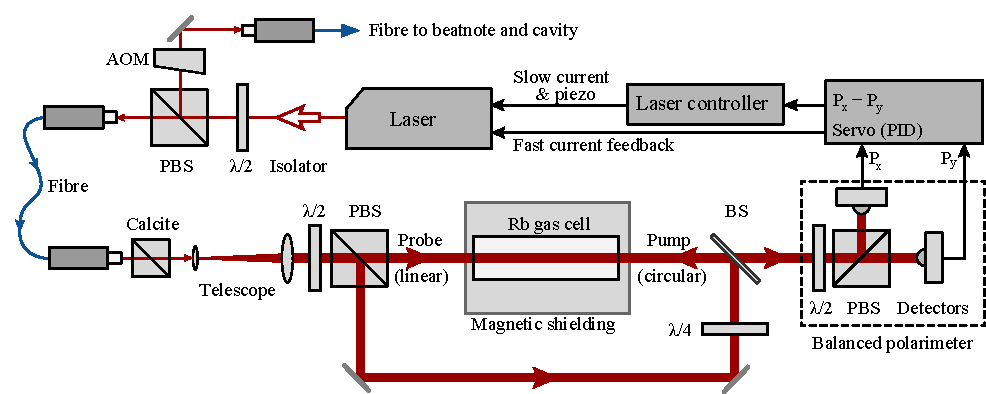
\includegraphics[width=\linewidth]{part1/Figs/ps_two_laser.pdf}
\caption{Schematic of the polarisation spectroscopy apparatus used to measure the performance of the high-bandwidth feedback. The beam from the laser passes through an isolator before being split into two beams by an \gls{pbs} and coupled into optical fibres.
One fibre leads to the \gls{ps} setup shown here, the other to the measurement apparatus via an \gls{aom}.
The \gls{ps} setup consists of a polarisation stabilising Glan-Thompson prism folled by a beam expanding telescope.
The expanded beam is then divided by a \gls{pbs} into a linearly polarised probe and circularly polarised pump which counter-propagate, via a non-polarising 50:50 \gls{bs}, through the magnetically-shielded \unit[15]{cm}-long rubidium gas sample.
The polarisation rotation of the probe beam is then measured by a balanced polarimeter which consists of a $\lambdaup/2$ waveplate, \gls{pbs} and two high-bandwidth photodetectors (Thorlabs PDA10A).}
\label{figure:laser_setup}
\end{figure}

In the two near-identical polarisation spectroscopy setups high quality calcite polarisers where used to stabilise the polarisation of the beam out of the fibre as, despite being polarisation maintaining, ambient temperature changes resulted in polarisation changes in the output beam from the fibres.
Following the calcite was a beam expanding telescope that expanded the beams to the size of the apertures in the double-layer mu-metal magnetic shields, \unit[1.5]{cm} diameter, reducing transit-broadening and improving the optical pumping within the \unit[7.5]{cm} long Rb gas cells.
The pump and probe beams had typical powers of \unit[2.4]{mW} and \unit[2.7]{mW} respectively.
High-bandwidth photodetectors\footnote{Thorlabs PDA36A-EC, \unit[150]{MHz} bandwidth} where used in the balanced polarimeter to generate the error signal fed into the servo system.

\subsection{Heterodyne Methods}

Heterodyning is a technique, invented by Canadian Reginald Feessenden in 1901, which mixes two frequencies to produce a new frequency~\cite{cooper_physics_2001}.
The technique can be used to examine the spectral properties of lasers as the newly produced frequencies can be tailored such that they are easily measurable by photodetectors and spectrum analysers.

Laser frequency spectrum measurements using heterodyne technique are simple to implement with the correct equipment.
The two laser beams are combined such that they copropagate, requiring some mirrors and a beamsplitter/combiner, and then focussed onto a high-bandwidth photodetector, where the bandwidth is dependent on the desired resolution.
The signal from the detector can then be fed into an equally high bandwidth spectrum analyser which will display the frequency spectrum of the intensity of the light on the detector.
Laser heterodyne measurements have the added advantage that they are insensitive to laser amplitude noise.

Heterodyne measurements can also be performed with sound waves, infact this method is used to tune musical instruments as the new frequency produced can be heard as a `beat' or `beatnote'.
The term `beatnote' is also used in general to refer to the signal resulting from a heterodyne measurement.

\subsubsection{Basic Theory}
In the electrical signals context heterodyning involves the `mixing' or multiplying of two signals (e.g. two sine waves) to produce two different signals with frequencies equal to the difference and sum of the original frequencies:
\begin{equation}
\sin(\theta_1)\sin(\theta_2) = \frac{1}{2} \cos(\theta_1-\theta_2) - \frac{1}{2} \cos(\theta_1+\theta_2).
\end{equation}

In the optical context this is achieved due to the interference term accrued when squaring the electric field in order to calculate the intensity detected by the photodetector. The intensity of an electric field is given by:
\begin{equation}
I(t) = \frac{c\epsilon_0}{2}|E|^2.
\end{equation}

For two copropagating lasers with electric fields $E_{1, 2}$ and angular frequencies $\omega_{1, 2}$ we can write
\begin{equation}
E_{i}(t) = \sin(\omega_{i}t).
\end{equation}
The electric field at the detector, $E_T$, is given by the sum of $E_{1}$ and $E_{2}$, and thus the intensity is given by,
\begin{align}
I(t) &= |E_1(t) + E_2(t)|^2\nonumber\\
&= |E_1(t)|^2 + E_1(t)E_2^*(t) + |E_2(t)|^2.
\end{align}
The interference term, $E_1(t)E_2(t)$, allows for the spectral measurements with optical signals as
\begin{align}
E_1(t)E_2(t) &= \sin(\omega_1 t) \sin(\omega_2 t) \notag \\
&= \frac{1}{2} (\cos([\omega_1-\omega_2]t) - \cos([\omega_1+\omega_2]t)), \label{equation:hetero}
\end{align}
and if $\omega_{1,2}$ are appropriately selected then the first term in Equation~\ref{equation:hetero} is measurable.
The difference in frequency ideally should be fairly small, less than a few GHz, which can often be induced on lasers with the same frequency by \glspl{aom} or \glspl{eom}.

The equations presented above provide an obviously na\"ive approach as the frequency spread of the lasers is non-zero but gives a sufficient demonstration of the basis of the heterodyne method.
The spectral profile of the heterodyne signal is formed by the convolution of the spectral profiles of the component lasers, thus strategies are required in order to resolve the lineshape of a single laser.
For two near identical lasers with Gaussian lineshape the beatnote width is $2\sqrt{2\log_e2}\sim2.35$ (see Appendix~\ref{appendix:heterodyne}).

\subsubsection{Frequency Reference}
One method of resolving the lineshape of a single laser is to use a second laser known to have a frequency lineshape much narrower than the laser of interest so that the convolved lineshape is the same as the lineshape of the laser of interest.
This method has some limitations in its application as it is only useful for resolving the lineshape of lasers with relatively wide specral width.
This method is shown in Figure~\ref{figure:heterodyne_reference}.

\begin{figure}
    %\centering
    \begin{subfigure}{0.49\linewidth}
    %\centering
    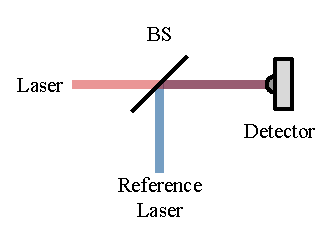
\includegraphics{part1/Figs/HeterodyneReferenceLaser.pdf}
    \end{subfigure}
    \begin{subfigure}{0.49\linewidth}
    %\centering
    %% Creator: Matplotlib, PGF backend
%%
%% To include the figure in your LaTeX document, write
%%   \input{<filename>.pgf}
%%
%% Make sure the required packages are loaded in your preamble
%%   \usepackage{pgf}
%%
%% Figures using additional raster images can only be included by \input if
%% they are in the same directory as the main LaTeX file. For loading figures
%% from other directories you can use the `import` package
%%   \usepackage{import}
%% and then include the figures with
%%   \import{<path to file>}{<filename>.pgf}
%%
%% Matplotlib used the following preamble
%%
\begingroup%
\makeatletter%
\begin{pgfpicture}%
\pgfpathrectangle{\pgfpointorigin}{\pgfqpoint{2.855000in}{1.427500in}}%
\pgfusepath{use as bounding box, clip}%
\begin{pgfscope}%
\pgfsetbuttcap%
\pgfsetmiterjoin%
\definecolor{currentfill}{rgb}{1.000000,1.000000,1.000000}%
\pgfsetfillcolor{currentfill}%
\pgfsetlinewidth{0.000000pt}%
\definecolor{currentstroke}{rgb}{1.000000,1.000000,1.000000}%
\pgfsetstrokecolor{currentstroke}%
\pgfsetdash{}{0pt}%
\pgfpathmoveto{\pgfqpoint{0.000000in}{0.000000in}}%
\pgfpathlineto{\pgfqpoint{2.855000in}{0.000000in}}%
\pgfpathlineto{\pgfqpoint{2.855000in}{1.427500in}}%
\pgfpathlineto{\pgfqpoint{0.000000in}{1.427500in}}%
\pgfpathclose%
\pgfusepath{fill}%
\end{pgfscope}%
\begin{pgfscope}%
\pgfsetbuttcap%
\pgfsetmiterjoin%
\definecolor{currentfill}{rgb}{1.000000,1.000000,1.000000}%
\pgfsetfillcolor{currentfill}%
\pgfsetlinewidth{0.000000pt}%
\definecolor{currentstroke}{rgb}{0.000000,0.000000,0.000000}%
\pgfsetstrokecolor{currentstroke}%
\pgfsetstrokeopacity{0.000000}%
\pgfsetdash{}{0pt}%
\pgfpathmoveto{\pgfqpoint{0.342732in}{0.521851in}}%
\pgfpathlineto{\pgfqpoint{1.130154in}{0.521851in}}%
\pgfpathlineto{\pgfqpoint{1.130154in}{1.277500in}}%
\pgfpathlineto{\pgfqpoint{0.342732in}{1.277500in}}%
\pgfpathclose%
\pgfusepath{fill}%
\end{pgfscope}%
\begin{pgfscope}%
\pgfpathrectangle{\pgfqpoint{0.342732in}{0.521851in}}{\pgfqpoint{0.787423in}{0.755649in}} %
\pgfusepath{clip}%
\pgfsetrectcap%
\pgfsetroundjoin%
\pgfsetlinewidth{1.003750pt}%
\definecolor{currentstroke}{rgb}{0.600000,0.000000,0.000000}%
\pgfsetstrokecolor{currentstroke}%
\pgfsetdash{}{0pt}%
\pgfpathmoveto{\pgfqpoint{0.342732in}{0.521851in}}%
\pgfpathlineto{\pgfqpoint{0.561854in}{0.522927in}}%
\pgfpathlineto{\pgfqpoint{0.578407in}{0.525366in}}%
\pgfpathlineto{\pgfqpoint{0.589442in}{0.529099in}}%
\pgfpathlineto{\pgfqpoint{0.598112in}{0.534189in}}%
\pgfpathlineto{\pgfqpoint{0.605994in}{0.541309in}}%
\pgfpathlineto{\pgfqpoint{0.613876in}{0.551728in}}%
\pgfpathlineto{\pgfqpoint{0.620970in}{0.564809in}}%
\pgfpathlineto{\pgfqpoint{0.628852in}{0.584548in}}%
\pgfpathlineto{\pgfqpoint{0.636734in}{0.610943in}}%
\pgfpathlineto{\pgfqpoint{0.644617in}{0.645114in}}%
\pgfpathlineto{\pgfqpoint{0.653287in}{0.692665in}}%
\pgfpathlineto{\pgfqpoint{0.663534in}{0.762770in}}%
\pgfpathlineto{\pgfqpoint{0.675357in}{0.860560in}}%
\pgfpathlineto{\pgfqpoint{0.715556in}{1.209829in}}%
\pgfpathlineto{\pgfqpoint{0.722649in}{1.247207in}}%
\pgfpathlineto{\pgfqpoint{0.728167in}{1.266451in}}%
\pgfpathlineto{\pgfqpoint{0.732896in}{1.275458in}}%
\pgfpathlineto{\pgfqpoint{0.736049in}{1.277475in}}%
\pgfpathlineto{\pgfqpoint{0.738414in}{1.276869in}}%
\pgfpathlineto{\pgfqpoint{0.741566in}{1.273247in}}%
\pgfpathlineto{\pgfqpoint{0.745508in}{1.264266in}}%
\pgfpathlineto{\pgfqpoint{0.750237in}{1.247207in}}%
\pgfpathlineto{\pgfqpoint{0.756542in}{1.214625in}}%
\pgfpathlineto{\pgfqpoint{0.764425in}{1.160406in}}%
\pgfpathlineto{\pgfqpoint{0.775460in}{1.066544in}}%
\pgfpathlineto{\pgfqpoint{0.810929in}{0.751028in}}%
\pgfpathlineto{\pgfqpoint{0.821964in}{0.678624in}}%
\pgfpathlineto{\pgfqpoint{0.831423in}{0.630451in}}%
\pgfpathlineto{\pgfqpoint{0.840093in}{0.596839in}}%
\pgfpathlineto{\pgfqpoint{0.848763in}{0.571983in}}%
\pgfpathlineto{\pgfqpoint{0.856645in}{0.555654in}}%
\pgfpathlineto{\pgfqpoint{0.864527in}{0.544042in}}%
\pgfpathlineto{\pgfqpoint{0.872410in}{0.536036in}}%
\pgfpathlineto{\pgfqpoint{0.881080in}{0.530257in}}%
\pgfpathlineto{\pgfqpoint{0.891327in}{0.526196in}}%
\pgfpathlineto{\pgfqpoint{0.903938in}{0.523664in}}%
\pgfpathlineto{\pgfqpoint{0.923643in}{0.522255in}}%
\pgfpathlineto{\pgfqpoint{0.970936in}{0.521857in}}%
\pgfpathlineto{\pgfqpoint{1.130154in}{0.521851in}}%
\pgfpathlineto{\pgfqpoint{1.130154in}{0.521851in}}%
\pgfusepath{stroke}%
\end{pgfscope}%
\begin{pgfscope}%
\pgfsetrectcap%
\pgfsetmiterjoin%
\pgfsetlinewidth{1.003750pt}%
\definecolor{currentstroke}{rgb}{0.000000,0.000000,0.000000}%
\pgfsetstrokecolor{currentstroke}%
\pgfsetdash{}{0pt}%
\pgfpathmoveto{\pgfqpoint{1.130154in}{0.521851in}}%
\pgfpathlineto{\pgfqpoint{1.130154in}{1.277500in}}%
\pgfusepath{stroke}%
\end{pgfscope}%
\begin{pgfscope}%
\pgfsetrectcap%
\pgfsetmiterjoin%
\pgfsetlinewidth{1.003750pt}%
\definecolor{currentstroke}{rgb}{0.000000,0.000000,0.000000}%
\pgfsetstrokecolor{currentstroke}%
\pgfsetdash{}{0pt}%
\pgfpathmoveto{\pgfqpoint{0.342732in}{1.277500in}}%
\pgfpathlineto{\pgfqpoint{1.130154in}{1.277500in}}%
\pgfusepath{stroke}%
\end{pgfscope}%
\begin{pgfscope}%
\pgfsetrectcap%
\pgfsetmiterjoin%
\pgfsetlinewidth{1.003750pt}%
\definecolor{currentstroke}{rgb}{0.000000,0.000000,0.000000}%
\pgfsetstrokecolor{currentstroke}%
\pgfsetdash{}{0pt}%
\pgfpathmoveto{\pgfqpoint{0.342732in}{0.521851in}}%
\pgfpathlineto{\pgfqpoint{1.130154in}{0.521851in}}%
\pgfusepath{stroke}%
\end{pgfscope}%
\begin{pgfscope}%
\pgfsetrectcap%
\pgfsetmiterjoin%
\pgfsetlinewidth{1.003750pt}%
\definecolor{currentstroke}{rgb}{0.000000,0.000000,0.000000}%
\pgfsetstrokecolor{currentstroke}%
\pgfsetdash{}{0pt}%
\pgfpathmoveto{\pgfqpoint{0.342732in}{0.521851in}}%
\pgfpathlineto{\pgfqpoint{0.342732in}{1.277500in}}%
\pgfusepath{stroke}%
\end{pgfscope}%
\begin{pgfscope}%
\pgfsetbuttcap%
\pgfsetroundjoin%
\definecolor{currentfill}{rgb}{0.000000,0.000000,0.000000}%
\pgfsetfillcolor{currentfill}%
\pgfsetlinewidth{0.501875pt}%
\definecolor{currentstroke}{rgb}{0.000000,0.000000,0.000000}%
\pgfsetstrokecolor{currentstroke}%
\pgfsetdash{}{0pt}%
\pgfsys@defobject{currentmarker}{\pgfqpoint{0.000000in}{0.000000in}}{\pgfqpoint{0.000000in}{0.055556in}}{%
\pgfpathmoveto{\pgfqpoint{0.000000in}{0.000000in}}%
\pgfpathlineto{\pgfqpoint{0.000000in}{0.055556in}}%
\pgfusepath{stroke,fill}%
}%
\begin{pgfscope}%
\pgfsys@transformshift{0.736443in}{0.521851in}%
\pgfsys@useobject{currentmarker}{}%
\end{pgfscope}%
\end{pgfscope}%
\begin{pgfscope}%
\pgfsetbuttcap%
\pgfsetroundjoin%
\definecolor{currentfill}{rgb}{0.000000,0.000000,0.000000}%
\pgfsetfillcolor{currentfill}%
\pgfsetlinewidth{0.501875pt}%
\definecolor{currentstroke}{rgb}{0.000000,0.000000,0.000000}%
\pgfsetstrokecolor{currentstroke}%
\pgfsetdash{}{0pt}%
\pgfsys@defobject{currentmarker}{\pgfqpoint{0.000000in}{-0.055556in}}{\pgfqpoint{0.000000in}{0.000000in}}{%
\pgfpathmoveto{\pgfqpoint{0.000000in}{0.000000in}}%
\pgfpathlineto{\pgfqpoint{0.000000in}{-0.055556in}}%
\pgfusepath{stroke,fill}%
}%
\begin{pgfscope}%
\pgfsys@transformshift{0.736443in}{1.277500in}%
\pgfsys@useobject{currentmarker}{}%
\end{pgfscope}%
\end{pgfscope}%
\begin{pgfscope}%
\pgftext[x=0.736443in,y=0.466296in,,top]{\fontsize{10.000000}{12.000000}\selectfont \(\displaystyle \omega_1\)}%
\end{pgfscope}%
\begin{pgfscope}%
\pgftext[x=0.273287in,y=0.899676in,,bottom,rotate=90.000000]{\fontsize{10.000000}{12.000000}\selectfont Amplitude}%
\end{pgfscope}%
\begin{pgfscope}%
\pgfsetbuttcap%
\pgfsetmiterjoin%
\definecolor{currentfill}{rgb}{1.000000,1.000000,1.000000}%
\pgfsetfillcolor{currentfill}%
\pgfsetlinewidth{0.000000pt}%
\definecolor{currentstroke}{rgb}{0.000000,0.000000,0.000000}%
\pgfsetstrokecolor{currentstroke}%
\pgfsetstrokeopacity{0.000000}%
\pgfsetdash{}{0pt}%
\pgfpathmoveto{\pgfqpoint{1.130154in}{0.521851in}}%
\pgfpathlineto{\pgfqpoint{1.917577in}{0.521851in}}%
\pgfpathlineto{\pgfqpoint{1.917577in}{1.277500in}}%
\pgfpathlineto{\pgfqpoint{1.130154in}{1.277500in}}%
\pgfpathclose%
\pgfusepath{fill}%
\end{pgfscope}%
\begin{pgfscope}%
\pgfpathrectangle{\pgfqpoint{1.130154in}{0.521851in}}{\pgfqpoint{0.787423in}{0.755649in}} %
\pgfusepath{clip}%
\pgfsetrectcap%
\pgfsetroundjoin%
\pgfsetlinewidth{1.003750pt}%
\definecolor{currentstroke}{rgb}{0.043137,0.325490,0.580392}%
\pgfsetstrokecolor{currentstroke}%
\pgfsetdash{}{0pt}%
\pgfpathmoveto{\pgfqpoint{1.130154in}{0.521851in}}%
\pgfpathlineto{\pgfqpoint{1.491943in}{0.522906in}}%
\pgfpathlineto{\pgfqpoint{1.495096in}{0.525477in}}%
\pgfpathlineto{\pgfqpoint{1.497461in}{0.530263in}}%
\pgfpathlineto{\pgfqpoint{1.499825in}{0.540010in}}%
\pgfpathlineto{\pgfqpoint{1.502190in}{0.558322in}}%
\pgfpathlineto{\pgfqpoint{1.505343in}{0.604463in}}%
\pgfpathlineto{\pgfqpoint{1.508496in}{0.686453in}}%
\pgfpathlineto{\pgfqpoint{1.513225in}{0.885838in}}%
\pgfpathlineto{\pgfqpoint{1.521107in}{1.241295in}}%
\pgfpathlineto{\pgfqpoint{1.523472in}{1.276743in}}%
\pgfpathlineto{\pgfqpoint{1.524260in}{1.276743in}}%
\pgfpathlineto{\pgfqpoint{1.525836in}{1.258806in}}%
\pgfpathlineto{\pgfqpoint{1.528201in}{1.191219in}}%
\pgfpathlineto{\pgfqpoint{1.532930in}{0.966603in}}%
\pgfpathlineto{\pgfqpoint{1.539236in}{0.686453in}}%
\pgfpathlineto{\pgfqpoint{1.543177in}{0.590005in}}%
\pgfpathlineto{\pgfqpoint{1.547118in}{0.544946in}}%
\pgfpathlineto{\pgfqpoint{1.550271in}{0.530263in}}%
\pgfpathlineto{\pgfqpoint{1.553424in}{0.524546in}}%
\pgfpathlineto{\pgfqpoint{1.557365in}{0.522394in}}%
\pgfpathlineto{\pgfqpoint{1.565247in}{0.521863in}}%
\pgfpathlineto{\pgfqpoint{1.777276in}{0.521851in}}%
\pgfpathlineto{\pgfqpoint{1.917577in}{0.521851in}}%
\pgfpathlineto{\pgfqpoint{1.917577in}{0.521851in}}%
\pgfusepath{stroke}%
\end{pgfscope}%
\begin{pgfscope}%
\pgfsetrectcap%
\pgfsetmiterjoin%
\pgfsetlinewidth{1.003750pt}%
\definecolor{currentstroke}{rgb}{0.000000,0.000000,0.000000}%
\pgfsetstrokecolor{currentstroke}%
\pgfsetdash{}{0pt}%
\pgfpathmoveto{\pgfqpoint{1.917577in}{0.521851in}}%
\pgfpathlineto{\pgfqpoint{1.917577in}{1.277500in}}%
\pgfusepath{stroke}%
\end{pgfscope}%
\begin{pgfscope}%
\pgfsetrectcap%
\pgfsetmiterjoin%
\pgfsetlinewidth{1.003750pt}%
\definecolor{currentstroke}{rgb}{0.000000,0.000000,0.000000}%
\pgfsetstrokecolor{currentstroke}%
\pgfsetdash{}{0pt}%
\pgfpathmoveto{\pgfqpoint{1.130154in}{1.277500in}}%
\pgfpathlineto{\pgfqpoint{1.917577in}{1.277500in}}%
\pgfusepath{stroke}%
\end{pgfscope}%
\begin{pgfscope}%
\pgfsetrectcap%
\pgfsetmiterjoin%
\pgfsetlinewidth{1.003750pt}%
\definecolor{currentstroke}{rgb}{0.000000,0.000000,0.000000}%
\pgfsetstrokecolor{currentstroke}%
\pgfsetdash{}{0pt}%
\pgfpathmoveto{\pgfqpoint{1.130154in}{0.521851in}}%
\pgfpathlineto{\pgfqpoint{1.917577in}{0.521851in}}%
\pgfusepath{stroke}%
\end{pgfscope}%
\begin{pgfscope}%
\pgfsetrectcap%
\pgfsetmiterjoin%
\pgfsetlinewidth{1.003750pt}%
\definecolor{currentstroke}{rgb}{0.000000,0.000000,0.000000}%
\pgfsetstrokecolor{currentstroke}%
\pgfsetdash{}{0pt}%
\pgfpathmoveto{\pgfqpoint{1.130154in}{0.521851in}}%
\pgfpathlineto{\pgfqpoint{1.130154in}{1.277500in}}%
\pgfusepath{stroke}%
\end{pgfscope}%
\begin{pgfscope}%
\pgfsetbuttcap%
\pgfsetroundjoin%
\definecolor{currentfill}{rgb}{0.000000,0.000000,0.000000}%
\pgfsetfillcolor{currentfill}%
\pgfsetlinewidth{0.501875pt}%
\definecolor{currentstroke}{rgb}{0.000000,0.000000,0.000000}%
\pgfsetstrokecolor{currentstroke}%
\pgfsetdash{}{0pt}%
\pgfsys@defobject{currentmarker}{\pgfqpoint{0.000000in}{0.000000in}}{\pgfqpoint{0.000000in}{0.055556in}}{%
\pgfpathmoveto{\pgfqpoint{0.000000in}{0.000000in}}%
\pgfpathlineto{\pgfqpoint{0.000000in}{0.055556in}}%
\pgfusepath{stroke,fill}%
}%
\begin{pgfscope}%
\pgfsys@transformshift{1.523866in}{0.521851in}%
\pgfsys@useobject{currentmarker}{}%
\end{pgfscope}%
\end{pgfscope}%
\begin{pgfscope}%
\pgfsetbuttcap%
\pgfsetroundjoin%
\definecolor{currentfill}{rgb}{0.000000,0.000000,0.000000}%
\pgfsetfillcolor{currentfill}%
\pgfsetlinewidth{0.501875pt}%
\definecolor{currentstroke}{rgb}{0.000000,0.000000,0.000000}%
\pgfsetstrokecolor{currentstroke}%
\pgfsetdash{}{0pt}%
\pgfsys@defobject{currentmarker}{\pgfqpoint{0.000000in}{-0.055556in}}{\pgfqpoint{0.000000in}{0.000000in}}{%
\pgfpathmoveto{\pgfqpoint{0.000000in}{0.000000in}}%
\pgfpathlineto{\pgfqpoint{0.000000in}{-0.055556in}}%
\pgfusepath{stroke,fill}%
}%
\begin{pgfscope}%
\pgfsys@transformshift{1.523866in}{1.277500in}%
\pgfsys@useobject{currentmarker}{}%
\end{pgfscope}%
\end{pgfscope}%
\begin{pgfscope}%
\pgftext[x=1.523866in,y=0.466296in,,top]{\fontsize{10.000000}{12.000000}\selectfont \(\displaystyle \omega_2\)}%
\end{pgfscope}%
\begin{pgfscope}%
\pgftext[x=1.523866in,y=0.273395in,,top]{\fontsize{10.000000}{12.000000}\selectfont Frequency}%
\end{pgfscope}%
\begin{pgfscope}%
\pgfsetbuttcap%
\pgfsetmiterjoin%
\definecolor{currentfill}{rgb}{1.000000,1.000000,1.000000}%
\pgfsetfillcolor{currentfill}%
\pgfsetlinewidth{0.000000pt}%
\definecolor{currentstroke}{rgb}{0.000000,0.000000,0.000000}%
\pgfsetstrokecolor{currentstroke}%
\pgfsetstrokeopacity{0.000000}%
\pgfsetdash{}{0pt}%
\pgfpathmoveto{\pgfqpoint{1.917577in}{0.521851in}}%
\pgfpathlineto{\pgfqpoint{2.705000in}{0.521851in}}%
\pgfpathlineto{\pgfqpoint{2.705000in}{1.277500in}}%
\pgfpathlineto{\pgfqpoint{1.917577in}{1.277500in}}%
\pgfpathclose%
\pgfusepath{fill}%
\end{pgfscope}%
\begin{pgfscope}%
\pgfpathrectangle{\pgfqpoint{1.917577in}{0.521851in}}{\pgfqpoint{0.787423in}{0.755649in}} %
\pgfusepath{clip}%
\pgfsetrectcap%
\pgfsetroundjoin%
\pgfsetlinewidth{1.003750pt}%
\definecolor{currentstroke}{rgb}{0.301961,0.607843,0.301961}%
\pgfsetstrokecolor{currentstroke}%
\pgfsetdash{}{0pt}%
\pgfpathmoveto{\pgfqpoint{1.917577in}{0.521851in}}%
\pgfpathlineto{\pgfqpoint{2.134335in}{0.522937in}}%
\pgfpathlineto{\pgfqpoint{2.150888in}{0.525331in}}%
\pgfpathlineto{\pgfqpoint{2.161923in}{0.528952in}}%
\pgfpathlineto{\pgfqpoint{2.171381in}{0.534419in}}%
\pgfpathlineto{\pgfqpoint{2.179263in}{0.541509in}}%
\pgfpathlineto{\pgfqpoint{2.187145in}{0.551814in}}%
\pgfpathlineto{\pgfqpoint{2.194239in}{0.564679in}}%
\pgfpathlineto{\pgfqpoint{2.202121in}{0.584001in}}%
\pgfpathlineto{\pgfqpoint{2.210004in}{0.609738in}}%
\pgfpathlineto{\pgfqpoint{2.218674in}{0.646729in}}%
\pgfpathlineto{\pgfqpoint{2.227344in}{0.693823in}}%
\pgfpathlineto{\pgfqpoint{2.237591in}{0.762940in}}%
\pgfpathlineto{\pgfqpoint{2.249414in}{0.859050in}}%
\pgfpathlineto{\pgfqpoint{2.290401in}{1.209531in}}%
\pgfpathlineto{\pgfqpoint{2.297495in}{1.246500in}}%
\pgfpathlineto{\pgfqpoint{2.303012in}{1.265770in}}%
\pgfpathlineto{\pgfqpoint{2.307742in}{1.275061in}}%
\pgfpathlineto{\pgfqpoint{2.310895in}{1.277402in}}%
\pgfpathlineto{\pgfqpoint{2.313259in}{1.277109in}}%
\pgfpathlineto{\pgfqpoint{2.316412in}{1.273991in}}%
\pgfpathlineto{\pgfqpoint{2.320353in}{1.265770in}}%
\pgfpathlineto{\pgfqpoint{2.325082in}{1.249786in}}%
\pgfpathlineto{\pgfqpoint{2.331388in}{1.218840in}}%
\pgfpathlineto{\pgfqpoint{2.339270in}{1.166816in}}%
\pgfpathlineto{\pgfqpoint{2.349517in}{1.082834in}}%
\pgfpathlineto{\pgfqpoint{2.389716in}{0.734661in}}%
\pgfpathlineto{\pgfqpoint{2.399962in}{0.671121in}}%
\pgfpathlineto{\pgfqpoint{2.409421in}{0.625355in}}%
\pgfpathlineto{\pgfqpoint{2.418091in}{0.593463in}}%
\pgfpathlineto{\pgfqpoint{2.426762in}{0.569871in}}%
\pgfpathlineto{\pgfqpoint{2.434644in}{0.554349in}}%
\pgfpathlineto{\pgfqpoint{2.442526in}{0.543282in}}%
\pgfpathlineto{\pgfqpoint{2.451196in}{0.535009in}}%
\pgfpathlineto{\pgfqpoint{2.460655in}{0.529309in}}%
\pgfpathlineto{\pgfqpoint{2.471690in}{0.525519in}}%
\pgfpathlineto{\pgfqpoint{2.485877in}{0.523219in}}%
\pgfpathlineto{\pgfqpoint{2.508735in}{0.522085in}}%
\pgfpathlineto{\pgfqpoint{2.580463in}{0.521852in}}%
\pgfpathlineto{\pgfqpoint{2.705000in}{0.521851in}}%
\pgfpathlineto{\pgfqpoint{2.705000in}{0.521851in}}%
\pgfusepath{stroke}%
\end{pgfscope}%
\begin{pgfscope}%
\pgfpathrectangle{\pgfqpoint{1.917577in}{0.521851in}}{\pgfqpoint{0.787423in}{0.755649in}} %
\pgfusepath{clip}%
\pgfsetbuttcap%
\pgfsetroundjoin%
\pgfsetlinewidth{1.003750pt}%
\definecolor{currentstroke}{rgb}{0.043137,0.325490,0.580392}%
\pgfsetstrokecolor{currentstroke}%
\pgfsetdash{{1.000000pt}{3.000000pt}}{0.000000pt}%
\pgfpathmoveto{\pgfqpoint{1.917577in}{0.521851in}}%
\pgfpathlineto{\pgfqpoint{2.279366in}{0.522906in}}%
\pgfpathlineto{\pgfqpoint{2.282519in}{0.525477in}}%
\pgfpathlineto{\pgfqpoint{2.284884in}{0.530263in}}%
\pgfpathlineto{\pgfqpoint{2.287248in}{0.540010in}}%
\pgfpathlineto{\pgfqpoint{2.289613in}{0.558322in}}%
\pgfpathlineto{\pgfqpoint{2.292766in}{0.604463in}}%
\pgfpathlineto{\pgfqpoint{2.295919in}{0.686453in}}%
\pgfpathlineto{\pgfqpoint{2.300648in}{0.885838in}}%
\pgfpathlineto{\pgfqpoint{2.308530in}{1.241295in}}%
\pgfpathlineto{\pgfqpoint{2.310895in}{1.276743in}}%
\pgfpathlineto{\pgfqpoint{2.311683in}{1.276743in}}%
\pgfpathlineto{\pgfqpoint{2.313259in}{1.258806in}}%
\pgfpathlineto{\pgfqpoint{2.315624in}{1.191219in}}%
\pgfpathlineto{\pgfqpoint{2.320353in}{0.966603in}}%
\pgfpathlineto{\pgfqpoint{2.326659in}{0.686453in}}%
\pgfpathlineto{\pgfqpoint{2.330600in}{0.590005in}}%
\pgfpathlineto{\pgfqpoint{2.334541in}{0.544946in}}%
\pgfpathlineto{\pgfqpoint{2.337694in}{0.530263in}}%
\pgfpathlineto{\pgfqpoint{2.340847in}{0.524546in}}%
\pgfpathlineto{\pgfqpoint{2.344788in}{0.522394in}}%
\pgfpathlineto{\pgfqpoint{2.352670in}{0.521863in}}%
\pgfpathlineto{\pgfqpoint{2.564698in}{0.521851in}}%
\pgfpathlineto{\pgfqpoint{2.705000in}{0.521851in}}%
\pgfpathlineto{\pgfqpoint{2.705000in}{0.521851in}}%
\pgfusepath{stroke}%
\end{pgfscope}%
\begin{pgfscope}%
\pgfpathrectangle{\pgfqpoint{1.917577in}{0.521851in}}{\pgfqpoint{0.787423in}{0.755649in}} %
\pgfusepath{clip}%
\pgfsetbuttcap%
\pgfsetroundjoin%
\pgfsetlinewidth{1.003750pt}%
\definecolor{currentstroke}{rgb}{0.600000,0.000000,0.000000}%
\pgfsetstrokecolor{currentstroke}%
\pgfsetdash{{1.000000pt}{3.000000pt}}{0.000000pt}%
\pgfpathmoveto{\pgfqpoint{1.917577in}{0.521851in}}%
\pgfpathlineto{\pgfqpoint{2.136700in}{0.522927in}}%
\pgfpathlineto{\pgfqpoint{2.153252in}{0.525366in}}%
\pgfpathlineto{\pgfqpoint{2.164287in}{0.529099in}}%
\pgfpathlineto{\pgfqpoint{2.172958in}{0.534189in}}%
\pgfpathlineto{\pgfqpoint{2.180840in}{0.541309in}}%
\pgfpathlineto{\pgfqpoint{2.188722in}{0.551728in}}%
\pgfpathlineto{\pgfqpoint{2.195816in}{0.564809in}}%
\pgfpathlineto{\pgfqpoint{2.203698in}{0.584548in}}%
\pgfpathlineto{\pgfqpoint{2.211580in}{0.610943in}}%
\pgfpathlineto{\pgfqpoint{2.219462in}{0.645114in}}%
\pgfpathlineto{\pgfqpoint{2.228132in}{0.692665in}}%
\pgfpathlineto{\pgfqpoint{2.238379in}{0.762770in}}%
\pgfpathlineto{\pgfqpoint{2.250202in}{0.860560in}}%
\pgfpathlineto{\pgfqpoint{2.290401in}{1.209829in}}%
\pgfpathlineto{\pgfqpoint{2.297495in}{1.247207in}}%
\pgfpathlineto{\pgfqpoint{2.303012in}{1.266451in}}%
\pgfpathlineto{\pgfqpoint{2.307742in}{1.275458in}}%
\pgfpathlineto{\pgfqpoint{2.310895in}{1.277475in}}%
\pgfpathlineto{\pgfqpoint{2.313259in}{1.276869in}}%
\pgfpathlineto{\pgfqpoint{2.316412in}{1.273247in}}%
\pgfpathlineto{\pgfqpoint{2.320353in}{1.264266in}}%
\pgfpathlineto{\pgfqpoint{2.325082in}{1.247207in}}%
\pgfpathlineto{\pgfqpoint{2.331388in}{1.214625in}}%
\pgfpathlineto{\pgfqpoint{2.339270in}{1.160406in}}%
\pgfpathlineto{\pgfqpoint{2.350305in}{1.066544in}}%
\pgfpathlineto{\pgfqpoint{2.385775in}{0.751028in}}%
\pgfpathlineto{\pgfqpoint{2.396810in}{0.678624in}}%
\pgfpathlineto{\pgfqpoint{2.406268in}{0.630451in}}%
\pgfpathlineto{\pgfqpoint{2.414938in}{0.596839in}}%
\pgfpathlineto{\pgfqpoint{2.423609in}{0.571983in}}%
\pgfpathlineto{\pgfqpoint{2.431491in}{0.555654in}}%
\pgfpathlineto{\pgfqpoint{2.439373in}{0.544042in}}%
\pgfpathlineto{\pgfqpoint{2.447255in}{0.536036in}}%
\pgfpathlineto{\pgfqpoint{2.455925in}{0.530257in}}%
\pgfpathlineto{\pgfqpoint{2.466172in}{0.526196in}}%
\pgfpathlineto{\pgfqpoint{2.478783in}{0.523664in}}%
\pgfpathlineto{\pgfqpoint{2.498489in}{0.522255in}}%
\pgfpathlineto{\pgfqpoint{2.545781in}{0.521857in}}%
\pgfpathlineto{\pgfqpoint{2.705000in}{0.521851in}}%
\pgfpathlineto{\pgfqpoint{2.705000in}{0.521851in}}%
\pgfusepath{stroke}%
\end{pgfscope}%
\begin{pgfscope}%
\pgfsetrectcap%
\pgfsetmiterjoin%
\pgfsetlinewidth{1.003750pt}%
\definecolor{currentstroke}{rgb}{0.000000,0.000000,0.000000}%
\pgfsetstrokecolor{currentstroke}%
\pgfsetdash{}{0pt}%
\pgfpathmoveto{\pgfqpoint{2.705000in}{0.521851in}}%
\pgfpathlineto{\pgfqpoint{2.705000in}{1.277500in}}%
\pgfusepath{stroke}%
\end{pgfscope}%
\begin{pgfscope}%
\pgfsetrectcap%
\pgfsetmiterjoin%
\pgfsetlinewidth{1.003750pt}%
\definecolor{currentstroke}{rgb}{0.000000,0.000000,0.000000}%
\pgfsetstrokecolor{currentstroke}%
\pgfsetdash{}{0pt}%
\pgfpathmoveto{\pgfqpoint{1.917577in}{1.277500in}}%
\pgfpathlineto{\pgfqpoint{2.705000in}{1.277500in}}%
\pgfusepath{stroke}%
\end{pgfscope}%
\begin{pgfscope}%
\pgfsetrectcap%
\pgfsetmiterjoin%
\pgfsetlinewidth{1.003750pt}%
\definecolor{currentstroke}{rgb}{0.000000,0.000000,0.000000}%
\pgfsetstrokecolor{currentstroke}%
\pgfsetdash{}{0pt}%
\pgfpathmoveto{\pgfqpoint{1.917577in}{0.521851in}}%
\pgfpathlineto{\pgfqpoint{2.705000in}{0.521851in}}%
\pgfusepath{stroke}%
\end{pgfscope}%
\begin{pgfscope}%
\pgfsetrectcap%
\pgfsetmiterjoin%
\pgfsetlinewidth{1.003750pt}%
\definecolor{currentstroke}{rgb}{0.000000,0.000000,0.000000}%
\pgfsetstrokecolor{currentstroke}%
\pgfsetdash{}{0pt}%
\pgfpathmoveto{\pgfqpoint{1.917577in}{0.521851in}}%
\pgfpathlineto{\pgfqpoint{1.917577in}{1.277500in}}%
\pgfusepath{stroke}%
\end{pgfscope}%
\begin{pgfscope}%
\pgfsetbuttcap%
\pgfsetroundjoin%
\definecolor{currentfill}{rgb}{0.000000,0.000000,0.000000}%
\pgfsetfillcolor{currentfill}%
\pgfsetlinewidth{0.501875pt}%
\definecolor{currentstroke}{rgb}{0.000000,0.000000,0.000000}%
\pgfsetstrokecolor{currentstroke}%
\pgfsetdash{}{0pt}%
\pgfsys@defobject{currentmarker}{\pgfqpoint{0.000000in}{0.000000in}}{\pgfqpoint{0.000000in}{0.055556in}}{%
\pgfpathmoveto{\pgfqpoint{0.000000in}{0.000000in}}%
\pgfpathlineto{\pgfqpoint{0.000000in}{0.055556in}}%
\pgfusepath{stroke,fill}%
}%
\begin{pgfscope}%
\pgfsys@transformshift{2.311289in}{0.521851in}%
\pgfsys@useobject{currentmarker}{}%
\end{pgfscope}%
\end{pgfscope}%
\begin{pgfscope}%
\pgfsetbuttcap%
\pgfsetroundjoin%
\definecolor{currentfill}{rgb}{0.000000,0.000000,0.000000}%
\pgfsetfillcolor{currentfill}%
\pgfsetlinewidth{0.501875pt}%
\definecolor{currentstroke}{rgb}{0.000000,0.000000,0.000000}%
\pgfsetstrokecolor{currentstroke}%
\pgfsetdash{}{0pt}%
\pgfsys@defobject{currentmarker}{\pgfqpoint{0.000000in}{-0.055556in}}{\pgfqpoint{0.000000in}{0.000000in}}{%
\pgfpathmoveto{\pgfqpoint{0.000000in}{0.000000in}}%
\pgfpathlineto{\pgfqpoint{0.000000in}{-0.055556in}}%
\pgfusepath{stroke,fill}%
}%
\begin{pgfscope}%
\pgfsys@transformshift{2.311289in}{1.277500in}%
\pgfsys@useobject{currentmarker}{}%
\end{pgfscope}%
\end{pgfscope}%
\begin{pgfscope}%
\pgftext[x=2.311289in,y=0.466296in,,top]{\fontsize{10.000000}{12.000000}\selectfont \(\displaystyle \omega_1-\omega_2\)}%
\end{pgfscope}%
\end{pgfpicture}%
\makeatother%
\endgroup%

    \end{subfigure}
    \caption{Heterodyne measurement with a narrow reference laser by combining the laser of interest ($\omega_1$, red) with the reference laser ($\omega_2$, blue). Shown on the right is the spectral lineshapes of the lasers and the heterodyne beatnote (green).}
    \label{figure:heterodyne_reference}
\end{figure}

The initial intention with the experiments described in the this chapter was to be able to use a \gls{pdh} locked laser as a frequency reference to characterise the performance of another laser locked with \gls{ps} using high-bandwidth feedback.
Unfortunately, initial measurements were unable to confirm that the \gls{pdh} locked laser was in fact much narrower than \gls{ps} locked one so more sophisticated methods were required.

\subsubsection{Self-heterodyne}

The self-heterodyne technique involves beating a laser with itself in order to perform a heterodyne measurement, as shown in Figure~\ref{figure:self_heterodyne}~\cite{okoshi_novel_1980}.
In order to perform this measurement it is necessary to split the laser into two beams and frequency shift on beam, usually with an \gls{aom}, such that the beatnote is not centred at \unit[0]{Hz}.
The two beams are still correlated so it is necessary to propagate one beam to reduce the coherence otherwise the lineshape of the beatnote would just appear as a delta function centred at the \gls{aom} frequency~\cite{richter_linewidth_1986}.
One beam of the beams is typically delayed by a very long optical fibre such that that arm of the heterodyne measurement has been delayed, ideally for as long as the coherence time of the laser.
Practically this would require optical fibres with lengths from 1 to \unit[100]{km} depending on the linewidth of the laser under investigation.
Unfortunately the absorption losses in fibres tends to be at least a few dB per kilometre making fibres longer than \unit[10]{km} troublesome to use however it is not necessary to fully decohere the beams with a delay time longer than the coherence time, as discussed in Reference~\cite{richter_linewidth_1986}.

\begin{figure}
    %\centering
    \begin{subfigure}{0.49\linewidth}
    %\centering
    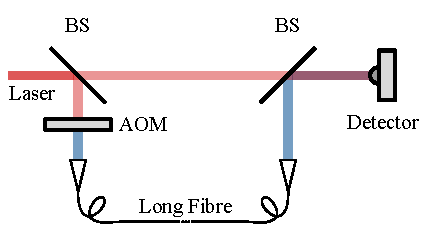
\includegraphics{part1/Figs/SelfHeterodyne.pdf}
    \end{subfigure}
    \begin{subfigure}{0.49\linewidth}
    %\centering
    %% Creator: Matplotlib, PGF backend
%%
%% To include the figure in your LaTeX document, write
%%   \input{<filename>.pgf}
%%
%% Make sure the required packages are loaded in your preamble
%%   \usepackage{pgf}
%%
%% Figures using additional raster images can only be included by \input if
%% they are in the same directory as the main LaTeX file. For loading figures
%% from other directories you can use the `import` package
%%   \usepackage{import}
%% and then include the figures with
%%   \import{<path to file>}{<filename>.pgf}
%%
%% Matplotlib used the following preamble
%%
\begingroup%
\makeatletter%
\begin{pgfpicture}%
\pgfpathrectangle{\pgfpointorigin}{\pgfqpoint{2.855000in}{1.427500in}}%
\pgfusepath{use as bounding box, clip}%
\begin{pgfscope}%
\pgfsetbuttcap%
\pgfsetmiterjoin%
\definecolor{currentfill}{rgb}{1.000000,1.000000,1.000000}%
\pgfsetfillcolor{currentfill}%
\pgfsetlinewidth{0.000000pt}%
\definecolor{currentstroke}{rgb}{1.000000,1.000000,1.000000}%
\pgfsetstrokecolor{currentstroke}%
\pgfsetdash{}{0pt}%
\pgfpathmoveto{\pgfqpoint{0.000000in}{0.000000in}}%
\pgfpathlineto{\pgfqpoint{2.855000in}{0.000000in}}%
\pgfpathlineto{\pgfqpoint{2.855000in}{1.427500in}}%
\pgfpathlineto{\pgfqpoint{0.000000in}{1.427500in}}%
\pgfpathclose%
\pgfusepath{fill}%
\end{pgfscope}%
\begin{pgfscope}%
\pgfsetbuttcap%
\pgfsetmiterjoin%
\definecolor{currentfill}{rgb}{1.000000,1.000000,1.000000}%
\pgfsetfillcolor{currentfill}%
\pgfsetlinewidth{0.000000pt}%
\definecolor{currentstroke}{rgb}{0.000000,0.000000,0.000000}%
\pgfsetstrokecolor{currentstroke}%
\pgfsetstrokeopacity{0.000000}%
\pgfsetdash{}{0pt}%
\pgfpathmoveto{\pgfqpoint{0.342732in}{0.521851in}}%
\pgfpathlineto{\pgfqpoint{1.130154in}{0.521851in}}%
\pgfpathlineto{\pgfqpoint{1.130154in}{1.277500in}}%
\pgfpathlineto{\pgfqpoint{0.342732in}{1.277500in}}%
\pgfpathclose%
\pgfusepath{fill}%
\end{pgfscope}%
\begin{pgfscope}%
\pgfpathrectangle{\pgfqpoint{0.342732in}{0.521851in}}{\pgfqpoint{0.787423in}{0.755649in}} %
\pgfusepath{clip}%
\pgfsetrectcap%
\pgfsetroundjoin%
\pgfsetlinewidth{1.003750pt}%
\definecolor{currentstroke}{rgb}{0.600000,0.000000,0.000000}%
\pgfsetstrokecolor{currentstroke}%
\pgfsetdash{}{0pt}%
\pgfpathmoveto{\pgfqpoint{0.342732in}{0.521851in}}%
\pgfpathlineto{\pgfqpoint{0.564219in}{0.522921in}}%
\pgfpathlineto{\pgfqpoint{0.580771in}{0.525286in}}%
\pgfpathlineto{\pgfqpoint{0.592595in}{0.529207in}}%
\pgfpathlineto{\pgfqpoint{0.602053in}{0.534806in}}%
\pgfpathlineto{\pgfqpoint{0.609935in}{0.542011in}}%
\pgfpathlineto{\pgfqpoint{0.617817in}{0.552396in}}%
\pgfpathlineto{\pgfqpoint{0.625699in}{0.566909in}}%
\pgfpathlineto{\pgfqpoint{0.633582in}{0.586567in}}%
\pgfpathlineto{\pgfqpoint{0.641464in}{0.612351in}}%
\pgfpathlineto{\pgfqpoint{0.650134in}{0.648745in}}%
\pgfpathlineto{\pgfqpoint{0.659593in}{0.698686in}}%
\pgfpathlineto{\pgfqpoint{0.670628in}{0.769933in}}%
\pgfpathlineto{\pgfqpoint{0.685604in}{0.883056in}}%
\pgfpathlineto{\pgfqpoint{0.707673in}{1.048886in}}%
\pgfpathlineto{\pgfqpoint{0.717132in}{1.103032in}}%
\pgfpathlineto{\pgfqpoint{0.724226in}{1.131667in}}%
\pgfpathlineto{\pgfqpoint{0.729743in}{1.145509in}}%
\pgfpathlineto{\pgfqpoint{0.733684in}{1.150529in}}%
\pgfpathlineto{\pgfqpoint{0.736837in}{1.151538in}}%
\pgfpathlineto{\pgfqpoint{0.739990in}{1.149857in}}%
\pgfpathlineto{\pgfqpoint{0.743143in}{1.145509in}}%
\pgfpathlineto{\pgfqpoint{0.747084in}{1.136411in}}%
\pgfpathlineto{\pgfqpoint{0.752601in}{1.117178in}}%
\pgfpathlineto{\pgfqpoint{0.759695in}{1.082441in}}%
\pgfpathlineto{\pgfqpoint{0.768366in}{1.027639in}}%
\pgfpathlineto{\pgfqpoint{0.781765in}{0.926710in}}%
\pgfpathlineto{\pgfqpoint{0.805412in}{0.748268in}}%
\pgfpathlineto{\pgfqpoint{0.817235in}{0.676571in}}%
\pgfpathlineto{\pgfqpoint{0.827481in}{0.627804in}}%
\pgfpathlineto{\pgfqpoint{0.836940in}{0.593618in}}%
\pgfpathlineto{\pgfqpoint{0.845610in}{0.570397in}}%
\pgfpathlineto{\pgfqpoint{0.854281in}{0.553645in}}%
\pgfpathlineto{\pgfqpoint{0.862163in}{0.542891in}}%
\pgfpathlineto{\pgfqpoint{0.870833in}{0.534806in}}%
\pgfpathlineto{\pgfqpoint{0.880292in}{0.529207in}}%
\pgfpathlineto{\pgfqpoint{0.891327in}{0.525472in}}%
\pgfpathlineto{\pgfqpoint{0.905514in}{0.523199in}}%
\pgfpathlineto{\pgfqpoint{0.928372in}{0.522080in}}%
\pgfpathlineto{\pgfqpoint{1.000888in}{0.521852in}}%
\pgfpathlineto{\pgfqpoint{1.130154in}{0.521851in}}%
\pgfpathlineto{\pgfqpoint{1.130154in}{0.521851in}}%
\pgfusepath{stroke}%
\end{pgfscope}%
\begin{pgfscope}%
\pgfsetrectcap%
\pgfsetmiterjoin%
\pgfsetlinewidth{1.003750pt}%
\definecolor{currentstroke}{rgb}{0.000000,0.000000,0.000000}%
\pgfsetstrokecolor{currentstroke}%
\pgfsetdash{}{0pt}%
\pgfpathmoveto{\pgfqpoint{0.342732in}{1.277500in}}%
\pgfpathlineto{\pgfqpoint{1.130154in}{1.277500in}}%
\pgfusepath{stroke}%
\end{pgfscope}%
\begin{pgfscope}%
\pgfsetrectcap%
\pgfsetmiterjoin%
\pgfsetlinewidth{1.003750pt}%
\definecolor{currentstroke}{rgb}{0.000000,0.000000,0.000000}%
\pgfsetstrokecolor{currentstroke}%
\pgfsetdash{}{0pt}%
\pgfpathmoveto{\pgfqpoint{0.342732in}{0.521851in}}%
\pgfpathlineto{\pgfqpoint{0.342732in}{1.277500in}}%
\pgfusepath{stroke}%
\end{pgfscope}%
\begin{pgfscope}%
\pgfsetrectcap%
\pgfsetmiterjoin%
\pgfsetlinewidth{1.003750pt}%
\definecolor{currentstroke}{rgb}{0.000000,0.000000,0.000000}%
\pgfsetstrokecolor{currentstroke}%
\pgfsetdash{}{0pt}%
\pgfpathmoveto{\pgfqpoint{1.130154in}{0.521851in}}%
\pgfpathlineto{\pgfqpoint{1.130154in}{1.277500in}}%
\pgfusepath{stroke}%
\end{pgfscope}%
\begin{pgfscope}%
\pgfsetrectcap%
\pgfsetmiterjoin%
\pgfsetlinewidth{1.003750pt}%
\definecolor{currentstroke}{rgb}{0.000000,0.000000,0.000000}%
\pgfsetstrokecolor{currentstroke}%
\pgfsetdash{}{0pt}%
\pgfpathmoveto{\pgfqpoint{0.342732in}{0.521851in}}%
\pgfpathlineto{\pgfqpoint{1.130154in}{0.521851in}}%
\pgfusepath{stroke}%
\end{pgfscope}%
\begin{pgfscope}%
\pgfsetbuttcap%
\pgfsetroundjoin%
\definecolor{currentfill}{rgb}{0.000000,0.000000,0.000000}%
\pgfsetfillcolor{currentfill}%
\pgfsetlinewidth{0.501875pt}%
\definecolor{currentstroke}{rgb}{0.000000,0.000000,0.000000}%
\pgfsetstrokecolor{currentstroke}%
\pgfsetdash{}{0pt}%
\pgfsys@defobject{currentmarker}{\pgfqpoint{0.000000in}{0.000000in}}{\pgfqpoint{0.000000in}{0.055556in}}{%
\pgfpathmoveto{\pgfqpoint{0.000000in}{0.000000in}}%
\pgfpathlineto{\pgfqpoint{0.000000in}{0.055556in}}%
\pgfusepath{stroke,fill}%
}%
\begin{pgfscope}%
\pgfsys@transformshift{0.736443in}{0.521851in}%
\pgfsys@useobject{currentmarker}{}%
\end{pgfscope}%
\end{pgfscope}%
\begin{pgfscope}%
\pgfsetbuttcap%
\pgfsetroundjoin%
\definecolor{currentfill}{rgb}{0.000000,0.000000,0.000000}%
\pgfsetfillcolor{currentfill}%
\pgfsetlinewidth{0.501875pt}%
\definecolor{currentstroke}{rgb}{0.000000,0.000000,0.000000}%
\pgfsetstrokecolor{currentstroke}%
\pgfsetdash{}{0pt}%
\pgfsys@defobject{currentmarker}{\pgfqpoint{0.000000in}{-0.055556in}}{\pgfqpoint{0.000000in}{0.000000in}}{%
\pgfpathmoveto{\pgfqpoint{0.000000in}{0.000000in}}%
\pgfpathlineto{\pgfqpoint{0.000000in}{-0.055556in}}%
\pgfusepath{stroke,fill}%
}%
\begin{pgfscope}%
\pgfsys@transformshift{0.736443in}{1.277500in}%
\pgfsys@useobject{currentmarker}{}%
\end{pgfscope}%
\end{pgfscope}%
\begin{pgfscope}%
\pgftext[x=0.736443in,y=0.466296in,,top]{\fontsize{10.000000}{12.000000}\selectfont \(\displaystyle \omega_1\)}%
\end{pgfscope}%
\begin{pgfscope}%
\pgftext[x=0.273287in,y=0.899676in,,bottom,rotate=90.000000]{\fontsize{10.000000}{12.000000}\selectfont Amplitude}%
\end{pgfscope}%
\begin{pgfscope}%
\pgfsetbuttcap%
\pgfsetmiterjoin%
\definecolor{currentfill}{rgb}{1.000000,1.000000,1.000000}%
\pgfsetfillcolor{currentfill}%
\pgfsetlinewidth{0.000000pt}%
\definecolor{currentstroke}{rgb}{0.000000,0.000000,0.000000}%
\pgfsetstrokecolor{currentstroke}%
\pgfsetstrokeopacity{0.000000}%
\pgfsetdash{}{0pt}%
\pgfpathmoveto{\pgfqpoint{1.130154in}{0.521851in}}%
\pgfpathlineto{\pgfqpoint{1.917577in}{0.521851in}}%
\pgfpathlineto{\pgfqpoint{1.917577in}{1.277500in}}%
\pgfpathlineto{\pgfqpoint{1.130154in}{1.277500in}}%
\pgfpathclose%
\pgfusepath{fill}%
\end{pgfscope}%
\begin{pgfscope}%
\pgfpathrectangle{\pgfqpoint{1.130154in}{0.521851in}}{\pgfqpoint{0.787423in}{0.755649in}} %
\pgfusepath{clip}%
\pgfsetrectcap%
\pgfsetroundjoin%
\pgfsetlinewidth{1.003750pt}%
\definecolor{currentstroke}{rgb}{0.043137,0.325490,0.580392}%
\pgfsetstrokecolor{currentstroke}%
\pgfsetdash{}{0pt}%
\pgfpathmoveto{\pgfqpoint{1.130154in}{0.521851in}}%
\pgfpathlineto{\pgfqpoint{1.351642in}{0.522921in}}%
\pgfpathlineto{\pgfqpoint{1.368194in}{0.525286in}}%
\pgfpathlineto{\pgfqpoint{1.380017in}{0.529207in}}%
\pgfpathlineto{\pgfqpoint{1.389476in}{0.534806in}}%
\pgfpathlineto{\pgfqpoint{1.397358in}{0.542011in}}%
\pgfpathlineto{\pgfqpoint{1.405240in}{0.552396in}}%
\pgfpathlineto{\pgfqpoint{1.413122in}{0.566909in}}%
\pgfpathlineto{\pgfqpoint{1.421004in}{0.586567in}}%
\pgfpathlineto{\pgfqpoint{1.428886in}{0.612351in}}%
\pgfpathlineto{\pgfqpoint{1.437557in}{0.648745in}}%
\pgfpathlineto{\pgfqpoint{1.447015in}{0.698686in}}%
\pgfpathlineto{\pgfqpoint{1.458050in}{0.769933in}}%
\pgfpathlineto{\pgfqpoint{1.473026in}{0.883056in}}%
\pgfpathlineto{\pgfqpoint{1.495096in}{1.048886in}}%
\pgfpathlineto{\pgfqpoint{1.504555in}{1.103032in}}%
\pgfpathlineto{\pgfqpoint{1.511649in}{1.131667in}}%
\pgfpathlineto{\pgfqpoint{1.517166in}{1.145509in}}%
\pgfpathlineto{\pgfqpoint{1.521107in}{1.150529in}}%
\pgfpathlineto{\pgfqpoint{1.524260in}{1.151538in}}%
\pgfpathlineto{\pgfqpoint{1.527413in}{1.149857in}}%
\pgfpathlineto{\pgfqpoint{1.530566in}{1.145509in}}%
\pgfpathlineto{\pgfqpoint{1.534507in}{1.136411in}}%
\pgfpathlineto{\pgfqpoint{1.540024in}{1.117178in}}%
\pgfpathlineto{\pgfqpoint{1.547118in}{1.082441in}}%
\pgfpathlineto{\pgfqpoint{1.555788in}{1.027639in}}%
\pgfpathlineto{\pgfqpoint{1.569188in}{0.926710in}}%
\pgfpathlineto{\pgfqpoint{1.592834in}{0.748268in}}%
\pgfpathlineto{\pgfqpoint{1.604657in}{0.676571in}}%
\pgfpathlineto{\pgfqpoint{1.614904in}{0.627804in}}%
\pgfpathlineto{\pgfqpoint{1.624363in}{0.593618in}}%
\pgfpathlineto{\pgfqpoint{1.633033in}{0.570397in}}%
\pgfpathlineto{\pgfqpoint{1.641703in}{0.553645in}}%
\pgfpathlineto{\pgfqpoint{1.649586in}{0.542891in}}%
\pgfpathlineto{\pgfqpoint{1.658256in}{0.534806in}}%
\pgfpathlineto{\pgfqpoint{1.667714in}{0.529207in}}%
\pgfpathlineto{\pgfqpoint{1.678749in}{0.525472in}}%
\pgfpathlineto{\pgfqpoint{1.692937in}{0.523199in}}%
\pgfpathlineto{\pgfqpoint{1.715795in}{0.522080in}}%
\pgfpathlineto{\pgfqpoint{1.788311in}{0.521852in}}%
\pgfpathlineto{\pgfqpoint{1.917577in}{0.521851in}}%
\pgfpathlineto{\pgfqpoint{1.917577in}{0.521851in}}%
\pgfusepath{stroke}%
\end{pgfscope}%
\begin{pgfscope}%
\pgfsetrectcap%
\pgfsetmiterjoin%
\pgfsetlinewidth{1.003750pt}%
\definecolor{currentstroke}{rgb}{0.000000,0.000000,0.000000}%
\pgfsetstrokecolor{currentstroke}%
\pgfsetdash{}{0pt}%
\pgfpathmoveto{\pgfqpoint{1.130154in}{1.277500in}}%
\pgfpathlineto{\pgfqpoint{1.917577in}{1.277500in}}%
\pgfusepath{stroke}%
\end{pgfscope}%
\begin{pgfscope}%
\pgfsetrectcap%
\pgfsetmiterjoin%
\pgfsetlinewidth{1.003750pt}%
\definecolor{currentstroke}{rgb}{0.000000,0.000000,0.000000}%
\pgfsetstrokecolor{currentstroke}%
\pgfsetdash{}{0pt}%
\pgfpathmoveto{\pgfqpoint{1.130154in}{0.521851in}}%
\pgfpathlineto{\pgfqpoint{1.130154in}{1.277500in}}%
\pgfusepath{stroke}%
\end{pgfscope}%
\begin{pgfscope}%
\pgfsetrectcap%
\pgfsetmiterjoin%
\pgfsetlinewidth{1.003750pt}%
\definecolor{currentstroke}{rgb}{0.000000,0.000000,0.000000}%
\pgfsetstrokecolor{currentstroke}%
\pgfsetdash{}{0pt}%
\pgfpathmoveto{\pgfqpoint{1.917577in}{0.521851in}}%
\pgfpathlineto{\pgfqpoint{1.917577in}{1.277500in}}%
\pgfusepath{stroke}%
\end{pgfscope}%
\begin{pgfscope}%
\pgfsetrectcap%
\pgfsetmiterjoin%
\pgfsetlinewidth{1.003750pt}%
\definecolor{currentstroke}{rgb}{0.000000,0.000000,0.000000}%
\pgfsetstrokecolor{currentstroke}%
\pgfsetdash{}{0pt}%
\pgfpathmoveto{\pgfqpoint{1.130154in}{0.521851in}}%
\pgfpathlineto{\pgfqpoint{1.917577in}{0.521851in}}%
\pgfusepath{stroke}%
\end{pgfscope}%
\begin{pgfscope}%
\pgfsetbuttcap%
\pgfsetroundjoin%
\definecolor{currentfill}{rgb}{0.000000,0.000000,0.000000}%
\pgfsetfillcolor{currentfill}%
\pgfsetlinewidth{0.501875pt}%
\definecolor{currentstroke}{rgb}{0.000000,0.000000,0.000000}%
\pgfsetstrokecolor{currentstroke}%
\pgfsetdash{}{0pt}%
\pgfsys@defobject{currentmarker}{\pgfqpoint{0.000000in}{0.000000in}}{\pgfqpoint{0.000000in}{0.055556in}}{%
\pgfpathmoveto{\pgfqpoint{0.000000in}{0.000000in}}%
\pgfpathlineto{\pgfqpoint{0.000000in}{0.055556in}}%
\pgfusepath{stroke,fill}%
}%
\begin{pgfscope}%
\pgfsys@transformshift{1.523866in}{0.521851in}%
\pgfsys@useobject{currentmarker}{}%
\end{pgfscope}%
\end{pgfscope}%
\begin{pgfscope}%
\pgfsetbuttcap%
\pgfsetroundjoin%
\definecolor{currentfill}{rgb}{0.000000,0.000000,0.000000}%
\pgfsetfillcolor{currentfill}%
\pgfsetlinewidth{0.501875pt}%
\definecolor{currentstroke}{rgb}{0.000000,0.000000,0.000000}%
\pgfsetstrokecolor{currentstroke}%
\pgfsetdash{}{0pt}%
\pgfsys@defobject{currentmarker}{\pgfqpoint{0.000000in}{-0.055556in}}{\pgfqpoint{0.000000in}{0.000000in}}{%
\pgfpathmoveto{\pgfqpoint{0.000000in}{0.000000in}}%
\pgfpathlineto{\pgfqpoint{0.000000in}{-0.055556in}}%
\pgfusepath{stroke,fill}%
}%
\begin{pgfscope}%
\pgfsys@transformshift{1.523866in}{1.277500in}%
\pgfsys@useobject{currentmarker}{}%
\end{pgfscope}%
\end{pgfscope}%
\begin{pgfscope}%
\pgftext[x=1.523866in,y=0.466296in,,top]{\fontsize{10.000000}{12.000000}\selectfont \(\displaystyle \omega_1+\delta\)}%
\end{pgfscope}%
\begin{pgfscope}%
\pgftext[x=1.523866in,y=0.273395in,,top]{\fontsize{10.000000}{12.000000}\selectfont Frequency}%
\end{pgfscope}%
\begin{pgfscope}%
\pgfsetbuttcap%
\pgfsetmiterjoin%
\definecolor{currentfill}{rgb}{1.000000,1.000000,1.000000}%
\pgfsetfillcolor{currentfill}%
\pgfsetlinewidth{0.000000pt}%
\definecolor{currentstroke}{rgb}{0.000000,0.000000,0.000000}%
\pgfsetstrokecolor{currentstroke}%
\pgfsetstrokeopacity{0.000000}%
\pgfsetdash{}{0pt}%
\pgfpathmoveto{\pgfqpoint{1.917577in}{0.521851in}}%
\pgfpathlineto{\pgfqpoint{2.705000in}{0.521851in}}%
\pgfpathlineto{\pgfqpoint{2.705000in}{1.277500in}}%
\pgfpathlineto{\pgfqpoint{1.917577in}{1.277500in}}%
\pgfpathclose%
\pgfusepath{fill}%
\end{pgfscope}%
\begin{pgfscope}%
\pgfpathrectangle{\pgfqpoint{1.917577in}{0.521851in}}{\pgfqpoint{0.787423in}{0.755649in}} %
\pgfusepath{clip}%
\pgfsetrectcap%
\pgfsetroundjoin%
\pgfsetlinewidth{1.003750pt}%
\definecolor{currentstroke}{rgb}{0.301961,0.607843,0.301961}%
\pgfsetstrokecolor{currentstroke}%
\pgfsetdash{}{0pt}%
\pgfpathmoveto{\pgfqpoint{1.917577in}{0.521851in}}%
\pgfpathlineto{\pgfqpoint{2.068126in}{0.522921in}}%
\pgfpathlineto{\pgfqpoint{2.091772in}{0.525326in}}%
\pgfpathlineto{\pgfqpoint{2.107536in}{0.528981in}}%
\pgfpathlineto{\pgfqpoint{2.120147in}{0.534043in}}%
\pgfpathlineto{\pgfqpoint{2.131182in}{0.540809in}}%
\pgfpathlineto{\pgfqpoint{2.141429in}{0.549751in}}%
\pgfpathlineto{\pgfqpoint{2.150888in}{0.560919in}}%
\pgfpathlineto{\pgfqpoint{2.160346in}{0.575515in}}%
\pgfpathlineto{\pgfqpoint{2.169805in}{0.594159in}}%
\pgfpathlineto{\pgfqpoint{2.180051in}{0.619587in}}%
\pgfpathlineto{\pgfqpoint{2.190298in}{0.651007in}}%
\pgfpathlineto{\pgfqpoint{2.202121in}{0.695079in}}%
\pgfpathlineto{\pgfqpoint{2.214733in}{0.751060in}}%
\pgfpathlineto{\pgfqpoint{2.230497in}{0.831851in}}%
\pgfpathlineto{\pgfqpoint{2.274637in}{1.065169in}}%
\pgfpathlineto{\pgfqpoint{2.284884in}{1.104762in}}%
\pgfpathlineto{\pgfqpoint{2.293554in}{1.129695in}}%
\pgfpathlineto{\pgfqpoint{2.300648in}{1.143368in}}%
\pgfpathlineto{\pgfqpoint{2.306165in}{1.149501in}}%
\pgfpathlineto{\pgfqpoint{2.308530in}{1.151815in}}%
\pgfpathlineto{\pgfqpoint{2.309318in}{1.161466in}}%
\pgfpathlineto{\pgfqpoint{2.311683in}{1.265492in}}%
\pgfpathlineto{\pgfqpoint{2.314047in}{1.152109in}}%
\pgfpathlineto{\pgfqpoint{2.316412in}{1.150046in}}%
\pgfpathlineto{\pgfqpoint{2.321141in}{1.145530in}}%
\pgfpathlineto{\pgfqpoint{2.326659in}{1.136555in}}%
\pgfpathlineto{\pgfqpoint{2.332964in}{1.121628in}}%
\pgfpathlineto{\pgfqpoint{2.340847in}{1.096527in}}%
\pgfpathlineto{\pgfqpoint{2.350305in}{1.058245in}}%
\pgfpathlineto{\pgfqpoint{2.362916in}{0.996713in}}%
\pgfpathlineto{\pgfqpoint{2.385775in}{0.870829in}}%
\pgfpathlineto{\pgfqpoint{2.407056in}{0.758655in}}%
\pgfpathlineto{\pgfqpoint{2.421244in}{0.695079in}}%
\pgfpathlineto{\pgfqpoint{2.433855in}{0.648369in}}%
\pgfpathlineto{\pgfqpoint{2.444890in}{0.615297in}}%
\pgfpathlineto{\pgfqpoint{2.455925in}{0.589086in}}%
\pgfpathlineto{\pgfqpoint{2.466172in}{0.570230in}}%
\pgfpathlineto{\pgfqpoint{2.476419in}{0.555885in}}%
\pgfpathlineto{\pgfqpoint{2.486666in}{0.545259in}}%
\pgfpathlineto{\pgfqpoint{2.497701in}{0.537104in}}%
\pgfpathlineto{\pgfqpoint{2.509524in}{0.531214in}}%
\pgfpathlineto{\pgfqpoint{2.522923in}{0.527045in}}%
\pgfpathlineto{\pgfqpoint{2.540264in}{0.524139in}}%
\pgfpathlineto{\pgfqpoint{2.565487in}{0.522470in}}%
\pgfpathlineto{\pgfqpoint{2.616720in}{0.521880in}}%
\pgfpathlineto{\pgfqpoint{2.705000in}{0.521851in}}%
\pgfpathlineto{\pgfqpoint{2.705000in}{0.521851in}}%
\pgfusepath{stroke}%
\end{pgfscope}%
\begin{pgfscope}%
\pgfpathrectangle{\pgfqpoint{1.917577in}{0.521851in}}{\pgfqpoint{0.787423in}{0.755649in}} %
\pgfusepath{clip}%
\pgfsetbuttcap%
\pgfsetroundjoin%
\pgfsetlinewidth{1.003750pt}%
\definecolor{currentstroke}{rgb}{0.600000,0.000000,0.000000}%
\pgfsetstrokecolor{currentstroke}%
\pgfsetdash{{1.000000pt}{3.000000pt}}{0.000000pt}%
\pgfpathmoveto{\pgfqpoint{1.917577in}{0.521851in}}%
\pgfpathlineto{\pgfqpoint{2.139065in}{0.522921in}}%
\pgfpathlineto{\pgfqpoint{2.155617in}{0.525286in}}%
\pgfpathlineto{\pgfqpoint{2.167440in}{0.529207in}}%
\pgfpathlineto{\pgfqpoint{2.176899in}{0.534806in}}%
\pgfpathlineto{\pgfqpoint{2.184781in}{0.542011in}}%
\pgfpathlineto{\pgfqpoint{2.192663in}{0.552396in}}%
\pgfpathlineto{\pgfqpoint{2.200545in}{0.566909in}}%
\pgfpathlineto{\pgfqpoint{2.208427in}{0.586567in}}%
\pgfpathlineto{\pgfqpoint{2.216309in}{0.612351in}}%
\pgfpathlineto{\pgfqpoint{2.224980in}{0.648745in}}%
\pgfpathlineto{\pgfqpoint{2.234438in}{0.698686in}}%
\pgfpathlineto{\pgfqpoint{2.245473in}{0.769933in}}%
\pgfpathlineto{\pgfqpoint{2.260449in}{0.883056in}}%
\pgfpathlineto{\pgfqpoint{2.282519in}{1.048886in}}%
\pgfpathlineto{\pgfqpoint{2.291977in}{1.103032in}}%
\pgfpathlineto{\pgfqpoint{2.299071in}{1.131667in}}%
\pgfpathlineto{\pgfqpoint{2.304589in}{1.145509in}}%
\pgfpathlineto{\pgfqpoint{2.308530in}{1.150529in}}%
\pgfpathlineto{\pgfqpoint{2.311683in}{1.151538in}}%
\pgfpathlineto{\pgfqpoint{2.314836in}{1.149857in}}%
\pgfpathlineto{\pgfqpoint{2.317988in}{1.145509in}}%
\pgfpathlineto{\pgfqpoint{2.321929in}{1.136411in}}%
\pgfpathlineto{\pgfqpoint{2.327447in}{1.117178in}}%
\pgfpathlineto{\pgfqpoint{2.334541in}{1.082441in}}%
\pgfpathlineto{\pgfqpoint{2.343211in}{1.027639in}}%
\pgfpathlineto{\pgfqpoint{2.356611in}{0.926710in}}%
\pgfpathlineto{\pgfqpoint{2.380257in}{0.748268in}}%
\pgfpathlineto{\pgfqpoint{2.392080in}{0.676571in}}%
\pgfpathlineto{\pgfqpoint{2.402327in}{0.627804in}}%
\pgfpathlineto{\pgfqpoint{2.411786in}{0.593618in}}%
\pgfpathlineto{\pgfqpoint{2.420456in}{0.570397in}}%
\pgfpathlineto{\pgfqpoint{2.429126in}{0.553645in}}%
\pgfpathlineto{\pgfqpoint{2.437008in}{0.542891in}}%
\pgfpathlineto{\pgfqpoint{2.445679in}{0.534806in}}%
\pgfpathlineto{\pgfqpoint{2.455137in}{0.529207in}}%
\pgfpathlineto{\pgfqpoint{2.466172in}{0.525472in}}%
\pgfpathlineto{\pgfqpoint{2.480360in}{0.523199in}}%
\pgfpathlineto{\pgfqpoint{2.503218in}{0.522080in}}%
\pgfpathlineto{\pgfqpoint{2.575733in}{0.521852in}}%
\pgfpathlineto{\pgfqpoint{2.705000in}{0.521851in}}%
\pgfpathlineto{\pgfqpoint{2.705000in}{0.521851in}}%
\pgfusepath{stroke}%
\end{pgfscope}%
\begin{pgfscope}%
\pgfsetrectcap%
\pgfsetmiterjoin%
\pgfsetlinewidth{1.003750pt}%
\definecolor{currentstroke}{rgb}{0.000000,0.000000,0.000000}%
\pgfsetstrokecolor{currentstroke}%
\pgfsetdash{}{0pt}%
\pgfpathmoveto{\pgfqpoint{1.917577in}{1.277500in}}%
\pgfpathlineto{\pgfqpoint{2.705000in}{1.277500in}}%
\pgfusepath{stroke}%
\end{pgfscope}%
\begin{pgfscope}%
\pgfsetrectcap%
\pgfsetmiterjoin%
\pgfsetlinewidth{1.003750pt}%
\definecolor{currentstroke}{rgb}{0.000000,0.000000,0.000000}%
\pgfsetstrokecolor{currentstroke}%
\pgfsetdash{}{0pt}%
\pgfpathmoveto{\pgfqpoint{1.917577in}{0.521851in}}%
\pgfpathlineto{\pgfqpoint{1.917577in}{1.277500in}}%
\pgfusepath{stroke}%
\end{pgfscope}%
\begin{pgfscope}%
\pgfsetrectcap%
\pgfsetmiterjoin%
\pgfsetlinewidth{1.003750pt}%
\definecolor{currentstroke}{rgb}{0.000000,0.000000,0.000000}%
\pgfsetstrokecolor{currentstroke}%
\pgfsetdash{}{0pt}%
\pgfpathmoveto{\pgfqpoint{2.705000in}{0.521851in}}%
\pgfpathlineto{\pgfqpoint{2.705000in}{1.277500in}}%
\pgfusepath{stroke}%
\end{pgfscope}%
\begin{pgfscope}%
\pgfsetrectcap%
\pgfsetmiterjoin%
\pgfsetlinewidth{1.003750pt}%
\definecolor{currentstroke}{rgb}{0.000000,0.000000,0.000000}%
\pgfsetstrokecolor{currentstroke}%
\pgfsetdash{}{0pt}%
\pgfpathmoveto{\pgfqpoint{1.917577in}{0.521851in}}%
\pgfpathlineto{\pgfqpoint{2.705000in}{0.521851in}}%
\pgfusepath{stroke}%
\end{pgfscope}%
\begin{pgfscope}%
\pgfsetbuttcap%
\pgfsetroundjoin%
\definecolor{currentfill}{rgb}{0.000000,0.000000,0.000000}%
\pgfsetfillcolor{currentfill}%
\pgfsetlinewidth{0.501875pt}%
\definecolor{currentstroke}{rgb}{0.000000,0.000000,0.000000}%
\pgfsetstrokecolor{currentstroke}%
\pgfsetdash{}{0pt}%
\pgfsys@defobject{currentmarker}{\pgfqpoint{0.000000in}{0.000000in}}{\pgfqpoint{0.000000in}{0.055556in}}{%
\pgfpathmoveto{\pgfqpoint{0.000000in}{0.000000in}}%
\pgfpathlineto{\pgfqpoint{0.000000in}{0.055556in}}%
\pgfusepath{stroke,fill}%
}%
\begin{pgfscope}%
\pgfsys@transformshift{2.311289in}{0.521851in}%
\pgfsys@useobject{currentmarker}{}%
\end{pgfscope}%
\end{pgfscope}%
\begin{pgfscope}%
\pgfsetbuttcap%
\pgfsetroundjoin%
\definecolor{currentfill}{rgb}{0.000000,0.000000,0.000000}%
\pgfsetfillcolor{currentfill}%
\pgfsetlinewidth{0.501875pt}%
\definecolor{currentstroke}{rgb}{0.000000,0.000000,0.000000}%
\pgfsetstrokecolor{currentstroke}%
\pgfsetdash{}{0pt}%
\pgfsys@defobject{currentmarker}{\pgfqpoint{0.000000in}{-0.055556in}}{\pgfqpoint{0.000000in}{0.000000in}}{%
\pgfpathmoveto{\pgfqpoint{0.000000in}{0.000000in}}%
\pgfpathlineto{\pgfqpoint{0.000000in}{-0.055556in}}%
\pgfusepath{stroke,fill}%
}%
\begin{pgfscope}%
\pgfsys@transformshift{2.311289in}{1.277500in}%
\pgfsys@useobject{currentmarker}{}%
\end{pgfscope}%
\end{pgfscope}%
\begin{pgfscope}%
\pgftext[x=2.311289in,y=0.466296in,,top]{\fontsize{10.000000}{12.000000}\selectfont \(\displaystyle \delta\)}%
\end{pgfscope}%
\end{pgfpicture}%
\makeatother%
\endgroup%

    \end{subfigure}
    \caption{Self-heterodyne measurement. The laser is split with one beam frequency shifted by an \gls{aom} from the initial frequency ($\omega_1$, red) to an offset frequency ($\omega_1+\delta$, blue) to enable measurement by a spectrum analyser and then propagated through a long optical fiber to such that the beams are no longer correlated. Shown on the right is the spectral lineshapes of the laser and the heterodyne beatnote (green).}
    \label{figure:self_heterodyne}
    % Code for pgfs in Code/Figures/HeterodyneVersion.py
\end{figure}

Self-heterodyne was one of the first diagnostic tools used to measure the performance of \gls{ps}.
Figure~\ref{figure:self-heterodyne_example} shows a self-heterodyne beatnote from a laser locked with \gls{ps} without high-bandwidth feedback, the figure shows the beatnote at various ranges and resolutions with the full beatnote, the central portion of the beatnote, and a close up of the central peak.
The centre of the beatnote consists of a central portion with a frequency \gls{fwhm} of \unit[33]{kHz}, an extremely narrow peak in with a \gls{fwhm} of \unit[240]{Hz} and an even narrower small peak with a width under \unit[100]{Hz}.
The central portion has a width comparable to that reported in Reference~\cite{torii_laser-phase_2012} and it was unclear whether the central peaks were due to the laser frequency spread or due to the correlated portions of the laser.
Due to the unclear results it was necessary to perform additional measurements to determine the true linewidth achievable with \gls{ps}.

\begin{figure}
\center
\input{part1/Figs/Self-heterodyne_example.pgf}
\caption{An example of a self-heterodyne beatnote of an \gls{ecdl} locked with \gls{ps} at various resolutions.
The grey shaded areas indicate the frequency range of the next figure as the resolution is increased (resolution bandwidth is, left-to-right, \unit[3]{kHz}, \unit[1]{kHz}, \unit[1]{Hz}).
The dotted red lines indicate Gaussian fits to the beatnote features, the middle fit has a \unit[-3]{dB} width (\gls{fwhm}) of \unit[77]{kHz} and the right fit a width of \unit[570]{Hz} which correspond to a laser linewidth of \unit[33]{kHz} and \unit[240]{Hz} respectively.
The horizontal axis indicates the frequency from the beatnote center.}
\label{figure:self-heterodyne_example}
% Code and data at 2014.01.31/Rb87 Cooling
\end{figure}

\subsubsection{Two-Laser Heterodyne}\label{section:two-laser_heterodyen}

Two almost identical lasers setups can be used in a heterodyne measurement to determine the lineshape under the assumption that the lineshape of each laser is the same.
This method is very similar to the self-heterodyne technique without the need to consider the coherence between the two beams.
As with self-heterodyne it is necessary to frequency shift one of the beams with an \gls{aom} such that the beanote is not centred at \unit[0]{Hz}.
A summary of two-laser heterodyne is shown in Figure~\ref{figure:two-laser_heterodyne}.

\begin{figure}
    %\centering
    \begin{subfigure}{0.49\linewidth}
    %\centering
    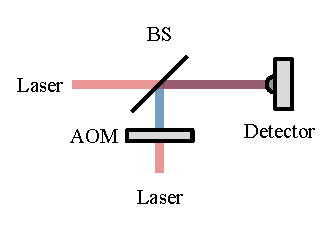
\includegraphics{part1/Figs/HeterodyneTwoLasers.pdf}
    \end{subfigure}
    \begin{subfigure}{0.49\linewidth}
    %\centering
    %% Creator: Matplotlib, PGF backend
%%
%% To include the figure in your LaTeX document, write
%%   \input{<filename>.pgf}
%%
%% Make sure the required packages are loaded in your preamble
%%   \usepackage{pgf}
%%
%% Figures using additional raster images can only be included by \input if
%% they are in the same directory as the main LaTeX file. For loading figures
%% from other directories you can use the `import` package
%%   \usepackage{import}
%% and then include the figures with
%%   \import{<path to file>}{<filename>.pgf}
%%
%% Matplotlib used the following preamble
%%
\begingroup%
\makeatletter%
\begin{pgfpicture}%
\pgfpathrectangle{\pgfpointorigin}{\pgfqpoint{2.855000in}{1.427500in}}%
\pgfusepath{use as bounding box, clip}%
\begin{pgfscope}%
\pgfsetbuttcap%
\pgfsetmiterjoin%
\definecolor{currentfill}{rgb}{1.000000,1.000000,1.000000}%
\pgfsetfillcolor{currentfill}%
\pgfsetlinewidth{0.000000pt}%
\definecolor{currentstroke}{rgb}{1.000000,1.000000,1.000000}%
\pgfsetstrokecolor{currentstroke}%
\pgfsetdash{}{0pt}%
\pgfpathmoveto{\pgfqpoint{0.000000in}{0.000000in}}%
\pgfpathlineto{\pgfqpoint{2.855000in}{0.000000in}}%
\pgfpathlineto{\pgfqpoint{2.855000in}{1.427500in}}%
\pgfpathlineto{\pgfqpoint{0.000000in}{1.427500in}}%
\pgfpathclose%
\pgfusepath{fill}%
\end{pgfscope}%
\begin{pgfscope}%
\pgfsetbuttcap%
\pgfsetmiterjoin%
\definecolor{currentfill}{rgb}{1.000000,1.000000,1.000000}%
\pgfsetfillcolor{currentfill}%
\pgfsetlinewidth{0.000000pt}%
\definecolor{currentstroke}{rgb}{0.000000,0.000000,0.000000}%
\pgfsetstrokecolor{currentstroke}%
\pgfsetstrokeopacity{0.000000}%
\pgfsetdash{}{0pt}%
\pgfpathmoveto{\pgfqpoint{0.342732in}{0.521851in}}%
\pgfpathlineto{\pgfqpoint{1.130154in}{0.521851in}}%
\pgfpathlineto{\pgfqpoint{1.130154in}{1.277500in}}%
\pgfpathlineto{\pgfqpoint{0.342732in}{1.277500in}}%
\pgfpathclose%
\pgfusepath{fill}%
\end{pgfscope}%
\begin{pgfscope}%
\pgfpathrectangle{\pgfqpoint{0.342732in}{0.521851in}}{\pgfqpoint{0.787423in}{0.755649in}} %
\pgfusepath{clip}%
\pgfsetrectcap%
\pgfsetroundjoin%
\pgfsetlinewidth{1.003750pt}%
\definecolor{currentstroke}{rgb}{0.600000,0.000000,0.000000}%
\pgfsetstrokecolor{currentstroke}%
\pgfsetdash{}{0pt}%
\pgfpathmoveto{\pgfqpoint{0.342732in}{0.521851in}}%
\pgfpathlineto{\pgfqpoint{0.570525in}{0.522959in}}%
\pgfpathlineto{\pgfqpoint{0.586289in}{0.525344in}}%
\pgfpathlineto{\pgfqpoint{0.597324in}{0.529138in}}%
\pgfpathlineto{\pgfqpoint{0.605994in}{0.534336in}}%
\pgfpathlineto{\pgfqpoint{0.613876in}{0.541618in}}%
\pgfpathlineto{\pgfqpoint{0.621758in}{0.552265in}}%
\pgfpathlineto{\pgfqpoint{0.628852in}{0.565587in}}%
\pgfpathlineto{\pgfqpoint{0.636734in}{0.585580in}}%
\pgfpathlineto{\pgfqpoint{0.644617in}{0.612092in}}%
\pgfpathlineto{\pgfqpoint{0.653287in}{0.649852in}}%
\pgfpathlineto{\pgfqpoint{0.662745in}{0.702014in}}%
\pgfpathlineto{\pgfqpoint{0.673780in}{0.776670in}}%
\pgfpathlineto{\pgfqpoint{0.689545in}{0.901214in}}%
\pgfpathlineto{\pgfqpoint{0.708462in}{1.047619in}}%
\pgfpathlineto{\pgfqpoint{0.717920in}{1.103696in}}%
\pgfpathlineto{\pgfqpoint{0.725014in}{1.132889in}}%
\pgfpathlineto{\pgfqpoint{0.730532in}{1.146509in}}%
\pgfpathlineto{\pgfqpoint{0.734473in}{1.150995in}}%
\pgfpathlineto{\pgfqpoint{0.737625in}{1.151356in}}%
\pgfpathlineto{\pgfqpoint{0.740778in}{1.148838in}}%
\pgfpathlineto{\pgfqpoint{0.744719in}{1.141699in}}%
\pgfpathlineto{\pgfqpoint{0.749449in}{1.127490in}}%
\pgfpathlineto{\pgfqpoint{0.755754in}{1.099712in}}%
\pgfpathlineto{\pgfqpoint{0.763636in}{1.052913in}}%
\pgfpathlineto{\pgfqpoint{0.774671in}{0.971536in}}%
\pgfpathlineto{\pgfqpoint{0.807776in}{0.716827in}}%
\pgfpathlineto{\pgfqpoint{0.818811in}{0.653758in}}%
\pgfpathlineto{\pgfqpoint{0.828270in}{0.612092in}}%
\pgfpathlineto{\pgfqpoint{0.836940in}{0.583305in}}%
\pgfpathlineto{\pgfqpoint{0.845610in}{0.562276in}}%
\pgfpathlineto{\pgfqpoint{0.853492in}{0.548657in}}%
\pgfpathlineto{\pgfqpoint{0.861375in}{0.539125in}}%
\pgfpathlineto{\pgfqpoint{0.870045in}{0.532157in}}%
\pgfpathlineto{\pgfqpoint{0.879503in}{0.527491in}}%
\pgfpathlineto{\pgfqpoint{0.891327in}{0.524356in}}%
\pgfpathlineto{\pgfqpoint{0.907879in}{0.522573in}}%
\pgfpathlineto{\pgfqpoint{0.940196in}{0.521896in}}%
\pgfpathlineto{\pgfqpoint{1.130154in}{0.521851in}}%
\pgfpathlineto{\pgfqpoint{1.130154in}{0.521851in}}%
\pgfusepath{stroke}%
\end{pgfscope}%
\begin{pgfscope}%
\pgfsetrectcap%
\pgfsetmiterjoin%
\pgfsetlinewidth{1.003750pt}%
\definecolor{currentstroke}{rgb}{0.000000,0.000000,0.000000}%
\pgfsetstrokecolor{currentstroke}%
\pgfsetdash{}{0pt}%
\pgfpathmoveto{\pgfqpoint{0.342732in}{1.277500in}}%
\pgfpathlineto{\pgfqpoint{1.130154in}{1.277500in}}%
\pgfusepath{stroke}%
\end{pgfscope}%
\begin{pgfscope}%
\pgfsetrectcap%
\pgfsetmiterjoin%
\pgfsetlinewidth{1.003750pt}%
\definecolor{currentstroke}{rgb}{0.000000,0.000000,0.000000}%
\pgfsetstrokecolor{currentstroke}%
\pgfsetdash{}{0pt}%
\pgfpathmoveto{\pgfqpoint{0.342732in}{0.521851in}}%
\pgfpathlineto{\pgfqpoint{0.342732in}{1.277500in}}%
\pgfusepath{stroke}%
\end{pgfscope}%
\begin{pgfscope}%
\pgfsetrectcap%
\pgfsetmiterjoin%
\pgfsetlinewidth{1.003750pt}%
\definecolor{currentstroke}{rgb}{0.000000,0.000000,0.000000}%
\pgfsetstrokecolor{currentstroke}%
\pgfsetdash{}{0pt}%
\pgfpathmoveto{\pgfqpoint{1.130154in}{0.521851in}}%
\pgfpathlineto{\pgfqpoint{1.130154in}{1.277500in}}%
\pgfusepath{stroke}%
\end{pgfscope}%
\begin{pgfscope}%
\pgfsetrectcap%
\pgfsetmiterjoin%
\pgfsetlinewidth{1.003750pt}%
\definecolor{currentstroke}{rgb}{0.000000,0.000000,0.000000}%
\pgfsetstrokecolor{currentstroke}%
\pgfsetdash{}{0pt}%
\pgfpathmoveto{\pgfqpoint{0.342732in}{0.521851in}}%
\pgfpathlineto{\pgfqpoint{1.130154in}{0.521851in}}%
\pgfusepath{stroke}%
\end{pgfscope}%
\begin{pgfscope}%
\pgfsetbuttcap%
\pgfsetroundjoin%
\definecolor{currentfill}{rgb}{0.000000,0.000000,0.000000}%
\pgfsetfillcolor{currentfill}%
\pgfsetlinewidth{0.501875pt}%
\definecolor{currentstroke}{rgb}{0.000000,0.000000,0.000000}%
\pgfsetstrokecolor{currentstroke}%
\pgfsetdash{}{0pt}%
\pgfsys@defobject{currentmarker}{\pgfqpoint{0.000000in}{0.000000in}}{\pgfqpoint{0.000000in}{0.055556in}}{%
\pgfpathmoveto{\pgfqpoint{0.000000in}{0.000000in}}%
\pgfpathlineto{\pgfqpoint{0.000000in}{0.055556in}}%
\pgfusepath{stroke,fill}%
}%
\begin{pgfscope}%
\pgfsys@transformshift{0.736443in}{0.521851in}%
\pgfsys@useobject{currentmarker}{}%
\end{pgfscope}%
\end{pgfscope}%
\begin{pgfscope}%
\pgfsetbuttcap%
\pgfsetroundjoin%
\definecolor{currentfill}{rgb}{0.000000,0.000000,0.000000}%
\pgfsetfillcolor{currentfill}%
\pgfsetlinewidth{0.501875pt}%
\definecolor{currentstroke}{rgb}{0.000000,0.000000,0.000000}%
\pgfsetstrokecolor{currentstroke}%
\pgfsetdash{}{0pt}%
\pgfsys@defobject{currentmarker}{\pgfqpoint{0.000000in}{-0.055556in}}{\pgfqpoint{0.000000in}{0.000000in}}{%
\pgfpathmoveto{\pgfqpoint{0.000000in}{0.000000in}}%
\pgfpathlineto{\pgfqpoint{0.000000in}{-0.055556in}}%
\pgfusepath{stroke,fill}%
}%
\begin{pgfscope}%
\pgfsys@transformshift{0.736443in}{1.277500in}%
\pgfsys@useobject{currentmarker}{}%
\end{pgfscope}%
\end{pgfscope}%
\begin{pgfscope}%
\pgftext[x=0.736443in,y=0.466296in,,top]{\fontsize{10.000000}{12.000000}\selectfont \(\displaystyle \omega_1\)}%
\end{pgfscope}%
\begin{pgfscope}%
\pgftext[x=0.273287in,y=0.899676in,,bottom,rotate=90.000000]{\fontsize{10.000000}{12.000000}\selectfont Amplitude}%
\end{pgfscope}%
\begin{pgfscope}%
\pgfsetbuttcap%
\pgfsetmiterjoin%
\definecolor{currentfill}{rgb}{1.000000,1.000000,1.000000}%
\pgfsetfillcolor{currentfill}%
\pgfsetlinewidth{0.000000pt}%
\definecolor{currentstroke}{rgb}{0.000000,0.000000,0.000000}%
\pgfsetstrokecolor{currentstroke}%
\pgfsetstrokeopacity{0.000000}%
\pgfsetdash{}{0pt}%
\pgfpathmoveto{\pgfqpoint{1.130154in}{0.521851in}}%
\pgfpathlineto{\pgfqpoint{1.917577in}{0.521851in}}%
\pgfpathlineto{\pgfqpoint{1.917577in}{1.277500in}}%
\pgfpathlineto{\pgfqpoint{1.130154in}{1.277500in}}%
\pgfpathclose%
\pgfusepath{fill}%
\end{pgfscope}%
\begin{pgfscope}%
\pgfpathrectangle{\pgfqpoint{1.130154in}{0.521851in}}{\pgfqpoint{0.787423in}{0.755649in}} %
\pgfusepath{clip}%
\pgfsetrectcap%
\pgfsetroundjoin%
\pgfsetlinewidth{1.003750pt}%
\definecolor{currentstroke}{rgb}{0.043137,0.325490,0.580392}%
\pgfsetstrokecolor{currentstroke}%
\pgfsetdash{}{0pt}%
\pgfpathmoveto{\pgfqpoint{1.130154in}{0.521851in}}%
\pgfpathlineto{\pgfqpoint{1.346124in}{0.522931in}}%
\pgfpathlineto{\pgfqpoint{1.363465in}{0.525371in}}%
\pgfpathlineto{\pgfqpoint{1.375288in}{0.529202in}}%
\pgfpathlineto{\pgfqpoint{1.384747in}{0.534575in}}%
\pgfpathlineto{\pgfqpoint{1.393417in}{0.542233in}}%
\pgfpathlineto{\pgfqpoint{1.401299in}{0.552319in}}%
\pgfpathlineto{\pgfqpoint{1.409181in}{0.566271in}}%
\pgfpathlineto{\pgfqpoint{1.417063in}{0.585009in}}%
\pgfpathlineto{\pgfqpoint{1.424945in}{0.609429in}}%
\pgfpathlineto{\pgfqpoint{1.433616in}{0.643750in}}%
\pgfpathlineto{\pgfqpoint{1.443074in}{0.690758in}}%
\pgfpathlineto{\pgfqpoint{1.454109in}{0.757953in}}%
\pgfpathlineto{\pgfqpoint{1.468297in}{0.859744in}}%
\pgfpathlineto{\pgfqpoint{1.495096in}{1.054781in}}%
\pgfpathlineto{\pgfqpoint{1.504555in}{1.105952in}}%
\pgfpathlineto{\pgfqpoint{1.511649in}{1.132892in}}%
\pgfpathlineto{\pgfqpoint{1.517166in}{1.145886in}}%
\pgfpathlineto{\pgfqpoint{1.521107in}{1.150593in}}%
\pgfpathlineto{\pgfqpoint{1.524260in}{1.151539in}}%
\pgfpathlineto{\pgfqpoint{1.527413in}{1.149963in}}%
\pgfpathlineto{\pgfqpoint{1.531354in}{1.144481in}}%
\pgfpathlineto{\pgfqpoint{1.536083in}{1.132892in}}%
\pgfpathlineto{\pgfqpoint{1.541601in}{1.112870in}}%
\pgfpathlineto{\pgfqpoint{1.548695in}{1.077966in}}%
\pgfpathlineto{\pgfqpoint{1.558153in}{1.018682in}}%
\pgfpathlineto{\pgfqpoint{1.573129in}{0.907912in}}%
\pgfpathlineto{\pgfqpoint{1.594411in}{0.752748in}}%
\pgfpathlineto{\pgfqpoint{1.606234in}{0.682222in}}%
\pgfpathlineto{\pgfqpoint{1.616481in}{0.633574in}}%
\pgfpathlineto{\pgfqpoint{1.625939in}{0.598926in}}%
\pgfpathlineto{\pgfqpoint{1.634610in}{0.574983in}}%
\pgfpathlineto{\pgfqpoint{1.643280in}{0.557385in}}%
\pgfpathlineto{\pgfqpoint{1.651950in}{0.544906in}}%
\pgfpathlineto{\pgfqpoint{1.660620in}{0.536363in}}%
\pgfpathlineto{\pgfqpoint{1.670079in}{0.530311in}}%
\pgfpathlineto{\pgfqpoint{1.680326in}{0.526379in}}%
\pgfpathlineto{\pgfqpoint{1.693725in}{0.523726in}}%
\pgfpathlineto{\pgfqpoint{1.714219in}{0.522275in}}%
\pgfpathlineto{\pgfqpoint{1.762300in}{0.521858in}}%
\pgfpathlineto{\pgfqpoint{1.917577in}{0.521851in}}%
\pgfpathlineto{\pgfqpoint{1.917577in}{0.521851in}}%
\pgfusepath{stroke}%
\end{pgfscope}%
\begin{pgfscope}%
\pgfsetrectcap%
\pgfsetmiterjoin%
\pgfsetlinewidth{1.003750pt}%
\definecolor{currentstroke}{rgb}{0.000000,0.000000,0.000000}%
\pgfsetstrokecolor{currentstroke}%
\pgfsetdash{}{0pt}%
\pgfpathmoveto{\pgfqpoint{1.130154in}{1.277500in}}%
\pgfpathlineto{\pgfqpoint{1.917577in}{1.277500in}}%
\pgfusepath{stroke}%
\end{pgfscope}%
\begin{pgfscope}%
\pgfsetrectcap%
\pgfsetmiterjoin%
\pgfsetlinewidth{1.003750pt}%
\definecolor{currentstroke}{rgb}{0.000000,0.000000,0.000000}%
\pgfsetstrokecolor{currentstroke}%
\pgfsetdash{}{0pt}%
\pgfpathmoveto{\pgfqpoint{1.130154in}{0.521851in}}%
\pgfpathlineto{\pgfqpoint{1.130154in}{1.277500in}}%
\pgfusepath{stroke}%
\end{pgfscope}%
\begin{pgfscope}%
\pgfsetrectcap%
\pgfsetmiterjoin%
\pgfsetlinewidth{1.003750pt}%
\definecolor{currentstroke}{rgb}{0.000000,0.000000,0.000000}%
\pgfsetstrokecolor{currentstroke}%
\pgfsetdash{}{0pt}%
\pgfpathmoveto{\pgfqpoint{1.917577in}{0.521851in}}%
\pgfpathlineto{\pgfqpoint{1.917577in}{1.277500in}}%
\pgfusepath{stroke}%
\end{pgfscope}%
\begin{pgfscope}%
\pgfsetrectcap%
\pgfsetmiterjoin%
\pgfsetlinewidth{1.003750pt}%
\definecolor{currentstroke}{rgb}{0.000000,0.000000,0.000000}%
\pgfsetstrokecolor{currentstroke}%
\pgfsetdash{}{0pt}%
\pgfpathmoveto{\pgfqpoint{1.130154in}{0.521851in}}%
\pgfpathlineto{\pgfqpoint{1.917577in}{0.521851in}}%
\pgfusepath{stroke}%
\end{pgfscope}%
\begin{pgfscope}%
\pgfsetbuttcap%
\pgfsetroundjoin%
\definecolor{currentfill}{rgb}{0.000000,0.000000,0.000000}%
\pgfsetfillcolor{currentfill}%
\pgfsetlinewidth{0.501875pt}%
\definecolor{currentstroke}{rgb}{0.000000,0.000000,0.000000}%
\pgfsetstrokecolor{currentstroke}%
\pgfsetdash{}{0pt}%
\pgfsys@defobject{currentmarker}{\pgfqpoint{0.000000in}{0.000000in}}{\pgfqpoint{0.000000in}{0.055556in}}{%
\pgfpathmoveto{\pgfqpoint{0.000000in}{0.000000in}}%
\pgfpathlineto{\pgfqpoint{0.000000in}{0.055556in}}%
\pgfusepath{stroke,fill}%
}%
\begin{pgfscope}%
\pgfsys@transformshift{1.523866in}{0.521851in}%
\pgfsys@useobject{currentmarker}{}%
\end{pgfscope}%
\end{pgfscope}%
\begin{pgfscope}%
\pgfsetbuttcap%
\pgfsetroundjoin%
\definecolor{currentfill}{rgb}{0.000000,0.000000,0.000000}%
\pgfsetfillcolor{currentfill}%
\pgfsetlinewidth{0.501875pt}%
\definecolor{currentstroke}{rgb}{0.000000,0.000000,0.000000}%
\pgfsetstrokecolor{currentstroke}%
\pgfsetdash{}{0pt}%
\pgfsys@defobject{currentmarker}{\pgfqpoint{0.000000in}{-0.055556in}}{\pgfqpoint{0.000000in}{0.000000in}}{%
\pgfpathmoveto{\pgfqpoint{0.000000in}{0.000000in}}%
\pgfpathlineto{\pgfqpoint{0.000000in}{-0.055556in}}%
\pgfusepath{stroke,fill}%
}%
\begin{pgfscope}%
\pgfsys@transformshift{1.523866in}{1.277500in}%
\pgfsys@useobject{currentmarker}{}%
\end{pgfscope}%
\end{pgfscope}%
\begin{pgfscope}%
\pgftext[x=1.523866in,y=0.466296in,,top]{\fontsize{10.000000}{12.000000}\selectfont \(\displaystyle \omega_1+\delta\)}%
\end{pgfscope}%
\begin{pgfscope}%
\pgftext[x=1.523866in,y=0.273395in,,top]{\fontsize{10.000000}{12.000000}\selectfont Frequency}%
\end{pgfscope}%
\begin{pgfscope}%
\pgfsetbuttcap%
\pgfsetmiterjoin%
\definecolor{currentfill}{rgb}{1.000000,1.000000,1.000000}%
\pgfsetfillcolor{currentfill}%
\pgfsetlinewidth{0.000000pt}%
\definecolor{currentstroke}{rgb}{0.000000,0.000000,0.000000}%
\pgfsetstrokecolor{currentstroke}%
\pgfsetstrokeopacity{0.000000}%
\pgfsetdash{}{0pt}%
\pgfpathmoveto{\pgfqpoint{1.917577in}{0.521851in}}%
\pgfpathlineto{\pgfqpoint{2.705000in}{0.521851in}}%
\pgfpathlineto{\pgfqpoint{2.705000in}{1.277500in}}%
\pgfpathlineto{\pgfqpoint{1.917577in}{1.277500in}}%
\pgfpathclose%
\pgfusepath{fill}%
\end{pgfscope}%
\begin{pgfscope}%
\pgfpathrectangle{\pgfqpoint{1.917577in}{0.521851in}}{\pgfqpoint{0.787423in}{0.755649in}} %
\pgfusepath{clip}%
\pgfsetrectcap%
\pgfsetroundjoin%
\pgfsetlinewidth{1.003750pt}%
\definecolor{currentstroke}{rgb}{0.301961,0.607843,0.301961}%
\pgfsetstrokecolor{currentstroke}%
\pgfsetdash{}{0pt}%
\pgfpathmoveto{\pgfqpoint{1.917577in}{0.521851in}}%
\pgfpathlineto{\pgfqpoint{2.068126in}{0.522921in}}%
\pgfpathlineto{\pgfqpoint{2.091772in}{0.525326in}}%
\pgfpathlineto{\pgfqpoint{2.107536in}{0.528981in}}%
\pgfpathlineto{\pgfqpoint{2.120147in}{0.534043in}}%
\pgfpathlineto{\pgfqpoint{2.131182in}{0.540809in}}%
\pgfpathlineto{\pgfqpoint{2.141429in}{0.549751in}}%
\pgfpathlineto{\pgfqpoint{2.150888in}{0.560919in}}%
\pgfpathlineto{\pgfqpoint{2.160346in}{0.575515in}}%
\pgfpathlineto{\pgfqpoint{2.169805in}{0.594159in}}%
\pgfpathlineto{\pgfqpoint{2.180051in}{0.619587in}}%
\pgfpathlineto{\pgfqpoint{2.190298in}{0.651007in}}%
\pgfpathlineto{\pgfqpoint{2.202121in}{0.695079in}}%
\pgfpathlineto{\pgfqpoint{2.214733in}{0.751060in}}%
\pgfpathlineto{\pgfqpoint{2.230497in}{0.831851in}}%
\pgfpathlineto{\pgfqpoint{2.274637in}{1.065169in}}%
\pgfpathlineto{\pgfqpoint{2.284884in}{1.104762in}}%
\pgfpathlineto{\pgfqpoint{2.293554in}{1.129695in}}%
\pgfpathlineto{\pgfqpoint{2.300648in}{1.143368in}}%
\pgfpathlineto{\pgfqpoint{2.306165in}{1.149501in}}%
\pgfpathlineto{\pgfqpoint{2.310895in}{1.151517in}}%
\pgfpathlineto{\pgfqpoint{2.314836in}{1.150886in}}%
\pgfpathlineto{\pgfqpoint{2.318777in}{1.148161in}}%
\pgfpathlineto{\pgfqpoint{2.323506in}{1.142165in}}%
\pgfpathlineto{\pgfqpoint{2.329023in}{1.131525in}}%
\pgfpathlineto{\pgfqpoint{2.336117in}{1.112405in}}%
\pgfpathlineto{\pgfqpoint{2.344788in}{1.081562in}}%
\pgfpathlineto{\pgfqpoint{2.355034in}{1.036346in}}%
\pgfpathlineto{\pgfqpoint{2.369222in}{0.962954in}}%
\pgfpathlineto{\pgfqpoint{2.411786in}{0.736249in}}%
\pgfpathlineto{\pgfqpoint{2.425185in}{0.679455in}}%
\pgfpathlineto{\pgfqpoint{2.437008in}{0.638187in}}%
\pgfpathlineto{\pgfqpoint{2.448043in}{0.607136in}}%
\pgfpathlineto{\pgfqpoint{2.458290in}{0.584293in}}%
\pgfpathlineto{\pgfqpoint{2.468537in}{0.566548in}}%
\pgfpathlineto{\pgfqpoint{2.478783in}{0.553132in}}%
\pgfpathlineto{\pgfqpoint{2.489030in}{0.543254in}}%
\pgfpathlineto{\pgfqpoint{2.500065in}{0.535719in}}%
\pgfpathlineto{\pgfqpoint{2.511888in}{0.530313in}}%
\pgfpathlineto{\pgfqpoint{2.526076in}{0.526347in}}%
\pgfpathlineto{\pgfqpoint{2.544205in}{0.523733in}}%
\pgfpathlineto{\pgfqpoint{2.571792in}{0.522288in}}%
\pgfpathlineto{\pgfqpoint{2.635637in}{0.521859in}}%
\pgfpathlineto{\pgfqpoint{2.705000in}{0.521851in}}%
\pgfpathlineto{\pgfqpoint{2.705000in}{0.521851in}}%
\pgfusepath{stroke}%
\end{pgfscope}%
\begin{pgfscope}%
\pgfpathrectangle{\pgfqpoint{1.917577in}{0.521851in}}{\pgfqpoint{0.787423in}{0.755649in}} %
\pgfusepath{clip}%
\pgfsetbuttcap%
\pgfsetroundjoin%
\pgfsetlinewidth{1.003750pt}%
\definecolor{currentstroke}{rgb}{0.600000,0.000000,0.000000}%
\pgfsetstrokecolor{currentstroke}%
\pgfsetdash{{1.000000pt}{3.000000pt}}{0.000000pt}%
\pgfpathmoveto{\pgfqpoint{1.917577in}{0.521851in}}%
\pgfpathlineto{\pgfqpoint{2.145370in}{0.522959in}}%
\pgfpathlineto{\pgfqpoint{2.161134in}{0.525344in}}%
\pgfpathlineto{\pgfqpoint{2.172169in}{0.529138in}}%
\pgfpathlineto{\pgfqpoint{2.180840in}{0.534336in}}%
\pgfpathlineto{\pgfqpoint{2.188722in}{0.541618in}}%
\pgfpathlineto{\pgfqpoint{2.196604in}{0.552265in}}%
\pgfpathlineto{\pgfqpoint{2.203698in}{0.565587in}}%
\pgfpathlineto{\pgfqpoint{2.211580in}{0.585580in}}%
\pgfpathlineto{\pgfqpoint{2.219462in}{0.612092in}}%
\pgfpathlineto{\pgfqpoint{2.228132in}{0.649852in}}%
\pgfpathlineto{\pgfqpoint{2.237591in}{0.702014in}}%
\pgfpathlineto{\pgfqpoint{2.248626in}{0.776670in}}%
\pgfpathlineto{\pgfqpoint{2.264390in}{0.901214in}}%
\pgfpathlineto{\pgfqpoint{2.283307in}{1.047619in}}%
\pgfpathlineto{\pgfqpoint{2.292766in}{1.103696in}}%
\pgfpathlineto{\pgfqpoint{2.299860in}{1.132889in}}%
\pgfpathlineto{\pgfqpoint{2.305377in}{1.146509in}}%
\pgfpathlineto{\pgfqpoint{2.309318in}{1.150995in}}%
\pgfpathlineto{\pgfqpoint{2.312471in}{1.151356in}}%
\pgfpathlineto{\pgfqpoint{2.315624in}{1.148838in}}%
\pgfpathlineto{\pgfqpoint{2.319565in}{1.141699in}}%
\pgfpathlineto{\pgfqpoint{2.324294in}{1.127490in}}%
\pgfpathlineto{\pgfqpoint{2.330600in}{1.099712in}}%
\pgfpathlineto{\pgfqpoint{2.338482in}{1.052913in}}%
\pgfpathlineto{\pgfqpoint{2.349517in}{0.971536in}}%
\pgfpathlineto{\pgfqpoint{2.382622in}{0.716827in}}%
\pgfpathlineto{\pgfqpoint{2.393657in}{0.653758in}}%
\pgfpathlineto{\pgfqpoint{2.403115in}{0.612092in}}%
\pgfpathlineto{\pgfqpoint{2.411786in}{0.583305in}}%
\pgfpathlineto{\pgfqpoint{2.420456in}{0.562276in}}%
\pgfpathlineto{\pgfqpoint{2.428338in}{0.548657in}}%
\pgfpathlineto{\pgfqpoint{2.436220in}{0.539125in}}%
\pgfpathlineto{\pgfqpoint{2.444890in}{0.532157in}}%
\pgfpathlineto{\pgfqpoint{2.454349in}{0.527491in}}%
\pgfpathlineto{\pgfqpoint{2.466172in}{0.524356in}}%
\pgfpathlineto{\pgfqpoint{2.482725in}{0.522573in}}%
\pgfpathlineto{\pgfqpoint{2.515041in}{0.521896in}}%
\pgfpathlineto{\pgfqpoint{2.705000in}{0.521851in}}%
\pgfpathlineto{\pgfqpoint{2.705000in}{0.521851in}}%
\pgfusepath{stroke}%
\end{pgfscope}%
\begin{pgfscope}%
\pgfsetrectcap%
\pgfsetmiterjoin%
\pgfsetlinewidth{1.003750pt}%
\definecolor{currentstroke}{rgb}{0.000000,0.000000,0.000000}%
\pgfsetstrokecolor{currentstroke}%
\pgfsetdash{}{0pt}%
\pgfpathmoveto{\pgfqpoint{1.917577in}{1.277500in}}%
\pgfpathlineto{\pgfqpoint{2.705000in}{1.277500in}}%
\pgfusepath{stroke}%
\end{pgfscope}%
\begin{pgfscope}%
\pgfsetrectcap%
\pgfsetmiterjoin%
\pgfsetlinewidth{1.003750pt}%
\definecolor{currentstroke}{rgb}{0.000000,0.000000,0.000000}%
\pgfsetstrokecolor{currentstroke}%
\pgfsetdash{}{0pt}%
\pgfpathmoveto{\pgfqpoint{1.917577in}{0.521851in}}%
\pgfpathlineto{\pgfqpoint{1.917577in}{1.277500in}}%
\pgfusepath{stroke}%
\end{pgfscope}%
\begin{pgfscope}%
\pgfsetrectcap%
\pgfsetmiterjoin%
\pgfsetlinewidth{1.003750pt}%
\definecolor{currentstroke}{rgb}{0.000000,0.000000,0.000000}%
\pgfsetstrokecolor{currentstroke}%
\pgfsetdash{}{0pt}%
\pgfpathmoveto{\pgfqpoint{2.705000in}{0.521851in}}%
\pgfpathlineto{\pgfqpoint{2.705000in}{1.277500in}}%
\pgfusepath{stroke}%
\end{pgfscope}%
\begin{pgfscope}%
\pgfsetrectcap%
\pgfsetmiterjoin%
\pgfsetlinewidth{1.003750pt}%
\definecolor{currentstroke}{rgb}{0.000000,0.000000,0.000000}%
\pgfsetstrokecolor{currentstroke}%
\pgfsetdash{}{0pt}%
\pgfpathmoveto{\pgfqpoint{1.917577in}{0.521851in}}%
\pgfpathlineto{\pgfqpoint{2.705000in}{0.521851in}}%
\pgfusepath{stroke}%
\end{pgfscope}%
\begin{pgfscope}%
\pgfsetbuttcap%
\pgfsetroundjoin%
\definecolor{currentfill}{rgb}{0.000000,0.000000,0.000000}%
\pgfsetfillcolor{currentfill}%
\pgfsetlinewidth{0.501875pt}%
\definecolor{currentstroke}{rgb}{0.000000,0.000000,0.000000}%
\pgfsetstrokecolor{currentstroke}%
\pgfsetdash{}{0pt}%
\pgfsys@defobject{currentmarker}{\pgfqpoint{0.000000in}{0.000000in}}{\pgfqpoint{0.000000in}{0.055556in}}{%
\pgfpathmoveto{\pgfqpoint{0.000000in}{0.000000in}}%
\pgfpathlineto{\pgfqpoint{0.000000in}{0.055556in}}%
\pgfusepath{stroke,fill}%
}%
\begin{pgfscope}%
\pgfsys@transformshift{2.311289in}{0.521851in}%
\pgfsys@useobject{currentmarker}{}%
\end{pgfscope}%
\end{pgfscope}%
\begin{pgfscope}%
\pgfsetbuttcap%
\pgfsetroundjoin%
\definecolor{currentfill}{rgb}{0.000000,0.000000,0.000000}%
\pgfsetfillcolor{currentfill}%
\pgfsetlinewidth{0.501875pt}%
\definecolor{currentstroke}{rgb}{0.000000,0.000000,0.000000}%
\pgfsetstrokecolor{currentstroke}%
\pgfsetdash{}{0pt}%
\pgfsys@defobject{currentmarker}{\pgfqpoint{0.000000in}{-0.055556in}}{\pgfqpoint{0.000000in}{0.000000in}}{%
\pgfpathmoveto{\pgfqpoint{0.000000in}{0.000000in}}%
\pgfpathlineto{\pgfqpoint{0.000000in}{-0.055556in}}%
\pgfusepath{stroke,fill}%
}%
\begin{pgfscope}%
\pgfsys@transformshift{2.311289in}{1.277500in}%
\pgfsys@useobject{currentmarker}{}%
\end{pgfscope}%
\end{pgfscope}%
\begin{pgfscope}%
\pgftext[x=2.311289in,y=0.466296in,,top]{\fontsize{10.000000}{12.000000}\selectfont \(\displaystyle \delta\)}%
\end{pgfscope}%
\end{pgfpicture}%
\makeatother%
\endgroup%

    \end{subfigure}
    \caption{Heterodyne measurement with two `identical' lasers. One beam is frequency shifted by an \gls{aom} from the initial frequency ($\omega_1$, red) to an offset frequency ($\omega_1+\delta$, blue) to enable measurement by a spectrum analyser. Shown on the right is the spectral lineshapes of the lasers and the heterodyne beatnote (green).}
    \label{figure:two-laser_heterodyne}
\end{figure}

Two-laser heterodyne provides a useful measurement due to its simplicity and the lack of confounding effects (such as those found with self-heterodyne) and thus can relatively easily provide confidence in the results of the measurement.
The downside of this method is the obvious requirement for two very similar lasers frequency stabilised with the same methods to be used.

In order to test the efficacy of high-bandwidth \gls{ps} two similar laser setups were used; both used commercial Littrow configuration lasers, identical optic setups as shown in Figure~\ref{figure:laser_setup} with optical fibres that can be connected to the diagnostic measurements such as the heterodyne setup and the high-finesse cavity.

One laser was freqency shifted with a double-pass \gls{aom}, to give a total frequency shift of \unit[160]{MHz}, which was then combined with the other laser with a 50:50 beamsplitter and then incident on the photodetector.
The \unit[1]{GHz} detector\footnote{NewFocus 1621} was connected to a spectrum analyser\footnote{\unit[9]{kHz} to \unit[7]{GHz} Rohde and Swartz FSP7} to measure the spectrum of the beatnote that was centred around \unit[160]{MHz} due to the frequency shift imposed on one beam of the heterodyne measurement by the \gls{aom}.
An example of a beatnote from two lasers locked with \gls{ps} with high-bandwidth feedback is shown in Figure~\ref{figure:two_laser_beatnote}.
The majority of the optical power is contained within the central peak of the beatnote which, unlike self-heterodyne, can confidently be said to be due only to the frequency spectrum of the lasers.
The central peak has a \unit[$-3$]{dB} width (\gls{fwhm}) of \unit[2$\pm$0.4]{kHz}.
As the lasers are uncorrelated and assuming they have identical Gaussian lineshapes indicates that the individual lasers have an \gls{rms} linewidth of \unit[0.60$\pm$0.1]{kHz}.
The `shoulders' of the beatnote at \unit[$\pm$1.5]{MHz} correspond to the servo bump of the fully locked noise spectrum shown in Figure~\ref{figure:psd}.
These measurements indicate that \gls{ps} with high-bandwidth feedback is able to narrow the laser linewidth to \unit[0.6$\pm$0.1]{kHz} which is significant improvement, two orders of magnitude, over previously published \gls{ps} performance~\cite{torii_laser-phase_2012}.

\begin{figure}
\center
%% Creator: Matplotlib, PGF backend
%%
%% To include the figure in your LaTeX document, write
%%   \input{<filename>.pgf}
%%
%% Make sure the required packages are loaded in your preamble
%%   \usepackage{pgf}
%%
%% Figures using additional raster images can only be included by \input if
%% they are in the same directory as the main LaTeX file. For loading figures
%% from other directories you can use the `import` package
%%   \usepackage{import}
%% and then include the figures with
%%   \import{<path to file>}{<filename>.pgf}
%%
%% Matplotlib used the following preamble
%%
\begingroup%
\makeatletter%
\begin{pgfpicture}%
\pgfpathrectangle{\pgfpointorigin}{\pgfqpoint{5.710000in}{3.172222in}}%
\pgfusepath{use as bounding box, clip}%
\begin{pgfscope}%
\pgfsetbuttcap%
\pgfsetmiterjoin%
\definecolor{currentfill}{rgb}{1.000000,1.000000,1.000000}%
\pgfsetfillcolor{currentfill}%
\pgfsetlinewidth{0.000000pt}%
\definecolor{currentstroke}{rgb}{1.000000,1.000000,1.000000}%
\pgfsetstrokecolor{currentstroke}%
\pgfsetdash{}{0pt}%
\pgfpathmoveto{\pgfqpoint{0.000000in}{0.000000in}}%
\pgfpathlineto{\pgfqpoint{5.710000in}{0.000000in}}%
\pgfpathlineto{\pgfqpoint{5.710000in}{3.172222in}}%
\pgfpathlineto{\pgfqpoint{0.000000in}{3.172222in}}%
\pgfpathclose%
\pgfusepath{fill}%
\end{pgfscope}%
\begin{pgfscope}%
\pgfsetbuttcap%
\pgfsetmiterjoin%
\definecolor{currentfill}{rgb}{1.000000,1.000000,1.000000}%
\pgfsetfillcolor{currentfill}%
\pgfsetlinewidth{0.000000pt}%
\definecolor{currentstroke}{rgb}{0.000000,0.000000,0.000000}%
\pgfsetstrokecolor{currentstroke}%
\pgfsetstrokeopacity{0.000000}%
\pgfsetdash{}{0pt}%
\pgfpathmoveto{\pgfqpoint{0.693845in}{0.521851in}}%
\pgfpathlineto{\pgfqpoint{5.560000in}{0.521851in}}%
\pgfpathlineto{\pgfqpoint{5.560000in}{3.022222in}}%
\pgfpathlineto{\pgfqpoint{0.693845in}{3.022222in}}%
\pgfpathclose%
\pgfusepath{fill}%
\end{pgfscope}%
\begin{pgfscope}%
\pgfpathrectangle{\pgfqpoint{0.693845in}{0.521851in}}{\pgfqpoint{4.866155in}{2.500371in}} %
\pgfusepath{clip}%
\pgfsetrectcap%
\pgfsetroundjoin%
\pgfsetlinewidth{0.501875pt}%
\definecolor{currentstroke}{rgb}{0.309804,0.478431,0.682353}%
\pgfsetstrokecolor{currentstroke}%
\pgfsetdash{}{0pt}%
\pgfpathmoveto{\pgfqpoint{0.693845in}{0.742508in}}%
\pgfpathlineto{\pgfqpoint{0.703578in}{0.686945in}}%
\pgfpathlineto{\pgfqpoint{0.713310in}{0.643348in}}%
\pgfpathlineto{\pgfqpoint{0.723042in}{0.675389in}}%
\pgfpathlineto{\pgfqpoint{0.732775in}{0.618502in}}%
\pgfpathlineto{\pgfqpoint{0.742507in}{0.585744in}}%
\pgfpathlineto{\pgfqpoint{0.752239in}{0.645516in}}%
\pgfpathlineto{\pgfqpoint{0.761972in}{0.673907in}}%
\pgfpathlineto{\pgfqpoint{0.771704in}{0.639132in}}%
\pgfpathlineto{\pgfqpoint{0.781436in}{0.628418in}}%
\pgfpathlineto{\pgfqpoint{0.791169in}{0.646413in}}%
\pgfpathlineto{\pgfqpoint{0.800901in}{0.752636in}}%
\pgfpathlineto{\pgfqpoint{0.810633in}{0.705751in}}%
\pgfpathlineto{\pgfqpoint{0.820365in}{0.648837in}}%
\pgfpathlineto{\pgfqpoint{0.830098in}{0.671328in}}%
\pgfpathlineto{\pgfqpoint{0.839830in}{0.669571in}}%
\pgfpathlineto{\pgfqpoint{0.849562in}{0.672274in}}%
\pgfpathlineto{\pgfqpoint{0.859295in}{0.680647in}}%
\pgfpathlineto{\pgfqpoint{0.869027in}{0.735591in}}%
\pgfpathlineto{\pgfqpoint{0.888492in}{0.677940in}}%
\pgfpathlineto{\pgfqpoint{0.898224in}{0.708509in}}%
\pgfpathlineto{\pgfqpoint{0.907956in}{0.708410in}}%
\pgfpathlineto{\pgfqpoint{0.917689in}{0.723481in}}%
\pgfpathlineto{\pgfqpoint{0.927421in}{0.663388in}}%
\pgfpathlineto{\pgfqpoint{0.937153in}{0.666497in}}%
\pgfpathlineto{\pgfqpoint{0.946885in}{0.640071in}}%
\pgfpathlineto{\pgfqpoint{0.956618in}{0.679513in}}%
\pgfpathlineto{\pgfqpoint{0.966350in}{0.680459in}}%
\pgfpathlineto{\pgfqpoint{0.985815in}{0.716882in}}%
\pgfpathlineto{\pgfqpoint{1.005279in}{0.691753in}}%
\pgfpathlineto{\pgfqpoint{1.015012in}{0.634913in}}%
\pgfpathlineto{\pgfqpoint{1.024744in}{0.652707in}}%
\pgfpathlineto{\pgfqpoint{1.034476in}{0.685421in}}%
\pgfpathlineto{\pgfqpoint{1.044209in}{0.646096in}}%
\pgfpathlineto{\pgfqpoint{1.053941in}{0.653909in}}%
\pgfpathlineto{\pgfqpoint{1.063673in}{0.612811in}}%
\pgfpathlineto{\pgfqpoint{1.073405in}{0.675480in}}%
\pgfpathlineto{\pgfqpoint{1.083138in}{0.706533in}}%
\pgfpathlineto{\pgfqpoint{1.092870in}{0.674091in}}%
\pgfpathlineto{\pgfqpoint{1.102602in}{0.647094in}}%
\pgfpathlineto{\pgfqpoint{1.112335in}{0.665702in}}%
\pgfpathlineto{\pgfqpoint{1.122067in}{0.676647in}}%
\pgfpathlineto{\pgfqpoint{1.131799in}{0.678914in}}%
\pgfpathlineto{\pgfqpoint{1.141532in}{0.694413in}}%
\pgfpathlineto{\pgfqpoint{1.151264in}{0.687945in}}%
\pgfpathlineto{\pgfqpoint{1.160996in}{0.697751in}}%
\pgfpathlineto{\pgfqpoint{1.170729in}{0.699702in}}%
\pgfpathlineto{\pgfqpoint{1.180461in}{0.748697in}}%
\pgfpathlineto{\pgfqpoint{1.190193in}{0.659300in}}%
\pgfpathlineto{\pgfqpoint{1.199925in}{0.707732in}}%
\pgfpathlineto{\pgfqpoint{1.209658in}{0.720242in}}%
\pgfpathlineto{\pgfqpoint{1.229122in}{0.681870in}}%
\pgfpathlineto{\pgfqpoint{1.238855in}{0.681975in}}%
\pgfpathlineto{\pgfqpoint{1.248587in}{0.731848in}}%
\pgfpathlineto{\pgfqpoint{1.258319in}{0.713909in}}%
\pgfpathlineto{\pgfqpoint{1.268052in}{0.675288in}}%
\pgfpathlineto{\pgfqpoint{1.277784in}{0.723084in}}%
\pgfpathlineto{\pgfqpoint{1.287516in}{0.718930in}}%
\pgfpathlineto{\pgfqpoint{1.297249in}{0.710043in}}%
\pgfpathlineto{\pgfqpoint{1.306981in}{0.761852in}}%
\pgfpathlineto{\pgfqpoint{1.316713in}{0.751098in}}%
\pgfpathlineto{\pgfqpoint{1.326446in}{0.760026in}}%
\pgfpathlineto{\pgfqpoint{1.336178in}{0.729347in}}%
\pgfpathlineto{\pgfqpoint{1.345910in}{0.727214in}}%
\pgfpathlineto{\pgfqpoint{1.355642in}{0.734269in}}%
\pgfpathlineto{\pgfqpoint{1.365375in}{0.708050in}}%
\pgfpathlineto{\pgfqpoint{1.375107in}{0.730271in}}%
\pgfpathlineto{\pgfqpoint{1.394572in}{0.744591in}}%
\pgfpathlineto{\pgfqpoint{1.404304in}{0.758455in}}%
\pgfpathlineto{\pgfqpoint{1.414036in}{0.701008in}}%
\pgfpathlineto{\pgfqpoint{1.423769in}{0.681611in}}%
\pgfpathlineto{\pgfqpoint{1.443233in}{0.731546in}}%
\pgfpathlineto{\pgfqpoint{1.452966in}{0.724646in}}%
\pgfpathlineto{\pgfqpoint{1.462698in}{0.757911in}}%
\pgfpathlineto{\pgfqpoint{1.472430in}{0.729338in}}%
\pgfpathlineto{\pgfqpoint{1.482162in}{0.786613in}}%
\pgfpathlineto{\pgfqpoint{1.491895in}{0.753978in}}%
\pgfpathlineto{\pgfqpoint{1.501627in}{0.761779in}}%
\pgfpathlineto{\pgfqpoint{1.511359in}{0.782788in}}%
\pgfpathlineto{\pgfqpoint{1.521092in}{0.788432in}}%
\pgfpathlineto{\pgfqpoint{1.530824in}{0.759161in}}%
\pgfpathlineto{\pgfqpoint{1.540556in}{0.747812in}}%
\pgfpathlineto{\pgfqpoint{1.550289in}{0.719772in}}%
\pgfpathlineto{\pgfqpoint{1.560021in}{0.767519in}}%
\pgfpathlineto{\pgfqpoint{1.569753in}{0.798183in}}%
\pgfpathlineto{\pgfqpoint{1.579486in}{0.770678in}}%
\pgfpathlineto{\pgfqpoint{1.589218in}{0.793431in}}%
\pgfpathlineto{\pgfqpoint{1.598950in}{0.812069in}}%
\pgfpathlineto{\pgfqpoint{1.608682in}{0.818105in}}%
\pgfpathlineto{\pgfqpoint{1.618415in}{0.773362in}}%
\pgfpathlineto{\pgfqpoint{1.628147in}{0.847068in}}%
\pgfpathlineto{\pgfqpoint{1.637879in}{0.841573in}}%
\pgfpathlineto{\pgfqpoint{1.647612in}{0.781970in}}%
\pgfpathlineto{\pgfqpoint{1.657344in}{0.750777in}}%
\pgfpathlineto{\pgfqpoint{1.667076in}{0.779774in}}%
\pgfpathlineto{\pgfqpoint{1.676809in}{0.859154in}}%
\pgfpathlineto{\pgfqpoint{1.686541in}{0.869605in}}%
\pgfpathlineto{\pgfqpoint{1.696273in}{0.836882in}}%
\pgfpathlineto{\pgfqpoint{1.706006in}{0.845689in}}%
\pgfpathlineto{\pgfqpoint{1.715738in}{0.840907in}}%
\pgfpathlineto{\pgfqpoint{1.725470in}{0.825145in}}%
\pgfpathlineto{\pgfqpoint{1.735203in}{0.885424in}}%
\pgfpathlineto{\pgfqpoint{1.744935in}{0.915001in}}%
\pgfpathlineto{\pgfqpoint{1.754667in}{0.841018in}}%
\pgfpathlineto{\pgfqpoint{1.764399in}{0.853648in}}%
\pgfpathlineto{\pgfqpoint{1.774132in}{0.890396in}}%
\pgfpathlineto{\pgfqpoint{1.783864in}{0.845387in}}%
\pgfpathlineto{\pgfqpoint{1.793596in}{0.875251in}}%
\pgfpathlineto{\pgfqpoint{1.813061in}{0.957338in}}%
\pgfpathlineto{\pgfqpoint{1.822793in}{0.945061in}}%
\pgfpathlineto{\pgfqpoint{1.832526in}{0.874159in}}%
\pgfpathlineto{\pgfqpoint{1.842258in}{0.908167in}}%
\pgfpathlineto{\pgfqpoint{1.851990in}{0.873342in}}%
\pgfpathlineto{\pgfqpoint{1.861723in}{0.875805in}}%
\pgfpathlineto{\pgfqpoint{1.871455in}{0.843316in}}%
\pgfpathlineto{\pgfqpoint{1.881187in}{0.879710in}}%
\pgfpathlineto{\pgfqpoint{1.890919in}{0.964634in}}%
\pgfpathlineto{\pgfqpoint{1.900652in}{0.923598in}}%
\pgfpathlineto{\pgfqpoint{1.910384in}{0.912187in}}%
\pgfpathlineto{\pgfqpoint{1.920116in}{0.908568in}}%
\pgfpathlineto{\pgfqpoint{1.929849in}{0.894379in}}%
\pgfpathlineto{\pgfqpoint{1.939581in}{1.002769in}}%
\pgfpathlineto{\pgfqpoint{1.949313in}{1.017998in}}%
\pgfpathlineto{\pgfqpoint{1.959046in}{0.986589in}}%
\pgfpathlineto{\pgfqpoint{1.968778in}{0.939933in}}%
\pgfpathlineto{\pgfqpoint{1.978510in}{0.947193in}}%
\pgfpathlineto{\pgfqpoint{1.988243in}{0.990964in}}%
\pgfpathlineto{\pgfqpoint{1.997975in}{0.989175in}}%
\pgfpathlineto{\pgfqpoint{2.007707in}{0.986016in}}%
\pgfpathlineto{\pgfqpoint{2.017439in}{0.992098in}}%
\pgfpathlineto{\pgfqpoint{2.027172in}{0.985130in}}%
\pgfpathlineto{\pgfqpoint{2.036904in}{1.027719in}}%
\pgfpathlineto{\pgfqpoint{2.046636in}{1.020592in}}%
\pgfpathlineto{\pgfqpoint{2.056369in}{1.004902in}}%
\pgfpathlineto{\pgfqpoint{2.066101in}{0.993746in}}%
\pgfpathlineto{\pgfqpoint{2.075833in}{1.023446in}}%
\pgfpathlineto{\pgfqpoint{2.085566in}{0.986362in}}%
\pgfpathlineto{\pgfqpoint{2.095298in}{1.017895in}}%
\pgfpathlineto{\pgfqpoint{2.105030in}{0.989159in}}%
\pgfpathlineto{\pgfqpoint{2.114763in}{1.042564in}}%
\pgfpathlineto{\pgfqpoint{2.124495in}{1.049863in}}%
\pgfpathlineto{\pgfqpoint{2.134227in}{1.042788in}}%
\pgfpathlineto{\pgfqpoint{2.143959in}{1.052786in}}%
\pgfpathlineto{\pgfqpoint{2.153692in}{1.047990in}}%
\pgfpathlineto{\pgfqpoint{2.163424in}{1.001308in}}%
\pgfpathlineto{\pgfqpoint{2.173156in}{1.039855in}}%
\pgfpathlineto{\pgfqpoint{2.182889in}{1.005467in}}%
\pgfpathlineto{\pgfqpoint{2.192621in}{1.107555in}}%
\pgfpathlineto{\pgfqpoint{2.202353in}{1.071186in}}%
\pgfpathlineto{\pgfqpoint{2.212086in}{1.081797in}}%
\pgfpathlineto{\pgfqpoint{2.221818in}{1.115454in}}%
\pgfpathlineto{\pgfqpoint{2.231550in}{1.138752in}}%
\pgfpathlineto{\pgfqpoint{2.241283in}{1.110022in}}%
\pgfpathlineto{\pgfqpoint{2.251015in}{1.119364in}}%
\pgfpathlineto{\pgfqpoint{2.260747in}{1.108872in}}%
\pgfpathlineto{\pgfqpoint{2.270480in}{1.121364in}}%
\pgfpathlineto{\pgfqpoint{2.280212in}{1.157153in}}%
\pgfpathlineto{\pgfqpoint{2.289944in}{1.152908in}}%
\pgfpathlineto{\pgfqpoint{2.299676in}{1.210562in}}%
\pgfpathlineto{\pgfqpoint{2.309409in}{1.241699in}}%
\pgfpathlineto{\pgfqpoint{2.319141in}{1.195631in}}%
\pgfpathlineto{\pgfqpoint{2.328873in}{1.266763in}}%
\pgfpathlineto{\pgfqpoint{2.338606in}{1.311553in}}%
\pgfpathlineto{\pgfqpoint{2.348338in}{1.339449in}}%
\pgfpathlineto{\pgfqpoint{2.358070in}{1.274047in}}%
\pgfpathlineto{\pgfqpoint{2.367803in}{1.283029in}}%
\pgfpathlineto{\pgfqpoint{2.377535in}{1.342425in}}%
\pgfpathlineto{\pgfqpoint{2.387267in}{1.322655in}}%
\pgfpathlineto{\pgfqpoint{2.397000in}{1.310510in}}%
\pgfpathlineto{\pgfqpoint{2.406732in}{1.322265in}}%
\pgfpathlineto{\pgfqpoint{2.416464in}{1.368756in}}%
\pgfpathlineto{\pgfqpoint{2.426196in}{1.388692in}}%
\pgfpathlineto{\pgfqpoint{2.435929in}{1.341120in}}%
\pgfpathlineto{\pgfqpoint{2.445661in}{1.340602in}}%
\pgfpathlineto{\pgfqpoint{2.455393in}{1.461022in}}%
\pgfpathlineto{\pgfqpoint{2.465126in}{1.481205in}}%
\pgfpathlineto{\pgfqpoint{2.474858in}{1.444994in}}%
\pgfpathlineto{\pgfqpoint{2.484590in}{1.472483in}}%
\pgfpathlineto{\pgfqpoint{2.494323in}{1.503366in}}%
\pgfpathlineto{\pgfqpoint{2.504055in}{1.478162in}}%
\pgfpathlineto{\pgfqpoint{2.513787in}{1.476998in}}%
\pgfpathlineto{\pgfqpoint{2.523520in}{1.484148in}}%
\pgfpathlineto{\pgfqpoint{2.533252in}{1.480387in}}%
\pgfpathlineto{\pgfqpoint{2.542984in}{1.560208in}}%
\pgfpathlineto{\pgfqpoint{2.552716in}{1.518771in}}%
\pgfpathlineto{\pgfqpoint{2.562449in}{1.532182in}}%
\pgfpathlineto{\pgfqpoint{2.572181in}{1.540143in}}%
\pgfpathlineto{\pgfqpoint{2.581913in}{1.543604in}}%
\pgfpathlineto{\pgfqpoint{2.591646in}{1.543298in}}%
\pgfpathlineto{\pgfqpoint{2.601378in}{1.460801in}}%
\pgfpathlineto{\pgfqpoint{2.611110in}{1.507432in}}%
\pgfpathlineto{\pgfqpoint{2.620843in}{1.532024in}}%
\pgfpathlineto{\pgfqpoint{2.630575in}{1.553002in}}%
\pgfpathlineto{\pgfqpoint{2.650040in}{1.574542in}}%
\pgfpathlineto{\pgfqpoint{2.659772in}{1.570973in}}%
\pgfpathlineto{\pgfqpoint{2.669504in}{1.533347in}}%
\pgfpathlineto{\pgfqpoint{2.679236in}{1.578440in}}%
\pgfpathlineto{\pgfqpoint{2.688969in}{1.611749in}}%
\pgfpathlineto{\pgfqpoint{2.698701in}{1.629500in}}%
\pgfpathlineto{\pgfqpoint{2.708433in}{1.569703in}}%
\pgfpathlineto{\pgfqpoint{2.718166in}{1.554476in}}%
\pgfpathlineto{\pgfqpoint{2.727898in}{1.536838in}}%
\pgfpathlineto{\pgfqpoint{2.737630in}{1.564810in}}%
\pgfpathlineto{\pgfqpoint{2.747363in}{1.652080in}}%
\pgfpathlineto{\pgfqpoint{2.766827in}{1.591134in}}%
\pgfpathlineto{\pgfqpoint{2.776560in}{1.653786in}}%
\pgfpathlineto{\pgfqpoint{2.786292in}{1.663975in}}%
\pgfpathlineto{\pgfqpoint{2.796024in}{1.553504in}}%
\pgfpathlineto{\pgfqpoint{2.805757in}{1.555208in}}%
\pgfpathlineto{\pgfqpoint{2.815489in}{1.497077in}}%
\pgfpathlineto{\pgfqpoint{2.825221in}{1.595506in}}%
\pgfpathlineto{\pgfqpoint{2.834953in}{1.620996in}}%
\pgfpathlineto{\pgfqpoint{2.844686in}{1.679087in}}%
\pgfpathlineto{\pgfqpoint{2.854418in}{1.728648in}}%
\pgfpathlineto{\pgfqpoint{2.873883in}{1.626743in}}%
\pgfpathlineto{\pgfqpoint{2.883615in}{1.599582in}}%
\pgfpathlineto{\pgfqpoint{2.893347in}{1.658113in}}%
\pgfpathlineto{\pgfqpoint{2.903080in}{1.652476in}}%
\pgfpathlineto{\pgfqpoint{2.912812in}{1.580381in}}%
\pgfpathlineto{\pgfqpoint{2.922544in}{1.603869in}}%
\pgfpathlineto{\pgfqpoint{2.932277in}{1.707493in}}%
\pgfpathlineto{\pgfqpoint{2.942009in}{1.554309in}}%
\pgfpathlineto{\pgfqpoint{2.951741in}{1.614609in}}%
\pgfpathlineto{\pgfqpoint{2.961473in}{1.549327in}}%
\pgfpathlineto{\pgfqpoint{2.971206in}{1.597993in}}%
\pgfpathlineto{\pgfqpoint{2.990670in}{1.649636in}}%
\pgfpathlineto{\pgfqpoint{3.000403in}{1.713888in}}%
\pgfpathlineto{\pgfqpoint{3.010135in}{1.688093in}}%
\pgfpathlineto{\pgfqpoint{3.019867in}{1.653968in}}%
\pgfpathlineto{\pgfqpoint{3.029600in}{1.682611in}}%
\pgfpathlineto{\pgfqpoint{3.039332in}{1.769926in}}%
\pgfpathlineto{\pgfqpoint{3.049064in}{1.835601in}}%
\pgfpathlineto{\pgfqpoint{3.058797in}{1.829224in}}%
\pgfpathlineto{\pgfqpoint{3.068529in}{1.839555in}}%
\pgfpathlineto{\pgfqpoint{3.078261in}{1.838211in}}%
\pgfpathlineto{\pgfqpoint{3.097726in}{1.739283in}}%
\pgfpathlineto{\pgfqpoint{3.107458in}{1.758120in}}%
\pgfpathlineto{\pgfqpoint{3.117190in}{1.748329in}}%
\pgfpathlineto{\pgfqpoint{3.126923in}{1.634130in}}%
\pgfpathlineto{\pgfqpoint{3.136655in}{1.594527in}}%
\pgfpathlineto{\pgfqpoint{3.146387in}{1.575812in}}%
\pgfpathlineto{\pgfqpoint{3.156120in}{1.582822in}}%
\pgfpathlineto{\pgfqpoint{3.165852in}{1.521502in}}%
\pgfpathlineto{\pgfqpoint{3.175584in}{1.539036in}}%
\pgfpathlineto{\pgfqpoint{3.185317in}{1.624620in}}%
\pgfpathlineto{\pgfqpoint{3.195049in}{1.631775in}}%
\pgfpathlineto{\pgfqpoint{3.204781in}{2.155184in}}%
\pgfpathlineto{\pgfqpoint{3.214513in}{2.867502in}}%
\pgfpathlineto{\pgfqpoint{3.224246in}{2.788733in}}%
\pgfpathlineto{\pgfqpoint{3.233978in}{1.658783in}}%
\pgfpathlineto{\pgfqpoint{3.243710in}{1.503068in}}%
\pgfpathlineto{\pgfqpoint{3.253443in}{1.490172in}}%
\pgfpathlineto{\pgfqpoint{3.263175in}{1.495874in}}%
\pgfpathlineto{\pgfqpoint{3.272907in}{1.505208in}}%
\pgfpathlineto{\pgfqpoint{3.282640in}{1.561176in}}%
\pgfpathlineto{\pgfqpoint{3.292372in}{1.604269in}}%
\pgfpathlineto{\pgfqpoint{3.302104in}{1.595189in}}%
\pgfpathlineto{\pgfqpoint{3.311837in}{1.636564in}}%
\pgfpathlineto{\pgfqpoint{3.321569in}{1.739985in}}%
\pgfpathlineto{\pgfqpoint{3.331301in}{1.740396in}}%
\pgfpathlineto{\pgfqpoint{3.341034in}{1.785857in}}%
\pgfpathlineto{\pgfqpoint{3.350766in}{1.754698in}}%
\pgfpathlineto{\pgfqpoint{3.360498in}{1.812656in}}%
\pgfpathlineto{\pgfqpoint{3.370230in}{1.849726in}}%
\pgfpathlineto{\pgfqpoint{3.379963in}{1.748257in}}%
\pgfpathlineto{\pgfqpoint{3.389695in}{1.742174in}}%
\pgfpathlineto{\pgfqpoint{3.399427in}{1.769695in}}%
\pgfpathlineto{\pgfqpoint{3.409160in}{1.741000in}}%
\pgfpathlineto{\pgfqpoint{3.418892in}{1.692563in}}%
\pgfpathlineto{\pgfqpoint{3.428624in}{1.752587in}}%
\pgfpathlineto{\pgfqpoint{3.438357in}{1.717356in}}%
\pgfpathlineto{\pgfqpoint{3.448089in}{1.701752in}}%
\pgfpathlineto{\pgfqpoint{3.457821in}{1.672544in}}%
\pgfpathlineto{\pgfqpoint{3.467554in}{1.636766in}}%
\pgfpathlineto{\pgfqpoint{3.477286in}{1.694648in}}%
\pgfpathlineto{\pgfqpoint{3.496750in}{1.569386in}}%
\pgfpathlineto{\pgfqpoint{3.506483in}{1.467670in}}%
\pgfpathlineto{\pgfqpoint{3.516215in}{1.544632in}}%
\pgfpathlineto{\pgfqpoint{3.525947in}{1.582459in}}%
\pgfpathlineto{\pgfqpoint{3.535680in}{1.611230in}}%
\pgfpathlineto{\pgfqpoint{3.545412in}{1.570439in}}%
\pgfpathlineto{\pgfqpoint{3.555144in}{1.536813in}}%
\pgfpathlineto{\pgfqpoint{3.564877in}{1.546893in}}%
\pgfpathlineto{\pgfqpoint{3.574609in}{1.543741in}}%
\pgfpathlineto{\pgfqpoint{3.584341in}{1.515836in}}%
\pgfpathlineto{\pgfqpoint{3.594074in}{1.470756in}}%
\pgfpathlineto{\pgfqpoint{3.603806in}{1.466696in}}%
\pgfpathlineto{\pgfqpoint{3.613538in}{1.540911in}}%
\pgfpathlineto{\pgfqpoint{3.623270in}{1.563831in}}%
\pgfpathlineto{\pgfqpoint{3.633003in}{1.559181in}}%
\pgfpathlineto{\pgfqpoint{3.642735in}{1.603146in}}%
\pgfpathlineto{\pgfqpoint{3.652467in}{1.566057in}}%
\pgfpathlineto{\pgfqpoint{3.662200in}{1.491586in}}%
\pgfpathlineto{\pgfqpoint{3.671932in}{1.493762in}}%
\pgfpathlineto{\pgfqpoint{3.681664in}{1.522288in}}%
\pgfpathlineto{\pgfqpoint{3.691397in}{1.562475in}}%
\pgfpathlineto{\pgfqpoint{3.701129in}{1.528719in}}%
\pgfpathlineto{\pgfqpoint{3.710861in}{1.482401in}}%
\pgfpathlineto{\pgfqpoint{3.720594in}{1.544405in}}%
\pgfpathlineto{\pgfqpoint{3.730326in}{1.597530in}}%
\pgfpathlineto{\pgfqpoint{3.740058in}{1.565141in}}%
\pgfpathlineto{\pgfqpoint{3.749790in}{1.631836in}}%
\pgfpathlineto{\pgfqpoint{3.759523in}{1.639847in}}%
\pgfpathlineto{\pgfqpoint{3.769255in}{1.645127in}}%
\pgfpathlineto{\pgfqpoint{3.778987in}{1.557583in}}%
\pgfpathlineto{\pgfqpoint{3.788720in}{1.540563in}}%
\pgfpathlineto{\pgfqpoint{3.798452in}{1.543764in}}%
\pgfpathlineto{\pgfqpoint{3.808184in}{1.618155in}}%
\pgfpathlineto{\pgfqpoint{3.817917in}{1.540939in}}%
\pgfpathlineto{\pgfqpoint{3.827649in}{1.557928in}}%
\pgfpathlineto{\pgfqpoint{3.837381in}{1.543742in}}%
\pgfpathlineto{\pgfqpoint{3.847114in}{1.535389in}}%
\pgfpathlineto{\pgfqpoint{3.856846in}{1.483124in}}%
\pgfpathlineto{\pgfqpoint{3.866578in}{1.455826in}}%
\pgfpathlineto{\pgfqpoint{3.876311in}{1.470870in}}%
\pgfpathlineto{\pgfqpoint{3.886043in}{1.515900in}}%
\pgfpathlineto{\pgfqpoint{3.895775in}{1.472746in}}%
\pgfpathlineto{\pgfqpoint{3.905507in}{1.528438in}}%
\pgfpathlineto{\pgfqpoint{3.915240in}{1.470644in}}%
\pgfpathlineto{\pgfqpoint{3.924972in}{1.469592in}}%
\pgfpathlineto{\pgfqpoint{3.934704in}{1.415540in}}%
\pgfpathlineto{\pgfqpoint{3.944437in}{1.452254in}}%
\pgfpathlineto{\pgfqpoint{3.963901in}{1.416501in}}%
\pgfpathlineto{\pgfqpoint{3.973634in}{1.391819in}}%
\pgfpathlineto{\pgfqpoint{3.983366in}{1.333232in}}%
\pgfpathlineto{\pgfqpoint{3.993098in}{1.381837in}}%
\pgfpathlineto{\pgfqpoint{4.002831in}{1.385596in}}%
\pgfpathlineto{\pgfqpoint{4.012563in}{1.319685in}}%
\pgfpathlineto{\pgfqpoint{4.022295in}{1.322735in}}%
\pgfpathlineto{\pgfqpoint{4.032027in}{1.291677in}}%
\pgfpathlineto{\pgfqpoint{4.041760in}{1.371994in}}%
\pgfpathlineto{\pgfqpoint{4.051492in}{1.320200in}}%
\pgfpathlineto{\pgfqpoint{4.061224in}{1.309998in}}%
\pgfpathlineto{\pgfqpoint{4.070957in}{1.325557in}}%
\pgfpathlineto{\pgfqpoint{4.080689in}{1.323850in}}%
\pgfpathlineto{\pgfqpoint{4.090421in}{1.246969in}}%
\pgfpathlineto{\pgfqpoint{4.100154in}{1.245468in}}%
\pgfpathlineto{\pgfqpoint{4.109886in}{1.218853in}}%
\pgfpathlineto{\pgfqpoint{4.119618in}{1.179336in}}%
\pgfpathlineto{\pgfqpoint{4.129351in}{1.229822in}}%
\pgfpathlineto{\pgfqpoint{4.139083in}{1.230265in}}%
\pgfpathlineto{\pgfqpoint{4.148815in}{1.163838in}}%
\pgfpathlineto{\pgfqpoint{4.158547in}{1.171112in}}%
\pgfpathlineto{\pgfqpoint{4.168280in}{1.110314in}}%
\pgfpathlineto{\pgfqpoint{4.178012in}{1.091251in}}%
\pgfpathlineto{\pgfqpoint{4.187744in}{1.119352in}}%
\pgfpathlineto{\pgfqpoint{4.197477in}{1.031128in}}%
\pgfpathlineto{\pgfqpoint{4.207209in}{1.066817in}}%
\pgfpathlineto{\pgfqpoint{4.216941in}{1.062599in}}%
\pgfpathlineto{\pgfqpoint{4.226674in}{1.056683in}}%
\pgfpathlineto{\pgfqpoint{4.236406in}{1.089556in}}%
\pgfpathlineto{\pgfqpoint{4.246138in}{1.048928in}}%
\pgfpathlineto{\pgfqpoint{4.255871in}{1.019089in}}%
\pgfpathlineto{\pgfqpoint{4.265603in}{1.036286in}}%
\pgfpathlineto{\pgfqpoint{4.275335in}{1.013704in}}%
\pgfpathlineto{\pgfqpoint{4.285068in}{1.037738in}}%
\pgfpathlineto{\pgfqpoint{4.294800in}{1.050643in}}%
\pgfpathlineto{\pgfqpoint{4.304532in}{1.077198in}}%
\pgfpathlineto{\pgfqpoint{4.314264in}{1.043968in}}%
\pgfpathlineto{\pgfqpoint{4.323997in}{1.092920in}}%
\pgfpathlineto{\pgfqpoint{4.333729in}{1.038418in}}%
\pgfpathlineto{\pgfqpoint{4.343461in}{0.996275in}}%
\pgfpathlineto{\pgfqpoint{4.353194in}{1.028824in}}%
\pgfpathlineto{\pgfqpoint{4.362926in}{0.983369in}}%
\pgfpathlineto{\pgfqpoint{4.372658in}{0.966630in}}%
\pgfpathlineto{\pgfqpoint{4.382391in}{0.966315in}}%
\pgfpathlineto{\pgfqpoint{4.392123in}{0.946221in}}%
\pgfpathlineto{\pgfqpoint{4.401855in}{1.007266in}}%
\pgfpathlineto{\pgfqpoint{4.411588in}{0.963181in}}%
\pgfpathlineto{\pgfqpoint{4.421320in}{0.885970in}}%
\pgfpathlineto{\pgfqpoint{4.431052in}{0.973252in}}%
\pgfpathlineto{\pgfqpoint{4.440784in}{1.013670in}}%
\pgfpathlineto{\pgfqpoint{4.450517in}{0.958451in}}%
\pgfpathlineto{\pgfqpoint{4.460249in}{0.982078in}}%
\pgfpathlineto{\pgfqpoint{4.469981in}{0.928401in}}%
\pgfpathlineto{\pgfqpoint{4.479714in}{0.937103in}}%
\pgfpathlineto{\pgfqpoint{4.489446in}{0.883294in}}%
\pgfpathlineto{\pgfqpoint{4.499178in}{0.897197in}}%
\pgfpathlineto{\pgfqpoint{4.508911in}{0.977094in}}%
\pgfpathlineto{\pgfqpoint{4.528375in}{0.868518in}}%
\pgfpathlineto{\pgfqpoint{4.538108in}{0.854361in}}%
\pgfpathlineto{\pgfqpoint{4.547840in}{0.886133in}}%
\pgfpathlineto{\pgfqpoint{4.557572in}{0.893499in}}%
\pgfpathlineto{\pgfqpoint{4.567304in}{0.859799in}}%
\pgfpathlineto{\pgfqpoint{4.577037in}{0.891007in}}%
\pgfpathlineto{\pgfqpoint{4.586769in}{0.885777in}}%
\pgfpathlineto{\pgfqpoint{4.596501in}{0.853591in}}%
\pgfpathlineto{\pgfqpoint{4.606234in}{0.850466in}}%
\pgfpathlineto{\pgfqpoint{4.615966in}{0.875261in}}%
\pgfpathlineto{\pgfqpoint{4.625698in}{0.946409in}}%
\pgfpathlineto{\pgfqpoint{4.635431in}{0.835077in}}%
\pgfpathlineto{\pgfqpoint{4.645163in}{0.843841in}}%
\pgfpathlineto{\pgfqpoint{4.654895in}{0.858297in}}%
\pgfpathlineto{\pgfqpoint{4.664628in}{0.881161in}}%
\pgfpathlineto{\pgfqpoint{4.674360in}{0.874910in}}%
\pgfpathlineto{\pgfqpoint{4.684092in}{0.773499in}}%
\pgfpathlineto{\pgfqpoint{4.693824in}{0.842077in}}%
\pgfpathlineto{\pgfqpoint{4.703557in}{0.864682in}}%
\pgfpathlineto{\pgfqpoint{4.713289in}{0.816833in}}%
\pgfpathlineto{\pgfqpoint{4.723021in}{0.790000in}}%
\pgfpathlineto{\pgfqpoint{4.732754in}{0.814755in}}%
\pgfpathlineto{\pgfqpoint{4.742486in}{0.792704in}}%
\pgfpathlineto{\pgfqpoint{4.752218in}{0.820723in}}%
\pgfpathlineto{\pgfqpoint{4.761951in}{0.835495in}}%
\pgfpathlineto{\pgfqpoint{4.771683in}{0.780821in}}%
\pgfpathlineto{\pgfqpoint{4.781415in}{0.779188in}}%
\pgfpathlineto{\pgfqpoint{4.791148in}{0.837156in}}%
\pgfpathlineto{\pgfqpoint{4.800880in}{0.823498in}}%
\pgfpathlineto{\pgfqpoint{4.810612in}{0.824977in}}%
\pgfpathlineto{\pgfqpoint{4.820345in}{0.770787in}}%
\pgfpathlineto{\pgfqpoint{4.830077in}{0.777994in}}%
\pgfpathlineto{\pgfqpoint{4.849541in}{0.815137in}}%
\pgfpathlineto{\pgfqpoint{4.859274in}{0.766047in}}%
\pgfpathlineto{\pgfqpoint{4.869006in}{0.745749in}}%
\pgfpathlineto{\pgfqpoint{4.878738in}{0.729096in}}%
\pgfpathlineto{\pgfqpoint{4.888471in}{0.809931in}}%
\pgfpathlineto{\pgfqpoint{4.898203in}{0.813684in}}%
\pgfpathlineto{\pgfqpoint{4.907935in}{0.767041in}}%
\pgfpathlineto{\pgfqpoint{4.917668in}{0.802339in}}%
\pgfpathlineto{\pgfqpoint{4.927400in}{0.751149in}}%
\pgfpathlineto{\pgfqpoint{4.937132in}{0.736737in}}%
\pgfpathlineto{\pgfqpoint{4.946865in}{0.739230in}}%
\pgfpathlineto{\pgfqpoint{4.956597in}{0.738633in}}%
\pgfpathlineto{\pgfqpoint{4.966329in}{0.688208in}}%
\pgfpathlineto{\pgfqpoint{4.976061in}{0.755892in}}%
\pgfpathlineto{\pgfqpoint{4.985794in}{0.737977in}}%
\pgfpathlineto{\pgfqpoint{4.995526in}{0.797296in}}%
\pgfpathlineto{\pgfqpoint{5.005258in}{0.791174in}}%
\pgfpathlineto{\pgfqpoint{5.014991in}{0.760323in}}%
\pgfpathlineto{\pgfqpoint{5.024723in}{0.751040in}}%
\pgfpathlineto{\pgfqpoint{5.034455in}{0.703038in}}%
\pgfpathlineto{\pgfqpoint{5.044188in}{0.708252in}}%
\pgfpathlineto{\pgfqpoint{5.053920in}{0.674494in}}%
\pgfpathlineto{\pgfqpoint{5.063652in}{0.722422in}}%
\pgfpathlineto{\pgfqpoint{5.073385in}{0.744695in}}%
\pgfpathlineto{\pgfqpoint{5.083117in}{0.737848in}}%
\pgfpathlineto{\pgfqpoint{5.092849in}{0.706980in}}%
\pgfpathlineto{\pgfqpoint{5.102581in}{0.701236in}}%
\pgfpathlineto{\pgfqpoint{5.112314in}{0.697382in}}%
\pgfpathlineto{\pgfqpoint{5.122046in}{0.739470in}}%
\pgfpathlineto{\pgfqpoint{5.131778in}{0.730548in}}%
\pgfpathlineto{\pgfqpoint{5.141511in}{0.739082in}}%
\pgfpathlineto{\pgfqpoint{5.151243in}{0.739357in}}%
\pgfpathlineto{\pgfqpoint{5.160975in}{0.697206in}}%
\pgfpathlineto{\pgfqpoint{5.170708in}{0.722298in}}%
\pgfpathlineto{\pgfqpoint{5.180440in}{0.725883in}}%
\pgfpathlineto{\pgfqpoint{5.190172in}{0.753316in}}%
\pgfpathlineto{\pgfqpoint{5.199905in}{0.698219in}}%
\pgfpathlineto{\pgfqpoint{5.219369in}{0.751151in}}%
\pgfpathlineto{\pgfqpoint{5.229101in}{0.700446in}}%
\pgfpathlineto{\pgfqpoint{5.238834in}{0.670737in}}%
\pgfpathlineto{\pgfqpoint{5.248566in}{0.731659in}}%
\pgfpathlineto{\pgfqpoint{5.258298in}{0.759890in}}%
\pgfpathlineto{\pgfqpoint{5.268031in}{0.762712in}}%
\pgfpathlineto{\pgfqpoint{5.277763in}{0.693701in}}%
\pgfpathlineto{\pgfqpoint{5.287495in}{0.746825in}}%
\pgfpathlineto{\pgfqpoint{5.297228in}{0.707944in}}%
\pgfpathlineto{\pgfqpoint{5.306960in}{0.712059in}}%
\pgfpathlineto{\pgfqpoint{5.316692in}{0.724257in}}%
\pgfpathlineto{\pgfqpoint{5.326425in}{0.673450in}}%
\pgfpathlineto{\pgfqpoint{5.345889in}{0.688274in}}%
\pgfpathlineto{\pgfqpoint{5.355622in}{0.670991in}}%
\pgfpathlineto{\pgfqpoint{5.365354in}{0.704533in}}%
\pgfpathlineto{\pgfqpoint{5.375086in}{0.713574in}}%
\pgfpathlineto{\pgfqpoint{5.384818in}{0.715439in}}%
\pgfpathlineto{\pgfqpoint{5.394551in}{0.690541in}}%
\pgfpathlineto{\pgfqpoint{5.404283in}{0.669148in}}%
\pgfpathlineto{\pgfqpoint{5.414015in}{0.688626in}}%
\pgfpathlineto{\pgfqpoint{5.423748in}{0.685945in}}%
\pgfpathlineto{\pgfqpoint{5.433480in}{0.717366in}}%
\pgfpathlineto{\pgfqpoint{5.443212in}{0.711669in}}%
\pgfpathlineto{\pgfqpoint{5.452945in}{0.647884in}}%
\pgfpathlineto{\pgfqpoint{5.462677in}{0.682121in}}%
\pgfpathlineto{\pgfqpoint{5.472409in}{0.725745in}}%
\pgfpathlineto{\pgfqpoint{5.482142in}{0.699858in}}%
\pgfpathlineto{\pgfqpoint{5.491874in}{0.726831in}}%
\pgfpathlineto{\pgfqpoint{5.501606in}{0.718152in}}%
\pgfpathlineto{\pgfqpoint{5.511338in}{0.644003in}}%
\pgfpathlineto{\pgfqpoint{5.521071in}{0.627610in}}%
\pgfpathlineto{\pgfqpoint{5.530803in}{0.650682in}}%
\pgfpathlineto{\pgfqpoint{5.540535in}{0.686696in}}%
\pgfpathlineto{\pgfqpoint{5.550268in}{0.693786in}}%
\pgfpathlineto{\pgfqpoint{5.560000in}{0.672916in}}%
\pgfpathlineto{\pgfqpoint{5.560000in}{0.672916in}}%
\pgfusepath{stroke}%
\end{pgfscope}%
\begin{pgfscope}%
\pgfsetrectcap%
\pgfsetmiterjoin%
\pgfsetlinewidth{1.003750pt}%
\definecolor{currentstroke}{rgb}{0.000000,0.000000,0.000000}%
\pgfsetstrokecolor{currentstroke}%
\pgfsetdash{}{0pt}%
\pgfpathmoveto{\pgfqpoint{0.693845in}{3.022222in}}%
\pgfpathlineto{\pgfqpoint{5.560000in}{3.022222in}}%
\pgfusepath{stroke}%
\end{pgfscope}%
\begin{pgfscope}%
\pgfsetrectcap%
\pgfsetmiterjoin%
\pgfsetlinewidth{1.003750pt}%
\definecolor{currentstroke}{rgb}{0.000000,0.000000,0.000000}%
\pgfsetstrokecolor{currentstroke}%
\pgfsetdash{}{0pt}%
\pgfpathmoveto{\pgfqpoint{5.560000in}{0.521851in}}%
\pgfpathlineto{\pgfqpoint{5.560000in}{3.022222in}}%
\pgfusepath{stroke}%
\end{pgfscope}%
\begin{pgfscope}%
\pgfsetrectcap%
\pgfsetmiterjoin%
\pgfsetlinewidth{1.003750pt}%
\definecolor{currentstroke}{rgb}{0.000000,0.000000,0.000000}%
\pgfsetstrokecolor{currentstroke}%
\pgfsetdash{}{0pt}%
\pgfpathmoveto{\pgfqpoint{0.693845in}{0.521851in}}%
\pgfpathlineto{\pgfqpoint{5.560000in}{0.521851in}}%
\pgfusepath{stroke}%
\end{pgfscope}%
\begin{pgfscope}%
\pgfsetrectcap%
\pgfsetmiterjoin%
\pgfsetlinewidth{1.003750pt}%
\definecolor{currentstroke}{rgb}{0.000000,0.000000,0.000000}%
\pgfsetstrokecolor{currentstroke}%
\pgfsetdash{}{0pt}%
\pgfpathmoveto{\pgfqpoint{0.693845in}{0.521851in}}%
\pgfpathlineto{\pgfqpoint{0.693845in}{3.022222in}}%
\pgfusepath{stroke}%
\end{pgfscope}%
\begin{pgfscope}%
\pgfsetbuttcap%
\pgfsetroundjoin%
\definecolor{currentfill}{rgb}{0.000000,0.000000,0.000000}%
\pgfsetfillcolor{currentfill}%
\pgfsetlinewidth{0.501875pt}%
\definecolor{currentstroke}{rgb}{0.000000,0.000000,0.000000}%
\pgfsetstrokecolor{currentstroke}%
\pgfsetdash{}{0pt}%
\pgfsys@defobject{currentmarker}{\pgfqpoint{0.000000in}{0.000000in}}{\pgfqpoint{0.000000in}{0.055556in}}{%
\pgfpathmoveto{\pgfqpoint{0.000000in}{0.000000in}}%
\pgfpathlineto{\pgfqpoint{0.000000in}{0.055556in}}%
\pgfusepath{stroke,fill}%
}%
\begin{pgfscope}%
\pgfsys@transformshift{1.268052in}{0.521851in}%
\pgfsys@useobject{currentmarker}{}%
\end{pgfscope}%
\end{pgfscope}%
\begin{pgfscope}%
\pgfsetbuttcap%
\pgfsetroundjoin%
\definecolor{currentfill}{rgb}{0.000000,0.000000,0.000000}%
\pgfsetfillcolor{currentfill}%
\pgfsetlinewidth{0.501875pt}%
\definecolor{currentstroke}{rgb}{0.000000,0.000000,0.000000}%
\pgfsetstrokecolor{currentstroke}%
\pgfsetdash{}{0pt}%
\pgfsys@defobject{currentmarker}{\pgfqpoint{0.000000in}{-0.055556in}}{\pgfqpoint{0.000000in}{0.000000in}}{%
\pgfpathmoveto{\pgfqpoint{0.000000in}{0.000000in}}%
\pgfpathlineto{\pgfqpoint{0.000000in}{-0.055556in}}%
\pgfusepath{stroke,fill}%
}%
\begin{pgfscope}%
\pgfsys@transformshift{1.268052in}{3.022222in}%
\pgfsys@useobject{currentmarker}{}%
\end{pgfscope}%
\end{pgfscope}%
\begin{pgfscope}%
\pgftext[x=1.268052in,y=0.466296in,,top]{\fontsize{10.000000}{12.000000}\selectfont \(\displaystyle -4\)}%
\end{pgfscope}%
\begin{pgfscope}%
\pgfsetbuttcap%
\pgfsetroundjoin%
\definecolor{currentfill}{rgb}{0.000000,0.000000,0.000000}%
\pgfsetfillcolor{currentfill}%
\pgfsetlinewidth{0.501875pt}%
\definecolor{currentstroke}{rgb}{0.000000,0.000000,0.000000}%
\pgfsetstrokecolor{currentstroke}%
\pgfsetdash{}{0pt}%
\pgfsys@defobject{currentmarker}{\pgfqpoint{0.000000in}{0.000000in}}{\pgfqpoint{0.000000in}{0.055556in}}{%
\pgfpathmoveto{\pgfqpoint{0.000000in}{0.000000in}}%
\pgfpathlineto{\pgfqpoint{0.000000in}{0.055556in}}%
\pgfusepath{stroke,fill}%
}%
\begin{pgfscope}%
\pgfsys@transformshift{2.241283in}{0.521851in}%
\pgfsys@useobject{currentmarker}{}%
\end{pgfscope}%
\end{pgfscope}%
\begin{pgfscope}%
\pgfsetbuttcap%
\pgfsetroundjoin%
\definecolor{currentfill}{rgb}{0.000000,0.000000,0.000000}%
\pgfsetfillcolor{currentfill}%
\pgfsetlinewidth{0.501875pt}%
\definecolor{currentstroke}{rgb}{0.000000,0.000000,0.000000}%
\pgfsetstrokecolor{currentstroke}%
\pgfsetdash{}{0pt}%
\pgfsys@defobject{currentmarker}{\pgfqpoint{0.000000in}{-0.055556in}}{\pgfqpoint{0.000000in}{0.000000in}}{%
\pgfpathmoveto{\pgfqpoint{0.000000in}{0.000000in}}%
\pgfpathlineto{\pgfqpoint{0.000000in}{-0.055556in}}%
\pgfusepath{stroke,fill}%
}%
\begin{pgfscope}%
\pgfsys@transformshift{2.241283in}{3.022222in}%
\pgfsys@useobject{currentmarker}{}%
\end{pgfscope}%
\end{pgfscope}%
\begin{pgfscope}%
\pgftext[x=2.241283in,y=0.466296in,,top]{\fontsize{10.000000}{12.000000}\selectfont \(\displaystyle -2\)}%
\end{pgfscope}%
\begin{pgfscope}%
\pgfsetbuttcap%
\pgfsetroundjoin%
\definecolor{currentfill}{rgb}{0.000000,0.000000,0.000000}%
\pgfsetfillcolor{currentfill}%
\pgfsetlinewidth{0.501875pt}%
\definecolor{currentstroke}{rgb}{0.000000,0.000000,0.000000}%
\pgfsetstrokecolor{currentstroke}%
\pgfsetdash{}{0pt}%
\pgfsys@defobject{currentmarker}{\pgfqpoint{0.000000in}{0.000000in}}{\pgfqpoint{0.000000in}{0.055556in}}{%
\pgfpathmoveto{\pgfqpoint{0.000000in}{0.000000in}}%
\pgfpathlineto{\pgfqpoint{0.000000in}{0.055556in}}%
\pgfusepath{stroke,fill}%
}%
\begin{pgfscope}%
\pgfsys@transformshift{3.214513in}{0.521851in}%
\pgfsys@useobject{currentmarker}{}%
\end{pgfscope}%
\end{pgfscope}%
\begin{pgfscope}%
\pgfsetbuttcap%
\pgfsetroundjoin%
\definecolor{currentfill}{rgb}{0.000000,0.000000,0.000000}%
\pgfsetfillcolor{currentfill}%
\pgfsetlinewidth{0.501875pt}%
\definecolor{currentstroke}{rgb}{0.000000,0.000000,0.000000}%
\pgfsetstrokecolor{currentstroke}%
\pgfsetdash{}{0pt}%
\pgfsys@defobject{currentmarker}{\pgfqpoint{0.000000in}{-0.055556in}}{\pgfqpoint{0.000000in}{0.000000in}}{%
\pgfpathmoveto{\pgfqpoint{0.000000in}{0.000000in}}%
\pgfpathlineto{\pgfqpoint{0.000000in}{-0.055556in}}%
\pgfusepath{stroke,fill}%
}%
\begin{pgfscope}%
\pgfsys@transformshift{3.214513in}{3.022222in}%
\pgfsys@useobject{currentmarker}{}%
\end{pgfscope}%
\end{pgfscope}%
\begin{pgfscope}%
\pgftext[x=3.214513in,y=0.466296in,,top]{\fontsize{10.000000}{12.000000}\selectfont \(\displaystyle 0\)}%
\end{pgfscope}%
\begin{pgfscope}%
\pgfsetbuttcap%
\pgfsetroundjoin%
\definecolor{currentfill}{rgb}{0.000000,0.000000,0.000000}%
\pgfsetfillcolor{currentfill}%
\pgfsetlinewidth{0.501875pt}%
\definecolor{currentstroke}{rgb}{0.000000,0.000000,0.000000}%
\pgfsetstrokecolor{currentstroke}%
\pgfsetdash{}{0pt}%
\pgfsys@defobject{currentmarker}{\pgfqpoint{0.000000in}{0.000000in}}{\pgfqpoint{0.000000in}{0.055556in}}{%
\pgfpathmoveto{\pgfqpoint{0.000000in}{0.000000in}}%
\pgfpathlineto{\pgfqpoint{0.000000in}{0.055556in}}%
\pgfusepath{stroke,fill}%
}%
\begin{pgfscope}%
\pgfsys@transformshift{4.187744in}{0.521851in}%
\pgfsys@useobject{currentmarker}{}%
\end{pgfscope}%
\end{pgfscope}%
\begin{pgfscope}%
\pgfsetbuttcap%
\pgfsetroundjoin%
\definecolor{currentfill}{rgb}{0.000000,0.000000,0.000000}%
\pgfsetfillcolor{currentfill}%
\pgfsetlinewidth{0.501875pt}%
\definecolor{currentstroke}{rgb}{0.000000,0.000000,0.000000}%
\pgfsetstrokecolor{currentstroke}%
\pgfsetdash{}{0pt}%
\pgfsys@defobject{currentmarker}{\pgfqpoint{0.000000in}{-0.055556in}}{\pgfqpoint{0.000000in}{0.000000in}}{%
\pgfpathmoveto{\pgfqpoint{0.000000in}{0.000000in}}%
\pgfpathlineto{\pgfqpoint{0.000000in}{-0.055556in}}%
\pgfusepath{stroke,fill}%
}%
\begin{pgfscope}%
\pgfsys@transformshift{4.187744in}{3.022222in}%
\pgfsys@useobject{currentmarker}{}%
\end{pgfscope}%
\end{pgfscope}%
\begin{pgfscope}%
\pgftext[x=4.187744in,y=0.466296in,,top]{\fontsize{10.000000}{12.000000}\selectfont \(\displaystyle 2\)}%
\end{pgfscope}%
\begin{pgfscope}%
\pgfsetbuttcap%
\pgfsetroundjoin%
\definecolor{currentfill}{rgb}{0.000000,0.000000,0.000000}%
\pgfsetfillcolor{currentfill}%
\pgfsetlinewidth{0.501875pt}%
\definecolor{currentstroke}{rgb}{0.000000,0.000000,0.000000}%
\pgfsetstrokecolor{currentstroke}%
\pgfsetdash{}{0pt}%
\pgfsys@defobject{currentmarker}{\pgfqpoint{0.000000in}{0.000000in}}{\pgfqpoint{0.000000in}{0.055556in}}{%
\pgfpathmoveto{\pgfqpoint{0.000000in}{0.000000in}}%
\pgfpathlineto{\pgfqpoint{0.000000in}{0.055556in}}%
\pgfusepath{stroke,fill}%
}%
\begin{pgfscope}%
\pgfsys@transformshift{5.160975in}{0.521851in}%
\pgfsys@useobject{currentmarker}{}%
\end{pgfscope}%
\end{pgfscope}%
\begin{pgfscope}%
\pgfsetbuttcap%
\pgfsetroundjoin%
\definecolor{currentfill}{rgb}{0.000000,0.000000,0.000000}%
\pgfsetfillcolor{currentfill}%
\pgfsetlinewidth{0.501875pt}%
\definecolor{currentstroke}{rgb}{0.000000,0.000000,0.000000}%
\pgfsetstrokecolor{currentstroke}%
\pgfsetdash{}{0pt}%
\pgfsys@defobject{currentmarker}{\pgfqpoint{0.000000in}{-0.055556in}}{\pgfqpoint{0.000000in}{0.000000in}}{%
\pgfpathmoveto{\pgfqpoint{0.000000in}{0.000000in}}%
\pgfpathlineto{\pgfqpoint{0.000000in}{-0.055556in}}%
\pgfusepath{stroke,fill}%
}%
\begin{pgfscope}%
\pgfsys@transformshift{5.160975in}{3.022222in}%
\pgfsys@useobject{currentmarker}{}%
\end{pgfscope}%
\end{pgfscope}%
\begin{pgfscope}%
\pgftext[x=5.160975in,y=0.466296in,,top]{\fontsize{10.000000}{12.000000}\selectfont \(\displaystyle 4\)}%
\end{pgfscope}%
\begin{pgfscope}%
\pgftext[x=3.126923in,y=0.273395in,,top]{\fontsize{10.000000}{12.000000}\selectfont Frequency (MHz)}%
\end{pgfscope}%
\begin{pgfscope}%
\pgfsetbuttcap%
\pgfsetroundjoin%
\definecolor{currentfill}{rgb}{0.000000,0.000000,0.000000}%
\pgfsetfillcolor{currentfill}%
\pgfsetlinewidth{0.501875pt}%
\definecolor{currentstroke}{rgb}{0.000000,0.000000,0.000000}%
\pgfsetstrokecolor{currentstroke}%
\pgfsetdash{}{0pt}%
\pgfsys@defobject{currentmarker}{\pgfqpoint{0.000000in}{0.000000in}}{\pgfqpoint{0.055556in}{0.000000in}}{%
\pgfpathmoveto{\pgfqpoint{0.000000in}{0.000000in}}%
\pgfpathlineto{\pgfqpoint{0.055556in}{0.000000in}}%
\pgfusepath{stroke,fill}%
}%
\begin{pgfscope}%
\pgfsys@transformshift{0.693845in}{0.609584in}%
\pgfsys@useobject{currentmarker}{}%
\end{pgfscope}%
\end{pgfscope}%
\begin{pgfscope}%
\pgfsetbuttcap%
\pgfsetroundjoin%
\definecolor{currentfill}{rgb}{0.000000,0.000000,0.000000}%
\pgfsetfillcolor{currentfill}%
\pgfsetlinewidth{0.501875pt}%
\definecolor{currentstroke}{rgb}{0.000000,0.000000,0.000000}%
\pgfsetstrokecolor{currentstroke}%
\pgfsetdash{}{0pt}%
\pgfsys@defobject{currentmarker}{\pgfqpoint{-0.055556in}{0.000000in}}{\pgfqpoint{0.000000in}{0.000000in}}{%
\pgfpathmoveto{\pgfqpoint{0.000000in}{0.000000in}}%
\pgfpathlineto{\pgfqpoint{-0.055556in}{0.000000in}}%
\pgfusepath{stroke,fill}%
}%
\begin{pgfscope}%
\pgfsys@transformshift{5.560000in}{0.609584in}%
\pgfsys@useobject{currentmarker}{}%
\end{pgfscope}%
\end{pgfscope}%
\begin{pgfscope}%
\pgftext[x=0.638290in,y=0.609584in,right,]{\fontsize{10.000000}{12.000000}\selectfont \(\displaystyle -100\)}%
\end{pgfscope}%
\begin{pgfscope}%
\pgfsetbuttcap%
\pgfsetroundjoin%
\definecolor{currentfill}{rgb}{0.000000,0.000000,0.000000}%
\pgfsetfillcolor{currentfill}%
\pgfsetlinewidth{0.501875pt}%
\definecolor{currentstroke}{rgb}{0.000000,0.000000,0.000000}%
\pgfsetstrokecolor{currentstroke}%
\pgfsetdash{}{0pt}%
\pgfsys@defobject{currentmarker}{\pgfqpoint{0.000000in}{0.000000in}}{\pgfqpoint{0.055556in}{0.000000in}}{%
\pgfpathmoveto{\pgfqpoint{0.000000in}{0.000000in}}%
\pgfpathlineto{\pgfqpoint{0.055556in}{0.000000in}}%
\pgfusepath{stroke,fill}%
}%
\begin{pgfscope}%
\pgfsys@transformshift{0.693845in}{1.048245in}%
\pgfsys@useobject{currentmarker}{}%
\end{pgfscope}%
\end{pgfscope}%
\begin{pgfscope}%
\pgfsetbuttcap%
\pgfsetroundjoin%
\definecolor{currentfill}{rgb}{0.000000,0.000000,0.000000}%
\pgfsetfillcolor{currentfill}%
\pgfsetlinewidth{0.501875pt}%
\definecolor{currentstroke}{rgb}{0.000000,0.000000,0.000000}%
\pgfsetstrokecolor{currentstroke}%
\pgfsetdash{}{0pt}%
\pgfsys@defobject{currentmarker}{\pgfqpoint{-0.055556in}{0.000000in}}{\pgfqpoint{0.000000in}{0.000000in}}{%
\pgfpathmoveto{\pgfqpoint{0.000000in}{0.000000in}}%
\pgfpathlineto{\pgfqpoint{-0.055556in}{0.000000in}}%
\pgfusepath{stroke,fill}%
}%
\begin{pgfscope}%
\pgfsys@transformshift{5.560000in}{1.048245in}%
\pgfsys@useobject{currentmarker}{}%
\end{pgfscope}%
\end{pgfscope}%
\begin{pgfscope}%
\pgftext[x=0.638290in,y=1.048245in,right,]{\fontsize{10.000000}{12.000000}\selectfont \(\displaystyle -90\)}%
\end{pgfscope}%
\begin{pgfscope}%
\pgfsetbuttcap%
\pgfsetroundjoin%
\definecolor{currentfill}{rgb}{0.000000,0.000000,0.000000}%
\pgfsetfillcolor{currentfill}%
\pgfsetlinewidth{0.501875pt}%
\definecolor{currentstroke}{rgb}{0.000000,0.000000,0.000000}%
\pgfsetstrokecolor{currentstroke}%
\pgfsetdash{}{0pt}%
\pgfsys@defobject{currentmarker}{\pgfqpoint{0.000000in}{0.000000in}}{\pgfqpoint{0.055556in}{0.000000in}}{%
\pgfpathmoveto{\pgfqpoint{0.000000in}{0.000000in}}%
\pgfpathlineto{\pgfqpoint{0.055556in}{0.000000in}}%
\pgfusepath{stroke,fill}%
}%
\begin{pgfscope}%
\pgfsys@transformshift{0.693845in}{1.486907in}%
\pgfsys@useobject{currentmarker}{}%
\end{pgfscope}%
\end{pgfscope}%
\begin{pgfscope}%
\pgfsetbuttcap%
\pgfsetroundjoin%
\definecolor{currentfill}{rgb}{0.000000,0.000000,0.000000}%
\pgfsetfillcolor{currentfill}%
\pgfsetlinewidth{0.501875pt}%
\definecolor{currentstroke}{rgb}{0.000000,0.000000,0.000000}%
\pgfsetstrokecolor{currentstroke}%
\pgfsetdash{}{0pt}%
\pgfsys@defobject{currentmarker}{\pgfqpoint{-0.055556in}{0.000000in}}{\pgfqpoint{0.000000in}{0.000000in}}{%
\pgfpathmoveto{\pgfqpoint{0.000000in}{0.000000in}}%
\pgfpathlineto{\pgfqpoint{-0.055556in}{0.000000in}}%
\pgfusepath{stroke,fill}%
}%
\begin{pgfscope}%
\pgfsys@transformshift{5.560000in}{1.486907in}%
\pgfsys@useobject{currentmarker}{}%
\end{pgfscope}%
\end{pgfscope}%
\begin{pgfscope}%
\pgftext[x=0.638290in,y=1.486907in,right,]{\fontsize{10.000000}{12.000000}\selectfont \(\displaystyle -80\)}%
\end{pgfscope}%
\begin{pgfscope}%
\pgfsetbuttcap%
\pgfsetroundjoin%
\definecolor{currentfill}{rgb}{0.000000,0.000000,0.000000}%
\pgfsetfillcolor{currentfill}%
\pgfsetlinewidth{0.501875pt}%
\definecolor{currentstroke}{rgb}{0.000000,0.000000,0.000000}%
\pgfsetstrokecolor{currentstroke}%
\pgfsetdash{}{0pt}%
\pgfsys@defobject{currentmarker}{\pgfqpoint{0.000000in}{0.000000in}}{\pgfqpoint{0.055556in}{0.000000in}}{%
\pgfpathmoveto{\pgfqpoint{0.000000in}{0.000000in}}%
\pgfpathlineto{\pgfqpoint{0.055556in}{0.000000in}}%
\pgfusepath{stroke,fill}%
}%
\begin{pgfscope}%
\pgfsys@transformshift{0.693845in}{1.925568in}%
\pgfsys@useobject{currentmarker}{}%
\end{pgfscope}%
\end{pgfscope}%
\begin{pgfscope}%
\pgfsetbuttcap%
\pgfsetroundjoin%
\definecolor{currentfill}{rgb}{0.000000,0.000000,0.000000}%
\pgfsetfillcolor{currentfill}%
\pgfsetlinewidth{0.501875pt}%
\definecolor{currentstroke}{rgb}{0.000000,0.000000,0.000000}%
\pgfsetstrokecolor{currentstroke}%
\pgfsetdash{}{0pt}%
\pgfsys@defobject{currentmarker}{\pgfqpoint{-0.055556in}{0.000000in}}{\pgfqpoint{0.000000in}{0.000000in}}{%
\pgfpathmoveto{\pgfqpoint{0.000000in}{0.000000in}}%
\pgfpathlineto{\pgfqpoint{-0.055556in}{0.000000in}}%
\pgfusepath{stroke,fill}%
}%
\begin{pgfscope}%
\pgfsys@transformshift{5.560000in}{1.925568in}%
\pgfsys@useobject{currentmarker}{}%
\end{pgfscope}%
\end{pgfscope}%
\begin{pgfscope}%
\pgftext[x=0.638290in,y=1.925568in,right,]{\fontsize{10.000000}{12.000000}\selectfont \(\displaystyle -70\)}%
\end{pgfscope}%
\begin{pgfscope}%
\pgfsetbuttcap%
\pgfsetroundjoin%
\definecolor{currentfill}{rgb}{0.000000,0.000000,0.000000}%
\pgfsetfillcolor{currentfill}%
\pgfsetlinewidth{0.501875pt}%
\definecolor{currentstroke}{rgb}{0.000000,0.000000,0.000000}%
\pgfsetstrokecolor{currentstroke}%
\pgfsetdash{}{0pt}%
\pgfsys@defobject{currentmarker}{\pgfqpoint{0.000000in}{0.000000in}}{\pgfqpoint{0.055556in}{0.000000in}}{%
\pgfpathmoveto{\pgfqpoint{0.000000in}{0.000000in}}%
\pgfpathlineto{\pgfqpoint{0.055556in}{0.000000in}}%
\pgfusepath{stroke,fill}%
}%
\begin{pgfscope}%
\pgfsys@transformshift{0.693845in}{2.364230in}%
\pgfsys@useobject{currentmarker}{}%
\end{pgfscope}%
\end{pgfscope}%
\begin{pgfscope}%
\pgfsetbuttcap%
\pgfsetroundjoin%
\definecolor{currentfill}{rgb}{0.000000,0.000000,0.000000}%
\pgfsetfillcolor{currentfill}%
\pgfsetlinewidth{0.501875pt}%
\definecolor{currentstroke}{rgb}{0.000000,0.000000,0.000000}%
\pgfsetstrokecolor{currentstroke}%
\pgfsetdash{}{0pt}%
\pgfsys@defobject{currentmarker}{\pgfqpoint{-0.055556in}{0.000000in}}{\pgfqpoint{0.000000in}{0.000000in}}{%
\pgfpathmoveto{\pgfqpoint{0.000000in}{0.000000in}}%
\pgfpathlineto{\pgfqpoint{-0.055556in}{0.000000in}}%
\pgfusepath{stroke,fill}%
}%
\begin{pgfscope}%
\pgfsys@transformshift{5.560000in}{2.364230in}%
\pgfsys@useobject{currentmarker}{}%
\end{pgfscope}%
\end{pgfscope}%
\begin{pgfscope}%
\pgftext[x=0.638290in,y=2.364230in,right,]{\fontsize{10.000000}{12.000000}\selectfont \(\displaystyle -60\)}%
\end{pgfscope}%
\begin{pgfscope}%
\pgfsetbuttcap%
\pgfsetroundjoin%
\definecolor{currentfill}{rgb}{0.000000,0.000000,0.000000}%
\pgfsetfillcolor{currentfill}%
\pgfsetlinewidth{0.501875pt}%
\definecolor{currentstroke}{rgb}{0.000000,0.000000,0.000000}%
\pgfsetstrokecolor{currentstroke}%
\pgfsetdash{}{0pt}%
\pgfsys@defobject{currentmarker}{\pgfqpoint{0.000000in}{0.000000in}}{\pgfqpoint{0.055556in}{0.000000in}}{%
\pgfpathmoveto{\pgfqpoint{0.000000in}{0.000000in}}%
\pgfpathlineto{\pgfqpoint{0.055556in}{0.000000in}}%
\pgfusepath{stroke,fill}%
}%
\begin{pgfscope}%
\pgfsys@transformshift{0.693845in}{2.802891in}%
\pgfsys@useobject{currentmarker}{}%
\end{pgfscope}%
\end{pgfscope}%
\begin{pgfscope}%
\pgfsetbuttcap%
\pgfsetroundjoin%
\definecolor{currentfill}{rgb}{0.000000,0.000000,0.000000}%
\pgfsetfillcolor{currentfill}%
\pgfsetlinewidth{0.501875pt}%
\definecolor{currentstroke}{rgb}{0.000000,0.000000,0.000000}%
\pgfsetstrokecolor{currentstroke}%
\pgfsetdash{}{0pt}%
\pgfsys@defobject{currentmarker}{\pgfqpoint{-0.055556in}{0.000000in}}{\pgfqpoint{0.000000in}{0.000000in}}{%
\pgfpathmoveto{\pgfqpoint{0.000000in}{0.000000in}}%
\pgfpathlineto{\pgfqpoint{-0.055556in}{0.000000in}}%
\pgfusepath{stroke,fill}%
}%
\begin{pgfscope}%
\pgfsys@transformshift{5.560000in}{2.802891in}%
\pgfsys@useobject{currentmarker}{}%
\end{pgfscope}%
\end{pgfscope}%
\begin{pgfscope}%
\pgftext[x=0.638290in,y=2.802891in,right,]{\fontsize{10.000000}{12.000000}\selectfont \(\displaystyle -50\)}%
\end{pgfscope}%
\begin{pgfscope}%
\pgftext[x=0.252486in,y=1.772037in,,bottom,rotate=90.000000]{\fontsize{10.000000}{12.000000}\selectfont Amplitude (dB)}%
\end{pgfscope}%
\begin{pgfscope}%
\pgfsetbuttcap%
\pgfsetmiterjoin%
\definecolor{currentfill}{rgb}{1.000000,1.000000,1.000000}%
\pgfsetfillcolor{currentfill}%
\pgfsetlinewidth{0.000000pt}%
\definecolor{currentstroke}{rgb}{0.000000,0.000000,0.000000}%
\pgfsetstrokecolor{currentstroke}%
\pgfsetstrokeopacity{0.000000}%
\pgfsetdash{}{0pt}%
\pgfpathmoveto{\pgfqpoint{3.882800in}{1.903333in}}%
\pgfpathlineto{\pgfqpoint{5.424500in}{1.903333in}}%
\pgfpathlineto{\pgfqpoint{5.424500in}{2.902583in}}%
\pgfpathlineto{\pgfqpoint{3.882800in}{2.902583in}}%
\pgfpathclose%
\pgfusepath{fill}%
\end{pgfscope}%
\begin{pgfscope}%
\pgfpathrectangle{\pgfqpoint{3.882800in}{1.903333in}}{\pgfqpoint{1.541700in}{0.999250in}} %
\pgfusepath{clip}%
\pgfsetrectcap%
\pgfsetroundjoin%
\pgfsetlinewidth{0.501875pt}%
\definecolor{currentstroke}{rgb}{0.309804,0.478431,0.682353}%
\pgfsetstrokecolor{currentstroke}%
\pgfsetdash{}{0pt}%
\pgfpathmoveto{\pgfqpoint{3.872800in}{1.995636in}}%
\pgfpathlineto{\pgfqpoint{3.873731in}{1.996043in}}%
\pgfpathlineto{\pgfqpoint{3.878266in}{1.947869in}}%
\pgfpathlineto{\pgfqpoint{3.882800in}{1.987597in}}%
\pgfpathlineto{\pgfqpoint{3.887334in}{1.986233in}}%
\pgfpathlineto{\pgfqpoint{3.891869in}{1.989840in}}%
\pgfpathlineto{\pgfqpoint{3.896403in}{2.000635in}}%
\pgfpathlineto{\pgfqpoint{3.900938in}{1.965107in}}%
\pgfpathlineto{\pgfqpoint{3.905472in}{1.954478in}}%
\pgfpathlineto{\pgfqpoint{3.910006in}{1.999578in}}%
\pgfpathlineto{\pgfqpoint{3.914541in}{1.996453in}}%
\pgfpathlineto{\pgfqpoint{3.919075in}{1.979644in}}%
\pgfpathlineto{\pgfqpoint{3.923610in}{1.986005in}}%
\pgfpathlineto{\pgfqpoint{3.928144in}{2.000514in}}%
\pgfpathlineto{\pgfqpoint{3.932679in}{1.985437in}}%
\pgfpathlineto{\pgfqpoint{3.937213in}{1.999019in}}%
\pgfpathlineto{\pgfqpoint{3.941747in}{1.996783in}}%
\pgfpathlineto{\pgfqpoint{3.946282in}{2.001162in}}%
\pgfpathlineto{\pgfqpoint{3.950816in}{1.965826in}}%
\pgfpathlineto{\pgfqpoint{3.955351in}{1.983966in}}%
\pgfpathlineto{\pgfqpoint{3.959885in}{2.017645in}}%
\pgfpathlineto{\pgfqpoint{3.964419in}{1.993596in}}%
\pgfpathlineto{\pgfqpoint{3.968954in}{1.955733in}}%
\pgfpathlineto{\pgfqpoint{3.978023in}{2.004211in}}%
\pgfpathlineto{\pgfqpoint{3.982557in}{1.999560in}}%
\pgfpathlineto{\pgfqpoint{3.987091in}{2.020568in}}%
\pgfpathlineto{\pgfqpoint{3.991626in}{2.005738in}}%
\pgfpathlineto{\pgfqpoint{3.996160in}{1.984788in}}%
\pgfpathlineto{\pgfqpoint{4.000695in}{2.002430in}}%
\pgfpathlineto{\pgfqpoint{4.005229in}{1.969752in}}%
\pgfpathlineto{\pgfqpoint{4.009764in}{2.016111in}}%
\pgfpathlineto{\pgfqpoint{4.014298in}{1.991356in}}%
\pgfpathlineto{\pgfqpoint{4.018832in}{1.977403in}}%
\pgfpathlineto{\pgfqpoint{4.023367in}{1.981455in}}%
\pgfpathlineto{\pgfqpoint{4.027901in}{2.001375in}}%
\pgfpathlineto{\pgfqpoint{4.032436in}{1.989729in}}%
\pgfpathlineto{\pgfqpoint{4.036970in}{1.988708in}}%
\pgfpathlineto{\pgfqpoint{4.041504in}{1.983805in}}%
\pgfpathlineto{\pgfqpoint{4.046039in}{1.995299in}}%
\pgfpathlineto{\pgfqpoint{4.050573in}{1.983114in}}%
\pgfpathlineto{\pgfqpoint{4.055108in}{2.006266in}}%
\pgfpathlineto{\pgfqpoint{4.059642in}{1.999233in}}%
\pgfpathlineto{\pgfqpoint{4.064176in}{2.016495in}}%
\pgfpathlineto{\pgfqpoint{4.068711in}{1.970392in}}%
\pgfpathlineto{\pgfqpoint{4.073245in}{1.989142in}}%
\pgfpathlineto{\pgfqpoint{4.077780in}{1.994170in}}%
\pgfpathlineto{\pgfqpoint{4.086849in}{2.009922in}}%
\pgfpathlineto{\pgfqpoint{4.091383in}{1.994593in}}%
\pgfpathlineto{\pgfqpoint{4.095917in}{2.016719in}}%
\pgfpathlineto{\pgfqpoint{4.100452in}{1.992912in}}%
\pgfpathlineto{\pgfqpoint{4.104986in}{1.992847in}}%
\pgfpathlineto{\pgfqpoint{4.109521in}{1.979545in}}%
\pgfpathlineto{\pgfqpoint{4.114055in}{2.005110in}}%
\pgfpathlineto{\pgfqpoint{4.118589in}{2.018075in}}%
\pgfpathlineto{\pgfqpoint{4.123124in}{2.021306in}}%
\pgfpathlineto{\pgfqpoint{4.127658in}{2.016126in}}%
\pgfpathlineto{\pgfqpoint{4.132193in}{1.975197in}}%
\pgfpathlineto{\pgfqpoint{4.136727in}{2.016174in}}%
\pgfpathlineto{\pgfqpoint{4.141261in}{2.007876in}}%
\pgfpathlineto{\pgfqpoint{4.145796in}{2.023430in}}%
\pgfpathlineto{\pgfqpoint{4.150330in}{2.000001in}}%
\pgfpathlineto{\pgfqpoint{4.154865in}{2.017764in}}%
\pgfpathlineto{\pgfqpoint{4.159399in}{1.998828in}}%
\pgfpathlineto{\pgfqpoint{4.163934in}{1.987689in}}%
\pgfpathlineto{\pgfqpoint{4.168468in}{2.016580in}}%
\pgfpathlineto{\pgfqpoint{4.173002in}{2.012619in}}%
\pgfpathlineto{\pgfqpoint{4.177537in}{1.987810in}}%
\pgfpathlineto{\pgfqpoint{4.182071in}{2.014908in}}%
\pgfpathlineto{\pgfqpoint{4.186606in}{2.033338in}}%
\pgfpathlineto{\pgfqpoint{4.191140in}{2.035668in}}%
\pgfpathlineto{\pgfqpoint{4.195674in}{2.022034in}}%
\pgfpathlineto{\pgfqpoint{4.200209in}{2.002208in}}%
\pgfpathlineto{\pgfqpoint{4.204743in}{2.029796in}}%
\pgfpathlineto{\pgfqpoint{4.209278in}{1.992677in}}%
\pgfpathlineto{\pgfqpoint{4.213812in}{2.052761in}}%
\pgfpathlineto{\pgfqpoint{4.218346in}{2.026146in}}%
\pgfpathlineto{\pgfqpoint{4.222881in}{1.980810in}}%
\pgfpathlineto{\pgfqpoint{4.227415in}{2.005864in}}%
\pgfpathlineto{\pgfqpoint{4.231950in}{1.988081in}}%
\pgfpathlineto{\pgfqpoint{4.236484in}{2.034139in}}%
\pgfpathlineto{\pgfqpoint{4.241019in}{2.028467in}}%
\pgfpathlineto{\pgfqpoint{4.245553in}{2.046030in}}%
\pgfpathlineto{\pgfqpoint{4.250087in}{2.014363in}}%
\pgfpathlineto{\pgfqpoint{4.254622in}{2.033656in}}%
\pgfpathlineto{\pgfqpoint{4.259156in}{2.034057in}}%
\pgfpathlineto{\pgfqpoint{4.263691in}{2.018904in}}%
\pgfpathlineto{\pgfqpoint{4.268225in}{2.043863in}}%
\pgfpathlineto{\pgfqpoint{4.272759in}{2.050208in}}%
\pgfpathlineto{\pgfqpoint{4.277294in}{2.033106in}}%
\pgfpathlineto{\pgfqpoint{4.281828in}{2.006031in}}%
\pgfpathlineto{\pgfqpoint{4.286363in}{2.037123in}}%
\pgfpathlineto{\pgfqpoint{4.290897in}{2.027035in}}%
\pgfpathlineto{\pgfqpoint{4.295431in}{2.045302in}}%
\pgfpathlineto{\pgfqpoint{4.299966in}{2.044858in}}%
\pgfpathlineto{\pgfqpoint{4.304500in}{2.025045in}}%
\pgfpathlineto{\pgfqpoint{4.309035in}{1.986774in}}%
\pgfpathlineto{\pgfqpoint{4.313569in}{2.035551in}}%
\pgfpathlineto{\pgfqpoint{4.318104in}{2.035866in}}%
\pgfpathlineto{\pgfqpoint{4.322638in}{2.031012in}}%
\pgfpathlineto{\pgfqpoint{4.327172in}{2.045014in}}%
\pgfpathlineto{\pgfqpoint{4.331707in}{2.041151in}}%
\pgfpathlineto{\pgfqpoint{4.336241in}{2.078856in}}%
\pgfpathlineto{\pgfqpoint{4.340776in}{2.011066in}}%
\pgfpathlineto{\pgfqpoint{4.345310in}{2.066833in}}%
\pgfpathlineto{\pgfqpoint{4.349844in}{2.053548in}}%
\pgfpathlineto{\pgfqpoint{4.354379in}{2.052184in}}%
\pgfpathlineto{\pgfqpoint{4.358913in}{2.043292in}}%
\pgfpathlineto{\pgfqpoint{4.363448in}{2.072598in}}%
\pgfpathlineto{\pgfqpoint{4.367982in}{2.031267in}}%
\pgfpathlineto{\pgfqpoint{4.372516in}{2.070972in}}%
\pgfpathlineto{\pgfqpoint{4.381585in}{2.091921in}}%
\pgfpathlineto{\pgfqpoint{4.386120in}{2.072398in}}%
\pgfpathlineto{\pgfqpoint{4.390654in}{2.063530in}}%
\pgfpathlineto{\pgfqpoint{4.395189in}{2.090548in}}%
\pgfpathlineto{\pgfqpoint{4.404257in}{2.058080in}}%
\pgfpathlineto{\pgfqpoint{4.408792in}{2.067568in}}%
\pgfpathlineto{\pgfqpoint{4.413326in}{2.068870in}}%
\pgfpathlineto{\pgfqpoint{4.417861in}{2.076885in}}%
\pgfpathlineto{\pgfqpoint{4.422395in}{2.094067in}}%
\pgfpathlineto{\pgfqpoint{4.426929in}{2.080864in}}%
\pgfpathlineto{\pgfqpoint{4.431464in}{2.120474in}}%
\pgfpathlineto{\pgfqpoint{4.435998in}{2.086419in}}%
\pgfpathlineto{\pgfqpoint{4.440533in}{2.115936in}}%
\pgfpathlineto{\pgfqpoint{4.445067in}{2.091623in}}%
\pgfpathlineto{\pgfqpoint{4.449601in}{2.060401in}}%
\pgfpathlineto{\pgfqpoint{4.454136in}{2.114287in}}%
\pgfpathlineto{\pgfqpoint{4.458670in}{2.105494in}}%
\pgfpathlineto{\pgfqpoint{4.463205in}{2.103847in}}%
\pgfpathlineto{\pgfqpoint{4.467739in}{2.096771in}}%
\pgfpathlineto{\pgfqpoint{4.472274in}{2.139072in}}%
\pgfpathlineto{\pgfqpoint{4.476808in}{2.109059in}}%
\pgfpathlineto{\pgfqpoint{4.481342in}{2.102511in}}%
\pgfpathlineto{\pgfqpoint{4.490411in}{2.144400in}}%
\pgfpathlineto{\pgfqpoint{4.494946in}{2.151215in}}%
\pgfpathlineto{\pgfqpoint{4.504014in}{2.173148in}}%
\pgfpathlineto{\pgfqpoint{4.508549in}{2.158693in}}%
\pgfpathlineto{\pgfqpoint{4.513083in}{2.219801in}}%
\pgfpathlineto{\pgfqpoint{4.522152in}{2.247392in}}%
\pgfpathlineto{\pgfqpoint{4.526686in}{2.319111in}}%
\pgfpathlineto{\pgfqpoint{4.531221in}{2.335982in}}%
\pgfpathlineto{\pgfqpoint{4.535755in}{2.315095in}}%
\pgfpathlineto{\pgfqpoint{4.540290in}{2.361854in}}%
\pgfpathlineto{\pgfqpoint{4.544824in}{2.376769in}}%
\pgfpathlineto{\pgfqpoint{4.549359in}{2.376309in}}%
\pgfpathlineto{\pgfqpoint{4.553893in}{2.371916in}}%
\pgfpathlineto{\pgfqpoint{4.562962in}{2.536892in}}%
\pgfpathlineto{\pgfqpoint{4.572031in}{2.628627in}}%
\pgfpathlineto{\pgfqpoint{4.576565in}{2.643707in}}%
\pgfpathlineto{\pgfqpoint{4.581099in}{2.627005in}}%
\pgfpathlineto{\pgfqpoint{4.585634in}{2.631077in}}%
\pgfpathlineto{\pgfqpoint{4.590168in}{2.643574in}}%
\pgfpathlineto{\pgfqpoint{4.594703in}{2.690488in}}%
\pgfpathlineto{\pgfqpoint{4.599237in}{2.694058in}}%
\pgfpathlineto{\pgfqpoint{4.608306in}{2.757345in}}%
\pgfpathlineto{\pgfqpoint{4.612840in}{2.757220in}}%
\pgfpathlineto{\pgfqpoint{4.617375in}{2.801188in}}%
\pgfpathlineto{\pgfqpoint{4.621909in}{2.809963in}}%
\pgfpathlineto{\pgfqpoint{4.626444in}{2.843283in}}%
\pgfpathlineto{\pgfqpoint{4.630978in}{2.810849in}}%
\pgfpathlineto{\pgfqpoint{4.640047in}{2.862350in}}%
\pgfpathlineto{\pgfqpoint{4.644581in}{2.828528in}}%
\pgfpathlineto{\pgfqpoint{4.649116in}{2.823720in}}%
\pgfpathlineto{\pgfqpoint{4.653650in}{2.887734in}}%
\pgfpathlineto{\pgfqpoint{4.658184in}{2.861203in}}%
\pgfpathlineto{\pgfqpoint{4.662719in}{2.850970in}}%
\pgfpathlineto{\pgfqpoint{4.667253in}{2.861471in}}%
\pgfpathlineto{\pgfqpoint{4.671788in}{2.854414in}}%
\pgfpathlineto{\pgfqpoint{4.676322in}{2.854449in}}%
\pgfpathlineto{\pgfqpoint{4.680856in}{2.858161in}}%
\pgfpathlineto{\pgfqpoint{4.685391in}{2.867249in}}%
\pgfpathlineto{\pgfqpoint{4.689925in}{2.821965in}}%
\pgfpathlineto{\pgfqpoint{4.694460in}{2.810831in}}%
\pgfpathlineto{\pgfqpoint{4.698994in}{2.813982in}}%
\pgfpathlineto{\pgfqpoint{4.703529in}{2.812596in}}%
\pgfpathlineto{\pgfqpoint{4.708063in}{2.776659in}}%
\pgfpathlineto{\pgfqpoint{4.712597in}{2.770658in}}%
\pgfpathlineto{\pgfqpoint{4.717132in}{2.799745in}}%
\pgfpathlineto{\pgfqpoint{4.721666in}{2.752775in}}%
\pgfpathlineto{\pgfqpoint{4.726201in}{2.751238in}}%
\pgfpathlineto{\pgfqpoint{4.730735in}{2.708584in}}%
\pgfpathlineto{\pgfqpoint{4.739804in}{2.656766in}}%
\pgfpathlineto{\pgfqpoint{4.744338in}{2.658029in}}%
\pgfpathlineto{\pgfqpoint{4.748873in}{2.677509in}}%
\pgfpathlineto{\pgfqpoint{4.753407in}{2.687478in}}%
\pgfpathlineto{\pgfqpoint{4.757941in}{2.637549in}}%
\pgfpathlineto{\pgfqpoint{4.767010in}{2.594116in}}%
\pgfpathlineto{\pgfqpoint{4.771545in}{2.556454in}}%
\pgfpathlineto{\pgfqpoint{4.780614in}{2.424389in}}%
\pgfpathlineto{\pgfqpoint{4.785148in}{2.387474in}}%
\pgfpathlineto{\pgfqpoint{4.789682in}{2.411003in}}%
\pgfpathlineto{\pgfqpoint{4.798751in}{2.432670in}}%
\pgfpathlineto{\pgfqpoint{4.807820in}{2.374117in}}%
\pgfpathlineto{\pgfqpoint{4.816889in}{2.312681in}}%
\pgfpathlineto{\pgfqpoint{4.825958in}{2.216663in}}%
\pgfpathlineto{\pgfqpoint{4.830492in}{2.155308in}}%
\pgfpathlineto{\pgfqpoint{4.835026in}{2.153507in}}%
\pgfpathlineto{\pgfqpoint{4.839561in}{2.167892in}}%
\pgfpathlineto{\pgfqpoint{4.844095in}{2.202849in}}%
\pgfpathlineto{\pgfqpoint{4.848630in}{2.190655in}}%
\pgfpathlineto{\pgfqpoint{4.853164in}{2.133800in}}%
\pgfpathlineto{\pgfqpoint{4.857699in}{2.108025in}}%
\pgfpathlineto{\pgfqpoint{4.862233in}{2.107083in}}%
\pgfpathlineto{\pgfqpoint{4.866767in}{2.080565in}}%
\pgfpathlineto{\pgfqpoint{4.871302in}{2.072616in}}%
\pgfpathlineto{\pgfqpoint{4.875836in}{2.061873in}}%
\pgfpathlineto{\pgfqpoint{4.880371in}{2.042412in}}%
\pgfpathlineto{\pgfqpoint{4.884905in}{2.065704in}}%
\pgfpathlineto{\pgfqpoint{4.889439in}{2.066443in}}%
\pgfpathlineto{\pgfqpoint{4.893974in}{2.053097in}}%
\pgfpathlineto{\pgfqpoint{4.898508in}{2.052750in}}%
\pgfpathlineto{\pgfqpoint{4.903043in}{2.005335in}}%
\pgfpathlineto{\pgfqpoint{4.907577in}{2.044213in}}%
\pgfpathlineto{\pgfqpoint{4.912111in}{2.015206in}}%
\pgfpathlineto{\pgfqpoint{4.916646in}{2.031207in}}%
\pgfpathlineto{\pgfqpoint{4.921180in}{2.021937in}}%
\pgfpathlineto{\pgfqpoint{4.925715in}{2.017873in}}%
\pgfpathlineto{\pgfqpoint{4.930249in}{2.031754in}}%
\pgfpathlineto{\pgfqpoint{4.934784in}{2.024639in}}%
\pgfpathlineto{\pgfqpoint{4.939318in}{2.020790in}}%
\pgfpathlineto{\pgfqpoint{4.943852in}{1.992211in}}%
\pgfpathlineto{\pgfqpoint{4.948387in}{2.023010in}}%
\pgfpathlineto{\pgfqpoint{4.952921in}{2.022797in}}%
\pgfpathlineto{\pgfqpoint{4.957456in}{1.996853in}}%
\pgfpathlineto{\pgfqpoint{4.961990in}{1.995050in}}%
\pgfpathlineto{\pgfqpoint{4.966524in}{2.000748in}}%
\pgfpathlineto{\pgfqpoint{4.971059in}{1.992511in}}%
\pgfpathlineto{\pgfqpoint{4.975593in}{2.029281in}}%
\pgfpathlineto{\pgfqpoint{4.980128in}{2.000866in}}%
\pgfpathlineto{\pgfqpoint{4.984662in}{1.996064in}}%
\pgfpathlineto{\pgfqpoint{4.989196in}{1.988237in}}%
\pgfpathlineto{\pgfqpoint{4.993731in}{1.986165in}}%
\pgfpathlineto{\pgfqpoint{4.998265in}{1.966234in}}%
\pgfpathlineto{\pgfqpoint{5.002800in}{1.996793in}}%
\pgfpathlineto{\pgfqpoint{5.007334in}{1.993621in}}%
\pgfpathlineto{\pgfqpoint{5.011869in}{1.983835in}}%
\pgfpathlineto{\pgfqpoint{5.016403in}{1.969199in}}%
\pgfpathlineto{\pgfqpoint{5.020937in}{1.975519in}}%
\pgfpathlineto{\pgfqpoint{5.025472in}{1.986231in}}%
\pgfpathlineto{\pgfqpoint{5.030006in}{1.979975in}}%
\pgfpathlineto{\pgfqpoint{5.034541in}{1.944049in}}%
\pgfpathlineto{\pgfqpoint{5.039075in}{1.963363in}}%
\pgfpathlineto{\pgfqpoint{5.043609in}{1.990344in}}%
\pgfpathlineto{\pgfqpoint{5.048144in}{1.960988in}}%
\pgfpathlineto{\pgfqpoint{5.052678in}{1.961519in}}%
\pgfpathlineto{\pgfqpoint{5.057213in}{2.000832in}}%
\pgfpathlineto{\pgfqpoint{5.061747in}{1.947634in}}%
\pgfpathlineto{\pgfqpoint{5.066281in}{1.966229in}}%
\pgfpathlineto{\pgfqpoint{5.070816in}{2.002007in}}%
\pgfpathlineto{\pgfqpoint{5.075350in}{1.951986in}}%
\pgfpathlineto{\pgfqpoint{5.079885in}{1.971974in}}%
\pgfpathlineto{\pgfqpoint{5.084419in}{1.963930in}}%
\pgfpathlineto{\pgfqpoint{5.088954in}{1.947769in}}%
\pgfpathlineto{\pgfqpoint{5.093488in}{1.973050in}}%
\pgfpathlineto{\pgfqpoint{5.098022in}{1.944623in}}%
\pgfpathlineto{\pgfqpoint{5.102557in}{1.963483in}}%
\pgfpathlineto{\pgfqpoint{5.107091in}{1.955633in}}%
\pgfpathlineto{\pgfqpoint{5.111626in}{1.957998in}}%
\pgfpathlineto{\pgfqpoint{5.116160in}{2.000557in}}%
\pgfpathlineto{\pgfqpoint{5.120694in}{1.943853in}}%
\pgfpathlineto{\pgfqpoint{5.125229in}{1.971876in}}%
\pgfpathlineto{\pgfqpoint{5.129763in}{1.951394in}}%
\pgfpathlineto{\pgfqpoint{5.134298in}{1.937542in}}%
\pgfpathlineto{\pgfqpoint{5.143366in}{2.003468in}}%
\pgfpathlineto{\pgfqpoint{5.147901in}{1.949583in}}%
\pgfpathlineto{\pgfqpoint{5.152435in}{1.971661in}}%
\pgfpathlineto{\pgfqpoint{5.161504in}{1.940109in}}%
\pgfpathlineto{\pgfqpoint{5.166039in}{1.964331in}}%
\pgfpathlineto{\pgfqpoint{5.170573in}{1.960446in}}%
\pgfpathlineto{\pgfqpoint{5.175107in}{1.951523in}}%
\pgfpathlineto{\pgfqpoint{5.179642in}{1.975204in}}%
\pgfpathlineto{\pgfqpoint{5.184176in}{1.979561in}}%
\pgfpathlineto{\pgfqpoint{5.188711in}{1.945071in}}%
\pgfpathlineto{\pgfqpoint{5.193245in}{1.943516in}}%
\pgfpathlineto{\pgfqpoint{5.197779in}{1.928654in}}%
\pgfpathlineto{\pgfqpoint{5.202314in}{1.962802in}}%
\pgfpathlineto{\pgfqpoint{5.206848in}{1.951914in}}%
\pgfpathlineto{\pgfqpoint{5.211383in}{1.951942in}}%
\pgfpathlineto{\pgfqpoint{5.215917in}{1.958046in}}%
\pgfpathlineto{\pgfqpoint{5.220451in}{1.914363in}}%
\pgfpathlineto{\pgfqpoint{5.224986in}{1.930811in}}%
\pgfpathlineto{\pgfqpoint{5.229520in}{1.909570in}}%
\pgfpathlineto{\pgfqpoint{5.234055in}{1.926534in}}%
\pgfpathlineto{\pgfqpoint{5.238589in}{1.956846in}}%
\pgfpathlineto{\pgfqpoint{5.243124in}{1.953506in}}%
\pgfpathlineto{\pgfqpoint{5.247658in}{1.958753in}}%
\pgfpathlineto{\pgfqpoint{5.252192in}{1.946503in}}%
\pgfpathlineto{\pgfqpoint{5.256727in}{1.928140in}}%
\pgfpathlineto{\pgfqpoint{5.261261in}{1.955190in}}%
\pgfpathlineto{\pgfqpoint{5.265796in}{1.959635in}}%
\pgfpathlineto{\pgfqpoint{5.270330in}{1.942084in}}%
\pgfpathlineto{\pgfqpoint{5.274864in}{1.952096in}}%
\pgfpathlineto{\pgfqpoint{5.279399in}{1.956003in}}%
\pgfpathlineto{\pgfqpoint{5.283933in}{1.916867in}}%
\pgfpathlineto{\pgfqpoint{5.288468in}{1.948396in}}%
\pgfpathlineto{\pgfqpoint{5.293002in}{1.956072in}}%
\pgfpathlineto{\pgfqpoint{5.297536in}{1.928574in}}%
\pgfpathlineto{\pgfqpoint{5.302071in}{1.913943in}}%
\pgfpathlineto{\pgfqpoint{5.306605in}{1.956626in}}%
\pgfpathlineto{\pgfqpoint{5.311140in}{1.931711in}}%
\pgfpathlineto{\pgfqpoint{5.315674in}{1.939184in}}%
\pgfpathlineto{\pgfqpoint{5.320209in}{1.924807in}}%
\pgfpathlineto{\pgfqpoint{5.324743in}{1.926917in}}%
\pgfpathlineto{\pgfqpoint{5.329277in}{1.953694in}}%
\pgfpathlineto{\pgfqpoint{5.333812in}{1.972902in}}%
\pgfpathlineto{\pgfqpoint{5.342881in}{1.959453in}}%
\pgfpathlineto{\pgfqpoint{5.347415in}{1.958984in}}%
\pgfpathlineto{\pgfqpoint{5.351949in}{1.950260in}}%
\pgfpathlineto{\pgfqpoint{5.356484in}{1.910461in}}%
\pgfpathlineto{\pgfqpoint{5.361018in}{1.936309in}}%
\pgfpathlineto{\pgfqpoint{5.365553in}{1.972008in}}%
\pgfpathlineto{\pgfqpoint{5.370087in}{1.949506in}}%
\pgfpathlineto{\pgfqpoint{5.374621in}{1.946560in}}%
\pgfpathlineto{\pgfqpoint{5.379156in}{1.932898in}}%
\pgfpathlineto{\pgfqpoint{5.383690in}{1.969312in}}%
\pgfpathlineto{\pgfqpoint{5.388225in}{1.988404in}}%
\pgfpathlineto{\pgfqpoint{5.392759in}{1.938328in}}%
\pgfpathlineto{\pgfqpoint{5.397294in}{1.964884in}}%
\pgfpathlineto{\pgfqpoint{5.401828in}{1.938599in}}%
\pgfpathlineto{\pgfqpoint{5.406362in}{1.956432in}}%
\pgfpathlineto{\pgfqpoint{5.410897in}{1.931829in}}%
\pgfpathlineto{\pgfqpoint{5.415431in}{1.932301in}}%
\pgfpathlineto{\pgfqpoint{5.419966in}{1.945665in}}%
\pgfpathlineto{\pgfqpoint{5.424500in}{1.924487in}}%
\pgfpathlineto{\pgfqpoint{5.429034in}{1.931642in}}%
\pgfpathlineto{\pgfqpoint{5.433569in}{1.963238in}}%
\pgfpathlineto{\pgfqpoint{5.434500in}{1.959701in}}%
\pgfpathlineto{\pgfqpoint{5.434500in}{1.959701in}}%
\pgfusepath{stroke}%
\end{pgfscope}%
\begin{pgfscope}%
\pgfsetrectcap%
\pgfsetmiterjoin%
\pgfsetlinewidth{1.003750pt}%
\definecolor{currentstroke}{rgb}{0.000000,0.000000,0.000000}%
\pgfsetstrokecolor{currentstroke}%
\pgfsetdash{}{0pt}%
\pgfpathmoveto{\pgfqpoint{3.882800in}{1.903333in}}%
\pgfpathlineto{\pgfqpoint{5.424500in}{1.903333in}}%
\pgfusepath{stroke}%
\end{pgfscope}%
\begin{pgfscope}%
\pgfsetrectcap%
\pgfsetmiterjoin%
\pgfsetlinewidth{1.003750pt}%
\definecolor{currentstroke}{rgb}{0.000000,0.000000,0.000000}%
\pgfsetstrokecolor{currentstroke}%
\pgfsetdash{}{0pt}%
\pgfpathmoveto{\pgfqpoint{3.882800in}{1.903333in}}%
\pgfpathlineto{\pgfqpoint{3.882800in}{2.902583in}}%
\pgfusepath{stroke}%
\end{pgfscope}%
\begin{pgfscope}%
\pgfsetbuttcap%
\pgfsetroundjoin%
\definecolor{currentfill}{rgb}{0.000000,0.000000,0.000000}%
\pgfsetfillcolor{currentfill}%
\pgfsetlinewidth{0.501875pt}%
\definecolor{currentstroke}{rgb}{0.000000,0.000000,0.000000}%
\pgfsetstrokecolor{currentstroke}%
\pgfsetdash{}{0pt}%
\pgfsys@defobject{currentmarker}{\pgfqpoint{0.000000in}{0.000000in}}{\pgfqpoint{0.000000in}{0.055556in}}{%
\pgfpathmoveto{\pgfqpoint{0.000000in}{0.000000in}}%
\pgfpathlineto{\pgfqpoint{0.000000in}{0.055556in}}%
\pgfusepath{stroke,fill}%
}%
\begin{pgfscope}%
\pgfsys@transformshift{4.200209in}{1.903333in}%
\pgfsys@useobject{currentmarker}{}%
\end{pgfscope}%
\end{pgfscope}%
\begin{pgfscope}%
\pgftext[x=4.200209in,y=1.847778in,,top]{\fontsize{10.000000}{12.000000}\selectfont \(\displaystyle -10\)}%
\end{pgfscope}%
\begin{pgfscope}%
\pgfsetbuttcap%
\pgfsetroundjoin%
\definecolor{currentfill}{rgb}{0.000000,0.000000,0.000000}%
\pgfsetfillcolor{currentfill}%
\pgfsetlinewidth{0.501875pt}%
\definecolor{currentstroke}{rgb}{0.000000,0.000000,0.000000}%
\pgfsetstrokecolor{currentstroke}%
\pgfsetdash{}{0pt}%
\pgfsys@defobject{currentmarker}{\pgfqpoint{0.000000in}{0.000000in}}{\pgfqpoint{0.000000in}{0.055556in}}{%
\pgfpathmoveto{\pgfqpoint{0.000000in}{0.000000in}}%
\pgfpathlineto{\pgfqpoint{0.000000in}{0.055556in}}%
\pgfusepath{stroke,fill}%
}%
\begin{pgfscope}%
\pgfsys@transformshift{4.653650in}{1.903333in}%
\pgfsys@useobject{currentmarker}{}%
\end{pgfscope}%
\end{pgfscope}%
\begin{pgfscope}%
\pgftext[x=4.653650in,y=1.847778in,,top]{\fontsize{10.000000}{12.000000}\selectfont \(\displaystyle 0\)}%
\end{pgfscope}%
\begin{pgfscope}%
\pgfsetbuttcap%
\pgfsetroundjoin%
\definecolor{currentfill}{rgb}{0.000000,0.000000,0.000000}%
\pgfsetfillcolor{currentfill}%
\pgfsetlinewidth{0.501875pt}%
\definecolor{currentstroke}{rgb}{0.000000,0.000000,0.000000}%
\pgfsetstrokecolor{currentstroke}%
\pgfsetdash{}{0pt}%
\pgfsys@defobject{currentmarker}{\pgfqpoint{0.000000in}{0.000000in}}{\pgfqpoint{0.000000in}{0.055556in}}{%
\pgfpathmoveto{\pgfqpoint{0.000000in}{0.000000in}}%
\pgfpathlineto{\pgfqpoint{0.000000in}{0.055556in}}%
\pgfusepath{stroke,fill}%
}%
\begin{pgfscope}%
\pgfsys@transformshift{5.107091in}{1.903333in}%
\pgfsys@useobject{currentmarker}{}%
\end{pgfscope}%
\end{pgfscope}%
\begin{pgfscope}%
\pgftext[x=5.107091in,y=1.847778in,,top]{\fontsize{10.000000}{12.000000}\selectfont \(\displaystyle 10\)}%
\end{pgfscope}%
\begin{pgfscope}%
\pgftext[x=4.653650in,y=1.654877in,,top]{\fontsize{10.000000}{12.000000}\selectfont Frequency (kHz)}%
\end{pgfscope}%
\begin{pgfscope}%
\pgfsetbuttcap%
\pgfsetroundjoin%
\definecolor{currentfill}{rgb}{0.000000,0.000000,0.000000}%
\pgfsetfillcolor{currentfill}%
\pgfsetlinewidth{0.501875pt}%
\definecolor{currentstroke}{rgb}{0.000000,0.000000,0.000000}%
\pgfsetstrokecolor{currentstroke}%
\pgfsetdash{}{0pt}%
\pgfsys@defobject{currentmarker}{\pgfqpoint{0.000000in}{0.000000in}}{\pgfqpoint{0.055556in}{0.000000in}}{%
\pgfpathmoveto{\pgfqpoint{0.000000in}{0.000000in}}%
\pgfpathlineto{\pgfqpoint{0.055556in}{0.000000in}}%
\pgfusepath{stroke,fill}%
}%
\begin{pgfscope}%
\pgfsys@transformshift{3.882800in}{2.038367in}%
\pgfsys@useobject{currentmarker}{}%
\end{pgfscope}%
\end{pgfscope}%
\begin{pgfscope}%
\pgftext[x=3.827244in,y=2.038367in,right,]{\fontsize{10.000000}{12.000000}\selectfont \(\displaystyle -90\)}%
\end{pgfscope}%
\begin{pgfscope}%
\pgfsetbuttcap%
\pgfsetroundjoin%
\definecolor{currentfill}{rgb}{0.000000,0.000000,0.000000}%
\pgfsetfillcolor{currentfill}%
\pgfsetlinewidth{0.501875pt}%
\definecolor{currentstroke}{rgb}{0.000000,0.000000,0.000000}%
\pgfsetstrokecolor{currentstroke}%
\pgfsetdash{}{0pt}%
\pgfsys@defobject{currentmarker}{\pgfqpoint{0.000000in}{0.000000in}}{\pgfqpoint{0.055556in}{0.000000in}}{%
\pgfpathmoveto{\pgfqpoint{0.000000in}{0.000000in}}%
\pgfpathlineto{\pgfqpoint{0.055556in}{0.000000in}}%
\pgfusepath{stroke,fill}%
}%
\begin{pgfscope}%
\pgfsys@transformshift{3.882800in}{2.308435in}%
\pgfsys@useobject{currentmarker}{}%
\end{pgfscope}%
\end{pgfscope}%
\begin{pgfscope}%
\pgftext[x=3.827244in,y=2.308435in,right,]{\fontsize{10.000000}{12.000000}\selectfont \(\displaystyle -80\)}%
\end{pgfscope}%
\begin{pgfscope}%
\pgfsetbuttcap%
\pgfsetroundjoin%
\definecolor{currentfill}{rgb}{0.000000,0.000000,0.000000}%
\pgfsetfillcolor{currentfill}%
\pgfsetlinewidth{0.501875pt}%
\definecolor{currentstroke}{rgb}{0.000000,0.000000,0.000000}%
\pgfsetstrokecolor{currentstroke}%
\pgfsetdash{}{0pt}%
\pgfsys@defobject{currentmarker}{\pgfqpoint{0.000000in}{0.000000in}}{\pgfqpoint{0.055556in}{0.000000in}}{%
\pgfpathmoveto{\pgfqpoint{0.000000in}{0.000000in}}%
\pgfpathlineto{\pgfqpoint{0.055556in}{0.000000in}}%
\pgfusepath{stroke,fill}%
}%
\begin{pgfscope}%
\pgfsys@transformshift{3.882800in}{2.578502in}%
\pgfsys@useobject{currentmarker}{}%
\end{pgfscope}%
\end{pgfscope}%
\begin{pgfscope}%
\pgftext[x=3.827244in,y=2.578502in,right,]{\fontsize{10.000000}{12.000000}\selectfont \(\displaystyle -70\)}%
\end{pgfscope}%
\begin{pgfscope}%
\pgfsetbuttcap%
\pgfsetroundjoin%
\definecolor{currentfill}{rgb}{0.000000,0.000000,0.000000}%
\pgfsetfillcolor{currentfill}%
\pgfsetlinewidth{0.501875pt}%
\definecolor{currentstroke}{rgb}{0.000000,0.000000,0.000000}%
\pgfsetstrokecolor{currentstroke}%
\pgfsetdash{}{0pt}%
\pgfsys@defobject{currentmarker}{\pgfqpoint{0.000000in}{0.000000in}}{\pgfqpoint{0.055556in}{0.000000in}}{%
\pgfpathmoveto{\pgfqpoint{0.000000in}{0.000000in}}%
\pgfpathlineto{\pgfqpoint{0.055556in}{0.000000in}}%
\pgfusepath{stroke,fill}%
}%
\begin{pgfscope}%
\pgfsys@transformshift{3.882800in}{2.848570in}%
\pgfsys@useobject{currentmarker}{}%
\end{pgfscope}%
\end{pgfscope}%
\begin{pgfscope}%
\pgftext[x=3.827244in,y=2.848570in,right,]{\fontsize{10.000000}{12.000000}\selectfont \(\displaystyle -60\)}%
\end{pgfscope}%
\end{pgfpicture}%
\makeatother%
\endgroup%

\caption{Heterodyne beatnote for two lasers locked with \gls{ps} and inset is a higher resolution measurement of the centre peak which has a \unit[-3]{dB} width (\gls{fwhm}) of \unit[2.0$\pm$0.36]{kHz} which corresponds to a laser width of \unit[0.6$\pm$0.1]{kHz}.
Both figures are 50-shot averages captured with resolution bandwidths of \unit[30]{kHz} and \unit[100]{Hz} and total measurement times of \unit[0.5]{s} and \unit[2]{s} respectively.}
\label{figure:two_laser_beatnote}
% Code and data located at Code/PolSpec Code/Laser/Beatnote/Beatnote Inset.py
\end{figure}

The measurement showon in Figure~\ref{figure:two_laser_beatnote} is a 50-shot average with a total measurement time of approximately \unit[2]{seconds}.
Individual measurements, with measurement times around \unit[40]{ms}, had \unit[-3]{dB} widths as low as \unit[880$\pm$280]{Hz}, corresponding to a \gls{rms} laser linewidth of \unit[270$\pm$90]{Hz}.



\subsection{Cavity Diagnostics}

The high-finesse optical cavity used for \gls{pdh} frequency stabilisation provides a useful diagnostic tool for examining laser spectral behaviour.
There are a large number of ways that the cavity can be used to examine the specral behaviour of a laser system, two that were particularly useful are detailed in this section.

\subsubsection{Cavity Resonance Sweep}

The high-finesse optical cavity provides a useful tool for quickly checking the efficacy of high-bandwidth locking if the cavity and final laser linewidth are within a few orders of magnitude of each other.
While attempting to lock a laser the transmission of the laser through the cavity, an \gls{aom} is used to sweep the diagnostic beam across the cacity resonance, the jitter of the laser can be monitored as the bandwith of the locking scheme is increased.
An example of this process is shown in Figure~\ref{figure:cavity_scans} where the laser is locked with \gls{ps} as the bandwidth of the servo system is increased.
The resulting traces provide a clear illustration of the effect of increased locking bandwidth.
With piezo-only locking the peak appears broad as the lser jitters about the resonant frequency, with slow-current feedback the transmission peak shape becomes apparent.
Finally, with high-bandwidth feedback the full tranmission function of the cavity is apparent with the peak width limited by the cavity finesse indicating that the laser linewidth is much smaller than the cavity linewidth.
This method proved particularly useful when performing two-laser heterodyne measurements with \gls{ps} locked lasers as the succesfull locking of the laser could be confirmed with the cavity before attempting to measure the heterodyne beatnote.

\begin{figure}
\center
%% Creator: Matplotlib, PGF backend
%%
%% To include the figure in your LaTeX document, write
%%   \input{<filename>.pgf}
%%
%% Make sure the required packages are loaded in your preamble
%%   \usepackage{pgf}
%%
%% Figures using additional raster images can only be included by \input if
%% they are in the same directory as the main LaTeX file. For loading figures
%% from other directories you can use the `import` package
%%   \usepackage{import}
%% and then include the figures with
%%   \import{<path to file>}{<filename>.pgf}
%%
%% Matplotlib used the following preamble
%%
\begingroup%
\makeatletter%
\begin{pgfpicture}%
\pgfpathrectangle{\pgfpointorigin}{\pgfqpoint{5.710000in}{2.855000in}}%
\pgfusepath{use as bounding box, clip}%
\begin{pgfscope}%
\pgfsetbuttcap%
\pgfsetmiterjoin%
\definecolor{currentfill}{rgb}{1.000000,1.000000,1.000000}%
\pgfsetfillcolor{currentfill}%
\pgfsetlinewidth{0.000000pt}%
\definecolor{currentstroke}{rgb}{1.000000,1.000000,1.000000}%
\pgfsetstrokecolor{currentstroke}%
\pgfsetdash{}{0pt}%
\pgfpathmoveto{\pgfqpoint{0.000000in}{0.000000in}}%
\pgfpathlineto{\pgfqpoint{5.710000in}{0.000000in}}%
\pgfpathlineto{\pgfqpoint{5.710000in}{2.855000in}}%
\pgfpathlineto{\pgfqpoint{0.000000in}{2.855000in}}%
\pgfpathclose%
\pgfusepath{fill}%
\end{pgfscope}%
\begin{pgfscope}%
\pgfsetbuttcap%
\pgfsetmiterjoin%
\definecolor{currentfill}{rgb}{1.000000,1.000000,1.000000}%
\pgfsetfillcolor{currentfill}%
\pgfsetlinewidth{0.000000pt}%
\definecolor{currentstroke}{rgb}{0.000000,0.000000,0.000000}%
\pgfsetstrokecolor{currentstroke}%
\pgfsetstrokeopacity{0.000000}%
\pgfsetdash{}{0pt}%
\pgfpathmoveto{\pgfqpoint{0.536917in}{0.521851in}}%
\pgfpathlineto{\pgfqpoint{2.024289in}{0.521851in}}%
\pgfpathlineto{\pgfqpoint{2.024289in}{2.643356in}}%
\pgfpathlineto{\pgfqpoint{0.536917in}{2.643356in}}%
\pgfpathclose%
\pgfusepath{fill}%
\end{pgfscope}%
\begin{pgfscope}%
\pgfpathrectangle{\pgfqpoint{0.536917in}{0.521851in}}{\pgfqpoint{1.487373in}{2.121505in}} %
\pgfusepath{clip}%
\pgfsetrectcap%
\pgfsetroundjoin%
\pgfsetlinewidth{1.003750pt}%
\definecolor{currentstroke}{rgb}{0.309804,0.478431,0.682353}%
\pgfsetstrokecolor{currentstroke}%
\pgfsetdash{}{0pt}%
\pgfpathmoveto{\pgfqpoint{0.536909in}{0.525930in}}%
\pgfpathlineto{\pgfqpoint{0.536928in}{0.526522in}}%
\pgfpathlineto{\pgfqpoint{0.536928in}{0.526522in}}%
\pgfpathlineto{\pgfqpoint{0.536928in}{0.526522in}}%
\pgfpathlineto{\pgfqpoint{0.536946in}{0.525930in}}%
\pgfpathlineto{\pgfqpoint{0.536946in}{0.525930in}}%
\pgfpathlineto{\pgfqpoint{0.536946in}{0.525930in}}%
\pgfpathlineto{\pgfqpoint{0.536965in}{0.526817in}}%
\pgfpathlineto{\pgfqpoint{0.536965in}{0.526817in}}%
\pgfpathlineto{\pgfqpoint{0.536965in}{0.526817in}}%
\pgfpathlineto{\pgfqpoint{0.536984in}{0.525162in}}%
\pgfpathlineto{\pgfqpoint{0.536984in}{0.525162in}}%
\pgfpathlineto{\pgfqpoint{0.536984in}{0.525162in}}%
\pgfpathlineto{\pgfqpoint{0.537077in}{0.527763in}}%
\pgfpathlineto{\pgfqpoint{0.537132in}{0.525871in}}%
\pgfpathlineto{\pgfqpoint{0.537132in}{0.525871in}}%
\pgfpathlineto{\pgfqpoint{0.537151in}{0.524689in}}%
\pgfpathlineto{\pgfqpoint{0.537170in}{0.524984in}}%
\pgfpathlineto{\pgfqpoint{0.537170in}{0.524984in}}%
\pgfpathlineto{\pgfqpoint{0.537709in}{0.528828in}}%
\pgfpathlineto{\pgfqpoint{0.538285in}{0.527231in}}%
\pgfpathlineto{\pgfqpoint{0.538304in}{0.526463in}}%
\pgfpathlineto{\pgfqpoint{0.538304in}{0.526463in}}%
\pgfpathlineto{\pgfqpoint{0.538304in}{0.526463in}}%
\pgfpathlineto{\pgfqpoint{0.538360in}{0.528472in}}%
\pgfpathlineto{\pgfqpoint{0.538378in}{0.526934in}}%
\pgfpathlineto{\pgfqpoint{0.538378in}{0.526934in}}%
\pgfpathlineto{\pgfqpoint{0.538397in}{0.525752in}}%
\pgfpathlineto{\pgfqpoint{0.538397in}{0.525752in}}%
\pgfpathlineto{\pgfqpoint{0.538397in}{0.525752in}}%
\pgfpathlineto{\pgfqpoint{0.538415in}{0.528353in}}%
\pgfpathlineto{\pgfqpoint{0.538750in}{0.527882in}}%
\pgfpathlineto{\pgfqpoint{0.538750in}{0.527882in}}%
\pgfpathlineto{\pgfqpoint{0.538769in}{0.525693in}}%
\pgfpathlineto{\pgfqpoint{0.538880in}{0.526522in}}%
\pgfpathlineto{\pgfqpoint{0.538880in}{0.526522in}}%
\pgfpathlineto{\pgfqpoint{0.538899in}{0.528058in}}%
\pgfpathlineto{\pgfqpoint{0.538936in}{0.526522in}}%
\pgfpathlineto{\pgfqpoint{0.538936in}{0.526522in}}%
\pgfpathlineto{\pgfqpoint{0.538954in}{0.526227in}}%
\pgfpathlineto{\pgfqpoint{0.538954in}{0.526227in}}%
\pgfpathlineto{\pgfqpoint{0.538954in}{0.526227in}}%
\pgfpathlineto{\pgfqpoint{0.539029in}{0.528531in}}%
\pgfpathlineto{\pgfqpoint{0.539085in}{0.527763in}}%
\pgfpathlineto{\pgfqpoint{0.539085in}{0.527763in}}%
\pgfpathlineto{\pgfqpoint{0.539456in}{0.524925in}}%
\pgfpathlineto{\pgfqpoint{0.539773in}{0.525930in}}%
\pgfpathlineto{\pgfqpoint{0.539773in}{0.525930in}}%
\pgfpathlineto{\pgfqpoint{0.539791in}{0.528650in}}%
\pgfpathlineto{\pgfqpoint{0.540237in}{0.527112in}}%
\pgfpathlineto{\pgfqpoint{0.540237in}{0.527112in}}%
\pgfpathlineto{\pgfqpoint{0.540256in}{0.525576in}}%
\pgfpathlineto{\pgfqpoint{0.540312in}{0.526166in}}%
\pgfpathlineto{\pgfqpoint{0.540312in}{0.526166in}}%
\pgfpathlineto{\pgfqpoint{0.540330in}{0.528177in}}%
\pgfpathlineto{\pgfqpoint{0.540442in}{0.526934in}}%
\pgfpathlineto{\pgfqpoint{0.540442in}{0.526934in}}%
\pgfpathlineto{\pgfqpoint{0.540516in}{0.525457in}}%
\pgfpathlineto{\pgfqpoint{0.540535in}{0.526344in}}%
\pgfpathlineto{\pgfqpoint{0.540535in}{0.526344in}}%
\pgfpathlineto{\pgfqpoint{0.540553in}{0.527468in}}%
\pgfpathlineto{\pgfqpoint{0.540572in}{0.526522in}}%
\pgfpathlineto{\pgfqpoint{0.540572in}{0.526522in}}%
\pgfpathlineto{\pgfqpoint{0.540591in}{0.525162in}}%
\pgfpathlineto{\pgfqpoint{0.540591in}{0.525162in}}%
\pgfpathlineto{\pgfqpoint{0.540591in}{0.525162in}}%
\pgfpathlineto{\pgfqpoint{0.540851in}{0.527882in}}%
\pgfpathlineto{\pgfqpoint{0.541093in}{0.525752in}}%
\pgfpathlineto{\pgfqpoint{0.541093in}{0.525752in}}%
\pgfpathlineto{\pgfqpoint{0.541111in}{0.524689in}}%
\pgfpathlineto{\pgfqpoint{0.541111in}{0.524689in}}%
\pgfpathlineto{\pgfqpoint{0.541111in}{0.524689in}}%
\pgfpathlineto{\pgfqpoint{0.541186in}{0.527999in}}%
\pgfpathlineto{\pgfqpoint{0.541762in}{0.527290in}}%
\pgfpathlineto{\pgfqpoint{0.541762in}{0.527290in}}%
\pgfpathlineto{\pgfqpoint{0.541781in}{0.524630in}}%
\pgfpathlineto{\pgfqpoint{0.541855in}{0.526463in}}%
\pgfpathlineto{\pgfqpoint{0.541855in}{0.526463in}}%
\pgfpathlineto{\pgfqpoint{0.541873in}{0.527999in}}%
\pgfpathlineto{\pgfqpoint{0.541873in}{0.527999in}}%
\pgfpathlineto{\pgfqpoint{0.541873in}{0.527999in}}%
\pgfpathlineto{\pgfqpoint{0.541892in}{0.525930in}}%
\pgfpathlineto{\pgfqpoint{0.541892in}{0.525930in}}%
\pgfpathlineto{\pgfqpoint{0.541892in}{0.525930in}}%
\pgfpathlineto{\pgfqpoint{0.541911in}{0.528353in}}%
\pgfpathlineto{\pgfqpoint{0.541948in}{0.526522in}}%
\pgfpathlineto{\pgfqpoint{0.541948in}{0.526522in}}%
\pgfpathlineto{\pgfqpoint{0.541966in}{0.525281in}}%
\pgfpathlineto{\pgfqpoint{0.541966in}{0.525281in}}%
\pgfpathlineto{\pgfqpoint{0.541966in}{0.525281in}}%
\pgfpathlineto{\pgfqpoint{0.542747in}{0.530069in}}%
\pgfpathlineto{\pgfqpoint{0.543082in}{0.527704in}}%
\pgfpathlineto{\pgfqpoint{0.543212in}{0.524511in}}%
\pgfpathlineto{\pgfqpoint{0.543547in}{0.526934in}}%
\pgfpathlineto{\pgfqpoint{0.543547in}{0.526934in}}%
\pgfpathlineto{\pgfqpoint{0.543565in}{0.527882in}}%
\pgfpathlineto{\pgfqpoint{0.543584in}{0.527409in}}%
\pgfpathlineto{\pgfqpoint{0.543584in}{0.527409in}}%
\pgfpathlineto{\pgfqpoint{0.543603in}{0.524984in}}%
\pgfpathlineto{\pgfqpoint{0.543677in}{0.525752in}}%
\pgfpathlineto{\pgfqpoint{0.543677in}{0.525752in}}%
\pgfpathlineto{\pgfqpoint{0.543696in}{0.527585in}}%
\pgfpathlineto{\pgfqpoint{0.543733in}{0.526995in}}%
\pgfpathlineto{\pgfqpoint{0.543733in}{0.526995in}}%
\pgfpathlineto{\pgfqpoint{0.543770in}{0.525576in}}%
\pgfpathlineto{\pgfqpoint{0.543863in}{0.526166in}}%
\pgfpathlineto{\pgfqpoint{0.543863in}{0.526166in}}%
\pgfpathlineto{\pgfqpoint{0.543956in}{0.527763in}}%
\pgfpathlineto{\pgfqpoint{0.543956in}{0.527763in}}%
\pgfpathlineto{\pgfqpoint{0.543956in}{0.527763in}}%
\pgfpathlineto{\pgfqpoint{0.544030in}{0.525871in}}%
\pgfpathlineto{\pgfqpoint{0.544179in}{0.525930in}}%
\pgfpathlineto{\pgfqpoint{0.544179in}{0.525930in}}%
\pgfpathlineto{\pgfqpoint{0.544235in}{0.528058in}}%
\pgfpathlineto{\pgfqpoint{0.544421in}{0.526344in}}%
\pgfpathlineto{\pgfqpoint{0.544421in}{0.526344in}}%
\pgfpathlineto{\pgfqpoint{0.544439in}{0.525752in}}%
\pgfpathlineto{\pgfqpoint{0.544439in}{0.525752in}}%
\pgfpathlineto{\pgfqpoint{0.544439in}{0.525752in}}%
\pgfpathlineto{\pgfqpoint{0.544699in}{0.527882in}}%
\pgfpathlineto{\pgfqpoint{0.544774in}{0.526639in}}%
\pgfpathlineto{\pgfqpoint{0.544774in}{0.526639in}}%
\pgfpathlineto{\pgfqpoint{0.544792in}{0.525457in}}%
\pgfpathlineto{\pgfqpoint{0.544792in}{0.525457in}}%
\pgfpathlineto{\pgfqpoint{0.544792in}{0.525457in}}%
\pgfpathlineto{\pgfqpoint{0.544811in}{0.526995in}}%
\pgfpathlineto{\pgfqpoint{0.544811in}{0.526995in}}%
\pgfpathlineto{\pgfqpoint{0.544811in}{0.526995in}}%
\pgfpathlineto{\pgfqpoint{0.544867in}{0.524806in}}%
\pgfpathlineto{\pgfqpoint{0.544997in}{0.526522in}}%
\pgfpathlineto{\pgfqpoint{0.544997in}{0.526522in}}%
\pgfpathlineto{\pgfqpoint{0.545016in}{0.527112in}}%
\pgfpathlineto{\pgfqpoint{0.545016in}{0.527112in}}%
\pgfpathlineto{\pgfqpoint{0.545016in}{0.527112in}}%
\pgfpathlineto{\pgfqpoint{0.545090in}{0.525693in}}%
\pgfpathlineto{\pgfqpoint{0.545127in}{0.526639in}}%
\pgfpathlineto{\pgfqpoint{0.545127in}{0.526639in}}%
\pgfpathlineto{\pgfqpoint{0.545146in}{0.527585in}}%
\pgfpathlineto{\pgfqpoint{0.545146in}{0.527585in}}%
\pgfpathlineto{\pgfqpoint{0.545146in}{0.527585in}}%
\pgfpathlineto{\pgfqpoint{0.545220in}{0.524925in}}%
\pgfpathlineto{\pgfqpoint{0.545257in}{0.527231in}}%
\pgfpathlineto{\pgfqpoint{0.545257in}{0.527231in}}%
\pgfpathlineto{\pgfqpoint{0.545276in}{0.527704in}}%
\pgfpathlineto{\pgfqpoint{0.545276in}{0.527704in}}%
\pgfpathlineto{\pgfqpoint{0.545276in}{0.527704in}}%
\pgfpathlineto{\pgfqpoint{0.545369in}{0.524806in}}%
\pgfpathlineto{\pgfqpoint{0.545425in}{0.525576in}}%
\pgfpathlineto{\pgfqpoint{0.545425in}{0.525576in}}%
\pgfpathlineto{\pgfqpoint{0.545443in}{0.528472in}}%
\pgfpathlineto{\pgfqpoint{0.545462in}{0.527112in}}%
\pgfpathlineto{\pgfqpoint{0.545462in}{0.527112in}}%
\pgfpathlineto{\pgfqpoint{0.545480in}{0.525281in}}%
\pgfpathlineto{\pgfqpoint{0.545499in}{0.526227in}}%
\pgfpathlineto{\pgfqpoint{0.545499in}{0.526227in}}%
\pgfpathlineto{\pgfqpoint{0.545518in}{0.527763in}}%
\pgfpathlineto{\pgfqpoint{0.545518in}{0.527763in}}%
\pgfpathlineto{\pgfqpoint{0.545518in}{0.527763in}}%
\pgfpathlineto{\pgfqpoint{0.545685in}{0.525162in}}%
\pgfpathlineto{\pgfqpoint{0.545741in}{0.525752in}}%
\pgfpathlineto{\pgfqpoint{0.545741in}{0.525752in}}%
\pgfpathlineto{\pgfqpoint{0.545834in}{0.528472in}}%
\pgfpathlineto{\pgfqpoint{0.545834in}{0.528472in}}%
\pgfpathlineto{\pgfqpoint{0.545834in}{0.528472in}}%
\pgfpathlineto{\pgfqpoint{0.545852in}{0.525281in}}%
\pgfpathlineto{\pgfqpoint{0.546243in}{0.527409in}}%
\pgfpathlineto{\pgfqpoint{0.546243in}{0.527409in}}%
\pgfpathlineto{\pgfqpoint{0.546261in}{0.528767in}}%
\pgfpathlineto{\pgfqpoint{0.546261in}{0.528767in}}%
\pgfpathlineto{\pgfqpoint{0.546261in}{0.528767in}}%
\pgfpathlineto{\pgfqpoint{0.546429in}{0.526049in}}%
\pgfpathlineto{\pgfqpoint{0.546559in}{0.527882in}}%
\pgfpathlineto{\pgfqpoint{0.546559in}{0.527882in}}%
\pgfpathlineto{\pgfqpoint{0.546577in}{0.529713in}}%
\pgfpathlineto{\pgfqpoint{0.546577in}{0.529713in}}%
\pgfpathlineto{\pgfqpoint{0.546577in}{0.529713in}}%
\pgfpathlineto{\pgfqpoint{0.547061in}{0.525103in}}%
\pgfpathlineto{\pgfqpoint{0.547693in}{0.527231in}}%
\pgfpathlineto{\pgfqpoint{0.547749in}{0.526463in}}%
\pgfpathlineto{\pgfqpoint{0.547767in}{0.526639in}}%
\pgfpathlineto{\pgfqpoint{0.547767in}{0.526639in}}%
\pgfpathlineto{\pgfqpoint{0.547786in}{0.527290in}}%
\pgfpathlineto{\pgfqpoint{0.547786in}{0.527290in}}%
\pgfpathlineto{\pgfqpoint{0.547786in}{0.527290in}}%
\pgfpathlineto{\pgfqpoint{0.547804in}{0.526227in}}%
\pgfpathlineto{\pgfqpoint{0.547823in}{0.527290in}}%
\pgfpathlineto{\pgfqpoint{0.547823in}{0.527290in}}%
\pgfpathlineto{\pgfqpoint{0.547842in}{0.527882in}}%
\pgfpathlineto{\pgfqpoint{0.547860in}{0.527585in}}%
\pgfpathlineto{\pgfqpoint{0.547860in}{0.527585in}}%
\pgfpathlineto{\pgfqpoint{0.547879in}{0.526522in}}%
\pgfpathlineto{\pgfqpoint{0.547879in}{0.526522in}}%
\pgfpathlineto{\pgfqpoint{0.547879in}{0.526522in}}%
\pgfpathlineto{\pgfqpoint{0.547897in}{0.527704in}}%
\pgfpathlineto{\pgfqpoint{0.547916in}{0.527112in}}%
\pgfpathlineto{\pgfqpoint{0.547916in}{0.527112in}}%
\pgfpathlineto{\pgfqpoint{0.547990in}{0.526344in}}%
\pgfpathlineto{\pgfqpoint{0.547990in}{0.526344in}}%
\pgfpathlineto{\pgfqpoint{0.547990in}{0.526344in}}%
\pgfpathlineto{\pgfqpoint{0.548028in}{0.527409in}}%
\pgfpathlineto{\pgfqpoint{0.548028in}{0.527409in}}%
\pgfpathlineto{\pgfqpoint{0.548028in}{0.527409in}}%
\pgfpathlineto{\pgfqpoint{0.548046in}{0.525398in}}%
\pgfpathlineto{\pgfqpoint{0.548083in}{0.526463in}}%
\pgfpathlineto{\pgfqpoint{0.548083in}{0.526463in}}%
\pgfpathlineto{\pgfqpoint{0.548344in}{0.529004in}}%
\pgfpathlineto{\pgfqpoint{0.548492in}{0.527112in}}%
\pgfpathlineto{\pgfqpoint{0.548492in}{0.527112in}}%
\pgfpathlineto{\pgfqpoint{0.548511in}{0.526049in}}%
\pgfpathlineto{\pgfqpoint{0.548530in}{0.526817in}}%
\pgfpathlineto{\pgfqpoint{0.548530in}{0.526817in}}%
\pgfpathlineto{\pgfqpoint{0.548548in}{0.527882in}}%
\pgfpathlineto{\pgfqpoint{0.548548in}{0.527882in}}%
\pgfpathlineto{\pgfqpoint{0.548548in}{0.527882in}}%
\pgfpathlineto{\pgfqpoint{0.548622in}{0.525162in}}%
\pgfpathlineto{\pgfqpoint{0.548883in}{0.527112in}}%
\pgfpathlineto{\pgfqpoint{0.548883in}{0.527112in}}%
\pgfpathlineto{\pgfqpoint{0.548901in}{0.528177in}}%
\pgfpathlineto{\pgfqpoint{0.548920in}{0.528058in}}%
\pgfpathlineto{\pgfqpoint{0.548920in}{0.528058in}}%
\pgfpathlineto{\pgfqpoint{0.549013in}{0.525103in}}%
\pgfpathlineto{\pgfqpoint{0.549013in}{0.525103in}}%
\pgfpathlineto{\pgfqpoint{0.549013in}{0.525103in}}%
\pgfpathlineto{\pgfqpoint{0.549032in}{0.528650in}}%
\pgfpathlineto{\pgfqpoint{0.550128in}{0.526700in}}%
\pgfpathlineto{\pgfqpoint{0.550166in}{0.528177in}}%
\pgfpathlineto{\pgfqpoint{0.550221in}{0.526817in}}%
\pgfpathlineto{\pgfqpoint{0.550221in}{0.526817in}}%
\pgfpathlineto{\pgfqpoint{0.550277in}{0.525281in}}%
\pgfpathlineto{\pgfqpoint{0.550277in}{0.525281in}}%
\pgfpathlineto{\pgfqpoint{0.550277in}{0.525281in}}%
\pgfpathlineto{\pgfqpoint{0.550965in}{0.530659in}}%
\pgfpathlineto{\pgfqpoint{0.551411in}{0.528058in}}%
\pgfpathlineto{\pgfqpoint{0.551467in}{0.526934in}}%
\pgfpathlineto{\pgfqpoint{0.551541in}{0.527468in}}%
\pgfpathlineto{\pgfqpoint{0.551541in}{0.527468in}}%
\pgfpathlineto{\pgfqpoint{0.551560in}{0.529774in}}%
\pgfpathlineto{\pgfqpoint{0.551616in}{0.528945in}}%
\pgfpathlineto{\pgfqpoint{0.551616in}{0.528945in}}%
\pgfpathlineto{\pgfqpoint{0.551634in}{0.527231in}}%
\pgfpathlineto{\pgfqpoint{0.551690in}{0.528531in}}%
\pgfpathlineto{\pgfqpoint{0.551690in}{0.528531in}}%
\pgfpathlineto{\pgfqpoint{0.551746in}{0.529596in}}%
\pgfpathlineto{\pgfqpoint{0.551746in}{0.529596in}}%
\pgfpathlineto{\pgfqpoint{0.551746in}{0.529596in}}%
\pgfpathlineto{\pgfqpoint{0.551876in}{0.526049in}}%
\pgfpathlineto{\pgfqpoint{0.552862in}{0.527112in}}%
\pgfpathlineto{\pgfqpoint{0.552880in}{0.527409in}}%
\pgfpathlineto{\pgfqpoint{0.552899in}{0.527231in}}%
\pgfpathlineto{\pgfqpoint{0.552899in}{0.527231in}}%
\pgfpathlineto{\pgfqpoint{0.552973in}{0.525871in}}%
\pgfpathlineto{\pgfqpoint{0.552973in}{0.525871in}}%
\pgfpathlineto{\pgfqpoint{0.552973in}{0.525871in}}%
\pgfpathlineto{\pgfqpoint{0.552992in}{0.527882in}}%
\pgfpathlineto{\pgfqpoint{0.553029in}{0.526639in}}%
\pgfpathlineto{\pgfqpoint{0.553029in}{0.526639in}}%
\pgfpathlineto{\pgfqpoint{0.553047in}{0.525576in}}%
\pgfpathlineto{\pgfqpoint{0.553103in}{0.525930in}}%
\pgfpathlineto{\pgfqpoint{0.553103in}{0.525930in}}%
\pgfpathlineto{\pgfqpoint{0.553122in}{0.527468in}}%
\pgfpathlineto{\pgfqpoint{0.553122in}{0.527468in}}%
\pgfpathlineto{\pgfqpoint{0.553122in}{0.527468in}}%
\pgfpathlineto{\pgfqpoint{0.553345in}{0.524984in}}%
\pgfpathlineto{\pgfqpoint{0.553345in}{0.524984in}}%
\pgfpathlineto{\pgfqpoint{0.553345in}{0.524984in}}%
\pgfpathlineto{\pgfqpoint{0.553549in}{0.528177in}}%
\pgfpathlineto{\pgfqpoint{0.554070in}{0.525871in}}%
\pgfpathlineto{\pgfqpoint{0.554070in}{0.525871in}}%
\pgfpathlineto{\pgfqpoint{0.554089in}{0.524925in}}%
\pgfpathlineto{\pgfqpoint{0.554089in}{0.524925in}}%
\pgfpathlineto{\pgfqpoint{0.554089in}{0.524925in}}%
\pgfpathlineto{\pgfqpoint{0.554219in}{0.527999in}}%
\pgfpathlineto{\pgfqpoint{0.554591in}{0.526995in}}%
\pgfpathlineto{\pgfqpoint{0.554591in}{0.526995in}}%
\pgfpathlineto{\pgfqpoint{0.554870in}{0.523921in}}%
\pgfpathlineto{\pgfqpoint{0.555167in}{0.525752in}}%
\pgfpathlineto{\pgfqpoint{0.555167in}{0.525752in}}%
\pgfpathlineto{\pgfqpoint{0.555186in}{0.527231in}}%
\pgfpathlineto{\pgfqpoint{0.555204in}{0.526049in}}%
\pgfpathlineto{\pgfqpoint{0.555204in}{0.526049in}}%
\pgfpathlineto{\pgfqpoint{0.555223in}{0.525693in}}%
\pgfpathlineto{\pgfqpoint{0.555223in}{0.525693in}}%
\pgfpathlineto{\pgfqpoint{0.555223in}{0.525693in}}%
\pgfpathlineto{\pgfqpoint{0.555241in}{0.527112in}}%
\pgfpathlineto{\pgfqpoint{0.555279in}{0.526522in}}%
\pgfpathlineto{\pgfqpoint{0.555279in}{0.526522in}}%
\pgfpathlineto{\pgfqpoint{0.555297in}{0.525162in}}%
\pgfpathlineto{\pgfqpoint{0.555372in}{0.526522in}}%
\pgfpathlineto{\pgfqpoint{0.555372in}{0.526522in}}%
\pgfpathlineto{\pgfqpoint{0.555390in}{0.527763in}}%
\pgfpathlineto{\pgfqpoint{0.555390in}{0.527763in}}%
\pgfpathlineto{\pgfqpoint{0.555390in}{0.527763in}}%
\pgfpathlineto{\pgfqpoint{0.555446in}{0.525398in}}%
\pgfpathlineto{\pgfqpoint{0.555483in}{0.526700in}}%
\pgfpathlineto{\pgfqpoint{0.555483in}{0.526700in}}%
\pgfpathlineto{\pgfqpoint{0.555502in}{0.527999in}}%
\pgfpathlineto{\pgfqpoint{0.555502in}{0.527999in}}%
\pgfpathlineto{\pgfqpoint{0.555502in}{0.527999in}}%
\pgfpathlineto{\pgfqpoint{0.555929in}{0.523862in}}%
\pgfpathlineto{\pgfqpoint{0.556617in}{0.526639in}}%
\pgfpathlineto{\pgfqpoint{0.556636in}{0.527409in}}%
\pgfpathlineto{\pgfqpoint{0.556636in}{0.527409in}}%
\pgfpathlineto{\pgfqpoint{0.556636in}{0.527409in}}%
\pgfpathlineto{\pgfqpoint{0.556654in}{0.524630in}}%
\pgfpathlineto{\pgfqpoint{0.557119in}{0.526639in}}%
\pgfpathlineto{\pgfqpoint{0.557119in}{0.526639in}}%
\pgfpathlineto{\pgfqpoint{0.557138in}{0.527468in}}%
\pgfpathlineto{\pgfqpoint{0.557156in}{0.527112in}}%
\pgfpathlineto{\pgfqpoint{0.557156in}{0.527112in}}%
\pgfpathlineto{\pgfqpoint{0.557212in}{0.525398in}}%
\pgfpathlineto{\pgfqpoint{0.557398in}{0.526166in}}%
\pgfpathlineto{\pgfqpoint{0.557398in}{0.526166in}}%
\pgfpathlineto{\pgfqpoint{0.557417in}{0.528353in}}%
\pgfpathlineto{\pgfqpoint{0.557435in}{0.526934in}}%
\pgfpathlineto{\pgfqpoint{0.557435in}{0.526934in}}%
\pgfpathlineto{\pgfqpoint{0.557454in}{0.525398in}}%
\pgfpathlineto{\pgfqpoint{0.557472in}{0.525457in}}%
\pgfpathlineto{\pgfqpoint{0.557472in}{0.525457in}}%
\pgfpathlineto{\pgfqpoint{0.557547in}{0.527409in}}%
\pgfpathlineto{\pgfqpoint{0.557584in}{0.526522in}}%
\pgfpathlineto{\pgfqpoint{0.557584in}{0.526522in}}%
\pgfpathlineto{\pgfqpoint{0.557677in}{0.525103in}}%
\pgfpathlineto{\pgfqpoint{0.557677in}{0.525103in}}%
\pgfpathlineto{\pgfqpoint{0.557677in}{0.525103in}}%
\pgfpathlineto{\pgfqpoint{0.557826in}{0.527290in}}%
\pgfpathlineto{\pgfqpoint{0.557919in}{0.526166in}}%
\pgfpathlineto{\pgfqpoint{0.557919in}{0.526166in}}%
\pgfpathlineto{\pgfqpoint{0.557937in}{0.524806in}}%
\pgfpathlineto{\pgfqpoint{0.557937in}{0.524806in}}%
\pgfpathlineto{\pgfqpoint{0.557937in}{0.524806in}}%
\pgfpathlineto{\pgfqpoint{0.558607in}{0.528177in}}%
\pgfpathlineto{\pgfqpoint{0.559053in}{0.526463in}}%
\pgfpathlineto{\pgfqpoint{0.559071in}{0.526344in}}%
\pgfpathlineto{\pgfqpoint{0.559071in}{0.526344in}}%
\pgfpathlineto{\pgfqpoint{0.559071in}{0.526344in}}%
\pgfpathlineto{\pgfqpoint{0.559090in}{0.526995in}}%
\pgfpathlineto{\pgfqpoint{0.559090in}{0.526995in}}%
\pgfpathlineto{\pgfqpoint{0.559090in}{0.526995in}}%
\pgfpathlineto{\pgfqpoint{0.559127in}{0.524038in}}%
\pgfpathlineto{\pgfqpoint{0.559257in}{0.525576in}}%
\pgfpathlineto{\pgfqpoint{0.559257in}{0.525576in}}%
\pgfpathlineto{\pgfqpoint{0.559276in}{0.527112in}}%
\pgfpathlineto{\pgfqpoint{0.559276in}{0.527112in}}%
\pgfpathlineto{\pgfqpoint{0.559276in}{0.527112in}}%
\pgfpathlineto{\pgfqpoint{0.559313in}{0.525398in}}%
\pgfpathlineto{\pgfqpoint{0.559332in}{0.527112in}}%
\pgfpathlineto{\pgfqpoint{0.559332in}{0.527112in}}%
\pgfpathlineto{\pgfqpoint{0.559350in}{0.527290in}}%
\pgfpathlineto{\pgfqpoint{0.559350in}{0.527290in}}%
\pgfpathlineto{\pgfqpoint{0.559350in}{0.527290in}}%
\pgfpathlineto{\pgfqpoint{0.559648in}{0.524925in}}%
\pgfpathlineto{\pgfqpoint{0.559648in}{0.524925in}}%
\pgfpathlineto{\pgfqpoint{0.559648in}{0.524925in}}%
\pgfpathlineto{\pgfqpoint{0.559666in}{0.527585in}}%
\pgfpathlineto{\pgfqpoint{0.559685in}{0.526639in}}%
\pgfpathlineto{\pgfqpoint{0.559685in}{0.526639in}}%
\pgfpathlineto{\pgfqpoint{0.559704in}{0.524689in}}%
\pgfpathlineto{\pgfqpoint{0.559778in}{0.526166in}}%
\pgfpathlineto{\pgfqpoint{0.559778in}{0.526166in}}%
\pgfpathlineto{\pgfqpoint{0.559796in}{0.527231in}}%
\pgfpathlineto{\pgfqpoint{0.559796in}{0.527231in}}%
\pgfpathlineto{\pgfqpoint{0.559796in}{0.527231in}}%
\pgfpathlineto{\pgfqpoint{0.559889in}{0.524216in}}%
\pgfpathlineto{\pgfqpoint{0.560075in}{0.525162in}}%
\pgfpathlineto{\pgfqpoint{0.560075in}{0.525162in}}%
\pgfpathlineto{\pgfqpoint{0.560094in}{0.527704in}}%
\pgfpathlineto{\pgfqpoint{0.560094in}{0.527704in}}%
\pgfpathlineto{\pgfqpoint{0.560094in}{0.527704in}}%
\pgfpathlineto{\pgfqpoint{0.560949in}{0.522856in}}%
\pgfpathlineto{\pgfqpoint{0.561209in}{0.525162in}}%
\pgfpathlineto{\pgfqpoint{0.561247in}{0.526227in}}%
\pgfpathlineto{\pgfqpoint{0.561247in}{0.526227in}}%
\pgfpathlineto{\pgfqpoint{0.561247in}{0.526227in}}%
\pgfpathlineto{\pgfqpoint{0.561321in}{0.523862in}}%
\pgfpathlineto{\pgfqpoint{0.561526in}{0.525752in}}%
\pgfpathlineto{\pgfqpoint{0.561526in}{0.525752in}}%
\pgfpathlineto{\pgfqpoint{0.561544in}{0.526463in}}%
\pgfpathlineto{\pgfqpoint{0.561563in}{0.526344in}}%
\pgfpathlineto{\pgfqpoint{0.561563in}{0.526344in}}%
\pgfpathlineto{\pgfqpoint{0.561581in}{0.524394in}}%
\pgfpathlineto{\pgfqpoint{0.561600in}{0.526227in}}%
\pgfpathlineto{\pgfqpoint{0.561600in}{0.526227in}}%
\pgfpathlineto{\pgfqpoint{0.561637in}{0.526639in}}%
\pgfpathlineto{\pgfqpoint{0.561637in}{0.526639in}}%
\pgfpathlineto{\pgfqpoint{0.561637in}{0.526639in}}%
\pgfpathlineto{\pgfqpoint{0.561656in}{0.526049in}}%
\pgfpathlineto{\pgfqpoint{0.561656in}{0.526049in}}%
\pgfpathlineto{\pgfqpoint{0.561656in}{0.526049in}}%
\pgfpathlineto{\pgfqpoint{0.561674in}{0.526817in}}%
\pgfpathlineto{\pgfqpoint{0.561674in}{0.526817in}}%
\pgfpathlineto{\pgfqpoint{0.561674in}{0.526817in}}%
\pgfpathlineto{\pgfqpoint{0.561730in}{0.524984in}}%
\pgfpathlineto{\pgfqpoint{0.561767in}{0.526344in}}%
\pgfpathlineto{\pgfqpoint{0.561767in}{0.526344in}}%
\pgfpathlineto{\pgfqpoint{0.561804in}{0.527409in}}%
\pgfpathlineto{\pgfqpoint{0.561804in}{0.527409in}}%
\pgfpathlineto{\pgfqpoint{0.561804in}{0.527409in}}%
\pgfpathlineto{\pgfqpoint{0.561823in}{0.524689in}}%
\pgfpathlineto{\pgfqpoint{0.561842in}{0.524806in}}%
\pgfpathlineto{\pgfqpoint{0.561842in}{0.524806in}}%
\pgfpathlineto{\pgfqpoint{0.561860in}{0.527999in}}%
\pgfpathlineto{\pgfqpoint{0.562381in}{0.527112in}}%
\pgfpathlineto{\pgfqpoint{0.562381in}{0.527112in}}%
\pgfpathlineto{\pgfqpoint{0.562567in}{0.523862in}}%
\pgfpathlineto{\pgfqpoint{0.562660in}{0.526227in}}%
\pgfpathlineto{\pgfqpoint{0.562660in}{0.526227in}}%
\pgfpathlineto{\pgfqpoint{0.562678in}{0.527290in}}%
\pgfpathlineto{\pgfqpoint{0.562678in}{0.527290in}}%
\pgfpathlineto{\pgfqpoint{0.562678in}{0.527290in}}%
\pgfpathlineto{\pgfqpoint{0.562697in}{0.524335in}}%
\pgfpathlineto{\pgfqpoint{0.562920in}{0.525752in}}%
\pgfpathlineto{\pgfqpoint{0.562920in}{0.525752in}}%
\pgfpathlineto{\pgfqpoint{0.562939in}{0.527704in}}%
\pgfpathlineto{\pgfqpoint{0.562939in}{0.527704in}}%
\pgfpathlineto{\pgfqpoint{0.562939in}{0.527704in}}%
\pgfpathlineto{\pgfqpoint{0.563162in}{0.524394in}}%
\pgfpathlineto{\pgfqpoint{0.563627in}{0.527231in}}%
\pgfpathlineto{\pgfqpoint{0.563627in}{0.527231in}}%
\pgfpathlineto{\pgfqpoint{0.563645in}{0.528058in}}%
\pgfpathlineto{\pgfqpoint{0.563645in}{0.528058in}}%
\pgfpathlineto{\pgfqpoint{0.563645in}{0.528058in}}%
\pgfpathlineto{\pgfqpoint{0.564761in}{0.524216in}}%
\pgfpathlineto{\pgfqpoint{0.564779in}{0.525398in}}%
\pgfpathlineto{\pgfqpoint{0.564798in}{0.527999in}}%
\pgfpathlineto{\pgfqpoint{0.565002in}{0.527468in}}%
\pgfpathlineto{\pgfqpoint{0.565002in}{0.527468in}}%
\pgfpathlineto{\pgfqpoint{0.565021in}{0.524630in}}%
\pgfpathlineto{\pgfqpoint{0.565058in}{0.526934in}}%
\pgfpathlineto{\pgfqpoint{0.565058in}{0.526934in}}%
\pgfpathlineto{\pgfqpoint{0.565077in}{0.527882in}}%
\pgfpathlineto{\pgfqpoint{0.565077in}{0.527882in}}%
\pgfpathlineto{\pgfqpoint{0.565077in}{0.527882in}}%
\pgfpathlineto{\pgfqpoint{0.565095in}{0.526344in}}%
\pgfpathlineto{\pgfqpoint{0.565114in}{0.527763in}}%
\pgfpathlineto{\pgfqpoint{0.565114in}{0.527763in}}%
\pgfpathlineto{\pgfqpoint{0.565132in}{0.528236in}}%
\pgfpathlineto{\pgfqpoint{0.565132in}{0.528236in}}%
\pgfpathlineto{\pgfqpoint{0.565132in}{0.528236in}}%
\pgfpathlineto{\pgfqpoint{0.565281in}{0.525281in}}%
\pgfpathlineto{\pgfqpoint{0.565374in}{0.526522in}}%
\pgfpathlineto{\pgfqpoint{0.565374in}{0.526522in}}%
\pgfpathlineto{\pgfqpoint{0.565393in}{0.528650in}}%
\pgfpathlineto{\pgfqpoint{0.565449in}{0.527112in}}%
\pgfpathlineto{\pgfqpoint{0.565449in}{0.527112in}}%
\pgfpathlineto{\pgfqpoint{0.565467in}{0.525457in}}%
\pgfpathlineto{\pgfqpoint{0.565486in}{0.526639in}}%
\pgfpathlineto{\pgfqpoint{0.565486in}{0.526639in}}%
\pgfpathlineto{\pgfqpoint{0.565504in}{0.527409in}}%
\pgfpathlineto{\pgfqpoint{0.565523in}{0.527231in}}%
\pgfpathlineto{\pgfqpoint{0.565523in}{0.527231in}}%
\pgfpathlineto{\pgfqpoint{0.565579in}{0.526227in}}%
\pgfpathlineto{\pgfqpoint{0.565579in}{0.526227in}}%
\pgfpathlineto{\pgfqpoint{0.565579in}{0.526227in}}%
\pgfpathlineto{\pgfqpoint{0.565597in}{0.527468in}}%
\pgfpathlineto{\pgfqpoint{0.565653in}{0.526463in}}%
\pgfpathlineto{\pgfqpoint{0.565653in}{0.526463in}}%
\pgfpathlineto{\pgfqpoint{0.565672in}{0.526049in}}%
\pgfpathlineto{\pgfqpoint{0.565672in}{0.526049in}}%
\pgfpathlineto{\pgfqpoint{0.565672in}{0.526049in}}%
\pgfpathlineto{\pgfqpoint{0.565690in}{0.528828in}}%
\pgfpathlineto{\pgfqpoint{0.565727in}{0.526700in}}%
\pgfpathlineto{\pgfqpoint{0.565727in}{0.526700in}}%
\pgfpathlineto{\pgfqpoint{0.565839in}{0.525103in}}%
\pgfpathlineto{\pgfqpoint{0.565858in}{0.526700in}}%
\pgfpathlineto{\pgfqpoint{0.565858in}{0.526700in}}%
\pgfpathlineto{\pgfqpoint{0.565876in}{0.527112in}}%
\pgfpathlineto{\pgfqpoint{0.565876in}{0.527112in}}%
\pgfpathlineto{\pgfqpoint{0.565876in}{0.527112in}}%
\pgfpathlineto{\pgfqpoint{0.565895in}{0.525693in}}%
\pgfpathlineto{\pgfqpoint{0.566006in}{0.526995in}}%
\pgfpathlineto{\pgfqpoint{0.566006in}{0.526995in}}%
\pgfpathlineto{\pgfqpoint{0.566025in}{0.527231in}}%
\pgfpathlineto{\pgfqpoint{0.566025in}{0.527231in}}%
\pgfpathlineto{\pgfqpoint{0.566025in}{0.527231in}}%
\pgfpathlineto{\pgfqpoint{0.566044in}{0.526463in}}%
\pgfpathlineto{\pgfqpoint{0.566044in}{0.526463in}}%
\pgfpathlineto{\pgfqpoint{0.566044in}{0.526463in}}%
\pgfpathlineto{\pgfqpoint{0.566062in}{0.527704in}}%
\pgfpathlineto{\pgfqpoint{0.566081in}{0.526522in}}%
\pgfpathlineto{\pgfqpoint{0.566081in}{0.526522in}}%
\pgfpathlineto{\pgfqpoint{0.566155in}{0.525693in}}%
\pgfpathlineto{\pgfqpoint{0.566174in}{0.526049in}}%
\pgfpathlineto{\pgfqpoint{0.566174in}{0.526049in}}%
\pgfpathlineto{\pgfqpoint{0.566192in}{0.527585in}}%
\pgfpathlineto{\pgfqpoint{0.566211in}{0.526227in}}%
\pgfpathlineto{\pgfqpoint{0.566211in}{0.526227in}}%
\pgfpathlineto{\pgfqpoint{0.566229in}{0.525871in}}%
\pgfpathlineto{\pgfqpoint{0.566229in}{0.525871in}}%
\pgfpathlineto{\pgfqpoint{0.566229in}{0.525871in}}%
\pgfpathlineto{\pgfqpoint{0.566248in}{0.526817in}}%
\pgfpathlineto{\pgfqpoint{0.566248in}{0.526817in}}%
\pgfpathlineto{\pgfqpoint{0.566248in}{0.526817in}}%
\pgfpathlineto{\pgfqpoint{0.566267in}{0.525281in}}%
\pgfpathlineto{\pgfqpoint{0.566267in}{0.525281in}}%
\pgfpathlineto{\pgfqpoint{0.566267in}{0.525281in}}%
\pgfpathlineto{\pgfqpoint{0.567140in}{0.528353in}}%
\pgfpathlineto{\pgfqpoint{0.567326in}{0.527290in}}%
\pgfpathlineto{\pgfqpoint{0.567326in}{0.527290in}}%
\pgfpathlineto{\pgfqpoint{0.567345in}{0.524630in}}%
\pgfpathlineto{\pgfqpoint{0.567475in}{0.525752in}}%
\pgfpathlineto{\pgfqpoint{0.567475in}{0.525752in}}%
\pgfpathlineto{\pgfqpoint{0.567494in}{0.527763in}}%
\pgfpathlineto{\pgfqpoint{0.567661in}{0.527112in}}%
\pgfpathlineto{\pgfqpoint{0.567661in}{0.527112in}}%
\pgfpathlineto{\pgfqpoint{0.567735in}{0.524394in}}%
\pgfpathlineto{\pgfqpoint{0.567810in}{0.526639in}}%
\pgfpathlineto{\pgfqpoint{0.567810in}{0.526639in}}%
\pgfpathlineto{\pgfqpoint{0.567828in}{0.527290in}}%
\pgfpathlineto{\pgfqpoint{0.567847in}{0.526700in}}%
\pgfpathlineto{\pgfqpoint{0.567847in}{0.526700in}}%
\pgfpathlineto{\pgfqpoint{0.567866in}{0.523862in}}%
\pgfpathlineto{\pgfqpoint{0.567884in}{0.525752in}}%
\pgfpathlineto{\pgfqpoint{0.567884in}{0.525752in}}%
\pgfpathlineto{\pgfqpoint{0.567903in}{0.527290in}}%
\pgfpathlineto{\pgfqpoint{0.567903in}{0.527290in}}%
\pgfpathlineto{\pgfqpoint{0.567903in}{0.527290in}}%
\pgfpathlineto{\pgfqpoint{0.567921in}{0.525281in}}%
\pgfpathlineto{\pgfqpoint{0.568070in}{0.526522in}}%
\pgfpathlineto{\pgfqpoint{0.568070in}{0.526522in}}%
\pgfpathlineto{\pgfqpoint{0.568089in}{0.527763in}}%
\pgfpathlineto{\pgfqpoint{0.568089in}{0.527763in}}%
\pgfpathlineto{\pgfqpoint{0.568089in}{0.527763in}}%
\pgfpathlineto{\pgfqpoint{0.569018in}{0.524216in}}%
\pgfpathlineto{\pgfqpoint{0.569204in}{0.525871in}}%
\pgfpathlineto{\pgfqpoint{0.569241in}{0.526995in}}%
\pgfpathlineto{\pgfqpoint{0.569241in}{0.526995in}}%
\pgfpathlineto{\pgfqpoint{0.569241in}{0.526995in}}%
\pgfpathlineto{\pgfqpoint{0.569260in}{0.524630in}}%
\pgfpathlineto{\pgfqpoint{0.569260in}{0.524630in}}%
\pgfpathlineto{\pgfqpoint{0.569260in}{0.524630in}}%
\pgfpathlineto{\pgfqpoint{0.570357in}{0.527882in}}%
\pgfpathlineto{\pgfqpoint{0.570376in}{0.526934in}}%
\pgfpathlineto{\pgfqpoint{0.570394in}{0.526166in}}%
\pgfpathlineto{\pgfqpoint{0.570394in}{0.526166in}}%
\pgfpathlineto{\pgfqpoint{0.570394in}{0.526166in}}%
\pgfpathlineto{\pgfqpoint{0.570413in}{0.528236in}}%
\pgfpathlineto{\pgfqpoint{0.570487in}{0.527468in}}%
\pgfpathlineto{\pgfqpoint{0.570487in}{0.527468in}}%
\pgfpathlineto{\pgfqpoint{0.570599in}{0.525457in}}%
\pgfpathlineto{\pgfqpoint{0.570785in}{0.525871in}}%
\pgfpathlineto{\pgfqpoint{0.570785in}{0.525871in}}%
\pgfpathlineto{\pgfqpoint{0.571417in}{0.528531in}}%
\pgfpathlineto{\pgfqpoint{0.571733in}{0.526166in}}%
\pgfpathlineto{\pgfqpoint{0.571733in}{0.526166in}}%
\pgfpathlineto{\pgfqpoint{0.571751in}{0.525457in}}%
\pgfpathlineto{\pgfqpoint{0.571751in}{0.525457in}}%
\pgfpathlineto{\pgfqpoint{0.571751in}{0.525457in}}%
\pgfpathlineto{\pgfqpoint{0.571807in}{0.527585in}}%
\pgfpathlineto{\pgfqpoint{0.571882in}{0.527290in}}%
\pgfpathlineto{\pgfqpoint{0.571882in}{0.527290in}}%
\pgfpathlineto{\pgfqpoint{0.571900in}{0.523921in}}%
\pgfpathlineto{\pgfqpoint{0.571919in}{0.527231in}}%
\pgfpathlineto{\pgfqpoint{0.571919in}{0.527231in}}%
\pgfpathlineto{\pgfqpoint{0.571937in}{0.527704in}}%
\pgfpathlineto{\pgfqpoint{0.571937in}{0.527704in}}%
\pgfpathlineto{\pgfqpoint{0.571937in}{0.527704in}}%
\pgfpathlineto{\pgfqpoint{0.571956in}{0.525457in}}%
\pgfpathlineto{\pgfqpoint{0.571974in}{0.526934in}}%
\pgfpathlineto{\pgfqpoint{0.571974in}{0.526934in}}%
\pgfpathlineto{\pgfqpoint{0.571993in}{0.527882in}}%
\pgfpathlineto{\pgfqpoint{0.571993in}{0.527882in}}%
\pgfpathlineto{\pgfqpoint{0.571993in}{0.527882in}}%
\pgfpathlineto{\pgfqpoint{0.572012in}{0.525576in}}%
\pgfpathlineto{\pgfqpoint{0.572216in}{0.527231in}}%
\pgfpathlineto{\pgfqpoint{0.572216in}{0.527231in}}%
\pgfpathlineto{\pgfqpoint{0.572235in}{0.528236in}}%
\pgfpathlineto{\pgfqpoint{0.572235in}{0.528236in}}%
\pgfpathlineto{\pgfqpoint{0.572235in}{0.528236in}}%
\pgfpathlineto{\pgfqpoint{0.572514in}{0.524925in}}%
\pgfpathlineto{\pgfqpoint{0.572830in}{0.526227in}}%
\pgfpathlineto{\pgfqpoint{0.572830in}{0.526227in}}%
\pgfpathlineto{\pgfqpoint{0.572848in}{0.528650in}}%
\pgfpathlineto{\pgfqpoint{0.572848in}{0.528650in}}%
\pgfpathlineto{\pgfqpoint{0.572848in}{0.528650in}}%
\pgfpathlineto{\pgfqpoint{0.573276in}{0.524216in}}%
\pgfpathlineto{\pgfqpoint{0.573964in}{0.527290in}}%
\pgfpathlineto{\pgfqpoint{0.574057in}{0.525930in}}%
\pgfpathlineto{\pgfqpoint{0.574075in}{0.526344in}}%
\pgfpathlineto{\pgfqpoint{0.574075in}{0.526344in}}%
\pgfpathlineto{\pgfqpoint{0.574113in}{0.527585in}}%
\pgfpathlineto{\pgfqpoint{0.574131in}{0.526639in}}%
\pgfpathlineto{\pgfqpoint{0.574131in}{0.526639in}}%
\pgfpathlineto{\pgfqpoint{0.574150in}{0.525752in}}%
\pgfpathlineto{\pgfqpoint{0.574150in}{0.525752in}}%
\pgfpathlineto{\pgfqpoint{0.574150in}{0.525752in}}%
\pgfpathlineto{\pgfqpoint{0.574206in}{0.527468in}}%
\pgfpathlineto{\pgfqpoint{0.574243in}{0.527231in}}%
\pgfpathlineto{\pgfqpoint{0.574243in}{0.527231in}}%
\pgfpathlineto{\pgfqpoint{0.574261in}{0.525576in}}%
\pgfpathlineto{\pgfqpoint{0.574280in}{0.525693in}}%
\pgfpathlineto{\pgfqpoint{0.574280in}{0.525693in}}%
\pgfpathlineto{\pgfqpoint{0.574354in}{0.527468in}}%
\pgfpathlineto{\pgfqpoint{0.574410in}{0.526227in}}%
\pgfpathlineto{\pgfqpoint{0.574410in}{0.526227in}}%
\pgfpathlineto{\pgfqpoint{0.574429in}{0.525576in}}%
\pgfpathlineto{\pgfqpoint{0.574429in}{0.525576in}}%
\pgfpathlineto{\pgfqpoint{0.574429in}{0.525576in}}%
\pgfpathlineto{\pgfqpoint{0.574503in}{0.526995in}}%
\pgfpathlineto{\pgfqpoint{0.574540in}{0.526463in}}%
\pgfpathlineto{\pgfqpoint{0.574540in}{0.526463in}}%
\pgfpathlineto{\pgfqpoint{0.574652in}{0.524038in}}%
\pgfpathlineto{\pgfqpoint{0.574726in}{0.525457in}}%
\pgfpathlineto{\pgfqpoint{0.574726in}{0.525457in}}%
\pgfpathlineto{\pgfqpoint{0.574745in}{0.526639in}}%
\pgfpathlineto{\pgfqpoint{0.574763in}{0.526344in}}%
\pgfpathlineto{\pgfqpoint{0.574763in}{0.526344in}}%
\pgfpathlineto{\pgfqpoint{0.574782in}{0.524335in}}%
\pgfpathlineto{\pgfqpoint{0.574801in}{0.524806in}}%
\pgfpathlineto{\pgfqpoint{0.574801in}{0.524806in}}%
\pgfpathlineto{\pgfqpoint{0.574819in}{0.527468in}}%
\pgfpathlineto{\pgfqpoint{0.575135in}{0.524984in}}%
\pgfpathlineto{\pgfqpoint{0.575135in}{0.524984in}}%
\pgfpathlineto{\pgfqpoint{0.575154in}{0.524394in}}%
\pgfpathlineto{\pgfqpoint{0.575210in}{0.524630in}}%
\pgfpathlineto{\pgfqpoint{0.575210in}{0.524630in}}%
\pgfpathlineto{\pgfqpoint{0.575414in}{0.526639in}}%
\pgfpathlineto{\pgfqpoint{0.575451in}{0.525398in}}%
\pgfpathlineto{\pgfqpoint{0.575451in}{0.525398in}}%
\pgfpathlineto{\pgfqpoint{0.575470in}{0.524394in}}%
\pgfpathlineto{\pgfqpoint{0.575488in}{0.525398in}}%
\pgfpathlineto{\pgfqpoint{0.575488in}{0.525398in}}%
\pgfpathlineto{\pgfqpoint{0.575526in}{0.526049in}}%
\pgfpathlineto{\pgfqpoint{0.575526in}{0.526049in}}%
\pgfpathlineto{\pgfqpoint{0.575526in}{0.526049in}}%
\pgfpathlineto{\pgfqpoint{0.575544in}{0.525162in}}%
\pgfpathlineto{\pgfqpoint{0.575563in}{0.525693in}}%
\pgfpathlineto{\pgfqpoint{0.575563in}{0.525693in}}%
\pgfpathlineto{\pgfqpoint{0.575581in}{0.526166in}}%
\pgfpathlineto{\pgfqpoint{0.575581in}{0.526166in}}%
\pgfpathlineto{\pgfqpoint{0.575581in}{0.526166in}}%
\pgfpathlineto{\pgfqpoint{0.575600in}{0.524689in}}%
\pgfpathlineto{\pgfqpoint{0.575600in}{0.524689in}}%
\pgfpathlineto{\pgfqpoint{0.575600in}{0.524689in}}%
\pgfpathlineto{\pgfqpoint{0.576065in}{0.528650in}}%
\pgfpathlineto{\pgfqpoint{0.576660in}{0.525457in}}%
\pgfpathlineto{\pgfqpoint{0.576660in}{0.525457in}}%
\pgfpathlineto{\pgfqpoint{0.576678in}{0.524511in}}%
\pgfpathlineto{\pgfqpoint{0.576678in}{0.524511in}}%
\pgfpathlineto{\pgfqpoint{0.576678in}{0.524511in}}%
\pgfpathlineto{\pgfqpoint{0.576753in}{0.527704in}}%
\pgfpathlineto{\pgfqpoint{0.577087in}{0.527409in}}%
\pgfpathlineto{\pgfqpoint{0.577087in}{0.527409in}}%
\pgfpathlineto{\pgfqpoint{0.577106in}{0.524157in}}%
\pgfpathlineto{\pgfqpoint{0.577571in}{0.526344in}}%
\pgfpathlineto{\pgfqpoint{0.577571in}{0.526344in}}%
\pgfpathlineto{\pgfqpoint{0.577589in}{0.527585in}}%
\pgfpathlineto{\pgfqpoint{0.577589in}{0.527585in}}%
\pgfpathlineto{\pgfqpoint{0.577589in}{0.527585in}}%
\pgfpathlineto{\pgfqpoint{0.578314in}{0.523862in}}%
\pgfpathlineto{\pgfqpoint{0.578500in}{0.527231in}}%
\pgfpathlineto{\pgfqpoint{0.578500in}{0.527231in}}%
\pgfpathlineto{\pgfqpoint{0.578519in}{0.527704in}}%
\pgfpathlineto{\pgfqpoint{0.578519in}{0.527704in}}%
\pgfpathlineto{\pgfqpoint{0.578519in}{0.527704in}}%
\pgfpathlineto{\pgfqpoint{0.579225in}{0.523921in}}%
\pgfpathlineto{\pgfqpoint{0.579635in}{0.525752in}}%
\pgfpathlineto{\pgfqpoint{0.579653in}{0.526700in}}%
\pgfpathlineto{\pgfqpoint{0.579672in}{0.526522in}}%
\pgfpathlineto{\pgfqpoint{0.579672in}{0.526522in}}%
\pgfpathlineto{\pgfqpoint{0.579690in}{0.524216in}}%
\pgfpathlineto{\pgfqpoint{0.579690in}{0.524216in}}%
\pgfpathlineto{\pgfqpoint{0.579690in}{0.524216in}}%
\pgfpathlineto{\pgfqpoint{0.579969in}{0.528353in}}%
\pgfpathlineto{\pgfqpoint{0.580044in}{0.527882in}}%
\pgfpathlineto{\pgfqpoint{0.580044in}{0.527882in}}%
\pgfpathlineto{\pgfqpoint{0.580062in}{0.523921in}}%
\pgfpathlineto{\pgfqpoint{0.580769in}{0.526522in}}%
\pgfpathlineto{\pgfqpoint{0.580769in}{0.526522in}}%
\pgfpathlineto{\pgfqpoint{0.580787in}{0.527999in}}%
\pgfpathlineto{\pgfqpoint{0.580787in}{0.527999in}}%
\pgfpathlineto{\pgfqpoint{0.580787in}{0.527999in}}%
\pgfpathlineto{\pgfqpoint{0.580992in}{0.524925in}}%
\pgfpathlineto{\pgfqpoint{0.581903in}{0.526995in}}%
\pgfpathlineto{\pgfqpoint{0.581996in}{0.526227in}}%
\pgfpathlineto{\pgfqpoint{0.582052in}{0.524630in}}%
\pgfpathlineto{\pgfqpoint{0.582126in}{0.525103in}}%
\pgfpathlineto{\pgfqpoint{0.582126in}{0.525103in}}%
\pgfpathlineto{\pgfqpoint{0.582275in}{0.527882in}}%
\pgfpathlineto{\pgfqpoint{0.582293in}{0.526522in}}%
\pgfpathlineto{\pgfqpoint{0.582293in}{0.526522in}}%
\pgfpathlineto{\pgfqpoint{0.582312in}{0.524984in}}%
\pgfpathlineto{\pgfqpoint{0.582312in}{0.524984in}}%
\pgfpathlineto{\pgfqpoint{0.582312in}{0.524984in}}%
\pgfpathlineto{\pgfqpoint{0.582535in}{0.527704in}}%
\pgfpathlineto{\pgfqpoint{0.582814in}{0.525693in}}%
\pgfpathlineto{\pgfqpoint{0.582814in}{0.525693in}}%
\pgfpathlineto{\pgfqpoint{0.582832in}{0.524157in}}%
\pgfpathlineto{\pgfqpoint{0.582832in}{0.524157in}}%
\pgfpathlineto{\pgfqpoint{0.582832in}{0.524157in}}%
\pgfpathlineto{\pgfqpoint{0.583427in}{0.528650in}}%
\pgfpathlineto{\pgfqpoint{0.583948in}{0.526049in}}%
\pgfpathlineto{\pgfqpoint{0.583967in}{0.525281in}}%
\pgfpathlineto{\pgfqpoint{0.583967in}{0.525281in}}%
\pgfpathlineto{\pgfqpoint{0.583967in}{0.525281in}}%
\pgfpathlineto{\pgfqpoint{0.584487in}{0.527999in}}%
\pgfpathlineto{\pgfqpoint{0.584506in}{0.526817in}}%
\pgfpathlineto{\pgfqpoint{0.584506in}{0.526817in}}%
\pgfpathlineto{\pgfqpoint{0.584524in}{0.525103in}}%
\pgfpathlineto{\pgfqpoint{0.584543in}{0.526227in}}%
\pgfpathlineto{\pgfqpoint{0.584543in}{0.526227in}}%
\pgfpathlineto{\pgfqpoint{0.584561in}{0.527999in}}%
\pgfpathlineto{\pgfqpoint{0.584580in}{0.526639in}}%
\pgfpathlineto{\pgfqpoint{0.584580in}{0.526639in}}%
\pgfpathlineto{\pgfqpoint{0.584599in}{0.525398in}}%
\pgfpathlineto{\pgfqpoint{0.584599in}{0.525398in}}%
\pgfpathlineto{\pgfqpoint{0.584599in}{0.525398in}}%
\pgfpathlineto{\pgfqpoint{0.584878in}{0.527409in}}%
\pgfpathlineto{\pgfqpoint{0.585045in}{0.525930in}}%
\pgfpathlineto{\pgfqpoint{0.585045in}{0.525930in}}%
\pgfpathlineto{\pgfqpoint{0.585101in}{0.524925in}}%
\pgfpathlineto{\pgfqpoint{0.585101in}{0.524925in}}%
\pgfpathlineto{\pgfqpoint{0.585101in}{0.524925in}}%
\pgfpathlineto{\pgfqpoint{0.585361in}{0.527763in}}%
\pgfpathlineto{\pgfqpoint{0.585454in}{0.525752in}}%
\pgfpathlineto{\pgfqpoint{0.585454in}{0.525752in}}%
\pgfpathlineto{\pgfqpoint{0.585473in}{0.524630in}}%
\pgfpathlineto{\pgfqpoint{0.585473in}{0.524630in}}%
\pgfpathlineto{\pgfqpoint{0.585473in}{0.524630in}}%
\pgfpathlineto{\pgfqpoint{0.585714in}{0.527112in}}%
\pgfpathlineto{\pgfqpoint{0.586067in}{0.524806in}}%
\pgfpathlineto{\pgfqpoint{0.586067in}{0.524806in}}%
\pgfpathlineto{\pgfqpoint{0.586086in}{0.523743in}}%
\pgfpathlineto{\pgfqpoint{0.586086in}{0.523743in}}%
\pgfpathlineto{\pgfqpoint{0.586086in}{0.523743in}}%
\pgfpathlineto{\pgfqpoint{0.587202in}{0.528353in}}%
\pgfpathlineto{\pgfqpoint{0.587536in}{0.524157in}}%
\pgfpathlineto{\pgfqpoint{0.587685in}{0.526639in}}%
\pgfpathlineto{\pgfqpoint{0.587685in}{0.526639in}}%
\pgfpathlineto{\pgfqpoint{0.587704in}{0.528472in}}%
\pgfpathlineto{\pgfqpoint{0.587759in}{0.527231in}}%
\pgfpathlineto{\pgfqpoint{0.587759in}{0.527231in}}%
\pgfpathlineto{\pgfqpoint{0.587778in}{0.526049in}}%
\pgfpathlineto{\pgfqpoint{0.587778in}{0.526049in}}%
\pgfpathlineto{\pgfqpoint{0.587778in}{0.526049in}}%
\pgfpathlineto{\pgfqpoint{0.587797in}{0.527468in}}%
\pgfpathlineto{\pgfqpoint{0.587815in}{0.526995in}}%
\pgfpathlineto{\pgfqpoint{0.587815in}{0.526995in}}%
\pgfpathlineto{\pgfqpoint{0.587852in}{0.524689in}}%
\pgfpathlineto{\pgfqpoint{0.587908in}{0.525930in}}%
\pgfpathlineto{\pgfqpoint{0.587908in}{0.525930in}}%
\pgfpathlineto{\pgfqpoint{0.587927in}{0.527290in}}%
\pgfpathlineto{\pgfqpoint{0.587964in}{0.526166in}}%
\pgfpathlineto{\pgfqpoint{0.587964in}{0.526166in}}%
\pgfpathlineto{\pgfqpoint{0.587982in}{0.525576in}}%
\pgfpathlineto{\pgfqpoint{0.587982in}{0.525576in}}%
\pgfpathlineto{\pgfqpoint{0.587982in}{0.525576in}}%
\pgfpathlineto{\pgfqpoint{0.588001in}{0.527231in}}%
\pgfpathlineto{\pgfqpoint{0.588094in}{0.526639in}}%
\pgfpathlineto{\pgfqpoint{0.588094in}{0.526639in}}%
\pgfpathlineto{\pgfqpoint{0.588429in}{0.524511in}}%
\pgfpathlineto{\pgfqpoint{0.588503in}{0.525871in}}%
\pgfpathlineto{\pgfqpoint{0.588503in}{0.525871in}}%
\pgfpathlineto{\pgfqpoint{0.588522in}{0.527468in}}%
\pgfpathlineto{\pgfqpoint{0.588522in}{0.527468in}}%
\pgfpathlineto{\pgfqpoint{0.588522in}{0.527468in}}%
\pgfpathlineto{\pgfqpoint{0.588670in}{0.523862in}}%
\pgfpathlineto{\pgfqpoint{0.589358in}{0.524511in}}%
\pgfpathlineto{\pgfqpoint{0.589358in}{0.524511in}}%
\pgfpathlineto{\pgfqpoint{0.589377in}{0.527704in}}%
\pgfpathlineto{\pgfqpoint{0.589712in}{0.525457in}}%
\pgfpathlineto{\pgfqpoint{0.589712in}{0.525457in}}%
\pgfpathlineto{\pgfqpoint{0.589730in}{0.524216in}}%
\pgfpathlineto{\pgfqpoint{0.589749in}{0.524511in}}%
\pgfpathlineto{\pgfqpoint{0.589749in}{0.524511in}}%
\pgfpathlineto{\pgfqpoint{0.590214in}{0.527468in}}%
\pgfpathlineto{\pgfqpoint{0.590232in}{0.526700in}}%
\pgfpathlineto{\pgfqpoint{0.590232in}{0.526700in}}%
\pgfpathlineto{\pgfqpoint{0.590251in}{0.524157in}}%
\pgfpathlineto{\pgfqpoint{0.590269in}{0.526700in}}%
\pgfpathlineto{\pgfqpoint{0.590269in}{0.526700in}}%
\pgfpathlineto{\pgfqpoint{0.590288in}{0.527882in}}%
\pgfpathlineto{\pgfqpoint{0.590288in}{0.527882in}}%
\pgfpathlineto{\pgfqpoint{0.590288in}{0.527882in}}%
\pgfpathlineto{\pgfqpoint{0.590307in}{0.524630in}}%
\pgfpathlineto{\pgfqpoint{0.591273in}{0.526344in}}%
\pgfpathlineto{\pgfqpoint{0.591273in}{0.526344in}}%
\pgfpathlineto{\pgfqpoint{0.591292in}{0.527999in}}%
\pgfpathlineto{\pgfqpoint{0.591292in}{0.527999in}}%
\pgfpathlineto{\pgfqpoint{0.591292in}{0.527999in}}%
\pgfpathlineto{\pgfqpoint{0.591757in}{0.524394in}}%
\pgfpathlineto{\pgfqpoint{0.592091in}{0.526463in}}%
\pgfpathlineto{\pgfqpoint{0.592091in}{0.526463in}}%
\pgfpathlineto{\pgfqpoint{0.592110in}{0.528767in}}%
\pgfpathlineto{\pgfqpoint{0.592110in}{0.528767in}}%
\pgfpathlineto{\pgfqpoint{0.592110in}{0.528767in}}%
\pgfpathlineto{\pgfqpoint{0.592314in}{0.525281in}}%
\pgfpathlineto{\pgfqpoint{0.592705in}{0.525930in}}%
\pgfpathlineto{\pgfqpoint{0.592705in}{0.525930in}}%
\pgfpathlineto{\pgfqpoint{0.592724in}{0.529004in}}%
\pgfpathlineto{\pgfqpoint{0.593114in}{0.527231in}}%
\pgfpathlineto{\pgfqpoint{0.593114in}{0.527231in}}%
\pgfpathlineto{\pgfqpoint{0.593133in}{0.525576in}}%
\pgfpathlineto{\pgfqpoint{0.593226in}{0.527231in}}%
\pgfpathlineto{\pgfqpoint{0.593226in}{0.527231in}}%
\pgfpathlineto{\pgfqpoint{0.593244in}{0.527704in}}%
\pgfpathlineto{\pgfqpoint{0.593244in}{0.527704in}}%
\pgfpathlineto{\pgfqpoint{0.593244in}{0.527704in}}%
\pgfpathlineto{\pgfqpoint{0.593337in}{0.525752in}}%
\pgfpathlineto{\pgfqpoint{0.593393in}{0.526817in}}%
\pgfpathlineto{\pgfqpoint{0.593393in}{0.526817in}}%
\pgfpathlineto{\pgfqpoint{0.593411in}{0.528767in}}%
\pgfpathlineto{\pgfqpoint{0.593430in}{0.526817in}}%
\pgfpathlineto{\pgfqpoint{0.593430in}{0.526817in}}%
\pgfpathlineto{\pgfqpoint{0.593449in}{0.525398in}}%
\pgfpathlineto{\pgfqpoint{0.593467in}{0.526639in}}%
\pgfpathlineto{\pgfqpoint{0.593467in}{0.526639in}}%
\pgfpathlineto{\pgfqpoint{0.593504in}{0.527112in}}%
\pgfpathlineto{\pgfqpoint{0.593504in}{0.527112in}}%
\pgfpathlineto{\pgfqpoint{0.593504in}{0.527112in}}%
\pgfpathlineto{\pgfqpoint{0.593542in}{0.525930in}}%
\pgfpathlineto{\pgfqpoint{0.593542in}{0.525930in}}%
\pgfpathlineto{\pgfqpoint{0.593542in}{0.525930in}}%
\pgfpathlineto{\pgfqpoint{0.593560in}{0.528472in}}%
\pgfpathlineto{\pgfqpoint{0.593560in}{0.528472in}}%
\pgfpathlineto{\pgfqpoint{0.593560in}{0.528472in}}%
\pgfpathlineto{\pgfqpoint{0.594583in}{0.524157in}}%
\pgfpathlineto{\pgfqpoint{0.594676in}{0.526817in}}%
\pgfpathlineto{\pgfqpoint{0.594694in}{0.525752in}}%
\pgfpathlineto{\pgfqpoint{0.594731in}{0.526166in}}%
\pgfpathlineto{\pgfqpoint{0.594731in}{0.526166in}}%
\pgfpathlineto{\pgfqpoint{0.594750in}{0.527231in}}%
\pgfpathlineto{\pgfqpoint{0.594750in}{0.527231in}}%
\pgfpathlineto{\pgfqpoint{0.594750in}{0.527231in}}%
\pgfpathlineto{\pgfqpoint{0.594824in}{0.525162in}}%
\pgfpathlineto{\pgfqpoint{0.595085in}{0.526700in}}%
\pgfpathlineto{\pgfqpoint{0.595085in}{0.526700in}}%
\pgfpathlineto{\pgfqpoint{0.595103in}{0.527409in}}%
\pgfpathlineto{\pgfqpoint{0.595122in}{0.526700in}}%
\pgfpathlineto{\pgfqpoint{0.595122in}{0.526700in}}%
\pgfpathlineto{\pgfqpoint{0.595178in}{0.524806in}}%
\pgfpathlineto{\pgfqpoint{0.595178in}{0.524806in}}%
\pgfpathlineto{\pgfqpoint{0.595178in}{0.524806in}}%
\pgfpathlineto{\pgfqpoint{0.595680in}{0.528177in}}%
\pgfpathlineto{\pgfqpoint{0.596293in}{0.525398in}}%
\pgfpathlineto{\pgfqpoint{0.596628in}{0.528177in}}%
\pgfpathlineto{\pgfqpoint{0.596777in}{0.525576in}}%
\pgfpathlineto{\pgfqpoint{0.596777in}{0.525576in}}%
\pgfpathlineto{\pgfqpoint{0.596795in}{0.524511in}}%
\pgfpathlineto{\pgfqpoint{0.596795in}{0.524511in}}%
\pgfpathlineto{\pgfqpoint{0.596795in}{0.524511in}}%
\pgfpathlineto{\pgfqpoint{0.597446in}{0.528058in}}%
\pgfpathlineto{\pgfqpoint{0.597911in}{0.526227in}}%
\pgfpathlineto{\pgfqpoint{0.597929in}{0.525752in}}%
\pgfpathlineto{\pgfqpoint{0.597929in}{0.525752in}}%
\pgfpathlineto{\pgfqpoint{0.597929in}{0.525752in}}%
\pgfpathlineto{\pgfqpoint{0.597967in}{0.526817in}}%
\pgfpathlineto{\pgfqpoint{0.597967in}{0.526817in}}%
\pgfpathlineto{\pgfqpoint{0.597967in}{0.526817in}}%
\pgfpathlineto{\pgfqpoint{0.597985in}{0.525162in}}%
\pgfpathlineto{\pgfqpoint{0.597985in}{0.525162in}}%
\pgfpathlineto{\pgfqpoint{0.597985in}{0.525162in}}%
\pgfpathlineto{\pgfqpoint{0.598060in}{0.527468in}}%
\pgfpathlineto{\pgfqpoint{0.598264in}{0.527112in}}%
\pgfpathlineto{\pgfqpoint{0.598264in}{0.527112in}}%
\pgfpathlineto{\pgfqpoint{0.598283in}{0.523921in}}%
\pgfpathlineto{\pgfqpoint{0.598357in}{0.525398in}}%
\pgfpathlineto{\pgfqpoint{0.598357in}{0.525398in}}%
\pgfpathlineto{\pgfqpoint{0.598450in}{0.527585in}}%
\pgfpathlineto{\pgfqpoint{0.598469in}{0.527290in}}%
\pgfpathlineto{\pgfqpoint{0.598469in}{0.527290in}}%
\pgfpathlineto{\pgfqpoint{0.598487in}{0.525162in}}%
\pgfpathlineto{\pgfqpoint{0.598506in}{0.526049in}}%
\pgfpathlineto{\pgfqpoint{0.598506in}{0.526049in}}%
\pgfpathlineto{\pgfqpoint{0.598654in}{0.528472in}}%
\pgfpathlineto{\pgfqpoint{0.598654in}{0.528472in}}%
\pgfpathlineto{\pgfqpoint{0.598654in}{0.528472in}}%
\pgfpathlineto{\pgfqpoint{0.598803in}{0.524925in}}%
\pgfpathlineto{\pgfqpoint{0.599770in}{0.526463in}}%
\pgfpathlineto{\pgfqpoint{0.599789in}{0.526995in}}%
\pgfpathlineto{\pgfqpoint{0.599789in}{0.526995in}}%
\pgfpathlineto{\pgfqpoint{0.599789in}{0.526995in}}%
\pgfpathlineto{\pgfqpoint{0.599826in}{0.525576in}}%
\pgfpathlineto{\pgfqpoint{0.599882in}{0.526700in}}%
\pgfpathlineto{\pgfqpoint{0.599882in}{0.526700in}}%
\pgfpathlineto{\pgfqpoint{0.599919in}{0.527290in}}%
\pgfpathlineto{\pgfqpoint{0.599919in}{0.527290in}}%
\pgfpathlineto{\pgfqpoint{0.599919in}{0.527290in}}%
\pgfpathlineto{\pgfqpoint{0.600160in}{0.525103in}}%
\pgfpathlineto{\pgfqpoint{0.600160in}{0.525103in}}%
\pgfpathlineto{\pgfqpoint{0.600160in}{0.525103in}}%
\pgfpathlineto{\pgfqpoint{0.600644in}{0.528472in}}%
\pgfpathlineto{\pgfqpoint{0.601276in}{0.527409in}}%
\pgfpathlineto{\pgfqpoint{0.601295in}{0.526344in}}%
\pgfpathlineto{\pgfqpoint{0.601332in}{0.526817in}}%
\pgfpathlineto{\pgfqpoint{0.601332in}{0.526817in}}%
\pgfpathlineto{\pgfqpoint{0.601350in}{0.527704in}}%
\pgfpathlineto{\pgfqpoint{0.601350in}{0.527704in}}%
\pgfpathlineto{\pgfqpoint{0.601350in}{0.527704in}}%
\pgfpathlineto{\pgfqpoint{0.601388in}{0.525930in}}%
\pgfpathlineto{\pgfqpoint{0.601406in}{0.527231in}}%
\pgfpathlineto{\pgfqpoint{0.601406in}{0.527231in}}%
\pgfpathlineto{\pgfqpoint{0.601425in}{0.527763in}}%
\pgfpathlineto{\pgfqpoint{0.601425in}{0.527763in}}%
\pgfpathlineto{\pgfqpoint{0.601425in}{0.527763in}}%
\pgfpathlineto{\pgfqpoint{0.601462in}{0.526227in}}%
\pgfpathlineto{\pgfqpoint{0.601462in}{0.526227in}}%
\pgfpathlineto{\pgfqpoint{0.601462in}{0.526227in}}%
\pgfpathlineto{\pgfqpoint{0.601666in}{0.529123in}}%
\pgfpathlineto{\pgfqpoint{0.601741in}{0.527409in}}%
\pgfpathlineto{\pgfqpoint{0.601741in}{0.527409in}}%
\pgfpathlineto{\pgfqpoint{0.601759in}{0.525693in}}%
\pgfpathlineto{\pgfqpoint{0.601759in}{0.525693in}}%
\pgfpathlineto{\pgfqpoint{0.601759in}{0.525693in}}%
\pgfpathlineto{\pgfqpoint{0.602410in}{0.528945in}}%
\pgfpathlineto{\pgfqpoint{0.602894in}{0.528531in}}%
\pgfpathlineto{\pgfqpoint{0.602949in}{0.525457in}}%
\pgfpathlineto{\pgfqpoint{0.603154in}{0.528058in}}%
\pgfpathlineto{\pgfqpoint{0.603154in}{0.528058in}}%
\pgfpathlineto{\pgfqpoint{0.603172in}{0.528767in}}%
\pgfpathlineto{\pgfqpoint{0.603172in}{0.528767in}}%
\pgfpathlineto{\pgfqpoint{0.603172in}{0.528767in}}%
\pgfpathlineto{\pgfqpoint{0.603191in}{0.527704in}}%
\pgfpathlineto{\pgfqpoint{0.603228in}{0.528353in}}%
\pgfpathlineto{\pgfqpoint{0.603228in}{0.528353in}}%
\pgfpathlineto{\pgfqpoint{0.603247in}{0.529123in}}%
\pgfpathlineto{\pgfqpoint{0.603247in}{0.529123in}}%
\pgfpathlineto{\pgfqpoint{0.603247in}{0.529123in}}%
\pgfpathlineto{\pgfqpoint{0.603265in}{0.527112in}}%
\pgfpathlineto{\pgfqpoint{0.603265in}{0.527112in}}%
\pgfpathlineto{\pgfqpoint{0.603265in}{0.527112in}}%
\pgfpathlineto{\pgfqpoint{0.603284in}{0.529418in}}%
\pgfpathlineto{\pgfqpoint{0.603358in}{0.527468in}}%
\pgfpathlineto{\pgfqpoint{0.603358in}{0.527468in}}%
\pgfpathlineto{\pgfqpoint{0.603451in}{0.526166in}}%
\pgfpathlineto{\pgfqpoint{0.603563in}{0.526344in}}%
\pgfpathlineto{\pgfqpoint{0.603563in}{0.526344in}}%
\pgfpathlineto{\pgfqpoint{0.603619in}{0.527999in}}%
\pgfpathlineto{\pgfqpoint{0.603619in}{0.527999in}}%
\pgfpathlineto{\pgfqpoint{0.603619in}{0.527999in}}%
\pgfpathlineto{\pgfqpoint{0.603712in}{0.525103in}}%
\pgfpathlineto{\pgfqpoint{0.603953in}{0.525457in}}%
\pgfpathlineto{\pgfqpoint{0.603953in}{0.525457in}}%
\pgfpathlineto{\pgfqpoint{0.603972in}{0.528058in}}%
\pgfpathlineto{\pgfqpoint{0.604344in}{0.525576in}}%
\pgfpathlineto{\pgfqpoint{0.604344in}{0.525576in}}%
\pgfpathlineto{\pgfqpoint{0.604362in}{0.525398in}}%
\pgfpathlineto{\pgfqpoint{0.604362in}{0.525398in}}%
\pgfpathlineto{\pgfqpoint{0.604362in}{0.525398in}}%
\pgfpathlineto{\pgfqpoint{0.604437in}{0.527704in}}%
\pgfpathlineto{\pgfqpoint{0.604437in}{0.527704in}}%
\pgfpathlineto{\pgfqpoint{0.604437in}{0.527704in}}%
\pgfpathlineto{\pgfqpoint{0.604455in}{0.524335in}}%
\pgfpathlineto{\pgfqpoint{0.605162in}{0.527231in}}%
\pgfpathlineto{\pgfqpoint{0.605162in}{0.527231in}}%
\pgfpathlineto{\pgfqpoint{0.605180in}{0.527999in}}%
\pgfpathlineto{\pgfqpoint{0.605180in}{0.527999in}}%
\pgfpathlineto{\pgfqpoint{0.605180in}{0.527999in}}%
\pgfpathlineto{\pgfqpoint{0.605905in}{0.524216in}}%
\pgfpathlineto{\pgfqpoint{0.606054in}{0.527882in}}%
\pgfpathlineto{\pgfqpoint{0.606054in}{0.527882in}}%
\pgfpathlineto{\pgfqpoint{0.606073in}{0.528058in}}%
\pgfpathlineto{\pgfqpoint{0.606073in}{0.528058in}}%
\pgfpathlineto{\pgfqpoint{0.606073in}{0.528058in}}%
\pgfpathlineto{\pgfqpoint{0.606222in}{0.525281in}}%
\pgfpathlineto{\pgfqpoint{0.606407in}{0.525752in}}%
\pgfpathlineto{\pgfqpoint{0.606407in}{0.525752in}}%
\pgfpathlineto{\pgfqpoint{0.606426in}{0.528177in}}%
\pgfpathlineto{\pgfqpoint{0.606575in}{0.527585in}}%
\pgfpathlineto{\pgfqpoint{0.606575in}{0.527585in}}%
\pgfpathlineto{\pgfqpoint{0.606593in}{0.524689in}}%
\pgfpathlineto{\pgfqpoint{0.606724in}{0.525871in}}%
\pgfpathlineto{\pgfqpoint{0.606724in}{0.525871in}}%
\pgfpathlineto{\pgfqpoint{0.606761in}{0.529713in}}%
\pgfpathlineto{\pgfqpoint{0.606891in}{0.526817in}}%
\pgfpathlineto{\pgfqpoint{0.606891in}{0.526817in}}%
\pgfpathlineto{\pgfqpoint{0.606909in}{0.525752in}}%
\pgfpathlineto{\pgfqpoint{0.606909in}{0.525752in}}%
\pgfpathlineto{\pgfqpoint{0.606909in}{0.525752in}}%
\pgfpathlineto{\pgfqpoint{0.607021in}{0.527468in}}%
\pgfpathlineto{\pgfqpoint{0.607021in}{0.527468in}}%
\pgfpathlineto{\pgfqpoint{0.607021in}{0.527468in}}%
\pgfpathlineto{\pgfqpoint{0.607040in}{0.525103in}}%
\pgfpathlineto{\pgfqpoint{0.607058in}{0.526463in}}%
\pgfpathlineto{\pgfqpoint{0.607058in}{0.526463in}}%
\pgfpathlineto{\pgfqpoint{0.607133in}{0.528531in}}%
\pgfpathlineto{\pgfqpoint{0.607207in}{0.527231in}}%
\pgfpathlineto{\pgfqpoint{0.607207in}{0.527231in}}%
\pgfpathlineto{\pgfqpoint{0.607226in}{0.525752in}}%
\pgfpathlineto{\pgfqpoint{0.607244in}{0.526639in}}%
\pgfpathlineto{\pgfqpoint{0.607244in}{0.526639in}}%
\pgfpathlineto{\pgfqpoint{0.607319in}{0.527999in}}%
\pgfpathlineto{\pgfqpoint{0.607337in}{0.527704in}}%
\pgfpathlineto{\pgfqpoint{0.607337in}{0.527704in}}%
\pgfpathlineto{\pgfqpoint{0.607356in}{0.525752in}}%
\pgfpathlineto{\pgfqpoint{0.607393in}{0.527409in}}%
\pgfpathlineto{\pgfqpoint{0.607393in}{0.527409in}}%
\pgfpathlineto{\pgfqpoint{0.607411in}{0.528236in}}%
\pgfpathlineto{\pgfqpoint{0.607411in}{0.528236in}}%
\pgfpathlineto{\pgfqpoint{0.607411in}{0.528236in}}%
\pgfpathlineto{\pgfqpoint{0.607988in}{0.524925in}}%
\pgfpathlineto{\pgfqpoint{0.608527in}{0.526639in}}%
\pgfpathlineto{\pgfqpoint{0.608546in}{0.527704in}}%
\pgfpathlineto{\pgfqpoint{0.608564in}{0.527468in}}%
\pgfpathlineto{\pgfqpoint{0.608564in}{0.527468in}}%
\pgfpathlineto{\pgfqpoint{0.608620in}{0.525930in}}%
\pgfpathlineto{\pgfqpoint{0.608639in}{0.527231in}}%
\pgfpathlineto{\pgfqpoint{0.608639in}{0.527231in}}%
\pgfpathlineto{\pgfqpoint{0.608657in}{0.527704in}}%
\pgfpathlineto{\pgfqpoint{0.608657in}{0.527704in}}%
\pgfpathlineto{\pgfqpoint{0.608657in}{0.527704in}}%
\pgfpathlineto{\pgfqpoint{0.608676in}{0.525457in}}%
\pgfpathlineto{\pgfqpoint{0.608676in}{0.525457in}}%
\pgfpathlineto{\pgfqpoint{0.608676in}{0.525457in}}%
\pgfpathlineto{\pgfqpoint{0.609345in}{0.529891in}}%
\pgfpathlineto{\pgfqpoint{0.609587in}{0.527468in}}%
\pgfpathlineto{\pgfqpoint{0.609587in}{0.527468in}}%
\pgfpathlineto{\pgfqpoint{0.609605in}{0.525398in}}%
\pgfpathlineto{\pgfqpoint{0.609680in}{0.526344in}}%
\pgfpathlineto{\pgfqpoint{0.609680in}{0.526344in}}%
\pgfpathlineto{\pgfqpoint{0.609736in}{0.528353in}}%
\pgfpathlineto{\pgfqpoint{0.609773in}{0.527231in}}%
\pgfpathlineto{\pgfqpoint{0.609773in}{0.527231in}}%
\pgfpathlineto{\pgfqpoint{0.609866in}{0.525103in}}%
\pgfpathlineto{\pgfqpoint{0.609940in}{0.526166in}}%
\pgfpathlineto{\pgfqpoint{0.609940in}{0.526166in}}%
\pgfpathlineto{\pgfqpoint{0.609959in}{0.527882in}}%
\pgfpathlineto{\pgfqpoint{0.609959in}{0.527882in}}%
\pgfpathlineto{\pgfqpoint{0.609959in}{0.527882in}}%
\pgfpathlineto{\pgfqpoint{0.609977in}{0.524335in}}%
\pgfpathlineto{\pgfqpoint{0.610554in}{0.526995in}}%
\pgfpathlineto{\pgfqpoint{0.610554in}{0.526995in}}%
\pgfpathlineto{\pgfqpoint{0.610591in}{0.528472in}}%
\pgfpathlineto{\pgfqpoint{0.610591in}{0.528472in}}%
\pgfpathlineto{\pgfqpoint{0.610591in}{0.528472in}}%
\pgfpathlineto{\pgfqpoint{0.610609in}{0.525398in}}%
\pgfpathlineto{\pgfqpoint{0.610684in}{0.526934in}}%
\pgfpathlineto{\pgfqpoint{0.610684in}{0.526934in}}%
\pgfpathlineto{\pgfqpoint{0.610702in}{0.529123in}}%
\pgfpathlineto{\pgfqpoint{0.610702in}{0.529123in}}%
\pgfpathlineto{\pgfqpoint{0.610702in}{0.529123in}}%
\pgfpathlineto{\pgfqpoint{0.611818in}{0.524806in}}%
\pgfpathlineto{\pgfqpoint{0.612896in}{0.529299in}}%
\pgfpathlineto{\pgfqpoint{0.612933in}{0.525871in}}%
\pgfpathlineto{\pgfqpoint{0.613045in}{0.528058in}}%
\pgfpathlineto{\pgfqpoint{0.613175in}{0.525871in}}%
\pgfpathlineto{\pgfqpoint{0.613175in}{0.525871in}}%
\pgfpathlineto{\pgfqpoint{0.613194in}{0.525398in}}%
\pgfpathlineto{\pgfqpoint{0.613194in}{0.525398in}}%
\pgfpathlineto{\pgfqpoint{0.613194in}{0.525398in}}%
\pgfpathlineto{\pgfqpoint{0.613268in}{0.526995in}}%
\pgfpathlineto{\pgfqpoint{0.613305in}{0.526463in}}%
\pgfpathlineto{\pgfqpoint{0.613305in}{0.526463in}}%
\pgfpathlineto{\pgfqpoint{0.613324in}{0.524984in}}%
\pgfpathlineto{\pgfqpoint{0.613324in}{0.524984in}}%
\pgfpathlineto{\pgfqpoint{0.613324in}{0.524984in}}%
\pgfpathlineto{\pgfqpoint{0.613342in}{0.527999in}}%
\pgfpathlineto{\pgfqpoint{0.613733in}{0.526522in}}%
\pgfpathlineto{\pgfqpoint{0.613733in}{0.526522in}}%
\pgfpathlineto{\pgfqpoint{0.613751in}{0.524511in}}%
\pgfpathlineto{\pgfqpoint{0.613751in}{0.524511in}}%
\pgfpathlineto{\pgfqpoint{0.613751in}{0.524511in}}%
\pgfpathlineto{\pgfqpoint{0.614848in}{0.528472in}}%
\pgfpathlineto{\pgfqpoint{0.614867in}{0.527999in}}%
\pgfpathlineto{\pgfqpoint{0.614886in}{0.526639in}}%
\pgfpathlineto{\pgfqpoint{0.614904in}{0.526817in}}%
\pgfpathlineto{\pgfqpoint{0.614904in}{0.526817in}}%
\pgfpathlineto{\pgfqpoint{0.614979in}{0.528472in}}%
\pgfpathlineto{\pgfqpoint{0.614979in}{0.528472in}}%
\pgfpathlineto{\pgfqpoint{0.614979in}{0.528472in}}%
\pgfpathlineto{\pgfqpoint{0.615109in}{0.524984in}}%
\pgfpathlineto{\pgfqpoint{0.616094in}{0.526227in}}%
\pgfpathlineto{\pgfqpoint{0.616113in}{0.527468in}}%
\pgfpathlineto{\pgfqpoint{0.616131in}{0.527112in}}%
\pgfpathlineto{\pgfqpoint{0.616131in}{0.527112in}}%
\pgfpathlineto{\pgfqpoint{0.616150in}{0.525693in}}%
\pgfpathlineto{\pgfqpoint{0.616187in}{0.526995in}}%
\pgfpathlineto{\pgfqpoint{0.616187in}{0.526995in}}%
\pgfpathlineto{\pgfqpoint{0.616206in}{0.527585in}}%
\pgfpathlineto{\pgfqpoint{0.616206in}{0.527585in}}%
\pgfpathlineto{\pgfqpoint{0.616206in}{0.527585in}}%
\pgfpathlineto{\pgfqpoint{0.616261in}{0.526227in}}%
\pgfpathlineto{\pgfqpoint{0.616299in}{0.526995in}}%
\pgfpathlineto{\pgfqpoint{0.616299in}{0.526995in}}%
\pgfpathlineto{\pgfqpoint{0.616317in}{0.527704in}}%
\pgfpathlineto{\pgfqpoint{0.616317in}{0.527704in}}%
\pgfpathlineto{\pgfqpoint{0.616317in}{0.527704in}}%
\pgfpathlineto{\pgfqpoint{0.616336in}{0.526227in}}%
\pgfpathlineto{\pgfqpoint{0.616410in}{0.526934in}}%
\pgfpathlineto{\pgfqpoint{0.616410in}{0.526934in}}%
\pgfpathlineto{\pgfqpoint{0.616429in}{0.528531in}}%
\pgfpathlineto{\pgfqpoint{0.616485in}{0.527468in}}%
\pgfpathlineto{\pgfqpoint{0.616485in}{0.527468in}}%
\pgfpathlineto{\pgfqpoint{0.616559in}{0.525162in}}%
\pgfpathlineto{\pgfqpoint{0.616652in}{0.526049in}}%
\pgfpathlineto{\pgfqpoint{0.616652in}{0.526049in}}%
\pgfpathlineto{\pgfqpoint{0.616670in}{0.527882in}}%
\pgfpathlineto{\pgfqpoint{0.616745in}{0.526227in}}%
\pgfpathlineto{\pgfqpoint{0.616745in}{0.526227in}}%
\pgfpathlineto{\pgfqpoint{0.616763in}{0.524689in}}%
\pgfpathlineto{\pgfqpoint{0.616782in}{0.525162in}}%
\pgfpathlineto{\pgfqpoint{0.616782in}{0.525162in}}%
\pgfpathlineto{\pgfqpoint{0.616801in}{0.527409in}}%
\pgfpathlineto{\pgfqpoint{0.616949in}{0.526700in}}%
\pgfpathlineto{\pgfqpoint{0.616949in}{0.526700in}}%
\pgfpathlineto{\pgfqpoint{0.617098in}{0.524394in}}%
\pgfpathlineto{\pgfqpoint{0.617098in}{0.524394in}}%
\pgfpathlineto{\pgfqpoint{0.617098in}{0.524394in}}%
\pgfpathlineto{\pgfqpoint{0.618065in}{0.528531in}}%
\pgfpathlineto{\pgfqpoint{0.618195in}{0.527704in}}%
\pgfpathlineto{\pgfqpoint{0.618530in}{0.524038in}}%
\pgfpathlineto{\pgfqpoint{0.618809in}{0.527704in}}%
\pgfpathlineto{\pgfqpoint{0.618809in}{0.527704in}}%
\pgfpathlineto{\pgfqpoint{0.618827in}{0.528650in}}%
\pgfpathlineto{\pgfqpoint{0.618827in}{0.528650in}}%
\pgfpathlineto{\pgfqpoint{0.618827in}{0.528650in}}%
\pgfpathlineto{\pgfqpoint{0.618846in}{0.527231in}}%
\pgfpathlineto{\pgfqpoint{0.618864in}{0.527468in}}%
\pgfpathlineto{\pgfqpoint{0.618864in}{0.527468in}}%
\pgfpathlineto{\pgfqpoint{0.618883in}{0.529123in}}%
\pgfpathlineto{\pgfqpoint{0.618883in}{0.529123in}}%
\pgfpathlineto{\pgfqpoint{0.618883in}{0.529123in}}%
\pgfpathlineto{\pgfqpoint{0.619757in}{0.524925in}}%
\pgfpathlineto{\pgfqpoint{0.620017in}{0.525752in}}%
\pgfpathlineto{\pgfqpoint{0.620036in}{0.526817in}}%
\pgfpathlineto{\pgfqpoint{0.620073in}{0.526639in}}%
\pgfpathlineto{\pgfqpoint{0.620073in}{0.526639in}}%
\pgfpathlineto{\pgfqpoint{0.620091in}{0.524806in}}%
\pgfpathlineto{\pgfqpoint{0.620091in}{0.524806in}}%
\pgfpathlineto{\pgfqpoint{0.620091in}{0.524806in}}%
\pgfpathlineto{\pgfqpoint{0.620147in}{0.527112in}}%
\pgfpathlineto{\pgfqpoint{0.620184in}{0.525162in}}%
\pgfpathlineto{\pgfqpoint{0.620184in}{0.525162in}}%
\pgfpathlineto{\pgfqpoint{0.620203in}{0.524511in}}%
\pgfpathlineto{\pgfqpoint{0.620240in}{0.525103in}}%
\pgfpathlineto{\pgfqpoint{0.620240in}{0.525103in}}%
\pgfpathlineto{\pgfqpoint{0.620315in}{0.527704in}}%
\pgfpathlineto{\pgfqpoint{0.620538in}{0.525457in}}%
\pgfpathlineto{\pgfqpoint{0.620538in}{0.525457in}}%
\pgfpathlineto{\pgfqpoint{0.620556in}{0.523270in}}%
\pgfpathlineto{\pgfqpoint{0.620556in}{0.523270in}}%
\pgfpathlineto{\pgfqpoint{0.620556in}{0.523270in}}%
\pgfpathlineto{\pgfqpoint{0.620910in}{0.527882in}}%
\pgfpathlineto{\pgfqpoint{0.621672in}{0.524511in}}%
\pgfpathlineto{\pgfqpoint{0.621690in}{0.526166in}}%
\pgfpathlineto{\pgfqpoint{0.621746in}{0.525693in}}%
\pgfpathlineto{\pgfqpoint{0.621746in}{0.525693in}}%
\pgfpathlineto{\pgfqpoint{0.621765in}{0.523921in}}%
\pgfpathlineto{\pgfqpoint{0.621765in}{0.523921in}}%
\pgfpathlineto{\pgfqpoint{0.621765in}{0.523921in}}%
\pgfpathlineto{\pgfqpoint{0.621858in}{0.526817in}}%
\pgfpathlineto{\pgfqpoint{0.621858in}{0.526817in}}%
\pgfpathlineto{\pgfqpoint{0.621858in}{0.526817in}}%
\pgfpathlineto{\pgfqpoint{0.621876in}{0.523862in}}%
\pgfpathlineto{\pgfqpoint{0.622062in}{0.526227in}}%
\pgfpathlineto{\pgfqpoint{0.622062in}{0.526227in}}%
\pgfpathlineto{\pgfqpoint{0.622081in}{0.526995in}}%
\pgfpathlineto{\pgfqpoint{0.622081in}{0.526995in}}%
\pgfpathlineto{\pgfqpoint{0.622081in}{0.526995in}}%
\pgfpathlineto{\pgfqpoint{0.622192in}{0.524216in}}%
\pgfpathlineto{\pgfqpoint{0.622248in}{0.525576in}}%
\pgfpathlineto{\pgfqpoint{0.622248in}{0.525576in}}%
\pgfpathlineto{\pgfqpoint{0.622267in}{0.528353in}}%
\pgfpathlineto{\pgfqpoint{0.622285in}{0.525576in}}%
\pgfpathlineto{\pgfqpoint{0.622285in}{0.525576in}}%
\pgfpathlineto{\pgfqpoint{0.622304in}{0.525162in}}%
\pgfpathlineto{\pgfqpoint{0.622304in}{0.525162in}}%
\pgfpathlineto{\pgfqpoint{0.622304in}{0.525162in}}%
\pgfpathlineto{\pgfqpoint{0.622397in}{0.526700in}}%
\pgfpathlineto{\pgfqpoint{0.622490in}{0.526227in}}%
\pgfpathlineto{\pgfqpoint{0.622490in}{0.526227in}}%
\pgfpathlineto{\pgfqpoint{0.622508in}{0.524925in}}%
\pgfpathlineto{\pgfqpoint{0.622508in}{0.524925in}}%
\pgfpathlineto{\pgfqpoint{0.622508in}{0.524925in}}%
\pgfpathlineto{\pgfqpoint{0.622639in}{0.529123in}}%
\pgfpathlineto{\pgfqpoint{0.623643in}{0.527409in}}%
\pgfpathlineto{\pgfqpoint{0.623661in}{0.527409in}}%
\pgfpathlineto{\pgfqpoint{0.623680in}{0.528828in}}%
\pgfpathlineto{\pgfqpoint{0.623791in}{0.528767in}}%
\pgfpathlineto{\pgfqpoint{0.623791in}{0.528767in}}%
\pgfpathlineto{\pgfqpoint{0.623829in}{0.525398in}}%
\pgfpathlineto{\pgfqpoint{0.624907in}{0.526639in}}%
\pgfpathlineto{\pgfqpoint{0.624925in}{0.526995in}}%
\pgfpathlineto{\pgfqpoint{0.624925in}{0.526995in}}%
\pgfpathlineto{\pgfqpoint{0.624925in}{0.526995in}}%
\pgfpathlineto{\pgfqpoint{0.624944in}{0.525693in}}%
\pgfpathlineto{\pgfqpoint{0.624944in}{0.525693in}}%
\pgfpathlineto{\pgfqpoint{0.624944in}{0.525693in}}%
\pgfpathlineto{\pgfqpoint{0.625223in}{0.528236in}}%
\pgfpathlineto{\pgfqpoint{0.625316in}{0.525930in}}%
\pgfpathlineto{\pgfqpoint{0.625316in}{0.525930in}}%
\pgfpathlineto{\pgfqpoint{0.625334in}{0.525576in}}%
\pgfpathlineto{\pgfqpoint{0.625334in}{0.525576in}}%
\pgfpathlineto{\pgfqpoint{0.625334in}{0.525576in}}%
\pgfpathlineto{\pgfqpoint{0.625372in}{0.526995in}}%
\pgfpathlineto{\pgfqpoint{0.625409in}{0.526522in}}%
\pgfpathlineto{\pgfqpoint{0.625409in}{0.526522in}}%
\pgfpathlineto{\pgfqpoint{0.625427in}{0.525398in}}%
\pgfpathlineto{\pgfqpoint{0.625502in}{0.526166in}}%
\pgfpathlineto{\pgfqpoint{0.625502in}{0.526166in}}%
\pgfpathlineto{\pgfqpoint{0.625520in}{0.526700in}}%
\pgfpathlineto{\pgfqpoint{0.625558in}{0.526227in}}%
\pgfpathlineto{\pgfqpoint{0.625558in}{0.526227in}}%
\pgfpathlineto{\pgfqpoint{0.625576in}{0.525457in}}%
\pgfpathlineto{\pgfqpoint{0.625595in}{0.526166in}}%
\pgfpathlineto{\pgfqpoint{0.625595in}{0.526166in}}%
\pgfpathlineto{\pgfqpoint{0.625613in}{0.527290in}}%
\pgfpathlineto{\pgfqpoint{0.625632in}{0.526934in}}%
\pgfpathlineto{\pgfqpoint{0.625632in}{0.526934in}}%
\pgfpathlineto{\pgfqpoint{0.625651in}{0.525930in}}%
\pgfpathlineto{\pgfqpoint{0.625651in}{0.525930in}}%
\pgfpathlineto{\pgfqpoint{0.625651in}{0.525930in}}%
\pgfpathlineto{\pgfqpoint{0.625688in}{0.528650in}}%
\pgfpathlineto{\pgfqpoint{0.625744in}{0.527704in}}%
\pgfpathlineto{\pgfqpoint{0.625744in}{0.527704in}}%
\pgfpathlineto{\pgfqpoint{0.625762in}{0.525457in}}%
\pgfpathlineto{\pgfqpoint{0.625799in}{0.526995in}}%
\pgfpathlineto{\pgfqpoint{0.625799in}{0.526995in}}%
\pgfpathlineto{\pgfqpoint{0.625818in}{0.527763in}}%
\pgfpathlineto{\pgfqpoint{0.625818in}{0.527763in}}%
\pgfpathlineto{\pgfqpoint{0.625818in}{0.527763in}}%
\pgfpathlineto{\pgfqpoint{0.625855in}{0.525457in}}%
\pgfpathlineto{\pgfqpoint{0.625967in}{0.526522in}}%
\pgfpathlineto{\pgfqpoint{0.625967in}{0.526522in}}%
\pgfpathlineto{\pgfqpoint{0.625985in}{0.527999in}}%
\pgfpathlineto{\pgfqpoint{0.625985in}{0.527999in}}%
\pgfpathlineto{\pgfqpoint{0.625985in}{0.527999in}}%
\pgfpathlineto{\pgfqpoint{0.626246in}{0.525398in}}%
\pgfpathlineto{\pgfqpoint{0.626283in}{0.525930in}}%
\pgfpathlineto{\pgfqpoint{0.626283in}{0.525930in}}%
\pgfpathlineto{\pgfqpoint{0.626301in}{0.528353in}}%
\pgfpathlineto{\pgfqpoint{0.626320in}{0.526463in}}%
\pgfpathlineto{\pgfqpoint{0.626320in}{0.526463in}}%
\pgfpathlineto{\pgfqpoint{0.626338in}{0.525752in}}%
\pgfpathlineto{\pgfqpoint{0.626338in}{0.525752in}}%
\pgfpathlineto{\pgfqpoint{0.626338in}{0.525752in}}%
\pgfpathlineto{\pgfqpoint{0.626357in}{0.527882in}}%
\pgfpathlineto{\pgfqpoint{0.626431in}{0.526049in}}%
\pgfpathlineto{\pgfqpoint{0.626431in}{0.526049in}}%
\pgfpathlineto{\pgfqpoint{0.626450in}{0.525281in}}%
\pgfpathlineto{\pgfqpoint{0.626450in}{0.525281in}}%
\pgfpathlineto{\pgfqpoint{0.626450in}{0.525281in}}%
\pgfpathlineto{\pgfqpoint{0.626469in}{0.526522in}}%
\pgfpathlineto{\pgfqpoint{0.626469in}{0.526522in}}%
\pgfpathlineto{\pgfqpoint{0.626469in}{0.526522in}}%
\pgfpathlineto{\pgfqpoint{0.626487in}{0.524689in}}%
\pgfpathlineto{\pgfqpoint{0.626524in}{0.525752in}}%
\pgfpathlineto{\pgfqpoint{0.626524in}{0.525752in}}%
\pgfpathlineto{\pgfqpoint{0.626543in}{0.526700in}}%
\pgfpathlineto{\pgfqpoint{0.626543in}{0.526700in}}%
\pgfpathlineto{\pgfqpoint{0.626543in}{0.526700in}}%
\pgfpathlineto{\pgfqpoint{0.626580in}{0.525103in}}%
\pgfpathlineto{\pgfqpoint{0.626636in}{0.525576in}}%
\pgfpathlineto{\pgfqpoint{0.626636in}{0.525576in}}%
\pgfpathlineto{\pgfqpoint{0.626692in}{0.527231in}}%
\pgfpathlineto{\pgfqpoint{0.626692in}{0.527231in}}%
\pgfpathlineto{\pgfqpoint{0.626692in}{0.527231in}}%
\pgfpathlineto{\pgfqpoint{0.626710in}{0.524806in}}%
\pgfpathlineto{\pgfqpoint{0.626710in}{0.524806in}}%
\pgfpathlineto{\pgfqpoint{0.626710in}{0.524806in}}%
\pgfpathlineto{\pgfqpoint{0.627807in}{0.529123in}}%
\pgfpathlineto{\pgfqpoint{0.627826in}{0.526995in}}%
\pgfpathlineto{\pgfqpoint{0.627844in}{0.527585in}}%
\pgfpathlineto{\pgfqpoint{0.627844in}{0.527585in}}%
\pgfpathlineto{\pgfqpoint{0.627844in}{0.527585in}}%
\pgfpathlineto{\pgfqpoint{0.627863in}{0.526934in}}%
\pgfpathlineto{\pgfqpoint{0.627863in}{0.526934in}}%
\pgfpathlineto{\pgfqpoint{0.627863in}{0.526934in}}%
\pgfpathlineto{\pgfqpoint{0.627937in}{0.528531in}}%
\pgfpathlineto{\pgfqpoint{0.627956in}{0.528058in}}%
\pgfpathlineto{\pgfqpoint{0.627956in}{0.528058in}}%
\pgfpathlineto{\pgfqpoint{0.627975in}{0.526817in}}%
\pgfpathlineto{\pgfqpoint{0.627975in}{0.526817in}}%
\pgfpathlineto{\pgfqpoint{0.627975in}{0.526817in}}%
\pgfpathlineto{\pgfqpoint{0.628123in}{0.529535in}}%
\pgfpathlineto{\pgfqpoint{0.628532in}{0.528353in}}%
\pgfpathlineto{\pgfqpoint{0.628532in}{0.528353in}}%
\pgfpathlineto{\pgfqpoint{0.628979in}{0.524806in}}%
\pgfpathlineto{\pgfqpoint{0.629648in}{0.526639in}}%
\pgfpathlineto{\pgfqpoint{0.629704in}{0.528353in}}%
\pgfpathlineto{\pgfqpoint{0.629704in}{0.528353in}}%
\pgfpathlineto{\pgfqpoint{0.629704in}{0.528353in}}%
\pgfpathlineto{\pgfqpoint{0.629852in}{0.524984in}}%
\pgfpathlineto{\pgfqpoint{0.630113in}{0.527231in}}%
\pgfpathlineto{\pgfqpoint{0.630113in}{0.527231in}}%
\pgfpathlineto{\pgfqpoint{0.630131in}{0.528531in}}%
\pgfpathlineto{\pgfqpoint{0.630131in}{0.528531in}}%
\pgfpathlineto{\pgfqpoint{0.630131in}{0.528531in}}%
\pgfpathlineto{\pgfqpoint{0.631228in}{0.524511in}}%
\pgfpathlineto{\pgfqpoint{0.631265in}{0.526049in}}%
\pgfpathlineto{\pgfqpoint{0.631284in}{0.525871in}}%
\pgfpathlineto{\pgfqpoint{0.631284in}{0.525871in}}%
\pgfpathlineto{\pgfqpoint{0.631284in}{0.525871in}}%
\pgfpathlineto{\pgfqpoint{0.631340in}{0.527112in}}%
\pgfpathlineto{\pgfqpoint{0.631340in}{0.527112in}}%
\pgfpathlineto{\pgfqpoint{0.631340in}{0.527112in}}%
\pgfpathlineto{\pgfqpoint{0.631396in}{0.524630in}}%
\pgfpathlineto{\pgfqpoint{0.631433in}{0.526639in}}%
\pgfpathlineto{\pgfqpoint{0.631433in}{0.526639in}}%
\pgfpathlineto{\pgfqpoint{0.631451in}{0.527290in}}%
\pgfpathlineto{\pgfqpoint{0.631470in}{0.527112in}}%
\pgfpathlineto{\pgfqpoint{0.631470in}{0.527112in}}%
\pgfpathlineto{\pgfqpoint{0.631563in}{0.525457in}}%
\pgfpathlineto{\pgfqpoint{0.631563in}{0.525457in}}%
\pgfpathlineto{\pgfqpoint{0.631563in}{0.525457in}}%
\pgfpathlineto{\pgfqpoint{0.631582in}{0.529123in}}%
\pgfpathlineto{\pgfqpoint{0.631600in}{0.526817in}}%
\pgfpathlineto{\pgfqpoint{0.631600in}{0.526817in}}%
\pgfpathlineto{\pgfqpoint{0.631619in}{0.524984in}}%
\pgfpathlineto{\pgfqpoint{0.631619in}{0.524984in}}%
\pgfpathlineto{\pgfqpoint{0.631619in}{0.524984in}}%
\pgfpathlineto{\pgfqpoint{0.631637in}{0.527112in}}%
\pgfpathlineto{\pgfqpoint{0.631656in}{0.526227in}}%
\pgfpathlineto{\pgfqpoint{0.631656in}{0.526227in}}%
\pgfpathlineto{\pgfqpoint{0.631674in}{0.524806in}}%
\pgfpathlineto{\pgfqpoint{0.631674in}{0.524806in}}%
\pgfpathlineto{\pgfqpoint{0.631674in}{0.524806in}}%
\pgfpathlineto{\pgfqpoint{0.631693in}{0.527763in}}%
\pgfpathlineto{\pgfqpoint{0.632046in}{0.526522in}}%
\pgfpathlineto{\pgfqpoint{0.632046in}{0.526522in}}%
\pgfpathlineto{\pgfqpoint{0.632121in}{0.524689in}}%
\pgfpathlineto{\pgfqpoint{0.632139in}{0.525398in}}%
\pgfpathlineto{\pgfqpoint{0.632139in}{0.525398in}}%
\pgfpathlineto{\pgfqpoint{0.632158in}{0.527704in}}%
\pgfpathlineto{\pgfqpoint{0.632269in}{0.526639in}}%
\pgfpathlineto{\pgfqpoint{0.632269in}{0.526639in}}%
\pgfpathlineto{\pgfqpoint{0.632437in}{0.524806in}}%
\pgfpathlineto{\pgfqpoint{0.632493in}{0.526166in}}%
\pgfpathlineto{\pgfqpoint{0.632493in}{0.526166in}}%
\pgfpathlineto{\pgfqpoint{0.632530in}{0.528058in}}%
\pgfpathlineto{\pgfqpoint{0.632530in}{0.528058in}}%
\pgfpathlineto{\pgfqpoint{0.632530in}{0.528058in}}%
\pgfpathlineto{\pgfqpoint{0.632623in}{0.525398in}}%
\pgfpathlineto{\pgfqpoint{0.632920in}{0.527763in}}%
\pgfpathlineto{\pgfqpoint{0.632920in}{0.527763in}}%
\pgfpathlineto{\pgfqpoint{0.632939in}{0.528353in}}%
\pgfpathlineto{\pgfqpoint{0.632957in}{0.527882in}}%
\pgfpathlineto{\pgfqpoint{0.632957in}{0.527882in}}%
\pgfpathlineto{\pgfqpoint{0.632995in}{0.525693in}}%
\pgfpathlineto{\pgfqpoint{0.633013in}{0.527763in}}%
\pgfpathlineto{\pgfqpoint{0.633013in}{0.527763in}}%
\pgfpathlineto{\pgfqpoint{0.633032in}{0.528531in}}%
\pgfpathlineto{\pgfqpoint{0.633032in}{0.528531in}}%
\pgfpathlineto{\pgfqpoint{0.633032in}{0.528531in}}%
\pgfpathlineto{\pgfqpoint{0.633441in}{0.524511in}}%
\pgfpathlineto{\pgfqpoint{0.634166in}{0.525930in}}%
\pgfpathlineto{\pgfqpoint{0.634184in}{0.526344in}}%
\pgfpathlineto{\pgfqpoint{0.634184in}{0.526344in}}%
\pgfpathlineto{\pgfqpoint{0.634184in}{0.526344in}}%
\pgfpathlineto{\pgfqpoint{0.634203in}{0.524925in}}%
\pgfpathlineto{\pgfqpoint{0.634203in}{0.524925in}}%
\pgfpathlineto{\pgfqpoint{0.634203in}{0.524925in}}%
\pgfpathlineto{\pgfqpoint{0.634333in}{0.528058in}}%
\pgfpathlineto{\pgfqpoint{0.634408in}{0.527290in}}%
\pgfpathlineto{\pgfqpoint{0.634408in}{0.527290in}}%
\pgfpathlineto{\pgfqpoint{0.634426in}{0.524335in}}%
\pgfpathlineto{\pgfqpoint{0.634519in}{0.526049in}}%
\pgfpathlineto{\pgfqpoint{0.634519in}{0.526049in}}%
\pgfpathlineto{\pgfqpoint{0.634538in}{0.527409in}}%
\pgfpathlineto{\pgfqpoint{0.634556in}{0.526463in}}%
\pgfpathlineto{\pgfqpoint{0.634556in}{0.526463in}}%
\pgfpathlineto{\pgfqpoint{0.634575in}{0.525693in}}%
\pgfpathlineto{\pgfqpoint{0.634575in}{0.525693in}}%
\pgfpathlineto{\pgfqpoint{0.634575in}{0.525693in}}%
\pgfpathlineto{\pgfqpoint{0.635467in}{0.530481in}}%
\pgfpathlineto{\pgfqpoint{0.635690in}{0.528472in}}%
\pgfpathlineto{\pgfqpoint{0.635709in}{0.527409in}}%
\pgfpathlineto{\pgfqpoint{0.635709in}{0.527409in}}%
\pgfpathlineto{\pgfqpoint{0.635709in}{0.527409in}}%
\pgfpathlineto{\pgfqpoint{0.635728in}{0.528767in}}%
\pgfpathlineto{\pgfqpoint{0.635783in}{0.528236in}}%
\pgfpathlineto{\pgfqpoint{0.635783in}{0.528236in}}%
\pgfpathlineto{\pgfqpoint{0.635821in}{0.526817in}}%
\pgfpathlineto{\pgfqpoint{0.635821in}{0.526817in}}%
\pgfpathlineto{\pgfqpoint{0.635821in}{0.526817in}}%
\pgfpathlineto{\pgfqpoint{0.635876in}{0.529123in}}%
\pgfpathlineto{\pgfqpoint{0.635876in}{0.529123in}}%
\pgfpathlineto{\pgfqpoint{0.635876in}{0.529123in}}%
\pgfpathlineto{\pgfqpoint{0.636174in}{0.525457in}}%
\pgfpathlineto{\pgfqpoint{0.636992in}{0.526995in}}%
\pgfpathlineto{\pgfqpoint{0.637010in}{0.526522in}}%
\pgfpathlineto{\pgfqpoint{0.637010in}{0.526522in}}%
\pgfpathlineto{\pgfqpoint{0.637010in}{0.526522in}}%
\pgfpathlineto{\pgfqpoint{0.637029in}{0.528650in}}%
\pgfpathlineto{\pgfqpoint{0.637103in}{0.527585in}}%
\pgfpathlineto{\pgfqpoint{0.637103in}{0.527585in}}%
\pgfpathlineto{\pgfqpoint{0.637122in}{0.526049in}}%
\pgfpathlineto{\pgfqpoint{0.637122in}{0.526049in}}%
\pgfpathlineto{\pgfqpoint{0.637122in}{0.526049in}}%
\pgfpathlineto{\pgfqpoint{0.637141in}{0.527999in}}%
\pgfpathlineto{\pgfqpoint{0.637178in}{0.526934in}}%
\pgfpathlineto{\pgfqpoint{0.637178in}{0.526934in}}%
\pgfpathlineto{\pgfqpoint{0.637196in}{0.525930in}}%
\pgfpathlineto{\pgfqpoint{0.637215in}{0.526166in}}%
\pgfpathlineto{\pgfqpoint{0.637215in}{0.526166in}}%
\pgfpathlineto{\pgfqpoint{0.637234in}{0.527468in}}%
\pgfpathlineto{\pgfqpoint{0.637252in}{0.526227in}}%
\pgfpathlineto{\pgfqpoint{0.637252in}{0.526227in}}%
\pgfpathlineto{\pgfqpoint{0.637271in}{0.525162in}}%
\pgfpathlineto{\pgfqpoint{0.637271in}{0.525162in}}%
\pgfpathlineto{\pgfqpoint{0.637271in}{0.525162in}}%
\pgfpathlineto{\pgfqpoint{0.637550in}{0.529418in}}%
\pgfpathlineto{\pgfqpoint{0.637698in}{0.525281in}}%
\pgfpathlineto{\pgfqpoint{0.637698in}{0.525281in}}%
\pgfpathlineto{\pgfqpoint{0.637717in}{0.524394in}}%
\pgfpathlineto{\pgfqpoint{0.637717in}{0.524394in}}%
\pgfpathlineto{\pgfqpoint{0.637717in}{0.524394in}}%
\pgfpathlineto{\pgfqpoint{0.638554in}{0.529123in}}%
\pgfpathlineto{\pgfqpoint{0.638851in}{0.527409in}}%
\pgfpathlineto{\pgfqpoint{0.638870in}{0.526522in}}%
\pgfpathlineto{\pgfqpoint{0.638870in}{0.526522in}}%
\pgfpathlineto{\pgfqpoint{0.638870in}{0.526522in}}%
\pgfpathlineto{\pgfqpoint{0.638888in}{0.527468in}}%
\pgfpathlineto{\pgfqpoint{0.638888in}{0.527468in}}%
\pgfpathlineto{\pgfqpoint{0.638888in}{0.527468in}}%
\pgfpathlineto{\pgfqpoint{0.638907in}{0.526049in}}%
\pgfpathlineto{\pgfqpoint{0.638907in}{0.526049in}}%
\pgfpathlineto{\pgfqpoint{0.638907in}{0.526049in}}%
\pgfpathlineto{\pgfqpoint{0.639074in}{0.530186in}}%
\pgfpathlineto{\pgfqpoint{0.639576in}{0.527999in}}%
\pgfpathlineto{\pgfqpoint{0.639576in}{0.527999in}}%
\pgfpathlineto{\pgfqpoint{0.639595in}{0.525576in}}%
\pgfpathlineto{\pgfqpoint{0.639669in}{0.526995in}}%
\pgfpathlineto{\pgfqpoint{0.639669in}{0.526995in}}%
\pgfpathlineto{\pgfqpoint{0.639688in}{0.528650in}}%
\pgfpathlineto{\pgfqpoint{0.639725in}{0.527112in}}%
\pgfpathlineto{\pgfqpoint{0.639725in}{0.527112in}}%
\pgfpathlineto{\pgfqpoint{0.639744in}{0.526344in}}%
\pgfpathlineto{\pgfqpoint{0.639744in}{0.526344in}}%
\pgfpathlineto{\pgfqpoint{0.639744in}{0.526344in}}%
\pgfpathlineto{\pgfqpoint{0.639911in}{0.528945in}}%
\pgfpathlineto{\pgfqpoint{0.639948in}{0.528058in}}%
\pgfpathlineto{\pgfqpoint{0.639948in}{0.528058in}}%
\pgfpathlineto{\pgfqpoint{0.639967in}{0.525930in}}%
\pgfpathlineto{\pgfqpoint{0.640060in}{0.527112in}}%
\pgfpathlineto{\pgfqpoint{0.640060in}{0.527112in}}%
\pgfpathlineto{\pgfqpoint{0.640078in}{0.528531in}}%
\pgfpathlineto{\pgfqpoint{0.640153in}{0.527585in}}%
\pgfpathlineto{\pgfqpoint{0.640153in}{0.527585in}}%
\pgfpathlineto{\pgfqpoint{0.640171in}{0.526227in}}%
\pgfpathlineto{\pgfqpoint{0.640171in}{0.526227in}}%
\pgfpathlineto{\pgfqpoint{0.640171in}{0.526227in}}%
\pgfpathlineto{\pgfqpoint{0.640208in}{0.529891in}}%
\pgfpathlineto{\pgfqpoint{0.640320in}{0.526817in}}%
\pgfpathlineto{\pgfqpoint{0.640320in}{0.526817in}}%
\pgfpathlineto{\pgfqpoint{0.640339in}{0.526049in}}%
\pgfpathlineto{\pgfqpoint{0.640339in}{0.526049in}}%
\pgfpathlineto{\pgfqpoint{0.640339in}{0.526049in}}%
\pgfpathlineto{\pgfqpoint{0.640506in}{0.530069in}}%
\pgfpathlineto{\pgfqpoint{0.640710in}{0.528531in}}%
\pgfpathlineto{\pgfqpoint{0.640710in}{0.528531in}}%
\pgfpathlineto{\pgfqpoint{0.641231in}{0.525398in}}%
\pgfpathlineto{\pgfqpoint{0.641435in}{0.527468in}}%
\pgfpathlineto{\pgfqpoint{0.641435in}{0.527468in}}%
\pgfpathlineto{\pgfqpoint{0.641454in}{0.528650in}}%
\pgfpathlineto{\pgfqpoint{0.641454in}{0.528650in}}%
\pgfpathlineto{\pgfqpoint{0.641454in}{0.528650in}}%
\pgfpathlineto{\pgfqpoint{0.641677in}{0.524925in}}%
\pgfpathlineto{\pgfqpoint{0.642179in}{0.528650in}}%
\pgfpathlineto{\pgfqpoint{0.642179in}{0.528650in}}%
\pgfpathlineto{\pgfqpoint{0.642216in}{0.528767in}}%
\pgfpathlineto{\pgfqpoint{0.642216in}{0.528767in}}%
\pgfpathlineto{\pgfqpoint{0.642216in}{0.528767in}}%
\pgfpathlineto{\pgfqpoint{0.642235in}{0.527409in}}%
\pgfpathlineto{\pgfqpoint{0.642254in}{0.527704in}}%
\pgfpathlineto{\pgfqpoint{0.642254in}{0.527704in}}%
\pgfpathlineto{\pgfqpoint{0.642272in}{0.529004in}}%
\pgfpathlineto{\pgfqpoint{0.642309in}{0.527999in}}%
\pgfpathlineto{\pgfqpoint{0.642309in}{0.527999in}}%
\pgfpathlineto{\pgfqpoint{0.642570in}{0.525103in}}%
\pgfpathlineto{\pgfqpoint{0.642625in}{0.527882in}}%
\pgfpathlineto{\pgfqpoint{0.642625in}{0.527882in}}%
\pgfpathlineto{\pgfqpoint{0.642644in}{0.528058in}}%
\pgfpathlineto{\pgfqpoint{0.642644in}{0.528058in}}%
\pgfpathlineto{\pgfqpoint{0.642644in}{0.528058in}}%
\pgfpathlineto{\pgfqpoint{0.642756in}{0.526344in}}%
\pgfpathlineto{\pgfqpoint{0.642756in}{0.526344in}}%
\pgfpathlineto{\pgfqpoint{0.642756in}{0.526344in}}%
\pgfpathlineto{\pgfqpoint{0.642774in}{0.528531in}}%
\pgfpathlineto{\pgfqpoint{0.642774in}{0.528531in}}%
\pgfpathlineto{\pgfqpoint{0.642774in}{0.528531in}}%
\pgfpathlineto{\pgfqpoint{0.642793in}{0.525930in}}%
\pgfpathlineto{\pgfqpoint{0.642830in}{0.527409in}}%
\pgfpathlineto{\pgfqpoint{0.642830in}{0.527409in}}%
\pgfpathlineto{\pgfqpoint{0.642848in}{0.528767in}}%
\pgfpathlineto{\pgfqpoint{0.642848in}{0.528767in}}%
\pgfpathlineto{\pgfqpoint{0.642848in}{0.528767in}}%
\pgfpathlineto{\pgfqpoint{0.642997in}{0.525576in}}%
\pgfpathlineto{\pgfqpoint{0.643983in}{0.526522in}}%
\pgfpathlineto{\pgfqpoint{0.644001in}{0.527585in}}%
\pgfpathlineto{\pgfqpoint{0.644094in}{0.526522in}}%
\pgfpathlineto{\pgfqpoint{0.644094in}{0.526522in}}%
\pgfpathlineto{\pgfqpoint{0.644131in}{0.525871in}}%
\pgfpathlineto{\pgfqpoint{0.644131in}{0.525871in}}%
\pgfpathlineto{\pgfqpoint{0.644131in}{0.525871in}}%
\pgfpathlineto{\pgfqpoint{0.644447in}{0.529004in}}%
\pgfpathlineto{\pgfqpoint{0.645247in}{0.526934in}}%
\pgfpathlineto{\pgfqpoint{0.645265in}{0.526700in}}%
\pgfpathlineto{\pgfqpoint{0.645284in}{0.526934in}}%
\pgfpathlineto{\pgfqpoint{0.645284in}{0.526934in}}%
\pgfpathlineto{\pgfqpoint{0.645303in}{0.528531in}}%
\pgfpathlineto{\pgfqpoint{0.645303in}{0.528531in}}%
\pgfpathlineto{\pgfqpoint{0.645303in}{0.528531in}}%
\pgfpathlineto{\pgfqpoint{0.645693in}{0.525398in}}%
\pgfpathlineto{\pgfqpoint{0.645786in}{0.527409in}}%
\pgfpathlineto{\pgfqpoint{0.645786in}{0.527409in}}%
\pgfpathlineto{\pgfqpoint{0.645805in}{0.529004in}}%
\pgfpathlineto{\pgfqpoint{0.645805in}{0.529004in}}%
\pgfpathlineto{\pgfqpoint{0.645805in}{0.529004in}}%
\pgfpathlineto{\pgfqpoint{0.645823in}{0.525281in}}%
\pgfpathlineto{\pgfqpoint{0.646084in}{0.526817in}}%
\pgfpathlineto{\pgfqpoint{0.646084in}{0.526817in}}%
\pgfpathlineto{\pgfqpoint{0.646102in}{0.529123in}}%
\pgfpathlineto{\pgfqpoint{0.646381in}{0.527290in}}%
\pgfpathlineto{\pgfqpoint{0.646381in}{0.527290in}}%
\pgfpathlineto{\pgfqpoint{0.646400in}{0.526639in}}%
\pgfpathlineto{\pgfqpoint{0.646400in}{0.526639in}}%
\pgfpathlineto{\pgfqpoint{0.646400in}{0.526639in}}%
\pgfpathlineto{\pgfqpoint{0.646734in}{0.528945in}}%
\pgfpathlineto{\pgfqpoint{0.646753in}{0.527763in}}%
\pgfpathlineto{\pgfqpoint{0.646753in}{0.527763in}}%
\pgfpathlineto{\pgfqpoint{0.646771in}{0.525752in}}%
\pgfpathlineto{\pgfqpoint{0.646902in}{0.526344in}}%
\pgfpathlineto{\pgfqpoint{0.646902in}{0.526344in}}%
\pgfpathlineto{\pgfqpoint{0.646939in}{0.530364in}}%
\pgfpathlineto{\pgfqpoint{0.647366in}{0.527409in}}%
\pgfpathlineto{\pgfqpoint{0.647366in}{0.527409in}}%
\pgfpathlineto{\pgfqpoint{0.647385in}{0.526166in}}%
\pgfpathlineto{\pgfqpoint{0.647385in}{0.526166in}}%
\pgfpathlineto{\pgfqpoint{0.647385in}{0.526166in}}%
\pgfpathlineto{\pgfqpoint{0.647404in}{0.528177in}}%
\pgfpathlineto{\pgfqpoint{0.647534in}{0.526227in}}%
\pgfpathlineto{\pgfqpoint{0.647534in}{0.526227in}}%
\pgfpathlineto{\pgfqpoint{0.647552in}{0.526049in}}%
\pgfpathlineto{\pgfqpoint{0.647552in}{0.526049in}}%
\pgfpathlineto{\pgfqpoint{0.647552in}{0.526049in}}%
\pgfpathlineto{\pgfqpoint{0.647627in}{0.528472in}}%
\pgfpathlineto{\pgfqpoint{0.647627in}{0.528472in}}%
\pgfpathlineto{\pgfqpoint{0.647627in}{0.528472in}}%
\pgfpathlineto{\pgfqpoint{0.647645in}{0.525457in}}%
\pgfpathlineto{\pgfqpoint{0.647775in}{0.526639in}}%
\pgfpathlineto{\pgfqpoint{0.647775in}{0.526639in}}%
\pgfpathlineto{\pgfqpoint{0.647794in}{0.529240in}}%
\pgfpathlineto{\pgfqpoint{0.647961in}{0.528650in}}%
\pgfpathlineto{\pgfqpoint{0.647961in}{0.528650in}}%
\pgfpathlineto{\pgfqpoint{0.647980in}{0.526049in}}%
\pgfpathlineto{\pgfqpoint{0.648110in}{0.526995in}}%
\pgfpathlineto{\pgfqpoint{0.648110in}{0.526995in}}%
\pgfpathlineto{\pgfqpoint{0.648333in}{0.529299in}}%
\pgfpathlineto{\pgfqpoint{0.648370in}{0.528472in}}%
\pgfpathlineto{\pgfqpoint{0.648370in}{0.528472in}}%
\pgfpathlineto{\pgfqpoint{0.648463in}{0.525871in}}%
\pgfpathlineto{\pgfqpoint{0.648482in}{0.527468in}}%
\pgfpathlineto{\pgfqpoint{0.648482in}{0.527468in}}%
\pgfpathlineto{\pgfqpoint{0.648501in}{0.529123in}}%
\pgfpathlineto{\pgfqpoint{0.648501in}{0.529123in}}%
\pgfpathlineto{\pgfqpoint{0.648501in}{0.529123in}}%
\pgfpathlineto{\pgfqpoint{0.648519in}{0.525457in}}%
\pgfpathlineto{\pgfqpoint{0.648984in}{0.528828in}}%
\pgfpathlineto{\pgfqpoint{0.648984in}{0.528828in}}%
\pgfpathlineto{\pgfqpoint{0.649003in}{0.529774in}}%
\pgfpathlineto{\pgfqpoint{0.649003in}{0.529774in}}%
\pgfpathlineto{\pgfqpoint{0.649003in}{0.529774in}}%
\pgfpathlineto{\pgfqpoint{0.649281in}{0.525457in}}%
\pgfpathlineto{\pgfqpoint{0.650137in}{0.525752in}}%
\pgfpathlineto{\pgfqpoint{0.650192in}{0.528531in}}%
\pgfpathlineto{\pgfqpoint{0.650211in}{0.526639in}}%
\pgfpathlineto{\pgfqpoint{0.650211in}{0.526639in}}%
\pgfpathlineto{\pgfqpoint{0.650230in}{0.525576in}}%
\pgfpathlineto{\pgfqpoint{0.650230in}{0.525576in}}%
\pgfpathlineto{\pgfqpoint{0.650230in}{0.525576in}}%
\pgfpathlineto{\pgfqpoint{0.650769in}{0.528177in}}%
\pgfpathlineto{\pgfqpoint{0.651066in}{0.527585in}}%
\pgfpathlineto{\pgfqpoint{0.651066in}{0.527585in}}%
\pgfpathlineto{\pgfqpoint{0.651085in}{0.525457in}}%
\pgfpathlineto{\pgfqpoint{0.651438in}{0.525576in}}%
\pgfpathlineto{\pgfqpoint{0.651438in}{0.525576in}}%
\pgfpathlineto{\pgfqpoint{0.651457in}{0.528945in}}%
\pgfpathlineto{\pgfqpoint{0.651457in}{0.528945in}}%
\pgfpathlineto{\pgfqpoint{0.651457in}{0.528945in}}%
\pgfpathlineto{\pgfqpoint{0.651475in}{0.525281in}}%
\pgfpathlineto{\pgfqpoint{0.651494in}{0.527231in}}%
\pgfpathlineto{\pgfqpoint{0.651494in}{0.527231in}}%
\pgfpathlineto{\pgfqpoint{0.651513in}{0.529240in}}%
\pgfpathlineto{\pgfqpoint{0.651513in}{0.529240in}}%
\pgfpathlineto{\pgfqpoint{0.651513in}{0.529240in}}%
\pgfpathlineto{\pgfqpoint{0.651866in}{0.525103in}}%
\pgfpathlineto{\pgfqpoint{0.652628in}{0.527290in}}%
\pgfpathlineto{\pgfqpoint{0.652647in}{0.527999in}}%
\pgfpathlineto{\pgfqpoint{0.652647in}{0.527999in}}%
\pgfpathlineto{\pgfqpoint{0.652647in}{0.527999in}}%
\pgfpathlineto{\pgfqpoint{0.652851in}{0.525576in}}%
\pgfpathlineto{\pgfqpoint{0.652926in}{0.527468in}}%
\pgfpathlineto{\pgfqpoint{0.652926in}{0.527468in}}%
\pgfpathlineto{\pgfqpoint{0.652944in}{0.528650in}}%
\pgfpathlineto{\pgfqpoint{0.652963in}{0.528472in}}%
\pgfpathlineto{\pgfqpoint{0.652963in}{0.528472in}}%
\pgfpathlineto{\pgfqpoint{0.653111in}{0.526463in}}%
\pgfpathlineto{\pgfqpoint{0.653130in}{0.527112in}}%
\pgfpathlineto{\pgfqpoint{0.653130in}{0.527112in}}%
\pgfpathlineto{\pgfqpoint{0.653149in}{0.529240in}}%
\pgfpathlineto{\pgfqpoint{0.653223in}{0.528058in}}%
\pgfpathlineto{\pgfqpoint{0.653223in}{0.528058in}}%
\pgfpathlineto{\pgfqpoint{0.653297in}{0.526463in}}%
\pgfpathlineto{\pgfqpoint{0.653316in}{0.527112in}}%
\pgfpathlineto{\pgfqpoint{0.653316in}{0.527112in}}%
\pgfpathlineto{\pgfqpoint{0.653335in}{0.529004in}}%
\pgfpathlineto{\pgfqpoint{0.653353in}{0.527112in}}%
\pgfpathlineto{\pgfqpoint{0.653353in}{0.527112in}}%
\pgfpathlineto{\pgfqpoint{0.653372in}{0.526049in}}%
\pgfpathlineto{\pgfqpoint{0.653372in}{0.526049in}}%
\pgfpathlineto{\pgfqpoint{0.653372in}{0.526049in}}%
\pgfpathlineto{\pgfqpoint{0.653390in}{0.528353in}}%
\pgfpathlineto{\pgfqpoint{0.653409in}{0.527231in}}%
\pgfpathlineto{\pgfqpoint{0.653409in}{0.527231in}}%
\pgfpathlineto{\pgfqpoint{0.653428in}{0.525693in}}%
\pgfpathlineto{\pgfqpoint{0.653446in}{0.526344in}}%
\pgfpathlineto{\pgfqpoint{0.653446in}{0.526344in}}%
\pgfpathlineto{\pgfqpoint{0.653502in}{0.528353in}}%
\pgfpathlineto{\pgfqpoint{0.653632in}{0.527231in}}%
\pgfpathlineto{\pgfqpoint{0.653632in}{0.527231in}}%
\pgfpathlineto{\pgfqpoint{0.653651in}{0.525693in}}%
\pgfpathlineto{\pgfqpoint{0.653651in}{0.525693in}}%
\pgfpathlineto{\pgfqpoint{0.653651in}{0.525693in}}%
\pgfpathlineto{\pgfqpoint{0.653818in}{0.528353in}}%
\pgfpathlineto{\pgfqpoint{0.653855in}{0.527763in}}%
\pgfpathlineto{\pgfqpoint{0.653855in}{0.527763in}}%
\pgfpathlineto{\pgfqpoint{0.653874in}{0.524925in}}%
\pgfpathlineto{\pgfqpoint{0.654004in}{0.527290in}}%
\pgfpathlineto{\pgfqpoint{0.654004in}{0.527290in}}%
\pgfpathlineto{\pgfqpoint{0.654022in}{0.528531in}}%
\pgfpathlineto{\pgfqpoint{0.654022in}{0.528531in}}%
\pgfpathlineto{\pgfqpoint{0.654022in}{0.528531in}}%
\pgfpathlineto{\pgfqpoint{0.654320in}{0.524511in}}%
\pgfpathlineto{\pgfqpoint{0.654989in}{0.525162in}}%
\pgfpathlineto{\pgfqpoint{0.654989in}{0.525162in}}%
\pgfpathlineto{\pgfqpoint{0.655398in}{0.529004in}}%
\pgfpathlineto{\pgfqpoint{0.656105in}{0.526227in}}%
\pgfpathlineto{\pgfqpoint{0.656123in}{0.528531in}}%
\pgfpathlineto{\pgfqpoint{0.656161in}{0.526817in}}%
\pgfpathlineto{\pgfqpoint{0.656161in}{0.526817in}}%
\pgfpathlineto{\pgfqpoint{0.656179in}{0.525930in}}%
\pgfpathlineto{\pgfqpoint{0.656179in}{0.525930in}}%
\pgfpathlineto{\pgfqpoint{0.656179in}{0.525930in}}%
\pgfpathlineto{\pgfqpoint{0.656235in}{0.527882in}}%
\pgfpathlineto{\pgfqpoint{0.656235in}{0.527882in}}%
\pgfpathlineto{\pgfqpoint{0.656235in}{0.527882in}}%
\pgfpathlineto{\pgfqpoint{0.656254in}{0.525871in}}%
\pgfpathlineto{\pgfqpoint{0.656384in}{0.526463in}}%
\pgfpathlineto{\pgfqpoint{0.656384in}{0.526463in}}%
\pgfpathlineto{\pgfqpoint{0.656402in}{0.529004in}}%
\pgfpathlineto{\pgfqpoint{0.656421in}{0.526817in}}%
\pgfpathlineto{\pgfqpoint{0.656421in}{0.526817in}}%
\pgfpathlineto{\pgfqpoint{0.656439in}{0.526049in}}%
\pgfpathlineto{\pgfqpoint{0.656439in}{0.526049in}}%
\pgfpathlineto{\pgfqpoint{0.656439in}{0.526049in}}%
\pgfpathlineto{\pgfqpoint{0.656477in}{0.527112in}}%
\pgfpathlineto{\pgfqpoint{0.656477in}{0.527112in}}%
\pgfpathlineto{\pgfqpoint{0.656477in}{0.527112in}}%
\pgfpathlineto{\pgfqpoint{0.656495in}{0.525752in}}%
\pgfpathlineto{\pgfqpoint{0.656495in}{0.525752in}}%
\pgfpathlineto{\pgfqpoint{0.656495in}{0.525752in}}%
\pgfpathlineto{\pgfqpoint{0.656588in}{0.527999in}}%
\pgfpathlineto{\pgfqpoint{0.656737in}{0.526995in}}%
\pgfpathlineto{\pgfqpoint{0.656737in}{0.526995in}}%
\pgfpathlineto{\pgfqpoint{0.656774in}{0.525457in}}%
\pgfpathlineto{\pgfqpoint{0.656774in}{0.525457in}}%
\pgfpathlineto{\pgfqpoint{0.656774in}{0.525457in}}%
\pgfpathlineto{\pgfqpoint{0.656849in}{0.527999in}}%
\pgfpathlineto{\pgfqpoint{0.656997in}{0.527290in}}%
\pgfpathlineto{\pgfqpoint{0.656997in}{0.527290in}}%
\pgfpathlineto{\pgfqpoint{0.657016in}{0.525398in}}%
\pgfpathlineto{\pgfqpoint{0.657016in}{0.525398in}}%
\pgfpathlineto{\pgfqpoint{0.657016in}{0.525398in}}%
\pgfpathlineto{\pgfqpoint{0.657034in}{0.527704in}}%
\pgfpathlineto{\pgfqpoint{0.657239in}{0.527409in}}%
\pgfpathlineto{\pgfqpoint{0.657239in}{0.527409in}}%
\pgfpathlineto{\pgfqpoint{0.657258in}{0.525281in}}%
\pgfpathlineto{\pgfqpoint{0.657295in}{0.526166in}}%
\pgfpathlineto{\pgfqpoint{0.657295in}{0.526166in}}%
\pgfpathlineto{\pgfqpoint{0.657425in}{0.529713in}}%
\pgfpathlineto{\pgfqpoint{0.657685in}{0.528058in}}%
\pgfpathlineto{\pgfqpoint{0.657685in}{0.528058in}}%
\pgfpathlineto{\pgfqpoint{0.657704in}{0.525752in}}%
\pgfpathlineto{\pgfqpoint{0.657704in}{0.525752in}}%
\pgfpathlineto{\pgfqpoint{0.657704in}{0.525752in}}%
\pgfpathlineto{\pgfqpoint{0.658503in}{0.529299in}}%
\pgfpathlineto{\pgfqpoint{0.658819in}{0.528767in}}%
\pgfpathlineto{\pgfqpoint{0.659730in}{0.525162in}}%
\pgfpathlineto{\pgfqpoint{0.659916in}{0.526049in}}%
\pgfpathlineto{\pgfqpoint{0.660325in}{0.528650in}}%
\pgfpathlineto{\pgfqpoint{0.660381in}{0.528236in}}%
\pgfpathlineto{\pgfqpoint{0.660381in}{0.528236in}}%
\pgfpathlineto{\pgfqpoint{0.660474in}{0.525457in}}%
\pgfpathlineto{\pgfqpoint{0.660493in}{0.527585in}}%
\pgfpathlineto{\pgfqpoint{0.660493in}{0.527585in}}%
\pgfpathlineto{\pgfqpoint{0.660511in}{0.528531in}}%
\pgfpathlineto{\pgfqpoint{0.660511in}{0.528531in}}%
\pgfpathlineto{\pgfqpoint{0.660511in}{0.528531in}}%
\pgfpathlineto{\pgfqpoint{0.660883in}{0.524925in}}%
\pgfpathlineto{\pgfqpoint{0.661050in}{0.526639in}}%
\pgfpathlineto{\pgfqpoint{0.661050in}{0.526639in}}%
\pgfpathlineto{\pgfqpoint{0.661069in}{0.528650in}}%
\pgfpathlineto{\pgfqpoint{0.661088in}{0.526817in}}%
\pgfpathlineto{\pgfqpoint{0.661088in}{0.526817in}}%
\pgfpathlineto{\pgfqpoint{0.661106in}{0.526463in}}%
\pgfpathlineto{\pgfqpoint{0.661106in}{0.526463in}}%
\pgfpathlineto{\pgfqpoint{0.661106in}{0.526463in}}%
\pgfpathlineto{\pgfqpoint{0.661459in}{0.529418in}}%
\pgfpathlineto{\pgfqpoint{0.661850in}{0.527763in}}%
\pgfpathlineto{\pgfqpoint{0.661850in}{0.527763in}}%
\pgfpathlineto{\pgfqpoint{0.662054in}{0.525693in}}%
\pgfpathlineto{\pgfqpoint{0.662315in}{0.526995in}}%
\pgfpathlineto{\pgfqpoint{0.662315in}{0.526995in}}%
\pgfpathlineto{\pgfqpoint{0.662333in}{0.528058in}}%
\pgfpathlineto{\pgfqpoint{0.662333in}{0.528058in}}%
\pgfpathlineto{\pgfqpoint{0.662333in}{0.528058in}}%
\pgfpathlineto{\pgfqpoint{0.662370in}{0.525871in}}%
\pgfpathlineto{\pgfqpoint{0.662370in}{0.525871in}}%
\pgfpathlineto{\pgfqpoint{0.662370in}{0.525871in}}%
\pgfpathlineto{\pgfqpoint{0.662389in}{0.528177in}}%
\pgfpathlineto{\pgfqpoint{0.662408in}{0.527999in}}%
\pgfpathlineto{\pgfqpoint{0.662408in}{0.527999in}}%
\pgfpathlineto{\pgfqpoint{0.662426in}{0.525457in}}%
\pgfpathlineto{\pgfqpoint{0.662854in}{0.527585in}}%
\pgfpathlineto{\pgfqpoint{0.662854in}{0.527585in}}%
\pgfpathlineto{\pgfqpoint{0.662910in}{0.528177in}}%
\pgfpathlineto{\pgfqpoint{0.662910in}{0.528177in}}%
\pgfpathlineto{\pgfqpoint{0.662910in}{0.528177in}}%
\pgfpathlineto{\pgfqpoint{0.663040in}{0.526227in}}%
\pgfpathlineto{\pgfqpoint{0.663040in}{0.526227in}}%
\pgfpathlineto{\pgfqpoint{0.663040in}{0.526227in}}%
\pgfpathlineto{\pgfqpoint{0.663058in}{0.528353in}}%
\pgfpathlineto{\pgfqpoint{0.663151in}{0.526522in}}%
\pgfpathlineto{\pgfqpoint{0.663151in}{0.526522in}}%
\pgfpathlineto{\pgfqpoint{0.663170in}{0.526166in}}%
\pgfpathlineto{\pgfqpoint{0.663170in}{0.526166in}}%
\pgfpathlineto{\pgfqpoint{0.663170in}{0.526166in}}%
\pgfpathlineto{\pgfqpoint{0.663188in}{0.527882in}}%
\pgfpathlineto{\pgfqpoint{0.663226in}{0.526817in}}%
\pgfpathlineto{\pgfqpoint{0.663226in}{0.526817in}}%
\pgfpathlineto{\pgfqpoint{0.663244in}{0.525281in}}%
\pgfpathlineto{\pgfqpoint{0.663244in}{0.525281in}}%
\pgfpathlineto{\pgfqpoint{0.663244in}{0.525281in}}%
\pgfpathlineto{\pgfqpoint{0.664285in}{0.529123in}}%
\pgfpathlineto{\pgfqpoint{0.664360in}{0.526934in}}%
\pgfpathlineto{\pgfqpoint{0.664453in}{0.528767in}}%
\pgfpathlineto{\pgfqpoint{0.664527in}{0.528236in}}%
\pgfpathlineto{\pgfqpoint{0.664527in}{0.528236in}}%
\pgfpathlineto{\pgfqpoint{0.664602in}{0.526227in}}%
\pgfpathlineto{\pgfqpoint{0.664657in}{0.528058in}}%
\pgfpathlineto{\pgfqpoint{0.664657in}{0.528058in}}%
\pgfpathlineto{\pgfqpoint{0.664676in}{0.528767in}}%
\pgfpathlineto{\pgfqpoint{0.664694in}{0.528236in}}%
\pgfpathlineto{\pgfqpoint{0.664694in}{0.528236in}}%
\pgfpathlineto{\pgfqpoint{0.664713in}{0.526817in}}%
\pgfpathlineto{\pgfqpoint{0.664825in}{0.526934in}}%
\pgfpathlineto{\pgfqpoint{0.664825in}{0.526934in}}%
\pgfpathlineto{\pgfqpoint{0.664843in}{0.528650in}}%
\pgfpathlineto{\pgfqpoint{0.664880in}{0.527763in}}%
\pgfpathlineto{\pgfqpoint{0.664880in}{0.527763in}}%
\pgfpathlineto{\pgfqpoint{0.664936in}{0.526463in}}%
\pgfpathlineto{\pgfqpoint{0.664936in}{0.526463in}}%
\pgfpathlineto{\pgfqpoint{0.664936in}{0.526463in}}%
\pgfpathlineto{\pgfqpoint{0.665104in}{0.528472in}}%
\pgfpathlineto{\pgfqpoint{0.665104in}{0.528472in}}%
\pgfpathlineto{\pgfqpoint{0.665104in}{0.528472in}}%
\pgfpathlineto{\pgfqpoint{0.665252in}{0.525871in}}%
\pgfpathlineto{\pgfqpoint{0.665345in}{0.528236in}}%
\pgfpathlineto{\pgfqpoint{0.665345in}{0.528236in}}%
\pgfpathlineto{\pgfqpoint{0.665364in}{0.528767in}}%
\pgfpathlineto{\pgfqpoint{0.665364in}{0.528767in}}%
\pgfpathlineto{\pgfqpoint{0.665364in}{0.528767in}}%
\pgfpathlineto{\pgfqpoint{0.665754in}{0.525398in}}%
\pgfpathlineto{\pgfqpoint{0.665754in}{0.525398in}}%
\pgfpathlineto{\pgfqpoint{0.665754in}{0.525398in}}%
\pgfpathlineto{\pgfqpoint{0.666777in}{0.529774in}}%
\pgfpathlineto{\pgfqpoint{0.666870in}{0.528828in}}%
\pgfpathlineto{\pgfqpoint{0.666888in}{0.527882in}}%
\pgfpathlineto{\pgfqpoint{0.666888in}{0.527882in}}%
\pgfpathlineto{\pgfqpoint{0.666888in}{0.527882in}}%
\pgfpathlineto{\pgfqpoint{0.666926in}{0.530481in}}%
\pgfpathlineto{\pgfqpoint{0.666926in}{0.530481in}}%
\pgfpathlineto{\pgfqpoint{0.666926in}{0.530481in}}%
\pgfpathlineto{\pgfqpoint{0.667093in}{0.525103in}}%
\pgfpathlineto{\pgfqpoint{0.668060in}{0.526049in}}%
\pgfpathlineto{\pgfqpoint{0.668078in}{0.525457in}}%
\pgfpathlineto{\pgfqpoint{0.668078in}{0.525457in}}%
\pgfpathlineto{\pgfqpoint{0.668078in}{0.525457in}}%
\pgfpathlineto{\pgfqpoint{0.669026in}{0.529123in}}%
\pgfpathlineto{\pgfqpoint{0.669194in}{0.528236in}}%
\pgfpathlineto{\pgfqpoint{0.669212in}{0.526166in}}%
\pgfpathlineto{\pgfqpoint{0.669250in}{0.527585in}}%
\pgfpathlineto{\pgfqpoint{0.669250in}{0.527585in}}%
\pgfpathlineto{\pgfqpoint{0.669287in}{0.529535in}}%
\pgfpathlineto{\pgfqpoint{0.669305in}{0.528828in}}%
\pgfpathlineto{\pgfqpoint{0.669305in}{0.528828in}}%
\pgfpathlineto{\pgfqpoint{0.669324in}{0.526344in}}%
\pgfpathlineto{\pgfqpoint{0.669398in}{0.526522in}}%
\pgfpathlineto{\pgfqpoint{0.669398in}{0.526522in}}%
\pgfpathlineto{\pgfqpoint{0.669417in}{0.529418in}}%
\pgfpathlineto{\pgfqpoint{0.669491in}{0.528767in}}%
\pgfpathlineto{\pgfqpoint{0.669491in}{0.528767in}}%
\pgfpathlineto{\pgfqpoint{0.669882in}{0.525398in}}%
\pgfpathlineto{\pgfqpoint{0.670588in}{0.527290in}}%
\pgfpathlineto{\pgfqpoint{0.670625in}{0.529004in}}%
\pgfpathlineto{\pgfqpoint{0.670681in}{0.528767in}}%
\pgfpathlineto{\pgfqpoint{0.670681in}{0.528767in}}%
\pgfpathlineto{\pgfqpoint{0.670700in}{0.526995in}}%
\pgfpathlineto{\pgfqpoint{0.670737in}{0.528236in}}%
\pgfpathlineto{\pgfqpoint{0.670737in}{0.528236in}}%
\pgfpathlineto{\pgfqpoint{0.670756in}{0.529535in}}%
\pgfpathlineto{\pgfqpoint{0.670756in}{0.529535in}}%
\pgfpathlineto{\pgfqpoint{0.670756in}{0.529535in}}%
\pgfpathlineto{\pgfqpoint{0.671146in}{0.525103in}}%
\pgfpathlineto{\pgfqpoint{0.671555in}{0.527882in}}%
\pgfpathlineto{\pgfqpoint{0.671555in}{0.527882in}}%
\pgfpathlineto{\pgfqpoint{0.671574in}{0.530659in}}%
\pgfpathlineto{\pgfqpoint{0.671574in}{0.530659in}}%
\pgfpathlineto{\pgfqpoint{0.671574in}{0.530659in}}%
\pgfpathlineto{\pgfqpoint{0.672224in}{0.525281in}}%
\pgfpathlineto{\pgfqpoint{0.672689in}{0.526639in}}%
\pgfpathlineto{\pgfqpoint{0.672764in}{0.528058in}}%
\pgfpathlineto{\pgfqpoint{0.672819in}{0.526995in}}%
\pgfpathlineto{\pgfqpoint{0.672819in}{0.526995in}}%
\pgfpathlineto{\pgfqpoint{0.672838in}{0.526166in}}%
\pgfpathlineto{\pgfqpoint{0.672894in}{0.526995in}}%
\pgfpathlineto{\pgfqpoint{0.672894in}{0.526995in}}%
\pgfpathlineto{\pgfqpoint{0.672931in}{0.527999in}}%
\pgfpathlineto{\pgfqpoint{0.672987in}{0.527585in}}%
\pgfpathlineto{\pgfqpoint{0.672987in}{0.527585in}}%
\pgfpathlineto{\pgfqpoint{0.673005in}{0.526700in}}%
\pgfpathlineto{\pgfqpoint{0.673005in}{0.526700in}}%
\pgfpathlineto{\pgfqpoint{0.673005in}{0.526700in}}%
\pgfpathlineto{\pgfqpoint{0.673396in}{0.529418in}}%
\pgfpathlineto{\pgfqpoint{0.673563in}{0.527231in}}%
\pgfpathlineto{\pgfqpoint{0.673563in}{0.527231in}}%
\pgfpathlineto{\pgfqpoint{0.673582in}{0.526639in}}%
\pgfpathlineto{\pgfqpoint{0.673582in}{0.526639in}}%
\pgfpathlineto{\pgfqpoint{0.673582in}{0.526639in}}%
\pgfpathlineto{\pgfqpoint{0.673619in}{0.527882in}}%
\pgfpathlineto{\pgfqpoint{0.673619in}{0.527882in}}%
\pgfpathlineto{\pgfqpoint{0.673619in}{0.527882in}}%
\pgfpathlineto{\pgfqpoint{0.673637in}{0.526463in}}%
\pgfpathlineto{\pgfqpoint{0.673675in}{0.527882in}}%
\pgfpathlineto{\pgfqpoint{0.673675in}{0.527882in}}%
\pgfpathlineto{\pgfqpoint{0.673768in}{0.528472in}}%
\pgfpathlineto{\pgfqpoint{0.673768in}{0.528472in}}%
\pgfpathlineto{\pgfqpoint{0.673768in}{0.528472in}}%
\pgfpathlineto{\pgfqpoint{0.673842in}{0.527112in}}%
\pgfpathlineto{\pgfqpoint{0.673861in}{0.527999in}}%
\pgfpathlineto{\pgfqpoint{0.673861in}{0.527999in}}%
\pgfpathlineto{\pgfqpoint{0.673879in}{0.528828in}}%
\pgfpathlineto{\pgfqpoint{0.673898in}{0.528177in}}%
\pgfpathlineto{\pgfqpoint{0.673898in}{0.528177in}}%
\pgfpathlineto{\pgfqpoint{0.673916in}{0.527882in}}%
\pgfpathlineto{\pgfqpoint{0.673935in}{0.528058in}}%
\pgfpathlineto{\pgfqpoint{0.673935in}{0.528058in}}%
\pgfpathlineto{\pgfqpoint{0.673953in}{0.529240in}}%
\pgfpathlineto{\pgfqpoint{0.673953in}{0.529240in}}%
\pgfpathlineto{\pgfqpoint{0.673953in}{0.529240in}}%
\pgfpathlineto{\pgfqpoint{0.674121in}{0.526344in}}%
\pgfpathlineto{\pgfqpoint{0.674418in}{0.529004in}}%
\pgfpathlineto{\pgfqpoint{0.674418in}{0.529004in}}%
\pgfpathlineto{\pgfqpoint{0.674437in}{0.529418in}}%
\pgfpathlineto{\pgfqpoint{0.674437in}{0.529418in}}%
\pgfpathlineto{\pgfqpoint{0.674437in}{0.529418in}}%
\pgfpathlineto{\pgfqpoint{0.675069in}{0.525576in}}%
\pgfpathlineto{\pgfqpoint{0.675255in}{0.526344in}}%
\pgfpathlineto{\pgfqpoint{0.675255in}{0.526344in}}%
\pgfpathlineto{\pgfqpoint{0.675274in}{0.529535in}}%
\pgfpathlineto{\pgfqpoint{0.675292in}{0.527112in}}%
\pgfpathlineto{\pgfqpoint{0.675292in}{0.527112in}}%
\pgfpathlineto{\pgfqpoint{0.675311in}{0.526049in}}%
\pgfpathlineto{\pgfqpoint{0.675329in}{0.526817in}}%
\pgfpathlineto{\pgfqpoint{0.675329in}{0.526817in}}%
\pgfpathlineto{\pgfqpoint{0.675385in}{0.528767in}}%
\pgfpathlineto{\pgfqpoint{0.675422in}{0.526995in}}%
\pgfpathlineto{\pgfqpoint{0.675422in}{0.526995in}}%
\pgfpathlineto{\pgfqpoint{0.675441in}{0.526700in}}%
\pgfpathlineto{\pgfqpoint{0.675441in}{0.526700in}}%
\pgfpathlineto{\pgfqpoint{0.675441in}{0.526700in}}%
\pgfpathlineto{\pgfqpoint{0.675515in}{0.528236in}}%
\pgfpathlineto{\pgfqpoint{0.675515in}{0.528236in}}%
\pgfpathlineto{\pgfqpoint{0.675515in}{0.528236in}}%
\pgfpathlineto{\pgfqpoint{0.675534in}{0.525752in}}%
\pgfpathlineto{\pgfqpoint{0.675552in}{0.527231in}}%
\pgfpathlineto{\pgfqpoint{0.675552in}{0.527231in}}%
\pgfpathlineto{\pgfqpoint{0.675571in}{0.528531in}}%
\pgfpathlineto{\pgfqpoint{0.675571in}{0.528531in}}%
\pgfpathlineto{\pgfqpoint{0.675571in}{0.528531in}}%
\pgfpathlineto{\pgfqpoint{0.675590in}{0.525930in}}%
\pgfpathlineto{\pgfqpoint{0.675738in}{0.527409in}}%
\pgfpathlineto{\pgfqpoint{0.675738in}{0.527409in}}%
\pgfpathlineto{\pgfqpoint{0.675757in}{0.528945in}}%
\pgfpathlineto{\pgfqpoint{0.675831in}{0.528058in}}%
\pgfpathlineto{\pgfqpoint{0.675831in}{0.528058in}}%
\pgfpathlineto{\pgfqpoint{0.675887in}{0.526639in}}%
\pgfpathlineto{\pgfqpoint{0.675924in}{0.526700in}}%
\pgfpathlineto{\pgfqpoint{0.675924in}{0.526700in}}%
\pgfpathlineto{\pgfqpoint{0.675943in}{0.528353in}}%
\pgfpathlineto{\pgfqpoint{0.676036in}{0.526700in}}%
\pgfpathlineto{\pgfqpoint{0.676036in}{0.526700in}}%
\pgfpathlineto{\pgfqpoint{0.676054in}{0.526166in}}%
\pgfpathlineto{\pgfqpoint{0.676073in}{0.526227in}}%
\pgfpathlineto{\pgfqpoint{0.676073in}{0.526227in}}%
\pgfpathlineto{\pgfqpoint{0.676092in}{0.527999in}}%
\pgfpathlineto{\pgfqpoint{0.676222in}{0.526344in}}%
\pgfpathlineto{\pgfqpoint{0.676222in}{0.526344in}}%
\pgfpathlineto{\pgfqpoint{0.676240in}{0.526049in}}%
\pgfpathlineto{\pgfqpoint{0.676240in}{0.526049in}}%
\pgfpathlineto{\pgfqpoint{0.676240in}{0.526049in}}%
\pgfpathlineto{\pgfqpoint{0.676333in}{0.528353in}}%
\pgfpathlineto{\pgfqpoint{0.676352in}{0.526934in}}%
\pgfpathlineto{\pgfqpoint{0.676352in}{0.526934in}}%
\pgfpathlineto{\pgfqpoint{0.676370in}{0.525693in}}%
\pgfpathlineto{\pgfqpoint{0.676370in}{0.525693in}}%
\pgfpathlineto{\pgfqpoint{0.676370in}{0.525693in}}%
\pgfpathlineto{\pgfqpoint{0.676389in}{0.527999in}}%
\pgfpathlineto{\pgfqpoint{0.676408in}{0.526700in}}%
\pgfpathlineto{\pgfqpoint{0.676408in}{0.526700in}}%
\pgfpathlineto{\pgfqpoint{0.676426in}{0.525398in}}%
\pgfpathlineto{\pgfqpoint{0.676445in}{0.525752in}}%
\pgfpathlineto{\pgfqpoint{0.676445in}{0.525752in}}%
\pgfpathlineto{\pgfqpoint{0.677374in}{0.530186in}}%
\pgfpathlineto{\pgfqpoint{0.677560in}{0.527409in}}%
\pgfpathlineto{\pgfqpoint{0.677579in}{0.526522in}}%
\pgfpathlineto{\pgfqpoint{0.677598in}{0.527231in}}%
\pgfpathlineto{\pgfqpoint{0.677598in}{0.527231in}}%
\pgfpathlineto{\pgfqpoint{0.677672in}{0.529418in}}%
\pgfpathlineto{\pgfqpoint{0.677691in}{0.527704in}}%
\pgfpathlineto{\pgfqpoint{0.677691in}{0.527704in}}%
\pgfpathlineto{\pgfqpoint{0.677709in}{0.527112in}}%
\pgfpathlineto{\pgfqpoint{0.677709in}{0.527112in}}%
\pgfpathlineto{\pgfqpoint{0.677709in}{0.527112in}}%
\pgfpathlineto{\pgfqpoint{0.678323in}{0.533438in}}%
\pgfpathlineto{\pgfqpoint{0.678434in}{0.528945in}}%
\pgfpathlineto{\pgfqpoint{0.678434in}{0.528945in}}%
\pgfpathlineto{\pgfqpoint{0.678453in}{0.526817in}}%
\pgfpathlineto{\pgfqpoint{0.678471in}{0.528650in}}%
\pgfpathlineto{\pgfqpoint{0.678471in}{0.528650in}}%
\pgfpathlineto{\pgfqpoint{0.678918in}{0.541597in}}%
\pgfpathlineto{\pgfqpoint{0.679011in}{0.530010in}}%
\pgfpathlineto{\pgfqpoint{0.679011in}{0.530010in}}%
\pgfpathlineto{\pgfqpoint{0.679029in}{0.527999in}}%
\pgfpathlineto{\pgfqpoint{0.679048in}{0.529240in}}%
\pgfpathlineto{\pgfqpoint{0.679048in}{0.529240in}}%
\pgfpathlineto{\pgfqpoint{0.679066in}{0.530837in}}%
\pgfpathlineto{\pgfqpoint{0.679066in}{0.530837in}}%
\pgfpathlineto{\pgfqpoint{0.679066in}{0.530837in}}%
\pgfpathlineto{\pgfqpoint{0.679197in}{0.525457in}}%
\pgfpathlineto{\pgfqpoint{0.679271in}{0.528767in}}%
\pgfpathlineto{\pgfqpoint{0.679271in}{0.528767in}}%
\pgfpathlineto{\pgfqpoint{0.679345in}{0.534915in}}%
\pgfpathlineto{\pgfqpoint{0.679420in}{0.529299in}}%
\pgfpathlineto{\pgfqpoint{0.679420in}{0.529299in}}%
\pgfpathlineto{\pgfqpoint{0.679531in}{0.526463in}}%
\pgfpathlineto{\pgfqpoint{0.679903in}{0.527585in}}%
\pgfpathlineto{\pgfqpoint{0.679903in}{0.527585in}}%
\pgfpathlineto{\pgfqpoint{0.679922in}{0.529774in}}%
\pgfpathlineto{\pgfqpoint{0.679940in}{0.527882in}}%
\pgfpathlineto{\pgfqpoint{0.679940in}{0.527882in}}%
\pgfpathlineto{\pgfqpoint{0.679959in}{0.527409in}}%
\pgfpathlineto{\pgfqpoint{0.679959in}{0.527409in}}%
\pgfpathlineto{\pgfqpoint{0.679959in}{0.527409in}}%
\pgfpathlineto{\pgfqpoint{0.680052in}{0.529123in}}%
\pgfpathlineto{\pgfqpoint{0.680070in}{0.528236in}}%
\pgfpathlineto{\pgfqpoint{0.680070in}{0.528236in}}%
\pgfpathlineto{\pgfqpoint{0.680219in}{0.526166in}}%
\pgfpathlineto{\pgfqpoint{0.680312in}{0.527882in}}%
\pgfpathlineto{\pgfqpoint{0.680312in}{0.527882in}}%
\pgfpathlineto{\pgfqpoint{0.680442in}{0.531724in}}%
\pgfpathlineto{\pgfqpoint{0.680517in}{0.528650in}}%
\pgfpathlineto{\pgfqpoint{0.680517in}{0.528650in}}%
\pgfpathlineto{\pgfqpoint{0.680535in}{0.527763in}}%
\pgfpathlineto{\pgfqpoint{0.680554in}{0.527999in}}%
\pgfpathlineto{\pgfqpoint{0.680554in}{0.527999in}}%
\pgfpathlineto{\pgfqpoint{0.680628in}{0.529418in}}%
\pgfpathlineto{\pgfqpoint{0.680628in}{0.529418in}}%
\pgfpathlineto{\pgfqpoint{0.680628in}{0.529418in}}%
\pgfpathlineto{\pgfqpoint{0.680647in}{0.526700in}}%
\pgfpathlineto{\pgfqpoint{0.680647in}{0.526700in}}%
\pgfpathlineto{\pgfqpoint{0.680647in}{0.526700in}}%
\pgfpathlineto{\pgfqpoint{0.680665in}{0.530305in}}%
\pgfpathlineto{\pgfqpoint{0.680740in}{0.528650in}}%
\pgfpathlineto{\pgfqpoint{0.680740in}{0.528650in}}%
\pgfpathlineto{\pgfqpoint{0.680758in}{0.526639in}}%
\pgfpathlineto{\pgfqpoint{0.680851in}{0.528472in}}%
\pgfpathlineto{\pgfqpoint{0.680851in}{0.528472in}}%
\pgfpathlineto{\pgfqpoint{0.680870in}{0.529004in}}%
\pgfpathlineto{\pgfqpoint{0.680870in}{0.529004in}}%
\pgfpathlineto{\pgfqpoint{0.680870in}{0.529004in}}%
\pgfpathlineto{\pgfqpoint{0.681093in}{0.526463in}}%
\pgfpathlineto{\pgfqpoint{0.681223in}{0.526700in}}%
\pgfpathlineto{\pgfqpoint{0.681223in}{0.526700in}}%
\pgfpathlineto{\pgfqpoint{0.681242in}{0.529240in}}%
\pgfpathlineto{\pgfqpoint{0.681242in}{0.529240in}}%
\pgfpathlineto{\pgfqpoint{0.681242in}{0.529240in}}%
\pgfpathlineto{\pgfqpoint{0.681279in}{0.525576in}}%
\pgfpathlineto{\pgfqpoint{0.682357in}{0.527882in}}%
\pgfpathlineto{\pgfqpoint{0.682413in}{0.528767in}}%
\pgfpathlineto{\pgfqpoint{0.682413in}{0.528767in}}%
\pgfpathlineto{\pgfqpoint{0.682413in}{0.528767in}}%
\pgfpathlineto{\pgfqpoint{0.682432in}{0.527585in}}%
\pgfpathlineto{\pgfqpoint{0.682432in}{0.527585in}}%
\pgfpathlineto{\pgfqpoint{0.682432in}{0.527585in}}%
\pgfpathlineto{\pgfqpoint{0.682450in}{0.529123in}}%
\pgfpathlineto{\pgfqpoint{0.682469in}{0.528472in}}%
\pgfpathlineto{\pgfqpoint{0.682469in}{0.528472in}}%
\pgfpathlineto{\pgfqpoint{0.682487in}{0.526934in}}%
\pgfpathlineto{\pgfqpoint{0.682487in}{0.526934in}}%
\pgfpathlineto{\pgfqpoint{0.682487in}{0.526934in}}%
\pgfpathlineto{\pgfqpoint{0.682562in}{0.529891in}}%
\pgfpathlineto{\pgfqpoint{0.682766in}{0.528650in}}%
\pgfpathlineto{\pgfqpoint{0.682766in}{0.528650in}}%
\pgfpathlineto{\pgfqpoint{0.682785in}{0.526817in}}%
\pgfpathlineto{\pgfqpoint{0.683008in}{0.527882in}}%
\pgfpathlineto{\pgfqpoint{0.683008in}{0.527882in}}%
\pgfpathlineto{\pgfqpoint{0.683027in}{0.528945in}}%
\pgfpathlineto{\pgfqpoint{0.683027in}{0.528945in}}%
\pgfpathlineto{\pgfqpoint{0.683027in}{0.528945in}}%
\pgfpathlineto{\pgfqpoint{0.683343in}{0.525871in}}%
\pgfpathlineto{\pgfqpoint{0.683417in}{0.526522in}}%
\pgfpathlineto{\pgfqpoint{0.683417in}{0.526522in}}%
\pgfpathlineto{\pgfqpoint{0.683436in}{0.529004in}}%
\pgfpathlineto{\pgfqpoint{0.683454in}{0.527999in}}%
\pgfpathlineto{\pgfqpoint{0.683454in}{0.527999in}}%
\pgfpathlineto{\pgfqpoint{0.683473in}{0.525103in}}%
\pgfpathlineto{\pgfqpoint{0.683529in}{0.526995in}}%
\pgfpathlineto{\pgfqpoint{0.683529in}{0.526995in}}%
\pgfpathlineto{\pgfqpoint{0.683659in}{0.528650in}}%
\pgfpathlineto{\pgfqpoint{0.683714in}{0.527231in}}%
\pgfpathlineto{\pgfqpoint{0.683714in}{0.527231in}}%
\pgfpathlineto{\pgfqpoint{0.683733in}{0.526522in}}%
\pgfpathlineto{\pgfqpoint{0.683733in}{0.526522in}}%
\pgfpathlineto{\pgfqpoint{0.683733in}{0.526522in}}%
\pgfpathlineto{\pgfqpoint{0.683752in}{0.528177in}}%
\pgfpathlineto{\pgfqpoint{0.683845in}{0.527112in}}%
\pgfpathlineto{\pgfqpoint{0.683845in}{0.527112in}}%
\pgfpathlineto{\pgfqpoint{0.683863in}{0.526166in}}%
\pgfpathlineto{\pgfqpoint{0.683863in}{0.526166in}}%
\pgfpathlineto{\pgfqpoint{0.683863in}{0.526166in}}%
\pgfpathlineto{\pgfqpoint{0.683900in}{0.528767in}}%
\pgfpathlineto{\pgfqpoint{0.683975in}{0.527585in}}%
\pgfpathlineto{\pgfqpoint{0.683975in}{0.527585in}}%
\pgfpathlineto{\pgfqpoint{0.683993in}{0.525162in}}%
\pgfpathlineto{\pgfqpoint{0.684068in}{0.527112in}}%
\pgfpathlineto{\pgfqpoint{0.684068in}{0.527112in}}%
\pgfpathlineto{\pgfqpoint{0.684086in}{0.527882in}}%
\pgfpathlineto{\pgfqpoint{0.684086in}{0.527882in}}%
\pgfpathlineto{\pgfqpoint{0.684086in}{0.527882in}}%
\pgfpathlineto{\pgfqpoint{0.684142in}{0.526166in}}%
\pgfpathlineto{\pgfqpoint{0.684142in}{0.526166in}}%
\pgfpathlineto{\pgfqpoint{0.684142in}{0.526166in}}%
\pgfpathlineto{\pgfqpoint{0.684644in}{0.529240in}}%
\pgfpathlineto{\pgfqpoint{0.684663in}{0.528236in}}%
\pgfpathlineto{\pgfqpoint{0.684663in}{0.528236in}}%
\pgfpathlineto{\pgfqpoint{0.684681in}{0.525752in}}%
\pgfpathlineto{\pgfqpoint{0.684737in}{0.526344in}}%
\pgfpathlineto{\pgfqpoint{0.684737in}{0.526344in}}%
\pgfpathlineto{\pgfqpoint{0.684756in}{0.528531in}}%
\pgfpathlineto{\pgfqpoint{0.684793in}{0.527112in}}%
\pgfpathlineto{\pgfqpoint{0.684793in}{0.527112in}}%
\pgfpathlineto{\pgfqpoint{0.684811in}{0.525930in}}%
\pgfpathlineto{\pgfqpoint{0.684811in}{0.525930in}}%
\pgfpathlineto{\pgfqpoint{0.684811in}{0.525930in}}%
\pgfpathlineto{\pgfqpoint{0.684979in}{0.530069in}}%
\pgfpathlineto{\pgfqpoint{0.685165in}{0.528531in}}%
\pgfpathlineto{\pgfqpoint{0.685165in}{0.528531in}}%
\pgfpathlineto{\pgfqpoint{0.685183in}{0.525752in}}%
\pgfpathlineto{\pgfqpoint{0.685239in}{0.526817in}}%
\pgfpathlineto{\pgfqpoint{0.685239in}{0.526817in}}%
\pgfpathlineto{\pgfqpoint{0.685258in}{0.529240in}}%
\pgfpathlineto{\pgfqpoint{0.685258in}{0.529240in}}%
\pgfpathlineto{\pgfqpoint{0.685258in}{0.529240in}}%
\pgfpathlineto{\pgfqpoint{0.685555in}{0.525457in}}%
\pgfpathlineto{\pgfqpoint{0.686373in}{0.526166in}}%
\pgfpathlineto{\pgfqpoint{0.686764in}{0.529418in}}%
\pgfpathlineto{\pgfqpoint{0.687042in}{0.527704in}}%
\pgfpathlineto{\pgfqpoint{0.687042in}{0.527704in}}%
\pgfpathlineto{\pgfqpoint{0.687061in}{0.525162in}}%
\pgfpathlineto{\pgfqpoint{0.687135in}{0.525752in}}%
\pgfpathlineto{\pgfqpoint{0.687135in}{0.525752in}}%
\pgfpathlineto{\pgfqpoint{0.687154in}{0.528236in}}%
\pgfpathlineto{\pgfqpoint{0.687173in}{0.528058in}}%
\pgfpathlineto{\pgfqpoint{0.687173in}{0.528058in}}%
\pgfpathlineto{\pgfqpoint{0.687191in}{0.525162in}}%
\pgfpathlineto{\pgfqpoint{0.687266in}{0.527585in}}%
\pgfpathlineto{\pgfqpoint{0.687266in}{0.527585in}}%
\pgfpathlineto{\pgfqpoint{0.687284in}{0.528177in}}%
\pgfpathlineto{\pgfqpoint{0.687303in}{0.527763in}}%
\pgfpathlineto{\pgfqpoint{0.687303in}{0.527763in}}%
\pgfpathlineto{\pgfqpoint{0.687321in}{0.526049in}}%
\pgfpathlineto{\pgfqpoint{0.687377in}{0.526227in}}%
\pgfpathlineto{\pgfqpoint{0.687377in}{0.526227in}}%
\pgfpathlineto{\pgfqpoint{0.687414in}{0.528472in}}%
\pgfpathlineto{\pgfqpoint{0.687489in}{0.526995in}}%
\pgfpathlineto{\pgfqpoint{0.687489in}{0.526995in}}%
\pgfpathlineto{\pgfqpoint{0.687507in}{0.525281in}}%
\pgfpathlineto{\pgfqpoint{0.687526in}{0.525871in}}%
\pgfpathlineto{\pgfqpoint{0.687526in}{0.525871in}}%
\pgfpathlineto{\pgfqpoint{0.687935in}{0.530305in}}%
\pgfpathlineto{\pgfqpoint{0.688641in}{0.526639in}}%
\pgfpathlineto{\pgfqpoint{0.688660in}{0.528177in}}%
\pgfpathlineto{\pgfqpoint{0.688716in}{0.527468in}}%
\pgfpathlineto{\pgfqpoint{0.688716in}{0.527468in}}%
\pgfpathlineto{\pgfqpoint{0.688753in}{0.525457in}}%
\pgfpathlineto{\pgfqpoint{0.688772in}{0.526995in}}%
\pgfpathlineto{\pgfqpoint{0.688772in}{0.526995in}}%
\pgfpathlineto{\pgfqpoint{0.688790in}{0.527763in}}%
\pgfpathlineto{\pgfqpoint{0.688790in}{0.527763in}}%
\pgfpathlineto{\pgfqpoint{0.688790in}{0.527763in}}%
\pgfpathlineto{\pgfqpoint{0.688809in}{0.526817in}}%
\pgfpathlineto{\pgfqpoint{0.688809in}{0.526817in}}%
\pgfpathlineto{\pgfqpoint{0.688809in}{0.526817in}}%
\pgfpathlineto{\pgfqpoint{0.688846in}{0.528353in}}%
\pgfpathlineto{\pgfqpoint{0.688883in}{0.527290in}}%
\pgfpathlineto{\pgfqpoint{0.688883in}{0.527290in}}%
\pgfpathlineto{\pgfqpoint{0.688902in}{0.526227in}}%
\pgfpathlineto{\pgfqpoint{0.688902in}{0.526227in}}%
\pgfpathlineto{\pgfqpoint{0.688902in}{0.526227in}}%
\pgfpathlineto{\pgfqpoint{0.688920in}{0.528945in}}%
\pgfpathlineto{\pgfqpoint{0.688920in}{0.528945in}}%
\pgfpathlineto{\pgfqpoint{0.688920in}{0.528945in}}%
\pgfpathlineto{\pgfqpoint{0.689013in}{0.525162in}}%
\pgfpathlineto{\pgfqpoint{0.689199in}{0.526934in}}%
\pgfpathlineto{\pgfqpoint{0.689199in}{0.526934in}}%
\pgfpathlineto{\pgfqpoint{0.689218in}{0.529596in}}%
\pgfpathlineto{\pgfqpoint{0.689422in}{0.528531in}}%
\pgfpathlineto{\pgfqpoint{0.689422in}{0.528531in}}%
\pgfpathlineto{\pgfqpoint{0.689441in}{0.526817in}}%
\pgfpathlineto{\pgfqpoint{0.689571in}{0.527763in}}%
\pgfpathlineto{\pgfqpoint{0.689571in}{0.527763in}}%
\pgfpathlineto{\pgfqpoint{0.689590in}{0.528945in}}%
\pgfpathlineto{\pgfqpoint{0.689627in}{0.528650in}}%
\pgfpathlineto{\pgfqpoint{0.689627in}{0.528650in}}%
\pgfpathlineto{\pgfqpoint{0.689645in}{0.527468in}}%
\pgfpathlineto{\pgfqpoint{0.689683in}{0.528472in}}%
\pgfpathlineto{\pgfqpoint{0.689683in}{0.528472in}}%
\pgfpathlineto{\pgfqpoint{0.689701in}{0.528767in}}%
\pgfpathlineto{\pgfqpoint{0.689701in}{0.528767in}}%
\pgfpathlineto{\pgfqpoint{0.689701in}{0.528767in}}%
\pgfpathlineto{\pgfqpoint{0.689850in}{0.526639in}}%
\pgfpathlineto{\pgfqpoint{0.689906in}{0.526817in}}%
\pgfpathlineto{\pgfqpoint{0.689906in}{0.526817in}}%
\pgfpathlineto{\pgfqpoint{0.689924in}{0.528945in}}%
\pgfpathlineto{\pgfqpoint{0.689961in}{0.528353in}}%
\pgfpathlineto{\pgfqpoint{0.689961in}{0.528353in}}%
\pgfpathlineto{\pgfqpoint{0.690017in}{0.525871in}}%
\pgfpathlineto{\pgfqpoint{0.690092in}{0.527231in}}%
\pgfpathlineto{\pgfqpoint{0.690092in}{0.527231in}}%
\pgfpathlineto{\pgfqpoint{0.690110in}{0.528472in}}%
\pgfpathlineto{\pgfqpoint{0.690110in}{0.528472in}}%
\pgfpathlineto{\pgfqpoint{0.690110in}{0.528472in}}%
\pgfpathlineto{\pgfqpoint{0.690203in}{0.525398in}}%
\pgfpathlineto{\pgfqpoint{0.690278in}{0.527468in}}%
\pgfpathlineto{\pgfqpoint{0.690278in}{0.527468in}}%
\pgfpathlineto{\pgfqpoint{0.690296in}{0.528767in}}%
\pgfpathlineto{\pgfqpoint{0.690371in}{0.527763in}}%
\pgfpathlineto{\pgfqpoint{0.690371in}{0.527763in}}%
\pgfpathlineto{\pgfqpoint{0.690408in}{0.526227in}}%
\pgfpathlineto{\pgfqpoint{0.690408in}{0.526227in}}%
\pgfpathlineto{\pgfqpoint{0.690408in}{0.526227in}}%
\pgfpathlineto{\pgfqpoint{0.690426in}{0.528058in}}%
\pgfpathlineto{\pgfqpoint{0.690426in}{0.528058in}}%
\pgfpathlineto{\pgfqpoint{0.690426in}{0.528058in}}%
\pgfpathlineto{\pgfqpoint{0.690575in}{0.524925in}}%
\pgfpathlineto{\pgfqpoint{0.690687in}{0.526227in}}%
\pgfpathlineto{\pgfqpoint{0.690687in}{0.526227in}}%
\pgfpathlineto{\pgfqpoint{0.691505in}{0.530659in}}%
\pgfpathlineto{\pgfqpoint{0.691821in}{0.529240in}}%
\pgfpathlineto{\pgfqpoint{0.692583in}{0.525693in}}%
\pgfpathlineto{\pgfqpoint{0.692936in}{0.527704in}}%
\pgfpathlineto{\pgfqpoint{0.693011in}{0.529123in}}%
\pgfpathlineto{\pgfqpoint{0.693011in}{0.529123in}}%
\pgfpathlineto{\pgfqpoint{0.693011in}{0.529123in}}%
\pgfpathlineto{\pgfqpoint{0.693104in}{0.526934in}}%
\pgfpathlineto{\pgfqpoint{0.693178in}{0.528177in}}%
\pgfpathlineto{\pgfqpoint{0.693178in}{0.528177in}}%
\pgfpathlineto{\pgfqpoint{0.693197in}{0.529418in}}%
\pgfpathlineto{\pgfqpoint{0.693197in}{0.529418in}}%
\pgfpathlineto{\pgfqpoint{0.693197in}{0.529418in}}%
\pgfpathlineto{\pgfqpoint{0.693290in}{0.527231in}}%
\pgfpathlineto{\pgfqpoint{0.693327in}{0.528353in}}%
\pgfpathlineto{\pgfqpoint{0.693327in}{0.528353in}}%
\pgfpathlineto{\pgfqpoint{0.693345in}{0.529535in}}%
\pgfpathlineto{\pgfqpoint{0.693345in}{0.529535in}}%
\pgfpathlineto{\pgfqpoint{0.693345in}{0.529535in}}%
\pgfpathlineto{\pgfqpoint{0.693364in}{0.527468in}}%
\pgfpathlineto{\pgfqpoint{0.693438in}{0.528828in}}%
\pgfpathlineto{\pgfqpoint{0.693438in}{0.528828in}}%
\pgfpathlineto{\pgfqpoint{0.693457in}{0.530010in}}%
\pgfpathlineto{\pgfqpoint{0.693494in}{0.528945in}}%
\pgfpathlineto{\pgfqpoint{0.693494in}{0.528945in}}%
\pgfpathlineto{\pgfqpoint{0.694033in}{0.524216in}}%
\pgfpathlineto{\pgfqpoint{0.694628in}{0.526227in}}%
\pgfpathlineto{\pgfqpoint{0.695074in}{0.530659in}}%
\pgfpathlineto{\pgfqpoint{0.695279in}{0.527290in}}%
\pgfpathlineto{\pgfqpoint{0.695279in}{0.527290in}}%
\pgfpathlineto{\pgfqpoint{0.695297in}{0.525457in}}%
\pgfpathlineto{\pgfqpoint{0.695297in}{0.525457in}}%
\pgfpathlineto{\pgfqpoint{0.695297in}{0.525457in}}%
\pgfpathlineto{\pgfqpoint{0.696060in}{0.529596in}}%
\pgfpathlineto{\pgfqpoint{0.696432in}{0.528236in}}%
\pgfpathlineto{\pgfqpoint{0.696450in}{0.528177in}}%
\pgfpathlineto{\pgfqpoint{0.696450in}{0.528177in}}%
\pgfpathlineto{\pgfqpoint{0.696450in}{0.528177in}}%
\pgfpathlineto{\pgfqpoint{0.696469in}{0.528945in}}%
\pgfpathlineto{\pgfqpoint{0.696506in}{0.528236in}}%
\pgfpathlineto{\pgfqpoint{0.696506in}{0.528236in}}%
\pgfpathlineto{\pgfqpoint{0.696525in}{0.527112in}}%
\pgfpathlineto{\pgfqpoint{0.696525in}{0.527112in}}%
\pgfpathlineto{\pgfqpoint{0.696525in}{0.527112in}}%
\pgfpathlineto{\pgfqpoint{0.696543in}{0.528828in}}%
\pgfpathlineto{\pgfqpoint{0.696599in}{0.527468in}}%
\pgfpathlineto{\pgfqpoint{0.696599in}{0.527468in}}%
\pgfpathlineto{\pgfqpoint{0.696618in}{0.526344in}}%
\pgfpathlineto{\pgfqpoint{0.696618in}{0.526344in}}%
\pgfpathlineto{\pgfqpoint{0.696618in}{0.526344in}}%
\pgfpathlineto{\pgfqpoint{0.697305in}{0.531605in}}%
\pgfpathlineto{\pgfqpoint{0.697733in}{0.528945in}}%
\pgfpathlineto{\pgfqpoint{0.697919in}{0.529596in}}%
\pgfpathlineto{\pgfqpoint{0.698012in}{0.526227in}}%
\pgfpathlineto{\pgfqpoint{0.698328in}{0.527704in}}%
\pgfpathlineto{\pgfqpoint{0.698328in}{0.527704in}}%
\pgfpathlineto{\pgfqpoint{0.698347in}{0.529713in}}%
\pgfpathlineto{\pgfqpoint{0.698384in}{0.528236in}}%
\pgfpathlineto{\pgfqpoint{0.698384in}{0.528236in}}%
\pgfpathlineto{\pgfqpoint{0.698440in}{0.526049in}}%
\pgfpathlineto{\pgfqpoint{0.698458in}{0.528236in}}%
\pgfpathlineto{\pgfqpoint{0.698458in}{0.528236in}}%
\pgfpathlineto{\pgfqpoint{0.698477in}{0.530010in}}%
\pgfpathlineto{\pgfqpoint{0.698514in}{0.529535in}}%
\pgfpathlineto{\pgfqpoint{0.698514in}{0.529535in}}%
\pgfpathlineto{\pgfqpoint{0.698533in}{0.527112in}}%
\pgfpathlineto{\pgfqpoint{0.698570in}{0.529418in}}%
\pgfpathlineto{\pgfqpoint{0.698570in}{0.529418in}}%
\pgfpathlineto{\pgfqpoint{0.698588in}{0.530659in}}%
\pgfpathlineto{\pgfqpoint{0.698588in}{0.530659in}}%
\pgfpathlineto{\pgfqpoint{0.698588in}{0.530659in}}%
\pgfpathlineto{\pgfqpoint{0.699444in}{0.526166in}}%
\pgfpathlineto{\pgfqpoint{0.699722in}{0.526639in}}%
\pgfpathlineto{\pgfqpoint{0.699741in}{0.527585in}}%
\pgfpathlineto{\pgfqpoint{0.699741in}{0.527585in}}%
\pgfpathlineto{\pgfqpoint{0.699741in}{0.527585in}}%
\pgfpathlineto{\pgfqpoint{0.699760in}{0.525457in}}%
\pgfpathlineto{\pgfqpoint{0.699834in}{0.525871in}}%
\pgfpathlineto{\pgfqpoint{0.699834in}{0.525871in}}%
\pgfpathlineto{\pgfqpoint{0.700150in}{0.528767in}}%
\pgfpathlineto{\pgfqpoint{0.700448in}{0.527409in}}%
\pgfpathlineto{\pgfqpoint{0.700448in}{0.527409in}}%
\pgfpathlineto{\pgfqpoint{0.700466in}{0.525752in}}%
\pgfpathlineto{\pgfqpoint{0.700466in}{0.525752in}}%
\pgfpathlineto{\pgfqpoint{0.700466in}{0.525752in}}%
\pgfpathlineto{\pgfqpoint{0.700912in}{0.530778in}}%
\pgfpathlineto{\pgfqpoint{0.701582in}{0.527468in}}%
\pgfpathlineto{\pgfqpoint{0.701600in}{0.528353in}}%
\pgfpathlineto{\pgfqpoint{0.701619in}{0.528058in}}%
\pgfpathlineto{\pgfqpoint{0.701619in}{0.528058in}}%
\pgfpathlineto{\pgfqpoint{0.701656in}{0.526166in}}%
\pgfpathlineto{\pgfqpoint{0.701656in}{0.526166in}}%
\pgfpathlineto{\pgfqpoint{0.701656in}{0.526166in}}%
\pgfpathlineto{\pgfqpoint{0.701675in}{0.529535in}}%
\pgfpathlineto{\pgfqpoint{0.702511in}{0.527112in}}%
\pgfpathlineto{\pgfqpoint{0.702511in}{0.527112in}}%
\pgfpathlineto{\pgfqpoint{0.702530in}{0.525871in}}%
\pgfpathlineto{\pgfqpoint{0.702548in}{0.526934in}}%
\pgfpathlineto{\pgfqpoint{0.702548in}{0.526934in}}%
\pgfpathlineto{\pgfqpoint{0.702567in}{0.528177in}}%
\pgfpathlineto{\pgfqpoint{0.702567in}{0.528177in}}%
\pgfpathlineto{\pgfqpoint{0.702567in}{0.528177in}}%
\pgfpathlineto{\pgfqpoint{0.702586in}{0.526166in}}%
\pgfpathlineto{\pgfqpoint{0.702604in}{0.527112in}}%
\pgfpathlineto{\pgfqpoint{0.702604in}{0.527112in}}%
\pgfpathlineto{\pgfqpoint{0.702679in}{0.529774in}}%
\pgfpathlineto{\pgfqpoint{0.702716in}{0.527409in}}%
\pgfpathlineto{\pgfqpoint{0.702716in}{0.527409in}}%
\pgfpathlineto{\pgfqpoint{0.702734in}{0.526995in}}%
\pgfpathlineto{\pgfqpoint{0.702734in}{0.526995in}}%
\pgfpathlineto{\pgfqpoint{0.702734in}{0.526995in}}%
\pgfpathlineto{\pgfqpoint{0.702753in}{0.527999in}}%
\pgfpathlineto{\pgfqpoint{0.702772in}{0.527409in}}%
\pgfpathlineto{\pgfqpoint{0.702772in}{0.527409in}}%
\pgfpathlineto{\pgfqpoint{0.702790in}{0.526817in}}%
\pgfpathlineto{\pgfqpoint{0.702827in}{0.527231in}}%
\pgfpathlineto{\pgfqpoint{0.702827in}{0.527231in}}%
\pgfpathlineto{\pgfqpoint{0.702846in}{0.528058in}}%
\pgfpathlineto{\pgfqpoint{0.702883in}{0.527999in}}%
\pgfpathlineto{\pgfqpoint{0.702883in}{0.527999in}}%
\pgfpathlineto{\pgfqpoint{0.702902in}{0.525871in}}%
\pgfpathlineto{\pgfqpoint{0.702920in}{0.527231in}}%
\pgfpathlineto{\pgfqpoint{0.702920in}{0.527231in}}%
\pgfpathlineto{\pgfqpoint{0.702939in}{0.528531in}}%
\pgfpathlineto{\pgfqpoint{0.702939in}{0.528531in}}%
\pgfpathlineto{\pgfqpoint{0.702939in}{0.528531in}}%
\pgfpathlineto{\pgfqpoint{0.702976in}{0.526817in}}%
\pgfpathlineto{\pgfqpoint{0.702976in}{0.526817in}}%
\pgfpathlineto{\pgfqpoint{0.702976in}{0.526817in}}%
\pgfpathlineto{\pgfqpoint{0.702995in}{0.529596in}}%
\pgfpathlineto{\pgfqpoint{0.703013in}{0.526934in}}%
\pgfpathlineto{\pgfqpoint{0.703013in}{0.526934in}}%
\pgfpathlineto{\pgfqpoint{0.703032in}{0.526227in}}%
\pgfpathlineto{\pgfqpoint{0.703050in}{0.526700in}}%
\pgfpathlineto{\pgfqpoint{0.703050in}{0.526700in}}%
\pgfpathlineto{\pgfqpoint{0.703088in}{0.528472in}}%
\pgfpathlineto{\pgfqpoint{0.703088in}{0.528472in}}%
\pgfpathlineto{\pgfqpoint{0.703088in}{0.528472in}}%
\pgfpathlineto{\pgfqpoint{0.703906in}{0.524630in}}%
\pgfpathlineto{\pgfqpoint{0.704203in}{0.525281in}}%
\pgfpathlineto{\pgfqpoint{0.704389in}{0.529299in}}%
\pgfpathlineto{\pgfqpoint{0.705300in}{0.527763in}}%
\pgfpathlineto{\pgfqpoint{0.705319in}{0.525457in}}%
\pgfpathlineto{\pgfqpoint{0.705319in}{0.525457in}}%
\pgfpathlineto{\pgfqpoint{0.705319in}{0.525457in}}%
\pgfpathlineto{\pgfqpoint{0.705337in}{0.528945in}}%
\pgfpathlineto{\pgfqpoint{0.706100in}{0.526817in}}%
\pgfpathlineto{\pgfqpoint{0.706100in}{0.526817in}}%
\pgfpathlineto{\pgfqpoint{0.706118in}{0.525103in}}%
\pgfpathlineto{\pgfqpoint{0.706118in}{0.525103in}}%
\pgfpathlineto{\pgfqpoint{0.706118in}{0.525103in}}%
\pgfpathlineto{\pgfqpoint{0.706267in}{0.529004in}}%
\pgfpathlineto{\pgfqpoint{0.706973in}{0.526227in}}%
\pgfpathlineto{\pgfqpoint{0.706973in}{0.526227in}}%
\pgfpathlineto{\pgfqpoint{0.706992in}{0.524511in}}%
\pgfpathlineto{\pgfqpoint{0.706992in}{0.524511in}}%
\pgfpathlineto{\pgfqpoint{0.706992in}{0.524511in}}%
\pgfpathlineto{\pgfqpoint{0.707773in}{0.528177in}}%
\pgfpathlineto{\pgfqpoint{0.707792in}{0.526995in}}%
\pgfpathlineto{\pgfqpoint{0.707792in}{0.526995in}}%
\pgfpathlineto{\pgfqpoint{0.707810in}{0.524394in}}%
\pgfpathlineto{\pgfqpoint{0.707847in}{0.526344in}}%
\pgfpathlineto{\pgfqpoint{0.707847in}{0.526344in}}%
\pgfpathlineto{\pgfqpoint{0.707866in}{0.527231in}}%
\pgfpathlineto{\pgfqpoint{0.707884in}{0.526934in}}%
\pgfpathlineto{\pgfqpoint{0.707884in}{0.526934in}}%
\pgfpathlineto{\pgfqpoint{0.707903in}{0.526049in}}%
\pgfpathlineto{\pgfqpoint{0.707903in}{0.526049in}}%
\pgfpathlineto{\pgfqpoint{0.707903in}{0.526049in}}%
\pgfpathlineto{\pgfqpoint{0.707922in}{0.526995in}}%
\pgfpathlineto{\pgfqpoint{0.707922in}{0.526995in}}%
\pgfpathlineto{\pgfqpoint{0.707922in}{0.526995in}}%
\pgfpathlineto{\pgfqpoint{0.707996in}{0.525457in}}%
\pgfpathlineto{\pgfqpoint{0.707996in}{0.525457in}}%
\pgfpathlineto{\pgfqpoint{0.707996in}{0.525457in}}%
\pgfpathlineto{\pgfqpoint{0.708015in}{0.527468in}}%
\pgfpathlineto{\pgfqpoint{0.708052in}{0.526463in}}%
\pgfpathlineto{\pgfqpoint{0.708052in}{0.526463in}}%
\pgfpathlineto{\pgfqpoint{0.708070in}{0.524984in}}%
\pgfpathlineto{\pgfqpoint{0.708070in}{0.524984in}}%
\pgfpathlineto{\pgfqpoint{0.708070in}{0.524984in}}%
\pgfpathlineto{\pgfqpoint{0.708442in}{0.528353in}}%
\pgfpathlineto{\pgfqpoint{0.708554in}{0.525162in}}%
\pgfpathlineto{\pgfqpoint{0.708554in}{0.525162in}}%
\pgfpathlineto{\pgfqpoint{0.708572in}{0.524630in}}%
\pgfpathlineto{\pgfqpoint{0.708572in}{0.524630in}}%
\pgfpathlineto{\pgfqpoint{0.708572in}{0.524630in}}%
\pgfpathlineto{\pgfqpoint{0.708628in}{0.527882in}}%
\pgfpathlineto{\pgfqpoint{0.708981in}{0.527231in}}%
\pgfpathlineto{\pgfqpoint{0.708981in}{0.527231in}}%
\pgfpathlineto{\pgfqpoint{0.709000in}{0.524157in}}%
\pgfpathlineto{\pgfqpoint{0.709019in}{0.525398in}}%
\pgfpathlineto{\pgfqpoint{0.709019in}{0.525398in}}%
\pgfpathlineto{\pgfqpoint{0.709223in}{0.527585in}}%
\pgfpathlineto{\pgfqpoint{0.709298in}{0.526934in}}%
\pgfpathlineto{\pgfqpoint{0.709298in}{0.526934in}}%
\pgfpathlineto{\pgfqpoint{0.709316in}{0.524394in}}%
\pgfpathlineto{\pgfqpoint{0.709335in}{0.526463in}}%
\pgfpathlineto{\pgfqpoint{0.709335in}{0.526463in}}%
\pgfpathlineto{\pgfqpoint{0.709353in}{0.527290in}}%
\pgfpathlineto{\pgfqpoint{0.709353in}{0.527290in}}%
\pgfpathlineto{\pgfqpoint{0.709353in}{0.527290in}}%
\pgfpathlineto{\pgfqpoint{0.709502in}{0.525103in}}%
\pgfpathlineto{\pgfqpoint{0.709669in}{0.526995in}}%
\pgfpathlineto{\pgfqpoint{0.709669in}{0.526995in}}%
\pgfpathlineto{\pgfqpoint{0.709688in}{0.527704in}}%
\pgfpathlineto{\pgfqpoint{0.709688in}{0.527704in}}%
\pgfpathlineto{\pgfqpoint{0.709688in}{0.527704in}}%
\pgfpathlineto{\pgfqpoint{0.709707in}{0.526227in}}%
\pgfpathlineto{\pgfqpoint{0.709707in}{0.526227in}}%
\pgfpathlineto{\pgfqpoint{0.709707in}{0.526227in}}%
\pgfpathlineto{\pgfqpoint{0.709930in}{0.529004in}}%
\pgfpathlineto{\pgfqpoint{0.710134in}{0.527704in}}%
\pgfpathlineto{\pgfqpoint{0.710134in}{0.527704in}}%
\pgfpathlineto{\pgfqpoint{0.710153in}{0.526049in}}%
\pgfpathlineto{\pgfqpoint{0.710171in}{0.527290in}}%
\pgfpathlineto{\pgfqpoint{0.710171in}{0.527290in}}%
\pgfpathlineto{\pgfqpoint{0.710209in}{0.528472in}}%
\pgfpathlineto{\pgfqpoint{0.710209in}{0.528472in}}%
\pgfpathlineto{\pgfqpoint{0.710209in}{0.528472in}}%
\pgfpathlineto{\pgfqpoint{0.710636in}{0.524630in}}%
\pgfpathlineto{\pgfqpoint{0.711157in}{0.528177in}}%
\pgfpathlineto{\pgfqpoint{0.711157in}{0.528177in}}%
\pgfpathlineto{\pgfqpoint{0.711175in}{0.528531in}}%
\pgfpathlineto{\pgfqpoint{0.711175in}{0.528531in}}%
\pgfpathlineto{\pgfqpoint{0.711175in}{0.528531in}}%
\pgfpathlineto{\pgfqpoint{0.711213in}{0.525930in}}%
\pgfpathlineto{\pgfqpoint{0.711231in}{0.526639in}}%
\pgfpathlineto{\pgfqpoint{0.711231in}{0.526639in}}%
\pgfpathlineto{\pgfqpoint{0.711250in}{0.528945in}}%
\pgfpathlineto{\pgfqpoint{0.711250in}{0.528945in}}%
\pgfpathlineto{\pgfqpoint{0.711250in}{0.528945in}}%
\pgfpathlineto{\pgfqpoint{0.711826in}{0.524689in}}%
\pgfpathlineto{\pgfqpoint{0.712365in}{0.527409in}}%
\pgfpathlineto{\pgfqpoint{0.712495in}{0.524925in}}%
\pgfpathlineto{\pgfqpoint{0.712533in}{0.526817in}}%
\pgfpathlineto{\pgfqpoint{0.712533in}{0.526817in}}%
\pgfpathlineto{\pgfqpoint{0.712942in}{0.529418in}}%
\pgfpathlineto{\pgfqpoint{0.713128in}{0.528828in}}%
\pgfpathlineto{\pgfqpoint{0.713128in}{0.528828in}}%
\pgfpathlineto{\pgfqpoint{0.713146in}{0.526049in}}%
\pgfpathlineto{\pgfqpoint{0.713425in}{0.528353in}}%
\pgfpathlineto{\pgfqpoint{0.713425in}{0.528353in}}%
\pgfpathlineto{\pgfqpoint{0.713444in}{0.529004in}}%
\pgfpathlineto{\pgfqpoint{0.713444in}{0.529004in}}%
\pgfpathlineto{\pgfqpoint{0.713444in}{0.529004in}}%
\pgfpathlineto{\pgfqpoint{0.713481in}{0.527112in}}%
\pgfpathlineto{\pgfqpoint{0.713481in}{0.527112in}}%
\pgfpathlineto{\pgfqpoint{0.713481in}{0.527112in}}%
\pgfpathlineto{\pgfqpoint{0.713499in}{0.529713in}}%
\pgfpathlineto{\pgfqpoint{0.713518in}{0.527112in}}%
\pgfpathlineto{\pgfqpoint{0.713518in}{0.527112in}}%
\pgfpathlineto{\pgfqpoint{0.713537in}{0.526463in}}%
\pgfpathlineto{\pgfqpoint{0.713537in}{0.526463in}}%
\pgfpathlineto{\pgfqpoint{0.713537in}{0.526463in}}%
\pgfpathlineto{\pgfqpoint{0.713611in}{0.529535in}}%
\pgfpathlineto{\pgfqpoint{0.714076in}{0.527704in}}%
\pgfpathlineto{\pgfqpoint{0.714076in}{0.527704in}}%
\pgfpathlineto{\pgfqpoint{0.714094in}{0.526166in}}%
\pgfpathlineto{\pgfqpoint{0.714094in}{0.526166in}}%
\pgfpathlineto{\pgfqpoint{0.714094in}{0.526166in}}%
\pgfpathlineto{\pgfqpoint{0.714578in}{0.532019in}}%
\pgfpathlineto{\pgfqpoint{0.715210in}{0.528767in}}%
\pgfpathlineto{\pgfqpoint{0.715228in}{0.526700in}}%
\pgfpathlineto{\pgfqpoint{0.715247in}{0.528650in}}%
\pgfpathlineto{\pgfqpoint{0.715247in}{0.528650in}}%
\pgfpathlineto{\pgfqpoint{0.715266in}{0.529299in}}%
\pgfpathlineto{\pgfqpoint{0.715266in}{0.529299in}}%
\pgfpathlineto{\pgfqpoint{0.715266in}{0.529299in}}%
\pgfpathlineto{\pgfqpoint{0.715805in}{0.525752in}}%
\pgfpathlineto{\pgfqpoint{0.716009in}{0.527409in}}%
\pgfpathlineto{\pgfqpoint{0.716009in}{0.527409in}}%
\pgfpathlineto{\pgfqpoint{0.716028in}{0.529774in}}%
\pgfpathlineto{\pgfqpoint{0.716084in}{0.528531in}}%
\pgfpathlineto{\pgfqpoint{0.716084in}{0.528531in}}%
\pgfpathlineto{\pgfqpoint{0.716102in}{0.527112in}}%
\pgfpathlineto{\pgfqpoint{0.716102in}{0.527112in}}%
\pgfpathlineto{\pgfqpoint{0.716102in}{0.527112in}}%
\pgfpathlineto{\pgfqpoint{0.716195in}{0.529418in}}%
\pgfpathlineto{\pgfqpoint{0.716363in}{0.527231in}}%
\pgfpathlineto{\pgfqpoint{0.716363in}{0.527231in}}%
\pgfpathlineto{\pgfqpoint{0.716381in}{0.526344in}}%
\pgfpathlineto{\pgfqpoint{0.716381in}{0.526344in}}%
\pgfpathlineto{\pgfqpoint{0.716381in}{0.526344in}}%
\pgfpathlineto{\pgfqpoint{0.716400in}{0.528767in}}%
\pgfpathlineto{\pgfqpoint{0.716418in}{0.527585in}}%
\pgfpathlineto{\pgfqpoint{0.716418in}{0.527585in}}%
\pgfpathlineto{\pgfqpoint{0.716437in}{0.526166in}}%
\pgfpathlineto{\pgfqpoint{0.716493in}{0.526522in}}%
\pgfpathlineto{\pgfqpoint{0.716493in}{0.526522in}}%
\pgfpathlineto{\pgfqpoint{0.716511in}{0.528236in}}%
\pgfpathlineto{\pgfqpoint{0.716511in}{0.528236in}}%
\pgfpathlineto{\pgfqpoint{0.716511in}{0.528236in}}%
\pgfpathlineto{\pgfqpoint{0.716530in}{0.526227in}}%
\pgfpathlineto{\pgfqpoint{0.716567in}{0.527468in}}%
\pgfpathlineto{\pgfqpoint{0.716567in}{0.527468in}}%
\pgfpathlineto{\pgfqpoint{0.716586in}{0.529713in}}%
\pgfpathlineto{\pgfqpoint{0.716604in}{0.527763in}}%
\pgfpathlineto{\pgfqpoint{0.716604in}{0.527763in}}%
\pgfpathlineto{\pgfqpoint{0.716641in}{0.526700in}}%
\pgfpathlineto{\pgfqpoint{0.716641in}{0.526700in}}%
\pgfpathlineto{\pgfqpoint{0.716641in}{0.526700in}}%
\pgfpathlineto{\pgfqpoint{0.716660in}{0.528353in}}%
\pgfpathlineto{\pgfqpoint{0.716846in}{0.526817in}}%
\pgfpathlineto{\pgfqpoint{0.716846in}{0.526817in}}%
\pgfpathlineto{\pgfqpoint{0.716958in}{0.526049in}}%
\pgfpathlineto{\pgfqpoint{0.716958in}{0.526049in}}%
\pgfpathlineto{\pgfqpoint{0.716958in}{0.526049in}}%
\pgfpathlineto{\pgfqpoint{0.717329in}{0.528058in}}%
\pgfpathlineto{\pgfqpoint{0.717422in}{0.526049in}}%
\pgfpathlineto{\pgfqpoint{0.717422in}{0.526049in}}%
\pgfpathlineto{\pgfqpoint{0.717441in}{0.525576in}}%
\pgfpathlineto{\pgfqpoint{0.717441in}{0.525576in}}%
\pgfpathlineto{\pgfqpoint{0.717441in}{0.525576in}}%
\pgfpathlineto{\pgfqpoint{0.717460in}{0.527290in}}%
\pgfpathlineto{\pgfqpoint{0.717534in}{0.526700in}}%
\pgfpathlineto{\pgfqpoint{0.717534in}{0.526700in}}%
\pgfpathlineto{\pgfqpoint{0.717553in}{0.523921in}}%
\pgfpathlineto{\pgfqpoint{0.717553in}{0.523921in}}%
\pgfpathlineto{\pgfqpoint{0.717553in}{0.523921in}}%
\pgfpathlineto{\pgfqpoint{0.718147in}{0.529240in}}%
\pgfpathlineto{\pgfqpoint{0.718668in}{0.526639in}}%
\pgfpathlineto{\pgfqpoint{0.718687in}{0.525162in}}%
\pgfpathlineto{\pgfqpoint{0.718705in}{0.526227in}}%
\pgfpathlineto{\pgfqpoint{0.718705in}{0.526227in}}%
\pgfpathlineto{\pgfqpoint{0.718724in}{0.527704in}}%
\pgfpathlineto{\pgfqpoint{0.718724in}{0.527704in}}%
\pgfpathlineto{\pgfqpoint{0.718724in}{0.527704in}}%
\pgfpathlineto{\pgfqpoint{0.718742in}{0.525576in}}%
\pgfpathlineto{\pgfqpoint{0.718817in}{0.527112in}}%
\pgfpathlineto{\pgfqpoint{0.718817in}{0.527112in}}%
\pgfpathlineto{\pgfqpoint{0.718835in}{0.528828in}}%
\pgfpathlineto{\pgfqpoint{0.718835in}{0.528828in}}%
\pgfpathlineto{\pgfqpoint{0.718835in}{0.528828in}}%
\pgfpathlineto{\pgfqpoint{0.718854in}{0.526227in}}%
\pgfpathlineto{\pgfqpoint{0.718984in}{0.528531in}}%
\pgfpathlineto{\pgfqpoint{0.718984in}{0.528531in}}%
\pgfpathlineto{\pgfqpoint{0.719003in}{0.529004in}}%
\pgfpathlineto{\pgfqpoint{0.719003in}{0.529004in}}%
\pgfpathlineto{\pgfqpoint{0.719003in}{0.529004in}}%
\pgfpathlineto{\pgfqpoint{0.719691in}{0.524984in}}%
\pgfpathlineto{\pgfqpoint{0.719951in}{0.527468in}}%
\pgfpathlineto{\pgfqpoint{0.719951in}{0.527468in}}%
\pgfpathlineto{\pgfqpoint{0.719970in}{0.529240in}}%
\pgfpathlineto{\pgfqpoint{0.719988in}{0.527763in}}%
\pgfpathlineto{\pgfqpoint{0.719988in}{0.527763in}}%
\pgfpathlineto{\pgfqpoint{0.720007in}{0.526227in}}%
\pgfpathlineto{\pgfqpoint{0.720211in}{0.527231in}}%
\pgfpathlineto{\pgfqpoint{0.720211in}{0.527231in}}%
\pgfpathlineto{\pgfqpoint{0.720230in}{0.528531in}}%
\pgfpathlineto{\pgfqpoint{0.720248in}{0.527290in}}%
\pgfpathlineto{\pgfqpoint{0.720248in}{0.527290in}}%
\pgfpathlineto{\pgfqpoint{0.720267in}{0.526522in}}%
\pgfpathlineto{\pgfqpoint{0.720267in}{0.526522in}}%
\pgfpathlineto{\pgfqpoint{0.720267in}{0.526522in}}%
\pgfpathlineto{\pgfqpoint{0.720360in}{0.528236in}}%
\pgfpathlineto{\pgfqpoint{0.720379in}{0.526817in}}%
\pgfpathlineto{\pgfqpoint{0.720379in}{0.526817in}}%
\pgfpathlineto{\pgfqpoint{0.720397in}{0.526463in}}%
\pgfpathlineto{\pgfqpoint{0.720397in}{0.526463in}}%
\pgfpathlineto{\pgfqpoint{0.720397in}{0.526463in}}%
\pgfpathlineto{\pgfqpoint{0.720620in}{0.528472in}}%
\pgfpathlineto{\pgfqpoint{0.720676in}{0.526700in}}%
\pgfpathlineto{\pgfqpoint{0.720676in}{0.526700in}}%
\pgfpathlineto{\pgfqpoint{0.720695in}{0.524630in}}%
\pgfpathlineto{\pgfqpoint{0.720695in}{0.524630in}}%
\pgfpathlineto{\pgfqpoint{0.720695in}{0.524630in}}%
\pgfpathlineto{\pgfqpoint{0.720899in}{0.528767in}}%
\pgfpathlineto{\pgfqpoint{0.721810in}{0.526227in}}%
\pgfpathlineto{\pgfqpoint{0.721847in}{0.526522in}}%
\pgfpathlineto{\pgfqpoint{0.721903in}{0.527999in}}%
\pgfpathlineto{\pgfqpoint{0.721940in}{0.526522in}}%
\pgfpathlineto{\pgfqpoint{0.721940in}{0.526522in}}%
\pgfpathlineto{\pgfqpoint{0.721959in}{0.525693in}}%
\pgfpathlineto{\pgfqpoint{0.721959in}{0.525693in}}%
\pgfpathlineto{\pgfqpoint{0.721959in}{0.525693in}}%
\pgfpathlineto{\pgfqpoint{0.722070in}{0.526817in}}%
\pgfpathlineto{\pgfqpoint{0.722070in}{0.526817in}}%
\pgfpathlineto{\pgfqpoint{0.722070in}{0.526817in}}%
\pgfpathlineto{\pgfqpoint{0.722089in}{0.525457in}}%
\pgfpathlineto{\pgfqpoint{0.722089in}{0.525457in}}%
\pgfpathlineto{\pgfqpoint{0.722089in}{0.525457in}}%
\pgfpathlineto{\pgfqpoint{0.723074in}{0.528767in}}%
\pgfpathlineto{\pgfqpoint{0.723205in}{0.527763in}}%
\pgfpathlineto{\pgfqpoint{0.723335in}{0.525752in}}%
\pgfpathlineto{\pgfqpoint{0.723372in}{0.526934in}}%
\pgfpathlineto{\pgfqpoint{0.723372in}{0.526934in}}%
\pgfpathlineto{\pgfqpoint{0.723391in}{0.528353in}}%
\pgfpathlineto{\pgfqpoint{0.723391in}{0.528353in}}%
\pgfpathlineto{\pgfqpoint{0.723391in}{0.528353in}}%
\pgfpathlineto{\pgfqpoint{0.723409in}{0.525576in}}%
\pgfpathlineto{\pgfqpoint{0.723483in}{0.527290in}}%
\pgfpathlineto{\pgfqpoint{0.723483in}{0.527290in}}%
\pgfpathlineto{\pgfqpoint{0.723502in}{0.528650in}}%
\pgfpathlineto{\pgfqpoint{0.723502in}{0.528650in}}%
\pgfpathlineto{\pgfqpoint{0.723502in}{0.528650in}}%
\pgfpathlineto{\pgfqpoint{0.724357in}{0.525398in}}%
\pgfpathlineto{\pgfqpoint{0.724618in}{0.527468in}}%
\pgfpathlineto{\pgfqpoint{0.724636in}{0.527290in}}%
\pgfpathlineto{\pgfqpoint{0.724655in}{0.527468in}}%
\pgfpathlineto{\pgfqpoint{0.724655in}{0.527468in}}%
\pgfpathlineto{\pgfqpoint{0.724673in}{0.528177in}}%
\pgfpathlineto{\pgfqpoint{0.724673in}{0.528177in}}%
\pgfpathlineto{\pgfqpoint{0.724673in}{0.528177in}}%
\pgfpathlineto{\pgfqpoint{0.724729in}{0.526522in}}%
\pgfpathlineto{\pgfqpoint{0.724766in}{0.527704in}}%
\pgfpathlineto{\pgfqpoint{0.724766in}{0.527704in}}%
\pgfpathlineto{\pgfqpoint{0.724785in}{0.528767in}}%
\pgfpathlineto{\pgfqpoint{0.724785in}{0.528767in}}%
\pgfpathlineto{\pgfqpoint{0.724785in}{0.528767in}}%
\pgfpathlineto{\pgfqpoint{0.724915in}{0.525281in}}%
\pgfpathlineto{\pgfqpoint{0.725919in}{0.526522in}}%
\pgfpathlineto{\pgfqpoint{0.725938in}{0.528767in}}%
\pgfpathlineto{\pgfqpoint{0.726217in}{0.527112in}}%
\pgfpathlineto{\pgfqpoint{0.726217in}{0.527112in}}%
\pgfpathlineto{\pgfqpoint{0.726235in}{0.526227in}}%
\pgfpathlineto{\pgfqpoint{0.726272in}{0.526995in}}%
\pgfpathlineto{\pgfqpoint{0.726272in}{0.526995in}}%
\pgfpathlineto{\pgfqpoint{0.726328in}{0.528058in}}%
\pgfpathlineto{\pgfqpoint{0.726328in}{0.528058in}}%
\pgfpathlineto{\pgfqpoint{0.726328in}{0.528058in}}%
\pgfpathlineto{\pgfqpoint{0.726402in}{0.526817in}}%
\pgfpathlineto{\pgfqpoint{0.726421in}{0.527585in}}%
\pgfpathlineto{\pgfqpoint{0.726421in}{0.527585in}}%
\pgfpathlineto{\pgfqpoint{0.726440in}{0.528828in}}%
\pgfpathlineto{\pgfqpoint{0.726458in}{0.527763in}}%
\pgfpathlineto{\pgfqpoint{0.726458in}{0.527763in}}%
\pgfpathlineto{\pgfqpoint{0.726477in}{0.526166in}}%
\pgfpathlineto{\pgfqpoint{0.726477in}{0.526166in}}%
\pgfpathlineto{\pgfqpoint{0.726477in}{0.526166in}}%
\pgfpathlineto{\pgfqpoint{0.727035in}{0.529299in}}%
\pgfpathlineto{\pgfqpoint{0.727462in}{0.526344in}}%
\pgfpathlineto{\pgfqpoint{0.727462in}{0.526344in}}%
\pgfpathlineto{\pgfqpoint{0.727481in}{0.525930in}}%
\pgfpathlineto{\pgfqpoint{0.727481in}{0.525930in}}%
\pgfpathlineto{\pgfqpoint{0.727481in}{0.525930in}}%
\pgfpathlineto{\pgfqpoint{0.727685in}{0.528472in}}%
\pgfpathlineto{\pgfqpoint{0.727964in}{0.526344in}}%
\pgfpathlineto{\pgfqpoint{0.727964in}{0.526344in}}%
\pgfpathlineto{\pgfqpoint{0.727983in}{0.525162in}}%
\pgfpathlineto{\pgfqpoint{0.727983in}{0.525162in}}%
\pgfpathlineto{\pgfqpoint{0.727983in}{0.525162in}}%
\pgfpathlineto{\pgfqpoint{0.728522in}{0.528177in}}%
\pgfpathlineto{\pgfqpoint{0.729098in}{0.527882in}}%
\pgfpathlineto{\pgfqpoint{0.729210in}{0.525398in}}%
\pgfpathlineto{\pgfqpoint{0.729210in}{0.525398in}}%
\pgfpathlineto{\pgfqpoint{0.729210in}{0.525398in}}%
\pgfpathlineto{\pgfqpoint{0.729396in}{0.529535in}}%
\pgfpathlineto{\pgfqpoint{0.730158in}{0.526166in}}%
\pgfpathlineto{\pgfqpoint{0.730158in}{0.526166in}}%
\pgfpathlineto{\pgfqpoint{0.730177in}{0.524806in}}%
\pgfpathlineto{\pgfqpoint{0.730195in}{0.525103in}}%
\pgfpathlineto{\pgfqpoint{0.730195in}{0.525103in}}%
\pgfpathlineto{\pgfqpoint{0.730232in}{0.526817in}}%
\pgfpathlineto{\pgfqpoint{0.730307in}{0.525871in}}%
\pgfpathlineto{\pgfqpoint{0.730307in}{0.525871in}}%
\pgfpathlineto{\pgfqpoint{0.730325in}{0.524984in}}%
\pgfpathlineto{\pgfqpoint{0.730325in}{0.524984in}}%
\pgfpathlineto{\pgfqpoint{0.730325in}{0.524984in}}%
\pgfpathlineto{\pgfqpoint{0.730772in}{0.528177in}}%
\pgfpathlineto{\pgfqpoint{0.731367in}{0.525281in}}%
\pgfpathlineto{\pgfqpoint{0.731367in}{0.525281in}}%
\pgfpathlineto{\pgfqpoint{0.731385in}{0.524806in}}%
\pgfpathlineto{\pgfqpoint{0.731385in}{0.524806in}}%
\pgfpathlineto{\pgfqpoint{0.731385in}{0.524806in}}%
\pgfpathlineto{\pgfqpoint{0.731534in}{0.528353in}}%
\pgfpathlineto{\pgfqpoint{0.731738in}{0.525103in}}%
\pgfpathlineto{\pgfqpoint{0.731738in}{0.525103in}}%
\pgfpathlineto{\pgfqpoint{0.731757in}{0.524511in}}%
\pgfpathlineto{\pgfqpoint{0.731776in}{0.524984in}}%
\pgfpathlineto{\pgfqpoint{0.731776in}{0.524984in}}%
\pgfpathlineto{\pgfqpoint{0.731813in}{0.526995in}}%
\pgfpathlineto{\pgfqpoint{0.731813in}{0.526995in}}%
\pgfpathlineto{\pgfqpoint{0.731813in}{0.526995in}}%
\pgfpathlineto{\pgfqpoint{0.732017in}{0.524038in}}%
\pgfpathlineto{\pgfqpoint{0.732092in}{0.526700in}}%
\pgfpathlineto{\pgfqpoint{0.732092in}{0.526700in}}%
\pgfpathlineto{\pgfqpoint{0.732110in}{0.527763in}}%
\pgfpathlineto{\pgfqpoint{0.732110in}{0.527763in}}%
\pgfpathlineto{\pgfqpoint{0.732110in}{0.527763in}}%
\pgfpathlineto{\pgfqpoint{0.732147in}{0.524925in}}%
\pgfpathlineto{\pgfqpoint{0.732742in}{0.526227in}}%
\pgfpathlineto{\pgfqpoint{0.732742in}{0.526227in}}%
\pgfpathlineto{\pgfqpoint{0.732798in}{0.528177in}}%
\pgfpathlineto{\pgfqpoint{0.732798in}{0.528177in}}%
\pgfpathlineto{\pgfqpoint{0.732798in}{0.528177in}}%
\pgfpathlineto{\pgfqpoint{0.732817in}{0.525871in}}%
\pgfpathlineto{\pgfqpoint{0.732854in}{0.527763in}}%
\pgfpathlineto{\pgfqpoint{0.732854in}{0.527763in}}%
\pgfpathlineto{\pgfqpoint{0.732873in}{0.528767in}}%
\pgfpathlineto{\pgfqpoint{0.732873in}{0.528767in}}%
\pgfpathlineto{\pgfqpoint{0.732873in}{0.528767in}}%
\pgfpathlineto{\pgfqpoint{0.732966in}{0.525693in}}%
\pgfpathlineto{\pgfqpoint{0.733375in}{0.528650in}}%
\pgfpathlineto{\pgfqpoint{0.733375in}{0.528650in}}%
\pgfpathlineto{\pgfqpoint{0.733393in}{0.529299in}}%
\pgfpathlineto{\pgfqpoint{0.733393in}{0.529299in}}%
\pgfpathlineto{\pgfqpoint{0.733393in}{0.529299in}}%
\pgfpathlineto{\pgfqpoint{0.733430in}{0.526817in}}%
\pgfpathlineto{\pgfqpoint{0.733542in}{0.528058in}}%
\pgfpathlineto{\pgfqpoint{0.733542in}{0.528058in}}%
\pgfpathlineto{\pgfqpoint{0.733616in}{0.530659in}}%
\pgfpathlineto{\pgfqpoint{0.733616in}{0.530659in}}%
\pgfpathlineto{\pgfqpoint{0.733616in}{0.530659in}}%
\pgfpathlineto{\pgfqpoint{0.733895in}{0.526817in}}%
\pgfpathlineto{\pgfqpoint{0.733970in}{0.530364in}}%
\pgfpathlineto{\pgfqpoint{0.733970in}{0.530364in}}%
\pgfpathlineto{\pgfqpoint{0.733988in}{0.531605in}}%
\pgfpathlineto{\pgfqpoint{0.733988in}{0.531605in}}%
\pgfpathlineto{\pgfqpoint{0.733988in}{0.531605in}}%
\pgfpathlineto{\pgfqpoint{0.734007in}{0.528236in}}%
\pgfpathlineto{\pgfqpoint{0.734211in}{0.529299in}}%
\pgfpathlineto{\pgfqpoint{0.734211in}{0.529299in}}%
\pgfpathlineto{\pgfqpoint{0.734230in}{0.533557in}}%
\pgfpathlineto{\pgfqpoint{0.734323in}{0.531900in}}%
\pgfpathlineto{\pgfqpoint{0.734323in}{0.531900in}}%
\pgfpathlineto{\pgfqpoint{0.735345in}{0.525576in}}%
\pgfpathlineto{\pgfqpoint{0.735457in}{0.527882in}}%
\pgfpathlineto{\pgfqpoint{0.735476in}{0.527585in}}%
\pgfpathlineto{\pgfqpoint{0.735494in}{0.527763in}}%
\pgfpathlineto{\pgfqpoint{0.735494in}{0.527763in}}%
\pgfpathlineto{\pgfqpoint{0.735513in}{0.528177in}}%
\pgfpathlineto{\pgfqpoint{0.735513in}{0.528177in}}%
\pgfpathlineto{\pgfqpoint{0.735513in}{0.528177in}}%
\pgfpathlineto{\pgfqpoint{0.735531in}{0.527231in}}%
\pgfpathlineto{\pgfqpoint{0.735531in}{0.527231in}}%
\pgfpathlineto{\pgfqpoint{0.735531in}{0.527231in}}%
\pgfpathlineto{\pgfqpoint{0.735643in}{0.531132in}}%
\pgfpathlineto{\pgfqpoint{0.735754in}{0.528945in}}%
\pgfpathlineto{\pgfqpoint{0.735754in}{0.528945in}}%
\pgfpathlineto{\pgfqpoint{0.735773in}{0.527112in}}%
\pgfpathlineto{\pgfqpoint{0.735847in}{0.528236in}}%
\pgfpathlineto{\pgfqpoint{0.735847in}{0.528236in}}%
\pgfpathlineto{\pgfqpoint{0.735978in}{0.536629in}}%
\pgfpathlineto{\pgfqpoint{0.736033in}{0.534915in}}%
\pgfpathlineto{\pgfqpoint{0.736033in}{0.534915in}}%
\pgfpathlineto{\pgfqpoint{0.736052in}{0.527409in}}%
\pgfpathlineto{\pgfqpoint{0.736182in}{0.531841in}}%
\pgfpathlineto{\pgfqpoint{0.736182in}{0.531841in}}%
\pgfpathlineto{\pgfqpoint{0.736219in}{0.548749in}}%
\pgfpathlineto{\pgfqpoint{0.736294in}{0.533852in}}%
\pgfpathlineto{\pgfqpoint{0.736294in}{0.533852in}}%
\pgfpathlineto{\pgfqpoint{0.736312in}{0.531073in}}%
\pgfpathlineto{\pgfqpoint{0.736312in}{0.531073in}}%
\pgfpathlineto{\pgfqpoint{0.736312in}{0.531073in}}%
\pgfpathlineto{\pgfqpoint{0.736387in}{0.538050in}}%
\pgfpathlineto{\pgfqpoint{0.736387in}{0.538050in}}%
\pgfpathlineto{\pgfqpoint{0.736387in}{0.538050in}}%
\pgfpathlineto{\pgfqpoint{0.737112in}{0.525457in}}%
\pgfpathlineto{\pgfqpoint{0.737502in}{0.528472in}}%
\pgfpathlineto{\pgfqpoint{0.737521in}{0.529240in}}%
\pgfpathlineto{\pgfqpoint{0.737539in}{0.528828in}}%
\pgfpathlineto{\pgfqpoint{0.737539in}{0.528828in}}%
\pgfpathlineto{\pgfqpoint{0.737725in}{0.526227in}}%
\pgfpathlineto{\pgfqpoint{0.737744in}{0.527704in}}%
\pgfpathlineto{\pgfqpoint{0.737744in}{0.527704in}}%
\pgfpathlineto{\pgfqpoint{0.737762in}{0.529299in}}%
\pgfpathlineto{\pgfqpoint{0.737762in}{0.529299in}}%
\pgfpathlineto{\pgfqpoint{0.737762in}{0.529299in}}%
\pgfpathlineto{\pgfqpoint{0.738487in}{0.526049in}}%
\pgfpathlineto{\pgfqpoint{0.738878in}{0.528767in}}%
\pgfpathlineto{\pgfqpoint{0.738915in}{0.528531in}}%
\pgfpathlineto{\pgfqpoint{0.739120in}{0.526227in}}%
\pgfpathlineto{\pgfqpoint{0.739138in}{0.527999in}}%
\pgfpathlineto{\pgfqpoint{0.739138in}{0.527999in}}%
\pgfpathlineto{\pgfqpoint{0.739157in}{0.528650in}}%
\pgfpathlineto{\pgfqpoint{0.739157in}{0.528650in}}%
\pgfpathlineto{\pgfqpoint{0.739157in}{0.528650in}}%
\pgfpathlineto{\pgfqpoint{0.739250in}{0.525693in}}%
\pgfpathlineto{\pgfqpoint{0.739250in}{0.525693in}}%
\pgfpathlineto{\pgfqpoint{0.739250in}{0.525693in}}%
\pgfpathlineto{\pgfqpoint{0.739324in}{0.528945in}}%
\pgfpathlineto{\pgfqpoint{0.739473in}{0.528353in}}%
\pgfpathlineto{\pgfqpoint{0.739473in}{0.528353in}}%
\pgfpathlineto{\pgfqpoint{0.739491in}{0.525398in}}%
\pgfpathlineto{\pgfqpoint{0.739491in}{0.525398in}}%
\pgfpathlineto{\pgfqpoint{0.739491in}{0.525398in}}%
\pgfpathlineto{\pgfqpoint{0.740161in}{0.529004in}}%
\pgfpathlineto{\pgfqpoint{0.740477in}{0.527468in}}%
\pgfpathlineto{\pgfqpoint{0.740477in}{0.527468in}}%
\pgfpathlineto{\pgfqpoint{0.740495in}{0.524394in}}%
\pgfpathlineto{\pgfqpoint{0.740514in}{0.526166in}}%
\pgfpathlineto{\pgfqpoint{0.740514in}{0.526166in}}%
\pgfpathlineto{\pgfqpoint{0.740607in}{0.527763in}}%
\pgfpathlineto{\pgfqpoint{0.740607in}{0.527763in}}%
\pgfpathlineto{\pgfqpoint{0.740607in}{0.527763in}}%
\pgfpathlineto{\pgfqpoint{0.740737in}{0.525752in}}%
\pgfpathlineto{\pgfqpoint{0.740979in}{0.527409in}}%
\pgfpathlineto{\pgfqpoint{0.740979in}{0.527409in}}%
\pgfpathlineto{\pgfqpoint{0.741035in}{0.528058in}}%
\pgfpathlineto{\pgfqpoint{0.741035in}{0.528058in}}%
\pgfpathlineto{\pgfqpoint{0.741035in}{0.528058in}}%
\pgfpathlineto{\pgfqpoint{0.741128in}{0.525871in}}%
\pgfpathlineto{\pgfqpoint{0.741444in}{0.527231in}}%
\pgfpathlineto{\pgfqpoint{0.741444in}{0.527231in}}%
\pgfpathlineto{\pgfqpoint{0.741462in}{0.528236in}}%
\pgfpathlineto{\pgfqpoint{0.741462in}{0.528236in}}%
\pgfpathlineto{\pgfqpoint{0.741462in}{0.528236in}}%
\pgfpathlineto{\pgfqpoint{0.741481in}{0.526522in}}%
\pgfpathlineto{\pgfqpoint{0.741481in}{0.526522in}}%
\pgfpathlineto{\pgfqpoint{0.741481in}{0.526522in}}%
\pgfpathlineto{\pgfqpoint{0.741499in}{0.528472in}}%
\pgfpathlineto{\pgfqpoint{0.741499in}{0.528472in}}%
\pgfpathlineto{\pgfqpoint{0.741499in}{0.528472in}}%
\pgfpathlineto{\pgfqpoint{0.741704in}{0.525576in}}%
\pgfpathlineto{\pgfqpoint{0.741704in}{0.525576in}}%
\pgfpathlineto{\pgfqpoint{0.741704in}{0.525576in}}%
\pgfpathlineto{\pgfqpoint{0.741723in}{0.529418in}}%
\pgfpathlineto{\pgfqpoint{0.742039in}{0.527231in}}%
\pgfpathlineto{\pgfqpoint{0.742039in}{0.527231in}}%
\pgfpathlineto{\pgfqpoint{0.742057in}{0.525281in}}%
\pgfpathlineto{\pgfqpoint{0.742076in}{0.526522in}}%
\pgfpathlineto{\pgfqpoint{0.742076in}{0.526522in}}%
\pgfpathlineto{\pgfqpoint{0.742355in}{0.529123in}}%
\pgfpathlineto{\pgfqpoint{0.742355in}{0.529123in}}%
\pgfpathlineto{\pgfqpoint{0.742355in}{0.529123in}}%
\pgfpathlineto{\pgfqpoint{0.742373in}{0.526166in}}%
\pgfpathlineto{\pgfqpoint{0.742392in}{0.526227in}}%
\pgfpathlineto{\pgfqpoint{0.742392in}{0.526227in}}%
\pgfpathlineto{\pgfqpoint{0.742410in}{0.529418in}}%
\pgfpathlineto{\pgfqpoint{0.742541in}{0.526817in}}%
\pgfpathlineto{\pgfqpoint{0.742541in}{0.526817in}}%
\pgfpathlineto{\pgfqpoint{0.742559in}{0.525871in}}%
\pgfpathlineto{\pgfqpoint{0.742578in}{0.526700in}}%
\pgfpathlineto{\pgfqpoint{0.742578in}{0.526700in}}%
\pgfpathlineto{\pgfqpoint{0.742596in}{0.527882in}}%
\pgfpathlineto{\pgfqpoint{0.742615in}{0.527585in}}%
\pgfpathlineto{\pgfqpoint{0.742615in}{0.527585in}}%
\pgfpathlineto{\pgfqpoint{0.742634in}{0.525930in}}%
\pgfpathlineto{\pgfqpoint{0.742634in}{0.525930in}}%
\pgfpathlineto{\pgfqpoint{0.742634in}{0.525930in}}%
\pgfpathlineto{\pgfqpoint{0.742931in}{0.528767in}}%
\pgfpathlineto{\pgfqpoint{0.743005in}{0.526995in}}%
\pgfpathlineto{\pgfqpoint{0.743005in}{0.526995in}}%
\pgfpathlineto{\pgfqpoint{0.743024in}{0.525871in}}%
\pgfpathlineto{\pgfqpoint{0.743024in}{0.525871in}}%
\pgfpathlineto{\pgfqpoint{0.743024in}{0.525871in}}%
\pgfpathlineto{\pgfqpoint{0.743061in}{0.528058in}}%
\pgfpathlineto{\pgfqpoint{0.743321in}{0.527231in}}%
\pgfpathlineto{\pgfqpoint{0.743321in}{0.527231in}}%
\pgfpathlineto{\pgfqpoint{0.743340in}{0.525162in}}%
\pgfpathlineto{\pgfqpoint{0.743340in}{0.525162in}}%
\pgfpathlineto{\pgfqpoint{0.743340in}{0.525162in}}%
\pgfpathlineto{\pgfqpoint{0.744140in}{0.528650in}}%
\pgfpathlineto{\pgfqpoint{0.744177in}{0.528058in}}%
\pgfpathlineto{\pgfqpoint{0.744177in}{0.528058in}}%
\pgfpathlineto{\pgfqpoint{0.744195in}{0.524984in}}%
\pgfpathlineto{\pgfqpoint{0.745051in}{0.525871in}}%
\pgfpathlineto{\pgfqpoint{0.745051in}{0.525871in}}%
\pgfpathlineto{\pgfqpoint{0.745069in}{0.528650in}}%
\pgfpathlineto{\pgfqpoint{0.745664in}{0.528472in}}%
\pgfpathlineto{\pgfqpoint{0.745664in}{0.528472in}}%
\pgfpathlineto{\pgfqpoint{0.746073in}{0.524689in}}%
\pgfpathlineto{\pgfqpoint{0.746166in}{0.527468in}}%
\pgfpathlineto{\pgfqpoint{0.746166in}{0.527468in}}%
\pgfpathlineto{\pgfqpoint{0.746185in}{0.529004in}}%
\pgfpathlineto{\pgfqpoint{0.746185in}{0.529004in}}%
\pgfpathlineto{\pgfqpoint{0.746185in}{0.529004in}}%
\pgfpathlineto{\pgfqpoint{0.747096in}{0.524511in}}%
\pgfpathlineto{\pgfqpoint{0.747300in}{0.527231in}}%
\pgfpathlineto{\pgfqpoint{0.747337in}{0.528058in}}%
\pgfpathlineto{\pgfqpoint{0.747337in}{0.528058in}}%
\pgfpathlineto{\pgfqpoint{0.747337in}{0.528058in}}%
\pgfpathlineto{\pgfqpoint{0.747356in}{0.526700in}}%
\pgfpathlineto{\pgfqpoint{0.747356in}{0.526700in}}%
\pgfpathlineto{\pgfqpoint{0.747356in}{0.526700in}}%
\pgfpathlineto{\pgfqpoint{0.747375in}{0.528353in}}%
\pgfpathlineto{\pgfqpoint{0.747449in}{0.526817in}}%
\pgfpathlineto{\pgfqpoint{0.747449in}{0.526817in}}%
\pgfpathlineto{\pgfqpoint{0.747468in}{0.526463in}}%
\pgfpathlineto{\pgfqpoint{0.747486in}{0.526639in}}%
\pgfpathlineto{\pgfqpoint{0.747486in}{0.526639in}}%
\pgfpathlineto{\pgfqpoint{0.747523in}{0.527999in}}%
\pgfpathlineto{\pgfqpoint{0.747523in}{0.527999in}}%
\pgfpathlineto{\pgfqpoint{0.747523in}{0.527999in}}%
\pgfpathlineto{\pgfqpoint{0.747970in}{0.523743in}}%
\pgfpathlineto{\pgfqpoint{0.748639in}{0.524984in}}%
\pgfpathlineto{\pgfqpoint{0.748862in}{0.528472in}}%
\pgfpathlineto{\pgfqpoint{0.749029in}{0.527112in}}%
\pgfpathlineto{\pgfqpoint{0.749029in}{0.527112in}}%
\pgfpathlineto{\pgfqpoint{0.749048in}{0.524394in}}%
\pgfpathlineto{\pgfqpoint{0.749048in}{0.524394in}}%
\pgfpathlineto{\pgfqpoint{0.749048in}{0.524394in}}%
\pgfpathlineto{\pgfqpoint{0.750033in}{0.529535in}}%
\pgfpathlineto{\pgfqpoint{0.750163in}{0.527409in}}%
\pgfpathlineto{\pgfqpoint{0.750182in}{0.526995in}}%
\pgfpathlineto{\pgfqpoint{0.750182in}{0.526995in}}%
\pgfpathlineto{\pgfqpoint{0.750182in}{0.526995in}}%
\pgfpathlineto{\pgfqpoint{0.750387in}{0.529535in}}%
\pgfpathlineto{\pgfqpoint{0.750387in}{0.529535in}}%
\pgfpathlineto{\pgfqpoint{0.750387in}{0.529535in}}%
\pgfpathlineto{\pgfqpoint{0.750442in}{0.525576in}}%
\pgfpathlineto{\pgfqpoint{0.751502in}{0.526522in}}%
\pgfpathlineto{\pgfqpoint{0.751595in}{0.528828in}}%
\pgfpathlineto{\pgfqpoint{0.751800in}{0.527290in}}%
\pgfpathlineto{\pgfqpoint{0.751800in}{0.527290in}}%
\pgfpathlineto{\pgfqpoint{0.751818in}{0.525930in}}%
\pgfpathlineto{\pgfqpoint{0.751818in}{0.525930in}}%
\pgfpathlineto{\pgfqpoint{0.751818in}{0.525930in}}%
\pgfpathlineto{\pgfqpoint{0.751893in}{0.529774in}}%
\pgfpathlineto{\pgfqpoint{0.752171in}{0.527585in}}%
\pgfpathlineto{\pgfqpoint{0.752171in}{0.527585in}}%
\pgfpathlineto{\pgfqpoint{0.752190in}{0.525752in}}%
\pgfpathlineto{\pgfqpoint{0.752264in}{0.526344in}}%
\pgfpathlineto{\pgfqpoint{0.752264in}{0.526344in}}%
\pgfpathlineto{\pgfqpoint{0.752283in}{0.527882in}}%
\pgfpathlineto{\pgfqpoint{0.752320in}{0.527409in}}%
\pgfpathlineto{\pgfqpoint{0.752320in}{0.527409in}}%
\pgfpathlineto{\pgfqpoint{0.752450in}{0.524216in}}%
\pgfpathlineto{\pgfqpoint{0.752469in}{0.525457in}}%
\pgfpathlineto{\pgfqpoint{0.752469in}{0.525457in}}%
\pgfpathlineto{\pgfqpoint{0.752488in}{0.528472in}}%
\pgfpathlineto{\pgfqpoint{0.752488in}{0.528472in}}%
\pgfpathlineto{\pgfqpoint{0.752488in}{0.528472in}}%
\pgfpathlineto{\pgfqpoint{0.752748in}{0.524394in}}%
\pgfpathlineto{\pgfqpoint{0.753436in}{0.526817in}}%
\pgfpathlineto{\pgfqpoint{0.753436in}{0.526817in}}%
\pgfpathlineto{\pgfqpoint{0.753789in}{0.531605in}}%
\pgfpathlineto{\pgfqpoint{0.753845in}{0.528828in}}%
\pgfpathlineto{\pgfqpoint{0.753845in}{0.528828in}}%
\pgfpathlineto{\pgfqpoint{0.753863in}{0.525930in}}%
\pgfpathlineto{\pgfqpoint{0.753863in}{0.525930in}}%
\pgfpathlineto{\pgfqpoint{0.753863in}{0.525930in}}%
\pgfpathlineto{\pgfqpoint{0.754607in}{0.538640in}}%
\pgfpathlineto{\pgfqpoint{0.754942in}{0.526817in}}%
\pgfpathlineto{\pgfqpoint{0.754942in}{0.526817in}}%
\pgfpathlineto{\pgfqpoint{0.754960in}{0.525871in}}%
\pgfpathlineto{\pgfqpoint{0.754960in}{0.525871in}}%
\pgfpathlineto{\pgfqpoint{0.754960in}{0.525871in}}%
\pgfpathlineto{\pgfqpoint{0.754979in}{0.527882in}}%
\pgfpathlineto{\pgfqpoint{0.754997in}{0.526049in}}%
\pgfpathlineto{\pgfqpoint{0.754997in}{0.526049in}}%
\pgfpathlineto{\pgfqpoint{0.755035in}{0.525281in}}%
\pgfpathlineto{\pgfqpoint{0.755035in}{0.525281in}}%
\pgfpathlineto{\pgfqpoint{0.755035in}{0.525281in}}%
\pgfpathlineto{\pgfqpoint{0.755630in}{0.529123in}}%
\pgfpathlineto{\pgfqpoint{0.755630in}{0.529123in}}%
\pgfpathlineto{\pgfqpoint{0.755630in}{0.529123in}}%
\pgfpathlineto{\pgfqpoint{0.755648in}{0.525162in}}%
\pgfpathlineto{\pgfqpoint{0.755927in}{0.528945in}}%
\pgfpathlineto{\pgfqpoint{0.755927in}{0.528945in}}%
\pgfpathlineto{\pgfqpoint{0.755946in}{0.529535in}}%
\pgfpathlineto{\pgfqpoint{0.755946in}{0.529535in}}%
\pgfpathlineto{\pgfqpoint{0.755946in}{0.529535in}}%
\pgfpathlineto{\pgfqpoint{0.756243in}{0.525752in}}%
\pgfpathlineto{\pgfqpoint{0.756355in}{0.527112in}}%
\pgfpathlineto{\pgfqpoint{0.756355in}{0.527112in}}%
\pgfpathlineto{\pgfqpoint{0.756448in}{0.530542in}}%
\pgfpathlineto{\pgfqpoint{0.756875in}{0.527704in}}%
\pgfpathlineto{\pgfqpoint{0.756875in}{0.527704in}}%
\pgfpathlineto{\pgfqpoint{0.756894in}{0.525930in}}%
\pgfpathlineto{\pgfqpoint{0.756894in}{0.525930in}}%
\pgfpathlineto{\pgfqpoint{0.756894in}{0.525930in}}%
\pgfpathlineto{\pgfqpoint{0.757842in}{0.532846in}}%
\pgfpathlineto{\pgfqpoint{0.758009in}{0.528828in}}%
\pgfpathlineto{\pgfqpoint{0.758233in}{0.526049in}}%
\pgfpathlineto{\pgfqpoint{0.758381in}{0.527290in}}%
\pgfpathlineto{\pgfqpoint{0.758381in}{0.527290in}}%
\pgfpathlineto{\pgfqpoint{0.758772in}{0.533911in}}%
\pgfpathlineto{\pgfqpoint{0.758976in}{0.527409in}}%
\pgfpathlineto{\pgfqpoint{0.758976in}{0.527409in}}%
\pgfpathlineto{\pgfqpoint{0.758995in}{0.527231in}}%
\pgfpathlineto{\pgfqpoint{0.758995in}{0.527231in}}%
\pgfpathlineto{\pgfqpoint{0.758995in}{0.527231in}}%
\pgfpathlineto{\pgfqpoint{0.759013in}{0.528236in}}%
\pgfpathlineto{\pgfqpoint{0.759013in}{0.528236in}}%
\pgfpathlineto{\pgfqpoint{0.759013in}{0.528236in}}%
\pgfpathlineto{\pgfqpoint{0.759032in}{0.526817in}}%
\pgfpathlineto{\pgfqpoint{0.759069in}{0.528236in}}%
\pgfpathlineto{\pgfqpoint{0.759069in}{0.528236in}}%
\pgfpathlineto{\pgfqpoint{0.759088in}{0.528472in}}%
\pgfpathlineto{\pgfqpoint{0.759088in}{0.528472in}}%
\pgfpathlineto{\pgfqpoint{0.759088in}{0.528472in}}%
\pgfpathlineto{\pgfqpoint{0.759199in}{0.525930in}}%
\pgfpathlineto{\pgfqpoint{0.759385in}{0.528353in}}%
\pgfpathlineto{\pgfqpoint{0.759385in}{0.528353in}}%
\pgfpathlineto{\pgfqpoint{0.759571in}{0.533557in}}%
\pgfpathlineto{\pgfqpoint{0.759646in}{0.528353in}}%
\pgfpathlineto{\pgfqpoint{0.759646in}{0.528353in}}%
\pgfpathlineto{\pgfqpoint{0.759739in}{0.525281in}}%
\pgfpathlineto{\pgfqpoint{0.759776in}{0.528058in}}%
\pgfpathlineto{\pgfqpoint{0.759776in}{0.528058in}}%
\pgfpathlineto{\pgfqpoint{0.759794in}{0.528650in}}%
\pgfpathlineto{\pgfqpoint{0.759794in}{0.528650in}}%
\pgfpathlineto{\pgfqpoint{0.759794in}{0.528650in}}%
\pgfpathlineto{\pgfqpoint{0.759813in}{0.527112in}}%
\pgfpathlineto{\pgfqpoint{0.759850in}{0.527468in}}%
\pgfpathlineto{\pgfqpoint{0.759850in}{0.527468in}}%
\pgfpathlineto{\pgfqpoint{0.759887in}{0.529713in}}%
\pgfpathlineto{\pgfqpoint{0.759906in}{0.529004in}}%
\pgfpathlineto{\pgfqpoint{0.759906in}{0.529004in}}%
\pgfpathlineto{\pgfqpoint{0.759924in}{0.526817in}}%
\pgfpathlineto{\pgfqpoint{0.759924in}{0.526817in}}%
\pgfpathlineto{\pgfqpoint{0.759924in}{0.526817in}}%
\pgfpathlineto{\pgfqpoint{0.760110in}{0.534679in}}%
\pgfpathlineto{\pgfqpoint{0.760650in}{0.528531in}}%
\pgfpathlineto{\pgfqpoint{0.760650in}{0.528531in}}%
\pgfpathlineto{\pgfqpoint{0.760928in}{0.526166in}}%
\pgfpathlineto{\pgfqpoint{0.761059in}{0.526934in}}%
\pgfpathlineto{\pgfqpoint{0.761059in}{0.526934in}}%
\pgfpathlineto{\pgfqpoint{0.761077in}{0.528945in}}%
\pgfpathlineto{\pgfqpoint{0.761114in}{0.527882in}}%
\pgfpathlineto{\pgfqpoint{0.761114in}{0.527882in}}%
\pgfpathlineto{\pgfqpoint{0.761133in}{0.526049in}}%
\pgfpathlineto{\pgfqpoint{0.761226in}{0.526463in}}%
\pgfpathlineto{\pgfqpoint{0.761226in}{0.526463in}}%
\pgfpathlineto{\pgfqpoint{0.761356in}{0.529891in}}%
\pgfpathlineto{\pgfqpoint{0.761747in}{0.526995in}}%
\pgfpathlineto{\pgfqpoint{0.761747in}{0.526995in}}%
\pgfpathlineto{\pgfqpoint{0.761765in}{0.526227in}}%
\pgfpathlineto{\pgfqpoint{0.761802in}{0.526934in}}%
\pgfpathlineto{\pgfqpoint{0.761802in}{0.526934in}}%
\pgfpathlineto{\pgfqpoint{0.761821in}{0.527585in}}%
\pgfpathlineto{\pgfqpoint{0.761839in}{0.527468in}}%
\pgfpathlineto{\pgfqpoint{0.761839in}{0.527468in}}%
\pgfpathlineto{\pgfqpoint{0.761877in}{0.525576in}}%
\pgfpathlineto{\pgfqpoint{0.761877in}{0.525576in}}%
\pgfpathlineto{\pgfqpoint{0.761877in}{0.525576in}}%
\pgfpathlineto{\pgfqpoint{0.761895in}{0.528767in}}%
\pgfpathlineto{\pgfqpoint{0.762118in}{0.526166in}}%
\pgfpathlineto{\pgfqpoint{0.762118in}{0.526166in}}%
\pgfpathlineto{\pgfqpoint{0.762137in}{0.525398in}}%
\pgfpathlineto{\pgfqpoint{0.762137in}{0.525398in}}%
\pgfpathlineto{\pgfqpoint{0.762137in}{0.525398in}}%
\pgfpathlineto{\pgfqpoint{0.762156in}{0.526639in}}%
\pgfpathlineto{\pgfqpoint{0.762174in}{0.526227in}}%
\pgfpathlineto{\pgfqpoint{0.762174in}{0.526227in}}%
\pgfpathlineto{\pgfqpoint{0.762193in}{0.524806in}}%
\pgfpathlineto{\pgfqpoint{0.762193in}{0.524806in}}%
\pgfpathlineto{\pgfqpoint{0.762193in}{0.524806in}}%
\pgfpathlineto{\pgfqpoint{0.762546in}{0.527585in}}%
\pgfpathlineto{\pgfqpoint{0.762695in}{0.525930in}}%
\pgfpathlineto{\pgfqpoint{0.762695in}{0.525930in}}%
\pgfpathlineto{\pgfqpoint{0.762713in}{0.524511in}}%
\pgfpathlineto{\pgfqpoint{0.762713in}{0.524511in}}%
\pgfpathlineto{\pgfqpoint{0.762713in}{0.524511in}}%
\pgfpathlineto{\pgfqpoint{0.763029in}{0.528945in}}%
\pgfpathlineto{\pgfqpoint{0.763829in}{0.526463in}}%
\pgfpathlineto{\pgfqpoint{0.763866in}{0.527882in}}%
\pgfpathlineto{\pgfqpoint{0.763866in}{0.527882in}}%
\pgfpathlineto{\pgfqpoint{0.763866in}{0.527882in}}%
\pgfpathlineto{\pgfqpoint{0.764312in}{0.524806in}}%
\pgfpathlineto{\pgfqpoint{0.764331in}{0.526166in}}%
\pgfpathlineto{\pgfqpoint{0.764331in}{0.526166in}}%
\pgfpathlineto{\pgfqpoint{0.764349in}{0.528767in}}%
\pgfpathlineto{\pgfqpoint{0.764368in}{0.526817in}}%
\pgfpathlineto{\pgfqpoint{0.764368in}{0.526817in}}%
\pgfpathlineto{\pgfqpoint{0.764387in}{0.525930in}}%
\pgfpathlineto{\pgfqpoint{0.764387in}{0.525930in}}%
\pgfpathlineto{\pgfqpoint{0.764387in}{0.525930in}}%
\pgfpathlineto{\pgfqpoint{0.764666in}{0.529299in}}%
\pgfpathlineto{\pgfqpoint{0.764758in}{0.527112in}}%
\pgfpathlineto{\pgfqpoint{0.764758in}{0.527112in}}%
\pgfpathlineto{\pgfqpoint{0.764777in}{0.525162in}}%
\pgfpathlineto{\pgfqpoint{0.764907in}{0.527112in}}%
\pgfpathlineto{\pgfqpoint{0.764907in}{0.527112in}}%
\pgfpathlineto{\pgfqpoint{0.764926in}{0.527409in}}%
\pgfpathlineto{\pgfqpoint{0.764926in}{0.527409in}}%
\pgfpathlineto{\pgfqpoint{0.764926in}{0.527409in}}%
\pgfpathlineto{\pgfqpoint{0.764944in}{0.524630in}}%
\pgfpathlineto{\pgfqpoint{0.765019in}{0.525752in}}%
\pgfpathlineto{\pgfqpoint{0.765019in}{0.525752in}}%
\pgfpathlineto{\pgfqpoint{0.765037in}{0.527585in}}%
\pgfpathlineto{\pgfqpoint{0.765112in}{0.526049in}}%
\pgfpathlineto{\pgfqpoint{0.765112in}{0.526049in}}%
\pgfpathlineto{\pgfqpoint{0.765130in}{0.525457in}}%
\pgfpathlineto{\pgfqpoint{0.765149in}{0.525930in}}%
\pgfpathlineto{\pgfqpoint{0.765149in}{0.525930in}}%
\pgfpathlineto{\pgfqpoint{0.765167in}{0.528236in}}%
\pgfpathlineto{\pgfqpoint{0.765316in}{0.526700in}}%
\pgfpathlineto{\pgfqpoint{0.765316in}{0.526700in}}%
\pgfpathlineto{\pgfqpoint{0.765335in}{0.525752in}}%
\pgfpathlineto{\pgfqpoint{0.765335in}{0.525752in}}%
\pgfpathlineto{\pgfqpoint{0.765335in}{0.525752in}}%
\pgfpathlineto{\pgfqpoint{0.765353in}{0.528177in}}%
\pgfpathlineto{\pgfqpoint{0.765372in}{0.527999in}}%
\pgfpathlineto{\pgfqpoint{0.765372in}{0.527999in}}%
\pgfpathlineto{\pgfqpoint{0.765391in}{0.524630in}}%
\pgfpathlineto{\pgfqpoint{0.765539in}{0.525693in}}%
\pgfpathlineto{\pgfqpoint{0.765539in}{0.525693in}}%
\pgfpathlineto{\pgfqpoint{0.765558in}{0.528177in}}%
\pgfpathlineto{\pgfqpoint{0.765577in}{0.525930in}}%
\pgfpathlineto{\pgfqpoint{0.765577in}{0.525930in}}%
\pgfpathlineto{\pgfqpoint{0.765595in}{0.524925in}}%
\pgfpathlineto{\pgfqpoint{0.765595in}{0.524925in}}%
\pgfpathlineto{\pgfqpoint{0.765595in}{0.524925in}}%
\pgfpathlineto{\pgfqpoint{0.765874in}{0.527763in}}%
\pgfpathlineto{\pgfqpoint{0.766209in}{0.525871in}}%
\pgfpathlineto{\pgfqpoint{0.766209in}{0.525871in}}%
\pgfpathlineto{\pgfqpoint{0.766227in}{0.524335in}}%
\pgfpathlineto{\pgfqpoint{0.766227in}{0.524335in}}%
\pgfpathlineto{\pgfqpoint{0.766227in}{0.524335in}}%
\pgfpathlineto{\pgfqpoint{0.766246in}{0.526463in}}%
\pgfpathlineto{\pgfqpoint{0.766246in}{0.526463in}}%
\pgfpathlineto{\pgfqpoint{0.766246in}{0.526463in}}%
\pgfpathlineto{\pgfqpoint{0.766264in}{0.523743in}}%
\pgfpathlineto{\pgfqpoint{0.766376in}{0.525281in}}%
\pgfpathlineto{\pgfqpoint{0.766376in}{0.525281in}}%
\pgfpathlineto{\pgfqpoint{0.766395in}{0.527112in}}%
\pgfpathlineto{\pgfqpoint{0.766395in}{0.527112in}}%
\pgfpathlineto{\pgfqpoint{0.766395in}{0.527112in}}%
\pgfpathlineto{\pgfqpoint{0.766450in}{0.523862in}}%
\pgfpathlineto{\pgfqpoint{0.766655in}{0.525752in}}%
\pgfpathlineto{\pgfqpoint{0.766655in}{0.525752in}}%
\pgfpathlineto{\pgfqpoint{0.766673in}{0.527290in}}%
\pgfpathlineto{\pgfqpoint{0.766711in}{0.525930in}}%
\pgfpathlineto{\pgfqpoint{0.766711in}{0.525930in}}%
\pgfpathlineto{\pgfqpoint{0.766729in}{0.524925in}}%
\pgfpathlineto{\pgfqpoint{0.766748in}{0.525457in}}%
\pgfpathlineto{\pgfqpoint{0.766748in}{0.525457in}}%
\pgfpathlineto{\pgfqpoint{0.766766in}{0.526700in}}%
\pgfpathlineto{\pgfqpoint{0.766766in}{0.526700in}}%
\pgfpathlineto{\pgfqpoint{0.766766in}{0.526700in}}%
\pgfpathlineto{\pgfqpoint{0.766785in}{0.524925in}}%
\pgfpathlineto{\pgfqpoint{0.766934in}{0.525693in}}%
\pgfpathlineto{\pgfqpoint{0.766934in}{0.525693in}}%
\pgfpathlineto{\pgfqpoint{0.767008in}{0.527999in}}%
\pgfpathlineto{\pgfqpoint{0.767083in}{0.526522in}}%
\pgfpathlineto{\pgfqpoint{0.767083in}{0.526522in}}%
\pgfpathlineto{\pgfqpoint{0.767101in}{0.524806in}}%
\pgfpathlineto{\pgfqpoint{0.767194in}{0.526227in}}%
\pgfpathlineto{\pgfqpoint{0.767194in}{0.526227in}}%
\pgfpathlineto{\pgfqpoint{0.767213in}{0.527290in}}%
\pgfpathlineto{\pgfqpoint{0.767213in}{0.527290in}}%
\pgfpathlineto{\pgfqpoint{0.767213in}{0.527290in}}%
\pgfpathlineto{\pgfqpoint{0.767268in}{0.525693in}}%
\pgfpathlineto{\pgfqpoint{0.767306in}{0.526817in}}%
\pgfpathlineto{\pgfqpoint{0.767306in}{0.526817in}}%
\pgfpathlineto{\pgfqpoint{0.767324in}{0.527409in}}%
\pgfpathlineto{\pgfqpoint{0.767324in}{0.527409in}}%
\pgfpathlineto{\pgfqpoint{0.767324in}{0.527409in}}%
\pgfpathlineto{\pgfqpoint{0.767399in}{0.524216in}}%
\pgfpathlineto{\pgfqpoint{0.767845in}{0.526995in}}%
\pgfpathlineto{\pgfqpoint{0.767845in}{0.526995in}}%
\pgfpathlineto{\pgfqpoint{0.767882in}{0.527585in}}%
\pgfpathlineto{\pgfqpoint{0.767882in}{0.527585in}}%
\pgfpathlineto{\pgfqpoint{0.767882in}{0.527585in}}%
\pgfpathlineto{\pgfqpoint{0.768086in}{0.525457in}}%
\pgfpathlineto{\pgfqpoint{0.768254in}{0.526700in}}%
\pgfpathlineto{\pgfqpoint{0.768254in}{0.526700in}}%
\pgfpathlineto{\pgfqpoint{0.768272in}{0.528236in}}%
\pgfpathlineto{\pgfqpoint{0.768272in}{0.528236in}}%
\pgfpathlineto{\pgfqpoint{0.768272in}{0.528236in}}%
\pgfpathlineto{\pgfqpoint{0.768793in}{0.525162in}}%
\pgfpathlineto{\pgfqpoint{0.769128in}{0.526227in}}%
\pgfpathlineto{\pgfqpoint{0.769128in}{0.526227in}}%
\pgfpathlineto{\pgfqpoint{0.769388in}{0.529004in}}%
\pgfpathlineto{\pgfqpoint{0.769425in}{0.527763in}}%
\pgfpathlineto{\pgfqpoint{0.769425in}{0.527763in}}%
\pgfpathlineto{\pgfqpoint{0.769537in}{0.524925in}}%
\pgfpathlineto{\pgfqpoint{0.769909in}{0.526463in}}%
\pgfpathlineto{\pgfqpoint{0.769909in}{0.526463in}}%
\pgfpathlineto{\pgfqpoint{0.769964in}{0.528472in}}%
\pgfpathlineto{\pgfqpoint{0.769964in}{0.528472in}}%
\pgfpathlineto{\pgfqpoint{0.769964in}{0.528472in}}%
\pgfpathlineto{\pgfqpoint{0.769983in}{0.525871in}}%
\pgfpathlineto{\pgfqpoint{0.769983in}{0.525871in}}%
\pgfpathlineto{\pgfqpoint{0.769983in}{0.525871in}}%
\pgfpathlineto{\pgfqpoint{0.770150in}{0.529418in}}%
\pgfpathlineto{\pgfqpoint{0.770169in}{0.528531in}}%
\pgfpathlineto{\pgfqpoint{0.770169in}{0.528531in}}%
\pgfpathlineto{\pgfqpoint{0.770373in}{0.525398in}}%
\pgfpathlineto{\pgfqpoint{0.770559in}{0.527290in}}%
\pgfpathlineto{\pgfqpoint{0.770559in}{0.527290in}}%
\pgfpathlineto{\pgfqpoint{0.770745in}{0.530542in}}%
\pgfpathlineto{\pgfqpoint{0.770968in}{0.527704in}}%
\pgfpathlineto{\pgfqpoint{0.770968in}{0.527704in}}%
\pgfpathlineto{\pgfqpoint{0.770987in}{0.526639in}}%
\pgfpathlineto{\pgfqpoint{0.770987in}{0.526639in}}%
\pgfpathlineto{\pgfqpoint{0.770987in}{0.526639in}}%
\pgfpathlineto{\pgfqpoint{0.771005in}{0.528531in}}%
\pgfpathlineto{\pgfqpoint{0.771117in}{0.526817in}}%
\pgfpathlineto{\pgfqpoint{0.771117in}{0.526817in}}%
\pgfpathlineto{\pgfqpoint{0.771136in}{0.526344in}}%
\pgfpathlineto{\pgfqpoint{0.771136in}{0.526344in}}%
\pgfpathlineto{\pgfqpoint{0.771136in}{0.526344in}}%
\pgfpathlineto{\pgfqpoint{0.771154in}{0.527468in}}%
\pgfpathlineto{\pgfqpoint{0.771173in}{0.527112in}}%
\pgfpathlineto{\pgfqpoint{0.771173in}{0.527112in}}%
\pgfpathlineto{\pgfqpoint{0.771191in}{0.524394in}}%
\pgfpathlineto{\pgfqpoint{0.771247in}{0.527112in}}%
\pgfpathlineto{\pgfqpoint{0.771247in}{0.527112in}}%
\pgfpathlineto{\pgfqpoint{0.771266in}{0.527704in}}%
\pgfpathlineto{\pgfqpoint{0.771266in}{0.527704in}}%
\pgfpathlineto{\pgfqpoint{0.771266in}{0.527704in}}%
\pgfpathlineto{\pgfqpoint{0.771303in}{0.525752in}}%
\pgfpathlineto{\pgfqpoint{0.771322in}{0.526227in}}%
\pgfpathlineto{\pgfqpoint{0.771322in}{0.526227in}}%
\pgfpathlineto{\pgfqpoint{0.771340in}{0.527882in}}%
\pgfpathlineto{\pgfqpoint{0.771415in}{0.526227in}}%
\pgfpathlineto{\pgfqpoint{0.771415in}{0.526227in}}%
\pgfpathlineto{\pgfqpoint{0.771433in}{0.525930in}}%
\pgfpathlineto{\pgfqpoint{0.771433in}{0.525930in}}%
\pgfpathlineto{\pgfqpoint{0.771433in}{0.525930in}}%
\pgfpathlineto{\pgfqpoint{0.771452in}{0.527112in}}%
\pgfpathlineto{\pgfqpoint{0.771470in}{0.526639in}}%
\pgfpathlineto{\pgfqpoint{0.771470in}{0.526639in}}%
\pgfpathlineto{\pgfqpoint{0.771489in}{0.525693in}}%
\pgfpathlineto{\pgfqpoint{0.771489in}{0.525693in}}%
\pgfpathlineto{\pgfqpoint{0.771489in}{0.525693in}}%
\pgfpathlineto{\pgfqpoint{0.771507in}{0.527290in}}%
\pgfpathlineto{\pgfqpoint{0.771526in}{0.527112in}}%
\pgfpathlineto{\pgfqpoint{0.771526in}{0.527112in}}%
\pgfpathlineto{\pgfqpoint{0.771545in}{0.525162in}}%
\pgfpathlineto{\pgfqpoint{0.771582in}{0.526700in}}%
\pgfpathlineto{\pgfqpoint{0.771582in}{0.526700in}}%
\pgfpathlineto{\pgfqpoint{0.771600in}{0.527882in}}%
\pgfpathlineto{\pgfqpoint{0.771656in}{0.527763in}}%
\pgfpathlineto{\pgfqpoint{0.771656in}{0.527763in}}%
\pgfpathlineto{\pgfqpoint{0.771675in}{0.526522in}}%
\pgfpathlineto{\pgfqpoint{0.771712in}{0.527468in}}%
\pgfpathlineto{\pgfqpoint{0.771712in}{0.527468in}}%
\pgfpathlineto{\pgfqpoint{0.771731in}{0.528767in}}%
\pgfpathlineto{\pgfqpoint{0.771731in}{0.528767in}}%
\pgfpathlineto{\pgfqpoint{0.771731in}{0.528767in}}%
\pgfpathlineto{\pgfqpoint{0.771768in}{0.525457in}}%
\pgfpathlineto{\pgfqpoint{0.772065in}{0.527112in}}%
\pgfpathlineto{\pgfqpoint{0.772065in}{0.527112in}}%
\pgfpathlineto{\pgfqpoint{0.772214in}{0.529713in}}%
\pgfpathlineto{\pgfqpoint{0.772363in}{0.528353in}}%
\pgfpathlineto{\pgfqpoint{0.772363in}{0.528353in}}%
\pgfpathlineto{\pgfqpoint{0.772437in}{0.525281in}}%
\pgfpathlineto{\pgfqpoint{0.772902in}{0.527409in}}%
\pgfpathlineto{\pgfqpoint{0.772902in}{0.527409in}}%
\pgfpathlineto{\pgfqpoint{0.772921in}{0.528472in}}%
\pgfpathlineto{\pgfqpoint{0.772921in}{0.528472in}}%
\pgfpathlineto{\pgfqpoint{0.772921in}{0.528472in}}%
\pgfpathlineto{\pgfqpoint{0.773422in}{0.525930in}}%
\pgfpathlineto{\pgfqpoint{0.773571in}{0.527763in}}%
\pgfpathlineto{\pgfqpoint{0.773571in}{0.527763in}}%
\pgfpathlineto{\pgfqpoint{0.773590in}{0.528650in}}%
\pgfpathlineto{\pgfqpoint{0.773590in}{0.528650in}}%
\pgfpathlineto{\pgfqpoint{0.773590in}{0.528650in}}%
\pgfpathlineto{\pgfqpoint{0.774017in}{0.523921in}}%
\pgfpathlineto{\pgfqpoint{0.774705in}{0.526463in}}%
\pgfpathlineto{\pgfqpoint{0.774743in}{0.528531in}}%
\pgfpathlineto{\pgfqpoint{0.774798in}{0.526639in}}%
\pgfpathlineto{\pgfqpoint{0.774798in}{0.526639in}}%
\pgfpathlineto{\pgfqpoint{0.774817in}{0.526227in}}%
\pgfpathlineto{\pgfqpoint{0.774817in}{0.526227in}}%
\pgfpathlineto{\pgfqpoint{0.774817in}{0.526227in}}%
\pgfpathlineto{\pgfqpoint{0.774836in}{0.526995in}}%
\pgfpathlineto{\pgfqpoint{0.774836in}{0.526995in}}%
\pgfpathlineto{\pgfqpoint{0.774836in}{0.526995in}}%
\pgfpathlineto{\pgfqpoint{0.774854in}{0.525693in}}%
\pgfpathlineto{\pgfqpoint{0.774891in}{0.526639in}}%
\pgfpathlineto{\pgfqpoint{0.774891in}{0.526639in}}%
\pgfpathlineto{\pgfqpoint{0.774910in}{0.528058in}}%
\pgfpathlineto{\pgfqpoint{0.774928in}{0.527585in}}%
\pgfpathlineto{\pgfqpoint{0.774928in}{0.527585in}}%
\pgfpathlineto{\pgfqpoint{0.774947in}{0.526522in}}%
\pgfpathlineto{\pgfqpoint{0.774966in}{0.526934in}}%
\pgfpathlineto{\pgfqpoint{0.774966in}{0.526934in}}%
\pgfpathlineto{\pgfqpoint{0.774984in}{0.528058in}}%
\pgfpathlineto{\pgfqpoint{0.775003in}{0.527704in}}%
\pgfpathlineto{\pgfqpoint{0.775003in}{0.527704in}}%
\pgfpathlineto{\pgfqpoint{0.775021in}{0.526049in}}%
\pgfpathlineto{\pgfqpoint{0.775040in}{0.527290in}}%
\pgfpathlineto{\pgfqpoint{0.775040in}{0.527290in}}%
\pgfpathlineto{\pgfqpoint{0.775096in}{0.528236in}}%
\pgfpathlineto{\pgfqpoint{0.775114in}{0.527763in}}%
\pgfpathlineto{\pgfqpoint{0.775114in}{0.527763in}}%
\pgfpathlineto{\pgfqpoint{0.775170in}{0.525693in}}%
\pgfpathlineto{\pgfqpoint{0.775207in}{0.526817in}}%
\pgfpathlineto{\pgfqpoint{0.775207in}{0.526817in}}%
\pgfpathlineto{\pgfqpoint{0.775300in}{0.528236in}}%
\pgfpathlineto{\pgfqpoint{0.775319in}{0.526817in}}%
\pgfpathlineto{\pgfqpoint{0.775319in}{0.526817in}}%
\pgfpathlineto{\pgfqpoint{0.775468in}{0.525576in}}%
\pgfpathlineto{\pgfqpoint{0.775468in}{0.525576in}}%
\pgfpathlineto{\pgfqpoint{0.775468in}{0.525576in}}%
\pgfpathlineto{\pgfqpoint{0.775747in}{0.528531in}}%
\pgfpathlineto{\pgfqpoint{0.775877in}{0.526227in}}%
\pgfpathlineto{\pgfqpoint{0.775877in}{0.526227in}}%
\pgfpathlineto{\pgfqpoint{0.775895in}{0.525162in}}%
\pgfpathlineto{\pgfqpoint{0.775895in}{0.525162in}}%
\pgfpathlineto{\pgfqpoint{0.775895in}{0.525162in}}%
\pgfpathlineto{\pgfqpoint{0.776044in}{0.527882in}}%
\pgfpathlineto{\pgfqpoint{0.776081in}{0.525871in}}%
\pgfpathlineto{\pgfqpoint{0.776081in}{0.525871in}}%
\pgfpathlineto{\pgfqpoint{0.776100in}{0.524216in}}%
\pgfpathlineto{\pgfqpoint{0.776100in}{0.524216in}}%
\pgfpathlineto{\pgfqpoint{0.776100in}{0.524216in}}%
\pgfpathlineto{\pgfqpoint{0.776881in}{0.529123in}}%
\pgfpathlineto{\pgfqpoint{0.777215in}{0.525930in}}%
\pgfpathlineto{\pgfqpoint{0.777253in}{0.527585in}}%
\pgfpathlineto{\pgfqpoint{0.777438in}{0.526934in}}%
\pgfpathlineto{\pgfqpoint{0.777438in}{0.526934in}}%
\pgfpathlineto{\pgfqpoint{0.777457in}{0.525693in}}%
\pgfpathlineto{\pgfqpoint{0.777550in}{0.526344in}}%
\pgfpathlineto{\pgfqpoint{0.777550in}{0.526344in}}%
\pgfpathlineto{\pgfqpoint{0.777569in}{0.526995in}}%
\pgfpathlineto{\pgfqpoint{0.777569in}{0.526995in}}%
\pgfpathlineto{\pgfqpoint{0.777569in}{0.526995in}}%
\pgfpathlineto{\pgfqpoint{0.777606in}{0.524394in}}%
\pgfpathlineto{\pgfqpoint{0.777717in}{0.526463in}}%
\pgfpathlineto{\pgfqpoint{0.777717in}{0.526463in}}%
\pgfpathlineto{\pgfqpoint{0.777755in}{0.527882in}}%
\pgfpathlineto{\pgfqpoint{0.777792in}{0.526934in}}%
\pgfpathlineto{\pgfqpoint{0.777792in}{0.526934in}}%
\pgfpathlineto{\pgfqpoint{0.777847in}{0.525162in}}%
\pgfpathlineto{\pgfqpoint{0.777959in}{0.526639in}}%
\pgfpathlineto{\pgfqpoint{0.777959in}{0.526639in}}%
\pgfpathlineto{\pgfqpoint{0.777978in}{0.527468in}}%
\pgfpathlineto{\pgfqpoint{0.777978in}{0.527468in}}%
\pgfpathlineto{\pgfqpoint{0.777978in}{0.527468in}}%
\pgfpathlineto{\pgfqpoint{0.778089in}{0.525281in}}%
\pgfpathlineto{\pgfqpoint{0.778238in}{0.527231in}}%
\pgfpathlineto{\pgfqpoint{0.778238in}{0.527231in}}%
\pgfpathlineto{\pgfqpoint{0.778257in}{0.527763in}}%
\pgfpathlineto{\pgfqpoint{0.778257in}{0.527763in}}%
\pgfpathlineto{\pgfqpoint{0.778257in}{0.527763in}}%
\pgfpathlineto{\pgfqpoint{0.778275in}{0.524630in}}%
\pgfpathlineto{\pgfqpoint{0.778740in}{0.526522in}}%
\pgfpathlineto{\pgfqpoint{0.778740in}{0.526522in}}%
\pgfpathlineto{\pgfqpoint{0.778759in}{0.528177in}}%
\pgfpathlineto{\pgfqpoint{0.778777in}{0.527468in}}%
\pgfpathlineto{\pgfqpoint{0.778777in}{0.527468in}}%
\pgfpathlineto{\pgfqpoint{0.778833in}{0.525103in}}%
\pgfpathlineto{\pgfqpoint{0.778907in}{0.526639in}}%
\pgfpathlineto{\pgfqpoint{0.778907in}{0.526639in}}%
\pgfpathlineto{\pgfqpoint{0.778926in}{0.527585in}}%
\pgfpathlineto{\pgfqpoint{0.778926in}{0.527585in}}%
\pgfpathlineto{\pgfqpoint{0.778926in}{0.527585in}}%
\pgfpathlineto{\pgfqpoint{0.778982in}{0.525103in}}%
\pgfpathlineto{\pgfqpoint{0.779056in}{0.525162in}}%
\pgfpathlineto{\pgfqpoint{0.779056in}{0.525162in}}%
\pgfpathlineto{\pgfqpoint{0.779242in}{0.528058in}}%
\pgfpathlineto{\pgfqpoint{0.779335in}{0.527882in}}%
\pgfpathlineto{\pgfqpoint{0.779335in}{0.527882in}}%
\pgfpathlineto{\pgfqpoint{0.779353in}{0.524689in}}%
\pgfpathlineto{\pgfqpoint{0.779502in}{0.527112in}}%
\pgfpathlineto{\pgfqpoint{0.779502in}{0.527112in}}%
\pgfpathlineto{\pgfqpoint{0.779521in}{0.528236in}}%
\pgfpathlineto{\pgfqpoint{0.779521in}{0.528236in}}%
\pgfpathlineto{\pgfqpoint{0.779521in}{0.528236in}}%
\pgfpathlineto{\pgfqpoint{0.779539in}{0.526995in}}%
\pgfpathlineto{\pgfqpoint{0.779577in}{0.527704in}}%
\pgfpathlineto{\pgfqpoint{0.779577in}{0.527704in}}%
\pgfpathlineto{\pgfqpoint{0.779595in}{0.528650in}}%
\pgfpathlineto{\pgfqpoint{0.779595in}{0.528650in}}%
\pgfpathlineto{\pgfqpoint{0.779595in}{0.528650in}}%
\pgfpathlineto{\pgfqpoint{0.779688in}{0.525576in}}%
\pgfpathlineto{\pgfqpoint{0.779874in}{0.528058in}}%
\pgfpathlineto{\pgfqpoint{0.779874in}{0.528058in}}%
\pgfpathlineto{\pgfqpoint{0.779893in}{0.529299in}}%
\pgfpathlineto{\pgfqpoint{0.779893in}{0.529299in}}%
\pgfpathlineto{\pgfqpoint{0.779893in}{0.529299in}}%
\pgfpathlineto{\pgfqpoint{0.780023in}{0.524984in}}%
\pgfpathlineto{\pgfqpoint{0.780060in}{0.527999in}}%
\pgfpathlineto{\pgfqpoint{0.780060in}{0.527999in}}%
\pgfpathlineto{\pgfqpoint{0.780079in}{0.530010in}}%
\pgfpathlineto{\pgfqpoint{0.780079in}{0.530010in}}%
\pgfpathlineto{\pgfqpoint{0.780079in}{0.530010in}}%
\pgfpathlineto{\pgfqpoint{0.780990in}{0.525103in}}%
\pgfpathlineto{\pgfqpoint{0.781213in}{0.526227in}}%
\pgfpathlineto{\pgfqpoint{0.781268in}{0.528058in}}%
\pgfpathlineto{\pgfqpoint{0.781268in}{0.528058in}}%
\pgfpathlineto{\pgfqpoint{0.781268in}{0.528058in}}%
\pgfpathlineto{\pgfqpoint{0.781287in}{0.525930in}}%
\pgfpathlineto{\pgfqpoint{0.781380in}{0.527704in}}%
\pgfpathlineto{\pgfqpoint{0.781380in}{0.527704in}}%
\pgfpathlineto{\pgfqpoint{0.781399in}{0.528353in}}%
\pgfpathlineto{\pgfqpoint{0.781399in}{0.528353in}}%
\pgfpathlineto{\pgfqpoint{0.781399in}{0.528353in}}%
\pgfpathlineto{\pgfqpoint{0.781622in}{0.525457in}}%
\pgfpathlineto{\pgfqpoint{0.781826in}{0.527704in}}%
\pgfpathlineto{\pgfqpoint{0.781826in}{0.527704in}}%
\pgfpathlineto{\pgfqpoint{0.781845in}{0.528531in}}%
\pgfpathlineto{\pgfqpoint{0.781845in}{0.528531in}}%
\pgfpathlineto{\pgfqpoint{0.781845in}{0.528531in}}%
\pgfpathlineto{\pgfqpoint{0.782012in}{0.526227in}}%
\pgfpathlineto{\pgfqpoint{0.782087in}{0.526522in}}%
\pgfpathlineto{\pgfqpoint{0.782087in}{0.526522in}}%
\pgfpathlineto{\pgfqpoint{0.782105in}{0.529240in}}%
\pgfpathlineto{\pgfqpoint{0.782328in}{0.526639in}}%
\pgfpathlineto{\pgfqpoint{0.782328in}{0.526639in}}%
\pgfpathlineto{\pgfqpoint{0.782347in}{0.526344in}}%
\pgfpathlineto{\pgfqpoint{0.782347in}{0.526344in}}%
\pgfpathlineto{\pgfqpoint{0.782347in}{0.526344in}}%
\pgfpathlineto{\pgfqpoint{0.782365in}{0.527409in}}%
\pgfpathlineto{\pgfqpoint{0.782365in}{0.527409in}}%
\pgfpathlineto{\pgfqpoint{0.782365in}{0.527409in}}%
\pgfpathlineto{\pgfqpoint{0.782421in}{0.525752in}}%
\pgfpathlineto{\pgfqpoint{0.782440in}{0.526817in}}%
\pgfpathlineto{\pgfqpoint{0.782440in}{0.526817in}}%
\pgfpathlineto{\pgfqpoint{0.782533in}{0.528353in}}%
\pgfpathlineto{\pgfqpoint{0.782589in}{0.527763in}}%
\pgfpathlineto{\pgfqpoint{0.782589in}{0.527763in}}%
\pgfpathlineto{\pgfqpoint{0.782626in}{0.525398in}}%
\pgfpathlineto{\pgfqpoint{0.782700in}{0.526639in}}%
\pgfpathlineto{\pgfqpoint{0.782700in}{0.526639in}}%
\pgfpathlineto{\pgfqpoint{0.782719in}{0.528531in}}%
\pgfpathlineto{\pgfqpoint{0.782719in}{0.528531in}}%
\pgfpathlineto{\pgfqpoint{0.782719in}{0.528531in}}%
\pgfpathlineto{\pgfqpoint{0.782737in}{0.525871in}}%
\pgfpathlineto{\pgfqpoint{0.782830in}{0.528236in}}%
\pgfpathlineto{\pgfqpoint{0.782830in}{0.528236in}}%
\pgfpathlineto{\pgfqpoint{0.782849in}{0.529240in}}%
\pgfpathlineto{\pgfqpoint{0.782849in}{0.529240in}}%
\pgfpathlineto{\pgfqpoint{0.782849in}{0.529240in}}%
\pgfpathlineto{\pgfqpoint{0.782998in}{0.526344in}}%
\pgfpathlineto{\pgfqpoint{0.782998in}{0.526344in}}%
\pgfpathlineto{\pgfqpoint{0.782998in}{0.526344in}}%
\pgfpathlineto{\pgfqpoint{0.783016in}{0.529299in}}%
\pgfpathlineto{\pgfqpoint{0.783388in}{0.526639in}}%
\pgfpathlineto{\pgfqpoint{0.783388in}{0.526639in}}%
\pgfpathlineto{\pgfqpoint{0.783407in}{0.526227in}}%
\pgfpathlineto{\pgfqpoint{0.783444in}{0.526639in}}%
\pgfpathlineto{\pgfqpoint{0.783444in}{0.526639in}}%
\pgfpathlineto{\pgfqpoint{0.783481in}{0.526995in}}%
\pgfpathlineto{\pgfqpoint{0.783481in}{0.526995in}}%
\pgfpathlineto{\pgfqpoint{0.783481in}{0.526995in}}%
\pgfpathlineto{\pgfqpoint{0.783648in}{0.524630in}}%
\pgfpathlineto{\pgfqpoint{0.783723in}{0.526344in}}%
\pgfpathlineto{\pgfqpoint{0.783723in}{0.526344in}}%
\pgfpathlineto{\pgfqpoint{0.783741in}{0.527112in}}%
\pgfpathlineto{\pgfqpoint{0.783741in}{0.527112in}}%
\pgfpathlineto{\pgfqpoint{0.783741in}{0.527112in}}%
\pgfpathlineto{\pgfqpoint{0.783816in}{0.524216in}}%
\pgfpathlineto{\pgfqpoint{0.783853in}{0.526817in}}%
\pgfpathlineto{\pgfqpoint{0.783853in}{0.526817in}}%
\pgfpathlineto{\pgfqpoint{0.783871in}{0.527290in}}%
\pgfpathlineto{\pgfqpoint{0.783871in}{0.527290in}}%
\pgfpathlineto{\pgfqpoint{0.783871in}{0.527290in}}%
\pgfpathlineto{\pgfqpoint{0.783946in}{0.525281in}}%
\pgfpathlineto{\pgfqpoint{0.784262in}{0.526700in}}%
\pgfpathlineto{\pgfqpoint{0.784262in}{0.526700in}}%
\pgfpathlineto{\pgfqpoint{0.784280in}{0.527882in}}%
\pgfpathlineto{\pgfqpoint{0.784299in}{0.526934in}}%
\pgfpathlineto{\pgfqpoint{0.784299in}{0.526934in}}%
\pgfpathlineto{\pgfqpoint{0.784318in}{0.526344in}}%
\pgfpathlineto{\pgfqpoint{0.784318in}{0.526344in}}%
\pgfpathlineto{\pgfqpoint{0.784318in}{0.526344in}}%
\pgfpathlineto{\pgfqpoint{0.784336in}{0.527112in}}%
\pgfpathlineto{\pgfqpoint{0.784336in}{0.527112in}}%
\pgfpathlineto{\pgfqpoint{0.784336in}{0.527112in}}%
\pgfpathlineto{\pgfqpoint{0.784355in}{0.525693in}}%
\pgfpathlineto{\pgfqpoint{0.784392in}{0.526995in}}%
\pgfpathlineto{\pgfqpoint{0.784392in}{0.526995in}}%
\pgfpathlineto{\pgfqpoint{0.784429in}{0.527704in}}%
\pgfpathlineto{\pgfqpoint{0.784429in}{0.527704in}}%
\pgfpathlineto{\pgfqpoint{0.784429in}{0.527704in}}%
\pgfpathlineto{\pgfqpoint{0.784448in}{0.526166in}}%
\pgfpathlineto{\pgfqpoint{0.784485in}{0.527704in}}%
\pgfpathlineto{\pgfqpoint{0.784485in}{0.527704in}}%
\pgfpathlineto{\pgfqpoint{0.784504in}{0.528353in}}%
\pgfpathlineto{\pgfqpoint{0.784504in}{0.528353in}}%
\pgfpathlineto{\pgfqpoint{0.784504in}{0.528353in}}%
\pgfpathlineto{\pgfqpoint{0.784522in}{0.526934in}}%
\pgfpathlineto{\pgfqpoint{0.784522in}{0.526934in}}%
\pgfpathlineto{\pgfqpoint{0.784522in}{0.526934in}}%
\pgfpathlineto{\pgfqpoint{0.784727in}{0.528945in}}%
\pgfpathlineto{\pgfqpoint{0.784745in}{0.528472in}}%
\pgfpathlineto{\pgfqpoint{0.784745in}{0.528472in}}%
\pgfpathlineto{\pgfqpoint{0.784764in}{0.526344in}}%
\pgfpathlineto{\pgfqpoint{0.784782in}{0.527763in}}%
\pgfpathlineto{\pgfqpoint{0.784782in}{0.527763in}}%
\pgfpathlineto{\pgfqpoint{0.784820in}{0.529596in}}%
\pgfpathlineto{\pgfqpoint{0.784857in}{0.529004in}}%
\pgfpathlineto{\pgfqpoint{0.784857in}{0.529004in}}%
\pgfpathlineto{\pgfqpoint{0.784875in}{0.526817in}}%
\pgfpathlineto{\pgfqpoint{0.784931in}{0.528058in}}%
\pgfpathlineto{\pgfqpoint{0.784931in}{0.528058in}}%
\pgfpathlineto{\pgfqpoint{0.784950in}{0.529596in}}%
\pgfpathlineto{\pgfqpoint{0.784950in}{0.529596in}}%
\pgfpathlineto{\pgfqpoint{0.784950in}{0.529596in}}%
\pgfpathlineto{\pgfqpoint{0.785024in}{0.526817in}}%
\pgfpathlineto{\pgfqpoint{0.785024in}{0.526817in}}%
\pgfpathlineto{\pgfqpoint{0.785024in}{0.526817in}}%
\pgfpathlineto{\pgfqpoint{0.785043in}{0.529891in}}%
\pgfpathlineto{\pgfqpoint{0.785043in}{0.529891in}}%
\pgfpathlineto{\pgfqpoint{0.785043in}{0.529891in}}%
\pgfpathlineto{\pgfqpoint{0.786084in}{0.524630in}}%
\pgfpathlineto{\pgfqpoint{0.786158in}{0.526934in}}%
\pgfpathlineto{\pgfqpoint{0.786214in}{0.525930in}}%
\pgfpathlineto{\pgfqpoint{0.786214in}{0.525930in}}%
\pgfpathlineto{\pgfqpoint{0.786214in}{0.525930in}}%
\pgfpathlineto{\pgfqpoint{0.786233in}{0.528650in}}%
\pgfpathlineto{\pgfqpoint{0.786307in}{0.526639in}}%
\pgfpathlineto{\pgfqpoint{0.786307in}{0.526639in}}%
\pgfpathlineto{\pgfqpoint{0.786326in}{0.525693in}}%
\pgfpathlineto{\pgfqpoint{0.786326in}{0.525693in}}%
\pgfpathlineto{\pgfqpoint{0.786326in}{0.525693in}}%
\pgfpathlineto{\pgfqpoint{0.786400in}{0.527468in}}%
\pgfpathlineto{\pgfqpoint{0.786437in}{0.526344in}}%
\pgfpathlineto{\pgfqpoint{0.786437in}{0.526344in}}%
\pgfpathlineto{\pgfqpoint{0.786456in}{0.525281in}}%
\pgfpathlineto{\pgfqpoint{0.786456in}{0.525281in}}%
\pgfpathlineto{\pgfqpoint{0.786456in}{0.525281in}}%
\pgfpathlineto{\pgfqpoint{0.786623in}{0.528353in}}%
\pgfpathlineto{\pgfqpoint{0.786623in}{0.528353in}}%
\pgfpathlineto{\pgfqpoint{0.786623in}{0.528353in}}%
\pgfpathlineto{\pgfqpoint{0.786642in}{0.525162in}}%
\pgfpathlineto{\pgfqpoint{0.786958in}{0.526166in}}%
\pgfpathlineto{\pgfqpoint{0.786958in}{0.526166in}}%
\pgfpathlineto{\pgfqpoint{0.786976in}{0.528767in}}%
\pgfpathlineto{\pgfqpoint{0.787125in}{0.528472in}}%
\pgfpathlineto{\pgfqpoint{0.787125in}{0.528472in}}%
\pgfpathlineto{\pgfqpoint{0.787199in}{0.526049in}}%
\pgfpathlineto{\pgfqpoint{0.787311in}{0.526522in}}%
\pgfpathlineto{\pgfqpoint{0.787311in}{0.526522in}}%
\pgfpathlineto{\pgfqpoint{0.787330in}{0.530010in}}%
\pgfpathlineto{\pgfqpoint{0.787385in}{0.526934in}}%
\pgfpathlineto{\pgfqpoint{0.787385in}{0.526934in}}%
\pgfpathlineto{\pgfqpoint{0.787423in}{0.525752in}}%
\pgfpathlineto{\pgfqpoint{0.787423in}{0.525752in}}%
\pgfpathlineto{\pgfqpoint{0.787423in}{0.525752in}}%
\pgfpathlineto{\pgfqpoint{0.787497in}{0.528650in}}%
\pgfpathlineto{\pgfqpoint{0.787515in}{0.526049in}}%
\pgfpathlineto{\pgfqpoint{0.787515in}{0.526049in}}%
\pgfpathlineto{\pgfqpoint{0.787534in}{0.525457in}}%
\pgfpathlineto{\pgfqpoint{0.787534in}{0.525457in}}%
\pgfpathlineto{\pgfqpoint{0.787534in}{0.525457in}}%
\pgfpathlineto{\pgfqpoint{0.787794in}{0.529774in}}%
\pgfpathlineto{\pgfqpoint{0.788631in}{0.526934in}}%
\pgfpathlineto{\pgfqpoint{0.788650in}{0.525752in}}%
\pgfpathlineto{\pgfqpoint{0.788705in}{0.526639in}}%
\pgfpathlineto{\pgfqpoint{0.788705in}{0.526639in}}%
\pgfpathlineto{\pgfqpoint{0.788724in}{0.527231in}}%
\pgfpathlineto{\pgfqpoint{0.788724in}{0.527231in}}%
\pgfpathlineto{\pgfqpoint{0.788724in}{0.527231in}}%
\pgfpathlineto{\pgfqpoint{0.788817in}{0.525693in}}%
\pgfpathlineto{\pgfqpoint{0.788854in}{0.526227in}}%
\pgfpathlineto{\pgfqpoint{0.788854in}{0.526227in}}%
\pgfpathlineto{\pgfqpoint{0.788873in}{0.527290in}}%
\pgfpathlineto{\pgfqpoint{0.788891in}{0.527231in}}%
\pgfpathlineto{\pgfqpoint{0.788891in}{0.527231in}}%
\pgfpathlineto{\pgfqpoint{0.788910in}{0.524630in}}%
\pgfpathlineto{\pgfqpoint{0.788929in}{0.526700in}}%
\pgfpathlineto{\pgfqpoint{0.788929in}{0.526700in}}%
\pgfpathlineto{\pgfqpoint{0.788947in}{0.527882in}}%
\pgfpathlineto{\pgfqpoint{0.788947in}{0.527882in}}%
\pgfpathlineto{\pgfqpoint{0.788947in}{0.527882in}}%
\pgfpathlineto{\pgfqpoint{0.789040in}{0.525103in}}%
\pgfpathlineto{\pgfqpoint{0.789114in}{0.527585in}}%
\pgfpathlineto{\pgfqpoint{0.789114in}{0.527585in}}%
\pgfpathlineto{\pgfqpoint{0.789133in}{0.528058in}}%
\pgfpathlineto{\pgfqpoint{0.789133in}{0.528058in}}%
\pgfpathlineto{\pgfqpoint{0.789133in}{0.528058in}}%
\pgfpathlineto{\pgfqpoint{0.789226in}{0.525281in}}%
\pgfpathlineto{\pgfqpoint{0.789561in}{0.526049in}}%
\pgfpathlineto{\pgfqpoint{0.789561in}{0.526049in}}%
\pgfpathlineto{\pgfqpoint{0.789579in}{0.529299in}}%
\pgfpathlineto{\pgfqpoint{0.789579in}{0.529299in}}%
\pgfpathlineto{\pgfqpoint{0.789579in}{0.529299in}}%
\pgfpathlineto{\pgfqpoint{0.789895in}{0.525103in}}%
\pgfpathlineto{\pgfqpoint{0.790695in}{0.527704in}}%
\pgfpathlineto{\pgfqpoint{0.790713in}{0.528472in}}%
\pgfpathlineto{\pgfqpoint{0.790713in}{0.528472in}}%
\pgfpathlineto{\pgfqpoint{0.790713in}{0.528472in}}%
\pgfpathlineto{\pgfqpoint{0.790732in}{0.526344in}}%
\pgfpathlineto{\pgfqpoint{0.790992in}{0.528353in}}%
\pgfpathlineto{\pgfqpoint{0.790992in}{0.528353in}}%
\pgfpathlineto{\pgfqpoint{0.791011in}{0.529123in}}%
\pgfpathlineto{\pgfqpoint{0.791011in}{0.529123in}}%
\pgfpathlineto{\pgfqpoint{0.791011in}{0.529123in}}%
\pgfpathlineto{\pgfqpoint{0.791234in}{0.525103in}}%
\pgfpathlineto{\pgfqpoint{0.791829in}{0.528828in}}%
\pgfpathlineto{\pgfqpoint{0.791829in}{0.528828in}}%
\pgfpathlineto{\pgfqpoint{0.791848in}{0.529240in}}%
\pgfpathlineto{\pgfqpoint{0.791848in}{0.529240in}}%
\pgfpathlineto{\pgfqpoint{0.791848in}{0.529240in}}%
\pgfpathlineto{\pgfqpoint{0.792108in}{0.526522in}}%
\pgfpathlineto{\pgfqpoint{0.792182in}{0.528767in}}%
\pgfpathlineto{\pgfqpoint{0.792182in}{0.528767in}}%
\pgfpathlineto{\pgfqpoint{0.792219in}{0.529774in}}%
\pgfpathlineto{\pgfqpoint{0.792219in}{0.529774in}}%
\pgfpathlineto{\pgfqpoint{0.792219in}{0.529774in}}%
\pgfpathlineto{\pgfqpoint{0.792238in}{0.528353in}}%
\pgfpathlineto{\pgfqpoint{0.792238in}{0.528353in}}%
\pgfpathlineto{\pgfqpoint{0.792238in}{0.528353in}}%
\pgfpathlineto{\pgfqpoint{0.792257in}{0.531073in}}%
\pgfpathlineto{\pgfqpoint{0.792294in}{0.529713in}}%
\pgfpathlineto{\pgfqpoint{0.792294in}{0.529713in}}%
\pgfpathlineto{\pgfqpoint{0.792312in}{0.527704in}}%
\pgfpathlineto{\pgfqpoint{0.792312in}{0.527704in}}%
\pgfpathlineto{\pgfqpoint{0.792312in}{0.527704in}}%
\pgfpathlineto{\pgfqpoint{0.792554in}{0.536453in}}%
\pgfpathlineto{\pgfqpoint{0.792777in}{0.530956in}}%
\pgfpathlineto{\pgfqpoint{0.792777in}{0.530956in}}%
\pgfpathlineto{\pgfqpoint{0.793000in}{0.526049in}}%
\pgfpathlineto{\pgfqpoint{0.793893in}{0.527468in}}%
\pgfpathlineto{\pgfqpoint{0.793911in}{0.528177in}}%
\pgfpathlineto{\pgfqpoint{0.793911in}{0.528177in}}%
\pgfpathlineto{\pgfqpoint{0.793911in}{0.528177in}}%
\pgfpathlineto{\pgfqpoint{0.794004in}{0.526934in}}%
\pgfpathlineto{\pgfqpoint{0.794004in}{0.526934in}}%
\pgfpathlineto{\pgfqpoint{0.794004in}{0.526934in}}%
\pgfpathlineto{\pgfqpoint{0.794097in}{0.529004in}}%
\pgfpathlineto{\pgfqpoint{0.794153in}{0.527290in}}%
\pgfpathlineto{\pgfqpoint{0.794153in}{0.527290in}}%
\pgfpathlineto{\pgfqpoint{0.794172in}{0.526227in}}%
\pgfpathlineto{\pgfqpoint{0.794190in}{0.527231in}}%
\pgfpathlineto{\pgfqpoint{0.794190in}{0.527231in}}%
\pgfpathlineto{\pgfqpoint{0.794339in}{0.531429in}}%
\pgfpathlineto{\pgfqpoint{0.794395in}{0.527468in}}%
\pgfpathlineto{\pgfqpoint{0.794395in}{0.527468in}}%
\pgfpathlineto{\pgfqpoint{0.794413in}{0.526639in}}%
\pgfpathlineto{\pgfqpoint{0.794413in}{0.526639in}}%
\pgfpathlineto{\pgfqpoint{0.794413in}{0.526639in}}%
\pgfpathlineto{\pgfqpoint{0.794469in}{0.532611in}}%
\pgfpathlineto{\pgfqpoint{0.794674in}{0.527763in}}%
\pgfpathlineto{\pgfqpoint{0.794674in}{0.527763in}}%
\pgfpathlineto{\pgfqpoint{0.794692in}{0.526166in}}%
\pgfpathlineto{\pgfqpoint{0.794711in}{0.526995in}}%
\pgfpathlineto{\pgfqpoint{0.794711in}{0.526995in}}%
\pgfpathlineto{\pgfqpoint{0.794729in}{0.529418in}}%
\pgfpathlineto{\pgfqpoint{0.794748in}{0.527585in}}%
\pgfpathlineto{\pgfqpoint{0.794748in}{0.527585in}}%
\pgfpathlineto{\pgfqpoint{0.794767in}{0.526227in}}%
\pgfpathlineto{\pgfqpoint{0.794767in}{0.526227in}}%
\pgfpathlineto{\pgfqpoint{0.794767in}{0.526227in}}%
\pgfpathlineto{\pgfqpoint{0.795194in}{0.530837in}}%
\pgfpathlineto{\pgfqpoint{0.795361in}{0.527763in}}%
\pgfpathlineto{\pgfqpoint{0.795361in}{0.527763in}}%
\pgfpathlineto{\pgfqpoint{0.795380in}{0.526049in}}%
\pgfpathlineto{\pgfqpoint{0.795399in}{0.527409in}}%
\pgfpathlineto{\pgfqpoint{0.795399in}{0.527409in}}%
\pgfpathlineto{\pgfqpoint{0.795417in}{0.529535in}}%
\pgfpathlineto{\pgfqpoint{0.795473in}{0.529004in}}%
\pgfpathlineto{\pgfqpoint{0.795473in}{0.529004in}}%
\pgfpathlineto{\pgfqpoint{0.795492in}{0.526995in}}%
\pgfpathlineto{\pgfqpoint{0.795510in}{0.527409in}}%
\pgfpathlineto{\pgfqpoint{0.795510in}{0.527409in}}%
\pgfpathlineto{\pgfqpoint{0.795547in}{0.529713in}}%
\pgfpathlineto{\pgfqpoint{0.795566in}{0.527468in}}%
\pgfpathlineto{\pgfqpoint{0.795566in}{0.527468in}}%
\pgfpathlineto{\pgfqpoint{0.795585in}{0.526817in}}%
\pgfpathlineto{\pgfqpoint{0.795585in}{0.526817in}}%
\pgfpathlineto{\pgfqpoint{0.795585in}{0.526817in}}%
\pgfpathlineto{\pgfqpoint{0.796403in}{0.531310in}}%
\pgfpathlineto{\pgfqpoint{0.796737in}{0.530956in}}%
\pgfpathlineto{\pgfqpoint{0.796812in}{0.532846in}}%
\pgfpathlineto{\pgfqpoint{0.796812in}{0.532846in}}%
\pgfpathlineto{\pgfqpoint{0.796812in}{0.532846in}}%
\pgfpathlineto{\pgfqpoint{0.797760in}{0.525398in}}%
\pgfpathlineto{\pgfqpoint{0.797927in}{0.528767in}}%
\pgfpathlineto{\pgfqpoint{0.798132in}{0.525576in}}%
\pgfpathlineto{\pgfqpoint{0.798188in}{0.525752in}}%
\pgfpathlineto{\pgfqpoint{0.798188in}{0.525752in}}%
\pgfpathlineto{\pgfqpoint{0.798206in}{0.528945in}}%
\pgfpathlineto{\pgfqpoint{0.798318in}{0.528058in}}%
\pgfpathlineto{\pgfqpoint{0.798318in}{0.528058in}}%
\pgfpathlineto{\pgfqpoint{0.798336in}{0.525162in}}%
\pgfpathlineto{\pgfqpoint{0.798782in}{0.525457in}}%
\pgfpathlineto{\pgfqpoint{0.798782in}{0.525457in}}%
\pgfpathlineto{\pgfqpoint{0.798968in}{0.529713in}}%
\pgfpathlineto{\pgfqpoint{0.799266in}{0.526934in}}%
\pgfpathlineto{\pgfqpoint{0.799266in}{0.526934in}}%
\pgfpathlineto{\pgfqpoint{0.799284in}{0.525162in}}%
\pgfpathlineto{\pgfqpoint{0.799284in}{0.525162in}}%
\pgfpathlineto{\pgfqpoint{0.799284in}{0.525162in}}%
\pgfpathlineto{\pgfqpoint{0.799322in}{0.527763in}}%
\pgfpathlineto{\pgfqpoint{0.799322in}{0.527763in}}%
\pgfpathlineto{\pgfqpoint{0.799322in}{0.527763in}}%
\pgfpathlineto{\pgfqpoint{0.799359in}{0.524689in}}%
\pgfpathlineto{\pgfqpoint{0.799935in}{0.526522in}}%
\pgfpathlineto{\pgfqpoint{0.799935in}{0.526522in}}%
\pgfpathlineto{\pgfqpoint{0.799954in}{0.527882in}}%
\pgfpathlineto{\pgfqpoint{0.799954in}{0.527882in}}%
\pgfpathlineto{\pgfqpoint{0.799954in}{0.527882in}}%
\pgfpathlineto{\pgfqpoint{0.799972in}{0.526049in}}%
\pgfpathlineto{\pgfqpoint{0.799972in}{0.526049in}}%
\pgfpathlineto{\pgfqpoint{0.799972in}{0.526049in}}%
\pgfpathlineto{\pgfqpoint{0.800493in}{0.529774in}}%
\pgfpathlineto{\pgfqpoint{0.800697in}{0.526344in}}%
\pgfpathlineto{\pgfqpoint{0.800697in}{0.526344in}}%
\pgfpathlineto{\pgfqpoint{0.800716in}{0.525103in}}%
\pgfpathlineto{\pgfqpoint{0.800735in}{0.525871in}}%
\pgfpathlineto{\pgfqpoint{0.800735in}{0.525871in}}%
\pgfpathlineto{\pgfqpoint{0.800772in}{0.526639in}}%
\pgfpathlineto{\pgfqpoint{0.800772in}{0.526639in}}%
\pgfpathlineto{\pgfqpoint{0.800772in}{0.526639in}}%
\pgfpathlineto{\pgfqpoint{0.800790in}{0.525398in}}%
\pgfpathlineto{\pgfqpoint{0.800790in}{0.525398in}}%
\pgfpathlineto{\pgfqpoint{0.800790in}{0.525398in}}%
\pgfpathlineto{\pgfqpoint{0.800809in}{0.528828in}}%
\pgfpathlineto{\pgfqpoint{0.801032in}{0.526817in}}%
\pgfpathlineto{\pgfqpoint{0.801032in}{0.526817in}}%
\pgfpathlineto{\pgfqpoint{0.801051in}{0.524630in}}%
\pgfpathlineto{\pgfqpoint{0.801106in}{0.526463in}}%
\pgfpathlineto{\pgfqpoint{0.801106in}{0.526463in}}%
\pgfpathlineto{\pgfqpoint{0.801218in}{0.527763in}}%
\pgfpathlineto{\pgfqpoint{0.801255in}{0.527585in}}%
\pgfpathlineto{\pgfqpoint{0.801255in}{0.527585in}}%
\pgfpathlineto{\pgfqpoint{0.801274in}{0.525871in}}%
\pgfpathlineto{\pgfqpoint{0.801478in}{0.526227in}}%
\pgfpathlineto{\pgfqpoint{0.801478in}{0.526227in}}%
\pgfpathlineto{\pgfqpoint{0.801497in}{0.528472in}}%
\pgfpathlineto{\pgfqpoint{0.801608in}{0.527585in}}%
\pgfpathlineto{\pgfqpoint{0.801608in}{0.527585in}}%
\pgfpathlineto{\pgfqpoint{0.801813in}{0.524689in}}%
\pgfpathlineto{\pgfqpoint{0.801943in}{0.527231in}}%
\pgfpathlineto{\pgfqpoint{0.801943in}{0.527231in}}%
\pgfpathlineto{\pgfqpoint{0.801962in}{0.528058in}}%
\pgfpathlineto{\pgfqpoint{0.802036in}{0.527999in}}%
\pgfpathlineto{\pgfqpoint{0.802036in}{0.527999in}}%
\pgfpathlineto{\pgfqpoint{0.802055in}{0.524689in}}%
\pgfpathlineto{\pgfqpoint{0.802073in}{0.527763in}}%
\pgfpathlineto{\pgfqpoint{0.802073in}{0.527763in}}%
\pgfpathlineto{\pgfqpoint{0.802092in}{0.528472in}}%
\pgfpathlineto{\pgfqpoint{0.802092in}{0.528472in}}%
\pgfpathlineto{\pgfqpoint{0.802092in}{0.528472in}}%
\pgfpathlineto{\pgfqpoint{0.802427in}{0.524511in}}%
\pgfpathlineto{\pgfqpoint{0.802929in}{0.527112in}}%
\pgfpathlineto{\pgfqpoint{0.802929in}{0.527112in}}%
\pgfpathlineto{\pgfqpoint{0.802947in}{0.528828in}}%
\pgfpathlineto{\pgfqpoint{0.802947in}{0.528828in}}%
\pgfpathlineto{\pgfqpoint{0.802947in}{0.528828in}}%
\pgfpathlineto{\pgfqpoint{0.803040in}{0.525930in}}%
\pgfpathlineto{\pgfqpoint{0.803133in}{0.527999in}}%
\pgfpathlineto{\pgfqpoint{0.803133in}{0.527999in}}%
\pgfpathlineto{\pgfqpoint{0.803263in}{0.531310in}}%
\pgfpathlineto{\pgfqpoint{0.803282in}{0.529596in}}%
\pgfpathlineto{\pgfqpoint{0.803282in}{0.529596in}}%
\pgfpathlineto{\pgfqpoint{0.803300in}{0.527882in}}%
\pgfpathlineto{\pgfqpoint{0.803393in}{0.528828in}}%
\pgfpathlineto{\pgfqpoint{0.803393in}{0.528828in}}%
\pgfpathlineto{\pgfqpoint{0.803412in}{0.530069in}}%
\pgfpathlineto{\pgfqpoint{0.803412in}{0.530069in}}%
\pgfpathlineto{\pgfqpoint{0.803412in}{0.530069in}}%
\pgfpathlineto{\pgfqpoint{0.804453in}{0.525103in}}%
\pgfpathlineto{\pgfqpoint{0.804546in}{0.526639in}}%
\pgfpathlineto{\pgfqpoint{0.804602in}{0.527290in}}%
\pgfpathlineto{\pgfqpoint{0.804620in}{0.527882in}}%
\pgfpathlineto{\pgfqpoint{0.804620in}{0.527882in}}%
\pgfpathlineto{\pgfqpoint{0.804620in}{0.527882in}}%
\pgfpathlineto{\pgfqpoint{0.804639in}{0.525930in}}%
\pgfpathlineto{\pgfqpoint{0.804639in}{0.525930in}}%
\pgfpathlineto{\pgfqpoint{0.804639in}{0.525930in}}%
\pgfpathlineto{\pgfqpoint{0.804658in}{0.528058in}}%
\pgfpathlineto{\pgfqpoint{0.804732in}{0.527763in}}%
\pgfpathlineto{\pgfqpoint{0.804732in}{0.527763in}}%
\pgfpathlineto{\pgfqpoint{0.804825in}{0.524806in}}%
\pgfpathlineto{\pgfqpoint{0.804844in}{0.527409in}}%
\pgfpathlineto{\pgfqpoint{0.804844in}{0.527409in}}%
\pgfpathlineto{\pgfqpoint{0.804862in}{0.527999in}}%
\pgfpathlineto{\pgfqpoint{0.804862in}{0.527999in}}%
\pgfpathlineto{\pgfqpoint{0.804862in}{0.527999in}}%
\pgfpathlineto{\pgfqpoint{0.804881in}{0.526344in}}%
\pgfpathlineto{\pgfqpoint{0.804881in}{0.526344in}}%
\pgfpathlineto{\pgfqpoint{0.804881in}{0.526344in}}%
\pgfpathlineto{\pgfqpoint{0.804899in}{0.528058in}}%
\pgfpathlineto{\pgfqpoint{0.804918in}{0.526522in}}%
\pgfpathlineto{\pgfqpoint{0.804918in}{0.526522in}}%
\pgfpathlineto{\pgfqpoint{0.804937in}{0.525871in}}%
\pgfpathlineto{\pgfqpoint{0.804937in}{0.525871in}}%
\pgfpathlineto{\pgfqpoint{0.804937in}{0.525871in}}%
\pgfpathlineto{\pgfqpoint{0.805215in}{0.529004in}}%
\pgfpathlineto{\pgfqpoint{0.805290in}{0.526639in}}%
\pgfpathlineto{\pgfqpoint{0.805290in}{0.526639in}}%
\pgfpathlineto{\pgfqpoint{0.805308in}{0.525576in}}%
\pgfpathlineto{\pgfqpoint{0.805308in}{0.525576in}}%
\pgfpathlineto{\pgfqpoint{0.805308in}{0.525576in}}%
\pgfpathlineto{\pgfqpoint{0.805531in}{0.528058in}}%
\pgfpathlineto{\pgfqpoint{0.805550in}{0.527231in}}%
\pgfpathlineto{\pgfqpoint{0.805550in}{0.527231in}}%
\pgfpathlineto{\pgfqpoint{0.805569in}{0.525103in}}%
\pgfpathlineto{\pgfqpoint{0.805569in}{0.525103in}}%
\pgfpathlineto{\pgfqpoint{0.805569in}{0.525103in}}%
\pgfpathlineto{\pgfqpoint{0.805941in}{0.530186in}}%
\pgfpathlineto{\pgfqpoint{0.806461in}{0.525752in}}%
\pgfpathlineto{\pgfqpoint{0.806461in}{0.525752in}}%
\pgfpathlineto{\pgfqpoint{0.806480in}{0.524984in}}%
\pgfpathlineto{\pgfqpoint{0.806480in}{0.524984in}}%
\pgfpathlineto{\pgfqpoint{0.806480in}{0.524984in}}%
\pgfpathlineto{\pgfqpoint{0.806498in}{0.526227in}}%
\pgfpathlineto{\pgfqpoint{0.806498in}{0.526227in}}%
\pgfpathlineto{\pgfqpoint{0.806498in}{0.526227in}}%
\pgfpathlineto{\pgfqpoint{0.806517in}{0.524806in}}%
\pgfpathlineto{\pgfqpoint{0.806554in}{0.524925in}}%
\pgfpathlineto{\pgfqpoint{0.806554in}{0.524925in}}%
\pgfpathlineto{\pgfqpoint{0.807261in}{0.528353in}}%
\pgfpathlineto{\pgfqpoint{0.807688in}{0.527585in}}%
\pgfpathlineto{\pgfqpoint{0.807781in}{0.524984in}}%
\pgfpathlineto{\pgfqpoint{0.808134in}{0.526522in}}%
\pgfpathlineto{\pgfqpoint{0.808134in}{0.526522in}}%
\pgfpathlineto{\pgfqpoint{0.808209in}{0.528767in}}%
\pgfpathlineto{\pgfqpoint{0.808450in}{0.527704in}}%
\pgfpathlineto{\pgfqpoint{0.808450in}{0.527704in}}%
\pgfpathlineto{\pgfqpoint{0.808469in}{0.526463in}}%
\pgfpathlineto{\pgfqpoint{0.808469in}{0.526463in}}%
\pgfpathlineto{\pgfqpoint{0.808469in}{0.526463in}}%
\pgfpathlineto{\pgfqpoint{0.808599in}{0.528945in}}%
\pgfpathlineto{\pgfqpoint{0.808841in}{0.527409in}}%
\pgfpathlineto{\pgfqpoint{0.808841in}{0.527409in}}%
\pgfpathlineto{\pgfqpoint{0.808860in}{0.526049in}}%
\pgfpathlineto{\pgfqpoint{0.808860in}{0.526049in}}%
\pgfpathlineto{\pgfqpoint{0.808860in}{0.526049in}}%
\pgfpathlineto{\pgfqpoint{0.809138in}{0.528353in}}%
\pgfpathlineto{\pgfqpoint{0.809269in}{0.527290in}}%
\pgfpathlineto{\pgfqpoint{0.809269in}{0.527290in}}%
\pgfpathlineto{\pgfqpoint{0.809287in}{0.525930in}}%
\pgfpathlineto{\pgfqpoint{0.809287in}{0.525930in}}%
\pgfpathlineto{\pgfqpoint{0.809287in}{0.525930in}}%
\pgfpathlineto{\pgfqpoint{0.809306in}{0.528472in}}%
\pgfpathlineto{\pgfqpoint{0.809306in}{0.528472in}}%
\pgfpathlineto{\pgfqpoint{0.809306in}{0.528472in}}%
\pgfpathlineto{\pgfqpoint{0.809399in}{0.525398in}}%
\pgfpathlineto{\pgfqpoint{0.809436in}{0.527468in}}%
\pgfpathlineto{\pgfqpoint{0.809436in}{0.527468in}}%
\pgfpathlineto{\pgfqpoint{0.809473in}{0.528945in}}%
\pgfpathlineto{\pgfqpoint{0.809510in}{0.528531in}}%
\pgfpathlineto{\pgfqpoint{0.809510in}{0.528531in}}%
\pgfpathlineto{\pgfqpoint{0.809659in}{0.525693in}}%
\pgfpathlineto{\pgfqpoint{0.809696in}{0.527468in}}%
\pgfpathlineto{\pgfqpoint{0.809696in}{0.527468in}}%
\pgfpathlineto{\pgfqpoint{0.809771in}{0.530010in}}%
\pgfpathlineto{\pgfqpoint{0.809826in}{0.528058in}}%
\pgfpathlineto{\pgfqpoint{0.809826in}{0.528058in}}%
\pgfpathlineto{\pgfqpoint{0.809919in}{0.526700in}}%
\pgfpathlineto{\pgfqpoint{0.809919in}{0.526700in}}%
\pgfpathlineto{\pgfqpoint{0.809919in}{0.526700in}}%
\pgfpathlineto{\pgfqpoint{0.809956in}{0.529418in}}%
\pgfpathlineto{\pgfqpoint{0.809956in}{0.529418in}}%
\pgfpathlineto{\pgfqpoint{0.809956in}{0.529418in}}%
\pgfpathlineto{\pgfqpoint{0.810979in}{0.525281in}}%
\pgfpathlineto{\pgfqpoint{0.811053in}{0.528236in}}%
\pgfpathlineto{\pgfqpoint{0.811072in}{0.529004in}}%
\pgfpathlineto{\pgfqpoint{0.811072in}{0.529004in}}%
\pgfpathlineto{\pgfqpoint{0.811072in}{0.529004in}}%
\pgfpathlineto{\pgfqpoint{0.811091in}{0.525693in}}%
\pgfpathlineto{\pgfqpoint{0.811239in}{0.528767in}}%
\pgfpathlineto{\pgfqpoint{0.811239in}{0.528767in}}%
\pgfpathlineto{\pgfqpoint{0.811258in}{0.529299in}}%
\pgfpathlineto{\pgfqpoint{0.811258in}{0.529299in}}%
\pgfpathlineto{\pgfqpoint{0.811258in}{0.529299in}}%
\pgfpathlineto{\pgfqpoint{0.811853in}{0.524984in}}%
\pgfpathlineto{\pgfqpoint{0.812057in}{0.528767in}}%
\pgfpathlineto{\pgfqpoint{0.812057in}{0.528767in}}%
\pgfpathlineto{\pgfqpoint{0.812076in}{0.529891in}}%
\pgfpathlineto{\pgfqpoint{0.812076in}{0.529891in}}%
\pgfpathlineto{\pgfqpoint{0.812076in}{0.529891in}}%
\pgfpathlineto{\pgfqpoint{0.812169in}{0.525162in}}%
\pgfpathlineto{\pgfqpoint{0.813192in}{0.527290in}}%
\pgfpathlineto{\pgfqpoint{0.813284in}{0.529240in}}%
\pgfpathlineto{\pgfqpoint{0.813303in}{0.528236in}}%
\pgfpathlineto{\pgfqpoint{0.813303in}{0.528236in}}%
\pgfpathlineto{\pgfqpoint{0.813322in}{0.526817in}}%
\pgfpathlineto{\pgfqpoint{0.813396in}{0.527468in}}%
\pgfpathlineto{\pgfqpoint{0.813396in}{0.527468in}}%
\pgfpathlineto{\pgfqpoint{0.813415in}{0.528353in}}%
\pgfpathlineto{\pgfqpoint{0.813415in}{0.528353in}}%
\pgfpathlineto{\pgfqpoint{0.813415in}{0.528353in}}%
\pgfpathlineto{\pgfqpoint{0.813433in}{0.527112in}}%
\pgfpathlineto{\pgfqpoint{0.813452in}{0.527290in}}%
\pgfpathlineto{\pgfqpoint{0.813452in}{0.527290in}}%
\pgfpathlineto{\pgfqpoint{0.813470in}{0.529240in}}%
\pgfpathlineto{\pgfqpoint{0.813470in}{0.529240in}}%
\pgfpathlineto{\pgfqpoint{0.813470in}{0.529240in}}%
\pgfpathlineto{\pgfqpoint{0.813545in}{0.526049in}}%
\pgfpathlineto{\pgfqpoint{0.813805in}{0.527704in}}%
\pgfpathlineto{\pgfqpoint{0.813805in}{0.527704in}}%
\pgfpathlineto{\pgfqpoint{0.813824in}{0.530186in}}%
\pgfpathlineto{\pgfqpoint{0.813898in}{0.527763in}}%
\pgfpathlineto{\pgfqpoint{0.813898in}{0.527763in}}%
\pgfpathlineto{\pgfqpoint{0.813917in}{0.527231in}}%
\pgfpathlineto{\pgfqpoint{0.813935in}{0.527468in}}%
\pgfpathlineto{\pgfqpoint{0.813935in}{0.527468in}}%
\pgfpathlineto{\pgfqpoint{0.813972in}{0.528177in}}%
\pgfpathlineto{\pgfqpoint{0.813972in}{0.528177in}}%
\pgfpathlineto{\pgfqpoint{0.813972in}{0.528177in}}%
\pgfpathlineto{\pgfqpoint{0.814381in}{0.524925in}}%
\pgfpathlineto{\pgfqpoint{0.814939in}{0.527290in}}%
\pgfpathlineto{\pgfqpoint{0.814939in}{0.527290in}}%
\pgfpathlineto{\pgfqpoint{0.814958in}{0.528531in}}%
\pgfpathlineto{\pgfqpoint{0.814958in}{0.528531in}}%
\pgfpathlineto{\pgfqpoint{0.814958in}{0.528531in}}%
\pgfpathlineto{\pgfqpoint{0.815051in}{0.525103in}}%
\pgfpathlineto{\pgfqpoint{0.815125in}{0.526995in}}%
\pgfpathlineto{\pgfqpoint{0.815125in}{0.526995in}}%
\pgfpathlineto{\pgfqpoint{0.815144in}{0.528650in}}%
\pgfpathlineto{\pgfqpoint{0.815144in}{0.528650in}}%
\pgfpathlineto{\pgfqpoint{0.815144in}{0.528650in}}%
\pgfpathlineto{\pgfqpoint{0.815181in}{0.524925in}}%
\pgfpathlineto{\pgfqpoint{0.815385in}{0.528531in}}%
\pgfpathlineto{\pgfqpoint{0.815385in}{0.528531in}}%
\pgfpathlineto{\pgfqpoint{0.815404in}{0.529299in}}%
\pgfpathlineto{\pgfqpoint{0.815441in}{0.528650in}}%
\pgfpathlineto{\pgfqpoint{0.815441in}{0.528650in}}%
\pgfpathlineto{\pgfqpoint{0.815460in}{0.527704in}}%
\pgfpathlineto{\pgfqpoint{0.815478in}{0.528531in}}%
\pgfpathlineto{\pgfqpoint{0.815478in}{0.528531in}}%
\pgfpathlineto{\pgfqpoint{0.815571in}{0.533733in}}%
\pgfpathlineto{\pgfqpoint{0.815739in}{0.530010in}}%
\pgfpathlineto{\pgfqpoint{0.815739in}{0.530010in}}%
\pgfpathlineto{\pgfqpoint{0.815999in}{0.527290in}}%
\pgfpathlineto{\pgfqpoint{0.816073in}{0.528767in}}%
\pgfpathlineto{\pgfqpoint{0.816073in}{0.528767in}}%
\pgfpathlineto{\pgfqpoint{0.816111in}{0.530186in}}%
\pgfpathlineto{\pgfqpoint{0.816129in}{0.529123in}}%
\pgfpathlineto{\pgfqpoint{0.816129in}{0.529123in}}%
\pgfpathlineto{\pgfqpoint{0.816148in}{0.528353in}}%
\pgfpathlineto{\pgfqpoint{0.816185in}{0.528472in}}%
\pgfpathlineto{\pgfqpoint{0.816185in}{0.528472in}}%
\pgfpathlineto{\pgfqpoint{0.816203in}{0.529240in}}%
\pgfpathlineto{\pgfqpoint{0.816222in}{0.529123in}}%
\pgfpathlineto{\pgfqpoint{0.816222in}{0.529123in}}%
\pgfpathlineto{\pgfqpoint{0.816241in}{0.526522in}}%
\pgfpathlineto{\pgfqpoint{0.816315in}{0.527468in}}%
\pgfpathlineto{\pgfqpoint{0.816315in}{0.527468in}}%
\pgfpathlineto{\pgfqpoint{0.816334in}{0.530481in}}%
\pgfpathlineto{\pgfqpoint{0.816352in}{0.528353in}}%
\pgfpathlineto{\pgfqpoint{0.816352in}{0.528353in}}%
\pgfpathlineto{\pgfqpoint{0.816631in}{0.525103in}}%
\pgfpathlineto{\pgfqpoint{0.816891in}{0.528177in}}%
\pgfpathlineto{\pgfqpoint{0.816891in}{0.528177in}}%
\pgfpathlineto{\pgfqpoint{0.816929in}{0.528472in}}%
\pgfpathlineto{\pgfqpoint{0.816929in}{0.528472in}}%
\pgfpathlineto{\pgfqpoint{0.816929in}{0.528472in}}%
\pgfpathlineto{\pgfqpoint{0.816947in}{0.526522in}}%
\pgfpathlineto{\pgfqpoint{0.817003in}{0.527882in}}%
\pgfpathlineto{\pgfqpoint{0.817003in}{0.527882in}}%
\pgfpathlineto{\pgfqpoint{0.817040in}{0.531251in}}%
\pgfpathlineto{\pgfqpoint{0.817115in}{0.529004in}}%
\pgfpathlineto{\pgfqpoint{0.817115in}{0.529004in}}%
\pgfpathlineto{\pgfqpoint{0.817133in}{0.527585in}}%
\pgfpathlineto{\pgfqpoint{0.817207in}{0.527882in}}%
\pgfpathlineto{\pgfqpoint{0.817207in}{0.527882in}}%
\pgfpathlineto{\pgfqpoint{0.817282in}{0.529535in}}%
\pgfpathlineto{\pgfqpoint{0.817300in}{0.527882in}}%
\pgfpathlineto{\pgfqpoint{0.817300in}{0.527882in}}%
\pgfpathlineto{\pgfqpoint{0.817338in}{0.527231in}}%
\pgfpathlineto{\pgfqpoint{0.817338in}{0.527231in}}%
\pgfpathlineto{\pgfqpoint{0.817338in}{0.527231in}}%
\pgfpathlineto{\pgfqpoint{0.817412in}{0.529418in}}%
\pgfpathlineto{\pgfqpoint{0.817431in}{0.528531in}}%
\pgfpathlineto{\pgfqpoint{0.817431in}{0.528531in}}%
\pgfpathlineto{\pgfqpoint{0.817449in}{0.526995in}}%
\pgfpathlineto{\pgfqpoint{0.817505in}{0.528177in}}%
\pgfpathlineto{\pgfqpoint{0.817505in}{0.528177in}}%
\pgfpathlineto{\pgfqpoint{0.817524in}{0.529004in}}%
\pgfpathlineto{\pgfqpoint{0.817542in}{0.528828in}}%
\pgfpathlineto{\pgfqpoint{0.817542in}{0.528828in}}%
\pgfpathlineto{\pgfqpoint{0.817598in}{0.527585in}}%
\pgfpathlineto{\pgfqpoint{0.817598in}{0.527585in}}%
\pgfpathlineto{\pgfqpoint{0.817598in}{0.527585in}}%
\pgfpathlineto{\pgfqpoint{0.817988in}{0.532611in}}%
\pgfpathlineto{\pgfqpoint{0.818081in}{0.527585in}}%
\pgfpathlineto{\pgfqpoint{0.818081in}{0.527585in}}%
\pgfpathlineto{\pgfqpoint{0.818100in}{0.527112in}}%
\pgfpathlineto{\pgfqpoint{0.818100in}{0.527112in}}%
\pgfpathlineto{\pgfqpoint{0.818100in}{0.527112in}}%
\pgfpathlineto{\pgfqpoint{0.818286in}{0.530186in}}%
\pgfpathlineto{\pgfqpoint{0.818304in}{0.528236in}}%
\pgfpathlineto{\pgfqpoint{0.818304in}{0.528236in}}%
\pgfpathlineto{\pgfqpoint{0.818323in}{0.526995in}}%
\pgfpathlineto{\pgfqpoint{0.818323in}{0.526995in}}%
\pgfpathlineto{\pgfqpoint{0.818323in}{0.526995in}}%
\pgfpathlineto{\pgfqpoint{0.819011in}{0.532965in}}%
\pgfpathlineto{\pgfqpoint{0.819383in}{0.528236in}}%
\pgfpathlineto{\pgfqpoint{0.819383in}{0.528236in}}%
\pgfpathlineto{\pgfqpoint{0.819476in}{0.526522in}}%
\pgfpathlineto{\pgfqpoint{0.819513in}{0.527409in}}%
\pgfpathlineto{\pgfqpoint{0.819513in}{0.527409in}}%
\pgfpathlineto{\pgfqpoint{0.819624in}{0.529123in}}%
\pgfpathlineto{\pgfqpoint{0.819624in}{0.529123in}}%
\pgfpathlineto{\pgfqpoint{0.819624in}{0.529123in}}%
\pgfpathlineto{\pgfqpoint{0.819643in}{0.525752in}}%
\pgfpathlineto{\pgfqpoint{0.819941in}{0.528472in}}%
\pgfpathlineto{\pgfqpoint{0.819941in}{0.528472in}}%
\pgfpathlineto{\pgfqpoint{0.820126in}{0.530778in}}%
\pgfpathlineto{\pgfqpoint{0.820201in}{0.528767in}}%
\pgfpathlineto{\pgfqpoint{0.820201in}{0.528767in}}%
\pgfpathlineto{\pgfqpoint{0.820219in}{0.527882in}}%
\pgfpathlineto{\pgfqpoint{0.820219in}{0.527882in}}%
\pgfpathlineto{\pgfqpoint{0.820219in}{0.527882in}}%
\pgfpathlineto{\pgfqpoint{0.820294in}{0.530069in}}%
\pgfpathlineto{\pgfqpoint{0.820331in}{0.529240in}}%
\pgfpathlineto{\pgfqpoint{0.820331in}{0.529240in}}%
\pgfpathlineto{\pgfqpoint{0.820350in}{0.527585in}}%
\pgfpathlineto{\pgfqpoint{0.820424in}{0.528650in}}%
\pgfpathlineto{\pgfqpoint{0.820424in}{0.528650in}}%
\pgfpathlineto{\pgfqpoint{0.820443in}{0.529418in}}%
\pgfpathlineto{\pgfqpoint{0.820443in}{0.529418in}}%
\pgfpathlineto{\pgfqpoint{0.820443in}{0.529418in}}%
\pgfpathlineto{\pgfqpoint{0.820777in}{0.526227in}}%
\pgfpathlineto{\pgfqpoint{0.821223in}{0.527763in}}%
\pgfpathlineto{\pgfqpoint{0.821223in}{0.527763in}}%
\pgfpathlineto{\pgfqpoint{0.821242in}{0.529596in}}%
\pgfpathlineto{\pgfqpoint{0.821261in}{0.529299in}}%
\pgfpathlineto{\pgfqpoint{0.821261in}{0.529299in}}%
\pgfpathlineto{\pgfqpoint{0.821354in}{0.526049in}}%
\pgfpathlineto{\pgfqpoint{0.821372in}{0.528353in}}%
\pgfpathlineto{\pgfqpoint{0.821372in}{0.528353in}}%
\pgfpathlineto{\pgfqpoint{0.821391in}{0.529891in}}%
\pgfpathlineto{\pgfqpoint{0.821391in}{0.529891in}}%
\pgfpathlineto{\pgfqpoint{0.821391in}{0.529891in}}%
\pgfpathlineto{\pgfqpoint{0.821632in}{0.526522in}}%
\pgfpathlineto{\pgfqpoint{0.821781in}{0.529596in}}%
\pgfpathlineto{\pgfqpoint{0.821781in}{0.529596in}}%
\pgfpathlineto{\pgfqpoint{0.821800in}{0.530837in}}%
\pgfpathlineto{\pgfqpoint{0.821818in}{0.530305in}}%
\pgfpathlineto{\pgfqpoint{0.821818in}{0.530305in}}%
\pgfpathlineto{\pgfqpoint{0.821837in}{0.528531in}}%
\pgfpathlineto{\pgfqpoint{0.821874in}{0.530305in}}%
\pgfpathlineto{\pgfqpoint{0.821874in}{0.530305in}}%
\pgfpathlineto{\pgfqpoint{0.821893in}{0.532670in}}%
\pgfpathlineto{\pgfqpoint{0.821893in}{0.532670in}}%
\pgfpathlineto{\pgfqpoint{0.821893in}{0.532670in}}%
\pgfpathlineto{\pgfqpoint{0.821911in}{0.529774in}}%
\pgfpathlineto{\pgfqpoint{0.821911in}{0.529774in}}%
\pgfpathlineto{\pgfqpoint{0.821911in}{0.529774in}}%
\pgfpathlineto{\pgfqpoint{0.821930in}{0.532787in}}%
\pgfpathlineto{\pgfqpoint{0.822004in}{0.530837in}}%
\pgfpathlineto{\pgfqpoint{0.822004in}{0.530837in}}%
\pgfpathlineto{\pgfqpoint{0.822023in}{0.529713in}}%
\pgfpathlineto{\pgfqpoint{0.822060in}{0.530364in}}%
\pgfpathlineto{\pgfqpoint{0.822060in}{0.530364in}}%
\pgfpathlineto{\pgfqpoint{0.822079in}{0.531724in}}%
\pgfpathlineto{\pgfqpoint{0.822134in}{0.530364in}}%
\pgfpathlineto{\pgfqpoint{0.822134in}{0.530364in}}%
\pgfpathlineto{\pgfqpoint{0.822153in}{0.529240in}}%
\pgfpathlineto{\pgfqpoint{0.822153in}{0.529240in}}%
\pgfpathlineto{\pgfqpoint{0.822153in}{0.529240in}}%
\pgfpathlineto{\pgfqpoint{0.822172in}{0.530659in}}%
\pgfpathlineto{\pgfqpoint{0.822172in}{0.530659in}}%
\pgfpathlineto{\pgfqpoint{0.822172in}{0.530659in}}%
\pgfpathlineto{\pgfqpoint{0.822246in}{0.528472in}}%
\pgfpathlineto{\pgfqpoint{0.822246in}{0.528472in}}%
\pgfpathlineto{\pgfqpoint{0.822246in}{0.528472in}}%
\pgfpathlineto{\pgfqpoint{0.822339in}{0.537458in}}%
\pgfpathlineto{\pgfqpoint{0.822525in}{0.529004in}}%
\pgfpathlineto{\pgfqpoint{0.822525in}{0.529004in}}%
\pgfpathlineto{\pgfqpoint{0.822562in}{0.527468in}}%
\pgfpathlineto{\pgfqpoint{0.822655in}{0.528767in}}%
\pgfpathlineto{\pgfqpoint{0.822655in}{0.528767in}}%
\pgfpathlineto{\pgfqpoint{0.822674in}{0.529596in}}%
\pgfpathlineto{\pgfqpoint{0.822674in}{0.529596in}}%
\pgfpathlineto{\pgfqpoint{0.822674in}{0.529596in}}%
\pgfpathlineto{\pgfqpoint{0.822692in}{0.527882in}}%
\pgfpathlineto{\pgfqpoint{0.822729in}{0.528177in}}%
\pgfpathlineto{\pgfqpoint{0.822729in}{0.528177in}}%
\pgfpathlineto{\pgfqpoint{0.822748in}{0.530542in}}%
\pgfpathlineto{\pgfqpoint{0.822804in}{0.528472in}}%
\pgfpathlineto{\pgfqpoint{0.822804in}{0.528472in}}%
\pgfpathlineto{\pgfqpoint{0.822915in}{0.527468in}}%
\pgfpathlineto{\pgfqpoint{0.822934in}{0.528353in}}%
\pgfpathlineto{\pgfqpoint{0.822934in}{0.528353in}}%
\pgfpathlineto{\pgfqpoint{0.822953in}{0.529535in}}%
\pgfpathlineto{\pgfqpoint{0.822971in}{0.528353in}}%
\pgfpathlineto{\pgfqpoint{0.822971in}{0.528353in}}%
\pgfpathlineto{\pgfqpoint{0.823027in}{0.527290in}}%
\pgfpathlineto{\pgfqpoint{0.823064in}{0.527704in}}%
\pgfpathlineto{\pgfqpoint{0.823064in}{0.527704in}}%
\pgfpathlineto{\pgfqpoint{0.823101in}{0.529774in}}%
\pgfpathlineto{\pgfqpoint{0.823157in}{0.528353in}}%
\pgfpathlineto{\pgfqpoint{0.823157in}{0.528353in}}%
\pgfpathlineto{\pgfqpoint{0.823287in}{0.526049in}}%
\pgfpathlineto{\pgfqpoint{0.823436in}{0.526995in}}%
\pgfpathlineto{\pgfqpoint{0.823436in}{0.526995in}}%
\pgfpathlineto{\pgfqpoint{0.823640in}{0.529596in}}%
\pgfpathlineto{\pgfqpoint{0.823752in}{0.527763in}}%
\pgfpathlineto{\pgfqpoint{0.823752in}{0.527763in}}%
\pgfpathlineto{\pgfqpoint{0.823771in}{0.526700in}}%
\pgfpathlineto{\pgfqpoint{0.823771in}{0.526700in}}%
\pgfpathlineto{\pgfqpoint{0.823771in}{0.526700in}}%
\pgfpathlineto{\pgfqpoint{0.824440in}{0.540827in}}%
\pgfpathlineto{\pgfqpoint{0.824886in}{0.529418in}}%
\pgfpathlineto{\pgfqpoint{0.824923in}{0.531546in}}%
\pgfpathlineto{\pgfqpoint{0.824923in}{0.531546in}}%
\pgfpathlineto{\pgfqpoint{0.824923in}{0.531546in}}%
\pgfpathlineto{\pgfqpoint{0.825202in}{0.528058in}}%
\pgfpathlineto{\pgfqpoint{0.825686in}{0.530956in}}%
\pgfpathlineto{\pgfqpoint{0.825686in}{0.530956in}}%
\pgfpathlineto{\pgfqpoint{0.825704in}{0.531841in}}%
\pgfpathlineto{\pgfqpoint{0.825704in}{0.531841in}}%
\pgfpathlineto{\pgfqpoint{0.825704in}{0.531841in}}%
\pgfpathlineto{\pgfqpoint{0.825741in}{0.529535in}}%
\pgfpathlineto{\pgfqpoint{0.825760in}{0.531605in}}%
\pgfpathlineto{\pgfqpoint{0.825760in}{0.531605in}}%
\pgfpathlineto{\pgfqpoint{0.825779in}{0.532078in}}%
\pgfpathlineto{\pgfqpoint{0.825797in}{0.531841in}}%
\pgfpathlineto{\pgfqpoint{0.825797in}{0.531841in}}%
\pgfpathlineto{\pgfqpoint{0.826448in}{0.526817in}}%
\pgfpathlineto{\pgfqpoint{0.826634in}{0.527763in}}%
\pgfpathlineto{\pgfqpoint{0.826634in}{0.527763in}}%
\pgfpathlineto{\pgfqpoint{0.826652in}{0.532019in}}%
\pgfpathlineto{\pgfqpoint{0.826727in}{0.528058in}}%
\pgfpathlineto{\pgfqpoint{0.826727in}{0.528058in}}%
\pgfpathlineto{\pgfqpoint{0.826745in}{0.527290in}}%
\pgfpathlineto{\pgfqpoint{0.826764in}{0.528058in}}%
\pgfpathlineto{\pgfqpoint{0.826764in}{0.528058in}}%
\pgfpathlineto{\pgfqpoint{0.826801in}{0.529713in}}%
\pgfpathlineto{\pgfqpoint{0.826820in}{0.528353in}}%
\pgfpathlineto{\pgfqpoint{0.826820in}{0.528353in}}%
\pgfpathlineto{\pgfqpoint{0.826838in}{0.526700in}}%
\pgfpathlineto{\pgfqpoint{0.826838in}{0.526700in}}%
\pgfpathlineto{\pgfqpoint{0.826838in}{0.526700in}}%
\pgfpathlineto{\pgfqpoint{0.827917in}{0.532965in}}%
\pgfpathlineto{\pgfqpoint{0.827972in}{0.530364in}}%
\pgfpathlineto{\pgfqpoint{0.828251in}{0.541714in}}%
\pgfpathlineto{\pgfqpoint{0.828251in}{0.541714in}}%
\pgfpathlineto{\pgfqpoint{0.828251in}{0.541714in}}%
\pgfpathlineto{\pgfqpoint{0.828828in}{0.528472in}}%
\pgfpathlineto{\pgfqpoint{0.828976in}{0.539764in}}%
\pgfpathlineto{\pgfqpoint{0.828976in}{0.539764in}}%
\pgfpathlineto{\pgfqpoint{0.828995in}{0.557203in}}%
\pgfpathlineto{\pgfqpoint{0.829051in}{0.551704in}}%
\pgfpathlineto{\pgfqpoint{0.829051in}{0.551704in}}%
\pgfpathlineto{\pgfqpoint{0.829069in}{0.535566in}}%
\pgfpathlineto{\pgfqpoint{0.829069in}{0.535566in}}%
\pgfpathlineto{\pgfqpoint{0.829069in}{0.535566in}}%
\pgfpathlineto{\pgfqpoint{0.829107in}{0.578128in}}%
\pgfpathlineto{\pgfqpoint{0.829125in}{0.561694in}}%
\pgfpathlineto{\pgfqpoint{0.829125in}{0.561694in}}%
\pgfpathlineto{\pgfqpoint{0.829144in}{0.529596in}}%
\pgfpathlineto{\pgfqpoint{0.829162in}{0.550285in}}%
\pgfpathlineto{\pgfqpoint{0.829162in}{0.550285in}}%
\pgfpathlineto{\pgfqpoint{0.829181in}{0.569735in}}%
\pgfpathlineto{\pgfqpoint{0.829181in}{0.569735in}}%
\pgfpathlineto{\pgfqpoint{0.829181in}{0.569735in}}%
\pgfpathlineto{\pgfqpoint{0.829200in}{0.533616in}}%
\pgfpathlineto{\pgfqpoint{0.829218in}{0.561694in}}%
\pgfpathlineto{\pgfqpoint{0.829218in}{0.561694in}}%
\pgfpathlineto{\pgfqpoint{0.829237in}{0.573694in}}%
\pgfpathlineto{\pgfqpoint{0.829237in}{0.573694in}}%
\pgfpathlineto{\pgfqpoint{0.829237in}{0.573694in}}%
\pgfpathlineto{\pgfqpoint{0.829571in}{0.533911in}}%
\pgfpathlineto{\pgfqpoint{0.829683in}{0.543547in}}%
\pgfpathlineto{\pgfqpoint{0.829683in}{0.543547in}}%
\pgfpathlineto{\pgfqpoint{0.829702in}{0.575113in}}%
\pgfpathlineto{\pgfqpoint{0.829702in}{0.575113in}}%
\pgfpathlineto{\pgfqpoint{0.829702in}{0.575113in}}%
\pgfpathlineto{\pgfqpoint{0.830148in}{0.526700in}}%
\pgfpathlineto{\pgfqpoint{0.830817in}{0.528531in}}%
\pgfpathlineto{\pgfqpoint{0.830854in}{0.528058in}}%
\pgfpathlineto{\pgfqpoint{0.830854in}{0.528058in}}%
\pgfpathlineto{\pgfqpoint{0.830854in}{0.528058in}}%
\pgfpathlineto{\pgfqpoint{0.830947in}{0.530778in}}%
\pgfpathlineto{\pgfqpoint{0.831022in}{0.528472in}}%
\pgfpathlineto{\pgfqpoint{0.831022in}{0.528472in}}%
\pgfpathlineto{\pgfqpoint{0.831059in}{0.527409in}}%
\pgfpathlineto{\pgfqpoint{0.831059in}{0.527409in}}%
\pgfpathlineto{\pgfqpoint{0.831059in}{0.527409in}}%
\pgfpathlineto{\pgfqpoint{0.831115in}{0.529123in}}%
\pgfpathlineto{\pgfqpoint{0.831189in}{0.528353in}}%
\pgfpathlineto{\pgfqpoint{0.831189in}{0.528353in}}%
\pgfpathlineto{\pgfqpoint{0.831208in}{0.526934in}}%
\pgfpathlineto{\pgfqpoint{0.831245in}{0.527112in}}%
\pgfpathlineto{\pgfqpoint{0.831245in}{0.527112in}}%
\pgfpathlineto{\pgfqpoint{0.831486in}{0.530010in}}%
\pgfpathlineto{\pgfqpoint{0.831561in}{0.528767in}}%
\pgfpathlineto{\pgfqpoint{0.831561in}{0.528767in}}%
\pgfpathlineto{\pgfqpoint{0.831579in}{0.526934in}}%
\pgfpathlineto{\pgfqpoint{0.831598in}{0.527704in}}%
\pgfpathlineto{\pgfqpoint{0.831598in}{0.527704in}}%
\pgfpathlineto{\pgfqpoint{0.831840in}{0.532611in}}%
\pgfpathlineto{\pgfqpoint{0.832081in}{0.531546in}}%
\pgfpathlineto{\pgfqpoint{0.832081in}{0.531546in}}%
\pgfpathlineto{\pgfqpoint{0.832100in}{0.527409in}}%
\pgfpathlineto{\pgfqpoint{0.832360in}{0.528472in}}%
\pgfpathlineto{\pgfqpoint{0.832360in}{0.528472in}}%
\pgfpathlineto{\pgfqpoint{0.832379in}{0.531724in}}%
\pgfpathlineto{\pgfqpoint{0.832397in}{0.530186in}}%
\pgfpathlineto{\pgfqpoint{0.832397in}{0.530186in}}%
\pgfpathlineto{\pgfqpoint{0.832416in}{0.528353in}}%
\pgfpathlineto{\pgfqpoint{0.832416in}{0.528353in}}%
\pgfpathlineto{\pgfqpoint{0.832416in}{0.528353in}}%
\pgfpathlineto{\pgfqpoint{0.832992in}{0.532314in}}%
\pgfpathlineto{\pgfqpoint{0.833271in}{0.529240in}}%
\pgfpathlineto{\pgfqpoint{0.833271in}{0.529240in}}%
\pgfpathlineto{\pgfqpoint{0.833290in}{0.528058in}}%
\pgfpathlineto{\pgfqpoint{0.833290in}{0.528058in}}%
\pgfpathlineto{\pgfqpoint{0.833290in}{0.528058in}}%
\pgfpathlineto{\pgfqpoint{0.833643in}{0.533082in}}%
\pgfpathlineto{\pgfqpoint{0.833792in}{0.528472in}}%
\pgfpathlineto{\pgfqpoint{0.833792in}{0.528472in}}%
\pgfpathlineto{\pgfqpoint{0.833810in}{0.527585in}}%
\pgfpathlineto{\pgfqpoint{0.833810in}{0.527585in}}%
\pgfpathlineto{\pgfqpoint{0.833810in}{0.527585in}}%
\pgfpathlineto{\pgfqpoint{0.833848in}{0.530364in}}%
\pgfpathlineto{\pgfqpoint{0.833903in}{0.527999in}}%
\pgfpathlineto{\pgfqpoint{0.833903in}{0.527999in}}%
\pgfpathlineto{\pgfqpoint{0.833922in}{0.527409in}}%
\pgfpathlineto{\pgfqpoint{0.833941in}{0.527763in}}%
\pgfpathlineto{\pgfqpoint{0.833941in}{0.527763in}}%
\pgfpathlineto{\pgfqpoint{0.833959in}{0.529713in}}%
\pgfpathlineto{\pgfqpoint{0.834089in}{0.527763in}}%
\pgfpathlineto{\pgfqpoint{0.834089in}{0.527763in}}%
\pgfpathlineto{\pgfqpoint{0.834108in}{0.526700in}}%
\pgfpathlineto{\pgfqpoint{0.834126in}{0.527468in}}%
\pgfpathlineto{\pgfqpoint{0.834126in}{0.527468in}}%
\pgfpathlineto{\pgfqpoint{0.834145in}{0.528828in}}%
\pgfpathlineto{\pgfqpoint{0.834219in}{0.527585in}}%
\pgfpathlineto{\pgfqpoint{0.834219in}{0.527585in}}%
\pgfpathlineto{\pgfqpoint{0.834257in}{0.527112in}}%
\pgfpathlineto{\pgfqpoint{0.834257in}{0.527112in}}%
\pgfpathlineto{\pgfqpoint{0.834257in}{0.527112in}}%
\pgfpathlineto{\pgfqpoint{0.834275in}{0.529123in}}%
\pgfpathlineto{\pgfqpoint{0.834331in}{0.528353in}}%
\pgfpathlineto{\pgfqpoint{0.834331in}{0.528353in}}%
\pgfpathlineto{\pgfqpoint{0.834350in}{0.526522in}}%
\pgfpathlineto{\pgfqpoint{0.834368in}{0.527468in}}%
\pgfpathlineto{\pgfqpoint{0.834368in}{0.527468in}}%
\pgfpathlineto{\pgfqpoint{0.834405in}{0.529418in}}%
\pgfpathlineto{\pgfqpoint{0.834405in}{0.529418in}}%
\pgfpathlineto{\pgfqpoint{0.834405in}{0.529418in}}%
\pgfpathlineto{\pgfqpoint{0.834424in}{0.527112in}}%
\pgfpathlineto{\pgfqpoint{0.834443in}{0.528828in}}%
\pgfpathlineto{\pgfqpoint{0.834443in}{0.528828in}}%
\pgfpathlineto{\pgfqpoint{0.834703in}{0.532965in}}%
\pgfpathlineto{\pgfqpoint{0.834907in}{0.530186in}}%
\pgfpathlineto{\pgfqpoint{0.834907in}{0.530186in}}%
\pgfpathlineto{\pgfqpoint{0.834926in}{0.528531in}}%
\pgfpathlineto{\pgfqpoint{0.834926in}{0.528531in}}%
\pgfpathlineto{\pgfqpoint{0.834926in}{0.528531in}}%
\pgfpathlineto{\pgfqpoint{0.834963in}{0.531073in}}%
\pgfpathlineto{\pgfqpoint{0.835038in}{0.528767in}}%
\pgfpathlineto{\pgfqpoint{0.835038in}{0.528767in}}%
\pgfpathlineto{\pgfqpoint{0.835056in}{0.528058in}}%
\pgfpathlineto{\pgfqpoint{0.835056in}{0.528058in}}%
\pgfpathlineto{\pgfqpoint{0.835056in}{0.528058in}}%
\pgfpathlineto{\pgfqpoint{0.835075in}{0.530010in}}%
\pgfpathlineto{\pgfqpoint{0.835075in}{0.530010in}}%
\pgfpathlineto{\pgfqpoint{0.835075in}{0.530010in}}%
\pgfpathlineto{\pgfqpoint{0.835130in}{0.527290in}}%
\pgfpathlineto{\pgfqpoint{0.835168in}{0.530010in}}%
\pgfpathlineto{\pgfqpoint{0.835168in}{0.530010in}}%
\pgfpathlineto{\pgfqpoint{0.835186in}{0.530305in}}%
\pgfpathlineto{\pgfqpoint{0.835205in}{0.530069in}}%
\pgfpathlineto{\pgfqpoint{0.835205in}{0.530069in}}%
\pgfpathlineto{\pgfqpoint{0.835242in}{0.528767in}}%
\pgfpathlineto{\pgfqpoint{0.835261in}{0.528828in}}%
\pgfpathlineto{\pgfqpoint{0.835261in}{0.528828in}}%
\pgfpathlineto{\pgfqpoint{0.835279in}{0.531310in}}%
\pgfpathlineto{\pgfqpoint{0.835279in}{0.531310in}}%
\pgfpathlineto{\pgfqpoint{0.835279in}{0.531310in}}%
\pgfpathlineto{\pgfqpoint{0.835298in}{0.527704in}}%
\pgfpathlineto{\pgfqpoint{0.835521in}{0.530305in}}%
\pgfpathlineto{\pgfqpoint{0.835521in}{0.530305in}}%
\pgfpathlineto{\pgfqpoint{0.835540in}{0.531429in}}%
\pgfpathlineto{\pgfqpoint{0.835540in}{0.531429in}}%
\pgfpathlineto{\pgfqpoint{0.835540in}{0.531429in}}%
\pgfpathlineto{\pgfqpoint{0.835577in}{0.528945in}}%
\pgfpathlineto{\pgfqpoint{0.835577in}{0.528945in}}%
\pgfpathlineto{\pgfqpoint{0.835577in}{0.528945in}}%
\pgfpathlineto{\pgfqpoint{0.835893in}{0.545734in}}%
\pgfpathlineto{\pgfqpoint{0.836042in}{0.530542in}}%
\pgfpathlineto{\pgfqpoint{0.836042in}{0.530542in}}%
\pgfpathlineto{\pgfqpoint{0.836153in}{0.528177in}}%
\pgfpathlineto{\pgfqpoint{0.836209in}{0.529004in}}%
\pgfpathlineto{\pgfqpoint{0.836209in}{0.529004in}}%
\pgfpathlineto{\pgfqpoint{0.836227in}{0.531251in}}%
\pgfpathlineto{\pgfqpoint{0.836227in}{0.531251in}}%
\pgfpathlineto{\pgfqpoint{0.836227in}{0.531251in}}%
\pgfpathlineto{\pgfqpoint{0.836506in}{0.526166in}}%
\pgfpathlineto{\pgfqpoint{0.837008in}{0.528650in}}%
\pgfpathlineto{\pgfqpoint{0.837008in}{0.528650in}}%
\pgfpathlineto{\pgfqpoint{0.837027in}{0.534206in}}%
\pgfpathlineto{\pgfqpoint{0.837250in}{0.531429in}}%
\pgfpathlineto{\pgfqpoint{0.837250in}{0.531429in}}%
\pgfpathlineto{\pgfqpoint{0.837269in}{0.528236in}}%
\pgfpathlineto{\pgfqpoint{0.837269in}{0.528236in}}%
\pgfpathlineto{\pgfqpoint{0.837269in}{0.528236in}}%
\pgfpathlineto{\pgfqpoint{0.837529in}{0.536039in}}%
\pgfpathlineto{\pgfqpoint{0.837826in}{0.528353in}}%
\pgfpathlineto{\pgfqpoint{0.837826in}{0.528353in}}%
\pgfpathlineto{\pgfqpoint{0.837882in}{0.526700in}}%
\pgfpathlineto{\pgfqpoint{0.837938in}{0.527704in}}%
\pgfpathlineto{\pgfqpoint{0.837938in}{0.527704in}}%
\pgfpathlineto{\pgfqpoint{0.837957in}{0.528472in}}%
\pgfpathlineto{\pgfqpoint{0.837957in}{0.528472in}}%
\pgfpathlineto{\pgfqpoint{0.837957in}{0.528472in}}%
\pgfpathlineto{\pgfqpoint{0.838012in}{0.527231in}}%
\pgfpathlineto{\pgfqpoint{0.838031in}{0.527704in}}%
\pgfpathlineto{\pgfqpoint{0.838031in}{0.527704in}}%
\pgfpathlineto{\pgfqpoint{0.838105in}{0.529713in}}%
\pgfpathlineto{\pgfqpoint{0.838105in}{0.529713in}}%
\pgfpathlineto{\pgfqpoint{0.838105in}{0.529713in}}%
\pgfpathlineto{\pgfqpoint{0.838124in}{0.527112in}}%
\pgfpathlineto{\pgfqpoint{0.838198in}{0.527409in}}%
\pgfpathlineto{\pgfqpoint{0.838198in}{0.527409in}}%
\pgfpathlineto{\pgfqpoint{0.838533in}{0.530481in}}%
\pgfpathlineto{\pgfqpoint{0.838756in}{0.529123in}}%
\pgfpathlineto{\pgfqpoint{0.838756in}{0.529123in}}%
\pgfpathlineto{\pgfqpoint{0.838775in}{0.527231in}}%
\pgfpathlineto{\pgfqpoint{0.838793in}{0.528353in}}%
\pgfpathlineto{\pgfqpoint{0.838793in}{0.528353in}}%
\pgfpathlineto{\pgfqpoint{0.838812in}{0.531073in}}%
\pgfpathlineto{\pgfqpoint{0.838849in}{0.528531in}}%
\pgfpathlineto{\pgfqpoint{0.838849in}{0.528531in}}%
\pgfpathlineto{\pgfqpoint{0.838868in}{0.526934in}}%
\pgfpathlineto{\pgfqpoint{0.838886in}{0.528472in}}%
\pgfpathlineto{\pgfqpoint{0.838886in}{0.528472in}}%
\pgfpathlineto{\pgfqpoint{0.838979in}{0.531724in}}%
\pgfpathlineto{\pgfqpoint{0.839072in}{0.529299in}}%
\pgfpathlineto{\pgfqpoint{0.839072in}{0.529299in}}%
\pgfpathlineto{\pgfqpoint{0.839202in}{0.526995in}}%
\pgfpathlineto{\pgfqpoint{0.839202in}{0.526995in}}%
\pgfpathlineto{\pgfqpoint{0.839202in}{0.526995in}}%
\pgfpathlineto{\pgfqpoint{0.839221in}{0.530542in}}%
\pgfpathlineto{\pgfqpoint{0.839723in}{0.528353in}}%
\pgfpathlineto{\pgfqpoint{0.839723in}{0.528353in}}%
\pgfpathlineto{\pgfqpoint{0.839741in}{0.526817in}}%
\pgfpathlineto{\pgfqpoint{0.839834in}{0.526934in}}%
\pgfpathlineto{\pgfqpoint{0.839834in}{0.526934in}}%
\pgfpathlineto{\pgfqpoint{0.840876in}{0.531073in}}%
\pgfpathlineto{\pgfqpoint{0.840950in}{0.528828in}}%
\pgfpathlineto{\pgfqpoint{0.840968in}{0.528650in}}%
\pgfpathlineto{\pgfqpoint{0.840968in}{0.528650in}}%
\pgfpathlineto{\pgfqpoint{0.840968in}{0.528650in}}%
\pgfpathlineto{\pgfqpoint{0.841006in}{0.529713in}}%
\pgfpathlineto{\pgfqpoint{0.841024in}{0.529596in}}%
\pgfpathlineto{\pgfqpoint{0.841024in}{0.529596in}}%
\pgfpathlineto{\pgfqpoint{0.841136in}{0.526995in}}%
\pgfpathlineto{\pgfqpoint{0.841173in}{0.529240in}}%
\pgfpathlineto{\pgfqpoint{0.841173in}{0.529240in}}%
\pgfpathlineto{\pgfqpoint{0.841192in}{0.530305in}}%
\pgfpathlineto{\pgfqpoint{0.841192in}{0.530305in}}%
\pgfpathlineto{\pgfqpoint{0.841192in}{0.530305in}}%
\pgfpathlineto{\pgfqpoint{0.841656in}{0.526817in}}%
\pgfpathlineto{\pgfqpoint{0.841842in}{0.529123in}}%
\pgfpathlineto{\pgfqpoint{0.841842in}{0.529123in}}%
\pgfpathlineto{\pgfqpoint{0.841880in}{0.537694in}}%
\pgfpathlineto{\pgfqpoint{0.842251in}{0.531724in}}%
\pgfpathlineto{\pgfqpoint{0.842251in}{0.531724in}}%
\pgfpathlineto{\pgfqpoint{0.842828in}{0.526227in}}%
\pgfpathlineto{\pgfqpoint{0.843218in}{0.530837in}}%
\pgfpathlineto{\pgfqpoint{0.843218in}{0.530837in}}%
\pgfpathlineto{\pgfqpoint{0.843237in}{0.532492in}}%
\pgfpathlineto{\pgfqpoint{0.843255in}{0.531841in}}%
\pgfpathlineto{\pgfqpoint{0.843255in}{0.531841in}}%
\pgfpathlineto{\pgfqpoint{0.843385in}{0.528531in}}%
\pgfpathlineto{\pgfqpoint{0.843460in}{0.528945in}}%
\pgfpathlineto{\pgfqpoint{0.843460in}{0.528945in}}%
\pgfpathlineto{\pgfqpoint{0.843795in}{0.536453in}}%
\pgfpathlineto{\pgfqpoint{0.843850in}{0.529596in}}%
\pgfpathlineto{\pgfqpoint{0.843850in}{0.529596in}}%
\pgfpathlineto{\pgfqpoint{0.843869in}{0.528058in}}%
\pgfpathlineto{\pgfqpoint{0.843869in}{0.528058in}}%
\pgfpathlineto{\pgfqpoint{0.843869in}{0.528058in}}%
\pgfpathlineto{\pgfqpoint{0.843887in}{0.530069in}}%
\pgfpathlineto{\pgfqpoint{0.843925in}{0.529774in}}%
\pgfpathlineto{\pgfqpoint{0.843925in}{0.529774in}}%
\pgfpathlineto{\pgfqpoint{0.843943in}{0.527999in}}%
\pgfpathlineto{\pgfqpoint{0.843980in}{0.528828in}}%
\pgfpathlineto{\pgfqpoint{0.843980in}{0.528828in}}%
\pgfpathlineto{\pgfqpoint{0.844036in}{0.536158in}}%
\pgfpathlineto{\pgfqpoint{0.844166in}{0.529535in}}%
\pgfpathlineto{\pgfqpoint{0.844166in}{0.529535in}}%
\pgfpathlineto{\pgfqpoint{0.844371in}{0.527468in}}%
\pgfpathlineto{\pgfqpoint{0.844371in}{0.527468in}}%
\pgfpathlineto{\pgfqpoint{0.844371in}{0.527468in}}%
\pgfpathlineto{\pgfqpoint{0.844631in}{0.537399in}}%
\pgfpathlineto{\pgfqpoint{0.844966in}{0.529596in}}%
\pgfpathlineto{\pgfqpoint{0.844966in}{0.529596in}}%
\pgfpathlineto{\pgfqpoint{0.844984in}{0.527290in}}%
\pgfpathlineto{\pgfqpoint{0.845189in}{0.529596in}}%
\pgfpathlineto{\pgfqpoint{0.845189in}{0.529596in}}%
\pgfpathlineto{\pgfqpoint{0.845319in}{0.533143in}}%
\pgfpathlineto{\pgfqpoint{0.845375in}{0.529596in}}%
\pgfpathlineto{\pgfqpoint{0.845375in}{0.529596in}}%
\pgfpathlineto{\pgfqpoint{0.845617in}{0.526700in}}%
\pgfpathlineto{\pgfqpoint{0.845933in}{0.528531in}}%
\pgfpathlineto{\pgfqpoint{0.845933in}{0.528531in}}%
\pgfpathlineto{\pgfqpoint{0.846174in}{0.551291in}}%
\pgfpathlineto{\pgfqpoint{0.847141in}{0.538757in}}%
\pgfpathlineto{\pgfqpoint{0.847160in}{0.535744in}}%
\pgfpathlineto{\pgfqpoint{0.847160in}{0.535744in}}%
\pgfpathlineto{\pgfqpoint{0.847160in}{0.535744in}}%
\pgfpathlineto{\pgfqpoint{0.847178in}{0.542306in}}%
\pgfpathlineto{\pgfqpoint{0.847178in}{0.542306in}}%
\pgfpathlineto{\pgfqpoint{0.847178in}{0.542306in}}%
\pgfpathlineto{\pgfqpoint{0.847364in}{0.529240in}}%
\pgfpathlineto{\pgfqpoint{0.847587in}{0.531546in}}%
\pgfpathlineto{\pgfqpoint{0.847587in}{0.531546in}}%
\pgfpathlineto{\pgfqpoint{0.847792in}{0.582267in}}%
\pgfpathlineto{\pgfqpoint{0.847903in}{0.546621in}}%
\pgfpathlineto{\pgfqpoint{0.847903in}{0.546621in}}%
\pgfpathlineto{\pgfqpoint{0.847941in}{0.530542in}}%
\pgfpathlineto{\pgfqpoint{0.847978in}{0.538226in}}%
\pgfpathlineto{\pgfqpoint{0.847978in}{0.538226in}}%
\pgfpathlineto{\pgfqpoint{0.848015in}{0.571566in}}%
\pgfpathlineto{\pgfqpoint{0.848034in}{0.539586in}}%
\pgfpathlineto{\pgfqpoint{0.848034in}{0.539586in}}%
\pgfpathlineto{\pgfqpoint{0.848052in}{0.534147in}}%
\pgfpathlineto{\pgfqpoint{0.848071in}{0.537458in}}%
\pgfpathlineto{\pgfqpoint{0.848071in}{0.537458in}}%
\pgfpathlineto{\pgfqpoint{0.848089in}{0.546916in}}%
\pgfpathlineto{\pgfqpoint{0.848089in}{0.546916in}}%
\pgfpathlineto{\pgfqpoint{0.848089in}{0.546916in}}%
\pgfpathlineto{\pgfqpoint{0.848108in}{0.534915in}}%
\pgfpathlineto{\pgfqpoint{0.848108in}{0.534915in}}%
\pgfpathlineto{\pgfqpoint{0.848108in}{0.534915in}}%
\pgfpathlineto{\pgfqpoint{0.848127in}{0.570503in}}%
\pgfpathlineto{\pgfqpoint{0.848164in}{0.566423in}}%
\pgfpathlineto{\pgfqpoint{0.848164in}{0.566423in}}%
\pgfpathlineto{\pgfqpoint{0.848182in}{0.534503in}}%
\pgfpathlineto{\pgfqpoint{0.848182in}{0.534503in}}%
\pgfpathlineto{\pgfqpoint{0.848182in}{0.534503in}}%
\pgfpathlineto{\pgfqpoint{0.848405in}{0.651430in}}%
\pgfpathlineto{\pgfqpoint{0.848405in}{0.651430in}}%
\pgfpathlineto{\pgfqpoint{0.848405in}{0.651430in}}%
\pgfpathlineto{\pgfqpoint{0.848424in}{0.533379in}}%
\pgfpathlineto{\pgfqpoint{0.848443in}{0.572748in}}%
\pgfpathlineto{\pgfqpoint{0.848443in}{0.572748in}}%
\pgfpathlineto{\pgfqpoint{0.848498in}{0.913188in}}%
\pgfpathlineto{\pgfqpoint{0.848536in}{0.628257in}}%
\pgfpathlineto{\pgfqpoint{0.848536in}{0.628257in}}%
\pgfpathlineto{\pgfqpoint{0.848554in}{0.538523in}}%
\pgfpathlineto{\pgfqpoint{0.848554in}{0.538523in}}%
\pgfpathlineto{\pgfqpoint{0.848554in}{0.538523in}}%
\pgfpathlineto{\pgfqpoint{0.848610in}{0.933465in}}%
\pgfpathlineto{\pgfqpoint{0.848740in}{0.540295in}}%
\pgfpathlineto{\pgfqpoint{0.848740in}{0.540295in}}%
\pgfpathlineto{\pgfqpoint{0.848759in}{0.532846in}}%
\pgfpathlineto{\pgfqpoint{0.848759in}{0.532846in}}%
\pgfpathlineto{\pgfqpoint{0.848759in}{0.532846in}}%
\pgfpathlineto{\pgfqpoint{0.848963in}{0.566128in}}%
\pgfpathlineto{\pgfqpoint{0.849131in}{0.542306in}}%
\pgfpathlineto{\pgfqpoint{0.849131in}{0.542306in}}%
\pgfpathlineto{\pgfqpoint{0.849521in}{0.527231in}}%
\pgfpathlineto{\pgfqpoint{0.850246in}{0.529535in}}%
\pgfpathlineto{\pgfqpoint{0.850265in}{0.530010in}}%
\pgfpathlineto{\pgfqpoint{0.850265in}{0.530010in}}%
\pgfpathlineto{\pgfqpoint{0.850265in}{0.530010in}}%
\pgfpathlineto{\pgfqpoint{0.850283in}{0.529123in}}%
\pgfpathlineto{\pgfqpoint{0.850283in}{0.529123in}}%
\pgfpathlineto{\pgfqpoint{0.850283in}{0.529123in}}%
\pgfpathlineto{\pgfqpoint{0.850376in}{0.546799in}}%
\pgfpathlineto{\pgfqpoint{0.850841in}{0.530305in}}%
\pgfpathlineto{\pgfqpoint{0.850841in}{0.530305in}}%
\pgfpathlineto{\pgfqpoint{0.850860in}{0.528058in}}%
\pgfpathlineto{\pgfqpoint{0.850878in}{0.529713in}}%
\pgfpathlineto{\pgfqpoint{0.850878in}{0.529713in}}%
\pgfpathlineto{\pgfqpoint{0.850897in}{0.532197in}}%
\pgfpathlineto{\pgfqpoint{0.850897in}{0.532197in}}%
\pgfpathlineto{\pgfqpoint{0.850897in}{0.532197in}}%
\pgfpathlineto{\pgfqpoint{0.850934in}{0.527763in}}%
\pgfpathlineto{\pgfqpoint{0.850971in}{0.530481in}}%
\pgfpathlineto{\pgfqpoint{0.850971in}{0.530481in}}%
\pgfpathlineto{\pgfqpoint{0.850990in}{0.533082in}}%
\pgfpathlineto{\pgfqpoint{0.851008in}{0.531429in}}%
\pgfpathlineto{\pgfqpoint{0.851008in}{0.531429in}}%
\pgfpathlineto{\pgfqpoint{0.851659in}{0.526463in}}%
\pgfpathlineto{\pgfqpoint{0.852124in}{0.528767in}}%
\pgfpathlineto{\pgfqpoint{0.852161in}{0.528058in}}%
\pgfpathlineto{\pgfqpoint{0.852161in}{0.528058in}}%
\pgfpathlineto{\pgfqpoint{0.852161in}{0.528058in}}%
\pgfpathlineto{\pgfqpoint{0.852180in}{0.529713in}}%
\pgfpathlineto{\pgfqpoint{0.852217in}{0.528177in}}%
\pgfpathlineto{\pgfqpoint{0.852217in}{0.528177in}}%
\pgfpathlineto{\pgfqpoint{0.852291in}{0.526639in}}%
\pgfpathlineto{\pgfqpoint{0.852347in}{0.527585in}}%
\pgfpathlineto{\pgfqpoint{0.852347in}{0.527585in}}%
\pgfpathlineto{\pgfqpoint{0.852384in}{0.528945in}}%
\pgfpathlineto{\pgfqpoint{0.852384in}{0.528945in}}%
\pgfpathlineto{\pgfqpoint{0.852384in}{0.528945in}}%
\pgfpathlineto{\pgfqpoint{0.852403in}{0.527231in}}%
\pgfpathlineto{\pgfqpoint{0.852403in}{0.527231in}}%
\pgfpathlineto{\pgfqpoint{0.852403in}{0.527231in}}%
\pgfpathlineto{\pgfqpoint{0.852440in}{0.530364in}}%
\pgfpathlineto{\pgfqpoint{0.852459in}{0.528828in}}%
\pgfpathlineto{\pgfqpoint{0.852459in}{0.528828in}}%
\pgfpathlineto{\pgfqpoint{0.852477in}{0.526934in}}%
\pgfpathlineto{\pgfqpoint{0.852533in}{0.527882in}}%
\pgfpathlineto{\pgfqpoint{0.852533in}{0.527882in}}%
\pgfpathlineto{\pgfqpoint{0.852793in}{0.531900in}}%
\pgfpathlineto{\pgfqpoint{0.853054in}{0.530956in}}%
\pgfpathlineto{\pgfqpoint{0.853054in}{0.530956in}}%
\pgfpathlineto{\pgfqpoint{0.853165in}{0.527468in}}%
\pgfpathlineto{\pgfqpoint{0.853202in}{0.528828in}}%
\pgfpathlineto{\pgfqpoint{0.853202in}{0.528828in}}%
\pgfpathlineto{\pgfqpoint{0.853221in}{0.531546in}}%
\pgfpathlineto{\pgfqpoint{0.853258in}{0.529774in}}%
\pgfpathlineto{\pgfqpoint{0.853258in}{0.529774in}}%
\pgfpathlineto{\pgfqpoint{0.853277in}{0.527999in}}%
\pgfpathlineto{\pgfqpoint{0.853351in}{0.528828in}}%
\pgfpathlineto{\pgfqpoint{0.853351in}{0.528828in}}%
\pgfpathlineto{\pgfqpoint{0.853407in}{0.530659in}}%
\pgfpathlineto{\pgfqpoint{0.853425in}{0.528828in}}%
\pgfpathlineto{\pgfqpoint{0.853425in}{0.528828in}}%
\pgfpathlineto{\pgfqpoint{0.853463in}{0.527704in}}%
\pgfpathlineto{\pgfqpoint{0.853463in}{0.527704in}}%
\pgfpathlineto{\pgfqpoint{0.853463in}{0.527704in}}%
\pgfpathlineto{\pgfqpoint{0.853611in}{0.531546in}}%
\pgfpathlineto{\pgfqpoint{0.853741in}{0.528177in}}%
\pgfpathlineto{\pgfqpoint{0.853741in}{0.528177in}}%
\pgfpathlineto{\pgfqpoint{0.853834in}{0.525457in}}%
\pgfpathlineto{\pgfqpoint{0.853853in}{0.525930in}}%
\pgfpathlineto{\pgfqpoint{0.853853in}{0.525930in}}%
\pgfpathlineto{\pgfqpoint{0.854169in}{0.554897in}}%
\pgfpathlineto{\pgfqpoint{0.854987in}{0.530542in}}%
\pgfpathlineto{\pgfqpoint{0.855006in}{0.531310in}}%
\pgfpathlineto{\pgfqpoint{0.855006in}{0.531310in}}%
\pgfpathlineto{\pgfqpoint{0.855006in}{0.531310in}}%
\pgfpathlineto{\pgfqpoint{0.855043in}{0.530069in}}%
\pgfpathlineto{\pgfqpoint{0.855061in}{0.530364in}}%
\pgfpathlineto{\pgfqpoint{0.855061in}{0.530364in}}%
\pgfpathlineto{\pgfqpoint{0.855080in}{0.531546in}}%
\pgfpathlineto{\pgfqpoint{0.855080in}{0.531546in}}%
\pgfpathlineto{\pgfqpoint{0.855080in}{0.531546in}}%
\pgfpathlineto{\pgfqpoint{0.855099in}{0.529713in}}%
\pgfpathlineto{\pgfqpoint{0.855099in}{0.529713in}}%
\pgfpathlineto{\pgfqpoint{0.855099in}{0.529713in}}%
\pgfpathlineto{\pgfqpoint{0.855136in}{0.531841in}}%
\pgfpathlineto{\pgfqpoint{0.855154in}{0.529713in}}%
\pgfpathlineto{\pgfqpoint{0.855154in}{0.529713in}}%
\pgfpathlineto{\pgfqpoint{0.855173in}{0.529240in}}%
\pgfpathlineto{\pgfqpoint{0.855173in}{0.529240in}}%
\pgfpathlineto{\pgfqpoint{0.855173in}{0.529240in}}%
\pgfpathlineto{\pgfqpoint{0.855192in}{0.530837in}}%
\pgfpathlineto{\pgfqpoint{0.855210in}{0.529891in}}%
\pgfpathlineto{\pgfqpoint{0.855210in}{0.529891in}}%
\pgfpathlineto{\pgfqpoint{0.855229in}{0.529123in}}%
\pgfpathlineto{\pgfqpoint{0.855229in}{0.529123in}}%
\pgfpathlineto{\pgfqpoint{0.855229in}{0.529123in}}%
\pgfpathlineto{\pgfqpoint{0.855322in}{0.532787in}}%
\pgfpathlineto{\pgfqpoint{0.855359in}{0.530837in}}%
\pgfpathlineto{\pgfqpoint{0.855359in}{0.530837in}}%
\pgfpathlineto{\pgfqpoint{0.855396in}{0.527585in}}%
\pgfpathlineto{\pgfqpoint{0.855433in}{0.529240in}}%
\pgfpathlineto{\pgfqpoint{0.855433in}{0.529240in}}%
\pgfpathlineto{\pgfqpoint{0.855452in}{0.530956in}}%
\pgfpathlineto{\pgfqpoint{0.855526in}{0.530186in}}%
\pgfpathlineto{\pgfqpoint{0.855526in}{0.530186in}}%
\pgfpathlineto{\pgfqpoint{0.855545in}{0.527999in}}%
\pgfpathlineto{\pgfqpoint{0.855563in}{0.529240in}}%
\pgfpathlineto{\pgfqpoint{0.855563in}{0.529240in}}%
\pgfpathlineto{\pgfqpoint{0.855582in}{0.530364in}}%
\pgfpathlineto{\pgfqpoint{0.855582in}{0.530364in}}%
\pgfpathlineto{\pgfqpoint{0.855582in}{0.530364in}}%
\pgfpathlineto{\pgfqpoint{0.855601in}{0.528650in}}%
\pgfpathlineto{\pgfqpoint{0.855601in}{0.528650in}}%
\pgfpathlineto{\pgfqpoint{0.855601in}{0.528650in}}%
\pgfpathlineto{\pgfqpoint{0.855861in}{0.535566in}}%
\pgfpathlineto{\pgfqpoint{0.856103in}{0.528945in}}%
\pgfpathlineto{\pgfqpoint{0.856103in}{0.528945in}}%
\pgfpathlineto{\pgfqpoint{0.856140in}{0.527704in}}%
\pgfpathlineto{\pgfqpoint{0.856177in}{0.527763in}}%
\pgfpathlineto{\pgfqpoint{0.856177in}{0.527763in}}%
\pgfpathlineto{\pgfqpoint{0.856196in}{0.530010in}}%
\pgfpathlineto{\pgfqpoint{0.856214in}{0.528236in}}%
\pgfpathlineto{\pgfqpoint{0.856214in}{0.528236in}}%
\pgfpathlineto{\pgfqpoint{0.856233in}{0.527704in}}%
\pgfpathlineto{\pgfqpoint{0.856233in}{0.527704in}}%
\pgfpathlineto{\pgfqpoint{0.856233in}{0.527704in}}%
\pgfpathlineto{\pgfqpoint{0.856270in}{0.530186in}}%
\pgfpathlineto{\pgfqpoint{0.856344in}{0.529004in}}%
\pgfpathlineto{\pgfqpoint{0.856344in}{0.529004in}}%
\pgfpathlineto{\pgfqpoint{0.856363in}{0.527112in}}%
\pgfpathlineto{\pgfqpoint{0.856363in}{0.527112in}}%
\pgfpathlineto{\pgfqpoint{0.856363in}{0.527112in}}%
\pgfpathlineto{\pgfqpoint{0.857125in}{0.537104in}}%
\pgfpathlineto{\pgfqpoint{0.857478in}{0.528767in}}%
\pgfpathlineto{\pgfqpoint{0.857497in}{0.527585in}}%
\pgfpathlineto{\pgfqpoint{0.857497in}{0.527585in}}%
\pgfpathlineto{\pgfqpoint{0.857497in}{0.527585in}}%
\pgfpathlineto{\pgfqpoint{0.857609in}{0.529535in}}%
\pgfpathlineto{\pgfqpoint{0.857609in}{0.529535in}}%
\pgfpathlineto{\pgfqpoint{0.857609in}{0.529535in}}%
\pgfpathlineto{\pgfqpoint{0.857627in}{0.526227in}}%
\pgfpathlineto{\pgfqpoint{0.857646in}{0.528236in}}%
\pgfpathlineto{\pgfqpoint{0.857646in}{0.528236in}}%
\pgfpathlineto{\pgfqpoint{0.857664in}{0.529713in}}%
\pgfpathlineto{\pgfqpoint{0.857739in}{0.529418in}}%
\pgfpathlineto{\pgfqpoint{0.857739in}{0.529418in}}%
\pgfpathlineto{\pgfqpoint{0.857757in}{0.527409in}}%
\pgfpathlineto{\pgfqpoint{0.857757in}{0.527409in}}%
\pgfpathlineto{\pgfqpoint{0.857757in}{0.527409in}}%
\pgfpathlineto{\pgfqpoint{0.857776in}{0.530069in}}%
\pgfpathlineto{\pgfqpoint{0.857850in}{0.529418in}}%
\pgfpathlineto{\pgfqpoint{0.857850in}{0.529418in}}%
\pgfpathlineto{\pgfqpoint{0.857869in}{0.527231in}}%
\pgfpathlineto{\pgfqpoint{0.857869in}{0.527231in}}%
\pgfpathlineto{\pgfqpoint{0.857869in}{0.527231in}}%
\pgfpathlineto{\pgfqpoint{0.858278in}{0.530659in}}%
\pgfpathlineto{\pgfqpoint{0.858799in}{0.529535in}}%
\pgfpathlineto{\pgfqpoint{0.858799in}{0.529535in}}%
\pgfpathlineto{\pgfqpoint{0.858817in}{0.526934in}}%
\pgfpathlineto{\pgfqpoint{0.859170in}{0.529418in}}%
\pgfpathlineto{\pgfqpoint{0.859170in}{0.529418in}}%
\pgfpathlineto{\pgfqpoint{0.859189in}{0.529596in}}%
\pgfpathlineto{\pgfqpoint{0.859189in}{0.529596in}}%
\pgfpathlineto{\pgfqpoint{0.859189in}{0.529596in}}%
\pgfpathlineto{\pgfqpoint{0.859263in}{0.527999in}}%
\pgfpathlineto{\pgfqpoint{0.859263in}{0.527999in}}%
\pgfpathlineto{\pgfqpoint{0.859263in}{0.527999in}}%
\pgfpathlineto{\pgfqpoint{0.859338in}{0.530305in}}%
\pgfpathlineto{\pgfqpoint{0.859375in}{0.528472in}}%
\pgfpathlineto{\pgfqpoint{0.859375in}{0.528472in}}%
\pgfpathlineto{\pgfqpoint{0.859393in}{0.526995in}}%
\pgfpathlineto{\pgfqpoint{0.859393in}{0.526995in}}%
\pgfpathlineto{\pgfqpoint{0.859393in}{0.526995in}}%
\pgfpathlineto{\pgfqpoint{0.860453in}{0.544020in}}%
\pgfpathlineto{\pgfqpoint{0.860583in}{0.536453in}}%
\pgfpathlineto{\pgfqpoint{0.860732in}{0.526995in}}%
\pgfpathlineto{\pgfqpoint{0.861718in}{0.530010in}}%
\pgfpathlineto{\pgfqpoint{0.861755in}{0.530659in}}%
\pgfpathlineto{\pgfqpoint{0.861773in}{0.531251in}}%
\pgfpathlineto{\pgfqpoint{0.861773in}{0.531251in}}%
\pgfpathlineto{\pgfqpoint{0.861773in}{0.531251in}}%
\pgfpathlineto{\pgfqpoint{0.861848in}{0.528058in}}%
\pgfpathlineto{\pgfqpoint{0.861941in}{0.531073in}}%
\pgfpathlineto{\pgfqpoint{0.861941in}{0.531073in}}%
\pgfpathlineto{\pgfqpoint{0.861959in}{0.532787in}}%
\pgfpathlineto{\pgfqpoint{0.861959in}{0.532787in}}%
\pgfpathlineto{\pgfqpoint{0.861959in}{0.532787in}}%
\pgfpathlineto{\pgfqpoint{0.862145in}{0.528531in}}%
\pgfpathlineto{\pgfqpoint{0.862257in}{0.532375in}}%
\pgfpathlineto{\pgfqpoint{0.862257in}{0.532375in}}%
\pgfpathlineto{\pgfqpoint{0.862275in}{0.534503in}}%
\pgfpathlineto{\pgfqpoint{0.862275in}{0.534503in}}%
\pgfpathlineto{\pgfqpoint{0.862275in}{0.534503in}}%
\pgfpathlineto{\pgfqpoint{0.863038in}{0.526463in}}%
\pgfpathlineto{\pgfqpoint{0.863409in}{0.527468in}}%
\pgfpathlineto{\pgfqpoint{0.863428in}{0.527999in}}%
\pgfpathlineto{\pgfqpoint{0.863428in}{0.527999in}}%
\pgfpathlineto{\pgfqpoint{0.863428in}{0.527999in}}%
\pgfpathlineto{\pgfqpoint{0.863447in}{0.526934in}}%
\pgfpathlineto{\pgfqpoint{0.863465in}{0.527999in}}%
\pgfpathlineto{\pgfqpoint{0.863465in}{0.527999in}}%
\pgfpathlineto{\pgfqpoint{0.863577in}{0.530837in}}%
\pgfpathlineto{\pgfqpoint{0.863800in}{0.528767in}}%
\pgfpathlineto{\pgfqpoint{0.863800in}{0.528767in}}%
\pgfpathlineto{\pgfqpoint{0.863818in}{0.527231in}}%
\pgfpathlineto{\pgfqpoint{0.863856in}{0.528531in}}%
\pgfpathlineto{\pgfqpoint{0.863856in}{0.528531in}}%
\pgfpathlineto{\pgfqpoint{0.863893in}{0.530659in}}%
\pgfpathlineto{\pgfqpoint{0.863949in}{0.529713in}}%
\pgfpathlineto{\pgfqpoint{0.863949in}{0.529713in}}%
\pgfpathlineto{\pgfqpoint{0.864116in}{0.526995in}}%
\pgfpathlineto{\pgfqpoint{0.864246in}{0.528472in}}%
\pgfpathlineto{\pgfqpoint{0.864246in}{0.528472in}}%
\pgfpathlineto{\pgfqpoint{0.864358in}{0.534798in}}%
\pgfpathlineto{\pgfqpoint{0.864655in}{0.528472in}}%
\pgfpathlineto{\pgfqpoint{0.864655in}{0.528472in}}%
\pgfpathlineto{\pgfqpoint{0.864729in}{0.526227in}}%
\pgfpathlineto{\pgfqpoint{0.864729in}{0.526227in}}%
\pgfpathlineto{\pgfqpoint{0.864729in}{0.526227in}}%
\pgfpathlineto{\pgfqpoint{0.865194in}{0.537753in}}%
\pgfpathlineto{\pgfqpoint{0.865845in}{0.530837in}}%
\pgfpathlineto{\pgfqpoint{0.865864in}{0.529535in}}%
\pgfpathlineto{\pgfqpoint{0.865864in}{0.529535in}}%
\pgfpathlineto{\pgfqpoint{0.865864in}{0.529535in}}%
\pgfpathlineto{\pgfqpoint{0.865882in}{0.533438in}}%
\pgfpathlineto{\pgfqpoint{0.865901in}{0.532492in}}%
\pgfpathlineto{\pgfqpoint{0.865901in}{0.532492in}}%
\pgfpathlineto{\pgfqpoint{0.865919in}{0.529123in}}%
\pgfpathlineto{\pgfqpoint{0.865919in}{0.529123in}}%
\pgfpathlineto{\pgfqpoint{0.865919in}{0.529123in}}%
\pgfpathlineto{\pgfqpoint{0.866068in}{0.561045in}}%
\pgfpathlineto{\pgfqpoint{0.866812in}{0.529240in}}%
\pgfpathlineto{\pgfqpoint{0.866812in}{0.529240in}}%
\pgfpathlineto{\pgfqpoint{0.866830in}{0.527585in}}%
\pgfpathlineto{\pgfqpoint{0.866830in}{0.527585in}}%
\pgfpathlineto{\pgfqpoint{0.866830in}{0.527585in}}%
\pgfpathlineto{\pgfqpoint{0.867537in}{0.540059in}}%
\pgfpathlineto{\pgfqpoint{0.867965in}{0.530956in}}%
\pgfpathlineto{\pgfqpoint{0.867983in}{0.529891in}}%
\pgfpathlineto{\pgfqpoint{0.867983in}{0.529891in}}%
\pgfpathlineto{\pgfqpoint{0.867983in}{0.529891in}}%
\pgfpathlineto{\pgfqpoint{0.868002in}{0.531132in}}%
\pgfpathlineto{\pgfqpoint{0.868002in}{0.531132in}}%
\pgfpathlineto{\pgfqpoint{0.868002in}{0.531132in}}%
\pgfpathlineto{\pgfqpoint{0.868095in}{0.528650in}}%
\pgfpathlineto{\pgfqpoint{0.868225in}{0.528945in}}%
\pgfpathlineto{\pgfqpoint{0.868225in}{0.528945in}}%
\pgfpathlineto{\pgfqpoint{0.868243in}{0.531429in}}%
\pgfpathlineto{\pgfqpoint{0.868243in}{0.531429in}}%
\pgfpathlineto{\pgfqpoint{0.868243in}{0.531429in}}%
\pgfpathlineto{\pgfqpoint{0.868262in}{0.528353in}}%
\pgfpathlineto{\pgfqpoint{0.868281in}{0.531132in}}%
\pgfpathlineto{\pgfqpoint{0.868281in}{0.531132in}}%
\pgfpathlineto{\pgfqpoint{0.868318in}{0.533911in}}%
\pgfpathlineto{\pgfqpoint{0.868318in}{0.533911in}}%
\pgfpathlineto{\pgfqpoint{0.868318in}{0.533911in}}%
\pgfpathlineto{\pgfqpoint{0.868355in}{0.530837in}}%
\pgfpathlineto{\pgfqpoint{0.868392in}{0.532019in}}%
\pgfpathlineto{\pgfqpoint{0.868392in}{0.532019in}}%
\pgfpathlineto{\pgfqpoint{0.868429in}{0.538462in}}%
\pgfpathlineto{\pgfqpoint{0.868504in}{0.532611in}}%
\pgfpathlineto{\pgfqpoint{0.868504in}{0.532611in}}%
\pgfpathlineto{\pgfqpoint{0.868522in}{0.531429in}}%
\pgfpathlineto{\pgfqpoint{0.868522in}{0.531429in}}%
\pgfpathlineto{\pgfqpoint{0.868522in}{0.531429in}}%
\pgfpathlineto{\pgfqpoint{0.868541in}{0.534620in}}%
\pgfpathlineto{\pgfqpoint{0.868560in}{0.531841in}}%
\pgfpathlineto{\pgfqpoint{0.868560in}{0.531841in}}%
\pgfpathlineto{\pgfqpoint{0.868578in}{0.527882in}}%
\pgfpathlineto{\pgfqpoint{0.868597in}{0.530956in}}%
\pgfpathlineto{\pgfqpoint{0.868597in}{0.530956in}}%
\pgfpathlineto{\pgfqpoint{0.868671in}{0.537753in}}%
\pgfpathlineto{\pgfqpoint{0.868671in}{0.537753in}}%
\pgfpathlineto{\pgfqpoint{0.868671in}{0.537753in}}%
\pgfpathlineto{\pgfqpoint{0.868690in}{0.529774in}}%
\pgfpathlineto{\pgfqpoint{0.868783in}{0.534620in}}%
\pgfpathlineto{\pgfqpoint{0.868783in}{0.534620in}}%
\pgfpathlineto{\pgfqpoint{0.868801in}{0.538757in}}%
\pgfpathlineto{\pgfqpoint{0.868801in}{0.538757in}}%
\pgfpathlineto{\pgfqpoint{0.868801in}{0.538757in}}%
\pgfpathlineto{\pgfqpoint{0.868820in}{0.534325in}}%
\pgfpathlineto{\pgfqpoint{0.868838in}{0.538523in}}%
\pgfpathlineto{\pgfqpoint{0.868838in}{0.538523in}}%
\pgfpathlineto{\pgfqpoint{0.868857in}{0.543369in}}%
\pgfpathlineto{\pgfqpoint{0.868857in}{0.543369in}}%
\pgfpathlineto{\pgfqpoint{0.868857in}{0.543369in}}%
\pgfpathlineto{\pgfqpoint{0.868876in}{0.534503in}}%
\pgfpathlineto{\pgfqpoint{0.868876in}{0.534503in}}%
\pgfpathlineto{\pgfqpoint{0.868876in}{0.534503in}}%
\pgfpathlineto{\pgfqpoint{0.868894in}{0.564472in}}%
\pgfpathlineto{\pgfqpoint{0.868969in}{0.545911in}}%
\pgfpathlineto{\pgfqpoint{0.868969in}{0.545911in}}%
\pgfpathlineto{\pgfqpoint{0.869136in}{0.529240in}}%
\pgfpathlineto{\pgfqpoint{0.869471in}{0.540176in}}%
\pgfpathlineto{\pgfqpoint{0.869471in}{0.540176in}}%
\pgfpathlineto{\pgfqpoint{0.869489in}{0.573991in}}%
\pgfpathlineto{\pgfqpoint{0.869489in}{0.573991in}}%
\pgfpathlineto{\pgfqpoint{0.869489in}{0.573991in}}%
\pgfpathlineto{\pgfqpoint{0.869564in}{0.534147in}}%
\pgfpathlineto{\pgfqpoint{0.869638in}{0.569379in}}%
\pgfpathlineto{\pgfqpoint{0.869638in}{0.569379in}}%
\pgfpathlineto{\pgfqpoint{0.869656in}{0.577241in}}%
\pgfpathlineto{\pgfqpoint{0.869656in}{0.577241in}}%
\pgfpathlineto{\pgfqpoint{0.869656in}{0.577241in}}%
\pgfpathlineto{\pgfqpoint{0.870270in}{0.530010in}}%
\pgfpathlineto{\pgfqpoint{0.870791in}{0.534384in}}%
\pgfpathlineto{\pgfqpoint{0.870846in}{0.547211in}}%
\pgfpathlineto{\pgfqpoint{0.870846in}{0.547211in}}%
\pgfpathlineto{\pgfqpoint{0.870846in}{0.547211in}}%
\pgfpathlineto{\pgfqpoint{0.870865in}{0.532314in}}%
\pgfpathlineto{\pgfqpoint{0.870902in}{0.537104in}}%
\pgfpathlineto{\pgfqpoint{0.870902in}{0.537104in}}%
\pgfpathlineto{\pgfqpoint{0.871032in}{0.554897in}}%
\pgfpathlineto{\pgfqpoint{0.871032in}{0.554897in}}%
\pgfpathlineto{\pgfqpoint{0.871032in}{0.554897in}}%
\pgfpathlineto{\pgfqpoint{0.871051in}{0.536629in}}%
\pgfpathlineto{\pgfqpoint{0.871051in}{0.536629in}}%
\pgfpathlineto{\pgfqpoint{0.871051in}{0.536629in}}%
\pgfpathlineto{\pgfqpoint{0.871274in}{0.617675in}}%
\pgfpathlineto{\pgfqpoint{0.871293in}{0.585990in}}%
\pgfpathlineto{\pgfqpoint{0.871293in}{0.585990in}}%
\pgfpathlineto{\pgfqpoint{0.871311in}{0.534206in}}%
\pgfpathlineto{\pgfqpoint{0.871311in}{0.534206in}}%
\pgfpathlineto{\pgfqpoint{0.871311in}{0.534206in}}%
\pgfpathlineto{\pgfqpoint{0.871330in}{0.592611in}}%
\pgfpathlineto{\pgfqpoint{0.871404in}{0.560453in}}%
\pgfpathlineto{\pgfqpoint{0.871404in}{0.560453in}}%
\pgfpathlineto{\pgfqpoint{0.871720in}{0.527290in}}%
\pgfpathlineto{\pgfqpoint{0.872520in}{0.529891in}}%
\pgfpathlineto{\pgfqpoint{0.872594in}{0.530956in}}%
\pgfpathlineto{\pgfqpoint{0.872631in}{0.529891in}}%
\pgfpathlineto{\pgfqpoint{0.872631in}{0.529891in}}%
\pgfpathlineto{\pgfqpoint{0.872668in}{0.529418in}}%
\pgfpathlineto{\pgfqpoint{0.872668in}{0.529418in}}%
\pgfpathlineto{\pgfqpoint{0.872668in}{0.529418in}}%
\pgfpathlineto{\pgfqpoint{0.872724in}{0.531251in}}%
\pgfpathlineto{\pgfqpoint{0.872761in}{0.529713in}}%
\pgfpathlineto{\pgfqpoint{0.872761in}{0.529713in}}%
\pgfpathlineto{\pgfqpoint{0.873561in}{0.526639in}}%
\pgfpathlineto{\pgfqpoint{0.873598in}{0.527999in}}%
\pgfpathlineto{\pgfqpoint{0.873598in}{0.527999in}}%
\pgfpathlineto{\pgfqpoint{0.873617in}{0.529891in}}%
\pgfpathlineto{\pgfqpoint{0.873635in}{0.528767in}}%
\pgfpathlineto{\pgfqpoint{0.873635in}{0.528767in}}%
\pgfpathlineto{\pgfqpoint{0.873654in}{0.526934in}}%
\pgfpathlineto{\pgfqpoint{0.873654in}{0.526934in}}%
\pgfpathlineto{\pgfqpoint{0.873654in}{0.526934in}}%
\pgfpathlineto{\pgfqpoint{0.874249in}{0.531724in}}%
\pgfpathlineto{\pgfqpoint{0.874769in}{0.529596in}}%
\pgfpathlineto{\pgfqpoint{0.874788in}{0.527290in}}%
\pgfpathlineto{\pgfqpoint{0.874807in}{0.529004in}}%
\pgfpathlineto{\pgfqpoint{0.874807in}{0.529004in}}%
\pgfpathlineto{\pgfqpoint{0.874825in}{0.529774in}}%
\pgfpathlineto{\pgfqpoint{0.874825in}{0.529774in}}%
\pgfpathlineto{\pgfqpoint{0.874825in}{0.529774in}}%
\pgfpathlineto{\pgfqpoint{0.875067in}{0.526817in}}%
\pgfpathlineto{\pgfqpoint{0.875178in}{0.528828in}}%
\pgfpathlineto{\pgfqpoint{0.875178in}{0.528828in}}%
\pgfpathlineto{\pgfqpoint{0.875197in}{0.530186in}}%
\pgfpathlineto{\pgfqpoint{0.875216in}{0.529299in}}%
\pgfpathlineto{\pgfqpoint{0.875216in}{0.529299in}}%
\pgfpathlineto{\pgfqpoint{0.875234in}{0.527882in}}%
\pgfpathlineto{\pgfqpoint{0.875290in}{0.528650in}}%
\pgfpathlineto{\pgfqpoint{0.875290in}{0.528650in}}%
\pgfpathlineto{\pgfqpoint{0.875309in}{0.530778in}}%
\pgfpathlineto{\pgfqpoint{0.875327in}{0.530010in}}%
\pgfpathlineto{\pgfqpoint{0.875327in}{0.530010in}}%
\pgfpathlineto{\pgfqpoint{0.875346in}{0.527468in}}%
\pgfpathlineto{\pgfqpoint{0.875420in}{0.528177in}}%
\pgfpathlineto{\pgfqpoint{0.875420in}{0.528177in}}%
\pgfpathlineto{\pgfqpoint{0.875569in}{0.534798in}}%
\pgfpathlineto{\pgfqpoint{0.875773in}{0.530186in}}%
\pgfpathlineto{\pgfqpoint{0.875773in}{0.530186in}}%
\pgfpathlineto{\pgfqpoint{0.875792in}{0.527585in}}%
\pgfpathlineto{\pgfqpoint{0.875811in}{0.528531in}}%
\pgfpathlineto{\pgfqpoint{0.875811in}{0.528531in}}%
\pgfpathlineto{\pgfqpoint{0.875829in}{0.530481in}}%
\pgfpathlineto{\pgfqpoint{0.875829in}{0.530481in}}%
\pgfpathlineto{\pgfqpoint{0.875829in}{0.530481in}}%
\pgfpathlineto{\pgfqpoint{0.875922in}{0.527763in}}%
\pgfpathlineto{\pgfqpoint{0.876127in}{0.528828in}}%
\pgfpathlineto{\pgfqpoint{0.876127in}{0.528828in}}%
\pgfpathlineto{\pgfqpoint{0.876145in}{0.530542in}}%
\pgfpathlineto{\pgfqpoint{0.876145in}{0.530542in}}%
\pgfpathlineto{\pgfqpoint{0.876145in}{0.530542in}}%
\pgfpathlineto{\pgfqpoint{0.876164in}{0.527763in}}%
\pgfpathlineto{\pgfqpoint{0.876182in}{0.528531in}}%
\pgfpathlineto{\pgfqpoint{0.876182in}{0.528531in}}%
\pgfpathlineto{\pgfqpoint{0.876220in}{0.532314in}}%
\pgfpathlineto{\pgfqpoint{0.876238in}{0.531546in}}%
\pgfpathlineto{\pgfqpoint{0.876238in}{0.531546in}}%
\pgfpathlineto{\pgfqpoint{0.876257in}{0.526817in}}%
\pgfpathlineto{\pgfqpoint{0.876275in}{0.530186in}}%
\pgfpathlineto{\pgfqpoint{0.876275in}{0.530186in}}%
\pgfpathlineto{\pgfqpoint{0.876387in}{0.540651in}}%
\pgfpathlineto{\pgfqpoint{0.876461in}{0.531310in}}%
\pgfpathlineto{\pgfqpoint{0.876461in}{0.531310in}}%
\pgfpathlineto{\pgfqpoint{0.876480in}{0.529299in}}%
\pgfpathlineto{\pgfqpoint{0.876480in}{0.529299in}}%
\pgfpathlineto{\pgfqpoint{0.876480in}{0.529299in}}%
\pgfpathlineto{\pgfqpoint{0.876498in}{0.532611in}}%
\pgfpathlineto{\pgfqpoint{0.876554in}{0.529418in}}%
\pgfpathlineto{\pgfqpoint{0.876554in}{0.529418in}}%
\pgfpathlineto{\pgfqpoint{0.876573in}{0.527409in}}%
\pgfpathlineto{\pgfqpoint{0.876573in}{0.527409in}}%
\pgfpathlineto{\pgfqpoint{0.876573in}{0.527409in}}%
\pgfpathlineto{\pgfqpoint{0.876833in}{0.535388in}}%
\pgfpathlineto{\pgfqpoint{0.877595in}{0.527882in}}%
\pgfpathlineto{\pgfqpoint{0.877595in}{0.527882in}}%
\pgfpathlineto{\pgfqpoint{0.877614in}{0.526995in}}%
\pgfpathlineto{\pgfqpoint{0.877633in}{0.527763in}}%
\pgfpathlineto{\pgfqpoint{0.877633in}{0.527763in}}%
\pgfpathlineto{\pgfqpoint{0.877670in}{0.529004in}}%
\pgfpathlineto{\pgfqpoint{0.877670in}{0.529004in}}%
\pgfpathlineto{\pgfqpoint{0.877670in}{0.529004in}}%
\pgfpathlineto{\pgfqpoint{0.877688in}{0.526995in}}%
\pgfpathlineto{\pgfqpoint{0.877707in}{0.528767in}}%
\pgfpathlineto{\pgfqpoint{0.877707in}{0.528767in}}%
\pgfpathlineto{\pgfqpoint{0.877726in}{0.529596in}}%
\pgfpathlineto{\pgfqpoint{0.877726in}{0.529596in}}%
\pgfpathlineto{\pgfqpoint{0.877726in}{0.529596in}}%
\pgfpathlineto{\pgfqpoint{0.877781in}{0.527112in}}%
\pgfpathlineto{\pgfqpoint{0.877781in}{0.527112in}}%
\pgfpathlineto{\pgfqpoint{0.877781in}{0.527112in}}%
\pgfpathlineto{\pgfqpoint{0.877967in}{0.530956in}}%
\pgfpathlineto{\pgfqpoint{0.878413in}{0.528472in}}%
\pgfpathlineto{\pgfqpoint{0.878413in}{0.528472in}}%
\pgfpathlineto{\pgfqpoint{0.878432in}{0.526817in}}%
\pgfpathlineto{\pgfqpoint{0.878432in}{0.526817in}}%
\pgfpathlineto{\pgfqpoint{0.878432in}{0.526817in}}%
\pgfpathlineto{\pgfqpoint{0.878953in}{0.534028in}}%
\pgfpathlineto{\pgfqpoint{0.879548in}{0.527704in}}%
\pgfpathlineto{\pgfqpoint{0.879957in}{0.531310in}}%
\pgfpathlineto{\pgfqpoint{0.880087in}{0.528472in}}%
\pgfpathlineto{\pgfqpoint{0.880087in}{0.528472in}}%
\pgfpathlineto{\pgfqpoint{0.880105in}{0.527585in}}%
\pgfpathlineto{\pgfqpoint{0.880105in}{0.527585in}}%
\pgfpathlineto{\pgfqpoint{0.880105in}{0.527585in}}%
\pgfpathlineto{\pgfqpoint{0.880161in}{0.529891in}}%
\pgfpathlineto{\pgfqpoint{0.880310in}{0.528353in}}%
\pgfpathlineto{\pgfqpoint{0.880310in}{0.528353in}}%
\pgfpathlineto{\pgfqpoint{0.880328in}{0.526995in}}%
\pgfpathlineto{\pgfqpoint{0.880328in}{0.526995in}}%
\pgfpathlineto{\pgfqpoint{0.880328in}{0.526995in}}%
\pgfpathlineto{\pgfqpoint{0.881277in}{0.612710in}}%
\pgfpathlineto{\pgfqpoint{0.881370in}{1.240623in}}%
\pgfpathlineto{\pgfqpoint{0.881407in}{0.672238in}}%
\pgfpathlineto{\pgfqpoint{0.881407in}{0.672238in}}%
\pgfpathlineto{\pgfqpoint{0.881425in}{0.545734in}}%
\pgfpathlineto{\pgfqpoint{0.881444in}{0.618090in}}%
\pgfpathlineto{\pgfqpoint{0.881444in}{0.618090in}}%
\pgfpathlineto{\pgfqpoint{0.881518in}{1.032599in}}%
\pgfpathlineto{\pgfqpoint{0.881574in}{0.734722in}}%
\pgfpathlineto{\pgfqpoint{0.881574in}{0.734722in}}%
\pgfpathlineto{\pgfqpoint{0.881611in}{0.530186in}}%
\pgfpathlineto{\pgfqpoint{0.881890in}{0.729047in}}%
\pgfpathlineto{\pgfqpoint{0.881890in}{0.729047in}}%
\pgfpathlineto{\pgfqpoint{0.881927in}{0.765639in}}%
\pgfpathlineto{\pgfqpoint{0.881927in}{0.765639in}}%
\pgfpathlineto{\pgfqpoint{0.881927in}{0.765639in}}%
\pgfpathlineto{\pgfqpoint{0.882783in}{0.527290in}}%
\pgfpathlineto{\pgfqpoint{0.883099in}{0.529240in}}%
\pgfpathlineto{\pgfqpoint{0.883173in}{0.531605in}}%
\pgfpathlineto{\pgfqpoint{0.883247in}{0.530364in}}%
\pgfpathlineto{\pgfqpoint{0.883247in}{0.530364in}}%
\pgfpathlineto{\pgfqpoint{0.883340in}{0.527704in}}%
\pgfpathlineto{\pgfqpoint{0.883489in}{0.530305in}}%
\pgfpathlineto{\pgfqpoint{0.883489in}{0.530305in}}%
\pgfpathlineto{\pgfqpoint{0.883508in}{0.532197in}}%
\pgfpathlineto{\pgfqpoint{0.883545in}{0.532019in}}%
\pgfpathlineto{\pgfqpoint{0.883545in}{0.532019in}}%
\pgfpathlineto{\pgfqpoint{0.883880in}{0.526995in}}%
\pgfpathlineto{\pgfqpoint{0.884660in}{0.530305in}}%
\pgfpathlineto{\pgfqpoint{0.884679in}{0.530186in}}%
\pgfpathlineto{\pgfqpoint{0.884679in}{0.530186in}}%
\pgfpathlineto{\pgfqpoint{0.884679in}{0.530186in}}%
\pgfpathlineto{\pgfqpoint{0.884735in}{0.533616in}}%
\pgfpathlineto{\pgfqpoint{0.884791in}{0.530481in}}%
\pgfpathlineto{\pgfqpoint{0.884791in}{0.530481in}}%
\pgfpathlineto{\pgfqpoint{0.884809in}{0.528945in}}%
\pgfpathlineto{\pgfqpoint{0.884846in}{0.529891in}}%
\pgfpathlineto{\pgfqpoint{0.884846in}{0.529891in}}%
\pgfpathlineto{\pgfqpoint{0.884977in}{0.542069in}}%
\pgfpathlineto{\pgfqpoint{0.885460in}{0.529891in}}%
\pgfpathlineto{\pgfqpoint{0.885460in}{0.529891in}}%
\pgfpathlineto{\pgfqpoint{0.885497in}{0.529240in}}%
\pgfpathlineto{\pgfqpoint{0.885497in}{0.529240in}}%
\pgfpathlineto{\pgfqpoint{0.885497in}{0.529240in}}%
\pgfpathlineto{\pgfqpoint{0.885516in}{0.530659in}}%
\pgfpathlineto{\pgfqpoint{0.885516in}{0.530659in}}%
\pgfpathlineto{\pgfqpoint{0.885516in}{0.530659in}}%
\pgfpathlineto{\pgfqpoint{0.885534in}{0.526463in}}%
\pgfpathlineto{\pgfqpoint{0.886185in}{0.529004in}}%
\pgfpathlineto{\pgfqpoint{0.886185in}{0.529004in}}%
\pgfpathlineto{\pgfqpoint{0.886204in}{0.531724in}}%
\pgfpathlineto{\pgfqpoint{0.886204in}{0.531724in}}%
\pgfpathlineto{\pgfqpoint{0.886204in}{0.531724in}}%
\pgfpathlineto{\pgfqpoint{0.886297in}{0.527409in}}%
\pgfpathlineto{\pgfqpoint{0.886575in}{0.527882in}}%
\pgfpathlineto{\pgfqpoint{0.886575in}{0.527882in}}%
\pgfpathlineto{\pgfqpoint{0.886594in}{0.532846in}}%
\pgfpathlineto{\pgfqpoint{0.886780in}{0.529123in}}%
\pgfpathlineto{\pgfqpoint{0.886780in}{0.529123in}}%
\pgfpathlineto{\pgfqpoint{0.886910in}{0.526934in}}%
\pgfpathlineto{\pgfqpoint{0.886929in}{0.529004in}}%
\pgfpathlineto{\pgfqpoint{0.886929in}{0.529004in}}%
\pgfpathlineto{\pgfqpoint{0.886947in}{0.529713in}}%
\pgfpathlineto{\pgfqpoint{0.886966in}{0.529123in}}%
\pgfpathlineto{\pgfqpoint{0.886966in}{0.529123in}}%
\pgfpathlineto{\pgfqpoint{0.886985in}{0.528236in}}%
\pgfpathlineto{\pgfqpoint{0.886985in}{0.528236in}}%
\pgfpathlineto{\pgfqpoint{0.886985in}{0.528236in}}%
\pgfpathlineto{\pgfqpoint{0.887059in}{0.530186in}}%
\pgfpathlineto{\pgfqpoint{0.887096in}{0.529418in}}%
\pgfpathlineto{\pgfqpoint{0.887096in}{0.529418in}}%
\pgfpathlineto{\pgfqpoint{0.887245in}{0.527290in}}%
\pgfpathlineto{\pgfqpoint{0.887338in}{0.528945in}}%
\pgfpathlineto{\pgfqpoint{0.887338in}{0.528945in}}%
\pgfpathlineto{\pgfqpoint{0.887356in}{0.529713in}}%
\pgfpathlineto{\pgfqpoint{0.887356in}{0.529713in}}%
\pgfpathlineto{\pgfqpoint{0.887356in}{0.529713in}}%
\pgfpathlineto{\pgfqpoint{0.887375in}{0.526639in}}%
\pgfpathlineto{\pgfqpoint{0.887561in}{0.529299in}}%
\pgfpathlineto{\pgfqpoint{0.887561in}{0.529299in}}%
\pgfpathlineto{\pgfqpoint{0.887579in}{0.531605in}}%
\pgfpathlineto{\pgfqpoint{0.887579in}{0.531605in}}%
\pgfpathlineto{\pgfqpoint{0.887579in}{0.531605in}}%
\pgfpathlineto{\pgfqpoint{0.887598in}{0.529123in}}%
\pgfpathlineto{\pgfqpoint{0.887654in}{0.529240in}}%
\pgfpathlineto{\pgfqpoint{0.887654in}{0.529240in}}%
\pgfpathlineto{\pgfqpoint{0.887840in}{0.542069in}}%
\pgfpathlineto{\pgfqpoint{0.888044in}{0.529418in}}%
\pgfpathlineto{\pgfqpoint{0.888044in}{0.529418in}}%
\pgfpathlineto{\pgfqpoint{0.888063in}{0.527409in}}%
\pgfpathlineto{\pgfqpoint{0.888063in}{0.527409in}}%
\pgfpathlineto{\pgfqpoint{0.888063in}{0.527409in}}%
\pgfpathlineto{\pgfqpoint{0.888230in}{0.530659in}}%
\pgfpathlineto{\pgfqpoint{0.888583in}{0.527999in}}%
\pgfpathlineto{\pgfqpoint{0.888583in}{0.527999in}}%
\pgfpathlineto{\pgfqpoint{0.888602in}{0.527112in}}%
\pgfpathlineto{\pgfqpoint{0.888658in}{0.527468in}}%
\pgfpathlineto{\pgfqpoint{0.888658in}{0.527468in}}%
\pgfpathlineto{\pgfqpoint{0.888695in}{0.530481in}}%
\pgfpathlineto{\pgfqpoint{0.888732in}{0.528767in}}%
\pgfpathlineto{\pgfqpoint{0.888732in}{0.528767in}}%
\pgfpathlineto{\pgfqpoint{0.888769in}{0.525871in}}%
\pgfpathlineto{\pgfqpoint{0.888862in}{0.527999in}}%
\pgfpathlineto{\pgfqpoint{0.888862in}{0.527999in}}%
\pgfpathlineto{\pgfqpoint{0.888900in}{0.529123in}}%
\pgfpathlineto{\pgfqpoint{0.888918in}{0.528353in}}%
\pgfpathlineto{\pgfqpoint{0.888918in}{0.528353in}}%
\pgfpathlineto{\pgfqpoint{0.889067in}{0.526639in}}%
\pgfpathlineto{\pgfqpoint{0.889104in}{0.527409in}}%
\pgfpathlineto{\pgfqpoint{0.889104in}{0.527409in}}%
\pgfpathlineto{\pgfqpoint{0.889197in}{0.529596in}}%
\pgfpathlineto{\pgfqpoint{0.889234in}{0.527999in}}%
\pgfpathlineto{\pgfqpoint{0.889234in}{0.527999in}}%
\pgfpathlineto{\pgfqpoint{0.889253in}{0.525871in}}%
\pgfpathlineto{\pgfqpoint{0.889271in}{0.526995in}}%
\pgfpathlineto{\pgfqpoint{0.889271in}{0.526995in}}%
\pgfpathlineto{\pgfqpoint{0.889290in}{0.529418in}}%
\pgfpathlineto{\pgfqpoint{0.889290in}{0.529418in}}%
\pgfpathlineto{\pgfqpoint{0.889290in}{0.529418in}}%
\pgfpathlineto{\pgfqpoint{0.889346in}{0.526817in}}%
\pgfpathlineto{\pgfqpoint{0.889346in}{0.526817in}}%
\pgfpathlineto{\pgfqpoint{0.889346in}{0.526817in}}%
\pgfpathlineto{\pgfqpoint{0.889364in}{0.529596in}}%
\pgfpathlineto{\pgfqpoint{0.889662in}{0.526934in}}%
\pgfpathlineto{\pgfqpoint{0.889662in}{0.526934in}}%
\pgfpathlineto{\pgfqpoint{0.889680in}{0.526522in}}%
\pgfpathlineto{\pgfqpoint{0.889680in}{0.526522in}}%
\pgfpathlineto{\pgfqpoint{0.889680in}{0.526522in}}%
\pgfpathlineto{\pgfqpoint{0.889848in}{0.530069in}}%
\pgfpathlineto{\pgfqpoint{0.889848in}{0.530069in}}%
\pgfpathlineto{\pgfqpoint{0.889848in}{0.530069in}}%
\pgfpathlineto{\pgfqpoint{0.890610in}{0.525752in}}%
\pgfpathlineto{\pgfqpoint{0.890963in}{0.527290in}}%
\pgfpathlineto{\pgfqpoint{0.890982in}{0.528945in}}%
\pgfpathlineto{\pgfqpoint{0.891019in}{0.527409in}}%
\pgfpathlineto{\pgfqpoint{0.891019in}{0.527409in}}%
\pgfpathlineto{\pgfqpoint{0.891038in}{0.526817in}}%
\pgfpathlineto{\pgfqpoint{0.891075in}{0.527409in}}%
\pgfpathlineto{\pgfqpoint{0.891075in}{0.527409in}}%
\pgfpathlineto{\pgfqpoint{0.891112in}{0.528177in}}%
\pgfpathlineto{\pgfqpoint{0.891112in}{0.528177in}}%
\pgfpathlineto{\pgfqpoint{0.891112in}{0.528177in}}%
\pgfpathlineto{\pgfqpoint{0.891131in}{0.526463in}}%
\pgfpathlineto{\pgfqpoint{0.891131in}{0.526463in}}%
\pgfpathlineto{\pgfqpoint{0.891131in}{0.526463in}}%
\pgfpathlineto{\pgfqpoint{0.891670in}{0.532314in}}%
\pgfpathlineto{\pgfqpoint{0.892246in}{0.527704in}}%
\pgfpathlineto{\pgfqpoint{0.892265in}{0.528650in}}%
\pgfpathlineto{\pgfqpoint{0.892321in}{0.527763in}}%
\pgfpathlineto{\pgfqpoint{0.892321in}{0.527763in}}%
\pgfpathlineto{\pgfqpoint{0.892358in}{0.526934in}}%
\pgfpathlineto{\pgfqpoint{0.892358in}{0.526934in}}%
\pgfpathlineto{\pgfqpoint{0.892358in}{0.526934in}}%
\pgfpathlineto{\pgfqpoint{0.893083in}{0.547447in}}%
\pgfpathlineto{\pgfqpoint{0.893473in}{0.528650in}}%
\pgfpathlineto{\pgfqpoint{0.893510in}{0.529240in}}%
\pgfpathlineto{\pgfqpoint{0.893510in}{0.529240in}}%
\pgfpathlineto{\pgfqpoint{0.893510in}{0.529240in}}%
\pgfpathlineto{\pgfqpoint{0.893529in}{0.528058in}}%
\pgfpathlineto{\pgfqpoint{0.893529in}{0.528058in}}%
\pgfpathlineto{\pgfqpoint{0.893529in}{0.528058in}}%
\pgfpathlineto{\pgfqpoint{0.893548in}{0.530659in}}%
\pgfpathlineto{\pgfqpoint{0.893566in}{0.529891in}}%
\pgfpathlineto{\pgfqpoint{0.893566in}{0.529891in}}%
\pgfpathlineto{\pgfqpoint{0.893585in}{0.527999in}}%
\pgfpathlineto{\pgfqpoint{0.893585in}{0.527999in}}%
\pgfpathlineto{\pgfqpoint{0.893585in}{0.527999in}}%
\pgfpathlineto{\pgfqpoint{0.893622in}{0.532611in}}%
\pgfpathlineto{\pgfqpoint{0.893808in}{0.527999in}}%
\pgfpathlineto{\pgfqpoint{0.893808in}{0.527999in}}%
\pgfpathlineto{\pgfqpoint{0.893827in}{0.526995in}}%
\pgfpathlineto{\pgfqpoint{0.893827in}{0.526995in}}%
\pgfpathlineto{\pgfqpoint{0.893827in}{0.526995in}}%
\pgfpathlineto{\pgfqpoint{0.893864in}{0.528472in}}%
\pgfpathlineto{\pgfqpoint{0.894012in}{0.527409in}}%
\pgfpathlineto{\pgfqpoint{0.894012in}{0.527409in}}%
\pgfpathlineto{\pgfqpoint{0.894087in}{0.526166in}}%
\pgfpathlineto{\pgfqpoint{0.894105in}{0.527290in}}%
\pgfpathlineto{\pgfqpoint{0.894105in}{0.527290in}}%
\pgfpathlineto{\pgfqpoint{0.894124in}{0.528058in}}%
\pgfpathlineto{\pgfqpoint{0.894143in}{0.527882in}}%
\pgfpathlineto{\pgfqpoint{0.894143in}{0.527882in}}%
\pgfpathlineto{\pgfqpoint{0.894161in}{0.526522in}}%
\pgfpathlineto{\pgfqpoint{0.894161in}{0.526522in}}%
\pgfpathlineto{\pgfqpoint{0.894161in}{0.526522in}}%
\pgfpathlineto{\pgfqpoint{0.894570in}{0.528767in}}%
\pgfpathlineto{\pgfqpoint{0.894570in}{0.528767in}}%
\pgfpathlineto{\pgfqpoint{0.894570in}{0.528767in}}%
\pgfpathlineto{\pgfqpoint{0.894589in}{0.526166in}}%
\pgfpathlineto{\pgfqpoint{0.894607in}{0.528531in}}%
\pgfpathlineto{\pgfqpoint{0.894607in}{0.528531in}}%
\pgfpathlineto{\pgfqpoint{0.894626in}{0.528828in}}%
\pgfpathlineto{\pgfqpoint{0.894663in}{0.528650in}}%
\pgfpathlineto{\pgfqpoint{0.894663in}{0.528650in}}%
\pgfpathlineto{\pgfqpoint{0.894700in}{0.527409in}}%
\pgfpathlineto{\pgfqpoint{0.894719in}{0.527704in}}%
\pgfpathlineto{\pgfqpoint{0.894719in}{0.527704in}}%
\pgfpathlineto{\pgfqpoint{0.894738in}{0.530010in}}%
\pgfpathlineto{\pgfqpoint{0.894756in}{0.528531in}}%
\pgfpathlineto{\pgfqpoint{0.894756in}{0.528531in}}%
\pgfpathlineto{\pgfqpoint{0.894775in}{0.526817in}}%
\pgfpathlineto{\pgfqpoint{0.894793in}{0.527882in}}%
\pgfpathlineto{\pgfqpoint{0.894793in}{0.527882in}}%
\pgfpathlineto{\pgfqpoint{0.895686in}{0.531900in}}%
\pgfpathlineto{\pgfqpoint{0.895946in}{0.530364in}}%
\pgfpathlineto{\pgfqpoint{0.896058in}{0.528472in}}%
\pgfpathlineto{\pgfqpoint{0.896169in}{0.530186in}}%
\pgfpathlineto{\pgfqpoint{0.896169in}{0.530186in}}%
\pgfpathlineto{\pgfqpoint{0.896244in}{0.533379in}}%
\pgfpathlineto{\pgfqpoint{0.896318in}{0.530659in}}%
\pgfpathlineto{\pgfqpoint{0.896318in}{0.530659in}}%
\pgfpathlineto{\pgfqpoint{0.896411in}{0.529123in}}%
\pgfpathlineto{\pgfqpoint{0.896485in}{0.530481in}}%
\pgfpathlineto{\pgfqpoint{0.896485in}{0.530481in}}%
\pgfpathlineto{\pgfqpoint{0.896504in}{0.531132in}}%
\pgfpathlineto{\pgfqpoint{0.896504in}{0.531132in}}%
\pgfpathlineto{\pgfqpoint{0.896504in}{0.531132in}}%
\pgfpathlineto{\pgfqpoint{0.896522in}{0.530069in}}%
\pgfpathlineto{\pgfqpoint{0.896522in}{0.530069in}}%
\pgfpathlineto{\pgfqpoint{0.896522in}{0.530069in}}%
\pgfpathlineto{\pgfqpoint{0.896541in}{0.532846in}}%
\pgfpathlineto{\pgfqpoint{0.896578in}{0.531251in}}%
\pgfpathlineto{\pgfqpoint{0.896578in}{0.531251in}}%
\pgfpathlineto{\pgfqpoint{0.896597in}{0.529535in}}%
\pgfpathlineto{\pgfqpoint{0.896634in}{0.529891in}}%
\pgfpathlineto{\pgfqpoint{0.896634in}{0.529891in}}%
\pgfpathlineto{\pgfqpoint{0.896653in}{0.531546in}}%
\pgfpathlineto{\pgfqpoint{0.896653in}{0.531546in}}%
\pgfpathlineto{\pgfqpoint{0.896653in}{0.531546in}}%
\pgfpathlineto{\pgfqpoint{0.897471in}{0.526463in}}%
\pgfpathlineto{\pgfqpoint{0.897768in}{0.530481in}}%
\pgfpathlineto{\pgfqpoint{0.898363in}{0.525103in}}%
\pgfpathlineto{\pgfqpoint{0.898809in}{0.528472in}}%
\pgfpathlineto{\pgfqpoint{0.898809in}{0.528472in}}%
\pgfpathlineto{\pgfqpoint{0.898902in}{0.532197in}}%
\pgfpathlineto{\pgfqpoint{0.899051in}{0.529299in}}%
\pgfpathlineto{\pgfqpoint{0.899051in}{0.529299in}}%
\pgfpathlineto{\pgfqpoint{0.899070in}{0.527704in}}%
\pgfpathlineto{\pgfqpoint{0.899088in}{0.529004in}}%
\pgfpathlineto{\pgfqpoint{0.899088in}{0.529004in}}%
\pgfpathlineto{\pgfqpoint{0.899107in}{0.530364in}}%
\pgfpathlineto{\pgfqpoint{0.899107in}{0.530364in}}%
\pgfpathlineto{\pgfqpoint{0.899107in}{0.530364in}}%
\pgfpathlineto{\pgfqpoint{0.899181in}{0.527231in}}%
\pgfpathlineto{\pgfqpoint{0.899255in}{0.528353in}}%
\pgfpathlineto{\pgfqpoint{0.899255in}{0.528353in}}%
\pgfpathlineto{\pgfqpoint{0.899274in}{0.530481in}}%
\pgfpathlineto{\pgfqpoint{0.899404in}{0.529004in}}%
\pgfpathlineto{\pgfqpoint{0.899404in}{0.529004in}}%
\pgfpathlineto{\pgfqpoint{0.899423in}{0.527468in}}%
\pgfpathlineto{\pgfqpoint{0.899497in}{0.528767in}}%
\pgfpathlineto{\pgfqpoint{0.899497in}{0.528767in}}%
\pgfpathlineto{\pgfqpoint{0.899534in}{0.529123in}}%
\pgfpathlineto{\pgfqpoint{0.899534in}{0.529123in}}%
\pgfpathlineto{\pgfqpoint{0.899534in}{0.529123in}}%
\pgfpathlineto{\pgfqpoint{0.899553in}{0.527290in}}%
\pgfpathlineto{\pgfqpoint{0.899572in}{0.527704in}}%
\pgfpathlineto{\pgfqpoint{0.899572in}{0.527704in}}%
\pgfpathlineto{\pgfqpoint{0.900520in}{0.534503in}}%
\pgfpathlineto{\pgfqpoint{0.900724in}{0.531605in}}%
\pgfpathlineto{\pgfqpoint{0.901617in}{0.526639in}}%
\pgfpathlineto{\pgfqpoint{0.901765in}{0.528177in}}%
\pgfpathlineto{\pgfqpoint{0.901765in}{0.528177in}}%
\pgfpathlineto{\pgfqpoint{0.901970in}{0.547744in}}%
\pgfpathlineto{\pgfqpoint{0.902621in}{0.528828in}}%
\pgfpathlineto{\pgfqpoint{0.902621in}{0.528828in}}%
\pgfpathlineto{\pgfqpoint{0.902639in}{0.527409in}}%
\pgfpathlineto{\pgfqpoint{0.902658in}{0.528650in}}%
\pgfpathlineto{\pgfqpoint{0.902658in}{0.528650in}}%
\pgfpathlineto{\pgfqpoint{0.902769in}{0.529418in}}%
\pgfpathlineto{\pgfqpoint{0.902769in}{0.529418in}}%
\pgfpathlineto{\pgfqpoint{0.902769in}{0.529418in}}%
\pgfpathlineto{\pgfqpoint{0.902825in}{0.526344in}}%
\pgfpathlineto{\pgfqpoint{0.902881in}{0.528472in}}%
\pgfpathlineto{\pgfqpoint{0.902881in}{0.528472in}}%
\pgfpathlineto{\pgfqpoint{0.902918in}{0.530186in}}%
\pgfpathlineto{\pgfqpoint{0.902918in}{0.530186in}}%
\pgfpathlineto{\pgfqpoint{0.902918in}{0.530186in}}%
\pgfpathlineto{\pgfqpoint{0.902937in}{0.527468in}}%
\pgfpathlineto{\pgfqpoint{0.903030in}{0.529713in}}%
\pgfpathlineto{\pgfqpoint{0.903030in}{0.529713in}}%
\pgfpathlineto{\pgfqpoint{0.903048in}{0.530305in}}%
\pgfpathlineto{\pgfqpoint{0.903048in}{0.530305in}}%
\pgfpathlineto{\pgfqpoint{0.903048in}{0.530305in}}%
\pgfpathlineto{\pgfqpoint{0.903085in}{0.526934in}}%
\pgfpathlineto{\pgfqpoint{0.903271in}{0.528828in}}%
\pgfpathlineto{\pgfqpoint{0.903271in}{0.528828in}}%
\pgfpathlineto{\pgfqpoint{0.903364in}{0.532670in}}%
\pgfpathlineto{\pgfqpoint{0.903420in}{0.529418in}}%
\pgfpathlineto{\pgfqpoint{0.903420in}{0.529418in}}%
\pgfpathlineto{\pgfqpoint{0.903439in}{0.527231in}}%
\pgfpathlineto{\pgfqpoint{0.903457in}{0.527585in}}%
\pgfpathlineto{\pgfqpoint{0.903457in}{0.527585in}}%
\pgfpathlineto{\pgfqpoint{0.903476in}{0.530542in}}%
\pgfpathlineto{\pgfqpoint{0.903680in}{0.527999in}}%
\pgfpathlineto{\pgfqpoint{0.903680in}{0.527999in}}%
\pgfpathlineto{\pgfqpoint{0.903699in}{0.527112in}}%
\pgfpathlineto{\pgfqpoint{0.903699in}{0.527112in}}%
\pgfpathlineto{\pgfqpoint{0.903699in}{0.527112in}}%
\pgfpathlineto{\pgfqpoint{0.904591in}{0.662366in}}%
\pgfpathlineto{\pgfqpoint{0.904870in}{0.569674in}}%
\pgfpathlineto{\pgfqpoint{0.905075in}{0.530010in}}%
\pgfpathlineto{\pgfqpoint{0.905242in}{0.550521in}}%
\pgfpathlineto{\pgfqpoint{0.905242in}{0.550521in}}%
\pgfpathlineto{\pgfqpoint{0.905279in}{0.594622in}}%
\pgfpathlineto{\pgfqpoint{0.905279in}{0.594622in}}%
\pgfpathlineto{\pgfqpoint{0.905279in}{0.594622in}}%
\pgfpathlineto{\pgfqpoint{0.905633in}{0.527882in}}%
\pgfpathlineto{\pgfqpoint{0.906395in}{0.535861in}}%
\pgfpathlineto{\pgfqpoint{0.906432in}{0.531605in}}%
\pgfpathlineto{\pgfqpoint{0.906451in}{0.531724in}}%
\pgfpathlineto{\pgfqpoint{0.906451in}{0.531724in}}%
\pgfpathlineto{\pgfqpoint{0.906488in}{0.543133in}}%
\pgfpathlineto{\pgfqpoint{0.906562in}{0.532375in}}%
\pgfpathlineto{\pgfqpoint{0.906562in}{0.532375in}}%
\pgfpathlineto{\pgfqpoint{0.906581in}{0.530837in}}%
\pgfpathlineto{\pgfqpoint{0.906581in}{0.530837in}}%
\pgfpathlineto{\pgfqpoint{0.906581in}{0.530837in}}%
\pgfpathlineto{\pgfqpoint{0.906618in}{0.533260in}}%
\pgfpathlineto{\pgfqpoint{0.906618in}{0.533260in}}%
\pgfpathlineto{\pgfqpoint{0.906618in}{0.533260in}}%
\pgfpathlineto{\pgfqpoint{0.906730in}{0.527231in}}%
\pgfpathlineto{\pgfqpoint{0.907213in}{0.533260in}}%
\pgfpathlineto{\pgfqpoint{0.907213in}{0.533260in}}%
\pgfpathlineto{\pgfqpoint{0.907250in}{0.538462in}}%
\pgfpathlineto{\pgfqpoint{0.907269in}{0.535447in}}%
\pgfpathlineto{\pgfqpoint{0.907269in}{0.535447in}}%
\pgfpathlineto{\pgfqpoint{0.907287in}{0.532965in}}%
\pgfpathlineto{\pgfqpoint{0.907325in}{0.533260in}}%
\pgfpathlineto{\pgfqpoint{0.907325in}{0.533260in}}%
\pgfpathlineto{\pgfqpoint{0.907362in}{0.558029in}}%
\pgfpathlineto{\pgfqpoint{0.907548in}{0.533260in}}%
\pgfpathlineto{\pgfqpoint{0.907548in}{0.533260in}}%
\pgfpathlineto{\pgfqpoint{0.907585in}{0.528767in}}%
\pgfpathlineto{\pgfqpoint{0.907808in}{0.530659in}}%
\pgfpathlineto{\pgfqpoint{0.907808in}{0.530659in}}%
\pgfpathlineto{\pgfqpoint{0.907975in}{0.552769in}}%
\pgfpathlineto{\pgfqpoint{0.908068in}{0.533616in}}%
\pgfpathlineto{\pgfqpoint{0.908068in}{0.533616in}}%
\pgfpathlineto{\pgfqpoint{0.908087in}{0.530069in}}%
\pgfpathlineto{\pgfqpoint{0.908236in}{0.531429in}}%
\pgfpathlineto{\pgfqpoint{0.908236in}{0.531429in}}%
\pgfpathlineto{\pgfqpoint{0.908254in}{0.537872in}}%
\pgfpathlineto{\pgfqpoint{0.908291in}{0.534384in}}%
\pgfpathlineto{\pgfqpoint{0.908291in}{0.534384in}}%
\pgfpathlineto{\pgfqpoint{0.908310in}{0.529774in}}%
\pgfpathlineto{\pgfqpoint{0.908459in}{0.531251in}}%
\pgfpathlineto{\pgfqpoint{0.908459in}{0.531251in}}%
\pgfpathlineto{\pgfqpoint{0.908477in}{0.535685in}}%
\pgfpathlineto{\pgfqpoint{0.908496in}{0.532611in}}%
\pgfpathlineto{\pgfqpoint{0.908496in}{0.532611in}}%
\pgfpathlineto{\pgfqpoint{0.908514in}{0.531132in}}%
\pgfpathlineto{\pgfqpoint{0.908514in}{0.531132in}}%
\pgfpathlineto{\pgfqpoint{0.908514in}{0.531132in}}%
\pgfpathlineto{\pgfqpoint{0.908645in}{0.539764in}}%
\pgfpathlineto{\pgfqpoint{0.908775in}{0.532670in}}%
\pgfpathlineto{\pgfqpoint{0.908775in}{0.532670in}}%
\pgfpathlineto{\pgfqpoint{0.909556in}{0.525752in}}%
\pgfpathlineto{\pgfqpoint{0.909890in}{0.527231in}}%
\pgfpathlineto{\pgfqpoint{0.909909in}{0.528472in}}%
\pgfpathlineto{\pgfqpoint{0.909909in}{0.528472in}}%
\pgfpathlineto{\pgfqpoint{0.909909in}{0.528472in}}%
\pgfpathlineto{\pgfqpoint{0.910076in}{0.525871in}}%
\pgfpathlineto{\pgfqpoint{0.910504in}{0.528236in}}%
\pgfpathlineto{\pgfqpoint{0.910504in}{0.528236in}}%
\pgfpathlineto{\pgfqpoint{0.910522in}{0.529535in}}%
\pgfpathlineto{\pgfqpoint{0.910541in}{0.528945in}}%
\pgfpathlineto{\pgfqpoint{0.910541in}{0.528945in}}%
\pgfpathlineto{\pgfqpoint{0.910560in}{0.526817in}}%
\pgfpathlineto{\pgfqpoint{0.910560in}{0.526817in}}%
\pgfpathlineto{\pgfqpoint{0.910560in}{0.526817in}}%
\pgfpathlineto{\pgfqpoint{0.910597in}{0.529299in}}%
\pgfpathlineto{\pgfqpoint{0.910653in}{0.527999in}}%
\pgfpathlineto{\pgfqpoint{0.910653in}{0.527999in}}%
\pgfpathlineto{\pgfqpoint{0.910671in}{0.526463in}}%
\pgfpathlineto{\pgfqpoint{0.910708in}{0.527585in}}%
\pgfpathlineto{\pgfqpoint{0.910708in}{0.527585in}}%
\pgfpathlineto{\pgfqpoint{0.910746in}{0.528650in}}%
\pgfpathlineto{\pgfqpoint{0.910746in}{0.528650in}}%
\pgfpathlineto{\pgfqpoint{0.910746in}{0.528650in}}%
\pgfpathlineto{\pgfqpoint{0.910783in}{0.526463in}}%
\pgfpathlineto{\pgfqpoint{0.910894in}{0.527704in}}%
\pgfpathlineto{\pgfqpoint{0.910894in}{0.527704in}}%
\pgfpathlineto{\pgfqpoint{0.911024in}{0.537575in}}%
\pgfpathlineto{\pgfqpoint{0.911210in}{0.530956in}}%
\pgfpathlineto{\pgfqpoint{0.911210in}{0.530956in}}%
\pgfpathlineto{\pgfqpoint{0.911638in}{0.524984in}}%
\pgfpathlineto{\pgfqpoint{0.912326in}{0.528058in}}%
\pgfpathlineto{\pgfqpoint{0.912363in}{0.529240in}}%
\pgfpathlineto{\pgfqpoint{0.912363in}{0.529240in}}%
\pgfpathlineto{\pgfqpoint{0.912363in}{0.529240in}}%
\pgfpathlineto{\pgfqpoint{0.912382in}{0.527763in}}%
\pgfpathlineto{\pgfqpoint{0.912400in}{0.529240in}}%
\pgfpathlineto{\pgfqpoint{0.912400in}{0.529240in}}%
\pgfpathlineto{\pgfqpoint{0.912437in}{0.529713in}}%
\pgfpathlineto{\pgfqpoint{0.912437in}{0.529713in}}%
\pgfpathlineto{\pgfqpoint{0.912437in}{0.529713in}}%
\pgfpathlineto{\pgfqpoint{0.912698in}{0.526227in}}%
\pgfpathlineto{\pgfqpoint{0.913107in}{0.528236in}}%
\pgfpathlineto{\pgfqpoint{0.913107in}{0.528236in}}%
\pgfpathlineto{\pgfqpoint{0.913125in}{0.530186in}}%
\pgfpathlineto{\pgfqpoint{0.913125in}{0.530186in}}%
\pgfpathlineto{\pgfqpoint{0.913125in}{0.530186in}}%
\pgfpathlineto{\pgfqpoint{0.913144in}{0.527468in}}%
\pgfpathlineto{\pgfqpoint{0.913163in}{0.528650in}}%
\pgfpathlineto{\pgfqpoint{0.913163in}{0.528650in}}%
\pgfpathlineto{\pgfqpoint{0.913181in}{0.531841in}}%
\pgfpathlineto{\pgfqpoint{0.913293in}{0.530010in}}%
\pgfpathlineto{\pgfqpoint{0.913293in}{0.530010in}}%
\pgfpathlineto{\pgfqpoint{0.913330in}{0.528058in}}%
\pgfpathlineto{\pgfqpoint{0.913330in}{0.528058in}}%
\pgfpathlineto{\pgfqpoint{0.913330in}{0.528058in}}%
\pgfpathlineto{\pgfqpoint{0.913348in}{0.530305in}}%
\pgfpathlineto{\pgfqpoint{0.913367in}{0.530010in}}%
\pgfpathlineto{\pgfqpoint{0.913367in}{0.530010in}}%
\pgfpathlineto{\pgfqpoint{0.913386in}{0.527231in}}%
\pgfpathlineto{\pgfqpoint{0.913739in}{0.529123in}}%
\pgfpathlineto{\pgfqpoint{0.913739in}{0.529123in}}%
\pgfpathlineto{\pgfqpoint{0.913776in}{0.531132in}}%
\pgfpathlineto{\pgfqpoint{0.913776in}{0.531132in}}%
\pgfpathlineto{\pgfqpoint{0.913776in}{0.531132in}}%
\pgfpathlineto{\pgfqpoint{0.913832in}{0.528058in}}%
\pgfpathlineto{\pgfqpoint{0.913850in}{0.529774in}}%
\pgfpathlineto{\pgfqpoint{0.913850in}{0.529774in}}%
\pgfpathlineto{\pgfqpoint{0.913869in}{0.531841in}}%
\pgfpathlineto{\pgfqpoint{0.913869in}{0.531841in}}%
\pgfpathlineto{\pgfqpoint{0.913869in}{0.531841in}}%
\pgfpathlineto{\pgfqpoint{0.913906in}{0.529123in}}%
\pgfpathlineto{\pgfqpoint{0.914055in}{0.531310in}}%
\pgfpathlineto{\pgfqpoint{0.914055in}{0.531310in}}%
\pgfpathlineto{\pgfqpoint{0.914111in}{0.535271in}}%
\pgfpathlineto{\pgfqpoint{0.914129in}{0.532019in}}%
\pgfpathlineto{\pgfqpoint{0.914129in}{0.532019in}}%
\pgfpathlineto{\pgfqpoint{0.914167in}{0.530542in}}%
\pgfpathlineto{\pgfqpoint{0.914167in}{0.530542in}}%
\pgfpathlineto{\pgfqpoint{0.914167in}{0.530542in}}%
\pgfpathlineto{\pgfqpoint{0.914241in}{0.533438in}}%
\pgfpathlineto{\pgfqpoint{0.914241in}{0.533438in}}%
\pgfpathlineto{\pgfqpoint{0.914241in}{0.533438in}}%
\pgfpathlineto{\pgfqpoint{0.914259in}{0.529774in}}%
\pgfpathlineto{\pgfqpoint{0.914297in}{0.533143in}}%
\pgfpathlineto{\pgfqpoint{0.914297in}{0.533143in}}%
\pgfpathlineto{\pgfqpoint{0.914390in}{0.557734in}}%
\pgfpathlineto{\pgfqpoint{0.914390in}{0.557734in}}%
\pgfpathlineto{\pgfqpoint{0.914390in}{0.557734in}}%
\pgfpathlineto{\pgfqpoint{0.915078in}{0.529774in}}%
\pgfpathlineto{\pgfqpoint{0.915505in}{0.533260in}}%
\pgfpathlineto{\pgfqpoint{0.915524in}{0.540827in}}%
\pgfpathlineto{\pgfqpoint{0.915542in}{0.535447in}}%
\pgfpathlineto{\pgfqpoint{0.915542in}{0.535447in}}%
\pgfpathlineto{\pgfqpoint{0.915561in}{0.532611in}}%
\pgfpathlineto{\pgfqpoint{0.915561in}{0.532611in}}%
\pgfpathlineto{\pgfqpoint{0.915561in}{0.532611in}}%
\pgfpathlineto{\pgfqpoint{0.915580in}{0.541300in}}%
\pgfpathlineto{\pgfqpoint{0.915728in}{0.535566in}}%
\pgfpathlineto{\pgfqpoint{0.915728in}{0.535566in}}%
\pgfpathlineto{\pgfqpoint{0.916082in}{0.526934in}}%
\pgfpathlineto{\pgfqpoint{0.916677in}{0.530010in}}%
\pgfpathlineto{\pgfqpoint{0.916677in}{0.530010in}}%
\pgfpathlineto{\pgfqpoint{0.916807in}{0.557261in}}%
\pgfpathlineto{\pgfqpoint{0.916955in}{0.548749in}}%
\pgfpathlineto{\pgfqpoint{0.916955in}{0.548749in}}%
\pgfpathlineto{\pgfqpoint{0.917346in}{0.526700in}}%
\pgfpathlineto{\pgfqpoint{0.918071in}{0.531900in}}%
\pgfpathlineto{\pgfqpoint{0.918090in}{0.529004in}}%
\pgfpathlineto{\pgfqpoint{0.918127in}{0.531310in}}%
\pgfpathlineto{\pgfqpoint{0.918127in}{0.531310in}}%
\pgfpathlineto{\pgfqpoint{0.918145in}{0.534503in}}%
\pgfpathlineto{\pgfqpoint{0.918145in}{0.534503in}}%
\pgfpathlineto{\pgfqpoint{0.918145in}{0.534503in}}%
\pgfpathlineto{\pgfqpoint{0.918164in}{0.530481in}}%
\pgfpathlineto{\pgfqpoint{0.918220in}{0.532197in}}%
\pgfpathlineto{\pgfqpoint{0.918220in}{0.532197in}}%
\pgfpathlineto{\pgfqpoint{0.918238in}{0.534915in}}%
\pgfpathlineto{\pgfqpoint{0.918257in}{0.533616in}}%
\pgfpathlineto{\pgfqpoint{0.918257in}{0.533616in}}%
\pgfpathlineto{\pgfqpoint{0.918275in}{0.531900in}}%
\pgfpathlineto{\pgfqpoint{0.918275in}{0.531900in}}%
\pgfpathlineto{\pgfqpoint{0.918275in}{0.531900in}}%
\pgfpathlineto{\pgfqpoint{0.918350in}{0.538050in}}%
\pgfpathlineto{\pgfqpoint{0.918350in}{0.538050in}}%
\pgfpathlineto{\pgfqpoint{0.918350in}{0.538050in}}%
\pgfpathlineto{\pgfqpoint{0.918406in}{0.529596in}}%
\pgfpathlineto{\pgfqpoint{0.918629in}{0.536690in}}%
\pgfpathlineto{\pgfqpoint{0.918629in}{0.536690in}}%
\pgfpathlineto{\pgfqpoint{0.918647in}{0.553418in}}%
\pgfpathlineto{\pgfqpoint{0.918647in}{0.553418in}}%
\pgfpathlineto{\pgfqpoint{0.918647in}{0.553418in}}%
\pgfpathlineto{\pgfqpoint{0.918722in}{0.532019in}}%
\pgfpathlineto{\pgfqpoint{0.918777in}{0.536807in}}%
\pgfpathlineto{\pgfqpoint{0.918777in}{0.536807in}}%
\pgfpathlineto{\pgfqpoint{0.918815in}{0.583211in}}%
\pgfpathlineto{\pgfqpoint{0.918815in}{0.583211in}}%
\pgfpathlineto{\pgfqpoint{0.918815in}{0.583211in}}%
\pgfpathlineto{\pgfqpoint{0.918833in}{0.532965in}}%
\pgfpathlineto{\pgfqpoint{0.919001in}{0.536690in}}%
\pgfpathlineto{\pgfqpoint{0.919001in}{0.536690in}}%
\pgfpathlineto{\pgfqpoint{0.919038in}{0.716278in}}%
\pgfpathlineto{\pgfqpoint{0.919317in}{0.569970in}}%
\pgfpathlineto{\pgfqpoint{0.919317in}{0.569970in}}%
\pgfpathlineto{\pgfqpoint{0.919335in}{0.534503in}}%
\pgfpathlineto{\pgfqpoint{0.919428in}{0.545261in}}%
\pgfpathlineto{\pgfqpoint{0.919428in}{0.545261in}}%
\pgfpathlineto{\pgfqpoint{0.919447in}{0.576119in}}%
\pgfpathlineto{\pgfqpoint{0.919465in}{0.550463in}}%
\pgfpathlineto{\pgfqpoint{0.919465in}{0.550463in}}%
\pgfpathlineto{\pgfqpoint{0.919484in}{0.543074in}}%
\pgfpathlineto{\pgfqpoint{0.919484in}{0.543074in}}%
\pgfpathlineto{\pgfqpoint{0.919484in}{0.543074in}}%
\pgfpathlineto{\pgfqpoint{0.919503in}{0.583508in}}%
\pgfpathlineto{\pgfqpoint{0.919540in}{0.563231in}}%
\pgfpathlineto{\pgfqpoint{0.919540in}{0.563231in}}%
\pgfpathlineto{\pgfqpoint{0.919856in}{0.529535in}}%
\pgfpathlineto{\pgfqpoint{0.920005in}{0.560335in}}%
\pgfpathlineto{\pgfqpoint{0.920005in}{0.560335in}}%
\pgfpathlineto{\pgfqpoint{0.920023in}{0.602542in}}%
\pgfpathlineto{\pgfqpoint{0.920023in}{0.602542in}}%
\pgfpathlineto{\pgfqpoint{0.920023in}{0.602542in}}%
\pgfpathlineto{\pgfqpoint{0.920990in}{0.527409in}}%
\pgfpathlineto{\pgfqpoint{0.921157in}{0.533616in}}%
\pgfpathlineto{\pgfqpoint{0.921194in}{0.544966in}}%
\pgfpathlineto{\pgfqpoint{0.921194in}{0.544966in}}%
\pgfpathlineto{\pgfqpoint{0.921194in}{0.544966in}}%
\pgfpathlineto{\pgfqpoint{0.921548in}{0.529891in}}%
\pgfpathlineto{\pgfqpoint{0.921585in}{0.533733in}}%
\pgfpathlineto{\pgfqpoint{0.921585in}{0.533733in}}%
\pgfpathlineto{\pgfqpoint{0.921603in}{0.550345in}}%
\pgfpathlineto{\pgfqpoint{0.921603in}{0.550345in}}%
\pgfpathlineto{\pgfqpoint{0.921603in}{0.550345in}}%
\pgfpathlineto{\pgfqpoint{0.921957in}{0.529774in}}%
\pgfpathlineto{\pgfqpoint{0.922161in}{0.537872in}}%
\pgfpathlineto{\pgfqpoint{0.922161in}{0.537872in}}%
\pgfpathlineto{\pgfqpoint{0.922180in}{0.558207in}}%
\pgfpathlineto{\pgfqpoint{0.922180in}{0.558207in}}%
\pgfpathlineto{\pgfqpoint{0.922180in}{0.558207in}}%
\pgfpathlineto{\pgfqpoint{0.922198in}{0.533438in}}%
\pgfpathlineto{\pgfqpoint{0.922254in}{0.544966in}}%
\pgfpathlineto{\pgfqpoint{0.922254in}{0.544966in}}%
\pgfpathlineto{\pgfqpoint{0.922310in}{0.568316in}}%
\pgfpathlineto{\pgfqpoint{0.922329in}{0.561398in}}%
\pgfpathlineto{\pgfqpoint{0.922329in}{0.561398in}}%
\pgfpathlineto{\pgfqpoint{0.922682in}{0.529240in}}%
\pgfpathlineto{\pgfqpoint{0.923444in}{0.531251in}}%
\pgfpathlineto{\pgfqpoint{0.923463in}{0.530542in}}%
\pgfpathlineto{\pgfqpoint{0.923463in}{0.530542in}}%
\pgfpathlineto{\pgfqpoint{0.923463in}{0.530542in}}%
\pgfpathlineto{\pgfqpoint{0.923500in}{0.534206in}}%
\pgfpathlineto{\pgfqpoint{0.923593in}{0.530542in}}%
\pgfpathlineto{\pgfqpoint{0.923593in}{0.530542in}}%
\pgfpathlineto{\pgfqpoint{0.923630in}{0.528531in}}%
\pgfpathlineto{\pgfqpoint{0.923630in}{0.528531in}}%
\pgfpathlineto{\pgfqpoint{0.923630in}{0.528531in}}%
\pgfpathlineto{\pgfqpoint{0.924262in}{0.568906in}}%
\pgfpathlineto{\pgfqpoint{0.924764in}{0.535861in}}%
\pgfpathlineto{\pgfqpoint{0.925266in}{0.528472in}}%
\pgfpathlineto{\pgfqpoint{0.925508in}{0.534028in}}%
\pgfpathlineto{\pgfqpoint{0.925508in}{0.534028in}}%
\pgfpathlineto{\pgfqpoint{0.925582in}{0.542187in}}%
\pgfpathlineto{\pgfqpoint{0.925582in}{0.542187in}}%
\pgfpathlineto{\pgfqpoint{0.925582in}{0.542187in}}%
\pgfpathlineto{\pgfqpoint{0.925601in}{0.532846in}}%
\pgfpathlineto{\pgfqpoint{0.925601in}{0.532846in}}%
\pgfpathlineto{\pgfqpoint{0.925601in}{0.532846in}}%
\pgfpathlineto{\pgfqpoint{0.925712in}{0.597399in}}%
\pgfpathlineto{\pgfqpoint{0.925843in}{0.540000in}}%
\pgfpathlineto{\pgfqpoint{0.925843in}{0.540000in}}%
\pgfpathlineto{\pgfqpoint{0.926289in}{0.526049in}}%
\pgfpathlineto{\pgfqpoint{0.926977in}{0.528353in}}%
\pgfpathlineto{\pgfqpoint{0.927014in}{0.533260in}}%
\pgfpathlineto{\pgfqpoint{0.927107in}{0.529004in}}%
\pgfpathlineto{\pgfqpoint{0.927107in}{0.529004in}}%
\pgfpathlineto{\pgfqpoint{0.927125in}{0.527468in}}%
\pgfpathlineto{\pgfqpoint{0.927125in}{0.527468in}}%
\pgfpathlineto{\pgfqpoint{0.927125in}{0.527468in}}%
\pgfpathlineto{\pgfqpoint{0.927200in}{0.530956in}}%
\pgfpathlineto{\pgfqpoint{0.927627in}{0.528058in}}%
\pgfpathlineto{\pgfqpoint{0.927627in}{0.528058in}}%
\pgfpathlineto{\pgfqpoint{0.927646in}{0.526700in}}%
\pgfpathlineto{\pgfqpoint{0.927646in}{0.526700in}}%
\pgfpathlineto{\pgfqpoint{0.927646in}{0.526700in}}%
\pgfpathlineto{\pgfqpoint{0.928018in}{0.545380in}}%
\pgfpathlineto{\pgfqpoint{0.928780in}{0.535152in}}%
\pgfpathlineto{\pgfqpoint{0.929319in}{0.526049in}}%
\pgfpathlineto{\pgfqpoint{0.929914in}{0.527468in}}%
\pgfpathlineto{\pgfqpoint{0.929933in}{0.529418in}}%
\pgfpathlineto{\pgfqpoint{0.930007in}{0.527763in}}%
\pgfpathlineto{\pgfqpoint{0.930007in}{0.527763in}}%
\pgfpathlineto{\pgfqpoint{0.930026in}{0.526817in}}%
\pgfpathlineto{\pgfqpoint{0.930026in}{0.526817in}}%
\pgfpathlineto{\pgfqpoint{0.930026in}{0.526817in}}%
\pgfpathlineto{\pgfqpoint{0.930286in}{0.530364in}}%
\pgfpathlineto{\pgfqpoint{0.930398in}{0.528650in}}%
\pgfpathlineto{\pgfqpoint{0.930398in}{0.528650in}}%
\pgfpathlineto{\pgfqpoint{0.930491in}{0.526700in}}%
\pgfpathlineto{\pgfqpoint{0.930565in}{0.527763in}}%
\pgfpathlineto{\pgfqpoint{0.930565in}{0.527763in}}%
\pgfpathlineto{\pgfqpoint{0.930584in}{0.528945in}}%
\pgfpathlineto{\pgfqpoint{0.930602in}{0.528650in}}%
\pgfpathlineto{\pgfqpoint{0.930602in}{0.528650in}}%
\pgfpathlineto{\pgfqpoint{0.930621in}{0.527704in}}%
\pgfpathlineto{\pgfqpoint{0.930621in}{0.527704in}}%
\pgfpathlineto{\pgfqpoint{0.930621in}{0.527704in}}%
\pgfpathlineto{\pgfqpoint{0.930639in}{0.530481in}}%
\pgfpathlineto{\pgfqpoint{0.930658in}{0.528767in}}%
\pgfpathlineto{\pgfqpoint{0.930658in}{0.528767in}}%
\pgfpathlineto{\pgfqpoint{0.930677in}{0.526700in}}%
\pgfpathlineto{\pgfqpoint{0.930677in}{0.526700in}}%
\pgfpathlineto{\pgfqpoint{0.930677in}{0.526700in}}%
\pgfpathlineto{\pgfqpoint{0.930788in}{0.561871in}}%
\pgfpathlineto{\pgfqpoint{0.931792in}{0.528945in}}%
\pgfpathlineto{\pgfqpoint{0.931866in}{0.528177in}}%
\pgfpathlineto{\pgfqpoint{0.931885in}{0.527112in}}%
\pgfpathlineto{\pgfqpoint{0.931885in}{0.527112in}}%
\pgfpathlineto{\pgfqpoint{0.931885in}{0.527112in}}%
\pgfpathlineto{\pgfqpoint{0.932275in}{0.531073in}}%
\pgfpathlineto{\pgfqpoint{0.932294in}{0.528945in}}%
\pgfpathlineto{\pgfqpoint{0.932294in}{0.528945in}}%
\pgfpathlineto{\pgfqpoint{0.932313in}{0.526995in}}%
\pgfpathlineto{\pgfqpoint{0.932331in}{0.528058in}}%
\pgfpathlineto{\pgfqpoint{0.932331in}{0.528058in}}%
\pgfpathlineto{\pgfqpoint{0.932350in}{0.529535in}}%
\pgfpathlineto{\pgfqpoint{0.932350in}{0.529535in}}%
\pgfpathlineto{\pgfqpoint{0.932350in}{0.529535in}}%
\pgfpathlineto{\pgfqpoint{0.932759in}{0.525930in}}%
\pgfpathlineto{\pgfqpoint{0.932945in}{0.526817in}}%
\pgfpathlineto{\pgfqpoint{0.932945in}{0.526817in}}%
\pgfpathlineto{\pgfqpoint{0.933707in}{0.533379in}}%
\pgfpathlineto{\pgfqpoint{0.934042in}{0.530010in}}%
\pgfpathlineto{\pgfqpoint{0.934135in}{0.525871in}}%
\pgfpathlineto{\pgfqpoint{0.934488in}{0.528828in}}%
\pgfpathlineto{\pgfqpoint{0.934488in}{0.528828in}}%
\pgfpathlineto{\pgfqpoint{0.934507in}{0.530956in}}%
\pgfpathlineto{\pgfqpoint{0.934507in}{0.530956in}}%
\pgfpathlineto{\pgfqpoint{0.934507in}{0.530956in}}%
\pgfpathlineto{\pgfqpoint{0.935139in}{0.525752in}}%
\pgfpathlineto{\pgfqpoint{0.935622in}{0.528177in}}%
\pgfpathlineto{\pgfqpoint{0.935641in}{0.528650in}}%
\pgfpathlineto{\pgfqpoint{0.935641in}{0.528650in}}%
\pgfpathlineto{\pgfqpoint{0.935641in}{0.528650in}}%
\pgfpathlineto{\pgfqpoint{0.935752in}{0.526700in}}%
\pgfpathlineto{\pgfqpoint{0.935789in}{0.528058in}}%
\pgfpathlineto{\pgfqpoint{0.935789in}{0.528058in}}%
\pgfpathlineto{\pgfqpoint{0.935808in}{0.529299in}}%
\pgfpathlineto{\pgfqpoint{0.935808in}{0.529299in}}%
\pgfpathlineto{\pgfqpoint{0.935808in}{0.529299in}}%
\pgfpathlineto{\pgfqpoint{0.935845in}{0.526934in}}%
\pgfpathlineto{\pgfqpoint{0.935901in}{0.527409in}}%
\pgfpathlineto{\pgfqpoint{0.935901in}{0.527409in}}%
\pgfpathlineto{\pgfqpoint{0.935920in}{0.529596in}}%
\pgfpathlineto{\pgfqpoint{0.936198in}{0.528650in}}%
\pgfpathlineto{\pgfqpoint{0.936198in}{0.528650in}}%
\pgfpathlineto{\pgfqpoint{0.936217in}{0.527231in}}%
\pgfpathlineto{\pgfqpoint{0.936217in}{0.527231in}}%
\pgfpathlineto{\pgfqpoint{0.936217in}{0.527231in}}%
\pgfpathlineto{\pgfqpoint{0.936440in}{0.530069in}}%
\pgfpathlineto{\pgfqpoint{0.936459in}{0.527704in}}%
\pgfpathlineto{\pgfqpoint{0.936459in}{0.527704in}}%
\pgfpathlineto{\pgfqpoint{0.936477in}{0.526817in}}%
\pgfpathlineto{\pgfqpoint{0.936477in}{0.526817in}}%
\pgfpathlineto{\pgfqpoint{0.936477in}{0.526817in}}%
\pgfpathlineto{\pgfqpoint{0.936496in}{0.529418in}}%
\pgfpathlineto{\pgfqpoint{0.936607in}{0.529123in}}%
\pgfpathlineto{\pgfqpoint{0.936607in}{0.529123in}}%
\pgfpathlineto{\pgfqpoint{0.936626in}{0.526639in}}%
\pgfpathlineto{\pgfqpoint{0.936663in}{0.527882in}}%
\pgfpathlineto{\pgfqpoint{0.936663in}{0.527882in}}%
\pgfpathlineto{\pgfqpoint{0.936849in}{0.531546in}}%
\pgfpathlineto{\pgfqpoint{0.936942in}{0.530305in}}%
\pgfpathlineto{\pgfqpoint{0.936942in}{0.530305in}}%
\pgfpathlineto{\pgfqpoint{0.937835in}{0.525752in}}%
\pgfpathlineto{\pgfqpoint{0.938058in}{0.528828in}}%
\pgfpathlineto{\pgfqpoint{0.938113in}{0.526700in}}%
\pgfpathlineto{\pgfqpoint{0.938169in}{0.528767in}}%
\pgfpathlineto{\pgfqpoint{0.938169in}{0.528767in}}%
\pgfpathlineto{\pgfqpoint{0.938188in}{0.529418in}}%
\pgfpathlineto{\pgfqpoint{0.938188in}{0.529418in}}%
\pgfpathlineto{\pgfqpoint{0.938188in}{0.529418in}}%
\pgfpathlineto{\pgfqpoint{0.938206in}{0.527290in}}%
\pgfpathlineto{\pgfqpoint{0.938225in}{0.528058in}}%
\pgfpathlineto{\pgfqpoint{0.938225in}{0.528058in}}%
\pgfpathlineto{\pgfqpoint{0.938448in}{0.540946in}}%
\pgfpathlineto{\pgfqpoint{0.938578in}{0.534798in}}%
\pgfpathlineto{\pgfqpoint{0.938578in}{0.534798in}}%
\pgfpathlineto{\pgfqpoint{0.938597in}{0.527763in}}%
\pgfpathlineto{\pgfqpoint{0.938857in}{0.529123in}}%
\pgfpathlineto{\pgfqpoint{0.938857in}{0.529123in}}%
\pgfpathlineto{\pgfqpoint{0.938876in}{0.535152in}}%
\pgfpathlineto{\pgfqpoint{0.939024in}{0.529596in}}%
\pgfpathlineto{\pgfqpoint{0.939024in}{0.529596in}}%
\pgfpathlineto{\pgfqpoint{0.939043in}{0.528767in}}%
\pgfpathlineto{\pgfqpoint{0.939043in}{0.528767in}}%
\pgfpathlineto{\pgfqpoint{0.939043in}{0.528767in}}%
\pgfpathlineto{\pgfqpoint{0.939062in}{0.531132in}}%
\pgfpathlineto{\pgfqpoint{0.939062in}{0.531132in}}%
\pgfpathlineto{\pgfqpoint{0.939062in}{0.531132in}}%
\pgfpathlineto{\pgfqpoint{0.939787in}{0.525930in}}%
\pgfpathlineto{\pgfqpoint{0.940177in}{0.528650in}}%
\pgfpathlineto{\pgfqpoint{0.940196in}{0.529418in}}%
\pgfpathlineto{\pgfqpoint{0.940196in}{0.529418in}}%
\pgfpathlineto{\pgfqpoint{0.940196in}{0.529418in}}%
\pgfpathlineto{\pgfqpoint{0.940605in}{0.524630in}}%
\pgfpathlineto{\pgfqpoint{0.940735in}{0.527409in}}%
\pgfpathlineto{\pgfqpoint{0.940735in}{0.527409in}}%
\pgfpathlineto{\pgfqpoint{0.940977in}{0.531073in}}%
\pgfpathlineto{\pgfqpoint{0.941032in}{0.528650in}}%
\pgfpathlineto{\pgfqpoint{0.941032in}{0.528650in}}%
\pgfpathlineto{\pgfqpoint{0.941051in}{0.527231in}}%
\pgfpathlineto{\pgfqpoint{0.941051in}{0.527231in}}%
\pgfpathlineto{\pgfqpoint{0.941051in}{0.527231in}}%
\pgfpathlineto{\pgfqpoint{0.941256in}{0.530659in}}%
\pgfpathlineto{\pgfqpoint{0.941423in}{0.528236in}}%
\pgfpathlineto{\pgfqpoint{0.941423in}{0.528236in}}%
\pgfpathlineto{\pgfqpoint{0.941442in}{0.527112in}}%
\pgfpathlineto{\pgfqpoint{0.941442in}{0.527112in}}%
\pgfpathlineto{\pgfqpoint{0.941442in}{0.527112in}}%
\pgfpathlineto{\pgfqpoint{0.941460in}{0.528353in}}%
\pgfpathlineto{\pgfqpoint{0.941479in}{0.527882in}}%
\pgfpathlineto{\pgfqpoint{0.941479in}{0.527882in}}%
\pgfpathlineto{\pgfqpoint{0.941497in}{0.526995in}}%
\pgfpathlineto{\pgfqpoint{0.941497in}{0.526995in}}%
\pgfpathlineto{\pgfqpoint{0.941497in}{0.526995in}}%
\pgfpathlineto{\pgfqpoint{0.941776in}{0.529418in}}%
\pgfpathlineto{\pgfqpoint{0.941943in}{0.528531in}}%
\pgfpathlineto{\pgfqpoint{0.941943in}{0.528531in}}%
\pgfpathlineto{\pgfqpoint{0.942055in}{0.526522in}}%
\pgfpathlineto{\pgfqpoint{0.942111in}{0.527409in}}%
\pgfpathlineto{\pgfqpoint{0.942111in}{0.527409in}}%
\pgfpathlineto{\pgfqpoint{0.942129in}{0.529774in}}%
\pgfpathlineto{\pgfqpoint{0.942129in}{0.529774in}}%
\pgfpathlineto{\pgfqpoint{0.942129in}{0.529774in}}%
\pgfpathlineto{\pgfqpoint{0.942315in}{0.526049in}}%
\pgfpathlineto{\pgfqpoint{0.942669in}{0.528353in}}%
\pgfpathlineto{\pgfqpoint{0.942669in}{0.528353in}}%
\pgfpathlineto{\pgfqpoint{0.942687in}{0.530305in}}%
\pgfpathlineto{\pgfqpoint{0.942687in}{0.530305in}}%
\pgfpathlineto{\pgfqpoint{0.942687in}{0.530305in}}%
\pgfpathlineto{\pgfqpoint{0.942706in}{0.528236in}}%
\pgfpathlineto{\pgfqpoint{0.942706in}{0.528236in}}%
\pgfpathlineto{\pgfqpoint{0.942706in}{0.528236in}}%
\pgfpathlineto{\pgfqpoint{0.942724in}{0.530364in}}%
\pgfpathlineto{\pgfqpoint{0.942724in}{0.530364in}}%
\pgfpathlineto{\pgfqpoint{0.942724in}{0.530364in}}%
\pgfpathlineto{\pgfqpoint{0.943115in}{0.525693in}}%
\pgfpathlineto{\pgfqpoint{0.943840in}{0.527999in}}%
\pgfpathlineto{\pgfqpoint{0.943859in}{0.528058in}}%
\pgfpathlineto{\pgfqpoint{0.943859in}{0.528058in}}%
\pgfpathlineto{\pgfqpoint{0.943859in}{0.528058in}}%
\pgfpathlineto{\pgfqpoint{0.944007in}{0.525398in}}%
\pgfpathlineto{\pgfqpoint{0.944082in}{0.526934in}}%
\pgfpathlineto{\pgfqpoint{0.944082in}{0.526934in}}%
\pgfpathlineto{\pgfqpoint{0.944175in}{0.530956in}}%
\pgfpathlineto{\pgfqpoint{0.944305in}{0.528236in}}%
\pgfpathlineto{\pgfqpoint{0.944305in}{0.528236in}}%
\pgfpathlineto{\pgfqpoint{0.944379in}{0.526227in}}%
\pgfpathlineto{\pgfqpoint{0.944379in}{0.526227in}}%
\pgfpathlineto{\pgfqpoint{0.944379in}{0.526227in}}%
\pgfpathlineto{\pgfqpoint{0.944398in}{0.529123in}}%
\pgfpathlineto{\pgfqpoint{0.944435in}{0.526522in}}%
\pgfpathlineto{\pgfqpoint{0.944435in}{0.526522in}}%
\pgfpathlineto{\pgfqpoint{0.944453in}{0.524984in}}%
\pgfpathlineto{\pgfqpoint{0.944472in}{0.526522in}}%
\pgfpathlineto{\pgfqpoint{0.944472in}{0.526522in}}%
\pgfpathlineto{\pgfqpoint{0.944491in}{0.527704in}}%
\pgfpathlineto{\pgfqpoint{0.944491in}{0.527704in}}%
\pgfpathlineto{\pgfqpoint{0.944491in}{0.527704in}}%
\pgfpathlineto{\pgfqpoint{0.944565in}{0.526049in}}%
\pgfpathlineto{\pgfqpoint{0.944565in}{0.526049in}}%
\pgfpathlineto{\pgfqpoint{0.944565in}{0.526049in}}%
\pgfpathlineto{\pgfqpoint{0.945272in}{0.533557in}}%
\pgfpathlineto{\pgfqpoint{0.945681in}{0.526934in}}%
\pgfpathlineto{\pgfqpoint{0.945699in}{0.526639in}}%
\pgfpathlineto{\pgfqpoint{0.945699in}{0.526639in}}%
\pgfpathlineto{\pgfqpoint{0.945699in}{0.526639in}}%
\pgfpathlineto{\pgfqpoint{0.945718in}{0.527585in}}%
\pgfpathlineto{\pgfqpoint{0.945718in}{0.527585in}}%
\pgfpathlineto{\pgfqpoint{0.945718in}{0.527585in}}%
\pgfpathlineto{\pgfqpoint{0.945866in}{0.525281in}}%
\pgfpathlineto{\pgfqpoint{0.946183in}{0.526995in}}%
\pgfpathlineto{\pgfqpoint{0.946183in}{0.526995in}}%
\pgfpathlineto{\pgfqpoint{0.946350in}{0.530956in}}%
\pgfpathlineto{\pgfqpoint{0.946685in}{0.527882in}}%
\pgfpathlineto{\pgfqpoint{0.946685in}{0.527882in}}%
\pgfpathlineto{\pgfqpoint{0.946703in}{0.526934in}}%
\pgfpathlineto{\pgfqpoint{0.946722in}{0.527112in}}%
\pgfpathlineto{\pgfqpoint{0.946722in}{0.527112in}}%
\pgfpathlineto{\pgfqpoint{0.946740in}{0.529596in}}%
\pgfpathlineto{\pgfqpoint{0.947019in}{0.527231in}}%
\pgfpathlineto{\pgfqpoint{0.947019in}{0.527231in}}%
\pgfpathlineto{\pgfqpoint{0.947038in}{0.526639in}}%
\pgfpathlineto{\pgfqpoint{0.947038in}{0.526639in}}%
\pgfpathlineto{\pgfqpoint{0.947038in}{0.526639in}}%
\pgfpathlineto{\pgfqpoint{0.947056in}{0.529123in}}%
\pgfpathlineto{\pgfqpoint{0.947261in}{0.528472in}}%
\pgfpathlineto{\pgfqpoint{0.947261in}{0.528472in}}%
\pgfpathlineto{\pgfqpoint{0.947279in}{0.526522in}}%
\pgfpathlineto{\pgfqpoint{0.947410in}{0.527704in}}%
\pgfpathlineto{\pgfqpoint{0.947410in}{0.527704in}}%
\pgfpathlineto{\pgfqpoint{0.947428in}{0.528531in}}%
\pgfpathlineto{\pgfqpoint{0.947428in}{0.528531in}}%
\pgfpathlineto{\pgfqpoint{0.947428in}{0.528531in}}%
\pgfpathlineto{\pgfqpoint{0.947465in}{0.527290in}}%
\pgfpathlineto{\pgfqpoint{0.947484in}{0.527704in}}%
\pgfpathlineto{\pgfqpoint{0.947484in}{0.527704in}}%
\pgfpathlineto{\pgfqpoint{0.947596in}{0.529418in}}%
\pgfpathlineto{\pgfqpoint{0.947614in}{0.528767in}}%
\pgfpathlineto{\pgfqpoint{0.947614in}{0.528767in}}%
\pgfpathlineto{\pgfqpoint{0.947633in}{0.527231in}}%
\pgfpathlineto{\pgfqpoint{0.947633in}{0.527231in}}%
\pgfpathlineto{\pgfqpoint{0.947633in}{0.527231in}}%
\pgfpathlineto{\pgfqpoint{0.947819in}{0.531429in}}%
\pgfpathlineto{\pgfqpoint{0.948023in}{0.527882in}}%
\pgfpathlineto{\pgfqpoint{0.948023in}{0.527882in}}%
\pgfpathlineto{\pgfqpoint{0.948042in}{0.526463in}}%
\pgfpathlineto{\pgfqpoint{0.948079in}{0.527704in}}%
\pgfpathlineto{\pgfqpoint{0.948079in}{0.527704in}}%
\pgfpathlineto{\pgfqpoint{0.948116in}{0.529123in}}%
\pgfpathlineto{\pgfqpoint{0.948116in}{0.529123in}}%
\pgfpathlineto{\pgfqpoint{0.948116in}{0.529123in}}%
\pgfpathlineto{\pgfqpoint{0.948581in}{0.526344in}}%
\pgfpathlineto{\pgfqpoint{0.948655in}{0.527882in}}%
\pgfpathlineto{\pgfqpoint{0.948655in}{0.527882in}}%
\pgfpathlineto{\pgfqpoint{0.948674in}{0.530010in}}%
\pgfpathlineto{\pgfqpoint{0.948674in}{0.530010in}}%
\pgfpathlineto{\pgfqpoint{0.948674in}{0.530010in}}%
\pgfpathlineto{\pgfqpoint{0.948711in}{0.526995in}}%
\pgfpathlineto{\pgfqpoint{0.948953in}{0.529535in}}%
\pgfpathlineto{\pgfqpoint{0.948953in}{0.529535in}}%
\pgfpathlineto{\pgfqpoint{0.948971in}{0.530364in}}%
\pgfpathlineto{\pgfqpoint{0.948971in}{0.530364in}}%
\pgfpathlineto{\pgfqpoint{0.948971in}{0.530364in}}%
\pgfpathlineto{\pgfqpoint{0.949027in}{0.528472in}}%
\pgfpathlineto{\pgfqpoint{0.949046in}{0.529004in}}%
\pgfpathlineto{\pgfqpoint{0.949046in}{0.529004in}}%
\pgfpathlineto{\pgfqpoint{0.949455in}{0.537399in}}%
\pgfpathlineto{\pgfqpoint{0.949548in}{0.530956in}}%
\pgfpathlineto{\pgfqpoint{0.949548in}{0.530956in}}%
\pgfpathlineto{\pgfqpoint{0.949566in}{0.528945in}}%
\pgfpathlineto{\pgfqpoint{0.949566in}{0.528945in}}%
\pgfpathlineto{\pgfqpoint{0.949566in}{0.528945in}}%
\pgfpathlineto{\pgfqpoint{0.949585in}{0.532078in}}%
\pgfpathlineto{\pgfqpoint{0.949604in}{0.529535in}}%
\pgfpathlineto{\pgfqpoint{0.949604in}{0.529535in}}%
\pgfpathlineto{\pgfqpoint{0.949622in}{0.528236in}}%
\pgfpathlineto{\pgfqpoint{0.949622in}{0.528236in}}%
\pgfpathlineto{\pgfqpoint{0.949622in}{0.528236in}}%
\pgfpathlineto{\pgfqpoint{0.949641in}{0.530305in}}%
\pgfpathlineto{\pgfqpoint{0.949659in}{0.528236in}}%
\pgfpathlineto{\pgfqpoint{0.949659in}{0.528236in}}%
\pgfpathlineto{\pgfqpoint{0.949678in}{0.528177in}}%
\pgfpathlineto{\pgfqpoint{0.949678in}{0.528177in}}%
\pgfpathlineto{\pgfqpoint{0.949678in}{0.528177in}}%
\pgfpathlineto{\pgfqpoint{0.949734in}{0.529713in}}%
\pgfpathlineto{\pgfqpoint{0.949734in}{0.529713in}}%
\pgfpathlineto{\pgfqpoint{0.949734in}{0.529713in}}%
\pgfpathlineto{\pgfqpoint{0.950106in}{0.525398in}}%
\pgfpathlineto{\pgfqpoint{0.950849in}{0.528945in}}%
\pgfpathlineto{\pgfqpoint{0.950868in}{0.530010in}}%
\pgfpathlineto{\pgfqpoint{0.950886in}{0.529004in}}%
\pgfpathlineto{\pgfqpoint{0.950886in}{0.529004in}}%
\pgfpathlineto{\pgfqpoint{0.950905in}{0.528767in}}%
\pgfpathlineto{\pgfqpoint{0.950905in}{0.528767in}}%
\pgfpathlineto{\pgfqpoint{0.950905in}{0.528767in}}%
\pgfpathlineto{\pgfqpoint{0.950942in}{0.529891in}}%
\pgfpathlineto{\pgfqpoint{0.950961in}{0.529004in}}%
\pgfpathlineto{\pgfqpoint{0.950961in}{0.529004in}}%
\pgfpathlineto{\pgfqpoint{0.950979in}{0.527882in}}%
\pgfpathlineto{\pgfqpoint{0.950998in}{0.528828in}}%
\pgfpathlineto{\pgfqpoint{0.950998in}{0.528828in}}%
\pgfpathlineto{\pgfqpoint{0.951035in}{0.531605in}}%
\pgfpathlineto{\pgfqpoint{0.951110in}{0.529240in}}%
\pgfpathlineto{\pgfqpoint{0.951110in}{0.529240in}}%
\pgfpathlineto{\pgfqpoint{0.951240in}{0.526344in}}%
\pgfpathlineto{\pgfqpoint{0.951444in}{0.528828in}}%
\pgfpathlineto{\pgfqpoint{0.951444in}{0.528828in}}%
\pgfpathlineto{\pgfqpoint{0.951463in}{0.530069in}}%
\pgfpathlineto{\pgfqpoint{0.951463in}{0.530069in}}%
\pgfpathlineto{\pgfqpoint{0.951463in}{0.530069in}}%
\pgfpathlineto{\pgfqpoint{0.951481in}{0.527999in}}%
\pgfpathlineto{\pgfqpoint{0.951556in}{0.528945in}}%
\pgfpathlineto{\pgfqpoint{0.951556in}{0.528945in}}%
\pgfpathlineto{\pgfqpoint{0.951574in}{0.530481in}}%
\pgfpathlineto{\pgfqpoint{0.951574in}{0.530481in}}%
\pgfpathlineto{\pgfqpoint{0.951574in}{0.530481in}}%
\pgfpathlineto{\pgfqpoint{0.951760in}{0.526817in}}%
\pgfpathlineto{\pgfqpoint{0.952039in}{0.529774in}}%
\pgfpathlineto{\pgfqpoint{0.952039in}{0.529774in}}%
\pgfpathlineto{\pgfqpoint{0.952597in}{0.560630in}}%
\pgfpathlineto{\pgfqpoint{0.952913in}{0.533082in}}%
\pgfpathlineto{\pgfqpoint{0.952913in}{0.533082in}}%
\pgfpathlineto{\pgfqpoint{0.952932in}{0.529535in}}%
\pgfpathlineto{\pgfqpoint{0.953043in}{0.531132in}}%
\pgfpathlineto{\pgfqpoint{0.953043in}{0.531132in}}%
\pgfpathlineto{\pgfqpoint{0.953062in}{0.534325in}}%
\pgfpathlineto{\pgfqpoint{0.953080in}{0.531251in}}%
\pgfpathlineto{\pgfqpoint{0.953080in}{0.531251in}}%
\pgfpathlineto{\pgfqpoint{0.954196in}{0.525576in}}%
\pgfpathlineto{\pgfqpoint{0.954345in}{0.526995in}}%
\pgfpathlineto{\pgfqpoint{0.954475in}{0.530364in}}%
\pgfpathlineto{\pgfqpoint{0.954493in}{0.528767in}}%
\pgfpathlineto{\pgfqpoint{0.954493in}{0.528767in}}%
\pgfpathlineto{\pgfqpoint{0.954512in}{0.526344in}}%
\pgfpathlineto{\pgfqpoint{0.954586in}{0.528531in}}%
\pgfpathlineto{\pgfqpoint{0.954586in}{0.528531in}}%
\pgfpathlineto{\pgfqpoint{0.954623in}{0.529240in}}%
\pgfpathlineto{\pgfqpoint{0.954623in}{0.529240in}}%
\pgfpathlineto{\pgfqpoint{0.954623in}{0.529240in}}%
\pgfpathlineto{\pgfqpoint{0.954754in}{0.526166in}}%
\pgfpathlineto{\pgfqpoint{0.954828in}{0.528177in}}%
\pgfpathlineto{\pgfqpoint{0.954828in}{0.528177in}}%
\pgfpathlineto{\pgfqpoint{0.954847in}{0.529596in}}%
\pgfpathlineto{\pgfqpoint{0.954847in}{0.529596in}}%
\pgfpathlineto{\pgfqpoint{0.954847in}{0.529596in}}%
\pgfpathlineto{\pgfqpoint{0.954977in}{0.526049in}}%
\pgfpathlineto{\pgfqpoint{0.954995in}{0.528472in}}%
\pgfpathlineto{\pgfqpoint{0.954995in}{0.528472in}}%
\pgfpathlineto{\pgfqpoint{0.955014in}{0.530305in}}%
\pgfpathlineto{\pgfqpoint{0.955014in}{0.530305in}}%
\pgfpathlineto{\pgfqpoint{0.955014in}{0.530305in}}%
\pgfpathlineto{\pgfqpoint{0.955367in}{0.525930in}}%
\pgfpathlineto{\pgfqpoint{0.955944in}{0.528828in}}%
\pgfpathlineto{\pgfqpoint{0.955944in}{0.528828in}}%
\pgfpathlineto{\pgfqpoint{0.955981in}{0.531841in}}%
\pgfpathlineto{\pgfqpoint{0.956036in}{0.530186in}}%
\pgfpathlineto{\pgfqpoint{0.956036in}{0.530186in}}%
\pgfpathlineto{\pgfqpoint{0.956129in}{0.526639in}}%
\pgfpathlineto{\pgfqpoint{0.956371in}{0.528177in}}%
\pgfpathlineto{\pgfqpoint{0.956371in}{0.528177in}}%
\pgfpathlineto{\pgfqpoint{0.956501in}{0.545734in}}%
\pgfpathlineto{\pgfqpoint{0.957487in}{0.529299in}}%
\pgfpathlineto{\pgfqpoint{0.957524in}{0.531841in}}%
\pgfpathlineto{\pgfqpoint{0.957524in}{0.531841in}}%
\pgfpathlineto{\pgfqpoint{0.957524in}{0.531841in}}%
\pgfpathlineto{\pgfqpoint{0.957635in}{0.528945in}}%
\pgfpathlineto{\pgfqpoint{0.957691in}{0.531251in}}%
\pgfpathlineto{\pgfqpoint{0.957691in}{0.531251in}}%
\pgfpathlineto{\pgfqpoint{0.957766in}{0.534679in}}%
\pgfpathlineto{\pgfqpoint{0.957766in}{0.534679in}}%
\pgfpathlineto{\pgfqpoint{0.957766in}{0.534679in}}%
\pgfpathlineto{\pgfqpoint{0.957989in}{0.527882in}}%
\pgfpathlineto{\pgfqpoint{0.958286in}{0.531841in}}%
\pgfpathlineto{\pgfqpoint{0.958286in}{0.531841in}}%
\pgfpathlineto{\pgfqpoint{0.958342in}{0.535685in}}%
\pgfpathlineto{\pgfqpoint{0.958398in}{0.534147in}}%
\pgfpathlineto{\pgfqpoint{0.958398in}{0.534147in}}%
\pgfpathlineto{\pgfqpoint{0.958416in}{0.531429in}}%
\pgfpathlineto{\pgfqpoint{0.958416in}{0.531429in}}%
\pgfpathlineto{\pgfqpoint{0.958416in}{0.531429in}}%
\pgfpathlineto{\pgfqpoint{0.958658in}{0.559212in}}%
\pgfpathlineto{\pgfqpoint{0.958807in}{0.532019in}}%
\pgfpathlineto{\pgfqpoint{0.958807in}{0.532019in}}%
\pgfpathlineto{\pgfqpoint{0.958900in}{0.529240in}}%
\pgfpathlineto{\pgfqpoint{0.958918in}{0.530659in}}%
\pgfpathlineto{\pgfqpoint{0.958918in}{0.530659in}}%
\pgfpathlineto{\pgfqpoint{0.959197in}{0.573221in}}%
\pgfpathlineto{\pgfqpoint{0.959327in}{0.532846in}}%
\pgfpathlineto{\pgfqpoint{0.959327in}{0.532846in}}%
\pgfpathlineto{\pgfqpoint{0.959346in}{0.530186in}}%
\pgfpathlineto{\pgfqpoint{0.959346in}{0.530186in}}%
\pgfpathlineto{\pgfqpoint{0.959346in}{0.530186in}}%
\pgfpathlineto{\pgfqpoint{0.959643in}{0.548512in}}%
\pgfpathlineto{\pgfqpoint{0.960387in}{0.531605in}}%
\pgfpathlineto{\pgfqpoint{0.960387in}{0.531605in}}%
\pgfpathlineto{\pgfqpoint{0.960424in}{0.529240in}}%
\pgfpathlineto{\pgfqpoint{0.960443in}{0.531310in}}%
\pgfpathlineto{\pgfqpoint{0.960443in}{0.531310in}}%
\pgfpathlineto{\pgfqpoint{0.960461in}{0.532078in}}%
\pgfpathlineto{\pgfqpoint{0.960461in}{0.532078in}}%
\pgfpathlineto{\pgfqpoint{0.960461in}{0.532078in}}%
\pgfpathlineto{\pgfqpoint{0.960573in}{0.527999in}}%
\pgfpathlineto{\pgfqpoint{0.960610in}{0.529774in}}%
\pgfpathlineto{\pgfqpoint{0.960610in}{0.529774in}}%
\pgfpathlineto{\pgfqpoint{0.960796in}{0.535861in}}%
\pgfpathlineto{\pgfqpoint{0.960796in}{0.535861in}}%
\pgfpathlineto{\pgfqpoint{0.960796in}{0.535861in}}%
\pgfpathlineto{\pgfqpoint{0.961800in}{0.527585in}}%
\pgfpathlineto{\pgfqpoint{0.961912in}{0.528531in}}%
\pgfpathlineto{\pgfqpoint{0.961949in}{0.529240in}}%
\pgfpathlineto{\pgfqpoint{0.961949in}{0.529240in}}%
\pgfpathlineto{\pgfqpoint{0.961949in}{0.529240in}}%
\pgfpathlineto{\pgfqpoint{0.961967in}{0.528058in}}%
\pgfpathlineto{\pgfqpoint{0.961986in}{0.528828in}}%
\pgfpathlineto{\pgfqpoint{0.961986in}{0.528828in}}%
\pgfpathlineto{\pgfqpoint{0.962023in}{0.530542in}}%
\pgfpathlineto{\pgfqpoint{0.962023in}{0.530542in}}%
\pgfpathlineto{\pgfqpoint{0.962023in}{0.530542in}}%
\pgfpathlineto{\pgfqpoint{0.962042in}{0.528236in}}%
\pgfpathlineto{\pgfqpoint{0.962042in}{0.528236in}}%
\pgfpathlineto{\pgfqpoint{0.962042in}{0.528236in}}%
\pgfpathlineto{\pgfqpoint{0.962376in}{0.588296in}}%
\pgfpathlineto{\pgfqpoint{0.963195in}{0.541419in}}%
\pgfpathlineto{\pgfqpoint{0.963213in}{0.532492in}}%
\pgfpathlineto{\pgfqpoint{0.963213in}{0.532492in}}%
\pgfpathlineto{\pgfqpoint{0.963213in}{0.532492in}}%
\pgfpathlineto{\pgfqpoint{0.963232in}{0.543428in}}%
\pgfpathlineto{\pgfqpoint{0.963250in}{0.538757in}}%
\pgfpathlineto{\pgfqpoint{0.963250in}{0.538757in}}%
\pgfpathlineto{\pgfqpoint{0.963901in}{0.526700in}}%
\pgfpathlineto{\pgfqpoint{0.964384in}{0.528650in}}%
\pgfpathlineto{\pgfqpoint{0.964403in}{0.530010in}}%
\pgfpathlineto{\pgfqpoint{0.964403in}{0.530010in}}%
\pgfpathlineto{\pgfqpoint{0.964403in}{0.530010in}}%
\pgfpathlineto{\pgfqpoint{0.964570in}{0.527290in}}%
\pgfpathlineto{\pgfqpoint{0.964570in}{0.527290in}}%
\pgfpathlineto{\pgfqpoint{0.964570in}{0.527290in}}%
\pgfpathlineto{\pgfqpoint{0.964663in}{0.530481in}}%
\pgfpathlineto{\pgfqpoint{0.964738in}{0.527763in}}%
\pgfpathlineto{\pgfqpoint{0.964738in}{0.527763in}}%
\pgfpathlineto{\pgfqpoint{0.964756in}{0.526934in}}%
\pgfpathlineto{\pgfqpoint{0.964756in}{0.526934in}}%
\pgfpathlineto{\pgfqpoint{0.964756in}{0.526934in}}%
\pgfpathlineto{\pgfqpoint{0.964793in}{0.530305in}}%
\pgfpathlineto{\pgfqpoint{0.964868in}{0.528058in}}%
\pgfpathlineto{\pgfqpoint{0.964868in}{0.528058in}}%
\pgfpathlineto{\pgfqpoint{0.964942in}{0.525457in}}%
\pgfpathlineto{\pgfqpoint{0.964961in}{0.526995in}}%
\pgfpathlineto{\pgfqpoint{0.964961in}{0.526995in}}%
\pgfpathlineto{\pgfqpoint{0.965054in}{0.528945in}}%
\pgfpathlineto{\pgfqpoint{0.965091in}{0.527409in}}%
\pgfpathlineto{\pgfqpoint{0.965091in}{0.527409in}}%
\pgfpathlineto{\pgfqpoint{0.965110in}{0.526817in}}%
\pgfpathlineto{\pgfqpoint{0.965128in}{0.527231in}}%
\pgfpathlineto{\pgfqpoint{0.965128in}{0.527231in}}%
\pgfpathlineto{\pgfqpoint{0.965147in}{0.528177in}}%
\pgfpathlineto{\pgfqpoint{0.965165in}{0.527290in}}%
\pgfpathlineto{\pgfqpoint{0.965165in}{0.527290in}}%
\pgfpathlineto{\pgfqpoint{0.965184in}{0.527112in}}%
\pgfpathlineto{\pgfqpoint{0.965184in}{0.527112in}}%
\pgfpathlineto{\pgfqpoint{0.965184in}{0.527112in}}%
\pgfpathlineto{\pgfqpoint{0.965649in}{0.544373in}}%
\pgfpathlineto{\pgfqpoint{0.966392in}{0.529299in}}%
\pgfpathlineto{\pgfqpoint{0.966411in}{0.529299in}}%
\pgfpathlineto{\pgfqpoint{0.966485in}{0.533557in}}%
\pgfpathlineto{\pgfqpoint{0.966671in}{0.531132in}}%
\pgfpathlineto{\pgfqpoint{0.966671in}{0.531132in}}%
\pgfpathlineto{\pgfqpoint{0.966690in}{0.528767in}}%
\pgfpathlineto{\pgfqpoint{0.966708in}{0.530010in}}%
\pgfpathlineto{\pgfqpoint{0.966708in}{0.530010in}}%
\pgfpathlineto{\pgfqpoint{0.966913in}{0.570325in}}%
\pgfpathlineto{\pgfqpoint{0.967192in}{0.532787in}}%
\pgfpathlineto{\pgfqpoint{0.967192in}{0.532787in}}%
\pgfpathlineto{\pgfqpoint{0.967210in}{0.529596in}}%
\pgfpathlineto{\pgfqpoint{0.967210in}{0.529596in}}%
\pgfpathlineto{\pgfqpoint{0.967210in}{0.529596in}}%
\pgfpathlineto{\pgfqpoint{0.967285in}{0.539113in}}%
\pgfpathlineto{\pgfqpoint{0.967675in}{0.530659in}}%
\pgfpathlineto{\pgfqpoint{0.967675in}{0.530659in}}%
\pgfpathlineto{\pgfqpoint{0.967712in}{0.529418in}}%
\pgfpathlineto{\pgfqpoint{0.967712in}{0.529418in}}%
\pgfpathlineto{\pgfqpoint{0.967712in}{0.529418in}}%
\pgfpathlineto{\pgfqpoint{0.967898in}{0.536690in}}%
\pgfpathlineto{\pgfqpoint{0.967991in}{0.530837in}}%
\pgfpathlineto{\pgfqpoint{0.967991in}{0.530837in}}%
\pgfpathlineto{\pgfqpoint{0.968140in}{0.528531in}}%
\pgfpathlineto{\pgfqpoint{0.968159in}{0.529418in}}%
\pgfpathlineto{\pgfqpoint{0.968159in}{0.529418in}}%
\pgfpathlineto{\pgfqpoint{0.968177in}{0.531310in}}%
\pgfpathlineto{\pgfqpoint{0.968177in}{0.531310in}}%
\pgfpathlineto{\pgfqpoint{0.968177in}{0.531310in}}%
\pgfpathlineto{\pgfqpoint{0.968233in}{0.527231in}}%
\pgfpathlineto{\pgfqpoint{0.968419in}{0.530069in}}%
\pgfpathlineto{\pgfqpoint{0.968419in}{0.530069in}}%
\pgfpathlineto{\pgfqpoint{0.968493in}{0.532375in}}%
\pgfpathlineto{\pgfqpoint{0.968512in}{0.531605in}}%
\pgfpathlineto{\pgfqpoint{0.968512in}{0.531605in}}%
\pgfpathlineto{\pgfqpoint{0.968586in}{0.527585in}}%
\pgfpathlineto{\pgfqpoint{0.968586in}{0.527585in}}%
\pgfpathlineto{\pgfqpoint{0.968586in}{0.527585in}}%
\pgfpathlineto{\pgfqpoint{0.969460in}{0.650367in}}%
\pgfpathlineto{\pgfqpoint{0.969720in}{0.543428in}}%
\pgfpathlineto{\pgfqpoint{0.969813in}{0.532314in}}%
\pgfpathlineto{\pgfqpoint{0.969888in}{0.534679in}}%
\pgfpathlineto{\pgfqpoint{0.969888in}{0.534679in}}%
\pgfpathlineto{\pgfqpoint{0.969925in}{0.550048in}}%
\pgfpathlineto{\pgfqpoint{0.969999in}{0.535093in}}%
\pgfpathlineto{\pgfqpoint{0.969999in}{0.535093in}}%
\pgfpathlineto{\pgfqpoint{0.970018in}{0.533379in}}%
\pgfpathlineto{\pgfqpoint{0.970018in}{0.533379in}}%
\pgfpathlineto{\pgfqpoint{0.970018in}{0.533379in}}%
\pgfpathlineto{\pgfqpoint{0.970037in}{0.540651in}}%
\pgfpathlineto{\pgfqpoint{0.970037in}{0.540651in}}%
\pgfpathlineto{\pgfqpoint{0.970037in}{0.540651in}}%
\pgfpathlineto{\pgfqpoint{0.970092in}{0.531251in}}%
\pgfpathlineto{\pgfqpoint{0.970148in}{0.532197in}}%
\pgfpathlineto{\pgfqpoint{0.970148in}{0.532197in}}%
\pgfpathlineto{\pgfqpoint{0.970167in}{0.551409in}}%
\pgfpathlineto{\pgfqpoint{0.970297in}{0.535685in}}%
\pgfpathlineto{\pgfqpoint{0.970297in}{0.535685in}}%
\pgfpathlineto{\pgfqpoint{0.970315in}{0.530542in}}%
\pgfpathlineto{\pgfqpoint{0.970353in}{0.531841in}}%
\pgfpathlineto{\pgfqpoint{0.970353in}{0.531841in}}%
\pgfpathlineto{\pgfqpoint{0.970557in}{0.559567in}}%
\pgfpathlineto{\pgfqpoint{0.970557in}{0.559567in}}%
\pgfpathlineto{\pgfqpoint{0.970557in}{0.559567in}}%
\pgfpathlineto{\pgfqpoint{0.971635in}{0.527409in}}%
\pgfpathlineto{\pgfqpoint{0.971673in}{0.528650in}}%
\pgfpathlineto{\pgfqpoint{0.971803in}{0.542660in}}%
\pgfpathlineto{\pgfqpoint{0.971821in}{0.555251in}}%
\pgfpathlineto{\pgfqpoint{0.971821in}{0.555251in}}%
\pgfpathlineto{\pgfqpoint{0.971821in}{0.555251in}}%
\pgfpathlineto{\pgfqpoint{0.972044in}{0.530186in}}%
\pgfpathlineto{\pgfqpoint{0.972416in}{0.532965in}}%
\pgfpathlineto{\pgfqpoint{0.972416in}{0.532965in}}%
\pgfpathlineto{\pgfqpoint{0.972454in}{0.597637in}}%
\pgfpathlineto{\pgfqpoint{0.972454in}{0.597637in}}%
\pgfpathlineto{\pgfqpoint{0.972454in}{0.597637in}}%
\pgfpathlineto{\pgfqpoint{0.972472in}{0.532078in}}%
\pgfpathlineto{\pgfqpoint{0.972472in}{0.532078in}}%
\pgfpathlineto{\pgfqpoint{0.972472in}{0.532078in}}%
\pgfpathlineto{\pgfqpoint{0.972509in}{0.725736in}}%
\pgfpathlineto{\pgfqpoint{0.972528in}{0.658229in}}%
\pgfpathlineto{\pgfqpoint{0.972528in}{0.658229in}}%
\pgfpathlineto{\pgfqpoint{0.973606in}{0.527763in}}%
\pgfpathlineto{\pgfqpoint{0.973643in}{0.529299in}}%
\pgfpathlineto{\pgfqpoint{0.973662in}{0.530481in}}%
\pgfpathlineto{\pgfqpoint{0.973662in}{0.530481in}}%
\pgfpathlineto{\pgfqpoint{0.973662in}{0.530481in}}%
\pgfpathlineto{\pgfqpoint{0.973681in}{0.529004in}}%
\pgfpathlineto{\pgfqpoint{0.973718in}{0.529774in}}%
\pgfpathlineto{\pgfqpoint{0.973718in}{0.529774in}}%
\pgfpathlineto{\pgfqpoint{0.973922in}{0.535744in}}%
\pgfpathlineto{\pgfqpoint{0.973960in}{0.530659in}}%
\pgfpathlineto{\pgfqpoint{0.973960in}{0.530659in}}%
\pgfpathlineto{\pgfqpoint{0.973978in}{0.529713in}}%
\pgfpathlineto{\pgfqpoint{0.973997in}{0.530364in}}%
\pgfpathlineto{\pgfqpoint{0.973997in}{0.530364in}}%
\pgfpathlineto{\pgfqpoint{0.974034in}{0.531724in}}%
\pgfpathlineto{\pgfqpoint{0.974052in}{0.531429in}}%
\pgfpathlineto{\pgfqpoint{0.974052in}{0.531429in}}%
\pgfpathlineto{\pgfqpoint{0.974090in}{0.529713in}}%
\pgfpathlineto{\pgfqpoint{0.974127in}{0.530010in}}%
\pgfpathlineto{\pgfqpoint{0.974127in}{0.530010in}}%
\pgfpathlineto{\pgfqpoint{0.974201in}{0.533143in}}%
\pgfpathlineto{\pgfqpoint{0.974220in}{0.532965in}}%
\pgfpathlineto{\pgfqpoint{0.974220in}{0.532965in}}%
\pgfpathlineto{\pgfqpoint{0.974313in}{0.528650in}}%
\pgfpathlineto{\pgfqpoint{0.974331in}{0.530305in}}%
\pgfpathlineto{\pgfqpoint{0.974331in}{0.530305in}}%
\pgfpathlineto{\pgfqpoint{0.974350in}{0.533082in}}%
\pgfpathlineto{\pgfqpoint{0.974350in}{0.533082in}}%
\pgfpathlineto{\pgfqpoint{0.974350in}{0.533082in}}%
\pgfpathlineto{\pgfqpoint{0.974369in}{0.528767in}}%
\pgfpathlineto{\pgfqpoint{0.974406in}{0.531900in}}%
\pgfpathlineto{\pgfqpoint{0.974406in}{0.531900in}}%
\pgfpathlineto{\pgfqpoint{0.974424in}{0.533143in}}%
\pgfpathlineto{\pgfqpoint{0.974424in}{0.533143in}}%
\pgfpathlineto{\pgfqpoint{0.974424in}{0.533143in}}%
\pgfpathlineto{\pgfqpoint{0.974610in}{0.528531in}}%
\pgfpathlineto{\pgfqpoint{0.974833in}{0.531429in}}%
\pgfpathlineto{\pgfqpoint{0.974833in}{0.531429in}}%
\pgfpathlineto{\pgfqpoint{0.974852in}{0.536334in}}%
\pgfpathlineto{\pgfqpoint{0.974889in}{0.534147in}}%
\pgfpathlineto{\pgfqpoint{0.974889in}{0.534147in}}%
\pgfpathlineto{\pgfqpoint{0.975800in}{0.527585in}}%
\pgfpathlineto{\pgfqpoint{0.976023in}{0.528945in}}%
\pgfpathlineto{\pgfqpoint{0.976339in}{0.548040in}}%
\pgfpathlineto{\pgfqpoint{0.976637in}{0.529713in}}%
\pgfpathlineto{\pgfqpoint{0.976637in}{0.529713in}}%
\pgfpathlineto{\pgfqpoint{0.976655in}{0.528353in}}%
\pgfpathlineto{\pgfqpoint{0.976655in}{0.528353in}}%
\pgfpathlineto{\pgfqpoint{0.976655in}{0.528353in}}%
\pgfpathlineto{\pgfqpoint{0.977176in}{0.539764in}}%
\pgfpathlineto{\pgfqpoint{0.977436in}{0.531900in}}%
\pgfpathlineto{\pgfqpoint{0.977436in}{0.531900in}}%
\pgfpathlineto{\pgfqpoint{0.977790in}{0.527231in}}%
\pgfpathlineto{\pgfqpoint{0.978124in}{0.529774in}}%
\pgfpathlineto{\pgfqpoint{0.978124in}{0.529774in}}%
\pgfpathlineto{\pgfqpoint{0.978143in}{0.532611in}}%
\pgfpathlineto{\pgfqpoint{0.978217in}{0.530481in}}%
\pgfpathlineto{\pgfqpoint{0.978217in}{0.530481in}}%
\pgfpathlineto{\pgfqpoint{0.978236in}{0.529596in}}%
\pgfpathlineto{\pgfqpoint{0.978236in}{0.529596in}}%
\pgfpathlineto{\pgfqpoint{0.978236in}{0.529596in}}%
\pgfpathlineto{\pgfqpoint{0.978254in}{0.532197in}}%
\pgfpathlineto{\pgfqpoint{0.978403in}{0.530069in}}%
\pgfpathlineto{\pgfqpoint{0.978403in}{0.530069in}}%
\pgfpathlineto{\pgfqpoint{0.978440in}{0.528177in}}%
\pgfpathlineto{\pgfqpoint{0.978459in}{0.529713in}}%
\pgfpathlineto{\pgfqpoint{0.978459in}{0.529713in}}%
\pgfpathlineto{\pgfqpoint{0.978496in}{0.531251in}}%
\pgfpathlineto{\pgfqpoint{0.978496in}{0.531251in}}%
\pgfpathlineto{\pgfqpoint{0.978496in}{0.531251in}}%
\pgfpathlineto{\pgfqpoint{0.978608in}{0.528650in}}%
\pgfpathlineto{\pgfqpoint{0.978626in}{0.530778in}}%
\pgfpathlineto{\pgfqpoint{0.978626in}{0.530778in}}%
\pgfpathlineto{\pgfqpoint{0.978645in}{0.532375in}}%
\pgfpathlineto{\pgfqpoint{0.978645in}{0.532375in}}%
\pgfpathlineto{\pgfqpoint{0.978645in}{0.532375in}}%
\pgfpathlineto{\pgfqpoint{0.978663in}{0.529774in}}%
\pgfpathlineto{\pgfqpoint{0.978663in}{0.529774in}}%
\pgfpathlineto{\pgfqpoint{0.978663in}{0.529774in}}%
\pgfpathlineto{\pgfqpoint{0.979258in}{0.586758in}}%
\pgfpathlineto{\pgfqpoint{0.979649in}{0.530364in}}%
\pgfpathlineto{\pgfqpoint{0.979649in}{0.530364in}}%
\pgfpathlineto{\pgfqpoint{0.979705in}{0.527290in}}%
\pgfpathlineto{\pgfqpoint{0.979816in}{0.529535in}}%
\pgfpathlineto{\pgfqpoint{0.979816in}{0.529535in}}%
\pgfpathlineto{\pgfqpoint{0.980207in}{0.556196in}}%
\pgfpathlineto{\pgfqpoint{0.980560in}{0.530010in}}%
\pgfpathlineto{\pgfqpoint{0.980560in}{0.530010in}}%
\pgfpathlineto{\pgfqpoint{0.980690in}{0.528236in}}%
\pgfpathlineto{\pgfqpoint{0.980690in}{0.528236in}}%
\pgfpathlineto{\pgfqpoint{0.980690in}{0.528236in}}%
\pgfpathlineto{\pgfqpoint{0.981731in}{0.557439in}}%
\pgfpathlineto{\pgfqpoint{0.981824in}{0.541063in}}%
\pgfpathlineto{\pgfqpoint{0.982791in}{0.526995in}}%
\pgfpathlineto{\pgfqpoint{0.982940in}{0.529240in}}%
\pgfpathlineto{\pgfqpoint{0.982958in}{0.530010in}}%
\pgfpathlineto{\pgfqpoint{0.982958in}{0.530010in}}%
\pgfpathlineto{\pgfqpoint{0.982958in}{0.530010in}}%
\pgfpathlineto{\pgfqpoint{0.983014in}{0.528177in}}%
\pgfpathlineto{\pgfqpoint{0.983070in}{0.529774in}}%
\pgfpathlineto{\pgfqpoint{0.983070in}{0.529774in}}%
\pgfpathlineto{\pgfqpoint{0.983088in}{0.531310in}}%
\pgfpathlineto{\pgfqpoint{0.983088in}{0.531310in}}%
\pgfpathlineto{\pgfqpoint{0.983088in}{0.531310in}}%
\pgfpathlineto{\pgfqpoint{0.983813in}{0.526344in}}%
\pgfpathlineto{\pgfqpoint{0.984204in}{0.528945in}}%
\pgfpathlineto{\pgfqpoint{0.984222in}{0.529123in}}%
\pgfpathlineto{\pgfqpoint{0.984222in}{0.529123in}}%
\pgfpathlineto{\pgfqpoint{0.984222in}{0.529123in}}%
\pgfpathlineto{\pgfqpoint{0.984278in}{0.527763in}}%
\pgfpathlineto{\pgfqpoint{0.984315in}{0.528828in}}%
\pgfpathlineto{\pgfqpoint{0.984315in}{0.528828in}}%
\pgfpathlineto{\pgfqpoint{0.984520in}{0.544493in}}%
\pgfpathlineto{\pgfqpoint{0.984724in}{0.528828in}}%
\pgfpathlineto{\pgfqpoint{0.984724in}{0.528828in}}%
\pgfpathlineto{\pgfqpoint{0.984743in}{0.528650in}}%
\pgfpathlineto{\pgfqpoint{0.984743in}{0.528650in}}%
\pgfpathlineto{\pgfqpoint{0.984743in}{0.528650in}}%
\pgfpathlineto{\pgfqpoint{0.984762in}{0.529004in}}%
\pgfpathlineto{\pgfqpoint{0.984762in}{0.529004in}}%
\pgfpathlineto{\pgfqpoint{0.984762in}{0.529004in}}%
\pgfpathlineto{\pgfqpoint{0.984836in}{0.527290in}}%
\pgfpathlineto{\pgfqpoint{0.984836in}{0.527290in}}%
\pgfpathlineto{\pgfqpoint{0.984836in}{0.527290in}}%
\pgfpathlineto{\pgfqpoint{0.984855in}{0.529299in}}%
\pgfpathlineto{\pgfqpoint{0.984855in}{0.529299in}}%
\pgfpathlineto{\pgfqpoint{0.984855in}{0.529299in}}%
\pgfpathlineto{\pgfqpoint{0.984892in}{0.526344in}}%
\pgfpathlineto{\pgfqpoint{0.984966in}{0.528531in}}%
\pgfpathlineto{\pgfqpoint{0.984966in}{0.528531in}}%
\pgfpathlineto{\pgfqpoint{0.984985in}{0.530542in}}%
\pgfpathlineto{\pgfqpoint{0.984985in}{0.530542in}}%
\pgfpathlineto{\pgfqpoint{0.984985in}{0.530542in}}%
\pgfpathlineto{\pgfqpoint{0.985059in}{0.526166in}}%
\pgfpathlineto{\pgfqpoint{0.985747in}{0.528767in}}%
\pgfpathlineto{\pgfqpoint{0.985747in}{0.528767in}}%
\pgfpathlineto{\pgfqpoint{0.985914in}{0.538345in}}%
\pgfpathlineto{\pgfqpoint{0.986305in}{0.529891in}}%
\pgfpathlineto{\pgfqpoint{0.986305in}{0.529891in}}%
\pgfpathlineto{\pgfqpoint{0.986323in}{0.528531in}}%
\pgfpathlineto{\pgfqpoint{0.986323in}{0.528531in}}%
\pgfpathlineto{\pgfqpoint{0.986323in}{0.528531in}}%
\pgfpathlineto{\pgfqpoint{0.986342in}{0.530305in}}%
\pgfpathlineto{\pgfqpoint{0.986342in}{0.530305in}}%
\pgfpathlineto{\pgfqpoint{0.986342in}{0.530305in}}%
\pgfpathlineto{\pgfqpoint{0.986379in}{0.526463in}}%
\pgfpathlineto{\pgfqpoint{0.986547in}{0.528236in}}%
\pgfpathlineto{\pgfqpoint{0.986547in}{0.528236in}}%
\pgfpathlineto{\pgfqpoint{0.987141in}{0.603548in}}%
\pgfpathlineto{\pgfqpoint{0.987681in}{0.534798in}}%
\pgfpathlineto{\pgfqpoint{0.987699in}{0.529713in}}%
\pgfpathlineto{\pgfqpoint{0.987811in}{0.534384in}}%
\pgfpathlineto{\pgfqpoint{0.987811in}{0.534384in}}%
\pgfpathlineto{\pgfqpoint{0.987829in}{0.537575in}}%
\pgfpathlineto{\pgfqpoint{0.987829in}{0.537575in}}%
\pgfpathlineto{\pgfqpoint{0.987829in}{0.537575in}}%
\pgfpathlineto{\pgfqpoint{0.987997in}{0.530837in}}%
\pgfpathlineto{\pgfqpoint{0.988164in}{0.534147in}}%
\pgfpathlineto{\pgfqpoint{0.988164in}{0.534147in}}%
\pgfpathlineto{\pgfqpoint{0.988183in}{0.543133in}}%
\pgfpathlineto{\pgfqpoint{0.988220in}{0.540946in}}%
\pgfpathlineto{\pgfqpoint{0.988220in}{0.540946in}}%
\pgfpathlineto{\pgfqpoint{0.988722in}{0.527999in}}%
\pgfpathlineto{\pgfqpoint{0.988889in}{0.531310in}}%
\pgfpathlineto{\pgfqpoint{0.988889in}{0.531310in}}%
\pgfpathlineto{\pgfqpoint{0.989001in}{0.560335in}}%
\pgfpathlineto{\pgfqpoint{0.989112in}{0.538462in}}%
\pgfpathlineto{\pgfqpoint{0.989112in}{0.538462in}}%
\pgfpathlineto{\pgfqpoint{0.989391in}{0.527999in}}%
\pgfpathlineto{\pgfqpoint{0.989633in}{0.531251in}}%
\pgfpathlineto{\pgfqpoint{0.989633in}{0.531251in}}%
\pgfpathlineto{\pgfqpoint{0.989651in}{0.541597in}}%
\pgfpathlineto{\pgfqpoint{0.989689in}{0.535744in}}%
\pgfpathlineto{\pgfqpoint{0.989689in}{0.535744in}}%
\pgfpathlineto{\pgfqpoint{0.989837in}{0.529240in}}%
\pgfpathlineto{\pgfqpoint{0.990079in}{0.534503in}}%
\pgfpathlineto{\pgfqpoint{0.990079in}{0.534503in}}%
\pgfpathlineto{\pgfqpoint{0.990098in}{0.536985in}}%
\pgfpathlineto{\pgfqpoint{0.990098in}{0.536985in}}%
\pgfpathlineto{\pgfqpoint{0.990098in}{0.536985in}}%
\pgfpathlineto{\pgfqpoint{0.990116in}{0.533379in}}%
\pgfpathlineto{\pgfqpoint{0.990116in}{0.533379in}}%
\pgfpathlineto{\pgfqpoint{0.990116in}{0.533379in}}%
\pgfpathlineto{\pgfqpoint{0.990209in}{0.547389in}}%
\pgfpathlineto{\pgfqpoint{0.990209in}{0.547389in}}%
\pgfpathlineto{\pgfqpoint{0.990209in}{0.547389in}}%
\pgfpathlineto{\pgfqpoint{0.990228in}{0.532965in}}%
\pgfpathlineto{\pgfqpoint{0.990228in}{0.532965in}}%
\pgfpathlineto{\pgfqpoint{0.990228in}{0.532965in}}%
\pgfpathlineto{\pgfqpoint{0.990693in}{1.580885in}}%
\pgfpathlineto{\pgfqpoint{0.990730in}{0.763333in}}%
\pgfpathlineto{\pgfqpoint{0.990730in}{0.763333in}}%
\pgfpathlineto{\pgfqpoint{0.990748in}{0.530305in}}%
\pgfpathlineto{\pgfqpoint{0.990823in}{0.692929in}}%
\pgfpathlineto{\pgfqpoint{0.990823in}{0.692929in}}%
\pgfpathlineto{\pgfqpoint{0.990953in}{1.633733in}}%
\pgfpathlineto{\pgfqpoint{0.991009in}{0.710191in}}%
\pgfpathlineto{\pgfqpoint{0.991009in}{0.710191in}}%
\pgfpathlineto{\pgfqpoint{0.991548in}{0.532492in}}%
\pgfpathlineto{\pgfqpoint{0.991752in}{0.704043in}}%
\pgfpathlineto{\pgfqpoint{0.991752in}{0.704043in}}%
\pgfpathlineto{\pgfqpoint{0.991808in}{0.925306in}}%
\pgfpathlineto{\pgfqpoint{0.991827in}{0.828832in}}%
\pgfpathlineto{\pgfqpoint{0.991827in}{0.828832in}}%
\pgfpathlineto{\pgfqpoint{0.992106in}{0.530956in}}%
\pgfpathlineto{\pgfqpoint{0.992942in}{0.536039in}}%
\pgfpathlineto{\pgfqpoint{0.992979in}{0.534325in}}%
\pgfpathlineto{\pgfqpoint{0.992979in}{0.534325in}}%
\pgfpathlineto{\pgfqpoint{0.992979in}{0.534325in}}%
\pgfpathlineto{\pgfqpoint{0.993110in}{0.574759in}}%
\pgfpathlineto{\pgfqpoint{0.993110in}{0.574759in}}%
\pgfpathlineto{\pgfqpoint{0.993110in}{0.574759in}}%
\pgfpathlineto{\pgfqpoint{0.993128in}{0.533852in}}%
\pgfpathlineto{\pgfqpoint{0.993128in}{0.533852in}}%
\pgfpathlineto{\pgfqpoint{0.993128in}{0.533852in}}%
\pgfpathlineto{\pgfqpoint{0.993723in}{1.907019in}}%
\pgfpathlineto{\pgfqpoint{0.994002in}{0.567193in}}%
\pgfpathlineto{\pgfqpoint{0.994002in}{0.567193in}}%
\pgfpathlineto{\pgfqpoint{0.994021in}{0.532314in}}%
\pgfpathlineto{\pgfqpoint{0.994746in}{0.549103in}}%
\pgfpathlineto{\pgfqpoint{0.994746in}{0.549103in}}%
\pgfpathlineto{\pgfqpoint{0.994820in}{0.621163in}}%
\pgfpathlineto{\pgfqpoint{0.994839in}{0.585222in}}%
\pgfpathlineto{\pgfqpoint{0.994839in}{0.585222in}}%
\pgfpathlineto{\pgfqpoint{0.994969in}{0.534028in}}%
\pgfpathlineto{\pgfqpoint{0.995099in}{0.561991in}}%
\pgfpathlineto{\pgfqpoint{0.995099in}{0.561991in}}%
\pgfpathlineto{\pgfqpoint{0.995136in}{0.636592in}}%
\pgfpathlineto{\pgfqpoint{0.995136in}{0.636592in}}%
\pgfpathlineto{\pgfqpoint{0.995136in}{0.636592in}}%
\pgfpathlineto{\pgfqpoint{0.996215in}{0.528945in}}%
\pgfpathlineto{\pgfqpoint{0.996252in}{0.529418in}}%
\pgfpathlineto{\pgfqpoint{0.996270in}{0.531073in}}%
\pgfpathlineto{\pgfqpoint{0.996270in}{0.531073in}}%
\pgfpathlineto{\pgfqpoint{0.996270in}{0.531073in}}%
\pgfpathlineto{\pgfqpoint{0.996289in}{0.529004in}}%
\pgfpathlineto{\pgfqpoint{0.996289in}{0.529004in}}%
\pgfpathlineto{\pgfqpoint{0.996289in}{0.529004in}}%
\pgfpathlineto{\pgfqpoint{0.997367in}{0.665737in}}%
\pgfpathlineto{\pgfqpoint{0.997460in}{0.544137in}}%
\pgfpathlineto{\pgfqpoint{0.998055in}{0.527763in}}%
\pgfpathlineto{\pgfqpoint{0.998613in}{0.530364in}}%
\pgfpathlineto{\pgfqpoint{0.999245in}{0.691450in}}%
\pgfpathlineto{\pgfqpoint{0.999357in}{0.668869in}}%
\pgfpathlineto{\pgfqpoint{0.999487in}{1.560314in}}%
\pgfpathlineto{\pgfqpoint{0.999524in}{0.694465in}}%
\pgfpathlineto{\pgfqpoint{0.999524in}{0.694465in}}%
\pgfpathlineto{\pgfqpoint{0.999543in}{0.600238in}}%
\pgfpathlineto{\pgfqpoint{0.999543in}{0.600238in}}%
\pgfpathlineto{\pgfqpoint{0.999543in}{0.600238in}}%
\pgfpathlineto{\pgfqpoint{0.999580in}{0.885109in}}%
\pgfpathlineto{\pgfqpoint{0.999617in}{0.653263in}}%
\pgfpathlineto{\pgfqpoint{0.999617in}{0.653263in}}%
\pgfpathlineto{\pgfqpoint{0.999691in}{0.536217in}}%
\pgfpathlineto{\pgfqpoint{0.999766in}{0.608926in}}%
\pgfpathlineto{\pgfqpoint{0.999766in}{0.608926in}}%
\pgfpathlineto{\pgfqpoint{0.999784in}{0.669284in}}%
\pgfpathlineto{\pgfqpoint{0.999803in}{0.613655in}}%
\pgfpathlineto{\pgfqpoint{0.999803in}{0.613655in}}%
\pgfpathlineto{\pgfqpoint{0.999877in}{0.535566in}}%
\pgfpathlineto{\pgfqpoint{1.000100in}{0.595390in}}%
\pgfpathlineto{\pgfqpoint{1.000100in}{0.595390in}}%
\pgfpathlineto{\pgfqpoint{1.000119in}{0.618916in}}%
\pgfpathlineto{\pgfqpoint{1.000119in}{0.618916in}}%
\pgfpathlineto{\pgfqpoint{1.000119in}{0.618916in}}%
\pgfpathlineto{\pgfqpoint{1.000342in}{0.530364in}}%
\pgfpathlineto{\pgfqpoint{1.001253in}{0.540473in}}%
\pgfpathlineto{\pgfqpoint{1.001272in}{0.557261in}}%
\pgfpathlineto{\pgfqpoint{1.001272in}{0.557261in}}%
\pgfpathlineto{\pgfqpoint{1.001272in}{0.557261in}}%
\pgfpathlineto{\pgfqpoint{1.001290in}{0.534620in}}%
\pgfpathlineto{\pgfqpoint{1.001290in}{0.534620in}}%
\pgfpathlineto{\pgfqpoint{1.001290in}{0.534620in}}%
\pgfpathlineto{\pgfqpoint{1.001327in}{0.605379in}}%
\pgfpathlineto{\pgfqpoint{1.001458in}{0.538523in}}%
\pgfpathlineto{\pgfqpoint{1.001458in}{0.538523in}}%
\pgfpathlineto{\pgfqpoint{1.001476in}{0.534147in}}%
\pgfpathlineto{\pgfqpoint{1.001476in}{0.534147in}}%
\pgfpathlineto{\pgfqpoint{1.001476in}{0.534147in}}%
\pgfpathlineto{\pgfqpoint{1.001495in}{0.540473in}}%
\pgfpathlineto{\pgfqpoint{1.001495in}{0.540473in}}%
\pgfpathlineto{\pgfqpoint{1.001495in}{0.540473in}}%
\pgfpathlineto{\pgfqpoint{1.001513in}{0.532375in}}%
\pgfpathlineto{\pgfqpoint{1.001551in}{0.533733in}}%
\pgfpathlineto{\pgfqpoint{1.001551in}{0.533733in}}%
\pgfpathlineto{\pgfqpoint{1.001755in}{0.548512in}}%
\pgfpathlineto{\pgfqpoint{1.001904in}{0.536158in}}%
\pgfpathlineto{\pgfqpoint{1.001904in}{0.536158in}}%
\pgfpathlineto{\pgfqpoint{1.001922in}{0.532078in}}%
\pgfpathlineto{\pgfqpoint{1.001922in}{0.532078in}}%
\pgfpathlineto{\pgfqpoint{1.001922in}{0.532078in}}%
\pgfpathlineto{\pgfqpoint{1.002647in}{0.585105in}}%
\pgfpathlineto{\pgfqpoint{1.002796in}{0.534384in}}%
\pgfpathlineto{\pgfqpoint{1.002796in}{0.534384in}}%
\pgfpathlineto{\pgfqpoint{1.002815in}{0.530481in}}%
\pgfpathlineto{\pgfqpoint{1.002945in}{0.531429in}}%
\pgfpathlineto{\pgfqpoint{1.002945in}{0.531429in}}%
\pgfpathlineto{\pgfqpoint{1.002982in}{0.537399in}}%
\pgfpathlineto{\pgfqpoint{1.003131in}{0.532492in}}%
\pgfpathlineto{\pgfqpoint{1.003131in}{0.532492in}}%
\pgfpathlineto{\pgfqpoint{1.003224in}{0.529774in}}%
\pgfpathlineto{\pgfqpoint{1.003280in}{0.530186in}}%
\pgfpathlineto{\pgfqpoint{1.003280in}{0.530186in}}%
\pgfpathlineto{\pgfqpoint{1.003298in}{0.532611in}}%
\pgfpathlineto{\pgfqpoint{1.003317in}{0.531605in}}%
\pgfpathlineto{\pgfqpoint{1.003317in}{0.531605in}}%
\pgfpathlineto{\pgfqpoint{1.003354in}{0.529240in}}%
\pgfpathlineto{\pgfqpoint{1.003354in}{0.529240in}}%
\pgfpathlineto{\pgfqpoint{1.003354in}{0.529240in}}%
\pgfpathlineto{\pgfqpoint{1.003577in}{0.543428in}}%
\pgfpathlineto{\pgfqpoint{1.003986in}{0.529713in}}%
\pgfpathlineto{\pgfqpoint{1.003986in}{0.529713in}}%
\pgfpathlineto{\pgfqpoint{1.004005in}{0.528828in}}%
\pgfpathlineto{\pgfqpoint{1.004005in}{0.528828in}}%
\pgfpathlineto{\pgfqpoint{1.004005in}{0.528828in}}%
\pgfpathlineto{\pgfqpoint{1.004079in}{0.530481in}}%
\pgfpathlineto{\pgfqpoint{1.004135in}{0.529299in}}%
\pgfpathlineto{\pgfqpoint{1.004135in}{0.529299in}}%
\pgfpathlineto{\pgfqpoint{1.004172in}{0.528353in}}%
\pgfpathlineto{\pgfqpoint{1.004172in}{0.528353in}}%
\pgfpathlineto{\pgfqpoint{1.004172in}{0.528353in}}%
\pgfpathlineto{\pgfqpoint{1.004191in}{0.531429in}}%
\pgfpathlineto{\pgfqpoint{1.004284in}{0.530481in}}%
\pgfpathlineto{\pgfqpoint{1.004284in}{0.530481in}}%
\pgfpathlineto{\pgfqpoint{1.004302in}{0.528058in}}%
\pgfpathlineto{\pgfqpoint{1.004321in}{0.530069in}}%
\pgfpathlineto{\pgfqpoint{1.004321in}{0.530069in}}%
\pgfpathlineto{\pgfqpoint{1.004339in}{0.531073in}}%
\pgfpathlineto{\pgfqpoint{1.004339in}{0.531073in}}%
\pgfpathlineto{\pgfqpoint{1.004339in}{0.531073in}}%
\pgfpathlineto{\pgfqpoint{1.004358in}{0.528945in}}%
\pgfpathlineto{\pgfqpoint{1.004377in}{0.530364in}}%
\pgfpathlineto{\pgfqpoint{1.004377in}{0.530364in}}%
\pgfpathlineto{\pgfqpoint{1.004395in}{0.531429in}}%
\pgfpathlineto{\pgfqpoint{1.004414in}{0.530837in}}%
\pgfpathlineto{\pgfqpoint{1.004414in}{0.530837in}}%
\pgfpathlineto{\pgfqpoint{1.004432in}{0.529596in}}%
\pgfpathlineto{\pgfqpoint{1.004451in}{0.529774in}}%
\pgfpathlineto{\pgfqpoint{1.004451in}{0.529774in}}%
\pgfpathlineto{\pgfqpoint{1.004470in}{0.531251in}}%
\pgfpathlineto{\pgfqpoint{1.004488in}{0.530010in}}%
\pgfpathlineto{\pgfqpoint{1.004488in}{0.530010in}}%
\pgfpathlineto{\pgfqpoint{1.004507in}{0.528767in}}%
\pgfpathlineto{\pgfqpoint{1.004507in}{0.528767in}}%
\pgfpathlineto{\pgfqpoint{1.004507in}{0.528767in}}%
\pgfpathlineto{\pgfqpoint{1.004525in}{0.530837in}}%
\pgfpathlineto{\pgfqpoint{1.004525in}{0.530837in}}%
\pgfpathlineto{\pgfqpoint{1.004525in}{0.530837in}}%
\pgfpathlineto{\pgfqpoint{1.004581in}{0.527999in}}%
\pgfpathlineto{\pgfqpoint{1.004637in}{0.530069in}}%
\pgfpathlineto{\pgfqpoint{1.004637in}{0.530069in}}%
\pgfpathlineto{\pgfqpoint{1.004934in}{0.535152in}}%
\pgfpathlineto{\pgfqpoint{1.005046in}{0.530837in}}%
\pgfpathlineto{\pgfqpoint{1.005046in}{0.530837in}}%
\pgfpathlineto{\pgfqpoint{1.005064in}{0.529713in}}%
\pgfpathlineto{\pgfqpoint{1.005064in}{0.529713in}}%
\pgfpathlineto{\pgfqpoint{1.005064in}{0.529713in}}%
\pgfpathlineto{\pgfqpoint{1.005232in}{0.535271in}}%
\pgfpathlineto{\pgfqpoint{1.005343in}{0.531429in}}%
\pgfpathlineto{\pgfqpoint{1.005343in}{0.531429in}}%
\pgfpathlineto{\pgfqpoint{1.005362in}{0.529596in}}%
\pgfpathlineto{\pgfqpoint{1.005362in}{0.529596in}}%
\pgfpathlineto{\pgfqpoint{1.005362in}{0.529596in}}%
\pgfpathlineto{\pgfqpoint{1.005455in}{0.533616in}}%
\pgfpathlineto{\pgfqpoint{1.005511in}{0.531429in}}%
\pgfpathlineto{\pgfqpoint{1.005511in}{0.531429in}}%
\pgfpathlineto{\pgfqpoint{1.006106in}{0.526995in}}%
\pgfpathlineto{\pgfqpoint{1.006626in}{0.527999in}}%
\pgfpathlineto{\pgfqpoint{1.006682in}{0.529418in}}%
\pgfpathlineto{\pgfqpoint{1.006682in}{0.529418in}}%
\pgfpathlineto{\pgfqpoint{1.006682in}{0.529418in}}%
\pgfpathlineto{\pgfqpoint{1.006756in}{0.526227in}}%
\pgfpathlineto{\pgfqpoint{1.006831in}{0.529240in}}%
\pgfpathlineto{\pgfqpoint{1.006831in}{0.529240in}}%
\pgfpathlineto{\pgfqpoint{1.006849in}{0.529774in}}%
\pgfpathlineto{\pgfqpoint{1.006849in}{0.529774in}}%
\pgfpathlineto{\pgfqpoint{1.006849in}{0.529774in}}%
\pgfpathlineto{\pgfqpoint{1.006887in}{0.528945in}}%
\pgfpathlineto{\pgfqpoint{1.006887in}{0.528945in}}%
\pgfpathlineto{\pgfqpoint{1.006887in}{0.528945in}}%
\pgfpathlineto{\pgfqpoint{1.007221in}{0.541124in}}%
\pgfpathlineto{\pgfqpoint{1.007482in}{0.530069in}}%
\pgfpathlineto{\pgfqpoint{1.007482in}{0.530069in}}%
\pgfpathlineto{\pgfqpoint{1.007500in}{0.528828in}}%
\pgfpathlineto{\pgfqpoint{1.007500in}{0.528828in}}%
\pgfpathlineto{\pgfqpoint{1.007500in}{0.528828in}}%
\pgfpathlineto{\pgfqpoint{1.007556in}{0.530837in}}%
\pgfpathlineto{\pgfqpoint{1.007667in}{0.529240in}}%
\pgfpathlineto{\pgfqpoint{1.007667in}{0.529240in}}%
\pgfpathlineto{\pgfqpoint{1.007742in}{0.527999in}}%
\pgfpathlineto{\pgfqpoint{1.007816in}{0.528236in}}%
\pgfpathlineto{\pgfqpoint{1.007816in}{0.528236in}}%
\pgfpathlineto{\pgfqpoint{1.007965in}{0.531605in}}%
\pgfpathlineto{\pgfqpoint{1.008058in}{0.530481in}}%
\pgfpathlineto{\pgfqpoint{1.008058in}{0.530481in}}%
\pgfpathlineto{\pgfqpoint{1.008076in}{0.527231in}}%
\pgfpathlineto{\pgfqpoint{1.008095in}{0.528531in}}%
\pgfpathlineto{\pgfqpoint{1.008095in}{0.528531in}}%
\pgfpathlineto{\pgfqpoint{1.008114in}{0.532078in}}%
\pgfpathlineto{\pgfqpoint{1.008151in}{0.531724in}}%
\pgfpathlineto{\pgfqpoint{1.008151in}{0.531724in}}%
\pgfpathlineto{\pgfqpoint{1.008169in}{0.527763in}}%
\pgfpathlineto{\pgfqpoint{1.008262in}{0.530481in}}%
\pgfpathlineto{\pgfqpoint{1.008262in}{0.530481in}}%
\pgfpathlineto{\pgfqpoint{1.008300in}{0.533379in}}%
\pgfpathlineto{\pgfqpoint{1.008300in}{0.533379in}}%
\pgfpathlineto{\pgfqpoint{1.008300in}{0.533379in}}%
\pgfpathlineto{\pgfqpoint{1.008355in}{0.528767in}}%
\pgfpathlineto{\pgfqpoint{1.008374in}{0.531724in}}%
\pgfpathlineto{\pgfqpoint{1.008374in}{0.531724in}}%
\pgfpathlineto{\pgfqpoint{1.008393in}{0.534384in}}%
\pgfpathlineto{\pgfqpoint{1.008411in}{0.532019in}}%
\pgfpathlineto{\pgfqpoint{1.008411in}{0.532019in}}%
\pgfpathlineto{\pgfqpoint{1.008448in}{0.531605in}}%
\pgfpathlineto{\pgfqpoint{1.008448in}{0.531605in}}%
\pgfpathlineto{\pgfqpoint{1.008448in}{0.531605in}}%
\pgfpathlineto{\pgfqpoint{1.008485in}{0.538757in}}%
\pgfpathlineto{\pgfqpoint{1.008616in}{0.531724in}}%
\pgfpathlineto{\pgfqpoint{1.008616in}{0.531724in}}%
\pgfpathlineto{\pgfqpoint{1.008634in}{0.529240in}}%
\pgfpathlineto{\pgfqpoint{1.008653in}{0.529418in}}%
\pgfpathlineto{\pgfqpoint{1.008653in}{0.529418in}}%
\pgfpathlineto{\pgfqpoint{1.008876in}{0.544966in}}%
\pgfpathlineto{\pgfqpoint{1.009620in}{0.530305in}}%
\pgfpathlineto{\pgfqpoint{1.009620in}{0.530305in}}%
\pgfpathlineto{\pgfqpoint{1.009638in}{0.528828in}}%
\pgfpathlineto{\pgfqpoint{1.009657in}{0.530186in}}%
\pgfpathlineto{\pgfqpoint{1.009657in}{0.530186in}}%
\pgfpathlineto{\pgfqpoint{1.009694in}{0.532019in}}%
\pgfpathlineto{\pgfqpoint{1.009694in}{0.532019in}}%
\pgfpathlineto{\pgfqpoint{1.009694in}{0.532019in}}%
\pgfpathlineto{\pgfqpoint{1.009713in}{0.530069in}}%
\pgfpathlineto{\pgfqpoint{1.009713in}{0.530069in}}%
\pgfpathlineto{\pgfqpoint{1.009713in}{0.530069in}}%
\pgfpathlineto{\pgfqpoint{1.010308in}{0.665027in}}%
\pgfpathlineto{\pgfqpoint{1.010642in}{0.530956in}}%
\pgfpathlineto{\pgfqpoint{1.010642in}{0.530956in}}%
\pgfpathlineto{\pgfqpoint{1.010661in}{0.529774in}}%
\pgfpathlineto{\pgfqpoint{1.010661in}{0.529774in}}%
\pgfpathlineto{\pgfqpoint{1.010661in}{0.529774in}}%
\pgfpathlineto{\pgfqpoint{1.010679in}{0.531132in}}%
\pgfpathlineto{\pgfqpoint{1.010679in}{0.531132in}}%
\pgfpathlineto{\pgfqpoint{1.010679in}{0.531132in}}%
\pgfpathlineto{\pgfqpoint{1.010791in}{0.528767in}}%
\pgfpathlineto{\pgfqpoint{1.010865in}{0.530305in}}%
\pgfpathlineto{\pgfqpoint{1.010865in}{0.530305in}}%
\pgfpathlineto{\pgfqpoint{1.010884in}{0.532375in}}%
\pgfpathlineto{\pgfqpoint{1.010884in}{0.532375in}}%
\pgfpathlineto{\pgfqpoint{1.010884in}{0.532375in}}%
\pgfpathlineto{\pgfqpoint{1.011088in}{0.528828in}}%
\pgfpathlineto{\pgfqpoint{1.011107in}{0.530542in}}%
\pgfpathlineto{\pgfqpoint{1.011107in}{0.530542in}}%
\pgfpathlineto{\pgfqpoint{1.011126in}{0.535922in}}%
\pgfpathlineto{\pgfqpoint{1.011126in}{0.535922in}}%
\pgfpathlineto{\pgfqpoint{1.011126in}{0.535922in}}%
\pgfpathlineto{\pgfqpoint{1.011646in}{0.527763in}}%
\pgfpathlineto{\pgfqpoint{1.012148in}{0.533143in}}%
\pgfpathlineto{\pgfqpoint{1.012148in}{0.533143in}}%
\pgfpathlineto{\pgfqpoint{1.012167in}{0.536158in}}%
\pgfpathlineto{\pgfqpoint{1.012167in}{0.536158in}}%
\pgfpathlineto{\pgfqpoint{1.012167in}{0.536158in}}%
\pgfpathlineto{\pgfqpoint{1.012297in}{0.530186in}}%
\pgfpathlineto{\pgfqpoint{1.012501in}{0.534679in}}%
\pgfpathlineto{\pgfqpoint{1.012501in}{0.534679in}}%
\pgfpathlineto{\pgfqpoint{1.012520in}{0.538640in}}%
\pgfpathlineto{\pgfqpoint{1.012520in}{0.538640in}}%
\pgfpathlineto{\pgfqpoint{1.012520in}{0.538640in}}%
\pgfpathlineto{\pgfqpoint{1.012539in}{0.533438in}}%
\pgfpathlineto{\pgfqpoint{1.012539in}{0.533438in}}%
\pgfpathlineto{\pgfqpoint{1.012539in}{0.533438in}}%
\pgfpathlineto{\pgfqpoint{1.012613in}{0.548452in}}%
\pgfpathlineto{\pgfqpoint{1.012706in}{0.540000in}}%
\pgfpathlineto{\pgfqpoint{1.012706in}{0.540000in}}%
\pgfpathlineto{\pgfqpoint{1.013412in}{0.527290in}}%
\pgfpathlineto{\pgfqpoint{1.013821in}{0.530542in}}%
\pgfpathlineto{\pgfqpoint{1.013840in}{0.531251in}}%
\pgfpathlineto{\pgfqpoint{1.013840in}{0.531251in}}%
\pgfpathlineto{\pgfqpoint{1.013840in}{0.531251in}}%
\pgfpathlineto{\pgfqpoint{1.013859in}{0.529299in}}%
\pgfpathlineto{\pgfqpoint{1.013877in}{0.529535in}}%
\pgfpathlineto{\pgfqpoint{1.013877in}{0.529535in}}%
\pgfpathlineto{\pgfqpoint{1.014398in}{0.574286in}}%
\pgfpathlineto{\pgfqpoint{1.014900in}{0.531429in}}%
\pgfpathlineto{\pgfqpoint{1.014900in}{0.531429in}}%
\pgfpathlineto{\pgfqpoint{1.014918in}{0.528828in}}%
\pgfpathlineto{\pgfqpoint{1.014918in}{0.528828in}}%
\pgfpathlineto{\pgfqpoint{1.014918in}{0.528828in}}%
\pgfpathlineto{\pgfqpoint{1.015216in}{0.612768in}}%
\pgfpathlineto{\pgfqpoint{1.016053in}{0.541124in}}%
\pgfpathlineto{\pgfqpoint{1.016183in}{0.530659in}}%
\pgfpathlineto{\pgfqpoint{1.016387in}{0.536158in}}%
\pgfpathlineto{\pgfqpoint{1.016387in}{0.536158in}}%
\pgfpathlineto{\pgfqpoint{1.016573in}{0.598110in}}%
\pgfpathlineto{\pgfqpoint{1.016592in}{0.596158in}}%
\pgfpathlineto{\pgfqpoint{1.016592in}{0.596158in}}%
\pgfpathlineto{\pgfqpoint{1.016610in}{0.531841in}}%
\pgfpathlineto{\pgfqpoint{1.016610in}{0.531841in}}%
\pgfpathlineto{\pgfqpoint{1.016610in}{0.531841in}}%
\pgfpathlineto{\pgfqpoint{1.016666in}{0.735077in}}%
\pgfpathlineto{\pgfqpoint{1.017187in}{0.531841in}}%
\pgfpathlineto{\pgfqpoint{1.017187in}{0.531841in}}%
\pgfpathlineto{\pgfqpoint{1.017205in}{0.530481in}}%
\pgfpathlineto{\pgfqpoint{1.017242in}{0.531310in}}%
\pgfpathlineto{\pgfqpoint{1.017242in}{0.531310in}}%
\pgfpathlineto{\pgfqpoint{1.017280in}{0.533911in}}%
\pgfpathlineto{\pgfqpoint{1.017280in}{0.533911in}}%
\pgfpathlineto{\pgfqpoint{1.017280in}{0.533911in}}%
\pgfpathlineto{\pgfqpoint{1.017298in}{0.530481in}}%
\pgfpathlineto{\pgfqpoint{1.017317in}{0.531132in}}%
\pgfpathlineto{\pgfqpoint{1.017317in}{0.531132in}}%
\pgfpathlineto{\pgfqpoint{1.017577in}{0.542306in}}%
\pgfpathlineto{\pgfqpoint{1.017912in}{0.531251in}}%
\pgfpathlineto{\pgfqpoint{1.017912in}{0.531251in}}%
\pgfpathlineto{\pgfqpoint{1.017930in}{0.529596in}}%
\pgfpathlineto{\pgfqpoint{1.017930in}{0.529596in}}%
\pgfpathlineto{\pgfqpoint{1.017930in}{0.529596in}}%
\pgfpathlineto{\pgfqpoint{1.017949in}{0.531900in}}%
\pgfpathlineto{\pgfqpoint{1.018005in}{0.530778in}}%
\pgfpathlineto{\pgfqpoint{1.018005in}{0.530778in}}%
\pgfpathlineto{\pgfqpoint{1.018023in}{0.529535in}}%
\pgfpathlineto{\pgfqpoint{1.018023in}{0.529535in}}%
\pgfpathlineto{\pgfqpoint{1.018023in}{0.529535in}}%
\pgfpathlineto{\pgfqpoint{1.018656in}{0.590424in}}%
\pgfpathlineto{\pgfqpoint{1.019176in}{0.535388in}}%
\pgfpathlineto{\pgfqpoint{1.019195in}{0.533438in}}%
\pgfpathlineto{\pgfqpoint{1.019213in}{0.534976in}}%
\pgfpathlineto{\pgfqpoint{1.019213in}{0.534976in}}%
\pgfpathlineto{\pgfqpoint{1.019325in}{0.551291in}}%
\pgfpathlineto{\pgfqpoint{1.019362in}{0.549871in}}%
\pgfpathlineto{\pgfqpoint{1.019362in}{0.549871in}}%
\pgfpathlineto{\pgfqpoint{1.019548in}{0.531841in}}%
\pgfpathlineto{\pgfqpoint{1.019752in}{0.533143in}}%
\pgfpathlineto{\pgfqpoint{1.019752in}{0.533143in}}%
\pgfpathlineto{\pgfqpoint{1.019901in}{0.583035in}}%
\pgfpathlineto{\pgfqpoint{1.020180in}{0.536690in}}%
\pgfpathlineto{\pgfqpoint{1.020180in}{0.536690in}}%
\pgfpathlineto{\pgfqpoint{1.020292in}{0.530542in}}%
\pgfpathlineto{\pgfqpoint{1.020310in}{0.532314in}}%
\pgfpathlineto{\pgfqpoint{1.020310in}{0.532314in}}%
\pgfpathlineto{\pgfqpoint{1.020329in}{0.537221in}}%
\pgfpathlineto{\pgfqpoint{1.020347in}{0.532670in}}%
\pgfpathlineto{\pgfqpoint{1.020347in}{0.532670in}}%
\pgfpathlineto{\pgfqpoint{1.020366in}{0.530956in}}%
\pgfpathlineto{\pgfqpoint{1.020385in}{0.531605in}}%
\pgfpathlineto{\pgfqpoint{1.020385in}{0.531605in}}%
\pgfpathlineto{\pgfqpoint{1.020403in}{0.532846in}}%
\pgfpathlineto{\pgfqpoint{1.020422in}{0.531724in}}%
\pgfpathlineto{\pgfqpoint{1.020422in}{0.531724in}}%
\pgfpathlineto{\pgfqpoint{1.020440in}{0.530956in}}%
\pgfpathlineto{\pgfqpoint{1.020440in}{0.530956in}}%
\pgfpathlineto{\pgfqpoint{1.020440in}{0.530956in}}%
\pgfpathlineto{\pgfqpoint{1.020533in}{0.535271in}}%
\pgfpathlineto{\pgfqpoint{1.020533in}{0.535271in}}%
\pgfpathlineto{\pgfqpoint{1.020533in}{0.535271in}}%
\pgfpathlineto{\pgfqpoint{1.020608in}{0.528650in}}%
\pgfpathlineto{\pgfqpoint{1.020626in}{0.533733in}}%
\pgfpathlineto{\pgfqpoint{1.020626in}{0.533733in}}%
\pgfpathlineto{\pgfqpoint{1.020645in}{0.541241in}}%
\pgfpathlineto{\pgfqpoint{1.020645in}{0.541241in}}%
\pgfpathlineto{\pgfqpoint{1.020645in}{0.541241in}}%
\pgfpathlineto{\pgfqpoint{1.020756in}{0.528767in}}%
\pgfpathlineto{\pgfqpoint{1.020887in}{0.533260in}}%
\pgfpathlineto{\pgfqpoint{1.020887in}{0.533260in}}%
\pgfpathlineto{\pgfqpoint{1.020998in}{0.561222in}}%
\pgfpathlineto{\pgfqpoint{1.021128in}{0.540354in}}%
\pgfpathlineto{\pgfqpoint{1.021128in}{0.540354in}}%
\pgfpathlineto{\pgfqpoint{1.021147in}{0.532197in}}%
\pgfpathlineto{\pgfqpoint{1.021165in}{0.534679in}}%
\pgfpathlineto{\pgfqpoint{1.021165in}{0.534679in}}%
\pgfpathlineto{\pgfqpoint{1.021184in}{0.549280in}}%
\pgfpathlineto{\pgfqpoint{1.021240in}{0.540473in}}%
\pgfpathlineto{\pgfqpoint{1.021240in}{0.540473in}}%
\pgfpathlineto{\pgfqpoint{1.021500in}{0.527882in}}%
\pgfpathlineto{\pgfqpoint{1.022151in}{0.533379in}}%
\pgfpathlineto{\pgfqpoint{1.022151in}{0.533379in}}%
\pgfpathlineto{\pgfqpoint{1.022188in}{0.551881in}}%
\pgfpathlineto{\pgfqpoint{1.022337in}{0.539232in}}%
\pgfpathlineto{\pgfqpoint{1.022337in}{0.539232in}}%
\pgfpathlineto{\pgfqpoint{1.023359in}{0.526995in}}%
\pgfpathlineto{\pgfqpoint{1.023471in}{0.528767in}}%
\pgfpathlineto{\pgfqpoint{1.023508in}{0.531724in}}%
\pgfpathlineto{\pgfqpoint{1.023768in}{0.529299in}}%
\pgfpathlineto{\pgfqpoint{1.023768in}{0.529299in}}%
\pgfpathlineto{\pgfqpoint{1.023787in}{0.527704in}}%
\pgfpathlineto{\pgfqpoint{1.023787in}{0.527704in}}%
\pgfpathlineto{\pgfqpoint{1.023787in}{0.527704in}}%
\pgfpathlineto{\pgfqpoint{1.023806in}{0.530305in}}%
\pgfpathlineto{\pgfqpoint{1.023992in}{0.530010in}}%
\pgfpathlineto{\pgfqpoint{1.023992in}{0.530010in}}%
\pgfpathlineto{\pgfqpoint{1.024419in}{0.526166in}}%
\pgfpathlineto{\pgfqpoint{1.024884in}{0.529299in}}%
\pgfpathlineto{\pgfqpoint{1.024884in}{0.529299in}}%
\pgfpathlineto{\pgfqpoint{1.024903in}{0.530069in}}%
\pgfpathlineto{\pgfqpoint{1.024903in}{0.530069in}}%
\pgfpathlineto{\pgfqpoint{1.024903in}{0.530069in}}%
\pgfpathlineto{\pgfqpoint{1.024921in}{0.527704in}}%
\pgfpathlineto{\pgfqpoint{1.024940in}{0.528650in}}%
\pgfpathlineto{\pgfqpoint{1.024940in}{0.528650in}}%
\pgfpathlineto{\pgfqpoint{1.025386in}{0.547862in}}%
\pgfpathlineto{\pgfqpoint{1.025999in}{0.529535in}}%
\pgfpathlineto{\pgfqpoint{1.025999in}{0.529535in}}%
\pgfpathlineto{\pgfqpoint{1.026018in}{0.527999in}}%
\pgfpathlineto{\pgfqpoint{1.026018in}{0.527999in}}%
\pgfpathlineto{\pgfqpoint{1.026018in}{0.527999in}}%
\pgfpathlineto{\pgfqpoint{1.026092in}{0.534976in}}%
\pgfpathlineto{\pgfqpoint{1.026594in}{0.530305in}}%
\pgfpathlineto{\pgfqpoint{1.026594in}{0.530305in}}%
\pgfpathlineto{\pgfqpoint{1.026743in}{0.527290in}}%
\pgfpathlineto{\pgfqpoint{1.026799in}{0.527999in}}%
\pgfpathlineto{\pgfqpoint{1.026799in}{0.527999in}}%
\pgfpathlineto{\pgfqpoint{1.026948in}{0.532846in}}%
\pgfpathlineto{\pgfqpoint{1.027059in}{0.528828in}}%
\pgfpathlineto{\pgfqpoint{1.027059in}{0.528828in}}%
\pgfpathlineto{\pgfqpoint{1.027078in}{0.527882in}}%
\pgfpathlineto{\pgfqpoint{1.027096in}{0.528531in}}%
\pgfpathlineto{\pgfqpoint{1.027096in}{0.528531in}}%
\pgfpathlineto{\pgfqpoint{1.027227in}{0.532611in}}%
\pgfpathlineto{\pgfqpoint{1.027301in}{0.528650in}}%
\pgfpathlineto{\pgfqpoint{1.027301in}{0.528650in}}%
\pgfpathlineto{\pgfqpoint{1.027320in}{0.528472in}}%
\pgfpathlineto{\pgfqpoint{1.027320in}{0.528472in}}%
\pgfpathlineto{\pgfqpoint{1.027320in}{0.528472in}}%
\pgfpathlineto{\pgfqpoint{1.027412in}{0.531251in}}%
\pgfpathlineto{\pgfqpoint{1.027412in}{0.531251in}}%
\pgfpathlineto{\pgfqpoint{1.027412in}{0.531251in}}%
\pgfpathlineto{\pgfqpoint{1.027561in}{0.527468in}}%
\pgfpathlineto{\pgfqpoint{1.027580in}{0.528650in}}%
\pgfpathlineto{\pgfqpoint{1.027580in}{0.528650in}}%
\pgfpathlineto{\pgfqpoint{1.027636in}{0.533733in}}%
\pgfpathlineto{\pgfqpoint{1.027840in}{0.530305in}}%
\pgfpathlineto{\pgfqpoint{1.027840in}{0.530305in}}%
\pgfpathlineto{\pgfqpoint{1.027859in}{0.527882in}}%
\pgfpathlineto{\pgfqpoint{1.027877in}{0.529596in}}%
\pgfpathlineto{\pgfqpoint{1.027877in}{0.529596in}}%
\pgfpathlineto{\pgfqpoint{1.027896in}{0.531841in}}%
\pgfpathlineto{\pgfqpoint{1.027933in}{0.530069in}}%
\pgfpathlineto{\pgfqpoint{1.027933in}{0.530069in}}%
\pgfpathlineto{\pgfqpoint{1.027952in}{0.528236in}}%
\pgfpathlineto{\pgfqpoint{1.027989in}{0.529891in}}%
\pgfpathlineto{\pgfqpoint{1.027989in}{0.529891in}}%
\pgfpathlineto{\pgfqpoint{1.028026in}{0.530956in}}%
\pgfpathlineto{\pgfqpoint{1.028026in}{0.530956in}}%
\pgfpathlineto{\pgfqpoint{1.028026in}{0.530956in}}%
\pgfpathlineto{\pgfqpoint{1.028063in}{0.527999in}}%
\pgfpathlineto{\pgfqpoint{1.028082in}{0.529713in}}%
\pgfpathlineto{\pgfqpoint{1.028082in}{0.529713in}}%
\pgfpathlineto{\pgfqpoint{1.028100in}{0.531900in}}%
\pgfpathlineto{\pgfqpoint{1.028100in}{0.531900in}}%
\pgfpathlineto{\pgfqpoint{1.028100in}{0.531900in}}%
\pgfpathlineto{\pgfqpoint{1.028119in}{0.527468in}}%
\pgfpathlineto{\pgfqpoint{1.028249in}{0.530305in}}%
\pgfpathlineto{\pgfqpoint{1.028249in}{0.530305in}}%
\pgfpathlineto{\pgfqpoint{1.028268in}{0.532197in}}%
\pgfpathlineto{\pgfqpoint{1.028268in}{0.532197in}}%
\pgfpathlineto{\pgfqpoint{1.028268in}{0.532197in}}%
\pgfpathlineto{\pgfqpoint{1.028305in}{0.529418in}}%
\pgfpathlineto{\pgfqpoint{1.028379in}{0.531724in}}%
\pgfpathlineto{\pgfqpoint{1.028379in}{0.531724in}}%
\pgfpathlineto{\pgfqpoint{1.028398in}{0.532611in}}%
\pgfpathlineto{\pgfqpoint{1.028398in}{0.532611in}}%
\pgfpathlineto{\pgfqpoint{1.028398in}{0.532611in}}%
\pgfpathlineto{\pgfqpoint{1.028547in}{0.528236in}}%
\pgfpathlineto{\pgfqpoint{1.028695in}{0.531605in}}%
\pgfpathlineto{\pgfqpoint{1.028695in}{0.531605in}}%
\pgfpathlineto{\pgfqpoint{1.028714in}{0.532787in}}%
\pgfpathlineto{\pgfqpoint{1.028733in}{0.532611in}}%
\pgfpathlineto{\pgfqpoint{1.028733in}{0.532611in}}%
\pgfpathlineto{\pgfqpoint{1.028863in}{0.527468in}}%
\pgfpathlineto{\pgfqpoint{1.029011in}{0.529004in}}%
\pgfpathlineto{\pgfqpoint{1.029011in}{0.529004in}}%
\pgfpathlineto{\pgfqpoint{1.029420in}{0.554187in}}%
\pgfpathlineto{\pgfqpoint{1.030127in}{0.531132in}}%
\pgfpathlineto{\pgfqpoint{1.030164in}{0.536512in}}%
\pgfpathlineto{\pgfqpoint{1.030183in}{0.534503in}}%
\pgfpathlineto{\pgfqpoint{1.030183in}{0.534503in}}%
\pgfpathlineto{\pgfqpoint{1.030239in}{0.529123in}}%
\pgfpathlineto{\pgfqpoint{1.030406in}{0.530186in}}%
\pgfpathlineto{\pgfqpoint{1.030406in}{0.530186in}}%
\pgfpathlineto{\pgfqpoint{1.030499in}{0.535447in}}%
\pgfpathlineto{\pgfqpoint{1.030499in}{0.535447in}}%
\pgfpathlineto{\pgfqpoint{1.030499in}{0.535447in}}%
\pgfpathlineto{\pgfqpoint{1.030648in}{0.528531in}}%
\pgfpathlineto{\pgfqpoint{1.030796in}{0.534976in}}%
\pgfpathlineto{\pgfqpoint{1.030796in}{0.534976in}}%
\pgfpathlineto{\pgfqpoint{1.030815in}{0.536512in}}%
\pgfpathlineto{\pgfqpoint{1.030815in}{0.536512in}}%
\pgfpathlineto{\pgfqpoint{1.030815in}{0.536512in}}%
\pgfpathlineto{\pgfqpoint{1.030833in}{0.534147in}}%
\pgfpathlineto{\pgfqpoint{1.030833in}{0.534147in}}%
\pgfpathlineto{\pgfqpoint{1.030833in}{0.534147in}}%
\pgfpathlineto{\pgfqpoint{1.030852in}{0.542306in}}%
\pgfpathlineto{\pgfqpoint{1.030852in}{0.542306in}}%
\pgfpathlineto{\pgfqpoint{1.030852in}{0.542306in}}%
\pgfpathlineto{\pgfqpoint{1.030871in}{0.532314in}}%
\pgfpathlineto{\pgfqpoint{1.030908in}{0.541300in}}%
\pgfpathlineto{\pgfqpoint{1.030908in}{0.541300in}}%
\pgfpathlineto{\pgfqpoint{1.030926in}{0.557203in}}%
\pgfpathlineto{\pgfqpoint{1.030926in}{0.557203in}}%
\pgfpathlineto{\pgfqpoint{1.030926in}{0.557203in}}%
\pgfpathlineto{\pgfqpoint{1.030945in}{0.534384in}}%
\pgfpathlineto{\pgfqpoint{1.031038in}{0.547211in}}%
\pgfpathlineto{\pgfqpoint{1.031038in}{0.547211in}}%
\pgfpathlineto{\pgfqpoint{1.031168in}{1.498835in}}%
\pgfpathlineto{\pgfqpoint{1.031335in}{0.551113in}}%
\pgfpathlineto{\pgfqpoint{1.031335in}{0.551113in}}%
\pgfpathlineto{\pgfqpoint{1.031354in}{0.538818in}}%
\pgfpathlineto{\pgfqpoint{1.031354in}{0.538818in}}%
\pgfpathlineto{\pgfqpoint{1.031354in}{0.538818in}}%
\pgfpathlineto{\pgfqpoint{1.031373in}{0.584927in}}%
\pgfpathlineto{\pgfqpoint{1.031410in}{0.553832in}}%
\pgfpathlineto{\pgfqpoint{1.031410in}{0.553832in}}%
\pgfpathlineto{\pgfqpoint{1.031949in}{0.530956in}}%
\pgfpathlineto{\pgfqpoint{1.032321in}{0.540176in}}%
\pgfpathlineto{\pgfqpoint{1.032321in}{0.540176in}}%
\pgfpathlineto{\pgfqpoint{1.032358in}{0.578720in}}%
\pgfpathlineto{\pgfqpoint{1.032358in}{0.578720in}}%
\pgfpathlineto{\pgfqpoint{1.032358in}{0.578720in}}%
\pgfpathlineto{\pgfqpoint{1.032711in}{0.531605in}}%
\pgfpathlineto{\pgfqpoint{1.032916in}{0.572926in}}%
\pgfpathlineto{\pgfqpoint{1.032916in}{0.572926in}}%
\pgfpathlineto{\pgfqpoint{1.032953in}{0.604139in}}%
\pgfpathlineto{\pgfqpoint{1.032953in}{0.604139in}}%
\pgfpathlineto{\pgfqpoint{1.032953in}{0.604139in}}%
\pgfpathlineto{\pgfqpoint{1.033436in}{0.530364in}}%
\pgfpathlineto{\pgfqpoint{1.033585in}{0.547389in}}%
\pgfpathlineto{\pgfqpoint{1.033585in}{0.547389in}}%
\pgfpathlineto{\pgfqpoint{1.033660in}{0.839119in}}%
\pgfpathlineto{\pgfqpoint{1.033678in}{0.659411in}}%
\pgfpathlineto{\pgfqpoint{1.033678in}{0.659411in}}%
\pgfpathlineto{\pgfqpoint{1.033697in}{0.530542in}}%
\pgfpathlineto{\pgfqpoint{1.033715in}{0.617497in}}%
\pgfpathlineto{\pgfqpoint{1.033715in}{0.617497in}}%
\pgfpathlineto{\pgfqpoint{1.033734in}{0.688673in}}%
\pgfpathlineto{\pgfqpoint{1.033734in}{0.688673in}}%
\pgfpathlineto{\pgfqpoint{1.033734in}{0.688673in}}%
\pgfpathlineto{\pgfqpoint{1.034217in}{0.527999in}}%
\pgfpathlineto{\pgfqpoint{1.034868in}{0.537872in}}%
\pgfpathlineto{\pgfqpoint{1.034887in}{0.541300in}}%
\pgfpathlineto{\pgfqpoint{1.034887in}{0.541300in}}%
\pgfpathlineto{\pgfqpoint{1.034887in}{0.541300in}}%
\pgfpathlineto{\pgfqpoint{1.035035in}{0.528472in}}%
\pgfpathlineto{\pgfqpoint{1.035221in}{0.533616in}}%
\pgfpathlineto{\pgfqpoint{1.035221in}{0.533616in}}%
\pgfpathlineto{\pgfqpoint{1.035240in}{0.574108in}}%
\pgfpathlineto{\pgfqpoint{1.035333in}{0.563822in}}%
\pgfpathlineto{\pgfqpoint{1.035333in}{0.563822in}}%
\pgfpathlineto{\pgfqpoint{1.035351in}{0.533082in}}%
\pgfpathlineto{\pgfqpoint{1.035630in}{0.537104in}}%
\pgfpathlineto{\pgfqpoint{1.035630in}{0.537104in}}%
\pgfpathlineto{\pgfqpoint{1.035649in}{0.568019in}}%
\pgfpathlineto{\pgfqpoint{1.035667in}{0.561103in}}%
\pgfpathlineto{\pgfqpoint{1.035667in}{0.561103in}}%
\pgfpathlineto{\pgfqpoint{1.035686in}{0.535744in}}%
\pgfpathlineto{\pgfqpoint{1.035909in}{0.541833in}}%
\pgfpathlineto{\pgfqpoint{1.035909in}{0.541833in}}%
\pgfpathlineto{\pgfqpoint{1.035946in}{0.691096in}}%
\pgfpathlineto{\pgfqpoint{1.035965in}{0.588296in}}%
\pgfpathlineto{\pgfqpoint{1.035965in}{0.588296in}}%
\pgfpathlineto{\pgfqpoint{1.035984in}{0.532787in}}%
\pgfpathlineto{\pgfqpoint{1.036039in}{0.584927in}}%
\pgfpathlineto{\pgfqpoint{1.036039in}{0.584927in}}%
\pgfpathlineto{\pgfqpoint{1.036058in}{0.597932in}}%
\pgfpathlineto{\pgfqpoint{1.036058in}{0.597932in}}%
\pgfpathlineto{\pgfqpoint{1.036058in}{0.597932in}}%
\pgfpathlineto{\pgfqpoint{1.036207in}{0.535744in}}%
\pgfpathlineto{\pgfqpoint{1.036225in}{0.581380in}}%
\pgfpathlineto{\pgfqpoint{1.036225in}{0.581380in}}%
\pgfpathlineto{\pgfqpoint{1.036244in}{0.604553in}}%
\pgfpathlineto{\pgfqpoint{1.036244in}{0.604553in}}%
\pgfpathlineto{\pgfqpoint{1.036244in}{0.604553in}}%
\pgfpathlineto{\pgfqpoint{1.036411in}{0.532670in}}%
\pgfpathlineto{\pgfqpoint{1.036579in}{0.579547in}}%
\pgfpathlineto{\pgfqpoint{1.036579in}{0.579547in}}%
\pgfpathlineto{\pgfqpoint{1.036597in}{0.610879in}}%
\pgfpathlineto{\pgfqpoint{1.036597in}{0.610879in}}%
\pgfpathlineto{\pgfqpoint{1.036597in}{0.610879in}}%
\pgfpathlineto{\pgfqpoint{1.036616in}{0.546443in}}%
\pgfpathlineto{\pgfqpoint{1.036634in}{0.576000in}}%
\pgfpathlineto{\pgfqpoint{1.036634in}{0.576000in}}%
\pgfpathlineto{\pgfqpoint{1.036727in}{0.790999in}}%
\pgfpathlineto{\pgfqpoint{1.036764in}{0.627784in}}%
\pgfpathlineto{\pgfqpoint{1.036764in}{0.627784in}}%
\pgfpathlineto{\pgfqpoint{1.036783in}{0.541419in}}%
\pgfpathlineto{\pgfqpoint{1.036783in}{0.541419in}}%
\pgfpathlineto{\pgfqpoint{1.036783in}{0.541419in}}%
\pgfpathlineto{\pgfqpoint{1.036802in}{0.640434in}}%
\pgfpathlineto{\pgfqpoint{1.036820in}{0.590780in}}%
\pgfpathlineto{\pgfqpoint{1.036820in}{0.590780in}}%
\pgfpathlineto{\pgfqpoint{1.036839in}{0.529596in}}%
\pgfpathlineto{\pgfqpoint{1.037322in}{0.566661in}}%
\pgfpathlineto{\pgfqpoint{1.037322in}{0.566661in}}%
\pgfpathlineto{\pgfqpoint{1.037341in}{0.618445in}}%
\pgfpathlineto{\pgfqpoint{1.037341in}{0.618445in}}%
\pgfpathlineto{\pgfqpoint{1.037341in}{0.618445in}}%
\pgfpathlineto{\pgfqpoint{1.037880in}{0.531546in}}%
\pgfpathlineto{\pgfqpoint{1.038456in}{0.546443in}}%
\pgfpathlineto{\pgfqpoint{1.038475in}{0.545911in}}%
\pgfpathlineto{\pgfqpoint{1.038475in}{0.545911in}}%
\pgfpathlineto{\pgfqpoint{1.038475in}{0.545911in}}%
\pgfpathlineto{\pgfqpoint{1.038494in}{0.559862in}}%
\pgfpathlineto{\pgfqpoint{1.038494in}{0.559862in}}%
\pgfpathlineto{\pgfqpoint{1.038494in}{0.559862in}}%
\pgfpathlineto{\pgfqpoint{1.038512in}{0.534325in}}%
\pgfpathlineto{\pgfqpoint{1.038512in}{0.534325in}}%
\pgfpathlineto{\pgfqpoint{1.038512in}{0.534325in}}%
\pgfpathlineto{\pgfqpoint{1.038531in}{0.560275in}}%
\pgfpathlineto{\pgfqpoint{1.038531in}{0.560275in}}%
\pgfpathlineto{\pgfqpoint{1.038531in}{0.560275in}}%
\pgfpathlineto{\pgfqpoint{1.038679in}{0.531132in}}%
\pgfpathlineto{\pgfqpoint{1.039033in}{0.545261in}}%
\pgfpathlineto{\pgfqpoint{1.039033in}{0.545261in}}%
\pgfpathlineto{\pgfqpoint{1.039405in}{1.753794in}}%
\pgfpathlineto{\pgfqpoint{1.039553in}{0.554305in}}%
\pgfpathlineto{\pgfqpoint{1.039553in}{0.554305in}}%
\pgfpathlineto{\pgfqpoint{1.039572in}{0.534679in}}%
\pgfpathlineto{\pgfqpoint{1.039609in}{0.547684in}}%
\pgfpathlineto{\pgfqpoint{1.039609in}{0.547684in}}%
\pgfpathlineto{\pgfqpoint{1.039646in}{0.575410in}}%
\pgfpathlineto{\pgfqpoint{1.039646in}{0.575410in}}%
\pgfpathlineto{\pgfqpoint{1.039646in}{0.575410in}}%
\pgfpathlineto{\pgfqpoint{1.039665in}{0.542306in}}%
\pgfpathlineto{\pgfqpoint{1.039683in}{0.567429in}}%
\pgfpathlineto{\pgfqpoint{1.039683in}{0.567429in}}%
\pgfpathlineto{\pgfqpoint{1.039721in}{0.647174in}}%
\pgfpathlineto{\pgfqpoint{1.039739in}{0.600238in}}%
\pgfpathlineto{\pgfqpoint{1.039739in}{0.600238in}}%
\pgfpathlineto{\pgfqpoint{1.039758in}{0.539232in}}%
\pgfpathlineto{\pgfqpoint{1.039776in}{0.584868in}}%
\pgfpathlineto{\pgfqpoint{1.039776in}{0.584868in}}%
\pgfpathlineto{\pgfqpoint{1.039832in}{0.631450in}}%
\pgfpathlineto{\pgfqpoint{1.039851in}{0.625066in}}%
\pgfpathlineto{\pgfqpoint{1.039851in}{0.625066in}}%
\pgfpathlineto{\pgfqpoint{1.040371in}{0.528767in}}%
\pgfpathlineto{\pgfqpoint{1.040966in}{0.574286in}}%
\pgfpathlineto{\pgfqpoint{1.041022in}{0.646584in}}%
\pgfpathlineto{\pgfqpoint{1.041041in}{0.597696in}}%
\pgfpathlineto{\pgfqpoint{1.041041in}{0.597696in}}%
\pgfpathlineto{\pgfqpoint{1.041059in}{0.556788in}}%
\pgfpathlineto{\pgfqpoint{1.041078in}{0.596572in}}%
\pgfpathlineto{\pgfqpoint{1.041078in}{0.596572in}}%
\pgfpathlineto{\pgfqpoint{1.041115in}{0.692337in}}%
\pgfpathlineto{\pgfqpoint{1.041115in}{0.692337in}}%
\pgfpathlineto{\pgfqpoint{1.041115in}{0.692337in}}%
\pgfpathlineto{\pgfqpoint{1.041822in}{0.531073in}}%
\pgfpathlineto{\pgfqpoint{1.042249in}{0.536039in}}%
\pgfpathlineto{\pgfqpoint{1.042268in}{0.558739in}}%
\pgfpathlineto{\pgfqpoint{1.042268in}{0.558739in}}%
\pgfpathlineto{\pgfqpoint{1.042268in}{0.558739in}}%
\pgfpathlineto{\pgfqpoint{1.042286in}{0.535861in}}%
\pgfpathlineto{\pgfqpoint{1.042286in}{0.535861in}}%
\pgfpathlineto{\pgfqpoint{1.042286in}{0.535861in}}%
\pgfpathlineto{\pgfqpoint{1.042305in}{0.559389in}}%
\pgfpathlineto{\pgfqpoint{1.042305in}{0.559389in}}%
\pgfpathlineto{\pgfqpoint{1.042305in}{0.559389in}}%
\pgfpathlineto{\pgfqpoint{1.042584in}{0.531724in}}%
\pgfpathlineto{\pgfqpoint{1.042788in}{0.536158in}}%
\pgfpathlineto{\pgfqpoint{1.042788in}{0.536158in}}%
\pgfpathlineto{\pgfqpoint{1.042807in}{0.560040in}}%
\pgfpathlineto{\pgfqpoint{1.042807in}{0.560040in}}%
\pgfpathlineto{\pgfqpoint{1.042807in}{0.560040in}}%
\pgfpathlineto{\pgfqpoint{1.042826in}{0.535685in}}%
\pgfpathlineto{\pgfqpoint{1.042826in}{0.535685in}}%
\pgfpathlineto{\pgfqpoint{1.042826in}{0.535685in}}%
\pgfpathlineto{\pgfqpoint{1.042844in}{0.566186in}}%
\pgfpathlineto{\pgfqpoint{1.042919in}{0.540946in}}%
\pgfpathlineto{\pgfqpoint{1.042919in}{0.540946in}}%
\pgfpathlineto{\pgfqpoint{1.042956in}{0.534325in}}%
\pgfpathlineto{\pgfqpoint{1.042956in}{0.534325in}}%
\pgfpathlineto{\pgfqpoint{1.042956in}{0.534325in}}%
\pgfpathlineto{\pgfqpoint{1.043328in}{0.639193in}}%
\pgfpathlineto{\pgfqpoint{1.043421in}{0.585105in}}%
\pgfpathlineto{\pgfqpoint{1.043421in}{0.585105in}}%
\pgfpathlineto{\pgfqpoint{1.043439in}{0.533260in}}%
\pgfpathlineto{\pgfqpoint{1.043458in}{0.576946in}}%
\pgfpathlineto{\pgfqpoint{1.043458in}{0.576946in}}%
\pgfpathlineto{\pgfqpoint{1.043476in}{0.602898in}}%
\pgfpathlineto{\pgfqpoint{1.043495in}{0.594266in}}%
\pgfpathlineto{\pgfqpoint{1.043495in}{0.594266in}}%
\pgfpathlineto{\pgfqpoint{1.044573in}{0.527882in}}%
\pgfpathlineto{\pgfqpoint{1.044610in}{0.528531in}}%
\pgfpathlineto{\pgfqpoint{1.044629in}{0.528058in}}%
\pgfpathlineto{\pgfqpoint{1.044629in}{0.528058in}}%
\pgfpathlineto{\pgfqpoint{1.044629in}{0.528058in}}%
\pgfpathlineto{\pgfqpoint{1.044648in}{0.531251in}}%
\pgfpathlineto{\pgfqpoint{1.044703in}{0.528650in}}%
\pgfpathlineto{\pgfqpoint{1.044703in}{0.528650in}}%
\pgfpathlineto{\pgfqpoint{1.044722in}{0.526639in}}%
\pgfpathlineto{\pgfqpoint{1.044722in}{0.526639in}}%
\pgfpathlineto{\pgfqpoint{1.044722in}{0.526639in}}%
\pgfpathlineto{\pgfqpoint{1.045503in}{0.536453in}}%
\pgfpathlineto{\pgfqpoint{1.045838in}{0.529004in}}%
\pgfpathlineto{\pgfqpoint{1.045893in}{0.527231in}}%
\pgfpathlineto{\pgfqpoint{1.045986in}{0.527290in}}%
\pgfpathlineto{\pgfqpoint{1.045986in}{0.527290in}}%
\pgfpathlineto{\pgfqpoint{1.046191in}{0.531073in}}%
\pgfpathlineto{\pgfqpoint{1.046339in}{0.529713in}}%
\pgfpathlineto{\pgfqpoint{1.046339in}{0.529713in}}%
\pgfpathlineto{\pgfqpoint{1.046358in}{0.527231in}}%
\pgfpathlineto{\pgfqpoint{1.046377in}{0.528650in}}%
\pgfpathlineto{\pgfqpoint{1.046377in}{0.528650in}}%
\pgfpathlineto{\pgfqpoint{1.046395in}{0.530481in}}%
\pgfpathlineto{\pgfqpoint{1.046432in}{0.529774in}}%
\pgfpathlineto{\pgfqpoint{1.046432in}{0.529774in}}%
\pgfpathlineto{\pgfqpoint{1.046451in}{0.528472in}}%
\pgfpathlineto{\pgfqpoint{1.046488in}{0.529299in}}%
\pgfpathlineto{\pgfqpoint{1.046488in}{0.529299in}}%
\pgfpathlineto{\pgfqpoint{1.046507in}{0.533260in}}%
\pgfpathlineto{\pgfqpoint{1.046525in}{0.532019in}}%
\pgfpathlineto{\pgfqpoint{1.046525in}{0.532019in}}%
\pgfpathlineto{\pgfqpoint{1.046544in}{0.528945in}}%
\pgfpathlineto{\pgfqpoint{1.046618in}{0.531841in}}%
\pgfpathlineto{\pgfqpoint{1.046618in}{0.531841in}}%
\pgfpathlineto{\pgfqpoint{1.046656in}{0.534206in}}%
\pgfpathlineto{\pgfqpoint{1.046656in}{0.534206in}}%
\pgfpathlineto{\pgfqpoint{1.046656in}{0.534206in}}%
\pgfpathlineto{\pgfqpoint{1.046749in}{0.529891in}}%
\pgfpathlineto{\pgfqpoint{1.046804in}{0.531132in}}%
\pgfpathlineto{\pgfqpoint{1.046804in}{0.531132in}}%
\pgfpathlineto{\pgfqpoint{1.046879in}{0.560511in}}%
\pgfpathlineto{\pgfqpoint{1.047102in}{0.535152in}}%
\pgfpathlineto{\pgfqpoint{1.047102in}{0.535152in}}%
\pgfpathlineto{\pgfqpoint{1.047158in}{0.529713in}}%
\pgfpathlineto{\pgfqpoint{1.047176in}{0.532492in}}%
\pgfpathlineto{\pgfqpoint{1.047176in}{0.532492in}}%
\pgfpathlineto{\pgfqpoint{1.047362in}{0.560275in}}%
\pgfpathlineto{\pgfqpoint{1.047455in}{0.546029in}}%
\pgfpathlineto{\pgfqpoint{1.047455in}{0.546029in}}%
\pgfpathlineto{\pgfqpoint{1.047901in}{0.528058in}}%
\pgfpathlineto{\pgfqpoint{1.048310in}{0.544137in}}%
\pgfpathlineto{\pgfqpoint{1.048310in}{0.544137in}}%
\pgfpathlineto{\pgfqpoint{1.048385in}{0.555251in}}%
\pgfpathlineto{\pgfqpoint{1.048385in}{0.555251in}}%
\pgfpathlineto{\pgfqpoint{1.048385in}{0.555251in}}%
\pgfpathlineto{\pgfqpoint{1.048422in}{0.536512in}}%
\pgfpathlineto{\pgfqpoint{1.048552in}{0.545734in}}%
\pgfpathlineto{\pgfqpoint{1.048552in}{0.545734in}}%
\pgfpathlineto{\pgfqpoint{1.048571in}{0.562936in}}%
\pgfpathlineto{\pgfqpoint{1.048571in}{0.562936in}}%
\pgfpathlineto{\pgfqpoint{1.048571in}{0.562936in}}%
\pgfpathlineto{\pgfqpoint{1.049184in}{0.528828in}}%
\pgfpathlineto{\pgfqpoint{1.049686in}{0.539527in}}%
\pgfpathlineto{\pgfqpoint{1.049705in}{0.536985in}}%
\pgfpathlineto{\pgfqpoint{1.049723in}{0.537104in}}%
\pgfpathlineto{\pgfqpoint{1.049723in}{0.537104in}}%
\pgfpathlineto{\pgfqpoint{1.050077in}{0.687254in}}%
\pgfpathlineto{\pgfqpoint{1.050411in}{0.550521in}}%
\pgfpathlineto{\pgfqpoint{1.050411in}{0.550521in}}%
\pgfpathlineto{\pgfqpoint{1.050430in}{0.532314in}}%
\pgfpathlineto{\pgfqpoint{1.050448in}{0.545143in}}%
\pgfpathlineto{\pgfqpoint{1.050448in}{0.545143in}}%
\pgfpathlineto{\pgfqpoint{1.050486in}{0.588947in}}%
\pgfpathlineto{\pgfqpoint{1.050486in}{0.588947in}}%
\pgfpathlineto{\pgfqpoint{1.050486in}{0.588947in}}%
\pgfpathlineto{\pgfqpoint{1.050709in}{0.532197in}}%
\pgfpathlineto{\pgfqpoint{1.050820in}{0.566600in}}%
\pgfpathlineto{\pgfqpoint{1.050820in}{0.566600in}}%
\pgfpathlineto{\pgfqpoint{1.050839in}{0.624415in}}%
\pgfpathlineto{\pgfqpoint{1.050857in}{0.590602in}}%
\pgfpathlineto{\pgfqpoint{1.050857in}{0.590602in}}%
\pgfpathlineto{\pgfqpoint{1.050876in}{0.538462in}}%
\pgfpathlineto{\pgfqpoint{1.050876in}{0.538462in}}%
\pgfpathlineto{\pgfqpoint{1.050876in}{0.538462in}}%
\pgfpathlineto{\pgfqpoint{1.050913in}{0.782132in}}%
\pgfpathlineto{\pgfqpoint{1.050950in}{0.595095in}}%
\pgfpathlineto{\pgfqpoint{1.050950in}{0.595095in}}%
\pgfpathlineto{\pgfqpoint{1.050969in}{0.533143in}}%
\pgfpathlineto{\pgfqpoint{1.050969in}{0.533143in}}%
\pgfpathlineto{\pgfqpoint{1.050969in}{0.533143in}}%
\pgfpathlineto{\pgfqpoint{1.051006in}{0.795964in}}%
\pgfpathlineto{\pgfqpoint{1.051843in}{0.625066in}}%
\pgfpathlineto{\pgfqpoint{1.051843in}{0.625066in}}%
\pgfpathlineto{\pgfqpoint{1.051861in}{0.532670in}}%
\pgfpathlineto{\pgfqpoint{1.052103in}{0.618148in}}%
\pgfpathlineto{\pgfqpoint{1.052103in}{0.618148in}}%
\pgfpathlineto{\pgfqpoint{1.052122in}{0.644868in}}%
\pgfpathlineto{\pgfqpoint{1.052122in}{0.644868in}}%
\pgfpathlineto{\pgfqpoint{1.052122in}{0.644868in}}%
\pgfpathlineto{\pgfqpoint{1.052159in}{0.559507in}}%
\pgfpathlineto{\pgfqpoint{1.052177in}{0.604848in}}%
\pgfpathlineto{\pgfqpoint{1.052177in}{0.604848in}}%
\pgfpathlineto{\pgfqpoint{1.052196in}{0.652968in}}%
\pgfpathlineto{\pgfqpoint{1.052215in}{0.616376in}}%
\pgfpathlineto{\pgfqpoint{1.052215in}{0.616376in}}%
\pgfpathlineto{\pgfqpoint{1.052233in}{0.543252in}}%
\pgfpathlineto{\pgfqpoint{1.052233in}{0.543252in}}%
\pgfpathlineto{\pgfqpoint{1.052233in}{0.543252in}}%
\pgfpathlineto{\pgfqpoint{1.052252in}{0.629322in}}%
\pgfpathlineto{\pgfqpoint{1.052326in}{0.552354in}}%
\pgfpathlineto{\pgfqpoint{1.052326in}{0.552354in}}%
\pgfpathlineto{\pgfqpoint{1.052345in}{0.536629in}}%
\pgfpathlineto{\pgfqpoint{1.052345in}{0.536629in}}%
\pgfpathlineto{\pgfqpoint{1.052345in}{0.536629in}}%
\pgfpathlineto{\pgfqpoint{1.052419in}{0.617202in}}%
\pgfpathlineto{\pgfqpoint{1.052475in}{0.584868in}}%
\pgfpathlineto{\pgfqpoint{1.052475in}{0.584868in}}%
\pgfpathlineto{\pgfqpoint{1.052494in}{0.534679in}}%
\pgfpathlineto{\pgfqpoint{1.052568in}{0.537458in}}%
\pgfpathlineto{\pgfqpoint{1.052568in}{0.537458in}}%
\pgfpathlineto{\pgfqpoint{1.052605in}{0.653500in}}%
\pgfpathlineto{\pgfqpoint{1.052865in}{0.593203in}}%
\pgfpathlineto{\pgfqpoint{1.052865in}{0.593203in}}%
\pgfpathlineto{\pgfqpoint{1.052884in}{0.533379in}}%
\pgfpathlineto{\pgfqpoint{1.052884in}{0.533379in}}%
\pgfpathlineto{\pgfqpoint{1.052884in}{0.533379in}}%
\pgfpathlineto{\pgfqpoint{1.052996in}{0.814881in}}%
\pgfpathlineto{\pgfqpoint{1.053367in}{0.537104in}}%
\pgfpathlineto{\pgfqpoint{1.053367in}{0.537104in}}%
\pgfpathlineto{\pgfqpoint{1.053386in}{0.533082in}}%
\pgfpathlineto{\pgfqpoint{1.053386in}{0.533082in}}%
\pgfpathlineto{\pgfqpoint{1.053386in}{0.533082in}}%
\pgfpathlineto{\pgfqpoint{1.053405in}{0.543074in}}%
\pgfpathlineto{\pgfqpoint{1.053442in}{0.534798in}}%
\pgfpathlineto{\pgfqpoint{1.053442in}{0.534798in}}%
\pgfpathlineto{\pgfqpoint{1.053460in}{0.532019in}}%
\pgfpathlineto{\pgfqpoint{1.053460in}{0.532019in}}%
\pgfpathlineto{\pgfqpoint{1.053460in}{0.532019in}}%
\pgfpathlineto{\pgfqpoint{1.053516in}{0.539113in}}%
\pgfpathlineto{\pgfqpoint{1.053553in}{0.533557in}}%
\pgfpathlineto{\pgfqpoint{1.053553in}{0.533557in}}%
\pgfpathlineto{\pgfqpoint{1.053646in}{0.530010in}}%
\pgfpathlineto{\pgfqpoint{1.053702in}{0.530542in}}%
\pgfpathlineto{\pgfqpoint{1.053702in}{0.530542in}}%
\pgfpathlineto{\pgfqpoint{1.054130in}{0.601833in}}%
\pgfpathlineto{\pgfqpoint{1.054836in}{0.538994in}}%
\pgfpathlineto{\pgfqpoint{1.054855in}{0.542009in}}%
\pgfpathlineto{\pgfqpoint{1.054855in}{0.542009in}}%
\pgfpathlineto{\pgfqpoint{1.054855in}{0.542009in}}%
\pgfpathlineto{\pgfqpoint{1.054873in}{0.532019in}}%
\pgfpathlineto{\pgfqpoint{1.054892in}{0.532846in}}%
\pgfpathlineto{\pgfqpoint{1.054892in}{0.532846in}}%
\pgfpathlineto{\pgfqpoint{1.054911in}{0.545734in}}%
\pgfpathlineto{\pgfqpoint{1.054985in}{0.536334in}}%
\pgfpathlineto{\pgfqpoint{1.054985in}{0.536334in}}%
\pgfpathlineto{\pgfqpoint{1.055004in}{0.532375in}}%
\pgfpathlineto{\pgfqpoint{1.055041in}{0.533143in}}%
\pgfpathlineto{\pgfqpoint{1.055041in}{0.533143in}}%
\pgfpathlineto{\pgfqpoint{1.055059in}{0.538935in}}%
\pgfpathlineto{\pgfqpoint{1.055059in}{0.538935in}}%
\pgfpathlineto{\pgfqpoint{1.055059in}{0.538935in}}%
\pgfpathlineto{\pgfqpoint{1.055078in}{0.532787in}}%
\pgfpathlineto{\pgfqpoint{1.055152in}{0.534206in}}%
\pgfpathlineto{\pgfqpoint{1.055152in}{0.534206in}}%
\pgfpathlineto{\pgfqpoint{1.055171in}{0.542306in}}%
\pgfpathlineto{\pgfqpoint{1.055189in}{0.540827in}}%
\pgfpathlineto{\pgfqpoint{1.055189in}{0.540827in}}%
\pgfpathlineto{\pgfqpoint{1.055208in}{0.530956in}}%
\pgfpathlineto{\pgfqpoint{1.055208in}{0.530956in}}%
\pgfpathlineto{\pgfqpoint{1.055208in}{0.530956in}}%
\pgfpathlineto{\pgfqpoint{1.056175in}{1.630954in}}%
\pgfpathlineto{\pgfqpoint{1.056231in}{0.633754in}}%
\pgfpathlineto{\pgfqpoint{1.056231in}{0.633754in}}%
\pgfpathlineto{\pgfqpoint{1.056249in}{0.525162in}}%
\pgfpathlineto{\pgfqpoint{1.056417in}{0.604139in}}%
\pgfpathlineto{\pgfqpoint{1.056417in}{0.604139in}}%
\pgfpathlineto{\pgfqpoint{1.056454in}{0.767531in}}%
\pgfpathlineto{\pgfqpoint{1.056472in}{0.670229in}}%
\pgfpathlineto{\pgfqpoint{1.056472in}{0.670229in}}%
\pgfpathlineto{\pgfqpoint{1.056491in}{0.532019in}}%
\pgfpathlineto{\pgfqpoint{1.056510in}{0.588710in}}%
\pgfpathlineto{\pgfqpoint{1.056510in}{0.588710in}}%
\pgfpathlineto{\pgfqpoint{1.056937in}{1.973049in}}%
\pgfpathlineto{\pgfqpoint{1.057272in}{0.613833in}}%
\pgfpathlineto{\pgfqpoint{1.057272in}{0.613833in}}%
\pgfpathlineto{\pgfqpoint{1.057290in}{0.567193in}}%
\pgfpathlineto{\pgfqpoint{1.057290in}{0.567193in}}%
\pgfpathlineto{\pgfqpoint{1.057290in}{0.567193in}}%
\pgfpathlineto{\pgfqpoint{1.057328in}{0.681579in}}%
\pgfpathlineto{\pgfqpoint{1.057328in}{0.681579in}}%
\pgfpathlineto{\pgfqpoint{1.057328in}{0.681579in}}%
\pgfpathlineto{\pgfqpoint{1.057346in}{0.562817in}}%
\pgfpathlineto{\pgfqpoint{1.057383in}{0.674839in}}%
\pgfpathlineto{\pgfqpoint{1.057383in}{0.674839in}}%
\pgfpathlineto{\pgfqpoint{1.057402in}{0.694643in}}%
\pgfpathlineto{\pgfqpoint{1.057402in}{0.694643in}}%
\pgfpathlineto{\pgfqpoint{1.057402in}{0.694643in}}%
\pgfpathlineto{\pgfqpoint{1.057885in}{0.535271in}}%
\pgfpathlineto{\pgfqpoint{1.057960in}{0.678800in}}%
\pgfpathlineto{\pgfqpoint{1.057960in}{0.678800in}}%
\pgfpathlineto{\pgfqpoint{1.058127in}{1.684159in}}%
\pgfpathlineto{\pgfqpoint{1.058164in}{0.750742in}}%
\pgfpathlineto{\pgfqpoint{1.058164in}{0.750742in}}%
\pgfpathlineto{\pgfqpoint{1.058183in}{0.572453in}}%
\pgfpathlineto{\pgfqpoint{1.058201in}{0.734190in}}%
\pgfpathlineto{\pgfqpoint{1.058201in}{0.734190in}}%
\pgfpathlineto{\pgfqpoint{1.058220in}{0.873878in}}%
\pgfpathlineto{\pgfqpoint{1.058239in}{0.861758in}}%
\pgfpathlineto{\pgfqpoint{1.058239in}{0.861758in}}%
\pgfpathlineto{\pgfqpoint{1.058276in}{0.535388in}}%
\pgfpathlineto{\pgfqpoint{1.059001in}{0.822035in}}%
\pgfpathlineto{\pgfqpoint{1.059001in}{0.822035in}}%
\pgfpathlineto{\pgfqpoint{1.059057in}{1.309432in}}%
\pgfpathlineto{\pgfqpoint{1.059075in}{0.993584in}}%
\pgfpathlineto{\pgfqpoint{1.059075in}{0.993584in}}%
\pgfpathlineto{\pgfqpoint{1.059205in}{0.528058in}}%
\pgfpathlineto{\pgfqpoint{1.059354in}{0.897346in}}%
\pgfpathlineto{\pgfqpoint{1.059354in}{0.897346in}}%
\pgfpathlineto{\pgfqpoint{1.059447in}{1.695094in}}%
\pgfpathlineto{\pgfqpoint{1.059503in}{0.901485in}}%
\pgfpathlineto{\pgfqpoint{1.059503in}{0.901485in}}%
\pgfpathlineto{\pgfqpoint{1.059577in}{0.531841in}}%
\pgfpathlineto{\pgfqpoint{1.060637in}{0.548217in}}%
\pgfpathlineto{\pgfqpoint{1.060656in}{0.541300in}}%
\pgfpathlineto{\pgfqpoint{1.060656in}{0.541300in}}%
\pgfpathlineto{\pgfqpoint{1.060656in}{0.541300in}}%
\pgfpathlineto{\pgfqpoint{1.060711in}{0.576887in}}%
\pgfpathlineto{\pgfqpoint{1.060730in}{0.572631in}}%
\pgfpathlineto{\pgfqpoint{1.060730in}{0.572631in}}%
\pgfpathlineto{\pgfqpoint{1.060749in}{0.538757in}}%
\pgfpathlineto{\pgfqpoint{1.060749in}{0.538757in}}%
\pgfpathlineto{\pgfqpoint{1.060749in}{0.538757in}}%
\pgfpathlineto{\pgfqpoint{1.061009in}{0.894330in}}%
\pgfpathlineto{\pgfqpoint{1.061195in}{0.648120in}}%
\pgfpathlineto{\pgfqpoint{1.061195in}{0.648120in}}%
\pgfpathlineto{\pgfqpoint{1.061213in}{0.534028in}}%
\pgfpathlineto{\pgfqpoint{1.061418in}{0.605204in}}%
\pgfpathlineto{\pgfqpoint{1.061418in}{0.605204in}}%
\pgfpathlineto{\pgfqpoint{1.061474in}{0.965623in}}%
\pgfpathlineto{\pgfqpoint{1.061492in}{0.674661in}}%
\pgfpathlineto{\pgfqpoint{1.061492in}{0.674661in}}%
\pgfpathlineto{\pgfqpoint{1.061511in}{0.535093in}}%
\pgfpathlineto{\pgfqpoint{1.061529in}{0.639312in}}%
\pgfpathlineto{\pgfqpoint{1.061529in}{0.639312in}}%
\pgfpathlineto{\pgfqpoint{1.061548in}{0.713204in}}%
\pgfpathlineto{\pgfqpoint{1.061548in}{0.713204in}}%
\pgfpathlineto{\pgfqpoint{1.061548in}{0.713204in}}%
\pgfpathlineto{\pgfqpoint{1.062440in}{0.530010in}}%
\pgfpathlineto{\pgfqpoint{1.062682in}{0.535388in}}%
\pgfpathlineto{\pgfqpoint{1.062701in}{0.562168in}}%
\pgfpathlineto{\pgfqpoint{1.062738in}{0.548040in}}%
\pgfpathlineto{\pgfqpoint{1.062738in}{0.548040in}}%
\pgfpathlineto{\pgfqpoint{1.062757in}{0.532787in}}%
\pgfpathlineto{\pgfqpoint{1.062757in}{0.532787in}}%
\pgfpathlineto{\pgfqpoint{1.062757in}{0.532787in}}%
\pgfpathlineto{\pgfqpoint{1.062794in}{0.581202in}}%
\pgfpathlineto{\pgfqpoint{1.063091in}{0.539291in}}%
\pgfpathlineto{\pgfqpoint{1.063091in}{0.539291in}}%
\pgfpathlineto{\pgfqpoint{1.063110in}{0.532375in}}%
\pgfpathlineto{\pgfqpoint{1.063110in}{0.532375in}}%
\pgfpathlineto{\pgfqpoint{1.063110in}{0.532375in}}%
\pgfpathlineto{\pgfqpoint{1.063221in}{0.546916in}}%
\pgfpathlineto{\pgfqpoint{1.063277in}{0.534679in}}%
\pgfpathlineto{\pgfqpoint{1.063277in}{0.534679in}}%
\pgfpathlineto{\pgfqpoint{1.063463in}{0.529535in}}%
\pgfpathlineto{\pgfqpoint{1.063575in}{0.531251in}}%
\pgfpathlineto{\pgfqpoint{1.063575in}{0.531251in}}%
\pgfpathlineto{\pgfqpoint{1.063593in}{0.544493in}}%
\pgfpathlineto{\pgfqpoint{1.063686in}{0.532492in}}%
\pgfpathlineto{\pgfqpoint{1.063686in}{0.532492in}}%
\pgfpathlineto{\pgfqpoint{1.063705in}{0.530364in}}%
\pgfpathlineto{\pgfqpoint{1.063723in}{0.531251in}}%
\pgfpathlineto{\pgfqpoint{1.063723in}{0.531251in}}%
\pgfpathlineto{\pgfqpoint{1.063742in}{0.534798in}}%
\pgfpathlineto{\pgfqpoint{1.063816in}{0.532197in}}%
\pgfpathlineto{\pgfqpoint{1.063816in}{0.532197in}}%
\pgfpathlineto{\pgfqpoint{1.063835in}{0.528767in}}%
\pgfpathlineto{\pgfqpoint{1.063835in}{0.528767in}}%
\pgfpathlineto{\pgfqpoint{1.063835in}{0.528767in}}%
\pgfpathlineto{\pgfqpoint{1.064969in}{0.759313in}}%
\pgfpathlineto{\pgfqpoint{1.065025in}{0.669637in}}%
\pgfpathlineto{\pgfqpoint{1.065192in}{0.532314in}}%
\pgfpathlineto{\pgfqpoint{1.066140in}{0.537694in}}%
\pgfpathlineto{\pgfqpoint{1.066159in}{0.537221in}}%
\pgfpathlineto{\pgfqpoint{1.066159in}{0.537221in}}%
\pgfpathlineto{\pgfqpoint{1.066159in}{0.537221in}}%
\pgfpathlineto{\pgfqpoint{1.066196in}{0.573694in}}%
\pgfpathlineto{\pgfqpoint{1.066196in}{0.573694in}}%
\pgfpathlineto{\pgfqpoint{1.066196in}{0.573694in}}%
\pgfpathlineto{\pgfqpoint{1.066215in}{0.532375in}}%
\pgfpathlineto{\pgfqpoint{1.066252in}{0.546148in}}%
\pgfpathlineto{\pgfqpoint{1.066252in}{0.546148in}}%
\pgfpathlineto{\pgfqpoint{1.066289in}{0.606622in}}%
\pgfpathlineto{\pgfqpoint{1.066289in}{0.606622in}}%
\pgfpathlineto{\pgfqpoint{1.066289in}{0.606622in}}%
\pgfpathlineto{\pgfqpoint{1.066308in}{0.539705in}}%
\pgfpathlineto{\pgfqpoint{1.066326in}{0.586463in}}%
\pgfpathlineto{\pgfqpoint{1.066326in}{0.586463in}}%
\pgfpathlineto{\pgfqpoint{1.066345in}{0.671765in}}%
\pgfpathlineto{\pgfqpoint{1.066363in}{0.667450in}}%
\pgfpathlineto{\pgfqpoint{1.066363in}{0.667450in}}%
\pgfpathlineto{\pgfqpoint{1.066382in}{0.545911in}}%
\pgfpathlineto{\pgfqpoint{1.066438in}{0.566600in}}%
\pgfpathlineto{\pgfqpoint{1.066438in}{0.566600in}}%
\pgfpathlineto{\pgfqpoint{1.066456in}{0.705401in}}%
\pgfpathlineto{\pgfqpoint{1.066475in}{0.665440in}}%
\pgfpathlineto{\pgfqpoint{1.066475in}{0.665440in}}%
\pgfpathlineto{\pgfqpoint{1.067312in}{0.528353in}}%
\pgfpathlineto{\pgfqpoint{1.067591in}{0.537221in}}%
\pgfpathlineto{\pgfqpoint{1.067609in}{0.535388in}}%
\pgfpathlineto{\pgfqpoint{1.067609in}{0.535388in}}%
\pgfpathlineto{\pgfqpoint{1.067609in}{0.535388in}}%
\pgfpathlineto{\pgfqpoint{1.067646in}{0.541833in}}%
\pgfpathlineto{\pgfqpoint{1.067646in}{0.541833in}}%
\pgfpathlineto{\pgfqpoint{1.067646in}{0.541833in}}%
\pgfpathlineto{\pgfqpoint{1.067665in}{0.532787in}}%
\pgfpathlineto{\pgfqpoint{1.067665in}{0.532787in}}%
\pgfpathlineto{\pgfqpoint{1.067665in}{0.532787in}}%
\pgfpathlineto{\pgfqpoint{1.067702in}{0.544137in}}%
\pgfpathlineto{\pgfqpoint{1.067795in}{0.533143in}}%
\pgfpathlineto{\pgfqpoint{1.067795in}{0.533143in}}%
\pgfpathlineto{\pgfqpoint{1.067832in}{0.531900in}}%
\pgfpathlineto{\pgfqpoint{1.067832in}{0.531900in}}%
\pgfpathlineto{\pgfqpoint{1.067832in}{0.531900in}}%
\pgfpathlineto{\pgfqpoint{1.067851in}{0.537753in}}%
\pgfpathlineto{\pgfqpoint{1.067962in}{0.536453in}}%
\pgfpathlineto{\pgfqpoint{1.067962in}{0.536453in}}%
\pgfpathlineto{\pgfqpoint{1.067981in}{0.530069in}}%
\pgfpathlineto{\pgfqpoint{1.068074in}{0.536158in}}%
\pgfpathlineto{\pgfqpoint{1.068074in}{0.536158in}}%
\pgfpathlineto{\pgfqpoint{1.068093in}{0.537989in}}%
\pgfpathlineto{\pgfqpoint{1.068093in}{0.537989in}}%
\pgfpathlineto{\pgfqpoint{1.068093in}{0.537989in}}%
\pgfpathlineto{\pgfqpoint{1.068167in}{0.535388in}}%
\pgfpathlineto{\pgfqpoint{1.068167in}{0.535388in}}%
\pgfpathlineto{\pgfqpoint{1.068167in}{0.535388in}}%
\pgfpathlineto{\pgfqpoint{1.068241in}{0.567073in}}%
\pgfpathlineto{\pgfqpoint{1.068353in}{0.543428in}}%
\pgfpathlineto{\pgfqpoint{1.068353in}{0.543428in}}%
\pgfpathlineto{\pgfqpoint{1.068371in}{0.533911in}}%
\pgfpathlineto{\pgfqpoint{1.068390in}{0.538345in}}%
\pgfpathlineto{\pgfqpoint{1.068390in}{0.538345in}}%
\pgfpathlineto{\pgfqpoint{1.068427in}{0.599351in}}%
\pgfpathlineto{\pgfqpoint{1.068427in}{0.599351in}}%
\pgfpathlineto{\pgfqpoint{1.068427in}{0.599351in}}%
\pgfpathlineto{\pgfqpoint{1.068557in}{0.533082in}}%
\pgfpathlineto{\pgfqpoint{1.068762in}{0.562639in}}%
\pgfpathlineto{\pgfqpoint{1.068762in}{0.562639in}}%
\pgfpathlineto{\pgfqpoint{1.068780in}{0.626070in}}%
\pgfpathlineto{\pgfqpoint{1.068799in}{0.594622in}}%
\pgfpathlineto{\pgfqpoint{1.068799in}{0.594622in}}%
\pgfpathlineto{\pgfqpoint{1.068818in}{0.536512in}}%
\pgfpathlineto{\pgfqpoint{1.068818in}{0.536512in}}%
\pgfpathlineto{\pgfqpoint{1.068818in}{0.536512in}}%
\pgfpathlineto{\pgfqpoint{1.068855in}{0.621992in}}%
\pgfpathlineto{\pgfqpoint{1.069115in}{0.548452in}}%
\pgfpathlineto{\pgfqpoint{1.069115in}{0.548452in}}%
\pgfpathlineto{\pgfqpoint{1.069375in}{0.530659in}}%
\pgfpathlineto{\pgfqpoint{1.069803in}{0.542779in}}%
\pgfpathlineto{\pgfqpoint{1.069803in}{0.542779in}}%
\pgfpathlineto{\pgfqpoint{1.069822in}{0.594149in}}%
\pgfpathlineto{\pgfqpoint{1.069840in}{0.565715in}}%
\pgfpathlineto{\pgfqpoint{1.069840in}{0.565715in}}%
\pgfpathlineto{\pgfqpoint{1.069933in}{0.531900in}}%
\pgfpathlineto{\pgfqpoint{1.070008in}{0.542187in}}%
\pgfpathlineto{\pgfqpoint{1.070008in}{0.542187in}}%
\pgfpathlineto{\pgfqpoint{1.070045in}{0.695767in}}%
\pgfpathlineto{\pgfqpoint{1.070156in}{0.583508in}}%
\pgfpathlineto{\pgfqpoint{1.070156in}{0.583508in}}%
\pgfpathlineto{\pgfqpoint{1.070398in}{0.531429in}}%
\pgfpathlineto{\pgfqpoint{1.070881in}{0.538523in}}%
\pgfpathlineto{\pgfqpoint{1.070881in}{0.538523in}}%
\pgfpathlineto{\pgfqpoint{1.070919in}{0.622227in}}%
\pgfpathlineto{\pgfqpoint{1.070993in}{0.558444in}}%
\pgfpathlineto{\pgfqpoint{1.070993in}{0.558444in}}%
\pgfpathlineto{\pgfqpoint{1.071123in}{0.530778in}}%
\pgfpathlineto{\pgfqpoint{1.071383in}{0.548217in}}%
\pgfpathlineto{\pgfqpoint{1.071383in}{0.548217in}}%
\pgfpathlineto{\pgfqpoint{1.071439in}{0.729993in}}%
\pgfpathlineto{\pgfqpoint{1.071588in}{0.604611in}}%
\pgfpathlineto{\pgfqpoint{1.071588in}{0.604611in}}%
\pgfpathlineto{\pgfqpoint{1.071606in}{0.535566in}}%
\pgfpathlineto{\pgfqpoint{1.071606in}{0.535566in}}%
\pgfpathlineto{\pgfqpoint{1.071606in}{0.535566in}}%
\pgfpathlineto{\pgfqpoint{1.071774in}{1.082255in}}%
\pgfpathlineto{\pgfqpoint{1.072183in}{0.543723in}}%
\pgfpathlineto{\pgfqpoint{1.072183in}{0.543723in}}%
\pgfpathlineto{\pgfqpoint{1.072201in}{0.535093in}}%
\pgfpathlineto{\pgfqpoint{1.072220in}{0.543074in}}%
\pgfpathlineto{\pgfqpoint{1.072220in}{0.543074in}}%
\pgfpathlineto{\pgfqpoint{1.072350in}{0.640375in}}%
\pgfpathlineto{\pgfqpoint{1.072369in}{0.621992in}}%
\pgfpathlineto{\pgfqpoint{1.072369in}{0.621992in}}%
\pgfpathlineto{\pgfqpoint{1.072387in}{0.530186in}}%
\pgfpathlineto{\pgfqpoint{1.072387in}{0.530186in}}%
\pgfpathlineto{\pgfqpoint{1.072387in}{0.530186in}}%
\pgfpathlineto{\pgfqpoint{1.073540in}{1.738839in}}%
\pgfpathlineto{\pgfqpoint{1.073559in}{1.509889in}}%
\pgfpathlineto{\pgfqpoint{1.073782in}{0.534976in}}%
\pgfpathlineto{\pgfqpoint{1.074116in}{1.423346in}}%
\pgfpathlineto{\pgfqpoint{1.074116in}{1.423346in}}%
\pgfpathlineto{\pgfqpoint{1.074172in}{1.836023in}}%
\pgfpathlineto{\pgfqpoint{1.074191in}{1.754209in}}%
\pgfpathlineto{\pgfqpoint{1.074191in}{1.754209in}}%
\pgfpathlineto{\pgfqpoint{1.074730in}{0.534384in}}%
\pgfpathlineto{\pgfqpoint{1.075344in}{0.538345in}}%
\pgfpathlineto{\pgfqpoint{1.075362in}{0.539291in}}%
\pgfpathlineto{\pgfqpoint{1.075362in}{0.539291in}}%
\pgfpathlineto{\pgfqpoint{1.075362in}{0.539291in}}%
\pgfpathlineto{\pgfqpoint{1.075381in}{0.533733in}}%
\pgfpathlineto{\pgfqpoint{1.075381in}{0.533733in}}%
\pgfpathlineto{\pgfqpoint{1.075381in}{0.533733in}}%
\pgfpathlineto{\pgfqpoint{1.075437in}{0.563822in}}%
\pgfpathlineto{\pgfqpoint{1.075622in}{0.549695in}}%
\pgfpathlineto{\pgfqpoint{1.075622in}{0.549695in}}%
\pgfpathlineto{\pgfqpoint{1.075771in}{0.528353in}}%
\pgfpathlineto{\pgfqpoint{1.076738in}{0.538462in}}%
\pgfpathlineto{\pgfqpoint{1.076757in}{0.537989in}}%
\pgfpathlineto{\pgfqpoint{1.076757in}{0.537989in}}%
\pgfpathlineto{\pgfqpoint{1.076757in}{0.537989in}}%
\pgfpathlineto{\pgfqpoint{1.076812in}{0.574581in}}%
\pgfpathlineto{\pgfqpoint{1.076812in}{0.574581in}}%
\pgfpathlineto{\pgfqpoint{1.076812in}{0.574581in}}%
\pgfpathlineto{\pgfqpoint{1.077091in}{0.530542in}}%
\pgfpathlineto{\pgfqpoint{1.077166in}{0.535566in}}%
\pgfpathlineto{\pgfqpoint{1.077166in}{0.535566in}}%
\pgfpathlineto{\pgfqpoint{1.077184in}{0.584098in}}%
\pgfpathlineto{\pgfqpoint{1.077259in}{0.551053in}}%
\pgfpathlineto{\pgfqpoint{1.077259in}{0.551053in}}%
\pgfpathlineto{\pgfqpoint{1.077352in}{0.530542in}}%
\pgfpathlineto{\pgfqpoint{1.077537in}{0.545261in}}%
\pgfpathlineto{\pgfqpoint{1.077537in}{0.545261in}}%
\pgfpathlineto{\pgfqpoint{1.077556in}{0.552354in}}%
\pgfpathlineto{\pgfqpoint{1.077556in}{0.552354in}}%
\pgfpathlineto{\pgfqpoint{1.077556in}{0.552354in}}%
\pgfpathlineto{\pgfqpoint{1.077630in}{0.537694in}}%
\pgfpathlineto{\pgfqpoint{1.077630in}{0.537694in}}%
\pgfpathlineto{\pgfqpoint{1.077630in}{0.537694in}}%
\pgfpathlineto{\pgfqpoint{1.077668in}{0.590246in}}%
\pgfpathlineto{\pgfqpoint{1.077668in}{0.590246in}}%
\pgfpathlineto{\pgfqpoint{1.077668in}{0.590246in}}%
\pgfpathlineto{\pgfqpoint{1.077835in}{0.534976in}}%
\pgfpathlineto{\pgfqpoint{1.077872in}{0.541892in}}%
\pgfpathlineto{\pgfqpoint{1.077872in}{0.541892in}}%
\pgfpathlineto{\pgfqpoint{1.077928in}{0.753343in}}%
\pgfpathlineto{\pgfqpoint{1.078021in}{0.610701in}}%
\pgfpathlineto{\pgfqpoint{1.078021in}{0.610701in}}%
\pgfpathlineto{\pgfqpoint{1.078039in}{0.534976in}}%
\pgfpathlineto{\pgfqpoint{1.078132in}{0.603843in}}%
\pgfpathlineto{\pgfqpoint{1.078132in}{0.603843in}}%
\pgfpathlineto{\pgfqpoint{1.078318in}{1.647981in}}%
\pgfpathlineto{\pgfqpoint{1.078523in}{0.904793in}}%
\pgfpathlineto{\pgfqpoint{1.078523in}{0.904793in}}%
\pgfpathlineto{\pgfqpoint{1.079099in}{0.532965in}}%
\pgfpathlineto{\pgfqpoint{1.079452in}{0.770546in}}%
\pgfpathlineto{\pgfqpoint{1.079452in}{0.770546in}}%
\pgfpathlineto{\pgfqpoint{1.079564in}{1.847254in}}%
\pgfpathlineto{\pgfqpoint{1.079601in}{1.052876in}}%
\pgfpathlineto{\pgfqpoint{1.079601in}{1.052876in}}%
\pgfpathlineto{\pgfqpoint{1.079676in}{0.530659in}}%
\pgfpathlineto{\pgfqpoint{1.080178in}{0.953740in}}%
\pgfpathlineto{\pgfqpoint{1.080178in}{0.953740in}}%
\pgfpathlineto{\pgfqpoint{1.080196in}{1.137764in}}%
\pgfpathlineto{\pgfqpoint{1.080196in}{1.137764in}}%
\pgfpathlineto{\pgfqpoint{1.080196in}{1.137764in}}%
\pgfpathlineto{\pgfqpoint{1.080996in}{0.531251in}}%
\pgfpathlineto{\pgfqpoint{1.081330in}{0.532197in}}%
\pgfpathlineto{\pgfqpoint{1.081572in}{0.619035in}}%
\pgfpathlineto{\pgfqpoint{1.081795in}{0.532611in}}%
\pgfpathlineto{\pgfqpoint{1.081795in}{0.532611in}}%
\pgfpathlineto{\pgfqpoint{1.081814in}{0.531900in}}%
\pgfpathlineto{\pgfqpoint{1.081814in}{0.531900in}}%
\pgfpathlineto{\pgfqpoint{1.081814in}{0.531900in}}%
\pgfpathlineto{\pgfqpoint{1.082688in}{1.332842in}}%
\pgfpathlineto{\pgfqpoint{1.082948in}{0.547862in}}%
\pgfpathlineto{\pgfqpoint{1.082966in}{0.536926in}}%
\pgfpathlineto{\pgfqpoint{1.083004in}{0.537872in}}%
\pgfpathlineto{\pgfqpoint{1.083004in}{0.537872in}}%
\pgfpathlineto{\pgfqpoint{1.083245in}{0.659292in}}%
\pgfpathlineto{\pgfqpoint{1.083245in}{0.659292in}}%
\pgfpathlineto{\pgfqpoint{1.083245in}{0.659292in}}%
\pgfpathlineto{\pgfqpoint{1.084026in}{0.528945in}}%
\pgfpathlineto{\pgfqpoint{1.084361in}{0.531841in}}%
\pgfpathlineto{\pgfqpoint{1.084379in}{0.529713in}}%
\pgfpathlineto{\pgfqpoint{1.084398in}{0.530659in}}%
\pgfpathlineto{\pgfqpoint{1.084398in}{0.530659in}}%
\pgfpathlineto{\pgfqpoint{1.084435in}{0.535271in}}%
\pgfpathlineto{\pgfqpoint{1.084435in}{0.535271in}}%
\pgfpathlineto{\pgfqpoint{1.084435in}{0.535271in}}%
\pgfpathlineto{\pgfqpoint{1.084454in}{0.530542in}}%
\pgfpathlineto{\pgfqpoint{1.084472in}{0.535093in}}%
\pgfpathlineto{\pgfqpoint{1.084472in}{0.535093in}}%
\pgfpathlineto{\pgfqpoint{1.084528in}{0.538345in}}%
\pgfpathlineto{\pgfqpoint{1.084547in}{0.535744in}}%
\pgfpathlineto{\pgfqpoint{1.084547in}{0.535744in}}%
\pgfpathlineto{\pgfqpoint{1.084565in}{0.530481in}}%
\pgfpathlineto{\pgfqpoint{1.084714in}{0.533379in}}%
\pgfpathlineto{\pgfqpoint{1.084714in}{0.533379in}}%
\pgfpathlineto{\pgfqpoint{1.084733in}{0.536453in}}%
\pgfpathlineto{\pgfqpoint{1.084733in}{0.536453in}}%
\pgfpathlineto{\pgfqpoint{1.084733in}{0.536453in}}%
\pgfpathlineto{\pgfqpoint{1.084788in}{0.529123in}}%
\pgfpathlineto{\pgfqpoint{1.084881in}{0.534620in}}%
\pgfpathlineto{\pgfqpoint{1.084881in}{0.534620in}}%
\pgfpathlineto{\pgfqpoint{1.084900in}{0.537694in}}%
\pgfpathlineto{\pgfqpoint{1.084900in}{0.537694in}}%
\pgfpathlineto{\pgfqpoint{1.084900in}{0.537694in}}%
\pgfpathlineto{\pgfqpoint{1.084937in}{0.532019in}}%
\pgfpathlineto{\pgfqpoint{1.084937in}{0.532019in}}%
\pgfpathlineto{\pgfqpoint{1.084937in}{0.532019in}}%
\pgfpathlineto{\pgfqpoint{1.084956in}{0.537989in}}%
\pgfpathlineto{\pgfqpoint{1.084956in}{0.537989in}}%
\pgfpathlineto{\pgfqpoint{1.084956in}{0.537989in}}%
\pgfpathlineto{\pgfqpoint{1.085030in}{0.530778in}}%
\pgfpathlineto{\pgfqpoint{1.085160in}{0.533438in}}%
\pgfpathlineto{\pgfqpoint{1.085160in}{0.533438in}}%
\pgfpathlineto{\pgfqpoint{1.085179in}{0.541892in}}%
\pgfpathlineto{\pgfqpoint{1.085179in}{0.541892in}}%
\pgfpathlineto{\pgfqpoint{1.085179in}{0.541892in}}%
\pgfpathlineto{\pgfqpoint{1.085197in}{0.530010in}}%
\pgfpathlineto{\pgfqpoint{1.085644in}{0.531310in}}%
\pgfpathlineto{\pgfqpoint{1.085644in}{0.531310in}}%
\pgfpathlineto{\pgfqpoint{1.086034in}{0.976027in}}%
\pgfpathlineto{\pgfqpoint{1.086071in}{0.642740in}}%
\pgfpathlineto{\pgfqpoint{1.086071in}{0.642740in}}%
\pgfpathlineto{\pgfqpoint{1.086090in}{0.530481in}}%
\pgfpathlineto{\pgfqpoint{1.086499in}{0.588591in}}%
\pgfpathlineto{\pgfqpoint{1.086499in}{0.588591in}}%
\pgfpathlineto{\pgfqpoint{1.086518in}{0.715746in}}%
\pgfpathlineto{\pgfqpoint{1.086536in}{0.657873in}}%
\pgfpathlineto{\pgfqpoint{1.086536in}{0.657873in}}%
\pgfpathlineto{\pgfqpoint{1.087652in}{0.528531in}}%
\pgfpathlineto{\pgfqpoint{1.088172in}{0.621992in}}%
\pgfpathlineto{\pgfqpoint{1.088191in}{0.627370in}}%
\pgfpathlineto{\pgfqpoint{1.088191in}{0.627370in}}%
\pgfpathlineto{\pgfqpoint{1.088191in}{0.627370in}}%
\pgfpathlineto{\pgfqpoint{1.088209in}{0.572926in}}%
\pgfpathlineto{\pgfqpoint{1.088209in}{0.572926in}}%
\pgfpathlineto{\pgfqpoint{1.088209in}{0.572926in}}%
\pgfpathlineto{\pgfqpoint{1.088247in}{0.664672in}}%
\pgfpathlineto{\pgfqpoint{1.088265in}{0.596750in}}%
\pgfpathlineto{\pgfqpoint{1.088265in}{0.596750in}}%
\pgfpathlineto{\pgfqpoint{1.088767in}{0.533852in}}%
\pgfpathlineto{\pgfqpoint{1.088804in}{0.572334in}}%
\pgfpathlineto{\pgfqpoint{1.088804in}{0.572334in}}%
\pgfpathlineto{\pgfqpoint{1.088823in}{0.600002in}}%
\pgfpathlineto{\pgfqpoint{1.088823in}{0.600002in}}%
\pgfpathlineto{\pgfqpoint{1.088823in}{0.600002in}}%
\pgfpathlineto{\pgfqpoint{1.089418in}{0.528472in}}%
\pgfpathlineto{\pgfqpoint{1.089939in}{0.534976in}}%
\pgfpathlineto{\pgfqpoint{1.089957in}{0.534679in}}%
\pgfpathlineto{\pgfqpoint{1.089957in}{0.534679in}}%
\pgfpathlineto{\pgfqpoint{1.089957in}{0.534679in}}%
\pgfpathlineto{\pgfqpoint{1.089976in}{0.537104in}}%
\pgfpathlineto{\pgfqpoint{1.089976in}{0.537104in}}%
\pgfpathlineto{\pgfqpoint{1.089976in}{0.537104in}}%
\pgfpathlineto{\pgfqpoint{1.090013in}{0.530305in}}%
\pgfpathlineto{\pgfqpoint{1.090050in}{0.533143in}}%
\pgfpathlineto{\pgfqpoint{1.090050in}{0.533143in}}%
\pgfpathlineto{\pgfqpoint{1.090069in}{0.537221in}}%
\pgfpathlineto{\pgfqpoint{1.090162in}{0.533852in}}%
\pgfpathlineto{\pgfqpoint{1.090162in}{0.533852in}}%
\pgfpathlineto{\pgfqpoint{1.090180in}{0.532670in}}%
\pgfpathlineto{\pgfqpoint{1.090180in}{0.532670in}}%
\pgfpathlineto{\pgfqpoint{1.090180in}{0.532670in}}%
\pgfpathlineto{\pgfqpoint{1.090255in}{0.544905in}}%
\pgfpathlineto{\pgfqpoint{1.090366in}{0.533616in}}%
\pgfpathlineto{\pgfqpoint{1.090366in}{0.533616in}}%
\pgfpathlineto{\pgfqpoint{1.090385in}{0.531724in}}%
\pgfpathlineto{\pgfqpoint{1.090385in}{0.531724in}}%
\pgfpathlineto{\pgfqpoint{1.090385in}{0.531724in}}%
\pgfpathlineto{\pgfqpoint{1.090403in}{0.533733in}}%
\pgfpathlineto{\pgfqpoint{1.090403in}{0.533733in}}%
\pgfpathlineto{\pgfqpoint{1.090403in}{0.533733in}}%
\pgfpathlineto{\pgfqpoint{1.090422in}{0.530659in}}%
\pgfpathlineto{\pgfqpoint{1.090515in}{0.531132in}}%
\pgfpathlineto{\pgfqpoint{1.090515in}{0.531132in}}%
\pgfpathlineto{\pgfqpoint{1.090775in}{0.634700in}}%
\pgfpathlineto{\pgfqpoint{1.091593in}{0.531132in}}%
\pgfpathlineto{\pgfqpoint{1.091593in}{0.531132in}}%
\pgfpathlineto{\pgfqpoint{1.091612in}{0.530305in}}%
\pgfpathlineto{\pgfqpoint{1.091612in}{0.530305in}}%
\pgfpathlineto{\pgfqpoint{1.091612in}{0.530305in}}%
\pgfpathlineto{\pgfqpoint{1.091742in}{0.536985in}}%
\pgfpathlineto{\pgfqpoint{1.091742in}{0.536985in}}%
\pgfpathlineto{\pgfqpoint{1.091742in}{0.536985in}}%
\pgfpathlineto{\pgfqpoint{1.092002in}{0.527763in}}%
\pgfpathlineto{\pgfqpoint{1.092858in}{0.531546in}}%
\pgfpathlineto{\pgfqpoint{1.092951in}{0.535388in}}%
\pgfpathlineto{\pgfqpoint{1.092969in}{0.532846in}}%
\pgfpathlineto{\pgfqpoint{1.092969in}{0.532846in}}%
\pgfpathlineto{\pgfqpoint{1.093062in}{0.529713in}}%
\pgfpathlineto{\pgfqpoint{1.093081in}{0.532019in}}%
\pgfpathlineto{\pgfqpoint{1.093081in}{0.532019in}}%
\pgfpathlineto{\pgfqpoint{1.093099in}{0.534028in}}%
\pgfpathlineto{\pgfqpoint{1.093099in}{0.534028in}}%
\pgfpathlineto{\pgfqpoint{1.093099in}{0.534028in}}%
\pgfpathlineto{\pgfqpoint{1.093118in}{0.530542in}}%
\pgfpathlineto{\pgfqpoint{1.093174in}{0.533260in}}%
\pgfpathlineto{\pgfqpoint{1.093174in}{0.533260in}}%
\pgfpathlineto{\pgfqpoint{1.093192in}{0.537575in}}%
\pgfpathlineto{\pgfqpoint{1.093192in}{0.537575in}}%
\pgfpathlineto{\pgfqpoint{1.093192in}{0.537575in}}%
\pgfpathlineto{\pgfqpoint{1.093211in}{0.531132in}}%
\pgfpathlineto{\pgfqpoint{1.093304in}{0.532846in}}%
\pgfpathlineto{\pgfqpoint{1.093304in}{0.532846in}}%
\pgfpathlineto{\pgfqpoint{1.093341in}{0.538050in}}%
\pgfpathlineto{\pgfqpoint{1.093341in}{0.538050in}}%
\pgfpathlineto{\pgfqpoint{1.093341in}{0.538050in}}%
\pgfpathlineto{\pgfqpoint{1.093434in}{0.531073in}}%
\pgfpathlineto{\pgfqpoint{1.093471in}{0.535093in}}%
\pgfpathlineto{\pgfqpoint{1.093471in}{0.535093in}}%
\pgfpathlineto{\pgfqpoint{1.093583in}{0.618740in}}%
\pgfpathlineto{\pgfqpoint{1.093601in}{0.586168in}}%
\pgfpathlineto{\pgfqpoint{1.093601in}{0.586168in}}%
\pgfpathlineto{\pgfqpoint{1.093954in}{0.528177in}}%
\pgfpathlineto{\pgfqpoint{1.094717in}{0.541892in}}%
\pgfpathlineto{\pgfqpoint{1.094735in}{0.540946in}}%
\pgfpathlineto{\pgfqpoint{1.094735in}{0.540946in}}%
\pgfpathlineto{\pgfqpoint{1.094735in}{0.540946in}}%
\pgfpathlineto{\pgfqpoint{1.094754in}{0.546207in}}%
\pgfpathlineto{\pgfqpoint{1.094754in}{0.546207in}}%
\pgfpathlineto{\pgfqpoint{1.094754in}{0.546207in}}%
\pgfpathlineto{\pgfqpoint{1.094773in}{0.535685in}}%
\pgfpathlineto{\pgfqpoint{1.094791in}{0.542955in}}%
\pgfpathlineto{\pgfqpoint{1.094791in}{0.542955in}}%
\pgfpathlineto{\pgfqpoint{1.094810in}{0.553832in}}%
\pgfpathlineto{\pgfqpoint{1.094847in}{0.548217in}}%
\pgfpathlineto{\pgfqpoint{1.094847in}{0.548217in}}%
\pgfpathlineto{\pgfqpoint{1.094940in}{0.531310in}}%
\pgfpathlineto{\pgfqpoint{1.095275in}{0.538935in}}%
\pgfpathlineto{\pgfqpoint{1.095275in}{0.538935in}}%
\pgfpathlineto{\pgfqpoint{1.095293in}{0.561281in}}%
\pgfpathlineto{\pgfqpoint{1.095460in}{0.552059in}}%
\pgfpathlineto{\pgfqpoint{1.095460in}{0.552059in}}%
\pgfpathlineto{\pgfqpoint{1.096093in}{0.528828in}}%
\pgfpathlineto{\pgfqpoint{1.096576in}{0.537989in}}%
\pgfpathlineto{\pgfqpoint{1.096650in}{0.529891in}}%
\pgfpathlineto{\pgfqpoint{1.096669in}{0.534679in}}%
\pgfpathlineto{\pgfqpoint{1.096669in}{0.534679in}}%
\pgfpathlineto{\pgfqpoint{1.096688in}{0.540946in}}%
\pgfpathlineto{\pgfqpoint{1.096688in}{0.540946in}}%
\pgfpathlineto{\pgfqpoint{1.096688in}{0.540946in}}%
\pgfpathlineto{\pgfqpoint{1.096725in}{0.533616in}}%
\pgfpathlineto{\pgfqpoint{1.096836in}{0.534028in}}%
\pgfpathlineto{\pgfqpoint{1.096836in}{0.534028in}}%
\pgfpathlineto{\pgfqpoint{1.096985in}{0.554955in}}%
\pgfpathlineto{\pgfqpoint{1.096985in}{0.554955in}}%
\pgfpathlineto{\pgfqpoint{1.096985in}{0.554955in}}%
\pgfpathlineto{\pgfqpoint{1.097134in}{0.529004in}}%
\pgfpathlineto{\pgfqpoint{1.097450in}{0.537458in}}%
\pgfpathlineto{\pgfqpoint{1.097450in}{0.537458in}}%
\pgfpathlineto{\pgfqpoint{1.097692in}{1.253155in}}%
\pgfpathlineto{\pgfqpoint{1.097859in}{0.539586in}}%
\pgfpathlineto{\pgfqpoint{1.097859in}{0.539586in}}%
\pgfpathlineto{\pgfqpoint{1.098287in}{0.530305in}}%
\pgfpathlineto{\pgfqpoint{1.098398in}{0.538345in}}%
\pgfpathlineto{\pgfqpoint{1.098398in}{0.538345in}}%
\pgfpathlineto{\pgfqpoint{1.098472in}{0.608453in}}%
\pgfpathlineto{\pgfqpoint{1.098658in}{0.568316in}}%
\pgfpathlineto{\pgfqpoint{1.098658in}{0.568316in}}%
\pgfpathlineto{\pgfqpoint{1.098677in}{0.536985in}}%
\pgfpathlineto{\pgfqpoint{1.098714in}{0.541892in}}%
\pgfpathlineto{\pgfqpoint{1.098714in}{0.541892in}}%
\pgfpathlineto{\pgfqpoint{1.098733in}{0.613183in}}%
\pgfpathlineto{\pgfqpoint{1.098863in}{0.545556in}}%
\pgfpathlineto{\pgfqpoint{1.098863in}{0.545556in}}%
\pgfpathlineto{\pgfqpoint{1.099235in}{0.529418in}}%
\pgfpathlineto{\pgfqpoint{1.099532in}{0.533143in}}%
\pgfpathlineto{\pgfqpoint{1.099532in}{0.533143in}}%
\pgfpathlineto{\pgfqpoint{1.099885in}{0.625183in}}%
\pgfpathlineto{\pgfqpoint{1.099904in}{0.585105in}}%
\pgfpathlineto{\pgfqpoint{1.099904in}{0.585105in}}%
\pgfpathlineto{\pgfqpoint{1.099923in}{0.530837in}}%
\pgfpathlineto{\pgfqpoint{1.100146in}{0.572572in}}%
\pgfpathlineto{\pgfqpoint{1.100146in}{0.572572in}}%
\pgfpathlineto{\pgfqpoint{1.100332in}{1.762365in}}%
\pgfpathlineto{\pgfqpoint{1.100387in}{0.672711in}}%
\pgfpathlineto{\pgfqpoint{1.100387in}{0.672711in}}%
\pgfpathlineto{\pgfqpoint{1.100406in}{0.551409in}}%
\pgfpathlineto{\pgfqpoint{1.100406in}{0.551409in}}%
\pgfpathlineto{\pgfqpoint{1.100406in}{0.551409in}}%
\pgfpathlineto{\pgfqpoint{1.100425in}{0.681282in}}%
\pgfpathlineto{\pgfqpoint{1.100443in}{0.628552in}}%
\pgfpathlineto{\pgfqpoint{1.100443in}{0.628552in}}%
\pgfpathlineto{\pgfqpoint{1.100536in}{0.533616in}}%
\pgfpathlineto{\pgfqpoint{1.101391in}{0.564296in}}%
\pgfpathlineto{\pgfqpoint{1.101391in}{0.564296in}}%
\pgfpathlineto{\pgfqpoint{1.101429in}{0.655450in}}%
\pgfpathlineto{\pgfqpoint{1.101503in}{0.578601in}}%
\pgfpathlineto{\pgfqpoint{1.101503in}{0.578601in}}%
\pgfpathlineto{\pgfqpoint{1.101522in}{0.536334in}}%
\pgfpathlineto{\pgfqpoint{1.101522in}{0.536334in}}%
\pgfpathlineto{\pgfqpoint{1.101522in}{0.536334in}}%
\pgfpathlineto{\pgfqpoint{1.101540in}{0.594739in}}%
\pgfpathlineto{\pgfqpoint{1.101559in}{0.560157in}}%
\pgfpathlineto{\pgfqpoint{1.101559in}{0.560157in}}%
\pgfpathlineto{\pgfqpoint{1.102005in}{0.530069in}}%
\pgfpathlineto{\pgfqpoint{1.102154in}{0.533557in}}%
\pgfpathlineto{\pgfqpoint{1.102154in}{0.533557in}}%
\pgfpathlineto{\pgfqpoint{1.102172in}{0.563587in}}%
\pgfpathlineto{\pgfqpoint{1.102414in}{0.534679in}}%
\pgfpathlineto{\pgfqpoint{1.102414in}{0.534679in}}%
\pgfpathlineto{\pgfqpoint{1.102470in}{0.530364in}}%
\pgfpathlineto{\pgfqpoint{1.102563in}{0.532197in}}%
\pgfpathlineto{\pgfqpoint{1.102563in}{0.532197in}}%
\pgfpathlineto{\pgfqpoint{1.102581in}{0.539408in}}%
\pgfpathlineto{\pgfqpoint{1.102656in}{0.539232in}}%
\pgfpathlineto{\pgfqpoint{1.102656in}{0.539232in}}%
\pgfpathlineto{\pgfqpoint{1.102935in}{0.527409in}}%
\pgfpathlineto{\pgfqpoint{1.103083in}{0.536512in}}%
\pgfpathlineto{\pgfqpoint{1.103083in}{0.536512in}}%
\pgfpathlineto{\pgfqpoint{1.103102in}{0.553537in}}%
\pgfpathlineto{\pgfqpoint{1.103102in}{0.553537in}}%
\pgfpathlineto{\pgfqpoint{1.103102in}{0.553537in}}%
\pgfpathlineto{\pgfqpoint{1.103121in}{0.536453in}}%
\pgfpathlineto{\pgfqpoint{1.103121in}{0.536453in}}%
\pgfpathlineto{\pgfqpoint{1.103121in}{0.536453in}}%
\pgfpathlineto{\pgfqpoint{1.103139in}{0.559980in}}%
\pgfpathlineto{\pgfqpoint{1.103176in}{0.550641in}}%
\pgfpathlineto{\pgfqpoint{1.103176in}{0.550641in}}%
\pgfpathlineto{\pgfqpoint{1.103195in}{0.535388in}}%
\pgfpathlineto{\pgfqpoint{1.103195in}{0.535388in}}%
\pgfpathlineto{\pgfqpoint{1.103195in}{0.535388in}}%
\pgfpathlineto{\pgfqpoint{1.103511in}{0.584749in}}%
\pgfpathlineto{\pgfqpoint{1.103623in}{0.539113in}}%
\pgfpathlineto{\pgfqpoint{1.103623in}{0.539113in}}%
\pgfpathlineto{\pgfqpoint{1.103641in}{0.535152in}}%
\pgfpathlineto{\pgfqpoint{1.103641in}{0.535152in}}%
\pgfpathlineto{\pgfqpoint{1.103641in}{0.535152in}}%
\pgfpathlineto{\pgfqpoint{1.103660in}{0.548040in}}%
\pgfpathlineto{\pgfqpoint{1.103697in}{0.539113in}}%
\pgfpathlineto{\pgfqpoint{1.103697in}{0.539113in}}%
\pgfpathlineto{\pgfqpoint{1.103715in}{0.534620in}}%
\pgfpathlineto{\pgfqpoint{1.103715in}{0.534620in}}%
\pgfpathlineto{\pgfqpoint{1.103715in}{0.534620in}}%
\pgfpathlineto{\pgfqpoint{1.103771in}{0.552296in}}%
\pgfpathlineto{\pgfqpoint{1.103920in}{0.535447in}}%
\pgfpathlineto{\pgfqpoint{1.103920in}{0.535447in}}%
\pgfpathlineto{\pgfqpoint{1.103939in}{0.533911in}}%
\pgfpathlineto{\pgfqpoint{1.103939in}{0.533911in}}%
\pgfpathlineto{\pgfqpoint{1.103939in}{0.533911in}}%
\pgfpathlineto{\pgfqpoint{1.103957in}{0.537399in}}%
\pgfpathlineto{\pgfqpoint{1.103976in}{0.536039in}}%
\pgfpathlineto{\pgfqpoint{1.103976in}{0.536039in}}%
\pgfpathlineto{\pgfqpoint{1.104032in}{0.532492in}}%
\pgfpathlineto{\pgfqpoint{1.104050in}{0.533616in}}%
\pgfpathlineto{\pgfqpoint{1.104050in}{0.533616in}}%
\pgfpathlineto{\pgfqpoint{1.104069in}{0.536512in}}%
\pgfpathlineto{\pgfqpoint{1.104069in}{0.536512in}}%
\pgfpathlineto{\pgfqpoint{1.104069in}{0.536512in}}%
\pgfpathlineto{\pgfqpoint{1.104757in}{0.527999in}}%
\pgfpathlineto{\pgfqpoint{1.105203in}{0.529418in}}%
\pgfpathlineto{\pgfqpoint{1.105240in}{0.532078in}}%
\pgfpathlineto{\pgfqpoint{1.105277in}{0.530010in}}%
\pgfpathlineto{\pgfqpoint{1.105277in}{0.530010in}}%
\pgfpathlineto{\pgfqpoint{1.105500in}{0.526700in}}%
\pgfpathlineto{\pgfqpoint{1.105575in}{0.528531in}}%
\pgfpathlineto{\pgfqpoint{1.105575in}{0.528531in}}%
\pgfpathlineto{\pgfqpoint{1.105909in}{0.584098in}}%
\pgfpathlineto{\pgfqpoint{1.106504in}{0.531605in}}%
\pgfpathlineto{\pgfqpoint{1.106504in}{0.531605in}}%
\pgfpathlineto{\pgfqpoint{1.106523in}{0.527585in}}%
\pgfpathlineto{\pgfqpoint{1.106542in}{0.529713in}}%
\pgfpathlineto{\pgfqpoint{1.106542in}{0.529713in}}%
\pgfpathlineto{\pgfqpoint{1.106560in}{0.532019in}}%
\pgfpathlineto{\pgfqpoint{1.106560in}{0.532019in}}%
\pgfpathlineto{\pgfqpoint{1.106560in}{0.532019in}}%
\pgfpathlineto{\pgfqpoint{1.107267in}{0.527409in}}%
\pgfpathlineto{\pgfqpoint{1.107583in}{0.530010in}}%
\pgfpathlineto{\pgfqpoint{1.107583in}{0.530010in}}%
\pgfpathlineto{\pgfqpoint{1.107620in}{0.536629in}}%
\pgfpathlineto{\pgfqpoint{1.107620in}{0.536629in}}%
\pgfpathlineto{\pgfqpoint{1.107620in}{0.536629in}}%
\pgfpathlineto{\pgfqpoint{1.107638in}{0.528828in}}%
\pgfpathlineto{\pgfqpoint{1.107862in}{0.531546in}}%
\pgfpathlineto{\pgfqpoint{1.107862in}{0.531546in}}%
\pgfpathlineto{\pgfqpoint{1.107880in}{0.537989in}}%
\pgfpathlineto{\pgfqpoint{1.107899in}{0.535388in}}%
\pgfpathlineto{\pgfqpoint{1.107899in}{0.535388in}}%
\pgfpathlineto{\pgfqpoint{1.107917in}{0.531429in}}%
\pgfpathlineto{\pgfqpoint{1.107955in}{0.533438in}}%
\pgfpathlineto{\pgfqpoint{1.107955in}{0.533438in}}%
\pgfpathlineto{\pgfqpoint{1.107992in}{0.537280in}}%
\pgfpathlineto{\pgfqpoint{1.108010in}{0.536629in}}%
\pgfpathlineto{\pgfqpoint{1.108010in}{0.536629in}}%
\pgfpathlineto{\pgfqpoint{1.108029in}{0.532078in}}%
\pgfpathlineto{\pgfqpoint{1.108047in}{0.536453in}}%
\pgfpathlineto{\pgfqpoint{1.108047in}{0.536453in}}%
\pgfpathlineto{\pgfqpoint{1.108103in}{0.561576in}}%
\pgfpathlineto{\pgfqpoint{1.108103in}{0.561576in}}%
\pgfpathlineto{\pgfqpoint{1.108103in}{0.561576in}}%
\pgfpathlineto{\pgfqpoint{1.108122in}{0.535447in}}%
\pgfpathlineto{\pgfqpoint{1.108159in}{0.537221in}}%
\pgfpathlineto{\pgfqpoint{1.108159in}{0.537221in}}%
\pgfpathlineto{\pgfqpoint{1.108419in}{0.576887in}}%
\pgfpathlineto{\pgfqpoint{1.108419in}{0.576887in}}%
\pgfpathlineto{\pgfqpoint{1.108419in}{0.576887in}}%
\pgfpathlineto{\pgfqpoint{1.108773in}{0.529123in}}%
\pgfpathlineto{\pgfqpoint{1.109535in}{0.533852in}}%
\pgfpathlineto{\pgfqpoint{1.109665in}{0.528177in}}%
\pgfpathlineto{\pgfqpoint{1.109814in}{0.532019in}}%
\pgfpathlineto{\pgfqpoint{1.109814in}{0.532019in}}%
\pgfpathlineto{\pgfqpoint{1.109832in}{0.534325in}}%
\pgfpathlineto{\pgfqpoint{1.109832in}{0.534325in}}%
\pgfpathlineto{\pgfqpoint{1.109832in}{0.534325in}}%
\pgfpathlineto{\pgfqpoint{1.109907in}{0.530010in}}%
\pgfpathlineto{\pgfqpoint{1.109925in}{0.532078in}}%
\pgfpathlineto{\pgfqpoint{1.109925in}{0.532078in}}%
\pgfpathlineto{\pgfqpoint{1.109944in}{0.534915in}}%
\pgfpathlineto{\pgfqpoint{1.109944in}{0.534915in}}%
\pgfpathlineto{\pgfqpoint{1.109944in}{0.534915in}}%
\pgfpathlineto{\pgfqpoint{1.110093in}{0.528650in}}%
\pgfpathlineto{\pgfqpoint{1.110167in}{0.534679in}}%
\pgfpathlineto{\pgfqpoint{1.110167in}{0.534679in}}%
\pgfpathlineto{\pgfqpoint{1.110186in}{0.538757in}}%
\pgfpathlineto{\pgfqpoint{1.110186in}{0.538757in}}%
\pgfpathlineto{\pgfqpoint{1.110186in}{0.538757in}}%
\pgfpathlineto{\pgfqpoint{1.110204in}{0.533733in}}%
\pgfpathlineto{\pgfqpoint{1.110204in}{0.533733in}}%
\pgfpathlineto{\pgfqpoint{1.110204in}{0.533733in}}%
\pgfpathlineto{\pgfqpoint{1.110334in}{0.593498in}}%
\pgfpathlineto{\pgfqpoint{1.110446in}{0.544610in}}%
\pgfpathlineto{\pgfqpoint{1.110446in}{0.544610in}}%
\pgfpathlineto{\pgfqpoint{1.110669in}{0.528767in}}%
\pgfpathlineto{\pgfqpoint{1.111208in}{0.541241in}}%
\pgfpathlineto{\pgfqpoint{1.111208in}{0.541241in}}%
\pgfpathlineto{\pgfqpoint{1.111227in}{0.550816in}}%
\pgfpathlineto{\pgfqpoint{1.111227in}{0.550816in}}%
\pgfpathlineto{\pgfqpoint{1.111227in}{0.550816in}}%
\pgfpathlineto{\pgfqpoint{1.111301in}{0.534679in}}%
\pgfpathlineto{\pgfqpoint{1.111301in}{0.534679in}}%
\pgfpathlineto{\pgfqpoint{1.111301in}{0.534679in}}%
\pgfpathlineto{\pgfqpoint{1.111320in}{0.553715in}}%
\pgfpathlineto{\pgfqpoint{1.111376in}{0.547684in}}%
\pgfpathlineto{\pgfqpoint{1.111376in}{0.547684in}}%
\pgfpathlineto{\pgfqpoint{1.111394in}{0.534147in}}%
\pgfpathlineto{\pgfqpoint{1.111394in}{0.534147in}}%
\pgfpathlineto{\pgfqpoint{1.111394in}{0.534147in}}%
\pgfpathlineto{\pgfqpoint{1.111413in}{0.553537in}}%
\pgfpathlineto{\pgfqpoint{1.111431in}{0.541833in}}%
\pgfpathlineto{\pgfqpoint{1.111431in}{0.541833in}}%
\pgfpathlineto{\pgfqpoint{1.111487in}{0.529004in}}%
\pgfpathlineto{\pgfqpoint{1.111729in}{0.537280in}}%
\pgfpathlineto{\pgfqpoint{1.111729in}{0.537280in}}%
\pgfpathlineto{\pgfqpoint{1.111747in}{0.548512in}}%
\pgfpathlineto{\pgfqpoint{1.111747in}{0.548512in}}%
\pgfpathlineto{\pgfqpoint{1.111747in}{0.548512in}}%
\pgfpathlineto{\pgfqpoint{1.111766in}{0.534798in}}%
\pgfpathlineto{\pgfqpoint{1.111766in}{0.534798in}}%
\pgfpathlineto{\pgfqpoint{1.111766in}{0.534798in}}%
\pgfpathlineto{\pgfqpoint{1.111785in}{0.549576in}}%
\pgfpathlineto{\pgfqpoint{1.111785in}{0.549576in}}%
\pgfpathlineto{\pgfqpoint{1.111785in}{0.549576in}}%
\pgfpathlineto{\pgfqpoint{1.111878in}{0.529596in}}%
\pgfpathlineto{\pgfqpoint{1.111989in}{0.537458in}}%
\pgfpathlineto{\pgfqpoint{1.111989in}{0.537458in}}%
\pgfpathlineto{\pgfqpoint{1.112082in}{0.604080in}}%
\pgfpathlineto{\pgfqpoint{1.112082in}{0.604080in}}%
\pgfpathlineto{\pgfqpoint{1.112082in}{0.604080in}}%
\pgfpathlineto{\pgfqpoint{1.112417in}{0.527882in}}%
\pgfpathlineto{\pgfqpoint{1.113198in}{0.533143in}}%
\pgfpathlineto{\pgfqpoint{1.113458in}{0.569674in}}%
\pgfpathlineto{\pgfqpoint{1.113532in}{0.547094in}}%
\pgfpathlineto{\pgfqpoint{1.113532in}{0.547094in}}%
\pgfpathlineto{\pgfqpoint{1.113588in}{0.532787in}}%
\pgfpathlineto{\pgfqpoint{1.113607in}{0.540651in}}%
\pgfpathlineto{\pgfqpoint{1.113607in}{0.540651in}}%
\pgfpathlineto{\pgfqpoint{1.113644in}{0.584335in}}%
\pgfpathlineto{\pgfqpoint{1.113662in}{0.577241in}}%
\pgfpathlineto{\pgfqpoint{1.113662in}{0.577241in}}%
\pgfpathlineto{\pgfqpoint{1.114239in}{0.528236in}}%
\pgfpathlineto{\pgfqpoint{1.114778in}{0.533438in}}%
\pgfpathlineto{\pgfqpoint{1.114797in}{0.544020in}}%
\pgfpathlineto{\pgfqpoint{1.114834in}{0.534915in}}%
\pgfpathlineto{\pgfqpoint{1.114834in}{0.534915in}}%
\pgfpathlineto{\pgfqpoint{1.114908in}{0.531251in}}%
\pgfpathlineto{\pgfqpoint{1.114964in}{0.532492in}}%
\pgfpathlineto{\pgfqpoint{1.114964in}{0.532492in}}%
\pgfpathlineto{\pgfqpoint{1.115113in}{0.564177in}}%
\pgfpathlineto{\pgfqpoint{1.115113in}{0.564177in}}%
\pgfpathlineto{\pgfqpoint{1.115113in}{0.564177in}}%
\pgfpathlineto{\pgfqpoint{1.115131in}{0.531724in}}%
\pgfpathlineto{\pgfqpoint{1.115261in}{0.545438in}}%
\pgfpathlineto{\pgfqpoint{1.115261in}{0.545438in}}%
\pgfpathlineto{\pgfqpoint{1.115373in}{0.618562in}}%
\pgfpathlineto{\pgfqpoint{1.115429in}{0.567368in}}%
\pgfpathlineto{\pgfqpoint{1.115429in}{0.567368in}}%
\pgfpathlineto{\pgfqpoint{1.115819in}{0.526522in}}%
\pgfpathlineto{\pgfqpoint{1.116544in}{0.533082in}}%
\pgfpathlineto{\pgfqpoint{1.116563in}{0.533082in}}%
\pgfpathlineto{\pgfqpoint{1.116581in}{0.529299in}}%
\pgfpathlineto{\pgfqpoint{1.116581in}{0.529299in}}%
\pgfpathlineto{\pgfqpoint{1.116581in}{0.529299in}}%
\pgfpathlineto{\pgfqpoint{1.117530in}{0.767236in}}%
\pgfpathlineto{\pgfqpoint{1.117567in}{0.617794in}}%
\pgfpathlineto{\pgfqpoint{1.117567in}{0.617794in}}%
\pgfpathlineto{\pgfqpoint{1.117585in}{0.529123in}}%
\pgfpathlineto{\pgfqpoint{1.117604in}{0.614128in}}%
\pgfpathlineto{\pgfqpoint{1.117604in}{0.614128in}}%
\pgfpathlineto{\pgfqpoint{1.117771in}{1.912871in}}%
\pgfpathlineto{\pgfqpoint{1.117864in}{0.639134in}}%
\pgfpathlineto{\pgfqpoint{1.117864in}{0.639134in}}%
\pgfpathlineto{\pgfqpoint{1.117883in}{0.548335in}}%
\pgfpathlineto{\pgfqpoint{1.117920in}{0.628079in}}%
\pgfpathlineto{\pgfqpoint{1.117920in}{0.628079in}}%
\pgfpathlineto{\pgfqpoint{1.117957in}{0.990688in}}%
\pgfpathlineto{\pgfqpoint{1.117976in}{0.833147in}}%
\pgfpathlineto{\pgfqpoint{1.117976in}{0.833147in}}%
\pgfpathlineto{\pgfqpoint{1.118329in}{0.533733in}}%
\pgfpathlineto{\pgfqpoint{1.118998in}{0.649302in}}%
\pgfpathlineto{\pgfqpoint{1.118998in}{0.649302in}}%
\pgfpathlineto{\pgfqpoint{1.119054in}{1.195282in}}%
\pgfpathlineto{\pgfqpoint{1.119091in}{0.690801in}}%
\pgfpathlineto{\pgfqpoint{1.119091in}{0.690801in}}%
\pgfpathlineto{\pgfqpoint{1.119129in}{0.548452in}}%
\pgfpathlineto{\pgfqpoint{1.119184in}{0.642386in}}%
\pgfpathlineto{\pgfqpoint{1.119184in}{0.642386in}}%
\pgfpathlineto{\pgfqpoint{1.119352in}{1.563151in}}%
\pgfpathlineto{\pgfqpoint{1.119389in}{0.867138in}}%
\pgfpathlineto{\pgfqpoint{1.119389in}{0.867138in}}%
\pgfpathlineto{\pgfqpoint{1.119556in}{0.535447in}}%
\pgfpathlineto{\pgfqpoint{1.119761in}{0.712909in}}%
\pgfpathlineto{\pgfqpoint{1.119761in}{0.712909in}}%
\pgfpathlineto{\pgfqpoint{1.119891in}{1.770229in}}%
\pgfpathlineto{\pgfqpoint{1.119909in}{1.241981in}}%
\pgfpathlineto{\pgfqpoint{1.119909in}{1.241981in}}%
\pgfpathlineto{\pgfqpoint{1.120579in}{0.533143in}}%
\pgfpathlineto{\pgfqpoint{1.120913in}{1.130729in}}%
\pgfpathlineto{\pgfqpoint{1.120913in}{1.130729in}}%
\pgfpathlineto{\pgfqpoint{1.120951in}{1.526144in}}%
\pgfpathlineto{\pgfqpoint{1.120988in}{1.285904in}}%
\pgfpathlineto{\pgfqpoint{1.120988in}{1.285904in}}%
\pgfpathlineto{\pgfqpoint{1.121620in}{0.532019in}}%
\pgfpathlineto{\pgfqpoint{1.122122in}{0.553064in}}%
\pgfpathlineto{\pgfqpoint{1.122140in}{0.539232in}}%
\pgfpathlineto{\pgfqpoint{1.122140in}{0.539232in}}%
\pgfpathlineto{\pgfqpoint{1.122140in}{0.539232in}}%
\pgfpathlineto{\pgfqpoint{1.122159in}{0.555428in}}%
\pgfpathlineto{\pgfqpoint{1.122159in}{0.555428in}}%
\pgfpathlineto{\pgfqpoint{1.122159in}{0.555428in}}%
\pgfpathlineto{\pgfqpoint{1.122810in}{0.531429in}}%
\pgfpathlineto{\pgfqpoint{1.123089in}{0.553359in}}%
\pgfpathlineto{\pgfqpoint{1.123089in}{0.553359in}}%
\pgfpathlineto{\pgfqpoint{1.123237in}{0.978982in}}%
\pgfpathlineto{\pgfqpoint{1.123275in}{0.633932in}}%
\pgfpathlineto{\pgfqpoint{1.123275in}{0.633932in}}%
\pgfpathlineto{\pgfqpoint{1.123293in}{0.551999in}}%
\pgfpathlineto{\pgfqpoint{1.123293in}{0.551999in}}%
\pgfpathlineto{\pgfqpoint{1.123293in}{0.551999in}}%
\pgfpathlineto{\pgfqpoint{1.123591in}{1.473119in}}%
\pgfpathlineto{\pgfqpoint{1.123628in}{0.701559in}}%
\pgfpathlineto{\pgfqpoint{1.123628in}{0.701559in}}%
\pgfpathlineto{\pgfqpoint{1.123646in}{0.530956in}}%
\pgfpathlineto{\pgfqpoint{1.123665in}{0.648239in}}%
\pgfpathlineto{\pgfqpoint{1.123665in}{0.648239in}}%
\pgfpathlineto{\pgfqpoint{1.123684in}{0.755176in}}%
\pgfpathlineto{\pgfqpoint{1.123702in}{0.717521in}}%
\pgfpathlineto{\pgfqpoint{1.123702in}{0.717521in}}%
\pgfpathlineto{\pgfqpoint{1.123739in}{0.534325in}}%
\pgfpathlineto{\pgfqpoint{1.124241in}{0.675254in}}%
\pgfpathlineto{\pgfqpoint{1.124241in}{0.675254in}}%
\pgfpathlineto{\pgfqpoint{1.124297in}{1.037506in}}%
\pgfpathlineto{\pgfqpoint{1.124334in}{0.685126in}}%
\pgfpathlineto{\pgfqpoint{1.124334in}{0.685126in}}%
\pgfpathlineto{\pgfqpoint{1.124353in}{0.605084in}}%
\pgfpathlineto{\pgfqpoint{1.124372in}{0.624060in}}%
\pgfpathlineto{\pgfqpoint{1.124372in}{0.624060in}}%
\pgfpathlineto{\pgfqpoint{1.124390in}{0.704455in}}%
\pgfpathlineto{\pgfqpoint{1.124409in}{0.648356in}}%
\pgfpathlineto{\pgfqpoint{1.124409in}{0.648356in}}%
\pgfpathlineto{\pgfqpoint{1.124427in}{0.544198in}}%
\pgfpathlineto{\pgfqpoint{1.124446in}{0.590129in}}%
\pgfpathlineto{\pgfqpoint{1.124446in}{0.590129in}}%
\pgfpathlineto{\pgfqpoint{1.124465in}{0.682347in}}%
\pgfpathlineto{\pgfqpoint{1.124483in}{0.633637in}}%
\pgfpathlineto{\pgfqpoint{1.124483in}{0.633637in}}%
\pgfpathlineto{\pgfqpoint{1.124502in}{0.530069in}}%
\pgfpathlineto{\pgfqpoint{1.124520in}{0.593852in}}%
\pgfpathlineto{\pgfqpoint{1.124520in}{0.593852in}}%
\pgfpathlineto{\pgfqpoint{1.124576in}{0.879729in}}%
\pgfpathlineto{\pgfqpoint{1.124595in}{0.774683in}}%
\pgfpathlineto{\pgfqpoint{1.124595in}{0.774683in}}%
\pgfpathlineto{\pgfqpoint{1.124632in}{0.549871in}}%
\pgfpathlineto{\pgfqpoint{1.124725in}{0.625478in}}%
\pgfpathlineto{\pgfqpoint{1.124725in}{0.625478in}}%
\pgfpathlineto{\pgfqpoint{1.124781in}{1.243934in}}%
\pgfpathlineto{\pgfqpoint{1.124818in}{0.853070in}}%
\pgfpathlineto{\pgfqpoint{1.124818in}{0.853070in}}%
\pgfpathlineto{\pgfqpoint{1.124892in}{0.527882in}}%
\pgfpathlineto{\pgfqpoint{1.125245in}{0.818074in}}%
\pgfpathlineto{\pgfqpoint{1.125245in}{0.818074in}}%
\pgfpathlineto{\pgfqpoint{1.125338in}{1.182631in}}%
\pgfpathlineto{\pgfqpoint{1.125357in}{1.011555in}}%
\pgfpathlineto{\pgfqpoint{1.125357in}{1.011555in}}%
\pgfpathlineto{\pgfqpoint{1.125394in}{0.527468in}}%
\pgfpathlineto{\pgfqpoint{1.125673in}{0.853070in}}%
\pgfpathlineto{\pgfqpoint{1.125673in}{0.853070in}}%
\pgfpathlineto{\pgfqpoint{1.125710in}{1.324507in}}%
\pgfpathlineto{\pgfqpoint{1.125729in}{1.266870in}}%
\pgfpathlineto{\pgfqpoint{1.125729in}{1.266870in}}%
\pgfpathlineto{\pgfqpoint{1.125785in}{0.549400in}}%
\pgfpathlineto{\pgfqpoint{1.125915in}{1.200130in}}%
\pgfpathlineto{\pgfqpoint{1.125915in}{1.200130in}}%
\pgfpathlineto{\pgfqpoint{1.126063in}{1.880594in}}%
\pgfpathlineto{\pgfqpoint{1.126101in}{1.259835in}}%
\pgfpathlineto{\pgfqpoint{1.126101in}{1.259835in}}%
\pgfpathlineto{\pgfqpoint{1.127030in}{0.533438in}}%
\pgfpathlineto{\pgfqpoint{1.127216in}{0.549517in}}%
\pgfpathlineto{\pgfqpoint{1.127235in}{0.543723in}}%
\pgfpathlineto{\pgfqpoint{1.127272in}{0.549103in}}%
\pgfpathlineto{\pgfqpoint{1.127272in}{0.549103in}}%
\pgfpathlineto{\pgfqpoint{1.127328in}{0.597696in}}%
\pgfpathlineto{\pgfqpoint{1.127328in}{0.597696in}}%
\pgfpathlineto{\pgfqpoint{1.127328in}{0.597696in}}%
\pgfpathlineto{\pgfqpoint{1.127346in}{0.546207in}}%
\pgfpathlineto{\pgfqpoint{1.127365in}{0.555251in}}%
\pgfpathlineto{\pgfqpoint{1.127365in}{0.555251in}}%
\pgfpathlineto{\pgfqpoint{1.127384in}{0.617380in}}%
\pgfpathlineto{\pgfqpoint{1.127384in}{0.617380in}}%
\pgfpathlineto{\pgfqpoint{1.127384in}{0.617380in}}%
\pgfpathlineto{\pgfqpoint{1.127644in}{0.533616in}}%
\pgfpathlineto{\pgfqpoint{1.127700in}{0.604848in}}%
\pgfpathlineto{\pgfqpoint{1.127700in}{0.604848in}}%
\pgfpathlineto{\pgfqpoint{1.127737in}{0.730938in}}%
\pgfpathlineto{\pgfqpoint{1.127755in}{0.723196in}}%
\pgfpathlineto{\pgfqpoint{1.127755in}{0.723196in}}%
\pgfpathlineto{\pgfqpoint{1.127774in}{0.547567in}}%
\pgfpathlineto{\pgfqpoint{1.127793in}{0.574167in}}%
\pgfpathlineto{\pgfqpoint{1.127793in}{0.574167in}}%
\pgfpathlineto{\pgfqpoint{1.127867in}{0.863118in}}%
\pgfpathlineto{\pgfqpoint{1.127886in}{0.696771in}}%
\pgfpathlineto{\pgfqpoint{1.127886in}{0.696771in}}%
\pgfpathlineto{\pgfqpoint{1.128127in}{0.533082in}}%
\pgfpathlineto{\pgfqpoint{1.128536in}{0.693105in}}%
\pgfpathlineto{\pgfqpoint{1.128536in}{0.693105in}}%
\pgfpathlineto{\pgfqpoint{1.128555in}{0.801049in}}%
\pgfpathlineto{\pgfqpoint{1.128573in}{0.693756in}}%
\pgfpathlineto{\pgfqpoint{1.128573in}{0.693756in}}%
\pgfpathlineto{\pgfqpoint{1.129094in}{0.530837in}}%
\pgfpathlineto{\pgfqpoint{1.129689in}{0.595685in}}%
\pgfpathlineto{\pgfqpoint{1.129726in}{0.553122in}}%
\pgfpathlineto{\pgfqpoint{1.129745in}{0.575232in}}%
\pgfpathlineto{\pgfqpoint{1.129745in}{0.575232in}}%
\pgfpathlineto{\pgfqpoint{1.129819in}{0.938253in}}%
\pgfpathlineto{\pgfqpoint{1.129856in}{0.698012in}}%
\pgfpathlineto{\pgfqpoint{1.129856in}{0.698012in}}%
\pgfpathlineto{\pgfqpoint{1.129875in}{0.527585in}}%
\pgfpathlineto{\pgfqpoint{1.129893in}{0.611174in}}%
\pgfpathlineto{\pgfqpoint{1.129893in}{0.611174in}}%
\pgfpathlineto{\pgfqpoint{1.129912in}{0.764457in}}%
\pgfpathlineto{\pgfqpoint{1.129931in}{0.690031in}}%
\pgfpathlineto{\pgfqpoint{1.129931in}{0.690031in}}%
\pgfpathlineto{\pgfqpoint{1.130526in}{0.530778in}}%
\pgfpathlineto{\pgfqpoint{1.131046in}{0.570739in}}%
\pgfpathlineto{\pgfqpoint{1.131065in}{0.569852in}}%
\pgfpathlineto{\pgfqpoint{1.131065in}{0.569852in}}%
\pgfpathlineto{\pgfqpoint{1.131065in}{0.569852in}}%
\pgfpathlineto{\pgfqpoint{1.131083in}{0.575349in}}%
\pgfpathlineto{\pgfqpoint{1.131083in}{0.575349in}}%
\pgfpathlineto{\pgfqpoint{1.131083in}{0.575349in}}%
\pgfpathlineto{\pgfqpoint{1.131362in}{0.531251in}}%
\pgfpathlineto{\pgfqpoint{1.131381in}{0.570325in}}%
\pgfpathlineto{\pgfqpoint{1.131381in}{0.570325in}}%
\pgfpathlineto{\pgfqpoint{1.131399in}{0.633932in}}%
\pgfpathlineto{\pgfqpoint{1.131399in}{0.633932in}}%
\pgfpathlineto{\pgfqpoint{1.131399in}{0.633932in}}%
\pgfpathlineto{\pgfqpoint{1.131901in}{0.530305in}}%
\pgfpathlineto{\pgfqpoint{1.132515in}{0.538523in}}%
\pgfpathlineto{\pgfqpoint{1.132831in}{1.356605in}}%
\pgfpathlineto{\pgfqpoint{1.132924in}{1.876101in}}%
\pgfpathlineto{\pgfqpoint{1.132961in}{1.495110in}}%
\pgfpathlineto{\pgfqpoint{1.132961in}{1.495110in}}%
\pgfpathlineto{\pgfqpoint{1.132998in}{0.653617in}}%
\pgfpathlineto{\pgfqpoint{1.133110in}{1.403779in}}%
\pgfpathlineto{\pgfqpoint{1.133110in}{1.403779in}}%
\pgfpathlineto{\pgfqpoint{1.133296in}{2.331630in}}%
\pgfpathlineto{\pgfqpoint{1.133389in}{1.779568in}}%
\pgfpathlineto{\pgfqpoint{1.133389in}{1.779568in}}%
\pgfpathlineto{\pgfqpoint{1.134207in}{0.534384in}}%
\pgfpathlineto{\pgfqpoint{1.134542in}{0.584454in}}%
\pgfpathlineto{\pgfqpoint{1.134653in}{0.536039in}}%
\pgfpathlineto{\pgfqpoint{1.134746in}{0.568138in}}%
\pgfpathlineto{\pgfqpoint{1.134746in}{0.568138in}}%
\pgfpathlineto{\pgfqpoint{1.134765in}{0.602306in}}%
\pgfpathlineto{\pgfqpoint{1.134820in}{0.586582in}}%
\pgfpathlineto{\pgfqpoint{1.134820in}{0.586582in}}%
\pgfpathlineto{\pgfqpoint{1.134839in}{0.550048in}}%
\pgfpathlineto{\pgfqpoint{1.134839in}{0.550048in}}%
\pgfpathlineto{\pgfqpoint{1.134839in}{0.550048in}}%
\pgfpathlineto{\pgfqpoint{1.134876in}{0.703865in}}%
\pgfpathlineto{\pgfqpoint{1.134913in}{0.601242in}}%
\pgfpathlineto{\pgfqpoint{1.134913in}{0.601242in}}%
\pgfpathlineto{\pgfqpoint{1.134932in}{0.535566in}}%
\pgfpathlineto{\pgfqpoint{1.134932in}{0.535566in}}%
\pgfpathlineto{\pgfqpoint{1.134932in}{0.535566in}}%
\pgfpathlineto{\pgfqpoint{1.134969in}{0.665145in}}%
\pgfpathlineto{\pgfqpoint{1.134988in}{0.619213in}}%
\pgfpathlineto{\pgfqpoint{1.134988in}{0.619213in}}%
\pgfpathlineto{\pgfqpoint{1.135006in}{0.531310in}}%
\pgfpathlineto{\pgfqpoint{1.135155in}{0.548749in}}%
\pgfpathlineto{\pgfqpoint{1.135155in}{0.548749in}}%
\pgfpathlineto{\pgfqpoint{1.135192in}{0.715096in}}%
\pgfpathlineto{\pgfqpoint{1.135248in}{0.561222in}}%
\pgfpathlineto{\pgfqpoint{1.135248in}{0.561222in}}%
\pgfpathlineto{\pgfqpoint{1.135267in}{0.546621in}}%
\pgfpathlineto{\pgfqpoint{1.135267in}{0.546621in}}%
\pgfpathlineto{\pgfqpoint{1.135267in}{0.546621in}}%
\pgfpathlineto{\pgfqpoint{1.135285in}{0.613833in}}%
\pgfpathlineto{\pgfqpoint{1.135341in}{0.594739in}}%
\pgfpathlineto{\pgfqpoint{1.135341in}{0.594739in}}%
\pgfpathlineto{\pgfqpoint{1.135360in}{0.535271in}}%
\pgfpathlineto{\pgfqpoint{1.135378in}{0.594739in}}%
\pgfpathlineto{\pgfqpoint{1.135378in}{0.594739in}}%
\pgfpathlineto{\pgfqpoint{1.135397in}{0.595804in}}%
\pgfpathlineto{\pgfqpoint{1.135397in}{0.595804in}}%
\pgfpathlineto{\pgfqpoint{1.135397in}{0.595804in}}%
\pgfpathlineto{\pgfqpoint{1.135415in}{0.556433in}}%
\pgfpathlineto{\pgfqpoint{1.135434in}{0.577655in}}%
\pgfpathlineto{\pgfqpoint{1.135434in}{0.577655in}}%
\pgfpathlineto{\pgfqpoint{1.135564in}{1.132799in}}%
\pgfpathlineto{\pgfqpoint{1.135620in}{0.618385in}}%
\pgfpathlineto{\pgfqpoint{1.135620in}{0.618385in}}%
\pgfpathlineto{\pgfqpoint{1.135639in}{0.550048in}}%
\pgfpathlineto{\pgfqpoint{1.135639in}{0.550048in}}%
\pgfpathlineto{\pgfqpoint{1.135639in}{0.550048in}}%
\pgfpathlineto{\pgfqpoint{1.135955in}{1.620079in}}%
\pgfpathlineto{\pgfqpoint{1.135992in}{0.771492in}}%
\pgfpathlineto{\pgfqpoint{1.135992in}{0.771492in}}%
\pgfpathlineto{\pgfqpoint{1.136010in}{0.548630in}}%
\pgfpathlineto{\pgfqpoint{1.136122in}{0.700199in}}%
\pgfpathlineto{\pgfqpoint{1.136122in}{0.700199in}}%
\pgfpathlineto{\pgfqpoint{1.136271in}{1.404725in}}%
\pgfpathlineto{\pgfqpoint{1.136326in}{0.758309in}}%
\pgfpathlineto{\pgfqpoint{1.136326in}{0.758309in}}%
\pgfpathlineto{\pgfqpoint{1.136345in}{0.566897in}}%
\pgfpathlineto{\pgfqpoint{1.136364in}{0.656042in}}%
\pgfpathlineto{\pgfqpoint{1.136364in}{0.656042in}}%
\pgfpathlineto{\pgfqpoint{1.136512in}{1.899038in}}%
\pgfpathlineto{\pgfqpoint{1.136643in}{0.752634in}}%
\pgfpathlineto{\pgfqpoint{1.136643in}{0.752634in}}%
\pgfpathlineto{\pgfqpoint{1.136698in}{0.542069in}}%
\pgfpathlineto{\pgfqpoint{1.136903in}{0.723667in}}%
\pgfpathlineto{\pgfqpoint{1.136903in}{0.723667in}}%
\pgfpathlineto{\pgfqpoint{1.136921in}{0.766290in}}%
\pgfpathlineto{\pgfqpoint{1.136921in}{0.766290in}}%
\pgfpathlineto{\pgfqpoint{1.136921in}{0.766290in}}%
\pgfpathlineto{\pgfqpoint{1.136959in}{0.576295in}}%
\pgfpathlineto{\pgfqpoint{1.136996in}{0.705874in}}%
\pgfpathlineto{\pgfqpoint{1.136996in}{0.705874in}}%
\pgfpathlineto{\pgfqpoint{1.137014in}{0.821738in}}%
\pgfpathlineto{\pgfqpoint{1.137033in}{0.711844in}}%
\pgfpathlineto{\pgfqpoint{1.137033in}{0.711844in}}%
\pgfpathlineto{\pgfqpoint{1.137052in}{0.534976in}}%
\pgfpathlineto{\pgfqpoint{1.137293in}{0.640672in}}%
\pgfpathlineto{\pgfqpoint{1.137293in}{0.640672in}}%
\pgfpathlineto{\pgfqpoint{1.137349in}{1.095616in}}%
\pgfpathlineto{\pgfqpoint{1.137368in}{0.766702in}}%
\pgfpathlineto{\pgfqpoint{1.137368in}{0.766702in}}%
\pgfpathlineto{\pgfqpoint{1.137535in}{0.539881in}}%
\pgfpathlineto{\pgfqpoint{1.137591in}{0.661715in}}%
\pgfpathlineto{\pgfqpoint{1.137591in}{0.661715in}}%
\pgfpathlineto{\pgfqpoint{1.137665in}{1.288565in}}%
\pgfpathlineto{\pgfqpoint{1.137702in}{0.937958in}}%
\pgfpathlineto{\pgfqpoint{1.137702in}{0.937958in}}%
\pgfpathlineto{\pgfqpoint{1.137739in}{0.578187in}}%
\pgfpathlineto{\pgfqpoint{1.137758in}{0.773383in}}%
\pgfpathlineto{\pgfqpoint{1.137758in}{0.773383in}}%
\pgfpathlineto{\pgfqpoint{1.137814in}{1.182750in}}%
\pgfpathlineto{\pgfqpoint{1.137851in}{0.925779in}}%
\pgfpathlineto{\pgfqpoint{1.137851in}{0.925779in}}%
\pgfpathlineto{\pgfqpoint{1.137888in}{0.533082in}}%
\pgfpathlineto{\pgfqpoint{1.138148in}{0.913069in}}%
\pgfpathlineto{\pgfqpoint{1.138148in}{0.913069in}}%
\pgfpathlineto{\pgfqpoint{1.138223in}{1.563151in}}%
\pgfpathlineto{\pgfqpoint{1.138241in}{1.284190in}}%
\pgfpathlineto{\pgfqpoint{1.138241in}{1.284190in}}%
\pgfpathlineto{\pgfqpoint{1.138353in}{0.562168in}}%
\pgfpathlineto{\pgfqpoint{1.138465in}{1.087457in}}%
\pgfpathlineto{\pgfqpoint{1.138465in}{1.087457in}}%
\pgfpathlineto{\pgfqpoint{1.138502in}{1.535839in}}%
\pgfpathlineto{\pgfqpoint{1.138520in}{1.397985in}}%
\pgfpathlineto{\pgfqpoint{1.138520in}{1.397985in}}%
\pgfpathlineto{\pgfqpoint{1.138558in}{0.951614in}}%
\pgfpathlineto{\pgfqpoint{1.138576in}{1.161113in}}%
\pgfpathlineto{\pgfqpoint{1.138576in}{1.161113in}}%
\pgfpathlineto{\pgfqpoint{1.138632in}{1.711646in}}%
\pgfpathlineto{\pgfqpoint{1.138650in}{1.396863in}}%
\pgfpathlineto{\pgfqpoint{1.138650in}{1.396863in}}%
\pgfpathlineto{\pgfqpoint{1.139115in}{0.537458in}}%
\pgfpathlineto{\pgfqpoint{1.139450in}{1.360921in}}%
\pgfpathlineto{\pgfqpoint{1.139450in}{1.360921in}}%
\pgfpathlineto{\pgfqpoint{1.139487in}{1.557476in}}%
\pgfpathlineto{\pgfqpoint{1.139487in}{1.557476in}}%
\pgfpathlineto{\pgfqpoint{1.139487in}{1.557476in}}%
\pgfpathlineto{\pgfqpoint{1.139524in}{0.999317in}}%
\pgfpathlineto{\pgfqpoint{1.139580in}{1.396449in}}%
\pgfpathlineto{\pgfqpoint{1.139580in}{1.396449in}}%
\pgfpathlineto{\pgfqpoint{1.139599in}{1.578106in}}%
\pgfpathlineto{\pgfqpoint{1.139617in}{1.529691in}}%
\pgfpathlineto{\pgfqpoint{1.139617in}{1.529691in}}%
\pgfpathlineto{\pgfqpoint{1.140268in}{0.532197in}}%
\pgfpathlineto{\pgfqpoint{1.140770in}{0.590424in}}%
\pgfpathlineto{\pgfqpoint{1.141235in}{2.233623in}}%
\pgfpathlineto{\pgfqpoint{1.141309in}{0.605084in}}%
\pgfpathlineto{\pgfqpoint{1.141309in}{0.605084in}}%
\pgfpathlineto{\pgfqpoint{1.141365in}{0.550758in}}%
\pgfpathlineto{\pgfqpoint{1.141439in}{0.590602in}}%
\pgfpathlineto{\pgfqpoint{1.141439in}{0.590602in}}%
\pgfpathlineto{\pgfqpoint{1.141458in}{0.609933in}}%
\pgfpathlineto{\pgfqpoint{1.141458in}{0.609933in}}%
\pgfpathlineto{\pgfqpoint{1.141458in}{0.609933in}}%
\pgfpathlineto{\pgfqpoint{1.141495in}{0.540059in}}%
\pgfpathlineto{\pgfqpoint{1.141588in}{0.603371in}}%
\pgfpathlineto{\pgfqpoint{1.141588in}{0.603371in}}%
\pgfpathlineto{\pgfqpoint{1.141607in}{0.643154in}}%
\pgfpathlineto{\pgfqpoint{1.141607in}{0.643154in}}%
\pgfpathlineto{\pgfqpoint{1.141607in}{0.643154in}}%
\pgfpathlineto{\pgfqpoint{1.141644in}{0.549400in}}%
\pgfpathlineto{\pgfqpoint{1.141662in}{0.606562in}}%
\pgfpathlineto{\pgfqpoint{1.141662in}{0.606562in}}%
\pgfpathlineto{\pgfqpoint{1.141681in}{0.719057in}}%
\pgfpathlineto{\pgfqpoint{1.141700in}{0.671943in}}%
\pgfpathlineto{\pgfqpoint{1.141700in}{0.671943in}}%
\pgfpathlineto{\pgfqpoint{1.141718in}{0.552769in}}%
\pgfpathlineto{\pgfqpoint{1.141737in}{0.579842in}}%
\pgfpathlineto{\pgfqpoint{1.141737in}{0.579842in}}%
\pgfpathlineto{\pgfqpoint{1.142034in}{2.224997in}}%
\pgfpathlineto{\pgfqpoint{1.142164in}{0.585339in}}%
\pgfpathlineto{\pgfqpoint{1.142164in}{0.585339in}}%
\pgfpathlineto{\pgfqpoint{1.142183in}{0.548808in}}%
\pgfpathlineto{\pgfqpoint{1.142183in}{0.548808in}}%
\pgfpathlineto{\pgfqpoint{1.142183in}{0.548808in}}%
\pgfpathlineto{\pgfqpoint{1.142220in}{0.788222in}}%
\pgfpathlineto{\pgfqpoint{1.142239in}{0.600297in}}%
\pgfpathlineto{\pgfqpoint{1.142239in}{0.600297in}}%
\pgfpathlineto{\pgfqpoint{1.142257in}{0.542069in}}%
\pgfpathlineto{\pgfqpoint{1.142257in}{0.542069in}}%
\pgfpathlineto{\pgfqpoint{1.142257in}{0.542069in}}%
\pgfpathlineto{\pgfqpoint{1.142406in}{0.717697in}}%
\pgfpathlineto{\pgfqpoint{1.142481in}{0.654504in}}%
\pgfpathlineto{\pgfqpoint{1.142481in}{0.654504in}}%
\pgfpathlineto{\pgfqpoint{1.142499in}{0.534798in}}%
\pgfpathlineto{\pgfqpoint{1.142518in}{0.600002in}}%
\pgfpathlineto{\pgfqpoint{1.142518in}{0.600002in}}%
\pgfpathlineto{\pgfqpoint{1.142555in}{0.906626in}}%
\pgfpathlineto{\pgfqpoint{1.142573in}{0.795610in}}%
\pgfpathlineto{\pgfqpoint{1.142573in}{0.795610in}}%
\pgfpathlineto{\pgfqpoint{1.143057in}{0.531605in}}%
\pgfpathlineto{\pgfqpoint{1.143689in}{0.534384in}}%
\pgfpathlineto{\pgfqpoint{1.144005in}{1.794465in}}%
\pgfpathlineto{\pgfqpoint{1.144079in}{2.170254in}}%
\pgfpathlineto{\pgfqpoint{1.144098in}{2.049661in}}%
\pgfpathlineto{\pgfqpoint{1.144098in}{2.049661in}}%
\pgfpathlineto{\pgfqpoint{1.144154in}{0.533082in}}%
\pgfpathlineto{\pgfqpoint{1.144358in}{2.021050in}}%
\pgfpathlineto{\pgfqpoint{1.144358in}{2.021050in}}%
\pgfpathlineto{\pgfqpoint{1.144433in}{2.297523in}}%
\pgfpathlineto{\pgfqpoint{1.144433in}{2.297523in}}%
\pgfpathlineto{\pgfqpoint{1.144433in}{2.297523in}}%
\pgfpathlineto{\pgfqpoint{1.144712in}{0.527290in}}%
\pgfpathlineto{\pgfqpoint{1.145623in}{0.537989in}}%
\pgfpathlineto{\pgfqpoint{1.145641in}{0.569557in}}%
\pgfpathlineto{\pgfqpoint{1.145641in}{0.569557in}}%
\pgfpathlineto{\pgfqpoint{1.145641in}{0.569557in}}%
\pgfpathlineto{\pgfqpoint{1.145660in}{0.537104in}}%
\pgfpathlineto{\pgfqpoint{1.145697in}{0.543901in}}%
\pgfpathlineto{\pgfqpoint{1.145697in}{0.543901in}}%
\pgfpathlineto{\pgfqpoint{1.145734in}{0.592908in}}%
\pgfpathlineto{\pgfqpoint{1.145734in}{0.592908in}}%
\pgfpathlineto{\pgfqpoint{1.145734in}{0.592908in}}%
\pgfpathlineto{\pgfqpoint{1.145753in}{0.534206in}}%
\pgfpathlineto{\pgfqpoint{1.145753in}{0.534206in}}%
\pgfpathlineto{\pgfqpoint{1.145753in}{0.534206in}}%
\pgfpathlineto{\pgfqpoint{1.146348in}{1.284249in}}%
\pgfpathlineto{\pgfqpoint{1.146366in}{0.768418in}}%
\pgfpathlineto{\pgfqpoint{1.146366in}{0.768418in}}%
\pgfpathlineto{\pgfqpoint{1.146385in}{0.526817in}}%
\pgfpathlineto{\pgfqpoint{1.147482in}{0.557379in}}%
\pgfpathlineto{\pgfqpoint{1.147500in}{0.567073in}}%
\pgfpathlineto{\pgfqpoint{1.147500in}{0.567073in}}%
\pgfpathlineto{\pgfqpoint{1.147500in}{0.567073in}}%
\pgfpathlineto{\pgfqpoint{1.147556in}{0.540176in}}%
\pgfpathlineto{\pgfqpoint{1.147556in}{0.540176in}}%
\pgfpathlineto{\pgfqpoint{1.147556in}{0.540176in}}%
\pgfpathlineto{\pgfqpoint{1.147575in}{0.567843in}}%
\pgfpathlineto{\pgfqpoint{1.147593in}{0.546502in}}%
\pgfpathlineto{\pgfqpoint{1.147593in}{0.546502in}}%
\pgfpathlineto{\pgfqpoint{1.147612in}{0.537753in}}%
\pgfpathlineto{\pgfqpoint{1.147612in}{0.537753in}}%
\pgfpathlineto{\pgfqpoint{1.147612in}{0.537753in}}%
\pgfpathlineto{\pgfqpoint{1.147779in}{0.697066in}}%
\pgfpathlineto{\pgfqpoint{1.147835in}{0.605204in}}%
\pgfpathlineto{\pgfqpoint{1.147835in}{0.605204in}}%
\pgfpathlineto{\pgfqpoint{1.148095in}{0.530956in}}%
\pgfpathlineto{\pgfqpoint{1.148858in}{0.601774in}}%
\pgfpathlineto{\pgfqpoint{1.148858in}{0.601774in}}%
\pgfpathlineto{\pgfqpoint{1.148876in}{0.667626in}}%
\pgfpathlineto{\pgfqpoint{1.148876in}{0.667626in}}%
\pgfpathlineto{\pgfqpoint{1.148876in}{0.667626in}}%
\pgfpathlineto{\pgfqpoint{1.149676in}{0.528828in}}%
\pgfpathlineto{\pgfqpoint{1.150010in}{0.529123in}}%
\pgfpathlineto{\pgfqpoint{1.150066in}{0.531251in}}%
\pgfpathlineto{\pgfqpoint{1.150066in}{0.531251in}}%
\pgfpathlineto{\pgfqpoint{1.150066in}{0.531251in}}%
\pgfpathlineto{\pgfqpoint{1.150103in}{0.528353in}}%
\pgfpathlineto{\pgfqpoint{1.150141in}{0.530069in}}%
\pgfpathlineto{\pgfqpoint{1.150141in}{0.530069in}}%
\pgfpathlineto{\pgfqpoint{1.150159in}{0.531429in}}%
\pgfpathlineto{\pgfqpoint{1.150159in}{0.531429in}}%
\pgfpathlineto{\pgfqpoint{1.150159in}{0.531429in}}%
\pgfpathlineto{\pgfqpoint{1.150271in}{0.527231in}}%
\pgfpathlineto{\pgfqpoint{1.150401in}{0.530305in}}%
\pgfpathlineto{\pgfqpoint{1.150401in}{0.530305in}}%
\pgfpathlineto{\pgfqpoint{1.150550in}{0.560275in}}%
\pgfpathlineto{\pgfqpoint{1.150754in}{0.535447in}}%
\pgfpathlineto{\pgfqpoint{1.150754in}{0.535447in}}%
\pgfpathlineto{\pgfqpoint{1.150773in}{0.530069in}}%
\pgfpathlineto{\pgfqpoint{1.150810in}{0.532787in}}%
\pgfpathlineto{\pgfqpoint{1.150810in}{0.532787in}}%
\pgfpathlineto{\pgfqpoint{1.150866in}{0.540827in}}%
\pgfpathlineto{\pgfqpoint{1.150921in}{0.533082in}}%
\pgfpathlineto{\pgfqpoint{1.150921in}{0.533082in}}%
\pgfpathlineto{\pgfqpoint{1.151163in}{0.528945in}}%
\pgfpathlineto{\pgfqpoint{1.151293in}{0.531073in}}%
\pgfpathlineto{\pgfqpoint{1.151293in}{0.531073in}}%
\pgfpathlineto{\pgfqpoint{1.151330in}{0.544610in}}%
\pgfpathlineto{\pgfqpoint{1.151330in}{0.544610in}}%
\pgfpathlineto{\pgfqpoint{1.151330in}{0.544610in}}%
\pgfpathlineto{\pgfqpoint{1.151907in}{0.528177in}}%
\pgfpathlineto{\pgfqpoint{1.152446in}{0.529774in}}%
\pgfpathlineto{\pgfqpoint{1.152465in}{0.529891in}}%
\pgfpathlineto{\pgfqpoint{1.152465in}{0.529891in}}%
\pgfpathlineto{\pgfqpoint{1.152465in}{0.529891in}}%
\pgfpathlineto{\pgfqpoint{1.152539in}{0.526463in}}%
\pgfpathlineto{\pgfqpoint{1.152855in}{0.528767in}}%
\pgfpathlineto{\pgfqpoint{1.152855in}{0.528767in}}%
\pgfpathlineto{\pgfqpoint{1.153580in}{0.556906in}}%
\pgfpathlineto{\pgfqpoint{1.154008in}{0.532670in}}%
\pgfpathlineto{\pgfqpoint{1.154026in}{0.531841in}}%
\pgfpathlineto{\pgfqpoint{1.154026in}{0.531841in}}%
\pgfpathlineto{\pgfqpoint{1.154026in}{0.531841in}}%
\pgfpathlineto{\pgfqpoint{1.154064in}{0.532846in}}%
\pgfpathlineto{\pgfqpoint{1.154064in}{0.532846in}}%
\pgfpathlineto{\pgfqpoint{1.154064in}{0.532846in}}%
\pgfpathlineto{\pgfqpoint{1.154231in}{0.529299in}}%
\pgfpathlineto{\pgfqpoint{1.154305in}{0.531073in}}%
\pgfpathlineto{\pgfqpoint{1.154305in}{0.531073in}}%
\pgfpathlineto{\pgfqpoint{1.155142in}{0.689914in}}%
\pgfpathlineto{\pgfqpoint{1.155495in}{0.546916in}}%
\pgfpathlineto{\pgfqpoint{1.155514in}{0.534147in}}%
\pgfpathlineto{\pgfqpoint{1.155514in}{0.534147in}}%
\pgfpathlineto{\pgfqpoint{1.155514in}{0.534147in}}%
\pgfpathlineto{\pgfqpoint{1.156332in}{2.082353in}}%
\pgfpathlineto{\pgfqpoint{1.156611in}{0.554305in}}%
\pgfpathlineto{\pgfqpoint{1.156629in}{0.540059in}}%
\pgfpathlineto{\pgfqpoint{1.156629in}{0.540059in}}%
\pgfpathlineto{\pgfqpoint{1.156629in}{0.540059in}}%
\pgfpathlineto{\pgfqpoint{1.156927in}{1.395620in}}%
\pgfpathlineto{\pgfqpoint{1.156983in}{0.618562in}}%
\pgfpathlineto{\pgfqpoint{1.156983in}{0.618562in}}%
\pgfpathlineto{\pgfqpoint{1.157001in}{0.534620in}}%
\pgfpathlineto{\pgfqpoint{1.157001in}{0.534620in}}%
\pgfpathlineto{\pgfqpoint{1.157001in}{0.534620in}}%
\pgfpathlineto{\pgfqpoint{1.157187in}{1.993562in}}%
\pgfpathlineto{\pgfqpoint{1.157931in}{0.601833in}}%
\pgfpathlineto{\pgfqpoint{1.157931in}{0.601833in}}%
\pgfpathlineto{\pgfqpoint{1.157949in}{0.532314in}}%
\pgfpathlineto{\pgfqpoint{1.158005in}{0.587645in}}%
\pgfpathlineto{\pgfqpoint{1.158005in}{0.587645in}}%
\pgfpathlineto{\pgfqpoint{1.158024in}{0.620395in}}%
\pgfpathlineto{\pgfqpoint{1.158024in}{0.620395in}}%
\pgfpathlineto{\pgfqpoint{1.158024in}{0.620395in}}%
\pgfpathlineto{\pgfqpoint{1.158098in}{0.542955in}}%
\pgfpathlineto{\pgfqpoint{1.158135in}{0.605499in}}%
\pgfpathlineto{\pgfqpoint{1.158135in}{0.605499in}}%
\pgfpathlineto{\pgfqpoint{1.158172in}{0.681460in}}%
\pgfpathlineto{\pgfqpoint{1.158191in}{0.619450in}}%
\pgfpathlineto{\pgfqpoint{1.158191in}{0.619450in}}%
\pgfpathlineto{\pgfqpoint{1.158210in}{0.532078in}}%
\pgfpathlineto{\pgfqpoint{1.158265in}{0.579725in}}%
\pgfpathlineto{\pgfqpoint{1.158265in}{0.579725in}}%
\pgfpathlineto{\pgfqpoint{1.158284in}{0.642503in}}%
\pgfpathlineto{\pgfqpoint{1.158303in}{0.623055in}}%
\pgfpathlineto{\pgfqpoint{1.158303in}{0.623055in}}%
\pgfpathlineto{\pgfqpoint{1.158321in}{0.534620in}}%
\pgfpathlineto{\pgfqpoint{1.158340in}{0.593557in}}%
\pgfpathlineto{\pgfqpoint{1.158340in}{0.593557in}}%
\pgfpathlineto{\pgfqpoint{1.158526in}{2.104933in}}%
\pgfpathlineto{\pgfqpoint{1.158693in}{0.622582in}}%
\pgfpathlineto{\pgfqpoint{1.158693in}{0.622582in}}%
\pgfpathlineto{\pgfqpoint{1.159362in}{0.531132in}}%
\pgfpathlineto{\pgfqpoint{1.159827in}{0.534976in}}%
\pgfpathlineto{\pgfqpoint{1.159846in}{0.545556in}}%
\pgfpathlineto{\pgfqpoint{1.159846in}{0.545556in}}%
\pgfpathlineto{\pgfqpoint{1.159846in}{0.545556in}}%
\pgfpathlineto{\pgfqpoint{1.159864in}{0.533852in}}%
\pgfpathlineto{\pgfqpoint{1.159902in}{0.537458in}}%
\pgfpathlineto{\pgfqpoint{1.159902in}{0.537458in}}%
\pgfpathlineto{\pgfqpoint{1.159920in}{0.557676in}}%
\pgfpathlineto{\pgfqpoint{1.159920in}{0.557676in}}%
\pgfpathlineto{\pgfqpoint{1.159920in}{0.557676in}}%
\pgfpathlineto{\pgfqpoint{1.160032in}{0.531132in}}%
\pgfpathlineto{\pgfqpoint{1.160218in}{0.549695in}}%
\pgfpathlineto{\pgfqpoint{1.160218in}{0.549695in}}%
\pgfpathlineto{\pgfqpoint{1.160236in}{0.566600in}}%
\pgfpathlineto{\pgfqpoint{1.160236in}{0.566600in}}%
\pgfpathlineto{\pgfqpoint{1.160236in}{0.566600in}}%
\pgfpathlineto{\pgfqpoint{1.160255in}{0.537989in}}%
\pgfpathlineto{\pgfqpoint{1.160273in}{0.553832in}}%
\pgfpathlineto{\pgfqpoint{1.160273in}{0.553832in}}%
\pgfpathlineto{\pgfqpoint{1.160292in}{0.622109in}}%
\pgfpathlineto{\pgfqpoint{1.160311in}{0.572275in}}%
\pgfpathlineto{\pgfqpoint{1.160311in}{0.572275in}}%
\pgfpathlineto{\pgfqpoint{1.160329in}{0.546799in}}%
\pgfpathlineto{\pgfqpoint{1.160329in}{0.546799in}}%
\pgfpathlineto{\pgfqpoint{1.160329in}{0.546799in}}%
\pgfpathlineto{\pgfqpoint{1.160348in}{0.644573in}}%
\pgfpathlineto{\pgfqpoint{1.160404in}{0.593381in}}%
\pgfpathlineto{\pgfqpoint{1.160404in}{0.593381in}}%
\pgfpathlineto{\pgfqpoint{1.160794in}{0.533143in}}%
\pgfpathlineto{\pgfqpoint{1.160906in}{0.593381in}}%
\pgfpathlineto{\pgfqpoint{1.160906in}{0.593381in}}%
\pgfpathlineto{\pgfqpoint{1.161054in}{1.061979in}}%
\pgfpathlineto{\pgfqpoint{1.161091in}{0.769541in}}%
\pgfpathlineto{\pgfqpoint{1.161091in}{0.769541in}}%
\pgfpathlineto{\pgfqpoint{1.161761in}{0.532019in}}%
\pgfpathlineto{\pgfqpoint{1.162207in}{0.534798in}}%
\pgfpathlineto{\pgfqpoint{1.162653in}{0.747668in}}%
\pgfpathlineto{\pgfqpoint{1.162765in}{0.542779in}}%
\pgfpathlineto{\pgfqpoint{1.162765in}{0.542779in}}%
\pgfpathlineto{\pgfqpoint{1.163285in}{0.530305in}}%
\pgfpathlineto{\pgfqpoint{1.163639in}{0.538050in}}%
\pgfpathlineto{\pgfqpoint{1.163639in}{0.538050in}}%
\pgfpathlineto{\pgfqpoint{1.163657in}{0.544493in}}%
\pgfpathlineto{\pgfqpoint{1.163657in}{0.544493in}}%
\pgfpathlineto{\pgfqpoint{1.163657in}{0.544493in}}%
\pgfpathlineto{\pgfqpoint{1.163676in}{0.537280in}}%
\pgfpathlineto{\pgfqpoint{1.163676in}{0.537280in}}%
\pgfpathlineto{\pgfqpoint{1.163676in}{0.537280in}}%
\pgfpathlineto{\pgfqpoint{1.163843in}{0.559270in}}%
\pgfpathlineto{\pgfqpoint{1.163862in}{0.555133in}}%
\pgfpathlineto{\pgfqpoint{1.163862in}{0.555133in}}%
\pgfpathlineto{\pgfqpoint{1.164029in}{0.530305in}}%
\pgfpathlineto{\pgfqpoint{1.164680in}{0.543547in}}%
\pgfpathlineto{\pgfqpoint{1.164680in}{0.543547in}}%
\pgfpathlineto{\pgfqpoint{1.164698in}{0.572631in}}%
\pgfpathlineto{\pgfqpoint{1.164717in}{0.543901in}}%
\pgfpathlineto{\pgfqpoint{1.164717in}{0.543901in}}%
\pgfpathlineto{\pgfqpoint{1.164754in}{0.538757in}}%
\pgfpathlineto{\pgfqpoint{1.164754in}{0.538757in}}%
\pgfpathlineto{\pgfqpoint{1.164754in}{0.538757in}}%
\pgfpathlineto{\pgfqpoint{1.164791in}{0.614425in}}%
\pgfpathlineto{\pgfqpoint{1.164828in}{0.550758in}}%
\pgfpathlineto{\pgfqpoint{1.164828in}{0.550758in}}%
\pgfpathlineto{\pgfqpoint{1.164921in}{0.531310in}}%
\pgfpathlineto{\pgfqpoint{1.165107in}{0.548217in}}%
\pgfpathlineto{\pgfqpoint{1.165107in}{0.548217in}}%
\pgfpathlineto{\pgfqpoint{1.165145in}{0.558029in}}%
\pgfpathlineto{\pgfqpoint{1.165163in}{0.551409in}}%
\pgfpathlineto{\pgfqpoint{1.165163in}{0.551409in}}%
\pgfpathlineto{\pgfqpoint{1.165182in}{0.535152in}}%
\pgfpathlineto{\pgfqpoint{1.165219in}{0.539705in}}%
\pgfpathlineto{\pgfqpoint{1.165219in}{0.539705in}}%
\pgfpathlineto{\pgfqpoint{1.165293in}{0.580493in}}%
\pgfpathlineto{\pgfqpoint{1.165293in}{0.580493in}}%
\pgfpathlineto{\pgfqpoint{1.165293in}{0.580493in}}%
\pgfpathlineto{\pgfqpoint{1.166000in}{0.529774in}}%
\pgfpathlineto{\pgfqpoint{1.166409in}{0.558444in}}%
\pgfpathlineto{\pgfqpoint{1.166427in}{0.537575in}}%
\pgfpathlineto{\pgfqpoint{1.166427in}{0.537575in}}%
\pgfpathlineto{\pgfqpoint{1.166427in}{0.537575in}}%
\pgfpathlineto{\pgfqpoint{1.166446in}{0.559092in}}%
\pgfpathlineto{\pgfqpoint{1.166465in}{0.543074in}}%
\pgfpathlineto{\pgfqpoint{1.166465in}{0.543074in}}%
\pgfpathlineto{\pgfqpoint{1.166483in}{0.534028in}}%
\pgfpathlineto{\pgfqpoint{1.166520in}{0.542779in}}%
\pgfpathlineto{\pgfqpoint{1.166520in}{0.542779in}}%
\pgfpathlineto{\pgfqpoint{1.166539in}{0.545083in}}%
\pgfpathlineto{\pgfqpoint{1.166539in}{0.545083in}}%
\pgfpathlineto{\pgfqpoint{1.166539in}{0.545083in}}%
\pgfpathlineto{\pgfqpoint{1.166669in}{0.529774in}}%
\pgfpathlineto{\pgfqpoint{1.166874in}{0.538462in}}%
\pgfpathlineto{\pgfqpoint{1.166874in}{0.538462in}}%
\pgfpathlineto{\pgfqpoint{1.166892in}{0.547447in}}%
\pgfpathlineto{\pgfqpoint{1.166892in}{0.547447in}}%
\pgfpathlineto{\pgfqpoint{1.166892in}{0.547447in}}%
\pgfpathlineto{\pgfqpoint{1.166929in}{0.535685in}}%
\pgfpathlineto{\pgfqpoint{1.166948in}{0.536690in}}%
\pgfpathlineto{\pgfqpoint{1.166948in}{0.536690in}}%
\pgfpathlineto{\pgfqpoint{1.167190in}{0.560275in}}%
\pgfpathlineto{\pgfqpoint{1.167227in}{0.543074in}}%
\pgfpathlineto{\pgfqpoint{1.167227in}{0.543074in}}%
\pgfpathlineto{\pgfqpoint{1.167692in}{0.528531in}}%
\pgfpathlineto{\pgfqpoint{1.168231in}{0.536629in}}%
\pgfpathlineto{\pgfqpoint{1.168231in}{0.536629in}}%
\pgfpathlineto{\pgfqpoint{1.168249in}{0.558621in}}%
\pgfpathlineto{\pgfqpoint{1.168287in}{0.538345in}}%
\pgfpathlineto{\pgfqpoint{1.168287in}{0.538345in}}%
\pgfpathlineto{\pgfqpoint{1.168305in}{0.536453in}}%
\pgfpathlineto{\pgfqpoint{1.168305in}{0.536453in}}%
\pgfpathlineto{\pgfqpoint{1.168305in}{0.536453in}}%
\pgfpathlineto{\pgfqpoint{1.168528in}{0.945939in}}%
\pgfpathlineto{\pgfqpoint{1.168640in}{1.832890in}}%
\pgfpathlineto{\pgfqpoint{1.168677in}{1.259006in}}%
\pgfpathlineto{\pgfqpoint{1.168677in}{1.259006in}}%
\pgfpathlineto{\pgfqpoint{1.168733in}{0.634405in}}%
\pgfpathlineto{\pgfqpoint{1.168770in}{1.091536in}}%
\pgfpathlineto{\pgfqpoint{1.168770in}{1.091536in}}%
\pgfpathlineto{\pgfqpoint{1.168826in}{1.605891in}}%
\pgfpathlineto{\pgfqpoint{1.168863in}{1.191557in}}%
\pgfpathlineto{\pgfqpoint{1.168863in}{1.191557in}}%
\pgfpathlineto{\pgfqpoint{1.168900in}{0.521910in}}%
\pgfpathlineto{\pgfqpoint{1.168956in}{1.022668in}}%
\pgfpathlineto{\pgfqpoint{1.168956in}{1.022668in}}%
\pgfpathlineto{\pgfqpoint{1.169012in}{1.585495in}}%
\pgfpathlineto{\pgfqpoint{1.169030in}{1.373690in}}%
\pgfpathlineto{\pgfqpoint{1.169030in}{1.373690in}}%
\pgfpathlineto{\pgfqpoint{1.169477in}{0.531546in}}%
\pgfpathlineto{\pgfqpoint{1.170165in}{0.532019in}}%
\pgfpathlineto{\pgfqpoint{1.170183in}{0.532197in}}%
\pgfpathlineto{\pgfqpoint{1.170183in}{0.532197in}}%
\pgfpathlineto{\pgfqpoint{1.170183in}{0.532197in}}%
\pgfpathlineto{\pgfqpoint{1.170202in}{0.531073in}}%
\pgfpathlineto{\pgfqpoint{1.170202in}{0.531073in}}%
\pgfpathlineto{\pgfqpoint{1.170202in}{0.531073in}}%
\pgfpathlineto{\pgfqpoint{1.170313in}{0.555075in}}%
\pgfpathlineto{\pgfqpoint{1.170518in}{0.531429in}}%
\pgfpathlineto{\pgfqpoint{1.170518in}{0.531429in}}%
\pgfpathlineto{\pgfqpoint{1.170536in}{0.530956in}}%
\pgfpathlineto{\pgfqpoint{1.170536in}{0.530956in}}%
\pgfpathlineto{\pgfqpoint{1.170536in}{0.530956in}}%
\pgfpathlineto{\pgfqpoint{1.170555in}{0.531724in}}%
\pgfpathlineto{\pgfqpoint{1.170574in}{0.531073in}}%
\pgfpathlineto{\pgfqpoint{1.170574in}{0.531073in}}%
\pgfpathlineto{\pgfqpoint{1.170592in}{0.528767in}}%
\pgfpathlineto{\pgfqpoint{1.170592in}{0.528767in}}%
\pgfpathlineto{\pgfqpoint{1.170592in}{0.528767in}}%
\pgfpathlineto{\pgfqpoint{1.171726in}{0.581675in}}%
\pgfpathlineto{\pgfqpoint{1.171782in}{0.573221in}}%
\pgfpathlineto{\pgfqpoint{1.172061in}{0.534147in}}%
\pgfpathlineto{\pgfqpoint{1.172284in}{0.560750in}}%
\pgfpathlineto{\pgfqpoint{1.172284in}{0.560750in}}%
\pgfpathlineto{\pgfqpoint{1.172303in}{0.576414in}}%
\pgfpathlineto{\pgfqpoint{1.172303in}{0.576414in}}%
\pgfpathlineto{\pgfqpoint{1.172303in}{0.576414in}}%
\pgfpathlineto{\pgfqpoint{1.172340in}{0.542482in}}%
\pgfpathlineto{\pgfqpoint{1.172358in}{0.560808in}}%
\pgfpathlineto{\pgfqpoint{1.172358in}{0.560808in}}%
\pgfpathlineto{\pgfqpoint{1.172433in}{0.611647in}}%
\pgfpathlineto{\pgfqpoint{1.172433in}{0.611647in}}%
\pgfpathlineto{\pgfqpoint{1.172433in}{0.611647in}}%
\pgfpathlineto{\pgfqpoint{1.172507in}{0.533438in}}%
\pgfpathlineto{\pgfqpoint{1.172767in}{0.603488in}}%
\pgfpathlineto{\pgfqpoint{1.172767in}{0.603488in}}%
\pgfpathlineto{\pgfqpoint{1.172786in}{0.615074in}}%
\pgfpathlineto{\pgfqpoint{1.172786in}{0.615074in}}%
\pgfpathlineto{\pgfqpoint{1.172786in}{0.615074in}}%
\pgfpathlineto{\pgfqpoint{1.173139in}{0.531605in}}%
\pgfpathlineto{\pgfqpoint{1.173809in}{0.615016in}}%
\pgfpathlineto{\pgfqpoint{1.173809in}{0.615016in}}%
\pgfpathlineto{\pgfqpoint{1.173827in}{0.634583in}}%
\pgfpathlineto{\pgfqpoint{1.173883in}{0.622404in}}%
\pgfpathlineto{\pgfqpoint{1.173883in}{0.622404in}}%
\pgfpathlineto{\pgfqpoint{1.173902in}{0.614425in}}%
\pgfpathlineto{\pgfqpoint{1.173902in}{0.614425in}}%
\pgfpathlineto{\pgfqpoint{1.173902in}{0.614425in}}%
\pgfpathlineto{\pgfqpoint{1.173920in}{0.654563in}}%
\pgfpathlineto{\pgfqpoint{1.173939in}{0.627903in}}%
\pgfpathlineto{\pgfqpoint{1.173939in}{0.627903in}}%
\pgfpathlineto{\pgfqpoint{1.173957in}{0.596928in}}%
\pgfpathlineto{\pgfqpoint{1.173957in}{0.596928in}}%
\pgfpathlineto{\pgfqpoint{1.173957in}{0.596928in}}%
\pgfpathlineto{\pgfqpoint{1.174013in}{0.762624in}}%
\pgfpathlineto{\pgfqpoint{1.174032in}{0.679154in}}%
\pgfpathlineto{\pgfqpoint{1.174032in}{0.679154in}}%
\pgfpathlineto{\pgfqpoint{1.174552in}{0.531132in}}%
\pgfpathlineto{\pgfqpoint{1.175147in}{0.553418in}}%
\pgfpathlineto{\pgfqpoint{1.175166in}{0.532965in}}%
\pgfpathlineto{\pgfqpoint{1.175296in}{0.537458in}}%
\pgfpathlineto{\pgfqpoint{1.175296in}{0.537458in}}%
\pgfpathlineto{\pgfqpoint{1.175315in}{0.553595in}}%
\pgfpathlineto{\pgfqpoint{1.175315in}{0.553595in}}%
\pgfpathlineto{\pgfqpoint{1.175315in}{0.553595in}}%
\pgfpathlineto{\pgfqpoint{1.175333in}{0.533379in}}%
\pgfpathlineto{\pgfqpoint{1.175352in}{0.549990in}}%
\pgfpathlineto{\pgfqpoint{1.175352in}{0.549990in}}%
\pgfpathlineto{\pgfqpoint{1.175370in}{0.563231in}}%
\pgfpathlineto{\pgfqpoint{1.175370in}{0.563231in}}%
\pgfpathlineto{\pgfqpoint{1.175370in}{0.563231in}}%
\pgfpathlineto{\pgfqpoint{1.175426in}{0.534679in}}%
\pgfpathlineto{\pgfqpoint{1.175501in}{0.547567in}}%
\pgfpathlineto{\pgfqpoint{1.175501in}{0.547567in}}%
\pgfpathlineto{\pgfqpoint{1.175612in}{0.692929in}}%
\pgfpathlineto{\pgfqpoint{1.175705in}{0.558917in}}%
\pgfpathlineto{\pgfqpoint{1.175705in}{0.558917in}}%
\pgfpathlineto{\pgfqpoint{1.175724in}{0.545083in}}%
\pgfpathlineto{\pgfqpoint{1.175761in}{0.553064in}}%
\pgfpathlineto{\pgfqpoint{1.175761in}{0.553064in}}%
\pgfpathlineto{\pgfqpoint{1.175798in}{0.615844in}}%
\pgfpathlineto{\pgfqpoint{1.175798in}{0.615844in}}%
\pgfpathlineto{\pgfqpoint{1.175798in}{0.615844in}}%
\pgfpathlineto{\pgfqpoint{1.175817in}{0.539113in}}%
\pgfpathlineto{\pgfqpoint{1.175817in}{0.539113in}}%
\pgfpathlineto{\pgfqpoint{1.175817in}{0.539113in}}%
\pgfpathlineto{\pgfqpoint{1.175965in}{0.616376in}}%
\pgfpathlineto{\pgfqpoint{1.176095in}{0.594327in}}%
\pgfpathlineto{\pgfqpoint{1.176095in}{0.594327in}}%
\pgfpathlineto{\pgfqpoint{1.177062in}{0.529004in}}%
\pgfpathlineto{\pgfqpoint{1.177211in}{0.532965in}}%
\pgfpathlineto{\pgfqpoint{1.177230in}{0.539586in}}%
\pgfpathlineto{\pgfqpoint{1.177230in}{0.539586in}}%
\pgfpathlineto{\pgfqpoint{1.177230in}{0.539586in}}%
\pgfpathlineto{\pgfqpoint{1.177248in}{0.532019in}}%
\pgfpathlineto{\pgfqpoint{1.177248in}{0.532019in}}%
\pgfpathlineto{\pgfqpoint{1.177248in}{0.532019in}}%
\pgfpathlineto{\pgfqpoint{1.177267in}{0.540827in}}%
\pgfpathlineto{\pgfqpoint{1.177267in}{0.540827in}}%
\pgfpathlineto{\pgfqpoint{1.177267in}{0.540827in}}%
\pgfpathlineto{\pgfqpoint{1.177285in}{0.530069in}}%
\pgfpathlineto{\pgfqpoint{1.177323in}{0.533260in}}%
\pgfpathlineto{\pgfqpoint{1.177323in}{0.533260in}}%
\pgfpathlineto{\pgfqpoint{1.177341in}{0.541124in}}%
\pgfpathlineto{\pgfqpoint{1.177360in}{0.536453in}}%
\pgfpathlineto{\pgfqpoint{1.177360in}{0.536453in}}%
\pgfpathlineto{\pgfqpoint{1.177378in}{0.532965in}}%
\pgfpathlineto{\pgfqpoint{1.177397in}{0.535861in}}%
\pgfpathlineto{\pgfqpoint{1.177397in}{0.535861in}}%
\pgfpathlineto{\pgfqpoint{1.177416in}{0.541063in}}%
\pgfpathlineto{\pgfqpoint{1.177434in}{0.538935in}}%
\pgfpathlineto{\pgfqpoint{1.177434in}{0.538935in}}%
\pgfpathlineto{\pgfqpoint{1.177453in}{0.535093in}}%
\pgfpathlineto{\pgfqpoint{1.177453in}{0.535093in}}%
\pgfpathlineto{\pgfqpoint{1.177453in}{0.535093in}}%
\pgfpathlineto{\pgfqpoint{1.177508in}{0.568611in}}%
\pgfpathlineto{\pgfqpoint{1.177546in}{0.543252in}}%
\pgfpathlineto{\pgfqpoint{1.177546in}{0.543252in}}%
\pgfpathlineto{\pgfqpoint{1.177564in}{0.533557in}}%
\pgfpathlineto{\pgfqpoint{1.177564in}{0.533557in}}%
\pgfpathlineto{\pgfqpoint{1.177564in}{0.533557in}}%
\pgfpathlineto{\pgfqpoint{1.177583in}{0.571803in}}%
\pgfpathlineto{\pgfqpoint{1.177676in}{0.536512in}}%
\pgfpathlineto{\pgfqpoint{1.177676in}{0.536512in}}%
\pgfpathlineto{\pgfqpoint{1.177694in}{0.532078in}}%
\pgfpathlineto{\pgfqpoint{1.177694in}{0.532078in}}%
\pgfpathlineto{\pgfqpoint{1.177694in}{0.532078in}}%
\pgfpathlineto{\pgfqpoint{1.178048in}{0.561518in}}%
\pgfpathlineto{\pgfqpoint{1.178810in}{0.542009in}}%
\pgfpathlineto{\pgfqpoint{1.178903in}{0.530305in}}%
\pgfpathlineto{\pgfqpoint{1.179126in}{0.533852in}}%
\pgfpathlineto{\pgfqpoint{1.179126in}{0.533852in}}%
\pgfpathlineto{\pgfqpoint{1.179200in}{0.621636in}}%
\pgfpathlineto{\pgfqpoint{1.179795in}{0.540827in}}%
\pgfpathlineto{\pgfqpoint{1.179795in}{0.540827in}}%
\pgfpathlineto{\pgfqpoint{1.179814in}{0.533616in}}%
\pgfpathlineto{\pgfqpoint{1.179814in}{0.533616in}}%
\pgfpathlineto{\pgfqpoint{1.179814in}{0.533616in}}%
\pgfpathlineto{\pgfqpoint{1.179833in}{0.544137in}}%
\pgfpathlineto{\pgfqpoint{1.179833in}{0.544137in}}%
\pgfpathlineto{\pgfqpoint{1.179833in}{0.544137in}}%
\pgfpathlineto{\pgfqpoint{1.179888in}{0.530837in}}%
\pgfpathlineto{\pgfqpoint{1.179888in}{0.530837in}}%
\pgfpathlineto{\pgfqpoint{1.179888in}{0.530837in}}%
\pgfpathlineto{\pgfqpoint{1.180669in}{0.562344in}}%
\pgfpathlineto{\pgfqpoint{1.180762in}{0.532375in}}%
\pgfpathlineto{\pgfqpoint{1.180762in}{0.532375in}}%
\pgfpathlineto{\pgfqpoint{1.180781in}{0.529596in}}%
\pgfpathlineto{\pgfqpoint{1.180781in}{0.529596in}}%
\pgfpathlineto{\pgfqpoint{1.180781in}{0.529596in}}%
\pgfpathlineto{\pgfqpoint{1.181301in}{0.670997in}}%
\pgfpathlineto{\pgfqpoint{1.181915in}{0.537872in}}%
\pgfpathlineto{\pgfqpoint{1.181989in}{0.533379in}}%
\pgfpathlineto{\pgfqpoint{1.181989in}{0.533379in}}%
\pgfpathlineto{\pgfqpoint{1.181989in}{0.533379in}}%
\pgfpathlineto{\pgfqpoint{1.182621in}{0.584571in}}%
\pgfpathlineto{\pgfqpoint{1.182993in}{0.541536in}}%
\pgfpathlineto{\pgfqpoint{1.182993in}{0.541536in}}%
\pgfpathlineto{\pgfqpoint{1.183161in}{0.529123in}}%
\pgfpathlineto{\pgfqpoint{1.183365in}{0.540768in}}%
\pgfpathlineto{\pgfqpoint{1.183365in}{0.540768in}}%
\pgfpathlineto{\pgfqpoint{1.183663in}{2.126807in}}%
\pgfpathlineto{\pgfqpoint{1.183737in}{2.352684in}}%
\pgfpathlineto{\pgfqpoint{1.183756in}{2.328092in}}%
\pgfpathlineto{\pgfqpoint{1.183756in}{2.328092in}}%
\pgfpathlineto{\pgfqpoint{1.184778in}{0.538818in}}%
\pgfpathlineto{\pgfqpoint{1.185001in}{0.566483in}}%
\pgfpathlineto{\pgfqpoint{1.185131in}{0.842073in}}%
\pgfpathlineto{\pgfqpoint{1.185150in}{0.613538in}}%
\pgfpathlineto{\pgfqpoint{1.185150in}{0.613538in}}%
\pgfpathlineto{\pgfqpoint{1.185169in}{0.536985in}}%
\pgfpathlineto{\pgfqpoint{1.185169in}{0.536985in}}%
\pgfpathlineto{\pgfqpoint{1.185169in}{0.536985in}}%
\pgfpathlineto{\pgfqpoint{1.186303in}{1.863157in}}%
\pgfpathlineto{\pgfqpoint{1.186340in}{1.126059in}}%
\pgfpathlineto{\pgfqpoint{1.186619in}{0.538935in}}%
\pgfpathlineto{\pgfqpoint{1.187046in}{1.065703in}}%
\pgfpathlineto{\pgfqpoint{1.187046in}{1.065703in}}%
\pgfpathlineto{\pgfqpoint{1.187065in}{1.188780in}}%
\pgfpathlineto{\pgfqpoint{1.187065in}{1.188780in}}%
\pgfpathlineto{\pgfqpoint{1.187065in}{1.188780in}}%
\pgfpathlineto{\pgfqpoint{1.187121in}{0.552827in}}%
\pgfpathlineto{\pgfqpoint{1.187214in}{0.997899in}}%
\pgfpathlineto{\pgfqpoint{1.187214in}{0.997899in}}%
\pgfpathlineto{\pgfqpoint{1.187269in}{1.661812in}}%
\pgfpathlineto{\pgfqpoint{1.187307in}{1.017230in}}%
\pgfpathlineto{\pgfqpoint{1.187307in}{1.017230in}}%
\pgfpathlineto{\pgfqpoint{1.187604in}{0.533733in}}%
\pgfpathlineto{\pgfqpoint{1.188218in}{0.871218in}}%
\pgfpathlineto{\pgfqpoint{1.188218in}{0.871218in}}%
\pgfpathlineto{\pgfqpoint{1.188236in}{1.019594in}}%
\pgfpathlineto{\pgfqpoint{1.188255in}{0.968875in}}%
\pgfpathlineto{\pgfqpoint{1.188255in}{0.968875in}}%
\pgfpathlineto{\pgfqpoint{1.188273in}{0.834862in}}%
\pgfpathlineto{\pgfqpoint{1.188292in}{0.891966in}}%
\pgfpathlineto{\pgfqpoint{1.188292in}{0.891966in}}%
\pgfpathlineto{\pgfqpoint{1.188348in}{1.500195in}}%
\pgfpathlineto{\pgfqpoint{1.188404in}{1.157095in}}%
\pgfpathlineto{\pgfqpoint{1.188404in}{1.157095in}}%
\pgfpathlineto{\pgfqpoint{1.189519in}{0.531073in}}%
\pgfpathlineto{\pgfqpoint{1.189538in}{0.537458in}}%
\pgfpathlineto{\pgfqpoint{1.189556in}{0.540354in}}%
\pgfpathlineto{\pgfqpoint{1.189556in}{0.540354in}}%
\pgfpathlineto{\pgfqpoint{1.189556in}{0.540354in}}%
\pgfpathlineto{\pgfqpoint{1.189575in}{0.536039in}}%
\pgfpathlineto{\pgfqpoint{1.189575in}{0.536039in}}%
\pgfpathlineto{\pgfqpoint{1.189575in}{0.536039in}}%
\pgfpathlineto{\pgfqpoint{1.189593in}{0.541241in}}%
\pgfpathlineto{\pgfqpoint{1.189593in}{0.541241in}}%
\pgfpathlineto{\pgfqpoint{1.189593in}{0.541241in}}%
\pgfpathlineto{\pgfqpoint{1.189612in}{0.535744in}}%
\pgfpathlineto{\pgfqpoint{1.189686in}{0.537575in}}%
\pgfpathlineto{\pgfqpoint{1.189686in}{0.537575in}}%
\pgfpathlineto{\pgfqpoint{1.189705in}{0.542365in}}%
\pgfpathlineto{\pgfqpoint{1.189705in}{0.542365in}}%
\pgfpathlineto{\pgfqpoint{1.189705in}{0.542365in}}%
\pgfpathlineto{\pgfqpoint{1.189724in}{0.533260in}}%
\pgfpathlineto{\pgfqpoint{1.189798in}{0.539408in}}%
\pgfpathlineto{\pgfqpoint{1.189798in}{0.539408in}}%
\pgfpathlineto{\pgfqpoint{1.189817in}{0.551053in}}%
\pgfpathlineto{\pgfqpoint{1.189891in}{0.548808in}}%
\pgfpathlineto{\pgfqpoint{1.189891in}{0.548808in}}%
\pgfpathlineto{\pgfqpoint{1.189910in}{0.537753in}}%
\pgfpathlineto{\pgfqpoint{1.189928in}{0.542482in}}%
\pgfpathlineto{\pgfqpoint{1.189928in}{0.542482in}}%
\pgfpathlineto{\pgfqpoint{1.190337in}{0.935652in}}%
\pgfpathlineto{\pgfqpoint{1.190728in}{0.574345in}}%
\pgfpathlineto{\pgfqpoint{1.190728in}{0.574345in}}%
\pgfpathlineto{\pgfqpoint{1.190746in}{0.536158in}}%
\pgfpathlineto{\pgfqpoint{1.190746in}{0.536158in}}%
\pgfpathlineto{\pgfqpoint{1.190746in}{0.536158in}}%
\pgfpathlineto{\pgfqpoint{1.191174in}{1.618246in}}%
\pgfpathlineto{\pgfqpoint{1.191787in}{0.606089in}}%
\pgfpathlineto{\pgfqpoint{1.191787in}{0.606089in}}%
\pgfpathlineto{\pgfqpoint{1.191955in}{0.532314in}}%
\pgfpathlineto{\pgfqpoint{1.192103in}{0.563527in}}%
\pgfpathlineto{\pgfqpoint{1.192103in}{0.563527in}}%
\pgfpathlineto{\pgfqpoint{1.192122in}{0.631745in}}%
\pgfpathlineto{\pgfqpoint{1.192141in}{0.586463in}}%
\pgfpathlineto{\pgfqpoint{1.192141in}{0.586463in}}%
\pgfpathlineto{\pgfqpoint{1.192159in}{0.546148in}}%
\pgfpathlineto{\pgfqpoint{1.192178in}{0.561281in}}%
\pgfpathlineto{\pgfqpoint{1.192178in}{0.561281in}}%
\pgfpathlineto{\pgfqpoint{1.192234in}{0.726919in}}%
\pgfpathlineto{\pgfqpoint{1.192252in}{0.572572in}}%
\pgfpathlineto{\pgfqpoint{1.192252in}{0.572572in}}%
\pgfpathlineto{\pgfqpoint{1.192271in}{0.558324in}}%
\pgfpathlineto{\pgfqpoint{1.192271in}{0.558324in}}%
\pgfpathlineto{\pgfqpoint{1.192271in}{0.558324in}}%
\pgfpathlineto{\pgfqpoint{1.192289in}{0.594622in}}%
\pgfpathlineto{\pgfqpoint{1.192289in}{0.594622in}}%
\pgfpathlineto{\pgfqpoint{1.192289in}{0.594622in}}%
\pgfpathlineto{\pgfqpoint{1.192308in}{0.543547in}}%
\pgfpathlineto{\pgfqpoint{1.192308in}{0.543547in}}%
\pgfpathlineto{\pgfqpoint{1.192308in}{0.543547in}}%
\pgfpathlineto{\pgfqpoint{1.192327in}{0.596867in}}%
\pgfpathlineto{\pgfqpoint{1.192327in}{0.596867in}}%
\pgfpathlineto{\pgfqpoint{1.192327in}{0.596867in}}%
\pgfpathlineto{\pgfqpoint{1.192345in}{0.534798in}}%
\pgfpathlineto{\pgfqpoint{1.192438in}{0.561576in}}%
\pgfpathlineto{\pgfqpoint{1.192438in}{0.561576in}}%
\pgfpathlineto{\pgfqpoint{1.192457in}{0.607685in}}%
\pgfpathlineto{\pgfqpoint{1.192457in}{0.607685in}}%
\pgfpathlineto{\pgfqpoint{1.192457in}{0.607685in}}%
\pgfpathlineto{\pgfqpoint{1.192494in}{0.540946in}}%
\pgfpathlineto{\pgfqpoint{1.192568in}{0.596277in}}%
\pgfpathlineto{\pgfqpoint{1.192568in}{0.596277in}}%
\pgfpathlineto{\pgfqpoint{1.192698in}{1.818761in}}%
\pgfpathlineto{\pgfqpoint{1.192736in}{0.649892in}}%
\pgfpathlineto{\pgfqpoint{1.192736in}{0.649892in}}%
\pgfpathlineto{\pgfqpoint{1.192754in}{0.528650in}}%
\pgfpathlineto{\pgfqpoint{1.192754in}{0.528650in}}%
\pgfpathlineto{\pgfqpoint{1.192754in}{0.528650in}}%
\pgfpathlineto{\pgfqpoint{1.192959in}{0.935830in}}%
\pgfpathlineto{\pgfqpoint{1.193851in}{0.706288in}}%
\pgfpathlineto{\pgfqpoint{1.193870in}{0.557734in}}%
\pgfpathlineto{\pgfqpoint{1.193888in}{0.630563in}}%
\pgfpathlineto{\pgfqpoint{1.193888in}{0.630563in}}%
\pgfpathlineto{\pgfqpoint{1.193926in}{1.006353in}}%
\pgfpathlineto{\pgfqpoint{1.194000in}{0.668691in}}%
\pgfpathlineto{\pgfqpoint{1.194000in}{0.668691in}}%
\pgfpathlineto{\pgfqpoint{1.194037in}{0.621756in}}%
\pgfpathlineto{\pgfqpoint{1.194056in}{0.648829in}}%
\pgfpathlineto{\pgfqpoint{1.194056in}{0.648829in}}%
\pgfpathlineto{\pgfqpoint{1.194093in}{0.765166in}}%
\pgfpathlineto{\pgfqpoint{1.194093in}{0.765166in}}%
\pgfpathlineto{\pgfqpoint{1.194093in}{0.765166in}}%
\pgfpathlineto{\pgfqpoint{1.194130in}{0.627016in}}%
\pgfpathlineto{\pgfqpoint{1.194149in}{0.731884in}}%
\pgfpathlineto{\pgfqpoint{1.194149in}{0.731884in}}%
\pgfpathlineto{\pgfqpoint{1.194167in}{0.788870in}}%
\pgfpathlineto{\pgfqpoint{1.194167in}{0.788870in}}%
\pgfpathlineto{\pgfqpoint{1.194167in}{0.788870in}}%
\pgfpathlineto{\pgfqpoint{1.194502in}{0.536512in}}%
\pgfpathlineto{\pgfqpoint{1.194632in}{0.763157in}}%
\pgfpathlineto{\pgfqpoint{1.194632in}{0.763157in}}%
\pgfpathlineto{\pgfqpoint{1.194744in}{1.986113in}}%
\pgfpathlineto{\pgfqpoint{1.194799in}{0.972244in}}%
\pgfpathlineto{\pgfqpoint{1.194799in}{0.972244in}}%
\pgfpathlineto{\pgfqpoint{1.194818in}{0.568729in}}%
\pgfpathlineto{\pgfqpoint{1.194874in}{0.912301in}}%
\pgfpathlineto{\pgfqpoint{1.194874in}{0.912301in}}%
\pgfpathlineto{\pgfqpoint{1.194930in}{1.457159in}}%
\pgfpathlineto{\pgfqpoint{1.194967in}{1.048442in}}%
\pgfpathlineto{\pgfqpoint{1.194967in}{1.048442in}}%
\pgfpathlineto{\pgfqpoint{1.195004in}{0.543842in}}%
\pgfpathlineto{\pgfqpoint{1.195190in}{0.824636in}}%
\pgfpathlineto{\pgfqpoint{1.195190in}{0.824636in}}%
\pgfpathlineto{\pgfqpoint{1.195301in}{1.962350in}}%
\pgfpathlineto{\pgfqpoint{1.195339in}{1.013268in}}%
\pgfpathlineto{\pgfqpoint{1.195339in}{1.013268in}}%
\pgfpathlineto{\pgfqpoint{1.195376in}{0.593971in}}%
\pgfpathlineto{\pgfqpoint{1.195394in}{0.764101in}}%
\pgfpathlineto{\pgfqpoint{1.195394in}{0.764101in}}%
\pgfpathlineto{\pgfqpoint{1.195710in}{2.216655in}}%
\pgfpathlineto{\pgfqpoint{1.195785in}{1.072561in}}%
\pgfpathlineto{\pgfqpoint{1.195785in}{1.072561in}}%
\pgfpathlineto{\pgfqpoint{1.195878in}{0.553832in}}%
\pgfpathlineto{\pgfqpoint{1.196101in}{1.014629in}}%
\pgfpathlineto{\pgfqpoint{1.196101in}{1.014629in}}%
\pgfpathlineto{\pgfqpoint{1.196119in}{1.211539in}}%
\pgfpathlineto{\pgfqpoint{1.196138in}{1.081192in}}%
\pgfpathlineto{\pgfqpoint{1.196138in}{1.081192in}}%
\pgfpathlineto{\pgfqpoint{1.196268in}{0.547389in}}%
\pgfpathlineto{\pgfqpoint{1.196324in}{0.926844in}}%
\pgfpathlineto{\pgfqpoint{1.196324in}{0.926844in}}%
\pgfpathlineto{\pgfqpoint{1.196380in}{1.560136in}}%
\pgfpathlineto{\pgfqpoint{1.196398in}{1.303875in}}%
\pgfpathlineto{\pgfqpoint{1.196398in}{1.303875in}}%
\pgfpathlineto{\pgfqpoint{1.196435in}{0.523862in}}%
\pgfpathlineto{\pgfqpoint{1.197532in}{0.579252in}}%
\pgfpathlineto{\pgfqpoint{1.197551in}{0.564769in}}%
\pgfpathlineto{\pgfqpoint{1.197551in}{0.564769in}}%
\pgfpathlineto{\pgfqpoint{1.197551in}{0.564769in}}%
\pgfpathlineto{\pgfqpoint{1.197570in}{0.715510in}}%
\pgfpathlineto{\pgfqpoint{1.197588in}{0.641794in}}%
\pgfpathlineto{\pgfqpoint{1.197588in}{0.641794in}}%
\pgfpathlineto{\pgfqpoint{1.197607in}{0.534798in}}%
\pgfpathlineto{\pgfqpoint{1.197607in}{0.534798in}}%
\pgfpathlineto{\pgfqpoint{1.197607in}{0.534798in}}%
\pgfpathlineto{\pgfqpoint{1.197625in}{0.646406in}}%
\pgfpathlineto{\pgfqpoint{1.197644in}{0.631804in}}%
\pgfpathlineto{\pgfqpoint{1.197644in}{0.631804in}}%
\pgfpathlineto{\pgfqpoint{1.197663in}{0.534147in}}%
\pgfpathlineto{\pgfqpoint{1.197681in}{0.612297in}}%
\pgfpathlineto{\pgfqpoint{1.197681in}{0.612297in}}%
\pgfpathlineto{\pgfqpoint{1.197756in}{1.166079in}}%
\pgfpathlineto{\pgfqpoint{1.197867in}{0.708475in}}%
\pgfpathlineto{\pgfqpoint{1.197867in}{0.708475in}}%
\pgfpathlineto{\pgfqpoint{1.197886in}{0.530481in}}%
\pgfpathlineto{\pgfqpoint{1.197904in}{0.610404in}}%
\pgfpathlineto{\pgfqpoint{1.197904in}{0.610404in}}%
\pgfpathlineto{\pgfqpoint{1.197941in}{0.930450in}}%
\pgfpathlineto{\pgfqpoint{1.197960in}{0.852833in}}%
\pgfpathlineto{\pgfqpoint{1.197960in}{0.852833in}}%
\pgfpathlineto{\pgfqpoint{1.198072in}{0.533852in}}%
\pgfpathlineto{\pgfqpoint{1.198258in}{0.770546in}}%
\pgfpathlineto{\pgfqpoint{1.198258in}{0.770546in}}%
\pgfpathlineto{\pgfqpoint{1.198276in}{0.914251in}}%
\pgfpathlineto{\pgfqpoint{1.198295in}{0.812872in}}%
\pgfpathlineto{\pgfqpoint{1.198295in}{0.812872in}}%
\pgfpathlineto{\pgfqpoint{1.198313in}{0.644809in}}%
\pgfpathlineto{\pgfqpoint{1.198350in}{0.731411in}}%
\pgfpathlineto{\pgfqpoint{1.198350in}{0.731411in}}%
\pgfpathlineto{\pgfqpoint{1.198443in}{1.706739in}}%
\pgfpathlineto{\pgfqpoint{1.198481in}{0.928558in}}%
\pgfpathlineto{\pgfqpoint{1.198481in}{0.928558in}}%
\pgfpathlineto{\pgfqpoint{1.198499in}{0.560040in}}%
\pgfpathlineto{\pgfqpoint{1.198536in}{0.765520in}}%
\pgfpathlineto{\pgfqpoint{1.198536in}{0.765520in}}%
\pgfpathlineto{\pgfqpoint{1.198555in}{0.948362in}}%
\pgfpathlineto{\pgfqpoint{1.198611in}{0.838468in}}%
\pgfpathlineto{\pgfqpoint{1.198611in}{0.838468in}}%
\pgfpathlineto{\pgfqpoint{1.198629in}{0.683115in}}%
\pgfpathlineto{\pgfqpoint{1.198648in}{0.738269in}}%
\pgfpathlineto{\pgfqpoint{1.198648in}{0.738269in}}%
\pgfpathlineto{\pgfqpoint{1.198815in}{1.870723in}}%
\pgfpathlineto{\pgfqpoint{1.198890in}{0.982353in}}%
\pgfpathlineto{\pgfqpoint{1.198890in}{0.982353in}}%
\pgfpathlineto{\pgfqpoint{1.198983in}{0.543074in}}%
\pgfpathlineto{\pgfqpoint{1.199020in}{0.809266in}}%
\pgfpathlineto{\pgfqpoint{1.199020in}{0.809266in}}%
\pgfpathlineto{\pgfqpoint{1.199038in}{1.012915in}}%
\pgfpathlineto{\pgfqpoint{1.199057in}{1.003279in}}%
\pgfpathlineto{\pgfqpoint{1.199057in}{1.003279in}}%
\pgfpathlineto{\pgfqpoint{1.199094in}{0.576414in}}%
\pgfpathlineto{\pgfqpoint{1.199206in}{0.899829in}}%
\pgfpathlineto{\pgfqpoint{1.199206in}{0.899829in}}%
\pgfpathlineto{\pgfqpoint{1.199336in}{1.542579in}}%
\pgfpathlineto{\pgfqpoint{1.199373in}{1.133035in}}%
\pgfpathlineto{\pgfqpoint{1.199373in}{1.133035in}}%
\pgfpathlineto{\pgfqpoint{1.199447in}{0.553122in}}%
\pgfpathlineto{\pgfqpoint{1.199522in}{1.121507in}}%
\pgfpathlineto{\pgfqpoint{1.199522in}{1.121507in}}%
\pgfpathlineto{\pgfqpoint{1.199671in}{2.270227in}}%
\pgfpathlineto{\pgfqpoint{1.199689in}{1.716612in}}%
\pgfpathlineto{\pgfqpoint{1.199689in}{1.716612in}}%
\pgfpathlineto{\pgfqpoint{1.199745in}{0.533852in}}%
\pgfpathlineto{\pgfqpoint{1.200507in}{1.672453in}}%
\pgfpathlineto{\pgfqpoint{1.200507in}{1.672453in}}%
\pgfpathlineto{\pgfqpoint{1.200563in}{1.905186in}}%
\pgfpathlineto{\pgfqpoint{1.200563in}{1.905186in}}%
\pgfpathlineto{\pgfqpoint{1.200563in}{1.905186in}}%
\pgfpathlineto{\pgfqpoint{1.200619in}{0.666032in}}%
\pgfpathlineto{\pgfqpoint{1.200898in}{1.814505in}}%
\pgfpathlineto{\pgfqpoint{1.200898in}{1.814505in}}%
\pgfpathlineto{\pgfqpoint{1.200935in}{2.141821in}}%
\pgfpathlineto{\pgfqpoint{1.200953in}{1.917128in}}%
\pgfpathlineto{\pgfqpoint{1.200953in}{1.917128in}}%
\pgfpathlineto{\pgfqpoint{1.201939in}{0.545438in}}%
\pgfpathlineto{\pgfqpoint{1.202088in}{0.662071in}}%
\pgfpathlineto{\pgfqpoint{1.202199in}{0.543252in}}%
\pgfpathlineto{\pgfqpoint{1.202218in}{0.612297in}}%
\pgfpathlineto{\pgfqpoint{1.202218in}{0.612297in}}%
\pgfpathlineto{\pgfqpoint{1.202236in}{0.668041in}}%
\pgfpathlineto{\pgfqpoint{1.202236in}{0.668041in}}%
\pgfpathlineto{\pgfqpoint{1.202236in}{0.668041in}}%
\pgfpathlineto{\pgfqpoint{1.202273in}{0.533379in}}%
\pgfpathlineto{\pgfqpoint{1.202292in}{0.618445in}}%
\pgfpathlineto{\pgfqpoint{1.202292in}{0.618445in}}%
\pgfpathlineto{\pgfqpoint{1.202311in}{0.682169in}}%
\pgfpathlineto{\pgfqpoint{1.202329in}{0.626129in}}%
\pgfpathlineto{\pgfqpoint{1.202329in}{0.626129in}}%
\pgfpathlineto{\pgfqpoint{1.202366in}{0.552827in}}%
\pgfpathlineto{\pgfqpoint{1.202385in}{0.575527in}}%
\pgfpathlineto{\pgfqpoint{1.202385in}{0.575527in}}%
\pgfpathlineto{\pgfqpoint{1.202422in}{0.802585in}}%
\pgfpathlineto{\pgfqpoint{1.202459in}{0.613005in}}%
\pgfpathlineto{\pgfqpoint{1.202459in}{0.613005in}}%
\pgfpathlineto{\pgfqpoint{1.202478in}{0.541714in}}%
\pgfpathlineto{\pgfqpoint{1.202478in}{0.541714in}}%
\pgfpathlineto{\pgfqpoint{1.202478in}{0.541714in}}%
\pgfpathlineto{\pgfqpoint{1.202608in}{1.861087in}}%
\pgfpathlineto{\pgfqpoint{1.202831in}{0.684771in}}%
\pgfpathlineto{\pgfqpoint{1.202831in}{0.684771in}}%
\pgfpathlineto{\pgfqpoint{1.202850in}{0.537575in}}%
\pgfpathlineto{\pgfqpoint{1.202868in}{0.636889in}}%
\pgfpathlineto{\pgfqpoint{1.202868in}{0.636889in}}%
\pgfpathlineto{\pgfqpoint{1.202961in}{1.553042in}}%
\pgfpathlineto{\pgfqpoint{1.203036in}{0.823157in}}%
\pgfpathlineto{\pgfqpoint{1.203036in}{0.823157in}}%
\pgfpathlineto{\pgfqpoint{1.203054in}{0.636533in}}%
\pgfpathlineto{\pgfqpoint{1.203073in}{0.651489in}}%
\pgfpathlineto{\pgfqpoint{1.203073in}{0.651489in}}%
\pgfpathlineto{\pgfqpoint{1.203147in}{1.279047in}}%
\pgfpathlineto{\pgfqpoint{1.203166in}{0.867552in}}%
\pgfpathlineto{\pgfqpoint{1.203166in}{0.867552in}}%
\pgfpathlineto{\pgfqpoint{1.204058in}{0.534206in}}%
\pgfpathlineto{\pgfqpoint{1.204133in}{0.786861in}}%
\pgfpathlineto{\pgfqpoint{1.204133in}{0.786861in}}%
\pgfpathlineto{\pgfqpoint{1.204188in}{1.511662in}}%
\pgfpathlineto{\pgfqpoint{1.204244in}{0.933997in}}%
\pgfpathlineto{\pgfqpoint{1.204244in}{0.933997in}}%
\pgfpathlineto{\pgfqpoint{1.204467in}{0.534620in}}%
\pgfpathlineto{\pgfqpoint{1.204709in}{0.707115in}}%
\pgfpathlineto{\pgfqpoint{1.204709in}{0.707115in}}%
\pgfpathlineto{\pgfqpoint{1.204746in}{1.106847in}}%
\pgfpathlineto{\pgfqpoint{1.204765in}{0.942982in}}%
\pgfpathlineto{\pgfqpoint{1.204765in}{0.942982in}}%
\pgfpathlineto{\pgfqpoint{1.204802in}{0.557971in}}%
\pgfpathlineto{\pgfqpoint{1.205025in}{0.932992in}}%
\pgfpathlineto{\pgfqpoint{1.205025in}{0.932992in}}%
\pgfpathlineto{\pgfqpoint{1.205118in}{1.618009in}}%
\pgfpathlineto{\pgfqpoint{1.205137in}{1.310083in}}%
\pgfpathlineto{\pgfqpoint{1.205137in}{1.310083in}}%
\pgfpathlineto{\pgfqpoint{1.205304in}{0.550463in}}%
\pgfpathlineto{\pgfqpoint{1.205360in}{1.146335in}}%
\pgfpathlineto{\pgfqpoint{1.205360in}{1.146335in}}%
\pgfpathlineto{\pgfqpoint{1.205416in}{1.790326in}}%
\pgfpathlineto{\pgfqpoint{1.205453in}{1.160937in}}%
\pgfpathlineto{\pgfqpoint{1.205453in}{1.160937in}}%
\pgfpathlineto{\pgfqpoint{1.205509in}{0.746130in}}%
\pgfpathlineto{\pgfqpoint{1.205620in}{1.132799in}}%
\pgfpathlineto{\pgfqpoint{1.205620in}{1.132799in}}%
\pgfpathlineto{\pgfqpoint{1.205787in}{2.260995in}}%
\pgfpathlineto{\pgfqpoint{1.205806in}{1.961582in}}%
\pgfpathlineto{\pgfqpoint{1.205806in}{1.961582in}}%
\pgfpathlineto{\pgfqpoint{1.206401in}{0.534325in}}%
\pgfpathlineto{\pgfqpoint{1.206940in}{0.702210in}}%
\pgfpathlineto{\pgfqpoint{1.206959in}{0.660179in}}%
\pgfpathlineto{\pgfqpoint{1.206977in}{0.678503in}}%
\pgfpathlineto{\pgfqpoint{1.206977in}{0.678503in}}%
\pgfpathlineto{\pgfqpoint{1.207052in}{1.302339in}}%
\pgfpathlineto{\pgfqpoint{1.207145in}{0.824103in}}%
\pgfpathlineto{\pgfqpoint{1.207145in}{0.824103in}}%
\pgfpathlineto{\pgfqpoint{1.207870in}{0.535447in}}%
\pgfpathlineto{\pgfqpoint{1.208056in}{0.738151in}}%
\pgfpathlineto{\pgfqpoint{1.208056in}{0.738151in}}%
\pgfpathlineto{\pgfqpoint{1.208093in}{0.918568in}}%
\pgfpathlineto{\pgfqpoint{1.208093in}{0.918568in}}%
\pgfpathlineto{\pgfqpoint{1.208093in}{0.918568in}}%
\pgfpathlineto{\pgfqpoint{1.208130in}{0.618385in}}%
\pgfpathlineto{\pgfqpoint{1.208204in}{0.897228in}}%
\pgfpathlineto{\pgfqpoint{1.208204in}{0.897228in}}%
\pgfpathlineto{\pgfqpoint{1.208335in}{1.611920in}}%
\pgfpathlineto{\pgfqpoint{1.208428in}{1.096384in}}%
\pgfpathlineto{\pgfqpoint{1.208428in}{1.096384in}}%
\pgfpathlineto{\pgfqpoint{1.208465in}{0.528828in}}%
\pgfpathlineto{\pgfqpoint{1.209543in}{0.758428in}}%
\pgfpathlineto{\pgfqpoint{1.209580in}{1.087813in}}%
\pgfpathlineto{\pgfqpoint{1.209599in}{0.792064in}}%
\pgfpathlineto{\pgfqpoint{1.209599in}{0.792064in}}%
\pgfpathlineto{\pgfqpoint{1.209785in}{0.540000in}}%
\pgfpathlineto{\pgfqpoint{1.209971in}{0.721363in}}%
\pgfpathlineto{\pgfqpoint{1.209971in}{0.721363in}}%
\pgfpathlineto{\pgfqpoint{1.210175in}{2.330760in}}%
\pgfpathlineto{\pgfqpoint{1.210231in}{0.990983in}}%
\pgfpathlineto{\pgfqpoint{1.210231in}{0.990983in}}%
\pgfpathlineto{\pgfqpoint{1.210398in}{0.539232in}}%
\pgfpathlineto{\pgfqpoint{1.210547in}{0.890606in}}%
\pgfpathlineto{\pgfqpoint{1.210547in}{0.890606in}}%
\pgfpathlineto{\pgfqpoint{1.210584in}{1.407030in}}%
\pgfpathlineto{\pgfqpoint{1.210621in}{0.998669in}}%
\pgfpathlineto{\pgfqpoint{1.210621in}{0.998669in}}%
\pgfpathlineto{\pgfqpoint{1.210659in}{0.536158in}}%
\pgfpathlineto{\pgfqpoint{1.210714in}{0.795610in}}%
\pgfpathlineto{\pgfqpoint{1.210714in}{0.795610in}}%
\pgfpathlineto{\pgfqpoint{1.210752in}{1.272662in}}%
\pgfpathlineto{\pgfqpoint{1.210770in}{1.000973in}}%
\pgfpathlineto{\pgfqpoint{1.210770in}{1.000973in}}%
\pgfpathlineto{\pgfqpoint{1.210863in}{0.573399in}}%
\pgfpathlineto{\pgfqpoint{1.210956in}{0.964558in}}%
\pgfpathlineto{\pgfqpoint{1.210956in}{0.964558in}}%
\pgfpathlineto{\pgfqpoint{1.211086in}{1.570718in}}%
\pgfpathlineto{\pgfqpoint{1.211105in}{1.081014in}}%
\pgfpathlineto{\pgfqpoint{1.211105in}{1.081014in}}%
\pgfpathlineto{\pgfqpoint{1.211570in}{0.536690in}}%
\pgfpathlineto{\pgfqpoint{1.212220in}{0.565715in}}%
\pgfpathlineto{\pgfqpoint{1.212276in}{0.758131in}}%
\pgfpathlineto{\pgfqpoint{1.212406in}{0.668338in}}%
\pgfpathlineto{\pgfqpoint{1.212406in}{0.668338in}}%
\pgfpathlineto{\pgfqpoint{1.212425in}{0.530778in}}%
\pgfpathlineto{\pgfqpoint{1.212443in}{0.620098in}}%
\pgfpathlineto{\pgfqpoint{1.212443in}{0.620098in}}%
\pgfpathlineto{\pgfqpoint{1.212481in}{1.017112in}}%
\pgfpathlineto{\pgfqpoint{1.212536in}{0.775689in}}%
\pgfpathlineto{\pgfqpoint{1.212536in}{0.775689in}}%
\pgfpathlineto{\pgfqpoint{1.212648in}{0.544670in}}%
\pgfpathlineto{\pgfqpoint{1.212722in}{0.670997in}}%
\pgfpathlineto{\pgfqpoint{1.212722in}{0.670997in}}%
\pgfpathlineto{\pgfqpoint{1.212778in}{1.263204in}}%
\pgfpathlineto{\pgfqpoint{1.212797in}{1.023260in}}%
\pgfpathlineto{\pgfqpoint{1.212797in}{1.023260in}}%
\pgfpathlineto{\pgfqpoint{1.212834in}{0.533557in}}%
\pgfpathlineto{\pgfqpoint{1.212890in}{0.862469in}}%
\pgfpathlineto{\pgfqpoint{1.212890in}{0.862469in}}%
\pgfpathlineto{\pgfqpoint{1.212964in}{1.585142in}}%
\pgfpathlineto{\pgfqpoint{1.212983in}{1.098276in}}%
\pgfpathlineto{\pgfqpoint{1.212983in}{1.098276in}}%
\pgfpathlineto{\pgfqpoint{1.213224in}{0.533379in}}%
\pgfpathlineto{\pgfqpoint{1.214098in}{0.537872in}}%
\pgfpathlineto{\pgfqpoint{1.214117in}{0.538935in}}%
\pgfpathlineto{\pgfqpoint{1.214117in}{0.538935in}}%
\pgfpathlineto{\pgfqpoint{1.214117in}{0.538935in}}%
\pgfpathlineto{\pgfqpoint{1.214135in}{0.535271in}}%
\pgfpathlineto{\pgfqpoint{1.214135in}{0.535271in}}%
\pgfpathlineto{\pgfqpoint{1.214135in}{0.535271in}}%
\pgfpathlineto{\pgfqpoint{1.214154in}{0.541597in}}%
\pgfpathlineto{\pgfqpoint{1.214210in}{0.535447in}}%
\pgfpathlineto{\pgfqpoint{1.214210in}{0.535447in}}%
\pgfpathlineto{\pgfqpoint{1.214228in}{0.534620in}}%
\pgfpathlineto{\pgfqpoint{1.214228in}{0.534620in}}%
\pgfpathlineto{\pgfqpoint{1.214228in}{0.534620in}}%
\pgfpathlineto{\pgfqpoint{1.214266in}{0.536453in}}%
\pgfpathlineto{\pgfqpoint{1.214266in}{0.536453in}}%
\pgfpathlineto{\pgfqpoint{1.214266in}{0.536453in}}%
\pgfpathlineto{\pgfqpoint{1.214303in}{0.530481in}}%
\pgfpathlineto{\pgfqpoint{1.214396in}{0.534798in}}%
\pgfpathlineto{\pgfqpoint{1.214396in}{0.534798in}}%
\pgfpathlineto{\pgfqpoint{1.214414in}{0.538994in}}%
\pgfpathlineto{\pgfqpoint{1.214414in}{0.538994in}}%
\pgfpathlineto{\pgfqpoint{1.214414in}{0.538994in}}%
\pgfpathlineto{\pgfqpoint{1.214526in}{0.531310in}}%
\pgfpathlineto{\pgfqpoint{1.214619in}{0.537753in}}%
\pgfpathlineto{\pgfqpoint{1.214619in}{0.537753in}}%
\pgfpathlineto{\pgfqpoint{1.214637in}{0.555723in}}%
\pgfpathlineto{\pgfqpoint{1.214637in}{0.555723in}}%
\pgfpathlineto{\pgfqpoint{1.214637in}{0.555723in}}%
\pgfpathlineto{\pgfqpoint{1.214768in}{0.531724in}}%
\pgfpathlineto{\pgfqpoint{1.214879in}{0.546975in}}%
\pgfpathlineto{\pgfqpoint{1.214879in}{0.546975in}}%
\pgfpathlineto{\pgfqpoint{1.214898in}{0.562344in}}%
\pgfpathlineto{\pgfqpoint{1.214898in}{0.562344in}}%
\pgfpathlineto{\pgfqpoint{1.214898in}{0.562344in}}%
\pgfpathlineto{\pgfqpoint{1.215846in}{0.532846in}}%
\pgfpathlineto{\pgfqpoint{1.216013in}{0.552354in}}%
\pgfpathlineto{\pgfqpoint{1.216032in}{0.533143in}}%
\pgfpathlineto{\pgfqpoint{1.216069in}{0.536039in}}%
\pgfpathlineto{\pgfqpoint{1.216069in}{0.536039in}}%
\pgfpathlineto{\pgfqpoint{1.216088in}{0.559092in}}%
\pgfpathlineto{\pgfqpoint{1.216088in}{0.559092in}}%
\pgfpathlineto{\pgfqpoint{1.216088in}{0.559092in}}%
\pgfpathlineto{\pgfqpoint{1.216106in}{0.533260in}}%
\pgfpathlineto{\pgfqpoint{1.216106in}{0.533260in}}%
\pgfpathlineto{\pgfqpoint{1.216106in}{0.533260in}}%
\pgfpathlineto{\pgfqpoint{1.216181in}{0.583686in}}%
\pgfpathlineto{\pgfqpoint{1.216497in}{0.536334in}}%
\pgfpathlineto{\pgfqpoint{1.216497in}{0.536334in}}%
\pgfpathlineto{\pgfqpoint{1.216515in}{0.532492in}}%
\pgfpathlineto{\pgfqpoint{1.216534in}{0.533082in}}%
\pgfpathlineto{\pgfqpoint{1.216534in}{0.533082in}}%
\pgfpathlineto{\pgfqpoint{1.216571in}{0.547684in}}%
\pgfpathlineto{\pgfqpoint{1.216627in}{0.538994in}}%
\pgfpathlineto{\pgfqpoint{1.216627in}{0.538994in}}%
\pgfpathlineto{\pgfqpoint{1.216645in}{0.532846in}}%
\pgfpathlineto{\pgfqpoint{1.216645in}{0.532846in}}%
\pgfpathlineto{\pgfqpoint{1.216645in}{0.532846in}}%
\pgfpathlineto{\pgfqpoint{1.217352in}{1.283658in}}%
\pgfpathlineto{\pgfqpoint{1.217389in}{1.579525in}}%
\pgfpathlineto{\pgfqpoint{1.217389in}{1.579525in}}%
\pgfpathlineto{\pgfqpoint{1.217389in}{1.579525in}}%
\pgfpathlineto{\pgfqpoint{1.217445in}{0.802112in}}%
\pgfpathlineto{\pgfqpoint{1.217519in}{1.547367in}}%
\pgfpathlineto{\pgfqpoint{1.217519in}{1.547367in}}%
\pgfpathlineto{\pgfqpoint{1.217538in}{1.636689in}}%
\pgfpathlineto{\pgfqpoint{1.217538in}{1.636689in}}%
\pgfpathlineto{\pgfqpoint{1.217538in}{1.636689in}}%
\pgfpathlineto{\pgfqpoint{1.217575in}{1.466381in}}%
\pgfpathlineto{\pgfqpoint{1.217575in}{1.466381in}}%
\pgfpathlineto{\pgfqpoint{1.217575in}{1.466381in}}%
\pgfpathlineto{\pgfqpoint{1.217631in}{1.926053in}}%
\pgfpathlineto{\pgfqpoint{1.217631in}{1.926053in}}%
\pgfpathlineto{\pgfqpoint{1.217631in}{1.926053in}}%
\pgfpathlineto{\pgfqpoint{1.218226in}{0.532375in}}%
\pgfpathlineto{\pgfqpoint{1.218765in}{0.550521in}}%
\pgfpathlineto{\pgfqpoint{1.218876in}{1.637576in}}%
\pgfpathlineto{\pgfqpoint{1.218969in}{0.661420in}}%
\pgfpathlineto{\pgfqpoint{1.218969in}{0.661420in}}%
\pgfpathlineto{\pgfqpoint{1.218988in}{0.536690in}}%
\pgfpathlineto{\pgfqpoint{1.219044in}{0.548927in}}%
\pgfpathlineto{\pgfqpoint{1.219044in}{0.548927in}}%
\pgfpathlineto{\pgfqpoint{1.219174in}{0.889187in}}%
\pgfpathlineto{\pgfqpoint{1.219193in}{0.657164in}}%
\pgfpathlineto{\pgfqpoint{1.219193in}{0.657164in}}%
\pgfpathlineto{\pgfqpoint{1.219211in}{0.528236in}}%
\pgfpathlineto{\pgfqpoint{1.219230in}{0.627370in}}%
\pgfpathlineto{\pgfqpoint{1.219230in}{0.627370in}}%
\pgfpathlineto{\pgfqpoint{1.219267in}{0.805186in}}%
\pgfpathlineto{\pgfqpoint{1.219285in}{0.691096in}}%
\pgfpathlineto{\pgfqpoint{1.219285in}{0.691096in}}%
\pgfpathlineto{\pgfqpoint{1.219304in}{0.537575in}}%
\pgfpathlineto{\pgfqpoint{1.219397in}{0.612237in}}%
\pgfpathlineto{\pgfqpoint{1.219397in}{0.612237in}}%
\pgfpathlineto{\pgfqpoint{1.219546in}{1.539327in}}%
\pgfpathlineto{\pgfqpoint{1.219583in}{0.930923in}}%
\pgfpathlineto{\pgfqpoint{1.219583in}{0.930923in}}%
\pgfpathlineto{\pgfqpoint{1.219676in}{0.534147in}}%
\pgfpathlineto{\pgfqpoint{1.220159in}{0.921523in}}%
\pgfpathlineto{\pgfqpoint{1.220159in}{0.921523in}}%
\pgfpathlineto{\pgfqpoint{1.220271in}{2.033465in}}%
\pgfpathlineto{\pgfqpoint{1.220364in}{1.092542in}}%
\pgfpathlineto{\pgfqpoint{1.220364in}{1.092542in}}%
\pgfpathlineto{\pgfqpoint{1.220401in}{0.655155in}}%
\pgfpathlineto{\pgfqpoint{1.220438in}{0.879729in}}%
\pgfpathlineto{\pgfqpoint{1.220438in}{0.879729in}}%
\pgfpathlineto{\pgfqpoint{1.220494in}{1.518578in}}%
\pgfpathlineto{\pgfqpoint{1.220643in}{0.960126in}}%
\pgfpathlineto{\pgfqpoint{1.220643in}{0.960126in}}%
\pgfpathlineto{\pgfqpoint{1.221052in}{0.536453in}}%
\pgfpathlineto{\pgfqpoint{1.221089in}{0.832793in}}%
\pgfpathlineto{\pgfqpoint{1.221089in}{0.832793in}}%
\pgfpathlineto{\pgfqpoint{1.221108in}{0.991397in}}%
\pgfpathlineto{\pgfqpoint{1.221126in}{0.873700in}}%
\pgfpathlineto{\pgfqpoint{1.221126in}{0.873700in}}%
\pgfpathlineto{\pgfqpoint{1.221182in}{0.528828in}}%
\pgfpathlineto{\pgfqpoint{1.222279in}{0.554897in}}%
\pgfpathlineto{\pgfqpoint{1.222316in}{0.538640in}}%
\pgfpathlineto{\pgfqpoint{1.222316in}{0.538640in}}%
\pgfpathlineto{\pgfqpoint{1.222316in}{0.538640in}}%
\pgfpathlineto{\pgfqpoint{1.222465in}{0.668396in}}%
\pgfpathlineto{\pgfqpoint{1.222539in}{0.556964in}}%
\pgfpathlineto{\pgfqpoint{1.222539in}{0.556964in}}%
\pgfpathlineto{\pgfqpoint{1.222558in}{0.535271in}}%
\pgfpathlineto{\pgfqpoint{1.222558in}{0.535271in}}%
\pgfpathlineto{\pgfqpoint{1.222558in}{0.535271in}}%
\pgfpathlineto{\pgfqpoint{1.222576in}{0.572275in}}%
\pgfpathlineto{\pgfqpoint{1.222576in}{0.572275in}}%
\pgfpathlineto{\pgfqpoint{1.222576in}{0.572275in}}%
\pgfpathlineto{\pgfqpoint{1.222595in}{0.534915in}}%
\pgfpathlineto{\pgfqpoint{1.222837in}{0.571212in}}%
\pgfpathlineto{\pgfqpoint{1.222837in}{0.571212in}}%
\pgfpathlineto{\pgfqpoint{1.222874in}{0.619803in}}%
\pgfpathlineto{\pgfqpoint{1.222874in}{0.619803in}}%
\pgfpathlineto{\pgfqpoint{1.222874in}{0.619803in}}%
\pgfpathlineto{\pgfqpoint{1.222892in}{0.535685in}}%
\pgfpathlineto{\pgfqpoint{1.222911in}{0.612119in}}%
\pgfpathlineto{\pgfqpoint{1.222911in}{0.612119in}}%
\pgfpathlineto{\pgfqpoint{1.222930in}{0.698780in}}%
\pgfpathlineto{\pgfqpoint{1.222930in}{0.698780in}}%
\pgfpathlineto{\pgfqpoint{1.222930in}{0.698780in}}%
\pgfpathlineto{\pgfqpoint{1.222967in}{0.542365in}}%
\pgfpathlineto{\pgfqpoint{1.223023in}{0.604139in}}%
\pgfpathlineto{\pgfqpoint{1.223023in}{0.604139in}}%
\pgfpathlineto{\pgfqpoint{1.223097in}{1.243046in}}%
\pgfpathlineto{\pgfqpoint{1.223115in}{0.856675in}}%
\pgfpathlineto{\pgfqpoint{1.223115in}{0.856675in}}%
\pgfpathlineto{\pgfqpoint{1.223153in}{0.543901in}}%
\pgfpathlineto{\pgfqpoint{1.223246in}{0.819256in}}%
\pgfpathlineto{\pgfqpoint{1.223246in}{0.819256in}}%
\pgfpathlineto{\pgfqpoint{1.223320in}{1.563505in}}%
\pgfpathlineto{\pgfqpoint{1.223357in}{0.888892in}}%
\pgfpathlineto{\pgfqpoint{1.223357in}{0.888892in}}%
\pgfpathlineto{\pgfqpoint{1.223543in}{0.536926in}}%
\pgfpathlineto{\pgfqpoint{1.223785in}{0.818488in}}%
\pgfpathlineto{\pgfqpoint{1.223785in}{0.818488in}}%
\pgfpathlineto{\pgfqpoint{1.223841in}{1.112108in}}%
\pgfpathlineto{\pgfqpoint{1.223859in}{0.951967in}}%
\pgfpathlineto{\pgfqpoint{1.223859in}{0.951967in}}%
\pgfpathlineto{\pgfqpoint{1.223896in}{0.675549in}}%
\pgfpathlineto{\pgfqpoint{1.223915in}{0.901485in}}%
\pgfpathlineto{\pgfqpoint{1.223915in}{0.901485in}}%
\pgfpathlineto{\pgfqpoint{1.224027in}{1.665654in}}%
\pgfpathlineto{\pgfqpoint{1.224175in}{0.980401in}}%
\pgfpathlineto{\pgfqpoint{1.224175in}{0.980401in}}%
\pgfpathlineto{\pgfqpoint{1.224361in}{0.540354in}}%
\pgfpathlineto{\pgfqpoint{1.224845in}{0.886883in}}%
\pgfpathlineto{\pgfqpoint{1.224845in}{0.886883in}}%
\pgfpathlineto{\pgfqpoint{1.224938in}{1.943611in}}%
\pgfpathlineto{\pgfqpoint{1.224993in}{1.045251in}}%
\pgfpathlineto{\pgfqpoint{1.224993in}{1.045251in}}%
\pgfpathlineto{\pgfqpoint{1.225272in}{0.534620in}}%
\pgfpathlineto{\pgfqpoint{1.226109in}{0.760554in}}%
\pgfpathlineto{\pgfqpoint{1.226127in}{0.634405in}}%
\pgfpathlineto{\pgfqpoint{1.226127in}{0.634405in}}%
\pgfpathlineto{\pgfqpoint{1.226127in}{0.634405in}}%
\pgfpathlineto{\pgfqpoint{1.226462in}{2.262528in}}%
\pgfpathlineto{\pgfqpoint{1.226648in}{0.648710in}}%
\pgfpathlineto{\pgfqpoint{1.226648in}{0.648710in}}%
\pgfpathlineto{\pgfqpoint{1.226667in}{0.544493in}}%
\pgfpathlineto{\pgfqpoint{1.226704in}{0.612297in}}%
\pgfpathlineto{\pgfqpoint{1.226704in}{0.612297in}}%
\pgfpathlineto{\pgfqpoint{1.226853in}{1.673872in}}%
\pgfpathlineto{\pgfqpoint{1.226908in}{0.810980in}}%
\pgfpathlineto{\pgfqpoint{1.226908in}{0.810980in}}%
\pgfpathlineto{\pgfqpoint{1.227392in}{0.536629in}}%
\pgfpathlineto{\pgfqpoint{1.227448in}{0.791827in}}%
\pgfpathlineto{\pgfqpoint{1.227448in}{0.791827in}}%
\pgfpathlineto{\pgfqpoint{1.227485in}{1.045663in}}%
\pgfpathlineto{\pgfqpoint{1.227503in}{0.803353in}}%
\pgfpathlineto{\pgfqpoint{1.227503in}{0.803353in}}%
\pgfpathlineto{\pgfqpoint{1.228173in}{0.535685in}}%
\pgfpathlineto{\pgfqpoint{1.228526in}{0.692810in}}%
\pgfpathlineto{\pgfqpoint{1.228526in}{0.692810in}}%
\pgfpathlineto{\pgfqpoint{1.228600in}{1.539210in}}%
\pgfpathlineto{\pgfqpoint{1.228619in}{1.105311in}}%
\pgfpathlineto{\pgfqpoint{1.228619in}{1.105311in}}%
\pgfpathlineto{\pgfqpoint{1.229028in}{0.537753in}}%
\pgfpathlineto{\pgfqpoint{1.229325in}{1.077468in}}%
\pgfpathlineto{\pgfqpoint{1.229325in}{1.077468in}}%
\pgfpathlineto{\pgfqpoint{1.229363in}{1.475011in}}%
\pgfpathlineto{\pgfqpoint{1.229381in}{1.312328in}}%
\pgfpathlineto{\pgfqpoint{1.229381in}{1.312328in}}%
\pgfpathlineto{\pgfqpoint{1.229418in}{0.733717in}}%
\pgfpathlineto{\pgfqpoint{1.229493in}{1.253155in}}%
\pgfpathlineto{\pgfqpoint{1.229493in}{1.253155in}}%
\pgfpathlineto{\pgfqpoint{1.229772in}{1.845184in}}%
\pgfpathlineto{\pgfqpoint{1.229790in}{1.524608in}}%
\pgfpathlineto{\pgfqpoint{1.229790in}{1.524608in}}%
\pgfpathlineto{\pgfqpoint{1.230738in}{0.533438in}}%
\pgfpathlineto{\pgfqpoint{1.230924in}{0.609221in}}%
\pgfpathlineto{\pgfqpoint{1.231092in}{2.067159in}}%
\pgfpathlineto{\pgfqpoint{1.231445in}{0.632750in}}%
\pgfpathlineto{\pgfqpoint{1.231445in}{0.632750in}}%
\pgfpathlineto{\pgfqpoint{1.231463in}{0.601242in}}%
\pgfpathlineto{\pgfqpoint{1.231463in}{0.601242in}}%
\pgfpathlineto{\pgfqpoint{1.231463in}{0.601242in}}%
\pgfpathlineto{\pgfqpoint{1.231631in}{2.109309in}}%
\pgfpathlineto{\pgfqpoint{1.231891in}{1.108207in}}%
\pgfpathlineto{\pgfqpoint{1.231891in}{1.108207in}}%
\pgfpathlineto{\pgfqpoint{1.232058in}{0.553064in}}%
\pgfpathlineto{\pgfqpoint{1.232189in}{1.028462in}}%
\pgfpathlineto{\pgfqpoint{1.232189in}{1.028462in}}%
\pgfpathlineto{\pgfqpoint{1.232263in}{1.637576in}}%
\pgfpathlineto{\pgfqpoint{1.232282in}{1.261963in}}%
\pgfpathlineto{\pgfqpoint{1.232282in}{1.261963in}}%
\pgfpathlineto{\pgfqpoint{1.233211in}{0.533379in}}%
\pgfpathlineto{\pgfqpoint{1.233397in}{0.535744in}}%
\pgfpathlineto{\pgfqpoint{1.233416in}{0.541536in}}%
\pgfpathlineto{\pgfqpoint{1.233453in}{0.540000in}}%
\pgfpathlineto{\pgfqpoint{1.233453in}{0.540000in}}%
\pgfpathlineto{\pgfqpoint{1.234011in}{0.528767in}}%
\pgfpathlineto{\pgfqpoint{1.234104in}{0.534028in}}%
\pgfpathlineto{\pgfqpoint{1.234104in}{0.534028in}}%
\pgfpathlineto{\pgfqpoint{1.234141in}{0.582740in}}%
\pgfpathlineto{\pgfqpoint{1.234215in}{0.561813in}}%
\pgfpathlineto{\pgfqpoint{1.234215in}{0.561813in}}%
\pgfpathlineto{\pgfqpoint{1.234327in}{0.531841in}}%
\pgfpathlineto{\pgfqpoint{1.234866in}{0.534384in}}%
\pgfpathlineto{\pgfqpoint{1.234866in}{0.534384in}}%
\pgfpathlineto{\pgfqpoint{1.234959in}{0.616907in}}%
\pgfpathlineto{\pgfqpoint{1.235033in}{0.595509in}}%
\pgfpathlineto{\pgfqpoint{1.235033in}{0.595509in}}%
\pgfpathlineto{\pgfqpoint{1.235052in}{0.532019in}}%
\pgfpathlineto{\pgfqpoint{1.235126in}{0.594739in}}%
\pgfpathlineto{\pgfqpoint{1.235126in}{0.594739in}}%
\pgfpathlineto{\pgfqpoint{1.235182in}{0.848340in}}%
\pgfpathlineto{\pgfqpoint{1.235182in}{0.848340in}}%
\pgfpathlineto{\pgfqpoint{1.235182in}{0.848340in}}%
\pgfpathlineto{\pgfqpoint{1.235219in}{0.552296in}}%
\pgfpathlineto{\pgfqpoint{1.235238in}{0.728279in}}%
\pgfpathlineto{\pgfqpoint{1.235238in}{0.728279in}}%
\pgfpathlineto{\pgfqpoint{1.235293in}{1.274673in}}%
\pgfpathlineto{\pgfqpoint{1.235312in}{0.974962in}}%
\pgfpathlineto{\pgfqpoint{1.235312in}{0.974962in}}%
\pgfpathlineto{\pgfqpoint{1.236446in}{0.530481in}}%
\pgfpathlineto{\pgfqpoint{1.236576in}{0.532314in}}%
\pgfpathlineto{\pgfqpoint{1.236576in}{0.532314in}}%
\pgfpathlineto{\pgfqpoint{1.236576in}{0.532314in}}%
\pgfpathlineto{\pgfqpoint{1.236595in}{0.530186in}}%
\pgfpathlineto{\pgfqpoint{1.236614in}{0.532314in}}%
\pgfpathlineto{\pgfqpoint{1.236614in}{0.532314in}}%
\pgfpathlineto{\pgfqpoint{1.236632in}{0.532492in}}%
\pgfpathlineto{\pgfqpoint{1.236632in}{0.532492in}}%
\pgfpathlineto{\pgfqpoint{1.236632in}{0.532492in}}%
\pgfpathlineto{\pgfqpoint{1.236669in}{0.528945in}}%
\pgfpathlineto{\pgfqpoint{1.236688in}{0.532375in}}%
\pgfpathlineto{\pgfqpoint{1.236688in}{0.532375in}}%
\pgfpathlineto{\pgfqpoint{1.237041in}{0.548335in}}%
\pgfpathlineto{\pgfqpoint{1.237190in}{0.533911in}}%
\pgfpathlineto{\pgfqpoint{1.237190in}{0.533911in}}%
\pgfpathlineto{\pgfqpoint{1.237208in}{0.531546in}}%
\pgfpathlineto{\pgfqpoint{1.237227in}{0.532670in}}%
\pgfpathlineto{\pgfqpoint{1.237227in}{0.532670in}}%
\pgfpathlineto{\pgfqpoint{1.237246in}{0.534028in}}%
\pgfpathlineto{\pgfqpoint{1.237246in}{0.534028in}}%
\pgfpathlineto{\pgfqpoint{1.237246in}{0.534028in}}%
\pgfpathlineto{\pgfqpoint{1.237301in}{0.531546in}}%
\pgfpathlineto{\pgfqpoint{1.237320in}{0.532965in}}%
\pgfpathlineto{\pgfqpoint{1.237320in}{0.532965in}}%
\pgfpathlineto{\pgfqpoint{1.237339in}{0.537280in}}%
\pgfpathlineto{\pgfqpoint{1.237339in}{0.537280in}}%
\pgfpathlineto{\pgfqpoint{1.237339in}{0.537280in}}%
\pgfpathlineto{\pgfqpoint{1.237376in}{0.531546in}}%
\pgfpathlineto{\pgfqpoint{1.237506in}{0.534976in}}%
\pgfpathlineto{\pgfqpoint{1.237506in}{0.534976in}}%
\pgfpathlineto{\pgfqpoint{1.237562in}{0.556138in}}%
\pgfpathlineto{\pgfqpoint{1.237618in}{0.542482in}}%
\pgfpathlineto{\pgfqpoint{1.237618in}{0.542482in}}%
\pgfpathlineto{\pgfqpoint{1.237785in}{0.528945in}}%
\pgfpathlineto{\pgfqpoint{1.238027in}{0.538523in}}%
\pgfpathlineto{\pgfqpoint{1.238027in}{0.538523in}}%
\pgfpathlineto{\pgfqpoint{1.238064in}{0.585873in}}%
\pgfpathlineto{\pgfqpoint{1.238064in}{0.585873in}}%
\pgfpathlineto{\pgfqpoint{1.238064in}{0.585873in}}%
\pgfpathlineto{\pgfqpoint{1.238082in}{0.537104in}}%
\pgfpathlineto{\pgfqpoint{1.238082in}{0.537104in}}%
\pgfpathlineto{\pgfqpoint{1.238082in}{0.537104in}}%
\pgfpathlineto{\pgfqpoint{1.238287in}{1.934330in}}%
\pgfpathlineto{\pgfqpoint{1.238473in}{0.647942in}}%
\pgfpathlineto{\pgfqpoint{1.238473in}{0.647942in}}%
\pgfpathlineto{\pgfqpoint{1.238491in}{0.531251in}}%
\pgfpathlineto{\pgfqpoint{1.238510in}{0.637479in}}%
\pgfpathlineto{\pgfqpoint{1.238510in}{0.637479in}}%
\pgfpathlineto{\pgfqpoint{1.238547in}{0.853896in}}%
\pgfpathlineto{\pgfqpoint{1.238584in}{0.708475in}}%
\pgfpathlineto{\pgfqpoint{1.238584in}{0.708475in}}%
\pgfpathlineto{\pgfqpoint{1.238603in}{0.592138in}}%
\pgfpathlineto{\pgfqpoint{1.238640in}{0.681755in}}%
\pgfpathlineto{\pgfqpoint{1.238640in}{0.681755in}}%
\pgfpathlineto{\pgfqpoint{1.238677in}{1.022195in}}%
\pgfpathlineto{\pgfqpoint{1.238696in}{1.019889in}}%
\pgfpathlineto{\pgfqpoint{1.238696in}{1.019889in}}%
\pgfpathlineto{\pgfqpoint{1.239216in}{0.533143in}}%
\pgfpathlineto{\pgfqpoint{1.239570in}{0.905858in}}%
\pgfpathlineto{\pgfqpoint{1.239570in}{0.905858in}}%
\pgfpathlineto{\pgfqpoint{1.239644in}{1.584137in}}%
\pgfpathlineto{\pgfqpoint{1.239663in}{1.150828in}}%
\pgfpathlineto{\pgfqpoint{1.239663in}{1.150828in}}%
\pgfpathlineto{\pgfqpoint{1.239681in}{0.874765in}}%
\pgfpathlineto{\pgfqpoint{1.239700in}{0.951967in}}%
\pgfpathlineto{\pgfqpoint{1.239700in}{0.951967in}}%
\pgfpathlineto{\pgfqpoint{1.239774in}{1.709045in}}%
\pgfpathlineto{\pgfqpoint{1.239793in}{1.373215in}}%
\pgfpathlineto{\pgfqpoint{1.239793in}{1.373215in}}%
\pgfpathlineto{\pgfqpoint{1.240165in}{0.531605in}}%
\pgfpathlineto{\pgfqpoint{1.240722in}{1.143556in}}%
\pgfpathlineto{\pgfqpoint{1.240722in}{1.143556in}}%
\pgfpathlineto{\pgfqpoint{1.240741in}{1.400410in}}%
\pgfpathlineto{\pgfqpoint{1.240760in}{1.305176in}}%
\pgfpathlineto{\pgfqpoint{1.240760in}{1.305176in}}%
\pgfpathlineto{\pgfqpoint{1.240797in}{0.645460in}}%
\pgfpathlineto{\pgfqpoint{1.240946in}{1.298082in}}%
\pgfpathlineto{\pgfqpoint{1.240946in}{1.298082in}}%
\pgfpathlineto{\pgfqpoint{1.240964in}{1.454203in}}%
\pgfpathlineto{\pgfqpoint{1.240983in}{1.367364in}}%
\pgfpathlineto{\pgfqpoint{1.240983in}{1.367364in}}%
\pgfpathlineto{\pgfqpoint{1.241150in}{0.553832in}}%
\pgfpathlineto{\pgfqpoint{1.241336in}{1.230158in}}%
\pgfpathlineto{\pgfqpoint{1.241336in}{1.230158in}}%
\pgfpathlineto{\pgfqpoint{1.241392in}{1.767272in}}%
\pgfpathlineto{\pgfqpoint{1.241410in}{1.759116in}}%
\pgfpathlineto{\pgfqpoint{1.241410in}{1.759116in}}%
\pgfpathlineto{\pgfqpoint{1.241448in}{0.713560in}}%
\pgfpathlineto{\pgfqpoint{1.241522in}{1.606423in}}%
\pgfpathlineto{\pgfqpoint{1.241522in}{1.606423in}}%
\pgfpathlineto{\pgfqpoint{1.241652in}{2.328868in}}%
\pgfpathlineto{\pgfqpoint{1.241671in}{1.787608in}}%
\pgfpathlineto{\pgfqpoint{1.241671in}{1.787608in}}%
\pgfpathlineto{\pgfqpoint{1.242470in}{0.538757in}}%
\pgfpathlineto{\pgfqpoint{1.242805in}{0.753699in}}%
\pgfpathlineto{\pgfqpoint{1.242842in}{0.532019in}}%
\pgfpathlineto{\pgfqpoint{1.242879in}{0.719115in}}%
\pgfpathlineto{\pgfqpoint{1.242879in}{0.719115in}}%
\pgfpathlineto{\pgfqpoint{1.242898in}{0.766231in}}%
\pgfpathlineto{\pgfqpoint{1.242898in}{0.766231in}}%
\pgfpathlineto{\pgfqpoint{1.242898in}{0.766231in}}%
\pgfpathlineto{\pgfqpoint{1.242935in}{0.630858in}}%
\pgfpathlineto{\pgfqpoint{1.243009in}{0.747787in}}%
\pgfpathlineto{\pgfqpoint{1.243009in}{0.747787in}}%
\pgfpathlineto{\pgfqpoint{1.243084in}{1.554461in}}%
\pgfpathlineto{\pgfqpoint{1.243121in}{0.951672in}}%
\pgfpathlineto{\pgfqpoint{1.243121in}{0.951672in}}%
\pgfpathlineto{\pgfqpoint{1.244162in}{0.534798in}}%
\pgfpathlineto{\pgfqpoint{1.244255in}{0.541892in}}%
\pgfpathlineto{\pgfqpoint{1.244292in}{0.668338in}}%
\pgfpathlineto{\pgfqpoint{1.244348in}{0.607332in}}%
\pgfpathlineto{\pgfqpoint{1.244348in}{0.607332in}}%
\pgfpathlineto{\pgfqpoint{1.244367in}{0.531429in}}%
\pgfpathlineto{\pgfqpoint{1.245110in}{0.574167in}}%
\pgfpathlineto{\pgfqpoint{1.245110in}{0.574167in}}%
\pgfpathlineto{\pgfqpoint{1.245147in}{0.749796in}}%
\pgfpathlineto{\pgfqpoint{1.245166in}{0.636711in}}%
\pgfpathlineto{\pgfqpoint{1.245166in}{0.636711in}}%
\pgfpathlineto{\pgfqpoint{1.245185in}{0.531251in}}%
\pgfpathlineto{\pgfqpoint{1.245203in}{0.622109in}}%
\pgfpathlineto{\pgfqpoint{1.245203in}{0.622109in}}%
\pgfpathlineto{\pgfqpoint{1.245222in}{0.823276in}}%
\pgfpathlineto{\pgfqpoint{1.245240in}{0.776221in}}%
\pgfpathlineto{\pgfqpoint{1.245240in}{0.776221in}}%
\pgfpathlineto{\pgfqpoint{1.246096in}{0.531073in}}%
\pgfpathlineto{\pgfqpoint{1.246356in}{0.597696in}}%
\pgfpathlineto{\pgfqpoint{1.246375in}{0.587704in}}%
\pgfpathlineto{\pgfqpoint{1.246375in}{0.587704in}}%
\pgfpathlineto{\pgfqpoint{1.246375in}{0.587704in}}%
\pgfpathlineto{\pgfqpoint{1.246412in}{0.712909in}}%
\pgfpathlineto{\pgfqpoint{1.246430in}{0.634051in}}%
\pgfpathlineto{\pgfqpoint{1.246430in}{0.634051in}}%
\pgfpathlineto{\pgfqpoint{1.246449in}{0.531132in}}%
\pgfpathlineto{\pgfqpoint{1.247379in}{0.589715in}}%
\pgfpathlineto{\pgfqpoint{1.247379in}{0.589715in}}%
\pgfpathlineto{\pgfqpoint{1.247713in}{2.408242in}}%
\pgfpathlineto{\pgfqpoint{1.248011in}{0.716456in}}%
\pgfpathlineto{\pgfqpoint{1.248011in}{0.716456in}}%
\pgfpathlineto{\pgfqpoint{1.248048in}{0.558324in}}%
\pgfpathlineto{\pgfqpoint{1.248104in}{0.682642in}}%
\pgfpathlineto{\pgfqpoint{1.248104in}{0.682642in}}%
\pgfpathlineto{\pgfqpoint{1.248122in}{0.724437in}}%
\pgfpathlineto{\pgfqpoint{1.248122in}{0.724437in}}%
\pgfpathlineto{\pgfqpoint{1.248122in}{0.724437in}}%
\pgfpathlineto{\pgfqpoint{1.248141in}{0.654268in}}%
\pgfpathlineto{\pgfqpoint{1.248159in}{0.703568in}}%
\pgfpathlineto{\pgfqpoint{1.248159in}{0.703568in}}%
\pgfpathlineto{\pgfqpoint{1.248308in}{2.094471in}}%
\pgfpathlineto{\pgfqpoint{1.248364in}{1.068599in}}%
\pgfpathlineto{\pgfqpoint{1.248364in}{1.068599in}}%
\pgfpathlineto{\pgfqpoint{1.248494in}{0.539408in}}%
\pgfpathlineto{\pgfqpoint{1.248736in}{0.964085in}}%
\pgfpathlineto{\pgfqpoint{1.248736in}{0.964085in}}%
\pgfpathlineto{\pgfqpoint{1.249275in}{2.284755in}}%
\pgfpathlineto{\pgfqpoint{1.249312in}{1.615289in}}%
\pgfpathlineto{\pgfqpoint{1.249312in}{1.615289in}}%
\pgfpathlineto{\pgfqpoint{1.249349in}{0.540473in}}%
\pgfpathlineto{\pgfqpoint{1.249591in}{1.547959in}}%
\pgfpathlineto{\pgfqpoint{1.249591in}{1.547959in}}%
\pgfpathlineto{\pgfqpoint{1.249610in}{1.664355in}}%
\pgfpathlineto{\pgfqpoint{1.249610in}{1.664355in}}%
\pgfpathlineto{\pgfqpoint{1.249610in}{1.664355in}}%
\pgfpathlineto{\pgfqpoint{1.250000in}{0.538167in}}%
\pgfpathlineto{\pgfqpoint{1.250260in}{1.599919in}}%
\pgfpathlineto{\pgfqpoint{1.250260in}{1.599919in}}%
\pgfpathlineto{\pgfqpoint{1.250297in}{1.941778in}}%
\pgfpathlineto{\pgfqpoint{1.250316in}{1.896673in}}%
\pgfpathlineto{\pgfqpoint{1.250316in}{1.896673in}}%
\pgfpathlineto{\pgfqpoint{1.250967in}{0.541300in}}%
\pgfpathlineto{\pgfqpoint{1.251469in}{0.632396in}}%
\pgfpathlineto{\pgfqpoint{1.251543in}{0.536926in}}%
\pgfpathlineto{\pgfqpoint{1.251636in}{0.585105in}}%
\pgfpathlineto{\pgfqpoint{1.251636in}{0.585105in}}%
\pgfpathlineto{\pgfqpoint{1.251655in}{0.661125in}}%
\pgfpathlineto{\pgfqpoint{1.251673in}{0.595685in}}%
\pgfpathlineto{\pgfqpoint{1.251673in}{0.595685in}}%
\pgfpathlineto{\pgfqpoint{1.251729in}{0.548808in}}%
\pgfpathlineto{\pgfqpoint{1.251748in}{0.588179in}}%
\pgfpathlineto{\pgfqpoint{1.251748in}{0.588179in}}%
\pgfpathlineto{\pgfqpoint{1.251785in}{0.935298in}}%
\pgfpathlineto{\pgfqpoint{1.251822in}{0.785501in}}%
\pgfpathlineto{\pgfqpoint{1.251822in}{0.785501in}}%
\pgfpathlineto{\pgfqpoint{1.252101in}{0.534679in}}%
\pgfpathlineto{\pgfqpoint{1.252529in}{0.697895in}}%
\pgfpathlineto{\pgfqpoint{1.252529in}{0.697895in}}%
\pgfpathlineto{\pgfqpoint{1.252956in}{2.333938in}}%
\pgfpathlineto{\pgfqpoint{1.252993in}{1.213962in}}%
\pgfpathlineto{\pgfqpoint{1.252993in}{1.213962in}}%
\pgfpathlineto{\pgfqpoint{1.253031in}{0.529299in}}%
\pgfpathlineto{\pgfqpoint{1.254109in}{0.724615in}}%
\pgfpathlineto{\pgfqpoint{1.254220in}{1.912043in}}%
\pgfpathlineto{\pgfqpoint{1.254276in}{0.965623in}}%
\pgfpathlineto{\pgfqpoint{1.254276in}{0.965623in}}%
\pgfpathlineto{\pgfqpoint{1.254481in}{0.542365in}}%
\pgfpathlineto{\pgfqpoint{1.254592in}{0.757955in}}%
\pgfpathlineto{\pgfqpoint{1.254592in}{0.757955in}}%
\pgfpathlineto{\pgfqpoint{1.254667in}{1.582421in}}%
\pgfpathlineto{\pgfqpoint{1.254704in}{0.893562in}}%
\pgfpathlineto{\pgfqpoint{1.254704in}{0.893562in}}%
\pgfpathlineto{\pgfqpoint{1.255355in}{0.531073in}}%
\pgfpathlineto{\pgfqpoint{1.255819in}{0.598110in}}%
\pgfpathlineto{\pgfqpoint{1.255912in}{0.535447in}}%
\pgfpathlineto{\pgfqpoint{1.256061in}{0.561281in}}%
\pgfpathlineto{\pgfqpoint{1.256061in}{0.561281in}}%
\pgfpathlineto{\pgfqpoint{1.256266in}{1.038452in}}%
\pgfpathlineto{\pgfqpoint{1.256377in}{0.609046in}}%
\pgfpathlineto{\pgfqpoint{1.256377in}{0.609046in}}%
\pgfpathlineto{\pgfqpoint{1.256396in}{0.536512in}}%
\pgfpathlineto{\pgfqpoint{1.256396in}{0.536512in}}%
\pgfpathlineto{\pgfqpoint{1.256396in}{0.536512in}}%
\pgfpathlineto{\pgfqpoint{1.256786in}{1.336979in}}%
\pgfpathlineto{\pgfqpoint{1.257102in}{0.640553in}}%
\pgfpathlineto{\pgfqpoint{1.257102in}{0.640553in}}%
\pgfpathlineto{\pgfqpoint{1.257121in}{0.535093in}}%
\pgfpathlineto{\pgfqpoint{1.257177in}{0.594917in}}%
\pgfpathlineto{\pgfqpoint{1.257177in}{0.594917in}}%
\pgfpathlineto{\pgfqpoint{1.257288in}{1.279461in}}%
\pgfpathlineto{\pgfqpoint{1.257363in}{0.618562in}}%
\pgfpathlineto{\pgfqpoint{1.257363in}{0.618562in}}%
\pgfpathlineto{\pgfqpoint{1.257381in}{0.533557in}}%
\pgfpathlineto{\pgfqpoint{1.257400in}{0.615844in}}%
\pgfpathlineto{\pgfqpoint{1.257400in}{0.615844in}}%
\pgfpathlineto{\pgfqpoint{1.257530in}{1.920024in}}%
\pgfpathlineto{\pgfqpoint{1.257641in}{0.901365in}}%
\pgfpathlineto{\pgfqpoint{1.257641in}{0.901365in}}%
\pgfpathlineto{\pgfqpoint{1.257976in}{0.538167in}}%
\pgfpathlineto{\pgfqpoint{1.258125in}{0.791176in}}%
\pgfpathlineto{\pgfqpoint{1.258125in}{0.791176in}}%
\pgfpathlineto{\pgfqpoint{1.258218in}{1.897975in}}%
\pgfpathlineto{\pgfqpoint{1.258367in}{0.989920in}}%
\pgfpathlineto{\pgfqpoint{1.258367in}{0.989920in}}%
\pgfpathlineto{\pgfqpoint{1.258534in}{0.556964in}}%
\pgfpathlineto{\pgfqpoint{1.258571in}{0.809798in}}%
\pgfpathlineto{\pgfqpoint{1.258571in}{0.809798in}}%
\pgfpathlineto{\pgfqpoint{1.258608in}{1.362752in}}%
\pgfpathlineto{\pgfqpoint{1.258627in}{1.275500in}}%
\pgfpathlineto{\pgfqpoint{1.258627in}{1.275500in}}%
\pgfpathlineto{\pgfqpoint{1.259036in}{0.533379in}}%
\pgfpathlineto{\pgfqpoint{1.259761in}{0.555665in}}%
\pgfpathlineto{\pgfqpoint{1.259854in}{0.541714in}}%
\pgfpathlineto{\pgfqpoint{1.259854in}{0.541714in}}%
\pgfpathlineto{\pgfqpoint{1.259854in}{0.541714in}}%
\pgfpathlineto{\pgfqpoint{1.259873in}{0.556433in}}%
\pgfpathlineto{\pgfqpoint{1.259873in}{0.556433in}}%
\pgfpathlineto{\pgfqpoint{1.259873in}{0.556433in}}%
\pgfpathlineto{\pgfqpoint{1.259910in}{0.535744in}}%
\pgfpathlineto{\pgfqpoint{1.260096in}{0.541536in}}%
\pgfpathlineto{\pgfqpoint{1.260096in}{0.541536in}}%
\pgfpathlineto{\pgfqpoint{1.260746in}{2.249589in}}%
\pgfpathlineto{\pgfqpoint{1.261025in}{0.542069in}}%
\pgfpathlineto{\pgfqpoint{1.261025in}{0.542069in}}%
\pgfpathlineto{\pgfqpoint{1.261044in}{0.540768in}}%
\pgfpathlineto{\pgfqpoint{1.261044in}{0.540768in}}%
\pgfpathlineto{\pgfqpoint{1.261044in}{0.540768in}}%
\pgfpathlineto{\pgfqpoint{1.261062in}{0.546443in}}%
\pgfpathlineto{\pgfqpoint{1.261062in}{0.546443in}}%
\pgfpathlineto{\pgfqpoint{1.261062in}{0.546443in}}%
\pgfpathlineto{\pgfqpoint{1.261081in}{0.536512in}}%
\pgfpathlineto{\pgfqpoint{1.261118in}{0.540000in}}%
\pgfpathlineto{\pgfqpoint{1.261118in}{0.540000in}}%
\pgfpathlineto{\pgfqpoint{1.261137in}{0.562639in}}%
\pgfpathlineto{\pgfqpoint{1.261193in}{0.541063in}}%
\pgfpathlineto{\pgfqpoint{1.261193in}{0.541063in}}%
\pgfpathlineto{\pgfqpoint{1.261211in}{0.538226in}}%
\pgfpathlineto{\pgfqpoint{1.261211in}{0.538226in}}%
\pgfpathlineto{\pgfqpoint{1.261211in}{0.538226in}}%
\pgfpathlineto{\pgfqpoint{1.261267in}{0.546799in}}%
\pgfpathlineto{\pgfqpoint{1.261341in}{0.538640in}}%
\pgfpathlineto{\pgfqpoint{1.261341in}{0.538640in}}%
\pgfpathlineto{\pgfqpoint{1.261360in}{0.537280in}}%
\pgfpathlineto{\pgfqpoint{1.261360in}{0.537280in}}%
\pgfpathlineto{\pgfqpoint{1.261360in}{0.537280in}}%
\pgfpathlineto{\pgfqpoint{1.261416in}{0.554600in}}%
\pgfpathlineto{\pgfqpoint{1.261416in}{0.554600in}}%
\pgfpathlineto{\pgfqpoint{1.261416in}{0.554600in}}%
\pgfpathlineto{\pgfqpoint{1.261434in}{0.537104in}}%
\pgfpathlineto{\pgfqpoint{1.261583in}{0.537694in}}%
\pgfpathlineto{\pgfqpoint{1.261583in}{0.537694in}}%
\pgfpathlineto{\pgfqpoint{1.261788in}{1.093605in}}%
\pgfpathlineto{\pgfqpoint{1.262754in}{1.064107in}}%
\pgfpathlineto{\pgfqpoint{1.262847in}{0.533733in}}%
\pgfpathlineto{\pgfqpoint{1.262996in}{0.808733in}}%
\pgfpathlineto{\pgfqpoint{1.262996in}{0.808733in}}%
\pgfpathlineto{\pgfqpoint{1.263033in}{1.335087in}}%
\pgfpathlineto{\pgfqpoint{1.263070in}{0.871513in}}%
\pgfpathlineto{\pgfqpoint{1.263070in}{0.871513in}}%
\pgfpathlineto{\pgfqpoint{1.263089in}{0.732891in}}%
\pgfpathlineto{\pgfqpoint{1.263108in}{0.871513in}}%
\pgfpathlineto{\pgfqpoint{1.263108in}{0.871513in}}%
\pgfpathlineto{\pgfqpoint{1.263256in}{1.623448in}}%
\pgfpathlineto{\pgfqpoint{1.263275in}{1.272250in}}%
\pgfpathlineto{\pgfqpoint{1.263275in}{1.272250in}}%
\pgfpathlineto{\pgfqpoint{1.263294in}{0.706347in}}%
\pgfpathlineto{\pgfqpoint{1.263331in}{1.144799in}}%
\pgfpathlineto{\pgfqpoint{1.263331in}{1.144799in}}%
\pgfpathlineto{\pgfqpoint{1.263349in}{1.341590in}}%
\pgfpathlineto{\pgfqpoint{1.263349in}{1.341590in}}%
\pgfpathlineto{\pgfqpoint{1.263349in}{1.341590in}}%
\pgfpathlineto{\pgfqpoint{1.263387in}{0.637774in}}%
\pgfpathlineto{\pgfqpoint{1.263424in}{1.102532in}}%
\pgfpathlineto{\pgfqpoint{1.263424in}{1.102532in}}%
\pgfpathlineto{\pgfqpoint{1.263517in}{2.028143in}}%
\pgfpathlineto{\pgfqpoint{1.263554in}{1.411345in}}%
\pgfpathlineto{\pgfqpoint{1.263554in}{1.411345in}}%
\pgfpathlineto{\pgfqpoint{1.263944in}{0.532670in}}%
\pgfpathlineto{\pgfqpoint{1.264669in}{0.537989in}}%
\pgfpathlineto{\pgfqpoint{1.264688in}{0.538167in}}%
\pgfpathlineto{\pgfqpoint{1.265190in}{1.821362in}}%
\pgfpathlineto{\pgfqpoint{1.265357in}{2.499647in}}%
\pgfpathlineto{\pgfqpoint{1.265376in}{2.194846in}}%
\pgfpathlineto{\pgfqpoint{1.265376in}{2.194846in}}%
\pgfpathlineto{\pgfqpoint{1.265432in}{0.530837in}}%
\pgfpathlineto{\pgfqpoint{1.266510in}{0.550816in}}%
\pgfpathlineto{\pgfqpoint{1.266547in}{0.583803in}}%
\pgfpathlineto{\pgfqpoint{1.266547in}{0.583803in}}%
\pgfpathlineto{\pgfqpoint{1.266547in}{0.583803in}}%
\pgfpathlineto{\pgfqpoint{1.266566in}{0.540651in}}%
\pgfpathlineto{\pgfqpoint{1.266566in}{0.540651in}}%
\pgfpathlineto{\pgfqpoint{1.266566in}{0.540651in}}%
\pgfpathlineto{\pgfqpoint{1.266752in}{0.870626in}}%
\pgfpathlineto{\pgfqpoint{1.266882in}{0.619981in}}%
\pgfpathlineto{\pgfqpoint{1.266882in}{0.619981in}}%
\pgfpathlineto{\pgfqpoint{1.266900in}{0.532787in}}%
\pgfpathlineto{\pgfqpoint{1.266993in}{0.535388in}}%
\pgfpathlineto{\pgfqpoint{1.266993in}{0.535388in}}%
\pgfpathlineto{\pgfqpoint{1.267031in}{0.713265in}}%
\pgfpathlineto{\pgfqpoint{1.267179in}{0.578779in}}%
\pgfpathlineto{\pgfqpoint{1.267179in}{0.578779in}}%
\pgfpathlineto{\pgfqpoint{1.267440in}{0.533852in}}%
\pgfpathlineto{\pgfqpoint{1.267570in}{0.563587in}}%
\pgfpathlineto{\pgfqpoint{1.267570in}{0.563587in}}%
\pgfpathlineto{\pgfqpoint{1.267700in}{1.673104in}}%
\pgfpathlineto{\pgfqpoint{1.267756in}{0.578306in}}%
\pgfpathlineto{\pgfqpoint{1.267756in}{0.578306in}}%
\pgfpathlineto{\pgfqpoint{1.267774in}{0.551291in}}%
\pgfpathlineto{\pgfqpoint{1.267774in}{0.551291in}}%
\pgfpathlineto{\pgfqpoint{1.267774in}{0.551291in}}%
\pgfpathlineto{\pgfqpoint{1.267793in}{0.680809in}}%
\pgfpathlineto{\pgfqpoint{1.267849in}{0.596631in}}%
\pgfpathlineto{\pgfqpoint{1.267849in}{0.596631in}}%
\pgfpathlineto{\pgfqpoint{1.267867in}{0.537575in}}%
\pgfpathlineto{\pgfqpoint{1.267867in}{0.537575in}}%
\pgfpathlineto{\pgfqpoint{1.267867in}{0.537575in}}%
\pgfpathlineto{\pgfqpoint{1.268090in}{1.372803in}}%
\pgfpathlineto{\pgfqpoint{1.268221in}{0.677855in}}%
\pgfpathlineto{\pgfqpoint{1.268221in}{0.677855in}}%
\pgfpathlineto{\pgfqpoint{1.268239in}{0.535447in}}%
\pgfpathlineto{\pgfqpoint{1.268332in}{0.549753in}}%
\pgfpathlineto{\pgfqpoint{1.268332in}{0.549753in}}%
\pgfpathlineto{\pgfqpoint{1.268481in}{1.411050in}}%
\pgfpathlineto{\pgfqpoint{1.268518in}{0.801936in}}%
\pgfpathlineto{\pgfqpoint{1.268518in}{0.801936in}}%
\pgfpathlineto{\pgfqpoint{1.268778in}{0.534028in}}%
\pgfpathlineto{\pgfqpoint{1.268853in}{0.745481in}}%
\pgfpathlineto{\pgfqpoint{1.268853in}{0.745481in}}%
\pgfpathlineto{\pgfqpoint{1.268890in}{0.918095in}}%
\pgfpathlineto{\pgfqpoint{1.268927in}{0.810507in}}%
\pgfpathlineto{\pgfqpoint{1.268927in}{0.810507in}}%
\pgfpathlineto{\pgfqpoint{1.268964in}{0.532787in}}%
\pgfpathlineto{\pgfqpoint{1.269410in}{0.605499in}}%
\pgfpathlineto{\pgfqpoint{1.269410in}{0.605499in}}%
\pgfpathlineto{\pgfqpoint{1.269503in}{1.839687in}}%
\pgfpathlineto{\pgfqpoint{1.269615in}{0.817187in}}%
\pgfpathlineto{\pgfqpoint{1.269615in}{0.817187in}}%
\pgfpathlineto{\pgfqpoint{1.270228in}{0.533557in}}%
\pgfpathlineto{\pgfqpoint{1.270377in}{0.662958in}}%
\pgfpathlineto{\pgfqpoint{1.270377in}{0.662958in}}%
\pgfpathlineto{\pgfqpoint{1.270545in}{1.688591in}}%
\pgfpathlineto{\pgfqpoint{1.270768in}{1.130729in}}%
\pgfpathlineto{\pgfqpoint{1.270768in}{1.130729in}}%
\pgfpathlineto{\pgfqpoint{1.270879in}{0.529596in}}%
\pgfpathlineto{\pgfqpoint{1.270972in}{1.074867in}}%
\pgfpathlineto{\pgfqpoint{1.270972in}{1.074867in}}%
\pgfpathlineto{\pgfqpoint{1.271028in}{1.687940in}}%
\pgfpathlineto{\pgfqpoint{1.271047in}{1.162000in}}%
\pgfpathlineto{\pgfqpoint{1.271047in}{1.162000in}}%
\pgfpathlineto{\pgfqpoint{1.271270in}{0.529299in}}%
\pgfpathlineto{\pgfqpoint{1.272013in}{1.126887in}}%
\pgfpathlineto{\pgfqpoint{1.272013in}{1.126887in}}%
\pgfpathlineto{\pgfqpoint{1.272106in}{2.058234in}}%
\pgfpathlineto{\pgfqpoint{1.272144in}{1.480154in}}%
\pgfpathlineto{\pgfqpoint{1.272144in}{1.480154in}}%
\pgfpathlineto{\pgfqpoint{1.272181in}{0.641913in}}%
\pgfpathlineto{\pgfqpoint{1.272367in}{1.428724in}}%
\pgfpathlineto{\pgfqpoint{1.272367in}{1.428724in}}%
\pgfpathlineto{\pgfqpoint{1.272422in}{1.793992in}}%
\pgfpathlineto{\pgfqpoint{1.272441in}{1.654009in}}%
\pgfpathlineto{\pgfqpoint{1.272441in}{1.654009in}}%
\pgfpathlineto{\pgfqpoint{1.272906in}{0.533852in}}%
\pgfpathlineto{\pgfqpoint{1.273408in}{1.544588in}}%
\pgfpathlineto{\pgfqpoint{1.273408in}{1.544588in}}%
\pgfpathlineto{\pgfqpoint{1.273445in}{1.685812in}}%
\pgfpathlineto{\pgfqpoint{1.273464in}{1.582421in}}%
\pgfpathlineto{\pgfqpoint{1.273464in}{1.582421in}}%
\pgfpathlineto{\pgfqpoint{1.274077in}{0.528472in}}%
\pgfpathlineto{\pgfqpoint{1.274356in}{1.396093in}}%
\pgfpathlineto{\pgfqpoint{1.274356in}{1.396093in}}%
\pgfpathlineto{\pgfqpoint{1.274393in}{1.638344in}}%
\pgfpathlineto{\pgfqpoint{1.274393in}{1.638344in}}%
\pgfpathlineto{\pgfqpoint{1.274393in}{1.638344in}}%
\pgfpathlineto{\pgfqpoint{1.275081in}{0.529774in}}%
\pgfpathlineto{\pgfqpoint{1.275379in}{1.557240in}}%
\pgfpathlineto{\pgfqpoint{1.275379in}{1.557240in}}%
\pgfpathlineto{\pgfqpoint{1.275397in}{1.769283in}}%
\pgfpathlineto{\pgfqpoint{1.275416in}{1.744219in}}%
\pgfpathlineto{\pgfqpoint{1.275416in}{1.744219in}}%
\pgfpathlineto{\pgfqpoint{1.275620in}{0.541892in}}%
\pgfpathlineto{\pgfqpoint{1.276401in}{1.726838in}}%
\pgfpathlineto{\pgfqpoint{1.276401in}{1.726838in}}%
\pgfpathlineto{\pgfqpoint{1.276420in}{1.879294in}}%
\pgfpathlineto{\pgfqpoint{1.276420in}{1.879294in}}%
\pgfpathlineto{\pgfqpoint{1.276420in}{1.879294in}}%
\pgfpathlineto{\pgfqpoint{1.276476in}{1.178316in}}%
\pgfpathlineto{\pgfqpoint{1.276550in}{1.701242in}}%
\pgfpathlineto{\pgfqpoint{1.276550in}{1.701242in}}%
\pgfpathlineto{\pgfqpoint{1.276587in}{1.985522in}}%
\pgfpathlineto{\pgfqpoint{1.276587in}{1.985522in}}%
\pgfpathlineto{\pgfqpoint{1.276587in}{1.985522in}}%
\pgfpathlineto{\pgfqpoint{1.276996in}{0.534798in}}%
\pgfpathlineto{\pgfqpoint{1.277740in}{0.540354in}}%
\pgfpathlineto{\pgfqpoint{1.278223in}{0.875414in}}%
\pgfpathlineto{\pgfqpoint{1.278242in}{0.749679in}}%
\pgfpathlineto{\pgfqpoint{1.278242in}{0.749679in}}%
\pgfpathlineto{\pgfqpoint{1.278260in}{0.532965in}}%
\pgfpathlineto{\pgfqpoint{1.278279in}{0.641026in}}%
\pgfpathlineto{\pgfqpoint{1.278279in}{0.641026in}}%
\pgfpathlineto{\pgfqpoint{1.278298in}{0.775453in}}%
\pgfpathlineto{\pgfqpoint{1.278316in}{0.753638in}}%
\pgfpathlineto{\pgfqpoint{1.278316in}{0.753638in}}%
\pgfpathlineto{\pgfqpoint{1.278353in}{0.549517in}}%
\pgfpathlineto{\pgfqpoint{1.278372in}{0.646820in}}%
\pgfpathlineto{\pgfqpoint{1.278372in}{0.646820in}}%
\pgfpathlineto{\pgfqpoint{1.278428in}{1.201371in}}%
\pgfpathlineto{\pgfqpoint{1.278465in}{0.817306in}}%
\pgfpathlineto{\pgfqpoint{1.278465in}{0.817306in}}%
\pgfpathlineto{\pgfqpoint{1.278483in}{0.561103in}}%
\pgfpathlineto{\pgfqpoint{1.278576in}{0.767648in}}%
\pgfpathlineto{\pgfqpoint{1.278576in}{0.767648in}}%
\pgfpathlineto{\pgfqpoint{1.278614in}{1.317708in}}%
\pgfpathlineto{\pgfqpoint{1.278651in}{0.871750in}}%
\pgfpathlineto{\pgfqpoint{1.278651in}{0.871750in}}%
\pgfpathlineto{\pgfqpoint{1.278800in}{0.550168in}}%
\pgfpathlineto{\pgfqpoint{1.278967in}{0.716337in}}%
\pgfpathlineto{\pgfqpoint{1.278967in}{0.716337in}}%
\pgfpathlineto{\pgfqpoint{1.279004in}{0.951022in}}%
\pgfpathlineto{\pgfqpoint{1.279023in}{0.856024in}}%
\pgfpathlineto{\pgfqpoint{1.279023in}{0.856024in}}%
\pgfpathlineto{\pgfqpoint{1.279060in}{0.529891in}}%
\pgfpathlineto{\pgfqpoint{1.280157in}{0.532314in}}%
\pgfpathlineto{\pgfqpoint{1.280175in}{0.532787in}}%
\pgfpathlineto{\pgfqpoint{1.280175in}{0.532787in}}%
\pgfpathlineto{\pgfqpoint{1.280175in}{0.532787in}}%
\pgfpathlineto{\pgfqpoint{1.280194in}{0.530542in}}%
\pgfpathlineto{\pgfqpoint{1.280213in}{0.531251in}}%
\pgfpathlineto{\pgfqpoint{1.280213in}{0.531251in}}%
\pgfpathlineto{\pgfqpoint{1.281272in}{1.142196in}}%
\pgfpathlineto{\pgfqpoint{1.281310in}{1.558422in}}%
\pgfpathlineto{\pgfqpoint{1.281310in}{1.558422in}}%
\pgfpathlineto{\pgfqpoint{1.281310in}{1.558422in}}%
\pgfpathlineto{\pgfqpoint{1.281923in}{0.531251in}}%
\pgfpathlineto{\pgfqpoint{1.282444in}{0.537458in}}%
\pgfpathlineto{\pgfqpoint{1.282499in}{0.563999in}}%
\pgfpathlineto{\pgfqpoint{1.282499in}{0.563999in}}%
\pgfpathlineto{\pgfqpoint{1.282499in}{0.563999in}}%
\pgfpathlineto{\pgfqpoint{1.282518in}{0.534915in}}%
\pgfpathlineto{\pgfqpoint{1.282574in}{0.560335in}}%
\pgfpathlineto{\pgfqpoint{1.282574in}{0.560335in}}%
\pgfpathlineto{\pgfqpoint{1.282723in}{1.957148in}}%
\pgfpathlineto{\pgfqpoint{1.282853in}{0.595509in}}%
\pgfpathlineto{\pgfqpoint{1.282853in}{0.595509in}}%
\pgfpathlineto{\pgfqpoint{1.282927in}{0.537280in}}%
\pgfpathlineto{\pgfqpoint{1.282946in}{0.569557in}}%
\pgfpathlineto{\pgfqpoint{1.282946in}{0.569557in}}%
\pgfpathlineto{\pgfqpoint{1.282964in}{0.609814in}}%
\pgfpathlineto{\pgfqpoint{1.282964in}{0.609814in}}%
\pgfpathlineto{\pgfqpoint{1.282964in}{0.609814in}}%
\pgfpathlineto{\pgfqpoint{1.283094in}{0.535744in}}%
\pgfpathlineto{\pgfqpoint{1.283187in}{0.554187in}}%
\pgfpathlineto{\pgfqpoint{1.283187in}{0.554187in}}%
\pgfpathlineto{\pgfqpoint{1.283206in}{0.627489in}}%
\pgfpathlineto{\pgfqpoint{1.283206in}{0.627489in}}%
\pgfpathlineto{\pgfqpoint{1.283206in}{0.627489in}}%
\pgfpathlineto{\pgfqpoint{1.284173in}{0.530364in}}%
\pgfpathlineto{\pgfqpoint{1.284321in}{0.537575in}}%
\pgfpathlineto{\pgfqpoint{1.284414in}{0.570620in}}%
\pgfpathlineto{\pgfqpoint{1.284414in}{0.570620in}}%
\pgfpathlineto{\pgfqpoint{1.284414in}{0.570620in}}%
\pgfpathlineto{\pgfqpoint{1.284433in}{0.533911in}}%
\pgfpathlineto{\pgfqpoint{1.284470in}{0.548217in}}%
\pgfpathlineto{\pgfqpoint{1.284470in}{0.548217in}}%
\pgfpathlineto{\pgfqpoint{1.284600in}{0.687727in}}%
\pgfpathlineto{\pgfqpoint{1.284693in}{0.589478in}}%
\pgfpathlineto{\pgfqpoint{1.284693in}{0.589478in}}%
\pgfpathlineto{\pgfqpoint{1.284805in}{0.540473in}}%
\pgfpathlineto{\pgfqpoint{1.284842in}{0.545380in}}%
\pgfpathlineto{\pgfqpoint{1.284842in}{0.545380in}}%
\pgfpathlineto{\pgfqpoint{1.284991in}{1.819234in}}%
\pgfpathlineto{\pgfqpoint{1.285437in}{0.583862in}}%
\pgfpathlineto{\pgfqpoint{1.285437in}{0.583862in}}%
\pgfpathlineto{\pgfqpoint{1.285456in}{0.544198in}}%
\pgfpathlineto{\pgfqpoint{1.285456in}{0.544198in}}%
\pgfpathlineto{\pgfqpoint{1.285456in}{0.544198in}}%
\pgfpathlineto{\pgfqpoint{1.285530in}{0.684771in}}%
\pgfpathlineto{\pgfqpoint{1.285604in}{0.652198in}}%
\pgfpathlineto{\pgfqpoint{1.285604in}{0.652198in}}%
\pgfpathlineto{\pgfqpoint{1.285623in}{0.539408in}}%
\pgfpathlineto{\pgfqpoint{1.285642in}{0.605379in}}%
\pgfpathlineto{\pgfqpoint{1.285642in}{0.605379in}}%
\pgfpathlineto{\pgfqpoint{1.285660in}{0.668101in}}%
\pgfpathlineto{\pgfqpoint{1.285660in}{0.668101in}}%
\pgfpathlineto{\pgfqpoint{1.285660in}{0.668101in}}%
\pgfpathlineto{\pgfqpoint{1.285679in}{0.541241in}}%
\pgfpathlineto{\pgfqpoint{1.285679in}{0.541241in}}%
\pgfpathlineto{\pgfqpoint{1.285679in}{0.541241in}}%
\pgfpathlineto{\pgfqpoint{1.285920in}{1.314042in}}%
\pgfpathlineto{\pgfqpoint{1.286051in}{0.669932in}}%
\pgfpathlineto{\pgfqpoint{1.286051in}{0.669932in}}%
\pgfpathlineto{\pgfqpoint{1.286069in}{0.540651in}}%
\pgfpathlineto{\pgfqpoint{1.286088in}{0.612297in}}%
\pgfpathlineto{\pgfqpoint{1.286088in}{0.612297in}}%
\pgfpathlineto{\pgfqpoint{1.286106in}{0.813935in}}%
\pgfpathlineto{\pgfqpoint{1.286125in}{0.766407in}}%
\pgfpathlineto{\pgfqpoint{1.286125in}{0.766407in}}%
\pgfpathlineto{\pgfqpoint{1.286144in}{0.535861in}}%
\pgfpathlineto{\pgfqpoint{1.286255in}{0.735667in}}%
\pgfpathlineto{\pgfqpoint{1.286255in}{0.735667in}}%
\pgfpathlineto{\pgfqpoint{1.286274in}{0.862291in}}%
\pgfpathlineto{\pgfqpoint{1.286274in}{0.862291in}}%
\pgfpathlineto{\pgfqpoint{1.286274in}{0.862291in}}%
\pgfpathlineto{\pgfqpoint{1.286329in}{0.544020in}}%
\pgfpathlineto{\pgfqpoint{1.286348in}{0.651313in}}%
\pgfpathlineto{\pgfqpoint{1.286348in}{0.651313in}}%
\pgfpathlineto{\pgfqpoint{1.286367in}{0.878785in}}%
\pgfpathlineto{\pgfqpoint{1.286385in}{0.867079in}}%
\pgfpathlineto{\pgfqpoint{1.286385in}{0.867079in}}%
\pgfpathlineto{\pgfqpoint{1.286460in}{0.540827in}}%
\pgfpathlineto{\pgfqpoint{1.286590in}{0.777640in}}%
\pgfpathlineto{\pgfqpoint{1.286590in}{0.777640in}}%
\pgfpathlineto{\pgfqpoint{1.286794in}{1.730385in}}%
\pgfpathlineto{\pgfqpoint{1.286831in}{0.922588in}}%
\pgfpathlineto{\pgfqpoint{1.286831in}{0.922588in}}%
\pgfpathlineto{\pgfqpoint{1.287055in}{0.544373in}}%
\pgfpathlineto{\pgfqpoint{1.287259in}{0.884163in}}%
\pgfpathlineto{\pgfqpoint{1.287259in}{0.884163in}}%
\pgfpathlineto{\pgfqpoint{1.287352in}{1.886269in}}%
\pgfpathlineto{\pgfqpoint{1.287371in}{1.364171in}}%
\pgfpathlineto{\pgfqpoint{1.287371in}{1.364171in}}%
\pgfpathlineto{\pgfqpoint{1.287873in}{0.531073in}}%
\pgfpathlineto{\pgfqpoint{1.288282in}{1.280348in}}%
\pgfpathlineto{\pgfqpoint{1.288282in}{1.280348in}}%
\pgfpathlineto{\pgfqpoint{1.288356in}{2.071593in}}%
\pgfpathlineto{\pgfqpoint{1.288393in}{1.505692in}}%
\pgfpathlineto{\pgfqpoint{1.288393in}{1.505692in}}%
\pgfpathlineto{\pgfqpoint{1.288951in}{0.537575in}}%
\pgfpathlineto{\pgfqpoint{1.289025in}{1.375877in}}%
\pgfpathlineto{\pgfqpoint{1.289025in}{1.375877in}}%
\pgfpathlineto{\pgfqpoint{1.289063in}{1.535958in}}%
\pgfpathlineto{\pgfqpoint{1.289063in}{1.535958in}}%
\pgfpathlineto{\pgfqpoint{1.289063in}{1.535958in}}%
\pgfpathlineto{\pgfqpoint{1.289100in}{0.681755in}}%
\pgfpathlineto{\pgfqpoint{1.289193in}{1.330950in}}%
\pgfpathlineto{\pgfqpoint{1.289193in}{1.330950in}}%
\pgfpathlineto{\pgfqpoint{1.289360in}{2.044756in}}%
\pgfpathlineto{\pgfqpoint{1.289379in}{1.391956in}}%
\pgfpathlineto{\pgfqpoint{1.289379in}{1.391956in}}%
\pgfpathlineto{\pgfqpoint{1.289676in}{0.537104in}}%
\pgfpathlineto{\pgfqpoint{1.290513in}{0.545380in}}%
\pgfpathlineto{\pgfqpoint{1.290587in}{0.534206in}}%
\pgfpathlineto{\pgfqpoint{1.290699in}{0.535861in}}%
\pgfpathlineto{\pgfqpoint{1.290699in}{0.535861in}}%
\pgfpathlineto{\pgfqpoint{1.291275in}{1.839511in}}%
\pgfpathlineto{\pgfqpoint{1.291424in}{0.593557in}}%
\pgfpathlineto{\pgfqpoint{1.291424in}{0.593557in}}%
\pgfpathlineto{\pgfqpoint{1.291442in}{0.533911in}}%
\pgfpathlineto{\pgfqpoint{1.291480in}{0.557439in}}%
\pgfpathlineto{\pgfqpoint{1.291480in}{0.557439in}}%
\pgfpathlineto{\pgfqpoint{1.291907in}{1.767923in}}%
\pgfpathlineto{\pgfqpoint{1.291944in}{0.731708in}}%
\pgfpathlineto{\pgfqpoint{1.291944in}{0.731708in}}%
\pgfpathlineto{\pgfqpoint{1.292074in}{0.536217in}}%
\pgfpathlineto{\pgfqpoint{1.292186in}{0.598464in}}%
\pgfpathlineto{\pgfqpoint{1.292186in}{0.598464in}}%
\pgfpathlineto{\pgfqpoint{1.292205in}{0.737854in}}%
\pgfpathlineto{\pgfqpoint{1.292223in}{0.652554in}}%
\pgfpathlineto{\pgfqpoint{1.292223in}{0.652554in}}%
\pgfpathlineto{\pgfqpoint{1.292242in}{0.562286in}}%
\pgfpathlineto{\pgfqpoint{1.292260in}{0.621044in}}%
\pgfpathlineto{\pgfqpoint{1.292260in}{0.621044in}}%
\pgfpathlineto{\pgfqpoint{1.292391in}{1.829816in}}%
\pgfpathlineto{\pgfqpoint{1.292446in}{0.988677in}}%
\pgfpathlineto{\pgfqpoint{1.292446in}{0.988677in}}%
\pgfpathlineto{\pgfqpoint{1.292595in}{0.538757in}}%
\pgfpathlineto{\pgfqpoint{1.292669in}{0.829778in}}%
\pgfpathlineto{\pgfqpoint{1.292669in}{0.829778in}}%
\pgfpathlineto{\pgfqpoint{1.292725in}{1.378122in}}%
\pgfpathlineto{\pgfqpoint{1.292762in}{0.910587in}}%
\pgfpathlineto{\pgfqpoint{1.292762in}{0.910587in}}%
\pgfpathlineto{\pgfqpoint{1.293506in}{0.529891in}}%
\pgfpathlineto{\pgfqpoint{1.293878in}{0.561103in}}%
\pgfpathlineto{\pgfqpoint{1.293915in}{0.612237in}}%
\pgfpathlineto{\pgfqpoint{1.293934in}{0.570444in}}%
\pgfpathlineto{\pgfqpoint{1.293934in}{0.570444in}}%
\pgfpathlineto{\pgfqpoint{1.293952in}{0.544966in}}%
\pgfpathlineto{\pgfqpoint{1.293952in}{0.544966in}}%
\pgfpathlineto{\pgfqpoint{1.293952in}{0.544966in}}%
\pgfpathlineto{\pgfqpoint{1.293990in}{0.716929in}}%
\pgfpathlineto{\pgfqpoint{1.294045in}{0.587645in}}%
\pgfpathlineto{\pgfqpoint{1.294045in}{0.587645in}}%
\pgfpathlineto{\pgfqpoint{1.294064in}{0.541833in}}%
\pgfpathlineto{\pgfqpoint{1.294064in}{0.541833in}}%
\pgfpathlineto{\pgfqpoint{1.294064in}{0.541833in}}%
\pgfpathlineto{\pgfqpoint{1.294082in}{0.625302in}}%
\pgfpathlineto{\pgfqpoint{1.294120in}{0.551528in}}%
\pgfpathlineto{\pgfqpoint{1.294120in}{0.551528in}}%
\pgfpathlineto{\pgfqpoint{1.294268in}{0.531429in}}%
\pgfpathlineto{\pgfqpoint{1.294529in}{0.546443in}}%
\pgfpathlineto{\pgfqpoint{1.294529in}{0.546443in}}%
\pgfpathlineto{\pgfqpoint{1.294603in}{0.578896in}}%
\pgfpathlineto{\pgfqpoint{1.294603in}{0.578896in}}%
\pgfpathlineto{\pgfqpoint{1.294603in}{0.578896in}}%
\pgfpathlineto{\pgfqpoint{1.294622in}{0.535093in}}%
\pgfpathlineto{\pgfqpoint{1.294659in}{0.541714in}}%
\pgfpathlineto{\pgfqpoint{1.294659in}{0.541714in}}%
\pgfpathlineto{\pgfqpoint{1.294715in}{0.647647in}}%
\pgfpathlineto{\pgfqpoint{1.294882in}{0.564650in}}%
\pgfpathlineto{\pgfqpoint{1.294882in}{0.564650in}}%
\pgfpathlineto{\pgfqpoint{1.294901in}{0.537221in}}%
\pgfpathlineto{\pgfqpoint{1.294938in}{0.547389in}}%
\pgfpathlineto{\pgfqpoint{1.294938in}{0.547389in}}%
\pgfpathlineto{\pgfqpoint{1.294956in}{0.572039in}}%
\pgfpathlineto{\pgfqpoint{1.294956in}{0.572039in}}%
\pgfpathlineto{\pgfqpoint{1.294956in}{0.572039in}}%
\pgfpathlineto{\pgfqpoint{1.294975in}{0.539705in}}%
\pgfpathlineto{\pgfqpoint{1.295012in}{0.564472in}}%
\pgfpathlineto{\pgfqpoint{1.295012in}{0.564472in}}%
\pgfpathlineto{\pgfqpoint{1.295049in}{0.776694in}}%
\pgfpathlineto{\pgfqpoint{1.295068in}{0.648239in}}%
\pgfpathlineto{\pgfqpoint{1.295068in}{0.648239in}}%
\pgfpathlineto{\pgfqpoint{1.295086in}{0.540946in}}%
\pgfpathlineto{\pgfqpoint{1.295086in}{0.540946in}}%
\pgfpathlineto{\pgfqpoint{1.295086in}{0.540946in}}%
\pgfpathlineto{\pgfqpoint{1.295105in}{0.676377in}}%
\pgfpathlineto{\pgfqpoint{1.295124in}{0.671943in}}%
\pgfpathlineto{\pgfqpoint{1.295124in}{0.671943in}}%
\pgfpathlineto{\pgfqpoint{1.295142in}{0.528767in}}%
\pgfpathlineto{\pgfqpoint{1.295310in}{0.663609in}}%
\pgfpathlineto{\pgfqpoint{1.295310in}{0.663609in}}%
\pgfpathlineto{\pgfqpoint{1.295495in}{2.060126in}}%
\pgfpathlineto{\pgfqpoint{1.295533in}{1.116424in}}%
\pgfpathlineto{\pgfqpoint{1.295533in}{1.116424in}}%
\pgfpathlineto{\pgfqpoint{1.295570in}{0.538050in}}%
\pgfpathlineto{\pgfqpoint{1.295607in}{1.002511in}}%
\pgfpathlineto{\pgfqpoint{1.295607in}{1.002511in}}%
\pgfpathlineto{\pgfqpoint{1.295737in}{1.885442in}}%
\pgfpathlineto{\pgfqpoint{1.295774in}{1.155440in}}%
\pgfpathlineto{\pgfqpoint{1.295774in}{1.155440in}}%
\pgfpathlineto{\pgfqpoint{1.295793in}{0.664494in}}%
\pgfpathlineto{\pgfqpoint{1.295830in}{1.070137in}}%
\pgfpathlineto{\pgfqpoint{1.295830in}{1.070137in}}%
\pgfpathlineto{\pgfqpoint{1.295867in}{1.387522in}}%
\pgfpathlineto{\pgfqpoint{1.295886in}{1.338044in}}%
\pgfpathlineto{\pgfqpoint{1.295886in}{1.338044in}}%
\pgfpathlineto{\pgfqpoint{1.295942in}{0.796259in}}%
\pgfpathlineto{\pgfqpoint{1.296016in}{1.189371in}}%
\pgfpathlineto{\pgfqpoint{1.296016in}{1.189371in}}%
\pgfpathlineto{\pgfqpoint{1.296053in}{1.512018in}}%
\pgfpathlineto{\pgfqpoint{1.296090in}{1.271894in}}%
\pgfpathlineto{\pgfqpoint{1.296090in}{1.271894in}}%
\pgfpathlineto{\pgfqpoint{1.296128in}{0.757777in}}%
\pgfpathlineto{\pgfqpoint{1.296165in}{1.167558in}}%
\pgfpathlineto{\pgfqpoint{1.296165in}{1.167558in}}%
\pgfpathlineto{\pgfqpoint{1.296183in}{1.291461in}}%
\pgfpathlineto{\pgfqpoint{1.296202in}{1.200662in}}%
\pgfpathlineto{\pgfqpoint{1.296202in}{1.200662in}}%
\pgfpathlineto{\pgfqpoint{1.296778in}{0.532492in}}%
\pgfpathlineto{\pgfqpoint{1.297057in}{1.116424in}}%
\pgfpathlineto{\pgfqpoint{1.297057in}{1.116424in}}%
\pgfpathlineto{\pgfqpoint{1.297132in}{1.737598in}}%
\pgfpathlineto{\pgfqpoint{1.297169in}{1.228327in}}%
\pgfpathlineto{\pgfqpoint{1.297169in}{1.228327in}}%
\pgfpathlineto{\pgfqpoint{1.297336in}{0.539705in}}%
\pgfpathlineto{\pgfqpoint{1.297634in}{1.075339in}}%
\pgfpathlineto{\pgfqpoint{1.297634in}{1.075339in}}%
\pgfpathlineto{\pgfqpoint{1.297764in}{2.085780in}}%
\pgfpathlineto{\pgfqpoint{1.297801in}{1.212780in}}%
\pgfpathlineto{\pgfqpoint{1.297801in}{1.212780in}}%
\pgfpathlineto{\pgfqpoint{1.297838in}{0.522324in}}%
\pgfpathlineto{\pgfqpoint{1.298935in}{0.532314in}}%
\pgfpathlineto{\pgfqpoint{1.298991in}{0.533438in}}%
\pgfpathlineto{\pgfqpoint{1.298991in}{0.533438in}}%
\pgfpathlineto{\pgfqpoint{1.298991in}{0.533438in}}%
\pgfpathlineto{\pgfqpoint{1.299009in}{0.531132in}}%
\pgfpathlineto{\pgfqpoint{1.299047in}{0.533260in}}%
\pgfpathlineto{\pgfqpoint{1.299047in}{0.533260in}}%
\pgfpathlineto{\pgfqpoint{1.299400in}{0.704633in}}%
\pgfpathlineto{\pgfqpoint{1.299418in}{0.900893in}}%
\pgfpathlineto{\pgfqpoint{1.299437in}{0.802526in}}%
\pgfpathlineto{\pgfqpoint{1.299437in}{0.802526in}}%
\pgfpathlineto{\pgfqpoint{1.299456in}{0.665322in}}%
\pgfpathlineto{\pgfqpoint{1.299474in}{0.708594in}}%
\pgfpathlineto{\pgfqpoint{1.299474in}{0.708594in}}%
\pgfpathlineto{\pgfqpoint{1.299511in}{1.016225in}}%
\pgfpathlineto{\pgfqpoint{1.299530in}{0.800871in}}%
\pgfpathlineto{\pgfqpoint{1.299530in}{0.800871in}}%
\pgfpathlineto{\pgfqpoint{1.299809in}{0.544610in}}%
\pgfpathlineto{\pgfqpoint{1.299920in}{0.697244in}}%
\pgfpathlineto{\pgfqpoint{1.299920in}{0.697244in}}%
\pgfpathlineto{\pgfqpoint{1.299939in}{0.875592in}}%
\pgfpathlineto{\pgfqpoint{1.299976in}{0.725736in}}%
\pgfpathlineto{\pgfqpoint{1.299976in}{0.725736in}}%
\pgfpathlineto{\pgfqpoint{1.300013in}{0.613065in}}%
\pgfpathlineto{\pgfqpoint{1.300088in}{0.654090in}}%
\pgfpathlineto{\pgfqpoint{1.300088in}{0.654090in}}%
\pgfpathlineto{\pgfqpoint{1.300125in}{0.930155in}}%
\pgfpathlineto{\pgfqpoint{1.300125in}{0.930155in}}%
\pgfpathlineto{\pgfqpoint{1.300125in}{0.930155in}}%
\pgfpathlineto{\pgfqpoint{1.300292in}{0.532375in}}%
\pgfpathlineto{\pgfqpoint{1.300367in}{0.744713in}}%
\pgfpathlineto{\pgfqpoint{1.300367in}{0.744713in}}%
\pgfpathlineto{\pgfqpoint{1.300460in}{1.263204in}}%
\pgfpathlineto{\pgfqpoint{1.300478in}{0.996658in}}%
\pgfpathlineto{\pgfqpoint{1.300478in}{0.996658in}}%
\pgfpathlineto{\pgfqpoint{1.300571in}{0.530186in}}%
\pgfpathlineto{\pgfqpoint{1.300608in}{0.759669in}}%
\pgfpathlineto{\pgfqpoint{1.300608in}{0.759669in}}%
\pgfpathlineto{\pgfqpoint{1.300646in}{1.225549in}}%
\pgfpathlineto{\pgfqpoint{1.300664in}{1.010372in}}%
\pgfpathlineto{\pgfqpoint{1.300664in}{1.010372in}}%
\pgfpathlineto{\pgfqpoint{1.301724in}{0.530069in}}%
\pgfpathlineto{\pgfqpoint{1.301798in}{0.531546in}}%
\pgfpathlineto{\pgfqpoint{1.301817in}{0.531073in}}%
\pgfpathlineto{\pgfqpoint{1.301817in}{0.531073in}}%
\pgfpathlineto{\pgfqpoint{1.301817in}{0.531073in}}%
\pgfpathlineto{\pgfqpoint{1.301891in}{0.534915in}}%
\pgfpathlineto{\pgfqpoint{1.301910in}{0.532078in}}%
\pgfpathlineto{\pgfqpoint{1.301910in}{0.532078in}}%
\pgfpathlineto{\pgfqpoint{1.301928in}{0.529774in}}%
\pgfpathlineto{\pgfqpoint{1.301947in}{0.530956in}}%
\pgfpathlineto{\pgfqpoint{1.301947in}{0.530956in}}%
\pgfpathlineto{\pgfqpoint{1.302616in}{0.641440in}}%
\pgfpathlineto{\pgfqpoint{1.303100in}{0.551704in}}%
\pgfpathlineto{\pgfqpoint{1.303118in}{0.535922in}}%
\pgfpathlineto{\pgfqpoint{1.303118in}{0.535922in}}%
\pgfpathlineto{\pgfqpoint{1.303118in}{0.535922in}}%
\pgfpathlineto{\pgfqpoint{1.303453in}{0.904025in}}%
\pgfpathlineto{\pgfqpoint{1.304234in}{0.558147in}}%
\pgfpathlineto{\pgfqpoint{1.304252in}{0.591075in}}%
\pgfpathlineto{\pgfqpoint{1.304308in}{0.583862in}}%
\pgfpathlineto{\pgfqpoint{1.304308in}{0.583862in}}%
\pgfpathlineto{\pgfqpoint{1.304327in}{0.554897in}}%
\pgfpathlineto{\pgfqpoint{1.304383in}{0.560453in}}%
\pgfpathlineto{\pgfqpoint{1.304383in}{0.560453in}}%
\pgfpathlineto{\pgfqpoint{1.304420in}{0.643332in}}%
\pgfpathlineto{\pgfqpoint{1.304420in}{0.643332in}}%
\pgfpathlineto{\pgfqpoint{1.304420in}{0.643332in}}%
\pgfpathlineto{\pgfqpoint{1.304438in}{0.540651in}}%
\pgfpathlineto{\pgfqpoint{1.304457in}{0.609933in}}%
\pgfpathlineto{\pgfqpoint{1.304457in}{0.609933in}}%
\pgfpathlineto{\pgfqpoint{1.304606in}{1.970981in}}%
\pgfpathlineto{\pgfqpoint{1.304754in}{0.717579in}}%
\pgfpathlineto{\pgfqpoint{1.304754in}{0.717579in}}%
\pgfpathlineto{\pgfqpoint{1.304773in}{0.531310in}}%
\pgfpathlineto{\pgfqpoint{1.304792in}{0.670169in}}%
\pgfpathlineto{\pgfqpoint{1.304792in}{0.670169in}}%
\pgfpathlineto{\pgfqpoint{1.304959in}{2.116166in}}%
\pgfpathlineto{\pgfqpoint{1.305238in}{0.793304in}}%
\pgfpathlineto{\pgfqpoint{1.305238in}{0.793304in}}%
\pgfpathlineto{\pgfqpoint{1.305275in}{0.615016in}}%
\pgfpathlineto{\pgfqpoint{1.305294in}{0.791827in}}%
\pgfpathlineto{\pgfqpoint{1.305294in}{0.791827in}}%
\pgfpathlineto{\pgfqpoint{1.305331in}{1.069664in}}%
\pgfpathlineto{\pgfqpoint{1.305331in}{1.069664in}}%
\pgfpathlineto{\pgfqpoint{1.305331in}{1.069664in}}%
\pgfpathlineto{\pgfqpoint{1.305368in}{0.662544in}}%
\pgfpathlineto{\pgfqpoint{1.305405in}{0.903079in}}%
\pgfpathlineto{\pgfqpoint{1.305405in}{0.903079in}}%
\pgfpathlineto{\pgfqpoint{1.305442in}{1.358969in}}%
\pgfpathlineto{\pgfqpoint{1.305461in}{0.904262in}}%
\pgfpathlineto{\pgfqpoint{1.305461in}{0.904262in}}%
\pgfpathlineto{\pgfqpoint{1.305703in}{0.545911in}}%
\pgfpathlineto{\pgfqpoint{1.305740in}{0.892026in}}%
\pgfpathlineto{\pgfqpoint{1.305740in}{0.892026in}}%
\pgfpathlineto{\pgfqpoint{1.305907in}{1.752848in}}%
\pgfpathlineto{\pgfqpoint{1.305944in}{1.139595in}}%
\pgfpathlineto{\pgfqpoint{1.305944in}{1.139595in}}%
\pgfpathlineto{\pgfqpoint{1.305982in}{0.545261in}}%
\pgfpathlineto{\pgfqpoint{1.306075in}{1.090117in}}%
\pgfpathlineto{\pgfqpoint{1.306075in}{1.090117in}}%
\pgfpathlineto{\pgfqpoint{1.306167in}{2.086253in}}%
\pgfpathlineto{\pgfqpoint{1.306205in}{1.222179in}}%
\pgfpathlineto{\pgfqpoint{1.306205in}{1.222179in}}%
\pgfpathlineto{\pgfqpoint{1.306298in}{0.547447in}}%
\pgfpathlineto{\pgfqpoint{1.306353in}{1.105133in}}%
\pgfpathlineto{\pgfqpoint{1.306353in}{1.105133in}}%
\pgfpathlineto{\pgfqpoint{1.306372in}{1.263323in}}%
\pgfpathlineto{\pgfqpoint{1.306391in}{1.166376in}}%
\pgfpathlineto{\pgfqpoint{1.306391in}{1.166376in}}%
\pgfpathlineto{\pgfqpoint{1.306502in}{0.557084in}}%
\pgfpathlineto{\pgfqpoint{1.306558in}{1.129310in}}%
\pgfpathlineto{\pgfqpoint{1.306558in}{1.129310in}}%
\pgfpathlineto{\pgfqpoint{1.306707in}{1.896200in}}%
\pgfpathlineto{\pgfqpoint{1.306725in}{1.657851in}}%
\pgfpathlineto{\pgfqpoint{1.306725in}{1.657851in}}%
\pgfpathlineto{\pgfqpoint{1.307450in}{0.532611in}}%
\pgfpathlineto{\pgfqpoint{1.307859in}{0.602898in}}%
\pgfpathlineto{\pgfqpoint{1.307878in}{0.597696in}}%
\pgfpathlineto{\pgfqpoint{1.307878in}{0.597696in}}%
\pgfpathlineto{\pgfqpoint{1.307878in}{0.597696in}}%
\pgfpathlineto{\pgfqpoint{1.307897in}{0.606622in}}%
\pgfpathlineto{\pgfqpoint{1.307897in}{0.606622in}}%
\pgfpathlineto{\pgfqpoint{1.307897in}{0.606622in}}%
\pgfpathlineto{\pgfqpoint{1.307915in}{0.539764in}}%
\pgfpathlineto{\pgfqpoint{1.307934in}{0.601657in}}%
\pgfpathlineto{\pgfqpoint{1.307934in}{0.601657in}}%
\pgfpathlineto{\pgfqpoint{1.308213in}{2.305279in}}%
\pgfpathlineto{\pgfqpoint{1.308287in}{0.769541in}}%
\pgfpathlineto{\pgfqpoint{1.308287in}{0.769541in}}%
\pgfpathlineto{\pgfqpoint{1.308306in}{0.530778in}}%
\pgfpathlineto{\pgfqpoint{1.308324in}{0.609933in}}%
\pgfpathlineto{\pgfqpoint{1.308324in}{0.609933in}}%
\pgfpathlineto{\pgfqpoint{1.308343in}{0.797739in}}%
\pgfpathlineto{\pgfqpoint{1.308361in}{0.726743in}}%
\pgfpathlineto{\pgfqpoint{1.308361in}{0.726743in}}%
\pgfpathlineto{\pgfqpoint{1.308380in}{0.537221in}}%
\pgfpathlineto{\pgfqpoint{1.308603in}{0.671943in}}%
\pgfpathlineto{\pgfqpoint{1.308603in}{0.671943in}}%
\pgfpathlineto{\pgfqpoint{1.308640in}{0.935652in}}%
\pgfpathlineto{\pgfqpoint{1.308659in}{0.877898in}}%
\pgfpathlineto{\pgfqpoint{1.308659in}{0.877898in}}%
\pgfpathlineto{\pgfqpoint{1.308845in}{0.538167in}}%
\pgfpathlineto{\pgfqpoint{1.309217in}{0.861404in}}%
\pgfpathlineto{\pgfqpoint{1.309217in}{0.861404in}}%
\pgfpathlineto{\pgfqpoint{1.309235in}{0.921937in}}%
\pgfpathlineto{\pgfqpoint{1.309254in}{0.868971in}}%
\pgfpathlineto{\pgfqpoint{1.309254in}{0.868971in}}%
\pgfpathlineto{\pgfqpoint{1.309272in}{0.555723in}}%
\pgfpathlineto{\pgfqpoint{1.309310in}{0.797029in}}%
\pgfpathlineto{\pgfqpoint{1.309310in}{0.797029in}}%
\pgfpathlineto{\pgfqpoint{1.309421in}{1.504154in}}%
\pgfpathlineto{\pgfqpoint{1.309440in}{1.277511in}}%
\pgfpathlineto{\pgfqpoint{1.309440in}{1.277511in}}%
\pgfpathlineto{\pgfqpoint{1.309496in}{0.556493in}}%
\pgfpathlineto{\pgfqpoint{1.309551in}{1.193685in}}%
\pgfpathlineto{\pgfqpoint{1.309551in}{1.193685in}}%
\pgfpathlineto{\pgfqpoint{1.309663in}{1.909501in}}%
\pgfpathlineto{\pgfqpoint{1.309681in}{1.623565in}}%
\pgfpathlineto{\pgfqpoint{1.309681in}{1.623565in}}%
\pgfpathlineto{\pgfqpoint{1.309793in}{0.547270in}}%
\pgfpathlineto{\pgfqpoint{1.309998in}{1.398872in}}%
\pgfpathlineto{\pgfqpoint{1.309998in}{1.398872in}}%
\pgfpathlineto{\pgfqpoint{1.310128in}{2.367515in}}%
\pgfpathlineto{\pgfqpoint{1.310183in}{1.688888in}}%
\pgfpathlineto{\pgfqpoint{1.310183in}{1.688888in}}%
\pgfpathlineto{\pgfqpoint{1.310239in}{0.655155in}}%
\pgfpathlineto{\pgfqpoint{1.310332in}{1.529396in}}%
\pgfpathlineto{\pgfqpoint{1.310332in}{1.529396in}}%
\pgfpathlineto{\pgfqpoint{1.310388in}{2.148915in}}%
\pgfpathlineto{\pgfqpoint{1.310425in}{1.588983in}}%
\pgfpathlineto{\pgfqpoint{1.310425in}{1.588983in}}%
\pgfpathlineto{\pgfqpoint{1.310462in}{0.534620in}}%
\pgfpathlineto{\pgfqpoint{1.310778in}{1.582541in}}%
\pgfpathlineto{\pgfqpoint{1.310778in}{1.582541in}}%
\pgfpathlineto{\pgfqpoint{1.310834in}{1.958922in}}%
\pgfpathlineto{\pgfqpoint{1.310890in}{1.834485in}}%
\pgfpathlineto{\pgfqpoint{1.310890in}{1.834485in}}%
\pgfpathlineto{\pgfqpoint{1.310946in}{0.565240in}}%
\pgfpathlineto{\pgfqpoint{1.311057in}{1.643369in}}%
\pgfpathlineto{\pgfqpoint{1.311057in}{1.643369in}}%
\pgfpathlineto{\pgfqpoint{1.311113in}{2.067751in}}%
\pgfpathlineto{\pgfqpoint{1.311169in}{1.652827in}}%
\pgfpathlineto{\pgfqpoint{1.311169in}{1.652827in}}%
\pgfpathlineto{\pgfqpoint{1.311187in}{1.491919in}}%
\pgfpathlineto{\pgfqpoint{1.311206in}{1.550087in}}%
\pgfpathlineto{\pgfqpoint{1.311206in}{1.550087in}}%
\pgfpathlineto{\pgfqpoint{1.311243in}{1.902231in}}%
\pgfpathlineto{\pgfqpoint{1.311299in}{1.609319in}}%
\pgfpathlineto{\pgfqpoint{1.311299in}{1.609319in}}%
\pgfpathlineto{\pgfqpoint{1.311336in}{1.290693in}}%
\pgfpathlineto{\pgfqpoint{1.311373in}{1.600392in}}%
\pgfpathlineto{\pgfqpoint{1.311373in}{1.600392in}}%
\pgfpathlineto{\pgfqpoint{1.311448in}{2.166590in}}%
\pgfpathlineto{\pgfqpoint{1.311522in}{1.894428in}}%
\pgfpathlineto{\pgfqpoint{1.311522in}{1.894428in}}%
\pgfpathlineto{\pgfqpoint{1.311671in}{0.539527in}}%
\pgfpathlineto{\pgfqpoint{1.311931in}{1.874092in}}%
\pgfpathlineto{\pgfqpoint{1.311931in}{1.874092in}}%
\pgfpathlineto{\pgfqpoint{1.311968in}{2.230502in}}%
\pgfpathlineto{\pgfqpoint{1.311987in}{2.094056in}}%
\pgfpathlineto{\pgfqpoint{1.311987in}{2.094056in}}%
\pgfpathlineto{\pgfqpoint{1.312396in}{0.540295in}}%
\pgfpathlineto{\pgfqpoint{1.312582in}{1.948457in}}%
\pgfpathlineto{\pgfqpoint{1.312582in}{1.948457in}}%
\pgfpathlineto{\pgfqpoint{1.312600in}{2.128462in}}%
\pgfpathlineto{\pgfqpoint{1.312619in}{2.120835in}}%
\pgfpathlineto{\pgfqpoint{1.312619in}{2.120835in}}%
\pgfpathlineto{\pgfqpoint{1.313158in}{0.534206in}}%
\pgfpathlineto{\pgfqpoint{1.313735in}{1.526027in}}%
\pgfpathlineto{\pgfqpoint{1.313790in}{1.975355in}}%
\pgfpathlineto{\pgfqpoint{1.313809in}{1.630836in}}%
\pgfpathlineto{\pgfqpoint{1.313809in}{1.630836in}}%
\pgfpathlineto{\pgfqpoint{1.313846in}{0.850173in}}%
\pgfpathlineto{\pgfqpoint{1.313920in}{1.628650in}}%
\pgfpathlineto{\pgfqpoint{1.313920in}{1.628650in}}%
\pgfpathlineto{\pgfqpoint{1.313939in}{1.682916in}}%
\pgfpathlineto{\pgfqpoint{1.313939in}{1.682916in}}%
\pgfpathlineto{\pgfqpoint{1.313939in}{1.682916in}}%
\pgfpathlineto{\pgfqpoint{1.313976in}{1.392429in}}%
\pgfpathlineto{\pgfqpoint{1.314032in}{1.582541in}}%
\pgfpathlineto{\pgfqpoint{1.314032in}{1.582541in}}%
\pgfpathlineto{\pgfqpoint{1.314088in}{2.169842in}}%
\pgfpathlineto{\pgfqpoint{1.314106in}{2.108303in}}%
\pgfpathlineto{\pgfqpoint{1.314106in}{2.108303in}}%
\pgfpathlineto{\pgfqpoint{1.315092in}{0.535152in}}%
\pgfpathlineto{\pgfqpoint{1.315241in}{0.538757in}}%
\pgfpathlineto{\pgfqpoint{1.315259in}{0.537575in}}%
\pgfpathlineto{\pgfqpoint{1.315259in}{0.537575in}}%
\pgfpathlineto{\pgfqpoint{1.315259in}{0.537575in}}%
\pgfpathlineto{\pgfqpoint{1.315278in}{0.539291in}}%
\pgfpathlineto{\pgfqpoint{1.315278in}{0.539291in}}%
\pgfpathlineto{\pgfqpoint{1.315278in}{0.539291in}}%
\pgfpathlineto{\pgfqpoint{1.315296in}{0.534620in}}%
\pgfpathlineto{\pgfqpoint{1.315334in}{0.535744in}}%
\pgfpathlineto{\pgfqpoint{1.315334in}{0.535744in}}%
\pgfpathlineto{\pgfqpoint{1.315687in}{1.225371in}}%
\pgfpathlineto{\pgfqpoint{1.316021in}{0.538167in}}%
\pgfpathlineto{\pgfqpoint{1.316021in}{0.538167in}}%
\pgfpathlineto{\pgfqpoint{1.316114in}{0.532375in}}%
\pgfpathlineto{\pgfqpoint{1.316207in}{0.535861in}}%
\pgfpathlineto{\pgfqpoint{1.316207in}{0.535861in}}%
\pgfpathlineto{\pgfqpoint{1.316226in}{0.543252in}}%
\pgfpathlineto{\pgfqpoint{1.316226in}{0.543252in}}%
\pgfpathlineto{\pgfqpoint{1.316226in}{0.543252in}}%
\pgfpathlineto{\pgfqpoint{1.316282in}{0.535093in}}%
\pgfpathlineto{\pgfqpoint{1.316300in}{0.541300in}}%
\pgfpathlineto{\pgfqpoint{1.316300in}{0.541300in}}%
\pgfpathlineto{\pgfqpoint{1.316375in}{0.620454in}}%
\pgfpathlineto{\pgfqpoint{1.316430in}{0.589834in}}%
\pgfpathlineto{\pgfqpoint{1.316430in}{0.589834in}}%
\pgfpathlineto{\pgfqpoint{1.316449in}{0.536807in}}%
\pgfpathlineto{\pgfqpoint{1.316542in}{0.572039in}}%
\pgfpathlineto{\pgfqpoint{1.316542in}{0.572039in}}%
\pgfpathlineto{\pgfqpoint{1.316561in}{0.618680in}}%
\pgfpathlineto{\pgfqpoint{1.316561in}{0.618680in}}%
\pgfpathlineto{\pgfqpoint{1.316561in}{0.618680in}}%
\pgfpathlineto{\pgfqpoint{1.317081in}{0.532492in}}%
\pgfpathlineto{\pgfqpoint{1.317397in}{0.568906in}}%
\pgfpathlineto{\pgfqpoint{1.317397in}{0.568906in}}%
\pgfpathlineto{\pgfqpoint{1.317416in}{0.633459in}}%
\pgfpathlineto{\pgfqpoint{1.317416in}{0.633459in}}%
\pgfpathlineto{\pgfqpoint{1.317416in}{0.633459in}}%
\pgfpathlineto{\pgfqpoint{1.317936in}{0.529596in}}%
\pgfpathlineto{\pgfqpoint{1.318550in}{0.533911in}}%
\pgfpathlineto{\pgfqpoint{1.318606in}{0.530542in}}%
\pgfpathlineto{\pgfqpoint{1.318643in}{0.533260in}}%
\pgfpathlineto{\pgfqpoint{1.318643in}{0.533260in}}%
\pgfpathlineto{\pgfqpoint{1.318810in}{0.623055in}}%
\pgfpathlineto{\pgfqpoint{1.318866in}{0.539705in}}%
\pgfpathlineto{\pgfqpoint{1.318866in}{0.539705in}}%
\pgfpathlineto{\pgfqpoint{1.318903in}{0.532375in}}%
\pgfpathlineto{\pgfqpoint{1.319015in}{0.538345in}}%
\pgfpathlineto{\pgfqpoint{1.319015in}{0.538345in}}%
\pgfpathlineto{\pgfqpoint{1.319052in}{0.547094in}}%
\pgfpathlineto{\pgfqpoint{1.319052in}{0.547094in}}%
\pgfpathlineto{\pgfqpoint{1.319052in}{0.547094in}}%
\pgfpathlineto{\pgfqpoint{1.319071in}{0.537575in}}%
\pgfpathlineto{\pgfqpoint{1.319071in}{0.537575in}}%
\pgfpathlineto{\pgfqpoint{1.319071in}{0.537575in}}%
\pgfpathlineto{\pgfqpoint{1.319126in}{0.663136in}}%
\pgfpathlineto{\pgfqpoint{1.319126in}{0.663136in}}%
\pgfpathlineto{\pgfqpoint{1.319126in}{0.663136in}}%
\pgfpathlineto{\pgfqpoint{1.319145in}{0.534798in}}%
\pgfpathlineto{\pgfqpoint{1.319442in}{0.561398in}}%
\pgfpathlineto{\pgfqpoint{1.319442in}{0.561398in}}%
\pgfpathlineto{\pgfqpoint{1.319480in}{0.739214in}}%
\pgfpathlineto{\pgfqpoint{1.319498in}{0.585873in}}%
\pgfpathlineto{\pgfqpoint{1.319498in}{0.585873in}}%
\pgfpathlineto{\pgfqpoint{1.319517in}{0.545556in}}%
\pgfpathlineto{\pgfqpoint{1.319517in}{0.545556in}}%
\pgfpathlineto{\pgfqpoint{1.319517in}{0.545556in}}%
\pgfpathlineto{\pgfqpoint{1.319535in}{0.616376in}}%
\pgfpathlineto{\pgfqpoint{1.319591in}{0.552354in}}%
\pgfpathlineto{\pgfqpoint{1.319591in}{0.552354in}}%
\pgfpathlineto{\pgfqpoint{1.320279in}{0.528945in}}%
\pgfpathlineto{\pgfqpoint{1.320558in}{0.537280in}}%
\pgfpathlineto{\pgfqpoint{1.320558in}{0.537280in}}%
\pgfpathlineto{\pgfqpoint{1.320577in}{0.555665in}}%
\pgfpathlineto{\pgfqpoint{1.320707in}{0.554778in}}%
\pgfpathlineto{\pgfqpoint{1.320707in}{0.554778in}}%
\pgfpathlineto{\pgfqpoint{1.320762in}{0.534915in}}%
\pgfpathlineto{\pgfqpoint{1.320818in}{0.537872in}}%
\pgfpathlineto{\pgfqpoint{1.320818in}{0.537872in}}%
\pgfpathlineto{\pgfqpoint{1.320837in}{0.558147in}}%
\pgfpathlineto{\pgfqpoint{1.320837in}{0.558147in}}%
\pgfpathlineto{\pgfqpoint{1.320837in}{0.558147in}}%
\pgfpathlineto{\pgfqpoint{1.320855in}{0.534915in}}%
\pgfpathlineto{\pgfqpoint{1.320855in}{0.534915in}}%
\pgfpathlineto{\pgfqpoint{1.320855in}{0.534915in}}%
\pgfpathlineto{\pgfqpoint{1.321023in}{0.605972in}}%
\pgfpathlineto{\pgfqpoint{1.321134in}{0.536453in}}%
\pgfpathlineto{\pgfqpoint{1.321134in}{0.536453in}}%
\pgfpathlineto{\pgfqpoint{1.321246in}{0.529299in}}%
\pgfpathlineto{\pgfqpoint{1.321413in}{0.532787in}}%
\pgfpathlineto{\pgfqpoint{1.321413in}{0.532787in}}%
\pgfpathlineto{\pgfqpoint{1.321432in}{0.538935in}}%
\pgfpathlineto{\pgfqpoint{1.321450in}{0.537989in}}%
\pgfpathlineto{\pgfqpoint{1.321450in}{0.537989in}}%
\pgfpathlineto{\pgfqpoint{1.321469in}{0.531605in}}%
\pgfpathlineto{\pgfqpoint{1.321488in}{0.533082in}}%
\pgfpathlineto{\pgfqpoint{1.321488in}{0.533082in}}%
\pgfpathlineto{\pgfqpoint{1.322194in}{0.985013in}}%
\pgfpathlineto{\pgfqpoint{1.322213in}{1.212780in}}%
\pgfpathlineto{\pgfqpoint{1.322213in}{1.212780in}}%
\pgfpathlineto{\pgfqpoint{1.322213in}{1.212780in}}%
\pgfpathlineto{\pgfqpoint{1.322268in}{0.596099in}}%
\pgfpathlineto{\pgfqpoint{1.322361in}{1.109980in}}%
\pgfpathlineto{\pgfqpoint{1.322361in}{1.109980in}}%
\pgfpathlineto{\pgfqpoint{1.322473in}{2.134196in}}%
\pgfpathlineto{\pgfqpoint{1.322492in}{1.598088in}}%
\pgfpathlineto{\pgfqpoint{1.322492in}{1.598088in}}%
\pgfpathlineto{\pgfqpoint{1.322770in}{0.537280in}}%
\pgfpathlineto{\pgfqpoint{1.322994in}{1.548313in}}%
\pgfpathlineto{\pgfqpoint{1.322994in}{1.548313in}}%
\pgfpathlineto{\pgfqpoint{1.323012in}{1.673872in}}%
\pgfpathlineto{\pgfqpoint{1.323031in}{1.631604in}}%
\pgfpathlineto{\pgfqpoint{1.323031in}{1.631604in}}%
\pgfpathlineto{\pgfqpoint{1.323179in}{0.566661in}}%
\pgfpathlineto{\pgfqpoint{1.323403in}{1.441434in}}%
\pgfpathlineto{\pgfqpoint{1.323403in}{1.441434in}}%
\pgfpathlineto{\pgfqpoint{1.323514in}{2.019217in}}%
\pgfpathlineto{\pgfqpoint{1.323589in}{1.774012in}}%
\pgfpathlineto{\pgfqpoint{1.323589in}{1.774012in}}%
\pgfpathlineto{\pgfqpoint{1.323644in}{0.577538in}}%
\pgfpathlineto{\pgfqpoint{1.323923in}{1.637872in}}%
\pgfpathlineto{\pgfqpoint{1.323923in}{1.637872in}}%
\pgfpathlineto{\pgfqpoint{1.323942in}{1.782701in}}%
\pgfpathlineto{\pgfqpoint{1.323942in}{1.782701in}}%
\pgfpathlineto{\pgfqpoint{1.323942in}{1.782701in}}%
\pgfpathlineto{\pgfqpoint{1.324035in}{0.531546in}}%
\pgfpathlineto{\pgfqpoint{1.325132in}{0.568729in}}%
\pgfpathlineto{\pgfqpoint{1.325429in}{2.463043in}}%
\pgfpathlineto{\pgfqpoint{1.325504in}{0.701559in}}%
\pgfpathlineto{\pgfqpoint{1.325504in}{0.701559in}}%
\pgfpathlineto{\pgfqpoint{1.325522in}{0.524806in}}%
\pgfpathlineto{\pgfqpoint{1.325541in}{0.665027in}}%
\pgfpathlineto{\pgfqpoint{1.325541in}{0.665027in}}%
\pgfpathlineto{\pgfqpoint{1.325689in}{2.234512in}}%
\pgfpathlineto{\pgfqpoint{1.325727in}{1.259067in}}%
\pgfpathlineto{\pgfqpoint{1.325727in}{1.259067in}}%
\pgfpathlineto{\pgfqpoint{1.325764in}{0.603193in}}%
\pgfpathlineto{\pgfqpoint{1.325820in}{1.052935in}}%
\pgfpathlineto{\pgfqpoint{1.325820in}{1.052935in}}%
\pgfpathlineto{\pgfqpoint{1.325875in}{1.645733in}}%
\pgfpathlineto{\pgfqpoint{1.325894in}{1.169449in}}%
\pgfpathlineto{\pgfqpoint{1.325894in}{1.169449in}}%
\pgfpathlineto{\pgfqpoint{1.326433in}{0.532375in}}%
\pgfpathlineto{\pgfqpoint{1.327010in}{0.637657in}}%
\pgfpathlineto{\pgfqpoint{1.327028in}{0.641913in}}%
\pgfpathlineto{\pgfqpoint{1.327028in}{0.641913in}}%
\pgfpathlineto{\pgfqpoint{1.327028in}{0.641913in}}%
\pgfpathlineto{\pgfqpoint{1.327047in}{0.554660in}}%
\pgfpathlineto{\pgfqpoint{1.327084in}{0.629025in}}%
\pgfpathlineto{\pgfqpoint{1.327084in}{0.629025in}}%
\pgfpathlineto{\pgfqpoint{1.327177in}{1.530164in}}%
\pgfpathlineto{\pgfqpoint{1.327270in}{0.823454in}}%
\pgfpathlineto{\pgfqpoint{1.327270in}{0.823454in}}%
\pgfpathlineto{\pgfqpoint{1.327400in}{0.536926in}}%
\pgfpathlineto{\pgfqpoint{1.327474in}{0.752397in}}%
\pgfpathlineto{\pgfqpoint{1.327474in}{0.752397in}}%
\pgfpathlineto{\pgfqpoint{1.327586in}{1.810130in}}%
\pgfpathlineto{\pgfqpoint{1.327623in}{0.893209in}}%
\pgfpathlineto{\pgfqpoint{1.327623in}{0.893209in}}%
\pgfpathlineto{\pgfqpoint{1.327642in}{0.559270in}}%
\pgfpathlineto{\pgfqpoint{1.327772in}{0.863591in}}%
\pgfpathlineto{\pgfqpoint{1.327772in}{0.863591in}}%
\pgfpathlineto{\pgfqpoint{1.327865in}{1.442972in}}%
\pgfpathlineto{\pgfqpoint{1.327883in}{1.226731in}}%
\pgfpathlineto{\pgfqpoint{1.327883in}{1.226731in}}%
\pgfpathlineto{\pgfqpoint{1.327995in}{0.534620in}}%
\pgfpathlineto{\pgfqpoint{1.328385in}{1.127301in}}%
\pgfpathlineto{\pgfqpoint{1.328385in}{1.127301in}}%
\pgfpathlineto{\pgfqpoint{1.328441in}{1.377710in}}%
\pgfpathlineto{\pgfqpoint{1.328478in}{1.187538in}}%
\pgfpathlineto{\pgfqpoint{1.328478in}{1.187538in}}%
\pgfpathlineto{\pgfqpoint{1.328534in}{0.526995in}}%
\pgfpathlineto{\pgfqpoint{1.328832in}{1.180030in}}%
\pgfpathlineto{\pgfqpoint{1.328832in}{1.180030in}}%
\pgfpathlineto{\pgfqpoint{1.328850in}{1.373571in}}%
\pgfpathlineto{\pgfqpoint{1.328850in}{1.373571in}}%
\pgfpathlineto{\pgfqpoint{1.328850in}{1.373571in}}%
\pgfpathlineto{\pgfqpoint{1.328906in}{0.528650in}}%
\pgfpathlineto{\pgfqpoint{1.329929in}{1.288683in}}%
\pgfpathlineto{\pgfqpoint{1.329929in}{1.288683in}}%
\pgfpathlineto{\pgfqpoint{1.329966in}{1.781165in}}%
\pgfpathlineto{\pgfqpoint{1.329984in}{1.661871in}}%
\pgfpathlineto{\pgfqpoint{1.329984in}{1.661871in}}%
\pgfpathlineto{\pgfqpoint{1.330040in}{0.554897in}}%
\pgfpathlineto{\pgfqpoint{1.330207in}{1.644787in}}%
\pgfpathlineto{\pgfqpoint{1.330207in}{1.644787in}}%
\pgfpathlineto{\pgfqpoint{1.330245in}{1.942782in}}%
\pgfpathlineto{\pgfqpoint{1.330263in}{1.861029in}}%
\pgfpathlineto{\pgfqpoint{1.330263in}{1.861029in}}%
\pgfpathlineto{\pgfqpoint{1.330468in}{0.537753in}}%
\pgfpathlineto{\pgfqpoint{1.331044in}{1.780336in}}%
\pgfpathlineto{\pgfqpoint{1.331044in}{1.780336in}}%
\pgfpathlineto{\pgfqpoint{1.331081in}{2.102332in}}%
\pgfpathlineto{\pgfqpoint{1.331081in}{2.102332in}}%
\pgfpathlineto{\pgfqpoint{1.331081in}{2.102332in}}%
\pgfpathlineto{\pgfqpoint{1.332197in}{0.535447in}}%
\pgfpathlineto{\pgfqpoint{1.332253in}{0.572039in}}%
\pgfpathlineto{\pgfqpoint{1.332308in}{1.049980in}}%
\pgfpathlineto{\pgfqpoint{1.332327in}{0.689263in}}%
\pgfpathlineto{\pgfqpoint{1.332327in}{0.689263in}}%
\pgfpathlineto{\pgfqpoint{1.332346in}{0.549400in}}%
\pgfpathlineto{\pgfqpoint{1.332346in}{0.549400in}}%
\pgfpathlineto{\pgfqpoint{1.332346in}{0.549400in}}%
\pgfpathlineto{\pgfqpoint{1.332383in}{0.727806in}}%
\pgfpathlineto{\pgfqpoint{1.332401in}{0.642208in}}%
\pgfpathlineto{\pgfqpoint{1.332401in}{0.642208in}}%
\pgfpathlineto{\pgfqpoint{1.332420in}{0.544905in}}%
\pgfpathlineto{\pgfqpoint{1.332438in}{0.620868in}}%
\pgfpathlineto{\pgfqpoint{1.332438in}{0.620868in}}%
\pgfpathlineto{\pgfqpoint{1.332494in}{1.138946in}}%
\pgfpathlineto{\pgfqpoint{1.332531in}{0.721717in}}%
\pgfpathlineto{\pgfqpoint{1.332531in}{0.721717in}}%
\pgfpathlineto{\pgfqpoint{1.332569in}{0.543723in}}%
\pgfpathlineto{\pgfqpoint{1.332624in}{0.690682in}}%
\pgfpathlineto{\pgfqpoint{1.332624in}{0.690682in}}%
\pgfpathlineto{\pgfqpoint{1.332717in}{1.467740in}}%
\pgfpathlineto{\pgfqpoint{1.332736in}{1.102710in}}%
\pgfpathlineto{\pgfqpoint{1.332736in}{1.102710in}}%
\pgfpathlineto{\pgfqpoint{1.332810in}{0.539586in}}%
\pgfpathlineto{\pgfqpoint{1.333089in}{0.863059in}}%
\pgfpathlineto{\pgfqpoint{1.333089in}{0.863059in}}%
\pgfpathlineto{\pgfqpoint{1.333126in}{1.342831in}}%
\pgfpathlineto{\pgfqpoint{1.333164in}{0.905207in}}%
\pgfpathlineto{\pgfqpoint{1.333164in}{0.905207in}}%
\pgfpathlineto{\pgfqpoint{1.333201in}{0.532787in}}%
\pgfpathlineto{\pgfqpoint{1.333405in}{0.727274in}}%
\pgfpathlineto{\pgfqpoint{1.333405in}{0.727274in}}%
\pgfpathlineto{\pgfqpoint{1.333498in}{1.901463in}}%
\pgfpathlineto{\pgfqpoint{1.333554in}{0.855551in}}%
\pgfpathlineto{\pgfqpoint{1.333554in}{0.855551in}}%
\pgfpathlineto{\pgfqpoint{1.333573in}{0.622404in}}%
\pgfpathlineto{\pgfqpoint{1.333591in}{0.667923in}}%
\pgfpathlineto{\pgfqpoint{1.333591in}{0.667923in}}%
\pgfpathlineto{\pgfqpoint{1.333703in}{1.902585in}}%
\pgfpathlineto{\pgfqpoint{1.333777in}{1.032955in}}%
\pgfpathlineto{\pgfqpoint{1.333777in}{1.032955in}}%
\pgfpathlineto{\pgfqpoint{1.333814in}{0.542187in}}%
\pgfpathlineto{\pgfqpoint{1.333963in}{0.896105in}}%
\pgfpathlineto{\pgfqpoint{1.333963in}{0.896105in}}%
\pgfpathlineto{\pgfqpoint{1.333982in}{1.072324in}}%
\pgfpathlineto{\pgfqpoint{1.333982in}{1.072324in}}%
\pgfpathlineto{\pgfqpoint{1.333982in}{1.072324in}}%
\pgfpathlineto{\pgfqpoint{1.334000in}{0.887237in}}%
\pgfpathlineto{\pgfqpoint{1.334019in}{0.928853in}}%
\pgfpathlineto{\pgfqpoint{1.334019in}{0.928853in}}%
\pgfpathlineto{\pgfqpoint{1.334130in}{1.847846in}}%
\pgfpathlineto{\pgfqpoint{1.334149in}{1.710405in}}%
\pgfpathlineto{\pgfqpoint{1.334149in}{1.710405in}}%
\pgfpathlineto{\pgfqpoint{1.334725in}{0.533733in}}%
\pgfpathlineto{\pgfqpoint{1.335265in}{1.323737in}}%
\pgfpathlineto{\pgfqpoint{1.335525in}{2.582521in}}%
\pgfpathlineto{\pgfqpoint{1.335562in}{1.887215in}}%
\pgfpathlineto{\pgfqpoint{1.335562in}{1.887215in}}%
\pgfpathlineto{\pgfqpoint{1.336640in}{0.535447in}}%
\pgfpathlineto{\pgfqpoint{1.336696in}{0.552177in}}%
\pgfpathlineto{\pgfqpoint{1.336863in}{1.968202in}}%
\pgfpathlineto{\pgfqpoint{1.336938in}{0.637006in}}%
\pgfpathlineto{\pgfqpoint{1.336938in}{0.637006in}}%
\pgfpathlineto{\pgfqpoint{1.336956in}{0.534147in}}%
\pgfpathlineto{\pgfqpoint{1.336956in}{0.534147in}}%
\pgfpathlineto{\pgfqpoint{1.336956in}{0.534147in}}%
\pgfpathlineto{\pgfqpoint{1.337923in}{2.026607in}}%
\pgfpathlineto{\pgfqpoint{1.338128in}{1.269766in}}%
\pgfpathlineto{\pgfqpoint{1.338369in}{0.546916in}}%
\pgfpathlineto{\pgfqpoint{1.338593in}{1.156681in}}%
\pgfpathlineto{\pgfqpoint{1.338593in}{1.156681in}}%
\pgfpathlineto{\pgfqpoint{1.338685in}{2.234209in}}%
\pgfpathlineto{\pgfqpoint{1.338741in}{1.216919in}}%
\pgfpathlineto{\pgfqpoint{1.338741in}{1.216919in}}%
\pgfpathlineto{\pgfqpoint{1.338927in}{0.536039in}}%
\pgfpathlineto{\pgfqpoint{1.339355in}{0.948243in}}%
\pgfpathlineto{\pgfqpoint{1.339355in}{0.948243in}}%
\pgfpathlineto{\pgfqpoint{1.339429in}{1.804810in}}%
\pgfpathlineto{\pgfqpoint{1.339466in}{1.066295in}}%
\pgfpathlineto{\pgfqpoint{1.339466in}{1.066295in}}%
\pgfpathlineto{\pgfqpoint{1.339504in}{0.525693in}}%
\pgfpathlineto{\pgfqpoint{1.339727in}{1.015869in}}%
\pgfpathlineto{\pgfqpoint{1.339727in}{1.015869in}}%
\pgfpathlineto{\pgfqpoint{1.339782in}{1.658029in}}%
\pgfpathlineto{\pgfqpoint{1.339801in}{1.285728in}}%
\pgfpathlineto{\pgfqpoint{1.339801in}{1.285728in}}%
\pgfpathlineto{\pgfqpoint{1.339838in}{0.861994in}}%
\pgfpathlineto{\pgfqpoint{1.339875in}{1.137586in}}%
\pgfpathlineto{\pgfqpoint{1.339875in}{1.137586in}}%
\pgfpathlineto{\pgfqpoint{1.339894in}{1.298497in}}%
\pgfpathlineto{\pgfqpoint{1.339913in}{1.197410in}}%
\pgfpathlineto{\pgfqpoint{1.339913in}{1.197410in}}%
\pgfpathlineto{\pgfqpoint{1.340266in}{0.533852in}}%
\pgfpathlineto{\pgfqpoint{1.340879in}{1.143617in}}%
\pgfpathlineto{\pgfqpoint{1.340879in}{1.143617in}}%
\pgfpathlineto{\pgfqpoint{1.340898in}{1.320782in}}%
\pgfpathlineto{\pgfqpoint{1.340917in}{1.305471in}}%
\pgfpathlineto{\pgfqpoint{1.340917in}{1.305471in}}%
\pgfpathlineto{\pgfqpoint{1.341772in}{0.529596in}}%
\pgfpathlineto{\pgfqpoint{1.342051in}{0.553122in}}%
\pgfpathlineto{\pgfqpoint{1.342069in}{0.533911in}}%
\pgfpathlineto{\pgfqpoint{1.342106in}{0.543605in}}%
\pgfpathlineto{\pgfqpoint{1.342106in}{0.543605in}}%
\pgfpathlineto{\pgfqpoint{1.342478in}{1.641596in}}%
\pgfpathlineto{\pgfqpoint{1.342739in}{0.579074in}}%
\pgfpathlineto{\pgfqpoint{1.342739in}{0.579074in}}%
\pgfpathlineto{\pgfqpoint{1.342813in}{0.538167in}}%
\pgfpathlineto{\pgfqpoint{1.342869in}{0.551053in}}%
\pgfpathlineto{\pgfqpoint{1.342869in}{0.551053in}}%
\pgfpathlineto{\pgfqpoint{1.343185in}{1.517100in}}%
\pgfpathlineto{\pgfqpoint{1.343222in}{0.700967in}}%
\pgfpathlineto{\pgfqpoint{1.343222in}{0.700967in}}%
\pgfpathlineto{\pgfqpoint{1.343352in}{0.539408in}}%
\pgfpathlineto{\pgfqpoint{1.343520in}{0.614248in}}%
\pgfpathlineto{\pgfqpoint{1.343520in}{0.614248in}}%
\pgfpathlineto{\pgfqpoint{1.343631in}{1.337688in}}%
\pgfpathlineto{\pgfqpoint{1.343687in}{0.634700in}}%
\pgfpathlineto{\pgfqpoint{1.343687in}{0.634700in}}%
\pgfpathlineto{\pgfqpoint{1.343705in}{0.558975in}}%
\pgfpathlineto{\pgfqpoint{1.343705in}{0.558975in}}%
\pgfpathlineto{\pgfqpoint{1.343705in}{0.558975in}}%
\pgfpathlineto{\pgfqpoint{1.343780in}{1.080600in}}%
\pgfpathlineto{\pgfqpoint{1.343873in}{0.655567in}}%
\pgfpathlineto{\pgfqpoint{1.343873in}{0.655567in}}%
\pgfpathlineto{\pgfqpoint{1.344059in}{0.543723in}}%
\pgfpathlineto{\pgfqpoint{1.344077in}{0.590780in}}%
\pgfpathlineto{\pgfqpoint{1.344077in}{0.590780in}}%
\pgfpathlineto{\pgfqpoint{1.344114in}{0.727984in}}%
\pgfpathlineto{\pgfqpoint{1.344152in}{0.639785in}}%
\pgfpathlineto{\pgfqpoint{1.344152in}{0.639785in}}%
\pgfpathlineto{\pgfqpoint{1.344170in}{0.577655in}}%
\pgfpathlineto{\pgfqpoint{1.344189in}{0.615369in}}%
\pgfpathlineto{\pgfqpoint{1.344189in}{0.615369in}}%
\pgfpathlineto{\pgfqpoint{1.344356in}{2.385788in}}%
\pgfpathlineto{\pgfqpoint{1.344449in}{0.637362in}}%
\pgfpathlineto{\pgfqpoint{1.344449in}{0.637362in}}%
\pgfpathlineto{\pgfqpoint{1.344561in}{0.534976in}}%
\pgfpathlineto{\pgfqpoint{1.344858in}{0.569852in}}%
\pgfpathlineto{\pgfqpoint{1.344858in}{0.569852in}}%
\pgfpathlineto{\pgfqpoint{1.344895in}{0.650189in}}%
\pgfpathlineto{\pgfqpoint{1.344914in}{0.574640in}}%
\pgfpathlineto{\pgfqpoint{1.344914in}{0.574640in}}%
\pgfpathlineto{\pgfqpoint{1.344933in}{0.557379in}}%
\pgfpathlineto{\pgfqpoint{1.344933in}{0.557379in}}%
\pgfpathlineto{\pgfqpoint{1.344933in}{0.557379in}}%
\pgfpathlineto{\pgfqpoint{1.344951in}{0.654209in}}%
\pgfpathlineto{\pgfqpoint{1.344970in}{0.638839in}}%
\pgfpathlineto{\pgfqpoint{1.344970in}{0.638839in}}%
\pgfpathlineto{\pgfqpoint{1.344988in}{0.533733in}}%
\pgfpathlineto{\pgfqpoint{1.345639in}{0.601360in}}%
\pgfpathlineto{\pgfqpoint{1.345639in}{0.601360in}}%
\pgfpathlineto{\pgfqpoint{1.345658in}{0.677560in}}%
\pgfpathlineto{\pgfqpoint{1.345658in}{0.677560in}}%
\pgfpathlineto{\pgfqpoint{1.345658in}{0.677560in}}%
\pgfpathlineto{\pgfqpoint{1.345769in}{0.537399in}}%
\pgfpathlineto{\pgfqpoint{1.345806in}{0.642503in}}%
\pgfpathlineto{\pgfqpoint{1.345806in}{0.642503in}}%
\pgfpathlineto{\pgfqpoint{1.345825in}{0.708772in}}%
\pgfpathlineto{\pgfqpoint{1.345825in}{0.708772in}}%
\pgfpathlineto{\pgfqpoint{1.345825in}{0.708772in}}%
\pgfpathlineto{\pgfqpoint{1.345862in}{0.531605in}}%
\pgfpathlineto{\pgfqpoint{1.346048in}{0.707056in}}%
\pgfpathlineto{\pgfqpoint{1.346048in}{0.707056in}}%
\pgfpathlineto{\pgfqpoint{1.346122in}{1.507525in}}%
\pgfpathlineto{\pgfqpoint{1.346234in}{0.853896in}}%
\pgfpathlineto{\pgfqpoint{1.346234in}{0.853896in}}%
\pgfpathlineto{\pgfqpoint{1.346271in}{0.530659in}}%
\pgfpathlineto{\pgfqpoint{1.346717in}{0.740574in}}%
\pgfpathlineto{\pgfqpoint{1.346717in}{0.740574in}}%
\pgfpathlineto{\pgfqpoint{1.346736in}{0.952204in}}%
\pgfpathlineto{\pgfqpoint{1.346755in}{0.932756in}}%
\pgfpathlineto{\pgfqpoint{1.346755in}{0.932756in}}%
\pgfpathlineto{\pgfqpoint{1.346792in}{0.557556in}}%
\pgfpathlineto{\pgfqpoint{1.346829in}{0.912006in}}%
\pgfpathlineto{\pgfqpoint{1.346829in}{0.912006in}}%
\pgfpathlineto{\pgfqpoint{1.346848in}{0.935769in}}%
\pgfpathlineto{\pgfqpoint{1.346848in}{0.935769in}}%
\pgfpathlineto{\pgfqpoint{1.346848in}{0.935769in}}%
\pgfpathlineto{\pgfqpoint{1.346885in}{0.570798in}}%
\pgfpathlineto{\pgfqpoint{1.346922in}{0.909169in}}%
\pgfpathlineto{\pgfqpoint{1.346922in}{0.909169in}}%
\pgfpathlineto{\pgfqpoint{1.347052in}{2.023946in}}%
\pgfpathlineto{\pgfqpoint{1.347071in}{1.521535in}}%
\pgfpathlineto{\pgfqpoint{1.347071in}{1.521535in}}%
\pgfpathlineto{\pgfqpoint{1.347108in}{0.620098in}}%
\pgfpathlineto{\pgfqpoint{1.347164in}{1.470165in}}%
\pgfpathlineto{\pgfqpoint{1.347164in}{1.470165in}}%
\pgfpathlineto{\pgfqpoint{1.347201in}{1.688769in}}%
\pgfpathlineto{\pgfqpoint{1.347201in}{1.688769in}}%
\pgfpathlineto{\pgfqpoint{1.347201in}{1.688769in}}%
\pgfpathlineto{\pgfqpoint{1.347257in}{1.134098in}}%
\pgfpathlineto{\pgfqpoint{1.347350in}{1.600984in}}%
\pgfpathlineto{\pgfqpoint{1.347350in}{1.600984in}}%
\pgfpathlineto{\pgfqpoint{1.347387in}{1.857955in}}%
\pgfpathlineto{\pgfqpoint{1.347405in}{1.687408in}}%
\pgfpathlineto{\pgfqpoint{1.347405in}{1.687408in}}%
\pgfpathlineto{\pgfqpoint{1.347480in}{0.571035in}}%
\pgfpathlineto{\pgfqpoint{1.347610in}{1.627290in}}%
\pgfpathlineto{\pgfqpoint{1.347610in}{1.627290in}}%
\pgfpathlineto{\pgfqpoint{1.347666in}{2.207972in}}%
\pgfpathlineto{\pgfqpoint{1.347684in}{1.934626in}}%
\pgfpathlineto{\pgfqpoint{1.347684in}{1.934626in}}%
\pgfpathlineto{\pgfqpoint{1.347870in}{0.554305in}}%
\pgfpathlineto{\pgfqpoint{1.348000in}{1.774485in}}%
\pgfpathlineto{\pgfqpoint{1.348000in}{1.774485in}}%
\pgfpathlineto{\pgfqpoint{1.348019in}{1.954074in}}%
\pgfpathlineto{\pgfqpoint{1.348019in}{1.954074in}}%
\pgfpathlineto{\pgfqpoint{1.348019in}{1.954074in}}%
\pgfpathlineto{\pgfqpoint{1.349060in}{0.532787in}}%
\pgfpathlineto{\pgfqpoint{1.349190in}{0.536217in}}%
\pgfpathlineto{\pgfqpoint{1.349209in}{0.535271in}}%
\pgfpathlineto{\pgfqpoint{1.349209in}{0.535271in}}%
\pgfpathlineto{\pgfqpoint{1.349209in}{0.535271in}}%
\pgfpathlineto{\pgfqpoint{1.349227in}{0.540059in}}%
\pgfpathlineto{\pgfqpoint{1.349227in}{0.540059in}}%
\pgfpathlineto{\pgfqpoint{1.349227in}{0.540059in}}%
\pgfpathlineto{\pgfqpoint{1.349246in}{0.533082in}}%
\pgfpathlineto{\pgfqpoint{1.349358in}{0.539113in}}%
\pgfpathlineto{\pgfqpoint{1.349358in}{0.539113in}}%
\pgfpathlineto{\pgfqpoint{1.349395in}{0.559270in}}%
\pgfpathlineto{\pgfqpoint{1.349395in}{0.559270in}}%
\pgfpathlineto{\pgfqpoint{1.349395in}{0.559270in}}%
\pgfpathlineto{\pgfqpoint{1.349413in}{0.538994in}}%
\pgfpathlineto{\pgfqpoint{1.349432in}{0.552946in}}%
\pgfpathlineto{\pgfqpoint{1.349432in}{0.552946in}}%
\pgfpathlineto{\pgfqpoint{1.349469in}{0.611764in}}%
\pgfpathlineto{\pgfqpoint{1.349469in}{0.611764in}}%
\pgfpathlineto{\pgfqpoint{1.349469in}{0.611764in}}%
\pgfpathlineto{\pgfqpoint{1.349618in}{0.535388in}}%
\pgfpathlineto{\pgfqpoint{1.349804in}{0.558502in}}%
\pgfpathlineto{\pgfqpoint{1.349804in}{0.558502in}}%
\pgfpathlineto{\pgfqpoint{1.349971in}{1.966901in}}%
\pgfpathlineto{\pgfqpoint{1.350008in}{0.973604in}}%
\pgfpathlineto{\pgfqpoint{1.350008in}{0.973604in}}%
\pgfpathlineto{\pgfqpoint{1.350231in}{0.548217in}}%
\pgfpathlineto{\pgfqpoint{1.350269in}{0.850349in}}%
\pgfpathlineto{\pgfqpoint{1.350269in}{0.850349in}}%
\pgfpathlineto{\pgfqpoint{1.350361in}{1.930487in}}%
\pgfpathlineto{\pgfqpoint{1.350380in}{1.512430in}}%
\pgfpathlineto{\pgfqpoint{1.350380in}{1.512430in}}%
\pgfpathlineto{\pgfqpoint{1.351384in}{0.532492in}}%
\pgfpathlineto{\pgfqpoint{1.351514in}{0.534325in}}%
\pgfpathlineto{\pgfqpoint{1.351700in}{0.566778in}}%
\pgfpathlineto{\pgfqpoint{1.351719in}{0.574167in}}%
\pgfpathlineto{\pgfqpoint{1.351719in}{0.574167in}}%
\pgfpathlineto{\pgfqpoint{1.351719in}{0.574167in}}%
\pgfpathlineto{\pgfqpoint{1.351737in}{0.556788in}}%
\pgfpathlineto{\pgfqpoint{1.351737in}{0.556788in}}%
\pgfpathlineto{\pgfqpoint{1.351737in}{0.556788in}}%
\pgfpathlineto{\pgfqpoint{1.351756in}{0.621756in}}%
\pgfpathlineto{\pgfqpoint{1.351756in}{0.621756in}}%
\pgfpathlineto{\pgfqpoint{1.351756in}{0.621756in}}%
\pgfpathlineto{\pgfqpoint{1.351942in}{0.534325in}}%
\pgfpathlineto{\pgfqpoint{1.352630in}{0.614128in}}%
\pgfpathlineto{\pgfqpoint{1.352630in}{0.614128in}}%
\pgfpathlineto{\pgfqpoint{1.352648in}{0.690031in}}%
\pgfpathlineto{\pgfqpoint{1.352648in}{0.690031in}}%
\pgfpathlineto{\pgfqpoint{1.352648in}{0.690031in}}%
\pgfpathlineto{\pgfqpoint{1.352667in}{0.563822in}}%
\pgfpathlineto{\pgfqpoint{1.352686in}{0.576592in}}%
\pgfpathlineto{\pgfqpoint{1.352686in}{0.576592in}}%
\pgfpathlineto{\pgfqpoint{1.352741in}{1.220939in}}%
\pgfpathlineto{\pgfqpoint{1.352816in}{0.699609in}}%
\pgfpathlineto{\pgfqpoint{1.352816in}{0.699609in}}%
\pgfpathlineto{\pgfqpoint{1.352834in}{0.527468in}}%
\pgfpathlineto{\pgfqpoint{1.353448in}{0.641499in}}%
\pgfpathlineto{\pgfqpoint{1.353448in}{0.641499in}}%
\pgfpathlineto{\pgfqpoint{1.353504in}{1.113941in}}%
\pgfpathlineto{\pgfqpoint{1.353522in}{1.022373in}}%
\pgfpathlineto{\pgfqpoint{1.353522in}{1.022373in}}%
\pgfpathlineto{\pgfqpoint{1.354359in}{0.531724in}}%
\pgfpathlineto{\pgfqpoint{1.354638in}{0.537753in}}%
\pgfpathlineto{\pgfqpoint{1.354656in}{0.541714in}}%
\pgfpathlineto{\pgfqpoint{1.354656in}{0.541714in}}%
\pgfpathlineto{\pgfqpoint{1.354656in}{0.541714in}}%
\pgfpathlineto{\pgfqpoint{1.354786in}{0.531605in}}%
\pgfpathlineto{\pgfqpoint{1.354935in}{0.537694in}}%
\pgfpathlineto{\pgfqpoint{1.354935in}{0.537694in}}%
\pgfpathlineto{\pgfqpoint{1.354954in}{0.542482in}}%
\pgfpathlineto{\pgfqpoint{1.354954in}{0.542482in}}%
\pgfpathlineto{\pgfqpoint{1.354954in}{0.542482in}}%
\pgfpathlineto{\pgfqpoint{1.355214in}{0.529713in}}%
\pgfpathlineto{\pgfqpoint{1.355270in}{0.538462in}}%
\pgfpathlineto{\pgfqpoint{1.355270in}{0.538462in}}%
\pgfpathlineto{\pgfqpoint{1.355288in}{0.544905in}}%
\pgfpathlineto{\pgfqpoint{1.355288in}{0.544905in}}%
\pgfpathlineto{\pgfqpoint{1.355288in}{0.544905in}}%
\pgfpathlineto{\pgfqpoint{1.355307in}{0.537753in}}%
\pgfpathlineto{\pgfqpoint{1.355307in}{0.537753in}}%
\pgfpathlineto{\pgfqpoint{1.355307in}{0.537753in}}%
\pgfpathlineto{\pgfqpoint{1.355326in}{0.570798in}}%
\pgfpathlineto{\pgfqpoint{1.355419in}{0.561813in}}%
\pgfpathlineto{\pgfqpoint{1.355419in}{0.561813in}}%
\pgfpathlineto{\pgfqpoint{1.355437in}{0.536629in}}%
\pgfpathlineto{\pgfqpoint{1.355697in}{0.547744in}}%
\pgfpathlineto{\pgfqpoint{1.355697in}{0.547744in}}%
\pgfpathlineto{\pgfqpoint{1.355753in}{0.742880in}}%
\pgfpathlineto{\pgfqpoint{1.355865in}{0.591192in}}%
\pgfpathlineto{\pgfqpoint{1.355865in}{0.591192in}}%
\pgfpathlineto{\pgfqpoint{1.355883in}{0.539705in}}%
\pgfpathlineto{\pgfqpoint{1.355883in}{0.539705in}}%
\pgfpathlineto{\pgfqpoint{1.355883in}{0.539705in}}%
\pgfpathlineto{\pgfqpoint{1.355995in}{0.782723in}}%
\pgfpathlineto{\pgfqpoint{1.356014in}{0.635173in}}%
\pgfpathlineto{\pgfqpoint{1.356014in}{0.635173in}}%
\pgfpathlineto{\pgfqpoint{1.356032in}{0.532846in}}%
\pgfpathlineto{\pgfqpoint{1.356032in}{0.532846in}}%
\pgfpathlineto{\pgfqpoint{1.356032in}{0.532846in}}%
\pgfpathlineto{\pgfqpoint{1.356069in}{0.824812in}}%
\pgfpathlineto{\pgfqpoint{1.356385in}{0.533557in}}%
\pgfpathlineto{\pgfqpoint{1.356385in}{0.533557in}}%
\pgfpathlineto{\pgfqpoint{1.356404in}{0.532375in}}%
\pgfpathlineto{\pgfqpoint{1.356423in}{0.533082in}}%
\pgfpathlineto{\pgfqpoint{1.356423in}{0.533082in}}%
\pgfpathlineto{\pgfqpoint{1.356441in}{0.537753in}}%
\pgfpathlineto{\pgfqpoint{1.356441in}{0.537753in}}%
\pgfpathlineto{\pgfqpoint{1.356441in}{0.537753in}}%
\pgfpathlineto{\pgfqpoint{1.356460in}{0.532314in}}%
\pgfpathlineto{\pgfqpoint{1.356460in}{0.532314in}}%
\pgfpathlineto{\pgfqpoint{1.356460in}{0.532314in}}%
\pgfpathlineto{\pgfqpoint{1.357464in}{0.692988in}}%
\pgfpathlineto{\pgfqpoint{1.357594in}{0.575349in}}%
\pgfpathlineto{\pgfqpoint{1.357613in}{0.539586in}}%
\pgfpathlineto{\pgfqpoint{1.357650in}{0.549695in}}%
\pgfpathlineto{\pgfqpoint{1.357650in}{0.549695in}}%
\pgfpathlineto{\pgfqpoint{1.357668in}{0.585400in}}%
\pgfpathlineto{\pgfqpoint{1.357668in}{0.585400in}}%
\pgfpathlineto{\pgfqpoint{1.357668in}{0.585400in}}%
\pgfpathlineto{\pgfqpoint{1.357687in}{0.540651in}}%
\pgfpathlineto{\pgfqpoint{1.357687in}{0.540651in}}%
\pgfpathlineto{\pgfqpoint{1.357687in}{0.540651in}}%
\pgfpathlineto{\pgfqpoint{1.357724in}{0.591370in}}%
\pgfpathlineto{\pgfqpoint{1.357724in}{0.591370in}}%
\pgfpathlineto{\pgfqpoint{1.357724in}{0.591370in}}%
\pgfpathlineto{\pgfqpoint{1.357743in}{0.538640in}}%
\pgfpathlineto{\pgfqpoint{1.357743in}{0.538640in}}%
\pgfpathlineto{\pgfqpoint{1.357743in}{0.538640in}}%
\pgfpathlineto{\pgfqpoint{1.357798in}{1.027219in}}%
\pgfpathlineto{\pgfqpoint{1.357817in}{0.727391in}}%
\pgfpathlineto{\pgfqpoint{1.357817in}{0.727391in}}%
\pgfpathlineto{\pgfqpoint{1.357836in}{0.528177in}}%
\pgfpathlineto{\pgfqpoint{1.358691in}{0.696830in}}%
\pgfpathlineto{\pgfqpoint{1.358691in}{0.696830in}}%
\pgfpathlineto{\pgfqpoint{1.358858in}{1.321906in}}%
\pgfpathlineto{\pgfqpoint{1.358895in}{0.894803in}}%
\pgfpathlineto{\pgfqpoint{1.358895in}{0.894803in}}%
\pgfpathlineto{\pgfqpoint{1.358914in}{0.573991in}}%
\pgfpathlineto{\pgfqpoint{1.358951in}{0.868912in}}%
\pgfpathlineto{\pgfqpoint{1.358951in}{0.868912in}}%
\pgfpathlineto{\pgfqpoint{1.358970in}{0.927849in}}%
\pgfpathlineto{\pgfqpoint{1.358970in}{0.927849in}}%
\pgfpathlineto{\pgfqpoint{1.358970in}{0.927849in}}%
\pgfpathlineto{\pgfqpoint{1.359007in}{0.550521in}}%
\pgfpathlineto{\pgfqpoint{1.359081in}{0.854606in}}%
\pgfpathlineto{\pgfqpoint{1.359081in}{0.854606in}}%
\pgfpathlineto{\pgfqpoint{1.359323in}{1.458695in}}%
\pgfpathlineto{\pgfqpoint{1.359360in}{1.151242in}}%
\pgfpathlineto{\pgfqpoint{1.359360in}{1.151242in}}%
\pgfpathlineto{\pgfqpoint{1.360290in}{0.534325in}}%
\pgfpathlineto{\pgfqpoint{1.360494in}{0.563527in}}%
\pgfpathlineto{\pgfqpoint{1.360513in}{0.536453in}}%
\pgfpathlineto{\pgfqpoint{1.360513in}{0.536453in}}%
\pgfpathlineto{\pgfqpoint{1.360513in}{0.536453in}}%
\pgfpathlineto{\pgfqpoint{1.360903in}{0.676022in}}%
\pgfpathlineto{\pgfqpoint{1.361108in}{0.561871in}}%
\pgfpathlineto{\pgfqpoint{1.361108in}{0.561871in}}%
\pgfpathlineto{\pgfqpoint{1.361350in}{0.533557in}}%
\pgfpathlineto{\pgfqpoint{1.361498in}{0.547981in}}%
\pgfpathlineto{\pgfqpoint{1.361498in}{0.547981in}}%
\pgfpathlineto{\pgfqpoint{1.361517in}{0.589715in}}%
\pgfpathlineto{\pgfqpoint{1.361517in}{0.589715in}}%
\pgfpathlineto{\pgfqpoint{1.361517in}{0.589715in}}%
\pgfpathlineto{\pgfqpoint{1.361573in}{0.536453in}}%
\pgfpathlineto{\pgfqpoint{1.361610in}{0.546975in}}%
\pgfpathlineto{\pgfqpoint{1.361610in}{0.546975in}}%
\pgfpathlineto{\pgfqpoint{1.361628in}{0.593320in}}%
\pgfpathlineto{\pgfqpoint{1.361628in}{0.593320in}}%
\pgfpathlineto{\pgfqpoint{1.361628in}{0.593320in}}%
\pgfpathlineto{\pgfqpoint{1.362075in}{0.536926in}}%
\pgfpathlineto{\pgfqpoint{1.362093in}{0.567251in}}%
\pgfpathlineto{\pgfqpoint{1.362093in}{0.567251in}}%
\pgfpathlineto{\pgfqpoint{1.362149in}{0.912006in}}%
\pgfpathlineto{\pgfqpoint{1.362391in}{0.684061in}}%
\pgfpathlineto{\pgfqpoint{1.362391in}{0.684061in}}%
\pgfpathlineto{\pgfqpoint{1.362409in}{0.528236in}}%
\pgfpathlineto{\pgfqpoint{1.362428in}{0.640258in}}%
\pgfpathlineto{\pgfqpoint{1.362428in}{0.640258in}}%
\pgfpathlineto{\pgfqpoint{1.362447in}{0.741401in}}%
\pgfpathlineto{\pgfqpoint{1.362465in}{0.708594in}}%
\pgfpathlineto{\pgfqpoint{1.362465in}{0.708594in}}%
\pgfpathlineto{\pgfqpoint{1.362484in}{0.639193in}}%
\pgfpathlineto{\pgfqpoint{1.362484in}{0.639193in}}%
\pgfpathlineto{\pgfqpoint{1.362484in}{0.639193in}}%
\pgfpathlineto{\pgfqpoint{1.362595in}{1.947275in}}%
\pgfpathlineto{\pgfqpoint{1.362688in}{0.692159in}}%
\pgfpathlineto{\pgfqpoint{1.362688in}{0.692159in}}%
\pgfpathlineto{\pgfqpoint{1.362911in}{0.534679in}}%
\pgfpathlineto{\pgfqpoint{1.363469in}{0.660415in}}%
\pgfpathlineto{\pgfqpoint{1.363469in}{0.660415in}}%
\pgfpathlineto{\pgfqpoint{1.363525in}{0.982056in}}%
\pgfpathlineto{\pgfqpoint{1.363562in}{0.854783in}}%
\pgfpathlineto{\pgfqpoint{1.363562in}{0.854783in}}%
\pgfpathlineto{\pgfqpoint{1.363599in}{0.594444in}}%
\pgfpathlineto{\pgfqpoint{1.363636in}{0.746722in}}%
\pgfpathlineto{\pgfqpoint{1.363636in}{0.746722in}}%
\pgfpathlineto{\pgfqpoint{1.363748in}{1.987533in}}%
\pgfpathlineto{\pgfqpoint{1.363860in}{0.894153in}}%
\pgfpathlineto{\pgfqpoint{1.363860in}{0.894153in}}%
\pgfpathlineto{\pgfqpoint{1.363878in}{0.577419in}}%
\pgfpathlineto{\pgfqpoint{1.363952in}{0.759964in}}%
\pgfpathlineto{\pgfqpoint{1.363952in}{0.759964in}}%
\pgfpathlineto{\pgfqpoint{1.364157in}{2.249475in}}%
\pgfpathlineto{\pgfqpoint{1.364250in}{0.959298in}}%
\pgfpathlineto{\pgfqpoint{1.364250in}{0.959298in}}%
\pgfpathlineto{\pgfqpoint{1.365366in}{0.533143in}}%
\pgfpathlineto{\pgfqpoint{1.365998in}{2.369066in}}%
\pgfpathlineto{\pgfqpoint{1.366611in}{0.875828in}}%
\pgfpathlineto{\pgfqpoint{1.366890in}{0.534503in}}%
\pgfpathlineto{\pgfqpoint{1.367262in}{0.858686in}}%
\pgfpathlineto{\pgfqpoint{1.367262in}{0.858686in}}%
\pgfpathlineto{\pgfqpoint{1.367355in}{1.962527in}}%
\pgfpathlineto{\pgfqpoint{1.367392in}{1.166612in}}%
\pgfpathlineto{\pgfqpoint{1.367392in}{1.166612in}}%
\pgfpathlineto{\pgfqpoint{1.367411in}{0.587940in}}%
\pgfpathlineto{\pgfqpoint{1.367466in}{1.094256in}}%
\pgfpathlineto{\pgfqpoint{1.367466in}{1.094256in}}%
\pgfpathlineto{\pgfqpoint{1.367541in}{1.830111in}}%
\pgfpathlineto{\pgfqpoint{1.367578in}{1.094846in}}%
\pgfpathlineto{\pgfqpoint{1.367578in}{1.094846in}}%
\pgfpathlineto{\pgfqpoint{1.368601in}{0.532611in}}%
\pgfpathlineto{\pgfqpoint{1.368712in}{0.567429in}}%
\pgfpathlineto{\pgfqpoint{1.368731in}{0.539232in}}%
\pgfpathlineto{\pgfqpoint{1.368731in}{0.539232in}}%
\pgfpathlineto{\pgfqpoint{1.368731in}{0.539232in}}%
\pgfpathlineto{\pgfqpoint{1.368768in}{0.839769in}}%
\pgfpathlineto{\pgfqpoint{1.368824in}{0.641913in}}%
\pgfpathlineto{\pgfqpoint{1.368824in}{0.641913in}}%
\pgfpathlineto{\pgfqpoint{1.368898in}{0.531546in}}%
\pgfpathlineto{\pgfqpoint{1.369921in}{0.631036in}}%
\pgfpathlineto{\pgfqpoint{1.369939in}{0.666090in}}%
\pgfpathlineto{\pgfqpoint{1.369939in}{0.666090in}}%
\pgfpathlineto{\pgfqpoint{1.369939in}{0.666090in}}%
\pgfpathlineto{\pgfqpoint{1.371036in}{0.531724in}}%
\pgfpathlineto{\pgfqpoint{1.371055in}{0.532375in}}%
\pgfpathlineto{\pgfqpoint{1.371222in}{0.565832in}}%
\pgfpathlineto{\pgfqpoint{1.371241in}{0.537399in}}%
\pgfpathlineto{\pgfqpoint{1.371259in}{0.597637in}}%
\pgfpathlineto{\pgfqpoint{1.371278in}{0.575232in}}%
\pgfpathlineto{\pgfqpoint{1.371278in}{0.575232in}}%
\pgfpathlineto{\pgfqpoint{1.371296in}{0.534679in}}%
\pgfpathlineto{\pgfqpoint{1.371315in}{0.553242in}}%
\pgfpathlineto{\pgfqpoint{1.371315in}{0.553242in}}%
\pgfpathlineto{\pgfqpoint{1.371352in}{0.677085in}}%
\pgfpathlineto{\pgfqpoint{1.371538in}{0.614543in}}%
\pgfpathlineto{\pgfqpoint{1.371538in}{0.614543in}}%
\pgfpathlineto{\pgfqpoint{1.371650in}{0.536690in}}%
\pgfpathlineto{\pgfqpoint{1.372022in}{0.584098in}}%
\pgfpathlineto{\pgfqpoint{1.372022in}{0.584098in}}%
\pgfpathlineto{\pgfqpoint{1.372040in}{0.637598in}}%
\pgfpathlineto{\pgfqpoint{1.372040in}{0.637598in}}%
\pgfpathlineto{\pgfqpoint{1.372040in}{0.637598in}}%
\pgfpathlineto{\pgfqpoint{1.372059in}{0.541419in}}%
\pgfpathlineto{\pgfqpoint{1.372133in}{0.622877in}}%
\pgfpathlineto{\pgfqpoint{1.372133in}{0.622877in}}%
\pgfpathlineto{\pgfqpoint{1.372152in}{0.741698in}}%
\pgfpathlineto{\pgfqpoint{1.372170in}{0.663136in}}%
\pgfpathlineto{\pgfqpoint{1.372170in}{0.663136in}}%
\pgfpathlineto{\pgfqpoint{1.372319in}{0.532611in}}%
\pgfpathlineto{\pgfqpoint{1.372561in}{0.648061in}}%
\pgfpathlineto{\pgfqpoint{1.372561in}{0.648061in}}%
\pgfpathlineto{\pgfqpoint{1.372579in}{0.777048in}}%
\pgfpathlineto{\pgfqpoint{1.372598in}{0.726801in}}%
\pgfpathlineto{\pgfqpoint{1.372598in}{0.726801in}}%
\pgfpathlineto{\pgfqpoint{1.372635in}{0.609518in}}%
\pgfpathlineto{\pgfqpoint{1.372654in}{0.725087in}}%
\pgfpathlineto{\pgfqpoint{1.372654in}{0.725087in}}%
\pgfpathlineto{\pgfqpoint{1.372672in}{0.805895in}}%
\pgfpathlineto{\pgfqpoint{1.372691in}{0.737854in}}%
\pgfpathlineto{\pgfqpoint{1.372691in}{0.737854in}}%
\pgfpathlineto{\pgfqpoint{1.372765in}{0.535685in}}%
\pgfpathlineto{\pgfqpoint{1.372802in}{0.727274in}}%
\pgfpathlineto{\pgfqpoint{1.372802in}{0.727274in}}%
\pgfpathlineto{\pgfqpoint{1.372840in}{0.800043in}}%
\pgfpathlineto{\pgfqpoint{1.372895in}{0.740870in}}%
\pgfpathlineto{\pgfqpoint{1.372895in}{0.740870in}}%
\pgfpathlineto{\pgfqpoint{1.372933in}{0.555251in}}%
\pgfpathlineto{\pgfqpoint{1.373063in}{0.606917in}}%
\pgfpathlineto{\pgfqpoint{1.373063in}{0.606917in}}%
\pgfpathlineto{\pgfqpoint{1.373249in}{2.131712in}}%
\pgfpathlineto{\pgfqpoint{1.373342in}{0.900893in}}%
\pgfpathlineto{\pgfqpoint{1.373342in}{0.900893in}}%
\pgfpathlineto{\pgfqpoint{1.373379in}{0.560511in}}%
\pgfpathlineto{\pgfqpoint{1.373397in}{0.716751in}}%
\pgfpathlineto{\pgfqpoint{1.373397in}{0.716751in}}%
\pgfpathlineto{\pgfqpoint{1.373435in}{0.951199in}}%
\pgfpathlineto{\pgfqpoint{1.373490in}{0.755057in}}%
\pgfpathlineto{\pgfqpoint{1.373490in}{0.755057in}}%
\pgfpathlineto{\pgfqpoint{1.373509in}{0.559862in}}%
\pgfpathlineto{\pgfqpoint{1.373528in}{0.605026in}}%
\pgfpathlineto{\pgfqpoint{1.373528in}{0.605026in}}%
\pgfpathlineto{\pgfqpoint{1.373602in}{1.343719in}}%
\pgfpathlineto{\pgfqpoint{1.373621in}{1.078413in}}%
\pgfpathlineto{\pgfqpoint{1.373621in}{1.078413in}}%
\pgfpathlineto{\pgfqpoint{1.374346in}{0.540059in}}%
\pgfpathlineto{\pgfqpoint{1.374736in}{0.959002in}}%
\pgfpathlineto{\pgfqpoint{1.374792in}{0.569262in}}%
\pgfpathlineto{\pgfqpoint{1.374866in}{0.939376in}}%
\pgfpathlineto{\pgfqpoint{1.374866in}{0.939376in}}%
\pgfpathlineto{\pgfqpoint{1.374959in}{1.853401in}}%
\pgfpathlineto{\pgfqpoint{1.374978in}{1.357965in}}%
\pgfpathlineto{\pgfqpoint{1.374978in}{1.357965in}}%
\pgfpathlineto{\pgfqpoint{1.375015in}{0.521910in}}%
\pgfpathlineto{\pgfqpoint{1.376093in}{0.532375in}}%
\pgfpathlineto{\pgfqpoint{1.376168in}{0.546324in}}%
\pgfpathlineto{\pgfqpoint{1.376223in}{0.533438in}}%
\pgfpathlineto{\pgfqpoint{1.376223in}{0.533438in}}%
\pgfpathlineto{\pgfqpoint{1.376242in}{0.531841in}}%
\pgfpathlineto{\pgfqpoint{1.376242in}{0.531841in}}%
\pgfpathlineto{\pgfqpoint{1.376242in}{0.531841in}}%
\pgfpathlineto{\pgfqpoint{1.376558in}{0.639666in}}%
\pgfpathlineto{\pgfqpoint{1.376595in}{0.689855in}}%
\pgfpathlineto{\pgfqpoint{1.376595in}{0.689855in}}%
\pgfpathlineto{\pgfqpoint{1.376595in}{0.689855in}}%
\pgfpathlineto{\pgfqpoint{1.376688in}{0.559507in}}%
\pgfpathlineto{\pgfqpoint{1.376707in}{0.618445in}}%
\pgfpathlineto{\pgfqpoint{1.376707in}{0.618445in}}%
\pgfpathlineto{\pgfqpoint{1.376725in}{0.750742in}}%
\pgfpathlineto{\pgfqpoint{1.376744in}{0.668987in}}%
\pgfpathlineto{\pgfqpoint{1.376744in}{0.668987in}}%
\pgfpathlineto{\pgfqpoint{1.376911in}{0.538462in}}%
\pgfpathlineto{\pgfqpoint{1.376967in}{0.591192in}}%
\pgfpathlineto{\pgfqpoint{1.376967in}{0.591192in}}%
\pgfpathlineto{\pgfqpoint{1.376986in}{0.679273in}}%
\pgfpathlineto{\pgfqpoint{1.377004in}{0.613065in}}%
\pgfpathlineto{\pgfqpoint{1.377004in}{0.613065in}}%
\pgfpathlineto{\pgfqpoint{1.377023in}{0.542069in}}%
\pgfpathlineto{\pgfqpoint{1.377060in}{0.543133in}}%
\pgfpathlineto{\pgfqpoint{1.377060in}{0.543133in}}%
\pgfpathlineto{\pgfqpoint{1.377079in}{0.631153in}}%
\pgfpathlineto{\pgfqpoint{1.377097in}{0.581675in}}%
\pgfpathlineto{\pgfqpoint{1.377097in}{0.581675in}}%
\pgfpathlineto{\pgfqpoint{1.377190in}{0.536985in}}%
\pgfpathlineto{\pgfqpoint{1.377227in}{0.550168in}}%
\pgfpathlineto{\pgfqpoint{1.377227in}{0.550168in}}%
\pgfpathlineto{\pgfqpoint{1.377246in}{0.589064in}}%
\pgfpathlineto{\pgfqpoint{1.377246in}{0.589064in}}%
\pgfpathlineto{\pgfqpoint{1.377246in}{0.589064in}}%
\pgfpathlineto{\pgfqpoint{1.377265in}{0.545556in}}%
\pgfpathlineto{\pgfqpoint{1.377283in}{0.560630in}}%
\pgfpathlineto{\pgfqpoint{1.377283in}{0.560630in}}%
\pgfpathlineto{\pgfqpoint{1.377320in}{0.752278in}}%
\pgfpathlineto{\pgfqpoint{1.377339in}{0.672180in}}%
\pgfpathlineto{\pgfqpoint{1.377339in}{0.672180in}}%
\pgfpathlineto{\pgfqpoint{1.377469in}{0.533557in}}%
\pgfpathlineto{\pgfqpoint{1.377711in}{0.563822in}}%
\pgfpathlineto{\pgfqpoint{1.377711in}{0.563822in}}%
\pgfpathlineto{\pgfqpoint{1.377748in}{0.768891in}}%
\pgfpathlineto{\pgfqpoint{1.377767in}{0.607981in}}%
\pgfpathlineto{\pgfqpoint{1.377767in}{0.607981in}}%
\pgfpathlineto{\pgfqpoint{1.377841in}{0.538757in}}%
\pgfpathlineto{\pgfqpoint{1.378194in}{0.589656in}}%
\pgfpathlineto{\pgfqpoint{1.378194in}{0.589656in}}%
\pgfpathlineto{\pgfqpoint{1.378213in}{0.688849in}}%
\pgfpathlineto{\pgfqpoint{1.378231in}{0.603488in}}%
\pgfpathlineto{\pgfqpoint{1.378231in}{0.603488in}}%
\pgfpathlineto{\pgfqpoint{1.378250in}{0.567368in}}%
\pgfpathlineto{\pgfqpoint{1.378250in}{0.567368in}}%
\pgfpathlineto{\pgfqpoint{1.378250in}{0.567368in}}%
\pgfpathlineto{\pgfqpoint{1.378269in}{0.639963in}}%
\pgfpathlineto{\pgfqpoint{1.378287in}{0.576178in}}%
\pgfpathlineto{\pgfqpoint{1.378287in}{0.576178in}}%
\pgfpathlineto{\pgfqpoint{1.378306in}{0.546324in}}%
\pgfpathlineto{\pgfqpoint{1.378306in}{0.546324in}}%
\pgfpathlineto{\pgfqpoint{1.378306in}{0.546324in}}%
\pgfpathlineto{\pgfqpoint{1.378343in}{0.601242in}}%
\pgfpathlineto{\pgfqpoint{1.378343in}{0.601242in}}%
\pgfpathlineto{\pgfqpoint{1.378343in}{0.601242in}}%
\pgfpathlineto{\pgfqpoint{1.378362in}{0.533911in}}%
\pgfpathlineto{\pgfqpoint{1.378362in}{0.533911in}}%
\pgfpathlineto{\pgfqpoint{1.378362in}{0.533911in}}%
\pgfpathlineto{\pgfqpoint{1.378399in}{0.613538in}}%
\pgfpathlineto{\pgfqpoint{1.378678in}{0.540000in}}%
\pgfpathlineto{\pgfqpoint{1.378678in}{0.540000in}}%
\pgfpathlineto{\pgfqpoint{1.378696in}{0.531546in}}%
\pgfpathlineto{\pgfqpoint{1.378752in}{0.535685in}}%
\pgfpathlineto{\pgfqpoint{1.378752in}{0.535685in}}%
\pgfpathlineto{\pgfqpoint{1.378771in}{0.542365in}}%
\pgfpathlineto{\pgfqpoint{1.378771in}{0.542365in}}%
\pgfpathlineto{\pgfqpoint{1.378771in}{0.542365in}}%
\pgfpathlineto{\pgfqpoint{1.378789in}{0.534679in}}%
\pgfpathlineto{\pgfqpoint{1.378789in}{0.534679in}}%
\pgfpathlineto{\pgfqpoint{1.378789in}{0.534679in}}%
\pgfpathlineto{\pgfqpoint{1.378826in}{0.542482in}}%
\pgfpathlineto{\pgfqpoint{1.378845in}{0.534679in}}%
\pgfpathlineto{\pgfqpoint{1.378845in}{0.534679in}}%
\pgfpathlineto{\pgfqpoint{1.378864in}{0.532019in}}%
\pgfpathlineto{\pgfqpoint{1.378864in}{0.532019in}}%
\pgfpathlineto{\pgfqpoint{1.378864in}{0.532019in}}%
\pgfpathlineto{\pgfqpoint{1.379737in}{0.589656in}}%
\pgfpathlineto{\pgfqpoint{1.379960in}{0.547094in}}%
\pgfpathlineto{\pgfqpoint{1.379998in}{0.533438in}}%
\pgfpathlineto{\pgfqpoint{1.380202in}{0.535922in}}%
\pgfpathlineto{\pgfqpoint{1.380202in}{0.535922in}}%
\pgfpathlineto{\pgfqpoint{1.380221in}{0.549222in}}%
\pgfpathlineto{\pgfqpoint{1.380221in}{0.549222in}}%
\pgfpathlineto{\pgfqpoint{1.380221in}{0.549222in}}%
\pgfpathlineto{\pgfqpoint{1.380239in}{0.535271in}}%
\pgfpathlineto{\pgfqpoint{1.380239in}{0.535271in}}%
\pgfpathlineto{\pgfqpoint{1.380239in}{0.535271in}}%
\pgfpathlineto{\pgfqpoint{1.380258in}{0.559507in}}%
\pgfpathlineto{\pgfqpoint{1.380277in}{0.538167in}}%
\pgfpathlineto{\pgfqpoint{1.380277in}{0.538167in}}%
\pgfpathlineto{\pgfqpoint{1.380351in}{0.531429in}}%
\pgfpathlineto{\pgfqpoint{1.380407in}{0.537989in}}%
\pgfpathlineto{\pgfqpoint{1.380407in}{0.537989in}}%
\pgfpathlineto{\pgfqpoint{1.380425in}{0.538818in}}%
\pgfpathlineto{\pgfqpoint{1.380425in}{0.538818in}}%
\pgfpathlineto{\pgfqpoint{1.380425in}{0.538818in}}%
\pgfpathlineto{\pgfqpoint{1.380444in}{0.534325in}}%
\pgfpathlineto{\pgfqpoint{1.380444in}{0.534325in}}%
\pgfpathlineto{\pgfqpoint{1.380444in}{0.534325in}}%
\pgfpathlineto{\pgfqpoint{1.380481in}{0.540827in}}%
\pgfpathlineto{\pgfqpoint{1.380481in}{0.540827in}}%
\pgfpathlineto{\pgfqpoint{1.380481in}{0.540827in}}%
\pgfpathlineto{\pgfqpoint{1.380518in}{0.532019in}}%
\pgfpathlineto{\pgfqpoint{1.380593in}{0.538757in}}%
\pgfpathlineto{\pgfqpoint{1.380593in}{0.538757in}}%
\pgfpathlineto{\pgfqpoint{1.380611in}{0.541063in}}%
\pgfpathlineto{\pgfqpoint{1.380611in}{0.541063in}}%
\pgfpathlineto{\pgfqpoint{1.380611in}{0.541063in}}%
\pgfpathlineto{\pgfqpoint{1.380630in}{0.533733in}}%
\pgfpathlineto{\pgfqpoint{1.380648in}{0.540176in}}%
\pgfpathlineto{\pgfqpoint{1.380648in}{0.540176in}}%
\pgfpathlineto{\pgfqpoint{1.380667in}{0.543369in}}%
\pgfpathlineto{\pgfqpoint{1.380667in}{0.543369in}}%
\pgfpathlineto{\pgfqpoint{1.380667in}{0.543369in}}%
\pgfpathlineto{\pgfqpoint{1.380741in}{0.534915in}}%
\pgfpathlineto{\pgfqpoint{1.380741in}{0.534915in}}%
\pgfpathlineto{\pgfqpoint{1.380741in}{0.534915in}}%
\pgfpathlineto{\pgfqpoint{1.380779in}{0.547389in}}%
\pgfpathlineto{\pgfqpoint{1.380779in}{0.547389in}}%
\pgfpathlineto{\pgfqpoint{1.380779in}{0.547389in}}%
\pgfpathlineto{\pgfqpoint{1.380797in}{0.533733in}}%
\pgfpathlineto{\pgfqpoint{1.380797in}{0.533733in}}%
\pgfpathlineto{\pgfqpoint{1.380797in}{0.533733in}}%
\pgfpathlineto{\pgfqpoint{1.380816in}{0.548927in}}%
\pgfpathlineto{\pgfqpoint{1.380816in}{0.548927in}}%
\pgfpathlineto{\pgfqpoint{1.380816in}{0.548927in}}%
\pgfpathlineto{\pgfqpoint{1.380834in}{0.531310in}}%
\pgfpathlineto{\pgfqpoint{1.380927in}{0.536158in}}%
\pgfpathlineto{\pgfqpoint{1.380927in}{0.536158in}}%
\pgfpathlineto{\pgfqpoint{1.380964in}{0.564472in}}%
\pgfpathlineto{\pgfqpoint{1.381020in}{0.544966in}}%
\pgfpathlineto{\pgfqpoint{1.381020in}{0.544966in}}%
\pgfpathlineto{\pgfqpoint{1.381485in}{0.528531in}}%
\pgfpathlineto{\pgfqpoint{1.382154in}{0.531073in}}%
\pgfpathlineto{\pgfqpoint{1.382192in}{0.540473in}}%
\pgfpathlineto{\pgfqpoint{1.382563in}{0.533616in}}%
\pgfpathlineto{\pgfqpoint{1.382563in}{0.533616in}}%
\pgfpathlineto{\pgfqpoint{1.382582in}{0.530837in}}%
\pgfpathlineto{\pgfqpoint{1.382582in}{0.530837in}}%
\pgfpathlineto{\pgfqpoint{1.382582in}{0.530837in}}%
\pgfpathlineto{\pgfqpoint{1.383660in}{0.884458in}}%
\pgfpathlineto{\pgfqpoint{1.383791in}{0.564887in}}%
\pgfpathlineto{\pgfqpoint{1.383809in}{0.545083in}}%
\pgfpathlineto{\pgfqpoint{1.383809in}{0.545083in}}%
\pgfpathlineto{\pgfqpoint{1.383809in}{0.545083in}}%
\pgfpathlineto{\pgfqpoint{1.383846in}{0.567073in}}%
\pgfpathlineto{\pgfqpoint{1.383846in}{0.567073in}}%
\pgfpathlineto{\pgfqpoint{1.383846in}{0.567073in}}%
\pgfpathlineto{\pgfqpoint{1.383865in}{0.544315in}}%
\pgfpathlineto{\pgfqpoint{1.383865in}{0.544315in}}%
\pgfpathlineto{\pgfqpoint{1.383865in}{0.544315in}}%
\pgfpathlineto{\pgfqpoint{1.383902in}{0.591487in}}%
\pgfpathlineto{\pgfqpoint{1.383921in}{0.581497in}}%
\pgfpathlineto{\pgfqpoint{1.383921in}{0.581497in}}%
\pgfpathlineto{\pgfqpoint{1.383939in}{0.543133in}}%
\pgfpathlineto{\pgfqpoint{1.383939in}{0.543133in}}%
\pgfpathlineto{\pgfqpoint{1.383939in}{0.543133in}}%
\pgfpathlineto{\pgfqpoint{1.384032in}{0.595626in}}%
\pgfpathlineto{\pgfqpoint{1.384088in}{0.562639in}}%
\pgfpathlineto{\pgfqpoint{1.384088in}{0.562639in}}%
\pgfpathlineto{\pgfqpoint{1.384107in}{0.538050in}}%
\pgfpathlineto{\pgfqpoint{1.384107in}{0.538050in}}%
\pgfpathlineto{\pgfqpoint{1.384107in}{0.538050in}}%
\pgfpathlineto{\pgfqpoint{1.384125in}{0.572275in}}%
\pgfpathlineto{\pgfqpoint{1.384255in}{0.538994in}}%
\pgfpathlineto{\pgfqpoint{1.384255in}{0.538994in}}%
\pgfpathlineto{\pgfqpoint{1.384274in}{0.535566in}}%
\pgfpathlineto{\pgfqpoint{1.384274in}{0.535566in}}%
\pgfpathlineto{\pgfqpoint{1.384274in}{0.535566in}}%
\pgfpathlineto{\pgfqpoint{1.384293in}{0.540176in}}%
\pgfpathlineto{\pgfqpoint{1.384293in}{0.540176in}}%
\pgfpathlineto{\pgfqpoint{1.384293in}{0.540176in}}%
\pgfpathlineto{\pgfqpoint{1.384404in}{0.530481in}}%
\pgfpathlineto{\pgfqpoint{1.384478in}{0.534206in}}%
\pgfpathlineto{\pgfqpoint{1.384478in}{0.534206in}}%
\pgfpathlineto{\pgfqpoint{1.384553in}{0.541597in}}%
\pgfpathlineto{\pgfqpoint{1.384553in}{0.541597in}}%
\pgfpathlineto{\pgfqpoint{1.384553in}{0.541597in}}%
\pgfpathlineto{\pgfqpoint{1.384571in}{0.533733in}}%
\pgfpathlineto{\pgfqpoint{1.384590in}{0.538757in}}%
\pgfpathlineto{\pgfqpoint{1.384590in}{0.538757in}}%
\pgfpathlineto{\pgfqpoint{1.384850in}{0.588179in}}%
\pgfpathlineto{\pgfqpoint{1.384925in}{0.546975in}}%
\pgfpathlineto{\pgfqpoint{1.384925in}{0.546975in}}%
\pgfpathlineto{\pgfqpoint{1.384943in}{0.538167in}}%
\pgfpathlineto{\pgfqpoint{1.384962in}{0.544373in}}%
\pgfpathlineto{\pgfqpoint{1.384962in}{0.544373in}}%
\pgfpathlineto{\pgfqpoint{1.384980in}{0.548512in}}%
\pgfpathlineto{\pgfqpoint{1.384980in}{0.548512in}}%
\pgfpathlineto{\pgfqpoint{1.384980in}{0.548512in}}%
\pgfpathlineto{\pgfqpoint{1.385036in}{0.533616in}}%
\pgfpathlineto{\pgfqpoint{1.385148in}{0.536926in}}%
\pgfpathlineto{\pgfqpoint{1.385148in}{0.536926in}}%
\pgfpathlineto{\pgfqpoint{1.386170in}{2.155830in}}%
\pgfpathlineto{\pgfqpoint{1.386282in}{0.602898in}}%
\pgfpathlineto{\pgfqpoint{1.386300in}{0.540768in}}%
\pgfpathlineto{\pgfqpoint{1.386375in}{0.598581in}}%
\pgfpathlineto{\pgfqpoint{1.386375in}{0.598581in}}%
\pgfpathlineto{\pgfqpoint{1.386468in}{1.661693in}}%
\pgfpathlineto{\pgfqpoint{1.386542in}{0.702683in}}%
\pgfpathlineto{\pgfqpoint{1.386542in}{0.702683in}}%
\pgfpathlineto{\pgfqpoint{1.386579in}{0.573340in}}%
\pgfpathlineto{\pgfqpoint{1.386654in}{0.674013in}}%
\pgfpathlineto{\pgfqpoint{1.386654in}{0.674013in}}%
\pgfpathlineto{\pgfqpoint{1.386840in}{2.150038in}}%
\pgfpathlineto{\pgfqpoint{1.386951in}{0.690918in}}%
\pgfpathlineto{\pgfqpoint{1.386951in}{0.690918in}}%
\pgfpathlineto{\pgfqpoint{1.386970in}{0.571507in}}%
\pgfpathlineto{\pgfqpoint{1.386970in}{0.571507in}}%
\pgfpathlineto{\pgfqpoint{1.386970in}{0.571507in}}%
\pgfpathlineto{\pgfqpoint{1.386988in}{0.705757in}}%
\pgfpathlineto{\pgfqpoint{1.387007in}{0.594090in}}%
\pgfpathlineto{\pgfqpoint{1.387007in}{0.594090in}}%
\pgfpathlineto{\pgfqpoint{1.387026in}{0.549400in}}%
\pgfpathlineto{\pgfqpoint{1.387026in}{0.549400in}}%
\pgfpathlineto{\pgfqpoint{1.387026in}{0.549400in}}%
\pgfpathlineto{\pgfqpoint{1.387397in}{1.575625in}}%
\pgfpathlineto{\pgfqpoint{1.387528in}{0.704043in}}%
\pgfpathlineto{\pgfqpoint{1.387528in}{0.704043in}}%
\pgfpathlineto{\pgfqpoint{1.387546in}{0.548749in}}%
\pgfpathlineto{\pgfqpoint{1.387565in}{0.698190in}}%
\pgfpathlineto{\pgfqpoint{1.387565in}{0.698190in}}%
\pgfpathlineto{\pgfqpoint{1.387583in}{0.782369in}}%
\pgfpathlineto{\pgfqpoint{1.387583in}{0.782369in}}%
\pgfpathlineto{\pgfqpoint{1.387583in}{0.782369in}}%
\pgfpathlineto{\pgfqpoint{1.387621in}{0.564945in}}%
\pgfpathlineto{\pgfqpoint{1.387658in}{0.720653in}}%
\pgfpathlineto{\pgfqpoint{1.387658in}{0.720653in}}%
\pgfpathlineto{\pgfqpoint{1.387788in}{1.386576in}}%
\pgfpathlineto{\pgfqpoint{1.387806in}{0.926725in}}%
\pgfpathlineto{\pgfqpoint{1.387806in}{0.926725in}}%
\pgfpathlineto{\pgfqpoint{1.388178in}{0.532670in}}%
\pgfpathlineto{\pgfqpoint{1.388922in}{0.709540in}}%
\pgfpathlineto{\pgfqpoint{1.389071in}{2.324612in}}%
\pgfpathlineto{\pgfqpoint{1.389127in}{0.805483in}}%
\pgfpathlineto{\pgfqpoint{1.389127in}{0.805483in}}%
\pgfpathlineto{\pgfqpoint{1.389145in}{0.533143in}}%
\pgfpathlineto{\pgfqpoint{1.389331in}{0.698071in}}%
\pgfpathlineto{\pgfqpoint{1.389331in}{0.698071in}}%
\pgfpathlineto{\pgfqpoint{1.389498in}{1.484825in}}%
\pgfpathlineto{\pgfqpoint{1.389517in}{1.156208in}}%
\pgfpathlineto{\pgfqpoint{1.389517in}{1.156208in}}%
\pgfpathlineto{\pgfqpoint{1.389554in}{0.588591in}}%
\pgfpathlineto{\pgfqpoint{1.389591in}{0.998018in}}%
\pgfpathlineto{\pgfqpoint{1.389591in}{0.998018in}}%
\pgfpathlineto{\pgfqpoint{1.389629in}{1.414537in}}%
\pgfpathlineto{\pgfqpoint{1.389703in}{1.200957in}}%
\pgfpathlineto{\pgfqpoint{1.389703in}{1.200957in}}%
\pgfpathlineto{\pgfqpoint{1.389945in}{0.544137in}}%
\pgfpathlineto{\pgfqpoint{1.390000in}{1.184168in}}%
\pgfpathlineto{\pgfqpoint{1.390000in}{1.184168in}}%
\pgfpathlineto{\pgfqpoint{1.390019in}{1.274968in}}%
\pgfpathlineto{\pgfqpoint{1.390019in}{1.274968in}}%
\pgfpathlineto{\pgfqpoint{1.390019in}{1.274968in}}%
\pgfpathlineto{\pgfqpoint{1.390038in}{1.099931in}}%
\pgfpathlineto{\pgfqpoint{1.390056in}{1.206454in}}%
\pgfpathlineto{\pgfqpoint{1.390056in}{1.206454in}}%
\pgfpathlineto{\pgfqpoint{1.390261in}{2.198275in}}%
\pgfpathlineto{\pgfqpoint{1.390409in}{1.940005in}}%
\pgfpathlineto{\pgfqpoint{1.390409in}{1.940005in}}%
\pgfpathlineto{\pgfqpoint{1.390930in}{0.536453in}}%
\pgfpathlineto{\pgfqpoint{1.391544in}{0.555370in}}%
\pgfpathlineto{\pgfqpoint{1.391562in}{0.558917in}}%
\pgfpathlineto{\pgfqpoint{1.391562in}{0.558917in}}%
\pgfpathlineto{\pgfqpoint{1.391562in}{0.558917in}}%
\pgfpathlineto{\pgfqpoint{1.391581in}{0.544373in}}%
\pgfpathlineto{\pgfqpoint{1.391581in}{0.544373in}}%
\pgfpathlineto{\pgfqpoint{1.391581in}{0.544373in}}%
\pgfpathlineto{\pgfqpoint{1.391767in}{1.146689in}}%
\pgfpathlineto{\pgfqpoint{1.391785in}{0.806960in}}%
\pgfpathlineto{\pgfqpoint{1.391785in}{0.806960in}}%
\pgfpathlineto{\pgfqpoint{1.391804in}{0.537280in}}%
\pgfpathlineto{\pgfqpoint{1.392101in}{0.645341in}}%
\pgfpathlineto{\pgfqpoint{1.392101in}{0.645341in}}%
\pgfpathlineto{\pgfqpoint{1.392194in}{1.660749in}}%
\pgfpathlineto{\pgfqpoint{1.392231in}{0.646050in}}%
\pgfpathlineto{\pgfqpoint{1.392231in}{0.646050in}}%
\pgfpathlineto{\pgfqpoint{1.392250in}{0.527585in}}%
\pgfpathlineto{\pgfqpoint{1.392306in}{0.568138in}}%
\pgfpathlineto{\pgfqpoint{1.392306in}{0.568138in}}%
\pgfpathlineto{\pgfqpoint{1.392343in}{0.734722in}}%
\pgfpathlineto{\pgfqpoint{1.392362in}{0.605321in}}%
\pgfpathlineto{\pgfqpoint{1.392362in}{0.605321in}}%
\pgfpathlineto{\pgfqpoint{1.392380in}{0.540946in}}%
\pgfpathlineto{\pgfqpoint{1.392380in}{0.540946in}}%
\pgfpathlineto{\pgfqpoint{1.392380in}{0.540946in}}%
\pgfpathlineto{\pgfqpoint{1.392696in}{2.202295in}}%
\pgfpathlineto{\pgfqpoint{1.392864in}{0.668219in}}%
\pgfpathlineto{\pgfqpoint{1.392864in}{0.668219in}}%
\pgfpathlineto{\pgfqpoint{1.392882in}{0.535685in}}%
\pgfpathlineto{\pgfqpoint{1.392882in}{0.535685in}}%
\pgfpathlineto{\pgfqpoint{1.392882in}{0.535685in}}%
\pgfpathlineto{\pgfqpoint{1.392901in}{0.677735in}}%
\pgfpathlineto{\pgfqpoint{1.392919in}{0.664021in}}%
\pgfpathlineto{\pgfqpoint{1.392919in}{0.664021in}}%
\pgfpathlineto{\pgfqpoint{1.392938in}{0.534503in}}%
\pgfpathlineto{\pgfqpoint{1.393384in}{0.613302in}}%
\pgfpathlineto{\pgfqpoint{1.393384in}{0.613302in}}%
\pgfpathlineto{\pgfqpoint{1.393756in}{1.941010in}}%
\pgfpathlineto{\pgfqpoint{1.393830in}{0.807197in}}%
\pgfpathlineto{\pgfqpoint{1.393830in}{0.807197in}}%
\pgfpathlineto{\pgfqpoint{1.394053in}{0.540768in}}%
\pgfpathlineto{\pgfqpoint{1.394221in}{0.658643in}}%
\pgfpathlineto{\pgfqpoint{1.394221in}{0.658643in}}%
\pgfpathlineto{\pgfqpoint{1.394277in}{1.300683in}}%
\pgfpathlineto{\pgfqpoint{1.394295in}{0.976381in}}%
\pgfpathlineto{\pgfqpoint{1.394295in}{0.976381in}}%
\pgfpathlineto{\pgfqpoint{1.394332in}{0.543252in}}%
\pgfpathlineto{\pgfqpoint{1.394351in}{0.734604in}}%
\pgfpathlineto{\pgfqpoint{1.394351in}{0.734604in}}%
\pgfpathlineto{\pgfqpoint{1.394388in}{1.110099in}}%
\pgfpathlineto{\pgfqpoint{1.394463in}{0.969760in}}%
\pgfpathlineto{\pgfqpoint{1.394463in}{0.969760in}}%
\pgfpathlineto{\pgfqpoint{1.394723in}{0.549400in}}%
\pgfpathlineto{\pgfqpoint{1.394872in}{0.836813in}}%
\pgfpathlineto{\pgfqpoint{1.394872in}{0.836813in}}%
\pgfpathlineto{\pgfqpoint{1.394890in}{1.004934in}}%
\pgfpathlineto{\pgfqpoint{1.394890in}{1.004934in}}%
\pgfpathlineto{\pgfqpoint{1.394890in}{1.004934in}}%
\pgfpathlineto{\pgfqpoint{1.395448in}{0.536453in}}%
\pgfpathlineto{\pgfqpoint{1.395634in}{0.889187in}}%
\pgfpathlineto{\pgfqpoint{1.395634in}{0.889187in}}%
\pgfpathlineto{\pgfqpoint{1.395671in}{1.081014in}}%
\pgfpathlineto{\pgfqpoint{1.395671in}{1.081014in}}%
\pgfpathlineto{\pgfqpoint{1.395671in}{1.081014in}}%
\pgfpathlineto{\pgfqpoint{1.396489in}{0.532492in}}%
\pgfpathlineto{\pgfqpoint{1.396805in}{0.716042in}}%
\pgfpathlineto{\pgfqpoint{1.397140in}{0.533379in}}%
\pgfpathlineto{\pgfqpoint{1.397958in}{0.545734in}}%
\pgfpathlineto{\pgfqpoint{1.397976in}{0.558917in}}%
\pgfpathlineto{\pgfqpoint{1.397976in}{0.558917in}}%
\pgfpathlineto{\pgfqpoint{1.397976in}{0.558917in}}%
\pgfpathlineto{\pgfqpoint{1.397995in}{0.545261in}}%
\pgfpathlineto{\pgfqpoint{1.397995in}{0.545261in}}%
\pgfpathlineto{\pgfqpoint{1.397995in}{0.545261in}}%
\pgfpathlineto{\pgfqpoint{1.398032in}{0.574759in}}%
\pgfpathlineto{\pgfqpoint{1.398032in}{0.574759in}}%
\pgfpathlineto{\pgfqpoint{1.398032in}{0.574759in}}%
\pgfpathlineto{\pgfqpoint{1.398237in}{0.532375in}}%
\pgfpathlineto{\pgfqpoint{1.398386in}{0.564592in}}%
\pgfpathlineto{\pgfqpoint{1.398386in}{0.564592in}}%
\pgfpathlineto{\pgfqpoint{1.398404in}{0.606089in}}%
\pgfpathlineto{\pgfqpoint{1.398404in}{0.606089in}}%
\pgfpathlineto{\pgfqpoint{1.398404in}{0.606089in}}%
\pgfpathlineto{\pgfqpoint{1.399148in}{0.529713in}}%
\pgfpathlineto{\pgfqpoint{1.399520in}{0.541241in}}%
\pgfpathlineto{\pgfqpoint{1.399650in}{0.533379in}}%
\pgfpathlineto{\pgfqpoint{1.399687in}{0.533852in}}%
\pgfpathlineto{\pgfqpoint{1.399687in}{0.533852in}}%
\pgfpathlineto{\pgfqpoint{1.399836in}{0.595626in}}%
\pgfpathlineto{\pgfqpoint{1.400170in}{0.535566in}}%
\pgfpathlineto{\pgfqpoint{1.400170in}{0.535566in}}%
\pgfpathlineto{\pgfqpoint{1.400245in}{0.531073in}}%
\pgfpathlineto{\pgfqpoint{1.400338in}{0.534206in}}%
\pgfpathlineto{\pgfqpoint{1.400338in}{0.534206in}}%
\pgfpathlineto{\pgfqpoint{1.400356in}{0.536158in}}%
\pgfpathlineto{\pgfqpoint{1.400393in}{0.534798in}}%
\pgfpathlineto{\pgfqpoint{1.400393in}{0.534798in}}%
\pgfpathlineto{\pgfqpoint{1.400431in}{0.533082in}}%
\pgfpathlineto{\pgfqpoint{1.400431in}{0.533082in}}%
\pgfpathlineto{\pgfqpoint{1.400431in}{0.533082in}}%
\pgfpathlineto{\pgfqpoint{1.400728in}{0.553537in}}%
\pgfpathlineto{\pgfqpoint{1.400803in}{0.539764in}}%
\pgfpathlineto{\pgfqpoint{1.400803in}{0.539764in}}%
\pgfpathlineto{\pgfqpoint{1.400858in}{0.530481in}}%
\pgfpathlineto{\pgfqpoint{1.401063in}{0.538757in}}%
\pgfpathlineto{\pgfqpoint{1.401063in}{0.538757in}}%
\pgfpathlineto{\pgfqpoint{1.401081in}{0.545734in}}%
\pgfpathlineto{\pgfqpoint{1.401100in}{0.542365in}}%
\pgfpathlineto{\pgfqpoint{1.401100in}{0.542365in}}%
\pgfpathlineto{\pgfqpoint{1.401881in}{0.530305in}}%
\pgfpathlineto{\pgfqpoint{1.401992in}{0.541536in}}%
\pgfpathlineto{\pgfqpoint{1.401992in}{0.541536in}}%
\pgfpathlineto{\pgfqpoint{1.402011in}{0.547094in}}%
\pgfpathlineto{\pgfqpoint{1.402011in}{0.547094in}}%
\pgfpathlineto{\pgfqpoint{1.402011in}{0.547094in}}%
\pgfpathlineto{\pgfqpoint{1.402085in}{0.536039in}}%
\pgfpathlineto{\pgfqpoint{1.402104in}{0.540651in}}%
\pgfpathlineto{\pgfqpoint{1.402104in}{0.540651in}}%
\pgfpathlineto{\pgfqpoint{1.402123in}{0.556611in}}%
\pgfpathlineto{\pgfqpoint{1.402123in}{0.556611in}}%
\pgfpathlineto{\pgfqpoint{1.402123in}{0.556611in}}%
\pgfpathlineto{\pgfqpoint{1.402141in}{0.539408in}}%
\pgfpathlineto{\pgfqpoint{1.402178in}{0.545380in}}%
\pgfpathlineto{\pgfqpoint{1.402178in}{0.545380in}}%
\pgfpathlineto{\pgfqpoint{1.402197in}{0.558444in}}%
\pgfpathlineto{\pgfqpoint{1.402197in}{0.558444in}}%
\pgfpathlineto{\pgfqpoint{1.402197in}{0.558444in}}%
\pgfpathlineto{\pgfqpoint{1.402234in}{0.536690in}}%
\pgfpathlineto{\pgfqpoint{1.402234in}{0.536690in}}%
\pgfpathlineto{\pgfqpoint{1.402234in}{0.536690in}}%
\pgfpathlineto{\pgfqpoint{1.402290in}{0.566305in}}%
\pgfpathlineto{\pgfqpoint{1.402290in}{0.566305in}}%
\pgfpathlineto{\pgfqpoint{1.402290in}{0.566305in}}%
\pgfpathlineto{\pgfqpoint{1.402736in}{0.534147in}}%
\pgfpathlineto{\pgfqpoint{1.402792in}{0.541892in}}%
\pgfpathlineto{\pgfqpoint{1.402792in}{0.541892in}}%
\pgfpathlineto{\pgfqpoint{1.402810in}{0.570917in}}%
\pgfpathlineto{\pgfqpoint{1.402829in}{0.559743in}}%
\pgfpathlineto{\pgfqpoint{1.402829in}{0.559743in}}%
\pgfpathlineto{\pgfqpoint{1.402848in}{0.538462in}}%
\pgfpathlineto{\pgfqpoint{1.402848in}{0.538462in}}%
\pgfpathlineto{\pgfqpoint{1.402848in}{0.538462in}}%
\pgfpathlineto{\pgfqpoint{1.402978in}{0.665617in}}%
\pgfpathlineto{\pgfqpoint{1.403108in}{0.559685in}}%
\pgfpathlineto{\pgfqpoint{1.403108in}{0.559685in}}%
\pgfpathlineto{\pgfqpoint{1.403164in}{0.533911in}}%
\pgfpathlineto{\pgfqpoint{1.403238in}{0.557676in}}%
\pgfpathlineto{\pgfqpoint{1.403238in}{0.557676in}}%
\pgfpathlineto{\pgfqpoint{1.403275in}{0.652257in}}%
\pgfpathlineto{\pgfqpoint{1.403294in}{0.589478in}}%
\pgfpathlineto{\pgfqpoint{1.403294in}{0.589478in}}%
\pgfpathlineto{\pgfqpoint{1.403312in}{0.542779in}}%
\pgfpathlineto{\pgfqpoint{1.403312in}{0.542779in}}%
\pgfpathlineto{\pgfqpoint{1.403312in}{0.542779in}}%
\pgfpathlineto{\pgfqpoint{1.403331in}{0.602010in}}%
\pgfpathlineto{\pgfqpoint{1.403331in}{0.602010in}}%
\pgfpathlineto{\pgfqpoint{1.403331in}{0.602010in}}%
\pgfpathlineto{\pgfqpoint{1.403424in}{0.535685in}}%
\pgfpathlineto{\pgfqpoint{1.403684in}{0.539881in}}%
\pgfpathlineto{\pgfqpoint{1.403684in}{0.539881in}}%
\pgfpathlineto{\pgfqpoint{1.404242in}{1.562619in}}%
\pgfpathlineto{\pgfqpoint{1.404837in}{0.803472in}}%
\pgfpathlineto{\pgfqpoint{1.404856in}{0.617912in}}%
\pgfpathlineto{\pgfqpoint{1.404893in}{0.801817in}}%
\pgfpathlineto{\pgfqpoint{1.404893in}{0.801817in}}%
\pgfpathlineto{\pgfqpoint{1.404930in}{1.056896in}}%
\pgfpathlineto{\pgfqpoint{1.404967in}{0.835277in}}%
\pgfpathlineto{\pgfqpoint{1.404967in}{0.835277in}}%
\pgfpathlineto{\pgfqpoint{1.405004in}{0.629498in}}%
\pgfpathlineto{\pgfqpoint{1.405023in}{0.803589in}}%
\pgfpathlineto{\pgfqpoint{1.405023in}{0.803589in}}%
\pgfpathlineto{\pgfqpoint{1.405060in}{1.408389in}}%
\pgfpathlineto{\pgfqpoint{1.405097in}{0.824636in}}%
\pgfpathlineto{\pgfqpoint{1.405097in}{0.824636in}}%
\pgfpathlineto{\pgfqpoint{1.405116in}{0.546443in}}%
\pgfpathlineto{\pgfqpoint{1.405135in}{0.708297in}}%
\pgfpathlineto{\pgfqpoint{1.405135in}{0.708297in}}%
\pgfpathlineto{\pgfqpoint{1.405172in}{0.859749in}}%
\pgfpathlineto{\pgfqpoint{1.405172in}{0.859749in}}%
\pgfpathlineto{\pgfqpoint{1.405172in}{0.859749in}}%
\pgfpathlineto{\pgfqpoint{1.405209in}{0.530542in}}%
\pgfpathlineto{\pgfqpoint{1.405451in}{0.795196in}}%
\pgfpathlineto{\pgfqpoint{1.405451in}{0.795196in}}%
\pgfpathlineto{\pgfqpoint{1.405506in}{1.542165in}}%
\pgfpathlineto{\pgfqpoint{1.405544in}{0.825582in}}%
\pgfpathlineto{\pgfqpoint{1.405544in}{0.825582in}}%
\pgfpathlineto{\pgfqpoint{1.405562in}{0.538935in}}%
\pgfpathlineto{\pgfqpoint{1.405674in}{0.764279in}}%
\pgfpathlineto{\pgfqpoint{1.405674in}{0.764279in}}%
\pgfpathlineto{\pgfqpoint{1.405971in}{2.599546in}}%
\pgfpathlineto{\pgfqpoint{1.406027in}{1.515740in}}%
\pgfpathlineto{\pgfqpoint{1.406027in}{1.515740in}}%
\pgfpathlineto{\pgfqpoint{1.406064in}{0.683766in}}%
\pgfpathlineto{\pgfqpoint{1.406101in}{1.276387in}}%
\pgfpathlineto{\pgfqpoint{1.406101in}{1.276387in}}%
\pgfpathlineto{\pgfqpoint{1.406157in}{1.959985in}}%
\pgfpathlineto{\pgfqpoint{1.406213in}{1.577338in}}%
\pgfpathlineto{\pgfqpoint{1.406213in}{1.577338in}}%
\pgfpathlineto{\pgfqpoint{1.406250in}{0.655155in}}%
\pgfpathlineto{\pgfqpoint{1.406362in}{1.362635in}}%
\pgfpathlineto{\pgfqpoint{1.406362in}{1.362635in}}%
\pgfpathlineto{\pgfqpoint{1.406473in}{2.144658in}}%
\pgfpathlineto{\pgfqpoint{1.406492in}{1.476371in}}%
\pgfpathlineto{\pgfqpoint{1.406492in}{1.476371in}}%
\pgfpathlineto{\pgfqpoint{1.406678in}{0.548630in}}%
\pgfpathlineto{\pgfqpoint{1.406938in}{1.375818in}}%
\pgfpathlineto{\pgfqpoint{1.406938in}{1.375818in}}%
\pgfpathlineto{\pgfqpoint{1.407273in}{2.435085in}}%
\pgfpathlineto{\pgfqpoint{1.407347in}{1.702305in}}%
\pgfpathlineto{\pgfqpoint{1.407347in}{1.702305in}}%
\pgfpathlineto{\pgfqpoint{1.407403in}{0.538818in}}%
\pgfpathlineto{\pgfqpoint{1.408109in}{1.503564in}}%
\pgfpathlineto{\pgfqpoint{1.408109in}{1.503564in}}%
\pgfpathlineto{\pgfqpoint{1.408165in}{2.127280in}}%
\pgfpathlineto{\pgfqpoint{1.408202in}{1.634205in}}%
\pgfpathlineto{\pgfqpoint{1.408202in}{1.634205in}}%
\pgfpathlineto{\pgfqpoint{1.408314in}{0.536512in}}%
\pgfpathlineto{\pgfqpoint{1.408965in}{1.448055in}}%
\pgfpathlineto{\pgfqpoint{1.408965in}{1.448055in}}%
\pgfpathlineto{\pgfqpoint{1.409002in}{1.927118in}}%
\pgfpathlineto{\pgfqpoint{1.409020in}{1.681261in}}%
\pgfpathlineto{\pgfqpoint{1.409020in}{1.681261in}}%
\pgfpathlineto{\pgfqpoint{1.409058in}{0.538523in}}%
\pgfpathlineto{\pgfqpoint{1.409243in}{1.494164in}}%
\pgfpathlineto{\pgfqpoint{1.409243in}{1.494164in}}%
\pgfpathlineto{\pgfqpoint{1.409281in}{1.857480in}}%
\pgfpathlineto{\pgfqpoint{1.409281in}{1.857480in}}%
\pgfpathlineto{\pgfqpoint{1.409281in}{1.857480in}}%
\pgfpathlineto{\pgfqpoint{1.409336in}{0.545675in}}%
\pgfpathlineto{\pgfqpoint{1.409504in}{1.823549in}}%
\pgfpathlineto{\pgfqpoint{1.409504in}{1.823549in}}%
\pgfpathlineto{\pgfqpoint{1.409541in}{1.994744in}}%
\pgfpathlineto{\pgfqpoint{1.409541in}{1.994744in}}%
\pgfpathlineto{\pgfqpoint{1.409541in}{1.994744in}}%
\pgfpathlineto{\pgfqpoint{1.409634in}{0.563704in}}%
\pgfpathlineto{\pgfqpoint{1.409876in}{1.954015in}}%
\pgfpathlineto{\pgfqpoint{1.409876in}{1.954015in}}%
\pgfpathlineto{\pgfqpoint{1.409931in}{2.422373in}}%
\pgfpathlineto{\pgfqpoint{1.409950in}{2.171024in}}%
\pgfpathlineto{\pgfqpoint{1.409950in}{2.171024in}}%
\pgfpathlineto{\pgfqpoint{1.410229in}{0.539881in}}%
\pgfpathlineto{\pgfqpoint{1.410526in}{2.122904in}}%
\pgfpathlineto{\pgfqpoint{1.410526in}{2.122904in}}%
\pgfpathlineto{\pgfqpoint{1.410545in}{2.292321in}}%
\pgfpathlineto{\pgfqpoint{1.410545in}{2.292321in}}%
\pgfpathlineto{\pgfqpoint{1.410545in}{2.292321in}}%
\pgfpathlineto{\pgfqpoint{1.411121in}{0.536807in}}%
\pgfpathlineto{\pgfqpoint{1.411567in}{2.214063in}}%
\pgfpathlineto{\pgfqpoint{1.411567in}{2.214063in}}%
\pgfpathlineto{\pgfqpoint{1.411623in}{2.499042in}}%
\pgfpathlineto{\pgfqpoint{1.411660in}{2.340388in}}%
\pgfpathlineto{\pgfqpoint{1.411660in}{2.340388in}}%
\pgfpathlineto{\pgfqpoint{1.412441in}{0.543074in}}%
\pgfpathlineto{\pgfqpoint{1.412795in}{0.546975in}}%
\pgfpathlineto{\pgfqpoint{1.413036in}{0.840952in}}%
\pgfpathlineto{\pgfqpoint{1.413185in}{0.657461in}}%
\pgfpathlineto{\pgfqpoint{1.413185in}{0.657461in}}%
\pgfpathlineto{\pgfqpoint{1.413204in}{0.545380in}}%
\pgfpathlineto{\pgfqpoint{1.413259in}{0.600711in}}%
\pgfpathlineto{\pgfqpoint{1.413259in}{0.600711in}}%
\pgfpathlineto{\pgfqpoint{1.413297in}{0.946824in}}%
\pgfpathlineto{\pgfqpoint{1.413315in}{0.780714in}}%
\pgfpathlineto{\pgfqpoint{1.413315in}{0.780714in}}%
\pgfpathlineto{\pgfqpoint{1.413334in}{0.551291in}}%
\pgfpathlineto{\pgfqpoint{1.413352in}{0.646523in}}%
\pgfpathlineto{\pgfqpoint{1.413352in}{0.646523in}}%
\pgfpathlineto{\pgfqpoint{1.413390in}{0.995298in}}%
\pgfpathlineto{\pgfqpoint{1.413408in}{0.717697in}}%
\pgfpathlineto{\pgfqpoint{1.413408in}{0.717697in}}%
\pgfpathlineto{\pgfqpoint{1.413427in}{0.535388in}}%
\pgfpathlineto{\pgfqpoint{1.413445in}{0.661125in}}%
\pgfpathlineto{\pgfqpoint{1.413445in}{0.661125in}}%
\pgfpathlineto{\pgfqpoint{1.413464in}{0.753699in}}%
\pgfpathlineto{\pgfqpoint{1.413464in}{0.753699in}}%
\pgfpathlineto{\pgfqpoint{1.413464in}{0.753699in}}%
\pgfpathlineto{\pgfqpoint{1.413594in}{0.540946in}}%
\pgfpathlineto{\pgfqpoint{1.413780in}{0.658879in}}%
\pgfpathlineto{\pgfqpoint{1.413780in}{0.658879in}}%
\pgfpathlineto{\pgfqpoint{1.413836in}{1.498952in}}%
\pgfpathlineto{\pgfqpoint{1.413873in}{0.923061in}}%
\pgfpathlineto{\pgfqpoint{1.413873in}{0.923061in}}%
\pgfpathlineto{\pgfqpoint{1.414896in}{0.531605in}}%
\pgfpathlineto{\pgfqpoint{1.414988in}{0.534147in}}%
\pgfpathlineto{\pgfqpoint{1.415026in}{0.530956in}}%
\pgfpathlineto{\pgfqpoint{1.415026in}{0.530956in}}%
\pgfpathlineto{\pgfqpoint{1.415026in}{0.530956in}}%
\pgfpathlineto{\pgfqpoint{1.415174in}{0.550758in}}%
\pgfpathlineto{\pgfqpoint{1.415305in}{0.532965in}}%
\pgfpathlineto{\pgfqpoint{1.415305in}{0.532965in}}%
\pgfpathlineto{\pgfqpoint{1.415323in}{0.530305in}}%
\pgfpathlineto{\pgfqpoint{1.415323in}{0.530305in}}%
\pgfpathlineto{\pgfqpoint{1.415323in}{0.530305in}}%
\pgfpathlineto{\pgfqpoint{1.415416in}{0.533852in}}%
\pgfpathlineto{\pgfqpoint{1.415435in}{0.531132in}}%
\pgfpathlineto{\pgfqpoint{1.415435in}{0.531132in}}%
\pgfpathlineto{\pgfqpoint{1.415453in}{0.529535in}}%
\pgfpathlineto{\pgfqpoint{1.415453in}{0.529535in}}%
\pgfpathlineto{\pgfqpoint{1.415453in}{0.529535in}}%
\pgfpathlineto{\pgfqpoint{1.415472in}{0.534915in}}%
\pgfpathlineto{\pgfqpoint{1.415509in}{0.532492in}}%
\pgfpathlineto{\pgfqpoint{1.415509in}{0.532492in}}%
\pgfpathlineto{\pgfqpoint{1.415528in}{0.528650in}}%
\pgfpathlineto{\pgfqpoint{1.415583in}{0.529774in}}%
\pgfpathlineto{\pgfqpoint{1.415583in}{0.529774in}}%
\pgfpathlineto{\pgfqpoint{1.415602in}{0.532965in}}%
\pgfpathlineto{\pgfqpoint{1.415676in}{0.529774in}}%
\pgfpathlineto{\pgfqpoint{1.415676in}{0.529774in}}%
\pgfpathlineto{\pgfqpoint{1.415714in}{0.528236in}}%
\pgfpathlineto{\pgfqpoint{1.415788in}{0.528650in}}%
\pgfpathlineto{\pgfqpoint{1.415788in}{0.528650in}}%
\pgfpathlineto{\pgfqpoint{1.415807in}{0.530305in}}%
\pgfpathlineto{\pgfqpoint{1.415807in}{0.530305in}}%
\pgfpathlineto{\pgfqpoint{1.415807in}{0.530305in}}%
\pgfpathlineto{\pgfqpoint{1.415825in}{0.528353in}}%
\pgfpathlineto{\pgfqpoint{1.415825in}{0.528353in}}%
\pgfpathlineto{\pgfqpoint{1.415825in}{0.528353in}}%
\pgfpathlineto{\pgfqpoint{1.416439in}{0.540827in}}%
\pgfpathlineto{\pgfqpoint{1.416959in}{0.531841in}}%
\pgfpathlineto{\pgfqpoint{1.416978in}{0.533733in}}%
\pgfpathlineto{\pgfqpoint{1.416978in}{0.533733in}}%
\pgfpathlineto{\pgfqpoint{1.416978in}{0.533733in}}%
\pgfpathlineto{\pgfqpoint{1.417145in}{0.527999in}}%
\pgfpathlineto{\pgfqpoint{1.417405in}{0.532019in}}%
\pgfpathlineto{\pgfqpoint{1.417405in}{0.532019in}}%
\pgfpathlineto{\pgfqpoint{1.417833in}{0.548452in}}%
\pgfpathlineto{\pgfqpoint{1.417833in}{0.548452in}}%
\pgfpathlineto{\pgfqpoint{1.417833in}{0.548452in}}%
\pgfpathlineto{\pgfqpoint{1.418781in}{0.528177in}}%
\pgfpathlineto{\pgfqpoint{1.418949in}{0.528828in}}%
\pgfpathlineto{\pgfqpoint{1.418967in}{0.527112in}}%
\pgfpathlineto{\pgfqpoint{1.418986in}{0.528177in}}%
\pgfpathlineto{\pgfqpoint{1.418986in}{0.528177in}}%
\pgfpathlineto{\pgfqpoint{1.419004in}{0.530010in}}%
\pgfpathlineto{\pgfqpoint{1.419042in}{0.528828in}}%
\pgfpathlineto{\pgfqpoint{1.419042in}{0.528828in}}%
\pgfpathlineto{\pgfqpoint{1.419060in}{0.527585in}}%
\pgfpathlineto{\pgfqpoint{1.419060in}{0.527585in}}%
\pgfpathlineto{\pgfqpoint{1.419060in}{0.527585in}}%
\pgfpathlineto{\pgfqpoint{1.419116in}{0.530778in}}%
\pgfpathlineto{\pgfqpoint{1.419116in}{0.530778in}}%
\pgfpathlineto{\pgfqpoint{1.419116in}{0.530778in}}%
\pgfpathlineto{\pgfqpoint{1.419172in}{0.527112in}}%
\pgfpathlineto{\pgfqpoint{1.419265in}{0.530364in}}%
\pgfpathlineto{\pgfqpoint{1.419265in}{0.530364in}}%
\pgfpathlineto{\pgfqpoint{1.419395in}{0.534620in}}%
\pgfpathlineto{\pgfqpoint{1.419469in}{0.532965in}}%
\pgfpathlineto{\pgfqpoint{1.419469in}{0.532965in}}%
\pgfpathlineto{\pgfqpoint{1.419544in}{0.529418in}}%
\pgfpathlineto{\pgfqpoint{1.419618in}{0.531251in}}%
\pgfpathlineto{\pgfqpoint{1.419618in}{0.531251in}}%
\pgfpathlineto{\pgfqpoint{1.419637in}{0.541536in}}%
\pgfpathlineto{\pgfqpoint{1.419767in}{0.533260in}}%
\pgfpathlineto{\pgfqpoint{1.419767in}{0.533260in}}%
\pgfpathlineto{\pgfqpoint{1.419785in}{0.530305in}}%
\pgfpathlineto{\pgfqpoint{1.419785in}{0.530305in}}%
\pgfpathlineto{\pgfqpoint{1.419785in}{0.530305in}}%
\pgfpathlineto{\pgfqpoint{1.419860in}{0.539586in}}%
\pgfpathlineto{\pgfqpoint{1.419878in}{0.532611in}}%
\pgfpathlineto{\pgfqpoint{1.419878in}{0.532611in}}%
\pgfpathlineto{\pgfqpoint{1.419897in}{0.529891in}}%
\pgfpathlineto{\pgfqpoint{1.419915in}{0.532314in}}%
\pgfpathlineto{\pgfqpoint{1.419915in}{0.532314in}}%
\pgfpathlineto{\pgfqpoint{1.419934in}{0.533557in}}%
\pgfpathlineto{\pgfqpoint{1.419934in}{0.533557in}}%
\pgfpathlineto{\pgfqpoint{1.419934in}{0.533557in}}%
\pgfpathlineto{\pgfqpoint{1.419971in}{0.531724in}}%
\pgfpathlineto{\pgfqpoint{1.419971in}{0.531724in}}%
\pgfpathlineto{\pgfqpoint{1.419971in}{0.531724in}}%
\pgfpathlineto{\pgfqpoint{1.420064in}{0.539881in}}%
\pgfpathlineto{\pgfqpoint{1.420120in}{0.532375in}}%
\pgfpathlineto{\pgfqpoint{1.420120in}{0.532375in}}%
\pgfpathlineto{\pgfqpoint{1.420139in}{0.531251in}}%
\pgfpathlineto{\pgfqpoint{1.420139in}{0.531251in}}%
\pgfpathlineto{\pgfqpoint{1.420139in}{0.531251in}}%
\pgfpathlineto{\pgfqpoint{1.420250in}{0.540059in}}%
\pgfpathlineto{\pgfqpoint{1.420436in}{0.532670in}}%
\pgfpathlineto{\pgfqpoint{1.420436in}{0.532670in}}%
\pgfpathlineto{\pgfqpoint{1.420455in}{0.529596in}}%
\pgfpathlineto{\pgfqpoint{1.420510in}{0.530010in}}%
\pgfpathlineto{\pgfqpoint{1.420510in}{0.530010in}}%
\pgfpathlineto{\pgfqpoint{1.421012in}{0.561222in}}%
\pgfpathlineto{\pgfqpoint{1.421645in}{0.534620in}}%
\pgfpathlineto{\pgfqpoint{1.421682in}{0.530956in}}%
\pgfpathlineto{\pgfqpoint{1.421682in}{0.530956in}}%
\pgfpathlineto{\pgfqpoint{1.421682in}{0.530956in}}%
\pgfpathlineto{\pgfqpoint{1.422816in}{0.625005in}}%
\pgfpathlineto{\pgfqpoint{1.422872in}{0.600002in}}%
\pgfpathlineto{\pgfqpoint{1.423020in}{0.533557in}}%
\pgfpathlineto{\pgfqpoint{1.423299in}{0.561576in}}%
\pgfpathlineto{\pgfqpoint{1.423299in}{0.561576in}}%
\pgfpathlineto{\pgfqpoint{1.423336in}{0.726801in}}%
\pgfpathlineto{\pgfqpoint{1.423355in}{0.670169in}}%
\pgfpathlineto{\pgfqpoint{1.423355in}{0.670169in}}%
\pgfpathlineto{\pgfqpoint{1.423374in}{0.541063in}}%
\pgfpathlineto{\pgfqpoint{1.423374in}{0.541063in}}%
\pgfpathlineto{\pgfqpoint{1.423374in}{0.541063in}}%
\pgfpathlineto{\pgfqpoint{1.423411in}{0.742171in}}%
\pgfpathlineto{\pgfqpoint{1.423485in}{0.611822in}}%
\pgfpathlineto{\pgfqpoint{1.423485in}{0.611822in}}%
\pgfpathlineto{\pgfqpoint{1.423504in}{0.533733in}}%
\pgfpathlineto{\pgfqpoint{1.423634in}{0.557084in}}%
\pgfpathlineto{\pgfqpoint{1.423634in}{0.557084in}}%
\pgfpathlineto{\pgfqpoint{1.423671in}{0.703687in}}%
\pgfpathlineto{\pgfqpoint{1.423690in}{0.578011in}}%
\pgfpathlineto{\pgfqpoint{1.423690in}{0.578011in}}%
\pgfpathlineto{\pgfqpoint{1.423801in}{0.532492in}}%
\pgfpathlineto{\pgfqpoint{1.424006in}{0.553359in}}%
\pgfpathlineto{\pgfqpoint{1.424006in}{0.553359in}}%
\pgfpathlineto{\pgfqpoint{1.424043in}{0.772260in}}%
\pgfpathlineto{\pgfqpoint{1.424154in}{0.587172in}}%
\pgfpathlineto{\pgfqpoint{1.424154in}{0.587172in}}%
\pgfpathlineto{\pgfqpoint{1.424266in}{0.532787in}}%
\pgfpathlineto{\pgfqpoint{1.424471in}{0.548512in}}%
\pgfpathlineto{\pgfqpoint{1.424471in}{0.548512in}}%
\pgfpathlineto{\pgfqpoint{1.424489in}{0.617794in}}%
\pgfpathlineto{\pgfqpoint{1.424545in}{0.592021in}}%
\pgfpathlineto{\pgfqpoint{1.424545in}{0.592021in}}%
\pgfpathlineto{\pgfqpoint{1.424564in}{0.532492in}}%
\pgfpathlineto{\pgfqpoint{1.424582in}{0.573516in}}%
\pgfpathlineto{\pgfqpoint{1.424582in}{0.573516in}}%
\pgfpathlineto{\pgfqpoint{1.424638in}{0.704811in}}%
\pgfpathlineto{\pgfqpoint{1.424638in}{0.704811in}}%
\pgfpathlineto{\pgfqpoint{1.424638in}{0.704811in}}%
\pgfpathlineto{\pgfqpoint{1.424675in}{0.562639in}}%
\pgfpathlineto{\pgfqpoint{1.424768in}{0.634405in}}%
\pgfpathlineto{\pgfqpoint{1.424768in}{0.634405in}}%
\pgfpathlineto{\pgfqpoint{1.424861in}{1.817520in}}%
\pgfpathlineto{\pgfqpoint{1.425066in}{0.724615in}}%
\pgfpathlineto{\pgfqpoint{1.425066in}{0.724615in}}%
\pgfpathlineto{\pgfqpoint{1.425084in}{0.588474in}}%
\pgfpathlineto{\pgfqpoint{1.425084in}{0.588474in}}%
\pgfpathlineto{\pgfqpoint{1.425084in}{0.588474in}}%
\pgfpathlineto{\pgfqpoint{1.425121in}{1.095911in}}%
\pgfpathlineto{\pgfqpoint{1.425251in}{0.663784in}}%
\pgfpathlineto{\pgfqpoint{1.425251in}{0.663784in}}%
\pgfpathlineto{\pgfqpoint{1.425679in}{0.534976in}}%
\pgfpathlineto{\pgfqpoint{1.425828in}{0.647115in}}%
\pgfpathlineto{\pgfqpoint{1.425828in}{0.647115in}}%
\pgfpathlineto{\pgfqpoint{1.425865in}{1.003398in}}%
\pgfpathlineto{\pgfqpoint{1.425884in}{0.795669in}}%
\pgfpathlineto{\pgfqpoint{1.425884in}{0.795669in}}%
\pgfpathlineto{\pgfqpoint{1.426441in}{0.534976in}}%
\pgfpathlineto{\pgfqpoint{1.426850in}{0.788753in}}%
\pgfpathlineto{\pgfqpoint{1.426850in}{0.788753in}}%
\pgfpathlineto{\pgfqpoint{1.426869in}{0.895100in}}%
\pgfpathlineto{\pgfqpoint{1.426888in}{0.839236in}}%
\pgfpathlineto{\pgfqpoint{1.426888in}{0.839236in}}%
\pgfpathlineto{\pgfqpoint{1.427018in}{0.538050in}}%
\pgfpathlineto{\pgfqpoint{1.427464in}{0.800043in}}%
\pgfpathlineto{\pgfqpoint{1.427464in}{0.800043in}}%
\pgfpathlineto{\pgfqpoint{1.427575in}{1.904654in}}%
\pgfpathlineto{\pgfqpoint{1.427631in}{1.089527in}}%
\pgfpathlineto{\pgfqpoint{1.427631in}{1.089527in}}%
\pgfpathlineto{\pgfqpoint{1.428468in}{0.532787in}}%
\pgfpathlineto{\pgfqpoint{1.428765in}{0.579842in}}%
\pgfpathlineto{\pgfqpoint{1.428784in}{0.588118in}}%
\pgfpathlineto{\pgfqpoint{1.428784in}{0.588118in}}%
\pgfpathlineto{\pgfqpoint{1.428784in}{0.588118in}}%
\pgfpathlineto{\pgfqpoint{1.428803in}{0.554660in}}%
\pgfpathlineto{\pgfqpoint{1.428821in}{0.562286in}}%
\pgfpathlineto{\pgfqpoint{1.428821in}{0.562286in}}%
\pgfpathlineto{\pgfqpoint{1.429156in}{2.363977in}}%
\pgfpathlineto{\pgfqpoint{1.429398in}{0.563999in}}%
\pgfpathlineto{\pgfqpoint{1.429398in}{0.563999in}}%
\pgfpathlineto{\pgfqpoint{1.429490in}{0.538462in}}%
\pgfpathlineto{\pgfqpoint{1.429695in}{0.547981in}}%
\pgfpathlineto{\pgfqpoint{1.429695in}{0.547981in}}%
\pgfpathlineto{\pgfqpoint{1.429714in}{0.565537in}}%
\pgfpathlineto{\pgfqpoint{1.429714in}{0.565537in}}%
\pgfpathlineto{\pgfqpoint{1.429714in}{0.565537in}}%
\pgfpathlineto{\pgfqpoint{1.429788in}{0.536629in}}%
\pgfpathlineto{\pgfqpoint{1.429862in}{0.555546in}}%
\pgfpathlineto{\pgfqpoint{1.429862in}{0.555546in}}%
\pgfpathlineto{\pgfqpoint{1.429881in}{0.594266in}}%
\pgfpathlineto{\pgfqpoint{1.429881in}{0.594266in}}%
\pgfpathlineto{\pgfqpoint{1.429881in}{0.594266in}}%
\pgfpathlineto{\pgfqpoint{1.430439in}{0.534147in}}%
\pgfpathlineto{\pgfqpoint{1.430625in}{0.573221in}}%
\pgfpathlineto{\pgfqpoint{1.430625in}{0.573221in}}%
\pgfpathlineto{\pgfqpoint{1.430643in}{0.594622in}}%
\pgfpathlineto{\pgfqpoint{1.430643in}{0.594622in}}%
\pgfpathlineto{\pgfqpoint{1.430643in}{0.594622in}}%
\pgfpathlineto{\pgfqpoint{1.430773in}{0.538523in}}%
\pgfpathlineto{\pgfqpoint{1.430811in}{0.577063in}}%
\pgfpathlineto{\pgfqpoint{1.430811in}{0.577063in}}%
\pgfpathlineto{\pgfqpoint{1.430829in}{0.688790in}}%
\pgfpathlineto{\pgfqpoint{1.430848in}{0.666385in}}%
\pgfpathlineto{\pgfqpoint{1.430848in}{0.666385in}}%
\pgfpathlineto{\pgfqpoint{1.430978in}{0.536512in}}%
\pgfpathlineto{\pgfqpoint{1.431071in}{0.584927in}}%
\pgfpathlineto{\pgfqpoint{1.431071in}{0.584927in}}%
\pgfpathlineto{\pgfqpoint{1.431238in}{0.789343in}}%
\pgfpathlineto{\pgfqpoint{1.431257in}{0.649953in}}%
\pgfpathlineto{\pgfqpoint{1.431257in}{0.649953in}}%
\pgfpathlineto{\pgfqpoint{1.431313in}{0.536690in}}%
\pgfpathlineto{\pgfqpoint{1.431331in}{0.641204in}}%
\pgfpathlineto{\pgfqpoint{1.431331in}{0.641204in}}%
\pgfpathlineto{\pgfqpoint{1.431350in}{0.695767in}}%
\pgfpathlineto{\pgfqpoint{1.431350in}{0.695767in}}%
\pgfpathlineto{\pgfqpoint{1.431350in}{0.695767in}}%
\pgfpathlineto{\pgfqpoint{1.431368in}{0.576000in}}%
\pgfpathlineto{\pgfqpoint{1.431387in}{0.630268in}}%
\pgfpathlineto{\pgfqpoint{1.431387in}{0.630268in}}%
\pgfpathlineto{\pgfqpoint{1.431443in}{1.218455in}}%
\pgfpathlineto{\pgfqpoint{1.431461in}{0.936834in}}%
\pgfpathlineto{\pgfqpoint{1.431461in}{0.936834in}}%
\pgfpathlineto{\pgfqpoint{1.431573in}{0.529596in}}%
\pgfpathlineto{\pgfqpoint{1.431610in}{0.840655in}}%
\pgfpathlineto{\pgfqpoint{1.431610in}{0.840655in}}%
\pgfpathlineto{\pgfqpoint{1.431647in}{1.250140in}}%
\pgfpathlineto{\pgfqpoint{1.431666in}{0.871867in}}%
\pgfpathlineto{\pgfqpoint{1.431666in}{0.871867in}}%
\pgfpathlineto{\pgfqpoint{1.431684in}{0.537753in}}%
\pgfpathlineto{\pgfqpoint{1.431722in}{0.843729in}}%
\pgfpathlineto{\pgfqpoint{1.431722in}{0.843729in}}%
\pgfpathlineto{\pgfqpoint{1.431740in}{1.123340in}}%
\pgfpathlineto{\pgfqpoint{1.431759in}{0.941505in}}%
\pgfpathlineto{\pgfqpoint{1.431759in}{0.941505in}}%
\pgfpathlineto{\pgfqpoint{1.432856in}{0.532197in}}%
\pgfpathlineto{\pgfqpoint{1.432874in}{0.533143in}}%
\pgfpathlineto{\pgfqpoint{1.433060in}{0.579725in}}%
\pgfpathlineto{\pgfqpoint{1.433097in}{0.565655in}}%
\pgfpathlineto{\pgfqpoint{1.433097in}{0.565655in}}%
\pgfpathlineto{\pgfqpoint{1.433116in}{0.532670in}}%
\pgfpathlineto{\pgfqpoint{1.433525in}{0.533852in}}%
\pgfpathlineto{\pgfqpoint{1.433525in}{0.533852in}}%
\pgfpathlineto{\pgfqpoint{1.434250in}{1.377827in}}%
\pgfpathlineto{\pgfqpoint{1.434641in}{0.579193in}}%
\pgfpathlineto{\pgfqpoint{1.434696in}{0.553832in}}%
\pgfpathlineto{\pgfqpoint{1.434752in}{0.557203in}}%
\pgfpathlineto{\pgfqpoint{1.434752in}{0.557203in}}%
\pgfpathlineto{\pgfqpoint{1.434771in}{0.586758in}}%
\pgfpathlineto{\pgfqpoint{1.434771in}{0.586758in}}%
\pgfpathlineto{\pgfqpoint{1.434771in}{0.586758in}}%
\pgfpathlineto{\pgfqpoint{1.434957in}{0.535271in}}%
\pgfpathlineto{\pgfqpoint{1.435180in}{0.557676in}}%
\pgfpathlineto{\pgfqpoint{1.435180in}{0.557676in}}%
\pgfpathlineto{\pgfqpoint{1.435198in}{0.592316in}}%
\pgfpathlineto{\pgfqpoint{1.435198in}{0.592316in}}%
\pgfpathlineto{\pgfqpoint{1.435198in}{0.592316in}}%
\pgfpathlineto{\pgfqpoint{1.435217in}{0.557439in}}%
\pgfpathlineto{\pgfqpoint{1.435254in}{0.583508in}}%
\pgfpathlineto{\pgfqpoint{1.435254in}{0.583508in}}%
\pgfpathlineto{\pgfqpoint{1.435291in}{0.642386in}}%
\pgfpathlineto{\pgfqpoint{1.435291in}{0.642386in}}%
\pgfpathlineto{\pgfqpoint{1.435291in}{0.642386in}}%
\pgfpathlineto{\pgfqpoint{1.435310in}{0.544198in}}%
\pgfpathlineto{\pgfqpoint{1.435328in}{0.640197in}}%
\pgfpathlineto{\pgfqpoint{1.435328in}{0.640197in}}%
\pgfpathlineto{\pgfqpoint{1.435421in}{1.490973in}}%
\pgfpathlineto{\pgfqpoint{1.435440in}{0.980698in}}%
\pgfpathlineto{\pgfqpoint{1.435440in}{0.980698in}}%
\pgfpathlineto{\pgfqpoint{1.435812in}{0.538345in}}%
\pgfpathlineto{\pgfqpoint{1.436556in}{0.581202in}}%
\pgfpathlineto{\pgfqpoint{1.436574in}{0.635824in}}%
\pgfpathlineto{\pgfqpoint{1.436593in}{0.600770in}}%
\pgfpathlineto{\pgfqpoint{1.436593in}{0.600770in}}%
\pgfpathlineto{\pgfqpoint{1.436611in}{0.534915in}}%
\pgfpathlineto{\pgfqpoint{1.436742in}{0.596394in}}%
\pgfpathlineto{\pgfqpoint{1.436742in}{0.596394in}}%
\pgfpathlineto{\pgfqpoint{1.436760in}{0.645282in}}%
\pgfpathlineto{\pgfqpoint{1.436760in}{0.645282in}}%
\pgfpathlineto{\pgfqpoint{1.436760in}{0.645282in}}%
\pgfpathlineto{\pgfqpoint{1.436779in}{0.593676in}}%
\pgfpathlineto{\pgfqpoint{1.436779in}{0.593676in}}%
\pgfpathlineto{\pgfqpoint{1.436779in}{0.593676in}}%
\pgfpathlineto{\pgfqpoint{1.436797in}{0.699136in}}%
\pgfpathlineto{\pgfqpoint{1.436797in}{0.699136in}}%
\pgfpathlineto{\pgfqpoint{1.436797in}{0.699136in}}%
\pgfpathlineto{\pgfqpoint{1.436834in}{0.560453in}}%
\pgfpathlineto{\pgfqpoint{1.436853in}{0.698012in}}%
\pgfpathlineto{\pgfqpoint{1.436853in}{0.698012in}}%
\pgfpathlineto{\pgfqpoint{1.436872in}{0.820380in}}%
\pgfpathlineto{\pgfqpoint{1.436890in}{0.780299in}}%
\pgfpathlineto{\pgfqpoint{1.436890in}{0.780299in}}%
\pgfpathlineto{\pgfqpoint{1.437783in}{0.531310in}}%
\pgfpathlineto{\pgfqpoint{1.438043in}{0.533911in}}%
\pgfpathlineto{\pgfqpoint{1.438080in}{0.536217in}}%
\pgfpathlineto{\pgfqpoint{1.438080in}{0.536217in}}%
\pgfpathlineto{\pgfqpoint{1.438080in}{0.536217in}}%
\pgfpathlineto{\pgfqpoint{1.438099in}{0.532197in}}%
\pgfpathlineto{\pgfqpoint{1.438099in}{0.532197in}}%
\pgfpathlineto{\pgfqpoint{1.438099in}{0.532197in}}%
\pgfpathlineto{\pgfqpoint{1.438340in}{0.905680in}}%
\pgfpathlineto{\pgfqpoint{1.438359in}{1.124995in}}%
\pgfpathlineto{\pgfqpoint{1.438378in}{1.050453in}}%
\pgfpathlineto{\pgfqpoint{1.438378in}{1.050453in}}%
\pgfpathlineto{\pgfqpoint{1.438824in}{0.533438in}}%
\pgfpathlineto{\pgfqpoint{1.439512in}{0.536985in}}%
\pgfpathlineto{\pgfqpoint{1.439568in}{0.552827in}}%
\pgfpathlineto{\pgfqpoint{1.439568in}{0.552827in}}%
\pgfpathlineto{\pgfqpoint{1.439568in}{0.552827in}}%
\pgfpathlineto{\pgfqpoint{1.439661in}{0.531841in}}%
\pgfpathlineto{\pgfqpoint{1.440014in}{0.535566in}}%
\pgfpathlineto{\pgfqpoint{1.440014in}{0.535566in}}%
\pgfpathlineto{\pgfqpoint{1.440144in}{0.615489in}}%
\pgfpathlineto{\pgfqpoint{1.440163in}{0.584157in}}%
\pgfpathlineto{\pgfqpoint{1.440163in}{0.584157in}}%
\pgfpathlineto{\pgfqpoint{1.440181in}{0.535152in}}%
\pgfpathlineto{\pgfqpoint{1.440181in}{0.535152in}}%
\pgfpathlineto{\pgfqpoint{1.440181in}{0.535152in}}%
\pgfpathlineto{\pgfqpoint{1.440274in}{0.676672in}}%
\pgfpathlineto{\pgfqpoint{1.440534in}{0.538818in}}%
\pgfpathlineto{\pgfqpoint{1.440534in}{0.538818in}}%
\pgfpathlineto{\pgfqpoint{1.440609in}{0.532846in}}%
\pgfpathlineto{\pgfqpoint{1.440683in}{0.538640in}}%
\pgfpathlineto{\pgfqpoint{1.440683in}{0.538640in}}%
\pgfpathlineto{\pgfqpoint{1.440720in}{0.559212in}}%
\pgfpathlineto{\pgfqpoint{1.440739in}{0.544137in}}%
\pgfpathlineto{\pgfqpoint{1.440757in}{0.586463in}}%
\pgfpathlineto{\pgfqpoint{1.440757in}{0.586463in}}%
\pgfpathlineto{\pgfqpoint{1.440757in}{0.586463in}}%
\pgfpathlineto{\pgfqpoint{1.440813in}{0.537694in}}%
\pgfpathlineto{\pgfqpoint{1.440906in}{0.553064in}}%
\pgfpathlineto{\pgfqpoint{1.440906in}{0.553064in}}%
\pgfpathlineto{\pgfqpoint{1.440925in}{0.594266in}}%
\pgfpathlineto{\pgfqpoint{1.440925in}{0.594266in}}%
\pgfpathlineto{\pgfqpoint{1.440925in}{0.594266in}}%
\pgfpathlineto{\pgfqpoint{1.440943in}{0.537575in}}%
\pgfpathlineto{\pgfqpoint{1.440943in}{0.537575in}}%
\pgfpathlineto{\pgfqpoint{1.440943in}{0.537575in}}%
\pgfpathlineto{\pgfqpoint{1.441055in}{0.984540in}}%
\pgfpathlineto{\pgfqpoint{1.441687in}{0.538345in}}%
\pgfpathlineto{\pgfqpoint{1.441687in}{0.538345in}}%
\pgfpathlineto{\pgfqpoint{1.441706in}{0.536926in}}%
\pgfpathlineto{\pgfqpoint{1.441706in}{0.536926in}}%
\pgfpathlineto{\pgfqpoint{1.441706in}{0.536926in}}%
\pgfpathlineto{\pgfqpoint{1.441724in}{0.540946in}}%
\pgfpathlineto{\pgfqpoint{1.441724in}{0.540946in}}%
\pgfpathlineto{\pgfqpoint{1.441724in}{0.540946in}}%
\pgfpathlineto{\pgfqpoint{1.441743in}{0.536690in}}%
\pgfpathlineto{\pgfqpoint{1.441761in}{0.538818in}}%
\pgfpathlineto{\pgfqpoint{1.441761in}{0.538818in}}%
\pgfpathlineto{\pgfqpoint{1.441780in}{0.556433in}}%
\pgfpathlineto{\pgfqpoint{1.441780in}{0.556433in}}%
\pgfpathlineto{\pgfqpoint{1.441780in}{0.556433in}}%
\pgfpathlineto{\pgfqpoint{1.442022in}{0.534384in}}%
\pgfpathlineto{\pgfqpoint{1.442226in}{0.540827in}}%
\pgfpathlineto{\pgfqpoint{1.442226in}{0.540827in}}%
\pgfpathlineto{\pgfqpoint{1.442263in}{0.634819in}}%
\pgfpathlineto{\pgfqpoint{1.442431in}{0.550048in}}%
\pgfpathlineto{\pgfqpoint{1.442431in}{0.550048in}}%
\pgfpathlineto{\pgfqpoint{1.442449in}{0.537989in}}%
\pgfpathlineto{\pgfqpoint{1.442449in}{0.537989in}}%
\pgfpathlineto{\pgfqpoint{1.442449in}{0.537989in}}%
\pgfpathlineto{\pgfqpoint{1.442468in}{0.555665in}}%
\pgfpathlineto{\pgfqpoint{1.442468in}{0.555665in}}%
\pgfpathlineto{\pgfqpoint{1.442468in}{0.555665in}}%
\pgfpathlineto{\pgfqpoint{1.442635in}{0.534147in}}%
\pgfpathlineto{\pgfqpoint{1.442654in}{0.535685in}}%
\pgfpathlineto{\pgfqpoint{1.442654in}{0.535685in}}%
\pgfpathlineto{\pgfqpoint{1.442784in}{0.594327in}}%
\pgfpathlineto{\pgfqpoint{1.442821in}{0.547389in}}%
\pgfpathlineto{\pgfqpoint{1.442821in}{0.547389in}}%
\pgfpathlineto{\pgfqpoint{1.443491in}{0.528472in}}%
\pgfpathlineto{\pgfqpoint{1.443937in}{0.532078in}}%
\pgfpathlineto{\pgfqpoint{1.443974in}{0.536217in}}%
\pgfpathlineto{\pgfqpoint{1.443974in}{0.536217in}}%
\pgfpathlineto{\pgfqpoint{1.443974in}{0.536217in}}%
\pgfpathlineto{\pgfqpoint{1.443993in}{0.531605in}}%
\pgfpathlineto{\pgfqpoint{1.444048in}{0.534976in}}%
\pgfpathlineto{\pgfqpoint{1.444048in}{0.534976in}}%
\pgfpathlineto{\pgfqpoint{1.444067in}{0.538167in}}%
\pgfpathlineto{\pgfqpoint{1.444067in}{0.538167in}}%
\pgfpathlineto{\pgfqpoint{1.444067in}{0.538167in}}%
\pgfpathlineto{\pgfqpoint{1.444085in}{0.533852in}}%
\pgfpathlineto{\pgfqpoint{1.444085in}{0.533852in}}%
\pgfpathlineto{\pgfqpoint{1.444085in}{0.533852in}}%
\pgfpathlineto{\pgfqpoint{1.444104in}{0.549753in}}%
\pgfpathlineto{\pgfqpoint{1.444160in}{0.538523in}}%
\pgfpathlineto{\pgfqpoint{1.444160in}{0.538523in}}%
\pgfpathlineto{\pgfqpoint{1.444178in}{0.532197in}}%
\pgfpathlineto{\pgfqpoint{1.444178in}{0.532197in}}%
\pgfpathlineto{\pgfqpoint{1.444178in}{0.532197in}}%
\pgfpathlineto{\pgfqpoint{1.444569in}{0.558739in}}%
\pgfpathlineto{\pgfqpoint{1.444755in}{0.538226in}}%
\pgfpathlineto{\pgfqpoint{1.444755in}{0.538226in}}%
\pgfpathlineto{\pgfqpoint{1.444773in}{0.531429in}}%
\pgfpathlineto{\pgfqpoint{1.444811in}{0.535922in}}%
\pgfpathlineto{\pgfqpoint{1.444811in}{0.535922in}}%
\pgfpathlineto{\pgfqpoint{1.444829in}{0.540354in}}%
\pgfpathlineto{\pgfqpoint{1.444829in}{0.540354in}}%
\pgfpathlineto{\pgfqpoint{1.444829in}{0.540354in}}%
\pgfpathlineto{\pgfqpoint{1.444885in}{0.533911in}}%
\pgfpathlineto{\pgfqpoint{1.444959in}{0.537575in}}%
\pgfpathlineto{\pgfqpoint{1.444959in}{0.537575in}}%
\pgfpathlineto{\pgfqpoint{1.445071in}{0.568906in}}%
\pgfpathlineto{\pgfqpoint{1.445220in}{0.548217in}}%
\pgfpathlineto{\pgfqpoint{1.445220in}{0.548217in}}%
\pgfpathlineto{\pgfqpoint{1.445238in}{0.536690in}}%
\pgfpathlineto{\pgfqpoint{1.445238in}{0.536690in}}%
\pgfpathlineto{\pgfqpoint{1.445238in}{0.536690in}}%
\pgfpathlineto{\pgfqpoint{1.445424in}{0.657283in}}%
\pgfpathlineto{\pgfqpoint{1.445926in}{0.540059in}}%
\pgfpathlineto{\pgfqpoint{1.445926in}{0.540059in}}%
\pgfpathlineto{\pgfqpoint{1.445945in}{0.534325in}}%
\pgfpathlineto{\pgfqpoint{1.445945in}{0.534325in}}%
\pgfpathlineto{\pgfqpoint{1.445945in}{0.534325in}}%
\pgfpathlineto{\pgfqpoint{1.446093in}{0.560040in}}%
\pgfpathlineto{\pgfqpoint{1.446502in}{0.534915in}}%
\pgfpathlineto{\pgfqpoint{1.446502in}{0.534915in}}%
\pgfpathlineto{\pgfqpoint{1.446595in}{0.532611in}}%
\pgfpathlineto{\pgfqpoint{1.446670in}{0.533911in}}%
\pgfpathlineto{\pgfqpoint{1.446670in}{0.533911in}}%
\pgfpathlineto{\pgfqpoint{1.446893in}{0.557676in}}%
\pgfpathlineto{\pgfqpoint{1.447283in}{0.544788in}}%
\pgfpathlineto{\pgfqpoint{1.447283in}{0.544788in}}%
\pgfpathlineto{\pgfqpoint{1.447469in}{0.532197in}}%
\pgfpathlineto{\pgfqpoint{1.447674in}{0.534384in}}%
\pgfpathlineto{\pgfqpoint{1.447674in}{0.534384in}}%
\pgfpathlineto{\pgfqpoint{1.447692in}{0.550936in}}%
\pgfpathlineto{\pgfqpoint{1.447748in}{0.547447in}}%
\pgfpathlineto{\pgfqpoint{1.447748in}{0.547447in}}%
\pgfpathlineto{\pgfqpoint{1.447860in}{0.531073in}}%
\pgfpathlineto{\pgfqpoint{1.448027in}{0.540000in}}%
\pgfpathlineto{\pgfqpoint{1.448027in}{0.540000in}}%
\pgfpathlineto{\pgfqpoint{1.448046in}{0.555133in}}%
\pgfpathlineto{\pgfqpoint{1.448046in}{0.555133in}}%
\pgfpathlineto{\pgfqpoint{1.448046in}{0.555133in}}%
\pgfpathlineto{\pgfqpoint{1.448064in}{0.535744in}}%
\pgfpathlineto{\pgfqpoint{1.448194in}{0.543369in}}%
\pgfpathlineto{\pgfqpoint{1.448194in}{0.543369in}}%
\pgfpathlineto{\pgfqpoint{1.448213in}{0.555901in}}%
\pgfpathlineto{\pgfqpoint{1.448213in}{0.555901in}}%
\pgfpathlineto{\pgfqpoint{1.448213in}{0.555901in}}%
\pgfpathlineto{\pgfqpoint{1.448492in}{0.528472in}}%
\pgfpathlineto{\pgfqpoint{1.449143in}{0.543252in}}%
\pgfpathlineto{\pgfqpoint{1.449143in}{0.543252in}}%
\pgfpathlineto{\pgfqpoint{1.449254in}{0.611822in}}%
\pgfpathlineto{\pgfqpoint{1.449366in}{0.546799in}}%
\pgfpathlineto{\pgfqpoint{1.449366in}{0.546799in}}%
\pgfpathlineto{\pgfqpoint{1.449384in}{0.537458in}}%
\pgfpathlineto{\pgfqpoint{1.449384in}{0.537458in}}%
\pgfpathlineto{\pgfqpoint{1.449384in}{0.537458in}}%
\pgfpathlineto{\pgfqpoint{1.449421in}{0.586936in}}%
\pgfpathlineto{\pgfqpoint{1.449421in}{0.586936in}}%
\pgfpathlineto{\pgfqpoint{1.449421in}{0.586936in}}%
\pgfpathlineto{\pgfqpoint{1.449440in}{0.535744in}}%
\pgfpathlineto{\pgfqpoint{1.449570in}{0.556138in}}%
\pgfpathlineto{\pgfqpoint{1.449570in}{0.556138in}}%
\pgfpathlineto{\pgfqpoint{1.449589in}{0.591487in}}%
\pgfpathlineto{\pgfqpoint{1.449607in}{0.562936in}}%
\pgfpathlineto{\pgfqpoint{1.449607in}{0.562936in}}%
\pgfpathlineto{\pgfqpoint{1.449979in}{0.530010in}}%
\pgfpathlineto{\pgfqpoint{1.450351in}{0.544610in}}%
\pgfpathlineto{\pgfqpoint{1.450351in}{0.544610in}}%
\pgfpathlineto{\pgfqpoint{1.450388in}{0.576768in}}%
\pgfpathlineto{\pgfqpoint{1.450388in}{0.576768in}}%
\pgfpathlineto{\pgfqpoint{1.450388in}{0.576768in}}%
\pgfpathlineto{\pgfqpoint{1.450407in}{0.537221in}}%
\pgfpathlineto{\pgfqpoint{1.450407in}{0.537221in}}%
\pgfpathlineto{\pgfqpoint{1.450407in}{0.537221in}}%
\pgfpathlineto{\pgfqpoint{1.450425in}{0.620395in}}%
\pgfpathlineto{\pgfqpoint{1.450574in}{0.577182in}}%
\pgfpathlineto{\pgfqpoint{1.450574in}{0.577182in}}%
\pgfpathlineto{\pgfqpoint{1.450593in}{0.533911in}}%
\pgfpathlineto{\pgfqpoint{1.450649in}{0.536512in}}%
\pgfpathlineto{\pgfqpoint{1.450649in}{0.536512in}}%
\pgfpathlineto{\pgfqpoint{1.451076in}{1.777323in}}%
\pgfpathlineto{\pgfqpoint{1.451113in}{0.769008in}}%
\pgfpathlineto{\pgfqpoint{1.451113in}{0.769008in}}%
\pgfpathlineto{\pgfqpoint{1.451132in}{0.532611in}}%
\pgfpathlineto{\pgfqpoint{1.451151in}{0.684061in}}%
\pgfpathlineto{\pgfqpoint{1.451151in}{0.684061in}}%
\pgfpathlineto{\pgfqpoint{1.451597in}{2.221441in}}%
\pgfpathlineto{\pgfqpoint{1.451690in}{0.894272in}}%
\pgfpathlineto{\pgfqpoint{1.451690in}{0.894272in}}%
\pgfpathlineto{\pgfqpoint{1.451764in}{0.562049in}}%
\pgfpathlineto{\pgfqpoint{1.451801in}{0.886764in}}%
\pgfpathlineto{\pgfqpoint{1.451801in}{0.886764in}}%
\pgfpathlineto{\pgfqpoint{1.451913in}{1.884377in}}%
\pgfpathlineto{\pgfqpoint{1.451950in}{0.970411in}}%
\pgfpathlineto{\pgfqpoint{1.451950in}{0.970411in}}%
\pgfpathlineto{\pgfqpoint{1.451969in}{0.572453in}}%
\pgfpathlineto{\pgfqpoint{1.452006in}{0.804832in}}%
\pgfpathlineto{\pgfqpoint{1.452006in}{0.804832in}}%
\pgfpathlineto{\pgfqpoint{1.452024in}{1.000855in}}%
\pgfpathlineto{\pgfqpoint{1.452024in}{1.000855in}}%
\pgfpathlineto{\pgfqpoint{1.452024in}{1.000855in}}%
\pgfpathlineto{\pgfqpoint{1.452062in}{0.541124in}}%
\pgfpathlineto{\pgfqpoint{1.452266in}{0.907396in}}%
\pgfpathlineto{\pgfqpoint{1.452266in}{0.907396in}}%
\pgfpathlineto{\pgfqpoint{1.452340in}{1.811549in}}%
\pgfpathlineto{\pgfqpoint{1.452396in}{1.130848in}}%
\pgfpathlineto{\pgfqpoint{1.452396in}{1.130848in}}%
\pgfpathlineto{\pgfqpoint{1.452582in}{0.531900in}}%
\pgfpathlineto{\pgfqpoint{1.452638in}{1.056718in}}%
\pgfpathlineto{\pgfqpoint{1.452638in}{1.056718in}}%
\pgfpathlineto{\pgfqpoint{1.452768in}{2.388796in}}%
\pgfpathlineto{\pgfqpoint{1.452787in}{1.949700in}}%
\pgfpathlineto{\pgfqpoint{1.452787in}{1.949700in}}%
\pgfpathlineto{\pgfqpoint{1.453382in}{0.536926in}}%
\pgfpathlineto{\pgfqpoint{1.453902in}{1.121329in}}%
\pgfpathlineto{\pgfqpoint{1.453939in}{1.529218in}}%
\pgfpathlineto{\pgfqpoint{1.453958in}{1.423049in}}%
\pgfpathlineto{\pgfqpoint{1.453958in}{1.423049in}}%
\pgfpathlineto{\pgfqpoint{1.454032in}{0.880616in}}%
\pgfpathlineto{\pgfqpoint{1.454070in}{1.356132in}}%
\pgfpathlineto{\pgfqpoint{1.454070in}{1.356132in}}%
\pgfpathlineto{\pgfqpoint{1.454088in}{1.590107in}}%
\pgfpathlineto{\pgfqpoint{1.454107in}{1.448233in}}%
\pgfpathlineto{\pgfqpoint{1.454107in}{1.448233in}}%
\pgfpathlineto{\pgfqpoint{1.454144in}{0.563231in}}%
\pgfpathlineto{\pgfqpoint{1.454348in}{1.251617in}}%
\pgfpathlineto{\pgfqpoint{1.454348in}{1.251617in}}%
\pgfpathlineto{\pgfqpoint{1.454386in}{1.602876in}}%
\pgfpathlineto{\pgfqpoint{1.454404in}{1.302102in}}%
\pgfpathlineto{\pgfqpoint{1.454404in}{1.302102in}}%
\pgfpathlineto{\pgfqpoint{1.454516in}{0.538226in}}%
\pgfpathlineto{\pgfqpoint{1.454665in}{1.225666in}}%
\pgfpathlineto{\pgfqpoint{1.454665in}{1.225666in}}%
\pgfpathlineto{\pgfqpoint{1.454683in}{1.520352in}}%
\pgfpathlineto{\pgfqpoint{1.454702in}{1.477849in}}%
\pgfpathlineto{\pgfqpoint{1.454702in}{1.477849in}}%
\pgfpathlineto{\pgfqpoint{1.454739in}{0.540827in}}%
\pgfpathlineto{\pgfqpoint{1.455055in}{1.474065in}}%
\pgfpathlineto{\pgfqpoint{1.455055in}{1.474065in}}%
\pgfpathlineto{\pgfqpoint{1.455074in}{1.673872in}}%
\pgfpathlineto{\pgfqpoint{1.455092in}{1.520174in}}%
\pgfpathlineto{\pgfqpoint{1.455092in}{1.520174in}}%
\pgfpathlineto{\pgfqpoint{1.455185in}{0.570917in}}%
\pgfpathlineto{\pgfqpoint{1.455297in}{1.242693in}}%
\pgfpathlineto{\pgfqpoint{1.455297in}{1.242693in}}%
\pgfpathlineto{\pgfqpoint{1.455352in}{2.019631in}}%
\pgfpathlineto{\pgfqpoint{1.455390in}{1.346497in}}%
\pgfpathlineto{\pgfqpoint{1.455390in}{1.346497in}}%
\pgfpathlineto{\pgfqpoint{1.455780in}{0.559567in}}%
\pgfpathlineto{\pgfqpoint{1.455966in}{1.228622in}}%
\pgfpathlineto{\pgfqpoint{1.455966in}{1.228622in}}%
\pgfpathlineto{\pgfqpoint{1.456003in}{1.615586in}}%
\pgfpathlineto{\pgfqpoint{1.456003in}{1.615586in}}%
\pgfpathlineto{\pgfqpoint{1.456003in}{1.615586in}}%
\pgfpathlineto{\pgfqpoint{1.456226in}{0.541241in}}%
\pgfpathlineto{\pgfqpoint{1.456542in}{1.405020in}}%
\pgfpathlineto{\pgfqpoint{1.456542in}{1.405020in}}%
\pgfpathlineto{\pgfqpoint{1.456580in}{1.755332in}}%
\pgfpathlineto{\pgfqpoint{1.456598in}{1.630305in}}%
\pgfpathlineto{\pgfqpoint{1.456598in}{1.630305in}}%
\pgfpathlineto{\pgfqpoint{1.456654in}{0.537221in}}%
\pgfpathlineto{\pgfqpoint{1.457286in}{1.608492in}}%
\pgfpathlineto{\pgfqpoint{1.457286in}{1.608492in}}%
\pgfpathlineto{\pgfqpoint{1.457305in}{1.809243in}}%
\pgfpathlineto{\pgfqpoint{1.457323in}{1.623153in}}%
\pgfpathlineto{\pgfqpoint{1.457323in}{1.623153in}}%
\pgfpathlineto{\pgfqpoint{1.457937in}{0.536926in}}%
\pgfpathlineto{\pgfqpoint{1.458197in}{1.417611in}}%
\pgfpathlineto{\pgfqpoint{1.458197in}{1.417611in}}%
\pgfpathlineto{\pgfqpoint{1.458327in}{2.506268in}}%
\pgfpathlineto{\pgfqpoint{1.458402in}{2.009700in}}%
\pgfpathlineto{\pgfqpoint{1.458402in}{2.009700in}}%
\pgfpathlineto{\pgfqpoint{1.458606in}{0.561222in}}%
\pgfpathlineto{\pgfqpoint{1.458718in}{1.998883in}}%
\pgfpathlineto{\pgfqpoint{1.458718in}{1.998883in}}%
\pgfpathlineto{\pgfqpoint{1.458829in}{2.389628in}}%
\pgfpathlineto{\pgfqpoint{1.458848in}{2.106471in}}%
\pgfpathlineto{\pgfqpoint{1.458848in}{2.106471in}}%
\pgfpathlineto{\pgfqpoint{1.459647in}{0.532670in}}%
\pgfpathlineto{\pgfqpoint{1.459777in}{1.978311in}}%
\pgfpathlineto{\pgfqpoint{1.459777in}{1.978311in}}%
\pgfpathlineto{\pgfqpoint{1.459796in}{2.117288in}}%
\pgfpathlineto{\pgfqpoint{1.459796in}{2.117288in}}%
\pgfpathlineto{\pgfqpoint{1.459796in}{2.117288in}}%
\pgfpathlineto{\pgfqpoint{1.459908in}{0.533379in}}%
\pgfpathlineto{\pgfqpoint{1.460930in}{1.225195in}}%
\pgfpathlineto{\pgfqpoint{1.460986in}{1.884260in}}%
\pgfpathlineto{\pgfqpoint{1.461023in}{1.670147in}}%
\pgfpathlineto{\pgfqpoint{1.461023in}{1.670147in}}%
\pgfpathlineto{\pgfqpoint{1.461804in}{0.535447in}}%
\pgfpathlineto{\pgfqpoint{1.462157in}{0.686072in}}%
\pgfpathlineto{\pgfqpoint{1.462269in}{0.559685in}}%
\pgfpathlineto{\pgfqpoint{1.462269in}{0.559685in}}%
\pgfpathlineto{\pgfqpoint{1.462269in}{0.559685in}}%
\pgfpathlineto{\pgfqpoint{1.462306in}{0.745540in}}%
\pgfpathlineto{\pgfqpoint{1.462325in}{0.618148in}}%
\pgfpathlineto{\pgfqpoint{1.462325in}{0.618148in}}%
\pgfpathlineto{\pgfqpoint{1.462343in}{0.538757in}}%
\pgfpathlineto{\pgfqpoint{1.462566in}{0.566483in}}%
\pgfpathlineto{\pgfqpoint{1.462566in}{0.566483in}}%
\pgfpathlineto{\pgfqpoint{1.462603in}{0.753816in}}%
\pgfpathlineto{\pgfqpoint{1.462603in}{0.753816in}}%
\pgfpathlineto{\pgfqpoint{1.462603in}{0.753816in}}%
\pgfpathlineto{\pgfqpoint{1.462715in}{0.545556in}}%
\pgfpathlineto{\pgfqpoint{1.462771in}{0.652554in}}%
\pgfpathlineto{\pgfqpoint{1.462771in}{0.652554in}}%
\pgfpathlineto{\pgfqpoint{1.462789in}{0.811039in}}%
\pgfpathlineto{\pgfqpoint{1.462808in}{0.800103in}}%
\pgfpathlineto{\pgfqpoint{1.462808in}{0.800103in}}%
\pgfpathlineto{\pgfqpoint{1.462845in}{0.537280in}}%
\pgfpathlineto{\pgfqpoint{1.462864in}{0.628552in}}%
\pgfpathlineto{\pgfqpoint{1.462864in}{0.628552in}}%
\pgfpathlineto{\pgfqpoint{1.463180in}{2.642581in}}%
\pgfpathlineto{\pgfqpoint{1.463589in}{0.926549in}}%
\pgfpathlineto{\pgfqpoint{1.463589in}{0.926549in}}%
\pgfpathlineto{\pgfqpoint{1.463607in}{0.579547in}}%
\pgfpathlineto{\pgfqpoint{1.463682in}{0.787749in}}%
\pgfpathlineto{\pgfqpoint{1.463682in}{0.787749in}}%
\pgfpathlineto{\pgfqpoint{1.463700in}{0.961484in}}%
\pgfpathlineto{\pgfqpoint{1.463700in}{0.961484in}}%
\pgfpathlineto{\pgfqpoint{1.463700in}{0.961484in}}%
\pgfpathlineto{\pgfqpoint{1.463738in}{0.573872in}}%
\pgfpathlineto{\pgfqpoint{1.463756in}{0.799038in}}%
\pgfpathlineto{\pgfqpoint{1.463756in}{0.799038in}}%
\pgfpathlineto{\pgfqpoint{1.463905in}{2.304617in}}%
\pgfpathlineto{\pgfqpoint{1.463961in}{1.095202in}}%
\pgfpathlineto{\pgfqpoint{1.463961in}{1.095202in}}%
\pgfpathlineto{\pgfqpoint{1.464333in}{0.539586in}}%
\pgfpathlineto{\pgfqpoint{1.464556in}{1.010964in}}%
\pgfpathlineto{\pgfqpoint{1.464556in}{1.010964in}}%
\pgfpathlineto{\pgfqpoint{1.464593in}{1.559368in}}%
\pgfpathlineto{\pgfqpoint{1.464611in}{1.371265in}}%
\pgfpathlineto{\pgfqpoint{1.464611in}{1.371265in}}%
\pgfpathlineto{\pgfqpoint{1.464649in}{0.535744in}}%
\pgfpathlineto{\pgfqpoint{1.464704in}{1.300978in}}%
\pgfpathlineto{\pgfqpoint{1.464704in}{1.300978in}}%
\pgfpathlineto{\pgfqpoint{1.464816in}{2.135556in}}%
\pgfpathlineto{\pgfqpoint{1.464835in}{1.691784in}}%
\pgfpathlineto{\pgfqpoint{1.464835in}{1.691784in}}%
\pgfpathlineto{\pgfqpoint{1.465708in}{0.532611in}}%
\pgfpathlineto{\pgfqpoint{1.465969in}{0.533911in}}%
\pgfpathlineto{\pgfqpoint{1.466545in}{0.764398in}}%
\pgfpathlineto{\pgfqpoint{1.466564in}{0.654504in}}%
\pgfpathlineto{\pgfqpoint{1.466564in}{0.654504in}}%
\pgfpathlineto{\pgfqpoint{1.466582in}{0.532492in}}%
\pgfpathlineto{\pgfqpoint{1.466601in}{0.650721in}}%
\pgfpathlineto{\pgfqpoint{1.466601in}{0.650721in}}%
\pgfpathlineto{\pgfqpoint{1.466638in}{0.769778in}}%
\pgfpathlineto{\pgfqpoint{1.466657in}{0.681697in}}%
\pgfpathlineto{\pgfqpoint{1.466657in}{0.681697in}}%
\pgfpathlineto{\pgfqpoint{1.466675in}{0.537104in}}%
\pgfpathlineto{\pgfqpoint{1.466694in}{0.601833in}}%
\pgfpathlineto{\pgfqpoint{1.466694in}{0.601833in}}%
\pgfpathlineto{\pgfqpoint{1.466731in}{0.768891in}}%
\pgfpathlineto{\pgfqpoint{1.466731in}{0.768891in}}%
\pgfpathlineto{\pgfqpoint{1.466731in}{0.768891in}}%
\pgfpathlineto{\pgfqpoint{1.467066in}{0.534798in}}%
\pgfpathlineto{\pgfqpoint{1.467326in}{0.581675in}}%
\pgfpathlineto{\pgfqpoint{1.467326in}{0.581675in}}%
\pgfpathlineto{\pgfqpoint{1.467363in}{1.025091in}}%
\pgfpathlineto{\pgfqpoint{1.467475in}{0.770309in}}%
\pgfpathlineto{\pgfqpoint{1.467475in}{0.770309in}}%
\pgfpathlineto{\pgfqpoint{1.467884in}{0.533260in}}%
\pgfpathlineto{\pgfqpoint{1.468590in}{0.553242in}}%
\pgfpathlineto{\pgfqpoint{1.468609in}{0.590719in}}%
\pgfpathlineto{\pgfqpoint{1.468609in}{0.590719in}}%
\pgfpathlineto{\pgfqpoint{1.468609in}{0.590719in}}%
\pgfpathlineto{\pgfqpoint{1.468627in}{0.546916in}}%
\pgfpathlineto{\pgfqpoint{1.468646in}{0.557734in}}%
\pgfpathlineto{\pgfqpoint{1.468646in}{0.557734in}}%
\pgfpathlineto{\pgfqpoint{1.468702in}{1.058432in}}%
\pgfpathlineto{\pgfqpoint{1.468776in}{0.822211in}}%
\pgfpathlineto{\pgfqpoint{1.468776in}{0.822211in}}%
\pgfpathlineto{\pgfqpoint{1.468795in}{0.553064in}}%
\pgfpathlineto{\pgfqpoint{1.468869in}{0.797029in}}%
\pgfpathlineto{\pgfqpoint{1.468869in}{0.797029in}}%
\pgfpathlineto{\pgfqpoint{1.468906in}{1.155084in}}%
\pgfpathlineto{\pgfqpoint{1.468943in}{0.802348in}}%
\pgfpathlineto{\pgfqpoint{1.468943in}{0.802348in}}%
\pgfpathlineto{\pgfqpoint{1.468981in}{0.711373in}}%
\pgfpathlineto{\pgfqpoint{1.468999in}{0.747846in}}%
\pgfpathlineto{\pgfqpoint{1.468999in}{0.747846in}}%
\pgfpathlineto{\pgfqpoint{1.469074in}{1.406085in}}%
\pgfpathlineto{\pgfqpoint{1.469111in}{0.822330in}}%
\pgfpathlineto{\pgfqpoint{1.469111in}{0.822330in}}%
\pgfpathlineto{\pgfqpoint{1.470133in}{0.530186in}}%
\pgfpathlineto{\pgfqpoint{1.470245in}{0.540768in}}%
\pgfpathlineto{\pgfqpoint{1.470264in}{0.538935in}}%
\pgfpathlineto{\pgfqpoint{1.470264in}{0.538935in}}%
\pgfpathlineto{\pgfqpoint{1.470264in}{0.538935in}}%
\pgfpathlineto{\pgfqpoint{1.470598in}{1.509061in}}%
\pgfpathlineto{\pgfqpoint{1.470635in}{1.859846in}}%
\pgfpathlineto{\pgfqpoint{1.470635in}{1.859846in}}%
\pgfpathlineto{\pgfqpoint{1.470635in}{1.859846in}}%
\pgfpathlineto{\pgfqpoint{1.470691in}{0.533438in}}%
\pgfpathlineto{\pgfqpoint{1.471788in}{0.626424in}}%
\pgfpathlineto{\pgfqpoint{1.471844in}{0.798860in}}%
\pgfpathlineto{\pgfqpoint{1.471937in}{0.629617in}}%
\pgfpathlineto{\pgfqpoint{1.471937in}{0.629617in}}%
\pgfpathlineto{\pgfqpoint{1.471955in}{0.555251in}}%
\pgfpathlineto{\pgfqpoint{1.471974in}{0.618858in}}%
\pgfpathlineto{\pgfqpoint{1.471974in}{0.618858in}}%
\pgfpathlineto{\pgfqpoint{1.472086in}{1.653122in}}%
\pgfpathlineto{\pgfqpoint{1.472123in}{0.811158in}}%
\pgfpathlineto{\pgfqpoint{1.472123in}{0.811158in}}%
\pgfpathlineto{\pgfqpoint{1.472141in}{0.536039in}}%
\pgfpathlineto{\pgfqpoint{1.472179in}{0.802348in}}%
\pgfpathlineto{\pgfqpoint{1.472179in}{0.802348in}}%
\pgfpathlineto{\pgfqpoint{1.472197in}{0.829305in}}%
\pgfpathlineto{\pgfqpoint{1.472197in}{0.829305in}}%
\pgfpathlineto{\pgfqpoint{1.472197in}{0.829305in}}%
\pgfpathlineto{\pgfqpoint{1.472234in}{0.752161in}}%
\pgfpathlineto{\pgfqpoint{1.472234in}{0.752161in}}%
\pgfpathlineto{\pgfqpoint{1.472234in}{0.752161in}}%
\pgfpathlineto{\pgfqpoint{1.472271in}{0.860931in}}%
\pgfpathlineto{\pgfqpoint{1.472271in}{0.860931in}}%
\pgfpathlineto{\pgfqpoint{1.472271in}{0.860931in}}%
\pgfpathlineto{\pgfqpoint{1.472309in}{0.553418in}}%
\pgfpathlineto{\pgfqpoint{1.472327in}{0.652849in}}%
\pgfpathlineto{\pgfqpoint{1.472327in}{0.652849in}}%
\pgfpathlineto{\pgfqpoint{1.472681in}{2.223332in}}%
\pgfpathlineto{\pgfqpoint{1.472755in}{0.984954in}}%
\pgfpathlineto{\pgfqpoint{1.472755in}{0.984954in}}%
\pgfpathlineto{\pgfqpoint{1.473666in}{0.528767in}}%
\pgfpathlineto{\pgfqpoint{1.473870in}{0.538345in}}%
\pgfpathlineto{\pgfqpoint{1.473889in}{0.534384in}}%
\pgfpathlineto{\pgfqpoint{1.473889in}{0.534384in}}%
\pgfpathlineto{\pgfqpoint{1.473889in}{0.534384in}}%
\pgfpathlineto{\pgfqpoint{1.474242in}{1.049210in}}%
\pgfpathlineto{\pgfqpoint{1.474577in}{0.546502in}}%
\pgfpathlineto{\pgfqpoint{1.474577in}{0.546502in}}%
\pgfpathlineto{\pgfqpoint{1.474596in}{0.534028in}}%
\pgfpathlineto{\pgfqpoint{1.474781in}{0.541714in}}%
\pgfpathlineto{\pgfqpoint{1.474781in}{0.541714in}}%
\pgfpathlineto{\pgfqpoint{1.474800in}{0.547862in}}%
\pgfpathlineto{\pgfqpoint{1.474837in}{0.544137in}}%
\pgfpathlineto{\pgfqpoint{1.474837in}{0.544137in}}%
\pgfpathlineto{\pgfqpoint{1.474912in}{0.530837in}}%
\pgfpathlineto{\pgfqpoint{1.475153in}{0.537989in}}%
\pgfpathlineto{\pgfqpoint{1.475153in}{0.537989in}}%
\pgfpathlineto{\pgfqpoint{1.475507in}{0.722604in}}%
\pgfpathlineto{\pgfqpoint{1.475600in}{0.721541in}}%
\pgfpathlineto{\pgfqpoint{1.475600in}{0.721541in}}%
\pgfpathlineto{\pgfqpoint{1.475618in}{0.534620in}}%
\pgfpathlineto{\pgfqpoint{1.475767in}{0.658524in}}%
\pgfpathlineto{\pgfqpoint{1.475767in}{0.658524in}}%
\pgfpathlineto{\pgfqpoint{1.475953in}{1.689951in}}%
\pgfpathlineto{\pgfqpoint{1.476027in}{0.705696in}}%
\pgfpathlineto{\pgfqpoint{1.476027in}{0.705696in}}%
\pgfpathlineto{\pgfqpoint{1.476306in}{0.531546in}}%
\pgfpathlineto{\pgfqpoint{1.476789in}{0.608395in}}%
\pgfpathlineto{\pgfqpoint{1.476789in}{0.608395in}}%
\pgfpathlineto{\pgfqpoint{1.476808in}{0.753816in}}%
\pgfpathlineto{\pgfqpoint{1.476827in}{0.688317in}}%
\pgfpathlineto{\pgfqpoint{1.476827in}{0.688317in}}%
\pgfpathlineto{\pgfqpoint{1.476845in}{0.532078in}}%
\pgfpathlineto{\pgfqpoint{1.476864in}{0.606740in}}%
\pgfpathlineto{\pgfqpoint{1.476864in}{0.606740in}}%
\pgfpathlineto{\pgfqpoint{1.477031in}{1.634205in}}%
\pgfpathlineto{\pgfqpoint{1.477068in}{0.825936in}}%
\pgfpathlineto{\pgfqpoint{1.477068in}{0.825936in}}%
\pgfpathlineto{\pgfqpoint{1.477087in}{0.561694in}}%
\pgfpathlineto{\pgfqpoint{1.477105in}{0.752397in}}%
\pgfpathlineto{\pgfqpoint{1.477105in}{0.752397in}}%
\pgfpathlineto{\pgfqpoint{1.477124in}{0.853423in}}%
\pgfpathlineto{\pgfqpoint{1.477124in}{0.853423in}}%
\pgfpathlineto{\pgfqpoint{1.477124in}{0.853423in}}%
\pgfpathlineto{\pgfqpoint{1.477161in}{0.556669in}}%
\pgfpathlineto{\pgfqpoint{1.477310in}{0.690031in}}%
\pgfpathlineto{\pgfqpoint{1.477310in}{0.690031in}}%
\pgfpathlineto{\pgfqpoint{1.477347in}{1.038630in}}%
\pgfpathlineto{\pgfqpoint{1.477347in}{1.038630in}}%
\pgfpathlineto{\pgfqpoint{1.477347in}{1.038630in}}%
\pgfpathlineto{\pgfqpoint{1.477384in}{0.636238in}}%
\pgfpathlineto{\pgfqpoint{1.477403in}{0.911533in}}%
\pgfpathlineto{\pgfqpoint{1.477403in}{0.911533in}}%
\pgfpathlineto{\pgfqpoint{1.477422in}{1.120089in}}%
\pgfpathlineto{\pgfqpoint{1.477440in}{0.979928in}}%
\pgfpathlineto{\pgfqpoint{1.477440in}{0.979928in}}%
\pgfpathlineto{\pgfqpoint{1.477477in}{0.576946in}}%
\pgfpathlineto{\pgfqpoint{1.477496in}{0.773206in}}%
\pgfpathlineto{\pgfqpoint{1.477496in}{0.773206in}}%
\pgfpathlineto{\pgfqpoint{1.477515in}{0.984245in}}%
\pgfpathlineto{\pgfqpoint{1.477533in}{0.849700in}}%
\pgfpathlineto{\pgfqpoint{1.477533in}{0.849700in}}%
\pgfpathlineto{\pgfqpoint{1.477682in}{0.540946in}}%
\pgfpathlineto{\pgfqpoint{1.477849in}{0.764693in}}%
\pgfpathlineto{\pgfqpoint{1.477849in}{0.764693in}}%
\pgfpathlineto{\pgfqpoint{1.478072in}{2.643356in}}%
\pgfpathlineto{\pgfqpoint{1.478128in}{0.828478in}}%
\pgfpathlineto{\pgfqpoint{1.478128in}{0.828478in}}%
\pgfpathlineto{\pgfqpoint{1.478184in}{0.617322in}}%
\pgfpathlineto{\pgfqpoint{1.478221in}{0.742939in}}%
\pgfpathlineto{\pgfqpoint{1.478221in}{0.742939in}}%
\pgfpathlineto{\pgfqpoint{1.478258in}{0.909937in}}%
\pgfpathlineto{\pgfqpoint{1.478258in}{0.909937in}}%
\pgfpathlineto{\pgfqpoint{1.478258in}{0.909937in}}%
\pgfpathlineto{\pgfqpoint{1.478295in}{0.618267in}}%
\pgfpathlineto{\pgfqpoint{1.478314in}{0.732594in}}%
\pgfpathlineto{\pgfqpoint{1.478314in}{0.732594in}}%
\pgfpathlineto{\pgfqpoint{1.478407in}{2.036066in}}%
\pgfpathlineto{\pgfqpoint{1.478444in}{1.027989in}}%
\pgfpathlineto{\pgfqpoint{1.478444in}{1.027989in}}%
\pgfpathlineto{\pgfqpoint{1.479188in}{0.532787in}}%
\pgfpathlineto{\pgfqpoint{1.479560in}{0.616552in}}%
\pgfpathlineto{\pgfqpoint{1.479615in}{0.581853in}}%
\pgfpathlineto{\pgfqpoint{1.479615in}{0.581853in}}%
\pgfpathlineto{\pgfqpoint{1.479615in}{0.581853in}}%
\pgfpathlineto{\pgfqpoint{1.479634in}{0.636416in}}%
\pgfpathlineto{\pgfqpoint{1.479653in}{0.592316in}}%
\pgfpathlineto{\pgfqpoint{1.479653in}{0.592316in}}%
\pgfpathlineto{\pgfqpoint{1.479671in}{0.542365in}}%
\pgfpathlineto{\pgfqpoint{1.479671in}{0.542365in}}%
\pgfpathlineto{\pgfqpoint{1.479671in}{0.542365in}}%
\pgfpathlineto{\pgfqpoint{1.479764in}{0.777817in}}%
\pgfpathlineto{\pgfqpoint{1.479783in}{0.674189in}}%
\pgfpathlineto{\pgfqpoint{1.479783in}{0.674189in}}%
\pgfpathlineto{\pgfqpoint{1.479801in}{0.538935in}}%
\pgfpathlineto{\pgfqpoint{1.479820in}{0.595390in}}%
\pgfpathlineto{\pgfqpoint{1.479820in}{0.595390in}}%
\pgfpathlineto{\pgfqpoint{1.479857in}{0.845384in}}%
\pgfpathlineto{\pgfqpoint{1.479876in}{0.630385in}}%
\pgfpathlineto{\pgfqpoint{1.479876in}{0.630385in}}%
\pgfpathlineto{\pgfqpoint{1.479894in}{0.537989in}}%
\pgfpathlineto{\pgfqpoint{1.480210in}{0.585222in}}%
\pgfpathlineto{\pgfqpoint{1.480210in}{0.585222in}}%
\pgfpathlineto{\pgfqpoint{1.480229in}{0.643805in}}%
\pgfpathlineto{\pgfqpoint{1.480248in}{0.627962in}}%
\pgfpathlineto{\pgfqpoint{1.480248in}{0.627962in}}%
\pgfpathlineto{\pgfqpoint{1.480341in}{0.535744in}}%
\pgfpathlineto{\pgfqpoint{1.480341in}{0.535744in}}%
\pgfpathlineto{\pgfqpoint{1.480341in}{0.535744in}}%
\pgfpathlineto{\pgfqpoint{1.480378in}{0.779353in}}%
\pgfpathlineto{\pgfqpoint{1.480712in}{0.613775in}}%
\pgfpathlineto{\pgfqpoint{1.480712in}{0.613775in}}%
\pgfpathlineto{\pgfqpoint{1.480731in}{0.533143in}}%
\pgfpathlineto{\pgfqpoint{1.480805in}{0.578482in}}%
\pgfpathlineto{\pgfqpoint{1.480805in}{0.578482in}}%
\pgfpathlineto{\pgfqpoint{1.480824in}{0.734427in}}%
\pgfpathlineto{\pgfqpoint{1.480843in}{0.653617in}}%
\pgfpathlineto{\pgfqpoint{1.480843in}{0.653617in}}%
\pgfpathlineto{\pgfqpoint{1.480973in}{0.535388in}}%
\pgfpathlineto{\pgfqpoint{1.481177in}{0.571271in}}%
\pgfpathlineto{\pgfqpoint{1.481177in}{0.571271in}}%
\pgfpathlineto{\pgfqpoint{1.481326in}{1.823195in}}%
\pgfpathlineto{\pgfqpoint{1.481493in}{0.644041in}}%
\pgfpathlineto{\pgfqpoint{1.481493in}{0.644041in}}%
\pgfpathlineto{\pgfqpoint{1.481512in}{0.538050in}}%
\pgfpathlineto{\pgfqpoint{1.481512in}{0.538050in}}%
\pgfpathlineto{\pgfqpoint{1.481512in}{0.538050in}}%
\pgfpathlineto{\pgfqpoint{1.482107in}{1.759647in}}%
\pgfpathlineto{\pgfqpoint{1.482200in}{0.714209in}}%
\pgfpathlineto{\pgfqpoint{1.482200in}{0.714209in}}%
\pgfpathlineto{\pgfqpoint{1.482590in}{0.534384in}}%
\pgfpathlineto{\pgfqpoint{1.482943in}{0.670229in}}%
\pgfpathlineto{\pgfqpoint{1.482943in}{0.670229in}}%
\pgfpathlineto{\pgfqpoint{1.482981in}{1.062571in}}%
\pgfpathlineto{\pgfqpoint{1.482999in}{0.776280in}}%
\pgfpathlineto{\pgfqpoint{1.482999in}{0.776280in}}%
\pgfpathlineto{\pgfqpoint{1.483018in}{0.563882in}}%
\pgfpathlineto{\pgfqpoint{1.483036in}{0.736318in}}%
\pgfpathlineto{\pgfqpoint{1.483036in}{0.736318in}}%
\pgfpathlineto{\pgfqpoint{1.483055in}{0.912479in}}%
\pgfpathlineto{\pgfqpoint{1.483055in}{0.912479in}}%
\pgfpathlineto{\pgfqpoint{1.483055in}{0.912479in}}%
\pgfpathlineto{\pgfqpoint{1.483129in}{0.534679in}}%
\pgfpathlineto{\pgfqpoint{1.483315in}{0.743826in}}%
\pgfpathlineto{\pgfqpoint{1.483315in}{0.743826in}}%
\pgfpathlineto{\pgfqpoint{1.483353in}{1.230158in}}%
\pgfpathlineto{\pgfqpoint{1.483371in}{1.180444in}}%
\pgfpathlineto{\pgfqpoint{1.483371in}{1.180444in}}%
\pgfpathlineto{\pgfqpoint{1.483501in}{0.532670in}}%
\pgfpathlineto{\pgfqpoint{1.484301in}{0.938372in}}%
\pgfpathlineto{\pgfqpoint{1.484301in}{0.938372in}}%
\pgfpathlineto{\pgfqpoint{1.484635in}{2.549587in}}%
\pgfpathlineto{\pgfqpoint{1.484673in}{1.760534in}}%
\pgfpathlineto{\pgfqpoint{1.484673in}{1.760534in}}%
\pgfpathlineto{\pgfqpoint{1.485732in}{0.536512in}}%
\pgfpathlineto{\pgfqpoint{1.485807in}{0.556788in}}%
\pgfpathlineto{\pgfqpoint{1.485825in}{0.544493in}}%
\pgfpathlineto{\pgfqpoint{1.485844in}{0.556788in}}%
\pgfpathlineto{\pgfqpoint{1.485844in}{0.556788in}}%
\pgfpathlineto{\pgfqpoint{1.485862in}{0.567724in}}%
\pgfpathlineto{\pgfqpoint{1.485862in}{0.567724in}}%
\pgfpathlineto{\pgfqpoint{1.485862in}{0.567724in}}%
\pgfpathlineto{\pgfqpoint{1.485881in}{0.543605in}}%
\pgfpathlineto{\pgfqpoint{1.485881in}{0.543605in}}%
\pgfpathlineto{\pgfqpoint{1.485881in}{0.543605in}}%
\pgfpathlineto{\pgfqpoint{1.486048in}{2.139103in}}%
\pgfpathlineto{\pgfqpoint{1.486662in}{0.634700in}}%
\pgfpathlineto{\pgfqpoint{1.486662in}{0.634700in}}%
\pgfpathlineto{\pgfqpoint{1.486904in}{0.536217in}}%
\pgfpathlineto{\pgfqpoint{1.487071in}{0.578482in}}%
\pgfpathlineto{\pgfqpoint{1.487071in}{0.578482in}}%
\pgfpathlineto{\pgfqpoint{1.487257in}{2.328149in}}%
\pgfpathlineto{\pgfqpoint{1.487331in}{0.631509in}}%
\pgfpathlineto{\pgfqpoint{1.487331in}{0.631509in}}%
\pgfpathlineto{\pgfqpoint{1.487350in}{0.532846in}}%
\pgfpathlineto{\pgfqpoint{1.487350in}{0.532846in}}%
\pgfpathlineto{\pgfqpoint{1.487350in}{0.532846in}}%
\pgfpathlineto{\pgfqpoint{1.487480in}{1.857185in}}%
\pgfpathlineto{\pgfqpoint{1.488391in}{0.658051in}}%
\pgfpathlineto{\pgfqpoint{1.488391in}{0.658051in}}%
\pgfpathlineto{\pgfqpoint{1.488410in}{0.530069in}}%
\pgfpathlineto{\pgfqpoint{1.488410in}{0.530069in}}%
\pgfpathlineto{\pgfqpoint{1.488410in}{0.530069in}}%
\pgfpathlineto{\pgfqpoint{1.488447in}{0.766407in}}%
\pgfpathlineto{\pgfqpoint{1.489507in}{0.536039in}}%
\pgfpathlineto{\pgfqpoint{1.489581in}{0.531841in}}%
\pgfpathlineto{\pgfqpoint{1.489581in}{0.531841in}}%
\pgfpathlineto{\pgfqpoint{1.489581in}{0.531841in}}%
\pgfpathlineto{\pgfqpoint{1.489804in}{0.569202in}}%
\pgfpathlineto{\pgfqpoint{1.490102in}{0.535152in}}%
\pgfpathlineto{\pgfqpoint{1.490102in}{0.535152in}}%
\pgfpathlineto{\pgfqpoint{1.490120in}{0.531310in}}%
\pgfpathlineto{\pgfqpoint{1.490157in}{0.534503in}}%
\pgfpathlineto{\pgfqpoint{1.490157in}{0.534503in}}%
\pgfpathlineto{\pgfqpoint{1.490232in}{0.538345in}}%
\pgfpathlineto{\pgfqpoint{1.490232in}{0.538345in}}%
\pgfpathlineto{\pgfqpoint{1.490232in}{0.538345in}}%
\pgfpathlineto{\pgfqpoint{1.490269in}{0.531132in}}%
\pgfpathlineto{\pgfqpoint{1.490306in}{0.535685in}}%
\pgfpathlineto{\pgfqpoint{1.490306in}{0.535685in}}%
\pgfpathlineto{\pgfqpoint{1.490455in}{0.621636in}}%
\pgfpathlineto{\pgfqpoint{1.490604in}{0.544670in}}%
\pgfpathlineto{\pgfqpoint{1.490604in}{0.544670in}}%
\pgfpathlineto{\pgfqpoint{1.491161in}{0.531073in}}%
\pgfpathlineto{\pgfqpoint{1.491626in}{0.536512in}}%
\pgfpathlineto{\pgfqpoint{1.491626in}{0.536512in}}%
\pgfpathlineto{\pgfqpoint{1.491645in}{0.554363in}}%
\pgfpathlineto{\pgfqpoint{1.491700in}{0.544373in}}%
\pgfpathlineto{\pgfqpoint{1.491700in}{0.544373in}}%
\pgfpathlineto{\pgfqpoint{1.491849in}{0.530956in}}%
\pgfpathlineto{\pgfqpoint{1.492165in}{0.538167in}}%
\pgfpathlineto{\pgfqpoint{1.492165in}{0.538167in}}%
\pgfpathlineto{\pgfqpoint{1.492351in}{0.575349in}}%
\pgfpathlineto{\pgfqpoint{1.492407in}{0.545438in}}%
\pgfpathlineto{\pgfqpoint{1.492407in}{0.545438in}}%
\pgfpathlineto{\pgfqpoint{1.493169in}{0.528828in}}%
\pgfpathlineto{\pgfqpoint{1.493411in}{0.533438in}}%
\pgfpathlineto{\pgfqpoint{1.493411in}{0.533438in}}%
\pgfpathlineto{\pgfqpoint{1.493430in}{0.547094in}}%
\pgfpathlineto{\pgfqpoint{1.493578in}{0.533557in}}%
\pgfpathlineto{\pgfqpoint{1.493578in}{0.533557in}}%
\pgfpathlineto{\pgfqpoint{1.493597in}{0.531724in}}%
\pgfpathlineto{\pgfqpoint{1.493615in}{0.532019in}}%
\pgfpathlineto{\pgfqpoint{1.493615in}{0.532019in}}%
\pgfpathlineto{\pgfqpoint{1.493634in}{0.538818in}}%
\pgfpathlineto{\pgfqpoint{1.493764in}{0.533616in}}%
\pgfpathlineto{\pgfqpoint{1.493764in}{0.533616in}}%
\pgfpathlineto{\pgfqpoint{1.494229in}{0.529891in}}%
\pgfpathlineto{\pgfqpoint{1.494285in}{0.532787in}}%
\pgfpathlineto{\pgfqpoint{1.494285in}{0.532787in}}%
\pgfpathlineto{\pgfqpoint{1.494322in}{0.534503in}}%
\pgfpathlineto{\pgfqpoint{1.494322in}{0.534503in}}%
\pgfpathlineto{\pgfqpoint{1.494322in}{0.534503in}}%
\pgfpathlineto{\pgfqpoint{1.494341in}{0.531546in}}%
\pgfpathlineto{\pgfqpoint{1.494359in}{0.532611in}}%
\pgfpathlineto{\pgfqpoint{1.494359in}{0.532611in}}%
\pgfpathlineto{\pgfqpoint{1.494378in}{0.540000in}}%
\pgfpathlineto{\pgfqpoint{1.494452in}{0.536039in}}%
\pgfpathlineto{\pgfqpoint{1.494452in}{0.536039in}}%
\pgfpathlineto{\pgfqpoint{1.494861in}{0.527882in}}%
\pgfpathlineto{\pgfqpoint{1.495568in}{0.530956in}}%
\pgfpathlineto{\pgfqpoint{1.495586in}{0.531724in}}%
\pgfpathlineto{\pgfqpoint{1.495586in}{0.531724in}}%
\pgfpathlineto{\pgfqpoint{1.495586in}{0.531724in}}%
\pgfpathlineto{\pgfqpoint{1.495605in}{0.530305in}}%
\pgfpathlineto{\pgfqpoint{1.495605in}{0.530305in}}%
\pgfpathlineto{\pgfqpoint{1.495605in}{0.530305in}}%
\pgfpathlineto{\pgfqpoint{1.495623in}{0.532314in}}%
\pgfpathlineto{\pgfqpoint{1.495661in}{0.531841in}}%
\pgfpathlineto{\pgfqpoint{1.495661in}{0.531841in}}%
\pgfpathlineto{\pgfqpoint{1.495679in}{0.528945in}}%
\pgfpathlineto{\pgfqpoint{1.495865in}{0.530069in}}%
\pgfpathlineto{\pgfqpoint{1.495865in}{0.530069in}}%
\pgfpathlineto{\pgfqpoint{1.495902in}{0.533143in}}%
\pgfpathlineto{\pgfqpoint{1.495902in}{0.533143in}}%
\pgfpathlineto{\pgfqpoint{1.495902in}{0.533143in}}%
\pgfpathlineto{\pgfqpoint{1.495940in}{0.529418in}}%
\pgfpathlineto{\pgfqpoint{1.495977in}{0.532787in}}%
\pgfpathlineto{\pgfqpoint{1.495977in}{0.532787in}}%
\pgfpathlineto{\pgfqpoint{1.496163in}{0.547744in}}%
\pgfpathlineto{\pgfqpoint{1.496218in}{0.534976in}}%
\pgfpathlineto{\pgfqpoint{1.496218in}{0.534976in}}%
\pgfpathlineto{\pgfqpoint{1.496367in}{0.529774in}}%
\pgfpathlineto{\pgfqpoint{1.496479in}{0.531841in}}%
\pgfpathlineto{\pgfqpoint{1.496479in}{0.531841in}}%
\pgfpathlineto{\pgfqpoint{1.496553in}{0.536985in}}%
\pgfpathlineto{\pgfqpoint{1.496702in}{0.534384in}}%
\pgfpathlineto{\pgfqpoint{1.496702in}{0.534384in}}%
\pgfpathlineto{\pgfqpoint{1.496888in}{0.528650in}}%
\pgfpathlineto{\pgfqpoint{1.497371in}{0.531251in}}%
\pgfpathlineto{\pgfqpoint{1.497371in}{0.531251in}}%
\pgfpathlineto{\pgfqpoint{1.497464in}{0.537399in}}%
\pgfpathlineto{\pgfqpoint{1.497576in}{0.533082in}}%
\pgfpathlineto{\pgfqpoint{1.497576in}{0.533082in}}%
\pgfpathlineto{\pgfqpoint{1.497799in}{0.528945in}}%
\pgfpathlineto{\pgfqpoint{1.497855in}{0.532375in}}%
\pgfpathlineto{\pgfqpoint{1.497855in}{0.532375in}}%
\pgfpathlineto{\pgfqpoint{1.497873in}{0.533379in}}%
\pgfpathlineto{\pgfqpoint{1.497873in}{0.533379in}}%
\pgfpathlineto{\pgfqpoint{1.497873in}{0.533379in}}%
\pgfpathlineto{\pgfqpoint{1.498059in}{0.530186in}}%
\pgfpathlineto{\pgfqpoint{1.498133in}{0.532611in}}%
\pgfpathlineto{\pgfqpoint{1.498133in}{0.532611in}}%
\pgfpathlineto{\pgfqpoint{1.498171in}{0.533852in}}%
\pgfpathlineto{\pgfqpoint{1.498171in}{0.533852in}}%
\pgfpathlineto{\pgfqpoint{1.498171in}{0.533852in}}%
\pgfpathlineto{\pgfqpoint{1.498412in}{0.530010in}}%
\pgfpathlineto{\pgfqpoint{1.498505in}{0.531900in}}%
\pgfpathlineto{\pgfqpoint{1.498505in}{0.531900in}}%
\pgfpathlineto{\pgfqpoint{1.498654in}{0.538226in}}%
\pgfpathlineto{\pgfqpoint{1.498877in}{0.534679in}}%
\pgfpathlineto{\pgfqpoint{1.498877in}{0.534679in}}%
\pgfpathlineto{\pgfqpoint{1.498896in}{0.530837in}}%
\pgfpathlineto{\pgfqpoint{1.498914in}{0.532965in}}%
\pgfpathlineto{\pgfqpoint{1.498914in}{0.532965in}}%
\pgfpathlineto{\pgfqpoint{1.498989in}{0.540827in}}%
\pgfpathlineto{\pgfqpoint{1.499007in}{0.534503in}}%
\pgfpathlineto{\pgfqpoint{1.499007in}{0.534503in}}%
\pgfpathlineto{\pgfqpoint{1.499193in}{0.529004in}}%
\pgfpathlineto{\pgfqpoint{1.499714in}{0.532787in}}%
\pgfpathlineto{\pgfqpoint{1.499714in}{0.532787in}}%
\pgfpathlineto{\pgfqpoint{1.499732in}{0.535388in}}%
\pgfpathlineto{\pgfqpoint{1.499732in}{0.535388in}}%
\pgfpathlineto{\pgfqpoint{1.499732in}{0.535388in}}%
\pgfpathlineto{\pgfqpoint{1.499751in}{0.531724in}}%
\pgfpathlineto{\pgfqpoint{1.499788in}{0.533557in}}%
\pgfpathlineto{\pgfqpoint{1.499788in}{0.533557in}}%
\pgfpathlineto{\pgfqpoint{1.499807in}{0.536985in}}%
\pgfpathlineto{\pgfqpoint{1.499807in}{0.536985in}}%
\pgfpathlineto{\pgfqpoint{1.499807in}{0.536985in}}%
\pgfpathlineto{\pgfqpoint{1.499825in}{0.530069in}}%
\pgfpathlineto{\pgfqpoint{1.500123in}{0.535861in}}%
\pgfpathlineto{\pgfqpoint{1.500123in}{0.535861in}}%
\pgfpathlineto{\pgfqpoint{1.500141in}{0.537399in}}%
\pgfpathlineto{\pgfqpoint{1.500179in}{0.536807in}}%
\pgfpathlineto{\pgfqpoint{1.500179in}{0.536807in}}%
\pgfpathlineto{\pgfqpoint{1.500234in}{0.530659in}}%
\pgfpathlineto{\pgfqpoint{1.500365in}{0.536158in}}%
\pgfpathlineto{\pgfqpoint{1.500365in}{0.536158in}}%
\pgfpathlineto{\pgfqpoint{1.500383in}{0.551528in}}%
\pgfpathlineto{\pgfqpoint{1.500383in}{0.551528in}}%
\pgfpathlineto{\pgfqpoint{1.500383in}{0.551528in}}%
\pgfpathlineto{\pgfqpoint{1.500532in}{0.531605in}}%
\pgfpathlineto{\pgfqpoint{1.501071in}{0.541597in}}%
\pgfpathlineto{\pgfqpoint{1.501071in}{0.541597in}}%
\pgfpathlineto{\pgfqpoint{1.501090in}{0.551999in}}%
\pgfpathlineto{\pgfqpoint{1.501090in}{0.551999in}}%
\pgfpathlineto{\pgfqpoint{1.501090in}{0.551999in}}%
\pgfpathlineto{\pgfqpoint{1.501350in}{0.532492in}}%
\pgfpathlineto{\pgfqpoint{1.501592in}{0.539881in}}%
\pgfpathlineto{\pgfqpoint{1.501592in}{0.539881in}}%
\pgfpathlineto{\pgfqpoint{1.501610in}{0.552059in}}%
\pgfpathlineto{\pgfqpoint{1.501610in}{0.552059in}}%
\pgfpathlineto{\pgfqpoint{1.501610in}{0.552059in}}%
\pgfpathlineto{\pgfqpoint{1.501759in}{0.534976in}}%
\pgfpathlineto{\pgfqpoint{1.501796in}{0.540946in}}%
\pgfpathlineto{\pgfqpoint{1.501796in}{0.540946in}}%
\pgfpathlineto{\pgfqpoint{1.501815in}{0.553595in}}%
\pgfpathlineto{\pgfqpoint{1.501815in}{0.553595in}}%
\pgfpathlineto{\pgfqpoint{1.501815in}{0.553595in}}%
\pgfpathlineto{\pgfqpoint{1.502075in}{0.532314in}}%
\pgfpathlineto{\pgfqpoint{1.502503in}{0.539408in}}%
\pgfpathlineto{\pgfqpoint{1.502503in}{0.539408in}}%
\pgfpathlineto{\pgfqpoint{1.502521in}{0.559743in}}%
\pgfpathlineto{\pgfqpoint{1.502521in}{0.559743in}}%
\pgfpathlineto{\pgfqpoint{1.502521in}{0.559743in}}%
\pgfpathlineto{\pgfqpoint{1.502967in}{0.533260in}}%
\pgfpathlineto{\pgfqpoint{1.503042in}{0.548927in}}%
\pgfpathlineto{\pgfqpoint{1.503042in}{0.548927in}}%
\pgfpathlineto{\pgfqpoint{1.503153in}{0.592552in}}%
\pgfpathlineto{\pgfqpoint{1.503172in}{0.587233in}}%
\pgfpathlineto{\pgfqpoint{1.503172in}{0.587233in}}%
\pgfpathlineto{\pgfqpoint{1.503191in}{0.542306in}}%
\pgfpathlineto{\pgfqpoint{1.503209in}{0.560630in}}%
\pgfpathlineto{\pgfqpoint{1.503209in}{0.560630in}}%
\pgfpathlineto{\pgfqpoint{1.503228in}{0.599824in}}%
\pgfpathlineto{\pgfqpoint{1.503228in}{0.599824in}}%
\pgfpathlineto{\pgfqpoint{1.503228in}{0.599824in}}%
\pgfpathlineto{\pgfqpoint{1.503897in}{0.531841in}}%
\pgfpathlineto{\pgfqpoint{1.504343in}{0.583803in}}%
\pgfpathlineto{\pgfqpoint{1.504418in}{0.539586in}}%
\pgfpathlineto{\pgfqpoint{1.504473in}{0.546029in}}%
\pgfpathlineto{\pgfqpoint{1.504473in}{0.546029in}}%
\pgfpathlineto{\pgfqpoint{1.504492in}{0.585695in}}%
\pgfpathlineto{\pgfqpoint{1.504511in}{0.559092in}}%
\pgfpathlineto{\pgfqpoint{1.504511in}{0.559092in}}%
\pgfpathlineto{\pgfqpoint{1.504641in}{0.532314in}}%
\pgfpathlineto{\pgfqpoint{1.505422in}{0.550048in}}%
\pgfpathlineto{\pgfqpoint{1.505422in}{0.550048in}}%
\pgfpathlineto{\pgfqpoint{1.505440in}{0.593381in}}%
\pgfpathlineto{\pgfqpoint{1.505440in}{0.593381in}}%
\pgfpathlineto{\pgfqpoint{1.505440in}{0.593381in}}%
\pgfpathlineto{\pgfqpoint{1.505515in}{0.541714in}}%
\pgfpathlineto{\pgfqpoint{1.505515in}{0.541714in}}%
\pgfpathlineto{\pgfqpoint{1.505515in}{0.541714in}}%
\pgfpathlineto{\pgfqpoint{1.505533in}{0.613065in}}%
\pgfpathlineto{\pgfqpoint{1.505552in}{0.599529in}}%
\pgfpathlineto{\pgfqpoint{1.505552in}{0.599529in}}%
\pgfpathlineto{\pgfqpoint{1.505645in}{0.534976in}}%
\pgfpathlineto{\pgfqpoint{1.505756in}{0.549222in}}%
\pgfpathlineto{\pgfqpoint{1.505756in}{0.549222in}}%
\pgfpathlineto{\pgfqpoint{1.505775in}{0.624060in}}%
\pgfpathlineto{\pgfqpoint{1.505775in}{0.624060in}}%
\pgfpathlineto{\pgfqpoint{1.505775in}{0.624060in}}%
\pgfpathlineto{\pgfqpoint{1.506333in}{0.530659in}}%
\pgfpathlineto{\pgfqpoint{1.506890in}{0.541597in}}%
\pgfpathlineto{\pgfqpoint{1.506909in}{0.541300in}}%
\pgfpathlineto{\pgfqpoint{1.506965in}{0.591370in}}%
\pgfpathlineto{\pgfqpoint{1.506965in}{0.591370in}}%
\pgfpathlineto{\pgfqpoint{1.506965in}{0.591370in}}%
\pgfpathlineto{\pgfqpoint{1.507783in}{0.530837in}}%
\pgfpathlineto{\pgfqpoint{1.508080in}{0.542482in}}%
\pgfpathlineto{\pgfqpoint{1.508099in}{0.552059in}}%
\pgfpathlineto{\pgfqpoint{1.508136in}{0.550641in}}%
\pgfpathlineto{\pgfqpoint{1.508136in}{0.550641in}}%
\pgfpathlineto{\pgfqpoint{1.508155in}{0.538050in}}%
\pgfpathlineto{\pgfqpoint{1.508155in}{0.538050in}}%
\pgfpathlineto{\pgfqpoint{1.508155in}{0.538050in}}%
\pgfpathlineto{\pgfqpoint{1.508173in}{0.557203in}}%
\pgfpathlineto{\pgfqpoint{1.508173in}{0.557203in}}%
\pgfpathlineto{\pgfqpoint{1.508173in}{0.557203in}}%
\pgfpathlineto{\pgfqpoint{1.508192in}{0.537221in}}%
\pgfpathlineto{\pgfqpoint{1.508229in}{0.537753in}}%
\pgfpathlineto{\pgfqpoint{1.508229in}{0.537753in}}%
\pgfpathlineto{\pgfqpoint{1.508248in}{0.569674in}}%
\pgfpathlineto{\pgfqpoint{1.508248in}{0.569674in}}%
\pgfpathlineto{\pgfqpoint{1.508248in}{0.569674in}}%
\pgfpathlineto{\pgfqpoint{1.508266in}{0.537280in}}%
\pgfpathlineto{\pgfqpoint{1.508359in}{0.568433in}}%
\pgfpathlineto{\pgfqpoint{1.508359in}{0.568433in}}%
\pgfpathlineto{\pgfqpoint{1.508396in}{0.665027in}}%
\pgfpathlineto{\pgfqpoint{1.508415in}{0.633637in}}%
\pgfpathlineto{\pgfqpoint{1.508415in}{0.633637in}}%
\pgfpathlineto{\pgfqpoint{1.508545in}{0.546324in}}%
\pgfpathlineto{\pgfqpoint{1.508582in}{0.573045in}}%
\pgfpathlineto{\pgfqpoint{1.508582in}{0.573045in}}%
\pgfpathlineto{\pgfqpoint{1.508601in}{0.638071in}}%
\pgfpathlineto{\pgfqpoint{1.508620in}{0.622582in}}%
\pgfpathlineto{\pgfqpoint{1.508620in}{0.622582in}}%
\pgfpathlineto{\pgfqpoint{1.508638in}{0.556020in}}%
\pgfpathlineto{\pgfqpoint{1.508657in}{0.580020in}}%
\pgfpathlineto{\pgfqpoint{1.508657in}{0.580020in}}%
\pgfpathlineto{\pgfqpoint{1.508880in}{2.234872in}}%
\pgfpathlineto{\pgfqpoint{1.508991in}{0.593381in}}%
\pgfpathlineto{\pgfqpoint{1.508991in}{0.593381in}}%
\pgfpathlineto{\pgfqpoint{1.509010in}{0.543605in}}%
\pgfpathlineto{\pgfqpoint{1.509010in}{0.543605in}}%
\pgfpathlineto{\pgfqpoint{1.509010in}{0.543605in}}%
\pgfpathlineto{\pgfqpoint{1.509029in}{0.621222in}}%
\pgfpathlineto{\pgfqpoint{1.509233in}{0.574345in}}%
\pgfpathlineto{\pgfqpoint{1.509233in}{0.574345in}}%
\pgfpathlineto{\pgfqpoint{1.509252in}{0.540354in}}%
\pgfpathlineto{\pgfqpoint{1.509252in}{0.540354in}}%
\pgfpathlineto{\pgfqpoint{1.509252in}{0.540354in}}%
\pgfpathlineto{\pgfqpoint{1.509326in}{0.588769in}}%
\pgfpathlineto{\pgfqpoint{1.509438in}{0.547981in}}%
\pgfpathlineto{\pgfqpoint{1.509438in}{0.547981in}}%
\pgfpathlineto{\pgfqpoint{1.509456in}{0.539527in}}%
\pgfpathlineto{\pgfqpoint{1.509456in}{0.539527in}}%
\pgfpathlineto{\pgfqpoint{1.509456in}{0.539527in}}%
\pgfpathlineto{\pgfqpoint{1.509475in}{0.549753in}}%
\pgfpathlineto{\pgfqpoint{1.509475in}{0.549753in}}%
\pgfpathlineto{\pgfqpoint{1.509475in}{0.549753in}}%
\pgfpathlineto{\pgfqpoint{1.509493in}{0.536807in}}%
\pgfpathlineto{\pgfqpoint{1.509586in}{0.541536in}}%
\pgfpathlineto{\pgfqpoint{1.509586in}{0.541536in}}%
\pgfpathlineto{\pgfqpoint{1.509605in}{0.562817in}}%
\pgfpathlineto{\pgfqpoint{1.509605in}{0.562817in}}%
\pgfpathlineto{\pgfqpoint{1.509605in}{0.562817in}}%
\pgfpathlineto{\pgfqpoint{1.509698in}{0.539232in}}%
\pgfpathlineto{\pgfqpoint{1.509828in}{0.547684in}}%
\pgfpathlineto{\pgfqpoint{1.509828in}{0.547684in}}%
\pgfpathlineto{\pgfqpoint{1.509865in}{0.625183in}}%
\pgfpathlineto{\pgfqpoint{1.509884in}{0.550048in}}%
\pgfpathlineto{\pgfqpoint{1.509884in}{0.550048in}}%
\pgfpathlineto{\pgfqpoint{1.509940in}{0.540827in}}%
\pgfpathlineto{\pgfqpoint{1.509940in}{0.540827in}}%
\pgfpathlineto{\pgfqpoint{1.509940in}{0.540827in}}%
\pgfpathlineto{\pgfqpoint{1.510088in}{0.843138in}}%
\pgfpathlineto{\pgfqpoint{1.510237in}{0.713382in}}%
\pgfpathlineto{\pgfqpoint{1.510237in}{0.713382in}}%
\pgfpathlineto{\pgfqpoint{1.510256in}{0.535388in}}%
\pgfpathlineto{\pgfqpoint{1.510274in}{0.610759in}}%
\pgfpathlineto{\pgfqpoint{1.510274in}{0.610759in}}%
\pgfpathlineto{\pgfqpoint{1.510311in}{0.904793in}}%
\pgfpathlineto{\pgfqpoint{1.510330in}{0.746427in}}%
\pgfpathlineto{\pgfqpoint{1.510330in}{0.746427in}}%
\pgfpathlineto{\pgfqpoint{1.510349in}{0.536334in}}%
\pgfpathlineto{\pgfqpoint{1.510665in}{0.591843in}}%
\pgfpathlineto{\pgfqpoint{1.510665in}{0.591843in}}%
\pgfpathlineto{\pgfqpoint{1.510813in}{2.261884in}}%
\pgfpathlineto{\pgfqpoint{1.510888in}{0.629795in}}%
\pgfpathlineto{\pgfqpoint{1.510888in}{0.629795in}}%
\pgfpathlineto{\pgfqpoint{1.510906in}{0.566305in}}%
\pgfpathlineto{\pgfqpoint{1.510906in}{0.566305in}}%
\pgfpathlineto{\pgfqpoint{1.510906in}{0.566305in}}%
\pgfpathlineto{\pgfqpoint{1.511185in}{2.312013in}}%
\pgfpathlineto{\pgfqpoint{1.511427in}{0.606857in}}%
\pgfpathlineto{\pgfqpoint{1.511427in}{0.606857in}}%
\pgfpathlineto{\pgfqpoint{1.511780in}{0.532314in}}%
\pgfpathlineto{\pgfqpoint{1.512561in}{0.534503in}}%
\pgfpathlineto{\pgfqpoint{1.512598in}{0.530956in}}%
\pgfpathlineto{\pgfqpoint{1.512598in}{0.530956in}}%
\pgfpathlineto{\pgfqpoint{1.512598in}{0.530956in}}%
\pgfpathlineto{\pgfqpoint{1.513491in}{0.591784in}}%
\pgfpathlineto{\pgfqpoint{1.513714in}{0.548512in}}%
\pgfpathlineto{\pgfqpoint{1.513732in}{0.535861in}}%
\pgfpathlineto{\pgfqpoint{1.513732in}{0.535861in}}%
\pgfpathlineto{\pgfqpoint{1.513732in}{0.535861in}}%
\pgfpathlineto{\pgfqpoint{1.513751in}{0.574286in}}%
\pgfpathlineto{\pgfqpoint{1.513788in}{0.542365in}}%
\pgfpathlineto{\pgfqpoint{1.513788in}{0.542365in}}%
\pgfpathlineto{\pgfqpoint{1.513807in}{0.534976in}}%
\pgfpathlineto{\pgfqpoint{1.513807in}{0.534976in}}%
\pgfpathlineto{\pgfqpoint{1.513807in}{0.534976in}}%
\pgfpathlineto{\pgfqpoint{1.514030in}{0.581024in}}%
\pgfpathlineto{\pgfqpoint{1.514141in}{0.545911in}}%
\pgfpathlineto{\pgfqpoint{1.514141in}{0.545911in}}%
\pgfpathlineto{\pgfqpoint{1.514160in}{0.533082in}}%
\pgfpathlineto{\pgfqpoint{1.514160in}{0.533082in}}%
\pgfpathlineto{\pgfqpoint{1.514160in}{0.533082in}}%
\pgfpathlineto{\pgfqpoint{1.514588in}{0.601065in}}%
\pgfpathlineto{\pgfqpoint{1.515127in}{0.533852in}}%
\pgfpathlineto{\pgfqpoint{1.515127in}{0.533852in}}%
\pgfpathlineto{\pgfqpoint{1.515164in}{0.529596in}}%
\pgfpathlineto{\pgfqpoint{1.515387in}{0.531132in}}%
\pgfpathlineto{\pgfqpoint{1.515387in}{0.531132in}}%
\pgfpathlineto{\pgfqpoint{1.516335in}{0.609341in}}%
\pgfpathlineto{\pgfqpoint{1.516503in}{0.534620in}}%
\pgfpathlineto{\pgfqpoint{1.516521in}{0.533557in}}%
\pgfpathlineto{\pgfqpoint{1.516521in}{0.533557in}}%
\pgfpathlineto{\pgfqpoint{1.516521in}{0.533557in}}%
\pgfpathlineto{\pgfqpoint{1.516707in}{0.559567in}}%
\pgfpathlineto{\pgfqpoint{1.516837in}{0.543547in}}%
\pgfpathlineto{\pgfqpoint{1.516837in}{0.543547in}}%
\pgfpathlineto{\pgfqpoint{1.516875in}{0.532078in}}%
\pgfpathlineto{\pgfqpoint{1.516986in}{0.536334in}}%
\pgfpathlineto{\pgfqpoint{1.516986in}{0.536334in}}%
\pgfpathlineto{\pgfqpoint{1.517005in}{0.544788in}}%
\pgfpathlineto{\pgfqpoint{1.517023in}{0.537872in}}%
\pgfpathlineto{\pgfqpoint{1.517023in}{0.537872in}}%
\pgfpathlineto{\pgfqpoint{1.517042in}{0.535271in}}%
\pgfpathlineto{\pgfqpoint{1.517042in}{0.535271in}}%
\pgfpathlineto{\pgfqpoint{1.517042in}{0.535271in}}%
\pgfpathlineto{\pgfqpoint{1.517265in}{1.499249in}}%
\pgfpathlineto{\pgfqpoint{1.517284in}{1.664355in}}%
\pgfpathlineto{\pgfqpoint{1.517302in}{1.661103in}}%
\pgfpathlineto{\pgfqpoint{1.517302in}{1.661103in}}%
\pgfpathlineto{\pgfqpoint{1.517321in}{1.385513in}}%
\pgfpathlineto{\pgfqpoint{1.517339in}{1.408152in}}%
\pgfpathlineto{\pgfqpoint{1.517339in}{1.408152in}}%
\pgfpathlineto{\pgfqpoint{1.517395in}{2.162334in}}%
\pgfpathlineto{\pgfqpoint{1.517414in}{2.060657in}}%
\pgfpathlineto{\pgfqpoint{1.517414in}{2.060657in}}%
\pgfpathlineto{\pgfqpoint{1.517600in}{0.534976in}}%
\pgfpathlineto{\pgfqpoint{1.518566in}{0.535744in}}%
\pgfpathlineto{\pgfqpoint{1.518585in}{0.541419in}}%
\pgfpathlineto{\pgfqpoint{1.518585in}{0.541419in}}%
\pgfpathlineto{\pgfqpoint{1.518585in}{0.541419in}}%
\pgfpathlineto{\pgfqpoint{1.518622in}{0.532019in}}%
\pgfpathlineto{\pgfqpoint{1.518771in}{0.538935in}}%
\pgfpathlineto{\pgfqpoint{1.518771in}{0.538935in}}%
\pgfpathlineto{\pgfqpoint{1.518808in}{0.542837in}}%
\pgfpathlineto{\pgfqpoint{1.518808in}{0.542837in}}%
\pgfpathlineto{\pgfqpoint{1.518808in}{0.542837in}}%
\pgfpathlineto{\pgfqpoint{1.518827in}{0.537104in}}%
\pgfpathlineto{\pgfqpoint{1.518845in}{0.539586in}}%
\pgfpathlineto{\pgfqpoint{1.518845in}{0.539586in}}%
\pgfpathlineto{\pgfqpoint{1.518938in}{0.598759in}}%
\pgfpathlineto{\pgfqpoint{1.518938in}{0.598759in}}%
\pgfpathlineto{\pgfqpoint{1.518938in}{0.598759in}}%
\pgfpathlineto{\pgfqpoint{1.518957in}{0.535271in}}%
\pgfpathlineto{\pgfqpoint{1.518957in}{0.535271in}}%
\pgfpathlineto{\pgfqpoint{1.518957in}{0.535271in}}%
\pgfpathlineto{\pgfqpoint{1.519366in}{2.364393in}}%
\pgfpathlineto{\pgfqpoint{1.520091in}{0.664672in}}%
\pgfpathlineto{\pgfqpoint{1.520128in}{0.535566in}}%
\pgfpathlineto{\pgfqpoint{1.520574in}{0.633459in}}%
\pgfpathlineto{\pgfqpoint{1.520574in}{0.633459in}}%
\pgfpathlineto{\pgfqpoint{1.520797in}{2.336775in}}%
\pgfpathlineto{\pgfqpoint{1.521188in}{0.702683in}}%
\pgfpathlineto{\pgfqpoint{1.521188in}{0.702683in}}%
\pgfpathlineto{\pgfqpoint{1.521225in}{0.535447in}}%
\pgfpathlineto{\pgfqpoint{1.521578in}{0.649656in}}%
\pgfpathlineto{\pgfqpoint{1.521578in}{0.649656in}}%
\pgfpathlineto{\pgfqpoint{1.521597in}{0.710013in}}%
\pgfpathlineto{\pgfqpoint{1.521597in}{0.710013in}}%
\pgfpathlineto{\pgfqpoint{1.521597in}{0.710013in}}%
\pgfpathlineto{\pgfqpoint{1.521764in}{0.535566in}}%
\pgfpathlineto{\pgfqpoint{1.522322in}{0.605321in}}%
\pgfpathlineto{\pgfqpoint{1.522322in}{0.605321in}}%
\pgfpathlineto{\pgfqpoint{1.522341in}{0.730938in}}%
\pgfpathlineto{\pgfqpoint{1.522359in}{0.656218in}}%
\pgfpathlineto{\pgfqpoint{1.522359in}{0.656218in}}%
\pgfpathlineto{\pgfqpoint{1.522471in}{0.535685in}}%
\pgfpathlineto{\pgfqpoint{1.523084in}{0.563822in}}%
\pgfpathlineto{\pgfqpoint{1.523084in}{0.563822in}}%
\pgfpathlineto{\pgfqpoint{1.523122in}{0.682169in}}%
\pgfpathlineto{\pgfqpoint{1.523122in}{0.682169in}}%
\pgfpathlineto{\pgfqpoint{1.523122in}{0.682169in}}%
\pgfpathlineto{\pgfqpoint{1.523177in}{0.544610in}}%
\pgfpathlineto{\pgfqpoint{1.523289in}{0.659411in}}%
\pgfpathlineto{\pgfqpoint{1.523289in}{0.659411in}}%
\pgfpathlineto{\pgfqpoint{1.523307in}{0.726270in}}%
\pgfpathlineto{\pgfqpoint{1.523307in}{0.726270in}}%
\pgfpathlineto{\pgfqpoint{1.523307in}{0.726270in}}%
\pgfpathlineto{\pgfqpoint{1.523345in}{0.583508in}}%
\pgfpathlineto{\pgfqpoint{1.523363in}{0.724968in}}%
\pgfpathlineto{\pgfqpoint{1.523363in}{0.724968in}}%
\pgfpathlineto{\pgfqpoint{1.523382in}{0.738741in}}%
\pgfpathlineto{\pgfqpoint{1.523382in}{0.738741in}}%
\pgfpathlineto{\pgfqpoint{1.523382in}{0.738741in}}%
\pgfpathlineto{\pgfqpoint{1.523400in}{0.719115in}}%
\pgfpathlineto{\pgfqpoint{1.523400in}{0.719115in}}%
\pgfpathlineto{\pgfqpoint{1.523400in}{0.719115in}}%
\pgfpathlineto{\pgfqpoint{1.523438in}{0.764871in}}%
\pgfpathlineto{\pgfqpoint{1.523438in}{0.764871in}}%
\pgfpathlineto{\pgfqpoint{1.523438in}{0.764871in}}%
\pgfpathlineto{\pgfqpoint{1.523456in}{0.667095in}}%
\pgfpathlineto{\pgfqpoint{1.523475in}{0.721068in}}%
\pgfpathlineto{\pgfqpoint{1.523475in}{0.721068in}}%
\pgfpathlineto{\pgfqpoint{1.523661in}{1.889935in}}%
\pgfpathlineto{\pgfqpoint{1.523698in}{0.992402in}}%
\pgfpathlineto{\pgfqpoint{1.523698in}{0.992402in}}%
\pgfpathlineto{\pgfqpoint{1.523716in}{0.631626in}}%
\pgfpathlineto{\pgfqpoint{1.523735in}{0.860044in}}%
\pgfpathlineto{\pgfqpoint{1.523735in}{0.860044in}}%
\pgfpathlineto{\pgfqpoint{1.523772in}{1.104838in}}%
\pgfpathlineto{\pgfqpoint{1.523791in}{1.104424in}}%
\pgfpathlineto{\pgfqpoint{1.523791in}{1.104424in}}%
\pgfpathlineto{\pgfqpoint{1.523828in}{0.588886in}}%
\pgfpathlineto{\pgfqpoint{1.523865in}{0.841127in}}%
\pgfpathlineto{\pgfqpoint{1.523865in}{0.841127in}}%
\pgfpathlineto{\pgfqpoint{1.523921in}{1.520647in}}%
\pgfpathlineto{\pgfqpoint{1.523958in}{1.169154in}}%
\pgfpathlineto{\pgfqpoint{1.523958in}{1.169154in}}%
\pgfpathlineto{\pgfqpoint{1.524126in}{0.536926in}}%
\pgfpathlineto{\pgfqpoint{1.524367in}{1.160345in}}%
\pgfpathlineto{\pgfqpoint{1.524367in}{1.160345in}}%
\pgfpathlineto{\pgfqpoint{1.524386in}{1.204445in}}%
\pgfpathlineto{\pgfqpoint{1.524386in}{1.204445in}}%
\pgfpathlineto{\pgfqpoint{1.524386in}{1.204445in}}%
\pgfpathlineto{\pgfqpoint{1.524981in}{0.532670in}}%
\pgfpathlineto{\pgfqpoint{1.525520in}{0.545261in}}%
\pgfpathlineto{\pgfqpoint{1.525799in}{1.823844in}}%
\pgfpathlineto{\pgfqpoint{1.525948in}{0.617144in}}%
\pgfpathlineto{\pgfqpoint{1.525948in}{0.617144in}}%
\pgfpathlineto{\pgfqpoint{1.525966in}{0.536629in}}%
\pgfpathlineto{\pgfqpoint{1.526022in}{0.604258in}}%
\pgfpathlineto{\pgfqpoint{1.526022in}{0.604258in}}%
\pgfpathlineto{\pgfqpoint{1.526096in}{1.301274in}}%
\pgfpathlineto{\pgfqpoint{1.526133in}{1.703075in}}%
\pgfpathlineto{\pgfqpoint{1.526133in}{1.703075in}}%
\pgfpathlineto{\pgfqpoint{1.526133in}{1.703075in}}%
\pgfpathlineto{\pgfqpoint{1.526319in}{0.537104in}}%
\pgfpathlineto{\pgfqpoint{1.526766in}{1.679488in}}%
\pgfpathlineto{\pgfqpoint{1.526766in}{1.679488in}}%
\pgfpathlineto{\pgfqpoint{1.526821in}{2.256209in}}%
\pgfpathlineto{\pgfqpoint{1.526840in}{2.097722in}}%
\pgfpathlineto{\pgfqpoint{1.526840in}{2.097722in}}%
\pgfpathlineto{\pgfqpoint{1.527900in}{0.536039in}}%
\pgfpathlineto{\pgfqpoint{1.527974in}{0.594858in}}%
\pgfpathlineto{\pgfqpoint{1.528104in}{0.989742in}}%
\pgfpathlineto{\pgfqpoint{1.528327in}{2.318161in}}%
\pgfpathlineto{\pgfqpoint{1.528365in}{1.498303in}}%
\pgfpathlineto{\pgfqpoint{1.528365in}{1.498303in}}%
\pgfpathlineto{\pgfqpoint{1.528513in}{0.544788in}}%
\pgfpathlineto{\pgfqpoint{1.528755in}{1.437473in}}%
\pgfpathlineto{\pgfqpoint{1.528755in}{1.437473in}}%
\pgfpathlineto{\pgfqpoint{1.528792in}{1.610206in}}%
\pgfpathlineto{\pgfqpoint{1.528792in}{1.610206in}}%
\pgfpathlineto{\pgfqpoint{1.528792in}{1.610206in}}%
\pgfpathlineto{\pgfqpoint{1.528848in}{0.527882in}}%
\pgfpathlineto{\pgfqpoint{1.529945in}{0.551409in}}%
\pgfpathlineto{\pgfqpoint{1.529982in}{0.739214in}}%
\pgfpathlineto{\pgfqpoint{1.530001in}{0.605616in}}%
\pgfpathlineto{\pgfqpoint{1.530001in}{0.605616in}}%
\pgfpathlineto{\pgfqpoint{1.530019in}{0.544905in}}%
\pgfpathlineto{\pgfqpoint{1.530019in}{0.544905in}}%
\pgfpathlineto{\pgfqpoint{1.530019in}{0.544905in}}%
\pgfpathlineto{\pgfqpoint{1.530112in}{0.740338in}}%
\pgfpathlineto{\pgfqpoint{1.530131in}{0.706171in}}%
\pgfpathlineto{\pgfqpoint{1.530131in}{0.706171in}}%
\pgfpathlineto{\pgfqpoint{1.531246in}{0.531605in}}%
\pgfpathlineto{\pgfqpoint{1.531265in}{0.530778in}}%
\pgfpathlineto{\pgfqpoint{1.531265in}{0.530778in}}%
\pgfpathlineto{\pgfqpoint{1.531265in}{0.530778in}}%
\pgfpathlineto{\pgfqpoint{1.531395in}{0.536158in}}%
\pgfpathlineto{\pgfqpoint{1.531451in}{0.531073in}}%
\pgfpathlineto{\pgfqpoint{1.531451in}{0.531073in}}%
\pgfpathlineto{\pgfqpoint{1.531507in}{0.530481in}}%
\pgfpathlineto{\pgfqpoint{1.531507in}{0.530481in}}%
\pgfpathlineto{\pgfqpoint{1.531507in}{0.530481in}}%
\pgfpathlineto{\pgfqpoint{1.531600in}{0.538226in}}%
\pgfpathlineto{\pgfqpoint{1.531879in}{0.530956in}}%
\pgfpathlineto{\pgfqpoint{1.531879in}{0.530956in}}%
\pgfpathlineto{\pgfqpoint{1.531897in}{0.529299in}}%
\pgfpathlineto{\pgfqpoint{1.531897in}{0.529299in}}%
\pgfpathlineto{\pgfqpoint{1.531897in}{0.529299in}}%
\pgfpathlineto{\pgfqpoint{1.531934in}{0.533852in}}%
\pgfpathlineto{\pgfqpoint{1.531934in}{0.533852in}}%
\pgfpathlineto{\pgfqpoint{1.531934in}{0.533852in}}%
\pgfpathlineto{\pgfqpoint{1.531953in}{0.529123in}}%
\pgfpathlineto{\pgfqpoint{1.532120in}{0.531132in}}%
\pgfpathlineto{\pgfqpoint{1.532120in}{0.531132in}}%
\pgfpathlineto{\pgfqpoint{1.532139in}{0.534028in}}%
\pgfpathlineto{\pgfqpoint{1.532157in}{0.531310in}}%
\pgfpathlineto{\pgfqpoint{1.532157in}{0.531310in}}%
\pgfpathlineto{\pgfqpoint{1.532176in}{0.529774in}}%
\pgfpathlineto{\pgfqpoint{1.532195in}{0.530305in}}%
\pgfpathlineto{\pgfqpoint{1.532195in}{0.530305in}}%
\pgfpathlineto{\pgfqpoint{1.532250in}{0.533143in}}%
\pgfpathlineto{\pgfqpoint{1.532250in}{0.533143in}}%
\pgfpathlineto{\pgfqpoint{1.532250in}{0.533143in}}%
\pgfpathlineto{\pgfqpoint{1.532455in}{0.528828in}}%
\pgfpathlineto{\pgfqpoint{1.532697in}{0.531605in}}%
\pgfpathlineto{\pgfqpoint{1.532697in}{0.531605in}}%
\pgfpathlineto{\pgfqpoint{1.532808in}{0.533616in}}%
\pgfpathlineto{\pgfqpoint{1.532808in}{0.533616in}}%
\pgfpathlineto{\pgfqpoint{1.532808in}{0.533616in}}%
\pgfpathlineto{\pgfqpoint{1.533068in}{0.527290in}}%
\pgfpathlineto{\pgfqpoint{1.533329in}{0.532670in}}%
\pgfpathlineto{\pgfqpoint{1.533329in}{0.532670in}}%
\pgfpathlineto{\pgfqpoint{1.533515in}{0.625066in}}%
\pgfpathlineto{\pgfqpoint{1.533701in}{0.552296in}}%
\pgfpathlineto{\pgfqpoint{1.533701in}{0.552296in}}%
\pgfpathlineto{\pgfqpoint{1.534779in}{0.527290in}}%
\pgfpathlineto{\pgfqpoint{1.534816in}{0.528353in}}%
\pgfpathlineto{\pgfqpoint{1.534835in}{0.528767in}}%
\pgfpathlineto{\pgfqpoint{1.534835in}{0.528767in}}%
\pgfpathlineto{\pgfqpoint{1.534835in}{0.528767in}}%
\pgfpathlineto{\pgfqpoint{1.534909in}{0.527112in}}%
\pgfpathlineto{\pgfqpoint{1.534928in}{0.528236in}}%
\pgfpathlineto{\pgfqpoint{1.534928in}{0.528236in}}%
\pgfpathlineto{\pgfqpoint{1.535002in}{0.529535in}}%
\pgfpathlineto{\pgfqpoint{1.535002in}{0.529535in}}%
\pgfpathlineto{\pgfqpoint{1.535002in}{0.529535in}}%
\pgfpathlineto{\pgfqpoint{1.535039in}{0.527585in}}%
\pgfpathlineto{\pgfqpoint{1.535039in}{0.527585in}}%
\pgfpathlineto{\pgfqpoint{1.535039in}{0.527585in}}%
\pgfpathlineto{\pgfqpoint{1.535114in}{0.530364in}}%
\pgfpathlineto{\pgfqpoint{1.535132in}{0.528828in}}%
\pgfpathlineto{\pgfqpoint{1.535132in}{0.528828in}}%
\pgfpathlineto{\pgfqpoint{1.535151in}{0.527231in}}%
\pgfpathlineto{\pgfqpoint{1.535169in}{0.528353in}}%
\pgfpathlineto{\pgfqpoint{1.535169in}{0.528353in}}%
\pgfpathlineto{\pgfqpoint{1.535839in}{0.540295in}}%
\pgfpathlineto{\pgfqpoint{1.536304in}{0.532965in}}%
\pgfpathlineto{\pgfqpoint{1.536620in}{0.527231in}}%
\pgfpathlineto{\pgfqpoint{1.536787in}{0.532492in}}%
\pgfpathlineto{\pgfqpoint{1.536787in}{0.532492in}}%
\pgfpathlineto{\pgfqpoint{1.536806in}{0.534798in}}%
\pgfpathlineto{\pgfqpoint{1.536806in}{0.534798in}}%
\pgfpathlineto{\pgfqpoint{1.536806in}{0.534798in}}%
\pgfpathlineto{\pgfqpoint{1.536917in}{0.530186in}}%
\pgfpathlineto{\pgfqpoint{1.536954in}{0.532787in}}%
\pgfpathlineto{\pgfqpoint{1.536954in}{0.532787in}}%
\pgfpathlineto{\pgfqpoint{1.536973in}{0.537399in}}%
\pgfpathlineto{\pgfqpoint{1.537047in}{0.534620in}}%
\pgfpathlineto{\pgfqpoint{1.537047in}{0.534620in}}%
\pgfpathlineto{\pgfqpoint{1.537066in}{0.532611in}}%
\pgfpathlineto{\pgfqpoint{1.537066in}{0.532611in}}%
\pgfpathlineto{\pgfqpoint{1.537066in}{0.532611in}}%
\pgfpathlineto{\pgfqpoint{1.537159in}{0.540768in}}%
\pgfpathlineto{\pgfqpoint{1.537159in}{0.540768in}}%
\pgfpathlineto{\pgfqpoint{1.537159in}{0.540768in}}%
\pgfpathlineto{\pgfqpoint{1.537307in}{0.532197in}}%
\pgfpathlineto{\pgfqpoint{1.537363in}{0.533379in}}%
\pgfpathlineto{\pgfqpoint{1.537363in}{0.533379in}}%
\pgfpathlineto{\pgfqpoint{1.537382in}{0.541419in}}%
\pgfpathlineto{\pgfqpoint{1.537419in}{0.533852in}}%
\pgfpathlineto{\pgfqpoint{1.537419in}{0.533852in}}%
\pgfpathlineto{\pgfqpoint{1.537475in}{0.532670in}}%
\pgfpathlineto{\pgfqpoint{1.537475in}{0.532670in}}%
\pgfpathlineto{\pgfqpoint{1.537475in}{0.532670in}}%
\pgfpathlineto{\pgfqpoint{1.537493in}{0.538640in}}%
\pgfpathlineto{\pgfqpoint{1.537493in}{0.538640in}}%
\pgfpathlineto{\pgfqpoint{1.537493in}{0.538640in}}%
\pgfpathlineto{\pgfqpoint{1.537549in}{0.532197in}}%
\pgfpathlineto{\pgfqpoint{1.537549in}{0.532197in}}%
\pgfpathlineto{\pgfqpoint{1.537549in}{0.532197in}}%
\pgfpathlineto{\pgfqpoint{1.538051in}{0.580788in}}%
\pgfpathlineto{\pgfqpoint{1.538163in}{0.538462in}}%
\pgfpathlineto{\pgfqpoint{1.538163in}{0.538462in}}%
\pgfpathlineto{\pgfqpoint{1.538181in}{0.531429in}}%
\pgfpathlineto{\pgfqpoint{1.538200in}{0.533616in}}%
\pgfpathlineto{\pgfqpoint{1.538200in}{0.533616in}}%
\pgfpathlineto{\pgfqpoint{1.538219in}{0.539586in}}%
\pgfpathlineto{\pgfqpoint{1.538237in}{0.534503in}}%
\pgfpathlineto{\pgfqpoint{1.538237in}{0.534503in}}%
\pgfpathlineto{\pgfqpoint{1.538256in}{0.533379in}}%
\pgfpathlineto{\pgfqpoint{1.538256in}{0.533379in}}%
\pgfpathlineto{\pgfqpoint{1.538256in}{0.533379in}}%
\pgfpathlineto{\pgfqpoint{1.538274in}{0.535093in}}%
\pgfpathlineto{\pgfqpoint{1.538274in}{0.535093in}}%
\pgfpathlineto{\pgfqpoint{1.538274in}{0.535093in}}%
\pgfpathlineto{\pgfqpoint{1.538293in}{0.533260in}}%
\pgfpathlineto{\pgfqpoint{1.538293in}{0.533260in}}%
\pgfpathlineto{\pgfqpoint{1.538293in}{0.533260in}}%
\pgfpathlineto{\pgfqpoint{1.538590in}{0.735195in}}%
\pgfpathlineto{\pgfqpoint{1.538628in}{0.580020in}}%
\pgfpathlineto{\pgfqpoint{1.538702in}{1.352290in}}%
\pgfpathlineto{\pgfqpoint{1.538776in}{0.611822in}}%
\pgfpathlineto{\pgfqpoint{1.538776in}{0.611822in}}%
\pgfpathlineto{\pgfqpoint{1.538795in}{0.543428in}}%
\pgfpathlineto{\pgfqpoint{1.538795in}{0.543428in}}%
\pgfpathlineto{\pgfqpoint{1.538795in}{0.543428in}}%
\pgfpathlineto{\pgfqpoint{1.539241in}{1.354949in}}%
\pgfpathlineto{\pgfqpoint{1.539278in}{0.677560in}}%
\pgfpathlineto{\pgfqpoint{1.539278in}{0.677560in}}%
\pgfpathlineto{\pgfqpoint{1.539297in}{0.532611in}}%
\pgfpathlineto{\pgfqpoint{1.539483in}{0.669284in}}%
\pgfpathlineto{\pgfqpoint{1.539483in}{0.669284in}}%
\pgfpathlineto{\pgfqpoint{1.539501in}{0.697125in}}%
\pgfpathlineto{\pgfqpoint{1.539501in}{0.697125in}}%
\pgfpathlineto{\pgfqpoint{1.539501in}{0.697125in}}%
\pgfpathlineto{\pgfqpoint{1.539724in}{0.534384in}}%
\pgfpathlineto{\pgfqpoint{1.540450in}{0.634051in}}%
\pgfpathlineto{\pgfqpoint{1.540450in}{0.634051in}}%
\pgfpathlineto{\pgfqpoint{1.540580in}{1.990783in}}%
\pgfpathlineto{\pgfqpoint{1.540636in}{0.744477in}}%
\pgfpathlineto{\pgfqpoint{1.540636in}{0.744477in}}%
\pgfpathlineto{\pgfqpoint{1.540654in}{0.611351in}}%
\pgfpathlineto{\pgfqpoint{1.540654in}{0.611351in}}%
\pgfpathlineto{\pgfqpoint{1.540654in}{0.611351in}}%
\pgfpathlineto{\pgfqpoint{1.540952in}{1.883019in}}%
\pgfpathlineto{\pgfqpoint{1.541026in}{0.625834in}}%
\pgfpathlineto{\pgfqpoint{1.541026in}{0.625834in}}%
\pgfpathlineto{\pgfqpoint{1.541045in}{0.543074in}}%
\pgfpathlineto{\pgfqpoint{1.541082in}{0.619508in}}%
\pgfpathlineto{\pgfqpoint{1.541082in}{0.619508in}}%
\pgfpathlineto{\pgfqpoint{1.541100in}{0.728337in}}%
\pgfpathlineto{\pgfqpoint{1.541119in}{0.685597in}}%
\pgfpathlineto{\pgfqpoint{1.541119in}{0.685597in}}%
\pgfpathlineto{\pgfqpoint{1.541138in}{0.543842in}}%
\pgfpathlineto{\pgfqpoint{1.541175in}{0.681282in}}%
\pgfpathlineto{\pgfqpoint{1.541175in}{0.681282in}}%
\pgfpathlineto{\pgfqpoint{1.541193in}{0.720653in}}%
\pgfpathlineto{\pgfqpoint{1.541212in}{0.690977in}}%
\pgfpathlineto{\pgfqpoint{1.541212in}{0.690977in}}%
\pgfpathlineto{\pgfqpoint{1.541268in}{0.546029in}}%
\pgfpathlineto{\pgfqpoint{1.541286in}{0.585873in}}%
\pgfpathlineto{\pgfqpoint{1.541286in}{0.585873in}}%
\pgfpathlineto{\pgfqpoint{1.541472in}{1.490912in}}%
\pgfpathlineto{\pgfqpoint{1.541602in}{0.726031in}}%
\pgfpathlineto{\pgfqpoint{1.541602in}{0.726031in}}%
\pgfpathlineto{\pgfqpoint{1.541621in}{0.567546in}}%
\pgfpathlineto{\pgfqpoint{1.541640in}{0.634286in}}%
\pgfpathlineto{\pgfqpoint{1.541640in}{0.634286in}}%
\pgfpathlineto{\pgfqpoint{1.541732in}{1.413532in}}%
\pgfpathlineto{\pgfqpoint{1.541751in}{1.127950in}}%
\pgfpathlineto{\pgfqpoint{1.541751in}{1.127950in}}%
\pgfpathlineto{\pgfqpoint{1.541844in}{0.536039in}}%
\pgfpathlineto{\pgfqpoint{1.541881in}{0.934233in}}%
\pgfpathlineto{\pgfqpoint{1.541881in}{0.934233in}}%
\pgfpathlineto{\pgfqpoint{1.541937in}{1.324624in}}%
\pgfpathlineto{\pgfqpoint{1.541956in}{0.986373in}}%
\pgfpathlineto{\pgfqpoint{1.541956in}{0.986373in}}%
\pgfpathlineto{\pgfqpoint{1.542160in}{0.539232in}}%
\pgfpathlineto{\pgfqpoint{1.542383in}{0.955336in}}%
\pgfpathlineto{\pgfqpoint{1.542383in}{0.955336in}}%
\pgfpathlineto{\pgfqpoint{1.542495in}{1.729498in}}%
\pgfpathlineto{\pgfqpoint{1.542513in}{1.674286in}}%
\pgfpathlineto{\pgfqpoint{1.542513in}{1.674286in}}%
\pgfpathlineto{\pgfqpoint{1.542606in}{0.560275in}}%
\pgfpathlineto{\pgfqpoint{1.542718in}{1.646916in}}%
\pgfpathlineto{\pgfqpoint{1.542718in}{1.646916in}}%
\pgfpathlineto{\pgfqpoint{1.542774in}{2.119299in}}%
\pgfpathlineto{\pgfqpoint{1.542792in}{1.708690in}}%
\pgfpathlineto{\pgfqpoint{1.542792in}{1.708690in}}%
\pgfpathlineto{\pgfqpoint{1.542811in}{1.313452in}}%
\pgfpathlineto{\pgfqpoint{1.542867in}{1.700474in}}%
\pgfpathlineto{\pgfqpoint{1.542867in}{1.700474in}}%
\pgfpathlineto{\pgfqpoint{1.543034in}{2.383594in}}%
\pgfpathlineto{\pgfqpoint{1.543108in}{1.952477in}}%
\pgfpathlineto{\pgfqpoint{1.543108in}{1.952477in}}%
\pgfpathlineto{\pgfqpoint{1.543406in}{0.535388in}}%
\pgfpathlineto{\pgfqpoint{1.544057in}{1.777323in}}%
\pgfpathlineto{\pgfqpoint{1.544057in}{1.777323in}}%
\pgfpathlineto{\pgfqpoint{1.544131in}{2.441706in}}%
\pgfpathlineto{\pgfqpoint{1.544149in}{2.263776in}}%
\pgfpathlineto{\pgfqpoint{1.544149in}{2.263776in}}%
\pgfpathlineto{\pgfqpoint{1.545302in}{0.531429in}}%
\pgfpathlineto{\pgfqpoint{1.546511in}{2.230369in}}%
\pgfpathlineto{\pgfqpoint{1.546529in}{2.085485in}}%
\pgfpathlineto{\pgfqpoint{1.546659in}{0.530010in}}%
\pgfpathlineto{\pgfqpoint{1.547626in}{1.853994in}}%
\pgfpathlineto{\pgfqpoint{1.547645in}{2.073485in}}%
\pgfpathlineto{\pgfqpoint{1.547663in}{2.065328in}}%
\pgfpathlineto{\pgfqpoint{1.547663in}{2.065328in}}%
\pgfpathlineto{\pgfqpoint{1.548612in}{0.535744in}}%
\pgfpathlineto{\pgfqpoint{1.548798in}{0.542306in}}%
\pgfpathlineto{\pgfqpoint{1.548983in}{0.616552in}}%
\pgfpathlineto{\pgfqpoint{1.549076in}{0.590602in}}%
\pgfpathlineto{\pgfqpoint{1.549076in}{0.590602in}}%
\pgfpathlineto{\pgfqpoint{1.549095in}{0.536453in}}%
\pgfpathlineto{\pgfqpoint{1.549132in}{0.539232in}}%
\pgfpathlineto{\pgfqpoint{1.549132in}{0.539232in}}%
\pgfpathlineto{\pgfqpoint{1.549262in}{0.777817in}}%
\pgfpathlineto{\pgfqpoint{1.549448in}{0.573045in}}%
\pgfpathlineto{\pgfqpoint{1.549448in}{0.573045in}}%
\pgfpathlineto{\pgfqpoint{1.550545in}{0.529299in}}%
\pgfpathlineto{\pgfqpoint{1.550582in}{0.529535in}}%
\pgfpathlineto{\pgfqpoint{1.551010in}{0.540176in}}%
\pgfpathlineto{\pgfqpoint{1.551438in}{0.530186in}}%
\pgfpathlineto{\pgfqpoint{1.551438in}{0.530186in}}%
\pgfpathlineto{\pgfqpoint{1.551456in}{0.528828in}}%
\pgfpathlineto{\pgfqpoint{1.551456in}{0.528828in}}%
\pgfpathlineto{\pgfqpoint{1.551456in}{0.528828in}}%
\pgfpathlineto{\pgfqpoint{1.551884in}{0.548040in}}%
\pgfpathlineto{\pgfqpoint{1.552479in}{0.532019in}}%
\pgfpathlineto{\pgfqpoint{1.552479in}{0.532019in}}%
\pgfpathlineto{\pgfqpoint{1.552497in}{0.526934in}}%
\pgfpathlineto{\pgfqpoint{1.552535in}{0.531132in}}%
\pgfpathlineto{\pgfqpoint{1.552535in}{0.531132in}}%
\pgfpathlineto{\pgfqpoint{1.552553in}{0.535685in}}%
\pgfpathlineto{\pgfqpoint{1.552553in}{0.535685in}}%
\pgfpathlineto{\pgfqpoint{1.552553in}{0.535685in}}%
\pgfpathlineto{\pgfqpoint{1.552572in}{0.529299in}}%
\pgfpathlineto{\pgfqpoint{1.552609in}{0.532787in}}%
\pgfpathlineto{\pgfqpoint{1.552609in}{0.532787in}}%
\pgfpathlineto{\pgfqpoint{1.552665in}{0.536629in}}%
\pgfpathlineto{\pgfqpoint{1.552683in}{0.533082in}}%
\pgfpathlineto{\pgfqpoint{1.552683in}{0.533082in}}%
\pgfpathlineto{\pgfqpoint{1.552814in}{0.528472in}}%
\pgfpathlineto{\pgfqpoint{1.552832in}{0.530069in}}%
\pgfpathlineto{\pgfqpoint{1.552832in}{0.530069in}}%
\pgfpathlineto{\pgfqpoint{1.552925in}{0.541063in}}%
\pgfpathlineto{\pgfqpoint{1.553037in}{0.531132in}}%
\pgfpathlineto{\pgfqpoint{1.553037in}{0.531132in}}%
\pgfpathlineto{\pgfqpoint{1.553074in}{0.528472in}}%
\pgfpathlineto{\pgfqpoint{1.553074in}{0.528472in}}%
\pgfpathlineto{\pgfqpoint{1.553074in}{0.528472in}}%
\pgfpathlineto{\pgfqpoint{1.553092in}{0.531605in}}%
\pgfpathlineto{\pgfqpoint{1.553185in}{0.529004in}}%
\pgfpathlineto{\pgfqpoint{1.553185in}{0.529004in}}%
\pgfpathlineto{\pgfqpoint{1.553204in}{0.527882in}}%
\pgfpathlineto{\pgfqpoint{1.553204in}{0.527882in}}%
\pgfpathlineto{\pgfqpoint{1.553204in}{0.527882in}}%
\pgfpathlineto{\pgfqpoint{1.553223in}{0.529123in}}%
\pgfpathlineto{\pgfqpoint{1.553223in}{0.529123in}}%
\pgfpathlineto{\pgfqpoint{1.553223in}{0.529123in}}%
\pgfpathlineto{\pgfqpoint{1.553241in}{0.527763in}}%
\pgfpathlineto{\pgfqpoint{1.553260in}{0.528531in}}%
\pgfpathlineto{\pgfqpoint{1.553260in}{0.528531in}}%
\pgfpathlineto{\pgfqpoint{1.553297in}{0.530186in}}%
\pgfpathlineto{\pgfqpoint{1.553297in}{0.530186in}}%
\pgfpathlineto{\pgfqpoint{1.553297in}{0.530186in}}%
\pgfpathlineto{\pgfqpoint{1.553316in}{0.528472in}}%
\pgfpathlineto{\pgfqpoint{1.553353in}{0.529004in}}%
\pgfpathlineto{\pgfqpoint{1.553353in}{0.529004in}}%
\pgfpathlineto{\pgfqpoint{1.553371in}{0.530659in}}%
\pgfpathlineto{\pgfqpoint{1.553371in}{0.530659in}}%
\pgfpathlineto{\pgfqpoint{1.553371in}{0.530659in}}%
\pgfpathlineto{\pgfqpoint{1.553836in}{0.527409in}}%
\pgfpathlineto{\pgfqpoint{1.553910in}{0.530010in}}%
\pgfpathlineto{\pgfqpoint{1.553910in}{0.530010in}}%
\pgfpathlineto{\pgfqpoint{1.553929in}{0.530778in}}%
\pgfpathlineto{\pgfqpoint{1.553929in}{0.530778in}}%
\pgfpathlineto{\pgfqpoint{1.553929in}{0.530778in}}%
\pgfpathlineto{\pgfqpoint{1.554022in}{0.527231in}}%
\pgfpathlineto{\pgfqpoint{1.554673in}{0.529123in}}%
\pgfpathlineto{\pgfqpoint{1.554673in}{0.529123in}}%
\pgfpathlineto{\pgfqpoint{1.554821in}{0.533911in}}%
\pgfpathlineto{\pgfqpoint{1.555193in}{0.529535in}}%
\pgfpathlineto{\pgfqpoint{1.555193in}{0.529535in}}%
\pgfpathlineto{\pgfqpoint{1.555268in}{0.528236in}}%
\pgfpathlineto{\pgfqpoint{1.555342in}{0.528945in}}%
\pgfpathlineto{\pgfqpoint{1.555342in}{0.528945in}}%
\pgfpathlineto{\pgfqpoint{1.555379in}{0.531251in}}%
\pgfpathlineto{\pgfqpoint{1.555454in}{0.530069in}}%
\pgfpathlineto{\pgfqpoint{1.555454in}{0.530069in}}%
\pgfpathlineto{\pgfqpoint{1.555472in}{0.528353in}}%
\pgfpathlineto{\pgfqpoint{1.555491in}{0.529774in}}%
\pgfpathlineto{\pgfqpoint{1.555491in}{0.529774in}}%
\pgfpathlineto{\pgfqpoint{1.555509in}{0.530305in}}%
\pgfpathlineto{\pgfqpoint{1.555509in}{0.530305in}}%
\pgfpathlineto{\pgfqpoint{1.555509in}{0.530305in}}%
\pgfpathlineto{\pgfqpoint{1.555528in}{0.528531in}}%
\pgfpathlineto{\pgfqpoint{1.555528in}{0.528531in}}%
\pgfpathlineto{\pgfqpoint{1.555528in}{0.528531in}}%
\pgfpathlineto{\pgfqpoint{1.555565in}{0.531605in}}%
\pgfpathlineto{\pgfqpoint{1.555621in}{0.530481in}}%
\pgfpathlineto{\pgfqpoint{1.555621in}{0.530481in}}%
\pgfpathlineto{\pgfqpoint{1.555918in}{0.526995in}}%
\pgfpathlineto{\pgfqpoint{1.556123in}{0.528828in}}%
\pgfpathlineto{\pgfqpoint{1.556123in}{0.528828in}}%
\pgfpathlineto{\pgfqpoint{1.556234in}{0.530778in}}%
\pgfpathlineto{\pgfqpoint{1.556234in}{0.530778in}}%
\pgfpathlineto{\pgfqpoint{1.556234in}{0.530778in}}%
\pgfpathlineto{\pgfqpoint{1.556253in}{0.528531in}}%
\pgfpathlineto{\pgfqpoint{1.556327in}{0.530481in}}%
\pgfpathlineto{\pgfqpoint{1.556327in}{0.530481in}}%
\pgfpathlineto{\pgfqpoint{1.556365in}{0.532787in}}%
\pgfpathlineto{\pgfqpoint{1.556383in}{0.531724in}}%
\pgfpathlineto{\pgfqpoint{1.556383in}{0.531724in}}%
\pgfpathlineto{\pgfqpoint{1.557164in}{0.527231in}}%
\pgfpathlineto{\pgfqpoint{1.557369in}{0.530364in}}%
\pgfpathlineto{\pgfqpoint{1.557369in}{0.530364in}}%
\pgfpathlineto{\pgfqpoint{1.557517in}{0.533143in}}%
\pgfpathlineto{\pgfqpoint{1.557517in}{0.533143in}}%
\pgfpathlineto{\pgfqpoint{1.557517in}{0.533143in}}%
\pgfpathlineto{\pgfqpoint{1.557536in}{0.529596in}}%
\pgfpathlineto{\pgfqpoint{1.557592in}{0.531132in}}%
\pgfpathlineto{\pgfqpoint{1.557592in}{0.531132in}}%
\pgfpathlineto{\pgfqpoint{1.557629in}{0.534798in}}%
\pgfpathlineto{\pgfqpoint{1.557648in}{0.532314in}}%
\pgfpathlineto{\pgfqpoint{1.557648in}{0.532314in}}%
\pgfpathlineto{\pgfqpoint{1.557666in}{0.530542in}}%
\pgfpathlineto{\pgfqpoint{1.557666in}{0.530542in}}%
\pgfpathlineto{\pgfqpoint{1.557666in}{0.530542in}}%
\pgfpathlineto{\pgfqpoint{1.558112in}{0.536629in}}%
\pgfpathlineto{\pgfqpoint{1.558242in}{0.532314in}}%
\pgfpathlineto{\pgfqpoint{1.558242in}{0.532314in}}%
\pgfpathlineto{\pgfqpoint{1.558280in}{0.530305in}}%
\pgfpathlineto{\pgfqpoint{1.558298in}{0.530837in}}%
\pgfpathlineto{\pgfqpoint{1.558298in}{0.530837in}}%
\pgfpathlineto{\pgfqpoint{1.558335in}{0.535744in}}%
\pgfpathlineto{\pgfqpoint{1.558335in}{0.535744in}}%
\pgfpathlineto{\pgfqpoint{1.558335in}{0.535744in}}%
\pgfpathlineto{\pgfqpoint{1.558596in}{0.529535in}}%
\pgfpathlineto{\pgfqpoint{1.558707in}{0.533616in}}%
\pgfpathlineto{\pgfqpoint{1.558707in}{0.533616in}}%
\pgfpathlineto{\pgfqpoint{1.558726in}{0.538523in}}%
\pgfpathlineto{\pgfqpoint{1.558726in}{0.538523in}}%
\pgfpathlineto{\pgfqpoint{1.558726in}{0.538523in}}%
\pgfpathlineto{\pgfqpoint{1.558744in}{0.533557in}}%
\pgfpathlineto{\pgfqpoint{1.558744in}{0.533557in}}%
\pgfpathlineto{\pgfqpoint{1.558744in}{0.533557in}}%
\pgfpathlineto{\pgfqpoint{1.558800in}{0.546975in}}%
\pgfpathlineto{\pgfqpoint{1.558856in}{0.546148in}}%
\pgfpathlineto{\pgfqpoint{1.558856in}{0.546148in}}%
\pgfpathlineto{\pgfqpoint{1.559358in}{0.529596in}}%
\pgfpathlineto{\pgfqpoint{1.559488in}{0.541419in}}%
\pgfpathlineto{\pgfqpoint{1.559488in}{0.541419in}}%
\pgfpathlineto{\pgfqpoint{1.559544in}{0.560750in}}%
\pgfpathlineto{\pgfqpoint{1.559544in}{0.560750in}}%
\pgfpathlineto{\pgfqpoint{1.559544in}{0.560750in}}%
\pgfpathlineto{\pgfqpoint{1.559563in}{0.538757in}}%
\pgfpathlineto{\pgfqpoint{1.559563in}{0.538757in}}%
\pgfpathlineto{\pgfqpoint{1.559563in}{0.538757in}}%
\pgfpathlineto{\pgfqpoint{1.559655in}{0.585636in}}%
\pgfpathlineto{\pgfqpoint{1.559655in}{0.585636in}}%
\pgfpathlineto{\pgfqpoint{1.559655in}{0.585636in}}%
\pgfpathlineto{\pgfqpoint{1.559674in}{0.534503in}}%
\pgfpathlineto{\pgfqpoint{1.559693in}{0.575527in}}%
\pgfpathlineto{\pgfqpoint{1.559693in}{0.575527in}}%
\pgfpathlineto{\pgfqpoint{1.559730in}{0.656337in}}%
\pgfpathlineto{\pgfqpoint{1.559748in}{0.627667in}}%
\pgfpathlineto{\pgfqpoint{1.559748in}{0.627667in}}%
\pgfpathlineto{\pgfqpoint{1.559767in}{0.543133in}}%
\pgfpathlineto{\pgfqpoint{1.559823in}{0.603666in}}%
\pgfpathlineto{\pgfqpoint{1.559823in}{0.603666in}}%
\pgfpathlineto{\pgfqpoint{1.559841in}{0.706525in}}%
\pgfpathlineto{\pgfqpoint{1.559860in}{0.677263in}}%
\pgfpathlineto{\pgfqpoint{1.559860in}{0.677263in}}%
\pgfpathlineto{\pgfqpoint{1.559897in}{0.551409in}}%
\pgfpathlineto{\pgfqpoint{1.559897in}{0.551409in}}%
\pgfpathlineto{\pgfqpoint{1.559897in}{0.551409in}}%
\pgfpathlineto{\pgfqpoint{1.559916in}{0.677735in}}%
\pgfpathlineto{\pgfqpoint{1.559953in}{0.572158in}}%
\pgfpathlineto{\pgfqpoint{1.559953in}{0.572158in}}%
\pgfpathlineto{\pgfqpoint{1.559972in}{0.548512in}}%
\pgfpathlineto{\pgfqpoint{1.560065in}{0.562817in}}%
\pgfpathlineto{\pgfqpoint{1.560065in}{0.562817in}}%
\pgfpathlineto{\pgfqpoint{1.560455in}{1.445632in}}%
\pgfpathlineto{\pgfqpoint{1.560567in}{0.683588in}}%
\pgfpathlineto{\pgfqpoint{1.560567in}{0.683588in}}%
\pgfpathlineto{\pgfqpoint{1.560808in}{0.533143in}}%
\pgfpathlineto{\pgfqpoint{1.561347in}{0.600887in}}%
\pgfpathlineto{\pgfqpoint{1.561347in}{0.600887in}}%
\pgfpathlineto{\pgfqpoint{1.561552in}{1.530934in}}%
\pgfpathlineto{\pgfqpoint{1.561589in}{0.753816in}}%
\pgfpathlineto{\pgfqpoint{1.561589in}{0.753816in}}%
\pgfpathlineto{\pgfqpoint{1.561608in}{0.548452in}}%
\pgfpathlineto{\pgfqpoint{1.561626in}{0.687076in}}%
\pgfpathlineto{\pgfqpoint{1.561626in}{0.687076in}}%
\pgfpathlineto{\pgfqpoint{1.561645in}{0.771195in}}%
\pgfpathlineto{\pgfqpoint{1.561645in}{0.771195in}}%
\pgfpathlineto{\pgfqpoint{1.561645in}{0.771195in}}%
\pgfpathlineto{\pgfqpoint{1.561682in}{0.551409in}}%
\pgfpathlineto{\pgfqpoint{1.561775in}{0.681460in}}%
\pgfpathlineto{\pgfqpoint{1.561775in}{0.681460in}}%
\pgfpathlineto{\pgfqpoint{1.561887in}{1.347265in}}%
\pgfpathlineto{\pgfqpoint{1.561924in}{1.013741in}}%
\pgfpathlineto{\pgfqpoint{1.561924in}{1.013741in}}%
\pgfpathlineto{\pgfqpoint{1.562091in}{0.545556in}}%
\pgfpathlineto{\pgfqpoint{1.562128in}{0.928441in}}%
\pgfpathlineto{\pgfqpoint{1.562128in}{0.928441in}}%
\pgfpathlineto{\pgfqpoint{1.562258in}{2.323477in}}%
\pgfpathlineto{\pgfqpoint{1.562333in}{1.214613in}}%
\pgfpathlineto{\pgfqpoint{1.562333in}{1.214613in}}%
\pgfpathlineto{\pgfqpoint{1.562370in}{0.529240in}}%
\pgfpathlineto{\pgfqpoint{1.562574in}{1.191204in}}%
\pgfpathlineto{\pgfqpoint{1.562574in}{1.191204in}}%
\pgfpathlineto{\pgfqpoint{1.562593in}{1.318181in}}%
\pgfpathlineto{\pgfqpoint{1.562593in}{1.318181in}}%
\pgfpathlineto{\pgfqpoint{1.562593in}{1.318181in}}%
\pgfpathlineto{\pgfqpoint{1.562686in}{0.538640in}}%
\pgfpathlineto{\pgfqpoint{1.562909in}{1.172641in}}%
\pgfpathlineto{\pgfqpoint{1.562909in}{1.172641in}}%
\pgfpathlineto{\pgfqpoint{1.562965in}{1.757163in}}%
\pgfpathlineto{\pgfqpoint{1.563002in}{1.473002in}}%
\pgfpathlineto{\pgfqpoint{1.563002in}{1.473002in}}%
\pgfpathlineto{\pgfqpoint{1.563225in}{0.541419in}}%
\pgfpathlineto{\pgfqpoint{1.563448in}{1.373807in}}%
\pgfpathlineto{\pgfqpoint{1.563448in}{1.373807in}}%
\pgfpathlineto{\pgfqpoint{1.563504in}{1.868122in}}%
\pgfpathlineto{\pgfqpoint{1.563504in}{1.868122in}}%
\pgfpathlineto{\pgfqpoint{1.563504in}{1.868122in}}%
\pgfpathlineto{\pgfqpoint{1.564359in}{0.535922in}}%
\pgfpathlineto{\pgfqpoint{1.564638in}{0.551823in}}%
\pgfpathlineto{\pgfqpoint{1.564657in}{0.567193in}}%
\pgfpathlineto{\pgfqpoint{1.564657in}{0.567193in}}%
\pgfpathlineto{\pgfqpoint{1.564657in}{0.567193in}}%
\pgfpathlineto{\pgfqpoint{1.564675in}{0.547094in}}%
\pgfpathlineto{\pgfqpoint{1.564694in}{0.560808in}}%
\pgfpathlineto{\pgfqpoint{1.564694in}{0.560808in}}%
\pgfpathlineto{\pgfqpoint{1.564731in}{0.606740in}}%
\pgfpathlineto{\pgfqpoint{1.564731in}{0.606740in}}%
\pgfpathlineto{\pgfqpoint{1.564731in}{0.606740in}}%
\pgfpathlineto{\pgfqpoint{1.564750in}{0.543605in}}%
\pgfpathlineto{\pgfqpoint{1.564768in}{0.570620in}}%
\pgfpathlineto{\pgfqpoint{1.564768in}{0.570620in}}%
\pgfpathlineto{\pgfqpoint{1.564899in}{0.764871in}}%
\pgfpathlineto{\pgfqpoint{1.564899in}{0.764871in}}%
\pgfpathlineto{\pgfqpoint{1.564899in}{0.764871in}}%
\pgfpathlineto{\pgfqpoint{1.565345in}{0.536629in}}%
\pgfpathlineto{\pgfqpoint{1.566014in}{0.559092in}}%
\pgfpathlineto{\pgfqpoint{1.566033in}{0.564355in}}%
\pgfpathlineto{\pgfqpoint{1.566033in}{0.564355in}}%
\pgfpathlineto{\pgfqpoint{1.566033in}{0.564355in}}%
\pgfpathlineto{\pgfqpoint{1.566051in}{0.543133in}}%
\pgfpathlineto{\pgfqpoint{1.566051in}{0.543133in}}%
\pgfpathlineto{\pgfqpoint{1.566051in}{0.543133in}}%
\pgfpathlineto{\pgfqpoint{1.566070in}{0.591192in}}%
\pgfpathlineto{\pgfqpoint{1.566107in}{0.549576in}}%
\pgfpathlineto{\pgfqpoint{1.566107in}{0.549576in}}%
\pgfpathlineto{\pgfqpoint{1.566126in}{0.541892in}}%
\pgfpathlineto{\pgfqpoint{1.566126in}{0.541892in}}%
\pgfpathlineto{\pgfqpoint{1.566126in}{0.541892in}}%
\pgfpathlineto{\pgfqpoint{1.566144in}{0.566897in}}%
\pgfpathlineto{\pgfqpoint{1.566144in}{0.566897in}}%
\pgfpathlineto{\pgfqpoint{1.566144in}{0.566897in}}%
\pgfpathlineto{\pgfqpoint{1.566163in}{0.537575in}}%
\pgfpathlineto{\pgfqpoint{1.566163in}{0.537575in}}%
\pgfpathlineto{\pgfqpoint{1.566163in}{0.537575in}}%
\pgfpathlineto{\pgfqpoint{1.566219in}{0.580315in}}%
\pgfpathlineto{\pgfqpoint{1.566442in}{0.551053in}}%
\pgfpathlineto{\pgfqpoint{1.566442in}{0.551053in}}%
\pgfpathlineto{\pgfqpoint{1.566460in}{0.535388in}}%
\pgfpathlineto{\pgfqpoint{1.566460in}{0.535388in}}%
\pgfpathlineto{\pgfqpoint{1.566460in}{0.535388in}}%
\pgfpathlineto{\pgfqpoint{1.566999in}{0.658346in}}%
\pgfpathlineto{\pgfqpoint{1.567353in}{0.536158in}}%
\pgfpathlineto{\pgfqpoint{1.567353in}{0.536158in}}%
\pgfpathlineto{\pgfqpoint{1.567539in}{0.529891in}}%
\pgfpathlineto{\pgfqpoint{1.567594in}{0.531546in}}%
\pgfpathlineto{\pgfqpoint{1.567594in}{0.531546in}}%
\pgfpathlineto{\pgfqpoint{1.567706in}{0.541833in}}%
\pgfpathlineto{\pgfqpoint{1.567948in}{0.535861in}}%
\pgfpathlineto{\pgfqpoint{1.567948in}{0.535861in}}%
\pgfpathlineto{\pgfqpoint{1.568468in}{0.527999in}}%
\pgfpathlineto{\pgfqpoint{1.569082in}{0.529596in}}%
\pgfpathlineto{\pgfqpoint{1.569138in}{0.527882in}}%
\pgfpathlineto{\pgfqpoint{1.569138in}{0.527882in}}%
\pgfpathlineto{\pgfqpoint{1.569138in}{0.527882in}}%
\pgfpathlineto{\pgfqpoint{1.569156in}{0.529774in}}%
\pgfpathlineto{\pgfqpoint{1.569156in}{0.529774in}}%
\pgfpathlineto{\pgfqpoint{1.569156in}{0.529774in}}%
\pgfpathlineto{\pgfqpoint{1.569175in}{0.527468in}}%
\pgfpathlineto{\pgfqpoint{1.569193in}{0.528828in}}%
\pgfpathlineto{\pgfqpoint{1.569193in}{0.528828in}}%
\pgfpathlineto{\pgfqpoint{1.569212in}{0.529891in}}%
\pgfpathlineto{\pgfqpoint{1.569212in}{0.529891in}}%
\pgfpathlineto{\pgfqpoint{1.569212in}{0.529891in}}%
\pgfpathlineto{\pgfqpoint{1.569231in}{0.527763in}}%
\pgfpathlineto{\pgfqpoint{1.569231in}{0.527763in}}%
\pgfpathlineto{\pgfqpoint{1.569231in}{0.527763in}}%
\pgfpathlineto{\pgfqpoint{1.569454in}{0.530481in}}%
\pgfpathlineto{\pgfqpoint{1.569528in}{0.529123in}}%
\pgfpathlineto{\pgfqpoint{1.569528in}{0.529123in}}%
\pgfpathlineto{\pgfqpoint{1.569547in}{0.527290in}}%
\pgfpathlineto{\pgfqpoint{1.569547in}{0.527290in}}%
\pgfpathlineto{\pgfqpoint{1.569547in}{0.527290in}}%
\pgfpathlineto{\pgfqpoint{1.569584in}{0.530069in}}%
\pgfpathlineto{\pgfqpoint{1.569640in}{0.529596in}}%
\pgfpathlineto{\pgfqpoint{1.569640in}{0.529596in}}%
\pgfpathlineto{\pgfqpoint{1.569658in}{0.527231in}}%
\pgfpathlineto{\pgfqpoint{1.569695in}{0.528353in}}%
\pgfpathlineto{\pgfqpoint{1.569695in}{0.528353in}}%
\pgfpathlineto{\pgfqpoint{1.569714in}{0.530069in}}%
\pgfpathlineto{\pgfqpoint{1.569788in}{0.528767in}}%
\pgfpathlineto{\pgfqpoint{1.569788in}{0.528767in}}%
\pgfpathlineto{\pgfqpoint{1.569807in}{0.527704in}}%
\pgfpathlineto{\pgfqpoint{1.569807in}{0.527704in}}%
\pgfpathlineto{\pgfqpoint{1.569807in}{0.527704in}}%
\pgfpathlineto{\pgfqpoint{1.570011in}{0.532078in}}%
\pgfpathlineto{\pgfqpoint{1.570922in}{0.528353in}}%
\pgfpathlineto{\pgfqpoint{1.570978in}{0.528058in}}%
\pgfpathlineto{\pgfqpoint{1.570997in}{0.526995in}}%
\pgfpathlineto{\pgfqpoint{1.570997in}{0.526995in}}%
\pgfpathlineto{\pgfqpoint{1.570997in}{0.526995in}}%
\pgfpathlineto{\pgfqpoint{1.571108in}{0.530542in}}%
\pgfpathlineto{\pgfqpoint{1.571220in}{0.528650in}}%
\pgfpathlineto{\pgfqpoint{1.571220in}{0.528650in}}%
\pgfpathlineto{\pgfqpoint{1.571369in}{0.526522in}}%
\pgfpathlineto{\pgfqpoint{1.571443in}{0.527704in}}%
\pgfpathlineto{\pgfqpoint{1.571443in}{0.527704in}}%
\pgfpathlineto{\pgfqpoint{1.571462in}{0.528767in}}%
\pgfpathlineto{\pgfqpoint{1.571555in}{0.528472in}}%
\pgfpathlineto{\pgfqpoint{1.571555in}{0.528472in}}%
\pgfpathlineto{\pgfqpoint{1.571573in}{0.526995in}}%
\pgfpathlineto{\pgfqpoint{1.571573in}{0.526995in}}%
\pgfpathlineto{\pgfqpoint{1.571573in}{0.526995in}}%
\pgfpathlineto{\pgfqpoint{1.571592in}{0.529891in}}%
\pgfpathlineto{\pgfqpoint{1.571741in}{0.527704in}}%
\pgfpathlineto{\pgfqpoint{1.571741in}{0.527704in}}%
\pgfpathlineto{\pgfqpoint{1.571759in}{0.526463in}}%
\pgfpathlineto{\pgfqpoint{1.571759in}{0.526463in}}%
\pgfpathlineto{\pgfqpoint{1.571759in}{0.526463in}}%
\pgfpathlineto{\pgfqpoint{1.572447in}{0.530305in}}%
\pgfpathlineto{\pgfqpoint{1.572875in}{0.528058in}}%
\pgfpathlineto{\pgfqpoint{1.572930in}{0.528472in}}%
\pgfpathlineto{\pgfqpoint{1.572949in}{0.526639in}}%
\pgfpathlineto{\pgfqpoint{1.572949in}{0.526639in}}%
\pgfpathlineto{\pgfqpoint{1.572949in}{0.526639in}}%
\pgfpathlineto{\pgfqpoint{1.573470in}{0.529713in}}%
\pgfpathlineto{\pgfqpoint{1.573748in}{0.527409in}}%
\pgfpathlineto{\pgfqpoint{1.573748in}{0.527409in}}%
\pgfpathlineto{\pgfqpoint{1.573767in}{0.526463in}}%
\pgfpathlineto{\pgfqpoint{1.573767in}{0.526463in}}%
\pgfpathlineto{\pgfqpoint{1.573767in}{0.526463in}}%
\pgfpathlineto{\pgfqpoint{1.574938in}{0.532314in}}%
\pgfpathlineto{\pgfqpoint{1.575013in}{0.527763in}}%
\pgfpathlineto{\pgfqpoint{1.575162in}{0.531251in}}%
\pgfpathlineto{\pgfqpoint{1.575162in}{0.531251in}}%
\pgfpathlineto{\pgfqpoint{1.575180in}{0.533733in}}%
\pgfpathlineto{\pgfqpoint{1.575180in}{0.533733in}}%
\pgfpathlineto{\pgfqpoint{1.575180in}{0.533733in}}%
\pgfpathlineto{\pgfqpoint{1.575385in}{0.528058in}}%
\pgfpathlineto{\pgfqpoint{1.575626in}{0.533438in}}%
\pgfpathlineto{\pgfqpoint{1.575626in}{0.533438in}}%
\pgfpathlineto{\pgfqpoint{1.575663in}{0.538994in}}%
\pgfpathlineto{\pgfqpoint{1.575682in}{0.535744in}}%
\pgfpathlineto{\pgfqpoint{1.575682in}{0.535744in}}%
\pgfpathlineto{\pgfqpoint{1.576593in}{0.527231in}}%
\pgfpathlineto{\pgfqpoint{1.576798in}{0.530069in}}%
\pgfpathlineto{\pgfqpoint{1.576816in}{0.529891in}}%
\pgfpathlineto{\pgfqpoint{1.576816in}{0.529891in}}%
\pgfpathlineto{\pgfqpoint{1.576816in}{0.529891in}}%
\pgfpathlineto{\pgfqpoint{1.576835in}{0.530481in}}%
\pgfpathlineto{\pgfqpoint{1.576835in}{0.530481in}}%
\pgfpathlineto{\pgfqpoint{1.576835in}{0.530481in}}%
\pgfpathlineto{\pgfqpoint{1.577095in}{0.526227in}}%
\pgfpathlineto{\pgfqpoint{1.577857in}{0.528531in}}%
\pgfpathlineto{\pgfqpoint{1.577857in}{0.528531in}}%
\pgfpathlineto{\pgfqpoint{1.577876in}{0.530956in}}%
\pgfpathlineto{\pgfqpoint{1.577932in}{0.529535in}}%
\pgfpathlineto{\pgfqpoint{1.577932in}{0.529535in}}%
\pgfpathlineto{\pgfqpoint{1.577969in}{0.527468in}}%
\pgfpathlineto{\pgfqpoint{1.577969in}{0.527468in}}%
\pgfpathlineto{\pgfqpoint{1.577969in}{0.527468in}}%
\pgfpathlineto{\pgfqpoint{1.577988in}{0.529713in}}%
\pgfpathlineto{\pgfqpoint{1.578006in}{0.528650in}}%
\pgfpathlineto{\pgfqpoint{1.578006in}{0.528650in}}%
\pgfpathlineto{\pgfqpoint{1.578025in}{0.527290in}}%
\pgfpathlineto{\pgfqpoint{1.578043in}{0.527763in}}%
\pgfpathlineto{\pgfqpoint{1.578043in}{0.527763in}}%
\pgfpathlineto{\pgfqpoint{1.578973in}{0.533852in}}%
\pgfpathlineto{\pgfqpoint{1.579177in}{0.531429in}}%
\pgfpathlineto{\pgfqpoint{1.579215in}{0.529596in}}%
\pgfpathlineto{\pgfqpoint{1.579233in}{0.531429in}}%
\pgfpathlineto{\pgfqpoint{1.579233in}{0.531429in}}%
\pgfpathlineto{\pgfqpoint{1.579252in}{0.532375in}}%
\pgfpathlineto{\pgfqpoint{1.579270in}{0.532019in}}%
\pgfpathlineto{\pgfqpoint{1.579270in}{0.532019in}}%
\pgfpathlineto{\pgfqpoint{1.579289in}{0.530069in}}%
\pgfpathlineto{\pgfqpoint{1.579289in}{0.530069in}}%
\pgfpathlineto{\pgfqpoint{1.579289in}{0.530069in}}%
\pgfpathlineto{\pgfqpoint{1.579308in}{0.532314in}}%
\pgfpathlineto{\pgfqpoint{1.579326in}{0.530542in}}%
\pgfpathlineto{\pgfqpoint{1.579326in}{0.530542in}}%
\pgfpathlineto{\pgfqpoint{1.579401in}{0.528828in}}%
\pgfpathlineto{\pgfqpoint{1.579419in}{0.529299in}}%
\pgfpathlineto{\pgfqpoint{1.579419in}{0.529299in}}%
\pgfpathlineto{\pgfqpoint{1.579494in}{0.531605in}}%
\pgfpathlineto{\pgfqpoint{1.579531in}{0.530542in}}%
\pgfpathlineto{\pgfqpoint{1.579531in}{0.530542in}}%
\pgfpathlineto{\pgfqpoint{1.579549in}{0.529004in}}%
\pgfpathlineto{\pgfqpoint{1.579549in}{0.529004in}}%
\pgfpathlineto{\pgfqpoint{1.579549in}{0.529004in}}%
\pgfpathlineto{\pgfqpoint{1.579772in}{0.539291in}}%
\pgfpathlineto{\pgfqpoint{1.579828in}{0.534325in}}%
\pgfpathlineto{\pgfqpoint{1.579828in}{0.534325in}}%
\pgfpathlineto{\pgfqpoint{1.579847in}{0.528945in}}%
\pgfpathlineto{\pgfqpoint{1.580070in}{0.531251in}}%
\pgfpathlineto{\pgfqpoint{1.580070in}{0.531251in}}%
\pgfpathlineto{\pgfqpoint{1.581223in}{0.585105in}}%
\pgfpathlineto{\pgfqpoint{1.581241in}{0.561281in}}%
\pgfpathlineto{\pgfqpoint{1.581260in}{0.540059in}}%
\pgfpathlineto{\pgfqpoint{1.581260in}{0.540059in}}%
\pgfpathlineto{\pgfqpoint{1.581260in}{0.540059in}}%
\pgfpathlineto{\pgfqpoint{1.581390in}{0.613302in}}%
\pgfpathlineto{\pgfqpoint{1.581464in}{0.546975in}}%
\pgfpathlineto{\pgfqpoint{1.581464in}{0.546975in}}%
\pgfpathlineto{\pgfqpoint{1.581483in}{0.539527in}}%
\pgfpathlineto{\pgfqpoint{1.581520in}{0.540532in}}%
\pgfpathlineto{\pgfqpoint{1.581520in}{0.540532in}}%
\pgfpathlineto{\pgfqpoint{1.581855in}{1.122039in}}%
\pgfpathlineto{\pgfqpoint{1.581911in}{1.802149in}}%
\pgfpathlineto{\pgfqpoint{1.581929in}{1.233647in}}%
\pgfpathlineto{\pgfqpoint{1.581929in}{1.233647in}}%
\pgfpathlineto{\pgfqpoint{1.582505in}{0.531132in}}%
\pgfpathlineto{\pgfqpoint{1.583045in}{0.821324in}}%
\pgfpathlineto{\pgfqpoint{1.583826in}{0.529891in}}%
\pgfpathlineto{\pgfqpoint{1.584179in}{0.536334in}}%
\pgfpathlineto{\pgfqpoint{1.584197in}{0.552649in}}%
\pgfpathlineto{\pgfqpoint{1.584216in}{0.538935in}}%
\pgfpathlineto{\pgfqpoint{1.584216in}{0.538935in}}%
\pgfpathlineto{\pgfqpoint{1.584476in}{0.530956in}}%
\pgfpathlineto{\pgfqpoint{1.584532in}{0.537280in}}%
\pgfpathlineto{\pgfqpoint{1.584532in}{0.537280in}}%
\pgfpathlineto{\pgfqpoint{1.584551in}{0.544670in}}%
\pgfpathlineto{\pgfqpoint{1.584569in}{0.541063in}}%
\pgfpathlineto{\pgfqpoint{1.584569in}{0.541063in}}%
\pgfpathlineto{\pgfqpoint{1.584606in}{0.534915in}}%
\pgfpathlineto{\pgfqpoint{1.584606in}{0.534915in}}%
\pgfpathlineto{\pgfqpoint{1.584606in}{0.534915in}}%
\pgfpathlineto{\pgfqpoint{1.584644in}{0.543252in}}%
\pgfpathlineto{\pgfqpoint{1.584644in}{0.543252in}}%
\pgfpathlineto{\pgfqpoint{1.584644in}{0.543252in}}%
\pgfpathlineto{\pgfqpoint{1.585015in}{0.530010in}}%
\pgfpathlineto{\pgfqpoint{1.585573in}{0.542306in}}%
\pgfpathlineto{\pgfqpoint{1.585573in}{0.542306in}}%
\pgfpathlineto{\pgfqpoint{1.585592in}{0.546916in}}%
\pgfpathlineto{\pgfqpoint{1.585592in}{0.546916in}}%
\pgfpathlineto{\pgfqpoint{1.585592in}{0.546916in}}%
\pgfpathlineto{\pgfqpoint{1.585648in}{0.538757in}}%
\pgfpathlineto{\pgfqpoint{1.585666in}{0.541124in}}%
\pgfpathlineto{\pgfqpoint{1.585666in}{0.541124in}}%
\pgfpathlineto{\pgfqpoint{1.585834in}{0.620454in}}%
\pgfpathlineto{\pgfqpoint{1.585852in}{0.585105in}}%
\pgfpathlineto{\pgfqpoint{1.585852in}{0.585105in}}%
\pgfpathlineto{\pgfqpoint{1.585871in}{0.539527in}}%
\pgfpathlineto{\pgfqpoint{1.585871in}{0.539527in}}%
\pgfpathlineto{\pgfqpoint{1.585871in}{0.539527in}}%
\pgfpathlineto{\pgfqpoint{1.586094in}{1.415070in}}%
\pgfpathlineto{\pgfqpoint{1.586373in}{0.543842in}}%
\pgfpathlineto{\pgfqpoint{1.586373in}{0.543842in}}%
\pgfpathlineto{\pgfqpoint{1.586782in}{0.528767in}}%
\pgfpathlineto{\pgfqpoint{1.587209in}{0.536217in}}%
\pgfpathlineto{\pgfqpoint{1.587209in}{0.536217in}}%
\pgfpathlineto{\pgfqpoint{1.587228in}{0.551823in}}%
\pgfpathlineto{\pgfqpoint{1.587228in}{0.551823in}}%
\pgfpathlineto{\pgfqpoint{1.587228in}{0.551823in}}%
\pgfpathlineto{\pgfqpoint{1.587637in}{0.529299in}}%
\pgfpathlineto{\pgfqpoint{1.588362in}{0.530542in}}%
\pgfpathlineto{\pgfqpoint{1.588399in}{0.528828in}}%
\pgfpathlineto{\pgfqpoint{1.588418in}{0.530305in}}%
\pgfpathlineto{\pgfqpoint{1.588418in}{0.530305in}}%
\pgfpathlineto{\pgfqpoint{1.588474in}{0.532611in}}%
\pgfpathlineto{\pgfqpoint{1.588474in}{0.532611in}}%
\pgfpathlineto{\pgfqpoint{1.588474in}{0.532611in}}%
\pgfpathlineto{\pgfqpoint{1.588492in}{0.530186in}}%
\pgfpathlineto{\pgfqpoint{1.588492in}{0.530186in}}%
\pgfpathlineto{\pgfqpoint{1.588492in}{0.530186in}}%
\pgfpathlineto{\pgfqpoint{1.588976in}{0.540295in}}%
\pgfpathlineto{\pgfqpoint{1.589236in}{0.531546in}}%
\pgfpathlineto{\pgfqpoint{1.589236in}{0.531546in}}%
\pgfpathlineto{\pgfqpoint{1.589422in}{0.528058in}}%
\pgfpathlineto{\pgfqpoint{1.589868in}{0.529535in}}%
\pgfpathlineto{\pgfqpoint{1.589868in}{0.529535in}}%
\pgfpathlineto{\pgfqpoint{1.590537in}{0.538523in}}%
\pgfpathlineto{\pgfqpoint{1.590760in}{0.532846in}}%
\pgfpathlineto{\pgfqpoint{1.590760in}{0.532846in}}%
\pgfpathlineto{\pgfqpoint{1.591486in}{0.527585in}}%
\pgfpathlineto{\pgfqpoint{1.591764in}{0.531724in}}%
\pgfpathlineto{\pgfqpoint{1.591764in}{0.531724in}}%
\pgfpathlineto{\pgfqpoint{1.591783in}{0.533616in}}%
\pgfpathlineto{\pgfqpoint{1.591820in}{0.533260in}}%
\pgfpathlineto{\pgfqpoint{1.591820in}{0.533260in}}%
\pgfpathlineto{\pgfqpoint{1.592062in}{0.529535in}}%
\pgfpathlineto{\pgfqpoint{1.592062in}{0.529535in}}%
\pgfpathlineto{\pgfqpoint{1.592062in}{0.529535in}}%
\pgfpathlineto{\pgfqpoint{1.592081in}{0.534325in}}%
\pgfpathlineto{\pgfqpoint{1.592285in}{0.531724in}}%
\pgfpathlineto{\pgfqpoint{1.592285in}{0.531724in}}%
\pgfpathlineto{\pgfqpoint{1.592304in}{0.529418in}}%
\pgfpathlineto{\pgfqpoint{1.592359in}{0.530659in}}%
\pgfpathlineto{\pgfqpoint{1.592359in}{0.530659in}}%
\pgfpathlineto{\pgfqpoint{1.592601in}{0.562639in}}%
\pgfpathlineto{\pgfqpoint{1.593029in}{0.534206in}}%
\pgfpathlineto{\pgfqpoint{1.593029in}{0.534206in}}%
\pgfpathlineto{\pgfqpoint{1.593624in}{0.527468in}}%
\pgfpathlineto{\pgfqpoint{1.594144in}{0.529004in}}%
\pgfpathlineto{\pgfqpoint{1.595316in}{0.568611in}}%
\pgfpathlineto{\pgfqpoint{1.595669in}{0.529535in}}%
\pgfpathlineto{\pgfqpoint{1.596338in}{0.547389in}}%
\pgfpathlineto{\pgfqpoint{1.596338in}{0.547389in}}%
\pgfpathlineto{\pgfqpoint{1.596357in}{0.572572in}}%
\pgfpathlineto{\pgfqpoint{1.596357in}{0.572572in}}%
\pgfpathlineto{\pgfqpoint{1.596357in}{0.572572in}}%
\pgfpathlineto{\pgfqpoint{1.596375in}{0.541714in}}%
\pgfpathlineto{\pgfqpoint{1.596375in}{0.541714in}}%
\pgfpathlineto{\pgfqpoint{1.596375in}{0.541714in}}%
\pgfpathlineto{\pgfqpoint{1.596654in}{1.760829in}}%
\pgfpathlineto{\pgfqpoint{1.596729in}{0.636828in}}%
\pgfpathlineto{\pgfqpoint{1.596729in}{0.636828in}}%
\pgfpathlineto{\pgfqpoint{1.596747in}{0.530956in}}%
\pgfpathlineto{\pgfqpoint{1.596747in}{0.530956in}}%
\pgfpathlineto{\pgfqpoint{1.596747in}{0.530956in}}%
\pgfpathlineto{\pgfqpoint{1.596766in}{0.647469in}}%
\pgfpathlineto{\pgfqpoint{1.597844in}{0.536334in}}%
\pgfpathlineto{\pgfqpoint{1.597881in}{0.531132in}}%
\pgfpathlineto{\pgfqpoint{1.597956in}{0.535152in}}%
\pgfpathlineto{\pgfqpoint{1.597956in}{0.535152in}}%
\pgfpathlineto{\pgfqpoint{1.598011in}{0.543074in}}%
\pgfpathlineto{\pgfqpoint{1.598067in}{0.535922in}}%
\pgfpathlineto{\pgfqpoint{1.598067in}{0.535922in}}%
\pgfpathlineto{\pgfqpoint{1.598086in}{0.534384in}}%
\pgfpathlineto{\pgfqpoint{1.598104in}{0.534620in}}%
\pgfpathlineto{\pgfqpoint{1.598104in}{0.534620in}}%
\pgfpathlineto{\pgfqpoint{1.598123in}{0.543369in}}%
\pgfpathlineto{\pgfqpoint{1.598123in}{0.543369in}}%
\pgfpathlineto{\pgfqpoint{1.598123in}{0.543369in}}%
\pgfpathlineto{\pgfqpoint{1.598142in}{0.532019in}}%
\pgfpathlineto{\pgfqpoint{1.598216in}{0.537872in}}%
\pgfpathlineto{\pgfqpoint{1.598216in}{0.537872in}}%
\pgfpathlineto{\pgfqpoint{1.598235in}{0.551823in}}%
\pgfpathlineto{\pgfqpoint{1.598235in}{0.551823in}}%
\pgfpathlineto{\pgfqpoint{1.598235in}{0.551823in}}%
\pgfpathlineto{\pgfqpoint{1.598253in}{0.536453in}}%
\pgfpathlineto{\pgfqpoint{1.598253in}{0.536453in}}%
\pgfpathlineto{\pgfqpoint{1.598253in}{0.536453in}}%
\pgfpathlineto{\pgfqpoint{1.598272in}{0.555843in}}%
\pgfpathlineto{\pgfqpoint{1.598272in}{0.555843in}}%
\pgfpathlineto{\pgfqpoint{1.598272in}{0.555843in}}%
\pgfpathlineto{\pgfqpoint{1.598290in}{0.536334in}}%
\pgfpathlineto{\pgfqpoint{1.598290in}{0.536334in}}%
\pgfpathlineto{\pgfqpoint{1.598290in}{0.536334in}}%
\pgfpathlineto{\pgfqpoint{1.598309in}{0.568906in}}%
\pgfpathlineto{\pgfqpoint{1.598346in}{0.540651in}}%
\pgfpathlineto{\pgfqpoint{1.598346in}{0.540651in}}%
\pgfpathlineto{\pgfqpoint{1.598365in}{0.535447in}}%
\pgfpathlineto{\pgfqpoint{1.598402in}{0.538345in}}%
\pgfpathlineto{\pgfqpoint{1.598402in}{0.538345in}}%
\pgfpathlineto{\pgfqpoint{1.598421in}{0.559567in}}%
\pgfpathlineto{\pgfqpoint{1.598421in}{0.559567in}}%
\pgfpathlineto{\pgfqpoint{1.598421in}{0.559567in}}%
\pgfpathlineto{\pgfqpoint{1.598439in}{0.538167in}}%
\pgfpathlineto{\pgfqpoint{1.598495in}{0.553892in}}%
\pgfpathlineto{\pgfqpoint{1.598495in}{0.553892in}}%
\pgfpathlineto{\pgfqpoint{1.598513in}{0.562286in}}%
\pgfpathlineto{\pgfqpoint{1.598513in}{0.562286in}}%
\pgfpathlineto{\pgfqpoint{1.598513in}{0.562286in}}%
\pgfpathlineto{\pgfqpoint{1.598830in}{0.531900in}}%
\pgfpathlineto{\pgfqpoint{1.599313in}{0.558739in}}%
\pgfpathlineto{\pgfqpoint{1.599313in}{0.558739in}}%
\pgfpathlineto{\pgfqpoint{1.599350in}{0.595863in}}%
\pgfpathlineto{\pgfqpoint{1.599387in}{0.587409in}}%
\pgfpathlineto{\pgfqpoint{1.599387in}{0.587409in}}%
\pgfpathlineto{\pgfqpoint{1.599462in}{0.538050in}}%
\pgfpathlineto{\pgfqpoint{1.599480in}{0.579664in}}%
\pgfpathlineto{\pgfqpoint{1.599480in}{0.579664in}}%
\pgfpathlineto{\pgfqpoint{1.599499in}{0.592316in}}%
\pgfpathlineto{\pgfqpoint{1.599499in}{0.592316in}}%
\pgfpathlineto{\pgfqpoint{1.599499in}{0.592316in}}%
\pgfpathlineto{\pgfqpoint{1.599517in}{0.537221in}}%
\pgfpathlineto{\pgfqpoint{1.599573in}{0.557676in}}%
\pgfpathlineto{\pgfqpoint{1.599573in}{0.557676in}}%
\pgfpathlineto{\pgfqpoint{1.599722in}{0.839414in}}%
\pgfpathlineto{\pgfqpoint{1.599741in}{0.706939in}}%
\pgfpathlineto{\pgfqpoint{1.599741in}{0.706939in}}%
\pgfpathlineto{\pgfqpoint{1.599759in}{0.533557in}}%
\pgfpathlineto{\pgfqpoint{1.599964in}{0.680929in}}%
\pgfpathlineto{\pgfqpoint{1.599964in}{0.680929in}}%
\pgfpathlineto{\pgfqpoint{1.599982in}{0.736791in}}%
\pgfpathlineto{\pgfqpoint{1.600001in}{0.730170in}}%
\pgfpathlineto{\pgfqpoint{1.600001in}{0.730170in}}%
\pgfpathlineto{\pgfqpoint{1.600038in}{0.543605in}}%
\pgfpathlineto{\pgfqpoint{1.600057in}{0.593971in}}%
\pgfpathlineto{\pgfqpoint{1.600057in}{0.593971in}}%
\pgfpathlineto{\pgfqpoint{1.600075in}{0.741106in}}%
\pgfpathlineto{\pgfqpoint{1.600094in}{0.649656in}}%
\pgfpathlineto{\pgfqpoint{1.600094in}{0.649656in}}%
\pgfpathlineto{\pgfqpoint{1.600112in}{0.535152in}}%
\pgfpathlineto{\pgfqpoint{1.600112in}{0.535152in}}%
\pgfpathlineto{\pgfqpoint{1.600112in}{0.535152in}}%
\pgfpathlineto{\pgfqpoint{1.600168in}{0.986490in}}%
\pgfpathlineto{\pgfqpoint{1.601209in}{0.556196in}}%
\pgfpathlineto{\pgfqpoint{1.601228in}{0.545853in}}%
\pgfpathlineto{\pgfqpoint{1.601228in}{0.545853in}}%
\pgfpathlineto{\pgfqpoint{1.601228in}{0.545853in}}%
\pgfpathlineto{\pgfqpoint{1.601284in}{0.690387in}}%
\pgfpathlineto{\pgfqpoint{1.601302in}{0.612415in}}%
\pgfpathlineto{\pgfqpoint{1.601302in}{0.612415in}}%
\pgfpathlineto{\pgfqpoint{1.601321in}{0.532965in}}%
\pgfpathlineto{\pgfqpoint{1.601321in}{0.532965in}}%
\pgfpathlineto{\pgfqpoint{1.601321in}{0.532965in}}%
\pgfpathlineto{\pgfqpoint{1.601358in}{0.705874in}}%
\pgfpathlineto{\pgfqpoint{1.601934in}{0.533260in}}%
\pgfpathlineto{\pgfqpoint{1.601934in}{0.533260in}}%
\pgfpathlineto{\pgfqpoint{1.601953in}{0.531251in}}%
\pgfpathlineto{\pgfqpoint{1.601972in}{0.532787in}}%
\pgfpathlineto{\pgfqpoint{1.601972in}{0.532787in}}%
\pgfpathlineto{\pgfqpoint{1.602009in}{0.533911in}}%
\pgfpathlineto{\pgfqpoint{1.602009in}{0.533911in}}%
\pgfpathlineto{\pgfqpoint{1.602009in}{0.533911in}}%
\pgfpathlineto{\pgfqpoint{1.602027in}{0.531429in}}%
\pgfpathlineto{\pgfqpoint{1.602065in}{0.533911in}}%
\pgfpathlineto{\pgfqpoint{1.602065in}{0.533911in}}%
\pgfpathlineto{\pgfqpoint{1.602139in}{0.540768in}}%
\pgfpathlineto{\pgfqpoint{1.602158in}{0.536807in}}%
\pgfpathlineto{\pgfqpoint{1.602158in}{0.536807in}}%
\pgfpathlineto{\pgfqpoint{1.602176in}{0.531841in}}%
\pgfpathlineto{\pgfqpoint{1.602306in}{0.534679in}}%
\pgfpathlineto{\pgfqpoint{1.602306in}{0.534679in}}%
\pgfpathlineto{\pgfqpoint{1.602418in}{0.576414in}}%
\pgfpathlineto{\pgfqpoint{1.602622in}{0.544670in}}%
\pgfpathlineto{\pgfqpoint{1.602622in}{0.544670in}}%
\pgfpathlineto{\pgfqpoint{1.602697in}{0.532019in}}%
\pgfpathlineto{\pgfqpoint{1.602715in}{0.535685in}}%
\pgfpathlineto{\pgfqpoint{1.602715in}{0.535685in}}%
\pgfpathlineto{\pgfqpoint{1.602827in}{0.611174in}}%
\pgfpathlineto{\pgfqpoint{1.602827in}{0.611174in}}%
\pgfpathlineto{\pgfqpoint{1.602827in}{0.611174in}}%
\pgfpathlineto{\pgfqpoint{1.602846in}{0.532846in}}%
\pgfpathlineto{\pgfqpoint{1.602957in}{0.565418in}}%
\pgfpathlineto{\pgfqpoint{1.602957in}{0.565418in}}%
\pgfpathlineto{\pgfqpoint{1.602976in}{0.645163in}}%
\pgfpathlineto{\pgfqpoint{1.602976in}{0.645163in}}%
\pgfpathlineto{\pgfqpoint{1.602976in}{0.645163in}}%
\pgfpathlineto{\pgfqpoint{1.603366in}{0.529299in}}%
\pgfpathlineto{\pgfqpoint{1.604091in}{0.538462in}}%
\pgfpathlineto{\pgfqpoint{1.604110in}{0.534206in}}%
\pgfpathlineto{\pgfqpoint{1.604110in}{0.534206in}}%
\pgfpathlineto{\pgfqpoint{1.604110in}{0.534206in}}%
\pgfpathlineto{\pgfqpoint{1.604128in}{0.539291in}}%
\pgfpathlineto{\pgfqpoint{1.604147in}{0.534620in}}%
\pgfpathlineto{\pgfqpoint{1.604147in}{0.534620in}}%
\pgfpathlineto{\pgfqpoint{1.604184in}{0.530956in}}%
\pgfpathlineto{\pgfqpoint{1.604556in}{0.533733in}}%
\pgfpathlineto{\pgfqpoint{1.604556in}{0.533733in}}%
\pgfpathlineto{\pgfqpoint{1.604575in}{0.534679in}}%
\pgfpathlineto{\pgfqpoint{1.604575in}{0.534679in}}%
\pgfpathlineto{\pgfqpoint{1.604575in}{0.534679in}}%
\pgfpathlineto{\pgfqpoint{1.604668in}{0.531073in}}%
\pgfpathlineto{\pgfqpoint{1.604705in}{0.532787in}}%
\pgfpathlineto{\pgfqpoint{1.604705in}{0.532787in}}%
\pgfpathlineto{\pgfqpoint{1.604723in}{0.534976in}}%
\pgfpathlineto{\pgfqpoint{1.604723in}{0.534976in}}%
\pgfpathlineto{\pgfqpoint{1.604723in}{0.534976in}}%
\pgfpathlineto{\pgfqpoint{1.604891in}{0.528828in}}%
\pgfpathlineto{\pgfqpoint{1.604984in}{0.533911in}}%
\pgfpathlineto{\pgfqpoint{1.604984in}{0.533911in}}%
\pgfpathlineto{\pgfqpoint{1.605021in}{0.538523in}}%
\pgfpathlineto{\pgfqpoint{1.605021in}{0.538523in}}%
\pgfpathlineto{\pgfqpoint{1.605021in}{0.538523in}}%
\pgfpathlineto{\pgfqpoint{1.605244in}{0.532611in}}%
\pgfpathlineto{\pgfqpoint{1.605263in}{0.534325in}}%
\pgfpathlineto{\pgfqpoint{1.605263in}{0.534325in}}%
\pgfpathlineto{\pgfqpoint{1.605281in}{0.541714in}}%
\pgfpathlineto{\pgfqpoint{1.605281in}{0.541714in}}%
\pgfpathlineto{\pgfqpoint{1.605281in}{0.541714in}}%
\pgfpathlineto{\pgfqpoint{1.606006in}{0.527585in}}%
\pgfpathlineto{\pgfqpoint{1.606397in}{0.533260in}}%
\pgfpathlineto{\pgfqpoint{1.606415in}{0.533733in}}%
\pgfpathlineto{\pgfqpoint{1.606434in}{0.533379in}}%
\pgfpathlineto{\pgfqpoint{1.606434in}{0.533379in}}%
\pgfpathlineto{\pgfqpoint{1.606452in}{0.531605in}}%
\pgfpathlineto{\pgfqpoint{1.606452in}{0.531605in}}%
\pgfpathlineto{\pgfqpoint{1.606452in}{0.531605in}}%
\pgfpathlineto{\pgfqpoint{1.606676in}{0.538167in}}%
\pgfpathlineto{\pgfqpoint{1.606806in}{0.532670in}}%
\pgfpathlineto{\pgfqpoint{1.606806in}{0.532670in}}%
\pgfpathlineto{\pgfqpoint{1.606936in}{0.529299in}}%
\pgfpathlineto{\pgfqpoint{1.606973in}{0.530837in}}%
\pgfpathlineto{\pgfqpoint{1.606973in}{0.530837in}}%
\pgfpathlineto{\pgfqpoint{1.607624in}{0.558147in}}%
\pgfpathlineto{\pgfqpoint{1.607754in}{0.532375in}}%
\pgfpathlineto{\pgfqpoint{1.607754in}{0.532375in}}%
\pgfpathlineto{\pgfqpoint{1.607772in}{0.529774in}}%
\pgfpathlineto{\pgfqpoint{1.607791in}{0.529891in}}%
\pgfpathlineto{\pgfqpoint{1.607791in}{0.529891in}}%
\pgfpathlineto{\pgfqpoint{1.607828in}{0.534325in}}%
\pgfpathlineto{\pgfqpoint{1.607865in}{0.531841in}}%
\pgfpathlineto{\pgfqpoint{1.607865in}{0.531841in}}%
\pgfpathlineto{\pgfqpoint{1.607903in}{0.529418in}}%
\pgfpathlineto{\pgfqpoint{1.607921in}{0.530364in}}%
\pgfpathlineto{\pgfqpoint{1.607921in}{0.530364in}}%
\pgfpathlineto{\pgfqpoint{1.607940in}{0.532078in}}%
\pgfpathlineto{\pgfqpoint{1.607940in}{0.532078in}}%
\pgfpathlineto{\pgfqpoint{1.607940in}{0.532078in}}%
\pgfpathlineto{\pgfqpoint{1.607958in}{0.529299in}}%
\pgfpathlineto{\pgfqpoint{1.607977in}{0.531310in}}%
\pgfpathlineto{\pgfqpoint{1.607977in}{0.531310in}}%
\pgfpathlineto{\pgfqpoint{1.608033in}{0.532670in}}%
\pgfpathlineto{\pgfqpoint{1.608033in}{0.532670in}}%
\pgfpathlineto{\pgfqpoint{1.608033in}{0.532670in}}%
\pgfpathlineto{\pgfqpoint{1.608144in}{0.529299in}}%
\pgfpathlineto{\pgfqpoint{1.608200in}{0.531132in}}%
\pgfpathlineto{\pgfqpoint{1.608200in}{0.531132in}}%
\pgfpathlineto{\pgfqpoint{1.608219in}{0.533260in}}%
\pgfpathlineto{\pgfqpoint{1.608219in}{0.533260in}}%
\pgfpathlineto{\pgfqpoint{1.608219in}{0.533260in}}%
\pgfpathlineto{\pgfqpoint{1.608591in}{0.527585in}}%
\pgfpathlineto{\pgfqpoint{1.608981in}{0.533143in}}%
\pgfpathlineto{\pgfqpoint{1.608981in}{0.533143in}}%
\pgfpathlineto{\pgfqpoint{1.609000in}{0.533438in}}%
\pgfpathlineto{\pgfqpoint{1.609000in}{0.533438in}}%
\pgfpathlineto{\pgfqpoint{1.609000in}{0.533438in}}%
\pgfpathlineto{\pgfqpoint{1.609037in}{0.530069in}}%
\pgfpathlineto{\pgfqpoint{1.609037in}{0.530069in}}%
\pgfpathlineto{\pgfqpoint{1.609037in}{0.530069in}}%
\pgfpathlineto{\pgfqpoint{1.609055in}{0.533911in}}%
\pgfpathlineto{\pgfqpoint{1.609148in}{0.531251in}}%
\pgfpathlineto{\pgfqpoint{1.609148in}{0.531251in}}%
\pgfpathlineto{\pgfqpoint{1.609167in}{0.527882in}}%
\pgfpathlineto{\pgfqpoint{1.609334in}{0.530186in}}%
\pgfpathlineto{\pgfqpoint{1.609334in}{0.530186in}}%
\pgfpathlineto{\pgfqpoint{1.609371in}{0.532965in}}%
\pgfpathlineto{\pgfqpoint{1.609390in}{0.530956in}}%
\pgfpathlineto{\pgfqpoint{1.609390in}{0.530956in}}%
\pgfpathlineto{\pgfqpoint{1.609409in}{0.529596in}}%
\pgfpathlineto{\pgfqpoint{1.609409in}{0.529596in}}%
\pgfpathlineto{\pgfqpoint{1.609409in}{0.529596in}}%
\pgfpathlineto{\pgfqpoint{1.609557in}{0.537399in}}%
\pgfpathlineto{\pgfqpoint{1.609818in}{0.531251in}}%
\pgfpathlineto{\pgfqpoint{1.609818in}{0.531251in}}%
\pgfpathlineto{\pgfqpoint{1.609836in}{0.528236in}}%
\pgfpathlineto{\pgfqpoint{1.609911in}{0.529240in}}%
\pgfpathlineto{\pgfqpoint{1.609911in}{0.529240in}}%
\pgfpathlineto{\pgfqpoint{1.610059in}{0.532492in}}%
\pgfpathlineto{\pgfqpoint{1.610264in}{0.531605in}}%
\pgfpathlineto{\pgfqpoint{1.610264in}{0.531605in}}%
\pgfpathlineto{\pgfqpoint{1.610282in}{0.529004in}}%
\pgfpathlineto{\pgfqpoint{1.610301in}{0.530481in}}%
\pgfpathlineto{\pgfqpoint{1.610301in}{0.530481in}}%
\pgfpathlineto{\pgfqpoint{1.610320in}{0.531841in}}%
\pgfpathlineto{\pgfqpoint{1.610320in}{0.531841in}}%
\pgfpathlineto{\pgfqpoint{1.610320in}{0.531841in}}%
\pgfpathlineto{\pgfqpoint{1.610357in}{0.527882in}}%
\pgfpathlineto{\pgfqpoint{1.610357in}{0.527882in}}%
\pgfpathlineto{\pgfqpoint{1.610357in}{0.527882in}}%
\pgfpathlineto{\pgfqpoint{1.611082in}{0.544137in}}%
\pgfpathlineto{\pgfqpoint{1.611472in}{0.532078in}}%
\pgfpathlineto{\pgfqpoint{1.611491in}{0.529891in}}%
\pgfpathlineto{\pgfqpoint{1.611584in}{0.531546in}}%
\pgfpathlineto{\pgfqpoint{1.611584in}{0.531546in}}%
\pgfpathlineto{\pgfqpoint{1.612197in}{0.566010in}}%
\pgfpathlineto{\pgfqpoint{1.612737in}{0.534798in}}%
\pgfpathlineto{\pgfqpoint{1.612755in}{0.533616in}}%
\pgfpathlineto{\pgfqpoint{1.612755in}{0.533616in}}%
\pgfpathlineto{\pgfqpoint{1.612755in}{0.533616in}}%
\pgfpathlineto{\pgfqpoint{1.612811in}{0.548157in}}%
\pgfpathlineto{\pgfqpoint{1.612978in}{0.542660in}}%
\pgfpathlineto{\pgfqpoint{1.612978in}{0.542660in}}%
\pgfpathlineto{\pgfqpoint{1.612997in}{0.532492in}}%
\pgfpathlineto{\pgfqpoint{1.613053in}{0.541124in}}%
\pgfpathlineto{\pgfqpoint{1.613053in}{0.541124in}}%
\pgfpathlineto{\pgfqpoint{1.613071in}{0.549280in}}%
\pgfpathlineto{\pgfqpoint{1.613071in}{0.549280in}}%
\pgfpathlineto{\pgfqpoint{1.613071in}{0.549280in}}%
\pgfpathlineto{\pgfqpoint{1.613090in}{0.535566in}}%
\pgfpathlineto{\pgfqpoint{1.613350in}{0.546443in}}%
\pgfpathlineto{\pgfqpoint{1.613350in}{0.546443in}}%
\pgfpathlineto{\pgfqpoint{1.613387in}{0.568787in}}%
\pgfpathlineto{\pgfqpoint{1.613406in}{0.548157in}}%
\pgfpathlineto{\pgfqpoint{1.613406in}{0.548157in}}%
\pgfpathlineto{\pgfqpoint{1.613480in}{0.532492in}}%
\pgfpathlineto{\pgfqpoint{1.613536in}{0.536453in}}%
\pgfpathlineto{\pgfqpoint{1.613536in}{0.536453in}}%
\pgfpathlineto{\pgfqpoint{1.613555in}{0.559270in}}%
\pgfpathlineto{\pgfqpoint{1.613555in}{0.559270in}}%
\pgfpathlineto{\pgfqpoint{1.613555in}{0.559270in}}%
\pgfpathlineto{\pgfqpoint{1.613573in}{0.532787in}}%
\pgfpathlineto{\pgfqpoint{1.613685in}{0.539764in}}%
\pgfpathlineto{\pgfqpoint{1.613685in}{0.539764in}}%
\pgfpathlineto{\pgfqpoint{1.613722in}{0.597399in}}%
\pgfpathlineto{\pgfqpoint{1.613722in}{0.597399in}}%
\pgfpathlineto{\pgfqpoint{1.613722in}{0.597399in}}%
\pgfpathlineto{\pgfqpoint{1.613741in}{0.539705in}}%
\pgfpathlineto{\pgfqpoint{1.613778in}{0.583803in}}%
\pgfpathlineto{\pgfqpoint{1.613778in}{0.583803in}}%
\pgfpathlineto{\pgfqpoint{1.613796in}{0.623765in}}%
\pgfpathlineto{\pgfqpoint{1.613796in}{0.623765in}}%
\pgfpathlineto{\pgfqpoint{1.613796in}{0.623765in}}%
\pgfpathlineto{\pgfqpoint{1.614875in}{0.530956in}}%
\pgfpathlineto{\pgfqpoint{1.614931in}{0.532019in}}%
\pgfpathlineto{\pgfqpoint{1.615042in}{0.549695in}}%
\pgfpathlineto{\pgfqpoint{1.615135in}{0.532314in}}%
\pgfpathlineto{\pgfqpoint{1.615135in}{0.532314in}}%
\pgfpathlineto{\pgfqpoint{1.615154in}{0.531310in}}%
\pgfpathlineto{\pgfqpoint{1.615154in}{0.531310in}}%
\pgfpathlineto{\pgfqpoint{1.615154in}{0.531310in}}%
\pgfpathlineto{\pgfqpoint{1.615340in}{0.604611in}}%
\pgfpathlineto{\pgfqpoint{1.615637in}{0.533733in}}%
\pgfpathlineto{\pgfqpoint{1.615637in}{0.533733in}}%
\pgfpathlineto{\pgfqpoint{1.615656in}{0.530956in}}%
\pgfpathlineto{\pgfqpoint{1.615693in}{0.532670in}}%
\pgfpathlineto{\pgfqpoint{1.615693in}{0.532670in}}%
\pgfpathlineto{\pgfqpoint{1.615711in}{0.533852in}}%
\pgfpathlineto{\pgfqpoint{1.615730in}{0.533143in}}%
\pgfpathlineto{\pgfqpoint{1.615730in}{0.533143in}}%
\pgfpathlineto{\pgfqpoint{1.615953in}{0.528058in}}%
\pgfpathlineto{\pgfqpoint{1.616846in}{0.532019in}}%
\pgfpathlineto{\pgfqpoint{1.616864in}{0.532078in}}%
\pgfpathlineto{\pgfqpoint{1.616864in}{0.532078in}}%
\pgfpathlineto{\pgfqpoint{1.616864in}{0.532078in}}%
\pgfpathlineto{\pgfqpoint{1.616883in}{0.531310in}}%
\pgfpathlineto{\pgfqpoint{1.616883in}{0.531310in}}%
\pgfpathlineto{\pgfqpoint{1.616883in}{0.531310in}}%
\pgfpathlineto{\pgfqpoint{1.616920in}{0.532611in}}%
\pgfpathlineto{\pgfqpoint{1.616920in}{0.532611in}}%
\pgfpathlineto{\pgfqpoint{1.616920in}{0.532611in}}%
\pgfpathlineto{\pgfqpoint{1.616957in}{0.529596in}}%
\pgfpathlineto{\pgfqpoint{1.617013in}{0.530542in}}%
\pgfpathlineto{\pgfqpoint{1.617013in}{0.530542in}}%
\pgfpathlineto{\pgfqpoint{1.617124in}{0.536512in}}%
\pgfpathlineto{\pgfqpoint{1.617180in}{0.532846in}}%
\pgfpathlineto{\pgfqpoint{1.617180in}{0.532846in}}%
\pgfpathlineto{\pgfqpoint{1.617385in}{0.528236in}}%
\pgfpathlineto{\pgfqpoint{1.617589in}{0.530481in}}%
\pgfpathlineto{\pgfqpoint{1.617589in}{0.530481in}}%
\pgfpathlineto{\pgfqpoint{1.618444in}{0.579252in}}%
\pgfpathlineto{\pgfqpoint{1.618705in}{0.541536in}}%
\pgfpathlineto{\pgfqpoint{1.618761in}{0.529535in}}%
\pgfpathlineto{\pgfqpoint{1.618835in}{0.533438in}}%
\pgfpathlineto{\pgfqpoint{1.618835in}{0.533438in}}%
\pgfpathlineto{\pgfqpoint{1.618946in}{0.558324in}}%
\pgfpathlineto{\pgfqpoint{1.619039in}{0.534798in}}%
\pgfpathlineto{\pgfqpoint{1.619039in}{0.534798in}}%
\pgfpathlineto{\pgfqpoint{1.619058in}{0.531429in}}%
\pgfpathlineto{\pgfqpoint{1.619058in}{0.531429in}}%
\pgfpathlineto{\pgfqpoint{1.619058in}{0.531429in}}%
\pgfpathlineto{\pgfqpoint{1.619151in}{0.544610in}}%
\pgfpathlineto{\pgfqpoint{1.619244in}{0.533911in}}%
\pgfpathlineto{\pgfqpoint{1.619244in}{0.533911in}}%
\pgfpathlineto{\pgfqpoint{1.619263in}{0.530956in}}%
\pgfpathlineto{\pgfqpoint{1.619300in}{0.532846in}}%
\pgfpathlineto{\pgfqpoint{1.619300in}{0.532846in}}%
\pgfpathlineto{\pgfqpoint{1.619318in}{0.534915in}}%
\pgfpathlineto{\pgfqpoint{1.619318in}{0.534915in}}%
\pgfpathlineto{\pgfqpoint{1.619318in}{0.534915in}}%
\pgfpathlineto{\pgfqpoint{1.619560in}{0.529299in}}%
\pgfpathlineto{\pgfqpoint{1.619634in}{0.533911in}}%
\pgfpathlineto{\pgfqpoint{1.619634in}{0.533911in}}%
\pgfpathlineto{\pgfqpoint{1.619653in}{0.539113in}}%
\pgfpathlineto{\pgfqpoint{1.619653in}{0.539113in}}%
\pgfpathlineto{\pgfqpoint{1.619653in}{0.539113in}}%
\pgfpathlineto{\pgfqpoint{1.620081in}{0.529123in}}%
\pgfpathlineto{\pgfqpoint{1.620229in}{0.536985in}}%
\pgfpathlineto{\pgfqpoint{1.620229in}{0.536985in}}%
\pgfpathlineto{\pgfqpoint{1.620248in}{0.539408in}}%
\pgfpathlineto{\pgfqpoint{1.620248in}{0.539408in}}%
\pgfpathlineto{\pgfqpoint{1.620248in}{0.539408in}}%
\pgfpathlineto{\pgfqpoint{1.620285in}{0.532375in}}%
\pgfpathlineto{\pgfqpoint{1.620322in}{0.534028in}}%
\pgfpathlineto{\pgfqpoint{1.620322in}{0.534028in}}%
\pgfpathlineto{\pgfqpoint{1.620341in}{0.557439in}}%
\pgfpathlineto{\pgfqpoint{1.620397in}{0.539764in}}%
\pgfpathlineto{\pgfqpoint{1.620397in}{0.539764in}}%
\pgfpathlineto{\pgfqpoint{1.620452in}{0.531605in}}%
\pgfpathlineto{\pgfqpoint{1.620583in}{0.539232in}}%
\pgfpathlineto{\pgfqpoint{1.620583in}{0.539232in}}%
\pgfpathlineto{\pgfqpoint{1.620601in}{0.541063in}}%
\pgfpathlineto{\pgfqpoint{1.620601in}{0.541063in}}%
\pgfpathlineto{\pgfqpoint{1.620601in}{0.541063in}}%
\pgfpathlineto{\pgfqpoint{1.620713in}{0.528472in}}%
\pgfpathlineto{\pgfqpoint{1.621271in}{0.535388in}}%
\pgfpathlineto{\pgfqpoint{1.621271in}{0.535388in}}%
\pgfpathlineto{\pgfqpoint{1.621289in}{0.543547in}}%
\pgfpathlineto{\pgfqpoint{1.621326in}{0.537104in}}%
\pgfpathlineto{\pgfqpoint{1.621326in}{0.537104in}}%
\pgfpathlineto{\pgfqpoint{1.621382in}{0.532787in}}%
\pgfpathlineto{\pgfqpoint{1.621419in}{0.533852in}}%
\pgfpathlineto{\pgfqpoint{1.621419in}{0.533852in}}%
\pgfpathlineto{\pgfqpoint{1.621438in}{0.537753in}}%
\pgfpathlineto{\pgfqpoint{1.621438in}{0.537753in}}%
\pgfpathlineto{\pgfqpoint{1.621438in}{0.537753in}}%
\pgfpathlineto{\pgfqpoint{1.621475in}{0.531251in}}%
\pgfpathlineto{\pgfqpoint{1.621512in}{0.533733in}}%
\pgfpathlineto{\pgfqpoint{1.621512in}{0.533733in}}%
\pgfpathlineto{\pgfqpoint{1.621531in}{0.540354in}}%
\pgfpathlineto{\pgfqpoint{1.621549in}{0.538640in}}%
\pgfpathlineto{\pgfqpoint{1.621549in}{0.538640in}}%
\pgfpathlineto{\pgfqpoint{1.621568in}{0.533379in}}%
\pgfpathlineto{\pgfqpoint{1.621605in}{0.533616in}}%
\pgfpathlineto{\pgfqpoint{1.621605in}{0.533616in}}%
\pgfpathlineto{\pgfqpoint{1.621624in}{0.538994in}}%
\pgfpathlineto{\pgfqpoint{1.621642in}{0.534206in}}%
\pgfpathlineto{\pgfqpoint{1.621642in}{0.534206in}}%
\pgfpathlineto{\pgfqpoint{1.621661in}{0.531132in}}%
\pgfpathlineto{\pgfqpoint{1.621680in}{0.534147in}}%
\pgfpathlineto{\pgfqpoint{1.621680in}{0.534147in}}%
\pgfpathlineto{\pgfqpoint{1.622386in}{0.696357in}}%
\pgfpathlineto{\pgfqpoint{1.622460in}{0.641735in}}%
\pgfpathlineto{\pgfqpoint{1.622460in}{0.641735in}}%
\pgfpathlineto{\pgfqpoint{1.622479in}{0.533616in}}%
\pgfpathlineto{\pgfqpoint{1.622498in}{0.589478in}}%
\pgfpathlineto{\pgfqpoint{1.622498in}{0.589478in}}%
\pgfpathlineto{\pgfqpoint{1.622516in}{0.646879in}}%
\pgfpathlineto{\pgfqpoint{1.622516in}{0.646879in}}%
\pgfpathlineto{\pgfqpoint{1.622516in}{0.646879in}}%
\pgfpathlineto{\pgfqpoint{1.623186in}{0.528058in}}%
\pgfpathlineto{\pgfqpoint{1.623632in}{0.546324in}}%
\pgfpathlineto{\pgfqpoint{1.624227in}{0.529418in}}%
\pgfpathlineto{\pgfqpoint{1.624766in}{0.529713in}}%
\pgfpathlineto{\pgfqpoint{1.624784in}{0.531310in}}%
\pgfpathlineto{\pgfqpoint{1.624822in}{0.530659in}}%
\pgfpathlineto{\pgfqpoint{1.624822in}{0.530659in}}%
\pgfpathlineto{\pgfqpoint{1.624859in}{0.528945in}}%
\pgfpathlineto{\pgfqpoint{1.624896in}{0.529891in}}%
\pgfpathlineto{\pgfqpoint{1.624896in}{0.529891in}}%
\pgfpathlineto{\pgfqpoint{1.624933in}{0.530956in}}%
\pgfpathlineto{\pgfqpoint{1.624952in}{0.530837in}}%
\pgfpathlineto{\pgfqpoint{1.624952in}{0.530837in}}%
\pgfpathlineto{\pgfqpoint{1.624970in}{0.529535in}}%
\pgfpathlineto{\pgfqpoint{1.624970in}{0.529535in}}%
\pgfpathlineto{\pgfqpoint{1.624970in}{0.529535in}}%
\pgfpathlineto{\pgfqpoint{1.625082in}{0.534325in}}%
\pgfpathlineto{\pgfqpoint{1.625435in}{0.530069in}}%
\pgfpathlineto{\pgfqpoint{1.625435in}{0.530069in}}%
\pgfpathlineto{\pgfqpoint{1.625491in}{0.528828in}}%
\pgfpathlineto{\pgfqpoint{1.625491in}{0.528828in}}%
\pgfpathlineto{\pgfqpoint{1.625491in}{0.528828in}}%
\pgfpathlineto{\pgfqpoint{1.625658in}{0.532965in}}%
\pgfpathlineto{\pgfqpoint{1.625733in}{0.530186in}}%
\pgfpathlineto{\pgfqpoint{1.625733in}{0.530186in}}%
\pgfpathlineto{\pgfqpoint{1.625751in}{0.527409in}}%
\pgfpathlineto{\pgfqpoint{1.625770in}{0.529123in}}%
\pgfpathlineto{\pgfqpoint{1.625770in}{0.529123in}}%
\pgfpathlineto{\pgfqpoint{1.625788in}{0.530956in}}%
\pgfpathlineto{\pgfqpoint{1.625788in}{0.530956in}}%
\pgfpathlineto{\pgfqpoint{1.625788in}{0.530956in}}%
\pgfpathlineto{\pgfqpoint{1.625807in}{0.528177in}}%
\pgfpathlineto{\pgfqpoint{1.625863in}{0.529891in}}%
\pgfpathlineto{\pgfqpoint{1.625863in}{0.529891in}}%
\pgfpathlineto{\pgfqpoint{1.625881in}{0.532197in}}%
\pgfpathlineto{\pgfqpoint{1.625900in}{0.530069in}}%
\pgfpathlineto{\pgfqpoint{1.625900in}{0.530069in}}%
\pgfpathlineto{\pgfqpoint{1.625937in}{0.529240in}}%
\pgfpathlineto{\pgfqpoint{1.625937in}{0.529240in}}%
\pgfpathlineto{\pgfqpoint{1.625937in}{0.529240in}}%
\pgfpathlineto{\pgfqpoint{1.625956in}{0.530481in}}%
\pgfpathlineto{\pgfqpoint{1.625993in}{0.529240in}}%
\pgfpathlineto{\pgfqpoint{1.625993in}{0.529240in}}%
\pgfpathlineto{\pgfqpoint{1.626012in}{0.528058in}}%
\pgfpathlineto{\pgfqpoint{1.626030in}{0.528353in}}%
\pgfpathlineto{\pgfqpoint{1.626030in}{0.528353in}}%
\pgfpathlineto{\pgfqpoint{1.626049in}{0.530069in}}%
\pgfpathlineto{\pgfqpoint{1.626049in}{0.530069in}}%
\pgfpathlineto{\pgfqpoint{1.626049in}{0.530069in}}%
\pgfpathlineto{\pgfqpoint{1.626067in}{0.528236in}}%
\pgfpathlineto{\pgfqpoint{1.626067in}{0.528236in}}%
\pgfpathlineto{\pgfqpoint{1.626067in}{0.528236in}}%
\pgfpathlineto{\pgfqpoint{1.626402in}{0.531429in}}%
\pgfpathlineto{\pgfqpoint{1.626439in}{0.529535in}}%
\pgfpathlineto{\pgfqpoint{1.626439in}{0.529535in}}%
\pgfpathlineto{\pgfqpoint{1.626458in}{0.527882in}}%
\pgfpathlineto{\pgfqpoint{1.626458in}{0.527882in}}%
\pgfpathlineto{\pgfqpoint{1.626458in}{0.527882in}}%
\pgfpathlineto{\pgfqpoint{1.627350in}{0.540532in}}%
\pgfpathlineto{\pgfqpoint{1.627592in}{0.532197in}}%
\pgfpathlineto{\pgfqpoint{1.627629in}{0.529418in}}%
\pgfpathlineto{\pgfqpoint{1.627666in}{0.530186in}}%
\pgfpathlineto{\pgfqpoint{1.627666in}{0.530186in}}%
\pgfpathlineto{\pgfqpoint{1.627889in}{0.535093in}}%
\pgfpathlineto{\pgfqpoint{1.628001in}{0.530837in}}%
\pgfpathlineto{\pgfqpoint{1.628001in}{0.530837in}}%
\pgfpathlineto{\pgfqpoint{1.628020in}{0.529418in}}%
\pgfpathlineto{\pgfqpoint{1.628020in}{0.529418in}}%
\pgfpathlineto{\pgfqpoint{1.628020in}{0.529418in}}%
\pgfpathlineto{\pgfqpoint{1.628038in}{0.531841in}}%
\pgfpathlineto{\pgfqpoint{1.628057in}{0.530186in}}%
\pgfpathlineto{\pgfqpoint{1.628057in}{0.530186in}}%
\pgfpathlineto{\pgfqpoint{1.628075in}{0.528767in}}%
\pgfpathlineto{\pgfqpoint{1.628075in}{0.528767in}}%
\pgfpathlineto{\pgfqpoint{1.628075in}{0.528767in}}%
\pgfpathlineto{\pgfqpoint{1.628280in}{0.533438in}}%
\pgfpathlineto{\pgfqpoint{1.628614in}{0.529774in}}%
\pgfpathlineto{\pgfqpoint{1.628614in}{0.529774in}}%
\pgfpathlineto{\pgfqpoint{1.628633in}{0.527290in}}%
\pgfpathlineto{\pgfqpoint{1.628633in}{0.527290in}}%
\pgfpathlineto{\pgfqpoint{1.628633in}{0.527290in}}%
\pgfpathlineto{\pgfqpoint{1.628652in}{0.530481in}}%
\pgfpathlineto{\pgfqpoint{1.628745in}{0.529596in}}%
\pgfpathlineto{\pgfqpoint{1.628745in}{0.529596in}}%
\pgfpathlineto{\pgfqpoint{1.628763in}{0.527231in}}%
\pgfpathlineto{\pgfqpoint{1.628782in}{0.529004in}}%
\pgfpathlineto{\pgfqpoint{1.628782in}{0.529004in}}%
\pgfpathlineto{\pgfqpoint{1.628856in}{0.531724in}}%
\pgfpathlineto{\pgfqpoint{1.628931in}{0.530186in}}%
\pgfpathlineto{\pgfqpoint{1.628931in}{0.530186in}}%
\pgfpathlineto{\pgfqpoint{1.629154in}{0.526995in}}%
\pgfpathlineto{\pgfqpoint{1.629265in}{0.529123in}}%
\pgfpathlineto{\pgfqpoint{1.629265in}{0.529123in}}%
\pgfpathlineto{\pgfqpoint{1.629302in}{0.531605in}}%
\pgfpathlineto{\pgfqpoint{1.629302in}{0.531605in}}%
\pgfpathlineto{\pgfqpoint{1.629302in}{0.531605in}}%
\pgfpathlineto{\pgfqpoint{1.629321in}{0.528531in}}%
\pgfpathlineto{\pgfqpoint{1.629340in}{0.530186in}}%
\pgfpathlineto{\pgfqpoint{1.629340in}{0.530186in}}%
\pgfpathlineto{\pgfqpoint{1.629358in}{0.532846in}}%
\pgfpathlineto{\pgfqpoint{1.629377in}{0.530956in}}%
\pgfpathlineto{\pgfqpoint{1.629377in}{0.530956in}}%
\pgfpathlineto{\pgfqpoint{1.629395in}{0.529240in}}%
\pgfpathlineto{\pgfqpoint{1.629395in}{0.529240in}}%
\pgfpathlineto{\pgfqpoint{1.629395in}{0.529240in}}%
\pgfpathlineto{\pgfqpoint{1.629470in}{0.532611in}}%
\pgfpathlineto{\pgfqpoint{1.629488in}{0.530837in}}%
\pgfpathlineto{\pgfqpoint{1.629488in}{0.530837in}}%
\pgfpathlineto{\pgfqpoint{1.629507in}{0.528531in}}%
\pgfpathlineto{\pgfqpoint{1.629507in}{0.528531in}}%
\pgfpathlineto{\pgfqpoint{1.629507in}{0.528531in}}%
\pgfpathlineto{\pgfqpoint{1.629656in}{0.536217in}}%
\pgfpathlineto{\pgfqpoint{1.630418in}{0.528531in}}%
\pgfpathlineto{\pgfqpoint{1.630418in}{0.528531in}}%
\pgfpathlineto{\pgfqpoint{1.630474in}{0.526995in}}%
\pgfpathlineto{\pgfqpoint{1.630474in}{0.526995in}}%
\pgfpathlineto{\pgfqpoint{1.630474in}{0.526995in}}%
\pgfpathlineto{\pgfqpoint{1.630511in}{0.529774in}}%
\pgfpathlineto{\pgfqpoint{1.630529in}{0.527112in}}%
\pgfpathlineto{\pgfqpoint{1.630529in}{0.527112in}}%
\pgfpathlineto{\pgfqpoint{1.630548in}{0.526700in}}%
\pgfpathlineto{\pgfqpoint{1.630548in}{0.526700in}}%
\pgfpathlineto{\pgfqpoint{1.630548in}{0.526700in}}%
\pgfpathlineto{\pgfqpoint{1.631478in}{0.532965in}}%
\pgfpathlineto{\pgfqpoint{1.631682in}{0.530069in}}%
\pgfpathlineto{\pgfqpoint{1.631701in}{0.528945in}}%
\pgfpathlineto{\pgfqpoint{1.631701in}{0.528945in}}%
\pgfpathlineto{\pgfqpoint{1.631701in}{0.528945in}}%
\pgfpathlineto{\pgfqpoint{1.631831in}{0.531251in}}%
\pgfpathlineto{\pgfqpoint{1.631831in}{0.531251in}}%
\pgfpathlineto{\pgfqpoint{1.631831in}{0.531251in}}%
\pgfpathlineto{\pgfqpoint{1.631850in}{0.528531in}}%
\pgfpathlineto{\pgfqpoint{1.631868in}{0.530186in}}%
\pgfpathlineto{\pgfqpoint{1.631868in}{0.530186in}}%
\pgfpathlineto{\pgfqpoint{1.631887in}{0.531724in}}%
\pgfpathlineto{\pgfqpoint{1.631905in}{0.530305in}}%
\pgfpathlineto{\pgfqpoint{1.631905in}{0.530305in}}%
\pgfpathlineto{\pgfqpoint{1.631980in}{0.528177in}}%
\pgfpathlineto{\pgfqpoint{1.631980in}{0.528177in}}%
\pgfpathlineto{\pgfqpoint{1.631980in}{0.528177in}}%
\pgfpathlineto{\pgfqpoint{1.632147in}{0.532787in}}%
\pgfpathlineto{\pgfqpoint{1.632445in}{0.528236in}}%
\pgfpathlineto{\pgfqpoint{1.632445in}{0.528236in}}%
\pgfpathlineto{\pgfqpoint{1.632463in}{0.527704in}}%
\pgfpathlineto{\pgfqpoint{1.632482in}{0.527999in}}%
\pgfpathlineto{\pgfqpoint{1.632482in}{0.527999in}}%
\pgfpathlineto{\pgfqpoint{1.632537in}{0.529123in}}%
\pgfpathlineto{\pgfqpoint{1.632537in}{0.529123in}}%
\pgfpathlineto{\pgfqpoint{1.632537in}{0.529123in}}%
\pgfpathlineto{\pgfqpoint{1.632649in}{0.527231in}}%
\pgfpathlineto{\pgfqpoint{1.632705in}{0.528650in}}%
\pgfpathlineto{\pgfqpoint{1.632705in}{0.528650in}}%
\pgfpathlineto{\pgfqpoint{1.632723in}{0.529299in}}%
\pgfpathlineto{\pgfqpoint{1.632723in}{0.529299in}}%
\pgfpathlineto{\pgfqpoint{1.632723in}{0.529299in}}%
\pgfpathlineto{\pgfqpoint{1.632742in}{0.527704in}}%
\pgfpathlineto{\pgfqpoint{1.632761in}{0.528472in}}%
\pgfpathlineto{\pgfqpoint{1.632761in}{0.528472in}}%
\pgfpathlineto{\pgfqpoint{1.634136in}{0.676672in}}%
\pgfpathlineto{\pgfqpoint{1.634174in}{0.573991in}}%
\pgfpathlineto{\pgfqpoint{1.634508in}{0.528472in}}%
\pgfpathlineto{\pgfqpoint{1.635326in}{0.532314in}}%
\pgfpathlineto{\pgfqpoint{1.635345in}{0.545143in}}%
\pgfpathlineto{\pgfqpoint{1.635401in}{0.532846in}}%
\pgfpathlineto{\pgfqpoint{1.635401in}{0.532846in}}%
\pgfpathlineto{\pgfqpoint{1.635419in}{0.531310in}}%
\pgfpathlineto{\pgfqpoint{1.635419in}{0.531310in}}%
\pgfpathlineto{\pgfqpoint{1.635419in}{0.531310in}}%
\pgfpathlineto{\pgfqpoint{1.635531in}{0.538757in}}%
\pgfpathlineto{\pgfqpoint{1.635549in}{0.531841in}}%
\pgfpathlineto{\pgfqpoint{1.635549in}{0.531841in}}%
\pgfpathlineto{\pgfqpoint{1.635568in}{0.528650in}}%
\pgfpathlineto{\pgfqpoint{1.635568in}{0.528650in}}%
\pgfpathlineto{\pgfqpoint{1.635568in}{0.528650in}}%
\pgfpathlineto{\pgfqpoint{1.635754in}{0.607390in}}%
\pgfpathlineto{\pgfqpoint{1.636684in}{0.536985in}}%
\pgfpathlineto{\pgfqpoint{1.636702in}{0.536217in}}%
\pgfpathlineto{\pgfqpoint{1.636702in}{0.536217in}}%
\pgfpathlineto{\pgfqpoint{1.636702in}{0.536217in}}%
\pgfpathlineto{\pgfqpoint{1.636721in}{0.548040in}}%
\pgfpathlineto{\pgfqpoint{1.636721in}{0.548040in}}%
\pgfpathlineto{\pgfqpoint{1.636721in}{0.548040in}}%
\pgfpathlineto{\pgfqpoint{1.636739in}{0.531132in}}%
\pgfpathlineto{\pgfqpoint{1.637241in}{0.540473in}}%
\pgfpathlineto{\pgfqpoint{1.637241in}{0.540473in}}%
\pgfpathlineto{\pgfqpoint{1.637260in}{0.550285in}}%
\pgfpathlineto{\pgfqpoint{1.637260in}{0.550285in}}%
\pgfpathlineto{\pgfqpoint{1.637260in}{0.550285in}}%
\pgfpathlineto{\pgfqpoint{1.637464in}{0.532078in}}%
\pgfpathlineto{\pgfqpoint{1.637743in}{0.547211in}}%
\pgfpathlineto{\pgfqpoint{1.637743in}{0.547211in}}%
\pgfpathlineto{\pgfqpoint{1.637781in}{0.573340in}}%
\pgfpathlineto{\pgfqpoint{1.637781in}{0.573340in}}%
\pgfpathlineto{\pgfqpoint{1.637781in}{0.573340in}}%
\pgfpathlineto{\pgfqpoint{1.638190in}{0.529713in}}%
\pgfpathlineto{\pgfqpoint{1.638766in}{0.550936in}}%
\pgfpathlineto{\pgfqpoint{1.638766in}{0.550936in}}%
\pgfpathlineto{\pgfqpoint{1.638803in}{0.581085in}}%
\pgfpathlineto{\pgfqpoint{1.638803in}{0.581085in}}%
\pgfpathlineto{\pgfqpoint{1.638803in}{0.581085in}}%
\pgfpathlineto{\pgfqpoint{1.638822in}{0.534620in}}%
\pgfpathlineto{\pgfqpoint{1.638896in}{0.541419in}}%
\pgfpathlineto{\pgfqpoint{1.638896in}{0.541419in}}%
\pgfpathlineto{\pgfqpoint{1.638952in}{0.587645in}}%
\pgfpathlineto{\pgfqpoint{1.638952in}{0.587645in}}%
\pgfpathlineto{\pgfqpoint{1.638952in}{0.587645in}}%
\pgfpathlineto{\pgfqpoint{1.639119in}{0.531073in}}%
\pgfpathlineto{\pgfqpoint{1.639974in}{0.540354in}}%
\pgfpathlineto{\pgfqpoint{1.639974in}{0.540354in}}%
\pgfpathlineto{\pgfqpoint{1.640105in}{0.692159in}}%
\pgfpathlineto{\pgfqpoint{1.640216in}{0.556788in}}%
\pgfpathlineto{\pgfqpoint{1.640216in}{0.556788in}}%
\pgfpathlineto{\pgfqpoint{1.640235in}{0.533438in}}%
\pgfpathlineto{\pgfqpoint{1.640290in}{0.547981in}}%
\pgfpathlineto{\pgfqpoint{1.640290in}{0.547981in}}%
\pgfpathlineto{\pgfqpoint{1.640309in}{0.583035in}}%
\pgfpathlineto{\pgfqpoint{1.640309in}{0.583035in}}%
\pgfpathlineto{\pgfqpoint{1.640309in}{0.583035in}}%
\pgfpathlineto{\pgfqpoint{1.640607in}{0.530778in}}%
\pgfpathlineto{\pgfqpoint{1.640867in}{0.533852in}}%
\pgfpathlineto{\pgfqpoint{1.640867in}{0.533852in}}%
\pgfpathlineto{\pgfqpoint{1.641257in}{0.623823in}}%
\pgfpathlineto{\pgfqpoint{1.641518in}{0.552946in}}%
\pgfpathlineto{\pgfqpoint{1.641518in}{0.552946in}}%
\pgfpathlineto{\pgfqpoint{1.641536in}{0.532314in}}%
\pgfpathlineto{\pgfqpoint{1.641555in}{0.538640in}}%
\pgfpathlineto{\pgfqpoint{1.641555in}{0.538640in}}%
\pgfpathlineto{\pgfqpoint{1.641573in}{0.570444in}}%
\pgfpathlineto{\pgfqpoint{1.641666in}{0.539408in}}%
\pgfpathlineto{\pgfqpoint{1.641666in}{0.539408in}}%
\pgfpathlineto{\pgfqpoint{1.641685in}{0.538523in}}%
\pgfpathlineto{\pgfqpoint{1.641685in}{0.538523in}}%
\pgfpathlineto{\pgfqpoint{1.641685in}{0.538523in}}%
\pgfpathlineto{\pgfqpoint{1.641722in}{0.554600in}}%
\pgfpathlineto{\pgfqpoint{1.641741in}{0.549103in}}%
\pgfpathlineto{\pgfqpoint{1.641741in}{0.549103in}}%
\pgfpathlineto{\pgfqpoint{1.641852in}{0.528531in}}%
\pgfpathlineto{\pgfqpoint{1.642875in}{0.528828in}}%
\pgfpathlineto{\pgfqpoint{1.642893in}{0.528353in}}%
\pgfpathlineto{\pgfqpoint{1.642893in}{0.528353in}}%
\pgfpathlineto{\pgfqpoint{1.642893in}{0.528353in}}%
\pgfpathlineto{\pgfqpoint{1.642912in}{0.529891in}}%
\pgfpathlineto{\pgfqpoint{1.642912in}{0.529891in}}%
\pgfpathlineto{\pgfqpoint{1.642912in}{0.529891in}}%
\pgfpathlineto{\pgfqpoint{1.643042in}{0.527290in}}%
\pgfpathlineto{\pgfqpoint{1.643172in}{0.528945in}}%
\pgfpathlineto{\pgfqpoint{1.643172in}{0.528945in}}%
\pgfpathlineto{\pgfqpoint{1.643191in}{0.530010in}}%
\pgfpathlineto{\pgfqpoint{1.643191in}{0.530010in}}%
\pgfpathlineto{\pgfqpoint{1.643191in}{0.530010in}}%
\pgfpathlineto{\pgfqpoint{1.643209in}{0.527999in}}%
\pgfpathlineto{\pgfqpoint{1.643284in}{0.528650in}}%
\pgfpathlineto{\pgfqpoint{1.643284in}{0.528650in}}%
\pgfpathlineto{\pgfqpoint{1.643619in}{0.548157in}}%
\pgfpathlineto{\pgfqpoint{1.643842in}{0.529004in}}%
\pgfpathlineto{\pgfqpoint{1.643842in}{0.529004in}}%
\pgfpathlineto{\pgfqpoint{1.643860in}{0.528531in}}%
\pgfpathlineto{\pgfqpoint{1.643860in}{0.528531in}}%
\pgfpathlineto{\pgfqpoint{1.643860in}{0.528531in}}%
\pgfpathlineto{\pgfqpoint{1.643879in}{0.530186in}}%
\pgfpathlineto{\pgfqpoint{1.643897in}{0.529299in}}%
\pgfpathlineto{\pgfqpoint{1.643897in}{0.529299in}}%
\pgfpathlineto{\pgfqpoint{1.643916in}{0.527468in}}%
\pgfpathlineto{\pgfqpoint{1.643916in}{0.527468in}}%
\pgfpathlineto{\pgfqpoint{1.643916in}{0.527468in}}%
\pgfpathlineto{\pgfqpoint{1.644381in}{0.531429in}}%
\pgfpathlineto{\pgfqpoint{1.644418in}{0.528531in}}%
\pgfpathlineto{\pgfqpoint{1.644418in}{0.528531in}}%
\pgfpathlineto{\pgfqpoint{1.644437in}{0.527409in}}%
\pgfpathlineto{\pgfqpoint{1.644492in}{0.527999in}}%
\pgfpathlineto{\pgfqpoint{1.644492in}{0.527999in}}%
\pgfpathlineto{\pgfqpoint{1.644771in}{0.529535in}}%
\pgfpathlineto{\pgfqpoint{1.644771in}{0.529535in}}%
\pgfpathlineto{\pgfqpoint{1.644771in}{0.529535in}}%
\pgfpathlineto{\pgfqpoint{1.644808in}{0.527763in}}%
\pgfpathlineto{\pgfqpoint{1.644901in}{0.528650in}}%
\pgfpathlineto{\pgfqpoint{1.644901in}{0.528650in}}%
\pgfpathlineto{\pgfqpoint{1.644920in}{0.529713in}}%
\pgfpathlineto{\pgfqpoint{1.644920in}{0.529713in}}%
\pgfpathlineto{\pgfqpoint{1.644920in}{0.529713in}}%
\pgfpathlineto{\pgfqpoint{1.644939in}{0.528353in}}%
\pgfpathlineto{\pgfqpoint{1.644939in}{0.528353in}}%
\pgfpathlineto{\pgfqpoint{1.644939in}{0.528353in}}%
\pgfpathlineto{\pgfqpoint{1.644957in}{0.529891in}}%
\pgfpathlineto{\pgfqpoint{1.644957in}{0.529891in}}%
\pgfpathlineto{\pgfqpoint{1.644957in}{0.529891in}}%
\pgfpathlineto{\pgfqpoint{1.645162in}{0.526522in}}%
\pgfpathlineto{\pgfqpoint{1.645329in}{0.527290in}}%
\pgfpathlineto{\pgfqpoint{1.645329in}{0.527290in}}%
\pgfpathlineto{\pgfqpoint{1.646036in}{0.531310in}}%
\pgfpathlineto{\pgfqpoint{1.646166in}{0.527468in}}%
\pgfpathlineto{\pgfqpoint{1.646166in}{0.527468in}}%
\pgfpathlineto{\pgfqpoint{1.646184in}{0.526995in}}%
\pgfpathlineto{\pgfqpoint{1.646203in}{0.527468in}}%
\pgfpathlineto{\pgfqpoint{1.646203in}{0.527468in}}%
\pgfpathlineto{\pgfqpoint{1.646221in}{0.528767in}}%
\pgfpathlineto{\pgfqpoint{1.646221in}{0.528767in}}%
\pgfpathlineto{\pgfqpoint{1.646221in}{0.528767in}}%
\pgfpathlineto{\pgfqpoint{1.646240in}{0.526934in}}%
\pgfpathlineto{\pgfqpoint{1.646240in}{0.526934in}}%
\pgfpathlineto{\pgfqpoint{1.646240in}{0.526934in}}%
\pgfpathlineto{\pgfqpoint{1.646277in}{0.529535in}}%
\pgfpathlineto{\pgfqpoint{1.646277in}{0.529535in}}%
\pgfpathlineto{\pgfqpoint{1.646277in}{0.529535in}}%
\pgfpathlineto{\pgfqpoint{1.646296in}{0.526463in}}%
\pgfpathlineto{\pgfqpoint{1.646612in}{0.528767in}}%
\pgfpathlineto{\pgfqpoint{1.646612in}{0.528767in}}%
\pgfpathlineto{\pgfqpoint{1.646630in}{0.530305in}}%
\pgfpathlineto{\pgfqpoint{1.646630in}{0.530305in}}%
\pgfpathlineto{\pgfqpoint{1.646630in}{0.530305in}}%
\pgfpathlineto{\pgfqpoint{1.646872in}{0.527112in}}%
\pgfpathlineto{\pgfqpoint{1.646928in}{0.527999in}}%
\pgfpathlineto{\pgfqpoint{1.646928in}{0.527999in}}%
\pgfpathlineto{\pgfqpoint{1.646947in}{0.530542in}}%
\pgfpathlineto{\pgfqpoint{1.647002in}{0.528945in}}%
\pgfpathlineto{\pgfqpoint{1.647002in}{0.528945in}}%
\pgfpathlineto{\pgfqpoint{1.647560in}{0.525457in}}%
\pgfpathlineto{\pgfqpoint{1.648136in}{0.527468in}}%
\pgfpathlineto{\pgfqpoint{1.648155in}{0.526700in}}%
\pgfpathlineto{\pgfqpoint{1.648211in}{0.527231in}}%
\pgfpathlineto{\pgfqpoint{1.648211in}{0.527231in}}%
\pgfpathlineto{\pgfqpoint{1.648229in}{0.528531in}}%
\pgfpathlineto{\pgfqpoint{1.648267in}{0.527231in}}%
\pgfpathlineto{\pgfqpoint{1.648267in}{0.527231in}}%
\pgfpathlineto{\pgfqpoint{1.648322in}{0.525398in}}%
\pgfpathlineto{\pgfqpoint{1.648378in}{0.525871in}}%
\pgfpathlineto{\pgfqpoint{1.648378in}{0.525871in}}%
\pgfpathlineto{\pgfqpoint{1.648397in}{0.527585in}}%
\pgfpathlineto{\pgfqpoint{1.648545in}{0.526463in}}%
\pgfpathlineto{\pgfqpoint{1.648545in}{0.526463in}}%
\pgfpathlineto{\pgfqpoint{1.648564in}{0.525693in}}%
\pgfpathlineto{\pgfqpoint{1.648564in}{0.525693in}}%
\pgfpathlineto{\pgfqpoint{1.648564in}{0.525693in}}%
\pgfpathlineto{\pgfqpoint{1.649680in}{0.530956in}}%
\pgfpathlineto{\pgfqpoint{1.649698in}{0.528828in}}%
\pgfpathlineto{\pgfqpoint{1.649735in}{0.530010in}}%
\pgfpathlineto{\pgfqpoint{1.649735in}{0.530010in}}%
\pgfpathlineto{\pgfqpoint{1.649735in}{0.530010in}}%
\pgfpathlineto{\pgfqpoint{1.649903in}{0.526344in}}%
\pgfpathlineto{\pgfqpoint{1.650144in}{0.527231in}}%
\pgfpathlineto{\pgfqpoint{1.650144in}{0.527231in}}%
\pgfpathlineto{\pgfqpoint{1.650163in}{0.530778in}}%
\pgfpathlineto{\pgfqpoint{1.650182in}{0.527409in}}%
\pgfpathlineto{\pgfqpoint{1.650182in}{0.527409in}}%
\pgfpathlineto{\pgfqpoint{1.650200in}{0.527112in}}%
\pgfpathlineto{\pgfqpoint{1.650200in}{0.527112in}}%
\pgfpathlineto{\pgfqpoint{1.650200in}{0.527112in}}%
\pgfpathlineto{\pgfqpoint{1.650349in}{0.530542in}}%
\pgfpathlineto{\pgfqpoint{1.650665in}{0.528058in}}%
\pgfpathlineto{\pgfqpoint{1.650665in}{0.528058in}}%
\pgfpathlineto{\pgfqpoint{1.650684in}{0.526817in}}%
\pgfpathlineto{\pgfqpoint{1.650684in}{0.526817in}}%
\pgfpathlineto{\pgfqpoint{1.650684in}{0.526817in}}%
\pgfpathlineto{\pgfqpoint{1.650702in}{0.529713in}}%
\pgfpathlineto{\pgfqpoint{1.650739in}{0.528177in}}%
\pgfpathlineto{\pgfqpoint{1.650739in}{0.528177in}}%
\pgfpathlineto{\pgfqpoint{1.650758in}{0.526639in}}%
\pgfpathlineto{\pgfqpoint{1.650758in}{0.526639in}}%
\pgfpathlineto{\pgfqpoint{1.650758in}{0.526639in}}%
\pgfpathlineto{\pgfqpoint{1.651818in}{0.535566in}}%
\pgfpathlineto{\pgfqpoint{1.651948in}{0.535271in}}%
\pgfpathlineto{\pgfqpoint{1.651966in}{0.534147in}}%
\pgfpathlineto{\pgfqpoint{1.651966in}{0.534147in}}%
\pgfpathlineto{\pgfqpoint{1.651966in}{0.534147in}}%
\pgfpathlineto{\pgfqpoint{1.651985in}{0.538167in}}%
\pgfpathlineto{\pgfqpoint{1.652004in}{0.536985in}}%
\pgfpathlineto{\pgfqpoint{1.652004in}{0.536985in}}%
\pgfpathlineto{\pgfqpoint{1.652022in}{0.530659in}}%
\pgfpathlineto{\pgfqpoint{1.652134in}{0.532846in}}%
\pgfpathlineto{\pgfqpoint{1.652134in}{0.532846in}}%
\pgfpathlineto{\pgfqpoint{1.652208in}{0.552354in}}%
\pgfpathlineto{\pgfqpoint{1.652264in}{0.536807in}}%
\pgfpathlineto{\pgfqpoint{1.652264in}{0.536807in}}%
\pgfpathlineto{\pgfqpoint{1.652524in}{0.529240in}}%
\pgfpathlineto{\pgfqpoint{1.652673in}{0.534679in}}%
\pgfpathlineto{\pgfqpoint{1.652673in}{0.534679in}}%
\pgfpathlineto{\pgfqpoint{1.652692in}{0.537399in}}%
\pgfpathlineto{\pgfqpoint{1.652692in}{0.537399in}}%
\pgfpathlineto{\pgfqpoint{1.652692in}{0.537399in}}%
\pgfpathlineto{\pgfqpoint{1.652710in}{0.534147in}}%
\pgfpathlineto{\pgfqpoint{1.652710in}{0.534147in}}%
\pgfpathlineto{\pgfqpoint{1.652710in}{0.534147in}}%
\pgfpathlineto{\pgfqpoint{1.653156in}{0.592908in}}%
\pgfpathlineto{\pgfqpoint{1.653268in}{0.535922in}}%
\pgfpathlineto{\pgfqpoint{1.653268in}{0.535922in}}%
\pgfpathlineto{\pgfqpoint{1.653565in}{0.531546in}}%
\pgfpathlineto{\pgfqpoint{1.653603in}{0.533260in}}%
\pgfpathlineto{\pgfqpoint{1.653603in}{0.533260in}}%
\pgfpathlineto{\pgfqpoint{1.653658in}{0.549990in}}%
\pgfpathlineto{\pgfqpoint{1.653714in}{0.535152in}}%
\pgfpathlineto{\pgfqpoint{1.653714in}{0.535152in}}%
\pgfpathlineto{\pgfqpoint{1.653733in}{0.531132in}}%
\pgfpathlineto{\pgfqpoint{1.653733in}{0.531132in}}%
\pgfpathlineto{\pgfqpoint{1.653733in}{0.531132in}}%
\pgfpathlineto{\pgfqpoint{1.654346in}{0.966686in}}%
\pgfpathlineto{\pgfqpoint{1.654867in}{0.568316in}}%
\pgfpathlineto{\pgfqpoint{1.654885in}{0.543133in}}%
\pgfpathlineto{\pgfqpoint{1.654885in}{0.543133in}}%
\pgfpathlineto{\pgfqpoint{1.654885in}{0.543133in}}%
\pgfpathlineto{\pgfqpoint{1.654960in}{0.584868in}}%
\pgfpathlineto{\pgfqpoint{1.654960in}{0.584868in}}%
\pgfpathlineto{\pgfqpoint{1.654960in}{0.584868in}}%
\pgfpathlineto{\pgfqpoint{1.654978in}{0.540651in}}%
\pgfpathlineto{\pgfqpoint{1.654978in}{0.540651in}}%
\pgfpathlineto{\pgfqpoint{1.654978in}{0.540651in}}%
\pgfpathlineto{\pgfqpoint{1.654997in}{0.589242in}}%
\pgfpathlineto{\pgfqpoint{1.655090in}{0.565832in}}%
\pgfpathlineto{\pgfqpoint{1.655090in}{0.565832in}}%
\pgfpathlineto{\pgfqpoint{1.656168in}{0.526995in}}%
\pgfpathlineto{\pgfqpoint{1.656224in}{0.527999in}}%
\pgfpathlineto{\pgfqpoint{1.656522in}{0.548452in}}%
\pgfpathlineto{\pgfqpoint{1.656540in}{0.547094in}}%
\pgfpathlineto{\pgfqpoint{1.656745in}{1.634678in}}%
\pgfpathlineto{\pgfqpoint{1.656875in}{0.649007in}}%
\pgfpathlineto{\pgfqpoint{1.656875in}{0.649007in}}%
\pgfpathlineto{\pgfqpoint{1.656893in}{0.530305in}}%
\pgfpathlineto{\pgfqpoint{1.656912in}{0.602603in}}%
\pgfpathlineto{\pgfqpoint{1.656912in}{0.602603in}}%
\pgfpathlineto{\pgfqpoint{1.656949in}{0.722782in}}%
\pgfpathlineto{\pgfqpoint{1.656949in}{0.722782in}}%
\pgfpathlineto{\pgfqpoint{1.656949in}{0.722782in}}%
\pgfpathlineto{\pgfqpoint{1.657024in}{0.534147in}}%
\pgfpathlineto{\pgfqpoint{1.657154in}{0.638247in}}%
\pgfpathlineto{\pgfqpoint{1.657154in}{0.638247in}}%
\pgfpathlineto{\pgfqpoint{1.657191in}{0.868971in}}%
\pgfpathlineto{\pgfqpoint{1.657191in}{0.868971in}}%
\pgfpathlineto{\pgfqpoint{1.657191in}{0.868971in}}%
\pgfpathlineto{\pgfqpoint{1.658065in}{0.529774in}}%
\pgfpathlineto{\pgfqpoint{1.658306in}{0.533733in}}%
\pgfpathlineto{\pgfqpoint{1.658325in}{0.531546in}}%
\pgfpathlineto{\pgfqpoint{1.658344in}{0.532846in}}%
\pgfpathlineto{\pgfqpoint{1.658344in}{0.532846in}}%
\pgfpathlineto{\pgfqpoint{1.658362in}{0.540532in}}%
\pgfpathlineto{\pgfqpoint{1.658381in}{0.533733in}}%
\pgfpathlineto{\pgfqpoint{1.658381in}{0.533733in}}%
\pgfpathlineto{\pgfqpoint{1.658474in}{0.530069in}}%
\pgfpathlineto{\pgfqpoint{1.658530in}{0.533616in}}%
\pgfpathlineto{\pgfqpoint{1.658530in}{0.533616in}}%
\pgfpathlineto{\pgfqpoint{1.658567in}{0.535447in}}%
\pgfpathlineto{\pgfqpoint{1.658585in}{0.534976in}}%
\pgfpathlineto{\pgfqpoint{1.658585in}{0.534976in}}%
\pgfpathlineto{\pgfqpoint{1.658604in}{0.532670in}}%
\pgfpathlineto{\pgfqpoint{1.658604in}{0.532670in}}%
\pgfpathlineto{\pgfqpoint{1.658604in}{0.532670in}}%
\pgfpathlineto{\pgfqpoint{1.658641in}{0.545083in}}%
\pgfpathlineto{\pgfqpoint{1.658678in}{0.534915in}}%
\pgfpathlineto{\pgfqpoint{1.658678in}{0.534915in}}%
\pgfpathlineto{\pgfqpoint{1.658697in}{0.532375in}}%
\pgfpathlineto{\pgfqpoint{1.658697in}{0.532375in}}%
\pgfpathlineto{\pgfqpoint{1.658697in}{0.532375in}}%
\pgfpathlineto{\pgfqpoint{1.658771in}{0.542779in}}%
\pgfpathlineto{\pgfqpoint{1.658808in}{0.541063in}}%
\pgfpathlineto{\pgfqpoint{1.658808in}{0.541063in}}%
\pgfpathlineto{\pgfqpoint{1.658827in}{0.531900in}}%
\pgfpathlineto{\pgfqpoint{1.658846in}{0.540651in}}%
\pgfpathlineto{\pgfqpoint{1.658846in}{0.540651in}}%
\pgfpathlineto{\pgfqpoint{1.658864in}{0.548985in}}%
\pgfpathlineto{\pgfqpoint{1.658864in}{0.548985in}}%
\pgfpathlineto{\pgfqpoint{1.658864in}{0.548985in}}%
\pgfpathlineto{\pgfqpoint{1.659887in}{0.527763in}}%
\pgfpathlineto{\pgfqpoint{1.659998in}{0.533082in}}%
\pgfpathlineto{\pgfqpoint{1.660017in}{0.531310in}}%
\pgfpathlineto{\pgfqpoint{1.660091in}{0.532965in}}%
\pgfpathlineto{\pgfqpoint{1.660091in}{0.532965in}}%
\pgfpathlineto{\pgfqpoint{1.660129in}{0.537221in}}%
\pgfpathlineto{\pgfqpoint{1.660129in}{0.537221in}}%
\pgfpathlineto{\pgfqpoint{1.660129in}{0.537221in}}%
\pgfpathlineto{\pgfqpoint{1.660277in}{0.530837in}}%
\pgfpathlineto{\pgfqpoint{1.660314in}{0.533143in}}%
\pgfpathlineto{\pgfqpoint{1.660314in}{0.533143in}}%
\pgfpathlineto{\pgfqpoint{1.660482in}{0.548927in}}%
\pgfpathlineto{\pgfqpoint{1.660500in}{0.537280in}}%
\pgfpathlineto{\pgfqpoint{1.660500in}{0.537280in}}%
\pgfpathlineto{\pgfqpoint{1.661263in}{0.527290in}}%
\pgfpathlineto{\pgfqpoint{1.661634in}{0.529535in}}%
\pgfpathlineto{\pgfqpoint{1.661653in}{0.528650in}}%
\pgfpathlineto{\pgfqpoint{1.661653in}{0.528650in}}%
\pgfpathlineto{\pgfqpoint{1.661653in}{0.528650in}}%
\pgfpathlineto{\pgfqpoint{1.661672in}{0.531251in}}%
\pgfpathlineto{\pgfqpoint{1.661709in}{0.529891in}}%
\pgfpathlineto{\pgfqpoint{1.661709in}{0.529891in}}%
\pgfpathlineto{\pgfqpoint{1.661765in}{0.526995in}}%
\pgfpathlineto{\pgfqpoint{1.661969in}{0.529774in}}%
\pgfpathlineto{\pgfqpoint{1.661969in}{0.529774in}}%
\pgfpathlineto{\pgfqpoint{1.662174in}{0.542837in}}%
\pgfpathlineto{\pgfqpoint{1.662248in}{0.532611in}}%
\pgfpathlineto{\pgfqpoint{1.662248in}{0.532611in}}%
\pgfpathlineto{\pgfqpoint{1.662267in}{0.528353in}}%
\pgfpathlineto{\pgfqpoint{1.662508in}{0.532019in}}%
\pgfpathlineto{\pgfqpoint{1.662508in}{0.532019in}}%
\pgfpathlineto{\pgfqpoint{1.662546in}{0.533082in}}%
\pgfpathlineto{\pgfqpoint{1.662546in}{0.533082in}}%
\pgfpathlineto{\pgfqpoint{1.662546in}{0.533082in}}%
\pgfpathlineto{\pgfqpoint{1.662601in}{0.528058in}}%
\pgfpathlineto{\pgfqpoint{1.663215in}{0.533082in}}%
\pgfpathlineto{\pgfqpoint{1.663215in}{0.533082in}}%
\pgfpathlineto{\pgfqpoint{1.663233in}{0.534976in}}%
\pgfpathlineto{\pgfqpoint{1.663233in}{0.534976in}}%
\pgfpathlineto{\pgfqpoint{1.663233in}{0.534976in}}%
\pgfpathlineto{\pgfqpoint{1.663308in}{0.530778in}}%
\pgfpathlineto{\pgfqpoint{1.663345in}{0.534620in}}%
\pgfpathlineto{\pgfqpoint{1.663345in}{0.534620in}}%
\pgfpathlineto{\pgfqpoint{1.663401in}{0.577655in}}%
\pgfpathlineto{\pgfqpoint{1.663642in}{0.535388in}}%
\pgfpathlineto{\pgfqpoint{1.663642in}{0.535388in}}%
\pgfpathlineto{\pgfqpoint{1.663680in}{0.529123in}}%
\pgfpathlineto{\pgfqpoint{1.663921in}{0.533379in}}%
\pgfpathlineto{\pgfqpoint{1.663921in}{0.533379in}}%
\pgfpathlineto{\pgfqpoint{1.664014in}{0.561813in}}%
\pgfpathlineto{\pgfqpoint{1.664219in}{0.534206in}}%
\pgfpathlineto{\pgfqpoint{1.664219in}{0.534206in}}%
\pgfpathlineto{\pgfqpoint{1.664293in}{0.530542in}}%
\pgfpathlineto{\pgfqpoint{1.664293in}{0.530542in}}%
\pgfpathlineto{\pgfqpoint{1.664293in}{0.530542in}}%
\pgfpathlineto{\pgfqpoint{1.664386in}{0.537989in}}%
\pgfpathlineto{\pgfqpoint{1.664609in}{0.532078in}}%
\pgfpathlineto{\pgfqpoint{1.664609in}{0.532078in}}%
\pgfpathlineto{\pgfqpoint{1.665167in}{0.526344in}}%
\pgfpathlineto{\pgfqpoint{1.665743in}{0.528177in}}%
\pgfpathlineto{\pgfqpoint{1.665892in}{0.530069in}}%
\pgfpathlineto{\pgfqpoint{1.666022in}{0.528650in}}%
\pgfpathlineto{\pgfqpoint{1.666022in}{0.528650in}}%
\pgfpathlineto{\pgfqpoint{1.666041in}{0.527763in}}%
\pgfpathlineto{\pgfqpoint{1.666059in}{0.528650in}}%
\pgfpathlineto{\pgfqpoint{1.666059in}{0.528650in}}%
\pgfpathlineto{\pgfqpoint{1.666078in}{0.529240in}}%
\pgfpathlineto{\pgfqpoint{1.666097in}{0.528945in}}%
\pgfpathlineto{\pgfqpoint{1.666097in}{0.528945in}}%
\pgfpathlineto{\pgfqpoint{1.666115in}{0.526700in}}%
\pgfpathlineto{\pgfqpoint{1.666134in}{0.527585in}}%
\pgfpathlineto{\pgfqpoint{1.666134in}{0.527585in}}%
\pgfpathlineto{\pgfqpoint{1.666152in}{0.529596in}}%
\pgfpathlineto{\pgfqpoint{1.666152in}{0.529596in}}%
\pgfpathlineto{\pgfqpoint{1.666152in}{0.529596in}}%
\pgfpathlineto{\pgfqpoint{1.666171in}{0.526700in}}%
\pgfpathlineto{\pgfqpoint{1.666766in}{0.529299in}}%
\pgfpathlineto{\pgfqpoint{1.666766in}{0.529299in}}%
\pgfpathlineto{\pgfqpoint{1.666785in}{0.529713in}}%
\pgfpathlineto{\pgfqpoint{1.666785in}{0.529713in}}%
\pgfpathlineto{\pgfqpoint{1.666785in}{0.529713in}}%
\pgfpathlineto{\pgfqpoint{1.666803in}{0.528236in}}%
\pgfpathlineto{\pgfqpoint{1.666803in}{0.528236in}}%
\pgfpathlineto{\pgfqpoint{1.666803in}{0.528236in}}%
\pgfpathlineto{\pgfqpoint{1.666822in}{0.530069in}}%
\pgfpathlineto{\pgfqpoint{1.666915in}{0.530010in}}%
\pgfpathlineto{\pgfqpoint{1.666915in}{0.530010in}}%
\pgfpathlineto{\pgfqpoint{1.666989in}{0.527468in}}%
\pgfpathlineto{\pgfqpoint{1.666989in}{0.527468in}}%
\pgfpathlineto{\pgfqpoint{1.666989in}{0.527468in}}%
\pgfpathlineto{\pgfqpoint{1.667008in}{0.530186in}}%
\pgfpathlineto{\pgfqpoint{1.667045in}{0.528058in}}%
\pgfpathlineto{\pgfqpoint{1.667045in}{0.528058in}}%
\pgfpathlineto{\pgfqpoint{1.667063in}{0.527409in}}%
\pgfpathlineto{\pgfqpoint{1.667063in}{0.527409in}}%
\pgfpathlineto{\pgfqpoint{1.667063in}{0.527409in}}%
\pgfpathlineto{\pgfqpoint{1.667082in}{0.530069in}}%
\pgfpathlineto{\pgfqpoint{1.667212in}{0.528472in}}%
\pgfpathlineto{\pgfqpoint{1.667212in}{0.528472in}}%
\pgfpathlineto{\pgfqpoint{1.667361in}{0.526639in}}%
\pgfpathlineto{\pgfqpoint{1.667472in}{0.527468in}}%
\pgfpathlineto{\pgfqpoint{1.667472in}{0.527468in}}%
\pgfpathlineto{\pgfqpoint{1.667491in}{0.529299in}}%
\pgfpathlineto{\pgfqpoint{1.667491in}{0.529299in}}%
\pgfpathlineto{\pgfqpoint{1.667491in}{0.529299in}}%
\pgfpathlineto{\pgfqpoint{1.668012in}{0.526344in}}%
\pgfpathlineto{\pgfqpoint{1.668253in}{0.527468in}}%
\pgfpathlineto{\pgfqpoint{1.668253in}{0.527468in}}%
\pgfpathlineto{\pgfqpoint{1.668681in}{0.533911in}}%
\pgfpathlineto{\pgfqpoint{1.669109in}{0.528236in}}%
\pgfpathlineto{\pgfqpoint{1.669109in}{0.528236in}}%
\pgfpathlineto{\pgfqpoint{1.669127in}{0.525930in}}%
\pgfpathlineto{\pgfqpoint{1.669127in}{0.525930in}}%
\pgfpathlineto{\pgfqpoint{1.669127in}{0.525930in}}%
\pgfpathlineto{\pgfqpoint{1.669480in}{0.530837in}}%
\pgfpathlineto{\pgfqpoint{1.669982in}{0.527763in}}%
\pgfpathlineto{\pgfqpoint{1.669982in}{0.527763in}}%
\pgfpathlineto{\pgfqpoint{1.670001in}{0.525871in}}%
\pgfpathlineto{\pgfqpoint{1.670020in}{0.527585in}}%
\pgfpathlineto{\pgfqpoint{1.670020in}{0.527585in}}%
\pgfpathlineto{\pgfqpoint{1.670075in}{0.530305in}}%
\pgfpathlineto{\pgfqpoint{1.670113in}{0.528945in}}%
\pgfpathlineto{\pgfqpoint{1.670113in}{0.528945in}}%
\pgfpathlineto{\pgfqpoint{1.670131in}{0.526934in}}%
\pgfpathlineto{\pgfqpoint{1.670410in}{0.528531in}}%
\pgfpathlineto{\pgfqpoint{1.670410in}{0.528531in}}%
\pgfpathlineto{\pgfqpoint{1.670429in}{0.529123in}}%
\pgfpathlineto{\pgfqpoint{1.670429in}{0.529123in}}%
\pgfpathlineto{\pgfqpoint{1.670429in}{0.529123in}}%
\pgfpathlineto{\pgfqpoint{1.670447in}{0.525457in}}%
\pgfpathlineto{\pgfqpoint{1.670466in}{0.527704in}}%
\pgfpathlineto{\pgfqpoint{1.670466in}{0.527704in}}%
\pgfpathlineto{\pgfqpoint{1.670484in}{0.530659in}}%
\pgfpathlineto{\pgfqpoint{1.670745in}{0.529123in}}%
\pgfpathlineto{\pgfqpoint{1.670745in}{0.529123in}}%
\pgfpathlineto{\pgfqpoint{1.670763in}{0.527409in}}%
\pgfpathlineto{\pgfqpoint{1.670819in}{0.529004in}}%
\pgfpathlineto{\pgfqpoint{1.670819in}{0.529004in}}%
\pgfpathlineto{\pgfqpoint{1.670838in}{0.529774in}}%
\pgfpathlineto{\pgfqpoint{1.670856in}{0.529240in}}%
\pgfpathlineto{\pgfqpoint{1.670856in}{0.529240in}}%
\pgfpathlineto{\pgfqpoint{1.670875in}{0.528353in}}%
\pgfpathlineto{\pgfqpoint{1.670968in}{0.529240in}}%
\pgfpathlineto{\pgfqpoint{1.670968in}{0.529240in}}%
\pgfpathlineto{\pgfqpoint{1.670986in}{0.531132in}}%
\pgfpathlineto{\pgfqpoint{1.670986in}{0.531132in}}%
\pgfpathlineto{\pgfqpoint{1.670986in}{0.531132in}}%
\pgfpathlineto{\pgfqpoint{1.671135in}{0.526522in}}%
\pgfpathlineto{\pgfqpoint{1.672102in}{0.528236in}}%
\pgfpathlineto{\pgfqpoint{1.672139in}{0.530778in}}%
\pgfpathlineto{\pgfqpoint{1.672214in}{0.529891in}}%
\pgfpathlineto{\pgfqpoint{1.672214in}{0.529891in}}%
\pgfpathlineto{\pgfqpoint{1.672232in}{0.528058in}}%
\pgfpathlineto{\pgfqpoint{1.672232in}{0.528058in}}%
\pgfpathlineto{\pgfqpoint{1.672232in}{0.528058in}}%
\pgfpathlineto{\pgfqpoint{1.672251in}{0.530481in}}%
\pgfpathlineto{\pgfqpoint{1.672288in}{0.528828in}}%
\pgfpathlineto{\pgfqpoint{1.672288in}{0.528828in}}%
\pgfpathlineto{\pgfqpoint{1.672306in}{0.527112in}}%
\pgfpathlineto{\pgfqpoint{1.672344in}{0.528353in}}%
\pgfpathlineto{\pgfqpoint{1.672344in}{0.528353in}}%
\pgfpathlineto{\pgfqpoint{1.672939in}{0.672830in}}%
\pgfpathlineto{\pgfqpoint{1.672957in}{0.840537in}}%
\pgfpathlineto{\pgfqpoint{1.672976in}{0.679449in}}%
\pgfpathlineto{\pgfqpoint{1.672976in}{0.679449in}}%
\pgfpathlineto{\pgfqpoint{1.672994in}{0.672533in}}%
\pgfpathlineto{\pgfqpoint{1.672994in}{0.672533in}}%
\pgfpathlineto{\pgfqpoint{1.672994in}{0.672533in}}%
\pgfpathlineto{\pgfqpoint{1.673069in}{1.233707in}}%
\pgfpathlineto{\pgfqpoint{1.673087in}{0.895690in}}%
\pgfpathlineto{\pgfqpoint{1.673087in}{0.895690in}}%
\pgfpathlineto{\pgfqpoint{1.673106in}{0.603843in}}%
\pgfpathlineto{\pgfqpoint{1.673125in}{0.814113in}}%
\pgfpathlineto{\pgfqpoint{1.673125in}{0.814113in}}%
\pgfpathlineto{\pgfqpoint{1.673143in}{0.964204in}}%
\pgfpathlineto{\pgfqpoint{1.673143in}{0.964204in}}%
\pgfpathlineto{\pgfqpoint{1.673143in}{0.964204in}}%
\pgfpathlineto{\pgfqpoint{1.673552in}{0.530364in}}%
\pgfpathlineto{\pgfqpoint{1.674277in}{0.535685in}}%
\pgfpathlineto{\pgfqpoint{1.674296in}{0.560275in}}%
\pgfpathlineto{\pgfqpoint{1.674389in}{0.559980in}}%
\pgfpathlineto{\pgfqpoint{1.674389in}{0.559980in}}%
\pgfpathlineto{\pgfqpoint{1.674631in}{0.532787in}}%
\pgfpathlineto{\pgfqpoint{1.674705in}{0.546916in}}%
\pgfpathlineto{\pgfqpoint{1.674705in}{0.546916in}}%
\pgfpathlineto{\pgfqpoint{1.674723in}{0.561694in}}%
\pgfpathlineto{\pgfqpoint{1.674723in}{0.561694in}}%
\pgfpathlineto{\pgfqpoint{1.674723in}{0.561694in}}%
\pgfpathlineto{\pgfqpoint{1.674965in}{0.528945in}}%
\pgfpathlineto{\pgfqpoint{1.675356in}{0.543252in}}%
\pgfpathlineto{\pgfqpoint{1.675356in}{0.543252in}}%
\pgfpathlineto{\pgfqpoint{1.675393in}{0.584927in}}%
\pgfpathlineto{\pgfqpoint{1.675393in}{0.584927in}}%
\pgfpathlineto{\pgfqpoint{1.675393in}{0.584927in}}%
\pgfpathlineto{\pgfqpoint{1.675411in}{0.536217in}}%
\pgfpathlineto{\pgfqpoint{1.675690in}{0.562344in}}%
\pgfpathlineto{\pgfqpoint{1.675690in}{0.562344in}}%
\pgfpathlineto{\pgfqpoint{1.675709in}{0.604434in}}%
\pgfpathlineto{\pgfqpoint{1.675709in}{0.604434in}}%
\pgfpathlineto{\pgfqpoint{1.675709in}{0.604434in}}%
\pgfpathlineto{\pgfqpoint{1.675765in}{0.534915in}}%
\pgfpathlineto{\pgfqpoint{1.676044in}{0.535566in}}%
\pgfpathlineto{\pgfqpoint{1.676044in}{0.535566in}}%
\pgfpathlineto{\pgfqpoint{1.676081in}{0.638071in}}%
\pgfpathlineto{\pgfqpoint{1.676118in}{0.567073in}}%
\pgfpathlineto{\pgfqpoint{1.676118in}{0.567073in}}%
\pgfpathlineto{\pgfqpoint{1.676137in}{0.533557in}}%
\pgfpathlineto{\pgfqpoint{1.676285in}{0.540532in}}%
\pgfpathlineto{\pgfqpoint{1.676285in}{0.540532in}}%
\pgfpathlineto{\pgfqpoint{1.676304in}{0.567368in}}%
\pgfpathlineto{\pgfqpoint{1.676304in}{0.567368in}}%
\pgfpathlineto{\pgfqpoint{1.676304in}{0.567368in}}%
\pgfpathlineto{\pgfqpoint{1.676322in}{0.537872in}}%
\pgfpathlineto{\pgfqpoint{1.676341in}{0.550345in}}%
\pgfpathlineto{\pgfqpoint{1.676341in}{0.550345in}}%
\pgfpathlineto{\pgfqpoint{1.676360in}{0.576119in}}%
\pgfpathlineto{\pgfqpoint{1.676378in}{0.556196in}}%
\pgfpathlineto{\pgfqpoint{1.676378in}{0.556196in}}%
\pgfpathlineto{\pgfqpoint{1.676397in}{0.547981in}}%
\pgfpathlineto{\pgfqpoint{1.676397in}{0.547981in}}%
\pgfpathlineto{\pgfqpoint{1.676397in}{0.547981in}}%
\pgfpathlineto{\pgfqpoint{1.676415in}{0.565064in}}%
\pgfpathlineto{\pgfqpoint{1.676415in}{0.565064in}}%
\pgfpathlineto{\pgfqpoint{1.676415in}{0.565064in}}%
\pgfpathlineto{\pgfqpoint{1.676434in}{0.532375in}}%
\pgfpathlineto{\pgfqpoint{1.676434in}{0.532375in}}%
\pgfpathlineto{\pgfqpoint{1.676434in}{0.532375in}}%
\pgfpathlineto{\pgfqpoint{1.676601in}{0.731116in}}%
\pgfpathlineto{\pgfqpoint{1.676694in}{0.621932in}}%
\pgfpathlineto{\pgfqpoint{1.676694in}{0.621932in}}%
\pgfpathlineto{\pgfqpoint{1.676713in}{0.532019in}}%
\pgfpathlineto{\pgfqpoint{1.676899in}{0.551231in}}%
\pgfpathlineto{\pgfqpoint{1.676899in}{0.551231in}}%
\pgfpathlineto{\pgfqpoint{1.676936in}{0.629912in}}%
\pgfpathlineto{\pgfqpoint{1.676955in}{0.566778in}}%
\pgfpathlineto{\pgfqpoint{1.676955in}{0.566778in}}%
\pgfpathlineto{\pgfqpoint{1.676973in}{0.542069in}}%
\pgfpathlineto{\pgfqpoint{1.676973in}{0.542069in}}%
\pgfpathlineto{\pgfqpoint{1.676973in}{0.542069in}}%
\pgfpathlineto{\pgfqpoint{1.676992in}{0.615666in}}%
\pgfpathlineto{\pgfqpoint{1.677010in}{0.611647in}}%
\pgfpathlineto{\pgfqpoint{1.677010in}{0.611647in}}%
\pgfpathlineto{\pgfqpoint{1.677457in}{0.535447in}}%
\pgfpathlineto{\pgfqpoint{1.677457in}{0.535447in}}%
\pgfpathlineto{\pgfqpoint{1.677457in}{0.535447in}}%
\pgfpathlineto{\pgfqpoint{1.678665in}{1.698936in}}%
\pgfpathlineto{\pgfqpoint{1.678684in}{1.587447in}}%
\pgfpathlineto{\pgfqpoint{1.678814in}{0.536807in}}%
\pgfpathlineto{\pgfqpoint{1.679000in}{1.327284in}}%
\pgfpathlineto{\pgfqpoint{1.679000in}{1.327284in}}%
\pgfpathlineto{\pgfqpoint{1.679111in}{2.298942in}}%
\pgfpathlineto{\pgfqpoint{1.679130in}{1.848436in}}%
\pgfpathlineto{\pgfqpoint{1.679130in}{1.848436in}}%
\pgfpathlineto{\pgfqpoint{1.679186in}{0.542482in}}%
\pgfpathlineto{\pgfqpoint{1.679929in}{1.729676in}}%
\pgfpathlineto{\pgfqpoint{1.679929in}{1.729676in}}%
\pgfpathlineto{\pgfqpoint{1.679948in}{1.911453in}}%
\pgfpathlineto{\pgfqpoint{1.679967in}{1.814445in}}%
\pgfpathlineto{\pgfqpoint{1.679967in}{1.814445in}}%
\pgfpathlineto{\pgfqpoint{1.680803in}{0.528236in}}%
\pgfpathlineto{\pgfqpoint{1.681101in}{0.535685in}}%
\pgfpathlineto{\pgfqpoint{1.681119in}{0.551053in}}%
\pgfpathlineto{\pgfqpoint{1.681156in}{0.543133in}}%
\pgfpathlineto{\pgfqpoint{1.681156in}{0.543133in}}%
\pgfpathlineto{\pgfqpoint{1.681175in}{0.534384in}}%
\pgfpathlineto{\pgfqpoint{1.681194in}{0.538818in}}%
\pgfpathlineto{\pgfqpoint{1.681194in}{0.538818in}}%
\pgfpathlineto{\pgfqpoint{1.681212in}{0.543723in}}%
\pgfpathlineto{\pgfqpoint{1.681249in}{0.543074in}}%
\pgfpathlineto{\pgfqpoint{1.681249in}{0.543074in}}%
\pgfpathlineto{\pgfqpoint{1.681454in}{0.531900in}}%
\pgfpathlineto{\pgfqpoint{1.681547in}{0.542837in}}%
\pgfpathlineto{\pgfqpoint{1.681547in}{0.542837in}}%
\pgfpathlineto{\pgfqpoint{1.681565in}{0.559092in}}%
\pgfpathlineto{\pgfqpoint{1.681565in}{0.559092in}}%
\pgfpathlineto{\pgfqpoint{1.681565in}{0.559092in}}%
\pgfpathlineto{\pgfqpoint{1.682012in}{0.532787in}}%
\pgfpathlineto{\pgfqpoint{1.682142in}{0.543605in}}%
\pgfpathlineto{\pgfqpoint{1.682142in}{0.543605in}}%
\pgfpathlineto{\pgfqpoint{1.682160in}{0.596750in}}%
\pgfpathlineto{\pgfqpoint{1.682198in}{0.553715in}}%
\pgfpathlineto{\pgfqpoint{1.682198in}{0.553715in}}%
\pgfpathlineto{\pgfqpoint{1.682253in}{0.532965in}}%
\pgfpathlineto{\pgfqpoint{1.682253in}{0.532965in}}%
\pgfpathlineto{\pgfqpoint{1.682253in}{0.532965in}}%
\pgfpathlineto{\pgfqpoint{1.682365in}{0.561991in}}%
\pgfpathlineto{\pgfqpoint{1.682700in}{0.534384in}}%
\pgfpathlineto{\pgfqpoint{1.682700in}{0.534384in}}%
\pgfpathlineto{\pgfqpoint{1.682718in}{0.532846in}}%
\pgfpathlineto{\pgfqpoint{1.682737in}{0.533733in}}%
\pgfpathlineto{\pgfqpoint{1.682737in}{0.533733in}}%
\pgfpathlineto{\pgfqpoint{1.682755in}{0.538935in}}%
\pgfpathlineto{\pgfqpoint{1.682755in}{0.538935in}}%
\pgfpathlineto{\pgfqpoint{1.682755in}{0.538935in}}%
\pgfpathlineto{\pgfqpoint{1.683313in}{0.527704in}}%
\pgfpathlineto{\pgfqpoint{1.683890in}{0.528945in}}%
\pgfpathlineto{\pgfqpoint{1.683908in}{0.530364in}}%
\pgfpathlineto{\pgfqpoint{1.683908in}{0.530364in}}%
\pgfpathlineto{\pgfqpoint{1.683908in}{0.530364in}}%
\pgfpathlineto{\pgfqpoint{1.684075in}{0.526344in}}%
\pgfpathlineto{\pgfqpoint{1.684113in}{0.529774in}}%
\pgfpathlineto{\pgfqpoint{1.684113in}{0.529774in}}%
\pgfpathlineto{\pgfqpoint{1.684131in}{0.530837in}}%
\pgfpathlineto{\pgfqpoint{1.684131in}{0.530837in}}%
\pgfpathlineto{\pgfqpoint{1.684131in}{0.530837in}}%
\pgfpathlineto{\pgfqpoint{1.684150in}{0.529299in}}%
\pgfpathlineto{\pgfqpoint{1.684150in}{0.529299in}}%
\pgfpathlineto{\pgfqpoint{1.684150in}{0.529299in}}%
\pgfpathlineto{\pgfqpoint{1.684168in}{0.531073in}}%
\pgfpathlineto{\pgfqpoint{1.684224in}{0.529713in}}%
\pgfpathlineto{\pgfqpoint{1.684224in}{0.529713in}}%
\pgfpathlineto{\pgfqpoint{1.684317in}{0.526995in}}%
\pgfpathlineto{\pgfqpoint{1.684410in}{0.528531in}}%
\pgfpathlineto{\pgfqpoint{1.684410in}{0.528531in}}%
\pgfpathlineto{\pgfqpoint{1.684559in}{0.532670in}}%
\pgfpathlineto{\pgfqpoint{1.684633in}{0.529299in}}%
\pgfpathlineto{\pgfqpoint{1.684633in}{0.529299in}}%
\pgfpathlineto{\pgfqpoint{1.684652in}{0.527882in}}%
\pgfpathlineto{\pgfqpoint{1.684670in}{0.529240in}}%
\pgfpathlineto{\pgfqpoint{1.684670in}{0.529240in}}%
\pgfpathlineto{\pgfqpoint{1.684912in}{0.556906in}}%
\pgfpathlineto{\pgfqpoint{1.685488in}{0.529535in}}%
\pgfpathlineto{\pgfqpoint{1.685488in}{0.529535in}}%
\pgfpathlineto{\pgfqpoint{1.685526in}{0.528177in}}%
\pgfpathlineto{\pgfqpoint{1.685526in}{0.528177in}}%
\pgfpathlineto{\pgfqpoint{1.685526in}{0.528177in}}%
\pgfpathlineto{\pgfqpoint{1.685544in}{0.531251in}}%
\pgfpathlineto{\pgfqpoint{1.685581in}{0.529535in}}%
\pgfpathlineto{\pgfqpoint{1.685581in}{0.529535in}}%
\pgfpathlineto{\pgfqpoint{1.685600in}{0.526463in}}%
\pgfpathlineto{\pgfqpoint{1.685897in}{0.528828in}}%
\pgfpathlineto{\pgfqpoint{1.685897in}{0.528828in}}%
\pgfpathlineto{\pgfqpoint{1.686028in}{0.557971in}}%
\pgfpathlineto{\pgfqpoint{1.686139in}{0.531841in}}%
\pgfpathlineto{\pgfqpoint{1.686139in}{0.531841in}}%
\pgfpathlineto{\pgfqpoint{1.686158in}{0.528177in}}%
\pgfpathlineto{\pgfqpoint{1.686176in}{0.530481in}}%
\pgfpathlineto{\pgfqpoint{1.686176in}{0.530481in}}%
\pgfpathlineto{\pgfqpoint{1.686251in}{0.535093in}}%
\pgfpathlineto{\pgfqpoint{1.686325in}{0.531310in}}%
\pgfpathlineto{\pgfqpoint{1.686325in}{0.531310in}}%
\pgfpathlineto{\pgfqpoint{1.686344in}{0.530186in}}%
\pgfpathlineto{\pgfqpoint{1.686381in}{0.530837in}}%
\pgfpathlineto{\pgfqpoint{1.686381in}{0.530837in}}%
\pgfpathlineto{\pgfqpoint{1.686418in}{0.532611in}}%
\pgfpathlineto{\pgfqpoint{1.686455in}{0.532078in}}%
\pgfpathlineto{\pgfqpoint{1.686455in}{0.532078in}}%
\pgfpathlineto{\pgfqpoint{1.686474in}{0.529774in}}%
\pgfpathlineto{\pgfqpoint{1.686474in}{0.529774in}}%
\pgfpathlineto{\pgfqpoint{1.686474in}{0.529774in}}%
\pgfpathlineto{\pgfqpoint{1.686511in}{0.539408in}}%
\pgfpathlineto{\pgfqpoint{1.686790in}{0.530364in}}%
\pgfpathlineto{\pgfqpoint{1.686790in}{0.530364in}}%
\pgfpathlineto{\pgfqpoint{1.686809in}{0.529004in}}%
\pgfpathlineto{\pgfqpoint{1.686864in}{0.529535in}}%
\pgfpathlineto{\pgfqpoint{1.686864in}{0.529535in}}%
\pgfpathlineto{\pgfqpoint{1.686957in}{0.531546in}}%
\pgfpathlineto{\pgfqpoint{1.686957in}{0.531546in}}%
\pgfpathlineto{\pgfqpoint{1.686957in}{0.531546in}}%
\pgfpathlineto{\pgfqpoint{1.686976in}{0.528945in}}%
\pgfpathlineto{\pgfqpoint{1.686994in}{0.530364in}}%
\pgfpathlineto{\pgfqpoint{1.686994in}{0.530364in}}%
\pgfpathlineto{\pgfqpoint{1.687013in}{0.536453in}}%
\pgfpathlineto{\pgfqpoint{1.687087in}{0.530956in}}%
\pgfpathlineto{\pgfqpoint{1.687087in}{0.530956in}}%
\pgfpathlineto{\pgfqpoint{1.687106in}{0.528767in}}%
\pgfpathlineto{\pgfqpoint{1.687125in}{0.529004in}}%
\pgfpathlineto{\pgfqpoint{1.687125in}{0.529004in}}%
\pgfpathlineto{\pgfqpoint{1.687143in}{0.532611in}}%
\pgfpathlineto{\pgfqpoint{1.687143in}{0.532611in}}%
\pgfpathlineto{\pgfqpoint{1.687143in}{0.532611in}}%
\pgfpathlineto{\pgfqpoint{1.687292in}{0.527999in}}%
\pgfpathlineto{\pgfqpoint{1.687385in}{0.532019in}}%
\pgfpathlineto{\pgfqpoint{1.687385in}{0.532019in}}%
\pgfpathlineto{\pgfqpoint{1.687403in}{0.533082in}}%
\pgfpathlineto{\pgfqpoint{1.687403in}{0.533082in}}%
\pgfpathlineto{\pgfqpoint{1.687403in}{0.533082in}}%
\pgfpathlineto{\pgfqpoint{1.687813in}{0.527585in}}%
\pgfpathlineto{\pgfqpoint{1.688036in}{0.530837in}}%
\pgfpathlineto{\pgfqpoint{1.688036in}{0.530837in}}%
\pgfpathlineto{\pgfqpoint{1.688054in}{0.533438in}}%
\pgfpathlineto{\pgfqpoint{1.688054in}{0.533438in}}%
\pgfpathlineto{\pgfqpoint{1.688054in}{0.533438in}}%
\pgfpathlineto{\pgfqpoint{1.688073in}{0.529535in}}%
\pgfpathlineto{\pgfqpoint{1.688073in}{0.529535in}}%
\pgfpathlineto{\pgfqpoint{1.688073in}{0.529535in}}%
\pgfpathlineto{\pgfqpoint{1.688091in}{0.534679in}}%
\pgfpathlineto{\pgfqpoint{1.688203in}{0.531429in}}%
\pgfpathlineto{\pgfqpoint{1.688203in}{0.531429in}}%
\pgfpathlineto{\pgfqpoint{1.688296in}{0.528353in}}%
\pgfpathlineto{\pgfqpoint{1.688315in}{0.529596in}}%
\pgfpathlineto{\pgfqpoint{1.688315in}{0.529596in}}%
\pgfpathlineto{\pgfqpoint{1.688333in}{0.531546in}}%
\pgfpathlineto{\pgfqpoint{1.688333in}{0.531546in}}%
\pgfpathlineto{\pgfqpoint{1.688333in}{0.531546in}}%
\pgfpathlineto{\pgfqpoint{1.688519in}{0.527468in}}%
\pgfpathlineto{\pgfqpoint{1.688538in}{0.529891in}}%
\pgfpathlineto{\pgfqpoint{1.688538in}{0.529891in}}%
\pgfpathlineto{\pgfqpoint{1.688556in}{0.534325in}}%
\pgfpathlineto{\pgfqpoint{1.688631in}{0.531073in}}%
\pgfpathlineto{\pgfqpoint{1.688631in}{0.531073in}}%
\pgfpathlineto{\pgfqpoint{1.688649in}{0.529299in}}%
\pgfpathlineto{\pgfqpoint{1.688649in}{0.529299in}}%
\pgfpathlineto{\pgfqpoint{1.688649in}{0.529299in}}%
\pgfpathlineto{\pgfqpoint{1.688668in}{0.533082in}}%
\pgfpathlineto{\pgfqpoint{1.688724in}{0.530542in}}%
\pgfpathlineto{\pgfqpoint{1.688724in}{0.530542in}}%
\pgfpathlineto{\pgfqpoint{1.688742in}{0.528236in}}%
\pgfpathlineto{\pgfqpoint{1.688742in}{0.528236in}}%
\pgfpathlineto{\pgfqpoint{1.688742in}{0.528236in}}%
\pgfpathlineto{\pgfqpoint{1.690006in}{0.631331in}}%
\pgfpathlineto{\pgfqpoint{1.690025in}{0.622877in}}%
\pgfpathlineto{\pgfqpoint{1.690081in}{0.534028in}}%
\pgfpathlineto{\pgfqpoint{1.690211in}{0.602778in}}%
\pgfpathlineto{\pgfqpoint{1.690211in}{0.602778in}}%
\pgfpathlineto{\pgfqpoint{1.690230in}{0.629676in}}%
\pgfpathlineto{\pgfqpoint{1.690230in}{0.629676in}}%
\pgfpathlineto{\pgfqpoint{1.690230in}{0.629676in}}%
\pgfpathlineto{\pgfqpoint{1.690453in}{0.532787in}}%
\pgfpathlineto{\pgfqpoint{1.690955in}{0.610286in}}%
\pgfpathlineto{\pgfqpoint{1.690955in}{0.610286in}}%
\pgfpathlineto{\pgfqpoint{1.690992in}{0.884813in}}%
\pgfpathlineto{\pgfqpoint{1.691066in}{0.766407in}}%
\pgfpathlineto{\pgfqpoint{1.691066in}{0.766407in}}%
\pgfpathlineto{\pgfqpoint{1.691252in}{0.534798in}}%
\pgfpathlineto{\pgfqpoint{1.691271in}{0.646345in}}%
\pgfpathlineto{\pgfqpoint{1.691271in}{0.646345in}}%
\pgfpathlineto{\pgfqpoint{1.691308in}{0.851592in}}%
\pgfpathlineto{\pgfqpoint{1.691326in}{0.669401in}}%
\pgfpathlineto{\pgfqpoint{1.691326in}{0.669401in}}%
\pgfpathlineto{\pgfqpoint{1.691345in}{0.532787in}}%
\pgfpathlineto{\pgfqpoint{1.691364in}{0.599056in}}%
\pgfpathlineto{\pgfqpoint{1.691364in}{0.599056in}}%
\pgfpathlineto{\pgfqpoint{1.691475in}{0.937190in}}%
\pgfpathlineto{\pgfqpoint{1.691494in}{0.670524in}}%
\pgfpathlineto{\pgfqpoint{1.691494in}{0.670524in}}%
\pgfpathlineto{\pgfqpoint{1.691512in}{0.528353in}}%
\pgfpathlineto{\pgfqpoint{1.691531in}{0.611527in}}%
\pgfpathlineto{\pgfqpoint{1.691531in}{0.611527in}}%
\pgfpathlineto{\pgfqpoint{1.691568in}{0.742761in}}%
\pgfpathlineto{\pgfqpoint{1.691568in}{0.742761in}}%
\pgfpathlineto{\pgfqpoint{1.691568in}{0.742761in}}%
\pgfpathlineto{\pgfqpoint{1.691828in}{0.532375in}}%
\pgfpathlineto{\pgfqpoint{1.692219in}{0.611351in}}%
\pgfpathlineto{\pgfqpoint{1.692219in}{0.611351in}}%
\pgfpathlineto{\pgfqpoint{1.692237in}{0.792417in}}%
\pgfpathlineto{\pgfqpoint{1.692256in}{0.788397in}}%
\pgfpathlineto{\pgfqpoint{1.692256in}{0.788397in}}%
\pgfpathlineto{\pgfqpoint{1.692293in}{0.549280in}}%
\pgfpathlineto{\pgfqpoint{1.692479in}{0.727214in}}%
\pgfpathlineto{\pgfqpoint{1.692479in}{0.727214in}}%
\pgfpathlineto{\pgfqpoint{1.692554in}{1.668019in}}%
\pgfpathlineto{\pgfqpoint{1.692572in}{1.415602in}}%
\pgfpathlineto{\pgfqpoint{1.692572in}{1.415602in}}%
\pgfpathlineto{\pgfqpoint{1.693037in}{0.530186in}}%
\pgfpathlineto{\pgfqpoint{1.693688in}{0.538462in}}%
\pgfpathlineto{\pgfqpoint{1.693706in}{0.564650in}}%
\pgfpathlineto{\pgfqpoint{1.693762in}{0.541536in}}%
\pgfpathlineto{\pgfqpoint{1.693762in}{0.541536in}}%
\pgfpathlineto{\pgfqpoint{1.693781in}{0.534620in}}%
\pgfpathlineto{\pgfqpoint{1.693781in}{0.534620in}}%
\pgfpathlineto{\pgfqpoint{1.693781in}{0.534620in}}%
\pgfpathlineto{\pgfqpoint{1.693799in}{0.545083in}}%
\pgfpathlineto{\pgfqpoint{1.693818in}{0.543547in}}%
\pgfpathlineto{\pgfqpoint{1.693818in}{0.543547in}}%
\pgfpathlineto{\pgfqpoint{1.693836in}{0.533260in}}%
\pgfpathlineto{\pgfqpoint{1.693836in}{0.533260in}}%
\pgfpathlineto{\pgfqpoint{1.693836in}{0.533260in}}%
\pgfpathlineto{\pgfqpoint{1.694208in}{0.935298in}}%
\pgfpathlineto{\pgfqpoint{1.694971in}{0.563114in}}%
\pgfpathlineto{\pgfqpoint{1.695026in}{0.529891in}}%
\pgfpathlineto{\pgfqpoint{1.695156in}{0.540354in}}%
\pgfpathlineto{\pgfqpoint{1.695156in}{0.540354in}}%
\pgfpathlineto{\pgfqpoint{1.695175in}{0.566661in}}%
\pgfpathlineto{\pgfqpoint{1.695194in}{0.560808in}}%
\pgfpathlineto{\pgfqpoint{1.695194in}{0.560808in}}%
\pgfpathlineto{\pgfqpoint{1.695212in}{0.539527in}}%
\pgfpathlineto{\pgfqpoint{1.695212in}{0.539527in}}%
\pgfpathlineto{\pgfqpoint{1.695212in}{0.539527in}}%
\pgfpathlineto{\pgfqpoint{1.695287in}{0.693697in}}%
\pgfpathlineto{\pgfqpoint{1.695361in}{0.551999in}}%
\pgfpathlineto{\pgfqpoint{1.695361in}{0.551999in}}%
\pgfpathlineto{\pgfqpoint{1.695380in}{0.536158in}}%
\pgfpathlineto{\pgfqpoint{1.695380in}{0.536158in}}%
\pgfpathlineto{\pgfqpoint{1.695380in}{0.536158in}}%
\pgfpathlineto{\pgfqpoint{1.695398in}{0.571685in}}%
\pgfpathlineto{\pgfqpoint{1.695435in}{0.537221in}}%
\pgfpathlineto{\pgfqpoint{1.695435in}{0.537221in}}%
\pgfpathlineto{\pgfqpoint{1.695454in}{0.534915in}}%
\pgfpathlineto{\pgfqpoint{1.695454in}{0.534915in}}%
\pgfpathlineto{\pgfqpoint{1.695454in}{0.534915in}}%
\pgfpathlineto{\pgfqpoint{1.695826in}{1.095911in}}%
\pgfpathlineto{\pgfqpoint{1.696253in}{0.540768in}}%
\pgfpathlineto{\pgfqpoint{1.696253in}{0.540768in}}%
\pgfpathlineto{\pgfqpoint{1.696272in}{0.534147in}}%
\pgfpathlineto{\pgfqpoint{1.696272in}{0.534147in}}%
\pgfpathlineto{\pgfqpoint{1.696272in}{0.534147in}}%
\pgfpathlineto{\pgfqpoint{1.696439in}{0.570325in}}%
\pgfpathlineto{\pgfqpoint{1.696514in}{0.539232in}}%
\pgfpathlineto{\pgfqpoint{1.696514in}{0.539232in}}%
\pgfpathlineto{\pgfqpoint{1.696532in}{0.531841in}}%
\pgfpathlineto{\pgfqpoint{1.696551in}{0.532078in}}%
\pgfpathlineto{\pgfqpoint{1.696551in}{0.532078in}}%
\pgfpathlineto{\pgfqpoint{1.696570in}{0.542306in}}%
\pgfpathlineto{\pgfqpoint{1.696588in}{0.532965in}}%
\pgfpathlineto{\pgfqpoint{1.696588in}{0.532965in}}%
\pgfpathlineto{\pgfqpoint{1.697295in}{0.525752in}}%
\pgfpathlineto{\pgfqpoint{1.697443in}{0.529596in}}%
\pgfpathlineto{\pgfqpoint{1.697443in}{0.529596in}}%
\pgfpathlineto{\pgfqpoint{1.697462in}{0.537399in}}%
\pgfpathlineto{\pgfqpoint{1.697852in}{0.531132in}}%
\pgfpathlineto{\pgfqpoint{1.697852in}{0.531132in}}%
\pgfpathlineto{\pgfqpoint{1.698113in}{0.528058in}}%
\pgfpathlineto{\pgfqpoint{1.698113in}{0.528058in}}%
\pgfpathlineto{\pgfqpoint{1.698113in}{0.528058in}}%
\pgfpathlineto{\pgfqpoint{1.698429in}{0.540000in}}%
\pgfpathlineto{\pgfqpoint{1.699042in}{0.528058in}}%
\pgfpathlineto{\pgfqpoint{1.699042in}{0.528058in}}%
\pgfpathlineto{\pgfqpoint{1.699061in}{0.527290in}}%
\pgfpathlineto{\pgfqpoint{1.699079in}{0.527409in}}%
\pgfpathlineto{\pgfqpoint{1.699079in}{0.527409in}}%
\pgfpathlineto{\pgfqpoint{1.699656in}{0.538640in}}%
\pgfpathlineto{\pgfqpoint{1.700214in}{0.534147in}}%
\pgfpathlineto{\pgfqpoint{1.700232in}{0.529535in}}%
\pgfpathlineto{\pgfqpoint{1.700251in}{0.531251in}}%
\pgfpathlineto{\pgfqpoint{1.700251in}{0.531251in}}%
\pgfpathlineto{\pgfqpoint{1.700269in}{0.535093in}}%
\pgfpathlineto{\pgfqpoint{1.700344in}{0.532019in}}%
\pgfpathlineto{\pgfqpoint{1.700344in}{0.532019in}}%
\pgfpathlineto{\pgfqpoint{1.700362in}{0.529891in}}%
\pgfpathlineto{\pgfqpoint{1.700381in}{0.530069in}}%
\pgfpathlineto{\pgfqpoint{1.700381in}{0.530069in}}%
\pgfpathlineto{\pgfqpoint{1.700418in}{0.540000in}}%
\pgfpathlineto{\pgfqpoint{1.700474in}{0.531073in}}%
\pgfpathlineto{\pgfqpoint{1.700474in}{0.531073in}}%
\pgfpathlineto{\pgfqpoint{1.700492in}{0.529713in}}%
\pgfpathlineto{\pgfqpoint{1.700492in}{0.529713in}}%
\pgfpathlineto{\pgfqpoint{1.700492in}{0.529713in}}%
\pgfpathlineto{\pgfqpoint{1.700511in}{0.532846in}}%
\pgfpathlineto{\pgfqpoint{1.700530in}{0.529774in}}%
\pgfpathlineto{\pgfqpoint{1.700530in}{0.529774in}}%
\pgfpathlineto{\pgfqpoint{1.700585in}{0.527999in}}%
\pgfpathlineto{\pgfqpoint{1.700585in}{0.527999in}}%
\pgfpathlineto{\pgfqpoint{1.700585in}{0.527999in}}%
\pgfpathlineto{\pgfqpoint{1.700660in}{0.530778in}}%
\pgfpathlineto{\pgfqpoint{1.700771in}{0.530069in}}%
\pgfpathlineto{\pgfqpoint{1.700771in}{0.530069in}}%
\pgfpathlineto{\pgfqpoint{1.700790in}{0.527290in}}%
\pgfpathlineto{\pgfqpoint{1.700790in}{0.527290in}}%
\pgfpathlineto{\pgfqpoint{1.700790in}{0.527290in}}%
\pgfpathlineto{\pgfqpoint{1.700976in}{0.539291in}}%
\pgfpathlineto{\pgfqpoint{1.701199in}{0.530364in}}%
\pgfpathlineto{\pgfqpoint{1.701199in}{0.530364in}}%
\pgfpathlineto{\pgfqpoint{1.701311in}{0.526166in}}%
\pgfpathlineto{\pgfqpoint{1.701682in}{0.530305in}}%
\pgfpathlineto{\pgfqpoint{1.701682in}{0.530305in}}%
\pgfpathlineto{\pgfqpoint{1.701720in}{0.531251in}}%
\pgfpathlineto{\pgfqpoint{1.701720in}{0.531251in}}%
\pgfpathlineto{\pgfqpoint{1.701720in}{0.531251in}}%
\pgfpathlineto{\pgfqpoint{1.702129in}{0.526166in}}%
\pgfpathlineto{\pgfqpoint{1.702389in}{0.529535in}}%
\pgfpathlineto{\pgfqpoint{1.702389in}{0.529535in}}%
\pgfpathlineto{\pgfqpoint{1.702407in}{0.531429in}}%
\pgfpathlineto{\pgfqpoint{1.702426in}{0.530542in}}%
\pgfpathlineto{\pgfqpoint{1.702426in}{0.530542in}}%
\pgfpathlineto{\pgfqpoint{1.702445in}{0.527585in}}%
\pgfpathlineto{\pgfqpoint{1.702463in}{0.530542in}}%
\pgfpathlineto{\pgfqpoint{1.702463in}{0.530542in}}%
\pgfpathlineto{\pgfqpoint{1.702500in}{0.532197in}}%
\pgfpathlineto{\pgfqpoint{1.702538in}{0.531310in}}%
\pgfpathlineto{\pgfqpoint{1.702538in}{0.531310in}}%
\pgfpathlineto{\pgfqpoint{1.702835in}{0.525457in}}%
\pgfpathlineto{\pgfqpoint{1.703319in}{0.529240in}}%
\pgfpathlineto{\pgfqpoint{1.703319in}{0.529240in}}%
\pgfpathlineto{\pgfqpoint{1.703337in}{0.531429in}}%
\pgfpathlineto{\pgfqpoint{1.703411in}{0.530305in}}%
\pgfpathlineto{\pgfqpoint{1.703411in}{0.530305in}}%
\pgfpathlineto{\pgfqpoint{1.703746in}{0.525871in}}%
\pgfpathlineto{\pgfqpoint{1.704453in}{0.529418in}}%
\pgfpathlineto{\pgfqpoint{1.704453in}{0.529418in}}%
\pgfpathlineto{\pgfqpoint{1.704527in}{0.533379in}}%
\pgfpathlineto{\pgfqpoint{1.704546in}{0.529418in}}%
\pgfpathlineto{\pgfqpoint{1.704546in}{0.529418in}}%
\pgfpathlineto{\pgfqpoint{1.704583in}{0.527704in}}%
\pgfpathlineto{\pgfqpoint{1.704583in}{0.527704in}}%
\pgfpathlineto{\pgfqpoint{1.704583in}{0.527704in}}%
\pgfpathlineto{\pgfqpoint{1.704601in}{0.531132in}}%
\pgfpathlineto{\pgfqpoint{1.704694in}{0.529713in}}%
\pgfpathlineto{\pgfqpoint{1.704694in}{0.529713in}}%
\pgfpathlineto{\pgfqpoint{1.704713in}{0.526995in}}%
\pgfpathlineto{\pgfqpoint{1.704713in}{0.526995in}}%
\pgfpathlineto{\pgfqpoint{1.704713in}{0.526995in}}%
\pgfpathlineto{\pgfqpoint{1.704825in}{0.530778in}}%
\pgfpathlineto{\pgfqpoint{1.705178in}{0.528236in}}%
\pgfpathlineto{\pgfqpoint{1.705178in}{0.528236in}}%
\pgfpathlineto{\pgfqpoint{1.705196in}{0.526522in}}%
\pgfpathlineto{\pgfqpoint{1.705234in}{0.527763in}}%
\pgfpathlineto{\pgfqpoint{1.705234in}{0.527763in}}%
\pgfpathlineto{\pgfqpoint{1.705252in}{0.529418in}}%
\pgfpathlineto{\pgfqpoint{1.705252in}{0.529418in}}%
\pgfpathlineto{\pgfqpoint{1.705252in}{0.529418in}}%
\pgfpathlineto{\pgfqpoint{1.705457in}{0.526344in}}%
\pgfpathlineto{\pgfqpoint{1.705587in}{0.528236in}}%
\pgfpathlineto{\pgfqpoint{1.705587in}{0.528236in}}%
\pgfpathlineto{\pgfqpoint{1.705605in}{0.529596in}}%
\pgfpathlineto{\pgfqpoint{1.705605in}{0.529596in}}%
\pgfpathlineto{\pgfqpoint{1.705605in}{0.529596in}}%
\pgfpathlineto{\pgfqpoint{1.705847in}{0.524806in}}%
\pgfpathlineto{\pgfqpoint{1.706665in}{0.528828in}}%
\pgfpathlineto{\pgfqpoint{1.706665in}{0.528828in}}%
\pgfpathlineto{\pgfqpoint{1.706684in}{0.530778in}}%
\pgfpathlineto{\pgfqpoint{1.706684in}{0.530778in}}%
\pgfpathlineto{\pgfqpoint{1.706684in}{0.530778in}}%
\pgfpathlineto{\pgfqpoint{1.707353in}{0.524511in}}%
\pgfpathlineto{\pgfqpoint{1.707818in}{0.527999in}}%
\pgfpathlineto{\pgfqpoint{1.707892in}{0.531429in}}%
\pgfpathlineto{\pgfqpoint{1.707911in}{0.528236in}}%
\pgfpathlineto{\pgfqpoint{1.707911in}{0.528236in}}%
\pgfpathlineto{\pgfqpoint{1.707929in}{0.527290in}}%
\pgfpathlineto{\pgfqpoint{1.707929in}{0.527290in}}%
\pgfpathlineto{\pgfqpoint{1.707929in}{0.527290in}}%
\pgfpathlineto{\pgfqpoint{1.707948in}{0.531073in}}%
\pgfpathlineto{\pgfqpoint{1.708097in}{0.528353in}}%
\pgfpathlineto{\pgfqpoint{1.708097in}{0.528353in}}%
\pgfpathlineto{\pgfqpoint{1.708115in}{0.527231in}}%
\pgfpathlineto{\pgfqpoint{1.708115in}{0.527231in}}%
\pgfpathlineto{\pgfqpoint{1.708115in}{0.527231in}}%
\pgfpathlineto{\pgfqpoint{1.708171in}{0.530010in}}%
\pgfpathlineto{\pgfqpoint{1.708190in}{0.527763in}}%
\pgfpathlineto{\pgfqpoint{1.708190in}{0.527763in}}%
\pgfpathlineto{\pgfqpoint{1.708245in}{0.526344in}}%
\pgfpathlineto{\pgfqpoint{1.708301in}{0.527231in}}%
\pgfpathlineto{\pgfqpoint{1.708301in}{0.527231in}}%
\pgfpathlineto{\pgfqpoint{1.708469in}{0.529418in}}%
\pgfpathlineto{\pgfqpoint{1.708469in}{0.529418in}}%
\pgfpathlineto{\pgfqpoint{1.708469in}{0.529418in}}%
\pgfpathlineto{\pgfqpoint{1.708729in}{0.525752in}}%
\pgfpathlineto{\pgfqpoint{1.709175in}{0.527882in}}%
\pgfpathlineto{\pgfqpoint{1.709175in}{0.527882in}}%
\pgfpathlineto{\pgfqpoint{1.709194in}{0.530069in}}%
\pgfpathlineto{\pgfqpoint{1.709194in}{0.530069in}}%
\pgfpathlineto{\pgfqpoint{1.709194in}{0.530069in}}%
\pgfpathlineto{\pgfqpoint{1.709566in}{0.525281in}}%
\pgfpathlineto{\pgfqpoint{1.709863in}{0.529240in}}%
\pgfpathlineto{\pgfqpoint{1.709863in}{0.529240in}}%
\pgfpathlineto{\pgfqpoint{1.709956in}{0.536158in}}%
\pgfpathlineto{\pgfqpoint{1.710030in}{0.531073in}}%
\pgfpathlineto{\pgfqpoint{1.710030in}{0.531073in}}%
\pgfpathlineto{\pgfqpoint{1.710235in}{0.526700in}}%
\pgfpathlineto{\pgfqpoint{1.710681in}{0.528353in}}%
\pgfpathlineto{\pgfqpoint{1.710681in}{0.528353in}}%
\pgfpathlineto{\pgfqpoint{1.710700in}{0.531251in}}%
\pgfpathlineto{\pgfqpoint{1.710718in}{0.530837in}}%
\pgfpathlineto{\pgfqpoint{1.710718in}{0.530837in}}%
\pgfpathlineto{\pgfqpoint{1.710923in}{0.525162in}}%
\pgfpathlineto{\pgfqpoint{1.711592in}{0.530305in}}%
\pgfpathlineto{\pgfqpoint{1.711592in}{0.530305in}}%
\pgfpathlineto{\pgfqpoint{1.711611in}{0.532846in}}%
\pgfpathlineto{\pgfqpoint{1.711611in}{0.532846in}}%
\pgfpathlineto{\pgfqpoint{1.711611in}{0.532846in}}%
\pgfpathlineto{\pgfqpoint{1.711629in}{0.529713in}}%
\pgfpathlineto{\pgfqpoint{1.711648in}{0.530837in}}%
\pgfpathlineto{\pgfqpoint{1.711648in}{0.530837in}}%
\pgfpathlineto{\pgfqpoint{1.711704in}{0.533852in}}%
\pgfpathlineto{\pgfqpoint{1.711722in}{0.531724in}}%
\pgfpathlineto{\pgfqpoint{1.711722in}{0.531724in}}%
\pgfpathlineto{\pgfqpoint{1.711741in}{0.530305in}}%
\pgfpathlineto{\pgfqpoint{1.711759in}{0.530778in}}%
\pgfpathlineto{\pgfqpoint{1.711759in}{0.530778in}}%
\pgfpathlineto{\pgfqpoint{1.712168in}{0.579488in}}%
\pgfpathlineto{\pgfqpoint{1.712299in}{0.535685in}}%
\pgfpathlineto{\pgfqpoint{1.712299in}{0.535685in}}%
\pgfpathlineto{\pgfqpoint{1.712949in}{0.527290in}}%
\pgfpathlineto{\pgfqpoint{1.713135in}{0.532078in}}%
\pgfpathlineto{\pgfqpoint{1.713135in}{0.532078in}}%
\pgfpathlineto{\pgfqpoint{1.713154in}{0.536926in}}%
\pgfpathlineto{\pgfqpoint{1.713154in}{0.536926in}}%
\pgfpathlineto{\pgfqpoint{1.713154in}{0.536926in}}%
\pgfpathlineto{\pgfqpoint{1.713228in}{0.528058in}}%
\pgfpathlineto{\pgfqpoint{1.713358in}{0.535685in}}%
\pgfpathlineto{\pgfqpoint{1.713358in}{0.535685in}}%
\pgfpathlineto{\pgfqpoint{1.713377in}{0.537399in}}%
\pgfpathlineto{\pgfqpoint{1.713377in}{0.537399in}}%
\pgfpathlineto{\pgfqpoint{1.713377in}{0.537399in}}%
\pgfpathlineto{\pgfqpoint{1.713451in}{0.531429in}}%
\pgfpathlineto{\pgfqpoint{1.713507in}{0.533379in}}%
\pgfpathlineto{\pgfqpoint{1.713507in}{0.533379in}}%
\pgfpathlineto{\pgfqpoint{1.713526in}{0.548749in}}%
\pgfpathlineto{\pgfqpoint{1.713544in}{0.538167in}}%
\pgfpathlineto{\pgfqpoint{1.713544in}{0.538167in}}%
\pgfpathlineto{\pgfqpoint{1.713879in}{0.529240in}}%
\pgfpathlineto{\pgfqpoint{1.714083in}{0.537989in}}%
\pgfpathlineto{\pgfqpoint{1.714083in}{0.537989in}}%
\pgfpathlineto{\pgfqpoint{1.714121in}{0.555546in}}%
\pgfpathlineto{\pgfqpoint{1.714121in}{0.555546in}}%
\pgfpathlineto{\pgfqpoint{1.714121in}{0.555546in}}%
\pgfpathlineto{\pgfqpoint{1.714139in}{0.530837in}}%
\pgfpathlineto{\pgfqpoint{1.714474in}{0.542009in}}%
\pgfpathlineto{\pgfqpoint{1.714474in}{0.542009in}}%
\pgfpathlineto{\pgfqpoint{1.714493in}{0.570147in}}%
\pgfpathlineto{\pgfqpoint{1.714493in}{0.570147in}}%
\pgfpathlineto{\pgfqpoint{1.714493in}{0.570147in}}%
\pgfpathlineto{\pgfqpoint{1.714548in}{0.532787in}}%
\pgfpathlineto{\pgfqpoint{1.714660in}{0.539586in}}%
\pgfpathlineto{\pgfqpoint{1.714660in}{0.539586in}}%
\pgfpathlineto{\pgfqpoint{1.714771in}{0.732418in}}%
\pgfpathlineto{\pgfqpoint{1.714827in}{0.572572in}}%
\pgfpathlineto{\pgfqpoint{1.714827in}{0.572572in}}%
\pgfpathlineto{\pgfqpoint{1.714846in}{0.537280in}}%
\pgfpathlineto{\pgfqpoint{1.714846in}{0.537280in}}%
\pgfpathlineto{\pgfqpoint{1.714846in}{0.537280in}}%
\pgfpathlineto{\pgfqpoint{1.714939in}{0.628079in}}%
\pgfpathlineto{\pgfqpoint{1.714995in}{0.572809in}}%
\pgfpathlineto{\pgfqpoint{1.714995in}{0.572809in}}%
\pgfpathlineto{\pgfqpoint{1.715013in}{0.536629in}}%
\pgfpathlineto{\pgfqpoint{1.715087in}{0.571980in}}%
\pgfpathlineto{\pgfqpoint{1.715087in}{0.571980in}}%
\pgfpathlineto{\pgfqpoint{1.715143in}{0.579961in}}%
\pgfpathlineto{\pgfqpoint{1.715143in}{0.579961in}}%
\pgfpathlineto{\pgfqpoint{1.715143in}{0.579961in}}%
\pgfpathlineto{\pgfqpoint{1.715366in}{0.531073in}}%
\pgfpathlineto{\pgfqpoint{1.716259in}{0.536629in}}%
\pgfpathlineto{\pgfqpoint{1.716296in}{0.605675in}}%
\pgfpathlineto{\pgfqpoint{1.716296in}{0.605675in}}%
\pgfpathlineto{\pgfqpoint{1.716296in}{0.605675in}}%
\pgfpathlineto{\pgfqpoint{1.716315in}{0.536334in}}%
\pgfpathlineto{\pgfqpoint{1.716370in}{0.545556in}}%
\pgfpathlineto{\pgfqpoint{1.716370in}{0.545556in}}%
\pgfpathlineto{\pgfqpoint{1.716445in}{0.684771in}}%
\pgfpathlineto{\pgfqpoint{1.716463in}{0.638720in}}%
\pgfpathlineto{\pgfqpoint{1.716463in}{0.638720in}}%
\pgfpathlineto{\pgfqpoint{1.716965in}{0.526344in}}%
\pgfpathlineto{\pgfqpoint{1.717579in}{0.535271in}}%
\pgfpathlineto{\pgfqpoint{1.717597in}{0.535566in}}%
\pgfpathlineto{\pgfqpoint{1.717597in}{0.535566in}}%
\pgfpathlineto{\pgfqpoint{1.717597in}{0.535566in}}%
\pgfpathlineto{\pgfqpoint{1.717616in}{0.534915in}}%
\pgfpathlineto{\pgfqpoint{1.717616in}{0.534915in}}%
\pgfpathlineto{\pgfqpoint{1.717616in}{0.534915in}}%
\pgfpathlineto{\pgfqpoint{1.717635in}{0.536334in}}%
\pgfpathlineto{\pgfqpoint{1.717635in}{0.536334in}}%
\pgfpathlineto{\pgfqpoint{1.717635in}{0.536334in}}%
\pgfpathlineto{\pgfqpoint{1.717690in}{0.532965in}}%
\pgfpathlineto{\pgfqpoint{1.717690in}{0.532965in}}%
\pgfpathlineto{\pgfqpoint{1.717690in}{0.532965in}}%
\pgfpathlineto{\pgfqpoint{1.717783in}{0.544373in}}%
\pgfpathlineto{\pgfqpoint{1.717783in}{0.544373in}}%
\pgfpathlineto{\pgfqpoint{1.717783in}{0.544373in}}%
\pgfpathlineto{\pgfqpoint{1.718285in}{0.527999in}}%
\pgfpathlineto{\pgfqpoint{1.718694in}{0.534384in}}%
\pgfpathlineto{\pgfqpoint{1.718694in}{0.534384in}}%
\pgfpathlineto{\pgfqpoint{1.718713in}{0.544610in}}%
\pgfpathlineto{\pgfqpoint{1.718713in}{0.544610in}}%
\pgfpathlineto{\pgfqpoint{1.718713in}{0.544610in}}%
\pgfpathlineto{\pgfqpoint{1.719010in}{0.526049in}}%
\pgfpathlineto{\pgfqpoint{1.719829in}{0.533852in}}%
\pgfpathlineto{\pgfqpoint{1.719921in}{0.529123in}}%
\pgfpathlineto{\pgfqpoint{1.720126in}{0.529418in}}%
\pgfpathlineto{\pgfqpoint{1.720126in}{0.529418in}}%
\pgfpathlineto{\pgfqpoint{1.720145in}{0.534028in}}%
\pgfpathlineto{\pgfqpoint{1.720349in}{0.530778in}}%
\pgfpathlineto{\pgfqpoint{1.720349in}{0.530778in}}%
\pgfpathlineto{\pgfqpoint{1.720423in}{0.526995in}}%
\pgfpathlineto{\pgfqpoint{1.720423in}{0.526995in}}%
\pgfpathlineto{\pgfqpoint{1.720423in}{0.526995in}}%
\pgfpathlineto{\pgfqpoint{1.721502in}{0.537694in}}%
\pgfpathlineto{\pgfqpoint{1.721539in}{0.529774in}}%
\pgfpathlineto{\pgfqpoint{1.721558in}{0.529774in}}%
\pgfpathlineto{\pgfqpoint{1.721595in}{0.533616in}}%
\pgfpathlineto{\pgfqpoint{1.721632in}{0.531724in}}%
\pgfpathlineto{\pgfqpoint{1.721632in}{0.531724in}}%
\pgfpathlineto{\pgfqpoint{1.722562in}{0.525752in}}%
\pgfpathlineto{\pgfqpoint{1.722766in}{0.528177in}}%
\pgfpathlineto{\pgfqpoint{1.722785in}{0.529299in}}%
\pgfpathlineto{\pgfqpoint{1.722785in}{0.529299in}}%
\pgfpathlineto{\pgfqpoint{1.722785in}{0.529299in}}%
\pgfpathlineto{\pgfqpoint{1.723510in}{0.525398in}}%
\pgfpathlineto{\pgfqpoint{1.723696in}{0.529299in}}%
\pgfpathlineto{\pgfqpoint{1.723696in}{0.529299in}}%
\pgfpathlineto{\pgfqpoint{1.723714in}{0.529535in}}%
\pgfpathlineto{\pgfqpoint{1.723714in}{0.529535in}}%
\pgfpathlineto{\pgfqpoint{1.723714in}{0.529535in}}%
\pgfpathlineto{\pgfqpoint{1.724532in}{0.525930in}}%
\pgfpathlineto{\pgfqpoint{1.724774in}{0.527882in}}%
\pgfpathlineto{\pgfqpoint{1.724774in}{0.527882in}}%
\pgfpathlineto{\pgfqpoint{1.724793in}{0.530364in}}%
\pgfpathlineto{\pgfqpoint{1.724793in}{0.530364in}}%
\pgfpathlineto{\pgfqpoint{1.724793in}{0.530364in}}%
\pgfpathlineto{\pgfqpoint{1.725462in}{0.525930in}}%
\pgfpathlineto{\pgfqpoint{1.725908in}{0.528236in}}%
\pgfpathlineto{\pgfqpoint{1.726038in}{0.526227in}}%
\pgfpathlineto{\pgfqpoint{1.726038in}{0.526227in}}%
\pgfpathlineto{\pgfqpoint{1.726038in}{0.526227in}}%
\pgfpathlineto{\pgfqpoint{1.726429in}{0.532197in}}%
\pgfpathlineto{\pgfqpoint{1.727080in}{0.528531in}}%
\pgfpathlineto{\pgfqpoint{1.727080in}{0.528531in}}%
\pgfpathlineto{\pgfqpoint{1.727098in}{0.525930in}}%
\pgfpathlineto{\pgfqpoint{1.727117in}{0.527468in}}%
\pgfpathlineto{\pgfqpoint{1.727117in}{0.527468in}}%
\pgfpathlineto{\pgfqpoint{1.728307in}{0.534028in}}%
\pgfpathlineto{\pgfqpoint{1.728939in}{0.527409in}}%
\pgfpathlineto{\pgfqpoint{1.728976in}{0.531724in}}%
\pgfpathlineto{\pgfqpoint{1.728976in}{0.531724in}}%
\pgfpathlineto{\pgfqpoint{1.729069in}{0.536158in}}%
\pgfpathlineto{\pgfqpoint{1.729069in}{0.536158in}}%
\pgfpathlineto{\pgfqpoint{1.729069in}{0.536158in}}%
\pgfpathlineto{\pgfqpoint{1.729143in}{0.529713in}}%
\pgfpathlineto{\pgfqpoint{1.729441in}{0.534679in}}%
\pgfpathlineto{\pgfqpoint{1.729441in}{0.534679in}}%
\pgfpathlineto{\pgfqpoint{1.729478in}{0.538818in}}%
\pgfpathlineto{\pgfqpoint{1.729478in}{0.538818in}}%
\pgfpathlineto{\pgfqpoint{1.729478in}{0.538818in}}%
\pgfpathlineto{\pgfqpoint{1.729497in}{0.534147in}}%
\pgfpathlineto{\pgfqpoint{1.729497in}{0.534147in}}%
\pgfpathlineto{\pgfqpoint{1.729497in}{0.534147in}}%
\pgfpathlineto{\pgfqpoint{1.729590in}{0.573340in}}%
\pgfpathlineto{\pgfqpoint{1.729775in}{0.536807in}}%
\pgfpathlineto{\pgfqpoint{1.729775in}{0.536807in}}%
\pgfpathlineto{\pgfqpoint{1.730184in}{0.528650in}}%
\pgfpathlineto{\pgfqpoint{1.730538in}{0.533082in}}%
\pgfpathlineto{\pgfqpoint{1.730538in}{0.533082in}}%
\pgfpathlineto{\pgfqpoint{1.730556in}{0.542306in}}%
\pgfpathlineto{\pgfqpoint{1.730556in}{0.542306in}}%
\pgfpathlineto{\pgfqpoint{1.730556in}{0.542306in}}%
\pgfpathlineto{\pgfqpoint{1.730575in}{0.531841in}}%
\pgfpathlineto{\pgfqpoint{1.730575in}{0.531841in}}%
\pgfpathlineto{\pgfqpoint{1.730575in}{0.531841in}}%
\pgfpathlineto{\pgfqpoint{1.730593in}{0.556316in}}%
\pgfpathlineto{\pgfqpoint{1.730705in}{0.537280in}}%
\pgfpathlineto{\pgfqpoint{1.730705in}{0.537280in}}%
\pgfpathlineto{\pgfqpoint{1.730891in}{0.530659in}}%
\pgfpathlineto{\pgfqpoint{1.730910in}{0.533143in}}%
\pgfpathlineto{\pgfqpoint{1.730910in}{0.533143in}}%
\pgfpathlineto{\pgfqpoint{1.731003in}{0.544373in}}%
\pgfpathlineto{\pgfqpoint{1.731114in}{0.537104in}}%
\pgfpathlineto{\pgfqpoint{1.731114in}{0.537104in}}%
\pgfpathlineto{\pgfqpoint{1.731226in}{0.529535in}}%
\pgfpathlineto{\pgfqpoint{1.731319in}{0.533260in}}%
\pgfpathlineto{\pgfqpoint{1.731319in}{0.533260in}}%
\pgfpathlineto{\pgfqpoint{1.731337in}{0.541063in}}%
\pgfpathlineto{\pgfqpoint{1.731337in}{0.541063in}}%
\pgfpathlineto{\pgfqpoint{1.731337in}{0.541063in}}%
\pgfpathlineto{\pgfqpoint{1.731430in}{0.531132in}}%
\pgfpathlineto{\pgfqpoint{1.731467in}{0.535566in}}%
\pgfpathlineto{\pgfqpoint{1.731467in}{0.535566in}}%
\pgfpathlineto{\pgfqpoint{1.731486in}{0.560157in}}%
\pgfpathlineto{\pgfqpoint{1.731486in}{0.560157in}}%
\pgfpathlineto{\pgfqpoint{1.731486in}{0.560157in}}%
\pgfpathlineto{\pgfqpoint{1.731505in}{0.533733in}}%
\pgfpathlineto{\pgfqpoint{1.731505in}{0.533733in}}%
\pgfpathlineto{\pgfqpoint{1.731505in}{0.533733in}}%
\pgfpathlineto{\pgfqpoint{1.731802in}{0.754940in}}%
\pgfpathlineto{\pgfqpoint{1.731821in}{0.680514in}}%
\pgfpathlineto{\pgfqpoint{1.731821in}{0.680514in}}%
\pgfpathlineto{\pgfqpoint{1.732825in}{0.531841in}}%
\pgfpathlineto{\pgfqpoint{1.732936in}{0.536039in}}%
\pgfpathlineto{\pgfqpoint{1.733940in}{0.527704in}}%
\pgfpathlineto{\pgfqpoint{1.734126in}{0.528058in}}%
\pgfpathlineto{\pgfqpoint{1.734591in}{0.535685in}}%
\pgfpathlineto{\pgfqpoint{1.735186in}{0.529123in}}%
\pgfpathlineto{\pgfqpoint{1.735186in}{0.529123in}}%
\pgfpathlineto{\pgfqpoint{1.735204in}{0.527763in}}%
\pgfpathlineto{\pgfqpoint{1.735204in}{0.527763in}}%
\pgfpathlineto{\pgfqpoint{1.735204in}{0.527763in}}%
\pgfpathlineto{\pgfqpoint{1.735632in}{0.536217in}}%
\pgfpathlineto{\pgfqpoint{1.735948in}{0.528828in}}%
\pgfpathlineto{\pgfqpoint{1.735948in}{0.528828in}}%
\pgfpathlineto{\pgfqpoint{1.735967in}{0.527112in}}%
\pgfpathlineto{\pgfqpoint{1.735985in}{0.528767in}}%
\pgfpathlineto{\pgfqpoint{1.735985in}{0.528767in}}%
\pgfpathlineto{\pgfqpoint{1.736022in}{0.529891in}}%
\pgfpathlineto{\pgfqpoint{1.736060in}{0.529535in}}%
\pgfpathlineto{\pgfqpoint{1.736060in}{0.529535in}}%
\pgfpathlineto{\pgfqpoint{1.736078in}{0.527290in}}%
\pgfpathlineto{\pgfqpoint{1.736078in}{0.527290in}}%
\pgfpathlineto{\pgfqpoint{1.736078in}{0.527290in}}%
\pgfpathlineto{\pgfqpoint{1.736413in}{0.536512in}}%
\pgfpathlineto{\pgfqpoint{1.736599in}{0.528058in}}%
\pgfpathlineto{\pgfqpoint{1.736599in}{0.528058in}}%
\pgfpathlineto{\pgfqpoint{1.736617in}{0.527231in}}%
\pgfpathlineto{\pgfqpoint{1.736617in}{0.527231in}}%
\pgfpathlineto{\pgfqpoint{1.736617in}{0.527231in}}%
\pgfpathlineto{\pgfqpoint{1.736878in}{0.531073in}}%
\pgfpathlineto{\pgfqpoint{1.737175in}{0.529240in}}%
\pgfpathlineto{\pgfqpoint{1.737175in}{0.529240in}}%
\pgfpathlineto{\pgfqpoint{1.738216in}{0.524335in}}%
\pgfpathlineto{\pgfqpoint{1.738291in}{0.526934in}}%
\pgfpathlineto{\pgfqpoint{1.738328in}{0.528177in}}%
\pgfpathlineto{\pgfqpoint{1.738328in}{0.528177in}}%
\pgfpathlineto{\pgfqpoint{1.738328in}{0.528177in}}%
\pgfpathlineto{\pgfqpoint{1.738346in}{0.525281in}}%
\pgfpathlineto{\pgfqpoint{1.738570in}{0.527231in}}%
\pgfpathlineto{\pgfqpoint{1.738570in}{0.527231in}}%
\pgfpathlineto{\pgfqpoint{1.738625in}{0.528767in}}%
\pgfpathlineto{\pgfqpoint{1.738681in}{0.527882in}}%
\pgfpathlineto{\pgfqpoint{1.738681in}{0.527882in}}%
\pgfpathlineto{\pgfqpoint{1.738700in}{0.526166in}}%
\pgfpathlineto{\pgfqpoint{1.738718in}{0.526995in}}%
\pgfpathlineto{\pgfqpoint{1.738718in}{0.526995in}}%
\pgfpathlineto{\pgfqpoint{1.738756in}{0.528650in}}%
\pgfpathlineto{\pgfqpoint{1.738756in}{0.528650in}}%
\pgfpathlineto{\pgfqpoint{1.738756in}{0.528650in}}%
\pgfpathlineto{\pgfqpoint{1.738774in}{0.526463in}}%
\pgfpathlineto{\pgfqpoint{1.738867in}{0.526934in}}%
\pgfpathlineto{\pgfqpoint{1.738867in}{0.526934in}}%
\pgfpathlineto{\pgfqpoint{1.738886in}{0.529123in}}%
\pgfpathlineto{\pgfqpoint{1.738960in}{0.528531in}}%
\pgfpathlineto{\pgfqpoint{1.738960in}{0.528531in}}%
\pgfpathlineto{\pgfqpoint{1.738979in}{0.525871in}}%
\pgfpathlineto{\pgfqpoint{1.739183in}{0.527882in}}%
\pgfpathlineto{\pgfqpoint{1.739183in}{0.527882in}}%
\pgfpathlineto{\pgfqpoint{1.739202in}{0.528650in}}%
\pgfpathlineto{\pgfqpoint{1.739202in}{0.528650in}}%
\pgfpathlineto{\pgfqpoint{1.739202in}{0.528650in}}%
\pgfpathlineto{\pgfqpoint{1.739481in}{0.525930in}}%
\pgfpathlineto{\pgfqpoint{1.739574in}{0.527112in}}%
\pgfpathlineto{\pgfqpoint{1.739574in}{0.527112in}}%
\pgfpathlineto{\pgfqpoint{1.739592in}{0.528767in}}%
\pgfpathlineto{\pgfqpoint{1.739629in}{0.527999in}}%
\pgfpathlineto{\pgfqpoint{1.739629in}{0.527999in}}%
\pgfpathlineto{\pgfqpoint{1.739648in}{0.526049in}}%
\pgfpathlineto{\pgfqpoint{1.739648in}{0.526049in}}%
\pgfpathlineto{\pgfqpoint{1.739648in}{0.526049in}}%
\pgfpathlineto{\pgfqpoint{1.739815in}{0.528353in}}%
\pgfpathlineto{\pgfqpoint{1.739908in}{0.526995in}}%
\pgfpathlineto{\pgfqpoint{1.739908in}{0.526995in}}%
\pgfpathlineto{\pgfqpoint{1.739927in}{0.525457in}}%
\pgfpathlineto{\pgfqpoint{1.739983in}{0.526639in}}%
\pgfpathlineto{\pgfqpoint{1.739983in}{0.526639in}}%
\pgfpathlineto{\pgfqpoint{1.740001in}{0.527999in}}%
\pgfpathlineto{\pgfqpoint{1.740020in}{0.526995in}}%
\pgfpathlineto{\pgfqpoint{1.740020in}{0.526995in}}%
\pgfpathlineto{\pgfqpoint{1.740038in}{0.525281in}}%
\pgfpathlineto{\pgfqpoint{1.740169in}{0.526700in}}%
\pgfpathlineto{\pgfqpoint{1.740169in}{0.526700in}}%
\pgfpathlineto{\pgfqpoint{1.740187in}{0.527290in}}%
\pgfpathlineto{\pgfqpoint{1.740187in}{0.527290in}}%
\pgfpathlineto{\pgfqpoint{1.740187in}{0.527290in}}%
\pgfpathlineto{\pgfqpoint{1.740224in}{0.526344in}}%
\pgfpathlineto{\pgfqpoint{1.740243in}{0.526817in}}%
\pgfpathlineto{\pgfqpoint{1.740243in}{0.526817in}}%
\pgfpathlineto{\pgfqpoint{1.740280in}{0.527468in}}%
\pgfpathlineto{\pgfqpoint{1.740280in}{0.527468in}}%
\pgfpathlineto{\pgfqpoint{1.740280in}{0.527468in}}%
\pgfpathlineto{\pgfqpoint{1.740299in}{0.526049in}}%
\pgfpathlineto{\pgfqpoint{1.740317in}{0.526995in}}%
\pgfpathlineto{\pgfqpoint{1.740317in}{0.526995in}}%
\pgfpathlineto{\pgfqpoint{1.740336in}{0.527999in}}%
\pgfpathlineto{\pgfqpoint{1.740336in}{0.527999in}}%
\pgfpathlineto{\pgfqpoint{1.740336in}{0.527999in}}%
\pgfpathlineto{\pgfqpoint{1.740354in}{0.526522in}}%
\pgfpathlineto{\pgfqpoint{1.740522in}{0.527231in}}%
\pgfpathlineto{\pgfqpoint{1.740522in}{0.527231in}}%
\pgfpathlineto{\pgfqpoint{1.740540in}{0.528236in}}%
\pgfpathlineto{\pgfqpoint{1.740578in}{0.527231in}}%
\pgfpathlineto{\pgfqpoint{1.740578in}{0.527231in}}%
\pgfpathlineto{\pgfqpoint{1.740615in}{0.525871in}}%
\pgfpathlineto{\pgfqpoint{1.740633in}{0.526995in}}%
\pgfpathlineto{\pgfqpoint{1.740633in}{0.526995in}}%
\pgfpathlineto{\pgfqpoint{1.740652in}{0.528353in}}%
\pgfpathlineto{\pgfqpoint{1.740652in}{0.528353in}}%
\pgfpathlineto{\pgfqpoint{1.740652in}{0.528353in}}%
\pgfpathlineto{\pgfqpoint{1.740671in}{0.526700in}}%
\pgfpathlineto{\pgfqpoint{1.740671in}{0.526700in}}%
\pgfpathlineto{\pgfqpoint{1.740671in}{0.526700in}}%
\pgfpathlineto{\pgfqpoint{1.740689in}{0.528531in}}%
\pgfpathlineto{\pgfqpoint{1.740708in}{0.526817in}}%
\pgfpathlineto{\pgfqpoint{1.740708in}{0.526817in}}%
\pgfpathlineto{\pgfqpoint{1.740726in}{0.524806in}}%
\pgfpathlineto{\pgfqpoint{1.740745in}{0.526817in}}%
\pgfpathlineto{\pgfqpoint{1.740745in}{0.526817in}}%
\pgfpathlineto{\pgfqpoint{1.740764in}{0.528058in}}%
\pgfpathlineto{\pgfqpoint{1.740764in}{0.528058in}}%
\pgfpathlineto{\pgfqpoint{1.740764in}{0.528058in}}%
\pgfpathlineto{\pgfqpoint{1.740801in}{0.525693in}}%
\pgfpathlineto{\pgfqpoint{1.740856in}{0.527763in}}%
\pgfpathlineto{\pgfqpoint{1.740856in}{0.527763in}}%
\pgfpathlineto{\pgfqpoint{1.740875in}{0.528177in}}%
\pgfpathlineto{\pgfqpoint{1.740875in}{0.528177in}}%
\pgfpathlineto{\pgfqpoint{1.740875in}{0.528177in}}%
\pgfpathlineto{\pgfqpoint{1.740912in}{0.526522in}}%
\pgfpathlineto{\pgfqpoint{1.740931in}{0.527409in}}%
\pgfpathlineto{\pgfqpoint{1.740931in}{0.527409in}}%
\pgfpathlineto{\pgfqpoint{1.741898in}{0.535152in}}%
\pgfpathlineto{\pgfqpoint{1.742084in}{0.530778in}}%
\pgfpathlineto{\pgfqpoint{1.742251in}{0.526639in}}%
\pgfpathlineto{\pgfqpoint{1.742455in}{0.529774in}}%
\pgfpathlineto{\pgfqpoint{1.742455in}{0.529774in}}%
\pgfpathlineto{\pgfqpoint{1.742474in}{0.531132in}}%
\pgfpathlineto{\pgfqpoint{1.742474in}{0.531132in}}%
\pgfpathlineto{\pgfqpoint{1.742474in}{0.531132in}}%
\pgfpathlineto{\pgfqpoint{1.742883in}{0.526166in}}%
\pgfpathlineto{\pgfqpoint{1.743459in}{0.529418in}}%
\pgfpathlineto{\pgfqpoint{1.743459in}{0.529418in}}%
\pgfpathlineto{\pgfqpoint{1.743627in}{0.535447in}}%
\pgfpathlineto{\pgfqpoint{1.743720in}{0.530778in}}%
\pgfpathlineto{\pgfqpoint{1.743720in}{0.530778in}}%
\pgfpathlineto{\pgfqpoint{1.743887in}{0.527882in}}%
\pgfpathlineto{\pgfqpoint{1.743980in}{0.530305in}}%
\pgfpathlineto{\pgfqpoint{1.743980in}{0.530305in}}%
\pgfpathlineto{\pgfqpoint{1.744092in}{0.535685in}}%
\pgfpathlineto{\pgfqpoint{1.744129in}{0.530542in}}%
\pgfpathlineto{\pgfqpoint{1.744129in}{0.530542in}}%
\pgfpathlineto{\pgfqpoint{1.744147in}{0.529004in}}%
\pgfpathlineto{\pgfqpoint{1.744147in}{0.529004in}}%
\pgfpathlineto{\pgfqpoint{1.744147in}{0.529004in}}%
\pgfpathlineto{\pgfqpoint{1.744556in}{0.547094in}}%
\pgfpathlineto{\pgfqpoint{1.744798in}{0.531429in}}%
\pgfpathlineto{\pgfqpoint{1.744798in}{0.531429in}}%
\pgfpathlineto{\pgfqpoint{1.744817in}{0.528650in}}%
\pgfpathlineto{\pgfqpoint{1.744947in}{0.530778in}}%
\pgfpathlineto{\pgfqpoint{1.744947in}{0.530778in}}%
\pgfpathlineto{\pgfqpoint{1.744965in}{0.533379in}}%
\pgfpathlineto{\pgfqpoint{1.745021in}{0.532197in}}%
\pgfpathlineto{\pgfqpoint{1.745021in}{0.532197in}}%
\pgfpathlineto{\pgfqpoint{1.745114in}{0.528472in}}%
\pgfpathlineto{\pgfqpoint{1.745226in}{0.531546in}}%
\pgfpathlineto{\pgfqpoint{1.745226in}{0.531546in}}%
\pgfpathlineto{\pgfqpoint{1.745244in}{0.533557in}}%
\pgfpathlineto{\pgfqpoint{1.745300in}{0.532375in}}%
\pgfpathlineto{\pgfqpoint{1.745300in}{0.532375in}}%
\pgfpathlineto{\pgfqpoint{1.745393in}{0.529535in}}%
\pgfpathlineto{\pgfqpoint{1.745542in}{0.531841in}}%
\pgfpathlineto{\pgfqpoint{1.745542in}{0.531841in}}%
\pgfpathlineto{\pgfqpoint{1.745709in}{0.544020in}}%
\pgfpathlineto{\pgfqpoint{1.745709in}{0.544020in}}%
\pgfpathlineto{\pgfqpoint{1.745709in}{0.544020in}}%
\pgfpathlineto{\pgfqpoint{1.745728in}{0.531251in}}%
\pgfpathlineto{\pgfqpoint{1.745839in}{0.543842in}}%
\pgfpathlineto{\pgfqpoint{1.745839in}{0.543842in}}%
\pgfpathlineto{\pgfqpoint{1.745895in}{0.557676in}}%
\pgfpathlineto{\pgfqpoint{1.745895in}{0.557676in}}%
\pgfpathlineto{\pgfqpoint{1.745895in}{0.557676in}}%
\pgfpathlineto{\pgfqpoint{1.745914in}{0.536985in}}%
\pgfpathlineto{\pgfqpoint{1.745951in}{0.556788in}}%
\pgfpathlineto{\pgfqpoint{1.745951in}{0.556788in}}%
\pgfpathlineto{\pgfqpoint{1.745969in}{0.568316in}}%
\pgfpathlineto{\pgfqpoint{1.745969in}{0.568316in}}%
\pgfpathlineto{\pgfqpoint{1.745969in}{0.568316in}}%
\pgfpathlineto{\pgfqpoint{1.745988in}{0.547447in}}%
\pgfpathlineto{\pgfqpoint{1.745988in}{0.547447in}}%
\pgfpathlineto{\pgfqpoint{1.745988in}{0.547447in}}%
\pgfpathlineto{\pgfqpoint{1.746007in}{0.578779in}}%
\pgfpathlineto{\pgfqpoint{1.746007in}{0.578779in}}%
\pgfpathlineto{\pgfqpoint{1.746007in}{0.578779in}}%
\pgfpathlineto{\pgfqpoint{1.746081in}{0.534976in}}%
\pgfpathlineto{\pgfqpoint{1.746192in}{0.563704in}}%
\pgfpathlineto{\pgfqpoint{1.746192in}{0.563704in}}%
\pgfpathlineto{\pgfqpoint{1.746211in}{0.583035in}}%
\pgfpathlineto{\pgfqpoint{1.746211in}{0.583035in}}%
\pgfpathlineto{\pgfqpoint{1.746211in}{0.583035in}}%
\pgfpathlineto{\pgfqpoint{1.746230in}{0.558917in}}%
\pgfpathlineto{\pgfqpoint{1.746230in}{0.558917in}}%
\pgfpathlineto{\pgfqpoint{1.746230in}{0.558917in}}%
\pgfpathlineto{\pgfqpoint{1.746267in}{0.726919in}}%
\pgfpathlineto{\pgfqpoint{1.746285in}{0.592908in}}%
\pgfpathlineto{\pgfqpoint{1.746285in}{0.592908in}}%
\pgfpathlineto{\pgfqpoint{1.746899in}{0.527231in}}%
\pgfpathlineto{\pgfqpoint{1.747420in}{0.528828in}}%
\pgfpathlineto{\pgfqpoint{1.747438in}{0.529123in}}%
\pgfpathlineto{\pgfqpoint{1.747438in}{0.529123in}}%
\pgfpathlineto{\pgfqpoint{1.747438in}{0.529123in}}%
\pgfpathlineto{\pgfqpoint{1.747457in}{0.526522in}}%
\pgfpathlineto{\pgfqpoint{1.747457in}{0.526522in}}%
\pgfpathlineto{\pgfqpoint{1.747457in}{0.526522in}}%
\pgfpathlineto{\pgfqpoint{1.748554in}{0.532670in}}%
\pgfpathlineto{\pgfqpoint{1.748572in}{0.529891in}}%
\pgfpathlineto{\pgfqpoint{1.748591in}{0.531310in}}%
\pgfpathlineto{\pgfqpoint{1.748591in}{0.531310in}}%
\pgfpathlineto{\pgfqpoint{1.748591in}{0.531310in}}%
\pgfpathlineto{\pgfqpoint{1.748609in}{0.528472in}}%
\pgfpathlineto{\pgfqpoint{1.748647in}{0.530659in}}%
\pgfpathlineto{\pgfqpoint{1.748647in}{0.530659in}}%
\pgfpathlineto{\pgfqpoint{1.748665in}{0.538050in}}%
\pgfpathlineto{\pgfqpoint{1.748702in}{0.532492in}}%
\pgfpathlineto{\pgfqpoint{1.748702in}{0.532492in}}%
\pgfpathlineto{\pgfqpoint{1.748926in}{0.527704in}}%
\pgfpathlineto{\pgfqpoint{1.749186in}{0.530778in}}%
\pgfpathlineto{\pgfqpoint{1.749186in}{0.530778in}}%
\pgfpathlineto{\pgfqpoint{1.749204in}{0.536217in}}%
\pgfpathlineto{\pgfqpoint{1.749279in}{0.531132in}}%
\pgfpathlineto{\pgfqpoint{1.749279in}{0.531132in}}%
\pgfpathlineto{\pgfqpoint{1.749335in}{0.528767in}}%
\pgfpathlineto{\pgfqpoint{1.749409in}{0.529891in}}%
\pgfpathlineto{\pgfqpoint{1.749409in}{0.529891in}}%
\pgfpathlineto{\pgfqpoint{1.749428in}{0.531429in}}%
\pgfpathlineto{\pgfqpoint{1.749465in}{0.531132in}}%
\pgfpathlineto{\pgfqpoint{1.749465in}{0.531132in}}%
\pgfpathlineto{\pgfqpoint{1.749502in}{0.528767in}}%
\pgfpathlineto{\pgfqpoint{1.749595in}{0.531073in}}%
\pgfpathlineto{\pgfqpoint{1.749595in}{0.531073in}}%
\pgfpathlineto{\pgfqpoint{1.749613in}{0.532019in}}%
\pgfpathlineto{\pgfqpoint{1.749613in}{0.532019in}}%
\pgfpathlineto{\pgfqpoint{1.749613in}{0.532019in}}%
\pgfpathlineto{\pgfqpoint{1.749632in}{0.530186in}}%
\pgfpathlineto{\pgfqpoint{1.749651in}{0.531310in}}%
\pgfpathlineto{\pgfqpoint{1.749651in}{0.531310in}}%
\pgfpathlineto{\pgfqpoint{1.750022in}{0.540651in}}%
\pgfpathlineto{\pgfqpoint{1.750060in}{0.535922in}}%
\pgfpathlineto{\pgfqpoint{1.750060in}{0.535922in}}%
\pgfpathlineto{\pgfqpoint{1.750283in}{0.526934in}}%
\pgfpathlineto{\pgfqpoint{1.750524in}{0.529123in}}%
\pgfpathlineto{\pgfqpoint{1.750524in}{0.529123in}}%
\pgfpathlineto{\pgfqpoint{1.750692in}{0.539705in}}%
\pgfpathlineto{\pgfqpoint{1.750785in}{0.534798in}}%
\pgfpathlineto{\pgfqpoint{1.750785in}{0.534798in}}%
\pgfpathlineto{\pgfqpoint{1.750803in}{0.529004in}}%
\pgfpathlineto{\pgfqpoint{1.751045in}{0.532019in}}%
\pgfpathlineto{\pgfqpoint{1.751045in}{0.532019in}}%
\pgfpathlineto{\pgfqpoint{1.751064in}{0.536690in}}%
\pgfpathlineto{\pgfqpoint{1.751064in}{0.536690in}}%
\pgfpathlineto{\pgfqpoint{1.751064in}{0.536690in}}%
\pgfpathlineto{\pgfqpoint{1.751882in}{0.527112in}}%
\pgfpathlineto{\pgfqpoint{1.752179in}{0.530778in}}%
\pgfpathlineto{\pgfqpoint{1.752198in}{0.536334in}}%
\pgfpathlineto{\pgfqpoint{1.752216in}{0.531546in}}%
\pgfpathlineto{\pgfqpoint{1.752216in}{0.531546in}}%
\pgfpathlineto{\pgfqpoint{1.752960in}{0.525457in}}%
\pgfpathlineto{\pgfqpoint{1.753332in}{0.526934in}}%
\pgfpathlineto{\pgfqpoint{1.753351in}{0.528353in}}%
\pgfpathlineto{\pgfqpoint{1.753406in}{0.527999in}}%
\pgfpathlineto{\pgfqpoint{1.753406in}{0.527999in}}%
\pgfpathlineto{\pgfqpoint{1.753425in}{0.526166in}}%
\pgfpathlineto{\pgfqpoint{1.753462in}{0.527999in}}%
\pgfpathlineto{\pgfqpoint{1.753462in}{0.527999in}}%
\pgfpathlineto{\pgfqpoint{1.754038in}{0.537575in}}%
\pgfpathlineto{\pgfqpoint{1.754169in}{0.528767in}}%
\pgfpathlineto{\pgfqpoint{1.754169in}{0.528767in}}%
\pgfpathlineto{\pgfqpoint{1.754187in}{0.526995in}}%
\pgfpathlineto{\pgfqpoint{1.754187in}{0.526995in}}%
\pgfpathlineto{\pgfqpoint{1.754187in}{0.526995in}}%
\pgfpathlineto{\pgfqpoint{1.754224in}{0.530186in}}%
\pgfpathlineto{\pgfqpoint{1.754355in}{0.528236in}}%
\pgfpathlineto{\pgfqpoint{1.754355in}{0.528236in}}%
\pgfpathlineto{\pgfqpoint{1.754373in}{0.526639in}}%
\pgfpathlineto{\pgfqpoint{1.754429in}{0.526817in}}%
\pgfpathlineto{\pgfqpoint{1.754429in}{0.526817in}}%
\pgfpathlineto{\pgfqpoint{1.754447in}{0.529240in}}%
\pgfpathlineto{\pgfqpoint{1.754485in}{0.527763in}}%
\pgfpathlineto{\pgfqpoint{1.754485in}{0.527763in}}%
\pgfpathlineto{\pgfqpoint{1.754503in}{0.526700in}}%
\pgfpathlineto{\pgfqpoint{1.754503in}{0.526700in}}%
\pgfpathlineto{\pgfqpoint{1.754503in}{0.526700in}}%
\pgfpathlineto{\pgfqpoint{1.754522in}{0.528058in}}%
\pgfpathlineto{\pgfqpoint{1.754540in}{0.527290in}}%
\pgfpathlineto{\pgfqpoint{1.754540in}{0.527290in}}%
\pgfpathlineto{\pgfqpoint{1.754559in}{0.526344in}}%
\pgfpathlineto{\pgfqpoint{1.754578in}{0.526995in}}%
\pgfpathlineto{\pgfqpoint{1.754578in}{0.526995in}}%
\pgfpathlineto{\pgfqpoint{1.754764in}{0.535152in}}%
\pgfpathlineto{\pgfqpoint{1.755117in}{0.528828in}}%
\pgfpathlineto{\pgfqpoint{1.755117in}{0.528828in}}%
\pgfpathlineto{\pgfqpoint{1.755135in}{0.526700in}}%
\pgfpathlineto{\pgfqpoint{1.755377in}{0.527763in}}%
\pgfpathlineto{\pgfqpoint{1.755377in}{0.527763in}}%
\pgfpathlineto{\pgfqpoint{1.755730in}{0.538640in}}%
\pgfpathlineto{\pgfqpoint{1.755860in}{0.529891in}}%
\pgfpathlineto{\pgfqpoint{1.755860in}{0.529891in}}%
\pgfpathlineto{\pgfqpoint{1.756270in}{0.526700in}}%
\pgfpathlineto{\pgfqpoint{1.756418in}{0.529535in}}%
\pgfpathlineto{\pgfqpoint{1.756418in}{0.529535in}}%
\pgfpathlineto{\pgfqpoint{1.756437in}{0.530778in}}%
\pgfpathlineto{\pgfqpoint{1.756437in}{0.530778in}}%
\pgfpathlineto{\pgfqpoint{1.756437in}{0.530778in}}%
\pgfpathlineto{\pgfqpoint{1.757069in}{0.526166in}}%
\pgfpathlineto{\pgfqpoint{1.757366in}{0.530659in}}%
\pgfpathlineto{\pgfqpoint{1.757366in}{0.530659in}}%
\pgfpathlineto{\pgfqpoint{1.757385in}{0.531310in}}%
\pgfpathlineto{\pgfqpoint{1.757404in}{0.530659in}}%
\pgfpathlineto{\pgfqpoint{1.757404in}{0.530659in}}%
\pgfpathlineto{\pgfqpoint{1.757422in}{0.530069in}}%
\pgfpathlineto{\pgfqpoint{1.757422in}{0.530069in}}%
\pgfpathlineto{\pgfqpoint{1.757422in}{0.530069in}}%
\pgfpathlineto{\pgfqpoint{1.757441in}{0.534325in}}%
\pgfpathlineto{\pgfqpoint{1.757497in}{0.530186in}}%
\pgfpathlineto{\pgfqpoint{1.757497in}{0.530186in}}%
\pgfpathlineto{\pgfqpoint{1.757515in}{0.529240in}}%
\pgfpathlineto{\pgfqpoint{1.757515in}{0.529240in}}%
\pgfpathlineto{\pgfqpoint{1.757515in}{0.529240in}}%
\pgfpathlineto{\pgfqpoint{1.757645in}{0.533438in}}%
\pgfpathlineto{\pgfqpoint{1.757757in}{0.530364in}}%
\pgfpathlineto{\pgfqpoint{1.757757in}{0.530364in}}%
\pgfpathlineto{\pgfqpoint{1.757775in}{0.528767in}}%
\pgfpathlineto{\pgfqpoint{1.757813in}{0.529123in}}%
\pgfpathlineto{\pgfqpoint{1.757813in}{0.529123in}}%
\pgfpathlineto{\pgfqpoint{1.757831in}{0.530837in}}%
\pgfpathlineto{\pgfqpoint{1.757850in}{0.529535in}}%
\pgfpathlineto{\pgfqpoint{1.757850in}{0.529535in}}%
\pgfpathlineto{\pgfqpoint{1.757868in}{0.528058in}}%
\pgfpathlineto{\pgfqpoint{1.757887in}{0.528828in}}%
\pgfpathlineto{\pgfqpoint{1.757887in}{0.528828in}}%
\pgfpathlineto{\pgfqpoint{1.757906in}{0.530481in}}%
\pgfpathlineto{\pgfqpoint{1.757924in}{0.529596in}}%
\pgfpathlineto{\pgfqpoint{1.757924in}{0.529596in}}%
\pgfpathlineto{\pgfqpoint{1.757943in}{0.527999in}}%
\pgfpathlineto{\pgfqpoint{1.758036in}{0.528767in}}%
\pgfpathlineto{\pgfqpoint{1.758036in}{0.528767in}}%
\pgfpathlineto{\pgfqpoint{1.758092in}{0.530305in}}%
\pgfpathlineto{\pgfqpoint{1.758092in}{0.530305in}}%
\pgfpathlineto{\pgfqpoint{1.758092in}{0.530305in}}%
\pgfpathlineto{\pgfqpoint{1.759207in}{0.526344in}}%
\pgfpathlineto{\pgfqpoint{1.759244in}{0.527882in}}%
\pgfpathlineto{\pgfqpoint{1.759337in}{0.526522in}}%
\pgfpathlineto{\pgfqpoint{1.759337in}{0.526522in}}%
\pgfpathlineto{\pgfqpoint{1.759356in}{0.526227in}}%
\pgfpathlineto{\pgfqpoint{1.759356in}{0.526227in}}%
\pgfpathlineto{\pgfqpoint{1.759356in}{0.526227in}}%
\pgfpathlineto{\pgfqpoint{1.759374in}{0.527882in}}%
\pgfpathlineto{\pgfqpoint{1.759393in}{0.527468in}}%
\pgfpathlineto{\pgfqpoint{1.759393in}{0.527468in}}%
\pgfpathlineto{\pgfqpoint{1.759412in}{0.526166in}}%
\pgfpathlineto{\pgfqpoint{1.759412in}{0.526166in}}%
\pgfpathlineto{\pgfqpoint{1.759412in}{0.526166in}}%
\pgfpathlineto{\pgfqpoint{1.759430in}{0.527704in}}%
\pgfpathlineto{\pgfqpoint{1.759449in}{0.526995in}}%
\pgfpathlineto{\pgfqpoint{1.759449in}{0.526995in}}%
\pgfpathlineto{\pgfqpoint{1.759467in}{0.525752in}}%
\pgfpathlineto{\pgfqpoint{1.759467in}{0.525752in}}%
\pgfpathlineto{\pgfqpoint{1.759467in}{0.525752in}}%
\pgfpathlineto{\pgfqpoint{1.759505in}{0.527882in}}%
\pgfpathlineto{\pgfqpoint{1.759505in}{0.527882in}}%
\pgfpathlineto{\pgfqpoint{1.759505in}{0.527882in}}%
\pgfpathlineto{\pgfqpoint{1.759523in}{0.525693in}}%
\pgfpathlineto{\pgfqpoint{1.759560in}{0.526934in}}%
\pgfpathlineto{\pgfqpoint{1.759560in}{0.526934in}}%
\pgfpathlineto{\pgfqpoint{1.759579in}{0.528058in}}%
\pgfpathlineto{\pgfqpoint{1.759579in}{0.528058in}}%
\pgfpathlineto{\pgfqpoint{1.759579in}{0.528058in}}%
\pgfpathlineto{\pgfqpoint{1.759783in}{0.525398in}}%
\pgfpathlineto{\pgfqpoint{1.759988in}{0.527999in}}%
\pgfpathlineto{\pgfqpoint{1.759988in}{0.527999in}}%
\pgfpathlineto{\pgfqpoint{1.760007in}{0.529004in}}%
\pgfpathlineto{\pgfqpoint{1.760007in}{0.529004in}}%
\pgfpathlineto{\pgfqpoint{1.760007in}{0.529004in}}%
\pgfpathlineto{\pgfqpoint{1.760062in}{0.526463in}}%
\pgfpathlineto{\pgfqpoint{1.760100in}{0.526995in}}%
\pgfpathlineto{\pgfqpoint{1.760100in}{0.526995in}}%
\pgfpathlineto{\pgfqpoint{1.760509in}{0.532019in}}%
\pgfpathlineto{\pgfqpoint{1.760918in}{0.528353in}}%
\pgfpathlineto{\pgfqpoint{1.760918in}{0.528353in}}%
\pgfpathlineto{\pgfqpoint{1.760936in}{0.526227in}}%
\pgfpathlineto{\pgfqpoint{1.760936in}{0.526227in}}%
\pgfpathlineto{\pgfqpoint{1.760936in}{0.526227in}}%
\pgfpathlineto{\pgfqpoint{1.761308in}{0.531546in}}%
\pgfpathlineto{\pgfqpoint{1.761661in}{0.528650in}}%
\pgfpathlineto{\pgfqpoint{1.761661in}{0.528650in}}%
\pgfpathlineto{\pgfqpoint{1.761680in}{0.525871in}}%
\pgfpathlineto{\pgfqpoint{1.761680in}{0.525871in}}%
\pgfpathlineto{\pgfqpoint{1.761680in}{0.525871in}}%
\pgfpathlineto{\pgfqpoint{1.762015in}{0.529004in}}%
\pgfpathlineto{\pgfqpoint{1.762405in}{0.526463in}}%
\pgfpathlineto{\pgfqpoint{1.762405in}{0.526463in}}%
\pgfpathlineto{\pgfqpoint{1.762424in}{0.525752in}}%
\pgfpathlineto{\pgfqpoint{1.762424in}{0.525752in}}%
\pgfpathlineto{\pgfqpoint{1.762424in}{0.525752in}}%
\pgfpathlineto{\pgfqpoint{1.763204in}{0.532492in}}%
\pgfpathlineto{\pgfqpoint{1.763576in}{0.527763in}}%
\pgfpathlineto{\pgfqpoint{1.763595in}{0.527468in}}%
\pgfpathlineto{\pgfqpoint{1.763595in}{0.527468in}}%
\pgfpathlineto{\pgfqpoint{1.763595in}{0.527468in}}%
\pgfpathlineto{\pgfqpoint{1.763613in}{0.528236in}}%
\pgfpathlineto{\pgfqpoint{1.763613in}{0.528236in}}%
\pgfpathlineto{\pgfqpoint{1.763613in}{0.528236in}}%
\pgfpathlineto{\pgfqpoint{1.763632in}{0.526817in}}%
\pgfpathlineto{\pgfqpoint{1.763632in}{0.526817in}}%
\pgfpathlineto{\pgfqpoint{1.763632in}{0.526817in}}%
\pgfpathlineto{\pgfqpoint{1.763651in}{0.528531in}}%
\pgfpathlineto{\pgfqpoint{1.763725in}{0.527409in}}%
\pgfpathlineto{\pgfqpoint{1.763725in}{0.527409in}}%
\pgfpathlineto{\pgfqpoint{1.763744in}{0.526522in}}%
\pgfpathlineto{\pgfqpoint{1.763744in}{0.526522in}}%
\pgfpathlineto{\pgfqpoint{1.763744in}{0.526522in}}%
\pgfpathlineto{\pgfqpoint{1.763799in}{0.529004in}}%
\pgfpathlineto{\pgfqpoint{1.763799in}{0.529004in}}%
\pgfpathlineto{\pgfqpoint{1.763799in}{0.529004in}}%
\pgfpathlineto{\pgfqpoint{1.763818in}{0.526463in}}%
\pgfpathlineto{\pgfqpoint{1.763818in}{0.526463in}}%
\pgfpathlineto{\pgfqpoint{1.763818in}{0.526463in}}%
\pgfpathlineto{\pgfqpoint{1.763892in}{0.529535in}}%
\pgfpathlineto{\pgfqpoint{1.763911in}{0.527112in}}%
\pgfpathlineto{\pgfqpoint{1.763911in}{0.527112in}}%
\pgfpathlineto{\pgfqpoint{1.763930in}{0.525930in}}%
\pgfpathlineto{\pgfqpoint{1.763930in}{0.525930in}}%
\pgfpathlineto{\pgfqpoint{1.763930in}{0.525930in}}%
\pgfpathlineto{\pgfqpoint{1.764543in}{0.535093in}}%
\pgfpathlineto{\pgfqpoint{1.765045in}{0.528353in}}%
\pgfpathlineto{\pgfqpoint{1.765082in}{0.526700in}}%
\pgfpathlineto{\pgfqpoint{1.765138in}{0.527763in}}%
\pgfpathlineto{\pgfqpoint{1.765138in}{0.527763in}}%
\pgfpathlineto{\pgfqpoint{1.765231in}{0.532492in}}%
\pgfpathlineto{\pgfqpoint{1.765584in}{0.528472in}}%
\pgfpathlineto{\pgfqpoint{1.765584in}{0.528472in}}%
\pgfpathlineto{\pgfqpoint{1.765621in}{0.527290in}}%
\pgfpathlineto{\pgfqpoint{1.765621in}{0.527290in}}%
\pgfpathlineto{\pgfqpoint{1.765621in}{0.527290in}}%
\pgfpathlineto{\pgfqpoint{1.765659in}{0.528945in}}%
\pgfpathlineto{\pgfqpoint{1.765677in}{0.527290in}}%
\pgfpathlineto{\pgfqpoint{1.765677in}{0.527290in}}%
\pgfpathlineto{\pgfqpoint{1.765696in}{0.527231in}}%
\pgfpathlineto{\pgfqpoint{1.765696in}{0.527231in}}%
\pgfpathlineto{\pgfqpoint{1.765696in}{0.527231in}}%
\pgfpathlineto{\pgfqpoint{1.765863in}{0.532019in}}%
\pgfpathlineto{\pgfqpoint{1.766179in}{0.530956in}}%
\pgfpathlineto{\pgfqpoint{1.766179in}{0.530956in}}%
\pgfpathlineto{\pgfqpoint{1.766198in}{0.526227in}}%
\pgfpathlineto{\pgfqpoint{1.766793in}{0.529713in}}%
\pgfpathlineto{\pgfqpoint{1.766793in}{0.529713in}}%
\pgfpathlineto{\pgfqpoint{1.766811in}{0.532787in}}%
\pgfpathlineto{\pgfqpoint{1.766886in}{0.530305in}}%
\pgfpathlineto{\pgfqpoint{1.766886in}{0.530305in}}%
\pgfpathlineto{\pgfqpoint{1.766904in}{0.528828in}}%
\pgfpathlineto{\pgfqpoint{1.766904in}{0.528828in}}%
\pgfpathlineto{\pgfqpoint{1.766904in}{0.528828in}}%
\pgfpathlineto{\pgfqpoint{1.767034in}{0.535093in}}%
\pgfpathlineto{\pgfqpoint{1.767146in}{0.531900in}}%
\pgfpathlineto{\pgfqpoint{1.767146in}{0.531900in}}%
\pgfpathlineto{\pgfqpoint{1.767165in}{0.528767in}}%
\pgfpathlineto{\pgfqpoint{1.767202in}{0.530305in}}%
\pgfpathlineto{\pgfqpoint{1.767202in}{0.530305in}}%
\pgfpathlineto{\pgfqpoint{1.767220in}{0.532019in}}%
\pgfpathlineto{\pgfqpoint{1.767220in}{0.532019in}}%
\pgfpathlineto{\pgfqpoint{1.767220in}{0.532019in}}%
\pgfpathlineto{\pgfqpoint{1.767276in}{0.528650in}}%
\pgfpathlineto{\pgfqpoint{1.767351in}{0.530542in}}%
\pgfpathlineto{\pgfqpoint{1.767351in}{0.530542in}}%
\pgfpathlineto{\pgfqpoint{1.767369in}{0.532197in}}%
\pgfpathlineto{\pgfqpoint{1.767406in}{0.531310in}}%
\pgfpathlineto{\pgfqpoint{1.767406in}{0.531310in}}%
\pgfpathlineto{\pgfqpoint{1.767778in}{0.525930in}}%
\pgfpathlineto{\pgfqpoint{1.768540in}{0.529240in}}%
\pgfpathlineto{\pgfqpoint{1.768559in}{0.529418in}}%
\pgfpathlineto{\pgfqpoint{1.768559in}{0.529418in}}%
\pgfpathlineto{\pgfqpoint{1.768559in}{0.529418in}}%
\pgfpathlineto{\pgfqpoint{1.768764in}{0.526522in}}%
\pgfpathlineto{\pgfqpoint{1.768968in}{0.527763in}}%
\pgfpathlineto{\pgfqpoint{1.768968in}{0.527763in}}%
\pgfpathlineto{\pgfqpoint{1.769359in}{0.533438in}}%
\pgfpathlineto{\pgfqpoint{1.769712in}{0.528353in}}%
\pgfpathlineto{\pgfqpoint{1.769712in}{0.528353in}}%
\pgfpathlineto{\pgfqpoint{1.769730in}{0.527704in}}%
\pgfpathlineto{\pgfqpoint{1.769730in}{0.527704in}}%
\pgfpathlineto{\pgfqpoint{1.769730in}{0.527704in}}%
\pgfpathlineto{\pgfqpoint{1.769768in}{0.529418in}}%
\pgfpathlineto{\pgfqpoint{1.769786in}{0.528472in}}%
\pgfpathlineto{\pgfqpoint{1.769786in}{0.528472in}}%
\pgfpathlineto{\pgfqpoint{1.769805in}{0.526934in}}%
\pgfpathlineto{\pgfqpoint{1.769805in}{0.526934in}}%
\pgfpathlineto{\pgfqpoint{1.769805in}{0.526934in}}%
\pgfpathlineto{\pgfqpoint{1.769935in}{0.530659in}}%
\pgfpathlineto{\pgfqpoint{1.769953in}{0.528177in}}%
\pgfpathlineto{\pgfqpoint{1.769953in}{0.528177in}}%
\pgfpathlineto{\pgfqpoint{1.769972in}{0.525693in}}%
\pgfpathlineto{\pgfqpoint{1.769972in}{0.525693in}}%
\pgfpathlineto{\pgfqpoint{1.769972in}{0.525693in}}%
\pgfpathlineto{\pgfqpoint{1.770865in}{0.538226in}}%
\pgfpathlineto{\pgfqpoint{1.771088in}{0.528650in}}%
\pgfpathlineto{\pgfqpoint{1.771683in}{0.535093in}}%
\pgfpathlineto{\pgfqpoint{1.771943in}{0.530305in}}%
\pgfpathlineto{\pgfqpoint{1.771943in}{0.530305in}}%
\pgfpathlineto{\pgfqpoint{1.771980in}{0.526934in}}%
\pgfpathlineto{\pgfqpoint{1.772054in}{0.527763in}}%
\pgfpathlineto{\pgfqpoint{1.772054in}{0.527763in}}%
\pgfpathlineto{\pgfqpoint{1.772724in}{0.570444in}}%
\pgfpathlineto{\pgfqpoint{1.773207in}{0.534384in}}%
\pgfpathlineto{\pgfqpoint{1.773226in}{0.536453in}}%
\pgfpathlineto{\pgfqpoint{1.773226in}{0.536453in}}%
\pgfpathlineto{\pgfqpoint{1.773226in}{0.536453in}}%
\pgfpathlineto{\pgfqpoint{1.773523in}{0.528472in}}%
\pgfpathlineto{\pgfqpoint{1.773691in}{0.534620in}}%
\pgfpathlineto{\pgfqpoint{1.773691in}{0.534620in}}%
\pgfpathlineto{\pgfqpoint{1.773728in}{0.565064in}}%
\pgfpathlineto{\pgfqpoint{1.773728in}{0.565064in}}%
\pgfpathlineto{\pgfqpoint{1.773728in}{0.565064in}}%
\pgfpathlineto{\pgfqpoint{1.774174in}{0.527704in}}%
\pgfpathlineto{\pgfqpoint{1.774825in}{0.550641in}}%
\pgfpathlineto{\pgfqpoint{1.774843in}{0.587350in}}%
\pgfpathlineto{\pgfqpoint{1.774899in}{0.574167in}}%
\pgfpathlineto{\pgfqpoint{1.774899in}{0.574167in}}%
\pgfpathlineto{\pgfqpoint{1.775475in}{0.526639in}}%
\pgfpathlineto{\pgfqpoint{1.776015in}{0.530186in}}%
\pgfpathlineto{\pgfqpoint{1.776256in}{0.527231in}}%
\pgfpathlineto{\pgfqpoint{1.776386in}{0.529004in}}%
\pgfpathlineto{\pgfqpoint{1.776386in}{0.529004in}}%
\pgfpathlineto{\pgfqpoint{1.776405in}{0.531429in}}%
\pgfpathlineto{\pgfqpoint{1.776424in}{0.529713in}}%
\pgfpathlineto{\pgfqpoint{1.776424in}{0.529713in}}%
\pgfpathlineto{\pgfqpoint{1.776442in}{0.528828in}}%
\pgfpathlineto{\pgfqpoint{1.776442in}{0.528828in}}%
\pgfpathlineto{\pgfqpoint{1.776442in}{0.528828in}}%
\pgfpathlineto{\pgfqpoint{1.776572in}{0.535566in}}%
\pgfpathlineto{\pgfqpoint{1.776814in}{0.530837in}}%
\pgfpathlineto{\pgfqpoint{1.776814in}{0.530837in}}%
\pgfpathlineto{\pgfqpoint{1.777130in}{0.526166in}}%
\pgfpathlineto{\pgfqpoint{1.777260in}{0.528058in}}%
\pgfpathlineto{\pgfqpoint{1.777260in}{0.528058in}}%
\pgfpathlineto{\pgfqpoint{1.777744in}{0.535922in}}%
\pgfpathlineto{\pgfqpoint{1.777930in}{0.530542in}}%
\pgfpathlineto{\pgfqpoint{1.777930in}{0.530542in}}%
\pgfpathlineto{\pgfqpoint{1.778822in}{0.525871in}}%
\pgfpathlineto{\pgfqpoint{1.779045in}{0.528828in}}%
\pgfpathlineto{\pgfqpoint{1.779082in}{0.527231in}}%
\pgfpathlineto{\pgfqpoint{1.779082in}{0.527231in}}%
\pgfpathlineto{\pgfqpoint{1.779082in}{0.527231in}}%
\pgfpathlineto{\pgfqpoint{1.779101in}{0.528945in}}%
\pgfpathlineto{\pgfqpoint{1.779120in}{0.528353in}}%
\pgfpathlineto{\pgfqpoint{1.779120in}{0.528353in}}%
\pgfpathlineto{\pgfqpoint{1.779138in}{0.527112in}}%
\pgfpathlineto{\pgfqpoint{1.779138in}{0.527112in}}%
\pgfpathlineto{\pgfqpoint{1.779138in}{0.527112in}}%
\pgfpathlineto{\pgfqpoint{1.779380in}{0.534679in}}%
\pgfpathlineto{\pgfqpoint{1.780272in}{0.530837in}}%
\pgfpathlineto{\pgfqpoint{1.780365in}{0.528353in}}%
\pgfpathlineto{\pgfqpoint{1.780365in}{0.528353in}}%
\pgfpathlineto{\pgfqpoint{1.780365in}{0.528353in}}%
\pgfpathlineto{\pgfqpoint{1.780514in}{0.532197in}}%
\pgfpathlineto{\pgfqpoint{1.780663in}{0.530305in}}%
\pgfpathlineto{\pgfqpoint{1.780663in}{0.530305in}}%
\pgfpathlineto{\pgfqpoint{1.780718in}{0.528236in}}%
\pgfpathlineto{\pgfqpoint{1.780718in}{0.528236in}}%
\pgfpathlineto{\pgfqpoint{1.780718in}{0.528236in}}%
\pgfpathlineto{\pgfqpoint{1.780793in}{0.531841in}}%
\pgfpathlineto{\pgfqpoint{1.780811in}{0.528531in}}%
\pgfpathlineto{\pgfqpoint{1.780811in}{0.528531in}}%
\pgfpathlineto{\pgfqpoint{1.780830in}{0.528058in}}%
\pgfpathlineto{\pgfqpoint{1.780830in}{0.528058in}}%
\pgfpathlineto{\pgfqpoint{1.780830in}{0.528058in}}%
\pgfpathlineto{\pgfqpoint{1.780979in}{0.530542in}}%
\pgfpathlineto{\pgfqpoint{1.781072in}{0.528650in}}%
\pgfpathlineto{\pgfqpoint{1.781072in}{0.528650in}}%
\pgfpathlineto{\pgfqpoint{1.781090in}{0.527704in}}%
\pgfpathlineto{\pgfqpoint{1.781090in}{0.527704in}}%
\pgfpathlineto{\pgfqpoint{1.781090in}{0.527704in}}%
\pgfpathlineto{\pgfqpoint{1.781127in}{0.529299in}}%
\pgfpathlineto{\pgfqpoint{1.781183in}{0.527882in}}%
\pgfpathlineto{\pgfqpoint{1.781183in}{0.527882in}}%
\pgfpathlineto{\pgfqpoint{1.781202in}{0.526995in}}%
\pgfpathlineto{\pgfqpoint{1.781202in}{0.526995in}}%
\pgfpathlineto{\pgfqpoint{1.781202in}{0.526995in}}%
\pgfpathlineto{\pgfqpoint{1.781295in}{0.530069in}}%
\pgfpathlineto{\pgfqpoint{1.781425in}{0.527231in}}%
\pgfpathlineto{\pgfqpoint{1.781425in}{0.527231in}}%
\pgfpathlineto{\pgfqpoint{1.781444in}{0.526344in}}%
\pgfpathlineto{\pgfqpoint{1.781444in}{0.526344in}}%
\pgfpathlineto{\pgfqpoint{1.781444in}{0.526344in}}%
\pgfpathlineto{\pgfqpoint{1.781611in}{0.529004in}}%
\pgfpathlineto{\pgfqpoint{1.781741in}{0.526995in}}%
\pgfpathlineto{\pgfqpoint{1.781741in}{0.526995in}}%
\pgfpathlineto{\pgfqpoint{1.781760in}{0.525103in}}%
\pgfpathlineto{\pgfqpoint{1.781797in}{0.526934in}}%
\pgfpathlineto{\pgfqpoint{1.781797in}{0.526934in}}%
\pgfpathlineto{\pgfqpoint{1.781853in}{0.529004in}}%
\pgfpathlineto{\pgfqpoint{1.781946in}{0.528177in}}%
\pgfpathlineto{\pgfqpoint{1.781946in}{0.528177in}}%
\pgfpathlineto{\pgfqpoint{1.781964in}{0.526344in}}%
\pgfpathlineto{\pgfqpoint{1.781964in}{0.526344in}}%
\pgfpathlineto{\pgfqpoint{1.781964in}{0.526344in}}%
\pgfpathlineto{\pgfqpoint{1.782150in}{0.529774in}}%
\pgfpathlineto{\pgfqpoint{1.782596in}{0.527468in}}%
\pgfpathlineto{\pgfqpoint{1.782596in}{0.527468in}}%
\pgfpathlineto{\pgfqpoint{1.782615in}{0.526166in}}%
\pgfpathlineto{\pgfqpoint{1.782615in}{0.526166in}}%
\pgfpathlineto{\pgfqpoint{1.782615in}{0.526166in}}%
\pgfpathlineto{\pgfqpoint{1.782931in}{0.529713in}}%
\pgfpathlineto{\pgfqpoint{1.783749in}{0.529299in}}%
\pgfpathlineto{\pgfqpoint{1.783786in}{0.527882in}}%
\pgfpathlineto{\pgfqpoint{1.783786in}{0.527882in}}%
\pgfpathlineto{\pgfqpoint{1.783786in}{0.527882in}}%
\pgfpathlineto{\pgfqpoint{1.783805in}{0.529418in}}%
\pgfpathlineto{\pgfqpoint{1.783842in}{0.528058in}}%
\pgfpathlineto{\pgfqpoint{1.783842in}{0.528058in}}%
\pgfpathlineto{\pgfqpoint{1.783861in}{0.527704in}}%
\pgfpathlineto{\pgfqpoint{1.783861in}{0.527704in}}%
\pgfpathlineto{\pgfqpoint{1.783861in}{0.527704in}}%
\pgfpathlineto{\pgfqpoint{1.784195in}{0.531132in}}%
\pgfpathlineto{\pgfqpoint{1.784344in}{0.529240in}}%
\pgfpathlineto{\pgfqpoint{1.784344in}{0.529240in}}%
\pgfpathlineto{\pgfqpoint{1.784586in}{0.526344in}}%
\pgfpathlineto{\pgfqpoint{1.784697in}{0.527231in}}%
\pgfpathlineto{\pgfqpoint{1.784697in}{0.527231in}}%
\pgfpathlineto{\pgfqpoint{1.784716in}{0.529418in}}%
\pgfpathlineto{\pgfqpoint{1.784809in}{0.527231in}}%
\pgfpathlineto{\pgfqpoint{1.784809in}{0.527231in}}%
\pgfpathlineto{\pgfqpoint{1.784865in}{0.526522in}}%
\pgfpathlineto{\pgfqpoint{1.784883in}{0.527231in}}%
\pgfpathlineto{\pgfqpoint{1.784883in}{0.527231in}}%
\pgfpathlineto{\pgfqpoint{1.784902in}{0.528058in}}%
\pgfpathlineto{\pgfqpoint{1.784920in}{0.527409in}}%
\pgfpathlineto{\pgfqpoint{1.784920in}{0.527409in}}%
\pgfpathlineto{\pgfqpoint{1.784957in}{0.526227in}}%
\pgfpathlineto{\pgfqpoint{1.784957in}{0.526227in}}%
\pgfpathlineto{\pgfqpoint{1.784957in}{0.526227in}}%
\pgfpathlineto{\pgfqpoint{1.784976in}{0.527585in}}%
\pgfpathlineto{\pgfqpoint{1.784976in}{0.527585in}}%
\pgfpathlineto{\pgfqpoint{1.784976in}{0.527585in}}%
\pgfpathlineto{\pgfqpoint{1.784995in}{0.525930in}}%
\pgfpathlineto{\pgfqpoint{1.784995in}{0.525930in}}%
\pgfpathlineto{\pgfqpoint{1.784995in}{0.525930in}}%
\pgfpathlineto{\pgfqpoint{1.785013in}{0.529123in}}%
\pgfpathlineto{\pgfqpoint{1.785218in}{0.527409in}}%
\pgfpathlineto{\pgfqpoint{1.785218in}{0.527409in}}%
\pgfpathlineto{\pgfqpoint{1.785236in}{0.525693in}}%
\pgfpathlineto{\pgfqpoint{1.785404in}{0.527290in}}%
\pgfpathlineto{\pgfqpoint{1.785404in}{0.527290in}}%
\pgfpathlineto{\pgfqpoint{1.785422in}{0.527468in}}%
\pgfpathlineto{\pgfqpoint{1.785422in}{0.527468in}}%
\pgfpathlineto{\pgfqpoint{1.785422in}{0.527468in}}%
\pgfpathlineto{\pgfqpoint{1.785441in}{0.526700in}}%
\pgfpathlineto{\pgfqpoint{1.785441in}{0.526700in}}%
\pgfpathlineto{\pgfqpoint{1.785441in}{0.526700in}}%
\pgfpathlineto{\pgfqpoint{1.785459in}{0.528177in}}%
\pgfpathlineto{\pgfqpoint{1.785459in}{0.528177in}}%
\pgfpathlineto{\pgfqpoint{1.785459in}{0.528177in}}%
\pgfpathlineto{\pgfqpoint{1.785627in}{0.524925in}}%
\pgfpathlineto{\pgfqpoint{1.785831in}{0.527409in}}%
\pgfpathlineto{\pgfqpoint{1.785831in}{0.527409in}}%
\pgfpathlineto{\pgfqpoint{1.785850in}{0.528945in}}%
\pgfpathlineto{\pgfqpoint{1.785906in}{0.527999in}}%
\pgfpathlineto{\pgfqpoint{1.785906in}{0.527999in}}%
\pgfpathlineto{\pgfqpoint{1.786017in}{0.525871in}}%
\pgfpathlineto{\pgfqpoint{1.786017in}{0.525871in}}%
\pgfpathlineto{\pgfqpoint{1.786017in}{0.525871in}}%
\pgfpathlineto{\pgfqpoint{1.786594in}{0.530481in}}%
\pgfpathlineto{\pgfqpoint{1.787133in}{0.527231in}}%
\pgfpathlineto{\pgfqpoint{1.787170in}{0.528828in}}%
\pgfpathlineto{\pgfqpoint{1.787170in}{0.528828in}}%
\pgfpathlineto{\pgfqpoint{1.787170in}{0.528828in}}%
\pgfpathlineto{\pgfqpoint{1.787189in}{0.526522in}}%
\pgfpathlineto{\pgfqpoint{1.787226in}{0.527999in}}%
\pgfpathlineto{\pgfqpoint{1.787226in}{0.527999in}}%
\pgfpathlineto{\pgfqpoint{1.787244in}{0.529299in}}%
\pgfpathlineto{\pgfqpoint{1.787263in}{0.528650in}}%
\pgfpathlineto{\pgfqpoint{1.787263in}{0.528650in}}%
\pgfpathlineto{\pgfqpoint{1.787356in}{0.526227in}}%
\pgfpathlineto{\pgfqpoint{1.787523in}{0.527112in}}%
\pgfpathlineto{\pgfqpoint{1.787523in}{0.527112in}}%
\pgfpathlineto{\pgfqpoint{1.787560in}{0.529713in}}%
\pgfpathlineto{\pgfqpoint{1.787653in}{0.528945in}}%
\pgfpathlineto{\pgfqpoint{1.787653in}{0.528945in}}%
\pgfpathlineto{\pgfqpoint{1.787672in}{0.526995in}}%
\pgfpathlineto{\pgfqpoint{1.787709in}{0.528353in}}%
\pgfpathlineto{\pgfqpoint{1.787709in}{0.528353in}}%
\pgfpathlineto{\pgfqpoint{1.787728in}{0.529299in}}%
\pgfpathlineto{\pgfqpoint{1.787765in}{0.528353in}}%
\pgfpathlineto{\pgfqpoint{1.787765in}{0.528353in}}%
\pgfpathlineto{\pgfqpoint{1.787821in}{0.526934in}}%
\pgfpathlineto{\pgfqpoint{1.787821in}{0.526934in}}%
\pgfpathlineto{\pgfqpoint{1.787821in}{0.526934in}}%
\pgfpathlineto{\pgfqpoint{1.787839in}{0.528828in}}%
\pgfpathlineto{\pgfqpoint{1.787876in}{0.527112in}}%
\pgfpathlineto{\pgfqpoint{1.787876in}{0.527112in}}%
\pgfpathlineto{\pgfqpoint{1.787895in}{0.526817in}}%
\pgfpathlineto{\pgfqpoint{1.787895in}{0.526817in}}%
\pgfpathlineto{\pgfqpoint{1.787895in}{0.526817in}}%
\pgfpathlineto{\pgfqpoint{1.787914in}{0.529004in}}%
\pgfpathlineto{\pgfqpoint{1.788044in}{0.528353in}}%
\pgfpathlineto{\pgfqpoint{1.788044in}{0.528353in}}%
\pgfpathlineto{\pgfqpoint{1.788062in}{0.526227in}}%
\pgfpathlineto{\pgfqpoint{1.788081in}{0.527409in}}%
\pgfpathlineto{\pgfqpoint{1.788081in}{0.527409in}}%
\pgfpathlineto{\pgfqpoint{1.788100in}{0.528472in}}%
\pgfpathlineto{\pgfqpoint{1.788118in}{0.528353in}}%
\pgfpathlineto{\pgfqpoint{1.788118in}{0.528353in}}%
\pgfpathlineto{\pgfqpoint{1.788137in}{0.526049in}}%
\pgfpathlineto{\pgfqpoint{1.788155in}{0.527112in}}%
\pgfpathlineto{\pgfqpoint{1.788155in}{0.527112in}}%
\pgfpathlineto{\pgfqpoint{1.788174in}{0.528472in}}%
\pgfpathlineto{\pgfqpoint{1.788174in}{0.528472in}}%
\pgfpathlineto{\pgfqpoint{1.788174in}{0.528472in}}%
\pgfpathlineto{\pgfqpoint{1.788193in}{0.525457in}}%
\pgfpathlineto{\pgfqpoint{1.788267in}{0.526934in}}%
\pgfpathlineto{\pgfqpoint{1.788267in}{0.526934in}}%
\pgfpathlineto{\pgfqpoint{1.788471in}{0.529418in}}%
\pgfpathlineto{\pgfqpoint{1.788490in}{0.529004in}}%
\pgfpathlineto{\pgfqpoint{1.788490in}{0.529004in}}%
\pgfpathlineto{\pgfqpoint{1.788509in}{0.525930in}}%
\pgfpathlineto{\pgfqpoint{1.788527in}{0.527999in}}%
\pgfpathlineto{\pgfqpoint{1.788527in}{0.527999in}}%
\pgfpathlineto{\pgfqpoint{1.788546in}{0.529891in}}%
\pgfpathlineto{\pgfqpoint{1.788546in}{0.529891in}}%
\pgfpathlineto{\pgfqpoint{1.788546in}{0.529891in}}%
\pgfpathlineto{\pgfqpoint{1.788936in}{0.525576in}}%
\pgfpathlineto{\pgfqpoint{1.789661in}{0.527704in}}%
\pgfpathlineto{\pgfqpoint{1.789680in}{0.528058in}}%
\pgfpathlineto{\pgfqpoint{1.789699in}{0.527704in}}%
\pgfpathlineto{\pgfqpoint{1.789699in}{0.527704in}}%
\pgfpathlineto{\pgfqpoint{1.789754in}{0.526522in}}%
\pgfpathlineto{\pgfqpoint{1.789754in}{0.526522in}}%
\pgfpathlineto{\pgfqpoint{1.789754in}{0.526522in}}%
\pgfpathlineto{\pgfqpoint{1.789922in}{0.529713in}}%
\pgfpathlineto{\pgfqpoint{1.790052in}{0.527999in}}%
\pgfpathlineto{\pgfqpoint{1.790052in}{0.527999in}}%
\pgfpathlineto{\pgfqpoint{1.790070in}{0.526227in}}%
\pgfpathlineto{\pgfqpoint{1.790201in}{0.527999in}}%
\pgfpathlineto{\pgfqpoint{1.790201in}{0.527999in}}%
\pgfpathlineto{\pgfqpoint{1.790219in}{0.528650in}}%
\pgfpathlineto{\pgfqpoint{1.790238in}{0.528236in}}%
\pgfpathlineto{\pgfqpoint{1.790238in}{0.528236in}}%
\pgfpathlineto{\pgfqpoint{1.790331in}{0.526522in}}%
\pgfpathlineto{\pgfqpoint{1.790349in}{0.527999in}}%
\pgfpathlineto{\pgfqpoint{1.790349in}{0.527999in}}%
\pgfpathlineto{\pgfqpoint{1.790368in}{0.528472in}}%
\pgfpathlineto{\pgfqpoint{1.790368in}{0.528472in}}%
\pgfpathlineto{\pgfqpoint{1.790368in}{0.528472in}}%
\pgfpathlineto{\pgfqpoint{1.790424in}{0.527231in}}%
\pgfpathlineto{\pgfqpoint{1.790424in}{0.527231in}}%
\pgfpathlineto{\pgfqpoint{1.790424in}{0.527231in}}%
\pgfpathlineto{\pgfqpoint{1.790442in}{0.528767in}}%
\pgfpathlineto{\pgfqpoint{1.790442in}{0.528767in}}%
\pgfpathlineto{\pgfqpoint{1.790442in}{0.528767in}}%
\pgfpathlineto{\pgfqpoint{1.790461in}{0.526049in}}%
\pgfpathlineto{\pgfqpoint{1.790479in}{0.527231in}}%
\pgfpathlineto{\pgfqpoint{1.790479in}{0.527231in}}%
\pgfpathlineto{\pgfqpoint{1.790498in}{0.529123in}}%
\pgfpathlineto{\pgfqpoint{1.790535in}{0.528353in}}%
\pgfpathlineto{\pgfqpoint{1.790535in}{0.528353in}}%
\pgfpathlineto{\pgfqpoint{1.790591in}{0.526639in}}%
\pgfpathlineto{\pgfqpoint{1.790591in}{0.526639in}}%
\pgfpathlineto{\pgfqpoint{1.790591in}{0.526639in}}%
\pgfpathlineto{\pgfqpoint{1.791316in}{0.531605in}}%
\pgfpathlineto{\pgfqpoint{1.791725in}{0.530069in}}%
\pgfpathlineto{\pgfqpoint{1.791762in}{0.527882in}}%
\pgfpathlineto{\pgfqpoint{1.791799in}{0.529535in}}%
\pgfpathlineto{\pgfqpoint{1.791799in}{0.529535in}}%
\pgfpathlineto{\pgfqpoint{1.791818in}{0.530186in}}%
\pgfpathlineto{\pgfqpoint{1.791818in}{0.530186in}}%
\pgfpathlineto{\pgfqpoint{1.791818in}{0.530186in}}%
\pgfpathlineto{\pgfqpoint{1.792227in}{0.525398in}}%
\pgfpathlineto{\pgfqpoint{1.792618in}{0.529535in}}%
\pgfpathlineto{\pgfqpoint{1.792618in}{0.529535in}}%
\pgfpathlineto{\pgfqpoint{1.792636in}{0.530542in}}%
\pgfpathlineto{\pgfqpoint{1.792692in}{0.529596in}}%
\pgfpathlineto{\pgfqpoint{1.792692in}{0.529596in}}%
\pgfpathlineto{\pgfqpoint{1.792748in}{0.527704in}}%
\pgfpathlineto{\pgfqpoint{1.792859in}{0.529418in}}%
\pgfpathlineto{\pgfqpoint{1.792859in}{0.529418in}}%
\pgfpathlineto{\pgfqpoint{1.792878in}{0.529891in}}%
\pgfpathlineto{\pgfqpoint{1.792878in}{0.529891in}}%
\pgfpathlineto{\pgfqpoint{1.792878in}{0.529891in}}%
\pgfpathlineto{\pgfqpoint{1.792934in}{0.528058in}}%
\pgfpathlineto{\pgfqpoint{1.792934in}{0.528058in}}%
\pgfpathlineto{\pgfqpoint{1.792934in}{0.528058in}}%
\pgfpathlineto{\pgfqpoint{1.792952in}{0.530481in}}%
\pgfpathlineto{\pgfqpoint{1.793027in}{0.528650in}}%
\pgfpathlineto{\pgfqpoint{1.793027in}{0.528650in}}%
\pgfpathlineto{\pgfqpoint{1.793045in}{0.527112in}}%
\pgfpathlineto{\pgfqpoint{1.793045in}{0.527112in}}%
\pgfpathlineto{\pgfqpoint{1.793045in}{0.527112in}}%
\pgfpathlineto{\pgfqpoint{1.793064in}{0.529240in}}%
\pgfpathlineto{\pgfqpoint{1.793101in}{0.527231in}}%
\pgfpathlineto{\pgfqpoint{1.793101in}{0.527231in}}%
\pgfpathlineto{\pgfqpoint{1.793120in}{0.526817in}}%
\pgfpathlineto{\pgfqpoint{1.793120in}{0.526817in}}%
\pgfpathlineto{\pgfqpoint{1.793120in}{0.526817in}}%
\pgfpathlineto{\pgfqpoint{1.793454in}{0.528828in}}%
\pgfpathlineto{\pgfqpoint{1.793529in}{0.527112in}}%
\pgfpathlineto{\pgfqpoint{1.793529in}{0.527112in}}%
\pgfpathlineto{\pgfqpoint{1.793547in}{0.526700in}}%
\pgfpathlineto{\pgfqpoint{1.793547in}{0.526700in}}%
\pgfpathlineto{\pgfqpoint{1.793547in}{0.526700in}}%
\pgfpathlineto{\pgfqpoint{1.793938in}{0.529774in}}%
\pgfpathlineto{\pgfqpoint{1.793975in}{0.527409in}}%
\pgfpathlineto{\pgfqpoint{1.793975in}{0.527409in}}%
\pgfpathlineto{\pgfqpoint{1.793993in}{0.526522in}}%
\pgfpathlineto{\pgfqpoint{1.793993in}{0.526522in}}%
\pgfpathlineto{\pgfqpoint{1.793993in}{0.526522in}}%
\pgfpathlineto{\pgfqpoint{1.794012in}{0.528828in}}%
\pgfpathlineto{\pgfqpoint{1.794031in}{0.528353in}}%
\pgfpathlineto{\pgfqpoint{1.794031in}{0.528353in}}%
\pgfpathlineto{\pgfqpoint{1.794049in}{0.526227in}}%
\pgfpathlineto{\pgfqpoint{1.794105in}{0.526463in}}%
\pgfpathlineto{\pgfqpoint{1.794105in}{0.526463in}}%
\pgfpathlineto{\pgfqpoint{1.794124in}{0.528531in}}%
\pgfpathlineto{\pgfqpoint{1.794161in}{0.526817in}}%
\pgfpathlineto{\pgfqpoint{1.794161in}{0.526817in}}%
\pgfpathlineto{\pgfqpoint{1.794179in}{0.526344in}}%
\pgfpathlineto{\pgfqpoint{1.794179in}{0.526344in}}%
\pgfpathlineto{\pgfqpoint{1.794179in}{0.526344in}}%
\pgfpathlineto{\pgfqpoint{1.794198in}{0.528650in}}%
\pgfpathlineto{\pgfqpoint{1.794198in}{0.528650in}}%
\pgfpathlineto{\pgfqpoint{1.794198in}{0.528650in}}%
\pgfpathlineto{\pgfqpoint{1.794216in}{0.525871in}}%
\pgfpathlineto{\pgfqpoint{1.794235in}{0.526995in}}%
\pgfpathlineto{\pgfqpoint{1.794235in}{0.526995in}}%
\pgfpathlineto{\pgfqpoint{1.794384in}{0.529418in}}%
\pgfpathlineto{\pgfqpoint{1.794421in}{0.527585in}}%
\pgfpathlineto{\pgfqpoint{1.794421in}{0.527585in}}%
\pgfpathlineto{\pgfqpoint{1.794440in}{0.526934in}}%
\pgfpathlineto{\pgfqpoint{1.794440in}{0.526934in}}%
\pgfpathlineto{\pgfqpoint{1.794440in}{0.526934in}}%
\pgfpathlineto{\pgfqpoint{1.794458in}{0.529535in}}%
\pgfpathlineto{\pgfqpoint{1.794663in}{0.527112in}}%
\pgfpathlineto{\pgfqpoint{1.794663in}{0.527112in}}%
\pgfpathlineto{\pgfqpoint{1.794681in}{0.526817in}}%
\pgfpathlineto{\pgfqpoint{1.794681in}{0.526817in}}%
\pgfpathlineto{\pgfqpoint{1.794681in}{0.526817in}}%
\pgfpathlineto{\pgfqpoint{1.794700in}{0.528767in}}%
\pgfpathlineto{\pgfqpoint{1.794700in}{0.528767in}}%
\pgfpathlineto{\pgfqpoint{1.794700in}{0.528767in}}%
\pgfpathlineto{\pgfqpoint{1.794737in}{0.526166in}}%
\pgfpathlineto{\pgfqpoint{1.794793in}{0.527112in}}%
\pgfpathlineto{\pgfqpoint{1.794793in}{0.527112in}}%
\pgfpathlineto{\pgfqpoint{1.794811in}{0.529123in}}%
\pgfpathlineto{\pgfqpoint{1.794811in}{0.529123in}}%
\pgfpathlineto{\pgfqpoint{1.794811in}{0.529123in}}%
\pgfpathlineto{\pgfqpoint{1.794867in}{0.525930in}}%
\pgfpathlineto{\pgfqpoint{1.794923in}{0.528177in}}%
\pgfpathlineto{\pgfqpoint{1.794923in}{0.528177in}}%
\pgfpathlineto{\pgfqpoint{1.794942in}{0.529418in}}%
\pgfpathlineto{\pgfqpoint{1.794942in}{0.529418in}}%
\pgfpathlineto{\pgfqpoint{1.794942in}{0.529418in}}%
\pgfpathlineto{\pgfqpoint{1.795276in}{0.526463in}}%
\pgfpathlineto{\pgfqpoint{1.795313in}{0.526700in}}%
\pgfpathlineto{\pgfqpoint{1.795313in}{0.526700in}}%
\pgfpathlineto{\pgfqpoint{1.795332in}{0.529713in}}%
\pgfpathlineto{\pgfqpoint{1.795332in}{0.529713in}}%
\pgfpathlineto{\pgfqpoint{1.795332in}{0.529713in}}%
\pgfpathlineto{\pgfqpoint{1.795685in}{0.525752in}}%
\pgfpathlineto{\pgfqpoint{1.796131in}{0.527409in}}%
\pgfpathlineto{\pgfqpoint{1.796131in}{0.527409in}}%
\pgfpathlineto{\pgfqpoint{1.796280in}{0.531073in}}%
\pgfpathlineto{\pgfqpoint{1.796726in}{0.528945in}}%
\pgfpathlineto{\pgfqpoint{1.796726in}{0.528945in}}%
\pgfpathlineto{\pgfqpoint{1.796819in}{0.525162in}}%
\pgfpathlineto{\pgfqpoint{1.797061in}{0.527999in}}%
\pgfpathlineto{\pgfqpoint{1.797061in}{0.527999in}}%
\pgfpathlineto{\pgfqpoint{1.797080in}{0.529004in}}%
\pgfpathlineto{\pgfqpoint{1.797080in}{0.529004in}}%
\pgfpathlineto{\pgfqpoint{1.797080in}{0.529004in}}%
\pgfpathlineto{\pgfqpoint{1.797191in}{0.524925in}}%
\pgfpathlineto{\pgfqpoint{1.798047in}{0.527704in}}%
\pgfpathlineto{\pgfqpoint{1.798047in}{0.527704in}}%
\pgfpathlineto{\pgfqpoint{1.798065in}{0.529299in}}%
\pgfpathlineto{\pgfqpoint{1.798121in}{0.528472in}}%
\pgfpathlineto{\pgfqpoint{1.798121in}{0.528472in}}%
\pgfpathlineto{\pgfqpoint{1.798511in}{0.525398in}}%
\pgfpathlineto{\pgfqpoint{1.798660in}{0.527231in}}%
\pgfpathlineto{\pgfqpoint{1.798660in}{0.527231in}}%
\pgfpathlineto{\pgfqpoint{1.798679in}{0.528650in}}%
\pgfpathlineto{\pgfqpoint{1.798679in}{0.528650in}}%
\pgfpathlineto{\pgfqpoint{1.798679in}{0.528650in}}%
\pgfpathlineto{\pgfqpoint{1.798958in}{0.525457in}}%
\pgfpathlineto{\pgfqpoint{1.799329in}{0.527231in}}%
\pgfpathlineto{\pgfqpoint{1.799329in}{0.527231in}}%
\pgfpathlineto{\pgfqpoint{1.799348in}{0.529123in}}%
\pgfpathlineto{\pgfqpoint{1.799385in}{0.527290in}}%
\pgfpathlineto{\pgfqpoint{1.799385in}{0.527290in}}%
\pgfpathlineto{\pgfqpoint{1.799404in}{0.526227in}}%
\pgfpathlineto{\pgfqpoint{1.799404in}{0.526227in}}%
\pgfpathlineto{\pgfqpoint{1.799404in}{0.526227in}}%
\pgfpathlineto{\pgfqpoint{1.799813in}{0.533557in}}%
\pgfpathlineto{\pgfqpoint{1.800240in}{0.526934in}}%
\pgfpathlineto{\pgfqpoint{1.800240in}{0.526934in}}%
\pgfpathlineto{\pgfqpoint{1.800259in}{0.525398in}}%
\pgfpathlineto{\pgfqpoint{1.800278in}{0.526463in}}%
\pgfpathlineto{\pgfqpoint{1.800278in}{0.526463in}}%
\pgfpathlineto{\pgfqpoint{1.800296in}{0.527468in}}%
\pgfpathlineto{\pgfqpoint{1.800315in}{0.526700in}}%
\pgfpathlineto{\pgfqpoint{1.800315in}{0.526700in}}%
\pgfpathlineto{\pgfqpoint{1.800352in}{0.526049in}}%
\pgfpathlineto{\pgfqpoint{1.800371in}{0.526344in}}%
\pgfpathlineto{\pgfqpoint{1.800371in}{0.526344in}}%
\pgfpathlineto{\pgfqpoint{1.800408in}{0.527704in}}%
\pgfpathlineto{\pgfqpoint{1.800445in}{0.527231in}}%
\pgfpathlineto{\pgfqpoint{1.800445in}{0.527231in}}%
\pgfpathlineto{\pgfqpoint{1.800464in}{0.525930in}}%
\pgfpathlineto{\pgfqpoint{1.800464in}{0.525930in}}%
\pgfpathlineto{\pgfqpoint{1.800464in}{0.525930in}}%
\pgfpathlineto{\pgfqpoint{1.800482in}{0.529123in}}%
\pgfpathlineto{\pgfqpoint{1.801263in}{0.528236in}}%
\pgfpathlineto{\pgfqpoint{1.801263in}{0.528236in}}%
\pgfpathlineto{\pgfqpoint{1.801282in}{0.525871in}}%
\pgfpathlineto{\pgfqpoint{1.801282in}{0.525871in}}%
\pgfpathlineto{\pgfqpoint{1.801282in}{0.525871in}}%
\pgfpathlineto{\pgfqpoint{1.801486in}{0.531132in}}%
\pgfpathlineto{\pgfqpoint{1.802100in}{0.526817in}}%
\pgfpathlineto{\pgfqpoint{1.802100in}{0.526817in}}%
\pgfpathlineto{\pgfqpoint{1.802118in}{0.525752in}}%
\pgfpathlineto{\pgfqpoint{1.802118in}{0.525752in}}%
\pgfpathlineto{\pgfqpoint{1.802118in}{0.525752in}}%
\pgfpathlineto{\pgfqpoint{1.802137in}{0.529596in}}%
\pgfpathlineto{\pgfqpoint{1.802750in}{0.527112in}}%
\pgfpathlineto{\pgfqpoint{1.802750in}{0.527112in}}%
\pgfpathlineto{\pgfqpoint{1.802769in}{0.525398in}}%
\pgfpathlineto{\pgfqpoint{1.802788in}{0.525752in}}%
\pgfpathlineto{\pgfqpoint{1.802788in}{0.525752in}}%
\pgfpathlineto{\pgfqpoint{1.802806in}{0.527882in}}%
\pgfpathlineto{\pgfqpoint{1.802936in}{0.527290in}}%
\pgfpathlineto{\pgfqpoint{1.802936in}{0.527290in}}%
\pgfpathlineto{\pgfqpoint{1.802955in}{0.525162in}}%
\pgfpathlineto{\pgfqpoint{1.802955in}{0.525162in}}%
\pgfpathlineto{\pgfqpoint{1.802955in}{0.525162in}}%
\pgfpathlineto{\pgfqpoint{1.803754in}{0.528945in}}%
\pgfpathlineto{\pgfqpoint{1.804070in}{0.527290in}}%
\pgfpathlineto{\pgfqpoint{1.804089in}{0.527468in}}%
\pgfpathlineto{\pgfqpoint{1.804089in}{0.527468in}}%
\pgfpathlineto{\pgfqpoint{1.804089in}{0.527468in}}%
\pgfpathlineto{\pgfqpoint{1.804108in}{0.526227in}}%
\pgfpathlineto{\pgfqpoint{1.804108in}{0.526227in}}%
\pgfpathlineto{\pgfqpoint{1.804108in}{0.526227in}}%
\pgfpathlineto{\pgfqpoint{1.804126in}{0.529535in}}%
\pgfpathlineto{\pgfqpoint{1.804349in}{0.527763in}}%
\pgfpathlineto{\pgfqpoint{1.804349in}{0.527763in}}%
\pgfpathlineto{\pgfqpoint{1.804368in}{0.525576in}}%
\pgfpathlineto{\pgfqpoint{1.804368in}{0.525576in}}%
\pgfpathlineto{\pgfqpoint{1.804368in}{0.525576in}}%
\pgfpathlineto{\pgfqpoint{1.804461in}{0.529418in}}%
\pgfpathlineto{\pgfqpoint{1.805093in}{0.527409in}}%
\pgfpathlineto{\pgfqpoint{1.805093in}{0.527409in}}%
\pgfpathlineto{\pgfqpoint{1.805112in}{0.525398in}}%
\pgfpathlineto{\pgfqpoint{1.805130in}{0.527112in}}%
\pgfpathlineto{\pgfqpoint{1.805130in}{0.527112in}}%
\pgfpathlineto{\pgfqpoint{1.805149in}{0.528177in}}%
\pgfpathlineto{\pgfqpoint{1.805149in}{0.528177in}}%
\pgfpathlineto{\pgfqpoint{1.805149in}{0.528177in}}%
\pgfpathlineto{\pgfqpoint{1.805186in}{0.526227in}}%
\pgfpathlineto{\pgfqpoint{1.805186in}{0.526227in}}%
\pgfpathlineto{\pgfqpoint{1.805186in}{0.526227in}}%
\pgfpathlineto{\pgfqpoint{1.806134in}{0.531310in}}%
\pgfpathlineto{\pgfqpoint{1.806320in}{0.531132in}}%
\pgfpathlineto{\pgfqpoint{1.806580in}{0.528828in}}%
\pgfpathlineto{\pgfqpoint{1.806599in}{0.529891in}}%
\pgfpathlineto{\pgfqpoint{1.806599in}{0.529891in}}%
\pgfpathlineto{\pgfqpoint{1.806636in}{0.534620in}}%
\pgfpathlineto{\pgfqpoint{1.806711in}{0.531132in}}%
\pgfpathlineto{\pgfqpoint{1.806711in}{0.531132in}}%
\pgfpathlineto{\pgfqpoint{1.806729in}{0.528531in}}%
\pgfpathlineto{\pgfqpoint{1.806748in}{0.530010in}}%
\pgfpathlineto{\pgfqpoint{1.806748in}{0.530010in}}%
\pgfpathlineto{\pgfqpoint{1.806785in}{0.532375in}}%
\pgfpathlineto{\pgfqpoint{1.806804in}{0.531073in}}%
\pgfpathlineto{\pgfqpoint{1.806804in}{0.531073in}}%
\pgfpathlineto{\pgfqpoint{1.807008in}{0.527409in}}%
\pgfpathlineto{\pgfqpoint{1.807045in}{0.527999in}}%
\pgfpathlineto{\pgfqpoint{1.807045in}{0.527999in}}%
\pgfpathlineto{\pgfqpoint{1.807175in}{0.532078in}}%
\pgfpathlineto{\pgfqpoint{1.807361in}{0.529418in}}%
\pgfpathlineto{\pgfqpoint{1.807361in}{0.529418in}}%
\pgfpathlineto{\pgfqpoint{1.807380in}{0.527704in}}%
\pgfpathlineto{\pgfqpoint{1.807398in}{0.528353in}}%
\pgfpathlineto{\pgfqpoint{1.807398in}{0.528353in}}%
\pgfpathlineto{\pgfqpoint{1.807417in}{0.529774in}}%
\pgfpathlineto{\pgfqpoint{1.807436in}{0.529299in}}%
\pgfpathlineto{\pgfqpoint{1.807436in}{0.529299in}}%
\pgfpathlineto{\pgfqpoint{1.807454in}{0.526522in}}%
\pgfpathlineto{\pgfqpoint{1.807510in}{0.526700in}}%
\pgfpathlineto{\pgfqpoint{1.807510in}{0.526700in}}%
\pgfpathlineto{\pgfqpoint{1.807956in}{0.533143in}}%
\pgfpathlineto{\pgfqpoint{1.808626in}{0.529535in}}%
\pgfpathlineto{\pgfqpoint{1.808719in}{0.527999in}}%
\pgfpathlineto{\pgfqpoint{1.808719in}{0.527999in}}%
\pgfpathlineto{\pgfqpoint{1.808719in}{0.527999in}}%
\pgfpathlineto{\pgfqpoint{1.808774in}{0.532611in}}%
\pgfpathlineto{\pgfqpoint{1.808923in}{0.529535in}}%
\pgfpathlineto{\pgfqpoint{1.808923in}{0.529535in}}%
\pgfpathlineto{\pgfqpoint{1.808942in}{0.526817in}}%
\pgfpathlineto{\pgfqpoint{1.808942in}{0.526817in}}%
\pgfpathlineto{\pgfqpoint{1.808942in}{0.526817in}}%
\pgfpathlineto{\pgfqpoint{1.809574in}{0.534206in}}%
\pgfpathlineto{\pgfqpoint{1.810057in}{0.530186in}}%
\pgfpathlineto{\pgfqpoint{1.810076in}{0.529240in}}%
\pgfpathlineto{\pgfqpoint{1.810076in}{0.529240in}}%
\pgfpathlineto{\pgfqpoint{1.810076in}{0.529240in}}%
\pgfpathlineto{\pgfqpoint{1.810113in}{0.534147in}}%
\pgfpathlineto{\pgfqpoint{1.810243in}{0.530659in}}%
\pgfpathlineto{\pgfqpoint{1.810243in}{0.530659in}}%
\pgfpathlineto{\pgfqpoint{1.810262in}{0.527763in}}%
\pgfpathlineto{\pgfqpoint{1.810280in}{0.529123in}}%
\pgfpathlineto{\pgfqpoint{1.810280in}{0.529123in}}%
\pgfpathlineto{\pgfqpoint{1.810299in}{0.531310in}}%
\pgfpathlineto{\pgfqpoint{1.810317in}{0.531073in}}%
\pgfpathlineto{\pgfqpoint{1.810317in}{0.531073in}}%
\pgfpathlineto{\pgfqpoint{1.810336in}{0.528767in}}%
\pgfpathlineto{\pgfqpoint{1.810410in}{0.530364in}}%
\pgfpathlineto{\pgfqpoint{1.810410in}{0.530364in}}%
\pgfpathlineto{\pgfqpoint{1.810429in}{0.532965in}}%
\pgfpathlineto{\pgfqpoint{1.810429in}{0.532965in}}%
\pgfpathlineto{\pgfqpoint{1.810429in}{0.532965in}}%
\pgfpathlineto{\pgfqpoint{1.810578in}{0.526995in}}%
\pgfpathlineto{\pgfqpoint{1.811247in}{0.531724in}}%
\pgfpathlineto{\pgfqpoint{1.811247in}{0.531724in}}%
\pgfpathlineto{\pgfqpoint{1.811433in}{0.587528in}}%
\pgfpathlineto{\pgfqpoint{1.811656in}{0.532670in}}%
\pgfpathlineto{\pgfqpoint{1.811656in}{0.532670in}}%
\pgfpathlineto{\pgfqpoint{1.811786in}{0.527704in}}%
\pgfpathlineto{\pgfqpoint{1.812028in}{0.529535in}}%
\pgfpathlineto{\pgfqpoint{1.812028in}{0.529535in}}%
\pgfpathlineto{\pgfqpoint{1.812084in}{0.536926in}}%
\pgfpathlineto{\pgfqpoint{1.812270in}{0.529596in}}%
\pgfpathlineto{\pgfqpoint{1.812270in}{0.529596in}}%
\pgfpathlineto{\pgfqpoint{1.812344in}{0.525871in}}%
\pgfpathlineto{\pgfqpoint{1.812474in}{0.526049in}}%
\pgfpathlineto{\pgfqpoint{1.812474in}{0.526049in}}%
\pgfpathlineto{\pgfqpoint{1.813385in}{0.531310in}}%
\pgfpathlineto{\pgfqpoint{1.813590in}{0.527882in}}%
\pgfpathlineto{\pgfqpoint{1.813627in}{0.531251in}}%
\pgfpathlineto{\pgfqpoint{1.813813in}{0.528353in}}%
\pgfpathlineto{\pgfqpoint{1.813813in}{0.528353in}}%
\pgfpathlineto{\pgfqpoint{1.813850in}{0.526700in}}%
\pgfpathlineto{\pgfqpoint{1.813869in}{0.527409in}}%
\pgfpathlineto{\pgfqpoint{1.813869in}{0.527409in}}%
\pgfpathlineto{\pgfqpoint{1.814055in}{0.530956in}}%
\pgfpathlineto{\pgfqpoint{1.814073in}{0.528945in}}%
\pgfpathlineto{\pgfqpoint{1.814073in}{0.528945in}}%
\pgfpathlineto{\pgfqpoint{1.814092in}{0.526817in}}%
\pgfpathlineto{\pgfqpoint{1.814110in}{0.527704in}}%
\pgfpathlineto{\pgfqpoint{1.814110in}{0.527704in}}%
\pgfpathlineto{\pgfqpoint{1.814147in}{0.530069in}}%
\pgfpathlineto{\pgfqpoint{1.814203in}{0.528650in}}%
\pgfpathlineto{\pgfqpoint{1.814203in}{0.528650in}}%
\pgfpathlineto{\pgfqpoint{1.814482in}{0.525930in}}%
\pgfpathlineto{\pgfqpoint{1.814557in}{0.528531in}}%
\pgfpathlineto{\pgfqpoint{1.814557in}{0.528531in}}%
\pgfpathlineto{\pgfqpoint{1.814575in}{0.529004in}}%
\pgfpathlineto{\pgfqpoint{1.814575in}{0.529004in}}%
\pgfpathlineto{\pgfqpoint{1.814575in}{0.529004in}}%
\pgfpathlineto{\pgfqpoint{1.814594in}{0.526344in}}%
\pgfpathlineto{\pgfqpoint{1.814854in}{0.527585in}}%
\pgfpathlineto{\pgfqpoint{1.814854in}{0.527585in}}%
\pgfpathlineto{\pgfqpoint{1.814873in}{0.529596in}}%
\pgfpathlineto{\pgfqpoint{1.814966in}{0.528828in}}%
\pgfpathlineto{\pgfqpoint{1.814966in}{0.528828in}}%
\pgfpathlineto{\pgfqpoint{1.814984in}{0.526463in}}%
\pgfpathlineto{\pgfqpoint{1.815021in}{0.528472in}}%
\pgfpathlineto{\pgfqpoint{1.815021in}{0.528472in}}%
\pgfpathlineto{\pgfqpoint{1.815040in}{0.530010in}}%
\pgfpathlineto{\pgfqpoint{1.815077in}{0.528945in}}%
\pgfpathlineto{\pgfqpoint{1.815077in}{0.528945in}}%
\pgfpathlineto{\pgfqpoint{1.815096in}{0.527763in}}%
\pgfpathlineto{\pgfqpoint{1.815096in}{0.527763in}}%
\pgfpathlineto{\pgfqpoint{1.815096in}{0.527763in}}%
\pgfpathlineto{\pgfqpoint{1.815151in}{0.530481in}}%
\pgfpathlineto{\pgfqpoint{1.815356in}{0.529596in}}%
\pgfpathlineto{\pgfqpoint{1.815356in}{0.529596in}}%
\pgfpathlineto{\pgfqpoint{1.815375in}{0.527409in}}%
\pgfpathlineto{\pgfqpoint{1.815430in}{0.528828in}}%
\pgfpathlineto{\pgfqpoint{1.815430in}{0.528828in}}%
\pgfpathlineto{\pgfqpoint{1.815449in}{0.529774in}}%
\pgfpathlineto{\pgfqpoint{1.815449in}{0.529774in}}%
\pgfpathlineto{\pgfqpoint{1.815449in}{0.529774in}}%
\pgfpathlineto{\pgfqpoint{1.815970in}{0.525871in}}%
\pgfpathlineto{\pgfqpoint{1.816100in}{0.529123in}}%
\pgfpathlineto{\pgfqpoint{1.816100in}{0.529123in}}%
\pgfpathlineto{\pgfqpoint{1.816118in}{0.531724in}}%
\pgfpathlineto{\pgfqpoint{1.816155in}{0.529535in}}%
\pgfpathlineto{\pgfqpoint{1.816155in}{0.529535in}}%
\pgfpathlineto{\pgfqpoint{1.816174in}{0.528353in}}%
\pgfpathlineto{\pgfqpoint{1.816174in}{0.528353in}}%
\pgfpathlineto{\pgfqpoint{1.816174in}{0.528353in}}%
\pgfpathlineto{\pgfqpoint{1.816230in}{0.531073in}}%
\pgfpathlineto{\pgfqpoint{1.816248in}{0.530542in}}%
\pgfpathlineto{\pgfqpoint{1.816248in}{0.530542in}}%
\pgfpathlineto{\pgfqpoint{1.816267in}{0.527999in}}%
\pgfpathlineto{\pgfqpoint{1.816267in}{0.527999in}}%
\pgfpathlineto{\pgfqpoint{1.816267in}{0.527999in}}%
\pgfpathlineto{\pgfqpoint{1.816286in}{0.532197in}}%
\pgfpathlineto{\pgfqpoint{1.816397in}{0.530659in}}%
\pgfpathlineto{\pgfqpoint{1.816397in}{0.530659in}}%
\pgfpathlineto{\pgfqpoint{1.816620in}{0.526700in}}%
\pgfpathlineto{\pgfqpoint{1.816695in}{0.528945in}}%
\pgfpathlineto{\pgfqpoint{1.816695in}{0.528945in}}%
\pgfpathlineto{\pgfqpoint{1.816732in}{0.531841in}}%
\pgfpathlineto{\pgfqpoint{1.816732in}{0.531841in}}%
\pgfpathlineto{\pgfqpoint{1.816732in}{0.531841in}}%
\pgfpathlineto{\pgfqpoint{1.817810in}{0.524806in}}%
\pgfpathlineto{\pgfqpoint{1.817866in}{0.526639in}}%
\pgfpathlineto{\pgfqpoint{1.817977in}{0.529123in}}%
\pgfpathlineto{\pgfqpoint{1.817977in}{0.529123in}}%
\pgfpathlineto{\pgfqpoint{1.817977in}{0.529123in}}%
\pgfpathlineto{\pgfqpoint{1.817996in}{0.526166in}}%
\pgfpathlineto{\pgfqpoint{1.818572in}{0.528767in}}%
\pgfpathlineto{\pgfqpoint{1.818572in}{0.528767in}}%
\pgfpathlineto{\pgfqpoint{1.818591in}{0.529418in}}%
\pgfpathlineto{\pgfqpoint{1.818610in}{0.529004in}}%
\pgfpathlineto{\pgfqpoint{1.818610in}{0.529004in}}%
\pgfpathlineto{\pgfqpoint{1.818777in}{0.526344in}}%
\pgfpathlineto{\pgfqpoint{1.818833in}{0.526700in}}%
\pgfpathlineto{\pgfqpoint{1.818833in}{0.526700in}}%
\pgfpathlineto{\pgfqpoint{1.818851in}{0.529535in}}%
\pgfpathlineto{\pgfqpoint{1.818870in}{0.527704in}}%
\pgfpathlineto{\pgfqpoint{1.818870in}{0.527704in}}%
\pgfpathlineto{\pgfqpoint{1.818889in}{0.526639in}}%
\pgfpathlineto{\pgfqpoint{1.818889in}{0.526639in}}%
\pgfpathlineto{\pgfqpoint{1.818889in}{0.526639in}}%
\pgfpathlineto{\pgfqpoint{1.818907in}{0.529596in}}%
\pgfpathlineto{\pgfqpoint{1.819149in}{0.528767in}}%
\pgfpathlineto{\pgfqpoint{1.819149in}{0.528767in}}%
\pgfpathlineto{\pgfqpoint{1.819242in}{0.525930in}}%
\pgfpathlineto{\pgfqpoint{1.819279in}{0.527882in}}%
\pgfpathlineto{\pgfqpoint{1.819279in}{0.527882in}}%
\pgfpathlineto{\pgfqpoint{1.819298in}{0.529004in}}%
\pgfpathlineto{\pgfqpoint{1.819316in}{0.528828in}}%
\pgfpathlineto{\pgfqpoint{1.819316in}{0.528828in}}%
\pgfpathlineto{\pgfqpoint{1.819335in}{0.526934in}}%
\pgfpathlineto{\pgfqpoint{1.819335in}{0.526934in}}%
\pgfpathlineto{\pgfqpoint{1.819335in}{0.526934in}}%
\pgfpathlineto{\pgfqpoint{1.819428in}{0.530542in}}%
\pgfpathlineto{\pgfqpoint{1.819818in}{0.526995in}}%
\pgfpathlineto{\pgfqpoint{1.819818in}{0.526995in}}%
\pgfpathlineto{\pgfqpoint{1.819837in}{0.526700in}}%
\pgfpathlineto{\pgfqpoint{1.819837in}{0.526700in}}%
\pgfpathlineto{\pgfqpoint{1.819837in}{0.526700in}}%
\pgfpathlineto{\pgfqpoint{1.819911in}{0.529123in}}%
\pgfpathlineto{\pgfqpoint{1.820060in}{0.527585in}}%
\pgfpathlineto{\pgfqpoint{1.820060in}{0.527585in}}%
\pgfpathlineto{\pgfqpoint{1.820078in}{0.526639in}}%
\pgfpathlineto{\pgfqpoint{1.820078in}{0.526639in}}%
\pgfpathlineto{\pgfqpoint{1.820078in}{0.526639in}}%
\pgfpathlineto{\pgfqpoint{1.820525in}{0.530659in}}%
\pgfpathlineto{\pgfqpoint{1.820673in}{0.526995in}}%
\pgfpathlineto{\pgfqpoint{1.820673in}{0.526995in}}%
\pgfpathlineto{\pgfqpoint{1.820711in}{0.526227in}}%
\pgfpathlineto{\pgfqpoint{1.820711in}{0.526227in}}%
\pgfpathlineto{\pgfqpoint{1.820711in}{0.526227in}}%
\pgfpathlineto{\pgfqpoint{1.820748in}{0.527999in}}%
\pgfpathlineto{\pgfqpoint{1.820748in}{0.527999in}}%
\pgfpathlineto{\pgfqpoint{1.820748in}{0.527999in}}%
\pgfpathlineto{\pgfqpoint{1.820822in}{0.525693in}}%
\pgfpathlineto{\pgfqpoint{1.820841in}{0.527231in}}%
\pgfpathlineto{\pgfqpoint{1.820841in}{0.527231in}}%
\pgfpathlineto{\pgfqpoint{1.820859in}{0.528353in}}%
\pgfpathlineto{\pgfqpoint{1.820859in}{0.528353in}}%
\pgfpathlineto{\pgfqpoint{1.820859in}{0.528353in}}%
\pgfpathlineto{\pgfqpoint{1.820952in}{0.525281in}}%
\pgfpathlineto{\pgfqpoint{1.821027in}{0.526049in}}%
\pgfpathlineto{\pgfqpoint{1.821027in}{0.526049in}}%
\pgfpathlineto{\pgfqpoint{1.821045in}{0.528650in}}%
\pgfpathlineto{\pgfqpoint{1.821064in}{0.526700in}}%
\pgfpathlineto{\pgfqpoint{1.821064in}{0.526700in}}%
\pgfpathlineto{\pgfqpoint{1.821082in}{0.525693in}}%
\pgfpathlineto{\pgfqpoint{1.821120in}{0.526700in}}%
\pgfpathlineto{\pgfqpoint{1.821120in}{0.526700in}}%
\pgfpathlineto{\pgfqpoint{1.821138in}{0.526934in}}%
\pgfpathlineto{\pgfqpoint{1.821138in}{0.526934in}}%
\pgfpathlineto{\pgfqpoint{1.821138in}{0.526934in}}%
\pgfpathlineto{\pgfqpoint{1.821157in}{0.525457in}}%
\pgfpathlineto{\pgfqpoint{1.821213in}{0.526817in}}%
\pgfpathlineto{\pgfqpoint{1.821213in}{0.526817in}}%
\pgfpathlineto{\pgfqpoint{1.821250in}{0.527763in}}%
\pgfpathlineto{\pgfqpoint{1.821250in}{0.527763in}}%
\pgfpathlineto{\pgfqpoint{1.821250in}{0.527763in}}%
\pgfpathlineto{\pgfqpoint{1.821287in}{0.526639in}}%
\pgfpathlineto{\pgfqpoint{1.821324in}{0.526934in}}%
\pgfpathlineto{\pgfqpoint{1.821324in}{0.526934in}}%
\pgfpathlineto{\pgfqpoint{1.821343in}{0.528058in}}%
\pgfpathlineto{\pgfqpoint{1.821343in}{0.528058in}}%
\pgfpathlineto{\pgfqpoint{1.821343in}{0.528058in}}%
\pgfpathlineto{\pgfqpoint{1.821603in}{0.526227in}}%
\pgfpathlineto{\pgfqpoint{1.821659in}{0.527704in}}%
\pgfpathlineto{\pgfqpoint{1.821659in}{0.527704in}}%
\pgfpathlineto{\pgfqpoint{1.821677in}{0.528177in}}%
\pgfpathlineto{\pgfqpoint{1.821677in}{0.528177in}}%
\pgfpathlineto{\pgfqpoint{1.821677in}{0.528177in}}%
\pgfpathlineto{\pgfqpoint{1.821752in}{0.526049in}}%
\pgfpathlineto{\pgfqpoint{1.821789in}{0.526995in}}%
\pgfpathlineto{\pgfqpoint{1.821789in}{0.526995in}}%
\pgfpathlineto{\pgfqpoint{1.821808in}{0.529418in}}%
\pgfpathlineto{\pgfqpoint{1.821900in}{0.526995in}}%
\pgfpathlineto{\pgfqpoint{1.821900in}{0.526995in}}%
\pgfpathlineto{\pgfqpoint{1.821919in}{0.526700in}}%
\pgfpathlineto{\pgfqpoint{1.821919in}{0.526700in}}%
\pgfpathlineto{\pgfqpoint{1.821919in}{0.526700in}}%
\pgfpathlineto{\pgfqpoint{1.821993in}{0.529774in}}%
\pgfpathlineto{\pgfqpoint{1.821993in}{0.529774in}}%
\pgfpathlineto{\pgfqpoint{1.821993in}{0.529774in}}%
\pgfpathlineto{\pgfqpoint{1.822272in}{0.525871in}}%
\pgfpathlineto{\pgfqpoint{1.823090in}{0.528472in}}%
\pgfpathlineto{\pgfqpoint{1.823109in}{0.529713in}}%
\pgfpathlineto{\pgfqpoint{1.823128in}{0.529535in}}%
\pgfpathlineto{\pgfqpoint{1.823128in}{0.529535in}}%
\pgfpathlineto{\pgfqpoint{1.823351in}{0.526995in}}%
\pgfpathlineto{\pgfqpoint{1.823351in}{0.526995in}}%
\pgfpathlineto{\pgfqpoint{1.823351in}{0.526995in}}%
\pgfpathlineto{\pgfqpoint{1.823797in}{0.530364in}}%
\pgfpathlineto{\pgfqpoint{1.823890in}{0.528945in}}%
\pgfpathlineto{\pgfqpoint{1.823890in}{0.528945in}}%
\pgfpathlineto{\pgfqpoint{1.823908in}{0.526166in}}%
\pgfpathlineto{\pgfqpoint{1.823964in}{0.528177in}}%
\pgfpathlineto{\pgfqpoint{1.823964in}{0.528177in}}%
\pgfpathlineto{\pgfqpoint{1.824020in}{0.531310in}}%
\pgfpathlineto{\pgfqpoint{1.824020in}{0.531310in}}%
\pgfpathlineto{\pgfqpoint{1.824020in}{0.531310in}}%
\pgfpathlineto{\pgfqpoint{1.825043in}{0.525576in}}%
\pgfpathlineto{\pgfqpoint{1.825136in}{0.527704in}}%
\pgfpathlineto{\pgfqpoint{1.825173in}{0.526700in}}%
\pgfpathlineto{\pgfqpoint{1.825191in}{0.527704in}}%
\pgfpathlineto{\pgfqpoint{1.825191in}{0.527704in}}%
\pgfpathlineto{\pgfqpoint{1.825210in}{0.528767in}}%
\pgfpathlineto{\pgfqpoint{1.825210in}{0.528767in}}%
\pgfpathlineto{\pgfqpoint{1.825210in}{0.528767in}}%
\pgfpathlineto{\pgfqpoint{1.825303in}{0.526049in}}%
\pgfpathlineto{\pgfqpoint{1.825303in}{0.526049in}}%
\pgfpathlineto{\pgfqpoint{1.825303in}{0.526049in}}%
\pgfpathlineto{\pgfqpoint{1.825638in}{0.529123in}}%
\pgfpathlineto{\pgfqpoint{1.825656in}{0.527290in}}%
\pgfpathlineto{\pgfqpoint{1.825656in}{0.527290in}}%
\pgfpathlineto{\pgfqpoint{1.825675in}{0.525693in}}%
\pgfpathlineto{\pgfqpoint{1.825675in}{0.525693in}}%
\pgfpathlineto{\pgfqpoint{1.825675in}{0.525693in}}%
\pgfpathlineto{\pgfqpoint{1.825898in}{0.530659in}}%
\pgfpathlineto{\pgfqpoint{1.826790in}{0.530364in}}%
\pgfpathlineto{\pgfqpoint{1.826809in}{0.527704in}}%
\pgfpathlineto{\pgfqpoint{1.826902in}{0.530010in}}%
\pgfpathlineto{\pgfqpoint{1.826902in}{0.530010in}}%
\pgfpathlineto{\pgfqpoint{1.826920in}{0.530481in}}%
\pgfpathlineto{\pgfqpoint{1.826920in}{0.530481in}}%
\pgfpathlineto{\pgfqpoint{1.826920in}{0.530481in}}%
\pgfpathlineto{\pgfqpoint{1.828055in}{0.524925in}}%
\pgfpathlineto{\pgfqpoint{1.828092in}{0.527290in}}%
\pgfpathlineto{\pgfqpoint{1.828110in}{0.526934in}}%
\pgfpathlineto{\pgfqpoint{1.828110in}{0.526934in}}%
\pgfpathlineto{\pgfqpoint{1.828110in}{0.526934in}}%
\pgfpathlineto{\pgfqpoint{1.828129in}{0.527763in}}%
\pgfpathlineto{\pgfqpoint{1.828129in}{0.527763in}}%
\pgfpathlineto{\pgfqpoint{1.828129in}{0.527763in}}%
\pgfpathlineto{\pgfqpoint{1.828148in}{0.524630in}}%
\pgfpathlineto{\pgfqpoint{1.828148in}{0.524630in}}%
\pgfpathlineto{\pgfqpoint{1.828148in}{0.524630in}}%
\pgfpathlineto{\pgfqpoint{1.829133in}{0.534028in}}%
\pgfpathlineto{\pgfqpoint{1.829282in}{0.529535in}}%
\pgfpathlineto{\pgfqpoint{1.829337in}{0.526995in}}%
\pgfpathlineto{\pgfqpoint{1.829375in}{0.528650in}}%
\pgfpathlineto{\pgfqpoint{1.829375in}{0.528650in}}%
\pgfpathlineto{\pgfqpoint{1.829393in}{0.529596in}}%
\pgfpathlineto{\pgfqpoint{1.829393in}{0.529596in}}%
\pgfpathlineto{\pgfqpoint{1.829393in}{0.529596in}}%
\pgfpathlineto{\pgfqpoint{1.829561in}{0.526700in}}%
\pgfpathlineto{\pgfqpoint{1.829709in}{0.528650in}}%
\pgfpathlineto{\pgfqpoint{1.829709in}{0.528650in}}%
\pgfpathlineto{\pgfqpoint{1.829728in}{0.530069in}}%
\pgfpathlineto{\pgfqpoint{1.829728in}{0.530069in}}%
\pgfpathlineto{\pgfqpoint{1.829728in}{0.530069in}}%
\pgfpathlineto{\pgfqpoint{1.830063in}{0.525871in}}%
\pgfpathlineto{\pgfqpoint{1.830100in}{0.529418in}}%
\pgfpathlineto{\pgfqpoint{1.830100in}{0.529418in}}%
\pgfpathlineto{\pgfqpoint{1.830118in}{0.530305in}}%
\pgfpathlineto{\pgfqpoint{1.830118in}{0.530305in}}%
\pgfpathlineto{\pgfqpoint{1.830118in}{0.530305in}}%
\pgfpathlineto{\pgfqpoint{1.830137in}{0.527290in}}%
\pgfpathlineto{\pgfqpoint{1.830248in}{0.528236in}}%
\pgfpathlineto{\pgfqpoint{1.830248in}{0.528236in}}%
\pgfpathlineto{\pgfqpoint{1.830267in}{0.530778in}}%
\pgfpathlineto{\pgfqpoint{1.830304in}{0.529240in}}%
\pgfpathlineto{\pgfqpoint{1.830304in}{0.529240in}}%
\pgfpathlineto{\pgfqpoint{1.830323in}{0.526227in}}%
\pgfpathlineto{\pgfqpoint{1.830341in}{0.528650in}}%
\pgfpathlineto{\pgfqpoint{1.830341in}{0.528650in}}%
\pgfpathlineto{\pgfqpoint{1.830379in}{0.530364in}}%
\pgfpathlineto{\pgfqpoint{1.830416in}{0.529596in}}%
\pgfpathlineto{\pgfqpoint{1.830416in}{0.529596in}}%
\pgfpathlineto{\pgfqpoint{1.830434in}{0.527585in}}%
\pgfpathlineto{\pgfqpoint{1.830509in}{0.527882in}}%
\pgfpathlineto{\pgfqpoint{1.830509in}{0.527882in}}%
\pgfpathlineto{\pgfqpoint{1.831011in}{0.534384in}}%
\pgfpathlineto{\pgfqpoint{1.831624in}{0.530778in}}%
\pgfpathlineto{\pgfqpoint{1.831643in}{0.529418in}}%
\pgfpathlineto{\pgfqpoint{1.831680in}{0.530778in}}%
\pgfpathlineto{\pgfqpoint{1.831680in}{0.530778in}}%
\pgfpathlineto{\pgfqpoint{1.831717in}{0.534028in}}%
\pgfpathlineto{\pgfqpoint{1.831754in}{0.533260in}}%
\pgfpathlineto{\pgfqpoint{1.831754in}{0.533260in}}%
\pgfpathlineto{\pgfqpoint{1.832777in}{0.525930in}}%
\pgfpathlineto{\pgfqpoint{1.832870in}{0.528945in}}%
\pgfpathlineto{\pgfqpoint{1.832944in}{0.530481in}}%
\pgfpathlineto{\pgfqpoint{1.832944in}{0.530481in}}%
\pgfpathlineto{\pgfqpoint{1.832944in}{0.530481in}}%
\pgfpathlineto{\pgfqpoint{1.833911in}{0.526463in}}%
\pgfpathlineto{\pgfqpoint{1.834060in}{0.527112in}}%
\pgfpathlineto{\pgfqpoint{1.834171in}{0.528767in}}%
\pgfpathlineto{\pgfqpoint{1.834209in}{0.527585in}}%
\pgfpathlineto{\pgfqpoint{1.834209in}{0.527585in}}%
\pgfpathlineto{\pgfqpoint{1.834246in}{0.526049in}}%
\pgfpathlineto{\pgfqpoint{1.834283in}{0.526639in}}%
\pgfpathlineto{\pgfqpoint{1.834283in}{0.526639in}}%
\pgfpathlineto{\pgfqpoint{1.834302in}{0.527999in}}%
\pgfpathlineto{\pgfqpoint{1.834357in}{0.526934in}}%
\pgfpathlineto{\pgfqpoint{1.834357in}{0.526934in}}%
\pgfpathlineto{\pgfqpoint{1.834376in}{0.525752in}}%
\pgfpathlineto{\pgfqpoint{1.834376in}{0.525752in}}%
\pgfpathlineto{\pgfqpoint{1.834376in}{0.525752in}}%
\pgfpathlineto{\pgfqpoint{1.834395in}{0.527290in}}%
\pgfpathlineto{\pgfqpoint{1.834413in}{0.526227in}}%
\pgfpathlineto{\pgfqpoint{1.834413in}{0.526227in}}%
\pgfpathlineto{\pgfqpoint{1.834469in}{0.525457in}}%
\pgfpathlineto{\pgfqpoint{1.834469in}{0.525457in}}%
\pgfpathlineto{\pgfqpoint{1.834469in}{0.525457in}}%
\pgfpathlineto{\pgfqpoint{1.834487in}{0.526934in}}%
\pgfpathlineto{\pgfqpoint{1.834543in}{0.525930in}}%
\pgfpathlineto{\pgfqpoint{1.834543in}{0.525930in}}%
\pgfpathlineto{\pgfqpoint{1.834562in}{0.525398in}}%
\pgfpathlineto{\pgfqpoint{1.834562in}{0.525398in}}%
\pgfpathlineto{\pgfqpoint{1.834562in}{0.525398in}}%
\pgfpathlineto{\pgfqpoint{1.834580in}{0.527231in}}%
\pgfpathlineto{\pgfqpoint{1.834580in}{0.527231in}}%
\pgfpathlineto{\pgfqpoint{1.834580in}{0.527231in}}%
\pgfpathlineto{\pgfqpoint{1.834599in}{0.525281in}}%
\pgfpathlineto{\pgfqpoint{1.834599in}{0.525281in}}%
\pgfpathlineto{\pgfqpoint{1.834599in}{0.525281in}}%
\pgfpathlineto{\pgfqpoint{1.835343in}{0.531900in}}%
\pgfpathlineto{\pgfqpoint{1.835715in}{0.527468in}}%
\pgfpathlineto{\pgfqpoint{1.835733in}{0.526463in}}%
\pgfpathlineto{\pgfqpoint{1.835733in}{0.526463in}}%
\pgfpathlineto{\pgfqpoint{1.835733in}{0.526463in}}%
\pgfpathlineto{\pgfqpoint{1.835826in}{0.529418in}}%
\pgfpathlineto{\pgfqpoint{1.835845in}{0.529004in}}%
\pgfpathlineto{\pgfqpoint{1.835845in}{0.529004in}}%
\pgfpathlineto{\pgfqpoint{1.835863in}{0.526166in}}%
\pgfpathlineto{\pgfqpoint{1.836049in}{0.527999in}}%
\pgfpathlineto{\pgfqpoint{1.836049in}{0.527999in}}%
\pgfpathlineto{\pgfqpoint{1.836068in}{0.531073in}}%
\pgfpathlineto{\pgfqpoint{1.836086in}{0.529004in}}%
\pgfpathlineto{\pgfqpoint{1.836086in}{0.529004in}}%
\pgfpathlineto{\pgfqpoint{1.836105in}{0.527763in}}%
\pgfpathlineto{\pgfqpoint{1.836105in}{0.527763in}}%
\pgfpathlineto{\pgfqpoint{1.836105in}{0.527763in}}%
\pgfpathlineto{\pgfqpoint{1.836179in}{0.533616in}}%
\pgfpathlineto{\pgfqpoint{1.836458in}{0.532787in}}%
\pgfpathlineto{\pgfqpoint{1.836458in}{0.532787in}}%
\pgfpathlineto{\pgfqpoint{1.836905in}{0.526049in}}%
\pgfpathlineto{\pgfqpoint{1.837574in}{0.530956in}}%
\pgfpathlineto{\pgfqpoint{1.838559in}{0.525930in}}%
\pgfpathlineto{\pgfqpoint{1.838708in}{0.526700in}}%
\pgfpathlineto{\pgfqpoint{1.838727in}{0.528531in}}%
\pgfpathlineto{\pgfqpoint{1.838857in}{0.527704in}}%
\pgfpathlineto{\pgfqpoint{1.838857in}{0.527704in}}%
\pgfpathlineto{\pgfqpoint{1.838875in}{0.526463in}}%
\pgfpathlineto{\pgfqpoint{1.838875in}{0.526463in}}%
\pgfpathlineto{\pgfqpoint{1.838875in}{0.526463in}}%
\pgfpathlineto{\pgfqpoint{1.839080in}{0.530956in}}%
\pgfpathlineto{\pgfqpoint{1.839247in}{0.528353in}}%
\pgfpathlineto{\pgfqpoint{1.839247in}{0.528353in}}%
\pgfpathlineto{\pgfqpoint{1.839266in}{0.526166in}}%
\pgfpathlineto{\pgfqpoint{1.839266in}{0.526166in}}%
\pgfpathlineto{\pgfqpoint{1.839266in}{0.526166in}}%
\pgfpathlineto{\pgfqpoint{1.840270in}{0.531429in}}%
\pgfpathlineto{\pgfqpoint{1.840400in}{0.529240in}}%
\pgfpathlineto{\pgfqpoint{1.840437in}{0.527231in}}%
\pgfpathlineto{\pgfqpoint{1.840586in}{0.528650in}}%
\pgfpathlineto{\pgfqpoint{1.840586in}{0.528650in}}%
\pgfpathlineto{\pgfqpoint{1.840604in}{0.530010in}}%
\pgfpathlineto{\pgfqpoint{1.840642in}{0.529774in}}%
\pgfpathlineto{\pgfqpoint{1.840642in}{0.529774in}}%
\pgfpathlineto{\pgfqpoint{1.840827in}{0.527763in}}%
\pgfpathlineto{\pgfqpoint{1.840883in}{0.529123in}}%
\pgfpathlineto{\pgfqpoint{1.840883in}{0.529123in}}%
\pgfpathlineto{\pgfqpoint{1.840902in}{0.530956in}}%
\pgfpathlineto{\pgfqpoint{1.840920in}{0.529240in}}%
\pgfpathlineto{\pgfqpoint{1.840920in}{0.529240in}}%
\pgfpathlineto{\pgfqpoint{1.840939in}{0.529004in}}%
\pgfpathlineto{\pgfqpoint{1.840939in}{0.529004in}}%
\pgfpathlineto{\pgfqpoint{1.840939in}{0.529004in}}%
\pgfpathlineto{\pgfqpoint{1.841255in}{0.538994in}}%
\pgfpathlineto{\pgfqpoint{1.841553in}{0.531132in}}%
\pgfpathlineto{\pgfqpoint{1.841553in}{0.531132in}}%
\pgfpathlineto{\pgfqpoint{1.841571in}{0.527763in}}%
\pgfpathlineto{\pgfqpoint{1.841664in}{0.530837in}}%
\pgfpathlineto{\pgfqpoint{1.841664in}{0.530837in}}%
\pgfpathlineto{\pgfqpoint{1.841683in}{0.532375in}}%
\pgfpathlineto{\pgfqpoint{1.841683in}{0.532375in}}%
\pgfpathlineto{\pgfqpoint{1.841683in}{0.532375in}}%
\pgfpathlineto{\pgfqpoint{1.841980in}{0.526995in}}%
\pgfpathlineto{\pgfqpoint{1.842241in}{0.530481in}}%
\pgfpathlineto{\pgfqpoint{1.842241in}{0.530481in}}%
\pgfpathlineto{\pgfqpoint{1.842259in}{0.536926in}}%
\pgfpathlineto{\pgfqpoint{1.842315in}{0.534206in}}%
\pgfpathlineto{\pgfqpoint{1.842315in}{0.534206in}}%
\pgfpathlineto{\pgfqpoint{1.842538in}{0.527585in}}%
\pgfpathlineto{\pgfqpoint{1.842984in}{0.531251in}}%
\pgfpathlineto{\pgfqpoint{1.842984in}{0.531251in}}%
\pgfpathlineto{\pgfqpoint{1.843003in}{0.537753in}}%
\pgfpathlineto{\pgfqpoint{1.843059in}{0.531605in}}%
\pgfpathlineto{\pgfqpoint{1.843059in}{0.531605in}}%
\pgfpathlineto{\pgfqpoint{1.843784in}{0.525930in}}%
\pgfpathlineto{\pgfqpoint{1.844174in}{0.528828in}}%
\pgfpathlineto{\pgfqpoint{1.844286in}{0.526995in}}%
\pgfpathlineto{\pgfqpoint{1.844286in}{0.526995in}}%
\pgfpathlineto{\pgfqpoint{1.844286in}{0.526995in}}%
\pgfpathlineto{\pgfqpoint{1.844397in}{0.529240in}}%
\pgfpathlineto{\pgfqpoint{1.844434in}{0.527409in}}%
\pgfpathlineto{\pgfqpoint{1.844434in}{0.527409in}}%
\pgfpathlineto{\pgfqpoint{1.844453in}{0.526934in}}%
\pgfpathlineto{\pgfqpoint{1.844453in}{0.526934in}}%
\pgfpathlineto{\pgfqpoint{1.844453in}{0.526934in}}%
\pgfpathlineto{\pgfqpoint{1.844509in}{0.527763in}}%
\pgfpathlineto{\pgfqpoint{1.844509in}{0.527763in}}%
\pgfpathlineto{\pgfqpoint{1.844509in}{0.527763in}}%
\pgfpathlineto{\pgfqpoint{1.844546in}{0.526522in}}%
\pgfpathlineto{\pgfqpoint{1.844546in}{0.526522in}}%
\pgfpathlineto{\pgfqpoint{1.844546in}{0.526522in}}%
\pgfpathlineto{\pgfqpoint{1.844974in}{0.530837in}}%
\pgfpathlineto{\pgfqpoint{1.845643in}{0.528058in}}%
\pgfpathlineto{\pgfqpoint{1.845996in}{0.526227in}}%
\pgfpathlineto{\pgfqpoint{1.845996in}{0.526227in}}%
\pgfpathlineto{\pgfqpoint{1.845996in}{0.526227in}}%
\pgfpathlineto{\pgfqpoint{1.846015in}{0.528353in}}%
\pgfpathlineto{\pgfqpoint{1.846033in}{0.527585in}}%
\pgfpathlineto{\pgfqpoint{1.846033in}{0.527585in}}%
\pgfpathlineto{\pgfqpoint{1.846052in}{0.525693in}}%
\pgfpathlineto{\pgfqpoint{1.846126in}{0.526700in}}%
\pgfpathlineto{\pgfqpoint{1.846126in}{0.526700in}}%
\pgfpathlineto{\pgfqpoint{1.846145in}{0.528058in}}%
\pgfpathlineto{\pgfqpoint{1.846145in}{0.528058in}}%
\pgfpathlineto{\pgfqpoint{1.846145in}{0.528058in}}%
\pgfpathlineto{\pgfqpoint{1.846331in}{0.525752in}}%
\pgfpathlineto{\pgfqpoint{1.846424in}{0.527763in}}%
\pgfpathlineto{\pgfqpoint{1.846424in}{0.527763in}}%
\pgfpathlineto{\pgfqpoint{1.846442in}{0.529774in}}%
\pgfpathlineto{\pgfqpoint{1.846461in}{0.527882in}}%
\pgfpathlineto{\pgfqpoint{1.846461in}{0.527882in}}%
\pgfpathlineto{\pgfqpoint{1.846480in}{0.527468in}}%
\pgfpathlineto{\pgfqpoint{1.846498in}{0.527585in}}%
\pgfpathlineto{\pgfqpoint{1.846498in}{0.527585in}}%
\pgfpathlineto{\pgfqpoint{1.846628in}{0.530956in}}%
\pgfpathlineto{\pgfqpoint{1.846721in}{0.527704in}}%
\pgfpathlineto{\pgfqpoint{1.846721in}{0.527704in}}%
\pgfpathlineto{\pgfqpoint{1.846758in}{0.526995in}}%
\pgfpathlineto{\pgfqpoint{1.846758in}{0.526995in}}%
\pgfpathlineto{\pgfqpoint{1.846758in}{0.526995in}}%
\pgfpathlineto{\pgfqpoint{1.846814in}{0.532078in}}%
\pgfpathlineto{\pgfqpoint{1.847223in}{0.527585in}}%
\pgfpathlineto{\pgfqpoint{1.847223in}{0.527585in}}%
\pgfpathlineto{\pgfqpoint{1.847242in}{0.526700in}}%
\pgfpathlineto{\pgfqpoint{1.847242in}{0.526700in}}%
\pgfpathlineto{\pgfqpoint{1.847242in}{0.526700in}}%
\pgfpathlineto{\pgfqpoint{1.847260in}{0.528650in}}%
\pgfpathlineto{\pgfqpoint{1.847260in}{0.528650in}}%
\pgfpathlineto{\pgfqpoint{1.847260in}{0.528650in}}%
\pgfpathlineto{\pgfqpoint{1.847391in}{0.525930in}}%
\pgfpathlineto{\pgfqpoint{1.847577in}{0.527704in}}%
\pgfpathlineto{\pgfqpoint{1.847577in}{0.527704in}}%
\pgfpathlineto{\pgfqpoint{1.847595in}{0.528828in}}%
\pgfpathlineto{\pgfqpoint{1.847595in}{0.528828in}}%
\pgfpathlineto{\pgfqpoint{1.847595in}{0.528828in}}%
\pgfpathlineto{\pgfqpoint{1.847614in}{0.525281in}}%
\pgfpathlineto{\pgfqpoint{1.847874in}{0.527763in}}%
\pgfpathlineto{\pgfqpoint{1.847874in}{0.527763in}}%
\pgfpathlineto{\pgfqpoint{1.847893in}{0.529123in}}%
\pgfpathlineto{\pgfqpoint{1.848023in}{0.528353in}}%
\pgfpathlineto{\pgfqpoint{1.848023in}{0.528353in}}%
\pgfpathlineto{\pgfqpoint{1.848097in}{0.526700in}}%
\pgfpathlineto{\pgfqpoint{1.848171in}{0.528177in}}%
\pgfpathlineto{\pgfqpoint{1.848171in}{0.528177in}}%
\pgfpathlineto{\pgfqpoint{1.848227in}{0.529535in}}%
\pgfpathlineto{\pgfqpoint{1.848227in}{0.529535in}}%
\pgfpathlineto{\pgfqpoint{1.848227in}{0.529535in}}%
\pgfpathlineto{\pgfqpoint{1.848246in}{0.527704in}}%
\pgfpathlineto{\pgfqpoint{1.848264in}{0.528767in}}%
\pgfpathlineto{\pgfqpoint{1.848264in}{0.528767in}}%
\pgfpathlineto{\pgfqpoint{1.848283in}{0.529891in}}%
\pgfpathlineto{\pgfqpoint{1.848283in}{0.529891in}}%
\pgfpathlineto{\pgfqpoint{1.848283in}{0.529891in}}%
\pgfpathlineto{\pgfqpoint{1.848357in}{0.528353in}}%
\pgfpathlineto{\pgfqpoint{1.848376in}{0.528531in}}%
\pgfpathlineto{\pgfqpoint{1.848376in}{0.528531in}}%
\pgfpathlineto{\pgfqpoint{1.848395in}{0.530542in}}%
\pgfpathlineto{\pgfqpoint{1.848450in}{0.529004in}}%
\pgfpathlineto{\pgfqpoint{1.848450in}{0.529004in}}%
\pgfpathlineto{\pgfqpoint{1.848636in}{0.526166in}}%
\pgfpathlineto{\pgfqpoint{1.848692in}{0.528177in}}%
\pgfpathlineto{\pgfqpoint{1.848692in}{0.528177in}}%
\pgfpathlineto{\pgfqpoint{1.848711in}{0.529891in}}%
\pgfpathlineto{\pgfqpoint{1.848711in}{0.529891in}}%
\pgfpathlineto{\pgfqpoint{1.848711in}{0.529891in}}%
\pgfpathlineto{\pgfqpoint{1.848804in}{0.525930in}}%
\pgfpathlineto{\pgfqpoint{1.848897in}{0.528472in}}%
\pgfpathlineto{\pgfqpoint{1.848897in}{0.528472in}}%
\pgfpathlineto{\pgfqpoint{1.848915in}{0.530186in}}%
\pgfpathlineto{\pgfqpoint{1.848915in}{0.530186in}}%
\pgfpathlineto{\pgfqpoint{1.848915in}{0.530186in}}%
\pgfpathlineto{\pgfqpoint{1.850012in}{0.524806in}}%
\pgfpathlineto{\pgfqpoint{1.850049in}{0.526049in}}%
\pgfpathlineto{\pgfqpoint{1.850068in}{0.524806in}}%
\pgfpathlineto{\pgfqpoint{1.850068in}{0.524806in}}%
\pgfpathlineto{\pgfqpoint{1.850068in}{0.524806in}}%
\pgfpathlineto{\pgfqpoint{1.850161in}{0.527231in}}%
\pgfpathlineto{\pgfqpoint{1.850161in}{0.527231in}}%
\pgfpathlineto{\pgfqpoint{1.850161in}{0.527231in}}%
\pgfpathlineto{\pgfqpoint{1.850179in}{0.524630in}}%
\pgfpathlineto{\pgfqpoint{1.850588in}{0.526522in}}%
\pgfpathlineto{\pgfqpoint{1.850588in}{0.526522in}}%
\pgfpathlineto{\pgfqpoint{1.850607in}{0.527882in}}%
\pgfpathlineto{\pgfqpoint{1.850607in}{0.527882in}}%
\pgfpathlineto{\pgfqpoint{1.850607in}{0.527882in}}%
\pgfpathlineto{\pgfqpoint{1.850626in}{0.526344in}}%
\pgfpathlineto{\pgfqpoint{1.850626in}{0.526344in}}%
\pgfpathlineto{\pgfqpoint{1.850626in}{0.526344in}}%
\pgfpathlineto{\pgfqpoint{1.850644in}{0.528177in}}%
\pgfpathlineto{\pgfqpoint{1.850644in}{0.528177in}}%
\pgfpathlineto{\pgfqpoint{1.850644in}{0.528177in}}%
\pgfpathlineto{\pgfqpoint{1.850793in}{0.524511in}}%
\pgfpathlineto{\pgfqpoint{1.851276in}{0.527468in}}%
\pgfpathlineto{\pgfqpoint{1.851276in}{0.527468in}}%
\pgfpathlineto{\pgfqpoint{1.851295in}{0.528236in}}%
\pgfpathlineto{\pgfqpoint{1.851314in}{0.527999in}}%
\pgfpathlineto{\pgfqpoint{1.851314in}{0.527999in}}%
\pgfpathlineto{\pgfqpoint{1.851332in}{0.526639in}}%
\pgfpathlineto{\pgfqpoint{1.851332in}{0.526639in}}%
\pgfpathlineto{\pgfqpoint{1.851332in}{0.526639in}}%
\pgfpathlineto{\pgfqpoint{1.851425in}{0.529240in}}%
\pgfpathlineto{\pgfqpoint{1.851425in}{0.529240in}}%
\pgfpathlineto{\pgfqpoint{1.851425in}{0.529240in}}%
\pgfpathlineto{\pgfqpoint{1.852448in}{0.525281in}}%
\pgfpathlineto{\pgfqpoint{1.852541in}{0.526700in}}%
\pgfpathlineto{\pgfqpoint{1.852559in}{0.528236in}}%
\pgfpathlineto{\pgfqpoint{1.852559in}{0.528236in}}%
\pgfpathlineto{\pgfqpoint{1.852559in}{0.528236in}}%
\pgfpathlineto{\pgfqpoint{1.852578in}{0.524984in}}%
\pgfpathlineto{\pgfqpoint{1.852596in}{0.527290in}}%
\pgfpathlineto{\pgfqpoint{1.852596in}{0.527290in}}%
\pgfpathlineto{\pgfqpoint{1.852615in}{0.529713in}}%
\pgfpathlineto{\pgfqpoint{1.852689in}{0.527999in}}%
\pgfpathlineto{\pgfqpoint{1.852689in}{0.527999in}}%
\pgfpathlineto{\pgfqpoint{1.852782in}{0.525281in}}%
\pgfpathlineto{\pgfqpoint{1.852820in}{0.527409in}}%
\pgfpathlineto{\pgfqpoint{1.852820in}{0.527409in}}%
\pgfpathlineto{\pgfqpoint{1.852838in}{0.528058in}}%
\pgfpathlineto{\pgfqpoint{1.852838in}{0.528058in}}%
\pgfpathlineto{\pgfqpoint{1.852838in}{0.528058in}}%
\pgfpathlineto{\pgfqpoint{1.853154in}{0.525103in}}%
\pgfpathlineto{\pgfqpoint{1.853210in}{0.527468in}}%
\pgfpathlineto{\pgfqpoint{1.853210in}{0.527468in}}%
\pgfpathlineto{\pgfqpoint{1.853229in}{0.528767in}}%
\pgfpathlineto{\pgfqpoint{1.853229in}{0.528767in}}%
\pgfpathlineto{\pgfqpoint{1.853229in}{0.528767in}}%
\pgfpathlineto{\pgfqpoint{1.853340in}{0.525103in}}%
\pgfpathlineto{\pgfqpoint{1.853415in}{0.527231in}}%
\pgfpathlineto{\pgfqpoint{1.853415in}{0.527231in}}%
\pgfpathlineto{\pgfqpoint{1.853433in}{0.529891in}}%
\pgfpathlineto{\pgfqpoint{1.853452in}{0.527585in}}%
\pgfpathlineto{\pgfqpoint{1.853452in}{0.527585in}}%
\pgfpathlineto{\pgfqpoint{1.853638in}{0.526166in}}%
\pgfpathlineto{\pgfqpoint{1.853656in}{0.526522in}}%
\pgfpathlineto{\pgfqpoint{1.853656in}{0.526522in}}%
\pgfpathlineto{\pgfqpoint{1.853675in}{0.528353in}}%
\pgfpathlineto{\pgfqpoint{1.853675in}{0.528353in}}%
\pgfpathlineto{\pgfqpoint{1.853675in}{0.528353in}}%
\pgfpathlineto{\pgfqpoint{1.854214in}{0.524630in}}%
\pgfpathlineto{\pgfqpoint{1.854809in}{0.525457in}}%
\pgfpathlineto{\pgfqpoint{1.854828in}{0.525693in}}%
\pgfpathlineto{\pgfqpoint{1.854828in}{0.525693in}}%
\pgfpathlineto{\pgfqpoint{1.854828in}{0.525693in}}%
\pgfpathlineto{\pgfqpoint{1.854846in}{0.525398in}}%
\pgfpathlineto{\pgfqpoint{1.854846in}{0.525398in}}%
\pgfpathlineto{\pgfqpoint{1.854846in}{0.525398in}}%
\pgfpathlineto{\pgfqpoint{1.854865in}{0.526522in}}%
\pgfpathlineto{\pgfqpoint{1.854902in}{0.525871in}}%
\pgfpathlineto{\pgfqpoint{1.854902in}{0.525871in}}%
\pgfpathlineto{\pgfqpoint{1.854976in}{0.524630in}}%
\pgfpathlineto{\pgfqpoint{1.854976in}{0.524630in}}%
\pgfpathlineto{\pgfqpoint{1.854976in}{0.524630in}}%
\pgfpathlineto{\pgfqpoint{1.855943in}{0.529004in}}%
\pgfpathlineto{\pgfqpoint{1.856092in}{0.526166in}}%
\pgfpathlineto{\pgfqpoint{1.856148in}{0.529299in}}%
\pgfpathlineto{\pgfqpoint{1.856148in}{0.529299in}}%
\pgfpathlineto{\pgfqpoint{1.856148in}{0.529299in}}%
\pgfpathlineto{\pgfqpoint{1.857040in}{0.524157in}}%
\pgfpathlineto{\pgfqpoint{1.857263in}{0.526639in}}%
\pgfpathlineto{\pgfqpoint{1.857300in}{0.525930in}}%
\pgfpathlineto{\pgfqpoint{1.857300in}{0.525930in}}%
\pgfpathlineto{\pgfqpoint{1.857300in}{0.525930in}}%
\pgfpathlineto{\pgfqpoint{1.857319in}{0.526934in}}%
\pgfpathlineto{\pgfqpoint{1.857319in}{0.526934in}}%
\pgfpathlineto{\pgfqpoint{1.857319in}{0.526934in}}%
\pgfpathlineto{\pgfqpoint{1.857356in}{0.524630in}}%
\pgfpathlineto{\pgfqpoint{1.857412in}{0.525930in}}%
\pgfpathlineto{\pgfqpoint{1.857412in}{0.525930in}}%
\pgfpathlineto{\pgfqpoint{1.857430in}{0.527290in}}%
\pgfpathlineto{\pgfqpoint{1.857449in}{0.526227in}}%
\pgfpathlineto{\pgfqpoint{1.857449in}{0.526227in}}%
\pgfpathlineto{\pgfqpoint{1.857486in}{0.524689in}}%
\pgfpathlineto{\pgfqpoint{1.857486in}{0.524689in}}%
\pgfpathlineto{\pgfqpoint{1.857486in}{0.524689in}}%
\pgfpathlineto{\pgfqpoint{1.857895in}{0.527882in}}%
\pgfpathlineto{\pgfqpoint{1.858025in}{0.525457in}}%
\pgfpathlineto{\pgfqpoint{1.858025in}{0.525457in}}%
\pgfpathlineto{\pgfqpoint{1.858044in}{0.523921in}}%
\pgfpathlineto{\pgfqpoint{1.858044in}{0.523921in}}%
\pgfpathlineto{\pgfqpoint{1.858044in}{0.523921in}}%
\pgfpathlineto{\pgfqpoint{1.858490in}{0.528472in}}%
\pgfpathlineto{\pgfqpoint{1.859160in}{0.524984in}}%
\pgfpathlineto{\pgfqpoint{1.859253in}{0.528353in}}%
\pgfpathlineto{\pgfqpoint{1.859587in}{0.526227in}}%
\pgfpathlineto{\pgfqpoint{1.859587in}{0.526227in}}%
\pgfpathlineto{\pgfqpoint{1.859606in}{0.523565in}}%
\pgfpathlineto{\pgfqpoint{1.859754in}{0.525398in}}%
\pgfpathlineto{\pgfqpoint{1.859754in}{0.525398in}}%
\pgfpathlineto{\pgfqpoint{1.859773in}{0.526344in}}%
\pgfpathlineto{\pgfqpoint{1.859773in}{0.526344in}}%
\pgfpathlineto{\pgfqpoint{1.859773in}{0.526344in}}%
\pgfpathlineto{\pgfqpoint{1.859810in}{0.524511in}}%
\pgfpathlineto{\pgfqpoint{1.859829in}{0.525871in}}%
\pgfpathlineto{\pgfqpoint{1.859829in}{0.525871in}}%
\pgfpathlineto{\pgfqpoint{1.859847in}{0.526522in}}%
\pgfpathlineto{\pgfqpoint{1.859847in}{0.526522in}}%
\pgfpathlineto{\pgfqpoint{1.859847in}{0.526522in}}%
\pgfpathlineto{\pgfqpoint{1.859866in}{0.524630in}}%
\pgfpathlineto{\pgfqpoint{1.859866in}{0.524630in}}%
\pgfpathlineto{\pgfqpoint{1.859866in}{0.524630in}}%
\pgfpathlineto{\pgfqpoint{1.859885in}{0.527704in}}%
\pgfpathlineto{\pgfqpoint{1.860052in}{0.525752in}}%
\pgfpathlineto{\pgfqpoint{1.860052in}{0.525752in}}%
\pgfpathlineto{\pgfqpoint{1.860071in}{0.524394in}}%
\pgfpathlineto{\pgfqpoint{1.860071in}{0.524394in}}%
\pgfpathlineto{\pgfqpoint{1.860071in}{0.524394in}}%
\pgfpathlineto{\pgfqpoint{1.861186in}{0.528767in}}%
\pgfpathlineto{\pgfqpoint{1.861205in}{0.527409in}}%
\pgfpathlineto{\pgfqpoint{1.861223in}{0.526700in}}%
\pgfpathlineto{\pgfqpoint{1.861223in}{0.526700in}}%
\pgfpathlineto{\pgfqpoint{1.861223in}{0.526700in}}%
\pgfpathlineto{\pgfqpoint{1.861353in}{0.529240in}}%
\pgfpathlineto{\pgfqpoint{1.861539in}{0.528472in}}%
\pgfpathlineto{\pgfqpoint{1.861539in}{0.528472in}}%
\pgfpathlineto{\pgfqpoint{1.861632in}{0.525576in}}%
\pgfpathlineto{\pgfqpoint{1.861781in}{0.527231in}}%
\pgfpathlineto{\pgfqpoint{1.861781in}{0.527231in}}%
\pgfpathlineto{\pgfqpoint{1.861800in}{0.528767in}}%
\pgfpathlineto{\pgfqpoint{1.861800in}{0.528767in}}%
\pgfpathlineto{\pgfqpoint{1.861800in}{0.528767in}}%
\pgfpathlineto{\pgfqpoint{1.862283in}{0.525398in}}%
\pgfpathlineto{\pgfqpoint{1.862525in}{0.527999in}}%
\pgfpathlineto{\pgfqpoint{1.862525in}{0.527999in}}%
\pgfpathlineto{\pgfqpoint{1.862543in}{0.530010in}}%
\pgfpathlineto{\pgfqpoint{1.862543in}{0.530010in}}%
\pgfpathlineto{\pgfqpoint{1.862543in}{0.530010in}}%
\pgfpathlineto{\pgfqpoint{1.862581in}{0.525281in}}%
\pgfpathlineto{\pgfqpoint{1.863027in}{0.529535in}}%
\pgfpathlineto{\pgfqpoint{1.863027in}{0.529535in}}%
\pgfpathlineto{\pgfqpoint{1.863045in}{0.532965in}}%
\pgfpathlineto{\pgfqpoint{1.863045in}{0.532965in}}%
\pgfpathlineto{\pgfqpoint{1.863045in}{0.532965in}}%
\pgfpathlineto{\pgfqpoint{1.863994in}{0.524689in}}%
\pgfpathlineto{\pgfqpoint{1.864179in}{0.526817in}}%
\pgfpathlineto{\pgfqpoint{1.864198in}{0.524984in}}%
\pgfpathlineto{\pgfqpoint{1.864254in}{0.526700in}}%
\pgfpathlineto{\pgfqpoint{1.864254in}{0.526700in}}%
\pgfpathlineto{\pgfqpoint{1.864272in}{0.526934in}}%
\pgfpathlineto{\pgfqpoint{1.864272in}{0.526934in}}%
\pgfpathlineto{\pgfqpoint{1.864272in}{0.526934in}}%
\pgfpathlineto{\pgfqpoint{1.864514in}{0.524038in}}%
\pgfpathlineto{\pgfqpoint{1.864719in}{0.525162in}}%
\pgfpathlineto{\pgfqpoint{1.864719in}{0.525162in}}%
\pgfpathlineto{\pgfqpoint{1.864886in}{0.527468in}}%
\pgfpathlineto{\pgfqpoint{1.864942in}{0.526227in}}%
\pgfpathlineto{\pgfqpoint{1.864942in}{0.526227in}}%
\pgfpathlineto{\pgfqpoint{1.864960in}{0.525103in}}%
\pgfpathlineto{\pgfqpoint{1.864979in}{0.525693in}}%
\pgfpathlineto{\pgfqpoint{1.864979in}{0.525693in}}%
\pgfpathlineto{\pgfqpoint{1.865016in}{0.527231in}}%
\pgfpathlineto{\pgfqpoint{1.865072in}{0.526227in}}%
\pgfpathlineto{\pgfqpoint{1.865072in}{0.526227in}}%
\pgfpathlineto{\pgfqpoint{1.865090in}{0.524925in}}%
\pgfpathlineto{\pgfqpoint{1.865146in}{0.525871in}}%
\pgfpathlineto{\pgfqpoint{1.865146in}{0.525871in}}%
\pgfpathlineto{\pgfqpoint{1.865165in}{0.527882in}}%
\pgfpathlineto{\pgfqpoint{1.865202in}{0.526227in}}%
\pgfpathlineto{\pgfqpoint{1.865202in}{0.526227in}}%
\pgfpathlineto{\pgfqpoint{1.865258in}{0.524925in}}%
\pgfpathlineto{\pgfqpoint{1.865258in}{0.524925in}}%
\pgfpathlineto{\pgfqpoint{1.865258in}{0.524925in}}%
\pgfpathlineto{\pgfqpoint{1.865276in}{0.528058in}}%
\pgfpathlineto{\pgfqpoint{1.865500in}{0.526227in}}%
\pgfpathlineto{\pgfqpoint{1.865500in}{0.526227in}}%
\pgfpathlineto{\pgfqpoint{1.865518in}{0.524806in}}%
\pgfpathlineto{\pgfqpoint{1.865537in}{0.525693in}}%
\pgfpathlineto{\pgfqpoint{1.865537in}{0.525693in}}%
\pgfpathlineto{\pgfqpoint{1.865555in}{0.527231in}}%
\pgfpathlineto{\pgfqpoint{1.865648in}{0.525752in}}%
\pgfpathlineto{\pgfqpoint{1.865648in}{0.525752in}}%
\pgfpathlineto{\pgfqpoint{1.865667in}{0.525103in}}%
\pgfpathlineto{\pgfqpoint{1.865667in}{0.525103in}}%
\pgfpathlineto{\pgfqpoint{1.865667in}{0.525103in}}%
\pgfpathlineto{\pgfqpoint{1.866187in}{0.528828in}}%
\pgfpathlineto{\pgfqpoint{1.866801in}{0.527112in}}%
\pgfpathlineto{\pgfqpoint{1.866820in}{0.526817in}}%
\pgfpathlineto{\pgfqpoint{1.866820in}{0.526817in}}%
\pgfpathlineto{\pgfqpoint{1.866820in}{0.526817in}}%
\pgfpathlineto{\pgfqpoint{1.866875in}{0.528650in}}%
\pgfpathlineto{\pgfqpoint{1.866894in}{0.527112in}}%
\pgfpathlineto{\pgfqpoint{1.866894in}{0.527112in}}%
\pgfpathlineto{\pgfqpoint{1.866913in}{0.526463in}}%
\pgfpathlineto{\pgfqpoint{1.866913in}{0.526463in}}%
\pgfpathlineto{\pgfqpoint{1.866913in}{0.526463in}}%
\pgfpathlineto{\pgfqpoint{1.867247in}{0.528353in}}%
\pgfpathlineto{\pgfqpoint{1.867284in}{0.527882in}}%
\pgfpathlineto{\pgfqpoint{1.867284in}{0.527882in}}%
\pgfpathlineto{\pgfqpoint{1.867303in}{0.526049in}}%
\pgfpathlineto{\pgfqpoint{1.867303in}{0.526049in}}%
\pgfpathlineto{\pgfqpoint{1.867303in}{0.526049in}}%
\pgfpathlineto{\pgfqpoint{1.867322in}{0.527999in}}%
\pgfpathlineto{\pgfqpoint{1.867415in}{0.526522in}}%
\pgfpathlineto{\pgfqpoint{1.867415in}{0.526522in}}%
\pgfpathlineto{\pgfqpoint{1.867433in}{0.525930in}}%
\pgfpathlineto{\pgfqpoint{1.867433in}{0.525930in}}%
\pgfpathlineto{\pgfqpoint{1.867433in}{0.525930in}}%
\pgfpathlineto{\pgfqpoint{1.867470in}{0.527290in}}%
\pgfpathlineto{\pgfqpoint{1.867470in}{0.527290in}}%
\pgfpathlineto{\pgfqpoint{1.867470in}{0.527290in}}%
\pgfpathlineto{\pgfqpoint{1.867731in}{0.524038in}}%
\pgfpathlineto{\pgfqpoint{1.868586in}{0.526344in}}%
\pgfpathlineto{\pgfqpoint{1.868660in}{0.525162in}}%
\pgfpathlineto{\pgfqpoint{1.868660in}{0.525162in}}%
\pgfpathlineto{\pgfqpoint{1.868660in}{0.525162in}}%
\pgfpathlineto{\pgfqpoint{1.868679in}{0.526817in}}%
\pgfpathlineto{\pgfqpoint{1.868772in}{0.526049in}}%
\pgfpathlineto{\pgfqpoint{1.868772in}{0.526049in}}%
\pgfpathlineto{\pgfqpoint{1.868790in}{0.524689in}}%
\pgfpathlineto{\pgfqpoint{1.868790in}{0.524689in}}%
\pgfpathlineto{\pgfqpoint{1.868790in}{0.524689in}}%
\pgfpathlineto{\pgfqpoint{1.868939in}{0.527882in}}%
\pgfpathlineto{\pgfqpoint{1.869404in}{0.525103in}}%
\pgfpathlineto{\pgfqpoint{1.869404in}{0.525103in}}%
\pgfpathlineto{\pgfqpoint{1.869423in}{0.524630in}}%
\pgfpathlineto{\pgfqpoint{1.869423in}{0.524630in}}%
\pgfpathlineto{\pgfqpoint{1.869423in}{0.524630in}}%
\pgfpathlineto{\pgfqpoint{1.869460in}{0.527290in}}%
\pgfpathlineto{\pgfqpoint{1.869534in}{0.525457in}}%
\pgfpathlineto{\pgfqpoint{1.869534in}{0.525457in}}%
\pgfpathlineto{\pgfqpoint{1.869553in}{0.524216in}}%
\pgfpathlineto{\pgfqpoint{1.869553in}{0.524216in}}%
\pgfpathlineto{\pgfqpoint{1.869553in}{0.524216in}}%
\pgfpathlineto{\pgfqpoint{1.869571in}{0.525693in}}%
\pgfpathlineto{\pgfqpoint{1.869571in}{0.525693in}}%
\pgfpathlineto{\pgfqpoint{1.869571in}{0.525693in}}%
\pgfpathlineto{\pgfqpoint{1.869590in}{0.523743in}}%
\pgfpathlineto{\pgfqpoint{1.869608in}{0.524216in}}%
\pgfpathlineto{\pgfqpoint{1.869608in}{0.524216in}}%
\pgfpathlineto{\pgfqpoint{1.870017in}{0.527882in}}%
\pgfpathlineto{\pgfqpoint{1.870594in}{0.526049in}}%
\pgfpathlineto{\pgfqpoint{1.870594in}{0.526049in}}%
\pgfpathlineto{\pgfqpoint{1.870612in}{0.523921in}}%
\pgfpathlineto{\pgfqpoint{1.870631in}{0.525752in}}%
\pgfpathlineto{\pgfqpoint{1.870631in}{0.525752in}}%
\pgfpathlineto{\pgfqpoint{1.870650in}{0.526934in}}%
\pgfpathlineto{\pgfqpoint{1.870650in}{0.526934in}}%
\pgfpathlineto{\pgfqpoint{1.870650in}{0.526934in}}%
\pgfpathlineto{\pgfqpoint{1.870761in}{0.524216in}}%
\pgfpathlineto{\pgfqpoint{1.871059in}{0.525930in}}%
\pgfpathlineto{\pgfqpoint{1.871059in}{0.525930in}}%
\pgfpathlineto{\pgfqpoint{1.871077in}{0.527290in}}%
\pgfpathlineto{\pgfqpoint{1.871096in}{0.525930in}}%
\pgfpathlineto{\pgfqpoint{1.871096in}{0.525930in}}%
\pgfpathlineto{\pgfqpoint{1.871133in}{0.525398in}}%
\pgfpathlineto{\pgfqpoint{1.871133in}{0.525398in}}%
\pgfpathlineto{\pgfqpoint{1.871133in}{0.525398in}}%
\pgfpathlineto{\pgfqpoint{1.871152in}{0.526817in}}%
\pgfpathlineto{\pgfqpoint{1.871245in}{0.526639in}}%
\pgfpathlineto{\pgfqpoint{1.871245in}{0.526639in}}%
\pgfpathlineto{\pgfqpoint{1.871356in}{0.524216in}}%
\pgfpathlineto{\pgfqpoint{1.871468in}{0.526344in}}%
\pgfpathlineto{\pgfqpoint{1.871468in}{0.526344in}}%
\pgfpathlineto{\pgfqpoint{1.871486in}{0.527468in}}%
\pgfpathlineto{\pgfqpoint{1.871486in}{0.527468in}}%
\pgfpathlineto{\pgfqpoint{1.871486in}{0.527468in}}%
\pgfpathlineto{\pgfqpoint{1.871561in}{0.525281in}}%
\pgfpathlineto{\pgfqpoint{1.871765in}{0.525930in}}%
\pgfpathlineto{\pgfqpoint{1.871765in}{0.525930in}}%
\pgfpathlineto{\pgfqpoint{1.871784in}{0.527882in}}%
\pgfpathlineto{\pgfqpoint{1.871802in}{0.526639in}}%
\pgfpathlineto{\pgfqpoint{1.871802in}{0.526639in}}%
\pgfpathlineto{\pgfqpoint{1.871970in}{0.525162in}}%
\pgfpathlineto{\pgfqpoint{1.871970in}{0.525162in}}%
\pgfpathlineto{\pgfqpoint{1.871970in}{0.525162in}}%
\pgfpathlineto{\pgfqpoint{1.872230in}{0.528353in}}%
\pgfpathlineto{\pgfqpoint{1.872304in}{0.525930in}}%
\pgfpathlineto{\pgfqpoint{1.872304in}{0.525930in}}%
\pgfpathlineto{\pgfqpoint{1.872323in}{0.524984in}}%
\pgfpathlineto{\pgfqpoint{1.872323in}{0.524984in}}%
\pgfpathlineto{\pgfqpoint{1.872323in}{0.524984in}}%
\pgfpathlineto{\pgfqpoint{1.872416in}{0.526995in}}%
\pgfpathlineto{\pgfqpoint{1.872602in}{0.525576in}}%
\pgfpathlineto{\pgfqpoint{1.872602in}{0.525576in}}%
\pgfpathlineto{\pgfqpoint{1.872620in}{0.524925in}}%
\pgfpathlineto{\pgfqpoint{1.872620in}{0.524925in}}%
\pgfpathlineto{\pgfqpoint{1.872620in}{0.524925in}}%
\pgfpathlineto{\pgfqpoint{1.872732in}{0.526934in}}%
\pgfpathlineto{\pgfqpoint{1.872751in}{0.525457in}}%
\pgfpathlineto{\pgfqpoint{1.872751in}{0.525457in}}%
\pgfpathlineto{\pgfqpoint{1.872806in}{0.523743in}}%
\pgfpathlineto{\pgfqpoint{1.872844in}{0.525162in}}%
\pgfpathlineto{\pgfqpoint{1.872844in}{0.525162in}}%
\pgfpathlineto{\pgfqpoint{1.872899in}{0.526463in}}%
\pgfpathlineto{\pgfqpoint{1.872918in}{0.525693in}}%
\pgfpathlineto{\pgfqpoint{1.872918in}{0.525693in}}%
\pgfpathlineto{\pgfqpoint{1.872992in}{0.524394in}}%
\pgfpathlineto{\pgfqpoint{1.873029in}{0.525457in}}%
\pgfpathlineto{\pgfqpoint{1.873029in}{0.525457in}}%
\pgfpathlineto{\pgfqpoint{1.873048in}{0.526817in}}%
\pgfpathlineto{\pgfqpoint{1.873048in}{0.526817in}}%
\pgfpathlineto{\pgfqpoint{1.873048in}{0.526817in}}%
\pgfpathlineto{\pgfqpoint{1.873067in}{0.524806in}}%
\pgfpathlineto{\pgfqpoint{1.873085in}{0.526344in}}%
\pgfpathlineto{\pgfqpoint{1.873085in}{0.526344in}}%
\pgfpathlineto{\pgfqpoint{1.873104in}{0.527585in}}%
\pgfpathlineto{\pgfqpoint{1.873104in}{0.527585in}}%
\pgfpathlineto{\pgfqpoint{1.873104in}{0.527585in}}%
\pgfpathlineto{\pgfqpoint{1.873122in}{0.526227in}}%
\pgfpathlineto{\pgfqpoint{1.873141in}{0.526995in}}%
\pgfpathlineto{\pgfqpoint{1.873141in}{0.526995in}}%
\pgfpathlineto{\pgfqpoint{1.873160in}{0.528177in}}%
\pgfpathlineto{\pgfqpoint{1.873160in}{0.528177in}}%
\pgfpathlineto{\pgfqpoint{1.873160in}{0.528177in}}%
\pgfpathlineto{\pgfqpoint{1.873197in}{0.525398in}}%
\pgfpathlineto{\pgfqpoint{1.873327in}{0.526817in}}%
\pgfpathlineto{\pgfqpoint{1.873327in}{0.526817in}}%
\pgfpathlineto{\pgfqpoint{1.873345in}{0.529299in}}%
\pgfpathlineto{\pgfqpoint{1.873438in}{0.528828in}}%
\pgfpathlineto{\pgfqpoint{1.873438in}{0.528828in}}%
\pgfpathlineto{\pgfqpoint{1.874033in}{0.524925in}}%
\pgfpathlineto{\pgfqpoint{1.874089in}{0.526817in}}%
\pgfpathlineto{\pgfqpoint{1.874089in}{0.526817in}}%
\pgfpathlineto{\pgfqpoint{1.874108in}{0.528945in}}%
\pgfpathlineto{\pgfqpoint{1.874126in}{0.527882in}}%
\pgfpathlineto{\pgfqpoint{1.874126in}{0.527882in}}%
\pgfpathlineto{\pgfqpoint{1.874145in}{0.525693in}}%
\pgfpathlineto{\pgfqpoint{1.874164in}{0.526522in}}%
\pgfpathlineto{\pgfqpoint{1.874164in}{0.526522in}}%
\pgfpathlineto{\pgfqpoint{1.874182in}{0.528531in}}%
\pgfpathlineto{\pgfqpoint{1.874219in}{0.526817in}}%
\pgfpathlineto{\pgfqpoint{1.874219in}{0.526817in}}%
\pgfpathlineto{\pgfqpoint{1.874238in}{0.526049in}}%
\pgfpathlineto{\pgfqpoint{1.874294in}{0.526817in}}%
\pgfpathlineto{\pgfqpoint{1.874294in}{0.526817in}}%
\pgfpathlineto{\pgfqpoint{1.874312in}{0.527112in}}%
\pgfpathlineto{\pgfqpoint{1.874312in}{0.527112in}}%
\pgfpathlineto{\pgfqpoint{1.874312in}{0.527112in}}%
\pgfpathlineto{\pgfqpoint{1.874405in}{0.525576in}}%
\pgfpathlineto{\pgfqpoint{1.874405in}{0.525576in}}%
\pgfpathlineto{\pgfqpoint{1.874405in}{0.525576in}}%
\pgfpathlineto{\pgfqpoint{1.874554in}{0.529123in}}%
\pgfpathlineto{\pgfqpoint{1.875261in}{0.526049in}}%
\pgfpathlineto{\pgfqpoint{1.875261in}{0.526049in}}%
\pgfpathlineto{\pgfqpoint{1.875279in}{0.525457in}}%
\pgfpathlineto{\pgfqpoint{1.875279in}{0.525457in}}%
\pgfpathlineto{\pgfqpoint{1.875279in}{0.525457in}}%
\pgfpathlineto{\pgfqpoint{1.875353in}{0.528058in}}%
\pgfpathlineto{\pgfqpoint{1.875446in}{0.526639in}}%
\pgfpathlineto{\pgfqpoint{1.875446in}{0.526639in}}%
\pgfpathlineto{\pgfqpoint{1.875465in}{0.524394in}}%
\pgfpathlineto{\pgfqpoint{1.875465in}{0.524394in}}%
\pgfpathlineto{\pgfqpoint{1.875465in}{0.524394in}}%
\pgfpathlineto{\pgfqpoint{1.875744in}{0.528767in}}%
\pgfpathlineto{\pgfqpoint{1.876079in}{0.525871in}}%
\pgfpathlineto{\pgfqpoint{1.876079in}{0.525871in}}%
\pgfpathlineto{\pgfqpoint{1.876097in}{0.523921in}}%
\pgfpathlineto{\pgfqpoint{1.876097in}{0.523921in}}%
\pgfpathlineto{\pgfqpoint{1.876097in}{0.523921in}}%
\pgfpathlineto{\pgfqpoint{1.877194in}{0.528650in}}%
\pgfpathlineto{\pgfqpoint{1.877213in}{0.526227in}}%
\pgfpathlineto{\pgfqpoint{1.877268in}{0.527231in}}%
\pgfpathlineto{\pgfqpoint{1.877268in}{0.527231in}}%
\pgfpathlineto{\pgfqpoint{1.877268in}{0.527231in}}%
\pgfpathlineto{\pgfqpoint{1.877715in}{0.524157in}}%
\pgfpathlineto{\pgfqpoint{1.877808in}{0.526817in}}%
\pgfpathlineto{\pgfqpoint{1.877808in}{0.526817in}}%
\pgfpathlineto{\pgfqpoint{1.877826in}{0.527704in}}%
\pgfpathlineto{\pgfqpoint{1.877845in}{0.527112in}}%
\pgfpathlineto{\pgfqpoint{1.877845in}{0.527112in}}%
\pgfpathlineto{\pgfqpoint{1.877863in}{0.526522in}}%
\pgfpathlineto{\pgfqpoint{1.877863in}{0.526522in}}%
\pgfpathlineto{\pgfqpoint{1.877863in}{0.526522in}}%
\pgfpathlineto{\pgfqpoint{1.877882in}{0.527468in}}%
\pgfpathlineto{\pgfqpoint{1.877901in}{0.527112in}}%
\pgfpathlineto{\pgfqpoint{1.877901in}{0.527112in}}%
\pgfpathlineto{\pgfqpoint{1.878049in}{0.524806in}}%
\pgfpathlineto{\pgfqpoint{1.878068in}{0.526522in}}%
\pgfpathlineto{\pgfqpoint{1.878068in}{0.526522in}}%
\pgfpathlineto{\pgfqpoint{1.878087in}{0.527231in}}%
\pgfpathlineto{\pgfqpoint{1.878087in}{0.527231in}}%
\pgfpathlineto{\pgfqpoint{1.878087in}{0.527231in}}%
\pgfpathlineto{\pgfqpoint{1.878105in}{0.525871in}}%
\pgfpathlineto{\pgfqpoint{1.878105in}{0.525871in}}%
\pgfpathlineto{\pgfqpoint{1.878105in}{0.525871in}}%
\pgfpathlineto{\pgfqpoint{1.878384in}{0.529299in}}%
\pgfpathlineto{\pgfqpoint{1.878496in}{0.527468in}}%
\pgfpathlineto{\pgfqpoint{1.878496in}{0.527468in}}%
\pgfpathlineto{\pgfqpoint{1.878514in}{0.525398in}}%
\pgfpathlineto{\pgfqpoint{1.878533in}{0.525693in}}%
\pgfpathlineto{\pgfqpoint{1.878533in}{0.525693in}}%
\pgfpathlineto{\pgfqpoint{1.878570in}{0.528177in}}%
\pgfpathlineto{\pgfqpoint{1.878774in}{0.525930in}}%
\pgfpathlineto{\pgfqpoint{1.878774in}{0.525930in}}%
\pgfpathlineto{\pgfqpoint{1.878793in}{0.525281in}}%
\pgfpathlineto{\pgfqpoint{1.878793in}{0.525281in}}%
\pgfpathlineto{\pgfqpoint{1.878793in}{0.525281in}}%
\pgfpathlineto{\pgfqpoint{1.879202in}{0.527999in}}%
\pgfpathlineto{\pgfqpoint{1.879221in}{0.526463in}}%
\pgfpathlineto{\pgfqpoint{1.879221in}{0.526463in}}%
\pgfpathlineto{\pgfqpoint{1.879239in}{0.524806in}}%
\pgfpathlineto{\pgfqpoint{1.879239in}{0.524806in}}%
\pgfpathlineto{\pgfqpoint{1.879239in}{0.524806in}}%
\pgfpathlineto{\pgfqpoint{1.879797in}{0.528828in}}%
\pgfpathlineto{\pgfqpoint{1.880355in}{0.527290in}}%
\pgfpathlineto{\pgfqpoint{1.880429in}{0.524216in}}%
\pgfpathlineto{\pgfqpoint{1.880485in}{0.525457in}}%
\pgfpathlineto{\pgfqpoint{1.880485in}{0.525457in}}%
\pgfpathlineto{\pgfqpoint{1.880504in}{0.527585in}}%
\pgfpathlineto{\pgfqpoint{1.880504in}{0.527585in}}%
\pgfpathlineto{\pgfqpoint{1.880504in}{0.527585in}}%
\pgfpathlineto{\pgfqpoint{1.880820in}{0.524511in}}%
\pgfpathlineto{\pgfqpoint{1.881080in}{0.525576in}}%
\pgfpathlineto{\pgfqpoint{1.881080in}{0.525576in}}%
\pgfpathlineto{\pgfqpoint{1.881452in}{0.528353in}}%
\pgfpathlineto{\pgfqpoint{1.881545in}{0.526934in}}%
\pgfpathlineto{\pgfqpoint{1.881545in}{0.526934in}}%
\pgfpathlineto{\pgfqpoint{1.881563in}{0.524630in}}%
\pgfpathlineto{\pgfqpoint{1.881563in}{0.524630in}}%
\pgfpathlineto{\pgfqpoint{1.881563in}{0.524630in}}%
\pgfpathlineto{\pgfqpoint{1.881582in}{0.528828in}}%
\pgfpathlineto{\pgfqpoint{1.882660in}{0.526817in}}%
\pgfpathlineto{\pgfqpoint{1.882697in}{0.525281in}}%
\pgfpathlineto{\pgfqpoint{1.882697in}{0.525281in}}%
\pgfpathlineto{\pgfqpoint{1.882697in}{0.525281in}}%
\pgfpathlineto{\pgfqpoint{1.882716in}{0.526934in}}%
\pgfpathlineto{\pgfqpoint{1.882790in}{0.526817in}}%
\pgfpathlineto{\pgfqpoint{1.882790in}{0.526817in}}%
\pgfpathlineto{\pgfqpoint{1.882809in}{0.524630in}}%
\pgfpathlineto{\pgfqpoint{1.882921in}{0.526817in}}%
\pgfpathlineto{\pgfqpoint{1.882921in}{0.526817in}}%
\pgfpathlineto{\pgfqpoint{1.882939in}{0.528472in}}%
\pgfpathlineto{\pgfqpoint{1.883014in}{0.527112in}}%
\pgfpathlineto{\pgfqpoint{1.883014in}{0.527112in}}%
\pgfpathlineto{\pgfqpoint{1.883032in}{0.526049in}}%
\pgfpathlineto{\pgfqpoint{1.883032in}{0.526049in}}%
\pgfpathlineto{\pgfqpoint{1.883032in}{0.526049in}}%
\pgfpathlineto{\pgfqpoint{1.883051in}{0.527290in}}%
\pgfpathlineto{\pgfqpoint{1.883106in}{0.526344in}}%
\pgfpathlineto{\pgfqpoint{1.883106in}{0.526344in}}%
\pgfpathlineto{\pgfqpoint{1.883125in}{0.525398in}}%
\pgfpathlineto{\pgfqpoint{1.883125in}{0.525398in}}%
\pgfpathlineto{\pgfqpoint{1.883125in}{0.525398in}}%
\pgfpathlineto{\pgfqpoint{1.883144in}{0.527290in}}%
\pgfpathlineto{\pgfqpoint{1.883144in}{0.527290in}}%
\pgfpathlineto{\pgfqpoint{1.883144in}{0.527290in}}%
\pgfpathlineto{\pgfqpoint{1.883162in}{0.525162in}}%
\pgfpathlineto{\pgfqpoint{1.883162in}{0.525162in}}%
\pgfpathlineto{\pgfqpoint{1.883162in}{0.525162in}}%
\pgfpathlineto{\pgfqpoint{1.883739in}{0.528828in}}%
\pgfpathlineto{\pgfqpoint{1.883925in}{0.526995in}}%
\pgfpathlineto{\pgfqpoint{1.883925in}{0.526995in}}%
\pgfpathlineto{\pgfqpoint{1.884389in}{0.523565in}}%
\pgfpathlineto{\pgfqpoint{1.885021in}{0.525576in}}%
\pgfpathlineto{\pgfqpoint{1.885245in}{0.531724in}}%
\pgfpathlineto{\pgfqpoint{1.885561in}{0.527290in}}%
\pgfpathlineto{\pgfqpoint{1.885561in}{0.527290in}}%
\pgfpathlineto{\pgfqpoint{1.885579in}{0.525398in}}%
\pgfpathlineto{\pgfqpoint{1.885616in}{0.527231in}}%
\pgfpathlineto{\pgfqpoint{1.885616in}{0.527231in}}%
\pgfpathlineto{\pgfqpoint{1.885635in}{0.527763in}}%
\pgfpathlineto{\pgfqpoint{1.885635in}{0.527763in}}%
\pgfpathlineto{\pgfqpoint{1.885635in}{0.527763in}}%
\pgfpathlineto{\pgfqpoint{1.885654in}{0.526934in}}%
\pgfpathlineto{\pgfqpoint{1.885654in}{0.526934in}}%
\pgfpathlineto{\pgfqpoint{1.885654in}{0.526934in}}%
\pgfpathlineto{\pgfqpoint{1.885672in}{0.527999in}}%
\pgfpathlineto{\pgfqpoint{1.885691in}{0.527290in}}%
\pgfpathlineto{\pgfqpoint{1.885691in}{0.527290in}}%
\pgfpathlineto{\pgfqpoint{1.885765in}{0.525103in}}%
\pgfpathlineto{\pgfqpoint{1.885765in}{0.525103in}}%
\pgfpathlineto{\pgfqpoint{1.885765in}{0.525103in}}%
\pgfpathlineto{\pgfqpoint{1.885784in}{0.527409in}}%
\pgfpathlineto{\pgfqpoint{1.886063in}{0.526463in}}%
\pgfpathlineto{\pgfqpoint{1.886063in}{0.526463in}}%
\pgfpathlineto{\pgfqpoint{1.886081in}{0.523921in}}%
\pgfpathlineto{\pgfqpoint{1.886100in}{0.524925in}}%
\pgfpathlineto{\pgfqpoint{1.886100in}{0.524925in}}%
\pgfpathlineto{\pgfqpoint{1.886174in}{0.527468in}}%
\pgfpathlineto{\pgfqpoint{1.886193in}{0.526700in}}%
\pgfpathlineto{\pgfqpoint{1.886193in}{0.526700in}}%
\pgfpathlineto{\pgfqpoint{1.886304in}{0.524630in}}%
\pgfpathlineto{\pgfqpoint{1.886565in}{0.526639in}}%
\pgfpathlineto{\pgfqpoint{1.886565in}{0.526639in}}%
\pgfpathlineto{\pgfqpoint{1.886583in}{0.527763in}}%
\pgfpathlineto{\pgfqpoint{1.886583in}{0.527763in}}%
\pgfpathlineto{\pgfqpoint{1.886583in}{0.527763in}}%
\pgfpathlineto{\pgfqpoint{1.886658in}{0.525103in}}%
\pgfpathlineto{\pgfqpoint{1.886658in}{0.525103in}}%
\pgfpathlineto{\pgfqpoint{1.886658in}{0.525103in}}%
\pgfpathlineto{\pgfqpoint{1.887141in}{0.532019in}}%
\pgfpathlineto{\pgfqpoint{1.887792in}{0.528767in}}%
\pgfpathlineto{\pgfqpoint{1.887810in}{0.527585in}}%
\pgfpathlineto{\pgfqpoint{1.887810in}{0.527585in}}%
\pgfpathlineto{\pgfqpoint{1.887810in}{0.527585in}}%
\pgfpathlineto{\pgfqpoint{1.887829in}{0.528828in}}%
\pgfpathlineto{\pgfqpoint{1.887829in}{0.528828in}}%
\pgfpathlineto{\pgfqpoint{1.887829in}{0.528828in}}%
\pgfpathlineto{\pgfqpoint{1.888238in}{0.525752in}}%
\pgfpathlineto{\pgfqpoint{1.888350in}{0.526700in}}%
\pgfpathlineto{\pgfqpoint{1.888350in}{0.526700in}}%
\pgfpathlineto{\pgfqpoint{1.888368in}{0.529596in}}%
\pgfpathlineto{\pgfqpoint{1.888387in}{0.527231in}}%
\pgfpathlineto{\pgfqpoint{1.888387in}{0.527231in}}%
\pgfpathlineto{\pgfqpoint{1.888424in}{0.526166in}}%
\pgfpathlineto{\pgfqpoint{1.888442in}{0.526934in}}%
\pgfpathlineto{\pgfqpoint{1.888442in}{0.526934in}}%
\pgfpathlineto{\pgfqpoint{1.888461in}{0.527763in}}%
\pgfpathlineto{\pgfqpoint{1.888461in}{0.527763in}}%
\pgfpathlineto{\pgfqpoint{1.888461in}{0.527763in}}%
\pgfpathlineto{\pgfqpoint{1.888480in}{0.525398in}}%
\pgfpathlineto{\pgfqpoint{1.888480in}{0.525398in}}%
\pgfpathlineto{\pgfqpoint{1.888480in}{0.525398in}}%
\pgfpathlineto{\pgfqpoint{1.888759in}{0.532019in}}%
\pgfpathlineto{\pgfqpoint{1.889595in}{0.527468in}}%
\pgfpathlineto{\pgfqpoint{1.889614in}{0.526522in}}%
\pgfpathlineto{\pgfqpoint{1.889614in}{0.526522in}}%
\pgfpathlineto{\pgfqpoint{1.889614in}{0.526522in}}%
\pgfpathlineto{\pgfqpoint{1.889632in}{0.527999in}}%
\pgfpathlineto{\pgfqpoint{1.889707in}{0.527231in}}%
\pgfpathlineto{\pgfqpoint{1.889707in}{0.527231in}}%
\pgfpathlineto{\pgfqpoint{1.889725in}{0.526166in}}%
\pgfpathlineto{\pgfqpoint{1.889725in}{0.526166in}}%
\pgfpathlineto{\pgfqpoint{1.889725in}{0.526166in}}%
\pgfpathlineto{\pgfqpoint{1.889763in}{0.527999in}}%
\pgfpathlineto{\pgfqpoint{1.889855in}{0.526934in}}%
\pgfpathlineto{\pgfqpoint{1.889855in}{0.526934in}}%
\pgfpathlineto{\pgfqpoint{1.889874in}{0.525871in}}%
\pgfpathlineto{\pgfqpoint{1.889911in}{0.526463in}}%
\pgfpathlineto{\pgfqpoint{1.889911in}{0.526463in}}%
\pgfpathlineto{\pgfqpoint{1.889930in}{0.527290in}}%
\pgfpathlineto{\pgfqpoint{1.889948in}{0.526995in}}%
\pgfpathlineto{\pgfqpoint{1.889948in}{0.526995in}}%
\pgfpathlineto{\pgfqpoint{1.890041in}{0.525457in}}%
\pgfpathlineto{\pgfqpoint{1.890060in}{0.525752in}}%
\pgfpathlineto{\pgfqpoint{1.890060in}{0.525752in}}%
\pgfpathlineto{\pgfqpoint{1.890079in}{0.527290in}}%
\pgfpathlineto{\pgfqpoint{1.890079in}{0.527290in}}%
\pgfpathlineto{\pgfqpoint{1.890079in}{0.527290in}}%
\pgfpathlineto{\pgfqpoint{1.890097in}{0.524984in}}%
\pgfpathlineto{\pgfqpoint{1.890116in}{0.526166in}}%
\pgfpathlineto{\pgfqpoint{1.890116in}{0.526166in}}%
\pgfpathlineto{\pgfqpoint{1.890134in}{0.527704in}}%
\pgfpathlineto{\pgfqpoint{1.890172in}{0.526995in}}%
\pgfpathlineto{\pgfqpoint{1.890172in}{0.526995in}}%
\pgfpathlineto{\pgfqpoint{1.890190in}{0.525930in}}%
\pgfpathlineto{\pgfqpoint{1.890209in}{0.526995in}}%
\pgfpathlineto{\pgfqpoint{1.890209in}{0.526995in}}%
\pgfpathlineto{\pgfqpoint{1.890227in}{0.527290in}}%
\pgfpathlineto{\pgfqpoint{1.890227in}{0.527290in}}%
\pgfpathlineto{\pgfqpoint{1.890227in}{0.527290in}}%
\pgfpathlineto{\pgfqpoint{1.890506in}{0.525457in}}%
\pgfpathlineto{\pgfqpoint{1.890506in}{0.525457in}}%
\pgfpathlineto{\pgfqpoint{1.890506in}{0.525457in}}%
\pgfpathlineto{\pgfqpoint{1.890525in}{0.527409in}}%
\pgfpathlineto{\pgfqpoint{1.890711in}{0.525576in}}%
\pgfpathlineto{\pgfqpoint{1.890711in}{0.525576in}}%
\pgfpathlineto{\pgfqpoint{1.890729in}{0.525162in}}%
\pgfpathlineto{\pgfqpoint{1.890729in}{0.525162in}}%
\pgfpathlineto{\pgfqpoint{1.890729in}{0.525162in}}%
\pgfpathlineto{\pgfqpoint{1.890767in}{0.526817in}}%
\pgfpathlineto{\pgfqpoint{1.890804in}{0.525576in}}%
\pgfpathlineto{\pgfqpoint{1.890804in}{0.525576in}}%
\pgfpathlineto{\pgfqpoint{1.890841in}{0.524394in}}%
\pgfpathlineto{\pgfqpoint{1.890878in}{0.525103in}}%
\pgfpathlineto{\pgfqpoint{1.890878in}{0.525103in}}%
\pgfpathlineto{\pgfqpoint{1.890897in}{0.526639in}}%
\pgfpathlineto{\pgfqpoint{1.890915in}{0.525457in}}%
\pgfpathlineto{\pgfqpoint{1.890915in}{0.525457in}}%
\pgfpathlineto{\pgfqpoint{1.890934in}{0.524394in}}%
\pgfpathlineto{\pgfqpoint{1.890934in}{0.524394in}}%
\pgfpathlineto{\pgfqpoint{1.890934in}{0.524394in}}%
\pgfpathlineto{\pgfqpoint{1.890952in}{0.526522in}}%
\pgfpathlineto{\pgfqpoint{1.891027in}{0.525103in}}%
\pgfpathlineto{\pgfqpoint{1.891027in}{0.525103in}}%
\pgfpathlineto{\pgfqpoint{1.891045in}{0.524335in}}%
\pgfpathlineto{\pgfqpoint{1.891045in}{0.524335in}}%
\pgfpathlineto{\pgfqpoint{1.891045in}{0.524335in}}%
\pgfpathlineto{\pgfqpoint{1.891083in}{0.526522in}}%
\pgfpathlineto{\pgfqpoint{1.891101in}{0.526344in}}%
\pgfpathlineto{\pgfqpoint{1.891101in}{0.526344in}}%
\pgfpathlineto{\pgfqpoint{1.891120in}{0.523862in}}%
\pgfpathlineto{\pgfqpoint{1.891176in}{0.525930in}}%
\pgfpathlineto{\pgfqpoint{1.891176in}{0.525930in}}%
\pgfpathlineto{\pgfqpoint{1.891194in}{0.527290in}}%
\pgfpathlineto{\pgfqpoint{1.891213in}{0.526344in}}%
\pgfpathlineto{\pgfqpoint{1.891213in}{0.526344in}}%
\pgfpathlineto{\pgfqpoint{1.891547in}{0.523270in}}%
\pgfpathlineto{\pgfqpoint{1.891678in}{0.525103in}}%
\pgfpathlineto{\pgfqpoint{1.891678in}{0.525103in}}%
\pgfpathlineto{\pgfqpoint{1.891696in}{0.526522in}}%
\pgfpathlineto{\pgfqpoint{1.891715in}{0.525930in}}%
\pgfpathlineto{\pgfqpoint{1.891715in}{0.525930in}}%
\pgfpathlineto{\pgfqpoint{1.891733in}{0.524630in}}%
\pgfpathlineto{\pgfqpoint{1.891752in}{0.525281in}}%
\pgfpathlineto{\pgfqpoint{1.891752in}{0.525281in}}%
\pgfpathlineto{\pgfqpoint{1.891771in}{0.526995in}}%
\pgfpathlineto{\pgfqpoint{1.891845in}{0.526817in}}%
\pgfpathlineto{\pgfqpoint{1.891845in}{0.526817in}}%
\pgfpathlineto{\pgfqpoint{1.892124in}{0.524630in}}%
\pgfpathlineto{\pgfqpoint{1.892496in}{0.525457in}}%
\pgfpathlineto{\pgfqpoint{1.892496in}{0.525457in}}%
\pgfpathlineto{\pgfqpoint{1.892514in}{0.526995in}}%
\pgfpathlineto{\pgfqpoint{1.892533in}{0.526227in}}%
\pgfpathlineto{\pgfqpoint{1.892533in}{0.526227in}}%
\pgfpathlineto{\pgfqpoint{1.892551in}{0.525162in}}%
\pgfpathlineto{\pgfqpoint{1.892551in}{0.525162in}}%
\pgfpathlineto{\pgfqpoint{1.892551in}{0.525162in}}%
\pgfpathlineto{\pgfqpoint{1.892607in}{0.527290in}}%
\pgfpathlineto{\pgfqpoint{1.892607in}{0.527290in}}%
\pgfpathlineto{\pgfqpoint{1.892607in}{0.527290in}}%
\pgfpathlineto{\pgfqpoint{1.892626in}{0.524925in}}%
\pgfpathlineto{\pgfqpoint{1.892682in}{0.526700in}}%
\pgfpathlineto{\pgfqpoint{1.892682in}{0.526700in}}%
\pgfpathlineto{\pgfqpoint{1.892700in}{0.528177in}}%
\pgfpathlineto{\pgfqpoint{1.892737in}{0.527231in}}%
\pgfpathlineto{\pgfqpoint{1.892737in}{0.527231in}}%
\pgfpathlineto{\pgfqpoint{1.892756in}{0.526463in}}%
\pgfpathlineto{\pgfqpoint{1.892774in}{0.526700in}}%
\pgfpathlineto{\pgfqpoint{1.892774in}{0.526700in}}%
\pgfpathlineto{\pgfqpoint{1.892793in}{0.527882in}}%
\pgfpathlineto{\pgfqpoint{1.892793in}{0.527882in}}%
\pgfpathlineto{\pgfqpoint{1.892793in}{0.527882in}}%
\pgfpathlineto{\pgfqpoint{1.892998in}{0.525103in}}%
\pgfpathlineto{\pgfqpoint{1.893035in}{0.526700in}}%
\pgfpathlineto{\pgfqpoint{1.893035in}{0.526700in}}%
\pgfpathlineto{\pgfqpoint{1.893053in}{0.528236in}}%
\pgfpathlineto{\pgfqpoint{1.893072in}{0.526934in}}%
\pgfpathlineto{\pgfqpoint{1.893072in}{0.526934in}}%
\pgfpathlineto{\pgfqpoint{1.893091in}{0.526166in}}%
\pgfpathlineto{\pgfqpoint{1.893109in}{0.526344in}}%
\pgfpathlineto{\pgfqpoint{1.893109in}{0.526344in}}%
\pgfpathlineto{\pgfqpoint{1.893128in}{0.527231in}}%
\pgfpathlineto{\pgfqpoint{1.893128in}{0.527231in}}%
\pgfpathlineto{\pgfqpoint{1.893128in}{0.527231in}}%
\pgfpathlineto{\pgfqpoint{1.893146in}{0.526049in}}%
\pgfpathlineto{\pgfqpoint{1.893165in}{0.527231in}}%
\pgfpathlineto{\pgfqpoint{1.893165in}{0.527231in}}%
\pgfpathlineto{\pgfqpoint{1.893202in}{0.527704in}}%
\pgfpathlineto{\pgfqpoint{1.893221in}{0.527290in}}%
\pgfpathlineto{\pgfqpoint{1.893221in}{0.527290in}}%
\pgfpathlineto{\pgfqpoint{1.893314in}{0.524925in}}%
\pgfpathlineto{\pgfqpoint{1.893314in}{0.524925in}}%
\pgfpathlineto{\pgfqpoint{1.893314in}{0.524925in}}%
\pgfpathlineto{\pgfqpoint{1.893332in}{0.528177in}}%
\pgfpathlineto{\pgfqpoint{1.893537in}{0.525871in}}%
\pgfpathlineto{\pgfqpoint{1.893537in}{0.525871in}}%
\pgfpathlineto{\pgfqpoint{1.893555in}{0.524216in}}%
\pgfpathlineto{\pgfqpoint{1.893555in}{0.524216in}}%
\pgfpathlineto{\pgfqpoint{1.893555in}{0.524216in}}%
\pgfpathlineto{\pgfqpoint{1.893797in}{0.527999in}}%
\pgfpathlineto{\pgfqpoint{1.894671in}{0.524925in}}%
\pgfpathlineto{\pgfqpoint{1.894690in}{0.526049in}}%
\pgfpathlineto{\pgfqpoint{1.894745in}{0.525930in}}%
\pgfpathlineto{\pgfqpoint{1.894745in}{0.525930in}}%
\pgfpathlineto{\pgfqpoint{1.894764in}{0.524689in}}%
\pgfpathlineto{\pgfqpoint{1.894782in}{0.525930in}}%
\pgfpathlineto{\pgfqpoint{1.894782in}{0.525930in}}%
\pgfpathlineto{\pgfqpoint{1.894801in}{0.527112in}}%
\pgfpathlineto{\pgfqpoint{1.894801in}{0.527112in}}%
\pgfpathlineto{\pgfqpoint{1.894801in}{0.527112in}}%
\pgfpathlineto{\pgfqpoint{1.894875in}{0.524925in}}%
\pgfpathlineto{\pgfqpoint{1.894875in}{0.524925in}}%
\pgfpathlineto{\pgfqpoint{1.894875in}{0.524925in}}%
\pgfpathlineto{\pgfqpoint{1.894894in}{0.527290in}}%
\pgfpathlineto{\pgfqpoint{1.895061in}{0.527112in}}%
\pgfpathlineto{\pgfqpoint{1.895061in}{0.527112in}}%
\pgfpathlineto{\pgfqpoint{1.895266in}{0.523862in}}%
\pgfpathlineto{\pgfqpoint{1.895526in}{0.526049in}}%
\pgfpathlineto{\pgfqpoint{1.895526in}{0.526049in}}%
\pgfpathlineto{\pgfqpoint{1.895545in}{0.527409in}}%
\pgfpathlineto{\pgfqpoint{1.895563in}{0.526166in}}%
\pgfpathlineto{\pgfqpoint{1.895563in}{0.526166in}}%
\pgfpathlineto{\pgfqpoint{1.895601in}{0.523624in}}%
\pgfpathlineto{\pgfqpoint{1.895786in}{0.525398in}}%
\pgfpathlineto{\pgfqpoint{1.895786in}{0.525398in}}%
\pgfpathlineto{\pgfqpoint{1.895805in}{0.526700in}}%
\pgfpathlineto{\pgfqpoint{1.895824in}{0.525576in}}%
\pgfpathlineto{\pgfqpoint{1.895824in}{0.525576in}}%
\pgfpathlineto{\pgfqpoint{1.895842in}{0.524806in}}%
\pgfpathlineto{\pgfqpoint{1.895842in}{0.524806in}}%
\pgfpathlineto{\pgfqpoint{1.895842in}{0.524806in}}%
\pgfpathlineto{\pgfqpoint{1.896437in}{0.528058in}}%
\pgfpathlineto{\pgfqpoint{1.896623in}{0.526700in}}%
\pgfpathlineto{\pgfqpoint{1.896623in}{0.526700in}}%
\pgfpathlineto{\pgfqpoint{1.896642in}{0.524689in}}%
\pgfpathlineto{\pgfqpoint{1.896697in}{0.526639in}}%
\pgfpathlineto{\pgfqpoint{1.896697in}{0.526639in}}%
\pgfpathlineto{\pgfqpoint{1.896716in}{0.528058in}}%
\pgfpathlineto{\pgfqpoint{1.896716in}{0.528058in}}%
\pgfpathlineto{\pgfqpoint{1.896716in}{0.528058in}}%
\pgfpathlineto{\pgfqpoint{1.897162in}{0.524394in}}%
\pgfpathlineto{\pgfqpoint{1.897794in}{0.525162in}}%
\pgfpathlineto{\pgfqpoint{1.897794in}{0.525162in}}%
\pgfpathlineto{\pgfqpoint{1.897813in}{0.528945in}}%
\pgfpathlineto{\pgfqpoint{1.898148in}{0.526934in}}%
\pgfpathlineto{\pgfqpoint{1.898148in}{0.526934in}}%
\pgfpathlineto{\pgfqpoint{1.898315in}{0.524806in}}%
\pgfpathlineto{\pgfqpoint{1.898371in}{0.525930in}}%
\pgfpathlineto{\pgfqpoint{1.898371in}{0.525930in}}%
\pgfpathlineto{\pgfqpoint{1.898445in}{0.527409in}}%
\pgfpathlineto{\pgfqpoint{1.898445in}{0.527409in}}%
\pgfpathlineto{\pgfqpoint{1.898445in}{0.527409in}}%
\pgfpathlineto{\pgfqpoint{1.898612in}{0.524984in}}%
\pgfpathlineto{\pgfqpoint{1.898668in}{0.525871in}}%
\pgfpathlineto{\pgfqpoint{1.898668in}{0.525871in}}%
\pgfpathlineto{\pgfqpoint{1.898687in}{0.528945in}}%
\pgfpathlineto{\pgfqpoint{1.898705in}{0.527112in}}%
\pgfpathlineto{\pgfqpoint{1.898705in}{0.527112in}}%
\pgfpathlineto{\pgfqpoint{1.898743in}{0.525162in}}%
\pgfpathlineto{\pgfqpoint{1.898780in}{0.526227in}}%
\pgfpathlineto{\pgfqpoint{1.898780in}{0.526227in}}%
\pgfpathlineto{\pgfqpoint{1.898836in}{0.528945in}}%
\pgfpathlineto{\pgfqpoint{1.898836in}{0.528945in}}%
\pgfpathlineto{\pgfqpoint{1.898836in}{0.528945in}}%
\pgfpathlineto{\pgfqpoint{1.899282in}{0.525398in}}%
\pgfpathlineto{\pgfqpoint{1.899672in}{0.527882in}}%
\pgfpathlineto{\pgfqpoint{1.899672in}{0.527882in}}%
\pgfpathlineto{\pgfqpoint{1.899691in}{0.529240in}}%
\pgfpathlineto{\pgfqpoint{1.899709in}{0.529123in}}%
\pgfpathlineto{\pgfqpoint{1.899709in}{0.529123in}}%
\pgfpathlineto{\pgfqpoint{1.899933in}{0.525930in}}%
\pgfpathlineto{\pgfqpoint{1.900118in}{0.528236in}}%
\pgfpathlineto{\pgfqpoint{1.900118in}{0.528236in}}%
\pgfpathlineto{\pgfqpoint{1.900137in}{0.530364in}}%
\pgfpathlineto{\pgfqpoint{1.900137in}{0.530364in}}%
\pgfpathlineto{\pgfqpoint{1.900137in}{0.530364in}}%
\pgfpathlineto{\pgfqpoint{1.900583in}{0.525281in}}%
\pgfpathlineto{\pgfqpoint{1.900806in}{0.526463in}}%
\pgfpathlineto{\pgfqpoint{1.900806in}{0.526463in}}%
\pgfpathlineto{\pgfqpoint{1.900825in}{0.531073in}}%
\pgfpathlineto{\pgfqpoint{1.901160in}{0.526639in}}%
\pgfpathlineto{\pgfqpoint{1.901160in}{0.526639in}}%
\pgfpathlineto{\pgfqpoint{1.901178in}{0.525162in}}%
\pgfpathlineto{\pgfqpoint{1.901178in}{0.525162in}}%
\pgfpathlineto{\pgfqpoint{1.901178in}{0.525162in}}%
\pgfpathlineto{\pgfqpoint{1.901569in}{0.544610in}}%
\pgfpathlineto{\pgfqpoint{1.902294in}{0.527112in}}%
\pgfpathlineto{\pgfqpoint{1.902312in}{0.525871in}}%
\pgfpathlineto{\pgfqpoint{1.902312in}{0.525871in}}%
\pgfpathlineto{\pgfqpoint{1.902312in}{0.525871in}}%
\pgfpathlineto{\pgfqpoint{1.902963in}{0.531429in}}%
\pgfpathlineto{\pgfqpoint{1.903223in}{0.527468in}}%
\pgfpathlineto{\pgfqpoint{1.903223in}{0.527468in}}%
\pgfpathlineto{\pgfqpoint{1.903261in}{0.524925in}}%
\pgfpathlineto{\pgfqpoint{1.903707in}{0.525930in}}%
\pgfpathlineto{\pgfqpoint{1.903707in}{0.525930in}}%
\pgfpathlineto{\pgfqpoint{1.903725in}{0.527704in}}%
\pgfpathlineto{\pgfqpoint{1.903781in}{0.526049in}}%
\pgfpathlineto{\pgfqpoint{1.903781in}{0.526049in}}%
\pgfpathlineto{\pgfqpoint{1.903818in}{0.524038in}}%
\pgfpathlineto{\pgfqpoint{1.903856in}{0.525281in}}%
\pgfpathlineto{\pgfqpoint{1.903856in}{0.525281in}}%
\pgfpathlineto{\pgfqpoint{1.904990in}{0.532492in}}%
\pgfpathlineto{\pgfqpoint{1.905640in}{0.524511in}}%
\pgfpathlineto{\pgfqpoint{1.906105in}{0.529774in}}%
\pgfpathlineto{\pgfqpoint{1.906180in}{0.535152in}}%
\pgfpathlineto{\pgfqpoint{1.906180in}{0.535152in}}%
\pgfpathlineto{\pgfqpoint{1.906180in}{0.535152in}}%
\pgfpathlineto{\pgfqpoint{1.906198in}{0.529535in}}%
\pgfpathlineto{\pgfqpoint{1.906198in}{0.529535in}}%
\pgfpathlineto{\pgfqpoint{1.906198in}{0.529535in}}%
\pgfpathlineto{\pgfqpoint{1.906217in}{0.535566in}}%
\pgfpathlineto{\pgfqpoint{1.906273in}{0.533082in}}%
\pgfpathlineto{\pgfqpoint{1.906273in}{0.533082in}}%
\pgfpathlineto{\pgfqpoint{1.906291in}{0.528353in}}%
\pgfpathlineto{\pgfqpoint{1.906365in}{0.530542in}}%
\pgfpathlineto{\pgfqpoint{1.906365in}{0.530542in}}%
\pgfpathlineto{\pgfqpoint{1.906384in}{0.544788in}}%
\pgfpathlineto{\pgfqpoint{1.906440in}{0.534915in}}%
\pgfpathlineto{\pgfqpoint{1.906440in}{0.534915in}}%
\pgfpathlineto{\pgfqpoint{1.906514in}{0.526522in}}%
\pgfpathlineto{\pgfqpoint{1.906942in}{0.533143in}}%
\pgfpathlineto{\pgfqpoint{1.906942in}{0.533143in}}%
\pgfpathlineto{\pgfqpoint{1.906960in}{0.536217in}}%
\pgfpathlineto{\pgfqpoint{1.906960in}{0.536217in}}%
\pgfpathlineto{\pgfqpoint{1.906960in}{0.536217in}}%
\pgfpathlineto{\pgfqpoint{1.907779in}{0.526227in}}%
\pgfpathlineto{\pgfqpoint{1.908076in}{0.527999in}}%
\pgfpathlineto{\pgfqpoint{1.908113in}{0.529891in}}%
\pgfpathlineto{\pgfqpoint{1.908132in}{0.529535in}}%
\pgfpathlineto{\pgfqpoint{1.908132in}{0.529535in}}%
\pgfpathlineto{\pgfqpoint{1.908838in}{0.524806in}}%
\pgfpathlineto{\pgfqpoint{1.909247in}{0.528177in}}%
\pgfpathlineto{\pgfqpoint{1.909786in}{0.523565in}}%
\pgfpathlineto{\pgfqpoint{1.910381in}{0.526344in}}%
\pgfpathlineto{\pgfqpoint{1.910400in}{0.527468in}}%
\pgfpathlineto{\pgfqpoint{1.910400in}{0.527468in}}%
\pgfpathlineto{\pgfqpoint{1.910400in}{0.527468in}}%
\pgfpathlineto{\pgfqpoint{1.910419in}{0.525752in}}%
\pgfpathlineto{\pgfqpoint{1.910419in}{0.525752in}}%
\pgfpathlineto{\pgfqpoint{1.910419in}{0.525752in}}%
\pgfpathlineto{\pgfqpoint{1.910902in}{0.531132in}}%
\pgfpathlineto{\pgfqpoint{1.911088in}{0.526817in}}%
\pgfpathlineto{\pgfqpoint{1.911088in}{0.526817in}}%
\pgfpathlineto{\pgfqpoint{1.911107in}{0.525457in}}%
\pgfpathlineto{\pgfqpoint{1.911125in}{0.526463in}}%
\pgfpathlineto{\pgfqpoint{1.911125in}{0.526463in}}%
\pgfpathlineto{\pgfqpoint{1.911162in}{0.527704in}}%
\pgfpathlineto{\pgfqpoint{1.911255in}{0.527468in}}%
\pgfpathlineto{\pgfqpoint{1.911255in}{0.527468in}}%
\pgfpathlineto{\pgfqpoint{1.911274in}{0.526344in}}%
\pgfpathlineto{\pgfqpoint{1.911292in}{0.526817in}}%
\pgfpathlineto{\pgfqpoint{1.911292in}{0.526817in}}%
\pgfpathlineto{\pgfqpoint{1.911311in}{0.528767in}}%
\pgfpathlineto{\pgfqpoint{1.911404in}{0.527468in}}%
\pgfpathlineto{\pgfqpoint{1.911404in}{0.527468in}}%
\pgfpathlineto{\pgfqpoint{1.911423in}{0.525871in}}%
\pgfpathlineto{\pgfqpoint{1.911423in}{0.525871in}}%
\pgfpathlineto{\pgfqpoint{1.911423in}{0.525871in}}%
\pgfpathlineto{\pgfqpoint{1.911701in}{0.530069in}}%
\pgfpathlineto{\pgfqpoint{1.911794in}{0.527112in}}%
\pgfpathlineto{\pgfqpoint{1.911794in}{0.527112in}}%
\pgfpathlineto{\pgfqpoint{1.911813in}{0.524984in}}%
\pgfpathlineto{\pgfqpoint{1.911813in}{0.524984in}}%
\pgfpathlineto{\pgfqpoint{1.911813in}{0.524984in}}%
\pgfpathlineto{\pgfqpoint{1.911832in}{0.527999in}}%
\pgfpathlineto{\pgfqpoint{1.911850in}{0.526934in}}%
\pgfpathlineto{\pgfqpoint{1.911850in}{0.526934in}}%
\pgfpathlineto{\pgfqpoint{1.911869in}{0.524806in}}%
\pgfpathlineto{\pgfqpoint{1.911999in}{0.525576in}}%
\pgfpathlineto{\pgfqpoint{1.911999in}{0.525576in}}%
\pgfpathlineto{\pgfqpoint{1.912073in}{0.527704in}}%
\pgfpathlineto{\pgfqpoint{1.912166in}{0.525871in}}%
\pgfpathlineto{\pgfqpoint{1.912166in}{0.525871in}}%
\pgfpathlineto{\pgfqpoint{1.912185in}{0.525457in}}%
\pgfpathlineto{\pgfqpoint{1.912185in}{0.525457in}}%
\pgfpathlineto{\pgfqpoint{1.912185in}{0.525457in}}%
\pgfpathlineto{\pgfqpoint{1.912538in}{0.527763in}}%
\pgfpathlineto{\pgfqpoint{1.912836in}{0.525693in}}%
\pgfpathlineto{\pgfqpoint{1.912836in}{0.525693in}}%
\pgfpathlineto{\pgfqpoint{1.912854in}{0.525281in}}%
\pgfpathlineto{\pgfqpoint{1.912854in}{0.525281in}}%
\pgfpathlineto{\pgfqpoint{1.912854in}{0.525281in}}%
\pgfpathlineto{\pgfqpoint{1.913245in}{0.529299in}}%
\pgfpathlineto{\pgfqpoint{1.913970in}{0.527231in}}%
\pgfpathlineto{\pgfqpoint{1.913988in}{0.525930in}}%
\pgfpathlineto{\pgfqpoint{1.914007in}{0.526463in}}%
\pgfpathlineto{\pgfqpoint{1.914007in}{0.526463in}}%
\pgfpathlineto{\pgfqpoint{1.914026in}{0.527290in}}%
\pgfpathlineto{\pgfqpoint{1.914044in}{0.526700in}}%
\pgfpathlineto{\pgfqpoint{1.914044in}{0.526700in}}%
\pgfpathlineto{\pgfqpoint{1.914081in}{0.525930in}}%
\pgfpathlineto{\pgfqpoint{1.914081in}{0.525930in}}%
\pgfpathlineto{\pgfqpoint{1.914081in}{0.525930in}}%
\pgfpathlineto{\pgfqpoint{1.914174in}{0.527763in}}%
\pgfpathlineto{\pgfqpoint{1.914193in}{0.526995in}}%
\pgfpathlineto{\pgfqpoint{1.914193in}{0.526995in}}%
\pgfpathlineto{\pgfqpoint{1.914249in}{0.525398in}}%
\pgfpathlineto{\pgfqpoint{1.914249in}{0.525398in}}%
\pgfpathlineto{\pgfqpoint{1.914249in}{0.525398in}}%
\pgfpathlineto{\pgfqpoint{1.914286in}{0.528236in}}%
\pgfpathlineto{\pgfqpoint{1.914304in}{0.527290in}}%
\pgfpathlineto{\pgfqpoint{1.914304in}{0.527290in}}%
\pgfpathlineto{\pgfqpoint{1.914323in}{0.524925in}}%
\pgfpathlineto{\pgfqpoint{1.914323in}{0.524925in}}%
\pgfpathlineto{\pgfqpoint{1.914323in}{0.524925in}}%
\pgfpathlineto{\pgfqpoint{1.914472in}{0.529713in}}%
\pgfpathlineto{\pgfqpoint{1.914918in}{0.525576in}}%
\pgfpathlineto{\pgfqpoint{1.914918in}{0.525576in}}%
\pgfpathlineto{\pgfqpoint{1.914937in}{0.524335in}}%
\pgfpathlineto{\pgfqpoint{1.914955in}{0.525281in}}%
\pgfpathlineto{\pgfqpoint{1.914955in}{0.525281in}}%
\pgfpathlineto{\pgfqpoint{1.914974in}{0.526639in}}%
\pgfpathlineto{\pgfqpoint{1.914992in}{0.526463in}}%
\pgfpathlineto{\pgfqpoint{1.914992in}{0.526463in}}%
\pgfpathlineto{\pgfqpoint{1.915067in}{0.525103in}}%
\pgfpathlineto{\pgfqpoint{1.915085in}{0.525162in}}%
\pgfpathlineto{\pgfqpoint{1.915085in}{0.525162in}}%
\pgfpathlineto{\pgfqpoint{1.915104in}{0.527112in}}%
\pgfpathlineto{\pgfqpoint{1.915104in}{0.527112in}}%
\pgfpathlineto{\pgfqpoint{1.915104in}{0.527112in}}%
\pgfpathlineto{\pgfqpoint{1.915122in}{0.524925in}}%
\pgfpathlineto{\pgfqpoint{1.915141in}{0.526522in}}%
\pgfpathlineto{\pgfqpoint{1.915141in}{0.526522in}}%
\pgfpathlineto{\pgfqpoint{1.915160in}{0.527290in}}%
\pgfpathlineto{\pgfqpoint{1.915178in}{0.526934in}}%
\pgfpathlineto{\pgfqpoint{1.915178in}{0.526934in}}%
\pgfpathlineto{\pgfqpoint{1.915197in}{0.525752in}}%
\pgfpathlineto{\pgfqpoint{1.915215in}{0.526227in}}%
\pgfpathlineto{\pgfqpoint{1.915215in}{0.526227in}}%
\pgfpathlineto{\pgfqpoint{1.915234in}{0.527112in}}%
\pgfpathlineto{\pgfqpoint{1.915234in}{0.527112in}}%
\pgfpathlineto{\pgfqpoint{1.915234in}{0.527112in}}%
\pgfpathlineto{\pgfqpoint{1.915290in}{0.524630in}}%
\pgfpathlineto{\pgfqpoint{1.915346in}{0.526049in}}%
\pgfpathlineto{\pgfqpoint{1.915346in}{0.526049in}}%
\pgfpathlineto{\pgfqpoint{1.915364in}{0.527585in}}%
\pgfpathlineto{\pgfqpoint{1.915364in}{0.527585in}}%
\pgfpathlineto{\pgfqpoint{1.915364in}{0.527585in}}%
\pgfpathlineto{\pgfqpoint{1.915513in}{0.525398in}}%
\pgfpathlineto{\pgfqpoint{1.915513in}{0.525398in}}%
\pgfpathlineto{\pgfqpoint{1.915513in}{0.525398in}}%
\pgfpathlineto{\pgfqpoint{1.915532in}{0.528353in}}%
\pgfpathlineto{\pgfqpoint{1.915643in}{0.525930in}}%
\pgfpathlineto{\pgfqpoint{1.915643in}{0.525930in}}%
\pgfpathlineto{\pgfqpoint{1.915662in}{0.525281in}}%
\pgfpathlineto{\pgfqpoint{1.915662in}{0.525281in}}%
\pgfpathlineto{\pgfqpoint{1.915662in}{0.525281in}}%
\pgfpathlineto{\pgfqpoint{1.915699in}{0.526817in}}%
\pgfpathlineto{\pgfqpoint{1.915717in}{0.525930in}}%
\pgfpathlineto{\pgfqpoint{1.915717in}{0.525930in}}%
\pgfpathlineto{\pgfqpoint{1.915773in}{0.524925in}}%
\pgfpathlineto{\pgfqpoint{1.915773in}{0.524925in}}%
\pgfpathlineto{\pgfqpoint{1.915773in}{0.524925in}}%
\pgfpathlineto{\pgfqpoint{1.916015in}{0.527231in}}%
\pgfpathlineto{\pgfqpoint{1.916052in}{0.526995in}}%
\pgfpathlineto{\pgfqpoint{1.916052in}{0.526995in}}%
\pgfpathlineto{\pgfqpoint{1.916071in}{0.524394in}}%
\pgfpathlineto{\pgfqpoint{1.916108in}{0.526817in}}%
\pgfpathlineto{\pgfqpoint{1.916108in}{0.526817in}}%
\pgfpathlineto{\pgfqpoint{1.916126in}{0.527290in}}%
\pgfpathlineto{\pgfqpoint{1.916126in}{0.527290in}}%
\pgfpathlineto{\pgfqpoint{1.916126in}{0.527290in}}%
\pgfpathlineto{\pgfqpoint{1.916517in}{0.525457in}}%
\pgfpathlineto{\pgfqpoint{1.916666in}{0.526166in}}%
\pgfpathlineto{\pgfqpoint{1.916666in}{0.526166in}}%
\pgfpathlineto{\pgfqpoint{1.916684in}{0.527763in}}%
\pgfpathlineto{\pgfqpoint{1.916684in}{0.527763in}}%
\pgfpathlineto{\pgfqpoint{1.916684in}{0.527763in}}%
\pgfpathlineto{\pgfqpoint{1.916703in}{0.524925in}}%
\pgfpathlineto{\pgfqpoint{1.917149in}{0.527409in}}%
\pgfpathlineto{\pgfqpoint{1.917149in}{0.527409in}}%
\pgfpathlineto{\pgfqpoint{1.917168in}{0.528058in}}%
\pgfpathlineto{\pgfqpoint{1.917186in}{0.527468in}}%
\pgfpathlineto{\pgfqpoint{1.917186in}{0.527468in}}%
\pgfpathlineto{\pgfqpoint{1.917335in}{0.525576in}}%
\pgfpathlineto{\pgfqpoint{1.917391in}{0.525693in}}%
\pgfpathlineto{\pgfqpoint{1.917391in}{0.525693in}}%
\pgfpathlineto{\pgfqpoint{1.917409in}{0.527704in}}%
\pgfpathlineto{\pgfqpoint{1.917447in}{0.525871in}}%
\pgfpathlineto{\pgfqpoint{1.917447in}{0.525871in}}%
\pgfpathlineto{\pgfqpoint{1.917465in}{0.524689in}}%
\pgfpathlineto{\pgfqpoint{1.917484in}{0.525693in}}%
\pgfpathlineto{\pgfqpoint{1.917484in}{0.525693in}}%
\pgfpathlineto{\pgfqpoint{1.917558in}{0.526995in}}%
\pgfpathlineto{\pgfqpoint{1.917577in}{0.526463in}}%
\pgfpathlineto{\pgfqpoint{1.917577in}{0.526463in}}%
\pgfpathlineto{\pgfqpoint{1.917595in}{0.525576in}}%
\pgfpathlineto{\pgfqpoint{1.917632in}{0.525871in}}%
\pgfpathlineto{\pgfqpoint{1.917632in}{0.525871in}}%
\pgfpathlineto{\pgfqpoint{1.917670in}{0.526700in}}%
\pgfpathlineto{\pgfqpoint{1.917670in}{0.526700in}}%
\pgfpathlineto{\pgfqpoint{1.917670in}{0.526700in}}%
\pgfpathlineto{\pgfqpoint{1.917893in}{0.525103in}}%
\pgfpathlineto{\pgfqpoint{1.917911in}{0.525576in}}%
\pgfpathlineto{\pgfqpoint{1.917911in}{0.525576in}}%
\pgfpathlineto{\pgfqpoint{1.917930in}{0.527290in}}%
\pgfpathlineto{\pgfqpoint{1.917949in}{0.526522in}}%
\pgfpathlineto{\pgfqpoint{1.917949in}{0.526522in}}%
\pgfpathlineto{\pgfqpoint{1.917967in}{0.524630in}}%
\pgfpathlineto{\pgfqpoint{1.917967in}{0.524630in}}%
\pgfpathlineto{\pgfqpoint{1.917967in}{0.524630in}}%
\pgfpathlineto{\pgfqpoint{1.917986in}{0.527704in}}%
\pgfpathlineto{\pgfqpoint{1.918004in}{0.525281in}}%
\pgfpathlineto{\pgfqpoint{1.918004in}{0.525281in}}%
\pgfpathlineto{\pgfqpoint{1.918023in}{0.524335in}}%
\pgfpathlineto{\pgfqpoint{1.918023in}{0.524335in}}%
\pgfpathlineto{\pgfqpoint{1.918023in}{0.524335in}}%
\pgfpathlineto{\pgfqpoint{1.918060in}{0.527882in}}%
\pgfpathlineto{\pgfqpoint{1.918636in}{0.525693in}}%
\pgfpathlineto{\pgfqpoint{1.918636in}{0.525693in}}%
\pgfpathlineto{\pgfqpoint{1.918655in}{0.523921in}}%
\pgfpathlineto{\pgfqpoint{1.918655in}{0.523921in}}%
\pgfpathlineto{\pgfqpoint{1.918655in}{0.523921in}}%
\pgfpathlineto{\pgfqpoint{1.919436in}{0.528472in}}%
\pgfpathlineto{\pgfqpoint{1.919771in}{0.526934in}}%
\pgfpathlineto{\pgfqpoint{1.919789in}{0.525576in}}%
\pgfpathlineto{\pgfqpoint{1.919789in}{0.525576in}}%
\pgfpathlineto{\pgfqpoint{1.919789in}{0.525576in}}%
\pgfpathlineto{\pgfqpoint{1.919808in}{0.526995in}}%
\pgfpathlineto{\pgfqpoint{1.919826in}{0.526463in}}%
\pgfpathlineto{\pgfqpoint{1.919826in}{0.526463in}}%
\pgfpathlineto{\pgfqpoint{1.919845in}{0.525162in}}%
\pgfpathlineto{\pgfqpoint{1.919845in}{0.525162in}}%
\pgfpathlineto{\pgfqpoint{1.919845in}{0.525162in}}%
\pgfpathlineto{\pgfqpoint{1.920235in}{0.528531in}}%
\pgfpathlineto{\pgfqpoint{1.920403in}{0.526700in}}%
\pgfpathlineto{\pgfqpoint{1.920403in}{0.526700in}}%
\pgfpathlineto{\pgfqpoint{1.920421in}{0.525103in}}%
\pgfpathlineto{\pgfqpoint{1.920477in}{0.525871in}}%
\pgfpathlineto{\pgfqpoint{1.920477in}{0.525871in}}%
\pgfpathlineto{\pgfqpoint{1.920496in}{0.526995in}}%
\pgfpathlineto{\pgfqpoint{1.920514in}{0.526227in}}%
\pgfpathlineto{\pgfqpoint{1.920514in}{0.526227in}}%
\pgfpathlineto{\pgfqpoint{1.920551in}{0.525457in}}%
\pgfpathlineto{\pgfqpoint{1.920551in}{0.525457in}}%
\pgfpathlineto{\pgfqpoint{1.920551in}{0.525457in}}%
\pgfpathlineto{\pgfqpoint{1.920644in}{0.528177in}}%
\pgfpathlineto{\pgfqpoint{1.921035in}{0.526166in}}%
\pgfpathlineto{\pgfqpoint{1.921035in}{0.526166in}}%
\pgfpathlineto{\pgfqpoint{1.921091in}{0.524806in}}%
\pgfpathlineto{\pgfqpoint{1.921109in}{0.525576in}}%
\pgfpathlineto{\pgfqpoint{1.921109in}{0.525576in}}%
\pgfpathlineto{\pgfqpoint{1.921128in}{0.526463in}}%
\pgfpathlineto{\pgfqpoint{1.921128in}{0.526463in}}%
\pgfpathlineto{\pgfqpoint{1.921128in}{0.526463in}}%
\pgfpathlineto{\pgfqpoint{1.921165in}{0.524689in}}%
\pgfpathlineto{\pgfqpoint{1.921258in}{0.526166in}}%
\pgfpathlineto{\pgfqpoint{1.921258in}{0.526166in}}%
\pgfpathlineto{\pgfqpoint{1.921277in}{0.526817in}}%
\pgfpathlineto{\pgfqpoint{1.921332in}{0.526639in}}%
\pgfpathlineto{\pgfqpoint{1.921332in}{0.526639in}}%
\pgfpathlineto{\pgfqpoint{1.921351in}{0.525457in}}%
\pgfpathlineto{\pgfqpoint{1.921370in}{0.526166in}}%
\pgfpathlineto{\pgfqpoint{1.921370in}{0.526166in}}%
\pgfpathlineto{\pgfqpoint{1.921388in}{0.528177in}}%
\pgfpathlineto{\pgfqpoint{1.921407in}{0.526344in}}%
\pgfpathlineto{\pgfqpoint{1.921407in}{0.526344in}}%
\pgfpathlineto{\pgfqpoint{1.921425in}{0.524630in}}%
\pgfpathlineto{\pgfqpoint{1.921425in}{0.524630in}}%
\pgfpathlineto{\pgfqpoint{1.921425in}{0.524630in}}%
\pgfpathlineto{\pgfqpoint{1.922132in}{0.529774in}}%
\pgfpathlineto{\pgfqpoint{1.922336in}{0.526995in}}%
\pgfpathlineto{\pgfqpoint{1.922336in}{0.526995in}}%
\pgfpathlineto{\pgfqpoint{1.922355in}{0.523862in}}%
\pgfpathlineto{\pgfqpoint{1.922411in}{0.526522in}}%
\pgfpathlineto{\pgfqpoint{1.922411in}{0.526522in}}%
\pgfpathlineto{\pgfqpoint{1.922448in}{0.528650in}}%
\pgfpathlineto{\pgfqpoint{1.922466in}{0.526995in}}%
\pgfpathlineto{\pgfqpoint{1.922466in}{0.526995in}}%
\pgfpathlineto{\pgfqpoint{1.922522in}{0.525752in}}%
\pgfpathlineto{\pgfqpoint{1.922522in}{0.525752in}}%
\pgfpathlineto{\pgfqpoint{1.922522in}{0.525752in}}%
\pgfpathlineto{\pgfqpoint{1.922652in}{0.528058in}}%
\pgfpathlineto{\pgfqpoint{1.922783in}{0.526166in}}%
\pgfpathlineto{\pgfqpoint{1.922783in}{0.526166in}}%
\pgfpathlineto{\pgfqpoint{1.922913in}{0.524689in}}%
\pgfpathlineto{\pgfqpoint{1.922913in}{0.524689in}}%
\pgfpathlineto{\pgfqpoint{1.922913in}{0.524689in}}%
\pgfpathlineto{\pgfqpoint{1.923024in}{0.527704in}}%
\pgfpathlineto{\pgfqpoint{1.923136in}{0.525930in}}%
\pgfpathlineto{\pgfqpoint{1.923136in}{0.525930in}}%
\pgfpathlineto{\pgfqpoint{1.923173in}{0.524511in}}%
\pgfpathlineto{\pgfqpoint{1.923266in}{0.525281in}}%
\pgfpathlineto{\pgfqpoint{1.923266in}{0.525281in}}%
\pgfpathlineto{\pgfqpoint{1.923340in}{0.526639in}}%
\pgfpathlineto{\pgfqpoint{1.923340in}{0.526639in}}%
\pgfpathlineto{\pgfqpoint{1.923340in}{0.526639in}}%
\pgfpathlineto{\pgfqpoint{1.923359in}{0.523862in}}%
\pgfpathlineto{\pgfqpoint{1.923377in}{0.524394in}}%
\pgfpathlineto{\pgfqpoint{1.923377in}{0.524394in}}%
\pgfpathlineto{\pgfqpoint{1.923396in}{0.527290in}}%
\pgfpathlineto{\pgfqpoint{1.923433in}{0.525162in}}%
\pgfpathlineto{\pgfqpoint{1.923433in}{0.525162in}}%
\pgfpathlineto{\pgfqpoint{1.923452in}{0.524157in}}%
\pgfpathlineto{\pgfqpoint{1.923452in}{0.524157in}}%
\pgfpathlineto{\pgfqpoint{1.923452in}{0.524157in}}%
\pgfpathlineto{\pgfqpoint{1.923842in}{0.527112in}}%
\pgfpathlineto{\pgfqpoint{1.924233in}{0.525162in}}%
\pgfpathlineto{\pgfqpoint{1.924233in}{0.525162in}}%
\pgfpathlineto{\pgfqpoint{1.924251in}{0.523862in}}%
\pgfpathlineto{\pgfqpoint{1.924270in}{0.524925in}}%
\pgfpathlineto{\pgfqpoint{1.924270in}{0.524925in}}%
\pgfpathlineto{\pgfqpoint{1.924289in}{0.526049in}}%
\pgfpathlineto{\pgfqpoint{1.924289in}{0.526049in}}%
\pgfpathlineto{\pgfqpoint{1.924289in}{0.526049in}}%
\pgfpathlineto{\pgfqpoint{1.924326in}{0.524511in}}%
\pgfpathlineto{\pgfqpoint{1.924344in}{0.525871in}}%
\pgfpathlineto{\pgfqpoint{1.924344in}{0.525871in}}%
\pgfpathlineto{\pgfqpoint{1.924363in}{0.526522in}}%
\pgfpathlineto{\pgfqpoint{1.924363in}{0.526522in}}%
\pgfpathlineto{\pgfqpoint{1.924363in}{0.526522in}}%
\pgfpathlineto{\pgfqpoint{1.924400in}{0.524394in}}%
\pgfpathlineto{\pgfqpoint{1.924512in}{0.526049in}}%
\pgfpathlineto{\pgfqpoint{1.924512in}{0.526049in}}%
\pgfpathlineto{\pgfqpoint{1.924530in}{0.526817in}}%
\pgfpathlineto{\pgfqpoint{1.924549in}{0.526166in}}%
\pgfpathlineto{\pgfqpoint{1.924549in}{0.526166in}}%
\pgfpathlineto{\pgfqpoint{1.924679in}{0.524157in}}%
\pgfpathlineto{\pgfqpoint{1.924679in}{0.524157in}}%
\pgfpathlineto{\pgfqpoint{1.924679in}{0.524157in}}%
\pgfpathlineto{\pgfqpoint{1.924698in}{0.527231in}}%
\pgfpathlineto{\pgfqpoint{1.925107in}{0.526463in}}%
\pgfpathlineto{\pgfqpoint{1.925107in}{0.526463in}}%
\pgfpathlineto{\pgfqpoint{1.925125in}{0.524038in}}%
\pgfpathlineto{\pgfqpoint{1.925125in}{0.524038in}}%
\pgfpathlineto{\pgfqpoint{1.925125in}{0.524038in}}%
\pgfpathlineto{\pgfqpoint{1.925664in}{0.526934in}}%
\pgfpathlineto{\pgfqpoint{1.926241in}{0.525930in}}%
\pgfpathlineto{\pgfqpoint{1.926259in}{0.524511in}}%
\pgfpathlineto{\pgfqpoint{1.926278in}{0.525930in}}%
\pgfpathlineto{\pgfqpoint{1.926278in}{0.525930in}}%
\pgfpathlineto{\pgfqpoint{1.926296in}{0.526227in}}%
\pgfpathlineto{\pgfqpoint{1.926296in}{0.526227in}}%
\pgfpathlineto{\pgfqpoint{1.926296in}{0.526227in}}%
\pgfpathlineto{\pgfqpoint{1.926334in}{0.524689in}}%
\pgfpathlineto{\pgfqpoint{1.926371in}{0.526166in}}%
\pgfpathlineto{\pgfqpoint{1.926371in}{0.526166in}}%
\pgfpathlineto{\pgfqpoint{1.926389in}{0.526934in}}%
\pgfpathlineto{\pgfqpoint{1.926389in}{0.526934in}}%
\pgfpathlineto{\pgfqpoint{1.926389in}{0.526934in}}%
\pgfpathlineto{\pgfqpoint{1.926761in}{0.523565in}}%
\pgfpathlineto{\pgfqpoint{1.926854in}{0.525457in}}%
\pgfpathlineto{\pgfqpoint{1.926854in}{0.525457in}}%
\pgfpathlineto{\pgfqpoint{1.926873in}{0.527231in}}%
\pgfpathlineto{\pgfqpoint{1.926873in}{0.527231in}}%
\pgfpathlineto{\pgfqpoint{1.926873in}{0.527231in}}%
\pgfpathlineto{\pgfqpoint{1.927319in}{0.523448in}}%
\pgfpathlineto{\pgfqpoint{1.927840in}{0.525162in}}%
\pgfpathlineto{\pgfqpoint{1.927840in}{0.525162in}}%
\pgfpathlineto{\pgfqpoint{1.927858in}{0.527585in}}%
\pgfpathlineto{\pgfqpoint{1.927877in}{0.525693in}}%
\pgfpathlineto{\pgfqpoint{1.927877in}{0.525693in}}%
\pgfpathlineto{\pgfqpoint{1.927895in}{0.523387in}}%
\pgfpathlineto{\pgfqpoint{1.927895in}{0.523387in}}%
\pgfpathlineto{\pgfqpoint{1.927895in}{0.523387in}}%
\pgfpathlineto{\pgfqpoint{1.928230in}{0.527704in}}%
\pgfpathlineto{\pgfqpoint{1.929011in}{0.527231in}}%
\pgfpathlineto{\pgfqpoint{1.929030in}{0.524689in}}%
\pgfpathlineto{\pgfqpoint{1.929085in}{0.525281in}}%
\pgfpathlineto{\pgfqpoint{1.929085in}{0.525281in}}%
\pgfpathlineto{\pgfqpoint{1.929123in}{0.527290in}}%
\pgfpathlineto{\pgfqpoint{1.929215in}{0.526463in}}%
\pgfpathlineto{\pgfqpoint{1.929215in}{0.526463in}}%
\pgfpathlineto{\pgfqpoint{1.929271in}{0.524984in}}%
\pgfpathlineto{\pgfqpoint{1.929290in}{0.525693in}}%
\pgfpathlineto{\pgfqpoint{1.929290in}{0.525693in}}%
\pgfpathlineto{\pgfqpoint{1.929327in}{0.527882in}}%
\pgfpathlineto{\pgfqpoint{1.929383in}{0.526995in}}%
\pgfpathlineto{\pgfqpoint{1.929383in}{0.526995in}}%
\pgfpathlineto{\pgfqpoint{1.929625in}{0.524157in}}%
\pgfpathlineto{\pgfqpoint{1.929755in}{0.526639in}}%
\pgfpathlineto{\pgfqpoint{1.929755in}{0.526639in}}%
\pgfpathlineto{\pgfqpoint{1.929773in}{0.527231in}}%
\pgfpathlineto{\pgfqpoint{1.929773in}{0.527231in}}%
\pgfpathlineto{\pgfqpoint{1.929773in}{0.527231in}}%
\pgfpathlineto{\pgfqpoint{1.929903in}{0.525281in}}%
\pgfpathlineto{\pgfqpoint{1.929903in}{0.525281in}}%
\pgfpathlineto{\pgfqpoint{1.929903in}{0.525281in}}%
\pgfpathlineto{\pgfqpoint{1.929959in}{0.527704in}}%
\pgfpathlineto{\pgfqpoint{1.929959in}{0.527704in}}%
\pgfpathlineto{\pgfqpoint{1.929959in}{0.527704in}}%
\pgfpathlineto{\pgfqpoint{1.930089in}{0.525162in}}%
\pgfpathlineto{\pgfqpoint{1.930294in}{0.526995in}}%
\pgfpathlineto{\pgfqpoint{1.930294in}{0.526995in}}%
\pgfpathlineto{\pgfqpoint{1.930312in}{0.527999in}}%
\pgfpathlineto{\pgfqpoint{1.930331in}{0.527112in}}%
\pgfpathlineto{\pgfqpoint{1.930331in}{0.527112in}}%
\pgfpathlineto{\pgfqpoint{1.930443in}{0.523921in}}%
\pgfpathlineto{\pgfqpoint{1.930666in}{0.525576in}}%
\pgfpathlineto{\pgfqpoint{1.930666in}{0.525576in}}%
\pgfpathlineto{\pgfqpoint{1.930684in}{0.527290in}}%
\pgfpathlineto{\pgfqpoint{1.930721in}{0.526639in}}%
\pgfpathlineto{\pgfqpoint{1.930721in}{0.526639in}}%
\pgfpathlineto{\pgfqpoint{1.930759in}{0.524689in}}%
\pgfpathlineto{\pgfqpoint{1.930833in}{0.525930in}}%
\pgfpathlineto{\pgfqpoint{1.930833in}{0.525930in}}%
\pgfpathlineto{\pgfqpoint{1.930852in}{0.527704in}}%
\pgfpathlineto{\pgfqpoint{1.930870in}{0.526817in}}%
\pgfpathlineto{\pgfqpoint{1.930870in}{0.526817in}}%
\pgfpathlineto{\pgfqpoint{1.930889in}{0.524689in}}%
\pgfpathlineto{\pgfqpoint{1.930982in}{0.525457in}}%
\pgfpathlineto{\pgfqpoint{1.930982in}{0.525457in}}%
\pgfpathlineto{\pgfqpoint{1.931000in}{0.526934in}}%
\pgfpathlineto{\pgfqpoint{1.931019in}{0.526227in}}%
\pgfpathlineto{\pgfqpoint{1.931019in}{0.526227in}}%
\pgfpathlineto{\pgfqpoint{1.931038in}{0.525162in}}%
\pgfpathlineto{\pgfqpoint{1.931056in}{0.525930in}}%
\pgfpathlineto{\pgfqpoint{1.931056in}{0.525930in}}%
\pgfpathlineto{\pgfqpoint{1.931075in}{0.526995in}}%
\pgfpathlineto{\pgfqpoint{1.931075in}{0.526995in}}%
\pgfpathlineto{\pgfqpoint{1.931075in}{0.526995in}}%
\pgfpathlineto{\pgfqpoint{1.931298in}{0.524925in}}%
\pgfpathlineto{\pgfqpoint{1.931316in}{0.526344in}}%
\pgfpathlineto{\pgfqpoint{1.931316in}{0.526344in}}%
\pgfpathlineto{\pgfqpoint{1.931335in}{0.527468in}}%
\pgfpathlineto{\pgfqpoint{1.931335in}{0.527468in}}%
\pgfpathlineto{\pgfqpoint{1.931335in}{0.527468in}}%
\pgfpathlineto{\pgfqpoint{1.931595in}{0.524216in}}%
\pgfpathlineto{\pgfqpoint{1.931930in}{0.526344in}}%
\pgfpathlineto{\pgfqpoint{1.931930in}{0.526344in}}%
\pgfpathlineto{\pgfqpoint{1.931949in}{0.528058in}}%
\pgfpathlineto{\pgfqpoint{1.931949in}{0.528058in}}%
\pgfpathlineto{\pgfqpoint{1.931949in}{0.528058in}}%
\pgfpathlineto{\pgfqpoint{1.932413in}{0.524394in}}%
\pgfpathlineto{\pgfqpoint{1.933064in}{0.525930in}}%
\pgfpathlineto{\pgfqpoint{1.933083in}{0.526817in}}%
\pgfpathlineto{\pgfqpoint{1.933101in}{0.526700in}}%
\pgfpathlineto{\pgfqpoint{1.933101in}{0.526700in}}%
\pgfpathlineto{\pgfqpoint{1.933120in}{0.525693in}}%
\pgfpathlineto{\pgfqpoint{1.933120in}{0.525693in}}%
\pgfpathlineto{\pgfqpoint{1.933120in}{0.525693in}}%
\pgfpathlineto{\pgfqpoint{1.933213in}{0.527231in}}%
\pgfpathlineto{\pgfqpoint{1.933362in}{0.526344in}}%
\pgfpathlineto{\pgfqpoint{1.933362in}{0.526344in}}%
\pgfpathlineto{\pgfqpoint{1.933380in}{0.525162in}}%
\pgfpathlineto{\pgfqpoint{1.933417in}{0.525752in}}%
\pgfpathlineto{\pgfqpoint{1.933417in}{0.525752in}}%
\pgfpathlineto{\pgfqpoint{1.933436in}{0.527112in}}%
\pgfpathlineto{\pgfqpoint{1.933436in}{0.527112in}}%
\pgfpathlineto{\pgfqpoint{1.933436in}{0.527112in}}%
\pgfpathlineto{\pgfqpoint{1.933455in}{0.525281in}}%
\pgfpathlineto{\pgfqpoint{1.933566in}{0.525457in}}%
\pgfpathlineto{\pgfqpoint{1.933566in}{0.525457in}}%
\pgfpathlineto{\pgfqpoint{1.933585in}{0.527763in}}%
\pgfpathlineto{\pgfqpoint{1.933715in}{0.526817in}}%
\pgfpathlineto{\pgfqpoint{1.933715in}{0.526817in}}%
\pgfpathlineto{\pgfqpoint{1.933733in}{0.525398in}}%
\pgfpathlineto{\pgfqpoint{1.933771in}{0.526463in}}%
\pgfpathlineto{\pgfqpoint{1.933771in}{0.526463in}}%
\pgfpathlineto{\pgfqpoint{1.933789in}{0.527585in}}%
\pgfpathlineto{\pgfqpoint{1.933789in}{0.527585in}}%
\pgfpathlineto{\pgfqpoint{1.933789in}{0.527585in}}%
\pgfpathlineto{\pgfqpoint{1.934049in}{0.525281in}}%
\pgfpathlineto{\pgfqpoint{1.934068in}{0.527112in}}%
\pgfpathlineto{\pgfqpoint{1.934068in}{0.527112in}}%
\pgfpathlineto{\pgfqpoint{1.934087in}{0.528767in}}%
\pgfpathlineto{\pgfqpoint{1.934142in}{0.527290in}}%
\pgfpathlineto{\pgfqpoint{1.934142in}{0.527290in}}%
\pgfpathlineto{\pgfqpoint{1.934180in}{0.526463in}}%
\pgfpathlineto{\pgfqpoint{1.934180in}{0.526463in}}%
\pgfpathlineto{\pgfqpoint{1.934180in}{0.526463in}}%
\pgfpathlineto{\pgfqpoint{1.934198in}{0.527763in}}%
\pgfpathlineto{\pgfqpoint{1.934217in}{0.527112in}}%
\pgfpathlineto{\pgfqpoint{1.934217in}{0.527112in}}%
\pgfpathlineto{\pgfqpoint{1.934421in}{0.523921in}}%
\pgfpathlineto{\pgfqpoint{1.934942in}{0.524511in}}%
\pgfpathlineto{\pgfqpoint{1.934942in}{0.524511in}}%
\pgfpathlineto{\pgfqpoint{1.935500in}{0.552296in}}%
\pgfpathlineto{\pgfqpoint{1.936057in}{0.527704in}}%
\pgfpathlineto{\pgfqpoint{1.936095in}{0.528353in}}%
\pgfpathlineto{\pgfqpoint{1.936095in}{0.528353in}}%
\pgfpathlineto{\pgfqpoint{1.936095in}{0.528353in}}%
\pgfpathlineto{\pgfqpoint{1.937192in}{0.523862in}}%
\pgfpathlineto{\pgfqpoint{1.937266in}{0.524394in}}%
\pgfpathlineto{\pgfqpoint{1.937470in}{0.526166in}}%
\pgfpathlineto{\pgfqpoint{1.937489in}{0.525103in}}%
\pgfpathlineto{\pgfqpoint{1.937489in}{0.525103in}}%
\pgfpathlineto{\pgfqpoint{1.937582in}{0.523743in}}%
\pgfpathlineto{\pgfqpoint{1.937582in}{0.523743in}}%
\pgfpathlineto{\pgfqpoint{1.937582in}{0.523743in}}%
\pgfpathlineto{\pgfqpoint{1.938047in}{0.527999in}}%
\pgfpathlineto{\pgfqpoint{1.938698in}{0.526817in}}%
\pgfpathlineto{\pgfqpoint{1.938772in}{0.524394in}}%
\pgfpathlineto{\pgfqpoint{1.938791in}{0.524925in}}%
\pgfpathlineto{\pgfqpoint{1.938791in}{0.524925in}}%
\pgfpathlineto{\pgfqpoint{1.938809in}{0.527112in}}%
\pgfpathlineto{\pgfqpoint{1.938884in}{0.524925in}}%
\pgfpathlineto{\pgfqpoint{1.938884in}{0.524925in}}%
\pgfpathlineto{\pgfqpoint{1.938902in}{0.524689in}}%
\pgfpathlineto{\pgfqpoint{1.938902in}{0.524689in}}%
\pgfpathlineto{\pgfqpoint{1.938902in}{0.524689in}}%
\pgfpathlineto{\pgfqpoint{1.938976in}{0.527468in}}%
\pgfpathlineto{\pgfqpoint{1.939200in}{0.526463in}}%
\pgfpathlineto{\pgfqpoint{1.939200in}{0.526463in}}%
\pgfpathlineto{\pgfqpoint{1.939218in}{0.524630in}}%
\pgfpathlineto{\pgfqpoint{1.939218in}{0.524630in}}%
\pgfpathlineto{\pgfqpoint{1.939218in}{0.524630in}}%
\pgfpathlineto{\pgfqpoint{1.939553in}{0.527409in}}%
\pgfpathlineto{\pgfqpoint{1.939832in}{0.525576in}}%
\pgfpathlineto{\pgfqpoint{1.939832in}{0.525576in}}%
\pgfpathlineto{\pgfqpoint{1.939850in}{0.523921in}}%
\pgfpathlineto{\pgfqpoint{1.939850in}{0.523921in}}%
\pgfpathlineto{\pgfqpoint{1.939850in}{0.523921in}}%
\pgfpathlineto{\pgfqpoint{1.940761in}{0.528177in}}%
\pgfpathlineto{\pgfqpoint{1.940891in}{0.524630in}}%
\pgfpathlineto{\pgfqpoint{1.940891in}{0.524630in}}%
\pgfpathlineto{\pgfqpoint{1.940910in}{0.523743in}}%
\pgfpathlineto{\pgfqpoint{1.940910in}{0.523743in}}%
\pgfpathlineto{\pgfqpoint{1.940910in}{0.523743in}}%
\pgfpathlineto{\pgfqpoint{1.941524in}{0.527882in}}%
\pgfpathlineto{\pgfqpoint{1.942026in}{0.525576in}}%
\pgfpathlineto{\pgfqpoint{1.942044in}{0.525457in}}%
\pgfpathlineto{\pgfqpoint{1.942044in}{0.525457in}}%
\pgfpathlineto{\pgfqpoint{1.942044in}{0.525457in}}%
\pgfpathlineto{\pgfqpoint{1.942063in}{0.527585in}}%
\pgfpathlineto{\pgfqpoint{1.942063in}{0.527585in}}%
\pgfpathlineto{\pgfqpoint{1.942063in}{0.527585in}}%
\pgfpathlineto{\pgfqpoint{1.942955in}{0.523624in}}%
\pgfpathlineto{\pgfqpoint{1.943178in}{0.525281in}}%
\pgfpathlineto{\pgfqpoint{1.943216in}{0.525930in}}%
\pgfpathlineto{\pgfqpoint{1.943216in}{0.525930in}}%
\pgfpathlineto{\pgfqpoint{1.943216in}{0.525930in}}%
\pgfpathlineto{\pgfqpoint{1.943234in}{0.524806in}}%
\pgfpathlineto{\pgfqpoint{1.943234in}{0.524806in}}%
\pgfpathlineto{\pgfqpoint{1.943234in}{0.524806in}}%
\pgfpathlineto{\pgfqpoint{1.943253in}{0.526166in}}%
\pgfpathlineto{\pgfqpoint{1.943308in}{0.524984in}}%
\pgfpathlineto{\pgfqpoint{1.943308in}{0.524984in}}%
\pgfpathlineto{\pgfqpoint{1.943327in}{0.524394in}}%
\pgfpathlineto{\pgfqpoint{1.943327in}{0.524394in}}%
\pgfpathlineto{\pgfqpoint{1.943327in}{0.524394in}}%
\pgfpathlineto{\pgfqpoint{1.943383in}{0.526344in}}%
\pgfpathlineto{\pgfqpoint{1.943457in}{0.525693in}}%
\pgfpathlineto{\pgfqpoint{1.943457in}{0.525693in}}%
\pgfpathlineto{\pgfqpoint{1.943550in}{0.524157in}}%
\pgfpathlineto{\pgfqpoint{1.943550in}{0.524157in}}%
\pgfpathlineto{\pgfqpoint{1.943550in}{0.524157in}}%
\pgfpathlineto{\pgfqpoint{1.943587in}{0.527231in}}%
\pgfpathlineto{\pgfqpoint{1.944666in}{0.525281in}}%
\pgfpathlineto{\pgfqpoint{1.944777in}{0.527231in}}%
\pgfpathlineto{\pgfqpoint{1.944852in}{0.525752in}}%
\pgfpathlineto{\pgfqpoint{1.944852in}{0.525752in}}%
\pgfpathlineto{\pgfqpoint{1.944870in}{0.524511in}}%
\pgfpathlineto{\pgfqpoint{1.944889in}{0.525398in}}%
\pgfpathlineto{\pgfqpoint{1.944889in}{0.525398in}}%
\pgfpathlineto{\pgfqpoint{1.944945in}{0.526227in}}%
\pgfpathlineto{\pgfqpoint{1.944963in}{0.525576in}}%
\pgfpathlineto{\pgfqpoint{1.944963in}{0.525576in}}%
\pgfpathlineto{\pgfqpoint{1.944982in}{0.524511in}}%
\pgfpathlineto{\pgfqpoint{1.944982in}{0.524511in}}%
\pgfpathlineto{\pgfqpoint{1.944982in}{0.524511in}}%
\pgfpathlineto{\pgfqpoint{1.945837in}{0.527585in}}%
\pgfpathlineto{\pgfqpoint{1.946004in}{0.525457in}}%
\pgfpathlineto{\pgfqpoint{1.946004in}{0.525457in}}%
\pgfpathlineto{\pgfqpoint{1.946023in}{0.524394in}}%
\pgfpathlineto{\pgfqpoint{1.946023in}{0.524394in}}%
\pgfpathlineto{\pgfqpoint{1.946023in}{0.524394in}}%
\pgfpathlineto{\pgfqpoint{1.946227in}{0.526995in}}%
\pgfpathlineto{\pgfqpoint{1.946320in}{0.525693in}}%
\pgfpathlineto{\pgfqpoint{1.946320in}{0.525693in}}%
\pgfpathlineto{\pgfqpoint{1.946339in}{0.523921in}}%
\pgfpathlineto{\pgfqpoint{1.946339in}{0.523921in}}%
\pgfpathlineto{\pgfqpoint{1.946339in}{0.523921in}}%
\pgfpathlineto{\pgfqpoint{1.946581in}{0.527468in}}%
\pgfpathlineto{\pgfqpoint{1.947455in}{0.526227in}}%
\pgfpathlineto{\pgfqpoint{1.947473in}{0.526049in}}%
\pgfpathlineto{\pgfqpoint{1.947473in}{0.526049in}}%
\pgfpathlineto{\pgfqpoint{1.947473in}{0.526049in}}%
\pgfpathlineto{\pgfqpoint{1.947492in}{0.526344in}}%
\pgfpathlineto{\pgfqpoint{1.947492in}{0.526344in}}%
\pgfpathlineto{\pgfqpoint{1.947492in}{0.526344in}}%
\pgfpathlineto{\pgfqpoint{1.947510in}{0.525457in}}%
\pgfpathlineto{\pgfqpoint{1.947510in}{0.525457in}}%
\pgfpathlineto{\pgfqpoint{1.947510in}{0.525457in}}%
\pgfpathlineto{\pgfqpoint{1.947529in}{0.526639in}}%
\pgfpathlineto{\pgfqpoint{1.947529in}{0.526639in}}%
\pgfpathlineto{\pgfqpoint{1.947529in}{0.526639in}}%
\pgfpathlineto{\pgfqpoint{1.948552in}{0.522383in}}%
\pgfpathlineto{\pgfqpoint{1.948644in}{0.525103in}}%
\pgfpathlineto{\pgfqpoint{1.948700in}{0.526522in}}%
\pgfpathlineto{\pgfqpoint{1.948756in}{0.525752in}}%
\pgfpathlineto{\pgfqpoint{1.948756in}{0.525752in}}%
\pgfpathlineto{\pgfqpoint{1.948775in}{0.524806in}}%
\pgfpathlineto{\pgfqpoint{1.948775in}{0.524806in}}%
\pgfpathlineto{\pgfqpoint{1.948775in}{0.524806in}}%
\pgfpathlineto{\pgfqpoint{1.948793in}{0.526049in}}%
\pgfpathlineto{\pgfqpoint{1.948812in}{0.525281in}}%
\pgfpathlineto{\pgfqpoint{1.948812in}{0.525281in}}%
\pgfpathlineto{\pgfqpoint{1.948830in}{0.524216in}}%
\pgfpathlineto{\pgfqpoint{1.948830in}{0.524216in}}%
\pgfpathlineto{\pgfqpoint{1.948830in}{0.524216in}}%
\pgfpathlineto{\pgfqpoint{1.948849in}{0.526049in}}%
\pgfpathlineto{\pgfqpoint{1.948905in}{0.525930in}}%
\pgfpathlineto{\pgfqpoint{1.948905in}{0.525930in}}%
\pgfpathlineto{\pgfqpoint{1.948923in}{0.524157in}}%
\pgfpathlineto{\pgfqpoint{1.948961in}{0.524689in}}%
\pgfpathlineto{\pgfqpoint{1.948961in}{0.524689in}}%
\pgfpathlineto{\pgfqpoint{1.948979in}{0.526166in}}%
\pgfpathlineto{\pgfqpoint{1.948998in}{0.525693in}}%
\pgfpathlineto{\pgfqpoint{1.948998in}{0.525693in}}%
\pgfpathlineto{\pgfqpoint{1.949016in}{0.524157in}}%
\pgfpathlineto{\pgfqpoint{1.949016in}{0.524157in}}%
\pgfpathlineto{\pgfqpoint{1.949016in}{0.524157in}}%
\pgfpathlineto{\pgfqpoint{1.949091in}{0.526934in}}%
\pgfpathlineto{\pgfqpoint{1.949258in}{0.524925in}}%
\pgfpathlineto{\pgfqpoint{1.949258in}{0.524925in}}%
\pgfpathlineto{\pgfqpoint{1.949277in}{0.523862in}}%
\pgfpathlineto{\pgfqpoint{1.949277in}{0.523862in}}%
\pgfpathlineto{\pgfqpoint{1.949277in}{0.523862in}}%
\pgfpathlineto{\pgfqpoint{1.949425in}{0.525752in}}%
\pgfpathlineto{\pgfqpoint{1.949481in}{0.524689in}}%
\pgfpathlineto{\pgfqpoint{1.949481in}{0.524689in}}%
\pgfpathlineto{\pgfqpoint{1.949518in}{0.522680in}}%
\pgfpathlineto{\pgfqpoint{1.949537in}{0.522975in}}%
\pgfpathlineto{\pgfqpoint{1.949537in}{0.522975in}}%
\pgfpathlineto{\pgfqpoint{1.950299in}{0.527231in}}%
\pgfpathlineto{\pgfqpoint{1.950652in}{0.526049in}}%
\pgfpathlineto{\pgfqpoint{1.950801in}{0.526522in}}%
\pgfpathlineto{\pgfqpoint{1.950820in}{0.524630in}}%
\pgfpathlineto{\pgfqpoint{1.950931in}{0.526227in}}%
\pgfpathlineto{\pgfqpoint{1.950931in}{0.526227in}}%
\pgfpathlineto{\pgfqpoint{1.950950in}{0.526995in}}%
\pgfpathlineto{\pgfqpoint{1.950969in}{0.526227in}}%
\pgfpathlineto{\pgfqpoint{1.950969in}{0.526227in}}%
\pgfpathlineto{\pgfqpoint{1.950987in}{0.525576in}}%
\pgfpathlineto{\pgfqpoint{1.950987in}{0.525576in}}%
\pgfpathlineto{\pgfqpoint{1.950987in}{0.525576in}}%
\pgfpathlineto{\pgfqpoint{1.951024in}{0.527468in}}%
\pgfpathlineto{\pgfqpoint{1.951043in}{0.526344in}}%
\pgfpathlineto{\pgfqpoint{1.951043in}{0.526344in}}%
\pgfpathlineto{\pgfqpoint{1.951061in}{0.525457in}}%
\pgfpathlineto{\pgfqpoint{1.951061in}{0.525457in}}%
\pgfpathlineto{\pgfqpoint{1.951061in}{0.525457in}}%
\pgfpathlineto{\pgfqpoint{1.951080in}{0.527231in}}%
\pgfpathlineto{\pgfqpoint{1.951136in}{0.526639in}}%
\pgfpathlineto{\pgfqpoint{1.951136in}{0.526639in}}%
\pgfpathlineto{\pgfqpoint{1.951210in}{0.524689in}}%
\pgfpathlineto{\pgfqpoint{1.951396in}{0.525162in}}%
\pgfpathlineto{\pgfqpoint{1.951396in}{0.525162in}}%
\pgfpathlineto{\pgfqpoint{1.951619in}{0.527290in}}%
\pgfpathlineto{\pgfqpoint{1.951694in}{0.526639in}}%
\pgfpathlineto{\pgfqpoint{1.951694in}{0.526639in}}%
\pgfpathlineto{\pgfqpoint{1.952047in}{0.523153in}}%
\pgfpathlineto{\pgfqpoint{1.952103in}{0.525576in}}%
\pgfpathlineto{\pgfqpoint{1.952103in}{0.525576in}}%
\pgfpathlineto{\pgfqpoint{1.952121in}{0.526700in}}%
\pgfpathlineto{\pgfqpoint{1.952121in}{0.526700in}}%
\pgfpathlineto{\pgfqpoint{1.952121in}{0.526700in}}%
\pgfpathlineto{\pgfqpoint{1.952344in}{0.524157in}}%
\pgfpathlineto{\pgfqpoint{1.952419in}{0.524806in}}%
\pgfpathlineto{\pgfqpoint{1.952419in}{0.524806in}}%
\pgfpathlineto{\pgfqpoint{1.952475in}{0.527290in}}%
\pgfpathlineto{\pgfqpoint{1.952977in}{0.526700in}}%
\pgfpathlineto{\pgfqpoint{1.952977in}{0.526700in}}%
\pgfpathlineto{\pgfqpoint{1.953609in}{0.523743in}}%
\pgfpathlineto{\pgfqpoint{1.953925in}{0.525103in}}%
\pgfpathlineto{\pgfqpoint{1.953925in}{0.525103in}}%
\pgfpathlineto{\pgfqpoint{1.953943in}{0.526817in}}%
\pgfpathlineto{\pgfqpoint{1.954036in}{0.525752in}}%
\pgfpathlineto{\pgfqpoint{1.954036in}{0.525752in}}%
\pgfpathlineto{\pgfqpoint{1.954055in}{0.523624in}}%
\pgfpathlineto{\pgfqpoint{1.954092in}{0.525162in}}%
\pgfpathlineto{\pgfqpoint{1.954092in}{0.525162in}}%
\pgfpathlineto{\pgfqpoint{1.954129in}{0.526227in}}%
\pgfpathlineto{\pgfqpoint{1.954129in}{0.526227in}}%
\pgfpathlineto{\pgfqpoint{1.954129in}{0.526227in}}%
\pgfpathlineto{\pgfqpoint{1.954148in}{0.524216in}}%
\pgfpathlineto{\pgfqpoint{1.954241in}{0.526166in}}%
\pgfpathlineto{\pgfqpoint{1.954241in}{0.526166in}}%
\pgfpathlineto{\pgfqpoint{1.954259in}{0.526344in}}%
\pgfpathlineto{\pgfqpoint{1.954259in}{0.526344in}}%
\pgfpathlineto{\pgfqpoint{1.954259in}{0.526344in}}%
\pgfpathlineto{\pgfqpoint{1.954352in}{0.524925in}}%
\pgfpathlineto{\pgfqpoint{1.954464in}{0.525281in}}%
\pgfpathlineto{\pgfqpoint{1.954464in}{0.525281in}}%
\pgfpathlineto{\pgfqpoint{1.954482in}{0.526639in}}%
\pgfpathlineto{\pgfqpoint{1.954482in}{0.526639in}}%
\pgfpathlineto{\pgfqpoint{1.954482in}{0.526639in}}%
\pgfpathlineto{\pgfqpoint{1.954817in}{0.524394in}}%
\pgfpathlineto{\pgfqpoint{1.954817in}{0.524394in}}%
\pgfpathlineto{\pgfqpoint{1.954817in}{0.524394in}}%
\pgfpathlineto{\pgfqpoint{1.954836in}{0.527999in}}%
\pgfpathlineto{\pgfqpoint{1.954966in}{0.524806in}}%
\pgfpathlineto{\pgfqpoint{1.954966in}{0.524806in}}%
\pgfpathlineto{\pgfqpoint{1.954984in}{0.524157in}}%
\pgfpathlineto{\pgfqpoint{1.954984in}{0.524157in}}%
\pgfpathlineto{\pgfqpoint{1.954984in}{0.524157in}}%
\pgfpathlineto{\pgfqpoint{1.955319in}{0.528767in}}%
\pgfpathlineto{\pgfqpoint{1.955728in}{0.524216in}}%
\pgfpathlineto{\pgfqpoint{1.955728in}{0.524216in}}%
\pgfpathlineto{\pgfqpoint{1.955747in}{0.523743in}}%
\pgfpathlineto{\pgfqpoint{1.955747in}{0.523743in}}%
\pgfpathlineto{\pgfqpoint{1.955747in}{0.523743in}}%
\pgfpathlineto{\pgfqpoint{1.956825in}{0.527409in}}%
\pgfpathlineto{\pgfqpoint{1.956862in}{0.525693in}}%
\pgfpathlineto{\pgfqpoint{1.956899in}{0.526639in}}%
\pgfpathlineto{\pgfqpoint{1.956918in}{0.525930in}}%
\pgfpathlineto{\pgfqpoint{1.956918in}{0.525930in}}%
\pgfpathlineto{\pgfqpoint{1.956937in}{0.524689in}}%
\pgfpathlineto{\pgfqpoint{1.956937in}{0.524689in}}%
\pgfpathlineto{\pgfqpoint{1.956937in}{0.524689in}}%
\pgfpathlineto{\pgfqpoint{1.957030in}{0.527704in}}%
\pgfpathlineto{\pgfqpoint{1.957048in}{0.526995in}}%
\pgfpathlineto{\pgfqpoint{1.957048in}{0.526995in}}%
\pgfpathlineto{\pgfqpoint{1.957104in}{0.524335in}}%
\pgfpathlineto{\pgfqpoint{1.957253in}{0.525752in}}%
\pgfpathlineto{\pgfqpoint{1.957253in}{0.525752in}}%
\pgfpathlineto{\pgfqpoint{1.957271in}{0.527112in}}%
\pgfpathlineto{\pgfqpoint{1.957290in}{0.526049in}}%
\pgfpathlineto{\pgfqpoint{1.957290in}{0.526049in}}%
\pgfpathlineto{\pgfqpoint{1.957327in}{0.524630in}}%
\pgfpathlineto{\pgfqpoint{1.957346in}{0.525930in}}%
\pgfpathlineto{\pgfqpoint{1.957346in}{0.525930in}}%
\pgfpathlineto{\pgfqpoint{1.957383in}{0.527231in}}%
\pgfpathlineto{\pgfqpoint{1.957420in}{0.526817in}}%
\pgfpathlineto{\pgfqpoint{1.957420in}{0.526817in}}%
\pgfpathlineto{\pgfqpoint{1.957569in}{0.523862in}}%
\pgfpathlineto{\pgfqpoint{1.957587in}{0.526227in}}%
\pgfpathlineto{\pgfqpoint{1.957587in}{0.526227in}}%
\pgfpathlineto{\pgfqpoint{1.957606in}{0.526934in}}%
\pgfpathlineto{\pgfqpoint{1.957606in}{0.526934in}}%
\pgfpathlineto{\pgfqpoint{1.957606in}{0.526934in}}%
\pgfpathlineto{\pgfqpoint{1.957662in}{0.524511in}}%
\pgfpathlineto{\pgfqpoint{1.957773in}{0.525457in}}%
\pgfpathlineto{\pgfqpoint{1.957773in}{0.525457in}}%
\pgfpathlineto{\pgfqpoint{1.957792in}{0.527999in}}%
\pgfpathlineto{\pgfqpoint{1.957792in}{0.527999in}}%
\pgfpathlineto{\pgfqpoint{1.957792in}{0.527999in}}%
\pgfpathlineto{\pgfqpoint{1.958629in}{0.523921in}}%
\pgfpathlineto{\pgfqpoint{1.958907in}{0.526049in}}%
\pgfpathlineto{\pgfqpoint{1.958963in}{0.525457in}}%
\pgfpathlineto{\pgfqpoint{1.958963in}{0.525457in}}%
\pgfpathlineto{\pgfqpoint{1.958963in}{0.525457in}}%
\pgfpathlineto{\pgfqpoint{1.959038in}{0.526934in}}%
\pgfpathlineto{\pgfqpoint{1.959056in}{0.526049in}}%
\pgfpathlineto{\pgfqpoint{1.959056in}{0.526049in}}%
\pgfpathlineto{\pgfqpoint{1.959075in}{0.525398in}}%
\pgfpathlineto{\pgfqpoint{1.959075in}{0.525398in}}%
\pgfpathlineto{\pgfqpoint{1.959075in}{0.525398in}}%
\pgfpathlineto{\pgfqpoint{1.959131in}{0.527231in}}%
\pgfpathlineto{\pgfqpoint{1.959149in}{0.525693in}}%
\pgfpathlineto{\pgfqpoint{1.959149in}{0.525693in}}%
\pgfpathlineto{\pgfqpoint{1.959168in}{0.524984in}}%
\pgfpathlineto{\pgfqpoint{1.959205in}{0.525693in}}%
\pgfpathlineto{\pgfqpoint{1.959205in}{0.525693in}}%
\pgfpathlineto{\pgfqpoint{1.959224in}{0.526639in}}%
\pgfpathlineto{\pgfqpoint{1.959261in}{0.526522in}}%
\pgfpathlineto{\pgfqpoint{1.959261in}{0.526522in}}%
\pgfpathlineto{\pgfqpoint{1.959279in}{0.525281in}}%
\pgfpathlineto{\pgfqpoint{1.959298in}{0.525930in}}%
\pgfpathlineto{\pgfqpoint{1.959298in}{0.525930in}}%
\pgfpathlineto{\pgfqpoint{1.959335in}{0.527231in}}%
\pgfpathlineto{\pgfqpoint{1.959465in}{0.526227in}}%
\pgfpathlineto{\pgfqpoint{1.959465in}{0.526227in}}%
\pgfpathlineto{\pgfqpoint{1.959484in}{0.524806in}}%
\pgfpathlineto{\pgfqpoint{1.959484in}{0.524806in}}%
\pgfpathlineto{\pgfqpoint{1.959484in}{0.524806in}}%
\pgfpathlineto{\pgfqpoint{1.959633in}{0.527585in}}%
\pgfpathlineto{\pgfqpoint{1.959744in}{0.525752in}}%
\pgfpathlineto{\pgfqpoint{1.959744in}{0.525752in}}%
\pgfpathlineto{\pgfqpoint{1.959763in}{0.524511in}}%
\pgfpathlineto{\pgfqpoint{1.959763in}{0.524511in}}%
\pgfpathlineto{\pgfqpoint{1.959763in}{0.524511in}}%
\pgfpathlineto{\pgfqpoint{1.960451in}{0.527468in}}%
\pgfpathlineto{\pgfqpoint{1.960878in}{0.526344in}}%
\pgfpathlineto{\pgfqpoint{1.960915in}{0.525752in}}%
\pgfpathlineto{\pgfqpoint{1.960915in}{0.525752in}}%
\pgfpathlineto{\pgfqpoint{1.960915in}{0.525752in}}%
\pgfpathlineto{\pgfqpoint{1.960934in}{0.528058in}}%
\pgfpathlineto{\pgfqpoint{1.960953in}{0.526522in}}%
\pgfpathlineto{\pgfqpoint{1.960953in}{0.526522in}}%
\pgfpathlineto{\pgfqpoint{1.961027in}{0.525398in}}%
\pgfpathlineto{\pgfqpoint{1.961046in}{0.525871in}}%
\pgfpathlineto{\pgfqpoint{1.961046in}{0.525871in}}%
\pgfpathlineto{\pgfqpoint{1.961064in}{0.527468in}}%
\pgfpathlineto{\pgfqpoint{1.961269in}{0.525871in}}%
\pgfpathlineto{\pgfqpoint{1.961269in}{0.525871in}}%
\pgfpathlineto{\pgfqpoint{1.961287in}{0.525103in}}%
\pgfpathlineto{\pgfqpoint{1.961287in}{0.525103in}}%
\pgfpathlineto{\pgfqpoint{1.961287in}{0.525103in}}%
\pgfpathlineto{\pgfqpoint{1.961585in}{0.527585in}}%
\pgfpathlineto{\pgfqpoint{1.962087in}{0.525930in}}%
\pgfpathlineto{\pgfqpoint{1.962087in}{0.525930in}}%
\pgfpathlineto{\pgfqpoint{1.962105in}{0.524038in}}%
\pgfpathlineto{\pgfqpoint{1.962105in}{0.524038in}}%
\pgfpathlineto{\pgfqpoint{1.962105in}{0.524038in}}%
\pgfpathlineto{\pgfqpoint{1.962923in}{0.528236in}}%
\pgfpathlineto{\pgfqpoint{1.963221in}{0.525398in}}%
\pgfpathlineto{\pgfqpoint{1.963258in}{0.527409in}}%
\pgfpathlineto{\pgfqpoint{1.963351in}{0.525752in}}%
\pgfpathlineto{\pgfqpoint{1.963351in}{0.525752in}}%
\pgfpathlineto{\pgfqpoint{1.963370in}{0.524335in}}%
\pgfpathlineto{\pgfqpoint{1.963370in}{0.524335in}}%
\pgfpathlineto{\pgfqpoint{1.963370in}{0.524335in}}%
\pgfpathlineto{\pgfqpoint{1.963425in}{0.527231in}}%
\pgfpathlineto{\pgfqpoint{1.963556in}{0.526463in}}%
\pgfpathlineto{\pgfqpoint{1.963556in}{0.526463in}}%
\pgfpathlineto{\pgfqpoint{1.963574in}{0.523862in}}%
\pgfpathlineto{\pgfqpoint{1.963574in}{0.523862in}}%
\pgfpathlineto{\pgfqpoint{1.963574in}{0.523862in}}%
\pgfpathlineto{\pgfqpoint{1.964652in}{0.527704in}}%
\pgfpathlineto{\pgfqpoint{1.964690in}{0.526522in}}%
\pgfpathlineto{\pgfqpoint{1.964708in}{0.526639in}}%
\pgfpathlineto{\pgfqpoint{1.964708in}{0.526639in}}%
\pgfpathlineto{\pgfqpoint{1.964708in}{0.526639in}}%
\pgfpathlineto{\pgfqpoint{1.964727in}{0.525281in}}%
\pgfpathlineto{\pgfqpoint{1.964745in}{0.526639in}}%
\pgfpathlineto{\pgfqpoint{1.964745in}{0.526639in}}%
\pgfpathlineto{\pgfqpoint{1.964764in}{0.526995in}}%
\pgfpathlineto{\pgfqpoint{1.964764in}{0.526995in}}%
\pgfpathlineto{\pgfqpoint{1.964764in}{0.526995in}}%
\pgfpathlineto{\pgfqpoint{1.964801in}{0.525398in}}%
\pgfpathlineto{\pgfqpoint{1.964876in}{0.526344in}}%
\pgfpathlineto{\pgfqpoint{1.964876in}{0.526344in}}%
\pgfpathlineto{\pgfqpoint{1.964894in}{0.527112in}}%
\pgfpathlineto{\pgfqpoint{1.964894in}{0.527112in}}%
\pgfpathlineto{\pgfqpoint{1.964894in}{0.527112in}}%
\pgfpathlineto{\pgfqpoint{1.964913in}{0.524925in}}%
\pgfpathlineto{\pgfqpoint{1.965006in}{0.525162in}}%
\pgfpathlineto{\pgfqpoint{1.965006in}{0.525162in}}%
\pgfpathlineto{\pgfqpoint{1.965582in}{0.527704in}}%
\pgfpathlineto{\pgfqpoint{1.965582in}{0.527704in}}%
\pgfpathlineto{\pgfqpoint{1.965582in}{0.527704in}}%
\pgfpathlineto{\pgfqpoint{1.966121in}{0.523387in}}%
\pgfpathlineto{\pgfqpoint{1.966568in}{0.526227in}}%
\pgfpathlineto{\pgfqpoint{1.966568in}{0.526227in}}%
\pgfpathlineto{\pgfqpoint{1.966586in}{0.528058in}}%
\pgfpathlineto{\pgfqpoint{1.966605in}{0.526227in}}%
\pgfpathlineto{\pgfqpoint{1.966605in}{0.526227in}}%
\pgfpathlineto{\pgfqpoint{1.966623in}{0.525457in}}%
\pgfpathlineto{\pgfqpoint{1.966642in}{0.526166in}}%
\pgfpathlineto{\pgfqpoint{1.966642in}{0.526166in}}%
\pgfpathlineto{\pgfqpoint{1.966660in}{0.526522in}}%
\pgfpathlineto{\pgfqpoint{1.966660in}{0.526522in}}%
\pgfpathlineto{\pgfqpoint{1.966660in}{0.526522in}}%
\pgfpathlineto{\pgfqpoint{1.966698in}{0.525103in}}%
\pgfpathlineto{\pgfqpoint{1.966698in}{0.525103in}}%
\pgfpathlineto{\pgfqpoint{1.966698in}{0.525103in}}%
\pgfpathlineto{\pgfqpoint{1.966716in}{0.526995in}}%
\pgfpathlineto{\pgfqpoint{1.966846in}{0.526463in}}%
\pgfpathlineto{\pgfqpoint{1.966846in}{0.526463in}}%
\pgfpathlineto{\pgfqpoint{1.966865in}{0.523387in}}%
\pgfpathlineto{\pgfqpoint{1.967051in}{0.524394in}}%
\pgfpathlineto{\pgfqpoint{1.967051in}{0.524394in}}%
\pgfpathlineto{\pgfqpoint{1.967088in}{0.526817in}}%
\pgfpathlineto{\pgfqpoint{1.967107in}{0.525693in}}%
\pgfpathlineto{\pgfqpoint{1.967107in}{0.525693in}}%
\pgfpathlineto{\pgfqpoint{1.967125in}{0.523565in}}%
\pgfpathlineto{\pgfqpoint{1.967144in}{0.525576in}}%
\pgfpathlineto{\pgfqpoint{1.967144in}{0.525576in}}%
\pgfpathlineto{\pgfqpoint{1.967162in}{0.526995in}}%
\pgfpathlineto{\pgfqpoint{1.967181in}{0.525576in}}%
\pgfpathlineto{\pgfqpoint{1.967181in}{0.525576in}}%
\pgfpathlineto{\pgfqpoint{1.967218in}{0.524335in}}%
\pgfpathlineto{\pgfqpoint{1.967293in}{0.525576in}}%
\pgfpathlineto{\pgfqpoint{1.967293in}{0.525576in}}%
\pgfpathlineto{\pgfqpoint{1.967348in}{0.527112in}}%
\pgfpathlineto{\pgfqpoint{1.967348in}{0.527112in}}%
\pgfpathlineto{\pgfqpoint{1.967348in}{0.527112in}}%
\pgfpathlineto{\pgfqpoint{1.967571in}{0.524157in}}%
\pgfpathlineto{\pgfqpoint{1.967906in}{0.526166in}}%
\pgfpathlineto{\pgfqpoint{1.967906in}{0.526166in}}%
\pgfpathlineto{\pgfqpoint{1.967925in}{0.527409in}}%
\pgfpathlineto{\pgfqpoint{1.967981in}{0.526227in}}%
\pgfpathlineto{\pgfqpoint{1.967981in}{0.526227in}}%
\pgfpathlineto{\pgfqpoint{1.967999in}{0.525162in}}%
\pgfpathlineto{\pgfqpoint{1.968055in}{0.525693in}}%
\pgfpathlineto{\pgfqpoint{1.968055in}{0.525693in}}%
\pgfpathlineto{\pgfqpoint{1.968111in}{0.527290in}}%
\pgfpathlineto{\pgfqpoint{1.968111in}{0.527290in}}%
\pgfpathlineto{\pgfqpoint{1.968111in}{0.527290in}}%
\pgfpathlineto{\pgfqpoint{1.968129in}{0.524511in}}%
\pgfpathlineto{\pgfqpoint{1.968278in}{0.526817in}}%
\pgfpathlineto{\pgfqpoint{1.968278in}{0.526817in}}%
\pgfpathlineto{\pgfqpoint{1.968297in}{0.527409in}}%
\pgfpathlineto{\pgfqpoint{1.968297in}{0.527409in}}%
\pgfpathlineto{\pgfqpoint{1.968297in}{0.527409in}}%
\pgfpathlineto{\pgfqpoint{1.968334in}{0.524689in}}%
\pgfpathlineto{\pgfqpoint{1.968371in}{0.525693in}}%
\pgfpathlineto{\pgfqpoint{1.968371in}{0.525693in}}%
\pgfpathlineto{\pgfqpoint{1.968390in}{0.527763in}}%
\pgfpathlineto{\pgfqpoint{1.968390in}{0.527763in}}%
\pgfpathlineto{\pgfqpoint{1.968390in}{0.527763in}}%
\pgfpathlineto{\pgfqpoint{1.968761in}{0.524394in}}%
\pgfpathlineto{\pgfqpoint{1.969505in}{0.525162in}}%
\pgfpathlineto{\pgfqpoint{1.969524in}{0.524984in}}%
\pgfpathlineto{\pgfqpoint{1.969524in}{0.524984in}}%
\pgfpathlineto{\pgfqpoint{1.969524in}{0.524984in}}%
\pgfpathlineto{\pgfqpoint{1.969561in}{0.526166in}}%
\pgfpathlineto{\pgfqpoint{1.969561in}{0.526166in}}%
\pgfpathlineto{\pgfqpoint{1.969561in}{0.526166in}}%
\pgfpathlineto{\pgfqpoint{1.969635in}{0.524511in}}%
\pgfpathlineto{\pgfqpoint{1.969672in}{0.525752in}}%
\pgfpathlineto{\pgfqpoint{1.969672in}{0.525752in}}%
\pgfpathlineto{\pgfqpoint{1.969691in}{0.526227in}}%
\pgfpathlineto{\pgfqpoint{1.969691in}{0.526227in}}%
\pgfpathlineto{\pgfqpoint{1.969691in}{0.526227in}}%
\pgfpathlineto{\pgfqpoint{1.969710in}{0.524806in}}%
\pgfpathlineto{\pgfqpoint{1.969710in}{0.524806in}}%
\pgfpathlineto{\pgfqpoint{1.969710in}{0.524806in}}%
\pgfpathlineto{\pgfqpoint{1.969970in}{0.527231in}}%
\pgfpathlineto{\pgfqpoint{1.970007in}{0.525103in}}%
\pgfpathlineto{\pgfqpoint{1.970007in}{0.525103in}}%
\pgfpathlineto{\pgfqpoint{1.970026in}{0.524038in}}%
\pgfpathlineto{\pgfqpoint{1.970026in}{0.524038in}}%
\pgfpathlineto{\pgfqpoint{1.970026in}{0.524038in}}%
\pgfpathlineto{\pgfqpoint{1.970044in}{0.527290in}}%
\pgfpathlineto{\pgfqpoint{1.971123in}{0.525457in}}%
\pgfpathlineto{\pgfqpoint{1.971141in}{0.524335in}}%
\pgfpathlineto{\pgfqpoint{1.971141in}{0.524335in}}%
\pgfpathlineto{\pgfqpoint{1.971141in}{0.524335in}}%
\pgfpathlineto{\pgfqpoint{1.971290in}{0.527290in}}%
\pgfpathlineto{\pgfqpoint{1.971383in}{0.524806in}}%
\pgfpathlineto{\pgfqpoint{1.971383in}{0.524806in}}%
\pgfpathlineto{\pgfqpoint{1.971402in}{0.524157in}}%
\pgfpathlineto{\pgfqpoint{1.971402in}{0.524157in}}%
\pgfpathlineto{\pgfqpoint{1.971402in}{0.524157in}}%
\pgfpathlineto{\pgfqpoint{1.971420in}{0.525576in}}%
\pgfpathlineto{\pgfqpoint{1.971420in}{0.525576in}}%
\pgfpathlineto{\pgfqpoint{1.971420in}{0.525576in}}%
\pgfpathlineto{\pgfqpoint{1.971457in}{0.522680in}}%
\pgfpathlineto{\pgfqpoint{1.971550in}{0.523921in}}%
\pgfpathlineto{\pgfqpoint{1.971550in}{0.523921in}}%
\pgfpathlineto{\pgfqpoint{1.971569in}{0.526344in}}%
\pgfpathlineto{\pgfqpoint{1.971569in}{0.526344in}}%
\pgfpathlineto{\pgfqpoint{1.971569in}{0.526344in}}%
\pgfpathlineto{\pgfqpoint{1.971587in}{0.523862in}}%
\pgfpathlineto{\pgfqpoint{1.971643in}{0.526227in}}%
\pgfpathlineto{\pgfqpoint{1.971643in}{0.526227in}}%
\pgfpathlineto{\pgfqpoint{1.971680in}{0.526639in}}%
\pgfpathlineto{\pgfqpoint{1.971680in}{0.526639in}}%
\pgfpathlineto{\pgfqpoint{1.971680in}{0.526639in}}%
\pgfpathlineto{\pgfqpoint{1.971773in}{0.523387in}}%
\pgfpathlineto{\pgfqpoint{1.971811in}{0.525162in}}%
\pgfpathlineto{\pgfqpoint{1.971811in}{0.525162in}}%
\pgfpathlineto{\pgfqpoint{1.971829in}{0.526934in}}%
\pgfpathlineto{\pgfqpoint{1.971866in}{0.525871in}}%
\pgfpathlineto{\pgfqpoint{1.971866in}{0.525871in}}%
\pgfpathlineto{\pgfqpoint{1.971922in}{0.523862in}}%
\pgfpathlineto{\pgfqpoint{1.972145in}{0.524630in}}%
\pgfpathlineto{\pgfqpoint{1.972145in}{0.524630in}}%
\pgfpathlineto{\pgfqpoint{1.972164in}{0.526166in}}%
\pgfpathlineto{\pgfqpoint{1.972182in}{0.525693in}}%
\pgfpathlineto{\pgfqpoint{1.972182in}{0.525693in}}%
\pgfpathlineto{\pgfqpoint{1.972201in}{0.524216in}}%
\pgfpathlineto{\pgfqpoint{1.972220in}{0.524335in}}%
\pgfpathlineto{\pgfqpoint{1.972220in}{0.524335in}}%
\pgfpathlineto{\pgfqpoint{1.972368in}{0.527882in}}%
\pgfpathlineto{\pgfqpoint{1.972573in}{0.525281in}}%
\pgfpathlineto{\pgfqpoint{1.972573in}{0.525281in}}%
\pgfpathlineto{\pgfqpoint{1.972591in}{0.523153in}}%
\pgfpathlineto{\pgfqpoint{1.972591in}{0.523153in}}%
\pgfpathlineto{\pgfqpoint{1.972591in}{0.523153in}}%
\pgfpathlineto{\pgfqpoint{1.973670in}{0.527231in}}%
\pgfpathlineto{\pgfqpoint{1.973707in}{0.526227in}}%
\pgfpathlineto{\pgfqpoint{1.973744in}{0.527409in}}%
\pgfpathlineto{\pgfqpoint{1.973781in}{0.526995in}}%
\pgfpathlineto{\pgfqpoint{1.973781in}{0.526995in}}%
\pgfpathlineto{\pgfqpoint{1.973856in}{0.525457in}}%
\pgfpathlineto{\pgfqpoint{1.973856in}{0.525457in}}%
\pgfpathlineto{\pgfqpoint{1.973856in}{0.525457in}}%
\pgfpathlineto{\pgfqpoint{1.973874in}{0.527290in}}%
\pgfpathlineto{\pgfqpoint{1.973893in}{0.525752in}}%
\pgfpathlineto{\pgfqpoint{1.973893in}{0.525752in}}%
\pgfpathlineto{\pgfqpoint{1.973911in}{0.525281in}}%
\pgfpathlineto{\pgfqpoint{1.973911in}{0.525281in}}%
\pgfpathlineto{\pgfqpoint{1.973911in}{0.525281in}}%
\pgfpathlineto{\pgfqpoint{1.974135in}{0.527763in}}%
\pgfpathlineto{\pgfqpoint{1.974209in}{0.526934in}}%
\pgfpathlineto{\pgfqpoint{1.974209in}{0.526934in}}%
\pgfpathlineto{\pgfqpoint{1.974395in}{0.524335in}}%
\pgfpathlineto{\pgfqpoint{1.974544in}{0.526166in}}%
\pgfpathlineto{\pgfqpoint{1.974544in}{0.526166in}}%
\pgfpathlineto{\pgfqpoint{1.974581in}{0.527704in}}%
\pgfpathlineto{\pgfqpoint{1.974581in}{0.527704in}}%
\pgfpathlineto{\pgfqpoint{1.974581in}{0.527704in}}%
\pgfpathlineto{\pgfqpoint{1.974599in}{0.525162in}}%
\pgfpathlineto{\pgfqpoint{1.974674in}{0.525930in}}%
\pgfpathlineto{\pgfqpoint{1.974674in}{0.525930in}}%
\pgfpathlineto{\pgfqpoint{1.974692in}{0.527882in}}%
\pgfpathlineto{\pgfqpoint{1.974711in}{0.526166in}}%
\pgfpathlineto{\pgfqpoint{1.974711in}{0.526166in}}%
\pgfpathlineto{\pgfqpoint{1.974730in}{0.524394in}}%
\pgfpathlineto{\pgfqpoint{1.974730in}{0.524394in}}%
\pgfpathlineto{\pgfqpoint{1.974730in}{0.524394in}}%
\pgfpathlineto{\pgfqpoint{1.975436in}{0.527585in}}%
\pgfpathlineto{\pgfqpoint{1.975603in}{0.526049in}}%
\pgfpathlineto{\pgfqpoint{1.975603in}{0.526049in}}%
\pgfpathlineto{\pgfqpoint{1.975622in}{0.523743in}}%
\pgfpathlineto{\pgfqpoint{1.975641in}{0.525930in}}%
\pgfpathlineto{\pgfqpoint{1.975641in}{0.525930in}}%
\pgfpathlineto{\pgfqpoint{1.975659in}{0.526700in}}%
\pgfpathlineto{\pgfqpoint{1.975659in}{0.526700in}}%
\pgfpathlineto{\pgfqpoint{1.975659in}{0.526700in}}%
\pgfpathlineto{\pgfqpoint{1.975678in}{0.525457in}}%
\pgfpathlineto{\pgfqpoint{1.975696in}{0.526166in}}%
\pgfpathlineto{\pgfqpoint{1.975696in}{0.526166in}}%
\pgfpathlineto{\pgfqpoint{1.975715in}{0.527290in}}%
\pgfpathlineto{\pgfqpoint{1.975715in}{0.527290in}}%
\pgfpathlineto{\pgfqpoint{1.975715in}{0.527290in}}%
\pgfpathlineto{\pgfqpoint{1.975882in}{0.524216in}}%
\pgfpathlineto{\pgfqpoint{1.975919in}{0.524925in}}%
\pgfpathlineto{\pgfqpoint{1.975919in}{0.524925in}}%
\pgfpathlineto{\pgfqpoint{1.975938in}{0.527585in}}%
\pgfpathlineto{\pgfqpoint{1.975938in}{0.527585in}}%
\pgfpathlineto{\pgfqpoint{1.975938in}{0.527585in}}%
\pgfpathlineto{\pgfqpoint{1.975957in}{0.523743in}}%
\pgfpathlineto{\pgfqpoint{1.976124in}{0.526463in}}%
\pgfpathlineto{\pgfqpoint{1.976124in}{0.526463in}}%
\pgfpathlineto{\pgfqpoint{1.976143in}{0.527882in}}%
\pgfpathlineto{\pgfqpoint{1.976143in}{0.527882in}}%
\pgfpathlineto{\pgfqpoint{1.976143in}{0.527882in}}%
\pgfpathlineto{\pgfqpoint{1.977165in}{0.523921in}}%
\pgfpathlineto{\pgfqpoint{1.977258in}{0.525398in}}%
\pgfpathlineto{\pgfqpoint{1.977463in}{0.527231in}}%
\pgfpathlineto{\pgfqpoint{1.977481in}{0.525693in}}%
\pgfpathlineto{\pgfqpoint{1.977481in}{0.525693in}}%
\pgfpathlineto{\pgfqpoint{1.977500in}{0.524925in}}%
\pgfpathlineto{\pgfqpoint{1.977500in}{0.524925in}}%
\pgfpathlineto{\pgfqpoint{1.977500in}{0.524925in}}%
\pgfpathlineto{\pgfqpoint{1.977611in}{0.528058in}}%
\pgfpathlineto{\pgfqpoint{1.978504in}{0.526463in}}%
\pgfpathlineto{\pgfqpoint{1.978504in}{0.526463in}}%
\pgfpathlineto{\pgfqpoint{1.978522in}{0.524630in}}%
\pgfpathlineto{\pgfqpoint{1.978597in}{0.525457in}}%
\pgfpathlineto{\pgfqpoint{1.978597in}{0.525457in}}%
\pgfpathlineto{\pgfqpoint{1.978671in}{0.527999in}}%
\pgfpathlineto{\pgfqpoint{1.978690in}{0.525930in}}%
\pgfpathlineto{\pgfqpoint{1.978690in}{0.525930in}}%
\pgfpathlineto{\pgfqpoint{1.978708in}{0.525281in}}%
\pgfpathlineto{\pgfqpoint{1.978764in}{0.525871in}}%
\pgfpathlineto{\pgfqpoint{1.978764in}{0.525871in}}%
\pgfpathlineto{\pgfqpoint{1.978783in}{0.526227in}}%
\pgfpathlineto{\pgfqpoint{1.978783in}{0.526227in}}%
\pgfpathlineto{\pgfqpoint{1.978783in}{0.526227in}}%
\pgfpathlineto{\pgfqpoint{1.978801in}{0.524689in}}%
\pgfpathlineto{\pgfqpoint{1.978820in}{0.524806in}}%
\pgfpathlineto{\pgfqpoint{1.978820in}{0.524806in}}%
\pgfpathlineto{\pgfqpoint{1.978857in}{0.526995in}}%
\pgfpathlineto{\pgfqpoint{1.979173in}{0.526344in}}%
\pgfpathlineto{\pgfqpoint{1.979173in}{0.526344in}}%
\pgfpathlineto{\pgfqpoint{1.979322in}{0.523862in}}%
\pgfpathlineto{\pgfqpoint{1.979359in}{0.526049in}}%
\pgfpathlineto{\pgfqpoint{1.979359in}{0.526049in}}%
\pgfpathlineto{\pgfqpoint{1.979378in}{0.526639in}}%
\pgfpathlineto{\pgfqpoint{1.979396in}{0.526463in}}%
\pgfpathlineto{\pgfqpoint{1.979396in}{0.526463in}}%
\pgfpathlineto{\pgfqpoint{1.979694in}{0.523743in}}%
\pgfpathlineto{\pgfqpoint{1.979694in}{0.523743in}}%
\pgfpathlineto{\pgfqpoint{1.979694in}{0.523743in}}%
\pgfpathlineto{\pgfqpoint{1.980159in}{0.527882in}}%
\pgfpathlineto{\pgfqpoint{1.980809in}{0.525930in}}%
\pgfpathlineto{\pgfqpoint{1.980828in}{0.524925in}}%
\pgfpathlineto{\pgfqpoint{1.980828in}{0.524925in}}%
\pgfpathlineto{\pgfqpoint{1.980828in}{0.524925in}}%
\pgfpathlineto{\pgfqpoint{1.980865in}{0.527231in}}%
\pgfpathlineto{\pgfqpoint{1.980939in}{0.525103in}}%
\pgfpathlineto{\pgfqpoint{1.980939in}{0.525103in}}%
\pgfpathlineto{\pgfqpoint{1.980958in}{0.524806in}}%
\pgfpathlineto{\pgfqpoint{1.980958in}{0.524806in}}%
\pgfpathlineto{\pgfqpoint{1.980958in}{0.524806in}}%
\pgfpathlineto{\pgfqpoint{1.980977in}{0.526817in}}%
\pgfpathlineto{\pgfqpoint{1.980995in}{0.525871in}}%
\pgfpathlineto{\pgfqpoint{1.980995in}{0.525871in}}%
\pgfpathlineto{\pgfqpoint{1.981014in}{0.523448in}}%
\pgfpathlineto{\pgfqpoint{1.981014in}{0.523448in}}%
\pgfpathlineto{\pgfqpoint{1.981014in}{0.523448in}}%
\pgfpathlineto{\pgfqpoint{1.981479in}{0.526995in}}%
\pgfpathlineto{\pgfqpoint{1.982129in}{0.525281in}}%
\pgfpathlineto{\pgfqpoint{1.982148in}{0.524689in}}%
\pgfpathlineto{\pgfqpoint{1.982148in}{0.524689in}}%
\pgfpathlineto{\pgfqpoint{1.982148in}{0.524689in}}%
\pgfpathlineto{\pgfqpoint{1.982334in}{0.526995in}}%
\pgfpathlineto{\pgfqpoint{1.982427in}{0.525693in}}%
\pgfpathlineto{\pgfqpoint{1.982427in}{0.525693in}}%
\pgfpathlineto{\pgfqpoint{1.982464in}{0.523624in}}%
\pgfpathlineto{\pgfqpoint{1.982464in}{0.523624in}}%
\pgfpathlineto{\pgfqpoint{1.982464in}{0.523624in}}%
\pgfpathlineto{\pgfqpoint{1.982743in}{0.527585in}}%
\pgfpathlineto{\pgfqpoint{1.983579in}{0.527290in}}%
\pgfpathlineto{\pgfqpoint{1.983784in}{0.524335in}}%
\pgfpathlineto{\pgfqpoint{1.983914in}{0.526934in}}%
\pgfpathlineto{\pgfqpoint{1.983914in}{0.526934in}}%
\pgfpathlineto{\pgfqpoint{1.983933in}{0.527882in}}%
\pgfpathlineto{\pgfqpoint{1.983933in}{0.527882in}}%
\pgfpathlineto{\pgfqpoint{1.983933in}{0.527882in}}%
\pgfpathlineto{\pgfqpoint{1.983989in}{0.525693in}}%
\pgfpathlineto{\pgfqpoint{1.983989in}{0.525693in}}%
\pgfpathlineto{\pgfqpoint{1.983989in}{0.525693in}}%
\pgfpathlineto{\pgfqpoint{1.984007in}{0.527999in}}%
\pgfpathlineto{\pgfqpoint{1.984063in}{0.525871in}}%
\pgfpathlineto{\pgfqpoint{1.984063in}{0.525871in}}%
\pgfpathlineto{\pgfqpoint{1.984081in}{0.525281in}}%
\pgfpathlineto{\pgfqpoint{1.984081in}{0.525281in}}%
\pgfpathlineto{\pgfqpoint{1.984081in}{0.525281in}}%
\pgfpathlineto{\pgfqpoint{1.984137in}{0.526700in}}%
\pgfpathlineto{\pgfqpoint{1.984137in}{0.526700in}}%
\pgfpathlineto{\pgfqpoint{1.984137in}{0.526700in}}%
\pgfpathlineto{\pgfqpoint{1.984212in}{0.523921in}}%
\pgfpathlineto{\pgfqpoint{1.984249in}{0.525576in}}%
\pgfpathlineto{\pgfqpoint{1.984249in}{0.525576in}}%
\pgfpathlineto{\pgfqpoint{1.984267in}{0.526995in}}%
\pgfpathlineto{\pgfqpoint{1.984267in}{0.526995in}}%
\pgfpathlineto{\pgfqpoint{1.984267in}{0.526995in}}%
\pgfpathlineto{\pgfqpoint{1.985253in}{0.523270in}}%
\pgfpathlineto{\pgfqpoint{1.985402in}{0.523862in}}%
\pgfpathlineto{\pgfqpoint{1.985420in}{0.523743in}}%
\pgfpathlineto{\pgfqpoint{1.985420in}{0.523743in}}%
\pgfpathlineto{\pgfqpoint{1.985420in}{0.523743in}}%
\pgfpathlineto{\pgfqpoint{1.985550in}{0.525752in}}%
\pgfpathlineto{\pgfqpoint{1.985606in}{0.524689in}}%
\pgfpathlineto{\pgfqpoint{1.985606in}{0.524689in}}%
\pgfpathlineto{\pgfqpoint{1.985625in}{0.522680in}}%
\pgfpathlineto{\pgfqpoint{1.985643in}{0.524689in}}%
\pgfpathlineto{\pgfqpoint{1.985643in}{0.524689in}}%
\pgfpathlineto{\pgfqpoint{1.985662in}{0.525693in}}%
\pgfpathlineto{\pgfqpoint{1.985662in}{0.525693in}}%
\pgfpathlineto{\pgfqpoint{1.985662in}{0.525693in}}%
\pgfpathlineto{\pgfqpoint{1.985680in}{0.523921in}}%
\pgfpathlineto{\pgfqpoint{1.985699in}{0.524689in}}%
\pgfpathlineto{\pgfqpoint{1.985699in}{0.524689in}}%
\pgfpathlineto{\pgfqpoint{1.985755in}{0.526166in}}%
\pgfpathlineto{\pgfqpoint{1.985773in}{0.525398in}}%
\pgfpathlineto{\pgfqpoint{1.985773in}{0.525398in}}%
\pgfpathlineto{\pgfqpoint{1.985792in}{0.524511in}}%
\pgfpathlineto{\pgfqpoint{1.985792in}{0.524511in}}%
\pgfpathlineto{\pgfqpoint{1.985792in}{0.524511in}}%
\pgfpathlineto{\pgfqpoint{1.985941in}{0.526995in}}%
\pgfpathlineto{\pgfqpoint{1.986108in}{0.524511in}}%
\pgfpathlineto{\pgfqpoint{1.986108in}{0.524511in}}%
\pgfpathlineto{\pgfqpoint{1.986127in}{0.523565in}}%
\pgfpathlineto{\pgfqpoint{1.986127in}{0.523565in}}%
\pgfpathlineto{\pgfqpoint{1.986127in}{0.523565in}}%
\pgfpathlineto{\pgfqpoint{1.986833in}{0.527763in}}%
\pgfpathlineto{\pgfqpoint{1.987242in}{0.527231in}}%
\pgfpathlineto{\pgfqpoint{1.987484in}{0.524630in}}%
\pgfpathlineto{\pgfqpoint{1.987744in}{0.527112in}}%
\pgfpathlineto{\pgfqpoint{1.987744in}{0.527112in}}%
\pgfpathlineto{\pgfqpoint{1.987763in}{0.527585in}}%
\pgfpathlineto{\pgfqpoint{1.987763in}{0.527585in}}%
\pgfpathlineto{\pgfqpoint{1.987763in}{0.527585in}}%
\pgfpathlineto{\pgfqpoint{1.988562in}{0.524157in}}%
\pgfpathlineto{\pgfqpoint{1.988878in}{0.525576in}}%
\pgfpathlineto{\pgfqpoint{1.988897in}{0.526049in}}%
\pgfpathlineto{\pgfqpoint{1.988915in}{0.525871in}}%
\pgfpathlineto{\pgfqpoint{1.988915in}{0.525871in}}%
\pgfpathlineto{\pgfqpoint{1.988934in}{0.524689in}}%
\pgfpathlineto{\pgfqpoint{1.988953in}{0.525162in}}%
\pgfpathlineto{\pgfqpoint{1.988953in}{0.525162in}}%
\pgfpathlineto{\pgfqpoint{1.988990in}{0.527231in}}%
\pgfpathlineto{\pgfqpoint{1.989046in}{0.525930in}}%
\pgfpathlineto{\pgfqpoint{1.989046in}{0.525930in}}%
\pgfpathlineto{\pgfqpoint{1.989064in}{0.524157in}}%
\pgfpathlineto{\pgfqpoint{1.989083in}{0.525693in}}%
\pgfpathlineto{\pgfqpoint{1.989083in}{0.525693in}}%
\pgfpathlineto{\pgfqpoint{1.989101in}{0.526639in}}%
\pgfpathlineto{\pgfqpoint{1.989101in}{0.526639in}}%
\pgfpathlineto{\pgfqpoint{1.989101in}{0.526639in}}%
\pgfpathlineto{\pgfqpoint{1.990012in}{0.522502in}}%
\pgfpathlineto{\pgfqpoint{1.990217in}{0.525930in}}%
\pgfpathlineto{\pgfqpoint{1.990236in}{0.525103in}}%
\pgfpathlineto{\pgfqpoint{1.990236in}{0.525103in}}%
\pgfpathlineto{\pgfqpoint{1.990236in}{0.525103in}}%
\pgfpathlineto{\pgfqpoint{1.990254in}{0.526166in}}%
\pgfpathlineto{\pgfqpoint{1.990254in}{0.526166in}}%
\pgfpathlineto{\pgfqpoint{1.990254in}{0.526166in}}%
\pgfpathlineto{\pgfqpoint{1.990384in}{0.523448in}}%
\pgfpathlineto{\pgfqpoint{1.990459in}{0.526166in}}%
\pgfpathlineto{\pgfqpoint{1.990459in}{0.526166in}}%
\pgfpathlineto{\pgfqpoint{1.990477in}{0.526344in}}%
\pgfpathlineto{\pgfqpoint{1.990477in}{0.526344in}}%
\pgfpathlineto{\pgfqpoint{1.990477in}{0.526344in}}%
\pgfpathlineto{\pgfqpoint{1.990570in}{0.524216in}}%
\pgfpathlineto{\pgfqpoint{1.990645in}{0.525398in}}%
\pgfpathlineto{\pgfqpoint{1.990645in}{0.525398in}}%
\pgfpathlineto{\pgfqpoint{1.990663in}{0.526522in}}%
\pgfpathlineto{\pgfqpoint{1.990663in}{0.526522in}}%
\pgfpathlineto{\pgfqpoint{1.990663in}{0.526522in}}%
\pgfpathlineto{\pgfqpoint{1.990886in}{0.523862in}}%
\pgfpathlineto{\pgfqpoint{1.990905in}{0.524984in}}%
\pgfpathlineto{\pgfqpoint{1.990905in}{0.524984in}}%
\pgfpathlineto{\pgfqpoint{1.990923in}{0.526700in}}%
\pgfpathlineto{\pgfqpoint{1.990923in}{0.526700in}}%
\pgfpathlineto{\pgfqpoint{1.990923in}{0.526700in}}%
\pgfpathlineto{\pgfqpoint{1.990942in}{0.523448in}}%
\pgfpathlineto{\pgfqpoint{1.991147in}{0.524689in}}%
\pgfpathlineto{\pgfqpoint{1.991147in}{0.524689in}}%
\pgfpathlineto{\pgfqpoint{1.991165in}{0.526934in}}%
\pgfpathlineto{\pgfqpoint{1.991184in}{0.525162in}}%
\pgfpathlineto{\pgfqpoint{1.991184in}{0.525162in}}%
\pgfpathlineto{\pgfqpoint{1.991202in}{0.524038in}}%
\pgfpathlineto{\pgfqpoint{1.991202in}{0.524038in}}%
\pgfpathlineto{\pgfqpoint{1.991202in}{0.524038in}}%
\pgfpathlineto{\pgfqpoint{1.991277in}{0.525930in}}%
\pgfpathlineto{\pgfqpoint{1.991370in}{0.524925in}}%
\pgfpathlineto{\pgfqpoint{1.991370in}{0.524925in}}%
\pgfpathlineto{\pgfqpoint{1.991388in}{0.523270in}}%
\pgfpathlineto{\pgfqpoint{1.991388in}{0.523270in}}%
\pgfpathlineto{\pgfqpoint{1.991388in}{0.523270in}}%
\pgfpathlineto{\pgfqpoint{1.992058in}{0.526463in}}%
\pgfpathlineto{\pgfqpoint{1.992504in}{0.524511in}}%
\pgfpathlineto{\pgfqpoint{1.992522in}{0.523092in}}%
\pgfpathlineto{\pgfqpoint{1.992541in}{0.524216in}}%
\pgfpathlineto{\pgfqpoint{1.992541in}{0.524216in}}%
\pgfpathlineto{\pgfqpoint{1.992615in}{0.526166in}}%
\pgfpathlineto{\pgfqpoint{1.992671in}{0.525398in}}%
\pgfpathlineto{\pgfqpoint{1.992671in}{0.525398in}}%
\pgfpathlineto{\pgfqpoint{1.992690in}{0.523862in}}%
\pgfpathlineto{\pgfqpoint{1.992801in}{0.524157in}}%
\pgfpathlineto{\pgfqpoint{1.992801in}{0.524157in}}%
\pgfpathlineto{\pgfqpoint{1.993229in}{0.527231in}}%
\pgfpathlineto{\pgfqpoint{1.993508in}{0.525398in}}%
\pgfpathlineto{\pgfqpoint{1.993508in}{0.525398in}}%
\pgfpathlineto{\pgfqpoint{1.993526in}{0.523448in}}%
\pgfpathlineto{\pgfqpoint{1.993526in}{0.523448in}}%
\pgfpathlineto{\pgfqpoint{1.993526in}{0.523448in}}%
\pgfpathlineto{\pgfqpoint{1.994177in}{0.527585in}}%
\pgfpathlineto{\pgfqpoint{1.994642in}{0.524157in}}%
\pgfpathlineto{\pgfqpoint{1.994809in}{0.526700in}}%
\pgfpathlineto{\pgfqpoint{1.995032in}{0.525930in}}%
\pgfpathlineto{\pgfqpoint{1.995032in}{0.525930in}}%
\pgfpathlineto{\pgfqpoint{1.995051in}{0.523387in}}%
\pgfpathlineto{\pgfqpoint{1.995051in}{0.523387in}}%
\pgfpathlineto{\pgfqpoint{1.995051in}{0.523387in}}%
\pgfpathlineto{\pgfqpoint{1.995255in}{0.526700in}}%
\pgfpathlineto{\pgfqpoint{1.995646in}{0.524216in}}%
\pgfpathlineto{\pgfqpoint{1.995646in}{0.524216in}}%
\pgfpathlineto{\pgfqpoint{1.995665in}{0.523092in}}%
\pgfpathlineto{\pgfqpoint{1.995665in}{0.523092in}}%
\pgfpathlineto{\pgfqpoint{1.995665in}{0.523092in}}%
\pgfpathlineto{\pgfqpoint{1.995683in}{0.524925in}}%
\pgfpathlineto{\pgfqpoint{1.995683in}{0.524925in}}%
\pgfpathlineto{\pgfqpoint{1.995683in}{0.524925in}}%
\pgfpathlineto{\pgfqpoint{1.995702in}{0.522680in}}%
\pgfpathlineto{\pgfqpoint{1.995702in}{0.522680in}}%
\pgfpathlineto{\pgfqpoint{1.995702in}{0.522680in}}%
\pgfpathlineto{\pgfqpoint{1.996129in}{0.527999in}}%
\pgfpathlineto{\pgfqpoint{1.996836in}{0.527468in}}%
\pgfpathlineto{\pgfqpoint{1.997226in}{0.525103in}}%
\pgfpathlineto{\pgfqpoint{1.997245in}{0.526166in}}%
\pgfpathlineto{\pgfqpoint{1.997245in}{0.526166in}}%
\pgfpathlineto{\pgfqpoint{1.997263in}{0.527999in}}%
\pgfpathlineto{\pgfqpoint{1.997338in}{0.527290in}}%
\pgfpathlineto{\pgfqpoint{1.997338in}{0.527290in}}%
\pgfpathlineto{\pgfqpoint{1.997933in}{0.523448in}}%
\pgfpathlineto{\pgfqpoint{1.998453in}{0.525693in}}%
\pgfpathlineto{\pgfqpoint{1.998528in}{0.523565in}}%
\pgfpathlineto{\pgfqpoint{1.998546in}{0.524806in}}%
\pgfpathlineto{\pgfqpoint{1.998546in}{0.524806in}}%
\pgfpathlineto{\pgfqpoint{1.998658in}{0.527290in}}%
\pgfpathlineto{\pgfqpoint{1.998658in}{0.527290in}}%
\pgfpathlineto{\pgfqpoint{1.998658in}{0.527290in}}%
\pgfpathlineto{\pgfqpoint{1.998676in}{0.524216in}}%
\pgfpathlineto{\pgfqpoint{1.998862in}{0.524806in}}%
\pgfpathlineto{\pgfqpoint{1.998862in}{0.524806in}}%
\pgfpathlineto{\pgfqpoint{1.998881in}{0.527468in}}%
\pgfpathlineto{\pgfqpoint{1.998974in}{0.526049in}}%
\pgfpathlineto{\pgfqpoint{1.998974in}{0.526049in}}%
\pgfpathlineto{\pgfqpoint{1.999141in}{0.524038in}}%
\pgfpathlineto{\pgfqpoint{1.999309in}{0.525576in}}%
\pgfpathlineto{\pgfqpoint{1.999309in}{0.525576in}}%
\pgfpathlineto{\pgfqpoint{1.999327in}{0.526166in}}%
\pgfpathlineto{\pgfqpoint{1.999346in}{0.525752in}}%
\pgfpathlineto{\pgfqpoint{1.999346in}{0.525752in}}%
\pgfpathlineto{\pgfqpoint{1.999364in}{0.524216in}}%
\pgfpathlineto{\pgfqpoint{1.999439in}{0.524984in}}%
\pgfpathlineto{\pgfqpoint{1.999439in}{0.524984in}}%
\pgfpathlineto{\pgfqpoint{1.999532in}{0.526700in}}%
\pgfpathlineto{\pgfqpoint{1.999532in}{0.526700in}}%
\pgfpathlineto{\pgfqpoint{1.999532in}{0.526700in}}%
\pgfpathlineto{\pgfqpoint{1.999588in}{0.523743in}}%
\pgfpathlineto{\pgfqpoint{1.999904in}{0.526463in}}%
\pgfpathlineto{\pgfqpoint{1.999904in}{0.526463in}}%
\pgfpathlineto{\pgfqpoint{1.999922in}{0.527704in}}%
\pgfpathlineto{\pgfqpoint{1.999922in}{0.527704in}}%
\pgfpathlineto{\pgfqpoint{1.999922in}{0.527704in}}%
\pgfpathlineto{\pgfqpoint{2.000182in}{0.522975in}}%
\pgfpathlineto{\pgfqpoint{2.001056in}{0.523743in}}%
\pgfpathlineto{\pgfqpoint{2.001112in}{0.525752in}}%
\pgfpathlineto{\pgfqpoint{2.001112in}{0.525752in}}%
\pgfpathlineto{\pgfqpoint{2.001112in}{0.525752in}}%
\pgfpathlineto{\pgfqpoint{2.001131in}{0.523448in}}%
\pgfpathlineto{\pgfqpoint{2.001149in}{0.525693in}}%
\pgfpathlineto{\pgfqpoint{2.001149in}{0.525693in}}%
\pgfpathlineto{\pgfqpoint{2.001168in}{0.526700in}}%
\pgfpathlineto{\pgfqpoint{2.001168in}{0.526700in}}%
\pgfpathlineto{\pgfqpoint{2.001168in}{0.526700in}}%
\pgfpathlineto{\pgfqpoint{2.001893in}{0.524157in}}%
\pgfpathlineto{\pgfqpoint{2.002172in}{0.525281in}}%
\pgfpathlineto{\pgfqpoint{2.002172in}{0.525281in}}%
\pgfpathlineto{\pgfqpoint{2.002190in}{0.526817in}}%
\pgfpathlineto{\pgfqpoint{2.002246in}{0.525281in}}%
\pgfpathlineto{\pgfqpoint{2.002246in}{0.525281in}}%
\pgfpathlineto{\pgfqpoint{2.002265in}{0.523743in}}%
\pgfpathlineto{\pgfqpoint{2.002265in}{0.523743in}}%
\pgfpathlineto{\pgfqpoint{2.002265in}{0.523743in}}%
\pgfpathlineto{\pgfqpoint{2.002916in}{0.527468in}}%
\pgfpathlineto{\pgfqpoint{2.003194in}{0.525162in}}%
\pgfpathlineto{\pgfqpoint{2.003194in}{0.525162in}}%
\pgfpathlineto{\pgfqpoint{2.003213in}{0.523624in}}%
\pgfpathlineto{\pgfqpoint{2.003213in}{0.523624in}}%
\pgfpathlineto{\pgfqpoint{2.003213in}{0.523624in}}%
\pgfpathlineto{\pgfqpoint{2.003566in}{0.527704in}}%
\pgfpathlineto{\pgfqpoint{2.004329in}{0.526522in}}%
\pgfpathlineto{\pgfqpoint{2.004589in}{0.523921in}}%
\pgfpathlineto{\pgfqpoint{2.004793in}{0.524806in}}%
\pgfpathlineto{\pgfqpoint{2.004793in}{0.524806in}}%
\pgfpathlineto{\pgfqpoint{2.004812in}{0.526639in}}%
\pgfpathlineto{\pgfqpoint{2.004812in}{0.526639in}}%
\pgfpathlineto{\pgfqpoint{2.004812in}{0.526639in}}%
\pgfpathlineto{\pgfqpoint{2.004905in}{0.523270in}}%
\pgfpathlineto{\pgfqpoint{2.005927in}{0.525398in}}%
\pgfpathlineto{\pgfqpoint{2.005946in}{0.525930in}}%
\pgfpathlineto{\pgfqpoint{2.005946in}{0.525930in}}%
\pgfpathlineto{\pgfqpoint{2.005946in}{0.525930in}}%
\pgfpathlineto{\pgfqpoint{2.005965in}{0.524925in}}%
\pgfpathlineto{\pgfqpoint{2.005983in}{0.524984in}}%
\pgfpathlineto{\pgfqpoint{2.005983in}{0.524984in}}%
\pgfpathlineto{\pgfqpoint{2.006002in}{0.526817in}}%
\pgfpathlineto{\pgfqpoint{2.006039in}{0.526639in}}%
\pgfpathlineto{\pgfqpoint{2.006039in}{0.526639in}}%
\pgfpathlineto{\pgfqpoint{2.006076in}{0.524925in}}%
\pgfpathlineto{\pgfqpoint{2.006188in}{0.525576in}}%
\pgfpathlineto{\pgfqpoint{2.006188in}{0.525576in}}%
\pgfpathlineto{\pgfqpoint{2.006206in}{0.527112in}}%
\pgfpathlineto{\pgfqpoint{2.006225in}{0.526049in}}%
\pgfpathlineto{\pgfqpoint{2.006225in}{0.526049in}}%
\pgfpathlineto{\pgfqpoint{2.006281in}{0.524984in}}%
\pgfpathlineto{\pgfqpoint{2.006374in}{0.525162in}}%
\pgfpathlineto{\pgfqpoint{2.006374in}{0.525162in}}%
\pgfpathlineto{\pgfqpoint{2.006392in}{0.526344in}}%
\pgfpathlineto{\pgfqpoint{2.006429in}{0.525576in}}%
\pgfpathlineto{\pgfqpoint{2.006429in}{0.525576in}}%
\pgfpathlineto{\pgfqpoint{2.006485in}{0.524925in}}%
\pgfpathlineto{\pgfqpoint{2.006485in}{0.524925in}}%
\pgfpathlineto{\pgfqpoint{2.006485in}{0.524925in}}%
\pgfpathlineto{\pgfqpoint{2.006504in}{0.526639in}}%
\pgfpathlineto{\pgfqpoint{2.006708in}{0.525457in}}%
\pgfpathlineto{\pgfqpoint{2.006708in}{0.525457in}}%
\pgfpathlineto{\pgfqpoint{2.006727in}{0.524216in}}%
\pgfpathlineto{\pgfqpoint{2.006727in}{0.524216in}}%
\pgfpathlineto{\pgfqpoint{2.006727in}{0.524216in}}%
\pgfpathlineto{\pgfqpoint{2.006894in}{0.527704in}}%
\pgfpathlineto{\pgfqpoint{2.007192in}{0.525457in}}%
\pgfpathlineto{\pgfqpoint{2.007192in}{0.525457in}}%
\pgfpathlineto{\pgfqpoint{2.007248in}{0.523862in}}%
\pgfpathlineto{\pgfqpoint{2.007248in}{0.523862in}}%
\pgfpathlineto{\pgfqpoint{2.007248in}{0.523862in}}%
\pgfpathlineto{\pgfqpoint{2.007266in}{0.526166in}}%
\pgfpathlineto{\pgfqpoint{2.007452in}{0.525930in}}%
\pgfpathlineto{\pgfqpoint{2.007452in}{0.525930in}}%
\pgfpathlineto{\pgfqpoint{2.007471in}{0.523448in}}%
\pgfpathlineto{\pgfqpoint{2.007675in}{0.524806in}}%
\pgfpathlineto{\pgfqpoint{2.007675in}{0.524806in}}%
\pgfpathlineto{\pgfqpoint{2.007694in}{0.526166in}}%
\pgfpathlineto{\pgfqpoint{2.007712in}{0.524984in}}%
\pgfpathlineto{\pgfqpoint{2.007712in}{0.524984in}}%
\pgfpathlineto{\pgfqpoint{2.007750in}{0.524689in}}%
\pgfpathlineto{\pgfqpoint{2.007750in}{0.524689in}}%
\pgfpathlineto{\pgfqpoint{2.007750in}{0.524689in}}%
\pgfpathlineto{\pgfqpoint{2.007768in}{0.525103in}}%
\pgfpathlineto{\pgfqpoint{2.007768in}{0.525103in}}%
\pgfpathlineto{\pgfqpoint{2.007768in}{0.525103in}}%
\pgfpathlineto{\pgfqpoint{2.007824in}{0.524335in}}%
\pgfpathlineto{\pgfqpoint{2.007861in}{0.524984in}}%
\pgfpathlineto{\pgfqpoint{2.007861in}{0.524984in}}%
\pgfpathlineto{\pgfqpoint{2.007880in}{0.526522in}}%
\pgfpathlineto{\pgfqpoint{2.007917in}{0.525752in}}%
\pgfpathlineto{\pgfqpoint{2.007917in}{0.525752in}}%
\pgfpathlineto{\pgfqpoint{2.007935in}{0.524925in}}%
\pgfpathlineto{\pgfqpoint{2.007935in}{0.524925in}}%
\pgfpathlineto{\pgfqpoint{2.007935in}{0.524925in}}%
\pgfpathlineto{\pgfqpoint{2.007954in}{0.527290in}}%
\pgfpathlineto{\pgfqpoint{2.008028in}{0.526227in}}%
\pgfpathlineto{\pgfqpoint{2.008028in}{0.526227in}}%
\pgfpathlineto{\pgfqpoint{2.008047in}{0.524216in}}%
\pgfpathlineto{\pgfqpoint{2.008270in}{0.525576in}}%
\pgfpathlineto{\pgfqpoint{2.008270in}{0.525576in}}%
\pgfpathlineto{\pgfqpoint{2.008307in}{0.527112in}}%
\pgfpathlineto{\pgfqpoint{2.008456in}{0.526639in}}%
\pgfpathlineto{\pgfqpoint{2.008456in}{0.526639in}}%
\pgfpathlineto{\pgfqpoint{2.008549in}{0.523565in}}%
\pgfpathlineto{\pgfqpoint{2.008623in}{0.524925in}}%
\pgfpathlineto{\pgfqpoint{2.008623in}{0.524925in}}%
\pgfpathlineto{\pgfqpoint{2.008642in}{0.526700in}}%
\pgfpathlineto{\pgfqpoint{2.008661in}{0.525693in}}%
\pgfpathlineto{\pgfqpoint{2.008661in}{0.525693in}}%
\pgfpathlineto{\pgfqpoint{2.008679in}{0.524335in}}%
\pgfpathlineto{\pgfqpoint{2.008679in}{0.524335in}}%
\pgfpathlineto{\pgfqpoint{2.008679in}{0.524335in}}%
\pgfpathlineto{\pgfqpoint{2.008772in}{0.526995in}}%
\pgfpathlineto{\pgfqpoint{2.008791in}{0.525930in}}%
\pgfpathlineto{\pgfqpoint{2.008791in}{0.525930in}}%
\pgfpathlineto{\pgfqpoint{2.008809in}{0.524157in}}%
\pgfpathlineto{\pgfqpoint{2.008884in}{0.525752in}}%
\pgfpathlineto{\pgfqpoint{2.008884in}{0.525752in}}%
\pgfpathlineto{\pgfqpoint{2.008902in}{0.526344in}}%
\pgfpathlineto{\pgfqpoint{2.008902in}{0.526344in}}%
\pgfpathlineto{\pgfqpoint{2.008902in}{0.526344in}}%
\pgfpathlineto{\pgfqpoint{2.008995in}{0.525162in}}%
\pgfpathlineto{\pgfqpoint{2.008995in}{0.525162in}}%
\pgfpathlineto{\pgfqpoint{2.008995in}{0.525162in}}%
\pgfpathlineto{\pgfqpoint{2.009293in}{0.527409in}}%
\pgfpathlineto{\pgfqpoint{2.009423in}{0.526166in}}%
\pgfpathlineto{\pgfqpoint{2.009423in}{0.526166in}}%
\pgfpathlineto{\pgfqpoint{2.009441in}{0.524984in}}%
\pgfpathlineto{\pgfqpoint{2.009441in}{0.524984in}}%
\pgfpathlineto{\pgfqpoint{2.009441in}{0.524984in}}%
\pgfpathlineto{\pgfqpoint{2.009460in}{0.528472in}}%
\pgfpathlineto{\pgfqpoint{2.009739in}{0.525576in}}%
\pgfpathlineto{\pgfqpoint{2.009739in}{0.525576in}}%
\pgfpathlineto{\pgfqpoint{2.009758in}{0.524394in}}%
\pgfpathlineto{\pgfqpoint{2.009758in}{0.524394in}}%
\pgfpathlineto{\pgfqpoint{2.009758in}{0.524394in}}%
\pgfpathlineto{\pgfqpoint{2.009832in}{0.527112in}}%
\pgfpathlineto{\pgfqpoint{2.010352in}{0.526700in}}%
\pgfpathlineto{\pgfqpoint{2.010352in}{0.526700in}}%
\pgfpathlineto{\pgfqpoint{2.010631in}{0.523624in}}%
\pgfpathlineto{\pgfqpoint{2.010724in}{0.525457in}}%
\pgfpathlineto{\pgfqpoint{2.010724in}{0.525457in}}%
\pgfpathlineto{\pgfqpoint{2.010743in}{0.527112in}}%
\pgfpathlineto{\pgfqpoint{2.010743in}{0.527112in}}%
\pgfpathlineto{\pgfqpoint{2.010743in}{0.527112in}}%
\pgfpathlineto{\pgfqpoint{2.011524in}{0.523921in}}%
\pgfpathlineto{\pgfqpoint{2.011598in}{0.525576in}}%
\pgfpathlineto{\pgfqpoint{2.011598in}{0.525576in}}%
\pgfpathlineto{\pgfqpoint{2.011617in}{0.527231in}}%
\pgfpathlineto{\pgfqpoint{2.011635in}{0.526522in}}%
\pgfpathlineto{\pgfqpoint{2.011635in}{0.526522in}}%
\pgfpathlineto{\pgfqpoint{2.011765in}{0.524925in}}%
\pgfpathlineto{\pgfqpoint{2.011784in}{0.525871in}}%
\pgfpathlineto{\pgfqpoint{2.011784in}{0.525871in}}%
\pgfpathlineto{\pgfqpoint{2.011803in}{0.526817in}}%
\pgfpathlineto{\pgfqpoint{2.011803in}{0.526817in}}%
\pgfpathlineto{\pgfqpoint{2.011803in}{0.526817in}}%
\pgfpathlineto{\pgfqpoint{2.011821in}{0.524925in}}%
\pgfpathlineto{\pgfqpoint{2.011840in}{0.525930in}}%
\pgfpathlineto{\pgfqpoint{2.011840in}{0.525930in}}%
\pgfpathlineto{\pgfqpoint{2.011858in}{0.526934in}}%
\pgfpathlineto{\pgfqpoint{2.011858in}{0.526934in}}%
\pgfpathlineto{\pgfqpoint{2.011858in}{0.526934in}}%
\pgfpathlineto{\pgfqpoint{2.012007in}{0.524394in}}%
\pgfpathlineto{\pgfqpoint{2.012007in}{0.524394in}}%
\pgfpathlineto{\pgfqpoint{2.012007in}{0.524394in}}%
\pgfpathlineto{\pgfqpoint{2.012100in}{0.527112in}}%
\pgfpathlineto{\pgfqpoint{2.012175in}{0.526227in}}%
\pgfpathlineto{\pgfqpoint{2.012175in}{0.526227in}}%
\pgfpathlineto{\pgfqpoint{2.012193in}{0.523743in}}%
\pgfpathlineto{\pgfqpoint{2.012212in}{0.525576in}}%
\pgfpathlineto{\pgfqpoint{2.012212in}{0.525576in}}%
\pgfpathlineto{\pgfqpoint{2.012230in}{0.526344in}}%
\pgfpathlineto{\pgfqpoint{2.012249in}{0.525930in}}%
\pgfpathlineto{\pgfqpoint{2.012249in}{0.525930in}}%
\pgfpathlineto{\pgfqpoint{2.012286in}{0.524630in}}%
\pgfpathlineto{\pgfqpoint{2.012286in}{0.524630in}}%
\pgfpathlineto{\pgfqpoint{2.012286in}{0.524630in}}%
\pgfpathlineto{\pgfqpoint{2.012416in}{0.527468in}}%
\pgfpathlineto{\pgfqpoint{2.012491in}{0.525693in}}%
\pgfpathlineto{\pgfqpoint{2.012491in}{0.525693in}}%
\pgfpathlineto{\pgfqpoint{2.012509in}{0.523921in}}%
\pgfpathlineto{\pgfqpoint{2.012528in}{0.525162in}}%
\pgfpathlineto{\pgfqpoint{2.012528in}{0.525162in}}%
\pgfpathlineto{\pgfqpoint{2.012621in}{0.526227in}}%
\pgfpathlineto{\pgfqpoint{2.012621in}{0.526227in}}%
\pgfpathlineto{\pgfqpoint{2.012621in}{0.526227in}}%
\pgfpathlineto{\pgfqpoint{2.012918in}{0.523092in}}%
\pgfpathlineto{\pgfqpoint{2.013011in}{0.525752in}}%
\pgfpathlineto{\pgfqpoint{2.013011in}{0.525752in}}%
\pgfpathlineto{\pgfqpoint{2.013030in}{0.526934in}}%
\pgfpathlineto{\pgfqpoint{2.013067in}{0.526700in}}%
\pgfpathlineto{\pgfqpoint{2.013067in}{0.526700in}}%
\pgfpathlineto{\pgfqpoint{2.013086in}{0.524689in}}%
\pgfpathlineto{\pgfqpoint{2.013086in}{0.524689in}}%
\pgfpathlineto{\pgfqpoint{2.013086in}{0.524689in}}%
\pgfpathlineto{\pgfqpoint{2.013104in}{0.527290in}}%
\pgfpathlineto{\pgfqpoint{2.013309in}{0.526049in}}%
\pgfpathlineto{\pgfqpoint{2.013309in}{0.526049in}}%
\pgfpathlineto{\pgfqpoint{2.013327in}{0.524630in}}%
\pgfpathlineto{\pgfqpoint{2.013346in}{0.525871in}}%
\pgfpathlineto{\pgfqpoint{2.013346in}{0.525871in}}%
\pgfpathlineto{\pgfqpoint{2.013364in}{0.526227in}}%
\pgfpathlineto{\pgfqpoint{2.013364in}{0.526227in}}%
\pgfpathlineto{\pgfqpoint{2.013364in}{0.526227in}}%
\pgfpathlineto{\pgfqpoint{2.013402in}{0.524394in}}%
\pgfpathlineto{\pgfqpoint{2.013457in}{0.524984in}}%
\pgfpathlineto{\pgfqpoint{2.013457in}{0.524984in}}%
\pgfpathlineto{\pgfqpoint{2.013532in}{0.527763in}}%
\pgfpathlineto{\pgfqpoint{2.013680in}{0.525457in}}%
\pgfpathlineto{\pgfqpoint{2.013680in}{0.525457in}}%
\pgfpathlineto{\pgfqpoint{2.013699in}{0.524806in}}%
\pgfpathlineto{\pgfqpoint{2.013699in}{0.524806in}}%
\pgfpathlineto{\pgfqpoint{2.013699in}{0.524806in}}%
\pgfpathlineto{\pgfqpoint{2.013736in}{0.526817in}}%
\pgfpathlineto{\pgfqpoint{2.013811in}{0.526227in}}%
\pgfpathlineto{\pgfqpoint{2.013811in}{0.526227in}}%
\pgfpathlineto{\pgfqpoint{2.013829in}{0.524335in}}%
\pgfpathlineto{\pgfqpoint{2.013848in}{0.526227in}}%
\pgfpathlineto{\pgfqpoint{2.013848in}{0.526227in}}%
\pgfpathlineto{\pgfqpoint{2.013866in}{0.527704in}}%
\pgfpathlineto{\pgfqpoint{2.013885in}{0.526934in}}%
\pgfpathlineto{\pgfqpoint{2.013885in}{0.526934in}}%
\pgfpathlineto{\pgfqpoint{2.014201in}{0.524157in}}%
\pgfpathlineto{\pgfqpoint{2.014331in}{0.525103in}}%
\pgfpathlineto{\pgfqpoint{2.014331in}{0.525103in}}%
\pgfpathlineto{\pgfqpoint{2.014368in}{0.527468in}}%
\pgfpathlineto{\pgfqpoint{2.014368in}{0.527468in}}%
\pgfpathlineto{\pgfqpoint{2.014368in}{0.527468in}}%
\pgfpathlineto{\pgfqpoint{2.015094in}{0.523624in}}%
\pgfpathlineto{\pgfqpoint{2.015465in}{0.525693in}}%
\pgfpathlineto{\pgfqpoint{2.015503in}{0.527231in}}%
\pgfpathlineto{\pgfqpoint{2.015596in}{0.526700in}}%
\pgfpathlineto{\pgfqpoint{2.015596in}{0.526700in}}%
\pgfpathlineto{\pgfqpoint{2.015726in}{0.524630in}}%
\pgfpathlineto{\pgfqpoint{2.015726in}{0.524630in}}%
\pgfpathlineto{\pgfqpoint{2.015726in}{0.524630in}}%
\pgfpathlineto{\pgfqpoint{2.015744in}{0.526817in}}%
\pgfpathlineto{\pgfqpoint{2.015800in}{0.525576in}}%
\pgfpathlineto{\pgfqpoint{2.015800in}{0.525576in}}%
\pgfpathlineto{\pgfqpoint{2.015819in}{0.524511in}}%
\pgfpathlineto{\pgfqpoint{2.015819in}{0.524511in}}%
\pgfpathlineto{\pgfqpoint{2.015819in}{0.524511in}}%
\pgfpathlineto{\pgfqpoint{2.015837in}{0.525871in}}%
\pgfpathlineto{\pgfqpoint{2.015856in}{0.525752in}}%
\pgfpathlineto{\pgfqpoint{2.015856in}{0.525752in}}%
\pgfpathlineto{\pgfqpoint{2.015874in}{0.523921in}}%
\pgfpathlineto{\pgfqpoint{2.015874in}{0.523921in}}%
\pgfpathlineto{\pgfqpoint{2.015874in}{0.523921in}}%
\pgfpathlineto{\pgfqpoint{2.015893in}{0.526934in}}%
\pgfpathlineto{\pgfqpoint{2.015893in}{0.526934in}}%
\pgfpathlineto{\pgfqpoint{2.015893in}{0.526934in}}%
\pgfpathlineto{\pgfqpoint{2.016339in}{0.523448in}}%
\pgfpathlineto{\pgfqpoint{2.016860in}{0.525281in}}%
\pgfpathlineto{\pgfqpoint{2.016860in}{0.525281in}}%
\pgfpathlineto{\pgfqpoint{2.016878in}{0.526995in}}%
\pgfpathlineto{\pgfqpoint{2.016953in}{0.525693in}}%
\pgfpathlineto{\pgfqpoint{2.016953in}{0.525693in}}%
\pgfpathlineto{\pgfqpoint{2.016990in}{0.523624in}}%
\pgfpathlineto{\pgfqpoint{2.016990in}{0.523624in}}%
\pgfpathlineto{\pgfqpoint{2.016990in}{0.523624in}}%
\pgfpathlineto{\pgfqpoint{2.017120in}{0.527231in}}%
\pgfpathlineto{\pgfqpoint{2.018105in}{0.524984in}}%
\pgfpathlineto{\pgfqpoint{2.018124in}{0.526463in}}%
\pgfpathlineto{\pgfqpoint{2.018217in}{0.525576in}}%
\pgfpathlineto{\pgfqpoint{2.018217in}{0.525576in}}%
\pgfpathlineto{\pgfqpoint{2.018236in}{0.524689in}}%
\pgfpathlineto{\pgfqpoint{2.018236in}{0.524689in}}%
\pgfpathlineto{\pgfqpoint{2.018236in}{0.524689in}}%
\pgfpathlineto{\pgfqpoint{2.018254in}{0.526049in}}%
\pgfpathlineto{\pgfqpoint{2.018291in}{0.525576in}}%
\pgfpathlineto{\pgfqpoint{2.018291in}{0.525576in}}%
\pgfpathlineto{\pgfqpoint{2.018310in}{0.524630in}}%
\pgfpathlineto{\pgfqpoint{2.018310in}{0.524630in}}%
\pgfpathlineto{\pgfqpoint{2.018310in}{0.524630in}}%
\pgfpathlineto{\pgfqpoint{2.018403in}{0.526049in}}%
\pgfpathlineto{\pgfqpoint{2.018440in}{0.525871in}}%
\pgfpathlineto{\pgfqpoint{2.018440in}{0.525871in}}%
\pgfpathlineto{\pgfqpoint{2.018496in}{0.524511in}}%
\pgfpathlineto{\pgfqpoint{2.018515in}{0.525576in}}%
\pgfpathlineto{\pgfqpoint{2.018515in}{0.525576in}}%
\pgfpathlineto{\pgfqpoint{2.018533in}{0.526049in}}%
\pgfpathlineto{\pgfqpoint{2.018533in}{0.526049in}}%
\pgfpathlineto{\pgfqpoint{2.018533in}{0.526049in}}%
\pgfpathlineto{\pgfqpoint{2.018552in}{0.524157in}}%
\pgfpathlineto{\pgfqpoint{2.018552in}{0.524157in}}%
\pgfpathlineto{\pgfqpoint{2.018552in}{0.524157in}}%
\pgfpathlineto{\pgfqpoint{2.018775in}{0.526934in}}%
\pgfpathlineto{\pgfqpoint{2.018793in}{0.524689in}}%
\pgfpathlineto{\pgfqpoint{2.018793in}{0.524689in}}%
\pgfpathlineto{\pgfqpoint{2.018812in}{0.524038in}}%
\pgfpathlineto{\pgfqpoint{2.018812in}{0.524038in}}%
\pgfpathlineto{\pgfqpoint{2.018812in}{0.524038in}}%
\pgfpathlineto{\pgfqpoint{2.019277in}{0.526700in}}%
\pgfpathlineto{\pgfqpoint{2.019667in}{0.524984in}}%
\pgfpathlineto{\pgfqpoint{2.019667in}{0.524984in}}%
\pgfpathlineto{\pgfqpoint{2.019686in}{0.523921in}}%
\pgfpathlineto{\pgfqpoint{2.019686in}{0.523921in}}%
\pgfpathlineto{\pgfqpoint{2.019686in}{0.523921in}}%
\pgfpathlineto{\pgfqpoint{2.019723in}{0.527585in}}%
\pgfpathlineto{\pgfqpoint{2.020188in}{0.526344in}}%
\pgfpathlineto{\pgfqpoint{2.020188in}{0.526344in}}%
\pgfpathlineto{\pgfqpoint{2.020355in}{0.523862in}}%
\pgfpathlineto{\pgfqpoint{2.020820in}{0.525103in}}%
\pgfpathlineto{\pgfqpoint{2.020820in}{0.525103in}}%
\pgfpathlineto{\pgfqpoint{2.020839in}{0.527409in}}%
\pgfpathlineto{\pgfqpoint{2.020913in}{0.525871in}}%
\pgfpathlineto{\pgfqpoint{2.020913in}{0.525871in}}%
\pgfpathlineto{\pgfqpoint{2.020932in}{0.524984in}}%
\pgfpathlineto{\pgfqpoint{2.020932in}{0.524984in}}%
\pgfpathlineto{\pgfqpoint{2.020932in}{0.524984in}}%
\pgfpathlineto{\pgfqpoint{2.020969in}{0.527409in}}%
\pgfpathlineto{\pgfqpoint{2.020987in}{0.525930in}}%
\pgfpathlineto{\pgfqpoint{2.020987in}{0.525930in}}%
\pgfpathlineto{\pgfqpoint{2.021006in}{0.524630in}}%
\pgfpathlineto{\pgfqpoint{2.021006in}{0.524630in}}%
\pgfpathlineto{\pgfqpoint{2.021006in}{0.524630in}}%
\pgfpathlineto{\pgfqpoint{2.021155in}{0.527763in}}%
\pgfpathlineto{\pgfqpoint{2.021229in}{0.525752in}}%
\pgfpathlineto{\pgfqpoint{2.021229in}{0.525752in}}%
\pgfpathlineto{\pgfqpoint{2.021303in}{0.523153in}}%
\pgfpathlineto{\pgfqpoint{2.021322in}{0.525576in}}%
\pgfpathlineto{\pgfqpoint{2.021322in}{0.525576in}}%
\pgfpathlineto{\pgfqpoint{2.021341in}{0.526166in}}%
\pgfpathlineto{\pgfqpoint{2.021341in}{0.526166in}}%
\pgfpathlineto{\pgfqpoint{2.021341in}{0.526166in}}%
\pgfpathlineto{\pgfqpoint{2.021434in}{0.524630in}}%
\pgfpathlineto{\pgfqpoint{2.021489in}{0.525576in}}%
\pgfpathlineto{\pgfqpoint{2.021489in}{0.525576in}}%
\pgfpathlineto{\pgfqpoint{2.021582in}{0.526700in}}%
\pgfpathlineto{\pgfqpoint{2.021582in}{0.526700in}}%
\pgfpathlineto{\pgfqpoint{2.021582in}{0.526700in}}%
\pgfpathlineto{\pgfqpoint{2.021880in}{0.523921in}}%
\pgfpathlineto{\pgfqpoint{2.022084in}{0.525752in}}%
\pgfpathlineto{\pgfqpoint{2.022084in}{0.525752in}}%
\pgfpathlineto{\pgfqpoint{2.022103in}{0.527409in}}%
\pgfpathlineto{\pgfqpoint{2.022103in}{0.527409in}}%
\pgfpathlineto{\pgfqpoint{2.022103in}{0.527409in}}%
\pgfpathlineto{\pgfqpoint{2.023107in}{0.523565in}}%
\pgfpathlineto{\pgfqpoint{2.023218in}{0.526227in}}%
\pgfpathlineto{\pgfqpoint{2.023237in}{0.527409in}}%
\pgfpathlineto{\pgfqpoint{2.023237in}{0.527409in}}%
\pgfpathlineto{\pgfqpoint{2.023237in}{0.527409in}}%
\pgfpathlineto{\pgfqpoint{2.023813in}{0.523624in}}%
\pgfpathlineto{\pgfqpoint{2.024297in}{0.526166in}}%
\pgfusepath{stroke}%
\end{pgfscope}%
\begin{pgfscope}%
\pgfsetrectcap%
\pgfsetmiterjoin%
\pgfsetlinewidth{1.003750pt}%
\definecolor{currentstroke}{rgb}{0.000000,0.000000,0.000000}%
\pgfsetstrokecolor{currentstroke}%
\pgfsetdash{}{0pt}%
\pgfpathmoveto{\pgfqpoint{0.536917in}{0.521851in}}%
\pgfpathlineto{\pgfqpoint{0.536917in}{2.643356in}}%
\pgfusepath{stroke}%
\end{pgfscope}%
\begin{pgfscope}%
\pgfsetrectcap%
\pgfsetmiterjoin%
\pgfsetlinewidth{1.003750pt}%
\definecolor{currentstroke}{rgb}{0.000000,0.000000,0.000000}%
\pgfsetstrokecolor{currentstroke}%
\pgfsetdash{}{0pt}%
\pgfpathmoveto{\pgfqpoint{2.024289in}{0.521851in}}%
\pgfpathlineto{\pgfqpoint{2.024289in}{2.643356in}}%
\pgfusepath{stroke}%
\end{pgfscope}%
\begin{pgfscope}%
\pgfsetrectcap%
\pgfsetmiterjoin%
\pgfsetlinewidth{1.003750pt}%
\definecolor{currentstroke}{rgb}{0.000000,0.000000,0.000000}%
\pgfsetstrokecolor{currentstroke}%
\pgfsetdash{}{0pt}%
\pgfpathmoveto{\pgfqpoint{0.536917in}{0.521851in}}%
\pgfpathlineto{\pgfqpoint{2.024289in}{0.521851in}}%
\pgfusepath{stroke}%
\end{pgfscope}%
\begin{pgfscope}%
\pgfsetrectcap%
\pgfsetmiterjoin%
\pgfsetlinewidth{1.003750pt}%
\definecolor{currentstroke}{rgb}{0.000000,0.000000,0.000000}%
\pgfsetstrokecolor{currentstroke}%
\pgfsetdash{}{0pt}%
\pgfpathmoveto{\pgfqpoint{0.536917in}{2.643356in}}%
\pgfpathlineto{\pgfqpoint{2.024289in}{2.643356in}}%
\pgfusepath{stroke}%
\end{pgfscope}%
\begin{pgfscope}%
\pgfsetbuttcap%
\pgfsetroundjoin%
\definecolor{currentfill}{rgb}{0.000000,0.000000,0.000000}%
\pgfsetfillcolor{currentfill}%
\pgfsetlinewidth{0.501875pt}%
\definecolor{currentstroke}{rgb}{0.000000,0.000000,0.000000}%
\pgfsetstrokecolor{currentstroke}%
\pgfsetdash{}{0pt}%
\pgfsys@defobject{currentmarker}{\pgfqpoint{0.000000in}{0.000000in}}{\pgfqpoint{0.000000in}{0.055556in}}{%
\pgfpathmoveto{\pgfqpoint{0.000000in}{0.000000in}}%
\pgfpathlineto{\pgfqpoint{0.000000in}{0.055556in}}%
\pgfusepath{stroke,fill}%
}%
\begin{pgfscope}%
\pgfsys@transformshift{0.536917in}{0.521851in}%
\pgfsys@useobject{currentmarker}{}%
\end{pgfscope}%
\end{pgfscope}%
\begin{pgfscope}%
\pgfsetbuttcap%
\pgfsetroundjoin%
\definecolor{currentfill}{rgb}{0.000000,0.000000,0.000000}%
\pgfsetfillcolor{currentfill}%
\pgfsetlinewidth{0.501875pt}%
\definecolor{currentstroke}{rgb}{0.000000,0.000000,0.000000}%
\pgfsetstrokecolor{currentstroke}%
\pgfsetdash{}{0pt}%
\pgfsys@defobject{currentmarker}{\pgfqpoint{0.000000in}{-0.055556in}}{\pgfqpoint{0.000000in}{0.000000in}}{%
\pgfpathmoveto{\pgfqpoint{0.000000in}{0.000000in}}%
\pgfpathlineto{\pgfqpoint{0.000000in}{-0.055556in}}%
\pgfusepath{stroke,fill}%
}%
\begin{pgfscope}%
\pgfsys@transformshift{0.536917in}{2.643356in}%
\pgfsys@useobject{currentmarker}{}%
\end{pgfscope}%
\end{pgfscope}%
\begin{pgfscope}%
\pgftext[x=0.536917in,y=0.466296in,,top]{\fontsize{10.000000}{12.000000}\selectfont \(\displaystyle -2\)}%
\end{pgfscope}%
\begin{pgfscope}%
\pgfsetbuttcap%
\pgfsetroundjoin%
\definecolor{currentfill}{rgb}{0.000000,0.000000,0.000000}%
\pgfsetfillcolor{currentfill}%
\pgfsetlinewidth{0.501875pt}%
\definecolor{currentstroke}{rgb}{0.000000,0.000000,0.000000}%
\pgfsetstrokecolor{currentstroke}%
\pgfsetdash{}{0pt}%
\pgfsys@defobject{currentmarker}{\pgfqpoint{0.000000in}{0.000000in}}{\pgfqpoint{0.000000in}{0.055556in}}{%
\pgfpathmoveto{\pgfqpoint{0.000000in}{0.000000in}}%
\pgfpathlineto{\pgfqpoint{0.000000in}{0.055556in}}%
\pgfusepath{stroke,fill}%
}%
\begin{pgfscope}%
\pgfsys@transformshift{0.908760in}{0.521851in}%
\pgfsys@useobject{currentmarker}{}%
\end{pgfscope}%
\end{pgfscope}%
\begin{pgfscope}%
\pgfsetbuttcap%
\pgfsetroundjoin%
\definecolor{currentfill}{rgb}{0.000000,0.000000,0.000000}%
\pgfsetfillcolor{currentfill}%
\pgfsetlinewidth{0.501875pt}%
\definecolor{currentstroke}{rgb}{0.000000,0.000000,0.000000}%
\pgfsetstrokecolor{currentstroke}%
\pgfsetdash{}{0pt}%
\pgfsys@defobject{currentmarker}{\pgfqpoint{0.000000in}{-0.055556in}}{\pgfqpoint{0.000000in}{0.000000in}}{%
\pgfpathmoveto{\pgfqpoint{0.000000in}{0.000000in}}%
\pgfpathlineto{\pgfqpoint{0.000000in}{-0.055556in}}%
\pgfusepath{stroke,fill}%
}%
\begin{pgfscope}%
\pgfsys@transformshift{0.908760in}{2.643356in}%
\pgfsys@useobject{currentmarker}{}%
\end{pgfscope}%
\end{pgfscope}%
\begin{pgfscope}%
\pgftext[x=0.908760in,y=0.466296in,,top]{\fontsize{10.000000}{12.000000}\selectfont \(\displaystyle -1\)}%
\end{pgfscope}%
\begin{pgfscope}%
\pgfsetbuttcap%
\pgfsetroundjoin%
\definecolor{currentfill}{rgb}{0.000000,0.000000,0.000000}%
\pgfsetfillcolor{currentfill}%
\pgfsetlinewidth{0.501875pt}%
\definecolor{currentstroke}{rgb}{0.000000,0.000000,0.000000}%
\pgfsetstrokecolor{currentstroke}%
\pgfsetdash{}{0pt}%
\pgfsys@defobject{currentmarker}{\pgfqpoint{0.000000in}{0.000000in}}{\pgfqpoint{0.000000in}{0.055556in}}{%
\pgfpathmoveto{\pgfqpoint{0.000000in}{0.000000in}}%
\pgfpathlineto{\pgfqpoint{0.000000in}{0.055556in}}%
\pgfusepath{stroke,fill}%
}%
\begin{pgfscope}%
\pgfsys@transformshift{1.280603in}{0.521851in}%
\pgfsys@useobject{currentmarker}{}%
\end{pgfscope}%
\end{pgfscope}%
\begin{pgfscope}%
\pgfsetbuttcap%
\pgfsetroundjoin%
\definecolor{currentfill}{rgb}{0.000000,0.000000,0.000000}%
\pgfsetfillcolor{currentfill}%
\pgfsetlinewidth{0.501875pt}%
\definecolor{currentstroke}{rgb}{0.000000,0.000000,0.000000}%
\pgfsetstrokecolor{currentstroke}%
\pgfsetdash{}{0pt}%
\pgfsys@defobject{currentmarker}{\pgfqpoint{0.000000in}{-0.055556in}}{\pgfqpoint{0.000000in}{0.000000in}}{%
\pgfpathmoveto{\pgfqpoint{0.000000in}{0.000000in}}%
\pgfpathlineto{\pgfqpoint{0.000000in}{-0.055556in}}%
\pgfusepath{stroke,fill}%
}%
\begin{pgfscope}%
\pgfsys@transformshift{1.280603in}{2.643356in}%
\pgfsys@useobject{currentmarker}{}%
\end{pgfscope}%
\end{pgfscope}%
\begin{pgfscope}%
\pgftext[x=1.280603in,y=0.466296in,,top]{\fontsize{10.000000}{12.000000}\selectfont \(\displaystyle 0\)}%
\end{pgfscope}%
\begin{pgfscope}%
\pgfsetbuttcap%
\pgfsetroundjoin%
\definecolor{currentfill}{rgb}{0.000000,0.000000,0.000000}%
\pgfsetfillcolor{currentfill}%
\pgfsetlinewidth{0.501875pt}%
\definecolor{currentstroke}{rgb}{0.000000,0.000000,0.000000}%
\pgfsetstrokecolor{currentstroke}%
\pgfsetdash{}{0pt}%
\pgfsys@defobject{currentmarker}{\pgfqpoint{0.000000in}{0.000000in}}{\pgfqpoint{0.000000in}{0.055556in}}{%
\pgfpathmoveto{\pgfqpoint{0.000000in}{0.000000in}}%
\pgfpathlineto{\pgfqpoint{0.000000in}{0.055556in}}%
\pgfusepath{stroke,fill}%
}%
\begin{pgfscope}%
\pgfsys@transformshift{1.652446in}{0.521851in}%
\pgfsys@useobject{currentmarker}{}%
\end{pgfscope}%
\end{pgfscope}%
\begin{pgfscope}%
\pgfsetbuttcap%
\pgfsetroundjoin%
\definecolor{currentfill}{rgb}{0.000000,0.000000,0.000000}%
\pgfsetfillcolor{currentfill}%
\pgfsetlinewidth{0.501875pt}%
\definecolor{currentstroke}{rgb}{0.000000,0.000000,0.000000}%
\pgfsetstrokecolor{currentstroke}%
\pgfsetdash{}{0pt}%
\pgfsys@defobject{currentmarker}{\pgfqpoint{0.000000in}{-0.055556in}}{\pgfqpoint{0.000000in}{0.000000in}}{%
\pgfpathmoveto{\pgfqpoint{0.000000in}{0.000000in}}%
\pgfpathlineto{\pgfqpoint{0.000000in}{-0.055556in}}%
\pgfusepath{stroke,fill}%
}%
\begin{pgfscope}%
\pgfsys@transformshift{1.652446in}{2.643356in}%
\pgfsys@useobject{currentmarker}{}%
\end{pgfscope}%
\end{pgfscope}%
\begin{pgfscope}%
\pgftext[x=1.652446in,y=0.466296in,,top]{\fontsize{10.000000}{12.000000}\selectfont \(\displaystyle 1\)}%
\end{pgfscope}%
\begin{pgfscope}%
\pgfsetbuttcap%
\pgfsetroundjoin%
\definecolor{currentfill}{rgb}{0.000000,0.000000,0.000000}%
\pgfsetfillcolor{currentfill}%
\pgfsetlinewidth{0.501875pt}%
\definecolor{currentstroke}{rgb}{0.000000,0.000000,0.000000}%
\pgfsetstrokecolor{currentstroke}%
\pgfsetdash{}{0pt}%
\pgfsys@defobject{currentmarker}{\pgfqpoint{0.000000in}{0.000000in}}{\pgfqpoint{0.000000in}{0.055556in}}{%
\pgfpathmoveto{\pgfqpoint{0.000000in}{0.000000in}}%
\pgfpathlineto{\pgfqpoint{0.000000in}{0.055556in}}%
\pgfusepath{stroke,fill}%
}%
\begin{pgfscope}%
\pgfsys@transformshift{2.024289in}{0.521851in}%
\pgfsys@useobject{currentmarker}{}%
\end{pgfscope}%
\end{pgfscope}%
\begin{pgfscope}%
\pgfsetbuttcap%
\pgfsetroundjoin%
\definecolor{currentfill}{rgb}{0.000000,0.000000,0.000000}%
\pgfsetfillcolor{currentfill}%
\pgfsetlinewidth{0.501875pt}%
\definecolor{currentstroke}{rgb}{0.000000,0.000000,0.000000}%
\pgfsetstrokecolor{currentstroke}%
\pgfsetdash{}{0pt}%
\pgfsys@defobject{currentmarker}{\pgfqpoint{0.000000in}{-0.055556in}}{\pgfqpoint{0.000000in}{0.000000in}}{%
\pgfpathmoveto{\pgfqpoint{0.000000in}{0.000000in}}%
\pgfpathlineto{\pgfqpoint{0.000000in}{-0.055556in}}%
\pgfusepath{stroke,fill}%
}%
\begin{pgfscope}%
\pgfsys@transformshift{2.024289in}{2.643356in}%
\pgfsys@useobject{currentmarker}{}%
\end{pgfscope}%
\end{pgfscope}%
\begin{pgfscope}%
\pgftext[x=2.024289in,y=0.466296in,,top]{\fontsize{10.000000}{12.000000}\selectfont \(\displaystyle 2\)}%
\end{pgfscope}%
\begin{pgfscope}%
\pgfsetbuttcap%
\pgfsetroundjoin%
\definecolor{currentfill}{rgb}{0.000000,0.000000,0.000000}%
\pgfsetfillcolor{currentfill}%
\pgfsetlinewidth{0.501875pt}%
\definecolor{currentstroke}{rgb}{0.000000,0.000000,0.000000}%
\pgfsetstrokecolor{currentstroke}%
\pgfsetdash{}{0pt}%
\pgfsys@defobject{currentmarker}{\pgfqpoint{0.000000in}{0.000000in}}{\pgfqpoint{0.055556in}{0.000000in}}{%
\pgfpathmoveto{\pgfqpoint{0.000000in}{0.000000in}}%
\pgfpathlineto{\pgfqpoint{0.055556in}{0.000000in}}%
\pgfusepath{stroke,fill}%
}%
\begin{pgfscope}%
\pgfsys@transformshift{0.536917in}{0.521851in}%
\pgfsys@useobject{currentmarker}{}%
\end{pgfscope}%
\end{pgfscope}%
\begin{pgfscope}%
\pgfsetbuttcap%
\pgfsetroundjoin%
\definecolor{currentfill}{rgb}{0.000000,0.000000,0.000000}%
\pgfsetfillcolor{currentfill}%
\pgfsetlinewidth{0.501875pt}%
\definecolor{currentstroke}{rgb}{0.000000,0.000000,0.000000}%
\pgfsetstrokecolor{currentstroke}%
\pgfsetdash{}{0pt}%
\pgfsys@defobject{currentmarker}{\pgfqpoint{-0.055556in}{0.000000in}}{\pgfqpoint{0.000000in}{0.000000in}}{%
\pgfpathmoveto{\pgfqpoint{0.000000in}{0.000000in}}%
\pgfpathlineto{\pgfqpoint{-0.055556in}{0.000000in}}%
\pgfusepath{stroke,fill}%
}%
\begin{pgfscope}%
\pgfsys@transformshift{2.024289in}{0.521851in}%
\pgfsys@useobject{currentmarker}{}%
\end{pgfscope}%
\end{pgfscope}%
\begin{pgfscope}%
\pgftext[x=0.481361in,y=0.521851in,right,]{\fontsize{10.000000}{12.000000}\selectfont \(\displaystyle 0\)}%
\end{pgfscope}%
\begin{pgfscope}%
\pgfsetbuttcap%
\pgfsetroundjoin%
\definecolor{currentfill}{rgb}{0.000000,0.000000,0.000000}%
\pgfsetfillcolor{currentfill}%
\pgfsetlinewidth{0.501875pt}%
\definecolor{currentstroke}{rgb}{0.000000,0.000000,0.000000}%
\pgfsetstrokecolor{currentstroke}%
\pgfsetdash{}{0pt}%
\pgfsys@defobject{currentmarker}{\pgfqpoint{0.000000in}{0.000000in}}{\pgfqpoint{0.055556in}{0.000000in}}{%
\pgfpathmoveto{\pgfqpoint{0.000000in}{0.000000in}}%
\pgfpathlineto{\pgfqpoint{0.055556in}{0.000000in}}%
\pgfusepath{stroke,fill}%
}%
\begin{pgfscope}%
\pgfsys@transformshift{0.536917in}{2.643356in}%
\pgfsys@useobject{currentmarker}{}%
\end{pgfscope}%
\end{pgfscope}%
\begin{pgfscope}%
\pgfsetbuttcap%
\pgfsetroundjoin%
\definecolor{currentfill}{rgb}{0.000000,0.000000,0.000000}%
\pgfsetfillcolor{currentfill}%
\pgfsetlinewidth{0.501875pt}%
\definecolor{currentstroke}{rgb}{0.000000,0.000000,0.000000}%
\pgfsetstrokecolor{currentstroke}%
\pgfsetdash{}{0pt}%
\pgfsys@defobject{currentmarker}{\pgfqpoint{-0.055556in}{0.000000in}}{\pgfqpoint{0.000000in}{0.000000in}}{%
\pgfpathmoveto{\pgfqpoint{0.000000in}{0.000000in}}%
\pgfpathlineto{\pgfqpoint{-0.055556in}{0.000000in}}%
\pgfusepath{stroke,fill}%
}%
\begin{pgfscope}%
\pgfsys@transformshift{2.024289in}{2.643356in}%
\pgfsys@useobject{currentmarker}{}%
\end{pgfscope}%
\end{pgfscope}%
\begin{pgfscope}%
\pgftext[x=0.481361in,y=2.643356in,right,]{\fontsize{10.000000}{12.000000}\selectfont \(\displaystyle 1\)}%
\end{pgfscope}%
\begin{pgfscope}%
\pgftext[x=0.273028in,y=1.582604in,,bottom,rotate=90.000000]{\fontsize{10.000000}{12.000000}\selectfont Transmission (norm.)}%
\end{pgfscope}%
\begin{pgfscope}%
\pgfsetbuttcap%
\pgfsetmiterjoin%
\definecolor{currentfill}{rgb}{1.000000,1.000000,1.000000}%
\pgfsetfillcolor{currentfill}%
\pgfsetlinewidth{0.000000pt}%
\definecolor{currentstroke}{rgb}{0.000000,0.000000,0.000000}%
\pgfsetstrokecolor{currentstroke}%
\pgfsetstrokeopacity{0.000000}%
\pgfsetdash{}{0pt}%
\pgfpathmoveto{\pgfqpoint{2.287476in}{0.521851in}}%
\pgfpathlineto{\pgfqpoint{3.774848in}{0.521851in}}%
\pgfpathlineto{\pgfqpoint{3.774848in}{2.643356in}}%
\pgfpathlineto{\pgfqpoint{2.287476in}{2.643356in}}%
\pgfpathclose%
\pgfusepath{fill}%
\end{pgfscope}%
\begin{pgfscope}%
\pgfpathrectangle{\pgfqpoint{2.287476in}{0.521851in}}{\pgfqpoint{1.487373in}{2.121505in}} %
\pgfusepath{clip}%
\pgfsetrectcap%
\pgfsetroundjoin%
\pgfsetlinewidth{1.003750pt}%
\definecolor{currentstroke}{rgb}{0.309804,0.478431,0.682353}%
\pgfsetstrokecolor{currentstroke}%
\pgfsetdash{}{0pt}%
\pgfpathmoveto{\pgfqpoint{2.287468in}{0.527592in}}%
\pgfpathlineto{\pgfqpoint{2.287487in}{0.526923in}}%
\pgfpathlineto{\pgfqpoint{2.287506in}{0.526645in}}%
\pgfpathlineto{\pgfqpoint{2.287506in}{0.526645in}}%
\pgfpathlineto{\pgfqpoint{2.287524in}{0.528205in}}%
\pgfpathlineto{\pgfqpoint{2.287617in}{0.526645in}}%
\pgfpathlineto{\pgfqpoint{2.287617in}{0.526645in}}%
\pgfpathlineto{\pgfqpoint{2.287636in}{0.526032in}}%
\pgfpathlineto{\pgfqpoint{2.287636in}{0.526032in}}%
\pgfpathlineto{\pgfqpoint{2.287636in}{0.526032in}}%
\pgfpathlineto{\pgfqpoint{2.287840in}{0.528316in}}%
\pgfpathlineto{\pgfqpoint{2.287877in}{0.526868in}}%
\pgfpathlineto{\pgfqpoint{2.287877in}{0.526868in}}%
\pgfpathlineto{\pgfqpoint{2.287896in}{0.525195in}}%
\pgfpathlineto{\pgfqpoint{2.287933in}{0.525418in}}%
\pgfpathlineto{\pgfqpoint{2.287933in}{0.525418in}}%
\pgfpathlineto{\pgfqpoint{2.288510in}{0.528762in}}%
\pgfpathlineto{\pgfqpoint{2.289049in}{0.527034in}}%
\pgfpathlineto{\pgfqpoint{2.289067in}{0.525586in}}%
\pgfpathlineto{\pgfqpoint{2.289067in}{0.525586in}}%
\pgfpathlineto{\pgfqpoint{2.289067in}{0.525586in}}%
\pgfpathlineto{\pgfqpoint{2.289402in}{0.528371in}}%
\pgfpathlineto{\pgfqpoint{2.289458in}{0.526588in}}%
\pgfpathlineto{\pgfqpoint{2.289458in}{0.526588in}}%
\pgfpathlineto{\pgfqpoint{2.289476in}{0.525306in}}%
\pgfpathlineto{\pgfqpoint{2.289476in}{0.525306in}}%
\pgfpathlineto{\pgfqpoint{2.289476in}{0.525306in}}%
\pgfpathlineto{\pgfqpoint{2.290294in}{0.529541in}}%
\pgfpathlineto{\pgfqpoint{2.290592in}{0.526756in}}%
\pgfpathlineto{\pgfqpoint{2.290666in}{0.528093in}}%
\pgfpathlineto{\pgfqpoint{2.290685in}{0.526868in}}%
\pgfpathlineto{\pgfqpoint{2.290685in}{0.526868in}}%
\pgfpathlineto{\pgfqpoint{2.290703in}{0.524917in}}%
\pgfpathlineto{\pgfqpoint{2.290703in}{0.524917in}}%
\pgfpathlineto{\pgfqpoint{2.290703in}{0.524917in}}%
\pgfpathlineto{\pgfqpoint{2.290927in}{0.529208in}}%
\pgfpathlineto{\pgfqpoint{2.291819in}{0.527201in}}%
\pgfpathlineto{\pgfqpoint{2.291838in}{0.526477in}}%
\pgfpathlineto{\pgfqpoint{2.291838in}{0.526477in}}%
\pgfpathlineto{\pgfqpoint{2.291838in}{0.526477in}}%
\pgfpathlineto{\pgfqpoint{2.291856in}{0.527647in}}%
\pgfpathlineto{\pgfqpoint{2.291875in}{0.526645in}}%
\pgfpathlineto{\pgfqpoint{2.291875in}{0.526645in}}%
\pgfpathlineto{\pgfqpoint{2.291893in}{0.526142in}}%
\pgfpathlineto{\pgfqpoint{2.291893in}{0.526142in}}%
\pgfpathlineto{\pgfqpoint{2.291893in}{0.526142in}}%
\pgfpathlineto{\pgfqpoint{2.292024in}{0.528484in}}%
\pgfpathlineto{\pgfqpoint{2.292079in}{0.526197in}}%
\pgfpathlineto{\pgfqpoint{2.292079in}{0.526197in}}%
\pgfpathlineto{\pgfqpoint{2.292098in}{0.525753in}}%
\pgfpathlineto{\pgfqpoint{2.292098in}{0.525753in}}%
\pgfpathlineto{\pgfqpoint{2.292098in}{0.525753in}}%
\pgfpathlineto{\pgfqpoint{2.292340in}{0.528371in}}%
\pgfpathlineto{\pgfqpoint{2.292433in}{0.526197in}}%
\pgfpathlineto{\pgfqpoint{2.292433in}{0.526197in}}%
\pgfpathlineto{\pgfqpoint{2.292451in}{0.525586in}}%
\pgfpathlineto{\pgfqpoint{2.292451in}{0.525586in}}%
\pgfpathlineto{\pgfqpoint{2.292451in}{0.525586in}}%
\pgfpathlineto{\pgfqpoint{2.292860in}{0.528205in}}%
\pgfpathlineto{\pgfqpoint{2.293028in}{0.527201in}}%
\pgfpathlineto{\pgfqpoint{2.293028in}{0.527201in}}%
\pgfpathlineto{\pgfqpoint{2.293046in}{0.525028in}}%
\pgfpathlineto{\pgfqpoint{2.293288in}{0.526477in}}%
\pgfpathlineto{\pgfqpoint{2.293288in}{0.526477in}}%
\pgfpathlineto{\pgfqpoint{2.293306in}{0.528093in}}%
\pgfpathlineto{\pgfqpoint{2.293306in}{0.528093in}}%
\pgfpathlineto{\pgfqpoint{2.293306in}{0.528093in}}%
\pgfpathlineto{\pgfqpoint{2.293585in}{0.525473in}}%
\pgfpathlineto{\pgfqpoint{2.293734in}{0.526923in}}%
\pgfpathlineto{\pgfqpoint{2.293734in}{0.526923in}}%
\pgfpathlineto{\pgfqpoint{2.293753in}{0.528205in}}%
\pgfpathlineto{\pgfqpoint{2.293753in}{0.528205in}}%
\pgfpathlineto{\pgfqpoint{2.293753in}{0.528205in}}%
\pgfpathlineto{\pgfqpoint{2.293771in}{0.525641in}}%
\pgfpathlineto{\pgfqpoint{2.293864in}{0.525919in}}%
\pgfpathlineto{\pgfqpoint{2.293864in}{0.525919in}}%
\pgfpathlineto{\pgfqpoint{2.294106in}{0.529541in}}%
\pgfpathlineto{\pgfqpoint{2.294143in}{0.527369in}}%
\pgfpathlineto{\pgfqpoint{2.294143in}{0.527369in}}%
\pgfpathlineto{\pgfqpoint{2.294162in}{0.525418in}}%
\pgfpathlineto{\pgfqpoint{2.294180in}{0.527091in}}%
\pgfpathlineto{\pgfqpoint{2.294180in}{0.527091in}}%
\pgfpathlineto{\pgfqpoint{2.294199in}{0.528371in}}%
\pgfpathlineto{\pgfqpoint{2.294217in}{0.527647in}}%
\pgfpathlineto{\pgfqpoint{2.294217in}{0.527647in}}%
\pgfpathlineto{\pgfqpoint{2.294236in}{0.526756in}}%
\pgfpathlineto{\pgfqpoint{2.294236in}{0.526756in}}%
\pgfpathlineto{\pgfqpoint{2.294236in}{0.526756in}}%
\pgfpathlineto{\pgfqpoint{2.294255in}{0.528316in}}%
\pgfpathlineto{\pgfqpoint{2.294255in}{0.528316in}}%
\pgfpathlineto{\pgfqpoint{2.294255in}{0.528316in}}%
\pgfpathlineto{\pgfqpoint{2.294701in}{0.525753in}}%
\pgfpathlineto{\pgfqpoint{2.294924in}{0.526645in}}%
\pgfpathlineto{\pgfqpoint{2.294924in}{0.526645in}}%
\pgfpathlineto{\pgfqpoint{2.294943in}{0.528371in}}%
\pgfpathlineto{\pgfqpoint{2.294961in}{0.527201in}}%
\pgfpathlineto{\pgfqpoint{2.294961in}{0.527201in}}%
\pgfpathlineto{\pgfqpoint{2.294980in}{0.526588in}}%
\pgfpathlineto{\pgfqpoint{2.294980in}{0.526588in}}%
\pgfpathlineto{\pgfqpoint{2.294980in}{0.526588in}}%
\pgfpathlineto{\pgfqpoint{2.294998in}{0.527760in}}%
\pgfpathlineto{\pgfqpoint{2.295073in}{0.527091in}}%
\pgfpathlineto{\pgfqpoint{2.295073in}{0.527091in}}%
\pgfpathlineto{\pgfqpoint{2.295091in}{0.526197in}}%
\pgfpathlineto{\pgfqpoint{2.295091in}{0.526197in}}%
\pgfpathlineto{\pgfqpoint{2.295091in}{0.526197in}}%
\pgfpathlineto{\pgfqpoint{2.295184in}{0.528205in}}%
\pgfpathlineto{\pgfqpoint{2.295203in}{0.527201in}}%
\pgfpathlineto{\pgfqpoint{2.295203in}{0.527201in}}%
\pgfpathlineto{\pgfqpoint{2.295221in}{0.525864in}}%
\pgfpathlineto{\pgfqpoint{2.295240in}{0.527201in}}%
\pgfpathlineto{\pgfqpoint{2.295240in}{0.527201in}}%
\pgfpathlineto{\pgfqpoint{2.295259in}{0.527647in}}%
\pgfpathlineto{\pgfqpoint{2.295277in}{0.527592in}}%
\pgfpathlineto{\pgfqpoint{2.295277in}{0.527592in}}%
\pgfpathlineto{\pgfqpoint{2.295296in}{0.526588in}}%
\pgfpathlineto{\pgfqpoint{2.295296in}{0.526588in}}%
\pgfpathlineto{\pgfqpoint{2.295296in}{0.526588in}}%
\pgfpathlineto{\pgfqpoint{2.295314in}{0.528093in}}%
\pgfpathlineto{\pgfqpoint{2.295370in}{0.527592in}}%
\pgfpathlineto{\pgfqpoint{2.295370in}{0.527592in}}%
\pgfpathlineto{\pgfqpoint{2.295389in}{0.526477in}}%
\pgfpathlineto{\pgfqpoint{2.295389in}{0.526477in}}%
\pgfpathlineto{\pgfqpoint{2.295389in}{0.526477in}}%
\pgfpathlineto{\pgfqpoint{2.295519in}{0.528484in}}%
\pgfpathlineto{\pgfqpoint{2.295705in}{0.527815in}}%
\pgfpathlineto{\pgfqpoint{2.295705in}{0.527815in}}%
\pgfpathlineto{\pgfqpoint{2.295742in}{0.525641in}}%
\pgfpathlineto{\pgfqpoint{2.295891in}{0.527369in}}%
\pgfpathlineto{\pgfqpoint{2.295891in}{0.527369in}}%
\pgfpathlineto{\pgfqpoint{2.295909in}{0.527925in}}%
\pgfpathlineto{\pgfqpoint{2.295928in}{0.527369in}}%
\pgfpathlineto{\pgfqpoint{2.295928in}{0.527369in}}%
\pgfpathlineto{\pgfqpoint{2.296058in}{0.525306in}}%
\pgfpathlineto{\pgfqpoint{2.296058in}{0.525306in}}%
\pgfpathlineto{\pgfqpoint{2.296058in}{0.525306in}}%
\pgfpathlineto{\pgfqpoint{2.296207in}{0.528817in}}%
\pgfpathlineto{\pgfqpoint{2.297174in}{0.526923in}}%
\pgfpathlineto{\pgfqpoint{2.297229in}{0.527480in}}%
\pgfpathlineto{\pgfqpoint{2.297267in}{0.528539in}}%
\pgfpathlineto{\pgfqpoint{2.297285in}{0.527925in}}%
\pgfpathlineto{\pgfqpoint{2.297285in}{0.527925in}}%
\pgfpathlineto{\pgfqpoint{2.297341in}{0.526032in}}%
\pgfpathlineto{\pgfqpoint{2.297620in}{0.526142in}}%
\pgfpathlineto{\pgfqpoint{2.297620in}{0.526142in}}%
\pgfpathlineto{\pgfqpoint{2.297638in}{0.528371in}}%
\pgfpathlineto{\pgfqpoint{2.297713in}{0.527592in}}%
\pgfpathlineto{\pgfqpoint{2.297713in}{0.527592in}}%
\pgfpathlineto{\pgfqpoint{2.297731in}{0.525864in}}%
\pgfpathlineto{\pgfqpoint{2.297750in}{0.527034in}}%
\pgfpathlineto{\pgfqpoint{2.297750in}{0.527034in}}%
\pgfpathlineto{\pgfqpoint{2.297769in}{0.527815in}}%
\pgfpathlineto{\pgfqpoint{2.297769in}{0.527815in}}%
\pgfpathlineto{\pgfqpoint{2.297769in}{0.527815in}}%
\pgfpathlineto{\pgfqpoint{2.297787in}{0.526923in}}%
\pgfpathlineto{\pgfqpoint{2.297787in}{0.526923in}}%
\pgfpathlineto{\pgfqpoint{2.297787in}{0.526923in}}%
\pgfpathlineto{\pgfqpoint{2.297806in}{0.528371in}}%
\pgfpathlineto{\pgfqpoint{2.297936in}{0.527760in}}%
\pgfpathlineto{\pgfqpoint{2.297936in}{0.527760in}}%
\pgfpathlineto{\pgfqpoint{2.297954in}{0.526868in}}%
\pgfpathlineto{\pgfqpoint{2.297992in}{0.526923in}}%
\pgfpathlineto{\pgfqpoint{2.297992in}{0.526923in}}%
\pgfpathlineto{\pgfqpoint{2.298010in}{0.528649in}}%
\pgfpathlineto{\pgfqpoint{2.298066in}{0.528093in}}%
\pgfpathlineto{\pgfqpoint{2.298066in}{0.528093in}}%
\pgfpathlineto{\pgfqpoint{2.298085in}{0.526477in}}%
\pgfpathlineto{\pgfqpoint{2.298252in}{0.527091in}}%
\pgfpathlineto{\pgfqpoint{2.298252in}{0.527091in}}%
\pgfpathlineto{\pgfqpoint{2.298271in}{0.529097in}}%
\pgfpathlineto{\pgfqpoint{2.298289in}{0.527091in}}%
\pgfpathlineto{\pgfqpoint{2.298289in}{0.527091in}}%
\pgfpathlineto{\pgfqpoint{2.298308in}{0.525919in}}%
\pgfpathlineto{\pgfqpoint{2.298308in}{0.525919in}}%
\pgfpathlineto{\pgfqpoint{2.298308in}{0.525919in}}%
\pgfpathlineto{\pgfqpoint{2.298977in}{0.528929in}}%
\pgfpathlineto{\pgfqpoint{2.299405in}{0.526477in}}%
\pgfpathlineto{\pgfqpoint{2.299423in}{0.526032in}}%
\pgfpathlineto{\pgfqpoint{2.299423in}{0.526032in}}%
\pgfpathlineto{\pgfqpoint{2.299423in}{0.526032in}}%
\pgfpathlineto{\pgfqpoint{2.299442in}{0.526923in}}%
\pgfpathlineto{\pgfqpoint{2.299460in}{0.526588in}}%
\pgfpathlineto{\pgfqpoint{2.299460in}{0.526588in}}%
\pgfpathlineto{\pgfqpoint{2.299479in}{0.525864in}}%
\pgfpathlineto{\pgfqpoint{2.299479in}{0.525864in}}%
\pgfpathlineto{\pgfqpoint{2.299479in}{0.525864in}}%
\pgfpathlineto{\pgfqpoint{2.299777in}{0.528316in}}%
\pgfpathlineto{\pgfqpoint{2.299814in}{0.525919in}}%
\pgfpathlineto{\pgfqpoint{2.299814in}{0.525919in}}%
\pgfpathlineto{\pgfqpoint{2.299832in}{0.525195in}}%
\pgfpathlineto{\pgfqpoint{2.299832in}{0.525195in}}%
\pgfpathlineto{\pgfqpoint{2.299832in}{0.525195in}}%
\pgfpathlineto{\pgfqpoint{2.300502in}{0.529541in}}%
\pgfpathlineto{\pgfqpoint{2.300948in}{0.526923in}}%
\pgfpathlineto{\pgfqpoint{2.300966in}{0.526868in}}%
\pgfpathlineto{\pgfqpoint{2.300966in}{0.526868in}}%
\pgfpathlineto{\pgfqpoint{2.300966in}{0.526868in}}%
\pgfpathlineto{\pgfqpoint{2.300985in}{0.527480in}}%
\pgfpathlineto{\pgfqpoint{2.300985in}{0.527480in}}%
\pgfpathlineto{\pgfqpoint{2.300985in}{0.527480in}}%
\pgfpathlineto{\pgfqpoint{2.301004in}{0.526142in}}%
\pgfpathlineto{\pgfqpoint{2.301022in}{0.527034in}}%
\pgfpathlineto{\pgfqpoint{2.301022in}{0.527034in}}%
\pgfpathlineto{\pgfqpoint{2.301097in}{0.528371in}}%
\pgfpathlineto{\pgfqpoint{2.301115in}{0.527312in}}%
\pgfpathlineto{\pgfqpoint{2.301115in}{0.527312in}}%
\pgfpathlineto{\pgfqpoint{2.301134in}{0.525753in}}%
\pgfpathlineto{\pgfqpoint{2.301134in}{0.525753in}}%
\pgfpathlineto{\pgfqpoint{2.301134in}{0.525753in}}%
\pgfpathlineto{\pgfqpoint{2.301227in}{0.529263in}}%
\pgfpathlineto{\pgfqpoint{2.301766in}{0.527201in}}%
\pgfpathlineto{\pgfqpoint{2.301766in}{0.527201in}}%
\pgfpathlineto{\pgfqpoint{2.301785in}{0.525306in}}%
\pgfpathlineto{\pgfqpoint{2.301915in}{0.527091in}}%
\pgfpathlineto{\pgfqpoint{2.301915in}{0.527091in}}%
\pgfpathlineto{\pgfqpoint{2.301933in}{0.528038in}}%
\pgfpathlineto{\pgfqpoint{2.301933in}{0.528038in}}%
\pgfpathlineto{\pgfqpoint{2.301933in}{0.528038in}}%
\pgfpathlineto{\pgfqpoint{2.301952in}{0.526477in}}%
\pgfpathlineto{\pgfqpoint{2.301952in}{0.526477in}}%
\pgfpathlineto{\pgfqpoint{2.301952in}{0.526477in}}%
\pgfpathlineto{\pgfqpoint{2.301970in}{0.528539in}}%
\pgfpathlineto{\pgfqpoint{2.302045in}{0.527760in}}%
\pgfpathlineto{\pgfqpoint{2.302045in}{0.527760in}}%
\pgfpathlineto{\pgfqpoint{2.302063in}{0.526310in}}%
\pgfpathlineto{\pgfqpoint{2.302082in}{0.526588in}}%
\pgfpathlineto{\pgfqpoint{2.302082in}{0.526588in}}%
\pgfpathlineto{\pgfqpoint{2.302101in}{0.527925in}}%
\pgfpathlineto{\pgfqpoint{2.302175in}{0.527760in}}%
\pgfpathlineto{\pgfqpoint{2.302175in}{0.527760in}}%
\pgfpathlineto{\pgfqpoint{2.302212in}{0.525919in}}%
\pgfpathlineto{\pgfqpoint{2.302231in}{0.527369in}}%
\pgfpathlineto{\pgfqpoint{2.302231in}{0.527369in}}%
\pgfpathlineto{\pgfqpoint{2.302249in}{0.527815in}}%
\pgfpathlineto{\pgfqpoint{2.302249in}{0.527815in}}%
\pgfpathlineto{\pgfqpoint{2.302249in}{0.527815in}}%
\pgfpathlineto{\pgfqpoint{2.302324in}{0.526645in}}%
\pgfpathlineto{\pgfqpoint{2.302324in}{0.526645in}}%
\pgfpathlineto{\pgfqpoint{2.302324in}{0.526645in}}%
\pgfpathlineto{\pgfqpoint{2.302342in}{0.527925in}}%
\pgfpathlineto{\pgfqpoint{2.302454in}{0.527815in}}%
\pgfpathlineto{\pgfqpoint{2.302454in}{0.527815in}}%
\pgfpathlineto{\pgfqpoint{2.302528in}{0.525473in}}%
\pgfpathlineto{\pgfqpoint{2.302584in}{0.525919in}}%
\pgfpathlineto{\pgfqpoint{2.302584in}{0.525919in}}%
\pgfpathlineto{\pgfqpoint{2.302603in}{0.528093in}}%
\pgfpathlineto{\pgfqpoint{2.302640in}{0.526756in}}%
\pgfpathlineto{\pgfqpoint{2.302640in}{0.526756in}}%
\pgfpathlineto{\pgfqpoint{2.302658in}{0.525864in}}%
\pgfpathlineto{\pgfqpoint{2.302658in}{0.525864in}}%
\pgfpathlineto{\pgfqpoint{2.302658in}{0.525864in}}%
\pgfpathlineto{\pgfqpoint{2.302677in}{0.527815in}}%
\pgfpathlineto{\pgfqpoint{2.302751in}{0.526588in}}%
\pgfpathlineto{\pgfqpoint{2.302751in}{0.526588in}}%
\pgfpathlineto{\pgfqpoint{2.302770in}{0.525753in}}%
\pgfpathlineto{\pgfqpoint{2.302770in}{0.525753in}}%
\pgfpathlineto{\pgfqpoint{2.302770in}{0.525753in}}%
\pgfpathlineto{\pgfqpoint{2.302863in}{0.528762in}}%
\pgfpathlineto{\pgfqpoint{2.302993in}{0.527091in}}%
\pgfpathlineto{\pgfqpoint{2.302993in}{0.527091in}}%
\pgfpathlineto{\pgfqpoint{2.303012in}{0.525641in}}%
\pgfpathlineto{\pgfqpoint{2.303160in}{0.526588in}}%
\pgfpathlineto{\pgfqpoint{2.303160in}{0.526588in}}%
\pgfpathlineto{\pgfqpoint{2.303198in}{0.527480in}}%
\pgfpathlineto{\pgfqpoint{2.303198in}{0.527480in}}%
\pgfpathlineto{\pgfqpoint{2.303198in}{0.527480in}}%
\pgfpathlineto{\pgfqpoint{2.303216in}{0.525195in}}%
\pgfpathlineto{\pgfqpoint{2.303216in}{0.525195in}}%
\pgfpathlineto{\pgfqpoint{2.303216in}{0.525195in}}%
\pgfpathlineto{\pgfqpoint{2.303997in}{0.528817in}}%
\pgfpathlineto{\pgfqpoint{2.304332in}{0.527312in}}%
\pgfpathlineto{\pgfqpoint{2.304350in}{0.525641in}}%
\pgfpathlineto{\pgfqpoint{2.304369in}{0.526477in}}%
\pgfpathlineto{\pgfqpoint{2.304369in}{0.526477in}}%
\pgfpathlineto{\pgfqpoint{2.304387in}{0.527369in}}%
\pgfpathlineto{\pgfqpoint{2.304387in}{0.527369in}}%
\pgfpathlineto{\pgfqpoint{2.304387in}{0.527369in}}%
\pgfpathlineto{\pgfqpoint{2.304499in}{0.525418in}}%
\pgfpathlineto{\pgfqpoint{2.304555in}{0.525473in}}%
\pgfpathlineto{\pgfqpoint{2.304555in}{0.525473in}}%
\pgfpathlineto{\pgfqpoint{2.304573in}{0.528649in}}%
\pgfpathlineto{\pgfqpoint{2.304889in}{0.526032in}}%
\pgfpathlineto{\pgfqpoint{2.304889in}{0.526032in}}%
\pgfpathlineto{\pgfqpoint{2.304908in}{0.525195in}}%
\pgfpathlineto{\pgfqpoint{2.304927in}{0.525753in}}%
\pgfpathlineto{\pgfqpoint{2.304927in}{0.525753in}}%
\pgfpathlineto{\pgfqpoint{2.304982in}{0.527592in}}%
\pgfpathlineto{\pgfqpoint{2.305075in}{0.527312in}}%
\pgfpathlineto{\pgfqpoint{2.305075in}{0.527312in}}%
\pgfpathlineto{\pgfqpoint{2.305094in}{0.525586in}}%
\pgfpathlineto{\pgfqpoint{2.305113in}{0.527201in}}%
\pgfpathlineto{\pgfqpoint{2.305113in}{0.527201in}}%
\pgfpathlineto{\pgfqpoint{2.305131in}{0.528038in}}%
\pgfpathlineto{\pgfqpoint{2.305187in}{0.527312in}}%
\pgfpathlineto{\pgfqpoint{2.305187in}{0.527312in}}%
\pgfpathlineto{\pgfqpoint{2.305224in}{0.526197in}}%
\pgfpathlineto{\pgfqpoint{2.305243in}{0.527312in}}%
\pgfpathlineto{\pgfqpoint{2.305243in}{0.527312in}}%
\pgfpathlineto{\pgfqpoint{2.305280in}{0.527647in}}%
\pgfpathlineto{\pgfqpoint{2.305298in}{0.527369in}}%
\pgfpathlineto{\pgfqpoint{2.305298in}{0.527369in}}%
\pgfpathlineto{\pgfqpoint{2.305391in}{0.526032in}}%
\pgfpathlineto{\pgfqpoint{2.305429in}{0.527312in}}%
\pgfpathlineto{\pgfqpoint{2.305429in}{0.527312in}}%
\pgfpathlineto{\pgfqpoint{2.305447in}{0.527925in}}%
\pgfpathlineto{\pgfqpoint{2.305447in}{0.527925in}}%
\pgfpathlineto{\pgfqpoint{2.305447in}{0.527925in}}%
\pgfpathlineto{\pgfqpoint{2.305484in}{0.525586in}}%
\pgfpathlineto{\pgfqpoint{2.305503in}{0.526868in}}%
\pgfpathlineto{\pgfqpoint{2.305503in}{0.526868in}}%
\pgfpathlineto{\pgfqpoint{2.305522in}{0.528316in}}%
\pgfpathlineto{\pgfqpoint{2.305540in}{0.527480in}}%
\pgfpathlineto{\pgfqpoint{2.305540in}{0.527480in}}%
\pgfpathlineto{\pgfqpoint{2.305559in}{0.526588in}}%
\pgfpathlineto{\pgfqpoint{2.305559in}{0.526588in}}%
\pgfpathlineto{\pgfqpoint{2.305559in}{0.526588in}}%
\pgfpathlineto{\pgfqpoint{2.305577in}{0.528371in}}%
\pgfpathlineto{\pgfqpoint{2.305708in}{0.527034in}}%
\pgfpathlineto{\pgfqpoint{2.305708in}{0.527034in}}%
\pgfpathlineto{\pgfqpoint{2.305726in}{0.526477in}}%
\pgfpathlineto{\pgfqpoint{2.305726in}{0.526477in}}%
\pgfpathlineto{\pgfqpoint{2.305726in}{0.526477in}}%
\pgfpathlineto{\pgfqpoint{2.305819in}{0.528316in}}%
\pgfpathlineto{\pgfqpoint{2.305838in}{0.527480in}}%
\pgfpathlineto{\pgfqpoint{2.305838in}{0.527480in}}%
\pgfpathlineto{\pgfqpoint{2.305856in}{0.525641in}}%
\pgfpathlineto{\pgfqpoint{2.305856in}{0.525641in}}%
\pgfpathlineto{\pgfqpoint{2.305856in}{0.525641in}}%
\pgfpathlineto{\pgfqpoint{2.306302in}{0.529208in}}%
\pgfpathlineto{\pgfqpoint{2.306972in}{0.526365in}}%
\pgfpathlineto{\pgfqpoint{2.306990in}{0.527312in}}%
\pgfpathlineto{\pgfqpoint{2.306990in}{0.527312in}}%
\pgfpathlineto{\pgfqpoint{2.306990in}{0.527312in}}%
\pgfpathlineto{\pgfqpoint{2.307009in}{0.526142in}}%
\pgfpathlineto{\pgfqpoint{2.307028in}{0.527312in}}%
\pgfpathlineto{\pgfqpoint{2.307028in}{0.527312in}}%
\pgfpathlineto{\pgfqpoint{2.307046in}{0.528038in}}%
\pgfpathlineto{\pgfqpoint{2.307046in}{0.528038in}}%
\pgfpathlineto{\pgfqpoint{2.307046in}{0.528038in}}%
\pgfpathlineto{\pgfqpoint{2.307102in}{0.526588in}}%
\pgfpathlineto{\pgfqpoint{2.307121in}{0.527925in}}%
\pgfpathlineto{\pgfqpoint{2.307121in}{0.527925in}}%
\pgfpathlineto{\pgfqpoint{2.307139in}{0.529821in}}%
\pgfpathlineto{\pgfqpoint{2.307139in}{0.529821in}}%
\pgfpathlineto{\pgfqpoint{2.307139in}{0.529821in}}%
\pgfpathlineto{\pgfqpoint{2.307771in}{0.525753in}}%
\pgfpathlineto{\pgfqpoint{2.308255in}{0.527480in}}%
\pgfpathlineto{\pgfqpoint{2.308273in}{0.527925in}}%
\pgfpathlineto{\pgfqpoint{2.308273in}{0.527925in}}%
\pgfpathlineto{\pgfqpoint{2.308273in}{0.527925in}}%
\pgfpathlineto{\pgfqpoint{2.308478in}{0.525418in}}%
\pgfpathlineto{\pgfqpoint{2.308905in}{0.527592in}}%
\pgfpathlineto{\pgfqpoint{2.308905in}{0.527592in}}%
\pgfpathlineto{\pgfqpoint{2.308924in}{0.528038in}}%
\pgfpathlineto{\pgfqpoint{2.308924in}{0.528038in}}%
\pgfpathlineto{\pgfqpoint{2.308924in}{0.528038in}}%
\pgfpathlineto{\pgfqpoint{2.308943in}{0.525473in}}%
\pgfpathlineto{\pgfqpoint{2.309017in}{0.526868in}}%
\pgfpathlineto{\pgfqpoint{2.309017in}{0.526868in}}%
\pgfpathlineto{\pgfqpoint{2.309036in}{0.528205in}}%
\pgfpathlineto{\pgfqpoint{2.309036in}{0.528205in}}%
\pgfpathlineto{\pgfqpoint{2.309036in}{0.528205in}}%
\pgfpathlineto{\pgfqpoint{2.309128in}{0.524862in}}%
\pgfpathlineto{\pgfqpoint{2.309686in}{0.526756in}}%
\pgfpathlineto{\pgfqpoint{2.309686in}{0.526756in}}%
\pgfpathlineto{\pgfqpoint{2.309705in}{0.528539in}}%
\pgfpathlineto{\pgfqpoint{2.309705in}{0.528539in}}%
\pgfpathlineto{\pgfqpoint{2.309705in}{0.528539in}}%
\pgfpathlineto{\pgfqpoint{2.310690in}{0.525586in}}%
\pgfpathlineto{\pgfqpoint{2.310820in}{0.525919in}}%
\pgfpathlineto{\pgfqpoint{2.310839in}{0.528539in}}%
\pgfpathlineto{\pgfqpoint{2.310895in}{0.526756in}}%
\pgfpathlineto{\pgfqpoint{2.310895in}{0.526756in}}%
\pgfpathlineto{\pgfqpoint{2.310932in}{0.525586in}}%
\pgfpathlineto{\pgfqpoint{2.310932in}{0.525586in}}%
\pgfpathlineto{\pgfqpoint{2.310932in}{0.525586in}}%
\pgfpathlineto{\pgfqpoint{2.310951in}{0.528484in}}%
\pgfpathlineto{\pgfqpoint{2.311174in}{0.527369in}}%
\pgfpathlineto{\pgfqpoint{2.311174in}{0.527369in}}%
\pgfpathlineto{\pgfqpoint{2.311192in}{0.525140in}}%
\pgfpathlineto{\pgfqpoint{2.311285in}{0.527034in}}%
\pgfpathlineto{\pgfqpoint{2.311285in}{0.527034in}}%
\pgfpathlineto{\pgfqpoint{2.311304in}{0.528649in}}%
\pgfpathlineto{\pgfqpoint{2.311434in}{0.527369in}}%
\pgfpathlineto{\pgfqpoint{2.311434in}{0.527369in}}%
\pgfpathlineto{\pgfqpoint{2.311453in}{0.526032in}}%
\pgfpathlineto{\pgfqpoint{2.311453in}{0.526032in}}%
\pgfpathlineto{\pgfqpoint{2.311453in}{0.526032in}}%
\pgfpathlineto{\pgfqpoint{2.311601in}{0.528817in}}%
\pgfpathlineto{\pgfqpoint{2.311620in}{0.526142in}}%
\pgfpathlineto{\pgfqpoint{2.311620in}{0.526142in}}%
\pgfpathlineto{\pgfqpoint{2.311638in}{0.525306in}}%
\pgfpathlineto{\pgfqpoint{2.311638in}{0.525306in}}%
\pgfpathlineto{\pgfqpoint{2.311638in}{0.525306in}}%
\pgfpathlineto{\pgfqpoint{2.311917in}{0.527312in}}%
\pgfpathlineto{\pgfqpoint{2.311917in}{0.527312in}}%
\pgfpathlineto{\pgfqpoint{2.311917in}{0.527312in}}%
\pgfpathlineto{\pgfqpoint{2.311936in}{0.524862in}}%
\pgfpathlineto{\pgfqpoint{2.312103in}{0.526923in}}%
\pgfpathlineto{\pgfqpoint{2.312103in}{0.526923in}}%
\pgfpathlineto{\pgfqpoint{2.312122in}{0.527592in}}%
\pgfpathlineto{\pgfqpoint{2.312122in}{0.527592in}}%
\pgfpathlineto{\pgfqpoint{2.312122in}{0.527592in}}%
\pgfpathlineto{\pgfqpoint{2.312271in}{0.525306in}}%
\pgfpathlineto{\pgfqpoint{2.312382in}{0.526868in}}%
\pgfpathlineto{\pgfqpoint{2.312382in}{0.526868in}}%
\pgfpathlineto{\pgfqpoint{2.312401in}{0.528316in}}%
\pgfpathlineto{\pgfqpoint{2.312419in}{0.527034in}}%
\pgfpathlineto{\pgfqpoint{2.312419in}{0.527034in}}%
\pgfpathlineto{\pgfqpoint{2.312457in}{0.525140in}}%
\pgfpathlineto{\pgfqpoint{2.312512in}{0.526645in}}%
\pgfpathlineto{\pgfqpoint{2.312512in}{0.526645in}}%
\pgfpathlineto{\pgfqpoint{2.312549in}{0.527760in}}%
\pgfpathlineto{\pgfqpoint{2.312549in}{0.527760in}}%
\pgfpathlineto{\pgfqpoint{2.312549in}{0.527760in}}%
\pgfpathlineto{\pgfqpoint{2.312884in}{0.525140in}}%
\pgfpathlineto{\pgfqpoint{2.313144in}{0.527201in}}%
\pgfpathlineto{\pgfqpoint{2.313144in}{0.527201in}}%
\pgfpathlineto{\pgfqpoint{2.313200in}{0.528484in}}%
\pgfpathlineto{\pgfqpoint{2.313219in}{0.527201in}}%
\pgfpathlineto{\pgfqpoint{2.313219in}{0.527201in}}%
\pgfpathlineto{\pgfqpoint{2.313256in}{0.525641in}}%
\pgfpathlineto{\pgfqpoint{2.313275in}{0.526756in}}%
\pgfpathlineto{\pgfqpoint{2.313275in}{0.526756in}}%
\pgfpathlineto{\pgfqpoint{2.313293in}{0.527592in}}%
\pgfpathlineto{\pgfqpoint{2.313293in}{0.527592in}}%
\pgfpathlineto{\pgfqpoint{2.313293in}{0.527592in}}%
\pgfpathlineto{\pgfqpoint{2.313312in}{0.526588in}}%
\pgfpathlineto{\pgfqpoint{2.313330in}{0.526756in}}%
\pgfpathlineto{\pgfqpoint{2.313330in}{0.526756in}}%
\pgfpathlineto{\pgfqpoint{2.313386in}{0.527815in}}%
\pgfpathlineto{\pgfqpoint{2.313386in}{0.527815in}}%
\pgfpathlineto{\pgfqpoint{2.313386in}{0.527815in}}%
\pgfpathlineto{\pgfqpoint{2.313405in}{0.526310in}}%
\pgfpathlineto{\pgfqpoint{2.313498in}{0.527480in}}%
\pgfpathlineto{\pgfqpoint{2.313498in}{0.527480in}}%
\pgfpathlineto{\pgfqpoint{2.313516in}{0.527925in}}%
\pgfpathlineto{\pgfqpoint{2.313516in}{0.527925in}}%
\pgfpathlineto{\pgfqpoint{2.313516in}{0.527925in}}%
\pgfpathlineto{\pgfqpoint{2.313535in}{0.526645in}}%
\pgfpathlineto{\pgfqpoint{2.313665in}{0.527647in}}%
\pgfpathlineto{\pgfqpoint{2.313665in}{0.527647in}}%
\pgfpathlineto{\pgfqpoint{2.313684in}{0.528038in}}%
\pgfpathlineto{\pgfqpoint{2.313684in}{0.528038in}}%
\pgfpathlineto{\pgfqpoint{2.313684in}{0.528038in}}%
\pgfpathlineto{\pgfqpoint{2.313721in}{0.525919in}}%
\pgfpathlineto{\pgfqpoint{2.313721in}{0.525919in}}%
\pgfpathlineto{\pgfqpoint{2.313721in}{0.525919in}}%
\pgfpathlineto{\pgfqpoint{2.313739in}{0.529040in}}%
\pgfpathlineto{\pgfqpoint{2.314427in}{0.526645in}}%
\pgfpathlineto{\pgfqpoint{2.314427in}{0.526645in}}%
\pgfpathlineto{\pgfqpoint{2.314446in}{0.525753in}}%
\pgfpathlineto{\pgfqpoint{2.314446in}{0.525753in}}%
\pgfpathlineto{\pgfqpoint{2.314446in}{0.525753in}}%
\pgfpathlineto{\pgfqpoint{2.314502in}{0.529375in}}%
\pgfpathlineto{\pgfqpoint{2.315580in}{0.528817in}}%
\pgfpathlineto{\pgfqpoint{2.316528in}{0.525473in}}%
\pgfpathlineto{\pgfqpoint{2.316696in}{0.527034in}}%
\pgfpathlineto{\pgfqpoint{2.316714in}{0.527592in}}%
\pgfpathlineto{\pgfqpoint{2.316733in}{0.527201in}}%
\pgfpathlineto{\pgfqpoint{2.316733in}{0.527201in}}%
\pgfpathlineto{\pgfqpoint{2.316789in}{0.526365in}}%
\pgfpathlineto{\pgfqpoint{2.316807in}{0.527201in}}%
\pgfpathlineto{\pgfqpoint{2.316807in}{0.527201in}}%
\pgfpathlineto{\pgfqpoint{2.316844in}{0.527592in}}%
\pgfpathlineto{\pgfqpoint{2.316844in}{0.527592in}}%
\pgfpathlineto{\pgfqpoint{2.316844in}{0.527592in}}%
\pgfpathlineto{\pgfqpoint{2.316881in}{0.525028in}}%
\pgfpathlineto{\pgfqpoint{2.317160in}{0.527592in}}%
\pgfpathlineto{\pgfqpoint{2.317160in}{0.527592in}}%
\pgfpathlineto{\pgfqpoint{2.317179in}{0.527815in}}%
\pgfpathlineto{\pgfqpoint{2.317198in}{0.527647in}}%
\pgfpathlineto{\pgfqpoint{2.317198in}{0.527647in}}%
\pgfpathlineto{\pgfqpoint{2.317235in}{0.526310in}}%
\pgfpathlineto{\pgfqpoint{2.317235in}{0.526310in}}%
\pgfpathlineto{\pgfqpoint{2.317235in}{0.526310in}}%
\pgfpathlineto{\pgfqpoint{2.317272in}{0.528093in}}%
\pgfpathlineto{\pgfqpoint{2.317272in}{0.528093in}}%
\pgfpathlineto{\pgfqpoint{2.317272in}{0.528093in}}%
\pgfpathlineto{\pgfqpoint{2.318034in}{0.524749in}}%
\pgfpathlineto{\pgfqpoint{2.318109in}{0.526645in}}%
\pgfpathlineto{\pgfqpoint{2.318109in}{0.526645in}}%
\pgfpathlineto{\pgfqpoint{2.318127in}{0.528484in}}%
\pgfpathlineto{\pgfqpoint{2.318164in}{0.526923in}}%
\pgfpathlineto{\pgfqpoint{2.318164in}{0.526923in}}%
\pgfpathlineto{\pgfqpoint{2.318183in}{0.526142in}}%
\pgfpathlineto{\pgfqpoint{2.318183in}{0.526142in}}%
\pgfpathlineto{\pgfqpoint{2.318183in}{0.526142in}}%
\pgfpathlineto{\pgfqpoint{2.318778in}{0.528762in}}%
\pgfpathlineto{\pgfqpoint{2.318778in}{0.528762in}}%
\pgfpathlineto{\pgfqpoint{2.318778in}{0.528762in}}%
\pgfpathlineto{\pgfqpoint{2.318797in}{0.525641in}}%
\pgfpathlineto{\pgfqpoint{2.318852in}{0.527647in}}%
\pgfpathlineto{\pgfqpoint{2.318852in}{0.527647in}}%
\pgfpathlineto{\pgfqpoint{2.318871in}{0.529208in}}%
\pgfpathlineto{\pgfqpoint{2.318871in}{0.529208in}}%
\pgfpathlineto{\pgfqpoint{2.318871in}{0.529208in}}%
\pgfpathlineto{\pgfqpoint{2.318889in}{0.527034in}}%
\pgfpathlineto{\pgfqpoint{2.318945in}{0.527760in}}%
\pgfpathlineto{\pgfqpoint{2.318945in}{0.527760in}}%
\pgfpathlineto{\pgfqpoint{2.318964in}{0.529263in}}%
\pgfpathlineto{\pgfqpoint{2.318964in}{0.529263in}}%
\pgfpathlineto{\pgfqpoint{2.318964in}{0.529263in}}%
\pgfpathlineto{\pgfqpoint{2.320042in}{0.524917in}}%
\pgfpathlineto{\pgfqpoint{2.320098in}{0.525864in}}%
\pgfpathlineto{\pgfqpoint{2.320117in}{0.525586in}}%
\pgfpathlineto{\pgfqpoint{2.320117in}{0.525586in}}%
\pgfpathlineto{\pgfqpoint{2.320117in}{0.525586in}}%
\pgfpathlineto{\pgfqpoint{2.320563in}{0.527925in}}%
\pgfpathlineto{\pgfqpoint{2.320600in}{0.527592in}}%
\pgfpathlineto{\pgfqpoint{2.320600in}{0.527592in}}%
\pgfpathlineto{\pgfqpoint{2.320749in}{0.525473in}}%
\pgfpathlineto{\pgfqpoint{2.320749in}{0.525473in}}%
\pgfpathlineto{\pgfqpoint{2.320749in}{0.525473in}}%
\pgfpathlineto{\pgfqpoint{2.320916in}{0.527760in}}%
\pgfpathlineto{\pgfqpoint{2.320916in}{0.527760in}}%
\pgfpathlineto{\pgfqpoint{2.320916in}{0.527760in}}%
\pgfpathlineto{\pgfqpoint{2.320935in}{0.524471in}}%
\pgfpathlineto{\pgfqpoint{2.321009in}{0.527091in}}%
\pgfpathlineto{\pgfqpoint{2.321009in}{0.527091in}}%
\pgfpathlineto{\pgfqpoint{2.321028in}{0.527925in}}%
\pgfpathlineto{\pgfqpoint{2.321065in}{0.527592in}}%
\pgfpathlineto{\pgfqpoint{2.321065in}{0.527592in}}%
\pgfpathlineto{\pgfqpoint{2.321121in}{0.526365in}}%
\pgfpathlineto{\pgfqpoint{2.321121in}{0.526365in}}%
\pgfpathlineto{\pgfqpoint{2.321121in}{0.526365in}}%
\pgfpathlineto{\pgfqpoint{2.321139in}{0.527647in}}%
\pgfpathlineto{\pgfqpoint{2.321139in}{0.527647in}}%
\pgfpathlineto{\pgfqpoint{2.321139in}{0.527647in}}%
\pgfpathlineto{\pgfqpoint{2.321158in}{0.526310in}}%
\pgfpathlineto{\pgfqpoint{2.321269in}{0.526365in}}%
\pgfpathlineto{\pgfqpoint{2.321269in}{0.526365in}}%
\pgfpathlineto{\pgfqpoint{2.321288in}{0.528205in}}%
\pgfpathlineto{\pgfqpoint{2.321288in}{0.528205in}}%
\pgfpathlineto{\pgfqpoint{2.321288in}{0.528205in}}%
\pgfpathlineto{\pgfqpoint{2.321697in}{0.524694in}}%
\pgfpathlineto{\pgfqpoint{2.321753in}{0.527201in}}%
\pgfpathlineto{\pgfqpoint{2.321753in}{0.527201in}}%
\pgfpathlineto{\pgfqpoint{2.321771in}{0.528484in}}%
\pgfpathlineto{\pgfqpoint{2.321790in}{0.527592in}}%
\pgfpathlineto{\pgfqpoint{2.321790in}{0.527592in}}%
\pgfpathlineto{\pgfqpoint{2.321808in}{0.526477in}}%
\pgfpathlineto{\pgfqpoint{2.321883in}{0.527369in}}%
\pgfpathlineto{\pgfqpoint{2.321883in}{0.527369in}}%
\pgfpathlineto{\pgfqpoint{2.321901in}{0.527760in}}%
\pgfpathlineto{\pgfqpoint{2.321901in}{0.527760in}}%
\pgfpathlineto{\pgfqpoint{2.321901in}{0.527760in}}%
\pgfpathlineto{\pgfqpoint{2.322032in}{0.525473in}}%
\pgfpathlineto{\pgfqpoint{2.322515in}{0.526142in}}%
\pgfpathlineto{\pgfqpoint{2.322515in}{0.526142in}}%
\pgfpathlineto{\pgfqpoint{2.322534in}{0.527815in}}%
\pgfpathlineto{\pgfqpoint{2.322719in}{0.527034in}}%
\pgfpathlineto{\pgfqpoint{2.322719in}{0.527034in}}%
\pgfpathlineto{\pgfqpoint{2.322738in}{0.525418in}}%
\pgfpathlineto{\pgfqpoint{2.322775in}{0.526477in}}%
\pgfpathlineto{\pgfqpoint{2.322775in}{0.526477in}}%
\pgfpathlineto{\pgfqpoint{2.322794in}{0.527091in}}%
\pgfpathlineto{\pgfqpoint{2.322794in}{0.527091in}}%
\pgfpathlineto{\pgfqpoint{2.322794in}{0.527091in}}%
\pgfpathlineto{\pgfqpoint{2.322812in}{0.525586in}}%
\pgfpathlineto{\pgfqpoint{2.322812in}{0.525586in}}%
\pgfpathlineto{\pgfqpoint{2.322812in}{0.525586in}}%
\pgfpathlineto{\pgfqpoint{2.323166in}{0.528484in}}%
\pgfpathlineto{\pgfqpoint{2.323556in}{0.526868in}}%
\pgfpathlineto{\pgfqpoint{2.323556in}{0.526868in}}%
\pgfpathlineto{\pgfqpoint{2.323575in}{0.525418in}}%
\pgfpathlineto{\pgfqpoint{2.323612in}{0.526868in}}%
\pgfpathlineto{\pgfqpoint{2.323612in}{0.526868in}}%
\pgfpathlineto{\pgfqpoint{2.323631in}{0.527091in}}%
\pgfpathlineto{\pgfqpoint{2.323631in}{0.527091in}}%
\pgfpathlineto{\pgfqpoint{2.323631in}{0.527091in}}%
\pgfpathlineto{\pgfqpoint{2.323649in}{0.526365in}}%
\pgfpathlineto{\pgfqpoint{2.323668in}{0.527091in}}%
\pgfpathlineto{\pgfqpoint{2.323668in}{0.527091in}}%
\pgfpathlineto{\pgfqpoint{2.323686in}{0.527201in}}%
\pgfpathlineto{\pgfqpoint{2.323686in}{0.527201in}}%
\pgfpathlineto{\pgfqpoint{2.323686in}{0.527201in}}%
\pgfpathlineto{\pgfqpoint{2.323816in}{0.525641in}}%
\pgfpathlineto{\pgfqpoint{2.323854in}{0.525753in}}%
\pgfpathlineto{\pgfqpoint{2.323854in}{0.525753in}}%
\pgfpathlineto{\pgfqpoint{2.323872in}{0.527369in}}%
\pgfpathlineto{\pgfqpoint{2.323872in}{0.527369in}}%
\pgfpathlineto{\pgfqpoint{2.323872in}{0.527369in}}%
\pgfpathlineto{\pgfqpoint{2.323891in}{0.525195in}}%
\pgfpathlineto{\pgfqpoint{2.324095in}{0.525473in}}%
\pgfpathlineto{\pgfqpoint{2.324095in}{0.525473in}}%
\pgfpathlineto{\pgfqpoint{2.324114in}{0.527480in}}%
\pgfpathlineto{\pgfqpoint{2.324188in}{0.526588in}}%
\pgfpathlineto{\pgfqpoint{2.324188in}{0.526588in}}%
\pgfpathlineto{\pgfqpoint{2.324207in}{0.524694in}}%
\pgfpathlineto{\pgfqpoint{2.324207in}{0.524694in}}%
\pgfpathlineto{\pgfqpoint{2.324207in}{0.524694in}}%
\pgfpathlineto{\pgfqpoint{2.325006in}{0.528817in}}%
\pgfpathlineto{\pgfqpoint{2.325322in}{0.526868in}}%
\pgfpathlineto{\pgfqpoint{2.325341in}{0.526645in}}%
\pgfpathlineto{\pgfqpoint{2.325341in}{0.526645in}}%
\pgfpathlineto{\pgfqpoint{2.325341in}{0.526645in}}%
\pgfpathlineto{\pgfqpoint{2.325378in}{0.528038in}}%
\pgfpathlineto{\pgfqpoint{2.325378in}{0.528038in}}%
\pgfpathlineto{\pgfqpoint{2.325378in}{0.528038in}}%
\pgfpathlineto{\pgfqpoint{2.325397in}{0.526365in}}%
\pgfpathlineto{\pgfqpoint{2.325434in}{0.527815in}}%
\pgfpathlineto{\pgfqpoint{2.325434in}{0.527815in}}%
\pgfpathlineto{\pgfqpoint{2.325508in}{0.528371in}}%
\pgfpathlineto{\pgfqpoint{2.325508in}{0.528371in}}%
\pgfpathlineto{\pgfqpoint{2.325508in}{0.528371in}}%
\pgfpathlineto{\pgfqpoint{2.325620in}{0.527312in}}%
\pgfpathlineto{\pgfqpoint{2.325620in}{0.527312in}}%
\pgfpathlineto{\pgfqpoint{2.325620in}{0.527312in}}%
\pgfpathlineto{\pgfqpoint{2.325638in}{0.528649in}}%
\pgfpathlineto{\pgfqpoint{2.325638in}{0.528649in}}%
\pgfpathlineto{\pgfqpoint{2.325638in}{0.528649in}}%
\pgfpathlineto{\pgfqpoint{2.325676in}{0.525641in}}%
\pgfpathlineto{\pgfqpoint{2.325731in}{0.527312in}}%
\pgfpathlineto{\pgfqpoint{2.325731in}{0.527312in}}%
\pgfpathlineto{\pgfqpoint{2.325750in}{0.528929in}}%
\pgfpathlineto{\pgfqpoint{2.325769in}{0.527815in}}%
\pgfpathlineto{\pgfqpoint{2.325769in}{0.527815in}}%
\pgfpathlineto{\pgfqpoint{2.325787in}{0.525864in}}%
\pgfpathlineto{\pgfqpoint{2.325806in}{0.527592in}}%
\pgfpathlineto{\pgfqpoint{2.325806in}{0.527592in}}%
\pgfpathlineto{\pgfqpoint{2.325824in}{0.527925in}}%
\pgfpathlineto{\pgfqpoint{2.325824in}{0.527925in}}%
\pgfpathlineto{\pgfqpoint{2.325824in}{0.527925in}}%
\pgfpathlineto{\pgfqpoint{2.326029in}{0.526142in}}%
\pgfpathlineto{\pgfqpoint{2.326122in}{0.527480in}}%
\pgfpathlineto{\pgfqpoint{2.326122in}{0.527480in}}%
\pgfpathlineto{\pgfqpoint{2.326140in}{0.528093in}}%
\pgfpathlineto{\pgfqpoint{2.326140in}{0.528093in}}%
\pgfpathlineto{\pgfqpoint{2.326140in}{0.528093in}}%
\pgfpathlineto{\pgfqpoint{2.326215in}{0.526032in}}%
\pgfpathlineto{\pgfqpoint{2.326215in}{0.526032in}}%
\pgfpathlineto{\pgfqpoint{2.326215in}{0.526032in}}%
\pgfpathlineto{\pgfqpoint{2.326233in}{0.528205in}}%
\pgfpathlineto{\pgfqpoint{2.326233in}{0.528205in}}%
\pgfpathlineto{\pgfqpoint{2.326233in}{0.528205in}}%
\pgfpathlineto{\pgfqpoint{2.326661in}{0.525140in}}%
\pgfpathlineto{\pgfqpoint{2.326735in}{0.525753in}}%
\pgfpathlineto{\pgfqpoint{2.326735in}{0.525753in}}%
\pgfpathlineto{\pgfqpoint{2.327014in}{0.529097in}}%
\pgfpathlineto{\pgfqpoint{2.327014in}{0.529097in}}%
\pgfpathlineto{\pgfqpoint{2.327014in}{0.529097in}}%
\pgfpathlineto{\pgfqpoint{2.327033in}{0.525028in}}%
\pgfpathlineto{\pgfqpoint{2.327944in}{0.527760in}}%
\pgfpathlineto{\pgfqpoint{2.327944in}{0.527760in}}%
\pgfpathlineto{\pgfqpoint{2.327963in}{0.529208in}}%
\pgfpathlineto{\pgfqpoint{2.327963in}{0.529208in}}%
\pgfpathlineto{\pgfqpoint{2.327963in}{0.529208in}}%
\pgfpathlineto{\pgfqpoint{2.328167in}{0.524917in}}%
\pgfpathlineto{\pgfqpoint{2.329078in}{0.526032in}}%
\pgfpathlineto{\pgfqpoint{2.329208in}{0.529263in}}%
\pgfpathlineto{\pgfqpoint{2.329208in}{0.529263in}}%
\pgfpathlineto{\pgfqpoint{2.329208in}{0.529263in}}%
\pgfpathlineto{\pgfqpoint{2.329301in}{0.525306in}}%
\pgfpathlineto{\pgfqpoint{2.330324in}{0.526365in}}%
\pgfpathlineto{\pgfqpoint{2.330361in}{0.527480in}}%
\pgfpathlineto{\pgfqpoint{2.330398in}{0.527091in}}%
\pgfpathlineto{\pgfqpoint{2.330398in}{0.527091in}}%
\pgfpathlineto{\pgfqpoint{2.330565in}{0.524862in}}%
\pgfpathlineto{\pgfqpoint{2.330621in}{0.526142in}}%
\pgfpathlineto{\pgfqpoint{2.330621in}{0.526142in}}%
\pgfpathlineto{\pgfqpoint{2.330714in}{0.528484in}}%
\pgfpathlineto{\pgfqpoint{2.330807in}{0.527091in}}%
\pgfpathlineto{\pgfqpoint{2.330807in}{0.527091in}}%
\pgfpathlineto{\pgfqpoint{2.330826in}{0.525195in}}%
\pgfpathlineto{\pgfqpoint{2.330826in}{0.525195in}}%
\pgfpathlineto{\pgfqpoint{2.330826in}{0.525195in}}%
\pgfpathlineto{\pgfqpoint{2.331142in}{0.528038in}}%
\pgfpathlineto{\pgfqpoint{2.331235in}{0.526756in}}%
\pgfpathlineto{\pgfqpoint{2.331235in}{0.526756in}}%
\pgfpathlineto{\pgfqpoint{2.331253in}{0.524025in}}%
\pgfpathlineto{\pgfqpoint{2.331253in}{0.524025in}}%
\pgfpathlineto{\pgfqpoint{2.331253in}{0.524025in}}%
\pgfpathlineto{\pgfqpoint{2.331662in}{0.528649in}}%
\pgfpathlineto{\pgfqpoint{2.332369in}{0.527201in}}%
\pgfpathlineto{\pgfqpoint{2.332388in}{0.526032in}}%
\pgfpathlineto{\pgfqpoint{2.332518in}{0.526142in}}%
\pgfpathlineto{\pgfqpoint{2.332518in}{0.526142in}}%
\pgfpathlineto{\pgfqpoint{2.332536in}{0.528539in}}%
\pgfpathlineto{\pgfqpoint{2.332555in}{0.526310in}}%
\pgfpathlineto{\pgfqpoint{2.332555in}{0.526310in}}%
\pgfpathlineto{\pgfqpoint{2.332573in}{0.525864in}}%
\pgfpathlineto{\pgfqpoint{2.332573in}{0.525864in}}%
\pgfpathlineto{\pgfqpoint{2.332573in}{0.525864in}}%
\pgfpathlineto{\pgfqpoint{2.332592in}{0.528484in}}%
\pgfpathlineto{\pgfqpoint{2.332611in}{0.527034in}}%
\pgfpathlineto{\pgfqpoint{2.332611in}{0.527034in}}%
\pgfpathlineto{\pgfqpoint{2.332629in}{0.525473in}}%
\pgfpathlineto{\pgfqpoint{2.332629in}{0.525473in}}%
\pgfpathlineto{\pgfqpoint{2.332629in}{0.525473in}}%
\pgfpathlineto{\pgfqpoint{2.333168in}{0.528929in}}%
\pgfpathlineto{\pgfqpoint{2.333745in}{0.527369in}}%
\pgfpathlineto{\pgfqpoint{2.333763in}{0.525919in}}%
\pgfpathlineto{\pgfqpoint{2.333763in}{0.525919in}}%
\pgfpathlineto{\pgfqpoint{2.333763in}{0.525919in}}%
\pgfpathlineto{\pgfqpoint{2.333801in}{0.528649in}}%
\pgfpathlineto{\pgfqpoint{2.333819in}{0.527091in}}%
\pgfpathlineto{\pgfqpoint{2.333819in}{0.527091in}}%
\pgfpathlineto{\pgfqpoint{2.333838in}{0.525753in}}%
\pgfpathlineto{\pgfqpoint{2.333838in}{0.525753in}}%
\pgfpathlineto{\pgfqpoint{2.333838in}{0.525753in}}%
\pgfpathlineto{\pgfqpoint{2.333912in}{0.529097in}}%
\pgfpathlineto{\pgfqpoint{2.334563in}{0.526197in}}%
\pgfpathlineto{\pgfqpoint{2.334563in}{0.526197in}}%
\pgfpathlineto{\pgfqpoint{2.334581in}{0.525641in}}%
\pgfpathlineto{\pgfqpoint{2.334581in}{0.525641in}}%
\pgfpathlineto{\pgfqpoint{2.334581in}{0.525641in}}%
\pgfpathlineto{\pgfqpoint{2.334619in}{0.527312in}}%
\pgfpathlineto{\pgfqpoint{2.334619in}{0.527312in}}%
\pgfpathlineto{\pgfqpoint{2.334619in}{0.527312in}}%
\pgfpathlineto{\pgfqpoint{2.334637in}{0.525028in}}%
\pgfpathlineto{\pgfqpoint{2.334656in}{0.525195in}}%
\pgfpathlineto{\pgfqpoint{2.334656in}{0.525195in}}%
\pgfpathlineto{\pgfqpoint{2.334805in}{0.527647in}}%
\pgfpathlineto{\pgfqpoint{2.334953in}{0.526868in}}%
\pgfpathlineto{\pgfqpoint{2.334953in}{0.526868in}}%
\pgfpathlineto{\pgfqpoint{2.334972in}{0.525140in}}%
\pgfpathlineto{\pgfqpoint{2.335028in}{0.525864in}}%
\pgfpathlineto{\pgfqpoint{2.335028in}{0.525864in}}%
\pgfpathlineto{\pgfqpoint{2.335102in}{0.527480in}}%
\pgfpathlineto{\pgfqpoint{2.335102in}{0.527480in}}%
\pgfpathlineto{\pgfqpoint{2.335102in}{0.527480in}}%
\pgfpathlineto{\pgfqpoint{2.335121in}{0.525641in}}%
\pgfpathlineto{\pgfqpoint{2.335195in}{0.527369in}}%
\pgfpathlineto{\pgfqpoint{2.335195in}{0.527369in}}%
\pgfpathlineto{\pgfqpoint{2.335251in}{0.528371in}}%
\pgfpathlineto{\pgfqpoint{2.335251in}{0.528371in}}%
\pgfpathlineto{\pgfqpoint{2.335251in}{0.528371in}}%
\pgfpathlineto{\pgfqpoint{2.336143in}{0.524749in}}%
\pgfpathlineto{\pgfqpoint{2.336385in}{0.526197in}}%
\pgfpathlineto{\pgfqpoint{2.336422in}{0.526645in}}%
\pgfpathlineto{\pgfqpoint{2.336422in}{0.526645in}}%
\pgfpathlineto{\pgfqpoint{2.336422in}{0.526645in}}%
\pgfpathlineto{\pgfqpoint{2.336441in}{0.525586in}}%
\pgfpathlineto{\pgfqpoint{2.336441in}{0.525586in}}%
\pgfpathlineto{\pgfqpoint{2.336441in}{0.525586in}}%
\pgfpathlineto{\pgfqpoint{2.336478in}{0.527091in}}%
\pgfpathlineto{\pgfqpoint{2.336515in}{0.526868in}}%
\pgfpathlineto{\pgfqpoint{2.336515in}{0.526868in}}%
\pgfpathlineto{\pgfqpoint{2.336534in}{0.524917in}}%
\pgfpathlineto{\pgfqpoint{2.336552in}{0.526645in}}%
\pgfpathlineto{\pgfqpoint{2.336552in}{0.526645in}}%
\pgfpathlineto{\pgfqpoint{2.336627in}{0.528484in}}%
\pgfpathlineto{\pgfqpoint{2.336627in}{0.528484in}}%
\pgfpathlineto{\pgfqpoint{2.336627in}{0.528484in}}%
\pgfpathlineto{\pgfqpoint{2.337091in}{0.525195in}}%
\pgfpathlineto{\pgfqpoint{2.337110in}{0.526477in}}%
\pgfpathlineto{\pgfqpoint{2.337110in}{0.526477in}}%
\pgfpathlineto{\pgfqpoint{2.337129in}{0.528929in}}%
\pgfpathlineto{\pgfqpoint{2.337129in}{0.528929in}}%
\pgfpathlineto{\pgfqpoint{2.337129in}{0.528929in}}%
\pgfpathlineto{\pgfqpoint{2.337184in}{0.525753in}}%
\pgfpathlineto{\pgfqpoint{2.338170in}{0.527592in}}%
\pgfpathlineto{\pgfqpoint{2.338170in}{0.527592in}}%
\pgfpathlineto{\pgfqpoint{2.338188in}{0.529040in}}%
\pgfpathlineto{\pgfqpoint{2.338188in}{0.529040in}}%
\pgfpathlineto{\pgfqpoint{2.338188in}{0.529040in}}%
\pgfpathlineto{\pgfqpoint{2.339155in}{0.524191in}}%
\pgfpathlineto{\pgfqpoint{2.339322in}{0.526365in}}%
\pgfpathlineto{\pgfqpoint{2.339415in}{0.527925in}}%
\pgfpathlineto{\pgfqpoint{2.339415in}{0.527925in}}%
\pgfpathlineto{\pgfqpoint{2.339415in}{0.527925in}}%
\pgfpathlineto{\pgfqpoint{2.339434in}{0.526310in}}%
\pgfpathlineto{\pgfqpoint{2.339434in}{0.526310in}}%
\pgfpathlineto{\pgfqpoint{2.339434in}{0.526310in}}%
\pgfpathlineto{\pgfqpoint{2.339453in}{0.528205in}}%
\pgfpathlineto{\pgfqpoint{2.339471in}{0.527091in}}%
\pgfpathlineto{\pgfqpoint{2.339471in}{0.527091in}}%
\pgfpathlineto{\pgfqpoint{2.339490in}{0.525641in}}%
\pgfpathlineto{\pgfqpoint{2.339490in}{0.525641in}}%
\pgfpathlineto{\pgfqpoint{2.339490in}{0.525641in}}%
\pgfpathlineto{\pgfqpoint{2.339583in}{0.527760in}}%
\pgfpathlineto{\pgfqpoint{2.339601in}{0.525919in}}%
\pgfpathlineto{\pgfqpoint{2.339601in}{0.525919in}}%
\pgfpathlineto{\pgfqpoint{2.339620in}{0.525473in}}%
\pgfpathlineto{\pgfqpoint{2.339620in}{0.525473in}}%
\pgfpathlineto{\pgfqpoint{2.339620in}{0.525473in}}%
\pgfpathlineto{\pgfqpoint{2.339657in}{0.526032in}}%
\pgfpathlineto{\pgfqpoint{2.339657in}{0.526032in}}%
\pgfpathlineto{\pgfqpoint{2.339657in}{0.526032in}}%
\pgfpathlineto{\pgfqpoint{2.339676in}{0.524471in}}%
\pgfpathlineto{\pgfqpoint{2.339676in}{0.524471in}}%
\pgfpathlineto{\pgfqpoint{2.339676in}{0.524471in}}%
\pgfpathlineto{\pgfqpoint{2.340085in}{0.528371in}}%
\pgfpathlineto{\pgfqpoint{2.340791in}{0.525418in}}%
\pgfpathlineto{\pgfqpoint{2.340810in}{0.525028in}}%
\pgfpathlineto{\pgfqpoint{2.340810in}{0.525028in}}%
\pgfpathlineto{\pgfqpoint{2.340810in}{0.525028in}}%
\pgfpathlineto{\pgfqpoint{2.341386in}{0.528484in}}%
\pgfpathlineto{\pgfqpoint{2.341925in}{0.527760in}}%
\pgfpathlineto{\pgfqpoint{2.341944in}{0.527034in}}%
\pgfpathlineto{\pgfqpoint{2.341944in}{0.527034in}}%
\pgfpathlineto{\pgfqpoint{2.341944in}{0.527034in}}%
\pgfpathlineto{\pgfqpoint{2.341963in}{0.528038in}}%
\pgfpathlineto{\pgfqpoint{2.341963in}{0.528038in}}%
\pgfpathlineto{\pgfqpoint{2.341963in}{0.528038in}}%
\pgfpathlineto{\pgfqpoint{2.342130in}{0.525586in}}%
\pgfpathlineto{\pgfqpoint{2.342130in}{0.525586in}}%
\pgfpathlineto{\pgfqpoint{2.342130in}{0.525586in}}%
\pgfpathlineto{\pgfqpoint{2.342334in}{0.529097in}}%
\pgfpathlineto{\pgfqpoint{2.342539in}{0.528205in}}%
\pgfpathlineto{\pgfqpoint{2.342539in}{0.528205in}}%
\pgfpathlineto{\pgfqpoint{2.342558in}{0.525306in}}%
\pgfpathlineto{\pgfqpoint{2.342706in}{0.528093in}}%
\pgfpathlineto{\pgfqpoint{2.342706in}{0.528093in}}%
\pgfpathlineto{\pgfqpoint{2.342725in}{0.528316in}}%
\pgfpathlineto{\pgfqpoint{2.342725in}{0.528316in}}%
\pgfpathlineto{\pgfqpoint{2.342725in}{0.528316in}}%
\pgfpathlineto{\pgfqpoint{2.342818in}{0.525641in}}%
\pgfpathlineto{\pgfqpoint{2.342874in}{0.526645in}}%
\pgfpathlineto{\pgfqpoint{2.342874in}{0.526645in}}%
\pgfpathlineto{\pgfqpoint{2.342892in}{0.529208in}}%
\pgfpathlineto{\pgfqpoint{2.342967in}{0.527760in}}%
\pgfpathlineto{\pgfqpoint{2.342967in}{0.527760in}}%
\pgfpathlineto{\pgfqpoint{2.343004in}{0.526365in}}%
\pgfpathlineto{\pgfqpoint{2.343078in}{0.527760in}}%
\pgfpathlineto{\pgfqpoint{2.343078in}{0.527760in}}%
\pgfpathlineto{\pgfqpoint{2.343097in}{0.528205in}}%
\pgfpathlineto{\pgfqpoint{2.343097in}{0.528205in}}%
\pgfpathlineto{\pgfqpoint{2.343097in}{0.528205in}}%
\pgfpathlineto{\pgfqpoint{2.343190in}{0.526142in}}%
\pgfpathlineto{\pgfqpoint{2.343320in}{0.527034in}}%
\pgfpathlineto{\pgfqpoint{2.343320in}{0.527034in}}%
\pgfpathlineto{\pgfqpoint{2.343338in}{0.528316in}}%
\pgfpathlineto{\pgfqpoint{2.343376in}{0.527647in}}%
\pgfpathlineto{\pgfqpoint{2.343376in}{0.527647in}}%
\pgfpathlineto{\pgfqpoint{2.343394in}{0.525473in}}%
\pgfpathlineto{\pgfqpoint{2.343524in}{0.526868in}}%
\pgfpathlineto{\pgfqpoint{2.343524in}{0.526868in}}%
\pgfpathlineto{\pgfqpoint{2.343543in}{0.528093in}}%
\pgfpathlineto{\pgfqpoint{2.343543in}{0.528093in}}%
\pgfpathlineto{\pgfqpoint{2.343543in}{0.528093in}}%
\pgfpathlineto{\pgfqpoint{2.343580in}{0.525919in}}%
\pgfpathlineto{\pgfqpoint{2.343636in}{0.526142in}}%
\pgfpathlineto{\pgfqpoint{2.343636in}{0.526142in}}%
\pgfpathlineto{\pgfqpoint{2.343710in}{0.528316in}}%
\pgfpathlineto{\pgfqpoint{2.343971in}{0.526923in}}%
\pgfpathlineto{\pgfqpoint{2.343971in}{0.526923in}}%
\pgfpathlineto{\pgfqpoint{2.343989in}{0.525306in}}%
\pgfpathlineto{\pgfqpoint{2.344008in}{0.525641in}}%
\pgfpathlineto{\pgfqpoint{2.344008in}{0.525641in}}%
\pgfpathlineto{\pgfqpoint{2.344138in}{0.528484in}}%
\pgfpathlineto{\pgfqpoint{2.344473in}{0.527369in}}%
\pgfpathlineto{\pgfqpoint{2.344473in}{0.527369in}}%
\pgfpathlineto{\pgfqpoint{2.344491in}{0.525418in}}%
\pgfpathlineto{\pgfqpoint{2.344696in}{0.526197in}}%
\pgfpathlineto{\pgfqpoint{2.344696in}{0.526197in}}%
\pgfpathlineto{\pgfqpoint{2.344714in}{0.528205in}}%
\pgfpathlineto{\pgfqpoint{2.344751in}{0.527369in}}%
\pgfpathlineto{\pgfqpoint{2.344751in}{0.527369in}}%
\pgfpathlineto{\pgfqpoint{2.344770in}{0.525586in}}%
\pgfpathlineto{\pgfqpoint{2.344770in}{0.525586in}}%
\pgfpathlineto{\pgfqpoint{2.344770in}{0.525586in}}%
\pgfpathlineto{\pgfqpoint{2.344937in}{0.528649in}}%
\pgfpathlineto{\pgfqpoint{2.344993in}{0.526756in}}%
\pgfpathlineto{\pgfqpoint{2.344993in}{0.526756in}}%
\pgfpathlineto{\pgfqpoint{2.345012in}{0.525473in}}%
\pgfpathlineto{\pgfqpoint{2.345012in}{0.525473in}}%
\pgfpathlineto{\pgfqpoint{2.345012in}{0.525473in}}%
\pgfpathlineto{\pgfqpoint{2.345421in}{0.528205in}}%
\pgfpathlineto{\pgfqpoint{2.345439in}{0.526645in}}%
\pgfpathlineto{\pgfqpoint{2.345439in}{0.526645in}}%
\pgfpathlineto{\pgfqpoint{2.345458in}{0.525140in}}%
\pgfpathlineto{\pgfqpoint{2.345458in}{0.525140in}}%
\pgfpathlineto{\pgfqpoint{2.345458in}{0.525140in}}%
\pgfpathlineto{\pgfqpoint{2.345681in}{0.528762in}}%
\pgfpathlineto{\pgfqpoint{2.345793in}{0.525473in}}%
\pgfpathlineto{\pgfqpoint{2.345793in}{0.525473in}}%
\pgfpathlineto{\pgfqpoint{2.345811in}{0.524862in}}%
\pgfpathlineto{\pgfqpoint{2.345811in}{0.524862in}}%
\pgfpathlineto{\pgfqpoint{2.345811in}{0.524862in}}%
\pgfpathlineto{\pgfqpoint{2.346388in}{0.528929in}}%
\pgfpathlineto{\pgfqpoint{2.346964in}{0.528316in}}%
\pgfpathlineto{\pgfqpoint{2.347150in}{0.526588in}}%
\pgfpathlineto{\pgfqpoint{2.347150in}{0.526588in}}%
\pgfpathlineto{\pgfqpoint{2.347150in}{0.526588in}}%
\pgfpathlineto{\pgfqpoint{2.347168in}{0.529208in}}%
\pgfpathlineto{\pgfqpoint{2.347187in}{0.527925in}}%
\pgfpathlineto{\pgfqpoint{2.347187in}{0.527925in}}%
\pgfpathlineto{\pgfqpoint{2.347206in}{0.525919in}}%
\pgfpathlineto{\pgfqpoint{2.347280in}{0.527815in}}%
\pgfpathlineto{\pgfqpoint{2.347280in}{0.527815in}}%
\pgfpathlineto{\pgfqpoint{2.347299in}{0.528371in}}%
\pgfpathlineto{\pgfqpoint{2.347299in}{0.528371in}}%
\pgfpathlineto{\pgfqpoint{2.347299in}{0.528371in}}%
\pgfpathlineto{\pgfqpoint{2.347410in}{0.526756in}}%
\pgfpathlineto{\pgfqpoint{2.347484in}{0.527592in}}%
\pgfpathlineto{\pgfqpoint{2.347484in}{0.527592in}}%
\pgfpathlineto{\pgfqpoint{2.347503in}{0.528817in}}%
\pgfpathlineto{\pgfqpoint{2.347503in}{0.528817in}}%
\pgfpathlineto{\pgfqpoint{2.347503in}{0.528817in}}%
\pgfpathlineto{\pgfqpoint{2.348600in}{0.525195in}}%
\pgfpathlineto{\pgfqpoint{2.348619in}{0.526923in}}%
\pgfpathlineto{\pgfqpoint{2.348637in}{0.527815in}}%
\pgfpathlineto{\pgfqpoint{2.348637in}{0.527815in}}%
\pgfpathlineto{\pgfqpoint{2.348637in}{0.527815in}}%
\pgfpathlineto{\pgfqpoint{2.348656in}{0.525418in}}%
\pgfpathlineto{\pgfqpoint{2.348786in}{0.526310in}}%
\pgfpathlineto{\pgfqpoint{2.348786in}{0.526310in}}%
\pgfpathlineto{\pgfqpoint{2.348805in}{0.528539in}}%
\pgfpathlineto{\pgfqpoint{2.349028in}{0.526588in}}%
\pgfpathlineto{\pgfqpoint{2.349028in}{0.526588in}}%
\pgfpathlineto{\pgfqpoint{2.349046in}{0.525753in}}%
\pgfpathlineto{\pgfqpoint{2.349046in}{0.525753in}}%
\pgfpathlineto{\pgfqpoint{2.349046in}{0.525753in}}%
\pgfpathlineto{\pgfqpoint{2.349455in}{0.528316in}}%
\pgfpathlineto{\pgfqpoint{2.349492in}{0.528093in}}%
\pgfpathlineto{\pgfqpoint{2.349492in}{0.528093in}}%
\pgfpathlineto{\pgfqpoint{2.350106in}{0.524303in}}%
\pgfpathlineto{\pgfqpoint{2.350608in}{0.525919in}}%
\pgfpathlineto{\pgfqpoint{2.350627in}{0.528038in}}%
\pgfpathlineto{\pgfqpoint{2.350645in}{0.526645in}}%
\pgfpathlineto{\pgfqpoint{2.350645in}{0.526645in}}%
\pgfpathlineto{\pgfqpoint{2.350664in}{0.525586in}}%
\pgfpathlineto{\pgfqpoint{2.350664in}{0.525586in}}%
\pgfpathlineto{\pgfqpoint{2.350664in}{0.525586in}}%
\pgfpathlineto{\pgfqpoint{2.350831in}{0.528093in}}%
\pgfpathlineto{\pgfqpoint{2.350850in}{0.526310in}}%
\pgfpathlineto{\pgfqpoint{2.350850in}{0.526310in}}%
\pgfpathlineto{\pgfqpoint{2.350868in}{0.525418in}}%
\pgfpathlineto{\pgfqpoint{2.350868in}{0.525418in}}%
\pgfpathlineto{\pgfqpoint{2.350868in}{0.525418in}}%
\pgfpathlineto{\pgfqpoint{2.351668in}{0.528762in}}%
\pgfpathlineto{\pgfqpoint{2.351984in}{0.528371in}}%
\pgfpathlineto{\pgfqpoint{2.352114in}{0.525586in}}%
\pgfpathlineto{\pgfqpoint{2.352207in}{0.527369in}}%
\pgfpathlineto{\pgfqpoint{2.352207in}{0.527369in}}%
\pgfpathlineto{\pgfqpoint{2.352226in}{0.529263in}}%
\pgfpathlineto{\pgfqpoint{2.352244in}{0.527647in}}%
\pgfpathlineto{\pgfqpoint{2.352244in}{0.527647in}}%
\pgfpathlineto{\pgfqpoint{2.352263in}{0.527201in}}%
\pgfpathlineto{\pgfqpoint{2.352263in}{0.527201in}}%
\pgfpathlineto{\pgfqpoint{2.352263in}{0.527201in}}%
\pgfpathlineto{\pgfqpoint{2.352281in}{0.528762in}}%
\pgfpathlineto{\pgfqpoint{2.352281in}{0.528762in}}%
\pgfpathlineto{\pgfqpoint{2.352281in}{0.528762in}}%
\pgfpathlineto{\pgfqpoint{2.352374in}{0.525864in}}%
\pgfpathlineto{\pgfqpoint{2.352449in}{0.528038in}}%
\pgfpathlineto{\pgfqpoint{2.352449in}{0.528038in}}%
\pgfpathlineto{\pgfqpoint{2.352467in}{0.529097in}}%
\pgfpathlineto{\pgfqpoint{2.352467in}{0.529097in}}%
\pgfpathlineto{\pgfqpoint{2.352467in}{0.529097in}}%
\pgfpathlineto{\pgfqpoint{2.352802in}{0.525306in}}%
\pgfpathlineto{\pgfqpoint{2.353583in}{0.525919in}}%
\pgfpathlineto{\pgfqpoint{2.353620in}{0.527480in}}%
\pgfpathlineto{\pgfqpoint{2.353639in}{0.526923in}}%
\pgfpathlineto{\pgfqpoint{2.353639in}{0.526923in}}%
\pgfpathlineto{\pgfqpoint{2.353732in}{0.524917in}}%
\pgfpathlineto{\pgfqpoint{2.353806in}{0.526032in}}%
\pgfpathlineto{\pgfqpoint{2.353806in}{0.526032in}}%
\pgfpathlineto{\pgfqpoint{2.353862in}{0.527647in}}%
\pgfpathlineto{\pgfqpoint{2.353862in}{0.527647in}}%
\pgfpathlineto{\pgfqpoint{2.353862in}{0.527647in}}%
\pgfpathlineto{\pgfqpoint{2.353880in}{0.525140in}}%
\pgfpathlineto{\pgfqpoint{2.354234in}{0.527201in}}%
\pgfpathlineto{\pgfqpoint{2.354234in}{0.527201in}}%
\pgfpathlineto{\pgfqpoint{2.354252in}{0.527760in}}%
\pgfpathlineto{\pgfqpoint{2.354252in}{0.527760in}}%
\pgfpathlineto{\pgfqpoint{2.354252in}{0.527760in}}%
\pgfpathlineto{\pgfqpoint{2.354271in}{0.526868in}}%
\pgfpathlineto{\pgfqpoint{2.354289in}{0.526923in}}%
\pgfpathlineto{\pgfqpoint{2.354289in}{0.526923in}}%
\pgfpathlineto{\pgfqpoint{2.354308in}{0.528038in}}%
\pgfpathlineto{\pgfqpoint{2.354308in}{0.528038in}}%
\pgfpathlineto{\pgfqpoint{2.354308in}{0.528038in}}%
\pgfpathlineto{\pgfqpoint{2.354326in}{0.526868in}}%
\pgfpathlineto{\pgfqpoint{2.354345in}{0.527592in}}%
\pgfpathlineto{\pgfqpoint{2.354345in}{0.527592in}}%
\pgfpathlineto{\pgfqpoint{2.354364in}{0.528316in}}%
\pgfpathlineto{\pgfqpoint{2.354364in}{0.528316in}}%
\pgfpathlineto{\pgfqpoint{2.354364in}{0.528316in}}%
\pgfpathlineto{\pgfqpoint{2.354698in}{0.525586in}}%
\pgfpathlineto{\pgfqpoint{2.355014in}{0.527760in}}%
\pgfpathlineto{\pgfqpoint{2.355014in}{0.527760in}}%
\pgfpathlineto{\pgfqpoint{2.355033in}{0.528484in}}%
\pgfpathlineto{\pgfqpoint{2.355033in}{0.528484in}}%
\pgfpathlineto{\pgfqpoint{2.355033in}{0.528484in}}%
\pgfpathlineto{\pgfqpoint{2.355944in}{0.525140in}}%
\pgfpathlineto{\pgfqpoint{2.356149in}{0.526645in}}%
\pgfpathlineto{\pgfqpoint{2.356186in}{0.527815in}}%
\pgfpathlineto{\pgfqpoint{2.356186in}{0.527815in}}%
\pgfpathlineto{\pgfqpoint{2.356186in}{0.527815in}}%
\pgfpathlineto{\pgfqpoint{2.356204in}{0.525919in}}%
\pgfpathlineto{\pgfqpoint{2.356204in}{0.525919in}}%
\pgfpathlineto{\pgfqpoint{2.356204in}{0.525919in}}%
\pgfpathlineto{\pgfqpoint{2.356372in}{0.528316in}}%
\pgfpathlineto{\pgfqpoint{2.356409in}{0.527201in}}%
\pgfpathlineto{\pgfqpoint{2.356409in}{0.527201in}}%
\pgfpathlineto{\pgfqpoint{2.356427in}{0.525586in}}%
\pgfpathlineto{\pgfqpoint{2.356465in}{0.526588in}}%
\pgfpathlineto{\pgfqpoint{2.356465in}{0.526588in}}%
\pgfpathlineto{\pgfqpoint{2.356483in}{0.527647in}}%
\pgfpathlineto{\pgfqpoint{2.356483in}{0.527647in}}%
\pgfpathlineto{\pgfqpoint{2.356483in}{0.527647in}}%
\pgfpathlineto{\pgfqpoint{2.356520in}{0.526142in}}%
\pgfpathlineto{\pgfqpoint{2.356520in}{0.526142in}}%
\pgfpathlineto{\pgfqpoint{2.356520in}{0.526142in}}%
\pgfpathlineto{\pgfqpoint{2.356539in}{0.528093in}}%
\pgfpathlineto{\pgfqpoint{2.356558in}{0.526197in}}%
\pgfpathlineto{\pgfqpoint{2.356558in}{0.526197in}}%
\pgfpathlineto{\pgfqpoint{2.356576in}{0.525919in}}%
\pgfpathlineto{\pgfqpoint{2.356595in}{0.526197in}}%
\pgfpathlineto{\pgfqpoint{2.356595in}{0.526197in}}%
\pgfpathlineto{\pgfqpoint{2.356613in}{0.528205in}}%
\pgfpathlineto{\pgfqpoint{2.356651in}{0.526756in}}%
\pgfpathlineto{\pgfqpoint{2.356651in}{0.526756in}}%
\pgfpathlineto{\pgfqpoint{2.356669in}{0.525753in}}%
\pgfpathlineto{\pgfqpoint{2.356688in}{0.526756in}}%
\pgfpathlineto{\pgfqpoint{2.356688in}{0.526756in}}%
\pgfpathlineto{\pgfqpoint{2.356725in}{0.527647in}}%
\pgfpathlineto{\pgfqpoint{2.356762in}{0.527480in}}%
\pgfpathlineto{\pgfqpoint{2.356762in}{0.527480in}}%
\pgfpathlineto{\pgfqpoint{2.356781in}{0.526142in}}%
\pgfpathlineto{\pgfqpoint{2.356799in}{0.526923in}}%
\pgfpathlineto{\pgfqpoint{2.356799in}{0.526923in}}%
\pgfpathlineto{\pgfqpoint{2.356818in}{0.527760in}}%
\pgfpathlineto{\pgfqpoint{2.356836in}{0.527480in}}%
\pgfpathlineto{\pgfqpoint{2.356836in}{0.527480in}}%
\pgfpathlineto{\pgfqpoint{2.356855in}{0.526645in}}%
\pgfpathlineto{\pgfqpoint{2.356855in}{0.526645in}}%
\pgfpathlineto{\pgfqpoint{2.356855in}{0.526645in}}%
\pgfpathlineto{\pgfqpoint{2.356874in}{0.527815in}}%
\pgfpathlineto{\pgfqpoint{2.356911in}{0.527480in}}%
\pgfpathlineto{\pgfqpoint{2.356911in}{0.527480in}}%
\pgfpathlineto{\pgfqpoint{2.356929in}{0.526365in}}%
\pgfpathlineto{\pgfqpoint{2.356929in}{0.526365in}}%
\pgfpathlineto{\pgfqpoint{2.356929in}{0.526365in}}%
\pgfpathlineto{\pgfqpoint{2.357041in}{0.528316in}}%
\pgfpathlineto{\pgfqpoint{2.357060in}{0.527369in}}%
\pgfpathlineto{\pgfqpoint{2.357060in}{0.527369in}}%
\pgfpathlineto{\pgfqpoint{2.357078in}{0.526310in}}%
\pgfpathlineto{\pgfqpoint{2.357078in}{0.526310in}}%
\pgfpathlineto{\pgfqpoint{2.357078in}{0.526310in}}%
\pgfpathlineto{\pgfqpoint{2.357134in}{0.529486in}}%
\pgfpathlineto{\pgfqpoint{2.357320in}{0.526923in}}%
\pgfpathlineto{\pgfqpoint{2.357320in}{0.526923in}}%
\pgfpathlineto{\pgfqpoint{2.357338in}{0.526142in}}%
\pgfpathlineto{\pgfqpoint{2.357338in}{0.526142in}}%
\pgfpathlineto{\pgfqpoint{2.357338in}{0.526142in}}%
\pgfpathlineto{\pgfqpoint{2.357747in}{0.528817in}}%
\pgfpathlineto{\pgfqpoint{2.357952in}{0.528649in}}%
\pgfpathlineto{\pgfqpoint{2.357952in}{0.528649in}}%
\pgfpathlineto{\pgfqpoint{2.358473in}{0.525306in}}%
\pgfpathlineto{\pgfqpoint{2.359068in}{0.526868in}}%
\pgfpathlineto{\pgfqpoint{2.359086in}{0.527369in}}%
\pgfpathlineto{\pgfqpoint{2.359086in}{0.527369in}}%
\pgfpathlineto{\pgfqpoint{2.359086in}{0.527369in}}%
\pgfpathlineto{\pgfqpoint{2.359123in}{0.526142in}}%
\pgfpathlineto{\pgfqpoint{2.359160in}{0.526365in}}%
\pgfpathlineto{\pgfqpoint{2.359160in}{0.526365in}}%
\pgfpathlineto{\pgfqpoint{2.359179in}{0.528484in}}%
\pgfpathlineto{\pgfqpoint{2.359514in}{0.527760in}}%
\pgfpathlineto{\pgfqpoint{2.359514in}{0.527760in}}%
\pgfpathlineto{\pgfqpoint{2.359532in}{0.525418in}}%
\pgfpathlineto{\pgfqpoint{2.359681in}{0.526756in}}%
\pgfpathlineto{\pgfqpoint{2.359681in}{0.526756in}}%
\pgfpathlineto{\pgfqpoint{2.359700in}{0.528093in}}%
\pgfpathlineto{\pgfqpoint{2.359774in}{0.527312in}}%
\pgfpathlineto{\pgfqpoint{2.359774in}{0.527312in}}%
\pgfpathlineto{\pgfqpoint{2.359793in}{0.525473in}}%
\pgfpathlineto{\pgfqpoint{2.359904in}{0.527201in}}%
\pgfpathlineto{\pgfqpoint{2.359904in}{0.527201in}}%
\pgfpathlineto{\pgfqpoint{2.359941in}{0.527925in}}%
\pgfpathlineto{\pgfqpoint{2.359960in}{0.527201in}}%
\pgfpathlineto{\pgfqpoint{2.359960in}{0.527201in}}%
\pgfpathlineto{\pgfqpoint{2.359997in}{0.526310in}}%
\pgfpathlineto{\pgfqpoint{2.359997in}{0.526310in}}%
\pgfpathlineto{\pgfqpoint{2.359997in}{0.526310in}}%
\pgfpathlineto{\pgfqpoint{2.360072in}{0.528093in}}%
\pgfpathlineto{\pgfqpoint{2.360202in}{0.526477in}}%
\pgfpathlineto{\pgfqpoint{2.360202in}{0.526477in}}%
\pgfpathlineto{\pgfqpoint{2.360220in}{0.525641in}}%
\pgfpathlineto{\pgfqpoint{2.360257in}{0.526142in}}%
\pgfpathlineto{\pgfqpoint{2.360257in}{0.526142in}}%
\pgfpathlineto{\pgfqpoint{2.360276in}{0.527091in}}%
\pgfpathlineto{\pgfqpoint{2.360276in}{0.527091in}}%
\pgfpathlineto{\pgfqpoint{2.360276in}{0.527091in}}%
\pgfpathlineto{\pgfqpoint{2.360295in}{0.525473in}}%
\pgfpathlineto{\pgfqpoint{2.360425in}{0.526197in}}%
\pgfpathlineto{\pgfqpoint{2.360425in}{0.526197in}}%
\pgfpathlineto{\pgfqpoint{2.360462in}{0.528316in}}%
\pgfpathlineto{\pgfqpoint{2.360462in}{0.528316in}}%
\pgfpathlineto{\pgfqpoint{2.360462in}{0.528316in}}%
\pgfpathlineto{\pgfqpoint{2.360481in}{0.526032in}}%
\pgfpathlineto{\pgfqpoint{2.360499in}{0.526197in}}%
\pgfpathlineto{\pgfqpoint{2.360499in}{0.526197in}}%
\pgfpathlineto{\pgfqpoint{2.360518in}{0.528649in}}%
\pgfpathlineto{\pgfqpoint{2.360611in}{0.526923in}}%
\pgfpathlineto{\pgfqpoint{2.360611in}{0.526923in}}%
\pgfpathlineto{\pgfqpoint{2.360741in}{0.525140in}}%
\pgfpathlineto{\pgfqpoint{2.360741in}{0.525140in}}%
\pgfpathlineto{\pgfqpoint{2.360741in}{0.525140in}}%
\pgfpathlineto{\pgfqpoint{2.361261in}{0.528484in}}%
\pgfpathlineto{\pgfqpoint{2.361596in}{0.527312in}}%
\pgfpathlineto{\pgfqpoint{2.361596in}{0.527312in}}%
\pgfpathlineto{\pgfqpoint{2.361745in}{0.524471in}}%
\pgfpathlineto{\pgfqpoint{2.361856in}{0.526868in}}%
\pgfpathlineto{\pgfqpoint{2.361856in}{0.526868in}}%
\pgfpathlineto{\pgfqpoint{2.361875in}{0.527592in}}%
\pgfpathlineto{\pgfqpoint{2.361875in}{0.527592in}}%
\pgfpathlineto{\pgfqpoint{2.361875in}{0.527592in}}%
\pgfpathlineto{\pgfqpoint{2.361931in}{0.526142in}}%
\pgfpathlineto{\pgfqpoint{2.361931in}{0.526142in}}%
\pgfpathlineto{\pgfqpoint{2.361931in}{0.526142in}}%
\pgfpathlineto{\pgfqpoint{2.362079in}{0.529263in}}%
\pgfpathlineto{\pgfqpoint{2.362470in}{0.526923in}}%
\pgfpathlineto{\pgfqpoint{2.362470in}{0.526923in}}%
\pgfpathlineto{\pgfqpoint{2.362489in}{0.525919in}}%
\pgfpathlineto{\pgfqpoint{2.362526in}{0.526588in}}%
\pgfpathlineto{\pgfqpoint{2.362526in}{0.526588in}}%
\pgfpathlineto{\pgfqpoint{2.362600in}{0.528929in}}%
\pgfpathlineto{\pgfqpoint{2.362619in}{0.527091in}}%
\pgfpathlineto{\pgfqpoint{2.362619in}{0.527091in}}%
\pgfpathlineto{\pgfqpoint{2.362656in}{0.526197in}}%
\pgfpathlineto{\pgfqpoint{2.362656in}{0.526197in}}%
\pgfpathlineto{\pgfqpoint{2.362656in}{0.526197in}}%
\pgfpathlineto{\pgfqpoint{2.362693in}{0.528484in}}%
\pgfpathlineto{\pgfqpoint{2.362712in}{0.527925in}}%
\pgfpathlineto{\pgfqpoint{2.362712in}{0.527925in}}%
\pgfpathlineto{\pgfqpoint{2.363251in}{0.524749in}}%
\pgfpathlineto{\pgfqpoint{2.363641in}{0.527091in}}%
\pgfpathlineto{\pgfqpoint{2.363641in}{0.527091in}}%
\pgfpathlineto{\pgfqpoint{2.363678in}{0.528093in}}%
\pgfpathlineto{\pgfqpoint{2.363678in}{0.528093in}}%
\pgfpathlineto{\pgfqpoint{2.363678in}{0.528093in}}%
\pgfpathlineto{\pgfqpoint{2.363883in}{0.524303in}}%
\pgfpathlineto{\pgfqpoint{2.364757in}{0.526142in}}%
\pgfpathlineto{\pgfqpoint{2.364757in}{0.526142in}}%
\pgfpathlineto{\pgfqpoint{2.364775in}{0.528205in}}%
\pgfpathlineto{\pgfqpoint{2.364850in}{0.526588in}}%
\pgfpathlineto{\pgfqpoint{2.364850in}{0.526588in}}%
\pgfpathlineto{\pgfqpoint{2.364868in}{0.525919in}}%
\pgfpathlineto{\pgfqpoint{2.364868in}{0.525919in}}%
\pgfpathlineto{\pgfqpoint{2.364868in}{0.525919in}}%
\pgfpathlineto{\pgfqpoint{2.364924in}{0.528093in}}%
\pgfpathlineto{\pgfqpoint{2.364980in}{0.526756in}}%
\pgfpathlineto{\pgfqpoint{2.364980in}{0.526756in}}%
\pgfpathlineto{\pgfqpoint{2.364998in}{0.524191in}}%
\pgfpathlineto{\pgfqpoint{2.364998in}{0.524191in}}%
\pgfpathlineto{\pgfqpoint{2.364998in}{0.524191in}}%
\pgfpathlineto{\pgfqpoint{2.365184in}{0.528371in}}%
\pgfpathlineto{\pgfqpoint{2.366114in}{0.526477in}}%
\pgfpathlineto{\pgfqpoint{2.366188in}{0.525140in}}%
\pgfpathlineto{\pgfqpoint{2.366207in}{0.525641in}}%
\pgfpathlineto{\pgfqpoint{2.366207in}{0.525641in}}%
\pgfpathlineto{\pgfqpoint{2.366374in}{0.527592in}}%
\pgfpathlineto{\pgfqpoint{2.366374in}{0.527592in}}%
\pgfpathlineto{\pgfqpoint{2.366374in}{0.527592in}}%
\pgfpathlineto{\pgfqpoint{2.366821in}{0.524694in}}%
\pgfpathlineto{\pgfqpoint{2.367025in}{0.526197in}}%
\pgfpathlineto{\pgfqpoint{2.367025in}{0.526197in}}%
\pgfpathlineto{\pgfqpoint{2.367044in}{0.527647in}}%
\pgfpathlineto{\pgfqpoint{2.367062in}{0.527592in}}%
\pgfpathlineto{\pgfqpoint{2.367062in}{0.527592in}}%
\pgfpathlineto{\pgfqpoint{2.367081in}{0.525473in}}%
\pgfpathlineto{\pgfqpoint{2.367230in}{0.526645in}}%
\pgfpathlineto{\pgfqpoint{2.367230in}{0.526645in}}%
\pgfpathlineto{\pgfqpoint{2.367248in}{0.527760in}}%
\pgfpathlineto{\pgfqpoint{2.367248in}{0.527760in}}%
\pgfpathlineto{\pgfqpoint{2.367248in}{0.527760in}}%
\pgfpathlineto{\pgfqpoint{2.367397in}{0.525028in}}%
\pgfpathlineto{\pgfqpoint{2.367490in}{0.526756in}}%
\pgfpathlineto{\pgfqpoint{2.367490in}{0.526756in}}%
\pgfpathlineto{\pgfqpoint{2.367508in}{0.527925in}}%
\pgfpathlineto{\pgfqpoint{2.367564in}{0.527201in}}%
\pgfpathlineto{\pgfqpoint{2.367564in}{0.527201in}}%
\pgfpathlineto{\pgfqpoint{2.367583in}{0.526142in}}%
\pgfpathlineto{\pgfqpoint{2.367583in}{0.526142in}}%
\pgfpathlineto{\pgfqpoint{2.367583in}{0.526142in}}%
\pgfpathlineto{\pgfqpoint{2.367601in}{0.527815in}}%
\pgfpathlineto{\pgfqpoint{2.367639in}{0.526756in}}%
\pgfpathlineto{\pgfqpoint{2.367639in}{0.526756in}}%
\pgfpathlineto{\pgfqpoint{2.367657in}{0.525418in}}%
\pgfpathlineto{\pgfqpoint{2.367676in}{0.525864in}}%
\pgfpathlineto{\pgfqpoint{2.367676in}{0.525864in}}%
\pgfpathlineto{\pgfqpoint{2.367750in}{0.527760in}}%
\pgfpathlineto{\pgfqpoint{2.367769in}{0.526197in}}%
\pgfpathlineto{\pgfqpoint{2.367769in}{0.526197in}}%
\pgfpathlineto{\pgfqpoint{2.367787in}{0.525641in}}%
\pgfpathlineto{\pgfqpoint{2.367787in}{0.525641in}}%
\pgfpathlineto{\pgfqpoint{2.367787in}{0.525641in}}%
\pgfpathlineto{\pgfqpoint{2.367806in}{0.527925in}}%
\pgfpathlineto{\pgfqpoint{2.367806in}{0.527925in}}%
\pgfpathlineto{\pgfqpoint{2.367806in}{0.527925in}}%
\pgfpathlineto{\pgfqpoint{2.367825in}{0.525586in}}%
\pgfpathlineto{\pgfqpoint{2.368029in}{0.526588in}}%
\pgfpathlineto{\pgfqpoint{2.368029in}{0.526588in}}%
\pgfpathlineto{\pgfqpoint{2.368048in}{0.528371in}}%
\pgfpathlineto{\pgfqpoint{2.368048in}{0.528371in}}%
\pgfpathlineto{\pgfqpoint{2.368048in}{0.528371in}}%
\pgfpathlineto{\pgfqpoint{2.368977in}{0.524917in}}%
\pgfpathlineto{\pgfqpoint{2.369163in}{0.527034in}}%
\pgfpathlineto{\pgfqpoint{2.369182in}{0.527312in}}%
\pgfpathlineto{\pgfqpoint{2.369182in}{0.527312in}}%
\pgfpathlineto{\pgfqpoint{2.369182in}{0.527312in}}%
\pgfpathlineto{\pgfqpoint{2.369293in}{0.525306in}}%
\pgfpathlineto{\pgfqpoint{2.369312in}{0.527312in}}%
\pgfpathlineto{\pgfqpoint{2.369312in}{0.527312in}}%
\pgfpathlineto{\pgfqpoint{2.369330in}{0.527592in}}%
\pgfpathlineto{\pgfqpoint{2.369330in}{0.527592in}}%
\pgfpathlineto{\pgfqpoint{2.369330in}{0.527592in}}%
\pgfpathlineto{\pgfqpoint{2.369349in}{0.525641in}}%
\pgfpathlineto{\pgfqpoint{2.369368in}{0.527091in}}%
\pgfpathlineto{\pgfqpoint{2.369368in}{0.527091in}}%
\pgfpathlineto{\pgfqpoint{2.369386in}{0.527647in}}%
\pgfpathlineto{\pgfqpoint{2.369386in}{0.527647in}}%
\pgfpathlineto{\pgfqpoint{2.369386in}{0.527647in}}%
\pgfpathlineto{\pgfqpoint{2.369479in}{0.524862in}}%
\pgfpathlineto{\pgfqpoint{2.369516in}{0.526868in}}%
\pgfpathlineto{\pgfqpoint{2.369516in}{0.526868in}}%
\pgfpathlineto{\pgfqpoint{2.369535in}{0.527815in}}%
\pgfpathlineto{\pgfqpoint{2.369535in}{0.527815in}}%
\pgfpathlineto{\pgfqpoint{2.369535in}{0.527815in}}%
\pgfpathlineto{\pgfqpoint{2.369740in}{0.525195in}}%
\pgfpathlineto{\pgfqpoint{2.369740in}{0.525195in}}%
\pgfpathlineto{\pgfqpoint{2.369740in}{0.525195in}}%
\pgfpathlineto{\pgfqpoint{2.369814in}{0.528371in}}%
\pgfpathlineto{\pgfqpoint{2.369888in}{0.526756in}}%
\pgfpathlineto{\pgfqpoint{2.369888in}{0.526756in}}%
\pgfpathlineto{\pgfqpoint{2.369981in}{0.524416in}}%
\pgfpathlineto{\pgfqpoint{2.370000in}{0.526588in}}%
\pgfpathlineto{\pgfqpoint{2.370000in}{0.526588in}}%
\pgfpathlineto{\pgfqpoint{2.370018in}{0.527815in}}%
\pgfpathlineto{\pgfqpoint{2.370018in}{0.527815in}}%
\pgfpathlineto{\pgfqpoint{2.370018in}{0.527815in}}%
\pgfpathlineto{\pgfqpoint{2.370297in}{0.525140in}}%
\pgfpathlineto{\pgfqpoint{2.370911in}{0.525418in}}%
\pgfpathlineto{\pgfqpoint{2.370911in}{0.525418in}}%
\pgfpathlineto{\pgfqpoint{2.370929in}{0.528484in}}%
\pgfpathlineto{\pgfqpoint{2.371655in}{0.528205in}}%
\pgfpathlineto{\pgfqpoint{2.371655in}{0.528205in}}%
\pgfpathlineto{\pgfqpoint{2.371673in}{0.524471in}}%
\pgfpathlineto{\pgfqpoint{2.372249in}{0.527091in}}%
\pgfpathlineto{\pgfqpoint{2.372249in}{0.527091in}}%
\pgfpathlineto{\pgfqpoint{2.372268in}{0.528316in}}%
\pgfpathlineto{\pgfqpoint{2.372287in}{0.527647in}}%
\pgfpathlineto{\pgfqpoint{2.372287in}{0.527647in}}%
\pgfpathlineto{\pgfqpoint{2.372305in}{0.524694in}}%
\pgfpathlineto{\pgfqpoint{2.372547in}{0.526197in}}%
\pgfpathlineto{\pgfqpoint{2.372547in}{0.526197in}}%
\pgfpathlineto{\pgfqpoint{2.372566in}{0.527815in}}%
\pgfpathlineto{\pgfqpoint{2.372659in}{0.527369in}}%
\pgfpathlineto{\pgfqpoint{2.372659in}{0.527369in}}%
\pgfpathlineto{\pgfqpoint{2.372677in}{0.525641in}}%
\pgfpathlineto{\pgfqpoint{2.372714in}{0.527312in}}%
\pgfpathlineto{\pgfqpoint{2.372714in}{0.527312in}}%
\pgfpathlineto{\pgfqpoint{2.372733in}{0.527925in}}%
\pgfpathlineto{\pgfqpoint{2.372733in}{0.527925in}}%
\pgfpathlineto{\pgfqpoint{2.372733in}{0.527925in}}%
\pgfpathlineto{\pgfqpoint{2.372863in}{0.524862in}}%
\pgfpathlineto{\pgfqpoint{2.373384in}{0.526645in}}%
\pgfpathlineto{\pgfqpoint{2.373384in}{0.526645in}}%
\pgfpathlineto{\pgfqpoint{2.373402in}{0.528038in}}%
\pgfpathlineto{\pgfqpoint{2.373402in}{0.528038in}}%
\pgfpathlineto{\pgfqpoint{2.373402in}{0.528038in}}%
\pgfpathlineto{\pgfqpoint{2.373997in}{0.524694in}}%
\pgfpathlineto{\pgfqpoint{2.374388in}{0.526477in}}%
\pgfpathlineto{\pgfqpoint{2.374388in}{0.526477in}}%
\pgfpathlineto{\pgfqpoint{2.374406in}{0.528371in}}%
\pgfpathlineto{\pgfqpoint{2.374406in}{0.528371in}}%
\pgfpathlineto{\pgfqpoint{2.374406in}{0.528371in}}%
\pgfpathlineto{\pgfqpoint{2.374629in}{0.525140in}}%
\pgfpathlineto{\pgfqpoint{2.375206in}{0.527925in}}%
\pgfpathlineto{\pgfqpoint{2.375206in}{0.527925in}}%
\pgfpathlineto{\pgfqpoint{2.375224in}{0.528649in}}%
\pgfpathlineto{\pgfqpoint{2.375224in}{0.528649in}}%
\pgfpathlineto{\pgfqpoint{2.375224in}{0.528649in}}%
\pgfpathlineto{\pgfqpoint{2.375578in}{0.525028in}}%
\pgfpathlineto{\pgfqpoint{2.376340in}{0.527312in}}%
\pgfpathlineto{\pgfqpoint{2.376358in}{0.527815in}}%
\pgfpathlineto{\pgfqpoint{2.376377in}{0.527369in}}%
\pgfpathlineto{\pgfqpoint{2.376377in}{0.527369in}}%
\pgfpathlineto{\pgfqpoint{2.376396in}{0.524749in}}%
\pgfpathlineto{\pgfqpoint{2.376396in}{0.524749in}}%
\pgfpathlineto{\pgfqpoint{2.376396in}{0.524749in}}%
\pgfpathlineto{\pgfqpoint{2.376805in}{0.528038in}}%
\pgfpathlineto{\pgfqpoint{2.377084in}{0.525919in}}%
\pgfpathlineto{\pgfqpoint{2.377084in}{0.525919in}}%
\pgfpathlineto{\pgfqpoint{2.377102in}{0.524471in}}%
\pgfpathlineto{\pgfqpoint{2.377102in}{0.524471in}}%
\pgfpathlineto{\pgfqpoint{2.377102in}{0.524471in}}%
\pgfpathlineto{\pgfqpoint{2.377418in}{0.528316in}}%
\pgfpathlineto{\pgfqpoint{2.378218in}{0.527480in}}%
\pgfpathlineto{\pgfqpoint{2.378236in}{0.526756in}}%
\pgfpathlineto{\pgfqpoint{2.378255in}{0.527369in}}%
\pgfpathlineto{\pgfqpoint{2.378255in}{0.527369in}}%
\pgfpathlineto{\pgfqpoint{2.378273in}{0.527815in}}%
\pgfpathlineto{\pgfqpoint{2.378273in}{0.527815in}}%
\pgfpathlineto{\pgfqpoint{2.378273in}{0.527815in}}%
\pgfpathlineto{\pgfqpoint{2.378441in}{0.526142in}}%
\pgfpathlineto{\pgfqpoint{2.378441in}{0.526142in}}%
\pgfpathlineto{\pgfqpoint{2.378441in}{0.526142in}}%
\pgfpathlineto{\pgfqpoint{2.378459in}{0.528371in}}%
\pgfpathlineto{\pgfqpoint{2.378701in}{0.527312in}}%
\pgfpathlineto{\pgfqpoint{2.378701in}{0.527312in}}%
\pgfpathlineto{\pgfqpoint{2.378720in}{0.525919in}}%
\pgfpathlineto{\pgfqpoint{2.378775in}{0.526142in}}%
\pgfpathlineto{\pgfqpoint{2.378775in}{0.526142in}}%
\pgfpathlineto{\pgfqpoint{2.378794in}{0.527369in}}%
\pgfpathlineto{\pgfqpoint{2.378813in}{0.526477in}}%
\pgfpathlineto{\pgfqpoint{2.378813in}{0.526477in}}%
\pgfpathlineto{\pgfqpoint{2.378831in}{0.525753in}}%
\pgfpathlineto{\pgfqpoint{2.378831in}{0.525753in}}%
\pgfpathlineto{\pgfqpoint{2.378831in}{0.525753in}}%
\pgfpathlineto{\pgfqpoint{2.378999in}{0.527925in}}%
\pgfpathlineto{\pgfqpoint{2.379370in}{0.526923in}}%
\pgfpathlineto{\pgfqpoint{2.379370in}{0.526923in}}%
\pgfpathlineto{\pgfqpoint{2.379389in}{0.525306in}}%
\pgfpathlineto{\pgfqpoint{2.379426in}{0.526868in}}%
\pgfpathlineto{\pgfqpoint{2.379426in}{0.526868in}}%
\pgfpathlineto{\pgfqpoint{2.379445in}{0.527815in}}%
\pgfpathlineto{\pgfqpoint{2.379463in}{0.526868in}}%
\pgfpathlineto{\pgfqpoint{2.379463in}{0.526868in}}%
\pgfpathlineto{\pgfqpoint{2.379482in}{0.526310in}}%
\pgfpathlineto{\pgfqpoint{2.379482in}{0.526310in}}%
\pgfpathlineto{\pgfqpoint{2.379482in}{0.526310in}}%
\pgfpathlineto{\pgfqpoint{2.379501in}{0.527760in}}%
\pgfpathlineto{\pgfqpoint{2.379501in}{0.527760in}}%
\pgfpathlineto{\pgfqpoint{2.379501in}{0.527760in}}%
\pgfpathlineto{\pgfqpoint{2.380003in}{0.525028in}}%
\pgfpathlineto{\pgfqpoint{2.380114in}{0.525306in}}%
\pgfpathlineto{\pgfqpoint{2.380114in}{0.525306in}}%
\pgfpathlineto{\pgfqpoint{2.380133in}{0.528371in}}%
\pgfpathlineto{\pgfqpoint{2.380821in}{0.526197in}}%
\pgfpathlineto{\pgfqpoint{2.380821in}{0.526197in}}%
\pgfpathlineto{\pgfqpoint{2.380839in}{0.524862in}}%
\pgfpathlineto{\pgfqpoint{2.380858in}{0.525140in}}%
\pgfpathlineto{\pgfqpoint{2.380858in}{0.525140in}}%
\pgfpathlineto{\pgfqpoint{2.381750in}{0.529040in}}%
\pgfpathlineto{\pgfqpoint{2.381899in}{0.525919in}}%
\pgfpathlineto{\pgfqpoint{2.381899in}{0.525919in}}%
\pgfpathlineto{\pgfqpoint{2.381918in}{0.525028in}}%
\pgfpathlineto{\pgfqpoint{2.381918in}{0.525028in}}%
\pgfpathlineto{\pgfqpoint{2.381918in}{0.525028in}}%
\pgfpathlineto{\pgfqpoint{2.382661in}{0.529541in}}%
\pgfpathlineto{\pgfqpoint{2.383033in}{0.526868in}}%
\pgfpathlineto{\pgfqpoint{2.383052in}{0.526645in}}%
\pgfpathlineto{\pgfqpoint{2.383052in}{0.526645in}}%
\pgfpathlineto{\pgfqpoint{2.383052in}{0.526645in}}%
\pgfpathlineto{\pgfqpoint{2.383070in}{0.528371in}}%
\pgfpathlineto{\pgfqpoint{2.383089in}{0.528093in}}%
\pgfpathlineto{\pgfqpoint{2.383089in}{0.528093in}}%
\pgfpathlineto{\pgfqpoint{2.383107in}{0.526477in}}%
\pgfpathlineto{\pgfqpoint{2.383182in}{0.527312in}}%
\pgfpathlineto{\pgfqpoint{2.383182in}{0.527312in}}%
\pgfpathlineto{\pgfqpoint{2.383219in}{0.528316in}}%
\pgfpathlineto{\pgfqpoint{2.383219in}{0.528316in}}%
\pgfpathlineto{\pgfqpoint{2.383219in}{0.528316in}}%
\pgfpathlineto{\pgfqpoint{2.383293in}{0.527091in}}%
\pgfpathlineto{\pgfqpoint{2.383312in}{0.527480in}}%
\pgfpathlineto{\pgfqpoint{2.383312in}{0.527480in}}%
\pgfpathlineto{\pgfqpoint{2.383331in}{0.528371in}}%
\pgfpathlineto{\pgfqpoint{2.383349in}{0.527480in}}%
\pgfpathlineto{\pgfqpoint{2.383349in}{0.527480in}}%
\pgfpathlineto{\pgfqpoint{2.383368in}{0.526868in}}%
\pgfpathlineto{\pgfqpoint{2.383386in}{0.527312in}}%
\pgfpathlineto{\pgfqpoint{2.383386in}{0.527312in}}%
\pgfpathlineto{\pgfqpoint{2.383405in}{0.527592in}}%
\pgfpathlineto{\pgfqpoint{2.383405in}{0.527592in}}%
\pgfpathlineto{\pgfqpoint{2.383405in}{0.527592in}}%
\pgfpathlineto{\pgfqpoint{2.383442in}{0.526365in}}%
\pgfpathlineto{\pgfqpoint{2.383442in}{0.526365in}}%
\pgfpathlineto{\pgfqpoint{2.383442in}{0.526365in}}%
\pgfpathlineto{\pgfqpoint{2.383907in}{0.528929in}}%
\pgfpathlineto{\pgfqpoint{2.383907in}{0.528929in}}%
\pgfpathlineto{\pgfqpoint{2.383907in}{0.528929in}}%
\pgfpathlineto{\pgfqpoint{2.383925in}{0.525586in}}%
\pgfpathlineto{\pgfqpoint{2.385022in}{0.526645in}}%
\pgfpathlineto{\pgfqpoint{2.385041in}{0.526868in}}%
\pgfpathlineto{\pgfqpoint{2.385041in}{0.526868in}}%
\pgfpathlineto{\pgfqpoint{2.385041in}{0.526868in}}%
\pgfpathlineto{\pgfqpoint{2.385060in}{0.526588in}}%
\pgfpathlineto{\pgfqpoint{2.385060in}{0.526588in}}%
\pgfpathlineto{\pgfqpoint{2.385060in}{0.526588in}}%
\pgfpathlineto{\pgfqpoint{2.385097in}{0.528093in}}%
\pgfpathlineto{\pgfqpoint{2.385115in}{0.527369in}}%
\pgfpathlineto{\pgfqpoint{2.385115in}{0.527369in}}%
\pgfpathlineto{\pgfqpoint{2.385134in}{0.526032in}}%
\pgfpathlineto{\pgfqpoint{2.385134in}{0.526032in}}%
\pgfpathlineto{\pgfqpoint{2.385134in}{0.526032in}}%
\pgfpathlineto{\pgfqpoint{2.385153in}{0.527925in}}%
\pgfpathlineto{\pgfqpoint{2.385171in}{0.527369in}}%
\pgfpathlineto{\pgfqpoint{2.385171in}{0.527369in}}%
\pgfpathlineto{\pgfqpoint{2.385190in}{0.524303in}}%
\pgfpathlineto{\pgfqpoint{2.385394in}{0.526756in}}%
\pgfpathlineto{\pgfqpoint{2.385394in}{0.526756in}}%
\pgfpathlineto{\pgfqpoint{2.385413in}{0.527760in}}%
\pgfpathlineto{\pgfqpoint{2.385431in}{0.527592in}}%
\pgfpathlineto{\pgfqpoint{2.385431in}{0.527592in}}%
\pgfpathlineto{\pgfqpoint{2.385506in}{0.524917in}}%
\pgfpathlineto{\pgfqpoint{2.386008in}{0.526756in}}%
\pgfpathlineto{\pgfqpoint{2.386008in}{0.526756in}}%
\pgfpathlineto{\pgfqpoint{2.386026in}{0.527925in}}%
\pgfpathlineto{\pgfqpoint{2.386026in}{0.527925in}}%
\pgfpathlineto{\pgfqpoint{2.386026in}{0.527925in}}%
\pgfpathlineto{\pgfqpoint{2.386194in}{0.525864in}}%
\pgfpathlineto{\pgfqpoint{2.386194in}{0.525864in}}%
\pgfpathlineto{\pgfqpoint{2.386194in}{0.525864in}}%
\pgfpathlineto{\pgfqpoint{2.386212in}{0.528038in}}%
\pgfpathlineto{\pgfqpoint{2.386287in}{0.527091in}}%
\pgfpathlineto{\pgfqpoint{2.386287in}{0.527091in}}%
\pgfpathlineto{\pgfqpoint{2.386305in}{0.525753in}}%
\pgfpathlineto{\pgfqpoint{2.386324in}{0.526365in}}%
\pgfpathlineto{\pgfqpoint{2.386324in}{0.526365in}}%
\pgfpathlineto{\pgfqpoint{2.386342in}{0.527647in}}%
\pgfpathlineto{\pgfqpoint{2.386398in}{0.527369in}}%
\pgfpathlineto{\pgfqpoint{2.386398in}{0.527369in}}%
\pgfpathlineto{\pgfqpoint{2.386417in}{0.525753in}}%
\pgfpathlineto{\pgfqpoint{2.386510in}{0.526588in}}%
\pgfpathlineto{\pgfqpoint{2.386510in}{0.526588in}}%
\pgfpathlineto{\pgfqpoint{2.386528in}{0.527647in}}%
\pgfpathlineto{\pgfqpoint{2.386547in}{0.527369in}}%
\pgfpathlineto{\pgfqpoint{2.386547in}{0.527369in}}%
\pgfpathlineto{\pgfqpoint{2.386566in}{0.525473in}}%
\pgfpathlineto{\pgfqpoint{2.386659in}{0.527034in}}%
\pgfpathlineto{\pgfqpoint{2.386659in}{0.527034in}}%
\pgfpathlineto{\pgfqpoint{2.386677in}{0.527925in}}%
\pgfpathlineto{\pgfqpoint{2.386677in}{0.527925in}}%
\pgfpathlineto{\pgfqpoint{2.386677in}{0.527925in}}%
\pgfpathlineto{\pgfqpoint{2.386752in}{0.525028in}}%
\pgfpathlineto{\pgfqpoint{2.387477in}{0.527480in}}%
\pgfpathlineto{\pgfqpoint{2.387477in}{0.527480in}}%
\pgfpathlineto{\pgfqpoint{2.387495in}{0.528093in}}%
\pgfpathlineto{\pgfqpoint{2.387495in}{0.528093in}}%
\pgfpathlineto{\pgfqpoint{2.387495in}{0.528093in}}%
\pgfpathlineto{\pgfqpoint{2.387663in}{0.526032in}}%
\pgfpathlineto{\pgfqpoint{2.387681in}{0.526868in}}%
\pgfpathlineto{\pgfqpoint{2.387681in}{0.526868in}}%
\pgfpathlineto{\pgfqpoint{2.387700in}{0.528205in}}%
\pgfpathlineto{\pgfqpoint{2.387700in}{0.528205in}}%
\pgfpathlineto{\pgfqpoint{2.387700in}{0.528205in}}%
\pgfpathlineto{\pgfqpoint{2.388462in}{0.524694in}}%
\pgfpathlineto{\pgfqpoint{2.388518in}{0.524917in}}%
\pgfpathlineto{\pgfqpoint{2.388518in}{0.524917in}}%
\pgfpathlineto{\pgfqpoint{2.389540in}{0.528762in}}%
\pgfpathlineto{\pgfqpoint{2.389633in}{0.527925in}}%
\pgfpathlineto{\pgfqpoint{2.389708in}{0.526142in}}%
\pgfpathlineto{\pgfqpoint{2.389782in}{0.526868in}}%
\pgfpathlineto{\pgfqpoint{2.389782in}{0.526868in}}%
\pgfpathlineto{\pgfqpoint{2.389801in}{0.528371in}}%
\pgfpathlineto{\pgfqpoint{2.389819in}{0.528093in}}%
\pgfpathlineto{\pgfqpoint{2.389819in}{0.528093in}}%
\pgfpathlineto{\pgfqpoint{2.389838in}{0.525641in}}%
\pgfpathlineto{\pgfqpoint{2.390024in}{0.527760in}}%
\pgfpathlineto{\pgfqpoint{2.390024in}{0.527760in}}%
\pgfpathlineto{\pgfqpoint{2.390042in}{0.528205in}}%
\pgfpathlineto{\pgfqpoint{2.390042in}{0.528205in}}%
\pgfpathlineto{\pgfqpoint{2.390042in}{0.528205in}}%
\pgfpathlineto{\pgfqpoint{2.390154in}{0.524694in}}%
\pgfpathlineto{\pgfqpoint{2.390656in}{0.525140in}}%
\pgfpathlineto{\pgfqpoint{2.390656in}{0.525140in}}%
\pgfpathlineto{\pgfqpoint{2.390675in}{0.528817in}}%
\pgfpathlineto{\pgfqpoint{2.390767in}{0.526365in}}%
\pgfpathlineto{\pgfqpoint{2.390767in}{0.526365in}}%
\pgfpathlineto{\pgfqpoint{2.390786in}{0.524303in}}%
\pgfpathlineto{\pgfqpoint{2.390786in}{0.524303in}}%
\pgfpathlineto{\pgfqpoint{2.390786in}{0.524303in}}%
\pgfpathlineto{\pgfqpoint{2.391139in}{0.528371in}}%
\pgfpathlineto{\pgfqpoint{2.391902in}{0.524862in}}%
\pgfpathlineto{\pgfqpoint{2.392348in}{0.527480in}}%
\pgfpathlineto{\pgfqpoint{2.392831in}{0.526142in}}%
\pgfpathlineto{\pgfqpoint{2.392831in}{0.526142in}}%
\pgfpathlineto{\pgfqpoint{2.392850in}{0.524582in}}%
\pgfpathlineto{\pgfqpoint{2.392868in}{0.526032in}}%
\pgfpathlineto{\pgfqpoint{2.392868in}{0.526032in}}%
\pgfpathlineto{\pgfqpoint{2.392887in}{0.527091in}}%
\pgfpathlineto{\pgfqpoint{2.392906in}{0.526868in}}%
\pgfpathlineto{\pgfqpoint{2.392906in}{0.526868in}}%
\pgfpathlineto{\pgfqpoint{2.392924in}{0.524917in}}%
\pgfpathlineto{\pgfqpoint{2.392999in}{0.526756in}}%
\pgfpathlineto{\pgfqpoint{2.392999in}{0.526756in}}%
\pgfpathlineto{\pgfqpoint{2.393017in}{0.526923in}}%
\pgfpathlineto{\pgfqpoint{2.393017in}{0.526923in}}%
\pgfpathlineto{\pgfqpoint{2.393017in}{0.526923in}}%
\pgfpathlineto{\pgfqpoint{2.393054in}{0.525753in}}%
\pgfpathlineto{\pgfqpoint{2.393054in}{0.525753in}}%
\pgfpathlineto{\pgfqpoint{2.393054in}{0.525753in}}%
\pgfpathlineto{\pgfqpoint{2.393073in}{0.527815in}}%
\pgfpathlineto{\pgfqpoint{2.393073in}{0.527815in}}%
\pgfpathlineto{\pgfqpoint{2.393073in}{0.527815in}}%
\pgfpathlineto{\pgfqpoint{2.393184in}{0.524303in}}%
\pgfpathlineto{\pgfqpoint{2.394188in}{0.525195in}}%
\pgfpathlineto{\pgfqpoint{2.394449in}{0.528316in}}%
\pgfpathlineto{\pgfqpoint{2.394542in}{0.526365in}}%
\pgfpathlineto{\pgfqpoint{2.394542in}{0.526365in}}%
\pgfpathlineto{\pgfqpoint{2.394560in}{0.525140in}}%
\pgfpathlineto{\pgfqpoint{2.394560in}{0.525140in}}%
\pgfpathlineto{\pgfqpoint{2.394560in}{0.525140in}}%
\pgfpathlineto{\pgfqpoint{2.394951in}{0.528371in}}%
\pgfpathlineto{\pgfqpoint{2.395341in}{0.525864in}}%
\pgfpathlineto{\pgfqpoint{2.395341in}{0.525864in}}%
\pgfpathlineto{\pgfqpoint{2.395360in}{0.524917in}}%
\pgfpathlineto{\pgfqpoint{2.395360in}{0.524917in}}%
\pgfpathlineto{\pgfqpoint{2.395360in}{0.524917in}}%
\pgfpathlineto{\pgfqpoint{2.395527in}{0.527480in}}%
\pgfpathlineto{\pgfqpoint{2.396048in}{0.527369in}}%
\pgfpathlineto{\pgfqpoint{2.396048in}{0.527369in}}%
\pgfpathlineto{\pgfqpoint{2.396066in}{0.524136in}}%
\pgfpathlineto{\pgfqpoint{2.396085in}{0.526588in}}%
\pgfpathlineto{\pgfqpoint{2.396085in}{0.526588in}}%
\pgfpathlineto{\pgfqpoint{2.396103in}{0.527925in}}%
\pgfpathlineto{\pgfqpoint{2.396103in}{0.527925in}}%
\pgfpathlineto{\pgfqpoint{2.396103in}{0.527925in}}%
\pgfpathlineto{\pgfqpoint{2.397145in}{0.524191in}}%
\pgfpathlineto{\pgfqpoint{2.397219in}{0.526142in}}%
\pgfpathlineto{\pgfqpoint{2.397238in}{0.525753in}}%
\pgfpathlineto{\pgfqpoint{2.397256in}{0.526142in}}%
\pgfpathlineto{\pgfqpoint{2.397256in}{0.526142in}}%
\pgfpathlineto{\pgfqpoint{2.397312in}{0.526868in}}%
\pgfpathlineto{\pgfqpoint{2.397312in}{0.526868in}}%
\pgfpathlineto{\pgfqpoint{2.397312in}{0.526868in}}%
\pgfpathlineto{\pgfqpoint{2.397331in}{0.524917in}}%
\pgfpathlineto{\pgfqpoint{2.397331in}{0.524917in}}%
\pgfpathlineto{\pgfqpoint{2.397331in}{0.524917in}}%
\pgfpathlineto{\pgfqpoint{2.398223in}{0.527925in}}%
\pgfpathlineto{\pgfqpoint{2.398446in}{0.526868in}}%
\pgfpathlineto{\pgfqpoint{2.398465in}{0.525195in}}%
\pgfpathlineto{\pgfqpoint{2.398465in}{0.525195in}}%
\pgfpathlineto{\pgfqpoint{2.398465in}{0.525195in}}%
\pgfpathlineto{\pgfqpoint{2.398483in}{0.527480in}}%
\pgfpathlineto{\pgfqpoint{2.398837in}{0.526756in}}%
\pgfpathlineto{\pgfqpoint{2.398837in}{0.526756in}}%
\pgfpathlineto{\pgfqpoint{2.398855in}{0.524917in}}%
\pgfpathlineto{\pgfqpoint{2.398855in}{0.524917in}}%
\pgfpathlineto{\pgfqpoint{2.398855in}{0.524917in}}%
\pgfpathlineto{\pgfqpoint{2.398874in}{0.527480in}}%
\pgfpathlineto{\pgfqpoint{2.399134in}{0.525418in}}%
\pgfpathlineto{\pgfqpoint{2.399134in}{0.525418in}}%
\pgfpathlineto{\pgfqpoint{2.399153in}{0.524136in}}%
\pgfpathlineto{\pgfqpoint{2.399153in}{0.524136in}}%
\pgfpathlineto{\pgfqpoint{2.399153in}{0.524136in}}%
\pgfpathlineto{\pgfqpoint{2.400119in}{0.529375in}}%
\pgfpathlineto{\pgfqpoint{2.400287in}{0.526756in}}%
\pgfpathlineto{\pgfqpoint{2.400305in}{0.526197in}}%
\pgfpathlineto{\pgfqpoint{2.400305in}{0.526197in}}%
\pgfpathlineto{\pgfqpoint{2.400305in}{0.526197in}}%
\pgfpathlineto{\pgfqpoint{2.400380in}{0.527312in}}%
\pgfpathlineto{\pgfqpoint{2.400380in}{0.527312in}}%
\pgfpathlineto{\pgfqpoint{2.400380in}{0.527312in}}%
\pgfpathlineto{\pgfqpoint{2.400398in}{0.526032in}}%
\pgfpathlineto{\pgfqpoint{2.400398in}{0.526032in}}%
\pgfpathlineto{\pgfqpoint{2.400398in}{0.526032in}}%
\pgfpathlineto{\pgfqpoint{2.400491in}{0.527925in}}%
\pgfpathlineto{\pgfqpoint{2.400640in}{0.527592in}}%
\pgfpathlineto{\pgfqpoint{2.400640in}{0.527592in}}%
\pgfpathlineto{\pgfqpoint{2.400659in}{0.525028in}}%
\pgfpathlineto{\pgfqpoint{2.400659in}{0.525028in}}%
\pgfpathlineto{\pgfqpoint{2.400659in}{0.525028in}}%
\pgfpathlineto{\pgfqpoint{2.400677in}{0.528539in}}%
\pgfpathlineto{\pgfqpoint{2.400733in}{0.528038in}}%
\pgfpathlineto{\pgfqpoint{2.400733in}{0.528038in}}%
\pgfpathlineto{\pgfqpoint{2.400752in}{0.524917in}}%
\pgfpathlineto{\pgfqpoint{2.400919in}{0.527592in}}%
\pgfpathlineto{\pgfqpoint{2.400919in}{0.527592in}}%
\pgfpathlineto{\pgfqpoint{2.400937in}{0.528093in}}%
\pgfpathlineto{\pgfqpoint{2.400937in}{0.528093in}}%
\pgfpathlineto{\pgfqpoint{2.400937in}{0.528093in}}%
\pgfpathlineto{\pgfqpoint{2.401030in}{0.524749in}}%
\pgfpathlineto{\pgfqpoint{2.401681in}{0.527592in}}%
\pgfpathlineto{\pgfqpoint{2.401681in}{0.527592in}}%
\pgfpathlineto{\pgfqpoint{2.401700in}{0.528371in}}%
\pgfpathlineto{\pgfqpoint{2.401700in}{0.528371in}}%
\pgfpathlineto{\pgfqpoint{2.401700in}{0.528371in}}%
\pgfpathlineto{\pgfqpoint{2.401737in}{0.524917in}}%
\pgfpathlineto{\pgfqpoint{2.402165in}{0.525864in}}%
\pgfpathlineto{\pgfqpoint{2.402165in}{0.525864in}}%
\pgfpathlineto{\pgfqpoint{2.402183in}{0.528817in}}%
\pgfpathlineto{\pgfqpoint{2.402276in}{0.528371in}}%
\pgfpathlineto{\pgfqpoint{2.402276in}{0.528371in}}%
\pgfpathlineto{\pgfqpoint{2.402295in}{0.525753in}}%
\pgfpathlineto{\pgfqpoint{2.402313in}{0.528371in}}%
\pgfpathlineto{\pgfqpoint{2.402313in}{0.528371in}}%
\pgfpathlineto{\pgfqpoint{2.402332in}{0.529208in}}%
\pgfpathlineto{\pgfqpoint{2.402332in}{0.529208in}}%
\pgfpathlineto{\pgfqpoint{2.402332in}{0.529208in}}%
\pgfpathlineto{\pgfqpoint{2.402797in}{0.525195in}}%
\pgfpathlineto{\pgfqpoint{2.403447in}{0.526645in}}%
\pgfpathlineto{\pgfqpoint{2.403466in}{0.527201in}}%
\pgfpathlineto{\pgfqpoint{2.403466in}{0.527201in}}%
\pgfpathlineto{\pgfqpoint{2.403466in}{0.527201in}}%
\pgfpathlineto{\pgfqpoint{2.403485in}{0.526365in}}%
\pgfpathlineto{\pgfqpoint{2.403485in}{0.526365in}}%
\pgfpathlineto{\pgfqpoint{2.403485in}{0.526365in}}%
\pgfpathlineto{\pgfqpoint{2.403503in}{0.528316in}}%
\pgfpathlineto{\pgfqpoint{2.403540in}{0.527647in}}%
\pgfpathlineto{\pgfqpoint{2.403540in}{0.527647in}}%
\pgfpathlineto{\pgfqpoint{2.403633in}{0.525140in}}%
\pgfpathlineto{\pgfqpoint{2.403689in}{0.526032in}}%
\pgfpathlineto{\pgfqpoint{2.403689in}{0.526032in}}%
\pgfpathlineto{\pgfqpoint{2.403708in}{0.528316in}}%
\pgfpathlineto{\pgfqpoint{2.403726in}{0.526756in}}%
\pgfpathlineto{\pgfqpoint{2.403726in}{0.526756in}}%
\pgfpathlineto{\pgfqpoint{2.403745in}{0.525473in}}%
\pgfpathlineto{\pgfqpoint{2.403745in}{0.525473in}}%
\pgfpathlineto{\pgfqpoint{2.403745in}{0.525473in}}%
\pgfpathlineto{\pgfqpoint{2.403894in}{0.527369in}}%
\pgfpathlineto{\pgfqpoint{2.403968in}{0.526868in}}%
\pgfpathlineto{\pgfqpoint{2.403968in}{0.526868in}}%
\pgfpathlineto{\pgfqpoint{2.403987in}{0.524862in}}%
\pgfpathlineto{\pgfqpoint{2.403987in}{0.524862in}}%
\pgfpathlineto{\pgfqpoint{2.403987in}{0.524862in}}%
\pgfpathlineto{\pgfqpoint{2.404637in}{0.527647in}}%
\pgfpathlineto{\pgfqpoint{2.405102in}{0.526197in}}%
\pgfpathlineto{\pgfqpoint{2.405195in}{0.528038in}}%
\pgfpathlineto{\pgfqpoint{2.405474in}{0.527647in}}%
\pgfpathlineto{\pgfqpoint{2.405474in}{0.527647in}}%
\pgfpathlineto{\pgfqpoint{2.405493in}{0.526142in}}%
\pgfpathlineto{\pgfqpoint{2.405493in}{0.526142in}}%
\pgfpathlineto{\pgfqpoint{2.405493in}{0.526142in}}%
\pgfpathlineto{\pgfqpoint{2.405511in}{0.528038in}}%
\pgfpathlineto{\pgfqpoint{2.405604in}{0.526588in}}%
\pgfpathlineto{\pgfqpoint{2.405604in}{0.526588in}}%
\pgfpathlineto{\pgfqpoint{2.405623in}{0.525753in}}%
\pgfpathlineto{\pgfqpoint{2.405623in}{0.525753in}}%
\pgfpathlineto{\pgfqpoint{2.405623in}{0.525753in}}%
\pgfpathlineto{\pgfqpoint{2.406348in}{0.528762in}}%
\pgfpathlineto{\pgfqpoint{2.406366in}{0.526365in}}%
\pgfpathlineto{\pgfqpoint{2.406366in}{0.526365in}}%
\pgfpathlineto{\pgfqpoint{2.406385in}{0.525641in}}%
\pgfpathlineto{\pgfqpoint{2.406385in}{0.525641in}}%
\pgfpathlineto{\pgfqpoint{2.406385in}{0.525641in}}%
\pgfpathlineto{\pgfqpoint{2.406404in}{0.527925in}}%
\pgfpathlineto{\pgfqpoint{2.406422in}{0.526197in}}%
\pgfpathlineto{\pgfqpoint{2.406422in}{0.526197in}}%
\pgfpathlineto{\pgfqpoint{2.406441in}{0.524136in}}%
\pgfpathlineto{\pgfqpoint{2.406441in}{0.524136in}}%
\pgfpathlineto{\pgfqpoint{2.406441in}{0.524136in}}%
\pgfpathlineto{\pgfqpoint{2.407185in}{0.528817in}}%
\pgfpathlineto{\pgfqpoint{2.407556in}{0.526923in}}%
\pgfpathlineto{\pgfqpoint{2.407687in}{0.526310in}}%
\pgfpathlineto{\pgfqpoint{2.407705in}{0.525473in}}%
\pgfpathlineto{\pgfqpoint{2.407705in}{0.525473in}}%
\pgfpathlineto{\pgfqpoint{2.407705in}{0.525473in}}%
\pgfpathlineto{\pgfqpoint{2.407742in}{0.526477in}}%
\pgfpathlineto{\pgfqpoint{2.407779in}{0.526365in}}%
\pgfpathlineto{\pgfqpoint{2.407779in}{0.526365in}}%
\pgfpathlineto{\pgfqpoint{2.407798in}{0.525306in}}%
\pgfpathlineto{\pgfqpoint{2.407817in}{0.526142in}}%
\pgfpathlineto{\pgfqpoint{2.407817in}{0.526142in}}%
\pgfpathlineto{\pgfqpoint{2.407984in}{0.528649in}}%
\pgfpathlineto{\pgfqpoint{2.407984in}{0.528649in}}%
\pgfpathlineto{\pgfqpoint{2.407984in}{0.528649in}}%
\pgfpathlineto{\pgfqpoint{2.408393in}{0.525140in}}%
\pgfpathlineto{\pgfqpoint{2.409007in}{0.527369in}}%
\pgfpathlineto{\pgfqpoint{2.409007in}{0.527369in}}%
\pgfpathlineto{\pgfqpoint{2.409025in}{0.528817in}}%
\pgfpathlineto{\pgfqpoint{2.409174in}{0.528093in}}%
\pgfpathlineto{\pgfqpoint{2.409174in}{0.528093in}}%
\pgfpathlineto{\pgfqpoint{2.409211in}{0.527091in}}%
\pgfpathlineto{\pgfqpoint{2.409230in}{0.527925in}}%
\pgfpathlineto{\pgfqpoint{2.409230in}{0.527925in}}%
\pgfpathlineto{\pgfqpoint{2.409248in}{0.528316in}}%
\pgfpathlineto{\pgfqpoint{2.409248in}{0.528316in}}%
\pgfpathlineto{\pgfqpoint{2.409248in}{0.528316in}}%
\pgfpathlineto{\pgfqpoint{2.409285in}{0.527312in}}%
\pgfpathlineto{\pgfqpoint{2.409285in}{0.527312in}}%
\pgfpathlineto{\pgfqpoint{2.409285in}{0.527312in}}%
\pgfpathlineto{\pgfqpoint{2.409304in}{0.529932in}}%
\pgfpathlineto{\pgfqpoint{2.409434in}{0.527480in}}%
\pgfpathlineto{\pgfqpoint{2.409434in}{0.527480in}}%
\pgfpathlineto{\pgfqpoint{2.409453in}{0.526645in}}%
\pgfpathlineto{\pgfqpoint{2.409453in}{0.526645in}}%
\pgfpathlineto{\pgfqpoint{2.409453in}{0.526645in}}%
\pgfpathlineto{\pgfqpoint{2.409676in}{0.528929in}}%
\pgfpathlineto{\pgfqpoint{2.409694in}{0.526756in}}%
\pgfpathlineto{\pgfqpoint{2.409694in}{0.526756in}}%
\pgfpathlineto{\pgfqpoint{2.409713in}{0.526197in}}%
\pgfpathlineto{\pgfqpoint{2.409713in}{0.526197in}}%
\pgfpathlineto{\pgfqpoint{2.409713in}{0.526197in}}%
\pgfpathlineto{\pgfqpoint{2.409732in}{0.528093in}}%
\pgfpathlineto{\pgfqpoint{2.409843in}{0.526310in}}%
\pgfpathlineto{\pgfqpoint{2.409843in}{0.526310in}}%
\pgfpathlineto{\pgfqpoint{2.409862in}{0.525919in}}%
\pgfpathlineto{\pgfqpoint{2.409862in}{0.525919in}}%
\pgfpathlineto{\pgfqpoint{2.409862in}{0.525919in}}%
\pgfpathlineto{\pgfqpoint{2.409918in}{0.526923in}}%
\pgfpathlineto{\pgfqpoint{2.409918in}{0.526923in}}%
\pgfpathlineto{\pgfqpoint{2.409918in}{0.526923in}}%
\pgfpathlineto{\pgfqpoint{2.409936in}{0.525753in}}%
\pgfpathlineto{\pgfqpoint{2.409955in}{0.526477in}}%
\pgfpathlineto{\pgfqpoint{2.409955in}{0.526477in}}%
\pgfpathlineto{\pgfqpoint{2.409973in}{0.527925in}}%
\pgfpathlineto{\pgfqpoint{2.409992in}{0.527201in}}%
\pgfpathlineto{\pgfqpoint{2.409992in}{0.527201in}}%
\pgfpathlineto{\pgfqpoint{2.410011in}{0.526365in}}%
\pgfpathlineto{\pgfqpoint{2.410048in}{0.526645in}}%
\pgfpathlineto{\pgfqpoint{2.410048in}{0.526645in}}%
\pgfpathlineto{\pgfqpoint{2.410066in}{0.528316in}}%
\pgfpathlineto{\pgfqpoint{2.410234in}{0.526868in}}%
\pgfpathlineto{\pgfqpoint{2.410234in}{0.526868in}}%
\pgfpathlineto{\pgfqpoint{2.410252in}{0.526142in}}%
\pgfpathlineto{\pgfqpoint{2.410252in}{0.526142in}}%
\pgfpathlineto{\pgfqpoint{2.410252in}{0.526142in}}%
\pgfpathlineto{\pgfqpoint{2.410327in}{0.527647in}}%
\pgfpathlineto{\pgfqpoint{2.410327in}{0.527647in}}%
\pgfpathlineto{\pgfqpoint{2.410327in}{0.527647in}}%
\pgfpathlineto{\pgfqpoint{2.410345in}{0.525418in}}%
\pgfpathlineto{\pgfqpoint{2.410364in}{0.526645in}}%
\pgfpathlineto{\pgfqpoint{2.410364in}{0.526645in}}%
\pgfpathlineto{\pgfqpoint{2.410382in}{0.527815in}}%
\pgfpathlineto{\pgfqpoint{2.410401in}{0.526645in}}%
\pgfpathlineto{\pgfqpoint{2.410401in}{0.526645in}}%
\pgfpathlineto{\pgfqpoint{2.410420in}{0.526310in}}%
\pgfpathlineto{\pgfqpoint{2.410420in}{0.526310in}}%
\pgfpathlineto{\pgfqpoint{2.410420in}{0.526310in}}%
\pgfpathlineto{\pgfqpoint{2.410438in}{0.527647in}}%
\pgfpathlineto{\pgfqpoint{2.410494in}{0.526756in}}%
\pgfpathlineto{\pgfqpoint{2.410494in}{0.526756in}}%
\pgfpathlineto{\pgfqpoint{2.410513in}{0.525641in}}%
\pgfpathlineto{\pgfqpoint{2.410531in}{0.525864in}}%
\pgfpathlineto{\pgfqpoint{2.410531in}{0.525864in}}%
\pgfpathlineto{\pgfqpoint{2.410568in}{0.527815in}}%
\pgfpathlineto{\pgfqpoint{2.410568in}{0.527815in}}%
\pgfpathlineto{\pgfqpoint{2.410568in}{0.527815in}}%
\pgfpathlineto{\pgfqpoint{2.410587in}{0.525473in}}%
\pgfpathlineto{\pgfqpoint{2.410736in}{0.527760in}}%
\pgfpathlineto{\pgfqpoint{2.410736in}{0.527760in}}%
\pgfpathlineto{\pgfqpoint{2.410754in}{0.528093in}}%
\pgfpathlineto{\pgfqpoint{2.410754in}{0.528093in}}%
\pgfpathlineto{\pgfqpoint{2.410754in}{0.528093in}}%
\pgfpathlineto{\pgfqpoint{2.411275in}{0.525195in}}%
\pgfpathlineto{\pgfqpoint{2.411461in}{0.525641in}}%
\pgfpathlineto{\pgfqpoint{2.411461in}{0.525641in}}%
\pgfpathlineto{\pgfqpoint{2.411479in}{0.528205in}}%
\pgfpathlineto{\pgfqpoint{2.411498in}{0.525753in}}%
\pgfpathlineto{\pgfqpoint{2.411498in}{0.525753in}}%
\pgfpathlineto{\pgfqpoint{2.411517in}{0.525586in}}%
\pgfpathlineto{\pgfqpoint{2.411517in}{0.525586in}}%
\pgfpathlineto{\pgfqpoint{2.411517in}{0.525586in}}%
\pgfpathlineto{\pgfqpoint{2.411554in}{0.528316in}}%
\pgfpathlineto{\pgfqpoint{2.411684in}{0.527091in}}%
\pgfpathlineto{\pgfqpoint{2.411684in}{0.527091in}}%
\pgfpathlineto{\pgfqpoint{2.411702in}{0.524917in}}%
\pgfpathlineto{\pgfqpoint{2.411721in}{0.525195in}}%
\pgfpathlineto{\pgfqpoint{2.411721in}{0.525195in}}%
\pgfpathlineto{\pgfqpoint{2.412260in}{0.529375in}}%
\pgfpathlineto{\pgfqpoint{2.412837in}{0.526756in}}%
\pgfpathlineto{\pgfqpoint{2.412874in}{0.526310in}}%
\pgfpathlineto{\pgfqpoint{2.412874in}{0.526310in}}%
\pgfpathlineto{\pgfqpoint{2.412874in}{0.526310in}}%
\pgfpathlineto{\pgfqpoint{2.412892in}{0.527312in}}%
\pgfpathlineto{\pgfqpoint{2.412930in}{0.526310in}}%
\pgfpathlineto{\pgfqpoint{2.412930in}{0.526310in}}%
\pgfpathlineto{\pgfqpoint{2.412948in}{0.526197in}}%
\pgfpathlineto{\pgfqpoint{2.412948in}{0.526197in}}%
\pgfpathlineto{\pgfqpoint{2.412948in}{0.526197in}}%
\pgfpathlineto{\pgfqpoint{2.412967in}{0.527760in}}%
\pgfpathlineto{\pgfqpoint{2.412967in}{0.527760in}}%
\pgfpathlineto{\pgfqpoint{2.412967in}{0.527760in}}%
\pgfpathlineto{\pgfqpoint{2.413041in}{0.525473in}}%
\pgfpathlineto{\pgfqpoint{2.413246in}{0.527480in}}%
\pgfpathlineto{\pgfqpoint{2.413246in}{0.527480in}}%
\pgfpathlineto{\pgfqpoint{2.413283in}{0.528205in}}%
\pgfpathlineto{\pgfqpoint{2.413283in}{0.528205in}}%
\pgfpathlineto{\pgfqpoint{2.413283in}{0.528205in}}%
\pgfpathlineto{\pgfqpoint{2.413357in}{0.525473in}}%
\pgfpathlineto{\pgfqpoint{2.413599in}{0.525864in}}%
\pgfpathlineto{\pgfqpoint{2.413599in}{0.525864in}}%
\pgfpathlineto{\pgfqpoint{2.413971in}{0.528817in}}%
\pgfpathlineto{\pgfqpoint{2.414212in}{0.528038in}}%
\pgfpathlineto{\pgfqpoint{2.414212in}{0.528038in}}%
\pgfpathlineto{\pgfqpoint{2.414231in}{0.525641in}}%
\pgfpathlineto{\pgfqpoint{2.414305in}{0.526923in}}%
\pgfpathlineto{\pgfqpoint{2.414305in}{0.526923in}}%
\pgfpathlineto{\pgfqpoint{2.414324in}{0.529486in}}%
\pgfpathlineto{\pgfqpoint{2.414324in}{0.529486in}}%
\pgfpathlineto{\pgfqpoint{2.414324in}{0.529486in}}%
\pgfpathlineto{\pgfqpoint{2.415179in}{0.525473in}}%
\pgfpathlineto{\pgfqpoint{2.415440in}{0.526645in}}%
\pgfpathlineto{\pgfqpoint{2.415458in}{0.528316in}}%
\pgfpathlineto{\pgfqpoint{2.415458in}{0.528316in}}%
\pgfpathlineto{\pgfqpoint{2.415458in}{0.528316in}}%
\pgfpathlineto{\pgfqpoint{2.416053in}{0.524749in}}%
\pgfpathlineto{\pgfqpoint{2.416574in}{0.527034in}}%
\pgfpathlineto{\pgfqpoint{2.416797in}{0.525586in}}%
\pgfpathlineto{\pgfqpoint{2.416834in}{0.526923in}}%
\pgfpathlineto{\pgfqpoint{2.416834in}{0.526923in}}%
\pgfpathlineto{\pgfqpoint{2.416853in}{0.527480in}}%
\pgfpathlineto{\pgfqpoint{2.416853in}{0.527480in}}%
\pgfpathlineto{\pgfqpoint{2.416853in}{0.527480in}}%
\pgfpathlineto{\pgfqpoint{2.416871in}{0.526868in}}%
\pgfpathlineto{\pgfqpoint{2.416890in}{0.527091in}}%
\pgfpathlineto{\pgfqpoint{2.416890in}{0.527091in}}%
\pgfpathlineto{\pgfqpoint{2.416908in}{0.527647in}}%
\pgfpathlineto{\pgfqpoint{2.416908in}{0.527647in}}%
\pgfpathlineto{\pgfqpoint{2.416908in}{0.527647in}}%
\pgfpathlineto{\pgfqpoint{2.417447in}{0.524582in}}%
\pgfpathlineto{\pgfqpoint{2.417801in}{0.525919in}}%
\pgfpathlineto{\pgfqpoint{2.417801in}{0.525919in}}%
\pgfpathlineto{\pgfqpoint{2.418024in}{0.528038in}}%
\pgfpathlineto{\pgfqpoint{2.418117in}{0.527480in}}%
\pgfpathlineto{\pgfqpoint{2.418117in}{0.527480in}}%
\pgfpathlineto{\pgfqpoint{2.418247in}{0.524582in}}%
\pgfpathlineto{\pgfqpoint{2.418377in}{0.525864in}}%
\pgfpathlineto{\pgfqpoint{2.418377in}{0.525864in}}%
\pgfpathlineto{\pgfqpoint{2.419362in}{0.528762in}}%
\pgfpathlineto{\pgfqpoint{2.419493in}{0.526365in}}%
\pgfpathlineto{\pgfqpoint{2.419679in}{0.527815in}}%
\pgfpathlineto{\pgfqpoint{2.419679in}{0.527815in}}%
\pgfpathlineto{\pgfqpoint{2.419679in}{0.527815in}}%
\pgfpathlineto{\pgfqpoint{2.419920in}{0.525641in}}%
\pgfpathlineto{\pgfqpoint{2.420013in}{0.526197in}}%
\pgfpathlineto{\pgfqpoint{2.420013in}{0.526197in}}%
\pgfpathlineto{\pgfqpoint{2.420032in}{0.528316in}}%
\pgfpathlineto{\pgfqpoint{2.420050in}{0.527312in}}%
\pgfpathlineto{\pgfqpoint{2.420050in}{0.527312in}}%
\pgfpathlineto{\pgfqpoint{2.420069in}{0.525753in}}%
\pgfpathlineto{\pgfqpoint{2.420125in}{0.525864in}}%
\pgfpathlineto{\pgfqpoint{2.420125in}{0.525864in}}%
\pgfpathlineto{\pgfqpoint{2.420143in}{0.527815in}}%
\pgfpathlineto{\pgfqpoint{2.420181in}{0.526756in}}%
\pgfpathlineto{\pgfqpoint{2.420181in}{0.526756in}}%
\pgfpathlineto{\pgfqpoint{2.420199in}{0.525418in}}%
\pgfpathlineto{\pgfqpoint{2.420199in}{0.525418in}}%
\pgfpathlineto{\pgfqpoint{2.420199in}{0.525418in}}%
\pgfpathlineto{\pgfqpoint{2.420534in}{0.528649in}}%
\pgfpathlineto{\pgfqpoint{2.420683in}{0.527034in}}%
\pgfpathlineto{\pgfqpoint{2.420683in}{0.527034in}}%
\pgfpathlineto{\pgfqpoint{2.420701in}{0.524416in}}%
\pgfpathlineto{\pgfqpoint{2.420701in}{0.524416in}}%
\pgfpathlineto{\pgfqpoint{2.420701in}{0.524416in}}%
\pgfpathlineto{\pgfqpoint{2.420924in}{0.528762in}}%
\pgfpathlineto{\pgfqpoint{2.421817in}{0.527091in}}%
\pgfpathlineto{\pgfqpoint{2.421891in}{0.526365in}}%
\pgfpathlineto{\pgfqpoint{2.421928in}{0.526645in}}%
\pgfpathlineto{\pgfqpoint{2.421928in}{0.526645in}}%
\pgfpathlineto{\pgfqpoint{2.422003in}{0.528817in}}%
\pgfpathlineto{\pgfqpoint{2.422003in}{0.528817in}}%
\pgfpathlineto{\pgfqpoint{2.422003in}{0.528817in}}%
\pgfpathlineto{\pgfqpoint{2.422021in}{0.525864in}}%
\pgfpathlineto{\pgfqpoint{2.422356in}{0.527760in}}%
\pgfpathlineto{\pgfqpoint{2.422356in}{0.527760in}}%
\pgfpathlineto{\pgfqpoint{2.422374in}{0.529263in}}%
\pgfpathlineto{\pgfqpoint{2.422374in}{0.529263in}}%
\pgfpathlineto{\pgfqpoint{2.422374in}{0.529263in}}%
\pgfpathlineto{\pgfqpoint{2.422969in}{0.525641in}}%
\pgfpathlineto{\pgfqpoint{2.423490in}{0.527815in}}%
\pgfpathlineto{\pgfqpoint{2.423509in}{0.527480in}}%
\pgfpathlineto{\pgfqpoint{2.423546in}{0.527647in}}%
\pgfpathlineto{\pgfqpoint{2.423546in}{0.527647in}}%
\pgfpathlineto{\pgfqpoint{2.423583in}{0.529932in}}%
\pgfpathlineto{\pgfqpoint{2.423583in}{0.529932in}}%
\pgfpathlineto{\pgfqpoint{2.423583in}{0.529932in}}%
\pgfpathlineto{\pgfqpoint{2.424606in}{0.525418in}}%
\pgfpathlineto{\pgfqpoint{2.424717in}{0.526197in}}%
\pgfpathlineto{\pgfqpoint{2.424773in}{0.527592in}}%
\pgfpathlineto{\pgfqpoint{2.424773in}{0.527592in}}%
\pgfpathlineto{\pgfqpoint{2.424773in}{0.527592in}}%
\pgfpathlineto{\pgfqpoint{2.424791in}{0.526142in}}%
\pgfpathlineto{\pgfqpoint{2.424810in}{0.527369in}}%
\pgfpathlineto{\pgfqpoint{2.424810in}{0.527369in}}%
\pgfpathlineto{\pgfqpoint{2.424866in}{0.528817in}}%
\pgfpathlineto{\pgfqpoint{2.424866in}{0.528817in}}%
\pgfpathlineto{\pgfqpoint{2.424866in}{0.528817in}}%
\pgfpathlineto{\pgfqpoint{2.425870in}{0.524471in}}%
\pgfpathlineto{\pgfqpoint{2.425981in}{0.527034in}}%
\pgfpathlineto{\pgfqpoint{2.426019in}{0.525473in}}%
\pgfpathlineto{\pgfqpoint{2.426019in}{0.525473in}}%
\pgfpathlineto{\pgfqpoint{2.426019in}{0.525473in}}%
\pgfpathlineto{\pgfqpoint{2.426335in}{0.528649in}}%
\pgfpathlineto{\pgfqpoint{2.426669in}{0.526032in}}%
\pgfpathlineto{\pgfqpoint{2.426669in}{0.526032in}}%
\pgfpathlineto{\pgfqpoint{2.426688in}{0.524917in}}%
\pgfpathlineto{\pgfqpoint{2.426688in}{0.524917in}}%
\pgfpathlineto{\pgfqpoint{2.426688in}{0.524917in}}%
\pgfpathlineto{\pgfqpoint{2.427339in}{0.527647in}}%
\pgfpathlineto{\pgfqpoint{2.427803in}{0.526032in}}%
\pgfpathlineto{\pgfqpoint{2.427841in}{0.524862in}}%
\pgfpathlineto{\pgfqpoint{2.427878in}{0.525919in}}%
\pgfpathlineto{\pgfqpoint{2.427878in}{0.525919in}}%
\pgfpathlineto{\pgfqpoint{2.427896in}{0.526756in}}%
\pgfpathlineto{\pgfqpoint{2.427896in}{0.526756in}}%
\pgfpathlineto{\pgfqpoint{2.427896in}{0.526756in}}%
\pgfpathlineto{\pgfqpoint{2.427971in}{0.525195in}}%
\pgfpathlineto{\pgfqpoint{2.428008in}{0.525473in}}%
\pgfpathlineto{\pgfqpoint{2.428008in}{0.525473in}}%
\pgfpathlineto{\pgfqpoint{2.428082in}{0.526923in}}%
\pgfpathlineto{\pgfqpoint{2.428101in}{0.526365in}}%
\pgfpathlineto{\pgfqpoint{2.428101in}{0.526365in}}%
\pgfpathlineto{\pgfqpoint{2.428119in}{0.525418in}}%
\pgfpathlineto{\pgfqpoint{2.428119in}{0.525418in}}%
\pgfpathlineto{\pgfqpoint{2.428119in}{0.525418in}}%
\pgfpathlineto{\pgfqpoint{2.428231in}{0.527312in}}%
\pgfpathlineto{\pgfqpoint{2.428361in}{0.525586in}}%
\pgfpathlineto{\pgfqpoint{2.428361in}{0.525586in}}%
\pgfpathlineto{\pgfqpoint{2.428380in}{0.525140in}}%
\pgfpathlineto{\pgfqpoint{2.428380in}{0.525140in}}%
\pgfpathlineto{\pgfqpoint{2.428380in}{0.525140in}}%
\pgfpathlineto{\pgfqpoint{2.428677in}{0.528205in}}%
\pgfpathlineto{\pgfqpoint{2.428938in}{0.526197in}}%
\pgfpathlineto{\pgfqpoint{2.428938in}{0.526197in}}%
\pgfpathlineto{\pgfqpoint{2.428956in}{0.524749in}}%
\pgfpathlineto{\pgfqpoint{2.428956in}{0.524749in}}%
\pgfpathlineto{\pgfqpoint{2.428956in}{0.524749in}}%
\pgfpathlineto{\pgfqpoint{2.430053in}{0.529097in}}%
\pgfpathlineto{\pgfqpoint{2.430072in}{0.526756in}}%
\pgfpathlineto{\pgfqpoint{2.430090in}{0.526365in}}%
\pgfpathlineto{\pgfqpoint{2.430090in}{0.526365in}}%
\pgfpathlineto{\pgfqpoint{2.430090in}{0.526365in}}%
\pgfpathlineto{\pgfqpoint{2.430109in}{0.527647in}}%
\pgfpathlineto{\pgfqpoint{2.430109in}{0.527647in}}%
\pgfpathlineto{\pgfqpoint{2.430109in}{0.527647in}}%
\pgfpathlineto{\pgfqpoint{2.430183in}{0.525919in}}%
\pgfpathlineto{\pgfqpoint{2.430313in}{0.527480in}}%
\pgfpathlineto{\pgfqpoint{2.430313in}{0.527480in}}%
\pgfpathlineto{\pgfqpoint{2.430332in}{0.528205in}}%
\pgfpathlineto{\pgfqpoint{2.430332in}{0.528205in}}%
\pgfpathlineto{\pgfqpoint{2.430332in}{0.528205in}}%
\pgfpathlineto{\pgfqpoint{2.430369in}{0.525418in}}%
\pgfpathlineto{\pgfqpoint{2.430592in}{0.527592in}}%
\pgfpathlineto{\pgfqpoint{2.430592in}{0.527592in}}%
\pgfpathlineto{\pgfqpoint{2.430611in}{0.528316in}}%
\pgfpathlineto{\pgfqpoint{2.430611in}{0.528316in}}%
\pgfpathlineto{\pgfqpoint{2.430611in}{0.528316in}}%
\pgfpathlineto{\pgfqpoint{2.430704in}{0.526477in}}%
\pgfpathlineto{\pgfqpoint{2.430722in}{0.527760in}}%
\pgfpathlineto{\pgfqpoint{2.430722in}{0.527760in}}%
\pgfpathlineto{\pgfqpoint{2.430741in}{0.529263in}}%
\pgfpathlineto{\pgfqpoint{2.430741in}{0.529263in}}%
\pgfpathlineto{\pgfqpoint{2.430741in}{0.529263in}}%
\pgfpathlineto{\pgfqpoint{2.430834in}{0.524862in}}%
\pgfpathlineto{\pgfqpoint{2.431857in}{0.527480in}}%
\pgfpathlineto{\pgfqpoint{2.431875in}{0.527592in}}%
\pgfpathlineto{\pgfqpoint{2.431875in}{0.527592in}}%
\pgfpathlineto{\pgfqpoint{2.431875in}{0.527592in}}%
\pgfpathlineto{\pgfqpoint{2.431894in}{0.526032in}}%
\pgfpathlineto{\pgfqpoint{2.431894in}{0.526032in}}%
\pgfpathlineto{\pgfqpoint{2.431894in}{0.526032in}}%
\pgfpathlineto{\pgfqpoint{2.432098in}{0.528093in}}%
\pgfpathlineto{\pgfqpoint{2.432117in}{0.527201in}}%
\pgfpathlineto{\pgfqpoint{2.432117in}{0.527201in}}%
\pgfpathlineto{\pgfqpoint{2.432135in}{0.525919in}}%
\pgfpathlineto{\pgfqpoint{2.432154in}{0.526645in}}%
\pgfpathlineto{\pgfqpoint{2.432154in}{0.526645in}}%
\pgfpathlineto{\pgfqpoint{2.432247in}{0.528371in}}%
\pgfpathlineto{\pgfqpoint{2.432284in}{0.527647in}}%
\pgfpathlineto{\pgfqpoint{2.432284in}{0.527647in}}%
\pgfpathlineto{\pgfqpoint{2.432303in}{0.525919in}}%
\pgfpathlineto{\pgfqpoint{2.432359in}{0.526645in}}%
\pgfpathlineto{\pgfqpoint{2.432359in}{0.526645in}}%
\pgfpathlineto{\pgfqpoint{2.432377in}{0.527925in}}%
\pgfpathlineto{\pgfqpoint{2.432377in}{0.527925in}}%
\pgfpathlineto{\pgfqpoint{2.432377in}{0.527925in}}%
\pgfpathlineto{\pgfqpoint{2.432972in}{0.524917in}}%
\pgfpathlineto{\pgfqpoint{2.433474in}{0.525473in}}%
\pgfpathlineto{\pgfqpoint{2.433902in}{0.527815in}}%
\pgfpathlineto{\pgfqpoint{2.433957in}{0.526756in}}%
\pgfpathlineto{\pgfqpoint{2.433957in}{0.526756in}}%
\pgfpathlineto{\pgfqpoint{2.433976in}{0.525418in}}%
\pgfpathlineto{\pgfqpoint{2.433976in}{0.525418in}}%
\pgfpathlineto{\pgfqpoint{2.433976in}{0.525418in}}%
\pgfpathlineto{\pgfqpoint{2.433995in}{0.527760in}}%
\pgfpathlineto{\pgfqpoint{2.434050in}{0.526197in}}%
\pgfpathlineto{\pgfqpoint{2.434050in}{0.526197in}}%
\pgfpathlineto{\pgfqpoint{2.434069in}{0.525195in}}%
\pgfpathlineto{\pgfqpoint{2.434069in}{0.525195in}}%
\pgfpathlineto{\pgfqpoint{2.434069in}{0.525195in}}%
\pgfpathlineto{\pgfqpoint{2.434813in}{0.528484in}}%
\pgfpathlineto{\pgfqpoint{2.435092in}{0.527369in}}%
\pgfpathlineto{\pgfqpoint{2.435092in}{0.527369in}}%
\pgfpathlineto{\pgfqpoint{2.435110in}{0.525028in}}%
\pgfpathlineto{\pgfqpoint{2.435166in}{0.526477in}}%
\pgfpathlineto{\pgfqpoint{2.435166in}{0.526477in}}%
\pgfpathlineto{\pgfqpoint{2.435185in}{0.527760in}}%
\pgfpathlineto{\pgfqpoint{2.435185in}{0.527760in}}%
\pgfpathlineto{\pgfqpoint{2.435185in}{0.527760in}}%
\pgfpathlineto{\pgfqpoint{2.435668in}{0.524582in}}%
\pgfpathlineto{\pgfqpoint{2.435705in}{0.527760in}}%
\pgfpathlineto{\pgfqpoint{2.435705in}{0.527760in}}%
\pgfpathlineto{\pgfqpoint{2.435724in}{0.528038in}}%
\pgfpathlineto{\pgfqpoint{2.435724in}{0.528038in}}%
\pgfpathlineto{\pgfqpoint{2.435724in}{0.528038in}}%
\pgfpathlineto{\pgfqpoint{2.435742in}{0.525028in}}%
\pgfpathlineto{\pgfqpoint{2.435984in}{0.526923in}}%
\pgfpathlineto{\pgfqpoint{2.435984in}{0.526923in}}%
\pgfpathlineto{\pgfqpoint{2.436003in}{0.528484in}}%
\pgfpathlineto{\pgfqpoint{2.436021in}{0.527312in}}%
\pgfpathlineto{\pgfqpoint{2.436021in}{0.527312in}}%
\pgfpathlineto{\pgfqpoint{2.436114in}{0.525753in}}%
\pgfpathlineto{\pgfqpoint{2.436133in}{0.525919in}}%
\pgfpathlineto{\pgfqpoint{2.436133in}{0.525919in}}%
\pgfpathlineto{\pgfqpoint{2.436170in}{0.527369in}}%
\pgfpathlineto{\pgfqpoint{2.436207in}{0.526756in}}%
\pgfpathlineto{\pgfqpoint{2.436207in}{0.526756in}}%
\pgfpathlineto{\pgfqpoint{2.436226in}{0.525586in}}%
\pgfpathlineto{\pgfqpoint{2.436226in}{0.525586in}}%
\pgfpathlineto{\pgfqpoint{2.436226in}{0.525586in}}%
\pgfpathlineto{\pgfqpoint{2.436393in}{0.528316in}}%
\pgfpathlineto{\pgfqpoint{2.436728in}{0.525864in}}%
\pgfpathlineto{\pgfqpoint{2.436728in}{0.525864in}}%
\pgfpathlineto{\pgfqpoint{2.436746in}{0.525140in}}%
\pgfpathlineto{\pgfqpoint{2.436746in}{0.525140in}}%
\pgfpathlineto{\pgfqpoint{2.436746in}{0.525140in}}%
\pgfpathlineto{\pgfqpoint{2.437267in}{0.527925in}}%
\pgfpathlineto{\pgfqpoint{2.437862in}{0.526477in}}%
\pgfpathlineto{\pgfqpoint{2.437880in}{0.526645in}}%
\pgfpathlineto{\pgfqpoint{2.437880in}{0.526645in}}%
\pgfpathlineto{\pgfqpoint{2.437880in}{0.526645in}}%
\pgfpathlineto{\pgfqpoint{2.437899in}{0.526365in}}%
\pgfpathlineto{\pgfqpoint{2.437899in}{0.526365in}}%
\pgfpathlineto{\pgfqpoint{2.437899in}{0.526365in}}%
\pgfpathlineto{\pgfqpoint{2.437918in}{0.527034in}}%
\pgfpathlineto{\pgfqpoint{2.437918in}{0.527034in}}%
\pgfpathlineto{\pgfqpoint{2.437918in}{0.527034in}}%
\pgfpathlineto{\pgfqpoint{2.437992in}{0.525418in}}%
\pgfpathlineto{\pgfqpoint{2.438029in}{0.526477in}}%
\pgfpathlineto{\pgfqpoint{2.438029in}{0.526477in}}%
\pgfpathlineto{\pgfqpoint{2.438048in}{0.527815in}}%
\pgfpathlineto{\pgfqpoint{2.438085in}{0.527034in}}%
\pgfpathlineto{\pgfqpoint{2.438085in}{0.527034in}}%
\pgfpathlineto{\pgfqpoint{2.438104in}{0.526032in}}%
\pgfpathlineto{\pgfqpoint{2.438104in}{0.526032in}}%
\pgfpathlineto{\pgfqpoint{2.438104in}{0.526032in}}%
\pgfpathlineto{\pgfqpoint{2.438122in}{0.527592in}}%
\pgfpathlineto{\pgfqpoint{2.438141in}{0.526645in}}%
\pgfpathlineto{\pgfqpoint{2.438141in}{0.526645in}}%
\pgfpathlineto{\pgfqpoint{2.438197in}{0.525586in}}%
\pgfpathlineto{\pgfqpoint{2.438215in}{0.526588in}}%
\pgfpathlineto{\pgfqpoint{2.438215in}{0.526588in}}%
\pgfpathlineto{\pgfqpoint{2.438252in}{0.527480in}}%
\pgfpathlineto{\pgfqpoint{2.438252in}{0.527480in}}%
\pgfpathlineto{\pgfqpoint{2.438252in}{0.527480in}}%
\pgfpathlineto{\pgfqpoint{2.438327in}{0.524471in}}%
\pgfpathlineto{\pgfqpoint{2.438457in}{0.526868in}}%
\pgfpathlineto{\pgfqpoint{2.438457in}{0.526868in}}%
\pgfpathlineto{\pgfqpoint{2.438475in}{0.527592in}}%
\pgfpathlineto{\pgfqpoint{2.438475in}{0.527592in}}%
\pgfpathlineto{\pgfqpoint{2.438475in}{0.527592in}}%
\pgfpathlineto{\pgfqpoint{2.438513in}{0.525028in}}%
\pgfpathlineto{\pgfqpoint{2.438513in}{0.525028in}}%
\pgfpathlineto{\pgfqpoint{2.438513in}{0.525028in}}%
\pgfpathlineto{\pgfqpoint{2.438922in}{0.528539in}}%
\pgfpathlineto{\pgfqpoint{2.438940in}{0.525641in}}%
\pgfpathlineto{\pgfqpoint{2.438940in}{0.525641in}}%
\pgfpathlineto{\pgfqpoint{2.438959in}{0.524862in}}%
\pgfpathlineto{\pgfqpoint{2.438959in}{0.524862in}}%
\pgfpathlineto{\pgfqpoint{2.438959in}{0.524862in}}%
\pgfpathlineto{\pgfqpoint{2.440019in}{0.528929in}}%
\pgfpathlineto{\pgfqpoint{2.440093in}{0.527760in}}%
\pgfpathlineto{\pgfqpoint{2.440186in}{0.525418in}}%
\pgfpathlineto{\pgfqpoint{2.440260in}{0.526032in}}%
\pgfpathlineto{\pgfqpoint{2.440260in}{0.526032in}}%
\pgfpathlineto{\pgfqpoint{2.440279in}{0.528371in}}%
\pgfpathlineto{\pgfqpoint{2.440446in}{0.526923in}}%
\pgfpathlineto{\pgfqpoint{2.440446in}{0.526923in}}%
\pgfpathlineto{\pgfqpoint{2.440465in}{0.525753in}}%
\pgfpathlineto{\pgfqpoint{2.440465in}{0.525753in}}%
\pgfpathlineto{\pgfqpoint{2.440465in}{0.525753in}}%
\pgfpathlineto{\pgfqpoint{2.440483in}{0.528371in}}%
\pgfpathlineto{\pgfqpoint{2.440707in}{0.527201in}}%
\pgfpathlineto{\pgfqpoint{2.440707in}{0.527201in}}%
\pgfpathlineto{\pgfqpoint{2.440725in}{0.525473in}}%
\pgfpathlineto{\pgfqpoint{2.440725in}{0.525473in}}%
\pgfpathlineto{\pgfqpoint{2.440725in}{0.525473in}}%
\pgfpathlineto{\pgfqpoint{2.441785in}{0.529375in}}%
\pgfpathlineto{\pgfqpoint{2.441841in}{0.527369in}}%
\pgfpathlineto{\pgfqpoint{2.441859in}{0.527480in}}%
\pgfpathlineto{\pgfqpoint{2.441859in}{0.527480in}}%
\pgfpathlineto{\pgfqpoint{2.441859in}{0.527480in}}%
\pgfpathlineto{\pgfqpoint{2.441896in}{0.526032in}}%
\pgfpathlineto{\pgfqpoint{2.441896in}{0.526032in}}%
\pgfpathlineto{\pgfqpoint{2.441896in}{0.526032in}}%
\pgfpathlineto{\pgfqpoint{2.441934in}{0.528371in}}%
\pgfpathlineto{\pgfqpoint{2.441971in}{0.526032in}}%
\pgfpathlineto{\pgfqpoint{2.441971in}{0.526032in}}%
\pgfpathlineto{\pgfqpoint{2.441989in}{0.525919in}}%
\pgfpathlineto{\pgfqpoint{2.441989in}{0.525919in}}%
\pgfpathlineto{\pgfqpoint{2.441989in}{0.525919in}}%
\pgfpathlineto{\pgfqpoint{2.442045in}{0.527760in}}%
\pgfpathlineto{\pgfqpoint{2.442194in}{0.526756in}}%
\pgfpathlineto{\pgfqpoint{2.442194in}{0.526756in}}%
\pgfpathlineto{\pgfqpoint{2.442212in}{0.525586in}}%
\pgfpathlineto{\pgfqpoint{2.442324in}{0.525864in}}%
\pgfpathlineto{\pgfqpoint{2.442324in}{0.525864in}}%
\pgfpathlineto{\pgfqpoint{2.442510in}{0.527760in}}%
\pgfpathlineto{\pgfqpoint{2.442677in}{0.526588in}}%
\pgfpathlineto{\pgfqpoint{2.442677in}{0.526588in}}%
\pgfpathlineto{\pgfqpoint{2.442696in}{0.525586in}}%
\pgfpathlineto{\pgfqpoint{2.442714in}{0.526032in}}%
\pgfpathlineto{\pgfqpoint{2.442714in}{0.526032in}}%
\pgfpathlineto{\pgfqpoint{2.442733in}{0.528762in}}%
\pgfpathlineto{\pgfqpoint{2.442733in}{0.528762in}}%
\pgfpathlineto{\pgfqpoint{2.442733in}{0.528762in}}%
\pgfpathlineto{\pgfqpoint{2.443142in}{0.524862in}}%
\pgfpathlineto{\pgfqpoint{2.443849in}{0.525586in}}%
\pgfpathlineto{\pgfqpoint{2.444072in}{0.528371in}}%
\pgfpathlineto{\pgfqpoint{2.444146in}{0.527480in}}%
\pgfpathlineto{\pgfqpoint{2.444146in}{0.527480in}}%
\pgfpathlineto{\pgfqpoint{2.444165in}{0.525418in}}%
\pgfpathlineto{\pgfqpoint{2.444183in}{0.526032in}}%
\pgfpathlineto{\pgfqpoint{2.444183in}{0.526032in}}%
\pgfpathlineto{\pgfqpoint{2.444202in}{0.527647in}}%
\pgfpathlineto{\pgfqpoint{2.444258in}{0.526477in}}%
\pgfpathlineto{\pgfqpoint{2.444258in}{0.526477in}}%
\pgfpathlineto{\pgfqpoint{2.444295in}{0.525195in}}%
\pgfpathlineto{\pgfqpoint{2.444332in}{0.525864in}}%
\pgfpathlineto{\pgfqpoint{2.444332in}{0.525864in}}%
\pgfpathlineto{\pgfqpoint{2.444388in}{0.527034in}}%
\pgfpathlineto{\pgfqpoint{2.444388in}{0.527034in}}%
\pgfpathlineto{\pgfqpoint{2.444388in}{0.527034in}}%
\pgfpathlineto{\pgfqpoint{2.444406in}{0.525418in}}%
\pgfpathlineto{\pgfqpoint{2.444425in}{0.527034in}}%
\pgfpathlineto{\pgfqpoint{2.444425in}{0.527034in}}%
\pgfpathlineto{\pgfqpoint{2.444462in}{0.527592in}}%
\pgfpathlineto{\pgfqpoint{2.444462in}{0.527592in}}%
\pgfpathlineto{\pgfqpoint{2.444462in}{0.527592in}}%
\pgfpathlineto{\pgfqpoint{2.444611in}{0.525586in}}%
\pgfpathlineto{\pgfqpoint{2.444667in}{0.526197in}}%
\pgfpathlineto{\pgfqpoint{2.444667in}{0.526197in}}%
\pgfpathlineto{\pgfqpoint{2.444685in}{0.528316in}}%
\pgfpathlineto{\pgfqpoint{2.444685in}{0.528316in}}%
\pgfpathlineto{\pgfqpoint{2.444685in}{0.528316in}}%
\pgfpathlineto{\pgfqpoint{2.444760in}{0.524749in}}%
\pgfpathlineto{\pgfqpoint{2.445001in}{0.528205in}}%
\pgfpathlineto{\pgfqpoint{2.445001in}{0.528205in}}%
\pgfpathlineto{\pgfqpoint{2.445020in}{0.528762in}}%
\pgfpathlineto{\pgfqpoint{2.445020in}{0.528762in}}%
\pgfpathlineto{\pgfqpoint{2.445020in}{0.528762in}}%
\pgfpathlineto{\pgfqpoint{2.445131in}{0.526142in}}%
\pgfpathlineto{\pgfqpoint{2.445224in}{0.527034in}}%
\pgfpathlineto{\pgfqpoint{2.445224in}{0.527034in}}%
\pgfpathlineto{\pgfqpoint{2.445243in}{0.529040in}}%
\pgfpathlineto{\pgfqpoint{2.445280in}{0.528205in}}%
\pgfpathlineto{\pgfqpoint{2.445280in}{0.528205in}}%
\pgfpathlineto{\pgfqpoint{2.445801in}{0.525473in}}%
\pgfpathlineto{\pgfqpoint{2.445875in}{0.526477in}}%
\pgfpathlineto{\pgfqpoint{2.445875in}{0.526477in}}%
\pgfpathlineto{\pgfqpoint{2.445894in}{0.528371in}}%
\pgfpathlineto{\pgfqpoint{2.445894in}{0.528371in}}%
\pgfpathlineto{\pgfqpoint{2.445894in}{0.528371in}}%
\pgfpathlineto{\pgfqpoint{2.445912in}{0.526197in}}%
\pgfpathlineto{\pgfqpoint{2.445987in}{0.528316in}}%
\pgfpathlineto{\pgfqpoint{2.445987in}{0.528316in}}%
\pgfpathlineto{\pgfqpoint{2.446005in}{0.529375in}}%
\pgfpathlineto{\pgfqpoint{2.446005in}{0.529375in}}%
\pgfpathlineto{\pgfqpoint{2.446005in}{0.529375in}}%
\pgfpathlineto{\pgfqpoint{2.446675in}{0.526142in}}%
\pgfpathlineto{\pgfqpoint{2.447139in}{0.527647in}}%
\pgfpathlineto{\pgfqpoint{2.447158in}{0.527815in}}%
\pgfpathlineto{\pgfqpoint{2.447158in}{0.527815in}}%
\pgfpathlineto{\pgfqpoint{2.447158in}{0.527815in}}%
\pgfpathlineto{\pgfqpoint{2.447214in}{0.527091in}}%
\pgfpathlineto{\pgfqpoint{2.447251in}{0.527815in}}%
\pgfpathlineto{\pgfqpoint{2.447251in}{0.527815in}}%
\pgfpathlineto{\pgfqpoint{2.447288in}{0.529040in}}%
\pgfpathlineto{\pgfqpoint{2.447288in}{0.529040in}}%
\pgfpathlineto{\pgfqpoint{2.447288in}{0.529040in}}%
\pgfpathlineto{\pgfqpoint{2.447418in}{0.526365in}}%
\pgfpathlineto{\pgfqpoint{2.447772in}{0.527760in}}%
\pgfpathlineto{\pgfqpoint{2.447772in}{0.527760in}}%
\pgfpathlineto{\pgfqpoint{2.447902in}{0.529486in}}%
\pgfpathlineto{\pgfqpoint{2.447976in}{0.528205in}}%
\pgfpathlineto{\pgfqpoint{2.447976in}{0.528205in}}%
\pgfpathlineto{\pgfqpoint{2.448013in}{0.527034in}}%
\pgfpathlineto{\pgfqpoint{2.448013in}{0.527034in}}%
\pgfpathlineto{\pgfqpoint{2.448013in}{0.527034in}}%
\pgfpathlineto{\pgfqpoint{2.448106in}{0.529097in}}%
\pgfpathlineto{\pgfqpoint{2.448292in}{0.528093in}}%
\pgfpathlineto{\pgfqpoint{2.448292in}{0.528093in}}%
\pgfpathlineto{\pgfqpoint{2.448311in}{0.526645in}}%
\pgfpathlineto{\pgfqpoint{2.448311in}{0.526645in}}%
\pgfpathlineto{\pgfqpoint{2.448311in}{0.526645in}}%
\pgfpathlineto{\pgfqpoint{2.448329in}{0.529486in}}%
\pgfpathlineto{\pgfqpoint{2.448924in}{0.527925in}}%
\pgfpathlineto{\pgfqpoint{2.448924in}{0.527925in}}%
\pgfpathlineto{\pgfqpoint{2.449166in}{0.526032in}}%
\pgfpathlineto{\pgfqpoint{2.449185in}{0.527369in}}%
\pgfpathlineto{\pgfqpoint{2.449185in}{0.527369in}}%
\pgfpathlineto{\pgfqpoint{2.449203in}{0.528093in}}%
\pgfpathlineto{\pgfqpoint{2.449222in}{0.527815in}}%
\pgfpathlineto{\pgfqpoint{2.449222in}{0.527815in}}%
\pgfpathlineto{\pgfqpoint{2.449259in}{0.526868in}}%
\pgfpathlineto{\pgfqpoint{2.449259in}{0.526868in}}%
\pgfpathlineto{\pgfqpoint{2.449259in}{0.526868in}}%
\pgfpathlineto{\pgfqpoint{2.449296in}{0.528484in}}%
\pgfpathlineto{\pgfqpoint{2.449296in}{0.528484in}}%
\pgfpathlineto{\pgfqpoint{2.449296in}{0.528484in}}%
\pgfpathlineto{\pgfqpoint{2.449315in}{0.526142in}}%
\pgfpathlineto{\pgfqpoint{2.449333in}{0.526310in}}%
\pgfpathlineto{\pgfqpoint{2.449333in}{0.526310in}}%
\pgfpathlineto{\pgfqpoint{2.449408in}{0.529208in}}%
\pgfpathlineto{\pgfqpoint{2.449612in}{0.527480in}}%
\pgfpathlineto{\pgfqpoint{2.449612in}{0.527480in}}%
\pgfpathlineto{\pgfqpoint{2.449631in}{0.526197in}}%
\pgfpathlineto{\pgfqpoint{2.449649in}{0.526645in}}%
\pgfpathlineto{\pgfqpoint{2.449649in}{0.526645in}}%
\pgfpathlineto{\pgfqpoint{2.449668in}{0.528371in}}%
\pgfpathlineto{\pgfqpoint{2.449724in}{0.527091in}}%
\pgfpathlineto{\pgfqpoint{2.449724in}{0.527091in}}%
\pgfpathlineto{\pgfqpoint{2.449742in}{0.526032in}}%
\pgfpathlineto{\pgfqpoint{2.449742in}{0.526032in}}%
\pgfpathlineto{\pgfqpoint{2.449742in}{0.526032in}}%
\pgfpathlineto{\pgfqpoint{2.450375in}{0.529764in}}%
\pgfpathlineto{\pgfqpoint{2.450784in}{0.528316in}}%
\pgfpathlineto{\pgfqpoint{2.450784in}{0.528316in}}%
\pgfpathlineto{\pgfqpoint{2.450802in}{0.525753in}}%
\pgfpathlineto{\pgfqpoint{2.450839in}{0.526868in}}%
\pgfpathlineto{\pgfqpoint{2.450839in}{0.526868in}}%
\pgfpathlineto{\pgfqpoint{2.450858in}{0.528484in}}%
\pgfpathlineto{\pgfqpoint{2.450877in}{0.528093in}}%
\pgfpathlineto{\pgfqpoint{2.450877in}{0.528093in}}%
\pgfpathlineto{\pgfqpoint{2.451155in}{0.525586in}}%
\pgfpathlineto{\pgfqpoint{2.451211in}{0.525641in}}%
\pgfpathlineto{\pgfqpoint{2.451211in}{0.525641in}}%
\pgfpathlineto{\pgfqpoint{2.451676in}{0.529208in}}%
\pgfpathlineto{\pgfqpoint{2.452327in}{0.528929in}}%
\pgfpathlineto{\pgfqpoint{2.452345in}{0.526477in}}%
\pgfpathlineto{\pgfqpoint{2.452382in}{0.528539in}}%
\pgfpathlineto{\pgfqpoint{2.452382in}{0.528539in}}%
\pgfpathlineto{\pgfqpoint{2.452401in}{0.529375in}}%
\pgfpathlineto{\pgfqpoint{2.452420in}{0.529040in}}%
\pgfpathlineto{\pgfqpoint{2.452420in}{0.529040in}}%
\pgfpathlineto{\pgfqpoint{2.452773in}{0.526310in}}%
\pgfpathlineto{\pgfqpoint{2.452773in}{0.526310in}}%
\pgfpathlineto{\pgfqpoint{2.452773in}{0.526310in}}%
\pgfpathlineto{\pgfqpoint{2.452922in}{0.530267in}}%
\pgfpathlineto{\pgfqpoint{2.453888in}{0.527760in}}%
\pgfpathlineto{\pgfqpoint{2.453907in}{0.528762in}}%
\pgfpathlineto{\pgfqpoint{2.453926in}{0.528038in}}%
\pgfpathlineto{\pgfqpoint{2.453926in}{0.528038in}}%
\pgfpathlineto{\pgfqpoint{2.454093in}{0.525641in}}%
\pgfpathlineto{\pgfqpoint{2.454205in}{0.526756in}}%
\pgfpathlineto{\pgfqpoint{2.454205in}{0.526756in}}%
\pgfpathlineto{\pgfqpoint{2.454260in}{0.528817in}}%
\pgfpathlineto{\pgfqpoint{2.454260in}{0.528817in}}%
\pgfpathlineto{\pgfqpoint{2.454260in}{0.528817in}}%
\pgfpathlineto{\pgfqpoint{2.454279in}{0.525641in}}%
\pgfpathlineto{\pgfqpoint{2.454911in}{0.526142in}}%
\pgfpathlineto{\pgfqpoint{2.454911in}{0.526142in}}%
\pgfpathlineto{\pgfqpoint{2.454930in}{0.529040in}}%
\pgfpathlineto{\pgfqpoint{2.455209in}{0.527091in}}%
\pgfpathlineto{\pgfqpoint{2.455209in}{0.527091in}}%
\pgfpathlineto{\pgfqpoint{2.455227in}{0.526032in}}%
\pgfpathlineto{\pgfqpoint{2.455227in}{0.526032in}}%
\pgfpathlineto{\pgfqpoint{2.455227in}{0.526032in}}%
\pgfpathlineto{\pgfqpoint{2.455506in}{0.528762in}}%
\pgfpathlineto{\pgfqpoint{2.455841in}{0.526365in}}%
\pgfpathlineto{\pgfqpoint{2.455841in}{0.526365in}}%
\pgfpathlineto{\pgfqpoint{2.455859in}{0.525306in}}%
\pgfpathlineto{\pgfqpoint{2.455859in}{0.525306in}}%
\pgfpathlineto{\pgfqpoint{2.455859in}{0.525306in}}%
\pgfpathlineto{\pgfqpoint{2.456138in}{0.528762in}}%
\pgfpathlineto{\pgfqpoint{2.456398in}{0.526477in}}%
\pgfpathlineto{\pgfqpoint{2.456398in}{0.526477in}}%
\pgfpathlineto{\pgfqpoint{2.456417in}{0.525140in}}%
\pgfpathlineto{\pgfqpoint{2.456417in}{0.525140in}}%
\pgfpathlineto{\pgfqpoint{2.456417in}{0.525140in}}%
\pgfpathlineto{\pgfqpoint{2.456826in}{0.529821in}}%
\pgfpathlineto{\pgfqpoint{2.457514in}{0.527647in}}%
\pgfpathlineto{\pgfqpoint{2.457533in}{0.525864in}}%
\pgfpathlineto{\pgfqpoint{2.457607in}{0.527480in}}%
\pgfpathlineto{\pgfqpoint{2.457607in}{0.527480in}}%
\pgfpathlineto{\pgfqpoint{2.457644in}{0.528484in}}%
\pgfpathlineto{\pgfqpoint{2.457663in}{0.527647in}}%
\pgfpathlineto{\pgfqpoint{2.457663in}{0.527647in}}%
\pgfpathlineto{\pgfqpoint{2.457737in}{0.525864in}}%
\pgfpathlineto{\pgfqpoint{2.457793in}{0.526923in}}%
\pgfpathlineto{\pgfqpoint{2.457793in}{0.526923in}}%
\pgfpathlineto{\pgfqpoint{2.457811in}{0.528093in}}%
\pgfpathlineto{\pgfqpoint{2.457923in}{0.527647in}}%
\pgfpathlineto{\pgfqpoint{2.457923in}{0.527647in}}%
\pgfpathlineto{\pgfqpoint{2.457942in}{0.526477in}}%
\pgfpathlineto{\pgfqpoint{2.457979in}{0.527647in}}%
\pgfpathlineto{\pgfqpoint{2.457979in}{0.527647in}}%
\pgfpathlineto{\pgfqpoint{2.457997in}{0.528762in}}%
\pgfpathlineto{\pgfqpoint{2.458016in}{0.527925in}}%
\pgfpathlineto{\pgfqpoint{2.458016in}{0.527925in}}%
\pgfpathlineto{\pgfqpoint{2.458239in}{0.525641in}}%
\pgfpathlineto{\pgfqpoint{2.458239in}{0.525641in}}%
\pgfpathlineto{\pgfqpoint{2.458239in}{0.525641in}}%
\pgfpathlineto{\pgfqpoint{2.459020in}{0.529375in}}%
\pgfpathlineto{\pgfqpoint{2.459355in}{0.527815in}}%
\pgfpathlineto{\pgfqpoint{2.459373in}{0.526923in}}%
\pgfpathlineto{\pgfqpoint{2.459392in}{0.527480in}}%
\pgfpathlineto{\pgfqpoint{2.459392in}{0.527480in}}%
\pgfpathlineto{\pgfqpoint{2.459429in}{0.528371in}}%
\pgfpathlineto{\pgfqpoint{2.459429in}{0.528371in}}%
\pgfpathlineto{\pgfqpoint{2.459429in}{0.528371in}}%
\pgfpathlineto{\pgfqpoint{2.459615in}{0.526197in}}%
\pgfpathlineto{\pgfqpoint{2.459634in}{0.526477in}}%
\pgfpathlineto{\pgfqpoint{2.459634in}{0.526477in}}%
\pgfpathlineto{\pgfqpoint{2.459652in}{0.529097in}}%
\pgfpathlineto{\pgfqpoint{2.459801in}{0.528929in}}%
\pgfpathlineto{\pgfqpoint{2.459801in}{0.528929in}}%
\pgfpathlineto{\pgfqpoint{2.459819in}{0.525473in}}%
\pgfpathlineto{\pgfqpoint{2.460321in}{0.525919in}}%
\pgfpathlineto{\pgfqpoint{2.460321in}{0.525919in}}%
\pgfpathlineto{\pgfqpoint{2.460340in}{0.529040in}}%
\pgfpathlineto{\pgfqpoint{2.460396in}{0.528038in}}%
\pgfpathlineto{\pgfqpoint{2.460396in}{0.528038in}}%
\pgfpathlineto{\pgfqpoint{2.460507in}{0.525418in}}%
\pgfpathlineto{\pgfqpoint{2.460823in}{0.527201in}}%
\pgfpathlineto{\pgfqpoint{2.460823in}{0.527201in}}%
\pgfpathlineto{\pgfqpoint{2.460842in}{0.529040in}}%
\pgfpathlineto{\pgfqpoint{2.461121in}{0.528484in}}%
\pgfpathlineto{\pgfqpoint{2.461121in}{0.528484in}}%
\pgfpathlineto{\pgfqpoint{2.461139in}{0.526588in}}%
\pgfpathlineto{\pgfqpoint{2.461530in}{0.527925in}}%
\pgfpathlineto{\pgfqpoint{2.461530in}{0.527925in}}%
\pgfpathlineto{\pgfqpoint{2.461549in}{0.529208in}}%
\pgfpathlineto{\pgfqpoint{2.461549in}{0.529208in}}%
\pgfpathlineto{\pgfqpoint{2.461549in}{0.529208in}}%
\pgfpathlineto{\pgfqpoint{2.462013in}{0.526142in}}%
\pgfpathlineto{\pgfqpoint{2.462664in}{0.528484in}}%
\pgfpathlineto{\pgfqpoint{2.462683in}{0.527592in}}%
\pgfpathlineto{\pgfqpoint{2.462720in}{0.528038in}}%
\pgfpathlineto{\pgfqpoint{2.462720in}{0.528038in}}%
\pgfpathlineto{\pgfqpoint{2.462738in}{0.528649in}}%
\pgfpathlineto{\pgfqpoint{2.462738in}{0.528649in}}%
\pgfpathlineto{\pgfqpoint{2.462738in}{0.528649in}}%
\pgfpathlineto{\pgfqpoint{2.462757in}{0.527201in}}%
\pgfpathlineto{\pgfqpoint{2.462850in}{0.527760in}}%
\pgfpathlineto{\pgfqpoint{2.462850in}{0.527760in}}%
\pgfpathlineto{\pgfqpoint{2.462924in}{0.529375in}}%
\pgfpathlineto{\pgfqpoint{2.463017in}{0.527815in}}%
\pgfpathlineto{\pgfqpoint{2.463017in}{0.527815in}}%
\pgfpathlineto{\pgfqpoint{2.463036in}{0.527592in}}%
\pgfpathlineto{\pgfqpoint{2.463036in}{0.527592in}}%
\pgfpathlineto{\pgfqpoint{2.463036in}{0.527592in}}%
\pgfpathlineto{\pgfqpoint{2.463054in}{0.529932in}}%
\pgfpathlineto{\pgfqpoint{2.463110in}{0.528649in}}%
\pgfpathlineto{\pgfqpoint{2.463110in}{0.528649in}}%
\pgfpathlineto{\pgfqpoint{2.463129in}{0.526310in}}%
\pgfpathlineto{\pgfqpoint{2.463222in}{0.527312in}}%
\pgfpathlineto{\pgfqpoint{2.463222in}{0.527312in}}%
\pgfpathlineto{\pgfqpoint{2.463240in}{0.528817in}}%
\pgfpathlineto{\pgfqpoint{2.463259in}{0.528316in}}%
\pgfpathlineto{\pgfqpoint{2.463259in}{0.528316in}}%
\pgfpathlineto{\pgfqpoint{2.463278in}{0.526868in}}%
\pgfpathlineto{\pgfqpoint{2.463296in}{0.528205in}}%
\pgfpathlineto{\pgfqpoint{2.463296in}{0.528205in}}%
\pgfpathlineto{\pgfqpoint{2.463315in}{0.528762in}}%
\pgfpathlineto{\pgfqpoint{2.463315in}{0.528762in}}%
\pgfpathlineto{\pgfqpoint{2.463315in}{0.528762in}}%
\pgfpathlineto{\pgfqpoint{2.463464in}{0.526197in}}%
\pgfpathlineto{\pgfqpoint{2.463464in}{0.526197in}}%
\pgfpathlineto{\pgfqpoint{2.463464in}{0.526197in}}%
\pgfpathlineto{\pgfqpoint{2.464207in}{0.529541in}}%
\pgfpathlineto{\pgfqpoint{2.464579in}{0.527480in}}%
\pgfpathlineto{\pgfqpoint{2.464616in}{0.529040in}}%
\pgfpathlineto{\pgfqpoint{2.464635in}{0.528929in}}%
\pgfpathlineto{\pgfqpoint{2.464635in}{0.528929in}}%
\pgfpathlineto{\pgfqpoint{2.464914in}{0.526197in}}%
\pgfpathlineto{\pgfqpoint{2.464970in}{0.528371in}}%
\pgfpathlineto{\pgfqpoint{2.464970in}{0.528371in}}%
\pgfpathlineto{\pgfqpoint{2.464988in}{0.529208in}}%
\pgfpathlineto{\pgfqpoint{2.464988in}{0.529208in}}%
\pgfpathlineto{\pgfqpoint{2.464988in}{0.529208in}}%
\pgfpathlineto{\pgfqpoint{2.466104in}{0.525641in}}%
\pgfpathlineto{\pgfqpoint{2.467238in}{0.529097in}}%
\pgfpathlineto{\pgfqpoint{2.467721in}{0.526310in}}%
\pgfpathlineto{\pgfqpoint{2.468335in}{0.527647in}}%
\pgfpathlineto{\pgfqpoint{2.468353in}{0.529040in}}%
\pgfpathlineto{\pgfqpoint{2.468353in}{0.529040in}}%
\pgfpathlineto{\pgfqpoint{2.468353in}{0.529040in}}%
\pgfpathlineto{\pgfqpoint{2.468428in}{0.526032in}}%
\pgfpathlineto{\pgfqpoint{2.468502in}{0.527815in}}%
\pgfpathlineto{\pgfqpoint{2.468502in}{0.527815in}}%
\pgfpathlineto{\pgfqpoint{2.468521in}{0.529208in}}%
\pgfpathlineto{\pgfqpoint{2.468539in}{0.528093in}}%
\pgfpathlineto{\pgfqpoint{2.468539in}{0.528093in}}%
\pgfpathlineto{\pgfqpoint{2.468558in}{0.527201in}}%
\pgfpathlineto{\pgfqpoint{2.468595in}{0.527925in}}%
\pgfpathlineto{\pgfqpoint{2.468595in}{0.527925in}}%
\pgfpathlineto{\pgfqpoint{2.468614in}{0.528929in}}%
\pgfpathlineto{\pgfqpoint{2.468614in}{0.528929in}}%
\pgfpathlineto{\pgfqpoint{2.468614in}{0.528929in}}%
\pgfpathlineto{\pgfqpoint{2.468818in}{0.526868in}}%
\pgfpathlineto{\pgfqpoint{2.468818in}{0.526868in}}%
\pgfpathlineto{\pgfqpoint{2.468818in}{0.526868in}}%
\pgfpathlineto{\pgfqpoint{2.468837in}{0.530490in}}%
\pgfpathlineto{\pgfqpoint{2.468855in}{0.528038in}}%
\pgfpathlineto{\pgfqpoint{2.468855in}{0.528038in}}%
\pgfpathlineto{\pgfqpoint{2.468874in}{0.526197in}}%
\pgfpathlineto{\pgfqpoint{2.468874in}{0.526197in}}%
\pgfpathlineto{\pgfqpoint{2.468874in}{0.526197in}}%
\pgfpathlineto{\pgfqpoint{2.469525in}{0.529764in}}%
\pgfpathlineto{\pgfqpoint{2.469859in}{0.527760in}}%
\pgfpathlineto{\pgfqpoint{2.469859in}{0.527760in}}%
\pgfpathlineto{\pgfqpoint{2.469934in}{0.525306in}}%
\pgfpathlineto{\pgfqpoint{2.469971in}{0.527592in}}%
\pgfpathlineto{\pgfqpoint{2.469971in}{0.527592in}}%
\pgfpathlineto{\pgfqpoint{2.470045in}{0.528762in}}%
\pgfpathlineto{\pgfqpoint{2.470045in}{0.528762in}}%
\pgfpathlineto{\pgfqpoint{2.470045in}{0.528762in}}%
\pgfpathlineto{\pgfqpoint{2.470194in}{0.525418in}}%
\pgfpathlineto{\pgfqpoint{2.471124in}{0.527091in}}%
\pgfpathlineto{\pgfqpoint{2.471124in}{0.527091in}}%
\pgfpathlineto{\pgfqpoint{2.471142in}{0.529375in}}%
\pgfpathlineto{\pgfqpoint{2.471161in}{0.527925in}}%
\pgfpathlineto{\pgfqpoint{2.471161in}{0.527925in}}%
\pgfpathlineto{\pgfqpoint{2.471179in}{0.526756in}}%
\pgfpathlineto{\pgfqpoint{2.471217in}{0.527925in}}%
\pgfpathlineto{\pgfqpoint{2.471217in}{0.527925in}}%
\pgfpathlineto{\pgfqpoint{2.471235in}{0.528205in}}%
\pgfpathlineto{\pgfqpoint{2.471235in}{0.528205in}}%
\pgfpathlineto{\pgfqpoint{2.471235in}{0.528205in}}%
\pgfpathlineto{\pgfqpoint{2.471309in}{0.526645in}}%
\pgfpathlineto{\pgfqpoint{2.471328in}{0.527034in}}%
\pgfpathlineto{\pgfqpoint{2.471328in}{0.527034in}}%
\pgfpathlineto{\pgfqpoint{2.471626in}{0.529263in}}%
\pgfpathlineto{\pgfqpoint{2.471681in}{0.529040in}}%
\pgfpathlineto{\pgfqpoint{2.471681in}{0.529040in}}%
\pgfpathlineto{\pgfqpoint{2.471700in}{0.526477in}}%
\pgfpathlineto{\pgfqpoint{2.471700in}{0.526477in}}%
\pgfpathlineto{\pgfqpoint{2.471700in}{0.526477in}}%
\pgfpathlineto{\pgfqpoint{2.472165in}{0.530212in}}%
\pgfpathlineto{\pgfqpoint{2.472815in}{0.528038in}}%
\pgfpathlineto{\pgfqpoint{2.472834in}{0.526923in}}%
\pgfpathlineto{\pgfqpoint{2.472834in}{0.526923in}}%
\pgfpathlineto{\pgfqpoint{2.472834in}{0.526923in}}%
\pgfpathlineto{\pgfqpoint{2.472853in}{0.529653in}}%
\pgfpathlineto{\pgfqpoint{2.473057in}{0.527760in}}%
\pgfpathlineto{\pgfqpoint{2.473057in}{0.527760in}}%
\pgfpathlineto{\pgfqpoint{2.473076in}{0.526756in}}%
\pgfpathlineto{\pgfqpoint{2.473076in}{0.526756in}}%
\pgfpathlineto{\pgfqpoint{2.473076in}{0.526756in}}%
\pgfpathlineto{\pgfqpoint{2.473113in}{0.529040in}}%
\pgfpathlineto{\pgfqpoint{2.473132in}{0.527760in}}%
\pgfpathlineto{\pgfqpoint{2.473132in}{0.527760in}}%
\pgfpathlineto{\pgfqpoint{2.473150in}{0.526365in}}%
\pgfpathlineto{\pgfqpoint{2.473150in}{0.526365in}}%
\pgfpathlineto{\pgfqpoint{2.473150in}{0.526365in}}%
\pgfpathlineto{\pgfqpoint{2.473429in}{0.528929in}}%
\pgfpathlineto{\pgfqpoint{2.473689in}{0.527369in}}%
\pgfpathlineto{\pgfqpoint{2.473689in}{0.527369in}}%
\pgfpathlineto{\pgfqpoint{2.473708in}{0.525753in}}%
\pgfpathlineto{\pgfqpoint{2.473708in}{0.525753in}}%
\pgfpathlineto{\pgfqpoint{2.473708in}{0.525753in}}%
\pgfpathlineto{\pgfqpoint{2.473727in}{0.528817in}}%
\pgfpathlineto{\pgfqpoint{2.474321in}{0.526365in}}%
\pgfpathlineto{\pgfqpoint{2.474321in}{0.526365in}}%
\pgfpathlineto{\pgfqpoint{2.474340in}{0.525586in}}%
\pgfpathlineto{\pgfqpoint{2.474359in}{0.526142in}}%
\pgfpathlineto{\pgfqpoint{2.474359in}{0.526142in}}%
\pgfpathlineto{\pgfqpoint{2.474489in}{0.528817in}}%
\pgfpathlineto{\pgfqpoint{2.475009in}{0.526868in}}%
\pgfpathlineto{\pgfqpoint{2.475009in}{0.526868in}}%
\pgfpathlineto{\pgfqpoint{2.475028in}{0.525864in}}%
\pgfpathlineto{\pgfqpoint{2.475028in}{0.525864in}}%
\pgfpathlineto{\pgfqpoint{2.475028in}{0.525864in}}%
\pgfpathlineto{\pgfqpoint{2.475047in}{0.528093in}}%
\pgfpathlineto{\pgfqpoint{2.475065in}{0.526756in}}%
\pgfpathlineto{\pgfqpoint{2.475065in}{0.526756in}}%
\pgfpathlineto{\pgfqpoint{2.475084in}{0.525586in}}%
\pgfpathlineto{\pgfqpoint{2.475084in}{0.525586in}}%
\pgfpathlineto{\pgfqpoint{2.475084in}{0.525586in}}%
\pgfpathlineto{\pgfqpoint{2.476013in}{0.529932in}}%
\pgfpathlineto{\pgfqpoint{2.476199in}{0.528205in}}%
\pgfpathlineto{\pgfqpoint{2.476218in}{0.527815in}}%
\pgfpathlineto{\pgfqpoint{2.476236in}{0.528093in}}%
\pgfpathlineto{\pgfqpoint{2.476236in}{0.528093in}}%
\pgfpathlineto{\pgfqpoint{2.476255in}{0.528371in}}%
\pgfpathlineto{\pgfqpoint{2.476255in}{0.528371in}}%
\pgfpathlineto{\pgfqpoint{2.476255in}{0.528371in}}%
\pgfpathlineto{\pgfqpoint{2.476292in}{0.526588in}}%
\pgfpathlineto{\pgfqpoint{2.476311in}{0.527480in}}%
\pgfpathlineto{\pgfqpoint{2.476311in}{0.527480in}}%
\pgfpathlineto{\pgfqpoint{2.476329in}{0.528484in}}%
\pgfpathlineto{\pgfqpoint{2.476329in}{0.528484in}}%
\pgfpathlineto{\pgfqpoint{2.476329in}{0.528484in}}%
\pgfpathlineto{\pgfqpoint{2.476385in}{0.526142in}}%
\pgfpathlineto{\pgfqpoint{2.476441in}{0.528316in}}%
\pgfpathlineto{\pgfqpoint{2.476441in}{0.528316in}}%
\pgfpathlineto{\pgfqpoint{2.476460in}{0.528762in}}%
\pgfpathlineto{\pgfqpoint{2.476460in}{0.528762in}}%
\pgfpathlineto{\pgfqpoint{2.476460in}{0.528762in}}%
\pgfpathlineto{\pgfqpoint{2.476590in}{0.526365in}}%
\pgfpathlineto{\pgfqpoint{2.476664in}{0.527091in}}%
\pgfpathlineto{\pgfqpoint{2.476664in}{0.527091in}}%
\pgfpathlineto{\pgfqpoint{2.476683in}{0.529375in}}%
\pgfpathlineto{\pgfqpoint{2.476776in}{0.527201in}}%
\pgfpathlineto{\pgfqpoint{2.476776in}{0.527201in}}%
\pgfpathlineto{\pgfqpoint{2.476794in}{0.526923in}}%
\pgfpathlineto{\pgfqpoint{2.476794in}{0.526923in}}%
\pgfpathlineto{\pgfqpoint{2.476794in}{0.526923in}}%
\pgfpathlineto{\pgfqpoint{2.476831in}{0.528205in}}%
\pgfpathlineto{\pgfqpoint{2.476869in}{0.528038in}}%
\pgfpathlineto{\pgfqpoint{2.476869in}{0.528038in}}%
\pgfpathlineto{\pgfqpoint{2.476999in}{0.525306in}}%
\pgfpathlineto{\pgfqpoint{2.477055in}{0.527925in}}%
\pgfpathlineto{\pgfqpoint{2.477055in}{0.527925in}}%
\pgfpathlineto{\pgfqpoint{2.477073in}{0.528929in}}%
\pgfpathlineto{\pgfqpoint{2.477073in}{0.528929in}}%
\pgfpathlineto{\pgfqpoint{2.477073in}{0.528929in}}%
\pgfpathlineto{\pgfqpoint{2.477092in}{0.526365in}}%
\pgfpathlineto{\pgfqpoint{2.477185in}{0.528205in}}%
\pgfpathlineto{\pgfqpoint{2.477185in}{0.528205in}}%
\pgfpathlineto{\pgfqpoint{2.477203in}{0.529040in}}%
\pgfpathlineto{\pgfqpoint{2.477203in}{0.529040in}}%
\pgfpathlineto{\pgfqpoint{2.477203in}{0.529040in}}%
\pgfpathlineto{\pgfqpoint{2.477296in}{0.526477in}}%
\pgfpathlineto{\pgfqpoint{2.477296in}{0.526477in}}%
\pgfpathlineto{\pgfqpoint{2.477296in}{0.526477in}}%
\pgfpathlineto{\pgfqpoint{2.477315in}{0.529486in}}%
\pgfpathlineto{\pgfqpoint{2.477519in}{0.528093in}}%
\pgfpathlineto{\pgfqpoint{2.477519in}{0.528093in}}%
\pgfpathlineto{\pgfqpoint{2.477538in}{0.526365in}}%
\pgfpathlineto{\pgfqpoint{2.477612in}{0.527815in}}%
\pgfpathlineto{\pgfqpoint{2.477612in}{0.527815in}}%
\pgfpathlineto{\pgfqpoint{2.477649in}{0.528484in}}%
\pgfpathlineto{\pgfqpoint{2.477649in}{0.528484in}}%
\pgfpathlineto{\pgfqpoint{2.477649in}{0.528484in}}%
\pgfpathlineto{\pgfqpoint{2.477668in}{0.526197in}}%
\pgfpathlineto{\pgfqpoint{2.477761in}{0.526868in}}%
\pgfpathlineto{\pgfqpoint{2.477761in}{0.526868in}}%
\pgfpathlineto{\pgfqpoint{2.477780in}{0.528539in}}%
\pgfpathlineto{\pgfqpoint{2.477835in}{0.527201in}}%
\pgfpathlineto{\pgfqpoint{2.477835in}{0.527201in}}%
\pgfpathlineto{\pgfqpoint{2.477854in}{0.526197in}}%
\pgfpathlineto{\pgfqpoint{2.477873in}{0.527034in}}%
\pgfpathlineto{\pgfqpoint{2.477873in}{0.527034in}}%
\pgfpathlineto{\pgfqpoint{2.477891in}{0.528093in}}%
\pgfpathlineto{\pgfqpoint{2.477891in}{0.528093in}}%
\pgfpathlineto{\pgfqpoint{2.477891in}{0.528093in}}%
\pgfpathlineto{\pgfqpoint{2.477910in}{0.524471in}}%
\pgfpathlineto{\pgfqpoint{2.478040in}{0.527480in}}%
\pgfpathlineto{\pgfqpoint{2.478040in}{0.527480in}}%
\pgfpathlineto{\pgfqpoint{2.478059in}{0.528205in}}%
\pgfpathlineto{\pgfqpoint{2.478059in}{0.528205in}}%
\pgfpathlineto{\pgfqpoint{2.478059in}{0.528205in}}%
\pgfpathlineto{\pgfqpoint{2.478226in}{0.526032in}}%
\pgfpathlineto{\pgfqpoint{2.478300in}{0.526197in}}%
\pgfpathlineto{\pgfqpoint{2.478300in}{0.526197in}}%
\pgfpathlineto{\pgfqpoint{2.478319in}{0.528316in}}%
\pgfpathlineto{\pgfqpoint{2.478337in}{0.527091in}}%
\pgfpathlineto{\pgfqpoint{2.478337in}{0.527091in}}%
\pgfpathlineto{\pgfqpoint{2.478412in}{0.525641in}}%
\pgfpathlineto{\pgfqpoint{2.478505in}{0.526477in}}%
\pgfpathlineto{\pgfqpoint{2.478505in}{0.526477in}}%
\pgfpathlineto{\pgfqpoint{2.478523in}{0.528649in}}%
\pgfpathlineto{\pgfqpoint{2.478523in}{0.528649in}}%
\pgfpathlineto{\pgfqpoint{2.478523in}{0.528649in}}%
\pgfpathlineto{\pgfqpoint{2.478542in}{0.526142in}}%
\pgfpathlineto{\pgfqpoint{2.478653in}{0.527647in}}%
\pgfpathlineto{\pgfqpoint{2.478653in}{0.527647in}}%
\pgfpathlineto{\pgfqpoint{2.478672in}{0.528817in}}%
\pgfpathlineto{\pgfqpoint{2.478691in}{0.528093in}}%
\pgfpathlineto{\pgfqpoint{2.478691in}{0.528093in}}%
\pgfpathlineto{\pgfqpoint{2.478802in}{0.526645in}}%
\pgfpathlineto{\pgfqpoint{2.478858in}{0.527312in}}%
\pgfpathlineto{\pgfqpoint{2.478858in}{0.527312in}}%
\pgfpathlineto{\pgfqpoint{2.478895in}{0.528484in}}%
\pgfpathlineto{\pgfqpoint{2.478914in}{0.528316in}}%
\pgfpathlineto{\pgfqpoint{2.478914in}{0.528316in}}%
\pgfpathlineto{\pgfqpoint{2.478932in}{0.527034in}}%
\pgfpathlineto{\pgfqpoint{2.478932in}{0.527034in}}%
\pgfpathlineto{\pgfqpoint{2.478932in}{0.527034in}}%
\pgfpathlineto{\pgfqpoint{2.479007in}{0.528539in}}%
\pgfpathlineto{\pgfqpoint{2.479025in}{0.528093in}}%
\pgfpathlineto{\pgfqpoint{2.479025in}{0.528093in}}%
\pgfpathlineto{\pgfqpoint{2.479044in}{0.526923in}}%
\pgfpathlineto{\pgfqpoint{2.479063in}{0.527815in}}%
\pgfpathlineto{\pgfqpoint{2.479063in}{0.527815in}}%
\pgfpathlineto{\pgfqpoint{2.479081in}{0.528316in}}%
\pgfpathlineto{\pgfqpoint{2.479081in}{0.528316in}}%
\pgfpathlineto{\pgfqpoint{2.479081in}{0.528316in}}%
\pgfpathlineto{\pgfqpoint{2.479118in}{0.527091in}}%
\pgfpathlineto{\pgfqpoint{2.479118in}{0.527091in}}%
\pgfpathlineto{\pgfqpoint{2.479118in}{0.527091in}}%
\pgfpathlineto{\pgfqpoint{2.479137in}{0.528371in}}%
\pgfpathlineto{\pgfqpoint{2.479137in}{0.528371in}}%
\pgfpathlineto{\pgfqpoint{2.479137in}{0.528371in}}%
\pgfpathlineto{\pgfqpoint{2.479174in}{0.526365in}}%
\pgfpathlineto{\pgfqpoint{2.479341in}{0.527815in}}%
\pgfpathlineto{\pgfqpoint{2.479341in}{0.527815in}}%
\pgfpathlineto{\pgfqpoint{2.479360in}{0.529040in}}%
\pgfpathlineto{\pgfqpoint{2.479397in}{0.528539in}}%
\pgfpathlineto{\pgfqpoint{2.479397in}{0.528539in}}%
\pgfpathlineto{\pgfqpoint{2.479416in}{0.526645in}}%
\pgfpathlineto{\pgfqpoint{2.479434in}{0.527760in}}%
\pgfpathlineto{\pgfqpoint{2.479434in}{0.527760in}}%
\pgfpathlineto{\pgfqpoint{2.479453in}{0.528817in}}%
\pgfpathlineto{\pgfqpoint{2.479453in}{0.528817in}}%
\pgfpathlineto{\pgfqpoint{2.479453in}{0.528817in}}%
\pgfpathlineto{\pgfqpoint{2.479974in}{0.525473in}}%
\pgfpathlineto{\pgfqpoint{2.480568in}{0.526868in}}%
\pgfpathlineto{\pgfqpoint{2.480661in}{0.529040in}}%
\pgfpathlineto{\pgfqpoint{2.480661in}{0.529040in}}%
\pgfpathlineto{\pgfqpoint{2.480661in}{0.529040in}}%
\pgfpathlineto{\pgfqpoint{2.480885in}{0.525140in}}%
\pgfpathlineto{\pgfqpoint{2.481591in}{0.527369in}}%
\pgfpathlineto{\pgfqpoint{2.481591in}{0.527369in}}%
\pgfpathlineto{\pgfqpoint{2.481610in}{0.529097in}}%
\pgfpathlineto{\pgfqpoint{2.481796in}{0.528093in}}%
\pgfpathlineto{\pgfqpoint{2.481796in}{0.528093in}}%
\pgfpathlineto{\pgfqpoint{2.481814in}{0.526923in}}%
\pgfpathlineto{\pgfqpoint{2.481814in}{0.526923in}}%
\pgfpathlineto{\pgfqpoint{2.481814in}{0.526923in}}%
\pgfpathlineto{\pgfqpoint{2.482037in}{0.529821in}}%
\pgfpathlineto{\pgfqpoint{2.482037in}{0.529821in}}%
\pgfpathlineto{\pgfqpoint{2.482037in}{0.529821in}}%
\pgfpathlineto{\pgfqpoint{2.483004in}{0.525753in}}%
\pgfpathlineto{\pgfqpoint{2.483153in}{0.527760in}}%
\pgfpathlineto{\pgfqpoint{2.483171in}{0.527925in}}%
\pgfpathlineto{\pgfqpoint{2.483171in}{0.527925in}}%
\pgfpathlineto{\pgfqpoint{2.483171in}{0.527925in}}%
\pgfpathlineto{\pgfqpoint{2.483209in}{0.526645in}}%
\pgfpathlineto{\pgfqpoint{2.483227in}{0.527201in}}%
\pgfpathlineto{\pgfqpoint{2.483227in}{0.527201in}}%
\pgfpathlineto{\pgfqpoint{2.483283in}{0.529653in}}%
\pgfpathlineto{\pgfqpoint{2.483302in}{0.527815in}}%
\pgfpathlineto{\pgfqpoint{2.483302in}{0.527815in}}%
\pgfpathlineto{\pgfqpoint{2.483376in}{0.526032in}}%
\pgfpathlineto{\pgfqpoint{2.483376in}{0.526032in}}%
\pgfpathlineto{\pgfqpoint{2.483376in}{0.526032in}}%
\pgfpathlineto{\pgfqpoint{2.483618in}{0.530212in}}%
\pgfpathlineto{\pgfqpoint{2.484491in}{0.527760in}}%
\pgfpathlineto{\pgfqpoint{2.484510in}{0.526756in}}%
\pgfpathlineto{\pgfqpoint{2.484529in}{0.526923in}}%
\pgfpathlineto{\pgfqpoint{2.484529in}{0.526923in}}%
\pgfpathlineto{\pgfqpoint{2.484547in}{0.528649in}}%
\pgfpathlineto{\pgfqpoint{2.484622in}{0.528038in}}%
\pgfpathlineto{\pgfqpoint{2.484622in}{0.528038in}}%
\pgfpathlineto{\pgfqpoint{2.484640in}{0.526588in}}%
\pgfpathlineto{\pgfqpoint{2.484640in}{0.526588in}}%
\pgfpathlineto{\pgfqpoint{2.484640in}{0.526588in}}%
\pgfpathlineto{\pgfqpoint{2.484733in}{0.528371in}}%
\pgfpathlineto{\pgfqpoint{2.484956in}{0.527034in}}%
\pgfpathlineto{\pgfqpoint{2.484956in}{0.527034in}}%
\pgfpathlineto{\pgfqpoint{2.484975in}{0.526477in}}%
\pgfpathlineto{\pgfqpoint{2.484975in}{0.526477in}}%
\pgfpathlineto{\pgfqpoint{2.484975in}{0.526477in}}%
\pgfpathlineto{\pgfqpoint{2.484993in}{0.528371in}}%
\pgfpathlineto{\pgfqpoint{2.484993in}{0.528371in}}%
\pgfpathlineto{\pgfqpoint{2.484993in}{0.528371in}}%
\pgfpathlineto{\pgfqpoint{2.485105in}{0.525586in}}%
\pgfpathlineto{\pgfqpoint{2.485421in}{0.527369in}}%
\pgfpathlineto{\pgfqpoint{2.485421in}{0.527369in}}%
\pgfpathlineto{\pgfqpoint{2.485495in}{0.528817in}}%
\pgfpathlineto{\pgfqpoint{2.485495in}{0.528817in}}%
\pgfpathlineto{\pgfqpoint{2.485495in}{0.528817in}}%
\pgfpathlineto{\pgfqpoint{2.485514in}{0.526588in}}%
\pgfpathlineto{\pgfqpoint{2.485607in}{0.527815in}}%
\pgfpathlineto{\pgfqpoint{2.485607in}{0.527815in}}%
\pgfpathlineto{\pgfqpoint{2.485626in}{0.528929in}}%
\pgfpathlineto{\pgfqpoint{2.485626in}{0.528929in}}%
\pgfpathlineto{\pgfqpoint{2.485626in}{0.528929in}}%
\pgfpathlineto{\pgfqpoint{2.486406in}{0.524191in}}%
\pgfpathlineto{\pgfqpoint{2.486741in}{0.528038in}}%
\pgfpathlineto{\pgfqpoint{2.486778in}{0.525919in}}%
\pgfpathlineto{\pgfqpoint{2.486797in}{0.526365in}}%
\pgfpathlineto{\pgfqpoint{2.486797in}{0.526365in}}%
\pgfpathlineto{\pgfqpoint{2.486816in}{0.528316in}}%
\pgfpathlineto{\pgfqpoint{2.486834in}{0.526923in}}%
\pgfpathlineto{\pgfqpoint{2.486834in}{0.526923in}}%
\pgfpathlineto{\pgfqpoint{2.486853in}{0.526310in}}%
\pgfpathlineto{\pgfqpoint{2.486871in}{0.526477in}}%
\pgfpathlineto{\pgfqpoint{2.486871in}{0.526477in}}%
\pgfpathlineto{\pgfqpoint{2.486890in}{0.527815in}}%
\pgfpathlineto{\pgfqpoint{2.486890in}{0.527815in}}%
\pgfpathlineto{\pgfqpoint{2.486890in}{0.527815in}}%
\pgfpathlineto{\pgfqpoint{2.486908in}{0.526365in}}%
\pgfpathlineto{\pgfqpoint{2.486927in}{0.527480in}}%
\pgfpathlineto{\pgfqpoint{2.486927in}{0.527480in}}%
\pgfpathlineto{\pgfqpoint{2.486946in}{0.528539in}}%
\pgfpathlineto{\pgfqpoint{2.486946in}{0.528539in}}%
\pgfpathlineto{\pgfqpoint{2.486946in}{0.528539in}}%
\pgfpathlineto{\pgfqpoint{2.487094in}{0.526477in}}%
\pgfpathlineto{\pgfqpoint{2.487373in}{0.528316in}}%
\pgfpathlineto{\pgfqpoint{2.487373in}{0.528316in}}%
\pgfpathlineto{\pgfqpoint{2.487392in}{0.528762in}}%
\pgfpathlineto{\pgfqpoint{2.487392in}{0.528762in}}%
\pgfpathlineto{\pgfqpoint{2.487392in}{0.528762in}}%
\pgfpathlineto{\pgfqpoint{2.487857in}{0.525586in}}%
\pgfpathlineto{\pgfqpoint{2.488136in}{0.525919in}}%
\pgfpathlineto{\pgfqpoint{2.488136in}{0.525919in}}%
\pgfpathlineto{\pgfqpoint{2.488154in}{0.528929in}}%
\pgfpathlineto{\pgfqpoint{2.488507in}{0.528038in}}%
\pgfpathlineto{\pgfqpoint{2.488507in}{0.528038in}}%
\pgfpathlineto{\pgfqpoint{2.488526in}{0.525864in}}%
\pgfpathlineto{\pgfqpoint{2.488526in}{0.525864in}}%
\pgfpathlineto{\pgfqpoint{2.488526in}{0.525864in}}%
\pgfpathlineto{\pgfqpoint{2.488749in}{0.529263in}}%
\pgfpathlineto{\pgfqpoint{2.488842in}{0.527091in}}%
\pgfpathlineto{\pgfqpoint{2.488842in}{0.527091in}}%
\pgfpathlineto{\pgfqpoint{2.488861in}{0.525140in}}%
\pgfpathlineto{\pgfqpoint{2.488861in}{0.525140in}}%
\pgfpathlineto{\pgfqpoint{2.488861in}{0.525140in}}%
\pgfpathlineto{\pgfqpoint{2.488879in}{0.528817in}}%
\pgfpathlineto{\pgfqpoint{2.489976in}{0.528484in}}%
\pgfpathlineto{\pgfqpoint{2.490255in}{0.525418in}}%
\pgfpathlineto{\pgfqpoint{2.490776in}{0.526588in}}%
\pgfpathlineto{\pgfqpoint{2.490776in}{0.526588in}}%
\pgfpathlineto{\pgfqpoint{2.490831in}{0.529821in}}%
\pgfpathlineto{\pgfqpoint{2.490906in}{0.528484in}}%
\pgfpathlineto{\pgfqpoint{2.490906in}{0.528484in}}%
\pgfpathlineto{\pgfqpoint{2.490924in}{0.526310in}}%
\pgfpathlineto{\pgfqpoint{2.490924in}{0.526310in}}%
\pgfpathlineto{\pgfqpoint{2.490924in}{0.526310in}}%
\pgfpathlineto{\pgfqpoint{2.491036in}{0.529541in}}%
\pgfpathlineto{\pgfqpoint{2.491426in}{0.527369in}}%
\pgfpathlineto{\pgfqpoint{2.491426in}{0.527369in}}%
\pgfpathlineto{\pgfqpoint{2.491445in}{0.525919in}}%
\pgfpathlineto{\pgfqpoint{2.491445in}{0.525919in}}%
\pgfpathlineto{\pgfqpoint{2.491445in}{0.525919in}}%
\pgfpathlineto{\pgfqpoint{2.492207in}{0.530212in}}%
\pgfpathlineto{\pgfqpoint{2.492579in}{0.529208in}}%
\pgfpathlineto{\pgfqpoint{2.492709in}{0.527480in}}%
\pgfpathlineto{\pgfqpoint{2.492709in}{0.527480in}}%
\pgfpathlineto{\pgfqpoint{2.492709in}{0.527480in}}%
\pgfpathlineto{\pgfqpoint{2.492728in}{0.529989in}}%
\pgfpathlineto{\pgfqpoint{2.492746in}{0.527592in}}%
\pgfpathlineto{\pgfqpoint{2.492746in}{0.527592in}}%
\pgfpathlineto{\pgfqpoint{2.492765in}{0.527369in}}%
\pgfpathlineto{\pgfqpoint{2.492765in}{0.527369in}}%
\pgfpathlineto{\pgfqpoint{2.492765in}{0.527369in}}%
\pgfpathlineto{\pgfqpoint{2.492784in}{0.528649in}}%
\pgfpathlineto{\pgfqpoint{2.492802in}{0.528484in}}%
\pgfpathlineto{\pgfqpoint{2.492802in}{0.528484in}}%
\pgfpathlineto{\pgfqpoint{2.492821in}{0.526756in}}%
\pgfpathlineto{\pgfqpoint{2.492821in}{0.526756in}}%
\pgfpathlineto{\pgfqpoint{2.492821in}{0.526756in}}%
\pgfpathlineto{\pgfqpoint{2.492914in}{0.529375in}}%
\pgfpathlineto{\pgfqpoint{2.492988in}{0.527592in}}%
\pgfpathlineto{\pgfqpoint{2.492988in}{0.527592in}}%
\pgfpathlineto{\pgfqpoint{2.493007in}{0.526197in}}%
\pgfpathlineto{\pgfqpoint{2.493063in}{0.527312in}}%
\pgfpathlineto{\pgfqpoint{2.493063in}{0.527312in}}%
\pgfpathlineto{\pgfqpoint{2.493081in}{0.528205in}}%
\pgfpathlineto{\pgfqpoint{2.493081in}{0.528205in}}%
\pgfpathlineto{\pgfqpoint{2.493081in}{0.528205in}}%
\pgfpathlineto{\pgfqpoint{2.493100in}{0.526868in}}%
\pgfpathlineto{\pgfqpoint{2.493137in}{0.527312in}}%
\pgfpathlineto{\pgfqpoint{2.493137in}{0.527312in}}%
\pgfpathlineto{\pgfqpoint{2.493211in}{0.529263in}}%
\pgfpathlineto{\pgfqpoint{2.493230in}{0.527815in}}%
\pgfpathlineto{\pgfqpoint{2.493230in}{0.527815in}}%
\pgfpathlineto{\pgfqpoint{2.493286in}{0.526645in}}%
\pgfpathlineto{\pgfqpoint{2.493286in}{0.526645in}}%
\pgfpathlineto{\pgfqpoint{2.493286in}{0.526645in}}%
\pgfpathlineto{\pgfqpoint{2.493434in}{0.528539in}}%
\pgfpathlineto{\pgfqpoint{2.493434in}{0.528539in}}%
\pgfpathlineto{\pgfqpoint{2.493434in}{0.528539in}}%
\pgfpathlineto{\pgfqpoint{2.493509in}{0.525753in}}%
\pgfpathlineto{\pgfqpoint{2.493583in}{0.527091in}}%
\pgfpathlineto{\pgfqpoint{2.493583in}{0.527091in}}%
\pgfpathlineto{\pgfqpoint{2.493788in}{0.529097in}}%
\pgfpathlineto{\pgfqpoint{2.493806in}{0.528038in}}%
\pgfpathlineto{\pgfqpoint{2.493806in}{0.528038in}}%
\pgfpathlineto{\pgfqpoint{2.493843in}{0.526310in}}%
\pgfpathlineto{\pgfqpoint{2.493843in}{0.526310in}}%
\pgfpathlineto{\pgfqpoint{2.493843in}{0.526310in}}%
\pgfpathlineto{\pgfqpoint{2.494885in}{0.530212in}}%
\pgfpathlineto{\pgfqpoint{2.494959in}{0.527925in}}%
\pgfpathlineto{\pgfqpoint{2.494978in}{0.527815in}}%
\pgfpathlineto{\pgfqpoint{2.494978in}{0.527815in}}%
\pgfpathlineto{\pgfqpoint{2.494978in}{0.527815in}}%
\pgfpathlineto{\pgfqpoint{2.495015in}{0.529208in}}%
\pgfpathlineto{\pgfqpoint{2.495071in}{0.527925in}}%
\pgfpathlineto{\pgfqpoint{2.495071in}{0.527925in}}%
\pgfpathlineto{\pgfqpoint{2.495089in}{0.527647in}}%
\pgfpathlineto{\pgfqpoint{2.495089in}{0.527647in}}%
\pgfpathlineto{\pgfqpoint{2.495089in}{0.527647in}}%
\pgfpathlineto{\pgfqpoint{2.495163in}{0.529208in}}%
\pgfpathlineto{\pgfqpoint{2.495163in}{0.529208in}}%
\pgfpathlineto{\pgfqpoint{2.495163in}{0.529208in}}%
\pgfpathlineto{\pgfqpoint{2.495331in}{0.527091in}}%
\pgfpathlineto{\pgfqpoint{2.495349in}{0.528817in}}%
\pgfpathlineto{\pgfqpoint{2.495349in}{0.528817in}}%
\pgfpathlineto{\pgfqpoint{2.495368in}{0.529932in}}%
\pgfpathlineto{\pgfqpoint{2.495387in}{0.529263in}}%
\pgfpathlineto{\pgfqpoint{2.495387in}{0.529263in}}%
\pgfpathlineto{\pgfqpoint{2.495591in}{0.526310in}}%
\pgfpathlineto{\pgfqpoint{2.496279in}{0.526645in}}%
\pgfpathlineto{\pgfqpoint{2.496279in}{0.526645in}}%
\pgfpathlineto{\pgfqpoint{2.496298in}{0.529486in}}%
\pgfpathlineto{\pgfqpoint{2.496391in}{0.527312in}}%
\pgfpathlineto{\pgfqpoint{2.496391in}{0.527312in}}%
\pgfpathlineto{\pgfqpoint{2.496409in}{0.526477in}}%
\pgfpathlineto{\pgfqpoint{2.496409in}{0.526477in}}%
\pgfpathlineto{\pgfqpoint{2.496409in}{0.526477in}}%
\pgfpathlineto{\pgfqpoint{2.496428in}{0.528484in}}%
\pgfpathlineto{\pgfqpoint{2.496428in}{0.528484in}}%
\pgfpathlineto{\pgfqpoint{2.496428in}{0.528484in}}%
\pgfpathlineto{\pgfqpoint{2.496651in}{0.525753in}}%
\pgfpathlineto{\pgfqpoint{2.496669in}{0.526477in}}%
\pgfpathlineto{\pgfqpoint{2.496669in}{0.526477in}}%
\pgfpathlineto{\pgfqpoint{2.496688in}{0.528929in}}%
\pgfpathlineto{\pgfqpoint{2.496707in}{0.527815in}}%
\pgfpathlineto{\pgfqpoint{2.496707in}{0.527815in}}%
\pgfpathlineto{\pgfqpoint{2.496725in}{0.525586in}}%
\pgfpathlineto{\pgfqpoint{2.496744in}{0.525919in}}%
\pgfpathlineto{\pgfqpoint{2.496744in}{0.525919in}}%
\pgfpathlineto{\pgfqpoint{2.496986in}{0.529040in}}%
\pgfpathlineto{\pgfqpoint{2.496986in}{0.529040in}}%
\pgfpathlineto{\pgfqpoint{2.496986in}{0.529040in}}%
\pgfpathlineto{\pgfqpoint{2.497004in}{0.525641in}}%
\pgfpathlineto{\pgfqpoint{2.497302in}{0.527480in}}%
\pgfpathlineto{\pgfqpoint{2.497302in}{0.527480in}}%
\pgfpathlineto{\pgfqpoint{2.497320in}{0.529208in}}%
\pgfpathlineto{\pgfqpoint{2.497395in}{0.527925in}}%
\pgfpathlineto{\pgfqpoint{2.497395in}{0.527925in}}%
\pgfpathlineto{\pgfqpoint{2.497413in}{0.526197in}}%
\pgfpathlineto{\pgfqpoint{2.497413in}{0.526197in}}%
\pgfpathlineto{\pgfqpoint{2.497413in}{0.526197in}}%
\pgfpathlineto{\pgfqpoint{2.497729in}{0.529375in}}%
\pgfpathlineto{\pgfqpoint{2.498138in}{0.528539in}}%
\pgfpathlineto{\pgfqpoint{2.498138in}{0.528539in}}%
\pgfpathlineto{\pgfqpoint{2.498324in}{0.525641in}}%
\pgfpathlineto{\pgfqpoint{2.498361in}{0.527091in}}%
\pgfpathlineto{\pgfqpoint{2.498361in}{0.527091in}}%
\pgfpathlineto{\pgfqpoint{2.498380in}{0.529097in}}%
\pgfpathlineto{\pgfqpoint{2.498380in}{0.529097in}}%
\pgfpathlineto{\pgfqpoint{2.498380in}{0.529097in}}%
\pgfpathlineto{\pgfqpoint{2.498770in}{0.525140in}}%
\pgfpathlineto{\pgfqpoint{2.498993in}{0.528762in}}%
\pgfpathlineto{\pgfqpoint{2.498993in}{0.528762in}}%
\pgfpathlineto{\pgfqpoint{2.499012in}{0.529263in}}%
\pgfpathlineto{\pgfqpoint{2.499012in}{0.529263in}}%
\pgfpathlineto{\pgfqpoint{2.499012in}{0.529263in}}%
\pgfpathlineto{\pgfqpoint{2.499068in}{0.527760in}}%
\pgfpathlineto{\pgfqpoint{2.499105in}{0.528038in}}%
\pgfpathlineto{\pgfqpoint{2.499105in}{0.528038in}}%
\pgfpathlineto{\pgfqpoint{2.499142in}{0.530267in}}%
\pgfpathlineto{\pgfqpoint{2.499161in}{0.528649in}}%
\pgfpathlineto{\pgfqpoint{2.499161in}{0.528649in}}%
\pgfpathlineto{\pgfqpoint{2.499179in}{0.527760in}}%
\pgfpathlineto{\pgfqpoint{2.499179in}{0.527760in}}%
\pgfpathlineto{\pgfqpoint{2.499179in}{0.527760in}}%
\pgfpathlineto{\pgfqpoint{2.499198in}{0.529040in}}%
\pgfpathlineto{\pgfqpoint{2.499217in}{0.528539in}}%
\pgfpathlineto{\pgfqpoint{2.499217in}{0.528539in}}%
\pgfpathlineto{\pgfqpoint{2.499235in}{0.527647in}}%
\pgfpathlineto{\pgfqpoint{2.499254in}{0.528539in}}%
\pgfpathlineto{\pgfqpoint{2.499254in}{0.528539in}}%
\pgfpathlineto{\pgfqpoint{2.499272in}{0.528649in}}%
\pgfpathlineto{\pgfqpoint{2.499272in}{0.528649in}}%
\pgfpathlineto{\pgfqpoint{2.499272in}{0.528649in}}%
\pgfpathlineto{\pgfqpoint{2.499291in}{0.528093in}}%
\pgfpathlineto{\pgfqpoint{2.499291in}{0.528093in}}%
\pgfpathlineto{\pgfqpoint{2.499291in}{0.528093in}}%
\pgfpathlineto{\pgfqpoint{2.499328in}{0.529263in}}%
\pgfpathlineto{\pgfqpoint{2.499365in}{0.528539in}}%
\pgfpathlineto{\pgfqpoint{2.499365in}{0.528539in}}%
\pgfpathlineto{\pgfqpoint{2.499384in}{0.527925in}}%
\pgfpathlineto{\pgfqpoint{2.499403in}{0.528539in}}%
\pgfpathlineto{\pgfqpoint{2.499403in}{0.528539in}}%
\pgfpathlineto{\pgfqpoint{2.499421in}{0.528649in}}%
\pgfpathlineto{\pgfqpoint{2.499421in}{0.528649in}}%
\pgfpathlineto{\pgfqpoint{2.499421in}{0.528649in}}%
\pgfpathlineto{\pgfqpoint{2.499495in}{0.527760in}}%
\pgfpathlineto{\pgfqpoint{2.499495in}{0.527760in}}%
\pgfpathlineto{\pgfqpoint{2.499495in}{0.527760in}}%
\pgfpathlineto{\pgfqpoint{2.499514in}{0.529653in}}%
\pgfpathlineto{\pgfqpoint{2.499533in}{0.528929in}}%
\pgfpathlineto{\pgfqpoint{2.499533in}{0.528929in}}%
\pgfpathlineto{\pgfqpoint{2.499551in}{0.526923in}}%
\pgfpathlineto{\pgfqpoint{2.499607in}{0.528762in}}%
\pgfpathlineto{\pgfqpoint{2.499607in}{0.528762in}}%
\pgfpathlineto{\pgfqpoint{2.499626in}{0.530212in}}%
\pgfpathlineto{\pgfqpoint{2.499663in}{0.528817in}}%
\pgfpathlineto{\pgfqpoint{2.499663in}{0.528817in}}%
\pgfpathlineto{\pgfqpoint{2.499681in}{0.527592in}}%
\pgfpathlineto{\pgfqpoint{2.499681in}{0.527592in}}%
\pgfpathlineto{\pgfqpoint{2.499681in}{0.527592in}}%
\pgfpathlineto{\pgfqpoint{2.499719in}{0.529263in}}%
\pgfpathlineto{\pgfqpoint{2.499774in}{0.528762in}}%
\pgfpathlineto{\pgfqpoint{2.499774in}{0.528762in}}%
\pgfpathlineto{\pgfqpoint{2.499793in}{0.526197in}}%
\pgfpathlineto{\pgfqpoint{2.499793in}{0.526197in}}%
\pgfpathlineto{\pgfqpoint{2.499793in}{0.526197in}}%
\pgfpathlineto{\pgfqpoint{2.500388in}{0.530490in}}%
\pgfpathlineto{\pgfqpoint{2.500909in}{0.529208in}}%
\pgfpathlineto{\pgfqpoint{2.500927in}{0.529040in}}%
\pgfpathlineto{\pgfqpoint{2.500927in}{0.529040in}}%
\pgfpathlineto{\pgfqpoint{2.500927in}{0.529040in}}%
\pgfpathlineto{\pgfqpoint{2.500946in}{0.529263in}}%
\pgfpathlineto{\pgfqpoint{2.500946in}{0.529263in}}%
\pgfpathlineto{\pgfqpoint{2.500946in}{0.529263in}}%
\pgfpathlineto{\pgfqpoint{2.501373in}{0.526365in}}%
\pgfpathlineto{\pgfqpoint{2.501820in}{0.526868in}}%
\pgfpathlineto{\pgfqpoint{2.501820in}{0.526868in}}%
\pgfpathlineto{\pgfqpoint{2.501838in}{0.529764in}}%
\pgfpathlineto{\pgfqpoint{2.501838in}{0.529764in}}%
\pgfpathlineto{\pgfqpoint{2.501838in}{0.529764in}}%
\pgfpathlineto{\pgfqpoint{2.502433in}{0.524862in}}%
\pgfpathlineto{\pgfqpoint{2.502954in}{0.528038in}}%
\pgfpathlineto{\pgfqpoint{2.502972in}{0.527760in}}%
\pgfpathlineto{\pgfqpoint{2.502972in}{0.527760in}}%
\pgfpathlineto{\pgfqpoint{2.502972in}{0.527760in}}%
\pgfpathlineto{\pgfqpoint{2.502991in}{0.528762in}}%
\pgfpathlineto{\pgfqpoint{2.502991in}{0.528762in}}%
\pgfpathlineto{\pgfqpoint{2.502991in}{0.528762in}}%
\pgfpathlineto{\pgfqpoint{2.503195in}{0.525919in}}%
\pgfpathlineto{\pgfqpoint{2.503307in}{0.527312in}}%
\pgfpathlineto{\pgfqpoint{2.503307in}{0.527312in}}%
\pgfpathlineto{\pgfqpoint{2.503326in}{0.529263in}}%
\pgfpathlineto{\pgfqpoint{2.503326in}{0.529263in}}%
\pgfpathlineto{\pgfqpoint{2.503326in}{0.529263in}}%
\pgfpathlineto{\pgfqpoint{2.503828in}{0.525306in}}%
\pgfpathlineto{\pgfqpoint{2.504460in}{0.526365in}}%
\pgfpathlineto{\pgfqpoint{2.504497in}{0.527592in}}%
\pgfpathlineto{\pgfqpoint{2.504553in}{0.526365in}}%
\pgfpathlineto{\pgfqpoint{2.504553in}{0.526365in}}%
\pgfpathlineto{\pgfqpoint{2.504571in}{0.526310in}}%
\pgfpathlineto{\pgfqpoint{2.504571in}{0.526310in}}%
\pgfpathlineto{\pgfqpoint{2.504571in}{0.526310in}}%
\pgfpathlineto{\pgfqpoint{2.504608in}{0.529040in}}%
\pgfpathlineto{\pgfqpoint{2.504627in}{0.526588in}}%
\pgfpathlineto{\pgfqpoint{2.504627in}{0.526588in}}%
\pgfpathlineto{\pgfqpoint{2.504646in}{0.525418in}}%
\pgfpathlineto{\pgfqpoint{2.504646in}{0.525418in}}%
\pgfpathlineto{\pgfqpoint{2.504646in}{0.525418in}}%
\pgfpathlineto{\pgfqpoint{2.504664in}{0.528093in}}%
\pgfpathlineto{\pgfqpoint{2.504683in}{0.526588in}}%
\pgfpathlineto{\pgfqpoint{2.504683in}{0.526588in}}%
\pgfpathlineto{\pgfqpoint{2.504701in}{0.524582in}}%
\pgfpathlineto{\pgfqpoint{2.504701in}{0.524582in}}%
\pgfpathlineto{\pgfqpoint{2.504701in}{0.524582in}}%
\pgfpathlineto{\pgfqpoint{2.505557in}{0.529097in}}%
\pgfpathlineto{\pgfqpoint{2.505835in}{0.527925in}}%
\pgfpathlineto{\pgfqpoint{2.505854in}{0.527647in}}%
\pgfpathlineto{\pgfqpoint{2.505854in}{0.527647in}}%
\pgfpathlineto{\pgfqpoint{2.505854in}{0.527647in}}%
\pgfpathlineto{\pgfqpoint{2.505873in}{0.528038in}}%
\pgfpathlineto{\pgfqpoint{2.505891in}{0.527815in}}%
\pgfpathlineto{\pgfqpoint{2.505891in}{0.527815in}}%
\pgfpathlineto{\pgfqpoint{2.505910in}{0.526868in}}%
\pgfpathlineto{\pgfqpoint{2.505910in}{0.526868in}}%
\pgfpathlineto{\pgfqpoint{2.505910in}{0.526868in}}%
\pgfpathlineto{\pgfqpoint{2.505928in}{0.528316in}}%
\pgfpathlineto{\pgfqpoint{2.505966in}{0.527312in}}%
\pgfpathlineto{\pgfqpoint{2.505966in}{0.527312in}}%
\pgfpathlineto{\pgfqpoint{2.505984in}{0.526756in}}%
\pgfpathlineto{\pgfqpoint{2.505984in}{0.526756in}}%
\pgfpathlineto{\pgfqpoint{2.505984in}{0.526756in}}%
\pgfpathlineto{\pgfqpoint{2.506040in}{0.528038in}}%
\pgfpathlineto{\pgfqpoint{2.506059in}{0.527760in}}%
\pgfpathlineto{\pgfqpoint{2.506059in}{0.527760in}}%
\pgfpathlineto{\pgfqpoint{2.506077in}{0.526365in}}%
\pgfpathlineto{\pgfqpoint{2.506152in}{0.526923in}}%
\pgfpathlineto{\pgfqpoint{2.506152in}{0.526923in}}%
\pgfpathlineto{\pgfqpoint{2.506616in}{0.529932in}}%
\pgfpathlineto{\pgfqpoint{2.506635in}{0.529208in}}%
\pgfpathlineto{\pgfqpoint{2.506635in}{0.529208in}}%
\pgfpathlineto{\pgfqpoint{2.506654in}{0.525418in}}%
\pgfpathlineto{\pgfqpoint{2.506709in}{0.527480in}}%
\pgfpathlineto{\pgfqpoint{2.506709in}{0.527480in}}%
\pgfpathlineto{\pgfqpoint{2.506784in}{0.530267in}}%
\pgfpathlineto{\pgfqpoint{2.507137in}{0.528093in}}%
\pgfpathlineto{\pgfqpoint{2.507137in}{0.528093in}}%
\pgfpathlineto{\pgfqpoint{2.507156in}{0.527091in}}%
\pgfpathlineto{\pgfqpoint{2.507156in}{0.527091in}}%
\pgfpathlineto{\pgfqpoint{2.507156in}{0.527091in}}%
\pgfpathlineto{\pgfqpoint{2.507248in}{0.530267in}}%
\pgfpathlineto{\pgfqpoint{2.507583in}{0.527480in}}%
\pgfpathlineto{\pgfqpoint{2.507583in}{0.527480in}}%
\pgfpathlineto{\pgfqpoint{2.507602in}{0.526477in}}%
\pgfpathlineto{\pgfqpoint{2.507602in}{0.526477in}}%
\pgfpathlineto{\pgfqpoint{2.507602in}{0.526477in}}%
\pgfpathlineto{\pgfqpoint{2.507620in}{0.530490in}}%
\pgfpathlineto{\pgfqpoint{2.508011in}{0.527647in}}%
\pgfpathlineto{\pgfqpoint{2.508011in}{0.527647in}}%
\pgfpathlineto{\pgfqpoint{2.508029in}{0.526032in}}%
\pgfpathlineto{\pgfqpoint{2.508029in}{0.526032in}}%
\pgfpathlineto{\pgfqpoint{2.508029in}{0.526032in}}%
\pgfpathlineto{\pgfqpoint{2.508067in}{0.529097in}}%
\pgfpathlineto{\pgfqpoint{2.508215in}{0.526923in}}%
\pgfpathlineto{\pgfqpoint{2.508215in}{0.526923in}}%
\pgfpathlineto{\pgfqpoint{2.508234in}{0.525473in}}%
\pgfpathlineto{\pgfqpoint{2.508234in}{0.525473in}}%
\pgfpathlineto{\pgfqpoint{2.508234in}{0.525473in}}%
\pgfpathlineto{\pgfqpoint{2.509256in}{0.529764in}}%
\pgfpathlineto{\pgfqpoint{2.509349in}{0.527369in}}%
\pgfpathlineto{\pgfqpoint{2.509387in}{0.526477in}}%
\pgfpathlineto{\pgfqpoint{2.509387in}{0.526477in}}%
\pgfpathlineto{\pgfqpoint{2.509387in}{0.526477in}}%
\pgfpathlineto{\pgfqpoint{2.509442in}{0.528038in}}%
\pgfpathlineto{\pgfqpoint{2.509461in}{0.527091in}}%
\pgfpathlineto{\pgfqpoint{2.509461in}{0.527091in}}%
\pgfpathlineto{\pgfqpoint{2.509480in}{0.526310in}}%
\pgfpathlineto{\pgfqpoint{2.509480in}{0.526310in}}%
\pgfpathlineto{\pgfqpoint{2.509480in}{0.526310in}}%
\pgfpathlineto{\pgfqpoint{2.509498in}{0.529097in}}%
\pgfpathlineto{\pgfqpoint{2.510075in}{0.527647in}}%
\pgfpathlineto{\pgfqpoint{2.510075in}{0.527647in}}%
\pgfpathlineto{\pgfqpoint{2.510093in}{0.525586in}}%
\pgfpathlineto{\pgfqpoint{2.510112in}{0.527647in}}%
\pgfpathlineto{\pgfqpoint{2.510112in}{0.527647in}}%
\pgfpathlineto{\pgfqpoint{2.510130in}{0.528484in}}%
\pgfpathlineto{\pgfqpoint{2.510149in}{0.527925in}}%
\pgfpathlineto{\pgfqpoint{2.510149in}{0.527925in}}%
\pgfpathlineto{\pgfqpoint{2.510186in}{0.527369in}}%
\pgfpathlineto{\pgfqpoint{2.510186in}{0.527369in}}%
\pgfpathlineto{\pgfqpoint{2.510186in}{0.527369in}}%
\pgfpathlineto{\pgfqpoint{2.510205in}{0.528484in}}%
\pgfpathlineto{\pgfqpoint{2.510205in}{0.528484in}}%
\pgfpathlineto{\pgfqpoint{2.510205in}{0.528484in}}%
\pgfpathlineto{\pgfqpoint{2.510223in}{0.527312in}}%
\pgfpathlineto{\pgfqpoint{2.510260in}{0.528093in}}%
\pgfpathlineto{\pgfqpoint{2.510260in}{0.528093in}}%
\pgfpathlineto{\pgfqpoint{2.510279in}{0.528649in}}%
\pgfpathlineto{\pgfqpoint{2.510279in}{0.528649in}}%
\pgfpathlineto{\pgfqpoint{2.510279in}{0.528649in}}%
\pgfpathlineto{\pgfqpoint{2.510353in}{0.525753in}}%
\pgfpathlineto{\pgfqpoint{2.510353in}{0.525753in}}%
\pgfpathlineto{\pgfqpoint{2.510353in}{0.525753in}}%
\pgfpathlineto{\pgfqpoint{2.510651in}{0.530267in}}%
\pgfpathlineto{\pgfqpoint{2.511469in}{0.527647in}}%
\pgfpathlineto{\pgfqpoint{2.511488in}{0.526756in}}%
\pgfpathlineto{\pgfqpoint{2.511525in}{0.527312in}}%
\pgfpathlineto{\pgfqpoint{2.511525in}{0.527312in}}%
\pgfpathlineto{\pgfqpoint{2.511543in}{0.528205in}}%
\pgfpathlineto{\pgfqpoint{2.511543in}{0.528205in}}%
\pgfpathlineto{\pgfqpoint{2.511543in}{0.528205in}}%
\pgfpathlineto{\pgfqpoint{2.511804in}{0.526310in}}%
\pgfpathlineto{\pgfqpoint{2.511878in}{0.527760in}}%
\pgfpathlineto{\pgfqpoint{2.511878in}{0.527760in}}%
\pgfpathlineto{\pgfqpoint{2.511897in}{0.528371in}}%
\pgfpathlineto{\pgfqpoint{2.511915in}{0.527925in}}%
\pgfpathlineto{\pgfqpoint{2.511915in}{0.527925in}}%
\pgfpathlineto{\pgfqpoint{2.511934in}{0.526868in}}%
\pgfpathlineto{\pgfqpoint{2.511934in}{0.526868in}}%
\pgfpathlineto{\pgfqpoint{2.511934in}{0.526868in}}%
\pgfpathlineto{\pgfqpoint{2.511952in}{0.528539in}}%
\pgfpathlineto{\pgfqpoint{2.511990in}{0.526923in}}%
\pgfpathlineto{\pgfqpoint{2.511990in}{0.526923in}}%
\pgfpathlineto{\pgfqpoint{2.512008in}{0.526588in}}%
\pgfpathlineto{\pgfqpoint{2.512008in}{0.526588in}}%
\pgfpathlineto{\pgfqpoint{2.512008in}{0.526588in}}%
\pgfpathlineto{\pgfqpoint{2.512826in}{0.529653in}}%
\pgfpathlineto{\pgfqpoint{2.513124in}{0.528038in}}%
\pgfpathlineto{\pgfqpoint{2.513142in}{0.527647in}}%
\pgfpathlineto{\pgfqpoint{2.513142in}{0.527647in}}%
\pgfpathlineto{\pgfqpoint{2.513142in}{0.527647in}}%
\pgfpathlineto{\pgfqpoint{2.513161in}{0.528205in}}%
\pgfpathlineto{\pgfqpoint{2.513161in}{0.528205in}}%
\pgfpathlineto{\pgfqpoint{2.513161in}{0.528205in}}%
\pgfpathlineto{\pgfqpoint{2.513179in}{0.526923in}}%
\pgfpathlineto{\pgfqpoint{2.513198in}{0.527815in}}%
\pgfpathlineto{\pgfqpoint{2.513198in}{0.527815in}}%
\pgfpathlineto{\pgfqpoint{2.513217in}{0.529208in}}%
\pgfpathlineto{\pgfqpoint{2.513217in}{0.529208in}}%
\pgfpathlineto{\pgfqpoint{2.513217in}{0.529208in}}%
\pgfpathlineto{\pgfqpoint{2.513458in}{0.525864in}}%
\pgfpathlineto{\pgfqpoint{2.513793in}{0.526923in}}%
\pgfpathlineto{\pgfqpoint{2.513793in}{0.526923in}}%
\pgfpathlineto{\pgfqpoint{2.513812in}{0.530099in}}%
\pgfpathlineto{\pgfqpoint{2.513812in}{0.530099in}}%
\pgfpathlineto{\pgfqpoint{2.513812in}{0.530099in}}%
\pgfpathlineto{\pgfqpoint{2.514016in}{0.526032in}}%
\pgfpathlineto{\pgfqpoint{2.514927in}{0.528484in}}%
\pgfpathlineto{\pgfqpoint{2.514946in}{0.527480in}}%
\pgfpathlineto{\pgfqpoint{2.514946in}{0.527480in}}%
\pgfpathlineto{\pgfqpoint{2.514946in}{0.527480in}}%
\pgfpathlineto{\pgfqpoint{2.514964in}{0.530490in}}%
\pgfpathlineto{\pgfqpoint{2.515132in}{0.527925in}}%
\pgfpathlineto{\pgfqpoint{2.515132in}{0.527925in}}%
\pgfpathlineto{\pgfqpoint{2.515150in}{0.527369in}}%
\pgfpathlineto{\pgfqpoint{2.515150in}{0.527369in}}%
\pgfpathlineto{\pgfqpoint{2.515150in}{0.527369in}}%
\pgfpathlineto{\pgfqpoint{2.515225in}{0.529097in}}%
\pgfpathlineto{\pgfqpoint{2.515243in}{0.527815in}}%
\pgfpathlineto{\pgfqpoint{2.515243in}{0.527815in}}%
\pgfpathlineto{\pgfqpoint{2.515262in}{0.526756in}}%
\pgfpathlineto{\pgfqpoint{2.515262in}{0.526756in}}%
\pgfpathlineto{\pgfqpoint{2.515262in}{0.526756in}}%
\pgfpathlineto{\pgfqpoint{2.515355in}{0.529932in}}%
\pgfpathlineto{\pgfqpoint{2.515671in}{0.528316in}}%
\pgfpathlineto{\pgfqpoint{2.515671in}{0.528316in}}%
\pgfpathlineto{\pgfqpoint{2.515689in}{0.526588in}}%
\pgfpathlineto{\pgfqpoint{2.515689in}{0.526588in}}%
\pgfpathlineto{\pgfqpoint{2.515689in}{0.526588in}}%
\pgfpathlineto{\pgfqpoint{2.515857in}{0.529821in}}%
\pgfpathlineto{\pgfqpoint{2.516805in}{0.527925in}}%
\pgfpathlineto{\pgfqpoint{2.516824in}{0.528484in}}%
\pgfpathlineto{\pgfqpoint{2.516824in}{0.528484in}}%
\pgfpathlineto{\pgfqpoint{2.516824in}{0.528484in}}%
\pgfpathlineto{\pgfqpoint{2.516842in}{0.527034in}}%
\pgfpathlineto{\pgfqpoint{2.516954in}{0.527592in}}%
\pgfpathlineto{\pgfqpoint{2.516954in}{0.527592in}}%
\pgfpathlineto{\pgfqpoint{2.516972in}{0.529541in}}%
\pgfpathlineto{\pgfqpoint{2.517102in}{0.527647in}}%
\pgfpathlineto{\pgfqpoint{2.517102in}{0.527647in}}%
\pgfpathlineto{\pgfqpoint{2.517121in}{0.527480in}}%
\pgfpathlineto{\pgfqpoint{2.517121in}{0.527480in}}%
\pgfpathlineto{\pgfqpoint{2.517121in}{0.527480in}}%
\pgfpathlineto{\pgfqpoint{2.517140in}{0.528539in}}%
\pgfpathlineto{\pgfqpoint{2.517140in}{0.528539in}}%
\pgfpathlineto{\pgfqpoint{2.517140in}{0.528539in}}%
\pgfpathlineto{\pgfqpoint{2.517214in}{0.526477in}}%
\pgfpathlineto{\pgfqpoint{2.517270in}{0.527480in}}%
\pgfpathlineto{\pgfqpoint{2.517270in}{0.527480in}}%
\pgfpathlineto{\pgfqpoint{2.517288in}{0.528649in}}%
\pgfpathlineto{\pgfqpoint{2.517288in}{0.528649in}}%
\pgfpathlineto{\pgfqpoint{2.517288in}{0.528649in}}%
\pgfpathlineto{\pgfqpoint{2.517344in}{0.526197in}}%
\pgfpathlineto{\pgfqpoint{2.517344in}{0.526197in}}%
\pgfpathlineto{\pgfqpoint{2.517344in}{0.526197in}}%
\pgfpathlineto{\pgfqpoint{2.518292in}{0.530099in}}%
\pgfpathlineto{\pgfqpoint{2.518460in}{0.527091in}}%
\pgfpathlineto{\pgfqpoint{2.518478in}{0.530378in}}%
\pgfpathlineto{\pgfqpoint{2.519259in}{0.529541in}}%
\pgfpathlineto{\pgfqpoint{2.519259in}{0.529541in}}%
\pgfpathlineto{\pgfqpoint{2.519278in}{0.526645in}}%
\pgfpathlineto{\pgfqpoint{2.519612in}{0.528649in}}%
\pgfpathlineto{\pgfqpoint{2.519612in}{0.528649in}}%
\pgfpathlineto{\pgfqpoint{2.519631in}{0.530267in}}%
\pgfpathlineto{\pgfqpoint{2.519650in}{0.528649in}}%
\pgfpathlineto{\pgfqpoint{2.519650in}{0.528649in}}%
\pgfpathlineto{\pgfqpoint{2.519668in}{0.527592in}}%
\pgfpathlineto{\pgfqpoint{2.519668in}{0.527592in}}%
\pgfpathlineto{\pgfqpoint{2.519668in}{0.527592in}}%
\pgfpathlineto{\pgfqpoint{2.519687in}{0.529208in}}%
\pgfpathlineto{\pgfqpoint{2.519761in}{0.528205in}}%
\pgfpathlineto{\pgfqpoint{2.519761in}{0.528205in}}%
\pgfpathlineto{\pgfqpoint{2.519780in}{0.527369in}}%
\pgfpathlineto{\pgfqpoint{2.519780in}{0.527369in}}%
\pgfpathlineto{\pgfqpoint{2.519780in}{0.527369in}}%
\pgfpathlineto{\pgfqpoint{2.519798in}{0.529040in}}%
\pgfpathlineto{\pgfqpoint{2.519836in}{0.528649in}}%
\pgfpathlineto{\pgfqpoint{2.519836in}{0.528649in}}%
\pgfpathlineto{\pgfqpoint{2.519854in}{0.527034in}}%
\pgfpathlineto{\pgfqpoint{2.519891in}{0.528484in}}%
\pgfpathlineto{\pgfqpoint{2.519891in}{0.528484in}}%
\pgfpathlineto{\pgfqpoint{2.519910in}{0.529263in}}%
\pgfpathlineto{\pgfqpoint{2.519910in}{0.529263in}}%
\pgfpathlineto{\pgfqpoint{2.519910in}{0.529263in}}%
\pgfpathlineto{\pgfqpoint{2.519928in}{0.527369in}}%
\pgfpathlineto{\pgfqpoint{2.519928in}{0.527369in}}%
\pgfpathlineto{\pgfqpoint{2.519928in}{0.527369in}}%
\pgfpathlineto{\pgfqpoint{2.519947in}{0.529764in}}%
\pgfpathlineto{\pgfqpoint{2.520003in}{0.528371in}}%
\pgfpathlineto{\pgfqpoint{2.520003in}{0.528371in}}%
\pgfpathlineto{\pgfqpoint{2.520040in}{0.525641in}}%
\pgfpathlineto{\pgfqpoint{2.520059in}{0.528038in}}%
\pgfpathlineto{\pgfqpoint{2.520059in}{0.528038in}}%
\pgfpathlineto{\pgfqpoint{2.520077in}{0.529375in}}%
\pgfpathlineto{\pgfqpoint{2.520077in}{0.529375in}}%
\pgfpathlineto{\pgfqpoint{2.520077in}{0.529375in}}%
\pgfpathlineto{\pgfqpoint{2.520096in}{0.527925in}}%
\pgfpathlineto{\pgfqpoint{2.520133in}{0.528316in}}%
\pgfpathlineto{\pgfqpoint{2.520133in}{0.528316in}}%
\pgfpathlineto{\pgfqpoint{2.520152in}{0.529541in}}%
\pgfpathlineto{\pgfqpoint{2.520152in}{0.529541in}}%
\pgfpathlineto{\pgfqpoint{2.520152in}{0.529541in}}%
\pgfpathlineto{\pgfqpoint{2.520170in}{0.527480in}}%
\pgfpathlineto{\pgfqpoint{2.520356in}{0.528762in}}%
\pgfpathlineto{\pgfqpoint{2.520356in}{0.528762in}}%
\pgfpathlineto{\pgfqpoint{2.520375in}{0.529821in}}%
\pgfpathlineto{\pgfqpoint{2.520393in}{0.529541in}}%
\pgfpathlineto{\pgfqpoint{2.520393in}{0.529541in}}%
\pgfpathlineto{\pgfqpoint{2.520523in}{0.528093in}}%
\pgfpathlineto{\pgfqpoint{2.520523in}{0.528093in}}%
\pgfpathlineto{\pgfqpoint{2.520523in}{0.528093in}}%
\pgfpathlineto{\pgfqpoint{2.520542in}{0.529932in}}%
\pgfpathlineto{\pgfqpoint{2.520691in}{0.528929in}}%
\pgfpathlineto{\pgfqpoint{2.520691in}{0.528929in}}%
\pgfpathlineto{\pgfqpoint{2.520709in}{0.527647in}}%
\pgfpathlineto{\pgfqpoint{2.520709in}{0.527647in}}%
\pgfpathlineto{\pgfqpoint{2.520709in}{0.527647in}}%
\pgfpathlineto{\pgfqpoint{2.520728in}{0.529263in}}%
\pgfpathlineto{\pgfqpoint{2.520747in}{0.528539in}}%
\pgfpathlineto{\pgfqpoint{2.520747in}{0.528539in}}%
\pgfpathlineto{\pgfqpoint{2.520765in}{0.527201in}}%
\pgfpathlineto{\pgfqpoint{2.520765in}{0.527201in}}%
\pgfpathlineto{\pgfqpoint{2.520765in}{0.527201in}}%
\pgfpathlineto{\pgfqpoint{2.520932in}{0.529097in}}%
\pgfpathlineto{\pgfqpoint{2.521025in}{0.527369in}}%
\pgfpathlineto{\pgfqpoint{2.521025in}{0.527369in}}%
\pgfpathlineto{\pgfqpoint{2.521044in}{0.526032in}}%
\pgfpathlineto{\pgfqpoint{2.521044in}{0.526032in}}%
\pgfpathlineto{\pgfqpoint{2.521044in}{0.526032in}}%
\pgfpathlineto{\pgfqpoint{2.521286in}{0.529097in}}%
\pgfpathlineto{\pgfqpoint{2.521341in}{0.529040in}}%
\pgfpathlineto{\pgfqpoint{2.521341in}{0.529040in}}%
\pgfpathlineto{\pgfqpoint{2.521360in}{0.525864in}}%
\pgfpathlineto{\pgfqpoint{2.521472in}{0.528484in}}%
\pgfpathlineto{\pgfqpoint{2.521472in}{0.528484in}}%
\pgfpathlineto{\pgfqpoint{2.521509in}{0.529989in}}%
\pgfpathlineto{\pgfqpoint{2.521527in}{0.529263in}}%
\pgfpathlineto{\pgfqpoint{2.521527in}{0.529263in}}%
\pgfpathlineto{\pgfqpoint{2.521546in}{0.526923in}}%
\pgfpathlineto{\pgfqpoint{2.521620in}{0.528093in}}%
\pgfpathlineto{\pgfqpoint{2.521620in}{0.528093in}}%
\pgfpathlineto{\pgfqpoint{2.521639in}{0.529375in}}%
\pgfpathlineto{\pgfqpoint{2.521713in}{0.528762in}}%
\pgfpathlineto{\pgfqpoint{2.521713in}{0.528762in}}%
\pgfpathlineto{\pgfqpoint{2.521732in}{0.527925in}}%
\pgfpathlineto{\pgfqpoint{2.521751in}{0.528205in}}%
\pgfpathlineto{\pgfqpoint{2.521751in}{0.528205in}}%
\pgfpathlineto{\pgfqpoint{2.521769in}{0.529932in}}%
\pgfpathlineto{\pgfqpoint{2.521862in}{0.528371in}}%
\pgfpathlineto{\pgfqpoint{2.521862in}{0.528371in}}%
\pgfpathlineto{\pgfqpoint{2.521881in}{0.528093in}}%
\pgfpathlineto{\pgfqpoint{2.521881in}{0.528093in}}%
\pgfpathlineto{\pgfqpoint{2.521881in}{0.528093in}}%
\pgfpathlineto{\pgfqpoint{2.521899in}{0.530212in}}%
\pgfpathlineto{\pgfqpoint{2.521918in}{0.528093in}}%
\pgfpathlineto{\pgfqpoint{2.521918in}{0.528093in}}%
\pgfpathlineto{\pgfqpoint{2.521936in}{0.528038in}}%
\pgfpathlineto{\pgfqpoint{2.521936in}{0.528038in}}%
\pgfpathlineto{\pgfqpoint{2.521936in}{0.528038in}}%
\pgfpathlineto{\pgfqpoint{2.522253in}{0.529764in}}%
\pgfpathlineto{\pgfqpoint{2.522290in}{0.528093in}}%
\pgfpathlineto{\pgfqpoint{2.522290in}{0.528093in}}%
\pgfpathlineto{\pgfqpoint{2.522308in}{0.527647in}}%
\pgfpathlineto{\pgfqpoint{2.522308in}{0.527647in}}%
\pgfpathlineto{\pgfqpoint{2.522308in}{0.527647in}}%
\pgfpathlineto{\pgfqpoint{2.522476in}{0.529263in}}%
\pgfpathlineto{\pgfqpoint{2.522513in}{0.528038in}}%
\pgfpathlineto{\pgfqpoint{2.522513in}{0.528038in}}%
\pgfpathlineto{\pgfqpoint{2.522550in}{0.527201in}}%
\pgfpathlineto{\pgfqpoint{2.522550in}{0.527201in}}%
\pgfpathlineto{\pgfqpoint{2.522550in}{0.527201in}}%
\pgfpathlineto{\pgfqpoint{2.522606in}{0.528539in}}%
\pgfpathlineto{\pgfqpoint{2.522606in}{0.528539in}}%
\pgfpathlineto{\pgfqpoint{2.522606in}{0.528539in}}%
\pgfpathlineto{\pgfqpoint{2.522624in}{0.527091in}}%
\pgfpathlineto{\pgfqpoint{2.522643in}{0.527480in}}%
\pgfpathlineto{\pgfqpoint{2.522643in}{0.527480in}}%
\pgfpathlineto{\pgfqpoint{2.522662in}{0.529097in}}%
\pgfpathlineto{\pgfqpoint{2.522717in}{0.527480in}}%
\pgfpathlineto{\pgfqpoint{2.522717in}{0.527480in}}%
\pgfpathlineto{\pgfqpoint{2.522755in}{0.527201in}}%
\pgfpathlineto{\pgfqpoint{2.522755in}{0.527201in}}%
\pgfpathlineto{\pgfqpoint{2.522755in}{0.527201in}}%
\pgfpathlineto{\pgfqpoint{2.522773in}{0.528038in}}%
\pgfpathlineto{\pgfqpoint{2.522773in}{0.528038in}}%
\pgfpathlineto{\pgfqpoint{2.522773in}{0.528038in}}%
\pgfpathlineto{\pgfqpoint{2.522792in}{0.526588in}}%
\pgfpathlineto{\pgfqpoint{2.522829in}{0.527760in}}%
\pgfpathlineto{\pgfqpoint{2.522829in}{0.527760in}}%
\pgfpathlineto{\pgfqpoint{2.522847in}{0.528371in}}%
\pgfpathlineto{\pgfqpoint{2.522866in}{0.528093in}}%
\pgfpathlineto{\pgfqpoint{2.522866in}{0.528093in}}%
\pgfpathlineto{\pgfqpoint{2.522885in}{0.525641in}}%
\pgfpathlineto{\pgfqpoint{2.522922in}{0.526756in}}%
\pgfpathlineto{\pgfqpoint{2.522922in}{0.526756in}}%
\pgfpathlineto{\pgfqpoint{2.523015in}{0.530212in}}%
\pgfpathlineto{\pgfqpoint{2.523108in}{0.527760in}}%
\pgfpathlineto{\pgfqpoint{2.523108in}{0.527760in}}%
\pgfpathlineto{\pgfqpoint{2.523126in}{0.526588in}}%
\pgfpathlineto{\pgfqpoint{2.523126in}{0.526588in}}%
\pgfpathlineto{\pgfqpoint{2.523126in}{0.526588in}}%
\pgfpathlineto{\pgfqpoint{2.523349in}{0.529263in}}%
\pgfpathlineto{\pgfqpoint{2.523480in}{0.526868in}}%
\pgfpathlineto{\pgfqpoint{2.523480in}{0.526868in}}%
\pgfpathlineto{\pgfqpoint{2.523498in}{0.526477in}}%
\pgfpathlineto{\pgfqpoint{2.523498in}{0.526477in}}%
\pgfpathlineto{\pgfqpoint{2.523498in}{0.526477in}}%
\pgfpathlineto{\pgfqpoint{2.524186in}{0.529486in}}%
\pgfpathlineto{\pgfqpoint{2.524298in}{0.528205in}}%
\pgfpathlineto{\pgfqpoint{2.524298in}{0.528205in}}%
\pgfpathlineto{\pgfqpoint{2.524316in}{0.525586in}}%
\pgfpathlineto{\pgfqpoint{2.524446in}{0.527201in}}%
\pgfpathlineto{\pgfqpoint{2.524446in}{0.527201in}}%
\pgfpathlineto{\pgfqpoint{2.524558in}{0.528649in}}%
\pgfpathlineto{\pgfqpoint{2.524577in}{0.528539in}}%
\pgfpathlineto{\pgfqpoint{2.524577in}{0.528539in}}%
\pgfpathlineto{\pgfqpoint{2.524595in}{0.526588in}}%
\pgfpathlineto{\pgfqpoint{2.524651in}{0.528093in}}%
\pgfpathlineto{\pgfqpoint{2.524651in}{0.528093in}}%
\pgfpathlineto{\pgfqpoint{2.524688in}{0.528817in}}%
\pgfpathlineto{\pgfqpoint{2.524688in}{0.528817in}}%
\pgfpathlineto{\pgfqpoint{2.524688in}{0.528817in}}%
\pgfpathlineto{\pgfqpoint{2.524837in}{0.527091in}}%
\pgfpathlineto{\pgfqpoint{2.524874in}{0.527312in}}%
\pgfpathlineto{\pgfqpoint{2.524874in}{0.527312in}}%
\pgfpathlineto{\pgfqpoint{2.524948in}{0.529821in}}%
\pgfpathlineto{\pgfqpoint{2.525488in}{0.529097in}}%
\pgfpathlineto{\pgfqpoint{2.525488in}{0.529097in}}%
\pgfpathlineto{\pgfqpoint{2.525506in}{0.527201in}}%
\pgfpathlineto{\pgfqpoint{2.525562in}{0.529097in}}%
\pgfpathlineto{\pgfqpoint{2.525562in}{0.529097in}}%
\pgfpathlineto{\pgfqpoint{2.525581in}{0.529208in}}%
\pgfpathlineto{\pgfqpoint{2.525581in}{0.529208in}}%
\pgfpathlineto{\pgfqpoint{2.525581in}{0.529208in}}%
\pgfpathlineto{\pgfqpoint{2.525841in}{0.526923in}}%
\pgfpathlineto{\pgfqpoint{2.525990in}{0.527925in}}%
\pgfpathlineto{\pgfqpoint{2.525990in}{0.527925in}}%
\pgfpathlineto{\pgfqpoint{2.526008in}{0.529541in}}%
\pgfpathlineto{\pgfqpoint{2.526064in}{0.528817in}}%
\pgfpathlineto{\pgfqpoint{2.526064in}{0.528817in}}%
\pgfpathlineto{\pgfqpoint{2.526120in}{0.527760in}}%
\pgfpathlineto{\pgfqpoint{2.526138in}{0.528649in}}%
\pgfpathlineto{\pgfqpoint{2.526138in}{0.528649in}}%
\pgfpathlineto{\pgfqpoint{2.526157in}{0.530099in}}%
\pgfpathlineto{\pgfqpoint{2.526157in}{0.530099in}}%
\pgfpathlineto{\pgfqpoint{2.526157in}{0.530099in}}%
\pgfpathlineto{\pgfqpoint{2.526268in}{0.526923in}}%
\pgfpathlineto{\pgfqpoint{2.526603in}{0.528762in}}%
\pgfpathlineto{\pgfqpoint{2.526603in}{0.528762in}}%
\pgfpathlineto{\pgfqpoint{2.526622in}{0.530545in}}%
\pgfpathlineto{\pgfqpoint{2.526622in}{0.530545in}}%
\pgfpathlineto{\pgfqpoint{2.526622in}{0.530545in}}%
\pgfpathlineto{\pgfqpoint{2.527198in}{0.526032in}}%
\pgfpathlineto{\pgfqpoint{2.527737in}{0.528205in}}%
\pgfpathlineto{\pgfqpoint{2.527867in}{0.528929in}}%
\pgfpathlineto{\pgfqpoint{2.527867in}{0.528929in}}%
\pgfpathlineto{\pgfqpoint{2.527867in}{0.528929in}}%
\pgfpathlineto{\pgfqpoint{2.527905in}{0.527592in}}%
\pgfpathlineto{\pgfqpoint{2.527923in}{0.527925in}}%
\pgfpathlineto{\pgfqpoint{2.527923in}{0.527925in}}%
\pgfpathlineto{\pgfqpoint{2.527998in}{0.529932in}}%
\pgfpathlineto{\pgfqpoint{2.528091in}{0.528649in}}%
\pgfpathlineto{\pgfqpoint{2.528091in}{0.528649in}}%
\pgfpathlineto{\pgfqpoint{2.528146in}{0.526142in}}%
\pgfpathlineto{\pgfqpoint{2.528165in}{0.528205in}}%
\pgfpathlineto{\pgfqpoint{2.528165in}{0.528205in}}%
\pgfpathlineto{\pgfqpoint{2.528183in}{0.529097in}}%
\pgfpathlineto{\pgfqpoint{2.528202in}{0.528484in}}%
\pgfpathlineto{\pgfqpoint{2.528202in}{0.528484in}}%
\pgfpathlineto{\pgfqpoint{2.528314in}{0.527312in}}%
\pgfpathlineto{\pgfqpoint{2.528351in}{0.528316in}}%
\pgfpathlineto{\pgfqpoint{2.528351in}{0.528316in}}%
\pgfpathlineto{\pgfqpoint{2.528369in}{0.529040in}}%
\pgfpathlineto{\pgfqpoint{2.528388in}{0.528539in}}%
\pgfpathlineto{\pgfqpoint{2.528388in}{0.528539in}}%
\pgfpathlineto{\pgfqpoint{2.528407in}{0.528205in}}%
\pgfpathlineto{\pgfqpoint{2.528407in}{0.528205in}}%
\pgfpathlineto{\pgfqpoint{2.528407in}{0.528205in}}%
\pgfpathlineto{\pgfqpoint{2.528425in}{0.528817in}}%
\pgfpathlineto{\pgfqpoint{2.528425in}{0.528817in}}%
\pgfpathlineto{\pgfqpoint{2.528425in}{0.528817in}}%
\pgfpathlineto{\pgfqpoint{2.528462in}{0.527925in}}%
\pgfpathlineto{\pgfqpoint{2.528462in}{0.527925in}}%
\pgfpathlineto{\pgfqpoint{2.528462in}{0.527925in}}%
\pgfpathlineto{\pgfqpoint{2.528481in}{0.528929in}}%
\pgfpathlineto{\pgfqpoint{2.528481in}{0.528929in}}%
\pgfpathlineto{\pgfqpoint{2.528481in}{0.528929in}}%
\pgfpathlineto{\pgfqpoint{2.528500in}{0.526365in}}%
\pgfpathlineto{\pgfqpoint{2.528611in}{0.528093in}}%
\pgfpathlineto{\pgfqpoint{2.528611in}{0.528093in}}%
\pgfpathlineto{\pgfqpoint{2.528630in}{0.529375in}}%
\pgfpathlineto{\pgfqpoint{2.528630in}{0.529375in}}%
\pgfpathlineto{\pgfqpoint{2.528630in}{0.529375in}}%
\pgfpathlineto{\pgfqpoint{2.528723in}{0.526923in}}%
\pgfpathlineto{\pgfqpoint{2.528853in}{0.527647in}}%
\pgfpathlineto{\pgfqpoint{2.528853in}{0.527647in}}%
\pgfpathlineto{\pgfqpoint{2.528871in}{0.529486in}}%
\pgfpathlineto{\pgfqpoint{2.528890in}{0.528484in}}%
\pgfpathlineto{\pgfqpoint{2.528890in}{0.528484in}}%
\pgfpathlineto{\pgfqpoint{2.528909in}{0.527369in}}%
\pgfpathlineto{\pgfqpoint{2.528909in}{0.527369in}}%
\pgfpathlineto{\pgfqpoint{2.528909in}{0.527369in}}%
\pgfpathlineto{\pgfqpoint{2.528927in}{0.528539in}}%
\pgfpathlineto{\pgfqpoint{2.529020in}{0.528205in}}%
\pgfpathlineto{\pgfqpoint{2.529020in}{0.528205in}}%
\pgfpathlineto{\pgfqpoint{2.529076in}{0.526868in}}%
\pgfpathlineto{\pgfqpoint{2.529094in}{0.528038in}}%
\pgfpathlineto{\pgfqpoint{2.529094in}{0.528038in}}%
\pgfpathlineto{\pgfqpoint{2.529113in}{0.529040in}}%
\pgfpathlineto{\pgfqpoint{2.529132in}{0.528316in}}%
\pgfpathlineto{\pgfqpoint{2.529132in}{0.528316in}}%
\pgfpathlineto{\pgfqpoint{2.529169in}{0.527647in}}%
\pgfpathlineto{\pgfqpoint{2.529169in}{0.527647in}}%
\pgfpathlineto{\pgfqpoint{2.529169in}{0.527647in}}%
\pgfpathlineto{\pgfqpoint{2.529187in}{0.528484in}}%
\pgfpathlineto{\pgfqpoint{2.529187in}{0.528484in}}%
\pgfpathlineto{\pgfqpoint{2.529187in}{0.528484in}}%
\pgfpathlineto{\pgfqpoint{2.529206in}{0.527034in}}%
\pgfpathlineto{\pgfqpoint{2.529225in}{0.528205in}}%
\pgfpathlineto{\pgfqpoint{2.529225in}{0.528205in}}%
\pgfpathlineto{\pgfqpoint{2.529243in}{0.529375in}}%
\pgfpathlineto{\pgfqpoint{2.529243in}{0.529375in}}%
\pgfpathlineto{\pgfqpoint{2.529243in}{0.529375in}}%
\pgfpathlineto{\pgfqpoint{2.529355in}{0.527312in}}%
\pgfpathlineto{\pgfqpoint{2.529355in}{0.527312in}}%
\pgfpathlineto{\pgfqpoint{2.529355in}{0.527312in}}%
\pgfpathlineto{\pgfqpoint{2.529448in}{0.529486in}}%
\pgfpathlineto{\pgfqpoint{2.529448in}{0.529486in}}%
\pgfpathlineto{\pgfqpoint{2.529448in}{0.529486in}}%
\pgfpathlineto{\pgfqpoint{2.529466in}{0.526645in}}%
\pgfpathlineto{\pgfqpoint{2.529596in}{0.527034in}}%
\pgfpathlineto{\pgfqpoint{2.529596in}{0.527034in}}%
\pgfpathlineto{\pgfqpoint{2.529615in}{0.529821in}}%
\pgfpathlineto{\pgfqpoint{2.529671in}{0.528205in}}%
\pgfpathlineto{\pgfqpoint{2.529671in}{0.528205in}}%
\pgfpathlineto{\pgfqpoint{2.529689in}{0.526310in}}%
\pgfpathlineto{\pgfqpoint{2.529745in}{0.528205in}}%
\pgfpathlineto{\pgfqpoint{2.529745in}{0.528205in}}%
\pgfpathlineto{\pgfqpoint{2.529764in}{0.528316in}}%
\pgfpathlineto{\pgfqpoint{2.529764in}{0.528316in}}%
\pgfpathlineto{\pgfqpoint{2.529764in}{0.528316in}}%
\pgfpathlineto{\pgfqpoint{2.529801in}{0.526588in}}%
\pgfpathlineto{\pgfqpoint{2.529838in}{0.528038in}}%
\pgfpathlineto{\pgfqpoint{2.529838in}{0.528038in}}%
\pgfpathlineto{\pgfqpoint{2.529857in}{0.528371in}}%
\pgfpathlineto{\pgfqpoint{2.529857in}{0.528371in}}%
\pgfpathlineto{\pgfqpoint{2.529857in}{0.528371in}}%
\pgfpathlineto{\pgfqpoint{2.529950in}{0.526756in}}%
\pgfpathlineto{\pgfqpoint{2.529987in}{0.527592in}}%
\pgfpathlineto{\pgfqpoint{2.529987in}{0.527592in}}%
\pgfpathlineto{\pgfqpoint{2.530006in}{0.529040in}}%
\pgfpathlineto{\pgfqpoint{2.530006in}{0.529040in}}%
\pgfpathlineto{\pgfqpoint{2.530006in}{0.529040in}}%
\pgfpathlineto{\pgfqpoint{2.530117in}{0.526756in}}%
\pgfpathlineto{\pgfqpoint{2.530117in}{0.526756in}}%
\pgfpathlineto{\pgfqpoint{2.530117in}{0.526756in}}%
\pgfpathlineto{\pgfqpoint{2.530136in}{0.529208in}}%
\pgfpathlineto{\pgfqpoint{2.530154in}{0.527925in}}%
\pgfpathlineto{\pgfqpoint{2.530154in}{0.527925in}}%
\pgfpathlineto{\pgfqpoint{2.530173in}{0.526197in}}%
\pgfpathlineto{\pgfqpoint{2.530173in}{0.526197in}}%
\pgfpathlineto{\pgfqpoint{2.530173in}{0.526197in}}%
\pgfpathlineto{\pgfqpoint{2.530322in}{0.529097in}}%
\pgfpathlineto{\pgfqpoint{2.530322in}{0.529097in}}%
\pgfpathlineto{\pgfqpoint{2.530322in}{0.529097in}}%
\pgfpathlineto{\pgfqpoint{2.530340in}{0.525864in}}%
\pgfpathlineto{\pgfqpoint{2.530508in}{0.527592in}}%
\pgfpathlineto{\pgfqpoint{2.530508in}{0.527592in}}%
\pgfpathlineto{\pgfqpoint{2.530526in}{0.529486in}}%
\pgfpathlineto{\pgfqpoint{2.530526in}{0.529486in}}%
\pgfpathlineto{\pgfqpoint{2.530526in}{0.529486in}}%
\pgfpathlineto{\pgfqpoint{2.531493in}{0.525864in}}%
\pgfpathlineto{\pgfqpoint{2.531660in}{0.525919in}}%
\pgfpathlineto{\pgfqpoint{2.531735in}{0.526923in}}%
\pgfpathlineto{\pgfqpoint{2.531772in}{0.526645in}}%
\pgfpathlineto{\pgfqpoint{2.531772in}{0.526645in}}%
\pgfpathlineto{\pgfqpoint{2.531790in}{0.525864in}}%
\pgfpathlineto{\pgfqpoint{2.531790in}{0.525864in}}%
\pgfpathlineto{\pgfqpoint{2.531790in}{0.525864in}}%
\pgfpathlineto{\pgfqpoint{2.531846in}{0.527201in}}%
\pgfpathlineto{\pgfqpoint{2.531846in}{0.527201in}}%
\pgfpathlineto{\pgfqpoint{2.531846in}{0.527201in}}%
\pgfpathlineto{\pgfqpoint{2.531865in}{0.525418in}}%
\pgfpathlineto{\pgfqpoint{2.531865in}{0.525418in}}%
\pgfpathlineto{\pgfqpoint{2.531865in}{0.525418in}}%
\pgfpathlineto{\pgfqpoint{2.532850in}{0.529263in}}%
\pgfpathlineto{\pgfqpoint{2.532980in}{0.527815in}}%
\pgfpathlineto{\pgfqpoint{2.532999in}{0.527034in}}%
\pgfpathlineto{\pgfqpoint{2.532999in}{0.527034in}}%
\pgfpathlineto{\pgfqpoint{2.532999in}{0.527034in}}%
\pgfpathlineto{\pgfqpoint{2.533036in}{0.528929in}}%
\pgfpathlineto{\pgfqpoint{2.533036in}{0.528929in}}%
\pgfpathlineto{\pgfqpoint{2.533036in}{0.528929in}}%
\pgfpathlineto{\pgfqpoint{2.533166in}{0.526310in}}%
\pgfpathlineto{\pgfqpoint{2.533389in}{0.526756in}}%
\pgfpathlineto{\pgfqpoint{2.533389in}{0.526756in}}%
\pgfpathlineto{\pgfqpoint{2.533408in}{0.529097in}}%
\pgfpathlineto{\pgfqpoint{2.533408in}{0.529097in}}%
\pgfpathlineto{\pgfqpoint{2.533408in}{0.529097in}}%
\pgfpathlineto{\pgfqpoint{2.533557in}{0.526365in}}%
\pgfpathlineto{\pgfqpoint{2.533631in}{0.527815in}}%
\pgfpathlineto{\pgfqpoint{2.533631in}{0.527815in}}%
\pgfpathlineto{\pgfqpoint{2.533650in}{0.529541in}}%
\pgfpathlineto{\pgfqpoint{2.533668in}{0.527925in}}%
\pgfpathlineto{\pgfqpoint{2.533668in}{0.527925in}}%
\pgfpathlineto{\pgfqpoint{2.533687in}{0.527201in}}%
\pgfpathlineto{\pgfqpoint{2.533687in}{0.527201in}}%
\pgfpathlineto{\pgfqpoint{2.533687in}{0.527201in}}%
\pgfpathlineto{\pgfqpoint{2.533705in}{0.528762in}}%
\pgfpathlineto{\pgfqpoint{2.533798in}{0.528093in}}%
\pgfpathlineto{\pgfqpoint{2.533798in}{0.528093in}}%
\pgfpathlineto{\pgfqpoint{2.534003in}{0.525753in}}%
\pgfpathlineto{\pgfqpoint{2.534077in}{0.527760in}}%
\pgfpathlineto{\pgfqpoint{2.534077in}{0.527760in}}%
\pgfpathlineto{\pgfqpoint{2.534096in}{0.529040in}}%
\pgfpathlineto{\pgfqpoint{2.534096in}{0.529040in}}%
\pgfpathlineto{\pgfqpoint{2.534096in}{0.529040in}}%
\pgfpathlineto{\pgfqpoint{2.534375in}{0.526645in}}%
\pgfpathlineto{\pgfqpoint{2.534375in}{0.526645in}}%
\pgfpathlineto{\pgfqpoint{2.534375in}{0.526645in}}%
\pgfpathlineto{\pgfqpoint{2.534393in}{0.530378in}}%
\pgfpathlineto{\pgfqpoint{2.534523in}{0.527480in}}%
\pgfpathlineto{\pgfqpoint{2.534523in}{0.527480in}}%
\pgfpathlineto{\pgfqpoint{2.534561in}{0.526310in}}%
\pgfpathlineto{\pgfqpoint{2.534561in}{0.526310in}}%
\pgfpathlineto{\pgfqpoint{2.534561in}{0.526310in}}%
\pgfpathlineto{\pgfqpoint{2.534765in}{0.529989in}}%
\pgfpathlineto{\pgfqpoint{2.535118in}{0.527760in}}%
\pgfpathlineto{\pgfqpoint{2.535118in}{0.527760in}}%
\pgfpathlineto{\pgfqpoint{2.535137in}{0.525195in}}%
\pgfpathlineto{\pgfqpoint{2.535137in}{0.525195in}}%
\pgfpathlineto{\pgfqpoint{2.535137in}{0.525195in}}%
\pgfpathlineto{\pgfqpoint{2.536085in}{0.529821in}}%
\pgfpathlineto{\pgfqpoint{2.536253in}{0.527925in}}%
\pgfpathlineto{\pgfqpoint{2.536494in}{0.529653in}}%
\pgfpathlineto{\pgfqpoint{2.536494in}{0.529653in}}%
\pgfpathlineto{\pgfqpoint{2.536494in}{0.529653in}}%
\pgfpathlineto{\pgfqpoint{2.536513in}{0.527592in}}%
\pgfpathlineto{\pgfqpoint{2.536531in}{0.528929in}}%
\pgfpathlineto{\pgfqpoint{2.536531in}{0.528929in}}%
\pgfpathlineto{\pgfqpoint{2.536569in}{0.530656in}}%
\pgfpathlineto{\pgfqpoint{2.536606in}{0.528929in}}%
\pgfpathlineto{\pgfqpoint{2.536606in}{0.528929in}}%
\pgfpathlineto{\pgfqpoint{2.536643in}{0.527647in}}%
\pgfpathlineto{\pgfqpoint{2.536643in}{0.527647in}}%
\pgfpathlineto{\pgfqpoint{2.536643in}{0.527647in}}%
\pgfpathlineto{\pgfqpoint{2.536755in}{0.529821in}}%
\pgfpathlineto{\pgfqpoint{2.536810in}{0.528371in}}%
\pgfpathlineto{\pgfqpoint{2.536810in}{0.528371in}}%
\pgfpathlineto{\pgfqpoint{2.536885in}{0.527201in}}%
\pgfpathlineto{\pgfqpoint{2.536903in}{0.528371in}}%
\pgfpathlineto{\pgfqpoint{2.536903in}{0.528371in}}%
\pgfpathlineto{\pgfqpoint{2.536940in}{0.529764in}}%
\pgfpathlineto{\pgfqpoint{2.536940in}{0.529764in}}%
\pgfpathlineto{\pgfqpoint{2.536940in}{0.529764in}}%
\pgfpathlineto{\pgfqpoint{2.537182in}{0.526310in}}%
\pgfpathlineto{\pgfqpoint{2.537349in}{0.528649in}}%
\pgfpathlineto{\pgfqpoint{2.537349in}{0.528649in}}%
\pgfpathlineto{\pgfqpoint{2.537368in}{0.530545in}}%
\pgfpathlineto{\pgfqpoint{2.537368in}{0.530545in}}%
\pgfpathlineto{\pgfqpoint{2.537368in}{0.530545in}}%
\pgfpathlineto{\pgfqpoint{2.537703in}{0.526032in}}%
\pgfpathlineto{\pgfqpoint{2.538465in}{0.528316in}}%
\pgfpathlineto{\pgfqpoint{2.538484in}{0.530212in}}%
\pgfpathlineto{\pgfqpoint{2.538502in}{0.529375in}}%
\pgfpathlineto{\pgfqpoint{2.538502in}{0.529375in}}%
\pgfpathlineto{\pgfqpoint{2.538539in}{0.527815in}}%
\pgfpathlineto{\pgfqpoint{2.538558in}{0.528484in}}%
\pgfpathlineto{\pgfqpoint{2.538558in}{0.528484in}}%
\pgfpathlineto{\pgfqpoint{2.538614in}{0.530545in}}%
\pgfpathlineto{\pgfqpoint{2.538614in}{0.530545in}}%
\pgfpathlineto{\pgfqpoint{2.538614in}{0.530545in}}%
\pgfpathlineto{\pgfqpoint{2.538837in}{0.525864in}}%
\pgfpathlineto{\pgfqpoint{2.539729in}{0.528484in}}%
\pgfpathlineto{\pgfqpoint{2.539748in}{0.527815in}}%
\pgfpathlineto{\pgfqpoint{2.539748in}{0.527815in}}%
\pgfpathlineto{\pgfqpoint{2.539748in}{0.527815in}}%
\pgfpathlineto{\pgfqpoint{2.539804in}{0.529263in}}%
\pgfpathlineto{\pgfqpoint{2.539804in}{0.529263in}}%
\pgfpathlineto{\pgfqpoint{2.539804in}{0.529263in}}%
\pgfpathlineto{\pgfqpoint{2.539971in}{0.526588in}}%
\pgfpathlineto{\pgfqpoint{2.539990in}{0.526756in}}%
\pgfpathlineto{\pgfqpoint{2.539990in}{0.526756in}}%
\pgfpathlineto{\pgfqpoint{2.540492in}{0.529932in}}%
\pgfpathlineto{\pgfqpoint{2.540585in}{0.528038in}}%
\pgfpathlineto{\pgfqpoint{2.540585in}{0.528038in}}%
\pgfpathlineto{\pgfqpoint{2.540603in}{0.526645in}}%
\pgfpathlineto{\pgfqpoint{2.540603in}{0.526645in}}%
\pgfpathlineto{\pgfqpoint{2.540603in}{0.526645in}}%
\pgfpathlineto{\pgfqpoint{2.540640in}{0.529263in}}%
\pgfpathlineto{\pgfqpoint{2.540752in}{0.528817in}}%
\pgfpathlineto{\pgfqpoint{2.540752in}{0.528817in}}%
\pgfpathlineto{\pgfqpoint{2.540770in}{0.526310in}}%
\pgfpathlineto{\pgfqpoint{2.540808in}{0.527312in}}%
\pgfpathlineto{\pgfqpoint{2.540808in}{0.527312in}}%
\pgfpathlineto{\pgfqpoint{2.540882in}{0.530378in}}%
\pgfpathlineto{\pgfqpoint{2.540901in}{0.527647in}}%
\pgfpathlineto{\pgfqpoint{2.540901in}{0.527647in}}%
\pgfpathlineto{\pgfqpoint{2.540919in}{0.526645in}}%
\pgfpathlineto{\pgfqpoint{2.540919in}{0.526645in}}%
\pgfpathlineto{\pgfqpoint{2.540919in}{0.526645in}}%
\pgfpathlineto{\pgfqpoint{2.540938in}{0.529821in}}%
\pgfpathlineto{\pgfqpoint{2.540975in}{0.526756in}}%
\pgfpathlineto{\pgfqpoint{2.540975in}{0.526756in}}%
\pgfpathlineto{\pgfqpoint{2.540994in}{0.526477in}}%
\pgfpathlineto{\pgfqpoint{2.540994in}{0.526477in}}%
\pgfpathlineto{\pgfqpoint{2.540994in}{0.526477in}}%
\pgfpathlineto{\pgfqpoint{2.541235in}{0.529097in}}%
\pgfpathlineto{\pgfqpoint{2.541254in}{0.527312in}}%
\pgfpathlineto{\pgfqpoint{2.541254in}{0.527312in}}%
\pgfpathlineto{\pgfqpoint{2.541272in}{0.526365in}}%
\pgfpathlineto{\pgfqpoint{2.541291in}{0.526868in}}%
\pgfpathlineto{\pgfqpoint{2.541291in}{0.526868in}}%
\pgfpathlineto{\pgfqpoint{2.541310in}{0.528093in}}%
\pgfpathlineto{\pgfqpoint{2.541328in}{0.527369in}}%
\pgfpathlineto{\pgfqpoint{2.541328in}{0.527369in}}%
\pgfpathlineto{\pgfqpoint{2.541347in}{0.526645in}}%
\pgfpathlineto{\pgfqpoint{2.541347in}{0.526645in}}%
\pgfpathlineto{\pgfqpoint{2.541347in}{0.526645in}}%
\pgfpathlineto{\pgfqpoint{2.541421in}{0.528371in}}%
\pgfpathlineto{\pgfqpoint{2.541477in}{0.527091in}}%
\pgfpathlineto{\pgfqpoint{2.541477in}{0.527091in}}%
\pgfpathlineto{\pgfqpoint{2.541496in}{0.526365in}}%
\pgfpathlineto{\pgfqpoint{2.541496in}{0.526365in}}%
\pgfpathlineto{\pgfqpoint{2.541496in}{0.526365in}}%
\pgfpathlineto{\pgfqpoint{2.541812in}{0.529821in}}%
\pgfpathlineto{\pgfqpoint{2.542630in}{0.528371in}}%
\pgfpathlineto{\pgfqpoint{2.542648in}{0.527815in}}%
\pgfpathlineto{\pgfqpoint{2.542648in}{0.527815in}}%
\pgfpathlineto{\pgfqpoint{2.542648in}{0.527815in}}%
\pgfpathlineto{\pgfqpoint{2.542667in}{0.528817in}}%
\pgfpathlineto{\pgfqpoint{2.542704in}{0.528484in}}%
\pgfpathlineto{\pgfqpoint{2.542704in}{0.528484in}}%
\pgfpathlineto{\pgfqpoint{2.542723in}{0.527034in}}%
\pgfpathlineto{\pgfqpoint{2.542834in}{0.527925in}}%
\pgfpathlineto{\pgfqpoint{2.542834in}{0.527925in}}%
\pgfpathlineto{\pgfqpoint{2.542871in}{0.529486in}}%
\pgfpathlineto{\pgfqpoint{2.542890in}{0.528484in}}%
\pgfpathlineto{\pgfqpoint{2.542890in}{0.528484in}}%
\pgfpathlineto{\pgfqpoint{2.542909in}{0.527201in}}%
\pgfpathlineto{\pgfqpoint{2.543002in}{0.527925in}}%
\pgfpathlineto{\pgfqpoint{2.543002in}{0.527925in}}%
\pgfpathlineto{\pgfqpoint{2.543039in}{0.529097in}}%
\pgfpathlineto{\pgfqpoint{2.543057in}{0.528038in}}%
\pgfpathlineto{\pgfqpoint{2.543057in}{0.528038in}}%
\pgfpathlineto{\pgfqpoint{2.543076in}{0.527647in}}%
\pgfpathlineto{\pgfqpoint{2.543076in}{0.527647in}}%
\pgfpathlineto{\pgfqpoint{2.543076in}{0.527647in}}%
\pgfpathlineto{\pgfqpoint{2.543095in}{0.528649in}}%
\pgfpathlineto{\pgfqpoint{2.543095in}{0.528649in}}%
\pgfpathlineto{\pgfqpoint{2.543095in}{0.528649in}}%
\pgfpathlineto{\pgfqpoint{2.543132in}{0.527312in}}%
\pgfpathlineto{\pgfqpoint{2.543169in}{0.528316in}}%
\pgfpathlineto{\pgfqpoint{2.543169in}{0.528316in}}%
\pgfpathlineto{\pgfqpoint{2.543225in}{0.529764in}}%
\pgfpathlineto{\pgfqpoint{2.543225in}{0.529764in}}%
\pgfpathlineto{\pgfqpoint{2.543225in}{0.529764in}}%
\pgfpathlineto{\pgfqpoint{2.543243in}{0.527312in}}%
\pgfpathlineto{\pgfqpoint{2.543262in}{0.528038in}}%
\pgfpathlineto{\pgfqpoint{2.543262in}{0.528038in}}%
\pgfpathlineto{\pgfqpoint{2.543280in}{0.530212in}}%
\pgfpathlineto{\pgfqpoint{2.543280in}{0.530212in}}%
\pgfpathlineto{\pgfqpoint{2.543280in}{0.530212in}}%
\pgfpathlineto{\pgfqpoint{2.543745in}{0.525195in}}%
\pgfpathlineto{\pgfqpoint{2.544415in}{0.526645in}}%
\pgfpathlineto{\pgfqpoint{2.544526in}{0.528038in}}%
\pgfpathlineto{\pgfqpoint{2.544545in}{0.527815in}}%
\pgfpathlineto{\pgfqpoint{2.544545in}{0.527815in}}%
\pgfpathlineto{\pgfqpoint{2.544563in}{0.526197in}}%
\pgfpathlineto{\pgfqpoint{2.544638in}{0.527480in}}%
\pgfpathlineto{\pgfqpoint{2.544638in}{0.527480in}}%
\pgfpathlineto{\pgfqpoint{2.544712in}{0.528539in}}%
\pgfpathlineto{\pgfqpoint{2.544712in}{0.528539in}}%
\pgfpathlineto{\pgfqpoint{2.544712in}{0.528539in}}%
\pgfpathlineto{\pgfqpoint{2.544749in}{0.526588in}}%
\pgfpathlineto{\pgfqpoint{2.544768in}{0.527592in}}%
\pgfpathlineto{\pgfqpoint{2.544768in}{0.527592in}}%
\pgfpathlineto{\pgfqpoint{2.544786in}{0.528762in}}%
\pgfpathlineto{\pgfqpoint{2.544786in}{0.528762in}}%
\pgfpathlineto{\pgfqpoint{2.544786in}{0.528762in}}%
\pgfpathlineto{\pgfqpoint{2.544805in}{0.527091in}}%
\pgfpathlineto{\pgfqpoint{2.544805in}{0.527091in}}%
\pgfpathlineto{\pgfqpoint{2.544805in}{0.527091in}}%
\pgfpathlineto{\pgfqpoint{2.544824in}{0.529208in}}%
\pgfpathlineto{\pgfqpoint{2.544842in}{0.528929in}}%
\pgfpathlineto{\pgfqpoint{2.544842in}{0.528929in}}%
\pgfpathlineto{\pgfqpoint{2.544954in}{0.525418in}}%
\pgfpathlineto{\pgfqpoint{2.545047in}{0.527312in}}%
\pgfpathlineto{\pgfqpoint{2.545047in}{0.527312in}}%
\pgfpathlineto{\pgfqpoint{2.545065in}{0.529208in}}%
\pgfpathlineto{\pgfqpoint{2.545103in}{0.527760in}}%
\pgfpathlineto{\pgfqpoint{2.545103in}{0.527760in}}%
\pgfpathlineto{\pgfqpoint{2.545121in}{0.526756in}}%
\pgfpathlineto{\pgfqpoint{2.545121in}{0.526756in}}%
\pgfpathlineto{\pgfqpoint{2.545121in}{0.526756in}}%
\pgfpathlineto{\pgfqpoint{2.545642in}{0.529040in}}%
\pgfpathlineto{\pgfqpoint{2.545679in}{0.527480in}}%
\pgfpathlineto{\pgfqpoint{2.545679in}{0.527480in}}%
\pgfpathlineto{\pgfqpoint{2.545697in}{0.525919in}}%
\pgfpathlineto{\pgfqpoint{2.545753in}{0.527201in}}%
\pgfpathlineto{\pgfqpoint{2.545753in}{0.527201in}}%
\pgfpathlineto{\pgfqpoint{2.545846in}{0.528371in}}%
\pgfpathlineto{\pgfqpoint{2.545865in}{0.527647in}}%
\pgfpathlineto{\pgfqpoint{2.545865in}{0.527647in}}%
\pgfpathlineto{\pgfqpoint{2.545883in}{0.526197in}}%
\pgfpathlineto{\pgfqpoint{2.545883in}{0.526197in}}%
\pgfpathlineto{\pgfqpoint{2.545883in}{0.526197in}}%
\pgfpathlineto{\pgfqpoint{2.545921in}{0.529989in}}%
\pgfpathlineto{\pgfqpoint{2.546999in}{0.528649in}}%
\pgfpathlineto{\pgfqpoint{2.547092in}{0.526868in}}%
\pgfpathlineto{\pgfqpoint{2.547092in}{0.526868in}}%
\pgfpathlineto{\pgfqpoint{2.547092in}{0.526868in}}%
\pgfpathlineto{\pgfqpoint{2.547110in}{0.529764in}}%
\pgfpathlineto{\pgfqpoint{2.547389in}{0.527592in}}%
\pgfpathlineto{\pgfqpoint{2.547389in}{0.527592in}}%
\pgfpathlineto{\pgfqpoint{2.547408in}{0.525864in}}%
\pgfpathlineto{\pgfqpoint{2.547408in}{0.525864in}}%
\pgfpathlineto{\pgfqpoint{2.547408in}{0.525864in}}%
\pgfpathlineto{\pgfqpoint{2.547482in}{0.530099in}}%
\pgfpathlineto{\pgfqpoint{2.548523in}{0.528817in}}%
\pgfpathlineto{\pgfqpoint{2.548579in}{0.527201in}}%
\pgfpathlineto{\pgfqpoint{2.548598in}{0.528205in}}%
\pgfpathlineto{\pgfqpoint{2.548598in}{0.528205in}}%
\pgfpathlineto{\pgfqpoint{2.548616in}{0.529208in}}%
\pgfpathlineto{\pgfqpoint{2.548635in}{0.528371in}}%
\pgfpathlineto{\pgfqpoint{2.548635in}{0.528371in}}%
\pgfpathlineto{\pgfqpoint{2.548654in}{0.528038in}}%
\pgfpathlineto{\pgfqpoint{2.548654in}{0.528038in}}%
\pgfpathlineto{\pgfqpoint{2.548654in}{0.528038in}}%
\pgfpathlineto{\pgfqpoint{2.548672in}{0.530099in}}%
\pgfpathlineto{\pgfqpoint{2.548691in}{0.529040in}}%
\pgfpathlineto{\pgfqpoint{2.548691in}{0.529040in}}%
\pgfpathlineto{\pgfqpoint{2.548709in}{0.527091in}}%
\pgfpathlineto{\pgfqpoint{2.548709in}{0.527091in}}%
\pgfpathlineto{\pgfqpoint{2.548709in}{0.527091in}}%
\pgfpathlineto{\pgfqpoint{2.548728in}{0.529208in}}%
\pgfpathlineto{\pgfqpoint{2.548951in}{0.527925in}}%
\pgfpathlineto{\pgfqpoint{2.548951in}{0.527925in}}%
\pgfpathlineto{\pgfqpoint{2.548988in}{0.526310in}}%
\pgfpathlineto{\pgfqpoint{2.548988in}{0.526310in}}%
\pgfpathlineto{\pgfqpoint{2.548988in}{0.526310in}}%
\pgfpathlineto{\pgfqpoint{2.549249in}{0.530099in}}%
\pgfpathlineto{\pgfqpoint{2.549825in}{0.528093in}}%
\pgfpathlineto{\pgfqpoint{2.549825in}{0.528093in}}%
\pgfpathlineto{\pgfqpoint{2.549844in}{0.525919in}}%
\pgfpathlineto{\pgfqpoint{2.549899in}{0.527034in}}%
\pgfpathlineto{\pgfqpoint{2.549899in}{0.527034in}}%
\pgfpathlineto{\pgfqpoint{2.549955in}{0.528649in}}%
\pgfpathlineto{\pgfqpoint{2.549955in}{0.528649in}}%
\pgfpathlineto{\pgfqpoint{2.549955in}{0.528649in}}%
\pgfpathlineto{\pgfqpoint{2.549974in}{0.526756in}}%
\pgfpathlineto{\pgfqpoint{2.549974in}{0.526756in}}%
\pgfpathlineto{\pgfqpoint{2.549974in}{0.526756in}}%
\pgfpathlineto{\pgfqpoint{2.550011in}{0.529821in}}%
\pgfpathlineto{\pgfqpoint{2.550606in}{0.527091in}}%
\pgfpathlineto{\pgfqpoint{2.550606in}{0.527091in}}%
\pgfpathlineto{\pgfqpoint{2.550624in}{0.526310in}}%
\pgfpathlineto{\pgfqpoint{2.550680in}{0.526645in}}%
\pgfpathlineto{\pgfqpoint{2.550680in}{0.526645in}}%
\pgfpathlineto{\pgfqpoint{2.550699in}{0.527592in}}%
\pgfpathlineto{\pgfqpoint{2.550736in}{0.526645in}}%
\pgfpathlineto{\pgfqpoint{2.550736in}{0.526645in}}%
\pgfpathlineto{\pgfqpoint{2.550755in}{0.526142in}}%
\pgfpathlineto{\pgfqpoint{2.550792in}{0.526310in}}%
\pgfpathlineto{\pgfqpoint{2.550792in}{0.526310in}}%
\pgfpathlineto{\pgfqpoint{2.550829in}{0.527815in}}%
\pgfpathlineto{\pgfqpoint{2.550829in}{0.527815in}}%
\pgfpathlineto{\pgfqpoint{2.550829in}{0.527815in}}%
\pgfpathlineto{\pgfqpoint{2.550848in}{0.525641in}}%
\pgfpathlineto{\pgfqpoint{2.550866in}{0.527480in}}%
\pgfpathlineto{\pgfqpoint{2.550866in}{0.527480in}}%
\pgfpathlineto{\pgfqpoint{2.550885in}{0.528316in}}%
\pgfpathlineto{\pgfqpoint{2.550903in}{0.527815in}}%
\pgfpathlineto{\pgfqpoint{2.550903in}{0.527815in}}%
\pgfpathlineto{\pgfqpoint{2.550959in}{0.526645in}}%
\pgfpathlineto{\pgfqpoint{2.551033in}{0.527647in}}%
\pgfpathlineto{\pgfqpoint{2.551033in}{0.527647in}}%
\pgfpathlineto{\pgfqpoint{2.551071in}{0.528484in}}%
\pgfpathlineto{\pgfqpoint{2.551071in}{0.528484in}}%
\pgfpathlineto{\pgfqpoint{2.551071in}{0.528484in}}%
\pgfpathlineto{\pgfqpoint{2.551089in}{0.526868in}}%
\pgfpathlineto{\pgfqpoint{2.551108in}{0.527091in}}%
\pgfpathlineto{\pgfqpoint{2.551108in}{0.527091in}}%
\pgfpathlineto{\pgfqpoint{2.551126in}{0.528817in}}%
\pgfpathlineto{\pgfqpoint{2.551126in}{0.528817in}}%
\pgfpathlineto{\pgfqpoint{2.551126in}{0.528817in}}%
\pgfpathlineto{\pgfqpoint{2.551405in}{0.525753in}}%
\pgfpathlineto{\pgfqpoint{2.551480in}{0.526032in}}%
\pgfpathlineto{\pgfqpoint{2.551480in}{0.526032in}}%
\pgfpathlineto{\pgfqpoint{2.551498in}{0.529040in}}%
\pgfpathlineto{\pgfqpoint{2.551833in}{0.527312in}}%
\pgfpathlineto{\pgfqpoint{2.551833in}{0.527312in}}%
\pgfpathlineto{\pgfqpoint{2.551852in}{0.525473in}}%
\pgfpathlineto{\pgfqpoint{2.551852in}{0.525473in}}%
\pgfpathlineto{\pgfqpoint{2.551852in}{0.525473in}}%
\pgfpathlineto{\pgfqpoint{2.552837in}{0.530713in}}%
\pgfpathlineto{\pgfqpoint{2.552967in}{0.526923in}}%
\pgfpathlineto{\pgfqpoint{2.553339in}{0.530656in}}%
\pgfpathlineto{\pgfqpoint{2.553785in}{0.527369in}}%
\pgfpathlineto{\pgfqpoint{2.553785in}{0.527369in}}%
\pgfpathlineto{\pgfqpoint{2.553804in}{0.526588in}}%
\pgfpathlineto{\pgfqpoint{2.553804in}{0.526588in}}%
\pgfpathlineto{\pgfqpoint{2.553804in}{0.526588in}}%
\pgfpathlineto{\pgfqpoint{2.554399in}{0.530267in}}%
\pgfpathlineto{\pgfqpoint{2.554789in}{0.528093in}}%
\pgfpathlineto{\pgfqpoint{2.554789in}{0.528093in}}%
\pgfpathlineto{\pgfqpoint{2.554808in}{0.526197in}}%
\pgfpathlineto{\pgfqpoint{2.554808in}{0.526197in}}%
\pgfpathlineto{\pgfqpoint{2.554808in}{0.526197in}}%
\pgfpathlineto{\pgfqpoint{2.555421in}{0.530212in}}%
\pgfpathlineto{\pgfqpoint{2.555923in}{0.527925in}}%
\pgfpathlineto{\pgfqpoint{2.555942in}{0.527815in}}%
\pgfpathlineto{\pgfqpoint{2.555942in}{0.527815in}}%
\pgfpathlineto{\pgfqpoint{2.555942in}{0.527815in}}%
\pgfpathlineto{\pgfqpoint{2.555960in}{0.528929in}}%
\pgfpathlineto{\pgfqpoint{2.556053in}{0.528316in}}%
\pgfpathlineto{\pgfqpoint{2.556053in}{0.528316in}}%
\pgfpathlineto{\pgfqpoint{2.556072in}{0.526868in}}%
\pgfpathlineto{\pgfqpoint{2.556072in}{0.526868in}}%
\pgfpathlineto{\pgfqpoint{2.556072in}{0.526868in}}%
\pgfpathlineto{\pgfqpoint{2.556146in}{0.530212in}}%
\pgfpathlineto{\pgfqpoint{2.556165in}{0.527647in}}%
\pgfpathlineto{\pgfqpoint{2.556165in}{0.527647in}}%
\pgfpathlineto{\pgfqpoint{2.556184in}{0.526756in}}%
\pgfpathlineto{\pgfqpoint{2.556184in}{0.526756in}}%
\pgfpathlineto{\pgfqpoint{2.556184in}{0.526756in}}%
\pgfpathlineto{\pgfqpoint{2.556202in}{0.528093in}}%
\pgfpathlineto{\pgfqpoint{2.556258in}{0.527647in}}%
\pgfpathlineto{\pgfqpoint{2.556258in}{0.527647in}}%
\pgfpathlineto{\pgfqpoint{2.556295in}{0.525864in}}%
\pgfpathlineto{\pgfqpoint{2.556314in}{0.527480in}}%
\pgfpathlineto{\pgfqpoint{2.556314in}{0.527480in}}%
\pgfpathlineto{\pgfqpoint{2.556332in}{0.528316in}}%
\pgfpathlineto{\pgfqpoint{2.556332in}{0.528316in}}%
\pgfpathlineto{\pgfqpoint{2.556332in}{0.528316in}}%
\pgfpathlineto{\pgfqpoint{2.556369in}{0.526477in}}%
\pgfpathlineto{\pgfqpoint{2.556369in}{0.526477in}}%
\pgfpathlineto{\pgfqpoint{2.556369in}{0.526477in}}%
\pgfpathlineto{\pgfqpoint{2.556425in}{0.529486in}}%
\pgfpathlineto{\pgfqpoint{2.556611in}{0.528929in}}%
\pgfpathlineto{\pgfqpoint{2.556611in}{0.528929in}}%
\pgfpathlineto{\pgfqpoint{2.556630in}{0.526310in}}%
\pgfpathlineto{\pgfqpoint{2.556704in}{0.528484in}}%
\pgfpathlineto{\pgfqpoint{2.556704in}{0.528484in}}%
\pgfpathlineto{\pgfqpoint{2.556723in}{0.529040in}}%
\pgfpathlineto{\pgfqpoint{2.556723in}{0.529040in}}%
\pgfpathlineto{\pgfqpoint{2.556723in}{0.529040in}}%
\pgfpathlineto{\pgfqpoint{2.556760in}{0.526588in}}%
\pgfpathlineto{\pgfqpoint{2.557150in}{0.528649in}}%
\pgfpathlineto{\pgfqpoint{2.557150in}{0.528649in}}%
\pgfpathlineto{\pgfqpoint{2.557169in}{0.529653in}}%
\pgfpathlineto{\pgfqpoint{2.557169in}{0.529653in}}%
\pgfpathlineto{\pgfqpoint{2.557169in}{0.529653in}}%
\pgfpathlineto{\pgfqpoint{2.557318in}{0.526868in}}%
\pgfpathlineto{\pgfqpoint{2.557485in}{0.527925in}}%
\pgfpathlineto{\pgfqpoint{2.557485in}{0.527925in}}%
\pgfpathlineto{\pgfqpoint{2.557504in}{0.529764in}}%
\pgfpathlineto{\pgfqpoint{2.557522in}{0.527925in}}%
\pgfpathlineto{\pgfqpoint{2.557522in}{0.527925in}}%
\pgfpathlineto{\pgfqpoint{2.557541in}{0.527760in}}%
\pgfpathlineto{\pgfqpoint{2.557541in}{0.527760in}}%
\pgfpathlineto{\pgfqpoint{2.557541in}{0.527760in}}%
\pgfpathlineto{\pgfqpoint{2.557559in}{0.528484in}}%
\pgfpathlineto{\pgfqpoint{2.557559in}{0.528484in}}%
\pgfpathlineto{\pgfqpoint{2.557559in}{0.528484in}}%
\pgfpathlineto{\pgfqpoint{2.557690in}{0.526645in}}%
\pgfpathlineto{\pgfqpoint{2.557690in}{0.526645in}}%
\pgfpathlineto{\pgfqpoint{2.557690in}{0.526645in}}%
\pgfpathlineto{\pgfqpoint{2.558545in}{0.530545in}}%
\pgfpathlineto{\pgfqpoint{2.558805in}{0.528484in}}%
\pgfpathlineto{\pgfqpoint{2.558824in}{0.528316in}}%
\pgfpathlineto{\pgfqpoint{2.558824in}{0.528316in}}%
\pgfpathlineto{\pgfqpoint{2.558824in}{0.528316in}}%
\pgfpathlineto{\pgfqpoint{2.558842in}{0.529208in}}%
\pgfpathlineto{\pgfqpoint{2.558842in}{0.529208in}}%
\pgfpathlineto{\pgfqpoint{2.558842in}{0.529208in}}%
\pgfpathlineto{\pgfqpoint{2.559140in}{0.525864in}}%
\pgfpathlineto{\pgfqpoint{2.559419in}{0.529097in}}%
\pgfpathlineto{\pgfqpoint{2.559419in}{0.529097in}}%
\pgfpathlineto{\pgfqpoint{2.559437in}{0.529486in}}%
\pgfpathlineto{\pgfqpoint{2.559437in}{0.529486in}}%
\pgfpathlineto{\pgfqpoint{2.559437in}{0.529486in}}%
\pgfpathlineto{\pgfqpoint{2.559456in}{0.526645in}}%
\pgfpathlineto{\pgfqpoint{2.559605in}{0.529263in}}%
\pgfpathlineto{\pgfqpoint{2.559605in}{0.529263in}}%
\pgfpathlineto{\pgfqpoint{2.559623in}{0.529541in}}%
\pgfpathlineto{\pgfqpoint{2.559623in}{0.529541in}}%
\pgfpathlineto{\pgfqpoint{2.559623in}{0.529541in}}%
\pgfpathlineto{\pgfqpoint{2.560330in}{0.525418in}}%
\pgfpathlineto{\pgfqpoint{2.560757in}{0.527925in}}%
\pgfpathlineto{\pgfqpoint{2.560776in}{0.528038in}}%
\pgfpathlineto{\pgfqpoint{2.560776in}{0.528038in}}%
\pgfpathlineto{\pgfqpoint{2.560776in}{0.528038in}}%
\pgfpathlineto{\pgfqpoint{2.560887in}{0.525864in}}%
\pgfpathlineto{\pgfqpoint{2.560906in}{0.526756in}}%
\pgfpathlineto{\pgfqpoint{2.560906in}{0.526756in}}%
\pgfpathlineto{\pgfqpoint{2.560925in}{0.528205in}}%
\pgfpathlineto{\pgfqpoint{2.560943in}{0.527091in}}%
\pgfpathlineto{\pgfqpoint{2.560943in}{0.527091in}}%
\pgfpathlineto{\pgfqpoint{2.560962in}{0.526365in}}%
\pgfpathlineto{\pgfqpoint{2.560962in}{0.526365in}}%
\pgfpathlineto{\pgfqpoint{2.560962in}{0.526365in}}%
\pgfpathlineto{\pgfqpoint{2.561501in}{0.529486in}}%
\pgfpathlineto{\pgfqpoint{2.561575in}{0.528093in}}%
\pgfpathlineto{\pgfqpoint{2.561575in}{0.528093in}}%
\pgfpathlineto{\pgfqpoint{2.561594in}{0.526142in}}%
\pgfpathlineto{\pgfqpoint{2.561613in}{0.526756in}}%
\pgfpathlineto{\pgfqpoint{2.561613in}{0.526756in}}%
\pgfpathlineto{\pgfqpoint{2.561817in}{0.530713in}}%
\pgfpathlineto{\pgfqpoint{2.562133in}{0.529764in}}%
\pgfpathlineto{\pgfqpoint{2.562133in}{0.529764in}}%
\pgfpathlineto{\pgfqpoint{2.562152in}{0.526197in}}%
\pgfpathlineto{\pgfqpoint{2.562319in}{0.528316in}}%
\pgfpathlineto{\pgfqpoint{2.562319in}{0.528316in}}%
\pgfpathlineto{\pgfqpoint{2.562338in}{0.529821in}}%
\pgfpathlineto{\pgfqpoint{2.562356in}{0.528316in}}%
\pgfpathlineto{\pgfqpoint{2.562356in}{0.528316in}}%
\pgfpathlineto{\pgfqpoint{2.562375in}{0.526756in}}%
\pgfpathlineto{\pgfqpoint{2.562375in}{0.526756in}}%
\pgfpathlineto{\pgfqpoint{2.562375in}{0.526756in}}%
\pgfpathlineto{\pgfqpoint{2.562988in}{0.530490in}}%
\pgfpathlineto{\pgfqpoint{2.563490in}{0.528817in}}%
\pgfpathlineto{\pgfqpoint{2.563546in}{0.527592in}}%
\pgfpathlineto{\pgfqpoint{2.563546in}{0.527592in}}%
\pgfpathlineto{\pgfqpoint{2.563546in}{0.527592in}}%
\pgfpathlineto{\pgfqpoint{2.563658in}{0.529486in}}%
\pgfpathlineto{\pgfqpoint{2.563658in}{0.529486in}}%
\pgfpathlineto{\pgfqpoint{2.563658in}{0.529486in}}%
\pgfpathlineto{\pgfqpoint{2.563788in}{0.527034in}}%
\pgfpathlineto{\pgfqpoint{2.563825in}{0.528817in}}%
\pgfpathlineto{\pgfqpoint{2.563825in}{0.528817in}}%
\pgfpathlineto{\pgfqpoint{2.563844in}{0.530823in}}%
\pgfpathlineto{\pgfqpoint{2.563844in}{0.530823in}}%
\pgfpathlineto{\pgfqpoint{2.563844in}{0.530823in}}%
\pgfpathlineto{\pgfqpoint{2.564624in}{0.525919in}}%
\pgfpathlineto{\pgfqpoint{2.564978in}{0.526477in}}%
\pgfpathlineto{\pgfqpoint{2.565350in}{0.529821in}}%
\pgfpathlineto{\pgfqpoint{2.566093in}{0.528484in}}%
\pgfpathlineto{\pgfqpoint{2.566112in}{0.527760in}}%
\pgfpathlineto{\pgfqpoint{2.566130in}{0.528316in}}%
\pgfpathlineto{\pgfqpoint{2.566130in}{0.528316in}}%
\pgfpathlineto{\pgfqpoint{2.566149in}{0.529821in}}%
\pgfpathlineto{\pgfqpoint{2.566186in}{0.528371in}}%
\pgfpathlineto{\pgfqpoint{2.566186in}{0.528371in}}%
\pgfpathlineto{\pgfqpoint{2.566205in}{0.527925in}}%
\pgfpathlineto{\pgfqpoint{2.566205in}{0.527925in}}%
\pgfpathlineto{\pgfqpoint{2.566205in}{0.527925in}}%
\pgfpathlineto{\pgfqpoint{2.566223in}{0.528649in}}%
\pgfpathlineto{\pgfqpoint{2.566261in}{0.528539in}}%
\pgfpathlineto{\pgfqpoint{2.566261in}{0.528539in}}%
\pgfpathlineto{\pgfqpoint{2.566279in}{0.527592in}}%
\pgfpathlineto{\pgfqpoint{2.566279in}{0.527592in}}%
\pgfpathlineto{\pgfqpoint{2.566279in}{0.527592in}}%
\pgfpathlineto{\pgfqpoint{2.566298in}{0.528929in}}%
\pgfpathlineto{\pgfqpoint{2.566298in}{0.528929in}}%
\pgfpathlineto{\pgfqpoint{2.566298in}{0.528929in}}%
\pgfpathlineto{\pgfqpoint{2.566316in}{0.527201in}}%
\pgfpathlineto{\pgfqpoint{2.566391in}{0.527312in}}%
\pgfpathlineto{\pgfqpoint{2.566391in}{0.527312in}}%
\pgfpathlineto{\pgfqpoint{2.566409in}{0.529040in}}%
\pgfpathlineto{\pgfqpoint{2.566447in}{0.527925in}}%
\pgfpathlineto{\pgfqpoint{2.566447in}{0.527925in}}%
\pgfpathlineto{\pgfqpoint{2.566465in}{0.527034in}}%
\pgfpathlineto{\pgfqpoint{2.566465in}{0.527034in}}%
\pgfpathlineto{\pgfqpoint{2.566465in}{0.527034in}}%
\pgfpathlineto{\pgfqpoint{2.566484in}{0.529208in}}%
\pgfpathlineto{\pgfqpoint{2.566521in}{0.527815in}}%
\pgfpathlineto{\pgfqpoint{2.566521in}{0.527815in}}%
\pgfpathlineto{\pgfqpoint{2.566539in}{0.526365in}}%
\pgfpathlineto{\pgfqpoint{2.566539in}{0.526365in}}%
\pgfpathlineto{\pgfqpoint{2.566539in}{0.526365in}}%
\pgfpathlineto{\pgfqpoint{2.566837in}{0.529208in}}%
\pgfpathlineto{\pgfqpoint{2.567097in}{0.526923in}}%
\pgfpathlineto{\pgfqpoint{2.567097in}{0.526923in}}%
\pgfpathlineto{\pgfqpoint{2.567116in}{0.525919in}}%
\pgfpathlineto{\pgfqpoint{2.567134in}{0.526645in}}%
\pgfpathlineto{\pgfqpoint{2.567134in}{0.526645in}}%
\pgfpathlineto{\pgfqpoint{2.567469in}{0.529375in}}%
\pgfpathlineto{\pgfqpoint{2.567990in}{0.527369in}}%
\pgfpathlineto{\pgfqpoint{2.567990in}{0.527369in}}%
\pgfpathlineto{\pgfqpoint{2.568008in}{0.526032in}}%
\pgfpathlineto{\pgfqpoint{2.568027in}{0.527034in}}%
\pgfpathlineto{\pgfqpoint{2.568027in}{0.527034in}}%
\pgfpathlineto{\pgfqpoint{2.568045in}{0.528762in}}%
\pgfpathlineto{\pgfqpoint{2.568045in}{0.528762in}}%
\pgfpathlineto{\pgfqpoint{2.568045in}{0.528762in}}%
\pgfpathlineto{\pgfqpoint{2.568064in}{0.524917in}}%
\pgfpathlineto{\pgfqpoint{2.568064in}{0.524917in}}%
\pgfpathlineto{\pgfqpoint{2.568064in}{0.524917in}}%
\pgfpathlineto{\pgfqpoint{2.568789in}{0.530490in}}%
\pgfpathlineto{\pgfqpoint{2.569180in}{0.527480in}}%
\pgfpathlineto{\pgfqpoint{2.569198in}{0.527760in}}%
\pgfpathlineto{\pgfqpoint{2.569198in}{0.527760in}}%
\pgfpathlineto{\pgfqpoint{2.569198in}{0.527760in}}%
\pgfpathlineto{\pgfqpoint{2.569217in}{0.527091in}}%
\pgfpathlineto{\pgfqpoint{2.569217in}{0.527091in}}%
\pgfpathlineto{\pgfqpoint{2.569217in}{0.527091in}}%
\pgfpathlineto{\pgfqpoint{2.569291in}{0.529989in}}%
\pgfpathlineto{\pgfqpoint{2.569886in}{0.528762in}}%
\pgfpathlineto{\pgfqpoint{2.569886in}{0.528762in}}%
\pgfpathlineto{\pgfqpoint{2.569960in}{0.526197in}}%
\pgfpathlineto{\pgfqpoint{2.570146in}{0.527369in}}%
\pgfpathlineto{\pgfqpoint{2.570146in}{0.527369in}}%
\pgfpathlineto{\pgfqpoint{2.570165in}{0.528929in}}%
\pgfpathlineto{\pgfqpoint{2.570165in}{0.528929in}}%
\pgfpathlineto{\pgfqpoint{2.570165in}{0.528929in}}%
\pgfpathlineto{\pgfqpoint{2.570184in}{0.527034in}}%
\pgfpathlineto{\pgfqpoint{2.570277in}{0.528371in}}%
\pgfpathlineto{\pgfqpoint{2.570277in}{0.528371in}}%
\pgfpathlineto{\pgfqpoint{2.570314in}{0.530378in}}%
\pgfpathlineto{\pgfqpoint{2.570314in}{0.530378in}}%
\pgfpathlineto{\pgfqpoint{2.570314in}{0.530378in}}%
\pgfpathlineto{\pgfqpoint{2.571225in}{0.525864in}}%
\pgfpathlineto{\pgfqpoint{2.571429in}{0.527091in}}%
\pgfpathlineto{\pgfqpoint{2.571448in}{0.527312in}}%
\pgfpathlineto{\pgfqpoint{2.571448in}{0.527312in}}%
\pgfpathlineto{\pgfqpoint{2.571448in}{0.527312in}}%
\pgfpathlineto{\pgfqpoint{2.571466in}{0.525753in}}%
\pgfpathlineto{\pgfqpoint{2.571466in}{0.525753in}}%
\pgfpathlineto{\pgfqpoint{2.571466in}{0.525753in}}%
\pgfpathlineto{\pgfqpoint{2.571522in}{0.529764in}}%
\pgfpathlineto{\pgfqpoint{2.571559in}{0.526365in}}%
\pgfpathlineto{\pgfqpoint{2.571559in}{0.526365in}}%
\pgfpathlineto{\pgfqpoint{2.571578in}{0.525418in}}%
\pgfpathlineto{\pgfqpoint{2.571597in}{0.525586in}}%
\pgfpathlineto{\pgfqpoint{2.571597in}{0.525586in}}%
\pgfpathlineto{\pgfqpoint{2.572656in}{0.529263in}}%
\pgfpathlineto{\pgfqpoint{2.572712in}{0.527201in}}%
\pgfpathlineto{\pgfqpoint{2.572805in}{0.529097in}}%
\pgfpathlineto{\pgfqpoint{2.572824in}{0.528649in}}%
\pgfpathlineto{\pgfqpoint{2.572824in}{0.528649in}}%
\pgfpathlineto{\pgfqpoint{2.572842in}{0.526588in}}%
\pgfpathlineto{\pgfqpoint{2.572842in}{0.526588in}}%
\pgfpathlineto{\pgfqpoint{2.572842in}{0.526588in}}%
\pgfpathlineto{\pgfqpoint{2.572879in}{0.529821in}}%
\pgfpathlineto{\pgfqpoint{2.573158in}{0.528371in}}%
\pgfpathlineto{\pgfqpoint{2.573158in}{0.528371in}}%
\pgfpathlineto{\pgfqpoint{2.573177in}{0.526310in}}%
\pgfpathlineto{\pgfqpoint{2.573233in}{0.526923in}}%
\pgfpathlineto{\pgfqpoint{2.573233in}{0.526923in}}%
\pgfpathlineto{\pgfqpoint{2.573381in}{0.530267in}}%
\pgfpathlineto{\pgfqpoint{2.573400in}{0.528205in}}%
\pgfpathlineto{\pgfqpoint{2.573400in}{0.528205in}}%
\pgfpathlineto{\pgfqpoint{2.573419in}{0.526365in}}%
\pgfpathlineto{\pgfqpoint{2.573437in}{0.527815in}}%
\pgfpathlineto{\pgfqpoint{2.573437in}{0.527815in}}%
\pgfpathlineto{\pgfqpoint{2.573456in}{0.529040in}}%
\pgfpathlineto{\pgfqpoint{2.573456in}{0.529040in}}%
\pgfpathlineto{\pgfqpoint{2.573456in}{0.529040in}}%
\pgfpathlineto{\pgfqpoint{2.573474in}{0.527760in}}%
\pgfpathlineto{\pgfqpoint{2.573474in}{0.527760in}}%
\pgfpathlineto{\pgfqpoint{2.573474in}{0.527760in}}%
\pgfpathlineto{\pgfqpoint{2.573512in}{0.530656in}}%
\pgfpathlineto{\pgfqpoint{2.573530in}{0.528038in}}%
\pgfpathlineto{\pgfqpoint{2.573530in}{0.528038in}}%
\pgfpathlineto{\pgfqpoint{2.573549in}{0.527369in}}%
\pgfpathlineto{\pgfqpoint{2.573567in}{0.527925in}}%
\pgfpathlineto{\pgfqpoint{2.573567in}{0.527925in}}%
\pgfpathlineto{\pgfqpoint{2.573698in}{0.529040in}}%
\pgfpathlineto{\pgfqpoint{2.573698in}{0.529040in}}%
\pgfpathlineto{\pgfqpoint{2.573698in}{0.529040in}}%
\pgfpathlineto{\pgfqpoint{2.573716in}{0.526756in}}%
\pgfpathlineto{\pgfqpoint{2.573735in}{0.527312in}}%
\pgfpathlineto{\pgfqpoint{2.573735in}{0.527312in}}%
\pgfpathlineto{\pgfqpoint{2.573753in}{0.529375in}}%
\pgfpathlineto{\pgfqpoint{2.573772in}{0.528093in}}%
\pgfpathlineto{\pgfqpoint{2.573772in}{0.528093in}}%
\pgfpathlineto{\pgfqpoint{2.573790in}{0.526923in}}%
\pgfpathlineto{\pgfqpoint{2.573790in}{0.526923in}}%
\pgfpathlineto{\pgfqpoint{2.573790in}{0.526923in}}%
\pgfpathlineto{\pgfqpoint{2.573809in}{0.528929in}}%
\pgfpathlineto{\pgfqpoint{2.573939in}{0.527091in}}%
\pgfpathlineto{\pgfqpoint{2.573939in}{0.527091in}}%
\pgfpathlineto{\pgfqpoint{2.573958in}{0.525418in}}%
\pgfpathlineto{\pgfqpoint{2.573958in}{0.525418in}}%
\pgfpathlineto{\pgfqpoint{2.573958in}{0.525418in}}%
\pgfpathlineto{\pgfqpoint{2.574887in}{0.530099in}}%
\pgfpathlineto{\pgfqpoint{2.575092in}{0.528649in}}%
\pgfpathlineto{\pgfqpoint{2.575129in}{0.527647in}}%
\pgfpathlineto{\pgfqpoint{2.575129in}{0.527647in}}%
\pgfpathlineto{\pgfqpoint{2.575129in}{0.527647in}}%
\pgfpathlineto{\pgfqpoint{2.575148in}{0.529263in}}%
\pgfpathlineto{\pgfqpoint{2.575259in}{0.527925in}}%
\pgfpathlineto{\pgfqpoint{2.575259in}{0.527925in}}%
\pgfpathlineto{\pgfqpoint{2.575278in}{0.527480in}}%
\pgfpathlineto{\pgfqpoint{2.575278in}{0.527480in}}%
\pgfpathlineto{\pgfqpoint{2.575278in}{0.527480in}}%
\pgfpathlineto{\pgfqpoint{2.575371in}{0.529541in}}%
\pgfpathlineto{\pgfqpoint{2.575408in}{0.529097in}}%
\pgfpathlineto{\pgfqpoint{2.575408in}{0.529097in}}%
\pgfpathlineto{\pgfqpoint{2.575743in}{0.526310in}}%
\pgfpathlineto{\pgfqpoint{2.576003in}{0.527369in}}%
\pgfpathlineto{\pgfqpoint{2.576003in}{0.527369in}}%
\pgfpathlineto{\pgfqpoint{2.576022in}{0.529375in}}%
\pgfpathlineto{\pgfqpoint{2.576040in}{0.528316in}}%
\pgfpathlineto{\pgfqpoint{2.576040in}{0.528316in}}%
\pgfpathlineto{\pgfqpoint{2.576059in}{0.526645in}}%
\pgfpathlineto{\pgfqpoint{2.576059in}{0.526645in}}%
\pgfpathlineto{\pgfqpoint{2.576059in}{0.526645in}}%
\pgfpathlineto{\pgfqpoint{2.576914in}{0.530656in}}%
\pgfpathlineto{\pgfqpoint{2.577174in}{0.527647in}}%
\pgfpathlineto{\pgfqpoint{2.577230in}{0.528649in}}%
\pgfpathlineto{\pgfqpoint{2.577230in}{0.528649in}}%
\pgfpathlineto{\pgfqpoint{2.577230in}{0.528649in}}%
\pgfpathlineto{\pgfqpoint{2.577249in}{0.526923in}}%
\pgfpathlineto{\pgfqpoint{2.577249in}{0.526923in}}%
\pgfpathlineto{\pgfqpoint{2.577249in}{0.526923in}}%
\pgfpathlineto{\pgfqpoint{2.577397in}{0.530656in}}%
\pgfpathlineto{\pgfqpoint{2.577546in}{0.528371in}}%
\pgfpathlineto{\pgfqpoint{2.577546in}{0.528371in}}%
\pgfpathlineto{\pgfqpoint{2.577565in}{0.526645in}}%
\pgfpathlineto{\pgfqpoint{2.577565in}{0.526645in}}%
\pgfpathlineto{\pgfqpoint{2.577565in}{0.526645in}}%
\pgfpathlineto{\pgfqpoint{2.577602in}{0.529932in}}%
\pgfpathlineto{\pgfqpoint{2.577676in}{0.527034in}}%
\pgfpathlineto{\pgfqpoint{2.577676in}{0.527034in}}%
\pgfpathlineto{\pgfqpoint{2.577732in}{0.526310in}}%
\pgfpathlineto{\pgfqpoint{2.577732in}{0.526310in}}%
\pgfpathlineto{\pgfqpoint{2.577732in}{0.526310in}}%
\pgfpathlineto{\pgfqpoint{2.577769in}{0.528371in}}%
\pgfpathlineto{\pgfqpoint{2.577992in}{0.527369in}}%
\pgfpathlineto{\pgfqpoint{2.577992in}{0.527369in}}%
\pgfpathlineto{\pgfqpoint{2.578011in}{0.526032in}}%
\pgfpathlineto{\pgfqpoint{2.578011in}{0.526032in}}%
\pgfpathlineto{\pgfqpoint{2.578011in}{0.526032in}}%
\pgfpathlineto{\pgfqpoint{2.578290in}{0.529764in}}%
\pgfpathlineto{\pgfqpoint{2.578717in}{0.527034in}}%
\pgfpathlineto{\pgfqpoint{2.578717in}{0.527034in}}%
\pgfpathlineto{\pgfqpoint{2.578736in}{0.525586in}}%
\pgfpathlineto{\pgfqpoint{2.578736in}{0.525586in}}%
\pgfpathlineto{\pgfqpoint{2.578736in}{0.525586in}}%
\pgfpathlineto{\pgfqpoint{2.579870in}{0.528762in}}%
\pgfpathlineto{\pgfqpoint{2.579889in}{0.526477in}}%
\pgfpathlineto{\pgfqpoint{2.580056in}{0.527369in}}%
\pgfpathlineto{\pgfqpoint{2.580056in}{0.527369in}}%
\pgfpathlineto{\pgfqpoint{2.580075in}{0.528817in}}%
\pgfpathlineto{\pgfqpoint{2.580112in}{0.528038in}}%
\pgfpathlineto{\pgfqpoint{2.580112in}{0.528038in}}%
\pgfpathlineto{\pgfqpoint{2.580130in}{0.526142in}}%
\pgfpathlineto{\pgfqpoint{2.580149in}{0.527592in}}%
\pgfpathlineto{\pgfqpoint{2.580149in}{0.527592in}}%
\pgfpathlineto{\pgfqpoint{2.580261in}{0.529263in}}%
\pgfpathlineto{\pgfqpoint{2.580316in}{0.528929in}}%
\pgfpathlineto{\pgfqpoint{2.580316in}{0.528929in}}%
\pgfpathlineto{\pgfqpoint{2.580391in}{0.526756in}}%
\pgfpathlineto{\pgfqpoint{2.580484in}{0.527592in}}%
\pgfpathlineto{\pgfqpoint{2.580484in}{0.527592in}}%
\pgfpathlineto{\pgfqpoint{2.580502in}{0.529040in}}%
\pgfpathlineto{\pgfqpoint{2.580558in}{0.528539in}}%
\pgfpathlineto{\pgfqpoint{2.580558in}{0.528539in}}%
\pgfpathlineto{\pgfqpoint{2.580577in}{0.527369in}}%
\pgfpathlineto{\pgfqpoint{2.580577in}{0.527369in}}%
\pgfpathlineto{\pgfqpoint{2.580577in}{0.527369in}}%
\pgfpathlineto{\pgfqpoint{2.580614in}{0.528762in}}%
\pgfpathlineto{\pgfqpoint{2.580614in}{0.528762in}}%
\pgfpathlineto{\pgfqpoint{2.580614in}{0.528762in}}%
\pgfpathlineto{\pgfqpoint{2.580632in}{0.527091in}}%
\pgfpathlineto{\pgfqpoint{2.580651in}{0.528205in}}%
\pgfpathlineto{\pgfqpoint{2.580651in}{0.528205in}}%
\pgfpathlineto{\pgfqpoint{2.580670in}{0.528817in}}%
\pgfpathlineto{\pgfqpoint{2.580670in}{0.528817in}}%
\pgfpathlineto{\pgfqpoint{2.580670in}{0.528817in}}%
\pgfpathlineto{\pgfqpoint{2.580707in}{0.526365in}}%
\pgfpathlineto{\pgfqpoint{2.580781in}{0.527091in}}%
\pgfpathlineto{\pgfqpoint{2.580781in}{0.527091in}}%
\pgfpathlineto{\pgfqpoint{2.580800in}{0.528929in}}%
\pgfpathlineto{\pgfqpoint{2.580874in}{0.528205in}}%
\pgfpathlineto{\pgfqpoint{2.580874in}{0.528205in}}%
\pgfpathlineto{\pgfqpoint{2.580893in}{0.525641in}}%
\pgfpathlineto{\pgfqpoint{2.580986in}{0.527760in}}%
\pgfpathlineto{\pgfqpoint{2.580986in}{0.527760in}}%
\pgfpathlineto{\pgfqpoint{2.581004in}{0.528371in}}%
\pgfpathlineto{\pgfqpoint{2.581004in}{0.528371in}}%
\pgfpathlineto{\pgfqpoint{2.581004in}{0.528371in}}%
\pgfpathlineto{\pgfqpoint{2.581023in}{0.525028in}}%
\pgfpathlineto{\pgfqpoint{2.581060in}{0.527480in}}%
\pgfpathlineto{\pgfqpoint{2.581060in}{0.527480in}}%
\pgfpathlineto{\pgfqpoint{2.581079in}{0.528762in}}%
\pgfpathlineto{\pgfqpoint{2.581079in}{0.528762in}}%
\pgfpathlineto{\pgfqpoint{2.581079in}{0.528762in}}%
\pgfpathlineto{\pgfqpoint{2.581097in}{0.526365in}}%
\pgfpathlineto{\pgfqpoint{2.581172in}{0.528762in}}%
\pgfpathlineto{\pgfqpoint{2.581172in}{0.528762in}}%
\pgfpathlineto{\pgfqpoint{2.581190in}{0.529541in}}%
\pgfpathlineto{\pgfqpoint{2.581190in}{0.529541in}}%
\pgfpathlineto{\pgfqpoint{2.581190in}{0.529541in}}%
\pgfpathlineto{\pgfqpoint{2.581339in}{0.525306in}}%
\pgfpathlineto{\pgfqpoint{2.581729in}{0.526477in}}%
\pgfpathlineto{\pgfqpoint{2.581729in}{0.526477in}}%
\pgfpathlineto{\pgfqpoint{2.581748in}{0.530212in}}%
\pgfpathlineto{\pgfqpoint{2.581767in}{0.526645in}}%
\pgfpathlineto{\pgfqpoint{2.581767in}{0.526645in}}%
\pgfpathlineto{\pgfqpoint{2.581785in}{0.526197in}}%
\pgfpathlineto{\pgfqpoint{2.581785in}{0.526197in}}%
\pgfpathlineto{\pgfqpoint{2.581785in}{0.526197in}}%
\pgfpathlineto{\pgfqpoint{2.581860in}{0.528929in}}%
\pgfpathlineto{\pgfqpoint{2.582008in}{0.527369in}}%
\pgfpathlineto{\pgfqpoint{2.582008in}{0.527369in}}%
\pgfpathlineto{\pgfqpoint{2.582027in}{0.526032in}}%
\pgfpathlineto{\pgfqpoint{2.582027in}{0.526032in}}%
\pgfpathlineto{\pgfqpoint{2.582027in}{0.526032in}}%
\pgfpathlineto{\pgfqpoint{2.582064in}{0.528762in}}%
\pgfpathlineto{\pgfqpoint{2.582120in}{0.528093in}}%
\pgfpathlineto{\pgfqpoint{2.582120in}{0.528093in}}%
\pgfpathlineto{\pgfqpoint{2.582138in}{0.525919in}}%
\pgfpathlineto{\pgfqpoint{2.582138in}{0.525919in}}%
\pgfpathlineto{\pgfqpoint{2.582138in}{0.525919in}}%
\pgfpathlineto{\pgfqpoint{2.582826in}{0.529541in}}%
\pgfpathlineto{\pgfqpoint{2.582882in}{0.526477in}}%
\pgfpathlineto{\pgfqpoint{2.582882in}{0.526477in}}%
\pgfpathlineto{\pgfqpoint{2.582901in}{0.525418in}}%
\pgfpathlineto{\pgfqpoint{2.582901in}{0.525418in}}%
\pgfpathlineto{\pgfqpoint{2.582901in}{0.525418in}}%
\pgfpathlineto{\pgfqpoint{2.583514in}{0.529764in}}%
\pgfpathlineto{\pgfqpoint{2.584016in}{0.528316in}}%
\pgfpathlineto{\pgfqpoint{2.584035in}{0.526868in}}%
\pgfpathlineto{\pgfqpoint{2.584184in}{0.527201in}}%
\pgfpathlineto{\pgfqpoint{2.584184in}{0.527201in}}%
\pgfpathlineto{\pgfqpoint{2.584202in}{0.530378in}}%
\pgfpathlineto{\pgfqpoint{2.584277in}{0.527369in}}%
\pgfpathlineto{\pgfqpoint{2.584277in}{0.527369in}}%
\pgfpathlineto{\pgfqpoint{2.584314in}{0.526923in}}%
\pgfpathlineto{\pgfqpoint{2.584314in}{0.526923in}}%
\pgfpathlineto{\pgfqpoint{2.584314in}{0.526923in}}%
\pgfpathlineto{\pgfqpoint{2.584407in}{0.527760in}}%
\pgfpathlineto{\pgfqpoint{2.584407in}{0.527760in}}%
\pgfpathlineto{\pgfqpoint{2.584407in}{0.527760in}}%
\pgfpathlineto{\pgfqpoint{2.584481in}{0.525864in}}%
\pgfpathlineto{\pgfqpoint{2.584481in}{0.525864in}}%
\pgfpathlineto{\pgfqpoint{2.584481in}{0.525864in}}%
\pgfpathlineto{\pgfqpoint{2.585448in}{0.529541in}}%
\pgfpathlineto{\pgfqpoint{2.585597in}{0.528929in}}%
\pgfpathlineto{\pgfqpoint{2.585652in}{0.526588in}}%
\pgfpathlineto{\pgfqpoint{2.585764in}{0.527760in}}%
\pgfpathlineto{\pgfqpoint{2.585764in}{0.527760in}}%
\pgfpathlineto{\pgfqpoint{2.585783in}{0.529097in}}%
\pgfpathlineto{\pgfqpoint{2.585820in}{0.527925in}}%
\pgfpathlineto{\pgfqpoint{2.585820in}{0.527925in}}%
\pgfpathlineto{\pgfqpoint{2.585838in}{0.526477in}}%
\pgfpathlineto{\pgfqpoint{2.585876in}{0.526868in}}%
\pgfpathlineto{\pgfqpoint{2.585876in}{0.526868in}}%
\pgfpathlineto{\pgfqpoint{2.585894in}{0.529040in}}%
\pgfpathlineto{\pgfqpoint{2.586136in}{0.527925in}}%
\pgfpathlineto{\pgfqpoint{2.586136in}{0.527925in}}%
\pgfpathlineto{\pgfqpoint{2.586247in}{0.525864in}}%
\pgfpathlineto{\pgfqpoint{2.586415in}{0.527760in}}%
\pgfpathlineto{\pgfqpoint{2.586415in}{0.527760in}}%
\pgfpathlineto{\pgfqpoint{2.586433in}{0.528205in}}%
\pgfpathlineto{\pgfqpoint{2.586470in}{0.528038in}}%
\pgfpathlineto{\pgfqpoint{2.586470in}{0.528038in}}%
\pgfpathlineto{\pgfqpoint{2.586489in}{0.525140in}}%
\pgfpathlineto{\pgfqpoint{2.586526in}{0.527647in}}%
\pgfpathlineto{\pgfqpoint{2.586526in}{0.527647in}}%
\pgfpathlineto{\pgfqpoint{2.586545in}{0.528371in}}%
\pgfpathlineto{\pgfqpoint{2.586545in}{0.528371in}}%
\pgfpathlineto{\pgfqpoint{2.586545in}{0.528371in}}%
\pgfpathlineto{\pgfqpoint{2.586601in}{0.526645in}}%
\pgfpathlineto{\pgfqpoint{2.586675in}{0.526923in}}%
\pgfpathlineto{\pgfqpoint{2.586675in}{0.526923in}}%
\pgfpathlineto{\pgfqpoint{2.586787in}{0.528762in}}%
\pgfpathlineto{\pgfqpoint{2.586787in}{0.528762in}}%
\pgfpathlineto{\pgfqpoint{2.586787in}{0.528762in}}%
\pgfpathlineto{\pgfqpoint{2.586880in}{0.526588in}}%
\pgfpathlineto{\pgfqpoint{2.586880in}{0.526588in}}%
\pgfpathlineto{\pgfqpoint{2.586880in}{0.526588in}}%
\pgfpathlineto{\pgfqpoint{2.586898in}{0.529821in}}%
\pgfpathlineto{\pgfqpoint{2.586972in}{0.527815in}}%
\pgfpathlineto{\pgfqpoint{2.586972in}{0.527815in}}%
\pgfpathlineto{\pgfqpoint{2.586991in}{0.526142in}}%
\pgfpathlineto{\pgfqpoint{2.586991in}{0.526142in}}%
\pgfpathlineto{\pgfqpoint{2.586991in}{0.526142in}}%
\pgfpathlineto{\pgfqpoint{2.587196in}{0.529932in}}%
\pgfpathlineto{\pgfqpoint{2.588125in}{0.529263in}}%
\pgfpathlineto{\pgfqpoint{2.588144in}{0.526923in}}%
\pgfpathlineto{\pgfqpoint{2.588218in}{0.528316in}}%
\pgfpathlineto{\pgfqpoint{2.588218in}{0.528316in}}%
\pgfpathlineto{\pgfqpoint{2.588237in}{0.530378in}}%
\pgfpathlineto{\pgfqpoint{2.588255in}{0.528371in}}%
\pgfpathlineto{\pgfqpoint{2.588255in}{0.528371in}}%
\pgfpathlineto{\pgfqpoint{2.588293in}{0.526310in}}%
\pgfpathlineto{\pgfqpoint{2.588330in}{0.527647in}}%
\pgfpathlineto{\pgfqpoint{2.588330in}{0.527647in}}%
\pgfpathlineto{\pgfqpoint{2.588348in}{0.528649in}}%
\pgfpathlineto{\pgfqpoint{2.588348in}{0.528649in}}%
\pgfpathlineto{\pgfqpoint{2.588348in}{0.528649in}}%
\pgfpathlineto{\pgfqpoint{2.588385in}{0.527592in}}%
\pgfpathlineto{\pgfqpoint{2.588423in}{0.528539in}}%
\pgfpathlineto{\pgfqpoint{2.588423in}{0.528539in}}%
\pgfpathlineto{\pgfqpoint{2.588441in}{0.529097in}}%
\pgfpathlineto{\pgfqpoint{2.588478in}{0.528817in}}%
\pgfpathlineto{\pgfqpoint{2.588478in}{0.528817in}}%
\pgfpathlineto{\pgfqpoint{2.588497in}{0.528484in}}%
\pgfpathlineto{\pgfqpoint{2.588516in}{0.528762in}}%
\pgfpathlineto{\pgfqpoint{2.588516in}{0.528762in}}%
\pgfpathlineto{\pgfqpoint{2.588534in}{0.529263in}}%
\pgfpathlineto{\pgfqpoint{2.588534in}{0.529263in}}%
\pgfpathlineto{\pgfqpoint{2.588534in}{0.529263in}}%
\pgfpathlineto{\pgfqpoint{2.588627in}{0.528316in}}%
\pgfpathlineto{\pgfqpoint{2.588627in}{0.528316in}}%
\pgfpathlineto{\pgfqpoint{2.588627in}{0.528316in}}%
\pgfpathlineto{\pgfqpoint{2.588646in}{0.530936in}}%
\pgfpathlineto{\pgfqpoint{2.588646in}{0.530936in}}%
\pgfpathlineto{\pgfqpoint{2.588646in}{0.530936in}}%
\pgfpathlineto{\pgfqpoint{2.589724in}{0.527369in}}%
\pgfpathlineto{\pgfqpoint{2.589761in}{0.529208in}}%
\pgfpathlineto{\pgfqpoint{2.589780in}{0.529486in}}%
\pgfpathlineto{\pgfqpoint{2.589780in}{0.529486in}}%
\pgfpathlineto{\pgfqpoint{2.589780in}{0.529486in}}%
\pgfpathlineto{\pgfqpoint{2.589817in}{0.526868in}}%
\pgfpathlineto{\pgfqpoint{2.589891in}{0.528929in}}%
\pgfpathlineto{\pgfqpoint{2.589891in}{0.528929in}}%
\pgfpathlineto{\pgfqpoint{2.589910in}{0.529821in}}%
\pgfpathlineto{\pgfqpoint{2.589929in}{0.529263in}}%
\pgfpathlineto{\pgfqpoint{2.589929in}{0.529263in}}%
\pgfpathlineto{\pgfqpoint{2.590412in}{0.526197in}}%
\pgfpathlineto{\pgfqpoint{2.590765in}{0.527312in}}%
\pgfpathlineto{\pgfqpoint{2.590765in}{0.527312in}}%
\pgfpathlineto{\pgfqpoint{2.590784in}{0.530545in}}%
\pgfpathlineto{\pgfqpoint{2.590821in}{0.528316in}}%
\pgfpathlineto{\pgfqpoint{2.590821in}{0.528316in}}%
\pgfpathlineto{\pgfqpoint{2.590858in}{0.526365in}}%
\pgfpathlineto{\pgfqpoint{2.590858in}{0.526365in}}%
\pgfpathlineto{\pgfqpoint{2.590858in}{0.526365in}}%
\pgfpathlineto{\pgfqpoint{2.591360in}{0.530099in}}%
\pgfpathlineto{\pgfqpoint{2.591955in}{0.528762in}}%
\pgfpathlineto{\pgfqpoint{2.592457in}{0.525753in}}%
\pgfpathlineto{\pgfqpoint{2.592587in}{0.527034in}}%
\pgfpathlineto{\pgfqpoint{2.592587in}{0.527034in}}%
\pgfpathlineto{\pgfqpoint{2.592606in}{0.528817in}}%
\pgfpathlineto{\pgfqpoint{2.592792in}{0.528205in}}%
\pgfpathlineto{\pgfqpoint{2.592792in}{0.528205in}}%
\pgfpathlineto{\pgfqpoint{2.592810in}{0.526197in}}%
\pgfpathlineto{\pgfqpoint{2.592848in}{0.527815in}}%
\pgfpathlineto{\pgfqpoint{2.592848in}{0.527815in}}%
\pgfpathlineto{\pgfqpoint{2.592866in}{0.528539in}}%
\pgfpathlineto{\pgfqpoint{2.592885in}{0.528093in}}%
\pgfpathlineto{\pgfqpoint{2.592885in}{0.528093in}}%
\pgfpathlineto{\pgfqpoint{2.592903in}{0.526923in}}%
\pgfpathlineto{\pgfqpoint{2.592922in}{0.527760in}}%
\pgfpathlineto{\pgfqpoint{2.592922in}{0.527760in}}%
\pgfpathlineto{\pgfqpoint{2.592941in}{0.528371in}}%
\pgfpathlineto{\pgfqpoint{2.592941in}{0.528371in}}%
\pgfpathlineto{\pgfqpoint{2.592941in}{0.528371in}}%
\pgfpathlineto{\pgfqpoint{2.593145in}{0.525753in}}%
\pgfpathlineto{\pgfqpoint{2.593350in}{0.527925in}}%
\pgfpathlineto{\pgfqpoint{2.593350in}{0.527925in}}%
\pgfpathlineto{\pgfqpoint{2.593387in}{0.528817in}}%
\pgfpathlineto{\pgfqpoint{2.593387in}{0.528817in}}%
\pgfpathlineto{\pgfqpoint{2.593387in}{0.528817in}}%
\pgfpathlineto{\pgfqpoint{2.593405in}{0.527091in}}%
\pgfpathlineto{\pgfqpoint{2.593405in}{0.527091in}}%
\pgfpathlineto{\pgfqpoint{2.593405in}{0.527091in}}%
\pgfpathlineto{\pgfqpoint{2.593424in}{0.529040in}}%
\pgfpathlineto{\pgfqpoint{2.593461in}{0.528649in}}%
\pgfpathlineto{\pgfqpoint{2.593461in}{0.528649in}}%
\pgfpathlineto{\pgfqpoint{2.593536in}{0.524862in}}%
\pgfpathlineto{\pgfqpoint{2.593591in}{0.528038in}}%
\pgfpathlineto{\pgfqpoint{2.593591in}{0.528038in}}%
\pgfpathlineto{\pgfqpoint{2.593629in}{0.529989in}}%
\pgfpathlineto{\pgfqpoint{2.593629in}{0.529989in}}%
\pgfpathlineto{\pgfqpoint{2.593629in}{0.529989in}}%
\pgfpathlineto{\pgfqpoint{2.593907in}{0.526923in}}%
\pgfpathlineto{\pgfqpoint{2.594186in}{0.529263in}}%
\pgfpathlineto{\pgfqpoint{2.594186in}{0.529263in}}%
\pgfpathlineto{\pgfqpoint{2.594205in}{0.530713in}}%
\pgfpathlineto{\pgfqpoint{2.594205in}{0.530713in}}%
\pgfpathlineto{\pgfqpoint{2.594205in}{0.530713in}}%
\pgfpathlineto{\pgfqpoint{2.594391in}{0.526645in}}%
\pgfpathlineto{\pgfqpoint{2.594744in}{0.529653in}}%
\pgfpathlineto{\pgfqpoint{2.594744in}{0.529653in}}%
\pgfpathlineto{\pgfqpoint{2.594763in}{0.531437in}}%
\pgfpathlineto{\pgfqpoint{2.594781in}{0.529821in}}%
\pgfpathlineto{\pgfqpoint{2.594781in}{0.529821in}}%
\pgfpathlineto{\pgfqpoint{2.594967in}{0.526868in}}%
\pgfpathlineto{\pgfqpoint{2.595172in}{0.529375in}}%
\pgfpathlineto{\pgfqpoint{2.595172in}{0.529375in}}%
\pgfpathlineto{\pgfqpoint{2.595190in}{0.530212in}}%
\pgfpathlineto{\pgfqpoint{2.595190in}{0.530212in}}%
\pgfpathlineto{\pgfqpoint{2.595190in}{0.530212in}}%
\pgfpathlineto{\pgfqpoint{2.595562in}{0.526645in}}%
\pgfpathlineto{\pgfqpoint{2.596046in}{0.529040in}}%
\pgfpathlineto{\pgfqpoint{2.596046in}{0.529040in}}%
\pgfpathlineto{\pgfqpoint{2.596064in}{0.530545in}}%
\pgfpathlineto{\pgfqpoint{2.596101in}{0.529097in}}%
\pgfpathlineto{\pgfqpoint{2.596101in}{0.529097in}}%
\pgfpathlineto{\pgfqpoint{2.596120in}{0.527647in}}%
\pgfpathlineto{\pgfqpoint{2.596120in}{0.527647in}}%
\pgfpathlineto{\pgfqpoint{2.596120in}{0.527647in}}%
\pgfpathlineto{\pgfqpoint{2.596194in}{0.530656in}}%
\pgfpathlineto{\pgfqpoint{2.596399in}{0.527815in}}%
\pgfpathlineto{\pgfqpoint{2.596399in}{0.527815in}}%
\pgfpathlineto{\pgfqpoint{2.596417in}{0.527480in}}%
\pgfpathlineto{\pgfqpoint{2.596417in}{0.527480in}}%
\pgfpathlineto{\pgfqpoint{2.596417in}{0.527480in}}%
\pgfpathlineto{\pgfqpoint{2.596436in}{0.528929in}}%
\pgfpathlineto{\pgfqpoint{2.596492in}{0.528093in}}%
\pgfpathlineto{\pgfqpoint{2.596492in}{0.528093in}}%
\pgfpathlineto{\pgfqpoint{2.596510in}{0.527312in}}%
\pgfpathlineto{\pgfqpoint{2.596510in}{0.527312in}}%
\pgfpathlineto{\pgfqpoint{2.596510in}{0.527312in}}%
\pgfpathlineto{\pgfqpoint{2.596566in}{0.529821in}}%
\pgfpathlineto{\pgfqpoint{2.596882in}{0.529263in}}%
\pgfpathlineto{\pgfqpoint{2.596882in}{0.529263in}}%
\pgfpathlineto{\pgfqpoint{2.596938in}{0.526756in}}%
\pgfpathlineto{\pgfqpoint{2.596957in}{0.528371in}}%
\pgfpathlineto{\pgfqpoint{2.596957in}{0.528371in}}%
\pgfpathlineto{\pgfqpoint{2.597012in}{0.529541in}}%
\pgfpathlineto{\pgfqpoint{2.597012in}{0.529541in}}%
\pgfpathlineto{\pgfqpoint{2.597012in}{0.529541in}}%
\pgfpathlineto{\pgfqpoint{2.597050in}{0.527312in}}%
\pgfpathlineto{\pgfqpoint{2.597124in}{0.527925in}}%
\pgfpathlineto{\pgfqpoint{2.597124in}{0.527925in}}%
\pgfpathlineto{\pgfqpoint{2.597142in}{0.530656in}}%
\pgfpathlineto{\pgfqpoint{2.597161in}{0.529097in}}%
\pgfpathlineto{\pgfqpoint{2.597161in}{0.529097in}}%
\pgfpathlineto{\pgfqpoint{2.597180in}{0.526588in}}%
\pgfpathlineto{\pgfqpoint{2.597217in}{0.529040in}}%
\pgfpathlineto{\pgfqpoint{2.597217in}{0.529040in}}%
\pgfpathlineto{\pgfqpoint{2.597235in}{0.529375in}}%
\pgfpathlineto{\pgfqpoint{2.597235in}{0.529375in}}%
\pgfpathlineto{\pgfqpoint{2.597235in}{0.529375in}}%
\pgfpathlineto{\pgfqpoint{2.597440in}{0.526032in}}%
\pgfpathlineto{\pgfqpoint{2.597905in}{0.528093in}}%
\pgfpathlineto{\pgfqpoint{2.597905in}{0.528093in}}%
\pgfpathlineto{\pgfqpoint{2.597923in}{0.529486in}}%
\pgfpathlineto{\pgfqpoint{2.597923in}{0.529486in}}%
\pgfpathlineto{\pgfqpoint{2.597923in}{0.529486in}}%
\pgfpathlineto{\pgfqpoint{2.597942in}{0.527201in}}%
\pgfpathlineto{\pgfqpoint{2.597942in}{0.527201in}}%
\pgfpathlineto{\pgfqpoint{2.597942in}{0.527201in}}%
\pgfpathlineto{\pgfqpoint{2.598091in}{0.529541in}}%
\pgfpathlineto{\pgfqpoint{2.598221in}{0.527480in}}%
\pgfpathlineto{\pgfqpoint{2.598221in}{0.527480in}}%
\pgfpathlineto{\pgfqpoint{2.598239in}{0.526756in}}%
\pgfpathlineto{\pgfqpoint{2.598239in}{0.526756in}}%
\pgfpathlineto{\pgfqpoint{2.598239in}{0.526756in}}%
\pgfpathlineto{\pgfqpoint{2.598258in}{0.529375in}}%
\pgfpathlineto{\pgfqpoint{2.598332in}{0.528762in}}%
\pgfpathlineto{\pgfqpoint{2.598332in}{0.528762in}}%
\pgfpathlineto{\pgfqpoint{2.598351in}{0.526588in}}%
\pgfpathlineto{\pgfqpoint{2.598351in}{0.526588in}}%
\pgfpathlineto{\pgfqpoint{2.598351in}{0.526588in}}%
\pgfpathlineto{\pgfqpoint{2.598518in}{0.529932in}}%
\pgfpathlineto{\pgfqpoint{2.598611in}{0.527760in}}%
\pgfpathlineto{\pgfqpoint{2.598611in}{0.527760in}}%
\pgfpathlineto{\pgfqpoint{2.598630in}{0.525919in}}%
\pgfpathlineto{\pgfqpoint{2.598630in}{0.525919in}}%
\pgfpathlineto{\pgfqpoint{2.598630in}{0.525919in}}%
\pgfpathlineto{\pgfqpoint{2.598648in}{0.529097in}}%
\pgfpathlineto{\pgfqpoint{2.598741in}{0.527034in}}%
\pgfpathlineto{\pgfqpoint{2.598741in}{0.527034in}}%
\pgfpathlineto{\pgfqpoint{2.598760in}{0.525641in}}%
\pgfpathlineto{\pgfqpoint{2.598760in}{0.525641in}}%
\pgfpathlineto{\pgfqpoint{2.598760in}{0.525641in}}%
\pgfpathlineto{\pgfqpoint{2.599169in}{0.529375in}}%
\pgfpathlineto{\pgfqpoint{2.599467in}{0.527815in}}%
\pgfpathlineto{\pgfqpoint{2.599467in}{0.527815in}}%
\pgfpathlineto{\pgfqpoint{2.599485in}{0.524917in}}%
\pgfpathlineto{\pgfqpoint{2.599485in}{0.524917in}}%
\pgfpathlineto{\pgfqpoint{2.599485in}{0.524917in}}%
\pgfpathlineto{\pgfqpoint{2.600601in}{0.530378in}}%
\pgfpathlineto{\pgfqpoint{2.601382in}{0.526588in}}%
\pgfpathlineto{\pgfqpoint{2.601419in}{0.528484in}}%
\pgfpathlineto{\pgfqpoint{2.601419in}{0.528484in}}%
\pgfpathlineto{\pgfqpoint{2.601437in}{0.530936in}}%
\pgfpathlineto{\pgfqpoint{2.601456in}{0.528929in}}%
\pgfpathlineto{\pgfqpoint{2.601456in}{0.528929in}}%
\pgfpathlineto{\pgfqpoint{2.601512in}{0.526645in}}%
\pgfpathlineto{\pgfqpoint{2.601530in}{0.527760in}}%
\pgfpathlineto{\pgfqpoint{2.601530in}{0.527760in}}%
\pgfpathlineto{\pgfqpoint{2.601549in}{0.529040in}}%
\pgfpathlineto{\pgfqpoint{2.601549in}{0.529040in}}%
\pgfpathlineto{\pgfqpoint{2.601549in}{0.529040in}}%
\pgfpathlineto{\pgfqpoint{2.601642in}{0.526645in}}%
\pgfpathlineto{\pgfqpoint{2.601660in}{0.527925in}}%
\pgfpathlineto{\pgfqpoint{2.601660in}{0.527925in}}%
\pgfpathlineto{\pgfqpoint{2.601679in}{0.529541in}}%
\pgfpathlineto{\pgfqpoint{2.601679in}{0.529541in}}%
\pgfpathlineto{\pgfqpoint{2.601679in}{0.529541in}}%
\pgfpathlineto{\pgfqpoint{2.602200in}{0.524862in}}%
\pgfpathlineto{\pgfqpoint{2.602423in}{0.529263in}}%
\pgfpathlineto{\pgfqpoint{2.602423in}{0.529263in}}%
\pgfpathlineto{\pgfqpoint{2.602441in}{0.530378in}}%
\pgfpathlineto{\pgfqpoint{2.602441in}{0.530378in}}%
\pgfpathlineto{\pgfqpoint{2.602441in}{0.530378in}}%
\pgfpathlineto{\pgfqpoint{2.602739in}{0.526588in}}%
\pgfpathlineto{\pgfqpoint{2.602757in}{0.529653in}}%
\pgfpathlineto{\pgfqpoint{2.602757in}{0.529653in}}%
\pgfpathlineto{\pgfqpoint{2.602776in}{0.531437in}}%
\pgfpathlineto{\pgfqpoint{2.602776in}{0.531437in}}%
\pgfpathlineto{\pgfqpoint{2.602776in}{0.531437in}}%
\pgfpathlineto{\pgfqpoint{2.602832in}{0.525753in}}%
\pgfpathlineto{\pgfqpoint{2.603891in}{0.529263in}}%
\pgfpathlineto{\pgfqpoint{2.603929in}{0.527647in}}%
\pgfpathlineto{\pgfqpoint{2.603966in}{0.527925in}}%
\pgfpathlineto{\pgfqpoint{2.603966in}{0.527925in}}%
\pgfpathlineto{\pgfqpoint{2.603984in}{0.530490in}}%
\pgfpathlineto{\pgfqpoint{2.604003in}{0.528929in}}%
\pgfpathlineto{\pgfqpoint{2.604003in}{0.528929in}}%
\pgfpathlineto{\pgfqpoint{2.604022in}{0.527034in}}%
\pgfpathlineto{\pgfqpoint{2.604022in}{0.527034in}}%
\pgfpathlineto{\pgfqpoint{2.604022in}{0.527034in}}%
\pgfpathlineto{\pgfqpoint{2.604152in}{0.529932in}}%
\pgfpathlineto{\pgfqpoint{2.604263in}{0.529040in}}%
\pgfpathlineto{\pgfqpoint{2.604263in}{0.529040in}}%
\pgfpathlineto{\pgfqpoint{2.604282in}{0.526197in}}%
\pgfpathlineto{\pgfqpoint{2.604319in}{0.528539in}}%
\pgfpathlineto{\pgfqpoint{2.604319in}{0.528539in}}%
\pgfpathlineto{\pgfqpoint{2.604375in}{0.529932in}}%
\pgfpathlineto{\pgfqpoint{2.604375in}{0.529932in}}%
\pgfpathlineto{\pgfqpoint{2.604375in}{0.529932in}}%
\pgfpathlineto{\pgfqpoint{2.604468in}{0.526142in}}%
\pgfpathlineto{\pgfqpoint{2.604561in}{0.529932in}}%
\pgfpathlineto{\pgfqpoint{2.604561in}{0.529932in}}%
\pgfpathlineto{\pgfqpoint{2.604579in}{0.530713in}}%
\pgfpathlineto{\pgfqpoint{2.604579in}{0.530713in}}%
\pgfpathlineto{\pgfqpoint{2.604579in}{0.530713in}}%
\pgfpathlineto{\pgfqpoint{2.604970in}{0.527592in}}%
\pgfpathlineto{\pgfqpoint{2.605416in}{0.527647in}}%
\pgfpathlineto{\pgfqpoint{2.605416in}{0.527647in}}%
\pgfpathlineto{\pgfqpoint{2.605435in}{0.531103in}}%
\pgfpathlineto{\pgfqpoint{2.605453in}{0.530099in}}%
\pgfpathlineto{\pgfqpoint{2.605453in}{0.530099in}}%
\pgfpathlineto{\pgfqpoint{2.605546in}{0.526310in}}%
\pgfpathlineto{\pgfqpoint{2.605676in}{0.528371in}}%
\pgfpathlineto{\pgfqpoint{2.605676in}{0.528371in}}%
\pgfpathlineto{\pgfqpoint{2.605695in}{0.530713in}}%
\pgfpathlineto{\pgfqpoint{2.605769in}{0.528371in}}%
\pgfpathlineto{\pgfqpoint{2.605769in}{0.528371in}}%
\pgfpathlineto{\pgfqpoint{2.605807in}{0.528038in}}%
\pgfpathlineto{\pgfqpoint{2.605807in}{0.528038in}}%
\pgfpathlineto{\pgfqpoint{2.605807in}{0.528038in}}%
\pgfpathlineto{\pgfqpoint{2.605825in}{0.529097in}}%
\pgfpathlineto{\pgfqpoint{2.605844in}{0.528762in}}%
\pgfpathlineto{\pgfqpoint{2.605844in}{0.528762in}}%
\pgfpathlineto{\pgfqpoint{2.605862in}{0.527815in}}%
\pgfpathlineto{\pgfqpoint{2.605862in}{0.527815in}}%
\pgfpathlineto{\pgfqpoint{2.605862in}{0.527815in}}%
\pgfpathlineto{\pgfqpoint{2.605918in}{0.529821in}}%
\pgfpathlineto{\pgfqpoint{2.605974in}{0.527925in}}%
\pgfpathlineto{\pgfqpoint{2.605974in}{0.527925in}}%
\pgfpathlineto{\pgfqpoint{2.605992in}{0.527592in}}%
\pgfpathlineto{\pgfqpoint{2.605992in}{0.527592in}}%
\pgfpathlineto{\pgfqpoint{2.605992in}{0.527592in}}%
\pgfpathlineto{\pgfqpoint{2.606141in}{0.530490in}}%
\pgfpathlineto{\pgfqpoint{2.606216in}{0.528539in}}%
\pgfpathlineto{\pgfqpoint{2.606216in}{0.528539in}}%
\pgfpathlineto{\pgfqpoint{2.606234in}{0.526756in}}%
\pgfpathlineto{\pgfqpoint{2.606253in}{0.528371in}}%
\pgfpathlineto{\pgfqpoint{2.606253in}{0.528371in}}%
\pgfpathlineto{\pgfqpoint{2.606271in}{0.529040in}}%
\pgfpathlineto{\pgfqpoint{2.606271in}{0.529040in}}%
\pgfpathlineto{\pgfqpoint{2.606271in}{0.529040in}}%
\pgfpathlineto{\pgfqpoint{2.606457in}{0.526923in}}%
\pgfpathlineto{\pgfqpoint{2.606494in}{0.528817in}}%
\pgfpathlineto{\pgfqpoint{2.606494in}{0.528817in}}%
\pgfpathlineto{\pgfqpoint{2.606513in}{0.529208in}}%
\pgfpathlineto{\pgfqpoint{2.606513in}{0.529208in}}%
\pgfpathlineto{\pgfqpoint{2.606513in}{0.529208in}}%
\pgfpathlineto{\pgfqpoint{2.606532in}{0.528539in}}%
\pgfpathlineto{\pgfqpoint{2.606532in}{0.528539in}}%
\pgfpathlineto{\pgfqpoint{2.606532in}{0.528539in}}%
\pgfpathlineto{\pgfqpoint{2.606587in}{0.529932in}}%
\pgfpathlineto{\pgfqpoint{2.606587in}{0.529932in}}%
\pgfpathlineto{\pgfqpoint{2.606587in}{0.529932in}}%
\pgfpathlineto{\pgfqpoint{2.606922in}{0.526868in}}%
\pgfpathlineto{\pgfqpoint{2.606941in}{0.529821in}}%
\pgfpathlineto{\pgfqpoint{2.606941in}{0.529821in}}%
\pgfpathlineto{\pgfqpoint{2.606959in}{0.529989in}}%
\pgfpathlineto{\pgfqpoint{2.606959in}{0.529989in}}%
\pgfpathlineto{\pgfqpoint{2.606959in}{0.529989in}}%
\pgfpathlineto{\pgfqpoint{2.607405in}{0.526477in}}%
\pgfpathlineto{\pgfqpoint{2.607424in}{0.528371in}}%
\pgfpathlineto{\pgfqpoint{2.607424in}{0.528371in}}%
\pgfpathlineto{\pgfqpoint{2.607443in}{0.530267in}}%
\pgfpathlineto{\pgfqpoint{2.607536in}{0.528371in}}%
\pgfpathlineto{\pgfqpoint{2.607536in}{0.528371in}}%
\pgfpathlineto{\pgfqpoint{2.607554in}{0.527815in}}%
\pgfpathlineto{\pgfqpoint{2.607554in}{0.527815in}}%
\pgfpathlineto{\pgfqpoint{2.607554in}{0.527815in}}%
\pgfpathlineto{\pgfqpoint{2.607573in}{0.529040in}}%
\pgfpathlineto{\pgfqpoint{2.607591in}{0.528316in}}%
\pgfpathlineto{\pgfqpoint{2.607591in}{0.528316in}}%
\pgfpathlineto{\pgfqpoint{2.607610in}{0.527369in}}%
\pgfpathlineto{\pgfqpoint{2.607610in}{0.527369in}}%
\pgfpathlineto{\pgfqpoint{2.607610in}{0.527369in}}%
\pgfpathlineto{\pgfqpoint{2.607722in}{0.529541in}}%
\pgfpathlineto{\pgfqpoint{2.607722in}{0.529541in}}%
\pgfpathlineto{\pgfqpoint{2.607722in}{0.529541in}}%
\pgfpathlineto{\pgfqpoint{2.607740in}{0.526588in}}%
\pgfpathlineto{\pgfqpoint{2.607907in}{0.529208in}}%
\pgfpathlineto{\pgfqpoint{2.607907in}{0.529208in}}%
\pgfpathlineto{\pgfqpoint{2.607926in}{0.529653in}}%
\pgfpathlineto{\pgfqpoint{2.607945in}{0.529263in}}%
\pgfpathlineto{\pgfqpoint{2.607945in}{0.529263in}}%
\pgfpathlineto{\pgfqpoint{2.607963in}{0.529097in}}%
\pgfpathlineto{\pgfqpoint{2.607963in}{0.529097in}}%
\pgfpathlineto{\pgfqpoint{2.607963in}{0.529097in}}%
\pgfpathlineto{\pgfqpoint{2.608000in}{0.530099in}}%
\pgfpathlineto{\pgfqpoint{2.608000in}{0.530099in}}%
\pgfpathlineto{\pgfqpoint{2.608000in}{0.530099in}}%
\pgfpathlineto{\pgfqpoint{2.608056in}{0.527647in}}%
\pgfpathlineto{\pgfqpoint{2.608056in}{0.527647in}}%
\pgfpathlineto{\pgfqpoint{2.608056in}{0.527647in}}%
\pgfpathlineto{\pgfqpoint{2.608093in}{0.530936in}}%
\pgfpathlineto{\pgfqpoint{2.608224in}{0.528649in}}%
\pgfpathlineto{\pgfqpoint{2.608224in}{0.528649in}}%
\pgfpathlineto{\pgfqpoint{2.608242in}{0.526310in}}%
\pgfpathlineto{\pgfqpoint{2.608242in}{0.526310in}}%
\pgfpathlineto{\pgfqpoint{2.608242in}{0.526310in}}%
\pgfpathlineto{\pgfqpoint{2.609023in}{0.531103in}}%
\pgfpathlineto{\pgfqpoint{2.609227in}{0.527592in}}%
\pgfpathlineto{\pgfqpoint{2.609227in}{0.527592in}}%
\pgfpathlineto{\pgfqpoint{2.609246in}{0.526032in}}%
\pgfpathlineto{\pgfqpoint{2.609246in}{0.526032in}}%
\pgfpathlineto{\pgfqpoint{2.609246in}{0.526032in}}%
\pgfpathlineto{\pgfqpoint{2.609841in}{0.530991in}}%
\pgfpathlineto{\pgfqpoint{2.610362in}{0.530267in}}%
\pgfpathlineto{\pgfqpoint{2.610436in}{0.528038in}}%
\pgfpathlineto{\pgfqpoint{2.610585in}{0.529541in}}%
\pgfpathlineto{\pgfqpoint{2.610585in}{0.529541in}}%
\pgfpathlineto{\pgfqpoint{2.610603in}{0.530545in}}%
\pgfpathlineto{\pgfqpoint{2.610603in}{0.530545in}}%
\pgfpathlineto{\pgfqpoint{2.610603in}{0.530545in}}%
\pgfpathlineto{\pgfqpoint{2.610845in}{0.526365in}}%
\pgfpathlineto{\pgfqpoint{2.611737in}{0.528038in}}%
\pgfpathlineto{\pgfqpoint{2.611756in}{0.527034in}}%
\pgfpathlineto{\pgfqpoint{2.611756in}{0.527034in}}%
\pgfpathlineto{\pgfqpoint{2.611756in}{0.527034in}}%
\pgfpathlineto{\pgfqpoint{2.611923in}{0.529932in}}%
\pgfpathlineto{\pgfqpoint{2.611942in}{0.527647in}}%
\pgfpathlineto{\pgfqpoint{2.611942in}{0.527647in}}%
\pgfpathlineto{\pgfqpoint{2.611961in}{0.526868in}}%
\pgfpathlineto{\pgfqpoint{2.611961in}{0.526868in}}%
\pgfpathlineto{\pgfqpoint{2.611961in}{0.526868in}}%
\pgfpathlineto{\pgfqpoint{2.612072in}{0.530823in}}%
\pgfpathlineto{\pgfqpoint{2.612295in}{0.528762in}}%
\pgfpathlineto{\pgfqpoint{2.612295in}{0.528762in}}%
\pgfpathlineto{\pgfqpoint{2.612314in}{0.526756in}}%
\pgfpathlineto{\pgfqpoint{2.612332in}{0.528205in}}%
\pgfpathlineto{\pgfqpoint{2.612332in}{0.528205in}}%
\pgfpathlineto{\pgfqpoint{2.612351in}{0.530713in}}%
\pgfpathlineto{\pgfqpoint{2.612444in}{0.528929in}}%
\pgfpathlineto{\pgfqpoint{2.612444in}{0.528929in}}%
\pgfpathlineto{\pgfqpoint{2.612463in}{0.527312in}}%
\pgfpathlineto{\pgfqpoint{2.612537in}{0.528817in}}%
\pgfpathlineto{\pgfqpoint{2.612537in}{0.528817in}}%
\pgfpathlineto{\pgfqpoint{2.612556in}{0.530713in}}%
\pgfpathlineto{\pgfqpoint{2.612574in}{0.529932in}}%
\pgfpathlineto{\pgfqpoint{2.612574in}{0.529932in}}%
\pgfpathlineto{\pgfqpoint{2.612593in}{0.528316in}}%
\pgfpathlineto{\pgfqpoint{2.612611in}{0.528539in}}%
\pgfpathlineto{\pgfqpoint{2.612611in}{0.528539in}}%
\pgfpathlineto{\pgfqpoint{2.612667in}{0.530713in}}%
\pgfpathlineto{\pgfqpoint{2.612686in}{0.529040in}}%
\pgfpathlineto{\pgfqpoint{2.612686in}{0.529040in}}%
\pgfpathlineto{\pgfqpoint{2.612723in}{0.527815in}}%
\pgfpathlineto{\pgfqpoint{2.612723in}{0.527815in}}%
\pgfpathlineto{\pgfqpoint{2.612723in}{0.527815in}}%
\pgfpathlineto{\pgfqpoint{2.612927in}{0.532664in}}%
\pgfpathlineto{\pgfqpoint{2.613374in}{0.529486in}}%
\pgfpathlineto{\pgfqpoint{2.613374in}{0.529486in}}%
\pgfpathlineto{\pgfqpoint{2.613392in}{0.527592in}}%
\pgfpathlineto{\pgfqpoint{2.613467in}{0.529097in}}%
\pgfpathlineto{\pgfqpoint{2.613467in}{0.529097in}}%
\pgfpathlineto{\pgfqpoint{2.613485in}{0.529541in}}%
\pgfpathlineto{\pgfqpoint{2.613485in}{0.529541in}}%
\pgfpathlineto{\pgfqpoint{2.613485in}{0.529541in}}%
\pgfpathlineto{\pgfqpoint{2.613541in}{0.528205in}}%
\pgfpathlineto{\pgfqpoint{2.613541in}{0.528205in}}%
\pgfpathlineto{\pgfqpoint{2.613541in}{0.528205in}}%
\pgfpathlineto{\pgfqpoint{2.613560in}{0.530212in}}%
\pgfpathlineto{\pgfqpoint{2.613578in}{0.528316in}}%
\pgfpathlineto{\pgfqpoint{2.613578in}{0.528316in}}%
\pgfpathlineto{\pgfqpoint{2.613597in}{0.528093in}}%
\pgfpathlineto{\pgfqpoint{2.613597in}{0.528093in}}%
\pgfpathlineto{\pgfqpoint{2.613597in}{0.528093in}}%
\pgfpathlineto{\pgfqpoint{2.613764in}{0.530936in}}%
\pgfpathlineto{\pgfqpoint{2.613783in}{0.529821in}}%
\pgfpathlineto{\pgfqpoint{2.613783in}{0.529821in}}%
\pgfpathlineto{\pgfqpoint{2.613801in}{0.527815in}}%
\pgfpathlineto{\pgfqpoint{2.613801in}{0.527815in}}%
\pgfpathlineto{\pgfqpoint{2.613801in}{0.527815in}}%
\pgfpathlineto{\pgfqpoint{2.613820in}{0.530099in}}%
\pgfpathlineto{\pgfqpoint{2.614024in}{0.529541in}}%
\pgfpathlineto{\pgfqpoint{2.614024in}{0.529541in}}%
\pgfpathlineto{\pgfqpoint{2.614043in}{0.527647in}}%
\pgfpathlineto{\pgfqpoint{2.614062in}{0.529263in}}%
\pgfpathlineto{\pgfqpoint{2.614062in}{0.529263in}}%
\pgfpathlineto{\pgfqpoint{2.614080in}{0.529932in}}%
\pgfpathlineto{\pgfqpoint{2.614080in}{0.529932in}}%
\pgfpathlineto{\pgfqpoint{2.614080in}{0.529932in}}%
\pgfpathlineto{\pgfqpoint{2.614117in}{0.528649in}}%
\pgfpathlineto{\pgfqpoint{2.614210in}{0.528929in}}%
\pgfpathlineto{\pgfqpoint{2.614210in}{0.528929in}}%
\pgfpathlineto{\pgfqpoint{2.614229in}{0.530936in}}%
\pgfpathlineto{\pgfqpoint{2.614229in}{0.530936in}}%
\pgfpathlineto{\pgfqpoint{2.614229in}{0.530936in}}%
\pgfpathlineto{\pgfqpoint{2.614340in}{0.527815in}}%
\pgfpathlineto{\pgfqpoint{2.614396in}{0.528371in}}%
\pgfpathlineto{\pgfqpoint{2.614396in}{0.528371in}}%
\pgfpathlineto{\pgfqpoint{2.614415in}{0.530991in}}%
\pgfpathlineto{\pgfqpoint{2.614508in}{0.529486in}}%
\pgfpathlineto{\pgfqpoint{2.614508in}{0.529486in}}%
\pgfpathlineto{\pgfqpoint{2.614526in}{0.528205in}}%
\pgfpathlineto{\pgfqpoint{2.614545in}{0.528817in}}%
\pgfpathlineto{\pgfqpoint{2.614545in}{0.528817in}}%
\pgfpathlineto{\pgfqpoint{2.614563in}{0.529989in}}%
\pgfpathlineto{\pgfqpoint{2.614563in}{0.529989in}}%
\pgfpathlineto{\pgfqpoint{2.614563in}{0.529989in}}%
\pgfpathlineto{\pgfqpoint{2.614582in}{0.528762in}}%
\pgfpathlineto{\pgfqpoint{2.614619in}{0.529653in}}%
\pgfpathlineto{\pgfqpoint{2.614619in}{0.529653in}}%
\pgfpathlineto{\pgfqpoint{2.614638in}{0.530378in}}%
\pgfpathlineto{\pgfqpoint{2.614638in}{0.530378in}}%
\pgfpathlineto{\pgfqpoint{2.614638in}{0.530378in}}%
\pgfpathlineto{\pgfqpoint{2.614880in}{0.527034in}}%
\pgfpathlineto{\pgfqpoint{2.615158in}{0.528817in}}%
\pgfpathlineto{\pgfqpoint{2.615158in}{0.528817in}}%
\pgfpathlineto{\pgfqpoint{2.615177in}{0.530936in}}%
\pgfpathlineto{\pgfqpoint{2.615196in}{0.529821in}}%
\pgfpathlineto{\pgfqpoint{2.615196in}{0.529821in}}%
\pgfpathlineto{\pgfqpoint{2.615270in}{0.526645in}}%
\pgfpathlineto{\pgfqpoint{2.615344in}{0.527369in}}%
\pgfpathlineto{\pgfqpoint{2.615344in}{0.527369in}}%
\pgfpathlineto{\pgfqpoint{2.616032in}{0.530713in}}%
\pgfpathlineto{\pgfqpoint{2.616460in}{0.529541in}}%
\pgfpathlineto{\pgfqpoint{2.616479in}{0.527760in}}%
\pgfpathlineto{\pgfqpoint{2.616479in}{0.527760in}}%
\pgfpathlineto{\pgfqpoint{2.616479in}{0.527760in}}%
\pgfpathlineto{\pgfqpoint{2.616516in}{0.530267in}}%
\pgfpathlineto{\pgfqpoint{2.616590in}{0.528649in}}%
\pgfpathlineto{\pgfqpoint{2.616590in}{0.528649in}}%
\pgfpathlineto{\pgfqpoint{2.616609in}{0.527201in}}%
\pgfpathlineto{\pgfqpoint{2.616627in}{0.528371in}}%
\pgfpathlineto{\pgfqpoint{2.616627in}{0.528371in}}%
\pgfpathlineto{\pgfqpoint{2.616646in}{0.529821in}}%
\pgfpathlineto{\pgfqpoint{2.616646in}{0.529821in}}%
\pgfpathlineto{\pgfqpoint{2.616646in}{0.529821in}}%
\pgfpathlineto{\pgfqpoint{2.616664in}{0.527815in}}%
\pgfpathlineto{\pgfqpoint{2.616702in}{0.527925in}}%
\pgfpathlineto{\pgfqpoint{2.616702in}{0.527925in}}%
\pgfpathlineto{\pgfqpoint{2.616739in}{0.530713in}}%
\pgfpathlineto{\pgfqpoint{2.616813in}{0.528817in}}%
\pgfpathlineto{\pgfqpoint{2.616813in}{0.528817in}}%
\pgfpathlineto{\pgfqpoint{2.616832in}{0.527647in}}%
\pgfpathlineto{\pgfqpoint{2.616832in}{0.527647in}}%
\pgfpathlineto{\pgfqpoint{2.616832in}{0.527647in}}%
\pgfpathlineto{\pgfqpoint{2.616869in}{0.529932in}}%
\pgfpathlineto{\pgfqpoint{2.617018in}{0.529040in}}%
\pgfpathlineto{\pgfqpoint{2.617018in}{0.529040in}}%
\pgfpathlineto{\pgfqpoint{2.617036in}{0.527091in}}%
\pgfpathlineto{\pgfqpoint{2.617055in}{0.528539in}}%
\pgfpathlineto{\pgfqpoint{2.617055in}{0.528539in}}%
\pgfpathlineto{\pgfqpoint{2.617073in}{0.530713in}}%
\pgfpathlineto{\pgfqpoint{2.617092in}{0.529040in}}%
\pgfpathlineto{\pgfqpoint{2.617092in}{0.529040in}}%
\pgfpathlineto{\pgfqpoint{2.617111in}{0.527091in}}%
\pgfpathlineto{\pgfqpoint{2.617111in}{0.527091in}}%
\pgfpathlineto{\pgfqpoint{2.617111in}{0.527091in}}%
\pgfpathlineto{\pgfqpoint{2.617520in}{0.530267in}}%
\pgfpathlineto{\pgfqpoint{2.617594in}{0.527647in}}%
\pgfpathlineto{\pgfqpoint{2.617594in}{0.527647in}}%
\pgfpathlineto{\pgfqpoint{2.617613in}{0.526310in}}%
\pgfpathlineto{\pgfqpoint{2.617613in}{0.526310in}}%
\pgfpathlineto{\pgfqpoint{2.617613in}{0.526310in}}%
\pgfpathlineto{\pgfqpoint{2.618598in}{0.530936in}}%
\pgfpathlineto{\pgfqpoint{2.618728in}{0.529040in}}%
\pgfpathlineto{\pgfqpoint{2.618747in}{0.525473in}}%
\pgfpathlineto{\pgfqpoint{2.618803in}{0.527480in}}%
\pgfpathlineto{\pgfqpoint{2.618803in}{0.527480in}}%
\pgfpathlineto{\pgfqpoint{2.618858in}{0.530267in}}%
\pgfpathlineto{\pgfqpoint{2.618914in}{0.528649in}}%
\pgfpathlineto{\pgfqpoint{2.618914in}{0.528649in}}%
\pgfpathlineto{\pgfqpoint{2.618933in}{0.526310in}}%
\pgfpathlineto{\pgfqpoint{2.618951in}{0.528093in}}%
\pgfpathlineto{\pgfqpoint{2.618951in}{0.528093in}}%
\pgfpathlineto{\pgfqpoint{2.618988in}{0.529764in}}%
\pgfpathlineto{\pgfqpoint{2.619007in}{0.528762in}}%
\pgfpathlineto{\pgfqpoint{2.619007in}{0.528762in}}%
\pgfpathlineto{\pgfqpoint{2.619026in}{0.527201in}}%
\pgfpathlineto{\pgfqpoint{2.619026in}{0.527201in}}%
\pgfpathlineto{\pgfqpoint{2.619026in}{0.527201in}}%
\pgfpathlineto{\pgfqpoint{2.619230in}{0.531437in}}%
\pgfpathlineto{\pgfqpoint{2.619286in}{0.528205in}}%
\pgfpathlineto{\pgfqpoint{2.619286in}{0.528205in}}%
\pgfpathlineto{\pgfqpoint{2.619305in}{0.526923in}}%
\pgfpathlineto{\pgfqpoint{2.619342in}{0.528205in}}%
\pgfpathlineto{\pgfqpoint{2.619342in}{0.528205in}}%
\pgfpathlineto{\pgfqpoint{2.619360in}{0.528539in}}%
\pgfpathlineto{\pgfqpoint{2.619360in}{0.528539in}}%
\pgfpathlineto{\pgfqpoint{2.619360in}{0.528539in}}%
\pgfpathlineto{\pgfqpoint{2.619379in}{0.527925in}}%
\pgfpathlineto{\pgfqpoint{2.619398in}{0.528371in}}%
\pgfpathlineto{\pgfqpoint{2.619398in}{0.528371in}}%
\pgfpathlineto{\pgfqpoint{2.619416in}{0.528817in}}%
\pgfpathlineto{\pgfqpoint{2.619416in}{0.528817in}}%
\pgfpathlineto{\pgfqpoint{2.619416in}{0.528817in}}%
\pgfpathlineto{\pgfqpoint{2.619435in}{0.527201in}}%
\pgfpathlineto{\pgfqpoint{2.619435in}{0.527201in}}%
\pgfpathlineto{\pgfqpoint{2.619435in}{0.527201in}}%
\pgfpathlineto{\pgfqpoint{2.619453in}{0.529208in}}%
\pgfpathlineto{\pgfqpoint{2.619472in}{0.528316in}}%
\pgfpathlineto{\pgfqpoint{2.619472in}{0.528316in}}%
\pgfpathlineto{\pgfqpoint{2.619490in}{0.527034in}}%
\pgfpathlineto{\pgfqpoint{2.619509in}{0.528205in}}%
\pgfpathlineto{\pgfqpoint{2.619509in}{0.528205in}}%
\pgfpathlineto{\pgfqpoint{2.619602in}{0.530713in}}%
\pgfpathlineto{\pgfqpoint{2.619695in}{0.529375in}}%
\pgfpathlineto{\pgfqpoint{2.619695in}{0.529375in}}%
\pgfpathlineto{\pgfqpoint{2.619714in}{0.528038in}}%
\pgfpathlineto{\pgfqpoint{2.619751in}{0.529263in}}%
\pgfpathlineto{\pgfqpoint{2.619751in}{0.529263in}}%
\pgfpathlineto{\pgfqpoint{2.619769in}{0.529486in}}%
\pgfpathlineto{\pgfqpoint{2.619769in}{0.529486in}}%
\pgfpathlineto{\pgfqpoint{2.619769in}{0.529486in}}%
\pgfpathlineto{\pgfqpoint{2.619788in}{0.528929in}}%
\pgfpathlineto{\pgfqpoint{2.619788in}{0.528929in}}%
\pgfpathlineto{\pgfqpoint{2.619788in}{0.528929in}}%
\pgfpathlineto{\pgfqpoint{2.619807in}{0.530099in}}%
\pgfpathlineto{\pgfqpoint{2.619807in}{0.530099in}}%
\pgfpathlineto{\pgfqpoint{2.619807in}{0.530099in}}%
\pgfpathlineto{\pgfqpoint{2.619825in}{0.528093in}}%
\pgfpathlineto{\pgfqpoint{2.619881in}{0.529541in}}%
\pgfpathlineto{\pgfqpoint{2.619881in}{0.529541in}}%
\pgfpathlineto{\pgfqpoint{2.619900in}{0.530991in}}%
\pgfpathlineto{\pgfqpoint{2.619900in}{0.530991in}}%
\pgfpathlineto{\pgfqpoint{2.619900in}{0.530991in}}%
\pgfpathlineto{\pgfqpoint{2.620271in}{0.526197in}}%
\pgfpathlineto{\pgfqpoint{2.621034in}{0.528817in}}%
\pgfpathlineto{\pgfqpoint{2.621127in}{0.529541in}}%
\pgfpathlineto{\pgfqpoint{2.621145in}{0.530713in}}%
\pgfpathlineto{\pgfqpoint{2.621164in}{0.529932in}}%
\pgfpathlineto{\pgfqpoint{2.621164in}{0.529932in}}%
\pgfpathlineto{\pgfqpoint{2.621182in}{0.528205in}}%
\pgfpathlineto{\pgfqpoint{2.621201in}{0.529653in}}%
\pgfpathlineto{\pgfqpoint{2.621201in}{0.529653in}}%
\pgfpathlineto{\pgfqpoint{2.621220in}{0.530099in}}%
\pgfpathlineto{\pgfqpoint{2.621220in}{0.530099in}}%
\pgfpathlineto{\pgfqpoint{2.621220in}{0.530099in}}%
\pgfpathlineto{\pgfqpoint{2.621313in}{0.527925in}}%
\pgfpathlineto{\pgfqpoint{2.621350in}{0.528762in}}%
\pgfpathlineto{\pgfqpoint{2.621350in}{0.528762in}}%
\pgfpathlineto{\pgfqpoint{2.621368in}{0.530378in}}%
\pgfpathlineto{\pgfqpoint{2.621368in}{0.530378in}}%
\pgfpathlineto{\pgfqpoint{2.621368in}{0.530378in}}%
\pgfpathlineto{\pgfqpoint{2.622205in}{0.525864in}}%
\pgfpathlineto{\pgfqpoint{2.622484in}{0.529208in}}%
\pgfpathlineto{\pgfqpoint{2.622502in}{0.529375in}}%
\pgfpathlineto{\pgfqpoint{2.622502in}{0.529375in}}%
\pgfpathlineto{\pgfqpoint{2.622502in}{0.529375in}}%
\pgfpathlineto{\pgfqpoint{2.622521in}{0.526756in}}%
\pgfpathlineto{\pgfqpoint{2.622670in}{0.529097in}}%
\pgfpathlineto{\pgfqpoint{2.622670in}{0.529097in}}%
\pgfpathlineto{\pgfqpoint{2.622688in}{0.531715in}}%
\pgfpathlineto{\pgfqpoint{2.622744in}{0.529486in}}%
\pgfpathlineto{\pgfqpoint{2.622744in}{0.529486in}}%
\pgfpathlineto{\pgfqpoint{2.622800in}{0.528316in}}%
\pgfpathlineto{\pgfqpoint{2.622818in}{0.528371in}}%
\pgfpathlineto{\pgfqpoint{2.622818in}{0.528371in}}%
\pgfpathlineto{\pgfqpoint{2.622837in}{0.529653in}}%
\pgfpathlineto{\pgfqpoint{2.622911in}{0.529097in}}%
\pgfpathlineto{\pgfqpoint{2.622911in}{0.529097in}}%
\pgfpathlineto{\pgfqpoint{2.622949in}{0.527760in}}%
\pgfpathlineto{\pgfqpoint{2.623004in}{0.529097in}}%
\pgfpathlineto{\pgfqpoint{2.623004in}{0.529097in}}%
\pgfpathlineto{\pgfqpoint{2.623023in}{0.531103in}}%
\pgfpathlineto{\pgfqpoint{2.623042in}{0.529375in}}%
\pgfpathlineto{\pgfqpoint{2.623042in}{0.529375in}}%
\pgfpathlineto{\pgfqpoint{2.623060in}{0.528762in}}%
\pgfpathlineto{\pgfqpoint{2.623079in}{0.529208in}}%
\pgfpathlineto{\pgfqpoint{2.623079in}{0.529208in}}%
\pgfpathlineto{\pgfqpoint{2.623097in}{0.529541in}}%
\pgfpathlineto{\pgfqpoint{2.623097in}{0.529541in}}%
\pgfpathlineto{\pgfqpoint{2.623097in}{0.529541in}}%
\pgfpathlineto{\pgfqpoint{2.623116in}{0.527760in}}%
\pgfpathlineto{\pgfqpoint{2.623116in}{0.527760in}}%
\pgfpathlineto{\pgfqpoint{2.623116in}{0.527760in}}%
\pgfpathlineto{\pgfqpoint{2.623135in}{0.530212in}}%
\pgfpathlineto{\pgfqpoint{2.623135in}{0.530212in}}%
\pgfpathlineto{\pgfqpoint{2.623135in}{0.530212in}}%
\pgfpathlineto{\pgfqpoint{2.623339in}{0.526756in}}%
\pgfpathlineto{\pgfqpoint{2.623860in}{0.530099in}}%
\pgfpathlineto{\pgfqpoint{2.623860in}{0.530099in}}%
\pgfpathlineto{\pgfqpoint{2.623878in}{0.530823in}}%
\pgfpathlineto{\pgfqpoint{2.623878in}{0.530823in}}%
\pgfpathlineto{\pgfqpoint{2.623878in}{0.530823in}}%
\pgfpathlineto{\pgfqpoint{2.623897in}{0.529764in}}%
\pgfpathlineto{\pgfqpoint{2.623897in}{0.529764in}}%
\pgfpathlineto{\pgfqpoint{2.623897in}{0.529764in}}%
\pgfpathlineto{\pgfqpoint{2.623915in}{0.530991in}}%
\pgfpathlineto{\pgfqpoint{2.623953in}{0.529764in}}%
\pgfpathlineto{\pgfqpoint{2.623953in}{0.529764in}}%
\pgfpathlineto{\pgfqpoint{2.623971in}{0.529097in}}%
\pgfpathlineto{\pgfqpoint{2.623971in}{0.529097in}}%
\pgfpathlineto{\pgfqpoint{2.623971in}{0.529097in}}%
\pgfpathlineto{\pgfqpoint{2.624046in}{0.530099in}}%
\pgfpathlineto{\pgfqpoint{2.624064in}{0.529263in}}%
\pgfpathlineto{\pgfqpoint{2.624064in}{0.529263in}}%
\pgfpathlineto{\pgfqpoint{2.624120in}{0.527925in}}%
\pgfpathlineto{\pgfqpoint{2.624139in}{0.528762in}}%
\pgfpathlineto{\pgfqpoint{2.624139in}{0.528762in}}%
\pgfpathlineto{\pgfqpoint{2.624157in}{0.529821in}}%
\pgfpathlineto{\pgfqpoint{2.624176in}{0.528762in}}%
\pgfpathlineto{\pgfqpoint{2.624176in}{0.528762in}}%
\pgfpathlineto{\pgfqpoint{2.624194in}{0.527091in}}%
\pgfpathlineto{\pgfqpoint{2.624232in}{0.528539in}}%
\pgfpathlineto{\pgfqpoint{2.624232in}{0.528539in}}%
\pgfpathlineto{\pgfqpoint{2.624269in}{0.530545in}}%
\pgfpathlineto{\pgfqpoint{2.624269in}{0.530545in}}%
\pgfpathlineto{\pgfqpoint{2.624269in}{0.530545in}}%
\pgfpathlineto{\pgfqpoint{2.624343in}{0.527312in}}%
\pgfpathlineto{\pgfqpoint{2.624510in}{0.530212in}}%
\pgfpathlineto{\pgfqpoint{2.624510in}{0.530212in}}%
\pgfpathlineto{\pgfqpoint{2.624529in}{0.530656in}}%
\pgfpathlineto{\pgfqpoint{2.624529in}{0.530656in}}%
\pgfpathlineto{\pgfqpoint{2.624529in}{0.530656in}}%
\pgfpathlineto{\pgfqpoint{2.624659in}{0.527815in}}%
\pgfpathlineto{\pgfqpoint{2.624901in}{0.528484in}}%
\pgfpathlineto{\pgfqpoint{2.624901in}{0.528484in}}%
\pgfpathlineto{\pgfqpoint{2.624919in}{0.531715in}}%
\pgfpathlineto{\pgfqpoint{2.624957in}{0.529040in}}%
\pgfpathlineto{\pgfqpoint{2.624957in}{0.529040in}}%
\pgfpathlineto{\pgfqpoint{2.624975in}{0.526868in}}%
\pgfpathlineto{\pgfqpoint{2.625031in}{0.527312in}}%
\pgfpathlineto{\pgfqpoint{2.625031in}{0.527312in}}%
\pgfpathlineto{\pgfqpoint{2.626072in}{0.530991in}}%
\pgfpathlineto{\pgfqpoint{2.626147in}{0.528762in}}%
\pgfpathlineto{\pgfqpoint{2.626165in}{0.527760in}}%
\pgfpathlineto{\pgfqpoint{2.626165in}{0.527760in}}%
\pgfpathlineto{\pgfqpoint{2.626165in}{0.527760in}}%
\pgfpathlineto{\pgfqpoint{2.626184in}{0.529764in}}%
\pgfpathlineto{\pgfqpoint{2.626184in}{0.529764in}}%
\pgfpathlineto{\pgfqpoint{2.626184in}{0.529764in}}%
\pgfpathlineto{\pgfqpoint{2.626202in}{0.527034in}}%
\pgfpathlineto{\pgfqpoint{2.626202in}{0.527034in}}%
\pgfpathlineto{\pgfqpoint{2.626202in}{0.527034in}}%
\pgfpathlineto{\pgfqpoint{2.626537in}{0.532441in}}%
\pgfpathlineto{\pgfqpoint{2.626983in}{0.527201in}}%
\pgfpathlineto{\pgfqpoint{2.626983in}{0.527201in}}%
\pgfpathlineto{\pgfqpoint{2.627002in}{0.526588in}}%
\pgfpathlineto{\pgfqpoint{2.627002in}{0.526588in}}%
\pgfpathlineto{\pgfqpoint{2.627002in}{0.526588in}}%
\pgfpathlineto{\pgfqpoint{2.627020in}{0.528539in}}%
\pgfpathlineto{\pgfqpoint{2.627020in}{0.528539in}}%
\pgfpathlineto{\pgfqpoint{2.627020in}{0.528539in}}%
\pgfpathlineto{\pgfqpoint{2.627039in}{0.526477in}}%
\pgfpathlineto{\pgfqpoint{2.627039in}{0.526477in}}%
\pgfpathlineto{\pgfqpoint{2.627039in}{0.526477in}}%
\pgfpathlineto{\pgfqpoint{2.627801in}{0.529989in}}%
\pgfpathlineto{\pgfqpoint{2.628155in}{0.528929in}}%
\pgfpathlineto{\pgfqpoint{2.628173in}{0.528817in}}%
\pgfpathlineto{\pgfqpoint{2.628173in}{0.528817in}}%
\pgfpathlineto{\pgfqpoint{2.628173in}{0.528817in}}%
\pgfpathlineto{\pgfqpoint{2.628192in}{0.529040in}}%
\pgfpathlineto{\pgfqpoint{2.628192in}{0.529040in}}%
\pgfpathlineto{\pgfqpoint{2.628192in}{0.529040in}}%
\pgfpathlineto{\pgfqpoint{2.628303in}{0.526868in}}%
\pgfpathlineto{\pgfqpoint{2.628303in}{0.526868in}}%
\pgfpathlineto{\pgfqpoint{2.628303in}{0.526868in}}%
\pgfpathlineto{\pgfqpoint{2.628322in}{0.529097in}}%
\pgfpathlineto{\pgfqpoint{2.628340in}{0.528817in}}%
\pgfpathlineto{\pgfqpoint{2.628340in}{0.528817in}}%
\pgfpathlineto{\pgfqpoint{2.628359in}{0.526588in}}%
\pgfpathlineto{\pgfqpoint{2.628452in}{0.527592in}}%
\pgfpathlineto{\pgfqpoint{2.628452in}{0.527592in}}%
\pgfpathlineto{\pgfqpoint{2.628471in}{0.530267in}}%
\pgfpathlineto{\pgfqpoint{2.628601in}{0.528038in}}%
\pgfpathlineto{\pgfqpoint{2.628601in}{0.528038in}}%
\pgfpathlineto{\pgfqpoint{2.628619in}{0.526756in}}%
\pgfpathlineto{\pgfqpoint{2.628619in}{0.526756in}}%
\pgfpathlineto{\pgfqpoint{2.628619in}{0.526756in}}%
\pgfpathlineto{\pgfqpoint{2.629605in}{0.531214in}}%
\pgfpathlineto{\pgfqpoint{2.629735in}{0.527815in}}%
\pgfpathlineto{\pgfqpoint{2.629791in}{0.528371in}}%
\pgfpathlineto{\pgfqpoint{2.629809in}{0.528093in}}%
\pgfpathlineto{\pgfqpoint{2.629809in}{0.528093in}}%
\pgfpathlineto{\pgfqpoint{2.629846in}{0.527091in}}%
\pgfpathlineto{\pgfqpoint{2.629846in}{0.527091in}}%
\pgfpathlineto{\pgfqpoint{2.629846in}{0.527091in}}%
\pgfpathlineto{\pgfqpoint{2.630032in}{0.531437in}}%
\pgfpathlineto{\pgfqpoint{2.630051in}{0.528539in}}%
\pgfpathlineto{\pgfqpoint{2.630051in}{0.528539in}}%
\pgfpathlineto{\pgfqpoint{2.630070in}{0.526868in}}%
\pgfpathlineto{\pgfqpoint{2.630107in}{0.528038in}}%
\pgfpathlineto{\pgfqpoint{2.630107in}{0.528038in}}%
\pgfpathlineto{\pgfqpoint{2.630330in}{0.531382in}}%
\pgfpathlineto{\pgfqpoint{2.630423in}{0.528371in}}%
\pgfpathlineto{\pgfqpoint{2.630423in}{0.528371in}}%
\pgfpathlineto{\pgfqpoint{2.630441in}{0.527312in}}%
\pgfpathlineto{\pgfqpoint{2.630441in}{0.527312in}}%
\pgfpathlineto{\pgfqpoint{2.630441in}{0.527312in}}%
\pgfpathlineto{\pgfqpoint{2.630795in}{0.530936in}}%
\pgfpathlineto{\pgfqpoint{2.630981in}{0.527480in}}%
\pgfpathlineto{\pgfqpoint{2.630981in}{0.527480in}}%
\pgfpathlineto{\pgfqpoint{2.630999in}{0.526588in}}%
\pgfpathlineto{\pgfqpoint{2.630999in}{0.526588in}}%
\pgfpathlineto{\pgfqpoint{2.630999in}{0.526588in}}%
\pgfpathlineto{\pgfqpoint{2.631799in}{0.530713in}}%
\pgfpathlineto{\pgfqpoint{2.632115in}{0.528929in}}%
\pgfpathlineto{\pgfqpoint{2.632133in}{0.528038in}}%
\pgfpathlineto{\pgfqpoint{2.632152in}{0.528649in}}%
\pgfpathlineto{\pgfqpoint{2.632152in}{0.528649in}}%
\pgfpathlineto{\pgfqpoint{2.632170in}{0.529653in}}%
\pgfpathlineto{\pgfqpoint{2.632170in}{0.529653in}}%
\pgfpathlineto{\pgfqpoint{2.632170in}{0.529653in}}%
\pgfpathlineto{\pgfqpoint{2.632394in}{0.527034in}}%
\pgfpathlineto{\pgfqpoint{2.632524in}{0.528371in}}%
\pgfpathlineto{\pgfqpoint{2.632524in}{0.528371in}}%
\pgfpathlineto{\pgfqpoint{2.632542in}{0.530545in}}%
\pgfpathlineto{\pgfqpoint{2.632561in}{0.529097in}}%
\pgfpathlineto{\pgfqpoint{2.632561in}{0.529097in}}%
\pgfpathlineto{\pgfqpoint{2.632710in}{0.526868in}}%
\pgfpathlineto{\pgfqpoint{2.632858in}{0.527480in}}%
\pgfpathlineto{\pgfqpoint{2.632858in}{0.527480in}}%
\pgfpathlineto{\pgfqpoint{2.632896in}{0.530378in}}%
\pgfpathlineto{\pgfqpoint{2.632933in}{0.528929in}}%
\pgfpathlineto{\pgfqpoint{2.632933in}{0.528929in}}%
\pgfpathlineto{\pgfqpoint{2.632951in}{0.527034in}}%
\pgfpathlineto{\pgfqpoint{2.632970in}{0.528371in}}%
\pgfpathlineto{\pgfqpoint{2.632970in}{0.528371in}}%
\pgfpathlineto{\pgfqpoint{2.632989in}{0.529821in}}%
\pgfpathlineto{\pgfqpoint{2.632989in}{0.529821in}}%
\pgfpathlineto{\pgfqpoint{2.632989in}{0.529821in}}%
\pgfpathlineto{\pgfqpoint{2.633026in}{0.525641in}}%
\pgfpathlineto{\pgfqpoint{2.633472in}{0.529208in}}%
\pgfpathlineto{\pgfqpoint{2.633472in}{0.529208in}}%
\pgfpathlineto{\pgfqpoint{2.633491in}{0.530099in}}%
\pgfpathlineto{\pgfqpoint{2.633491in}{0.530099in}}%
\pgfpathlineto{\pgfqpoint{2.633491in}{0.530099in}}%
\pgfpathlineto{\pgfqpoint{2.634030in}{0.526756in}}%
\pgfpathlineto{\pgfqpoint{2.634104in}{0.528371in}}%
\pgfpathlineto{\pgfqpoint{2.634104in}{0.528371in}}%
\pgfpathlineto{\pgfqpoint{2.634160in}{0.531103in}}%
\pgfpathlineto{\pgfqpoint{2.634178in}{0.528484in}}%
\pgfpathlineto{\pgfqpoint{2.634178in}{0.528484in}}%
\pgfpathlineto{\pgfqpoint{2.634197in}{0.528316in}}%
\pgfpathlineto{\pgfqpoint{2.634197in}{0.528316in}}%
\pgfpathlineto{\pgfqpoint{2.634197in}{0.528316in}}%
\pgfpathlineto{\pgfqpoint{2.634234in}{0.529097in}}%
\pgfpathlineto{\pgfqpoint{2.634253in}{0.529040in}}%
\pgfpathlineto{\pgfqpoint{2.634253in}{0.529040in}}%
\pgfpathlineto{\pgfqpoint{2.634271in}{0.528205in}}%
\pgfpathlineto{\pgfqpoint{2.634271in}{0.528205in}}%
\pgfpathlineto{\pgfqpoint{2.634271in}{0.528205in}}%
\pgfpathlineto{\pgfqpoint{2.634346in}{0.530936in}}%
\pgfpathlineto{\pgfqpoint{2.634364in}{0.529375in}}%
\pgfpathlineto{\pgfqpoint{2.634364in}{0.529375in}}%
\pgfpathlineto{\pgfqpoint{2.634402in}{0.527480in}}%
\pgfpathlineto{\pgfqpoint{2.634513in}{0.529263in}}%
\pgfpathlineto{\pgfqpoint{2.634513in}{0.529263in}}%
\pgfpathlineto{\pgfqpoint{2.634532in}{0.530656in}}%
\pgfpathlineto{\pgfqpoint{2.634532in}{0.530656in}}%
\pgfpathlineto{\pgfqpoint{2.634532in}{0.530656in}}%
\pgfpathlineto{\pgfqpoint{2.634550in}{0.528649in}}%
\pgfpathlineto{\pgfqpoint{2.634569in}{0.528929in}}%
\pgfpathlineto{\pgfqpoint{2.634569in}{0.528929in}}%
\pgfpathlineto{\pgfqpoint{2.634587in}{0.533611in}}%
\pgfpathlineto{\pgfqpoint{2.634625in}{0.529375in}}%
\pgfpathlineto{\pgfqpoint{2.634625in}{0.529375in}}%
\pgfpathlineto{\pgfqpoint{2.634643in}{0.528649in}}%
\pgfpathlineto{\pgfqpoint{2.634643in}{0.528649in}}%
\pgfpathlineto{\pgfqpoint{2.634643in}{0.528649in}}%
\pgfpathlineto{\pgfqpoint{2.634680in}{0.530656in}}%
\pgfpathlineto{\pgfqpoint{2.634699in}{0.528929in}}%
\pgfpathlineto{\pgfqpoint{2.634699in}{0.528929in}}%
\pgfpathlineto{\pgfqpoint{2.634811in}{0.527480in}}%
\pgfpathlineto{\pgfqpoint{2.634811in}{0.527480in}}%
\pgfpathlineto{\pgfqpoint{2.634811in}{0.527480in}}%
\pgfpathlineto{\pgfqpoint{2.635740in}{0.532997in}}%
\pgfpathlineto{\pgfqpoint{2.635889in}{0.529764in}}%
\pgfpathlineto{\pgfqpoint{2.635889in}{0.529764in}}%
\pgfpathlineto{\pgfqpoint{2.635908in}{0.527034in}}%
\pgfpathlineto{\pgfqpoint{2.636038in}{0.527647in}}%
\pgfpathlineto{\pgfqpoint{2.636038in}{0.527647in}}%
\pgfpathlineto{\pgfqpoint{2.636112in}{0.530545in}}%
\pgfpathlineto{\pgfqpoint{2.636447in}{0.528817in}}%
\pgfpathlineto{\pgfqpoint{2.636447in}{0.528817in}}%
\pgfpathlineto{\pgfqpoint{2.636465in}{0.527592in}}%
\pgfpathlineto{\pgfqpoint{2.636465in}{0.527592in}}%
\pgfpathlineto{\pgfqpoint{2.636465in}{0.527592in}}%
\pgfpathlineto{\pgfqpoint{2.636484in}{0.529263in}}%
\pgfpathlineto{\pgfqpoint{2.636502in}{0.529097in}}%
\pgfpathlineto{\pgfqpoint{2.636502in}{0.529097in}}%
\pgfpathlineto{\pgfqpoint{2.636521in}{0.527312in}}%
\pgfpathlineto{\pgfqpoint{2.636521in}{0.527312in}}%
\pgfpathlineto{\pgfqpoint{2.636521in}{0.527312in}}%
\pgfpathlineto{\pgfqpoint{2.637637in}{0.530936in}}%
\pgfpathlineto{\pgfqpoint{2.637711in}{0.527760in}}%
\pgfpathlineto{\pgfqpoint{2.638362in}{0.529541in}}%
\pgfpathlineto{\pgfqpoint{2.638362in}{0.529541in}}%
\pgfpathlineto{\pgfqpoint{2.638380in}{0.531103in}}%
\pgfpathlineto{\pgfqpoint{2.638417in}{0.530713in}}%
\pgfpathlineto{\pgfqpoint{2.638417in}{0.530713in}}%
\pgfpathlineto{\pgfqpoint{2.638548in}{0.527369in}}%
\pgfpathlineto{\pgfqpoint{2.638622in}{0.529989in}}%
\pgfpathlineto{\pgfqpoint{2.638622in}{0.529989in}}%
\pgfpathlineto{\pgfqpoint{2.638641in}{0.530936in}}%
\pgfpathlineto{\pgfqpoint{2.638641in}{0.530936in}}%
\pgfpathlineto{\pgfqpoint{2.638641in}{0.530936in}}%
\pgfpathlineto{\pgfqpoint{2.639366in}{0.526032in}}%
\pgfpathlineto{\pgfqpoint{2.639384in}{0.529989in}}%
\pgfpathlineto{\pgfqpoint{2.639384in}{0.529989in}}%
\pgfpathlineto{\pgfqpoint{2.639403in}{0.531103in}}%
\pgfpathlineto{\pgfqpoint{2.639403in}{0.531103in}}%
\pgfpathlineto{\pgfqpoint{2.639403in}{0.531103in}}%
\pgfpathlineto{\pgfqpoint{2.639496in}{0.527592in}}%
\pgfpathlineto{\pgfqpoint{2.639812in}{0.528817in}}%
\pgfpathlineto{\pgfqpoint{2.639812in}{0.528817in}}%
\pgfpathlineto{\pgfqpoint{2.639830in}{0.531993in}}%
\pgfpathlineto{\pgfqpoint{2.639923in}{0.529653in}}%
\pgfpathlineto{\pgfqpoint{2.639923in}{0.529653in}}%
\pgfpathlineto{\pgfqpoint{2.639961in}{0.528484in}}%
\pgfpathlineto{\pgfqpoint{2.639961in}{0.528484in}}%
\pgfpathlineto{\pgfqpoint{2.639961in}{0.528484in}}%
\pgfpathlineto{\pgfqpoint{2.639979in}{0.530713in}}%
\pgfpathlineto{\pgfqpoint{2.640147in}{0.528929in}}%
\pgfpathlineto{\pgfqpoint{2.640147in}{0.528929in}}%
\pgfpathlineto{\pgfqpoint{2.640184in}{0.527034in}}%
\pgfpathlineto{\pgfqpoint{2.640314in}{0.528205in}}%
\pgfpathlineto{\pgfqpoint{2.640314in}{0.528205in}}%
\pgfpathlineto{\pgfqpoint{2.640407in}{0.530378in}}%
\pgfpathlineto{\pgfqpoint{2.640444in}{0.528316in}}%
\pgfpathlineto{\pgfqpoint{2.640444in}{0.528316in}}%
\pgfpathlineto{\pgfqpoint{2.640463in}{0.527312in}}%
\pgfpathlineto{\pgfqpoint{2.640463in}{0.527312in}}%
\pgfpathlineto{\pgfqpoint{2.640463in}{0.527312in}}%
\pgfpathlineto{\pgfqpoint{2.640500in}{0.531214in}}%
\pgfpathlineto{\pgfqpoint{2.640667in}{0.529263in}}%
\pgfpathlineto{\pgfqpoint{2.640667in}{0.529263in}}%
\pgfpathlineto{\pgfqpoint{2.640686in}{0.527201in}}%
\pgfpathlineto{\pgfqpoint{2.640704in}{0.528316in}}%
\pgfpathlineto{\pgfqpoint{2.640704in}{0.528316in}}%
\pgfpathlineto{\pgfqpoint{2.640890in}{0.531938in}}%
\pgfpathlineto{\pgfqpoint{2.640909in}{0.530212in}}%
\pgfpathlineto{\pgfqpoint{2.640909in}{0.530212in}}%
\pgfpathlineto{\pgfqpoint{2.641002in}{0.528038in}}%
\pgfpathlineto{\pgfqpoint{2.641002in}{0.528038in}}%
\pgfpathlineto{\pgfqpoint{2.641002in}{0.528038in}}%
\pgfpathlineto{\pgfqpoint{2.641020in}{0.530713in}}%
\pgfpathlineto{\pgfqpoint{2.641039in}{0.528762in}}%
\pgfpathlineto{\pgfqpoint{2.641039in}{0.528762in}}%
\pgfpathlineto{\pgfqpoint{2.641058in}{0.527201in}}%
\pgfpathlineto{\pgfqpoint{2.641058in}{0.527201in}}%
\pgfpathlineto{\pgfqpoint{2.641058in}{0.527201in}}%
\pgfpathlineto{\pgfqpoint{2.641392in}{0.531382in}}%
\pgfpathlineto{\pgfqpoint{2.642173in}{0.531103in}}%
\pgfpathlineto{\pgfqpoint{2.642322in}{0.528093in}}%
\pgfpathlineto{\pgfqpoint{2.642396in}{0.529263in}}%
\pgfpathlineto{\pgfqpoint{2.642396in}{0.529263in}}%
\pgfpathlineto{\pgfqpoint{2.642415in}{0.531382in}}%
\pgfpathlineto{\pgfqpoint{2.642415in}{0.531382in}}%
\pgfpathlineto{\pgfqpoint{2.642415in}{0.531382in}}%
\pgfpathlineto{\pgfqpoint{2.643437in}{0.527480in}}%
\pgfpathlineto{\pgfqpoint{2.643530in}{0.529821in}}%
\pgfpathlineto{\pgfqpoint{2.643642in}{0.527647in}}%
\pgfpathlineto{\pgfqpoint{2.643642in}{0.527647in}}%
\pgfpathlineto{\pgfqpoint{2.643642in}{0.527647in}}%
\pgfpathlineto{\pgfqpoint{2.643661in}{0.529932in}}%
\pgfpathlineto{\pgfqpoint{2.643679in}{0.529208in}}%
\pgfpathlineto{\pgfqpoint{2.643679in}{0.529208in}}%
\pgfpathlineto{\pgfqpoint{2.643698in}{0.527480in}}%
\pgfpathlineto{\pgfqpoint{2.643735in}{0.529040in}}%
\pgfpathlineto{\pgfqpoint{2.643735in}{0.529040in}}%
\pgfpathlineto{\pgfqpoint{2.643753in}{0.529375in}}%
\pgfpathlineto{\pgfqpoint{2.643753in}{0.529375in}}%
\pgfpathlineto{\pgfqpoint{2.643753in}{0.529375in}}%
\pgfpathlineto{\pgfqpoint{2.643772in}{0.527091in}}%
\pgfpathlineto{\pgfqpoint{2.643772in}{0.527091in}}%
\pgfpathlineto{\pgfqpoint{2.643772in}{0.527091in}}%
\pgfpathlineto{\pgfqpoint{2.644813in}{0.532161in}}%
\pgfpathlineto{\pgfqpoint{2.644888in}{0.528539in}}%
\pgfpathlineto{\pgfqpoint{2.644925in}{0.529989in}}%
\pgfpathlineto{\pgfqpoint{2.644925in}{0.529989in}}%
\pgfpathlineto{\pgfqpoint{2.644925in}{0.529989in}}%
\pgfpathlineto{\pgfqpoint{2.644943in}{0.528316in}}%
\pgfpathlineto{\pgfqpoint{2.644999in}{0.529208in}}%
\pgfpathlineto{\pgfqpoint{2.644999in}{0.529208in}}%
\pgfpathlineto{\pgfqpoint{2.645018in}{0.531103in}}%
\pgfpathlineto{\pgfqpoint{2.645074in}{0.529653in}}%
\pgfpathlineto{\pgfqpoint{2.645074in}{0.529653in}}%
\pgfpathlineto{\pgfqpoint{2.645111in}{0.527312in}}%
\pgfpathlineto{\pgfqpoint{2.645148in}{0.527925in}}%
\pgfpathlineto{\pgfqpoint{2.645148in}{0.527925in}}%
\pgfpathlineto{\pgfqpoint{2.645278in}{0.530823in}}%
\pgfpathlineto{\pgfqpoint{2.645631in}{0.529375in}}%
\pgfpathlineto{\pgfqpoint{2.645631in}{0.529375in}}%
\pgfpathlineto{\pgfqpoint{2.645650in}{0.527034in}}%
\pgfpathlineto{\pgfqpoint{2.645650in}{0.527034in}}%
\pgfpathlineto{\pgfqpoint{2.645650in}{0.527034in}}%
\pgfpathlineto{\pgfqpoint{2.646003in}{0.531660in}}%
\pgfpathlineto{\pgfqpoint{2.646580in}{0.529653in}}%
\pgfpathlineto{\pgfqpoint{2.646580in}{0.529653in}}%
\pgfpathlineto{\pgfqpoint{2.646598in}{0.526868in}}%
\pgfpathlineto{\pgfqpoint{2.646598in}{0.526868in}}%
\pgfpathlineto{\pgfqpoint{2.646598in}{0.526868in}}%
\pgfpathlineto{\pgfqpoint{2.646617in}{0.530378in}}%
\pgfpathlineto{\pgfqpoint{2.646710in}{0.527592in}}%
\pgfpathlineto{\pgfqpoint{2.646710in}{0.527592in}}%
\pgfpathlineto{\pgfqpoint{2.646728in}{0.525753in}}%
\pgfpathlineto{\pgfqpoint{2.646728in}{0.525753in}}%
\pgfpathlineto{\pgfqpoint{2.646728in}{0.525753in}}%
\pgfpathlineto{\pgfqpoint{2.647788in}{0.531437in}}%
\pgfpathlineto{\pgfqpoint{2.647844in}{0.527925in}}%
\pgfpathlineto{\pgfqpoint{2.647900in}{0.529821in}}%
\pgfpathlineto{\pgfqpoint{2.647918in}{0.529097in}}%
\pgfpathlineto{\pgfqpoint{2.647918in}{0.529097in}}%
\pgfpathlineto{\pgfqpoint{2.647937in}{0.527815in}}%
\pgfpathlineto{\pgfqpoint{2.647937in}{0.527815in}}%
\pgfpathlineto{\pgfqpoint{2.647937in}{0.527815in}}%
\pgfpathlineto{\pgfqpoint{2.647955in}{0.529263in}}%
\pgfpathlineto{\pgfqpoint{2.647955in}{0.529263in}}%
\pgfpathlineto{\pgfqpoint{2.647955in}{0.529263in}}%
\pgfpathlineto{\pgfqpoint{2.647974in}{0.527647in}}%
\pgfpathlineto{\pgfqpoint{2.647974in}{0.527647in}}%
\pgfpathlineto{\pgfqpoint{2.647974in}{0.527647in}}%
\pgfpathlineto{\pgfqpoint{2.648253in}{0.530823in}}%
\pgfpathlineto{\pgfqpoint{2.648346in}{0.528762in}}%
\pgfpathlineto{\pgfqpoint{2.648346in}{0.528762in}}%
\pgfpathlineto{\pgfqpoint{2.648364in}{0.527201in}}%
\pgfpathlineto{\pgfqpoint{2.648383in}{0.528484in}}%
\pgfpathlineto{\pgfqpoint{2.648383in}{0.528484in}}%
\pgfpathlineto{\pgfqpoint{2.648439in}{0.529989in}}%
\pgfpathlineto{\pgfqpoint{2.648457in}{0.528817in}}%
\pgfpathlineto{\pgfqpoint{2.648457in}{0.528817in}}%
\pgfpathlineto{\pgfqpoint{2.648476in}{0.527760in}}%
\pgfpathlineto{\pgfqpoint{2.648495in}{0.528484in}}%
\pgfpathlineto{\pgfqpoint{2.648495in}{0.528484in}}%
\pgfpathlineto{\pgfqpoint{2.648550in}{0.529764in}}%
\pgfpathlineto{\pgfqpoint{2.648587in}{0.528484in}}%
\pgfpathlineto{\pgfqpoint{2.648587in}{0.528484in}}%
\pgfpathlineto{\pgfqpoint{2.648606in}{0.526477in}}%
\pgfpathlineto{\pgfqpoint{2.648606in}{0.526477in}}%
\pgfpathlineto{\pgfqpoint{2.648606in}{0.526477in}}%
\pgfpathlineto{\pgfqpoint{2.649387in}{0.531827in}}%
\pgfpathlineto{\pgfqpoint{2.649740in}{0.529989in}}%
\pgfpathlineto{\pgfqpoint{2.649889in}{0.526868in}}%
\pgfpathlineto{\pgfqpoint{2.650001in}{0.527925in}}%
\pgfpathlineto{\pgfqpoint{2.650001in}{0.527925in}}%
\pgfpathlineto{\pgfqpoint{2.650093in}{0.531660in}}%
\pgfpathlineto{\pgfqpoint{2.650279in}{0.528205in}}%
\pgfpathlineto{\pgfqpoint{2.650279in}{0.528205in}}%
\pgfpathlineto{\pgfqpoint{2.650298in}{0.527647in}}%
\pgfpathlineto{\pgfqpoint{2.650298in}{0.527647in}}%
\pgfpathlineto{\pgfqpoint{2.650298in}{0.527647in}}%
\pgfpathlineto{\pgfqpoint{2.650410in}{0.531382in}}%
\pgfpathlineto{\pgfqpoint{2.650410in}{0.531382in}}%
\pgfpathlineto{\pgfqpoint{2.650410in}{0.531382in}}%
\pgfpathlineto{\pgfqpoint{2.651042in}{0.526588in}}%
\pgfpathlineto{\pgfqpoint{2.651525in}{0.528539in}}%
\pgfpathlineto{\pgfqpoint{2.651544in}{0.529375in}}%
\pgfpathlineto{\pgfqpoint{2.651544in}{0.529375in}}%
\pgfpathlineto{\pgfqpoint{2.651544in}{0.529375in}}%
\pgfpathlineto{\pgfqpoint{2.651581in}{0.527312in}}%
\pgfpathlineto{\pgfqpoint{2.651581in}{0.527312in}}%
\pgfpathlineto{\pgfqpoint{2.651581in}{0.527312in}}%
\pgfpathlineto{\pgfqpoint{2.651711in}{0.531103in}}%
\pgfpathlineto{\pgfqpoint{2.651748in}{0.527369in}}%
\pgfpathlineto{\pgfqpoint{2.651748in}{0.527369in}}%
\pgfpathlineto{\pgfqpoint{2.651767in}{0.526645in}}%
\pgfpathlineto{\pgfqpoint{2.651767in}{0.526645in}}%
\pgfpathlineto{\pgfqpoint{2.651767in}{0.526645in}}%
\pgfpathlineto{\pgfqpoint{2.652399in}{0.532441in}}%
\pgfpathlineto{\pgfqpoint{2.652920in}{0.529764in}}%
\pgfpathlineto{\pgfqpoint{2.652938in}{0.528316in}}%
\pgfpathlineto{\pgfqpoint{2.653012in}{0.528371in}}%
\pgfpathlineto{\pgfqpoint{2.653012in}{0.528371in}}%
\pgfpathlineto{\pgfqpoint{2.653068in}{0.531269in}}%
\pgfpathlineto{\pgfqpoint{2.653217in}{0.528649in}}%
\pgfpathlineto{\pgfqpoint{2.653217in}{0.528649in}}%
\pgfpathlineto{\pgfqpoint{2.653236in}{0.527369in}}%
\pgfpathlineto{\pgfqpoint{2.653236in}{0.527369in}}%
\pgfpathlineto{\pgfqpoint{2.653236in}{0.527369in}}%
\pgfpathlineto{\pgfqpoint{2.653347in}{0.529263in}}%
\pgfpathlineto{\pgfqpoint{2.653477in}{0.527480in}}%
\pgfpathlineto{\pgfqpoint{2.653477in}{0.527480in}}%
\pgfpathlineto{\pgfqpoint{2.653496in}{0.526645in}}%
\pgfpathlineto{\pgfqpoint{2.653496in}{0.526645in}}%
\pgfpathlineto{\pgfqpoint{2.653496in}{0.526645in}}%
\pgfpathlineto{\pgfqpoint{2.654295in}{0.531993in}}%
\pgfpathlineto{\pgfqpoint{2.654649in}{0.529541in}}%
\pgfpathlineto{\pgfqpoint{2.654704in}{0.527592in}}%
\pgfpathlineto{\pgfqpoint{2.654723in}{0.528316in}}%
\pgfpathlineto{\pgfqpoint{2.654723in}{0.528316in}}%
\pgfpathlineto{\pgfqpoint{2.654742in}{0.529653in}}%
\pgfpathlineto{\pgfqpoint{2.654742in}{0.529653in}}%
\pgfpathlineto{\pgfqpoint{2.654742in}{0.529653in}}%
\pgfpathlineto{\pgfqpoint{2.654760in}{0.528093in}}%
\pgfpathlineto{\pgfqpoint{2.654760in}{0.528093in}}%
\pgfpathlineto{\pgfqpoint{2.654760in}{0.528093in}}%
\pgfpathlineto{\pgfqpoint{2.654797in}{0.530545in}}%
\pgfpathlineto{\pgfqpoint{2.654872in}{0.530490in}}%
\pgfpathlineto{\pgfqpoint{2.654872in}{0.530490in}}%
\pgfpathlineto{\pgfqpoint{2.654890in}{0.527480in}}%
\pgfpathlineto{\pgfqpoint{2.654946in}{0.528929in}}%
\pgfpathlineto{\pgfqpoint{2.654946in}{0.528929in}}%
\pgfpathlineto{\pgfqpoint{2.654965in}{0.530545in}}%
\pgfpathlineto{\pgfqpoint{2.654983in}{0.530378in}}%
\pgfpathlineto{\pgfqpoint{2.654983in}{0.530378in}}%
\pgfpathlineto{\pgfqpoint{2.655020in}{0.526588in}}%
\pgfpathlineto{\pgfqpoint{2.655225in}{0.528817in}}%
\pgfpathlineto{\pgfqpoint{2.655225in}{0.528817in}}%
\pgfpathlineto{\pgfqpoint{2.655244in}{0.531214in}}%
\pgfpathlineto{\pgfqpoint{2.655262in}{0.529097in}}%
\pgfpathlineto{\pgfqpoint{2.655262in}{0.529097in}}%
\pgfpathlineto{\pgfqpoint{2.655299in}{0.527647in}}%
\pgfpathlineto{\pgfqpoint{2.655318in}{0.528093in}}%
\pgfpathlineto{\pgfqpoint{2.655318in}{0.528093in}}%
\pgfpathlineto{\pgfqpoint{2.655411in}{0.529653in}}%
\pgfpathlineto{\pgfqpoint{2.655485in}{0.529040in}}%
\pgfpathlineto{\pgfqpoint{2.655485in}{0.529040in}}%
\pgfpathlineto{\pgfqpoint{2.655504in}{0.528038in}}%
\pgfpathlineto{\pgfqpoint{2.655560in}{0.528484in}}%
\pgfpathlineto{\pgfqpoint{2.655560in}{0.528484in}}%
\pgfpathlineto{\pgfqpoint{2.655578in}{0.529375in}}%
\pgfpathlineto{\pgfqpoint{2.655578in}{0.529375in}}%
\pgfpathlineto{\pgfqpoint{2.655578in}{0.529375in}}%
\pgfpathlineto{\pgfqpoint{2.655597in}{0.526477in}}%
\pgfpathlineto{\pgfqpoint{2.655615in}{0.528484in}}%
\pgfpathlineto{\pgfqpoint{2.655615in}{0.528484in}}%
\pgfpathlineto{\pgfqpoint{2.655634in}{0.530490in}}%
\pgfpathlineto{\pgfqpoint{2.655634in}{0.530490in}}%
\pgfpathlineto{\pgfqpoint{2.655634in}{0.530490in}}%
\pgfpathlineto{\pgfqpoint{2.655746in}{0.526923in}}%
\pgfpathlineto{\pgfqpoint{2.655857in}{0.529040in}}%
\pgfpathlineto{\pgfqpoint{2.655857in}{0.529040in}}%
\pgfpathlineto{\pgfqpoint{2.655876in}{0.530823in}}%
\pgfpathlineto{\pgfqpoint{2.655894in}{0.529764in}}%
\pgfpathlineto{\pgfqpoint{2.655894in}{0.529764in}}%
\pgfpathlineto{\pgfqpoint{2.656155in}{0.526142in}}%
\pgfpathlineto{\pgfqpoint{2.656155in}{0.526142in}}%
\pgfpathlineto{\pgfqpoint{2.656155in}{0.526142in}}%
\pgfpathlineto{\pgfqpoint{2.656638in}{0.532273in}}%
\pgfpathlineto{\pgfqpoint{2.657270in}{0.527592in}}%
\pgfpathlineto{\pgfqpoint{2.657363in}{0.531660in}}%
\pgfpathlineto{\pgfqpoint{2.657549in}{0.528038in}}%
\pgfpathlineto{\pgfqpoint{2.657549in}{0.528038in}}%
\pgfpathlineto{\pgfqpoint{2.657568in}{0.527201in}}%
\pgfpathlineto{\pgfqpoint{2.657605in}{0.527647in}}%
\pgfpathlineto{\pgfqpoint{2.657605in}{0.527647in}}%
\pgfpathlineto{\pgfqpoint{2.657623in}{0.529821in}}%
\pgfpathlineto{\pgfqpoint{2.657661in}{0.527925in}}%
\pgfpathlineto{\pgfqpoint{2.657661in}{0.527925in}}%
\pgfpathlineto{\pgfqpoint{2.657679in}{0.527312in}}%
\pgfpathlineto{\pgfqpoint{2.657698in}{0.527647in}}%
\pgfpathlineto{\pgfqpoint{2.657698in}{0.527647in}}%
\pgfpathlineto{\pgfqpoint{2.657716in}{0.528649in}}%
\pgfpathlineto{\pgfqpoint{2.657716in}{0.528649in}}%
\pgfpathlineto{\pgfqpoint{2.657716in}{0.528649in}}%
\pgfpathlineto{\pgfqpoint{2.657735in}{0.527091in}}%
\pgfpathlineto{\pgfqpoint{2.657735in}{0.527091in}}%
\pgfpathlineto{\pgfqpoint{2.657735in}{0.527091in}}%
\pgfpathlineto{\pgfqpoint{2.657754in}{0.529097in}}%
\pgfpathlineto{\pgfqpoint{2.657772in}{0.528762in}}%
\pgfpathlineto{\pgfqpoint{2.657772in}{0.528762in}}%
\pgfpathlineto{\pgfqpoint{2.657791in}{0.525586in}}%
\pgfpathlineto{\pgfqpoint{2.657809in}{0.527815in}}%
\pgfpathlineto{\pgfqpoint{2.657809in}{0.527815in}}%
\pgfpathlineto{\pgfqpoint{2.657828in}{0.529989in}}%
\pgfpathlineto{\pgfqpoint{2.657828in}{0.529989in}}%
\pgfpathlineto{\pgfqpoint{2.657828in}{0.529989in}}%
\pgfpathlineto{\pgfqpoint{2.657846in}{0.527034in}}%
\pgfpathlineto{\pgfqpoint{2.657884in}{0.528539in}}%
\pgfpathlineto{\pgfqpoint{2.657884in}{0.528539in}}%
\pgfpathlineto{\pgfqpoint{2.657902in}{0.530378in}}%
\pgfpathlineto{\pgfqpoint{2.657902in}{0.530378in}}%
\pgfpathlineto{\pgfqpoint{2.657902in}{0.530378in}}%
\pgfpathlineto{\pgfqpoint{2.657977in}{0.527815in}}%
\pgfpathlineto{\pgfqpoint{2.658181in}{0.528929in}}%
\pgfpathlineto{\pgfqpoint{2.658181in}{0.528929in}}%
\pgfpathlineto{\pgfqpoint{2.658200in}{0.531382in}}%
\pgfpathlineto{\pgfqpoint{2.658274in}{0.530212in}}%
\pgfpathlineto{\pgfqpoint{2.658274in}{0.530212in}}%
\pgfpathlineto{\pgfqpoint{2.658293in}{0.528539in}}%
\pgfpathlineto{\pgfqpoint{2.658293in}{0.528539in}}%
\pgfpathlineto{\pgfqpoint{2.658293in}{0.528539in}}%
\pgfpathlineto{\pgfqpoint{2.658311in}{0.536007in}}%
\pgfpathlineto{\pgfqpoint{2.658330in}{0.530267in}}%
\pgfpathlineto{\pgfqpoint{2.658330in}{0.530267in}}%
\pgfpathlineto{\pgfqpoint{2.658348in}{0.528371in}}%
\pgfpathlineto{\pgfqpoint{2.658348in}{0.528371in}}%
\pgfpathlineto{\pgfqpoint{2.658348in}{0.528371in}}%
\pgfpathlineto{\pgfqpoint{2.658386in}{0.533275in}}%
\pgfpathlineto{\pgfqpoint{2.658460in}{0.530713in}}%
\pgfpathlineto{\pgfqpoint{2.658460in}{0.530713in}}%
\pgfpathlineto{\pgfqpoint{2.658479in}{0.528093in}}%
\pgfpathlineto{\pgfqpoint{2.658479in}{0.528093in}}%
\pgfpathlineto{\pgfqpoint{2.658479in}{0.528093in}}%
\pgfpathlineto{\pgfqpoint{2.658497in}{0.530823in}}%
\pgfpathlineto{\pgfqpoint{2.658646in}{0.528484in}}%
\pgfpathlineto{\pgfqpoint{2.658646in}{0.528484in}}%
\pgfpathlineto{\pgfqpoint{2.658665in}{0.526756in}}%
\pgfpathlineto{\pgfqpoint{2.658665in}{0.526756in}}%
\pgfpathlineto{\pgfqpoint{2.658665in}{0.526756in}}%
\pgfpathlineto{\pgfqpoint{2.659687in}{0.532719in}}%
\pgfpathlineto{\pgfqpoint{2.659780in}{0.528762in}}%
\pgfpathlineto{\pgfqpoint{2.659799in}{0.527480in}}%
\pgfpathlineto{\pgfqpoint{2.659817in}{0.528762in}}%
\pgfpathlineto{\pgfqpoint{2.659817in}{0.528762in}}%
\pgfpathlineto{\pgfqpoint{2.659966in}{0.532719in}}%
\pgfpathlineto{\pgfqpoint{2.659966in}{0.532719in}}%
\pgfpathlineto{\pgfqpoint{2.659966in}{0.532719in}}%
\pgfpathlineto{\pgfqpoint{2.660877in}{0.526645in}}%
\pgfpathlineto{\pgfqpoint{2.661007in}{0.528817in}}%
\pgfpathlineto{\pgfqpoint{2.661007in}{0.528817in}}%
\pgfpathlineto{\pgfqpoint{2.661026in}{0.532997in}}%
\pgfpathlineto{\pgfqpoint{2.661044in}{0.531214in}}%
\pgfpathlineto{\pgfqpoint{2.661044in}{0.531214in}}%
\pgfpathlineto{\pgfqpoint{2.661063in}{0.527034in}}%
\pgfpathlineto{\pgfqpoint{2.661175in}{0.528038in}}%
\pgfpathlineto{\pgfqpoint{2.661175in}{0.528038in}}%
\pgfpathlineto{\pgfqpoint{2.661193in}{0.535003in}}%
\pgfpathlineto{\pgfqpoint{2.661546in}{0.528539in}}%
\pgfpathlineto{\pgfqpoint{2.661546in}{0.528539in}}%
\pgfpathlineto{\pgfqpoint{2.661565in}{0.527592in}}%
\pgfpathlineto{\pgfqpoint{2.661565in}{0.527592in}}%
\pgfpathlineto{\pgfqpoint{2.661565in}{0.527592in}}%
\pgfpathlineto{\pgfqpoint{2.662290in}{0.532885in}}%
\pgfpathlineto{\pgfqpoint{2.662680in}{0.528762in}}%
\pgfpathlineto{\pgfqpoint{2.662699in}{0.528316in}}%
\pgfpathlineto{\pgfqpoint{2.662699in}{0.528316in}}%
\pgfpathlineto{\pgfqpoint{2.662699in}{0.528316in}}%
\pgfpathlineto{\pgfqpoint{2.662997in}{0.530936in}}%
\pgfpathlineto{\pgfqpoint{2.662997in}{0.530936in}}%
\pgfpathlineto{\pgfqpoint{2.662997in}{0.530936in}}%
\pgfpathlineto{\pgfqpoint{2.663015in}{0.527592in}}%
\pgfpathlineto{\pgfqpoint{2.663090in}{0.528649in}}%
\pgfpathlineto{\pgfqpoint{2.663090in}{0.528649in}}%
\pgfpathlineto{\pgfqpoint{2.663108in}{0.531938in}}%
\pgfpathlineto{\pgfqpoint{2.663294in}{0.529541in}}%
\pgfpathlineto{\pgfqpoint{2.663294in}{0.529541in}}%
\pgfpathlineto{\pgfqpoint{2.663313in}{0.528205in}}%
\pgfpathlineto{\pgfqpoint{2.663313in}{0.528205in}}%
\pgfpathlineto{\pgfqpoint{2.663313in}{0.528205in}}%
\pgfpathlineto{\pgfqpoint{2.663331in}{0.531214in}}%
\pgfpathlineto{\pgfqpoint{2.663554in}{0.529764in}}%
\pgfpathlineto{\pgfqpoint{2.663554in}{0.529764in}}%
\pgfpathlineto{\pgfqpoint{2.663573in}{0.528038in}}%
\pgfpathlineto{\pgfqpoint{2.663592in}{0.529208in}}%
\pgfpathlineto{\pgfqpoint{2.663592in}{0.529208in}}%
\pgfpathlineto{\pgfqpoint{2.663647in}{0.530936in}}%
\pgfpathlineto{\pgfqpoint{2.663666in}{0.529541in}}%
\pgfpathlineto{\pgfqpoint{2.663666in}{0.529541in}}%
\pgfpathlineto{\pgfqpoint{2.663684in}{0.528539in}}%
\pgfpathlineto{\pgfqpoint{2.663684in}{0.528539in}}%
\pgfpathlineto{\pgfqpoint{2.663684in}{0.528539in}}%
\pgfpathlineto{\pgfqpoint{2.664149in}{0.531827in}}%
\pgfpathlineto{\pgfqpoint{2.664186in}{0.530490in}}%
\pgfpathlineto{\pgfqpoint{2.664186in}{0.530490in}}%
\pgfpathlineto{\pgfqpoint{2.664205in}{0.528093in}}%
\pgfpathlineto{\pgfqpoint{2.664205in}{0.528093in}}%
\pgfpathlineto{\pgfqpoint{2.664205in}{0.528093in}}%
\pgfpathlineto{\pgfqpoint{2.664335in}{0.534613in}}%
\pgfpathlineto{\pgfqpoint{2.664800in}{0.530490in}}%
\pgfpathlineto{\pgfqpoint{2.664800in}{0.530490in}}%
\pgfpathlineto{\pgfqpoint{2.664819in}{0.527312in}}%
\pgfpathlineto{\pgfqpoint{2.664893in}{0.529821in}}%
\pgfpathlineto{\pgfqpoint{2.664893in}{0.529821in}}%
\pgfpathlineto{\pgfqpoint{2.664912in}{0.530991in}}%
\pgfpathlineto{\pgfqpoint{2.664912in}{0.530991in}}%
\pgfpathlineto{\pgfqpoint{2.664912in}{0.530991in}}%
\pgfpathlineto{\pgfqpoint{2.665005in}{0.528484in}}%
\pgfpathlineto{\pgfqpoint{2.665005in}{0.528484in}}%
\pgfpathlineto{\pgfqpoint{2.665005in}{0.528484in}}%
\pgfpathlineto{\pgfqpoint{2.665023in}{0.532273in}}%
\pgfpathlineto{\pgfqpoint{2.665116in}{0.531269in}}%
\pgfpathlineto{\pgfqpoint{2.665116in}{0.531269in}}%
\pgfpathlineto{\pgfqpoint{2.665135in}{0.527815in}}%
\pgfpathlineto{\pgfqpoint{2.665190in}{0.530378in}}%
\pgfpathlineto{\pgfqpoint{2.665190in}{0.530378in}}%
\pgfpathlineto{\pgfqpoint{2.665209in}{0.532161in}}%
\pgfpathlineto{\pgfqpoint{2.665265in}{0.530490in}}%
\pgfpathlineto{\pgfqpoint{2.665265in}{0.530490in}}%
\pgfpathlineto{\pgfqpoint{2.665283in}{0.528929in}}%
\pgfpathlineto{\pgfqpoint{2.665283in}{0.528929in}}%
\pgfpathlineto{\pgfqpoint{2.665283in}{0.528929in}}%
\pgfpathlineto{\pgfqpoint{2.665469in}{0.532719in}}%
\pgfpathlineto{\pgfqpoint{2.665562in}{0.530378in}}%
\pgfpathlineto{\pgfqpoint{2.665562in}{0.530378in}}%
\pgfpathlineto{\pgfqpoint{2.665581in}{0.528484in}}%
\pgfpathlineto{\pgfqpoint{2.665581in}{0.528484in}}%
\pgfpathlineto{\pgfqpoint{2.665581in}{0.528484in}}%
\pgfpathlineto{\pgfqpoint{2.665618in}{0.531382in}}%
\pgfpathlineto{\pgfqpoint{2.665767in}{0.530545in}}%
\pgfpathlineto{\pgfqpoint{2.665767in}{0.530545in}}%
\pgfpathlineto{\pgfqpoint{2.665785in}{0.527034in}}%
\pgfpathlineto{\pgfqpoint{2.665916in}{0.530490in}}%
\pgfpathlineto{\pgfqpoint{2.665916in}{0.530490in}}%
\pgfpathlineto{\pgfqpoint{2.665934in}{0.531269in}}%
\pgfpathlineto{\pgfqpoint{2.665934in}{0.531269in}}%
\pgfpathlineto{\pgfqpoint{2.665934in}{0.531269in}}%
\pgfpathlineto{\pgfqpoint{2.665971in}{0.528762in}}%
\pgfpathlineto{\pgfqpoint{2.665971in}{0.528762in}}%
\pgfpathlineto{\pgfqpoint{2.665971in}{0.528762in}}%
\pgfpathlineto{\pgfqpoint{2.666064in}{0.532106in}}%
\pgfpathlineto{\pgfqpoint{2.666269in}{0.529932in}}%
\pgfpathlineto{\pgfqpoint{2.666269in}{0.529932in}}%
\pgfpathlineto{\pgfqpoint{2.666287in}{0.528649in}}%
\pgfpathlineto{\pgfqpoint{2.666287in}{0.528649in}}%
\pgfpathlineto{\pgfqpoint{2.666287in}{0.528649in}}%
\pgfpathlineto{\pgfqpoint{2.666325in}{0.535171in}}%
\pgfpathlineto{\pgfqpoint{2.666343in}{0.530823in}}%
\pgfpathlineto{\pgfqpoint{2.666343in}{0.530823in}}%
\pgfpathlineto{\pgfqpoint{2.666362in}{0.528484in}}%
\pgfpathlineto{\pgfqpoint{2.666362in}{0.528484in}}%
\pgfpathlineto{\pgfqpoint{2.666362in}{0.528484in}}%
\pgfpathlineto{\pgfqpoint{2.666380in}{0.531660in}}%
\pgfpathlineto{\pgfqpoint{2.666492in}{0.531269in}}%
\pgfpathlineto{\pgfqpoint{2.666492in}{0.531269in}}%
\pgfpathlineto{\pgfqpoint{2.666511in}{0.527815in}}%
\pgfpathlineto{\pgfqpoint{2.666529in}{0.529097in}}%
\pgfpathlineto{\pgfqpoint{2.666529in}{0.529097in}}%
\pgfpathlineto{\pgfqpoint{2.666566in}{0.531549in}}%
\pgfpathlineto{\pgfqpoint{2.666566in}{0.531549in}}%
\pgfpathlineto{\pgfqpoint{2.666566in}{0.531549in}}%
\pgfpathlineto{\pgfqpoint{2.666585in}{0.527201in}}%
\pgfpathlineto{\pgfqpoint{2.666864in}{0.531549in}}%
\pgfpathlineto{\pgfqpoint{2.666864in}{0.531549in}}%
\pgfpathlineto{\pgfqpoint{2.666882in}{0.532384in}}%
\pgfpathlineto{\pgfqpoint{2.666882in}{0.532384in}}%
\pgfpathlineto{\pgfqpoint{2.666882in}{0.532384in}}%
\pgfpathlineto{\pgfqpoint{2.667329in}{0.527480in}}%
\pgfpathlineto{\pgfqpoint{2.667905in}{0.530936in}}%
\pgfpathlineto{\pgfqpoint{2.667905in}{0.530936in}}%
\pgfpathlineto{\pgfqpoint{2.667924in}{0.532997in}}%
\pgfpathlineto{\pgfqpoint{2.667942in}{0.532664in}}%
\pgfpathlineto{\pgfqpoint{2.667942in}{0.532664in}}%
\pgfpathlineto{\pgfqpoint{2.668537in}{0.527369in}}%
\pgfpathlineto{\pgfqpoint{2.669058in}{0.529486in}}%
\pgfpathlineto{\pgfqpoint{2.669095in}{0.530378in}}%
\pgfpathlineto{\pgfqpoint{2.669095in}{0.530378in}}%
\pgfpathlineto{\pgfqpoint{2.669095in}{0.530378in}}%
\pgfpathlineto{\pgfqpoint{2.669113in}{0.529208in}}%
\pgfpathlineto{\pgfqpoint{2.669151in}{0.529541in}}%
\pgfpathlineto{\pgfqpoint{2.669151in}{0.529541in}}%
\pgfpathlineto{\pgfqpoint{2.669206in}{0.530936in}}%
\pgfpathlineto{\pgfqpoint{2.669206in}{0.530936in}}%
\pgfpathlineto{\pgfqpoint{2.669206in}{0.530936in}}%
\pgfpathlineto{\pgfqpoint{2.669225in}{0.528484in}}%
\pgfpathlineto{\pgfqpoint{2.669299in}{0.530545in}}%
\pgfpathlineto{\pgfqpoint{2.669299in}{0.530545in}}%
\pgfpathlineto{\pgfqpoint{2.669374in}{0.531993in}}%
\pgfpathlineto{\pgfqpoint{2.669374in}{0.531993in}}%
\pgfpathlineto{\pgfqpoint{2.669374in}{0.531993in}}%
\pgfpathlineto{\pgfqpoint{2.669392in}{0.530212in}}%
\pgfpathlineto{\pgfqpoint{2.669392in}{0.530212in}}%
\pgfpathlineto{\pgfqpoint{2.669392in}{0.530212in}}%
\pgfpathlineto{\pgfqpoint{2.669411in}{0.532273in}}%
\pgfpathlineto{\pgfqpoint{2.669504in}{0.531382in}}%
\pgfpathlineto{\pgfqpoint{2.669504in}{0.531382in}}%
\pgfpathlineto{\pgfqpoint{2.669522in}{0.529821in}}%
\pgfpathlineto{\pgfqpoint{2.669560in}{0.530099in}}%
\pgfpathlineto{\pgfqpoint{2.669560in}{0.530099in}}%
\pgfpathlineto{\pgfqpoint{2.669578in}{0.531549in}}%
\pgfpathlineto{\pgfqpoint{2.669597in}{0.531382in}}%
\pgfpathlineto{\pgfqpoint{2.669597in}{0.531382in}}%
\pgfpathlineto{\pgfqpoint{2.669615in}{0.529263in}}%
\pgfpathlineto{\pgfqpoint{2.669746in}{0.530936in}}%
\pgfpathlineto{\pgfqpoint{2.669746in}{0.530936in}}%
\pgfpathlineto{\pgfqpoint{2.669764in}{0.531660in}}%
\pgfpathlineto{\pgfqpoint{2.669764in}{0.531660in}}%
\pgfpathlineto{\pgfqpoint{2.669764in}{0.531660in}}%
\pgfpathlineto{\pgfqpoint{2.670099in}{0.528817in}}%
\pgfpathlineto{\pgfqpoint{2.670099in}{0.528817in}}%
\pgfpathlineto{\pgfqpoint{2.670099in}{0.528817in}}%
\pgfpathlineto{\pgfqpoint{2.670117in}{0.531993in}}%
\pgfpathlineto{\pgfqpoint{2.670210in}{0.531437in}}%
\pgfpathlineto{\pgfqpoint{2.670210in}{0.531437in}}%
\pgfpathlineto{\pgfqpoint{2.670229in}{0.527815in}}%
\pgfpathlineto{\pgfqpoint{2.670322in}{0.530267in}}%
\pgfpathlineto{\pgfqpoint{2.670322in}{0.530267in}}%
\pgfpathlineto{\pgfqpoint{2.670341in}{0.532106in}}%
\pgfpathlineto{\pgfqpoint{2.670341in}{0.532106in}}%
\pgfpathlineto{\pgfqpoint{2.670341in}{0.532106in}}%
\pgfpathlineto{\pgfqpoint{2.670359in}{0.528649in}}%
\pgfpathlineto{\pgfqpoint{2.670378in}{0.529653in}}%
\pgfpathlineto{\pgfqpoint{2.670378in}{0.529653in}}%
\pgfpathlineto{\pgfqpoint{2.670471in}{0.532664in}}%
\pgfpathlineto{\pgfqpoint{2.670564in}{0.530713in}}%
\pgfpathlineto{\pgfqpoint{2.670564in}{0.530713in}}%
\pgfpathlineto{\pgfqpoint{2.670582in}{0.529375in}}%
\pgfpathlineto{\pgfqpoint{2.670582in}{0.529375in}}%
\pgfpathlineto{\pgfqpoint{2.670582in}{0.529375in}}%
\pgfpathlineto{\pgfqpoint{2.670601in}{0.531715in}}%
\pgfpathlineto{\pgfqpoint{2.670638in}{0.529375in}}%
\pgfpathlineto{\pgfqpoint{2.670638in}{0.529375in}}%
\pgfpathlineto{\pgfqpoint{2.670657in}{0.529040in}}%
\pgfpathlineto{\pgfqpoint{2.670657in}{0.529040in}}%
\pgfpathlineto{\pgfqpoint{2.670657in}{0.529040in}}%
\pgfpathlineto{\pgfqpoint{2.670824in}{0.532161in}}%
\pgfpathlineto{\pgfqpoint{2.671010in}{0.529821in}}%
\pgfpathlineto{\pgfqpoint{2.671010in}{0.529821in}}%
\pgfpathlineto{\pgfqpoint{2.671028in}{0.528316in}}%
\pgfpathlineto{\pgfqpoint{2.671028in}{0.528316in}}%
\pgfpathlineto{\pgfqpoint{2.671028in}{0.528316in}}%
\pgfpathlineto{\pgfqpoint{2.671159in}{0.533108in}}%
\pgfpathlineto{\pgfqpoint{2.671437in}{0.530713in}}%
\pgfpathlineto{\pgfqpoint{2.671437in}{0.530713in}}%
\pgfpathlineto{\pgfqpoint{2.671456in}{0.528038in}}%
\pgfpathlineto{\pgfqpoint{2.671456in}{0.528038in}}%
\pgfpathlineto{\pgfqpoint{2.671456in}{0.528038in}}%
\pgfpathlineto{\pgfqpoint{2.671791in}{0.532719in}}%
\pgfpathlineto{\pgfqpoint{2.671884in}{0.530936in}}%
\pgfpathlineto{\pgfqpoint{2.671884in}{0.530936in}}%
\pgfpathlineto{\pgfqpoint{2.671902in}{0.527647in}}%
\pgfpathlineto{\pgfqpoint{2.672070in}{0.529097in}}%
\pgfpathlineto{\pgfqpoint{2.672070in}{0.529097in}}%
\pgfpathlineto{\pgfqpoint{2.672163in}{0.532106in}}%
\pgfpathlineto{\pgfqpoint{2.672181in}{0.530713in}}%
\pgfpathlineto{\pgfqpoint{2.672181in}{0.530713in}}%
\pgfpathlineto{\pgfqpoint{2.672367in}{0.528093in}}%
\pgfpathlineto{\pgfqpoint{2.672367in}{0.528093in}}%
\pgfpathlineto{\pgfqpoint{2.672367in}{0.528093in}}%
\pgfpathlineto{\pgfqpoint{2.672386in}{0.531715in}}%
\pgfpathlineto{\pgfqpoint{2.672386in}{0.531715in}}%
\pgfpathlineto{\pgfqpoint{2.672386in}{0.531715in}}%
\pgfpathlineto{\pgfqpoint{2.672404in}{0.527480in}}%
\pgfpathlineto{\pgfqpoint{2.672702in}{0.529821in}}%
\pgfpathlineto{\pgfqpoint{2.672702in}{0.529821in}}%
\pgfpathlineto{\pgfqpoint{2.672720in}{0.531827in}}%
\pgfpathlineto{\pgfqpoint{2.672720in}{0.531827in}}%
\pgfpathlineto{\pgfqpoint{2.672720in}{0.531827in}}%
\pgfpathlineto{\pgfqpoint{2.672943in}{0.527647in}}%
\pgfpathlineto{\pgfqpoint{2.673352in}{0.529764in}}%
\pgfpathlineto{\pgfqpoint{2.673352in}{0.529764in}}%
\pgfpathlineto{\pgfqpoint{2.673371in}{0.532664in}}%
\pgfpathlineto{\pgfqpoint{2.673427in}{0.530823in}}%
\pgfpathlineto{\pgfqpoint{2.673427in}{0.530823in}}%
\pgfpathlineto{\pgfqpoint{2.673445in}{0.528929in}}%
\pgfpathlineto{\pgfqpoint{2.673445in}{0.528929in}}%
\pgfpathlineto{\pgfqpoint{2.673445in}{0.528929in}}%
\pgfpathlineto{\pgfqpoint{2.673464in}{0.531549in}}%
\pgfpathlineto{\pgfqpoint{2.673501in}{0.530267in}}%
\pgfpathlineto{\pgfqpoint{2.673501in}{0.530267in}}%
\pgfpathlineto{\pgfqpoint{2.673520in}{0.528539in}}%
\pgfpathlineto{\pgfqpoint{2.673520in}{0.528539in}}%
\pgfpathlineto{\pgfqpoint{2.673520in}{0.528539in}}%
\pgfpathlineto{\pgfqpoint{2.673557in}{0.531437in}}%
\pgfpathlineto{\pgfqpoint{2.673613in}{0.528539in}}%
\pgfpathlineto{\pgfqpoint{2.673613in}{0.528539in}}%
\pgfpathlineto{\pgfqpoint{2.673631in}{0.528205in}}%
\pgfpathlineto{\pgfqpoint{2.673631in}{0.528205in}}%
\pgfpathlineto{\pgfqpoint{2.673631in}{0.528205in}}%
\pgfpathlineto{\pgfqpoint{2.674040in}{0.533834in}}%
\pgfpathlineto{\pgfqpoint{2.674728in}{0.532106in}}%
\pgfpathlineto{\pgfqpoint{2.674747in}{0.528539in}}%
\pgfpathlineto{\pgfqpoint{2.674747in}{0.528539in}}%
\pgfpathlineto{\pgfqpoint{2.674747in}{0.528539in}}%
\pgfpathlineto{\pgfqpoint{2.674766in}{0.532441in}}%
\pgfpathlineto{\pgfqpoint{2.675119in}{0.530212in}}%
\pgfpathlineto{\pgfqpoint{2.675119in}{0.530212in}}%
\pgfpathlineto{\pgfqpoint{2.675137in}{0.527925in}}%
\pgfpathlineto{\pgfqpoint{2.675156in}{0.528371in}}%
\pgfpathlineto{\pgfqpoint{2.675156in}{0.528371in}}%
\pgfpathlineto{\pgfqpoint{2.675435in}{0.534558in}}%
\pgfpathlineto{\pgfqpoint{2.676141in}{0.529486in}}%
\pgfpathlineto{\pgfqpoint{2.676141in}{0.529486in}}%
\pgfpathlineto{\pgfqpoint{2.676160in}{0.527815in}}%
\pgfpathlineto{\pgfqpoint{2.676216in}{0.529486in}}%
\pgfpathlineto{\pgfqpoint{2.676216in}{0.529486in}}%
\pgfpathlineto{\pgfqpoint{2.676234in}{0.532106in}}%
\pgfpathlineto{\pgfqpoint{2.676234in}{0.532106in}}%
\pgfpathlineto{\pgfqpoint{2.676234in}{0.532106in}}%
\pgfpathlineto{\pgfqpoint{2.676383in}{0.528539in}}%
\pgfpathlineto{\pgfqpoint{2.676588in}{0.530823in}}%
\pgfpathlineto{\pgfqpoint{2.676588in}{0.530823in}}%
\pgfpathlineto{\pgfqpoint{2.676606in}{0.534167in}}%
\pgfpathlineto{\pgfqpoint{2.676625in}{0.532384in}}%
\pgfpathlineto{\pgfqpoint{2.676625in}{0.532384in}}%
\pgfpathlineto{\pgfqpoint{2.676643in}{0.529989in}}%
\pgfpathlineto{\pgfqpoint{2.676681in}{0.531938in}}%
\pgfpathlineto{\pgfqpoint{2.676681in}{0.531938in}}%
\pgfpathlineto{\pgfqpoint{2.676699in}{0.532441in}}%
\pgfpathlineto{\pgfqpoint{2.676699in}{0.532441in}}%
\pgfpathlineto{\pgfqpoint{2.676699in}{0.532441in}}%
\pgfpathlineto{\pgfqpoint{2.676959in}{0.527369in}}%
\pgfpathlineto{\pgfqpoint{2.677815in}{0.529821in}}%
\pgfpathlineto{\pgfqpoint{2.677833in}{0.529208in}}%
\pgfpathlineto{\pgfqpoint{2.677833in}{0.529208in}}%
\pgfpathlineto{\pgfqpoint{2.677833in}{0.529208in}}%
\pgfpathlineto{\pgfqpoint{2.677926in}{0.532106in}}%
\pgfpathlineto{\pgfqpoint{2.677926in}{0.532106in}}%
\pgfpathlineto{\pgfqpoint{2.677926in}{0.532106in}}%
\pgfpathlineto{\pgfqpoint{2.677963in}{0.528817in}}%
\pgfpathlineto{\pgfqpoint{2.678001in}{0.530378in}}%
\pgfpathlineto{\pgfqpoint{2.678001in}{0.530378in}}%
\pgfpathlineto{\pgfqpoint{2.678019in}{0.534167in}}%
\pgfpathlineto{\pgfqpoint{2.678056in}{0.530656in}}%
\pgfpathlineto{\pgfqpoint{2.678056in}{0.530656in}}%
\pgfpathlineto{\pgfqpoint{2.678075in}{0.529764in}}%
\pgfpathlineto{\pgfqpoint{2.678075in}{0.529764in}}%
\pgfpathlineto{\pgfqpoint{2.678075in}{0.529764in}}%
\pgfpathlineto{\pgfqpoint{2.678094in}{0.532106in}}%
\pgfpathlineto{\pgfqpoint{2.678131in}{0.529764in}}%
\pgfpathlineto{\pgfqpoint{2.678131in}{0.529764in}}%
\pgfpathlineto{\pgfqpoint{2.678149in}{0.528929in}}%
\pgfpathlineto{\pgfqpoint{2.678168in}{0.529764in}}%
\pgfpathlineto{\pgfqpoint{2.678168in}{0.529764in}}%
\pgfpathlineto{\pgfqpoint{2.678186in}{0.531214in}}%
\pgfpathlineto{\pgfqpoint{2.678186in}{0.531214in}}%
\pgfpathlineto{\pgfqpoint{2.678186in}{0.531214in}}%
\pgfpathlineto{\pgfqpoint{2.678205in}{0.529040in}}%
\pgfpathlineto{\pgfqpoint{2.678224in}{0.530490in}}%
\pgfpathlineto{\pgfqpoint{2.678224in}{0.530490in}}%
\pgfpathlineto{\pgfqpoint{2.678279in}{0.531827in}}%
\pgfpathlineto{\pgfqpoint{2.678279in}{0.531827in}}%
\pgfpathlineto{\pgfqpoint{2.678279in}{0.531827in}}%
\pgfpathlineto{\pgfqpoint{2.678298in}{0.528038in}}%
\pgfpathlineto{\pgfqpoint{2.678372in}{0.530099in}}%
\pgfpathlineto{\pgfqpoint{2.678372in}{0.530099in}}%
\pgfpathlineto{\pgfqpoint{2.678391in}{0.531993in}}%
\pgfpathlineto{\pgfqpoint{2.678391in}{0.531993in}}%
\pgfpathlineto{\pgfqpoint{2.678391in}{0.531993in}}%
\pgfpathlineto{\pgfqpoint{2.678410in}{0.528484in}}%
\pgfpathlineto{\pgfqpoint{2.678503in}{0.530212in}}%
\pgfpathlineto{\pgfqpoint{2.678503in}{0.530212in}}%
\pgfpathlineto{\pgfqpoint{2.678521in}{0.532106in}}%
\pgfpathlineto{\pgfqpoint{2.678540in}{0.531103in}}%
\pgfpathlineto{\pgfqpoint{2.678540in}{0.531103in}}%
\pgfpathlineto{\pgfqpoint{2.678614in}{0.528649in}}%
\pgfpathlineto{\pgfqpoint{2.678614in}{0.528649in}}%
\pgfpathlineto{\pgfqpoint{2.678614in}{0.528649in}}%
\pgfpathlineto{\pgfqpoint{2.678633in}{0.533611in}}%
\pgfpathlineto{\pgfqpoint{2.678688in}{0.529375in}}%
\pgfpathlineto{\pgfqpoint{2.678688in}{0.529375in}}%
\pgfpathlineto{\pgfqpoint{2.678707in}{0.526197in}}%
\pgfpathlineto{\pgfqpoint{2.678707in}{0.526197in}}%
\pgfpathlineto{\pgfqpoint{2.678707in}{0.526197in}}%
\pgfpathlineto{\pgfqpoint{2.678949in}{0.533721in}}%
\pgfpathlineto{\pgfqpoint{2.679823in}{0.529932in}}%
\pgfpathlineto{\pgfqpoint{2.679841in}{0.529263in}}%
\pgfpathlineto{\pgfqpoint{2.679841in}{0.529263in}}%
\pgfpathlineto{\pgfqpoint{2.679841in}{0.529263in}}%
\pgfpathlineto{\pgfqpoint{2.680139in}{0.533555in}}%
\pgfpathlineto{\pgfqpoint{2.680139in}{0.533555in}}%
\pgfpathlineto{\pgfqpoint{2.680139in}{0.533555in}}%
\pgfpathlineto{\pgfqpoint{2.680343in}{0.527034in}}%
\pgfpathlineto{\pgfqpoint{2.680752in}{0.530713in}}%
\pgfpathlineto{\pgfqpoint{2.680752in}{0.530713in}}%
\pgfpathlineto{\pgfqpoint{2.680771in}{0.533889in}}%
\pgfpathlineto{\pgfqpoint{2.680771in}{0.533889in}}%
\pgfpathlineto{\pgfqpoint{2.680771in}{0.533889in}}%
\pgfpathlineto{\pgfqpoint{2.681384in}{0.527369in}}%
\pgfpathlineto{\pgfqpoint{2.681886in}{0.530656in}}%
\pgfpathlineto{\pgfqpoint{2.681905in}{0.532441in}}%
\pgfpathlineto{\pgfqpoint{2.681905in}{0.532441in}}%
\pgfpathlineto{\pgfqpoint{2.681905in}{0.532441in}}%
\pgfpathlineto{\pgfqpoint{2.681942in}{0.529932in}}%
\pgfpathlineto{\pgfqpoint{2.681961in}{0.531660in}}%
\pgfpathlineto{\pgfqpoint{2.681961in}{0.531660in}}%
\pgfpathlineto{\pgfqpoint{2.681979in}{0.533443in}}%
\pgfpathlineto{\pgfqpoint{2.681979in}{0.533443in}}%
\pgfpathlineto{\pgfqpoint{2.681979in}{0.533443in}}%
\pgfpathlineto{\pgfqpoint{2.682054in}{0.528038in}}%
\pgfpathlineto{\pgfqpoint{2.682909in}{0.530545in}}%
\pgfpathlineto{\pgfqpoint{2.682909in}{0.530545in}}%
\pgfpathlineto{\pgfqpoint{2.682928in}{0.533889in}}%
\pgfpathlineto{\pgfqpoint{2.682928in}{0.533889in}}%
\pgfpathlineto{\pgfqpoint{2.682928in}{0.533889in}}%
\pgfpathlineto{\pgfqpoint{2.683151in}{0.527480in}}%
\pgfpathlineto{\pgfqpoint{2.683299in}{0.530267in}}%
\pgfpathlineto{\pgfqpoint{2.683299in}{0.530267in}}%
\pgfpathlineto{\pgfqpoint{2.683318in}{0.534167in}}%
\pgfpathlineto{\pgfqpoint{2.683337in}{0.530936in}}%
\pgfpathlineto{\pgfqpoint{2.683337in}{0.530936in}}%
\pgfpathlineto{\pgfqpoint{2.683355in}{0.528484in}}%
\pgfpathlineto{\pgfqpoint{2.683392in}{0.529208in}}%
\pgfpathlineto{\pgfqpoint{2.683392in}{0.529208in}}%
\pgfpathlineto{\pgfqpoint{2.683430in}{0.532384in}}%
\pgfpathlineto{\pgfqpoint{2.683597in}{0.531214in}}%
\pgfpathlineto{\pgfqpoint{2.683597in}{0.531214in}}%
\pgfpathlineto{\pgfqpoint{2.683634in}{0.528484in}}%
\pgfpathlineto{\pgfqpoint{2.683783in}{0.529040in}}%
\pgfpathlineto{\pgfqpoint{2.683783in}{0.529040in}}%
\pgfpathlineto{\pgfqpoint{2.683801in}{0.532384in}}%
\pgfpathlineto{\pgfqpoint{2.683801in}{0.532384in}}%
\pgfpathlineto{\pgfqpoint{2.683801in}{0.532384in}}%
\pgfpathlineto{\pgfqpoint{2.683820in}{0.528929in}}%
\pgfpathlineto{\pgfqpoint{2.683950in}{0.532273in}}%
\pgfpathlineto{\pgfqpoint{2.683950in}{0.532273in}}%
\pgfpathlineto{\pgfqpoint{2.683969in}{0.533611in}}%
\pgfpathlineto{\pgfqpoint{2.683969in}{0.533611in}}%
\pgfpathlineto{\pgfqpoint{2.683969in}{0.533611in}}%
\pgfpathlineto{\pgfqpoint{2.684136in}{0.527091in}}%
\pgfpathlineto{\pgfqpoint{2.685084in}{0.530823in}}%
\pgfpathlineto{\pgfqpoint{2.685103in}{0.532997in}}%
\pgfpathlineto{\pgfqpoint{2.685121in}{0.531214in}}%
\pgfpathlineto{\pgfqpoint{2.685121in}{0.531214in}}%
\pgfpathlineto{\pgfqpoint{2.685159in}{0.528038in}}%
\pgfpathlineto{\pgfqpoint{2.685363in}{0.529821in}}%
\pgfpathlineto{\pgfqpoint{2.685363in}{0.529821in}}%
\pgfpathlineto{\pgfqpoint{2.685419in}{0.532384in}}%
\pgfpathlineto{\pgfqpoint{2.685419in}{0.532384in}}%
\pgfpathlineto{\pgfqpoint{2.685419in}{0.532384in}}%
\pgfpathlineto{\pgfqpoint{2.685438in}{0.527201in}}%
\pgfpathlineto{\pgfqpoint{2.685586in}{0.528817in}}%
\pgfpathlineto{\pgfqpoint{2.685586in}{0.528817in}}%
\pgfpathlineto{\pgfqpoint{2.685605in}{0.533388in}}%
\pgfpathlineto{\pgfqpoint{2.685661in}{0.529764in}}%
\pgfpathlineto{\pgfqpoint{2.685661in}{0.529764in}}%
\pgfpathlineto{\pgfqpoint{2.685679in}{0.528762in}}%
\pgfpathlineto{\pgfqpoint{2.685679in}{0.528762in}}%
\pgfpathlineto{\pgfqpoint{2.685679in}{0.528762in}}%
\pgfpathlineto{\pgfqpoint{2.686274in}{0.532885in}}%
\pgfpathlineto{\pgfqpoint{2.686497in}{0.529541in}}%
\pgfpathlineto{\pgfqpoint{2.686497in}{0.529541in}}%
\pgfpathlineto{\pgfqpoint{2.686516in}{0.527647in}}%
\pgfpathlineto{\pgfqpoint{2.686516in}{0.527647in}}%
\pgfpathlineto{\pgfqpoint{2.686516in}{0.527647in}}%
\pgfpathlineto{\pgfqpoint{2.687167in}{0.542137in}}%
\pgfpathlineto{\pgfqpoint{2.687650in}{0.531437in}}%
\pgfpathlineto{\pgfqpoint{2.687669in}{0.529097in}}%
\pgfpathlineto{\pgfqpoint{2.687706in}{0.529486in}}%
\pgfpathlineto{\pgfqpoint{2.687706in}{0.529486in}}%
\pgfpathlineto{\pgfqpoint{2.687724in}{0.532830in}}%
\pgfpathlineto{\pgfqpoint{2.687743in}{0.531660in}}%
\pgfpathlineto{\pgfqpoint{2.687743in}{0.531660in}}%
\pgfpathlineto{\pgfqpoint{2.687836in}{0.528205in}}%
\pgfpathlineto{\pgfqpoint{2.687929in}{0.531382in}}%
\pgfpathlineto{\pgfqpoint{2.687929in}{0.531382in}}%
\pgfpathlineto{\pgfqpoint{2.687947in}{0.534279in}}%
\pgfpathlineto{\pgfqpoint{2.687947in}{0.534279in}}%
\pgfpathlineto{\pgfqpoint{2.687947in}{0.534279in}}%
\pgfpathlineto{\pgfqpoint{2.688914in}{0.527369in}}%
\pgfpathlineto{\pgfqpoint{2.689082in}{0.529040in}}%
\pgfpathlineto{\pgfqpoint{2.689156in}{0.529764in}}%
\pgfpathlineto{\pgfqpoint{2.689175in}{0.531214in}}%
\pgfpathlineto{\pgfqpoint{2.689212in}{0.529764in}}%
\pgfpathlineto{\pgfqpoint{2.689212in}{0.529764in}}%
\pgfpathlineto{\pgfqpoint{2.689230in}{0.529263in}}%
\pgfpathlineto{\pgfqpoint{2.689230in}{0.529263in}}%
\pgfpathlineto{\pgfqpoint{2.689230in}{0.529263in}}%
\pgfpathlineto{\pgfqpoint{2.689249in}{0.533165in}}%
\pgfpathlineto{\pgfqpoint{2.689286in}{0.530099in}}%
\pgfpathlineto{\pgfqpoint{2.689286in}{0.530099in}}%
\pgfpathlineto{\pgfqpoint{2.689323in}{0.528205in}}%
\pgfpathlineto{\pgfqpoint{2.689323in}{0.528205in}}%
\pgfpathlineto{\pgfqpoint{2.689323in}{0.528205in}}%
\pgfpathlineto{\pgfqpoint{2.689360in}{0.533165in}}%
\pgfpathlineto{\pgfqpoint{2.689472in}{0.529208in}}%
\pgfpathlineto{\pgfqpoint{2.689472in}{0.529208in}}%
\pgfpathlineto{\pgfqpoint{2.689509in}{0.527480in}}%
\pgfpathlineto{\pgfqpoint{2.689509in}{0.527480in}}%
\pgfpathlineto{\pgfqpoint{2.689509in}{0.527480in}}%
\pgfpathlineto{\pgfqpoint{2.689751in}{0.535003in}}%
\pgfpathlineto{\pgfqpoint{2.690457in}{0.528539in}}%
\pgfpathlineto{\pgfqpoint{2.690457in}{0.528539in}}%
\pgfpathlineto{\pgfqpoint{2.690476in}{0.527369in}}%
\pgfpathlineto{\pgfqpoint{2.690476in}{0.527369in}}%
\pgfpathlineto{\pgfqpoint{2.690476in}{0.527369in}}%
\pgfpathlineto{\pgfqpoint{2.690718in}{0.532273in}}%
\pgfpathlineto{\pgfqpoint{2.690904in}{0.531549in}}%
\pgfpathlineto{\pgfqpoint{2.690904in}{0.531549in}}%
\pgfpathlineto{\pgfqpoint{2.691350in}{0.527091in}}%
\pgfpathlineto{\pgfqpoint{2.691554in}{0.530713in}}%
\pgfpathlineto{\pgfqpoint{2.691554in}{0.530713in}}%
\pgfpathlineto{\pgfqpoint{2.691573in}{0.531827in}}%
\pgfpathlineto{\pgfqpoint{2.691592in}{0.531382in}}%
\pgfpathlineto{\pgfqpoint{2.691592in}{0.531382in}}%
\pgfpathlineto{\pgfqpoint{2.691610in}{0.529208in}}%
\pgfpathlineto{\pgfqpoint{2.691610in}{0.529208in}}%
\pgfpathlineto{\pgfqpoint{2.691610in}{0.529208in}}%
\pgfpathlineto{\pgfqpoint{2.691629in}{0.531660in}}%
\pgfpathlineto{\pgfqpoint{2.691703in}{0.529653in}}%
\pgfpathlineto{\pgfqpoint{2.691703in}{0.529653in}}%
\pgfpathlineto{\pgfqpoint{2.691722in}{0.528484in}}%
\pgfpathlineto{\pgfqpoint{2.691740in}{0.528817in}}%
\pgfpathlineto{\pgfqpoint{2.691740in}{0.528817in}}%
\pgfpathlineto{\pgfqpoint{2.691759in}{0.531103in}}%
\pgfpathlineto{\pgfqpoint{2.691777in}{0.529097in}}%
\pgfpathlineto{\pgfqpoint{2.691777in}{0.529097in}}%
\pgfpathlineto{\pgfqpoint{2.691815in}{0.527480in}}%
\pgfpathlineto{\pgfqpoint{2.691833in}{0.529097in}}%
\pgfpathlineto{\pgfqpoint{2.691833in}{0.529097in}}%
\pgfpathlineto{\pgfqpoint{2.691889in}{0.534335in}}%
\pgfpathlineto{\pgfqpoint{2.691926in}{0.529263in}}%
\pgfpathlineto{\pgfqpoint{2.691926in}{0.529263in}}%
\pgfpathlineto{\pgfqpoint{2.691945in}{0.528093in}}%
\pgfpathlineto{\pgfqpoint{2.691945in}{0.528093in}}%
\pgfpathlineto{\pgfqpoint{2.691945in}{0.528093in}}%
\pgfpathlineto{\pgfqpoint{2.691982in}{0.530212in}}%
\pgfpathlineto{\pgfqpoint{2.692019in}{0.528762in}}%
\pgfpathlineto{\pgfqpoint{2.692019in}{0.528762in}}%
\pgfpathlineto{\pgfqpoint{2.692038in}{0.528038in}}%
\pgfpathlineto{\pgfqpoint{2.692038in}{0.528038in}}%
\pgfpathlineto{\pgfqpoint{2.692038in}{0.528038in}}%
\pgfpathlineto{\pgfqpoint{2.692372in}{0.533999in}}%
\pgfpathlineto{\pgfqpoint{2.693172in}{0.531660in}}%
\pgfpathlineto{\pgfqpoint{2.693228in}{0.528205in}}%
\pgfpathlineto{\pgfqpoint{2.693246in}{0.530212in}}%
\pgfpathlineto{\pgfqpoint{2.693246in}{0.530212in}}%
\pgfpathlineto{\pgfqpoint{2.693265in}{0.532551in}}%
\pgfpathlineto{\pgfqpoint{2.693265in}{0.532551in}}%
\pgfpathlineto{\pgfqpoint{2.693265in}{0.532551in}}%
\pgfpathlineto{\pgfqpoint{2.693302in}{0.528539in}}%
\pgfpathlineto{\pgfqpoint{2.693376in}{0.530713in}}%
\pgfpathlineto{\pgfqpoint{2.693376in}{0.530713in}}%
\pgfpathlineto{\pgfqpoint{2.693414in}{0.533275in}}%
\pgfpathlineto{\pgfqpoint{2.693414in}{0.533275in}}%
\pgfpathlineto{\pgfqpoint{2.693414in}{0.533275in}}%
\pgfpathlineto{\pgfqpoint{2.693488in}{0.527925in}}%
\pgfpathlineto{\pgfqpoint{2.693934in}{0.528205in}}%
\pgfpathlineto{\pgfqpoint{2.693934in}{0.528205in}}%
\pgfpathlineto{\pgfqpoint{2.693953in}{0.533388in}}%
\pgfpathlineto{\pgfqpoint{2.694157in}{0.528929in}}%
\pgfpathlineto{\pgfqpoint{2.694157in}{0.528929in}}%
\pgfpathlineto{\pgfqpoint{2.694176in}{0.527760in}}%
\pgfpathlineto{\pgfqpoint{2.694176in}{0.527760in}}%
\pgfpathlineto{\pgfqpoint{2.694176in}{0.527760in}}%
\pgfpathlineto{\pgfqpoint{2.694195in}{0.534335in}}%
\pgfpathlineto{\pgfqpoint{2.694232in}{0.528539in}}%
\pgfpathlineto{\pgfqpoint{2.694232in}{0.528539in}}%
\pgfpathlineto{\pgfqpoint{2.694250in}{0.527369in}}%
\pgfpathlineto{\pgfqpoint{2.694250in}{0.527369in}}%
\pgfpathlineto{\pgfqpoint{2.694250in}{0.527369in}}%
\pgfpathlineto{\pgfqpoint{2.694566in}{0.533443in}}%
\pgfpathlineto{\pgfqpoint{2.695366in}{0.529541in}}%
\pgfpathlineto{\pgfqpoint{2.695384in}{0.528649in}}%
\pgfpathlineto{\pgfqpoint{2.695384in}{0.528649in}}%
\pgfpathlineto{\pgfqpoint{2.695384in}{0.528649in}}%
\pgfpathlineto{\pgfqpoint{2.696277in}{0.533443in}}%
\pgfpathlineto{\pgfqpoint{2.696500in}{0.531269in}}%
\pgfpathlineto{\pgfqpoint{2.696537in}{0.529541in}}%
\pgfpathlineto{\pgfqpoint{2.696612in}{0.530991in}}%
\pgfpathlineto{\pgfqpoint{2.696612in}{0.530991in}}%
\pgfpathlineto{\pgfqpoint{2.696630in}{0.531715in}}%
\pgfpathlineto{\pgfqpoint{2.696630in}{0.531715in}}%
\pgfpathlineto{\pgfqpoint{2.696630in}{0.531715in}}%
\pgfpathlineto{\pgfqpoint{2.696667in}{0.527592in}}%
\pgfpathlineto{\pgfqpoint{2.696760in}{0.530991in}}%
\pgfpathlineto{\pgfqpoint{2.696760in}{0.530991in}}%
\pgfpathlineto{\pgfqpoint{2.696779in}{0.533388in}}%
\pgfpathlineto{\pgfqpoint{2.696779in}{0.533388in}}%
\pgfpathlineto{\pgfqpoint{2.696779in}{0.533388in}}%
\pgfpathlineto{\pgfqpoint{2.697002in}{0.528371in}}%
\pgfpathlineto{\pgfqpoint{2.697095in}{0.528649in}}%
\pgfpathlineto{\pgfqpoint{2.697095in}{0.528649in}}%
\pgfpathlineto{\pgfqpoint{2.697114in}{0.533443in}}%
\pgfpathlineto{\pgfqpoint{2.697114in}{0.533443in}}%
\pgfpathlineto{\pgfqpoint{2.697114in}{0.533443in}}%
\pgfpathlineto{\pgfqpoint{2.697262in}{0.527312in}}%
\pgfpathlineto{\pgfqpoint{2.698173in}{0.529040in}}%
\pgfpathlineto{\pgfqpoint{2.698173in}{0.529040in}}%
\pgfpathlineto{\pgfqpoint{2.698192in}{0.538237in}}%
\pgfpathlineto{\pgfqpoint{2.698359in}{0.530378in}}%
\pgfpathlineto{\pgfqpoint{2.698359in}{0.530378in}}%
\pgfpathlineto{\pgfqpoint{2.698582in}{0.527592in}}%
\pgfpathlineto{\pgfqpoint{2.698601in}{0.530099in}}%
\pgfpathlineto{\pgfqpoint{2.698601in}{0.530099in}}%
\pgfpathlineto{\pgfqpoint{2.698619in}{0.530823in}}%
\pgfpathlineto{\pgfqpoint{2.698638in}{0.530378in}}%
\pgfpathlineto{\pgfqpoint{2.698638in}{0.530378in}}%
\pgfpathlineto{\pgfqpoint{2.698694in}{0.528817in}}%
\pgfpathlineto{\pgfqpoint{2.698712in}{0.529040in}}%
\pgfpathlineto{\pgfqpoint{2.698712in}{0.529040in}}%
\pgfpathlineto{\pgfqpoint{2.698731in}{0.530823in}}%
\pgfpathlineto{\pgfqpoint{2.698750in}{0.529541in}}%
\pgfpathlineto{\pgfqpoint{2.698750in}{0.529541in}}%
\pgfpathlineto{\pgfqpoint{2.698787in}{0.528316in}}%
\pgfpathlineto{\pgfqpoint{2.698787in}{0.528316in}}%
\pgfpathlineto{\pgfqpoint{2.698787in}{0.528316in}}%
\pgfpathlineto{\pgfqpoint{2.698843in}{0.533611in}}%
\pgfpathlineto{\pgfqpoint{2.699047in}{0.529821in}}%
\pgfpathlineto{\pgfqpoint{2.699047in}{0.529821in}}%
\pgfpathlineto{\pgfqpoint{2.699066in}{0.527925in}}%
\pgfpathlineto{\pgfqpoint{2.699103in}{0.529486in}}%
\pgfpathlineto{\pgfqpoint{2.699103in}{0.529486in}}%
\pgfpathlineto{\pgfqpoint{2.699121in}{0.532441in}}%
\pgfpathlineto{\pgfqpoint{2.699121in}{0.532441in}}%
\pgfpathlineto{\pgfqpoint{2.699121in}{0.532441in}}%
\pgfpathlineto{\pgfqpoint{2.699307in}{0.528093in}}%
\pgfpathlineto{\pgfqpoint{2.699493in}{0.530823in}}%
\pgfpathlineto{\pgfqpoint{2.699493in}{0.530823in}}%
\pgfpathlineto{\pgfqpoint{2.699512in}{0.532885in}}%
\pgfpathlineto{\pgfqpoint{2.699512in}{0.532885in}}%
\pgfpathlineto{\pgfqpoint{2.699512in}{0.532885in}}%
\pgfpathlineto{\pgfqpoint{2.699531in}{0.529932in}}%
\pgfpathlineto{\pgfqpoint{2.699661in}{0.530267in}}%
\pgfpathlineto{\pgfqpoint{2.699661in}{0.530267in}}%
\pgfpathlineto{\pgfqpoint{2.699679in}{0.534335in}}%
\pgfpathlineto{\pgfqpoint{2.699716in}{0.530713in}}%
\pgfpathlineto{\pgfqpoint{2.699716in}{0.530713in}}%
\pgfpathlineto{\pgfqpoint{2.699735in}{0.529821in}}%
\pgfpathlineto{\pgfqpoint{2.699735in}{0.529821in}}%
\pgfpathlineto{\pgfqpoint{2.699735in}{0.529821in}}%
\pgfpathlineto{\pgfqpoint{2.699791in}{0.532441in}}%
\pgfpathlineto{\pgfqpoint{2.699828in}{0.529932in}}%
\pgfpathlineto{\pgfqpoint{2.699828in}{0.529932in}}%
\pgfpathlineto{\pgfqpoint{2.699847in}{0.528205in}}%
\pgfpathlineto{\pgfqpoint{2.699847in}{0.528205in}}%
\pgfpathlineto{\pgfqpoint{2.699847in}{0.528205in}}%
\pgfpathlineto{\pgfqpoint{2.700200in}{0.534335in}}%
\pgfpathlineto{\pgfqpoint{2.700962in}{0.530656in}}%
\pgfpathlineto{\pgfqpoint{2.700981in}{0.529821in}}%
\pgfpathlineto{\pgfqpoint{2.700981in}{0.529821in}}%
\pgfpathlineto{\pgfqpoint{2.700981in}{0.529821in}}%
\pgfpathlineto{\pgfqpoint{2.701018in}{0.533165in}}%
\pgfpathlineto{\pgfqpoint{2.701092in}{0.531103in}}%
\pgfpathlineto{\pgfqpoint{2.701092in}{0.531103in}}%
\pgfpathlineto{\pgfqpoint{2.701111in}{0.528649in}}%
\pgfpathlineto{\pgfqpoint{2.701111in}{0.528649in}}%
\pgfpathlineto{\pgfqpoint{2.701111in}{0.528649in}}%
\pgfpathlineto{\pgfqpoint{2.701594in}{0.536899in}}%
\pgfpathlineto{\pgfqpoint{2.702245in}{0.532161in}}%
\pgfpathlineto{\pgfqpoint{2.702282in}{0.531214in}}%
\pgfpathlineto{\pgfqpoint{2.702301in}{0.529764in}}%
\pgfpathlineto{\pgfqpoint{2.702301in}{0.529764in}}%
\pgfpathlineto{\pgfqpoint{2.702301in}{0.529764in}}%
\pgfpathlineto{\pgfqpoint{2.702394in}{0.532885in}}%
\pgfpathlineto{\pgfqpoint{2.702412in}{0.531214in}}%
\pgfpathlineto{\pgfqpoint{2.702412in}{0.531214in}}%
\pgfpathlineto{\pgfqpoint{2.702431in}{0.529040in}}%
\pgfpathlineto{\pgfqpoint{2.702450in}{0.529989in}}%
\pgfpathlineto{\pgfqpoint{2.702450in}{0.529989in}}%
\pgfpathlineto{\pgfqpoint{2.702468in}{0.532384in}}%
\pgfpathlineto{\pgfqpoint{2.702505in}{0.530991in}}%
\pgfpathlineto{\pgfqpoint{2.702505in}{0.530991in}}%
\pgfpathlineto{\pgfqpoint{2.702524in}{0.529932in}}%
\pgfpathlineto{\pgfqpoint{2.702524in}{0.529932in}}%
\pgfpathlineto{\pgfqpoint{2.702524in}{0.529932in}}%
\pgfpathlineto{\pgfqpoint{2.702859in}{0.534167in}}%
\pgfpathlineto{\pgfqpoint{2.702951in}{0.530545in}}%
\pgfpathlineto{\pgfqpoint{2.702951in}{0.530545in}}%
\pgfpathlineto{\pgfqpoint{2.703026in}{0.528093in}}%
\pgfpathlineto{\pgfqpoint{2.703026in}{0.528093in}}%
\pgfpathlineto{\pgfqpoint{2.703026in}{0.528093in}}%
\pgfpathlineto{\pgfqpoint{2.703044in}{0.531103in}}%
\pgfpathlineto{\pgfqpoint{2.703082in}{0.529821in}}%
\pgfpathlineto{\pgfqpoint{2.703082in}{0.529821in}}%
\pgfpathlineto{\pgfqpoint{2.703100in}{0.527369in}}%
\pgfpathlineto{\pgfqpoint{2.703100in}{0.527369in}}%
\pgfpathlineto{\pgfqpoint{2.703100in}{0.527369in}}%
\pgfpathlineto{\pgfqpoint{2.703584in}{0.534279in}}%
\pgfpathlineto{\pgfqpoint{2.704216in}{0.528484in}}%
\pgfpathlineto{\pgfqpoint{2.704327in}{0.533555in}}%
\pgfpathlineto{\pgfqpoint{2.704420in}{0.529764in}}%
\pgfpathlineto{\pgfqpoint{2.704420in}{0.529764in}}%
\pgfpathlineto{\pgfqpoint{2.704439in}{0.526923in}}%
\pgfpathlineto{\pgfqpoint{2.704439in}{0.526923in}}%
\pgfpathlineto{\pgfqpoint{2.704439in}{0.526923in}}%
\pgfpathlineto{\pgfqpoint{2.704699in}{0.537734in}}%
\pgfpathlineto{\pgfqpoint{2.705573in}{0.531660in}}%
\pgfpathlineto{\pgfqpoint{2.705592in}{0.531214in}}%
\pgfpathlineto{\pgfqpoint{2.705592in}{0.531214in}}%
\pgfpathlineto{\pgfqpoint{2.705592in}{0.531214in}}%
\pgfpathlineto{\pgfqpoint{2.705610in}{0.532384in}}%
\pgfpathlineto{\pgfqpoint{2.705610in}{0.532384in}}%
\pgfpathlineto{\pgfqpoint{2.705610in}{0.532384in}}%
\pgfpathlineto{\pgfqpoint{2.705685in}{0.528649in}}%
\pgfpathlineto{\pgfqpoint{2.705703in}{0.529097in}}%
\pgfpathlineto{\pgfqpoint{2.705703in}{0.529097in}}%
\pgfpathlineto{\pgfqpoint{2.705722in}{0.533611in}}%
\pgfpathlineto{\pgfqpoint{2.705740in}{0.529097in}}%
\pgfpathlineto{\pgfqpoint{2.705740in}{0.529097in}}%
\pgfpathlineto{\pgfqpoint{2.705759in}{0.528929in}}%
\pgfpathlineto{\pgfqpoint{2.705759in}{0.528929in}}%
\pgfpathlineto{\pgfqpoint{2.705759in}{0.528929in}}%
\pgfpathlineto{\pgfqpoint{2.705778in}{0.531827in}}%
\pgfpathlineto{\pgfqpoint{2.705889in}{0.528929in}}%
\pgfpathlineto{\pgfqpoint{2.705889in}{0.528929in}}%
\pgfpathlineto{\pgfqpoint{2.705908in}{0.528484in}}%
\pgfpathlineto{\pgfqpoint{2.705908in}{0.528484in}}%
\pgfpathlineto{\pgfqpoint{2.705908in}{0.528484in}}%
\pgfpathlineto{\pgfqpoint{2.706224in}{0.536732in}}%
\pgfpathlineto{\pgfqpoint{2.706298in}{0.530490in}}%
\pgfpathlineto{\pgfqpoint{2.706298in}{0.530490in}}%
\pgfpathlineto{\pgfqpoint{2.706317in}{0.528038in}}%
\pgfpathlineto{\pgfqpoint{2.706317in}{0.528038in}}%
\pgfpathlineto{\pgfqpoint{2.706317in}{0.528038in}}%
\pgfpathlineto{\pgfqpoint{2.707042in}{0.538793in}}%
\pgfpathlineto{\pgfqpoint{2.707432in}{0.529764in}}%
\pgfpathlineto{\pgfqpoint{2.707451in}{0.530378in}}%
\pgfpathlineto{\pgfqpoint{2.707451in}{0.530378in}}%
\pgfpathlineto{\pgfqpoint{2.707451in}{0.530378in}}%
\pgfpathlineto{\pgfqpoint{2.707469in}{0.529375in}}%
\pgfpathlineto{\pgfqpoint{2.707488in}{0.530378in}}%
\pgfpathlineto{\pgfqpoint{2.707488in}{0.530378in}}%
\pgfpathlineto{\pgfqpoint{2.707507in}{0.532997in}}%
\pgfpathlineto{\pgfqpoint{2.707600in}{0.531715in}}%
\pgfpathlineto{\pgfqpoint{2.707600in}{0.531715in}}%
\pgfpathlineto{\pgfqpoint{2.707637in}{0.530099in}}%
\pgfpathlineto{\pgfqpoint{2.707674in}{0.530936in}}%
\pgfpathlineto{\pgfqpoint{2.707674in}{0.530936in}}%
\pgfpathlineto{\pgfqpoint{2.707711in}{0.532551in}}%
\pgfpathlineto{\pgfqpoint{2.707711in}{0.532551in}}%
\pgfpathlineto{\pgfqpoint{2.707711in}{0.532551in}}%
\pgfpathlineto{\pgfqpoint{2.707953in}{0.529263in}}%
\pgfpathlineto{\pgfqpoint{2.707990in}{0.530378in}}%
\pgfpathlineto{\pgfqpoint{2.707990in}{0.530378in}}%
\pgfpathlineto{\pgfqpoint{2.708009in}{0.532885in}}%
\pgfpathlineto{\pgfqpoint{2.708046in}{0.531382in}}%
\pgfpathlineto{\pgfqpoint{2.708046in}{0.531382in}}%
\pgfpathlineto{\pgfqpoint{2.708083in}{0.528038in}}%
\pgfpathlineto{\pgfqpoint{2.708250in}{0.531269in}}%
\pgfpathlineto{\pgfqpoint{2.708250in}{0.531269in}}%
\pgfpathlineto{\pgfqpoint{2.708269in}{0.532106in}}%
\pgfpathlineto{\pgfqpoint{2.708269in}{0.532106in}}%
\pgfpathlineto{\pgfqpoint{2.708269in}{0.532106in}}%
\pgfpathlineto{\pgfqpoint{2.708325in}{0.529040in}}%
\pgfpathlineto{\pgfqpoint{2.708362in}{0.529486in}}%
\pgfpathlineto{\pgfqpoint{2.708362in}{0.529486in}}%
\pgfpathlineto{\pgfqpoint{2.708455in}{0.534335in}}%
\pgfpathlineto{\pgfqpoint{2.708752in}{0.533108in}}%
\pgfpathlineto{\pgfqpoint{2.708752in}{0.533108in}}%
\pgfpathlineto{\pgfqpoint{2.708771in}{0.528762in}}%
\pgfpathlineto{\pgfqpoint{2.709124in}{0.530545in}}%
\pgfpathlineto{\pgfqpoint{2.709124in}{0.530545in}}%
\pgfpathlineto{\pgfqpoint{2.709143in}{0.533834in}}%
\pgfpathlineto{\pgfqpoint{2.709161in}{0.533555in}}%
\pgfpathlineto{\pgfqpoint{2.709161in}{0.533555in}}%
\pgfpathlineto{\pgfqpoint{2.709180in}{0.528371in}}%
\pgfpathlineto{\pgfqpoint{2.709310in}{0.529541in}}%
\pgfpathlineto{\pgfqpoint{2.709310in}{0.529541in}}%
\pgfpathlineto{\pgfqpoint{2.709329in}{0.533834in}}%
\pgfpathlineto{\pgfqpoint{2.709366in}{0.530936in}}%
\pgfpathlineto{\pgfqpoint{2.709366in}{0.530936in}}%
\pgfpathlineto{\pgfqpoint{2.709403in}{0.528649in}}%
\pgfpathlineto{\pgfqpoint{2.709477in}{0.530378in}}%
\pgfpathlineto{\pgfqpoint{2.709477in}{0.530378in}}%
\pgfpathlineto{\pgfqpoint{2.709496in}{0.534836in}}%
\pgfpathlineto{\pgfqpoint{2.709496in}{0.534836in}}%
\pgfpathlineto{\pgfqpoint{2.709496in}{0.534836in}}%
\pgfpathlineto{\pgfqpoint{2.709775in}{0.527034in}}%
\pgfpathlineto{\pgfqpoint{2.709812in}{0.530713in}}%
\pgfpathlineto{\pgfqpoint{2.709812in}{0.530713in}}%
\pgfpathlineto{\pgfqpoint{2.709831in}{0.536007in}}%
\pgfpathlineto{\pgfqpoint{2.709849in}{0.532719in}}%
\pgfpathlineto{\pgfqpoint{2.709849in}{0.532719in}}%
\pgfpathlineto{\pgfqpoint{2.709905in}{0.529375in}}%
\pgfpathlineto{\pgfqpoint{2.710110in}{0.531993in}}%
\pgfpathlineto{\pgfqpoint{2.710110in}{0.531993in}}%
\pgfpathlineto{\pgfqpoint{2.710128in}{0.534558in}}%
\pgfpathlineto{\pgfqpoint{2.710128in}{0.534558in}}%
\pgfpathlineto{\pgfqpoint{2.710128in}{0.534558in}}%
\pgfpathlineto{\pgfqpoint{2.710277in}{0.528539in}}%
\pgfpathlineto{\pgfqpoint{2.710463in}{0.529932in}}%
\pgfpathlineto{\pgfqpoint{2.710463in}{0.529932in}}%
\pgfpathlineto{\pgfqpoint{2.710481in}{0.535617in}}%
\pgfpathlineto{\pgfqpoint{2.710481in}{0.535617in}}%
\pgfpathlineto{\pgfqpoint{2.710481in}{0.535617in}}%
\pgfpathlineto{\pgfqpoint{2.710537in}{0.528484in}}%
\pgfpathlineto{\pgfqpoint{2.710983in}{0.531269in}}%
\pgfpathlineto{\pgfqpoint{2.710983in}{0.531269in}}%
\pgfpathlineto{\pgfqpoint{2.711002in}{0.536732in}}%
\pgfpathlineto{\pgfqpoint{2.711002in}{0.536732in}}%
\pgfpathlineto{\pgfqpoint{2.711002in}{0.536732in}}%
\pgfpathlineto{\pgfqpoint{2.711374in}{0.528371in}}%
\pgfpathlineto{\pgfqpoint{2.712118in}{0.530490in}}%
\pgfpathlineto{\pgfqpoint{2.712136in}{0.529486in}}%
\pgfpathlineto{\pgfqpoint{2.712136in}{0.529486in}}%
\pgfpathlineto{\pgfqpoint{2.712136in}{0.529486in}}%
\pgfpathlineto{\pgfqpoint{2.712173in}{0.540799in}}%
\pgfpathlineto{\pgfqpoint{2.712396in}{0.530099in}}%
\pgfpathlineto{\pgfqpoint{2.712396in}{0.530099in}}%
\pgfpathlineto{\pgfqpoint{2.712415in}{0.529375in}}%
\pgfpathlineto{\pgfqpoint{2.712415in}{0.529375in}}%
\pgfpathlineto{\pgfqpoint{2.712415in}{0.529375in}}%
\pgfpathlineto{\pgfqpoint{2.712434in}{0.530490in}}%
\pgfpathlineto{\pgfqpoint{2.712434in}{0.530490in}}%
\pgfpathlineto{\pgfqpoint{2.712434in}{0.530490in}}%
\pgfpathlineto{\pgfqpoint{2.712452in}{0.528762in}}%
\pgfpathlineto{\pgfqpoint{2.712471in}{0.529821in}}%
\pgfpathlineto{\pgfqpoint{2.712471in}{0.529821in}}%
\pgfpathlineto{\pgfqpoint{2.712564in}{0.532830in}}%
\pgfpathlineto{\pgfqpoint{2.712582in}{0.530378in}}%
\pgfpathlineto{\pgfqpoint{2.712582in}{0.530378in}}%
\pgfpathlineto{\pgfqpoint{2.712601in}{0.529097in}}%
\pgfpathlineto{\pgfqpoint{2.712601in}{0.529097in}}%
\pgfpathlineto{\pgfqpoint{2.712601in}{0.529097in}}%
\pgfpathlineto{\pgfqpoint{2.713084in}{0.537177in}}%
\pgfpathlineto{\pgfqpoint{2.713103in}{0.530267in}}%
\pgfpathlineto{\pgfqpoint{2.713103in}{0.530267in}}%
\pgfpathlineto{\pgfqpoint{2.713122in}{0.528316in}}%
\pgfpathlineto{\pgfqpoint{2.713196in}{0.529486in}}%
\pgfpathlineto{\pgfqpoint{2.713196in}{0.529486in}}%
\pgfpathlineto{\pgfqpoint{2.713270in}{0.532551in}}%
\pgfpathlineto{\pgfqpoint{2.713270in}{0.532551in}}%
\pgfpathlineto{\pgfqpoint{2.713270in}{0.532551in}}%
\pgfpathlineto{\pgfqpoint{2.713289in}{0.528539in}}%
\pgfpathlineto{\pgfqpoint{2.713363in}{0.531938in}}%
\pgfpathlineto{\pgfqpoint{2.713363in}{0.531938in}}%
\pgfpathlineto{\pgfqpoint{2.713382in}{0.532885in}}%
\pgfpathlineto{\pgfqpoint{2.713400in}{0.532830in}}%
\pgfpathlineto{\pgfqpoint{2.713400in}{0.532830in}}%
\pgfpathlineto{\pgfqpoint{2.713419in}{0.530267in}}%
\pgfpathlineto{\pgfqpoint{2.713438in}{0.532664in}}%
\pgfpathlineto{\pgfqpoint{2.713438in}{0.532664in}}%
\pgfpathlineto{\pgfqpoint{2.713493in}{0.535171in}}%
\pgfpathlineto{\pgfqpoint{2.713549in}{0.534279in}}%
\pgfpathlineto{\pgfqpoint{2.713549in}{0.534279in}}%
\pgfpathlineto{\pgfqpoint{2.714181in}{0.528929in}}%
\pgfpathlineto{\pgfqpoint{2.714218in}{0.530991in}}%
\pgfpathlineto{\pgfqpoint{2.714218in}{0.530991in}}%
\pgfpathlineto{\pgfqpoint{2.714237in}{0.536509in}}%
\pgfpathlineto{\pgfqpoint{2.714293in}{0.532885in}}%
\pgfpathlineto{\pgfqpoint{2.714293in}{0.532885in}}%
\pgfpathlineto{\pgfqpoint{2.714311in}{0.530099in}}%
\pgfpathlineto{\pgfqpoint{2.714349in}{0.532551in}}%
\pgfpathlineto{\pgfqpoint{2.714349in}{0.532551in}}%
\pgfpathlineto{\pgfqpoint{2.714367in}{0.533108in}}%
\pgfpathlineto{\pgfqpoint{2.714367in}{0.533108in}}%
\pgfpathlineto{\pgfqpoint{2.714367in}{0.533108in}}%
\pgfpathlineto{\pgfqpoint{2.714404in}{0.529932in}}%
\pgfpathlineto{\pgfqpoint{2.714442in}{0.531827in}}%
\pgfpathlineto{\pgfqpoint{2.714442in}{0.531827in}}%
\pgfpathlineto{\pgfqpoint{2.714460in}{0.536509in}}%
\pgfpathlineto{\pgfqpoint{2.714479in}{0.533889in}}%
\pgfpathlineto{\pgfqpoint{2.714479in}{0.533889in}}%
\pgfpathlineto{\pgfqpoint{2.714553in}{0.528817in}}%
\pgfpathlineto{\pgfqpoint{2.714683in}{0.533108in}}%
\pgfpathlineto{\pgfqpoint{2.714683in}{0.533108in}}%
\pgfpathlineto{\pgfqpoint{2.714702in}{0.536341in}}%
\pgfpathlineto{\pgfqpoint{2.714720in}{0.535728in}}%
\pgfpathlineto{\pgfqpoint{2.714720in}{0.535728in}}%
\pgfpathlineto{\pgfqpoint{2.714813in}{0.528093in}}%
\pgfpathlineto{\pgfqpoint{2.715836in}{0.531103in}}%
\pgfpathlineto{\pgfqpoint{2.715855in}{0.531938in}}%
\pgfpathlineto{\pgfqpoint{2.715855in}{0.531938in}}%
\pgfpathlineto{\pgfqpoint{2.715855in}{0.531938in}}%
\pgfpathlineto{\pgfqpoint{2.715873in}{0.530099in}}%
\pgfpathlineto{\pgfqpoint{2.715892in}{0.530656in}}%
\pgfpathlineto{\pgfqpoint{2.715892in}{0.530656in}}%
\pgfpathlineto{\pgfqpoint{2.715910in}{0.533443in}}%
\pgfpathlineto{\pgfqpoint{2.715910in}{0.533443in}}%
\pgfpathlineto{\pgfqpoint{2.715910in}{0.533443in}}%
\pgfpathlineto{\pgfqpoint{2.715929in}{0.529989in}}%
\pgfpathlineto{\pgfqpoint{2.715966in}{0.532441in}}%
\pgfpathlineto{\pgfqpoint{2.715966in}{0.532441in}}%
\pgfpathlineto{\pgfqpoint{2.715985in}{0.533555in}}%
\pgfpathlineto{\pgfqpoint{2.715985in}{0.533555in}}%
\pgfpathlineto{\pgfqpoint{2.715985in}{0.533555in}}%
\pgfpathlineto{\pgfqpoint{2.716003in}{0.529486in}}%
\pgfpathlineto{\pgfqpoint{2.716003in}{0.529486in}}%
\pgfpathlineto{\pgfqpoint{2.716003in}{0.529486in}}%
\pgfpathlineto{\pgfqpoint{2.716357in}{0.534447in}}%
\pgfpathlineto{\pgfqpoint{2.716394in}{0.531214in}}%
\pgfpathlineto{\pgfqpoint{2.716394in}{0.531214in}}%
\pgfpathlineto{\pgfqpoint{2.716412in}{0.528371in}}%
\pgfpathlineto{\pgfqpoint{2.716412in}{0.528371in}}%
\pgfpathlineto{\pgfqpoint{2.716412in}{0.528371in}}%
\pgfpathlineto{\pgfqpoint{2.716859in}{0.538515in}}%
\pgfpathlineto{\pgfqpoint{2.717342in}{0.533611in}}%
\pgfpathlineto{\pgfqpoint{2.717342in}{0.533611in}}%
\pgfpathlineto{\pgfqpoint{2.717361in}{0.527815in}}%
\pgfpathlineto{\pgfqpoint{2.717379in}{0.531103in}}%
\pgfpathlineto{\pgfqpoint{2.717379in}{0.531103in}}%
\pgfpathlineto{\pgfqpoint{2.717398in}{0.534725in}}%
\pgfpathlineto{\pgfqpoint{2.717435in}{0.531437in}}%
\pgfpathlineto{\pgfqpoint{2.717435in}{0.531437in}}%
\pgfpathlineto{\pgfqpoint{2.717454in}{0.529764in}}%
\pgfpathlineto{\pgfqpoint{2.717472in}{0.531437in}}%
\pgfpathlineto{\pgfqpoint{2.717472in}{0.531437in}}%
\pgfpathlineto{\pgfqpoint{2.717491in}{0.531660in}}%
\pgfpathlineto{\pgfqpoint{2.717491in}{0.531660in}}%
\pgfpathlineto{\pgfqpoint{2.717491in}{0.531660in}}%
\pgfpathlineto{\pgfqpoint{2.717546in}{0.530099in}}%
\pgfpathlineto{\pgfqpoint{2.717546in}{0.530099in}}%
\pgfpathlineto{\pgfqpoint{2.717546in}{0.530099in}}%
\pgfpathlineto{\pgfqpoint{2.717565in}{0.536173in}}%
\pgfpathlineto{\pgfqpoint{2.717584in}{0.530378in}}%
\pgfpathlineto{\pgfqpoint{2.717584in}{0.530378in}}%
\pgfpathlineto{\pgfqpoint{2.717621in}{0.528539in}}%
\pgfpathlineto{\pgfqpoint{2.717621in}{0.528539in}}%
\pgfpathlineto{\pgfqpoint{2.717621in}{0.528539in}}%
\pgfpathlineto{\pgfqpoint{2.718048in}{0.535171in}}%
\pgfpathlineto{\pgfqpoint{2.718681in}{0.529541in}}%
\pgfpathlineto{\pgfqpoint{2.718681in}{0.529541in}}%
\pgfpathlineto{\pgfqpoint{2.718699in}{0.527925in}}%
\pgfpathlineto{\pgfqpoint{2.718699in}{0.527925in}}%
\pgfpathlineto{\pgfqpoint{2.718699in}{0.527925in}}%
\pgfpathlineto{\pgfqpoint{2.718978in}{0.533165in}}%
\pgfpathlineto{\pgfqpoint{2.719071in}{0.530212in}}%
\pgfpathlineto{\pgfqpoint{2.719071in}{0.530212in}}%
\pgfpathlineto{\pgfqpoint{2.719090in}{0.527815in}}%
\pgfpathlineto{\pgfqpoint{2.719090in}{0.527815in}}%
\pgfpathlineto{\pgfqpoint{2.719090in}{0.527815in}}%
\pgfpathlineto{\pgfqpoint{2.719294in}{0.532441in}}%
\pgfpathlineto{\pgfqpoint{2.719294in}{0.532441in}}%
\pgfpathlineto{\pgfqpoint{2.719294in}{0.532441in}}%
\pgfpathlineto{\pgfqpoint{2.719313in}{0.527592in}}%
\pgfpathlineto{\pgfqpoint{2.719387in}{0.531938in}}%
\pgfpathlineto{\pgfqpoint{2.719387in}{0.531938in}}%
\pgfpathlineto{\pgfqpoint{2.719406in}{0.533555in}}%
\pgfpathlineto{\pgfqpoint{2.719406in}{0.533555in}}%
\pgfpathlineto{\pgfqpoint{2.719406in}{0.533555in}}%
\pgfpathlineto{\pgfqpoint{2.719963in}{0.527815in}}%
\pgfpathlineto{\pgfqpoint{2.720503in}{0.532997in}}%
\pgfpathlineto{\pgfqpoint{2.720521in}{0.536286in}}%
\pgfpathlineto{\pgfqpoint{2.720521in}{0.536286in}}%
\pgfpathlineto{\pgfqpoint{2.720521in}{0.536286in}}%
\pgfpathlineto{\pgfqpoint{2.721023in}{0.527925in}}%
\pgfpathlineto{\pgfqpoint{2.721637in}{0.529375in}}%
\pgfpathlineto{\pgfqpoint{2.721711in}{0.536286in}}%
\pgfpathlineto{\pgfqpoint{2.721767in}{0.529486in}}%
\pgfpathlineto{\pgfqpoint{2.721767in}{0.529486in}}%
\pgfpathlineto{\pgfqpoint{2.721786in}{0.528762in}}%
\pgfpathlineto{\pgfqpoint{2.721786in}{0.528762in}}%
\pgfpathlineto{\pgfqpoint{2.721786in}{0.528762in}}%
\pgfpathlineto{\pgfqpoint{2.721897in}{0.533721in}}%
\pgfpathlineto{\pgfqpoint{2.722027in}{0.530099in}}%
\pgfpathlineto{\pgfqpoint{2.722027in}{0.530099in}}%
\pgfpathlineto{\pgfqpoint{2.722046in}{0.527815in}}%
\pgfpathlineto{\pgfqpoint{2.722064in}{0.529486in}}%
\pgfpathlineto{\pgfqpoint{2.722064in}{0.529486in}}%
\pgfpathlineto{\pgfqpoint{2.722083in}{0.531437in}}%
\pgfpathlineto{\pgfqpoint{2.722102in}{0.529486in}}%
\pgfpathlineto{\pgfqpoint{2.722102in}{0.529486in}}%
\pgfpathlineto{\pgfqpoint{2.722120in}{0.529097in}}%
\pgfpathlineto{\pgfqpoint{2.722120in}{0.529097in}}%
\pgfpathlineto{\pgfqpoint{2.722120in}{0.529097in}}%
\pgfpathlineto{\pgfqpoint{2.722139in}{0.529653in}}%
\pgfpathlineto{\pgfqpoint{2.722139in}{0.529653in}}%
\pgfpathlineto{\pgfqpoint{2.722139in}{0.529653in}}%
\pgfpathlineto{\pgfqpoint{2.722232in}{0.527815in}}%
\pgfpathlineto{\pgfqpoint{2.722232in}{0.527815in}}%
\pgfpathlineto{\pgfqpoint{2.722232in}{0.527815in}}%
\pgfpathlineto{\pgfqpoint{2.722269in}{0.533275in}}%
\pgfpathlineto{\pgfqpoint{2.722399in}{0.530545in}}%
\pgfpathlineto{\pgfqpoint{2.722399in}{0.530545in}}%
\pgfpathlineto{\pgfqpoint{2.722418in}{0.526310in}}%
\pgfpathlineto{\pgfqpoint{2.722492in}{0.529486in}}%
\pgfpathlineto{\pgfqpoint{2.722492in}{0.529486in}}%
\pgfpathlineto{\pgfqpoint{2.722529in}{0.536286in}}%
\pgfpathlineto{\pgfqpoint{2.722529in}{0.536286in}}%
\pgfpathlineto{\pgfqpoint{2.722529in}{0.536286in}}%
\pgfpathlineto{\pgfqpoint{2.723570in}{0.527201in}}%
\pgfpathlineto{\pgfqpoint{2.723645in}{0.530099in}}%
\pgfpathlineto{\pgfqpoint{2.723682in}{0.531437in}}%
\pgfpathlineto{\pgfqpoint{2.723682in}{0.531437in}}%
\pgfpathlineto{\pgfqpoint{2.723682in}{0.531437in}}%
\pgfpathlineto{\pgfqpoint{2.723701in}{0.529989in}}%
\pgfpathlineto{\pgfqpoint{2.723701in}{0.529989in}}%
\pgfpathlineto{\pgfqpoint{2.723701in}{0.529989in}}%
\pgfpathlineto{\pgfqpoint{2.723719in}{0.532551in}}%
\pgfpathlineto{\pgfqpoint{2.723719in}{0.532551in}}%
\pgfpathlineto{\pgfqpoint{2.723719in}{0.532551in}}%
\pgfpathlineto{\pgfqpoint{2.723868in}{0.529097in}}%
\pgfpathlineto{\pgfqpoint{2.723868in}{0.529097in}}%
\pgfpathlineto{\pgfqpoint{2.723868in}{0.529097in}}%
\pgfpathlineto{\pgfqpoint{2.723886in}{0.533555in}}%
\pgfpathlineto{\pgfqpoint{2.723905in}{0.531549in}}%
\pgfpathlineto{\pgfqpoint{2.723905in}{0.531549in}}%
\pgfpathlineto{\pgfqpoint{2.723924in}{0.528371in}}%
\pgfpathlineto{\pgfqpoint{2.723942in}{0.530991in}}%
\pgfpathlineto{\pgfqpoint{2.723942in}{0.530991in}}%
\pgfpathlineto{\pgfqpoint{2.723979in}{0.533611in}}%
\pgfpathlineto{\pgfqpoint{2.723979in}{0.533611in}}%
\pgfpathlineto{\pgfqpoint{2.723979in}{0.533611in}}%
\pgfpathlineto{\pgfqpoint{2.724110in}{0.528929in}}%
\pgfpathlineto{\pgfqpoint{2.724128in}{0.529821in}}%
\pgfpathlineto{\pgfqpoint{2.724128in}{0.529821in}}%
\pgfpathlineto{\pgfqpoint{2.724147in}{0.535562in}}%
\pgfpathlineto{\pgfqpoint{2.724147in}{0.535562in}}%
\pgfpathlineto{\pgfqpoint{2.724147in}{0.535562in}}%
\pgfpathlineto{\pgfqpoint{2.724463in}{0.527201in}}%
\pgfpathlineto{\pgfqpoint{2.724816in}{0.530713in}}%
\pgfpathlineto{\pgfqpoint{2.724816in}{0.530713in}}%
\pgfpathlineto{\pgfqpoint{2.724853in}{0.546427in}}%
\pgfpathlineto{\pgfqpoint{2.724946in}{0.531938in}}%
\pgfpathlineto{\pgfqpoint{2.724946in}{0.531938in}}%
\pgfpathlineto{\pgfqpoint{2.724965in}{0.529375in}}%
\pgfpathlineto{\pgfqpoint{2.725058in}{0.530212in}}%
\pgfpathlineto{\pgfqpoint{2.725058in}{0.530212in}}%
\pgfpathlineto{\pgfqpoint{2.725467in}{0.535728in}}%
\pgfpathlineto{\pgfqpoint{2.725560in}{0.530267in}}%
\pgfpathlineto{\pgfqpoint{2.725560in}{0.530267in}}%
\pgfpathlineto{\pgfqpoint{2.725578in}{0.529932in}}%
\pgfpathlineto{\pgfqpoint{2.725578in}{0.529932in}}%
\pgfpathlineto{\pgfqpoint{2.725578in}{0.529932in}}%
\pgfpathlineto{\pgfqpoint{2.725653in}{0.532719in}}%
\pgfpathlineto{\pgfqpoint{2.725671in}{0.530936in}}%
\pgfpathlineto{\pgfqpoint{2.725671in}{0.530936in}}%
\pgfpathlineto{\pgfqpoint{2.725690in}{0.529541in}}%
\pgfpathlineto{\pgfqpoint{2.725690in}{0.529541in}}%
\pgfpathlineto{\pgfqpoint{2.725690in}{0.529541in}}%
\pgfpathlineto{\pgfqpoint{2.725709in}{0.532719in}}%
\pgfpathlineto{\pgfqpoint{2.725783in}{0.530099in}}%
\pgfpathlineto{\pgfqpoint{2.725783in}{0.530099in}}%
\pgfpathlineto{\pgfqpoint{2.725801in}{0.529040in}}%
\pgfpathlineto{\pgfqpoint{2.725801in}{0.529040in}}%
\pgfpathlineto{\pgfqpoint{2.725801in}{0.529040in}}%
\pgfpathlineto{\pgfqpoint{2.726062in}{0.535785in}}%
\pgfpathlineto{\pgfqpoint{2.726173in}{0.532161in}}%
\pgfpathlineto{\pgfqpoint{2.726173in}{0.532161in}}%
\pgfpathlineto{\pgfqpoint{2.726192in}{0.528762in}}%
\pgfpathlineto{\pgfqpoint{2.726192in}{0.528762in}}%
\pgfpathlineto{\pgfqpoint{2.726192in}{0.528762in}}%
\pgfpathlineto{\pgfqpoint{2.726229in}{0.534447in}}%
\pgfpathlineto{\pgfqpoint{2.726229in}{0.534447in}}%
\pgfpathlineto{\pgfqpoint{2.726229in}{0.534447in}}%
\pgfpathlineto{\pgfqpoint{2.726248in}{0.527369in}}%
\pgfpathlineto{\pgfqpoint{2.726452in}{0.529764in}}%
\pgfpathlineto{\pgfqpoint{2.726452in}{0.529764in}}%
\pgfpathlineto{\pgfqpoint{2.726471in}{0.536732in}}%
\pgfpathlineto{\pgfqpoint{2.726917in}{0.530936in}}%
\pgfpathlineto{\pgfqpoint{2.726917in}{0.530936in}}%
\pgfpathlineto{\pgfqpoint{2.726936in}{0.529263in}}%
\pgfpathlineto{\pgfqpoint{2.726936in}{0.529263in}}%
\pgfpathlineto{\pgfqpoint{2.726936in}{0.529263in}}%
\pgfpathlineto{\pgfqpoint{2.727902in}{0.538961in}}%
\pgfpathlineto{\pgfqpoint{2.728051in}{0.530713in}}%
\pgfpathlineto{\pgfqpoint{2.728200in}{0.533834in}}%
\pgfpathlineto{\pgfqpoint{2.728218in}{0.532885in}}%
\pgfpathlineto{\pgfqpoint{2.728218in}{0.532885in}}%
\pgfpathlineto{\pgfqpoint{2.728237in}{0.529486in}}%
\pgfpathlineto{\pgfqpoint{2.728274in}{0.530656in}}%
\pgfpathlineto{\pgfqpoint{2.728274in}{0.530656in}}%
\pgfpathlineto{\pgfqpoint{2.728293in}{0.533889in}}%
\pgfpathlineto{\pgfqpoint{2.728293in}{0.533889in}}%
\pgfpathlineto{\pgfqpoint{2.728293in}{0.533889in}}%
\pgfpathlineto{\pgfqpoint{2.728311in}{0.528929in}}%
\pgfpathlineto{\pgfqpoint{2.728609in}{0.529541in}}%
\pgfpathlineto{\pgfqpoint{2.728609in}{0.529541in}}%
\pgfpathlineto{\pgfqpoint{2.728646in}{0.536787in}}%
\pgfpathlineto{\pgfqpoint{2.728832in}{0.534725in}}%
\pgfpathlineto{\pgfqpoint{2.728832in}{0.534725in}}%
\pgfpathlineto{\pgfqpoint{2.729204in}{0.528649in}}%
\pgfpathlineto{\pgfqpoint{2.729446in}{0.532830in}}%
\pgfpathlineto{\pgfqpoint{2.729446in}{0.532830in}}%
\pgfpathlineto{\pgfqpoint{2.729464in}{0.536899in}}%
\pgfpathlineto{\pgfqpoint{2.729520in}{0.536509in}}%
\pgfpathlineto{\pgfqpoint{2.729520in}{0.536509in}}%
\pgfpathlineto{\pgfqpoint{2.729576in}{0.530212in}}%
\pgfpathlineto{\pgfqpoint{2.729669in}{0.533388in}}%
\pgfpathlineto{\pgfqpoint{2.729669in}{0.533388in}}%
\pgfpathlineto{\pgfqpoint{2.729687in}{0.543530in}}%
\pgfpathlineto{\pgfqpoint{2.729687in}{0.543530in}}%
\pgfpathlineto{\pgfqpoint{2.729687in}{0.543530in}}%
\pgfpathlineto{\pgfqpoint{2.729780in}{0.529541in}}%
\pgfpathlineto{\pgfqpoint{2.730803in}{0.532551in}}%
\pgfpathlineto{\pgfqpoint{2.730821in}{0.530378in}}%
\pgfpathlineto{\pgfqpoint{2.730821in}{0.530378in}}%
\pgfpathlineto{\pgfqpoint{2.730821in}{0.530378in}}%
\pgfpathlineto{\pgfqpoint{2.731621in}{0.539908in}}%
\pgfpathlineto{\pgfqpoint{2.731863in}{0.531103in}}%
\pgfpathlineto{\pgfqpoint{2.731863in}{0.531103in}}%
\pgfpathlineto{\pgfqpoint{2.731881in}{0.529653in}}%
\pgfpathlineto{\pgfqpoint{2.731900in}{0.529821in}}%
\pgfpathlineto{\pgfqpoint{2.731900in}{0.529821in}}%
\pgfpathlineto{\pgfqpoint{2.732216in}{0.535617in}}%
\pgfpathlineto{\pgfqpoint{2.732216in}{0.535617in}}%
\pgfpathlineto{\pgfqpoint{2.732216in}{0.535617in}}%
\pgfpathlineto{\pgfqpoint{2.732234in}{0.529653in}}%
\pgfpathlineto{\pgfqpoint{2.732346in}{0.532441in}}%
\pgfpathlineto{\pgfqpoint{2.732346in}{0.532441in}}%
\pgfpathlineto{\pgfqpoint{2.732365in}{0.536452in}}%
\pgfpathlineto{\pgfqpoint{2.732365in}{0.536452in}}%
\pgfpathlineto{\pgfqpoint{2.732365in}{0.536452in}}%
\pgfpathlineto{\pgfqpoint{2.732420in}{0.529653in}}%
\pgfpathlineto{\pgfqpoint{2.733257in}{0.531549in}}%
\pgfpathlineto{\pgfqpoint{2.733257in}{0.531549in}}%
\pgfpathlineto{\pgfqpoint{2.733294in}{0.543530in}}%
\pgfpathlineto{\pgfqpoint{2.733313in}{0.535003in}}%
\pgfpathlineto{\pgfqpoint{2.733313in}{0.535003in}}%
\pgfpathlineto{\pgfqpoint{2.733647in}{0.529208in}}%
\pgfpathlineto{\pgfqpoint{2.734038in}{0.533388in}}%
\pgfpathlineto{\pgfqpoint{2.734038in}{0.533388in}}%
\pgfpathlineto{\pgfqpoint{2.734056in}{0.535617in}}%
\pgfpathlineto{\pgfqpoint{2.734056in}{0.535617in}}%
\pgfpathlineto{\pgfqpoint{2.734056in}{0.535617in}}%
\pgfpathlineto{\pgfqpoint{2.734298in}{0.528316in}}%
\pgfpathlineto{\pgfqpoint{2.734317in}{0.530545in}}%
\pgfpathlineto{\pgfqpoint{2.734317in}{0.530545in}}%
\pgfpathlineto{\pgfqpoint{2.734335in}{0.536899in}}%
\pgfpathlineto{\pgfqpoint{2.734391in}{0.532106in}}%
\pgfpathlineto{\pgfqpoint{2.734391in}{0.532106in}}%
\pgfpathlineto{\pgfqpoint{2.734428in}{0.529097in}}%
\pgfpathlineto{\pgfqpoint{2.734466in}{0.529821in}}%
\pgfpathlineto{\pgfqpoint{2.734466in}{0.529821in}}%
\pgfpathlineto{\pgfqpoint{2.734484in}{0.532551in}}%
\pgfpathlineto{\pgfqpoint{2.734484in}{0.532551in}}%
\pgfpathlineto{\pgfqpoint{2.734484in}{0.532551in}}%
\pgfpathlineto{\pgfqpoint{2.734503in}{0.528929in}}%
\pgfpathlineto{\pgfqpoint{2.734521in}{0.530545in}}%
\pgfpathlineto{\pgfqpoint{2.734521in}{0.530545in}}%
\pgfpathlineto{\pgfqpoint{2.734558in}{0.534447in}}%
\pgfpathlineto{\pgfqpoint{2.734558in}{0.534447in}}%
\pgfpathlineto{\pgfqpoint{2.734558in}{0.534447in}}%
\pgfpathlineto{\pgfqpoint{2.735135in}{0.528649in}}%
\pgfpathlineto{\pgfqpoint{2.735191in}{0.531214in}}%
\pgfpathlineto{\pgfqpoint{2.735191in}{0.531214in}}%
\pgfpathlineto{\pgfqpoint{2.735209in}{0.534558in}}%
\pgfpathlineto{\pgfqpoint{2.735209in}{0.534558in}}%
\pgfpathlineto{\pgfqpoint{2.735209in}{0.534558in}}%
\pgfpathlineto{\pgfqpoint{2.735265in}{0.530099in}}%
\pgfpathlineto{\pgfqpoint{2.735265in}{0.530099in}}%
\pgfpathlineto{\pgfqpoint{2.735265in}{0.530099in}}%
\pgfpathlineto{\pgfqpoint{2.735284in}{0.541580in}}%
\pgfpathlineto{\pgfqpoint{2.735488in}{0.531437in}}%
\pgfpathlineto{\pgfqpoint{2.735488in}{0.531437in}}%
\pgfpathlineto{\pgfqpoint{2.735507in}{0.529653in}}%
\pgfpathlineto{\pgfqpoint{2.735507in}{0.529653in}}%
\pgfpathlineto{\pgfqpoint{2.735507in}{0.529653in}}%
\pgfpathlineto{\pgfqpoint{2.735525in}{0.531715in}}%
\pgfpathlineto{\pgfqpoint{2.735544in}{0.530991in}}%
\pgfpathlineto{\pgfqpoint{2.735544in}{0.530991in}}%
\pgfpathlineto{\pgfqpoint{2.735562in}{0.528929in}}%
\pgfpathlineto{\pgfqpoint{2.735562in}{0.528929in}}%
\pgfpathlineto{\pgfqpoint{2.735562in}{0.528929in}}%
\pgfpathlineto{\pgfqpoint{2.735618in}{0.536732in}}%
\pgfpathlineto{\pgfqpoint{2.735655in}{0.531549in}}%
\pgfpathlineto{\pgfqpoint{2.735655in}{0.531549in}}%
\pgfpathlineto{\pgfqpoint{2.735693in}{0.528093in}}%
\pgfpathlineto{\pgfqpoint{2.735693in}{0.528093in}}%
\pgfpathlineto{\pgfqpoint{2.735693in}{0.528093in}}%
\pgfpathlineto{\pgfqpoint{2.735730in}{0.539184in}}%
\pgfpathlineto{\pgfqpoint{2.736790in}{0.533165in}}%
\pgfpathlineto{\pgfqpoint{2.736808in}{0.529208in}}%
\pgfpathlineto{\pgfqpoint{2.736827in}{0.531269in}}%
\pgfpathlineto{\pgfqpoint{2.736827in}{0.531269in}}%
\pgfpathlineto{\pgfqpoint{2.736845in}{0.537343in}}%
\pgfpathlineto{\pgfqpoint{2.736883in}{0.531938in}}%
\pgfpathlineto{\pgfqpoint{2.736883in}{0.531938in}}%
\pgfpathlineto{\pgfqpoint{2.736920in}{0.529040in}}%
\pgfpathlineto{\pgfqpoint{2.737031in}{0.529375in}}%
\pgfpathlineto{\pgfqpoint{2.737031in}{0.529375in}}%
\pgfpathlineto{\pgfqpoint{2.737199in}{0.536619in}}%
\pgfpathlineto{\pgfqpoint{2.737236in}{0.532719in}}%
\pgfpathlineto{\pgfqpoint{2.737236in}{0.532719in}}%
\pgfpathlineto{\pgfqpoint{2.737254in}{0.529208in}}%
\pgfpathlineto{\pgfqpoint{2.737329in}{0.529541in}}%
\pgfpathlineto{\pgfqpoint{2.737329in}{0.529541in}}%
\pgfpathlineto{\pgfqpoint{2.737366in}{0.535171in}}%
\pgfpathlineto{\pgfqpoint{2.737552in}{0.532161in}}%
\pgfpathlineto{\pgfqpoint{2.737552in}{0.532161in}}%
\pgfpathlineto{\pgfqpoint{2.737570in}{0.528649in}}%
\pgfpathlineto{\pgfqpoint{2.737589in}{0.530936in}}%
\pgfpathlineto{\pgfqpoint{2.737589in}{0.530936in}}%
\pgfpathlineto{\pgfqpoint{2.737608in}{0.544032in}}%
\pgfpathlineto{\pgfqpoint{2.737663in}{0.532551in}}%
\pgfpathlineto{\pgfqpoint{2.737663in}{0.532551in}}%
\pgfpathlineto{\pgfqpoint{2.737701in}{0.529932in}}%
\pgfpathlineto{\pgfqpoint{2.737701in}{0.529932in}}%
\pgfpathlineto{\pgfqpoint{2.737701in}{0.529932in}}%
\pgfpathlineto{\pgfqpoint{2.737719in}{0.534279in}}%
\pgfpathlineto{\pgfqpoint{2.737794in}{0.534112in}}%
\pgfpathlineto{\pgfqpoint{2.737794in}{0.534112in}}%
\pgfpathlineto{\pgfqpoint{2.737924in}{0.529040in}}%
\pgfpathlineto{\pgfqpoint{2.737924in}{0.529040in}}%
\pgfpathlineto{\pgfqpoint{2.737924in}{0.529040in}}%
\pgfpathlineto{\pgfqpoint{2.737942in}{0.538069in}}%
\pgfpathlineto{\pgfqpoint{2.737979in}{0.529932in}}%
\pgfpathlineto{\pgfqpoint{2.737979in}{0.529932in}}%
\pgfpathlineto{\pgfqpoint{2.738017in}{0.527760in}}%
\pgfpathlineto{\pgfqpoint{2.738035in}{0.529764in}}%
\pgfpathlineto{\pgfqpoint{2.738035in}{0.529764in}}%
\pgfpathlineto{\pgfqpoint{2.738054in}{0.535728in}}%
\pgfpathlineto{\pgfqpoint{2.738072in}{0.533165in}}%
\pgfpathlineto{\pgfqpoint{2.738072in}{0.533165in}}%
\pgfpathlineto{\pgfqpoint{2.738277in}{0.527760in}}%
\pgfpathlineto{\pgfqpoint{2.738314in}{0.532830in}}%
\pgfpathlineto{\pgfqpoint{2.738314in}{0.532830in}}%
\pgfpathlineto{\pgfqpoint{2.738333in}{0.534279in}}%
\pgfpathlineto{\pgfqpoint{2.738333in}{0.534279in}}%
\pgfpathlineto{\pgfqpoint{2.738333in}{0.534279in}}%
\pgfpathlineto{\pgfqpoint{2.738444in}{0.528316in}}%
\pgfpathlineto{\pgfqpoint{2.738667in}{0.532664in}}%
\pgfpathlineto{\pgfqpoint{2.738667in}{0.532664in}}%
\pgfpathlineto{\pgfqpoint{2.738686in}{0.534335in}}%
\pgfpathlineto{\pgfqpoint{2.738686in}{0.534335in}}%
\pgfpathlineto{\pgfqpoint{2.738686in}{0.534335in}}%
\pgfpathlineto{\pgfqpoint{2.738760in}{0.529486in}}%
\pgfpathlineto{\pgfqpoint{2.738798in}{0.531437in}}%
\pgfpathlineto{\pgfqpoint{2.738798in}{0.531437in}}%
\pgfpathlineto{\pgfqpoint{2.738816in}{0.537010in}}%
\pgfpathlineto{\pgfqpoint{2.738816in}{0.537010in}}%
\pgfpathlineto{\pgfqpoint{2.738816in}{0.537010in}}%
\pgfpathlineto{\pgfqpoint{2.739169in}{0.527760in}}%
\pgfpathlineto{\pgfqpoint{2.739411in}{0.531827in}}%
\pgfpathlineto{\pgfqpoint{2.739411in}{0.531827in}}%
\pgfpathlineto{\pgfqpoint{2.739430in}{0.537343in}}%
\pgfpathlineto{\pgfqpoint{2.739430in}{0.537343in}}%
\pgfpathlineto{\pgfqpoint{2.739430in}{0.537343in}}%
\pgfpathlineto{\pgfqpoint{2.739523in}{0.528929in}}%
\pgfpathlineto{\pgfqpoint{2.739820in}{0.531827in}}%
\pgfpathlineto{\pgfqpoint{2.739820in}{0.531827in}}%
\pgfpathlineto{\pgfqpoint{2.739839in}{0.539963in}}%
\pgfpathlineto{\pgfqpoint{2.739876in}{0.533999in}}%
\pgfpathlineto{\pgfqpoint{2.739876in}{0.533999in}}%
\pgfpathlineto{\pgfqpoint{2.740025in}{0.528762in}}%
\pgfpathlineto{\pgfqpoint{2.740025in}{0.528762in}}%
\pgfpathlineto{\pgfqpoint{2.740025in}{0.528762in}}%
\pgfpathlineto{\pgfqpoint{2.740304in}{0.548491in}}%
\pgfpathlineto{\pgfqpoint{2.741140in}{0.532997in}}%
\pgfpathlineto{\pgfqpoint{2.741159in}{0.534613in}}%
\pgfpathlineto{\pgfqpoint{2.741159in}{0.534613in}}%
\pgfpathlineto{\pgfqpoint{2.741159in}{0.534613in}}%
\pgfpathlineto{\pgfqpoint{2.741196in}{0.530212in}}%
\pgfpathlineto{\pgfqpoint{2.741289in}{0.533275in}}%
\pgfpathlineto{\pgfqpoint{2.741289in}{0.533275in}}%
\pgfpathlineto{\pgfqpoint{2.741307in}{0.534836in}}%
\pgfpathlineto{\pgfqpoint{2.741307in}{0.534836in}}%
\pgfpathlineto{\pgfqpoint{2.741307in}{0.534836in}}%
\pgfpathlineto{\pgfqpoint{2.741456in}{0.530823in}}%
\pgfpathlineto{\pgfqpoint{2.741717in}{0.530936in}}%
\pgfpathlineto{\pgfqpoint{2.741717in}{0.530936in}}%
\pgfpathlineto{\pgfqpoint{2.741735in}{0.535337in}}%
\pgfpathlineto{\pgfqpoint{2.741754in}{0.532441in}}%
\pgfpathlineto{\pgfqpoint{2.741754in}{0.532441in}}%
\pgfpathlineto{\pgfqpoint{2.741772in}{0.530656in}}%
\pgfpathlineto{\pgfqpoint{2.741884in}{0.530991in}}%
\pgfpathlineto{\pgfqpoint{2.741884in}{0.530991in}}%
\pgfpathlineto{\pgfqpoint{2.741902in}{0.533555in}}%
\pgfpathlineto{\pgfqpoint{2.741902in}{0.533555in}}%
\pgfpathlineto{\pgfqpoint{2.741902in}{0.533555in}}%
\pgfpathlineto{\pgfqpoint{2.741940in}{0.530490in}}%
\pgfpathlineto{\pgfqpoint{2.741940in}{0.530490in}}%
\pgfpathlineto{\pgfqpoint{2.741940in}{0.530490in}}%
\pgfpathlineto{\pgfqpoint{2.741958in}{0.533999in}}%
\pgfpathlineto{\pgfqpoint{2.741995in}{0.530545in}}%
\pgfpathlineto{\pgfqpoint{2.741995in}{0.530545in}}%
\pgfpathlineto{\pgfqpoint{2.742014in}{0.528929in}}%
\pgfpathlineto{\pgfqpoint{2.742014in}{0.528929in}}%
\pgfpathlineto{\pgfqpoint{2.742014in}{0.528929in}}%
\pgfpathlineto{\pgfqpoint{2.742721in}{0.538458in}}%
\pgfpathlineto{\pgfqpoint{2.743018in}{0.532273in}}%
\pgfpathlineto{\pgfqpoint{2.743018in}{0.532273in}}%
\pgfpathlineto{\pgfqpoint{2.743037in}{0.528205in}}%
\pgfpathlineto{\pgfqpoint{2.743074in}{0.531715in}}%
\pgfpathlineto{\pgfqpoint{2.743074in}{0.531715in}}%
\pgfpathlineto{\pgfqpoint{2.743092in}{0.533721in}}%
\pgfpathlineto{\pgfqpoint{2.743092in}{0.533721in}}%
\pgfpathlineto{\pgfqpoint{2.743092in}{0.533721in}}%
\pgfpathlineto{\pgfqpoint{2.743408in}{0.529040in}}%
\pgfpathlineto{\pgfqpoint{2.743464in}{0.529821in}}%
\pgfpathlineto{\pgfqpoint{2.743464in}{0.529821in}}%
\pgfpathlineto{\pgfqpoint{2.743483in}{0.537791in}}%
\pgfpathlineto{\pgfqpoint{2.743613in}{0.529932in}}%
\pgfpathlineto{\pgfqpoint{2.743613in}{0.529932in}}%
\pgfpathlineto{\pgfqpoint{2.743632in}{0.529040in}}%
\pgfpathlineto{\pgfqpoint{2.743632in}{0.529040in}}%
\pgfpathlineto{\pgfqpoint{2.743632in}{0.529040in}}%
\pgfpathlineto{\pgfqpoint{2.744747in}{0.545759in}}%
\pgfpathlineto{\pgfqpoint{2.745026in}{0.528539in}}%
\pgfpathlineto{\pgfqpoint{2.745863in}{0.530823in}}%
\pgfpathlineto{\pgfqpoint{2.745881in}{0.531214in}}%
\pgfpathlineto{\pgfqpoint{2.745881in}{0.531214in}}%
\pgfpathlineto{\pgfqpoint{2.745881in}{0.531214in}}%
\pgfpathlineto{\pgfqpoint{2.745900in}{0.529989in}}%
\pgfpathlineto{\pgfqpoint{2.745918in}{0.531214in}}%
\pgfpathlineto{\pgfqpoint{2.745918in}{0.531214in}}%
\pgfpathlineto{\pgfqpoint{2.745937in}{0.537456in}}%
\pgfpathlineto{\pgfqpoint{2.745937in}{0.537456in}}%
\pgfpathlineto{\pgfqpoint{2.745937in}{0.537456in}}%
\pgfpathlineto{\pgfqpoint{2.746234in}{0.529208in}}%
\pgfpathlineto{\pgfqpoint{2.747053in}{0.531437in}}%
\pgfpathlineto{\pgfqpoint{2.747071in}{0.535337in}}%
\pgfpathlineto{\pgfqpoint{2.747108in}{0.531715in}}%
\pgfpathlineto{\pgfqpoint{2.747108in}{0.531715in}}%
\pgfpathlineto{\pgfqpoint{2.747127in}{0.530991in}}%
\pgfpathlineto{\pgfqpoint{2.747127in}{0.530991in}}%
\pgfpathlineto{\pgfqpoint{2.747127in}{0.530991in}}%
\pgfpathlineto{\pgfqpoint{2.747145in}{0.534558in}}%
\pgfpathlineto{\pgfqpoint{2.747238in}{0.531214in}}%
\pgfpathlineto{\pgfqpoint{2.747238in}{0.531214in}}%
\pgfpathlineto{\pgfqpoint{2.747257in}{0.529486in}}%
\pgfpathlineto{\pgfqpoint{2.747294in}{0.530991in}}%
\pgfpathlineto{\pgfqpoint{2.747294in}{0.530991in}}%
\pgfpathlineto{\pgfqpoint{2.747331in}{0.536619in}}%
\pgfpathlineto{\pgfqpoint{2.747406in}{0.531269in}}%
\pgfpathlineto{\pgfqpoint{2.747406in}{0.531269in}}%
\pgfpathlineto{\pgfqpoint{2.747424in}{0.530823in}}%
\pgfpathlineto{\pgfqpoint{2.747443in}{0.531269in}}%
\pgfpathlineto{\pgfqpoint{2.747443in}{0.531269in}}%
\pgfpathlineto{\pgfqpoint{2.747480in}{0.536007in}}%
\pgfpathlineto{\pgfqpoint{2.747499in}{0.535895in}}%
\pgfpathlineto{\pgfqpoint{2.747499in}{0.535895in}}%
\pgfpathlineto{\pgfqpoint{2.747517in}{0.529932in}}%
\pgfpathlineto{\pgfqpoint{2.747536in}{0.532664in}}%
\pgfpathlineto{\pgfqpoint{2.747536in}{0.532664in}}%
\pgfpathlineto{\pgfqpoint{2.747555in}{0.538905in}}%
\pgfpathlineto{\pgfqpoint{2.747573in}{0.532664in}}%
\pgfpathlineto{\pgfqpoint{2.747573in}{0.532664in}}%
\pgfpathlineto{\pgfqpoint{2.747610in}{0.530991in}}%
\pgfpathlineto{\pgfqpoint{2.747647in}{0.531214in}}%
\pgfpathlineto{\pgfqpoint{2.747647in}{0.531214in}}%
\pgfpathlineto{\pgfqpoint{2.747666in}{0.536509in}}%
\pgfpathlineto{\pgfqpoint{2.747796in}{0.531437in}}%
\pgfpathlineto{\pgfqpoint{2.747796in}{0.531437in}}%
\pgfpathlineto{\pgfqpoint{2.747815in}{0.530936in}}%
\pgfpathlineto{\pgfqpoint{2.747815in}{0.530936in}}%
\pgfpathlineto{\pgfqpoint{2.747815in}{0.530936in}}%
\pgfpathlineto{\pgfqpoint{2.747926in}{0.538347in}}%
\pgfpathlineto{\pgfqpoint{2.747926in}{0.538347in}}%
\pgfpathlineto{\pgfqpoint{2.747926in}{0.538347in}}%
\pgfpathlineto{\pgfqpoint{2.749005in}{0.527647in}}%
\pgfpathlineto{\pgfqpoint{2.749042in}{0.531827in}}%
\pgfpathlineto{\pgfqpoint{2.749061in}{0.530991in}}%
\pgfpathlineto{\pgfqpoint{2.749061in}{0.530991in}}%
\pgfpathlineto{\pgfqpoint{2.749061in}{0.530991in}}%
\pgfpathlineto{\pgfqpoint{2.749098in}{0.532106in}}%
\pgfpathlineto{\pgfqpoint{2.749098in}{0.532106in}}%
\pgfpathlineto{\pgfqpoint{2.749098in}{0.532106in}}%
\pgfpathlineto{\pgfqpoint{2.749135in}{0.529486in}}%
\pgfpathlineto{\pgfqpoint{2.749135in}{0.529486in}}%
\pgfpathlineto{\pgfqpoint{2.749135in}{0.529486in}}%
\pgfpathlineto{\pgfqpoint{2.749377in}{0.541357in}}%
\pgfpathlineto{\pgfqpoint{2.749377in}{0.541357in}}%
\pgfpathlineto{\pgfqpoint{2.749377in}{0.541357in}}%
\pgfpathlineto{\pgfqpoint{2.750325in}{0.527201in}}%
\pgfpathlineto{\pgfqpoint{2.750492in}{0.530378in}}%
\pgfpathlineto{\pgfqpoint{2.750771in}{0.541580in}}%
\pgfpathlineto{\pgfqpoint{2.750938in}{0.530713in}}%
\pgfpathlineto{\pgfqpoint{2.750938in}{0.530713in}}%
\pgfpathlineto{\pgfqpoint{2.750957in}{0.529764in}}%
\pgfpathlineto{\pgfqpoint{2.750976in}{0.529932in}}%
\pgfpathlineto{\pgfqpoint{2.750976in}{0.529932in}}%
\pgfpathlineto{\pgfqpoint{2.750994in}{0.534836in}}%
\pgfpathlineto{\pgfqpoint{2.751013in}{0.531549in}}%
\pgfpathlineto{\pgfqpoint{2.751013in}{0.531549in}}%
\pgfpathlineto{\pgfqpoint{2.751068in}{0.529375in}}%
\pgfpathlineto{\pgfqpoint{2.751068in}{0.529375in}}%
\pgfpathlineto{\pgfqpoint{2.751068in}{0.529375in}}%
\pgfpathlineto{\pgfqpoint{2.751124in}{0.536007in}}%
\pgfpathlineto{\pgfqpoint{2.751124in}{0.536007in}}%
\pgfpathlineto{\pgfqpoint{2.751124in}{0.536007in}}%
\pgfpathlineto{\pgfqpoint{2.751143in}{0.528484in}}%
\pgfpathlineto{\pgfqpoint{2.751180in}{0.530267in}}%
\pgfpathlineto{\pgfqpoint{2.751180in}{0.530267in}}%
\pgfpathlineto{\pgfqpoint{2.751199in}{0.541691in}}%
\pgfpathlineto{\pgfqpoint{2.751254in}{0.536787in}}%
\pgfpathlineto{\pgfqpoint{2.751254in}{0.536787in}}%
\pgfpathlineto{\pgfqpoint{2.751329in}{0.528929in}}%
\pgfpathlineto{\pgfqpoint{2.751403in}{0.529375in}}%
\pgfpathlineto{\pgfqpoint{2.751403in}{0.529375in}}%
\pgfpathlineto{\pgfqpoint{2.752258in}{0.539239in}}%
\pgfpathlineto{\pgfqpoint{2.752500in}{0.530099in}}%
\pgfpathlineto{\pgfqpoint{2.752593in}{0.533165in}}%
\pgfpathlineto{\pgfqpoint{2.752630in}{0.532161in}}%
\pgfpathlineto{\pgfqpoint{2.752630in}{0.532161in}}%
\pgfpathlineto{\pgfqpoint{2.752649in}{0.528762in}}%
\pgfpathlineto{\pgfqpoint{2.752667in}{0.531437in}}%
\pgfpathlineto{\pgfqpoint{2.752667in}{0.531437in}}%
\pgfpathlineto{\pgfqpoint{2.752705in}{0.533889in}}%
\pgfpathlineto{\pgfqpoint{2.752705in}{0.533889in}}%
\pgfpathlineto{\pgfqpoint{2.752705in}{0.533889in}}%
\pgfpathlineto{\pgfqpoint{2.752723in}{0.531103in}}%
\pgfpathlineto{\pgfqpoint{2.752742in}{0.533555in}}%
\pgfpathlineto{\pgfqpoint{2.752742in}{0.533555in}}%
\pgfpathlineto{\pgfqpoint{2.752760in}{0.537233in}}%
\pgfpathlineto{\pgfqpoint{2.752760in}{0.537233in}}%
\pgfpathlineto{\pgfqpoint{2.752760in}{0.537233in}}%
\pgfpathlineto{\pgfqpoint{2.752779in}{0.530545in}}%
\pgfpathlineto{\pgfqpoint{2.752798in}{0.532719in}}%
\pgfpathlineto{\pgfqpoint{2.752798in}{0.532719in}}%
\pgfpathlineto{\pgfqpoint{2.752816in}{0.538681in}}%
\pgfpathlineto{\pgfqpoint{2.752816in}{0.538681in}}%
\pgfpathlineto{\pgfqpoint{2.752816in}{0.538681in}}%
\pgfpathlineto{\pgfqpoint{2.753783in}{0.527815in}}%
\pgfpathlineto{\pgfqpoint{2.753932in}{0.534167in}}%
\pgfpathlineto{\pgfqpoint{2.753950in}{0.530713in}}%
\pgfpathlineto{\pgfqpoint{2.753950in}{0.530713in}}%
\pgfpathlineto{\pgfqpoint{2.753950in}{0.530713in}}%
\pgfpathlineto{\pgfqpoint{2.753987in}{0.545035in}}%
\pgfpathlineto{\pgfqpoint{2.754118in}{0.530991in}}%
\pgfpathlineto{\pgfqpoint{2.754118in}{0.530991in}}%
\pgfpathlineto{\pgfqpoint{2.754155in}{0.529375in}}%
\pgfpathlineto{\pgfqpoint{2.754155in}{0.529375in}}%
\pgfpathlineto{\pgfqpoint{2.754155in}{0.529375in}}%
\pgfpathlineto{\pgfqpoint{2.754304in}{0.535171in}}%
\pgfpathlineto{\pgfqpoint{2.754341in}{0.534893in}}%
\pgfpathlineto{\pgfqpoint{2.754341in}{0.534893in}}%
\pgfpathlineto{\pgfqpoint{2.754359in}{0.528762in}}%
\pgfpathlineto{\pgfqpoint{2.754527in}{0.530991in}}%
\pgfpathlineto{\pgfqpoint{2.754527in}{0.530991in}}%
\pgfpathlineto{\pgfqpoint{2.754545in}{0.549382in}}%
\pgfpathlineto{\pgfqpoint{2.754601in}{0.536732in}}%
\pgfpathlineto{\pgfqpoint{2.754601in}{0.536732in}}%
\pgfpathlineto{\pgfqpoint{2.754861in}{0.527815in}}%
\pgfpathlineto{\pgfqpoint{2.755029in}{0.533889in}}%
\pgfpathlineto{\pgfqpoint{2.755029in}{0.533889in}}%
\pgfpathlineto{\pgfqpoint{2.755047in}{0.539239in}}%
\pgfpathlineto{\pgfqpoint{2.755066in}{0.534836in}}%
\pgfpathlineto{\pgfqpoint{2.755066in}{0.534836in}}%
\pgfpathlineto{\pgfqpoint{2.755103in}{0.528484in}}%
\pgfpathlineto{\pgfqpoint{2.755122in}{0.529263in}}%
\pgfpathlineto{\pgfqpoint{2.755122in}{0.529263in}}%
\pgfpathlineto{\pgfqpoint{2.755326in}{0.545425in}}%
\pgfpathlineto{\pgfqpoint{2.756144in}{0.530490in}}%
\pgfpathlineto{\pgfqpoint{2.756144in}{0.530490in}}%
\pgfpathlineto{\pgfqpoint{2.756163in}{0.529208in}}%
\pgfpathlineto{\pgfqpoint{2.756163in}{0.529208in}}%
\pgfpathlineto{\pgfqpoint{2.756163in}{0.529208in}}%
\pgfpathlineto{\pgfqpoint{2.756181in}{0.535449in}}%
\pgfpathlineto{\pgfqpoint{2.756237in}{0.534558in}}%
\pgfpathlineto{\pgfqpoint{2.756237in}{0.534558in}}%
\pgfpathlineto{\pgfqpoint{2.756256in}{0.528649in}}%
\pgfpathlineto{\pgfqpoint{2.756293in}{0.530713in}}%
\pgfpathlineto{\pgfqpoint{2.756293in}{0.530713in}}%
\pgfpathlineto{\pgfqpoint{2.756423in}{0.546483in}}%
\pgfpathlineto{\pgfqpoint{2.756423in}{0.546483in}}%
\pgfpathlineto{\pgfqpoint{2.756423in}{0.546483in}}%
\pgfpathlineto{\pgfqpoint{2.756888in}{0.528762in}}%
\pgfpathlineto{\pgfqpoint{2.757539in}{0.533108in}}%
\pgfpathlineto{\pgfqpoint{2.757557in}{0.538069in}}%
\pgfpathlineto{\pgfqpoint{2.757557in}{0.538069in}}%
\pgfpathlineto{\pgfqpoint{2.757557in}{0.538069in}}%
\pgfpathlineto{\pgfqpoint{2.757613in}{0.530099in}}%
\pgfpathlineto{\pgfqpoint{2.757669in}{0.531437in}}%
\pgfpathlineto{\pgfqpoint{2.757669in}{0.531437in}}%
\pgfpathlineto{\pgfqpoint{2.757725in}{0.540689in}}%
\pgfpathlineto{\pgfqpoint{2.757762in}{0.533108in}}%
\pgfpathlineto{\pgfqpoint{2.757762in}{0.533108in}}%
\pgfpathlineto{\pgfqpoint{2.757780in}{0.531269in}}%
\pgfpathlineto{\pgfqpoint{2.757780in}{0.531269in}}%
\pgfpathlineto{\pgfqpoint{2.757780in}{0.531269in}}%
\pgfpathlineto{\pgfqpoint{2.757817in}{0.534893in}}%
\pgfpathlineto{\pgfqpoint{2.757910in}{0.533834in}}%
\pgfpathlineto{\pgfqpoint{2.757910in}{0.533834in}}%
\pgfpathlineto{\pgfqpoint{2.757929in}{0.531103in}}%
\pgfpathlineto{\pgfqpoint{2.757948in}{0.532161in}}%
\pgfpathlineto{\pgfqpoint{2.757948in}{0.532161in}}%
\pgfpathlineto{\pgfqpoint{2.757966in}{0.534335in}}%
\pgfpathlineto{\pgfqpoint{2.757966in}{0.534335in}}%
\pgfpathlineto{\pgfqpoint{2.757966in}{0.534335in}}%
\pgfpathlineto{\pgfqpoint{2.758022in}{0.530490in}}%
\pgfpathlineto{\pgfqpoint{2.758059in}{0.532664in}}%
\pgfpathlineto{\pgfqpoint{2.758059in}{0.532664in}}%
\pgfpathlineto{\pgfqpoint{2.758078in}{0.534836in}}%
\pgfpathlineto{\pgfqpoint{2.758115in}{0.534558in}}%
\pgfpathlineto{\pgfqpoint{2.758115in}{0.534558in}}%
\pgfpathlineto{\pgfqpoint{2.758134in}{0.530267in}}%
\pgfpathlineto{\pgfqpoint{2.758189in}{0.532997in}}%
\pgfpathlineto{\pgfqpoint{2.758189in}{0.532997in}}%
\pgfpathlineto{\pgfqpoint{2.758208in}{0.535785in}}%
\pgfpathlineto{\pgfqpoint{2.758227in}{0.533275in}}%
\pgfpathlineto{\pgfqpoint{2.758227in}{0.533275in}}%
\pgfpathlineto{\pgfqpoint{2.758245in}{0.532106in}}%
\pgfpathlineto{\pgfqpoint{2.758245in}{0.532106in}}%
\pgfpathlineto{\pgfqpoint{2.758245in}{0.532106in}}%
\pgfpathlineto{\pgfqpoint{2.758264in}{0.538681in}}%
\pgfpathlineto{\pgfqpoint{2.758282in}{0.534836in}}%
\pgfpathlineto{\pgfqpoint{2.758282in}{0.534836in}}%
\pgfpathlineto{\pgfqpoint{2.758301in}{0.529653in}}%
\pgfpathlineto{\pgfqpoint{2.758338in}{0.531660in}}%
\pgfpathlineto{\pgfqpoint{2.758338in}{0.531660in}}%
\pgfpathlineto{\pgfqpoint{2.758357in}{0.535282in}}%
\pgfpathlineto{\pgfqpoint{2.758357in}{0.535282in}}%
\pgfpathlineto{\pgfqpoint{2.758357in}{0.535282in}}%
\pgfpathlineto{\pgfqpoint{2.758487in}{0.530936in}}%
\pgfpathlineto{\pgfqpoint{2.758524in}{0.532997in}}%
\pgfpathlineto{\pgfqpoint{2.758524in}{0.532997in}}%
\pgfpathlineto{\pgfqpoint{2.758543in}{0.536619in}}%
\pgfpathlineto{\pgfqpoint{2.758561in}{0.535282in}}%
\pgfpathlineto{\pgfqpoint{2.758561in}{0.535282in}}%
\pgfpathlineto{\pgfqpoint{2.758598in}{0.529989in}}%
\pgfpathlineto{\pgfqpoint{2.758710in}{0.530267in}}%
\pgfpathlineto{\pgfqpoint{2.758710in}{0.530267in}}%
\pgfpathlineto{\pgfqpoint{2.758729in}{0.536341in}}%
\pgfpathlineto{\pgfqpoint{2.758747in}{0.532441in}}%
\pgfpathlineto{\pgfqpoint{2.758747in}{0.532441in}}%
\pgfpathlineto{\pgfqpoint{2.758766in}{0.530212in}}%
\pgfpathlineto{\pgfqpoint{2.758784in}{0.530378in}}%
\pgfpathlineto{\pgfqpoint{2.758784in}{0.530378in}}%
\pgfpathlineto{\pgfqpoint{2.758877in}{0.539239in}}%
\pgfpathlineto{\pgfqpoint{2.758989in}{0.531549in}}%
\pgfpathlineto{\pgfqpoint{2.758989in}{0.531549in}}%
\pgfpathlineto{\pgfqpoint{2.759007in}{0.529653in}}%
\pgfpathlineto{\pgfqpoint{2.759007in}{0.529653in}}%
\pgfpathlineto{\pgfqpoint{2.759007in}{0.529653in}}%
\pgfpathlineto{\pgfqpoint{2.759156in}{0.540243in}}%
\pgfpathlineto{\pgfqpoint{2.760123in}{0.531549in}}%
\pgfpathlineto{\pgfqpoint{2.760197in}{0.535617in}}%
\pgfpathlineto{\pgfqpoint{2.760216in}{0.531827in}}%
\pgfpathlineto{\pgfqpoint{2.760216in}{0.531827in}}%
\pgfpathlineto{\pgfqpoint{2.760235in}{0.529989in}}%
\pgfpathlineto{\pgfqpoint{2.760253in}{0.530212in}}%
\pgfpathlineto{\pgfqpoint{2.760253in}{0.530212in}}%
\pgfpathlineto{\pgfqpoint{2.760290in}{0.538069in}}%
\pgfpathlineto{\pgfqpoint{2.760439in}{0.531938in}}%
\pgfpathlineto{\pgfqpoint{2.760439in}{0.531938in}}%
\pgfpathlineto{\pgfqpoint{2.760458in}{0.529932in}}%
\pgfpathlineto{\pgfqpoint{2.760458in}{0.529932in}}%
\pgfpathlineto{\pgfqpoint{2.760458in}{0.529932in}}%
\pgfpathlineto{\pgfqpoint{2.760495in}{0.540967in}}%
\pgfpathlineto{\pgfqpoint{2.760606in}{0.534112in}}%
\pgfpathlineto{\pgfqpoint{2.760606in}{0.534112in}}%
\pgfpathlineto{\pgfqpoint{2.760625in}{0.529040in}}%
\pgfpathlineto{\pgfqpoint{2.760644in}{0.529989in}}%
\pgfpathlineto{\pgfqpoint{2.760644in}{0.529989in}}%
\pgfpathlineto{\pgfqpoint{2.760681in}{0.540075in}}%
\pgfpathlineto{\pgfqpoint{2.760867in}{0.531214in}}%
\pgfpathlineto{\pgfqpoint{2.760867in}{0.531214in}}%
\pgfpathlineto{\pgfqpoint{2.760885in}{0.528817in}}%
\pgfpathlineto{\pgfqpoint{2.760885in}{0.528817in}}%
\pgfpathlineto{\pgfqpoint{2.760885in}{0.528817in}}%
\pgfpathlineto{\pgfqpoint{2.761740in}{0.545871in}}%
\pgfpathlineto{\pgfqpoint{2.762001in}{0.533443in}}%
\pgfpathlineto{\pgfqpoint{2.762019in}{0.530267in}}%
\pgfpathlineto{\pgfqpoint{2.762019in}{0.530267in}}%
\pgfpathlineto{\pgfqpoint{2.762019in}{0.530267in}}%
\pgfpathlineto{\pgfqpoint{2.762057in}{0.543307in}}%
\pgfpathlineto{\pgfqpoint{2.762094in}{0.533275in}}%
\pgfpathlineto{\pgfqpoint{2.762094in}{0.533275in}}%
\pgfpathlineto{\pgfqpoint{2.762112in}{0.530212in}}%
\pgfpathlineto{\pgfqpoint{2.762112in}{0.530212in}}%
\pgfpathlineto{\pgfqpoint{2.762112in}{0.530212in}}%
\pgfpathlineto{\pgfqpoint{2.762317in}{0.537511in}}%
\pgfpathlineto{\pgfqpoint{2.762335in}{0.531437in}}%
\pgfpathlineto{\pgfqpoint{2.762335in}{0.531437in}}%
\pgfpathlineto{\pgfqpoint{2.762354in}{0.529989in}}%
\pgfpathlineto{\pgfqpoint{2.762354in}{0.529989in}}%
\pgfpathlineto{\pgfqpoint{2.762354in}{0.529989in}}%
\pgfpathlineto{\pgfqpoint{2.762428in}{0.534112in}}%
\pgfpathlineto{\pgfqpoint{2.762447in}{0.531660in}}%
\pgfpathlineto{\pgfqpoint{2.762447in}{0.531660in}}%
\pgfpathlineto{\pgfqpoint{2.762466in}{0.529486in}}%
\pgfpathlineto{\pgfqpoint{2.762521in}{0.531437in}}%
\pgfpathlineto{\pgfqpoint{2.762521in}{0.531437in}}%
\pgfpathlineto{\pgfqpoint{2.762559in}{0.534836in}}%
\pgfpathlineto{\pgfqpoint{2.762559in}{0.534836in}}%
\pgfpathlineto{\pgfqpoint{2.762559in}{0.534836in}}%
\pgfpathlineto{\pgfqpoint{2.762614in}{0.529653in}}%
\pgfpathlineto{\pgfqpoint{2.762726in}{0.533275in}}%
\pgfpathlineto{\pgfqpoint{2.762726in}{0.533275in}}%
\pgfpathlineto{\pgfqpoint{2.762744in}{0.535785in}}%
\pgfpathlineto{\pgfqpoint{2.762744in}{0.535785in}}%
\pgfpathlineto{\pgfqpoint{2.762744in}{0.535785in}}%
\pgfpathlineto{\pgfqpoint{2.762782in}{0.529932in}}%
\pgfpathlineto{\pgfqpoint{2.762856in}{0.530656in}}%
\pgfpathlineto{\pgfqpoint{2.762856in}{0.530656in}}%
\pgfpathlineto{\pgfqpoint{2.762875in}{0.535895in}}%
\pgfpathlineto{\pgfqpoint{2.763005in}{0.531269in}}%
\pgfpathlineto{\pgfqpoint{2.763005in}{0.531269in}}%
\pgfpathlineto{\pgfqpoint{2.763042in}{0.529263in}}%
\pgfpathlineto{\pgfqpoint{2.763042in}{0.529263in}}%
\pgfpathlineto{\pgfqpoint{2.763042in}{0.529263in}}%
\pgfpathlineto{\pgfqpoint{2.763116in}{0.537791in}}%
\pgfpathlineto{\pgfqpoint{2.763414in}{0.534613in}}%
\pgfpathlineto{\pgfqpoint{2.763414in}{0.534613in}}%
\pgfpathlineto{\pgfqpoint{2.763432in}{0.529040in}}%
\pgfpathlineto{\pgfqpoint{2.763544in}{0.530267in}}%
\pgfpathlineto{\pgfqpoint{2.763544in}{0.530267in}}%
\pgfpathlineto{\pgfqpoint{2.763786in}{0.542527in}}%
\pgfpathlineto{\pgfqpoint{2.764455in}{0.539685in}}%
\pgfpathlineto{\pgfqpoint{2.764455in}{0.539685in}}%
\pgfpathlineto{\pgfqpoint{2.764474in}{0.528539in}}%
\pgfpathlineto{\pgfqpoint{2.765571in}{0.531938in}}%
\pgfpathlineto{\pgfqpoint{2.765589in}{0.530378in}}%
\pgfpathlineto{\pgfqpoint{2.765589in}{0.530378in}}%
\pgfpathlineto{\pgfqpoint{2.765589in}{0.530378in}}%
\pgfpathlineto{\pgfqpoint{2.765626in}{0.539629in}}%
\pgfpathlineto{\pgfqpoint{2.765849in}{0.535171in}}%
\pgfpathlineto{\pgfqpoint{2.765849in}{0.535171in}}%
\pgfpathlineto{\pgfqpoint{2.765868in}{0.530099in}}%
\pgfpathlineto{\pgfqpoint{2.765887in}{0.532106in}}%
\pgfpathlineto{\pgfqpoint{2.765887in}{0.532106in}}%
\pgfpathlineto{\pgfqpoint{2.765980in}{0.546149in}}%
\pgfpathlineto{\pgfqpoint{2.765980in}{0.546149in}}%
\pgfpathlineto{\pgfqpoint{2.765980in}{0.546149in}}%
\pgfpathlineto{\pgfqpoint{2.766816in}{0.528093in}}%
\pgfpathlineto{\pgfqpoint{2.767095in}{0.534167in}}%
\pgfpathlineto{\pgfqpoint{2.767132in}{0.543028in}}%
\pgfpathlineto{\pgfqpoint{2.767188in}{0.534447in}}%
\pgfpathlineto{\pgfqpoint{2.767188in}{0.534447in}}%
\pgfpathlineto{\pgfqpoint{2.767244in}{0.530099in}}%
\pgfpathlineto{\pgfqpoint{2.767262in}{0.532106in}}%
\pgfpathlineto{\pgfqpoint{2.767262in}{0.532106in}}%
\pgfpathlineto{\pgfqpoint{2.767281in}{0.534725in}}%
\pgfpathlineto{\pgfqpoint{2.767281in}{0.534725in}}%
\pgfpathlineto{\pgfqpoint{2.767281in}{0.534725in}}%
\pgfpathlineto{\pgfqpoint{2.767467in}{0.529486in}}%
\pgfpathlineto{\pgfqpoint{2.767523in}{0.532551in}}%
\pgfpathlineto{\pgfqpoint{2.767523in}{0.532551in}}%
\pgfpathlineto{\pgfqpoint{2.767541in}{0.539351in}}%
\pgfpathlineto{\pgfqpoint{2.767541in}{0.539351in}}%
\pgfpathlineto{\pgfqpoint{2.767541in}{0.539351in}}%
\pgfpathlineto{\pgfqpoint{2.767671in}{0.529208in}}%
\pgfpathlineto{\pgfqpoint{2.767857in}{0.532273in}}%
\pgfpathlineto{\pgfqpoint{2.767857in}{0.532273in}}%
\pgfpathlineto{\pgfqpoint{2.767876in}{0.540799in}}%
\pgfpathlineto{\pgfqpoint{2.767895in}{0.532719in}}%
\pgfpathlineto{\pgfqpoint{2.767895in}{0.532719in}}%
\pgfpathlineto{\pgfqpoint{2.767913in}{0.531993in}}%
\pgfpathlineto{\pgfqpoint{2.767913in}{0.531993in}}%
\pgfpathlineto{\pgfqpoint{2.767913in}{0.531993in}}%
\pgfpathlineto{\pgfqpoint{2.768062in}{0.544032in}}%
\pgfpathlineto{\pgfqpoint{2.768062in}{0.544032in}}%
\pgfpathlineto{\pgfqpoint{2.768062in}{0.544032in}}%
\pgfpathlineto{\pgfqpoint{2.768118in}{0.529486in}}%
\pgfpathlineto{\pgfqpoint{2.768229in}{0.535617in}}%
\pgfpathlineto{\pgfqpoint{2.768229in}{0.535617in}}%
\pgfpathlineto{\pgfqpoint{2.768248in}{0.550497in}}%
\pgfpathlineto{\pgfqpoint{2.768248in}{0.550497in}}%
\pgfpathlineto{\pgfqpoint{2.768248in}{0.550497in}}%
\pgfpathlineto{\pgfqpoint{2.768508in}{0.529263in}}%
\pgfpathlineto{\pgfqpoint{2.769363in}{0.539351in}}%
\pgfpathlineto{\pgfqpoint{2.769698in}{0.530545in}}%
\pgfpathlineto{\pgfqpoint{2.769717in}{0.532664in}}%
\pgfpathlineto{\pgfqpoint{2.769717in}{0.532664in}}%
\pgfpathlineto{\pgfqpoint{2.769735in}{0.541969in}}%
\pgfpathlineto{\pgfqpoint{2.769791in}{0.535171in}}%
\pgfpathlineto{\pgfqpoint{2.769791in}{0.535171in}}%
\pgfpathlineto{\pgfqpoint{2.769810in}{0.531214in}}%
\pgfpathlineto{\pgfqpoint{2.769810in}{0.531214in}}%
\pgfpathlineto{\pgfqpoint{2.769810in}{0.531214in}}%
\pgfpathlineto{\pgfqpoint{2.769828in}{0.536509in}}%
\pgfpathlineto{\pgfqpoint{2.769865in}{0.531214in}}%
\pgfpathlineto{\pgfqpoint{2.769865in}{0.531214in}}%
\pgfpathlineto{\pgfqpoint{2.769884in}{0.531103in}}%
\pgfpathlineto{\pgfqpoint{2.769884in}{0.531103in}}%
\pgfpathlineto{\pgfqpoint{2.769884in}{0.531103in}}%
\pgfpathlineto{\pgfqpoint{2.769903in}{0.532885in}}%
\pgfpathlineto{\pgfqpoint{2.769921in}{0.532384in}}%
\pgfpathlineto{\pgfqpoint{2.769921in}{0.532384in}}%
\pgfpathlineto{\pgfqpoint{2.769940in}{0.529764in}}%
\pgfpathlineto{\pgfqpoint{2.769940in}{0.529764in}}%
\pgfpathlineto{\pgfqpoint{2.769940in}{0.529764in}}%
\pgfpathlineto{\pgfqpoint{2.769977in}{0.539239in}}%
\pgfpathlineto{\pgfqpoint{2.769977in}{0.539239in}}%
\pgfpathlineto{\pgfqpoint{2.769977in}{0.539239in}}%
\pgfpathlineto{\pgfqpoint{2.769995in}{0.529486in}}%
\pgfpathlineto{\pgfqpoint{2.770293in}{0.531827in}}%
\pgfpathlineto{\pgfqpoint{2.770293in}{0.531827in}}%
\pgfpathlineto{\pgfqpoint{2.770312in}{0.542695in}}%
\pgfpathlineto{\pgfqpoint{2.770349in}{0.532719in}}%
\pgfpathlineto{\pgfqpoint{2.770349in}{0.532719in}}%
\pgfpathlineto{\pgfqpoint{2.770367in}{0.531660in}}%
\pgfpathlineto{\pgfqpoint{2.770367in}{0.531660in}}%
\pgfpathlineto{\pgfqpoint{2.770367in}{0.531660in}}%
\pgfpathlineto{\pgfqpoint{2.770386in}{0.541413in}}%
\pgfpathlineto{\pgfqpoint{2.770442in}{0.534279in}}%
\pgfpathlineto{\pgfqpoint{2.770442in}{0.534279in}}%
\pgfpathlineto{\pgfqpoint{2.770460in}{0.530991in}}%
\pgfpathlineto{\pgfqpoint{2.770460in}{0.530991in}}%
\pgfpathlineto{\pgfqpoint{2.770460in}{0.530991in}}%
\pgfpathlineto{\pgfqpoint{2.770553in}{0.535337in}}%
\pgfpathlineto{\pgfqpoint{2.770553in}{0.535337in}}%
\pgfpathlineto{\pgfqpoint{2.770553in}{0.535337in}}%
\pgfpathlineto{\pgfqpoint{2.770572in}{0.529764in}}%
\pgfpathlineto{\pgfqpoint{2.770646in}{0.535171in}}%
\pgfpathlineto{\pgfqpoint{2.770646in}{0.535171in}}%
\pgfpathlineto{\pgfqpoint{2.770702in}{0.547877in}}%
\pgfpathlineto{\pgfqpoint{2.770702in}{0.547877in}}%
\pgfpathlineto{\pgfqpoint{2.770702in}{0.547877in}}%
\pgfpathlineto{\pgfqpoint{2.770999in}{0.529989in}}%
\pgfpathlineto{\pgfqpoint{2.771818in}{0.538347in}}%
\pgfpathlineto{\pgfqpoint{2.772022in}{0.530936in}}%
\pgfpathlineto{\pgfqpoint{2.772115in}{0.532273in}}%
\pgfpathlineto{\pgfqpoint{2.772115in}{0.532273in}}%
\pgfpathlineto{\pgfqpoint{2.772171in}{0.543752in}}%
\pgfpathlineto{\pgfqpoint{2.772245in}{0.541803in}}%
\pgfpathlineto{\pgfqpoint{2.772245in}{0.541803in}}%
\pgfpathlineto{\pgfqpoint{2.772487in}{0.528762in}}%
\pgfpathlineto{\pgfqpoint{2.772636in}{0.532551in}}%
\pgfpathlineto{\pgfqpoint{2.772636in}{0.532551in}}%
\pgfpathlineto{\pgfqpoint{2.772654in}{0.543251in}}%
\pgfpathlineto{\pgfqpoint{2.772654in}{0.543251in}}%
\pgfpathlineto{\pgfqpoint{2.772654in}{0.543251in}}%
\pgfpathlineto{\pgfqpoint{2.772970in}{0.529208in}}%
\pgfpathlineto{\pgfqpoint{2.773770in}{0.532830in}}%
\pgfpathlineto{\pgfqpoint{2.773788in}{0.530713in}}%
\pgfpathlineto{\pgfqpoint{2.773788in}{0.530713in}}%
\pgfpathlineto{\pgfqpoint{2.773788in}{0.530713in}}%
\pgfpathlineto{\pgfqpoint{2.773844in}{0.538347in}}%
\pgfpathlineto{\pgfqpoint{2.773863in}{0.532830in}}%
\pgfpathlineto{\pgfqpoint{2.773863in}{0.532830in}}%
\pgfpathlineto{\pgfqpoint{2.773881in}{0.529932in}}%
\pgfpathlineto{\pgfqpoint{2.773881in}{0.529932in}}%
\pgfpathlineto{\pgfqpoint{2.773881in}{0.529932in}}%
\pgfpathlineto{\pgfqpoint{2.774309in}{0.544143in}}%
\pgfpathlineto{\pgfqpoint{2.774606in}{0.531715in}}%
\pgfpathlineto{\pgfqpoint{2.774606in}{0.531715in}}%
\pgfpathlineto{\pgfqpoint{2.774625in}{0.528762in}}%
\pgfpathlineto{\pgfqpoint{2.774625in}{0.528762in}}%
\pgfpathlineto{\pgfqpoint{2.774625in}{0.528762in}}%
\pgfpathlineto{\pgfqpoint{2.775034in}{0.555289in}}%
\pgfpathlineto{\pgfqpoint{2.775778in}{0.542861in}}%
\pgfpathlineto{\pgfqpoint{2.776912in}{0.530212in}}%
\pgfpathlineto{\pgfqpoint{2.777674in}{0.548935in}}%
\pgfpathlineto{\pgfqpoint{2.778027in}{0.535785in}}%
\pgfpathlineto{\pgfqpoint{2.778046in}{0.531269in}}%
\pgfpathlineto{\pgfqpoint{2.778065in}{0.533165in}}%
\pgfpathlineto{\pgfqpoint{2.778065in}{0.533165in}}%
\pgfpathlineto{\pgfqpoint{2.778083in}{0.537065in}}%
\pgfpathlineto{\pgfqpoint{2.778102in}{0.533611in}}%
\pgfpathlineto{\pgfqpoint{2.778102in}{0.533611in}}%
\pgfpathlineto{\pgfqpoint{2.778120in}{0.532830in}}%
\pgfpathlineto{\pgfqpoint{2.778120in}{0.532830in}}%
\pgfpathlineto{\pgfqpoint{2.778120in}{0.532830in}}%
\pgfpathlineto{\pgfqpoint{2.778139in}{0.539908in}}%
\pgfpathlineto{\pgfqpoint{2.778139in}{0.539908in}}%
\pgfpathlineto{\pgfqpoint{2.778139in}{0.539908in}}%
\pgfpathlineto{\pgfqpoint{2.778399in}{0.530099in}}%
\pgfpathlineto{\pgfqpoint{2.778511in}{0.534335in}}%
\pgfpathlineto{\pgfqpoint{2.778511in}{0.534335in}}%
\pgfpathlineto{\pgfqpoint{2.778529in}{0.550385in}}%
\pgfpathlineto{\pgfqpoint{2.778529in}{0.550385in}}%
\pgfpathlineto{\pgfqpoint{2.778529in}{0.550385in}}%
\pgfpathlineto{\pgfqpoint{2.778678in}{0.529541in}}%
\pgfpathlineto{\pgfqpoint{2.779366in}{0.536787in}}%
\pgfpathlineto{\pgfqpoint{2.779366in}{0.536787in}}%
\pgfpathlineto{\pgfqpoint{2.779385in}{0.563537in}}%
\pgfpathlineto{\pgfqpoint{2.779459in}{0.539351in}}%
\pgfpathlineto{\pgfqpoint{2.779459in}{0.539351in}}%
\pgfpathlineto{\pgfqpoint{2.779868in}{0.528539in}}%
\pgfpathlineto{\pgfqpoint{2.780203in}{0.532106in}}%
\pgfpathlineto{\pgfqpoint{2.780203in}{0.532106in}}%
\pgfpathlineto{\pgfqpoint{2.780221in}{0.546483in}}%
\pgfpathlineto{\pgfqpoint{2.780240in}{0.533999in}}%
\pgfpathlineto{\pgfqpoint{2.780240in}{0.533999in}}%
\pgfpathlineto{\pgfqpoint{2.780258in}{0.531660in}}%
\pgfpathlineto{\pgfqpoint{2.780296in}{0.531993in}}%
\pgfpathlineto{\pgfqpoint{2.780296in}{0.531993in}}%
\pgfpathlineto{\pgfqpoint{2.780389in}{0.537456in}}%
\pgfpathlineto{\pgfqpoint{2.780389in}{0.537456in}}%
\pgfpathlineto{\pgfqpoint{2.780389in}{0.537456in}}%
\pgfpathlineto{\pgfqpoint{2.780426in}{0.529486in}}%
\pgfpathlineto{\pgfqpoint{2.780649in}{0.533555in}}%
\pgfpathlineto{\pgfqpoint{2.780649in}{0.533555in}}%
\pgfpathlineto{\pgfqpoint{2.780667in}{0.538347in}}%
\pgfpathlineto{\pgfqpoint{2.780667in}{0.538347in}}%
\pgfpathlineto{\pgfqpoint{2.780667in}{0.538347in}}%
\pgfpathlineto{\pgfqpoint{2.780760in}{0.531549in}}%
\pgfpathlineto{\pgfqpoint{2.780779in}{0.534447in}}%
\pgfpathlineto{\pgfqpoint{2.780779in}{0.534447in}}%
\pgfpathlineto{\pgfqpoint{2.780798in}{0.542861in}}%
\pgfpathlineto{\pgfqpoint{2.780798in}{0.542861in}}%
\pgfpathlineto{\pgfqpoint{2.780798in}{0.542861in}}%
\pgfpathlineto{\pgfqpoint{2.781448in}{0.529932in}}%
\pgfpathlineto{\pgfqpoint{2.781876in}{0.535449in}}%
\pgfpathlineto{\pgfqpoint{2.781876in}{0.535449in}}%
\pgfpathlineto{\pgfqpoint{2.781895in}{0.546427in}}%
\pgfpathlineto{\pgfqpoint{2.781895in}{0.546427in}}%
\pgfpathlineto{\pgfqpoint{2.781895in}{0.546427in}}%
\pgfpathlineto{\pgfqpoint{2.781913in}{0.533443in}}%
\pgfpathlineto{\pgfqpoint{2.781913in}{0.533443in}}%
\pgfpathlineto{\pgfqpoint{2.781913in}{0.533443in}}%
\pgfpathlineto{\pgfqpoint{2.781932in}{0.553673in}}%
\pgfpathlineto{\pgfqpoint{2.782006in}{0.541691in}}%
\pgfpathlineto{\pgfqpoint{2.782006in}{0.541691in}}%
\pgfpathlineto{\pgfqpoint{2.782099in}{0.531938in}}%
\pgfpathlineto{\pgfqpoint{2.782099in}{0.531938in}}%
\pgfpathlineto{\pgfqpoint{2.782099in}{0.531938in}}%
\pgfpathlineto{\pgfqpoint{2.782118in}{0.545759in}}%
\pgfpathlineto{\pgfqpoint{2.782118in}{0.545759in}}%
\pgfpathlineto{\pgfqpoint{2.782118in}{0.545759in}}%
\pgfpathlineto{\pgfqpoint{2.782266in}{0.530212in}}%
\pgfpathlineto{\pgfqpoint{2.782787in}{0.544867in}}%
\pgfpathlineto{\pgfqpoint{2.782787in}{0.544867in}}%
\pgfpathlineto{\pgfqpoint{2.782806in}{0.545871in}}%
\pgfpathlineto{\pgfqpoint{2.782806in}{0.545871in}}%
\pgfpathlineto{\pgfqpoint{2.782806in}{0.545871in}}%
\pgfpathlineto{\pgfqpoint{2.782843in}{0.530490in}}%
\pgfpathlineto{\pgfqpoint{2.782917in}{0.531715in}}%
\pgfpathlineto{\pgfqpoint{2.782917in}{0.531715in}}%
\pgfpathlineto{\pgfqpoint{2.782954in}{0.551109in}}%
\pgfpathlineto{\pgfqpoint{2.783326in}{0.538905in}}%
\pgfpathlineto{\pgfqpoint{2.783326in}{0.538905in}}%
\pgfpathlineto{\pgfqpoint{2.783345in}{0.530545in}}%
\pgfpathlineto{\pgfqpoint{2.783438in}{0.536063in}}%
\pgfpathlineto{\pgfqpoint{2.783438in}{0.536063in}}%
\pgfpathlineto{\pgfqpoint{2.783456in}{0.546483in}}%
\pgfpathlineto{\pgfqpoint{2.783456in}{0.546483in}}%
\pgfpathlineto{\pgfqpoint{2.783456in}{0.546483in}}%
\pgfpathlineto{\pgfqpoint{2.783531in}{0.531549in}}%
\pgfpathlineto{\pgfqpoint{2.783642in}{0.531938in}}%
\pgfpathlineto{\pgfqpoint{2.783642in}{0.531938in}}%
\pgfpathlineto{\pgfqpoint{2.783661in}{0.546873in}}%
\pgfpathlineto{\pgfqpoint{2.783754in}{0.534167in}}%
\pgfpathlineto{\pgfqpoint{2.783754in}{0.534167in}}%
\pgfpathlineto{\pgfqpoint{2.783772in}{0.530936in}}%
\pgfpathlineto{\pgfqpoint{2.783847in}{0.533555in}}%
\pgfpathlineto{\pgfqpoint{2.783847in}{0.533555in}}%
\pgfpathlineto{\pgfqpoint{2.783865in}{0.540409in}}%
\pgfpathlineto{\pgfqpoint{2.783958in}{0.539239in}}%
\pgfpathlineto{\pgfqpoint{2.783958in}{0.539239in}}%
\pgfpathlineto{\pgfqpoint{2.784312in}{0.529821in}}%
\pgfpathlineto{\pgfqpoint{2.784405in}{0.533611in}}%
\pgfpathlineto{\pgfqpoint{2.784405in}{0.533611in}}%
\pgfpathlineto{\pgfqpoint{2.784423in}{0.543752in}}%
\pgfpathlineto{\pgfqpoint{2.784479in}{0.538458in}}%
\pgfpathlineto{\pgfqpoint{2.784479in}{0.538458in}}%
\pgfpathlineto{\pgfqpoint{2.784646in}{0.532830in}}%
\pgfpathlineto{\pgfqpoint{2.784646in}{0.532830in}}%
\pgfpathlineto{\pgfqpoint{2.784646in}{0.532830in}}%
\pgfpathlineto{\pgfqpoint{2.784665in}{0.540075in}}%
\pgfpathlineto{\pgfqpoint{2.784702in}{0.533165in}}%
\pgfpathlineto{\pgfqpoint{2.784702in}{0.533165in}}%
\pgfpathlineto{\pgfqpoint{2.784739in}{0.532273in}}%
\pgfpathlineto{\pgfqpoint{2.784739in}{0.532273in}}%
\pgfpathlineto{\pgfqpoint{2.784739in}{0.532273in}}%
\pgfpathlineto{\pgfqpoint{2.784888in}{0.538237in}}%
\pgfpathlineto{\pgfqpoint{2.784888in}{0.538237in}}%
\pgfpathlineto{\pgfqpoint{2.784888in}{0.538237in}}%
\pgfpathlineto{\pgfqpoint{2.785018in}{0.531437in}}%
\pgfpathlineto{\pgfqpoint{2.785074in}{0.535449in}}%
\pgfpathlineto{\pgfqpoint{2.785074in}{0.535449in}}%
\pgfpathlineto{\pgfqpoint{2.785092in}{0.538347in}}%
\pgfpathlineto{\pgfqpoint{2.785130in}{0.535562in}}%
\pgfpathlineto{\pgfqpoint{2.785130in}{0.535562in}}%
\pgfpathlineto{\pgfqpoint{2.785148in}{0.531382in}}%
\pgfpathlineto{\pgfqpoint{2.785148in}{0.531382in}}%
\pgfpathlineto{\pgfqpoint{2.785148in}{0.531382in}}%
\pgfpathlineto{\pgfqpoint{2.785371in}{0.549102in}}%
\pgfpathlineto{\pgfqpoint{2.785687in}{0.534167in}}%
\pgfpathlineto{\pgfqpoint{2.785687in}{0.534167in}}%
\pgfpathlineto{\pgfqpoint{2.785706in}{0.531103in}}%
\pgfpathlineto{\pgfqpoint{2.785762in}{0.533889in}}%
\pgfpathlineto{\pgfqpoint{2.785762in}{0.533889in}}%
\pgfpathlineto{\pgfqpoint{2.785780in}{0.534613in}}%
\pgfpathlineto{\pgfqpoint{2.785780in}{0.534613in}}%
\pgfpathlineto{\pgfqpoint{2.785780in}{0.534613in}}%
\pgfpathlineto{\pgfqpoint{2.785818in}{0.531214in}}%
\pgfpathlineto{\pgfqpoint{2.785836in}{0.531437in}}%
\pgfpathlineto{\pgfqpoint{2.785836in}{0.531437in}}%
\pgfpathlineto{\pgfqpoint{2.785892in}{0.541245in}}%
\pgfpathlineto{\pgfqpoint{2.785911in}{0.533999in}}%
\pgfpathlineto{\pgfqpoint{2.785911in}{0.533999in}}%
\pgfpathlineto{\pgfqpoint{2.785929in}{0.530936in}}%
\pgfpathlineto{\pgfqpoint{2.785929in}{0.530936in}}%
\pgfpathlineto{\pgfqpoint{2.785929in}{0.530936in}}%
\pgfpathlineto{\pgfqpoint{2.785948in}{0.537065in}}%
\pgfpathlineto{\pgfqpoint{2.785948in}{0.537065in}}%
\pgfpathlineto{\pgfqpoint{2.785948in}{0.537065in}}%
\pgfpathlineto{\pgfqpoint{2.785966in}{0.529541in}}%
\pgfpathlineto{\pgfqpoint{2.785966in}{0.529541in}}%
\pgfpathlineto{\pgfqpoint{2.785966in}{0.529541in}}%
\pgfpathlineto{\pgfqpoint{2.786375in}{0.540409in}}%
\pgfpathlineto{\pgfqpoint{2.786598in}{0.531549in}}%
\pgfpathlineto{\pgfqpoint{2.786598in}{0.531549in}}%
\pgfpathlineto{\pgfqpoint{2.786617in}{0.529375in}}%
\pgfpathlineto{\pgfqpoint{2.786617in}{0.529375in}}%
\pgfpathlineto{\pgfqpoint{2.786617in}{0.529375in}}%
\pgfpathlineto{\pgfqpoint{2.786933in}{0.551722in}}%
\pgfpathlineto{\pgfqpoint{2.787770in}{0.537456in}}%
\pgfpathlineto{\pgfqpoint{2.787807in}{0.535003in}}%
\pgfpathlineto{\pgfqpoint{2.787807in}{0.535003in}}%
\pgfpathlineto{\pgfqpoint{2.787807in}{0.535003in}}%
\pgfpathlineto{\pgfqpoint{2.787826in}{0.539517in}}%
\pgfpathlineto{\pgfqpoint{2.787826in}{0.539517in}}%
\pgfpathlineto{\pgfqpoint{2.787826in}{0.539517in}}%
\pgfpathlineto{\pgfqpoint{2.787844in}{0.531993in}}%
\pgfpathlineto{\pgfqpoint{2.787881in}{0.533721in}}%
\pgfpathlineto{\pgfqpoint{2.787881in}{0.533721in}}%
\pgfpathlineto{\pgfqpoint{2.787900in}{0.544979in}}%
\pgfpathlineto{\pgfqpoint{2.787900in}{0.544979in}}%
\pgfpathlineto{\pgfqpoint{2.787900in}{0.544979in}}%
\pgfpathlineto{\pgfqpoint{2.788588in}{0.530378in}}%
\pgfpathlineto{\pgfqpoint{2.788904in}{0.537623in}}%
\pgfpathlineto{\pgfqpoint{2.788904in}{0.537623in}}%
\pgfpathlineto{\pgfqpoint{2.788922in}{0.546149in}}%
\pgfpathlineto{\pgfqpoint{2.788922in}{0.546149in}}%
\pgfpathlineto{\pgfqpoint{2.788922in}{0.546149in}}%
\pgfpathlineto{\pgfqpoint{2.788997in}{0.533611in}}%
\pgfpathlineto{\pgfqpoint{2.789090in}{0.534335in}}%
\pgfpathlineto{\pgfqpoint{2.789090in}{0.534335in}}%
\pgfpathlineto{\pgfqpoint{2.789108in}{0.554565in}}%
\pgfpathlineto{\pgfqpoint{2.789108in}{0.554565in}}%
\pgfpathlineto{\pgfqpoint{2.789108in}{0.554565in}}%
\pgfpathlineto{\pgfqpoint{2.789926in}{0.531715in}}%
\pgfpathlineto{\pgfqpoint{2.789945in}{0.533108in}}%
\pgfpathlineto{\pgfqpoint{2.789945in}{0.533108in}}%
\pgfpathlineto{\pgfqpoint{2.789964in}{0.559469in}}%
\pgfpathlineto{\pgfqpoint{2.790094in}{0.534725in}}%
\pgfpathlineto{\pgfqpoint{2.790094in}{0.534725in}}%
\pgfpathlineto{\pgfqpoint{2.790112in}{0.531993in}}%
\pgfpathlineto{\pgfqpoint{2.790131in}{0.534112in}}%
\pgfpathlineto{\pgfqpoint{2.790131in}{0.534112in}}%
\pgfpathlineto{\pgfqpoint{2.790150in}{0.536619in}}%
\pgfpathlineto{\pgfqpoint{2.790187in}{0.534613in}}%
\pgfpathlineto{\pgfqpoint{2.790187in}{0.534613in}}%
\pgfpathlineto{\pgfqpoint{2.790205in}{0.530823in}}%
\pgfpathlineto{\pgfqpoint{2.790243in}{0.533165in}}%
\pgfpathlineto{\pgfqpoint{2.790243in}{0.533165in}}%
\pgfpathlineto{\pgfqpoint{2.790261in}{0.545147in}}%
\pgfpathlineto{\pgfqpoint{2.790336in}{0.535337in}}%
\pgfpathlineto{\pgfqpoint{2.790336in}{0.535337in}}%
\pgfpathlineto{\pgfqpoint{2.790354in}{0.531827in}}%
\pgfpathlineto{\pgfqpoint{2.790354in}{0.531827in}}%
\pgfpathlineto{\pgfqpoint{2.790354in}{0.531827in}}%
\pgfpathlineto{\pgfqpoint{2.790466in}{0.551835in}}%
\pgfpathlineto{\pgfqpoint{2.790689in}{0.533275in}}%
\pgfpathlineto{\pgfqpoint{2.790689in}{0.533275in}}%
\pgfpathlineto{\pgfqpoint{2.790707in}{0.531103in}}%
\pgfpathlineto{\pgfqpoint{2.790726in}{0.531549in}}%
\pgfpathlineto{\pgfqpoint{2.790726in}{0.531549in}}%
\pgfpathlineto{\pgfqpoint{2.790745in}{0.554843in}}%
\pgfpathlineto{\pgfqpoint{2.791432in}{0.532441in}}%
\pgfpathlineto{\pgfqpoint{2.791432in}{0.532441in}}%
\pgfpathlineto{\pgfqpoint{2.791451in}{0.531382in}}%
\pgfpathlineto{\pgfqpoint{2.791470in}{0.531549in}}%
\pgfpathlineto{\pgfqpoint{2.791470in}{0.531549in}}%
\pgfpathlineto{\pgfqpoint{2.791693in}{0.539629in}}%
\pgfpathlineto{\pgfqpoint{2.791730in}{0.536787in}}%
\pgfpathlineto{\pgfqpoint{2.791730in}{0.536787in}}%
\pgfpathlineto{\pgfqpoint{2.791749in}{0.531269in}}%
\pgfpathlineto{\pgfqpoint{2.791786in}{0.535728in}}%
\pgfpathlineto{\pgfqpoint{2.791786in}{0.535728in}}%
\pgfpathlineto{\pgfqpoint{2.791804in}{0.541135in}}%
\pgfpathlineto{\pgfqpoint{2.791804in}{0.541135in}}%
\pgfpathlineto{\pgfqpoint{2.791804in}{0.541135in}}%
\pgfpathlineto{\pgfqpoint{2.791879in}{0.533834in}}%
\pgfpathlineto{\pgfqpoint{2.791879in}{0.533834in}}%
\pgfpathlineto{\pgfqpoint{2.791879in}{0.533834in}}%
\pgfpathlineto{\pgfqpoint{2.791897in}{0.541969in}}%
\pgfpathlineto{\pgfqpoint{2.791953in}{0.536173in}}%
\pgfpathlineto{\pgfqpoint{2.791953in}{0.536173in}}%
\pgfpathlineto{\pgfqpoint{2.792027in}{0.533555in}}%
\pgfpathlineto{\pgfqpoint{2.792027in}{0.533555in}}%
\pgfpathlineto{\pgfqpoint{2.792027in}{0.533555in}}%
\pgfpathlineto{\pgfqpoint{2.792065in}{0.537623in}}%
\pgfpathlineto{\pgfqpoint{2.792083in}{0.537511in}}%
\pgfpathlineto{\pgfqpoint{2.792083in}{0.537511in}}%
\pgfpathlineto{\pgfqpoint{2.792176in}{0.530713in}}%
\pgfpathlineto{\pgfqpoint{2.792362in}{0.534279in}}%
\pgfpathlineto{\pgfqpoint{2.792362in}{0.534279in}}%
\pgfpathlineto{\pgfqpoint{2.792381in}{0.546149in}}%
\pgfpathlineto{\pgfqpoint{2.792381in}{0.546149in}}%
\pgfpathlineto{\pgfqpoint{2.792381in}{0.546149in}}%
\pgfpathlineto{\pgfqpoint{2.792436in}{0.531938in}}%
\pgfpathlineto{\pgfqpoint{2.792604in}{0.534613in}}%
\pgfpathlineto{\pgfqpoint{2.792604in}{0.534613in}}%
\pgfpathlineto{\pgfqpoint{2.792622in}{0.548045in}}%
\pgfpathlineto{\pgfqpoint{2.792641in}{0.537623in}}%
\pgfpathlineto{\pgfqpoint{2.792641in}{0.537623in}}%
\pgfpathlineto{\pgfqpoint{2.792715in}{0.531827in}}%
\pgfpathlineto{\pgfqpoint{2.792771in}{0.536341in}}%
\pgfpathlineto{\pgfqpoint{2.792771in}{0.536341in}}%
\pgfpathlineto{\pgfqpoint{2.792790in}{0.538237in}}%
\pgfpathlineto{\pgfqpoint{2.792790in}{0.538237in}}%
\pgfpathlineto{\pgfqpoint{2.792790in}{0.538237in}}%
\pgfpathlineto{\pgfqpoint{2.792864in}{0.533275in}}%
\pgfpathlineto{\pgfqpoint{2.792864in}{0.533275in}}%
\pgfpathlineto{\pgfqpoint{2.792864in}{0.533275in}}%
\pgfpathlineto{\pgfqpoint{2.792883in}{0.539908in}}%
\pgfpathlineto{\pgfqpoint{2.792883in}{0.539908in}}%
\pgfpathlineto{\pgfqpoint{2.792883in}{0.539908in}}%
\pgfpathlineto{\pgfqpoint{2.792957in}{0.532161in}}%
\pgfpathlineto{\pgfqpoint{2.793013in}{0.536063in}}%
\pgfpathlineto{\pgfqpoint{2.793013in}{0.536063in}}%
\pgfpathlineto{\pgfqpoint{2.793050in}{0.552223in}}%
\pgfpathlineto{\pgfqpoint{2.793050in}{0.552223in}}%
\pgfpathlineto{\pgfqpoint{2.793050in}{0.552223in}}%
\pgfpathlineto{\pgfqpoint{2.793515in}{0.529764in}}%
\pgfpathlineto{\pgfqpoint{2.794166in}{0.536787in}}%
\pgfpathlineto{\pgfqpoint{2.794203in}{0.530490in}}%
\pgfpathlineto{\pgfqpoint{2.794240in}{0.530713in}}%
\pgfpathlineto{\pgfqpoint{2.794240in}{0.530713in}}%
\pgfpathlineto{\pgfqpoint{2.794370in}{0.539963in}}%
\pgfpathlineto{\pgfqpoint{2.794370in}{0.539963in}}%
\pgfpathlineto{\pgfqpoint{2.794370in}{0.539963in}}%
\pgfpathlineto{\pgfqpoint{2.794389in}{0.530378in}}%
\pgfpathlineto{\pgfqpoint{2.794482in}{0.538905in}}%
\pgfpathlineto{\pgfqpoint{2.794482in}{0.538905in}}%
\pgfpathlineto{\pgfqpoint{2.794500in}{0.542249in}}%
\pgfpathlineto{\pgfqpoint{2.794500in}{0.542249in}}%
\pgfpathlineto{\pgfqpoint{2.794500in}{0.542249in}}%
\pgfpathlineto{\pgfqpoint{2.794686in}{0.529541in}}%
\pgfpathlineto{\pgfqpoint{2.795002in}{0.533555in}}%
\pgfpathlineto{\pgfqpoint{2.795002in}{0.533555in}}%
\pgfpathlineto{\pgfqpoint{2.795021in}{0.553841in}}%
\pgfpathlineto{\pgfqpoint{2.795132in}{0.537623in}}%
\pgfpathlineto{\pgfqpoint{2.795132in}{0.537623in}}%
\pgfpathlineto{\pgfqpoint{2.795170in}{0.533443in}}%
\pgfpathlineto{\pgfqpoint{2.795170in}{0.533443in}}%
\pgfpathlineto{\pgfqpoint{2.795170in}{0.533443in}}%
\pgfpathlineto{\pgfqpoint{2.795244in}{0.545147in}}%
\pgfpathlineto{\pgfqpoint{2.795318in}{0.534725in}}%
\pgfpathlineto{\pgfqpoint{2.795318in}{0.534725in}}%
\pgfpathlineto{\pgfqpoint{2.795337in}{0.531214in}}%
\pgfpathlineto{\pgfqpoint{2.795374in}{0.533108in}}%
\pgfpathlineto{\pgfqpoint{2.795374in}{0.533108in}}%
\pgfpathlineto{\pgfqpoint{2.795393in}{0.543587in}}%
\pgfpathlineto{\pgfqpoint{2.795523in}{0.533165in}}%
\pgfpathlineto{\pgfqpoint{2.795523in}{0.533165in}}%
\pgfpathlineto{\pgfqpoint{2.795541in}{0.532830in}}%
\pgfpathlineto{\pgfqpoint{2.795541in}{0.532830in}}%
\pgfpathlineto{\pgfqpoint{2.795541in}{0.532830in}}%
\pgfpathlineto{\pgfqpoint{2.795579in}{0.537901in}}%
\pgfpathlineto{\pgfqpoint{2.795634in}{0.533388in}}%
\pgfpathlineto{\pgfqpoint{2.795634in}{0.533388in}}%
\pgfpathlineto{\pgfqpoint{2.795653in}{0.531269in}}%
\pgfpathlineto{\pgfqpoint{2.795653in}{0.531269in}}%
\pgfpathlineto{\pgfqpoint{2.795653in}{0.531269in}}%
\pgfpathlineto{\pgfqpoint{2.796174in}{0.552949in}}%
\pgfpathlineto{\pgfqpoint{2.796657in}{0.535785in}}%
\pgfpathlineto{\pgfqpoint{2.796657in}{0.535785in}}%
\pgfpathlineto{\pgfqpoint{2.796675in}{0.531103in}}%
\pgfpathlineto{\pgfqpoint{2.796731in}{0.534893in}}%
\pgfpathlineto{\pgfqpoint{2.796731in}{0.534893in}}%
\pgfpathlineto{\pgfqpoint{2.796787in}{0.541969in}}%
\pgfpathlineto{\pgfqpoint{2.796843in}{0.539407in}}%
\pgfpathlineto{\pgfqpoint{2.796843in}{0.539407in}}%
\pgfpathlineto{\pgfqpoint{2.796861in}{0.531549in}}%
\pgfpathlineto{\pgfqpoint{2.797010in}{0.534558in}}%
\pgfpathlineto{\pgfqpoint{2.797010in}{0.534558in}}%
\pgfpathlineto{\pgfqpoint{2.797029in}{0.539795in}}%
\pgfpathlineto{\pgfqpoint{2.797029in}{0.539795in}}%
\pgfpathlineto{\pgfqpoint{2.797029in}{0.539795in}}%
\pgfpathlineto{\pgfqpoint{2.797047in}{0.533555in}}%
\pgfpathlineto{\pgfqpoint{2.797047in}{0.533555in}}%
\pgfpathlineto{\pgfqpoint{2.797047in}{0.533555in}}%
\pgfpathlineto{\pgfqpoint{2.797066in}{0.548100in}}%
\pgfpathlineto{\pgfqpoint{2.797066in}{0.548100in}}%
\pgfpathlineto{\pgfqpoint{2.797066in}{0.548100in}}%
\pgfpathlineto{\pgfqpoint{2.797884in}{0.530378in}}%
\pgfpathlineto{\pgfqpoint{2.798181in}{0.532161in}}%
\pgfpathlineto{\pgfqpoint{2.798349in}{0.549382in}}%
\pgfpathlineto{\pgfqpoint{2.798423in}{0.534893in}}%
\pgfpathlineto{\pgfqpoint{2.798423in}{0.534893in}}%
\pgfpathlineto{\pgfqpoint{2.798442in}{0.531827in}}%
\pgfpathlineto{\pgfqpoint{2.798460in}{0.533889in}}%
\pgfpathlineto{\pgfqpoint{2.798460in}{0.533889in}}%
\pgfpathlineto{\pgfqpoint{2.798479in}{0.535171in}}%
\pgfpathlineto{\pgfqpoint{2.798479in}{0.535171in}}%
\pgfpathlineto{\pgfqpoint{2.798479in}{0.535171in}}%
\pgfpathlineto{\pgfqpoint{2.798516in}{0.532719in}}%
\pgfpathlineto{\pgfqpoint{2.798535in}{0.534279in}}%
\pgfpathlineto{\pgfqpoint{2.798535in}{0.534279in}}%
\pgfpathlineto{\pgfqpoint{2.798609in}{0.547319in}}%
\pgfpathlineto{\pgfqpoint{2.798609in}{0.547319in}}%
\pgfpathlineto{\pgfqpoint{2.798609in}{0.547319in}}%
\pgfpathlineto{\pgfqpoint{2.798628in}{0.530713in}}%
\pgfpathlineto{\pgfqpoint{2.798981in}{0.533721in}}%
\pgfpathlineto{\pgfqpoint{2.798981in}{0.533721in}}%
\pgfpathlineto{\pgfqpoint{2.799000in}{0.550107in}}%
\pgfpathlineto{\pgfqpoint{2.799055in}{0.537791in}}%
\pgfpathlineto{\pgfqpoint{2.799055in}{0.537791in}}%
\pgfpathlineto{\pgfqpoint{2.799093in}{0.531214in}}%
\pgfpathlineto{\pgfqpoint{2.799185in}{0.534447in}}%
\pgfpathlineto{\pgfqpoint{2.799185in}{0.534447in}}%
\pgfpathlineto{\pgfqpoint{2.799204in}{0.541523in}}%
\pgfpathlineto{\pgfqpoint{2.799278in}{0.534836in}}%
\pgfpathlineto{\pgfqpoint{2.799278in}{0.534836in}}%
\pgfpathlineto{\pgfqpoint{2.799297in}{0.530936in}}%
\pgfpathlineto{\pgfqpoint{2.799316in}{0.532997in}}%
\pgfpathlineto{\pgfqpoint{2.799316in}{0.532997in}}%
\pgfpathlineto{\pgfqpoint{2.799334in}{0.536341in}}%
\pgfpathlineto{\pgfqpoint{2.799353in}{0.534613in}}%
\pgfpathlineto{\pgfqpoint{2.799353in}{0.534613in}}%
\pgfpathlineto{\pgfqpoint{2.799371in}{0.531715in}}%
\pgfpathlineto{\pgfqpoint{2.799390in}{0.534167in}}%
\pgfpathlineto{\pgfqpoint{2.799390in}{0.534167in}}%
\pgfpathlineto{\pgfqpoint{2.799409in}{0.535003in}}%
\pgfpathlineto{\pgfqpoint{2.799409in}{0.535003in}}%
\pgfpathlineto{\pgfqpoint{2.799409in}{0.535003in}}%
\pgfpathlineto{\pgfqpoint{2.799427in}{0.533275in}}%
\pgfpathlineto{\pgfqpoint{2.799427in}{0.533275in}}%
\pgfpathlineto{\pgfqpoint{2.799427in}{0.533275in}}%
\pgfpathlineto{\pgfqpoint{2.799446in}{0.539908in}}%
\pgfpathlineto{\pgfqpoint{2.799446in}{0.539908in}}%
\pgfpathlineto{\pgfqpoint{2.799446in}{0.539908in}}%
\pgfpathlineto{\pgfqpoint{2.799483in}{0.532161in}}%
\pgfpathlineto{\pgfqpoint{2.799483in}{0.532161in}}%
\pgfpathlineto{\pgfqpoint{2.799483in}{0.532161in}}%
\pgfpathlineto{\pgfqpoint{2.799502in}{0.546595in}}%
\pgfpathlineto{\pgfqpoint{2.799706in}{0.532719in}}%
\pgfpathlineto{\pgfqpoint{2.799706in}{0.532719in}}%
\pgfpathlineto{\pgfqpoint{2.799725in}{0.530991in}}%
\pgfpathlineto{\pgfqpoint{2.799743in}{0.532161in}}%
\pgfpathlineto{\pgfqpoint{2.799743in}{0.532161in}}%
\pgfpathlineto{\pgfqpoint{2.799762in}{0.539239in}}%
\pgfpathlineto{\pgfqpoint{2.799762in}{0.539239in}}%
\pgfpathlineto{\pgfqpoint{2.799762in}{0.539239in}}%
\pgfpathlineto{\pgfqpoint{2.799799in}{0.531269in}}%
\pgfpathlineto{\pgfqpoint{2.799818in}{0.533834in}}%
\pgfpathlineto{\pgfqpoint{2.799818in}{0.533834in}}%
\pgfpathlineto{\pgfqpoint{2.799836in}{0.541803in}}%
\pgfpathlineto{\pgfqpoint{2.799855in}{0.535003in}}%
\pgfpathlineto{\pgfqpoint{2.799855in}{0.535003in}}%
\pgfpathlineto{\pgfqpoint{2.799873in}{0.533721in}}%
\pgfpathlineto{\pgfqpoint{2.799873in}{0.533721in}}%
\pgfpathlineto{\pgfqpoint{2.799873in}{0.533721in}}%
\pgfpathlineto{\pgfqpoint{2.799892in}{0.539407in}}%
\pgfpathlineto{\pgfqpoint{2.799892in}{0.539407in}}%
\pgfpathlineto{\pgfqpoint{2.799892in}{0.539407in}}%
\pgfpathlineto{\pgfqpoint{2.799911in}{0.531827in}}%
\pgfpathlineto{\pgfqpoint{2.799948in}{0.532997in}}%
\pgfpathlineto{\pgfqpoint{2.799948in}{0.532997in}}%
\pgfpathlineto{\pgfqpoint{2.800096in}{0.550049in}}%
\pgfpathlineto{\pgfqpoint{2.800096in}{0.550049in}}%
\pgfpathlineto{\pgfqpoint{2.800096in}{0.550049in}}%
\pgfpathlineto{\pgfqpoint{2.800487in}{0.530656in}}%
\pgfpathlineto{\pgfqpoint{2.801212in}{0.540855in}}%
\pgfpathlineto{\pgfqpoint{2.801565in}{0.530212in}}%
\pgfpathlineto{\pgfqpoint{2.801602in}{0.540799in}}%
\pgfpathlineto{\pgfqpoint{2.801602in}{0.540799in}}%
\pgfpathlineto{\pgfqpoint{2.801621in}{0.545481in}}%
\pgfpathlineto{\pgfqpoint{2.801621in}{0.545481in}}%
\pgfpathlineto{\pgfqpoint{2.801621in}{0.545481in}}%
\pgfpathlineto{\pgfqpoint{2.801640in}{0.536509in}}%
\pgfpathlineto{\pgfqpoint{2.801640in}{0.536509in}}%
\pgfpathlineto{\pgfqpoint{2.801640in}{0.536509in}}%
\pgfpathlineto{\pgfqpoint{2.801658in}{0.550217in}}%
\pgfpathlineto{\pgfqpoint{2.801658in}{0.550217in}}%
\pgfpathlineto{\pgfqpoint{2.801658in}{0.550217in}}%
\pgfpathlineto{\pgfqpoint{2.801881in}{0.529764in}}%
\pgfpathlineto{\pgfqpoint{2.802774in}{0.538625in}}%
\pgfpathlineto{\pgfqpoint{2.802811in}{0.532273in}}%
\pgfpathlineto{\pgfqpoint{2.802811in}{0.532273in}}%
\pgfpathlineto{\pgfqpoint{2.802811in}{0.532273in}}%
\pgfpathlineto{\pgfqpoint{2.802830in}{0.548935in}}%
\pgfpathlineto{\pgfqpoint{2.802848in}{0.533999in}}%
\pgfpathlineto{\pgfqpoint{2.802848in}{0.533999in}}%
\pgfpathlineto{\pgfqpoint{2.802867in}{0.531993in}}%
\pgfpathlineto{\pgfqpoint{2.802867in}{0.531993in}}%
\pgfpathlineto{\pgfqpoint{2.802867in}{0.531993in}}%
\pgfpathlineto{\pgfqpoint{2.803146in}{0.548657in}}%
\pgfpathlineto{\pgfqpoint{2.803294in}{0.534112in}}%
\pgfpathlineto{\pgfqpoint{2.803294in}{0.534112in}}%
\pgfpathlineto{\pgfqpoint{2.803313in}{0.530378in}}%
\pgfpathlineto{\pgfqpoint{2.803313in}{0.530378in}}%
\pgfpathlineto{\pgfqpoint{2.803313in}{0.530378in}}%
\pgfpathlineto{\pgfqpoint{2.804038in}{0.560416in}}%
\pgfpathlineto{\pgfqpoint{2.804447in}{0.536787in}}%
\pgfpathlineto{\pgfqpoint{2.804466in}{0.533443in}}%
\pgfpathlineto{\pgfqpoint{2.804484in}{0.534893in}}%
\pgfpathlineto{\pgfqpoint{2.804484in}{0.534893in}}%
\pgfpathlineto{\pgfqpoint{2.804503in}{0.537233in}}%
\pgfpathlineto{\pgfqpoint{2.804503in}{0.537233in}}%
\pgfpathlineto{\pgfqpoint{2.804503in}{0.537233in}}%
\pgfpathlineto{\pgfqpoint{2.804521in}{0.531269in}}%
\pgfpathlineto{\pgfqpoint{2.804559in}{0.533889in}}%
\pgfpathlineto{\pgfqpoint{2.804559in}{0.533889in}}%
\pgfpathlineto{\pgfqpoint{2.804726in}{0.544979in}}%
\pgfpathlineto{\pgfqpoint{2.804745in}{0.541523in}}%
\pgfpathlineto{\pgfqpoint{2.804745in}{0.541523in}}%
\pgfpathlineto{\pgfqpoint{2.804763in}{0.533443in}}%
\pgfpathlineto{\pgfqpoint{2.804763in}{0.533443in}}%
\pgfpathlineto{\pgfqpoint{2.804763in}{0.533443in}}%
\pgfpathlineto{\pgfqpoint{2.804782in}{0.554452in}}%
\pgfpathlineto{\pgfqpoint{2.804782in}{0.554452in}}%
\pgfpathlineto{\pgfqpoint{2.804782in}{0.554452in}}%
\pgfpathlineto{\pgfqpoint{2.805377in}{0.531827in}}%
\pgfpathlineto{\pgfqpoint{2.805879in}{0.547487in}}%
\pgfpathlineto{\pgfqpoint{2.805897in}{0.557463in}}%
\pgfpathlineto{\pgfqpoint{2.805897in}{0.557463in}}%
\pgfpathlineto{\pgfqpoint{2.805897in}{0.557463in}}%
\pgfpathlineto{\pgfqpoint{2.806715in}{0.529263in}}%
\pgfpathlineto{\pgfqpoint{2.807031in}{0.539407in}}%
\pgfpathlineto{\pgfqpoint{2.807087in}{0.534613in}}%
\pgfpathlineto{\pgfqpoint{2.807124in}{0.537233in}}%
\pgfpathlineto{\pgfqpoint{2.807124in}{0.537233in}}%
\pgfpathlineto{\pgfqpoint{2.807162in}{0.556293in}}%
\pgfpathlineto{\pgfqpoint{2.807162in}{0.556293in}}%
\pgfpathlineto{\pgfqpoint{2.807162in}{0.556293in}}%
\pgfpathlineto{\pgfqpoint{2.807571in}{0.530823in}}%
\pgfpathlineto{\pgfqpoint{2.808073in}{0.535449in}}%
\pgfpathlineto{\pgfqpoint{2.808073in}{0.535449in}}%
\pgfpathlineto{\pgfqpoint{2.808091in}{0.561698in}}%
\pgfpathlineto{\pgfqpoint{2.808128in}{0.554565in}}%
\pgfpathlineto{\pgfqpoint{2.808128in}{0.554565in}}%
\pgfpathlineto{\pgfqpoint{2.808853in}{0.530099in}}%
\pgfpathlineto{\pgfqpoint{2.809244in}{0.535003in}}%
\pgfpathlineto{\pgfqpoint{2.809281in}{0.546317in}}%
\pgfpathlineto{\pgfqpoint{2.809281in}{0.546317in}}%
\pgfpathlineto{\pgfqpoint{2.809281in}{0.546317in}}%
\pgfpathlineto{\pgfqpoint{2.809300in}{0.530823in}}%
\pgfpathlineto{\pgfqpoint{2.809448in}{0.532441in}}%
\pgfpathlineto{\pgfqpoint{2.809448in}{0.532441in}}%
\pgfpathlineto{\pgfqpoint{2.809467in}{0.562980in}}%
\pgfpathlineto{\pgfqpoint{2.809727in}{0.532830in}}%
\pgfpathlineto{\pgfqpoint{2.809727in}{0.532830in}}%
\pgfpathlineto{\pgfqpoint{2.809746in}{0.531437in}}%
\pgfpathlineto{\pgfqpoint{2.809746in}{0.531437in}}%
\pgfpathlineto{\pgfqpoint{2.809746in}{0.531437in}}%
\pgfpathlineto{\pgfqpoint{2.810415in}{0.546427in}}%
\pgfpathlineto{\pgfqpoint{2.810452in}{0.543697in}}%
\pgfpathlineto{\pgfqpoint{2.810452in}{0.543697in}}%
\pgfpathlineto{\pgfqpoint{2.810471in}{0.529486in}}%
\pgfpathlineto{\pgfqpoint{2.810806in}{0.534558in}}%
\pgfpathlineto{\pgfqpoint{2.810806in}{0.534558in}}%
\pgfpathlineto{\pgfqpoint{2.810824in}{0.548323in}}%
\pgfpathlineto{\pgfqpoint{2.810973in}{0.541523in}}%
\pgfpathlineto{\pgfqpoint{2.810973in}{0.541523in}}%
\pgfpathlineto{\pgfqpoint{2.810992in}{0.530267in}}%
\pgfpathlineto{\pgfqpoint{2.811122in}{0.534112in}}%
\pgfpathlineto{\pgfqpoint{2.811122in}{0.534112in}}%
\pgfpathlineto{\pgfqpoint{2.811178in}{0.557796in}}%
\pgfpathlineto{\pgfqpoint{2.811345in}{0.540353in}}%
\pgfpathlineto{\pgfqpoint{2.811345in}{0.540353in}}%
\pgfpathlineto{\pgfqpoint{2.811363in}{0.532384in}}%
\pgfpathlineto{\pgfqpoint{2.811382in}{0.535171in}}%
\pgfpathlineto{\pgfqpoint{2.811382in}{0.535171in}}%
\pgfpathlineto{\pgfqpoint{2.811401in}{0.545147in}}%
\pgfpathlineto{\pgfqpoint{2.811401in}{0.545147in}}%
\pgfpathlineto{\pgfqpoint{2.811401in}{0.545147in}}%
\pgfpathlineto{\pgfqpoint{2.811419in}{0.533388in}}%
\pgfpathlineto{\pgfqpoint{2.811438in}{0.537065in}}%
\pgfpathlineto{\pgfqpoint{2.811438in}{0.537065in}}%
\pgfpathlineto{\pgfqpoint{2.811456in}{0.545926in}}%
\pgfpathlineto{\pgfqpoint{2.811475in}{0.541691in}}%
\pgfpathlineto{\pgfqpoint{2.811475in}{0.541691in}}%
\pgfpathlineto{\pgfqpoint{2.811494in}{0.535785in}}%
\pgfpathlineto{\pgfqpoint{2.811494in}{0.535785in}}%
\pgfpathlineto{\pgfqpoint{2.811494in}{0.535785in}}%
\pgfpathlineto{\pgfqpoint{2.811549in}{0.543307in}}%
\pgfpathlineto{\pgfqpoint{2.811549in}{0.543307in}}%
\pgfpathlineto{\pgfqpoint{2.811549in}{0.543307in}}%
\pgfpathlineto{\pgfqpoint{2.811568in}{0.531993in}}%
\pgfpathlineto{\pgfqpoint{2.811624in}{0.535728in}}%
\pgfpathlineto{\pgfqpoint{2.811624in}{0.535728in}}%
\pgfpathlineto{\pgfqpoint{2.811680in}{0.579251in}}%
\pgfpathlineto{\pgfqpoint{2.811717in}{0.554007in}}%
\pgfpathlineto{\pgfqpoint{2.811717in}{0.554007in}}%
\pgfpathlineto{\pgfqpoint{2.812126in}{0.530823in}}%
\pgfpathlineto{\pgfqpoint{2.812758in}{0.535171in}}%
\pgfpathlineto{\pgfqpoint{2.812758in}{0.535171in}}%
\pgfpathlineto{\pgfqpoint{2.812776in}{0.559970in}}%
\pgfpathlineto{\pgfqpoint{2.812925in}{0.541245in}}%
\pgfpathlineto{\pgfqpoint{2.812925in}{0.541245in}}%
\pgfpathlineto{\pgfqpoint{2.812944in}{0.531715in}}%
\pgfpathlineto{\pgfqpoint{2.812944in}{0.531715in}}%
\pgfpathlineto{\pgfqpoint{2.812944in}{0.531715in}}%
\pgfpathlineto{\pgfqpoint{2.813148in}{0.564038in}}%
\pgfpathlineto{\pgfqpoint{2.813911in}{0.547933in}}%
\pgfpathlineto{\pgfqpoint{2.813911in}{0.547933in}}%
\pgfpathlineto{\pgfqpoint{2.814115in}{0.531382in}}%
\pgfpathlineto{\pgfqpoint{2.815026in}{0.541691in}}%
\pgfpathlineto{\pgfqpoint{2.815101in}{0.531382in}}%
\pgfpathlineto{\pgfqpoint{2.815175in}{0.536619in}}%
\pgfpathlineto{\pgfqpoint{2.815175in}{0.536619in}}%
\pgfpathlineto{\pgfqpoint{2.815193in}{0.543419in}}%
\pgfpathlineto{\pgfqpoint{2.815193in}{0.543419in}}%
\pgfpathlineto{\pgfqpoint{2.815193in}{0.543419in}}%
\pgfpathlineto{\pgfqpoint{2.815212in}{0.532106in}}%
\pgfpathlineto{\pgfqpoint{2.815472in}{0.535562in}}%
\pgfpathlineto{\pgfqpoint{2.815472in}{0.535562in}}%
\pgfpathlineto{\pgfqpoint{2.815491in}{0.549102in}}%
\pgfpathlineto{\pgfqpoint{2.815491in}{0.549102in}}%
\pgfpathlineto{\pgfqpoint{2.815491in}{0.549102in}}%
\pgfpathlineto{\pgfqpoint{2.815770in}{0.530991in}}%
\pgfpathlineto{\pgfqpoint{2.815900in}{0.534613in}}%
\pgfpathlineto{\pgfqpoint{2.815900in}{0.534613in}}%
\pgfpathlineto{\pgfqpoint{2.815919in}{0.549661in}}%
\pgfpathlineto{\pgfqpoint{2.815956in}{0.535895in}}%
\pgfpathlineto{\pgfqpoint{2.815956in}{0.535895in}}%
\pgfpathlineto{\pgfqpoint{2.816012in}{0.531269in}}%
\pgfpathlineto{\pgfqpoint{2.816012in}{0.531269in}}%
\pgfpathlineto{\pgfqpoint{2.816012in}{0.531269in}}%
\pgfpathlineto{\pgfqpoint{2.816123in}{0.544979in}}%
\pgfpathlineto{\pgfqpoint{2.816197in}{0.534279in}}%
\pgfpathlineto{\pgfqpoint{2.816197in}{0.534279in}}%
\pgfpathlineto{\pgfqpoint{2.816216in}{0.530991in}}%
\pgfpathlineto{\pgfqpoint{2.816216in}{0.530991in}}%
\pgfpathlineto{\pgfqpoint{2.816216in}{0.530991in}}%
\pgfpathlineto{\pgfqpoint{2.816272in}{0.552949in}}%
\pgfpathlineto{\pgfqpoint{2.816960in}{0.541135in}}%
\pgfpathlineto{\pgfqpoint{2.816960in}{0.541135in}}%
\pgfpathlineto{\pgfqpoint{2.816978in}{0.530212in}}%
\pgfpathlineto{\pgfqpoint{2.817053in}{0.533443in}}%
\pgfpathlineto{\pgfqpoint{2.817053in}{0.533443in}}%
\pgfpathlineto{\pgfqpoint{2.817090in}{0.544589in}}%
\pgfpathlineto{\pgfqpoint{2.817090in}{0.544589in}}%
\pgfpathlineto{\pgfqpoint{2.817090in}{0.544589in}}%
\pgfpathlineto{\pgfqpoint{2.817108in}{0.530545in}}%
\pgfpathlineto{\pgfqpoint{2.817127in}{0.533388in}}%
\pgfpathlineto{\pgfqpoint{2.817127in}{0.533388in}}%
\pgfpathlineto{\pgfqpoint{2.817146in}{0.545703in}}%
\pgfpathlineto{\pgfqpoint{2.817146in}{0.545703in}}%
\pgfpathlineto{\pgfqpoint{2.817146in}{0.545703in}}%
\pgfpathlineto{\pgfqpoint{2.817276in}{0.530267in}}%
\pgfpathlineto{\pgfqpoint{2.817313in}{0.530656in}}%
\pgfpathlineto{\pgfqpoint{2.817313in}{0.530656in}}%
\pgfpathlineto{\pgfqpoint{2.817425in}{0.589618in}}%
\pgfpathlineto{\pgfqpoint{2.817964in}{0.534893in}}%
\pgfpathlineto{\pgfqpoint{2.817964in}{0.534893in}}%
\pgfpathlineto{\pgfqpoint{2.817982in}{0.529764in}}%
\pgfpathlineto{\pgfqpoint{2.818001in}{0.534447in}}%
\pgfpathlineto{\pgfqpoint{2.818001in}{0.534447in}}%
\pgfpathlineto{\pgfqpoint{2.818038in}{0.544867in}}%
\pgfpathlineto{\pgfqpoint{2.818057in}{0.544143in}}%
\pgfpathlineto{\pgfqpoint{2.818057in}{0.544143in}}%
\pgfpathlineto{\pgfqpoint{2.818094in}{0.533275in}}%
\pgfpathlineto{\pgfqpoint{2.818112in}{0.537010in}}%
\pgfpathlineto{\pgfqpoint{2.818112in}{0.537010in}}%
\pgfpathlineto{\pgfqpoint{2.818131in}{0.548657in}}%
\pgfpathlineto{\pgfqpoint{2.818131in}{0.548657in}}%
\pgfpathlineto{\pgfqpoint{2.818131in}{0.548657in}}%
\pgfpathlineto{\pgfqpoint{2.818243in}{0.531827in}}%
\pgfpathlineto{\pgfqpoint{2.818596in}{0.536452in}}%
\pgfpathlineto{\pgfqpoint{2.818596in}{0.536452in}}%
\pgfpathlineto{\pgfqpoint{2.818633in}{0.555902in}}%
\pgfpathlineto{\pgfqpoint{2.818652in}{0.543028in}}%
\pgfpathlineto{\pgfqpoint{2.818652in}{0.543028in}}%
\pgfpathlineto{\pgfqpoint{2.818745in}{0.530656in}}%
\pgfpathlineto{\pgfqpoint{2.818745in}{0.530656in}}%
\pgfpathlineto{\pgfqpoint{2.818745in}{0.530656in}}%
\pgfpathlineto{\pgfqpoint{2.819023in}{0.551722in}}%
\pgfpathlineto{\pgfqpoint{2.819023in}{0.551722in}}%
\pgfpathlineto{\pgfqpoint{2.819023in}{0.551722in}}%
\pgfpathlineto{\pgfqpoint{2.819042in}{0.530099in}}%
\pgfpathlineto{\pgfqpoint{2.819228in}{0.539351in}}%
\pgfpathlineto{\pgfqpoint{2.819228in}{0.539351in}}%
\pgfpathlineto{\pgfqpoint{2.819247in}{0.553170in}}%
\pgfpathlineto{\pgfqpoint{2.819247in}{0.553170in}}%
\pgfpathlineto{\pgfqpoint{2.819247in}{0.553170in}}%
\pgfpathlineto{\pgfqpoint{2.819265in}{0.531938in}}%
\pgfpathlineto{\pgfqpoint{2.819358in}{0.534836in}}%
\pgfpathlineto{\pgfqpoint{2.819358in}{0.534836in}}%
\pgfpathlineto{\pgfqpoint{2.819377in}{0.557629in}}%
\pgfpathlineto{\pgfqpoint{2.819414in}{0.535059in}}%
\pgfpathlineto{\pgfqpoint{2.819414in}{0.535059in}}%
\pgfpathlineto{\pgfqpoint{2.819433in}{0.533889in}}%
\pgfpathlineto{\pgfqpoint{2.819433in}{0.533889in}}%
\pgfpathlineto{\pgfqpoint{2.819433in}{0.533889in}}%
\pgfpathlineto{\pgfqpoint{2.819525in}{0.578305in}}%
\pgfpathlineto{\pgfqpoint{2.819563in}{0.561809in}}%
\pgfpathlineto{\pgfqpoint{2.819563in}{0.561809in}}%
\pgfpathlineto{\pgfqpoint{2.819730in}{0.532273in}}%
\pgfpathlineto{\pgfqpoint{2.820009in}{0.532885in}}%
\pgfpathlineto{\pgfqpoint{2.820009in}{0.532885in}}%
\pgfpathlineto{\pgfqpoint{2.820027in}{0.562535in}}%
\pgfpathlineto{\pgfqpoint{2.820158in}{0.539795in}}%
\pgfpathlineto{\pgfqpoint{2.820158in}{0.539795in}}%
\pgfpathlineto{\pgfqpoint{2.820176in}{0.532161in}}%
\pgfpathlineto{\pgfqpoint{2.820195in}{0.536341in}}%
\pgfpathlineto{\pgfqpoint{2.820195in}{0.536341in}}%
\pgfpathlineto{\pgfqpoint{2.820213in}{0.542583in}}%
\pgfpathlineto{\pgfqpoint{2.820213in}{0.542583in}}%
\pgfpathlineto{\pgfqpoint{2.820213in}{0.542583in}}%
\pgfpathlineto{\pgfqpoint{2.820232in}{0.528929in}}%
\pgfpathlineto{\pgfqpoint{2.820344in}{0.540353in}}%
\pgfpathlineto{\pgfqpoint{2.820344in}{0.540353in}}%
\pgfpathlineto{\pgfqpoint{2.820362in}{0.542806in}}%
\pgfpathlineto{\pgfqpoint{2.820362in}{0.542806in}}%
\pgfpathlineto{\pgfqpoint{2.820362in}{0.542806in}}%
\pgfpathlineto{\pgfqpoint{2.820418in}{0.533443in}}%
\pgfpathlineto{\pgfqpoint{2.820437in}{0.533555in}}%
\pgfpathlineto{\pgfqpoint{2.820437in}{0.533555in}}%
\pgfpathlineto{\pgfqpoint{2.820474in}{0.547153in}}%
\pgfpathlineto{\pgfqpoint{2.820604in}{0.538237in}}%
\pgfpathlineto{\pgfqpoint{2.820604in}{0.538237in}}%
\pgfpathlineto{\pgfqpoint{2.820641in}{0.531993in}}%
\pgfpathlineto{\pgfqpoint{2.820697in}{0.533388in}}%
\pgfpathlineto{\pgfqpoint{2.820697in}{0.533388in}}%
\pgfpathlineto{\pgfqpoint{2.820827in}{0.551221in}}%
\pgfpathlineto{\pgfqpoint{2.820864in}{0.542249in}}%
\pgfpathlineto{\pgfqpoint{2.820864in}{0.542249in}}%
\pgfpathlineto{\pgfqpoint{2.820883in}{0.533165in}}%
\pgfpathlineto{\pgfqpoint{2.820883in}{0.533165in}}%
\pgfpathlineto{\pgfqpoint{2.820883in}{0.533165in}}%
\pgfpathlineto{\pgfqpoint{2.820957in}{0.553004in}}%
\pgfpathlineto{\pgfqpoint{2.820994in}{0.542304in}}%
\pgfpathlineto{\pgfqpoint{2.820994in}{0.542304in}}%
\pgfpathlineto{\pgfqpoint{2.821031in}{0.531382in}}%
\pgfpathlineto{\pgfqpoint{2.821069in}{0.538905in}}%
\pgfpathlineto{\pgfqpoint{2.821069in}{0.538905in}}%
\pgfpathlineto{\pgfqpoint{2.821087in}{0.545481in}}%
\pgfpathlineto{\pgfqpoint{2.821143in}{0.541077in}}%
\pgfpathlineto{\pgfqpoint{2.821143in}{0.541077in}}%
\pgfpathlineto{\pgfqpoint{2.821180in}{0.532664in}}%
\pgfpathlineto{\pgfqpoint{2.821180in}{0.532664in}}%
\pgfpathlineto{\pgfqpoint{2.821180in}{0.532664in}}%
\pgfpathlineto{\pgfqpoint{2.821199in}{0.542861in}}%
\pgfpathlineto{\pgfqpoint{2.821217in}{0.536899in}}%
\pgfpathlineto{\pgfqpoint{2.821217in}{0.536899in}}%
\pgfpathlineto{\pgfqpoint{2.821255in}{0.530656in}}%
\pgfpathlineto{\pgfqpoint{2.821255in}{0.530656in}}%
\pgfpathlineto{\pgfqpoint{2.821255in}{0.530656in}}%
\pgfpathlineto{\pgfqpoint{2.821440in}{0.562700in}}%
\pgfpathlineto{\pgfqpoint{2.821645in}{0.537177in}}%
\pgfpathlineto{\pgfqpoint{2.821645in}{0.537177in}}%
\pgfpathlineto{\pgfqpoint{2.821664in}{0.529989in}}%
\pgfpathlineto{\pgfqpoint{2.821682in}{0.535728in}}%
\pgfpathlineto{\pgfqpoint{2.821682in}{0.535728in}}%
\pgfpathlineto{\pgfqpoint{2.821738in}{0.547376in}}%
\pgfpathlineto{\pgfqpoint{2.821757in}{0.536286in}}%
\pgfpathlineto{\pgfqpoint{2.821757in}{0.536286in}}%
\pgfpathlineto{\pgfqpoint{2.821775in}{0.533721in}}%
\pgfpathlineto{\pgfqpoint{2.821794in}{0.535059in}}%
\pgfpathlineto{\pgfqpoint{2.821794in}{0.535059in}}%
\pgfpathlineto{\pgfqpoint{2.821942in}{0.568609in}}%
\pgfpathlineto{\pgfqpoint{2.822017in}{0.537623in}}%
\pgfpathlineto{\pgfqpoint{2.822017in}{0.537623in}}%
\pgfpathlineto{\pgfqpoint{2.822110in}{0.529821in}}%
\pgfpathlineto{\pgfqpoint{2.822147in}{0.536899in}}%
\pgfpathlineto{\pgfqpoint{2.822147in}{0.536899in}}%
\pgfpathlineto{\pgfqpoint{2.822166in}{0.540967in}}%
\pgfpathlineto{\pgfqpoint{2.822166in}{0.540967in}}%
\pgfpathlineto{\pgfqpoint{2.822166in}{0.540967in}}%
\pgfpathlineto{\pgfqpoint{2.822203in}{0.533275in}}%
\pgfpathlineto{\pgfqpoint{2.822240in}{0.537511in}}%
\pgfpathlineto{\pgfqpoint{2.822240in}{0.537511in}}%
\pgfpathlineto{\pgfqpoint{2.822259in}{0.541135in}}%
\pgfpathlineto{\pgfqpoint{2.822277in}{0.538180in}}%
\pgfpathlineto{\pgfqpoint{2.822277in}{0.538180in}}%
\pgfpathlineto{\pgfqpoint{2.822314in}{0.534112in}}%
\pgfpathlineto{\pgfqpoint{2.822314in}{0.534112in}}%
\pgfpathlineto{\pgfqpoint{2.822314in}{0.534112in}}%
\pgfpathlineto{\pgfqpoint{2.822556in}{0.558800in}}%
\pgfpathlineto{\pgfqpoint{2.822556in}{0.558800in}}%
\pgfpathlineto{\pgfqpoint{2.822556in}{0.558800in}}%
\pgfpathlineto{\pgfqpoint{2.823207in}{0.531715in}}%
\pgfpathlineto{\pgfqpoint{2.823672in}{0.537456in}}%
\pgfpathlineto{\pgfqpoint{2.823709in}{0.532997in}}%
\pgfpathlineto{\pgfqpoint{2.823709in}{0.532997in}}%
\pgfpathlineto{\pgfqpoint{2.823709in}{0.532997in}}%
\pgfpathlineto{\pgfqpoint{2.823802in}{0.558187in}}%
\pgfpathlineto{\pgfqpoint{2.823913in}{0.545147in}}%
\pgfpathlineto{\pgfqpoint{2.823913in}{0.545147in}}%
\pgfpathlineto{\pgfqpoint{2.823932in}{0.531549in}}%
\pgfpathlineto{\pgfqpoint{2.823932in}{0.531549in}}%
\pgfpathlineto{\pgfqpoint{2.823932in}{0.531549in}}%
\pgfpathlineto{\pgfqpoint{2.824136in}{0.551555in}}%
\pgfpathlineto{\pgfqpoint{2.824267in}{0.547597in}}%
\pgfpathlineto{\pgfqpoint{2.824267in}{0.547597in}}%
\pgfpathlineto{\pgfqpoint{2.824285in}{0.531382in}}%
\pgfpathlineto{\pgfqpoint{2.824322in}{0.542695in}}%
\pgfpathlineto{\pgfqpoint{2.824322in}{0.542695in}}%
\pgfpathlineto{\pgfqpoint{2.824341in}{0.565265in}}%
\pgfpathlineto{\pgfqpoint{2.824341in}{0.565265in}}%
\pgfpathlineto{\pgfqpoint{2.824341in}{0.565265in}}%
\pgfpathlineto{\pgfqpoint{2.824527in}{0.531269in}}%
\pgfpathlineto{\pgfqpoint{2.825103in}{0.560248in}}%
\pgfpathlineto{\pgfqpoint{2.825103in}{0.560248in}}%
\pgfpathlineto{\pgfqpoint{2.825122in}{0.569054in}}%
\pgfpathlineto{\pgfqpoint{2.825122in}{0.569054in}}%
\pgfpathlineto{\pgfqpoint{2.825122in}{0.569054in}}%
\pgfpathlineto{\pgfqpoint{2.825475in}{0.530936in}}%
\pgfpathlineto{\pgfqpoint{2.826237in}{0.535895in}}%
\pgfpathlineto{\pgfqpoint{2.826256in}{0.534836in}}%
\pgfpathlineto{\pgfqpoint{2.826256in}{0.534836in}}%
\pgfpathlineto{\pgfqpoint{2.826256in}{0.534836in}}%
\pgfpathlineto{\pgfqpoint{2.826275in}{0.550663in}}%
\pgfpathlineto{\pgfqpoint{2.826405in}{0.541691in}}%
\pgfpathlineto{\pgfqpoint{2.826405in}{0.541691in}}%
\pgfpathlineto{\pgfqpoint{2.826423in}{0.532830in}}%
\pgfpathlineto{\pgfqpoint{2.826479in}{0.540855in}}%
\pgfpathlineto{\pgfqpoint{2.826479in}{0.540855in}}%
\pgfpathlineto{\pgfqpoint{2.826498in}{0.553450in}}%
\pgfpathlineto{\pgfqpoint{2.826498in}{0.553450in}}%
\pgfpathlineto{\pgfqpoint{2.826498in}{0.553450in}}%
\pgfpathlineto{\pgfqpoint{2.826795in}{0.531437in}}%
\pgfpathlineto{\pgfqpoint{2.826851in}{0.537511in}}%
\pgfpathlineto{\pgfqpoint{2.826851in}{0.537511in}}%
\pgfpathlineto{\pgfqpoint{2.826869in}{0.566212in}}%
\pgfpathlineto{\pgfqpoint{2.826869in}{0.566212in}}%
\pgfpathlineto{\pgfqpoint{2.826869in}{0.566212in}}%
\pgfpathlineto{\pgfqpoint{2.827409in}{0.530713in}}%
\pgfpathlineto{\pgfqpoint{2.827613in}{0.533611in}}%
\pgfpathlineto{\pgfqpoint{2.827613in}{0.533611in}}%
\pgfpathlineto{\pgfqpoint{2.827632in}{0.569500in}}%
\pgfpathlineto{\pgfqpoint{2.827669in}{0.540632in}}%
\pgfpathlineto{\pgfqpoint{2.827669in}{0.540632in}}%
\pgfpathlineto{\pgfqpoint{2.827688in}{0.531660in}}%
\pgfpathlineto{\pgfqpoint{2.827688in}{0.531660in}}%
\pgfpathlineto{\pgfqpoint{2.827688in}{0.531660in}}%
\pgfpathlineto{\pgfqpoint{2.828803in}{0.573568in}}%
\pgfpathlineto{\pgfqpoint{2.828989in}{0.531382in}}%
\pgfpathlineto{\pgfqpoint{2.829584in}{0.537901in}}%
\pgfpathlineto{\pgfqpoint{2.829584in}{0.537901in}}%
\pgfpathlineto{\pgfqpoint{2.829603in}{0.574850in}}%
\pgfpathlineto{\pgfqpoint{2.829677in}{0.542415in}}%
\pgfpathlineto{\pgfqpoint{2.829677in}{0.542415in}}%
\pgfpathlineto{\pgfqpoint{2.829695in}{0.534613in}}%
\pgfpathlineto{\pgfqpoint{2.829695in}{0.534613in}}%
\pgfpathlineto{\pgfqpoint{2.829695in}{0.534613in}}%
\pgfpathlineto{\pgfqpoint{2.829714in}{0.578750in}}%
\pgfpathlineto{\pgfqpoint{2.829788in}{0.541077in}}%
\pgfpathlineto{\pgfqpoint{2.829788in}{0.541077in}}%
\pgfpathlineto{\pgfqpoint{2.829807in}{0.533165in}}%
\pgfpathlineto{\pgfqpoint{2.829826in}{0.536341in}}%
\pgfpathlineto{\pgfqpoint{2.829826in}{0.536341in}}%
\pgfpathlineto{\pgfqpoint{2.829844in}{0.542527in}}%
\pgfpathlineto{\pgfqpoint{2.829863in}{0.537233in}}%
\pgfpathlineto{\pgfqpoint{2.829863in}{0.537233in}}%
\pgfpathlineto{\pgfqpoint{2.829881in}{0.533834in}}%
\pgfpathlineto{\pgfqpoint{2.829881in}{0.533834in}}%
\pgfpathlineto{\pgfqpoint{2.829881in}{0.533834in}}%
\pgfpathlineto{\pgfqpoint{2.830067in}{0.550497in}}%
\pgfpathlineto{\pgfqpoint{2.830105in}{0.540075in}}%
\pgfpathlineto{\pgfqpoint{2.830105in}{0.540075in}}%
\pgfpathlineto{\pgfqpoint{2.830123in}{0.532441in}}%
\pgfpathlineto{\pgfqpoint{2.830123in}{0.532441in}}%
\pgfpathlineto{\pgfqpoint{2.830123in}{0.532441in}}%
\pgfpathlineto{\pgfqpoint{2.830142in}{0.554843in}}%
\pgfpathlineto{\pgfqpoint{2.830235in}{0.542806in}}%
\pgfpathlineto{\pgfqpoint{2.830235in}{0.542806in}}%
\pgfpathlineto{\pgfqpoint{2.830253in}{0.532384in}}%
\pgfpathlineto{\pgfqpoint{2.830253in}{0.532384in}}%
\pgfpathlineto{\pgfqpoint{2.830253in}{0.532384in}}%
\pgfpathlineto{\pgfqpoint{2.830346in}{0.556459in}}%
\pgfpathlineto{\pgfqpoint{2.830514in}{0.541245in}}%
\pgfpathlineto{\pgfqpoint{2.830514in}{0.541245in}}%
\pgfpathlineto{\pgfqpoint{2.830532in}{0.531827in}}%
\pgfpathlineto{\pgfqpoint{2.830662in}{0.533555in}}%
\pgfpathlineto{\pgfqpoint{2.830662in}{0.533555in}}%
\pgfpathlineto{\pgfqpoint{2.830885in}{0.582820in}}%
\pgfpathlineto{\pgfqpoint{2.831016in}{0.544589in}}%
\pgfpathlineto{\pgfqpoint{2.831016in}{0.544589in}}%
\pgfpathlineto{\pgfqpoint{2.831034in}{0.533165in}}%
\pgfpathlineto{\pgfqpoint{2.831090in}{0.536452in}}%
\pgfpathlineto{\pgfqpoint{2.831090in}{0.536452in}}%
\pgfpathlineto{\pgfqpoint{2.831146in}{0.552113in}}%
\pgfpathlineto{\pgfqpoint{2.831201in}{0.542861in}}%
\pgfpathlineto{\pgfqpoint{2.831201in}{0.542861in}}%
\pgfpathlineto{\pgfqpoint{2.831239in}{0.531993in}}%
\pgfpathlineto{\pgfqpoint{2.831276in}{0.539351in}}%
\pgfpathlineto{\pgfqpoint{2.831276in}{0.539351in}}%
\pgfpathlineto{\pgfqpoint{2.831294in}{0.546763in}}%
\pgfpathlineto{\pgfqpoint{2.831294in}{0.546763in}}%
\pgfpathlineto{\pgfqpoint{2.831294in}{0.546763in}}%
\pgfpathlineto{\pgfqpoint{2.831313in}{0.532551in}}%
\pgfpathlineto{\pgfqpoint{2.831425in}{0.537957in}}%
\pgfpathlineto{\pgfqpoint{2.831425in}{0.537957in}}%
\pgfpathlineto{\pgfqpoint{2.831443in}{0.548323in}}%
\pgfpathlineto{\pgfqpoint{2.831443in}{0.548323in}}%
\pgfpathlineto{\pgfqpoint{2.831443in}{0.548323in}}%
\pgfpathlineto{\pgfqpoint{2.831499in}{0.532551in}}%
\pgfpathlineto{\pgfqpoint{2.831499in}{0.532551in}}%
\pgfpathlineto{\pgfqpoint{2.831499in}{0.532551in}}%
\pgfpathlineto{\pgfqpoint{2.832373in}{0.588225in}}%
\pgfpathlineto{\pgfqpoint{2.832577in}{0.538180in}}%
\pgfpathlineto{\pgfqpoint{2.832577in}{0.538180in}}%
\pgfpathlineto{\pgfqpoint{2.832596in}{0.532441in}}%
\pgfpathlineto{\pgfqpoint{2.832596in}{0.532441in}}%
\pgfpathlineto{\pgfqpoint{2.832596in}{0.532441in}}%
\pgfpathlineto{\pgfqpoint{2.832745in}{0.554452in}}%
\pgfpathlineto{\pgfqpoint{2.832838in}{0.534279in}}%
\pgfpathlineto{\pgfqpoint{2.832838in}{0.534279in}}%
\pgfpathlineto{\pgfqpoint{2.832856in}{0.531715in}}%
\pgfpathlineto{\pgfqpoint{2.832856in}{0.531715in}}%
\pgfpathlineto{\pgfqpoint{2.832856in}{0.531715in}}%
\pgfpathlineto{\pgfqpoint{2.833098in}{0.598199in}}%
\pgfpathlineto{\pgfqpoint{2.833972in}{0.538237in}}%
\pgfpathlineto{\pgfqpoint{2.833990in}{0.541859in}}%
\pgfpathlineto{\pgfqpoint{2.833990in}{0.541859in}}%
\pgfpathlineto{\pgfqpoint{2.833990in}{0.541859in}}%
\pgfpathlineto{\pgfqpoint{2.834009in}{0.531993in}}%
\pgfpathlineto{\pgfqpoint{2.834046in}{0.534447in}}%
\pgfpathlineto{\pgfqpoint{2.834046in}{0.534447in}}%
\pgfpathlineto{\pgfqpoint{2.834065in}{0.552726in}}%
\pgfpathlineto{\pgfqpoint{2.834102in}{0.537010in}}%
\pgfpathlineto{\pgfqpoint{2.834102in}{0.537010in}}%
\pgfpathlineto{\pgfqpoint{2.834120in}{0.533388in}}%
\pgfpathlineto{\pgfqpoint{2.834120in}{0.533388in}}%
\pgfpathlineto{\pgfqpoint{2.834120in}{0.533388in}}%
\pgfpathlineto{\pgfqpoint{2.834362in}{0.563259in}}%
\pgfpathlineto{\pgfqpoint{2.834864in}{0.536732in}}%
\pgfpathlineto{\pgfqpoint{2.834864in}{0.536732in}}%
\pgfpathlineto{\pgfqpoint{2.834883in}{0.532664in}}%
\pgfpathlineto{\pgfqpoint{2.834883in}{0.532664in}}%
\pgfpathlineto{\pgfqpoint{2.834883in}{0.532664in}}%
\pgfpathlineto{\pgfqpoint{2.835050in}{0.586888in}}%
\pgfpathlineto{\pgfqpoint{2.835310in}{0.536341in}}%
\pgfpathlineto{\pgfqpoint{2.835310in}{0.536341in}}%
\pgfpathlineto{\pgfqpoint{2.835329in}{0.531938in}}%
\pgfpathlineto{\pgfqpoint{2.835329in}{0.531938in}}%
\pgfpathlineto{\pgfqpoint{2.835329in}{0.531938in}}%
\pgfpathlineto{\pgfqpoint{2.835348in}{0.555847in}}%
\pgfpathlineto{\pgfqpoint{2.835533in}{0.534613in}}%
\pgfpathlineto{\pgfqpoint{2.835533in}{0.534613in}}%
\pgfpathlineto{\pgfqpoint{2.835552in}{0.530823in}}%
\pgfpathlineto{\pgfqpoint{2.835552in}{0.530823in}}%
\pgfpathlineto{\pgfqpoint{2.835552in}{0.530823in}}%
\pgfpathlineto{\pgfqpoint{2.835812in}{0.553170in}}%
\pgfpathlineto{\pgfqpoint{2.836035in}{0.533275in}}%
\pgfpathlineto{\pgfqpoint{2.836035in}{0.533275in}}%
\pgfpathlineto{\pgfqpoint{2.836054in}{0.529486in}}%
\pgfpathlineto{\pgfqpoint{2.836054in}{0.529486in}}%
\pgfpathlineto{\pgfqpoint{2.836054in}{0.529486in}}%
\pgfpathlineto{\pgfqpoint{2.836761in}{0.574683in}}%
\pgfpathlineto{\pgfqpoint{2.837188in}{0.553004in}}%
\pgfpathlineto{\pgfqpoint{2.837263in}{0.532885in}}%
\pgfpathlineto{\pgfqpoint{2.837281in}{0.536341in}}%
\pgfpathlineto{\pgfqpoint{2.837281in}{0.536341in}}%
\pgfpathlineto{\pgfqpoint{2.837300in}{0.554565in}}%
\pgfpathlineto{\pgfqpoint{2.837337in}{0.547376in}}%
\pgfpathlineto{\pgfqpoint{2.837337in}{0.547376in}}%
\pgfpathlineto{\pgfqpoint{2.837356in}{0.534558in}}%
\pgfpathlineto{\pgfqpoint{2.837467in}{0.544589in}}%
\pgfpathlineto{\pgfqpoint{2.837467in}{0.544589in}}%
\pgfpathlineto{\pgfqpoint{2.837504in}{0.583266in}}%
\pgfpathlineto{\pgfqpoint{2.837504in}{0.583266in}}%
\pgfpathlineto{\pgfqpoint{2.837504in}{0.583266in}}%
\pgfpathlineto{\pgfqpoint{2.838452in}{0.531437in}}%
\pgfpathlineto{\pgfqpoint{2.838620in}{0.535449in}}%
\pgfpathlineto{\pgfqpoint{2.838657in}{0.542861in}}%
\pgfpathlineto{\pgfqpoint{2.838657in}{0.542861in}}%
\pgfpathlineto{\pgfqpoint{2.838657in}{0.542861in}}%
\pgfpathlineto{\pgfqpoint{2.838676in}{0.531715in}}%
\pgfpathlineto{\pgfqpoint{2.838676in}{0.531715in}}%
\pgfpathlineto{\pgfqpoint{2.838676in}{0.531715in}}%
\pgfpathlineto{\pgfqpoint{2.838769in}{0.552726in}}%
\pgfpathlineto{\pgfqpoint{2.838973in}{0.548657in}}%
\pgfpathlineto{\pgfqpoint{2.838973in}{0.548657in}}%
\pgfpathlineto{\pgfqpoint{2.838992in}{0.530713in}}%
\pgfpathlineto{\pgfqpoint{2.839252in}{0.540855in}}%
\pgfpathlineto{\pgfqpoint{2.839252in}{0.540855in}}%
\pgfpathlineto{\pgfqpoint{2.839289in}{0.567940in}}%
\pgfpathlineto{\pgfqpoint{2.839289in}{0.567940in}}%
\pgfpathlineto{\pgfqpoint{2.839289in}{0.567940in}}%
\pgfpathlineto{\pgfqpoint{2.839308in}{0.533388in}}%
\pgfpathlineto{\pgfqpoint{2.840033in}{0.561085in}}%
\pgfpathlineto{\pgfqpoint{2.840033in}{0.561085in}}%
\pgfpathlineto{\pgfqpoint{2.840051in}{0.601377in}}%
\pgfpathlineto{\pgfqpoint{2.840051in}{0.601377in}}%
\pgfpathlineto{\pgfqpoint{2.840051in}{0.601377in}}%
\pgfpathlineto{\pgfqpoint{2.840795in}{0.533834in}}%
\pgfpathlineto{\pgfqpoint{2.841186in}{0.535562in}}%
\pgfpathlineto{\pgfqpoint{2.841204in}{0.547041in}}%
\pgfpathlineto{\pgfqpoint{2.841223in}{0.539071in}}%
\pgfpathlineto{\pgfqpoint{2.841223in}{0.539071in}}%
\pgfpathlineto{\pgfqpoint{2.841241in}{0.532551in}}%
\pgfpathlineto{\pgfqpoint{2.841260in}{0.535895in}}%
\pgfpathlineto{\pgfqpoint{2.841260in}{0.535895in}}%
\pgfpathlineto{\pgfqpoint{2.841316in}{0.555121in}}%
\pgfpathlineto{\pgfqpoint{2.841316in}{0.555121in}}%
\pgfpathlineto{\pgfqpoint{2.841316in}{0.555121in}}%
\pgfpathlineto{\pgfqpoint{2.841446in}{0.534167in}}%
\pgfpathlineto{\pgfqpoint{2.841483in}{0.537010in}}%
\pgfpathlineto{\pgfqpoint{2.841483in}{0.537010in}}%
\pgfpathlineto{\pgfqpoint{2.841502in}{0.572008in}}%
\pgfpathlineto{\pgfqpoint{2.841539in}{0.565152in}}%
\pgfpathlineto{\pgfqpoint{2.841539in}{0.565152in}}%
\pgfpathlineto{\pgfqpoint{2.841557in}{0.536286in}}%
\pgfpathlineto{\pgfqpoint{2.841557in}{0.536286in}}%
\pgfpathlineto{\pgfqpoint{2.841557in}{0.536286in}}%
\pgfpathlineto{\pgfqpoint{2.841576in}{0.577079in}}%
\pgfpathlineto{\pgfqpoint{2.841669in}{0.541077in}}%
\pgfpathlineto{\pgfqpoint{2.841669in}{0.541077in}}%
\pgfpathlineto{\pgfqpoint{2.841688in}{0.533165in}}%
\pgfpathlineto{\pgfqpoint{2.841706in}{0.538237in}}%
\pgfpathlineto{\pgfqpoint{2.841706in}{0.538237in}}%
\pgfpathlineto{\pgfqpoint{2.841725in}{0.550385in}}%
\pgfpathlineto{\pgfqpoint{2.841743in}{0.545759in}}%
\pgfpathlineto{\pgfqpoint{2.841743in}{0.545759in}}%
\pgfpathlineto{\pgfqpoint{2.841799in}{0.533555in}}%
\pgfpathlineto{\pgfqpoint{2.841966in}{0.538069in}}%
\pgfpathlineto{\pgfqpoint{2.841966in}{0.538069in}}%
\pgfpathlineto{\pgfqpoint{2.841985in}{0.553561in}}%
\pgfpathlineto{\pgfqpoint{2.841985in}{0.553561in}}%
\pgfpathlineto{\pgfqpoint{2.841985in}{0.553561in}}%
\pgfpathlineto{\pgfqpoint{2.842004in}{0.535171in}}%
\pgfpathlineto{\pgfqpoint{2.842004in}{0.535171in}}%
\pgfpathlineto{\pgfqpoint{2.842004in}{0.535171in}}%
\pgfpathlineto{\pgfqpoint{2.842059in}{0.596418in}}%
\pgfpathlineto{\pgfqpoint{2.842599in}{0.549047in}}%
\pgfpathlineto{\pgfqpoint{2.842599in}{0.549047in}}%
\pgfpathlineto{\pgfqpoint{2.842617in}{0.532106in}}%
\pgfpathlineto{\pgfqpoint{2.842673in}{0.536063in}}%
\pgfpathlineto{\pgfqpoint{2.842673in}{0.536063in}}%
\pgfpathlineto{\pgfqpoint{2.842692in}{0.603384in}}%
\pgfpathlineto{\pgfqpoint{2.842766in}{0.556293in}}%
\pgfpathlineto{\pgfqpoint{2.842766in}{0.556293in}}%
\pgfpathlineto{\pgfqpoint{2.842822in}{0.530823in}}%
\pgfpathlineto{\pgfqpoint{2.843063in}{0.547153in}}%
\pgfpathlineto{\pgfqpoint{2.843063in}{0.547153in}}%
\pgfpathlineto{\pgfqpoint{2.843082in}{0.573235in}}%
\pgfpathlineto{\pgfqpoint{2.843082in}{0.573235in}}%
\pgfpathlineto{\pgfqpoint{2.843082in}{0.573235in}}%
\pgfpathlineto{\pgfqpoint{2.843454in}{0.532273in}}%
\pgfpathlineto{\pgfqpoint{2.843621in}{0.558743in}}%
\pgfpathlineto{\pgfqpoint{2.843621in}{0.558743in}}%
\pgfpathlineto{\pgfqpoint{2.843640in}{0.618765in}}%
\pgfpathlineto{\pgfqpoint{2.843640in}{0.618765in}}%
\pgfpathlineto{\pgfqpoint{2.843640in}{0.618765in}}%
\pgfpathlineto{\pgfqpoint{2.844551in}{0.531660in}}%
\pgfpathlineto{\pgfqpoint{2.844755in}{0.537734in}}%
\pgfpathlineto{\pgfqpoint{2.844774in}{0.551389in}}%
\pgfpathlineto{\pgfqpoint{2.844774in}{0.551389in}}%
\pgfpathlineto{\pgfqpoint{2.844774in}{0.551389in}}%
\pgfpathlineto{\pgfqpoint{2.844792in}{0.535282in}}%
\pgfpathlineto{\pgfqpoint{2.844811in}{0.544979in}}%
\pgfpathlineto{\pgfqpoint{2.844811in}{0.544979in}}%
\pgfpathlineto{\pgfqpoint{2.844830in}{0.564707in}}%
\pgfpathlineto{\pgfqpoint{2.844830in}{0.564707in}}%
\pgfpathlineto{\pgfqpoint{2.844830in}{0.564707in}}%
\pgfpathlineto{\pgfqpoint{2.844867in}{0.533108in}}%
\pgfpathlineto{\pgfqpoint{2.844941in}{0.557909in}}%
\pgfpathlineto{\pgfqpoint{2.844941in}{0.557909in}}%
\pgfpathlineto{\pgfqpoint{2.844960in}{0.585272in}}%
\pgfpathlineto{\pgfqpoint{2.844960in}{0.585272in}}%
\pgfpathlineto{\pgfqpoint{2.844960in}{0.585272in}}%
\pgfpathlineto{\pgfqpoint{2.845648in}{0.531382in}}%
\pgfpathlineto{\pgfqpoint{2.845945in}{0.582875in}}%
\pgfpathlineto{\pgfqpoint{2.845945in}{0.582875in}}%
\pgfpathlineto{\pgfqpoint{2.845964in}{0.609458in}}%
\pgfpathlineto{\pgfqpoint{2.845964in}{0.609458in}}%
\pgfpathlineto{\pgfqpoint{2.845964in}{0.609458in}}%
\pgfpathlineto{\pgfqpoint{2.846615in}{0.532885in}}%
\pgfpathlineto{\pgfqpoint{2.847079in}{0.556070in}}%
\pgfpathlineto{\pgfqpoint{2.847098in}{0.533999in}}%
\pgfpathlineto{\pgfqpoint{2.847172in}{0.536787in}}%
\pgfpathlineto{\pgfqpoint{2.847172in}{0.536787in}}%
\pgfpathlineto{\pgfqpoint{2.847191in}{0.567159in}}%
\pgfpathlineto{\pgfqpoint{2.847191in}{0.567159in}}%
\pgfpathlineto{\pgfqpoint{2.847191in}{0.567159in}}%
\pgfpathlineto{\pgfqpoint{2.847209in}{0.534836in}}%
\pgfpathlineto{\pgfqpoint{2.847209in}{0.534836in}}%
\pgfpathlineto{\pgfqpoint{2.847209in}{0.534836in}}%
\pgfpathlineto{\pgfqpoint{2.847302in}{0.610963in}}%
\pgfpathlineto{\pgfqpoint{2.847470in}{0.539351in}}%
\pgfpathlineto{\pgfqpoint{2.847470in}{0.539351in}}%
\pgfpathlineto{\pgfqpoint{2.847488in}{0.533834in}}%
\pgfpathlineto{\pgfqpoint{2.847488in}{0.533834in}}%
\pgfpathlineto{\pgfqpoint{2.847488in}{0.533834in}}%
\pgfpathlineto{\pgfqpoint{2.847711in}{0.571840in}}%
\pgfpathlineto{\pgfqpoint{2.847916in}{0.539239in}}%
\pgfpathlineto{\pgfqpoint{2.847916in}{0.539239in}}%
\pgfpathlineto{\pgfqpoint{2.847935in}{0.532830in}}%
\pgfpathlineto{\pgfqpoint{2.847953in}{0.534893in}}%
\pgfpathlineto{\pgfqpoint{2.847953in}{0.534893in}}%
\pgfpathlineto{\pgfqpoint{2.847972in}{0.544478in}}%
\pgfpathlineto{\pgfqpoint{2.847990in}{0.543530in}}%
\pgfpathlineto{\pgfqpoint{2.847990in}{0.543530in}}%
\pgfpathlineto{\pgfqpoint{2.848009in}{0.533108in}}%
\pgfpathlineto{\pgfqpoint{2.848083in}{0.542304in}}%
\pgfpathlineto{\pgfqpoint{2.848083in}{0.542304in}}%
\pgfpathlineto{\pgfqpoint{2.848102in}{0.546483in}}%
\pgfpathlineto{\pgfqpoint{2.848102in}{0.546483in}}%
\pgfpathlineto{\pgfqpoint{2.848102in}{0.546483in}}%
\pgfpathlineto{\pgfqpoint{2.848121in}{0.532830in}}%
\pgfpathlineto{\pgfqpoint{2.848121in}{0.532830in}}%
\pgfpathlineto{\pgfqpoint{2.848121in}{0.532830in}}%
\pgfpathlineto{\pgfqpoint{2.848139in}{0.584824in}}%
\pgfpathlineto{\pgfqpoint{2.849217in}{0.545926in}}%
\pgfpathlineto{\pgfqpoint{2.849236in}{0.539685in}}%
\pgfpathlineto{\pgfqpoint{2.849236in}{0.539685in}}%
\pgfpathlineto{\pgfqpoint{2.849236in}{0.539685in}}%
\pgfpathlineto{\pgfqpoint{2.849255in}{0.558522in}}%
\pgfpathlineto{\pgfqpoint{2.849292in}{0.540131in}}%
\pgfpathlineto{\pgfqpoint{2.849292in}{0.540131in}}%
\pgfpathlineto{\pgfqpoint{2.849310in}{0.537343in}}%
\pgfpathlineto{\pgfqpoint{2.849310in}{0.537343in}}%
\pgfpathlineto{\pgfqpoint{2.849310in}{0.537343in}}%
\pgfpathlineto{\pgfqpoint{2.849385in}{0.554285in}}%
\pgfpathlineto{\pgfqpoint{2.849441in}{0.548601in}}%
\pgfpathlineto{\pgfqpoint{2.849441in}{0.548601in}}%
\pgfpathlineto{\pgfqpoint{2.849459in}{0.534167in}}%
\pgfpathlineto{\pgfqpoint{2.849478in}{0.539963in}}%
\pgfpathlineto{\pgfqpoint{2.849478in}{0.539963in}}%
\pgfpathlineto{\pgfqpoint{2.849496in}{0.563537in}}%
\pgfpathlineto{\pgfqpoint{2.849496in}{0.563537in}}%
\pgfpathlineto{\pgfqpoint{2.849496in}{0.563537in}}%
\pgfpathlineto{\pgfqpoint{2.849794in}{0.531827in}}%
\pgfpathlineto{\pgfqpoint{2.850073in}{0.540967in}}%
\pgfpathlineto{\pgfqpoint{2.850073in}{0.540967in}}%
\pgfpathlineto{\pgfqpoint{2.850110in}{0.604721in}}%
\pgfpathlineto{\pgfqpoint{2.850128in}{0.545035in}}%
\pgfpathlineto{\pgfqpoint{2.850128in}{0.545035in}}%
\pgfpathlineto{\pgfqpoint{2.850147in}{0.533388in}}%
\pgfpathlineto{\pgfqpoint{2.850184in}{0.537791in}}%
\pgfpathlineto{\pgfqpoint{2.850184in}{0.537791in}}%
\pgfpathlineto{\pgfqpoint{2.850203in}{0.547487in}}%
\pgfpathlineto{\pgfqpoint{2.850203in}{0.547487in}}%
\pgfpathlineto{\pgfqpoint{2.850203in}{0.547487in}}%
\pgfpathlineto{\pgfqpoint{2.850352in}{0.532997in}}%
\pgfpathlineto{\pgfqpoint{2.850352in}{0.532997in}}%
\pgfpathlineto{\pgfqpoint{2.850352in}{0.532997in}}%
\pgfpathlineto{\pgfqpoint{2.850370in}{0.569110in}}%
\pgfpathlineto{\pgfqpoint{2.851263in}{0.538681in}}%
\pgfpathlineto{\pgfqpoint{2.851263in}{0.538681in}}%
\pgfpathlineto{\pgfqpoint{2.851281in}{0.532664in}}%
\pgfpathlineto{\pgfqpoint{2.851281in}{0.532664in}}%
\pgfpathlineto{\pgfqpoint{2.851281in}{0.532664in}}%
\pgfpathlineto{\pgfqpoint{2.851337in}{0.551945in}}%
\pgfpathlineto{\pgfqpoint{2.851337in}{0.551945in}}%
\pgfpathlineto{\pgfqpoint{2.851337in}{0.551945in}}%
\pgfpathlineto{\pgfqpoint{2.851356in}{0.531993in}}%
\pgfpathlineto{\pgfqpoint{2.851523in}{0.548323in}}%
\pgfpathlineto{\pgfqpoint{2.851523in}{0.548323in}}%
\pgfpathlineto{\pgfqpoint{2.851541in}{0.568218in}}%
\pgfpathlineto{\pgfqpoint{2.851541in}{0.568218in}}%
\pgfpathlineto{\pgfqpoint{2.851541in}{0.568218in}}%
\pgfpathlineto{\pgfqpoint{2.851858in}{0.529989in}}%
\pgfpathlineto{\pgfqpoint{2.851932in}{0.546149in}}%
\pgfpathlineto{\pgfqpoint{2.851932in}{0.546149in}}%
\pgfpathlineto{\pgfqpoint{2.851951in}{0.570112in}}%
\pgfpathlineto{\pgfqpoint{2.851988in}{0.555289in}}%
\pgfpathlineto{\pgfqpoint{2.851988in}{0.555289in}}%
\pgfpathlineto{\pgfqpoint{2.852006in}{0.538180in}}%
\pgfpathlineto{\pgfqpoint{2.852006in}{0.538180in}}%
\pgfpathlineto{\pgfqpoint{2.852006in}{0.538180in}}%
\pgfpathlineto{\pgfqpoint{2.852025in}{0.564539in}}%
\pgfpathlineto{\pgfqpoint{2.852025in}{0.564539in}}%
\pgfpathlineto{\pgfqpoint{2.852025in}{0.564539in}}%
\pgfpathlineto{\pgfqpoint{2.852322in}{0.531938in}}%
\pgfpathlineto{\pgfqpoint{2.852657in}{0.549382in}}%
\pgfpathlineto{\pgfqpoint{2.852657in}{0.549382in}}%
\pgfpathlineto{\pgfqpoint{2.852676in}{0.594467in}}%
\pgfpathlineto{\pgfqpoint{2.852676in}{0.594467in}}%
\pgfpathlineto{\pgfqpoint{2.852676in}{0.594467in}}%
\pgfpathlineto{\pgfqpoint{2.853289in}{0.532997in}}%
\pgfpathlineto{\pgfqpoint{2.853308in}{0.563146in}}%
\pgfpathlineto{\pgfqpoint{2.853308in}{0.563146in}}%
\pgfpathlineto{\pgfqpoint{2.853326in}{0.647744in}}%
\pgfpathlineto{\pgfqpoint{2.853345in}{0.597365in}}%
\pgfpathlineto{\pgfqpoint{2.853345in}{0.597365in}}%
\pgfpathlineto{\pgfqpoint{2.853457in}{0.536007in}}%
\pgfpathlineto{\pgfqpoint{2.853494in}{0.538793in}}%
\pgfpathlineto{\pgfqpoint{2.853494in}{0.538793in}}%
\pgfpathlineto{\pgfqpoint{2.853624in}{0.615421in}}%
\pgfpathlineto{\pgfqpoint{2.853680in}{0.565042in}}%
\pgfpathlineto{\pgfqpoint{2.853680in}{0.565042in}}%
\pgfpathlineto{\pgfqpoint{2.853698in}{0.535449in}}%
\pgfpathlineto{\pgfqpoint{2.853773in}{0.552391in}}%
\pgfpathlineto{\pgfqpoint{2.853773in}{0.552391in}}%
\pgfpathlineto{\pgfqpoint{2.853791in}{0.594467in}}%
\pgfpathlineto{\pgfqpoint{2.853791in}{0.594467in}}%
\pgfpathlineto{\pgfqpoint{2.853791in}{0.594467in}}%
\pgfpathlineto{\pgfqpoint{2.854814in}{0.533555in}}%
\pgfpathlineto{\pgfqpoint{2.854907in}{0.536452in}}%
\pgfpathlineto{\pgfqpoint{2.854925in}{0.557796in}}%
\pgfpathlineto{\pgfqpoint{2.854944in}{0.556293in}}%
\pgfpathlineto{\pgfqpoint{2.854944in}{0.556293in}}%
\pgfpathlineto{\pgfqpoint{2.854962in}{0.534613in}}%
\pgfpathlineto{\pgfqpoint{2.855037in}{0.542583in}}%
\pgfpathlineto{\pgfqpoint{2.855037in}{0.542583in}}%
\pgfpathlineto{\pgfqpoint{2.855055in}{0.562590in}}%
\pgfpathlineto{\pgfqpoint{2.855074in}{0.553896in}}%
\pgfpathlineto{\pgfqpoint{2.855074in}{0.553896in}}%
\pgfpathlineto{\pgfqpoint{2.855093in}{0.532551in}}%
\pgfpathlineto{\pgfqpoint{2.855148in}{0.539351in}}%
\pgfpathlineto{\pgfqpoint{2.855148in}{0.539351in}}%
\pgfpathlineto{\pgfqpoint{2.855167in}{0.564987in}}%
\pgfpathlineto{\pgfqpoint{2.855204in}{0.543419in}}%
\pgfpathlineto{\pgfqpoint{2.855204in}{0.543419in}}%
\pgfpathlineto{\pgfqpoint{2.855223in}{0.536899in}}%
\pgfpathlineto{\pgfqpoint{2.855223in}{0.536899in}}%
\pgfpathlineto{\pgfqpoint{2.855223in}{0.536899in}}%
\pgfpathlineto{\pgfqpoint{2.855260in}{0.575407in}}%
\pgfpathlineto{\pgfqpoint{2.855297in}{0.540075in}}%
\pgfpathlineto{\pgfqpoint{2.855297in}{0.540075in}}%
\pgfpathlineto{\pgfqpoint{2.855316in}{0.536341in}}%
\pgfpathlineto{\pgfqpoint{2.855316in}{0.536341in}}%
\pgfpathlineto{\pgfqpoint{2.855316in}{0.536341in}}%
\pgfpathlineto{\pgfqpoint{2.855353in}{0.544311in}}%
\pgfpathlineto{\pgfqpoint{2.855353in}{0.544311in}}%
\pgfpathlineto{\pgfqpoint{2.855353in}{0.544311in}}%
\pgfpathlineto{\pgfqpoint{2.855390in}{0.531269in}}%
\pgfpathlineto{\pgfqpoint{2.855409in}{0.536509in}}%
\pgfpathlineto{\pgfqpoint{2.855409in}{0.536509in}}%
\pgfpathlineto{\pgfqpoint{2.855483in}{0.583599in}}%
\pgfpathlineto{\pgfqpoint{2.855557in}{0.544979in}}%
\pgfpathlineto{\pgfqpoint{2.855557in}{0.544979in}}%
\pgfpathlineto{\pgfqpoint{2.855576in}{0.535785in}}%
\pgfpathlineto{\pgfqpoint{2.855576in}{0.535785in}}%
\pgfpathlineto{\pgfqpoint{2.855576in}{0.535785in}}%
\pgfpathlineto{\pgfqpoint{2.856022in}{0.594577in}}%
\pgfpathlineto{\pgfqpoint{2.856059in}{0.577914in}}%
\pgfpathlineto{\pgfqpoint{2.856059in}{0.577914in}}%
\pgfpathlineto{\pgfqpoint{2.856636in}{0.532441in}}%
\pgfpathlineto{\pgfqpoint{2.856654in}{0.535617in}}%
\pgfpathlineto{\pgfqpoint{2.856654in}{0.535617in}}%
\pgfpathlineto{\pgfqpoint{2.856692in}{0.632418in}}%
\pgfpathlineto{\pgfqpoint{2.856822in}{0.563259in}}%
\pgfpathlineto{\pgfqpoint{2.856822in}{0.563259in}}%
\pgfpathlineto{\pgfqpoint{2.856840in}{0.534558in}}%
\pgfpathlineto{\pgfqpoint{2.856840in}{0.534558in}}%
\pgfpathlineto{\pgfqpoint{2.856840in}{0.534558in}}%
\pgfpathlineto{\pgfqpoint{2.857417in}{0.618151in}}%
\pgfpathlineto{\pgfqpoint{2.857491in}{0.557185in}}%
\pgfpathlineto{\pgfqpoint{2.857491in}{0.557185in}}%
\pgfpathlineto{\pgfqpoint{2.857510in}{0.533999in}}%
\pgfpathlineto{\pgfqpoint{2.857584in}{0.541969in}}%
\pgfpathlineto{\pgfqpoint{2.857584in}{0.541969in}}%
\pgfpathlineto{\pgfqpoint{2.857603in}{0.587612in}}%
\pgfpathlineto{\pgfqpoint{2.857640in}{0.565598in}}%
\pgfpathlineto{\pgfqpoint{2.857640in}{0.565598in}}%
\pgfpathlineto{\pgfqpoint{2.858012in}{0.533165in}}%
\pgfpathlineto{\pgfqpoint{2.858160in}{0.550998in}}%
\pgfpathlineto{\pgfqpoint{2.858160in}{0.550998in}}%
\pgfpathlineto{\pgfqpoint{2.858179in}{0.577190in}}%
\pgfpathlineto{\pgfqpoint{2.858179in}{0.577190in}}%
\pgfpathlineto{\pgfqpoint{2.858179in}{0.577190in}}%
\pgfpathlineto{\pgfqpoint{2.858458in}{0.532441in}}%
\pgfpathlineto{\pgfqpoint{2.858607in}{0.558354in}}%
\pgfpathlineto{\pgfqpoint{2.858607in}{0.558354in}}%
\pgfpathlineto{\pgfqpoint{2.858625in}{0.584268in}}%
\pgfpathlineto{\pgfqpoint{2.858644in}{0.582540in}}%
\pgfpathlineto{\pgfqpoint{2.858644in}{0.582540in}}%
\pgfpathlineto{\pgfqpoint{2.858662in}{0.550217in}}%
\pgfpathlineto{\pgfqpoint{2.858662in}{0.550217in}}%
\pgfpathlineto{\pgfqpoint{2.858662in}{0.550217in}}%
\pgfpathlineto{\pgfqpoint{2.858681in}{0.590677in}}%
\pgfpathlineto{\pgfqpoint{2.858681in}{0.590677in}}%
\pgfpathlineto{\pgfqpoint{2.858681in}{0.590677in}}%
\pgfpathlineto{\pgfqpoint{2.858700in}{0.531993in}}%
\pgfpathlineto{\pgfqpoint{2.858997in}{0.543752in}}%
\pgfpathlineto{\pgfqpoint{2.858997in}{0.543752in}}%
\pgfpathlineto{\pgfqpoint{2.859016in}{0.614975in}}%
\pgfpathlineto{\pgfqpoint{2.859109in}{0.552837in}}%
\pgfpathlineto{\pgfqpoint{2.859109in}{0.552837in}}%
\pgfpathlineto{\pgfqpoint{2.859146in}{0.535337in}}%
\pgfpathlineto{\pgfqpoint{2.859183in}{0.537957in}}%
\pgfpathlineto{\pgfqpoint{2.859183in}{0.537957in}}%
\pgfpathlineto{\pgfqpoint{2.859202in}{0.576856in}}%
\pgfpathlineto{\pgfqpoint{2.859239in}{0.544701in}}%
\pgfpathlineto{\pgfqpoint{2.859239in}{0.544701in}}%
\pgfpathlineto{\pgfqpoint{2.859257in}{0.537623in}}%
\pgfpathlineto{\pgfqpoint{2.859295in}{0.539184in}}%
\pgfpathlineto{\pgfqpoint{2.859295in}{0.539184in}}%
\pgfpathlineto{\pgfqpoint{2.859313in}{0.553115in}}%
\pgfpathlineto{\pgfqpoint{2.859313in}{0.553115in}}%
\pgfpathlineto{\pgfqpoint{2.859313in}{0.553115in}}%
\pgfpathlineto{\pgfqpoint{2.859332in}{0.531938in}}%
\pgfpathlineto{\pgfqpoint{2.859350in}{0.541580in}}%
\pgfpathlineto{\pgfqpoint{2.859350in}{0.541580in}}%
\pgfpathlineto{\pgfqpoint{2.859369in}{0.570502in}}%
\pgfpathlineto{\pgfqpoint{2.859387in}{0.549661in}}%
\pgfpathlineto{\pgfqpoint{2.859387in}{0.549661in}}%
\pgfpathlineto{\pgfqpoint{2.859425in}{0.536509in}}%
\pgfpathlineto{\pgfqpoint{2.859425in}{0.536509in}}%
\pgfpathlineto{\pgfqpoint{2.859425in}{0.536509in}}%
\pgfpathlineto{\pgfqpoint{2.859443in}{0.554397in}}%
\pgfpathlineto{\pgfqpoint{2.859573in}{0.537010in}}%
\pgfpathlineto{\pgfqpoint{2.859573in}{0.537010in}}%
\pgfpathlineto{\pgfqpoint{2.859592in}{0.535171in}}%
\pgfpathlineto{\pgfqpoint{2.859592in}{0.535171in}}%
\pgfpathlineto{\pgfqpoint{2.859592in}{0.535171in}}%
\pgfpathlineto{\pgfqpoint{2.859648in}{0.548100in}}%
\pgfpathlineto{\pgfqpoint{2.859685in}{0.541413in}}%
\pgfpathlineto{\pgfqpoint{2.859685in}{0.541413in}}%
\pgfpathlineto{\pgfqpoint{2.859704in}{0.533721in}}%
\pgfpathlineto{\pgfqpoint{2.859704in}{0.533721in}}%
\pgfpathlineto{\pgfqpoint{2.859704in}{0.533721in}}%
\pgfpathlineto{\pgfqpoint{2.859815in}{0.567048in}}%
\pgfpathlineto{\pgfqpoint{2.859852in}{0.543028in}}%
\pgfpathlineto{\pgfqpoint{2.859852in}{0.543028in}}%
\pgfpathlineto{\pgfqpoint{2.859871in}{0.532997in}}%
\pgfpathlineto{\pgfqpoint{2.859908in}{0.534836in}}%
\pgfpathlineto{\pgfqpoint{2.859908in}{0.534836in}}%
\pgfpathlineto{\pgfqpoint{2.860094in}{0.611353in}}%
\pgfpathlineto{\pgfqpoint{2.860577in}{0.543028in}}%
\pgfpathlineto{\pgfqpoint{2.860577in}{0.543028in}}%
\pgfpathlineto{\pgfqpoint{2.860596in}{0.532106in}}%
\pgfpathlineto{\pgfqpoint{2.860652in}{0.540967in}}%
\pgfpathlineto{\pgfqpoint{2.860652in}{0.540967in}}%
\pgfpathlineto{\pgfqpoint{2.860670in}{0.543251in}}%
\pgfpathlineto{\pgfqpoint{2.860670in}{0.543251in}}%
\pgfpathlineto{\pgfqpoint{2.860670in}{0.543251in}}%
\pgfpathlineto{\pgfqpoint{2.860689in}{0.538069in}}%
\pgfpathlineto{\pgfqpoint{2.860689in}{0.538069in}}%
\pgfpathlineto{\pgfqpoint{2.860689in}{0.538069in}}%
\pgfpathlineto{\pgfqpoint{2.860745in}{0.576578in}}%
\pgfpathlineto{\pgfqpoint{2.860745in}{0.576578in}}%
\pgfpathlineto{\pgfqpoint{2.860745in}{0.576578in}}%
\pgfpathlineto{\pgfqpoint{2.860763in}{0.537065in}}%
\pgfpathlineto{\pgfqpoint{2.860875in}{0.547765in}}%
\pgfpathlineto{\pgfqpoint{2.860875in}{0.547765in}}%
\pgfpathlineto{\pgfqpoint{2.860893in}{0.587444in}}%
\pgfpathlineto{\pgfqpoint{2.860893in}{0.587444in}}%
\pgfpathlineto{\pgfqpoint{2.860893in}{0.587444in}}%
\pgfpathlineto{\pgfqpoint{2.861228in}{0.530378in}}%
\pgfpathlineto{\pgfqpoint{2.861507in}{0.561140in}}%
\pgfpathlineto{\pgfqpoint{2.861507in}{0.561140in}}%
\pgfpathlineto{\pgfqpoint{2.861526in}{0.591847in}}%
\pgfpathlineto{\pgfqpoint{2.861526in}{0.591847in}}%
\pgfpathlineto{\pgfqpoint{2.861526in}{0.591847in}}%
\pgfpathlineto{\pgfqpoint{2.861674in}{0.532441in}}%
\pgfpathlineto{\pgfqpoint{2.862139in}{0.541803in}}%
\pgfpathlineto{\pgfqpoint{2.862139in}{0.541803in}}%
\pgfpathlineto{\pgfqpoint{2.862158in}{0.596195in}}%
\pgfpathlineto{\pgfqpoint{2.862158in}{0.596195in}}%
\pgfpathlineto{\pgfqpoint{2.862158in}{0.596195in}}%
\pgfpathlineto{\pgfqpoint{2.862790in}{0.533889in}}%
\pgfpathlineto{\pgfqpoint{2.863273in}{0.541859in}}%
\pgfpathlineto{\pgfqpoint{2.863292in}{0.552223in}}%
\pgfpathlineto{\pgfqpoint{2.863310in}{0.546930in}}%
\pgfpathlineto{\pgfqpoint{2.863310in}{0.546930in}}%
\pgfpathlineto{\pgfqpoint{2.863329in}{0.537901in}}%
\pgfpathlineto{\pgfqpoint{2.863329in}{0.537901in}}%
\pgfpathlineto{\pgfqpoint{2.863329in}{0.537901in}}%
\pgfpathlineto{\pgfqpoint{2.863348in}{0.554843in}}%
\pgfpathlineto{\pgfqpoint{2.863348in}{0.554843in}}%
\pgfpathlineto{\pgfqpoint{2.863348in}{0.554843in}}%
\pgfpathlineto{\pgfqpoint{2.863366in}{0.534836in}}%
\pgfpathlineto{\pgfqpoint{2.863366in}{0.534836in}}%
\pgfpathlineto{\pgfqpoint{2.863366in}{0.534836in}}%
\pgfpathlineto{\pgfqpoint{2.863441in}{0.589673in}}%
\pgfpathlineto{\pgfqpoint{2.863608in}{0.561866in}}%
\pgfpathlineto{\pgfqpoint{2.863608in}{0.561866in}}%
\pgfpathlineto{\pgfqpoint{2.863738in}{0.533834in}}%
\pgfpathlineto{\pgfqpoint{2.864017in}{0.539239in}}%
\pgfpathlineto{\pgfqpoint{2.864017in}{0.539239in}}%
\pgfpathlineto{\pgfqpoint{2.864036in}{0.563424in}}%
\pgfpathlineto{\pgfqpoint{2.864036in}{0.563424in}}%
\pgfpathlineto{\pgfqpoint{2.864036in}{0.563424in}}%
\pgfpathlineto{\pgfqpoint{2.864203in}{0.534725in}}%
\pgfpathlineto{\pgfqpoint{2.864240in}{0.542415in}}%
\pgfpathlineto{\pgfqpoint{2.864240in}{0.542415in}}%
\pgfpathlineto{\pgfqpoint{2.864259in}{0.575184in}}%
\pgfpathlineto{\pgfqpoint{2.864259in}{0.575184in}}%
\pgfpathlineto{\pgfqpoint{2.864259in}{0.575184in}}%
\pgfpathlineto{\pgfqpoint{2.864296in}{0.536341in}}%
\pgfpathlineto{\pgfqpoint{2.864370in}{0.547041in}}%
\pgfpathlineto{\pgfqpoint{2.864370in}{0.547041in}}%
\pgfpathlineto{\pgfqpoint{2.864389in}{0.585327in}}%
\pgfpathlineto{\pgfqpoint{2.864389in}{0.585327in}}%
\pgfpathlineto{\pgfqpoint{2.864389in}{0.585327in}}%
\pgfpathlineto{\pgfqpoint{2.864407in}{0.535003in}}%
\pgfpathlineto{\pgfqpoint{2.864500in}{0.558019in}}%
\pgfpathlineto{\pgfqpoint{2.864500in}{0.558019in}}%
\pgfpathlineto{\pgfqpoint{2.864519in}{0.600040in}}%
\pgfpathlineto{\pgfqpoint{2.864519in}{0.600040in}}%
\pgfpathlineto{\pgfqpoint{2.864519in}{0.600040in}}%
\pgfpathlineto{\pgfqpoint{2.865411in}{0.533388in}}%
\pgfpathlineto{\pgfqpoint{2.865634in}{0.556459in}}%
\pgfpathlineto{\pgfqpoint{2.865709in}{0.539239in}}%
\pgfpathlineto{\pgfqpoint{2.865709in}{0.539239in}}%
\pgfpathlineto{\pgfqpoint{2.865709in}{0.539239in}}%
\pgfpathlineto{\pgfqpoint{2.865746in}{0.596864in}}%
\pgfpathlineto{\pgfqpoint{2.865783in}{0.540632in}}%
\pgfpathlineto{\pgfqpoint{2.865783in}{0.540632in}}%
\pgfpathlineto{\pgfqpoint{2.865802in}{0.535728in}}%
\pgfpathlineto{\pgfqpoint{2.865802in}{0.535728in}}%
\pgfpathlineto{\pgfqpoint{2.865802in}{0.535728in}}%
\pgfpathlineto{\pgfqpoint{2.865839in}{0.628015in}}%
\pgfpathlineto{\pgfqpoint{2.865858in}{0.588448in}}%
\pgfpathlineto{\pgfqpoint{2.865858in}{0.588448in}}%
\pgfpathlineto{\pgfqpoint{2.865876in}{0.530991in}}%
\pgfpathlineto{\pgfqpoint{2.865913in}{0.541135in}}%
\pgfpathlineto{\pgfqpoint{2.865913in}{0.541135in}}%
\pgfpathlineto{\pgfqpoint{2.865932in}{0.589673in}}%
\pgfpathlineto{\pgfqpoint{2.865932in}{0.589673in}}%
\pgfpathlineto{\pgfqpoint{2.865932in}{0.589673in}}%
\pgfpathlineto{\pgfqpoint{2.866564in}{0.533611in}}%
\pgfpathlineto{\pgfqpoint{2.867048in}{0.538793in}}%
\pgfpathlineto{\pgfqpoint{2.867066in}{0.567605in}}%
\pgfpathlineto{\pgfqpoint{2.867085in}{0.553561in}}%
\pgfpathlineto{\pgfqpoint{2.867085in}{0.553561in}}%
\pgfpathlineto{\pgfqpoint{2.867103in}{0.534836in}}%
\pgfpathlineto{\pgfqpoint{2.867140in}{0.538905in}}%
\pgfpathlineto{\pgfqpoint{2.867140in}{0.538905in}}%
\pgfpathlineto{\pgfqpoint{2.867159in}{0.567605in}}%
\pgfpathlineto{\pgfqpoint{2.867233in}{0.541691in}}%
\pgfpathlineto{\pgfqpoint{2.867233in}{0.541691in}}%
\pgfpathlineto{\pgfqpoint{2.867252in}{0.535562in}}%
\pgfpathlineto{\pgfqpoint{2.867252in}{0.535562in}}%
\pgfpathlineto{\pgfqpoint{2.867252in}{0.535562in}}%
\pgfpathlineto{\pgfqpoint{2.867568in}{0.625563in}}%
\pgfpathlineto{\pgfqpoint{2.867624in}{0.575184in}}%
\pgfpathlineto{\pgfqpoint{2.867624in}{0.575184in}}%
\pgfpathlineto{\pgfqpoint{2.867642in}{0.532106in}}%
\pgfpathlineto{\pgfqpoint{2.867884in}{0.533388in}}%
\pgfpathlineto{\pgfqpoint{2.867884in}{0.533388in}}%
\pgfpathlineto{\pgfqpoint{2.867903in}{0.576132in}}%
\pgfpathlineto{\pgfqpoint{2.868070in}{0.563146in}}%
\pgfpathlineto{\pgfqpoint{2.868070in}{0.563146in}}%
\pgfpathlineto{\pgfqpoint{2.868089in}{0.532997in}}%
\pgfpathlineto{\pgfqpoint{2.868330in}{0.560081in}}%
\pgfpathlineto{\pgfqpoint{2.868330in}{0.560081in}}%
\pgfpathlineto{\pgfqpoint{2.868349in}{0.571674in}}%
\pgfpathlineto{\pgfqpoint{2.868368in}{0.564261in}}%
\pgfpathlineto{\pgfqpoint{2.868368in}{0.564261in}}%
\pgfpathlineto{\pgfqpoint{2.868386in}{0.543530in}}%
\pgfpathlineto{\pgfqpoint{2.868386in}{0.543530in}}%
\pgfpathlineto{\pgfqpoint{2.868386in}{0.543530in}}%
\pgfpathlineto{\pgfqpoint{2.868405in}{0.588448in}}%
\pgfpathlineto{\pgfqpoint{2.868405in}{0.588448in}}%
\pgfpathlineto{\pgfqpoint{2.868405in}{0.588448in}}%
\pgfpathlineto{\pgfqpoint{2.868777in}{0.530656in}}%
\pgfpathlineto{\pgfqpoint{2.868944in}{0.563314in}}%
\pgfpathlineto{\pgfqpoint{2.868944in}{0.563314in}}%
\pgfpathlineto{\pgfqpoint{2.868963in}{0.591346in}}%
\pgfpathlineto{\pgfqpoint{2.868981in}{0.565711in}}%
\pgfpathlineto{\pgfqpoint{2.868981in}{0.565711in}}%
\pgfpathlineto{\pgfqpoint{2.869186in}{0.533889in}}%
\pgfpathlineto{\pgfqpoint{2.869223in}{0.563537in}}%
\pgfpathlineto{\pgfqpoint{2.869223in}{0.563537in}}%
\pgfpathlineto{\pgfqpoint{2.869241in}{0.576634in}}%
\pgfpathlineto{\pgfqpoint{2.869241in}{0.576634in}}%
\pgfpathlineto{\pgfqpoint{2.869241in}{0.576634in}}%
\pgfpathlineto{\pgfqpoint{2.869260in}{0.533275in}}%
\pgfpathlineto{\pgfqpoint{2.869316in}{0.549548in}}%
\pgfpathlineto{\pgfqpoint{2.869316in}{0.549548in}}%
\pgfpathlineto{\pgfqpoint{2.869334in}{0.645848in}}%
\pgfpathlineto{\pgfqpoint{2.869353in}{0.596584in}}%
\pgfpathlineto{\pgfqpoint{2.869353in}{0.596584in}}%
\pgfpathlineto{\pgfqpoint{2.869372in}{0.536173in}}%
\pgfpathlineto{\pgfqpoint{2.869372in}{0.536173in}}%
\pgfpathlineto{\pgfqpoint{2.869372in}{0.536173in}}%
\pgfpathlineto{\pgfqpoint{2.869390in}{0.608065in}}%
\pgfpathlineto{\pgfqpoint{2.869502in}{0.590622in}}%
\pgfpathlineto{\pgfqpoint{2.869502in}{0.590622in}}%
\pgfpathlineto{\pgfqpoint{2.869520in}{0.533889in}}%
\pgfpathlineto{\pgfqpoint{2.869688in}{0.582986in}}%
\pgfpathlineto{\pgfqpoint{2.869688in}{0.582986in}}%
\pgfpathlineto{\pgfqpoint{2.869706in}{0.627569in}}%
\pgfpathlineto{\pgfqpoint{2.869706in}{0.627569in}}%
\pgfpathlineto{\pgfqpoint{2.869706in}{0.627569in}}%
\pgfpathlineto{\pgfqpoint{2.870729in}{0.532719in}}%
\pgfpathlineto{\pgfqpoint{2.870822in}{0.541691in}}%
\pgfpathlineto{\pgfqpoint{2.870859in}{0.557072in}}%
\pgfpathlineto{\pgfqpoint{2.870859in}{0.557072in}}%
\pgfpathlineto{\pgfqpoint{2.870859in}{0.557072in}}%
\pgfpathlineto{\pgfqpoint{2.870915in}{0.533108in}}%
\pgfpathlineto{\pgfqpoint{2.870933in}{0.539407in}}%
\pgfpathlineto{\pgfqpoint{2.870933in}{0.539407in}}%
\pgfpathlineto{\pgfqpoint{2.870952in}{0.592125in}}%
\pgfpathlineto{\pgfqpoint{2.871101in}{0.555735in}}%
\pgfpathlineto{\pgfqpoint{2.871101in}{0.555735in}}%
\pgfpathlineto{\pgfqpoint{2.871119in}{0.535562in}}%
\pgfpathlineto{\pgfqpoint{2.871119in}{0.535562in}}%
\pgfpathlineto{\pgfqpoint{2.871119in}{0.535562in}}%
\pgfpathlineto{\pgfqpoint{2.871138in}{0.565320in}}%
\pgfpathlineto{\pgfqpoint{2.871138in}{0.565320in}}%
\pgfpathlineto{\pgfqpoint{2.871138in}{0.565320in}}%
\pgfpathlineto{\pgfqpoint{2.871156in}{0.534279in}}%
\pgfpathlineto{\pgfqpoint{2.871156in}{0.534279in}}%
\pgfpathlineto{\pgfqpoint{2.871156in}{0.534279in}}%
\pgfpathlineto{\pgfqpoint{2.871342in}{0.667471in}}%
\pgfpathlineto{\pgfqpoint{2.871993in}{0.559357in}}%
\pgfpathlineto{\pgfqpoint{2.871993in}{0.559357in}}%
\pgfpathlineto{\pgfqpoint{2.872012in}{0.531549in}}%
\pgfpathlineto{\pgfqpoint{2.872160in}{0.556013in}}%
\pgfpathlineto{\pgfqpoint{2.872160in}{0.556013in}}%
\pgfpathlineto{\pgfqpoint{2.872179in}{0.573680in}}%
\pgfpathlineto{\pgfqpoint{2.872179in}{0.573680in}}%
\pgfpathlineto{\pgfqpoint{2.872179in}{0.573680in}}%
\pgfpathlineto{\pgfqpoint{2.872198in}{0.533555in}}%
\pgfpathlineto{\pgfqpoint{2.872235in}{0.537343in}}%
\pgfpathlineto{\pgfqpoint{2.872235in}{0.537343in}}%
\pgfpathlineto{\pgfqpoint{2.872253in}{0.582986in}}%
\pgfpathlineto{\pgfqpoint{2.872607in}{0.554452in}}%
\pgfpathlineto{\pgfqpoint{2.872607in}{0.554452in}}%
\pgfpathlineto{\pgfqpoint{2.872625in}{0.532664in}}%
\pgfpathlineto{\pgfqpoint{2.872755in}{0.549771in}}%
\pgfpathlineto{\pgfqpoint{2.872755in}{0.549771in}}%
\pgfpathlineto{\pgfqpoint{2.872774in}{0.585049in}}%
\pgfpathlineto{\pgfqpoint{2.872774in}{0.585049in}}%
\pgfpathlineto{\pgfqpoint{2.872774in}{0.585049in}}%
\pgfpathlineto{\pgfqpoint{2.872793in}{0.537901in}}%
\pgfpathlineto{\pgfqpoint{2.872848in}{0.548491in}}%
\pgfpathlineto{\pgfqpoint{2.872848in}{0.548491in}}%
\pgfpathlineto{\pgfqpoint{2.872867in}{0.639942in}}%
\pgfpathlineto{\pgfqpoint{2.872904in}{0.577581in}}%
\pgfpathlineto{\pgfqpoint{2.872904in}{0.577581in}}%
\pgfpathlineto{\pgfqpoint{2.872923in}{0.545759in}}%
\pgfpathlineto{\pgfqpoint{2.872923in}{0.545759in}}%
\pgfpathlineto{\pgfqpoint{2.872923in}{0.545759in}}%
\pgfpathlineto{\pgfqpoint{2.872941in}{0.579086in}}%
\pgfpathlineto{\pgfqpoint{2.872941in}{0.579086in}}%
\pgfpathlineto{\pgfqpoint{2.872941in}{0.579086in}}%
\pgfpathlineto{\pgfqpoint{2.872960in}{0.535337in}}%
\pgfpathlineto{\pgfqpoint{2.872960in}{0.535337in}}%
\pgfpathlineto{\pgfqpoint{2.872960in}{0.535337in}}%
\pgfpathlineto{\pgfqpoint{2.872997in}{0.585327in}}%
\pgfpathlineto{\pgfqpoint{2.873164in}{0.564316in}}%
\pgfpathlineto{\pgfqpoint{2.873164in}{0.564316in}}%
\pgfpathlineto{\pgfqpoint{2.873183in}{0.533721in}}%
\pgfpathlineto{\pgfqpoint{2.873202in}{0.537456in}}%
\pgfpathlineto{\pgfqpoint{2.873202in}{0.537456in}}%
\pgfpathlineto{\pgfqpoint{2.873220in}{0.576856in}}%
\pgfpathlineto{\pgfqpoint{2.873220in}{0.576856in}}%
\pgfpathlineto{\pgfqpoint{2.873220in}{0.576856in}}%
\pgfpathlineto{\pgfqpoint{2.873276in}{0.536063in}}%
\pgfpathlineto{\pgfqpoint{2.873518in}{0.560193in}}%
\pgfpathlineto{\pgfqpoint{2.873518in}{0.560193in}}%
\pgfpathlineto{\pgfqpoint{2.873536in}{0.608789in}}%
\pgfpathlineto{\pgfqpoint{2.873555in}{0.573122in}}%
\pgfpathlineto{\pgfqpoint{2.873555in}{0.573122in}}%
\pgfpathlineto{\pgfqpoint{2.873592in}{0.537791in}}%
\pgfpathlineto{\pgfqpoint{2.873704in}{0.551221in}}%
\pgfpathlineto{\pgfqpoint{2.873704in}{0.551221in}}%
\pgfpathlineto{\pgfqpoint{2.873722in}{0.594299in}}%
\pgfpathlineto{\pgfqpoint{2.873741in}{0.579531in}}%
\pgfpathlineto{\pgfqpoint{2.873741in}{0.579531in}}%
\pgfpathlineto{\pgfqpoint{2.873797in}{0.531549in}}%
\pgfpathlineto{\pgfqpoint{2.873945in}{0.534279in}}%
\pgfpathlineto{\pgfqpoint{2.873945in}{0.534279in}}%
\pgfpathlineto{\pgfqpoint{2.874038in}{0.597755in}}%
\pgfpathlineto{\pgfqpoint{2.874094in}{0.557350in}}%
\pgfpathlineto{\pgfqpoint{2.874094in}{0.557350in}}%
\pgfpathlineto{\pgfqpoint{2.874113in}{0.533721in}}%
\pgfpathlineto{\pgfqpoint{2.874113in}{0.533721in}}%
\pgfpathlineto{\pgfqpoint{2.874113in}{0.533721in}}%
\pgfpathlineto{\pgfqpoint{2.874577in}{0.636430in}}%
\pgfpathlineto{\pgfqpoint{2.875228in}{0.578362in}}%
\pgfpathlineto{\pgfqpoint{2.875247in}{0.547153in}}%
\pgfpathlineto{\pgfqpoint{2.875247in}{0.547153in}}%
\pgfpathlineto{\pgfqpoint{2.875247in}{0.547153in}}%
\pgfpathlineto{\pgfqpoint{2.875265in}{0.590342in}}%
\pgfpathlineto{\pgfqpoint{2.875265in}{0.590342in}}%
\pgfpathlineto{\pgfqpoint{2.875265in}{0.590342in}}%
\pgfpathlineto{\pgfqpoint{2.875358in}{0.537901in}}%
\pgfpathlineto{\pgfqpoint{2.875377in}{0.555457in}}%
\pgfpathlineto{\pgfqpoint{2.875377in}{0.555457in}}%
\pgfpathlineto{\pgfqpoint{2.875395in}{0.598034in}}%
\pgfpathlineto{\pgfqpoint{2.875395in}{0.598034in}}%
\pgfpathlineto{\pgfqpoint{2.875395in}{0.598034in}}%
\pgfpathlineto{\pgfqpoint{2.875619in}{0.533611in}}%
\pgfpathlineto{\pgfqpoint{2.875656in}{0.541135in}}%
\pgfpathlineto{\pgfqpoint{2.875656in}{0.541135in}}%
\pgfpathlineto{\pgfqpoint{2.875674in}{0.652202in}}%
\pgfpathlineto{\pgfqpoint{2.875879in}{0.548323in}}%
\pgfpathlineto{\pgfqpoint{2.875879in}{0.548323in}}%
\pgfpathlineto{\pgfqpoint{2.875897in}{0.540243in}}%
\pgfpathlineto{\pgfqpoint{2.875897in}{0.540243in}}%
\pgfpathlineto{\pgfqpoint{2.875897in}{0.540243in}}%
\pgfpathlineto{\pgfqpoint{2.875916in}{0.598479in}}%
\pgfpathlineto{\pgfqpoint{2.875935in}{0.582151in}}%
\pgfpathlineto{\pgfqpoint{2.875935in}{0.582151in}}%
\pgfpathlineto{\pgfqpoint{2.875953in}{0.532106in}}%
\pgfpathlineto{\pgfqpoint{2.876232in}{0.560416in}}%
\pgfpathlineto{\pgfqpoint{2.876232in}{0.560416in}}%
\pgfpathlineto{\pgfqpoint{2.876251in}{0.583544in}}%
\pgfpathlineto{\pgfqpoint{2.876251in}{0.583544in}}%
\pgfpathlineto{\pgfqpoint{2.876251in}{0.583544in}}%
\pgfpathlineto{\pgfqpoint{2.876418in}{0.538515in}}%
\pgfpathlineto{\pgfqpoint{2.876548in}{0.545871in}}%
\pgfpathlineto{\pgfqpoint{2.876548in}{0.545871in}}%
\pgfpathlineto{\pgfqpoint{2.876567in}{0.611519in}}%
\pgfpathlineto{\pgfqpoint{2.876604in}{0.573290in}}%
\pgfpathlineto{\pgfqpoint{2.876604in}{0.573290in}}%
\pgfpathlineto{\pgfqpoint{2.876623in}{0.535617in}}%
\pgfpathlineto{\pgfqpoint{2.876660in}{0.538961in}}%
\pgfpathlineto{\pgfqpoint{2.876660in}{0.538961in}}%
\pgfpathlineto{\pgfqpoint{2.876678in}{0.573568in}}%
\pgfpathlineto{\pgfqpoint{2.876753in}{0.542806in}}%
\pgfpathlineto{\pgfqpoint{2.876753in}{0.542806in}}%
\pgfpathlineto{\pgfqpoint{2.876771in}{0.537177in}}%
\pgfpathlineto{\pgfqpoint{2.876771in}{0.537177in}}%
\pgfpathlineto{\pgfqpoint{2.876771in}{0.537177in}}%
\pgfpathlineto{\pgfqpoint{2.877143in}{0.600373in}}%
\pgfpathlineto{\pgfqpoint{2.877199in}{0.573736in}}%
\pgfpathlineto{\pgfqpoint{2.877199in}{0.573736in}}%
\pgfpathlineto{\pgfqpoint{2.877218in}{0.537010in}}%
\pgfpathlineto{\pgfqpoint{2.877218in}{0.537010in}}%
\pgfpathlineto{\pgfqpoint{2.877218in}{0.537010in}}%
\pgfpathlineto{\pgfqpoint{2.877422in}{0.677279in}}%
\pgfpathlineto{\pgfqpoint{2.877552in}{0.542861in}}%
\pgfpathlineto{\pgfqpoint{2.877552in}{0.542861in}}%
\pgfpathlineto{\pgfqpoint{2.877571in}{0.536063in}}%
\pgfpathlineto{\pgfqpoint{2.877571in}{0.536063in}}%
\pgfpathlineto{\pgfqpoint{2.877571in}{0.536063in}}%
\pgfpathlineto{\pgfqpoint{2.877608in}{0.585996in}}%
\pgfpathlineto{\pgfqpoint{2.877608in}{0.585996in}}%
\pgfpathlineto{\pgfqpoint{2.877608in}{0.585996in}}%
\pgfpathlineto{\pgfqpoint{2.877627in}{0.533443in}}%
\pgfpathlineto{\pgfqpoint{2.877868in}{0.540409in}}%
\pgfpathlineto{\pgfqpoint{2.877868in}{0.540409in}}%
\pgfpathlineto{\pgfqpoint{2.877887in}{0.604887in}}%
\pgfpathlineto{\pgfqpoint{2.877961in}{0.561531in}}%
\pgfpathlineto{\pgfqpoint{2.877961in}{0.561531in}}%
\pgfpathlineto{\pgfqpoint{2.877980in}{0.539795in}}%
\pgfpathlineto{\pgfqpoint{2.877998in}{0.552559in}}%
\pgfpathlineto{\pgfqpoint{2.877998in}{0.552559in}}%
\pgfpathlineto{\pgfqpoint{2.878017in}{0.571674in}}%
\pgfpathlineto{\pgfqpoint{2.878017in}{0.571674in}}%
\pgfpathlineto{\pgfqpoint{2.878017in}{0.571674in}}%
\pgfpathlineto{\pgfqpoint{2.878036in}{0.542082in}}%
\pgfpathlineto{\pgfqpoint{2.878054in}{0.561085in}}%
\pgfpathlineto{\pgfqpoint{2.878054in}{0.561085in}}%
\pgfpathlineto{\pgfqpoint{2.878073in}{0.579251in}}%
\pgfpathlineto{\pgfqpoint{2.878073in}{0.579251in}}%
\pgfpathlineto{\pgfqpoint{2.878073in}{0.579251in}}%
\pgfpathlineto{\pgfqpoint{2.878091in}{0.533999in}}%
\pgfpathlineto{\pgfqpoint{2.878091in}{0.533999in}}%
\pgfpathlineto{\pgfqpoint{2.878091in}{0.533999in}}%
\pgfpathlineto{\pgfqpoint{2.878463in}{0.603271in}}%
\pgfpathlineto{\pgfqpoint{2.878575in}{0.556348in}}%
\pgfpathlineto{\pgfqpoint{2.878575in}{0.556348in}}%
\pgfpathlineto{\pgfqpoint{2.878593in}{0.531827in}}%
\pgfpathlineto{\pgfqpoint{2.878612in}{0.542806in}}%
\pgfpathlineto{\pgfqpoint{2.878612in}{0.542806in}}%
\pgfpathlineto{\pgfqpoint{2.878631in}{0.608175in}}%
\pgfpathlineto{\pgfqpoint{2.878686in}{0.556293in}}%
\pgfpathlineto{\pgfqpoint{2.878686in}{0.556293in}}%
\pgfpathlineto{\pgfqpoint{2.878705in}{0.537456in}}%
\pgfpathlineto{\pgfqpoint{2.878798in}{0.544701in}}%
\pgfpathlineto{\pgfqpoint{2.878798in}{0.544701in}}%
\pgfpathlineto{\pgfqpoint{2.878835in}{0.579642in}}%
\pgfpathlineto{\pgfqpoint{2.878835in}{0.579642in}}%
\pgfpathlineto{\pgfqpoint{2.878835in}{0.579642in}}%
\pgfpathlineto{\pgfqpoint{2.878854in}{0.534447in}}%
\pgfpathlineto{\pgfqpoint{2.878854in}{0.534447in}}%
\pgfpathlineto{\pgfqpoint{2.878854in}{0.534447in}}%
\pgfpathlineto{\pgfqpoint{2.878965in}{0.594299in}}%
\pgfpathlineto{\pgfqpoint{2.879002in}{0.565320in}}%
\pgfpathlineto{\pgfqpoint{2.879002in}{0.565320in}}%
\pgfpathlineto{\pgfqpoint{2.879021in}{0.533999in}}%
\pgfpathlineto{\pgfqpoint{2.879133in}{0.537065in}}%
\pgfpathlineto{\pgfqpoint{2.879133in}{0.537065in}}%
\pgfpathlineto{\pgfqpoint{2.879188in}{0.590788in}}%
\pgfpathlineto{\pgfqpoint{2.879244in}{0.544311in}}%
\pgfpathlineto{\pgfqpoint{2.879244in}{0.544311in}}%
\pgfpathlineto{\pgfqpoint{2.879263in}{0.536787in}}%
\pgfpathlineto{\pgfqpoint{2.879263in}{0.536787in}}%
\pgfpathlineto{\pgfqpoint{2.879263in}{0.536787in}}%
\pgfpathlineto{\pgfqpoint{2.879281in}{0.554397in}}%
\pgfpathlineto{\pgfqpoint{2.879300in}{0.544143in}}%
\pgfpathlineto{\pgfqpoint{2.879300in}{0.544143in}}%
\pgfpathlineto{\pgfqpoint{2.879318in}{0.531269in}}%
\pgfpathlineto{\pgfqpoint{2.879356in}{0.542415in}}%
\pgfpathlineto{\pgfqpoint{2.879356in}{0.542415in}}%
\pgfpathlineto{\pgfqpoint{2.879374in}{0.569611in}}%
\pgfpathlineto{\pgfqpoint{2.879374in}{0.569611in}}%
\pgfpathlineto{\pgfqpoint{2.879374in}{0.569611in}}%
\pgfpathlineto{\pgfqpoint{2.879393in}{0.536509in}}%
\pgfpathlineto{\pgfqpoint{2.879393in}{0.536509in}}%
\pgfpathlineto{\pgfqpoint{2.879393in}{0.536509in}}%
\pgfpathlineto{\pgfqpoint{2.879411in}{0.587501in}}%
\pgfpathlineto{\pgfqpoint{2.879504in}{0.561698in}}%
\pgfpathlineto{\pgfqpoint{2.879504in}{0.561698in}}%
\pgfpathlineto{\pgfqpoint{2.879523in}{0.536007in}}%
\pgfpathlineto{\pgfqpoint{2.879523in}{0.536007in}}%
\pgfpathlineto{\pgfqpoint{2.879523in}{0.536007in}}%
\pgfpathlineto{\pgfqpoint{2.879597in}{0.604108in}}%
\pgfpathlineto{\pgfqpoint{2.879597in}{0.604108in}}%
\pgfpathlineto{\pgfqpoint{2.879597in}{0.604108in}}%
\pgfpathlineto{\pgfqpoint{2.879616in}{0.532997in}}%
\pgfpathlineto{\pgfqpoint{2.880713in}{0.570502in}}%
\pgfpathlineto{\pgfqpoint{2.880862in}{0.538180in}}%
\pgfpathlineto{\pgfqpoint{2.880880in}{0.562980in}}%
\pgfpathlineto{\pgfqpoint{2.880880in}{0.562980in}}%
\pgfpathlineto{\pgfqpoint{2.880899in}{0.628628in}}%
\pgfpathlineto{\pgfqpoint{2.880899in}{0.628628in}}%
\pgfpathlineto{\pgfqpoint{2.880899in}{0.628628in}}%
\pgfpathlineto{\pgfqpoint{2.882033in}{0.533834in}}%
\pgfpathlineto{\pgfqpoint{2.882684in}{0.648357in}}%
\pgfpathlineto{\pgfqpoint{2.883130in}{0.566324in}}%
\pgfpathlineto{\pgfqpoint{2.883204in}{0.532997in}}%
\pgfpathlineto{\pgfqpoint{2.883223in}{0.554620in}}%
\pgfpathlineto{\pgfqpoint{2.883223in}{0.554620in}}%
\pgfpathlineto{\pgfqpoint{2.883241in}{0.569388in}}%
\pgfpathlineto{\pgfqpoint{2.883241in}{0.569388in}}%
\pgfpathlineto{\pgfqpoint{2.883241in}{0.569388in}}%
\pgfpathlineto{\pgfqpoint{2.883260in}{0.539239in}}%
\pgfpathlineto{\pgfqpoint{2.883297in}{0.542249in}}%
\pgfpathlineto{\pgfqpoint{2.883297in}{0.542249in}}%
\pgfpathlineto{\pgfqpoint{2.883334in}{0.593853in}}%
\pgfpathlineto{\pgfqpoint{2.883483in}{0.560248in}}%
\pgfpathlineto{\pgfqpoint{2.883483in}{0.560248in}}%
\pgfpathlineto{\pgfqpoint{2.883502in}{0.538515in}}%
\pgfpathlineto{\pgfqpoint{2.883502in}{0.538515in}}%
\pgfpathlineto{\pgfqpoint{2.883502in}{0.538515in}}%
\pgfpathlineto{\pgfqpoint{2.883576in}{0.632084in}}%
\pgfpathlineto{\pgfqpoint{2.883613in}{0.545871in}}%
\pgfpathlineto{\pgfqpoint{2.883613in}{0.545871in}}%
\pgfpathlineto{\pgfqpoint{2.883632in}{0.538458in}}%
\pgfpathlineto{\pgfqpoint{2.883632in}{0.538458in}}%
\pgfpathlineto{\pgfqpoint{2.883632in}{0.538458in}}%
\pgfpathlineto{\pgfqpoint{2.883743in}{0.585550in}}%
\pgfpathlineto{\pgfqpoint{2.883762in}{0.577358in}}%
\pgfpathlineto{\pgfqpoint{2.883762in}{0.577358in}}%
\pgfpathlineto{\pgfqpoint{2.883948in}{0.532719in}}%
\pgfpathlineto{\pgfqpoint{2.884152in}{0.547654in}}%
\pgfpathlineto{\pgfqpoint{2.884152in}{0.547654in}}%
\pgfpathlineto{\pgfqpoint{2.884171in}{0.590064in}}%
\pgfpathlineto{\pgfqpoint{2.884171in}{0.590064in}}%
\pgfpathlineto{\pgfqpoint{2.884171in}{0.590064in}}%
\pgfpathlineto{\pgfqpoint{2.884524in}{0.532384in}}%
\pgfpathlineto{\pgfqpoint{2.884989in}{0.564539in}}%
\pgfpathlineto{\pgfqpoint{2.884989in}{0.564539in}}%
\pgfpathlineto{\pgfqpoint{2.885026in}{0.623557in}}%
\pgfpathlineto{\pgfqpoint{2.885026in}{0.623557in}}%
\pgfpathlineto{\pgfqpoint{2.885026in}{0.623557in}}%
\pgfpathlineto{\pgfqpoint{2.885249in}{0.533721in}}%
\pgfpathlineto{\pgfqpoint{2.885547in}{0.571562in}}%
\pgfpathlineto{\pgfqpoint{2.885547in}{0.571562in}}%
\pgfpathlineto{\pgfqpoint{2.885565in}{0.674159in}}%
\pgfpathlineto{\pgfqpoint{2.885565in}{0.674159in}}%
\pgfpathlineto{\pgfqpoint{2.885565in}{0.674159in}}%
\pgfpathlineto{\pgfqpoint{2.885770in}{0.532106in}}%
\pgfpathlineto{\pgfqpoint{2.886681in}{0.546483in}}%
\pgfpathlineto{\pgfqpoint{2.886718in}{0.565766in}}%
\pgfpathlineto{\pgfqpoint{2.886718in}{0.565766in}}%
\pgfpathlineto{\pgfqpoint{2.886718in}{0.565766in}}%
\pgfpathlineto{\pgfqpoint{2.886737in}{0.538681in}}%
\pgfpathlineto{\pgfqpoint{2.886737in}{0.538681in}}%
\pgfpathlineto{\pgfqpoint{2.886737in}{0.538681in}}%
\pgfpathlineto{\pgfqpoint{2.886755in}{0.584100in}}%
\pgfpathlineto{\pgfqpoint{2.886755in}{0.584100in}}%
\pgfpathlineto{\pgfqpoint{2.886755in}{0.584100in}}%
\pgfpathlineto{\pgfqpoint{2.886774in}{0.536619in}}%
\pgfpathlineto{\pgfqpoint{2.886830in}{0.580534in}}%
\pgfpathlineto{\pgfqpoint{2.886830in}{0.580534in}}%
\pgfpathlineto{\pgfqpoint{2.886848in}{0.611854in}}%
\pgfpathlineto{\pgfqpoint{2.886848in}{0.611854in}}%
\pgfpathlineto{\pgfqpoint{2.886848in}{0.611854in}}%
\pgfpathlineto{\pgfqpoint{2.887704in}{0.534558in}}%
\pgfpathlineto{\pgfqpoint{2.887964in}{0.535059in}}%
\pgfpathlineto{\pgfqpoint{2.888020in}{0.625117in}}%
\pgfpathlineto{\pgfqpoint{2.888261in}{0.551945in}}%
\pgfpathlineto{\pgfqpoint{2.888261in}{0.551945in}}%
\pgfpathlineto{\pgfqpoint{2.888280in}{0.534112in}}%
\pgfpathlineto{\pgfqpoint{2.888280in}{0.534112in}}%
\pgfpathlineto{\pgfqpoint{2.888280in}{0.534112in}}%
\pgfpathlineto{\pgfqpoint{2.889172in}{0.607451in}}%
\pgfpathlineto{\pgfqpoint{2.889191in}{0.603662in}}%
\pgfpathlineto{\pgfqpoint{2.889191in}{0.603662in}}%
\pgfpathlineto{\pgfqpoint{2.889210in}{0.529989in}}%
\pgfpathlineto{\pgfqpoint{2.889730in}{0.548100in}}%
\pgfpathlineto{\pgfqpoint{2.889730in}{0.548100in}}%
\pgfpathlineto{\pgfqpoint{2.889749in}{0.604163in}}%
\pgfpathlineto{\pgfqpoint{2.889786in}{0.562700in}}%
\pgfpathlineto{\pgfqpoint{2.889786in}{0.562700in}}%
\pgfpathlineto{\pgfqpoint{2.889805in}{0.540689in}}%
\pgfpathlineto{\pgfqpoint{2.889805in}{0.540689in}}%
\pgfpathlineto{\pgfqpoint{2.889805in}{0.540689in}}%
\pgfpathlineto{\pgfqpoint{2.889879in}{0.621941in}}%
\pgfpathlineto{\pgfqpoint{2.889916in}{0.576298in}}%
\pgfpathlineto{\pgfqpoint{2.889916in}{0.576298in}}%
\pgfpathlineto{\pgfqpoint{2.889935in}{0.539685in}}%
\pgfpathlineto{\pgfqpoint{2.889935in}{0.539685in}}%
\pgfpathlineto{\pgfqpoint{2.889935in}{0.539685in}}%
\pgfpathlineto{\pgfqpoint{2.890139in}{0.601543in}}%
\pgfpathlineto{\pgfqpoint{2.890158in}{0.567662in}}%
\pgfpathlineto{\pgfqpoint{2.890158in}{0.567662in}}%
\pgfpathlineto{\pgfqpoint{2.890232in}{0.533388in}}%
\pgfpathlineto{\pgfqpoint{2.890307in}{0.564874in}}%
\pgfpathlineto{\pgfqpoint{2.890307in}{0.564874in}}%
\pgfpathlineto{\pgfqpoint{2.890325in}{0.580924in}}%
\pgfpathlineto{\pgfqpoint{2.890344in}{0.569778in}}%
\pgfpathlineto{\pgfqpoint{2.890344in}{0.569778in}}%
\pgfpathlineto{\pgfqpoint{2.890362in}{0.536063in}}%
\pgfpathlineto{\pgfqpoint{2.890418in}{0.557909in}}%
\pgfpathlineto{\pgfqpoint{2.890418in}{0.557909in}}%
\pgfpathlineto{\pgfqpoint{2.890455in}{0.687033in}}%
\pgfpathlineto{\pgfqpoint{2.890474in}{0.582708in}}%
\pgfpathlineto{\pgfqpoint{2.890474in}{0.582708in}}%
\pgfpathlineto{\pgfqpoint{2.890641in}{0.536732in}}%
\pgfpathlineto{\pgfqpoint{2.890716in}{0.540689in}}%
\pgfpathlineto{\pgfqpoint{2.890716in}{0.540689in}}%
\pgfpathlineto{\pgfqpoint{2.890753in}{0.654431in}}%
\pgfpathlineto{\pgfqpoint{2.890920in}{0.560694in}}%
\pgfpathlineto{\pgfqpoint{2.890920in}{0.560694in}}%
\pgfpathlineto{\pgfqpoint{2.890939in}{0.534893in}}%
\pgfpathlineto{\pgfqpoint{2.890976in}{0.539963in}}%
\pgfpathlineto{\pgfqpoint{2.890976in}{0.539963in}}%
\pgfpathlineto{\pgfqpoint{2.890994in}{0.578026in}}%
\pgfpathlineto{\pgfqpoint{2.891050in}{0.555567in}}%
\pgfpathlineto{\pgfqpoint{2.891050in}{0.555567in}}%
\pgfpathlineto{\pgfqpoint{2.891069in}{0.539071in}}%
\pgfpathlineto{\pgfqpoint{2.891069in}{0.539071in}}%
\pgfpathlineto{\pgfqpoint{2.891069in}{0.539071in}}%
\pgfpathlineto{\pgfqpoint{2.891087in}{0.563091in}}%
\pgfpathlineto{\pgfqpoint{2.891087in}{0.563091in}}%
\pgfpathlineto{\pgfqpoint{2.891087in}{0.563091in}}%
\pgfpathlineto{\pgfqpoint{2.891106in}{0.536787in}}%
\pgfpathlineto{\pgfqpoint{2.891106in}{0.536787in}}%
\pgfpathlineto{\pgfqpoint{2.891106in}{0.536787in}}%
\pgfpathlineto{\pgfqpoint{2.891125in}{0.567940in}}%
\pgfpathlineto{\pgfqpoint{2.891125in}{0.567940in}}%
\pgfpathlineto{\pgfqpoint{2.891125in}{0.567940in}}%
\pgfpathlineto{\pgfqpoint{2.891143in}{0.532830in}}%
\pgfpathlineto{\pgfqpoint{2.891273in}{0.563537in}}%
\pgfpathlineto{\pgfqpoint{2.891273in}{0.563537in}}%
\pgfpathlineto{\pgfqpoint{2.891292in}{0.605167in}}%
\pgfpathlineto{\pgfqpoint{2.891311in}{0.587501in}}%
\pgfpathlineto{\pgfqpoint{2.891311in}{0.587501in}}%
\pgfpathlineto{\pgfqpoint{2.891515in}{0.534447in}}%
\pgfpathlineto{\pgfqpoint{2.891608in}{0.534613in}}%
\pgfpathlineto{\pgfqpoint{2.891608in}{0.534613in}}%
\pgfpathlineto{\pgfqpoint{2.892073in}{0.650251in}}%
\pgfpathlineto{\pgfqpoint{2.892445in}{0.544867in}}%
\pgfpathlineto{\pgfqpoint{2.892445in}{0.544867in}}%
\pgfpathlineto{\pgfqpoint{2.892463in}{0.534558in}}%
\pgfpathlineto{\pgfqpoint{2.892463in}{0.534558in}}%
\pgfpathlineto{\pgfqpoint{2.892463in}{0.534558in}}%
\pgfpathlineto{\pgfqpoint{2.892482in}{0.552837in}}%
\pgfpathlineto{\pgfqpoint{2.892482in}{0.552837in}}%
\pgfpathlineto{\pgfqpoint{2.892482in}{0.552837in}}%
\pgfpathlineto{\pgfqpoint{2.892500in}{0.534447in}}%
\pgfpathlineto{\pgfqpoint{2.892556in}{0.539351in}}%
\pgfpathlineto{\pgfqpoint{2.892556in}{0.539351in}}%
\pgfpathlineto{\pgfqpoint{2.892593in}{0.570057in}}%
\pgfpathlineto{\pgfqpoint{2.892593in}{0.570057in}}%
\pgfpathlineto{\pgfqpoint{2.892593in}{0.570057in}}%
\pgfpathlineto{\pgfqpoint{2.892612in}{0.534447in}}%
\pgfpathlineto{\pgfqpoint{2.892612in}{0.534447in}}%
\pgfpathlineto{\pgfqpoint{2.892612in}{0.534447in}}%
\pgfpathlineto{\pgfqpoint{2.892649in}{0.624561in}}%
\pgfpathlineto{\pgfqpoint{2.892761in}{0.583098in}}%
\pgfpathlineto{\pgfqpoint{2.892761in}{0.583098in}}%
\pgfpathlineto{\pgfqpoint{2.892779in}{0.533999in}}%
\pgfpathlineto{\pgfqpoint{2.892965in}{0.557909in}}%
\pgfpathlineto{\pgfqpoint{2.892965in}{0.557909in}}%
\pgfpathlineto{\pgfqpoint{2.892984in}{0.592516in}}%
\pgfpathlineto{\pgfqpoint{2.892984in}{0.592516in}}%
\pgfpathlineto{\pgfqpoint{2.892984in}{0.592516in}}%
\pgfpathlineto{\pgfqpoint{2.893133in}{0.530545in}}%
\pgfpathlineto{\pgfqpoint{2.893467in}{0.586164in}}%
\pgfpathlineto{\pgfqpoint{2.893467in}{0.586164in}}%
\pgfpathlineto{\pgfqpoint{2.893486in}{0.631917in}}%
\pgfpathlineto{\pgfqpoint{2.893504in}{0.588894in}}%
\pgfpathlineto{\pgfqpoint{2.893504in}{0.588894in}}%
\pgfpathlineto{\pgfqpoint{2.893523in}{0.533555in}}%
\pgfpathlineto{\pgfqpoint{2.893709in}{0.575018in}}%
\pgfpathlineto{\pgfqpoint{2.893709in}{0.575018in}}%
\pgfpathlineto{\pgfqpoint{2.893728in}{0.664240in}}%
\pgfpathlineto{\pgfqpoint{2.893746in}{0.642784in}}%
\pgfpathlineto{\pgfqpoint{2.893746in}{0.642784in}}%
\pgfpathlineto{\pgfqpoint{2.894508in}{0.532273in}}%
\pgfpathlineto{\pgfqpoint{2.894639in}{0.590397in}}%
\pgfpathlineto{\pgfqpoint{2.894639in}{0.590397in}}%
\pgfpathlineto{\pgfqpoint{2.894657in}{0.653707in}}%
\pgfpathlineto{\pgfqpoint{2.894657in}{0.653707in}}%
\pgfpathlineto{\pgfqpoint{2.894657in}{0.653707in}}%
\pgfpathlineto{\pgfqpoint{2.894899in}{0.533834in}}%
\pgfpathlineto{\pgfqpoint{2.894973in}{0.618041in}}%
\pgfpathlineto{\pgfqpoint{2.894973in}{0.618041in}}%
\pgfpathlineto{\pgfqpoint{2.894992in}{0.740477in}}%
\pgfpathlineto{\pgfqpoint{2.895010in}{0.648746in}}%
\pgfpathlineto{\pgfqpoint{2.895010in}{0.648746in}}%
\pgfpathlineto{\pgfqpoint{2.895196in}{0.536173in}}%
\pgfpathlineto{\pgfqpoint{2.895847in}{0.562255in}}%
\pgfpathlineto{\pgfqpoint{2.895847in}{0.562255in}}%
\pgfpathlineto{\pgfqpoint{2.895866in}{0.649527in}}%
\pgfpathlineto{\pgfqpoint{2.895903in}{0.597365in}}%
\pgfpathlineto{\pgfqpoint{2.895903in}{0.597365in}}%
\pgfpathlineto{\pgfqpoint{2.895921in}{0.537010in}}%
\pgfpathlineto{\pgfqpoint{2.896126in}{0.543697in}}%
\pgfpathlineto{\pgfqpoint{2.896126in}{0.543697in}}%
\pgfpathlineto{\pgfqpoint{2.896163in}{0.688482in}}%
\pgfpathlineto{\pgfqpoint{2.896182in}{0.599093in}}%
\pgfpathlineto{\pgfqpoint{2.896182in}{0.599093in}}%
\pgfpathlineto{\pgfqpoint{2.896200in}{0.534725in}}%
\pgfpathlineto{\pgfqpoint{2.896237in}{0.545425in}}%
\pgfpathlineto{\pgfqpoint{2.896237in}{0.545425in}}%
\pgfpathlineto{\pgfqpoint{2.896349in}{0.637936in}}%
\pgfpathlineto{\pgfqpoint{2.896386in}{0.572509in}}%
\pgfpathlineto{\pgfqpoint{2.896386in}{0.572509in}}%
\pgfpathlineto{\pgfqpoint{2.896405in}{0.536063in}}%
\pgfpathlineto{\pgfqpoint{2.896405in}{0.536063in}}%
\pgfpathlineto{\pgfqpoint{2.896405in}{0.536063in}}%
\pgfpathlineto{\pgfqpoint{2.896423in}{0.592125in}}%
\pgfpathlineto{\pgfqpoint{2.896479in}{0.576856in}}%
\pgfpathlineto{\pgfqpoint{2.896479in}{0.576856in}}%
\pgfpathlineto{\pgfqpoint{2.896498in}{0.534447in}}%
\pgfpathlineto{\pgfqpoint{2.896572in}{0.542249in}}%
\pgfpathlineto{\pgfqpoint{2.896572in}{0.542249in}}%
\pgfpathlineto{\pgfqpoint{2.896702in}{0.635261in}}%
\pgfpathlineto{\pgfqpoint{2.896739in}{0.582262in}}%
\pgfpathlineto{\pgfqpoint{2.896739in}{0.582262in}}%
\pgfpathlineto{\pgfqpoint{2.896758in}{0.534112in}}%
\pgfpathlineto{\pgfqpoint{2.896758in}{0.534112in}}%
\pgfpathlineto{\pgfqpoint{2.896758in}{0.534112in}}%
\pgfpathlineto{\pgfqpoint{2.896795in}{0.671484in}}%
\pgfpathlineto{\pgfqpoint{2.896851in}{0.623947in}}%
\pgfpathlineto{\pgfqpoint{2.896851in}{0.623947in}}%
\pgfpathlineto{\pgfqpoint{2.896870in}{0.532106in}}%
\pgfpathlineto{\pgfqpoint{2.897929in}{0.558019in}}%
\pgfpathlineto{\pgfqpoint{2.897929in}{0.558019in}}%
\pgfpathlineto{\pgfqpoint{2.897948in}{0.681181in}}%
\pgfpathlineto{\pgfqpoint{2.898004in}{0.598590in}}%
\pgfpathlineto{\pgfqpoint{2.898004in}{0.598590in}}%
\pgfpathlineto{\pgfqpoint{2.898022in}{0.530991in}}%
\pgfpathlineto{\pgfqpoint{2.898227in}{0.560806in}}%
\pgfpathlineto{\pgfqpoint{2.898227in}{0.560806in}}%
\pgfpathlineto{\pgfqpoint{2.898245in}{0.615476in}}%
\pgfpathlineto{\pgfqpoint{2.898264in}{0.579531in}}%
\pgfpathlineto{\pgfqpoint{2.898264in}{0.579531in}}%
\pgfpathlineto{\pgfqpoint{2.898338in}{0.545703in}}%
\pgfpathlineto{\pgfqpoint{2.898357in}{0.569611in}}%
\pgfpathlineto{\pgfqpoint{2.898357in}{0.569611in}}%
\pgfpathlineto{\pgfqpoint{2.898376in}{0.583599in}}%
\pgfpathlineto{\pgfqpoint{2.898376in}{0.583599in}}%
\pgfpathlineto{\pgfqpoint{2.898376in}{0.583599in}}%
\pgfpathlineto{\pgfqpoint{2.898431in}{0.543307in}}%
\pgfpathlineto{\pgfqpoint{2.898469in}{0.580814in}}%
\pgfpathlineto{\pgfqpoint{2.898469in}{0.580814in}}%
\pgfpathlineto{\pgfqpoint{2.898487in}{0.589618in}}%
\pgfpathlineto{\pgfqpoint{2.898487in}{0.589618in}}%
\pgfpathlineto{\pgfqpoint{2.898487in}{0.589618in}}%
\pgfpathlineto{\pgfqpoint{2.898617in}{0.533721in}}%
\pgfpathlineto{\pgfqpoint{2.898785in}{0.540243in}}%
\pgfpathlineto{\pgfqpoint{2.898785in}{0.540243in}}%
\pgfpathlineto{\pgfqpoint{2.898803in}{0.601543in}}%
\pgfpathlineto{\pgfqpoint{2.898989in}{0.578918in}}%
\pgfpathlineto{\pgfqpoint{2.898989in}{0.578918in}}%
\pgfpathlineto{\pgfqpoint{2.899380in}{0.533999in}}%
\pgfpathlineto{\pgfqpoint{2.899380in}{0.533999in}}%
\pgfpathlineto{\pgfqpoint{2.899380in}{0.533999in}}%
\pgfpathlineto{\pgfqpoint{2.899510in}{0.630244in}}%
\pgfpathlineto{\pgfqpoint{2.899528in}{0.615141in}}%
\pgfpathlineto{\pgfqpoint{2.899528in}{0.615141in}}%
\pgfpathlineto{\pgfqpoint{2.899547in}{0.532273in}}%
\pgfpathlineto{\pgfqpoint{2.900328in}{0.538180in}}%
\pgfpathlineto{\pgfqpoint{2.900328in}{0.538180in}}%
\pgfpathlineto{\pgfqpoint{2.900365in}{0.666858in}}%
\pgfpathlineto{\pgfqpoint{2.900421in}{0.587054in}}%
\pgfpathlineto{\pgfqpoint{2.900421in}{0.587054in}}%
\pgfpathlineto{\pgfqpoint{2.900439in}{0.532885in}}%
\pgfpathlineto{\pgfqpoint{2.900774in}{0.561531in}}%
\pgfpathlineto{\pgfqpoint{2.900774in}{0.561531in}}%
\pgfpathlineto{\pgfqpoint{2.900830in}{0.619935in}}%
\pgfpathlineto{\pgfqpoint{2.900830in}{0.619935in}}%
\pgfpathlineto{\pgfqpoint{2.900830in}{0.619935in}}%
\pgfpathlineto{\pgfqpoint{2.901332in}{0.535895in}}%
\pgfpathlineto{\pgfqpoint{2.901481in}{0.585773in}}%
\pgfpathlineto{\pgfqpoint{2.901481in}{0.585773in}}%
\pgfpathlineto{\pgfqpoint{2.901499in}{0.643676in}}%
\pgfpathlineto{\pgfqpoint{2.901499in}{0.643676in}}%
\pgfpathlineto{\pgfqpoint{2.901499in}{0.643676in}}%
\pgfpathlineto{\pgfqpoint{2.901629in}{0.532885in}}%
\pgfpathlineto{\pgfqpoint{2.902410in}{0.608511in}}%
\pgfpathlineto{\pgfqpoint{2.902410in}{0.608511in}}%
\pgfpathlineto{\pgfqpoint{2.902429in}{0.653149in}}%
\pgfpathlineto{\pgfqpoint{2.902429in}{0.653149in}}%
\pgfpathlineto{\pgfqpoint{2.902429in}{0.653149in}}%
\pgfpathlineto{\pgfqpoint{2.902540in}{0.546873in}}%
\pgfpathlineto{\pgfqpoint{2.902559in}{0.562144in}}%
\pgfpathlineto{\pgfqpoint{2.902559in}{0.562144in}}%
\pgfpathlineto{\pgfqpoint{2.902577in}{0.653818in}}%
\pgfpathlineto{\pgfqpoint{2.902615in}{0.567772in}}%
\pgfpathlineto{\pgfqpoint{2.902615in}{0.567772in}}%
\pgfpathlineto{\pgfqpoint{2.902633in}{0.545202in}}%
\pgfpathlineto{\pgfqpoint{2.902633in}{0.545202in}}%
\pgfpathlineto{\pgfqpoint{2.902633in}{0.545202in}}%
\pgfpathlineto{\pgfqpoint{2.902689in}{0.575184in}}%
\pgfpathlineto{\pgfqpoint{2.902708in}{0.559191in}}%
\pgfpathlineto{\pgfqpoint{2.902708in}{0.559191in}}%
\pgfpathlineto{\pgfqpoint{2.902726in}{0.532719in}}%
\pgfpathlineto{\pgfqpoint{2.902801in}{0.541580in}}%
\pgfpathlineto{\pgfqpoint{2.902801in}{0.541580in}}%
\pgfpathlineto{\pgfqpoint{2.902819in}{0.586442in}}%
\pgfpathlineto{\pgfqpoint{2.902838in}{0.575407in}}%
\pgfpathlineto{\pgfqpoint{2.902838in}{0.575407in}}%
\pgfpathlineto{\pgfqpoint{2.903024in}{0.532719in}}%
\pgfpathlineto{\pgfqpoint{2.903191in}{0.561698in}}%
\pgfpathlineto{\pgfqpoint{2.903191in}{0.561698in}}%
\pgfpathlineto{\pgfqpoint{2.903247in}{0.692104in}}%
\pgfpathlineto{\pgfqpoint{2.903247in}{0.692104in}}%
\pgfpathlineto{\pgfqpoint{2.903247in}{0.692104in}}%
\pgfpathlineto{\pgfqpoint{2.903358in}{0.532885in}}%
\pgfpathlineto{\pgfqpoint{2.904362in}{0.570560in}}%
\pgfpathlineto{\pgfqpoint{2.904400in}{0.545926in}}%
\pgfpathlineto{\pgfqpoint{2.904400in}{0.545926in}}%
\pgfpathlineto{\pgfqpoint{2.904400in}{0.545926in}}%
\pgfpathlineto{\pgfqpoint{2.904418in}{0.572566in}}%
\pgfpathlineto{\pgfqpoint{2.904418in}{0.572566in}}%
\pgfpathlineto{\pgfqpoint{2.904418in}{0.572566in}}%
\pgfpathlineto{\pgfqpoint{2.904474in}{0.531938in}}%
\pgfpathlineto{\pgfqpoint{2.904511in}{0.546205in}}%
\pgfpathlineto{\pgfqpoint{2.904511in}{0.546205in}}%
\pgfpathlineto{\pgfqpoint{2.904585in}{0.641335in}}%
\pgfpathlineto{\pgfqpoint{2.904623in}{0.568942in}}%
\pgfpathlineto{\pgfqpoint{2.904623in}{0.568942in}}%
\pgfpathlineto{\pgfqpoint{2.904697in}{0.536619in}}%
\pgfpathlineto{\pgfqpoint{2.904753in}{0.557017in}}%
\pgfpathlineto{\pgfqpoint{2.904753in}{0.557017in}}%
\pgfpathlineto{\pgfqpoint{2.904771in}{0.570112in}}%
\pgfpathlineto{\pgfqpoint{2.904771in}{0.570112in}}%
\pgfpathlineto{\pgfqpoint{2.904771in}{0.570112in}}%
\pgfpathlineto{\pgfqpoint{2.904790in}{0.532997in}}%
\pgfpathlineto{\pgfqpoint{2.904827in}{0.544311in}}%
\pgfpathlineto{\pgfqpoint{2.904827in}{0.544311in}}%
\pgfpathlineto{\pgfqpoint{2.904864in}{0.606895in}}%
\pgfpathlineto{\pgfqpoint{2.904883in}{0.563983in}}%
\pgfpathlineto{\pgfqpoint{2.904883in}{0.563983in}}%
\pgfpathlineto{\pgfqpoint{2.904939in}{0.536452in}}%
\pgfpathlineto{\pgfqpoint{2.904939in}{0.536452in}}%
\pgfpathlineto{\pgfqpoint{2.904939in}{0.536452in}}%
\pgfpathlineto{\pgfqpoint{2.904976in}{0.705424in}}%
\pgfpathlineto{\pgfqpoint{2.905218in}{0.630524in}}%
\pgfpathlineto{\pgfqpoint{2.905218in}{0.630524in}}%
\pgfpathlineto{\pgfqpoint{2.905236in}{0.529040in}}%
\pgfpathlineto{\pgfqpoint{2.905552in}{0.562422in}}%
\pgfpathlineto{\pgfqpoint{2.905552in}{0.562422in}}%
\pgfpathlineto{\pgfqpoint{2.905571in}{0.667917in}}%
\pgfpathlineto{\pgfqpoint{2.905589in}{0.651534in}}%
\pgfpathlineto{\pgfqpoint{2.905589in}{0.651534in}}%
\pgfpathlineto{\pgfqpoint{2.906017in}{0.534613in}}%
\pgfpathlineto{\pgfqpoint{2.906482in}{0.571394in}}%
\pgfpathlineto{\pgfqpoint{2.906482in}{0.571394in}}%
\pgfpathlineto{\pgfqpoint{2.906519in}{0.824627in}}%
\pgfpathlineto{\pgfqpoint{2.906538in}{0.638492in}}%
\pgfpathlineto{\pgfqpoint{2.906538in}{0.638492in}}%
\pgfpathlineto{\pgfqpoint{2.906556in}{0.527034in}}%
\pgfpathlineto{\pgfqpoint{2.906575in}{0.602214in}}%
\pgfpathlineto{\pgfqpoint{2.906575in}{0.602214in}}%
\pgfpathlineto{\pgfqpoint{2.906593in}{0.663236in}}%
\pgfpathlineto{\pgfqpoint{2.906593in}{0.663236in}}%
\pgfpathlineto{\pgfqpoint{2.906593in}{0.663236in}}%
\pgfpathlineto{\pgfqpoint{2.907728in}{0.529040in}}%
\pgfpathlineto{\pgfqpoint{2.908843in}{0.639384in}}%
\pgfpathlineto{\pgfqpoint{2.908899in}{0.535003in}}%
\pgfpathlineto{\pgfqpoint{2.909531in}{0.600095in}}%
\pgfpathlineto{\pgfqpoint{2.909531in}{0.600095in}}%
\pgfpathlineto{\pgfqpoint{2.909550in}{0.647912in}}%
\pgfpathlineto{\pgfqpoint{2.909550in}{0.647912in}}%
\pgfpathlineto{\pgfqpoint{2.909550in}{0.647912in}}%
\pgfpathlineto{\pgfqpoint{2.909959in}{0.533999in}}%
\pgfpathlineto{\pgfqpoint{2.910126in}{0.563815in}}%
\pgfpathlineto{\pgfqpoint{2.910126in}{0.563815in}}%
\pgfpathlineto{\pgfqpoint{2.910163in}{0.726601in}}%
\pgfpathlineto{\pgfqpoint{2.910163in}{0.726601in}}%
\pgfpathlineto{\pgfqpoint{2.910163in}{0.726601in}}%
\pgfpathlineto{\pgfqpoint{2.911056in}{0.530823in}}%
\pgfpathlineto{\pgfqpoint{2.911204in}{0.703418in}}%
\pgfpathlineto{\pgfqpoint{2.911204in}{0.703418in}}%
\pgfpathlineto{\pgfqpoint{2.911223in}{0.742929in}}%
\pgfpathlineto{\pgfqpoint{2.911223in}{0.742929in}}%
\pgfpathlineto{\pgfqpoint{2.911223in}{0.742929in}}%
\pgfpathlineto{\pgfqpoint{2.912357in}{0.535171in}}%
\pgfpathlineto{\pgfqpoint{2.912599in}{0.634424in}}%
\pgfpathlineto{\pgfqpoint{2.912636in}{0.598479in}}%
\pgfpathlineto{\pgfqpoint{2.912636in}{0.598479in}}%
\pgfpathlineto{\pgfqpoint{2.912710in}{0.531938in}}%
\pgfpathlineto{\pgfqpoint{2.912747in}{0.564261in}}%
\pgfpathlineto{\pgfqpoint{2.912747in}{0.564261in}}%
\pgfpathlineto{\pgfqpoint{2.912766in}{0.633142in}}%
\pgfpathlineto{\pgfqpoint{2.912785in}{0.614139in}}%
\pgfpathlineto{\pgfqpoint{2.912785in}{0.614139in}}%
\pgfpathlineto{\pgfqpoint{2.912803in}{0.535617in}}%
\pgfpathlineto{\pgfqpoint{2.912803in}{0.535617in}}%
\pgfpathlineto{\pgfqpoint{2.912803in}{0.535617in}}%
\pgfpathlineto{\pgfqpoint{2.912840in}{0.681069in}}%
\pgfpathlineto{\pgfqpoint{2.913138in}{0.600263in}}%
\pgfpathlineto{\pgfqpoint{2.913138in}{0.600263in}}%
\pgfpathlineto{\pgfqpoint{2.913157in}{0.533999in}}%
\pgfpathlineto{\pgfqpoint{2.913342in}{0.562087in}}%
\pgfpathlineto{\pgfqpoint{2.913342in}{0.562087in}}%
\pgfpathlineto{\pgfqpoint{2.913361in}{0.610239in}}%
\pgfpathlineto{\pgfqpoint{2.913398in}{0.577748in}}%
\pgfpathlineto{\pgfqpoint{2.913398in}{0.577748in}}%
\pgfpathlineto{\pgfqpoint{2.913417in}{0.557463in}}%
\pgfpathlineto{\pgfqpoint{2.913417in}{0.557463in}}%
\pgfpathlineto{\pgfqpoint{2.913417in}{0.557463in}}%
\pgfpathlineto{\pgfqpoint{2.913454in}{0.613804in}}%
\pgfpathlineto{\pgfqpoint{2.913454in}{0.613804in}}%
\pgfpathlineto{\pgfqpoint{2.913454in}{0.613804in}}%
\pgfpathlineto{\pgfqpoint{2.913566in}{0.537511in}}%
\pgfpathlineto{\pgfqpoint{2.913603in}{0.549939in}}%
\pgfpathlineto{\pgfqpoint{2.913603in}{0.549939in}}%
\pgfpathlineto{\pgfqpoint{2.913621in}{0.628628in}}%
\pgfpathlineto{\pgfqpoint{2.913640in}{0.601655in}}%
\pgfpathlineto{\pgfqpoint{2.913640in}{0.601655in}}%
\pgfpathlineto{\pgfqpoint{2.913659in}{0.549661in}}%
\pgfpathlineto{\pgfqpoint{2.913696in}{0.560193in}}%
\pgfpathlineto{\pgfqpoint{2.913696in}{0.560193in}}%
\pgfpathlineto{\pgfqpoint{2.913714in}{0.615699in}}%
\pgfpathlineto{\pgfqpoint{2.913714in}{0.615699in}}%
\pgfpathlineto{\pgfqpoint{2.913714in}{0.615699in}}%
\pgfpathlineto{\pgfqpoint{2.913863in}{0.539963in}}%
\pgfpathlineto{\pgfqpoint{2.913993in}{0.572398in}}%
\pgfpathlineto{\pgfqpoint{2.913993in}{0.572398in}}%
\pgfpathlineto{\pgfqpoint{2.914030in}{0.721920in}}%
\pgfpathlineto{\pgfqpoint{2.914086in}{0.598312in}}%
\pgfpathlineto{\pgfqpoint{2.914086in}{0.598312in}}%
\pgfpathlineto{\pgfqpoint{2.914105in}{0.531549in}}%
\pgfpathlineto{\pgfqpoint{2.914105in}{0.531549in}}%
\pgfpathlineto{\pgfqpoint{2.914105in}{0.531549in}}%
\pgfpathlineto{\pgfqpoint{2.914495in}{0.671261in}}%
\pgfpathlineto{\pgfqpoint{2.915220in}{0.596864in}}%
\pgfpathlineto{\pgfqpoint{2.915239in}{0.541077in}}%
\pgfpathlineto{\pgfqpoint{2.915295in}{0.543251in}}%
\pgfpathlineto{\pgfqpoint{2.915295in}{0.543251in}}%
\pgfpathlineto{\pgfqpoint{2.915313in}{0.609793in}}%
\pgfpathlineto{\pgfqpoint{2.915350in}{0.582429in}}%
\pgfpathlineto{\pgfqpoint{2.915350in}{0.582429in}}%
\pgfpathlineto{\pgfqpoint{2.915369in}{0.542304in}}%
\pgfpathlineto{\pgfqpoint{2.915388in}{0.562813in}}%
\pgfpathlineto{\pgfqpoint{2.915388in}{0.562813in}}%
\pgfpathlineto{\pgfqpoint{2.915406in}{0.616313in}}%
\pgfpathlineto{\pgfqpoint{2.915481in}{0.614026in}}%
\pgfpathlineto{\pgfqpoint{2.915481in}{0.614026in}}%
\pgfpathlineto{\pgfqpoint{2.915499in}{0.543307in}}%
\pgfpathlineto{\pgfqpoint{2.915518in}{0.593853in}}%
\pgfpathlineto{\pgfqpoint{2.915518in}{0.593853in}}%
\pgfpathlineto{\pgfqpoint{2.915536in}{0.640776in}}%
\pgfpathlineto{\pgfqpoint{2.915536in}{0.640776in}}%
\pgfpathlineto{\pgfqpoint{2.915536in}{0.640776in}}%
\pgfpathlineto{\pgfqpoint{2.915611in}{0.537734in}}%
\pgfpathlineto{\pgfqpoint{2.915759in}{0.583990in}}%
\pgfpathlineto{\pgfqpoint{2.915759in}{0.583990in}}%
\pgfpathlineto{\pgfqpoint{2.915778in}{0.667416in}}%
\pgfpathlineto{\pgfqpoint{2.915778in}{0.667416in}}%
\pgfpathlineto{\pgfqpoint{2.915778in}{0.667416in}}%
\pgfpathlineto{\pgfqpoint{2.915834in}{0.538069in}}%
\pgfpathlineto{\pgfqpoint{2.915927in}{0.560972in}}%
\pgfpathlineto{\pgfqpoint{2.915927in}{0.560972in}}%
\pgfpathlineto{\pgfqpoint{2.916038in}{0.814485in}}%
\pgfpathlineto{\pgfqpoint{2.916057in}{0.611353in}}%
\pgfpathlineto{\pgfqpoint{2.916057in}{0.611353in}}%
\pgfpathlineto{\pgfqpoint{2.916094in}{0.541691in}}%
\pgfpathlineto{\pgfqpoint{2.916113in}{0.574181in}}%
\pgfpathlineto{\pgfqpoint{2.916113in}{0.574181in}}%
\pgfpathlineto{\pgfqpoint{2.916150in}{0.654431in}}%
\pgfpathlineto{\pgfqpoint{2.916206in}{0.596751in}}%
\pgfpathlineto{\pgfqpoint{2.916206in}{0.596751in}}%
\pgfpathlineto{\pgfqpoint{2.916224in}{0.534558in}}%
\pgfpathlineto{\pgfqpoint{2.916299in}{0.538625in}}%
\pgfpathlineto{\pgfqpoint{2.916299in}{0.538625in}}%
\pgfpathlineto{\pgfqpoint{2.916336in}{0.752905in}}%
\pgfpathlineto{\pgfqpoint{2.916708in}{0.630635in}}%
\pgfpathlineto{\pgfqpoint{2.916708in}{0.630635in}}%
\pgfpathlineto{\pgfqpoint{2.916726in}{0.536286in}}%
\pgfpathlineto{\pgfqpoint{2.916726in}{0.536286in}}%
\pgfpathlineto{\pgfqpoint{2.916726in}{0.536286in}}%
\pgfpathlineto{\pgfqpoint{2.917135in}{0.647020in}}%
\pgfpathlineto{\pgfqpoint{2.917842in}{0.567326in}}%
\pgfpathlineto{\pgfqpoint{2.917860in}{0.572120in}}%
\pgfpathlineto{\pgfqpoint{2.917860in}{0.572120in}}%
\pgfpathlineto{\pgfqpoint{2.917860in}{0.572120in}}%
\pgfpathlineto{\pgfqpoint{2.917879in}{0.538458in}}%
\pgfpathlineto{\pgfqpoint{2.917898in}{0.568609in}}%
\pgfpathlineto{\pgfqpoint{2.917898in}{0.568609in}}%
\pgfpathlineto{\pgfqpoint{2.917935in}{0.601210in}}%
\pgfpathlineto{\pgfqpoint{2.917935in}{0.601210in}}%
\pgfpathlineto{\pgfqpoint{2.917935in}{0.601210in}}%
\pgfpathlineto{\pgfqpoint{2.918028in}{0.537791in}}%
\pgfpathlineto{\pgfqpoint{2.918065in}{0.552113in}}%
\pgfpathlineto{\pgfqpoint{2.918065in}{0.552113in}}%
\pgfpathlineto{\pgfqpoint{2.918195in}{0.652536in}}%
\pgfpathlineto{\pgfqpoint{2.918195in}{0.652536in}}%
\pgfpathlineto{\pgfqpoint{2.918195in}{0.652536in}}%
\pgfpathlineto{\pgfqpoint{2.918455in}{0.538180in}}%
\pgfpathlineto{\pgfqpoint{2.918511in}{0.568664in}}%
\pgfpathlineto{\pgfqpoint{2.918511in}{0.568664in}}%
\pgfpathlineto{\pgfqpoint{2.918530in}{0.674437in}}%
\pgfpathlineto{\pgfqpoint{2.918548in}{0.665299in}}%
\pgfpathlineto{\pgfqpoint{2.918548in}{0.665299in}}%
\pgfpathlineto{\pgfqpoint{2.919422in}{0.533555in}}%
\pgfpathlineto{\pgfqpoint{2.919645in}{0.577914in}}%
\pgfpathlineto{\pgfqpoint{2.919664in}{0.647353in}}%
\pgfpathlineto{\pgfqpoint{2.919682in}{0.624894in}}%
\pgfpathlineto{\pgfqpoint{2.919682in}{0.624894in}}%
\pgfpathlineto{\pgfqpoint{2.919701in}{0.535337in}}%
\pgfpathlineto{\pgfqpoint{2.919757in}{0.551722in}}%
\pgfpathlineto{\pgfqpoint{2.919757in}{0.551722in}}%
\pgfpathlineto{\pgfqpoint{2.919775in}{0.640834in}}%
\pgfpathlineto{\pgfqpoint{2.919775in}{0.640834in}}%
\pgfpathlineto{\pgfqpoint{2.919775in}{0.640834in}}%
\pgfpathlineto{\pgfqpoint{2.919794in}{0.546873in}}%
\pgfpathlineto{\pgfqpoint{2.919813in}{0.626287in}}%
\pgfpathlineto{\pgfqpoint{2.919813in}{0.626287in}}%
\pgfpathlineto{\pgfqpoint{2.919831in}{0.681347in}}%
\pgfpathlineto{\pgfqpoint{2.919831in}{0.681347in}}%
\pgfpathlineto{\pgfqpoint{2.919831in}{0.681347in}}%
\pgfpathlineto{\pgfqpoint{2.920389in}{0.536452in}}%
\pgfpathlineto{\pgfqpoint{2.920426in}{0.661062in}}%
\pgfpathlineto{\pgfqpoint{2.920426in}{0.661062in}}%
\pgfpathlineto{\pgfqpoint{2.920445in}{0.720748in}}%
\pgfpathlineto{\pgfqpoint{2.920445in}{0.720748in}}%
\pgfpathlineto{\pgfqpoint{2.920445in}{0.720748in}}%
\pgfpathlineto{\pgfqpoint{2.920593in}{0.539963in}}%
\pgfpathlineto{\pgfqpoint{2.920612in}{0.621384in}}%
\pgfpathlineto{\pgfqpoint{2.920612in}{0.621384in}}%
\pgfpathlineto{\pgfqpoint{2.920649in}{0.958099in}}%
\pgfpathlineto{\pgfqpoint{2.920705in}{0.766558in}}%
\pgfpathlineto{\pgfqpoint{2.920705in}{0.766558in}}%
\pgfpathlineto{\pgfqpoint{2.920724in}{0.565265in}}%
\pgfpathlineto{\pgfqpoint{2.920835in}{0.712334in}}%
\pgfpathlineto{\pgfqpoint{2.920835in}{0.712334in}}%
\pgfpathlineto{\pgfqpoint{2.920872in}{0.870716in}}%
\pgfpathlineto{\pgfqpoint{2.920872in}{0.870716in}}%
\pgfpathlineto{\pgfqpoint{2.920872in}{0.870716in}}%
\pgfpathlineto{\pgfqpoint{2.921263in}{0.532106in}}%
\pgfpathlineto{\pgfqpoint{2.921988in}{0.570670in}}%
\pgfpathlineto{\pgfqpoint{2.922025in}{0.542806in}}%
\pgfpathlineto{\pgfqpoint{2.922044in}{0.559191in}}%
\pgfpathlineto{\pgfqpoint{2.922044in}{0.559191in}}%
\pgfpathlineto{\pgfqpoint{2.922062in}{0.579977in}}%
\pgfpathlineto{\pgfqpoint{2.922062in}{0.579977in}}%
\pgfpathlineto{\pgfqpoint{2.922062in}{0.579977in}}%
\pgfpathlineto{\pgfqpoint{2.922081in}{0.532885in}}%
\pgfpathlineto{\pgfqpoint{2.922081in}{0.532885in}}%
\pgfpathlineto{\pgfqpoint{2.922081in}{0.532885in}}%
\pgfpathlineto{\pgfqpoint{2.922862in}{0.789296in}}%
\pgfpathlineto{\pgfqpoint{2.923196in}{0.679008in}}%
\pgfpathlineto{\pgfqpoint{2.923308in}{0.533611in}}%
\pgfpathlineto{\pgfqpoint{2.923475in}{0.669199in}}%
\pgfpathlineto{\pgfqpoint{2.923475in}{0.669199in}}%
\pgfpathlineto{\pgfqpoint{2.923512in}{0.719188in}}%
\pgfpathlineto{\pgfqpoint{2.923512in}{0.719188in}}%
\pgfpathlineto{\pgfqpoint{2.923512in}{0.719188in}}%
\pgfpathlineto{\pgfqpoint{2.923587in}{0.534279in}}%
\pgfpathlineto{\pgfqpoint{2.924647in}{0.545759in}}%
\pgfpathlineto{\pgfqpoint{2.924740in}{0.621663in}}%
\pgfpathlineto{\pgfqpoint{2.924833in}{0.592571in}}%
\pgfpathlineto{\pgfqpoint{2.924833in}{0.592571in}}%
\pgfpathlineto{\pgfqpoint{2.924851in}{0.533388in}}%
\pgfpathlineto{\pgfqpoint{2.924925in}{0.552223in}}%
\pgfpathlineto{\pgfqpoint{2.924925in}{0.552223in}}%
\pgfpathlineto{\pgfqpoint{2.924963in}{0.640052in}}%
\pgfpathlineto{\pgfqpoint{2.924981in}{0.600263in}}%
\pgfpathlineto{\pgfqpoint{2.924981in}{0.600263in}}%
\pgfpathlineto{\pgfqpoint{2.925000in}{0.545703in}}%
\pgfpathlineto{\pgfqpoint{2.925056in}{0.551945in}}%
\pgfpathlineto{\pgfqpoint{2.925056in}{0.551945in}}%
\pgfpathlineto{\pgfqpoint{2.925093in}{0.628183in}}%
\pgfpathlineto{\pgfqpoint{2.925093in}{0.628183in}}%
\pgfpathlineto{\pgfqpoint{2.925093in}{0.628183in}}%
\pgfpathlineto{\pgfqpoint{2.925111in}{0.542082in}}%
\pgfpathlineto{\pgfqpoint{2.925111in}{0.542082in}}%
\pgfpathlineto{\pgfqpoint{2.925111in}{0.542082in}}%
\pgfpathlineto{\pgfqpoint{2.925204in}{0.751956in}}%
\pgfpathlineto{\pgfqpoint{2.925372in}{0.651198in}}%
\pgfpathlineto{\pgfqpoint{2.925372in}{0.651198in}}%
\pgfpathlineto{\pgfqpoint{2.925390in}{0.530490in}}%
\pgfpathlineto{\pgfqpoint{2.925409in}{0.615141in}}%
\pgfpathlineto{\pgfqpoint{2.925409in}{0.615141in}}%
\pgfpathlineto{\pgfqpoint{2.925427in}{0.680903in}}%
\pgfpathlineto{\pgfqpoint{2.925427in}{0.680903in}}%
\pgfpathlineto{\pgfqpoint{2.925427in}{0.680903in}}%
\pgfpathlineto{\pgfqpoint{2.925576in}{0.531827in}}%
\pgfpathlineto{\pgfqpoint{2.925855in}{0.612689in}}%
\pgfpathlineto{\pgfqpoint{2.925855in}{0.612689in}}%
\pgfpathlineto{\pgfqpoint{2.925892in}{0.749617in}}%
\pgfpathlineto{\pgfqpoint{2.925892in}{0.749617in}}%
\pgfpathlineto{\pgfqpoint{2.925892in}{0.749617in}}%
\pgfpathlineto{\pgfqpoint{2.926338in}{0.531660in}}%
\pgfpathlineto{\pgfqpoint{2.927008in}{0.633142in}}%
\pgfpathlineto{\pgfqpoint{2.927045in}{0.531715in}}%
\pgfpathlineto{\pgfqpoint{2.927119in}{0.584714in}}%
\pgfpathlineto{\pgfqpoint{2.927119in}{0.584714in}}%
\pgfpathlineto{\pgfqpoint{2.927157in}{0.697342in}}%
\pgfpathlineto{\pgfqpoint{2.927194in}{0.589507in}}%
\pgfpathlineto{\pgfqpoint{2.927194in}{0.589507in}}%
\pgfpathlineto{\pgfqpoint{2.927212in}{0.538905in}}%
\pgfpathlineto{\pgfqpoint{2.927212in}{0.538905in}}%
\pgfpathlineto{\pgfqpoint{2.927212in}{0.538905in}}%
\pgfpathlineto{\pgfqpoint{2.927268in}{0.618374in}}%
\pgfpathlineto{\pgfqpoint{2.927287in}{0.594021in}}%
\pgfpathlineto{\pgfqpoint{2.927287in}{0.594021in}}%
\pgfpathlineto{\pgfqpoint{2.927305in}{0.535282in}}%
\pgfpathlineto{\pgfqpoint{2.927305in}{0.535282in}}%
\pgfpathlineto{\pgfqpoint{2.927305in}{0.535282in}}%
\pgfpathlineto{\pgfqpoint{2.927584in}{0.741815in}}%
\pgfpathlineto{\pgfqpoint{2.927752in}{0.622109in}}%
\pgfpathlineto{\pgfqpoint{2.927752in}{0.622109in}}%
\pgfpathlineto{\pgfqpoint{2.927770in}{0.532664in}}%
\pgfpathlineto{\pgfqpoint{2.927789in}{0.612133in}}%
\pgfpathlineto{\pgfqpoint{2.927789in}{0.612133in}}%
\pgfpathlineto{\pgfqpoint{2.927807in}{0.701800in}}%
\pgfpathlineto{\pgfqpoint{2.927807in}{0.701800in}}%
\pgfpathlineto{\pgfqpoint{2.927807in}{0.701800in}}%
\pgfpathlineto{\pgfqpoint{2.927826in}{0.571674in}}%
\pgfpathlineto{\pgfqpoint{2.927844in}{0.630913in}}%
\pgfpathlineto{\pgfqpoint{2.927844in}{0.630913in}}%
\pgfpathlineto{\pgfqpoint{2.927863in}{0.717182in}}%
\pgfpathlineto{\pgfqpoint{2.927863in}{0.717182in}}%
\pgfpathlineto{\pgfqpoint{2.927863in}{0.717182in}}%
\pgfpathlineto{\pgfqpoint{2.928161in}{0.530212in}}%
\pgfpathlineto{\pgfqpoint{2.928625in}{0.684803in}}%
\pgfpathlineto{\pgfqpoint{2.928625in}{0.684803in}}%
\pgfpathlineto{\pgfqpoint{2.928644in}{0.799996in}}%
\pgfpathlineto{\pgfqpoint{2.928663in}{0.738193in}}%
\pgfpathlineto{\pgfqpoint{2.928663in}{0.738193in}}%
\pgfpathlineto{\pgfqpoint{2.928793in}{0.535449in}}%
\pgfpathlineto{\pgfqpoint{2.929332in}{0.736465in}}%
\pgfpathlineto{\pgfqpoint{2.929332in}{0.736465in}}%
\pgfpathlineto{\pgfqpoint{2.929350in}{0.792361in}}%
\pgfpathlineto{\pgfqpoint{2.929350in}{0.792361in}}%
\pgfpathlineto{\pgfqpoint{2.929350in}{0.792361in}}%
\pgfpathlineto{\pgfqpoint{2.929443in}{0.530378in}}%
\pgfpathlineto{\pgfqpoint{2.930038in}{0.614585in}}%
\pgfpathlineto{\pgfqpoint{2.930038in}{0.614585in}}%
\pgfpathlineto{\pgfqpoint{2.930076in}{0.968799in}}%
\pgfpathlineto{\pgfqpoint{2.930094in}{0.713114in}}%
\pgfpathlineto{\pgfqpoint{2.930094in}{0.713114in}}%
\pgfpathlineto{\pgfqpoint{2.930150in}{0.571952in}}%
\pgfpathlineto{\pgfqpoint{2.930150in}{0.571952in}}%
\pgfpathlineto{\pgfqpoint{2.930150in}{0.571952in}}%
\pgfpathlineto{\pgfqpoint{2.930187in}{0.754576in}}%
\pgfpathlineto{\pgfqpoint{2.930206in}{0.595303in}}%
\pgfpathlineto{\pgfqpoint{2.930206in}{0.595303in}}%
\pgfpathlineto{\pgfqpoint{2.930243in}{0.568386in}}%
\pgfpathlineto{\pgfqpoint{2.930261in}{0.592070in}}%
\pgfpathlineto{\pgfqpoint{2.930261in}{0.592070in}}%
\pgfpathlineto{\pgfqpoint{2.930299in}{0.618374in}}%
\pgfpathlineto{\pgfqpoint{2.930299in}{0.618374in}}%
\pgfpathlineto{\pgfqpoint{2.930299in}{0.618374in}}%
\pgfpathlineto{\pgfqpoint{2.930354in}{0.542137in}}%
\pgfpathlineto{\pgfqpoint{2.930485in}{0.569054in}}%
\pgfpathlineto{\pgfqpoint{2.930485in}{0.569054in}}%
\pgfpathlineto{\pgfqpoint{2.930522in}{0.695393in}}%
\pgfpathlineto{\pgfqpoint{2.930522in}{0.695393in}}%
\pgfpathlineto{\pgfqpoint{2.930522in}{0.695393in}}%
\pgfpathlineto{\pgfqpoint{2.930596in}{0.552279in}}%
\pgfpathlineto{\pgfqpoint{2.930615in}{0.673825in}}%
\pgfpathlineto{\pgfqpoint{2.930615in}{0.673825in}}%
\pgfpathlineto{\pgfqpoint{2.930633in}{0.749727in}}%
\pgfpathlineto{\pgfqpoint{2.930633in}{0.749727in}}%
\pgfpathlineto{\pgfqpoint{2.930633in}{0.749727in}}%
\pgfpathlineto{\pgfqpoint{2.930875in}{0.533555in}}%
\pgfpathlineto{\pgfqpoint{2.931749in}{0.712946in}}%
\pgfpathlineto{\pgfqpoint{2.931767in}{0.750508in}}%
\pgfpathlineto{\pgfqpoint{2.931767in}{0.750508in}}%
\pgfpathlineto{\pgfqpoint{2.931767in}{0.750508in}}%
\pgfpathlineto{\pgfqpoint{2.932344in}{0.533165in}}%
\pgfpathlineto{\pgfqpoint{2.932883in}{0.575908in}}%
\pgfpathlineto{\pgfqpoint{2.932976in}{0.552837in}}%
\pgfpathlineto{\pgfqpoint{2.932976in}{0.552837in}}%
\pgfpathlineto{\pgfqpoint{2.932976in}{0.552837in}}%
\pgfpathlineto{\pgfqpoint{2.932995in}{0.629187in}}%
\pgfpathlineto{\pgfqpoint{2.933013in}{0.591068in}}%
\pgfpathlineto{\pgfqpoint{2.933013in}{0.591068in}}%
\pgfpathlineto{\pgfqpoint{2.933032in}{0.539963in}}%
\pgfpathlineto{\pgfqpoint{2.933050in}{0.586497in}}%
\pgfpathlineto{\pgfqpoint{2.933050in}{0.586497in}}%
\pgfpathlineto{\pgfqpoint{2.933069in}{0.625563in}}%
\pgfpathlineto{\pgfqpoint{2.933069in}{0.625563in}}%
\pgfpathlineto{\pgfqpoint{2.933069in}{0.625563in}}%
\pgfpathlineto{\pgfqpoint{2.933106in}{0.542415in}}%
\pgfpathlineto{\pgfqpoint{2.933106in}{0.542415in}}%
\pgfpathlineto{\pgfqpoint{2.933106in}{0.542415in}}%
\pgfpathlineto{\pgfqpoint{2.933143in}{0.667583in}}%
\pgfpathlineto{\pgfqpoint{2.933143in}{0.667583in}}%
\pgfpathlineto{\pgfqpoint{2.933143in}{0.667583in}}%
\pgfpathlineto{\pgfqpoint{2.933199in}{0.540353in}}%
\pgfpathlineto{\pgfqpoint{2.933366in}{0.595749in}}%
\pgfpathlineto{\pgfqpoint{2.933366in}{0.595749in}}%
\pgfpathlineto{\pgfqpoint{2.933385in}{0.709770in}}%
\pgfpathlineto{\pgfqpoint{2.933385in}{0.709770in}}%
\pgfpathlineto{\pgfqpoint{2.933385in}{0.709770in}}%
\pgfpathlineto{\pgfqpoint{2.933459in}{0.535895in}}%
\pgfpathlineto{\pgfqpoint{2.933478in}{0.597142in}}%
\pgfpathlineto{\pgfqpoint{2.933478in}{0.597142in}}%
\pgfpathlineto{\pgfqpoint{2.933515in}{0.780770in}}%
\pgfpathlineto{\pgfqpoint{2.933515in}{0.780770in}}%
\pgfpathlineto{\pgfqpoint{2.933515in}{0.780770in}}%
\pgfpathlineto{\pgfqpoint{2.933701in}{0.541859in}}%
\pgfpathlineto{\pgfqpoint{2.933775in}{0.667416in}}%
\pgfpathlineto{\pgfqpoint{2.933775in}{0.667416in}}%
\pgfpathlineto{\pgfqpoint{2.933794in}{0.805792in}}%
\pgfpathlineto{\pgfqpoint{2.933794in}{0.805792in}}%
\pgfpathlineto{\pgfqpoint{2.933794in}{0.805792in}}%
\pgfpathlineto{\pgfqpoint{2.933924in}{0.533165in}}%
\pgfpathlineto{\pgfqpoint{2.934928in}{0.554565in}}%
\pgfpathlineto{\pgfqpoint{2.934947in}{0.581092in}}%
\pgfpathlineto{\pgfqpoint{2.934947in}{0.581092in}}%
\pgfpathlineto{\pgfqpoint{2.934947in}{0.581092in}}%
\pgfpathlineto{\pgfqpoint{2.934984in}{0.541803in}}%
\pgfpathlineto{\pgfqpoint{2.935021in}{0.557741in}}%
\pgfpathlineto{\pgfqpoint{2.935021in}{0.557741in}}%
\pgfpathlineto{\pgfqpoint{2.935058in}{0.670537in}}%
\pgfpathlineto{\pgfqpoint{2.935058in}{0.670537in}}%
\pgfpathlineto{\pgfqpoint{2.935058in}{0.670537in}}%
\pgfpathlineto{\pgfqpoint{2.935077in}{0.542861in}}%
\pgfpathlineto{\pgfqpoint{2.935095in}{0.577358in}}%
\pgfpathlineto{\pgfqpoint{2.935095in}{0.577358in}}%
\pgfpathlineto{\pgfqpoint{2.935133in}{0.748279in}}%
\pgfpathlineto{\pgfqpoint{2.935151in}{0.658444in}}%
\pgfpathlineto{\pgfqpoint{2.935151in}{0.658444in}}%
\pgfpathlineto{\pgfqpoint{2.935170in}{0.529989in}}%
\pgfpathlineto{\pgfqpoint{2.935188in}{0.577302in}}%
\pgfpathlineto{\pgfqpoint{2.935188in}{0.577302in}}%
\pgfpathlineto{\pgfqpoint{2.935207in}{0.664127in}}%
\pgfpathlineto{\pgfqpoint{2.935207in}{0.664127in}}%
\pgfpathlineto{\pgfqpoint{2.935207in}{0.664127in}}%
\pgfpathlineto{\pgfqpoint{2.935319in}{0.537233in}}%
\pgfpathlineto{\pgfqpoint{2.935542in}{0.657162in}}%
\pgfpathlineto{\pgfqpoint{2.935542in}{0.657162in}}%
\pgfpathlineto{\pgfqpoint{2.935579in}{0.939263in}}%
\pgfpathlineto{\pgfqpoint{2.935579in}{0.939263in}}%
\pgfpathlineto{\pgfqpoint{2.935579in}{0.939263in}}%
\pgfpathlineto{\pgfqpoint{2.935709in}{0.538905in}}%
\pgfpathlineto{\pgfqpoint{2.935746in}{0.858846in}}%
\pgfpathlineto{\pgfqpoint{2.935746in}{0.858846in}}%
\pgfpathlineto{\pgfqpoint{2.935765in}{1.023581in}}%
\pgfpathlineto{\pgfqpoint{2.935765in}{1.023581in}}%
\pgfpathlineto{\pgfqpoint{2.935765in}{1.023581in}}%
\pgfpathlineto{\pgfqpoint{2.936099in}{0.528205in}}%
\pgfpathlineto{\pgfqpoint{2.936899in}{0.618485in}}%
\pgfpathlineto{\pgfqpoint{2.936918in}{0.542137in}}%
\pgfpathlineto{\pgfqpoint{2.936936in}{0.570670in}}%
\pgfpathlineto{\pgfqpoint{2.936936in}{0.570670in}}%
\pgfpathlineto{\pgfqpoint{2.936955in}{0.698624in}}%
\pgfpathlineto{\pgfqpoint{2.936973in}{0.682407in}}%
\pgfpathlineto{\pgfqpoint{2.936973in}{0.682407in}}%
\pgfpathlineto{\pgfqpoint{2.937382in}{0.536007in}}%
\pgfpathlineto{\pgfqpoint{2.937531in}{0.563314in}}%
\pgfpathlineto{\pgfqpoint{2.937531in}{0.563314in}}%
\pgfpathlineto{\pgfqpoint{2.937550in}{0.692049in}}%
\pgfpathlineto{\pgfqpoint{2.937568in}{0.580256in}}%
\pgfpathlineto{\pgfqpoint{2.937568in}{0.580256in}}%
\pgfpathlineto{\pgfqpoint{2.937587in}{0.553728in}}%
\pgfpathlineto{\pgfqpoint{2.937587in}{0.553728in}}%
\pgfpathlineto{\pgfqpoint{2.937587in}{0.553728in}}%
\pgfpathlineto{\pgfqpoint{2.937605in}{0.643396in}}%
\pgfpathlineto{\pgfqpoint{2.937624in}{0.568887in}}%
\pgfpathlineto{\pgfqpoint{2.937624in}{0.568887in}}%
\pgfpathlineto{\pgfqpoint{2.937643in}{0.551276in}}%
\pgfpathlineto{\pgfqpoint{2.937643in}{0.551276in}}%
\pgfpathlineto{\pgfqpoint{2.937643in}{0.551276in}}%
\pgfpathlineto{\pgfqpoint{2.937680in}{0.651644in}}%
\pgfpathlineto{\pgfqpoint{2.937754in}{0.574014in}}%
\pgfpathlineto{\pgfqpoint{2.937754in}{0.574014in}}%
\pgfpathlineto{\pgfqpoint{2.937810in}{0.544589in}}%
\pgfpathlineto{\pgfqpoint{2.937810in}{0.544589in}}%
\pgfpathlineto{\pgfqpoint{2.937810in}{0.544589in}}%
\pgfpathlineto{\pgfqpoint{2.937829in}{0.590510in}}%
\pgfpathlineto{\pgfqpoint{2.937829in}{0.590510in}}%
\pgfpathlineto{\pgfqpoint{2.937829in}{0.590510in}}%
\pgfpathlineto{\pgfqpoint{2.937847in}{0.538961in}}%
\pgfpathlineto{\pgfqpoint{2.937847in}{0.538961in}}%
\pgfpathlineto{\pgfqpoint{2.937847in}{0.538961in}}%
\pgfpathlineto{\pgfqpoint{2.937977in}{0.800609in}}%
\pgfpathlineto{\pgfqpoint{2.938089in}{0.657051in}}%
\pgfpathlineto{\pgfqpoint{2.938089in}{0.657051in}}%
\pgfpathlineto{\pgfqpoint{2.938107in}{0.533108in}}%
\pgfpathlineto{\pgfqpoint{2.938312in}{0.563592in}}%
\pgfpathlineto{\pgfqpoint{2.938312in}{0.563592in}}%
\pgfpathlineto{\pgfqpoint{2.938349in}{0.790912in}}%
\pgfpathlineto{\pgfqpoint{2.938368in}{0.584157in}}%
\pgfpathlineto{\pgfqpoint{2.938368in}{0.584157in}}%
\pgfpathlineto{\pgfqpoint{2.938386in}{0.536173in}}%
\pgfpathlineto{\pgfqpoint{2.938405in}{0.559970in}}%
\pgfpathlineto{\pgfqpoint{2.938405in}{0.559970in}}%
\pgfpathlineto{\pgfqpoint{2.938461in}{0.742483in}}%
\pgfpathlineto{\pgfqpoint{2.938479in}{0.608511in}}%
\pgfpathlineto{\pgfqpoint{2.938479in}{0.608511in}}%
\pgfpathlineto{\pgfqpoint{2.938498in}{0.533388in}}%
\pgfpathlineto{\pgfqpoint{2.938516in}{0.574738in}}%
\pgfpathlineto{\pgfqpoint{2.938516in}{0.574738in}}%
\pgfpathlineto{\pgfqpoint{2.938554in}{0.720748in}}%
\pgfpathlineto{\pgfqpoint{2.938554in}{0.720748in}}%
\pgfpathlineto{\pgfqpoint{2.938554in}{0.720748in}}%
\pgfpathlineto{\pgfqpoint{2.938647in}{0.532161in}}%
\pgfpathlineto{\pgfqpoint{2.939130in}{0.670649in}}%
\pgfpathlineto{\pgfqpoint{2.939130in}{0.670649in}}%
\pgfpathlineto{\pgfqpoint{2.939149in}{0.723200in}}%
\pgfpathlineto{\pgfqpoint{2.939149in}{0.723200in}}%
\pgfpathlineto{\pgfqpoint{2.939149in}{0.723200in}}%
\pgfpathlineto{\pgfqpoint{2.939186in}{0.539184in}}%
\pgfpathlineto{\pgfqpoint{2.939409in}{0.686308in}}%
\pgfpathlineto{\pgfqpoint{2.939409in}{0.686308in}}%
\pgfpathlineto{\pgfqpoint{2.939428in}{0.892952in}}%
\pgfpathlineto{\pgfqpoint{2.939446in}{0.886710in}}%
\pgfpathlineto{\pgfqpoint{2.939446in}{0.886710in}}%
\pgfpathlineto{\pgfqpoint{2.940413in}{0.535059in}}%
\pgfpathlineto{\pgfqpoint{2.940562in}{0.553450in}}%
\pgfpathlineto{\pgfqpoint{2.940580in}{0.556459in}}%
\pgfpathlineto{\pgfqpoint{2.940580in}{0.556459in}}%
\pgfpathlineto{\pgfqpoint{2.940580in}{0.556459in}}%
\pgfpathlineto{\pgfqpoint{2.940599in}{0.552949in}}%
\pgfpathlineto{\pgfqpoint{2.940617in}{0.554620in}}%
\pgfpathlineto{\pgfqpoint{2.940617in}{0.554620in}}%
\pgfpathlineto{\pgfqpoint{2.940636in}{0.589172in}}%
\pgfpathlineto{\pgfqpoint{2.940636in}{0.589172in}}%
\pgfpathlineto{\pgfqpoint{2.940636in}{0.589172in}}%
\pgfpathlineto{\pgfqpoint{2.940655in}{0.534893in}}%
\pgfpathlineto{\pgfqpoint{2.940655in}{0.534893in}}%
\pgfpathlineto{\pgfqpoint{2.940655in}{0.534893in}}%
\pgfpathlineto{\pgfqpoint{2.941696in}{0.828863in}}%
\pgfpathlineto{\pgfqpoint{2.941770in}{0.668643in}}%
\pgfpathlineto{\pgfqpoint{2.941826in}{0.541803in}}%
\pgfpathlineto{\pgfqpoint{2.941845in}{0.595469in}}%
\pgfpathlineto{\pgfqpoint{2.941845in}{0.595469in}}%
\pgfpathlineto{\pgfqpoint{2.941882in}{0.806125in}}%
\pgfpathlineto{\pgfqpoint{2.941900in}{0.612969in}}%
\pgfpathlineto{\pgfqpoint{2.941900in}{0.612969in}}%
\pgfpathlineto{\pgfqpoint{2.942030in}{0.543307in}}%
\pgfpathlineto{\pgfqpoint{2.942030in}{0.543307in}}%
\pgfpathlineto{\pgfqpoint{2.942030in}{0.543307in}}%
\pgfpathlineto{\pgfqpoint{2.942291in}{0.671651in}}%
\pgfpathlineto{\pgfqpoint{2.942365in}{0.599649in}}%
\pgfpathlineto{\pgfqpoint{2.942365in}{0.599649in}}%
\pgfpathlineto{\pgfqpoint{2.942384in}{0.532830in}}%
\pgfpathlineto{\pgfqpoint{2.942402in}{0.587890in}}%
\pgfpathlineto{\pgfqpoint{2.942402in}{0.587890in}}%
\pgfpathlineto{\pgfqpoint{2.942421in}{0.634815in}}%
\pgfpathlineto{\pgfqpoint{2.942439in}{0.605613in}}%
\pgfpathlineto{\pgfqpoint{2.942439in}{0.605613in}}%
\pgfpathlineto{\pgfqpoint{2.942458in}{0.543139in}}%
\pgfpathlineto{\pgfqpoint{2.942477in}{0.580701in}}%
\pgfpathlineto{\pgfqpoint{2.942477in}{0.580701in}}%
\pgfpathlineto{\pgfqpoint{2.942495in}{0.688315in}}%
\pgfpathlineto{\pgfqpoint{2.942570in}{0.590342in}}%
\pgfpathlineto{\pgfqpoint{2.942570in}{0.590342in}}%
\pgfpathlineto{\pgfqpoint{2.942588in}{0.554119in}}%
\pgfpathlineto{\pgfqpoint{2.942607in}{0.564764in}}%
\pgfpathlineto{\pgfqpoint{2.942607in}{0.564764in}}%
\pgfpathlineto{\pgfqpoint{2.942625in}{0.623557in}}%
\pgfpathlineto{\pgfqpoint{2.942644in}{0.569611in}}%
\pgfpathlineto{\pgfqpoint{2.942644in}{0.569611in}}%
\pgfpathlineto{\pgfqpoint{2.942663in}{0.540243in}}%
\pgfpathlineto{\pgfqpoint{2.942663in}{0.540243in}}%
\pgfpathlineto{\pgfqpoint{2.942663in}{0.540243in}}%
\pgfpathlineto{\pgfqpoint{2.942756in}{0.711776in}}%
\pgfpathlineto{\pgfqpoint{2.942774in}{0.599371in}}%
\pgfpathlineto{\pgfqpoint{2.942774in}{0.599371in}}%
\pgfpathlineto{\pgfqpoint{2.942793in}{0.533108in}}%
\pgfpathlineto{\pgfqpoint{2.942830in}{0.592962in}}%
\pgfpathlineto{\pgfqpoint{2.942830in}{0.592962in}}%
\pgfpathlineto{\pgfqpoint{2.942848in}{0.665299in}}%
\pgfpathlineto{\pgfqpoint{2.942867in}{0.594299in}}%
\pgfpathlineto{\pgfqpoint{2.942867in}{0.594299in}}%
\pgfpathlineto{\pgfqpoint{2.942886in}{0.537456in}}%
\pgfpathlineto{\pgfqpoint{2.942886in}{0.537456in}}%
\pgfpathlineto{\pgfqpoint{2.942886in}{0.537456in}}%
\pgfpathlineto{\pgfqpoint{2.942979in}{0.708600in}}%
\pgfpathlineto{\pgfqpoint{2.943109in}{0.625730in}}%
\pgfpathlineto{\pgfqpoint{2.943109in}{0.625730in}}%
\pgfpathlineto{\pgfqpoint{2.943127in}{0.531938in}}%
\pgfpathlineto{\pgfqpoint{2.943183in}{0.572509in}}%
\pgfpathlineto{\pgfqpoint{2.943183in}{0.572509in}}%
\pgfpathlineto{\pgfqpoint{2.943220in}{0.737133in}}%
\pgfpathlineto{\pgfqpoint{2.943276in}{0.704252in}}%
\pgfpathlineto{\pgfqpoint{2.943276in}{0.704252in}}%
\pgfpathlineto{\pgfqpoint{2.943295in}{0.556348in}}%
\pgfpathlineto{\pgfqpoint{2.943313in}{0.630078in}}%
\pgfpathlineto{\pgfqpoint{2.943313in}{0.630078in}}%
\pgfpathlineto{\pgfqpoint{2.943332in}{0.762211in}}%
\pgfpathlineto{\pgfqpoint{2.943332in}{0.762211in}}%
\pgfpathlineto{\pgfqpoint{2.943332in}{0.762211in}}%
\pgfpathlineto{\pgfqpoint{2.943369in}{0.530656in}}%
\pgfpathlineto{\pgfqpoint{2.944447in}{0.546427in}}%
\pgfpathlineto{\pgfqpoint{2.944466in}{0.633142in}}%
\pgfpathlineto{\pgfqpoint{2.944522in}{0.594467in}}%
\pgfpathlineto{\pgfqpoint{2.944522in}{0.594467in}}%
\pgfpathlineto{\pgfqpoint{2.944540in}{0.538458in}}%
\pgfpathlineto{\pgfqpoint{2.944615in}{0.575018in}}%
\pgfpathlineto{\pgfqpoint{2.944615in}{0.575018in}}%
\pgfpathlineto{\pgfqpoint{2.944689in}{0.651812in}}%
\pgfpathlineto{\pgfqpoint{2.944689in}{0.651812in}}%
\pgfpathlineto{\pgfqpoint{2.944689in}{0.651812in}}%
\pgfpathlineto{\pgfqpoint{2.944708in}{0.558743in}}%
\pgfpathlineto{\pgfqpoint{2.944726in}{0.585884in}}%
\pgfpathlineto{\pgfqpoint{2.944726in}{0.585884in}}%
\pgfpathlineto{\pgfqpoint{2.944745in}{0.703862in}}%
\pgfpathlineto{\pgfqpoint{2.944764in}{0.678061in}}%
\pgfpathlineto{\pgfqpoint{2.944764in}{0.678061in}}%
\pgfpathlineto{\pgfqpoint{2.944782in}{0.540353in}}%
\pgfpathlineto{\pgfqpoint{2.944801in}{0.607061in}}%
\pgfpathlineto{\pgfqpoint{2.944801in}{0.607061in}}%
\pgfpathlineto{\pgfqpoint{2.944819in}{0.763381in}}%
\pgfpathlineto{\pgfqpoint{2.944875in}{0.714564in}}%
\pgfpathlineto{\pgfqpoint{2.944875in}{0.714564in}}%
\pgfpathlineto{\pgfqpoint{2.944949in}{0.535728in}}%
\pgfpathlineto{\pgfqpoint{2.945042in}{0.713281in}}%
\pgfpathlineto{\pgfqpoint{2.945042in}{0.713281in}}%
\pgfpathlineto{\pgfqpoint{2.945080in}{1.148637in}}%
\pgfpathlineto{\pgfqpoint{2.945098in}{0.956371in}}%
\pgfpathlineto{\pgfqpoint{2.945098in}{0.956371in}}%
\pgfpathlineto{\pgfqpoint{2.945191in}{0.531103in}}%
\pgfpathlineto{\pgfqpoint{2.946214in}{0.608789in}}%
\pgfpathlineto{\pgfqpoint{2.946251in}{0.896073in}}%
\pgfpathlineto{\pgfqpoint{2.946269in}{0.755691in}}%
\pgfpathlineto{\pgfqpoint{2.946269in}{0.755691in}}%
\pgfpathlineto{\pgfqpoint{2.946344in}{0.532830in}}%
\pgfpathlineto{\pgfqpoint{2.946753in}{0.732229in}}%
\pgfpathlineto{\pgfqpoint{2.946753in}{0.732229in}}%
\pgfpathlineto{\pgfqpoint{2.946771in}{0.800943in}}%
\pgfpathlineto{\pgfqpoint{2.946771in}{0.800943in}}%
\pgfpathlineto{\pgfqpoint{2.946771in}{0.800943in}}%
\pgfpathlineto{\pgfqpoint{2.947050in}{0.536341in}}%
\pgfpathlineto{\pgfqpoint{2.947459in}{0.723200in}}%
\pgfpathlineto{\pgfqpoint{2.947459in}{0.723200in}}%
\pgfpathlineto{\pgfqpoint{2.947497in}{1.100821in}}%
\pgfpathlineto{\pgfqpoint{2.947515in}{0.868709in}}%
\pgfpathlineto{\pgfqpoint{2.947515in}{0.868709in}}%
\pgfpathlineto{\pgfqpoint{2.948017in}{0.535617in}}%
\pgfpathlineto{\pgfqpoint{2.948631in}{0.583822in}}%
\pgfpathlineto{\pgfqpoint{2.948668in}{0.975486in}}%
\pgfpathlineto{\pgfqpoint{2.948686in}{0.818330in}}%
\pgfpathlineto{\pgfqpoint{2.948686in}{0.818330in}}%
\pgfpathlineto{\pgfqpoint{2.948984in}{0.531103in}}%
\pgfpathlineto{\pgfqpoint{2.949096in}{0.775363in}}%
\pgfpathlineto{\pgfqpoint{2.949096in}{0.775363in}}%
\pgfpathlineto{\pgfqpoint{2.949114in}{0.924774in}}%
\pgfpathlineto{\pgfqpoint{2.949114in}{0.924774in}}%
\pgfpathlineto{\pgfqpoint{2.949114in}{0.924774in}}%
\pgfpathlineto{\pgfqpoint{2.949430in}{0.546763in}}%
\pgfpathlineto{\pgfqpoint{2.949505in}{0.823625in}}%
\pgfpathlineto{\pgfqpoint{2.949505in}{0.823625in}}%
\pgfpathlineto{\pgfqpoint{2.949542in}{1.130358in}}%
\pgfpathlineto{\pgfqpoint{2.949542in}{1.130358in}}%
\pgfpathlineto{\pgfqpoint{2.949542in}{1.130358in}}%
\pgfpathlineto{\pgfqpoint{2.949635in}{0.536007in}}%
\pgfpathlineto{\pgfqpoint{2.950676in}{0.644120in}}%
\pgfpathlineto{\pgfqpoint{2.950825in}{0.535337in}}%
\pgfpathlineto{\pgfqpoint{2.950843in}{0.614975in}}%
\pgfpathlineto{\pgfqpoint{2.950843in}{0.614975in}}%
\pgfpathlineto{\pgfqpoint{2.950880in}{0.838115in}}%
\pgfpathlineto{\pgfqpoint{2.950899in}{0.639496in}}%
\pgfpathlineto{\pgfqpoint{2.950899in}{0.639496in}}%
\pgfpathlineto{\pgfqpoint{2.950918in}{0.537901in}}%
\pgfpathlineto{\pgfqpoint{2.950955in}{0.577636in}}%
\pgfpathlineto{\pgfqpoint{2.950955in}{0.577636in}}%
\pgfpathlineto{\pgfqpoint{2.950992in}{0.773636in}}%
\pgfpathlineto{\pgfqpoint{2.951011in}{0.610907in}}%
\pgfpathlineto{\pgfqpoint{2.951011in}{0.610907in}}%
\pgfpathlineto{\pgfqpoint{2.951029in}{0.534112in}}%
\pgfpathlineto{\pgfqpoint{2.951066in}{0.569110in}}%
\pgfpathlineto{\pgfqpoint{2.951066in}{0.569110in}}%
\pgfpathlineto{\pgfqpoint{2.951085in}{0.613302in}}%
\pgfpathlineto{\pgfqpoint{2.951085in}{0.613302in}}%
\pgfpathlineto{\pgfqpoint{2.951085in}{0.613302in}}%
\pgfpathlineto{\pgfqpoint{2.951103in}{0.552113in}}%
\pgfpathlineto{\pgfqpoint{2.951103in}{0.552113in}}%
\pgfpathlineto{\pgfqpoint{2.951103in}{0.552113in}}%
\pgfpathlineto{\pgfqpoint{2.951141in}{0.713281in}}%
\pgfpathlineto{\pgfqpoint{2.951215in}{0.659503in}}%
\pgfpathlineto{\pgfqpoint{2.951215in}{0.659503in}}%
\pgfpathlineto{\pgfqpoint{2.951234in}{0.538625in}}%
\pgfpathlineto{\pgfqpoint{2.951382in}{0.583710in}}%
\pgfpathlineto{\pgfqpoint{2.951382in}{0.583710in}}%
\pgfpathlineto{\pgfqpoint{2.951401in}{0.662512in}}%
\pgfpathlineto{\pgfqpoint{2.951420in}{0.646128in}}%
\pgfpathlineto{\pgfqpoint{2.951420in}{0.646128in}}%
\pgfpathlineto{\pgfqpoint{2.951457in}{0.559915in}}%
\pgfpathlineto{\pgfqpoint{2.951475in}{0.628741in}}%
\pgfpathlineto{\pgfqpoint{2.951475in}{0.628741in}}%
\pgfpathlineto{\pgfqpoint{2.951494in}{0.657162in}}%
\pgfpathlineto{\pgfqpoint{2.951494in}{0.657162in}}%
\pgfpathlineto{\pgfqpoint{2.951494in}{0.657162in}}%
\pgfpathlineto{\pgfqpoint{2.951513in}{0.565766in}}%
\pgfpathlineto{\pgfqpoint{2.951531in}{0.569500in}}%
\pgfpathlineto{\pgfqpoint{2.951531in}{0.569500in}}%
\pgfpathlineto{\pgfqpoint{2.951605in}{0.904376in}}%
\pgfpathlineto{\pgfqpoint{2.951680in}{0.708432in}}%
\pgfpathlineto{\pgfqpoint{2.951680in}{0.708432in}}%
\pgfpathlineto{\pgfqpoint{2.951773in}{0.541803in}}%
\pgfpathlineto{\pgfqpoint{2.951829in}{0.606169in}}%
\pgfpathlineto{\pgfqpoint{2.951829in}{0.606169in}}%
\pgfpathlineto{\pgfqpoint{2.951866in}{0.993655in}}%
\pgfpathlineto{\pgfqpoint{2.951959in}{0.646740in}}%
\pgfpathlineto{\pgfqpoint{2.951959in}{0.646740in}}%
\pgfpathlineto{\pgfqpoint{2.951977in}{0.553004in}}%
\pgfpathlineto{\pgfqpoint{2.951977in}{0.553004in}}%
\pgfpathlineto{\pgfqpoint{2.951977in}{0.553004in}}%
\pgfpathlineto{\pgfqpoint{2.951996in}{0.650809in}}%
\pgfpathlineto{\pgfqpoint{2.951996in}{0.650809in}}%
\pgfpathlineto{\pgfqpoint{2.951996in}{0.650809in}}%
\pgfpathlineto{\pgfqpoint{2.952015in}{0.544867in}}%
\pgfpathlineto{\pgfqpoint{2.952033in}{0.620939in}}%
\pgfpathlineto{\pgfqpoint{2.952033in}{0.620939in}}%
\pgfpathlineto{\pgfqpoint{2.952070in}{1.052170in}}%
\pgfpathlineto{\pgfqpoint{2.952089in}{0.740365in}}%
\pgfpathlineto{\pgfqpoint{2.952089in}{0.740365in}}%
\pgfpathlineto{\pgfqpoint{2.952312in}{0.530713in}}%
\pgfpathlineto{\pgfqpoint{2.952331in}{0.640220in}}%
\pgfpathlineto{\pgfqpoint{2.952331in}{0.640220in}}%
\pgfpathlineto{\pgfqpoint{2.952349in}{0.831149in}}%
\pgfpathlineto{\pgfqpoint{2.952386in}{0.662847in}}%
\pgfpathlineto{\pgfqpoint{2.952386in}{0.662847in}}%
\pgfpathlineto{\pgfqpoint{2.952405in}{0.556013in}}%
\pgfpathlineto{\pgfqpoint{2.952479in}{0.602825in}}%
\pgfpathlineto{\pgfqpoint{2.952479in}{0.602825in}}%
\pgfpathlineto{\pgfqpoint{2.952517in}{0.755300in}}%
\pgfpathlineto{\pgfqpoint{2.952517in}{0.755300in}}%
\pgfpathlineto{\pgfqpoint{2.952517in}{0.755300in}}%
\pgfpathlineto{\pgfqpoint{2.952609in}{0.535003in}}%
\pgfpathlineto{\pgfqpoint{2.952870in}{0.674884in}}%
\pgfpathlineto{\pgfqpoint{2.952870in}{0.674884in}}%
\pgfpathlineto{\pgfqpoint{2.952888in}{0.825241in}}%
\pgfpathlineto{\pgfqpoint{2.952907in}{0.718854in}}%
\pgfpathlineto{\pgfqpoint{2.952907in}{0.718854in}}%
\pgfpathlineto{\pgfqpoint{2.952926in}{0.598479in}}%
\pgfpathlineto{\pgfqpoint{2.952944in}{0.673936in}}%
\pgfpathlineto{\pgfqpoint{2.952944in}{0.673936in}}%
\pgfpathlineto{\pgfqpoint{2.952963in}{0.728996in}}%
\pgfpathlineto{\pgfqpoint{2.952963in}{0.728996in}}%
\pgfpathlineto{\pgfqpoint{2.952963in}{0.728996in}}%
\pgfpathlineto{\pgfqpoint{2.953074in}{0.549215in}}%
\pgfpathlineto{\pgfqpoint{2.953093in}{0.626176in}}%
\pgfpathlineto{\pgfqpoint{2.953093in}{0.626176in}}%
\pgfpathlineto{\pgfqpoint{2.953111in}{0.821897in}}%
\pgfpathlineto{\pgfqpoint{2.953130in}{0.792640in}}%
\pgfpathlineto{\pgfqpoint{2.953130in}{0.792640in}}%
\pgfpathlineto{\pgfqpoint{2.953167in}{0.541523in}}%
\pgfpathlineto{\pgfqpoint{2.953204in}{0.645014in}}%
\pgfpathlineto{\pgfqpoint{2.953204in}{0.645014in}}%
\pgfpathlineto{\pgfqpoint{2.953242in}{0.898858in}}%
\pgfpathlineto{\pgfqpoint{2.953260in}{0.690767in}}%
\pgfpathlineto{\pgfqpoint{2.953260in}{0.690767in}}%
\pgfpathlineto{\pgfqpoint{2.953316in}{0.537233in}}%
\pgfpathlineto{\pgfqpoint{2.953390in}{0.674382in}}%
\pgfpathlineto{\pgfqpoint{2.953390in}{0.674382in}}%
\pgfpathlineto{\pgfqpoint{2.953409in}{0.848536in}}%
\pgfpathlineto{\pgfqpoint{2.953428in}{0.845136in}}%
\pgfpathlineto{\pgfqpoint{2.953428in}{0.845136in}}%
\pgfpathlineto{\pgfqpoint{2.953446in}{0.588225in}}%
\pgfpathlineto{\pgfqpoint{2.953465in}{0.630189in}}%
\pgfpathlineto{\pgfqpoint{2.953465in}{0.630189in}}%
\pgfpathlineto{\pgfqpoint{2.953502in}{0.891893in}}%
\pgfpathlineto{\pgfqpoint{2.953520in}{0.639161in}}%
\pgfpathlineto{\pgfqpoint{2.953520in}{0.639161in}}%
\pgfpathlineto{\pgfqpoint{2.953539in}{0.546595in}}%
\pgfpathlineto{\pgfqpoint{2.953539in}{0.546595in}}%
\pgfpathlineto{\pgfqpoint{2.953539in}{0.546595in}}%
\pgfpathlineto{\pgfqpoint{2.953911in}{0.942439in}}%
\pgfpathlineto{\pgfqpoint{2.953967in}{0.636040in}}%
\pgfpathlineto{\pgfqpoint{2.953967in}{0.636040in}}%
\pgfpathlineto{\pgfqpoint{2.953985in}{0.541969in}}%
\pgfpathlineto{\pgfqpoint{2.954004in}{0.582986in}}%
\pgfpathlineto{\pgfqpoint{2.954004in}{0.582986in}}%
\pgfpathlineto{\pgfqpoint{2.954022in}{0.673936in}}%
\pgfpathlineto{\pgfqpoint{2.954041in}{0.651088in}}%
\pgfpathlineto{\pgfqpoint{2.954041in}{0.651088in}}%
\pgfpathlineto{\pgfqpoint{2.954060in}{0.538515in}}%
\pgfpathlineto{\pgfqpoint{2.954115in}{0.630467in}}%
\pgfpathlineto{\pgfqpoint{2.954115in}{0.630467in}}%
\pgfpathlineto{\pgfqpoint{2.954134in}{0.822621in}}%
\pgfpathlineto{\pgfqpoint{2.954208in}{0.704252in}}%
\pgfpathlineto{\pgfqpoint{2.954208in}{0.704252in}}%
\pgfpathlineto{\pgfqpoint{2.954227in}{0.543419in}}%
\pgfpathlineto{\pgfqpoint{2.954246in}{0.595023in}}%
\pgfpathlineto{\pgfqpoint{2.954246in}{0.595023in}}%
\pgfpathlineto{\pgfqpoint{2.954264in}{0.732620in}}%
\pgfpathlineto{\pgfqpoint{2.954283in}{0.681181in}}%
\pgfpathlineto{\pgfqpoint{2.954283in}{0.681181in}}%
\pgfpathlineto{\pgfqpoint{2.954301in}{0.535728in}}%
\pgfpathlineto{\pgfqpoint{2.954320in}{0.569388in}}%
\pgfpathlineto{\pgfqpoint{2.954320in}{0.569388in}}%
\pgfpathlineto{\pgfqpoint{2.954376in}{1.026757in}}%
\pgfpathlineto{\pgfqpoint{2.954432in}{0.776534in}}%
\pgfpathlineto{\pgfqpoint{2.954432in}{0.776534in}}%
\pgfpathlineto{\pgfqpoint{2.954450in}{0.562535in}}%
\pgfpathlineto{\pgfqpoint{2.954469in}{0.689597in}}%
\pgfpathlineto{\pgfqpoint{2.954469in}{0.689597in}}%
\pgfpathlineto{\pgfqpoint{2.954487in}{0.792640in}}%
\pgfpathlineto{\pgfqpoint{2.954506in}{0.780936in}}%
\pgfpathlineto{\pgfqpoint{2.954506in}{0.780936in}}%
\pgfpathlineto{\pgfqpoint{2.954673in}{0.558465in}}%
\pgfpathlineto{\pgfqpoint{2.954748in}{0.712054in}}%
\pgfpathlineto{\pgfqpoint{2.954748in}{0.712054in}}%
\pgfpathlineto{\pgfqpoint{2.954766in}{0.864697in}}%
\pgfpathlineto{\pgfqpoint{2.954785in}{0.813983in}}%
\pgfpathlineto{\pgfqpoint{2.954785in}{0.813983in}}%
\pgfpathlineto{\pgfqpoint{2.955138in}{0.541523in}}%
\pgfpathlineto{\pgfqpoint{2.955175in}{0.710328in}}%
\pgfpathlineto{\pgfqpoint{2.955175in}{0.710328in}}%
\pgfpathlineto{\pgfqpoint{2.955212in}{0.959158in}}%
\pgfpathlineto{\pgfqpoint{2.955231in}{0.921596in}}%
\pgfpathlineto{\pgfqpoint{2.955231in}{0.921596in}}%
\pgfpathlineto{\pgfqpoint{2.955268in}{0.537456in}}%
\pgfpathlineto{\pgfqpoint{2.955752in}{0.887101in}}%
\pgfpathlineto{\pgfqpoint{2.955752in}{0.887101in}}%
\pgfpathlineto{\pgfqpoint{2.955770in}{0.931181in}}%
\pgfpathlineto{\pgfqpoint{2.955770in}{0.931181in}}%
\pgfpathlineto{\pgfqpoint{2.955770in}{0.931181in}}%
\pgfpathlineto{\pgfqpoint{2.955807in}{0.549771in}}%
\pgfpathlineto{\pgfqpoint{2.955826in}{0.722977in}}%
\pgfpathlineto{\pgfqpoint{2.955826in}{0.722977in}}%
\pgfpathlineto{\pgfqpoint{2.955845in}{0.962056in}}%
\pgfpathlineto{\pgfqpoint{2.955863in}{0.935920in}}%
\pgfpathlineto{\pgfqpoint{2.955863in}{0.935920in}}%
\pgfpathlineto{\pgfqpoint{2.956068in}{0.537791in}}%
\pgfpathlineto{\pgfqpoint{2.956514in}{0.867818in}}%
\pgfpathlineto{\pgfqpoint{2.956514in}{0.867818in}}%
\pgfpathlineto{\pgfqpoint{2.956532in}{1.081261in}}%
\pgfpathlineto{\pgfqpoint{2.956532in}{1.081261in}}%
\pgfpathlineto{\pgfqpoint{2.956532in}{1.081261in}}%
\pgfpathlineto{\pgfqpoint{2.956960in}{0.529486in}}%
\pgfpathlineto{\pgfqpoint{2.957667in}{0.567662in}}%
\pgfpathlineto{\pgfqpoint{2.957685in}{0.555902in}}%
\pgfpathlineto{\pgfqpoint{2.957685in}{0.555902in}}%
\pgfpathlineto{\pgfqpoint{2.957685in}{0.555902in}}%
\pgfpathlineto{\pgfqpoint{2.957704in}{0.571116in}}%
\pgfpathlineto{\pgfqpoint{2.957704in}{0.571116in}}%
\pgfpathlineto{\pgfqpoint{2.957704in}{0.571116in}}%
\pgfpathlineto{\pgfqpoint{2.957722in}{0.544143in}}%
\pgfpathlineto{\pgfqpoint{2.957722in}{0.544143in}}%
\pgfpathlineto{\pgfqpoint{2.957722in}{0.544143in}}%
\pgfpathlineto{\pgfqpoint{2.957871in}{0.793642in}}%
\pgfpathlineto{\pgfqpoint{2.957890in}{0.713058in}}%
\pgfpathlineto{\pgfqpoint{2.957890in}{0.713058in}}%
\pgfpathlineto{\pgfqpoint{2.958057in}{0.536063in}}%
\pgfpathlineto{\pgfqpoint{2.958076in}{0.613247in}}%
\pgfpathlineto{\pgfqpoint{2.958076in}{0.613247in}}%
\pgfpathlineto{\pgfqpoint{2.958094in}{0.723924in}}%
\pgfpathlineto{\pgfqpoint{2.958113in}{0.658444in}}%
\pgfpathlineto{\pgfqpoint{2.958113in}{0.658444in}}%
\pgfpathlineto{\pgfqpoint{2.958187in}{0.556737in}}%
\pgfpathlineto{\pgfqpoint{2.958206in}{0.577581in}}%
\pgfpathlineto{\pgfqpoint{2.958206in}{0.577581in}}%
\pgfpathlineto{\pgfqpoint{2.958243in}{0.678617in}}%
\pgfpathlineto{\pgfqpoint{2.958262in}{0.618485in}}%
\pgfpathlineto{\pgfqpoint{2.958262in}{0.618485in}}%
\pgfpathlineto{\pgfqpoint{2.958299in}{0.541135in}}%
\pgfpathlineto{\pgfqpoint{2.958299in}{0.541135in}}%
\pgfpathlineto{\pgfqpoint{2.958299in}{0.541135in}}%
\pgfpathlineto{\pgfqpoint{2.958410in}{0.840790in}}%
\pgfpathlineto{\pgfqpoint{2.958466in}{0.562535in}}%
\pgfpathlineto{\pgfqpoint{2.958466in}{0.562535in}}%
\pgfpathlineto{\pgfqpoint{2.958485in}{0.540967in}}%
\pgfpathlineto{\pgfqpoint{2.958485in}{0.540967in}}%
\pgfpathlineto{\pgfqpoint{2.958485in}{0.540967in}}%
\pgfpathlineto{\pgfqpoint{2.958559in}{1.044758in}}%
\pgfpathlineto{\pgfqpoint{2.958782in}{0.659669in}}%
\pgfpathlineto{\pgfqpoint{2.958782in}{0.659669in}}%
\pgfpathlineto{\pgfqpoint{2.958801in}{0.530378in}}%
\pgfpathlineto{\pgfqpoint{2.958819in}{0.651701in}}%
\pgfpathlineto{\pgfqpoint{2.958819in}{0.651701in}}%
\pgfpathlineto{\pgfqpoint{2.958838in}{0.796262in}}%
\pgfpathlineto{\pgfqpoint{2.958838in}{0.796262in}}%
\pgfpathlineto{\pgfqpoint{2.958838in}{0.796262in}}%
\pgfpathlineto{\pgfqpoint{2.958875in}{0.528093in}}%
\pgfpathlineto{\pgfqpoint{2.958894in}{0.613137in}}%
\pgfpathlineto{\pgfqpoint{2.958894in}{0.613137in}}%
\pgfpathlineto{\pgfqpoint{2.958931in}{1.009816in}}%
\pgfpathlineto{\pgfqpoint{2.958949in}{0.923492in}}%
\pgfpathlineto{\pgfqpoint{2.958949in}{0.923492in}}%
\pgfpathlineto{\pgfqpoint{2.959675in}{0.531382in}}%
\pgfpathlineto{\pgfqpoint{2.959712in}{0.828251in}}%
\pgfpathlineto{\pgfqpoint{2.959712in}{0.828251in}}%
\pgfpathlineto{\pgfqpoint{2.959749in}{1.250342in}}%
\pgfpathlineto{\pgfqpoint{2.959768in}{0.884258in}}%
\pgfpathlineto{\pgfqpoint{2.959768in}{0.884258in}}%
\pgfpathlineto{\pgfqpoint{2.959879in}{0.549548in}}%
\pgfpathlineto{\pgfqpoint{2.959916in}{0.685417in}}%
\pgfpathlineto{\pgfqpoint{2.959916in}{0.685417in}}%
\pgfpathlineto{\pgfqpoint{2.959953in}{1.034615in}}%
\pgfpathlineto{\pgfqpoint{2.959972in}{0.746606in}}%
\pgfpathlineto{\pgfqpoint{2.959972in}{0.746606in}}%
\pgfpathlineto{\pgfqpoint{2.959991in}{0.534279in}}%
\pgfpathlineto{\pgfqpoint{2.960084in}{0.698569in}}%
\pgfpathlineto{\pgfqpoint{2.960084in}{0.698569in}}%
\pgfpathlineto{\pgfqpoint{2.960102in}{0.769178in}}%
\pgfpathlineto{\pgfqpoint{2.960102in}{0.769178in}}%
\pgfpathlineto{\pgfqpoint{2.960102in}{0.769178in}}%
\pgfpathlineto{\pgfqpoint{2.960158in}{0.538069in}}%
\pgfpathlineto{\pgfqpoint{2.960270in}{0.764217in}}%
\pgfpathlineto{\pgfqpoint{2.960270in}{0.764217in}}%
\pgfpathlineto{\pgfqpoint{2.960288in}{0.833824in}}%
\pgfpathlineto{\pgfqpoint{2.960288in}{0.833824in}}%
\pgfpathlineto{\pgfqpoint{2.960288in}{0.833824in}}%
\pgfpathlineto{\pgfqpoint{2.960493in}{0.538681in}}%
\pgfpathlineto{\pgfqpoint{2.960548in}{0.785952in}}%
\pgfpathlineto{\pgfqpoint{2.960548in}{0.785952in}}%
\pgfpathlineto{\pgfqpoint{2.960567in}{0.919256in}}%
\pgfpathlineto{\pgfqpoint{2.960567in}{0.919256in}}%
\pgfpathlineto{\pgfqpoint{2.960567in}{0.919256in}}%
\pgfpathlineto{\pgfqpoint{2.960753in}{0.532161in}}%
\pgfpathlineto{\pgfqpoint{2.961701in}{0.691769in}}%
\pgfpathlineto{\pgfqpoint{2.961720in}{0.790353in}}%
\pgfpathlineto{\pgfqpoint{2.961738in}{0.736297in}}%
\pgfpathlineto{\pgfqpoint{2.961738in}{0.736297in}}%
\pgfpathlineto{\pgfqpoint{2.961757in}{0.549102in}}%
\pgfpathlineto{\pgfqpoint{2.961961in}{0.724538in}}%
\pgfpathlineto{\pgfqpoint{2.961961in}{0.724538in}}%
\pgfpathlineto{\pgfqpoint{2.961980in}{0.856950in}}%
\pgfpathlineto{\pgfqpoint{2.961980in}{0.856950in}}%
\pgfpathlineto{\pgfqpoint{2.961980in}{0.856950in}}%
\pgfpathlineto{\pgfqpoint{2.962092in}{0.529764in}}%
\pgfpathlineto{\pgfqpoint{2.962426in}{0.800720in}}%
\pgfpathlineto{\pgfqpoint{2.962426in}{0.800720in}}%
\pgfpathlineto{\pgfqpoint{2.962445in}{0.956984in}}%
\pgfpathlineto{\pgfqpoint{2.962445in}{0.956984in}}%
\pgfpathlineto{\pgfqpoint{2.962445in}{0.956984in}}%
\pgfpathlineto{\pgfqpoint{2.962687in}{0.540409in}}%
\pgfpathlineto{\pgfqpoint{2.963003in}{0.801444in}}%
\pgfpathlineto{\pgfqpoint{2.963003in}{0.801444in}}%
\pgfpathlineto{\pgfqpoint{2.963021in}{0.963727in}}%
\pgfpathlineto{\pgfqpoint{2.963021in}{0.963727in}}%
\pgfpathlineto{\pgfqpoint{2.963021in}{0.963727in}}%
\pgfpathlineto{\pgfqpoint{2.963058in}{0.539184in}}%
\pgfpathlineto{\pgfqpoint{2.963319in}{0.749003in}}%
\pgfpathlineto{\pgfqpoint{2.963319in}{0.749003in}}%
\pgfpathlineto{\pgfqpoint{2.963337in}{0.995939in}}%
\pgfpathlineto{\pgfqpoint{2.963356in}{0.894067in}}%
\pgfpathlineto{\pgfqpoint{2.963356in}{0.894067in}}%
\pgfpathlineto{\pgfqpoint{2.963672in}{0.536341in}}%
\pgfpathlineto{\pgfqpoint{2.963895in}{0.794368in}}%
\pgfpathlineto{\pgfqpoint{2.963895in}{0.794368in}}%
\pgfpathlineto{\pgfqpoint{2.963914in}{0.983456in}}%
\pgfpathlineto{\pgfqpoint{2.963932in}{0.927392in}}%
\pgfpathlineto{\pgfqpoint{2.963932in}{0.927392in}}%
\pgfpathlineto{\pgfqpoint{2.963969in}{0.532161in}}%
\pgfpathlineto{\pgfqpoint{2.964490in}{0.856394in}}%
\pgfpathlineto{\pgfqpoint{2.964490in}{0.856394in}}%
\pgfpathlineto{\pgfqpoint{2.964509in}{1.091235in}}%
\pgfpathlineto{\pgfqpoint{2.964527in}{0.871217in}}%
\pgfpathlineto{\pgfqpoint{2.964527in}{0.871217in}}%
\pgfpathlineto{\pgfqpoint{2.964546in}{0.538681in}}%
\pgfpathlineto{\pgfqpoint{2.964806in}{0.765109in}}%
\pgfpathlineto{\pgfqpoint{2.964806in}{0.765109in}}%
\pgfpathlineto{\pgfqpoint{2.964825in}{0.949739in}}%
\pgfpathlineto{\pgfqpoint{2.964843in}{0.773412in}}%
\pgfpathlineto{\pgfqpoint{2.964843in}{0.773412in}}%
\pgfpathlineto{\pgfqpoint{2.964899in}{0.555121in}}%
\pgfpathlineto{\pgfqpoint{2.964973in}{0.650529in}}%
\pgfpathlineto{\pgfqpoint{2.964973in}{0.650529in}}%
\pgfpathlineto{\pgfqpoint{2.965011in}{0.806516in}}%
\pgfpathlineto{\pgfqpoint{2.965011in}{0.806516in}}%
\pgfpathlineto{\pgfqpoint{2.965011in}{0.806516in}}%
\pgfpathlineto{\pgfqpoint{2.965104in}{0.540799in}}%
\pgfpathlineto{\pgfqpoint{2.965141in}{0.756026in}}%
\pgfpathlineto{\pgfqpoint{2.965141in}{0.756026in}}%
\pgfpathlineto{\pgfqpoint{2.965159in}{0.828472in}}%
\pgfpathlineto{\pgfqpoint{2.965178in}{0.804342in}}%
\pgfpathlineto{\pgfqpoint{2.965178in}{0.804342in}}%
\pgfpathlineto{\pgfqpoint{2.965215in}{0.533108in}}%
\pgfpathlineto{\pgfqpoint{2.965438in}{0.756693in}}%
\pgfpathlineto{\pgfqpoint{2.965438in}{0.756693in}}%
\pgfpathlineto{\pgfqpoint{2.965475in}{0.956706in}}%
\pgfpathlineto{\pgfqpoint{2.965494in}{0.827748in}}%
\pgfpathlineto{\pgfqpoint{2.965494in}{0.827748in}}%
\pgfpathlineto{\pgfqpoint{2.965773in}{0.528371in}}%
\pgfpathlineto{\pgfqpoint{2.965791in}{0.637880in}}%
\pgfpathlineto{\pgfqpoint{2.965791in}{0.637880in}}%
\pgfpathlineto{\pgfqpoint{2.965829in}{0.978941in}}%
\pgfpathlineto{\pgfqpoint{2.965866in}{0.742483in}}%
\pgfpathlineto{\pgfqpoint{2.965866in}{0.742483in}}%
\pgfpathlineto{\pgfqpoint{2.965884in}{0.541803in}}%
\pgfpathlineto{\pgfqpoint{2.966052in}{0.687869in}}%
\pgfpathlineto{\pgfqpoint{2.966052in}{0.687869in}}%
\pgfpathlineto{\pgfqpoint{2.966070in}{0.871440in}}%
\pgfpathlineto{\pgfqpoint{2.966089in}{0.817439in}}%
\pgfpathlineto{\pgfqpoint{2.966089in}{0.817439in}}%
\pgfpathlineto{\pgfqpoint{2.966200in}{0.533555in}}%
\pgfpathlineto{\pgfqpoint{2.966275in}{0.750508in}}%
\pgfpathlineto{\pgfqpoint{2.966275in}{0.750508in}}%
\pgfpathlineto{\pgfqpoint{2.966312in}{1.073737in}}%
\pgfpathlineto{\pgfqpoint{2.966331in}{0.799605in}}%
\pgfpathlineto{\pgfqpoint{2.966331in}{0.799605in}}%
\pgfpathlineto{\pgfqpoint{2.966349in}{0.537065in}}%
\pgfpathlineto{\pgfqpoint{2.966517in}{0.719022in}}%
\pgfpathlineto{\pgfqpoint{2.966517in}{0.719022in}}%
\pgfpathlineto{\pgfqpoint{2.966554in}{1.073179in}}%
\pgfpathlineto{\pgfqpoint{2.966572in}{0.873614in}}%
\pgfpathlineto{\pgfqpoint{2.966572in}{0.873614in}}%
\pgfpathlineto{\pgfqpoint{2.966591in}{0.693387in}}%
\pgfpathlineto{\pgfqpoint{2.966610in}{0.813760in}}%
\pgfpathlineto{\pgfqpoint{2.966610in}{0.813760in}}%
\pgfpathlineto{\pgfqpoint{2.966647in}{0.974818in}}%
\pgfpathlineto{\pgfqpoint{2.966647in}{0.974818in}}%
\pgfpathlineto{\pgfqpoint{2.966647in}{0.974818in}}%
\pgfpathlineto{\pgfqpoint{2.966907in}{0.530823in}}%
\pgfpathlineto{\pgfqpoint{2.967781in}{0.625006in}}%
\pgfpathlineto{\pgfqpoint{2.967818in}{0.827136in}}%
\pgfpathlineto{\pgfqpoint{2.967818in}{0.827136in}}%
\pgfpathlineto{\pgfqpoint{2.967818in}{0.827136in}}%
\pgfpathlineto{\pgfqpoint{2.967855in}{0.552279in}}%
\pgfpathlineto{\pgfqpoint{2.967948in}{0.709602in}}%
\pgfpathlineto{\pgfqpoint{2.967948in}{0.709602in}}%
\pgfpathlineto{\pgfqpoint{2.967967in}{0.865198in}}%
\pgfpathlineto{\pgfqpoint{2.967967in}{0.865198in}}%
\pgfpathlineto{\pgfqpoint{2.967967in}{0.865198in}}%
\pgfpathlineto{\pgfqpoint{2.968004in}{0.535059in}}%
\pgfpathlineto{\pgfqpoint{2.968208in}{0.766168in}}%
\pgfpathlineto{\pgfqpoint{2.968208in}{0.766168in}}%
\pgfpathlineto{\pgfqpoint{2.968227in}{0.913628in}}%
\pgfpathlineto{\pgfqpoint{2.968246in}{0.855056in}}%
\pgfpathlineto{\pgfqpoint{2.968246in}{0.855056in}}%
\pgfpathlineto{\pgfqpoint{2.968766in}{0.533834in}}%
\pgfpathlineto{\pgfqpoint{2.969268in}{0.732620in}}%
\pgfpathlineto{\pgfqpoint{2.969268in}{0.732620in}}%
\pgfpathlineto{\pgfqpoint{2.969305in}{1.006249in}}%
\pgfpathlineto{\pgfqpoint{2.969324in}{0.898748in}}%
\pgfpathlineto{\pgfqpoint{2.969324in}{0.898748in}}%
\pgfpathlineto{\pgfqpoint{2.969361in}{0.569388in}}%
\pgfpathlineto{\pgfqpoint{2.969398in}{0.828697in}}%
\pgfpathlineto{\pgfqpoint{2.969398in}{0.828697in}}%
\pgfpathlineto{\pgfqpoint{2.969417in}{0.986242in}}%
\pgfpathlineto{\pgfqpoint{2.969436in}{0.867595in}}%
\pgfpathlineto{\pgfqpoint{2.969436in}{0.867595in}}%
\pgfpathlineto{\pgfqpoint{2.969807in}{0.533611in}}%
\pgfpathlineto{\pgfqpoint{2.969993in}{0.866536in}}%
\pgfpathlineto{\pgfqpoint{2.969993in}{0.866536in}}%
\pgfpathlineto{\pgfqpoint{2.970012in}{0.938593in}}%
\pgfpathlineto{\pgfqpoint{2.970012in}{0.938593in}}%
\pgfpathlineto{\pgfqpoint{2.970012in}{0.938593in}}%
\pgfpathlineto{\pgfqpoint{2.970774in}{0.537901in}}%
\pgfpathlineto{\pgfqpoint{2.970960in}{0.917418in}}%
\pgfpathlineto{\pgfqpoint{2.970960in}{0.917418in}}%
\pgfpathlineto{\pgfqpoint{2.971016in}{1.499731in}}%
\pgfpathlineto{\pgfqpoint{2.971034in}{1.358289in}}%
\pgfpathlineto{\pgfqpoint{2.971034in}{1.358289in}}%
\pgfpathlineto{\pgfqpoint{2.971202in}{0.529541in}}%
\pgfpathlineto{\pgfqpoint{2.972169in}{0.568609in}}%
\pgfpathlineto{\pgfqpoint{2.972206in}{0.749059in}}%
\pgfpathlineto{\pgfqpoint{2.972299in}{0.624671in}}%
\pgfpathlineto{\pgfqpoint{2.972299in}{0.624671in}}%
\pgfpathlineto{\pgfqpoint{2.972317in}{0.534167in}}%
\pgfpathlineto{\pgfqpoint{2.972336in}{0.605110in}}%
\pgfpathlineto{\pgfqpoint{2.972336in}{0.605110in}}%
\pgfpathlineto{\pgfqpoint{2.972373in}{0.722532in}}%
\pgfpathlineto{\pgfqpoint{2.972392in}{0.709770in}}%
\pgfpathlineto{\pgfqpoint{2.972392in}{0.709770in}}%
\pgfpathlineto{\pgfqpoint{2.972410in}{0.531382in}}%
\pgfpathlineto{\pgfqpoint{2.972429in}{0.639161in}}%
\pgfpathlineto{\pgfqpoint{2.972429in}{0.639161in}}%
\pgfpathlineto{\pgfqpoint{2.972448in}{0.828417in}}%
\pgfpathlineto{\pgfqpoint{2.972466in}{0.681181in}}%
\pgfpathlineto{\pgfqpoint{2.972466in}{0.681181in}}%
\pgfpathlineto{\pgfqpoint{2.972485in}{0.549325in}}%
\pgfpathlineto{\pgfqpoint{2.972485in}{0.549325in}}%
\pgfpathlineto{\pgfqpoint{2.972485in}{0.549325in}}%
\pgfpathlineto{\pgfqpoint{2.972764in}{1.251122in}}%
\pgfpathlineto{\pgfqpoint{2.972931in}{0.598312in}}%
\pgfpathlineto{\pgfqpoint{2.972931in}{0.598312in}}%
\pgfpathlineto{\pgfqpoint{2.972949in}{0.538793in}}%
\pgfpathlineto{\pgfqpoint{2.972949in}{0.538793in}}%
\pgfpathlineto{\pgfqpoint{2.972949in}{0.538793in}}%
\pgfpathlineto{\pgfqpoint{2.973061in}{1.084883in}}%
\pgfpathlineto{\pgfqpoint{2.973507in}{0.605277in}}%
\pgfpathlineto{\pgfqpoint{2.973507in}{0.605277in}}%
\pgfpathlineto{\pgfqpoint{2.973526in}{0.536899in}}%
\pgfpathlineto{\pgfqpoint{2.973526in}{0.536899in}}%
\pgfpathlineto{\pgfqpoint{2.973526in}{0.536899in}}%
\pgfpathlineto{\pgfqpoint{2.973786in}{0.791916in}}%
\pgfpathlineto{\pgfqpoint{2.973861in}{0.590677in}}%
\pgfpathlineto{\pgfqpoint{2.973861in}{0.590677in}}%
\pgfpathlineto{\pgfqpoint{2.973879in}{0.534279in}}%
\pgfpathlineto{\pgfqpoint{2.973879in}{0.534279in}}%
\pgfpathlineto{\pgfqpoint{2.973879in}{0.534279in}}%
\pgfpathlineto{\pgfqpoint{2.974195in}{1.323291in}}%
\pgfpathlineto{\pgfqpoint{2.974604in}{0.720748in}}%
\pgfpathlineto{\pgfqpoint{2.974604in}{0.720748in}}%
\pgfpathlineto{\pgfqpoint{2.974623in}{0.525473in}}%
\pgfpathlineto{\pgfqpoint{2.974753in}{0.720525in}}%
\pgfpathlineto{\pgfqpoint{2.974753in}{0.720525in}}%
\pgfpathlineto{\pgfqpoint{2.974790in}{1.227773in}}%
\pgfpathlineto{\pgfqpoint{2.974809in}{1.020738in}}%
\pgfpathlineto{\pgfqpoint{2.974809in}{1.020738in}}%
\pgfpathlineto{\pgfqpoint{2.975143in}{0.541077in}}%
\pgfpathlineto{\pgfqpoint{2.975441in}{0.908166in}}%
\pgfpathlineto{\pgfqpoint{2.975441in}{0.908166in}}%
\pgfpathlineto{\pgfqpoint{2.975478in}{1.266726in}}%
\pgfpathlineto{\pgfqpoint{2.975497in}{0.959715in}}%
\pgfpathlineto{\pgfqpoint{2.975497in}{0.959715in}}%
\pgfpathlineto{\pgfqpoint{2.975571in}{0.547153in}}%
\pgfpathlineto{\pgfqpoint{2.975701in}{0.839340in}}%
\pgfpathlineto{\pgfqpoint{2.975701in}{0.839340in}}%
\pgfpathlineto{\pgfqpoint{2.975757in}{1.330369in}}%
\pgfpathlineto{\pgfqpoint{2.975776in}{0.847700in}}%
\pgfpathlineto{\pgfqpoint{2.975776in}{0.847700in}}%
\pgfpathlineto{\pgfqpoint{2.975794in}{0.581984in}}%
\pgfpathlineto{\pgfqpoint{2.975813in}{0.763939in}}%
\pgfpathlineto{\pgfqpoint{2.975813in}{0.763939in}}%
\pgfpathlineto{\pgfqpoint{2.975831in}{0.871440in}}%
\pgfpathlineto{\pgfqpoint{2.975831in}{0.871440in}}%
\pgfpathlineto{\pgfqpoint{2.975831in}{0.871440in}}%
\pgfpathlineto{\pgfqpoint{2.975868in}{0.595136in}}%
\pgfpathlineto{\pgfqpoint{2.975887in}{0.789574in}}%
\pgfpathlineto{\pgfqpoint{2.975887in}{0.789574in}}%
\pgfpathlineto{\pgfqpoint{2.975961in}{1.032052in}}%
\pgfpathlineto{\pgfqpoint{2.975980in}{0.954532in}}%
\pgfpathlineto{\pgfqpoint{2.975980in}{0.954532in}}%
\pgfpathlineto{\pgfqpoint{2.976352in}{0.534335in}}%
\pgfpathlineto{\pgfqpoint{2.977114in}{0.555567in}}%
\pgfpathlineto{\pgfqpoint{2.977226in}{0.988416in}}%
\pgfpathlineto{\pgfqpoint{2.977263in}{0.605613in}}%
\pgfpathlineto{\pgfqpoint{2.977263in}{0.605613in}}%
\pgfpathlineto{\pgfqpoint{2.977282in}{0.537177in}}%
\pgfpathlineto{\pgfqpoint{2.977282in}{0.537177in}}%
\pgfpathlineto{\pgfqpoint{2.977282in}{0.537177in}}%
\pgfpathlineto{\pgfqpoint{2.977691in}{1.195337in}}%
\pgfpathlineto{\pgfqpoint{2.977858in}{0.634146in}}%
\pgfpathlineto{\pgfqpoint{2.977858in}{0.634146in}}%
\pgfpathlineto{\pgfqpoint{2.977876in}{0.536173in}}%
\pgfpathlineto{\pgfqpoint{2.977876in}{0.536173in}}%
\pgfpathlineto{\pgfqpoint{2.977876in}{0.536173in}}%
\pgfpathlineto{\pgfqpoint{2.978248in}{1.001846in}}%
\pgfpathlineto{\pgfqpoint{2.978323in}{0.730446in}}%
\pgfpathlineto{\pgfqpoint{2.978323in}{0.730446in}}%
\pgfpathlineto{\pgfqpoint{2.978341in}{0.531549in}}%
\pgfpathlineto{\pgfqpoint{2.978378in}{0.704420in}}%
\pgfpathlineto{\pgfqpoint{2.978378in}{0.704420in}}%
\pgfpathlineto{\pgfqpoint{2.978434in}{1.190991in}}%
\pgfpathlineto{\pgfqpoint{2.978453in}{1.023859in}}%
\pgfpathlineto{\pgfqpoint{2.978453in}{1.023859in}}%
\pgfpathlineto{\pgfqpoint{2.978732in}{0.534279in}}%
\pgfpathlineto{\pgfqpoint{2.978769in}{0.817884in}}%
\pgfpathlineto{\pgfqpoint{2.978769in}{0.817884in}}%
\pgfpathlineto{\pgfqpoint{2.978806in}{1.235742in}}%
\pgfpathlineto{\pgfqpoint{2.978825in}{0.964173in}}%
\pgfpathlineto{\pgfqpoint{2.978825in}{0.964173in}}%
\pgfpathlineto{\pgfqpoint{2.978862in}{0.776980in}}%
\pgfpathlineto{\pgfqpoint{2.978899in}{0.874841in}}%
\pgfpathlineto{\pgfqpoint{2.978899in}{0.874841in}}%
\pgfpathlineto{\pgfqpoint{2.978936in}{0.976378in}}%
\pgfpathlineto{\pgfqpoint{2.978936in}{0.976378in}}%
\pgfpathlineto{\pgfqpoint{2.978936in}{0.976378in}}%
\pgfpathlineto{\pgfqpoint{2.978973in}{0.547376in}}%
\pgfpathlineto{\pgfqpoint{2.979011in}{0.918587in}}%
\pgfpathlineto{\pgfqpoint{2.979011in}{0.918587in}}%
\pgfpathlineto{\pgfqpoint{2.979048in}{1.409282in}}%
\pgfpathlineto{\pgfqpoint{2.979066in}{1.386990in}}%
\pgfpathlineto{\pgfqpoint{2.979066in}{1.386990in}}%
\pgfpathlineto{\pgfqpoint{2.979234in}{0.543587in}}%
\pgfpathlineto{\pgfqpoint{2.980182in}{0.760372in}}%
\pgfpathlineto{\pgfqpoint{2.980201in}{0.762824in}}%
\pgfpathlineto{\pgfqpoint{2.980238in}{0.566713in}}%
\pgfpathlineto{\pgfqpoint{2.980256in}{0.645738in}}%
\pgfpathlineto{\pgfqpoint{2.980256in}{0.645738in}}%
\pgfpathlineto{\pgfqpoint{2.980275in}{0.817271in}}%
\pgfpathlineto{\pgfqpoint{2.980293in}{0.752960in}}%
\pgfpathlineto{\pgfqpoint{2.980293in}{0.752960in}}%
\pgfpathlineto{\pgfqpoint{2.980349in}{0.544979in}}%
\pgfpathlineto{\pgfqpoint{2.980368in}{0.680680in}}%
\pgfpathlineto{\pgfqpoint{2.980368in}{0.680680in}}%
\pgfpathlineto{\pgfqpoint{2.980442in}{1.269180in}}%
\pgfpathlineto{\pgfqpoint{2.980461in}{1.057687in}}%
\pgfpathlineto{\pgfqpoint{2.980461in}{1.057687in}}%
\pgfpathlineto{\pgfqpoint{2.980684in}{0.535171in}}%
\pgfpathlineto{\pgfqpoint{2.980758in}{1.054454in}}%
\pgfpathlineto{\pgfqpoint{2.980758in}{1.054454in}}%
\pgfpathlineto{\pgfqpoint{2.980795in}{1.169647in}}%
\pgfpathlineto{\pgfqpoint{2.980795in}{1.169647in}}%
\pgfpathlineto{\pgfqpoint{2.980795in}{1.169647in}}%
\pgfpathlineto{\pgfqpoint{2.980851in}{0.530936in}}%
\pgfpathlineto{\pgfqpoint{2.981706in}{1.092295in}}%
\pgfpathlineto{\pgfqpoint{2.981706in}{1.092295in}}%
\pgfpathlineto{\pgfqpoint{2.981725in}{1.294257in}}%
\pgfpathlineto{\pgfqpoint{2.981744in}{1.097366in}}%
\pgfpathlineto{\pgfqpoint{2.981744in}{1.097366in}}%
\pgfpathlineto{\pgfqpoint{2.981948in}{0.544421in}}%
\pgfpathlineto{\pgfqpoint{2.981985in}{0.933801in}}%
\pgfpathlineto{\pgfqpoint{2.981985in}{0.933801in}}%
\pgfpathlineto{\pgfqpoint{2.982060in}{1.469023in}}%
\pgfpathlineto{\pgfqpoint{2.982097in}{1.018119in}}%
\pgfpathlineto{\pgfqpoint{2.982097in}{1.018119in}}%
\pgfpathlineto{\pgfqpoint{2.982134in}{0.526923in}}%
\pgfpathlineto{\pgfqpoint{2.982432in}{0.989084in}}%
\pgfpathlineto{\pgfqpoint{2.982432in}{0.989084in}}%
\pgfpathlineto{\pgfqpoint{2.982469in}{1.294703in}}%
\pgfpathlineto{\pgfqpoint{2.982469in}{1.294703in}}%
\pgfpathlineto{\pgfqpoint{2.982469in}{1.294703in}}%
\pgfpathlineto{\pgfqpoint{2.982878in}{0.531437in}}%
\pgfpathlineto{\pgfqpoint{2.983584in}{0.767728in}}%
\pgfpathlineto{\pgfqpoint{2.983603in}{0.778874in}}%
\pgfpathlineto{\pgfqpoint{2.983603in}{0.778874in}}%
\pgfpathlineto{\pgfqpoint{2.983603in}{0.778874in}}%
\pgfpathlineto{\pgfqpoint{2.983640in}{0.542304in}}%
\pgfpathlineto{\pgfqpoint{2.983733in}{0.737189in}}%
\pgfpathlineto{\pgfqpoint{2.983733in}{0.737189in}}%
\pgfpathlineto{\pgfqpoint{2.983789in}{1.271129in}}%
\pgfpathlineto{\pgfqpoint{2.983826in}{0.874059in}}%
\pgfpathlineto{\pgfqpoint{2.983826in}{0.874059in}}%
\pgfpathlineto{\pgfqpoint{2.984309in}{0.533443in}}%
\pgfpathlineto{\pgfqpoint{2.984347in}{0.827582in}}%
\pgfpathlineto{\pgfqpoint{2.984347in}{0.827582in}}%
\pgfpathlineto{\pgfqpoint{2.984365in}{1.071173in}}%
\pgfpathlineto{\pgfqpoint{2.984384in}{1.035173in}}%
\pgfpathlineto{\pgfqpoint{2.984384in}{1.035173in}}%
\pgfpathlineto{\pgfqpoint{2.984551in}{0.534613in}}%
\pgfpathlineto{\pgfqpoint{2.984644in}{1.030714in}}%
\pgfpathlineto{\pgfqpoint{2.984644in}{1.030714in}}%
\pgfpathlineto{\pgfqpoint{2.984663in}{1.261824in}}%
\pgfpathlineto{\pgfqpoint{2.984700in}{1.128239in}}%
\pgfpathlineto{\pgfqpoint{2.984700in}{1.128239in}}%
\pgfpathlineto{\pgfqpoint{2.985127in}{0.538069in}}%
\pgfpathlineto{\pgfqpoint{2.985183in}{0.983344in}}%
\pgfpathlineto{\pgfqpoint{2.985183in}{0.983344in}}%
\pgfpathlineto{\pgfqpoint{2.985258in}{1.580259in}}%
\pgfpathlineto{\pgfqpoint{2.985295in}{1.045760in}}%
\pgfpathlineto{\pgfqpoint{2.985295in}{1.045760in}}%
\pgfpathlineto{\pgfqpoint{2.985313in}{0.606727in}}%
\pgfpathlineto{\pgfqpoint{2.985369in}{1.028262in}}%
\pgfpathlineto{\pgfqpoint{2.985369in}{1.028262in}}%
\pgfpathlineto{\pgfqpoint{2.985388in}{1.109514in}}%
\pgfpathlineto{\pgfqpoint{2.985388in}{1.109514in}}%
\pgfpathlineto{\pgfqpoint{2.985388in}{1.109514in}}%
\pgfpathlineto{\pgfqpoint{2.986503in}{0.527925in}}%
\pgfpathlineto{\pgfqpoint{2.986522in}{0.636766in}}%
\pgfpathlineto{\pgfqpoint{2.986578in}{1.201133in}}%
\pgfpathlineto{\pgfqpoint{2.986615in}{0.703418in}}%
\pgfpathlineto{\pgfqpoint{2.986615in}{0.703418in}}%
\pgfpathlineto{\pgfqpoint{2.986633in}{0.550049in}}%
\pgfpathlineto{\pgfqpoint{2.986745in}{0.692104in}}%
\pgfpathlineto{\pgfqpoint{2.986745in}{0.692104in}}%
\pgfpathlineto{\pgfqpoint{2.986819in}{1.344581in}}%
\pgfpathlineto{\pgfqpoint{2.986838in}{0.973871in}}%
\pgfpathlineto{\pgfqpoint{2.986838in}{0.973871in}}%
\pgfpathlineto{\pgfqpoint{2.986912in}{0.582652in}}%
\pgfpathlineto{\pgfqpoint{2.986950in}{0.936421in}}%
\pgfpathlineto{\pgfqpoint{2.986950in}{0.936421in}}%
\pgfpathlineto{\pgfqpoint{2.986968in}{1.149194in}}%
\pgfpathlineto{\pgfqpoint{2.986987in}{1.010985in}}%
\pgfpathlineto{\pgfqpoint{2.986987in}{1.010985in}}%
\pgfpathlineto{\pgfqpoint{2.987321in}{0.535171in}}%
\pgfpathlineto{\pgfqpoint{2.987359in}{0.904654in}}%
\pgfpathlineto{\pgfqpoint{2.987359in}{0.904654in}}%
\pgfpathlineto{\pgfqpoint{2.987396in}{1.216069in}}%
\pgfpathlineto{\pgfqpoint{2.987414in}{1.035619in}}%
\pgfpathlineto{\pgfqpoint{2.987414in}{1.035619in}}%
\pgfpathlineto{\pgfqpoint{2.987582in}{0.545871in}}%
\pgfpathlineto{\pgfqpoint{2.987693in}{0.891056in}}%
\pgfpathlineto{\pgfqpoint{2.987693in}{0.891056in}}%
\pgfpathlineto{\pgfqpoint{2.987730in}{1.351769in}}%
\pgfpathlineto{\pgfqpoint{2.987749in}{1.193889in}}%
\pgfpathlineto{\pgfqpoint{2.987749in}{1.193889in}}%
\pgfpathlineto{\pgfqpoint{2.988214in}{0.527034in}}%
\pgfpathlineto{\pgfqpoint{2.988865in}{1.059804in}}%
\pgfpathlineto{\pgfqpoint{2.988920in}{0.845248in}}%
\pgfpathlineto{\pgfqpoint{2.988939in}{0.964451in}}%
\pgfpathlineto{\pgfqpoint{2.988939in}{0.964451in}}%
\pgfpathlineto{\pgfqpoint{2.988958in}{1.191382in}}%
\pgfpathlineto{\pgfqpoint{2.989013in}{1.112580in}}%
\pgfpathlineto{\pgfqpoint{2.989013in}{1.112580in}}%
\pgfpathlineto{\pgfqpoint{2.989720in}{0.528371in}}%
\pgfpathlineto{\pgfqpoint{2.989776in}{0.826132in}}%
\pgfpathlineto{\pgfqpoint{2.989776in}{0.826132in}}%
\pgfpathlineto{\pgfqpoint{2.989813in}{1.361467in}}%
\pgfpathlineto{\pgfqpoint{2.989850in}{0.904822in}}%
\pgfpathlineto{\pgfqpoint{2.989850in}{0.904822in}}%
\pgfpathlineto{\pgfqpoint{2.989887in}{0.535003in}}%
\pgfpathlineto{\pgfqpoint{2.989906in}{0.683411in}}%
\pgfpathlineto{\pgfqpoint{2.989906in}{0.683411in}}%
\pgfpathlineto{\pgfqpoint{2.989961in}{1.242653in}}%
\pgfpathlineto{\pgfqpoint{2.989980in}{0.875342in}}%
\pgfpathlineto{\pgfqpoint{2.989980in}{0.875342in}}%
\pgfpathlineto{\pgfqpoint{2.989999in}{0.559802in}}%
\pgfpathlineto{\pgfqpoint{2.990073in}{0.791024in}}%
\pgfpathlineto{\pgfqpoint{2.990073in}{0.791024in}}%
\pgfpathlineto{\pgfqpoint{2.990166in}{1.588284in}}%
\pgfpathlineto{\pgfqpoint{2.990203in}{0.826411in}}%
\pgfpathlineto{\pgfqpoint{2.990203in}{0.826411in}}%
\pgfpathlineto{\pgfqpoint{2.990222in}{0.589786in}}%
\pgfpathlineto{\pgfqpoint{2.990240in}{0.750731in}}%
\pgfpathlineto{\pgfqpoint{2.990240in}{0.750731in}}%
\pgfpathlineto{\pgfqpoint{2.990296in}{1.145907in}}%
\pgfpathlineto{\pgfqpoint{2.990315in}{0.765389in}}%
\pgfpathlineto{\pgfqpoint{2.990315in}{0.765389in}}%
\pgfpathlineto{\pgfqpoint{2.990333in}{0.585160in}}%
\pgfpathlineto{\pgfqpoint{2.990333in}{0.585160in}}%
\pgfpathlineto{\pgfqpoint{2.990333in}{0.585160in}}%
\pgfpathlineto{\pgfqpoint{2.990389in}{1.269346in}}%
\pgfpathlineto{\pgfqpoint{2.990445in}{0.780156in}}%
\pgfpathlineto{\pgfqpoint{2.990445in}{0.780156in}}%
\pgfpathlineto{\pgfqpoint{2.990538in}{0.539071in}}%
\pgfpathlineto{\pgfqpoint{2.990556in}{0.648636in}}%
\pgfpathlineto{\pgfqpoint{2.990556in}{0.648636in}}%
\pgfpathlineto{\pgfqpoint{2.990612in}{1.170984in}}%
\pgfpathlineto{\pgfqpoint{2.990631in}{0.862746in}}%
\pgfpathlineto{\pgfqpoint{2.990631in}{0.862746in}}%
\pgfpathlineto{\pgfqpoint{2.990649in}{0.590231in}}%
\pgfpathlineto{\pgfqpoint{2.990668in}{0.762323in}}%
\pgfpathlineto{\pgfqpoint{2.990668in}{0.762323in}}%
\pgfpathlineto{\pgfqpoint{2.990724in}{0.994880in}}%
\pgfpathlineto{\pgfqpoint{2.990742in}{0.977493in}}%
\pgfpathlineto{\pgfqpoint{2.990742in}{0.977493in}}%
\pgfpathlineto{\pgfqpoint{2.990780in}{0.536286in}}%
\pgfpathlineto{\pgfqpoint{2.990928in}{0.746886in}}%
\pgfpathlineto{\pgfqpoint{2.990928in}{0.746886in}}%
\pgfpathlineto{\pgfqpoint{2.991003in}{1.568557in}}%
\pgfpathlineto{\pgfqpoint{2.991021in}{1.268008in}}%
\pgfpathlineto{\pgfqpoint{2.991021in}{1.268008in}}%
\pgfpathlineto{\pgfqpoint{2.991319in}{0.534112in}}%
\pgfpathlineto{\pgfqpoint{2.992118in}{1.080425in}}%
\pgfpathlineto{\pgfqpoint{2.992137in}{1.255302in}}%
\pgfpathlineto{\pgfqpoint{2.992155in}{1.215177in}}%
\pgfpathlineto{\pgfqpoint{2.992155in}{1.215177in}}%
\pgfpathlineto{\pgfqpoint{2.992527in}{0.532273in}}%
\pgfpathlineto{\pgfqpoint{2.993104in}{1.077249in}}%
\pgfpathlineto{\pgfqpoint{2.993104in}{1.077249in}}%
\pgfpathlineto{\pgfqpoint{2.993141in}{1.323571in}}%
\pgfpathlineto{\pgfqpoint{2.993159in}{1.223314in}}%
\pgfpathlineto{\pgfqpoint{2.993159in}{1.223314in}}%
\pgfpathlineto{\pgfqpoint{2.993624in}{0.537901in}}%
\pgfpathlineto{\pgfqpoint{2.993773in}{1.082597in}}%
\pgfpathlineto{\pgfqpoint{2.993773in}{1.082597in}}%
\pgfpathlineto{\pgfqpoint{2.993792in}{1.281273in}}%
\pgfpathlineto{\pgfqpoint{2.993810in}{1.216291in}}%
\pgfpathlineto{\pgfqpoint{2.993810in}{1.216291in}}%
\pgfpathlineto{\pgfqpoint{2.993959in}{0.547319in}}%
\pgfpathlineto{\pgfqpoint{2.994015in}{1.071396in}}%
\pgfpathlineto{\pgfqpoint{2.994015in}{1.071396in}}%
\pgfpathlineto{\pgfqpoint{2.994033in}{1.232564in}}%
\pgfpathlineto{\pgfqpoint{2.994033in}{1.232564in}}%
\pgfpathlineto{\pgfqpoint{2.994033in}{1.232564in}}%
\pgfpathlineto{\pgfqpoint{2.994182in}{0.542415in}}%
\pgfpathlineto{\pgfqpoint{2.994256in}{1.186365in}}%
\pgfpathlineto{\pgfqpoint{2.994256in}{1.186365in}}%
\pgfpathlineto{\pgfqpoint{2.994294in}{1.452360in}}%
\pgfpathlineto{\pgfqpoint{2.994331in}{1.233123in}}%
\pgfpathlineto{\pgfqpoint{2.994331in}{1.233123in}}%
\pgfpathlineto{\pgfqpoint{2.994591in}{0.534112in}}%
\pgfpathlineto{\pgfqpoint{2.995019in}{1.077805in}}%
\pgfpathlineto{\pgfqpoint{2.995019in}{1.077805in}}%
\pgfpathlineto{\pgfqpoint{2.995056in}{1.518456in}}%
\pgfpathlineto{\pgfqpoint{2.995074in}{1.224261in}}%
\pgfpathlineto{\pgfqpoint{2.995074in}{1.224261in}}%
\pgfpathlineto{\pgfqpoint{2.995112in}{0.531103in}}%
\pgfpathlineto{\pgfqpoint{2.995316in}{1.080703in}}%
\pgfpathlineto{\pgfqpoint{2.995316in}{1.080703in}}%
\pgfpathlineto{\pgfqpoint{2.995353in}{1.483904in}}%
\pgfpathlineto{\pgfqpoint{2.995390in}{1.178230in}}%
\pgfpathlineto{\pgfqpoint{2.995390in}{1.178230in}}%
\pgfpathlineto{\pgfqpoint{2.995428in}{0.545703in}}%
\pgfpathlineto{\pgfqpoint{2.995688in}{1.133424in}}%
\pgfpathlineto{\pgfqpoint{2.995688in}{1.133424in}}%
\pgfpathlineto{\pgfqpoint{2.995707in}{1.179790in}}%
\pgfpathlineto{\pgfqpoint{2.995707in}{1.179790in}}%
\pgfpathlineto{\pgfqpoint{2.995707in}{1.179790in}}%
\pgfpathlineto{\pgfqpoint{2.995762in}{0.530545in}}%
\pgfpathlineto{\pgfqpoint{2.996301in}{1.082153in}}%
\pgfpathlineto{\pgfqpoint{2.996301in}{1.082153in}}%
\pgfpathlineto{\pgfqpoint{2.996339in}{1.202248in}}%
\pgfpathlineto{\pgfqpoint{2.996339in}{1.202248in}}%
\pgfpathlineto{\pgfqpoint{2.996339in}{1.202248in}}%
\pgfpathlineto{\pgfqpoint{2.996692in}{0.528649in}}%
\pgfpathlineto{\pgfqpoint{2.996971in}{1.089061in}}%
\pgfpathlineto{\pgfqpoint{2.996971in}{1.089061in}}%
\pgfpathlineto{\pgfqpoint{2.996989in}{1.212670in}}%
\pgfpathlineto{\pgfqpoint{2.996989in}{1.212670in}}%
\pgfpathlineto{\pgfqpoint{2.996989in}{1.212670in}}%
\pgfpathlineto{\pgfqpoint{2.997417in}{0.551667in}}%
\pgfpathlineto{\pgfqpoint{2.997510in}{0.946061in}}%
\pgfpathlineto{\pgfqpoint{2.997510in}{0.946061in}}%
\pgfpathlineto{\pgfqpoint{2.997677in}{1.837059in}}%
\pgfpathlineto{\pgfqpoint{2.997714in}{1.186924in}}%
\pgfpathlineto{\pgfqpoint{2.997714in}{1.186924in}}%
\pgfpathlineto{\pgfqpoint{2.997752in}{0.539407in}}%
\pgfpathlineto{\pgfqpoint{2.998272in}{1.160229in}}%
\pgfpathlineto{\pgfqpoint{2.998272in}{1.160229in}}%
\pgfpathlineto{\pgfqpoint{2.998347in}{1.901817in}}%
\pgfpathlineto{\pgfqpoint{2.998365in}{1.225042in}}%
\pgfpathlineto{\pgfqpoint{2.998365in}{1.225042in}}%
\pgfpathlineto{\pgfqpoint{2.999332in}{0.528762in}}%
\pgfpathlineto{\pgfqpoint{2.999406in}{1.223815in}}%
\pgfpathlineto{\pgfqpoint{2.999406in}{1.223815in}}%
\pgfpathlineto{\pgfqpoint{2.999444in}{1.489309in}}%
\pgfpathlineto{\pgfqpoint{2.999462in}{1.422379in}}%
\pgfpathlineto{\pgfqpoint{2.999462in}{1.422379in}}%
\pgfpathlineto{\pgfqpoint{2.999481in}{1.167084in}}%
\pgfpathlineto{\pgfqpoint{2.999499in}{1.187648in}}%
\pgfpathlineto{\pgfqpoint{2.999499in}{1.187648in}}%
\pgfpathlineto{\pgfqpoint{2.999518in}{1.429344in}}%
\pgfpathlineto{\pgfqpoint{2.999537in}{1.279935in}}%
\pgfpathlineto{\pgfqpoint{2.999537in}{1.279935in}}%
\pgfpathlineto{\pgfqpoint{2.999592in}{0.538237in}}%
\pgfpathlineto{\pgfqpoint{3.000076in}{1.009259in}}%
\pgfpathlineto{\pgfqpoint{3.000076in}{1.009259in}}%
\pgfpathlineto{\pgfqpoint{3.000113in}{1.429790in}}%
\pgfpathlineto{\pgfqpoint{3.000132in}{1.122834in}}%
\pgfpathlineto{\pgfqpoint{3.000132in}{1.122834in}}%
\pgfpathlineto{\pgfqpoint{3.000169in}{0.526588in}}%
\pgfpathlineto{\pgfqpoint{3.000448in}{0.968854in}}%
\pgfpathlineto{\pgfqpoint{3.000448in}{0.968854in}}%
\pgfpathlineto{\pgfqpoint{3.000522in}{1.613641in}}%
\pgfpathlineto{\pgfqpoint{3.000578in}{1.184192in}}%
\pgfpathlineto{\pgfqpoint{3.000578in}{1.184192in}}%
\pgfpathlineto{\pgfqpoint{3.000615in}{0.663794in}}%
\pgfpathlineto{\pgfqpoint{3.000652in}{1.092462in}}%
\pgfpathlineto{\pgfqpoint{3.000652in}{1.092462in}}%
\pgfpathlineto{\pgfqpoint{3.000689in}{1.551169in}}%
\pgfpathlineto{\pgfqpoint{3.000708in}{1.448570in}}%
\pgfpathlineto{\pgfqpoint{3.000708in}{1.448570in}}%
\pgfpathlineto{\pgfqpoint{3.001284in}{0.530823in}}%
\pgfpathlineto{\pgfqpoint{3.001842in}{0.564874in}}%
\pgfpathlineto{\pgfqpoint{3.002028in}{1.104778in}}%
\pgfpathlineto{\pgfqpoint{3.002065in}{0.650809in}}%
\pgfpathlineto{\pgfqpoint{3.002065in}{0.650809in}}%
\pgfpathlineto{\pgfqpoint{3.002084in}{0.550663in}}%
\pgfpathlineto{\pgfqpoint{3.002102in}{0.608343in}}%
\pgfpathlineto{\pgfqpoint{3.002102in}{0.608343in}}%
\pgfpathlineto{\pgfqpoint{3.002139in}{0.888717in}}%
\pgfpathlineto{\pgfqpoint{3.002158in}{0.728718in}}%
\pgfpathlineto{\pgfqpoint{3.002158in}{0.728718in}}%
\pgfpathlineto{\pgfqpoint{3.002177in}{0.603829in}}%
\pgfpathlineto{\pgfqpoint{3.002195in}{0.624115in}}%
\pgfpathlineto{\pgfqpoint{3.002195in}{0.624115in}}%
\pgfpathlineto{\pgfqpoint{3.002251in}{1.271965in}}%
\pgfpathlineto{\pgfqpoint{3.002307in}{0.974372in}}%
\pgfpathlineto{\pgfqpoint{3.002307in}{0.974372in}}%
\pgfpathlineto{\pgfqpoint{3.002344in}{0.540075in}}%
\pgfpathlineto{\pgfqpoint{3.002381in}{0.828697in}}%
\pgfpathlineto{\pgfqpoint{3.002381in}{0.828697in}}%
\pgfpathlineto{\pgfqpoint{3.002511in}{1.222701in}}%
\pgfpathlineto{\pgfqpoint{3.002530in}{1.204589in}}%
\pgfpathlineto{\pgfqpoint{3.002530in}{1.204589in}}%
\pgfpathlineto{\pgfqpoint{3.002623in}{0.576578in}}%
\pgfpathlineto{\pgfqpoint{3.002679in}{1.093910in}}%
\pgfpathlineto{\pgfqpoint{3.002679in}{1.093910in}}%
\pgfpathlineto{\pgfqpoint{3.002716in}{1.398025in}}%
\pgfpathlineto{\pgfqpoint{3.002734in}{1.178786in}}%
\pgfpathlineto{\pgfqpoint{3.002734in}{1.178786in}}%
\pgfpathlineto{\pgfqpoint{3.002772in}{0.560081in}}%
\pgfpathlineto{\pgfqpoint{3.002827in}{1.098201in}}%
\pgfpathlineto{\pgfqpoint{3.002827in}{1.098201in}}%
\pgfpathlineto{\pgfqpoint{3.002883in}{1.481229in}}%
\pgfpathlineto{\pgfqpoint{3.002883in}{1.481229in}}%
\pgfpathlineto{\pgfqpoint{3.002883in}{1.481229in}}%
\pgfpathlineto{\pgfqpoint{3.003980in}{0.541523in}}%
\pgfpathlineto{\pgfqpoint{3.004017in}{0.888381in}}%
\pgfpathlineto{\pgfqpoint{3.004036in}{0.934079in}}%
\pgfpathlineto{\pgfqpoint{3.004054in}{0.899584in}}%
\pgfpathlineto{\pgfqpoint{3.004054in}{0.899584in}}%
\pgfpathlineto{\pgfqpoint{3.004166in}{0.581258in}}%
\pgfpathlineto{\pgfqpoint{3.004203in}{0.758310in}}%
\pgfpathlineto{\pgfqpoint{3.004203in}{0.758310in}}%
\pgfpathlineto{\pgfqpoint{3.004259in}{1.525086in}}%
\pgfpathlineto{\pgfqpoint{3.004296in}{0.761376in}}%
\pgfpathlineto{\pgfqpoint{3.004296in}{0.761376in}}%
\pgfpathlineto{\pgfqpoint{3.004315in}{0.562813in}}%
\pgfpathlineto{\pgfqpoint{3.004333in}{0.686699in}}%
\pgfpathlineto{\pgfqpoint{3.004333in}{0.686699in}}%
\pgfpathlineto{\pgfqpoint{3.004352in}{0.917806in}}%
\pgfpathlineto{\pgfqpoint{3.004389in}{0.733677in}}%
\pgfpathlineto{\pgfqpoint{3.004389in}{0.733677in}}%
\pgfpathlineto{\pgfqpoint{3.004408in}{0.554620in}}%
\pgfpathlineto{\pgfqpoint{3.004426in}{0.698457in}}%
\pgfpathlineto{\pgfqpoint{3.004426in}{0.698457in}}%
\pgfpathlineto{\pgfqpoint{3.004482in}{1.167362in}}%
\pgfpathlineto{\pgfqpoint{3.004501in}{1.046764in}}%
\pgfpathlineto{\pgfqpoint{3.004501in}{1.046764in}}%
\pgfpathlineto{\pgfqpoint{3.004538in}{0.548657in}}%
\pgfpathlineto{\pgfqpoint{3.004761in}{0.805291in}}%
\pgfpathlineto{\pgfqpoint{3.004761in}{0.805291in}}%
\pgfpathlineto{\pgfqpoint{3.004817in}{1.475822in}}%
\pgfpathlineto{\pgfqpoint{3.004835in}{1.274250in}}%
\pgfpathlineto{\pgfqpoint{3.004835in}{1.274250in}}%
\pgfpathlineto{\pgfqpoint{3.004873in}{0.562144in}}%
\pgfpathlineto{\pgfqpoint{3.005151in}{1.182966in}}%
\pgfpathlineto{\pgfqpoint{3.005151in}{1.182966in}}%
\pgfpathlineto{\pgfqpoint{3.005207in}{1.834328in}}%
\pgfpathlineto{\pgfqpoint{3.005263in}{1.201579in}}%
\pgfpathlineto{\pgfqpoint{3.005263in}{1.201579in}}%
\pgfpathlineto{\pgfqpoint{3.005542in}{0.530267in}}%
\pgfpathlineto{\pgfqpoint{3.005728in}{0.954197in}}%
\pgfpathlineto{\pgfqpoint{3.005728in}{0.954197in}}%
\pgfpathlineto{\pgfqpoint{3.005895in}{1.669704in}}%
\pgfpathlineto{\pgfqpoint{3.005914in}{1.578588in}}%
\pgfpathlineto{\pgfqpoint{3.005914in}{1.578588in}}%
\pgfpathlineto{\pgfqpoint{3.006546in}{0.534447in}}%
\pgfpathlineto{\pgfqpoint{3.006657in}{1.517955in}}%
\pgfpathlineto{\pgfqpoint{3.006657in}{1.517955in}}%
\pgfpathlineto{\pgfqpoint{3.006676in}{1.606675in}}%
\pgfpathlineto{\pgfqpoint{3.006676in}{1.606675in}}%
\pgfpathlineto{\pgfqpoint{3.006676in}{1.606675in}}%
\pgfpathlineto{\pgfqpoint{3.007215in}{0.535728in}}%
\pgfpathlineto{\pgfqpoint{3.007661in}{1.482957in}}%
\pgfpathlineto{\pgfqpoint{3.007661in}{1.482957in}}%
\pgfpathlineto{\pgfqpoint{3.007680in}{1.629523in}}%
\pgfpathlineto{\pgfqpoint{3.007680in}{1.629523in}}%
\pgfpathlineto{\pgfqpoint{3.007680in}{1.629523in}}%
\pgfpathlineto{\pgfqpoint{3.007996in}{0.545481in}}%
\pgfpathlineto{\pgfqpoint{3.008349in}{1.436087in}}%
\pgfpathlineto{\pgfqpoint{3.008349in}{1.436087in}}%
\pgfpathlineto{\pgfqpoint{3.008405in}{2.010878in}}%
\pgfpathlineto{\pgfqpoint{3.008442in}{1.684639in}}%
\pgfpathlineto{\pgfqpoint{3.008442in}{1.684639in}}%
\pgfpathlineto{\pgfqpoint{3.008814in}{0.555178in}}%
\pgfpathlineto{\pgfqpoint{3.009260in}{1.639109in}}%
\pgfpathlineto{\pgfqpoint{3.009260in}{1.639109in}}%
\pgfpathlineto{\pgfqpoint{3.009335in}{2.217853in}}%
\pgfpathlineto{\pgfqpoint{3.009353in}{2.053065in}}%
\pgfpathlineto{\pgfqpoint{3.009353in}{2.053065in}}%
\pgfpathlineto{\pgfqpoint{3.010432in}{0.532273in}}%
\pgfpathlineto{\pgfqpoint{3.010487in}{0.856672in}}%
\pgfpathlineto{\pgfqpoint{3.010506in}{0.571840in}}%
\pgfpathlineto{\pgfqpoint{3.010543in}{0.784114in}}%
\pgfpathlineto{\pgfqpoint{3.010543in}{0.784114in}}%
\pgfpathlineto{\pgfqpoint{3.010562in}{0.886821in}}%
\pgfpathlineto{\pgfqpoint{3.010562in}{0.886821in}}%
\pgfpathlineto{\pgfqpoint{3.010562in}{0.886821in}}%
\pgfpathlineto{\pgfqpoint{3.010618in}{0.679509in}}%
\pgfpathlineto{\pgfqpoint{3.010636in}{0.754689in}}%
\pgfpathlineto{\pgfqpoint{3.010636in}{0.754689in}}%
\pgfpathlineto{\pgfqpoint{3.010692in}{1.305849in}}%
\pgfpathlineto{\pgfqpoint{3.010711in}{0.886655in}}%
\pgfpathlineto{\pgfqpoint{3.010711in}{0.886655in}}%
\pgfpathlineto{\pgfqpoint{3.010729in}{0.536452in}}%
\pgfpathlineto{\pgfqpoint{3.010766in}{0.818107in}}%
\pgfpathlineto{\pgfqpoint{3.010766in}{0.818107in}}%
\pgfpathlineto{\pgfqpoint{3.010785in}{1.003183in}}%
\pgfpathlineto{\pgfqpoint{3.010859in}{0.820449in}}%
\pgfpathlineto{\pgfqpoint{3.010859in}{0.820449in}}%
\pgfpathlineto{\pgfqpoint{3.010989in}{0.564428in}}%
\pgfpathlineto{\pgfqpoint{3.011027in}{0.754409in}}%
\pgfpathlineto{\pgfqpoint{3.011027in}{0.754409in}}%
\pgfpathlineto{\pgfqpoint{3.011175in}{2.107289in}}%
\pgfpathlineto{\pgfqpoint{3.011287in}{1.173158in}}%
\pgfpathlineto{\pgfqpoint{3.011287in}{1.173158in}}%
\pgfpathlineto{\pgfqpoint{3.011324in}{0.562422in}}%
\pgfpathlineto{\pgfqpoint{3.011436in}{0.991258in}}%
\pgfpathlineto{\pgfqpoint{3.011436in}{0.991258in}}%
\pgfpathlineto{\pgfqpoint{3.011473in}{1.525644in}}%
\pgfpathlineto{\pgfqpoint{3.011491in}{1.348203in}}%
\pgfpathlineto{\pgfqpoint{3.011491in}{1.348203in}}%
\pgfpathlineto{\pgfqpoint{3.011826in}{0.540353in}}%
\pgfpathlineto{\pgfqpoint{3.012217in}{1.112748in}}%
\pgfpathlineto{\pgfqpoint{3.012217in}{1.112748in}}%
\pgfpathlineto{\pgfqpoint{3.012254in}{1.561421in}}%
\pgfpathlineto{\pgfqpoint{3.012272in}{1.403987in}}%
\pgfpathlineto{\pgfqpoint{3.012272in}{1.403987in}}%
\pgfpathlineto{\pgfqpoint{3.012421in}{0.610517in}}%
\pgfpathlineto{\pgfqpoint{3.012495in}{1.267284in}}%
\pgfpathlineto{\pgfqpoint{3.012495in}{1.267284in}}%
\pgfpathlineto{\pgfqpoint{3.012533in}{1.551893in}}%
\pgfpathlineto{\pgfqpoint{3.012533in}{1.551893in}}%
\pgfpathlineto{\pgfqpoint{3.012533in}{1.551893in}}%
\pgfpathlineto{\pgfqpoint{3.012681in}{0.569946in}}%
\pgfpathlineto{\pgfqpoint{3.012774in}{1.458268in}}%
\pgfpathlineto{\pgfqpoint{3.012774in}{1.458268in}}%
\pgfpathlineto{\pgfqpoint{3.012811in}{1.810419in}}%
\pgfpathlineto{\pgfqpoint{3.012849in}{1.591405in}}%
\pgfpathlineto{\pgfqpoint{3.012849in}{1.591405in}}%
\pgfpathlineto{\pgfqpoint{3.013183in}{0.545202in}}%
\pgfpathlineto{\pgfqpoint{3.013983in}{1.219970in}}%
\pgfpathlineto{\pgfqpoint{3.014039in}{1.831207in}}%
\pgfpathlineto{\pgfqpoint{3.014057in}{1.517564in}}%
\pgfpathlineto{\pgfqpoint{3.014057in}{1.517564in}}%
\pgfpathlineto{\pgfqpoint{3.014206in}{0.568496in}}%
\pgfpathlineto{\pgfqpoint{3.014448in}{1.334104in}}%
\pgfpathlineto{\pgfqpoint{3.014448in}{1.334104in}}%
\pgfpathlineto{\pgfqpoint{3.014503in}{1.756308in}}%
\pgfpathlineto{\pgfqpoint{3.014503in}{1.756308in}}%
\pgfpathlineto{\pgfqpoint{3.014503in}{1.756308in}}%
\pgfpathlineto{\pgfqpoint{3.015043in}{0.531214in}}%
\pgfpathlineto{\pgfqpoint{3.015414in}{1.643457in}}%
\pgfpathlineto{\pgfqpoint{3.015414in}{1.643457in}}%
\pgfpathlineto{\pgfqpoint{3.015433in}{1.834719in}}%
\pgfpathlineto{\pgfqpoint{3.015452in}{1.814767in}}%
\pgfpathlineto{\pgfqpoint{3.015452in}{1.814767in}}%
\pgfpathlineto{\pgfqpoint{3.015507in}{0.562422in}}%
\pgfpathlineto{\pgfqpoint{3.016028in}{1.640892in}}%
\pgfpathlineto{\pgfqpoint{3.016028in}{1.640892in}}%
\pgfpathlineto{\pgfqpoint{3.016065in}{2.021969in}}%
\pgfpathlineto{\pgfqpoint{3.016084in}{1.912963in}}%
\pgfpathlineto{\pgfqpoint{3.016084in}{1.912963in}}%
\pgfpathlineto{\pgfqpoint{3.016102in}{1.585331in}}%
\pgfpathlineto{\pgfqpoint{3.016158in}{1.834829in}}%
\pgfpathlineto{\pgfqpoint{3.016158in}{1.834829in}}%
\pgfpathlineto{\pgfqpoint{3.016195in}{2.140011in}}%
\pgfpathlineto{\pgfqpoint{3.016214in}{1.920485in}}%
\pgfpathlineto{\pgfqpoint{3.016214in}{1.920485in}}%
\pgfpathlineto{\pgfqpoint{3.017218in}{0.547319in}}%
\pgfpathlineto{\pgfqpoint{3.017367in}{0.635874in}}%
\pgfpathlineto{\pgfqpoint{3.017757in}{1.998896in}}%
\pgfpathlineto{\pgfqpoint{3.018612in}{1.003017in}}%
\pgfpathlineto{\pgfqpoint{3.018687in}{0.549661in}}%
\pgfpathlineto{\pgfqpoint{3.018724in}{0.883367in}}%
\pgfpathlineto{\pgfqpoint{3.018724in}{0.883367in}}%
\pgfpathlineto{\pgfqpoint{3.018854in}{1.516226in}}%
\pgfpathlineto{\pgfqpoint{3.018873in}{1.174273in}}%
\pgfpathlineto{\pgfqpoint{3.018873in}{1.174273in}}%
\pgfpathlineto{\pgfqpoint{3.019040in}{0.552669in}}%
\pgfpathlineto{\pgfqpoint{3.019077in}{0.946785in}}%
\pgfpathlineto{\pgfqpoint{3.019077in}{0.946785in}}%
\pgfpathlineto{\pgfqpoint{3.019244in}{2.171148in}}%
\pgfpathlineto{\pgfqpoint{3.019282in}{1.355671in}}%
\pgfpathlineto{\pgfqpoint{3.019282in}{1.355671in}}%
\pgfpathlineto{\pgfqpoint{3.019300in}{0.695726in}}%
\pgfpathlineto{\pgfqpoint{3.019356in}{1.293142in}}%
\pgfpathlineto{\pgfqpoint{3.019356in}{1.293142in}}%
\pgfpathlineto{\pgfqpoint{3.019412in}{1.780493in}}%
\pgfpathlineto{\pgfqpoint{3.019430in}{1.556797in}}%
\pgfpathlineto{\pgfqpoint{3.019430in}{1.556797in}}%
\pgfpathlineto{\pgfqpoint{3.019468in}{0.651644in}}%
\pgfpathlineto{\pgfqpoint{3.019784in}{1.456540in}}%
\pgfpathlineto{\pgfqpoint{3.019784in}{1.456540in}}%
\pgfpathlineto{\pgfqpoint{3.019802in}{1.691382in}}%
\pgfpathlineto{\pgfqpoint{3.019821in}{1.583046in}}%
\pgfpathlineto{\pgfqpoint{3.019821in}{1.583046in}}%
\pgfpathlineto{\pgfqpoint{3.019951in}{0.536063in}}%
\pgfpathlineto{\pgfqpoint{3.020025in}{1.489309in}}%
\pgfpathlineto{\pgfqpoint{3.020025in}{1.489309in}}%
\pgfpathlineto{\pgfqpoint{3.020044in}{1.628576in}}%
\pgfpathlineto{\pgfqpoint{3.020062in}{1.490201in}}%
\pgfpathlineto{\pgfqpoint{3.020062in}{1.490201in}}%
\pgfpathlineto{\pgfqpoint{3.020379in}{0.562255in}}%
\pgfpathlineto{\pgfqpoint{3.020453in}{1.332989in}}%
\pgfpathlineto{\pgfqpoint{3.020453in}{1.332989in}}%
\pgfpathlineto{\pgfqpoint{3.020509in}{1.571175in}}%
\pgfpathlineto{\pgfqpoint{3.020527in}{1.345751in}}%
\pgfpathlineto{\pgfqpoint{3.020527in}{1.345751in}}%
\pgfpathlineto{\pgfqpoint{3.020620in}{0.572676in}}%
\pgfpathlineto{\pgfqpoint{3.020695in}{1.343967in}}%
\pgfpathlineto{\pgfqpoint{3.020695in}{1.343967in}}%
\pgfpathlineto{\pgfqpoint{3.020713in}{1.586556in}}%
\pgfpathlineto{\pgfqpoint{3.020732in}{1.482677in}}%
\pgfpathlineto{\pgfqpoint{3.020732in}{1.482677in}}%
\pgfpathlineto{\pgfqpoint{3.020825in}{0.557741in}}%
\pgfpathlineto{\pgfqpoint{3.021085in}{1.306016in}}%
\pgfpathlineto{\pgfqpoint{3.021085in}{1.306016in}}%
\pgfpathlineto{\pgfqpoint{3.021122in}{1.640837in}}%
\pgfpathlineto{\pgfqpoint{3.021141in}{1.433079in}}%
\pgfpathlineto{\pgfqpoint{3.021141in}{1.433079in}}%
\pgfpathlineto{\pgfqpoint{3.021234in}{0.602715in}}%
\pgfpathlineto{\pgfqpoint{3.021290in}{1.287347in}}%
\pgfpathlineto{\pgfqpoint{3.021290in}{1.287347in}}%
\pgfpathlineto{\pgfqpoint{3.021438in}{2.386164in}}%
\pgfpathlineto{\pgfqpoint{3.021476in}{2.164086in}}%
\pgfpathlineto{\pgfqpoint{3.021476in}{2.164086in}}%
\pgfpathlineto{\pgfqpoint{3.022610in}{0.532273in}}%
\pgfpathlineto{\pgfqpoint{3.023335in}{2.271692in}}%
\pgfpathlineto{\pgfqpoint{3.023409in}{0.663962in}}%
\pgfpathlineto{\pgfqpoint{3.023409in}{0.663962in}}%
\pgfpathlineto{\pgfqpoint{3.023428in}{0.526197in}}%
\pgfpathlineto{\pgfqpoint{3.023428in}{0.526197in}}%
\pgfpathlineto{\pgfqpoint{3.023428in}{0.526197in}}%
\pgfpathlineto{\pgfqpoint{3.024004in}{1.773137in}}%
\pgfpathlineto{\pgfqpoint{3.024395in}{0.726712in}}%
\pgfpathlineto{\pgfqpoint{3.024395in}{0.726712in}}%
\pgfpathlineto{\pgfqpoint{3.024413in}{0.524582in}}%
\pgfpathlineto{\pgfqpoint{3.024432in}{0.638159in}}%
\pgfpathlineto{\pgfqpoint{3.024432in}{0.638159in}}%
\pgfpathlineto{\pgfqpoint{3.024655in}{2.082935in}}%
\pgfpathlineto{\pgfqpoint{3.025584in}{1.039073in}}%
\pgfpathlineto{\pgfqpoint{3.025603in}{1.201078in}}%
\pgfpathlineto{\pgfqpoint{3.025622in}{1.187480in}}%
\pgfpathlineto{\pgfqpoint{3.025622in}{1.187480in}}%
\pgfpathlineto{\pgfqpoint{3.025659in}{0.920148in}}%
\pgfpathlineto{\pgfqpoint{3.025677in}{1.038404in}}%
\pgfpathlineto{\pgfqpoint{3.025677in}{1.038404in}}%
\pgfpathlineto{\pgfqpoint{3.025919in}{2.364639in}}%
\pgfpathlineto{\pgfqpoint{3.025956in}{1.886155in}}%
\pgfpathlineto{\pgfqpoint{3.025956in}{1.886155in}}%
\pgfpathlineto{\pgfqpoint{3.025993in}{0.560361in}}%
\pgfpathlineto{\pgfqpoint{3.026458in}{1.763441in}}%
\pgfpathlineto{\pgfqpoint{3.026458in}{1.763441in}}%
\pgfpathlineto{\pgfqpoint{3.026495in}{1.993714in}}%
\pgfpathlineto{\pgfqpoint{3.026514in}{1.940492in}}%
\pgfpathlineto{\pgfqpoint{3.026514in}{1.940492in}}%
\pgfpathlineto{\pgfqpoint{3.026830in}{0.568609in}}%
\pgfpathlineto{\pgfqpoint{3.026997in}{1.900367in}}%
\pgfpathlineto{\pgfqpoint{3.026997in}{1.900367in}}%
\pgfpathlineto{\pgfqpoint{3.027016in}{2.073684in}}%
\pgfpathlineto{\pgfqpoint{3.027035in}{2.010933in}}%
\pgfpathlineto{\pgfqpoint{3.027035in}{2.010933in}}%
\pgfpathlineto{\pgfqpoint{3.027053in}{1.861635in}}%
\pgfpathlineto{\pgfqpoint{3.027072in}{1.935866in}}%
\pgfpathlineto{\pgfqpoint{3.027072in}{1.935866in}}%
\pgfpathlineto{\pgfqpoint{3.027090in}{2.053120in}}%
\pgfpathlineto{\pgfqpoint{3.027090in}{2.053120in}}%
\pgfpathlineto{\pgfqpoint{3.027090in}{2.053120in}}%
\pgfpathlineto{\pgfqpoint{3.027109in}{1.930238in}}%
\pgfpathlineto{\pgfqpoint{3.027128in}{2.015279in}}%
\pgfpathlineto{\pgfqpoint{3.027128in}{2.015279in}}%
\pgfpathlineto{\pgfqpoint{3.027146in}{2.117880in}}%
\pgfpathlineto{\pgfqpoint{3.027165in}{2.054793in}}%
\pgfpathlineto{\pgfqpoint{3.027165in}{2.054793in}}%
\pgfpathlineto{\pgfqpoint{3.027667in}{0.541523in}}%
\pgfpathlineto{\pgfqpoint{3.028094in}{1.923996in}}%
\pgfpathlineto{\pgfqpoint{3.028094in}{1.923996in}}%
\pgfpathlineto{\pgfqpoint{3.028132in}{2.187876in}}%
\pgfpathlineto{\pgfqpoint{3.028150in}{2.044984in}}%
\pgfpathlineto{\pgfqpoint{3.028150in}{2.044984in}}%
\pgfpathlineto{\pgfqpoint{3.028615in}{0.545313in}}%
\pgfpathlineto{\pgfqpoint{3.028727in}{1.958325in}}%
\pgfpathlineto{\pgfqpoint{3.028727in}{1.958325in}}%
\pgfpathlineto{\pgfqpoint{3.028745in}{2.079424in}}%
\pgfpathlineto{\pgfqpoint{3.028764in}{1.990202in}}%
\pgfpathlineto{\pgfqpoint{3.028764in}{1.990202in}}%
\pgfpathlineto{\pgfqpoint{3.028782in}{1.917421in}}%
\pgfpathlineto{\pgfqpoint{3.028782in}{1.917421in}}%
\pgfpathlineto{\pgfqpoint{3.028782in}{1.917421in}}%
\pgfpathlineto{\pgfqpoint{3.028801in}{2.063486in}}%
\pgfpathlineto{\pgfqpoint{3.028819in}{2.027597in}}%
\pgfpathlineto{\pgfqpoint{3.028819in}{2.027597in}}%
\pgfpathlineto{\pgfqpoint{3.028857in}{1.834885in}}%
\pgfpathlineto{\pgfqpoint{3.028875in}{1.877742in}}%
\pgfpathlineto{\pgfqpoint{3.028875in}{1.877742in}}%
\pgfpathlineto{\pgfqpoint{3.028968in}{2.477506in}}%
\pgfpathlineto{\pgfqpoint{3.029024in}{2.017899in}}%
\pgfpathlineto{\pgfqpoint{3.029024in}{2.017899in}}%
\pgfpathlineto{\pgfqpoint{3.029061in}{1.771075in}}%
\pgfpathlineto{\pgfqpoint{3.029117in}{1.964512in}}%
\pgfpathlineto{\pgfqpoint{3.029117in}{1.964512in}}%
\pgfpathlineto{\pgfqpoint{3.029154in}{2.194224in}}%
\pgfpathlineto{\pgfqpoint{3.029154in}{2.194224in}}%
\pgfpathlineto{\pgfqpoint{3.029154in}{2.194224in}}%
\pgfpathlineto{\pgfqpoint{3.029898in}{0.562700in}}%
\pgfpathlineto{\pgfqpoint{3.030307in}{0.789852in}}%
\pgfpathlineto{\pgfqpoint{3.030363in}{0.588058in}}%
\pgfpathlineto{\pgfqpoint{3.030381in}{0.634982in}}%
\pgfpathlineto{\pgfqpoint{3.030381in}{0.634982in}}%
\pgfpathlineto{\pgfqpoint{3.030604in}{2.271460in}}%
\pgfpathlineto{\pgfqpoint{3.030827in}{1.196006in}}%
\pgfpathlineto{\pgfqpoint{3.030827in}{1.196006in}}%
\pgfpathlineto{\pgfqpoint{3.030865in}{0.543419in}}%
\pgfpathlineto{\pgfqpoint{3.030920in}{1.184694in}}%
\pgfpathlineto{\pgfqpoint{3.030920in}{1.184694in}}%
\pgfpathlineto{\pgfqpoint{3.030939in}{1.201078in}}%
\pgfpathlineto{\pgfqpoint{3.030939in}{1.201078in}}%
\pgfpathlineto{\pgfqpoint{3.030939in}{1.201078in}}%
\pgfpathlineto{\pgfqpoint{3.030976in}{0.547933in}}%
\pgfpathlineto{\pgfqpoint{3.031032in}{1.131974in}}%
\pgfpathlineto{\pgfqpoint{3.031032in}{1.131974in}}%
\pgfpathlineto{\pgfqpoint{3.031292in}{2.201643in}}%
\pgfpathlineto{\pgfqpoint{3.031311in}{1.848037in}}%
\pgfpathlineto{\pgfqpoint{3.031311in}{1.848037in}}%
\pgfpathlineto{\pgfqpoint{3.031348in}{0.555847in}}%
\pgfpathlineto{\pgfqpoint{3.031441in}{1.768958in}}%
\pgfpathlineto{\pgfqpoint{3.031441in}{1.768958in}}%
\pgfpathlineto{\pgfqpoint{3.031460in}{1.916863in}}%
\pgfpathlineto{\pgfqpoint{3.031478in}{1.883983in}}%
\pgfpathlineto{\pgfqpoint{3.031478in}{1.883983in}}%
\pgfpathlineto{\pgfqpoint{3.031664in}{0.554007in}}%
\pgfpathlineto{\pgfqpoint{3.031794in}{1.843523in}}%
\pgfpathlineto{\pgfqpoint{3.031794in}{1.843523in}}%
\pgfpathlineto{\pgfqpoint{3.031813in}{2.002184in}}%
\pgfpathlineto{\pgfqpoint{3.031850in}{1.901203in}}%
\pgfpathlineto{\pgfqpoint{3.031850in}{1.901203in}}%
\pgfpathlineto{\pgfqpoint{3.031962in}{0.852882in}}%
\pgfpathlineto{\pgfqpoint{3.032055in}{1.844247in}}%
\pgfpathlineto{\pgfqpoint{3.032055in}{1.844247in}}%
\pgfpathlineto{\pgfqpoint{3.032148in}{2.417533in}}%
\pgfpathlineto{\pgfqpoint{3.032240in}{2.029603in}}%
\pgfpathlineto{\pgfqpoint{3.032240in}{2.029603in}}%
\pgfpathlineto{\pgfqpoint{3.032259in}{1.833269in}}%
\pgfpathlineto{\pgfqpoint{3.032278in}{2.011046in}}%
\pgfpathlineto{\pgfqpoint{3.032278in}{2.011046in}}%
\pgfpathlineto{\pgfqpoint{3.032296in}{2.071009in}}%
\pgfpathlineto{\pgfqpoint{3.032296in}{2.071009in}}%
\pgfpathlineto{\pgfqpoint{3.032296in}{2.071009in}}%
\pgfpathlineto{\pgfqpoint{3.032947in}{0.620491in}}%
\pgfpathlineto{\pgfqpoint{3.033189in}{1.924665in}}%
\pgfpathlineto{\pgfqpoint{3.033189in}{1.924665in}}%
\pgfpathlineto{\pgfqpoint{3.033244in}{2.133038in}}%
\pgfpathlineto{\pgfqpoint{3.033244in}{2.133038in}}%
\pgfpathlineto{\pgfqpoint{3.033244in}{2.133038in}}%
\pgfpathlineto{\pgfqpoint{3.033337in}{1.029545in}}%
\pgfpathlineto{\pgfqpoint{3.033430in}{2.033560in}}%
\pgfpathlineto{\pgfqpoint{3.033430in}{2.033560in}}%
\pgfpathlineto{\pgfqpoint{3.033561in}{2.309588in}}%
\pgfpathlineto{\pgfqpoint{3.033598in}{2.090793in}}%
\pgfpathlineto{\pgfqpoint{3.033598in}{2.090793in}}%
\pgfpathlineto{\pgfqpoint{3.033672in}{0.536452in}}%
\pgfpathlineto{\pgfqpoint{3.034769in}{1.292529in}}%
\pgfpathlineto{\pgfqpoint{3.034788in}{1.523192in}}%
\pgfpathlineto{\pgfqpoint{3.034806in}{1.414577in}}%
\pgfpathlineto{\pgfqpoint{3.034806in}{1.414577in}}%
\pgfpathlineto{\pgfqpoint{3.034843in}{0.565152in}}%
\pgfpathlineto{\pgfqpoint{3.034899in}{1.180514in}}%
\pgfpathlineto{\pgfqpoint{3.034899in}{1.180514in}}%
\pgfpathlineto{\pgfqpoint{3.035178in}{2.396365in}}%
\pgfpathlineto{\pgfqpoint{3.035271in}{1.438762in}}%
\pgfpathlineto{\pgfqpoint{3.035271in}{1.438762in}}%
\pgfpathlineto{\pgfqpoint{3.035308in}{0.541803in}}%
\pgfpathlineto{\pgfqpoint{3.035401in}{1.346419in}}%
\pgfpathlineto{\pgfqpoint{3.035401in}{1.346419in}}%
\pgfpathlineto{\pgfqpoint{3.035494in}{2.185254in}}%
\pgfpathlineto{\pgfqpoint{3.035661in}{1.477271in}}%
\pgfpathlineto{\pgfqpoint{3.035661in}{1.477271in}}%
\pgfpathlineto{\pgfqpoint{3.035699in}{0.725820in}}%
\pgfpathlineto{\pgfqpoint{3.035866in}{1.335386in}}%
\pgfpathlineto{\pgfqpoint{3.035866in}{1.335386in}}%
\pgfpathlineto{\pgfqpoint{3.036145in}{2.643356in}}%
\pgfpathlineto{\pgfqpoint{3.036424in}{1.491649in}}%
\pgfpathlineto{\pgfqpoint{3.036424in}{1.491649in}}%
\pgfpathlineto{\pgfqpoint{3.036461in}{0.586775in}}%
\pgfpathlineto{\pgfqpoint{3.036554in}{1.479167in}}%
\pgfpathlineto{\pgfqpoint{3.036554in}{1.479167in}}%
\pgfpathlineto{\pgfqpoint{3.036777in}{2.301848in}}%
\pgfpathlineto{\pgfqpoint{3.037074in}{1.484127in}}%
\pgfpathlineto{\pgfqpoint{3.037074in}{1.484127in}}%
\pgfpathlineto{\pgfqpoint{3.037112in}{0.616313in}}%
\pgfpathlineto{\pgfqpoint{3.037205in}{1.394236in}}%
\pgfpathlineto{\pgfqpoint{3.037205in}{1.394236in}}%
\pgfpathlineto{\pgfqpoint{3.037242in}{1.674497in}}%
\pgfpathlineto{\pgfqpoint{3.037242in}{1.674497in}}%
\pgfpathlineto{\pgfqpoint{3.037242in}{1.674497in}}%
\pgfpathlineto{\pgfqpoint{3.037372in}{0.531437in}}%
\pgfpathlineto{\pgfqpoint{3.037465in}{1.577083in}}%
\pgfpathlineto{\pgfqpoint{3.037465in}{1.577083in}}%
\pgfpathlineto{\pgfqpoint{3.037576in}{2.250399in}}%
\pgfpathlineto{\pgfqpoint{3.037595in}{2.084551in}}%
\pgfpathlineto{\pgfqpoint{3.037595in}{2.084551in}}%
\pgfpathlineto{\pgfqpoint{3.037707in}{0.695002in}}%
\pgfpathlineto{\pgfqpoint{3.038357in}{2.033336in}}%
\pgfpathlineto{\pgfqpoint{3.038357in}{2.033336in}}%
\pgfpathlineto{\pgfqpoint{3.038376in}{2.159003in}}%
\pgfpathlineto{\pgfqpoint{3.038376in}{2.159003in}}%
\pgfpathlineto{\pgfqpoint{3.038376in}{2.159003in}}%
\pgfpathlineto{\pgfqpoint{3.038413in}{1.737081in}}%
\pgfpathlineto{\pgfqpoint{3.038506in}{2.032501in}}%
\pgfpathlineto{\pgfqpoint{3.038506in}{2.032501in}}%
\pgfpathlineto{\pgfqpoint{3.038525in}{2.178852in}}%
\pgfpathlineto{\pgfqpoint{3.038525in}{2.178852in}}%
\pgfpathlineto{\pgfqpoint{3.038525in}{2.178852in}}%
\pgfpathlineto{\pgfqpoint{3.038599in}{0.563815in}}%
\pgfpathlineto{\pgfqpoint{3.039008in}{2.025368in}}%
\pgfpathlineto{\pgfqpoint{3.039008in}{2.025368in}}%
\pgfpathlineto{\pgfqpoint{3.039138in}{2.559361in}}%
\pgfpathlineto{\pgfqpoint{3.039175in}{2.256249in}}%
\pgfpathlineto{\pgfqpoint{3.039175in}{2.256249in}}%
\pgfpathlineto{\pgfqpoint{3.039343in}{0.646740in}}%
\pgfpathlineto{\pgfqpoint{3.039919in}{2.146698in}}%
\pgfpathlineto{\pgfqpoint{3.039919in}{2.146698in}}%
\pgfpathlineto{\pgfqpoint{3.039975in}{2.451416in}}%
\pgfpathlineto{\pgfqpoint{3.039993in}{2.282285in}}%
\pgfpathlineto{\pgfqpoint{3.039993in}{2.282285in}}%
\pgfpathlineto{\pgfqpoint{3.040049in}{0.562535in}}%
\pgfpathlineto{\pgfqpoint{3.041109in}{1.091012in}}%
\pgfpathlineto{\pgfqpoint{3.041165in}{1.729056in}}%
\pgfpathlineto{\pgfqpoint{3.041221in}{1.145627in}}%
\pgfpathlineto{\pgfqpoint{3.041221in}{1.145627in}}%
\pgfpathlineto{\pgfqpoint{3.041258in}{0.545147in}}%
\pgfpathlineto{\pgfqpoint{3.041314in}{1.002181in}}%
\pgfpathlineto{\pgfqpoint{3.041314in}{1.002181in}}%
\pgfpathlineto{\pgfqpoint{3.041871in}{2.309089in}}%
\pgfpathlineto{\pgfqpoint{3.041908in}{1.227773in}}%
\pgfpathlineto{\pgfqpoint{3.041908in}{1.227773in}}%
\pgfpathlineto{\pgfqpoint{3.041927in}{0.915968in}}%
\pgfpathlineto{\pgfqpoint{3.041946in}{1.180848in}}%
\pgfpathlineto{\pgfqpoint{3.041946in}{1.180848in}}%
\pgfpathlineto{\pgfqpoint{3.042039in}{1.706319in}}%
\pgfpathlineto{\pgfqpoint{3.042057in}{1.343800in}}%
\pgfpathlineto{\pgfqpoint{3.042057in}{1.343800in}}%
\pgfpathlineto{\pgfqpoint{3.042225in}{0.545202in}}%
\pgfpathlineto{\pgfqpoint{3.042280in}{1.282944in}}%
\pgfpathlineto{\pgfqpoint{3.042280in}{1.282944in}}%
\pgfpathlineto{\pgfqpoint{3.042336in}{1.507253in}}%
\pgfpathlineto{\pgfqpoint{3.042355in}{1.493935in}}%
\pgfpathlineto{\pgfqpoint{3.042355in}{1.493935in}}%
\pgfpathlineto{\pgfqpoint{3.042392in}{0.607619in}}%
\pgfpathlineto{\pgfqpoint{3.042448in}{1.399474in}}%
\pgfpathlineto{\pgfqpoint{3.042448in}{1.399474in}}%
\pgfpathlineto{\pgfqpoint{3.042466in}{1.586836in}}%
\pgfpathlineto{\pgfqpoint{3.042485in}{1.554345in}}%
\pgfpathlineto{\pgfqpoint{3.042485in}{1.554345in}}%
\pgfpathlineto{\pgfqpoint{3.042541in}{0.558800in}}%
\pgfpathlineto{\pgfqpoint{3.042634in}{1.446955in}}%
\pgfpathlineto{\pgfqpoint{3.042634in}{1.446955in}}%
\pgfpathlineto{\pgfqpoint{3.042782in}{2.478166in}}%
\pgfpathlineto{\pgfqpoint{3.043024in}{1.864700in}}%
\pgfpathlineto{\pgfqpoint{3.043024in}{1.864700in}}%
\pgfpathlineto{\pgfqpoint{3.043080in}{0.587724in}}%
\pgfpathlineto{\pgfqpoint{3.043284in}{1.845920in}}%
\pgfpathlineto{\pgfqpoint{3.043284in}{1.845920in}}%
\pgfpathlineto{\pgfqpoint{3.043396in}{2.520520in}}%
\pgfpathlineto{\pgfqpoint{3.043470in}{1.956319in}}%
\pgfpathlineto{\pgfqpoint{3.043470in}{1.956319in}}%
\pgfpathlineto{\pgfqpoint{3.043638in}{0.547041in}}%
\pgfpathlineto{\pgfqpoint{3.044102in}{1.818223in}}%
\pgfpathlineto{\pgfqpoint{3.044102in}{1.818223in}}%
\pgfpathlineto{\pgfqpoint{3.044195in}{2.355063in}}%
\pgfpathlineto{\pgfqpoint{3.044214in}{2.173056in}}%
\pgfpathlineto{\pgfqpoint{3.044214in}{2.173056in}}%
\pgfpathlineto{\pgfqpoint{3.044530in}{0.557796in}}%
\pgfpathlineto{\pgfqpoint{3.044697in}{2.071009in}}%
\pgfpathlineto{\pgfqpoint{3.044697in}{2.071009in}}%
\pgfpathlineto{\pgfqpoint{3.044716in}{2.221759in}}%
\pgfpathlineto{\pgfqpoint{3.044735in}{2.190889in}}%
\pgfpathlineto{\pgfqpoint{3.044735in}{2.190889in}}%
\pgfpathlineto{\pgfqpoint{3.044883in}{0.590119in}}%
\pgfpathlineto{\pgfqpoint{3.045218in}{2.176391in}}%
\pgfpathlineto{\pgfqpoint{3.045218in}{2.176391in}}%
\pgfpathlineto{\pgfqpoint{3.045757in}{2.598880in}}%
\pgfpathlineto{\pgfqpoint{3.045813in}{2.548323in}}%
\pgfpathlineto{\pgfqpoint{3.045813in}{2.548323in}}%
\pgfpathlineto{\pgfqpoint{3.045887in}{0.881303in}}%
\pgfpathlineto{\pgfqpoint{3.046928in}{2.391122in}}%
\pgfpathlineto{\pgfqpoint{3.046947in}{2.306182in}}%
\pgfpathlineto{\pgfqpoint{3.046984in}{2.357399in}}%
\pgfpathlineto{\pgfqpoint{3.046984in}{2.357399in}}%
\pgfpathlineto{\pgfqpoint{3.047059in}{2.629464in}}%
\pgfpathlineto{\pgfqpoint{3.047133in}{2.448688in}}%
\pgfpathlineto{\pgfqpoint{3.047133in}{2.448688in}}%
\pgfpathlineto{\pgfqpoint{3.047542in}{0.805401in}}%
\pgfpathlineto{\pgfqpoint{3.048286in}{2.039634in}}%
\pgfpathlineto{\pgfqpoint{3.048323in}{2.327974in}}%
\pgfpathlineto{\pgfqpoint{3.048341in}{2.297996in}}%
\pgfpathlineto{\pgfqpoint{3.048341in}{2.297996in}}%
\pgfpathlineto{\pgfqpoint{3.048379in}{1.437146in}}%
\pgfpathlineto{\pgfqpoint{3.048750in}{2.231906in}}%
\pgfpathlineto{\pgfqpoint{3.048750in}{2.231906in}}%
\pgfpathlineto{\pgfqpoint{3.048843in}{2.421831in}}%
\pgfpathlineto{\pgfqpoint{3.048899in}{2.335892in}}%
\pgfpathlineto{\pgfqpoint{3.048899in}{2.335892in}}%
\pgfpathlineto{\pgfqpoint{3.049104in}{0.704811in}}%
\pgfpathlineto{\pgfqpoint{3.049345in}{2.312994in}}%
\pgfpathlineto{\pgfqpoint{3.049345in}{2.312994in}}%
\pgfpathlineto{\pgfqpoint{3.049383in}{2.493824in}}%
\pgfpathlineto{\pgfqpoint{3.049401in}{2.355009in}}%
\pgfpathlineto{\pgfqpoint{3.049401in}{2.355009in}}%
\pgfpathlineto{\pgfqpoint{3.049420in}{1.930238in}}%
\pgfpathlineto{\pgfqpoint{3.049494in}{2.311264in}}%
\pgfpathlineto{\pgfqpoint{3.049494in}{2.311264in}}%
\pgfpathlineto{\pgfqpoint{3.049513in}{2.376017in}}%
\pgfpathlineto{\pgfqpoint{3.049513in}{2.376017in}}%
\pgfpathlineto{\pgfqpoint{3.049513in}{2.376017in}}%
\pgfpathlineto{\pgfqpoint{3.050015in}{0.990031in}}%
\pgfpathlineto{\pgfqpoint{3.050219in}{2.330596in}}%
\pgfpathlineto{\pgfqpoint{3.050219in}{2.330596in}}%
\pgfpathlineto{\pgfqpoint{3.050238in}{2.418086in}}%
\pgfpathlineto{\pgfqpoint{3.050238in}{2.418086in}}%
\pgfpathlineto{\pgfqpoint{3.050238in}{2.418086in}}%
\pgfpathlineto{\pgfqpoint{3.050312in}{0.729164in}}%
\pgfpathlineto{\pgfqpoint{3.050554in}{2.403766in}}%
\pgfpathlineto{\pgfqpoint{3.050554in}{2.403766in}}%
\pgfpathlineto{\pgfqpoint{3.050573in}{2.440663in}}%
\pgfpathlineto{\pgfqpoint{3.050591in}{2.427341in}}%
\pgfpathlineto{\pgfqpoint{3.050591in}{2.427341in}}%
\pgfpathlineto{\pgfqpoint{3.050628in}{2.275651in}}%
\pgfpathlineto{\pgfqpoint{3.050647in}{2.374894in}}%
\pgfpathlineto{\pgfqpoint{3.050647in}{2.374894in}}%
\pgfpathlineto{\pgfqpoint{3.050665in}{2.455037in}}%
\pgfpathlineto{\pgfqpoint{3.050684in}{2.397756in}}%
\pgfpathlineto{\pgfqpoint{3.050684in}{2.397756in}}%
\pgfpathlineto{\pgfqpoint{3.050758in}{0.733790in}}%
\pgfpathlineto{\pgfqpoint{3.051781in}{2.206262in}}%
\pgfpathlineto{\pgfqpoint{3.051818in}{2.276044in}}%
\pgfpathlineto{\pgfqpoint{3.051818in}{2.276044in}}%
\pgfpathlineto{\pgfqpoint{3.051818in}{2.276044in}}%
\pgfpathlineto{\pgfqpoint{3.051837in}{2.181919in}}%
\pgfpathlineto{\pgfqpoint{3.051837in}{2.181919in}}%
\pgfpathlineto{\pgfqpoint{3.051837in}{2.181919in}}%
\pgfpathlineto{\pgfqpoint{3.051893in}{2.478327in}}%
\pgfpathlineto{\pgfqpoint{3.051967in}{2.450364in}}%
\pgfpathlineto{\pgfqpoint{3.051967in}{2.450364in}}%
\pgfpathlineto{\pgfqpoint{3.051986in}{2.066663in}}%
\pgfpathlineto{\pgfqpoint{3.052041in}{2.390944in}}%
\pgfpathlineto{\pgfqpoint{3.052041in}{2.390944in}}%
\pgfpathlineto{\pgfqpoint{3.052060in}{2.472157in}}%
\pgfpathlineto{\pgfqpoint{3.052079in}{2.448527in}}%
\pgfpathlineto{\pgfqpoint{3.052079in}{2.448527in}}%
\pgfpathlineto{\pgfqpoint{3.052766in}{0.738471in}}%
\pgfpathlineto{\pgfqpoint{3.053268in}{0.803227in}}%
\pgfpathlineto{\pgfqpoint{3.054217in}{2.235687in}}%
\pgfpathlineto{\pgfqpoint{3.054514in}{1.638718in}}%
\pgfpathlineto{\pgfqpoint{3.054551in}{0.874783in}}%
\pgfpathlineto{\pgfqpoint{3.054700in}{1.546208in}}%
\pgfpathlineto{\pgfqpoint{3.054700in}{1.546208in}}%
\pgfpathlineto{\pgfqpoint{3.054830in}{2.171933in}}%
\pgfpathlineto{\pgfqpoint{3.054867in}{1.562147in}}%
\pgfpathlineto{\pgfqpoint{3.054867in}{1.562147in}}%
\pgfpathlineto{\pgfqpoint{3.054905in}{0.711832in}}%
\pgfpathlineto{\pgfqpoint{3.054979in}{1.408445in}}%
\pgfpathlineto{\pgfqpoint{3.054979in}{1.408445in}}%
\pgfpathlineto{\pgfqpoint{3.055035in}{1.904435in}}%
\pgfpathlineto{\pgfqpoint{3.055053in}{1.409895in}}%
\pgfpathlineto{\pgfqpoint{3.055053in}{1.409895in}}%
\pgfpathlineto{\pgfqpoint{3.055090in}{0.696450in}}%
\pgfpathlineto{\pgfqpoint{3.055146in}{1.217073in}}%
\pgfpathlineto{\pgfqpoint{3.055146in}{1.217073in}}%
\pgfpathlineto{\pgfqpoint{3.055425in}{1.863418in}}%
\pgfpathlineto{\pgfqpoint{3.055444in}{1.405715in}}%
\pgfpathlineto{\pgfqpoint{3.055444in}{1.405715in}}%
\pgfpathlineto{\pgfqpoint{3.055462in}{1.029710in}}%
\pgfpathlineto{\pgfqpoint{3.055499in}{1.219079in}}%
\pgfpathlineto{\pgfqpoint{3.055499in}{1.219079in}}%
\pgfpathlineto{\pgfqpoint{3.055537in}{1.566493in}}%
\pgfpathlineto{\pgfqpoint{3.055611in}{1.289743in}}%
\pgfpathlineto{\pgfqpoint{3.055611in}{1.289743in}}%
\pgfpathlineto{\pgfqpoint{3.055648in}{0.566490in}}%
\pgfpathlineto{\pgfqpoint{3.055704in}{1.148805in}}%
\pgfpathlineto{\pgfqpoint{3.055704in}{1.148805in}}%
\pgfpathlineto{\pgfqpoint{3.056001in}{2.557739in}}%
\pgfpathlineto{\pgfqpoint{3.056113in}{1.290077in}}%
\pgfpathlineto{\pgfqpoint{3.056113in}{1.290077in}}%
\pgfpathlineto{\pgfqpoint{3.056150in}{0.548100in}}%
\pgfpathlineto{\pgfqpoint{3.056206in}{1.288461in}}%
\pgfpathlineto{\pgfqpoint{3.056206in}{1.288461in}}%
\pgfpathlineto{\pgfqpoint{3.056225in}{1.324017in}}%
\pgfpathlineto{\pgfqpoint{3.056225in}{1.324017in}}%
\pgfpathlineto{\pgfqpoint{3.056225in}{1.324017in}}%
\pgfpathlineto{\pgfqpoint{3.056262in}{0.602938in}}%
\pgfpathlineto{\pgfqpoint{3.056318in}{1.099373in}}%
\pgfpathlineto{\pgfqpoint{3.056318in}{1.099373in}}%
\pgfpathlineto{\pgfqpoint{3.056355in}{1.379466in}}%
\pgfpathlineto{\pgfqpoint{3.056373in}{1.143621in}}%
\pgfpathlineto{\pgfqpoint{3.056373in}{1.143621in}}%
\pgfpathlineto{\pgfqpoint{3.056429in}{0.774974in}}%
\pgfpathlineto{\pgfqpoint{3.056485in}{0.902482in}}%
\pgfpathlineto{\pgfqpoint{3.056485in}{0.902482in}}%
\pgfpathlineto{\pgfqpoint{3.056931in}{2.463561in}}%
\pgfpathlineto{\pgfqpoint{3.057154in}{1.018677in}}%
\pgfpathlineto{\pgfqpoint{3.057154in}{1.018677in}}%
\pgfpathlineto{\pgfqpoint{3.057173in}{0.571562in}}%
\pgfpathlineto{\pgfqpoint{3.057210in}{0.812479in}}%
\pgfpathlineto{\pgfqpoint{3.057210in}{0.812479in}}%
\pgfpathlineto{\pgfqpoint{3.057433in}{2.273030in}}%
\pgfpathlineto{\pgfqpoint{3.057470in}{0.973034in}}%
\pgfpathlineto{\pgfqpoint{3.057470in}{0.973034in}}%
\pgfpathlineto{\pgfqpoint{3.057489in}{0.568386in}}%
\pgfpathlineto{\pgfqpoint{3.057526in}{0.794423in}}%
\pgfpathlineto{\pgfqpoint{3.057526in}{0.794423in}}%
\pgfpathlineto{\pgfqpoint{3.058530in}{2.326084in}}%
\pgfpathlineto{\pgfqpoint{3.058716in}{2.032110in}}%
\pgfpathlineto{\pgfqpoint{3.058735in}{2.164639in}}%
\pgfpathlineto{\pgfqpoint{3.058753in}{2.067108in}}%
\pgfpathlineto{\pgfqpoint{3.058753in}{2.067108in}}%
\pgfpathlineto{\pgfqpoint{3.058772in}{1.794872in}}%
\pgfpathlineto{\pgfqpoint{3.058809in}{2.019738in}}%
\pgfpathlineto{\pgfqpoint{3.058809in}{2.019738in}}%
\pgfpathlineto{\pgfqpoint{3.058883in}{2.463169in}}%
\pgfpathlineto{\pgfqpoint{3.058976in}{2.173662in}}%
\pgfpathlineto{\pgfqpoint{3.058976in}{2.173662in}}%
\pgfpathlineto{\pgfqpoint{3.059051in}{1.215177in}}%
\pgfpathlineto{\pgfqpoint{3.059348in}{2.041919in}}%
\pgfpathlineto{\pgfqpoint{3.059348in}{2.041919in}}%
\pgfpathlineto{\pgfqpoint{3.059422in}{2.404158in}}%
\pgfpathlineto{\pgfqpoint{3.059460in}{2.149587in}}%
\pgfpathlineto{\pgfqpoint{3.059460in}{2.149587in}}%
\pgfpathlineto{\pgfqpoint{3.059906in}{0.898580in}}%
\pgfpathlineto{\pgfqpoint{3.060259in}{2.023249in}}%
\pgfpathlineto{\pgfqpoint{3.060259in}{2.023249in}}%
\pgfpathlineto{\pgfqpoint{3.060352in}{2.173662in}}%
\pgfpathlineto{\pgfqpoint{3.060371in}{2.147412in}}%
\pgfpathlineto{\pgfqpoint{3.060371in}{2.147412in}}%
\pgfpathlineto{\pgfqpoint{3.060445in}{0.730446in}}%
\pgfpathlineto{\pgfqpoint{3.060612in}{2.142615in}}%
\pgfpathlineto{\pgfqpoint{3.060612in}{2.142615in}}%
\pgfpathlineto{\pgfqpoint{3.060650in}{2.338674in}}%
\pgfpathlineto{\pgfqpoint{3.060650in}{2.338674in}}%
\pgfpathlineto{\pgfqpoint{3.060650in}{2.338674in}}%
\pgfpathlineto{\pgfqpoint{3.060705in}{0.541523in}}%
\pgfpathlineto{\pgfqpoint{3.061784in}{1.619437in}}%
\pgfpathlineto{\pgfqpoint{3.061821in}{1.983682in}}%
\pgfpathlineto{\pgfqpoint{3.061839in}{1.654881in}}%
\pgfpathlineto{\pgfqpoint{3.061839in}{1.654881in}}%
\pgfpathlineto{\pgfqpoint{3.061895in}{0.616145in}}%
\pgfpathlineto{\pgfqpoint{3.061988in}{1.579312in}}%
\pgfpathlineto{\pgfqpoint{3.061988in}{1.579312in}}%
\pgfpathlineto{\pgfqpoint{3.062081in}{2.181580in}}%
\pgfpathlineto{\pgfqpoint{3.062100in}{1.949186in}}%
\pgfpathlineto{\pgfqpoint{3.062100in}{1.949186in}}%
\pgfpathlineto{\pgfqpoint{3.062211in}{0.755300in}}%
\pgfpathlineto{\pgfqpoint{3.062304in}{1.870774in}}%
\pgfpathlineto{\pgfqpoint{3.062304in}{1.870774in}}%
\pgfpathlineto{\pgfqpoint{3.062379in}{2.321572in}}%
\pgfpathlineto{\pgfqpoint{3.062397in}{1.939600in}}%
\pgfpathlineto{\pgfqpoint{3.062397in}{1.939600in}}%
\pgfpathlineto{\pgfqpoint{3.063141in}{0.645458in}}%
\pgfpathlineto{\pgfqpoint{3.063290in}{1.851215in}}%
\pgfpathlineto{\pgfqpoint{3.063290in}{1.851215in}}%
\pgfpathlineto{\pgfqpoint{3.063345in}{2.212343in}}%
\pgfpathlineto{\pgfqpoint{3.063364in}{1.898751in}}%
\pgfpathlineto{\pgfqpoint{3.063364in}{1.898751in}}%
\pgfpathlineto{\pgfqpoint{3.063420in}{0.685026in}}%
\pgfpathlineto{\pgfqpoint{3.063569in}{1.872392in}}%
\pgfpathlineto{\pgfqpoint{3.063569in}{1.872392in}}%
\pgfpathlineto{\pgfqpoint{3.063680in}{2.412023in}}%
\pgfpathlineto{\pgfqpoint{3.063717in}{1.955317in}}%
\pgfpathlineto{\pgfqpoint{3.063717in}{1.955317in}}%
\pgfpathlineto{\pgfqpoint{3.064480in}{0.544143in}}%
\pgfpathlineto{\pgfqpoint{3.064591in}{1.795764in}}%
\pgfpathlineto{\pgfqpoint{3.064591in}{1.795764in}}%
\pgfpathlineto{\pgfqpoint{3.064982in}{2.537569in}}%
\pgfpathlineto{\pgfqpoint{3.065000in}{2.361697in}}%
\pgfpathlineto{\pgfqpoint{3.065000in}{2.361697in}}%
\pgfpathlineto{\pgfqpoint{3.066097in}{0.627068in}}%
\pgfpathlineto{\pgfqpoint{3.066134in}{0.980168in}}%
\pgfpathlineto{\pgfqpoint{3.066264in}{2.303739in}}%
\pgfpathlineto{\pgfqpoint{3.066395in}{1.124562in}}%
\pgfpathlineto{\pgfqpoint{3.066395in}{1.124562in}}%
\pgfpathlineto{\pgfqpoint{3.066413in}{0.932631in}}%
\pgfpathlineto{\pgfqpoint{3.066413in}{0.932631in}}%
\pgfpathlineto{\pgfqpoint{3.066413in}{0.932631in}}%
\pgfpathlineto{\pgfqpoint{3.066469in}{1.631697in}}%
\pgfpathlineto{\pgfqpoint{3.066506in}{1.143565in}}%
\pgfpathlineto{\pgfqpoint{3.066506in}{1.143565in}}%
\pgfpathlineto{\pgfqpoint{3.066599in}{0.574683in}}%
\pgfpathlineto{\pgfqpoint{3.066636in}{0.996553in}}%
\pgfpathlineto{\pgfqpoint{3.066636in}{0.996553in}}%
\pgfpathlineto{\pgfqpoint{3.066897in}{2.431300in}}%
\pgfpathlineto{\pgfqpoint{3.066990in}{1.092853in}}%
\pgfpathlineto{\pgfqpoint{3.066990in}{1.092853in}}%
\pgfpathlineto{\pgfqpoint{3.067027in}{0.574570in}}%
\pgfpathlineto{\pgfqpoint{3.067064in}{1.022745in}}%
\pgfpathlineto{\pgfqpoint{3.067064in}{1.022745in}}%
\pgfpathlineto{\pgfqpoint{3.067101in}{1.331930in}}%
\pgfpathlineto{\pgfqpoint{3.067120in}{1.157609in}}%
\pgfpathlineto{\pgfqpoint{3.067120in}{1.157609in}}%
\pgfpathlineto{\pgfqpoint{3.067175in}{0.595023in}}%
\pgfpathlineto{\pgfqpoint{3.067231in}{0.869268in}}%
\pgfpathlineto{\pgfqpoint{3.067231in}{0.869268in}}%
\pgfpathlineto{\pgfqpoint{3.067399in}{2.325923in}}%
\pgfpathlineto{\pgfqpoint{3.067603in}{1.526704in}}%
\pgfpathlineto{\pgfqpoint{3.067603in}{1.526704in}}%
\pgfpathlineto{\pgfqpoint{3.067640in}{0.531660in}}%
\pgfpathlineto{\pgfqpoint{3.067789in}{1.405548in}}%
\pgfpathlineto{\pgfqpoint{3.067789in}{1.405548in}}%
\pgfpathlineto{\pgfqpoint{3.067919in}{2.289579in}}%
\pgfpathlineto{\pgfqpoint{3.067975in}{1.524084in}}%
\pgfpathlineto{\pgfqpoint{3.067975in}{1.524084in}}%
\pgfpathlineto{\pgfqpoint{3.068012in}{0.627904in}}%
\pgfpathlineto{\pgfqpoint{3.068663in}{1.336611in}}%
\pgfpathlineto{\pgfqpoint{3.068663in}{1.336611in}}%
\pgfpathlineto{\pgfqpoint{3.068700in}{1.690380in}}%
\pgfpathlineto{\pgfqpoint{3.068774in}{1.394124in}}%
\pgfpathlineto{\pgfqpoint{3.068774in}{1.394124in}}%
\pgfpathlineto{\pgfqpoint{3.068886in}{0.590064in}}%
\pgfpathlineto{\pgfqpoint{3.069053in}{1.209772in}}%
\pgfpathlineto{\pgfqpoint{3.069053in}{1.209772in}}%
\pgfpathlineto{\pgfqpoint{3.069221in}{2.386931in}}%
\pgfpathlineto{\pgfqpoint{3.069239in}{1.846031in}}%
\pgfpathlineto{\pgfqpoint{3.069239in}{1.846031in}}%
\pgfpathlineto{\pgfqpoint{3.069276in}{0.557350in}}%
\pgfpathlineto{\pgfqpoint{3.069425in}{1.824853in}}%
\pgfpathlineto{\pgfqpoint{3.069425in}{1.824853in}}%
\pgfpathlineto{\pgfqpoint{3.069500in}{2.298103in}}%
\pgfpathlineto{\pgfqpoint{3.069518in}{2.013385in}}%
\pgfpathlineto{\pgfqpoint{3.069518in}{2.013385in}}%
\pgfpathlineto{\pgfqpoint{3.069592in}{0.529989in}}%
\pgfpathlineto{\pgfqpoint{3.069741in}{1.862862in}}%
\pgfpathlineto{\pgfqpoint{3.069741in}{1.862862in}}%
\pgfpathlineto{\pgfqpoint{3.069834in}{2.213056in}}%
\pgfpathlineto{\pgfqpoint{3.069853in}{2.131362in}}%
\pgfpathlineto{\pgfqpoint{3.069853in}{2.131362in}}%
\pgfpathlineto{\pgfqpoint{3.070857in}{0.548601in}}%
\pgfpathlineto{\pgfqpoint{3.070987in}{1.526425in}}%
\pgfpathlineto{\pgfqpoint{3.071006in}{1.522078in}}%
\pgfpathlineto{\pgfqpoint{3.071006in}{1.522078in}}%
\pgfpathlineto{\pgfqpoint{3.071006in}{1.522078in}}%
\pgfpathlineto{\pgfqpoint{3.071043in}{1.808247in}}%
\pgfpathlineto{\pgfqpoint{3.071061in}{1.742431in}}%
\pgfpathlineto{\pgfqpoint{3.071061in}{1.742431in}}%
\pgfpathlineto{\pgfqpoint{3.071136in}{0.736242in}}%
\pgfpathlineto{\pgfqpoint{3.071489in}{1.595640in}}%
\pgfpathlineto{\pgfqpoint{3.071489in}{1.595640in}}%
\pgfpathlineto{\pgfqpoint{3.071582in}{2.392566in}}%
\pgfpathlineto{\pgfqpoint{3.071600in}{2.035287in}}%
\pgfpathlineto{\pgfqpoint{3.071600in}{2.035287in}}%
\pgfpathlineto{\pgfqpoint{3.071638in}{1.246999in}}%
\pgfpathlineto{\pgfqpoint{3.071824in}{1.913519in}}%
\pgfpathlineto{\pgfqpoint{3.071824in}{1.913519in}}%
\pgfpathlineto{\pgfqpoint{3.071842in}{2.096533in}}%
\pgfpathlineto{\pgfqpoint{3.071861in}{2.024421in}}%
\pgfpathlineto{\pgfqpoint{3.071861in}{2.024421in}}%
\pgfpathlineto{\pgfqpoint{3.072177in}{0.558911in}}%
\pgfpathlineto{\pgfqpoint{3.072326in}{1.886045in}}%
\pgfpathlineto{\pgfqpoint{3.072326in}{1.886045in}}%
\pgfpathlineto{\pgfqpoint{3.072344in}{2.033336in}}%
\pgfpathlineto{\pgfqpoint{3.072344in}{2.033336in}}%
\pgfpathlineto{\pgfqpoint{3.072344in}{2.033336in}}%
\pgfpathlineto{\pgfqpoint{3.073367in}{0.561252in}}%
\pgfpathlineto{\pgfqpoint{3.073478in}{1.598147in}}%
\pgfpathlineto{\pgfqpoint{3.073515in}{1.985020in}}%
\pgfpathlineto{\pgfqpoint{3.073534in}{1.956151in}}%
\pgfpathlineto{\pgfqpoint{3.073534in}{1.956151in}}%
\pgfpathlineto{\pgfqpoint{3.074334in}{0.530713in}}%
\pgfpathlineto{\pgfqpoint{3.074668in}{1.082765in}}%
\pgfpathlineto{\pgfqpoint{3.074705in}{0.574906in}}%
\pgfpathlineto{\pgfqpoint{3.074798in}{1.059972in}}%
\pgfpathlineto{\pgfqpoint{3.074798in}{1.059972in}}%
\pgfpathlineto{\pgfqpoint{3.074928in}{1.846589in}}%
\pgfpathlineto{\pgfqpoint{3.074966in}{1.301112in}}%
\pgfpathlineto{\pgfqpoint{3.074966in}{1.301112in}}%
\pgfpathlineto{\pgfqpoint{3.075133in}{0.565488in}}%
\pgfpathlineto{\pgfqpoint{3.075189in}{1.212001in}}%
\pgfpathlineto{\pgfqpoint{3.075189in}{1.212001in}}%
\pgfpathlineto{\pgfqpoint{3.075226in}{1.694169in}}%
\pgfpathlineto{\pgfqpoint{3.075263in}{1.269791in}}%
\pgfpathlineto{\pgfqpoint{3.075263in}{1.269791in}}%
\pgfpathlineto{\pgfqpoint{3.075300in}{0.542527in}}%
\pgfpathlineto{\pgfqpoint{3.075356in}{1.054176in}}%
\pgfpathlineto{\pgfqpoint{3.075356in}{1.054176in}}%
\pgfpathlineto{\pgfqpoint{3.075449in}{1.974876in}}%
\pgfpathlineto{\pgfqpoint{3.075468in}{1.500287in}}%
\pgfpathlineto{\pgfqpoint{3.075468in}{1.500287in}}%
\pgfpathlineto{\pgfqpoint{3.075505in}{0.575742in}}%
\pgfpathlineto{\pgfqpoint{3.075654in}{1.303286in}}%
\pgfpathlineto{\pgfqpoint{3.075654in}{1.303286in}}%
\pgfpathlineto{\pgfqpoint{3.075691in}{1.682465in}}%
\pgfpathlineto{\pgfqpoint{3.075728in}{1.354111in}}%
\pgfpathlineto{\pgfqpoint{3.075728in}{1.354111in}}%
\pgfpathlineto{\pgfqpoint{3.075765in}{0.575184in}}%
\pgfpathlineto{\pgfqpoint{3.075821in}{1.284449in}}%
\pgfpathlineto{\pgfqpoint{3.075821in}{1.284449in}}%
\pgfpathlineto{\pgfqpoint{3.075932in}{2.108018in}}%
\pgfpathlineto{\pgfqpoint{3.075951in}{1.637047in}}%
\pgfpathlineto{\pgfqpoint{3.075951in}{1.637047in}}%
\pgfpathlineto{\pgfqpoint{3.076007in}{0.551722in}}%
\pgfpathlineto{\pgfqpoint{3.076230in}{1.480057in}}%
\pgfpathlineto{\pgfqpoint{3.076230in}{1.480057in}}%
\pgfpathlineto{\pgfqpoint{3.076434in}{2.302740in}}%
\pgfpathlineto{\pgfqpoint{3.076453in}{2.176944in}}%
\pgfpathlineto{\pgfqpoint{3.076453in}{2.176944in}}%
\pgfpathlineto{\pgfqpoint{3.077383in}{0.629520in}}%
\pgfpathlineto{\pgfqpoint{3.077587in}{0.818163in}}%
\pgfpathlineto{\pgfqpoint{3.077680in}{1.582766in}}%
\pgfpathlineto{\pgfqpoint{3.077699in}{1.035339in}}%
\pgfpathlineto{\pgfqpoint{3.077699in}{1.035339in}}%
\pgfpathlineto{\pgfqpoint{3.077717in}{0.674827in}}%
\pgfpathlineto{\pgfqpoint{3.077736in}{0.884258in}}%
\pgfpathlineto{\pgfqpoint{3.077736in}{0.884258in}}%
\pgfpathlineto{\pgfqpoint{3.077792in}{1.284559in}}%
\pgfpathlineto{\pgfqpoint{3.077792in}{1.284559in}}%
\pgfpathlineto{\pgfqpoint{3.077792in}{1.284559in}}%
\pgfpathlineto{\pgfqpoint{3.077829in}{0.592794in}}%
\pgfpathlineto{\pgfqpoint{3.077940in}{1.061031in}}%
\pgfpathlineto{\pgfqpoint{3.077940in}{1.061031in}}%
\pgfpathlineto{\pgfqpoint{3.077978in}{1.552450in}}%
\pgfpathlineto{\pgfqpoint{3.077996in}{1.457098in}}%
\pgfpathlineto{\pgfqpoint{3.077996in}{1.457098in}}%
\pgfpathlineto{\pgfqpoint{3.078033in}{0.579251in}}%
\pgfpathlineto{\pgfqpoint{3.078312in}{1.332934in}}%
\pgfpathlineto{\pgfqpoint{3.078312in}{1.332934in}}%
\pgfpathlineto{\pgfqpoint{3.078424in}{2.317221in}}%
\pgfpathlineto{\pgfqpoint{3.078442in}{1.969639in}}%
\pgfpathlineto{\pgfqpoint{3.078442in}{1.969639in}}%
\pgfpathlineto{\pgfqpoint{3.078498in}{0.535617in}}%
\pgfpathlineto{\pgfqpoint{3.079168in}{1.955149in}}%
\pgfpathlineto{\pgfqpoint{3.079168in}{1.955149in}}%
\pgfpathlineto{\pgfqpoint{3.079205in}{2.122338in}}%
\pgfpathlineto{\pgfqpoint{3.079205in}{2.122338in}}%
\pgfpathlineto{\pgfqpoint{3.079205in}{2.122338in}}%
\pgfpathlineto{\pgfqpoint{3.079521in}{0.541969in}}%
\pgfpathlineto{\pgfqpoint{3.080376in}{0.760484in}}%
\pgfpathlineto{\pgfqpoint{3.080395in}{0.717404in}}%
\pgfpathlineto{\pgfqpoint{3.080413in}{0.746719in}}%
\pgfpathlineto{\pgfqpoint{3.080413in}{0.746719in}}%
\pgfpathlineto{\pgfqpoint{3.080450in}{1.024640in}}%
\pgfpathlineto{\pgfqpoint{3.080469in}{0.835550in}}%
\pgfpathlineto{\pgfqpoint{3.080469in}{0.835550in}}%
\pgfpathlineto{\pgfqpoint{3.080488in}{0.572120in}}%
\pgfpathlineto{\pgfqpoint{3.080506in}{0.644568in}}%
\pgfpathlineto{\pgfqpoint{3.080506in}{0.644568in}}%
\pgfpathlineto{\pgfqpoint{3.080599in}{1.443055in}}%
\pgfpathlineto{\pgfqpoint{3.080618in}{1.134927in}}%
\pgfpathlineto{\pgfqpoint{3.080618in}{1.134927in}}%
\pgfpathlineto{\pgfqpoint{3.080655in}{0.535059in}}%
\pgfpathlineto{\pgfqpoint{3.080748in}{1.011321in}}%
\pgfpathlineto{\pgfqpoint{3.080748in}{1.011321in}}%
\pgfpathlineto{\pgfqpoint{3.080841in}{1.703476in}}%
\pgfpathlineto{\pgfqpoint{3.080897in}{1.112469in}}%
\pgfpathlineto{\pgfqpoint{3.080897in}{1.112469in}}%
\pgfpathlineto{\pgfqpoint{3.080934in}{0.535617in}}%
\pgfpathlineto{\pgfqpoint{3.081045in}{0.896574in}}%
\pgfpathlineto{\pgfqpoint{3.081045in}{0.896574in}}%
\pgfpathlineto{\pgfqpoint{3.081101in}{1.590012in}}%
\pgfpathlineto{\pgfqpoint{3.081120in}{1.134314in}}%
\pgfpathlineto{\pgfqpoint{3.081120in}{1.134314in}}%
\pgfpathlineto{\pgfqpoint{3.081138in}{0.632530in}}%
\pgfpathlineto{\pgfqpoint{3.081176in}{0.972924in}}%
\pgfpathlineto{\pgfqpoint{3.081176in}{0.972924in}}%
\pgfpathlineto{\pgfqpoint{3.081194in}{1.235462in}}%
\pgfpathlineto{\pgfqpoint{3.081213in}{1.182298in}}%
\pgfpathlineto{\pgfqpoint{3.081213in}{1.182298in}}%
\pgfpathlineto{\pgfqpoint{3.081250in}{0.564038in}}%
\pgfpathlineto{\pgfqpoint{3.081343in}{1.005079in}}%
\pgfpathlineto{\pgfqpoint{3.081343in}{1.005079in}}%
\pgfpathlineto{\pgfqpoint{3.081399in}{1.734462in}}%
\pgfpathlineto{\pgfqpoint{3.081436in}{1.369046in}}%
\pgfpathlineto{\pgfqpoint{3.081436in}{1.369046in}}%
\pgfpathlineto{\pgfqpoint{3.081622in}{0.556348in}}%
\pgfpathlineto{\pgfqpoint{3.081752in}{1.222868in}}%
\pgfpathlineto{\pgfqpoint{3.081752in}{1.222868in}}%
\pgfpathlineto{\pgfqpoint{3.081826in}{1.781107in}}%
\pgfpathlineto{\pgfqpoint{3.081845in}{1.438484in}}%
\pgfpathlineto{\pgfqpoint{3.081845in}{1.438484in}}%
\pgfpathlineto{\pgfqpoint{3.081938in}{0.588949in}}%
\pgfpathlineto{\pgfqpoint{3.082384in}{1.416750in}}%
\pgfpathlineto{\pgfqpoint{3.082384in}{1.416750in}}%
\pgfpathlineto{\pgfqpoint{3.082440in}{1.769237in}}%
\pgfpathlineto{\pgfqpoint{3.082440in}{1.769237in}}%
\pgfpathlineto{\pgfqpoint{3.082440in}{1.769237in}}%
\pgfpathlineto{\pgfqpoint{3.082867in}{0.526477in}}%
\pgfpathlineto{\pgfqpoint{3.083388in}{1.718076in}}%
\pgfpathlineto{\pgfqpoint{3.083388in}{1.718076in}}%
\pgfpathlineto{\pgfqpoint{3.083500in}{2.205477in}}%
\pgfpathlineto{\pgfqpoint{3.083537in}{1.916695in}}%
\pgfpathlineto{\pgfqpoint{3.083537in}{1.916695in}}%
\pgfpathlineto{\pgfqpoint{3.083593in}{0.604275in}}%
\pgfpathlineto{\pgfqpoint{3.083760in}{1.852552in}}%
\pgfpathlineto{\pgfqpoint{3.083760in}{1.852552in}}%
\pgfpathlineto{\pgfqpoint{3.083797in}{2.065826in}}%
\pgfpathlineto{\pgfqpoint{3.083816in}{2.037405in}}%
\pgfpathlineto{\pgfqpoint{3.083816in}{2.037405in}}%
\pgfpathlineto{\pgfqpoint{3.084615in}{0.531103in}}%
\pgfpathlineto{\pgfqpoint{3.084950in}{1.033891in}}%
\pgfpathlineto{\pgfqpoint{3.085024in}{1.867040in}}%
\pgfpathlineto{\pgfqpoint{3.085080in}{1.181238in}}%
\pgfpathlineto{\pgfqpoint{3.085080in}{1.181238in}}%
\pgfpathlineto{\pgfqpoint{3.085191in}{0.546427in}}%
\pgfpathlineto{\pgfqpoint{3.085266in}{1.035228in}}%
\pgfpathlineto{\pgfqpoint{3.085266in}{1.035228in}}%
\pgfpathlineto{\pgfqpoint{3.085303in}{1.396465in}}%
\pgfpathlineto{\pgfqpoint{3.085303in}{1.396465in}}%
\pgfpathlineto{\pgfqpoint{3.085303in}{1.396465in}}%
\pgfpathlineto{\pgfqpoint{3.085340in}{0.656604in}}%
\pgfpathlineto{\pgfqpoint{3.085415in}{1.354444in}}%
\pgfpathlineto{\pgfqpoint{3.085415in}{1.354444in}}%
\pgfpathlineto{\pgfqpoint{3.085452in}{1.610743in}}%
\pgfpathlineto{\pgfqpoint{3.085470in}{1.589844in}}%
\pgfpathlineto{\pgfqpoint{3.085470in}{1.589844in}}%
\pgfpathlineto{\pgfqpoint{3.085526in}{0.550107in}}%
\pgfpathlineto{\pgfqpoint{3.085693in}{1.537514in}}%
\pgfpathlineto{\pgfqpoint{3.085693in}{1.537514in}}%
\pgfpathlineto{\pgfqpoint{3.085712in}{1.772748in}}%
\pgfpathlineto{\pgfqpoint{3.085712in}{1.772748in}}%
\pgfpathlineto{\pgfqpoint{3.085712in}{1.772748in}}%
\pgfpathlineto{\pgfqpoint{3.086251in}{0.529486in}}%
\pgfpathlineto{\pgfqpoint{3.086865in}{0.993209in}}%
\pgfpathlineto{\pgfqpoint{3.086976in}{1.760821in}}%
\pgfpathlineto{\pgfqpoint{3.086995in}{1.245774in}}%
\pgfpathlineto{\pgfqpoint{3.086995in}{1.245774in}}%
\pgfpathlineto{\pgfqpoint{3.087014in}{0.757251in}}%
\pgfpathlineto{\pgfqpoint{3.087032in}{1.028095in}}%
\pgfpathlineto{\pgfqpoint{3.087032in}{1.028095in}}%
\pgfpathlineto{\pgfqpoint{3.087106in}{1.928008in}}%
\pgfpathlineto{\pgfqpoint{3.087125in}{1.568221in}}%
\pgfpathlineto{\pgfqpoint{3.087125in}{1.568221in}}%
\pgfpathlineto{\pgfqpoint{3.087255in}{0.536732in}}%
\pgfpathlineto{\pgfqpoint{3.087367in}{1.443055in}}%
\pgfpathlineto{\pgfqpoint{3.087367in}{1.443055in}}%
\pgfpathlineto{\pgfqpoint{3.087404in}{1.767230in}}%
\pgfpathlineto{\pgfqpoint{3.087404in}{1.767230in}}%
\pgfpathlineto{\pgfqpoint{3.087404in}{1.767230in}}%
\pgfpathlineto{\pgfqpoint{3.087534in}{0.617315in}}%
\pgfpathlineto{\pgfqpoint{3.087627in}{1.637102in}}%
\pgfpathlineto{\pgfqpoint{3.087627in}{1.637102in}}%
\pgfpathlineto{\pgfqpoint{3.087664in}{1.903377in}}%
\pgfpathlineto{\pgfqpoint{3.087664in}{1.903377in}}%
\pgfpathlineto{\pgfqpoint{3.087664in}{1.903377in}}%
\pgfpathlineto{\pgfqpoint{3.087832in}{0.529764in}}%
\pgfpathlineto{\pgfqpoint{3.088817in}{0.800164in}}%
\pgfpathlineto{\pgfqpoint{3.089021in}{1.904269in}}%
\pgfpathlineto{\pgfqpoint{3.089059in}{1.059135in}}%
\pgfpathlineto{\pgfqpoint{3.089059in}{1.059135in}}%
\pgfpathlineto{\pgfqpoint{3.089096in}{0.615253in}}%
\pgfpathlineto{\pgfqpoint{3.089114in}{0.790912in}}%
\pgfpathlineto{\pgfqpoint{3.089114in}{0.790912in}}%
\pgfpathlineto{\pgfqpoint{3.089189in}{1.764555in}}%
\pgfpathlineto{\pgfqpoint{3.089245in}{0.793085in}}%
\pgfpathlineto{\pgfqpoint{3.089245in}{0.793085in}}%
\pgfpathlineto{\pgfqpoint{3.089263in}{0.532885in}}%
\pgfpathlineto{\pgfqpoint{3.089282in}{0.626121in}}%
\pgfpathlineto{\pgfqpoint{3.089282in}{0.626121in}}%
\pgfpathlineto{\pgfqpoint{3.089412in}{1.389332in}}%
\pgfpathlineto{\pgfqpoint{3.089561in}{0.698457in}}%
\pgfpathlineto{\pgfqpoint{3.089561in}{0.698457in}}%
\pgfpathlineto{\pgfqpoint{3.089579in}{0.530545in}}%
\pgfpathlineto{\pgfqpoint{3.089598in}{0.680791in}}%
\pgfpathlineto{\pgfqpoint{3.089598in}{0.680791in}}%
\pgfpathlineto{\pgfqpoint{3.089709in}{1.854168in}}%
\pgfpathlineto{\pgfqpoint{3.089840in}{0.878964in}}%
\pgfpathlineto{\pgfqpoint{3.089840in}{0.878964in}}%
\pgfpathlineto{\pgfqpoint{3.089858in}{0.550049in}}%
\pgfpathlineto{\pgfqpoint{3.089895in}{0.800609in}}%
\pgfpathlineto{\pgfqpoint{3.089895in}{0.800609in}}%
\pgfpathlineto{\pgfqpoint{3.089933in}{1.096475in}}%
\pgfpathlineto{\pgfqpoint{3.089933in}{1.096475in}}%
\pgfpathlineto{\pgfqpoint{3.089933in}{1.096475in}}%
\pgfpathlineto{\pgfqpoint{3.089970in}{0.658166in}}%
\pgfpathlineto{\pgfqpoint{3.089988in}{0.902760in}}%
\pgfpathlineto{\pgfqpoint{3.089988in}{0.902760in}}%
\pgfpathlineto{\pgfqpoint{3.090044in}{1.390166in}}%
\pgfpathlineto{\pgfqpoint{3.090081in}{0.947510in}}%
\pgfpathlineto{\pgfqpoint{3.090081in}{0.947510in}}%
\pgfpathlineto{\pgfqpoint{3.090137in}{0.722977in}}%
\pgfpathlineto{\pgfqpoint{3.090211in}{0.900865in}}%
\pgfpathlineto{\pgfqpoint{3.090211in}{0.900865in}}%
\pgfpathlineto{\pgfqpoint{3.090267in}{1.244882in}}%
\pgfpathlineto{\pgfqpoint{3.090286in}{0.964899in}}%
\pgfpathlineto{\pgfqpoint{3.090286in}{0.964899in}}%
\pgfpathlineto{\pgfqpoint{3.090323in}{0.564764in}}%
\pgfpathlineto{\pgfqpoint{3.090397in}{0.920594in}}%
\pgfpathlineto{\pgfqpoint{3.090397in}{0.920594in}}%
\pgfpathlineto{\pgfqpoint{3.090453in}{1.184304in}}%
\pgfpathlineto{\pgfqpoint{3.090472in}{0.926222in}}%
\pgfpathlineto{\pgfqpoint{3.090472in}{0.926222in}}%
\pgfpathlineto{\pgfqpoint{3.090490in}{0.576634in}}%
\pgfpathlineto{\pgfqpoint{3.090527in}{0.806962in}}%
\pgfpathlineto{\pgfqpoint{3.090527in}{0.806962in}}%
\pgfpathlineto{\pgfqpoint{3.090565in}{1.046541in}}%
\pgfpathlineto{\pgfqpoint{3.090583in}{0.910117in}}%
\pgfpathlineto{\pgfqpoint{3.090583in}{0.910117in}}%
\pgfpathlineto{\pgfqpoint{3.090676in}{0.545591in}}%
\pgfpathlineto{\pgfqpoint{3.090713in}{0.854555in}}%
\pgfpathlineto{\pgfqpoint{3.090713in}{0.854555in}}%
\pgfpathlineto{\pgfqpoint{3.090769in}{1.248950in}}%
\pgfpathlineto{\pgfqpoint{3.090788in}{1.079143in}}%
\pgfpathlineto{\pgfqpoint{3.090788in}{1.079143in}}%
\pgfpathlineto{\pgfqpoint{3.090825in}{0.563314in}}%
\pgfpathlineto{\pgfqpoint{3.090862in}{0.898693in}}%
\pgfpathlineto{\pgfqpoint{3.090862in}{0.898693in}}%
\pgfpathlineto{\pgfqpoint{3.090974in}{1.955818in}}%
\pgfpathlineto{\pgfqpoint{3.091011in}{1.113194in}}%
\pgfpathlineto{\pgfqpoint{3.091011in}{1.113194in}}%
\pgfpathlineto{\pgfqpoint{3.091122in}{0.544421in}}%
\pgfpathlineto{\pgfqpoint{3.091178in}{1.088560in}}%
\pgfpathlineto{\pgfqpoint{3.091178in}{1.088560in}}%
\pgfpathlineto{\pgfqpoint{3.091197in}{1.193388in}}%
\pgfpathlineto{\pgfqpoint{3.091215in}{1.111521in}}%
\pgfpathlineto{\pgfqpoint{3.091215in}{1.111521in}}%
\pgfpathlineto{\pgfqpoint{3.091401in}{0.552726in}}%
\pgfpathlineto{\pgfqpoint{3.091476in}{1.095917in}}%
\pgfpathlineto{\pgfqpoint{3.091476in}{1.095917in}}%
\pgfpathlineto{\pgfqpoint{3.091550in}{1.679847in}}%
\pgfpathlineto{\pgfqpoint{3.091569in}{1.366427in}}%
\pgfpathlineto{\pgfqpoint{3.091569in}{1.366427in}}%
\pgfpathlineto{\pgfqpoint{3.091680in}{0.540855in}}%
\pgfpathlineto{\pgfqpoint{3.091829in}{1.324741in}}%
\pgfpathlineto{\pgfqpoint{3.091829in}{1.324741in}}%
\pgfpathlineto{\pgfqpoint{3.091848in}{1.503911in}}%
\pgfpathlineto{\pgfqpoint{3.091866in}{1.457878in}}%
\pgfpathlineto{\pgfqpoint{3.091866in}{1.457878in}}%
\pgfpathlineto{\pgfqpoint{3.091922in}{0.535171in}}%
\pgfpathlineto{\pgfqpoint{3.092145in}{1.444558in}}%
\pgfpathlineto{\pgfqpoint{3.092145in}{1.444558in}}%
\pgfpathlineto{\pgfqpoint{3.092182in}{1.840681in}}%
\pgfpathlineto{\pgfqpoint{3.092201in}{1.544369in}}%
\pgfpathlineto{\pgfqpoint{3.092201in}{1.544369in}}%
\pgfpathlineto{\pgfqpoint{3.092573in}{0.560081in}}%
\pgfpathlineto{\pgfqpoint{3.092647in}{1.447902in}}%
\pgfpathlineto{\pgfqpoint{3.092647in}{1.447902in}}%
\pgfpathlineto{\pgfqpoint{3.092666in}{1.562871in}}%
\pgfpathlineto{\pgfqpoint{3.092666in}{1.562871in}}%
\pgfpathlineto{\pgfqpoint{3.092666in}{1.562871in}}%
\pgfpathlineto{\pgfqpoint{3.092721in}{0.544421in}}%
\pgfpathlineto{\pgfqpoint{3.093093in}{1.547545in}}%
\pgfpathlineto{\pgfqpoint{3.093093in}{1.547545in}}%
\pgfpathlineto{\pgfqpoint{3.093112in}{1.586500in}}%
\pgfpathlineto{\pgfqpoint{3.093112in}{1.586500in}}%
\pgfpathlineto{\pgfqpoint{3.093112in}{1.586500in}}%
\pgfpathlineto{\pgfqpoint{3.093130in}{1.489031in}}%
\pgfpathlineto{\pgfqpoint{3.093149in}{1.489477in}}%
\pgfpathlineto{\pgfqpoint{3.093149in}{1.489477in}}%
\pgfpathlineto{\pgfqpoint{3.093205in}{1.917754in}}%
\pgfpathlineto{\pgfqpoint{3.093223in}{1.612860in}}%
\pgfpathlineto{\pgfqpoint{3.093223in}{1.612860in}}%
\pgfpathlineto{\pgfqpoint{3.094265in}{0.546650in}}%
\pgfpathlineto{\pgfqpoint{3.094357in}{0.610349in}}%
\pgfpathlineto{\pgfqpoint{3.094432in}{1.334883in}}%
\pgfpathlineto{\pgfqpoint{3.094506in}{0.619599in}}%
\pgfpathlineto{\pgfqpoint{3.094506in}{0.619599in}}%
\pgfpathlineto{\pgfqpoint{3.094525in}{0.595915in}}%
\pgfpathlineto{\pgfqpoint{3.094525in}{0.595915in}}%
\pgfpathlineto{\pgfqpoint{3.094525in}{0.595915in}}%
\pgfpathlineto{\pgfqpoint{3.094562in}{0.794924in}}%
\pgfpathlineto{\pgfqpoint{3.094581in}{0.707430in}}%
\pgfpathlineto{\pgfqpoint{3.094581in}{0.707430in}}%
\pgfpathlineto{\pgfqpoint{3.094599in}{0.557463in}}%
\pgfpathlineto{\pgfqpoint{3.094655in}{0.670927in}}%
\pgfpathlineto{\pgfqpoint{3.094655in}{0.670927in}}%
\pgfpathlineto{\pgfqpoint{3.094674in}{0.715678in}}%
\pgfpathlineto{\pgfqpoint{3.094674in}{0.715678in}}%
\pgfpathlineto{\pgfqpoint{3.094674in}{0.715678in}}%
\pgfpathlineto{\pgfqpoint{3.094711in}{0.650752in}}%
\pgfpathlineto{\pgfqpoint{3.094711in}{0.650752in}}%
\pgfpathlineto{\pgfqpoint{3.094711in}{0.650752in}}%
\pgfpathlineto{\pgfqpoint{3.094767in}{1.038349in}}%
\pgfpathlineto{\pgfqpoint{3.094804in}{0.726879in}}%
\pgfpathlineto{\pgfqpoint{3.094804in}{0.726879in}}%
\pgfpathlineto{\pgfqpoint{3.094822in}{0.548769in}}%
\pgfpathlineto{\pgfqpoint{3.094841in}{0.605335in}}%
\pgfpathlineto{\pgfqpoint{3.094841in}{0.605335in}}%
\pgfpathlineto{\pgfqpoint{3.095157in}{1.819671in}}%
\pgfpathlineto{\pgfqpoint{3.095231in}{0.846696in}}%
\pgfpathlineto{\pgfqpoint{3.095231in}{0.846696in}}%
\pgfpathlineto{\pgfqpoint{3.095399in}{0.542806in}}%
\pgfpathlineto{\pgfqpoint{3.095436in}{0.827136in}}%
\pgfpathlineto{\pgfqpoint{3.095436in}{0.827136in}}%
\pgfpathlineto{\pgfqpoint{3.095473in}{1.318164in}}%
\pgfpathlineto{\pgfqpoint{3.095492in}{0.959103in}}%
\pgfpathlineto{\pgfqpoint{3.095492in}{0.959103in}}%
\pgfpathlineto{\pgfqpoint{3.095510in}{0.623557in}}%
\pgfpathlineto{\pgfqpoint{3.095529in}{0.846250in}}%
\pgfpathlineto{\pgfqpoint{3.095529in}{0.846250in}}%
\pgfpathlineto{\pgfqpoint{3.095566in}{1.363639in}}%
\pgfpathlineto{\pgfqpoint{3.095585in}{1.087613in}}%
\pgfpathlineto{\pgfqpoint{3.095585in}{1.087613in}}%
\pgfpathlineto{\pgfqpoint{3.095640in}{0.576188in}}%
\pgfpathlineto{\pgfqpoint{3.096012in}{1.037680in}}%
\pgfpathlineto{\pgfqpoint{3.096012in}{1.037680in}}%
\pgfpathlineto{\pgfqpoint{3.096031in}{1.246275in}}%
\pgfpathlineto{\pgfqpoint{3.096049in}{1.148525in}}%
\pgfpathlineto{\pgfqpoint{3.096049in}{1.148525in}}%
\pgfpathlineto{\pgfqpoint{3.096291in}{0.527592in}}%
\pgfpathlineto{\pgfqpoint{3.096570in}{1.111856in}}%
\pgfpathlineto{\pgfqpoint{3.096570in}{1.111856in}}%
\pgfpathlineto{\pgfqpoint{3.096589in}{1.374006in}}%
\pgfpathlineto{\pgfqpoint{3.096607in}{1.205704in}}%
\pgfpathlineto{\pgfqpoint{3.096607in}{1.205704in}}%
\pgfpathlineto{\pgfqpoint{3.096774in}{0.549661in}}%
\pgfpathlineto{\pgfqpoint{3.097035in}{1.159337in}}%
\pgfpathlineto{\pgfqpoint{3.097035in}{1.159337in}}%
\pgfpathlineto{\pgfqpoint{3.097072in}{1.437146in}}%
\pgfpathlineto{\pgfqpoint{3.097091in}{1.176001in}}%
\pgfpathlineto{\pgfqpoint{3.097091in}{1.176001in}}%
\pgfpathlineto{\pgfqpoint{3.097109in}{0.688315in}}%
\pgfpathlineto{\pgfqpoint{3.097146in}{1.091291in}}%
\pgfpathlineto{\pgfqpoint{3.097146in}{1.091291in}}%
\pgfpathlineto{\pgfqpoint{3.097165in}{1.240534in}}%
\pgfpathlineto{\pgfqpoint{3.097184in}{1.143565in}}%
\pgfpathlineto{\pgfqpoint{3.097184in}{1.143565in}}%
\pgfpathlineto{\pgfqpoint{3.097351in}{0.554285in}}%
\pgfpathlineto{\pgfqpoint{3.097500in}{1.001623in}}%
\pgfpathlineto{\pgfqpoint{3.097500in}{1.001623in}}%
\pgfpathlineto{\pgfqpoint{3.097537in}{1.535565in}}%
\pgfpathlineto{\pgfqpoint{3.097555in}{1.393790in}}%
\pgfpathlineto{\pgfqpoint{3.097555in}{1.393790in}}%
\pgfpathlineto{\pgfqpoint{3.097723in}{0.527091in}}%
\pgfpathlineto{\pgfqpoint{3.097890in}{1.377294in}}%
\pgfpathlineto{\pgfqpoint{3.097890in}{1.377294in}}%
\pgfpathlineto{\pgfqpoint{3.097909in}{1.519012in}}%
\pgfpathlineto{\pgfqpoint{3.097927in}{1.482231in}}%
\pgfpathlineto{\pgfqpoint{3.097927in}{1.482231in}}%
\pgfpathlineto{\pgfqpoint{3.097964in}{0.868153in}}%
\pgfpathlineto{\pgfqpoint{3.098020in}{1.396688in}}%
\pgfpathlineto{\pgfqpoint{3.098020in}{1.396688in}}%
\pgfpathlineto{\pgfqpoint{3.098057in}{1.628241in}}%
\pgfpathlineto{\pgfqpoint{3.098076in}{1.418031in}}%
\pgfpathlineto{\pgfqpoint{3.098076in}{1.418031in}}%
\pgfpathlineto{\pgfqpoint{3.098764in}{0.536452in}}%
\pgfpathlineto{\pgfqpoint{3.098894in}{1.231284in}}%
\pgfpathlineto{\pgfqpoint{3.098894in}{1.231284in}}%
\pgfpathlineto{\pgfqpoint{3.098913in}{1.523750in}}%
\pgfpathlineto{\pgfqpoint{3.098931in}{1.506251in}}%
\pgfpathlineto{\pgfqpoint{3.098931in}{1.506251in}}%
\pgfpathlineto{\pgfqpoint{3.098968in}{0.534447in}}%
\pgfpathlineto{\pgfqpoint{3.099749in}{1.487303in}}%
\pgfpathlineto{\pgfqpoint{3.099749in}{1.487303in}}%
\pgfpathlineto{\pgfqpoint{3.099768in}{1.560309in}}%
\pgfpathlineto{\pgfqpoint{3.099768in}{1.560309in}}%
\pgfpathlineto{\pgfqpoint{3.099768in}{1.560309in}}%
\pgfpathlineto{\pgfqpoint{3.100828in}{0.530823in}}%
\pgfpathlineto{\pgfqpoint{3.100883in}{0.987078in}}%
\pgfpathlineto{\pgfqpoint{3.100902in}{1.261711in}}%
\pgfpathlineto{\pgfqpoint{3.100921in}{1.254690in}}%
\pgfpathlineto{\pgfqpoint{3.100921in}{1.254690in}}%
\pgfpathlineto{\pgfqpoint{3.100958in}{0.531382in}}%
\pgfpathlineto{\pgfqpoint{3.101069in}{1.133256in}}%
\pgfpathlineto{\pgfqpoint{3.101069in}{1.133256in}}%
\pgfpathlineto{\pgfqpoint{3.101088in}{1.417252in}}%
\pgfpathlineto{\pgfqpoint{3.101107in}{1.341405in}}%
\pgfpathlineto{\pgfqpoint{3.101107in}{1.341405in}}%
\pgfpathlineto{\pgfqpoint{3.101144in}{0.543251in}}%
\pgfpathlineto{\pgfqpoint{3.101199in}{1.268955in}}%
\pgfpathlineto{\pgfqpoint{3.101199in}{1.268955in}}%
\pgfpathlineto{\pgfqpoint{3.101218in}{1.401758in}}%
\pgfpathlineto{\pgfqpoint{3.101218in}{1.401758in}}%
\pgfpathlineto{\pgfqpoint{3.101218in}{1.401758in}}%
\pgfpathlineto{\pgfqpoint{3.101497in}{0.532664in}}%
\pgfpathlineto{\pgfqpoint{3.101943in}{1.259815in}}%
\pgfpathlineto{\pgfqpoint{3.101943in}{1.259815in}}%
\pgfpathlineto{\pgfqpoint{3.101980in}{1.561479in}}%
\pgfpathlineto{\pgfqpoint{3.101980in}{1.561479in}}%
\pgfpathlineto{\pgfqpoint{3.101980in}{1.561479in}}%
\pgfpathlineto{\pgfqpoint{3.102724in}{0.545202in}}%
\pgfpathlineto{\pgfqpoint{3.103114in}{0.868431in}}%
\pgfpathlineto{\pgfqpoint{3.103133in}{0.950129in}}%
\pgfpathlineto{\pgfqpoint{3.103133in}{0.950129in}}%
\pgfpathlineto{\pgfqpoint{3.103133in}{0.950129in}}%
\pgfpathlineto{\pgfqpoint{3.103170in}{0.642562in}}%
\pgfpathlineto{\pgfqpoint{3.103207in}{0.914520in}}%
\pgfpathlineto{\pgfqpoint{3.103207in}{0.914520in}}%
\pgfpathlineto{\pgfqpoint{3.103226in}{1.064876in}}%
\pgfpathlineto{\pgfqpoint{3.103226in}{1.064876in}}%
\pgfpathlineto{\pgfqpoint{3.103226in}{1.064876in}}%
\pgfpathlineto{\pgfqpoint{3.103263in}{0.549771in}}%
\pgfpathlineto{\pgfqpoint{3.103300in}{1.049830in}}%
\pgfpathlineto{\pgfqpoint{3.103300in}{1.049830in}}%
\pgfpathlineto{\pgfqpoint{3.103338in}{1.433357in}}%
\pgfpathlineto{\pgfqpoint{3.103356in}{1.178340in}}%
\pgfpathlineto{\pgfqpoint{3.103356in}{1.178340in}}%
\pgfpathlineto{\pgfqpoint{3.103393in}{0.528205in}}%
\pgfpathlineto{\pgfqpoint{3.103654in}{1.123893in}}%
\pgfpathlineto{\pgfqpoint{3.103654in}{1.123893in}}%
\pgfpathlineto{\pgfqpoint{3.103709in}{1.255414in}}%
\pgfpathlineto{\pgfqpoint{3.103728in}{1.124004in}}%
\pgfpathlineto{\pgfqpoint{3.103728in}{1.124004in}}%
\pgfpathlineto{\pgfqpoint{3.103765in}{0.824404in}}%
\pgfpathlineto{\pgfqpoint{3.103784in}{1.086499in}}%
\pgfpathlineto{\pgfqpoint{3.103784in}{1.086499in}}%
\pgfpathlineto{\pgfqpoint{3.103802in}{1.317162in}}%
\pgfpathlineto{\pgfqpoint{3.103802in}{1.317162in}}%
\pgfpathlineto{\pgfqpoint{3.103802in}{1.317162in}}%
\pgfpathlineto{\pgfqpoint{3.104118in}{0.536732in}}%
\pgfpathlineto{\pgfqpoint{3.104174in}{1.237303in}}%
\pgfpathlineto{\pgfqpoint{3.104174in}{1.237303in}}%
\pgfpathlineto{\pgfqpoint{3.104211in}{1.464788in}}%
\pgfpathlineto{\pgfqpoint{3.104230in}{1.404936in}}%
\pgfpathlineto{\pgfqpoint{3.104230in}{1.404936in}}%
\pgfpathlineto{\pgfqpoint{3.105346in}{0.535562in}}%
\pgfpathlineto{\pgfqpoint{3.105383in}{0.792918in}}%
\pgfpathlineto{\pgfqpoint{3.105420in}{0.912735in}}%
\pgfpathlineto{\pgfqpoint{3.105439in}{0.900699in}}%
\pgfpathlineto{\pgfqpoint{3.105439in}{0.900699in}}%
\pgfpathlineto{\pgfqpoint{3.105513in}{0.545759in}}%
\pgfpathlineto{\pgfqpoint{3.105531in}{0.659223in}}%
\pgfpathlineto{\pgfqpoint{3.105531in}{0.659223in}}%
\pgfpathlineto{\pgfqpoint{3.105550in}{0.901423in}}%
\pgfpathlineto{\pgfqpoint{3.105569in}{0.820169in}}%
\pgfpathlineto{\pgfqpoint{3.105569in}{0.820169in}}%
\pgfpathlineto{\pgfqpoint{3.105587in}{0.549771in}}%
\pgfpathlineto{\pgfqpoint{3.105606in}{0.637212in}}%
\pgfpathlineto{\pgfqpoint{3.105606in}{0.637212in}}%
\pgfpathlineto{\pgfqpoint{3.105662in}{1.452640in}}%
\pgfpathlineto{\pgfqpoint{3.105717in}{0.684803in}}%
\pgfpathlineto{\pgfqpoint{3.105717in}{0.684803in}}%
\pgfpathlineto{\pgfqpoint{3.105755in}{0.554620in}}%
\pgfpathlineto{\pgfqpoint{3.105773in}{0.628350in}}%
\pgfpathlineto{\pgfqpoint{3.105773in}{0.628350in}}%
\pgfpathlineto{\pgfqpoint{3.105810in}{0.820337in}}%
\pgfpathlineto{\pgfqpoint{3.105829in}{0.631359in}}%
\pgfpathlineto{\pgfqpoint{3.105829in}{0.631359in}}%
\pgfpathlineto{\pgfqpoint{3.105885in}{0.551555in}}%
\pgfpathlineto{\pgfqpoint{3.105903in}{0.615755in}}%
\pgfpathlineto{\pgfqpoint{3.105903in}{0.615755in}}%
\pgfpathlineto{\pgfqpoint{3.105941in}{0.798769in}}%
\pgfpathlineto{\pgfqpoint{3.105959in}{0.797266in}}%
\pgfpathlineto{\pgfqpoint{3.105959in}{0.797266in}}%
\pgfpathlineto{\pgfqpoint{3.105996in}{0.560361in}}%
\pgfpathlineto{\pgfqpoint{3.106015in}{0.768452in}}%
\pgfpathlineto{\pgfqpoint{3.106015in}{0.768452in}}%
\pgfpathlineto{\pgfqpoint{3.106052in}{1.157887in}}%
\pgfpathlineto{\pgfqpoint{3.106071in}{1.095583in}}%
\pgfpathlineto{\pgfqpoint{3.106071in}{1.095583in}}%
\pgfpathlineto{\pgfqpoint{3.106108in}{0.543530in}}%
\pgfpathlineto{\pgfqpoint{3.106517in}{0.943164in}}%
\pgfpathlineto{\pgfqpoint{3.106517in}{0.943164in}}%
\pgfpathlineto{\pgfqpoint{3.106554in}{1.342352in}}%
\pgfpathlineto{\pgfqpoint{3.106554in}{1.342352in}}%
\pgfpathlineto{\pgfqpoint{3.106554in}{1.342352in}}%
\pgfpathlineto{\pgfqpoint{3.107539in}{0.538793in}}%
\pgfpathlineto{\pgfqpoint{3.107595in}{1.268176in}}%
\pgfpathlineto{\pgfqpoint{3.107595in}{1.268176in}}%
\pgfpathlineto{\pgfqpoint{3.107651in}{1.770797in}}%
\pgfpathlineto{\pgfqpoint{3.107651in}{1.770797in}}%
\pgfpathlineto{\pgfqpoint{3.107651in}{1.770797in}}%
\pgfpathlineto{\pgfqpoint{3.107763in}{0.535059in}}%
\pgfpathlineto{\pgfqpoint{3.108785in}{0.603161in}}%
\pgfpathlineto{\pgfqpoint{3.108860in}{1.389442in}}%
\pgfpathlineto{\pgfqpoint{3.109045in}{0.914908in}}%
\pgfpathlineto{\pgfqpoint{3.109045in}{0.914908in}}%
\pgfpathlineto{\pgfqpoint{3.109083in}{0.549771in}}%
\pgfpathlineto{\pgfqpoint{3.109436in}{0.826801in}}%
\pgfpathlineto{\pgfqpoint{3.109436in}{0.826801in}}%
\pgfpathlineto{\pgfqpoint{3.109454in}{0.946507in}}%
\pgfpathlineto{\pgfqpoint{3.109454in}{0.946507in}}%
\pgfpathlineto{\pgfqpoint{3.109454in}{0.946507in}}%
\pgfpathlineto{\pgfqpoint{3.109492in}{0.710216in}}%
\pgfpathlineto{\pgfqpoint{3.109510in}{0.853829in}}%
\pgfpathlineto{\pgfqpoint{3.109510in}{0.853829in}}%
\pgfpathlineto{\pgfqpoint{3.109566in}{1.140389in}}%
\pgfpathlineto{\pgfqpoint{3.109585in}{1.077973in}}%
\pgfpathlineto{\pgfqpoint{3.109585in}{1.077973in}}%
\pgfpathlineto{\pgfqpoint{3.109678in}{0.565320in}}%
\pgfpathlineto{\pgfqpoint{3.109733in}{1.040020in}}%
\pgfpathlineto{\pgfqpoint{3.109733in}{1.040020in}}%
\pgfpathlineto{\pgfqpoint{3.109752in}{1.123838in}}%
\pgfpathlineto{\pgfqpoint{3.109752in}{1.123838in}}%
\pgfpathlineto{\pgfqpoint{3.109752in}{1.123838in}}%
\pgfpathlineto{\pgfqpoint{3.110031in}{0.536619in}}%
\pgfpathlineto{\pgfqpoint{3.110273in}{1.119658in}}%
\pgfpathlineto{\pgfqpoint{3.110273in}{1.119658in}}%
\pgfpathlineto{\pgfqpoint{3.110291in}{1.214843in}}%
\pgfpathlineto{\pgfqpoint{3.110291in}{1.214843in}}%
\pgfpathlineto{\pgfqpoint{3.110291in}{1.214843in}}%
\pgfpathlineto{\pgfqpoint{3.110384in}{0.617427in}}%
\pgfpathlineto{\pgfqpoint{3.110496in}{1.152314in}}%
\pgfpathlineto{\pgfqpoint{3.110496in}{1.152314in}}%
\pgfpathlineto{\pgfqpoint{3.110533in}{1.518120in}}%
\pgfpathlineto{\pgfqpoint{3.110533in}{1.518120in}}%
\pgfpathlineto{\pgfqpoint{3.110533in}{1.518120in}}%
\pgfpathlineto{\pgfqpoint{3.111648in}{0.526477in}}%
\pgfpathlineto{\pgfqpoint{3.111667in}{0.632974in}}%
\pgfpathlineto{\pgfqpoint{3.111686in}{0.768342in}}%
\pgfpathlineto{\pgfqpoint{3.111704in}{0.767004in}}%
\pgfpathlineto{\pgfqpoint{3.111704in}{0.767004in}}%
\pgfpathlineto{\pgfqpoint{3.111723in}{0.567439in}}%
\pgfpathlineto{\pgfqpoint{3.111741in}{0.609067in}}%
\pgfpathlineto{\pgfqpoint{3.111741in}{0.609067in}}%
\pgfpathlineto{\pgfqpoint{3.111760in}{0.808021in}}%
\pgfpathlineto{\pgfqpoint{3.111779in}{0.761041in}}%
\pgfpathlineto{\pgfqpoint{3.111779in}{0.761041in}}%
\pgfpathlineto{\pgfqpoint{3.111909in}{0.557629in}}%
\pgfpathlineto{\pgfqpoint{3.111946in}{0.622499in}}%
\pgfpathlineto{\pgfqpoint{3.111946in}{0.622499in}}%
\pgfpathlineto{\pgfqpoint{3.112169in}{1.437036in}}%
\pgfpathlineto{\pgfqpoint{3.112206in}{0.803618in}}%
\pgfpathlineto{\pgfqpoint{3.112206in}{0.803618in}}%
\pgfpathlineto{\pgfqpoint{3.112225in}{0.536732in}}%
\pgfpathlineto{\pgfqpoint{3.112243in}{0.600207in}}%
\pgfpathlineto{\pgfqpoint{3.112243in}{0.600207in}}%
\pgfpathlineto{\pgfqpoint{3.112299in}{1.316326in}}%
\pgfpathlineto{\pgfqpoint{3.112336in}{0.655601in}}%
\pgfpathlineto{\pgfqpoint{3.112336in}{0.655601in}}%
\pgfpathlineto{\pgfqpoint{3.112355in}{0.529932in}}%
\pgfpathlineto{\pgfqpoint{3.112355in}{0.529932in}}%
\pgfpathlineto{\pgfqpoint{3.112355in}{0.529932in}}%
\pgfpathlineto{\pgfqpoint{3.113136in}{1.411679in}}%
\pgfpathlineto{\pgfqpoint{3.113489in}{1.075465in}}%
\pgfpathlineto{\pgfqpoint{3.113582in}{0.534335in}}%
\pgfpathlineto{\pgfqpoint{3.113619in}{0.884369in}}%
\pgfpathlineto{\pgfqpoint{3.113619in}{0.884369in}}%
\pgfpathlineto{\pgfqpoint{3.113638in}{1.121274in}}%
\pgfpathlineto{\pgfqpoint{3.113656in}{0.966124in}}%
\pgfpathlineto{\pgfqpoint{3.113656in}{0.966124in}}%
\pgfpathlineto{\pgfqpoint{3.113749in}{0.535562in}}%
\pgfpathlineto{\pgfqpoint{3.113879in}{0.915354in}}%
\pgfpathlineto{\pgfqpoint{3.113879in}{0.915354in}}%
\pgfpathlineto{\pgfqpoint{3.113898in}{1.058970in}}%
\pgfpathlineto{\pgfqpoint{3.113898in}{1.058970in}}%
\pgfpathlineto{\pgfqpoint{3.113898in}{1.058970in}}%
\pgfpathlineto{\pgfqpoint{3.113972in}{0.548824in}}%
\pgfpathlineto{\pgfqpoint{3.114437in}{0.833767in}}%
\pgfpathlineto{\pgfqpoint{3.114437in}{0.833767in}}%
\pgfpathlineto{\pgfqpoint{3.114493in}{1.539132in}}%
\pgfpathlineto{\pgfqpoint{3.114512in}{1.460608in}}%
\pgfpathlineto{\pgfqpoint{3.114512in}{1.460608in}}%
\pgfpathlineto{\pgfqpoint{3.114716in}{0.541969in}}%
\pgfpathlineto{\pgfqpoint{3.115627in}{0.803395in}}%
\pgfpathlineto{\pgfqpoint{3.115739in}{0.560193in}}%
\pgfpathlineto{\pgfqpoint{3.115850in}{0.718018in}}%
\pgfpathlineto{\pgfqpoint{3.115850in}{0.718018in}}%
\pgfpathlineto{\pgfqpoint{3.115887in}{1.132420in}}%
\pgfpathlineto{\pgfqpoint{3.115906in}{0.974930in}}%
\pgfpathlineto{\pgfqpoint{3.115906in}{0.974930in}}%
\pgfpathlineto{\pgfqpoint{3.115943in}{0.536787in}}%
\pgfpathlineto{\pgfqpoint{3.115980in}{0.853050in}}%
\pgfpathlineto{\pgfqpoint{3.115980in}{0.853050in}}%
\pgfpathlineto{\pgfqpoint{3.116036in}{1.267006in}}%
\pgfpathlineto{\pgfqpoint{3.116055in}{0.908556in}}%
\pgfpathlineto{\pgfqpoint{3.116055in}{0.908556in}}%
\pgfpathlineto{\pgfqpoint{3.116073in}{0.565488in}}%
\pgfpathlineto{\pgfqpoint{3.116129in}{0.800609in}}%
\pgfpathlineto{\pgfqpoint{3.116129in}{0.800609in}}%
\pgfpathlineto{\pgfqpoint{3.116148in}{0.939875in}}%
\pgfpathlineto{\pgfqpoint{3.116148in}{0.939875in}}%
\pgfpathlineto{\pgfqpoint{3.116148in}{0.939875in}}%
\pgfpathlineto{\pgfqpoint{3.116185in}{0.527925in}}%
\pgfpathlineto{\pgfqpoint{3.116315in}{0.781159in}}%
\pgfpathlineto{\pgfqpoint{3.116315in}{0.781159in}}%
\pgfpathlineto{\pgfqpoint{3.116352in}{1.062479in}}%
\pgfpathlineto{\pgfqpoint{3.116352in}{1.062479in}}%
\pgfpathlineto{\pgfqpoint{3.116352in}{1.062479in}}%
\pgfpathlineto{\pgfqpoint{3.116538in}{0.545147in}}%
\pgfpathlineto{\pgfqpoint{3.116705in}{0.907386in}}%
\pgfpathlineto{\pgfqpoint{3.116705in}{0.907386in}}%
\pgfpathlineto{\pgfqpoint{3.116761in}{1.295873in}}%
\pgfpathlineto{\pgfqpoint{3.116780in}{1.216905in}}%
\pgfpathlineto{\pgfqpoint{3.116780in}{1.216905in}}%
\pgfpathlineto{\pgfqpoint{3.117542in}{0.525641in}}%
\pgfpathlineto{\pgfqpoint{3.117598in}{1.140723in}}%
\pgfpathlineto{\pgfqpoint{3.117598in}{1.140723in}}%
\pgfpathlineto{\pgfqpoint{3.117617in}{1.300834in}}%
\pgfpathlineto{\pgfqpoint{3.117617in}{1.300834in}}%
\pgfpathlineto{\pgfqpoint{3.117617in}{1.300834in}}%
\pgfpathlineto{\pgfqpoint{3.117654in}{0.745269in}}%
\pgfpathlineto{\pgfqpoint{3.117672in}{1.034782in}}%
\pgfpathlineto{\pgfqpoint{3.117672in}{1.034782in}}%
\pgfpathlineto{\pgfqpoint{3.117709in}{1.458602in}}%
\pgfpathlineto{\pgfqpoint{3.117728in}{1.196174in}}%
\pgfpathlineto{\pgfqpoint{3.117728in}{1.196174in}}%
\pgfpathlineto{\pgfqpoint{3.118286in}{0.530378in}}%
\pgfpathlineto{\pgfqpoint{3.118881in}{0.645848in}}%
\pgfpathlineto{\pgfqpoint{3.118899in}{0.534613in}}%
\pgfpathlineto{\pgfqpoint{3.118899in}{0.534613in}}%
\pgfpathlineto{\pgfqpoint{3.118899in}{0.534613in}}%
\pgfpathlineto{\pgfqpoint{3.119866in}{1.295316in}}%
\pgfpathlineto{\pgfqpoint{3.120015in}{0.734681in}}%
\pgfpathlineto{\pgfqpoint{3.120052in}{0.564428in}}%
\pgfpathlineto{\pgfqpoint{3.120089in}{0.717016in}}%
\pgfpathlineto{\pgfqpoint{3.120089in}{0.717016in}}%
\pgfpathlineto{\pgfqpoint{3.120126in}{0.881025in}}%
\pgfpathlineto{\pgfqpoint{3.120145in}{0.807297in}}%
\pgfpathlineto{\pgfqpoint{3.120145in}{0.807297in}}%
\pgfpathlineto{\pgfqpoint{3.120164in}{0.588894in}}%
\pgfpathlineto{\pgfqpoint{3.120182in}{0.775363in}}%
\pgfpathlineto{\pgfqpoint{3.120182in}{0.775363in}}%
\pgfpathlineto{\pgfqpoint{3.120201in}{0.874227in}}%
\pgfpathlineto{\pgfqpoint{3.120219in}{0.804064in}}%
\pgfpathlineto{\pgfqpoint{3.120219in}{0.804064in}}%
\pgfpathlineto{\pgfqpoint{3.120238in}{0.554397in}}%
\pgfpathlineto{\pgfqpoint{3.120257in}{0.637713in}}%
\pgfpathlineto{\pgfqpoint{3.120257in}{0.637713in}}%
\pgfpathlineto{\pgfqpoint{3.120294in}{0.954923in}}%
\pgfpathlineto{\pgfqpoint{3.120312in}{0.713504in}}%
\pgfpathlineto{\pgfqpoint{3.120312in}{0.713504in}}%
\pgfpathlineto{\pgfqpoint{3.120331in}{0.603551in}}%
\pgfpathlineto{\pgfqpoint{3.120331in}{0.603551in}}%
\pgfpathlineto{\pgfqpoint{3.120331in}{0.603551in}}%
\pgfpathlineto{\pgfqpoint{3.120368in}{0.781772in}}%
\pgfpathlineto{\pgfqpoint{3.120405in}{0.628628in}}%
\pgfpathlineto{\pgfqpoint{3.120405in}{0.628628in}}%
\pgfpathlineto{\pgfqpoint{3.120424in}{0.533999in}}%
\pgfpathlineto{\pgfqpoint{3.120424in}{0.533999in}}%
\pgfpathlineto{\pgfqpoint{3.120424in}{0.533999in}}%
\pgfpathlineto{\pgfqpoint{3.121447in}{1.210663in}}%
\pgfpathlineto{\pgfqpoint{3.121484in}{0.747443in}}%
\pgfpathlineto{\pgfqpoint{3.121484in}{0.747443in}}%
\pgfpathlineto{\pgfqpoint{3.121502in}{0.532441in}}%
\pgfpathlineto{\pgfqpoint{3.121521in}{0.631080in}}%
\pgfpathlineto{\pgfqpoint{3.121521in}{0.631080in}}%
\pgfpathlineto{\pgfqpoint{3.121577in}{0.913182in}}%
\pgfpathlineto{\pgfqpoint{3.121595in}{0.755523in}}%
\pgfpathlineto{\pgfqpoint{3.121595in}{0.755523in}}%
\pgfpathlineto{\pgfqpoint{3.121632in}{0.547376in}}%
\pgfpathlineto{\pgfqpoint{3.121744in}{0.670815in}}%
\pgfpathlineto{\pgfqpoint{3.121744in}{0.670815in}}%
\pgfpathlineto{\pgfqpoint{3.121763in}{0.799495in}}%
\pgfpathlineto{\pgfqpoint{3.121781in}{0.733790in}}%
\pgfpathlineto{\pgfqpoint{3.121781in}{0.733790in}}%
\pgfpathlineto{\pgfqpoint{3.121800in}{0.550831in}}%
\pgfpathlineto{\pgfqpoint{3.121818in}{0.584323in}}%
\pgfpathlineto{\pgfqpoint{3.121818in}{0.584323in}}%
\pgfpathlineto{\pgfqpoint{3.121874in}{1.013047in}}%
\pgfpathlineto{\pgfqpoint{3.121911in}{0.709492in}}%
\pgfpathlineto{\pgfqpoint{3.121911in}{0.709492in}}%
\pgfpathlineto{\pgfqpoint{3.121930in}{0.536732in}}%
\pgfpathlineto{\pgfqpoint{3.121949in}{0.617928in}}%
\pgfpathlineto{\pgfqpoint{3.121949in}{0.617928in}}%
\pgfpathlineto{\pgfqpoint{3.121986in}{0.907832in}}%
\pgfpathlineto{\pgfqpoint{3.122004in}{0.671987in}}%
\pgfpathlineto{\pgfqpoint{3.122004in}{0.671987in}}%
\pgfpathlineto{\pgfqpoint{3.122023in}{0.597588in}}%
\pgfpathlineto{\pgfqpoint{3.122023in}{0.597588in}}%
\pgfpathlineto{\pgfqpoint{3.122023in}{0.597588in}}%
\pgfpathlineto{\pgfqpoint{3.122079in}{1.230836in}}%
\pgfpathlineto{\pgfqpoint{3.122097in}{0.958823in}}%
\pgfpathlineto{\pgfqpoint{3.122097in}{0.958823in}}%
\pgfpathlineto{\pgfqpoint{3.122302in}{0.538347in}}%
\pgfpathlineto{\pgfqpoint{3.122358in}{0.941771in}}%
\pgfpathlineto{\pgfqpoint{3.122358in}{0.941771in}}%
\pgfpathlineto{\pgfqpoint{3.122395in}{1.236857in}}%
\pgfpathlineto{\pgfqpoint{3.122395in}{1.236857in}}%
\pgfpathlineto{\pgfqpoint{3.122395in}{1.236857in}}%
\pgfpathlineto{\pgfqpoint{3.123436in}{0.527480in}}%
\pgfpathlineto{\pgfqpoint{3.123529in}{0.640944in}}%
\pgfpathlineto{\pgfqpoint{3.123566in}{0.609235in}}%
\pgfpathlineto{\pgfqpoint{3.123566in}{0.609235in}}%
\pgfpathlineto{\pgfqpoint{3.123566in}{0.609235in}}%
\pgfpathlineto{\pgfqpoint{3.123603in}{0.713058in}}%
\pgfpathlineto{\pgfqpoint{3.123603in}{0.713058in}}%
\pgfpathlineto{\pgfqpoint{3.123603in}{0.713058in}}%
\pgfpathlineto{\pgfqpoint{3.123622in}{0.586330in}}%
\pgfpathlineto{\pgfqpoint{3.123640in}{0.587501in}}%
\pgfpathlineto{\pgfqpoint{3.123640in}{0.587501in}}%
\pgfpathlineto{\pgfqpoint{3.123659in}{0.717182in}}%
\pgfpathlineto{\pgfqpoint{3.123678in}{0.685973in}}%
\pgfpathlineto{\pgfqpoint{3.123678in}{0.685973in}}%
\pgfpathlineto{\pgfqpoint{3.123696in}{0.562087in}}%
\pgfpathlineto{\pgfqpoint{3.123715in}{0.576634in}}%
\pgfpathlineto{\pgfqpoint{3.123715in}{0.576634in}}%
\pgfpathlineto{\pgfqpoint{3.123733in}{0.712222in}}%
\pgfpathlineto{\pgfqpoint{3.123752in}{0.709214in}}%
\pgfpathlineto{\pgfqpoint{3.123752in}{0.709214in}}%
\pgfpathlineto{\pgfqpoint{3.123771in}{0.538793in}}%
\pgfpathlineto{\pgfqpoint{3.123789in}{0.617483in}}%
\pgfpathlineto{\pgfqpoint{3.123789in}{0.617483in}}%
\pgfpathlineto{\pgfqpoint{3.123808in}{0.716848in}}%
\pgfpathlineto{\pgfqpoint{3.123808in}{0.716848in}}%
\pgfpathlineto{\pgfqpoint{3.123808in}{0.716848in}}%
\pgfpathlineto{\pgfqpoint{3.123845in}{0.563872in}}%
\pgfpathlineto{\pgfqpoint{3.123864in}{0.694389in}}%
\pgfpathlineto{\pgfqpoint{3.123864in}{0.694389in}}%
\pgfpathlineto{\pgfqpoint{3.123882in}{0.785672in}}%
\pgfpathlineto{\pgfqpoint{3.123882in}{0.785672in}}%
\pgfpathlineto{\pgfqpoint{3.123882in}{0.785672in}}%
\pgfpathlineto{\pgfqpoint{3.123919in}{0.545202in}}%
\pgfpathlineto{\pgfqpoint{3.123938in}{0.712946in}}%
\pgfpathlineto{\pgfqpoint{3.123938in}{0.712946in}}%
\pgfpathlineto{\pgfqpoint{3.123957in}{0.859179in}}%
\pgfpathlineto{\pgfqpoint{3.123957in}{0.859179in}}%
\pgfpathlineto{\pgfqpoint{3.123957in}{0.859179in}}%
\pgfpathlineto{\pgfqpoint{3.123994in}{0.529375in}}%
\pgfpathlineto{\pgfqpoint{3.124235in}{0.632418in}}%
\pgfpathlineto{\pgfqpoint{3.124235in}{0.632418in}}%
\pgfpathlineto{\pgfqpoint{3.124273in}{1.178954in}}%
\pgfpathlineto{\pgfqpoint{3.124310in}{0.735238in}}%
\pgfpathlineto{\pgfqpoint{3.124310in}{0.735238in}}%
\pgfpathlineto{\pgfqpoint{3.124328in}{0.523244in}}%
\pgfpathlineto{\pgfqpoint{3.124403in}{0.621941in}}%
\pgfpathlineto{\pgfqpoint{3.124403in}{0.621941in}}%
\pgfpathlineto{\pgfqpoint{3.124477in}{1.395516in}}%
\pgfpathlineto{\pgfqpoint{3.124496in}{0.904654in}}%
\pgfpathlineto{\pgfqpoint{3.124496in}{0.904654in}}%
\pgfpathlineto{\pgfqpoint{3.124700in}{0.529486in}}%
\pgfpathlineto{\pgfqpoint{3.124886in}{0.688593in}}%
\pgfpathlineto{\pgfqpoint{3.124886in}{0.688593in}}%
\pgfpathlineto{\pgfqpoint{3.124942in}{1.423827in}}%
\pgfpathlineto{\pgfqpoint{3.124998in}{0.763828in}}%
\pgfpathlineto{\pgfqpoint{3.124998in}{0.763828in}}%
\pgfpathlineto{\pgfqpoint{3.125035in}{0.544032in}}%
\pgfpathlineto{\pgfqpoint{3.125128in}{0.719022in}}%
\pgfpathlineto{\pgfqpoint{3.125128in}{0.719022in}}%
\pgfpathlineto{\pgfqpoint{3.125146in}{0.847142in}}%
\pgfpathlineto{\pgfqpoint{3.125165in}{0.759871in}}%
\pgfpathlineto{\pgfqpoint{3.125165in}{0.759871in}}%
\pgfpathlineto{\pgfqpoint{3.125388in}{0.538905in}}%
\pgfpathlineto{\pgfqpoint{3.125407in}{0.670091in}}%
\pgfpathlineto{\pgfqpoint{3.125407in}{0.670091in}}%
\pgfpathlineto{\pgfqpoint{3.125425in}{0.763994in}}%
\pgfpathlineto{\pgfqpoint{3.125425in}{0.763994in}}%
\pgfpathlineto{\pgfqpoint{3.125425in}{0.763994in}}%
\pgfpathlineto{\pgfqpoint{3.125462in}{0.530991in}}%
\pgfpathlineto{\pgfqpoint{3.125481in}{0.650474in}}%
\pgfpathlineto{\pgfqpoint{3.125481in}{0.650474in}}%
\pgfpathlineto{\pgfqpoint{3.125518in}{1.055513in}}%
\pgfpathlineto{\pgfqpoint{3.125537in}{0.870270in}}%
\pgfpathlineto{\pgfqpoint{3.125537in}{0.870270in}}%
\pgfpathlineto{\pgfqpoint{3.125555in}{0.548935in}}%
\pgfpathlineto{\pgfqpoint{3.125593in}{0.819780in}}%
\pgfpathlineto{\pgfqpoint{3.125593in}{0.819780in}}%
\pgfpathlineto{\pgfqpoint{3.125611in}{0.892339in}}%
\pgfpathlineto{\pgfqpoint{3.125611in}{0.892339in}}%
\pgfpathlineto{\pgfqpoint{3.125611in}{0.892339in}}%
\pgfpathlineto{\pgfqpoint{3.125872in}{0.532719in}}%
\pgfpathlineto{\pgfqpoint{3.125909in}{0.831315in}}%
\pgfpathlineto{\pgfqpoint{3.125909in}{0.831315in}}%
\pgfpathlineto{\pgfqpoint{3.125927in}{0.898971in}}%
\pgfpathlineto{\pgfqpoint{3.125946in}{0.842741in}}%
\pgfpathlineto{\pgfqpoint{3.125946in}{0.842741in}}%
\pgfpathlineto{\pgfqpoint{3.125983in}{0.542304in}}%
\pgfpathlineto{\pgfqpoint{3.126169in}{0.700074in}}%
\pgfpathlineto{\pgfqpoint{3.126169in}{0.700074in}}%
\pgfpathlineto{\pgfqpoint{3.126225in}{1.262938in}}%
\pgfpathlineto{\pgfqpoint{3.126243in}{0.814485in}}%
\pgfpathlineto{\pgfqpoint{3.126243in}{0.814485in}}%
\pgfpathlineto{\pgfqpoint{3.126262in}{0.544867in}}%
\pgfpathlineto{\pgfqpoint{3.126336in}{0.775252in}}%
\pgfpathlineto{\pgfqpoint{3.126336in}{0.775252in}}%
\pgfpathlineto{\pgfqpoint{3.126355in}{0.901869in}}%
\pgfpathlineto{\pgfqpoint{3.126355in}{0.901869in}}%
\pgfpathlineto{\pgfqpoint{3.126355in}{0.901869in}}%
\pgfpathlineto{\pgfqpoint{3.126392in}{0.532830in}}%
\pgfpathlineto{\pgfqpoint{3.126764in}{0.781494in}}%
\pgfpathlineto{\pgfqpoint{3.126764in}{0.781494in}}%
\pgfpathlineto{\pgfqpoint{3.126801in}{1.064040in}}%
\pgfpathlineto{\pgfqpoint{3.126801in}{1.064040in}}%
\pgfpathlineto{\pgfqpoint{3.126801in}{1.064040in}}%
\pgfpathlineto{\pgfqpoint{3.127080in}{0.534335in}}%
\pgfpathlineto{\pgfqpoint{3.127917in}{0.690098in}}%
\pgfpathlineto{\pgfqpoint{3.127954in}{1.075465in}}%
\pgfpathlineto{\pgfqpoint{3.127954in}{1.075465in}}%
\pgfpathlineto{\pgfqpoint{3.127954in}{1.075465in}}%
\pgfpathlineto{\pgfqpoint{3.128307in}{0.529097in}}%
\pgfpathlineto{\pgfqpoint{3.129069in}{0.605110in}}%
\pgfpathlineto{\pgfqpoint{3.129125in}{1.305458in}}%
\pgfpathlineto{\pgfqpoint{3.129144in}{0.770739in}}%
\pgfpathlineto{\pgfqpoint{3.129144in}{0.770739in}}%
\pgfpathlineto{\pgfqpoint{3.129162in}{0.579029in}}%
\pgfpathlineto{\pgfqpoint{3.129162in}{0.579029in}}%
\pgfpathlineto{\pgfqpoint{3.129162in}{0.579029in}}%
\pgfpathlineto{\pgfqpoint{3.129200in}{0.879019in}}%
\pgfpathlineto{\pgfqpoint{3.129237in}{0.615476in}}%
\pgfpathlineto{\pgfqpoint{3.129237in}{0.615476in}}%
\pgfpathlineto{\pgfqpoint{3.129255in}{0.545759in}}%
\pgfpathlineto{\pgfqpoint{3.129255in}{0.545759in}}%
\pgfpathlineto{\pgfqpoint{3.129255in}{0.545759in}}%
\pgfpathlineto{\pgfqpoint{3.129293in}{0.841737in}}%
\pgfpathlineto{\pgfqpoint{3.129311in}{0.621049in}}%
\pgfpathlineto{\pgfqpoint{3.129311in}{0.621049in}}%
\pgfpathlineto{\pgfqpoint{3.129330in}{0.544254in}}%
\pgfpathlineto{\pgfqpoint{3.129330in}{0.544254in}}%
\pgfpathlineto{\pgfqpoint{3.129330in}{0.544254in}}%
\pgfpathlineto{\pgfqpoint{3.129553in}{1.054344in}}%
\pgfpathlineto{\pgfqpoint{3.129571in}{0.777704in}}%
\pgfpathlineto{\pgfqpoint{3.129571in}{0.777704in}}%
\pgfpathlineto{\pgfqpoint{3.129590in}{0.536787in}}%
\pgfpathlineto{\pgfqpoint{3.129757in}{0.689374in}}%
\pgfpathlineto{\pgfqpoint{3.129757in}{0.689374in}}%
\pgfpathlineto{\pgfqpoint{3.129776in}{0.886543in}}%
\pgfpathlineto{\pgfqpoint{3.129776in}{0.886543in}}%
\pgfpathlineto{\pgfqpoint{3.129776in}{0.886543in}}%
\pgfpathlineto{\pgfqpoint{3.129869in}{0.537734in}}%
\pgfpathlineto{\pgfqpoint{3.129925in}{0.819445in}}%
\pgfpathlineto{\pgfqpoint{3.129925in}{0.819445in}}%
\pgfpathlineto{\pgfqpoint{3.129962in}{0.994211in}}%
\pgfpathlineto{\pgfqpoint{3.129962in}{0.994211in}}%
\pgfpathlineto{\pgfqpoint{3.129962in}{0.994211in}}%
\pgfpathlineto{\pgfqpoint{3.130557in}{0.532997in}}%
\pgfpathlineto{\pgfqpoint{3.130854in}{0.913015in}}%
\pgfpathlineto{\pgfqpoint{3.130854in}{0.913015in}}%
\pgfpathlineto{\pgfqpoint{3.130873in}{1.133702in}}%
\pgfpathlineto{\pgfqpoint{3.130891in}{0.976546in}}%
\pgfpathlineto{\pgfqpoint{3.130891in}{0.976546in}}%
\pgfpathlineto{\pgfqpoint{3.131115in}{0.551276in}}%
\pgfpathlineto{\pgfqpoint{3.131319in}{0.729442in}}%
\pgfpathlineto{\pgfqpoint{3.131319in}{0.729442in}}%
\pgfpathlineto{\pgfqpoint{3.131356in}{1.245328in}}%
\pgfpathlineto{\pgfqpoint{3.131375in}{0.952358in}}%
\pgfpathlineto{\pgfqpoint{3.131375in}{0.952358in}}%
\pgfpathlineto{\pgfqpoint{3.131486in}{0.554452in}}%
\pgfpathlineto{\pgfqpoint{3.131505in}{0.720748in}}%
\pgfpathlineto{\pgfqpoint{3.131505in}{0.720748in}}%
\pgfpathlineto{\pgfqpoint{3.131542in}{1.019679in}}%
\pgfpathlineto{\pgfqpoint{3.131542in}{1.019679in}}%
\pgfpathlineto{\pgfqpoint{3.131542in}{1.019679in}}%
\pgfpathlineto{\pgfqpoint{3.132658in}{0.530991in}}%
\pgfpathlineto{\pgfqpoint{3.132918in}{1.019959in}}%
\pgfpathlineto{\pgfqpoint{3.133792in}{0.780880in}}%
\pgfpathlineto{\pgfqpoint{3.133810in}{0.551722in}}%
\pgfpathlineto{\pgfqpoint{3.133829in}{0.609235in}}%
\pgfpathlineto{\pgfqpoint{3.133829in}{0.609235in}}%
\pgfpathlineto{\pgfqpoint{3.133866in}{0.866648in}}%
\pgfpathlineto{\pgfqpoint{3.133885in}{0.714396in}}%
\pgfpathlineto{\pgfqpoint{3.133885in}{0.714396in}}%
\pgfpathlineto{\pgfqpoint{3.133903in}{0.536732in}}%
\pgfpathlineto{\pgfqpoint{3.133922in}{0.620047in}}%
\pgfpathlineto{\pgfqpoint{3.133922in}{0.620047in}}%
\pgfpathlineto{\pgfqpoint{3.133941in}{0.715956in}}%
\pgfpathlineto{\pgfqpoint{3.133941in}{0.715956in}}%
\pgfpathlineto{\pgfqpoint{3.133941in}{0.715956in}}%
\pgfpathlineto{\pgfqpoint{3.133978in}{0.566324in}}%
\pgfpathlineto{\pgfqpoint{3.133996in}{0.711498in}}%
\pgfpathlineto{\pgfqpoint{3.133996in}{0.711498in}}%
\pgfpathlineto{\pgfqpoint{3.134034in}{0.934359in}}%
\pgfpathlineto{\pgfqpoint{3.134089in}{0.726153in}}%
\pgfpathlineto{\pgfqpoint{3.134089in}{0.726153in}}%
\pgfpathlineto{\pgfqpoint{3.134201in}{0.560248in}}%
\pgfpathlineto{\pgfqpoint{3.134257in}{0.713782in}}%
\pgfpathlineto{\pgfqpoint{3.134257in}{0.713782in}}%
\pgfpathlineto{\pgfqpoint{3.134294in}{0.764998in}}%
\pgfpathlineto{\pgfqpoint{3.134294in}{0.764998in}}%
\pgfpathlineto{\pgfqpoint{3.134294in}{0.764998in}}%
\pgfpathlineto{\pgfqpoint{3.134443in}{0.536286in}}%
\pgfpathlineto{\pgfqpoint{3.134647in}{0.739363in}}%
\pgfpathlineto{\pgfqpoint{3.134647in}{0.739363in}}%
\pgfpathlineto{\pgfqpoint{3.134666in}{0.889330in}}%
\pgfpathlineto{\pgfqpoint{3.134684in}{0.812033in}}%
\pgfpathlineto{\pgfqpoint{3.134684in}{0.812033in}}%
\pgfpathlineto{\pgfqpoint{3.134889in}{0.541413in}}%
\pgfpathlineto{\pgfqpoint{3.134982in}{0.654096in}}%
\pgfpathlineto{\pgfqpoint{3.134982in}{0.654096in}}%
\pgfpathlineto{\pgfqpoint{3.135019in}{0.968967in}}%
\pgfpathlineto{\pgfqpoint{3.135038in}{0.814541in}}%
\pgfpathlineto{\pgfqpoint{3.135038in}{0.814541in}}%
\pgfpathlineto{\pgfqpoint{3.135075in}{0.554007in}}%
\pgfpathlineto{\pgfqpoint{3.135112in}{0.669477in}}%
\pgfpathlineto{\pgfqpoint{3.135112in}{0.669477in}}%
\pgfpathlineto{\pgfqpoint{3.135131in}{0.824850in}}%
\pgfpathlineto{\pgfqpoint{3.135131in}{0.824850in}}%
\pgfpathlineto{\pgfqpoint{3.135131in}{0.824850in}}%
\pgfpathlineto{\pgfqpoint{3.135168in}{0.612523in}}%
\pgfpathlineto{\pgfqpoint{3.135168in}{0.612523in}}%
\pgfpathlineto{\pgfqpoint{3.135168in}{0.612523in}}%
\pgfpathlineto{\pgfqpoint{3.135205in}{1.071899in}}%
\pgfpathlineto{\pgfqpoint{3.135261in}{0.703418in}}%
\pgfpathlineto{\pgfqpoint{3.135261in}{0.703418in}}%
\pgfpathlineto{\pgfqpoint{3.135298in}{0.560361in}}%
\pgfpathlineto{\pgfqpoint{3.135316in}{0.691045in}}%
\pgfpathlineto{\pgfqpoint{3.135316in}{0.691045in}}%
\pgfpathlineto{\pgfqpoint{3.135354in}{0.888827in}}%
\pgfpathlineto{\pgfqpoint{3.135354in}{0.888827in}}%
\pgfpathlineto{\pgfqpoint{3.135354in}{0.888827in}}%
\pgfpathlineto{\pgfqpoint{3.135521in}{0.539517in}}%
\pgfpathlineto{\pgfqpoint{3.135967in}{0.730501in}}%
\pgfpathlineto{\pgfqpoint{3.135967in}{0.730501in}}%
\pgfpathlineto{\pgfqpoint{3.135986in}{0.917696in}}%
\pgfpathlineto{\pgfqpoint{3.136004in}{0.837724in}}%
\pgfpathlineto{\pgfqpoint{3.136004in}{0.837724in}}%
\pgfpathlineto{\pgfqpoint{3.136023in}{0.559469in}}%
\pgfpathlineto{\pgfqpoint{3.136042in}{0.679954in}}%
\pgfpathlineto{\pgfqpoint{3.136042in}{0.679954in}}%
\pgfpathlineto{\pgfqpoint{3.136079in}{1.187926in}}%
\pgfpathlineto{\pgfqpoint{3.136097in}{1.174886in}}%
\pgfpathlineto{\pgfqpoint{3.136097in}{1.174886in}}%
\pgfpathlineto{\pgfqpoint{3.136116in}{0.668363in}}%
\pgfpathlineto{\pgfqpoint{3.136153in}{0.965177in}}%
\pgfpathlineto{\pgfqpoint{3.136153in}{0.965177in}}%
\pgfpathlineto{\pgfqpoint{3.136190in}{1.452027in}}%
\pgfpathlineto{\pgfqpoint{3.136209in}{1.277205in}}%
\pgfpathlineto{\pgfqpoint{3.136209in}{1.277205in}}%
\pgfpathlineto{\pgfqpoint{3.136469in}{0.540855in}}%
\pgfpathlineto{\pgfqpoint{3.137324in}{0.734681in}}%
\pgfpathlineto{\pgfqpoint{3.137380in}{0.545759in}}%
\pgfpathlineto{\pgfqpoint{3.137399in}{0.647576in}}%
\pgfpathlineto{\pgfqpoint{3.137399in}{0.647576in}}%
\pgfpathlineto{\pgfqpoint{3.137436in}{0.958991in}}%
\pgfpathlineto{\pgfqpoint{3.137455in}{0.792249in}}%
\pgfpathlineto{\pgfqpoint{3.137455in}{0.792249in}}%
\pgfpathlineto{\pgfqpoint{3.137473in}{0.586775in}}%
\pgfpathlineto{\pgfqpoint{3.137492in}{0.651198in}}%
\pgfpathlineto{\pgfqpoint{3.137492in}{0.651198in}}%
\pgfpathlineto{\pgfqpoint{3.137529in}{0.933913in}}%
\pgfpathlineto{\pgfqpoint{3.137548in}{0.786286in}}%
\pgfpathlineto{\pgfqpoint{3.137548in}{0.786286in}}%
\pgfpathlineto{\pgfqpoint{3.137585in}{0.558743in}}%
\pgfpathlineto{\pgfqpoint{3.137603in}{0.735238in}}%
\pgfpathlineto{\pgfqpoint{3.137603in}{0.735238in}}%
\pgfpathlineto{\pgfqpoint{3.137622in}{0.839730in}}%
\pgfpathlineto{\pgfqpoint{3.137640in}{0.786453in}}%
\pgfpathlineto{\pgfqpoint{3.137640in}{0.786453in}}%
\pgfpathlineto{\pgfqpoint{3.137808in}{0.547319in}}%
\pgfpathlineto{\pgfqpoint{3.137864in}{0.664573in}}%
\pgfpathlineto{\pgfqpoint{3.137864in}{0.664573in}}%
\pgfpathlineto{\pgfqpoint{3.137882in}{0.866816in}}%
\pgfpathlineto{\pgfqpoint{3.137901in}{0.814095in}}%
\pgfpathlineto{\pgfqpoint{3.137901in}{0.814095in}}%
\pgfpathlineto{\pgfqpoint{3.137919in}{0.564764in}}%
\pgfpathlineto{\pgfqpoint{3.137938in}{0.678506in}}%
\pgfpathlineto{\pgfqpoint{3.137938in}{0.678506in}}%
\pgfpathlineto{\pgfqpoint{3.137975in}{0.882475in}}%
\pgfpathlineto{\pgfqpoint{3.137994in}{0.806125in}}%
\pgfpathlineto{\pgfqpoint{3.137994in}{0.806125in}}%
\pgfpathlineto{\pgfqpoint{3.138031in}{0.540353in}}%
\pgfpathlineto{\pgfqpoint{3.138273in}{0.797599in}}%
\pgfpathlineto{\pgfqpoint{3.138273in}{0.797599in}}%
\pgfpathlineto{\pgfqpoint{3.138291in}{0.817829in}}%
\pgfpathlineto{\pgfqpoint{3.138291in}{0.817829in}}%
\pgfpathlineto{\pgfqpoint{3.138291in}{0.817829in}}%
\pgfpathlineto{\pgfqpoint{3.138328in}{0.533165in}}%
\pgfpathlineto{\pgfqpoint{3.139370in}{0.734849in}}%
\pgfpathlineto{\pgfqpoint{3.139370in}{0.734849in}}%
\pgfpathlineto{\pgfqpoint{3.139388in}{0.951634in}}%
\pgfpathlineto{\pgfqpoint{3.139388in}{0.951634in}}%
\pgfpathlineto{\pgfqpoint{3.139388in}{0.951634in}}%
\pgfpathlineto{\pgfqpoint{3.139593in}{0.534836in}}%
\pgfpathlineto{\pgfqpoint{3.139760in}{0.924606in}}%
\pgfpathlineto{\pgfqpoint{3.139760in}{0.924606in}}%
\pgfpathlineto{\pgfqpoint{3.139779in}{0.990980in}}%
\pgfpathlineto{\pgfqpoint{3.139779in}{0.990980in}}%
\pgfpathlineto{\pgfqpoint{3.139779in}{0.990980in}}%
\pgfpathlineto{\pgfqpoint{3.140392in}{0.540855in}}%
\pgfpathlineto{\pgfqpoint{3.140931in}{0.590064in}}%
\pgfpathlineto{\pgfqpoint{3.140950in}{0.542973in}}%
\pgfpathlineto{\pgfqpoint{3.140968in}{0.565598in}}%
\pgfpathlineto{\pgfqpoint{3.140968in}{0.565598in}}%
\pgfpathlineto{\pgfqpoint{3.141061in}{0.769624in}}%
\pgfpathlineto{\pgfqpoint{3.141080in}{0.684413in}}%
\pgfpathlineto{\pgfqpoint{3.141080in}{0.684413in}}%
\pgfpathlineto{\pgfqpoint{3.141154in}{0.550274in}}%
\pgfpathlineto{\pgfqpoint{3.141192in}{0.593686in}}%
\pgfpathlineto{\pgfqpoint{3.141192in}{0.593686in}}%
\pgfpathlineto{\pgfqpoint{3.141247in}{0.842350in}}%
\pgfpathlineto{\pgfqpoint{3.141266in}{0.763828in}}%
\pgfpathlineto{\pgfqpoint{3.141266in}{0.763828in}}%
\pgfpathlineto{\pgfqpoint{3.141619in}{0.535449in}}%
\pgfpathlineto{\pgfqpoint{3.141712in}{0.702804in}}%
\pgfpathlineto{\pgfqpoint{3.141712in}{0.702804in}}%
\pgfpathlineto{\pgfqpoint{3.141749in}{1.030993in}}%
\pgfpathlineto{\pgfqpoint{3.141787in}{0.757141in}}%
\pgfpathlineto{\pgfqpoint{3.141787in}{0.757141in}}%
\pgfpathlineto{\pgfqpoint{3.141861in}{0.535337in}}%
\pgfpathlineto{\pgfqpoint{3.142382in}{0.608621in}}%
\pgfpathlineto{\pgfqpoint{3.142382in}{0.608621in}}%
\pgfpathlineto{\pgfqpoint{3.142400in}{0.783222in}}%
\pgfpathlineto{\pgfqpoint{3.142419in}{0.756249in}}%
\pgfpathlineto{\pgfqpoint{3.142419in}{0.756249in}}%
\pgfpathlineto{\pgfqpoint{3.142493in}{0.536063in}}%
\pgfpathlineto{\pgfqpoint{3.142660in}{0.600207in}}%
\pgfpathlineto{\pgfqpoint{3.142660in}{0.600207in}}%
\pgfpathlineto{\pgfqpoint{3.142679in}{0.771518in}}%
\pgfpathlineto{\pgfqpoint{3.142698in}{0.736743in}}%
\pgfpathlineto{\pgfqpoint{3.142698in}{0.736743in}}%
\pgfpathlineto{\pgfqpoint{3.142716in}{0.541691in}}%
\pgfpathlineto{\pgfqpoint{3.142753in}{0.725820in}}%
\pgfpathlineto{\pgfqpoint{3.142753in}{0.725820in}}%
\pgfpathlineto{\pgfqpoint{3.142772in}{0.790075in}}%
\pgfpathlineto{\pgfqpoint{3.142791in}{0.730055in}}%
\pgfpathlineto{\pgfqpoint{3.142791in}{0.730055in}}%
\pgfpathlineto{\pgfqpoint{3.142846in}{0.544589in}}%
\pgfpathlineto{\pgfqpoint{3.142865in}{0.688871in}}%
\pgfpathlineto{\pgfqpoint{3.142865in}{0.688871in}}%
\pgfpathlineto{\pgfqpoint{3.142884in}{0.795871in}}%
\pgfpathlineto{\pgfqpoint{3.142902in}{0.689039in}}%
\pgfpathlineto{\pgfqpoint{3.142902in}{0.689039in}}%
\pgfpathlineto{\pgfqpoint{3.143014in}{0.543028in}}%
\pgfpathlineto{\pgfqpoint{3.143051in}{0.687701in}}%
\pgfpathlineto{\pgfqpoint{3.143051in}{0.687701in}}%
\pgfpathlineto{\pgfqpoint{3.143088in}{0.775363in}}%
\pgfpathlineto{\pgfqpoint{3.143107in}{0.726544in}}%
\pgfpathlineto{\pgfqpoint{3.143107in}{0.726544in}}%
\pgfpathlineto{\pgfqpoint{3.143125in}{0.532106in}}%
\pgfpathlineto{\pgfqpoint{3.143144in}{0.599927in}}%
\pgfpathlineto{\pgfqpoint{3.143144in}{0.599927in}}%
\pgfpathlineto{\pgfqpoint{3.143181in}{0.914685in}}%
\pgfpathlineto{\pgfqpoint{3.143200in}{0.714729in}}%
\pgfpathlineto{\pgfqpoint{3.143200in}{0.714729in}}%
\pgfpathlineto{\pgfqpoint{3.143293in}{0.535171in}}%
\pgfpathlineto{\pgfqpoint{3.143330in}{0.664295in}}%
\pgfpathlineto{\pgfqpoint{3.143330in}{0.664295in}}%
\pgfpathlineto{\pgfqpoint{3.143348in}{0.799884in}}%
\pgfpathlineto{\pgfqpoint{3.143367in}{0.713504in}}%
\pgfpathlineto{\pgfqpoint{3.143367in}{0.713504in}}%
\pgfpathlineto{\pgfqpoint{3.143386in}{0.536286in}}%
\pgfpathlineto{\pgfqpoint{3.143423in}{0.688648in}}%
\pgfpathlineto{\pgfqpoint{3.143423in}{0.688648in}}%
\pgfpathlineto{\pgfqpoint{3.143441in}{0.745103in}}%
\pgfpathlineto{\pgfqpoint{3.143460in}{0.705980in}}%
\pgfpathlineto{\pgfqpoint{3.143460in}{0.705980in}}%
\pgfpathlineto{\pgfqpoint{3.143887in}{0.536063in}}%
\pgfpathlineto{\pgfqpoint{3.144073in}{0.613861in}}%
\pgfpathlineto{\pgfqpoint{3.144073in}{0.613861in}}%
\pgfpathlineto{\pgfqpoint{3.144111in}{0.797321in}}%
\pgfpathlineto{\pgfqpoint{3.144111in}{0.797321in}}%
\pgfpathlineto{\pgfqpoint{3.144111in}{0.797321in}}%
\pgfpathlineto{\pgfqpoint{3.144334in}{0.545481in}}%
\pgfpathlineto{\pgfqpoint{3.144408in}{0.688593in}}%
\pgfpathlineto{\pgfqpoint{3.144408in}{0.688593in}}%
\pgfpathlineto{\pgfqpoint{3.144427in}{0.807240in}}%
\pgfpathlineto{\pgfqpoint{3.144427in}{0.807240in}}%
\pgfpathlineto{\pgfqpoint{3.144427in}{0.807240in}}%
\pgfpathlineto{\pgfqpoint{3.144520in}{0.556737in}}%
\pgfpathlineto{\pgfqpoint{3.144687in}{0.628183in}}%
\pgfpathlineto{\pgfqpoint{3.144687in}{0.628183in}}%
\pgfpathlineto{\pgfqpoint{3.144706in}{0.824627in}}%
\pgfpathlineto{\pgfqpoint{3.144761in}{0.667749in}}%
\pgfpathlineto{\pgfqpoint{3.144761in}{0.667749in}}%
\pgfpathlineto{\pgfqpoint{3.144780in}{0.558800in}}%
\pgfpathlineto{\pgfqpoint{3.144780in}{0.558800in}}%
\pgfpathlineto{\pgfqpoint{3.144780in}{0.558800in}}%
\pgfpathlineto{\pgfqpoint{3.144910in}{1.206651in}}%
\pgfpathlineto{\pgfqpoint{3.145022in}{0.575184in}}%
\pgfpathlineto{\pgfqpoint{3.145022in}{0.575184in}}%
\pgfpathlineto{\pgfqpoint{3.145040in}{0.552113in}}%
\pgfpathlineto{\pgfqpoint{3.145040in}{0.552113in}}%
\pgfpathlineto{\pgfqpoint{3.145040in}{0.552113in}}%
\pgfpathlineto{\pgfqpoint{3.145189in}{0.849037in}}%
\pgfpathlineto{\pgfqpoint{3.145282in}{0.705590in}}%
\pgfpathlineto{\pgfqpoint{3.145282in}{0.705590in}}%
\pgfpathlineto{\pgfqpoint{3.145301in}{0.530099in}}%
\pgfpathlineto{\pgfqpoint{3.145356in}{0.573846in}}%
\pgfpathlineto{\pgfqpoint{3.145356in}{0.573846in}}%
\pgfpathlineto{\pgfqpoint{3.145393in}{0.836945in}}%
\pgfpathlineto{\pgfqpoint{3.145412in}{0.646462in}}%
\pgfpathlineto{\pgfqpoint{3.145412in}{0.646462in}}%
\pgfpathlineto{\pgfqpoint{3.145431in}{0.532830in}}%
\pgfpathlineto{\pgfqpoint{3.145524in}{0.639384in}}%
\pgfpathlineto{\pgfqpoint{3.145524in}{0.639384in}}%
\pgfpathlineto{\pgfqpoint{3.145561in}{0.724705in}}%
\pgfpathlineto{\pgfqpoint{3.145579in}{0.647854in}}%
\pgfpathlineto{\pgfqpoint{3.145579in}{0.647854in}}%
\pgfpathlineto{\pgfqpoint{3.145598in}{0.533889in}}%
\pgfpathlineto{\pgfqpoint{3.145784in}{0.582151in}}%
\pgfpathlineto{\pgfqpoint{3.145784in}{0.582151in}}%
\pgfpathlineto{\pgfqpoint{3.145803in}{0.686977in}}%
\pgfpathlineto{\pgfqpoint{3.145803in}{0.686977in}}%
\pgfpathlineto{\pgfqpoint{3.145803in}{0.686977in}}%
\pgfpathlineto{\pgfqpoint{3.145895in}{0.543251in}}%
\pgfpathlineto{\pgfqpoint{3.145951in}{0.619043in}}%
\pgfpathlineto{\pgfqpoint{3.145951in}{0.619043in}}%
\pgfpathlineto{\pgfqpoint{3.145988in}{0.973034in}}%
\pgfpathlineto{\pgfqpoint{3.146007in}{0.697454in}}%
\pgfpathlineto{\pgfqpoint{3.146007in}{0.697454in}}%
\pgfpathlineto{\pgfqpoint{3.146026in}{0.560917in}}%
\pgfpathlineto{\pgfqpoint{3.146026in}{0.560917in}}%
\pgfpathlineto{\pgfqpoint{3.146026in}{0.560917in}}%
\pgfpathlineto{\pgfqpoint{3.146063in}{0.820615in}}%
\pgfpathlineto{\pgfqpoint{3.146156in}{0.581928in}}%
\pgfpathlineto{\pgfqpoint{3.146156in}{0.581928in}}%
\pgfpathlineto{\pgfqpoint{3.146174in}{0.543697in}}%
\pgfpathlineto{\pgfqpoint{3.146193in}{0.567940in}}%
\pgfpathlineto{\pgfqpoint{3.146193in}{0.567940in}}%
\pgfpathlineto{\pgfqpoint{3.146267in}{0.930402in}}%
\pgfpathlineto{\pgfqpoint{3.146305in}{0.603997in}}%
\pgfpathlineto{\pgfqpoint{3.146305in}{0.603997in}}%
\pgfpathlineto{\pgfqpoint{3.146323in}{0.553673in}}%
\pgfpathlineto{\pgfqpoint{3.146323in}{0.553673in}}%
\pgfpathlineto{\pgfqpoint{3.146323in}{0.553673in}}%
\pgfpathlineto{\pgfqpoint{3.146360in}{0.909391in}}%
\pgfpathlineto{\pgfqpoint{3.146435in}{0.754075in}}%
\pgfpathlineto{\pgfqpoint{3.146435in}{0.754075in}}%
\pgfpathlineto{\pgfqpoint{3.146528in}{0.542415in}}%
\pgfpathlineto{\pgfqpoint{3.146583in}{0.635261in}}%
\pgfpathlineto{\pgfqpoint{3.146583in}{0.635261in}}%
\pgfpathlineto{\pgfqpoint{3.146602in}{0.759871in}}%
\pgfpathlineto{\pgfqpoint{3.146621in}{0.758478in}}%
\pgfpathlineto{\pgfqpoint{3.146621in}{0.758478in}}%
\pgfpathlineto{\pgfqpoint{3.147048in}{0.539071in}}%
\pgfpathlineto{\pgfqpoint{3.147123in}{0.651088in}}%
\pgfpathlineto{\pgfqpoint{3.147123in}{0.651088in}}%
\pgfpathlineto{\pgfqpoint{3.147141in}{0.785729in}}%
\pgfpathlineto{\pgfqpoint{3.147160in}{0.763994in}}%
\pgfpathlineto{\pgfqpoint{3.147160in}{0.763994in}}%
\pgfpathlineto{\pgfqpoint{3.147178in}{0.544589in}}%
\pgfpathlineto{\pgfqpoint{3.147197in}{0.600819in}}%
\pgfpathlineto{\pgfqpoint{3.147197in}{0.600819in}}%
\pgfpathlineto{\pgfqpoint{3.147234in}{0.870716in}}%
\pgfpathlineto{\pgfqpoint{3.147290in}{0.640666in}}%
\pgfpathlineto{\pgfqpoint{3.147290in}{0.640666in}}%
\pgfpathlineto{\pgfqpoint{3.147308in}{0.541413in}}%
\pgfpathlineto{\pgfqpoint{3.147327in}{0.625620in}}%
\pgfpathlineto{\pgfqpoint{3.147327in}{0.625620in}}%
\pgfpathlineto{\pgfqpoint{3.147346in}{0.666747in}}%
\pgfpathlineto{\pgfqpoint{3.147346in}{0.666747in}}%
\pgfpathlineto{\pgfqpoint{3.147346in}{0.666747in}}%
\pgfpathlineto{\pgfqpoint{3.147364in}{0.581370in}}%
\pgfpathlineto{\pgfqpoint{3.147383in}{0.600207in}}%
\pgfpathlineto{\pgfqpoint{3.147383in}{0.600207in}}%
\pgfpathlineto{\pgfqpoint{3.147401in}{0.746161in}}%
\pgfpathlineto{\pgfqpoint{3.147420in}{0.737467in}}%
\pgfpathlineto{\pgfqpoint{3.147420in}{0.737467in}}%
\pgfpathlineto{\pgfqpoint{3.147439in}{0.544757in}}%
\pgfpathlineto{\pgfqpoint{3.147457in}{0.634424in}}%
\pgfpathlineto{\pgfqpoint{3.147457in}{0.634424in}}%
\pgfpathlineto{\pgfqpoint{3.147494in}{0.766558in}}%
\pgfpathlineto{\pgfqpoint{3.147494in}{0.766558in}}%
\pgfpathlineto{\pgfqpoint{3.147494in}{0.766558in}}%
\pgfpathlineto{\pgfqpoint{3.148517in}{0.535003in}}%
\pgfpathlineto{\pgfqpoint{3.148610in}{0.632696in}}%
\pgfpathlineto{\pgfqpoint{3.148629in}{0.533999in}}%
\pgfpathlineto{\pgfqpoint{3.148647in}{0.627792in}}%
\pgfpathlineto{\pgfqpoint{3.148647in}{0.627792in}}%
\pgfpathlineto{\pgfqpoint{3.148666in}{0.721529in}}%
\pgfpathlineto{\pgfqpoint{3.148703in}{0.662958in}}%
\pgfpathlineto{\pgfqpoint{3.148703in}{0.662958in}}%
\pgfpathlineto{\pgfqpoint{3.148722in}{0.573400in}}%
\pgfpathlineto{\pgfqpoint{3.148740in}{0.600541in}}%
\pgfpathlineto{\pgfqpoint{3.148740in}{0.600541in}}%
\pgfpathlineto{\pgfqpoint{3.148759in}{0.753963in}}%
\pgfpathlineto{\pgfqpoint{3.148777in}{0.741479in}}%
\pgfpathlineto{\pgfqpoint{3.148777in}{0.741479in}}%
\pgfpathlineto{\pgfqpoint{3.148852in}{0.546149in}}%
\pgfpathlineto{\pgfqpoint{3.148889in}{0.711832in}}%
\pgfpathlineto{\pgfqpoint{3.148889in}{0.711832in}}%
\pgfpathlineto{\pgfqpoint{3.148907in}{0.766558in}}%
\pgfpathlineto{\pgfqpoint{3.148907in}{0.766558in}}%
\pgfpathlineto{\pgfqpoint{3.148907in}{0.766558in}}%
\pgfpathlineto{\pgfqpoint{3.148945in}{0.544421in}}%
\pgfpathlineto{\pgfqpoint{3.148963in}{0.643564in}}%
\pgfpathlineto{\pgfqpoint{3.148963in}{0.643564in}}%
\pgfpathlineto{\pgfqpoint{3.149000in}{0.840567in}}%
\pgfpathlineto{\pgfqpoint{3.149000in}{0.840567in}}%
\pgfpathlineto{\pgfqpoint{3.149000in}{0.840567in}}%
\pgfpathlineto{\pgfqpoint{3.149186in}{0.530656in}}%
\pgfpathlineto{\pgfqpoint{3.149633in}{0.697008in}}%
\pgfpathlineto{\pgfqpoint{3.149633in}{0.697008in}}%
\pgfpathlineto{\pgfqpoint{3.149651in}{0.886821in}}%
\pgfpathlineto{\pgfqpoint{3.149670in}{0.786453in}}%
\pgfpathlineto{\pgfqpoint{3.149670in}{0.786453in}}%
\pgfpathlineto{\pgfqpoint{3.149688in}{0.545703in}}%
\pgfpathlineto{\pgfqpoint{3.149763in}{0.680067in}}%
\pgfpathlineto{\pgfqpoint{3.149763in}{0.680067in}}%
\pgfpathlineto{\pgfqpoint{3.149800in}{0.962447in}}%
\pgfpathlineto{\pgfqpoint{3.149818in}{0.821897in}}%
\pgfpathlineto{\pgfqpoint{3.149818in}{0.821897in}}%
\pgfpathlineto{\pgfqpoint{3.150023in}{0.544701in}}%
\pgfpathlineto{\pgfqpoint{3.150339in}{0.600541in}}%
\pgfpathlineto{\pgfqpoint{3.150339in}{0.600541in}}%
\pgfpathlineto{\pgfqpoint{3.150376in}{1.048936in}}%
\pgfpathlineto{\pgfqpoint{3.150413in}{0.663682in}}%
\pgfpathlineto{\pgfqpoint{3.150413in}{0.663682in}}%
\pgfpathlineto{\pgfqpoint{3.150432in}{0.560248in}}%
\pgfpathlineto{\pgfqpoint{3.150432in}{0.560248in}}%
\pgfpathlineto{\pgfqpoint{3.150432in}{0.560248in}}%
\pgfpathlineto{\pgfqpoint{3.150451in}{0.674159in}}%
\pgfpathlineto{\pgfqpoint{3.150469in}{0.621663in}}%
\pgfpathlineto{\pgfqpoint{3.150469in}{0.621663in}}%
\pgfpathlineto{\pgfqpoint{3.150488in}{0.534112in}}%
\pgfpathlineto{\pgfqpoint{3.150488in}{0.534112in}}%
\pgfpathlineto{\pgfqpoint{3.150488in}{0.534112in}}%
\pgfpathlineto{\pgfqpoint{3.151194in}{1.121441in}}%
\pgfpathlineto{\pgfqpoint{3.151622in}{0.748893in}}%
\pgfpathlineto{\pgfqpoint{3.151641in}{0.579029in}}%
\pgfpathlineto{\pgfqpoint{3.151659in}{0.650251in}}%
\pgfpathlineto{\pgfqpoint{3.151659in}{0.650251in}}%
\pgfpathlineto{\pgfqpoint{3.151678in}{0.797711in}}%
\pgfpathlineto{\pgfqpoint{3.151696in}{0.737913in}}%
\pgfpathlineto{\pgfqpoint{3.151696in}{0.737913in}}%
\pgfpathlineto{\pgfqpoint{3.151957in}{0.538458in}}%
\pgfpathlineto{\pgfqpoint{3.152235in}{0.736019in}}%
\pgfpathlineto{\pgfqpoint{3.152235in}{0.736019in}}%
\pgfpathlineto{\pgfqpoint{3.152254in}{0.839284in}}%
\pgfpathlineto{\pgfqpoint{3.152254in}{0.839284in}}%
\pgfpathlineto{\pgfqpoint{3.152254in}{0.839284in}}%
\pgfpathlineto{\pgfqpoint{3.152291in}{0.535059in}}%
\pgfpathlineto{\pgfqpoint{3.153370in}{0.648746in}}%
\pgfpathlineto{\pgfqpoint{3.153388in}{0.807686in}}%
\pgfpathlineto{\pgfqpoint{3.153407in}{0.797153in}}%
\pgfpathlineto{\pgfqpoint{3.153407in}{0.797153in}}%
\pgfpathlineto{\pgfqpoint{3.153946in}{0.535785in}}%
\pgfpathlineto{\pgfqpoint{3.154522in}{0.637322in}}%
\pgfpathlineto{\pgfqpoint{3.154541in}{0.538237in}}%
\pgfpathlineto{\pgfqpoint{3.154541in}{0.538237in}}%
\pgfpathlineto{\pgfqpoint{3.154541in}{0.538237in}}%
\pgfpathlineto{\pgfqpoint{3.155638in}{0.836945in}}%
\pgfpathlineto{\pgfqpoint{3.155656in}{0.571674in}}%
\pgfpathlineto{\pgfqpoint{3.155694in}{0.616926in}}%
\pgfpathlineto{\pgfqpoint{3.155694in}{0.616926in}}%
\pgfpathlineto{\pgfqpoint{3.155694in}{0.616926in}}%
\pgfpathlineto{\pgfqpoint{3.155712in}{0.544032in}}%
\pgfpathlineto{\pgfqpoint{3.155712in}{0.544032in}}%
\pgfpathlineto{\pgfqpoint{3.155712in}{0.544032in}}%
\pgfpathlineto{\pgfqpoint{3.155749in}{0.668197in}}%
\pgfpathlineto{\pgfqpoint{3.155935in}{0.578194in}}%
\pgfpathlineto{\pgfqpoint{3.155935in}{0.578194in}}%
\pgfpathlineto{\pgfqpoint{3.155954in}{0.543251in}}%
\pgfpathlineto{\pgfqpoint{3.155973in}{0.550552in}}%
\pgfpathlineto{\pgfqpoint{3.155973in}{0.550552in}}%
\pgfpathlineto{\pgfqpoint{3.156065in}{0.751623in}}%
\pgfpathlineto{\pgfqpoint{3.156103in}{0.598647in}}%
\pgfpathlineto{\pgfqpoint{3.156103in}{0.598647in}}%
\pgfpathlineto{\pgfqpoint{3.156121in}{0.540967in}}%
\pgfpathlineto{\pgfqpoint{3.156121in}{0.540967in}}%
\pgfpathlineto{\pgfqpoint{3.156121in}{0.540967in}}%
\pgfpathlineto{\pgfqpoint{3.156233in}{0.777258in}}%
\pgfpathlineto{\pgfqpoint{3.156251in}{0.662344in}}%
\pgfpathlineto{\pgfqpoint{3.156251in}{0.662344in}}%
\pgfpathlineto{\pgfqpoint{3.156270in}{0.532830in}}%
\pgfpathlineto{\pgfqpoint{3.156344in}{0.624002in}}%
\pgfpathlineto{\pgfqpoint{3.156344in}{0.624002in}}%
\pgfpathlineto{\pgfqpoint{3.156363in}{0.717850in}}%
\pgfpathlineto{\pgfqpoint{3.156382in}{0.662401in}}%
\pgfpathlineto{\pgfqpoint{3.156382in}{0.662401in}}%
\pgfpathlineto{\pgfqpoint{3.156400in}{0.559692in}}%
\pgfpathlineto{\pgfqpoint{3.156400in}{0.559692in}}%
\pgfpathlineto{\pgfqpoint{3.156400in}{0.559692in}}%
\pgfpathlineto{\pgfqpoint{3.156419in}{0.673825in}}%
\pgfpathlineto{\pgfqpoint{3.156456in}{0.603551in}}%
\pgfpathlineto{\pgfqpoint{3.156456in}{0.603551in}}%
\pgfpathlineto{\pgfqpoint{3.156475in}{0.539908in}}%
\pgfpathlineto{\pgfqpoint{3.156512in}{0.582540in}}%
\pgfpathlineto{\pgfqpoint{3.156512in}{0.582540in}}%
\pgfpathlineto{\pgfqpoint{3.156530in}{0.609625in}}%
\pgfpathlineto{\pgfqpoint{3.156530in}{0.609625in}}%
\pgfpathlineto{\pgfqpoint{3.156530in}{0.609625in}}%
\pgfpathlineto{\pgfqpoint{3.156567in}{0.554620in}}%
\pgfpathlineto{\pgfqpoint{3.156660in}{0.593966in}}%
\pgfpathlineto{\pgfqpoint{3.156660in}{0.593966in}}%
\pgfpathlineto{\pgfqpoint{3.156716in}{0.658332in}}%
\pgfpathlineto{\pgfqpoint{3.156735in}{0.610907in}}%
\pgfpathlineto{\pgfqpoint{3.156735in}{0.610907in}}%
\pgfpathlineto{\pgfqpoint{3.156753in}{0.534335in}}%
\pgfpathlineto{\pgfqpoint{3.156753in}{0.534335in}}%
\pgfpathlineto{\pgfqpoint{3.156753in}{0.534335in}}%
\pgfpathlineto{\pgfqpoint{3.157032in}{0.892784in}}%
\pgfpathlineto{\pgfqpoint{3.157386in}{0.636876in}}%
\pgfpathlineto{\pgfqpoint{3.157386in}{0.636876in}}%
\pgfpathlineto{\pgfqpoint{3.157404in}{0.533165in}}%
\pgfpathlineto{\pgfqpoint{3.157497in}{0.535171in}}%
\pgfpathlineto{\pgfqpoint{3.157497in}{0.535171in}}%
\pgfpathlineto{\pgfqpoint{3.157534in}{0.652926in}}%
\pgfpathlineto{\pgfqpoint{3.157534in}{0.652926in}}%
\pgfpathlineto{\pgfqpoint{3.157534in}{0.652926in}}%
\pgfpathlineto{\pgfqpoint{3.157553in}{0.533275in}}%
\pgfpathlineto{\pgfqpoint{3.157609in}{0.604443in}}%
\pgfpathlineto{\pgfqpoint{3.157609in}{0.604443in}}%
\pgfpathlineto{\pgfqpoint{3.157627in}{0.765276in}}%
\pgfpathlineto{\pgfqpoint{3.157646in}{0.708154in}}%
\pgfpathlineto{\pgfqpoint{3.157646in}{0.708154in}}%
\pgfpathlineto{\pgfqpoint{3.157850in}{0.535282in}}%
\pgfpathlineto{\pgfqpoint{3.158036in}{0.660060in}}%
\pgfpathlineto{\pgfqpoint{3.158036in}{0.660060in}}%
\pgfpathlineto{\pgfqpoint{3.158055in}{0.710161in}}%
\pgfpathlineto{\pgfqpoint{3.158055in}{0.710161in}}%
\pgfpathlineto{\pgfqpoint{3.158055in}{0.710161in}}%
\pgfpathlineto{\pgfqpoint{3.158185in}{0.539184in}}%
\pgfpathlineto{\pgfqpoint{3.158241in}{0.647186in}}%
\pgfpathlineto{\pgfqpoint{3.158241in}{0.647186in}}%
\pgfpathlineto{\pgfqpoint{3.158259in}{0.735015in}}%
\pgfpathlineto{\pgfqpoint{3.158259in}{0.735015in}}%
\pgfpathlineto{\pgfqpoint{3.158259in}{0.735015in}}%
\pgfpathlineto{\pgfqpoint{3.158538in}{0.543865in}}%
\pgfpathlineto{\pgfqpoint{3.158613in}{0.702191in}}%
\pgfpathlineto{\pgfqpoint{3.158613in}{0.702191in}}%
\pgfpathlineto{\pgfqpoint{3.158631in}{0.747275in}}%
\pgfpathlineto{\pgfqpoint{3.158631in}{0.747275in}}%
\pgfpathlineto{\pgfqpoint{3.158631in}{0.747275in}}%
\pgfpathlineto{\pgfqpoint{3.159133in}{0.534447in}}%
\pgfpathlineto{\pgfqpoint{3.159301in}{0.701913in}}%
\pgfpathlineto{\pgfqpoint{3.159301in}{0.701913in}}%
\pgfpathlineto{\pgfqpoint{3.159356in}{1.039130in}}%
\pgfpathlineto{\pgfqpoint{3.159375in}{0.979722in}}%
\pgfpathlineto{\pgfqpoint{3.159375in}{0.979722in}}%
\pgfpathlineto{\pgfqpoint{3.159449in}{0.534836in}}%
\pgfpathlineto{\pgfqpoint{3.160490in}{0.549215in}}%
\pgfpathlineto{\pgfqpoint{3.161011in}{1.120437in}}%
\pgfpathlineto{\pgfqpoint{3.161085in}{0.723368in}}%
\pgfpathlineto{\pgfqpoint{3.161085in}{0.723368in}}%
\pgfpathlineto{\pgfqpoint{3.161104in}{0.535895in}}%
\pgfpathlineto{\pgfqpoint{3.161123in}{0.641502in}}%
\pgfpathlineto{\pgfqpoint{3.161123in}{0.641502in}}%
\pgfpathlineto{\pgfqpoint{3.161141in}{0.728773in}}%
\pgfpathlineto{\pgfqpoint{3.161141in}{0.728773in}}%
\pgfpathlineto{\pgfqpoint{3.161141in}{0.728773in}}%
\pgfpathlineto{\pgfqpoint{3.161476in}{0.536732in}}%
\pgfpathlineto{\pgfqpoint{3.161606in}{0.658444in}}%
\pgfpathlineto{\pgfqpoint{3.161606in}{0.658444in}}%
\pgfpathlineto{\pgfqpoint{3.161643in}{0.744991in}}%
\pgfpathlineto{\pgfqpoint{3.161662in}{0.680067in}}%
\pgfpathlineto{\pgfqpoint{3.161662in}{0.680067in}}%
\pgfpathlineto{\pgfqpoint{3.161996in}{0.535562in}}%
\pgfpathlineto{\pgfqpoint{3.162164in}{0.596027in}}%
\pgfpathlineto{\pgfqpoint{3.162164in}{0.596027in}}%
\pgfpathlineto{\pgfqpoint{3.162201in}{0.778038in}}%
\pgfpathlineto{\pgfqpoint{3.162238in}{0.736966in}}%
\pgfpathlineto{\pgfqpoint{3.162238in}{0.736966in}}%
\pgfpathlineto{\pgfqpoint{3.162815in}{0.532830in}}%
\pgfpathlineto{\pgfqpoint{3.163354in}{0.588058in}}%
\pgfpathlineto{\pgfqpoint{3.163372in}{0.560806in}}%
\pgfpathlineto{\pgfqpoint{3.163372in}{0.560806in}}%
\pgfpathlineto{\pgfqpoint{3.163372in}{0.560806in}}%
\pgfpathlineto{\pgfqpoint{3.163409in}{0.693665in}}%
\pgfpathlineto{\pgfqpoint{3.163428in}{0.628796in}}%
\pgfpathlineto{\pgfqpoint{3.163428in}{0.628796in}}%
\pgfpathlineto{\pgfqpoint{3.163447in}{0.539184in}}%
\pgfpathlineto{\pgfqpoint{3.163447in}{0.539184in}}%
\pgfpathlineto{\pgfqpoint{3.163447in}{0.539184in}}%
\pgfpathlineto{\pgfqpoint{3.163484in}{0.815711in}}%
\pgfpathlineto{\pgfqpoint{3.163651in}{0.613861in}}%
\pgfpathlineto{\pgfqpoint{3.163651in}{0.613861in}}%
\pgfpathlineto{\pgfqpoint{3.163670in}{0.536452in}}%
\pgfpathlineto{\pgfqpoint{3.163670in}{0.536452in}}%
\pgfpathlineto{\pgfqpoint{3.163670in}{0.536452in}}%
\pgfpathlineto{\pgfqpoint{3.164228in}{0.672488in}}%
\pgfpathlineto{\pgfqpoint{3.164581in}{0.593575in}}%
\pgfpathlineto{\pgfqpoint{3.164581in}{0.593575in}}%
\pgfpathlineto{\pgfqpoint{3.164599in}{0.535337in}}%
\pgfpathlineto{\pgfqpoint{3.164618in}{0.568163in}}%
\pgfpathlineto{\pgfqpoint{3.164618in}{0.568163in}}%
\pgfpathlineto{\pgfqpoint{3.164655in}{0.669367in}}%
\pgfpathlineto{\pgfqpoint{3.164674in}{0.570670in}}%
\pgfpathlineto{\pgfqpoint{3.164674in}{0.570670in}}%
\pgfpathlineto{\pgfqpoint{3.164692in}{0.560528in}}%
\pgfpathlineto{\pgfqpoint{3.164692in}{0.560528in}}%
\pgfpathlineto{\pgfqpoint{3.164692in}{0.560528in}}%
\pgfpathlineto{\pgfqpoint{3.164711in}{0.594690in}}%
\pgfpathlineto{\pgfqpoint{3.164711in}{0.594690in}}%
\pgfpathlineto{\pgfqpoint{3.164711in}{0.594690in}}%
\pgfpathlineto{\pgfqpoint{3.164730in}{0.547376in}}%
\pgfpathlineto{\pgfqpoint{3.164748in}{0.550107in}}%
\pgfpathlineto{\pgfqpoint{3.164748in}{0.550107in}}%
\pgfpathlineto{\pgfqpoint{3.164897in}{0.681627in}}%
\pgfpathlineto{\pgfqpoint{3.165046in}{0.600987in}}%
\pgfpathlineto{\pgfqpoint{3.165046in}{0.600987in}}%
\pgfpathlineto{\pgfqpoint{3.165064in}{0.531715in}}%
\pgfpathlineto{\pgfqpoint{3.165139in}{0.590510in}}%
\pgfpathlineto{\pgfqpoint{3.165139in}{0.590510in}}%
\pgfpathlineto{\pgfqpoint{3.165213in}{0.778706in}}%
\pgfpathlineto{\pgfqpoint{3.165232in}{0.655992in}}%
\pgfpathlineto{\pgfqpoint{3.165232in}{0.655992in}}%
\pgfpathlineto{\pgfqpoint{3.165250in}{0.566936in}}%
\pgfpathlineto{\pgfqpoint{3.165250in}{0.566936in}}%
\pgfpathlineto{\pgfqpoint{3.165250in}{0.566936in}}%
\pgfpathlineto{\pgfqpoint{3.165287in}{0.759926in}}%
\pgfpathlineto{\pgfqpoint{3.165306in}{0.597588in}}%
\pgfpathlineto{\pgfqpoint{3.165306in}{0.597588in}}%
\pgfpathlineto{\pgfqpoint{3.165324in}{0.546650in}}%
\pgfpathlineto{\pgfqpoint{3.165343in}{0.560081in}}%
\pgfpathlineto{\pgfqpoint{3.165343in}{0.560081in}}%
\pgfpathlineto{\pgfqpoint{3.165362in}{0.661229in}}%
\pgfpathlineto{\pgfqpoint{3.165380in}{0.636709in}}%
\pgfpathlineto{\pgfqpoint{3.165380in}{0.636709in}}%
\pgfpathlineto{\pgfqpoint{3.165399in}{0.533834in}}%
\pgfpathlineto{\pgfqpoint{3.165399in}{0.533834in}}%
\pgfpathlineto{\pgfqpoint{3.165399in}{0.533834in}}%
\pgfpathlineto{\pgfqpoint{3.166328in}{0.779320in}}%
\pgfpathlineto{\pgfqpoint{3.166514in}{0.631805in}}%
\pgfpathlineto{\pgfqpoint{3.166533in}{0.658612in}}%
\pgfpathlineto{\pgfqpoint{3.166533in}{0.658612in}}%
\pgfpathlineto{\pgfqpoint{3.166533in}{0.658612in}}%
\pgfpathlineto{\pgfqpoint{3.166589in}{0.539963in}}%
\pgfpathlineto{\pgfqpoint{3.166607in}{0.636040in}}%
\pgfpathlineto{\pgfqpoint{3.166607in}{0.636040in}}%
\pgfpathlineto{\pgfqpoint{3.166626in}{0.765444in}}%
\pgfpathlineto{\pgfqpoint{3.166626in}{0.765444in}}%
\pgfpathlineto{\pgfqpoint{3.166626in}{0.765444in}}%
\pgfpathlineto{\pgfqpoint{3.166756in}{0.535449in}}%
\pgfpathlineto{\pgfqpoint{3.166775in}{0.613137in}}%
\pgfpathlineto{\pgfqpoint{3.166775in}{0.613137in}}%
\pgfpathlineto{\pgfqpoint{3.166793in}{0.827748in}}%
\pgfpathlineto{\pgfqpoint{3.166849in}{0.726544in}}%
\pgfpathlineto{\pgfqpoint{3.166849in}{0.726544in}}%
\pgfpathlineto{\pgfqpoint{3.166998in}{0.538905in}}%
\pgfpathlineto{\pgfqpoint{3.167072in}{0.592516in}}%
\pgfpathlineto{\pgfqpoint{3.167072in}{0.592516in}}%
\pgfpathlineto{\pgfqpoint{3.167109in}{0.948849in}}%
\pgfpathlineto{\pgfqpoint{3.167128in}{0.753071in}}%
\pgfpathlineto{\pgfqpoint{3.167128in}{0.753071in}}%
\pgfpathlineto{\pgfqpoint{3.167147in}{0.525028in}}%
\pgfpathlineto{\pgfqpoint{3.167667in}{0.596584in}}%
\pgfpathlineto{\pgfqpoint{3.167667in}{0.596584in}}%
\pgfpathlineto{\pgfqpoint{3.167704in}{0.868599in}}%
\pgfpathlineto{\pgfqpoint{3.167723in}{0.638326in}}%
\pgfpathlineto{\pgfqpoint{3.167723in}{0.638326in}}%
\pgfpathlineto{\pgfqpoint{3.167741in}{0.591346in}}%
\pgfpathlineto{\pgfqpoint{3.167741in}{0.591346in}}%
\pgfpathlineto{\pgfqpoint{3.167741in}{0.591346in}}%
\pgfpathlineto{\pgfqpoint{3.167779in}{0.832765in}}%
\pgfpathlineto{\pgfqpoint{3.167797in}{0.607061in}}%
\pgfpathlineto{\pgfqpoint{3.167797in}{0.607061in}}%
\pgfpathlineto{\pgfqpoint{3.167816in}{0.532997in}}%
\pgfpathlineto{\pgfqpoint{3.167927in}{0.593741in}}%
\pgfpathlineto{\pgfqpoint{3.167927in}{0.593741in}}%
\pgfpathlineto{\pgfqpoint{3.167946in}{0.620213in}}%
\pgfpathlineto{\pgfqpoint{3.167946in}{0.620213in}}%
\pgfpathlineto{\pgfqpoint{3.167946in}{0.620213in}}%
\pgfpathlineto{\pgfqpoint{3.167983in}{0.543587in}}%
\pgfpathlineto{\pgfqpoint{3.167983in}{0.543587in}}%
\pgfpathlineto{\pgfqpoint{3.167983in}{0.543587in}}%
\pgfpathlineto{\pgfqpoint{3.168318in}{0.845804in}}%
\pgfpathlineto{\pgfqpoint{3.168634in}{0.707764in}}%
\pgfpathlineto{\pgfqpoint{3.168634in}{0.707764in}}%
\pgfpathlineto{\pgfqpoint{3.168652in}{0.540689in}}%
\pgfpathlineto{\pgfqpoint{3.168671in}{0.615755in}}%
\pgfpathlineto{\pgfqpoint{3.168671in}{0.615755in}}%
\pgfpathlineto{\pgfqpoint{3.168690in}{0.761487in}}%
\pgfpathlineto{\pgfqpoint{3.168690in}{0.761487in}}%
\pgfpathlineto{\pgfqpoint{3.168690in}{0.761487in}}%
\pgfpathlineto{\pgfqpoint{3.169712in}{0.537010in}}%
\pgfpathlineto{\pgfqpoint{3.169805in}{0.601377in}}%
\pgfpathlineto{\pgfqpoint{3.169824in}{0.608454in}}%
\pgfpathlineto{\pgfqpoint{3.169824in}{0.608454in}}%
\pgfpathlineto{\pgfqpoint{3.169824in}{0.608454in}}%
\pgfpathlineto{\pgfqpoint{3.169842in}{0.533275in}}%
\pgfpathlineto{\pgfqpoint{3.170010in}{0.545871in}}%
\pgfpathlineto{\pgfqpoint{3.170010in}{0.545871in}}%
\pgfpathlineto{\pgfqpoint{3.170047in}{0.723814in}}%
\pgfpathlineto{\pgfqpoint{3.170084in}{0.573456in}}%
\pgfpathlineto{\pgfqpoint{3.170084in}{0.573456in}}%
\pgfpathlineto{\pgfqpoint{3.170103in}{0.543028in}}%
\pgfpathlineto{\pgfqpoint{3.170121in}{0.562422in}}%
\pgfpathlineto{\pgfqpoint{3.170121in}{0.562422in}}%
\pgfpathlineto{\pgfqpoint{3.170140in}{0.597921in}}%
\pgfpathlineto{\pgfqpoint{3.170140in}{0.597921in}}%
\pgfpathlineto{\pgfqpoint{3.170140in}{0.597921in}}%
\pgfpathlineto{\pgfqpoint{3.170158in}{0.554452in}}%
\pgfpathlineto{\pgfqpoint{3.170177in}{0.563592in}}%
\pgfpathlineto{\pgfqpoint{3.170177in}{0.563592in}}%
\pgfpathlineto{\pgfqpoint{3.170214in}{0.622276in}}%
\pgfpathlineto{\pgfqpoint{3.170214in}{0.622276in}}%
\pgfpathlineto{\pgfqpoint{3.170214in}{0.622276in}}%
\pgfpathlineto{\pgfqpoint{3.170233in}{0.544589in}}%
\pgfpathlineto{\pgfqpoint{3.170251in}{0.588782in}}%
\pgfpathlineto{\pgfqpoint{3.170251in}{0.588782in}}%
\pgfpathlineto{\pgfqpoint{3.170270in}{0.650028in}}%
\pgfpathlineto{\pgfqpoint{3.170270in}{0.650028in}}%
\pgfpathlineto{\pgfqpoint{3.170270in}{0.650028in}}%
\pgfpathlineto{\pgfqpoint{3.170493in}{0.533834in}}%
\pgfpathlineto{\pgfqpoint{3.170549in}{0.633533in}}%
\pgfpathlineto{\pgfqpoint{3.170549in}{0.633533in}}%
\pgfpathlineto{\pgfqpoint{3.170586in}{0.721028in}}%
\pgfpathlineto{\pgfqpoint{3.170586in}{0.721028in}}%
\pgfpathlineto{\pgfqpoint{3.170586in}{0.721028in}}%
\pgfpathlineto{\pgfqpoint{3.170642in}{0.548378in}}%
\pgfpathlineto{\pgfqpoint{3.170660in}{0.604832in}}%
\pgfpathlineto{\pgfqpoint{3.170660in}{0.604832in}}%
\pgfpathlineto{\pgfqpoint{3.170679in}{0.765276in}}%
\pgfpathlineto{\pgfqpoint{3.170679in}{0.765276in}}%
\pgfpathlineto{\pgfqpoint{3.170679in}{0.765276in}}%
\pgfpathlineto{\pgfqpoint{3.170995in}{0.534893in}}%
\pgfpathlineto{\pgfqpoint{3.171795in}{0.595023in}}%
\pgfpathlineto{\pgfqpoint{3.171888in}{0.539184in}}%
\pgfpathlineto{\pgfqpoint{3.171888in}{0.539184in}}%
\pgfpathlineto{\pgfqpoint{3.171888in}{0.539184in}}%
\pgfpathlineto{\pgfqpoint{3.171925in}{0.770348in}}%
\pgfpathlineto{\pgfqpoint{3.172241in}{0.564038in}}%
\pgfpathlineto{\pgfqpoint{3.172241in}{0.564038in}}%
\pgfpathlineto{\pgfqpoint{3.172259in}{0.533275in}}%
\pgfpathlineto{\pgfqpoint{3.172259in}{0.533275in}}%
\pgfpathlineto{\pgfqpoint{3.172259in}{0.533275in}}%
\pgfpathlineto{\pgfqpoint{3.173133in}{0.884481in}}%
\pgfpathlineto{\pgfqpoint{3.173375in}{0.554119in}}%
\pgfpathlineto{\pgfqpoint{3.173468in}{0.738025in}}%
\pgfpathlineto{\pgfqpoint{3.173542in}{0.619767in}}%
\pgfpathlineto{\pgfqpoint{3.173542in}{0.619767in}}%
\pgfpathlineto{\pgfqpoint{3.173561in}{0.539071in}}%
\pgfpathlineto{\pgfqpoint{3.173561in}{0.539071in}}%
\pgfpathlineto{\pgfqpoint{3.173561in}{0.539071in}}%
\pgfpathlineto{\pgfqpoint{3.173598in}{0.750063in}}%
\pgfpathlineto{\pgfqpoint{3.173672in}{0.616423in}}%
\pgfpathlineto{\pgfqpoint{3.173672in}{0.616423in}}%
\pgfpathlineto{\pgfqpoint{3.173691in}{0.537957in}}%
\pgfpathlineto{\pgfqpoint{3.173747in}{0.582094in}}%
\pgfpathlineto{\pgfqpoint{3.173747in}{0.582094in}}%
\pgfpathlineto{\pgfqpoint{3.173784in}{0.637044in}}%
\pgfpathlineto{\pgfqpoint{3.173784in}{0.637044in}}%
\pgfpathlineto{\pgfqpoint{3.173784in}{0.637044in}}%
\pgfpathlineto{\pgfqpoint{3.173970in}{0.540409in}}%
\pgfpathlineto{\pgfqpoint{3.174063in}{0.553896in}}%
\pgfpathlineto{\pgfqpoint{3.174063in}{0.553896in}}%
\pgfpathlineto{\pgfqpoint{3.174081in}{0.655992in}}%
\pgfpathlineto{\pgfqpoint{3.174100in}{0.584268in}}%
\pgfpathlineto{\pgfqpoint{3.174100in}{0.584268in}}%
\pgfpathlineto{\pgfqpoint{3.174119in}{0.543752in}}%
\pgfpathlineto{\pgfqpoint{3.174119in}{0.543752in}}%
\pgfpathlineto{\pgfqpoint{3.174119in}{0.543752in}}%
\pgfpathlineto{\pgfqpoint{3.174193in}{0.751065in}}%
\pgfpathlineto{\pgfqpoint{3.174249in}{0.629798in}}%
\pgfpathlineto{\pgfqpoint{3.174249in}{0.629798in}}%
\pgfpathlineto{\pgfqpoint{3.174267in}{0.535171in}}%
\pgfpathlineto{\pgfqpoint{3.174323in}{0.566156in}}%
\pgfpathlineto{\pgfqpoint{3.174323in}{0.566156in}}%
\pgfpathlineto{\pgfqpoint{3.174342in}{0.639774in}}%
\pgfpathlineto{\pgfqpoint{3.174379in}{0.580646in}}%
\pgfpathlineto{\pgfqpoint{3.174379in}{0.580646in}}%
\pgfpathlineto{\pgfqpoint{3.174398in}{0.539184in}}%
\pgfpathlineto{\pgfqpoint{3.174398in}{0.539184in}}%
\pgfpathlineto{\pgfqpoint{3.174398in}{0.539184in}}%
\pgfpathlineto{\pgfqpoint{3.174435in}{0.670649in}}%
\pgfpathlineto{\pgfqpoint{3.174528in}{0.592851in}}%
\pgfpathlineto{\pgfqpoint{3.174528in}{0.592851in}}%
\pgfpathlineto{\pgfqpoint{3.174546in}{0.534836in}}%
\pgfpathlineto{\pgfqpoint{3.174546in}{0.534836in}}%
\pgfpathlineto{\pgfqpoint{3.174546in}{0.534836in}}%
\pgfpathlineto{\pgfqpoint{3.174639in}{0.623837in}}%
\pgfpathlineto{\pgfqpoint{3.174695in}{0.594745in}}%
\pgfpathlineto{\pgfqpoint{3.174695in}{0.594745in}}%
\pgfpathlineto{\pgfqpoint{3.174714in}{0.533889in}}%
\pgfpathlineto{\pgfqpoint{3.174751in}{0.549771in}}%
\pgfpathlineto{\pgfqpoint{3.174751in}{0.549771in}}%
\pgfpathlineto{\pgfqpoint{3.174788in}{0.654153in}}%
\pgfpathlineto{\pgfqpoint{3.174844in}{0.599649in}}%
\pgfpathlineto{\pgfqpoint{3.174844in}{0.599649in}}%
\pgfpathlineto{\pgfqpoint{3.174862in}{0.537010in}}%
\pgfpathlineto{\pgfqpoint{3.174862in}{0.537010in}}%
\pgfpathlineto{\pgfqpoint{3.174862in}{0.537010in}}%
\pgfpathlineto{\pgfqpoint{3.175160in}{0.742651in}}%
\pgfpathlineto{\pgfqpoint{3.175346in}{0.611854in}}%
\pgfpathlineto{\pgfqpoint{3.175346in}{0.611854in}}%
\pgfpathlineto{\pgfqpoint{3.175364in}{0.536341in}}%
\pgfpathlineto{\pgfqpoint{3.175550in}{0.576298in}}%
\pgfpathlineto{\pgfqpoint{3.175550in}{0.576298in}}%
\pgfpathlineto{\pgfqpoint{3.175569in}{0.640052in}}%
\pgfpathlineto{\pgfqpoint{3.175587in}{0.611797in}}%
\pgfpathlineto{\pgfqpoint{3.175587in}{0.611797in}}%
\pgfpathlineto{\pgfqpoint{3.175606in}{0.561866in}}%
\pgfpathlineto{\pgfqpoint{3.175606in}{0.561866in}}%
\pgfpathlineto{\pgfqpoint{3.175606in}{0.561866in}}%
\pgfpathlineto{\pgfqpoint{3.175662in}{0.658221in}}%
\pgfpathlineto{\pgfqpoint{3.175680in}{0.572231in}}%
\pgfpathlineto{\pgfqpoint{3.175680in}{0.572231in}}%
\pgfpathlineto{\pgfqpoint{3.175699in}{0.544478in}}%
\pgfpathlineto{\pgfqpoint{3.175699in}{0.544478in}}%
\pgfpathlineto{\pgfqpoint{3.175699in}{0.544478in}}%
\pgfpathlineto{\pgfqpoint{3.175848in}{0.667639in}}%
\pgfpathlineto{\pgfqpoint{3.175866in}{0.605277in}}%
\pgfpathlineto{\pgfqpoint{3.175866in}{0.605277in}}%
\pgfpathlineto{\pgfqpoint{3.175885in}{0.542304in}}%
\pgfpathlineto{\pgfqpoint{3.175885in}{0.542304in}}%
\pgfpathlineto{\pgfqpoint{3.175885in}{0.542304in}}%
\pgfpathlineto{\pgfqpoint{3.175904in}{0.641670in}}%
\pgfpathlineto{\pgfqpoint{3.176201in}{0.635762in}}%
\pgfpathlineto{\pgfqpoint{3.176201in}{0.635762in}}%
\pgfpathlineto{\pgfqpoint{3.176220in}{0.542249in}}%
\pgfpathlineto{\pgfqpoint{3.176387in}{0.583432in}}%
\pgfpathlineto{\pgfqpoint{3.176387in}{0.583432in}}%
\pgfpathlineto{\pgfqpoint{3.176424in}{0.693107in}}%
\pgfpathlineto{\pgfqpoint{3.176424in}{0.693107in}}%
\pgfpathlineto{\pgfqpoint{3.176424in}{0.693107in}}%
\pgfpathlineto{\pgfqpoint{3.176666in}{0.540521in}}%
\pgfpathlineto{\pgfqpoint{3.176703in}{0.633868in}}%
\pgfpathlineto{\pgfqpoint{3.176703in}{0.633868in}}%
\pgfpathlineto{\pgfqpoint{3.176740in}{0.929009in}}%
\pgfpathlineto{\pgfqpoint{3.176759in}{0.749727in}}%
\pgfpathlineto{\pgfqpoint{3.176759in}{0.749727in}}%
\pgfpathlineto{\pgfqpoint{3.177056in}{0.534167in}}%
\pgfpathlineto{\pgfqpoint{3.177279in}{0.599649in}}%
\pgfpathlineto{\pgfqpoint{3.177279in}{0.599649in}}%
\pgfpathlineto{\pgfqpoint{3.177298in}{0.750230in}}%
\pgfpathlineto{\pgfqpoint{3.177317in}{0.724147in}}%
\pgfpathlineto{\pgfqpoint{3.177317in}{0.724147in}}%
\pgfpathlineto{\pgfqpoint{3.177409in}{0.533165in}}%
\pgfpathlineto{\pgfqpoint{3.177670in}{0.648914in}}%
\pgfpathlineto{\pgfqpoint{3.177670in}{0.648914in}}%
\pgfpathlineto{\pgfqpoint{3.177688in}{0.743989in}}%
\pgfpathlineto{\pgfqpoint{3.177707in}{0.698011in}}%
\pgfpathlineto{\pgfqpoint{3.177707in}{0.698011in}}%
\pgfpathlineto{\pgfqpoint{3.177726in}{0.540799in}}%
\pgfpathlineto{\pgfqpoint{3.177744in}{0.664741in}}%
\pgfpathlineto{\pgfqpoint{3.177744in}{0.664741in}}%
\pgfpathlineto{\pgfqpoint{3.177763in}{0.712778in}}%
\pgfpathlineto{\pgfqpoint{3.177763in}{0.712778in}}%
\pgfpathlineto{\pgfqpoint{3.177763in}{0.712778in}}%
\pgfpathlineto{\pgfqpoint{3.178209in}{0.532830in}}%
\pgfpathlineto{\pgfqpoint{3.178339in}{0.638437in}}%
\pgfpathlineto{\pgfqpoint{3.178339in}{0.638437in}}%
\pgfpathlineto{\pgfqpoint{3.178358in}{0.790466in}}%
\pgfpathlineto{\pgfqpoint{3.178395in}{0.659057in}}%
\pgfpathlineto{\pgfqpoint{3.178395in}{0.659057in}}%
\pgfpathlineto{\pgfqpoint{3.178618in}{0.543865in}}%
\pgfpathlineto{\pgfqpoint{3.178692in}{0.565152in}}%
\pgfpathlineto{\pgfqpoint{3.178692in}{0.565152in}}%
\pgfpathlineto{\pgfqpoint{3.178711in}{0.664686in}}%
\pgfpathlineto{\pgfqpoint{3.178730in}{0.583098in}}%
\pgfpathlineto{\pgfqpoint{3.178730in}{0.583098in}}%
\pgfpathlineto{\pgfqpoint{3.178785in}{0.539963in}}%
\pgfpathlineto{\pgfqpoint{3.178785in}{0.539963in}}%
\pgfpathlineto{\pgfqpoint{3.178785in}{0.539963in}}%
\pgfpathlineto{\pgfqpoint{3.178860in}{0.816659in}}%
\pgfpathlineto{\pgfqpoint{3.179157in}{0.639942in}}%
\pgfpathlineto{\pgfqpoint{3.179157in}{0.639942in}}%
\pgfpathlineto{\pgfqpoint{3.179176in}{0.533834in}}%
\pgfpathlineto{\pgfqpoint{3.179343in}{0.596751in}}%
\pgfpathlineto{\pgfqpoint{3.179343in}{0.596751in}}%
\pgfpathlineto{\pgfqpoint{3.179362in}{0.662790in}}%
\pgfpathlineto{\pgfqpoint{3.179362in}{0.662790in}}%
\pgfpathlineto{\pgfqpoint{3.179362in}{0.662790in}}%
\pgfpathlineto{\pgfqpoint{3.179845in}{0.534558in}}%
\pgfpathlineto{\pgfqpoint{3.179957in}{0.637713in}}%
\pgfpathlineto{\pgfqpoint{3.179957in}{0.637713in}}%
\pgfpathlineto{\pgfqpoint{3.179975in}{0.672989in}}%
\pgfpathlineto{\pgfqpoint{3.179975in}{0.672989in}}%
\pgfpathlineto{\pgfqpoint{3.179975in}{0.672989in}}%
\pgfpathlineto{\pgfqpoint{3.180459in}{0.534613in}}%
\pgfpathlineto{\pgfqpoint{3.180477in}{0.644957in}}%
\pgfpathlineto{\pgfqpoint{3.180477in}{0.644957in}}%
\pgfpathlineto{\pgfqpoint{3.180496in}{0.748167in}}%
\pgfpathlineto{\pgfqpoint{3.180496in}{0.748167in}}%
\pgfpathlineto{\pgfqpoint{3.180496in}{0.748167in}}%
\pgfpathlineto{\pgfqpoint{3.180533in}{0.545703in}}%
\pgfpathlineto{\pgfqpoint{3.180589in}{0.667862in}}%
\pgfpathlineto{\pgfqpoint{3.180589in}{0.667862in}}%
\pgfpathlineto{\pgfqpoint{3.180607in}{0.845526in}}%
\pgfpathlineto{\pgfqpoint{3.180626in}{0.668864in}}%
\pgfpathlineto{\pgfqpoint{3.180626in}{0.668864in}}%
\pgfpathlineto{\pgfqpoint{3.180645in}{0.529653in}}%
\pgfpathlineto{\pgfqpoint{3.180738in}{0.550497in}}%
\pgfpathlineto{\pgfqpoint{3.180738in}{0.550497in}}%
\pgfpathlineto{\pgfqpoint{3.180775in}{0.734569in}}%
\pgfpathlineto{\pgfqpoint{3.180830in}{0.551945in}}%
\pgfpathlineto{\pgfqpoint{3.180830in}{0.551945in}}%
\pgfpathlineto{\pgfqpoint{3.180868in}{0.540409in}}%
\pgfpathlineto{\pgfqpoint{3.180868in}{0.540409in}}%
\pgfpathlineto{\pgfqpoint{3.180868in}{0.540409in}}%
\pgfpathlineto{\pgfqpoint{3.180942in}{0.676723in}}%
\pgfpathlineto{\pgfqpoint{3.181240in}{0.606615in}}%
\pgfpathlineto{\pgfqpoint{3.181240in}{0.606615in}}%
\pgfpathlineto{\pgfqpoint{3.181258in}{0.538905in}}%
\pgfpathlineto{\pgfqpoint{3.181277in}{0.604443in}}%
\pgfpathlineto{\pgfqpoint{3.181277in}{0.604443in}}%
\pgfpathlineto{\pgfqpoint{3.181295in}{0.639218in}}%
\pgfpathlineto{\pgfqpoint{3.181295in}{0.639218in}}%
\pgfpathlineto{\pgfqpoint{3.181295in}{0.639218in}}%
\pgfpathlineto{\pgfqpoint{3.181314in}{0.550941in}}%
\pgfpathlineto{\pgfqpoint{3.181444in}{0.580200in}}%
\pgfpathlineto{\pgfqpoint{3.181444in}{0.580200in}}%
\pgfpathlineto{\pgfqpoint{3.181463in}{0.646629in}}%
\pgfpathlineto{\pgfqpoint{3.181463in}{0.646629in}}%
\pgfpathlineto{\pgfqpoint{3.181463in}{0.646629in}}%
\pgfpathlineto{\pgfqpoint{3.181704in}{0.534613in}}%
\pgfpathlineto{\pgfqpoint{3.182262in}{0.602547in}}%
\pgfpathlineto{\pgfqpoint{3.182262in}{0.602547in}}%
\pgfpathlineto{\pgfqpoint{3.182299in}{0.759593in}}%
\pgfpathlineto{\pgfqpoint{3.182299in}{0.759593in}}%
\pgfpathlineto{\pgfqpoint{3.182299in}{0.759593in}}%
\pgfpathlineto{\pgfqpoint{3.183303in}{0.530991in}}%
\pgfpathlineto{\pgfqpoint{3.183433in}{0.557017in}}%
\pgfpathlineto{\pgfqpoint{3.183471in}{0.634870in}}%
\pgfpathlineto{\pgfqpoint{3.183489in}{0.584268in}}%
\pgfpathlineto{\pgfqpoint{3.183489in}{0.584268in}}%
\pgfpathlineto{\pgfqpoint{3.183508in}{0.540243in}}%
\pgfpathlineto{\pgfqpoint{3.183508in}{0.540243in}}%
\pgfpathlineto{\pgfqpoint{3.183508in}{0.540243in}}%
\pgfpathlineto{\pgfqpoint{3.183526in}{0.607619in}}%
\pgfpathlineto{\pgfqpoint{3.183601in}{0.576020in}}%
\pgfpathlineto{\pgfqpoint{3.183601in}{0.576020in}}%
\pgfpathlineto{\pgfqpoint{3.183619in}{0.538069in}}%
\pgfpathlineto{\pgfqpoint{3.183638in}{0.541357in}}%
\pgfpathlineto{\pgfqpoint{3.183638in}{0.541357in}}%
\pgfpathlineto{\pgfqpoint{3.183712in}{0.609179in}}%
\pgfpathlineto{\pgfqpoint{3.183731in}{0.603717in}}%
\pgfpathlineto{\pgfqpoint{3.183731in}{0.603717in}}%
\pgfpathlineto{\pgfqpoint{3.183749in}{0.536341in}}%
\pgfpathlineto{\pgfqpoint{3.183768in}{0.597030in}}%
\pgfpathlineto{\pgfqpoint{3.183768in}{0.597030in}}%
\pgfpathlineto{\pgfqpoint{3.183787in}{0.614752in}}%
\pgfpathlineto{\pgfqpoint{3.183787in}{0.614752in}}%
\pgfpathlineto{\pgfqpoint{3.183787in}{0.614752in}}%
\pgfpathlineto{\pgfqpoint{3.183805in}{0.538458in}}%
\pgfpathlineto{\pgfqpoint{3.183842in}{0.542249in}}%
\pgfpathlineto{\pgfqpoint{3.183842in}{0.542249in}}%
\pgfpathlineto{\pgfqpoint{3.183880in}{0.790744in}}%
\pgfpathlineto{\pgfqpoint{3.184251in}{0.585773in}}%
\pgfpathlineto{\pgfqpoint{3.184251in}{0.585773in}}%
\pgfpathlineto{\pgfqpoint{3.184270in}{0.535562in}}%
\pgfpathlineto{\pgfqpoint{3.184344in}{0.579531in}}%
\pgfpathlineto{\pgfqpoint{3.184344in}{0.579531in}}%
\pgfpathlineto{\pgfqpoint{3.184363in}{0.632974in}}%
\pgfpathlineto{\pgfqpoint{3.184363in}{0.632974in}}%
\pgfpathlineto{\pgfqpoint{3.184363in}{0.632974in}}%
\pgfpathlineto{\pgfqpoint{3.184493in}{0.540967in}}%
\pgfpathlineto{\pgfqpoint{3.184512in}{0.587779in}}%
\pgfpathlineto{\pgfqpoint{3.184512in}{0.587779in}}%
\pgfpathlineto{\pgfqpoint{3.184530in}{0.713672in}}%
\pgfpathlineto{\pgfqpoint{3.184642in}{0.602101in}}%
\pgfpathlineto{\pgfqpoint{3.184642in}{0.602101in}}%
\pgfpathlineto{\pgfqpoint{3.184661in}{0.537623in}}%
\pgfpathlineto{\pgfqpoint{3.184661in}{0.537623in}}%
\pgfpathlineto{\pgfqpoint{3.184661in}{0.537623in}}%
\pgfpathlineto{\pgfqpoint{3.184698in}{0.622943in}}%
\pgfpathlineto{\pgfqpoint{3.184698in}{0.622943in}}%
\pgfpathlineto{\pgfqpoint{3.184698in}{0.622943in}}%
\pgfpathlineto{\pgfqpoint{3.185107in}{0.534167in}}%
\pgfpathlineto{\pgfqpoint{3.185274in}{0.610627in}}%
\pgfpathlineto{\pgfqpoint{3.185274in}{0.610627in}}%
\pgfpathlineto{\pgfqpoint{3.185293in}{0.696730in}}%
\pgfpathlineto{\pgfqpoint{3.185311in}{0.614306in}}%
\pgfpathlineto{\pgfqpoint{3.185311in}{0.614306in}}%
\pgfpathlineto{\pgfqpoint{3.185348in}{0.538458in}}%
\pgfpathlineto{\pgfqpoint{3.185386in}{0.559692in}}%
\pgfpathlineto{\pgfqpoint{3.185386in}{0.559692in}}%
\pgfpathlineto{\pgfqpoint{3.185423in}{0.668140in}}%
\pgfpathlineto{\pgfqpoint{3.185423in}{0.668140in}}%
\pgfpathlineto{\pgfqpoint{3.185423in}{0.668140in}}%
\pgfpathlineto{\pgfqpoint{3.185441in}{0.553115in}}%
\pgfpathlineto{\pgfqpoint{3.185534in}{0.596864in}}%
\pgfpathlineto{\pgfqpoint{3.185534in}{0.596864in}}%
\pgfpathlineto{\pgfqpoint{3.185553in}{0.739586in}}%
\pgfpathlineto{\pgfqpoint{3.185553in}{0.739586in}}%
\pgfpathlineto{\pgfqpoint{3.185553in}{0.739586in}}%
\pgfpathlineto{\pgfqpoint{3.185813in}{0.535562in}}%
\pgfpathlineto{\pgfqpoint{3.185943in}{0.660227in}}%
\pgfpathlineto{\pgfqpoint{3.185943in}{0.660227in}}%
\pgfpathlineto{\pgfqpoint{3.185962in}{0.786954in}}%
\pgfpathlineto{\pgfqpoint{3.185962in}{0.786954in}}%
\pgfpathlineto{\pgfqpoint{3.185962in}{0.786954in}}%
\pgfpathlineto{\pgfqpoint{3.186185in}{0.538237in}}%
\pgfpathlineto{\pgfqpoint{3.187078in}{0.584100in}}%
\pgfpathlineto{\pgfqpoint{3.187096in}{0.611409in}}%
\pgfpathlineto{\pgfqpoint{3.187096in}{0.611409in}}%
\pgfpathlineto{\pgfqpoint{3.187096in}{0.611409in}}%
\pgfpathlineto{\pgfqpoint{3.187133in}{0.547487in}}%
\pgfpathlineto{\pgfqpoint{3.187170in}{0.548378in}}%
\pgfpathlineto{\pgfqpoint{3.187170in}{0.548378in}}%
\pgfpathlineto{\pgfqpoint{3.187208in}{0.809023in}}%
\pgfpathlineto{\pgfqpoint{3.187263in}{0.616869in}}%
\pgfpathlineto{\pgfqpoint{3.187263in}{0.616869in}}%
\pgfpathlineto{\pgfqpoint{3.187524in}{0.538905in}}%
\pgfpathlineto{\pgfqpoint{3.187728in}{0.615253in}}%
\pgfpathlineto{\pgfqpoint{3.187728in}{0.615253in}}%
\pgfpathlineto{\pgfqpoint{3.187747in}{0.654153in}}%
\pgfpathlineto{\pgfqpoint{3.187747in}{0.654153in}}%
\pgfpathlineto{\pgfqpoint{3.187747in}{0.654153in}}%
\pgfpathlineto{\pgfqpoint{3.188472in}{0.535337in}}%
\pgfpathlineto{\pgfqpoint{3.188472in}{0.535337in}}%
\pgfpathlineto{\pgfqpoint{3.188472in}{0.535337in}}%
\pgfpathlineto{\pgfqpoint{3.188509in}{0.850708in}}%
\pgfpathlineto{\pgfqpoint{3.188621in}{0.596195in}}%
\pgfpathlineto{\pgfqpoint{3.188621in}{0.596195in}}%
\pgfpathlineto{\pgfqpoint{3.188639in}{0.534167in}}%
\pgfpathlineto{\pgfqpoint{3.188695in}{0.555289in}}%
\pgfpathlineto{\pgfqpoint{3.188695in}{0.555289in}}%
\pgfpathlineto{\pgfqpoint{3.188788in}{0.646016in}}%
\pgfpathlineto{\pgfqpoint{3.188807in}{0.608231in}}%
\pgfpathlineto{\pgfqpoint{3.188807in}{0.608231in}}%
\pgfpathlineto{\pgfqpoint{3.188825in}{0.536732in}}%
\pgfpathlineto{\pgfqpoint{3.188825in}{0.536732in}}%
\pgfpathlineto{\pgfqpoint{3.188825in}{0.536732in}}%
\pgfpathlineto{\pgfqpoint{3.188862in}{0.866871in}}%
\pgfpathlineto{\pgfqpoint{3.189160in}{0.639384in}}%
\pgfpathlineto{\pgfqpoint{3.189160in}{0.639384in}}%
\pgfpathlineto{\pgfqpoint{3.189178in}{0.534447in}}%
\pgfpathlineto{\pgfqpoint{3.189420in}{0.618374in}}%
\pgfpathlineto{\pgfqpoint{3.189420in}{0.618374in}}%
\pgfpathlineto{\pgfqpoint{3.189439in}{0.652816in}}%
\pgfpathlineto{\pgfqpoint{3.189457in}{0.637433in}}%
\pgfpathlineto{\pgfqpoint{3.189457in}{0.637433in}}%
\pgfpathlineto{\pgfqpoint{3.189829in}{0.536007in}}%
\pgfpathlineto{\pgfqpoint{3.190089in}{0.541357in}}%
\pgfpathlineto{\pgfqpoint{3.190089in}{0.541357in}}%
\pgfpathlineto{\pgfqpoint{3.190108in}{0.640776in}}%
\pgfpathlineto{\pgfqpoint{3.190127in}{0.613415in}}%
\pgfpathlineto{\pgfqpoint{3.190127in}{0.613415in}}%
\pgfpathlineto{\pgfqpoint{3.190145in}{0.529653in}}%
\pgfpathlineto{\pgfqpoint{3.190275in}{0.556794in}}%
\pgfpathlineto{\pgfqpoint{3.190275in}{0.556794in}}%
\pgfpathlineto{\pgfqpoint{3.190294in}{0.633811in}}%
\pgfpathlineto{\pgfqpoint{3.190350in}{0.574738in}}%
\pgfpathlineto{\pgfqpoint{3.190350in}{0.574738in}}%
\pgfpathlineto{\pgfqpoint{3.190368in}{0.550385in}}%
\pgfpathlineto{\pgfqpoint{3.190368in}{0.550385in}}%
\pgfpathlineto{\pgfqpoint{3.190368in}{0.550385in}}%
\pgfpathlineto{\pgfqpoint{3.190387in}{0.591792in}}%
\pgfpathlineto{\pgfqpoint{3.190406in}{0.581648in}}%
\pgfpathlineto{\pgfqpoint{3.190406in}{0.581648in}}%
\pgfpathlineto{\pgfqpoint{3.190424in}{0.541580in}}%
\pgfpathlineto{\pgfqpoint{3.190461in}{0.543307in}}%
\pgfpathlineto{\pgfqpoint{3.190461in}{0.543307in}}%
\pgfpathlineto{\pgfqpoint{3.190498in}{0.659057in}}%
\pgfpathlineto{\pgfqpoint{3.190517in}{0.618319in}}%
\pgfpathlineto{\pgfqpoint{3.190517in}{0.618319in}}%
\pgfpathlineto{\pgfqpoint{3.190536in}{0.533611in}}%
\pgfpathlineto{\pgfqpoint{3.190554in}{0.600819in}}%
\pgfpathlineto{\pgfqpoint{3.190554in}{0.600819in}}%
\pgfpathlineto{\pgfqpoint{3.190573in}{0.619656in}}%
\pgfpathlineto{\pgfqpoint{3.190573in}{0.619656in}}%
\pgfpathlineto{\pgfqpoint{3.190573in}{0.619656in}}%
\pgfpathlineto{\pgfqpoint{3.190759in}{0.535785in}}%
\pgfpathlineto{\pgfqpoint{3.190777in}{0.571952in}}%
\pgfpathlineto{\pgfqpoint{3.190777in}{0.571952in}}%
\pgfpathlineto{\pgfqpoint{3.190815in}{0.820895in}}%
\pgfpathlineto{\pgfqpoint{3.190833in}{0.640944in}}%
\pgfpathlineto{\pgfqpoint{3.190833in}{0.640944in}}%
\pgfpathlineto{\pgfqpoint{3.190889in}{0.534112in}}%
\pgfpathlineto{\pgfqpoint{3.190889in}{0.534112in}}%
\pgfpathlineto{\pgfqpoint{3.190889in}{0.534112in}}%
\pgfpathlineto{\pgfqpoint{3.190926in}{0.739307in}}%
\pgfpathlineto{\pgfqpoint{3.191633in}{0.605277in}}%
\pgfpathlineto{\pgfqpoint{3.191633in}{0.605277in}}%
\pgfpathlineto{\pgfqpoint{3.191651in}{0.531715in}}%
\pgfpathlineto{\pgfqpoint{3.191949in}{0.589507in}}%
\pgfpathlineto{\pgfqpoint{3.191949in}{0.589507in}}%
\pgfpathlineto{\pgfqpoint{3.191986in}{0.611409in}}%
\pgfpathlineto{\pgfqpoint{3.191986in}{0.611409in}}%
\pgfpathlineto{\pgfqpoint{3.191986in}{0.611409in}}%
\pgfpathlineto{\pgfqpoint{3.192042in}{0.537901in}}%
\pgfpathlineto{\pgfqpoint{3.192042in}{0.537901in}}%
\pgfpathlineto{\pgfqpoint{3.192042in}{0.537901in}}%
\pgfpathlineto{\pgfqpoint{3.192079in}{0.624393in}}%
\pgfpathlineto{\pgfqpoint{3.192265in}{0.542137in}}%
\pgfpathlineto{\pgfqpoint{3.192265in}{0.542137in}}%
\pgfpathlineto{\pgfqpoint{3.192283in}{0.537065in}}%
\pgfpathlineto{\pgfqpoint{3.192302in}{0.541523in}}%
\pgfpathlineto{\pgfqpoint{3.192302in}{0.541523in}}%
\pgfpathlineto{\pgfqpoint{3.192525in}{0.699348in}}%
\pgfpathlineto{\pgfqpoint{3.192618in}{0.576578in}}%
\pgfpathlineto{\pgfqpoint{3.192618in}{0.576578in}}%
\pgfpathlineto{\pgfqpoint{3.192637in}{0.538905in}}%
\pgfpathlineto{\pgfqpoint{3.192637in}{0.538905in}}%
\pgfpathlineto{\pgfqpoint{3.192637in}{0.538905in}}%
\pgfpathlineto{\pgfqpoint{3.193064in}{0.657440in}}%
\pgfpathlineto{\pgfqpoint{3.193101in}{0.594968in}}%
\pgfpathlineto{\pgfqpoint{3.193101in}{0.594968in}}%
\pgfpathlineto{\pgfqpoint{3.193120in}{0.538515in}}%
\pgfpathlineto{\pgfqpoint{3.193213in}{0.560361in}}%
\pgfpathlineto{\pgfqpoint{3.193213in}{0.560361in}}%
\pgfpathlineto{\pgfqpoint{3.193250in}{0.657998in}}%
\pgfpathlineto{\pgfqpoint{3.193250in}{0.657998in}}%
\pgfpathlineto{\pgfqpoint{3.193250in}{0.657998in}}%
\pgfpathlineto{\pgfqpoint{3.193362in}{0.538069in}}%
\pgfpathlineto{\pgfqpoint{3.193566in}{0.608343in}}%
\pgfpathlineto{\pgfqpoint{3.193566in}{0.608343in}}%
\pgfpathlineto{\pgfqpoint{3.193585in}{0.661342in}}%
\pgfpathlineto{\pgfqpoint{3.193603in}{0.628183in}}%
\pgfpathlineto{\pgfqpoint{3.193603in}{0.628183in}}%
\pgfpathlineto{\pgfqpoint{3.193752in}{0.537623in}}%
\pgfpathlineto{\pgfqpoint{3.193845in}{0.569500in}}%
\pgfpathlineto{\pgfqpoint{3.193845in}{0.569500in}}%
\pgfpathlineto{\pgfqpoint{3.193864in}{0.656047in}}%
\pgfpathlineto{\pgfqpoint{3.193919in}{0.597197in}}%
\pgfpathlineto{\pgfqpoint{3.193919in}{0.597197in}}%
\pgfpathlineto{\pgfqpoint{3.193938in}{0.541135in}}%
\pgfpathlineto{\pgfqpoint{3.193938in}{0.541135in}}%
\pgfpathlineto{\pgfqpoint{3.193938in}{0.541135in}}%
\pgfpathlineto{\pgfqpoint{3.193957in}{0.632809in}}%
\pgfpathlineto{\pgfqpoint{3.194124in}{0.550941in}}%
\pgfpathlineto{\pgfqpoint{3.194124in}{0.550941in}}%
\pgfpathlineto{\pgfqpoint{3.194143in}{0.539407in}}%
\pgfpathlineto{\pgfqpoint{3.194143in}{0.539407in}}%
\pgfpathlineto{\pgfqpoint{3.194143in}{0.539407in}}%
\pgfpathlineto{\pgfqpoint{3.194310in}{0.606281in}}%
\pgfpathlineto{\pgfqpoint{3.194366in}{0.548769in}}%
\pgfpathlineto{\pgfqpoint{3.194366in}{0.548769in}}%
\pgfpathlineto{\pgfqpoint{3.194384in}{0.538069in}}%
\pgfpathlineto{\pgfqpoint{3.194384in}{0.538069in}}%
\pgfpathlineto{\pgfqpoint{3.194384in}{0.538069in}}%
\pgfpathlineto{\pgfqpoint{3.194477in}{0.683521in}}%
\pgfpathlineto{\pgfqpoint{3.194570in}{0.609345in}}%
\pgfpathlineto{\pgfqpoint{3.194570in}{0.609345in}}%
\pgfpathlineto{\pgfqpoint{3.194589in}{0.536063in}}%
\pgfpathlineto{\pgfqpoint{3.194645in}{0.580646in}}%
\pgfpathlineto{\pgfqpoint{3.194645in}{0.580646in}}%
\pgfpathlineto{\pgfqpoint{3.194663in}{0.621272in}}%
\pgfpathlineto{\pgfqpoint{3.194663in}{0.621272in}}%
\pgfpathlineto{\pgfqpoint{3.194663in}{0.621272in}}%
\pgfpathlineto{\pgfqpoint{3.194812in}{0.534725in}}%
\pgfpathlineto{\pgfqpoint{3.195184in}{0.535337in}}%
\pgfpathlineto{\pgfqpoint{3.195184in}{0.535337in}}%
\pgfpathlineto{\pgfqpoint{3.195277in}{0.650920in}}%
\pgfpathlineto{\pgfqpoint{3.195277in}{0.650920in}}%
\pgfpathlineto{\pgfqpoint{3.195277in}{0.650920in}}%
\pgfpathlineto{\pgfqpoint{3.195295in}{0.532719in}}%
\pgfpathlineto{\pgfqpoint{3.196039in}{0.601543in}}%
\pgfpathlineto{\pgfqpoint{3.196039in}{0.601543in}}%
\pgfpathlineto{\pgfqpoint{3.196058in}{0.690654in}}%
\pgfpathlineto{\pgfqpoint{3.196076in}{0.609793in}}%
\pgfpathlineto{\pgfqpoint{3.196076in}{0.609793in}}%
\pgfpathlineto{\pgfqpoint{3.196095in}{0.590788in}}%
\pgfpathlineto{\pgfqpoint{3.196095in}{0.590788in}}%
\pgfpathlineto{\pgfqpoint{3.196095in}{0.590788in}}%
\pgfpathlineto{\pgfqpoint{3.196113in}{0.641780in}}%
\pgfpathlineto{\pgfqpoint{3.196113in}{0.641780in}}%
\pgfpathlineto{\pgfqpoint{3.196113in}{0.641780in}}%
\pgfpathlineto{\pgfqpoint{3.196188in}{0.535282in}}%
\pgfpathlineto{\pgfqpoint{3.196244in}{0.566435in}}%
\pgfpathlineto{\pgfqpoint{3.196244in}{0.566435in}}%
\pgfpathlineto{\pgfqpoint{3.196262in}{0.652258in}}%
\pgfpathlineto{\pgfqpoint{3.196281in}{0.593240in}}%
\pgfpathlineto{\pgfqpoint{3.196281in}{0.593240in}}%
\pgfpathlineto{\pgfqpoint{3.196299in}{0.534725in}}%
\pgfpathlineto{\pgfqpoint{3.196411in}{0.574460in}}%
\pgfpathlineto{\pgfqpoint{3.196411in}{0.574460in}}%
\pgfpathlineto{\pgfqpoint{3.196448in}{0.663236in}}%
\pgfpathlineto{\pgfqpoint{3.196448in}{0.663236in}}%
\pgfpathlineto{\pgfqpoint{3.196448in}{0.663236in}}%
\pgfpathlineto{\pgfqpoint{3.196764in}{0.535337in}}%
\pgfpathlineto{\pgfqpoint{3.197359in}{0.648746in}}%
\pgfpathlineto{\pgfqpoint{3.197359in}{0.648746in}}%
\pgfpathlineto{\pgfqpoint{3.197378in}{0.721975in}}%
\pgfpathlineto{\pgfqpoint{3.197378in}{0.721975in}}%
\pgfpathlineto{\pgfqpoint{3.197378in}{0.721975in}}%
\pgfpathlineto{\pgfqpoint{3.197564in}{0.537343in}}%
\pgfpathlineto{\pgfqpoint{3.198084in}{0.588168in}}%
\pgfpathlineto{\pgfqpoint{3.198084in}{0.588168in}}%
\pgfpathlineto{\pgfqpoint{3.198103in}{0.785729in}}%
\pgfpathlineto{\pgfqpoint{3.198140in}{0.652370in}}%
\pgfpathlineto{\pgfqpoint{3.198140in}{0.652370in}}%
\pgfpathlineto{\pgfqpoint{3.198214in}{0.536063in}}%
\pgfpathlineto{\pgfqpoint{3.198307in}{0.584436in}}%
\pgfpathlineto{\pgfqpoint{3.198307in}{0.584436in}}%
\pgfpathlineto{\pgfqpoint{3.198326in}{0.663514in}}%
\pgfpathlineto{\pgfqpoint{3.198326in}{0.663514in}}%
\pgfpathlineto{\pgfqpoint{3.198326in}{0.663514in}}%
\pgfpathlineto{\pgfqpoint{3.198568in}{0.533108in}}%
\pgfpathlineto{\pgfqpoint{3.198865in}{0.605836in}}%
\pgfpathlineto{\pgfqpoint{3.198865in}{0.605836in}}%
\pgfpathlineto{\pgfqpoint{3.198884in}{0.711944in}}%
\pgfpathlineto{\pgfqpoint{3.198884in}{0.711944in}}%
\pgfpathlineto{\pgfqpoint{3.198884in}{0.711944in}}%
\pgfpathlineto{\pgfqpoint{3.199386in}{0.533108in}}%
\pgfpathlineto{\pgfqpoint{3.199999in}{0.552000in}}%
\pgfpathlineto{\pgfqpoint{3.200036in}{0.577190in}}%
\pgfpathlineto{\pgfqpoint{3.200055in}{0.562813in}}%
\pgfpathlineto{\pgfqpoint{3.200055in}{0.562813in}}%
\pgfpathlineto{\pgfqpoint{3.200074in}{0.548769in}}%
\pgfpathlineto{\pgfqpoint{3.200074in}{0.548769in}}%
\pgfpathlineto{\pgfqpoint{3.200074in}{0.548769in}}%
\pgfpathlineto{\pgfqpoint{3.200222in}{0.644400in}}%
\pgfpathlineto{\pgfqpoint{3.200259in}{0.551835in}}%
\pgfpathlineto{\pgfqpoint{3.200259in}{0.551835in}}%
\pgfpathlineto{\pgfqpoint{3.200278in}{0.542082in}}%
\pgfpathlineto{\pgfqpoint{3.200278in}{0.542082in}}%
\pgfpathlineto{\pgfqpoint{3.200278in}{0.542082in}}%
\pgfpathlineto{\pgfqpoint{3.200390in}{0.628183in}}%
\pgfpathlineto{\pgfqpoint{3.200427in}{0.579810in}}%
\pgfpathlineto{\pgfqpoint{3.200427in}{0.579810in}}%
\pgfpathlineto{\pgfqpoint{3.200445in}{0.537957in}}%
\pgfpathlineto{\pgfqpoint{3.200445in}{0.537957in}}%
\pgfpathlineto{\pgfqpoint{3.200445in}{0.537957in}}%
\pgfpathlineto{\pgfqpoint{3.200464in}{0.580814in}}%
\pgfpathlineto{\pgfqpoint{3.200464in}{0.580814in}}%
\pgfpathlineto{\pgfqpoint{3.200464in}{0.580814in}}%
\pgfpathlineto{\pgfqpoint{3.200483in}{0.534447in}}%
\pgfpathlineto{\pgfqpoint{3.200483in}{0.534447in}}%
\pgfpathlineto{\pgfqpoint{3.200483in}{0.534447in}}%
\pgfpathlineto{\pgfqpoint{3.200520in}{0.638214in}}%
\pgfpathlineto{\pgfqpoint{3.200538in}{0.621217in}}%
\pgfpathlineto{\pgfqpoint{3.200538in}{0.621217in}}%
\pgfpathlineto{\pgfqpoint{3.200557in}{0.533388in}}%
\pgfpathlineto{\pgfqpoint{3.200985in}{0.620380in}}%
\pgfpathlineto{\pgfqpoint{3.200985in}{0.620380in}}%
\pgfpathlineto{\pgfqpoint{3.201003in}{0.671373in}}%
\pgfpathlineto{\pgfqpoint{3.201003in}{0.671373in}}%
\pgfpathlineto{\pgfqpoint{3.201003in}{0.671373in}}%
\pgfpathlineto{\pgfqpoint{3.201022in}{0.533889in}}%
\pgfpathlineto{\pgfqpoint{3.201189in}{0.563424in}}%
\pgfpathlineto{\pgfqpoint{3.201189in}{0.563424in}}%
\pgfpathlineto{\pgfqpoint{3.201208in}{0.693665in}}%
\pgfpathlineto{\pgfqpoint{3.201263in}{0.637600in}}%
\pgfpathlineto{\pgfqpoint{3.201263in}{0.637600in}}%
\pgfpathlineto{\pgfqpoint{3.201282in}{0.546873in}}%
\pgfpathlineto{\pgfqpoint{3.201356in}{0.575464in}}%
\pgfpathlineto{\pgfqpoint{3.201356in}{0.575464in}}%
\pgfpathlineto{\pgfqpoint{3.201375in}{0.643229in}}%
\pgfpathlineto{\pgfqpoint{3.201375in}{0.643229in}}%
\pgfpathlineto{\pgfqpoint{3.201375in}{0.643229in}}%
\pgfpathlineto{\pgfqpoint{3.201803in}{0.532273in}}%
\pgfpathlineto{\pgfqpoint{3.202509in}{0.544979in}}%
\pgfpathlineto{\pgfqpoint{3.202565in}{0.580534in}}%
\pgfpathlineto{\pgfqpoint{3.202658in}{0.577914in}}%
\pgfpathlineto{\pgfqpoint{3.202658in}{0.577914in}}%
\pgfpathlineto{\pgfqpoint{3.202676in}{0.537010in}}%
\pgfpathlineto{\pgfqpoint{3.202751in}{0.540075in}}%
\pgfpathlineto{\pgfqpoint{3.202751in}{0.540075in}}%
\pgfpathlineto{\pgfqpoint{3.202769in}{0.580980in}}%
\pgfpathlineto{\pgfqpoint{3.202769in}{0.580980in}}%
\pgfpathlineto{\pgfqpoint{3.202769in}{0.580980in}}%
\pgfpathlineto{\pgfqpoint{3.202788in}{0.538069in}}%
\pgfpathlineto{\pgfqpoint{3.202825in}{0.547597in}}%
\pgfpathlineto{\pgfqpoint{3.202825in}{0.547597in}}%
\pgfpathlineto{\pgfqpoint{3.202844in}{0.581705in}}%
\pgfpathlineto{\pgfqpoint{3.202844in}{0.581705in}}%
\pgfpathlineto{\pgfqpoint{3.202844in}{0.581705in}}%
\pgfpathlineto{\pgfqpoint{3.202862in}{0.545147in}}%
\pgfpathlineto{\pgfqpoint{3.202918in}{0.567159in}}%
\pgfpathlineto{\pgfqpoint{3.202918in}{0.567159in}}%
\pgfpathlineto{\pgfqpoint{3.202937in}{0.625172in}}%
\pgfpathlineto{\pgfqpoint{3.202937in}{0.625172in}}%
\pgfpathlineto{\pgfqpoint{3.202937in}{0.625172in}}%
\pgfpathlineto{\pgfqpoint{3.203253in}{0.535059in}}%
\pgfpathlineto{\pgfqpoint{3.203402in}{0.553393in}}%
\pgfpathlineto{\pgfqpoint{3.203402in}{0.553393in}}%
\pgfpathlineto{\pgfqpoint{3.203439in}{0.729164in}}%
\pgfpathlineto{\pgfqpoint{3.203476in}{0.561866in}}%
\pgfpathlineto{\pgfqpoint{3.203476in}{0.561866in}}%
\pgfpathlineto{\pgfqpoint{3.203495in}{0.551667in}}%
\pgfpathlineto{\pgfqpoint{3.203495in}{0.551667in}}%
\pgfpathlineto{\pgfqpoint{3.203495in}{0.551667in}}%
\pgfpathlineto{\pgfqpoint{3.203532in}{0.616145in}}%
\pgfpathlineto{\pgfqpoint{3.203550in}{0.553004in}}%
\pgfpathlineto{\pgfqpoint{3.203550in}{0.553004in}}%
\pgfpathlineto{\pgfqpoint{3.203569in}{0.540632in}}%
\pgfpathlineto{\pgfqpoint{3.203569in}{0.540632in}}%
\pgfpathlineto{\pgfqpoint{3.203569in}{0.540632in}}%
\pgfpathlineto{\pgfqpoint{3.203643in}{0.602101in}}%
\pgfpathlineto{\pgfqpoint{3.203718in}{0.556070in}}%
\pgfpathlineto{\pgfqpoint{3.203718in}{0.556070in}}%
\pgfpathlineto{\pgfqpoint{3.203736in}{0.537343in}}%
\pgfpathlineto{\pgfqpoint{3.203736in}{0.537343in}}%
\pgfpathlineto{\pgfqpoint{3.203736in}{0.537343in}}%
\pgfpathlineto{\pgfqpoint{3.204294in}{0.614306in}}%
\pgfpathlineto{\pgfqpoint{3.204554in}{0.593518in}}%
\pgfpathlineto{\pgfqpoint{3.204554in}{0.593518in}}%
\pgfpathlineto{\pgfqpoint{3.204573in}{0.533443in}}%
\pgfpathlineto{\pgfqpoint{3.204573in}{0.533443in}}%
\pgfpathlineto{\pgfqpoint{3.204573in}{0.533443in}}%
\pgfpathlineto{\pgfqpoint{3.205633in}{0.733511in}}%
\pgfpathlineto{\pgfqpoint{3.205670in}{0.649360in}}%
\pgfpathlineto{\pgfqpoint{3.205949in}{0.534725in}}%
\pgfpathlineto{\pgfqpoint{3.206767in}{0.600987in}}%
\pgfpathlineto{\pgfqpoint{3.206785in}{0.648077in}}%
\pgfpathlineto{\pgfqpoint{3.206785in}{0.648077in}}%
\pgfpathlineto{\pgfqpoint{3.206785in}{0.648077in}}%
\pgfpathlineto{\pgfqpoint{3.207232in}{0.536341in}}%
\pgfpathlineto{\pgfqpoint{3.207287in}{0.564038in}}%
\pgfpathlineto{\pgfqpoint{3.207287in}{0.564038in}}%
\pgfpathlineto{\pgfqpoint{3.207306in}{0.649304in}}%
\pgfpathlineto{\pgfqpoint{3.207325in}{0.571061in}}%
\pgfpathlineto{\pgfqpoint{3.207325in}{0.571061in}}%
\pgfpathlineto{\pgfqpoint{3.207343in}{0.540855in}}%
\pgfpathlineto{\pgfqpoint{3.207362in}{0.542415in}}%
\pgfpathlineto{\pgfqpoint{3.207362in}{0.542415in}}%
\pgfpathlineto{\pgfqpoint{3.207399in}{0.589340in}}%
\pgfpathlineto{\pgfqpoint{3.207399in}{0.589340in}}%
\pgfpathlineto{\pgfqpoint{3.207399in}{0.589340in}}%
\pgfpathlineto{\pgfqpoint{3.207548in}{0.535171in}}%
\pgfpathlineto{\pgfqpoint{3.207641in}{0.539685in}}%
\pgfpathlineto{\pgfqpoint{3.207641in}{0.539685in}}%
\pgfpathlineto{\pgfqpoint{3.207715in}{0.655323in}}%
\pgfpathlineto{\pgfqpoint{3.207845in}{0.589507in}}%
\pgfpathlineto{\pgfqpoint{3.207845in}{0.589507in}}%
\pgfpathlineto{\pgfqpoint{3.207864in}{0.534613in}}%
\pgfpathlineto{\pgfqpoint{3.207901in}{0.537065in}}%
\pgfpathlineto{\pgfqpoint{3.207901in}{0.537065in}}%
\pgfpathlineto{\pgfqpoint{3.208068in}{0.678897in}}%
\pgfpathlineto{\pgfqpoint{3.208533in}{0.559637in}}%
\pgfpathlineto{\pgfqpoint{3.208533in}{0.559637in}}%
\pgfpathlineto{\pgfqpoint{3.208552in}{0.536619in}}%
\pgfpathlineto{\pgfqpoint{3.208552in}{0.536619in}}%
\pgfpathlineto{\pgfqpoint{3.208552in}{0.536619in}}%
\pgfpathlineto{\pgfqpoint{3.208924in}{0.650028in}}%
\pgfpathlineto{\pgfqpoint{3.209351in}{0.568776in}}%
\pgfpathlineto{\pgfqpoint{3.209351in}{0.568776in}}%
\pgfpathlineto{\pgfqpoint{3.209370in}{0.535003in}}%
\pgfpathlineto{\pgfqpoint{3.209388in}{0.560416in}}%
\pgfpathlineto{\pgfqpoint{3.209388in}{0.560416in}}%
\pgfpathlineto{\pgfqpoint{3.209407in}{0.580980in}}%
\pgfpathlineto{\pgfqpoint{3.209407in}{0.580980in}}%
\pgfpathlineto{\pgfqpoint{3.209407in}{0.580980in}}%
\pgfpathlineto{\pgfqpoint{3.209463in}{0.543975in}}%
\pgfpathlineto{\pgfqpoint{3.209481in}{0.554843in}}%
\pgfpathlineto{\pgfqpoint{3.209481in}{0.554843in}}%
\pgfpathlineto{\pgfqpoint{3.209556in}{0.689875in}}%
\pgfpathlineto{\pgfqpoint{3.209556in}{0.689875in}}%
\pgfpathlineto{\pgfqpoint{3.209556in}{0.689875in}}%
\pgfpathlineto{\pgfqpoint{3.209760in}{0.537177in}}%
\pgfpathlineto{\pgfqpoint{3.210113in}{0.602993in}}%
\pgfpathlineto{\pgfqpoint{3.210113in}{0.602993in}}%
\pgfpathlineto{\pgfqpoint{3.210132in}{0.748167in}}%
\pgfpathlineto{\pgfqpoint{3.210151in}{0.615253in}}%
\pgfpathlineto{\pgfqpoint{3.210151in}{0.615253in}}%
\pgfpathlineto{\pgfqpoint{3.210169in}{0.578918in}}%
\pgfpathlineto{\pgfqpoint{3.210169in}{0.578918in}}%
\pgfpathlineto{\pgfqpoint{3.210169in}{0.578918in}}%
\pgfpathlineto{\pgfqpoint{3.210188in}{0.667138in}}%
\pgfpathlineto{\pgfqpoint{3.210188in}{0.667138in}}%
\pgfpathlineto{\pgfqpoint{3.210188in}{0.667138in}}%
\pgfpathlineto{\pgfqpoint{3.210262in}{0.541969in}}%
\pgfpathlineto{\pgfqpoint{3.210374in}{0.589673in}}%
\pgfpathlineto{\pgfqpoint{3.210374in}{0.589673in}}%
\pgfpathlineto{\pgfqpoint{3.210392in}{0.748056in}}%
\pgfpathlineto{\pgfqpoint{3.210448in}{0.673545in}}%
\pgfpathlineto{\pgfqpoint{3.210448in}{0.673545in}}%
\pgfpathlineto{\pgfqpoint{3.210857in}{0.534893in}}%
\pgfpathlineto{\pgfqpoint{3.211564in}{0.572955in}}%
\pgfpathlineto{\pgfqpoint{3.211582in}{0.536007in}}%
\pgfpathlineto{\pgfqpoint{3.211619in}{0.564428in}}%
\pgfpathlineto{\pgfqpoint{3.211619in}{0.564428in}}%
\pgfpathlineto{\pgfqpoint{3.211638in}{0.576466in}}%
\pgfpathlineto{\pgfqpoint{3.211638in}{0.576466in}}%
\pgfpathlineto{\pgfqpoint{3.211638in}{0.576466in}}%
\pgfpathlineto{\pgfqpoint{3.211657in}{0.542583in}}%
\pgfpathlineto{\pgfqpoint{3.211657in}{0.542583in}}%
\pgfpathlineto{\pgfqpoint{3.211657in}{0.542583in}}%
\pgfpathlineto{\pgfqpoint{3.211694in}{0.641670in}}%
\pgfpathlineto{\pgfqpoint{3.211731in}{0.579364in}}%
\pgfpathlineto{\pgfqpoint{3.211731in}{0.579364in}}%
\pgfpathlineto{\pgfqpoint{3.211843in}{0.537734in}}%
\pgfpathlineto{\pgfqpoint{3.211843in}{0.537734in}}%
\pgfpathlineto{\pgfqpoint{3.211843in}{0.537734in}}%
\pgfpathlineto{\pgfqpoint{3.211861in}{0.595860in}}%
\pgfpathlineto{\pgfqpoint{3.211917in}{0.554565in}}%
\pgfpathlineto{\pgfqpoint{3.211917in}{0.554565in}}%
\pgfpathlineto{\pgfqpoint{3.211935in}{0.536619in}}%
\pgfpathlineto{\pgfqpoint{3.211954in}{0.554174in}}%
\pgfpathlineto{\pgfqpoint{3.211954in}{0.554174in}}%
\pgfpathlineto{\pgfqpoint{3.211991in}{0.573736in}}%
\pgfpathlineto{\pgfqpoint{3.211991in}{0.573736in}}%
\pgfpathlineto{\pgfqpoint{3.211991in}{0.573736in}}%
\pgfpathlineto{\pgfqpoint{3.212010in}{0.539685in}}%
\pgfpathlineto{\pgfqpoint{3.212028in}{0.570502in}}%
\pgfpathlineto{\pgfqpoint{3.212028in}{0.570502in}}%
\pgfpathlineto{\pgfqpoint{3.212047in}{0.620047in}}%
\pgfpathlineto{\pgfqpoint{3.212047in}{0.620047in}}%
\pgfpathlineto{\pgfqpoint{3.212047in}{0.620047in}}%
\pgfpathlineto{\pgfqpoint{3.212270in}{0.535003in}}%
\pgfpathlineto{\pgfqpoint{3.212642in}{0.578194in}}%
\pgfpathlineto{\pgfqpoint{3.212642in}{0.578194in}}%
\pgfpathlineto{\pgfqpoint{3.212661in}{0.654431in}}%
\pgfpathlineto{\pgfqpoint{3.212661in}{0.654431in}}%
\pgfpathlineto{\pgfqpoint{3.212661in}{0.654431in}}%
\pgfpathlineto{\pgfqpoint{3.212865in}{0.538458in}}%
\pgfpathlineto{\pgfqpoint{3.212902in}{0.565488in}}%
\pgfpathlineto{\pgfqpoint{3.212902in}{0.565488in}}%
\pgfpathlineto{\pgfqpoint{3.212977in}{0.676277in}}%
\pgfpathlineto{\pgfqpoint{3.212977in}{0.676277in}}%
\pgfpathlineto{\pgfqpoint{3.212977in}{0.676277in}}%
\pgfpathlineto{\pgfqpoint{3.213441in}{0.535562in}}%
\pgfpathlineto{\pgfqpoint{3.213683in}{0.599927in}}%
\pgfpathlineto{\pgfqpoint{3.213683in}{0.599927in}}%
\pgfpathlineto{\pgfqpoint{3.213702in}{0.682241in}}%
\pgfpathlineto{\pgfqpoint{3.213702in}{0.682241in}}%
\pgfpathlineto{\pgfqpoint{3.213702in}{0.682241in}}%
\pgfpathlineto{\pgfqpoint{3.214074in}{0.534893in}}%
\pgfpathlineto{\pgfqpoint{3.214278in}{0.589673in}}%
\pgfpathlineto{\pgfqpoint{3.214278in}{0.589673in}}%
\pgfpathlineto{\pgfqpoint{3.214297in}{0.684247in}}%
\pgfpathlineto{\pgfqpoint{3.214315in}{0.631080in}}%
\pgfpathlineto{\pgfqpoint{3.214315in}{0.631080in}}%
\pgfpathlineto{\pgfqpoint{3.214334in}{0.527925in}}%
\pgfpathlineto{\pgfqpoint{3.215171in}{0.536452in}}%
\pgfpathlineto{\pgfqpoint{3.215171in}{0.536452in}}%
\pgfpathlineto{\pgfqpoint{3.215245in}{0.655992in}}%
\pgfpathlineto{\pgfqpoint{3.215263in}{0.625563in}}%
\pgfpathlineto{\pgfqpoint{3.215263in}{0.625563in}}%
\pgfpathlineto{\pgfqpoint{3.215282in}{0.530099in}}%
\pgfpathlineto{\pgfqpoint{3.215914in}{0.559915in}}%
\pgfpathlineto{\pgfqpoint{3.215914in}{0.559915in}}%
\pgfpathlineto{\pgfqpoint{3.215933in}{0.633422in}}%
\pgfpathlineto{\pgfqpoint{3.215933in}{0.633422in}}%
\pgfpathlineto{\pgfqpoint{3.215933in}{0.633422in}}%
\pgfpathlineto{\pgfqpoint{3.216044in}{0.535003in}}%
\pgfpathlineto{\pgfqpoint{3.217048in}{0.545147in}}%
\pgfpathlineto{\pgfqpoint{3.217067in}{0.545202in}}%
\pgfpathlineto{\pgfqpoint{3.217086in}{0.550831in}}%
\pgfpathlineto{\pgfqpoint{3.217086in}{0.550831in}}%
\pgfpathlineto{\pgfqpoint{3.217086in}{0.550831in}}%
\pgfpathlineto{\pgfqpoint{3.217123in}{0.537233in}}%
\pgfpathlineto{\pgfqpoint{3.217123in}{0.537233in}}%
\pgfpathlineto{\pgfqpoint{3.217123in}{0.537233in}}%
\pgfpathlineto{\pgfqpoint{3.217197in}{0.629798in}}%
\pgfpathlineto{\pgfqpoint{3.217216in}{0.586888in}}%
\pgfpathlineto{\pgfqpoint{3.217216in}{0.586888in}}%
\pgfpathlineto{\pgfqpoint{3.217234in}{0.534836in}}%
\pgfpathlineto{\pgfqpoint{3.217234in}{0.534836in}}%
\pgfpathlineto{\pgfqpoint{3.217234in}{0.534836in}}%
\pgfpathlineto{\pgfqpoint{3.217364in}{0.674103in}}%
\pgfpathlineto{\pgfqpoint{3.218294in}{0.537734in}}%
\pgfpathlineto{\pgfqpoint{3.218294in}{0.537734in}}%
\pgfpathlineto{\pgfqpoint{3.218313in}{0.533555in}}%
\pgfpathlineto{\pgfqpoint{3.218313in}{0.533555in}}%
\pgfpathlineto{\pgfqpoint{3.218313in}{0.533555in}}%
\pgfpathlineto{\pgfqpoint{3.219149in}{0.625006in}}%
\pgfpathlineto{\pgfqpoint{3.219447in}{0.561866in}}%
\pgfpathlineto{\pgfqpoint{3.219465in}{0.535282in}}%
\pgfpathlineto{\pgfqpoint{3.219503in}{0.560806in}}%
\pgfpathlineto{\pgfqpoint{3.219503in}{0.560806in}}%
\pgfpathlineto{\pgfqpoint{3.219521in}{0.564316in}}%
\pgfpathlineto{\pgfqpoint{3.219521in}{0.564316in}}%
\pgfpathlineto{\pgfqpoint{3.219521in}{0.564316in}}%
\pgfpathlineto{\pgfqpoint{3.219540in}{0.545313in}}%
\pgfpathlineto{\pgfqpoint{3.219540in}{0.545313in}}%
\pgfpathlineto{\pgfqpoint{3.219540in}{0.545313in}}%
\pgfpathlineto{\pgfqpoint{3.219558in}{0.572676in}}%
\pgfpathlineto{\pgfqpoint{3.219577in}{0.567494in}}%
\pgfpathlineto{\pgfqpoint{3.219577in}{0.567494in}}%
\pgfpathlineto{\pgfqpoint{3.219596in}{0.537456in}}%
\pgfpathlineto{\pgfqpoint{3.219596in}{0.537456in}}%
\pgfpathlineto{\pgfqpoint{3.219596in}{0.537456in}}%
\pgfpathlineto{\pgfqpoint{3.219800in}{0.639662in}}%
\pgfpathlineto{\pgfqpoint{3.219893in}{0.622943in}}%
\pgfpathlineto{\pgfqpoint{3.219893in}{0.622943in}}%
\pgfpathlineto{\pgfqpoint{3.220265in}{0.533721in}}%
\pgfpathlineto{\pgfqpoint{3.221009in}{0.556013in}}%
\pgfpathlineto{\pgfqpoint{3.221027in}{0.557629in}}%
\pgfpathlineto{\pgfqpoint{3.221027in}{0.557629in}}%
\pgfpathlineto{\pgfqpoint{3.221027in}{0.557629in}}%
\pgfpathlineto{\pgfqpoint{3.221046in}{0.542861in}}%
\pgfpathlineto{\pgfqpoint{3.221046in}{0.542861in}}%
\pgfpathlineto{\pgfqpoint{3.221046in}{0.542861in}}%
\pgfpathlineto{\pgfqpoint{3.221064in}{0.577190in}}%
\pgfpathlineto{\pgfqpoint{3.221064in}{0.577190in}}%
\pgfpathlineto{\pgfqpoint{3.221064in}{0.577190in}}%
\pgfpathlineto{\pgfqpoint{3.221436in}{0.536509in}}%
\pgfpathlineto{\pgfqpoint{3.221436in}{0.536509in}}%
\pgfpathlineto{\pgfqpoint{3.221436in}{0.536509in}}%
\pgfpathlineto{\pgfqpoint{3.221882in}{0.661843in}}%
\pgfpathlineto{\pgfqpoint{3.221901in}{0.628628in}}%
\pgfpathlineto{\pgfqpoint{3.221901in}{0.628628in}}%
\pgfpathlineto{\pgfqpoint{3.221920in}{0.535895in}}%
\pgfpathlineto{\pgfqpoint{3.221920in}{0.535895in}}%
\pgfpathlineto{\pgfqpoint{3.221920in}{0.535895in}}%
\pgfpathlineto{\pgfqpoint{3.221938in}{0.640611in}}%
\pgfpathlineto{\pgfqpoint{3.222570in}{0.575184in}}%
\pgfpathlineto{\pgfqpoint{3.222570in}{0.575184in}}%
\pgfpathlineto{\pgfqpoint{3.222589in}{0.533555in}}%
\pgfpathlineto{\pgfqpoint{3.222626in}{0.543419in}}%
\pgfpathlineto{\pgfqpoint{3.222626in}{0.543419in}}%
\pgfpathlineto{\pgfqpoint{3.222645in}{0.593741in}}%
\pgfpathlineto{\pgfqpoint{3.222663in}{0.550552in}}%
\pgfpathlineto{\pgfqpoint{3.222663in}{0.550552in}}%
\pgfpathlineto{\pgfqpoint{3.222682in}{0.543139in}}%
\pgfpathlineto{\pgfqpoint{3.222682in}{0.543139in}}%
\pgfpathlineto{\pgfqpoint{3.222682in}{0.543139in}}%
\pgfpathlineto{\pgfqpoint{3.222700in}{0.554119in}}%
\pgfpathlineto{\pgfqpoint{3.222700in}{0.554119in}}%
\pgfpathlineto{\pgfqpoint{3.222700in}{0.554119in}}%
\pgfpathlineto{\pgfqpoint{3.222719in}{0.538069in}}%
\pgfpathlineto{\pgfqpoint{3.222719in}{0.538069in}}%
\pgfpathlineto{\pgfqpoint{3.222719in}{0.538069in}}%
\pgfpathlineto{\pgfqpoint{3.222738in}{0.557072in}}%
\pgfpathlineto{\pgfqpoint{3.222738in}{0.557072in}}%
\pgfpathlineto{\pgfqpoint{3.222738in}{0.557072in}}%
\pgfpathlineto{\pgfqpoint{3.222756in}{0.535059in}}%
\pgfpathlineto{\pgfqpoint{3.222756in}{0.535059in}}%
\pgfpathlineto{\pgfqpoint{3.222756in}{0.535059in}}%
\pgfpathlineto{\pgfqpoint{3.223035in}{0.625563in}}%
\pgfpathlineto{\pgfqpoint{3.223277in}{0.574460in}}%
\pgfpathlineto{\pgfqpoint{3.223277in}{0.574460in}}%
\pgfpathlineto{\pgfqpoint{3.223295in}{0.534279in}}%
\pgfpathlineto{\pgfqpoint{3.223500in}{0.545147in}}%
\pgfpathlineto{\pgfqpoint{3.223500in}{0.545147in}}%
\pgfpathlineto{\pgfqpoint{3.223519in}{0.575630in}}%
\pgfpathlineto{\pgfqpoint{3.223574in}{0.556348in}}%
\pgfpathlineto{\pgfqpoint{3.223574in}{0.556348in}}%
\pgfpathlineto{\pgfqpoint{3.223593in}{0.541523in}}%
\pgfpathlineto{\pgfqpoint{3.223593in}{0.541523in}}%
\pgfpathlineto{\pgfqpoint{3.223593in}{0.541523in}}%
\pgfpathlineto{\pgfqpoint{3.223611in}{0.581370in}}%
\pgfpathlineto{\pgfqpoint{3.223611in}{0.581370in}}%
\pgfpathlineto{\pgfqpoint{3.223611in}{0.581370in}}%
\pgfpathlineto{\pgfqpoint{3.223630in}{0.537511in}}%
\pgfpathlineto{\pgfqpoint{3.223686in}{0.574292in}}%
\pgfpathlineto{\pgfqpoint{3.223686in}{0.574292in}}%
\pgfpathlineto{\pgfqpoint{3.223704in}{0.583376in}}%
\pgfpathlineto{\pgfqpoint{3.223704in}{0.583376in}}%
\pgfpathlineto{\pgfqpoint{3.223704in}{0.583376in}}%
\pgfpathlineto{\pgfqpoint{3.223779in}{0.538793in}}%
\pgfpathlineto{\pgfqpoint{3.223890in}{0.549047in}}%
\pgfpathlineto{\pgfqpoint{3.223890in}{0.549047in}}%
\pgfpathlineto{\pgfqpoint{3.223909in}{0.612578in}}%
\pgfpathlineto{\pgfqpoint{3.223946in}{0.558242in}}%
\pgfpathlineto{\pgfqpoint{3.223946in}{0.558242in}}%
\pgfpathlineto{\pgfqpoint{3.223983in}{0.535449in}}%
\pgfpathlineto{\pgfqpoint{3.224058in}{0.543139in}}%
\pgfpathlineto{\pgfqpoint{3.224058in}{0.543139in}}%
\pgfpathlineto{\pgfqpoint{3.224076in}{0.594021in}}%
\pgfpathlineto{\pgfqpoint{3.224132in}{0.544867in}}%
\pgfpathlineto{\pgfqpoint{3.224132in}{0.544867in}}%
\pgfpathlineto{\pgfqpoint{3.224151in}{0.542806in}}%
\pgfpathlineto{\pgfqpoint{3.224151in}{0.542806in}}%
\pgfpathlineto{\pgfqpoint{3.224151in}{0.542806in}}%
\pgfpathlineto{\pgfqpoint{3.224169in}{0.562087in}}%
\pgfpathlineto{\pgfqpoint{3.224188in}{0.561363in}}%
\pgfpathlineto{\pgfqpoint{3.224188in}{0.561363in}}%
\pgfpathlineto{\pgfqpoint{3.224206in}{0.535059in}}%
\pgfpathlineto{\pgfqpoint{3.224244in}{0.539629in}}%
\pgfpathlineto{\pgfqpoint{3.224244in}{0.539629in}}%
\pgfpathlineto{\pgfqpoint{3.224281in}{0.671261in}}%
\pgfpathlineto{\pgfqpoint{3.224337in}{0.558354in}}%
\pgfpathlineto{\pgfqpoint{3.224337in}{0.558354in}}%
\pgfpathlineto{\pgfqpoint{3.224392in}{0.536619in}}%
\pgfpathlineto{\pgfqpoint{3.224392in}{0.536619in}}%
\pgfpathlineto{\pgfqpoint{3.224392in}{0.536619in}}%
\pgfpathlineto{\pgfqpoint{3.224727in}{0.628741in}}%
\pgfpathlineto{\pgfqpoint{3.224839in}{0.564150in}}%
\pgfpathlineto{\pgfqpoint{3.224839in}{0.564150in}}%
\pgfpathlineto{\pgfqpoint{3.224857in}{0.535617in}}%
\pgfpathlineto{\pgfqpoint{3.224876in}{0.540689in}}%
\pgfpathlineto{\pgfqpoint{3.224876in}{0.540689in}}%
\pgfpathlineto{\pgfqpoint{3.224913in}{0.623278in}}%
\pgfpathlineto{\pgfqpoint{3.224913in}{0.623278in}}%
\pgfpathlineto{\pgfqpoint{3.224913in}{0.623278in}}%
\pgfpathlineto{\pgfqpoint{3.225024in}{0.534167in}}%
\pgfpathlineto{\pgfqpoint{3.225582in}{0.564316in}}%
\pgfpathlineto{\pgfqpoint{3.225582in}{0.564316in}}%
\pgfpathlineto{\pgfqpoint{3.225601in}{0.673212in}}%
\pgfpathlineto{\pgfqpoint{3.225601in}{0.673212in}}%
\pgfpathlineto{\pgfqpoint{3.225601in}{0.673212in}}%
\pgfpathlineto{\pgfqpoint{3.226233in}{0.534112in}}%
\pgfpathlineto{\pgfqpoint{3.226716in}{0.535617in}}%
\pgfpathlineto{\pgfqpoint{3.226865in}{0.595749in}}%
\pgfpathlineto{\pgfqpoint{3.226865in}{0.595749in}}%
\pgfpathlineto{\pgfqpoint{3.226865in}{0.595749in}}%
\pgfpathlineto{\pgfqpoint{3.227497in}{0.533889in}}%
\pgfpathlineto{\pgfqpoint{3.227943in}{0.569222in}}%
\pgfpathlineto{\pgfqpoint{3.227943in}{0.569222in}}%
\pgfpathlineto{\pgfqpoint{3.227962in}{0.616313in}}%
\pgfpathlineto{\pgfqpoint{3.227962in}{0.616313in}}%
\pgfpathlineto{\pgfqpoint{3.227962in}{0.616313in}}%
\pgfpathlineto{\pgfqpoint{3.227981in}{0.537233in}}%
\pgfpathlineto{\pgfqpoint{3.227981in}{0.537233in}}%
\pgfpathlineto{\pgfqpoint{3.227981in}{0.537233in}}%
\pgfpathlineto{\pgfqpoint{3.227999in}{0.618041in}}%
\pgfpathlineto{\pgfqpoint{3.228297in}{0.545425in}}%
\pgfpathlineto{\pgfqpoint{3.228297in}{0.545425in}}%
\pgfpathlineto{\pgfqpoint{3.228315in}{0.535282in}}%
\pgfpathlineto{\pgfqpoint{3.228315in}{0.535282in}}%
\pgfpathlineto{\pgfqpoint{3.228315in}{0.535282in}}%
\pgfpathlineto{\pgfqpoint{3.229208in}{0.681347in}}%
\pgfpathlineto{\pgfqpoint{3.229449in}{0.588225in}}%
\pgfpathlineto{\pgfqpoint{3.229542in}{0.536341in}}%
\pgfpathlineto{\pgfqpoint{3.229710in}{0.556571in}}%
\pgfpathlineto{\pgfqpoint{3.229710in}{0.556571in}}%
\pgfpathlineto{\pgfqpoint{3.229728in}{0.599762in}}%
\pgfpathlineto{\pgfqpoint{3.229766in}{0.558019in}}%
\pgfpathlineto{\pgfqpoint{3.229766in}{0.558019in}}%
\pgfpathlineto{\pgfqpoint{3.229784in}{0.538625in}}%
\pgfpathlineto{\pgfqpoint{3.229858in}{0.557518in}}%
\pgfpathlineto{\pgfqpoint{3.229858in}{0.557518in}}%
\pgfpathlineto{\pgfqpoint{3.229877in}{0.566156in}}%
\pgfpathlineto{\pgfqpoint{3.229877in}{0.566156in}}%
\pgfpathlineto{\pgfqpoint{3.229877in}{0.566156in}}%
\pgfpathlineto{\pgfqpoint{3.229896in}{0.535895in}}%
\pgfpathlineto{\pgfqpoint{3.229896in}{0.535895in}}%
\pgfpathlineto{\pgfqpoint{3.229896in}{0.535895in}}%
\pgfpathlineto{\pgfqpoint{3.229914in}{0.596473in}}%
\pgfpathlineto{\pgfqpoint{3.230435in}{0.562813in}}%
\pgfpathlineto{\pgfqpoint{3.230435in}{0.562813in}}%
\pgfpathlineto{\pgfqpoint{3.230453in}{0.535059in}}%
\pgfpathlineto{\pgfqpoint{3.230546in}{0.538793in}}%
\pgfpathlineto{\pgfqpoint{3.230546in}{0.538793in}}%
\pgfpathlineto{\pgfqpoint{3.230565in}{0.567772in}}%
\pgfpathlineto{\pgfqpoint{3.230565in}{0.567772in}}%
\pgfpathlineto{\pgfqpoint{3.230565in}{0.567772in}}%
\pgfpathlineto{\pgfqpoint{3.230584in}{0.536787in}}%
\pgfpathlineto{\pgfqpoint{3.230621in}{0.555847in}}%
\pgfpathlineto{\pgfqpoint{3.230621in}{0.555847in}}%
\pgfpathlineto{\pgfqpoint{3.230639in}{0.608175in}}%
\pgfpathlineto{\pgfqpoint{3.230677in}{0.562367in}}%
\pgfpathlineto{\pgfqpoint{3.230677in}{0.562367in}}%
\pgfpathlineto{\pgfqpoint{3.230732in}{0.539071in}}%
\pgfpathlineto{\pgfqpoint{3.230770in}{0.550274in}}%
\pgfpathlineto{\pgfqpoint{3.230770in}{0.550274in}}%
\pgfpathlineto{\pgfqpoint{3.230788in}{0.573680in}}%
\pgfpathlineto{\pgfqpoint{3.230807in}{0.564261in}}%
\pgfpathlineto{\pgfqpoint{3.230807in}{0.564261in}}%
\pgfpathlineto{\pgfqpoint{3.230881in}{0.533611in}}%
\pgfpathlineto{\pgfqpoint{3.230918in}{0.540799in}}%
\pgfpathlineto{\pgfqpoint{3.230918in}{0.540799in}}%
\pgfpathlineto{\pgfqpoint{3.230937in}{0.567494in}}%
\pgfpathlineto{\pgfqpoint{3.230937in}{0.567494in}}%
\pgfpathlineto{\pgfqpoint{3.230937in}{0.567494in}}%
\pgfpathlineto{\pgfqpoint{3.230955in}{0.539795in}}%
\pgfpathlineto{\pgfqpoint{3.231011in}{0.562868in}}%
\pgfpathlineto{\pgfqpoint{3.231011in}{0.562868in}}%
\pgfpathlineto{\pgfqpoint{3.231048in}{0.623446in}}%
\pgfpathlineto{\pgfqpoint{3.231067in}{0.589786in}}%
\pgfpathlineto{\pgfqpoint{3.231067in}{0.589786in}}%
\pgfpathlineto{\pgfqpoint{3.231420in}{0.535449in}}%
\pgfpathlineto{\pgfqpoint{3.231625in}{0.571284in}}%
\pgfpathlineto{\pgfqpoint{3.231625in}{0.571284in}}%
\pgfpathlineto{\pgfqpoint{3.231643in}{0.607173in}}%
\pgfpathlineto{\pgfqpoint{3.231643in}{0.607173in}}%
\pgfpathlineto{\pgfqpoint{3.231643in}{0.607173in}}%
\pgfpathlineto{\pgfqpoint{3.231848in}{0.534836in}}%
\pgfpathlineto{\pgfqpoint{3.232052in}{0.550663in}}%
\pgfpathlineto{\pgfqpoint{3.232052in}{0.550663in}}%
\pgfpathlineto{\pgfqpoint{3.232071in}{0.609179in}}%
\pgfpathlineto{\pgfqpoint{3.232127in}{0.570670in}}%
\pgfpathlineto{\pgfqpoint{3.232127in}{0.570670in}}%
\pgfpathlineto{\pgfqpoint{3.232331in}{0.535337in}}%
\pgfpathlineto{\pgfqpoint{3.232554in}{0.539239in}}%
\pgfpathlineto{\pgfqpoint{3.232554in}{0.539239in}}%
\pgfpathlineto{\pgfqpoint{3.232703in}{0.608175in}}%
\pgfpathlineto{\pgfqpoint{3.232722in}{0.605110in}}%
\pgfpathlineto{\pgfqpoint{3.232722in}{0.605110in}}%
\pgfpathlineto{\pgfqpoint{3.232740in}{0.537010in}}%
\pgfpathlineto{\pgfqpoint{3.233019in}{0.540799in}}%
\pgfpathlineto{\pgfqpoint{3.233019in}{0.540799in}}%
\pgfpathlineto{\pgfqpoint{3.233038in}{0.643118in}}%
\pgfpathlineto{\pgfqpoint{3.233112in}{0.592851in}}%
\pgfpathlineto{\pgfqpoint{3.233112in}{0.592851in}}%
\pgfpathlineto{\pgfqpoint{3.233131in}{0.537957in}}%
\pgfpathlineto{\pgfqpoint{3.233298in}{0.539908in}}%
\pgfpathlineto{\pgfqpoint{3.233298in}{0.539908in}}%
\pgfpathlineto{\pgfqpoint{3.233317in}{0.612411in}}%
\pgfpathlineto{\pgfqpoint{3.233521in}{0.560806in}}%
\pgfpathlineto{\pgfqpoint{3.233521in}{0.560806in}}%
\pgfpathlineto{\pgfqpoint{3.233540in}{0.536063in}}%
\pgfpathlineto{\pgfqpoint{3.233540in}{0.536063in}}%
\pgfpathlineto{\pgfqpoint{3.233540in}{0.536063in}}%
\pgfpathlineto{\pgfqpoint{3.233781in}{0.625285in}}%
\pgfpathlineto{\pgfqpoint{3.233893in}{0.543975in}}%
\pgfpathlineto{\pgfqpoint{3.233893in}{0.543975in}}%
\pgfpathlineto{\pgfqpoint{3.233912in}{0.534167in}}%
\pgfpathlineto{\pgfqpoint{3.233930in}{0.536619in}}%
\pgfpathlineto{\pgfqpoint{3.233930in}{0.536619in}}%
\pgfpathlineto{\pgfqpoint{3.234005in}{0.568163in}}%
\pgfpathlineto{\pgfqpoint{3.234116in}{0.558187in}}%
\pgfpathlineto{\pgfqpoint{3.234116in}{0.558187in}}%
\pgfpathlineto{\pgfqpoint{3.234135in}{0.534167in}}%
\pgfpathlineto{\pgfqpoint{3.234172in}{0.545147in}}%
\pgfpathlineto{\pgfqpoint{3.234172in}{0.545147in}}%
\pgfpathlineto{\pgfqpoint{3.234191in}{0.568386in}}%
\pgfpathlineto{\pgfqpoint{3.234191in}{0.568386in}}%
\pgfpathlineto{\pgfqpoint{3.234191in}{0.568386in}}%
\pgfpathlineto{\pgfqpoint{3.234246in}{0.537791in}}%
\pgfpathlineto{\pgfqpoint{3.234339in}{0.539795in}}%
\pgfpathlineto{\pgfqpoint{3.234339in}{0.539795in}}%
\pgfpathlineto{\pgfqpoint{3.234358in}{0.570560in}}%
\pgfpathlineto{\pgfqpoint{3.234432in}{0.553841in}}%
\pgfpathlineto{\pgfqpoint{3.234432in}{0.553841in}}%
\pgfpathlineto{\pgfqpoint{3.234451in}{0.537791in}}%
\pgfpathlineto{\pgfqpoint{3.234451in}{0.537791in}}%
\pgfpathlineto{\pgfqpoint{3.234451in}{0.537791in}}%
\pgfpathlineto{\pgfqpoint{3.234469in}{0.563815in}}%
\pgfpathlineto{\pgfqpoint{3.234469in}{0.563815in}}%
\pgfpathlineto{\pgfqpoint{3.234469in}{0.563815in}}%
\pgfpathlineto{\pgfqpoint{3.234488in}{0.536007in}}%
\pgfpathlineto{\pgfqpoint{3.234525in}{0.549771in}}%
\pgfpathlineto{\pgfqpoint{3.234525in}{0.549771in}}%
\pgfpathlineto{\pgfqpoint{3.234544in}{0.567662in}}%
\pgfpathlineto{\pgfqpoint{3.234544in}{0.567662in}}%
\pgfpathlineto{\pgfqpoint{3.234544in}{0.567662in}}%
\pgfpathlineto{\pgfqpoint{3.234562in}{0.537065in}}%
\pgfpathlineto{\pgfqpoint{3.234562in}{0.537065in}}%
\pgfpathlineto{\pgfqpoint{3.234562in}{0.537065in}}%
\pgfpathlineto{\pgfqpoint{3.234581in}{0.578750in}}%
\pgfpathlineto{\pgfqpoint{3.234674in}{0.552279in}}%
\pgfpathlineto{\pgfqpoint{3.234674in}{0.552279in}}%
\pgfpathlineto{\pgfqpoint{3.234692in}{0.533555in}}%
\pgfpathlineto{\pgfqpoint{3.234823in}{0.546650in}}%
\pgfpathlineto{\pgfqpoint{3.234823in}{0.546650in}}%
\pgfpathlineto{\pgfqpoint{3.234841in}{0.557072in}}%
\pgfpathlineto{\pgfqpoint{3.234841in}{0.557072in}}%
\pgfpathlineto{\pgfqpoint{3.234841in}{0.557072in}}%
\pgfpathlineto{\pgfqpoint{3.234953in}{0.534893in}}%
\pgfpathlineto{\pgfqpoint{3.234971in}{0.543251in}}%
\pgfpathlineto{\pgfqpoint{3.234971in}{0.543251in}}%
\pgfpathlineto{\pgfqpoint{3.235009in}{0.574570in}}%
\pgfpathlineto{\pgfqpoint{3.235009in}{0.574570in}}%
\pgfpathlineto{\pgfqpoint{3.235009in}{0.574570in}}%
\pgfpathlineto{\pgfqpoint{3.235027in}{0.534613in}}%
\pgfpathlineto{\pgfqpoint{3.235157in}{0.542806in}}%
\pgfpathlineto{\pgfqpoint{3.235157in}{0.542806in}}%
\pgfpathlineto{\pgfqpoint{3.235194in}{0.634870in}}%
\pgfpathlineto{\pgfqpoint{3.235306in}{0.572120in}}%
\pgfpathlineto{\pgfqpoint{3.235306in}{0.572120in}}%
\pgfpathlineto{\pgfqpoint{3.235343in}{0.540243in}}%
\pgfpathlineto{\pgfqpoint{3.235566in}{0.562255in}}%
\pgfpathlineto{\pgfqpoint{3.235566in}{0.562255in}}%
\pgfpathlineto{\pgfqpoint{3.235585in}{0.582708in}}%
\pgfpathlineto{\pgfqpoint{3.235585in}{0.582708in}}%
\pgfpathlineto{\pgfqpoint{3.235585in}{0.582708in}}%
\pgfpathlineto{\pgfqpoint{3.235604in}{0.533443in}}%
\pgfpathlineto{\pgfqpoint{3.235808in}{0.552113in}}%
\pgfpathlineto{\pgfqpoint{3.235808in}{0.552113in}}%
\pgfpathlineto{\pgfqpoint{3.235827in}{0.618652in}}%
\pgfpathlineto{\pgfqpoint{3.235845in}{0.563259in}}%
\pgfpathlineto{\pgfqpoint{3.235845in}{0.563259in}}%
\pgfpathlineto{\pgfqpoint{3.235864in}{0.548100in}}%
\pgfpathlineto{\pgfqpoint{3.235864in}{0.548100in}}%
\pgfpathlineto{\pgfqpoint{3.235864in}{0.548100in}}%
\pgfpathlineto{\pgfqpoint{3.235882in}{0.564316in}}%
\pgfpathlineto{\pgfqpoint{3.235882in}{0.564316in}}%
\pgfpathlineto{\pgfqpoint{3.235882in}{0.564316in}}%
\pgfpathlineto{\pgfqpoint{3.235901in}{0.546205in}}%
\pgfpathlineto{\pgfqpoint{3.235901in}{0.546205in}}%
\pgfpathlineto{\pgfqpoint{3.235901in}{0.546205in}}%
\pgfpathlineto{\pgfqpoint{3.235938in}{0.603717in}}%
\pgfpathlineto{\pgfqpoint{3.235938in}{0.603717in}}%
\pgfpathlineto{\pgfqpoint{3.235938in}{0.603717in}}%
\pgfpathlineto{\pgfqpoint{3.235957in}{0.534893in}}%
\pgfpathlineto{\pgfqpoint{3.235957in}{0.534893in}}%
\pgfpathlineto{\pgfqpoint{3.235957in}{0.534893in}}%
\pgfpathlineto{\pgfqpoint{3.235975in}{0.606001in}}%
\pgfpathlineto{\pgfqpoint{3.236533in}{0.583432in}}%
\pgfpathlineto{\pgfqpoint{3.236533in}{0.583432in}}%
\pgfpathlineto{\pgfqpoint{3.236626in}{0.534167in}}%
\pgfpathlineto{\pgfqpoint{3.236738in}{0.539071in}}%
\pgfpathlineto{\pgfqpoint{3.236738in}{0.539071in}}%
\pgfpathlineto{\pgfqpoint{3.236886in}{0.653707in}}%
\pgfpathlineto{\pgfqpoint{3.236998in}{0.579251in}}%
\pgfpathlineto{\pgfqpoint{3.236998in}{0.579251in}}%
\pgfpathlineto{\pgfqpoint{3.237017in}{0.535728in}}%
\pgfpathlineto{\pgfqpoint{3.237388in}{0.540131in}}%
\pgfpathlineto{\pgfqpoint{3.237388in}{0.540131in}}%
\pgfpathlineto{\pgfqpoint{3.237407in}{0.580534in}}%
\pgfpathlineto{\pgfqpoint{3.237407in}{0.580534in}}%
\pgfpathlineto{\pgfqpoint{3.237407in}{0.580534in}}%
\pgfpathlineto{\pgfqpoint{3.237426in}{0.534167in}}%
\pgfpathlineto{\pgfqpoint{3.237500in}{0.569834in}}%
\pgfpathlineto{\pgfqpoint{3.237500in}{0.569834in}}%
\pgfpathlineto{\pgfqpoint{3.237519in}{0.582986in}}%
\pgfpathlineto{\pgfqpoint{3.237519in}{0.582986in}}%
\pgfpathlineto{\pgfqpoint{3.237519in}{0.582986in}}%
\pgfpathlineto{\pgfqpoint{3.237630in}{0.538237in}}%
\pgfpathlineto{\pgfqpoint{3.237649in}{0.576912in}}%
\pgfpathlineto{\pgfqpoint{3.237649in}{0.576912in}}%
\pgfpathlineto{\pgfqpoint{3.237667in}{0.586051in}}%
\pgfpathlineto{\pgfqpoint{3.237667in}{0.586051in}}%
\pgfpathlineto{\pgfqpoint{3.237667in}{0.586051in}}%
\pgfpathlineto{\pgfqpoint{3.237686in}{0.532719in}}%
\pgfpathlineto{\pgfqpoint{3.237983in}{0.565320in}}%
\pgfpathlineto{\pgfqpoint{3.237983in}{0.565320in}}%
\pgfpathlineto{\pgfqpoint{3.238002in}{0.620047in}}%
\pgfpathlineto{\pgfqpoint{3.238002in}{0.620047in}}%
\pgfpathlineto{\pgfqpoint{3.238002in}{0.620047in}}%
\pgfpathlineto{\pgfqpoint{3.238932in}{0.533721in}}%
\pgfpathlineto{\pgfqpoint{3.239117in}{0.544032in}}%
\pgfpathlineto{\pgfqpoint{3.239136in}{0.570782in}}%
\pgfpathlineto{\pgfqpoint{3.239136in}{0.570782in}}%
\pgfpathlineto{\pgfqpoint{3.239136in}{0.570782in}}%
\pgfpathlineto{\pgfqpoint{3.239155in}{0.542695in}}%
\pgfpathlineto{\pgfqpoint{3.239192in}{0.554452in}}%
\pgfpathlineto{\pgfqpoint{3.239192in}{0.554452in}}%
\pgfpathlineto{\pgfqpoint{3.239229in}{0.578918in}}%
\pgfpathlineto{\pgfqpoint{3.239229in}{0.578918in}}%
\pgfpathlineto{\pgfqpoint{3.239229in}{0.578918in}}%
\pgfpathlineto{\pgfqpoint{3.239248in}{0.538458in}}%
\pgfpathlineto{\pgfqpoint{3.239248in}{0.538458in}}%
\pgfpathlineto{\pgfqpoint{3.239248in}{0.538458in}}%
\pgfpathlineto{\pgfqpoint{3.239266in}{0.604721in}}%
\pgfpathlineto{\pgfqpoint{3.239266in}{0.604721in}}%
\pgfpathlineto{\pgfqpoint{3.239266in}{0.604721in}}%
\pgfpathlineto{\pgfqpoint{3.239527in}{0.533275in}}%
\pgfpathlineto{\pgfqpoint{3.240382in}{0.544757in}}%
\pgfpathlineto{\pgfqpoint{3.240419in}{0.604443in}}%
\pgfpathlineto{\pgfqpoint{3.240419in}{0.604443in}}%
\pgfpathlineto{\pgfqpoint{3.240419in}{0.604443in}}%
\pgfpathlineto{\pgfqpoint{3.240438in}{0.535617in}}%
\pgfpathlineto{\pgfqpoint{3.240438in}{0.535617in}}%
\pgfpathlineto{\pgfqpoint{3.240438in}{0.535617in}}%
\pgfpathlineto{\pgfqpoint{3.240456in}{0.616759in}}%
\pgfpathlineto{\pgfqpoint{3.240549in}{0.612523in}}%
\pgfpathlineto{\pgfqpoint{3.240549in}{0.612523in}}%
\pgfpathlineto{\pgfqpoint{3.240568in}{0.534558in}}%
\pgfpathlineto{\pgfqpoint{3.240568in}{0.534558in}}%
\pgfpathlineto{\pgfqpoint{3.240568in}{0.534558in}}%
\pgfpathlineto{\pgfqpoint{3.240605in}{0.643286in}}%
\pgfpathlineto{\pgfqpoint{3.241256in}{0.544867in}}%
\pgfpathlineto{\pgfqpoint{3.241256in}{0.544867in}}%
\pgfpathlineto{\pgfqpoint{3.241274in}{0.533108in}}%
\pgfpathlineto{\pgfqpoint{3.241293in}{0.542137in}}%
\pgfpathlineto{\pgfqpoint{3.241293in}{0.542137in}}%
\pgfpathlineto{\pgfqpoint{3.241330in}{0.555457in}}%
\pgfpathlineto{\pgfqpoint{3.241330in}{0.555457in}}%
\pgfpathlineto{\pgfqpoint{3.241330in}{0.555457in}}%
\pgfpathlineto{\pgfqpoint{3.241349in}{0.539239in}}%
\pgfpathlineto{\pgfqpoint{3.241367in}{0.541859in}}%
\pgfpathlineto{\pgfqpoint{3.241367in}{0.541859in}}%
\pgfpathlineto{\pgfqpoint{3.241386in}{0.558522in}}%
\pgfpathlineto{\pgfqpoint{3.241386in}{0.558522in}}%
\pgfpathlineto{\pgfqpoint{3.241386in}{0.558522in}}%
\pgfpathlineto{\pgfqpoint{3.241404in}{0.535895in}}%
\pgfpathlineto{\pgfqpoint{3.241442in}{0.553561in}}%
\pgfpathlineto{\pgfqpoint{3.241442in}{0.553561in}}%
\pgfpathlineto{\pgfqpoint{3.241460in}{0.560694in}}%
\pgfpathlineto{\pgfqpoint{3.241479in}{0.553896in}}%
\pgfpathlineto{\pgfqpoint{3.241479in}{0.553896in}}%
\pgfpathlineto{\pgfqpoint{3.241553in}{0.538237in}}%
\pgfpathlineto{\pgfqpoint{3.241572in}{0.543139in}}%
\pgfpathlineto{\pgfqpoint{3.241572in}{0.543139in}}%
\pgfpathlineto{\pgfqpoint{3.241590in}{0.592851in}}%
\pgfpathlineto{\pgfqpoint{3.241590in}{0.592851in}}%
\pgfpathlineto{\pgfqpoint{3.241590in}{0.592851in}}%
\pgfpathlineto{\pgfqpoint{3.241609in}{0.535059in}}%
\pgfpathlineto{\pgfqpoint{3.241888in}{0.549548in}}%
\pgfpathlineto{\pgfqpoint{3.241888in}{0.549548in}}%
\pgfpathlineto{\pgfqpoint{3.241906in}{0.609680in}}%
\pgfpathlineto{\pgfqpoint{3.241906in}{0.609680in}}%
\pgfpathlineto{\pgfqpoint{3.241906in}{0.609680in}}%
\pgfpathlineto{\pgfqpoint{3.242222in}{0.533999in}}%
\pgfpathlineto{\pgfqpoint{3.243022in}{0.549215in}}%
\pgfpathlineto{\pgfqpoint{3.243040in}{0.575018in}}%
\pgfpathlineto{\pgfqpoint{3.243059in}{0.563815in}}%
\pgfpathlineto{\pgfqpoint{3.243059in}{0.563815in}}%
\pgfpathlineto{\pgfqpoint{3.243096in}{0.544701in}}%
\pgfpathlineto{\pgfqpoint{3.243096in}{0.544701in}}%
\pgfpathlineto{\pgfqpoint{3.243096in}{0.544701in}}%
\pgfpathlineto{\pgfqpoint{3.243152in}{0.586720in}}%
\pgfpathlineto{\pgfqpoint{3.243226in}{0.552391in}}%
\pgfpathlineto{\pgfqpoint{3.243226in}{0.552391in}}%
\pgfpathlineto{\pgfqpoint{3.243301in}{0.536173in}}%
\pgfpathlineto{\pgfqpoint{3.243301in}{0.536173in}}%
\pgfpathlineto{\pgfqpoint{3.243301in}{0.536173in}}%
\pgfpathlineto{\pgfqpoint{3.243319in}{0.556013in}}%
\pgfpathlineto{\pgfqpoint{3.243319in}{0.556013in}}%
\pgfpathlineto{\pgfqpoint{3.243319in}{0.556013in}}%
\pgfpathlineto{\pgfqpoint{3.243338in}{0.535003in}}%
\pgfpathlineto{\pgfqpoint{3.243357in}{0.546763in}}%
\pgfpathlineto{\pgfqpoint{3.243357in}{0.546763in}}%
\pgfpathlineto{\pgfqpoint{3.243375in}{0.566768in}}%
\pgfpathlineto{\pgfqpoint{3.243394in}{0.565989in}}%
\pgfpathlineto{\pgfqpoint{3.243394in}{0.565989in}}%
\pgfpathlineto{\pgfqpoint{3.243412in}{0.537456in}}%
\pgfpathlineto{\pgfqpoint{3.243431in}{0.540855in}}%
\pgfpathlineto{\pgfqpoint{3.243431in}{0.540855in}}%
\pgfpathlineto{\pgfqpoint{3.243449in}{0.572732in}}%
\pgfpathlineto{\pgfqpoint{3.243542in}{0.547765in}}%
\pgfpathlineto{\pgfqpoint{3.243542in}{0.547765in}}%
\pgfpathlineto{\pgfqpoint{3.243561in}{0.539407in}}%
\pgfpathlineto{\pgfqpoint{3.243580in}{0.542082in}}%
\pgfpathlineto{\pgfqpoint{3.243580in}{0.542082in}}%
\pgfpathlineto{\pgfqpoint{3.243598in}{0.555457in}}%
\pgfpathlineto{\pgfqpoint{3.243598in}{0.555457in}}%
\pgfpathlineto{\pgfqpoint{3.243598in}{0.555457in}}%
\pgfpathlineto{\pgfqpoint{3.243617in}{0.539071in}}%
\pgfpathlineto{\pgfqpoint{3.243654in}{0.544421in}}%
\pgfpathlineto{\pgfqpoint{3.243654in}{0.544421in}}%
\pgfpathlineto{\pgfqpoint{3.243673in}{0.582875in}}%
\pgfpathlineto{\pgfqpoint{3.243673in}{0.582875in}}%
\pgfpathlineto{\pgfqpoint{3.243673in}{0.582875in}}%
\pgfpathlineto{\pgfqpoint{3.244175in}{0.534447in}}%
\pgfpathlineto{\pgfqpoint{3.244212in}{0.557463in}}%
\pgfpathlineto{\pgfqpoint{3.244212in}{0.557463in}}%
\pgfpathlineto{\pgfqpoint{3.244230in}{0.584992in}}%
\pgfpathlineto{\pgfqpoint{3.244230in}{0.584992in}}%
\pgfpathlineto{\pgfqpoint{3.244230in}{0.584992in}}%
\pgfpathlineto{\pgfqpoint{3.244249in}{0.541803in}}%
\pgfpathlineto{\pgfqpoint{3.244268in}{0.553728in}}%
\pgfpathlineto{\pgfqpoint{3.244268in}{0.553728in}}%
\pgfpathlineto{\pgfqpoint{3.244286in}{0.594856in}}%
\pgfpathlineto{\pgfqpoint{3.244286in}{0.594856in}}%
\pgfpathlineto{\pgfqpoint{3.244286in}{0.594856in}}%
\pgfpathlineto{\pgfqpoint{3.244342in}{0.538458in}}%
\pgfpathlineto{\pgfqpoint{3.244379in}{0.560193in}}%
\pgfpathlineto{\pgfqpoint{3.244379in}{0.560193in}}%
\pgfpathlineto{\pgfqpoint{3.244398in}{0.595414in}}%
\pgfpathlineto{\pgfqpoint{3.244398in}{0.595414in}}%
\pgfpathlineto{\pgfqpoint{3.244398in}{0.595414in}}%
\pgfpathlineto{\pgfqpoint{3.245160in}{0.531103in}}%
\pgfpathlineto{\pgfqpoint{3.245327in}{0.569333in}}%
\pgfpathlineto{\pgfqpoint{3.245327in}{0.569333in}}%
\pgfpathlineto{\pgfqpoint{3.245346in}{0.598590in}}%
\pgfpathlineto{\pgfqpoint{3.245346in}{0.598590in}}%
\pgfpathlineto{\pgfqpoint{3.245346in}{0.598590in}}%
\pgfpathlineto{\pgfqpoint{3.246368in}{0.534112in}}%
\pgfpathlineto{\pgfqpoint{3.246461in}{0.555457in}}%
\pgfpathlineto{\pgfqpoint{3.246480in}{0.542137in}}%
\pgfpathlineto{\pgfqpoint{3.246480in}{0.542137in}}%
\pgfpathlineto{\pgfqpoint{3.246480in}{0.542137in}}%
\pgfpathlineto{\pgfqpoint{3.246499in}{0.562087in}}%
\pgfpathlineto{\pgfqpoint{3.246517in}{0.547765in}}%
\pgfpathlineto{\pgfqpoint{3.246517in}{0.547765in}}%
\pgfpathlineto{\pgfqpoint{3.246536in}{0.537065in}}%
\pgfpathlineto{\pgfqpoint{3.246536in}{0.537065in}}%
\pgfpathlineto{\pgfqpoint{3.246536in}{0.537065in}}%
\pgfpathlineto{\pgfqpoint{3.246554in}{0.600931in}}%
\pgfpathlineto{\pgfqpoint{3.246703in}{0.555457in}}%
\pgfpathlineto{\pgfqpoint{3.246703in}{0.555457in}}%
\pgfpathlineto{\pgfqpoint{3.246778in}{0.534167in}}%
\pgfpathlineto{\pgfqpoint{3.246852in}{0.549102in}}%
\pgfpathlineto{\pgfqpoint{3.246852in}{0.549102in}}%
\pgfpathlineto{\pgfqpoint{3.246870in}{0.564874in}}%
\pgfpathlineto{\pgfqpoint{3.246870in}{0.564874in}}%
\pgfpathlineto{\pgfqpoint{3.246870in}{0.564874in}}%
\pgfpathlineto{\pgfqpoint{3.246889in}{0.534893in}}%
\pgfpathlineto{\pgfqpoint{3.246982in}{0.537343in}}%
\pgfpathlineto{\pgfqpoint{3.246982in}{0.537343in}}%
\pgfpathlineto{\pgfqpoint{3.247001in}{0.598479in}}%
\pgfpathlineto{\pgfqpoint{3.247056in}{0.580256in}}%
\pgfpathlineto{\pgfqpoint{3.247056in}{0.580256in}}%
\pgfpathlineto{\pgfqpoint{3.247075in}{0.533611in}}%
\pgfpathlineto{\pgfqpoint{3.247317in}{0.555178in}}%
\pgfpathlineto{\pgfqpoint{3.247317in}{0.555178in}}%
\pgfpathlineto{\pgfqpoint{3.247335in}{0.587779in}}%
\pgfpathlineto{\pgfqpoint{3.247335in}{0.587779in}}%
\pgfpathlineto{\pgfqpoint{3.247335in}{0.587779in}}%
\pgfpathlineto{\pgfqpoint{3.247521in}{0.535785in}}%
\pgfpathlineto{\pgfqpoint{3.247651in}{0.559970in}}%
\pgfpathlineto{\pgfqpoint{3.247651in}{0.559970in}}%
\pgfpathlineto{\pgfqpoint{3.247670in}{0.593741in}}%
\pgfpathlineto{\pgfqpoint{3.247670in}{0.593741in}}%
\pgfpathlineto{\pgfqpoint{3.247670in}{0.593741in}}%
\pgfpathlineto{\pgfqpoint{3.248023in}{0.533889in}}%
\pgfpathlineto{\pgfqpoint{3.248785in}{0.539071in}}%
\pgfpathlineto{\pgfqpoint{3.248823in}{0.625285in}}%
\pgfpathlineto{\pgfqpoint{3.248934in}{0.563592in}}%
\pgfpathlineto{\pgfqpoint{3.248934in}{0.563592in}}%
\pgfpathlineto{\pgfqpoint{3.249083in}{0.537065in}}%
\pgfpathlineto{\pgfqpoint{3.249120in}{0.559915in}}%
\pgfpathlineto{\pgfqpoint{3.249120in}{0.559915in}}%
\pgfpathlineto{\pgfqpoint{3.249139in}{0.566602in}}%
\pgfpathlineto{\pgfqpoint{3.249139in}{0.566602in}}%
\pgfpathlineto{\pgfqpoint{3.249139in}{0.566602in}}%
\pgfpathlineto{\pgfqpoint{3.249325in}{0.535171in}}%
\pgfpathlineto{\pgfqpoint{3.249399in}{0.536787in}}%
\pgfpathlineto{\pgfqpoint{3.249399in}{0.536787in}}%
\pgfpathlineto{\pgfqpoint{3.249418in}{0.588671in}}%
\pgfpathlineto{\pgfqpoint{3.249659in}{0.542861in}}%
\pgfpathlineto{\pgfqpoint{3.249659in}{0.542861in}}%
\pgfpathlineto{\pgfqpoint{3.249678in}{0.536341in}}%
\pgfpathlineto{\pgfqpoint{3.249678in}{0.536341in}}%
\pgfpathlineto{\pgfqpoint{3.249678in}{0.536341in}}%
\pgfpathlineto{\pgfqpoint{3.249994in}{0.591847in}}%
\pgfpathlineto{\pgfqpoint{3.250236in}{0.546427in}}%
\pgfpathlineto{\pgfqpoint{3.250236in}{0.546427in}}%
\pgfpathlineto{\pgfqpoint{3.250254in}{0.536063in}}%
\pgfpathlineto{\pgfqpoint{3.250273in}{0.542249in}}%
\pgfpathlineto{\pgfqpoint{3.250273in}{0.542249in}}%
\pgfpathlineto{\pgfqpoint{3.250310in}{0.581092in}}%
\pgfpathlineto{\pgfqpoint{3.250329in}{0.543530in}}%
\pgfpathlineto{\pgfqpoint{3.250329in}{0.543530in}}%
\pgfpathlineto{\pgfqpoint{3.250347in}{0.535895in}}%
\pgfpathlineto{\pgfqpoint{3.250366in}{0.542695in}}%
\pgfpathlineto{\pgfqpoint{3.250366in}{0.542695in}}%
\pgfpathlineto{\pgfqpoint{3.250384in}{0.549325in}}%
\pgfpathlineto{\pgfqpoint{3.250384in}{0.549325in}}%
\pgfpathlineto{\pgfqpoint{3.250384in}{0.549325in}}%
\pgfpathlineto{\pgfqpoint{3.250403in}{0.539963in}}%
\pgfpathlineto{\pgfqpoint{3.250403in}{0.539963in}}%
\pgfpathlineto{\pgfqpoint{3.250403in}{0.539963in}}%
\pgfpathlineto{\pgfqpoint{3.250422in}{0.560972in}}%
\pgfpathlineto{\pgfqpoint{3.250459in}{0.542527in}}%
\pgfpathlineto{\pgfqpoint{3.250459in}{0.542527in}}%
\pgfpathlineto{\pgfqpoint{3.250477in}{0.537957in}}%
\pgfpathlineto{\pgfqpoint{3.250477in}{0.537957in}}%
\pgfpathlineto{\pgfqpoint{3.250477in}{0.537957in}}%
\pgfpathlineto{\pgfqpoint{3.250496in}{0.558465in}}%
\pgfpathlineto{\pgfqpoint{3.250515in}{0.549325in}}%
\pgfpathlineto{\pgfqpoint{3.250515in}{0.549325in}}%
\pgfpathlineto{\pgfqpoint{3.250533in}{0.535562in}}%
\pgfpathlineto{\pgfqpoint{3.250626in}{0.537901in}}%
\pgfpathlineto{\pgfqpoint{3.250626in}{0.537901in}}%
\pgfpathlineto{\pgfqpoint{3.250645in}{0.561420in}}%
\pgfpathlineto{\pgfqpoint{3.250719in}{0.539239in}}%
\pgfpathlineto{\pgfqpoint{3.250719in}{0.539239in}}%
\pgfpathlineto{\pgfqpoint{3.250738in}{0.536007in}}%
\pgfpathlineto{\pgfqpoint{3.250738in}{0.536007in}}%
\pgfpathlineto{\pgfqpoint{3.250738in}{0.536007in}}%
\pgfpathlineto{\pgfqpoint{3.250756in}{0.558465in}}%
\pgfpathlineto{\pgfqpoint{3.250793in}{0.548657in}}%
\pgfpathlineto{\pgfqpoint{3.250793in}{0.548657in}}%
\pgfpathlineto{\pgfqpoint{3.250812in}{0.534167in}}%
\pgfpathlineto{\pgfqpoint{3.250812in}{0.534167in}}%
\pgfpathlineto{\pgfqpoint{3.250812in}{0.534167in}}%
\pgfpathlineto{\pgfqpoint{3.250849in}{0.578362in}}%
\pgfpathlineto{\pgfqpoint{3.251165in}{0.538458in}}%
\pgfpathlineto{\pgfqpoint{3.251165in}{0.538458in}}%
\pgfpathlineto{\pgfqpoint{3.251184in}{0.533555in}}%
\pgfpathlineto{\pgfqpoint{3.251202in}{0.538458in}}%
\pgfpathlineto{\pgfqpoint{3.251202in}{0.538458in}}%
\pgfpathlineto{\pgfqpoint{3.251221in}{0.555902in}}%
\pgfpathlineto{\pgfqpoint{3.251221in}{0.555902in}}%
\pgfpathlineto{\pgfqpoint{3.251221in}{0.555902in}}%
\pgfpathlineto{\pgfqpoint{3.251314in}{0.534112in}}%
\pgfpathlineto{\pgfqpoint{3.251314in}{0.534112in}}%
\pgfpathlineto{\pgfqpoint{3.251314in}{0.534112in}}%
\pgfpathlineto{\pgfqpoint{3.251333in}{0.586888in}}%
\pgfpathlineto{\pgfqpoint{3.252430in}{0.567048in}}%
\pgfpathlineto{\pgfqpoint{3.252448in}{0.537791in}}%
\pgfpathlineto{\pgfqpoint{3.252541in}{0.540799in}}%
\pgfpathlineto{\pgfqpoint{3.252541in}{0.540799in}}%
\pgfpathlineto{\pgfqpoint{3.252653in}{0.578082in}}%
\pgfpathlineto{\pgfqpoint{3.252653in}{0.578082in}}%
\pgfpathlineto{\pgfqpoint{3.252653in}{0.578082in}}%
\pgfpathlineto{\pgfqpoint{3.252820in}{0.534836in}}%
\pgfpathlineto{\pgfqpoint{3.252820in}{0.534836in}}%
\pgfpathlineto{\pgfqpoint{3.252820in}{0.534836in}}%
\pgfpathlineto{\pgfqpoint{3.252857in}{0.590845in}}%
\pgfpathlineto{\pgfqpoint{3.253043in}{0.542861in}}%
\pgfpathlineto{\pgfqpoint{3.253043in}{0.542861in}}%
\pgfpathlineto{\pgfqpoint{3.253062in}{0.534335in}}%
\pgfpathlineto{\pgfqpoint{3.253080in}{0.541969in}}%
\pgfpathlineto{\pgfqpoint{3.253080in}{0.541969in}}%
\pgfpathlineto{\pgfqpoint{3.253099in}{0.543307in}}%
\pgfpathlineto{\pgfqpoint{3.253118in}{0.542527in}}%
\pgfpathlineto{\pgfqpoint{3.253118in}{0.542527in}}%
\pgfpathlineto{\pgfqpoint{3.253136in}{0.538515in}}%
\pgfpathlineto{\pgfqpoint{3.253136in}{0.538515in}}%
\pgfpathlineto{\pgfqpoint{3.253136in}{0.538515in}}%
\pgfpathlineto{\pgfqpoint{3.253192in}{0.560694in}}%
\pgfpathlineto{\pgfqpoint{3.253192in}{0.560694in}}%
\pgfpathlineto{\pgfqpoint{3.253192in}{0.560694in}}%
\pgfpathlineto{\pgfqpoint{3.253210in}{0.538347in}}%
\pgfpathlineto{\pgfqpoint{3.253210in}{0.538347in}}%
\pgfpathlineto{\pgfqpoint{3.253210in}{0.538347in}}%
\pgfpathlineto{\pgfqpoint{3.253229in}{0.564596in}}%
\pgfpathlineto{\pgfqpoint{3.253229in}{0.564596in}}%
\pgfpathlineto{\pgfqpoint{3.253229in}{0.564596in}}%
\pgfpathlineto{\pgfqpoint{3.253248in}{0.534167in}}%
\pgfpathlineto{\pgfqpoint{3.253378in}{0.538347in}}%
\pgfpathlineto{\pgfqpoint{3.253378in}{0.538347in}}%
\pgfpathlineto{\pgfqpoint{3.253396in}{0.598367in}}%
\pgfpathlineto{\pgfqpoint{3.253564in}{0.546149in}}%
\pgfpathlineto{\pgfqpoint{3.253564in}{0.546149in}}%
\pgfpathlineto{\pgfqpoint{3.253582in}{0.538237in}}%
\pgfpathlineto{\pgfqpoint{3.253582in}{0.538237in}}%
\pgfpathlineto{\pgfqpoint{3.253582in}{0.538237in}}%
\pgfpathlineto{\pgfqpoint{3.253601in}{0.554452in}}%
\pgfpathlineto{\pgfqpoint{3.253601in}{0.554452in}}%
\pgfpathlineto{\pgfqpoint{3.253601in}{0.554452in}}%
\pgfpathlineto{\pgfqpoint{3.253620in}{0.533611in}}%
\pgfpathlineto{\pgfqpoint{3.253843in}{0.542249in}}%
\pgfpathlineto{\pgfqpoint{3.253843in}{0.542249in}}%
\pgfpathlineto{\pgfqpoint{3.253861in}{0.585884in}}%
\pgfpathlineto{\pgfqpoint{3.253861in}{0.585884in}}%
\pgfpathlineto{\pgfqpoint{3.253861in}{0.585884in}}%
\pgfpathlineto{\pgfqpoint{3.253880in}{0.536286in}}%
\pgfpathlineto{\pgfqpoint{3.254177in}{0.553841in}}%
\pgfpathlineto{\pgfqpoint{3.254177in}{0.553841in}}%
\pgfpathlineto{\pgfqpoint{3.254196in}{0.608621in}}%
\pgfpathlineto{\pgfqpoint{3.254233in}{0.555344in}}%
\pgfpathlineto{\pgfqpoint{3.254233in}{0.555344in}}%
\pgfpathlineto{\pgfqpoint{3.254252in}{0.539629in}}%
\pgfpathlineto{\pgfqpoint{3.254307in}{0.554007in}}%
\pgfpathlineto{\pgfqpoint{3.254307in}{0.554007in}}%
\pgfpathlineto{\pgfqpoint{3.254326in}{0.579476in}}%
\pgfpathlineto{\pgfqpoint{3.254326in}{0.579476in}}%
\pgfpathlineto{\pgfqpoint{3.254326in}{0.579476in}}%
\pgfpathlineto{\pgfqpoint{3.254438in}{0.538961in}}%
\pgfpathlineto{\pgfqpoint{3.254456in}{0.544701in}}%
\pgfpathlineto{\pgfqpoint{3.254456in}{0.544701in}}%
\pgfpathlineto{\pgfqpoint{3.254475in}{0.585160in}}%
\pgfpathlineto{\pgfqpoint{3.254531in}{0.545035in}}%
\pgfpathlineto{\pgfqpoint{3.254531in}{0.545035in}}%
\pgfpathlineto{\pgfqpoint{3.254568in}{0.536063in}}%
\pgfpathlineto{\pgfqpoint{3.254586in}{0.537065in}}%
\pgfpathlineto{\pgfqpoint{3.254586in}{0.537065in}}%
\pgfpathlineto{\pgfqpoint{3.254642in}{0.557796in}}%
\pgfpathlineto{\pgfqpoint{3.254642in}{0.557796in}}%
\pgfpathlineto{\pgfqpoint{3.254642in}{0.557796in}}%
\pgfpathlineto{\pgfqpoint{3.254661in}{0.535785in}}%
\pgfpathlineto{\pgfqpoint{3.254754in}{0.545035in}}%
\pgfpathlineto{\pgfqpoint{3.254754in}{0.545035in}}%
\pgfpathlineto{\pgfqpoint{3.254772in}{0.574181in}}%
\pgfpathlineto{\pgfqpoint{3.254772in}{0.574181in}}%
\pgfpathlineto{\pgfqpoint{3.254772in}{0.574181in}}%
\pgfpathlineto{\pgfqpoint{3.254902in}{0.535059in}}%
\pgfpathlineto{\pgfqpoint{3.254940in}{0.538069in}}%
\pgfpathlineto{\pgfqpoint{3.254940in}{0.538069in}}%
\pgfpathlineto{\pgfqpoint{3.254958in}{0.608511in}}%
\pgfpathlineto{\pgfqpoint{3.254995in}{0.557017in}}%
\pgfpathlineto{\pgfqpoint{3.254995in}{0.557017in}}%
\pgfpathlineto{\pgfqpoint{3.255070in}{0.536787in}}%
\pgfpathlineto{\pgfqpoint{3.255293in}{0.538515in}}%
\pgfpathlineto{\pgfqpoint{3.255293in}{0.538515in}}%
\pgfpathlineto{\pgfqpoint{3.255367in}{0.572732in}}%
\pgfpathlineto{\pgfqpoint{3.255423in}{0.542415in}}%
\pgfpathlineto{\pgfqpoint{3.255423in}{0.542415in}}%
\pgfpathlineto{\pgfqpoint{3.255442in}{0.533388in}}%
\pgfpathlineto{\pgfqpoint{3.255460in}{0.535728in}}%
\pgfpathlineto{\pgfqpoint{3.255460in}{0.535728in}}%
\pgfpathlineto{\pgfqpoint{3.255479in}{0.557295in}}%
\pgfpathlineto{\pgfqpoint{3.255590in}{0.538793in}}%
\pgfpathlineto{\pgfqpoint{3.255590in}{0.538793in}}%
\pgfpathlineto{\pgfqpoint{3.255609in}{0.534335in}}%
\pgfpathlineto{\pgfqpoint{3.255627in}{0.537343in}}%
\pgfpathlineto{\pgfqpoint{3.255627in}{0.537343in}}%
\pgfpathlineto{\pgfqpoint{3.255665in}{0.567883in}}%
\pgfpathlineto{\pgfqpoint{3.255702in}{0.540243in}}%
\pgfpathlineto{\pgfqpoint{3.255702in}{0.540243in}}%
\pgfpathlineto{\pgfqpoint{3.255720in}{0.537010in}}%
\pgfpathlineto{\pgfqpoint{3.255720in}{0.537010in}}%
\pgfpathlineto{\pgfqpoint{3.255720in}{0.537010in}}%
\pgfpathlineto{\pgfqpoint{3.255739in}{0.560416in}}%
\pgfpathlineto{\pgfqpoint{3.255813in}{0.554452in}}%
\pgfpathlineto{\pgfqpoint{3.255813in}{0.554452in}}%
\pgfpathlineto{\pgfqpoint{3.255832in}{0.532441in}}%
\pgfpathlineto{\pgfqpoint{3.255944in}{0.536286in}}%
\pgfpathlineto{\pgfqpoint{3.255944in}{0.536286in}}%
\pgfpathlineto{\pgfqpoint{3.255981in}{0.599093in}}%
\pgfpathlineto{\pgfqpoint{3.255999in}{0.569054in}}%
\pgfpathlineto{\pgfqpoint{3.255999in}{0.569054in}}%
\pgfpathlineto{\pgfqpoint{3.256148in}{0.533721in}}%
\pgfpathlineto{\pgfqpoint{3.256985in}{0.568942in}}%
\pgfpathlineto{\pgfqpoint{3.256985in}{0.568942in}}%
\pgfpathlineto{\pgfqpoint{3.257003in}{0.603997in}}%
\pgfpathlineto{\pgfqpoint{3.257003in}{0.603997in}}%
\pgfpathlineto{\pgfqpoint{3.257003in}{0.603997in}}%
\pgfpathlineto{\pgfqpoint{3.257152in}{0.533721in}}%
\pgfpathlineto{\pgfqpoint{3.258119in}{0.543865in}}%
\pgfpathlineto{\pgfqpoint{3.258137in}{0.540409in}}%
\pgfpathlineto{\pgfqpoint{3.258137in}{0.540409in}}%
\pgfpathlineto{\pgfqpoint{3.258137in}{0.540409in}}%
\pgfpathlineto{\pgfqpoint{3.258156in}{0.563314in}}%
\pgfpathlineto{\pgfqpoint{3.258193in}{0.557518in}}%
\pgfpathlineto{\pgfqpoint{3.258193in}{0.557518in}}%
\pgfpathlineto{\pgfqpoint{3.258212in}{0.536173in}}%
\pgfpathlineto{\pgfqpoint{3.258509in}{0.540799in}}%
\pgfpathlineto{\pgfqpoint{3.258509in}{0.540799in}}%
\pgfpathlineto{\pgfqpoint{3.258528in}{0.562087in}}%
\pgfpathlineto{\pgfqpoint{3.258565in}{0.540855in}}%
\pgfpathlineto{\pgfqpoint{3.258565in}{0.540855in}}%
\pgfpathlineto{\pgfqpoint{3.258602in}{0.536899in}}%
\pgfpathlineto{\pgfqpoint{3.258602in}{0.536899in}}%
\pgfpathlineto{\pgfqpoint{3.258602in}{0.536899in}}%
\pgfpathlineto{\pgfqpoint{3.258658in}{0.579531in}}%
\pgfpathlineto{\pgfqpoint{3.258770in}{0.579476in}}%
\pgfpathlineto{\pgfqpoint{3.258770in}{0.579476in}}%
\pgfpathlineto{\pgfqpoint{3.258788in}{0.536619in}}%
\pgfpathlineto{\pgfqpoint{3.258937in}{0.561085in}}%
\pgfpathlineto{\pgfqpoint{3.258937in}{0.561085in}}%
\pgfpathlineto{\pgfqpoint{3.258956in}{0.597866in}}%
\pgfpathlineto{\pgfqpoint{3.258956in}{0.597866in}}%
\pgfpathlineto{\pgfqpoint{3.258956in}{0.597866in}}%
\pgfpathlineto{\pgfqpoint{3.259439in}{0.532161in}}%
\pgfpathlineto{\pgfqpoint{3.260071in}{0.557796in}}%
\pgfpathlineto{\pgfqpoint{3.260183in}{0.536899in}}%
\pgfpathlineto{\pgfqpoint{3.260257in}{0.547765in}}%
\pgfpathlineto{\pgfqpoint{3.260257in}{0.547765in}}%
\pgfpathlineto{\pgfqpoint{3.260294in}{0.564428in}}%
\pgfpathlineto{\pgfqpoint{3.260294in}{0.564428in}}%
\pgfpathlineto{\pgfqpoint{3.260294in}{0.564428in}}%
\pgfpathlineto{\pgfqpoint{3.260499in}{0.534893in}}%
\pgfpathlineto{\pgfqpoint{3.260517in}{0.549325in}}%
\pgfpathlineto{\pgfqpoint{3.260517in}{0.549325in}}%
\pgfpathlineto{\pgfqpoint{3.260536in}{0.568664in}}%
\pgfpathlineto{\pgfqpoint{3.260536in}{0.568664in}}%
\pgfpathlineto{\pgfqpoint{3.260536in}{0.568664in}}%
\pgfpathlineto{\pgfqpoint{3.260554in}{0.539239in}}%
\pgfpathlineto{\pgfqpoint{3.260554in}{0.539239in}}%
\pgfpathlineto{\pgfqpoint{3.260554in}{0.539239in}}%
\pgfpathlineto{\pgfqpoint{3.260573in}{0.570224in}}%
\pgfpathlineto{\pgfqpoint{3.260592in}{0.544757in}}%
\pgfpathlineto{\pgfqpoint{3.260592in}{0.544757in}}%
\pgfpathlineto{\pgfqpoint{3.260610in}{0.534112in}}%
\pgfpathlineto{\pgfqpoint{3.260629in}{0.538237in}}%
\pgfpathlineto{\pgfqpoint{3.260629in}{0.538237in}}%
\pgfpathlineto{\pgfqpoint{3.260647in}{0.558242in}}%
\pgfpathlineto{\pgfqpoint{3.260647in}{0.558242in}}%
\pgfpathlineto{\pgfqpoint{3.260647in}{0.558242in}}%
\pgfpathlineto{\pgfqpoint{3.260666in}{0.533555in}}%
\pgfpathlineto{\pgfqpoint{3.260778in}{0.538681in}}%
\pgfpathlineto{\pgfqpoint{3.260778in}{0.538681in}}%
\pgfpathlineto{\pgfqpoint{3.260833in}{0.565042in}}%
\pgfpathlineto{\pgfqpoint{3.260871in}{0.555622in}}%
\pgfpathlineto{\pgfqpoint{3.260871in}{0.555622in}}%
\pgfpathlineto{\pgfqpoint{3.260889in}{0.537233in}}%
\pgfpathlineto{\pgfqpoint{3.260889in}{0.537233in}}%
\pgfpathlineto{\pgfqpoint{3.260889in}{0.537233in}}%
\pgfpathlineto{\pgfqpoint{3.260945in}{0.582372in}}%
\pgfpathlineto{\pgfqpoint{3.260982in}{0.577358in}}%
\pgfpathlineto{\pgfqpoint{3.260982in}{0.577358in}}%
\pgfpathlineto{\pgfqpoint{3.261205in}{0.533889in}}%
\pgfpathlineto{\pgfqpoint{3.262023in}{0.540689in}}%
\pgfpathlineto{\pgfqpoint{3.262023in}{0.540689in}}%
\pgfpathlineto{\pgfqpoint{3.262135in}{0.581425in}}%
\pgfpathlineto{\pgfqpoint{3.262246in}{0.540855in}}%
\pgfpathlineto{\pgfqpoint{3.262246in}{0.540855in}}%
\pgfpathlineto{\pgfqpoint{3.262265in}{0.537623in}}%
\pgfpathlineto{\pgfqpoint{3.262265in}{0.537623in}}%
\pgfpathlineto{\pgfqpoint{3.262265in}{0.537623in}}%
\pgfpathlineto{\pgfqpoint{3.262284in}{0.549047in}}%
\pgfpathlineto{\pgfqpoint{3.262284in}{0.549047in}}%
\pgfpathlineto{\pgfqpoint{3.262284in}{0.549047in}}%
\pgfpathlineto{\pgfqpoint{3.262302in}{0.536286in}}%
\pgfpathlineto{\pgfqpoint{3.262358in}{0.546427in}}%
\pgfpathlineto{\pgfqpoint{3.262358in}{0.546427in}}%
\pgfpathlineto{\pgfqpoint{3.262376in}{0.566768in}}%
\pgfpathlineto{\pgfqpoint{3.262376in}{0.566768in}}%
\pgfpathlineto{\pgfqpoint{3.262376in}{0.566768in}}%
\pgfpathlineto{\pgfqpoint{3.262581in}{0.534112in}}%
\pgfpathlineto{\pgfqpoint{3.262878in}{0.538180in}}%
\pgfpathlineto{\pgfqpoint{3.262878in}{0.538180in}}%
\pgfpathlineto{\pgfqpoint{3.262897in}{0.576132in}}%
\pgfpathlineto{\pgfqpoint{3.262916in}{0.561252in}}%
\pgfpathlineto{\pgfqpoint{3.262916in}{0.561252in}}%
\pgfpathlineto{\pgfqpoint{3.262934in}{0.532830in}}%
\pgfpathlineto{\pgfqpoint{3.262953in}{0.538961in}}%
\pgfpathlineto{\pgfqpoint{3.262953in}{0.538961in}}%
\pgfpathlineto{\pgfqpoint{3.262971in}{0.564428in}}%
\pgfpathlineto{\pgfqpoint{3.262971in}{0.564428in}}%
\pgfpathlineto{\pgfqpoint{3.262971in}{0.564428in}}%
\pgfpathlineto{\pgfqpoint{3.262990in}{0.538069in}}%
\pgfpathlineto{\pgfqpoint{3.263064in}{0.541859in}}%
\pgfpathlineto{\pgfqpoint{3.263064in}{0.541859in}}%
\pgfpathlineto{\pgfqpoint{3.263083in}{0.574683in}}%
\pgfpathlineto{\pgfqpoint{3.263102in}{0.553004in}}%
\pgfpathlineto{\pgfqpoint{3.263102in}{0.553004in}}%
\pgfpathlineto{\pgfqpoint{3.263139in}{0.536452in}}%
\pgfpathlineto{\pgfqpoint{3.263139in}{0.536452in}}%
\pgfpathlineto{\pgfqpoint{3.263139in}{0.536452in}}%
\pgfpathlineto{\pgfqpoint{3.263195in}{0.574404in}}%
\pgfpathlineto{\pgfqpoint{3.263232in}{0.542137in}}%
\pgfpathlineto{\pgfqpoint{3.263232in}{0.542137in}}%
\pgfpathlineto{\pgfqpoint{3.263250in}{0.536063in}}%
\pgfpathlineto{\pgfqpoint{3.263250in}{0.536063in}}%
\pgfpathlineto{\pgfqpoint{3.263250in}{0.536063in}}%
\pgfpathlineto{\pgfqpoint{3.263622in}{0.555567in}}%
\pgfpathlineto{\pgfqpoint{3.263641in}{0.538180in}}%
\pgfpathlineto{\pgfqpoint{3.263641in}{0.538180in}}%
\pgfpathlineto{\pgfqpoint{3.263659in}{0.535059in}}%
\pgfpathlineto{\pgfqpoint{3.263659in}{0.535059in}}%
\pgfpathlineto{\pgfqpoint{3.263659in}{0.535059in}}%
\pgfpathlineto{\pgfqpoint{3.263715in}{0.553393in}}%
\pgfpathlineto{\pgfqpoint{3.263715in}{0.553393in}}%
\pgfpathlineto{\pgfqpoint{3.263715in}{0.553393in}}%
\pgfpathlineto{\pgfqpoint{3.263734in}{0.532664in}}%
\pgfpathlineto{\pgfqpoint{3.263734in}{0.532664in}}%
\pgfpathlineto{\pgfqpoint{3.263734in}{0.532664in}}%
\pgfpathlineto{\pgfqpoint{3.264347in}{0.576856in}}%
\pgfpathlineto{\pgfqpoint{3.264849in}{0.542973in}}%
\pgfpathlineto{\pgfqpoint{3.264886in}{0.540689in}}%
\pgfpathlineto{\pgfqpoint{3.264905in}{0.542861in}}%
\pgfpathlineto{\pgfqpoint{3.264905in}{0.542861in}}%
\pgfpathlineto{\pgfqpoint{3.264924in}{0.549771in}}%
\pgfpathlineto{\pgfqpoint{3.264924in}{0.549771in}}%
\pgfpathlineto{\pgfqpoint{3.264924in}{0.549771in}}%
\pgfpathlineto{\pgfqpoint{3.264998in}{0.536452in}}%
\pgfpathlineto{\pgfqpoint{3.265035in}{0.549493in}}%
\pgfpathlineto{\pgfqpoint{3.265035in}{0.549493in}}%
\pgfpathlineto{\pgfqpoint{3.265054in}{0.554843in}}%
\pgfpathlineto{\pgfqpoint{3.265054in}{0.554843in}}%
\pgfpathlineto{\pgfqpoint{3.265054in}{0.554843in}}%
\pgfpathlineto{\pgfqpoint{3.265072in}{0.544421in}}%
\pgfpathlineto{\pgfqpoint{3.265072in}{0.544421in}}%
\pgfpathlineto{\pgfqpoint{3.265072in}{0.544421in}}%
\pgfpathlineto{\pgfqpoint{3.265091in}{0.562255in}}%
\pgfpathlineto{\pgfqpoint{3.265091in}{0.562255in}}%
\pgfpathlineto{\pgfqpoint{3.265091in}{0.562255in}}%
\pgfpathlineto{\pgfqpoint{3.265110in}{0.533834in}}%
\pgfpathlineto{\pgfqpoint{3.265500in}{0.542415in}}%
\pgfpathlineto{\pgfqpoint{3.265500in}{0.542415in}}%
\pgfpathlineto{\pgfqpoint{3.265519in}{0.570112in}}%
\pgfpathlineto{\pgfqpoint{3.265519in}{0.570112in}}%
\pgfpathlineto{\pgfqpoint{3.265519in}{0.570112in}}%
\pgfpathlineto{\pgfqpoint{3.265537in}{0.538347in}}%
\pgfpathlineto{\pgfqpoint{3.265537in}{0.538347in}}%
\pgfpathlineto{\pgfqpoint{3.265537in}{0.538347in}}%
\pgfpathlineto{\pgfqpoint{3.265574in}{0.616703in}}%
\pgfpathlineto{\pgfqpoint{3.265574in}{0.616703in}}%
\pgfpathlineto{\pgfqpoint{3.265574in}{0.616703in}}%
\pgfpathlineto{\pgfqpoint{3.266634in}{0.532719in}}%
\pgfpathlineto{\pgfqpoint{3.266690in}{0.541523in}}%
\pgfpathlineto{\pgfqpoint{3.266709in}{0.536286in}}%
\pgfpathlineto{\pgfqpoint{3.266709in}{0.536286in}}%
\pgfpathlineto{\pgfqpoint{3.266709in}{0.536286in}}%
\pgfpathlineto{\pgfqpoint{3.266727in}{0.572844in}}%
\pgfpathlineto{\pgfqpoint{3.266801in}{0.541523in}}%
\pgfpathlineto{\pgfqpoint{3.266801in}{0.541523in}}%
\pgfpathlineto{\pgfqpoint{3.266820in}{0.534836in}}%
\pgfpathlineto{\pgfqpoint{3.266820in}{0.534836in}}%
\pgfpathlineto{\pgfqpoint{3.266820in}{0.534836in}}%
\pgfpathlineto{\pgfqpoint{3.266839in}{0.544701in}}%
\pgfpathlineto{\pgfqpoint{3.266839in}{0.544701in}}%
\pgfpathlineto{\pgfqpoint{3.266839in}{0.544701in}}%
\pgfpathlineto{\pgfqpoint{3.266857in}{0.534447in}}%
\pgfpathlineto{\pgfqpoint{3.266969in}{0.536286in}}%
\pgfpathlineto{\pgfqpoint{3.266969in}{0.536286in}}%
\pgfpathlineto{\pgfqpoint{3.267062in}{0.581928in}}%
\pgfpathlineto{\pgfqpoint{3.267173in}{0.542249in}}%
\pgfpathlineto{\pgfqpoint{3.267173in}{0.542249in}}%
\pgfpathlineto{\pgfqpoint{3.267192in}{0.535282in}}%
\pgfpathlineto{\pgfqpoint{3.267285in}{0.540799in}}%
\pgfpathlineto{\pgfqpoint{3.267285in}{0.540799in}}%
\pgfpathlineto{\pgfqpoint{3.267303in}{0.551499in}}%
\pgfpathlineto{\pgfqpoint{3.267322in}{0.541413in}}%
\pgfpathlineto{\pgfqpoint{3.267322in}{0.541413in}}%
\pgfpathlineto{\pgfqpoint{3.267341in}{0.537957in}}%
\pgfpathlineto{\pgfqpoint{3.267341in}{0.537957in}}%
\pgfpathlineto{\pgfqpoint{3.267341in}{0.537957in}}%
\pgfpathlineto{\pgfqpoint{3.267359in}{0.548824in}}%
\pgfpathlineto{\pgfqpoint{3.267378in}{0.546149in}}%
\pgfpathlineto{\pgfqpoint{3.267378in}{0.546149in}}%
\pgfpathlineto{\pgfqpoint{3.267396in}{0.537623in}}%
\pgfpathlineto{\pgfqpoint{3.267434in}{0.544254in}}%
\pgfpathlineto{\pgfqpoint{3.267434in}{0.544254in}}%
\pgfpathlineto{\pgfqpoint{3.267452in}{0.558743in}}%
\pgfpathlineto{\pgfqpoint{3.267452in}{0.558743in}}%
\pgfpathlineto{\pgfqpoint{3.267452in}{0.558743in}}%
\pgfpathlineto{\pgfqpoint{3.267471in}{0.534558in}}%
\pgfpathlineto{\pgfqpoint{3.267545in}{0.537456in}}%
\pgfpathlineto{\pgfqpoint{3.267545in}{0.537456in}}%
\pgfpathlineto{\pgfqpoint{3.267564in}{0.584436in}}%
\pgfpathlineto{\pgfqpoint{3.267768in}{0.560972in}}%
\pgfpathlineto{\pgfqpoint{3.267768in}{0.560972in}}%
\pgfpathlineto{\pgfqpoint{3.267787in}{0.535562in}}%
\pgfpathlineto{\pgfqpoint{3.267843in}{0.535895in}}%
\pgfpathlineto{\pgfqpoint{3.267843in}{0.535895in}}%
\pgfpathlineto{\pgfqpoint{3.267936in}{0.607339in}}%
\pgfpathlineto{\pgfqpoint{3.268140in}{0.578305in}}%
\pgfpathlineto{\pgfqpoint{3.268140in}{0.578305in}}%
\pgfpathlineto{\pgfqpoint{3.268159in}{0.534613in}}%
\pgfpathlineto{\pgfqpoint{3.268233in}{0.541077in}}%
\pgfpathlineto{\pgfqpoint{3.268233in}{0.541077in}}%
\pgfpathlineto{\pgfqpoint{3.268252in}{0.594467in}}%
\pgfpathlineto{\pgfqpoint{3.268326in}{0.542249in}}%
\pgfpathlineto{\pgfqpoint{3.268326in}{0.542249in}}%
\pgfpathlineto{\pgfqpoint{3.268345in}{0.538069in}}%
\pgfpathlineto{\pgfqpoint{3.268345in}{0.538069in}}%
\pgfpathlineto{\pgfqpoint{3.268345in}{0.538069in}}%
\pgfpathlineto{\pgfqpoint{3.268363in}{0.548769in}}%
\pgfpathlineto{\pgfqpoint{3.268363in}{0.548769in}}%
\pgfpathlineto{\pgfqpoint{3.268363in}{0.548769in}}%
\pgfpathlineto{\pgfqpoint{3.268382in}{0.536787in}}%
\pgfpathlineto{\pgfqpoint{3.268382in}{0.536787in}}%
\pgfpathlineto{\pgfqpoint{3.268382in}{0.536787in}}%
\pgfpathlineto{\pgfqpoint{3.268400in}{0.557350in}}%
\pgfpathlineto{\pgfqpoint{3.268493in}{0.540409in}}%
\pgfpathlineto{\pgfqpoint{3.268493in}{0.540409in}}%
\pgfpathlineto{\pgfqpoint{3.268512in}{0.536286in}}%
\pgfpathlineto{\pgfqpoint{3.268512in}{0.536286in}}%
\pgfpathlineto{\pgfqpoint{3.268512in}{0.536286in}}%
\pgfpathlineto{\pgfqpoint{3.268624in}{0.563259in}}%
\pgfpathlineto{\pgfqpoint{3.268624in}{0.563259in}}%
\pgfpathlineto{\pgfqpoint{3.268624in}{0.563259in}}%
\pgfpathlineto{\pgfqpoint{3.268642in}{0.535562in}}%
\pgfpathlineto{\pgfqpoint{3.268698in}{0.552113in}}%
\pgfpathlineto{\pgfqpoint{3.268698in}{0.552113in}}%
\pgfpathlineto{\pgfqpoint{3.268716in}{0.567940in}}%
\pgfpathlineto{\pgfqpoint{3.268716in}{0.567940in}}%
\pgfpathlineto{\pgfqpoint{3.268716in}{0.567940in}}%
\pgfpathlineto{\pgfqpoint{3.268735in}{0.538069in}}%
\pgfpathlineto{\pgfqpoint{3.268772in}{0.538458in}}%
\pgfpathlineto{\pgfqpoint{3.268772in}{0.538458in}}%
\pgfpathlineto{\pgfqpoint{3.268791in}{0.581648in}}%
\pgfpathlineto{\pgfqpoint{3.268791in}{0.581648in}}%
\pgfpathlineto{\pgfqpoint{3.268791in}{0.581648in}}%
\pgfpathlineto{\pgfqpoint{3.269349in}{0.530490in}}%
\pgfpathlineto{\pgfqpoint{3.269795in}{0.560972in}}%
\pgfpathlineto{\pgfqpoint{3.269795in}{0.560972in}}%
\pgfpathlineto{\pgfqpoint{3.269813in}{0.585049in}}%
\pgfpathlineto{\pgfqpoint{3.269813in}{0.585049in}}%
\pgfpathlineto{\pgfqpoint{3.269813in}{0.585049in}}%
\pgfpathlineto{\pgfqpoint{3.270315in}{0.533611in}}%
\pgfpathlineto{\pgfqpoint{3.270446in}{0.557629in}}%
\pgfpathlineto{\pgfqpoint{3.270446in}{0.557629in}}%
\pgfpathlineto{\pgfqpoint{3.270464in}{0.618875in}}%
\pgfpathlineto{\pgfqpoint{3.270501in}{0.559357in}}%
\pgfpathlineto{\pgfqpoint{3.270501in}{0.559357in}}%
\pgfpathlineto{\pgfqpoint{3.270576in}{0.535337in}}%
\pgfpathlineto{\pgfqpoint{3.270594in}{0.536173in}}%
\pgfpathlineto{\pgfqpoint{3.270594in}{0.536173in}}%
\pgfpathlineto{\pgfqpoint{3.270613in}{0.575018in}}%
\pgfpathlineto{\pgfqpoint{3.270799in}{0.536341in}}%
\pgfpathlineto{\pgfqpoint{3.270799in}{0.536341in}}%
\pgfpathlineto{\pgfqpoint{3.270817in}{0.534613in}}%
\pgfpathlineto{\pgfqpoint{3.270817in}{0.534613in}}%
\pgfpathlineto{\pgfqpoint{3.270817in}{0.534613in}}%
\pgfpathlineto{\pgfqpoint{3.271133in}{0.622554in}}%
\pgfpathlineto{\pgfqpoint{3.271338in}{0.563537in}}%
\pgfpathlineto{\pgfqpoint{3.271338in}{0.563537in}}%
\pgfpathlineto{\pgfqpoint{3.271450in}{0.533275in}}%
\pgfpathlineto{\pgfqpoint{3.271505in}{0.562255in}}%
\pgfpathlineto{\pgfqpoint{3.271505in}{0.562255in}}%
\pgfpathlineto{\pgfqpoint{3.271524in}{0.582372in}}%
\pgfpathlineto{\pgfqpoint{3.271524in}{0.582372in}}%
\pgfpathlineto{\pgfqpoint{3.271524in}{0.582372in}}%
\pgfpathlineto{\pgfqpoint{3.271766in}{0.532273in}}%
\pgfpathlineto{\pgfqpoint{3.272323in}{0.556626in}}%
\pgfpathlineto{\pgfqpoint{3.272323in}{0.556626in}}%
\pgfpathlineto{\pgfqpoint{3.272342in}{0.600263in}}%
\pgfpathlineto{\pgfqpoint{3.272342in}{0.600263in}}%
\pgfpathlineto{\pgfqpoint{3.272342in}{0.600263in}}%
\pgfpathlineto{\pgfqpoint{3.272714in}{0.532885in}}%
\pgfpathlineto{\pgfqpoint{3.273458in}{0.548824in}}%
\pgfpathlineto{\pgfqpoint{3.273476in}{0.540075in}}%
\pgfpathlineto{\pgfqpoint{3.273476in}{0.540075in}}%
\pgfpathlineto{\pgfqpoint{3.273476in}{0.540075in}}%
\pgfpathlineto{\pgfqpoint{3.273495in}{0.553673in}}%
\pgfpathlineto{\pgfqpoint{3.273495in}{0.553673in}}%
\pgfpathlineto{\pgfqpoint{3.273495in}{0.553673in}}%
\pgfpathlineto{\pgfqpoint{3.273513in}{0.533108in}}%
\pgfpathlineto{\pgfqpoint{3.273755in}{0.535895in}}%
\pgfpathlineto{\pgfqpoint{3.273755in}{0.535895in}}%
\pgfpathlineto{\pgfqpoint{3.273774in}{0.584992in}}%
\pgfpathlineto{\pgfqpoint{3.273997in}{0.551499in}}%
\pgfpathlineto{\pgfqpoint{3.273997in}{0.551499in}}%
\pgfpathlineto{\pgfqpoint{3.274071in}{0.534447in}}%
\pgfpathlineto{\pgfqpoint{3.274183in}{0.538961in}}%
\pgfpathlineto{\pgfqpoint{3.274183in}{0.538961in}}%
\pgfpathlineto{\pgfqpoint{3.274257in}{0.563704in}}%
\pgfpathlineto{\pgfqpoint{3.274257in}{0.563704in}}%
\pgfpathlineto{\pgfqpoint{3.274257in}{0.563704in}}%
\pgfpathlineto{\pgfqpoint{3.274276in}{0.537791in}}%
\pgfpathlineto{\pgfqpoint{3.274276in}{0.537791in}}%
\pgfpathlineto{\pgfqpoint{3.274276in}{0.537791in}}%
\pgfpathlineto{\pgfqpoint{3.274294in}{0.579196in}}%
\pgfpathlineto{\pgfqpoint{3.274294in}{0.579196in}}%
\pgfpathlineto{\pgfqpoint{3.274294in}{0.579196in}}%
\pgfpathlineto{\pgfqpoint{3.275224in}{0.531103in}}%
\pgfpathlineto{\pgfqpoint{3.275410in}{0.537511in}}%
\pgfpathlineto{\pgfqpoint{3.275428in}{0.586497in}}%
\pgfpathlineto{\pgfqpoint{3.275614in}{0.538625in}}%
\pgfpathlineto{\pgfqpoint{3.275614in}{0.538625in}}%
\pgfpathlineto{\pgfqpoint{3.275633in}{0.536173in}}%
\pgfpathlineto{\pgfqpoint{3.275633in}{0.536173in}}%
\pgfpathlineto{\pgfqpoint{3.275633in}{0.536173in}}%
\pgfpathlineto{\pgfqpoint{3.275800in}{0.559637in}}%
\pgfpathlineto{\pgfqpoint{3.275930in}{0.538793in}}%
\pgfpathlineto{\pgfqpoint{3.275930in}{0.538793in}}%
\pgfpathlineto{\pgfqpoint{3.275949in}{0.535003in}}%
\pgfpathlineto{\pgfqpoint{3.275949in}{0.535003in}}%
\pgfpathlineto{\pgfqpoint{3.275949in}{0.535003in}}%
\pgfpathlineto{\pgfqpoint{3.276060in}{0.568050in}}%
\pgfpathlineto{\pgfqpoint{3.276153in}{0.546763in}}%
\pgfpathlineto{\pgfqpoint{3.276153in}{0.546763in}}%
\pgfpathlineto{\pgfqpoint{3.276191in}{0.533889in}}%
\pgfpathlineto{\pgfqpoint{3.276302in}{0.538515in}}%
\pgfpathlineto{\pgfqpoint{3.276302in}{0.538515in}}%
\pgfpathlineto{\pgfqpoint{3.276321in}{0.549661in}}%
\pgfpathlineto{\pgfqpoint{3.276339in}{0.544589in}}%
\pgfpathlineto{\pgfqpoint{3.276339in}{0.544589in}}%
\pgfpathlineto{\pgfqpoint{3.276395in}{0.535728in}}%
\pgfpathlineto{\pgfqpoint{3.276414in}{0.536286in}}%
\pgfpathlineto{\pgfqpoint{3.276414in}{0.536286in}}%
\pgfpathlineto{\pgfqpoint{3.276432in}{0.551722in}}%
\pgfpathlineto{\pgfqpoint{3.276451in}{0.539239in}}%
\pgfpathlineto{\pgfqpoint{3.276451in}{0.539239in}}%
\pgfpathlineto{\pgfqpoint{3.276488in}{0.534167in}}%
\pgfpathlineto{\pgfqpoint{3.276488in}{0.534167in}}%
\pgfpathlineto{\pgfqpoint{3.276488in}{0.534167in}}%
\pgfpathlineto{\pgfqpoint{3.276525in}{0.561866in}}%
\pgfpathlineto{\pgfqpoint{3.276525in}{0.561866in}}%
\pgfpathlineto{\pgfqpoint{3.276525in}{0.561866in}}%
\pgfpathlineto{\pgfqpoint{3.276544in}{0.533443in}}%
\pgfpathlineto{\pgfqpoint{3.276600in}{0.551555in}}%
\pgfpathlineto{\pgfqpoint{3.276600in}{0.551555in}}%
\pgfpathlineto{\pgfqpoint{3.276618in}{0.565989in}}%
\pgfpathlineto{\pgfqpoint{3.276618in}{0.565989in}}%
\pgfpathlineto{\pgfqpoint{3.276618in}{0.565989in}}%
\pgfpathlineto{\pgfqpoint{3.276860in}{0.532664in}}%
\pgfpathlineto{\pgfqpoint{3.276990in}{0.548323in}}%
\pgfpathlineto{\pgfqpoint{3.276990in}{0.548323in}}%
\pgfpathlineto{\pgfqpoint{3.277009in}{0.577470in}}%
\pgfpathlineto{\pgfqpoint{3.277009in}{0.577470in}}%
\pgfpathlineto{\pgfqpoint{3.277009in}{0.577470in}}%
\pgfpathlineto{\pgfqpoint{3.277381in}{0.531103in}}%
\pgfpathlineto{\pgfqpoint{3.278124in}{0.561252in}}%
\pgfpathlineto{\pgfqpoint{3.278143in}{0.538961in}}%
\pgfpathlineto{\pgfqpoint{3.278143in}{0.538961in}}%
\pgfpathlineto{\pgfqpoint{3.278143in}{0.538961in}}%
\pgfpathlineto{\pgfqpoint{3.278161in}{0.580200in}}%
\pgfpathlineto{\pgfqpoint{3.278180in}{0.548935in}}%
\pgfpathlineto{\pgfqpoint{3.278180in}{0.548935in}}%
\pgfpathlineto{\pgfqpoint{3.278199in}{0.537957in}}%
\pgfpathlineto{\pgfqpoint{3.278199in}{0.537957in}}%
\pgfpathlineto{\pgfqpoint{3.278199in}{0.537957in}}%
\pgfpathlineto{\pgfqpoint{3.278217in}{0.567326in}}%
\pgfpathlineto{\pgfqpoint{3.278217in}{0.567326in}}%
\pgfpathlineto{\pgfqpoint{3.278217in}{0.567326in}}%
\pgfpathlineto{\pgfqpoint{3.278236in}{0.537511in}}%
\pgfpathlineto{\pgfqpoint{3.278236in}{0.537511in}}%
\pgfpathlineto{\pgfqpoint{3.278236in}{0.537511in}}%
\pgfpathlineto{\pgfqpoint{3.278254in}{0.607339in}}%
\pgfpathlineto{\pgfqpoint{3.278310in}{0.550049in}}%
\pgfpathlineto{\pgfqpoint{3.278310in}{0.550049in}}%
\pgfpathlineto{\pgfqpoint{3.278329in}{0.537343in}}%
\pgfpathlineto{\pgfqpoint{3.278329in}{0.537343in}}%
\pgfpathlineto{\pgfqpoint{3.278329in}{0.537343in}}%
\pgfpathlineto{\pgfqpoint{3.278496in}{0.560361in}}%
\pgfpathlineto{\pgfqpoint{3.278570in}{0.538237in}}%
\pgfpathlineto{\pgfqpoint{3.278570in}{0.538237in}}%
\pgfpathlineto{\pgfqpoint{3.278589in}{0.535003in}}%
\pgfpathlineto{\pgfqpoint{3.278589in}{0.535003in}}%
\pgfpathlineto{\pgfqpoint{3.278589in}{0.535003in}}%
\pgfpathlineto{\pgfqpoint{3.278849in}{0.587221in}}%
\pgfpathlineto{\pgfqpoint{3.278961in}{0.535282in}}%
\pgfpathlineto{\pgfqpoint{3.278961in}{0.535282in}}%
\pgfpathlineto{\pgfqpoint{3.278998in}{0.533555in}}%
\pgfpathlineto{\pgfqpoint{3.278998in}{0.533555in}}%
\pgfpathlineto{\pgfqpoint{3.278998in}{0.533555in}}%
\pgfpathlineto{\pgfqpoint{3.279017in}{0.542861in}}%
\pgfpathlineto{\pgfqpoint{3.279017in}{0.542861in}}%
\pgfpathlineto{\pgfqpoint{3.279017in}{0.542861in}}%
\pgfpathlineto{\pgfqpoint{3.279035in}{0.533275in}}%
\pgfpathlineto{\pgfqpoint{3.279035in}{0.533275in}}%
\pgfpathlineto{\pgfqpoint{3.279035in}{0.533275in}}%
\pgfpathlineto{\pgfqpoint{3.279760in}{0.598647in}}%
\pgfpathlineto{\pgfqpoint{3.280151in}{0.543752in}}%
\pgfpathlineto{\pgfqpoint{3.280281in}{0.532885in}}%
\pgfpathlineto{\pgfqpoint{3.280337in}{0.543697in}}%
\pgfpathlineto{\pgfqpoint{3.280337in}{0.543697in}}%
\pgfpathlineto{\pgfqpoint{3.280355in}{0.545591in}}%
\pgfpathlineto{\pgfqpoint{3.280355in}{0.545591in}}%
\pgfpathlineto{\pgfqpoint{3.280355in}{0.545591in}}%
\pgfpathlineto{\pgfqpoint{3.280392in}{0.535059in}}%
\pgfpathlineto{\pgfqpoint{3.280430in}{0.542082in}}%
\pgfpathlineto{\pgfqpoint{3.280430in}{0.542082in}}%
\pgfpathlineto{\pgfqpoint{3.280467in}{0.550049in}}%
\pgfpathlineto{\pgfqpoint{3.280467in}{0.550049in}}%
\pgfpathlineto{\pgfqpoint{3.280467in}{0.550049in}}%
\pgfpathlineto{\pgfqpoint{3.280523in}{0.535449in}}%
\pgfpathlineto{\pgfqpoint{3.280671in}{0.543752in}}%
\pgfpathlineto{\pgfqpoint{3.280671in}{0.543752in}}%
\pgfpathlineto{\pgfqpoint{3.280690in}{0.555178in}}%
\pgfpathlineto{\pgfqpoint{3.280690in}{0.555178in}}%
\pgfpathlineto{\pgfqpoint{3.280690in}{0.555178in}}%
\pgfpathlineto{\pgfqpoint{3.280802in}{0.531660in}}%
\pgfpathlineto{\pgfqpoint{3.281099in}{0.537901in}}%
\pgfpathlineto{\pgfqpoint{3.281099in}{0.537901in}}%
\pgfpathlineto{\pgfqpoint{3.281118in}{0.555289in}}%
\pgfpathlineto{\pgfqpoint{3.281118in}{0.555289in}}%
\pgfpathlineto{\pgfqpoint{3.281118in}{0.555289in}}%
\pgfpathlineto{\pgfqpoint{3.281155in}{0.533555in}}%
\pgfpathlineto{\pgfqpoint{3.281173in}{0.539795in}}%
\pgfpathlineto{\pgfqpoint{3.281173in}{0.539795in}}%
\pgfpathlineto{\pgfqpoint{3.281211in}{0.570392in}}%
\pgfpathlineto{\pgfqpoint{3.281211in}{0.570392in}}%
\pgfpathlineto{\pgfqpoint{3.281211in}{0.570392in}}%
\pgfpathlineto{\pgfqpoint{3.281620in}{0.533165in}}%
\pgfpathlineto{\pgfqpoint{3.281657in}{0.540632in}}%
\pgfpathlineto{\pgfqpoint{3.281657in}{0.540632in}}%
\pgfpathlineto{\pgfqpoint{3.281675in}{0.597921in}}%
\pgfpathlineto{\pgfqpoint{3.281713in}{0.558354in}}%
\pgfpathlineto{\pgfqpoint{3.281713in}{0.558354in}}%
\pgfpathlineto{\pgfqpoint{3.281805in}{0.531715in}}%
\pgfpathlineto{\pgfqpoint{3.281973in}{0.537623in}}%
\pgfpathlineto{\pgfqpoint{3.281973in}{0.537623in}}%
\pgfpathlineto{\pgfqpoint{3.282066in}{0.576744in}}%
\pgfpathlineto{\pgfqpoint{3.282066in}{0.576744in}}%
\pgfpathlineto{\pgfqpoint{3.282066in}{0.576744in}}%
\pgfpathlineto{\pgfqpoint{3.282438in}{0.531993in}}%
\pgfpathlineto{\pgfqpoint{3.283181in}{0.538237in}}%
\pgfpathlineto{\pgfqpoint{3.283200in}{0.537734in}}%
\pgfpathlineto{\pgfqpoint{3.283200in}{0.537734in}}%
\pgfpathlineto{\pgfqpoint{3.283200in}{0.537734in}}%
\pgfpathlineto{\pgfqpoint{3.283219in}{0.540689in}}%
\pgfpathlineto{\pgfqpoint{3.283219in}{0.540689in}}%
\pgfpathlineto{\pgfqpoint{3.283219in}{0.540689in}}%
\pgfpathlineto{\pgfqpoint{3.283237in}{0.531938in}}%
\pgfpathlineto{\pgfqpoint{3.283256in}{0.539184in}}%
\pgfpathlineto{\pgfqpoint{3.283256in}{0.539184in}}%
\pgfpathlineto{\pgfqpoint{3.283293in}{0.543587in}}%
\pgfpathlineto{\pgfqpoint{3.283293in}{0.543587in}}%
\pgfpathlineto{\pgfqpoint{3.283293in}{0.543587in}}%
\pgfpathlineto{\pgfqpoint{3.283311in}{0.537623in}}%
\pgfpathlineto{\pgfqpoint{3.283330in}{0.539795in}}%
\pgfpathlineto{\pgfqpoint{3.283330in}{0.539795in}}%
\pgfpathlineto{\pgfqpoint{3.283349in}{0.554397in}}%
\pgfpathlineto{\pgfqpoint{3.283386in}{0.545035in}}%
\pgfpathlineto{\pgfqpoint{3.283386in}{0.545035in}}%
\pgfpathlineto{\pgfqpoint{3.283460in}{0.533443in}}%
\pgfpathlineto{\pgfqpoint{3.283479in}{0.538069in}}%
\pgfpathlineto{\pgfqpoint{3.283479in}{0.538069in}}%
\pgfpathlineto{\pgfqpoint{3.283497in}{0.553896in}}%
\pgfpathlineto{\pgfqpoint{3.283572in}{0.551945in}}%
\pgfpathlineto{\pgfqpoint{3.283572in}{0.551945in}}%
\pgfpathlineto{\pgfqpoint{3.283609in}{0.534725in}}%
\pgfpathlineto{\pgfqpoint{3.283609in}{0.534725in}}%
\pgfpathlineto{\pgfqpoint{3.283609in}{0.534725in}}%
\pgfpathlineto{\pgfqpoint{3.283628in}{0.555178in}}%
\pgfpathlineto{\pgfqpoint{3.283721in}{0.547765in}}%
\pgfpathlineto{\pgfqpoint{3.283721in}{0.547765in}}%
\pgfpathlineto{\pgfqpoint{3.283739in}{0.534613in}}%
\pgfpathlineto{\pgfqpoint{3.283758in}{0.537343in}}%
\pgfpathlineto{\pgfqpoint{3.283758in}{0.537343in}}%
\pgfpathlineto{\pgfqpoint{3.283776in}{0.551109in}}%
\pgfpathlineto{\pgfqpoint{3.283776in}{0.551109in}}%
\pgfpathlineto{\pgfqpoint{3.283776in}{0.551109in}}%
\pgfpathlineto{\pgfqpoint{3.283888in}{0.532161in}}%
\pgfpathlineto{\pgfqpoint{3.283888in}{0.532161in}}%
\pgfpathlineto{\pgfqpoint{3.283888in}{0.532161in}}%
\pgfpathlineto{\pgfqpoint{3.283925in}{0.584546in}}%
\pgfpathlineto{\pgfqpoint{3.284613in}{0.536509in}}%
\pgfpathlineto{\pgfqpoint{3.284613in}{0.536509in}}%
\pgfpathlineto{\pgfqpoint{3.284632in}{0.531827in}}%
\pgfpathlineto{\pgfqpoint{3.284632in}{0.531827in}}%
\pgfpathlineto{\pgfqpoint{3.284632in}{0.531827in}}%
\pgfpathlineto{\pgfqpoint{3.284799in}{0.562535in}}%
\pgfpathlineto{\pgfqpoint{3.285747in}{0.534167in}}%
\pgfpathlineto{\pgfqpoint{3.286100in}{0.563704in}}%
\pgfpathlineto{\pgfqpoint{3.286100in}{0.563704in}}%
\pgfpathlineto{\pgfqpoint{3.286100in}{0.563704in}}%
\pgfpathlineto{\pgfqpoint{3.286212in}{0.531382in}}%
\pgfpathlineto{\pgfqpoint{3.286323in}{0.537010in}}%
\pgfpathlineto{\pgfqpoint{3.286323in}{0.537010in}}%
\pgfpathlineto{\pgfqpoint{3.286342in}{0.573400in}}%
\pgfpathlineto{\pgfqpoint{3.286472in}{0.540131in}}%
\pgfpathlineto{\pgfqpoint{3.286472in}{0.540131in}}%
\pgfpathlineto{\pgfqpoint{3.286491in}{0.535282in}}%
\pgfpathlineto{\pgfqpoint{3.286491in}{0.535282in}}%
\pgfpathlineto{\pgfqpoint{3.286491in}{0.535282in}}%
\pgfpathlineto{\pgfqpoint{3.286509in}{0.558911in}}%
\pgfpathlineto{\pgfqpoint{3.286621in}{0.538905in}}%
\pgfpathlineto{\pgfqpoint{3.286621in}{0.538905in}}%
\pgfpathlineto{\pgfqpoint{3.286640in}{0.532106in}}%
\pgfpathlineto{\pgfqpoint{3.286640in}{0.532106in}}%
\pgfpathlineto{\pgfqpoint{3.286640in}{0.532106in}}%
\pgfpathlineto{\pgfqpoint{3.286751in}{0.545703in}}%
\pgfpathlineto{\pgfqpoint{3.286825in}{0.536509in}}%
\pgfpathlineto{\pgfqpoint{3.286825in}{0.536509in}}%
\pgfpathlineto{\pgfqpoint{3.286863in}{0.530823in}}%
\pgfpathlineto{\pgfqpoint{3.286863in}{0.530823in}}%
\pgfpathlineto{\pgfqpoint{3.286863in}{0.530823in}}%
\pgfpathlineto{\pgfqpoint{3.287197in}{0.563314in}}%
\pgfpathlineto{\pgfqpoint{3.287997in}{0.543752in}}%
\pgfpathlineto{\pgfqpoint{3.288034in}{0.535617in}}%
\pgfpathlineto{\pgfqpoint{3.288034in}{0.535617in}}%
\pgfpathlineto{\pgfqpoint{3.288034in}{0.535617in}}%
\pgfpathlineto{\pgfqpoint{3.288090in}{0.551945in}}%
\pgfpathlineto{\pgfqpoint{3.288108in}{0.545481in}}%
\pgfpathlineto{\pgfqpoint{3.288108in}{0.545481in}}%
\pgfpathlineto{\pgfqpoint{3.288238in}{0.532384in}}%
\pgfpathlineto{\pgfqpoint{3.288276in}{0.536173in}}%
\pgfpathlineto{\pgfqpoint{3.288276in}{0.536173in}}%
\pgfpathlineto{\pgfqpoint{3.288294in}{0.552669in}}%
\pgfpathlineto{\pgfqpoint{3.288294in}{0.552669in}}%
\pgfpathlineto{\pgfqpoint{3.288294in}{0.552669in}}%
\pgfpathlineto{\pgfqpoint{3.288313in}{0.534447in}}%
\pgfpathlineto{\pgfqpoint{3.288313in}{0.534447in}}%
\pgfpathlineto{\pgfqpoint{3.288313in}{0.534447in}}%
\pgfpathlineto{\pgfqpoint{3.288536in}{0.570392in}}%
\pgfpathlineto{\pgfqpoint{3.288759in}{0.547153in}}%
\pgfpathlineto{\pgfqpoint{3.288759in}{0.547153in}}%
\pgfpathlineto{\pgfqpoint{3.288778in}{0.534279in}}%
\pgfpathlineto{\pgfqpoint{3.288852in}{0.536732in}}%
\pgfpathlineto{\pgfqpoint{3.288852in}{0.536732in}}%
\pgfpathlineto{\pgfqpoint{3.288871in}{0.562367in}}%
\pgfpathlineto{\pgfqpoint{3.289001in}{0.550831in}}%
\pgfpathlineto{\pgfqpoint{3.289001in}{0.550831in}}%
\pgfpathlineto{\pgfqpoint{3.289019in}{0.533165in}}%
\pgfpathlineto{\pgfqpoint{3.289112in}{0.540409in}}%
\pgfpathlineto{\pgfqpoint{3.289112in}{0.540409in}}%
\pgfpathlineto{\pgfqpoint{3.289149in}{0.566490in}}%
\pgfpathlineto{\pgfqpoint{3.289149in}{0.566490in}}%
\pgfpathlineto{\pgfqpoint{3.289149in}{0.566490in}}%
\pgfpathlineto{\pgfqpoint{3.289391in}{0.532161in}}%
\pgfpathlineto{\pgfqpoint{3.289466in}{0.548491in}}%
\pgfpathlineto{\pgfqpoint{3.289466in}{0.548491in}}%
\pgfpathlineto{\pgfqpoint{3.289484in}{0.588782in}}%
\pgfpathlineto{\pgfqpoint{3.289484in}{0.588782in}}%
\pgfpathlineto{\pgfqpoint{3.289484in}{0.588782in}}%
\pgfpathlineto{\pgfqpoint{3.289819in}{0.532551in}}%
\pgfpathlineto{\pgfqpoint{3.290600in}{0.540075in}}%
\pgfpathlineto{\pgfqpoint{3.290618in}{0.543307in}}%
\pgfpathlineto{\pgfqpoint{3.290618in}{0.543307in}}%
\pgfpathlineto{\pgfqpoint{3.290618in}{0.543307in}}%
\pgfpathlineto{\pgfqpoint{3.290674in}{0.531437in}}%
\pgfpathlineto{\pgfqpoint{3.290711in}{0.542304in}}%
\pgfpathlineto{\pgfqpoint{3.290711in}{0.542304in}}%
\pgfpathlineto{\pgfqpoint{3.290748in}{0.554452in}}%
\pgfpathlineto{\pgfqpoint{3.290767in}{0.552559in}}%
\pgfpathlineto{\pgfqpoint{3.290767in}{0.552559in}}%
\pgfpathlineto{\pgfqpoint{3.290786in}{0.531549in}}%
\pgfpathlineto{\pgfqpoint{3.290823in}{0.538180in}}%
\pgfpathlineto{\pgfqpoint{3.290823in}{0.538180in}}%
\pgfpathlineto{\pgfqpoint{3.290916in}{0.566044in}}%
\pgfpathlineto{\pgfqpoint{3.290916in}{0.566044in}}%
\pgfpathlineto{\pgfqpoint{3.290916in}{0.566044in}}%
\pgfpathlineto{\pgfqpoint{3.291027in}{0.532106in}}%
\pgfpathlineto{\pgfqpoint{3.292031in}{0.534558in}}%
\pgfpathlineto{\pgfqpoint{3.292068in}{0.566602in}}%
\pgfpathlineto{\pgfqpoint{3.292087in}{0.554452in}}%
\pgfpathlineto{\pgfqpoint{3.292087in}{0.554452in}}%
\pgfpathlineto{\pgfqpoint{3.292180in}{0.530099in}}%
\pgfpathlineto{\pgfqpoint{3.292199in}{0.532830in}}%
\pgfpathlineto{\pgfqpoint{3.292199in}{0.532830in}}%
\pgfpathlineto{\pgfqpoint{3.292217in}{0.555622in}}%
\pgfpathlineto{\pgfqpoint{3.292496in}{0.537734in}}%
\pgfpathlineto{\pgfqpoint{3.292496in}{0.537734in}}%
\pgfpathlineto{\pgfqpoint{3.292515in}{0.532441in}}%
\pgfpathlineto{\pgfqpoint{3.292515in}{0.532441in}}%
\pgfpathlineto{\pgfqpoint{3.292515in}{0.532441in}}%
\pgfpathlineto{\pgfqpoint{3.292570in}{0.561363in}}%
\pgfpathlineto{\pgfqpoint{3.292682in}{0.534112in}}%
\pgfpathlineto{\pgfqpoint{3.292682in}{0.534112in}}%
\pgfpathlineto{\pgfqpoint{3.292701in}{0.532106in}}%
\pgfpathlineto{\pgfqpoint{3.292701in}{0.532106in}}%
\pgfpathlineto{\pgfqpoint{3.292701in}{0.532106in}}%
\pgfpathlineto{\pgfqpoint{3.293314in}{0.571506in}}%
\pgfpathlineto{\pgfqpoint{3.293351in}{0.536286in}}%
\pgfpathlineto{\pgfqpoint{3.293351in}{0.536286in}}%
\pgfpathlineto{\pgfqpoint{3.293370in}{0.531993in}}%
\pgfpathlineto{\pgfqpoint{3.293370in}{0.531993in}}%
\pgfpathlineto{\pgfqpoint{3.293370in}{0.531993in}}%
\pgfpathlineto{\pgfqpoint{3.293481in}{0.564038in}}%
\pgfpathlineto{\pgfqpoint{3.294485in}{0.541969in}}%
\pgfpathlineto{\pgfqpoint{3.294504in}{0.537511in}}%
\pgfpathlineto{\pgfqpoint{3.294523in}{0.539239in}}%
\pgfpathlineto{\pgfqpoint{3.294523in}{0.539239in}}%
\pgfpathlineto{\pgfqpoint{3.294541in}{0.560248in}}%
\pgfpathlineto{\pgfqpoint{3.294541in}{0.560248in}}%
\pgfpathlineto{\pgfqpoint{3.294541in}{0.560248in}}%
\pgfpathlineto{\pgfqpoint{3.294653in}{0.533721in}}%
\pgfpathlineto{\pgfqpoint{3.294839in}{0.535449in}}%
\pgfpathlineto{\pgfqpoint{3.294839in}{0.535449in}}%
\pgfpathlineto{\pgfqpoint{3.294857in}{0.577079in}}%
\pgfpathlineto{\pgfqpoint{3.294876in}{0.573122in}}%
\pgfpathlineto{\pgfqpoint{3.294876in}{0.573122in}}%
\pgfpathlineto{\pgfqpoint{3.295434in}{0.531437in}}%
\pgfpathlineto{\pgfqpoint{3.295991in}{0.537623in}}%
\pgfpathlineto{\pgfqpoint{3.296010in}{0.536509in}}%
\pgfpathlineto{\pgfqpoint{3.296010in}{0.536509in}}%
\pgfpathlineto{\pgfqpoint{3.296010in}{0.536509in}}%
\pgfpathlineto{\pgfqpoint{3.296029in}{0.548601in}}%
\pgfpathlineto{\pgfqpoint{3.296029in}{0.548601in}}%
\pgfpathlineto{\pgfqpoint{3.296029in}{0.548601in}}%
\pgfpathlineto{\pgfqpoint{3.296047in}{0.533443in}}%
\pgfpathlineto{\pgfqpoint{3.296326in}{0.537456in}}%
\pgfpathlineto{\pgfqpoint{3.296326in}{0.537456in}}%
\pgfpathlineto{\pgfqpoint{3.296345in}{0.557185in}}%
\pgfpathlineto{\pgfqpoint{3.296345in}{0.557185in}}%
\pgfpathlineto{\pgfqpoint{3.296345in}{0.557185in}}%
\pgfpathlineto{\pgfqpoint{3.296512in}{0.533611in}}%
\pgfpathlineto{\pgfqpoint{3.296531in}{0.539963in}}%
\pgfpathlineto{\pgfqpoint{3.296531in}{0.539963in}}%
\pgfpathlineto{\pgfqpoint{3.296549in}{0.559692in}}%
\pgfpathlineto{\pgfqpoint{3.296568in}{0.540131in}}%
\pgfpathlineto{\pgfqpoint{3.296568in}{0.540131in}}%
\pgfpathlineto{\pgfqpoint{3.296586in}{0.534836in}}%
\pgfpathlineto{\pgfqpoint{3.296605in}{0.535171in}}%
\pgfpathlineto{\pgfqpoint{3.296605in}{0.535171in}}%
\pgfpathlineto{\pgfqpoint{3.296624in}{0.541413in}}%
\pgfpathlineto{\pgfqpoint{3.296661in}{0.539517in}}%
\pgfpathlineto{\pgfqpoint{3.296661in}{0.539517in}}%
\pgfpathlineto{\pgfqpoint{3.296679in}{0.534613in}}%
\pgfpathlineto{\pgfqpoint{3.296698in}{0.539071in}}%
\pgfpathlineto{\pgfqpoint{3.296698in}{0.539071in}}%
\pgfpathlineto{\pgfqpoint{3.296717in}{0.545202in}}%
\pgfpathlineto{\pgfqpoint{3.296717in}{0.545202in}}%
\pgfpathlineto{\pgfqpoint{3.296717in}{0.545202in}}%
\pgfpathlineto{\pgfqpoint{3.296735in}{0.531660in}}%
\pgfpathlineto{\pgfqpoint{3.296847in}{0.536007in}}%
\pgfpathlineto{\pgfqpoint{3.296847in}{0.536007in}}%
\pgfpathlineto{\pgfqpoint{3.296865in}{0.555121in}}%
\pgfpathlineto{\pgfqpoint{3.296865in}{0.555121in}}%
\pgfpathlineto{\pgfqpoint{3.296865in}{0.555121in}}%
\pgfpathlineto{\pgfqpoint{3.296995in}{0.534893in}}%
\pgfpathlineto{\pgfqpoint{3.296995in}{0.534893in}}%
\pgfpathlineto{\pgfqpoint{3.296995in}{0.534893in}}%
\pgfpathlineto{\pgfqpoint{3.297014in}{0.558019in}}%
\pgfpathlineto{\pgfqpoint{3.297014in}{0.558019in}}%
\pgfpathlineto{\pgfqpoint{3.297014in}{0.558019in}}%
\pgfpathlineto{\pgfqpoint{3.297665in}{0.531993in}}%
\pgfpathlineto{\pgfqpoint{3.297944in}{0.536173in}}%
\pgfpathlineto{\pgfqpoint{3.297944in}{0.536173in}}%
\pgfpathlineto{\pgfqpoint{3.297962in}{0.572676in}}%
\pgfpathlineto{\pgfqpoint{3.298074in}{0.536619in}}%
\pgfpathlineto{\pgfqpoint{3.298074in}{0.536619in}}%
\pgfpathlineto{\pgfqpoint{3.298092in}{0.532273in}}%
\pgfpathlineto{\pgfqpoint{3.298092in}{0.532273in}}%
\pgfpathlineto{\pgfqpoint{3.298092in}{0.532273in}}%
\pgfpathlineto{\pgfqpoint{3.299078in}{0.572732in}}%
\pgfpathlineto{\pgfqpoint{3.299227in}{0.544478in}}%
\pgfpathlineto{\pgfqpoint{3.299450in}{0.533388in}}%
\pgfpathlineto{\pgfqpoint{3.299524in}{0.536619in}}%
\pgfpathlineto{\pgfqpoint{3.299524in}{0.536619in}}%
\pgfpathlineto{\pgfqpoint{3.299543in}{0.553896in}}%
\pgfpathlineto{\pgfqpoint{3.299598in}{0.549325in}}%
\pgfpathlineto{\pgfqpoint{3.299598in}{0.549325in}}%
\pgfpathlineto{\pgfqpoint{3.299747in}{0.532830in}}%
\pgfpathlineto{\pgfqpoint{3.299803in}{0.537957in}}%
\pgfpathlineto{\pgfqpoint{3.299803in}{0.537957in}}%
\pgfpathlineto{\pgfqpoint{3.299821in}{0.557350in}}%
\pgfpathlineto{\pgfqpoint{3.299859in}{0.544254in}}%
\pgfpathlineto{\pgfqpoint{3.299859in}{0.544254in}}%
\pgfpathlineto{\pgfqpoint{3.299914in}{0.534836in}}%
\pgfpathlineto{\pgfqpoint{3.300007in}{0.537791in}}%
\pgfpathlineto{\pgfqpoint{3.300007in}{0.537791in}}%
\pgfpathlineto{\pgfqpoint{3.300026in}{0.560361in}}%
\pgfpathlineto{\pgfqpoint{3.300026in}{0.560361in}}%
\pgfpathlineto{\pgfqpoint{3.300026in}{0.560361in}}%
\pgfpathlineto{\pgfqpoint{3.300472in}{0.532664in}}%
\pgfpathlineto{\pgfqpoint{3.300974in}{0.538180in}}%
\pgfpathlineto{\pgfqpoint{3.300974in}{0.538180in}}%
\pgfpathlineto{\pgfqpoint{3.300993in}{0.568050in}}%
\pgfpathlineto{\pgfqpoint{3.301142in}{0.548378in}}%
\pgfpathlineto{\pgfqpoint{3.301142in}{0.548378in}}%
\pgfpathlineto{\pgfqpoint{3.301160in}{0.532997in}}%
\pgfpathlineto{\pgfqpoint{3.301569in}{0.541803in}}%
\pgfpathlineto{\pgfqpoint{3.301569in}{0.541803in}}%
\pgfpathlineto{\pgfqpoint{3.301588in}{0.554620in}}%
\pgfpathlineto{\pgfqpoint{3.301588in}{0.554620in}}%
\pgfpathlineto{\pgfqpoint{3.301588in}{0.554620in}}%
\pgfpathlineto{\pgfqpoint{3.301736in}{0.534279in}}%
\pgfpathlineto{\pgfqpoint{3.301960in}{0.538069in}}%
\pgfpathlineto{\pgfqpoint{3.301960in}{0.538069in}}%
\pgfpathlineto{\pgfqpoint{3.301978in}{0.555121in}}%
\pgfpathlineto{\pgfqpoint{3.301997in}{0.542304in}}%
\pgfpathlineto{\pgfqpoint{3.301997in}{0.542304in}}%
\pgfpathlineto{\pgfqpoint{3.302015in}{0.537177in}}%
\pgfpathlineto{\pgfqpoint{3.302015in}{0.537177in}}%
\pgfpathlineto{\pgfqpoint{3.302015in}{0.537177in}}%
\pgfpathlineto{\pgfqpoint{3.302034in}{0.546317in}}%
\pgfpathlineto{\pgfqpoint{3.302034in}{0.546317in}}%
\pgfpathlineto{\pgfqpoint{3.302034in}{0.546317in}}%
\pgfpathlineto{\pgfqpoint{3.302220in}{0.531938in}}%
\pgfpathlineto{\pgfqpoint{3.302350in}{0.536007in}}%
\pgfpathlineto{\pgfqpoint{3.302350in}{0.536007in}}%
\pgfpathlineto{\pgfqpoint{3.302369in}{0.548045in}}%
\pgfpathlineto{\pgfqpoint{3.302424in}{0.543975in}}%
\pgfpathlineto{\pgfqpoint{3.302424in}{0.543975in}}%
\pgfpathlineto{\pgfqpoint{3.302443in}{0.530991in}}%
\pgfpathlineto{\pgfqpoint{3.302443in}{0.530991in}}%
\pgfpathlineto{\pgfqpoint{3.302443in}{0.530991in}}%
\pgfpathlineto{\pgfqpoint{3.303335in}{0.572955in}}%
\pgfpathlineto{\pgfqpoint{3.303540in}{0.539908in}}%
\pgfpathlineto{\pgfqpoint{3.303577in}{0.532885in}}%
\pgfpathlineto{\pgfqpoint{3.303596in}{0.534893in}}%
\pgfpathlineto{\pgfqpoint{3.303596in}{0.534893in}}%
\pgfpathlineto{\pgfqpoint{3.303614in}{0.544421in}}%
\pgfpathlineto{\pgfqpoint{3.303614in}{0.544421in}}%
\pgfpathlineto{\pgfqpoint{3.303614in}{0.544421in}}%
\pgfpathlineto{\pgfqpoint{3.303633in}{0.533834in}}%
\pgfpathlineto{\pgfqpoint{3.303633in}{0.533834in}}%
\pgfpathlineto{\pgfqpoint{3.303633in}{0.533834in}}%
\pgfpathlineto{\pgfqpoint{3.303651in}{0.561420in}}%
\pgfpathlineto{\pgfqpoint{3.303856in}{0.541413in}}%
\pgfpathlineto{\pgfqpoint{3.303856in}{0.541413in}}%
\pgfpathlineto{\pgfqpoint{3.303930in}{0.530656in}}%
\pgfpathlineto{\pgfqpoint{3.303968in}{0.539351in}}%
\pgfpathlineto{\pgfqpoint{3.303968in}{0.539351in}}%
\pgfpathlineto{\pgfqpoint{3.303986in}{0.546595in}}%
\pgfpathlineto{\pgfqpoint{3.303986in}{0.546595in}}%
\pgfpathlineto{\pgfqpoint{3.303986in}{0.546595in}}%
\pgfpathlineto{\pgfqpoint{3.304079in}{0.531993in}}%
\pgfpathlineto{\pgfqpoint{3.304153in}{0.539908in}}%
\pgfpathlineto{\pgfqpoint{3.304153in}{0.539908in}}%
\pgfpathlineto{\pgfqpoint{3.304172in}{0.548211in}}%
\pgfpathlineto{\pgfqpoint{3.304172in}{0.548211in}}%
\pgfpathlineto{\pgfqpoint{3.304172in}{0.548211in}}%
\pgfpathlineto{\pgfqpoint{3.304246in}{0.529097in}}%
\pgfpathlineto{\pgfqpoint{3.304730in}{0.533834in}}%
\pgfpathlineto{\pgfqpoint{3.304730in}{0.533834in}}%
\pgfpathlineto{\pgfqpoint{3.304748in}{0.549939in}}%
\pgfpathlineto{\pgfqpoint{3.304767in}{0.548211in}}%
\pgfpathlineto{\pgfqpoint{3.304767in}{0.548211in}}%
\pgfpathlineto{\pgfqpoint{3.304804in}{0.530656in}}%
\pgfpathlineto{\pgfqpoint{3.304860in}{0.540353in}}%
\pgfpathlineto{\pgfqpoint{3.304860in}{0.540353in}}%
\pgfpathlineto{\pgfqpoint{3.304879in}{0.550274in}}%
\pgfpathlineto{\pgfqpoint{3.304879in}{0.550274in}}%
\pgfpathlineto{\pgfqpoint{3.304879in}{0.550274in}}%
\pgfpathlineto{\pgfqpoint{3.304934in}{0.531103in}}%
\pgfpathlineto{\pgfqpoint{3.305176in}{0.540075in}}%
\pgfpathlineto{\pgfqpoint{3.305176in}{0.540075in}}%
\pgfpathlineto{\pgfqpoint{3.305195in}{0.556293in}}%
\pgfpathlineto{\pgfqpoint{3.305195in}{0.556293in}}%
\pgfpathlineto{\pgfqpoint{3.305195in}{0.556293in}}%
\pgfpathlineto{\pgfqpoint{3.305325in}{0.531269in}}%
\pgfpathlineto{\pgfqpoint{3.306310in}{0.536341in}}%
\pgfpathlineto{\pgfqpoint{3.306478in}{0.546763in}}%
\pgfpathlineto{\pgfqpoint{3.306478in}{0.546763in}}%
\pgfpathlineto{\pgfqpoint{3.306478in}{0.546763in}}%
\pgfpathlineto{\pgfqpoint{3.306515in}{0.532384in}}%
\pgfpathlineto{\pgfqpoint{3.306589in}{0.534279in}}%
\pgfpathlineto{\pgfqpoint{3.306589in}{0.534279in}}%
\pgfpathlineto{\pgfqpoint{3.306608in}{0.548100in}}%
\pgfpathlineto{\pgfqpoint{3.306719in}{0.537957in}}%
\pgfpathlineto{\pgfqpoint{3.306719in}{0.537957in}}%
\pgfpathlineto{\pgfqpoint{3.306738in}{0.532273in}}%
\pgfpathlineto{\pgfqpoint{3.306775in}{0.532830in}}%
\pgfpathlineto{\pgfqpoint{3.306775in}{0.532830in}}%
\pgfpathlineto{\pgfqpoint{3.306794in}{0.545147in}}%
\pgfpathlineto{\pgfqpoint{3.306942in}{0.533611in}}%
\pgfpathlineto{\pgfqpoint{3.306942in}{0.533611in}}%
\pgfpathlineto{\pgfqpoint{3.306961in}{0.531437in}}%
\pgfpathlineto{\pgfqpoint{3.306961in}{0.531437in}}%
\pgfpathlineto{\pgfqpoint{3.306961in}{0.531437in}}%
\pgfpathlineto{\pgfqpoint{3.307072in}{0.544867in}}%
\pgfpathlineto{\pgfqpoint{3.307128in}{0.537957in}}%
\pgfpathlineto{\pgfqpoint{3.307128in}{0.537957in}}%
\pgfpathlineto{\pgfqpoint{3.307147in}{0.530936in}}%
\pgfpathlineto{\pgfqpoint{3.307221in}{0.534725in}}%
\pgfpathlineto{\pgfqpoint{3.307221in}{0.534725in}}%
\pgfpathlineto{\pgfqpoint{3.307240in}{0.539071in}}%
\pgfpathlineto{\pgfqpoint{3.307240in}{0.539071in}}%
\pgfpathlineto{\pgfqpoint{3.307240in}{0.539071in}}%
\pgfpathlineto{\pgfqpoint{3.307277in}{0.532384in}}%
\pgfpathlineto{\pgfqpoint{3.307277in}{0.532384in}}%
\pgfpathlineto{\pgfqpoint{3.307277in}{0.532384in}}%
\pgfpathlineto{\pgfqpoint{3.307482in}{0.554620in}}%
\pgfpathlineto{\pgfqpoint{3.307556in}{0.535171in}}%
\pgfpathlineto{\pgfqpoint{3.307556in}{0.535171in}}%
\pgfpathlineto{\pgfqpoint{3.307574in}{0.531269in}}%
\pgfpathlineto{\pgfqpoint{3.307593in}{0.533721in}}%
\pgfpathlineto{\pgfqpoint{3.307593in}{0.533721in}}%
\pgfpathlineto{\pgfqpoint{3.307667in}{0.553115in}}%
\pgfpathlineto{\pgfqpoint{3.308002in}{0.548100in}}%
\pgfpathlineto{\pgfqpoint{3.308002in}{0.548100in}}%
\pgfpathlineto{\pgfqpoint{3.308076in}{0.531382in}}%
\pgfpathlineto{\pgfqpoint{3.308318in}{0.535785in}}%
\pgfpathlineto{\pgfqpoint{3.308318in}{0.535785in}}%
\pgfpathlineto{\pgfqpoint{3.308337in}{0.556013in}}%
\pgfpathlineto{\pgfqpoint{3.308486in}{0.544701in}}%
\pgfpathlineto{\pgfqpoint{3.308486in}{0.544701in}}%
\pgfpathlineto{\pgfqpoint{3.308653in}{0.531269in}}%
\pgfpathlineto{\pgfqpoint{3.308653in}{0.531269in}}%
\pgfpathlineto{\pgfqpoint{3.308653in}{0.531269in}}%
\pgfpathlineto{\pgfqpoint{3.308913in}{0.566435in}}%
\pgfpathlineto{\pgfqpoint{3.309341in}{0.536007in}}%
\pgfpathlineto{\pgfqpoint{3.309341in}{0.536007in}}%
\pgfpathlineto{\pgfqpoint{3.309359in}{0.530267in}}%
\pgfpathlineto{\pgfqpoint{3.309378in}{0.534112in}}%
\pgfpathlineto{\pgfqpoint{3.309378in}{0.534112in}}%
\pgfpathlineto{\pgfqpoint{3.309434in}{0.552279in}}%
\pgfpathlineto{\pgfqpoint{3.309508in}{0.536173in}}%
\pgfpathlineto{\pgfqpoint{3.309508in}{0.536173in}}%
\pgfpathlineto{\pgfqpoint{3.309564in}{0.531549in}}%
\pgfpathlineto{\pgfqpoint{3.309582in}{0.535337in}}%
\pgfpathlineto{\pgfqpoint{3.309582in}{0.535337in}}%
\pgfpathlineto{\pgfqpoint{3.309620in}{0.540353in}}%
\pgfpathlineto{\pgfqpoint{3.309657in}{0.535449in}}%
\pgfpathlineto{\pgfqpoint{3.309657in}{0.535449in}}%
\pgfpathlineto{\pgfqpoint{3.309675in}{0.532830in}}%
\pgfpathlineto{\pgfqpoint{3.309675in}{0.532830in}}%
\pgfpathlineto{\pgfqpoint{3.309675in}{0.532830in}}%
\pgfpathlineto{\pgfqpoint{3.309694in}{0.541523in}}%
\pgfpathlineto{\pgfqpoint{3.309731in}{0.532830in}}%
\pgfpathlineto{\pgfqpoint{3.309731in}{0.532830in}}%
\pgfpathlineto{\pgfqpoint{3.309750in}{0.532664in}}%
\pgfpathlineto{\pgfqpoint{3.309750in}{0.532664in}}%
\pgfpathlineto{\pgfqpoint{3.309750in}{0.532664in}}%
\pgfpathlineto{\pgfqpoint{3.309768in}{0.536452in}}%
\pgfpathlineto{\pgfqpoint{3.309768in}{0.536452in}}%
\pgfpathlineto{\pgfqpoint{3.309768in}{0.536452in}}%
\pgfpathlineto{\pgfqpoint{3.309787in}{0.531993in}}%
\pgfpathlineto{\pgfqpoint{3.309787in}{0.531993in}}%
\pgfpathlineto{\pgfqpoint{3.309787in}{0.531993in}}%
\pgfpathlineto{\pgfqpoint{3.310066in}{0.559078in}}%
\pgfpathlineto{\pgfqpoint{3.310903in}{0.537623in}}%
\pgfpathlineto{\pgfqpoint{3.311014in}{0.533555in}}%
\pgfpathlineto{\pgfqpoint{3.311051in}{0.535003in}}%
\pgfpathlineto{\pgfqpoint{3.311051in}{0.535003in}}%
\pgfpathlineto{\pgfqpoint{3.311126in}{0.553450in}}%
\pgfpathlineto{\pgfqpoint{3.311144in}{0.539071in}}%
\pgfpathlineto{\pgfqpoint{3.311144in}{0.539071in}}%
\pgfpathlineto{\pgfqpoint{3.311163in}{0.533443in}}%
\pgfpathlineto{\pgfqpoint{3.311200in}{0.538458in}}%
\pgfpathlineto{\pgfqpoint{3.311200in}{0.538458in}}%
\pgfpathlineto{\pgfqpoint{3.311219in}{0.543307in}}%
\pgfpathlineto{\pgfqpoint{3.311219in}{0.543307in}}%
\pgfpathlineto{\pgfqpoint{3.311219in}{0.543307in}}%
\pgfpathlineto{\pgfqpoint{3.311237in}{0.537511in}}%
\pgfpathlineto{\pgfqpoint{3.311274in}{0.539685in}}%
\pgfpathlineto{\pgfqpoint{3.311274in}{0.539685in}}%
\pgfpathlineto{\pgfqpoint{3.311293in}{0.545759in}}%
\pgfpathlineto{\pgfqpoint{3.311293in}{0.545759in}}%
\pgfpathlineto{\pgfqpoint{3.311293in}{0.545759in}}%
\pgfpathlineto{\pgfqpoint{3.311349in}{0.532830in}}%
\pgfpathlineto{\pgfqpoint{3.311665in}{0.540855in}}%
\pgfpathlineto{\pgfqpoint{3.311665in}{0.540855in}}%
\pgfpathlineto{\pgfqpoint{3.311683in}{0.546763in}}%
\pgfpathlineto{\pgfqpoint{3.311683in}{0.546763in}}%
\pgfpathlineto{\pgfqpoint{3.311683in}{0.546763in}}%
\pgfpathlineto{\pgfqpoint{3.311869in}{0.532551in}}%
\pgfpathlineto{\pgfqpoint{3.312167in}{0.533611in}}%
\pgfpathlineto{\pgfqpoint{3.312167in}{0.533611in}}%
\pgfpathlineto{\pgfqpoint{3.312185in}{0.554565in}}%
\pgfpathlineto{\pgfqpoint{3.312241in}{0.544478in}}%
\pgfpathlineto{\pgfqpoint{3.312241in}{0.544478in}}%
\pgfpathlineto{\pgfqpoint{3.312390in}{0.532441in}}%
\pgfpathlineto{\pgfqpoint{3.312501in}{0.533999in}}%
\pgfpathlineto{\pgfqpoint{3.312501in}{0.533999in}}%
\pgfpathlineto{\pgfqpoint{3.312520in}{0.552559in}}%
\pgfpathlineto{\pgfqpoint{3.312520in}{0.552559in}}%
\pgfpathlineto{\pgfqpoint{3.312520in}{0.552559in}}%
\pgfpathlineto{\pgfqpoint{3.312539in}{0.532161in}}%
\pgfpathlineto{\pgfqpoint{3.313245in}{0.535337in}}%
\pgfpathlineto{\pgfqpoint{3.313245in}{0.535337in}}%
\pgfpathlineto{\pgfqpoint{3.313264in}{0.565878in}}%
\pgfpathlineto{\pgfqpoint{3.313375in}{0.545703in}}%
\pgfpathlineto{\pgfqpoint{3.313375in}{0.545703in}}%
\pgfpathlineto{\pgfqpoint{3.313970in}{0.531382in}}%
\pgfpathlineto{\pgfqpoint{3.314045in}{0.544979in}}%
\pgfpathlineto{\pgfqpoint{3.314045in}{0.544979in}}%
\pgfpathlineto{\pgfqpoint{3.314063in}{0.555344in}}%
\pgfpathlineto{\pgfqpoint{3.314063in}{0.555344in}}%
\pgfpathlineto{\pgfqpoint{3.314063in}{0.555344in}}%
\pgfpathlineto{\pgfqpoint{3.314472in}{0.530378in}}%
\pgfpathlineto{\pgfqpoint{3.315160in}{0.532384in}}%
\pgfpathlineto{\pgfqpoint{3.315197in}{0.559191in}}%
\pgfpathlineto{\pgfqpoint{3.315699in}{0.542415in}}%
\pgfpathlineto{\pgfqpoint{3.315699in}{0.542415in}}%
\pgfpathlineto{\pgfqpoint{3.315718in}{0.530656in}}%
\pgfpathlineto{\pgfqpoint{3.316406in}{0.533889in}}%
\pgfpathlineto{\pgfqpoint{3.316406in}{0.533889in}}%
\pgfpathlineto{\pgfqpoint{3.316424in}{0.551276in}}%
\pgfpathlineto{\pgfqpoint{3.316443in}{0.538961in}}%
\pgfpathlineto{\pgfqpoint{3.316443in}{0.538961in}}%
\pgfpathlineto{\pgfqpoint{3.316462in}{0.531715in}}%
\pgfpathlineto{\pgfqpoint{3.316462in}{0.531715in}}%
\pgfpathlineto{\pgfqpoint{3.316462in}{0.531715in}}%
\pgfpathlineto{\pgfqpoint{3.317150in}{0.550552in}}%
\pgfpathlineto{\pgfqpoint{3.317521in}{0.534279in}}%
\pgfpathlineto{\pgfqpoint{3.317521in}{0.534279in}}%
\pgfpathlineto{\pgfqpoint{3.317540in}{0.531660in}}%
\pgfpathlineto{\pgfqpoint{3.317540in}{0.531660in}}%
\pgfpathlineto{\pgfqpoint{3.317540in}{0.531660in}}%
\pgfpathlineto{\pgfqpoint{3.318265in}{0.570392in}}%
\pgfpathlineto{\pgfqpoint{3.318563in}{0.539629in}}%
\pgfpathlineto{\pgfqpoint{3.318563in}{0.539629in}}%
\pgfpathlineto{\pgfqpoint{3.318581in}{0.531382in}}%
\pgfpathlineto{\pgfqpoint{3.318618in}{0.538347in}}%
\pgfpathlineto{\pgfqpoint{3.318618in}{0.538347in}}%
\pgfpathlineto{\pgfqpoint{3.318637in}{0.540075in}}%
\pgfpathlineto{\pgfqpoint{3.318637in}{0.540075in}}%
\pgfpathlineto{\pgfqpoint{3.318637in}{0.540075in}}%
\pgfpathlineto{\pgfqpoint{3.318711in}{0.531437in}}%
\pgfpathlineto{\pgfqpoint{3.318767in}{0.537177in}}%
\pgfpathlineto{\pgfqpoint{3.318767in}{0.537177in}}%
\pgfpathlineto{\pgfqpoint{3.318786in}{0.558019in}}%
\pgfpathlineto{\pgfqpoint{3.318841in}{0.549939in}}%
\pgfpathlineto{\pgfqpoint{3.318841in}{0.549939in}}%
\pgfpathlineto{\pgfqpoint{3.319418in}{0.531103in}}%
\pgfpathlineto{\pgfqpoint{3.319827in}{0.535895in}}%
\pgfpathlineto{\pgfqpoint{3.319827in}{0.535895in}}%
\pgfpathlineto{\pgfqpoint{3.319845in}{0.551835in}}%
\pgfpathlineto{\pgfqpoint{3.319864in}{0.537177in}}%
\pgfpathlineto{\pgfqpoint{3.319864in}{0.537177in}}%
\pgfpathlineto{\pgfqpoint{3.319883in}{0.533889in}}%
\pgfpathlineto{\pgfqpoint{3.319883in}{0.533889in}}%
\pgfpathlineto{\pgfqpoint{3.319883in}{0.533889in}}%
\pgfpathlineto{\pgfqpoint{3.319976in}{0.542304in}}%
\pgfpathlineto{\pgfqpoint{3.319976in}{0.542304in}}%
\pgfpathlineto{\pgfqpoint{3.319976in}{0.542304in}}%
\pgfpathlineto{\pgfqpoint{3.319994in}{0.531103in}}%
\pgfpathlineto{\pgfqpoint{3.320124in}{0.540632in}}%
\pgfpathlineto{\pgfqpoint{3.320124in}{0.540632in}}%
\pgfpathlineto{\pgfqpoint{3.320143in}{0.544589in}}%
\pgfpathlineto{\pgfqpoint{3.320143in}{0.544589in}}%
\pgfpathlineto{\pgfqpoint{3.320143in}{0.544589in}}%
\pgfpathlineto{\pgfqpoint{3.320236in}{0.532273in}}%
\pgfpathlineto{\pgfqpoint{3.320254in}{0.534167in}}%
\pgfpathlineto{\pgfqpoint{3.320254in}{0.534167in}}%
\pgfpathlineto{\pgfqpoint{3.320273in}{0.553004in}}%
\pgfpathlineto{\pgfqpoint{3.320273in}{0.553004in}}%
\pgfpathlineto{\pgfqpoint{3.320273in}{0.553004in}}%
\pgfpathlineto{\pgfqpoint{3.320403in}{0.531715in}}%
\pgfpathlineto{\pgfqpoint{3.320961in}{0.532664in}}%
\pgfpathlineto{\pgfqpoint{3.320961in}{0.532664in}}%
\pgfpathlineto{\pgfqpoint{3.321017in}{0.556459in}}%
\pgfpathlineto{\pgfqpoint{3.321035in}{0.534558in}}%
\pgfpathlineto{\pgfqpoint{3.321035in}{0.534558in}}%
\pgfpathlineto{\pgfqpoint{3.321054in}{0.532551in}}%
\pgfpathlineto{\pgfqpoint{3.321054in}{0.532551in}}%
\pgfpathlineto{\pgfqpoint{3.321054in}{0.532551in}}%
\pgfpathlineto{\pgfqpoint{3.321128in}{0.549771in}}%
\pgfpathlineto{\pgfqpoint{3.321258in}{0.534725in}}%
\pgfpathlineto{\pgfqpoint{3.321258in}{0.534725in}}%
\pgfpathlineto{\pgfqpoint{3.321277in}{0.532273in}}%
\pgfpathlineto{\pgfqpoint{3.321277in}{0.532273in}}%
\pgfpathlineto{\pgfqpoint{3.321277in}{0.532273in}}%
\pgfpathlineto{\pgfqpoint{3.321537in}{0.561140in}}%
\pgfpathlineto{\pgfqpoint{3.321742in}{0.537901in}}%
\pgfpathlineto{\pgfqpoint{3.321742in}{0.537901in}}%
\pgfpathlineto{\pgfqpoint{3.321760in}{0.531827in}}%
\pgfpathlineto{\pgfqpoint{3.321928in}{0.537901in}}%
\pgfpathlineto{\pgfqpoint{3.321928in}{0.537901in}}%
\pgfpathlineto{\pgfqpoint{3.321946in}{0.548045in}}%
\pgfpathlineto{\pgfqpoint{3.321946in}{0.548045in}}%
\pgfpathlineto{\pgfqpoint{3.321946in}{0.548045in}}%
\pgfpathlineto{\pgfqpoint{3.321984in}{0.534447in}}%
\pgfpathlineto{\pgfqpoint{3.322058in}{0.538458in}}%
\pgfpathlineto{\pgfqpoint{3.322058in}{0.538458in}}%
\pgfpathlineto{\pgfqpoint{3.322188in}{0.578750in}}%
\pgfpathlineto{\pgfqpoint{3.322207in}{0.542861in}}%
\pgfpathlineto{\pgfqpoint{3.322207in}{0.542861in}}%
\pgfpathlineto{\pgfqpoint{3.322244in}{0.532830in}}%
\pgfpathlineto{\pgfqpoint{3.322262in}{0.535337in}}%
\pgfpathlineto{\pgfqpoint{3.322262in}{0.535337in}}%
\pgfpathlineto{\pgfqpoint{3.322281in}{0.546205in}}%
\pgfpathlineto{\pgfqpoint{3.322281in}{0.546205in}}%
\pgfpathlineto{\pgfqpoint{3.322281in}{0.546205in}}%
\pgfpathlineto{\pgfqpoint{3.322318in}{0.530378in}}%
\pgfpathlineto{\pgfqpoint{3.323397in}{0.534558in}}%
\pgfpathlineto{\pgfqpoint{3.323415in}{0.532997in}}%
\pgfpathlineto{\pgfqpoint{3.323415in}{0.532997in}}%
\pgfpathlineto{\pgfqpoint{3.323415in}{0.532997in}}%
\pgfpathlineto{\pgfqpoint{3.323471in}{0.562700in}}%
\pgfpathlineto{\pgfqpoint{3.323564in}{0.537623in}}%
\pgfpathlineto{\pgfqpoint{3.323564in}{0.537623in}}%
\pgfpathlineto{\pgfqpoint{3.323601in}{0.531993in}}%
\pgfpathlineto{\pgfqpoint{3.323675in}{0.535728in}}%
\pgfpathlineto{\pgfqpoint{3.323675in}{0.535728in}}%
\pgfpathlineto{\pgfqpoint{3.323694in}{0.547487in}}%
\pgfpathlineto{\pgfqpoint{3.323694in}{0.547487in}}%
\pgfpathlineto{\pgfqpoint{3.323694in}{0.547487in}}%
\pgfpathlineto{\pgfqpoint{3.323806in}{0.533108in}}%
\pgfpathlineto{\pgfqpoint{3.323824in}{0.534447in}}%
\pgfpathlineto{\pgfqpoint{3.323824in}{0.534447in}}%
\pgfpathlineto{\pgfqpoint{3.323843in}{0.549382in}}%
\pgfpathlineto{\pgfqpoint{3.323861in}{0.536619in}}%
\pgfpathlineto{\pgfqpoint{3.323861in}{0.536619in}}%
\pgfpathlineto{\pgfqpoint{3.323917in}{0.533108in}}%
\pgfpathlineto{\pgfqpoint{3.323917in}{0.533108in}}%
\pgfpathlineto{\pgfqpoint{3.323917in}{0.533108in}}%
\pgfpathlineto{\pgfqpoint{3.323954in}{0.541245in}}%
\pgfpathlineto{\pgfqpoint{3.323992in}{0.535059in}}%
\pgfpathlineto{\pgfqpoint{3.323992in}{0.535059in}}%
\pgfpathlineto{\pgfqpoint{3.324029in}{0.531269in}}%
\pgfpathlineto{\pgfqpoint{3.324047in}{0.533611in}}%
\pgfpathlineto{\pgfqpoint{3.324047in}{0.533611in}}%
\pgfpathlineto{\pgfqpoint{3.324066in}{0.545035in}}%
\pgfpathlineto{\pgfqpoint{3.324103in}{0.539239in}}%
\pgfpathlineto{\pgfqpoint{3.324103in}{0.539239in}}%
\pgfpathlineto{\pgfqpoint{3.324122in}{0.532161in}}%
\pgfpathlineto{\pgfqpoint{3.324215in}{0.534725in}}%
\pgfpathlineto{\pgfqpoint{3.324215in}{0.534725in}}%
\pgfpathlineto{\pgfqpoint{3.324233in}{0.551499in}}%
\pgfpathlineto{\pgfqpoint{3.324345in}{0.535617in}}%
\pgfpathlineto{\pgfqpoint{3.324345in}{0.535617in}}%
\pgfpathlineto{\pgfqpoint{3.324363in}{0.533165in}}%
\pgfpathlineto{\pgfqpoint{3.324363in}{0.533165in}}%
\pgfpathlineto{\pgfqpoint{3.324363in}{0.533165in}}%
\pgfpathlineto{\pgfqpoint{3.324382in}{0.539908in}}%
\pgfpathlineto{\pgfqpoint{3.324382in}{0.539908in}}%
\pgfpathlineto{\pgfqpoint{3.324382in}{0.539908in}}%
\pgfpathlineto{\pgfqpoint{3.324531in}{0.531437in}}%
\pgfpathlineto{\pgfqpoint{3.324810in}{0.536286in}}%
\pgfpathlineto{\pgfqpoint{3.324810in}{0.536286in}}%
\pgfpathlineto{\pgfqpoint{3.324828in}{0.540521in}}%
\pgfpathlineto{\pgfqpoint{3.324828in}{0.540521in}}%
\pgfpathlineto{\pgfqpoint{3.324828in}{0.540521in}}%
\pgfpathlineto{\pgfqpoint{3.324865in}{0.533611in}}%
\pgfpathlineto{\pgfqpoint{3.324884in}{0.537065in}}%
\pgfpathlineto{\pgfqpoint{3.324884in}{0.537065in}}%
\pgfpathlineto{\pgfqpoint{3.324903in}{0.544478in}}%
\pgfpathlineto{\pgfqpoint{3.324903in}{0.544478in}}%
\pgfpathlineto{\pgfqpoint{3.324903in}{0.544478in}}%
\pgfpathlineto{\pgfqpoint{3.325349in}{0.529989in}}%
\pgfpathlineto{\pgfqpoint{3.325814in}{0.532441in}}%
\pgfpathlineto{\pgfqpoint{3.325814in}{0.532441in}}%
\pgfpathlineto{\pgfqpoint{3.325832in}{0.545425in}}%
\pgfpathlineto{\pgfqpoint{3.325981in}{0.532441in}}%
\pgfpathlineto{\pgfqpoint{3.325981in}{0.532441in}}%
\pgfpathlineto{\pgfqpoint{3.325999in}{0.532161in}}%
\pgfpathlineto{\pgfqpoint{3.325999in}{0.532161in}}%
\pgfpathlineto{\pgfqpoint{3.325999in}{0.532161in}}%
\pgfpathlineto{\pgfqpoint{3.326092in}{0.553393in}}%
\pgfpathlineto{\pgfqpoint{3.326092in}{0.553393in}}%
\pgfpathlineto{\pgfqpoint{3.326092in}{0.553393in}}%
\pgfpathlineto{\pgfqpoint{3.326520in}{0.531269in}}%
\pgfpathlineto{\pgfqpoint{3.327134in}{0.535785in}}%
\pgfpathlineto{\pgfqpoint{3.327134in}{0.535785in}}%
\pgfpathlineto{\pgfqpoint{3.327152in}{0.553728in}}%
\pgfpathlineto{\pgfqpoint{3.327245in}{0.537734in}}%
\pgfpathlineto{\pgfqpoint{3.327245in}{0.537734in}}%
\pgfpathlineto{\pgfqpoint{3.327264in}{0.535617in}}%
\pgfpathlineto{\pgfqpoint{3.327301in}{0.535785in}}%
\pgfpathlineto{\pgfqpoint{3.327301in}{0.535785in}}%
\pgfpathlineto{\pgfqpoint{3.327320in}{0.540075in}}%
\pgfpathlineto{\pgfqpoint{3.327320in}{0.540075in}}%
\pgfpathlineto{\pgfqpoint{3.327320in}{0.540075in}}%
\pgfpathlineto{\pgfqpoint{3.327338in}{0.532106in}}%
\pgfpathlineto{\pgfqpoint{3.327505in}{0.537233in}}%
\pgfpathlineto{\pgfqpoint{3.327505in}{0.537233in}}%
\pgfpathlineto{\pgfqpoint{3.327524in}{0.544254in}}%
\pgfpathlineto{\pgfqpoint{3.327524in}{0.544254in}}%
\pgfpathlineto{\pgfqpoint{3.327524in}{0.544254in}}%
\pgfpathlineto{\pgfqpoint{3.327654in}{0.530656in}}%
\pgfpathlineto{\pgfqpoint{3.327952in}{0.532384in}}%
\pgfpathlineto{\pgfqpoint{3.327952in}{0.532384in}}%
\pgfpathlineto{\pgfqpoint{3.327970in}{0.550941in}}%
\pgfpathlineto{\pgfqpoint{3.328435in}{0.543587in}}%
\pgfpathlineto{\pgfqpoint{3.328435in}{0.543587in}}%
\pgfpathlineto{\pgfqpoint{3.328454in}{0.531715in}}%
\pgfpathlineto{\pgfqpoint{3.328602in}{0.539629in}}%
\pgfpathlineto{\pgfqpoint{3.328602in}{0.539629in}}%
\pgfpathlineto{\pgfqpoint{3.328621in}{0.543752in}}%
\pgfpathlineto{\pgfqpoint{3.328621in}{0.543752in}}%
\pgfpathlineto{\pgfqpoint{3.328621in}{0.543752in}}%
\pgfpathlineto{\pgfqpoint{3.328788in}{0.534167in}}%
\pgfpathlineto{\pgfqpoint{3.328788in}{0.534167in}}%
\pgfpathlineto{\pgfqpoint{3.328788in}{0.534167in}}%
\pgfpathlineto{\pgfqpoint{3.328807in}{0.546650in}}%
\pgfpathlineto{\pgfqpoint{3.328807in}{0.546650in}}%
\pgfpathlineto{\pgfqpoint{3.328807in}{0.546650in}}%
\pgfpathlineto{\pgfqpoint{3.329011in}{0.530378in}}%
\pgfpathlineto{\pgfqpoint{3.329272in}{0.534335in}}%
\pgfpathlineto{\pgfqpoint{3.329272in}{0.534335in}}%
\pgfpathlineto{\pgfqpoint{3.329290in}{0.565488in}}%
\pgfpathlineto{\pgfqpoint{3.329365in}{0.535171in}}%
\pgfpathlineto{\pgfqpoint{3.329365in}{0.535171in}}%
\pgfpathlineto{\pgfqpoint{3.329383in}{0.530713in}}%
\pgfpathlineto{\pgfqpoint{3.329439in}{0.535003in}}%
\pgfpathlineto{\pgfqpoint{3.329439in}{0.535003in}}%
\pgfpathlineto{\pgfqpoint{3.329458in}{0.544757in}}%
\pgfpathlineto{\pgfqpoint{3.329458in}{0.544757in}}%
\pgfpathlineto{\pgfqpoint{3.329458in}{0.544757in}}%
\pgfpathlineto{\pgfqpoint{3.329513in}{0.531993in}}%
\pgfpathlineto{\pgfqpoint{3.329662in}{0.537901in}}%
\pgfpathlineto{\pgfqpoint{3.329662in}{0.537901in}}%
\pgfpathlineto{\pgfqpoint{3.329699in}{0.568330in}}%
\pgfpathlineto{\pgfqpoint{3.329699in}{0.568330in}}%
\pgfpathlineto{\pgfqpoint{3.329699in}{0.568330in}}%
\pgfpathlineto{\pgfqpoint{3.330648in}{0.528093in}}%
\pgfpathlineto{\pgfqpoint{3.330815in}{0.534279in}}%
\pgfpathlineto{\pgfqpoint{3.330852in}{0.538237in}}%
\pgfpathlineto{\pgfqpoint{3.330852in}{0.538237in}}%
\pgfpathlineto{\pgfqpoint{3.330852in}{0.538237in}}%
\pgfpathlineto{\pgfqpoint{3.330871in}{0.532384in}}%
\pgfpathlineto{\pgfqpoint{3.330889in}{0.534558in}}%
\pgfpathlineto{\pgfqpoint{3.330889in}{0.534558in}}%
\pgfpathlineto{\pgfqpoint{3.330945in}{0.544311in}}%
\pgfpathlineto{\pgfqpoint{3.330945in}{0.544311in}}%
\pgfpathlineto{\pgfqpoint{3.330945in}{0.544311in}}%
\pgfpathlineto{\pgfqpoint{3.331726in}{0.531103in}}%
\pgfpathlineto{\pgfqpoint{3.332061in}{0.534725in}}%
\pgfpathlineto{\pgfqpoint{3.332098in}{0.531660in}}%
\pgfpathlineto{\pgfqpoint{3.332098in}{0.531660in}}%
\pgfpathlineto{\pgfqpoint{3.332098in}{0.531660in}}%
\pgfpathlineto{\pgfqpoint{3.332432in}{0.547877in}}%
\pgfpathlineto{\pgfqpoint{3.332897in}{0.538905in}}%
\pgfpathlineto{\pgfqpoint{3.332897in}{0.538905in}}%
\pgfpathlineto{\pgfqpoint{3.332916in}{0.531437in}}%
\pgfpathlineto{\pgfqpoint{3.333027in}{0.535562in}}%
\pgfpathlineto{\pgfqpoint{3.333027in}{0.535562in}}%
\pgfpathlineto{\pgfqpoint{3.333046in}{0.539908in}}%
\pgfpathlineto{\pgfqpoint{3.333046in}{0.539908in}}%
\pgfpathlineto{\pgfqpoint{3.333046in}{0.539908in}}%
\pgfpathlineto{\pgfqpoint{3.333065in}{0.533275in}}%
\pgfpathlineto{\pgfqpoint{3.333083in}{0.536732in}}%
\pgfpathlineto{\pgfqpoint{3.333083in}{0.536732in}}%
\pgfpathlineto{\pgfqpoint{3.333102in}{0.544979in}}%
\pgfpathlineto{\pgfqpoint{3.333102in}{0.544979in}}%
\pgfpathlineto{\pgfqpoint{3.333102in}{0.544979in}}%
\pgfpathlineto{\pgfqpoint{3.333195in}{0.531993in}}%
\pgfpathlineto{\pgfqpoint{3.333362in}{0.539407in}}%
\pgfpathlineto{\pgfqpoint{3.333362in}{0.539407in}}%
\pgfpathlineto{\pgfqpoint{3.333381in}{0.546039in}}%
\pgfpathlineto{\pgfqpoint{3.333381in}{0.546039in}}%
\pgfpathlineto{\pgfqpoint{3.333381in}{0.546039in}}%
\pgfpathlineto{\pgfqpoint{3.333864in}{0.530545in}}%
\pgfpathlineto{\pgfqpoint{3.333920in}{0.534613in}}%
\pgfpathlineto{\pgfqpoint{3.333920in}{0.534613in}}%
\pgfpathlineto{\pgfqpoint{3.333938in}{0.564874in}}%
\pgfpathlineto{\pgfqpoint{3.334087in}{0.534725in}}%
\pgfpathlineto{\pgfqpoint{3.334087in}{0.534725in}}%
\pgfpathlineto{\pgfqpoint{3.334106in}{0.532885in}}%
\pgfpathlineto{\pgfqpoint{3.334106in}{0.532885in}}%
\pgfpathlineto{\pgfqpoint{3.334106in}{0.532885in}}%
\pgfpathlineto{\pgfqpoint{3.334143in}{0.536509in}}%
\pgfpathlineto{\pgfqpoint{3.334143in}{0.536509in}}%
\pgfpathlineto{\pgfqpoint{3.334143in}{0.536509in}}%
\pgfpathlineto{\pgfqpoint{3.334180in}{0.531827in}}%
\pgfpathlineto{\pgfqpoint{3.334180in}{0.531827in}}%
\pgfpathlineto{\pgfqpoint{3.334180in}{0.531827in}}%
\pgfpathlineto{\pgfqpoint{3.334980in}{0.547877in}}%
\pgfpathlineto{\pgfqpoint{3.335017in}{0.532885in}}%
\pgfpathlineto{\pgfqpoint{3.335017in}{0.532885in}}%
\pgfpathlineto{\pgfqpoint{3.335035in}{0.530656in}}%
\pgfpathlineto{\pgfqpoint{3.335035in}{0.530656in}}%
\pgfpathlineto{\pgfqpoint{3.335035in}{0.530656in}}%
\pgfpathlineto{\pgfqpoint{3.335649in}{0.551499in}}%
\pgfpathlineto{\pgfqpoint{3.336170in}{0.535617in}}%
\pgfpathlineto{\pgfqpoint{3.336188in}{0.531103in}}%
\pgfpathlineto{\pgfqpoint{3.336225in}{0.535337in}}%
\pgfpathlineto{\pgfqpoint{3.336225in}{0.535337in}}%
\pgfpathlineto{\pgfqpoint{3.336244in}{0.543419in}}%
\pgfpathlineto{\pgfqpoint{3.336281in}{0.537177in}}%
\pgfpathlineto{\pgfqpoint{3.336281in}{0.537177in}}%
\pgfpathlineto{\pgfqpoint{3.336300in}{0.530545in}}%
\pgfpathlineto{\pgfqpoint{3.336318in}{0.532551in}}%
\pgfpathlineto{\pgfqpoint{3.336318in}{0.532551in}}%
\pgfpathlineto{\pgfqpoint{3.336337in}{0.544979in}}%
\pgfpathlineto{\pgfqpoint{3.336337in}{0.544979in}}%
\pgfpathlineto{\pgfqpoint{3.336337in}{0.544979in}}%
\pgfpathlineto{\pgfqpoint{3.336560in}{0.530656in}}%
\pgfpathlineto{\pgfqpoint{3.337266in}{0.541859in}}%
\pgfpathlineto{\pgfqpoint{3.337266in}{0.541859in}}%
\pgfpathlineto{\pgfqpoint{3.337359in}{0.550775in}}%
\pgfpathlineto{\pgfqpoint{3.337359in}{0.550775in}}%
\pgfpathlineto{\pgfqpoint{3.337359in}{0.550775in}}%
\pgfpathlineto{\pgfqpoint{3.338308in}{0.529764in}}%
\pgfpathlineto{\pgfqpoint{3.338475in}{0.535895in}}%
\pgfpathlineto{\pgfqpoint{3.338494in}{0.536509in}}%
\pgfpathlineto{\pgfqpoint{3.338494in}{0.536509in}}%
\pgfpathlineto{\pgfqpoint{3.338494in}{0.536509in}}%
\pgfpathlineto{\pgfqpoint{3.338531in}{0.533555in}}%
\pgfpathlineto{\pgfqpoint{3.338531in}{0.533555in}}%
\pgfpathlineto{\pgfqpoint{3.338531in}{0.533555in}}%
\pgfpathlineto{\pgfqpoint{3.338549in}{0.551667in}}%
\pgfpathlineto{\pgfqpoint{3.338624in}{0.534613in}}%
\pgfpathlineto{\pgfqpoint{3.338624in}{0.534613in}}%
\pgfpathlineto{\pgfqpoint{3.338642in}{0.530378in}}%
\pgfpathlineto{\pgfqpoint{3.338661in}{0.532664in}}%
\pgfpathlineto{\pgfqpoint{3.338661in}{0.532664in}}%
\pgfpathlineto{\pgfqpoint{3.338679in}{0.540075in}}%
\pgfpathlineto{\pgfqpoint{3.338679in}{0.540075in}}%
\pgfpathlineto{\pgfqpoint{3.338679in}{0.540075in}}%
\pgfpathlineto{\pgfqpoint{3.338717in}{0.530267in}}%
\pgfpathlineto{\pgfqpoint{3.338754in}{0.534167in}}%
\pgfpathlineto{\pgfqpoint{3.338754in}{0.534167in}}%
\pgfpathlineto{\pgfqpoint{3.338772in}{0.540632in}}%
\pgfpathlineto{\pgfqpoint{3.338828in}{0.534279in}}%
\pgfpathlineto{\pgfqpoint{3.338828in}{0.534279in}}%
\pgfpathlineto{\pgfqpoint{3.338865in}{0.531938in}}%
\pgfpathlineto{\pgfqpoint{3.338884in}{0.533388in}}%
\pgfpathlineto{\pgfqpoint{3.338884in}{0.533388in}}%
\pgfpathlineto{\pgfqpoint{3.338921in}{0.539629in}}%
\pgfpathlineto{\pgfqpoint{3.338958in}{0.535003in}}%
\pgfpathlineto{\pgfqpoint{3.338958in}{0.535003in}}%
\pgfpathlineto{\pgfqpoint{3.338977in}{0.532719in}}%
\pgfpathlineto{\pgfqpoint{3.338996in}{0.534447in}}%
\pgfpathlineto{\pgfqpoint{3.338996in}{0.534447in}}%
\pgfpathlineto{\pgfqpoint{3.339014in}{0.540855in}}%
\pgfpathlineto{\pgfqpoint{3.339033in}{0.534893in}}%
\pgfpathlineto{\pgfqpoint{3.339033in}{0.534893in}}%
\pgfpathlineto{\pgfqpoint{3.339070in}{0.532830in}}%
\pgfpathlineto{\pgfqpoint{3.339070in}{0.532830in}}%
\pgfpathlineto{\pgfqpoint{3.339070in}{0.532830in}}%
\pgfpathlineto{\pgfqpoint{3.339089in}{0.538069in}}%
\pgfpathlineto{\pgfqpoint{3.339089in}{0.538069in}}%
\pgfpathlineto{\pgfqpoint{3.339089in}{0.538069in}}%
\pgfpathlineto{\pgfqpoint{3.339107in}{0.532664in}}%
\pgfpathlineto{\pgfqpoint{3.339126in}{0.538069in}}%
\pgfpathlineto{\pgfqpoint{3.339126in}{0.538069in}}%
\pgfpathlineto{\pgfqpoint{3.339163in}{0.539407in}}%
\pgfpathlineto{\pgfqpoint{3.339163in}{0.539407in}}%
\pgfpathlineto{\pgfqpoint{3.339163in}{0.539407in}}%
\pgfpathlineto{\pgfqpoint{3.339181in}{0.531660in}}%
\pgfpathlineto{\pgfqpoint{3.339219in}{0.534335in}}%
\pgfpathlineto{\pgfqpoint{3.339219in}{0.534335in}}%
\pgfpathlineto{\pgfqpoint{3.339237in}{0.543307in}}%
\pgfpathlineto{\pgfqpoint{3.339256in}{0.536732in}}%
\pgfpathlineto{\pgfqpoint{3.339256in}{0.536732in}}%
\pgfpathlineto{\pgfqpoint{3.339274in}{0.530936in}}%
\pgfpathlineto{\pgfqpoint{3.339367in}{0.536007in}}%
\pgfpathlineto{\pgfqpoint{3.339367in}{0.536007in}}%
\pgfpathlineto{\pgfqpoint{3.339386in}{0.545202in}}%
\pgfpathlineto{\pgfqpoint{3.339386in}{0.545202in}}%
\pgfpathlineto{\pgfqpoint{3.339386in}{0.545202in}}%
\pgfpathlineto{\pgfqpoint{3.340260in}{0.530490in}}%
\pgfpathlineto{\pgfqpoint{3.340353in}{0.535728in}}%
\pgfpathlineto{\pgfqpoint{3.340353in}{0.535728in}}%
\pgfpathlineto{\pgfqpoint{3.340371in}{0.546930in}}%
\pgfpathlineto{\pgfqpoint{3.340371in}{0.546930in}}%
\pgfpathlineto{\pgfqpoint{3.340371in}{0.546930in}}%
\pgfpathlineto{\pgfqpoint{3.340762in}{0.530656in}}%
\pgfpathlineto{\pgfqpoint{3.341487in}{0.534447in}}%
\pgfpathlineto{\pgfqpoint{3.341506in}{0.533999in}}%
\pgfpathlineto{\pgfqpoint{3.341506in}{0.533999in}}%
\pgfpathlineto{\pgfqpoint{3.341506in}{0.533999in}}%
\pgfpathlineto{\pgfqpoint{3.341524in}{0.535337in}}%
\pgfpathlineto{\pgfqpoint{3.341543in}{0.534893in}}%
\pgfpathlineto{\pgfqpoint{3.341543in}{0.534893in}}%
\pgfpathlineto{\pgfqpoint{3.341561in}{0.532106in}}%
\pgfpathlineto{\pgfqpoint{3.341598in}{0.533611in}}%
\pgfpathlineto{\pgfqpoint{3.341598in}{0.533611in}}%
\pgfpathlineto{\pgfqpoint{3.341654in}{0.544421in}}%
\pgfpathlineto{\pgfqpoint{3.341803in}{0.535003in}}%
\pgfpathlineto{\pgfqpoint{3.341803in}{0.535003in}}%
\pgfpathlineto{\pgfqpoint{3.341822in}{0.532719in}}%
\pgfpathlineto{\pgfqpoint{3.341822in}{0.532719in}}%
\pgfpathlineto{\pgfqpoint{3.341822in}{0.532719in}}%
\pgfpathlineto{\pgfqpoint{3.341840in}{0.537957in}}%
\pgfpathlineto{\pgfqpoint{3.341840in}{0.537957in}}%
\pgfpathlineto{\pgfqpoint{3.341840in}{0.537957in}}%
\pgfpathlineto{\pgfqpoint{3.341859in}{0.532273in}}%
\pgfpathlineto{\pgfqpoint{3.341877in}{0.536063in}}%
\pgfpathlineto{\pgfqpoint{3.341877in}{0.536063in}}%
\pgfpathlineto{\pgfqpoint{3.341896in}{0.539184in}}%
\pgfpathlineto{\pgfqpoint{3.341896in}{0.539184in}}%
\pgfpathlineto{\pgfqpoint{3.341896in}{0.539184in}}%
\pgfpathlineto{\pgfqpoint{3.342305in}{0.531938in}}%
\pgfpathlineto{\pgfqpoint{3.342398in}{0.537511in}}%
\pgfpathlineto{\pgfqpoint{3.342398in}{0.537511in}}%
\pgfpathlineto{\pgfqpoint{3.342417in}{0.543697in}}%
\pgfpathlineto{\pgfqpoint{3.342417in}{0.543697in}}%
\pgfpathlineto{\pgfqpoint{3.342417in}{0.543697in}}%
\pgfpathlineto{\pgfqpoint{3.343123in}{0.529932in}}%
\pgfpathlineto{\pgfqpoint{3.343179in}{0.535728in}}%
\pgfpathlineto{\pgfqpoint{3.343179in}{0.535728in}}%
\pgfpathlineto{\pgfqpoint{3.343197in}{0.551276in}}%
\pgfpathlineto{\pgfqpoint{3.343216in}{0.537065in}}%
\pgfpathlineto{\pgfqpoint{3.343216in}{0.537065in}}%
\pgfpathlineto{\pgfqpoint{3.343235in}{0.530713in}}%
\pgfpathlineto{\pgfqpoint{3.343328in}{0.534613in}}%
\pgfpathlineto{\pgfqpoint{3.343328in}{0.534613in}}%
\pgfpathlineto{\pgfqpoint{3.343346in}{0.550941in}}%
\pgfpathlineto{\pgfqpoint{3.343346in}{0.550941in}}%
\pgfpathlineto{\pgfqpoint{3.343346in}{0.550941in}}%
\pgfpathlineto{\pgfqpoint{3.343476in}{0.530490in}}%
\pgfpathlineto{\pgfqpoint{3.343848in}{0.535617in}}%
\pgfpathlineto{\pgfqpoint{3.343848in}{0.535617in}}%
\pgfpathlineto{\pgfqpoint{3.343867in}{0.551722in}}%
\pgfpathlineto{\pgfqpoint{3.343923in}{0.537511in}}%
\pgfpathlineto{\pgfqpoint{3.343923in}{0.537511in}}%
\pgfpathlineto{\pgfqpoint{3.343941in}{0.531214in}}%
\pgfpathlineto{\pgfqpoint{3.343997in}{0.532719in}}%
\pgfpathlineto{\pgfqpoint{3.343997in}{0.532719in}}%
\pgfpathlineto{\pgfqpoint{3.344015in}{0.538793in}}%
\pgfpathlineto{\pgfqpoint{3.344053in}{0.533275in}}%
\pgfpathlineto{\pgfqpoint{3.344053in}{0.533275in}}%
\pgfpathlineto{\pgfqpoint{3.344071in}{0.532551in}}%
\pgfpathlineto{\pgfqpoint{3.344071in}{0.532551in}}%
\pgfpathlineto{\pgfqpoint{3.344071in}{0.532551in}}%
\pgfpathlineto{\pgfqpoint{3.344239in}{0.542527in}}%
\pgfpathlineto{\pgfqpoint{3.344555in}{0.532885in}}%
\pgfpathlineto{\pgfqpoint{3.344555in}{0.532885in}}%
\pgfpathlineto{\pgfqpoint{3.344573in}{0.532441in}}%
\pgfpathlineto{\pgfqpoint{3.344573in}{0.532441in}}%
\pgfpathlineto{\pgfqpoint{3.344573in}{0.532441in}}%
\pgfpathlineto{\pgfqpoint{3.344648in}{0.540131in}}%
\pgfpathlineto{\pgfqpoint{3.344666in}{0.536007in}}%
\pgfpathlineto{\pgfqpoint{3.344666in}{0.536007in}}%
\pgfpathlineto{\pgfqpoint{3.344685in}{0.532161in}}%
\pgfpathlineto{\pgfqpoint{3.344722in}{0.533443in}}%
\pgfpathlineto{\pgfqpoint{3.344722in}{0.533443in}}%
\pgfpathlineto{\pgfqpoint{3.344741in}{0.536063in}}%
\pgfpathlineto{\pgfqpoint{3.344759in}{0.533555in}}%
\pgfpathlineto{\pgfqpoint{3.344759in}{0.533555in}}%
\pgfpathlineto{\pgfqpoint{3.344778in}{0.532719in}}%
\pgfpathlineto{\pgfqpoint{3.344778in}{0.532719in}}%
\pgfpathlineto{\pgfqpoint{3.344778in}{0.532719in}}%
\pgfpathlineto{\pgfqpoint{3.344871in}{0.540243in}}%
\pgfpathlineto{\pgfqpoint{3.344908in}{0.532719in}}%
\pgfpathlineto{\pgfqpoint{3.344908in}{0.532719in}}%
\pgfpathlineto{\pgfqpoint{3.344926in}{0.529821in}}%
\pgfpathlineto{\pgfqpoint{3.344926in}{0.529821in}}%
\pgfpathlineto{\pgfqpoint{3.344926in}{0.529821in}}%
\pgfpathlineto{\pgfqpoint{3.345410in}{0.542304in}}%
\pgfpathlineto{\pgfqpoint{3.346061in}{0.537010in}}%
\pgfpathlineto{\pgfqpoint{3.346079in}{0.538515in}}%
\pgfpathlineto{\pgfqpoint{3.346079in}{0.538515in}}%
\pgfpathlineto{\pgfqpoint{3.346079in}{0.538515in}}%
\pgfpathlineto{\pgfqpoint{3.346098in}{0.533388in}}%
\pgfpathlineto{\pgfqpoint{3.346135in}{0.537957in}}%
\pgfpathlineto{\pgfqpoint{3.346135in}{0.537957in}}%
\pgfpathlineto{\pgfqpoint{3.346154in}{0.549939in}}%
\pgfpathlineto{\pgfqpoint{3.346191in}{0.542861in}}%
\pgfpathlineto{\pgfqpoint{3.346191in}{0.542861in}}%
\pgfpathlineto{\pgfqpoint{3.346228in}{0.532664in}}%
\pgfpathlineto{\pgfqpoint{3.346265in}{0.539517in}}%
\pgfpathlineto{\pgfqpoint{3.346265in}{0.539517in}}%
\pgfpathlineto{\pgfqpoint{3.346284in}{0.543587in}}%
\pgfpathlineto{\pgfqpoint{3.346284in}{0.543587in}}%
\pgfpathlineto{\pgfqpoint{3.346284in}{0.543587in}}%
\pgfpathlineto{\pgfqpoint{3.346488in}{0.530378in}}%
\pgfpathlineto{\pgfqpoint{3.346563in}{0.536452in}}%
\pgfpathlineto{\pgfqpoint{3.346563in}{0.536452in}}%
\pgfpathlineto{\pgfqpoint{3.346581in}{0.544757in}}%
\pgfpathlineto{\pgfqpoint{3.346581in}{0.544757in}}%
\pgfpathlineto{\pgfqpoint{3.346581in}{0.544757in}}%
\pgfpathlineto{\pgfqpoint{3.346693in}{0.530713in}}%
\pgfpathlineto{\pgfqpoint{3.346897in}{0.544757in}}%
\pgfpathlineto{\pgfqpoint{3.346897in}{0.544757in}}%
\pgfpathlineto{\pgfqpoint{3.346916in}{0.546483in}}%
\pgfpathlineto{\pgfqpoint{3.346916in}{0.546483in}}%
\pgfpathlineto{\pgfqpoint{3.346916in}{0.546483in}}%
\pgfpathlineto{\pgfqpoint{3.347195in}{0.528649in}}%
\pgfpathlineto{\pgfqpoint{3.348031in}{0.538237in}}%
\pgfpathlineto{\pgfqpoint{3.348050in}{0.541413in}}%
\pgfpathlineto{\pgfqpoint{3.348050in}{0.541413in}}%
\pgfpathlineto{\pgfqpoint{3.348050in}{0.541413in}}%
\pgfpathlineto{\pgfqpoint{3.348069in}{0.533443in}}%
\pgfpathlineto{\pgfqpoint{3.348180in}{0.533721in}}%
\pgfpathlineto{\pgfqpoint{3.348180in}{0.533721in}}%
\pgfpathlineto{\pgfqpoint{3.348199in}{0.542695in}}%
\pgfpathlineto{\pgfqpoint{3.348199in}{0.542695in}}%
\pgfpathlineto{\pgfqpoint{3.348199in}{0.542695in}}%
\pgfpathlineto{\pgfqpoint{3.349110in}{0.530545in}}%
\pgfpathlineto{\pgfqpoint{3.349314in}{0.535562in}}%
\pgfpathlineto{\pgfqpoint{3.349351in}{0.531827in}}%
\pgfpathlineto{\pgfqpoint{3.349444in}{0.533275in}}%
\pgfpathlineto{\pgfqpoint{3.349444in}{0.533275in}}%
\pgfpathlineto{\pgfqpoint{3.349463in}{0.536509in}}%
\pgfpathlineto{\pgfqpoint{3.349482in}{0.534836in}}%
\pgfpathlineto{\pgfqpoint{3.349482in}{0.534836in}}%
\pgfpathlineto{\pgfqpoint{3.349519in}{0.531269in}}%
\pgfpathlineto{\pgfqpoint{3.349519in}{0.531269in}}%
\pgfpathlineto{\pgfqpoint{3.349519in}{0.531269in}}%
\pgfpathlineto{\pgfqpoint{3.349537in}{0.537177in}}%
\pgfpathlineto{\pgfqpoint{3.349593in}{0.535282in}}%
\pgfpathlineto{\pgfqpoint{3.349593in}{0.535282in}}%
\pgfpathlineto{\pgfqpoint{3.349612in}{0.530656in}}%
\pgfpathlineto{\pgfqpoint{3.349630in}{0.532830in}}%
\pgfpathlineto{\pgfqpoint{3.349630in}{0.532830in}}%
\pgfpathlineto{\pgfqpoint{3.349668in}{0.541357in}}%
\pgfpathlineto{\pgfqpoint{3.349668in}{0.541357in}}%
\pgfpathlineto{\pgfqpoint{3.349668in}{0.541357in}}%
\pgfpathlineto{\pgfqpoint{3.349686in}{0.531827in}}%
\pgfpathlineto{\pgfqpoint{3.349946in}{0.535171in}}%
\pgfpathlineto{\pgfqpoint{3.349946in}{0.535171in}}%
\pgfpathlineto{\pgfqpoint{3.349984in}{0.546763in}}%
\pgfpathlineto{\pgfqpoint{3.349984in}{0.546763in}}%
\pgfpathlineto{\pgfqpoint{3.349984in}{0.546763in}}%
\pgfpathlineto{\pgfqpoint{3.350021in}{0.529989in}}%
\pgfpathlineto{\pgfqpoint{3.351099in}{0.535171in}}%
\pgfpathlineto{\pgfqpoint{3.351118in}{0.535282in}}%
\pgfpathlineto{\pgfqpoint{3.351118in}{0.535282in}}%
\pgfpathlineto{\pgfqpoint{3.351118in}{0.535282in}}%
\pgfpathlineto{\pgfqpoint{3.351155in}{0.533275in}}%
\pgfpathlineto{\pgfqpoint{3.351155in}{0.533275in}}%
\pgfpathlineto{\pgfqpoint{3.351155in}{0.533275in}}%
\pgfpathlineto{\pgfqpoint{3.351174in}{0.539517in}}%
\pgfpathlineto{\pgfqpoint{3.351266in}{0.534279in}}%
\pgfpathlineto{\pgfqpoint{3.351266in}{0.534279in}}%
\pgfpathlineto{\pgfqpoint{3.351285in}{0.531549in}}%
\pgfpathlineto{\pgfqpoint{3.351304in}{0.532106in}}%
\pgfpathlineto{\pgfqpoint{3.351304in}{0.532106in}}%
\pgfpathlineto{\pgfqpoint{3.351322in}{0.534558in}}%
\pgfpathlineto{\pgfqpoint{3.351322in}{0.534558in}}%
\pgfpathlineto{\pgfqpoint{3.351322in}{0.534558in}}%
\pgfpathlineto{\pgfqpoint{3.351341in}{0.531938in}}%
\pgfpathlineto{\pgfqpoint{3.351341in}{0.531938in}}%
\pgfpathlineto{\pgfqpoint{3.351341in}{0.531938in}}%
\pgfpathlineto{\pgfqpoint{3.351490in}{0.545591in}}%
\pgfpathlineto{\pgfqpoint{3.351992in}{0.535785in}}%
\pgfpathlineto{\pgfqpoint{3.351992in}{0.535785in}}%
\pgfpathlineto{\pgfqpoint{3.352010in}{0.530490in}}%
\pgfpathlineto{\pgfqpoint{3.352289in}{0.532161in}}%
\pgfpathlineto{\pgfqpoint{3.352289in}{0.532161in}}%
\pgfpathlineto{\pgfqpoint{3.352438in}{0.537456in}}%
\pgfpathlineto{\pgfqpoint{3.352438in}{0.537456in}}%
\pgfpathlineto{\pgfqpoint{3.352438in}{0.537456in}}%
\pgfpathlineto{\pgfqpoint{3.352456in}{0.530545in}}%
\pgfpathlineto{\pgfqpoint{3.352605in}{0.535895in}}%
\pgfpathlineto{\pgfqpoint{3.352605in}{0.535895in}}%
\pgfpathlineto{\pgfqpoint{3.352624in}{0.537957in}}%
\pgfpathlineto{\pgfqpoint{3.352624in}{0.537957in}}%
\pgfpathlineto{\pgfqpoint{3.352624in}{0.537957in}}%
\pgfpathlineto{\pgfqpoint{3.352680in}{0.530713in}}%
\pgfpathlineto{\pgfqpoint{3.352903in}{0.536732in}}%
\pgfpathlineto{\pgfqpoint{3.352903in}{0.536732in}}%
\pgfpathlineto{\pgfqpoint{3.352977in}{0.543307in}}%
\pgfpathlineto{\pgfqpoint{3.353014in}{0.538237in}}%
\pgfpathlineto{\pgfqpoint{3.353014in}{0.538237in}}%
\pgfpathlineto{\pgfqpoint{3.353033in}{0.533611in}}%
\pgfpathlineto{\pgfqpoint{3.353051in}{0.535617in}}%
\pgfpathlineto{\pgfqpoint{3.353051in}{0.535617in}}%
\pgfpathlineto{\pgfqpoint{3.353070in}{0.538961in}}%
\pgfpathlineto{\pgfqpoint{3.353089in}{0.535617in}}%
\pgfpathlineto{\pgfqpoint{3.353089in}{0.535617in}}%
\pgfpathlineto{\pgfqpoint{3.353107in}{0.531382in}}%
\pgfpathlineto{\pgfqpoint{3.353219in}{0.532830in}}%
\pgfpathlineto{\pgfqpoint{3.353219in}{0.532830in}}%
\pgfpathlineto{\pgfqpoint{3.353293in}{0.545481in}}%
\pgfpathlineto{\pgfqpoint{3.353293in}{0.545481in}}%
\pgfpathlineto{\pgfqpoint{3.353293in}{0.545481in}}%
\pgfpathlineto{\pgfqpoint{3.353776in}{0.532384in}}%
\pgfpathlineto{\pgfqpoint{3.353814in}{0.536452in}}%
\pgfpathlineto{\pgfqpoint{3.353814in}{0.536452in}}%
\pgfpathlineto{\pgfqpoint{3.353832in}{0.555121in}}%
\pgfpathlineto{\pgfqpoint{3.353851in}{0.537511in}}%
\pgfpathlineto{\pgfqpoint{3.353851in}{0.537511in}}%
\pgfpathlineto{\pgfqpoint{3.353907in}{0.533275in}}%
\pgfpathlineto{\pgfqpoint{3.353925in}{0.536341in}}%
\pgfpathlineto{\pgfqpoint{3.353925in}{0.536341in}}%
\pgfpathlineto{\pgfqpoint{3.353944in}{0.538905in}}%
\pgfpathlineto{\pgfqpoint{3.353962in}{0.536619in}}%
\pgfpathlineto{\pgfqpoint{3.353962in}{0.536619in}}%
\pgfpathlineto{\pgfqpoint{3.354055in}{0.534335in}}%
\pgfpathlineto{\pgfqpoint{3.354055in}{0.534335in}}%
\pgfpathlineto{\pgfqpoint{3.354055in}{0.534335in}}%
\pgfpathlineto{\pgfqpoint{3.354074in}{0.537901in}}%
\pgfpathlineto{\pgfqpoint{3.354074in}{0.537901in}}%
\pgfpathlineto{\pgfqpoint{3.354074in}{0.537901in}}%
\pgfpathlineto{\pgfqpoint{3.354093in}{0.534112in}}%
\pgfpathlineto{\pgfqpoint{3.354093in}{0.534112in}}%
\pgfpathlineto{\pgfqpoint{3.354093in}{0.534112in}}%
\pgfpathlineto{\pgfqpoint{3.354111in}{0.538347in}}%
\pgfpathlineto{\pgfqpoint{3.354111in}{0.538347in}}%
\pgfpathlineto{\pgfqpoint{3.354111in}{0.538347in}}%
\pgfpathlineto{\pgfqpoint{3.354130in}{0.532273in}}%
\pgfpathlineto{\pgfqpoint{3.354204in}{0.536899in}}%
\pgfpathlineto{\pgfqpoint{3.354204in}{0.536899in}}%
\pgfpathlineto{\pgfqpoint{3.354223in}{0.539629in}}%
\pgfpathlineto{\pgfqpoint{3.354223in}{0.539629in}}%
\pgfpathlineto{\pgfqpoint{3.354223in}{0.539629in}}%
\pgfpathlineto{\pgfqpoint{3.354390in}{0.531549in}}%
\pgfpathlineto{\pgfqpoint{3.354502in}{0.535171in}}%
\pgfpathlineto{\pgfqpoint{3.354502in}{0.535171in}}%
\pgfpathlineto{\pgfqpoint{3.354520in}{0.540799in}}%
\pgfpathlineto{\pgfqpoint{3.354520in}{0.540799in}}%
\pgfpathlineto{\pgfqpoint{3.354520in}{0.540799in}}%
\pgfpathlineto{\pgfqpoint{3.354706in}{0.533165in}}%
\pgfpathlineto{\pgfqpoint{3.354725in}{0.535562in}}%
\pgfpathlineto{\pgfqpoint{3.354725in}{0.535562in}}%
\pgfpathlineto{\pgfqpoint{3.354743in}{0.546873in}}%
\pgfpathlineto{\pgfqpoint{3.354743in}{0.546873in}}%
\pgfpathlineto{\pgfqpoint{3.354743in}{0.546873in}}%
\pgfpathlineto{\pgfqpoint{3.354892in}{0.532441in}}%
\pgfpathlineto{\pgfqpoint{3.354966in}{0.537233in}}%
\pgfpathlineto{\pgfqpoint{3.354966in}{0.537233in}}%
\pgfpathlineto{\pgfqpoint{3.354985in}{0.551109in}}%
\pgfpathlineto{\pgfqpoint{3.354985in}{0.551109in}}%
\pgfpathlineto{\pgfqpoint{3.354985in}{0.551109in}}%
\pgfpathlineto{\pgfqpoint{3.355357in}{0.530490in}}%
\pgfpathlineto{\pgfqpoint{3.355691in}{0.537343in}}%
\pgfpathlineto{\pgfqpoint{3.355691in}{0.537343in}}%
\pgfpathlineto{\pgfqpoint{3.355710in}{0.551221in}}%
\pgfpathlineto{\pgfqpoint{3.355747in}{0.538180in}}%
\pgfpathlineto{\pgfqpoint{3.355747in}{0.538180in}}%
\pgfpathlineto{\pgfqpoint{3.355803in}{0.533721in}}%
\pgfpathlineto{\pgfqpoint{3.355822in}{0.534447in}}%
\pgfpathlineto{\pgfqpoint{3.355822in}{0.534447in}}%
\pgfpathlineto{\pgfqpoint{3.355840in}{0.548323in}}%
\pgfpathlineto{\pgfqpoint{3.355970in}{0.541523in}}%
\pgfpathlineto{\pgfqpoint{3.355970in}{0.541523in}}%
\pgfpathlineto{\pgfqpoint{3.356621in}{0.528484in}}%
\pgfpathlineto{\pgfqpoint{3.357104in}{0.531715in}}%
\pgfpathlineto{\pgfqpoint{3.357123in}{0.529821in}}%
\pgfpathlineto{\pgfqpoint{3.357123in}{0.529821in}}%
\pgfpathlineto{\pgfqpoint{3.357123in}{0.529821in}}%
\pgfpathlineto{\pgfqpoint{3.357272in}{0.536509in}}%
\pgfpathlineto{\pgfqpoint{3.357290in}{0.530212in}}%
\pgfpathlineto{\pgfqpoint{3.357290in}{0.530212in}}%
\pgfpathlineto{\pgfqpoint{3.357309in}{0.528929in}}%
\pgfpathlineto{\pgfqpoint{3.357309in}{0.528929in}}%
\pgfpathlineto{\pgfqpoint{3.357309in}{0.528929in}}%
\pgfpathlineto{\pgfqpoint{3.357569in}{0.541691in}}%
\pgfpathlineto{\pgfqpoint{3.358443in}{0.534112in}}%
\pgfpathlineto{\pgfqpoint{3.358536in}{0.531827in}}%
\pgfpathlineto{\pgfqpoint{3.358555in}{0.532885in}}%
\pgfpathlineto{\pgfqpoint{3.358555in}{0.532885in}}%
\pgfpathlineto{\pgfqpoint{3.358573in}{0.539407in}}%
\pgfpathlineto{\pgfqpoint{3.358592in}{0.533275in}}%
\pgfpathlineto{\pgfqpoint{3.358592in}{0.533275in}}%
\pgfpathlineto{\pgfqpoint{3.358610in}{0.531715in}}%
\pgfpathlineto{\pgfqpoint{3.358610in}{0.531715in}}%
\pgfpathlineto{\pgfqpoint{3.358610in}{0.531715in}}%
\pgfpathlineto{\pgfqpoint{3.358722in}{0.540409in}}%
\pgfpathlineto{\pgfqpoint{3.358834in}{0.532664in}}%
\pgfpathlineto{\pgfqpoint{3.358834in}{0.532664in}}%
\pgfpathlineto{\pgfqpoint{3.358852in}{0.531660in}}%
\pgfpathlineto{\pgfqpoint{3.358852in}{0.531660in}}%
\pgfpathlineto{\pgfqpoint{3.358852in}{0.531660in}}%
\pgfpathlineto{\pgfqpoint{3.358889in}{0.533611in}}%
\pgfpathlineto{\pgfqpoint{3.358927in}{0.533443in}}%
\pgfpathlineto{\pgfqpoint{3.358927in}{0.533443in}}%
\pgfpathlineto{\pgfqpoint{3.358945in}{0.531437in}}%
\pgfpathlineto{\pgfqpoint{3.358945in}{0.531437in}}%
\pgfpathlineto{\pgfqpoint{3.358945in}{0.531437in}}%
\pgfpathlineto{\pgfqpoint{3.359038in}{0.536619in}}%
\pgfpathlineto{\pgfqpoint{3.359112in}{0.534613in}}%
\pgfpathlineto{\pgfqpoint{3.359112in}{0.534613in}}%
\pgfpathlineto{\pgfqpoint{3.359131in}{0.531103in}}%
\pgfpathlineto{\pgfqpoint{3.359187in}{0.533834in}}%
\pgfpathlineto{\pgfqpoint{3.359187in}{0.533834in}}%
\pgfpathlineto{\pgfqpoint{3.359205in}{0.540689in}}%
\pgfpathlineto{\pgfqpoint{3.359224in}{0.537456in}}%
\pgfpathlineto{\pgfqpoint{3.359224in}{0.537456in}}%
\pgfpathlineto{\pgfqpoint{3.359689in}{0.529989in}}%
\pgfpathlineto{\pgfqpoint{3.359931in}{0.533611in}}%
\pgfpathlineto{\pgfqpoint{3.359931in}{0.533611in}}%
\pgfpathlineto{\pgfqpoint{3.359968in}{0.538237in}}%
\pgfpathlineto{\pgfqpoint{3.359968in}{0.538237in}}%
\pgfpathlineto{\pgfqpoint{3.359968in}{0.538237in}}%
\pgfpathlineto{\pgfqpoint{3.360023in}{0.530545in}}%
\pgfpathlineto{\pgfqpoint{3.360061in}{0.530991in}}%
\pgfpathlineto{\pgfqpoint{3.360061in}{0.530991in}}%
\pgfpathlineto{\pgfqpoint{3.360079in}{0.538681in}}%
\pgfpathlineto{\pgfqpoint{3.360079in}{0.538681in}}%
\pgfpathlineto{\pgfqpoint{3.360079in}{0.538681in}}%
\pgfpathlineto{\pgfqpoint{3.360154in}{0.530099in}}%
\pgfpathlineto{\pgfqpoint{3.360191in}{0.533555in}}%
\pgfpathlineto{\pgfqpoint{3.360191in}{0.533555in}}%
\pgfpathlineto{\pgfqpoint{3.360209in}{0.541691in}}%
\pgfpathlineto{\pgfqpoint{3.360265in}{0.539184in}}%
\pgfpathlineto{\pgfqpoint{3.360265in}{0.539184in}}%
\pgfpathlineto{\pgfqpoint{3.360395in}{0.530936in}}%
\pgfpathlineto{\pgfqpoint{3.360451in}{0.531827in}}%
\pgfpathlineto{\pgfqpoint{3.360451in}{0.531827in}}%
\pgfpathlineto{\pgfqpoint{3.360618in}{0.546317in}}%
\pgfpathlineto{\pgfqpoint{3.360693in}{0.533834in}}%
\pgfpathlineto{\pgfqpoint{3.360693in}{0.533834in}}%
\pgfpathlineto{\pgfqpoint{3.360711in}{0.529989in}}%
\pgfpathlineto{\pgfqpoint{3.360711in}{0.529989in}}%
\pgfpathlineto{\pgfqpoint{3.360711in}{0.529989in}}%
\pgfpathlineto{\pgfqpoint{3.360990in}{0.538905in}}%
\pgfpathlineto{\pgfqpoint{3.361418in}{0.532885in}}%
\pgfpathlineto{\pgfqpoint{3.361418in}{0.532885in}}%
\pgfpathlineto{\pgfqpoint{3.361436in}{0.529821in}}%
\pgfpathlineto{\pgfqpoint{3.361455in}{0.530267in}}%
\pgfpathlineto{\pgfqpoint{3.361455in}{0.530267in}}%
\pgfpathlineto{\pgfqpoint{3.361511in}{0.541803in}}%
\pgfpathlineto{\pgfqpoint{3.362217in}{0.533555in}}%
\pgfpathlineto{\pgfqpoint{3.362217in}{0.533555in}}%
\pgfpathlineto{\pgfqpoint{3.362236in}{0.529263in}}%
\pgfpathlineto{\pgfqpoint{3.362236in}{0.529263in}}%
\pgfpathlineto{\pgfqpoint{3.362236in}{0.529263in}}%
\pgfpathlineto{\pgfqpoint{3.362403in}{0.551555in}}%
\pgfpathlineto{\pgfqpoint{3.363352in}{0.533443in}}%
\pgfpathlineto{\pgfqpoint{3.363407in}{0.531214in}}%
\pgfpathlineto{\pgfqpoint{3.363463in}{0.532441in}}%
\pgfpathlineto{\pgfqpoint{3.363463in}{0.532441in}}%
\pgfpathlineto{\pgfqpoint{3.363482in}{0.537734in}}%
\pgfpathlineto{\pgfqpoint{3.363500in}{0.532997in}}%
\pgfpathlineto{\pgfqpoint{3.363500in}{0.532997in}}%
\pgfpathlineto{\pgfqpoint{3.363519in}{0.531214in}}%
\pgfpathlineto{\pgfqpoint{3.363519in}{0.531214in}}%
\pgfpathlineto{\pgfqpoint{3.363519in}{0.531214in}}%
\pgfpathlineto{\pgfqpoint{3.363649in}{0.545147in}}%
\pgfpathlineto{\pgfqpoint{3.363835in}{0.533275in}}%
\pgfpathlineto{\pgfqpoint{3.363835in}{0.533275in}}%
\pgfpathlineto{\pgfqpoint{3.363854in}{0.529932in}}%
\pgfpathlineto{\pgfqpoint{3.363854in}{0.529932in}}%
\pgfpathlineto{\pgfqpoint{3.363854in}{0.529932in}}%
\pgfpathlineto{\pgfqpoint{3.364021in}{0.550385in}}%
\pgfpathlineto{\pgfqpoint{3.364988in}{0.535337in}}%
\pgfpathlineto{\pgfqpoint{3.365006in}{0.533721in}}%
\pgfpathlineto{\pgfqpoint{3.365006in}{0.533721in}}%
\pgfpathlineto{\pgfqpoint{3.365006in}{0.533721in}}%
\pgfpathlineto{\pgfqpoint{3.365099in}{0.537957in}}%
\pgfpathlineto{\pgfqpoint{3.365099in}{0.537957in}}%
\pgfpathlineto{\pgfqpoint{3.365099in}{0.537957in}}%
\pgfpathlineto{\pgfqpoint{3.365118in}{0.530991in}}%
\pgfpathlineto{\pgfqpoint{3.365174in}{0.533275in}}%
\pgfpathlineto{\pgfqpoint{3.365174in}{0.533275in}}%
\pgfpathlineto{\pgfqpoint{3.365192in}{0.541413in}}%
\pgfpathlineto{\pgfqpoint{3.365267in}{0.536007in}}%
\pgfpathlineto{\pgfqpoint{3.365267in}{0.536007in}}%
\pgfpathlineto{\pgfqpoint{3.365285in}{0.531827in}}%
\pgfpathlineto{\pgfqpoint{3.365304in}{0.533611in}}%
\pgfpathlineto{\pgfqpoint{3.365304in}{0.533611in}}%
\pgfpathlineto{\pgfqpoint{3.365322in}{0.538347in}}%
\pgfpathlineto{\pgfqpoint{3.365341in}{0.534893in}}%
\pgfpathlineto{\pgfqpoint{3.365341in}{0.534893in}}%
\pgfpathlineto{\pgfqpoint{3.365359in}{0.531382in}}%
\pgfpathlineto{\pgfqpoint{3.365359in}{0.531382in}}%
\pgfpathlineto{\pgfqpoint{3.365359in}{0.531382in}}%
\pgfpathlineto{\pgfqpoint{3.365452in}{0.542137in}}%
\pgfpathlineto{\pgfqpoint{3.365657in}{0.535282in}}%
\pgfpathlineto{\pgfqpoint{3.365657in}{0.535282in}}%
\pgfpathlineto{\pgfqpoint{3.365676in}{0.531103in}}%
\pgfpathlineto{\pgfqpoint{3.365676in}{0.531103in}}%
\pgfpathlineto{\pgfqpoint{3.365676in}{0.531103in}}%
\pgfpathlineto{\pgfqpoint{3.365769in}{0.539239in}}%
\pgfpathlineto{\pgfqpoint{3.365769in}{0.539239in}}%
\pgfpathlineto{\pgfqpoint{3.365769in}{0.539239in}}%
\pgfpathlineto{\pgfqpoint{3.365787in}{0.530713in}}%
\pgfpathlineto{\pgfqpoint{3.366587in}{0.534335in}}%
\pgfpathlineto{\pgfqpoint{3.366587in}{0.534335in}}%
\pgfpathlineto{\pgfqpoint{3.366605in}{0.539908in}}%
\pgfpathlineto{\pgfqpoint{3.366605in}{0.539908in}}%
\pgfpathlineto{\pgfqpoint{3.366605in}{0.539908in}}%
\pgfpathlineto{\pgfqpoint{3.366624in}{0.532664in}}%
\pgfpathlineto{\pgfqpoint{3.366642in}{0.534112in}}%
\pgfpathlineto{\pgfqpoint{3.366642in}{0.534112in}}%
\pgfpathlineto{\pgfqpoint{3.366661in}{0.540799in}}%
\pgfpathlineto{\pgfqpoint{3.366698in}{0.535617in}}%
\pgfpathlineto{\pgfqpoint{3.366698in}{0.535617in}}%
\pgfpathlineto{\pgfqpoint{3.366996in}{0.529486in}}%
\pgfpathlineto{\pgfqpoint{3.367089in}{0.532830in}}%
\pgfpathlineto{\pgfqpoint{3.367089in}{0.532830in}}%
\pgfpathlineto{\pgfqpoint{3.367107in}{0.537343in}}%
\pgfpathlineto{\pgfqpoint{3.367107in}{0.537343in}}%
\pgfpathlineto{\pgfqpoint{3.367107in}{0.537343in}}%
\pgfpathlineto{\pgfqpoint{3.367739in}{0.528539in}}%
\pgfpathlineto{\pgfqpoint{3.367739in}{0.528539in}}%
\pgfpathlineto{\pgfqpoint{3.367739in}{0.528539in}}%
\pgfpathlineto{\pgfqpoint{3.367981in}{0.539351in}}%
\pgfpathlineto{\pgfqpoint{3.368855in}{0.532997in}}%
\pgfpathlineto{\pgfqpoint{3.368892in}{0.530378in}}%
\pgfpathlineto{\pgfqpoint{3.368892in}{0.530378in}}%
\pgfpathlineto{\pgfqpoint{3.368892in}{0.530378in}}%
\pgfpathlineto{\pgfqpoint{3.369134in}{0.541803in}}%
\pgfpathlineto{\pgfqpoint{3.370008in}{0.532664in}}%
\pgfpathlineto{\pgfqpoint{3.370045in}{0.532106in}}%
\pgfpathlineto{\pgfqpoint{3.370045in}{0.532106in}}%
\pgfpathlineto{\pgfqpoint{3.370045in}{0.532106in}}%
\pgfpathlineto{\pgfqpoint{3.370119in}{0.538180in}}%
\pgfpathlineto{\pgfqpoint{3.370231in}{0.533611in}}%
\pgfpathlineto{\pgfqpoint{3.370231in}{0.533611in}}%
\pgfpathlineto{\pgfqpoint{3.370249in}{0.531103in}}%
\pgfpathlineto{\pgfqpoint{3.370249in}{0.531103in}}%
\pgfpathlineto{\pgfqpoint{3.370249in}{0.531103in}}%
\pgfpathlineto{\pgfqpoint{3.370268in}{0.537623in}}%
\pgfpathlineto{\pgfqpoint{3.370361in}{0.534167in}}%
\pgfpathlineto{\pgfqpoint{3.370361in}{0.534167in}}%
\pgfpathlineto{\pgfqpoint{3.370379in}{0.529653in}}%
\pgfpathlineto{\pgfqpoint{3.370379in}{0.529653in}}%
\pgfpathlineto{\pgfqpoint{3.370379in}{0.529653in}}%
\pgfpathlineto{\pgfqpoint{3.370714in}{0.544421in}}%
\pgfpathlineto{\pgfqpoint{3.371123in}{0.533999in}}%
\pgfpathlineto{\pgfqpoint{3.371123in}{0.533999in}}%
\pgfpathlineto{\pgfqpoint{3.371142in}{0.529486in}}%
\pgfpathlineto{\pgfqpoint{3.371142in}{0.529486in}}%
\pgfpathlineto{\pgfqpoint{3.371142in}{0.529486in}}%
\pgfpathlineto{\pgfqpoint{3.371160in}{0.544032in}}%
\pgfpathlineto{\pgfqpoint{3.372239in}{0.531993in}}%
\pgfpathlineto{\pgfqpoint{3.372257in}{0.530991in}}%
\pgfpathlineto{\pgfqpoint{3.372257in}{0.530991in}}%
\pgfpathlineto{\pgfqpoint{3.372257in}{0.530991in}}%
\pgfpathlineto{\pgfqpoint{3.372276in}{0.534447in}}%
\pgfpathlineto{\pgfqpoint{3.372313in}{0.534279in}}%
\pgfpathlineto{\pgfqpoint{3.372313in}{0.534279in}}%
\pgfpathlineto{\pgfqpoint{3.372332in}{0.530490in}}%
\pgfpathlineto{\pgfqpoint{3.372350in}{0.532161in}}%
\pgfpathlineto{\pgfqpoint{3.372350in}{0.532161in}}%
\pgfpathlineto{\pgfqpoint{3.372369in}{0.534893in}}%
\pgfpathlineto{\pgfqpoint{3.372369in}{0.534893in}}%
\pgfpathlineto{\pgfqpoint{3.372369in}{0.534893in}}%
\pgfpathlineto{\pgfqpoint{3.372425in}{0.530713in}}%
\pgfpathlineto{\pgfqpoint{3.372425in}{0.530713in}}%
\pgfpathlineto{\pgfqpoint{3.372425in}{0.530713in}}%
\pgfpathlineto{\pgfqpoint{3.372573in}{0.541357in}}%
\pgfpathlineto{\pgfqpoint{3.372703in}{0.531938in}}%
\pgfpathlineto{\pgfqpoint{3.372703in}{0.531938in}}%
\pgfpathlineto{\pgfqpoint{3.372759in}{0.530212in}}%
\pgfpathlineto{\pgfqpoint{3.372815in}{0.531103in}}%
\pgfpathlineto{\pgfqpoint{3.372815in}{0.531103in}}%
\pgfpathlineto{\pgfqpoint{3.372852in}{0.539517in}}%
\pgfpathlineto{\pgfqpoint{3.372945in}{0.536619in}}%
\pgfpathlineto{\pgfqpoint{3.372945in}{0.536619in}}%
\pgfpathlineto{\pgfqpoint{3.372964in}{0.529653in}}%
\pgfpathlineto{\pgfqpoint{3.373094in}{0.534112in}}%
\pgfpathlineto{\pgfqpoint{3.373094in}{0.534112in}}%
\pgfpathlineto{\pgfqpoint{3.373112in}{0.538515in}}%
\pgfpathlineto{\pgfqpoint{3.373112in}{0.538515in}}%
\pgfpathlineto{\pgfqpoint{3.373112in}{0.538515in}}%
\pgfpathlineto{\pgfqpoint{3.373205in}{0.532441in}}%
\pgfpathlineto{\pgfqpoint{3.373280in}{0.533555in}}%
\pgfpathlineto{\pgfqpoint{3.373280in}{0.533555in}}%
\pgfpathlineto{\pgfqpoint{3.373336in}{0.540409in}}%
\pgfpathlineto{\pgfqpoint{3.373373in}{0.538180in}}%
\pgfpathlineto{\pgfqpoint{3.373373in}{0.538180in}}%
\pgfpathlineto{\pgfqpoint{3.373726in}{0.530378in}}%
\pgfpathlineto{\pgfqpoint{3.373745in}{0.533388in}}%
\pgfpathlineto{\pgfqpoint{3.373745in}{0.533388in}}%
\pgfpathlineto{\pgfqpoint{3.373763in}{0.544757in}}%
\pgfpathlineto{\pgfqpoint{3.373893in}{0.536899in}}%
\pgfpathlineto{\pgfqpoint{3.373893in}{0.536899in}}%
\pgfpathlineto{\pgfqpoint{3.373912in}{0.529040in}}%
\pgfpathlineto{\pgfqpoint{3.374061in}{0.533275in}}%
\pgfpathlineto{\pgfqpoint{3.374061in}{0.533275in}}%
\pgfpathlineto{\pgfqpoint{3.374079in}{0.539351in}}%
\pgfpathlineto{\pgfqpoint{3.374079in}{0.539351in}}%
\pgfpathlineto{\pgfqpoint{3.374079in}{0.539351in}}%
\pgfpathlineto{\pgfqpoint{3.374154in}{0.531437in}}%
\pgfpathlineto{\pgfqpoint{3.374247in}{0.533388in}}%
\pgfpathlineto{\pgfqpoint{3.374247in}{0.533388in}}%
\pgfpathlineto{\pgfqpoint{3.374265in}{0.548935in}}%
\pgfpathlineto{\pgfqpoint{3.374340in}{0.535171in}}%
\pgfpathlineto{\pgfqpoint{3.374340in}{0.535171in}}%
\pgfpathlineto{\pgfqpoint{3.374395in}{0.530936in}}%
\pgfpathlineto{\pgfqpoint{3.374414in}{0.533165in}}%
\pgfpathlineto{\pgfqpoint{3.374414in}{0.533165in}}%
\pgfpathlineto{\pgfqpoint{3.374433in}{0.540521in}}%
\pgfpathlineto{\pgfqpoint{3.374451in}{0.536452in}}%
\pgfpathlineto{\pgfqpoint{3.374451in}{0.536452in}}%
\pgfpathlineto{\pgfqpoint{3.374600in}{0.529932in}}%
\pgfpathlineto{\pgfqpoint{3.374656in}{0.531715in}}%
\pgfpathlineto{\pgfqpoint{3.374656in}{0.531715in}}%
\pgfpathlineto{\pgfqpoint{3.374674in}{0.540855in}}%
\pgfpathlineto{\pgfqpoint{3.374767in}{0.535785in}}%
\pgfpathlineto{\pgfqpoint{3.374767in}{0.535785in}}%
\pgfpathlineto{\pgfqpoint{3.374786in}{0.530099in}}%
\pgfpathlineto{\pgfqpoint{3.374897in}{0.532384in}}%
\pgfpathlineto{\pgfqpoint{3.374897in}{0.532384in}}%
\pgfpathlineto{\pgfqpoint{3.374916in}{0.540521in}}%
\pgfpathlineto{\pgfqpoint{3.374972in}{0.533721in}}%
\pgfpathlineto{\pgfqpoint{3.374972in}{0.533721in}}%
\pgfpathlineto{\pgfqpoint{3.374990in}{0.530267in}}%
\pgfpathlineto{\pgfqpoint{3.375176in}{0.531715in}}%
\pgfpathlineto{\pgfqpoint{3.375176in}{0.531715in}}%
\pgfpathlineto{\pgfqpoint{3.375232in}{0.538180in}}%
\pgfpathlineto{\pgfqpoint{3.375325in}{0.533108in}}%
\pgfpathlineto{\pgfqpoint{3.375325in}{0.533108in}}%
\pgfpathlineto{\pgfqpoint{3.375344in}{0.530936in}}%
\pgfpathlineto{\pgfqpoint{3.375344in}{0.530936in}}%
\pgfpathlineto{\pgfqpoint{3.375344in}{0.530936in}}%
\pgfpathlineto{\pgfqpoint{3.375362in}{0.534167in}}%
\pgfpathlineto{\pgfqpoint{3.375362in}{0.534167in}}%
\pgfpathlineto{\pgfqpoint{3.375362in}{0.534167in}}%
\pgfpathlineto{\pgfqpoint{3.375548in}{0.530545in}}%
\pgfpathlineto{\pgfqpoint{3.375548in}{0.530545in}}%
\pgfpathlineto{\pgfqpoint{3.375548in}{0.530545in}}%
\pgfpathlineto{\pgfqpoint{3.375567in}{0.535785in}}%
\pgfpathlineto{\pgfqpoint{3.375715in}{0.531827in}}%
\pgfpathlineto{\pgfqpoint{3.375715in}{0.531827in}}%
\pgfpathlineto{\pgfqpoint{3.375734in}{0.530212in}}%
\pgfpathlineto{\pgfqpoint{3.375734in}{0.530212in}}%
\pgfpathlineto{\pgfqpoint{3.375734in}{0.530212in}}%
\pgfpathlineto{\pgfqpoint{3.375957in}{0.545926in}}%
\pgfpathlineto{\pgfqpoint{3.376868in}{0.535562in}}%
\pgfpathlineto{\pgfqpoint{3.376924in}{0.532551in}}%
\pgfpathlineto{\pgfqpoint{3.376924in}{0.532551in}}%
\pgfpathlineto{\pgfqpoint{3.376924in}{0.532551in}}%
\pgfpathlineto{\pgfqpoint{3.376943in}{0.536899in}}%
\pgfpathlineto{\pgfqpoint{3.376943in}{0.536899in}}%
\pgfpathlineto{\pgfqpoint{3.376943in}{0.536899in}}%
\pgfpathlineto{\pgfqpoint{3.376961in}{0.531715in}}%
\pgfpathlineto{\pgfqpoint{3.376961in}{0.531715in}}%
\pgfpathlineto{\pgfqpoint{3.376961in}{0.531715in}}%
\pgfpathlineto{\pgfqpoint{3.377221in}{0.539908in}}%
\pgfpathlineto{\pgfqpoint{3.377333in}{0.535785in}}%
\pgfpathlineto{\pgfqpoint{3.377333in}{0.535785in}}%
\pgfpathlineto{\pgfqpoint{3.377407in}{0.530099in}}%
\pgfpathlineto{\pgfqpoint{3.377686in}{0.530991in}}%
\pgfpathlineto{\pgfqpoint{3.377686in}{0.530991in}}%
\pgfpathlineto{\pgfqpoint{3.377761in}{0.543028in}}%
\pgfpathlineto{\pgfqpoint{3.378300in}{0.531549in}}%
\pgfpathlineto{\pgfqpoint{3.378300in}{0.531549in}}%
\pgfpathlineto{\pgfqpoint{3.378318in}{0.530936in}}%
\pgfpathlineto{\pgfqpoint{3.378337in}{0.531214in}}%
\pgfpathlineto{\pgfqpoint{3.378337in}{0.531214in}}%
\pgfpathlineto{\pgfqpoint{3.378356in}{0.533889in}}%
\pgfpathlineto{\pgfqpoint{3.378411in}{0.531827in}}%
\pgfpathlineto{\pgfqpoint{3.378411in}{0.531827in}}%
\pgfpathlineto{\pgfqpoint{3.378430in}{0.530713in}}%
\pgfpathlineto{\pgfqpoint{3.378430in}{0.530713in}}%
\pgfpathlineto{\pgfqpoint{3.378430in}{0.530713in}}%
\pgfpathlineto{\pgfqpoint{3.378523in}{0.541413in}}%
\pgfpathlineto{\pgfqpoint{3.378597in}{0.530713in}}%
\pgfpathlineto{\pgfqpoint{3.378597in}{0.530713in}}%
\pgfpathlineto{\pgfqpoint{3.378616in}{0.530212in}}%
\pgfpathlineto{\pgfqpoint{3.378616in}{0.530212in}}%
\pgfpathlineto{\pgfqpoint{3.378616in}{0.530212in}}%
\pgfpathlineto{\pgfqpoint{3.378802in}{0.537901in}}%
\pgfpathlineto{\pgfqpoint{3.378895in}{0.536619in}}%
\pgfpathlineto{\pgfqpoint{3.378895in}{0.536619in}}%
\pgfpathlineto{\pgfqpoint{3.378913in}{0.529764in}}%
\pgfpathlineto{\pgfqpoint{3.379285in}{0.532830in}}%
\pgfpathlineto{\pgfqpoint{3.379285in}{0.532830in}}%
\pgfpathlineto{\pgfqpoint{3.379304in}{0.538793in}}%
\pgfpathlineto{\pgfqpoint{3.379304in}{0.538793in}}%
\pgfpathlineto{\pgfqpoint{3.379304in}{0.538793in}}%
\pgfpathlineto{\pgfqpoint{3.379471in}{0.529653in}}%
\pgfpathlineto{\pgfqpoint{3.379527in}{0.536452in}}%
\pgfpathlineto{\pgfqpoint{3.379527in}{0.536452in}}%
\pgfpathlineto{\pgfqpoint{3.379545in}{0.539795in}}%
\pgfpathlineto{\pgfqpoint{3.379545in}{0.539795in}}%
\pgfpathlineto{\pgfqpoint{3.379545in}{0.539795in}}%
\pgfpathlineto{\pgfqpoint{3.379862in}{0.528649in}}%
\pgfpathlineto{\pgfqpoint{3.380215in}{0.534335in}}%
\pgfpathlineto{\pgfqpoint{3.380215in}{0.534335in}}%
\pgfpathlineto{\pgfqpoint{3.380233in}{0.541803in}}%
\pgfpathlineto{\pgfqpoint{3.380233in}{0.541803in}}%
\pgfpathlineto{\pgfqpoint{3.380233in}{0.541803in}}%
\pgfpathlineto{\pgfqpoint{3.380568in}{0.530656in}}%
\pgfpathlineto{\pgfqpoint{3.380754in}{0.534836in}}%
\pgfpathlineto{\pgfqpoint{3.380754in}{0.534836in}}%
\pgfpathlineto{\pgfqpoint{3.380773in}{0.545035in}}%
\pgfpathlineto{\pgfqpoint{3.380773in}{0.545035in}}%
\pgfpathlineto{\pgfqpoint{3.380773in}{0.545035in}}%
\pgfpathlineto{\pgfqpoint{3.381367in}{0.529097in}}%
\pgfpathlineto{\pgfqpoint{3.381888in}{0.534893in}}%
\pgfpathlineto{\pgfqpoint{3.381944in}{0.530212in}}%
\pgfpathlineto{\pgfqpoint{3.381962in}{0.532273in}}%
\pgfpathlineto{\pgfqpoint{3.381962in}{0.532273in}}%
\pgfpathlineto{\pgfqpoint{3.382055in}{0.549661in}}%
\pgfpathlineto{\pgfqpoint{3.382130in}{0.532997in}}%
\pgfpathlineto{\pgfqpoint{3.382130in}{0.532997in}}%
\pgfpathlineto{\pgfqpoint{3.382167in}{0.531549in}}%
\pgfpathlineto{\pgfqpoint{3.382186in}{0.532719in}}%
\pgfpathlineto{\pgfqpoint{3.382186in}{0.532719in}}%
\pgfpathlineto{\pgfqpoint{3.382260in}{0.538515in}}%
\pgfpathlineto{\pgfqpoint{3.382260in}{0.538515in}}%
\pgfpathlineto{\pgfqpoint{3.382260in}{0.538515in}}%
\pgfpathlineto{\pgfqpoint{3.382706in}{0.528929in}}%
\pgfpathlineto{\pgfqpoint{3.382725in}{0.534558in}}%
\pgfpathlineto{\pgfqpoint{3.382725in}{0.534558in}}%
\pgfpathlineto{\pgfqpoint{3.382743in}{0.541413in}}%
\pgfpathlineto{\pgfqpoint{3.382743in}{0.541413in}}%
\pgfpathlineto{\pgfqpoint{3.382743in}{0.541413in}}%
\pgfpathlineto{\pgfqpoint{3.383654in}{0.530212in}}%
\pgfpathlineto{\pgfqpoint{3.383859in}{0.536341in}}%
\pgfpathlineto{\pgfqpoint{3.384119in}{0.531214in}}%
\pgfpathlineto{\pgfqpoint{3.384175in}{0.534335in}}%
\pgfpathlineto{\pgfqpoint{3.384175in}{0.534335in}}%
\pgfpathlineto{\pgfqpoint{3.384194in}{0.541413in}}%
\pgfpathlineto{\pgfqpoint{3.384194in}{0.541413in}}%
\pgfpathlineto{\pgfqpoint{3.384194in}{0.541413in}}%
\pgfpathlineto{\pgfqpoint{3.385123in}{0.530212in}}%
\pgfpathlineto{\pgfqpoint{3.385328in}{0.531660in}}%
\pgfpathlineto{\pgfqpoint{3.385346in}{0.544311in}}%
\pgfpathlineto{\pgfqpoint{3.385402in}{0.533275in}}%
\pgfpathlineto{\pgfqpoint{3.385402in}{0.533275in}}%
\pgfpathlineto{\pgfqpoint{3.385421in}{0.531437in}}%
\pgfpathlineto{\pgfqpoint{3.385421in}{0.531437in}}%
\pgfpathlineto{\pgfqpoint{3.385421in}{0.531437in}}%
\pgfpathlineto{\pgfqpoint{3.385439in}{0.535003in}}%
\pgfpathlineto{\pgfqpoint{3.385458in}{0.531993in}}%
\pgfpathlineto{\pgfqpoint{3.385458in}{0.531993in}}%
\pgfpathlineto{\pgfqpoint{3.385476in}{0.530713in}}%
\pgfpathlineto{\pgfqpoint{3.385495in}{0.531437in}}%
\pgfpathlineto{\pgfqpoint{3.385495in}{0.531437in}}%
\pgfpathlineto{\pgfqpoint{3.385551in}{0.536286in}}%
\pgfpathlineto{\pgfqpoint{3.385551in}{0.536286in}}%
\pgfpathlineto{\pgfqpoint{3.385551in}{0.536286in}}%
\pgfpathlineto{\pgfqpoint{3.385662in}{0.529375in}}%
\pgfpathlineto{\pgfqpoint{3.385960in}{0.532830in}}%
\pgfpathlineto{\pgfqpoint{3.385960in}{0.532830in}}%
\pgfpathlineto{\pgfqpoint{3.385978in}{0.541357in}}%
\pgfpathlineto{\pgfqpoint{3.385978in}{0.541357in}}%
\pgfpathlineto{\pgfqpoint{3.385978in}{0.541357in}}%
\pgfpathlineto{\pgfqpoint{3.386852in}{0.529989in}}%
\pgfpathlineto{\pgfqpoint{3.387094in}{0.534112in}}%
\pgfpathlineto{\pgfqpoint{3.387113in}{0.535449in}}%
\pgfpathlineto{\pgfqpoint{3.387113in}{0.535449in}}%
\pgfpathlineto{\pgfqpoint{3.387113in}{0.535449in}}%
\pgfpathlineto{\pgfqpoint{3.387131in}{0.533275in}}%
\pgfpathlineto{\pgfqpoint{3.387131in}{0.533275in}}%
\pgfpathlineto{\pgfqpoint{3.387131in}{0.533275in}}%
\pgfpathlineto{\pgfqpoint{3.387150in}{0.537065in}}%
\pgfpathlineto{\pgfqpoint{3.387150in}{0.537065in}}%
\pgfpathlineto{\pgfqpoint{3.387150in}{0.537065in}}%
\pgfpathlineto{\pgfqpoint{3.387187in}{0.530991in}}%
\pgfpathlineto{\pgfqpoint{3.387224in}{0.535785in}}%
\pgfpathlineto{\pgfqpoint{3.387224in}{0.535785in}}%
\pgfpathlineto{\pgfqpoint{3.387243in}{0.542415in}}%
\pgfpathlineto{\pgfqpoint{3.387261in}{0.537233in}}%
\pgfpathlineto{\pgfqpoint{3.387261in}{0.537233in}}%
\pgfpathlineto{\pgfqpoint{3.387447in}{0.528817in}}%
\pgfpathlineto{\pgfqpoint{3.387577in}{0.536286in}}%
\pgfpathlineto{\pgfqpoint{3.387577in}{0.536286in}}%
\pgfpathlineto{\pgfqpoint{3.387596in}{0.537901in}}%
\pgfpathlineto{\pgfqpoint{3.387596in}{0.537901in}}%
\pgfpathlineto{\pgfqpoint{3.387596in}{0.537901in}}%
\pgfpathlineto{\pgfqpoint{3.388488in}{0.529653in}}%
\pgfpathlineto{\pgfqpoint{3.388600in}{0.530545in}}%
\pgfpathlineto{\pgfqpoint{3.388600in}{0.530545in}}%
\pgfpathlineto{\pgfqpoint{3.388619in}{0.538237in}}%
\pgfpathlineto{\pgfqpoint{3.388730in}{0.533889in}}%
\pgfpathlineto{\pgfqpoint{3.388730in}{0.533889in}}%
\pgfpathlineto{\pgfqpoint{3.388749in}{0.529486in}}%
\pgfpathlineto{\pgfqpoint{3.388804in}{0.531993in}}%
\pgfpathlineto{\pgfqpoint{3.388804in}{0.531993in}}%
\pgfpathlineto{\pgfqpoint{3.388842in}{0.536173in}}%
\pgfpathlineto{\pgfqpoint{3.388879in}{0.534112in}}%
\pgfpathlineto{\pgfqpoint{3.388879in}{0.534112in}}%
\pgfpathlineto{\pgfqpoint{3.388897in}{0.529653in}}%
\pgfpathlineto{\pgfqpoint{3.388990in}{0.533388in}}%
\pgfpathlineto{\pgfqpoint{3.388990in}{0.533388in}}%
\pgfpathlineto{\pgfqpoint{3.389009in}{0.534335in}}%
\pgfpathlineto{\pgfqpoint{3.389009in}{0.534335in}}%
\pgfpathlineto{\pgfqpoint{3.389009in}{0.534335in}}%
\pgfpathlineto{\pgfqpoint{3.389046in}{0.531437in}}%
\pgfpathlineto{\pgfqpoint{3.389065in}{0.532441in}}%
\pgfpathlineto{\pgfqpoint{3.389065in}{0.532441in}}%
\pgfpathlineto{\pgfqpoint{3.389083in}{0.536007in}}%
\pgfpathlineto{\pgfqpoint{3.389102in}{0.533721in}}%
\pgfpathlineto{\pgfqpoint{3.389102in}{0.533721in}}%
\pgfpathlineto{\pgfqpoint{3.389120in}{0.530490in}}%
\pgfpathlineto{\pgfqpoint{3.389120in}{0.530490in}}%
\pgfpathlineto{\pgfqpoint{3.389120in}{0.530490in}}%
\pgfpathlineto{\pgfqpoint{3.389585in}{0.537957in}}%
\pgfpathlineto{\pgfqpoint{3.389678in}{0.531715in}}%
\pgfpathlineto{\pgfqpoint{3.389678in}{0.531715in}}%
\pgfpathlineto{\pgfqpoint{3.389697in}{0.528817in}}%
\pgfpathlineto{\pgfqpoint{3.389697in}{0.528817in}}%
\pgfpathlineto{\pgfqpoint{3.389697in}{0.528817in}}%
\pgfpathlineto{\pgfqpoint{3.389715in}{0.536732in}}%
\pgfpathlineto{\pgfqpoint{3.389846in}{0.532830in}}%
\pgfpathlineto{\pgfqpoint{3.389846in}{0.532830in}}%
\pgfpathlineto{\pgfqpoint{3.389864in}{0.528649in}}%
\pgfpathlineto{\pgfqpoint{3.389883in}{0.529989in}}%
\pgfpathlineto{\pgfqpoint{3.389883in}{0.529989in}}%
\pgfpathlineto{\pgfqpoint{3.389920in}{0.536732in}}%
\pgfpathlineto{\pgfqpoint{3.389957in}{0.531993in}}%
\pgfpathlineto{\pgfqpoint{3.389957in}{0.531993in}}%
\pgfpathlineto{\pgfqpoint{3.389976in}{0.528929in}}%
\pgfpathlineto{\pgfqpoint{3.389994in}{0.531269in}}%
\pgfpathlineto{\pgfqpoint{3.389994in}{0.531269in}}%
\pgfpathlineto{\pgfqpoint{3.390013in}{0.535282in}}%
\pgfpathlineto{\pgfqpoint{3.390013in}{0.535282in}}%
\pgfpathlineto{\pgfqpoint{3.390013in}{0.535282in}}%
\pgfpathlineto{\pgfqpoint{3.390032in}{0.529932in}}%
\pgfpathlineto{\pgfqpoint{3.390571in}{0.530212in}}%
\pgfpathlineto{\pgfqpoint{3.390571in}{0.530212in}}%
\pgfpathlineto{\pgfqpoint{3.390589in}{0.536063in}}%
\pgfpathlineto{\pgfqpoint{3.390905in}{0.533611in}}%
\pgfpathlineto{\pgfqpoint{3.390905in}{0.533611in}}%
\pgfpathlineto{\pgfqpoint{3.390924in}{0.529989in}}%
\pgfpathlineto{\pgfqpoint{3.390961in}{0.533443in}}%
\pgfpathlineto{\pgfqpoint{3.390961in}{0.533443in}}%
\pgfpathlineto{\pgfqpoint{3.390980in}{0.536063in}}%
\pgfpathlineto{\pgfqpoint{3.390980in}{0.536063in}}%
\pgfpathlineto{\pgfqpoint{3.390980in}{0.536063in}}%
\pgfpathlineto{\pgfqpoint{3.391110in}{0.530267in}}%
\pgfpathlineto{\pgfqpoint{3.391147in}{0.531549in}}%
\pgfpathlineto{\pgfqpoint{3.391147in}{0.531549in}}%
\pgfpathlineto{\pgfqpoint{3.391203in}{0.548211in}}%
\pgfpathlineto{\pgfqpoint{3.391333in}{0.539908in}}%
\pgfpathlineto{\pgfqpoint{3.391333in}{0.539908in}}%
\pgfpathlineto{\pgfqpoint{3.391556in}{0.529097in}}%
\pgfpathlineto{\pgfqpoint{3.391593in}{0.533165in}}%
\pgfpathlineto{\pgfqpoint{3.391593in}{0.533165in}}%
\pgfpathlineto{\pgfqpoint{3.391612in}{0.539963in}}%
\pgfpathlineto{\pgfqpoint{3.391612in}{0.539963in}}%
\pgfpathlineto{\pgfqpoint{3.391612in}{0.539963in}}%
\pgfpathlineto{\pgfqpoint{3.391909in}{0.529486in}}%
\pgfpathlineto{\pgfqpoint{3.392132in}{0.533165in}}%
\pgfpathlineto{\pgfqpoint{3.392132in}{0.533165in}}%
\pgfpathlineto{\pgfqpoint{3.392151in}{0.541523in}}%
\pgfpathlineto{\pgfqpoint{3.392151in}{0.541523in}}%
\pgfpathlineto{\pgfqpoint{3.392151in}{0.541523in}}%
\pgfpathlineto{\pgfqpoint{3.393006in}{0.528649in}}%
\pgfpathlineto{\pgfqpoint{3.393267in}{0.529989in}}%
\pgfpathlineto{\pgfqpoint{3.393434in}{0.536007in}}%
\pgfpathlineto{\pgfqpoint{3.393434in}{0.536007in}}%
\pgfpathlineto{\pgfqpoint{3.393434in}{0.536007in}}%
\pgfpathlineto{\pgfqpoint{3.393453in}{0.529486in}}%
\pgfpathlineto{\pgfqpoint{3.393564in}{0.533721in}}%
\pgfpathlineto{\pgfqpoint{3.393564in}{0.533721in}}%
\pgfpathlineto{\pgfqpoint{3.393601in}{0.537233in}}%
\pgfpathlineto{\pgfqpoint{3.393620in}{0.534335in}}%
\pgfpathlineto{\pgfqpoint{3.393620in}{0.534335in}}%
\pgfpathlineto{\pgfqpoint{3.393638in}{0.531549in}}%
\pgfpathlineto{\pgfqpoint{3.393657in}{0.531993in}}%
\pgfpathlineto{\pgfqpoint{3.393657in}{0.531993in}}%
\pgfpathlineto{\pgfqpoint{3.393676in}{0.536173in}}%
\pgfpathlineto{\pgfqpoint{3.393694in}{0.532997in}}%
\pgfpathlineto{\pgfqpoint{3.393694in}{0.532997in}}%
\pgfpathlineto{\pgfqpoint{3.393713in}{0.530212in}}%
\pgfpathlineto{\pgfqpoint{3.393731in}{0.530545in}}%
\pgfpathlineto{\pgfqpoint{3.393731in}{0.530545in}}%
\pgfpathlineto{\pgfqpoint{3.393862in}{0.536063in}}%
\pgfpathlineto{\pgfqpoint{3.394010in}{0.531382in}}%
\pgfpathlineto{\pgfqpoint{3.394010in}{0.531382in}}%
\pgfpathlineto{\pgfqpoint{3.394029in}{0.530490in}}%
\pgfpathlineto{\pgfqpoint{3.394029in}{0.530490in}}%
\pgfpathlineto{\pgfqpoint{3.394029in}{0.530490in}}%
\pgfpathlineto{\pgfqpoint{3.394047in}{0.535562in}}%
\pgfpathlineto{\pgfqpoint{3.394178in}{0.532161in}}%
\pgfpathlineto{\pgfqpoint{3.394178in}{0.532161in}}%
\pgfpathlineto{\pgfqpoint{3.394215in}{0.530212in}}%
\pgfpathlineto{\pgfqpoint{3.394233in}{0.530545in}}%
\pgfpathlineto{\pgfqpoint{3.394233in}{0.530545in}}%
\pgfpathlineto{\pgfqpoint{3.394252in}{0.532719in}}%
\pgfpathlineto{\pgfqpoint{3.394252in}{0.532719in}}%
\pgfpathlineto{\pgfqpoint{3.394252in}{0.532719in}}%
\pgfpathlineto{\pgfqpoint{3.394271in}{0.529653in}}%
\pgfpathlineto{\pgfqpoint{3.394271in}{0.529653in}}%
\pgfpathlineto{\pgfqpoint{3.394271in}{0.529653in}}%
\pgfpathlineto{\pgfqpoint{3.394289in}{0.543419in}}%
\pgfpathlineto{\pgfqpoint{3.394512in}{0.532384in}}%
\pgfpathlineto{\pgfqpoint{3.394512in}{0.532384in}}%
\pgfpathlineto{\pgfqpoint{3.394531in}{0.529208in}}%
\pgfpathlineto{\pgfqpoint{3.394549in}{0.531938in}}%
\pgfpathlineto{\pgfqpoint{3.394549in}{0.531938in}}%
\pgfpathlineto{\pgfqpoint{3.394568in}{0.538347in}}%
\pgfpathlineto{\pgfqpoint{3.394624in}{0.532830in}}%
\pgfpathlineto{\pgfqpoint{3.394624in}{0.532830in}}%
\pgfpathlineto{\pgfqpoint{3.394642in}{0.530713in}}%
\pgfpathlineto{\pgfqpoint{3.394680in}{0.532551in}}%
\pgfpathlineto{\pgfqpoint{3.394680in}{0.532551in}}%
\pgfpathlineto{\pgfqpoint{3.394754in}{0.537957in}}%
\pgfpathlineto{\pgfqpoint{3.394754in}{0.537957in}}%
\pgfpathlineto{\pgfqpoint{3.394754in}{0.537957in}}%
\pgfpathlineto{\pgfqpoint{3.394921in}{0.530545in}}%
\pgfpathlineto{\pgfqpoint{3.394977in}{0.536732in}}%
\pgfpathlineto{\pgfqpoint{3.394977in}{0.536732in}}%
\pgfpathlineto{\pgfqpoint{3.394996in}{0.538793in}}%
\pgfpathlineto{\pgfqpoint{3.394996in}{0.538793in}}%
\pgfpathlineto{\pgfqpoint{3.394996in}{0.538793in}}%
\pgfpathlineto{\pgfqpoint{3.395572in}{0.530378in}}%
\pgfpathlineto{\pgfqpoint{3.395628in}{0.532441in}}%
\pgfpathlineto{\pgfqpoint{3.395628in}{0.532441in}}%
\pgfpathlineto{\pgfqpoint{3.395646in}{0.538905in}}%
\pgfpathlineto{\pgfqpoint{3.395665in}{0.534558in}}%
\pgfpathlineto{\pgfqpoint{3.395665in}{0.534558in}}%
\pgfpathlineto{\pgfqpoint{3.395870in}{0.530490in}}%
\pgfpathlineto{\pgfqpoint{3.395870in}{0.530490in}}%
\pgfpathlineto{\pgfqpoint{3.395870in}{0.530490in}}%
\pgfpathlineto{\pgfqpoint{3.396130in}{0.540131in}}%
\pgfpathlineto{\pgfqpoint{3.396167in}{0.532273in}}%
\pgfpathlineto{\pgfqpoint{3.396167in}{0.532273in}}%
\pgfpathlineto{\pgfqpoint{3.396186in}{0.530267in}}%
\pgfpathlineto{\pgfqpoint{3.396204in}{0.530823in}}%
\pgfpathlineto{\pgfqpoint{3.396204in}{0.530823in}}%
\pgfpathlineto{\pgfqpoint{3.396316in}{0.535785in}}%
\pgfpathlineto{\pgfqpoint{3.396353in}{0.530991in}}%
\pgfpathlineto{\pgfqpoint{3.396353in}{0.530991in}}%
\pgfpathlineto{\pgfqpoint{3.396372in}{0.529653in}}%
\pgfpathlineto{\pgfqpoint{3.396372in}{0.529653in}}%
\pgfpathlineto{\pgfqpoint{3.396372in}{0.529653in}}%
\pgfpathlineto{\pgfqpoint{3.396892in}{0.539963in}}%
\pgfpathlineto{\pgfqpoint{3.397004in}{0.531214in}}%
\pgfpathlineto{\pgfqpoint{3.397004in}{0.531214in}}%
\pgfpathlineto{\pgfqpoint{3.397022in}{0.529263in}}%
\pgfpathlineto{\pgfqpoint{3.397041in}{0.529821in}}%
\pgfpathlineto{\pgfqpoint{3.397041in}{0.529821in}}%
\pgfpathlineto{\pgfqpoint{3.397617in}{0.536452in}}%
\pgfpathlineto{\pgfqpoint{3.397636in}{0.531993in}}%
\pgfpathlineto{\pgfqpoint{3.397636in}{0.531993in}}%
\pgfpathlineto{\pgfqpoint{3.397654in}{0.529653in}}%
\pgfpathlineto{\pgfqpoint{3.397673in}{0.530713in}}%
\pgfpathlineto{\pgfqpoint{3.397673in}{0.530713in}}%
\pgfpathlineto{\pgfqpoint{3.397766in}{0.534893in}}%
\pgfpathlineto{\pgfqpoint{3.397785in}{0.533721in}}%
\pgfpathlineto{\pgfqpoint{3.397785in}{0.533721in}}%
\pgfpathlineto{\pgfqpoint{3.397896in}{0.526923in}}%
\pgfpathlineto{\pgfqpoint{3.397915in}{0.531660in}}%
\pgfpathlineto{\pgfqpoint{3.397915in}{0.531660in}}%
\pgfpathlineto{\pgfqpoint{3.397933in}{0.547209in}}%
\pgfpathlineto{\pgfqpoint{3.397933in}{0.547209in}}%
\pgfpathlineto{\pgfqpoint{3.397933in}{0.547209in}}%
\pgfpathlineto{\pgfqpoint{3.398268in}{0.528817in}}%
\pgfpathlineto{\pgfqpoint{3.399049in}{0.529764in}}%
\pgfpathlineto{\pgfqpoint{3.399067in}{0.529764in}}%
\pgfpathlineto{\pgfqpoint{3.399105in}{0.535003in}}%
\pgfpathlineto{\pgfqpoint{3.399105in}{0.535003in}}%
\pgfpathlineto{\pgfqpoint{3.399105in}{0.535003in}}%
\pgfpathlineto{\pgfqpoint{3.399179in}{0.528038in}}%
\pgfpathlineto{\pgfqpoint{3.399607in}{0.531549in}}%
\pgfpathlineto{\pgfqpoint{3.399607in}{0.531549in}}%
\pgfpathlineto{\pgfqpoint{3.399625in}{0.535059in}}%
\pgfpathlineto{\pgfqpoint{3.399662in}{0.531715in}}%
\pgfpathlineto{\pgfqpoint{3.399662in}{0.531715in}}%
\pgfpathlineto{\pgfqpoint{3.399681in}{0.530378in}}%
\pgfpathlineto{\pgfqpoint{3.399681in}{0.530378in}}%
\pgfpathlineto{\pgfqpoint{3.399681in}{0.530378in}}%
\pgfpathlineto{\pgfqpoint{3.399700in}{0.532719in}}%
\pgfpathlineto{\pgfqpoint{3.399718in}{0.530823in}}%
\pgfpathlineto{\pgfqpoint{3.399718in}{0.530823in}}%
\pgfpathlineto{\pgfqpoint{3.399737in}{0.529932in}}%
\pgfpathlineto{\pgfqpoint{3.399737in}{0.529932in}}%
\pgfpathlineto{\pgfqpoint{3.399737in}{0.529932in}}%
\pgfpathlineto{\pgfqpoint{3.399793in}{0.535171in}}%
\pgfpathlineto{\pgfqpoint{3.399923in}{0.530099in}}%
\pgfpathlineto{\pgfqpoint{3.399923in}{0.530099in}}%
\pgfpathlineto{\pgfqpoint{3.399960in}{0.529375in}}%
\pgfpathlineto{\pgfqpoint{3.399960in}{0.529375in}}%
\pgfpathlineto{\pgfqpoint{3.399960in}{0.529375in}}%
\pgfpathlineto{\pgfqpoint{3.400071in}{0.532161in}}%
\pgfpathlineto{\pgfqpoint{3.400090in}{0.531549in}}%
\pgfpathlineto{\pgfqpoint{3.400090in}{0.531549in}}%
\pgfpathlineto{\pgfqpoint{3.400109in}{0.529040in}}%
\pgfpathlineto{\pgfqpoint{3.400146in}{0.530545in}}%
\pgfpathlineto{\pgfqpoint{3.400146in}{0.530545in}}%
\pgfpathlineto{\pgfqpoint{3.400202in}{0.535728in}}%
\pgfpathlineto{\pgfqpoint{3.400406in}{0.532161in}}%
\pgfpathlineto{\pgfqpoint{3.400406in}{0.532161in}}%
\pgfpathlineto{\pgfqpoint{3.400425in}{0.530490in}}%
\pgfpathlineto{\pgfqpoint{3.400443in}{0.532161in}}%
\pgfpathlineto{\pgfqpoint{3.400443in}{0.532161in}}%
\pgfpathlineto{\pgfqpoint{3.400518in}{0.533889in}}%
\pgfpathlineto{\pgfqpoint{3.400518in}{0.533889in}}%
\pgfpathlineto{\pgfqpoint{3.400518in}{0.533889in}}%
\pgfpathlineto{\pgfqpoint{3.400592in}{0.530936in}}%
\pgfpathlineto{\pgfqpoint{3.400592in}{0.530936in}}%
\pgfpathlineto{\pgfqpoint{3.400592in}{0.530936in}}%
\pgfpathlineto{\pgfqpoint{3.400759in}{0.535562in}}%
\pgfpathlineto{\pgfqpoint{3.400796in}{0.530936in}}%
\pgfpathlineto{\pgfqpoint{3.400796in}{0.530936in}}%
\pgfpathlineto{\pgfqpoint{3.400834in}{0.530267in}}%
\pgfpathlineto{\pgfqpoint{3.400834in}{0.530267in}}%
\pgfpathlineto{\pgfqpoint{3.400834in}{0.530267in}}%
\pgfpathlineto{\pgfqpoint{3.400852in}{0.532719in}}%
\pgfpathlineto{\pgfqpoint{3.400852in}{0.532719in}}%
\pgfpathlineto{\pgfqpoint{3.400852in}{0.532719in}}%
\pgfpathlineto{\pgfqpoint{3.400871in}{0.529541in}}%
\pgfpathlineto{\pgfqpoint{3.400889in}{0.530378in}}%
\pgfpathlineto{\pgfqpoint{3.400889in}{0.530378in}}%
\pgfpathlineto{\pgfqpoint{3.400908in}{0.534167in}}%
\pgfpathlineto{\pgfqpoint{3.400927in}{0.532384in}}%
\pgfpathlineto{\pgfqpoint{3.400927in}{0.532384in}}%
\pgfpathlineto{\pgfqpoint{3.400945in}{0.529764in}}%
\pgfpathlineto{\pgfqpoint{3.400945in}{0.529764in}}%
\pgfpathlineto{\pgfqpoint{3.400945in}{0.529764in}}%
\pgfpathlineto{\pgfqpoint{3.401168in}{0.535785in}}%
\pgfpathlineto{\pgfqpoint{3.401373in}{0.532830in}}%
\pgfpathlineto{\pgfqpoint{3.401373in}{0.532830in}}%
\pgfpathlineto{\pgfqpoint{3.401391in}{0.529486in}}%
\pgfpathlineto{\pgfqpoint{3.401429in}{0.530713in}}%
\pgfpathlineto{\pgfqpoint{3.401429in}{0.530713in}}%
\pgfpathlineto{\pgfqpoint{3.401484in}{0.536452in}}%
\pgfpathlineto{\pgfqpoint{3.401596in}{0.530991in}}%
\pgfpathlineto{\pgfqpoint{3.401596in}{0.530991in}}%
\pgfpathlineto{\pgfqpoint{3.401615in}{0.529097in}}%
\pgfpathlineto{\pgfqpoint{3.401615in}{0.529097in}}%
\pgfpathlineto{\pgfqpoint{3.401615in}{0.529097in}}%
\pgfpathlineto{\pgfqpoint{3.402674in}{0.542304in}}%
\pgfpathlineto{\pgfqpoint{3.402730in}{0.531382in}}%
\pgfpathlineto{\pgfqpoint{3.402749in}{0.532106in}}%
\pgfpathlineto{\pgfqpoint{3.402749in}{0.532106in}}%
\pgfpathlineto{\pgfqpoint{3.402749in}{0.532106in}}%
\pgfpathlineto{\pgfqpoint{3.402767in}{0.530713in}}%
\pgfpathlineto{\pgfqpoint{3.402767in}{0.530713in}}%
\pgfpathlineto{\pgfqpoint{3.402767in}{0.530713in}}%
\pgfpathlineto{\pgfqpoint{3.402804in}{0.534447in}}%
\pgfpathlineto{\pgfqpoint{3.402842in}{0.530936in}}%
\pgfpathlineto{\pgfqpoint{3.402842in}{0.530936in}}%
\pgfpathlineto{\pgfqpoint{3.402860in}{0.530656in}}%
\pgfpathlineto{\pgfqpoint{3.402860in}{0.530656in}}%
\pgfpathlineto{\pgfqpoint{3.402860in}{0.530656in}}%
\pgfpathlineto{\pgfqpoint{3.402879in}{0.532106in}}%
\pgfpathlineto{\pgfqpoint{3.402897in}{0.530823in}}%
\pgfpathlineto{\pgfqpoint{3.402897in}{0.530823in}}%
\pgfpathlineto{\pgfqpoint{3.402935in}{0.529653in}}%
\pgfpathlineto{\pgfqpoint{3.402953in}{0.530545in}}%
\pgfpathlineto{\pgfqpoint{3.402953in}{0.530545in}}%
\pgfpathlineto{\pgfqpoint{3.403121in}{0.536509in}}%
\pgfpathlineto{\pgfqpoint{3.403139in}{0.532997in}}%
\pgfpathlineto{\pgfqpoint{3.403139in}{0.532997in}}%
\pgfpathlineto{\pgfqpoint{3.403158in}{0.530490in}}%
\pgfpathlineto{\pgfqpoint{3.403213in}{0.530991in}}%
\pgfpathlineto{\pgfqpoint{3.403213in}{0.530991in}}%
\pgfpathlineto{\pgfqpoint{3.403232in}{0.533834in}}%
\pgfpathlineto{\pgfqpoint{3.403306in}{0.531103in}}%
\pgfpathlineto{\pgfqpoint{3.403306in}{0.531103in}}%
\pgfpathlineto{\pgfqpoint{3.403325in}{0.530378in}}%
\pgfpathlineto{\pgfqpoint{3.403325in}{0.530378in}}%
\pgfpathlineto{\pgfqpoint{3.403325in}{0.530378in}}%
\pgfpathlineto{\pgfqpoint{3.403344in}{0.532441in}}%
\pgfpathlineto{\pgfqpoint{3.403362in}{0.531269in}}%
\pgfpathlineto{\pgfqpoint{3.403362in}{0.531269in}}%
\pgfpathlineto{\pgfqpoint{3.403399in}{0.529375in}}%
\pgfpathlineto{\pgfqpoint{3.403399in}{0.529375in}}%
\pgfpathlineto{\pgfqpoint{3.403399in}{0.529375in}}%
\pgfpathlineto{\pgfqpoint{3.403753in}{0.537511in}}%
\pgfpathlineto{\pgfqpoint{3.403846in}{0.529486in}}%
\pgfpathlineto{\pgfqpoint{3.403846in}{0.529486in}}%
\pgfpathlineto{\pgfqpoint{3.403864in}{0.529040in}}%
\pgfpathlineto{\pgfqpoint{3.403864in}{0.529040in}}%
\pgfpathlineto{\pgfqpoint{3.403864in}{0.529040in}}%
\pgfpathlineto{\pgfqpoint{3.404273in}{0.539685in}}%
\pgfpathlineto{\pgfqpoint{3.404943in}{0.531214in}}%
\pgfpathlineto{\pgfqpoint{3.404943in}{0.531214in}}%
\pgfpathlineto{\pgfqpoint{3.404961in}{0.528762in}}%
\pgfpathlineto{\pgfqpoint{3.404980in}{0.530545in}}%
\pgfpathlineto{\pgfqpoint{3.404980in}{0.530545in}}%
\pgfpathlineto{\pgfqpoint{3.404998in}{0.532161in}}%
\pgfpathlineto{\pgfqpoint{3.404998in}{0.532161in}}%
\pgfpathlineto{\pgfqpoint{3.404998in}{0.532161in}}%
\pgfpathlineto{\pgfqpoint{3.405036in}{0.529097in}}%
\pgfpathlineto{\pgfqpoint{3.405036in}{0.529097in}}%
\pgfpathlineto{\pgfqpoint{3.405036in}{0.529097in}}%
\pgfpathlineto{\pgfqpoint{3.405445in}{0.536063in}}%
\pgfpathlineto{\pgfqpoint{3.405705in}{0.531269in}}%
\pgfpathlineto{\pgfqpoint{3.405705in}{0.531269in}}%
\pgfpathlineto{\pgfqpoint{3.405723in}{0.528539in}}%
\pgfpathlineto{\pgfqpoint{3.405742in}{0.531214in}}%
\pgfpathlineto{\pgfqpoint{3.405742in}{0.531214in}}%
\pgfpathlineto{\pgfqpoint{3.405761in}{0.532664in}}%
\pgfpathlineto{\pgfqpoint{3.405761in}{0.532664in}}%
\pgfpathlineto{\pgfqpoint{3.405761in}{0.532664in}}%
\pgfpathlineto{\pgfqpoint{3.405779in}{0.529821in}}%
\pgfpathlineto{\pgfqpoint{3.405779in}{0.529821in}}%
\pgfpathlineto{\pgfqpoint{3.405779in}{0.529821in}}%
\pgfpathlineto{\pgfqpoint{3.406225in}{0.535171in}}%
\pgfpathlineto{\pgfqpoint{3.406263in}{0.531437in}}%
\pgfpathlineto{\pgfqpoint{3.406263in}{0.531437in}}%
\pgfpathlineto{\pgfqpoint{3.406281in}{0.528371in}}%
\pgfpathlineto{\pgfqpoint{3.406281in}{0.528371in}}%
\pgfpathlineto{\pgfqpoint{3.406281in}{0.528371in}}%
\pgfpathlineto{\pgfqpoint{3.406616in}{0.536173in}}%
\pgfpathlineto{\pgfqpoint{3.407397in}{0.533834in}}%
\pgfpathlineto{\pgfqpoint{3.407546in}{0.530378in}}%
\pgfpathlineto{\pgfqpoint{3.407620in}{0.532551in}}%
\pgfpathlineto{\pgfqpoint{3.407620in}{0.532551in}}%
\pgfpathlineto{\pgfqpoint{3.407638in}{0.539685in}}%
\pgfpathlineto{\pgfqpoint{3.407638in}{0.539685in}}%
\pgfpathlineto{\pgfqpoint{3.407638in}{0.539685in}}%
\pgfpathlineto{\pgfqpoint{3.408382in}{0.529764in}}%
\pgfpathlineto{\pgfqpoint{3.408754in}{0.531827in}}%
\pgfpathlineto{\pgfqpoint{3.408791in}{0.530656in}}%
\pgfpathlineto{\pgfqpoint{3.408791in}{0.530656in}}%
\pgfpathlineto{\pgfqpoint{3.408791in}{0.530656in}}%
\pgfpathlineto{\pgfqpoint{3.408940in}{0.534167in}}%
\pgfpathlineto{\pgfqpoint{3.408959in}{0.532830in}}%
\pgfpathlineto{\pgfqpoint{3.408959in}{0.532830in}}%
\pgfpathlineto{\pgfqpoint{3.409033in}{0.529486in}}%
\pgfpathlineto{\pgfqpoint{3.409126in}{0.530713in}}%
\pgfpathlineto{\pgfqpoint{3.409126in}{0.530713in}}%
\pgfpathlineto{\pgfqpoint{3.409182in}{0.533834in}}%
\pgfpathlineto{\pgfqpoint{3.409275in}{0.532830in}}%
\pgfpathlineto{\pgfqpoint{3.409275in}{0.532830in}}%
\pgfpathlineto{\pgfqpoint{3.409312in}{0.529821in}}%
\pgfpathlineto{\pgfqpoint{3.409386in}{0.531660in}}%
\pgfpathlineto{\pgfqpoint{3.409386in}{0.531660in}}%
\pgfpathlineto{\pgfqpoint{3.409405in}{0.533108in}}%
\pgfpathlineto{\pgfqpoint{3.409405in}{0.533108in}}%
\pgfpathlineto{\pgfqpoint{3.409405in}{0.533108in}}%
\pgfpathlineto{\pgfqpoint{3.409461in}{0.531103in}}%
\pgfpathlineto{\pgfqpoint{3.409461in}{0.531103in}}%
\pgfpathlineto{\pgfqpoint{3.409461in}{0.531103in}}%
\pgfpathlineto{\pgfqpoint{3.409479in}{0.537343in}}%
\pgfpathlineto{\pgfqpoint{3.409498in}{0.531437in}}%
\pgfpathlineto{\pgfqpoint{3.409498in}{0.531437in}}%
\pgfpathlineto{\pgfqpoint{3.409516in}{0.529821in}}%
\pgfpathlineto{\pgfqpoint{3.409516in}{0.529821in}}%
\pgfpathlineto{\pgfqpoint{3.409516in}{0.529821in}}%
\pgfpathlineto{\pgfqpoint{3.409739in}{0.540131in}}%
\pgfpathlineto{\pgfqpoint{3.409795in}{0.531938in}}%
\pgfpathlineto{\pgfqpoint{3.409795in}{0.531938in}}%
\pgfpathlineto{\pgfqpoint{3.409814in}{0.528817in}}%
\pgfpathlineto{\pgfqpoint{3.409851in}{0.531214in}}%
\pgfpathlineto{\pgfqpoint{3.409851in}{0.531214in}}%
\pgfpathlineto{\pgfqpoint{3.409870in}{0.532161in}}%
\pgfpathlineto{\pgfqpoint{3.409888in}{0.531437in}}%
\pgfpathlineto{\pgfqpoint{3.409888in}{0.531437in}}%
\pgfpathlineto{\pgfqpoint{3.409907in}{0.529764in}}%
\pgfpathlineto{\pgfqpoint{3.409907in}{0.529764in}}%
\pgfpathlineto{\pgfqpoint{3.409907in}{0.529764in}}%
\pgfpathlineto{\pgfqpoint{3.409981in}{0.537010in}}%
\pgfpathlineto{\pgfqpoint{3.410093in}{0.532664in}}%
\pgfpathlineto{\pgfqpoint{3.410093in}{0.532664in}}%
\pgfpathlineto{\pgfqpoint{3.410111in}{0.528929in}}%
\pgfpathlineto{\pgfqpoint{3.410334in}{0.530099in}}%
\pgfpathlineto{\pgfqpoint{3.410334in}{0.530099in}}%
\pgfpathlineto{\pgfqpoint{3.410390in}{0.535562in}}%
\pgfpathlineto{\pgfqpoint{3.410465in}{0.532997in}}%
\pgfpathlineto{\pgfqpoint{3.410465in}{0.532997in}}%
\pgfpathlineto{\pgfqpoint{3.410483in}{0.529821in}}%
\pgfpathlineto{\pgfqpoint{3.410502in}{0.530267in}}%
\pgfpathlineto{\pgfqpoint{3.410502in}{0.530267in}}%
\pgfpathlineto{\pgfqpoint{3.410539in}{0.534335in}}%
\pgfpathlineto{\pgfqpoint{3.410557in}{0.532106in}}%
\pgfpathlineto{\pgfqpoint{3.410557in}{0.532106in}}%
\pgfpathlineto{\pgfqpoint{3.410576in}{0.530212in}}%
\pgfpathlineto{\pgfqpoint{3.410576in}{0.530212in}}%
\pgfpathlineto{\pgfqpoint{3.410576in}{0.530212in}}%
\pgfpathlineto{\pgfqpoint{3.410669in}{0.537511in}}%
\pgfpathlineto{\pgfqpoint{3.410706in}{0.530490in}}%
\pgfpathlineto{\pgfqpoint{3.410706in}{0.530490in}}%
\pgfpathlineto{\pgfqpoint{3.410725in}{0.529653in}}%
\pgfpathlineto{\pgfqpoint{3.410743in}{0.530212in}}%
\pgfpathlineto{\pgfqpoint{3.410743in}{0.530212in}}%
\pgfpathlineto{\pgfqpoint{3.410781in}{0.535337in}}%
\pgfpathlineto{\pgfqpoint{3.410781in}{0.535337in}}%
\pgfpathlineto{\pgfqpoint{3.410781in}{0.535337in}}%
\pgfpathlineto{\pgfqpoint{3.411208in}{0.529208in}}%
\pgfpathlineto{\pgfqpoint{3.411896in}{0.531437in}}%
\pgfpathlineto{\pgfqpoint{3.411933in}{0.528205in}}%
\pgfpathlineto{\pgfqpoint{3.411933in}{0.528205in}}%
\pgfpathlineto{\pgfqpoint{3.411933in}{0.528205in}}%
\pgfpathlineto{\pgfqpoint{3.411970in}{0.533611in}}%
\pgfpathlineto{\pgfqpoint{3.413049in}{0.530991in}}%
\pgfpathlineto{\pgfqpoint{3.413067in}{0.529040in}}%
\pgfpathlineto{\pgfqpoint{3.413067in}{0.529040in}}%
\pgfpathlineto{\pgfqpoint{3.413067in}{0.529040in}}%
\pgfpathlineto{\pgfqpoint{3.413105in}{0.532664in}}%
\pgfpathlineto{\pgfqpoint{3.413105in}{0.532664in}}%
\pgfpathlineto{\pgfqpoint{3.413105in}{0.532664in}}%
\pgfpathlineto{\pgfqpoint{3.413123in}{0.528649in}}%
\pgfpathlineto{\pgfqpoint{3.413123in}{0.528649in}}%
\pgfpathlineto{\pgfqpoint{3.413123in}{0.528649in}}%
\pgfpathlineto{\pgfqpoint{3.413142in}{0.534836in}}%
\pgfpathlineto{\pgfqpoint{3.414239in}{0.533165in}}%
\pgfpathlineto{\pgfqpoint{3.414257in}{0.534836in}}%
\pgfpathlineto{\pgfqpoint{3.414257in}{0.534836in}}%
\pgfpathlineto{\pgfqpoint{3.414257in}{0.534836in}}%
\pgfpathlineto{\pgfqpoint{3.414276in}{0.532273in}}%
\pgfpathlineto{\pgfqpoint{3.414295in}{0.532830in}}%
\pgfpathlineto{\pgfqpoint{3.414295in}{0.532830in}}%
\pgfpathlineto{\pgfqpoint{3.414313in}{0.540131in}}%
\pgfpathlineto{\pgfqpoint{3.414332in}{0.537511in}}%
\pgfpathlineto{\pgfqpoint{3.414332in}{0.537511in}}%
\pgfpathlineto{\pgfqpoint{3.414592in}{0.528484in}}%
\pgfpathlineto{\pgfqpoint{3.415447in}{0.529989in}}%
\pgfpathlineto{\pgfqpoint{3.415745in}{0.535003in}}%
\pgfpathlineto{\pgfqpoint{3.415745in}{0.535003in}}%
\pgfpathlineto{\pgfqpoint{3.415745in}{0.535003in}}%
\pgfpathlineto{\pgfqpoint{3.415763in}{0.529208in}}%
\pgfpathlineto{\pgfqpoint{3.416321in}{0.532161in}}%
\pgfpathlineto{\pgfqpoint{3.416321in}{0.532161in}}%
\pgfpathlineto{\pgfqpoint{3.416340in}{0.537065in}}%
\pgfpathlineto{\pgfqpoint{3.416377in}{0.533443in}}%
\pgfpathlineto{\pgfqpoint{3.416377in}{0.533443in}}%
\pgfpathlineto{\pgfqpoint{3.416451in}{0.529263in}}%
\pgfpathlineto{\pgfqpoint{3.416451in}{0.529263in}}%
\pgfpathlineto{\pgfqpoint{3.416451in}{0.529263in}}%
\pgfpathlineto{\pgfqpoint{3.417437in}{0.536899in}}%
\pgfpathlineto{\pgfqpoint{3.417567in}{0.530656in}}%
\pgfpathlineto{\pgfqpoint{3.417585in}{0.531827in}}%
\pgfpathlineto{\pgfqpoint{3.417585in}{0.531827in}}%
\pgfpathlineto{\pgfqpoint{3.417585in}{0.531827in}}%
\pgfpathlineto{\pgfqpoint{3.417604in}{0.530212in}}%
\pgfpathlineto{\pgfqpoint{3.417623in}{0.531437in}}%
\pgfpathlineto{\pgfqpoint{3.417623in}{0.531437in}}%
\pgfpathlineto{\pgfqpoint{3.417641in}{0.537791in}}%
\pgfpathlineto{\pgfqpoint{3.417827in}{0.532106in}}%
\pgfpathlineto{\pgfqpoint{3.417827in}{0.532106in}}%
\pgfpathlineto{\pgfqpoint{3.418013in}{0.529375in}}%
\pgfpathlineto{\pgfqpoint{3.418013in}{0.529375in}}%
\pgfpathlineto{\pgfqpoint{3.418013in}{0.529375in}}%
\pgfpathlineto{\pgfqpoint{3.419036in}{0.540075in}}%
\pgfpathlineto{\pgfqpoint{3.419147in}{0.533834in}}%
\pgfpathlineto{\pgfqpoint{3.419166in}{0.529653in}}%
\pgfpathlineto{\pgfqpoint{3.419370in}{0.532106in}}%
\pgfpathlineto{\pgfqpoint{3.419370in}{0.532106in}}%
\pgfpathlineto{\pgfqpoint{3.419389in}{0.534558in}}%
\pgfpathlineto{\pgfqpoint{3.419389in}{0.534558in}}%
\pgfpathlineto{\pgfqpoint{3.419389in}{0.534558in}}%
\pgfpathlineto{\pgfqpoint{3.419426in}{0.531715in}}%
\pgfpathlineto{\pgfqpoint{3.419426in}{0.531715in}}%
\pgfpathlineto{\pgfqpoint{3.419426in}{0.531715in}}%
\pgfpathlineto{\pgfqpoint{3.419445in}{0.536732in}}%
\pgfpathlineto{\pgfqpoint{3.419445in}{0.536732in}}%
\pgfpathlineto{\pgfqpoint{3.419445in}{0.536732in}}%
\pgfpathlineto{\pgfqpoint{3.420244in}{0.529263in}}%
\pgfpathlineto{\pgfqpoint{3.420560in}{0.532384in}}%
\pgfpathlineto{\pgfqpoint{3.420579in}{0.531103in}}%
\pgfpathlineto{\pgfqpoint{3.420597in}{0.531382in}}%
\pgfpathlineto{\pgfqpoint{3.420597in}{0.531382in}}%
\pgfpathlineto{\pgfqpoint{3.420635in}{0.534112in}}%
\pgfpathlineto{\pgfqpoint{3.420635in}{0.534112in}}%
\pgfpathlineto{\pgfqpoint{3.420635in}{0.534112in}}%
\pgfpathlineto{\pgfqpoint{3.420672in}{0.529040in}}%
\pgfpathlineto{\pgfqpoint{3.420672in}{0.529040in}}%
\pgfpathlineto{\pgfqpoint{3.420672in}{0.529040in}}%
\pgfpathlineto{\pgfqpoint{3.421546in}{0.535728in}}%
\pgfpathlineto{\pgfqpoint{3.421787in}{0.530545in}}%
\pgfpathlineto{\pgfqpoint{3.421806in}{0.529541in}}%
\pgfpathlineto{\pgfqpoint{3.421806in}{0.529541in}}%
\pgfpathlineto{\pgfqpoint{3.421806in}{0.529541in}}%
\pgfpathlineto{\pgfqpoint{3.422289in}{0.535449in}}%
\pgfpathlineto{\pgfqpoint{3.422438in}{0.531938in}}%
\pgfpathlineto{\pgfqpoint{3.422438in}{0.531938in}}%
\pgfpathlineto{\pgfqpoint{3.422494in}{0.528371in}}%
\pgfpathlineto{\pgfqpoint{3.422550in}{0.531437in}}%
\pgfpathlineto{\pgfqpoint{3.422550in}{0.531437in}}%
\pgfpathlineto{\pgfqpoint{3.422568in}{0.532273in}}%
\pgfpathlineto{\pgfqpoint{3.422568in}{0.532273in}}%
\pgfpathlineto{\pgfqpoint{3.422568in}{0.532273in}}%
\pgfpathlineto{\pgfqpoint{3.422698in}{0.528371in}}%
\pgfpathlineto{\pgfqpoint{3.422921in}{0.530936in}}%
\pgfpathlineto{\pgfqpoint{3.422921in}{0.530936in}}%
\pgfpathlineto{\pgfqpoint{3.422940in}{0.533611in}}%
\pgfpathlineto{\pgfqpoint{3.422940in}{0.533611in}}%
\pgfpathlineto{\pgfqpoint{3.422940in}{0.533611in}}%
\pgfpathlineto{\pgfqpoint{3.423052in}{0.529263in}}%
\pgfpathlineto{\pgfqpoint{3.423368in}{0.531660in}}%
\pgfpathlineto{\pgfqpoint{3.423368in}{0.531660in}}%
\pgfpathlineto{\pgfqpoint{3.423386in}{0.535562in}}%
\pgfpathlineto{\pgfqpoint{3.423386in}{0.535562in}}%
\pgfpathlineto{\pgfqpoint{3.423386in}{0.535562in}}%
\pgfpathlineto{\pgfqpoint{3.423907in}{0.529040in}}%
\pgfpathlineto{\pgfqpoint{3.423963in}{0.531827in}}%
\pgfpathlineto{\pgfqpoint{3.423963in}{0.531827in}}%
\pgfpathlineto{\pgfqpoint{3.423981in}{0.535617in}}%
\pgfpathlineto{\pgfqpoint{3.423981in}{0.535617in}}%
\pgfpathlineto{\pgfqpoint{3.423981in}{0.535617in}}%
\pgfpathlineto{\pgfqpoint{3.424297in}{0.527925in}}%
\pgfpathlineto{\pgfqpoint{3.425097in}{0.532441in}}%
\pgfpathlineto{\pgfqpoint{3.425283in}{0.529541in}}%
\pgfpathlineto{\pgfqpoint{3.425301in}{0.529932in}}%
\pgfpathlineto{\pgfqpoint{3.425301in}{0.529932in}}%
\pgfpathlineto{\pgfqpoint{3.425654in}{0.537456in}}%
\pgfpathlineto{\pgfqpoint{3.426063in}{0.531549in}}%
\pgfpathlineto{\pgfqpoint{3.426063in}{0.531549in}}%
\pgfpathlineto{\pgfqpoint{3.426082in}{0.529486in}}%
\pgfpathlineto{\pgfqpoint{3.426082in}{0.529486in}}%
\pgfpathlineto{\pgfqpoint{3.426082in}{0.529486in}}%
\pgfpathlineto{\pgfqpoint{3.426119in}{0.541413in}}%
\pgfpathlineto{\pgfqpoint{3.427198in}{0.533834in}}%
\pgfpathlineto{\pgfqpoint{3.427421in}{0.529821in}}%
\pgfpathlineto{\pgfqpoint{3.427551in}{0.532885in}}%
\pgfpathlineto{\pgfqpoint{3.427551in}{0.532885in}}%
\pgfpathlineto{\pgfqpoint{3.427569in}{0.534725in}}%
\pgfpathlineto{\pgfqpoint{3.427588in}{0.533275in}}%
\pgfpathlineto{\pgfqpoint{3.427588in}{0.533275in}}%
\pgfpathlineto{\pgfqpoint{3.427662in}{0.531382in}}%
\pgfpathlineto{\pgfqpoint{3.427662in}{0.531382in}}%
\pgfpathlineto{\pgfqpoint{3.427662in}{0.531382in}}%
\pgfpathlineto{\pgfqpoint{3.427681in}{0.534447in}}%
\pgfpathlineto{\pgfqpoint{3.427700in}{0.532161in}}%
\pgfpathlineto{\pgfqpoint{3.427700in}{0.532161in}}%
\pgfpathlineto{\pgfqpoint{3.427737in}{0.530099in}}%
\pgfpathlineto{\pgfqpoint{3.427737in}{0.530099in}}%
\pgfpathlineto{\pgfqpoint{3.427737in}{0.530099in}}%
\pgfpathlineto{\pgfqpoint{3.427755in}{0.534112in}}%
\pgfpathlineto{\pgfqpoint{3.427960in}{0.532273in}}%
\pgfpathlineto{\pgfqpoint{3.427960in}{0.532273in}}%
\pgfpathlineto{\pgfqpoint{3.427978in}{0.529653in}}%
\pgfpathlineto{\pgfqpoint{3.428016in}{0.531103in}}%
\pgfpathlineto{\pgfqpoint{3.428016in}{0.531103in}}%
\pgfpathlineto{\pgfqpoint{3.428034in}{0.535895in}}%
\pgfpathlineto{\pgfqpoint{3.428090in}{0.531103in}}%
\pgfpathlineto{\pgfqpoint{3.428090in}{0.531103in}}%
\pgfpathlineto{\pgfqpoint{3.428127in}{0.530267in}}%
\pgfpathlineto{\pgfqpoint{3.428127in}{0.530267in}}%
\pgfpathlineto{\pgfqpoint{3.428127in}{0.530267in}}%
\pgfpathlineto{\pgfqpoint{3.428388in}{0.534335in}}%
\pgfpathlineto{\pgfqpoint{3.428443in}{0.533721in}}%
\pgfpathlineto{\pgfqpoint{3.428443in}{0.533721in}}%
\pgfpathlineto{\pgfqpoint{3.428462in}{0.529989in}}%
\pgfpathlineto{\pgfqpoint{3.428499in}{0.531103in}}%
\pgfpathlineto{\pgfqpoint{3.428499in}{0.531103in}}%
\pgfpathlineto{\pgfqpoint{3.428648in}{0.535337in}}%
\pgfpathlineto{\pgfqpoint{3.428666in}{0.532997in}}%
\pgfpathlineto{\pgfqpoint{3.428666in}{0.532997in}}%
\pgfpathlineto{\pgfqpoint{3.428685in}{0.530991in}}%
\pgfpathlineto{\pgfqpoint{3.428704in}{0.532384in}}%
\pgfpathlineto{\pgfqpoint{3.428704in}{0.532384in}}%
\pgfpathlineto{\pgfqpoint{3.428722in}{0.535337in}}%
\pgfpathlineto{\pgfqpoint{3.428722in}{0.535337in}}%
\pgfpathlineto{\pgfqpoint{3.428722in}{0.535337in}}%
\pgfpathlineto{\pgfqpoint{3.428741in}{0.530267in}}%
\pgfpathlineto{\pgfqpoint{3.428797in}{0.532106in}}%
\pgfpathlineto{\pgfqpoint{3.428797in}{0.532106in}}%
\pgfpathlineto{\pgfqpoint{3.428815in}{0.535728in}}%
\pgfpathlineto{\pgfqpoint{3.428834in}{0.533611in}}%
\pgfpathlineto{\pgfqpoint{3.428834in}{0.533611in}}%
\pgfpathlineto{\pgfqpoint{3.428945in}{0.528929in}}%
\pgfpathlineto{\pgfqpoint{3.429429in}{0.532106in}}%
\pgfpathlineto{\pgfqpoint{3.429429in}{0.532106in}}%
\pgfpathlineto{\pgfqpoint{3.429447in}{0.534558in}}%
\pgfpathlineto{\pgfqpoint{3.429466in}{0.533999in}}%
\pgfpathlineto{\pgfqpoint{3.429466in}{0.533999in}}%
\pgfpathlineto{\pgfqpoint{3.429484in}{0.531382in}}%
\pgfpathlineto{\pgfqpoint{3.429484in}{0.531382in}}%
\pgfpathlineto{\pgfqpoint{3.429484in}{0.531382in}}%
\pgfpathlineto{\pgfqpoint{3.429522in}{0.535785in}}%
\pgfpathlineto{\pgfqpoint{3.429670in}{0.532273in}}%
\pgfpathlineto{\pgfqpoint{3.429670in}{0.532273in}}%
\pgfpathlineto{\pgfqpoint{3.429689in}{0.530378in}}%
\pgfpathlineto{\pgfqpoint{3.429689in}{0.530378in}}%
\pgfpathlineto{\pgfqpoint{3.429689in}{0.530378in}}%
\pgfpathlineto{\pgfqpoint{3.429875in}{0.534725in}}%
\pgfpathlineto{\pgfqpoint{3.429875in}{0.534725in}}%
\pgfpathlineto{\pgfqpoint{3.429875in}{0.534725in}}%
\pgfpathlineto{\pgfqpoint{3.430321in}{0.529040in}}%
\pgfpathlineto{\pgfqpoint{3.430600in}{0.534112in}}%
\pgfpathlineto{\pgfqpoint{3.430600in}{0.534112in}}%
\pgfpathlineto{\pgfqpoint{3.430619in}{0.544143in}}%
\pgfpathlineto{\pgfqpoint{3.430619in}{0.544143in}}%
\pgfpathlineto{\pgfqpoint{3.430619in}{0.544143in}}%
\pgfpathlineto{\pgfqpoint{3.431362in}{0.528484in}}%
\pgfpathlineto{\pgfqpoint{3.431734in}{0.530490in}}%
\pgfpathlineto{\pgfqpoint{3.431771in}{0.531437in}}%
\pgfpathlineto{\pgfqpoint{3.431790in}{0.531660in}}%
\pgfpathlineto{\pgfqpoint{3.431790in}{0.531660in}}%
\pgfpathlineto{\pgfqpoint{3.431790in}{0.531660in}}%
\pgfpathlineto{\pgfqpoint{3.431809in}{0.531382in}}%
\pgfpathlineto{\pgfqpoint{3.431809in}{0.531382in}}%
\pgfpathlineto{\pgfqpoint{3.431809in}{0.531382in}}%
\pgfpathlineto{\pgfqpoint{3.431827in}{0.533834in}}%
\pgfpathlineto{\pgfqpoint{3.431827in}{0.533834in}}%
\pgfpathlineto{\pgfqpoint{3.431827in}{0.533834in}}%
\pgfpathlineto{\pgfqpoint{3.432180in}{0.529375in}}%
\pgfpathlineto{\pgfqpoint{3.432403in}{0.531214in}}%
\pgfpathlineto{\pgfqpoint{3.432403in}{0.531214in}}%
\pgfpathlineto{\pgfqpoint{3.432422in}{0.534725in}}%
\pgfpathlineto{\pgfqpoint{3.432422in}{0.534725in}}%
\pgfpathlineto{\pgfqpoint{3.432422in}{0.534725in}}%
\pgfpathlineto{\pgfqpoint{3.433259in}{0.528205in}}%
\pgfpathlineto{\pgfqpoint{3.433538in}{0.533165in}}%
\pgfpathlineto{\pgfqpoint{3.433556in}{0.531214in}}%
\pgfpathlineto{\pgfqpoint{3.433575in}{0.532997in}}%
\pgfpathlineto{\pgfqpoint{3.433575in}{0.532997in}}%
\pgfpathlineto{\pgfqpoint{3.433593in}{0.533889in}}%
\pgfpathlineto{\pgfqpoint{3.433593in}{0.533889in}}%
\pgfpathlineto{\pgfqpoint{3.433593in}{0.533889in}}%
\pgfpathlineto{\pgfqpoint{3.434002in}{0.528205in}}%
\pgfpathlineto{\pgfqpoint{3.434709in}{0.530099in}}%
\pgfpathlineto{\pgfqpoint{3.434746in}{0.532885in}}%
\pgfpathlineto{\pgfqpoint{3.434765in}{0.531214in}}%
\pgfpathlineto{\pgfqpoint{3.434765in}{0.531214in}}%
\pgfpathlineto{\pgfqpoint{3.434783in}{0.528817in}}%
\pgfpathlineto{\pgfqpoint{3.434802in}{0.529764in}}%
\pgfpathlineto{\pgfqpoint{3.434802in}{0.529764in}}%
\pgfpathlineto{\pgfqpoint{3.435118in}{0.535282in}}%
\pgfpathlineto{\pgfqpoint{3.435546in}{0.531993in}}%
\pgfpathlineto{\pgfqpoint{3.435546in}{0.531993in}}%
\pgfpathlineto{\pgfqpoint{3.435564in}{0.529375in}}%
\pgfpathlineto{\pgfqpoint{3.435601in}{0.531549in}}%
\pgfpathlineto{\pgfqpoint{3.435601in}{0.531549in}}%
\pgfpathlineto{\pgfqpoint{3.435657in}{0.537010in}}%
\pgfpathlineto{\pgfqpoint{3.435657in}{0.537010in}}%
\pgfpathlineto{\pgfqpoint{3.435657in}{0.537010in}}%
\pgfpathlineto{\pgfqpoint{3.436085in}{0.528649in}}%
\pgfpathlineto{\pgfqpoint{3.436773in}{0.529821in}}%
\pgfpathlineto{\pgfqpoint{3.436791in}{0.528649in}}%
\pgfpathlineto{\pgfqpoint{3.436828in}{0.529375in}}%
\pgfpathlineto{\pgfqpoint{3.436828in}{0.529375in}}%
\pgfpathlineto{\pgfqpoint{3.436866in}{0.533108in}}%
\pgfpathlineto{\pgfqpoint{3.437014in}{0.529541in}}%
\pgfpathlineto{\pgfqpoint{3.437014in}{0.529541in}}%
\pgfpathlineto{\pgfqpoint{3.437033in}{0.528371in}}%
\pgfpathlineto{\pgfqpoint{3.437033in}{0.528371in}}%
\pgfpathlineto{\pgfqpoint{3.437033in}{0.528371in}}%
\pgfpathlineto{\pgfqpoint{3.437944in}{0.540243in}}%
\pgfpathlineto{\pgfqpoint{3.438149in}{0.531715in}}%
\pgfpathlineto{\pgfqpoint{3.438167in}{0.530099in}}%
\pgfpathlineto{\pgfqpoint{3.438167in}{0.530099in}}%
\pgfpathlineto{\pgfqpoint{3.438167in}{0.530099in}}%
\pgfpathlineto{\pgfqpoint{3.438186in}{0.532106in}}%
\pgfpathlineto{\pgfqpoint{3.438204in}{0.530099in}}%
\pgfpathlineto{\pgfqpoint{3.438204in}{0.530099in}}%
\pgfpathlineto{\pgfqpoint{3.438223in}{0.529932in}}%
\pgfpathlineto{\pgfqpoint{3.438223in}{0.529932in}}%
\pgfpathlineto{\pgfqpoint{3.438223in}{0.529932in}}%
\pgfpathlineto{\pgfqpoint{3.438316in}{0.533108in}}%
\pgfpathlineto{\pgfqpoint{3.438409in}{0.530490in}}%
\pgfpathlineto{\pgfqpoint{3.438409in}{0.530490in}}%
\pgfpathlineto{\pgfqpoint{3.438427in}{0.529208in}}%
\pgfpathlineto{\pgfqpoint{3.438465in}{0.530212in}}%
\pgfpathlineto{\pgfqpoint{3.438465in}{0.530212in}}%
\pgfpathlineto{\pgfqpoint{3.438483in}{0.530656in}}%
\pgfpathlineto{\pgfqpoint{3.438483in}{0.530656in}}%
\pgfpathlineto{\pgfqpoint{3.438483in}{0.530656in}}%
\pgfpathlineto{\pgfqpoint{3.438502in}{0.529097in}}%
\pgfpathlineto{\pgfqpoint{3.438520in}{0.530099in}}%
\pgfpathlineto{\pgfqpoint{3.438520in}{0.530099in}}%
\pgfpathlineto{\pgfqpoint{3.438558in}{0.531715in}}%
\pgfpathlineto{\pgfqpoint{3.438576in}{0.530490in}}%
\pgfpathlineto{\pgfqpoint{3.438576in}{0.530490in}}%
\pgfpathlineto{\pgfqpoint{3.438595in}{0.528484in}}%
\pgfpathlineto{\pgfqpoint{3.438595in}{0.528484in}}%
\pgfpathlineto{\pgfqpoint{3.438595in}{0.528484in}}%
\pgfpathlineto{\pgfqpoint{3.439115in}{0.535003in}}%
\pgfpathlineto{\pgfqpoint{3.439710in}{0.530823in}}%
\pgfpathlineto{\pgfqpoint{3.439729in}{0.530378in}}%
\pgfpathlineto{\pgfqpoint{3.439729in}{0.530378in}}%
\pgfpathlineto{\pgfqpoint{3.439729in}{0.530378in}}%
\pgfpathlineto{\pgfqpoint{3.439747in}{0.531549in}}%
\pgfpathlineto{\pgfqpoint{3.439785in}{0.530713in}}%
\pgfpathlineto{\pgfqpoint{3.439785in}{0.530713in}}%
\pgfpathlineto{\pgfqpoint{3.439803in}{0.529541in}}%
\pgfpathlineto{\pgfqpoint{3.439822in}{0.530545in}}%
\pgfpathlineto{\pgfqpoint{3.439822in}{0.530545in}}%
\pgfpathlineto{\pgfqpoint{3.439840in}{0.532830in}}%
\pgfpathlineto{\pgfqpoint{3.439840in}{0.532830in}}%
\pgfpathlineto{\pgfqpoint{3.439840in}{0.532830in}}%
\pgfpathlineto{\pgfqpoint{3.439859in}{0.529541in}}%
\pgfpathlineto{\pgfqpoint{3.439896in}{0.532551in}}%
\pgfpathlineto{\pgfqpoint{3.439896in}{0.532551in}}%
\pgfpathlineto{\pgfqpoint{3.439915in}{0.536286in}}%
\pgfpathlineto{\pgfqpoint{3.439915in}{0.536286in}}%
\pgfpathlineto{\pgfqpoint{3.439915in}{0.536286in}}%
\pgfpathlineto{\pgfqpoint{3.440975in}{0.529375in}}%
\pgfpathlineto{\pgfqpoint{3.441030in}{0.530991in}}%
\pgfpathlineto{\pgfqpoint{3.441068in}{0.534167in}}%
\pgfpathlineto{\pgfqpoint{3.441068in}{0.534167in}}%
\pgfpathlineto{\pgfqpoint{3.441068in}{0.534167in}}%
\pgfpathlineto{\pgfqpoint{3.441198in}{0.529653in}}%
\pgfpathlineto{\pgfqpoint{3.441755in}{0.532161in}}%
\pgfpathlineto{\pgfqpoint{3.441755in}{0.532161in}}%
\pgfpathlineto{\pgfqpoint{3.441774in}{0.534335in}}%
\pgfpathlineto{\pgfqpoint{3.441774in}{0.534335in}}%
\pgfpathlineto{\pgfqpoint{3.441774in}{0.534335in}}%
\pgfpathlineto{\pgfqpoint{3.442090in}{0.528038in}}%
\pgfpathlineto{\pgfqpoint{3.442890in}{0.530545in}}%
\pgfpathlineto{\pgfqpoint{3.442927in}{0.533721in}}%
\pgfpathlineto{\pgfqpoint{3.442983in}{0.531827in}}%
\pgfpathlineto{\pgfqpoint{3.442983in}{0.531827in}}%
\pgfpathlineto{\pgfqpoint{3.443168in}{0.529764in}}%
\pgfpathlineto{\pgfqpoint{3.443187in}{0.530212in}}%
\pgfpathlineto{\pgfqpoint{3.443187in}{0.530212in}}%
\pgfpathlineto{\pgfqpoint{3.443280in}{0.533443in}}%
\pgfpathlineto{\pgfqpoint{3.443280in}{0.533443in}}%
\pgfpathlineto{\pgfqpoint{3.443280in}{0.533443in}}%
\pgfpathlineto{\pgfqpoint{3.443299in}{0.529764in}}%
\pgfpathlineto{\pgfqpoint{3.443466in}{0.533443in}}%
\pgfpathlineto{\pgfqpoint{3.443466in}{0.533443in}}%
\pgfpathlineto{\pgfqpoint{3.443485in}{0.533999in}}%
\pgfpathlineto{\pgfqpoint{3.443485in}{0.533999in}}%
\pgfpathlineto{\pgfqpoint{3.443485in}{0.533999in}}%
\pgfpathlineto{\pgfqpoint{3.443894in}{0.528762in}}%
\pgfpathlineto{\pgfqpoint{3.443931in}{0.531993in}}%
\pgfpathlineto{\pgfqpoint{3.443931in}{0.531993in}}%
\pgfpathlineto{\pgfqpoint{3.443949in}{0.534893in}}%
\pgfpathlineto{\pgfqpoint{3.443949in}{0.534893in}}%
\pgfpathlineto{\pgfqpoint{3.443949in}{0.534893in}}%
\pgfpathlineto{\pgfqpoint{3.444061in}{0.529040in}}%
\pgfpathlineto{\pgfqpoint{3.444098in}{0.531437in}}%
\pgfpathlineto{\pgfqpoint{3.444098in}{0.531437in}}%
\pgfpathlineto{\pgfqpoint{3.444117in}{0.537901in}}%
\pgfpathlineto{\pgfqpoint{3.444135in}{0.533165in}}%
\pgfpathlineto{\pgfqpoint{3.444135in}{0.533165in}}%
\pgfpathlineto{\pgfqpoint{3.444191in}{0.528316in}}%
\pgfpathlineto{\pgfqpoint{3.444210in}{0.529989in}}%
\pgfpathlineto{\pgfqpoint{3.444210in}{0.529989in}}%
\pgfpathlineto{\pgfqpoint{3.444247in}{0.533999in}}%
\pgfpathlineto{\pgfqpoint{3.444247in}{0.533999in}}%
\pgfpathlineto{\pgfqpoint{3.444247in}{0.533999in}}%
\pgfpathlineto{\pgfqpoint{3.444767in}{0.527312in}}%
\pgfpathlineto{\pgfqpoint{3.445362in}{0.531660in}}%
\pgfpathlineto{\pgfqpoint{3.445418in}{0.528929in}}%
\pgfpathlineto{\pgfqpoint{3.445530in}{0.530936in}}%
\pgfpathlineto{\pgfqpoint{3.445530in}{0.530936in}}%
\pgfpathlineto{\pgfqpoint{3.445604in}{0.532664in}}%
\pgfpathlineto{\pgfqpoint{3.445660in}{0.532161in}}%
\pgfpathlineto{\pgfqpoint{3.445660in}{0.532161in}}%
\pgfpathlineto{\pgfqpoint{3.445697in}{0.529541in}}%
\pgfpathlineto{\pgfqpoint{3.445771in}{0.530545in}}%
\pgfpathlineto{\pgfqpoint{3.445771in}{0.530545in}}%
\pgfpathlineto{\pgfqpoint{3.445827in}{0.534447in}}%
\pgfpathlineto{\pgfqpoint{3.445846in}{0.532441in}}%
\pgfpathlineto{\pgfqpoint{3.445846in}{0.532441in}}%
\pgfpathlineto{\pgfqpoint{3.445902in}{0.530212in}}%
\pgfpathlineto{\pgfqpoint{3.445976in}{0.530936in}}%
\pgfpathlineto{\pgfqpoint{3.445976in}{0.530936in}}%
\pgfpathlineto{\pgfqpoint{3.446013in}{0.534836in}}%
\pgfpathlineto{\pgfqpoint{3.446032in}{0.531269in}}%
\pgfpathlineto{\pgfqpoint{3.446032in}{0.531269in}}%
\pgfpathlineto{\pgfqpoint{3.446069in}{0.530099in}}%
\pgfpathlineto{\pgfqpoint{3.446069in}{0.530099in}}%
\pgfpathlineto{\pgfqpoint{3.446069in}{0.530099in}}%
\pgfpathlineto{\pgfqpoint{3.446273in}{0.532719in}}%
\pgfpathlineto{\pgfqpoint{3.446292in}{0.530378in}}%
\pgfpathlineto{\pgfqpoint{3.446292in}{0.530378in}}%
\pgfpathlineto{\pgfqpoint{3.446311in}{0.528484in}}%
\pgfpathlineto{\pgfqpoint{3.446329in}{0.529989in}}%
\pgfpathlineto{\pgfqpoint{3.446329in}{0.529989in}}%
\pgfpathlineto{\pgfqpoint{3.446348in}{0.532441in}}%
\pgfpathlineto{\pgfqpoint{3.446385in}{0.530378in}}%
\pgfpathlineto{\pgfqpoint{3.446385in}{0.530378in}}%
\pgfpathlineto{\pgfqpoint{3.446404in}{0.529541in}}%
\pgfpathlineto{\pgfqpoint{3.446404in}{0.529541in}}%
\pgfpathlineto{\pgfqpoint{3.446404in}{0.529541in}}%
\pgfpathlineto{\pgfqpoint{3.446478in}{0.533889in}}%
\pgfpathlineto{\pgfqpoint{3.446496in}{0.530656in}}%
\pgfpathlineto{\pgfqpoint{3.446496in}{0.530656in}}%
\pgfpathlineto{\pgfqpoint{3.446515in}{0.529263in}}%
\pgfpathlineto{\pgfqpoint{3.446534in}{0.530212in}}%
\pgfpathlineto{\pgfqpoint{3.446534in}{0.530212in}}%
\pgfpathlineto{\pgfqpoint{3.446608in}{0.532830in}}%
\pgfpathlineto{\pgfqpoint{3.446645in}{0.530823in}}%
\pgfpathlineto{\pgfqpoint{3.446645in}{0.530823in}}%
\pgfpathlineto{\pgfqpoint{3.446664in}{0.529541in}}%
\pgfpathlineto{\pgfqpoint{3.446701in}{0.530267in}}%
\pgfpathlineto{\pgfqpoint{3.446701in}{0.530267in}}%
\pgfpathlineto{\pgfqpoint{3.446720in}{0.533275in}}%
\pgfpathlineto{\pgfqpoint{3.446757in}{0.530991in}}%
\pgfpathlineto{\pgfqpoint{3.446757in}{0.530991in}}%
\pgfpathlineto{\pgfqpoint{3.446775in}{0.529932in}}%
\pgfpathlineto{\pgfqpoint{3.446775in}{0.529932in}}%
\pgfpathlineto{\pgfqpoint{3.446775in}{0.529932in}}%
\pgfpathlineto{\pgfqpoint{3.446868in}{0.535059in}}%
\pgfpathlineto{\pgfqpoint{3.447017in}{0.530099in}}%
\pgfpathlineto{\pgfqpoint{3.447017in}{0.530099in}}%
\pgfpathlineto{\pgfqpoint{3.447036in}{0.529208in}}%
\pgfpathlineto{\pgfqpoint{3.447036in}{0.529208in}}%
\pgfpathlineto{\pgfqpoint{3.447036in}{0.529208in}}%
\pgfpathlineto{\pgfqpoint{3.447705in}{0.534725in}}%
\pgfpathlineto{\pgfqpoint{3.447891in}{0.530212in}}%
\pgfpathlineto{\pgfqpoint{3.447891in}{0.530212in}}%
\pgfpathlineto{\pgfqpoint{3.447909in}{0.529097in}}%
\pgfpathlineto{\pgfqpoint{3.447909in}{0.529097in}}%
\pgfpathlineto{\pgfqpoint{3.447909in}{0.529097in}}%
\pgfpathlineto{\pgfqpoint{3.447984in}{0.535171in}}%
\pgfpathlineto{\pgfqpoint{3.448263in}{0.531549in}}%
\pgfpathlineto{\pgfqpoint{3.448263in}{0.531549in}}%
\pgfpathlineto{\pgfqpoint{3.448281in}{0.528539in}}%
\pgfpathlineto{\pgfqpoint{3.448319in}{0.530545in}}%
\pgfpathlineto{\pgfqpoint{3.448319in}{0.530545in}}%
\pgfpathlineto{\pgfqpoint{3.448337in}{0.531827in}}%
\pgfpathlineto{\pgfqpoint{3.448393in}{0.530545in}}%
\pgfpathlineto{\pgfqpoint{3.448393in}{0.530545in}}%
\pgfpathlineto{\pgfqpoint{3.448411in}{0.529764in}}%
\pgfpathlineto{\pgfqpoint{3.448430in}{0.530378in}}%
\pgfpathlineto{\pgfqpoint{3.448430in}{0.530378in}}%
\pgfpathlineto{\pgfqpoint{3.448486in}{0.532441in}}%
\pgfpathlineto{\pgfqpoint{3.448635in}{0.531938in}}%
\pgfpathlineto{\pgfqpoint{3.448635in}{0.531938in}}%
\pgfpathlineto{\pgfqpoint{3.448653in}{0.529486in}}%
\pgfpathlineto{\pgfqpoint{3.448672in}{0.531938in}}%
\pgfpathlineto{\pgfqpoint{3.448672in}{0.531938in}}%
\pgfpathlineto{\pgfqpoint{3.448690in}{0.533275in}}%
\pgfpathlineto{\pgfqpoint{3.448709in}{0.532719in}}%
\pgfpathlineto{\pgfqpoint{3.448709in}{0.532719in}}%
\pgfpathlineto{\pgfqpoint{3.448802in}{0.529375in}}%
\pgfpathlineto{\pgfqpoint{3.448951in}{0.532551in}}%
\pgfpathlineto{\pgfqpoint{3.448951in}{0.532551in}}%
\pgfpathlineto{\pgfqpoint{3.448969in}{0.532885in}}%
\pgfpathlineto{\pgfqpoint{3.448988in}{0.532719in}}%
\pgfpathlineto{\pgfqpoint{3.448988in}{0.532719in}}%
\pgfpathlineto{\pgfqpoint{3.449025in}{0.531660in}}%
\pgfpathlineto{\pgfqpoint{3.449044in}{0.532273in}}%
\pgfpathlineto{\pgfqpoint{3.449044in}{0.532273in}}%
\pgfpathlineto{\pgfqpoint{3.449062in}{0.532830in}}%
\pgfpathlineto{\pgfqpoint{3.449062in}{0.532830in}}%
\pgfpathlineto{\pgfqpoint{3.449062in}{0.532830in}}%
\pgfpathlineto{\pgfqpoint{3.449137in}{0.528762in}}%
\pgfpathlineto{\pgfqpoint{3.449304in}{0.531382in}}%
\pgfpathlineto{\pgfqpoint{3.449304in}{0.531382in}}%
\pgfpathlineto{\pgfqpoint{3.449323in}{0.533611in}}%
\pgfpathlineto{\pgfqpoint{3.449323in}{0.533611in}}%
\pgfpathlineto{\pgfqpoint{3.449323in}{0.533611in}}%
\pgfpathlineto{\pgfqpoint{3.449564in}{0.528205in}}%
\pgfpathlineto{\pgfqpoint{3.450438in}{0.531214in}}%
\pgfpathlineto{\pgfqpoint{3.450475in}{0.531549in}}%
\pgfpathlineto{\pgfqpoint{3.450475in}{0.531549in}}%
\pgfpathlineto{\pgfqpoint{3.450475in}{0.531549in}}%
\pgfpathlineto{\pgfqpoint{3.450494in}{0.530378in}}%
\pgfpathlineto{\pgfqpoint{3.450494in}{0.530378in}}%
\pgfpathlineto{\pgfqpoint{3.450494in}{0.530378in}}%
\pgfpathlineto{\pgfqpoint{3.450512in}{0.532106in}}%
\pgfpathlineto{\pgfqpoint{3.450512in}{0.532106in}}%
\pgfpathlineto{\pgfqpoint{3.450512in}{0.532106in}}%
\pgfpathlineto{\pgfqpoint{3.450531in}{0.529040in}}%
\pgfpathlineto{\pgfqpoint{3.450550in}{0.531993in}}%
\pgfpathlineto{\pgfqpoint{3.450550in}{0.531993in}}%
\pgfpathlineto{\pgfqpoint{3.450568in}{0.532664in}}%
\pgfpathlineto{\pgfqpoint{3.450568in}{0.532664in}}%
\pgfpathlineto{\pgfqpoint{3.450568in}{0.532664in}}%
\pgfpathlineto{\pgfqpoint{3.450605in}{0.529375in}}%
\pgfpathlineto{\pgfqpoint{3.450828in}{0.531938in}}%
\pgfpathlineto{\pgfqpoint{3.450828in}{0.531938in}}%
\pgfpathlineto{\pgfqpoint{3.450866in}{0.534558in}}%
\pgfpathlineto{\pgfqpoint{3.450866in}{0.534558in}}%
\pgfpathlineto{\pgfqpoint{3.450866in}{0.534558in}}%
\pgfpathlineto{\pgfqpoint{3.451554in}{0.527760in}}%
\pgfpathlineto{\pgfqpoint{3.451981in}{0.529821in}}%
\pgfpathlineto{\pgfqpoint{3.452037in}{0.533889in}}%
\pgfpathlineto{\pgfqpoint{3.452056in}{0.530545in}}%
\pgfpathlineto{\pgfqpoint{3.452056in}{0.530545in}}%
\pgfpathlineto{\pgfqpoint{3.452074in}{0.529263in}}%
\pgfpathlineto{\pgfqpoint{3.452074in}{0.529263in}}%
\pgfpathlineto{\pgfqpoint{3.452074in}{0.529263in}}%
\pgfpathlineto{\pgfqpoint{3.452111in}{0.533275in}}%
\pgfpathlineto{\pgfqpoint{3.452427in}{0.530378in}}%
\pgfpathlineto{\pgfqpoint{3.452427in}{0.530378in}}%
\pgfpathlineto{\pgfqpoint{3.452446in}{0.529208in}}%
\pgfpathlineto{\pgfqpoint{3.452446in}{0.529208in}}%
\pgfpathlineto{\pgfqpoint{3.452446in}{0.529208in}}%
\pgfpathlineto{\pgfqpoint{3.452465in}{0.531103in}}%
\pgfpathlineto{\pgfqpoint{3.452483in}{0.530545in}}%
\pgfpathlineto{\pgfqpoint{3.452483in}{0.530545in}}%
\pgfpathlineto{\pgfqpoint{3.452502in}{0.529097in}}%
\pgfpathlineto{\pgfqpoint{3.452502in}{0.529097in}}%
\pgfpathlineto{\pgfqpoint{3.452502in}{0.529097in}}%
\pgfpathlineto{\pgfqpoint{3.452520in}{0.532161in}}%
\pgfpathlineto{\pgfqpoint{3.452539in}{0.530267in}}%
\pgfpathlineto{\pgfqpoint{3.452539in}{0.530267in}}%
\pgfpathlineto{\pgfqpoint{3.452558in}{0.528929in}}%
\pgfpathlineto{\pgfqpoint{3.452558in}{0.528929in}}%
\pgfpathlineto{\pgfqpoint{3.452558in}{0.528929in}}%
\pgfpathlineto{\pgfqpoint{3.452576in}{0.532273in}}%
\pgfpathlineto{\pgfqpoint{3.452632in}{0.530378in}}%
\pgfpathlineto{\pgfqpoint{3.452632in}{0.530378in}}%
\pgfpathlineto{\pgfqpoint{3.452651in}{0.528762in}}%
\pgfpathlineto{\pgfqpoint{3.452651in}{0.528762in}}%
\pgfpathlineto{\pgfqpoint{3.452651in}{0.528762in}}%
\pgfpathlineto{\pgfqpoint{3.453171in}{0.533611in}}%
\pgfpathlineto{\pgfqpoint{3.453227in}{0.529821in}}%
\pgfpathlineto{\pgfqpoint{3.453227in}{0.529821in}}%
\pgfpathlineto{\pgfqpoint{3.453245in}{0.527201in}}%
\pgfpathlineto{\pgfqpoint{3.453245in}{0.527201in}}%
\pgfpathlineto{\pgfqpoint{3.453245in}{0.527201in}}%
\pgfpathlineto{\pgfqpoint{3.453710in}{0.535171in}}%
\pgfpathlineto{\pgfqpoint{3.454361in}{0.530378in}}%
\pgfpathlineto{\pgfqpoint{3.454380in}{0.531660in}}%
\pgfpathlineto{\pgfqpoint{3.454380in}{0.531660in}}%
\pgfpathlineto{\pgfqpoint{3.454380in}{0.531660in}}%
\pgfpathlineto{\pgfqpoint{3.454398in}{0.530267in}}%
\pgfpathlineto{\pgfqpoint{3.454398in}{0.530267in}}%
\pgfpathlineto{\pgfqpoint{3.454398in}{0.530267in}}%
\pgfpathlineto{\pgfqpoint{3.454454in}{0.532273in}}%
\pgfpathlineto{\pgfqpoint{3.454454in}{0.532273in}}%
\pgfpathlineto{\pgfqpoint{3.454454in}{0.532273in}}%
\pgfpathlineto{\pgfqpoint{3.454473in}{0.530099in}}%
\pgfpathlineto{\pgfqpoint{3.454510in}{0.530212in}}%
\pgfpathlineto{\pgfqpoint{3.454510in}{0.530212in}}%
\pgfpathlineto{\pgfqpoint{3.454528in}{0.532885in}}%
\pgfpathlineto{\pgfqpoint{3.454547in}{0.532273in}}%
\pgfpathlineto{\pgfqpoint{3.454547in}{0.532273in}}%
\pgfpathlineto{\pgfqpoint{3.454584in}{0.528539in}}%
\pgfpathlineto{\pgfqpoint{3.455012in}{0.529989in}}%
\pgfpathlineto{\pgfqpoint{3.455012in}{0.529989in}}%
\pgfpathlineto{\pgfqpoint{3.455030in}{0.536619in}}%
\pgfpathlineto{\pgfqpoint{3.455049in}{0.532384in}}%
\pgfpathlineto{\pgfqpoint{3.455049in}{0.532384in}}%
\pgfpathlineto{\pgfqpoint{3.455160in}{0.529097in}}%
\pgfpathlineto{\pgfqpoint{3.455198in}{0.530490in}}%
\pgfpathlineto{\pgfqpoint{3.455198in}{0.530490in}}%
\pgfpathlineto{\pgfqpoint{3.455346in}{0.534279in}}%
\pgfpathlineto{\pgfqpoint{3.455365in}{0.531993in}}%
\pgfpathlineto{\pgfqpoint{3.455365in}{0.531993in}}%
\pgfpathlineto{\pgfqpoint{3.455384in}{0.528371in}}%
\pgfpathlineto{\pgfqpoint{3.455588in}{0.531827in}}%
\pgfpathlineto{\pgfqpoint{3.455588in}{0.531827in}}%
\pgfpathlineto{\pgfqpoint{3.455607in}{0.533108in}}%
\pgfpathlineto{\pgfqpoint{3.455607in}{0.533108in}}%
\pgfpathlineto{\pgfqpoint{3.455607in}{0.533108in}}%
\pgfpathlineto{\pgfqpoint{3.456146in}{0.527592in}}%
\pgfpathlineto{\pgfqpoint{3.456722in}{0.529821in}}%
\pgfpathlineto{\pgfqpoint{3.456759in}{0.528205in}}%
\pgfpathlineto{\pgfqpoint{3.456759in}{0.528205in}}%
\pgfpathlineto{\pgfqpoint{3.456759in}{0.528205in}}%
\pgfpathlineto{\pgfqpoint{3.457094in}{0.532830in}}%
\pgfpathlineto{\pgfqpoint{3.457113in}{0.529764in}}%
\pgfpathlineto{\pgfqpoint{3.457113in}{0.529764in}}%
\pgfpathlineto{\pgfqpoint{3.457131in}{0.528093in}}%
\pgfpathlineto{\pgfqpoint{3.457131in}{0.528093in}}%
\pgfpathlineto{\pgfqpoint{3.457131in}{0.528093in}}%
\pgfpathlineto{\pgfqpoint{3.457540in}{0.534112in}}%
\pgfpathlineto{\pgfqpoint{3.457670in}{0.529932in}}%
\pgfpathlineto{\pgfqpoint{3.457670in}{0.529932in}}%
\pgfpathlineto{\pgfqpoint{3.457689in}{0.528038in}}%
\pgfpathlineto{\pgfqpoint{3.457708in}{0.528817in}}%
\pgfpathlineto{\pgfqpoint{3.457708in}{0.528817in}}%
\pgfpathlineto{\pgfqpoint{3.457931in}{0.533889in}}%
\pgfpathlineto{\pgfqpoint{3.458061in}{0.530656in}}%
\pgfpathlineto{\pgfqpoint{3.458061in}{0.530656in}}%
\pgfpathlineto{\pgfqpoint{3.458079in}{0.527201in}}%
\pgfpathlineto{\pgfqpoint{3.458154in}{0.530656in}}%
\pgfpathlineto{\pgfqpoint{3.458154in}{0.530656in}}%
\pgfpathlineto{\pgfqpoint{3.458172in}{0.531437in}}%
\pgfpathlineto{\pgfqpoint{3.458172in}{0.531437in}}%
\pgfpathlineto{\pgfqpoint{3.458172in}{0.531437in}}%
\pgfpathlineto{\pgfqpoint{3.458358in}{0.528316in}}%
\pgfpathlineto{\pgfqpoint{3.458470in}{0.529040in}}%
\pgfpathlineto{\pgfqpoint{3.458470in}{0.529040in}}%
\pgfpathlineto{\pgfqpoint{3.458526in}{0.533721in}}%
\pgfpathlineto{\pgfqpoint{3.458619in}{0.529653in}}%
\pgfpathlineto{\pgfqpoint{3.458619in}{0.529653in}}%
\pgfpathlineto{\pgfqpoint{3.458656in}{0.528817in}}%
\pgfpathlineto{\pgfqpoint{3.458656in}{0.528817in}}%
\pgfpathlineto{\pgfqpoint{3.458656in}{0.528817in}}%
\pgfpathlineto{\pgfqpoint{3.458749in}{0.530991in}}%
\pgfpathlineto{\pgfqpoint{3.458823in}{0.530490in}}%
\pgfpathlineto{\pgfqpoint{3.458823in}{0.530490in}}%
\pgfpathlineto{\pgfqpoint{3.458842in}{0.528539in}}%
\pgfpathlineto{\pgfqpoint{3.458898in}{0.529653in}}%
\pgfpathlineto{\pgfqpoint{3.458898in}{0.529653in}}%
\pgfpathlineto{\pgfqpoint{3.458916in}{0.531437in}}%
\pgfpathlineto{\pgfqpoint{3.458935in}{0.530545in}}%
\pgfpathlineto{\pgfqpoint{3.458935in}{0.530545in}}%
\pgfpathlineto{\pgfqpoint{3.458953in}{0.527760in}}%
\pgfpathlineto{\pgfqpoint{3.458972in}{0.529040in}}%
\pgfpathlineto{\pgfqpoint{3.458972in}{0.529040in}}%
\pgfpathlineto{\pgfqpoint{3.459232in}{0.533443in}}%
\pgfpathlineto{\pgfqpoint{3.459251in}{0.531938in}}%
\pgfpathlineto{\pgfqpoint{3.459251in}{0.531938in}}%
\pgfpathlineto{\pgfqpoint{3.459269in}{0.528649in}}%
\pgfpathlineto{\pgfqpoint{3.459511in}{0.531715in}}%
\pgfpathlineto{\pgfqpoint{3.459511in}{0.531715in}}%
\pgfpathlineto{\pgfqpoint{3.459530in}{0.532830in}}%
\pgfpathlineto{\pgfqpoint{3.459530in}{0.532830in}}%
\pgfpathlineto{\pgfqpoint{3.459530in}{0.532830in}}%
\pgfpathlineto{\pgfqpoint{3.459548in}{0.530656in}}%
\pgfpathlineto{\pgfqpoint{3.459548in}{0.530656in}}%
\pgfpathlineto{\pgfqpoint{3.459548in}{0.530656in}}%
\pgfpathlineto{\pgfqpoint{3.459567in}{0.533165in}}%
\pgfpathlineto{\pgfqpoint{3.459604in}{0.531269in}}%
\pgfpathlineto{\pgfqpoint{3.459604in}{0.531269in}}%
\pgfpathlineto{\pgfqpoint{3.459623in}{0.529653in}}%
\pgfpathlineto{\pgfqpoint{3.459623in}{0.529653in}}%
\pgfpathlineto{\pgfqpoint{3.459623in}{0.529653in}}%
\pgfpathlineto{\pgfqpoint{3.459641in}{0.531660in}}%
\pgfpathlineto{\pgfqpoint{3.459678in}{0.530267in}}%
\pgfpathlineto{\pgfqpoint{3.459678in}{0.530267in}}%
\pgfpathlineto{\pgfqpoint{3.459697in}{0.529375in}}%
\pgfpathlineto{\pgfqpoint{3.459716in}{0.529932in}}%
\pgfpathlineto{\pgfqpoint{3.459716in}{0.529932in}}%
\pgfpathlineto{\pgfqpoint{3.459846in}{0.532273in}}%
\pgfpathlineto{\pgfqpoint{3.459939in}{0.531103in}}%
\pgfpathlineto{\pgfqpoint{3.459939in}{0.531103in}}%
\pgfpathlineto{\pgfqpoint{3.459976in}{0.527369in}}%
\pgfpathlineto{\pgfqpoint{3.460032in}{0.530545in}}%
\pgfpathlineto{\pgfqpoint{3.460032in}{0.530545in}}%
\pgfpathlineto{\pgfqpoint{3.460050in}{0.531214in}}%
\pgfpathlineto{\pgfqpoint{3.460069in}{0.530713in}}%
\pgfpathlineto{\pgfqpoint{3.460069in}{0.530713in}}%
\pgfpathlineto{\pgfqpoint{3.460087in}{0.528038in}}%
\pgfpathlineto{\pgfqpoint{3.460106in}{0.529653in}}%
\pgfpathlineto{\pgfqpoint{3.460106in}{0.529653in}}%
\pgfpathlineto{\pgfqpoint{3.460255in}{0.533721in}}%
\pgfpathlineto{\pgfqpoint{3.460329in}{0.529989in}}%
\pgfpathlineto{\pgfqpoint{3.460329in}{0.529989in}}%
\pgfpathlineto{\pgfqpoint{3.460348in}{0.528539in}}%
\pgfpathlineto{\pgfqpoint{3.460404in}{0.529541in}}%
\pgfpathlineto{\pgfqpoint{3.460404in}{0.529541in}}%
\pgfpathlineto{\pgfqpoint{3.460608in}{0.533999in}}%
\pgfpathlineto{\pgfqpoint{3.460701in}{0.531715in}}%
\pgfpathlineto{\pgfqpoint{3.460701in}{0.531715in}}%
\pgfpathlineto{\pgfqpoint{3.460794in}{0.528371in}}%
\pgfpathlineto{\pgfqpoint{3.460943in}{0.530267in}}%
\pgfpathlineto{\pgfqpoint{3.460943in}{0.530267in}}%
\pgfpathlineto{\pgfqpoint{3.460961in}{0.532830in}}%
\pgfpathlineto{\pgfqpoint{3.460961in}{0.532830in}}%
\pgfpathlineto{\pgfqpoint{3.460961in}{0.532830in}}%
\pgfpathlineto{\pgfqpoint{3.460980in}{0.529653in}}%
\pgfpathlineto{\pgfqpoint{3.461129in}{0.530823in}}%
\pgfpathlineto{\pgfqpoint{3.461129in}{0.530823in}}%
\pgfpathlineto{\pgfqpoint{3.461147in}{0.532997in}}%
\pgfpathlineto{\pgfqpoint{3.461147in}{0.532997in}}%
\pgfpathlineto{\pgfqpoint{3.461147in}{0.532997in}}%
\pgfpathlineto{\pgfqpoint{3.461184in}{0.528316in}}%
\pgfpathlineto{\pgfqpoint{3.461240in}{0.530490in}}%
\pgfpathlineto{\pgfqpoint{3.461240in}{0.530490in}}%
\pgfpathlineto{\pgfqpoint{3.461259in}{0.533108in}}%
\pgfpathlineto{\pgfqpoint{3.461259in}{0.533108in}}%
\pgfpathlineto{\pgfqpoint{3.461259in}{0.533108in}}%
\pgfpathlineto{\pgfqpoint{3.461593in}{0.528316in}}%
\pgfpathlineto{\pgfqpoint{3.462077in}{0.530991in}}%
\pgfpathlineto{\pgfqpoint{3.462077in}{0.530991in}}%
\pgfpathlineto{\pgfqpoint{3.462095in}{0.533999in}}%
\pgfpathlineto{\pgfqpoint{3.462133in}{0.532997in}}%
\pgfpathlineto{\pgfqpoint{3.462133in}{0.532997in}}%
\pgfpathlineto{\pgfqpoint{3.462151in}{0.530267in}}%
\pgfpathlineto{\pgfqpoint{3.462188in}{0.531827in}}%
\pgfpathlineto{\pgfqpoint{3.462188in}{0.531827in}}%
\pgfpathlineto{\pgfqpoint{3.462207in}{0.533388in}}%
\pgfpathlineto{\pgfqpoint{3.462226in}{0.531827in}}%
\pgfpathlineto{\pgfqpoint{3.462226in}{0.531827in}}%
\pgfpathlineto{\pgfqpoint{3.462374in}{0.529764in}}%
\pgfpathlineto{\pgfqpoint{3.462374in}{0.529764in}}%
\pgfpathlineto{\pgfqpoint{3.462374in}{0.529764in}}%
\pgfpathlineto{\pgfqpoint{3.462393in}{0.532273in}}%
\pgfpathlineto{\pgfqpoint{3.462393in}{0.532273in}}%
\pgfpathlineto{\pgfqpoint{3.462393in}{0.532273in}}%
\pgfpathlineto{\pgfqpoint{3.462523in}{0.528929in}}%
\pgfpathlineto{\pgfqpoint{3.462690in}{0.530713in}}%
\pgfpathlineto{\pgfqpoint{3.462690in}{0.530713in}}%
\pgfpathlineto{\pgfqpoint{3.462709in}{0.532551in}}%
\pgfpathlineto{\pgfqpoint{3.462709in}{0.532551in}}%
\pgfpathlineto{\pgfqpoint{3.462709in}{0.532551in}}%
\pgfpathlineto{\pgfqpoint{3.462988in}{0.528205in}}%
\pgfpathlineto{\pgfqpoint{3.462988in}{0.528205in}}%
\pgfpathlineto{\pgfqpoint{3.462988in}{0.528205in}}%
\pgfpathlineto{\pgfqpoint{3.463508in}{0.535617in}}%
\pgfpathlineto{\pgfqpoint{3.463899in}{0.530936in}}%
\pgfpathlineto{\pgfqpoint{3.463899in}{0.530936in}}%
\pgfpathlineto{\pgfqpoint{3.463936in}{0.527760in}}%
\pgfpathlineto{\pgfqpoint{3.463955in}{0.530378in}}%
\pgfpathlineto{\pgfqpoint{3.463955in}{0.530378in}}%
\pgfpathlineto{\pgfqpoint{3.463973in}{0.533611in}}%
\pgfpathlineto{\pgfqpoint{3.463992in}{0.531827in}}%
\pgfpathlineto{\pgfqpoint{3.463992in}{0.531827in}}%
\pgfpathlineto{\pgfqpoint{3.464010in}{0.529486in}}%
\pgfpathlineto{\pgfqpoint{3.464048in}{0.530991in}}%
\pgfpathlineto{\pgfqpoint{3.464048in}{0.530991in}}%
\pgfpathlineto{\pgfqpoint{3.464085in}{0.534447in}}%
\pgfpathlineto{\pgfqpoint{3.464122in}{0.531549in}}%
\pgfpathlineto{\pgfqpoint{3.464122in}{0.531549in}}%
\pgfpathlineto{\pgfqpoint{3.464178in}{0.528205in}}%
\pgfpathlineto{\pgfqpoint{3.464196in}{0.529764in}}%
\pgfpathlineto{\pgfqpoint{3.464196in}{0.529764in}}%
\pgfpathlineto{\pgfqpoint{3.464215in}{0.532885in}}%
\pgfpathlineto{\pgfqpoint{3.464252in}{0.532664in}}%
\pgfpathlineto{\pgfqpoint{3.464252in}{0.532664in}}%
\pgfpathlineto{\pgfqpoint{3.464401in}{0.527592in}}%
\pgfpathlineto{\pgfqpoint{3.465126in}{0.528316in}}%
\pgfpathlineto{\pgfqpoint{3.465126in}{0.528316in}}%
\pgfpathlineto{\pgfqpoint{3.465145in}{0.532885in}}%
\pgfpathlineto{\pgfqpoint{3.465368in}{0.529486in}}%
\pgfpathlineto{\pgfqpoint{3.465368in}{0.529486in}}%
\pgfpathlineto{\pgfqpoint{3.465386in}{0.528205in}}%
\pgfpathlineto{\pgfqpoint{3.465386in}{0.528205in}}%
\pgfpathlineto{\pgfqpoint{3.465386in}{0.528205in}}%
\pgfpathlineto{\pgfqpoint{3.465405in}{0.531382in}}%
\pgfpathlineto{\pgfqpoint{3.465609in}{0.530212in}}%
\pgfpathlineto{\pgfqpoint{3.465609in}{0.530212in}}%
\pgfpathlineto{\pgfqpoint{3.465628in}{0.527760in}}%
\pgfpathlineto{\pgfqpoint{3.465628in}{0.527760in}}%
\pgfpathlineto{\pgfqpoint{3.465628in}{0.527760in}}%
\pgfpathlineto{\pgfqpoint{3.466242in}{0.533834in}}%
\pgfpathlineto{\pgfqpoint{3.466744in}{0.530545in}}%
\pgfpathlineto{\pgfqpoint{3.466799in}{0.532273in}}%
\pgfpathlineto{\pgfqpoint{3.466799in}{0.532273in}}%
\pgfpathlineto{\pgfqpoint{3.466799in}{0.532273in}}%
\pgfpathlineto{\pgfqpoint{3.467208in}{0.527760in}}%
\pgfpathlineto{\pgfqpoint{3.467394in}{0.531549in}}%
\pgfpathlineto{\pgfqpoint{3.467394in}{0.531549in}}%
\pgfpathlineto{\pgfqpoint{3.467413in}{0.532885in}}%
\pgfpathlineto{\pgfqpoint{3.467413in}{0.532885in}}%
\pgfpathlineto{\pgfqpoint{3.467413in}{0.532885in}}%
\pgfpathlineto{\pgfqpoint{3.468305in}{0.527091in}}%
\pgfpathlineto{\pgfqpoint{3.468528in}{0.528762in}}%
\pgfpathlineto{\pgfqpoint{3.468603in}{0.532441in}}%
\pgfpathlineto{\pgfqpoint{3.468603in}{0.532441in}}%
\pgfpathlineto{\pgfqpoint{3.468603in}{0.532441in}}%
\pgfpathlineto{\pgfqpoint{3.468621in}{0.528316in}}%
\pgfpathlineto{\pgfqpoint{3.468659in}{0.529486in}}%
\pgfpathlineto{\pgfqpoint{3.468659in}{0.529486in}}%
\pgfpathlineto{\pgfqpoint{3.468807in}{0.532830in}}%
\pgfpathlineto{\pgfqpoint{3.468844in}{0.531269in}}%
\pgfpathlineto{\pgfqpoint{3.468844in}{0.531269in}}%
\pgfpathlineto{\pgfqpoint{3.468863in}{0.529375in}}%
\pgfpathlineto{\pgfqpoint{3.468919in}{0.529541in}}%
\pgfpathlineto{\pgfqpoint{3.468919in}{0.529541in}}%
\pgfpathlineto{\pgfqpoint{3.468937in}{0.531938in}}%
\pgfpathlineto{\pgfqpoint{3.468956in}{0.530490in}}%
\pgfpathlineto{\pgfqpoint{3.468956in}{0.530490in}}%
\pgfpathlineto{\pgfqpoint{3.468975in}{0.528539in}}%
\pgfpathlineto{\pgfqpoint{3.469012in}{0.529932in}}%
\pgfpathlineto{\pgfqpoint{3.469012in}{0.529932in}}%
\pgfpathlineto{\pgfqpoint{3.469030in}{0.530656in}}%
\pgfpathlineto{\pgfqpoint{3.469030in}{0.530656in}}%
\pgfpathlineto{\pgfqpoint{3.469030in}{0.530656in}}%
\pgfpathlineto{\pgfqpoint{3.469049in}{0.529040in}}%
\pgfpathlineto{\pgfqpoint{3.469049in}{0.529040in}}%
\pgfpathlineto{\pgfqpoint{3.469049in}{0.529040in}}%
\pgfpathlineto{\pgfqpoint{3.469142in}{0.532997in}}%
\pgfpathlineto{\pgfqpoint{3.469179in}{0.529375in}}%
\pgfpathlineto{\pgfqpoint{3.469179in}{0.529375in}}%
\pgfpathlineto{\pgfqpoint{3.469198in}{0.528929in}}%
\pgfpathlineto{\pgfqpoint{3.469198in}{0.528929in}}%
\pgfpathlineto{\pgfqpoint{3.469198in}{0.528929in}}%
\pgfpathlineto{\pgfqpoint{3.469216in}{0.530490in}}%
\pgfpathlineto{\pgfqpoint{3.469216in}{0.530490in}}%
\pgfpathlineto{\pgfqpoint{3.469216in}{0.530490in}}%
\pgfpathlineto{\pgfqpoint{3.469235in}{0.528539in}}%
\pgfpathlineto{\pgfqpoint{3.469235in}{0.528539in}}%
\pgfpathlineto{\pgfqpoint{3.469235in}{0.528539in}}%
\pgfpathlineto{\pgfqpoint{3.469253in}{0.530656in}}%
\pgfpathlineto{\pgfqpoint{3.469253in}{0.530656in}}%
\pgfpathlineto{\pgfqpoint{3.469253in}{0.530656in}}%
\pgfpathlineto{\pgfqpoint{3.469272in}{0.527925in}}%
\pgfpathlineto{\pgfqpoint{3.469291in}{0.529263in}}%
\pgfpathlineto{\pgfqpoint{3.469291in}{0.529263in}}%
\pgfpathlineto{\pgfqpoint{3.469365in}{0.531549in}}%
\pgfpathlineto{\pgfqpoint{3.469384in}{0.530378in}}%
\pgfpathlineto{\pgfqpoint{3.469384in}{0.530378in}}%
\pgfpathlineto{\pgfqpoint{3.469402in}{0.528484in}}%
\pgfpathlineto{\pgfqpoint{3.469402in}{0.528484in}}%
\pgfpathlineto{\pgfqpoint{3.469402in}{0.528484in}}%
\pgfpathlineto{\pgfqpoint{3.469700in}{0.533555in}}%
\pgfpathlineto{\pgfqpoint{3.470350in}{0.530099in}}%
\pgfpathlineto{\pgfqpoint{3.470350in}{0.530099in}}%
\pgfpathlineto{\pgfqpoint{3.470369in}{0.528093in}}%
\pgfpathlineto{\pgfqpoint{3.470462in}{0.529821in}}%
\pgfpathlineto{\pgfqpoint{3.470462in}{0.529821in}}%
\pgfpathlineto{\pgfqpoint{3.470481in}{0.531269in}}%
\pgfpathlineto{\pgfqpoint{3.470555in}{0.529932in}}%
\pgfpathlineto{\pgfqpoint{3.470555in}{0.529932in}}%
\pgfpathlineto{\pgfqpoint{3.470574in}{0.528649in}}%
\pgfpathlineto{\pgfqpoint{3.470574in}{0.528649in}}%
\pgfpathlineto{\pgfqpoint{3.470574in}{0.528649in}}%
\pgfpathlineto{\pgfqpoint{3.470629in}{0.530378in}}%
\pgfpathlineto{\pgfqpoint{3.470629in}{0.530378in}}%
\pgfpathlineto{\pgfqpoint{3.470629in}{0.530378in}}%
\pgfpathlineto{\pgfqpoint{3.470648in}{0.528316in}}%
\pgfpathlineto{\pgfqpoint{3.470648in}{0.528316in}}%
\pgfpathlineto{\pgfqpoint{3.470648in}{0.528316in}}%
\pgfpathlineto{\pgfqpoint{3.470945in}{0.532161in}}%
\pgfpathlineto{\pgfqpoint{3.471392in}{0.530490in}}%
\pgfpathlineto{\pgfqpoint{3.471392in}{0.530490in}}%
\pgfpathlineto{\pgfqpoint{3.471410in}{0.526310in}}%
\pgfpathlineto{\pgfqpoint{3.471429in}{0.528649in}}%
\pgfpathlineto{\pgfqpoint{3.471429in}{0.528649in}}%
\pgfpathlineto{\pgfqpoint{3.471559in}{0.531827in}}%
\pgfpathlineto{\pgfqpoint{3.471596in}{0.529653in}}%
\pgfpathlineto{\pgfqpoint{3.471596in}{0.529653in}}%
\pgfpathlineto{\pgfqpoint{3.471615in}{0.528371in}}%
\pgfpathlineto{\pgfqpoint{3.471615in}{0.528371in}}%
\pgfpathlineto{\pgfqpoint{3.471615in}{0.528371in}}%
\pgfpathlineto{\pgfqpoint{3.471652in}{0.531827in}}%
\pgfpathlineto{\pgfqpoint{3.471763in}{0.529989in}}%
\pgfpathlineto{\pgfqpoint{3.471763in}{0.529989in}}%
\pgfpathlineto{\pgfqpoint{3.471782in}{0.526310in}}%
\pgfpathlineto{\pgfqpoint{3.472080in}{0.529932in}}%
\pgfpathlineto{\pgfqpoint{3.472080in}{0.529932in}}%
\pgfpathlineto{\pgfqpoint{3.472098in}{0.530267in}}%
\pgfpathlineto{\pgfqpoint{3.472098in}{0.530267in}}%
\pgfpathlineto{\pgfqpoint{3.472098in}{0.530267in}}%
\pgfpathlineto{\pgfqpoint{3.472172in}{0.526756in}}%
\pgfpathlineto{\pgfqpoint{3.472172in}{0.526756in}}%
\pgfpathlineto{\pgfqpoint{3.472172in}{0.526756in}}%
\pgfpathlineto{\pgfqpoint{3.472637in}{0.534167in}}%
\pgfpathlineto{\pgfqpoint{3.473288in}{0.531938in}}%
\pgfpathlineto{\pgfqpoint{3.473325in}{0.529486in}}%
\pgfpathlineto{\pgfqpoint{3.473418in}{0.529932in}}%
\pgfpathlineto{\pgfqpoint{3.473418in}{0.529932in}}%
\pgfpathlineto{\pgfqpoint{3.473437in}{0.532161in}}%
\pgfpathlineto{\pgfqpoint{3.473474in}{0.530378in}}%
\pgfpathlineto{\pgfqpoint{3.473474in}{0.530378in}}%
\pgfpathlineto{\pgfqpoint{3.473493in}{0.529821in}}%
\pgfpathlineto{\pgfqpoint{3.473493in}{0.529821in}}%
\pgfpathlineto{\pgfqpoint{3.473493in}{0.529821in}}%
\pgfpathlineto{\pgfqpoint{3.473511in}{0.534112in}}%
\pgfpathlineto{\pgfqpoint{3.473530in}{0.529932in}}%
\pgfpathlineto{\pgfqpoint{3.473530in}{0.529932in}}%
\pgfpathlineto{\pgfqpoint{3.473548in}{0.529097in}}%
\pgfpathlineto{\pgfqpoint{3.473567in}{0.529541in}}%
\pgfpathlineto{\pgfqpoint{3.473567in}{0.529541in}}%
\pgfpathlineto{\pgfqpoint{3.473623in}{0.530823in}}%
\pgfpathlineto{\pgfqpoint{3.473623in}{0.530823in}}%
\pgfpathlineto{\pgfqpoint{3.473623in}{0.530823in}}%
\pgfpathlineto{\pgfqpoint{3.473734in}{0.526923in}}%
\pgfpathlineto{\pgfqpoint{3.473753in}{0.528205in}}%
\pgfpathlineto{\pgfqpoint{3.473753in}{0.528205in}}%
\pgfpathlineto{\pgfqpoint{3.474868in}{0.533721in}}%
\pgfpathlineto{\pgfqpoint{3.475501in}{0.527760in}}%
\pgfpathlineto{\pgfqpoint{3.475984in}{0.528649in}}%
\pgfpathlineto{\pgfqpoint{3.476337in}{0.532997in}}%
\pgfpathlineto{\pgfqpoint{3.476542in}{0.529097in}}%
\pgfpathlineto{\pgfqpoint{3.476542in}{0.529097in}}%
\pgfpathlineto{\pgfqpoint{3.476560in}{0.527369in}}%
\pgfpathlineto{\pgfqpoint{3.476579in}{0.528649in}}%
\pgfpathlineto{\pgfqpoint{3.476579in}{0.528649in}}%
\pgfpathlineto{\pgfqpoint{3.477564in}{0.532384in}}%
\pgfpathlineto{\pgfqpoint{3.477583in}{0.530823in}}%
\pgfpathlineto{\pgfqpoint{3.477583in}{0.530823in}}%
\pgfpathlineto{\pgfqpoint{3.477601in}{0.528371in}}%
\pgfpathlineto{\pgfqpoint{3.477657in}{0.530378in}}%
\pgfpathlineto{\pgfqpoint{3.477657in}{0.530378in}}%
\pgfpathlineto{\pgfqpoint{3.477676in}{0.532830in}}%
\pgfpathlineto{\pgfqpoint{3.477694in}{0.531993in}}%
\pgfpathlineto{\pgfqpoint{3.477694in}{0.531993in}}%
\pgfpathlineto{\pgfqpoint{3.478048in}{0.527091in}}%
\pgfpathlineto{\pgfqpoint{3.478085in}{0.529821in}}%
\pgfpathlineto{\pgfqpoint{3.478085in}{0.529821in}}%
\pgfpathlineto{\pgfqpoint{3.478103in}{0.533999in}}%
\pgfpathlineto{\pgfqpoint{3.478122in}{0.532273in}}%
\pgfpathlineto{\pgfqpoint{3.478122in}{0.532273in}}%
\pgfpathlineto{\pgfqpoint{3.478271in}{0.529263in}}%
\pgfpathlineto{\pgfqpoint{3.478271in}{0.529263in}}%
\pgfpathlineto{\pgfqpoint{3.478271in}{0.529263in}}%
\pgfpathlineto{\pgfqpoint{3.478364in}{0.533443in}}%
\pgfpathlineto{\pgfqpoint{3.478866in}{0.529375in}}%
\pgfpathlineto{\pgfqpoint{3.478866in}{0.529375in}}%
\pgfpathlineto{\pgfqpoint{3.478884in}{0.528205in}}%
\pgfpathlineto{\pgfqpoint{3.478884in}{0.528205in}}%
\pgfpathlineto{\pgfqpoint{3.478884in}{0.528205in}}%
\pgfpathlineto{\pgfqpoint{3.479163in}{0.533165in}}%
\pgfpathlineto{\pgfqpoint{3.480000in}{0.529821in}}%
\pgfpathlineto{\pgfqpoint{3.480018in}{0.528539in}}%
\pgfpathlineto{\pgfqpoint{3.480018in}{0.528539in}}%
\pgfpathlineto{\pgfqpoint{3.480018in}{0.528539in}}%
\pgfpathlineto{\pgfqpoint{3.480037in}{0.530490in}}%
\pgfpathlineto{\pgfqpoint{3.480186in}{0.529764in}}%
\pgfpathlineto{\pgfqpoint{3.480186in}{0.529764in}}%
\pgfpathlineto{\pgfqpoint{3.480204in}{0.527925in}}%
\pgfpathlineto{\pgfqpoint{3.480223in}{0.528817in}}%
\pgfpathlineto{\pgfqpoint{3.480223in}{0.528817in}}%
\pgfpathlineto{\pgfqpoint{3.480297in}{0.530545in}}%
\pgfpathlineto{\pgfqpoint{3.480390in}{0.529263in}}%
\pgfpathlineto{\pgfqpoint{3.480390in}{0.529263in}}%
\pgfpathlineto{\pgfqpoint{3.480409in}{0.528093in}}%
\pgfpathlineto{\pgfqpoint{3.480409in}{0.528093in}}%
\pgfpathlineto{\pgfqpoint{3.480409in}{0.528093in}}%
\pgfpathlineto{\pgfqpoint{3.480427in}{0.531269in}}%
\pgfpathlineto{\pgfqpoint{3.480446in}{0.529208in}}%
\pgfpathlineto{\pgfqpoint{3.480446in}{0.529208in}}%
\pgfpathlineto{\pgfqpoint{3.480465in}{0.527312in}}%
\pgfpathlineto{\pgfqpoint{3.480483in}{0.528762in}}%
\pgfpathlineto{\pgfqpoint{3.480483in}{0.528762in}}%
\pgfpathlineto{\pgfqpoint{3.480558in}{0.531103in}}%
\pgfpathlineto{\pgfqpoint{3.480558in}{0.531103in}}%
\pgfpathlineto{\pgfqpoint{3.480558in}{0.531103in}}%
\pgfpathlineto{\pgfqpoint{3.480595in}{0.527480in}}%
\pgfpathlineto{\pgfqpoint{3.480613in}{0.530267in}}%
\pgfpathlineto{\pgfqpoint{3.480613in}{0.530267in}}%
\pgfpathlineto{\pgfqpoint{3.480632in}{0.531437in}}%
\pgfpathlineto{\pgfqpoint{3.480632in}{0.531437in}}%
\pgfpathlineto{\pgfqpoint{3.480632in}{0.531437in}}%
\pgfpathlineto{\pgfqpoint{3.480669in}{0.527815in}}%
\pgfpathlineto{\pgfqpoint{3.480929in}{0.530267in}}%
\pgfpathlineto{\pgfqpoint{3.480929in}{0.530267in}}%
\pgfpathlineto{\pgfqpoint{3.480948in}{0.532161in}}%
\pgfpathlineto{\pgfqpoint{3.480948in}{0.532161in}}%
\pgfpathlineto{\pgfqpoint{3.480948in}{0.532161in}}%
\pgfpathlineto{\pgfqpoint{3.480985in}{0.528316in}}%
\pgfpathlineto{\pgfqpoint{3.481933in}{0.530545in}}%
\pgfpathlineto{\pgfqpoint{3.481933in}{0.530545in}}%
\pgfpathlineto{\pgfqpoint{3.481952in}{0.533611in}}%
\pgfpathlineto{\pgfqpoint{3.481952in}{0.533611in}}%
\pgfpathlineto{\pgfqpoint{3.481952in}{0.533611in}}%
\pgfpathlineto{\pgfqpoint{3.482733in}{0.528316in}}%
\pgfpathlineto{\pgfqpoint{3.483068in}{0.530212in}}%
\pgfpathlineto{\pgfqpoint{3.483086in}{0.531715in}}%
\pgfpathlineto{\pgfqpoint{3.483105in}{0.531103in}}%
\pgfpathlineto{\pgfqpoint{3.483105in}{0.531103in}}%
\pgfpathlineto{\pgfqpoint{3.483216in}{0.529040in}}%
\pgfpathlineto{\pgfqpoint{3.483291in}{0.530212in}}%
\pgfpathlineto{\pgfqpoint{3.483291in}{0.530212in}}%
\pgfpathlineto{\pgfqpoint{3.483309in}{0.532273in}}%
\pgfpathlineto{\pgfqpoint{3.483346in}{0.530656in}}%
\pgfpathlineto{\pgfqpoint{3.483346in}{0.530656in}}%
\pgfpathlineto{\pgfqpoint{3.483421in}{0.528649in}}%
\pgfpathlineto{\pgfqpoint{3.483421in}{0.528649in}}%
\pgfpathlineto{\pgfqpoint{3.483421in}{0.528649in}}%
\pgfpathlineto{\pgfqpoint{3.483439in}{0.531938in}}%
\pgfpathlineto{\pgfqpoint{3.483458in}{0.529764in}}%
\pgfpathlineto{\pgfqpoint{3.483458in}{0.529764in}}%
\pgfpathlineto{\pgfqpoint{3.483477in}{0.528205in}}%
\pgfpathlineto{\pgfqpoint{3.483514in}{0.529541in}}%
\pgfpathlineto{\pgfqpoint{3.483514in}{0.529541in}}%
\pgfpathlineto{\pgfqpoint{3.483532in}{0.531715in}}%
\pgfpathlineto{\pgfqpoint{3.483532in}{0.531715in}}%
\pgfpathlineto{\pgfqpoint{3.483532in}{0.531715in}}%
\pgfpathlineto{\pgfqpoint{3.483551in}{0.527815in}}%
\pgfpathlineto{\pgfqpoint{3.483588in}{0.530991in}}%
\pgfpathlineto{\pgfqpoint{3.483588in}{0.530991in}}%
\pgfpathlineto{\pgfqpoint{3.483607in}{0.531993in}}%
\pgfpathlineto{\pgfqpoint{3.483607in}{0.531993in}}%
\pgfpathlineto{\pgfqpoint{3.483607in}{0.531993in}}%
\pgfpathlineto{\pgfqpoint{3.484034in}{0.528539in}}%
\pgfpathlineto{\pgfqpoint{3.484165in}{0.530490in}}%
\pgfpathlineto{\pgfqpoint{3.484165in}{0.530490in}}%
\pgfpathlineto{\pgfqpoint{3.484183in}{0.532161in}}%
\pgfpathlineto{\pgfqpoint{3.484202in}{0.531103in}}%
\pgfpathlineto{\pgfqpoint{3.484202in}{0.531103in}}%
\pgfpathlineto{\pgfqpoint{3.484685in}{0.528093in}}%
\pgfpathlineto{\pgfqpoint{3.484964in}{0.529653in}}%
\pgfpathlineto{\pgfqpoint{3.484964in}{0.529653in}}%
\pgfpathlineto{\pgfqpoint{3.485001in}{0.531938in}}%
\pgfpathlineto{\pgfqpoint{3.485038in}{0.531827in}}%
\pgfpathlineto{\pgfqpoint{3.485038in}{0.531827in}}%
\pgfpathlineto{\pgfqpoint{3.485057in}{0.527815in}}%
\pgfpathlineto{\pgfqpoint{3.485076in}{0.529375in}}%
\pgfpathlineto{\pgfqpoint{3.485076in}{0.529375in}}%
\pgfpathlineto{\pgfqpoint{3.485094in}{0.533443in}}%
\pgfpathlineto{\pgfqpoint{3.485113in}{0.529764in}}%
\pgfpathlineto{\pgfqpoint{3.485113in}{0.529764in}}%
\pgfpathlineto{\pgfqpoint{3.485131in}{0.527592in}}%
\pgfpathlineto{\pgfqpoint{3.485169in}{0.527760in}}%
\pgfpathlineto{\pgfqpoint{3.485169in}{0.527760in}}%
\pgfpathlineto{\pgfqpoint{3.485299in}{0.533611in}}%
\pgfpathlineto{\pgfqpoint{3.485856in}{0.528316in}}%
\pgfpathlineto{\pgfqpoint{3.485856in}{0.528316in}}%
\pgfpathlineto{\pgfqpoint{3.485875in}{0.527647in}}%
\pgfpathlineto{\pgfqpoint{3.485875in}{0.527647in}}%
\pgfpathlineto{\pgfqpoint{3.485875in}{0.527647in}}%
\pgfpathlineto{\pgfqpoint{3.485912in}{0.531549in}}%
\pgfpathlineto{\pgfqpoint{3.486582in}{0.530378in}}%
\pgfpathlineto{\pgfqpoint{3.486582in}{0.530378in}}%
\pgfpathlineto{\pgfqpoint{3.486600in}{0.527592in}}%
\pgfpathlineto{\pgfqpoint{3.486637in}{0.529097in}}%
\pgfpathlineto{\pgfqpoint{3.486637in}{0.529097in}}%
\pgfpathlineto{\pgfqpoint{3.486656in}{0.530713in}}%
\pgfpathlineto{\pgfqpoint{3.486675in}{0.530267in}}%
\pgfpathlineto{\pgfqpoint{3.486675in}{0.530267in}}%
\pgfpathlineto{\pgfqpoint{3.486749in}{0.528371in}}%
\pgfpathlineto{\pgfqpoint{3.486823in}{0.528929in}}%
\pgfpathlineto{\pgfqpoint{3.486823in}{0.528929in}}%
\pgfpathlineto{\pgfqpoint{3.486842in}{0.530490in}}%
\pgfpathlineto{\pgfqpoint{3.486842in}{0.530490in}}%
\pgfpathlineto{\pgfqpoint{3.486842in}{0.530490in}}%
\pgfpathlineto{\pgfqpoint{3.486935in}{0.528038in}}%
\pgfpathlineto{\pgfqpoint{3.486953in}{0.529932in}}%
\pgfpathlineto{\pgfqpoint{3.486953in}{0.529932in}}%
\pgfpathlineto{\pgfqpoint{3.486972in}{0.530936in}}%
\pgfpathlineto{\pgfqpoint{3.486972in}{0.530936in}}%
\pgfpathlineto{\pgfqpoint{3.486972in}{0.530936in}}%
\pgfpathlineto{\pgfqpoint{3.487009in}{0.528093in}}%
\pgfpathlineto{\pgfqpoint{3.487121in}{0.530267in}}%
\pgfpathlineto{\pgfqpoint{3.487121in}{0.530267in}}%
\pgfpathlineto{\pgfqpoint{3.487139in}{0.531715in}}%
\pgfpathlineto{\pgfqpoint{3.487177in}{0.531103in}}%
\pgfpathlineto{\pgfqpoint{3.487177in}{0.531103in}}%
\pgfpathlineto{\pgfqpoint{3.487232in}{0.529040in}}%
\pgfpathlineto{\pgfqpoint{3.487325in}{0.529375in}}%
\pgfpathlineto{\pgfqpoint{3.487325in}{0.529375in}}%
\pgfpathlineto{\pgfqpoint{3.487344in}{0.531214in}}%
\pgfpathlineto{\pgfqpoint{3.487437in}{0.529764in}}%
\pgfpathlineto{\pgfqpoint{3.487437in}{0.529764in}}%
\pgfpathlineto{\pgfqpoint{3.487455in}{0.528371in}}%
\pgfpathlineto{\pgfqpoint{3.487455in}{0.528371in}}%
\pgfpathlineto{\pgfqpoint{3.487455in}{0.528371in}}%
\pgfpathlineto{\pgfqpoint{3.487586in}{0.532551in}}%
\pgfpathlineto{\pgfqpoint{3.487604in}{0.532384in}}%
\pgfpathlineto{\pgfqpoint{3.487604in}{0.532384in}}%
\pgfpathlineto{\pgfqpoint{3.487641in}{0.527925in}}%
\pgfpathlineto{\pgfqpoint{3.487883in}{0.529097in}}%
\pgfpathlineto{\pgfqpoint{3.487883in}{0.529097in}}%
\pgfpathlineto{\pgfqpoint{3.487902in}{0.532664in}}%
\pgfpathlineto{\pgfqpoint{3.487920in}{0.529989in}}%
\pgfpathlineto{\pgfqpoint{3.487920in}{0.529989in}}%
\pgfpathlineto{\pgfqpoint{3.487976in}{0.528371in}}%
\pgfpathlineto{\pgfqpoint{3.487976in}{0.528371in}}%
\pgfpathlineto{\pgfqpoint{3.487976in}{0.528371in}}%
\pgfpathlineto{\pgfqpoint{3.487995in}{0.531993in}}%
\pgfpathlineto{\pgfqpoint{3.488199in}{0.529263in}}%
\pgfpathlineto{\pgfqpoint{3.488199in}{0.529263in}}%
\pgfpathlineto{\pgfqpoint{3.488218in}{0.528316in}}%
\pgfpathlineto{\pgfqpoint{3.488218in}{0.528316in}}%
\pgfpathlineto{\pgfqpoint{3.488218in}{0.528316in}}%
\pgfpathlineto{\pgfqpoint{3.488236in}{0.530823in}}%
\pgfpathlineto{\pgfqpoint{3.488236in}{0.530823in}}%
\pgfpathlineto{\pgfqpoint{3.488236in}{0.530823in}}%
\pgfpathlineto{\pgfqpoint{3.488255in}{0.527925in}}%
\pgfpathlineto{\pgfqpoint{3.488664in}{0.530713in}}%
\pgfpathlineto{\pgfqpoint{3.488664in}{0.530713in}}%
\pgfpathlineto{\pgfqpoint{3.488682in}{0.531715in}}%
\pgfpathlineto{\pgfqpoint{3.488682in}{0.531715in}}%
\pgfpathlineto{\pgfqpoint{3.488682in}{0.531715in}}%
\pgfpathlineto{\pgfqpoint{3.488887in}{0.527760in}}%
\pgfpathlineto{\pgfqpoint{3.489296in}{0.531214in}}%
\pgfpathlineto{\pgfqpoint{3.489296in}{0.531214in}}%
\pgfpathlineto{\pgfqpoint{3.489315in}{0.531993in}}%
\pgfpathlineto{\pgfqpoint{3.489352in}{0.531715in}}%
\pgfpathlineto{\pgfqpoint{3.489352in}{0.531715in}}%
\pgfpathlineto{\pgfqpoint{3.489705in}{0.528205in}}%
\pgfpathlineto{\pgfqpoint{3.489798in}{0.530490in}}%
\pgfpathlineto{\pgfqpoint{3.489798in}{0.530490in}}%
\pgfpathlineto{\pgfqpoint{3.489817in}{0.533165in}}%
\pgfpathlineto{\pgfqpoint{3.489817in}{0.533165in}}%
\pgfpathlineto{\pgfqpoint{3.489817in}{0.533165in}}%
\pgfpathlineto{\pgfqpoint{3.490374in}{0.527091in}}%
\pgfpathlineto{\pgfqpoint{3.490932in}{0.529541in}}%
\pgfpathlineto{\pgfqpoint{3.490951in}{0.530936in}}%
\pgfpathlineto{\pgfqpoint{3.491007in}{0.529932in}}%
\pgfpathlineto{\pgfqpoint{3.491007in}{0.529932in}}%
\pgfpathlineto{\pgfqpoint{3.491025in}{0.526197in}}%
\pgfpathlineto{\pgfqpoint{3.491044in}{0.529375in}}%
\pgfpathlineto{\pgfqpoint{3.491044in}{0.529375in}}%
\pgfpathlineto{\pgfqpoint{3.491081in}{0.531437in}}%
\pgfpathlineto{\pgfqpoint{3.491081in}{0.531437in}}%
\pgfpathlineto{\pgfqpoint{3.491081in}{0.531437in}}%
\pgfpathlineto{\pgfqpoint{3.491137in}{0.527369in}}%
\pgfpathlineto{\pgfqpoint{3.492196in}{0.528093in}}%
\pgfpathlineto{\pgfqpoint{3.492457in}{0.531993in}}%
\pgfpathlineto{\pgfqpoint{3.492643in}{0.530267in}}%
\pgfpathlineto{\pgfqpoint{3.492643in}{0.530267in}}%
\pgfpathlineto{\pgfqpoint{3.492661in}{0.526477in}}%
\pgfpathlineto{\pgfqpoint{3.492773in}{0.529821in}}%
\pgfpathlineto{\pgfqpoint{3.492773in}{0.529821in}}%
\pgfpathlineto{\pgfqpoint{3.492791in}{0.530378in}}%
\pgfpathlineto{\pgfqpoint{3.492791in}{0.530378in}}%
\pgfpathlineto{\pgfqpoint{3.492791in}{0.530378in}}%
\pgfpathlineto{\pgfqpoint{3.492810in}{0.528539in}}%
\pgfpathlineto{\pgfqpoint{3.492829in}{0.530099in}}%
\pgfpathlineto{\pgfqpoint{3.492829in}{0.530099in}}%
\pgfpathlineto{\pgfqpoint{3.492847in}{0.530713in}}%
\pgfpathlineto{\pgfqpoint{3.492847in}{0.530713in}}%
\pgfpathlineto{\pgfqpoint{3.492847in}{0.530713in}}%
\pgfpathlineto{\pgfqpoint{3.492940in}{0.526756in}}%
\pgfpathlineto{\pgfqpoint{3.493479in}{0.529989in}}%
\pgfpathlineto{\pgfqpoint{3.493479in}{0.529989in}}%
\pgfpathlineto{\pgfqpoint{3.493498in}{0.531214in}}%
\pgfpathlineto{\pgfqpoint{3.493517in}{0.530267in}}%
\pgfpathlineto{\pgfqpoint{3.493517in}{0.530267in}}%
\pgfpathlineto{\pgfqpoint{3.494037in}{0.527369in}}%
\pgfpathlineto{\pgfqpoint{3.494056in}{0.527592in}}%
\pgfpathlineto{\pgfqpoint{3.494056in}{0.527592in}}%
\pgfpathlineto{\pgfqpoint{3.494688in}{0.532161in}}%
\pgfpathlineto{\pgfqpoint{3.494911in}{0.528205in}}%
\pgfpathlineto{\pgfqpoint{3.494911in}{0.528205in}}%
\pgfpathlineto{\pgfqpoint{3.494930in}{0.527201in}}%
\pgfpathlineto{\pgfqpoint{3.494930in}{0.527201in}}%
\pgfpathlineto{\pgfqpoint{3.494930in}{0.527201in}}%
\pgfpathlineto{\pgfqpoint{3.495710in}{0.531103in}}%
\pgfpathlineto{\pgfqpoint{3.496045in}{0.530267in}}%
\pgfpathlineto{\pgfqpoint{3.496064in}{0.529764in}}%
\pgfpathlineto{\pgfqpoint{3.496064in}{0.529764in}}%
\pgfpathlineto{\pgfqpoint{3.496064in}{0.529764in}}%
\pgfpathlineto{\pgfqpoint{3.496082in}{0.531437in}}%
\pgfpathlineto{\pgfqpoint{3.496119in}{0.529821in}}%
\pgfpathlineto{\pgfqpoint{3.496119in}{0.529821in}}%
\pgfpathlineto{\pgfqpoint{3.496157in}{0.528929in}}%
\pgfpathlineto{\pgfqpoint{3.496175in}{0.529764in}}%
\pgfpathlineto{\pgfqpoint{3.496175in}{0.529764in}}%
\pgfpathlineto{\pgfqpoint{3.496194in}{0.530545in}}%
\pgfpathlineto{\pgfqpoint{3.496212in}{0.529764in}}%
\pgfpathlineto{\pgfqpoint{3.496212in}{0.529764in}}%
\pgfpathlineto{\pgfqpoint{3.496250in}{0.528484in}}%
\pgfpathlineto{\pgfqpoint{3.496250in}{0.528484in}}%
\pgfpathlineto{\pgfqpoint{3.496250in}{0.528484in}}%
\pgfpathlineto{\pgfqpoint{3.496268in}{0.530991in}}%
\pgfpathlineto{\pgfqpoint{3.496343in}{0.529989in}}%
\pgfpathlineto{\pgfqpoint{3.496343in}{0.529989in}}%
\pgfpathlineto{\pgfqpoint{3.496361in}{0.526756in}}%
\pgfpathlineto{\pgfqpoint{3.496435in}{0.529653in}}%
\pgfpathlineto{\pgfqpoint{3.496435in}{0.529653in}}%
\pgfpathlineto{\pgfqpoint{3.496510in}{0.530991in}}%
\pgfpathlineto{\pgfqpoint{3.496528in}{0.529989in}}%
\pgfpathlineto{\pgfqpoint{3.496528in}{0.529989in}}%
\pgfpathlineto{\pgfqpoint{3.496547in}{0.528205in}}%
\pgfpathlineto{\pgfqpoint{3.496584in}{0.528371in}}%
\pgfpathlineto{\pgfqpoint{3.496584in}{0.528371in}}%
\pgfpathlineto{\pgfqpoint{3.496603in}{0.530267in}}%
\pgfpathlineto{\pgfqpoint{3.496677in}{0.530212in}}%
\pgfpathlineto{\pgfqpoint{3.496677in}{0.530212in}}%
\pgfpathlineto{\pgfqpoint{3.496752in}{0.527480in}}%
\pgfpathlineto{\pgfqpoint{3.496752in}{0.527480in}}%
\pgfpathlineto{\pgfqpoint{3.496752in}{0.527480in}}%
\pgfpathlineto{\pgfqpoint{3.496770in}{0.532551in}}%
\pgfpathlineto{\pgfqpoint{3.497830in}{0.528205in}}%
\pgfpathlineto{\pgfqpoint{3.497830in}{0.528205in}}%
\pgfpathlineto{\pgfqpoint{3.497849in}{0.527201in}}%
\pgfpathlineto{\pgfqpoint{3.497849in}{0.527201in}}%
\pgfpathlineto{\pgfqpoint{3.497849in}{0.527201in}}%
\pgfpathlineto{\pgfqpoint{3.497923in}{0.529263in}}%
\pgfpathlineto{\pgfqpoint{3.497941in}{0.527647in}}%
\pgfpathlineto{\pgfqpoint{3.497941in}{0.527647in}}%
\pgfpathlineto{\pgfqpoint{3.497960in}{0.526588in}}%
\pgfpathlineto{\pgfqpoint{3.497960in}{0.526588in}}%
\pgfpathlineto{\pgfqpoint{3.497960in}{0.526588in}}%
\pgfpathlineto{\pgfqpoint{3.497997in}{0.531103in}}%
\pgfpathlineto{\pgfqpoint{3.499076in}{0.529486in}}%
\pgfpathlineto{\pgfqpoint{3.499094in}{0.529040in}}%
\pgfpathlineto{\pgfqpoint{3.499094in}{0.529040in}}%
\pgfpathlineto{\pgfqpoint{3.499094in}{0.529040in}}%
\pgfpathlineto{\pgfqpoint{3.499169in}{0.530490in}}%
\pgfpathlineto{\pgfqpoint{3.499187in}{0.529208in}}%
\pgfpathlineto{\pgfqpoint{3.499187in}{0.529208in}}%
\pgfpathlineto{\pgfqpoint{3.499206in}{0.528649in}}%
\pgfpathlineto{\pgfqpoint{3.499206in}{0.528649in}}%
\pgfpathlineto{\pgfqpoint{3.499206in}{0.528649in}}%
\pgfpathlineto{\pgfqpoint{3.499280in}{0.529821in}}%
\pgfpathlineto{\pgfqpoint{3.499317in}{0.529208in}}%
\pgfpathlineto{\pgfqpoint{3.499317in}{0.529208in}}%
\pgfpathlineto{\pgfqpoint{3.499336in}{0.528093in}}%
\pgfpathlineto{\pgfqpoint{3.499336in}{0.528093in}}%
\pgfpathlineto{\pgfqpoint{3.499336in}{0.528093in}}%
\pgfpathlineto{\pgfqpoint{3.499373in}{0.532441in}}%
\pgfpathlineto{\pgfqpoint{3.499429in}{0.530099in}}%
\pgfpathlineto{\pgfqpoint{3.499429in}{0.530099in}}%
\pgfpathlineto{\pgfqpoint{3.499447in}{0.527760in}}%
\pgfpathlineto{\pgfqpoint{3.499503in}{0.529989in}}%
\pgfpathlineto{\pgfqpoint{3.499503in}{0.529989in}}%
\pgfpathlineto{\pgfqpoint{3.499540in}{0.530991in}}%
\pgfpathlineto{\pgfqpoint{3.499540in}{0.530991in}}%
\pgfpathlineto{\pgfqpoint{3.499540in}{0.530991in}}%
\pgfpathlineto{\pgfqpoint{3.499968in}{0.527647in}}%
\pgfpathlineto{\pgfqpoint{3.500061in}{0.528539in}}%
\pgfpathlineto{\pgfqpoint{3.500061in}{0.528539in}}%
\pgfpathlineto{\pgfqpoint{3.500080in}{0.531382in}}%
\pgfpathlineto{\pgfqpoint{3.500135in}{0.528762in}}%
\pgfpathlineto{\pgfqpoint{3.500135in}{0.528762in}}%
\pgfpathlineto{\pgfqpoint{3.500154in}{0.527369in}}%
\pgfpathlineto{\pgfqpoint{3.500154in}{0.527369in}}%
\pgfpathlineto{\pgfqpoint{3.500154in}{0.527369in}}%
\pgfpathlineto{\pgfqpoint{3.500321in}{0.530656in}}%
\pgfpathlineto{\pgfqpoint{3.500433in}{0.528484in}}%
\pgfpathlineto{\pgfqpoint{3.500433in}{0.528484in}}%
\pgfpathlineto{\pgfqpoint{3.500451in}{0.527201in}}%
\pgfpathlineto{\pgfqpoint{3.500451in}{0.527201in}}%
\pgfpathlineto{\pgfqpoint{3.500451in}{0.527201in}}%
\pgfpathlineto{\pgfqpoint{3.500860in}{0.530823in}}%
\pgfpathlineto{\pgfqpoint{3.501586in}{0.530490in}}%
\pgfpathlineto{\pgfqpoint{3.501623in}{0.527480in}}%
\pgfpathlineto{\pgfqpoint{3.501623in}{0.527480in}}%
\pgfpathlineto{\pgfqpoint{3.501623in}{0.527480in}}%
\pgfpathlineto{\pgfqpoint{3.501641in}{0.531382in}}%
\pgfpathlineto{\pgfqpoint{3.501734in}{0.529097in}}%
\pgfpathlineto{\pgfqpoint{3.501734in}{0.529097in}}%
\pgfpathlineto{\pgfqpoint{3.501753in}{0.527312in}}%
\pgfpathlineto{\pgfqpoint{3.501753in}{0.527312in}}%
\pgfpathlineto{\pgfqpoint{3.501753in}{0.527312in}}%
\pgfpathlineto{\pgfqpoint{3.502143in}{0.531437in}}%
\pgfpathlineto{\pgfqpoint{3.502497in}{0.529375in}}%
\pgfpathlineto{\pgfqpoint{3.502497in}{0.529375in}}%
\pgfpathlineto{\pgfqpoint{3.502515in}{0.527034in}}%
\pgfpathlineto{\pgfqpoint{3.502552in}{0.529097in}}%
\pgfpathlineto{\pgfqpoint{3.502552in}{0.529097in}}%
\pgfpathlineto{\pgfqpoint{3.502590in}{0.529764in}}%
\pgfpathlineto{\pgfqpoint{3.502590in}{0.529764in}}%
\pgfpathlineto{\pgfqpoint{3.502590in}{0.529764in}}%
\pgfpathlineto{\pgfqpoint{3.502664in}{0.528371in}}%
\pgfpathlineto{\pgfqpoint{3.502701in}{0.529208in}}%
\pgfpathlineto{\pgfqpoint{3.502701in}{0.529208in}}%
\pgfpathlineto{\pgfqpoint{3.502720in}{0.530991in}}%
\pgfpathlineto{\pgfqpoint{3.502757in}{0.530378in}}%
\pgfpathlineto{\pgfqpoint{3.502757in}{0.530378in}}%
\pgfpathlineto{\pgfqpoint{3.502813in}{0.528649in}}%
\pgfpathlineto{\pgfqpoint{3.502813in}{0.528649in}}%
\pgfpathlineto{\pgfqpoint{3.502813in}{0.528649in}}%
\pgfpathlineto{\pgfqpoint{3.502831in}{0.530713in}}%
\pgfpathlineto{\pgfqpoint{3.502850in}{0.529764in}}%
\pgfpathlineto{\pgfqpoint{3.502850in}{0.529764in}}%
\pgfpathlineto{\pgfqpoint{3.502868in}{0.527592in}}%
\pgfpathlineto{\pgfqpoint{3.502906in}{0.528817in}}%
\pgfpathlineto{\pgfqpoint{3.502906in}{0.528817in}}%
\pgfpathlineto{\pgfqpoint{3.502943in}{0.531214in}}%
\pgfpathlineto{\pgfqpoint{3.502980in}{0.529821in}}%
\pgfpathlineto{\pgfqpoint{3.502980in}{0.529821in}}%
\pgfpathlineto{\pgfqpoint{3.503036in}{0.528205in}}%
\pgfpathlineto{\pgfqpoint{3.503036in}{0.528205in}}%
\pgfpathlineto{\pgfqpoint{3.503036in}{0.528205in}}%
\pgfpathlineto{\pgfqpoint{3.503166in}{0.530378in}}%
\pgfpathlineto{\pgfqpoint{3.503222in}{0.528762in}}%
\pgfpathlineto{\pgfqpoint{3.503222in}{0.528762in}}%
\pgfpathlineto{\pgfqpoint{3.503240in}{0.527925in}}%
\pgfpathlineto{\pgfqpoint{3.503240in}{0.527925in}}%
\pgfpathlineto{\pgfqpoint{3.503240in}{0.527925in}}%
\pgfpathlineto{\pgfqpoint{3.503389in}{0.531938in}}%
\pgfpathlineto{\pgfqpoint{3.503389in}{0.531938in}}%
\pgfpathlineto{\pgfqpoint{3.503389in}{0.531938in}}%
\pgfpathlineto{\pgfqpoint{3.503463in}{0.527091in}}%
\pgfpathlineto{\pgfqpoint{3.504505in}{0.528205in}}%
\pgfpathlineto{\pgfqpoint{3.504523in}{0.527925in}}%
\pgfpathlineto{\pgfqpoint{3.504523in}{0.527925in}}%
\pgfpathlineto{\pgfqpoint{3.504523in}{0.527925in}}%
\pgfpathlineto{\pgfqpoint{3.504542in}{0.529486in}}%
\pgfpathlineto{\pgfqpoint{3.504579in}{0.529040in}}%
\pgfpathlineto{\pgfqpoint{3.504579in}{0.529040in}}%
\pgfpathlineto{\pgfqpoint{3.504616in}{0.526588in}}%
\pgfpathlineto{\pgfqpoint{3.504635in}{0.528817in}}%
\pgfpathlineto{\pgfqpoint{3.504635in}{0.528817in}}%
\pgfpathlineto{\pgfqpoint{3.504653in}{0.529208in}}%
\pgfpathlineto{\pgfqpoint{3.504653in}{0.529208in}}%
\pgfpathlineto{\pgfqpoint{3.504653in}{0.529208in}}%
\pgfpathlineto{\pgfqpoint{3.504672in}{0.527480in}}%
\pgfpathlineto{\pgfqpoint{3.504709in}{0.528371in}}%
\pgfpathlineto{\pgfqpoint{3.504709in}{0.528371in}}%
\pgfpathlineto{\pgfqpoint{3.504746in}{0.529764in}}%
\pgfpathlineto{\pgfqpoint{3.504746in}{0.529764in}}%
\pgfpathlineto{\pgfqpoint{3.504746in}{0.529764in}}%
\pgfpathlineto{\pgfqpoint{3.504765in}{0.527925in}}%
\pgfpathlineto{\pgfqpoint{3.504821in}{0.528484in}}%
\pgfpathlineto{\pgfqpoint{3.504821in}{0.528484in}}%
\pgfpathlineto{\pgfqpoint{3.504839in}{0.530713in}}%
\pgfpathlineto{\pgfqpoint{3.504876in}{0.528649in}}%
\pgfpathlineto{\pgfqpoint{3.504876in}{0.528649in}}%
\pgfpathlineto{\pgfqpoint{3.504895in}{0.527091in}}%
\pgfpathlineto{\pgfqpoint{3.504895in}{0.527091in}}%
\pgfpathlineto{\pgfqpoint{3.504895in}{0.527091in}}%
\pgfpathlineto{\pgfqpoint{3.504951in}{0.529821in}}%
\pgfpathlineto{\pgfqpoint{3.504969in}{0.528929in}}%
\pgfpathlineto{\pgfqpoint{3.504969in}{0.528929in}}%
\pgfpathlineto{\pgfqpoint{3.504988in}{0.526477in}}%
\pgfpathlineto{\pgfqpoint{3.504988in}{0.526477in}}%
\pgfpathlineto{\pgfqpoint{3.504988in}{0.526477in}}%
\pgfpathlineto{\pgfqpoint{3.506066in}{0.531269in}}%
\pgfpathlineto{\pgfqpoint{3.506104in}{0.529821in}}%
\pgfpathlineto{\pgfqpoint{3.506122in}{0.528093in}}%
\pgfpathlineto{\pgfqpoint{3.506159in}{0.529375in}}%
\pgfpathlineto{\pgfqpoint{3.506159in}{0.529375in}}%
\pgfpathlineto{\pgfqpoint{3.506178in}{0.530212in}}%
\pgfpathlineto{\pgfqpoint{3.506178in}{0.530212in}}%
\pgfpathlineto{\pgfqpoint{3.506178in}{0.530212in}}%
\pgfpathlineto{\pgfqpoint{3.506234in}{0.528484in}}%
\pgfpathlineto{\pgfqpoint{3.506252in}{0.530212in}}%
\pgfpathlineto{\pgfqpoint{3.506252in}{0.530212in}}%
\pgfpathlineto{\pgfqpoint{3.506271in}{0.532664in}}%
\pgfpathlineto{\pgfqpoint{3.506289in}{0.530490in}}%
\pgfpathlineto{\pgfqpoint{3.506289in}{0.530490in}}%
\pgfpathlineto{\pgfqpoint{3.506308in}{0.528371in}}%
\pgfpathlineto{\pgfqpoint{3.506308in}{0.528371in}}%
\pgfpathlineto{\pgfqpoint{3.506308in}{0.528371in}}%
\pgfpathlineto{\pgfqpoint{3.506457in}{0.531938in}}%
\pgfpathlineto{\pgfqpoint{3.506587in}{0.529375in}}%
\pgfpathlineto{\pgfqpoint{3.506587in}{0.529375in}}%
\pgfpathlineto{\pgfqpoint{3.506606in}{0.528093in}}%
\pgfpathlineto{\pgfqpoint{3.506624in}{0.528929in}}%
\pgfpathlineto{\pgfqpoint{3.506624in}{0.528929in}}%
\pgfpathlineto{\pgfqpoint{3.506643in}{0.530656in}}%
\pgfpathlineto{\pgfqpoint{3.506661in}{0.529263in}}%
\pgfpathlineto{\pgfqpoint{3.506661in}{0.529263in}}%
\pgfpathlineto{\pgfqpoint{3.506680in}{0.528038in}}%
\pgfpathlineto{\pgfqpoint{3.506698in}{0.529208in}}%
\pgfpathlineto{\pgfqpoint{3.506698in}{0.529208in}}%
\pgfpathlineto{\pgfqpoint{3.506791in}{0.532273in}}%
\pgfpathlineto{\pgfqpoint{3.506791in}{0.532273in}}%
\pgfpathlineto{\pgfqpoint{3.506791in}{0.532273in}}%
\pgfpathlineto{\pgfqpoint{3.507535in}{0.528371in}}%
\pgfpathlineto{\pgfqpoint{3.507907in}{0.531269in}}%
\pgfpathlineto{\pgfqpoint{3.507944in}{0.529040in}}%
\pgfpathlineto{\pgfqpoint{3.508056in}{0.530936in}}%
\pgfpathlineto{\pgfqpoint{3.508056in}{0.530936in}}%
\pgfpathlineto{\pgfqpoint{3.508074in}{0.531437in}}%
\pgfpathlineto{\pgfqpoint{3.508074in}{0.531437in}}%
\pgfpathlineto{\pgfqpoint{3.508074in}{0.531437in}}%
\pgfpathlineto{\pgfqpoint{3.508316in}{0.528038in}}%
\pgfpathlineto{\pgfqpoint{3.508428in}{0.530545in}}%
\pgfpathlineto{\pgfqpoint{3.508428in}{0.530545in}}%
\pgfpathlineto{\pgfqpoint{3.508446in}{0.531549in}}%
\pgfpathlineto{\pgfqpoint{3.508465in}{0.530545in}}%
\pgfpathlineto{\pgfqpoint{3.508465in}{0.530545in}}%
\pgfpathlineto{\pgfqpoint{3.508539in}{0.529040in}}%
\pgfpathlineto{\pgfqpoint{3.508539in}{0.529040in}}%
\pgfpathlineto{\pgfqpoint{3.508539in}{0.529040in}}%
\pgfpathlineto{\pgfqpoint{3.508558in}{0.531214in}}%
\pgfpathlineto{\pgfqpoint{3.508595in}{0.530267in}}%
\pgfpathlineto{\pgfqpoint{3.508595in}{0.530267in}}%
\pgfpathlineto{\pgfqpoint{3.508632in}{0.527312in}}%
\pgfpathlineto{\pgfqpoint{3.508651in}{0.528649in}}%
\pgfpathlineto{\pgfqpoint{3.508651in}{0.528649in}}%
\pgfpathlineto{\pgfqpoint{3.508669in}{0.531103in}}%
\pgfpathlineto{\pgfqpoint{3.508688in}{0.529821in}}%
\pgfpathlineto{\pgfqpoint{3.508688in}{0.529821in}}%
\pgfpathlineto{\pgfqpoint{3.508706in}{0.528539in}}%
\pgfpathlineto{\pgfqpoint{3.508706in}{0.528539in}}%
\pgfpathlineto{\pgfqpoint{3.508706in}{0.528539in}}%
\pgfpathlineto{\pgfqpoint{3.508725in}{0.530378in}}%
\pgfpathlineto{\pgfqpoint{3.508725in}{0.530378in}}%
\pgfpathlineto{\pgfqpoint{3.508725in}{0.530378in}}%
\pgfpathlineto{\pgfqpoint{3.508892in}{0.528316in}}%
\pgfpathlineto{\pgfqpoint{3.508911in}{0.529208in}}%
\pgfpathlineto{\pgfqpoint{3.508911in}{0.529208in}}%
\pgfpathlineto{\pgfqpoint{3.508930in}{0.530713in}}%
\pgfpathlineto{\pgfqpoint{3.508930in}{0.530713in}}%
\pgfpathlineto{\pgfqpoint{3.508930in}{0.530713in}}%
\pgfpathlineto{\pgfqpoint{3.508967in}{0.527592in}}%
\pgfpathlineto{\pgfqpoint{3.509394in}{0.528038in}}%
\pgfpathlineto{\pgfqpoint{3.509394in}{0.528038in}}%
\pgfpathlineto{\pgfqpoint{3.509413in}{0.530936in}}%
\pgfpathlineto{\pgfqpoint{3.509487in}{0.528817in}}%
\pgfpathlineto{\pgfqpoint{3.509487in}{0.528817in}}%
\pgfpathlineto{\pgfqpoint{3.509506in}{0.527760in}}%
\pgfpathlineto{\pgfqpoint{3.509506in}{0.527760in}}%
\pgfpathlineto{\pgfqpoint{3.509506in}{0.527760in}}%
\pgfpathlineto{\pgfqpoint{3.509599in}{0.530991in}}%
\pgfpathlineto{\pgfqpoint{3.509673in}{0.529989in}}%
\pgfpathlineto{\pgfqpoint{3.509673in}{0.529989in}}%
\pgfpathlineto{\pgfqpoint{3.509692in}{0.527034in}}%
\pgfpathlineto{\pgfqpoint{3.509748in}{0.529989in}}%
\pgfpathlineto{\pgfqpoint{3.509748in}{0.529989in}}%
\pgfpathlineto{\pgfqpoint{3.509766in}{0.530545in}}%
\pgfpathlineto{\pgfqpoint{3.509766in}{0.530545in}}%
\pgfpathlineto{\pgfqpoint{3.509766in}{0.530545in}}%
\pgfpathlineto{\pgfqpoint{3.509934in}{0.528205in}}%
\pgfpathlineto{\pgfqpoint{3.510027in}{0.529486in}}%
\pgfpathlineto{\pgfqpoint{3.510027in}{0.529486in}}%
\pgfpathlineto{\pgfqpoint{3.510045in}{0.532885in}}%
\pgfpathlineto{\pgfqpoint{3.510119in}{0.531827in}}%
\pgfpathlineto{\pgfqpoint{3.510119in}{0.531827in}}%
\pgfpathlineto{\pgfqpoint{3.510454in}{0.525919in}}%
\pgfpathlineto{\pgfqpoint{3.511235in}{0.527480in}}%
\pgfpathlineto{\pgfqpoint{3.511495in}{0.530656in}}%
\pgfpathlineto{\pgfqpoint{3.511811in}{0.527815in}}%
\pgfpathlineto{\pgfqpoint{3.511811in}{0.527815in}}%
\pgfpathlineto{\pgfqpoint{3.511830in}{0.527034in}}%
\pgfpathlineto{\pgfqpoint{3.511830in}{0.527034in}}%
\pgfpathlineto{\pgfqpoint{3.511830in}{0.527034in}}%
\pgfpathlineto{\pgfqpoint{3.512258in}{0.530991in}}%
\pgfpathlineto{\pgfqpoint{3.512890in}{0.530212in}}%
\pgfpathlineto{\pgfqpoint{3.512890in}{0.530212in}}%
\pgfpathlineto{\pgfqpoint{3.512908in}{0.526645in}}%
\pgfpathlineto{\pgfqpoint{3.513113in}{0.529486in}}%
\pgfpathlineto{\pgfqpoint{3.513113in}{0.529486in}}%
\pgfpathlineto{\pgfqpoint{3.513131in}{0.530656in}}%
\pgfpathlineto{\pgfqpoint{3.513131in}{0.530656in}}%
\pgfpathlineto{\pgfqpoint{3.513131in}{0.530656in}}%
\pgfpathlineto{\pgfqpoint{3.513150in}{0.528539in}}%
\pgfpathlineto{\pgfqpoint{3.513169in}{0.529764in}}%
\pgfpathlineto{\pgfqpoint{3.513169in}{0.529764in}}%
\pgfpathlineto{\pgfqpoint{3.513187in}{0.530713in}}%
\pgfpathlineto{\pgfqpoint{3.513187in}{0.530713in}}%
\pgfpathlineto{\pgfqpoint{3.513187in}{0.530713in}}%
\pgfpathlineto{\pgfqpoint{3.513280in}{0.526923in}}%
\pgfpathlineto{\pgfqpoint{3.513299in}{0.528316in}}%
\pgfpathlineto{\pgfqpoint{3.513299in}{0.528316in}}%
\pgfpathlineto{\pgfqpoint{3.513317in}{0.530991in}}%
\pgfpathlineto{\pgfqpoint{3.513336in}{0.528649in}}%
\pgfpathlineto{\pgfqpoint{3.513336in}{0.528649in}}%
\pgfpathlineto{\pgfqpoint{3.513355in}{0.527760in}}%
\pgfpathlineto{\pgfqpoint{3.513373in}{0.528484in}}%
\pgfpathlineto{\pgfqpoint{3.513373in}{0.528484in}}%
\pgfpathlineto{\pgfqpoint{3.513392in}{0.529263in}}%
\pgfpathlineto{\pgfqpoint{3.513410in}{0.528484in}}%
\pgfpathlineto{\pgfqpoint{3.513410in}{0.528484in}}%
\pgfpathlineto{\pgfqpoint{3.513429in}{0.527925in}}%
\pgfpathlineto{\pgfqpoint{3.513429in}{0.527925in}}%
\pgfpathlineto{\pgfqpoint{3.513429in}{0.527925in}}%
\pgfpathlineto{\pgfqpoint{3.513447in}{0.529040in}}%
\pgfpathlineto{\pgfqpoint{3.513447in}{0.529040in}}%
\pgfpathlineto{\pgfqpoint{3.513447in}{0.529040in}}%
\pgfpathlineto{\pgfqpoint{3.513522in}{0.527369in}}%
\pgfpathlineto{\pgfqpoint{3.513522in}{0.527369in}}%
\pgfpathlineto{\pgfqpoint{3.513522in}{0.527369in}}%
\pgfpathlineto{\pgfqpoint{3.513578in}{0.530212in}}%
\pgfpathlineto{\pgfqpoint{3.513578in}{0.530212in}}%
\pgfpathlineto{\pgfqpoint{3.513578in}{0.530212in}}%
\pgfpathlineto{\pgfqpoint{3.513596in}{0.527312in}}%
\pgfpathlineto{\pgfqpoint{3.513745in}{0.529208in}}%
\pgfpathlineto{\pgfqpoint{3.513745in}{0.529208in}}%
\pgfpathlineto{\pgfqpoint{3.513764in}{0.530656in}}%
\pgfpathlineto{\pgfqpoint{3.513764in}{0.530656in}}%
\pgfpathlineto{\pgfqpoint{3.513764in}{0.530656in}}%
\pgfpathlineto{\pgfqpoint{3.513782in}{0.528817in}}%
\pgfpathlineto{\pgfqpoint{3.513801in}{0.529541in}}%
\pgfpathlineto{\pgfqpoint{3.513801in}{0.529541in}}%
\pgfpathlineto{\pgfqpoint{3.513838in}{0.531938in}}%
\pgfpathlineto{\pgfqpoint{3.513838in}{0.531938in}}%
\pgfpathlineto{\pgfqpoint{3.513838in}{0.531938in}}%
\pgfpathlineto{\pgfqpoint{3.514544in}{0.526588in}}%
\pgfpathlineto{\pgfqpoint{3.514953in}{0.528316in}}%
\pgfpathlineto{\pgfqpoint{3.514972in}{0.529208in}}%
\pgfpathlineto{\pgfqpoint{3.515046in}{0.528539in}}%
\pgfpathlineto{\pgfqpoint{3.515046in}{0.528539in}}%
\pgfpathlineto{\pgfqpoint{3.515065in}{0.527815in}}%
\pgfpathlineto{\pgfqpoint{3.515065in}{0.527815in}}%
\pgfpathlineto{\pgfqpoint{3.515065in}{0.527815in}}%
\pgfpathlineto{\pgfqpoint{3.515084in}{0.529932in}}%
\pgfpathlineto{\pgfqpoint{3.515214in}{0.528817in}}%
\pgfpathlineto{\pgfqpoint{3.515214in}{0.528817in}}%
\pgfpathlineto{\pgfqpoint{3.515232in}{0.527091in}}%
\pgfpathlineto{\pgfqpoint{3.515251in}{0.528093in}}%
\pgfpathlineto{\pgfqpoint{3.515251in}{0.528093in}}%
\pgfpathlineto{\pgfqpoint{3.515344in}{0.530823in}}%
\pgfpathlineto{\pgfqpoint{3.515344in}{0.530823in}}%
\pgfpathlineto{\pgfqpoint{3.515344in}{0.530823in}}%
\pgfpathlineto{\pgfqpoint{3.515363in}{0.526923in}}%
\pgfpathlineto{\pgfqpoint{3.515734in}{0.528093in}}%
\pgfpathlineto{\pgfqpoint{3.515734in}{0.528093in}}%
\pgfpathlineto{\pgfqpoint{3.515753in}{0.531437in}}%
\pgfpathlineto{\pgfqpoint{3.515957in}{0.530099in}}%
\pgfpathlineto{\pgfqpoint{3.515957in}{0.530099in}}%
\pgfpathlineto{\pgfqpoint{3.515976in}{0.527925in}}%
\pgfpathlineto{\pgfqpoint{3.516050in}{0.529040in}}%
\pgfpathlineto{\pgfqpoint{3.516050in}{0.529040in}}%
\pgfpathlineto{\pgfqpoint{3.516088in}{0.530490in}}%
\pgfpathlineto{\pgfqpoint{3.516143in}{0.529653in}}%
\pgfpathlineto{\pgfqpoint{3.516143in}{0.529653in}}%
\pgfpathlineto{\pgfqpoint{3.516236in}{0.528762in}}%
\pgfpathlineto{\pgfqpoint{3.516236in}{0.528762in}}%
\pgfpathlineto{\pgfqpoint{3.516236in}{0.528762in}}%
\pgfpathlineto{\pgfqpoint{3.516274in}{0.531382in}}%
\pgfpathlineto{\pgfqpoint{3.516348in}{0.529097in}}%
\pgfpathlineto{\pgfqpoint{3.516348in}{0.529097in}}%
\pgfpathlineto{\pgfqpoint{3.516366in}{0.528205in}}%
\pgfpathlineto{\pgfqpoint{3.516366in}{0.528205in}}%
\pgfpathlineto{\pgfqpoint{3.516366in}{0.528205in}}%
\pgfpathlineto{\pgfqpoint{3.516404in}{0.531549in}}%
\pgfpathlineto{\pgfqpoint{3.516459in}{0.531214in}}%
\pgfpathlineto{\pgfqpoint{3.516459in}{0.531214in}}%
\pgfpathlineto{\pgfqpoint{3.516478in}{0.527034in}}%
\pgfpathlineto{\pgfqpoint{3.516627in}{0.530378in}}%
\pgfpathlineto{\pgfqpoint{3.516627in}{0.530378in}}%
\pgfpathlineto{\pgfqpoint{3.516645in}{0.531382in}}%
\pgfpathlineto{\pgfqpoint{3.516645in}{0.531382in}}%
\pgfpathlineto{\pgfqpoint{3.516645in}{0.531382in}}%
\pgfpathlineto{\pgfqpoint{3.516999in}{0.526923in}}%
\pgfpathlineto{\pgfqpoint{3.517761in}{0.529486in}}%
\pgfpathlineto{\pgfqpoint{3.517817in}{0.528316in}}%
\pgfpathlineto{\pgfqpoint{3.517835in}{0.529263in}}%
\pgfpathlineto{\pgfqpoint{3.517835in}{0.529263in}}%
\pgfpathlineto{\pgfqpoint{3.517854in}{0.530212in}}%
\pgfpathlineto{\pgfqpoint{3.517854in}{0.530212in}}%
\pgfpathlineto{\pgfqpoint{3.517854in}{0.530212in}}%
\pgfpathlineto{\pgfqpoint{3.517872in}{0.528093in}}%
\pgfpathlineto{\pgfqpoint{3.518077in}{0.528929in}}%
\pgfpathlineto{\pgfqpoint{3.518077in}{0.528929in}}%
\pgfpathlineto{\pgfqpoint{3.518170in}{0.531993in}}%
\pgfpathlineto{\pgfqpoint{3.518337in}{0.529821in}}%
\pgfpathlineto{\pgfqpoint{3.518337in}{0.529821in}}%
\pgfpathlineto{\pgfqpoint{3.518374in}{0.528484in}}%
\pgfpathlineto{\pgfqpoint{3.518505in}{0.529486in}}%
\pgfpathlineto{\pgfqpoint{3.518505in}{0.529486in}}%
\pgfpathlineto{\pgfqpoint{3.518523in}{0.530823in}}%
\pgfpathlineto{\pgfqpoint{3.518542in}{0.529989in}}%
\pgfpathlineto{\pgfqpoint{3.518542in}{0.529989in}}%
\pgfpathlineto{\pgfqpoint{3.518560in}{0.528817in}}%
\pgfpathlineto{\pgfqpoint{3.518579in}{0.529764in}}%
\pgfpathlineto{\pgfqpoint{3.518579in}{0.529764in}}%
\pgfpathlineto{\pgfqpoint{3.518598in}{0.530490in}}%
\pgfpathlineto{\pgfqpoint{3.518598in}{0.530490in}}%
\pgfpathlineto{\pgfqpoint{3.518598in}{0.530490in}}%
\pgfpathlineto{\pgfqpoint{3.518616in}{0.529097in}}%
\pgfpathlineto{\pgfqpoint{3.518653in}{0.530490in}}%
\pgfpathlineto{\pgfqpoint{3.518653in}{0.530490in}}%
\pgfpathlineto{\pgfqpoint{3.518672in}{0.531214in}}%
\pgfpathlineto{\pgfqpoint{3.518691in}{0.530823in}}%
\pgfpathlineto{\pgfqpoint{3.518691in}{0.530823in}}%
\pgfpathlineto{\pgfqpoint{3.519750in}{0.527592in}}%
\pgfpathlineto{\pgfqpoint{3.519806in}{0.527760in}}%
\pgfpathlineto{\pgfqpoint{3.519825in}{0.528205in}}%
\pgfpathlineto{\pgfqpoint{3.519825in}{0.528205in}}%
\pgfpathlineto{\pgfqpoint{3.519825in}{0.528205in}}%
\pgfpathlineto{\pgfqpoint{3.519843in}{0.527201in}}%
\pgfpathlineto{\pgfqpoint{3.519843in}{0.527201in}}%
\pgfpathlineto{\pgfqpoint{3.519843in}{0.527201in}}%
\pgfpathlineto{\pgfqpoint{3.520289in}{0.530490in}}%
\pgfpathlineto{\pgfqpoint{3.520940in}{0.529764in}}%
\pgfpathlineto{\pgfqpoint{3.520959in}{0.527201in}}%
\pgfpathlineto{\pgfqpoint{3.520977in}{0.528762in}}%
\pgfpathlineto{\pgfqpoint{3.520977in}{0.528762in}}%
\pgfpathlineto{\pgfqpoint{3.520996in}{0.531382in}}%
\pgfpathlineto{\pgfqpoint{3.521108in}{0.529040in}}%
\pgfpathlineto{\pgfqpoint{3.521108in}{0.529040in}}%
\pgfpathlineto{\pgfqpoint{3.521126in}{0.528649in}}%
\pgfpathlineto{\pgfqpoint{3.521126in}{0.528649in}}%
\pgfpathlineto{\pgfqpoint{3.521126in}{0.528649in}}%
\pgfpathlineto{\pgfqpoint{3.521163in}{0.529821in}}%
\pgfpathlineto{\pgfqpoint{3.521163in}{0.529821in}}%
\pgfpathlineto{\pgfqpoint{3.521163in}{0.529821in}}%
\pgfpathlineto{\pgfqpoint{3.521331in}{0.528038in}}%
\pgfpathlineto{\pgfqpoint{3.521331in}{0.528038in}}%
\pgfpathlineto{\pgfqpoint{3.521331in}{0.528038in}}%
\pgfpathlineto{\pgfqpoint{3.521405in}{0.530823in}}%
\pgfpathlineto{\pgfqpoint{3.521424in}{0.529486in}}%
\pgfpathlineto{\pgfqpoint{3.521424in}{0.529486in}}%
\pgfpathlineto{\pgfqpoint{3.521442in}{0.527647in}}%
\pgfpathlineto{\pgfqpoint{3.521479in}{0.528316in}}%
\pgfpathlineto{\pgfqpoint{3.521479in}{0.528316in}}%
\pgfpathlineto{\pgfqpoint{3.521498in}{0.530212in}}%
\pgfpathlineto{\pgfqpoint{3.521498in}{0.530212in}}%
\pgfpathlineto{\pgfqpoint{3.521498in}{0.530212in}}%
\pgfpathlineto{\pgfqpoint{3.521517in}{0.526756in}}%
\pgfpathlineto{\pgfqpoint{3.521535in}{0.529097in}}%
\pgfpathlineto{\pgfqpoint{3.521535in}{0.529097in}}%
\pgfpathlineto{\pgfqpoint{3.521554in}{0.530267in}}%
\pgfpathlineto{\pgfqpoint{3.521554in}{0.530267in}}%
\pgfpathlineto{\pgfqpoint{3.521554in}{0.530267in}}%
\pgfpathlineto{\pgfqpoint{3.521572in}{0.528093in}}%
\pgfpathlineto{\pgfqpoint{3.521591in}{0.528484in}}%
\pgfpathlineto{\pgfqpoint{3.521591in}{0.528484in}}%
\pgfpathlineto{\pgfqpoint{3.521610in}{0.530656in}}%
\pgfpathlineto{\pgfqpoint{3.521610in}{0.530656in}}%
\pgfpathlineto{\pgfqpoint{3.521610in}{0.530656in}}%
\pgfpathlineto{\pgfqpoint{3.521628in}{0.528093in}}%
\pgfpathlineto{\pgfqpoint{3.521833in}{0.529486in}}%
\pgfpathlineto{\pgfqpoint{3.521833in}{0.529486in}}%
\pgfpathlineto{\pgfqpoint{3.521851in}{0.530713in}}%
\pgfpathlineto{\pgfqpoint{3.521870in}{0.529932in}}%
\pgfpathlineto{\pgfqpoint{3.521870in}{0.529932in}}%
\pgfpathlineto{\pgfqpoint{3.522223in}{0.527815in}}%
\pgfpathlineto{\pgfqpoint{3.522335in}{0.529097in}}%
\pgfpathlineto{\pgfqpoint{3.522335in}{0.529097in}}%
\pgfpathlineto{\pgfqpoint{3.522372in}{0.530991in}}%
\pgfpathlineto{\pgfqpoint{3.522409in}{0.529375in}}%
\pgfpathlineto{\pgfqpoint{3.522409in}{0.529375in}}%
\pgfpathlineto{\pgfqpoint{3.522465in}{0.528093in}}%
\pgfpathlineto{\pgfqpoint{3.522465in}{0.528093in}}%
\pgfpathlineto{\pgfqpoint{3.522465in}{0.528093in}}%
\pgfpathlineto{\pgfqpoint{3.522521in}{0.530212in}}%
\pgfpathlineto{\pgfqpoint{3.522595in}{0.528762in}}%
\pgfpathlineto{\pgfqpoint{3.522595in}{0.528762in}}%
\pgfpathlineto{\pgfqpoint{3.522614in}{0.527592in}}%
\pgfpathlineto{\pgfqpoint{3.522614in}{0.527592in}}%
\pgfpathlineto{\pgfqpoint{3.522614in}{0.527592in}}%
\pgfpathlineto{\pgfqpoint{3.522762in}{0.530378in}}%
\pgfpathlineto{\pgfqpoint{3.522818in}{0.529208in}}%
\pgfpathlineto{\pgfqpoint{3.522818in}{0.529208in}}%
\pgfpathlineto{\pgfqpoint{3.522837in}{0.526923in}}%
\pgfpathlineto{\pgfqpoint{3.522837in}{0.526923in}}%
\pgfpathlineto{\pgfqpoint{3.522837in}{0.526923in}}%
\pgfpathlineto{\pgfqpoint{3.523060in}{0.530713in}}%
\pgfpathlineto{\pgfqpoint{3.523952in}{0.528817in}}%
\pgfpathlineto{\pgfqpoint{3.523989in}{0.527480in}}%
\pgfpathlineto{\pgfqpoint{3.523989in}{0.527480in}}%
\pgfpathlineto{\pgfqpoint{3.523989in}{0.527480in}}%
\pgfpathlineto{\pgfqpoint{3.524008in}{0.529097in}}%
\pgfpathlineto{\pgfqpoint{3.524101in}{0.528038in}}%
\pgfpathlineto{\pgfqpoint{3.524101in}{0.528038in}}%
\pgfpathlineto{\pgfqpoint{3.524119in}{0.527091in}}%
\pgfpathlineto{\pgfqpoint{3.524119in}{0.527091in}}%
\pgfpathlineto{\pgfqpoint{3.524119in}{0.527091in}}%
\pgfpathlineto{\pgfqpoint{3.524993in}{0.531938in}}%
\pgfpathlineto{\pgfqpoint{3.525235in}{0.528371in}}%
\pgfpathlineto{\pgfqpoint{3.525291in}{0.529040in}}%
\pgfpathlineto{\pgfqpoint{3.525309in}{0.528762in}}%
\pgfpathlineto{\pgfqpoint{3.525309in}{0.528762in}}%
\pgfpathlineto{\pgfqpoint{3.525328in}{0.528205in}}%
\pgfpathlineto{\pgfqpoint{3.525347in}{0.528539in}}%
\pgfpathlineto{\pgfqpoint{3.525347in}{0.528539in}}%
\pgfpathlineto{\pgfqpoint{3.525458in}{0.531437in}}%
\pgfpathlineto{\pgfqpoint{3.525644in}{0.529097in}}%
\pgfpathlineto{\pgfqpoint{3.525644in}{0.529097in}}%
\pgfpathlineto{\pgfqpoint{3.525663in}{0.528205in}}%
\pgfpathlineto{\pgfqpoint{3.525663in}{0.528205in}}%
\pgfpathlineto{\pgfqpoint{3.525663in}{0.528205in}}%
\pgfpathlineto{\pgfqpoint{3.525756in}{0.531214in}}%
\pgfpathlineto{\pgfqpoint{3.525904in}{0.528762in}}%
\pgfpathlineto{\pgfqpoint{3.525904in}{0.528762in}}%
\pgfpathlineto{\pgfqpoint{3.525923in}{0.528093in}}%
\pgfpathlineto{\pgfqpoint{3.525923in}{0.528093in}}%
\pgfpathlineto{\pgfqpoint{3.525923in}{0.528093in}}%
\pgfpathlineto{\pgfqpoint{3.525942in}{0.530545in}}%
\pgfpathlineto{\pgfqpoint{3.525960in}{0.529653in}}%
\pgfpathlineto{\pgfqpoint{3.525960in}{0.529653in}}%
\pgfpathlineto{\pgfqpoint{3.525979in}{0.527925in}}%
\pgfpathlineto{\pgfqpoint{3.525979in}{0.527925in}}%
\pgfpathlineto{\pgfqpoint{3.525979in}{0.527925in}}%
\pgfpathlineto{\pgfqpoint{3.526127in}{0.531269in}}%
\pgfpathlineto{\pgfqpoint{3.526146in}{0.528205in}}%
\pgfpathlineto{\pgfqpoint{3.526146in}{0.528205in}}%
\pgfpathlineto{\pgfqpoint{3.526165in}{0.527369in}}%
\pgfpathlineto{\pgfqpoint{3.526165in}{0.527369in}}%
\pgfpathlineto{\pgfqpoint{3.526165in}{0.527369in}}%
\pgfpathlineto{\pgfqpoint{3.526388in}{0.531437in}}%
\pgfpathlineto{\pgfqpoint{3.526406in}{0.529375in}}%
\pgfpathlineto{\pgfqpoint{3.526406in}{0.529375in}}%
\pgfpathlineto{\pgfqpoint{3.526425in}{0.527034in}}%
\pgfpathlineto{\pgfqpoint{3.526425in}{0.527034in}}%
\pgfpathlineto{\pgfqpoint{3.526425in}{0.527034in}}%
\pgfpathlineto{\pgfqpoint{3.526704in}{0.531437in}}%
\pgfpathlineto{\pgfqpoint{3.527392in}{0.530267in}}%
\pgfpathlineto{\pgfqpoint{3.527392in}{0.530267in}}%
\pgfpathlineto{\pgfqpoint{3.527410in}{0.526477in}}%
\pgfpathlineto{\pgfqpoint{3.527819in}{0.529989in}}%
\pgfpathlineto{\pgfqpoint{3.527819in}{0.529989in}}%
\pgfpathlineto{\pgfqpoint{3.527838in}{0.531269in}}%
\pgfpathlineto{\pgfqpoint{3.527838in}{0.531269in}}%
\pgfpathlineto{\pgfqpoint{3.527838in}{0.531269in}}%
\pgfpathlineto{\pgfqpoint{3.527968in}{0.527480in}}%
\pgfpathlineto{\pgfqpoint{3.527987in}{0.529263in}}%
\pgfpathlineto{\pgfqpoint{3.527987in}{0.529263in}}%
\pgfpathlineto{\pgfqpoint{3.528005in}{0.531938in}}%
\pgfpathlineto{\pgfqpoint{3.528005in}{0.531938in}}%
\pgfpathlineto{\pgfqpoint{3.528005in}{0.531938in}}%
\pgfpathlineto{\pgfqpoint{3.528061in}{0.526477in}}%
\pgfpathlineto{\pgfqpoint{3.529121in}{0.527815in}}%
\pgfpathlineto{\pgfqpoint{3.529158in}{0.529208in}}%
\pgfpathlineto{\pgfqpoint{3.529158in}{0.529208in}}%
\pgfpathlineto{\pgfqpoint{3.529158in}{0.529208in}}%
\pgfpathlineto{\pgfqpoint{3.529177in}{0.527201in}}%
\pgfpathlineto{\pgfqpoint{3.529307in}{0.528539in}}%
\pgfpathlineto{\pgfqpoint{3.529307in}{0.528539in}}%
\pgfpathlineto{\pgfqpoint{3.529344in}{0.529653in}}%
\pgfpathlineto{\pgfqpoint{3.529363in}{0.528649in}}%
\pgfpathlineto{\pgfqpoint{3.529363in}{0.528649in}}%
\pgfpathlineto{\pgfqpoint{3.529381in}{0.528093in}}%
\pgfpathlineto{\pgfqpoint{3.529381in}{0.528093in}}%
\pgfpathlineto{\pgfqpoint{3.529381in}{0.528093in}}%
\pgfpathlineto{\pgfqpoint{3.529455in}{0.530099in}}%
\pgfpathlineto{\pgfqpoint{3.529530in}{0.529821in}}%
\pgfpathlineto{\pgfqpoint{3.529530in}{0.529821in}}%
\pgfpathlineto{\pgfqpoint{3.529623in}{0.526868in}}%
\pgfpathlineto{\pgfqpoint{3.529753in}{0.528484in}}%
\pgfpathlineto{\pgfqpoint{3.529753in}{0.528484in}}%
\pgfpathlineto{\pgfqpoint{3.529772in}{0.530267in}}%
\pgfpathlineto{\pgfqpoint{3.529772in}{0.530267in}}%
\pgfpathlineto{\pgfqpoint{3.529772in}{0.530267in}}%
\pgfpathlineto{\pgfqpoint{3.530088in}{0.526365in}}%
\pgfpathlineto{\pgfqpoint{3.530720in}{0.528649in}}%
\pgfpathlineto{\pgfqpoint{3.530720in}{0.528649in}}%
\pgfpathlineto{\pgfqpoint{3.530738in}{0.530378in}}%
\pgfpathlineto{\pgfqpoint{3.530738in}{0.530378in}}%
\pgfpathlineto{\pgfqpoint{3.530738in}{0.530378in}}%
\pgfpathlineto{\pgfqpoint{3.531333in}{0.526923in}}%
\pgfpathlineto{\pgfqpoint{3.531798in}{0.529040in}}%
\pgfpathlineto{\pgfqpoint{3.531798in}{0.529040in}}%
\pgfpathlineto{\pgfqpoint{3.531873in}{0.530823in}}%
\pgfpathlineto{\pgfqpoint{3.531873in}{0.530823in}}%
\pgfpathlineto{\pgfqpoint{3.531873in}{0.530823in}}%
\pgfpathlineto{\pgfqpoint{3.532895in}{0.525753in}}%
\pgfpathlineto{\pgfqpoint{3.533007in}{0.528093in}}%
\pgfpathlineto{\pgfqpoint{3.533025in}{0.526923in}}%
\pgfpathlineto{\pgfqpoint{3.533025in}{0.526923in}}%
\pgfpathlineto{\pgfqpoint{3.533025in}{0.526923in}}%
\pgfpathlineto{\pgfqpoint{3.533044in}{0.529486in}}%
\pgfpathlineto{\pgfqpoint{3.533137in}{0.528762in}}%
\pgfpathlineto{\pgfqpoint{3.533137in}{0.528762in}}%
\pgfpathlineto{\pgfqpoint{3.533155in}{0.526477in}}%
\pgfpathlineto{\pgfqpoint{3.533155in}{0.526477in}}%
\pgfpathlineto{\pgfqpoint{3.533155in}{0.526477in}}%
\pgfpathlineto{\pgfqpoint{3.533862in}{0.530267in}}%
\pgfpathlineto{\pgfqpoint{3.534252in}{0.529375in}}%
\pgfpathlineto{\pgfqpoint{3.534271in}{0.526588in}}%
\pgfpathlineto{\pgfqpoint{3.534531in}{0.527815in}}%
\pgfpathlineto{\pgfqpoint{3.534531in}{0.527815in}}%
\pgfpathlineto{\pgfqpoint{3.534680in}{0.530713in}}%
\pgfpathlineto{\pgfqpoint{3.534773in}{0.529486in}}%
\pgfpathlineto{\pgfqpoint{3.534773in}{0.529486in}}%
\pgfpathlineto{\pgfqpoint{3.535126in}{0.526645in}}%
\pgfpathlineto{\pgfqpoint{3.535163in}{0.528817in}}%
\pgfpathlineto{\pgfqpoint{3.535163in}{0.528817in}}%
\pgfpathlineto{\pgfqpoint{3.535182in}{0.529989in}}%
\pgfpathlineto{\pgfqpoint{3.535182in}{0.529989in}}%
\pgfpathlineto{\pgfqpoint{3.535182in}{0.529989in}}%
\pgfpathlineto{\pgfqpoint{3.535461in}{0.526365in}}%
\pgfpathlineto{\pgfqpoint{3.535628in}{0.528817in}}%
\pgfpathlineto{\pgfqpoint{3.535628in}{0.528817in}}%
\pgfpathlineto{\pgfqpoint{3.535647in}{0.530936in}}%
\pgfpathlineto{\pgfqpoint{3.535647in}{0.530936in}}%
\pgfpathlineto{\pgfqpoint{3.535647in}{0.530936in}}%
\pgfpathlineto{\pgfqpoint{3.535870in}{0.528038in}}%
\pgfpathlineto{\pgfqpoint{3.535981in}{0.528762in}}%
\pgfpathlineto{\pgfqpoint{3.535981in}{0.528762in}}%
\pgfpathlineto{\pgfqpoint{3.536000in}{0.530991in}}%
\pgfpathlineto{\pgfqpoint{3.536019in}{0.529541in}}%
\pgfpathlineto{\pgfqpoint{3.536019in}{0.529541in}}%
\pgfpathlineto{\pgfqpoint{3.536037in}{0.526923in}}%
\pgfpathlineto{\pgfqpoint{3.536056in}{0.529375in}}%
\pgfpathlineto{\pgfqpoint{3.536056in}{0.529375in}}%
\pgfpathlineto{\pgfqpoint{3.536074in}{0.529989in}}%
\pgfpathlineto{\pgfqpoint{3.536074in}{0.529989in}}%
\pgfpathlineto{\pgfqpoint{3.536074in}{0.529989in}}%
\pgfpathlineto{\pgfqpoint{3.536595in}{0.527201in}}%
\pgfpathlineto{\pgfqpoint{3.536688in}{0.527312in}}%
\pgfpathlineto{\pgfqpoint{3.536688in}{0.527312in}}%
\pgfpathlineto{\pgfqpoint{3.536707in}{0.531437in}}%
\pgfpathlineto{\pgfqpoint{3.536762in}{0.528205in}}%
\pgfpathlineto{\pgfqpoint{3.536762in}{0.528205in}}%
\pgfpathlineto{\pgfqpoint{3.536781in}{0.526142in}}%
\pgfpathlineto{\pgfqpoint{3.536818in}{0.527925in}}%
\pgfpathlineto{\pgfqpoint{3.536818in}{0.527925in}}%
\pgfpathlineto{\pgfqpoint{3.536837in}{0.528929in}}%
\pgfpathlineto{\pgfqpoint{3.536837in}{0.528929in}}%
\pgfpathlineto{\pgfqpoint{3.536837in}{0.528929in}}%
\pgfpathlineto{\pgfqpoint{3.536855in}{0.526923in}}%
\pgfpathlineto{\pgfqpoint{3.537171in}{0.527480in}}%
\pgfpathlineto{\pgfqpoint{3.537171in}{0.527480in}}%
\pgfpathlineto{\pgfqpoint{3.537283in}{0.529541in}}%
\pgfpathlineto{\pgfqpoint{3.537339in}{0.528484in}}%
\pgfpathlineto{\pgfqpoint{3.537339in}{0.528484in}}%
\pgfpathlineto{\pgfqpoint{3.537357in}{0.527034in}}%
\pgfpathlineto{\pgfqpoint{3.537357in}{0.527034in}}%
\pgfpathlineto{\pgfqpoint{3.537357in}{0.527034in}}%
\pgfpathlineto{\pgfqpoint{3.537506in}{0.529989in}}%
\pgfpathlineto{\pgfqpoint{3.537543in}{0.529040in}}%
\pgfpathlineto{\pgfqpoint{3.537543in}{0.529040in}}%
\pgfpathlineto{\pgfqpoint{3.537562in}{0.526588in}}%
\pgfpathlineto{\pgfqpoint{3.537618in}{0.527760in}}%
\pgfpathlineto{\pgfqpoint{3.537618in}{0.527760in}}%
\pgfpathlineto{\pgfqpoint{3.537636in}{0.529821in}}%
\pgfpathlineto{\pgfqpoint{3.537711in}{0.529375in}}%
\pgfpathlineto{\pgfqpoint{3.537711in}{0.529375in}}%
\pgfpathlineto{\pgfqpoint{3.537729in}{0.526923in}}%
\pgfpathlineto{\pgfqpoint{3.537766in}{0.528038in}}%
\pgfpathlineto{\pgfqpoint{3.537766in}{0.528038in}}%
\pgfpathlineto{\pgfqpoint{3.537785in}{0.530212in}}%
\pgfpathlineto{\pgfqpoint{3.537785in}{0.530212in}}%
\pgfpathlineto{\pgfqpoint{3.537785in}{0.530212in}}%
\pgfpathlineto{\pgfqpoint{3.538529in}{0.525864in}}%
\pgfpathlineto{\pgfqpoint{3.538900in}{0.527925in}}%
\pgfpathlineto{\pgfqpoint{3.538919in}{0.527925in}}%
\pgfpathlineto{\pgfqpoint{3.538938in}{0.525753in}}%
\pgfpathlineto{\pgfqpoint{3.538938in}{0.525753in}}%
\pgfpathlineto{\pgfqpoint{3.538938in}{0.525753in}}%
\pgfpathlineto{\pgfqpoint{3.539756in}{0.529653in}}%
\pgfpathlineto{\pgfqpoint{3.540035in}{0.529263in}}%
\pgfpathlineto{\pgfqpoint{3.540053in}{0.526142in}}%
\pgfpathlineto{\pgfqpoint{3.540053in}{0.526142in}}%
\pgfpathlineto{\pgfqpoint{3.540053in}{0.526142in}}%
\pgfpathlineto{\pgfqpoint{3.540090in}{0.530212in}}%
\pgfpathlineto{\pgfqpoint{3.540369in}{0.527201in}}%
\pgfpathlineto{\pgfqpoint{3.540369in}{0.527201in}}%
\pgfpathlineto{\pgfqpoint{3.540388in}{0.525919in}}%
\pgfpathlineto{\pgfqpoint{3.540388in}{0.525919in}}%
\pgfpathlineto{\pgfqpoint{3.540388in}{0.525919in}}%
\pgfpathlineto{\pgfqpoint{3.540611in}{0.530267in}}%
\pgfpathlineto{\pgfqpoint{3.541522in}{0.528316in}}%
\pgfpathlineto{\pgfqpoint{3.541541in}{0.529097in}}%
\pgfpathlineto{\pgfqpoint{3.541541in}{0.529097in}}%
\pgfpathlineto{\pgfqpoint{3.541541in}{0.529097in}}%
\pgfpathlineto{\pgfqpoint{3.541578in}{0.527201in}}%
\pgfpathlineto{\pgfqpoint{3.541596in}{0.527925in}}%
\pgfpathlineto{\pgfqpoint{3.541596in}{0.527925in}}%
\pgfpathlineto{\pgfqpoint{3.541615in}{0.530378in}}%
\pgfpathlineto{\pgfqpoint{3.541633in}{0.528038in}}%
\pgfpathlineto{\pgfqpoint{3.541633in}{0.528038in}}%
\pgfpathlineto{\pgfqpoint{3.541652in}{0.527815in}}%
\pgfpathlineto{\pgfqpoint{3.541652in}{0.527815in}}%
\pgfpathlineto{\pgfqpoint{3.541652in}{0.527815in}}%
\pgfpathlineto{\pgfqpoint{3.541708in}{0.529097in}}%
\pgfpathlineto{\pgfqpoint{3.541726in}{0.528371in}}%
\pgfpathlineto{\pgfqpoint{3.541726in}{0.528371in}}%
\pgfpathlineto{\pgfqpoint{3.541745in}{0.527760in}}%
\pgfpathlineto{\pgfqpoint{3.541782in}{0.528205in}}%
\pgfpathlineto{\pgfqpoint{3.541782in}{0.528205in}}%
\pgfpathlineto{\pgfqpoint{3.541931in}{0.529821in}}%
\pgfpathlineto{\pgfqpoint{3.541931in}{0.529821in}}%
\pgfpathlineto{\pgfqpoint{3.541931in}{0.529821in}}%
\pgfpathlineto{\pgfqpoint{3.542024in}{0.526868in}}%
\pgfpathlineto{\pgfqpoint{3.542043in}{0.528762in}}%
\pgfpathlineto{\pgfqpoint{3.542043in}{0.528762in}}%
\pgfpathlineto{\pgfqpoint{3.542061in}{0.530656in}}%
\pgfpathlineto{\pgfqpoint{3.542061in}{0.530656in}}%
\pgfpathlineto{\pgfqpoint{3.542061in}{0.530656in}}%
\pgfpathlineto{\pgfqpoint{3.542954in}{0.526756in}}%
\pgfpathlineto{\pgfqpoint{3.543177in}{0.528649in}}%
\pgfpathlineto{\pgfqpoint{3.543195in}{0.529989in}}%
\pgfpathlineto{\pgfqpoint{3.543195in}{0.529989in}}%
\pgfpathlineto{\pgfqpoint{3.543195in}{0.529989in}}%
\pgfpathlineto{\pgfqpoint{3.543214in}{0.527034in}}%
\pgfpathlineto{\pgfqpoint{3.543400in}{0.528762in}}%
\pgfpathlineto{\pgfqpoint{3.543400in}{0.528762in}}%
\pgfpathlineto{\pgfqpoint{3.543437in}{0.530545in}}%
\pgfpathlineto{\pgfqpoint{3.543474in}{0.529263in}}%
\pgfpathlineto{\pgfqpoint{3.543474in}{0.529263in}}%
\pgfpathlineto{\pgfqpoint{3.543493in}{0.527760in}}%
\pgfpathlineto{\pgfqpoint{3.543548in}{0.529208in}}%
\pgfpathlineto{\pgfqpoint{3.543548in}{0.529208in}}%
\pgfpathlineto{\pgfqpoint{3.543567in}{0.529821in}}%
\pgfpathlineto{\pgfqpoint{3.543567in}{0.529821in}}%
\pgfpathlineto{\pgfqpoint{3.543567in}{0.529821in}}%
\pgfpathlineto{\pgfqpoint{3.543641in}{0.526588in}}%
\pgfpathlineto{\pgfqpoint{3.543772in}{0.527760in}}%
\pgfpathlineto{\pgfqpoint{3.543772in}{0.527760in}}%
\pgfpathlineto{\pgfqpoint{3.544162in}{0.530656in}}%
\pgfpathlineto{\pgfqpoint{3.544181in}{0.529097in}}%
\pgfpathlineto{\pgfqpoint{3.544181in}{0.529097in}}%
\pgfpathlineto{\pgfqpoint{3.544292in}{0.526588in}}%
\pgfpathlineto{\pgfqpoint{3.544292in}{0.526588in}}%
\pgfpathlineto{\pgfqpoint{3.544292in}{0.526588in}}%
\pgfpathlineto{\pgfqpoint{3.545129in}{0.530378in}}%
\pgfpathlineto{\pgfqpoint{3.545408in}{0.529263in}}%
\pgfpathlineto{\pgfqpoint{3.545464in}{0.527201in}}%
\pgfpathlineto{\pgfqpoint{3.545482in}{0.528539in}}%
\pgfpathlineto{\pgfqpoint{3.545482in}{0.528539in}}%
\pgfpathlineto{\pgfqpoint{3.545501in}{0.529764in}}%
\pgfpathlineto{\pgfqpoint{3.545501in}{0.529764in}}%
\pgfpathlineto{\pgfqpoint{3.545501in}{0.529764in}}%
\pgfpathlineto{\pgfqpoint{3.545594in}{0.527760in}}%
\pgfpathlineto{\pgfqpoint{3.545594in}{0.527760in}}%
\pgfpathlineto{\pgfqpoint{3.545594in}{0.527760in}}%
\pgfpathlineto{\pgfqpoint{3.545612in}{0.529821in}}%
\pgfpathlineto{\pgfqpoint{3.545705in}{0.529097in}}%
\pgfpathlineto{\pgfqpoint{3.545705in}{0.529097in}}%
\pgfpathlineto{\pgfqpoint{3.545724in}{0.527592in}}%
\pgfpathlineto{\pgfqpoint{3.545742in}{0.528038in}}%
\pgfpathlineto{\pgfqpoint{3.545742in}{0.528038in}}%
\pgfpathlineto{\pgfqpoint{3.545761in}{0.529541in}}%
\pgfpathlineto{\pgfqpoint{3.545780in}{0.528817in}}%
\pgfpathlineto{\pgfqpoint{3.545780in}{0.528817in}}%
\pgfpathlineto{\pgfqpoint{3.545817in}{0.527925in}}%
\pgfpathlineto{\pgfqpoint{3.545873in}{0.528093in}}%
\pgfpathlineto{\pgfqpoint{3.545873in}{0.528093in}}%
\pgfpathlineto{\pgfqpoint{3.545891in}{0.529375in}}%
\pgfpathlineto{\pgfqpoint{3.545891in}{0.529375in}}%
\pgfpathlineto{\pgfqpoint{3.545891in}{0.529375in}}%
\pgfpathlineto{\pgfqpoint{3.545966in}{0.526477in}}%
\pgfpathlineto{\pgfqpoint{3.546003in}{0.528539in}}%
\pgfpathlineto{\pgfqpoint{3.546003in}{0.528539in}}%
\pgfpathlineto{\pgfqpoint{3.546021in}{0.530099in}}%
\pgfpathlineto{\pgfqpoint{3.546021in}{0.530099in}}%
\pgfpathlineto{\pgfqpoint{3.546021in}{0.530099in}}%
\pgfpathlineto{\pgfqpoint{3.546040in}{0.527760in}}%
\pgfpathlineto{\pgfqpoint{3.546077in}{0.530099in}}%
\pgfpathlineto{\pgfqpoint{3.546077in}{0.530099in}}%
\pgfpathlineto{\pgfqpoint{3.546096in}{0.530212in}}%
\pgfpathlineto{\pgfqpoint{3.546096in}{0.530212in}}%
\pgfpathlineto{\pgfqpoint{3.546096in}{0.530212in}}%
\pgfpathlineto{\pgfqpoint{3.546114in}{0.529040in}}%
\pgfpathlineto{\pgfqpoint{3.546151in}{0.529821in}}%
\pgfpathlineto{\pgfqpoint{3.546151in}{0.529821in}}%
\pgfpathlineto{\pgfqpoint{3.546189in}{0.530656in}}%
\pgfpathlineto{\pgfqpoint{3.546189in}{0.530656in}}%
\pgfpathlineto{\pgfqpoint{3.546189in}{0.530656in}}%
\pgfpathlineto{\pgfqpoint{3.547100in}{0.525864in}}%
\pgfpathlineto{\pgfqpoint{3.547360in}{0.526310in}}%
\pgfpathlineto{\pgfqpoint{3.547564in}{0.529263in}}%
\pgfpathlineto{\pgfqpoint{3.547583in}{0.528649in}}%
\pgfpathlineto{\pgfqpoint{3.547583in}{0.528649in}}%
\pgfpathlineto{\pgfqpoint{3.547602in}{0.526032in}}%
\pgfpathlineto{\pgfqpoint{3.547713in}{0.528539in}}%
\pgfpathlineto{\pgfqpoint{3.547713in}{0.528539in}}%
\pgfpathlineto{\pgfqpoint{3.547732in}{0.529208in}}%
\pgfpathlineto{\pgfqpoint{3.547732in}{0.529208in}}%
\pgfpathlineto{\pgfqpoint{3.547732in}{0.529208in}}%
\pgfpathlineto{\pgfqpoint{3.547862in}{0.525753in}}%
\pgfpathlineto{\pgfqpoint{3.548457in}{0.528539in}}%
\pgfpathlineto{\pgfqpoint{3.548457in}{0.528539in}}%
\pgfpathlineto{\pgfqpoint{3.548475in}{0.529653in}}%
\pgfpathlineto{\pgfqpoint{3.548513in}{0.529375in}}%
\pgfpathlineto{\pgfqpoint{3.548513in}{0.529375in}}%
\pgfpathlineto{\pgfqpoint{3.548531in}{0.528038in}}%
\pgfpathlineto{\pgfqpoint{3.548531in}{0.528038in}}%
\pgfpathlineto{\pgfqpoint{3.548531in}{0.528038in}}%
\pgfpathlineto{\pgfqpoint{3.548550in}{0.529486in}}%
\pgfpathlineto{\pgfqpoint{3.548568in}{0.529375in}}%
\pgfpathlineto{\pgfqpoint{3.548568in}{0.529375in}}%
\pgfpathlineto{\pgfqpoint{3.548773in}{0.526756in}}%
\pgfpathlineto{\pgfqpoint{3.548903in}{0.527647in}}%
\pgfpathlineto{\pgfqpoint{3.548903in}{0.527647in}}%
\pgfpathlineto{\pgfqpoint{3.548922in}{0.529764in}}%
\pgfpathlineto{\pgfqpoint{3.548922in}{0.529764in}}%
\pgfpathlineto{\pgfqpoint{3.548922in}{0.529764in}}%
\pgfpathlineto{\pgfqpoint{3.548940in}{0.526310in}}%
\pgfpathlineto{\pgfqpoint{3.548959in}{0.529375in}}%
\pgfpathlineto{\pgfqpoint{3.548959in}{0.529375in}}%
\pgfpathlineto{\pgfqpoint{3.548977in}{0.530490in}}%
\pgfpathlineto{\pgfqpoint{3.548977in}{0.530490in}}%
\pgfpathlineto{\pgfqpoint{3.548977in}{0.530490in}}%
\pgfpathlineto{\pgfqpoint{3.549498in}{0.526197in}}%
\pgfpathlineto{\pgfqpoint{3.549814in}{0.529208in}}%
\pgfpathlineto{\pgfqpoint{3.549814in}{0.529208in}}%
\pgfpathlineto{\pgfqpoint{3.549833in}{0.530656in}}%
\pgfpathlineto{\pgfqpoint{3.549851in}{0.529541in}}%
\pgfpathlineto{\pgfqpoint{3.549851in}{0.529541in}}%
\pgfpathlineto{\pgfqpoint{3.550669in}{0.525864in}}%
\pgfpathlineto{\pgfqpoint{3.550762in}{0.528649in}}%
\pgfpathlineto{\pgfqpoint{3.550762in}{0.528649in}}%
\pgfpathlineto{\pgfqpoint{3.550781in}{0.529989in}}%
\pgfpathlineto{\pgfqpoint{3.550781in}{0.529989in}}%
\pgfpathlineto{\pgfqpoint{3.550781in}{0.529989in}}%
\pgfpathlineto{\pgfqpoint{3.551432in}{0.525473in}}%
\pgfpathlineto{\pgfqpoint{3.551896in}{0.528038in}}%
\pgfpathlineto{\pgfqpoint{3.551989in}{0.526365in}}%
\pgfpathlineto{\pgfqpoint{3.552101in}{0.528038in}}%
\pgfpathlineto{\pgfqpoint{3.552101in}{0.528038in}}%
\pgfpathlineto{\pgfqpoint{3.552120in}{0.528817in}}%
\pgfpathlineto{\pgfqpoint{3.552120in}{0.528817in}}%
\pgfpathlineto{\pgfqpoint{3.552120in}{0.528817in}}%
\pgfpathlineto{\pgfqpoint{3.552361in}{0.527034in}}%
\pgfpathlineto{\pgfqpoint{3.552398in}{0.528316in}}%
\pgfpathlineto{\pgfqpoint{3.552398in}{0.528316in}}%
\pgfpathlineto{\pgfqpoint{3.552417in}{0.529040in}}%
\pgfpathlineto{\pgfqpoint{3.552417in}{0.529040in}}%
\pgfpathlineto{\pgfqpoint{3.552417in}{0.529040in}}%
\pgfpathlineto{\pgfqpoint{3.552622in}{0.526923in}}%
\pgfpathlineto{\pgfqpoint{3.552659in}{0.528205in}}%
\pgfpathlineto{\pgfqpoint{3.552659in}{0.528205in}}%
\pgfpathlineto{\pgfqpoint{3.552677in}{0.529263in}}%
\pgfpathlineto{\pgfqpoint{3.552677in}{0.529263in}}%
\pgfpathlineto{\pgfqpoint{3.552677in}{0.529263in}}%
\pgfpathlineto{\pgfqpoint{3.552770in}{0.525586in}}%
\pgfpathlineto{\pgfqpoint{3.552900in}{0.527480in}}%
\pgfpathlineto{\pgfqpoint{3.552900in}{0.527480in}}%
\pgfpathlineto{\pgfqpoint{3.552919in}{0.529375in}}%
\pgfpathlineto{\pgfqpoint{3.552993in}{0.528762in}}%
\pgfpathlineto{\pgfqpoint{3.552993in}{0.528762in}}%
\pgfpathlineto{\pgfqpoint{3.553012in}{0.527034in}}%
\pgfpathlineto{\pgfqpoint{3.553049in}{0.528093in}}%
\pgfpathlineto{\pgfqpoint{3.553049in}{0.528093in}}%
\pgfpathlineto{\pgfqpoint{3.553068in}{0.528817in}}%
\pgfpathlineto{\pgfqpoint{3.553068in}{0.528817in}}%
\pgfpathlineto{\pgfqpoint{3.553068in}{0.528817in}}%
\pgfpathlineto{\pgfqpoint{3.553142in}{0.527369in}}%
\pgfpathlineto{\pgfqpoint{3.553142in}{0.527369in}}%
\pgfpathlineto{\pgfqpoint{3.553142in}{0.527369in}}%
\pgfpathlineto{\pgfqpoint{3.553179in}{0.530267in}}%
\pgfpathlineto{\pgfqpoint{3.553867in}{0.529375in}}%
\pgfpathlineto{\pgfqpoint{3.553867in}{0.529375in}}%
\pgfpathlineto{\pgfqpoint{3.554016in}{0.526588in}}%
\pgfpathlineto{\pgfqpoint{3.554444in}{0.528484in}}%
\pgfpathlineto{\pgfqpoint{3.554444in}{0.528484in}}%
\pgfpathlineto{\pgfqpoint{3.554462in}{0.529486in}}%
\pgfpathlineto{\pgfqpoint{3.554462in}{0.529486in}}%
\pgfpathlineto{\pgfqpoint{3.554462in}{0.529486in}}%
\pgfpathlineto{\pgfqpoint{3.554518in}{0.526923in}}%
\pgfpathlineto{\pgfqpoint{3.554704in}{0.528093in}}%
\pgfpathlineto{\pgfqpoint{3.554704in}{0.528093in}}%
\pgfpathlineto{\pgfqpoint{3.554722in}{0.529932in}}%
\pgfpathlineto{\pgfqpoint{3.554741in}{0.528484in}}%
\pgfpathlineto{\pgfqpoint{3.554741in}{0.528484in}}%
\pgfpathlineto{\pgfqpoint{3.554778in}{0.527480in}}%
\pgfpathlineto{\pgfqpoint{3.554815in}{0.527815in}}%
\pgfpathlineto{\pgfqpoint{3.554815in}{0.527815in}}%
\pgfpathlineto{\pgfqpoint{3.554890in}{0.529486in}}%
\pgfpathlineto{\pgfqpoint{3.554890in}{0.529486in}}%
\pgfpathlineto{\pgfqpoint{3.554890in}{0.529486in}}%
\pgfpathlineto{\pgfqpoint{3.555522in}{0.526588in}}%
\pgfpathlineto{\pgfqpoint{3.555987in}{0.527760in}}%
\pgfpathlineto{\pgfqpoint{3.556935in}{0.530823in}}%
\pgfpathlineto{\pgfqpoint{3.557102in}{0.529208in}}%
\pgfpathlineto{\pgfqpoint{3.557158in}{0.528316in}}%
\pgfpathlineto{\pgfqpoint{3.557177in}{0.527925in}}%
\pgfpathlineto{\pgfqpoint{3.557177in}{0.527925in}}%
\pgfpathlineto{\pgfqpoint{3.557177in}{0.527925in}}%
\pgfpathlineto{\pgfqpoint{3.557270in}{0.529653in}}%
\pgfpathlineto{\pgfqpoint{3.557270in}{0.529653in}}%
\pgfpathlineto{\pgfqpoint{3.557270in}{0.529653in}}%
\pgfpathlineto{\pgfqpoint{3.557493in}{0.526588in}}%
\pgfpathlineto{\pgfqpoint{3.557604in}{0.527925in}}%
\pgfpathlineto{\pgfqpoint{3.557604in}{0.527925in}}%
\pgfpathlineto{\pgfqpoint{3.557623in}{0.529821in}}%
\pgfpathlineto{\pgfqpoint{3.557641in}{0.528093in}}%
\pgfpathlineto{\pgfqpoint{3.557641in}{0.528093in}}%
\pgfpathlineto{\pgfqpoint{3.557660in}{0.527647in}}%
\pgfpathlineto{\pgfqpoint{3.557679in}{0.528038in}}%
\pgfpathlineto{\pgfqpoint{3.557679in}{0.528038in}}%
\pgfpathlineto{\pgfqpoint{3.557716in}{0.529375in}}%
\pgfpathlineto{\pgfqpoint{3.557716in}{0.529375in}}%
\pgfpathlineto{\pgfqpoint{3.557716in}{0.529375in}}%
\pgfpathlineto{\pgfqpoint{3.557734in}{0.527592in}}%
\pgfpathlineto{\pgfqpoint{3.557734in}{0.527592in}}%
\pgfpathlineto{\pgfqpoint{3.557734in}{0.527592in}}%
\pgfpathlineto{\pgfqpoint{3.557753in}{0.529541in}}%
\pgfpathlineto{\pgfqpoint{3.557772in}{0.528484in}}%
\pgfpathlineto{\pgfqpoint{3.557772in}{0.528484in}}%
\pgfpathlineto{\pgfqpoint{3.557790in}{0.527034in}}%
\pgfpathlineto{\pgfqpoint{3.557827in}{0.527480in}}%
\pgfpathlineto{\pgfqpoint{3.557827in}{0.527480in}}%
\pgfpathlineto{\pgfqpoint{3.557846in}{0.529208in}}%
\pgfpathlineto{\pgfqpoint{3.557846in}{0.529208in}}%
\pgfpathlineto{\pgfqpoint{3.557846in}{0.529208in}}%
\pgfpathlineto{\pgfqpoint{3.558051in}{0.526365in}}%
\pgfpathlineto{\pgfqpoint{3.558051in}{0.526365in}}%
\pgfpathlineto{\pgfqpoint{3.558051in}{0.526365in}}%
\pgfpathlineto{\pgfqpoint{3.558069in}{0.529653in}}%
\pgfpathlineto{\pgfqpoint{3.558218in}{0.527925in}}%
\pgfpathlineto{\pgfqpoint{3.558218in}{0.527925in}}%
\pgfpathlineto{\pgfqpoint{3.558236in}{0.525919in}}%
\pgfpathlineto{\pgfqpoint{3.558236in}{0.525919in}}%
\pgfpathlineto{\pgfqpoint{3.558236in}{0.525919in}}%
\pgfpathlineto{\pgfqpoint{3.558329in}{0.530267in}}%
\pgfpathlineto{\pgfqpoint{3.559352in}{0.528649in}}%
\pgfpathlineto{\pgfqpoint{3.559408in}{0.527312in}}%
\pgfpathlineto{\pgfqpoint{3.559445in}{0.527592in}}%
\pgfpathlineto{\pgfqpoint{3.559445in}{0.527592in}}%
\pgfpathlineto{\pgfqpoint{3.559464in}{0.529375in}}%
\pgfpathlineto{\pgfqpoint{3.559519in}{0.528929in}}%
\pgfpathlineto{\pgfqpoint{3.559519in}{0.528929in}}%
\pgfpathlineto{\pgfqpoint{3.559575in}{0.527091in}}%
\pgfpathlineto{\pgfqpoint{3.559575in}{0.527091in}}%
\pgfpathlineto{\pgfqpoint{3.559575in}{0.527091in}}%
\pgfpathlineto{\pgfqpoint{3.559761in}{0.530267in}}%
\pgfpathlineto{\pgfqpoint{3.559854in}{0.528093in}}%
\pgfpathlineto{\pgfqpoint{3.559854in}{0.528093in}}%
\pgfpathlineto{\pgfqpoint{3.559873in}{0.526756in}}%
\pgfpathlineto{\pgfqpoint{3.559947in}{0.528093in}}%
\pgfpathlineto{\pgfqpoint{3.559947in}{0.528093in}}%
\pgfpathlineto{\pgfqpoint{3.559966in}{0.529375in}}%
\pgfpathlineto{\pgfqpoint{3.559966in}{0.529375in}}%
\pgfpathlineto{\pgfqpoint{3.559966in}{0.529375in}}%
\pgfpathlineto{\pgfqpoint{3.559984in}{0.527815in}}%
\pgfpathlineto{\pgfqpoint{3.560021in}{0.528539in}}%
\pgfpathlineto{\pgfqpoint{3.560021in}{0.528539in}}%
\pgfpathlineto{\pgfqpoint{3.560040in}{0.529653in}}%
\pgfpathlineto{\pgfqpoint{3.560040in}{0.529653in}}%
\pgfpathlineto{\pgfqpoint{3.560040in}{0.529653in}}%
\pgfpathlineto{\pgfqpoint{3.560170in}{0.526756in}}%
\pgfpathlineto{\pgfqpoint{3.560430in}{0.526923in}}%
\pgfpathlineto{\pgfqpoint{3.560430in}{0.526923in}}%
\pgfpathlineto{\pgfqpoint{3.560728in}{0.530099in}}%
\pgfpathlineto{\pgfqpoint{3.560728in}{0.530099in}}%
\pgfpathlineto{\pgfqpoint{3.560728in}{0.530099in}}%
\pgfpathlineto{\pgfqpoint{3.560858in}{0.526142in}}%
\pgfpathlineto{\pgfqpoint{3.561843in}{0.529040in}}%
\pgfpathlineto{\pgfqpoint{3.561862in}{0.528371in}}%
\pgfpathlineto{\pgfqpoint{3.561862in}{0.528371in}}%
\pgfpathlineto{\pgfqpoint{3.561862in}{0.528371in}}%
\pgfpathlineto{\pgfqpoint{3.561881in}{0.529764in}}%
\pgfpathlineto{\pgfqpoint{3.561899in}{0.528929in}}%
\pgfpathlineto{\pgfqpoint{3.561899in}{0.528929in}}%
\pgfpathlineto{\pgfqpoint{3.562011in}{0.526756in}}%
\pgfpathlineto{\pgfqpoint{3.562011in}{0.526756in}}%
\pgfpathlineto{\pgfqpoint{3.562011in}{0.526756in}}%
\pgfpathlineto{\pgfqpoint{3.562792in}{0.530267in}}%
\pgfpathlineto{\pgfqpoint{3.563126in}{0.527815in}}%
\pgfpathlineto{\pgfqpoint{3.563145in}{0.527201in}}%
\pgfpathlineto{\pgfqpoint{3.563145in}{0.527201in}}%
\pgfpathlineto{\pgfqpoint{3.563145in}{0.527201in}}%
\pgfpathlineto{\pgfqpoint{3.563349in}{0.529989in}}%
\pgfpathlineto{\pgfqpoint{3.563554in}{0.527312in}}%
\pgfpathlineto{\pgfqpoint{3.563554in}{0.527312in}}%
\pgfpathlineto{\pgfqpoint{3.563572in}{0.526756in}}%
\pgfpathlineto{\pgfqpoint{3.563572in}{0.526756in}}%
\pgfpathlineto{\pgfqpoint{3.563572in}{0.526756in}}%
\pgfpathlineto{\pgfqpoint{3.564056in}{0.529097in}}%
\pgfpathlineto{\pgfqpoint{3.564167in}{0.528205in}}%
\pgfpathlineto{\pgfqpoint{3.564167in}{0.528205in}}%
\pgfpathlineto{\pgfqpoint{3.564205in}{0.526645in}}%
\pgfpathlineto{\pgfqpoint{3.564205in}{0.526645in}}%
\pgfpathlineto{\pgfqpoint{3.564205in}{0.526645in}}%
\pgfpathlineto{\pgfqpoint{3.564595in}{0.529932in}}%
\pgfpathlineto{\pgfqpoint{3.565320in}{0.528484in}}%
\pgfpathlineto{\pgfqpoint{3.565339in}{0.527647in}}%
\pgfpathlineto{\pgfqpoint{3.565339in}{0.527647in}}%
\pgfpathlineto{\pgfqpoint{3.565339in}{0.527647in}}%
\pgfpathlineto{\pgfqpoint{3.565376in}{0.529989in}}%
\pgfpathlineto{\pgfqpoint{3.565413in}{0.528817in}}%
\pgfpathlineto{\pgfqpoint{3.565413in}{0.528817in}}%
\pgfpathlineto{\pgfqpoint{3.565525in}{0.527034in}}%
\pgfpathlineto{\pgfqpoint{3.565543in}{0.528038in}}%
\pgfpathlineto{\pgfqpoint{3.565543in}{0.528038in}}%
\pgfpathlineto{\pgfqpoint{3.565562in}{0.529764in}}%
\pgfpathlineto{\pgfqpoint{3.565636in}{0.528205in}}%
\pgfpathlineto{\pgfqpoint{3.565636in}{0.528205in}}%
\pgfpathlineto{\pgfqpoint{3.565655in}{0.526310in}}%
\pgfpathlineto{\pgfqpoint{3.565655in}{0.526310in}}%
\pgfpathlineto{\pgfqpoint{3.565655in}{0.526310in}}%
\pgfpathlineto{\pgfqpoint{3.565934in}{0.529764in}}%
\pgfpathlineto{\pgfqpoint{3.566770in}{0.528929in}}%
\pgfpathlineto{\pgfqpoint{3.566845in}{0.526756in}}%
\pgfpathlineto{\pgfqpoint{3.566919in}{0.528649in}}%
\pgfpathlineto{\pgfqpoint{3.566919in}{0.528649in}}%
\pgfpathlineto{\pgfqpoint{3.566938in}{0.529486in}}%
\pgfpathlineto{\pgfqpoint{3.566938in}{0.529486in}}%
\pgfpathlineto{\pgfqpoint{3.566938in}{0.529486in}}%
\pgfpathlineto{\pgfqpoint{3.567161in}{0.527201in}}%
\pgfpathlineto{\pgfqpoint{3.567328in}{0.528316in}}%
\pgfpathlineto{\pgfqpoint{3.567328in}{0.528316in}}%
\pgfpathlineto{\pgfqpoint{3.567365in}{0.529932in}}%
\pgfpathlineto{\pgfqpoint{3.567384in}{0.529263in}}%
\pgfpathlineto{\pgfqpoint{3.567384in}{0.529263in}}%
\pgfpathlineto{\pgfqpoint{3.567477in}{0.526868in}}%
\pgfpathlineto{\pgfqpoint{3.567495in}{0.528817in}}%
\pgfpathlineto{\pgfqpoint{3.567495in}{0.528817in}}%
\pgfpathlineto{\pgfqpoint{3.567514in}{0.529764in}}%
\pgfpathlineto{\pgfqpoint{3.567514in}{0.529764in}}%
\pgfpathlineto{\pgfqpoint{3.567514in}{0.529764in}}%
\pgfpathlineto{\pgfqpoint{3.567533in}{0.527312in}}%
\pgfpathlineto{\pgfqpoint{3.567533in}{0.527312in}}%
\pgfpathlineto{\pgfqpoint{3.567533in}{0.527312in}}%
\pgfpathlineto{\pgfqpoint{3.567551in}{0.530267in}}%
\pgfpathlineto{\pgfqpoint{3.568462in}{0.529040in}}%
\pgfpathlineto{\pgfqpoint{3.568462in}{0.529040in}}%
\pgfpathlineto{\pgfqpoint{3.568537in}{0.526588in}}%
\pgfpathlineto{\pgfqpoint{3.568537in}{0.526588in}}%
\pgfpathlineto{\pgfqpoint{3.568537in}{0.526588in}}%
\pgfpathlineto{\pgfqpoint{3.568815in}{0.529989in}}%
\pgfpathlineto{\pgfqpoint{3.569652in}{0.528205in}}%
\pgfpathlineto{\pgfqpoint{3.569689in}{0.526142in}}%
\pgfpathlineto{\pgfqpoint{3.569708in}{0.528093in}}%
\pgfpathlineto{\pgfqpoint{3.569708in}{0.528093in}}%
\pgfpathlineto{\pgfqpoint{3.569727in}{0.529097in}}%
\pgfpathlineto{\pgfqpoint{3.569727in}{0.529097in}}%
\pgfpathlineto{\pgfqpoint{3.569727in}{0.529097in}}%
\pgfpathlineto{\pgfqpoint{3.569875in}{0.526645in}}%
\pgfpathlineto{\pgfqpoint{3.569875in}{0.526645in}}%
\pgfpathlineto{\pgfqpoint{3.569875in}{0.526645in}}%
\pgfpathlineto{\pgfqpoint{3.570136in}{0.529653in}}%
\pgfpathlineto{\pgfqpoint{3.570768in}{0.528762in}}%
\pgfpathlineto{\pgfqpoint{3.570768in}{0.528762in}}%
\pgfpathlineto{\pgfqpoint{3.570916in}{0.525306in}}%
\pgfpathlineto{\pgfqpoint{3.570954in}{0.527312in}}%
\pgfpathlineto{\pgfqpoint{3.570954in}{0.527312in}}%
\pgfpathlineto{\pgfqpoint{3.570972in}{0.529263in}}%
\pgfpathlineto{\pgfqpoint{3.570972in}{0.529263in}}%
\pgfpathlineto{\pgfqpoint{3.570972in}{0.529263in}}%
\pgfpathlineto{\pgfqpoint{3.571140in}{0.525473in}}%
\pgfpathlineto{\pgfqpoint{3.571474in}{0.527312in}}%
\pgfpathlineto{\pgfqpoint{3.571474in}{0.527312in}}%
\pgfpathlineto{\pgfqpoint{3.571493in}{0.529932in}}%
\pgfpathlineto{\pgfqpoint{3.571493in}{0.529932in}}%
\pgfpathlineto{\pgfqpoint{3.571493in}{0.529932in}}%
\pgfpathlineto{\pgfqpoint{3.571549in}{0.527034in}}%
\pgfpathlineto{\pgfqpoint{3.571753in}{0.527480in}}%
\pgfpathlineto{\pgfqpoint{3.571753in}{0.527480in}}%
\pgfpathlineto{\pgfqpoint{3.571772in}{0.529989in}}%
\pgfpathlineto{\pgfqpoint{3.571846in}{0.528762in}}%
\pgfpathlineto{\pgfqpoint{3.571846in}{0.528762in}}%
\pgfpathlineto{\pgfqpoint{3.571865in}{0.527201in}}%
\pgfpathlineto{\pgfqpoint{3.571883in}{0.528539in}}%
\pgfpathlineto{\pgfqpoint{3.571883in}{0.528539in}}%
\pgfpathlineto{\pgfqpoint{3.571902in}{0.528817in}}%
\pgfpathlineto{\pgfqpoint{3.571920in}{0.528649in}}%
\pgfpathlineto{\pgfqpoint{3.571920in}{0.528649in}}%
\pgfpathlineto{\pgfqpoint{3.571939in}{0.527647in}}%
\pgfpathlineto{\pgfqpoint{3.571958in}{0.528038in}}%
\pgfpathlineto{\pgfqpoint{3.571958in}{0.528038in}}%
\pgfpathlineto{\pgfqpoint{3.571976in}{0.529097in}}%
\pgfpathlineto{\pgfqpoint{3.571976in}{0.529097in}}%
\pgfpathlineto{\pgfqpoint{3.571976in}{0.529097in}}%
\pgfpathlineto{\pgfqpoint{3.571995in}{0.527201in}}%
\pgfpathlineto{\pgfqpoint{3.572069in}{0.527312in}}%
\pgfpathlineto{\pgfqpoint{3.572069in}{0.527312in}}%
\pgfpathlineto{\pgfqpoint{3.572088in}{0.529764in}}%
\pgfpathlineto{\pgfqpoint{3.572106in}{0.527369in}}%
\pgfpathlineto{\pgfqpoint{3.572106in}{0.527369in}}%
\pgfpathlineto{\pgfqpoint{3.572125in}{0.527201in}}%
\pgfpathlineto{\pgfqpoint{3.572125in}{0.527201in}}%
\pgfpathlineto{\pgfqpoint{3.572125in}{0.527201in}}%
\pgfpathlineto{\pgfqpoint{3.572404in}{0.529932in}}%
\pgfpathlineto{\pgfqpoint{3.572534in}{0.528649in}}%
\pgfpathlineto{\pgfqpoint{3.572534in}{0.528649in}}%
\pgfpathlineto{\pgfqpoint{3.572553in}{0.527091in}}%
\pgfpathlineto{\pgfqpoint{3.572590in}{0.528539in}}%
\pgfpathlineto{\pgfqpoint{3.572590in}{0.528539in}}%
\pgfpathlineto{\pgfqpoint{3.572608in}{0.529375in}}%
\pgfpathlineto{\pgfqpoint{3.572627in}{0.528762in}}%
\pgfpathlineto{\pgfqpoint{3.572627in}{0.528762in}}%
\pgfpathlineto{\pgfqpoint{3.572701in}{0.527369in}}%
\pgfpathlineto{\pgfqpoint{3.572701in}{0.527369in}}%
\pgfpathlineto{\pgfqpoint{3.572701in}{0.527369in}}%
\pgfpathlineto{\pgfqpoint{3.572720in}{0.529263in}}%
\pgfpathlineto{\pgfqpoint{3.572776in}{0.528762in}}%
\pgfpathlineto{\pgfqpoint{3.572776in}{0.528762in}}%
\pgfpathlineto{\pgfqpoint{3.572869in}{0.526923in}}%
\pgfpathlineto{\pgfqpoint{3.572906in}{0.527925in}}%
\pgfpathlineto{\pgfqpoint{3.572906in}{0.527925in}}%
\pgfpathlineto{\pgfqpoint{3.572924in}{0.529486in}}%
\pgfpathlineto{\pgfqpoint{3.572924in}{0.529486in}}%
\pgfpathlineto{\pgfqpoint{3.572924in}{0.529486in}}%
\pgfpathlineto{\pgfqpoint{3.574003in}{0.525586in}}%
\pgfpathlineto{\pgfqpoint{3.574040in}{0.527201in}}%
\pgfpathlineto{\pgfqpoint{3.574114in}{0.529486in}}%
\pgfpathlineto{\pgfqpoint{3.574114in}{0.529486in}}%
\pgfpathlineto{\pgfqpoint{3.574114in}{0.529486in}}%
\pgfpathlineto{\pgfqpoint{3.574300in}{0.526032in}}%
\pgfpathlineto{\pgfqpoint{3.574412in}{0.528539in}}%
\pgfpathlineto{\pgfqpoint{3.574412in}{0.528539in}}%
\pgfpathlineto{\pgfqpoint{3.574430in}{0.530099in}}%
\pgfpathlineto{\pgfqpoint{3.574449in}{0.528649in}}%
\pgfpathlineto{\pgfqpoint{3.574449in}{0.528649in}}%
\pgfpathlineto{\pgfqpoint{3.574691in}{0.526868in}}%
\pgfpathlineto{\pgfqpoint{3.574765in}{0.528371in}}%
\pgfpathlineto{\pgfqpoint{3.574765in}{0.528371in}}%
\pgfpathlineto{\pgfqpoint{3.574802in}{0.528929in}}%
\pgfpathlineto{\pgfqpoint{3.574802in}{0.528929in}}%
\pgfpathlineto{\pgfqpoint{3.574802in}{0.528929in}}%
\pgfpathlineto{\pgfqpoint{3.574914in}{0.525919in}}%
\pgfpathlineto{\pgfqpoint{3.575230in}{0.528929in}}%
\pgfpathlineto{\pgfqpoint{3.575230in}{0.528929in}}%
\pgfpathlineto{\pgfqpoint{3.575248in}{0.529097in}}%
\pgfpathlineto{\pgfqpoint{3.575248in}{0.529097in}}%
\pgfpathlineto{\pgfqpoint{3.575248in}{0.529097in}}%
\pgfpathlineto{\pgfqpoint{3.575304in}{0.527369in}}%
\pgfpathlineto{\pgfqpoint{3.575341in}{0.528093in}}%
\pgfpathlineto{\pgfqpoint{3.575341in}{0.528093in}}%
\pgfpathlineto{\pgfqpoint{3.575360in}{0.529375in}}%
\pgfpathlineto{\pgfqpoint{3.575360in}{0.529375in}}%
\pgfpathlineto{\pgfqpoint{3.575360in}{0.529375in}}%
\pgfpathlineto{\pgfqpoint{3.575769in}{0.526032in}}%
\pgfpathlineto{\pgfqpoint{3.575918in}{0.526868in}}%
\pgfpathlineto{\pgfqpoint{3.575918in}{0.526868in}}%
\pgfpathlineto{\pgfqpoint{3.575936in}{0.530099in}}%
\pgfpathlineto{\pgfqpoint{3.575936in}{0.530099in}}%
\pgfpathlineto{\pgfqpoint{3.575936in}{0.530099in}}%
\pgfpathlineto{\pgfqpoint{3.576345in}{0.525919in}}%
\pgfpathlineto{\pgfqpoint{3.577052in}{0.528038in}}%
\pgfpathlineto{\pgfqpoint{3.577219in}{0.526197in}}%
\pgfpathlineto{\pgfqpoint{3.577256in}{0.527647in}}%
\pgfpathlineto{\pgfqpoint{3.577256in}{0.527647in}}%
\pgfpathlineto{\pgfqpoint{3.577275in}{0.528093in}}%
\pgfpathlineto{\pgfqpoint{3.577275in}{0.528093in}}%
\pgfpathlineto{\pgfqpoint{3.577275in}{0.528093in}}%
\pgfpathlineto{\pgfqpoint{3.577294in}{0.527312in}}%
\pgfpathlineto{\pgfqpoint{3.577294in}{0.527312in}}%
\pgfpathlineto{\pgfqpoint{3.577294in}{0.527312in}}%
\pgfpathlineto{\pgfqpoint{3.577312in}{0.529040in}}%
\pgfpathlineto{\pgfqpoint{3.577349in}{0.527312in}}%
\pgfpathlineto{\pgfqpoint{3.577349in}{0.527312in}}%
\pgfpathlineto{\pgfqpoint{3.577368in}{0.526477in}}%
\pgfpathlineto{\pgfqpoint{3.577368in}{0.526477in}}%
\pgfpathlineto{\pgfqpoint{3.577368in}{0.526477in}}%
\pgfpathlineto{\pgfqpoint{3.577480in}{0.529040in}}%
\pgfpathlineto{\pgfqpoint{3.577498in}{0.527760in}}%
\pgfpathlineto{\pgfqpoint{3.577498in}{0.527760in}}%
\pgfpathlineto{\pgfqpoint{3.577517in}{0.526197in}}%
\pgfpathlineto{\pgfqpoint{3.577535in}{0.527091in}}%
\pgfpathlineto{\pgfqpoint{3.577535in}{0.527091in}}%
\pgfpathlineto{\pgfqpoint{3.577591in}{0.528371in}}%
\pgfpathlineto{\pgfqpoint{3.577610in}{0.527647in}}%
\pgfpathlineto{\pgfqpoint{3.577610in}{0.527647in}}%
\pgfpathlineto{\pgfqpoint{3.577647in}{0.526868in}}%
\pgfpathlineto{\pgfqpoint{3.577647in}{0.526868in}}%
\pgfpathlineto{\pgfqpoint{3.577647in}{0.526868in}}%
\pgfpathlineto{\pgfqpoint{3.577721in}{0.528649in}}%
\pgfpathlineto{\pgfqpoint{3.577721in}{0.528649in}}%
\pgfpathlineto{\pgfqpoint{3.577721in}{0.528649in}}%
\pgfpathlineto{\pgfqpoint{3.577740in}{0.526756in}}%
\pgfpathlineto{\pgfqpoint{3.577758in}{0.528205in}}%
\pgfpathlineto{\pgfqpoint{3.577758in}{0.528205in}}%
\pgfpathlineto{\pgfqpoint{3.577777in}{0.528817in}}%
\pgfpathlineto{\pgfqpoint{3.577796in}{0.528649in}}%
\pgfpathlineto{\pgfqpoint{3.577796in}{0.528649in}}%
\pgfpathlineto{\pgfqpoint{3.577851in}{0.526868in}}%
\pgfpathlineto{\pgfqpoint{3.577870in}{0.528539in}}%
\pgfpathlineto{\pgfqpoint{3.577870in}{0.528539in}}%
\pgfpathlineto{\pgfqpoint{3.577889in}{0.528929in}}%
\pgfpathlineto{\pgfqpoint{3.577889in}{0.528929in}}%
\pgfpathlineto{\pgfqpoint{3.577889in}{0.528929in}}%
\pgfpathlineto{\pgfqpoint{3.577907in}{0.527201in}}%
\pgfpathlineto{\pgfqpoint{3.577926in}{0.527312in}}%
\pgfpathlineto{\pgfqpoint{3.577926in}{0.527312in}}%
\pgfpathlineto{\pgfqpoint{3.577944in}{0.529097in}}%
\pgfpathlineto{\pgfqpoint{3.578019in}{0.528316in}}%
\pgfpathlineto{\pgfqpoint{3.578019in}{0.528316in}}%
\pgfpathlineto{\pgfqpoint{3.578167in}{0.525195in}}%
\pgfpathlineto{\pgfqpoint{3.578223in}{0.526310in}}%
\pgfpathlineto{\pgfqpoint{3.578223in}{0.526310in}}%
\pgfpathlineto{\pgfqpoint{3.578316in}{0.530490in}}%
\pgfpathlineto{\pgfqpoint{3.578651in}{0.529097in}}%
\pgfpathlineto{\pgfqpoint{3.578651in}{0.529097in}}%
\pgfpathlineto{\pgfqpoint{3.578669in}{0.526142in}}%
\pgfpathlineto{\pgfqpoint{3.578725in}{0.528371in}}%
\pgfpathlineto{\pgfqpoint{3.578725in}{0.528371in}}%
\pgfpathlineto{\pgfqpoint{3.578744in}{0.529208in}}%
\pgfpathlineto{\pgfqpoint{3.578781in}{0.528484in}}%
\pgfpathlineto{\pgfqpoint{3.578781in}{0.528484in}}%
\pgfpathlineto{\pgfqpoint{3.578855in}{0.527034in}}%
\pgfpathlineto{\pgfqpoint{3.578874in}{0.527480in}}%
\pgfpathlineto{\pgfqpoint{3.578874in}{0.527480in}}%
\pgfpathlineto{\pgfqpoint{3.578893in}{0.528649in}}%
\pgfpathlineto{\pgfqpoint{3.578967in}{0.527815in}}%
\pgfpathlineto{\pgfqpoint{3.578967in}{0.527815in}}%
\pgfpathlineto{\pgfqpoint{3.579004in}{0.527091in}}%
\pgfpathlineto{\pgfqpoint{3.579004in}{0.527091in}}%
\pgfpathlineto{\pgfqpoint{3.579004in}{0.527091in}}%
\pgfpathlineto{\pgfqpoint{3.579134in}{0.529208in}}%
\pgfpathlineto{\pgfqpoint{3.579153in}{0.528539in}}%
\pgfpathlineto{\pgfqpoint{3.579153in}{0.528539in}}%
\pgfpathlineto{\pgfqpoint{3.579171in}{0.525473in}}%
\pgfpathlineto{\pgfqpoint{3.579432in}{0.527815in}}%
\pgfpathlineto{\pgfqpoint{3.579432in}{0.527815in}}%
\pgfpathlineto{\pgfqpoint{3.579469in}{0.529375in}}%
\pgfpathlineto{\pgfqpoint{3.579469in}{0.529375in}}%
\pgfpathlineto{\pgfqpoint{3.579469in}{0.529375in}}%
\pgfpathlineto{\pgfqpoint{3.579562in}{0.526197in}}%
\pgfpathlineto{\pgfqpoint{3.579618in}{0.527815in}}%
\pgfpathlineto{\pgfqpoint{3.579618in}{0.527815in}}%
\pgfpathlineto{\pgfqpoint{3.579636in}{0.529486in}}%
\pgfpathlineto{\pgfqpoint{3.579636in}{0.529486in}}%
\pgfpathlineto{\pgfqpoint{3.579636in}{0.529486in}}%
\pgfpathlineto{\pgfqpoint{3.580101in}{0.526645in}}%
\pgfpathlineto{\pgfqpoint{3.580138in}{0.528038in}}%
\pgfpathlineto{\pgfqpoint{3.580138in}{0.528038in}}%
\pgfpathlineto{\pgfqpoint{3.580157in}{0.529821in}}%
\pgfpathlineto{\pgfqpoint{3.580194in}{0.529375in}}%
\pgfpathlineto{\pgfqpoint{3.580194in}{0.529375in}}%
\pgfpathlineto{\pgfqpoint{3.580510in}{0.526868in}}%
\pgfpathlineto{\pgfqpoint{3.580622in}{0.527815in}}%
\pgfpathlineto{\pgfqpoint{3.580622in}{0.527815in}}%
\pgfpathlineto{\pgfqpoint{3.580640in}{0.529989in}}%
\pgfpathlineto{\pgfqpoint{3.580659in}{0.527815in}}%
\pgfpathlineto{\pgfqpoint{3.580659in}{0.527815in}}%
\pgfpathlineto{\pgfqpoint{3.580677in}{0.527592in}}%
\pgfpathlineto{\pgfqpoint{3.580677in}{0.527592in}}%
\pgfpathlineto{\pgfqpoint{3.580677in}{0.527592in}}%
\pgfpathlineto{\pgfqpoint{3.580696in}{0.529263in}}%
\pgfpathlineto{\pgfqpoint{3.580696in}{0.529263in}}%
\pgfpathlineto{\pgfqpoint{3.580696in}{0.529263in}}%
\pgfpathlineto{\pgfqpoint{3.580863in}{0.525919in}}%
\pgfpathlineto{\pgfqpoint{3.581124in}{0.527647in}}%
\pgfpathlineto{\pgfqpoint{3.581124in}{0.527647in}}%
\pgfpathlineto{\pgfqpoint{3.581142in}{0.529989in}}%
\pgfpathlineto{\pgfqpoint{3.581142in}{0.529989in}}%
\pgfpathlineto{\pgfqpoint{3.581142in}{0.529989in}}%
\pgfpathlineto{\pgfqpoint{3.581867in}{0.525195in}}%
\pgfpathlineto{\pgfqpoint{3.582258in}{0.528539in}}%
\pgfpathlineto{\pgfqpoint{3.582425in}{0.525306in}}%
\pgfpathlineto{\pgfqpoint{3.582444in}{0.527034in}}%
\pgfpathlineto{\pgfqpoint{3.582444in}{0.527034in}}%
\pgfpathlineto{\pgfqpoint{3.582462in}{0.528929in}}%
\pgfpathlineto{\pgfqpoint{3.582537in}{0.527592in}}%
\pgfpathlineto{\pgfqpoint{3.582537in}{0.527592in}}%
\pgfpathlineto{\pgfqpoint{3.582555in}{0.526365in}}%
\pgfpathlineto{\pgfqpoint{3.582685in}{0.527592in}}%
\pgfpathlineto{\pgfqpoint{3.582685in}{0.527592in}}%
\pgfpathlineto{\pgfqpoint{3.582704in}{0.528038in}}%
\pgfpathlineto{\pgfqpoint{3.582704in}{0.528038in}}%
\pgfpathlineto{\pgfqpoint{3.582704in}{0.528038in}}%
\pgfpathlineto{\pgfqpoint{3.582723in}{0.526756in}}%
\pgfpathlineto{\pgfqpoint{3.582741in}{0.527647in}}%
\pgfpathlineto{\pgfqpoint{3.582741in}{0.527647in}}%
\pgfpathlineto{\pgfqpoint{3.582760in}{0.529764in}}%
\pgfpathlineto{\pgfqpoint{3.582778in}{0.528762in}}%
\pgfpathlineto{\pgfqpoint{3.582778in}{0.528762in}}%
\pgfpathlineto{\pgfqpoint{3.582797in}{0.525864in}}%
\pgfpathlineto{\pgfqpoint{3.582946in}{0.527815in}}%
\pgfpathlineto{\pgfqpoint{3.582946in}{0.527815in}}%
\pgfpathlineto{\pgfqpoint{3.582964in}{0.529653in}}%
\pgfpathlineto{\pgfqpoint{3.583001in}{0.528371in}}%
\pgfpathlineto{\pgfqpoint{3.583001in}{0.528371in}}%
\pgfpathlineto{\pgfqpoint{3.583057in}{0.527201in}}%
\pgfpathlineto{\pgfqpoint{3.583057in}{0.527201in}}%
\pgfpathlineto{\pgfqpoint{3.583057in}{0.527201in}}%
\pgfpathlineto{\pgfqpoint{3.583132in}{0.529486in}}%
\pgfpathlineto{\pgfqpoint{3.583336in}{0.527312in}}%
\pgfpathlineto{\pgfqpoint{3.583336in}{0.527312in}}%
\pgfpathlineto{\pgfqpoint{3.583373in}{0.526365in}}%
\pgfpathlineto{\pgfqpoint{3.583373in}{0.526365in}}%
\pgfpathlineto{\pgfqpoint{3.583373in}{0.526365in}}%
\pgfpathlineto{\pgfqpoint{3.583466in}{0.529097in}}%
\pgfpathlineto{\pgfqpoint{3.583485in}{0.528093in}}%
\pgfpathlineto{\pgfqpoint{3.583485in}{0.528093in}}%
\pgfpathlineto{\pgfqpoint{3.583503in}{0.526142in}}%
\pgfpathlineto{\pgfqpoint{3.583503in}{0.526142in}}%
\pgfpathlineto{\pgfqpoint{3.583503in}{0.526142in}}%
\pgfpathlineto{\pgfqpoint{3.583652in}{0.529097in}}%
\pgfpathlineto{\pgfqpoint{3.584489in}{0.528038in}}%
\pgfpathlineto{\pgfqpoint{3.584489in}{0.528038in}}%
\pgfpathlineto{\pgfqpoint{3.584507in}{0.526032in}}%
\pgfpathlineto{\pgfqpoint{3.584545in}{0.527815in}}%
\pgfpathlineto{\pgfqpoint{3.584545in}{0.527815in}}%
\pgfpathlineto{\pgfqpoint{3.584563in}{0.530267in}}%
\pgfpathlineto{\pgfqpoint{3.584582in}{0.528371in}}%
\pgfpathlineto{\pgfqpoint{3.584582in}{0.528371in}}%
\pgfpathlineto{\pgfqpoint{3.584600in}{0.527312in}}%
\pgfpathlineto{\pgfqpoint{3.584600in}{0.527312in}}%
\pgfpathlineto{\pgfqpoint{3.584600in}{0.527312in}}%
\pgfpathlineto{\pgfqpoint{3.584619in}{0.528484in}}%
\pgfpathlineto{\pgfqpoint{3.584712in}{0.527815in}}%
\pgfpathlineto{\pgfqpoint{3.584712in}{0.527815in}}%
\pgfpathlineto{\pgfqpoint{3.584823in}{0.525919in}}%
\pgfpathlineto{\pgfqpoint{3.584861in}{0.527480in}}%
\pgfpathlineto{\pgfqpoint{3.584861in}{0.527480in}}%
\pgfpathlineto{\pgfqpoint{3.584879in}{0.528205in}}%
\pgfpathlineto{\pgfqpoint{3.584898in}{0.527592in}}%
\pgfpathlineto{\pgfqpoint{3.584898in}{0.527592in}}%
\pgfpathlineto{\pgfqpoint{3.584954in}{0.526477in}}%
\pgfpathlineto{\pgfqpoint{3.584954in}{0.526477in}}%
\pgfpathlineto{\pgfqpoint{3.584954in}{0.526477in}}%
\pgfpathlineto{\pgfqpoint{3.584972in}{0.527925in}}%
\pgfpathlineto{\pgfqpoint{3.584991in}{0.527647in}}%
\pgfpathlineto{\pgfqpoint{3.584991in}{0.527647in}}%
\pgfpathlineto{\pgfqpoint{3.585009in}{0.526365in}}%
\pgfpathlineto{\pgfqpoint{3.585102in}{0.526868in}}%
\pgfpathlineto{\pgfqpoint{3.585102in}{0.526868in}}%
\pgfpathlineto{\pgfqpoint{3.585140in}{0.528205in}}%
\pgfpathlineto{\pgfqpoint{3.585214in}{0.527760in}}%
\pgfpathlineto{\pgfqpoint{3.585214in}{0.527760in}}%
\pgfpathlineto{\pgfqpoint{3.585233in}{0.526310in}}%
\pgfpathlineto{\pgfqpoint{3.585233in}{0.526310in}}%
\pgfpathlineto{\pgfqpoint{3.585233in}{0.526310in}}%
\pgfpathlineto{\pgfqpoint{3.585251in}{0.527815in}}%
\pgfpathlineto{\pgfqpoint{3.585251in}{0.527815in}}%
\pgfpathlineto{\pgfqpoint{3.585251in}{0.527815in}}%
\pgfpathlineto{\pgfqpoint{3.585270in}{0.526197in}}%
\pgfpathlineto{\pgfqpoint{3.585418in}{0.526310in}}%
\pgfpathlineto{\pgfqpoint{3.585418in}{0.526310in}}%
\pgfpathlineto{\pgfqpoint{3.585437in}{0.528093in}}%
\pgfpathlineto{\pgfqpoint{3.585493in}{0.527369in}}%
\pgfpathlineto{\pgfqpoint{3.585493in}{0.527369in}}%
\pgfpathlineto{\pgfqpoint{3.585511in}{0.525418in}}%
\pgfpathlineto{\pgfqpoint{3.585511in}{0.525418in}}%
\pgfpathlineto{\pgfqpoint{3.585511in}{0.525418in}}%
\pgfpathlineto{\pgfqpoint{3.586534in}{0.529375in}}%
\pgfpathlineto{\pgfqpoint{3.586627in}{0.528929in}}%
\pgfpathlineto{\pgfqpoint{3.586664in}{0.527201in}}%
\pgfpathlineto{\pgfqpoint{3.586664in}{0.527201in}}%
\pgfpathlineto{\pgfqpoint{3.586664in}{0.527201in}}%
\pgfpathlineto{\pgfqpoint{3.586683in}{0.529764in}}%
\pgfpathlineto{\pgfqpoint{3.586701in}{0.528038in}}%
\pgfpathlineto{\pgfqpoint{3.586701in}{0.528038in}}%
\pgfpathlineto{\pgfqpoint{3.586720in}{0.526645in}}%
\pgfpathlineto{\pgfqpoint{3.586720in}{0.526645in}}%
\pgfpathlineto{\pgfqpoint{3.586720in}{0.526645in}}%
\pgfpathlineto{\pgfqpoint{3.586739in}{0.528484in}}%
\pgfpathlineto{\pgfqpoint{3.586776in}{0.527592in}}%
\pgfpathlineto{\pgfqpoint{3.586776in}{0.527592in}}%
\pgfpathlineto{\pgfqpoint{3.586794in}{0.525864in}}%
\pgfpathlineto{\pgfqpoint{3.586813in}{0.527201in}}%
\pgfpathlineto{\pgfqpoint{3.586813in}{0.527201in}}%
\pgfpathlineto{\pgfqpoint{3.586887in}{0.528929in}}%
\pgfpathlineto{\pgfqpoint{3.586943in}{0.527760in}}%
\pgfpathlineto{\pgfqpoint{3.586943in}{0.527760in}}%
\pgfpathlineto{\pgfqpoint{3.586980in}{0.526365in}}%
\pgfpathlineto{\pgfqpoint{3.586980in}{0.526365in}}%
\pgfpathlineto{\pgfqpoint{3.586980in}{0.526365in}}%
\pgfpathlineto{\pgfqpoint{3.586999in}{0.528093in}}%
\pgfpathlineto{\pgfqpoint{3.587017in}{0.527091in}}%
\pgfpathlineto{\pgfqpoint{3.587017in}{0.527091in}}%
\pgfpathlineto{\pgfqpoint{3.587036in}{0.525753in}}%
\pgfpathlineto{\pgfqpoint{3.587036in}{0.525753in}}%
\pgfpathlineto{\pgfqpoint{3.587036in}{0.525753in}}%
\pgfpathlineto{\pgfqpoint{3.587259in}{0.530545in}}%
\pgfpathlineto{\pgfqpoint{3.588152in}{0.527647in}}%
\pgfpathlineto{\pgfqpoint{3.588189in}{0.527201in}}%
\pgfpathlineto{\pgfqpoint{3.588226in}{0.527592in}}%
\pgfpathlineto{\pgfqpoint{3.588226in}{0.527592in}}%
\pgfpathlineto{\pgfqpoint{3.588282in}{0.528484in}}%
\pgfpathlineto{\pgfqpoint{3.588282in}{0.528484in}}%
\pgfpathlineto{\pgfqpoint{3.588282in}{0.528484in}}%
\pgfpathlineto{\pgfqpoint{3.588300in}{0.526923in}}%
\pgfpathlineto{\pgfqpoint{3.588319in}{0.528484in}}%
\pgfpathlineto{\pgfqpoint{3.588319in}{0.528484in}}%
\pgfpathlineto{\pgfqpoint{3.588337in}{0.529764in}}%
\pgfpathlineto{\pgfqpoint{3.588337in}{0.529764in}}%
\pgfpathlineto{\pgfqpoint{3.588337in}{0.529764in}}%
\pgfpathlineto{\pgfqpoint{3.588709in}{0.525473in}}%
\pgfpathlineto{\pgfqpoint{3.589453in}{0.527592in}}%
\pgfpathlineto{\pgfqpoint{3.589490in}{0.529097in}}%
\pgfpathlineto{\pgfqpoint{3.589509in}{0.527592in}}%
\pgfpathlineto{\pgfqpoint{3.589509in}{0.527592in}}%
\pgfpathlineto{\pgfqpoint{3.589527in}{0.527201in}}%
\pgfpathlineto{\pgfqpoint{3.589527in}{0.527201in}}%
\pgfpathlineto{\pgfqpoint{3.589527in}{0.527201in}}%
\pgfpathlineto{\pgfqpoint{3.589583in}{0.527925in}}%
\pgfpathlineto{\pgfqpoint{3.589583in}{0.527925in}}%
\pgfpathlineto{\pgfqpoint{3.589583in}{0.527925in}}%
\pgfpathlineto{\pgfqpoint{3.589713in}{0.526142in}}%
\pgfpathlineto{\pgfqpoint{3.589750in}{0.527647in}}%
\pgfpathlineto{\pgfqpoint{3.589750in}{0.527647in}}%
\pgfpathlineto{\pgfqpoint{3.589769in}{0.528093in}}%
\pgfpathlineto{\pgfqpoint{3.589769in}{0.528093in}}%
\pgfpathlineto{\pgfqpoint{3.589769in}{0.528093in}}%
\pgfpathlineto{\pgfqpoint{3.589806in}{0.526756in}}%
\pgfpathlineto{\pgfqpoint{3.589806in}{0.526756in}}%
\pgfpathlineto{\pgfqpoint{3.589806in}{0.526756in}}%
\pgfpathlineto{\pgfqpoint{3.589825in}{0.528371in}}%
\pgfpathlineto{\pgfqpoint{3.589843in}{0.527091in}}%
\pgfpathlineto{\pgfqpoint{3.589843in}{0.527091in}}%
\pgfpathlineto{\pgfqpoint{3.589862in}{0.526365in}}%
\pgfpathlineto{\pgfqpoint{3.589862in}{0.526365in}}%
\pgfpathlineto{\pgfqpoint{3.589862in}{0.526365in}}%
\pgfpathlineto{\pgfqpoint{3.589881in}{0.527201in}}%
\pgfpathlineto{\pgfqpoint{3.589881in}{0.527201in}}%
\pgfpathlineto{\pgfqpoint{3.589881in}{0.527201in}}%
\pgfpathlineto{\pgfqpoint{3.589899in}{0.526197in}}%
\pgfpathlineto{\pgfqpoint{3.589918in}{0.526923in}}%
\pgfpathlineto{\pgfqpoint{3.589918in}{0.526923in}}%
\pgfpathlineto{\pgfqpoint{3.589955in}{0.528539in}}%
\pgfpathlineto{\pgfqpoint{3.589974in}{0.528484in}}%
\pgfpathlineto{\pgfqpoint{3.589974in}{0.528484in}}%
\pgfpathlineto{\pgfqpoint{3.590178in}{0.524917in}}%
\pgfpathlineto{\pgfqpoint{3.590680in}{0.526477in}}%
\pgfpathlineto{\pgfqpoint{3.590680in}{0.526477in}}%
\pgfpathlineto{\pgfqpoint{3.591535in}{0.530267in}}%
\pgfpathlineto{\pgfqpoint{3.591796in}{0.527647in}}%
\pgfpathlineto{\pgfqpoint{3.591963in}{0.529932in}}%
\pgfpathlineto{\pgfqpoint{3.591982in}{0.528539in}}%
\pgfpathlineto{\pgfqpoint{3.591982in}{0.528539in}}%
\pgfpathlineto{\pgfqpoint{3.592037in}{0.526477in}}%
\pgfpathlineto{\pgfqpoint{3.592093in}{0.528371in}}%
\pgfpathlineto{\pgfqpoint{3.592093in}{0.528371in}}%
\pgfpathlineto{\pgfqpoint{3.592112in}{0.528762in}}%
\pgfpathlineto{\pgfqpoint{3.592112in}{0.528762in}}%
\pgfpathlineto{\pgfqpoint{3.592112in}{0.528762in}}%
\pgfpathlineto{\pgfqpoint{3.592130in}{0.526588in}}%
\pgfpathlineto{\pgfqpoint{3.592130in}{0.526588in}}%
\pgfpathlineto{\pgfqpoint{3.592130in}{0.526588in}}%
\pgfpathlineto{\pgfqpoint{3.592149in}{0.529208in}}%
\pgfpathlineto{\pgfqpoint{3.592669in}{0.527760in}}%
\pgfpathlineto{\pgfqpoint{3.592669in}{0.527760in}}%
\pgfpathlineto{\pgfqpoint{3.592688in}{0.526365in}}%
\pgfpathlineto{\pgfqpoint{3.592688in}{0.526365in}}%
\pgfpathlineto{\pgfqpoint{3.592688in}{0.526365in}}%
\pgfpathlineto{\pgfqpoint{3.592781in}{0.530099in}}%
\pgfpathlineto{\pgfqpoint{3.593785in}{0.527480in}}%
\pgfpathlineto{\pgfqpoint{3.593822in}{0.526365in}}%
\pgfpathlineto{\pgfqpoint{3.593822in}{0.526365in}}%
\pgfpathlineto{\pgfqpoint{3.593822in}{0.526365in}}%
\pgfpathlineto{\pgfqpoint{3.593841in}{0.527815in}}%
\pgfpathlineto{\pgfqpoint{3.593859in}{0.527034in}}%
\pgfpathlineto{\pgfqpoint{3.593859in}{0.527034in}}%
\pgfpathlineto{\pgfqpoint{3.593878in}{0.526197in}}%
\pgfpathlineto{\pgfqpoint{3.593897in}{0.526310in}}%
\pgfpathlineto{\pgfqpoint{3.593897in}{0.526310in}}%
\pgfpathlineto{\pgfqpoint{3.593952in}{0.527925in}}%
\pgfpathlineto{\pgfqpoint{3.594045in}{0.527201in}}%
\pgfpathlineto{\pgfqpoint{3.594045in}{0.527201in}}%
\pgfpathlineto{\pgfqpoint{3.594064in}{0.525306in}}%
\pgfpathlineto{\pgfqpoint{3.594082in}{0.526868in}}%
\pgfpathlineto{\pgfqpoint{3.594082in}{0.526868in}}%
\pgfpathlineto{\pgfqpoint{3.594101in}{0.527815in}}%
\pgfpathlineto{\pgfqpoint{3.594101in}{0.527815in}}%
\pgfpathlineto{\pgfqpoint{3.594101in}{0.527815in}}%
\pgfpathlineto{\pgfqpoint{3.594120in}{0.526310in}}%
\pgfpathlineto{\pgfqpoint{3.594138in}{0.527480in}}%
\pgfpathlineto{\pgfqpoint{3.594138in}{0.527480in}}%
\pgfpathlineto{\pgfqpoint{3.594157in}{0.528038in}}%
\pgfpathlineto{\pgfqpoint{3.594194in}{0.527925in}}%
\pgfpathlineto{\pgfqpoint{3.594194in}{0.527925in}}%
\pgfpathlineto{\pgfqpoint{3.594250in}{0.526142in}}%
\pgfpathlineto{\pgfqpoint{3.594250in}{0.526142in}}%
\pgfpathlineto{\pgfqpoint{3.594250in}{0.526142in}}%
\pgfpathlineto{\pgfqpoint{3.594324in}{0.528649in}}%
\pgfpathlineto{\pgfqpoint{3.594361in}{0.527034in}}%
\pgfpathlineto{\pgfqpoint{3.594361in}{0.527034in}}%
\pgfpathlineto{\pgfqpoint{3.594417in}{0.526032in}}%
\pgfpathlineto{\pgfqpoint{3.594454in}{0.526197in}}%
\pgfpathlineto{\pgfqpoint{3.594454in}{0.526197in}}%
\pgfpathlineto{\pgfqpoint{3.594566in}{0.529208in}}%
\pgfpathlineto{\pgfqpoint{3.594789in}{0.527815in}}%
\pgfpathlineto{\pgfqpoint{3.594789in}{0.527815in}}%
\pgfpathlineto{\pgfqpoint{3.594808in}{0.525306in}}%
\pgfpathlineto{\pgfqpoint{3.594919in}{0.526756in}}%
\pgfpathlineto{\pgfqpoint{3.594919in}{0.526756in}}%
\pgfpathlineto{\pgfqpoint{3.594938in}{0.528205in}}%
\pgfpathlineto{\pgfqpoint{3.595142in}{0.527091in}}%
\pgfpathlineto{\pgfqpoint{3.595142in}{0.527091in}}%
\pgfpathlineto{\pgfqpoint{3.595161in}{0.525864in}}%
\pgfpathlineto{\pgfqpoint{3.595161in}{0.525864in}}%
\pgfpathlineto{\pgfqpoint{3.595161in}{0.525864in}}%
\pgfpathlineto{\pgfqpoint{3.595551in}{0.529375in}}%
\pgfpathlineto{\pgfqpoint{3.595830in}{0.527091in}}%
\pgfpathlineto{\pgfqpoint{3.595830in}{0.527091in}}%
\pgfpathlineto{\pgfqpoint{3.595849in}{0.525753in}}%
\pgfpathlineto{\pgfqpoint{3.595942in}{0.526923in}}%
\pgfpathlineto{\pgfqpoint{3.595942in}{0.526923in}}%
\pgfpathlineto{\pgfqpoint{3.595960in}{0.528205in}}%
\pgfpathlineto{\pgfqpoint{3.595997in}{0.527034in}}%
\pgfpathlineto{\pgfqpoint{3.595997in}{0.527034in}}%
\pgfpathlineto{\pgfqpoint{3.596016in}{0.526197in}}%
\pgfpathlineto{\pgfqpoint{3.596016in}{0.526197in}}%
\pgfpathlineto{\pgfqpoint{3.596016in}{0.526197in}}%
\pgfpathlineto{\pgfqpoint{3.596053in}{0.529097in}}%
\pgfpathlineto{\pgfqpoint{3.596890in}{0.527034in}}%
\pgfpathlineto{\pgfqpoint{3.596890in}{0.527034in}}%
\pgfpathlineto{\pgfqpoint{3.596909in}{0.526032in}}%
\pgfpathlineto{\pgfqpoint{3.596909in}{0.526032in}}%
\pgfpathlineto{\pgfqpoint{3.596909in}{0.526032in}}%
\pgfpathlineto{\pgfqpoint{3.597187in}{0.529932in}}%
\pgfpathlineto{\pgfqpoint{3.598024in}{0.526645in}}%
\pgfpathlineto{\pgfqpoint{3.598080in}{0.528205in}}%
\pgfpathlineto{\pgfqpoint{3.598173in}{0.527034in}}%
\pgfpathlineto{\pgfqpoint{3.598173in}{0.527034in}}%
\pgfpathlineto{\pgfqpoint{3.598210in}{0.526032in}}%
\pgfpathlineto{\pgfqpoint{3.598210in}{0.526032in}}%
\pgfpathlineto{\pgfqpoint{3.598210in}{0.526032in}}%
\pgfpathlineto{\pgfqpoint{3.598322in}{0.529821in}}%
\pgfpathlineto{\pgfqpoint{3.599270in}{0.527760in}}%
\pgfpathlineto{\pgfqpoint{3.599270in}{0.527760in}}%
\pgfpathlineto{\pgfqpoint{3.599288in}{0.525028in}}%
\pgfpathlineto{\pgfqpoint{3.599288in}{0.525028in}}%
\pgfpathlineto{\pgfqpoint{3.599288in}{0.525028in}}%
\pgfpathlineto{\pgfqpoint{3.600125in}{0.529375in}}%
\pgfpathlineto{\pgfqpoint{3.600404in}{0.526588in}}%
\pgfpathlineto{\pgfqpoint{3.600441in}{0.528038in}}%
\pgfpathlineto{\pgfqpoint{3.600534in}{0.527034in}}%
\pgfpathlineto{\pgfqpoint{3.600534in}{0.527034in}}%
\pgfpathlineto{\pgfqpoint{3.600553in}{0.525919in}}%
\pgfpathlineto{\pgfqpoint{3.600553in}{0.525919in}}%
\pgfpathlineto{\pgfqpoint{3.600553in}{0.525919in}}%
\pgfpathlineto{\pgfqpoint{3.600627in}{0.529097in}}%
\pgfpathlineto{\pgfqpoint{3.601092in}{0.528038in}}%
\pgfpathlineto{\pgfqpoint{3.601092in}{0.528038in}}%
\pgfpathlineto{\pgfqpoint{3.601110in}{0.525418in}}%
\pgfpathlineto{\pgfqpoint{3.601129in}{0.526645in}}%
\pgfpathlineto{\pgfqpoint{3.601129in}{0.526645in}}%
\pgfpathlineto{\pgfqpoint{3.601148in}{0.528371in}}%
\pgfpathlineto{\pgfqpoint{3.601166in}{0.528038in}}%
\pgfpathlineto{\pgfqpoint{3.601166in}{0.528038in}}%
\pgfpathlineto{\pgfqpoint{3.601185in}{0.525641in}}%
\pgfpathlineto{\pgfqpoint{3.601296in}{0.525919in}}%
\pgfpathlineto{\pgfqpoint{3.601296in}{0.525919in}}%
\pgfpathlineto{\pgfqpoint{3.601315in}{0.528649in}}%
\pgfpathlineto{\pgfqpoint{3.601575in}{0.527091in}}%
\pgfpathlineto{\pgfqpoint{3.601575in}{0.527091in}}%
\pgfpathlineto{\pgfqpoint{3.601594in}{0.525753in}}%
\pgfpathlineto{\pgfqpoint{3.601594in}{0.525753in}}%
\pgfpathlineto{\pgfqpoint{3.601594in}{0.525753in}}%
\pgfpathlineto{\pgfqpoint{3.602077in}{0.529486in}}%
\pgfpathlineto{\pgfqpoint{3.602226in}{0.526588in}}%
\pgfpathlineto{\pgfqpoint{3.602226in}{0.526588in}}%
\pgfpathlineto{\pgfqpoint{3.602245in}{0.525641in}}%
\pgfpathlineto{\pgfqpoint{3.602245in}{0.525641in}}%
\pgfpathlineto{\pgfqpoint{3.602245in}{0.525641in}}%
\pgfpathlineto{\pgfqpoint{3.602747in}{0.528649in}}%
\pgfpathlineto{\pgfqpoint{3.603360in}{0.527760in}}%
\pgfpathlineto{\pgfqpoint{3.603379in}{0.526032in}}%
\pgfpathlineto{\pgfqpoint{3.603546in}{0.526923in}}%
\pgfpathlineto{\pgfqpoint{3.603546in}{0.526923in}}%
\pgfpathlineto{\pgfqpoint{3.603565in}{0.528817in}}%
\pgfpathlineto{\pgfqpoint{3.603565in}{0.528817in}}%
\pgfpathlineto{\pgfqpoint{3.603565in}{0.528817in}}%
\pgfpathlineto{\pgfqpoint{3.603881in}{0.525306in}}%
\pgfpathlineto{\pgfqpoint{3.604085in}{0.526868in}}%
\pgfpathlineto{\pgfqpoint{3.604085in}{0.526868in}}%
\pgfpathlineto{\pgfqpoint{3.604104in}{0.528929in}}%
\pgfpathlineto{\pgfqpoint{3.604178in}{0.528093in}}%
\pgfpathlineto{\pgfqpoint{3.604178in}{0.528093in}}%
\pgfpathlineto{\pgfqpoint{3.604197in}{0.526197in}}%
\pgfpathlineto{\pgfqpoint{3.604401in}{0.528093in}}%
\pgfpathlineto{\pgfqpoint{3.604401in}{0.528093in}}%
\pgfpathlineto{\pgfqpoint{3.604438in}{0.528371in}}%
\pgfpathlineto{\pgfqpoint{3.604457in}{0.528093in}}%
\pgfpathlineto{\pgfqpoint{3.604457in}{0.528093in}}%
\pgfpathlineto{\pgfqpoint{3.604773in}{0.526142in}}%
\pgfpathlineto{\pgfqpoint{3.604773in}{0.526142in}}%
\pgfpathlineto{\pgfqpoint{3.604773in}{0.526142in}}%
\pgfpathlineto{\pgfqpoint{3.604978in}{0.528539in}}%
\pgfpathlineto{\pgfqpoint{3.604996in}{0.526923in}}%
\pgfpathlineto{\pgfqpoint{3.604996in}{0.526923in}}%
\pgfpathlineto{\pgfqpoint{3.605015in}{0.525473in}}%
\pgfpathlineto{\pgfqpoint{3.605052in}{0.526756in}}%
\pgfpathlineto{\pgfqpoint{3.605052in}{0.526756in}}%
\pgfpathlineto{\pgfqpoint{3.605071in}{0.527201in}}%
\pgfpathlineto{\pgfqpoint{3.605071in}{0.527201in}}%
\pgfpathlineto{\pgfqpoint{3.605071in}{0.527201in}}%
\pgfpathlineto{\pgfqpoint{3.605182in}{0.524694in}}%
\pgfpathlineto{\pgfqpoint{3.605256in}{0.525919in}}%
\pgfpathlineto{\pgfqpoint{3.605256in}{0.525919in}}%
\pgfpathlineto{\pgfqpoint{3.606037in}{0.529097in}}%
\pgfpathlineto{\pgfqpoint{3.606372in}{0.527480in}}%
\pgfpathlineto{\pgfqpoint{3.606409in}{0.526310in}}%
\pgfpathlineto{\pgfqpoint{3.606409in}{0.526310in}}%
\pgfpathlineto{\pgfqpoint{3.606409in}{0.526310in}}%
\pgfpathlineto{\pgfqpoint{3.606502in}{0.529932in}}%
\pgfpathlineto{\pgfqpoint{3.606577in}{0.526477in}}%
\pgfpathlineto{\pgfqpoint{3.606577in}{0.526477in}}%
\pgfpathlineto{\pgfqpoint{3.606614in}{0.526197in}}%
\pgfpathlineto{\pgfqpoint{3.606614in}{0.526197in}}%
\pgfpathlineto{\pgfqpoint{3.606614in}{0.526197in}}%
\pgfpathlineto{\pgfqpoint{3.606632in}{0.526645in}}%
\pgfpathlineto{\pgfqpoint{3.606632in}{0.526645in}}%
\pgfpathlineto{\pgfqpoint{3.606632in}{0.526645in}}%
\pgfpathlineto{\pgfqpoint{3.606651in}{0.525195in}}%
\pgfpathlineto{\pgfqpoint{3.606651in}{0.525195in}}%
\pgfpathlineto{\pgfqpoint{3.606651in}{0.525195in}}%
\pgfpathlineto{\pgfqpoint{3.607357in}{0.529375in}}%
\pgfpathlineto{\pgfqpoint{3.607766in}{0.526477in}}%
\pgfpathlineto{\pgfqpoint{3.607859in}{0.527815in}}%
\pgfpathlineto{\pgfqpoint{3.607897in}{0.527034in}}%
\pgfpathlineto{\pgfqpoint{3.607897in}{0.527034in}}%
\pgfpathlineto{\pgfqpoint{3.607915in}{0.526310in}}%
\pgfpathlineto{\pgfqpoint{3.607915in}{0.526310in}}%
\pgfpathlineto{\pgfqpoint{3.607915in}{0.526310in}}%
\pgfpathlineto{\pgfqpoint{3.608008in}{0.529375in}}%
\pgfpathlineto{\pgfqpoint{3.608101in}{0.527592in}}%
\pgfpathlineto{\pgfqpoint{3.608101in}{0.527592in}}%
\pgfpathlineto{\pgfqpoint{3.608120in}{0.525919in}}%
\pgfpathlineto{\pgfqpoint{3.608138in}{0.527480in}}%
\pgfpathlineto{\pgfqpoint{3.608138in}{0.527480in}}%
\pgfpathlineto{\pgfqpoint{3.608157in}{0.527647in}}%
\pgfpathlineto{\pgfqpoint{3.608157in}{0.527647in}}%
\pgfpathlineto{\pgfqpoint{3.608157in}{0.527647in}}%
\pgfpathlineto{\pgfqpoint{3.608213in}{0.525306in}}%
\pgfpathlineto{\pgfqpoint{3.608287in}{0.526923in}}%
\pgfpathlineto{\pgfqpoint{3.608287in}{0.526923in}}%
\pgfpathlineto{\pgfqpoint{3.608306in}{0.528093in}}%
\pgfpathlineto{\pgfqpoint{3.608324in}{0.527369in}}%
\pgfpathlineto{\pgfqpoint{3.608324in}{0.527369in}}%
\pgfpathlineto{\pgfqpoint{3.608343in}{0.526197in}}%
\pgfpathlineto{\pgfqpoint{3.608343in}{0.526197in}}%
\pgfpathlineto{\pgfqpoint{3.608343in}{0.526197in}}%
\pgfpathlineto{\pgfqpoint{3.608380in}{0.529208in}}%
\pgfpathlineto{\pgfqpoint{3.608640in}{0.528038in}}%
\pgfpathlineto{\pgfqpoint{3.608640in}{0.528038in}}%
\pgfpathlineto{\pgfqpoint{3.608659in}{0.525140in}}%
\pgfpathlineto{\pgfqpoint{3.608659in}{0.525140in}}%
\pgfpathlineto{\pgfqpoint{3.608659in}{0.525140in}}%
\pgfpathlineto{\pgfqpoint{3.609607in}{0.529263in}}%
\pgfpathlineto{\pgfqpoint{3.609774in}{0.526923in}}%
\pgfpathlineto{\pgfqpoint{3.609812in}{0.526645in}}%
\pgfpathlineto{\pgfqpoint{3.609812in}{0.526645in}}%
\pgfpathlineto{\pgfqpoint{3.609812in}{0.526645in}}%
\pgfpathlineto{\pgfqpoint{3.609830in}{0.527925in}}%
\pgfpathlineto{\pgfqpoint{3.609830in}{0.527925in}}%
\pgfpathlineto{\pgfqpoint{3.609830in}{0.527925in}}%
\pgfpathlineto{\pgfqpoint{3.609886in}{0.525586in}}%
\pgfpathlineto{\pgfqpoint{3.610090in}{0.526310in}}%
\pgfpathlineto{\pgfqpoint{3.610090in}{0.526310in}}%
\pgfpathlineto{\pgfqpoint{3.610183in}{0.528649in}}%
\pgfpathlineto{\pgfqpoint{3.610351in}{0.526756in}}%
\pgfpathlineto{\pgfqpoint{3.610351in}{0.526756in}}%
\pgfpathlineto{\pgfqpoint{3.610369in}{0.525864in}}%
\pgfpathlineto{\pgfqpoint{3.610369in}{0.525864in}}%
\pgfpathlineto{\pgfqpoint{3.610369in}{0.525864in}}%
\pgfpathlineto{\pgfqpoint{3.611187in}{0.529486in}}%
\pgfpathlineto{\pgfqpoint{3.611504in}{0.528539in}}%
\pgfpathlineto{\pgfqpoint{3.611615in}{0.527091in}}%
\pgfpathlineto{\pgfqpoint{3.611615in}{0.527091in}}%
\pgfpathlineto{\pgfqpoint{3.611615in}{0.527091in}}%
\pgfpathlineto{\pgfqpoint{3.611634in}{0.530378in}}%
\pgfpathlineto{\pgfqpoint{3.611652in}{0.527312in}}%
\pgfpathlineto{\pgfqpoint{3.611652in}{0.527312in}}%
\pgfpathlineto{\pgfqpoint{3.611671in}{0.526477in}}%
\pgfpathlineto{\pgfqpoint{3.611671in}{0.526477in}}%
\pgfpathlineto{\pgfqpoint{3.611671in}{0.526477in}}%
\pgfpathlineto{\pgfqpoint{3.611838in}{0.528817in}}%
\pgfpathlineto{\pgfqpoint{3.611894in}{0.526923in}}%
\pgfpathlineto{\pgfqpoint{3.611894in}{0.526923in}}%
\pgfpathlineto{\pgfqpoint{3.611913in}{0.526197in}}%
\pgfpathlineto{\pgfqpoint{3.611931in}{0.526645in}}%
\pgfpathlineto{\pgfqpoint{3.611931in}{0.526645in}}%
\pgfpathlineto{\pgfqpoint{3.611968in}{0.528929in}}%
\pgfpathlineto{\pgfqpoint{3.611968in}{0.528929in}}%
\pgfpathlineto{\pgfqpoint{3.611968in}{0.528929in}}%
\pgfpathlineto{\pgfqpoint{3.612043in}{0.526142in}}%
\pgfpathlineto{\pgfqpoint{3.612043in}{0.526142in}}%
\pgfpathlineto{\pgfqpoint{3.612043in}{0.526142in}}%
\pgfpathlineto{\pgfqpoint{3.612061in}{0.529541in}}%
\pgfpathlineto{\pgfqpoint{3.612452in}{0.527592in}}%
\pgfpathlineto{\pgfqpoint{3.612452in}{0.527592in}}%
\pgfpathlineto{\pgfqpoint{3.612470in}{0.525919in}}%
\pgfpathlineto{\pgfqpoint{3.612526in}{0.527480in}}%
\pgfpathlineto{\pgfqpoint{3.612526in}{0.527480in}}%
\pgfpathlineto{\pgfqpoint{3.612545in}{0.528205in}}%
\pgfpathlineto{\pgfqpoint{3.612563in}{0.527480in}}%
\pgfpathlineto{\pgfqpoint{3.612563in}{0.527480in}}%
\pgfpathlineto{\pgfqpoint{3.612582in}{0.527312in}}%
\pgfpathlineto{\pgfqpoint{3.612582in}{0.527312in}}%
\pgfpathlineto{\pgfqpoint{3.612582in}{0.527312in}}%
\pgfpathlineto{\pgfqpoint{3.612600in}{0.527592in}}%
\pgfpathlineto{\pgfqpoint{3.612600in}{0.527592in}}%
\pgfpathlineto{\pgfqpoint{3.612600in}{0.527592in}}%
\pgfpathlineto{\pgfqpoint{3.612619in}{0.526588in}}%
\pgfpathlineto{\pgfqpoint{3.612675in}{0.527369in}}%
\pgfpathlineto{\pgfqpoint{3.612675in}{0.527369in}}%
\pgfpathlineto{\pgfqpoint{3.612693in}{0.529486in}}%
\pgfpathlineto{\pgfqpoint{3.612693in}{0.529486in}}%
\pgfpathlineto{\pgfqpoint{3.612693in}{0.529486in}}%
\pgfpathlineto{\pgfqpoint{3.612861in}{0.525919in}}%
\pgfpathlineto{\pgfqpoint{3.613809in}{0.526477in}}%
\pgfpathlineto{\pgfqpoint{3.613828in}{0.528316in}}%
\pgfpathlineto{\pgfqpoint{3.613846in}{0.527369in}}%
\pgfpathlineto{\pgfqpoint{3.613846in}{0.527369in}}%
\pgfpathlineto{\pgfqpoint{3.613865in}{0.526032in}}%
\pgfpathlineto{\pgfqpoint{3.613865in}{0.526032in}}%
\pgfpathlineto{\pgfqpoint{3.613865in}{0.526032in}}%
\pgfpathlineto{\pgfqpoint{3.614162in}{0.528539in}}%
\pgfpathlineto{\pgfqpoint{3.614627in}{0.527312in}}%
\pgfpathlineto{\pgfqpoint{3.614627in}{0.527312in}}%
\pgfpathlineto{\pgfqpoint{3.614646in}{0.525641in}}%
\pgfpathlineto{\pgfqpoint{3.614683in}{0.526197in}}%
\pgfpathlineto{\pgfqpoint{3.614683in}{0.526197in}}%
\pgfpathlineto{\pgfqpoint{3.614701in}{0.528205in}}%
\pgfpathlineto{\pgfqpoint{3.614739in}{0.526365in}}%
\pgfpathlineto{\pgfqpoint{3.614739in}{0.526365in}}%
\pgfpathlineto{\pgfqpoint{3.614757in}{0.525864in}}%
\pgfpathlineto{\pgfqpoint{3.614757in}{0.525864in}}%
\pgfpathlineto{\pgfqpoint{3.614757in}{0.525864in}}%
\pgfpathlineto{\pgfqpoint{3.615017in}{0.529932in}}%
\pgfpathlineto{\pgfqpoint{3.615873in}{0.526923in}}%
\pgfpathlineto{\pgfqpoint{3.615891in}{0.526645in}}%
\pgfpathlineto{\pgfqpoint{3.615891in}{0.526645in}}%
\pgfpathlineto{\pgfqpoint{3.615891in}{0.526645in}}%
\pgfpathlineto{\pgfqpoint{3.615910in}{0.527760in}}%
\pgfpathlineto{\pgfqpoint{3.615928in}{0.527312in}}%
\pgfpathlineto{\pgfqpoint{3.615928in}{0.527312in}}%
\pgfpathlineto{\pgfqpoint{3.615947in}{0.526142in}}%
\pgfpathlineto{\pgfqpoint{3.615966in}{0.527091in}}%
\pgfpathlineto{\pgfqpoint{3.615966in}{0.527091in}}%
\pgfpathlineto{\pgfqpoint{3.615984in}{0.527369in}}%
\pgfpathlineto{\pgfqpoint{3.615984in}{0.527369in}}%
\pgfpathlineto{\pgfqpoint{3.615984in}{0.527369in}}%
\pgfpathlineto{\pgfqpoint{3.616021in}{0.524749in}}%
\pgfpathlineto{\pgfqpoint{3.616077in}{0.526142in}}%
\pgfpathlineto{\pgfqpoint{3.616077in}{0.526142in}}%
\pgfpathlineto{\pgfqpoint{3.616096in}{0.527760in}}%
\pgfpathlineto{\pgfqpoint{3.616114in}{0.526756in}}%
\pgfpathlineto{\pgfqpoint{3.616114in}{0.526756in}}%
\pgfpathlineto{\pgfqpoint{3.616133in}{0.525864in}}%
\pgfpathlineto{\pgfqpoint{3.616133in}{0.525864in}}%
\pgfpathlineto{\pgfqpoint{3.616133in}{0.525864in}}%
\pgfpathlineto{\pgfqpoint{3.616170in}{0.527647in}}%
\pgfpathlineto{\pgfqpoint{3.616170in}{0.527647in}}%
\pgfpathlineto{\pgfqpoint{3.616170in}{0.527647in}}%
\pgfpathlineto{\pgfqpoint{3.616189in}{0.524917in}}%
\pgfpathlineto{\pgfqpoint{3.616207in}{0.526197in}}%
\pgfpathlineto{\pgfqpoint{3.616207in}{0.526197in}}%
\pgfpathlineto{\pgfqpoint{3.616226in}{0.527815in}}%
\pgfpathlineto{\pgfqpoint{3.616226in}{0.527815in}}%
\pgfpathlineto{\pgfqpoint{3.616226in}{0.527815in}}%
\pgfpathlineto{\pgfqpoint{3.616245in}{0.525473in}}%
\pgfpathlineto{\pgfqpoint{3.616245in}{0.525473in}}%
\pgfpathlineto{\pgfqpoint{3.616245in}{0.525473in}}%
\pgfpathlineto{\pgfqpoint{3.617007in}{0.529541in}}%
\pgfpathlineto{\pgfqpoint{3.617360in}{0.527815in}}%
\pgfpathlineto{\pgfqpoint{3.617397in}{0.527201in}}%
\pgfpathlineto{\pgfqpoint{3.617416in}{0.527592in}}%
\pgfpathlineto{\pgfqpoint{3.617416in}{0.527592in}}%
\pgfpathlineto{\pgfqpoint{3.617434in}{0.528539in}}%
\pgfpathlineto{\pgfqpoint{3.617434in}{0.528539in}}%
\pgfpathlineto{\pgfqpoint{3.617434in}{0.528539in}}%
\pgfpathlineto{\pgfqpoint{3.617453in}{0.527312in}}%
\pgfpathlineto{\pgfqpoint{3.617453in}{0.527312in}}%
\pgfpathlineto{\pgfqpoint{3.617453in}{0.527312in}}%
\pgfpathlineto{\pgfqpoint{3.617472in}{0.528762in}}%
\pgfpathlineto{\pgfqpoint{3.617509in}{0.527925in}}%
\pgfpathlineto{\pgfqpoint{3.617509in}{0.527925in}}%
\pgfpathlineto{\pgfqpoint{3.617546in}{0.526868in}}%
\pgfpathlineto{\pgfqpoint{3.617602in}{0.527592in}}%
\pgfpathlineto{\pgfqpoint{3.617602in}{0.527592in}}%
\pgfpathlineto{\pgfqpoint{3.617620in}{0.528649in}}%
\pgfpathlineto{\pgfqpoint{3.617620in}{0.528649in}}%
\pgfpathlineto{\pgfqpoint{3.617620in}{0.528649in}}%
\pgfpathlineto{\pgfqpoint{3.617639in}{0.525864in}}%
\pgfpathlineto{\pgfqpoint{3.617639in}{0.525864in}}%
\pgfpathlineto{\pgfqpoint{3.617639in}{0.525864in}}%
\pgfpathlineto{\pgfqpoint{3.617658in}{0.530267in}}%
\pgfpathlineto{\pgfqpoint{3.618364in}{0.526477in}}%
\pgfpathlineto{\pgfqpoint{3.618364in}{0.526477in}}%
\pgfpathlineto{\pgfqpoint{3.618401in}{0.525586in}}%
\pgfpathlineto{\pgfqpoint{3.618401in}{0.525586in}}%
\pgfpathlineto{\pgfqpoint{3.618401in}{0.525586in}}%
\pgfpathlineto{\pgfqpoint{3.618420in}{0.527925in}}%
\pgfpathlineto{\pgfqpoint{3.618438in}{0.526477in}}%
\pgfpathlineto{\pgfqpoint{3.618438in}{0.526477in}}%
\pgfpathlineto{\pgfqpoint{3.618457in}{0.524862in}}%
\pgfpathlineto{\pgfqpoint{3.618457in}{0.524862in}}%
\pgfpathlineto{\pgfqpoint{3.618457in}{0.524862in}}%
\pgfpathlineto{\pgfqpoint{3.618922in}{0.528649in}}%
\pgfpathlineto{\pgfqpoint{3.619573in}{0.527760in}}%
\pgfpathlineto{\pgfqpoint{3.619777in}{0.525586in}}%
\pgfpathlineto{\pgfqpoint{3.619777in}{0.525586in}}%
\pgfpathlineto{\pgfqpoint{3.619777in}{0.525586in}}%
\pgfpathlineto{\pgfqpoint{3.619814in}{0.528038in}}%
\pgfpathlineto{\pgfqpoint{3.619851in}{0.526310in}}%
\pgfpathlineto{\pgfqpoint{3.619851in}{0.526310in}}%
\pgfpathlineto{\pgfqpoint{3.619870in}{0.525473in}}%
\pgfpathlineto{\pgfqpoint{3.619870in}{0.525473in}}%
\pgfpathlineto{\pgfqpoint{3.619870in}{0.525473in}}%
\pgfpathlineto{\pgfqpoint{3.620000in}{0.529208in}}%
\pgfpathlineto{\pgfqpoint{3.620986in}{0.527592in}}%
\pgfpathlineto{\pgfqpoint{3.621023in}{0.525418in}}%
\pgfpathlineto{\pgfqpoint{3.621097in}{0.525919in}}%
\pgfpathlineto{\pgfqpoint{3.621097in}{0.525919in}}%
\pgfpathlineto{\pgfqpoint{3.621172in}{0.528205in}}%
\pgfpathlineto{\pgfqpoint{3.621264in}{0.527091in}}%
\pgfpathlineto{\pgfqpoint{3.621264in}{0.527091in}}%
\pgfpathlineto{\pgfqpoint{3.621283in}{0.525641in}}%
\pgfpathlineto{\pgfqpoint{3.621376in}{0.526365in}}%
\pgfpathlineto{\pgfqpoint{3.621376in}{0.526365in}}%
\pgfpathlineto{\pgfqpoint{3.621432in}{0.528316in}}%
\pgfpathlineto{\pgfqpoint{3.621469in}{0.526477in}}%
\pgfpathlineto{\pgfqpoint{3.621469in}{0.526477in}}%
\pgfpathlineto{\pgfqpoint{3.621488in}{0.526310in}}%
\pgfpathlineto{\pgfqpoint{3.621488in}{0.526310in}}%
\pgfpathlineto{\pgfqpoint{3.621488in}{0.526310in}}%
\pgfpathlineto{\pgfqpoint{3.621562in}{0.528093in}}%
\pgfpathlineto{\pgfqpoint{3.621636in}{0.527760in}}%
\pgfpathlineto{\pgfqpoint{3.621636in}{0.527760in}}%
\pgfpathlineto{\pgfqpoint{3.621655in}{0.525864in}}%
\pgfpathlineto{\pgfqpoint{3.621692in}{0.527201in}}%
\pgfpathlineto{\pgfqpoint{3.621692in}{0.527201in}}%
\pgfpathlineto{\pgfqpoint{3.621711in}{0.527925in}}%
\pgfpathlineto{\pgfqpoint{3.621711in}{0.527925in}}%
\pgfpathlineto{\pgfqpoint{3.621711in}{0.527925in}}%
\pgfpathlineto{\pgfqpoint{3.621729in}{0.526477in}}%
\pgfpathlineto{\pgfqpoint{3.621859in}{0.527369in}}%
\pgfpathlineto{\pgfqpoint{3.621859in}{0.527369in}}%
\pgfpathlineto{\pgfqpoint{3.621878in}{0.528205in}}%
\pgfpathlineto{\pgfqpoint{3.621897in}{0.527480in}}%
\pgfpathlineto{\pgfqpoint{3.621897in}{0.527480in}}%
\pgfpathlineto{\pgfqpoint{3.621915in}{0.526868in}}%
\pgfpathlineto{\pgfqpoint{3.621915in}{0.526868in}}%
\pgfpathlineto{\pgfqpoint{3.621915in}{0.526868in}}%
\pgfpathlineto{\pgfqpoint{3.621971in}{0.528649in}}%
\pgfpathlineto{\pgfqpoint{3.622027in}{0.527760in}}%
\pgfpathlineto{\pgfqpoint{3.622027in}{0.527760in}}%
\pgfpathlineto{\pgfqpoint{3.622064in}{0.526197in}}%
\pgfpathlineto{\pgfqpoint{3.622138in}{0.527091in}}%
\pgfpathlineto{\pgfqpoint{3.622138in}{0.527091in}}%
\pgfpathlineto{\pgfqpoint{3.622157in}{0.527815in}}%
\pgfpathlineto{\pgfqpoint{3.622213in}{0.527760in}}%
\pgfpathlineto{\pgfqpoint{3.622213in}{0.527760in}}%
\pgfpathlineto{\pgfqpoint{3.622231in}{0.524582in}}%
\pgfpathlineto{\pgfqpoint{3.622231in}{0.524582in}}%
\pgfpathlineto{\pgfqpoint{3.622231in}{0.524582in}}%
\pgfpathlineto{\pgfqpoint{3.622268in}{0.529653in}}%
\pgfpathlineto{\pgfqpoint{3.623347in}{0.526868in}}%
\pgfpathlineto{\pgfqpoint{3.623365in}{0.526588in}}%
\pgfpathlineto{\pgfqpoint{3.623365in}{0.526588in}}%
\pgfpathlineto{\pgfqpoint{3.623365in}{0.526588in}}%
\pgfpathlineto{\pgfqpoint{3.623403in}{0.528371in}}%
\pgfpathlineto{\pgfqpoint{3.623440in}{0.528038in}}%
\pgfpathlineto{\pgfqpoint{3.623440in}{0.528038in}}%
\pgfpathlineto{\pgfqpoint{3.624128in}{0.524582in}}%
\pgfpathlineto{\pgfqpoint{3.624500in}{0.527815in}}%
\pgfpathlineto{\pgfqpoint{3.624500in}{0.527815in}}%
\pgfpathlineto{\pgfqpoint{3.624518in}{0.529375in}}%
\pgfpathlineto{\pgfqpoint{3.624518in}{0.529375in}}%
\pgfpathlineto{\pgfqpoint{3.624518in}{0.529375in}}%
\pgfpathlineto{\pgfqpoint{3.625615in}{0.524917in}}%
\pgfpathlineto{\pgfqpoint{3.625634in}{0.526310in}}%
\pgfpathlineto{\pgfqpoint{3.625782in}{0.528484in}}%
\pgfpathlineto{\pgfqpoint{3.626061in}{0.526868in}}%
\pgfpathlineto{\pgfqpoint{3.626061in}{0.526868in}}%
\pgfpathlineto{\pgfqpoint{3.626117in}{0.525919in}}%
\pgfpathlineto{\pgfqpoint{3.626136in}{0.526645in}}%
\pgfpathlineto{\pgfqpoint{3.626136in}{0.526645in}}%
\pgfpathlineto{\pgfqpoint{3.626154in}{0.527034in}}%
\pgfpathlineto{\pgfqpoint{3.626173in}{0.526923in}}%
\pgfpathlineto{\pgfqpoint{3.626173in}{0.526923in}}%
\pgfpathlineto{\pgfqpoint{3.626210in}{0.525140in}}%
\pgfpathlineto{\pgfqpoint{3.626229in}{0.526310in}}%
\pgfpathlineto{\pgfqpoint{3.626229in}{0.526310in}}%
\pgfpathlineto{\pgfqpoint{3.626247in}{0.527369in}}%
\pgfpathlineto{\pgfqpoint{3.626247in}{0.527369in}}%
\pgfpathlineto{\pgfqpoint{3.626247in}{0.527369in}}%
\pgfpathlineto{\pgfqpoint{3.626266in}{0.526032in}}%
\pgfpathlineto{\pgfqpoint{3.626284in}{0.526923in}}%
\pgfpathlineto{\pgfqpoint{3.626284in}{0.526923in}}%
\pgfpathlineto{\pgfqpoint{3.626303in}{0.527815in}}%
\pgfpathlineto{\pgfqpoint{3.626303in}{0.527815in}}%
\pgfpathlineto{\pgfqpoint{3.626303in}{0.527815in}}%
\pgfpathlineto{\pgfqpoint{3.626322in}{0.526588in}}%
\pgfpathlineto{\pgfqpoint{3.626322in}{0.526588in}}%
\pgfpathlineto{\pgfqpoint{3.626322in}{0.526588in}}%
\pgfpathlineto{\pgfqpoint{3.626340in}{0.528649in}}%
\pgfpathlineto{\pgfqpoint{3.626489in}{0.526756in}}%
\pgfpathlineto{\pgfqpoint{3.626489in}{0.526756in}}%
\pgfpathlineto{\pgfqpoint{3.626508in}{0.525586in}}%
\pgfpathlineto{\pgfqpoint{3.626526in}{0.526645in}}%
\pgfpathlineto{\pgfqpoint{3.626526in}{0.526645in}}%
\pgfpathlineto{\pgfqpoint{3.626545in}{0.527760in}}%
\pgfpathlineto{\pgfqpoint{3.626563in}{0.527091in}}%
\pgfpathlineto{\pgfqpoint{3.626563in}{0.527091in}}%
\pgfpathlineto{\pgfqpoint{3.626582in}{0.526477in}}%
\pgfpathlineto{\pgfqpoint{3.626582in}{0.526477in}}%
\pgfpathlineto{\pgfqpoint{3.626582in}{0.526477in}}%
\pgfpathlineto{\pgfqpoint{3.626712in}{0.528484in}}%
\pgfpathlineto{\pgfqpoint{3.626731in}{0.527201in}}%
\pgfpathlineto{\pgfqpoint{3.626731in}{0.527201in}}%
\pgfpathlineto{\pgfqpoint{3.626749in}{0.525864in}}%
\pgfpathlineto{\pgfqpoint{3.626768in}{0.526923in}}%
\pgfpathlineto{\pgfqpoint{3.626768in}{0.526923in}}%
\pgfpathlineto{\pgfqpoint{3.626842in}{0.530823in}}%
\pgfpathlineto{\pgfqpoint{3.626991in}{0.527034in}}%
\pgfpathlineto{\pgfqpoint{3.626991in}{0.527034in}}%
\pgfpathlineto{\pgfqpoint{3.627010in}{0.526310in}}%
\pgfpathlineto{\pgfqpoint{3.627028in}{0.527034in}}%
\pgfpathlineto{\pgfqpoint{3.627028in}{0.527034in}}%
\pgfpathlineto{\pgfqpoint{3.627065in}{0.527647in}}%
\pgfpathlineto{\pgfqpoint{3.627065in}{0.527647in}}%
\pgfpathlineto{\pgfqpoint{3.627065in}{0.527647in}}%
\pgfpathlineto{\pgfqpoint{3.627084in}{0.526923in}}%
\pgfpathlineto{\pgfqpoint{3.627084in}{0.526923in}}%
\pgfpathlineto{\pgfqpoint{3.627084in}{0.526923in}}%
\pgfpathlineto{\pgfqpoint{3.627102in}{0.528093in}}%
\pgfpathlineto{\pgfqpoint{3.627121in}{0.527369in}}%
\pgfpathlineto{\pgfqpoint{3.627121in}{0.527369in}}%
\pgfpathlineto{\pgfqpoint{3.627140in}{0.526868in}}%
\pgfpathlineto{\pgfqpoint{3.627140in}{0.526868in}}%
\pgfpathlineto{\pgfqpoint{3.627140in}{0.526868in}}%
\pgfpathlineto{\pgfqpoint{3.627158in}{0.527925in}}%
\pgfpathlineto{\pgfqpoint{3.627177in}{0.526923in}}%
\pgfpathlineto{\pgfqpoint{3.627177in}{0.526923in}}%
\pgfpathlineto{\pgfqpoint{3.627195in}{0.526645in}}%
\pgfpathlineto{\pgfqpoint{3.627214in}{0.526756in}}%
\pgfpathlineto{\pgfqpoint{3.627214in}{0.526756in}}%
\pgfpathlineto{\pgfqpoint{3.627233in}{0.527312in}}%
\pgfpathlineto{\pgfqpoint{3.627233in}{0.527312in}}%
\pgfpathlineto{\pgfqpoint{3.627233in}{0.527312in}}%
\pgfpathlineto{\pgfqpoint{3.627251in}{0.526365in}}%
\pgfpathlineto{\pgfqpoint{3.627251in}{0.526365in}}%
\pgfpathlineto{\pgfqpoint{3.627251in}{0.526365in}}%
\pgfpathlineto{\pgfqpoint{3.627270in}{0.528817in}}%
\pgfpathlineto{\pgfqpoint{3.627419in}{0.526645in}}%
\pgfpathlineto{\pgfqpoint{3.627419in}{0.526645in}}%
\pgfpathlineto{\pgfqpoint{3.627437in}{0.525864in}}%
\pgfpathlineto{\pgfqpoint{3.627456in}{0.526197in}}%
\pgfpathlineto{\pgfqpoint{3.627456in}{0.526197in}}%
\pgfpathlineto{\pgfqpoint{3.627474in}{0.527925in}}%
\pgfpathlineto{\pgfqpoint{3.627493in}{0.527815in}}%
\pgfpathlineto{\pgfqpoint{3.627493in}{0.527815in}}%
\pgfpathlineto{\pgfqpoint{3.628144in}{0.523968in}}%
\pgfpathlineto{\pgfqpoint{3.628218in}{0.527369in}}%
\pgfpathlineto{\pgfqpoint{3.628218in}{0.527369in}}%
\pgfpathlineto{\pgfqpoint{3.628237in}{0.528093in}}%
\pgfpathlineto{\pgfqpoint{3.628330in}{0.527647in}}%
\pgfpathlineto{\pgfqpoint{3.628330in}{0.527647in}}%
\pgfpathlineto{\pgfqpoint{3.628404in}{0.526197in}}%
\pgfpathlineto{\pgfqpoint{3.628460in}{0.527091in}}%
\pgfpathlineto{\pgfqpoint{3.628460in}{0.527091in}}%
\pgfpathlineto{\pgfqpoint{3.628478in}{0.528539in}}%
\pgfpathlineto{\pgfqpoint{3.628497in}{0.527369in}}%
\pgfpathlineto{\pgfqpoint{3.628497in}{0.527369in}}%
\pgfpathlineto{\pgfqpoint{3.628534in}{0.526197in}}%
\pgfpathlineto{\pgfqpoint{3.628534in}{0.526197in}}%
\pgfpathlineto{\pgfqpoint{3.628534in}{0.526197in}}%
\pgfpathlineto{\pgfqpoint{3.628553in}{0.527647in}}%
\pgfpathlineto{\pgfqpoint{3.628627in}{0.527034in}}%
\pgfpathlineto{\pgfqpoint{3.628627in}{0.527034in}}%
\pgfpathlineto{\pgfqpoint{3.628646in}{0.524582in}}%
\pgfpathlineto{\pgfqpoint{3.628646in}{0.524582in}}%
\pgfpathlineto{\pgfqpoint{3.628646in}{0.524582in}}%
\pgfpathlineto{\pgfqpoint{3.629389in}{0.528539in}}%
\pgfpathlineto{\pgfqpoint{3.629761in}{0.527815in}}%
\pgfpathlineto{\pgfqpoint{3.629780in}{0.525864in}}%
\pgfpathlineto{\pgfqpoint{3.629891in}{0.526142in}}%
\pgfpathlineto{\pgfqpoint{3.629891in}{0.526142in}}%
\pgfpathlineto{\pgfqpoint{3.629910in}{0.528093in}}%
\pgfpathlineto{\pgfqpoint{3.629910in}{0.528093in}}%
\pgfpathlineto{\pgfqpoint{3.629910in}{0.528093in}}%
\pgfpathlineto{\pgfqpoint{3.629929in}{0.524694in}}%
\pgfpathlineto{\pgfqpoint{3.631025in}{0.526756in}}%
\pgfpathlineto{\pgfqpoint{3.631044in}{0.527925in}}%
\pgfpathlineto{\pgfqpoint{3.631044in}{0.527925in}}%
\pgfpathlineto{\pgfqpoint{3.631044in}{0.527925in}}%
\pgfpathlineto{\pgfqpoint{3.631323in}{0.525418in}}%
\pgfpathlineto{\pgfqpoint{3.631490in}{0.527034in}}%
\pgfpathlineto{\pgfqpoint{3.631490in}{0.527034in}}%
\pgfpathlineto{\pgfqpoint{3.631509in}{0.528316in}}%
\pgfpathlineto{\pgfqpoint{3.631527in}{0.527034in}}%
\pgfpathlineto{\pgfqpoint{3.631527in}{0.527034in}}%
\pgfpathlineto{\pgfqpoint{3.631546in}{0.526310in}}%
\pgfpathlineto{\pgfqpoint{3.631546in}{0.526310in}}%
\pgfpathlineto{\pgfqpoint{3.631546in}{0.526310in}}%
\pgfpathlineto{\pgfqpoint{3.631565in}{0.527312in}}%
\pgfpathlineto{\pgfqpoint{3.631639in}{0.526365in}}%
\pgfpathlineto{\pgfqpoint{3.631639in}{0.526365in}}%
\pgfpathlineto{\pgfqpoint{3.631658in}{0.525919in}}%
\pgfpathlineto{\pgfqpoint{3.631658in}{0.525919in}}%
\pgfpathlineto{\pgfqpoint{3.631658in}{0.525919in}}%
\pgfpathlineto{\pgfqpoint{3.631713in}{0.528817in}}%
\pgfpathlineto{\pgfqpoint{3.631918in}{0.527480in}}%
\pgfpathlineto{\pgfqpoint{3.631918in}{0.527480in}}%
\pgfpathlineto{\pgfqpoint{3.631936in}{0.525753in}}%
\pgfpathlineto{\pgfqpoint{3.631974in}{0.527091in}}%
\pgfpathlineto{\pgfqpoint{3.631974in}{0.527091in}}%
\pgfpathlineto{\pgfqpoint{3.632011in}{0.528539in}}%
\pgfpathlineto{\pgfqpoint{3.632029in}{0.527091in}}%
\pgfpathlineto{\pgfqpoint{3.632029in}{0.527091in}}%
\pgfpathlineto{\pgfqpoint{3.632104in}{0.525140in}}%
\pgfpathlineto{\pgfqpoint{3.632104in}{0.525140in}}%
\pgfpathlineto{\pgfqpoint{3.632104in}{0.525140in}}%
\pgfpathlineto{\pgfqpoint{3.632643in}{0.528817in}}%
\pgfpathlineto{\pgfqpoint{3.633201in}{0.526365in}}%
\pgfpathlineto{\pgfqpoint{3.633219in}{0.525586in}}%
\pgfpathlineto{\pgfqpoint{3.633238in}{0.526032in}}%
\pgfpathlineto{\pgfqpoint{3.633238in}{0.526032in}}%
\pgfpathlineto{\pgfqpoint{3.633257in}{0.526868in}}%
\pgfpathlineto{\pgfqpoint{3.633257in}{0.526868in}}%
\pgfpathlineto{\pgfqpoint{3.633257in}{0.526868in}}%
\pgfpathlineto{\pgfqpoint{3.633312in}{0.525641in}}%
\pgfpathlineto{\pgfqpoint{3.633312in}{0.525641in}}%
\pgfpathlineto{\pgfqpoint{3.633312in}{0.525641in}}%
\pgfpathlineto{\pgfqpoint{3.633331in}{0.528093in}}%
\pgfpathlineto{\pgfqpoint{3.633926in}{0.526032in}}%
\pgfpathlineto{\pgfqpoint{3.633926in}{0.526032in}}%
\pgfpathlineto{\pgfqpoint{3.633944in}{0.525473in}}%
\pgfpathlineto{\pgfqpoint{3.633944in}{0.525473in}}%
\pgfpathlineto{\pgfqpoint{3.633944in}{0.525473in}}%
\pgfpathlineto{\pgfqpoint{3.634037in}{0.527369in}}%
\pgfpathlineto{\pgfqpoint{3.634093in}{0.526645in}}%
\pgfpathlineto{\pgfqpoint{3.634093in}{0.526645in}}%
\pgfpathlineto{\pgfqpoint{3.634112in}{0.525140in}}%
\pgfpathlineto{\pgfqpoint{3.634242in}{0.526197in}}%
\pgfpathlineto{\pgfqpoint{3.634242in}{0.526197in}}%
\pgfpathlineto{\pgfqpoint{3.634261in}{0.527592in}}%
\pgfpathlineto{\pgfqpoint{3.634279in}{0.527091in}}%
\pgfpathlineto{\pgfqpoint{3.634279in}{0.527091in}}%
\pgfpathlineto{\pgfqpoint{3.634298in}{0.526142in}}%
\pgfpathlineto{\pgfqpoint{3.634316in}{0.526310in}}%
\pgfpathlineto{\pgfqpoint{3.634316in}{0.526310in}}%
\pgfpathlineto{\pgfqpoint{3.634335in}{0.528038in}}%
\pgfpathlineto{\pgfqpoint{3.634539in}{0.527201in}}%
\pgfpathlineto{\pgfqpoint{3.634539in}{0.527201in}}%
\pgfpathlineto{\pgfqpoint{3.634558in}{0.525586in}}%
\pgfpathlineto{\pgfqpoint{3.634744in}{0.526032in}}%
\pgfpathlineto{\pgfqpoint{3.634744in}{0.526032in}}%
\pgfpathlineto{\pgfqpoint{3.634763in}{0.527312in}}%
\pgfpathlineto{\pgfqpoint{3.634781in}{0.526756in}}%
\pgfpathlineto{\pgfqpoint{3.634781in}{0.526756in}}%
\pgfpathlineto{\pgfqpoint{3.634800in}{0.525306in}}%
\pgfpathlineto{\pgfqpoint{3.634800in}{0.525306in}}%
\pgfpathlineto{\pgfqpoint{3.634800in}{0.525306in}}%
\pgfpathlineto{\pgfqpoint{3.634837in}{0.527815in}}%
\pgfpathlineto{\pgfqpoint{3.635227in}{0.527592in}}%
\pgfpathlineto{\pgfqpoint{3.635227in}{0.527592in}}%
\pgfpathlineto{\pgfqpoint{3.635246in}{0.525028in}}%
\pgfpathlineto{\pgfqpoint{3.635246in}{0.525028in}}%
\pgfpathlineto{\pgfqpoint{3.635246in}{0.525028in}}%
\pgfpathlineto{\pgfqpoint{3.635729in}{0.528649in}}%
\pgfpathlineto{\pgfqpoint{3.636343in}{0.526756in}}%
\pgfpathlineto{\pgfqpoint{3.636361in}{0.525586in}}%
\pgfpathlineto{\pgfqpoint{3.636380in}{0.526032in}}%
\pgfpathlineto{\pgfqpoint{3.636380in}{0.526032in}}%
\pgfpathlineto{\pgfqpoint{3.636399in}{0.527034in}}%
\pgfpathlineto{\pgfqpoint{3.636473in}{0.526365in}}%
\pgfpathlineto{\pgfqpoint{3.636473in}{0.526365in}}%
\pgfpathlineto{\pgfqpoint{3.636510in}{0.525418in}}%
\pgfpathlineto{\pgfqpoint{3.636510in}{0.525418in}}%
\pgfpathlineto{\pgfqpoint{3.636510in}{0.525418in}}%
\pgfpathlineto{\pgfqpoint{3.637068in}{0.528371in}}%
\pgfpathlineto{\pgfqpoint{3.637161in}{0.527592in}}%
\pgfpathlineto{\pgfqpoint{3.637161in}{0.527592in}}%
\pgfpathlineto{\pgfqpoint{3.637180in}{0.524917in}}%
\pgfpathlineto{\pgfqpoint{3.637235in}{0.526588in}}%
\pgfpathlineto{\pgfqpoint{3.637235in}{0.526588in}}%
\pgfpathlineto{\pgfqpoint{3.637272in}{0.527815in}}%
\pgfpathlineto{\pgfqpoint{3.637310in}{0.527369in}}%
\pgfpathlineto{\pgfqpoint{3.637310in}{0.527369in}}%
\pgfpathlineto{\pgfqpoint{3.637384in}{0.525418in}}%
\pgfpathlineto{\pgfqpoint{3.637440in}{0.526310in}}%
\pgfpathlineto{\pgfqpoint{3.637440in}{0.526310in}}%
\pgfpathlineto{\pgfqpoint{3.637458in}{0.528038in}}%
\pgfpathlineto{\pgfqpoint{3.637477in}{0.527925in}}%
\pgfpathlineto{\pgfqpoint{3.637477in}{0.527925in}}%
\pgfpathlineto{\pgfqpoint{3.637700in}{0.525195in}}%
\pgfpathlineto{\pgfqpoint{3.638072in}{0.525753in}}%
\pgfpathlineto{\pgfqpoint{3.638072in}{0.525753in}}%
\pgfpathlineto{\pgfqpoint{3.638239in}{0.528316in}}%
\pgfpathlineto{\pgfqpoint{3.638239in}{0.528316in}}%
\pgfpathlineto{\pgfqpoint{3.638239in}{0.528316in}}%
\pgfpathlineto{\pgfqpoint{3.639318in}{0.524191in}}%
\pgfpathlineto{\pgfqpoint{3.639355in}{0.526365in}}%
\pgfpathlineto{\pgfqpoint{3.639448in}{0.523968in}}%
\pgfpathlineto{\pgfqpoint{3.639578in}{0.526365in}}%
\pgfpathlineto{\pgfqpoint{3.639578in}{0.526365in}}%
\pgfpathlineto{\pgfqpoint{3.639634in}{0.527034in}}%
\pgfpathlineto{\pgfqpoint{3.639652in}{0.526645in}}%
\pgfpathlineto{\pgfqpoint{3.639652in}{0.526645in}}%
\pgfpathlineto{\pgfqpoint{3.639671in}{0.525641in}}%
\pgfpathlineto{\pgfqpoint{3.639708in}{0.526477in}}%
\pgfpathlineto{\pgfqpoint{3.639708in}{0.526477in}}%
\pgfpathlineto{\pgfqpoint{3.639745in}{0.527091in}}%
\pgfpathlineto{\pgfqpoint{3.639745in}{0.527091in}}%
\pgfpathlineto{\pgfqpoint{3.639745in}{0.527091in}}%
\pgfpathlineto{\pgfqpoint{3.639764in}{0.524917in}}%
\pgfpathlineto{\pgfqpoint{3.639764in}{0.524917in}}%
\pgfpathlineto{\pgfqpoint{3.639764in}{0.524917in}}%
\pgfpathlineto{\pgfqpoint{3.639782in}{0.527480in}}%
\pgfpathlineto{\pgfqpoint{3.639931in}{0.526477in}}%
\pgfpathlineto{\pgfqpoint{3.639931in}{0.526477in}}%
\pgfpathlineto{\pgfqpoint{3.639950in}{0.524303in}}%
\pgfpathlineto{\pgfqpoint{3.639950in}{0.524303in}}%
\pgfpathlineto{\pgfqpoint{3.639950in}{0.524303in}}%
\pgfpathlineto{\pgfqpoint{3.640879in}{0.528371in}}%
\pgfpathlineto{\pgfqpoint{3.641065in}{0.526868in}}%
\pgfpathlineto{\pgfqpoint{3.641084in}{0.527034in}}%
\pgfpathlineto{\pgfqpoint{3.641084in}{0.527034in}}%
\pgfpathlineto{\pgfqpoint{3.641084in}{0.527034in}}%
\pgfpathlineto{\pgfqpoint{3.641103in}{0.526197in}}%
\pgfpathlineto{\pgfqpoint{3.641121in}{0.527034in}}%
\pgfpathlineto{\pgfqpoint{3.641121in}{0.527034in}}%
\pgfpathlineto{\pgfqpoint{3.641140in}{0.527592in}}%
\pgfpathlineto{\pgfqpoint{3.641140in}{0.527592in}}%
\pgfpathlineto{\pgfqpoint{3.641140in}{0.527592in}}%
\pgfpathlineto{\pgfqpoint{3.641214in}{0.524917in}}%
\pgfpathlineto{\pgfqpoint{3.642255in}{0.526588in}}%
\pgfpathlineto{\pgfqpoint{3.642385in}{0.525028in}}%
\pgfpathlineto{\pgfqpoint{3.642385in}{0.525028in}}%
\pgfpathlineto{\pgfqpoint{3.642385in}{0.525028in}}%
\pgfpathlineto{\pgfqpoint{3.642497in}{0.528038in}}%
\pgfpathlineto{\pgfqpoint{3.642701in}{0.527034in}}%
\pgfpathlineto{\pgfqpoint{3.642701in}{0.527034in}}%
\pgfpathlineto{\pgfqpoint{3.643166in}{0.524582in}}%
\pgfpathlineto{\pgfqpoint{3.643427in}{0.525641in}}%
\pgfpathlineto{\pgfqpoint{3.643427in}{0.525641in}}%
\pgfpathlineto{\pgfqpoint{3.643445in}{0.527091in}}%
\pgfpathlineto{\pgfqpoint{3.643464in}{0.525641in}}%
\pgfpathlineto{\pgfqpoint{3.643464in}{0.525641in}}%
\pgfpathlineto{\pgfqpoint{3.643482in}{0.524917in}}%
\pgfpathlineto{\pgfqpoint{3.643482in}{0.524917in}}%
\pgfpathlineto{\pgfqpoint{3.643482in}{0.524917in}}%
\pgfpathlineto{\pgfqpoint{3.643687in}{0.527815in}}%
\pgfpathlineto{\pgfqpoint{3.643836in}{0.527312in}}%
\pgfpathlineto{\pgfqpoint{3.643836in}{0.527312in}}%
\pgfpathlineto{\pgfqpoint{3.643854in}{0.524582in}}%
\pgfpathlineto{\pgfqpoint{3.644263in}{0.526588in}}%
\pgfpathlineto{\pgfqpoint{3.644263in}{0.526588in}}%
\pgfpathlineto{\pgfqpoint{3.644282in}{0.528316in}}%
\pgfpathlineto{\pgfqpoint{3.644300in}{0.527034in}}%
\pgfpathlineto{\pgfqpoint{3.644300in}{0.527034in}}%
\pgfpathlineto{\pgfqpoint{3.644356in}{0.526142in}}%
\pgfpathlineto{\pgfqpoint{3.644393in}{0.526756in}}%
\pgfpathlineto{\pgfqpoint{3.644393in}{0.526756in}}%
\pgfpathlineto{\pgfqpoint{3.644412in}{0.528371in}}%
\pgfpathlineto{\pgfqpoint{3.644412in}{0.528371in}}%
\pgfpathlineto{\pgfqpoint{3.644412in}{0.528371in}}%
\pgfpathlineto{\pgfqpoint{3.644486in}{0.525195in}}%
\pgfpathlineto{\pgfqpoint{3.645527in}{0.526142in}}%
\pgfpathlineto{\pgfqpoint{3.645546in}{0.526756in}}%
\pgfpathlineto{\pgfqpoint{3.645546in}{0.526756in}}%
\pgfpathlineto{\pgfqpoint{3.645546in}{0.526756in}}%
\pgfpathlineto{\pgfqpoint{3.645620in}{0.525864in}}%
\pgfpathlineto{\pgfqpoint{3.645639in}{0.526588in}}%
\pgfpathlineto{\pgfqpoint{3.645639in}{0.526588in}}%
\pgfpathlineto{\pgfqpoint{3.645658in}{0.526923in}}%
\pgfpathlineto{\pgfqpoint{3.645658in}{0.526923in}}%
\pgfpathlineto{\pgfqpoint{3.645658in}{0.526923in}}%
\pgfpathlineto{\pgfqpoint{3.645732in}{0.525418in}}%
\pgfpathlineto{\pgfqpoint{3.645732in}{0.525418in}}%
\pgfpathlineto{\pgfqpoint{3.645732in}{0.525418in}}%
\pgfpathlineto{\pgfqpoint{3.645751in}{0.528038in}}%
\pgfpathlineto{\pgfqpoint{3.645751in}{0.528038in}}%
\pgfpathlineto{\pgfqpoint{3.645751in}{0.528038in}}%
\pgfpathlineto{\pgfqpoint{3.646755in}{0.524582in}}%
\pgfpathlineto{\pgfqpoint{3.646866in}{0.526477in}}%
\pgfpathlineto{\pgfqpoint{3.646885in}{0.527369in}}%
\pgfpathlineto{\pgfqpoint{3.646885in}{0.527369in}}%
\pgfpathlineto{\pgfqpoint{3.646885in}{0.527369in}}%
\pgfpathlineto{\pgfqpoint{3.647126in}{0.523021in}}%
\pgfpathlineto{\pgfqpoint{3.647554in}{0.526477in}}%
\pgfpathlineto{\pgfqpoint{3.647554in}{0.526477in}}%
\pgfpathlineto{\pgfqpoint{3.647591in}{0.528038in}}%
\pgfpathlineto{\pgfqpoint{3.647591in}{0.528038in}}%
\pgfpathlineto{\pgfqpoint{3.647591in}{0.528038in}}%
\pgfpathlineto{\pgfqpoint{3.648261in}{0.524694in}}%
\pgfpathlineto{\pgfqpoint{3.648707in}{0.525919in}}%
\pgfpathlineto{\pgfqpoint{3.648725in}{0.528205in}}%
\pgfpathlineto{\pgfqpoint{3.648818in}{0.525919in}}%
\pgfpathlineto{\pgfqpoint{3.648818in}{0.525919in}}%
\pgfpathlineto{\pgfqpoint{3.648837in}{0.525641in}}%
\pgfpathlineto{\pgfqpoint{3.648837in}{0.525641in}}%
\pgfpathlineto{\pgfqpoint{3.648837in}{0.525641in}}%
\pgfpathlineto{\pgfqpoint{3.648856in}{0.527201in}}%
\pgfpathlineto{\pgfqpoint{3.648874in}{0.526923in}}%
\pgfpathlineto{\pgfqpoint{3.648874in}{0.526923in}}%
\pgfpathlineto{\pgfqpoint{3.648948in}{0.525195in}}%
\pgfpathlineto{\pgfqpoint{3.648967in}{0.526588in}}%
\pgfpathlineto{\pgfqpoint{3.648967in}{0.526588in}}%
\pgfpathlineto{\pgfqpoint{3.648986in}{0.527369in}}%
\pgfpathlineto{\pgfqpoint{3.649004in}{0.527201in}}%
\pgfpathlineto{\pgfqpoint{3.649004in}{0.527201in}}%
\pgfpathlineto{\pgfqpoint{3.649023in}{0.524862in}}%
\pgfpathlineto{\pgfqpoint{3.649079in}{0.526868in}}%
\pgfpathlineto{\pgfqpoint{3.649079in}{0.526868in}}%
\pgfpathlineto{\pgfqpoint{3.649097in}{0.527312in}}%
\pgfpathlineto{\pgfqpoint{3.649097in}{0.527312in}}%
\pgfpathlineto{\pgfqpoint{3.649097in}{0.527312in}}%
\pgfpathlineto{\pgfqpoint{3.649172in}{0.526645in}}%
\pgfpathlineto{\pgfqpoint{3.649172in}{0.526645in}}%
\pgfpathlineto{\pgfqpoint{3.649172in}{0.526645in}}%
\pgfpathlineto{\pgfqpoint{3.649190in}{0.527925in}}%
\pgfpathlineto{\pgfqpoint{3.649209in}{0.527312in}}%
\pgfpathlineto{\pgfqpoint{3.649209in}{0.527312in}}%
\pgfpathlineto{\pgfqpoint{3.649227in}{0.525864in}}%
\pgfpathlineto{\pgfqpoint{3.649246in}{0.527091in}}%
\pgfpathlineto{\pgfqpoint{3.649246in}{0.527091in}}%
\pgfpathlineto{\pgfqpoint{3.649265in}{0.528484in}}%
\pgfpathlineto{\pgfqpoint{3.649283in}{0.527091in}}%
\pgfpathlineto{\pgfqpoint{3.649283in}{0.527091in}}%
\pgfpathlineto{\pgfqpoint{3.649320in}{0.525418in}}%
\pgfpathlineto{\pgfqpoint{3.649358in}{0.526645in}}%
\pgfpathlineto{\pgfqpoint{3.649358in}{0.526645in}}%
\pgfpathlineto{\pgfqpoint{3.649376in}{0.527312in}}%
\pgfpathlineto{\pgfqpoint{3.649376in}{0.527312in}}%
\pgfpathlineto{\pgfqpoint{3.649376in}{0.527312in}}%
\pgfpathlineto{\pgfqpoint{3.649841in}{0.523467in}}%
\pgfpathlineto{\pgfqpoint{3.650138in}{0.525753in}}%
\pgfpathlineto{\pgfqpoint{3.650138in}{0.525753in}}%
\pgfpathlineto{\pgfqpoint{3.650157in}{0.527369in}}%
\pgfpathlineto{\pgfqpoint{3.650250in}{0.526197in}}%
\pgfpathlineto{\pgfqpoint{3.650250in}{0.526197in}}%
\pgfpathlineto{\pgfqpoint{3.650269in}{0.524862in}}%
\pgfpathlineto{\pgfqpoint{3.650287in}{0.525919in}}%
\pgfpathlineto{\pgfqpoint{3.650287in}{0.525919in}}%
\pgfpathlineto{\pgfqpoint{3.650324in}{0.527312in}}%
\pgfpathlineto{\pgfqpoint{3.650343in}{0.526032in}}%
\pgfpathlineto{\pgfqpoint{3.650343in}{0.526032in}}%
\pgfpathlineto{\pgfqpoint{3.650399in}{0.524136in}}%
\pgfpathlineto{\pgfqpoint{3.650399in}{0.524136in}}%
\pgfpathlineto{\pgfqpoint{3.650399in}{0.524136in}}%
\pgfpathlineto{\pgfqpoint{3.650417in}{0.526756in}}%
\pgfpathlineto{\pgfqpoint{3.650436in}{0.526197in}}%
\pgfpathlineto{\pgfqpoint{3.650436in}{0.526197in}}%
\pgfpathlineto{\pgfqpoint{3.650454in}{0.523579in}}%
\pgfpathlineto{\pgfqpoint{3.650454in}{0.523579in}}%
\pgfpathlineto{\pgfqpoint{3.650454in}{0.523579in}}%
\pgfpathlineto{\pgfqpoint{3.651105in}{0.527925in}}%
\pgfpathlineto{\pgfqpoint{3.651570in}{0.526197in}}%
\pgfpathlineto{\pgfqpoint{3.651589in}{0.525306in}}%
\pgfpathlineto{\pgfqpoint{3.651589in}{0.525306in}}%
\pgfpathlineto{\pgfqpoint{3.651589in}{0.525306in}}%
\pgfpathlineto{\pgfqpoint{3.651663in}{0.527925in}}%
\pgfpathlineto{\pgfqpoint{3.651867in}{0.526310in}}%
\pgfpathlineto{\pgfqpoint{3.651867in}{0.526310in}}%
\pgfpathlineto{\pgfqpoint{3.651905in}{0.524749in}}%
\pgfpathlineto{\pgfqpoint{3.651905in}{0.524749in}}%
\pgfpathlineto{\pgfqpoint{3.651905in}{0.524749in}}%
\pgfpathlineto{\pgfqpoint{3.651923in}{0.527369in}}%
\pgfpathlineto{\pgfqpoint{3.652277in}{0.526142in}}%
\pgfpathlineto{\pgfqpoint{3.652277in}{0.526142in}}%
\pgfpathlineto{\pgfqpoint{3.652295in}{0.524191in}}%
\pgfpathlineto{\pgfqpoint{3.652332in}{0.525753in}}%
\pgfpathlineto{\pgfqpoint{3.652332in}{0.525753in}}%
\pgfpathlineto{\pgfqpoint{3.652369in}{0.526477in}}%
\pgfpathlineto{\pgfqpoint{3.652369in}{0.526477in}}%
\pgfpathlineto{\pgfqpoint{3.652369in}{0.526477in}}%
\pgfpathlineto{\pgfqpoint{3.652388in}{0.525140in}}%
\pgfpathlineto{\pgfqpoint{3.652407in}{0.525753in}}%
\pgfpathlineto{\pgfqpoint{3.652407in}{0.525753in}}%
\pgfpathlineto{\pgfqpoint{3.652425in}{0.526756in}}%
\pgfpathlineto{\pgfqpoint{3.652425in}{0.526756in}}%
\pgfpathlineto{\pgfqpoint{3.652425in}{0.526756in}}%
\pgfpathlineto{\pgfqpoint{3.652481in}{0.524582in}}%
\pgfpathlineto{\pgfqpoint{3.652481in}{0.524582in}}%
\pgfpathlineto{\pgfqpoint{3.652481in}{0.524582in}}%
\pgfpathlineto{\pgfqpoint{3.652704in}{0.527201in}}%
\pgfpathlineto{\pgfqpoint{3.652723in}{0.525641in}}%
\pgfpathlineto{\pgfqpoint{3.652723in}{0.525641in}}%
\pgfpathlineto{\pgfqpoint{3.652741in}{0.524025in}}%
\pgfpathlineto{\pgfqpoint{3.652797in}{0.525418in}}%
\pgfpathlineto{\pgfqpoint{3.652797in}{0.525418in}}%
\pgfpathlineto{\pgfqpoint{3.652816in}{0.525864in}}%
\pgfpathlineto{\pgfqpoint{3.652834in}{0.525641in}}%
\pgfpathlineto{\pgfqpoint{3.652834in}{0.525641in}}%
\pgfpathlineto{\pgfqpoint{3.652853in}{0.525306in}}%
\pgfpathlineto{\pgfqpoint{3.652853in}{0.525306in}}%
\pgfpathlineto{\pgfqpoint{3.652853in}{0.525306in}}%
\pgfpathlineto{\pgfqpoint{3.652871in}{0.526197in}}%
\pgfpathlineto{\pgfqpoint{3.652909in}{0.525641in}}%
\pgfpathlineto{\pgfqpoint{3.652909in}{0.525641in}}%
\pgfpathlineto{\pgfqpoint{3.652927in}{0.524416in}}%
\pgfpathlineto{\pgfqpoint{3.652927in}{0.524416in}}%
\pgfpathlineto{\pgfqpoint{3.652927in}{0.524416in}}%
\pgfpathlineto{\pgfqpoint{3.652946in}{0.526756in}}%
\pgfpathlineto{\pgfqpoint{3.652946in}{0.526756in}}%
\pgfpathlineto{\pgfqpoint{3.652946in}{0.526756in}}%
\pgfpathlineto{\pgfqpoint{3.652964in}{0.524191in}}%
\pgfpathlineto{\pgfqpoint{3.653057in}{0.526756in}}%
\pgfpathlineto{\pgfqpoint{3.653057in}{0.526756in}}%
\pgfpathlineto{\pgfqpoint{3.653076in}{0.526923in}}%
\pgfpathlineto{\pgfqpoint{3.653076in}{0.526923in}}%
\pgfpathlineto{\pgfqpoint{3.653076in}{0.526923in}}%
\pgfpathlineto{\pgfqpoint{3.653113in}{0.525028in}}%
\pgfpathlineto{\pgfqpoint{3.653169in}{0.525195in}}%
\pgfpathlineto{\pgfqpoint{3.653169in}{0.525195in}}%
\pgfpathlineto{\pgfqpoint{3.653522in}{0.528038in}}%
\pgfpathlineto{\pgfqpoint{3.653615in}{0.525586in}}%
\pgfpathlineto{\pgfqpoint{3.653615in}{0.525586in}}%
\pgfpathlineto{\pgfqpoint{3.653634in}{0.525028in}}%
\pgfpathlineto{\pgfqpoint{3.653634in}{0.525028in}}%
\pgfpathlineto{\pgfqpoint{3.653634in}{0.525028in}}%
\pgfpathlineto{\pgfqpoint{3.653671in}{0.526588in}}%
\pgfpathlineto{\pgfqpoint{3.653782in}{0.525641in}}%
\pgfpathlineto{\pgfqpoint{3.653782in}{0.525641in}}%
\pgfpathlineto{\pgfqpoint{3.653801in}{0.524917in}}%
\pgfpathlineto{\pgfqpoint{3.653801in}{0.524917in}}%
\pgfpathlineto{\pgfqpoint{3.653801in}{0.524917in}}%
\pgfpathlineto{\pgfqpoint{3.654192in}{0.528316in}}%
\pgfpathlineto{\pgfqpoint{3.654712in}{0.526756in}}%
\pgfpathlineto{\pgfqpoint{3.654712in}{0.526756in}}%
\pgfpathlineto{\pgfqpoint{3.654731in}{0.524694in}}%
\pgfpathlineto{\pgfqpoint{3.654749in}{0.525641in}}%
\pgfpathlineto{\pgfqpoint{3.654749in}{0.525641in}}%
\pgfpathlineto{\pgfqpoint{3.654768in}{0.527925in}}%
\pgfpathlineto{\pgfqpoint{3.654768in}{0.527925in}}%
\pgfpathlineto{\pgfqpoint{3.654768in}{0.527925in}}%
\pgfpathlineto{\pgfqpoint{3.655233in}{0.524471in}}%
\pgfpathlineto{\pgfqpoint{3.655865in}{0.526365in}}%
\pgfpathlineto{\pgfqpoint{3.655883in}{0.527925in}}%
\pgfpathlineto{\pgfqpoint{3.655883in}{0.527925in}}%
\pgfpathlineto{\pgfqpoint{3.655883in}{0.527925in}}%
\pgfpathlineto{\pgfqpoint{3.655995in}{0.524749in}}%
\pgfpathlineto{\pgfqpoint{3.655995in}{0.524749in}}%
\pgfpathlineto{\pgfqpoint{3.655995in}{0.524749in}}%
\pgfpathlineto{\pgfqpoint{3.656218in}{0.528649in}}%
\pgfpathlineto{\pgfqpoint{3.656404in}{0.527480in}}%
\pgfpathlineto{\pgfqpoint{3.656404in}{0.527480in}}%
\pgfpathlineto{\pgfqpoint{3.656423in}{0.524694in}}%
\pgfpathlineto{\pgfqpoint{3.656423in}{0.524694in}}%
\pgfpathlineto{\pgfqpoint{3.656423in}{0.524694in}}%
\pgfpathlineto{\pgfqpoint{3.657166in}{0.528762in}}%
\pgfpathlineto{\pgfqpoint{3.657538in}{0.526756in}}%
\pgfpathlineto{\pgfqpoint{3.657631in}{0.524582in}}%
\pgfpathlineto{\pgfqpoint{3.657705in}{0.525919in}}%
\pgfpathlineto{\pgfqpoint{3.657705in}{0.525919in}}%
\pgfpathlineto{\pgfqpoint{3.657724in}{0.527592in}}%
\pgfpathlineto{\pgfqpoint{3.657798in}{0.526142in}}%
\pgfpathlineto{\pgfqpoint{3.657798in}{0.526142in}}%
\pgfpathlineto{\pgfqpoint{3.657817in}{0.525473in}}%
\pgfpathlineto{\pgfqpoint{3.657817in}{0.525473in}}%
\pgfpathlineto{\pgfqpoint{3.657817in}{0.525473in}}%
\pgfpathlineto{\pgfqpoint{3.657836in}{0.526477in}}%
\pgfpathlineto{\pgfqpoint{3.657854in}{0.526197in}}%
\pgfpathlineto{\pgfqpoint{3.657854in}{0.526197in}}%
\pgfpathlineto{\pgfqpoint{3.657873in}{0.524416in}}%
\pgfpathlineto{\pgfqpoint{3.657891in}{0.525418in}}%
\pgfpathlineto{\pgfqpoint{3.657891in}{0.525418in}}%
\pgfpathlineto{\pgfqpoint{3.658542in}{0.528316in}}%
\pgfpathlineto{\pgfqpoint{3.658542in}{0.528316in}}%
\pgfpathlineto{\pgfqpoint{3.658542in}{0.528316in}}%
\pgfpathlineto{\pgfqpoint{3.659193in}{0.524416in}}%
\pgfpathlineto{\pgfqpoint{3.659658in}{0.527034in}}%
\pgfpathlineto{\pgfqpoint{3.659937in}{0.524303in}}%
\pgfpathlineto{\pgfqpoint{3.660141in}{0.526588in}}%
\pgfpathlineto{\pgfqpoint{3.660141in}{0.526588in}}%
\pgfpathlineto{\pgfqpoint{3.660160in}{0.528205in}}%
\pgfpathlineto{\pgfqpoint{3.660160in}{0.528205in}}%
\pgfpathlineto{\pgfqpoint{3.660160in}{0.528205in}}%
\pgfpathlineto{\pgfqpoint{3.661275in}{0.524416in}}%
\pgfpathlineto{\pgfqpoint{3.661294in}{0.524917in}}%
\pgfpathlineto{\pgfqpoint{3.661312in}{0.524862in}}%
\pgfpathlineto{\pgfqpoint{3.661312in}{0.524862in}}%
\pgfpathlineto{\pgfqpoint{3.661312in}{0.524862in}}%
\pgfpathlineto{\pgfqpoint{3.661368in}{0.526365in}}%
\pgfpathlineto{\pgfqpoint{3.661387in}{0.525306in}}%
\pgfpathlineto{\pgfqpoint{3.661387in}{0.525306in}}%
\pgfpathlineto{\pgfqpoint{3.661405in}{0.524582in}}%
\pgfpathlineto{\pgfqpoint{3.661405in}{0.524582in}}%
\pgfpathlineto{\pgfqpoint{3.661405in}{0.524582in}}%
\pgfpathlineto{\pgfqpoint{3.661424in}{0.525864in}}%
\pgfpathlineto{\pgfqpoint{3.661461in}{0.524749in}}%
\pgfpathlineto{\pgfqpoint{3.661461in}{0.524749in}}%
\pgfpathlineto{\pgfqpoint{3.661480in}{0.524191in}}%
\pgfpathlineto{\pgfqpoint{3.661480in}{0.524191in}}%
\pgfpathlineto{\pgfqpoint{3.661480in}{0.524191in}}%
\pgfpathlineto{\pgfqpoint{3.662037in}{0.528093in}}%
\pgfpathlineto{\pgfqpoint{3.662130in}{0.526868in}}%
\pgfpathlineto{\pgfqpoint{3.662130in}{0.526868in}}%
\pgfpathlineto{\pgfqpoint{3.662149in}{0.523747in}}%
\pgfpathlineto{\pgfqpoint{3.662168in}{0.525306in}}%
\pgfpathlineto{\pgfqpoint{3.662168in}{0.525306in}}%
\pgfpathlineto{\pgfqpoint{3.662186in}{0.527815in}}%
\pgfpathlineto{\pgfqpoint{3.662372in}{0.526923in}}%
\pgfpathlineto{\pgfqpoint{3.662372in}{0.526923in}}%
\pgfpathlineto{\pgfqpoint{3.662391in}{0.525140in}}%
\pgfpathlineto{\pgfqpoint{3.662595in}{0.525919in}}%
\pgfpathlineto{\pgfqpoint{3.662595in}{0.525919in}}%
\pgfpathlineto{\pgfqpoint{3.662614in}{0.527592in}}%
\pgfpathlineto{\pgfqpoint{3.662632in}{0.526142in}}%
\pgfpathlineto{\pgfqpoint{3.662632in}{0.526142in}}%
\pgfpathlineto{\pgfqpoint{3.662670in}{0.525473in}}%
\pgfpathlineto{\pgfqpoint{3.662688in}{0.525641in}}%
\pgfpathlineto{\pgfqpoint{3.662688in}{0.525641in}}%
\pgfpathlineto{\pgfqpoint{3.662800in}{0.527312in}}%
\pgfpathlineto{\pgfqpoint{3.662818in}{0.525753in}}%
\pgfpathlineto{\pgfqpoint{3.662818in}{0.525753in}}%
\pgfpathlineto{\pgfqpoint{3.662837in}{0.525028in}}%
\pgfpathlineto{\pgfqpoint{3.662837in}{0.525028in}}%
\pgfpathlineto{\pgfqpoint{3.662837in}{0.525028in}}%
\pgfpathlineto{\pgfqpoint{3.663246in}{0.527369in}}%
\pgfpathlineto{\pgfqpoint{3.663376in}{0.526477in}}%
\pgfpathlineto{\pgfqpoint{3.663376in}{0.526477in}}%
\pgfpathlineto{\pgfqpoint{3.663395in}{0.524917in}}%
\pgfpathlineto{\pgfqpoint{3.663413in}{0.525306in}}%
\pgfpathlineto{\pgfqpoint{3.663413in}{0.525306in}}%
\pgfpathlineto{\pgfqpoint{3.663432in}{0.527091in}}%
\pgfpathlineto{\pgfqpoint{3.663506in}{0.526142in}}%
\pgfpathlineto{\pgfqpoint{3.663506in}{0.526142in}}%
\pgfpathlineto{\pgfqpoint{3.663543in}{0.525140in}}%
\pgfpathlineto{\pgfqpoint{3.663562in}{0.525919in}}%
\pgfpathlineto{\pgfqpoint{3.663562in}{0.525919in}}%
\pgfpathlineto{\pgfqpoint{3.663581in}{0.527091in}}%
\pgfpathlineto{\pgfqpoint{3.663581in}{0.527091in}}%
\pgfpathlineto{\pgfqpoint{3.663581in}{0.527091in}}%
\pgfpathlineto{\pgfqpoint{3.663618in}{0.525586in}}%
\pgfpathlineto{\pgfqpoint{3.663618in}{0.525586in}}%
\pgfpathlineto{\pgfqpoint{3.663618in}{0.525586in}}%
\pgfpathlineto{\pgfqpoint{3.663636in}{0.527760in}}%
\pgfpathlineto{\pgfqpoint{3.663655in}{0.525919in}}%
\pgfpathlineto{\pgfqpoint{3.663655in}{0.525919in}}%
\pgfpathlineto{\pgfqpoint{3.663674in}{0.525028in}}%
\pgfpathlineto{\pgfqpoint{3.663729in}{0.525473in}}%
\pgfpathlineto{\pgfqpoint{3.663729in}{0.525473in}}%
\pgfpathlineto{\pgfqpoint{3.663841in}{0.527091in}}%
\pgfpathlineto{\pgfqpoint{3.663878in}{0.526645in}}%
\pgfpathlineto{\pgfqpoint{3.663878in}{0.526645in}}%
\pgfpathlineto{\pgfqpoint{3.663897in}{0.525306in}}%
\pgfpathlineto{\pgfqpoint{3.663971in}{0.525641in}}%
\pgfpathlineto{\pgfqpoint{3.663971in}{0.525641in}}%
\pgfpathlineto{\pgfqpoint{3.663990in}{0.527091in}}%
\pgfpathlineto{\pgfqpoint{3.664008in}{0.526142in}}%
\pgfpathlineto{\pgfqpoint{3.664008in}{0.526142in}}%
\pgfpathlineto{\pgfqpoint{3.664027in}{0.525473in}}%
\pgfpathlineto{\pgfqpoint{3.664045in}{0.525753in}}%
\pgfpathlineto{\pgfqpoint{3.664045in}{0.525753in}}%
\pgfpathlineto{\pgfqpoint{3.664064in}{0.527201in}}%
\pgfpathlineto{\pgfqpoint{3.664083in}{0.525919in}}%
\pgfpathlineto{\pgfqpoint{3.664083in}{0.525919in}}%
\pgfpathlineto{\pgfqpoint{3.664101in}{0.525586in}}%
\pgfpathlineto{\pgfqpoint{3.664101in}{0.525586in}}%
\pgfpathlineto{\pgfqpoint{3.664101in}{0.525586in}}%
\pgfpathlineto{\pgfqpoint{3.664120in}{0.526142in}}%
\pgfpathlineto{\pgfqpoint{3.664138in}{0.526032in}}%
\pgfpathlineto{\pgfqpoint{3.664138in}{0.526032in}}%
\pgfpathlineto{\pgfqpoint{3.664176in}{0.524917in}}%
\pgfpathlineto{\pgfqpoint{3.664176in}{0.524917in}}%
\pgfpathlineto{\pgfqpoint{3.664176in}{0.524917in}}%
\pgfpathlineto{\pgfqpoint{3.664194in}{0.526477in}}%
\pgfpathlineto{\pgfqpoint{3.664213in}{0.525919in}}%
\pgfpathlineto{\pgfqpoint{3.664213in}{0.525919in}}%
\pgfpathlineto{\pgfqpoint{3.664269in}{0.524582in}}%
\pgfpathlineto{\pgfqpoint{3.664287in}{0.525919in}}%
\pgfpathlineto{\pgfqpoint{3.664287in}{0.525919in}}%
\pgfpathlineto{\pgfqpoint{3.664324in}{0.526588in}}%
\pgfpathlineto{\pgfqpoint{3.664324in}{0.526588in}}%
\pgfpathlineto{\pgfqpoint{3.664324in}{0.526588in}}%
\pgfpathlineto{\pgfqpoint{3.664417in}{0.523690in}}%
\pgfpathlineto{\pgfqpoint{3.664603in}{0.525919in}}%
\pgfpathlineto{\pgfqpoint{3.664603in}{0.525919in}}%
\pgfpathlineto{\pgfqpoint{3.664640in}{0.526756in}}%
\pgfpathlineto{\pgfqpoint{3.664640in}{0.526756in}}%
\pgfpathlineto{\pgfqpoint{3.664640in}{0.526756in}}%
\pgfpathlineto{\pgfqpoint{3.664808in}{0.524471in}}%
\pgfpathlineto{\pgfqpoint{3.664864in}{0.525195in}}%
\pgfpathlineto{\pgfqpoint{3.664864in}{0.525195in}}%
\pgfpathlineto{\pgfqpoint{3.664919in}{0.527480in}}%
\pgfpathlineto{\pgfqpoint{3.665217in}{0.525641in}}%
\pgfpathlineto{\pgfqpoint{3.665217in}{0.525641in}}%
\pgfpathlineto{\pgfqpoint{3.665235in}{0.525028in}}%
\pgfpathlineto{\pgfqpoint{3.665235in}{0.525028in}}%
\pgfpathlineto{\pgfqpoint{3.665235in}{0.525028in}}%
\pgfpathlineto{\pgfqpoint{3.665254in}{0.526588in}}%
\pgfpathlineto{\pgfqpoint{3.665273in}{0.525586in}}%
\pgfpathlineto{\pgfqpoint{3.665273in}{0.525586in}}%
\pgfpathlineto{\pgfqpoint{3.665291in}{0.524862in}}%
\pgfpathlineto{\pgfqpoint{3.665291in}{0.524862in}}%
\pgfpathlineto{\pgfqpoint{3.665291in}{0.524862in}}%
\pgfpathlineto{\pgfqpoint{3.665366in}{0.527201in}}%
\pgfpathlineto{\pgfqpoint{3.665458in}{0.526868in}}%
\pgfpathlineto{\pgfqpoint{3.665458in}{0.526868in}}%
\pgfpathlineto{\pgfqpoint{3.665477in}{0.524416in}}%
\pgfpathlineto{\pgfqpoint{3.665496in}{0.525140in}}%
\pgfpathlineto{\pgfqpoint{3.665496in}{0.525140in}}%
\pgfpathlineto{\pgfqpoint{3.665589in}{0.528205in}}%
\pgfpathlineto{\pgfqpoint{3.665960in}{0.526756in}}%
\pgfpathlineto{\pgfqpoint{3.665960in}{0.526756in}}%
\pgfpathlineto{\pgfqpoint{3.665979in}{0.525028in}}%
\pgfpathlineto{\pgfqpoint{3.665998in}{0.526756in}}%
\pgfpathlineto{\pgfqpoint{3.665998in}{0.526756in}}%
\pgfpathlineto{\pgfqpoint{3.666016in}{0.527480in}}%
\pgfpathlineto{\pgfqpoint{3.666016in}{0.527480in}}%
\pgfpathlineto{\pgfqpoint{3.666016in}{0.527480in}}%
\pgfpathlineto{\pgfqpoint{3.666109in}{0.524694in}}%
\pgfpathlineto{\pgfqpoint{3.666946in}{0.524862in}}%
\pgfpathlineto{\pgfqpoint{3.666946in}{0.524862in}}%
\pgfpathlineto{\pgfqpoint{3.666964in}{0.527592in}}%
\pgfpathlineto{\pgfqpoint{3.667206in}{0.525864in}}%
\pgfpathlineto{\pgfqpoint{3.667206in}{0.525864in}}%
\pgfpathlineto{\pgfqpoint{3.667225in}{0.523858in}}%
\pgfpathlineto{\pgfqpoint{3.667262in}{0.524862in}}%
\pgfpathlineto{\pgfqpoint{3.667262in}{0.524862in}}%
\pgfpathlineto{\pgfqpoint{3.667281in}{0.527312in}}%
\pgfpathlineto{\pgfqpoint{3.667336in}{0.526197in}}%
\pgfpathlineto{\pgfqpoint{3.667336in}{0.526197in}}%
\pgfpathlineto{\pgfqpoint{3.667355in}{0.524694in}}%
\pgfpathlineto{\pgfqpoint{3.667355in}{0.524694in}}%
\pgfpathlineto{\pgfqpoint{3.667355in}{0.524694in}}%
\pgfpathlineto{\pgfqpoint{3.667522in}{0.528038in}}%
\pgfpathlineto{\pgfqpoint{3.667913in}{0.526365in}}%
\pgfpathlineto{\pgfqpoint{3.667913in}{0.526365in}}%
\pgfpathlineto{\pgfqpoint{3.667931in}{0.524416in}}%
\pgfpathlineto{\pgfqpoint{3.668006in}{0.525753in}}%
\pgfpathlineto{\pgfqpoint{3.668006in}{0.525753in}}%
\pgfpathlineto{\pgfqpoint{3.668117in}{0.527091in}}%
\pgfpathlineto{\pgfqpoint{3.668192in}{0.526477in}}%
\pgfpathlineto{\pgfqpoint{3.668192in}{0.526477in}}%
\pgfpathlineto{\pgfqpoint{3.668210in}{0.525473in}}%
\pgfpathlineto{\pgfqpoint{3.668210in}{0.525473in}}%
\pgfpathlineto{\pgfqpoint{3.668210in}{0.525473in}}%
\pgfpathlineto{\pgfqpoint{3.668229in}{0.527815in}}%
\pgfpathlineto{\pgfqpoint{3.668452in}{0.526645in}}%
\pgfpathlineto{\pgfqpoint{3.668452in}{0.526645in}}%
\pgfpathlineto{\pgfqpoint{3.668470in}{0.525306in}}%
\pgfpathlineto{\pgfqpoint{3.668508in}{0.526365in}}%
\pgfpathlineto{\pgfqpoint{3.668508in}{0.526365in}}%
\pgfpathlineto{\pgfqpoint{3.668601in}{0.528038in}}%
\pgfpathlineto{\pgfqpoint{3.668619in}{0.526923in}}%
\pgfpathlineto{\pgfqpoint{3.668619in}{0.526923in}}%
\pgfpathlineto{\pgfqpoint{3.668638in}{0.526310in}}%
\pgfpathlineto{\pgfqpoint{3.668638in}{0.526310in}}%
\pgfpathlineto{\pgfqpoint{3.668638in}{0.526310in}}%
\pgfpathlineto{\pgfqpoint{3.668656in}{0.527312in}}%
\pgfpathlineto{\pgfqpoint{3.668656in}{0.527312in}}%
\pgfpathlineto{\pgfqpoint{3.668656in}{0.527312in}}%
\pgfpathlineto{\pgfqpoint{3.668675in}{0.525919in}}%
\pgfpathlineto{\pgfqpoint{3.668712in}{0.527201in}}%
\pgfpathlineto{\pgfqpoint{3.668712in}{0.527201in}}%
\pgfpathlineto{\pgfqpoint{3.668731in}{0.527815in}}%
\pgfpathlineto{\pgfqpoint{3.668731in}{0.527815in}}%
\pgfpathlineto{\pgfqpoint{3.668731in}{0.527815in}}%
\pgfpathlineto{\pgfqpoint{3.669103in}{0.525753in}}%
\pgfpathlineto{\pgfqpoint{3.669214in}{0.526477in}}%
\pgfpathlineto{\pgfqpoint{3.669214in}{0.526477in}}%
\pgfpathlineto{\pgfqpoint{3.669233in}{0.528093in}}%
\pgfpathlineto{\pgfqpoint{3.669289in}{0.527091in}}%
\pgfpathlineto{\pgfqpoint{3.669289in}{0.527091in}}%
\pgfpathlineto{\pgfqpoint{3.669307in}{0.525753in}}%
\pgfpathlineto{\pgfqpoint{3.669344in}{0.525919in}}%
\pgfpathlineto{\pgfqpoint{3.669344in}{0.525919in}}%
\pgfpathlineto{\pgfqpoint{3.669363in}{0.527480in}}%
\pgfpathlineto{\pgfqpoint{3.669419in}{0.527369in}}%
\pgfpathlineto{\pgfqpoint{3.669419in}{0.527369in}}%
\pgfpathlineto{\pgfqpoint{3.669437in}{0.525473in}}%
\pgfpathlineto{\pgfqpoint{3.669456in}{0.525919in}}%
\pgfpathlineto{\pgfqpoint{3.669456in}{0.525919in}}%
\pgfpathlineto{\pgfqpoint{3.669474in}{0.527592in}}%
\pgfpathlineto{\pgfqpoint{3.669493in}{0.527480in}}%
\pgfpathlineto{\pgfqpoint{3.669493in}{0.527480in}}%
\pgfpathlineto{\pgfqpoint{3.669642in}{0.524136in}}%
\pgfpathlineto{\pgfqpoint{3.670590in}{0.525641in}}%
\pgfpathlineto{\pgfqpoint{3.670609in}{0.527091in}}%
\pgfpathlineto{\pgfqpoint{3.670627in}{0.526477in}}%
\pgfpathlineto{\pgfqpoint{3.670627in}{0.526477in}}%
\pgfpathlineto{\pgfqpoint{3.670646in}{0.525306in}}%
\pgfpathlineto{\pgfqpoint{3.670664in}{0.526032in}}%
\pgfpathlineto{\pgfqpoint{3.670664in}{0.526032in}}%
\pgfpathlineto{\pgfqpoint{3.670702in}{0.527592in}}%
\pgfpathlineto{\pgfqpoint{3.670739in}{0.527091in}}%
\pgfpathlineto{\pgfqpoint{3.670739in}{0.527091in}}%
\pgfpathlineto{\pgfqpoint{3.670757in}{0.525919in}}%
\pgfpathlineto{\pgfqpoint{3.670776in}{0.526197in}}%
\pgfpathlineto{\pgfqpoint{3.670776in}{0.526197in}}%
\pgfpathlineto{\pgfqpoint{3.670794in}{0.528205in}}%
\pgfpathlineto{\pgfqpoint{3.670813in}{0.526477in}}%
\pgfpathlineto{\pgfqpoint{3.670813in}{0.526477in}}%
\pgfpathlineto{\pgfqpoint{3.670832in}{0.524416in}}%
\pgfpathlineto{\pgfqpoint{3.670832in}{0.524416in}}%
\pgfpathlineto{\pgfqpoint{3.670832in}{0.524416in}}%
\pgfpathlineto{\pgfqpoint{3.671929in}{0.527369in}}%
\pgfpathlineto{\pgfqpoint{3.671947in}{0.526756in}}%
\pgfpathlineto{\pgfqpoint{3.672393in}{0.524416in}}%
\pgfpathlineto{\pgfqpoint{3.672486in}{0.525028in}}%
\pgfpathlineto{\pgfqpoint{3.672486in}{0.525028in}}%
\pgfpathlineto{\pgfqpoint{3.672505in}{0.527201in}}%
\pgfpathlineto{\pgfqpoint{3.672524in}{0.525195in}}%
\pgfpathlineto{\pgfqpoint{3.672524in}{0.525195in}}%
\pgfpathlineto{\pgfqpoint{3.672542in}{0.524471in}}%
\pgfpathlineto{\pgfqpoint{3.672542in}{0.524471in}}%
\pgfpathlineto{\pgfqpoint{3.672542in}{0.524471in}}%
\pgfpathlineto{\pgfqpoint{3.673286in}{0.526756in}}%
\pgfpathlineto{\pgfqpoint{3.673323in}{0.526477in}}%
\pgfpathlineto{\pgfqpoint{3.673323in}{0.526477in}}%
\pgfpathlineto{\pgfqpoint{3.673342in}{0.524416in}}%
\pgfpathlineto{\pgfqpoint{3.673472in}{0.525140in}}%
\pgfpathlineto{\pgfqpoint{3.673472in}{0.525140in}}%
\pgfpathlineto{\pgfqpoint{3.673565in}{0.526645in}}%
\pgfpathlineto{\pgfqpoint{3.673658in}{0.525306in}}%
\pgfpathlineto{\pgfqpoint{3.673658in}{0.525306in}}%
\pgfpathlineto{\pgfqpoint{3.673676in}{0.524917in}}%
\pgfpathlineto{\pgfqpoint{3.673676in}{0.524917in}}%
\pgfpathlineto{\pgfqpoint{3.673676in}{0.524917in}}%
\pgfpathlineto{\pgfqpoint{3.673844in}{0.527480in}}%
\pgfpathlineto{\pgfqpoint{3.674085in}{0.525195in}}%
\pgfpathlineto{\pgfqpoint{3.674085in}{0.525195in}}%
\pgfpathlineto{\pgfqpoint{3.674104in}{0.523858in}}%
\pgfpathlineto{\pgfqpoint{3.674104in}{0.523858in}}%
\pgfpathlineto{\pgfqpoint{3.674104in}{0.523858in}}%
\pgfpathlineto{\pgfqpoint{3.674810in}{0.527312in}}%
\pgfpathlineto{\pgfqpoint{3.675238in}{0.526310in}}%
\pgfpathlineto{\pgfqpoint{3.675257in}{0.526477in}}%
\pgfpathlineto{\pgfqpoint{3.675257in}{0.526477in}}%
\pgfpathlineto{\pgfqpoint{3.675257in}{0.526477in}}%
\pgfpathlineto{\pgfqpoint{3.675480in}{0.524471in}}%
\pgfpathlineto{\pgfqpoint{3.675610in}{0.525753in}}%
\pgfpathlineto{\pgfqpoint{3.675610in}{0.525753in}}%
\pgfpathlineto{\pgfqpoint{3.675628in}{0.526868in}}%
\pgfpathlineto{\pgfqpoint{3.675628in}{0.526868in}}%
\pgfpathlineto{\pgfqpoint{3.675628in}{0.526868in}}%
\pgfpathlineto{\pgfqpoint{3.676112in}{0.524694in}}%
\pgfpathlineto{\pgfqpoint{3.676298in}{0.526365in}}%
\pgfpathlineto{\pgfqpoint{3.676298in}{0.526365in}}%
\pgfpathlineto{\pgfqpoint{3.676316in}{0.527312in}}%
\pgfpathlineto{\pgfqpoint{3.676316in}{0.527312in}}%
\pgfpathlineto{\pgfqpoint{3.676316in}{0.527312in}}%
\pgfpathlineto{\pgfqpoint{3.676558in}{0.524917in}}%
\pgfpathlineto{\pgfqpoint{3.676558in}{0.524917in}}%
\pgfpathlineto{\pgfqpoint{3.676558in}{0.524917in}}%
\pgfpathlineto{\pgfqpoint{3.676577in}{0.527592in}}%
\pgfpathlineto{\pgfqpoint{3.676670in}{0.526477in}}%
\pgfpathlineto{\pgfqpoint{3.676670in}{0.526477in}}%
\pgfpathlineto{\pgfqpoint{3.676688in}{0.524862in}}%
\pgfpathlineto{\pgfqpoint{3.676688in}{0.524862in}}%
\pgfpathlineto{\pgfqpoint{3.676688in}{0.524862in}}%
\pgfpathlineto{\pgfqpoint{3.676707in}{0.526868in}}%
\pgfpathlineto{\pgfqpoint{3.676725in}{0.526197in}}%
\pgfpathlineto{\pgfqpoint{3.676725in}{0.526197in}}%
\pgfpathlineto{\pgfqpoint{3.676744in}{0.524749in}}%
\pgfpathlineto{\pgfqpoint{3.676744in}{0.524749in}}%
\pgfpathlineto{\pgfqpoint{3.676744in}{0.524749in}}%
\pgfpathlineto{\pgfqpoint{3.676763in}{0.527815in}}%
\pgfpathlineto{\pgfqpoint{3.677283in}{0.526142in}}%
\pgfpathlineto{\pgfqpoint{3.677283in}{0.526142in}}%
\pgfpathlineto{\pgfqpoint{3.677302in}{0.524303in}}%
\pgfpathlineto{\pgfqpoint{3.677320in}{0.525753in}}%
\pgfpathlineto{\pgfqpoint{3.677320in}{0.525753in}}%
\pgfpathlineto{\pgfqpoint{3.677376in}{0.526477in}}%
\pgfpathlineto{\pgfqpoint{3.677376in}{0.526477in}}%
\pgfpathlineto{\pgfqpoint{3.677376in}{0.526477in}}%
\pgfpathlineto{\pgfqpoint{3.677395in}{0.525195in}}%
\pgfpathlineto{\pgfqpoint{3.677413in}{0.526310in}}%
\pgfpathlineto{\pgfqpoint{3.677413in}{0.526310in}}%
\pgfpathlineto{\pgfqpoint{3.677432in}{0.527201in}}%
\pgfpathlineto{\pgfqpoint{3.677432in}{0.527201in}}%
\pgfpathlineto{\pgfqpoint{3.677432in}{0.527201in}}%
\pgfpathlineto{\pgfqpoint{3.677451in}{0.523747in}}%
\pgfpathlineto{\pgfqpoint{3.677953in}{0.525473in}}%
\pgfpathlineto{\pgfqpoint{3.677953in}{0.525473in}}%
\pgfpathlineto{\pgfqpoint{3.677971in}{0.527369in}}%
\pgfpathlineto{\pgfqpoint{3.678008in}{0.525919in}}%
\pgfpathlineto{\pgfqpoint{3.678008in}{0.525919in}}%
\pgfpathlineto{\pgfqpoint{3.678064in}{0.524582in}}%
\pgfpathlineto{\pgfqpoint{3.678064in}{0.524582in}}%
\pgfpathlineto{\pgfqpoint{3.678064in}{0.524582in}}%
\pgfpathlineto{\pgfqpoint{3.678194in}{0.526477in}}%
\pgfpathlineto{\pgfqpoint{3.678231in}{0.525306in}}%
\pgfpathlineto{\pgfqpoint{3.678231in}{0.525306in}}%
\pgfpathlineto{\pgfqpoint{3.678250in}{0.524416in}}%
\pgfpathlineto{\pgfqpoint{3.678269in}{0.525306in}}%
\pgfpathlineto{\pgfqpoint{3.678269in}{0.525306in}}%
\pgfpathlineto{\pgfqpoint{3.678306in}{0.526477in}}%
\pgfpathlineto{\pgfqpoint{3.678343in}{0.526197in}}%
\pgfpathlineto{\pgfqpoint{3.678343in}{0.526197in}}%
\pgfpathlineto{\pgfqpoint{3.678362in}{0.524917in}}%
\pgfpathlineto{\pgfqpoint{3.678362in}{0.524917in}}%
\pgfpathlineto{\pgfqpoint{3.678362in}{0.524917in}}%
\pgfpathlineto{\pgfqpoint{3.679421in}{0.528038in}}%
\pgfpathlineto{\pgfqpoint{3.679477in}{0.527760in}}%
\pgfpathlineto{\pgfqpoint{3.679551in}{0.524862in}}%
\pgfpathlineto{\pgfqpoint{3.679830in}{0.525473in}}%
\pgfpathlineto{\pgfqpoint{3.679830in}{0.525473in}}%
\pgfpathlineto{\pgfqpoint{3.679979in}{0.528762in}}%
\pgfpathlineto{\pgfqpoint{3.680109in}{0.527480in}}%
\pgfpathlineto{\pgfqpoint{3.680109in}{0.527480in}}%
\pgfpathlineto{\pgfqpoint{3.680128in}{0.524749in}}%
\pgfpathlineto{\pgfqpoint{3.680332in}{0.527369in}}%
\pgfpathlineto{\pgfqpoint{3.680332in}{0.527369in}}%
\pgfpathlineto{\pgfqpoint{3.680351in}{0.528484in}}%
\pgfpathlineto{\pgfqpoint{3.680351in}{0.528484in}}%
\pgfpathlineto{\pgfqpoint{3.680351in}{0.528484in}}%
\pgfpathlineto{\pgfqpoint{3.680946in}{0.524471in}}%
\pgfpathlineto{\pgfqpoint{3.681206in}{0.526310in}}%
\pgfpathlineto{\pgfqpoint{3.681206in}{0.526310in}}%
\pgfpathlineto{\pgfqpoint{3.681225in}{0.528539in}}%
\pgfpathlineto{\pgfqpoint{3.681281in}{0.527034in}}%
\pgfpathlineto{\pgfqpoint{3.681281in}{0.527034in}}%
\pgfpathlineto{\pgfqpoint{3.681318in}{0.525028in}}%
\pgfpathlineto{\pgfqpoint{3.681504in}{0.526032in}}%
\pgfpathlineto{\pgfqpoint{3.681504in}{0.526032in}}%
\pgfpathlineto{\pgfqpoint{3.681522in}{0.527760in}}%
\pgfpathlineto{\pgfqpoint{3.681559in}{0.527091in}}%
\pgfpathlineto{\pgfqpoint{3.681559in}{0.527091in}}%
\pgfpathlineto{\pgfqpoint{3.681634in}{0.524862in}}%
\pgfpathlineto{\pgfqpoint{3.681671in}{0.526756in}}%
\pgfpathlineto{\pgfqpoint{3.681671in}{0.526756in}}%
\pgfpathlineto{\pgfqpoint{3.681690in}{0.527201in}}%
\pgfpathlineto{\pgfqpoint{3.681690in}{0.527201in}}%
\pgfpathlineto{\pgfqpoint{3.681690in}{0.527201in}}%
\pgfpathlineto{\pgfqpoint{3.681708in}{0.525753in}}%
\pgfpathlineto{\pgfqpoint{3.681727in}{0.526923in}}%
\pgfpathlineto{\pgfqpoint{3.681727in}{0.526923in}}%
\pgfpathlineto{\pgfqpoint{3.681745in}{0.527312in}}%
\pgfpathlineto{\pgfqpoint{3.681745in}{0.527312in}}%
\pgfpathlineto{\pgfqpoint{3.681745in}{0.527312in}}%
\pgfpathlineto{\pgfqpoint{3.681783in}{0.523968in}}%
\pgfpathlineto{\pgfqpoint{3.682229in}{0.526477in}}%
\pgfpathlineto{\pgfqpoint{3.682229in}{0.526477in}}%
\pgfpathlineto{\pgfqpoint{3.682247in}{0.527592in}}%
\pgfpathlineto{\pgfqpoint{3.682247in}{0.527592in}}%
\pgfpathlineto{\pgfqpoint{3.682247in}{0.527592in}}%
\pgfpathlineto{\pgfqpoint{3.682582in}{0.524471in}}%
\pgfpathlineto{\pgfqpoint{3.682991in}{0.525919in}}%
\pgfpathlineto{\pgfqpoint{3.682991in}{0.525919in}}%
\pgfpathlineto{\pgfqpoint{3.683010in}{0.527760in}}%
\pgfpathlineto{\pgfqpoint{3.683028in}{0.526142in}}%
\pgfpathlineto{\pgfqpoint{3.683028in}{0.526142in}}%
\pgfpathlineto{\pgfqpoint{3.683047in}{0.524749in}}%
\pgfpathlineto{\pgfqpoint{3.683047in}{0.524749in}}%
\pgfpathlineto{\pgfqpoint{3.683047in}{0.524749in}}%
\pgfpathlineto{\pgfqpoint{3.683103in}{0.527034in}}%
\pgfpathlineto{\pgfqpoint{3.683196in}{0.526923in}}%
\pgfpathlineto{\pgfqpoint{3.683196in}{0.526923in}}%
\pgfpathlineto{\pgfqpoint{3.683214in}{0.524694in}}%
\pgfpathlineto{\pgfqpoint{3.683307in}{0.526310in}}%
\pgfpathlineto{\pgfqpoint{3.683307in}{0.526310in}}%
\pgfpathlineto{\pgfqpoint{3.683326in}{0.527312in}}%
\pgfpathlineto{\pgfqpoint{3.683326in}{0.527312in}}%
\pgfpathlineto{\pgfqpoint{3.683326in}{0.527312in}}%
\pgfpathlineto{\pgfqpoint{3.683474in}{0.525753in}}%
\pgfpathlineto{\pgfqpoint{3.683493in}{0.526310in}}%
\pgfpathlineto{\pgfqpoint{3.683493in}{0.526310in}}%
\pgfpathlineto{\pgfqpoint{3.683512in}{0.528316in}}%
\pgfpathlineto{\pgfqpoint{3.683512in}{0.528316in}}%
\pgfpathlineto{\pgfqpoint{3.683512in}{0.528316in}}%
\pgfpathlineto{\pgfqpoint{3.684218in}{0.523579in}}%
\pgfpathlineto{\pgfqpoint{3.684627in}{0.526032in}}%
\pgfpathlineto{\pgfqpoint{3.684664in}{0.524694in}}%
\pgfpathlineto{\pgfqpoint{3.684813in}{0.524917in}}%
\pgfpathlineto{\pgfqpoint{3.684813in}{0.524917in}}%
\pgfpathlineto{\pgfqpoint{3.684832in}{0.526310in}}%
\pgfpathlineto{\pgfqpoint{3.684850in}{0.525753in}}%
\pgfpathlineto{\pgfqpoint{3.684850in}{0.525753in}}%
\pgfpathlineto{\pgfqpoint{3.684869in}{0.524694in}}%
\pgfpathlineto{\pgfqpoint{3.684869in}{0.524694in}}%
\pgfpathlineto{\pgfqpoint{3.684869in}{0.524694in}}%
\pgfpathlineto{\pgfqpoint{3.684925in}{0.526868in}}%
\pgfpathlineto{\pgfqpoint{3.684943in}{0.525418in}}%
\pgfpathlineto{\pgfqpoint{3.684943in}{0.525418in}}%
\pgfpathlineto{\pgfqpoint{3.684962in}{0.524136in}}%
\pgfpathlineto{\pgfqpoint{3.684999in}{0.525306in}}%
\pgfpathlineto{\pgfqpoint{3.684999in}{0.525306in}}%
\pgfpathlineto{\pgfqpoint{3.685018in}{0.526588in}}%
\pgfpathlineto{\pgfqpoint{3.685018in}{0.526588in}}%
\pgfpathlineto{\pgfqpoint{3.685018in}{0.526588in}}%
\pgfpathlineto{\pgfqpoint{3.685166in}{0.524191in}}%
\pgfpathlineto{\pgfqpoint{3.685185in}{0.525306in}}%
\pgfpathlineto{\pgfqpoint{3.685185in}{0.525306in}}%
\pgfpathlineto{\pgfqpoint{3.685315in}{0.527034in}}%
\pgfpathlineto{\pgfqpoint{3.685334in}{0.526365in}}%
\pgfpathlineto{\pgfqpoint{3.685334in}{0.526365in}}%
\pgfpathlineto{\pgfqpoint{3.685352in}{0.525028in}}%
\pgfpathlineto{\pgfqpoint{3.685352in}{0.525028in}}%
\pgfpathlineto{\pgfqpoint{3.685352in}{0.525028in}}%
\pgfpathlineto{\pgfqpoint{3.685371in}{0.527034in}}%
\pgfpathlineto{\pgfqpoint{3.685464in}{0.526756in}}%
\pgfpathlineto{\pgfqpoint{3.685464in}{0.526756in}}%
\pgfpathlineto{\pgfqpoint{3.685482in}{0.524917in}}%
\pgfpathlineto{\pgfqpoint{3.685557in}{0.526142in}}%
\pgfpathlineto{\pgfqpoint{3.685557in}{0.526142in}}%
\pgfpathlineto{\pgfqpoint{3.685575in}{0.527480in}}%
\pgfpathlineto{\pgfqpoint{3.685575in}{0.527480in}}%
\pgfpathlineto{\pgfqpoint{3.685575in}{0.527480in}}%
\pgfpathlineto{\pgfqpoint{3.685613in}{0.524862in}}%
\pgfpathlineto{\pgfqpoint{3.685724in}{0.526032in}}%
\pgfpathlineto{\pgfqpoint{3.685724in}{0.526032in}}%
\pgfpathlineto{\pgfqpoint{3.685743in}{0.527925in}}%
\pgfpathlineto{\pgfqpoint{3.685761in}{0.527592in}}%
\pgfpathlineto{\pgfqpoint{3.685761in}{0.527592in}}%
\pgfpathlineto{\pgfqpoint{3.686672in}{0.523467in}}%
\pgfpathlineto{\pgfqpoint{3.686877in}{0.527091in}}%
\pgfpathlineto{\pgfqpoint{3.686914in}{0.526032in}}%
\pgfpathlineto{\pgfqpoint{3.686933in}{0.526645in}}%
\pgfpathlineto{\pgfqpoint{3.686933in}{0.526645in}}%
\pgfpathlineto{\pgfqpoint{3.686951in}{0.527201in}}%
\pgfpathlineto{\pgfqpoint{3.686951in}{0.527201in}}%
\pgfpathlineto{\pgfqpoint{3.686951in}{0.527201in}}%
\pgfpathlineto{\pgfqpoint{3.686988in}{0.524416in}}%
\pgfpathlineto{\pgfqpoint{3.687974in}{0.525864in}}%
\pgfpathlineto{\pgfqpoint{3.687974in}{0.525864in}}%
\pgfpathlineto{\pgfqpoint{3.687992in}{0.527369in}}%
\pgfpathlineto{\pgfqpoint{3.688030in}{0.526645in}}%
\pgfpathlineto{\pgfqpoint{3.688030in}{0.526645in}}%
\pgfpathlineto{\pgfqpoint{3.688067in}{0.525418in}}%
\pgfpathlineto{\pgfqpoint{3.688123in}{0.526645in}}%
\pgfpathlineto{\pgfqpoint{3.688123in}{0.526645in}}%
\pgfpathlineto{\pgfqpoint{3.688141in}{0.527201in}}%
\pgfpathlineto{\pgfqpoint{3.688141in}{0.527201in}}%
\pgfpathlineto{\pgfqpoint{3.688141in}{0.527201in}}%
\pgfpathlineto{\pgfqpoint{3.688792in}{0.523244in}}%
\pgfpathlineto{\pgfqpoint{3.689257in}{0.525919in}}%
\pgfpathlineto{\pgfqpoint{3.689275in}{0.527034in}}%
\pgfpathlineto{\pgfqpoint{3.689275in}{0.527034in}}%
\pgfpathlineto{\pgfqpoint{3.689275in}{0.527034in}}%
\pgfpathlineto{\pgfqpoint{3.689591in}{0.524471in}}%
\pgfpathlineto{\pgfqpoint{3.689684in}{0.526197in}}%
\pgfpathlineto{\pgfqpoint{3.689684in}{0.526197in}}%
\pgfpathlineto{\pgfqpoint{3.689740in}{0.527592in}}%
\pgfpathlineto{\pgfqpoint{3.689740in}{0.527592in}}%
\pgfpathlineto{\pgfqpoint{3.689740in}{0.527592in}}%
\pgfpathlineto{\pgfqpoint{3.689759in}{0.525473in}}%
\pgfpathlineto{\pgfqpoint{3.689777in}{0.527034in}}%
\pgfpathlineto{\pgfqpoint{3.689777in}{0.527034in}}%
\pgfpathlineto{\pgfqpoint{3.689796in}{0.527760in}}%
\pgfpathlineto{\pgfqpoint{3.689796in}{0.527760in}}%
\pgfpathlineto{\pgfqpoint{3.689796in}{0.527760in}}%
\pgfpathlineto{\pgfqpoint{3.690465in}{0.524471in}}%
\pgfpathlineto{\pgfqpoint{3.690930in}{0.525641in}}%
\pgfpathlineto{\pgfqpoint{3.690986in}{0.527091in}}%
\pgfpathlineto{\pgfqpoint{3.690986in}{0.527091in}}%
\pgfpathlineto{\pgfqpoint{3.690986in}{0.527091in}}%
\pgfpathlineto{\pgfqpoint{3.691135in}{0.523244in}}%
\pgfpathlineto{\pgfqpoint{3.691153in}{0.525418in}}%
\pgfpathlineto{\pgfqpoint{3.691153in}{0.525418in}}%
\pgfpathlineto{\pgfqpoint{3.691172in}{0.527369in}}%
\pgfpathlineto{\pgfqpoint{3.691246in}{0.526477in}}%
\pgfpathlineto{\pgfqpoint{3.691246in}{0.526477in}}%
\pgfpathlineto{\pgfqpoint{3.691265in}{0.524303in}}%
\pgfpathlineto{\pgfqpoint{3.691283in}{0.525473in}}%
\pgfpathlineto{\pgfqpoint{3.691283in}{0.525473in}}%
\pgfpathlineto{\pgfqpoint{3.691302in}{0.526588in}}%
\pgfpathlineto{\pgfqpoint{3.691302in}{0.526588in}}%
\pgfpathlineto{\pgfqpoint{3.691302in}{0.526588in}}%
\pgfpathlineto{\pgfqpoint{3.691320in}{0.525306in}}%
\pgfpathlineto{\pgfqpoint{3.691339in}{0.526032in}}%
\pgfpathlineto{\pgfqpoint{3.691339in}{0.526032in}}%
\pgfpathlineto{\pgfqpoint{3.691358in}{0.527201in}}%
\pgfpathlineto{\pgfqpoint{3.691358in}{0.527201in}}%
\pgfpathlineto{\pgfqpoint{3.691358in}{0.527201in}}%
\pgfpathlineto{\pgfqpoint{3.691395in}{0.524862in}}%
\pgfpathlineto{\pgfqpoint{3.691451in}{0.525195in}}%
\pgfpathlineto{\pgfqpoint{3.691451in}{0.525195in}}%
\pgfpathlineto{\pgfqpoint{3.691469in}{0.527480in}}%
\pgfpathlineto{\pgfqpoint{3.691562in}{0.525753in}}%
\pgfpathlineto{\pgfqpoint{3.691562in}{0.525753in}}%
\pgfpathlineto{\pgfqpoint{3.691581in}{0.523968in}}%
\pgfpathlineto{\pgfqpoint{3.691599in}{0.525753in}}%
\pgfpathlineto{\pgfqpoint{3.691599in}{0.525753in}}%
\pgfpathlineto{\pgfqpoint{3.691655in}{0.526868in}}%
\pgfpathlineto{\pgfqpoint{3.691674in}{0.526032in}}%
\pgfpathlineto{\pgfqpoint{3.691674in}{0.526032in}}%
\pgfpathlineto{\pgfqpoint{3.691692in}{0.525195in}}%
\pgfpathlineto{\pgfqpoint{3.691711in}{0.526032in}}%
\pgfpathlineto{\pgfqpoint{3.691711in}{0.526032in}}%
\pgfpathlineto{\pgfqpoint{3.691729in}{0.526142in}}%
\pgfpathlineto{\pgfqpoint{3.691729in}{0.526142in}}%
\pgfpathlineto{\pgfqpoint{3.691729in}{0.526142in}}%
\pgfpathlineto{\pgfqpoint{3.691748in}{0.525586in}}%
\pgfpathlineto{\pgfqpoint{3.691748in}{0.525586in}}%
\pgfpathlineto{\pgfqpoint{3.691748in}{0.525586in}}%
\pgfpathlineto{\pgfqpoint{3.691767in}{0.527480in}}%
\pgfpathlineto{\pgfqpoint{3.691804in}{0.525641in}}%
\pgfpathlineto{\pgfqpoint{3.691804in}{0.525641in}}%
\pgfpathlineto{\pgfqpoint{3.691822in}{0.525306in}}%
\pgfpathlineto{\pgfqpoint{3.691841in}{0.525473in}}%
\pgfpathlineto{\pgfqpoint{3.691841in}{0.525473in}}%
\pgfpathlineto{\pgfqpoint{3.691860in}{0.526923in}}%
\pgfpathlineto{\pgfqpoint{3.691878in}{0.526365in}}%
\pgfpathlineto{\pgfqpoint{3.691878in}{0.526365in}}%
\pgfpathlineto{\pgfqpoint{3.691915in}{0.524917in}}%
\pgfpathlineto{\pgfqpoint{3.691915in}{0.524917in}}%
\pgfpathlineto{\pgfqpoint{3.691915in}{0.524917in}}%
\pgfpathlineto{\pgfqpoint{3.692064in}{0.527369in}}%
\pgfpathlineto{\pgfqpoint{3.692176in}{0.524917in}}%
\pgfpathlineto{\pgfqpoint{3.692176in}{0.524917in}}%
\pgfpathlineto{\pgfqpoint{3.692194in}{0.524416in}}%
\pgfpathlineto{\pgfqpoint{3.692213in}{0.524694in}}%
\pgfpathlineto{\pgfqpoint{3.692213in}{0.524694in}}%
\pgfpathlineto{\pgfqpoint{3.692231in}{0.527480in}}%
\pgfpathlineto{\pgfqpoint{3.692250in}{0.525919in}}%
\pgfpathlineto{\pgfqpoint{3.692250in}{0.525919in}}%
\pgfpathlineto{\pgfqpoint{3.692269in}{0.524303in}}%
\pgfpathlineto{\pgfqpoint{3.692269in}{0.524303in}}%
\pgfpathlineto{\pgfqpoint{3.692269in}{0.524303in}}%
\pgfpathlineto{\pgfqpoint{3.692380in}{0.527312in}}%
\pgfpathlineto{\pgfqpoint{3.692938in}{0.527034in}}%
\pgfpathlineto{\pgfqpoint{3.692938in}{0.527034in}}%
\pgfpathlineto{\pgfqpoint{3.692957in}{0.523690in}}%
\pgfpathlineto{\pgfqpoint{3.693719in}{0.526032in}}%
\pgfpathlineto{\pgfqpoint{3.693719in}{0.526032in}}%
\pgfpathlineto{\pgfqpoint{3.693737in}{0.527201in}}%
\pgfpathlineto{\pgfqpoint{3.693737in}{0.527201in}}%
\pgfpathlineto{\pgfqpoint{3.693737in}{0.527201in}}%
\pgfpathlineto{\pgfqpoint{3.694258in}{0.523858in}}%
\pgfpathlineto{\pgfqpoint{3.694537in}{0.525418in}}%
\pgfpathlineto{\pgfqpoint{3.694537in}{0.525418in}}%
\pgfpathlineto{\pgfqpoint{3.694556in}{0.527592in}}%
\pgfpathlineto{\pgfqpoint{3.694686in}{0.527034in}}%
\pgfpathlineto{\pgfqpoint{3.694686in}{0.527034in}}%
\pgfpathlineto{\pgfqpoint{3.694704in}{0.524471in}}%
\pgfpathlineto{\pgfqpoint{3.694723in}{0.526142in}}%
\pgfpathlineto{\pgfqpoint{3.694723in}{0.526142in}}%
\pgfpathlineto{\pgfqpoint{3.694741in}{0.527091in}}%
\pgfpathlineto{\pgfqpoint{3.694741in}{0.527091in}}%
\pgfpathlineto{\pgfqpoint{3.694741in}{0.527091in}}%
\pgfpathlineto{\pgfqpoint{3.694909in}{0.525306in}}%
\pgfpathlineto{\pgfqpoint{3.694909in}{0.525306in}}%
\pgfpathlineto{\pgfqpoint{3.694909in}{0.525306in}}%
\pgfpathlineto{\pgfqpoint{3.694927in}{0.527312in}}%
\pgfpathlineto{\pgfqpoint{3.695188in}{0.525641in}}%
\pgfpathlineto{\pgfqpoint{3.695188in}{0.525641in}}%
\pgfpathlineto{\pgfqpoint{3.695206in}{0.524191in}}%
\pgfpathlineto{\pgfqpoint{3.695206in}{0.524191in}}%
\pgfpathlineto{\pgfqpoint{3.695206in}{0.524191in}}%
\pgfpathlineto{\pgfqpoint{3.695262in}{0.527312in}}%
\pgfpathlineto{\pgfqpoint{3.695448in}{0.525306in}}%
\pgfpathlineto{\pgfqpoint{3.695448in}{0.525306in}}%
\pgfpathlineto{\pgfqpoint{3.695467in}{0.523858in}}%
\pgfpathlineto{\pgfqpoint{3.695485in}{0.525306in}}%
\pgfpathlineto{\pgfqpoint{3.695485in}{0.525306in}}%
\pgfpathlineto{\pgfqpoint{3.695504in}{0.526477in}}%
\pgfpathlineto{\pgfqpoint{3.695504in}{0.526477in}}%
\pgfpathlineto{\pgfqpoint{3.695504in}{0.526477in}}%
\pgfpathlineto{\pgfqpoint{3.695597in}{0.524582in}}%
\pgfpathlineto{\pgfqpoint{3.695671in}{0.526142in}}%
\pgfpathlineto{\pgfqpoint{3.695671in}{0.526142in}}%
\pgfpathlineto{\pgfqpoint{3.695690in}{0.527647in}}%
\pgfpathlineto{\pgfqpoint{3.695708in}{0.527312in}}%
\pgfpathlineto{\pgfqpoint{3.695708in}{0.527312in}}%
\pgfpathlineto{\pgfqpoint{3.695857in}{0.524025in}}%
\pgfpathlineto{\pgfqpoint{3.696805in}{0.525195in}}%
\pgfpathlineto{\pgfqpoint{3.696824in}{0.527312in}}%
\pgfpathlineto{\pgfqpoint{3.696935in}{0.526923in}}%
\pgfpathlineto{\pgfqpoint{3.696935in}{0.526923in}}%
\pgfpathlineto{\pgfqpoint{3.697177in}{0.523467in}}%
\pgfpathlineto{\pgfqpoint{3.697419in}{0.525641in}}%
\pgfpathlineto{\pgfqpoint{3.697419in}{0.525641in}}%
\pgfpathlineto{\pgfqpoint{3.697437in}{0.527647in}}%
\pgfpathlineto{\pgfqpoint{3.697456in}{0.525641in}}%
\pgfpathlineto{\pgfqpoint{3.697456in}{0.525641in}}%
\pgfpathlineto{\pgfqpoint{3.697493in}{0.525028in}}%
\pgfpathlineto{\pgfqpoint{3.697493in}{0.525028in}}%
\pgfpathlineto{\pgfqpoint{3.697493in}{0.525028in}}%
\pgfpathlineto{\pgfqpoint{3.697512in}{0.526365in}}%
\pgfpathlineto{\pgfqpoint{3.697530in}{0.525140in}}%
\pgfpathlineto{\pgfqpoint{3.697530in}{0.525140in}}%
\pgfpathlineto{\pgfqpoint{3.697549in}{0.524582in}}%
\pgfpathlineto{\pgfqpoint{3.697567in}{0.525028in}}%
\pgfpathlineto{\pgfqpoint{3.697567in}{0.525028in}}%
\pgfpathlineto{\pgfqpoint{3.698200in}{0.527647in}}%
\pgfpathlineto{\pgfqpoint{3.698683in}{0.526142in}}%
\pgfpathlineto{\pgfqpoint{3.698720in}{0.527760in}}%
\pgfpathlineto{\pgfqpoint{3.698832in}{0.526365in}}%
\pgfpathlineto{\pgfqpoint{3.698832in}{0.526365in}}%
\pgfpathlineto{\pgfqpoint{3.698850in}{0.524694in}}%
\pgfpathlineto{\pgfqpoint{3.698869in}{0.525864in}}%
\pgfpathlineto{\pgfqpoint{3.698869in}{0.525864in}}%
\pgfpathlineto{\pgfqpoint{3.698888in}{0.527091in}}%
\pgfpathlineto{\pgfqpoint{3.698888in}{0.527091in}}%
\pgfpathlineto{\pgfqpoint{3.698888in}{0.527091in}}%
\pgfpathlineto{\pgfqpoint{3.698906in}{0.525473in}}%
\pgfpathlineto{\pgfqpoint{3.699092in}{0.526032in}}%
\pgfpathlineto{\pgfqpoint{3.699092in}{0.526032in}}%
\pgfpathlineto{\pgfqpoint{3.699111in}{0.527592in}}%
\pgfpathlineto{\pgfqpoint{3.699111in}{0.527592in}}%
\pgfpathlineto{\pgfqpoint{3.699111in}{0.527592in}}%
\pgfpathlineto{\pgfqpoint{3.700133in}{0.524416in}}%
\pgfpathlineto{\pgfqpoint{3.700226in}{0.525864in}}%
\pgfpathlineto{\pgfqpoint{3.700245in}{0.525473in}}%
\pgfpathlineto{\pgfqpoint{3.700245in}{0.525473in}}%
\pgfpathlineto{\pgfqpoint{3.700245in}{0.525473in}}%
\pgfpathlineto{\pgfqpoint{3.700263in}{0.526197in}}%
\pgfpathlineto{\pgfqpoint{3.700263in}{0.526197in}}%
\pgfpathlineto{\pgfqpoint{3.700263in}{0.526197in}}%
\pgfpathlineto{\pgfqpoint{3.700282in}{0.525028in}}%
\pgfpathlineto{\pgfqpoint{3.700282in}{0.525028in}}%
\pgfpathlineto{\pgfqpoint{3.700282in}{0.525028in}}%
\pgfpathlineto{\pgfqpoint{3.700301in}{0.526477in}}%
\pgfpathlineto{\pgfqpoint{3.700301in}{0.526477in}}%
\pgfpathlineto{\pgfqpoint{3.700301in}{0.526477in}}%
\pgfpathlineto{\pgfqpoint{3.700375in}{0.523858in}}%
\pgfpathlineto{\pgfqpoint{3.700895in}{0.525586in}}%
\pgfpathlineto{\pgfqpoint{3.700895in}{0.525586in}}%
\pgfpathlineto{\pgfqpoint{3.701026in}{0.527760in}}%
\pgfpathlineto{\pgfqpoint{3.701081in}{0.526868in}}%
\pgfpathlineto{\pgfqpoint{3.701081in}{0.526868in}}%
\pgfpathlineto{\pgfqpoint{3.701119in}{0.525140in}}%
\pgfpathlineto{\pgfqpoint{3.701193in}{0.526197in}}%
\pgfpathlineto{\pgfqpoint{3.701193in}{0.526197in}}%
\pgfpathlineto{\pgfqpoint{3.701230in}{0.527312in}}%
\pgfpathlineto{\pgfqpoint{3.701286in}{0.527201in}}%
\pgfpathlineto{\pgfqpoint{3.701286in}{0.527201in}}%
\pgfpathlineto{\pgfqpoint{3.701323in}{0.524416in}}%
\pgfpathlineto{\pgfqpoint{3.701397in}{0.526365in}}%
\pgfpathlineto{\pgfqpoint{3.701397in}{0.526365in}}%
\pgfpathlineto{\pgfqpoint{3.701416in}{0.527647in}}%
\pgfpathlineto{\pgfqpoint{3.701416in}{0.527647in}}%
\pgfpathlineto{\pgfqpoint{3.701416in}{0.527647in}}%
\pgfpathlineto{\pgfqpoint{3.702141in}{0.524191in}}%
\pgfpathlineto{\pgfqpoint{3.702216in}{0.526310in}}%
\pgfpathlineto{\pgfqpoint{3.702216in}{0.526310in}}%
\pgfpathlineto{\pgfqpoint{3.702234in}{0.527815in}}%
\pgfpathlineto{\pgfqpoint{3.702253in}{0.526477in}}%
\pgfpathlineto{\pgfqpoint{3.702253in}{0.526477in}}%
\pgfpathlineto{\pgfqpoint{3.702271in}{0.525586in}}%
\pgfpathlineto{\pgfqpoint{3.702271in}{0.525586in}}%
\pgfpathlineto{\pgfqpoint{3.702271in}{0.525586in}}%
\pgfpathlineto{\pgfqpoint{3.702494in}{0.527369in}}%
\pgfpathlineto{\pgfqpoint{3.702625in}{0.526645in}}%
\pgfpathlineto{\pgfqpoint{3.702625in}{0.526645in}}%
\pgfpathlineto{\pgfqpoint{3.702643in}{0.525306in}}%
\pgfpathlineto{\pgfqpoint{3.702643in}{0.525306in}}%
\pgfpathlineto{\pgfqpoint{3.702643in}{0.525306in}}%
\pgfpathlineto{\pgfqpoint{3.702662in}{0.526868in}}%
\pgfpathlineto{\pgfqpoint{3.702736in}{0.525641in}}%
\pgfpathlineto{\pgfqpoint{3.702736in}{0.525641in}}%
\pgfpathlineto{\pgfqpoint{3.702755in}{0.525028in}}%
\pgfpathlineto{\pgfqpoint{3.702755in}{0.525028in}}%
\pgfpathlineto{\pgfqpoint{3.702755in}{0.525028in}}%
\pgfpathlineto{\pgfqpoint{3.703275in}{0.527647in}}%
\pgfpathlineto{\pgfqpoint{3.703387in}{0.526477in}}%
\pgfpathlineto{\pgfqpoint{3.703387in}{0.526477in}}%
\pgfpathlineto{\pgfqpoint{3.703443in}{0.524303in}}%
\pgfpathlineto{\pgfqpoint{3.703573in}{0.525753in}}%
\pgfpathlineto{\pgfqpoint{3.703573in}{0.525753in}}%
\pgfpathlineto{\pgfqpoint{3.703591in}{0.526756in}}%
\pgfpathlineto{\pgfqpoint{3.703629in}{0.526142in}}%
\pgfpathlineto{\pgfqpoint{3.703629in}{0.526142in}}%
\pgfpathlineto{\pgfqpoint{3.703647in}{0.525140in}}%
\pgfpathlineto{\pgfqpoint{3.703666in}{0.526032in}}%
\pgfpathlineto{\pgfqpoint{3.703666in}{0.526032in}}%
\pgfpathlineto{\pgfqpoint{3.703684in}{0.526868in}}%
\pgfpathlineto{\pgfqpoint{3.703684in}{0.526868in}}%
\pgfpathlineto{\pgfqpoint{3.703684in}{0.526868in}}%
\pgfpathlineto{\pgfqpoint{3.703889in}{0.524862in}}%
\pgfpathlineto{\pgfqpoint{3.703907in}{0.525418in}}%
\pgfpathlineto{\pgfqpoint{3.703907in}{0.525418in}}%
\pgfpathlineto{\pgfqpoint{3.703926in}{0.526923in}}%
\pgfpathlineto{\pgfqpoint{3.703945in}{0.526032in}}%
\pgfpathlineto{\pgfqpoint{3.703945in}{0.526032in}}%
\pgfpathlineto{\pgfqpoint{3.703963in}{0.525195in}}%
\pgfpathlineto{\pgfqpoint{3.703963in}{0.525195in}}%
\pgfpathlineto{\pgfqpoint{3.703963in}{0.525195in}}%
\pgfpathlineto{\pgfqpoint{3.704000in}{0.527369in}}%
\pgfpathlineto{\pgfqpoint{3.704056in}{0.526588in}}%
\pgfpathlineto{\pgfqpoint{3.704056in}{0.526588in}}%
\pgfpathlineto{\pgfqpoint{3.704205in}{0.524191in}}%
\pgfpathlineto{\pgfqpoint{3.704298in}{0.526142in}}%
\pgfpathlineto{\pgfqpoint{3.704298in}{0.526142in}}%
\pgfpathlineto{\pgfqpoint{3.704316in}{0.526868in}}%
\pgfpathlineto{\pgfqpoint{3.704316in}{0.526868in}}%
\pgfpathlineto{\pgfqpoint{3.704316in}{0.526868in}}%
\pgfpathlineto{\pgfqpoint{3.704521in}{0.524191in}}%
\pgfpathlineto{\pgfqpoint{3.704837in}{0.525864in}}%
\pgfpathlineto{\pgfqpoint{3.704837in}{0.525864in}}%
\pgfpathlineto{\pgfqpoint{3.704856in}{0.527201in}}%
\pgfpathlineto{\pgfqpoint{3.704856in}{0.527201in}}%
\pgfpathlineto{\pgfqpoint{3.704856in}{0.527201in}}%
\pgfpathlineto{\pgfqpoint{3.705785in}{0.524191in}}%
\pgfpathlineto{\pgfqpoint{3.705971in}{0.524862in}}%
\pgfpathlineto{\pgfqpoint{3.705990in}{0.524694in}}%
\pgfpathlineto{\pgfqpoint{3.705990in}{0.524694in}}%
\pgfpathlineto{\pgfqpoint{3.705990in}{0.524694in}}%
\pgfpathlineto{\pgfqpoint{3.706008in}{0.524917in}}%
\pgfpathlineto{\pgfqpoint{3.706008in}{0.524917in}}%
\pgfpathlineto{\pgfqpoint{3.706008in}{0.524917in}}%
\pgfpathlineto{\pgfqpoint{3.706027in}{0.524416in}}%
\pgfpathlineto{\pgfqpoint{3.706027in}{0.524416in}}%
\pgfpathlineto{\pgfqpoint{3.706027in}{0.524416in}}%
\pgfpathlineto{\pgfqpoint{3.706492in}{0.527815in}}%
\pgfpathlineto{\pgfqpoint{3.707180in}{0.526365in}}%
\pgfpathlineto{\pgfqpoint{3.707198in}{0.525919in}}%
\pgfpathlineto{\pgfqpoint{3.707217in}{0.526197in}}%
\pgfpathlineto{\pgfqpoint{3.707217in}{0.526197in}}%
\pgfpathlineto{\pgfqpoint{3.707235in}{0.526645in}}%
\pgfpathlineto{\pgfqpoint{3.707254in}{0.526477in}}%
\pgfpathlineto{\pgfqpoint{3.707254in}{0.526477in}}%
\pgfpathlineto{\pgfqpoint{3.707273in}{0.524917in}}%
\pgfpathlineto{\pgfqpoint{3.707291in}{0.525195in}}%
\pgfpathlineto{\pgfqpoint{3.707291in}{0.525195in}}%
\pgfpathlineto{\pgfqpoint{3.707310in}{0.526756in}}%
\pgfpathlineto{\pgfqpoint{3.707347in}{0.526142in}}%
\pgfpathlineto{\pgfqpoint{3.707347in}{0.526142in}}%
\pgfpathlineto{\pgfqpoint{3.707384in}{0.524694in}}%
\pgfpathlineto{\pgfqpoint{3.707384in}{0.524694in}}%
\pgfpathlineto{\pgfqpoint{3.707384in}{0.524694in}}%
\pgfpathlineto{\pgfqpoint{3.707570in}{0.527592in}}%
\pgfpathlineto{\pgfqpoint{3.708500in}{0.525306in}}%
\pgfpathlineto{\pgfqpoint{3.708537in}{0.525919in}}%
\pgfpathlineto{\pgfqpoint{3.708537in}{0.525919in}}%
\pgfpathlineto{\pgfqpoint{3.708537in}{0.525919in}}%
\pgfpathlineto{\pgfqpoint{3.708556in}{0.524471in}}%
\pgfpathlineto{\pgfqpoint{3.708556in}{0.524471in}}%
\pgfpathlineto{\pgfqpoint{3.708556in}{0.524471in}}%
\pgfpathlineto{\pgfqpoint{3.708630in}{0.527592in}}%
\pgfpathlineto{\pgfqpoint{3.708965in}{0.525306in}}%
\pgfpathlineto{\pgfqpoint{3.708965in}{0.525306in}}%
\pgfpathlineto{\pgfqpoint{3.708983in}{0.524025in}}%
\pgfpathlineto{\pgfqpoint{3.708983in}{0.524025in}}%
\pgfpathlineto{\pgfqpoint{3.708983in}{0.524025in}}%
\pgfpathlineto{\pgfqpoint{3.710024in}{0.527647in}}%
\pgfpathlineto{\pgfqpoint{3.710099in}{0.526310in}}%
\pgfpathlineto{\pgfqpoint{3.710192in}{0.523968in}}%
\pgfpathlineto{\pgfqpoint{3.710619in}{0.526032in}}%
\pgfpathlineto{\pgfqpoint{3.710619in}{0.526032in}}%
\pgfpathlineto{\pgfqpoint{3.710656in}{0.527034in}}%
\pgfpathlineto{\pgfqpoint{3.710656in}{0.527034in}}%
\pgfpathlineto{\pgfqpoint{3.710656in}{0.527034in}}%
\pgfpathlineto{\pgfqpoint{3.710880in}{0.524862in}}%
\pgfpathlineto{\pgfqpoint{3.710973in}{0.525586in}}%
\pgfpathlineto{\pgfqpoint{3.710973in}{0.525586in}}%
\pgfpathlineto{\pgfqpoint{3.710991in}{0.527091in}}%
\pgfpathlineto{\pgfqpoint{3.710991in}{0.527091in}}%
\pgfpathlineto{\pgfqpoint{3.710991in}{0.527091in}}%
\pgfpathlineto{\pgfqpoint{3.711010in}{0.525418in}}%
\pgfpathlineto{\pgfqpoint{3.711028in}{0.526365in}}%
\pgfpathlineto{\pgfqpoint{3.711028in}{0.526365in}}%
\pgfpathlineto{\pgfqpoint{3.711084in}{0.527480in}}%
\pgfpathlineto{\pgfqpoint{3.711103in}{0.527201in}}%
\pgfpathlineto{\pgfqpoint{3.711103in}{0.527201in}}%
\pgfpathlineto{\pgfqpoint{3.711140in}{0.525753in}}%
\pgfpathlineto{\pgfqpoint{3.711214in}{0.527201in}}%
\pgfpathlineto{\pgfqpoint{3.711214in}{0.527201in}}%
\pgfpathlineto{\pgfqpoint{3.711233in}{0.527369in}}%
\pgfpathlineto{\pgfqpoint{3.711233in}{0.527369in}}%
\pgfpathlineto{\pgfqpoint{3.711233in}{0.527369in}}%
\pgfpathlineto{\pgfqpoint{3.711251in}{0.525919in}}%
\pgfpathlineto{\pgfqpoint{3.711270in}{0.526477in}}%
\pgfpathlineto{\pgfqpoint{3.711270in}{0.526477in}}%
\pgfpathlineto{\pgfqpoint{3.711289in}{0.527480in}}%
\pgfpathlineto{\pgfqpoint{3.711289in}{0.527480in}}%
\pgfpathlineto{\pgfqpoint{3.711289in}{0.527480in}}%
\pgfpathlineto{\pgfqpoint{3.711939in}{0.523690in}}%
\pgfpathlineto{\pgfqpoint{3.712423in}{0.525753in}}%
\pgfpathlineto{\pgfqpoint{3.712460in}{0.524694in}}%
\pgfpathlineto{\pgfqpoint{3.712479in}{0.525418in}}%
\pgfpathlineto{\pgfqpoint{3.712479in}{0.525418in}}%
\pgfpathlineto{\pgfqpoint{3.712497in}{0.526923in}}%
\pgfpathlineto{\pgfqpoint{3.712497in}{0.526923in}}%
\pgfpathlineto{\pgfqpoint{3.712497in}{0.526923in}}%
\pgfpathlineto{\pgfqpoint{3.712981in}{0.523690in}}%
\pgfpathlineto{\pgfqpoint{3.713166in}{0.525418in}}%
\pgfpathlineto{\pgfqpoint{3.713166in}{0.525418in}}%
\pgfpathlineto{\pgfqpoint{3.713185in}{0.527091in}}%
\pgfpathlineto{\pgfqpoint{3.713185in}{0.527091in}}%
\pgfpathlineto{\pgfqpoint{3.713185in}{0.527091in}}%
\pgfpathlineto{\pgfqpoint{3.713222in}{0.525306in}}%
\pgfpathlineto{\pgfqpoint{3.713315in}{0.526588in}}%
\pgfpathlineto{\pgfqpoint{3.713315in}{0.526588in}}%
\pgfpathlineto{\pgfqpoint{3.713334in}{0.527201in}}%
\pgfpathlineto{\pgfqpoint{3.713352in}{0.526645in}}%
\pgfpathlineto{\pgfqpoint{3.713352in}{0.526645in}}%
\pgfpathlineto{\pgfqpoint{3.713408in}{0.524917in}}%
\pgfpathlineto{\pgfqpoint{3.713483in}{0.525028in}}%
\pgfpathlineto{\pgfqpoint{3.713483in}{0.525028in}}%
\pgfpathlineto{\pgfqpoint{3.713501in}{0.526756in}}%
\pgfpathlineto{\pgfqpoint{3.713501in}{0.526756in}}%
\pgfpathlineto{\pgfqpoint{3.713501in}{0.526756in}}%
\pgfpathlineto{\pgfqpoint{3.713650in}{0.523467in}}%
\pgfpathlineto{\pgfqpoint{3.713892in}{0.523579in}}%
\pgfpathlineto{\pgfqpoint{3.713892in}{0.523579in}}%
\pgfpathlineto{\pgfqpoint{3.714877in}{0.527312in}}%
\pgfpathlineto{\pgfqpoint{3.715007in}{0.525306in}}%
\pgfpathlineto{\pgfqpoint{3.715026in}{0.524416in}}%
\pgfpathlineto{\pgfqpoint{3.715026in}{0.524416in}}%
\pgfpathlineto{\pgfqpoint{3.715026in}{0.524416in}}%
\pgfpathlineto{\pgfqpoint{3.715137in}{0.526588in}}%
\pgfpathlineto{\pgfqpoint{3.715323in}{0.525473in}}%
\pgfpathlineto{\pgfqpoint{3.715323in}{0.525473in}}%
\pgfpathlineto{\pgfqpoint{3.715342in}{0.524191in}}%
\pgfpathlineto{\pgfqpoint{3.715342in}{0.524191in}}%
\pgfpathlineto{\pgfqpoint{3.715342in}{0.524191in}}%
\pgfpathlineto{\pgfqpoint{3.715472in}{0.526756in}}%
\pgfpathlineto{\pgfqpoint{3.715639in}{0.525753in}}%
\pgfpathlineto{\pgfqpoint{3.715639in}{0.525753in}}%
\pgfpathlineto{\pgfqpoint{3.715658in}{0.523747in}}%
\pgfpathlineto{\pgfqpoint{3.715658in}{0.523747in}}%
\pgfpathlineto{\pgfqpoint{3.715658in}{0.523747in}}%
\pgfpathlineto{\pgfqpoint{3.715676in}{0.526588in}}%
\pgfpathlineto{\pgfqpoint{3.716067in}{0.526142in}}%
\pgfpathlineto{\pgfqpoint{3.716067in}{0.526142in}}%
\pgfpathlineto{\pgfqpoint{3.716085in}{0.523412in}}%
\pgfpathlineto{\pgfqpoint{3.716494in}{0.525641in}}%
\pgfpathlineto{\pgfqpoint{3.716494in}{0.525641in}}%
\pgfpathlineto{\pgfqpoint{3.716513in}{0.526868in}}%
\pgfpathlineto{\pgfqpoint{3.716513in}{0.526868in}}%
\pgfpathlineto{\pgfqpoint{3.716513in}{0.526868in}}%
\pgfpathlineto{\pgfqpoint{3.717034in}{0.523021in}}%
\pgfpathlineto{\pgfqpoint{3.717498in}{0.526197in}}%
\pgfpathlineto{\pgfqpoint{3.717498in}{0.526197in}}%
\pgfpathlineto{\pgfqpoint{3.717517in}{0.526923in}}%
\pgfpathlineto{\pgfqpoint{3.717517in}{0.526923in}}%
\pgfpathlineto{\pgfqpoint{3.717517in}{0.526923in}}%
\pgfpathlineto{\pgfqpoint{3.717666in}{0.524582in}}%
\pgfpathlineto{\pgfqpoint{3.717666in}{0.524582in}}%
\pgfpathlineto{\pgfqpoint{3.717666in}{0.524582in}}%
\pgfpathlineto{\pgfqpoint{3.717684in}{0.527201in}}%
\pgfpathlineto{\pgfqpoint{3.717889in}{0.525028in}}%
\pgfpathlineto{\pgfqpoint{3.717889in}{0.525028in}}%
\pgfpathlineto{\pgfqpoint{3.717907in}{0.524471in}}%
\pgfpathlineto{\pgfqpoint{3.717907in}{0.524471in}}%
\pgfpathlineto{\pgfqpoint{3.717907in}{0.524471in}}%
\pgfpathlineto{\pgfqpoint{3.717963in}{0.526197in}}%
\pgfpathlineto{\pgfqpoint{3.718019in}{0.525919in}}%
\pgfpathlineto{\pgfqpoint{3.718019in}{0.525919in}}%
\pgfpathlineto{\pgfqpoint{3.718168in}{0.524025in}}%
\pgfpathlineto{\pgfqpoint{3.718279in}{0.525919in}}%
\pgfpathlineto{\pgfqpoint{3.718279in}{0.525919in}}%
\pgfpathlineto{\pgfqpoint{3.718335in}{0.526365in}}%
\pgfpathlineto{\pgfqpoint{3.718335in}{0.526365in}}%
\pgfpathlineto{\pgfqpoint{3.718335in}{0.526365in}}%
\pgfpathlineto{\pgfqpoint{3.718614in}{0.524025in}}%
\pgfpathlineto{\pgfqpoint{3.718744in}{0.525473in}}%
\pgfpathlineto{\pgfqpoint{3.718744in}{0.525473in}}%
\pgfpathlineto{\pgfqpoint{3.718763in}{0.526868in}}%
\pgfpathlineto{\pgfqpoint{3.718763in}{0.526868in}}%
\pgfpathlineto{\pgfqpoint{3.718763in}{0.526868in}}%
\pgfpathlineto{\pgfqpoint{3.718930in}{0.523858in}}%
\pgfpathlineto{\pgfqpoint{3.719042in}{0.524862in}}%
\pgfpathlineto{\pgfqpoint{3.719042in}{0.524862in}}%
\pgfpathlineto{\pgfqpoint{3.719097in}{0.527034in}}%
\pgfpathlineto{\pgfqpoint{3.719097in}{0.527034in}}%
\pgfpathlineto{\pgfqpoint{3.719097in}{0.527034in}}%
\pgfpathlineto{\pgfqpoint{3.719116in}{0.524471in}}%
\pgfpathlineto{\pgfqpoint{3.719172in}{0.524862in}}%
\pgfpathlineto{\pgfqpoint{3.719172in}{0.524862in}}%
\pgfpathlineto{\pgfqpoint{3.719190in}{0.528038in}}%
\pgfpathlineto{\pgfqpoint{3.719971in}{0.525586in}}%
\pgfpathlineto{\pgfqpoint{3.719971in}{0.525586in}}%
\pgfpathlineto{\pgfqpoint{3.719990in}{0.524416in}}%
\pgfpathlineto{\pgfqpoint{3.720008in}{0.524862in}}%
\pgfpathlineto{\pgfqpoint{3.720008in}{0.524862in}}%
\pgfpathlineto{\pgfqpoint{3.720027in}{0.526310in}}%
\pgfpathlineto{\pgfqpoint{3.720027in}{0.526310in}}%
\pgfpathlineto{\pgfqpoint{3.720027in}{0.526310in}}%
\pgfpathlineto{\pgfqpoint{3.720046in}{0.524191in}}%
\pgfpathlineto{\pgfqpoint{3.720083in}{0.526032in}}%
\pgfpathlineto{\pgfqpoint{3.720083in}{0.526032in}}%
\pgfpathlineto{\pgfqpoint{3.720101in}{0.526365in}}%
\pgfpathlineto{\pgfqpoint{3.720101in}{0.526365in}}%
\pgfpathlineto{\pgfqpoint{3.720101in}{0.526365in}}%
\pgfpathlineto{\pgfqpoint{3.720417in}{0.524191in}}%
\pgfpathlineto{\pgfqpoint{3.720455in}{0.525473in}}%
\pgfpathlineto{\pgfqpoint{3.720455in}{0.525473in}}%
\pgfpathlineto{\pgfqpoint{3.720473in}{0.526588in}}%
\pgfpathlineto{\pgfqpoint{3.720473in}{0.526588in}}%
\pgfpathlineto{\pgfqpoint{3.720473in}{0.526588in}}%
\pgfpathlineto{\pgfqpoint{3.720678in}{0.524694in}}%
\pgfpathlineto{\pgfqpoint{3.720715in}{0.525919in}}%
\pgfpathlineto{\pgfqpoint{3.720715in}{0.525919in}}%
\pgfpathlineto{\pgfqpoint{3.720734in}{0.526923in}}%
\pgfpathlineto{\pgfqpoint{3.720752in}{0.526756in}}%
\pgfpathlineto{\pgfqpoint{3.720752in}{0.526756in}}%
\pgfpathlineto{\pgfqpoint{3.720771in}{0.524694in}}%
\pgfpathlineto{\pgfqpoint{3.720789in}{0.525864in}}%
\pgfpathlineto{\pgfqpoint{3.720789in}{0.525864in}}%
\pgfpathlineto{\pgfqpoint{3.720808in}{0.527034in}}%
\pgfpathlineto{\pgfqpoint{3.720808in}{0.527034in}}%
\pgfpathlineto{\pgfqpoint{3.720808in}{0.527034in}}%
\pgfpathlineto{\pgfqpoint{3.720864in}{0.523747in}}%
\pgfpathlineto{\pgfqpoint{3.720994in}{0.525473in}}%
\pgfpathlineto{\pgfqpoint{3.720994in}{0.525473in}}%
\pgfpathlineto{\pgfqpoint{3.721012in}{0.527369in}}%
\pgfpathlineto{\pgfqpoint{3.721012in}{0.527369in}}%
\pgfpathlineto{\pgfqpoint{3.721012in}{0.527369in}}%
\pgfpathlineto{\pgfqpoint{3.721682in}{0.523690in}}%
\pgfpathlineto{\pgfqpoint{3.722147in}{0.524303in}}%
\pgfpathlineto{\pgfqpoint{3.722165in}{0.527091in}}%
\pgfpathlineto{\pgfqpoint{3.722221in}{0.526032in}}%
\pgfpathlineto{\pgfqpoint{3.722221in}{0.526032in}}%
\pgfpathlineto{\pgfqpoint{3.722240in}{0.524136in}}%
\pgfpathlineto{\pgfqpoint{3.722463in}{0.524749in}}%
\pgfpathlineto{\pgfqpoint{3.722463in}{0.524749in}}%
\pgfpathlineto{\pgfqpoint{3.722723in}{0.527369in}}%
\pgfpathlineto{\pgfqpoint{3.722927in}{0.524917in}}%
\pgfpathlineto{\pgfqpoint{3.722927in}{0.524917in}}%
\pgfpathlineto{\pgfqpoint{3.722946in}{0.524582in}}%
\pgfpathlineto{\pgfqpoint{3.722946in}{0.524582in}}%
\pgfpathlineto{\pgfqpoint{3.722946in}{0.524582in}}%
\pgfpathlineto{\pgfqpoint{3.722983in}{0.527480in}}%
\pgfpathlineto{\pgfqpoint{3.723188in}{0.525473in}}%
\pgfpathlineto{\pgfqpoint{3.723188in}{0.525473in}}%
\pgfpathlineto{\pgfqpoint{3.723206in}{0.523858in}}%
\pgfpathlineto{\pgfqpoint{3.723206in}{0.523858in}}%
\pgfpathlineto{\pgfqpoint{3.723206in}{0.523858in}}%
\pgfpathlineto{\pgfqpoint{3.724024in}{0.527647in}}%
\pgfpathlineto{\pgfqpoint{3.724322in}{0.526310in}}%
\pgfpathlineto{\pgfqpoint{3.724378in}{0.523968in}}%
\pgfpathlineto{\pgfqpoint{3.724396in}{0.525864in}}%
\pgfpathlineto{\pgfqpoint{3.724396in}{0.525864in}}%
\pgfpathlineto{\pgfqpoint{3.724415in}{0.527592in}}%
\pgfpathlineto{\pgfqpoint{3.724452in}{0.526588in}}%
\pgfpathlineto{\pgfqpoint{3.724452in}{0.526588in}}%
\pgfpathlineto{\pgfqpoint{3.725196in}{0.522854in}}%
\pgfpathlineto{\pgfqpoint{3.725568in}{0.525864in}}%
\pgfpathlineto{\pgfqpoint{3.725698in}{0.524191in}}%
\pgfpathlineto{\pgfqpoint{3.725809in}{0.525140in}}%
\pgfpathlineto{\pgfqpoint{3.725809in}{0.525140in}}%
\pgfpathlineto{\pgfqpoint{3.725846in}{0.527592in}}%
\pgfpathlineto{\pgfqpoint{3.725884in}{0.527312in}}%
\pgfpathlineto{\pgfqpoint{3.725884in}{0.527312in}}%
\pgfpathlineto{\pgfqpoint{3.726274in}{0.523579in}}%
\pgfpathlineto{\pgfqpoint{3.726999in}{0.525028in}}%
\pgfpathlineto{\pgfqpoint{3.727055in}{0.524749in}}%
\pgfpathlineto{\pgfqpoint{3.727055in}{0.524749in}}%
\pgfpathlineto{\pgfqpoint{3.727055in}{0.524749in}}%
\pgfpathlineto{\pgfqpoint{3.727074in}{0.525140in}}%
\pgfpathlineto{\pgfqpoint{3.727074in}{0.525140in}}%
\pgfpathlineto{\pgfqpoint{3.727074in}{0.525140in}}%
\pgfpathlineto{\pgfqpoint{3.727092in}{0.524191in}}%
\pgfpathlineto{\pgfqpoint{3.727092in}{0.524191in}}%
\pgfpathlineto{\pgfqpoint{3.727092in}{0.524191in}}%
\pgfpathlineto{\pgfqpoint{3.727427in}{0.526588in}}%
\pgfpathlineto{\pgfqpoint{3.727445in}{0.525028in}}%
\pgfpathlineto{\pgfqpoint{3.727445in}{0.525028in}}%
\pgfpathlineto{\pgfqpoint{3.727464in}{0.523747in}}%
\pgfpathlineto{\pgfqpoint{3.727501in}{0.524749in}}%
\pgfpathlineto{\pgfqpoint{3.727501in}{0.524749in}}%
\pgfpathlineto{\pgfqpoint{3.727520in}{0.525919in}}%
\pgfpathlineto{\pgfqpoint{3.727520in}{0.525919in}}%
\pgfpathlineto{\pgfqpoint{3.727520in}{0.525919in}}%
\pgfpathlineto{\pgfqpoint{3.727538in}{0.523467in}}%
\pgfpathlineto{\pgfqpoint{3.727538in}{0.523467in}}%
\pgfpathlineto{\pgfqpoint{3.727538in}{0.523467in}}%
\pgfpathlineto{\pgfqpoint{3.727557in}{0.527091in}}%
\pgfpathlineto{\pgfqpoint{3.728635in}{0.525641in}}%
\pgfpathlineto{\pgfqpoint{3.728654in}{0.523467in}}%
\pgfpathlineto{\pgfqpoint{3.728654in}{0.523467in}}%
\pgfpathlineto{\pgfqpoint{3.728654in}{0.523467in}}%
\pgfpathlineto{\pgfqpoint{3.729435in}{0.527091in}}%
\pgfpathlineto{\pgfqpoint{3.729769in}{0.525864in}}%
\pgfpathlineto{\pgfqpoint{3.729788in}{0.524416in}}%
\pgfpathlineto{\pgfqpoint{3.729807in}{0.525864in}}%
\pgfpathlineto{\pgfqpoint{3.729807in}{0.525864in}}%
\pgfpathlineto{\pgfqpoint{3.729825in}{0.525919in}}%
\pgfpathlineto{\pgfqpoint{3.729825in}{0.525919in}}%
\pgfpathlineto{\pgfqpoint{3.729825in}{0.525919in}}%
\pgfpathlineto{\pgfqpoint{3.729862in}{0.524917in}}%
\pgfpathlineto{\pgfqpoint{3.729862in}{0.524917in}}%
\pgfpathlineto{\pgfqpoint{3.729862in}{0.524917in}}%
\pgfpathlineto{\pgfqpoint{3.729881in}{0.526365in}}%
\pgfpathlineto{\pgfqpoint{3.729900in}{0.525140in}}%
\pgfpathlineto{\pgfqpoint{3.729900in}{0.525140in}}%
\pgfpathlineto{\pgfqpoint{3.729918in}{0.524694in}}%
\pgfpathlineto{\pgfqpoint{3.729918in}{0.524694in}}%
\pgfpathlineto{\pgfqpoint{3.729918in}{0.524694in}}%
\pgfpathlineto{\pgfqpoint{3.730085in}{0.526756in}}%
\pgfpathlineto{\pgfqpoint{3.730104in}{0.524917in}}%
\pgfpathlineto{\pgfqpoint{3.730104in}{0.524917in}}%
\pgfpathlineto{\pgfqpoint{3.730123in}{0.524582in}}%
\pgfpathlineto{\pgfqpoint{3.730123in}{0.524582in}}%
\pgfpathlineto{\pgfqpoint{3.730123in}{0.524582in}}%
\pgfpathlineto{\pgfqpoint{3.730141in}{0.525919in}}%
\pgfpathlineto{\pgfqpoint{3.730160in}{0.525864in}}%
\pgfpathlineto{\pgfqpoint{3.730160in}{0.525864in}}%
\pgfpathlineto{\pgfqpoint{3.730178in}{0.524303in}}%
\pgfpathlineto{\pgfqpoint{3.730253in}{0.524749in}}%
\pgfpathlineto{\pgfqpoint{3.730253in}{0.524749in}}%
\pgfpathlineto{\pgfqpoint{3.730402in}{0.526868in}}%
\pgfpathlineto{\pgfqpoint{3.730402in}{0.526868in}}%
\pgfpathlineto{\pgfqpoint{3.730402in}{0.526868in}}%
\pgfpathlineto{\pgfqpoint{3.731182in}{0.523579in}}%
\pgfpathlineto{\pgfqpoint{3.731498in}{0.525195in}}%
\pgfpathlineto{\pgfqpoint{3.731517in}{0.526365in}}%
\pgfpathlineto{\pgfqpoint{3.731517in}{0.526365in}}%
\pgfpathlineto{\pgfqpoint{3.731517in}{0.526365in}}%
\pgfpathlineto{\pgfqpoint{3.731963in}{0.523968in}}%
\pgfpathlineto{\pgfqpoint{3.732149in}{0.525586in}}%
\pgfpathlineto{\pgfqpoint{3.732149in}{0.525586in}}%
\pgfpathlineto{\pgfqpoint{3.732168in}{0.527369in}}%
\pgfpathlineto{\pgfqpoint{3.732168in}{0.527369in}}%
\pgfpathlineto{\pgfqpoint{3.732168in}{0.527369in}}%
\pgfpathlineto{\pgfqpoint{3.732670in}{0.523747in}}%
\pgfpathlineto{\pgfqpoint{3.732819in}{0.525028in}}%
\pgfpathlineto{\pgfqpoint{3.732819in}{0.525028in}}%
\pgfpathlineto{\pgfqpoint{3.732837in}{0.527480in}}%
\pgfpathlineto{\pgfqpoint{3.732893in}{0.526868in}}%
\pgfpathlineto{\pgfqpoint{3.732893in}{0.526868in}}%
\pgfpathlineto{\pgfqpoint{3.732930in}{0.523968in}}%
\pgfpathlineto{\pgfqpoint{3.733506in}{0.524749in}}%
\pgfpathlineto{\pgfqpoint{3.733506in}{0.524749in}}%
\pgfpathlineto{\pgfqpoint{3.733525in}{0.527369in}}%
\pgfpathlineto{\pgfqpoint{3.733544in}{0.527034in}}%
\pgfpathlineto{\pgfqpoint{3.733544in}{0.527034in}}%
\pgfpathlineto{\pgfqpoint{3.734250in}{0.523690in}}%
\pgfpathlineto{\pgfqpoint{3.734659in}{0.524303in}}%
\pgfpathlineto{\pgfqpoint{3.734678in}{0.525864in}}%
\pgfpathlineto{\pgfqpoint{3.734678in}{0.525864in}}%
\pgfpathlineto{\pgfqpoint{3.734678in}{0.525864in}}%
\pgfpathlineto{\pgfqpoint{3.734882in}{0.522966in}}%
\pgfpathlineto{\pgfqpoint{3.734901in}{0.524917in}}%
\pgfpathlineto{\pgfqpoint{3.734901in}{0.524917in}}%
\pgfpathlineto{\pgfqpoint{3.734919in}{0.526032in}}%
\pgfpathlineto{\pgfqpoint{3.734919in}{0.526032in}}%
\pgfpathlineto{\pgfqpoint{3.734919in}{0.526032in}}%
\pgfpathlineto{\pgfqpoint{3.735087in}{0.523579in}}%
\pgfpathlineto{\pgfqpoint{3.735161in}{0.525195in}}%
\pgfpathlineto{\pgfqpoint{3.735161in}{0.525195in}}%
\pgfpathlineto{\pgfqpoint{3.735180in}{0.526310in}}%
\pgfpathlineto{\pgfqpoint{3.735180in}{0.526310in}}%
\pgfpathlineto{\pgfqpoint{3.735180in}{0.526310in}}%
\pgfpathlineto{\pgfqpoint{3.735198in}{0.523467in}}%
\pgfpathlineto{\pgfqpoint{3.735868in}{0.526142in}}%
\pgfpathlineto{\pgfqpoint{3.735868in}{0.526142in}}%
\pgfpathlineto{\pgfqpoint{3.735886in}{0.526365in}}%
\pgfpathlineto{\pgfqpoint{3.735886in}{0.526365in}}%
\pgfpathlineto{\pgfqpoint{3.735886in}{0.526365in}}%
\pgfpathlineto{\pgfqpoint{3.735905in}{0.524582in}}%
\pgfpathlineto{\pgfqpoint{3.735979in}{0.525586in}}%
\pgfpathlineto{\pgfqpoint{3.735979in}{0.525586in}}%
\pgfpathlineto{\pgfqpoint{3.735998in}{0.526923in}}%
\pgfpathlineto{\pgfqpoint{3.736016in}{0.525753in}}%
\pgfpathlineto{\pgfqpoint{3.736016in}{0.525753in}}%
\pgfpathlineto{\pgfqpoint{3.736035in}{0.525473in}}%
\pgfpathlineto{\pgfqpoint{3.736035in}{0.525473in}}%
\pgfpathlineto{\pgfqpoint{3.736035in}{0.525473in}}%
\pgfpathlineto{\pgfqpoint{3.736054in}{0.525919in}}%
\pgfpathlineto{\pgfqpoint{3.736054in}{0.525919in}}%
\pgfpathlineto{\pgfqpoint{3.736054in}{0.525919in}}%
\pgfpathlineto{\pgfqpoint{3.736091in}{0.524749in}}%
\pgfpathlineto{\pgfqpoint{3.736091in}{0.524749in}}%
\pgfpathlineto{\pgfqpoint{3.736091in}{0.524749in}}%
\pgfpathlineto{\pgfqpoint{3.736109in}{0.526310in}}%
\pgfpathlineto{\pgfqpoint{3.736184in}{0.525919in}}%
\pgfpathlineto{\pgfqpoint{3.736184in}{0.525919in}}%
\pgfpathlineto{\pgfqpoint{3.736202in}{0.524416in}}%
\pgfpathlineto{\pgfqpoint{3.736221in}{0.525586in}}%
\pgfpathlineto{\pgfqpoint{3.736221in}{0.525586in}}%
\pgfpathlineto{\pgfqpoint{3.736258in}{0.526923in}}%
\pgfpathlineto{\pgfqpoint{3.736258in}{0.526923in}}%
\pgfpathlineto{\pgfqpoint{3.736258in}{0.526923in}}%
\pgfpathlineto{\pgfqpoint{3.736277in}{0.524303in}}%
\pgfpathlineto{\pgfqpoint{3.736407in}{0.525753in}}%
\pgfpathlineto{\pgfqpoint{3.736407in}{0.525753in}}%
\pgfpathlineto{\pgfqpoint{3.736425in}{0.527592in}}%
\pgfpathlineto{\pgfqpoint{3.736425in}{0.527592in}}%
\pgfpathlineto{\pgfqpoint{3.736425in}{0.527592in}}%
\pgfpathlineto{\pgfqpoint{3.736723in}{0.523690in}}%
\pgfpathlineto{\pgfqpoint{3.737541in}{0.525195in}}%
\pgfpathlineto{\pgfqpoint{3.737560in}{0.525140in}}%
\pgfpathlineto{\pgfqpoint{3.737560in}{0.525140in}}%
\pgfpathlineto{\pgfqpoint{3.737560in}{0.525140in}}%
\pgfpathlineto{\pgfqpoint{3.737578in}{0.525473in}}%
\pgfpathlineto{\pgfqpoint{3.737578in}{0.525473in}}%
\pgfpathlineto{\pgfqpoint{3.737578in}{0.525473in}}%
\pgfpathlineto{\pgfqpoint{3.737615in}{0.524416in}}%
\pgfpathlineto{\pgfqpoint{3.737615in}{0.524416in}}%
\pgfpathlineto{\pgfqpoint{3.737615in}{0.524416in}}%
\pgfpathlineto{\pgfqpoint{3.737634in}{0.525641in}}%
\pgfpathlineto{\pgfqpoint{3.737727in}{0.525306in}}%
\pgfpathlineto{\pgfqpoint{3.737727in}{0.525306in}}%
\pgfpathlineto{\pgfqpoint{3.737746in}{0.524303in}}%
\pgfpathlineto{\pgfqpoint{3.737783in}{0.525140in}}%
\pgfpathlineto{\pgfqpoint{3.737783in}{0.525140in}}%
\pgfpathlineto{\pgfqpoint{3.737820in}{0.526477in}}%
\pgfpathlineto{\pgfqpoint{3.737820in}{0.526477in}}%
\pgfpathlineto{\pgfqpoint{3.737820in}{0.526477in}}%
\pgfpathlineto{\pgfqpoint{3.737931in}{0.524025in}}%
\pgfpathlineto{\pgfqpoint{3.738099in}{0.525418in}}%
\pgfpathlineto{\pgfqpoint{3.738099in}{0.525418in}}%
\pgfpathlineto{\pgfqpoint{3.738117in}{0.526588in}}%
\pgfpathlineto{\pgfqpoint{3.738117in}{0.526588in}}%
\pgfpathlineto{\pgfqpoint{3.738117in}{0.526588in}}%
\pgfpathlineto{\pgfqpoint{3.738359in}{0.523579in}}%
\pgfpathlineto{\pgfqpoint{3.738378in}{0.526588in}}%
\pgfpathlineto{\pgfqpoint{3.738378in}{0.526588in}}%
\pgfpathlineto{\pgfqpoint{3.738396in}{0.526868in}}%
\pgfpathlineto{\pgfqpoint{3.738396in}{0.526868in}}%
\pgfpathlineto{\pgfqpoint{3.738396in}{0.526868in}}%
\pgfpathlineto{\pgfqpoint{3.738601in}{0.524749in}}%
\pgfpathlineto{\pgfqpoint{3.738619in}{0.525306in}}%
\pgfpathlineto{\pgfqpoint{3.738619in}{0.525306in}}%
\pgfpathlineto{\pgfqpoint{3.738638in}{0.526923in}}%
\pgfpathlineto{\pgfqpoint{3.738638in}{0.526923in}}%
\pgfpathlineto{\pgfqpoint{3.738638in}{0.526923in}}%
\pgfpathlineto{\pgfqpoint{3.739159in}{0.523690in}}%
\pgfpathlineto{\pgfqpoint{3.739251in}{0.524694in}}%
\pgfpathlineto{\pgfqpoint{3.739251in}{0.524694in}}%
\pgfpathlineto{\pgfqpoint{3.739270in}{0.527369in}}%
\pgfpathlineto{\pgfqpoint{3.739270in}{0.527369in}}%
\pgfpathlineto{\pgfqpoint{3.739270in}{0.527369in}}%
\pgfpathlineto{\pgfqpoint{3.740237in}{0.524136in}}%
\pgfpathlineto{\pgfqpoint{3.740386in}{0.524749in}}%
\pgfpathlineto{\pgfqpoint{3.740423in}{0.526868in}}%
\pgfpathlineto{\pgfqpoint{3.740460in}{0.526032in}}%
\pgfpathlineto{\pgfqpoint{3.740460in}{0.526032in}}%
\pgfpathlineto{\pgfqpoint{3.740479in}{0.524694in}}%
\pgfpathlineto{\pgfqpoint{3.740497in}{0.525306in}}%
\pgfpathlineto{\pgfqpoint{3.740497in}{0.525306in}}%
\pgfpathlineto{\pgfqpoint{3.740516in}{0.526477in}}%
\pgfpathlineto{\pgfqpoint{3.740516in}{0.526477in}}%
\pgfpathlineto{\pgfqpoint{3.740516in}{0.526477in}}%
\pgfpathlineto{\pgfqpoint{3.740627in}{0.524694in}}%
\pgfpathlineto{\pgfqpoint{3.740683in}{0.525418in}}%
\pgfpathlineto{\pgfqpoint{3.740683in}{0.525418in}}%
\pgfpathlineto{\pgfqpoint{3.740702in}{0.526868in}}%
\pgfpathlineto{\pgfqpoint{3.740702in}{0.526868in}}%
\pgfpathlineto{\pgfqpoint{3.740702in}{0.526868in}}%
\pgfpathlineto{\pgfqpoint{3.740925in}{0.523579in}}%
\pgfpathlineto{\pgfqpoint{3.741259in}{0.525473in}}%
\pgfpathlineto{\pgfqpoint{3.741259in}{0.525473in}}%
\pgfpathlineto{\pgfqpoint{3.741278in}{0.527034in}}%
\pgfpathlineto{\pgfqpoint{3.741278in}{0.527034in}}%
\pgfpathlineto{\pgfqpoint{3.741278in}{0.527034in}}%
\pgfpathlineto{\pgfqpoint{3.741668in}{0.523412in}}%
\pgfpathlineto{\pgfqpoint{3.742394in}{0.526032in}}%
\pgfpathlineto{\pgfqpoint{3.743119in}{0.523412in}}%
\pgfpathlineto{\pgfqpoint{3.743193in}{0.525418in}}%
\pgfpathlineto{\pgfqpoint{3.743193in}{0.525418in}}%
\pgfpathlineto{\pgfqpoint{3.743212in}{0.526477in}}%
\pgfpathlineto{\pgfqpoint{3.743230in}{0.526142in}}%
\pgfpathlineto{\pgfqpoint{3.743230in}{0.526142in}}%
\pgfpathlineto{\pgfqpoint{3.743249in}{0.524862in}}%
\pgfpathlineto{\pgfqpoint{3.743249in}{0.524862in}}%
\pgfpathlineto{\pgfqpoint{3.743249in}{0.524862in}}%
\pgfpathlineto{\pgfqpoint{3.743267in}{0.526310in}}%
\pgfpathlineto{\pgfqpoint{3.743286in}{0.525418in}}%
\pgfpathlineto{\pgfqpoint{3.743286in}{0.525418in}}%
\pgfpathlineto{\pgfqpoint{3.743305in}{0.524025in}}%
\pgfpathlineto{\pgfqpoint{3.743305in}{0.524025in}}%
\pgfpathlineto{\pgfqpoint{3.743305in}{0.524025in}}%
\pgfpathlineto{\pgfqpoint{3.743323in}{0.527480in}}%
\pgfpathlineto{\pgfqpoint{3.744420in}{0.526310in}}%
\pgfpathlineto{\pgfqpoint{3.745015in}{0.524025in}}%
\pgfpathlineto{\pgfqpoint{3.745089in}{0.525418in}}%
\pgfpathlineto{\pgfqpoint{3.745089in}{0.525418in}}%
\pgfpathlineto{\pgfqpoint{3.745108in}{0.526588in}}%
\pgfpathlineto{\pgfqpoint{3.745145in}{0.526310in}}%
\pgfpathlineto{\pgfqpoint{3.745145in}{0.526310in}}%
\pgfpathlineto{\pgfqpoint{3.745164in}{0.524416in}}%
\pgfpathlineto{\pgfqpoint{3.745201in}{0.525753in}}%
\pgfpathlineto{\pgfqpoint{3.745201in}{0.525753in}}%
\pgfpathlineto{\pgfqpoint{3.745220in}{0.526923in}}%
\pgfpathlineto{\pgfqpoint{3.745238in}{0.526868in}}%
\pgfpathlineto{\pgfqpoint{3.745238in}{0.526868in}}%
\pgfpathlineto{\pgfqpoint{3.745313in}{0.524416in}}%
\pgfpathlineto{\pgfqpoint{3.745499in}{0.525864in}}%
\pgfpathlineto{\pgfqpoint{3.745499in}{0.525864in}}%
\pgfpathlineto{\pgfqpoint{3.745517in}{0.527480in}}%
\pgfpathlineto{\pgfqpoint{3.745517in}{0.527480in}}%
\pgfpathlineto{\pgfqpoint{3.745517in}{0.527480in}}%
\pgfpathlineto{\pgfqpoint{3.745629in}{0.524582in}}%
\pgfpathlineto{\pgfqpoint{3.745777in}{0.525140in}}%
\pgfpathlineto{\pgfqpoint{3.745777in}{0.525140in}}%
\pgfpathlineto{\pgfqpoint{3.745796in}{0.527647in}}%
\pgfpathlineto{\pgfqpoint{3.746056in}{0.526645in}}%
\pgfpathlineto{\pgfqpoint{3.746056in}{0.526645in}}%
\pgfpathlineto{\pgfqpoint{3.746075in}{0.524862in}}%
\pgfpathlineto{\pgfqpoint{3.746075in}{0.524862in}}%
\pgfpathlineto{\pgfqpoint{3.746075in}{0.524862in}}%
\pgfpathlineto{\pgfqpoint{3.746093in}{0.527034in}}%
\pgfpathlineto{\pgfqpoint{3.746131in}{0.525753in}}%
\pgfpathlineto{\pgfqpoint{3.746131in}{0.525753in}}%
\pgfpathlineto{\pgfqpoint{3.746149in}{0.524749in}}%
\pgfpathlineto{\pgfqpoint{3.746205in}{0.525306in}}%
\pgfpathlineto{\pgfqpoint{3.746205in}{0.525306in}}%
\pgfpathlineto{\pgfqpoint{3.746224in}{0.527091in}}%
\pgfpathlineto{\pgfqpoint{3.746298in}{0.525753in}}%
\pgfpathlineto{\pgfqpoint{3.746298in}{0.525753in}}%
\pgfpathlineto{\pgfqpoint{3.746317in}{0.524416in}}%
\pgfpathlineto{\pgfqpoint{3.746317in}{0.524416in}}%
\pgfpathlineto{\pgfqpoint{3.746317in}{0.524416in}}%
\pgfpathlineto{\pgfqpoint{3.746335in}{0.527091in}}%
\pgfpathlineto{\pgfqpoint{3.746428in}{0.526142in}}%
\pgfpathlineto{\pgfqpoint{3.746428in}{0.526142in}}%
\pgfpathlineto{\pgfqpoint{3.746447in}{0.523747in}}%
\pgfpathlineto{\pgfqpoint{3.746577in}{0.525306in}}%
\pgfpathlineto{\pgfqpoint{3.746577in}{0.525306in}}%
\pgfpathlineto{\pgfqpoint{3.746595in}{0.526310in}}%
\pgfpathlineto{\pgfqpoint{3.746614in}{0.526032in}}%
\pgfpathlineto{\pgfqpoint{3.746614in}{0.526032in}}%
\pgfpathlineto{\pgfqpoint{3.746651in}{0.524862in}}%
\pgfpathlineto{\pgfqpoint{3.746670in}{0.525641in}}%
\pgfpathlineto{\pgfqpoint{3.746670in}{0.525641in}}%
\pgfpathlineto{\pgfqpoint{3.746688in}{0.526310in}}%
\pgfpathlineto{\pgfqpoint{3.746688in}{0.526310in}}%
\pgfpathlineto{\pgfqpoint{3.746688in}{0.526310in}}%
\pgfpathlineto{\pgfqpoint{3.746763in}{0.524471in}}%
\pgfpathlineto{\pgfqpoint{3.746837in}{0.524694in}}%
\pgfpathlineto{\pgfqpoint{3.746837in}{0.524694in}}%
\pgfpathlineto{\pgfqpoint{3.746912in}{0.526868in}}%
\pgfpathlineto{\pgfqpoint{3.746930in}{0.525753in}}%
\pgfpathlineto{\pgfqpoint{3.746930in}{0.525753in}}%
\pgfpathlineto{\pgfqpoint{3.746949in}{0.523858in}}%
\pgfpathlineto{\pgfqpoint{3.746949in}{0.523858in}}%
\pgfpathlineto{\pgfqpoint{3.746949in}{0.523858in}}%
\pgfpathlineto{\pgfqpoint{3.747358in}{0.528205in}}%
\pgfpathlineto{\pgfqpoint{3.748064in}{0.526197in}}%
\pgfpathlineto{\pgfqpoint{3.748157in}{0.523579in}}%
\pgfpathlineto{\pgfqpoint{3.748157in}{0.523579in}}%
\pgfpathlineto{\pgfqpoint{3.748157in}{0.523579in}}%
\pgfpathlineto{\pgfqpoint{3.749124in}{0.527760in}}%
\pgfpathlineto{\pgfqpoint{3.749273in}{0.526032in}}%
\pgfpathlineto{\pgfqpoint{3.749291in}{0.525919in}}%
\pgfpathlineto{\pgfqpoint{3.749291in}{0.525919in}}%
\pgfpathlineto{\pgfqpoint{3.749291in}{0.525919in}}%
\pgfpathlineto{\pgfqpoint{3.749329in}{0.526477in}}%
\pgfpathlineto{\pgfqpoint{3.749329in}{0.526477in}}%
\pgfpathlineto{\pgfqpoint{3.749329in}{0.526477in}}%
\pgfpathlineto{\pgfqpoint{3.749366in}{0.525195in}}%
\pgfpathlineto{\pgfqpoint{3.749366in}{0.525195in}}%
\pgfpathlineto{\pgfqpoint{3.749366in}{0.525195in}}%
\pgfpathlineto{\pgfqpoint{3.749477in}{0.526756in}}%
\pgfpathlineto{\pgfqpoint{3.749496in}{0.525641in}}%
\pgfpathlineto{\pgfqpoint{3.749496in}{0.525641in}}%
\pgfpathlineto{\pgfqpoint{3.749514in}{0.525140in}}%
\pgfpathlineto{\pgfqpoint{3.749514in}{0.525140in}}%
\pgfpathlineto{\pgfqpoint{3.749514in}{0.525140in}}%
\pgfpathlineto{\pgfqpoint{3.749552in}{0.526923in}}%
\pgfpathlineto{\pgfqpoint{3.749682in}{0.526477in}}%
\pgfpathlineto{\pgfqpoint{3.749682in}{0.526477in}}%
\pgfpathlineto{\pgfqpoint{3.749719in}{0.524694in}}%
\pgfpathlineto{\pgfqpoint{3.749831in}{0.525306in}}%
\pgfpathlineto{\pgfqpoint{3.749831in}{0.525306in}}%
\pgfpathlineto{\pgfqpoint{3.749849in}{0.526645in}}%
\pgfpathlineto{\pgfqpoint{3.749849in}{0.526645in}}%
\pgfpathlineto{\pgfqpoint{3.749849in}{0.526645in}}%
\pgfpathlineto{\pgfqpoint{3.750537in}{0.524303in}}%
\pgfpathlineto{\pgfqpoint{3.750667in}{0.524582in}}%
\pgfpathlineto{\pgfqpoint{3.750667in}{0.524582in}}%
\pgfpathlineto{\pgfqpoint{3.750686in}{0.527201in}}%
\pgfpathlineto{\pgfqpoint{3.750909in}{0.525195in}}%
\pgfpathlineto{\pgfqpoint{3.750909in}{0.525195in}}%
\pgfpathlineto{\pgfqpoint{3.750927in}{0.524471in}}%
\pgfpathlineto{\pgfqpoint{3.750927in}{0.524471in}}%
\pgfpathlineto{\pgfqpoint{3.750927in}{0.524471in}}%
\pgfpathlineto{\pgfqpoint{3.750946in}{0.525641in}}%
\pgfpathlineto{\pgfqpoint{3.750965in}{0.525140in}}%
\pgfpathlineto{\pgfqpoint{3.750965in}{0.525140in}}%
\pgfpathlineto{\pgfqpoint{3.750983in}{0.523968in}}%
\pgfpathlineto{\pgfqpoint{3.750983in}{0.523968in}}%
\pgfpathlineto{\pgfqpoint{3.750983in}{0.523968in}}%
\pgfpathlineto{\pgfqpoint{3.751020in}{0.525864in}}%
\pgfpathlineto{\pgfqpoint{3.751020in}{0.525864in}}%
\pgfpathlineto{\pgfqpoint{3.751020in}{0.525864in}}%
\pgfpathlineto{\pgfqpoint{3.751039in}{0.523858in}}%
\pgfpathlineto{\pgfqpoint{3.751039in}{0.523858in}}%
\pgfpathlineto{\pgfqpoint{3.751039in}{0.523858in}}%
\pgfpathlineto{\pgfqpoint{3.751504in}{0.528038in}}%
\pgfpathlineto{\pgfqpoint{3.752155in}{0.526588in}}%
\pgfpathlineto{\pgfqpoint{3.752564in}{0.524749in}}%
\pgfpathlineto{\pgfqpoint{3.752601in}{0.525864in}}%
\pgfpathlineto{\pgfqpoint{3.752601in}{0.525864in}}%
\pgfpathlineto{\pgfqpoint{3.752619in}{0.526756in}}%
\pgfpathlineto{\pgfqpoint{3.752619in}{0.526756in}}%
\pgfpathlineto{\pgfqpoint{3.752619in}{0.526756in}}%
\pgfpathlineto{\pgfqpoint{3.752638in}{0.525028in}}%
\pgfpathlineto{\pgfqpoint{3.752638in}{0.525028in}}%
\pgfpathlineto{\pgfqpoint{3.752638in}{0.525028in}}%
\pgfpathlineto{\pgfqpoint{3.752657in}{0.526868in}}%
\pgfpathlineto{\pgfqpoint{3.752805in}{0.525418in}}%
\pgfpathlineto{\pgfqpoint{3.752805in}{0.525418in}}%
\pgfpathlineto{\pgfqpoint{3.752824in}{0.524749in}}%
\pgfpathlineto{\pgfqpoint{3.752824in}{0.524749in}}%
\pgfpathlineto{\pgfqpoint{3.752824in}{0.524749in}}%
\pgfpathlineto{\pgfqpoint{3.752842in}{0.527312in}}%
\pgfpathlineto{\pgfqpoint{3.753103in}{0.525641in}}%
\pgfpathlineto{\pgfqpoint{3.753103in}{0.525641in}}%
\pgfpathlineto{\pgfqpoint{3.753196in}{0.524191in}}%
\pgfpathlineto{\pgfqpoint{3.753196in}{0.524191in}}%
\pgfpathlineto{\pgfqpoint{3.753196in}{0.524191in}}%
\pgfpathlineto{\pgfqpoint{3.753716in}{0.526756in}}%
\pgfpathlineto{\pgfqpoint{3.754274in}{0.525195in}}%
\pgfpathlineto{\pgfqpoint{3.754274in}{0.525195in}}%
\pgfpathlineto{\pgfqpoint{3.754293in}{0.523747in}}%
\pgfpathlineto{\pgfqpoint{3.754311in}{0.524582in}}%
\pgfpathlineto{\pgfqpoint{3.754311in}{0.524582in}}%
\pgfpathlineto{\pgfqpoint{3.754609in}{0.527647in}}%
\pgfpathlineto{\pgfqpoint{3.754906in}{0.526142in}}%
\pgfpathlineto{\pgfqpoint{3.754906in}{0.526142in}}%
\pgfpathlineto{\pgfqpoint{3.754925in}{0.524025in}}%
\pgfpathlineto{\pgfqpoint{3.755334in}{0.526142in}}%
\pgfpathlineto{\pgfqpoint{3.755334in}{0.526142in}}%
\pgfpathlineto{\pgfqpoint{3.755352in}{0.526197in}}%
\pgfpathlineto{\pgfqpoint{3.755352in}{0.526197in}}%
\pgfpathlineto{\pgfqpoint{3.755352in}{0.526197in}}%
\pgfpathlineto{\pgfqpoint{3.755576in}{0.523579in}}%
\pgfpathlineto{\pgfqpoint{3.755631in}{0.525140in}}%
\pgfpathlineto{\pgfqpoint{3.755631in}{0.525140in}}%
\pgfpathlineto{\pgfqpoint{3.755650in}{0.526588in}}%
\pgfpathlineto{\pgfqpoint{3.755650in}{0.526588in}}%
\pgfpathlineto{\pgfqpoint{3.755650in}{0.526588in}}%
\pgfpathlineto{\pgfqpoint{3.755687in}{0.524136in}}%
\pgfpathlineto{\pgfqpoint{3.755966in}{0.526310in}}%
\pgfpathlineto{\pgfqpoint{3.755966in}{0.526310in}}%
\pgfpathlineto{\pgfqpoint{3.755985in}{0.527034in}}%
\pgfpathlineto{\pgfqpoint{3.755985in}{0.527034in}}%
\pgfpathlineto{\pgfqpoint{3.755985in}{0.527034in}}%
\pgfpathlineto{\pgfqpoint{3.756078in}{0.525753in}}%
\pgfpathlineto{\pgfqpoint{3.756078in}{0.525753in}}%
\pgfpathlineto{\pgfqpoint{3.756078in}{0.525753in}}%
\pgfpathlineto{\pgfqpoint{3.756096in}{0.527480in}}%
\pgfpathlineto{\pgfqpoint{3.756096in}{0.527480in}}%
\pgfpathlineto{\pgfqpoint{3.756096in}{0.527480in}}%
\pgfpathlineto{\pgfqpoint{3.756245in}{0.524471in}}%
\pgfpathlineto{\pgfqpoint{3.757212in}{0.524917in}}%
\pgfpathlineto{\pgfqpoint{3.757286in}{0.527201in}}%
\pgfpathlineto{\pgfqpoint{3.757305in}{0.526310in}}%
\pgfpathlineto{\pgfqpoint{3.757305in}{0.526310in}}%
\pgfpathlineto{\pgfqpoint{3.757379in}{0.524303in}}%
\pgfpathlineto{\pgfqpoint{3.757398in}{0.525140in}}%
\pgfpathlineto{\pgfqpoint{3.757398in}{0.525140in}}%
\pgfpathlineto{\pgfqpoint{3.757695in}{0.527592in}}%
\pgfpathlineto{\pgfqpoint{3.757788in}{0.526310in}}%
\pgfpathlineto{\pgfqpoint{3.757788in}{0.526310in}}%
\pgfpathlineto{\pgfqpoint{3.757807in}{0.525028in}}%
\pgfpathlineto{\pgfqpoint{3.757825in}{0.526310in}}%
\pgfpathlineto{\pgfqpoint{3.757825in}{0.526310in}}%
\pgfpathlineto{\pgfqpoint{3.757881in}{0.527034in}}%
\pgfpathlineto{\pgfqpoint{3.757881in}{0.527034in}}%
\pgfpathlineto{\pgfqpoint{3.757881in}{0.527034in}}%
\pgfpathlineto{\pgfqpoint{3.757900in}{0.526032in}}%
\pgfpathlineto{\pgfqpoint{3.757900in}{0.526032in}}%
\pgfpathlineto{\pgfqpoint{3.757900in}{0.526032in}}%
\pgfpathlineto{\pgfqpoint{3.757918in}{0.527815in}}%
\pgfpathlineto{\pgfqpoint{3.757937in}{0.526923in}}%
\pgfpathlineto{\pgfqpoint{3.757937in}{0.526923in}}%
\pgfpathlineto{\pgfqpoint{3.757955in}{0.525919in}}%
\pgfpathlineto{\pgfqpoint{3.757955in}{0.525919in}}%
\pgfpathlineto{\pgfqpoint{3.757955in}{0.525919in}}%
\pgfpathlineto{\pgfqpoint{3.757974in}{0.527312in}}%
\pgfpathlineto{\pgfqpoint{3.758030in}{0.526197in}}%
\pgfpathlineto{\pgfqpoint{3.758030in}{0.526197in}}%
\pgfpathlineto{\pgfqpoint{3.758048in}{0.525586in}}%
\pgfpathlineto{\pgfqpoint{3.758048in}{0.525586in}}%
\pgfpathlineto{\pgfqpoint{3.758048in}{0.525586in}}%
\pgfpathlineto{\pgfqpoint{3.758067in}{0.526868in}}%
\pgfpathlineto{\pgfqpoint{3.758067in}{0.526868in}}%
\pgfpathlineto{\pgfqpoint{3.758067in}{0.526868in}}%
\pgfpathlineto{\pgfqpoint{3.758086in}{0.525473in}}%
\pgfpathlineto{\pgfqpoint{3.758086in}{0.525473in}}%
\pgfpathlineto{\pgfqpoint{3.758086in}{0.525473in}}%
\pgfpathlineto{\pgfqpoint{3.758104in}{0.527369in}}%
\pgfpathlineto{\pgfqpoint{3.758364in}{0.526756in}}%
\pgfpathlineto{\pgfqpoint{3.758364in}{0.526756in}}%
\pgfpathlineto{\pgfqpoint{3.758383in}{0.524749in}}%
\pgfpathlineto{\pgfqpoint{3.758476in}{0.526142in}}%
\pgfpathlineto{\pgfqpoint{3.758476in}{0.526142in}}%
\pgfpathlineto{\pgfqpoint{3.758495in}{0.526923in}}%
\pgfpathlineto{\pgfqpoint{3.758495in}{0.526923in}}%
\pgfpathlineto{\pgfqpoint{3.758495in}{0.526923in}}%
\pgfpathlineto{\pgfqpoint{3.758550in}{0.525306in}}%
\pgfpathlineto{\pgfqpoint{3.758588in}{0.525864in}}%
\pgfpathlineto{\pgfqpoint{3.758588in}{0.525864in}}%
\pgfpathlineto{\pgfqpoint{3.758606in}{0.527815in}}%
\pgfpathlineto{\pgfqpoint{3.758643in}{0.526868in}}%
\pgfpathlineto{\pgfqpoint{3.758643in}{0.526868in}}%
\pgfpathlineto{\pgfqpoint{3.758662in}{0.525641in}}%
\pgfpathlineto{\pgfqpoint{3.758680in}{0.526365in}}%
\pgfpathlineto{\pgfqpoint{3.758680in}{0.526365in}}%
\pgfpathlineto{\pgfqpoint{3.758699in}{0.527369in}}%
\pgfpathlineto{\pgfqpoint{3.758699in}{0.527369in}}%
\pgfpathlineto{\pgfqpoint{3.758699in}{0.527369in}}%
\pgfpathlineto{\pgfqpoint{3.758848in}{0.524749in}}%
\pgfpathlineto{\pgfqpoint{3.759052in}{0.525418in}}%
\pgfpathlineto{\pgfqpoint{3.759052in}{0.525418in}}%
\pgfpathlineto{\pgfqpoint{3.759071in}{0.527480in}}%
\pgfpathlineto{\pgfqpoint{3.759071in}{0.527480in}}%
\pgfpathlineto{\pgfqpoint{3.759071in}{0.527480in}}%
\pgfpathlineto{\pgfqpoint{3.760038in}{0.523412in}}%
\pgfpathlineto{\pgfqpoint{3.760168in}{0.525140in}}%
\pgfpathlineto{\pgfqpoint{3.760205in}{0.526868in}}%
\pgfpathlineto{\pgfqpoint{3.760242in}{0.525418in}}%
\pgfpathlineto{\pgfqpoint{3.760242in}{0.525418in}}%
\pgfpathlineto{\pgfqpoint{3.760261in}{0.524862in}}%
\pgfpathlineto{\pgfqpoint{3.760317in}{0.525418in}}%
\pgfpathlineto{\pgfqpoint{3.760317in}{0.525418in}}%
\pgfpathlineto{\pgfqpoint{3.760335in}{0.525753in}}%
\pgfpathlineto{\pgfqpoint{3.760335in}{0.525753in}}%
\pgfpathlineto{\pgfqpoint{3.760335in}{0.525753in}}%
\pgfpathlineto{\pgfqpoint{3.760354in}{0.523968in}}%
\pgfpathlineto{\pgfqpoint{3.760372in}{0.525418in}}%
\pgfpathlineto{\pgfqpoint{3.760372in}{0.525418in}}%
\pgfpathlineto{\pgfqpoint{3.760391in}{0.526032in}}%
\pgfpathlineto{\pgfqpoint{3.760391in}{0.526032in}}%
\pgfpathlineto{\pgfqpoint{3.760391in}{0.526032in}}%
\pgfpathlineto{\pgfqpoint{3.760410in}{0.525028in}}%
\pgfpathlineto{\pgfqpoint{3.760428in}{0.525864in}}%
\pgfpathlineto{\pgfqpoint{3.760428in}{0.525864in}}%
\pgfpathlineto{\pgfqpoint{3.760447in}{0.526142in}}%
\pgfpathlineto{\pgfqpoint{3.760447in}{0.526142in}}%
\pgfpathlineto{\pgfqpoint{3.760447in}{0.526142in}}%
\pgfpathlineto{\pgfqpoint{3.760540in}{0.523968in}}%
\pgfpathlineto{\pgfqpoint{3.760614in}{0.525028in}}%
\pgfpathlineto{\pgfqpoint{3.760614in}{0.525028in}}%
\pgfpathlineto{\pgfqpoint{3.760633in}{0.526310in}}%
\pgfpathlineto{\pgfqpoint{3.760633in}{0.526310in}}%
\pgfpathlineto{\pgfqpoint{3.760633in}{0.526310in}}%
\pgfpathlineto{\pgfqpoint{3.760651in}{0.524416in}}%
\pgfpathlineto{\pgfqpoint{3.760651in}{0.524416in}}%
\pgfpathlineto{\pgfqpoint{3.760651in}{0.524416in}}%
\pgfpathlineto{\pgfqpoint{3.760670in}{0.526645in}}%
\pgfpathlineto{\pgfqpoint{3.760707in}{0.526477in}}%
\pgfpathlineto{\pgfqpoint{3.760707in}{0.526477in}}%
\pgfpathlineto{\pgfqpoint{3.760837in}{0.523858in}}%
\pgfpathlineto{\pgfqpoint{3.761060in}{0.526197in}}%
\pgfpathlineto{\pgfqpoint{3.761060in}{0.526197in}}%
\pgfpathlineto{\pgfqpoint{3.761079in}{0.527201in}}%
\pgfpathlineto{\pgfqpoint{3.761079in}{0.527201in}}%
\pgfpathlineto{\pgfqpoint{3.761079in}{0.527201in}}%
\pgfpathlineto{\pgfqpoint{3.761674in}{0.524191in}}%
\pgfpathlineto{\pgfqpoint{3.761897in}{0.525306in}}%
\pgfpathlineto{\pgfqpoint{3.761897in}{0.525306in}}%
\pgfpathlineto{\pgfqpoint{3.762027in}{0.527480in}}%
\pgfpathlineto{\pgfqpoint{3.762083in}{0.526645in}}%
\pgfpathlineto{\pgfqpoint{3.762083in}{0.526645in}}%
\pgfpathlineto{\pgfqpoint{3.762101in}{0.525195in}}%
\pgfpathlineto{\pgfqpoint{3.762120in}{0.526477in}}%
\pgfpathlineto{\pgfqpoint{3.762120in}{0.526477in}}%
\pgfpathlineto{\pgfqpoint{3.762139in}{0.527312in}}%
\pgfpathlineto{\pgfqpoint{3.762139in}{0.527312in}}%
\pgfpathlineto{\pgfqpoint{3.762139in}{0.527312in}}%
\pgfpathlineto{\pgfqpoint{3.762176in}{0.525641in}}%
\pgfpathlineto{\pgfqpoint{3.762176in}{0.525641in}}%
\pgfpathlineto{\pgfqpoint{3.762176in}{0.525641in}}%
\pgfpathlineto{\pgfqpoint{3.762194in}{0.528038in}}%
\pgfpathlineto{\pgfqpoint{3.762287in}{0.526365in}}%
\pgfpathlineto{\pgfqpoint{3.762287in}{0.526365in}}%
\pgfpathlineto{\pgfqpoint{3.762306in}{0.524862in}}%
\pgfpathlineto{\pgfqpoint{3.762343in}{0.525864in}}%
\pgfpathlineto{\pgfqpoint{3.762343in}{0.525864in}}%
\pgfpathlineto{\pgfqpoint{3.762362in}{0.526588in}}%
\pgfpathlineto{\pgfqpoint{3.762380in}{0.525864in}}%
\pgfpathlineto{\pgfqpoint{3.762380in}{0.525864in}}%
\pgfpathlineto{\pgfqpoint{3.762399in}{0.525586in}}%
\pgfpathlineto{\pgfqpoint{3.762399in}{0.525586in}}%
\pgfpathlineto{\pgfqpoint{3.762399in}{0.525586in}}%
\pgfpathlineto{\pgfqpoint{3.762455in}{0.528205in}}%
\pgfpathlineto{\pgfqpoint{3.762566in}{0.527480in}}%
\pgfpathlineto{\pgfqpoint{3.762566in}{0.527480in}}%
\pgfpathlineto{\pgfqpoint{3.763310in}{0.524582in}}%
\pgfpathlineto{\pgfqpoint{3.763570in}{0.526197in}}%
\pgfpathlineto{\pgfqpoint{3.763570in}{0.526197in}}%
\pgfpathlineto{\pgfqpoint{3.763589in}{0.527760in}}%
\pgfpathlineto{\pgfqpoint{3.763607in}{0.526756in}}%
\pgfpathlineto{\pgfqpoint{3.763607in}{0.526756in}}%
\pgfpathlineto{\pgfqpoint{3.763682in}{0.525140in}}%
\pgfpathlineto{\pgfqpoint{3.763756in}{0.525864in}}%
\pgfpathlineto{\pgfqpoint{3.763756in}{0.525864in}}%
\pgfpathlineto{\pgfqpoint{3.763775in}{0.526868in}}%
\pgfpathlineto{\pgfqpoint{3.763793in}{0.526032in}}%
\pgfpathlineto{\pgfqpoint{3.763793in}{0.526032in}}%
\pgfpathlineto{\pgfqpoint{3.763812in}{0.525586in}}%
\pgfpathlineto{\pgfqpoint{3.763812in}{0.525586in}}%
\pgfpathlineto{\pgfqpoint{3.763812in}{0.525586in}}%
\pgfpathlineto{\pgfqpoint{3.763868in}{0.526756in}}%
\pgfpathlineto{\pgfqpoint{3.763924in}{0.525864in}}%
\pgfpathlineto{\pgfqpoint{3.763924in}{0.525864in}}%
\pgfpathlineto{\pgfqpoint{3.763961in}{0.524303in}}%
\pgfpathlineto{\pgfqpoint{3.763961in}{0.524303in}}%
\pgfpathlineto{\pgfqpoint{3.763961in}{0.524303in}}%
\pgfpathlineto{\pgfqpoint{3.764537in}{0.527480in}}%
\pgfpathlineto{\pgfqpoint{3.765095in}{0.527312in}}%
\pgfpathlineto{\pgfqpoint{3.765448in}{0.524582in}}%
\pgfpathlineto{\pgfqpoint{3.765634in}{0.525195in}}%
\pgfpathlineto{\pgfqpoint{3.765634in}{0.525195in}}%
\pgfpathlineto{\pgfqpoint{3.765783in}{0.527815in}}%
\pgfpathlineto{\pgfqpoint{3.765801in}{0.526868in}}%
\pgfpathlineto{\pgfqpoint{3.765801in}{0.526868in}}%
\pgfpathlineto{\pgfqpoint{3.765950in}{0.524303in}}%
\pgfpathlineto{\pgfqpoint{3.766099in}{0.526756in}}%
\pgfpathlineto{\pgfqpoint{3.766099in}{0.526756in}}%
\pgfpathlineto{\pgfqpoint{3.766136in}{0.527760in}}%
\pgfpathlineto{\pgfqpoint{3.766136in}{0.527760in}}%
\pgfpathlineto{\pgfqpoint{3.766136in}{0.527760in}}%
\pgfpathlineto{\pgfqpoint{3.766210in}{0.525864in}}%
\pgfpathlineto{\pgfqpoint{3.766266in}{0.526868in}}%
\pgfpathlineto{\pgfqpoint{3.766266in}{0.526868in}}%
\pgfpathlineto{\pgfqpoint{3.766285in}{0.528539in}}%
\pgfpathlineto{\pgfqpoint{3.766285in}{0.528539in}}%
\pgfpathlineto{\pgfqpoint{3.766285in}{0.528539in}}%
\pgfpathlineto{\pgfqpoint{3.767066in}{0.524191in}}%
\pgfpathlineto{\pgfqpoint{3.767419in}{0.525306in}}%
\pgfpathlineto{\pgfqpoint{3.767437in}{0.525919in}}%
\pgfpathlineto{\pgfqpoint{3.767437in}{0.525919in}}%
\pgfpathlineto{\pgfqpoint{3.767437in}{0.525919in}}%
\pgfpathlineto{\pgfqpoint{3.767456in}{0.524471in}}%
\pgfpathlineto{\pgfqpoint{3.767475in}{0.525641in}}%
\pgfpathlineto{\pgfqpoint{3.767475in}{0.525641in}}%
\pgfpathlineto{\pgfqpoint{3.767493in}{0.527592in}}%
\pgfpathlineto{\pgfqpoint{3.767493in}{0.527592in}}%
\pgfpathlineto{\pgfqpoint{3.767493in}{0.527592in}}%
\pgfpathlineto{\pgfqpoint{3.768274in}{0.523858in}}%
\pgfpathlineto{\pgfqpoint{3.768609in}{0.524416in}}%
\pgfpathlineto{\pgfqpoint{3.768813in}{0.528093in}}%
\pgfpathlineto{\pgfqpoint{3.769036in}{0.525028in}}%
\pgfpathlineto{\pgfqpoint{3.769036in}{0.525028in}}%
\pgfpathlineto{\pgfqpoint{3.769055in}{0.524136in}}%
\pgfpathlineto{\pgfqpoint{3.769055in}{0.524136in}}%
\pgfpathlineto{\pgfqpoint{3.769055in}{0.524136in}}%
\pgfpathlineto{\pgfqpoint{3.769111in}{0.527034in}}%
\pgfpathlineto{\pgfqpoint{3.769129in}{0.526032in}}%
\pgfpathlineto{\pgfqpoint{3.769129in}{0.526032in}}%
\pgfpathlineto{\pgfqpoint{3.769148in}{0.523858in}}%
\pgfpathlineto{\pgfqpoint{3.769185in}{0.525586in}}%
\pgfpathlineto{\pgfqpoint{3.769185in}{0.525586in}}%
\pgfpathlineto{\pgfqpoint{3.769204in}{0.526142in}}%
\pgfpathlineto{\pgfqpoint{3.769222in}{0.525641in}}%
\pgfpathlineto{\pgfqpoint{3.769222in}{0.525641in}}%
\pgfpathlineto{\pgfqpoint{3.769241in}{0.524917in}}%
\pgfpathlineto{\pgfqpoint{3.769241in}{0.524917in}}%
\pgfpathlineto{\pgfqpoint{3.769241in}{0.524917in}}%
\pgfpathlineto{\pgfqpoint{3.769260in}{0.526477in}}%
\pgfpathlineto{\pgfqpoint{3.769297in}{0.525753in}}%
\pgfpathlineto{\pgfqpoint{3.769297in}{0.525753in}}%
\pgfpathlineto{\pgfqpoint{3.769315in}{0.524749in}}%
\pgfpathlineto{\pgfqpoint{3.769352in}{0.525306in}}%
\pgfpathlineto{\pgfqpoint{3.769352in}{0.525306in}}%
\pgfpathlineto{\pgfqpoint{3.769445in}{0.527034in}}%
\pgfpathlineto{\pgfqpoint{3.769445in}{0.527034in}}%
\pgfpathlineto{\pgfqpoint{3.769445in}{0.527034in}}%
\pgfpathlineto{\pgfqpoint{3.769464in}{0.525195in}}%
\pgfpathlineto{\pgfqpoint{3.769538in}{0.526032in}}%
\pgfpathlineto{\pgfqpoint{3.769538in}{0.526032in}}%
\pgfpathlineto{\pgfqpoint{3.769557in}{0.527091in}}%
\pgfpathlineto{\pgfqpoint{3.769576in}{0.526197in}}%
\pgfpathlineto{\pgfqpoint{3.769576in}{0.526197in}}%
\pgfpathlineto{\pgfqpoint{3.769780in}{0.524416in}}%
\pgfpathlineto{\pgfqpoint{3.769780in}{0.524416in}}%
\pgfpathlineto{\pgfqpoint{3.769780in}{0.524416in}}%
\pgfpathlineto{\pgfqpoint{3.769799in}{0.526645in}}%
\pgfpathlineto{\pgfqpoint{3.769836in}{0.524862in}}%
\pgfpathlineto{\pgfqpoint{3.769836in}{0.524862in}}%
\pgfpathlineto{\pgfqpoint{3.769854in}{0.524303in}}%
\pgfpathlineto{\pgfqpoint{3.769854in}{0.524303in}}%
\pgfpathlineto{\pgfqpoint{3.769854in}{0.524303in}}%
\pgfpathlineto{\pgfqpoint{3.769873in}{0.525641in}}%
\pgfpathlineto{\pgfqpoint{3.769892in}{0.525306in}}%
\pgfpathlineto{\pgfqpoint{3.769892in}{0.525306in}}%
\pgfpathlineto{\pgfqpoint{3.769910in}{0.524025in}}%
\pgfpathlineto{\pgfqpoint{3.769910in}{0.524025in}}%
\pgfpathlineto{\pgfqpoint{3.769910in}{0.524025in}}%
\pgfpathlineto{\pgfqpoint{3.770617in}{0.527647in}}%
\pgfpathlineto{\pgfqpoint{3.771026in}{0.527480in}}%
\pgfpathlineto{\pgfqpoint{3.771212in}{0.524917in}}%
\pgfpathlineto{\pgfqpoint{3.771249in}{0.525418in}}%
\pgfpathlineto{\pgfqpoint{3.771249in}{0.525418in}}%
\pgfpathlineto{\pgfqpoint{3.771268in}{0.528038in}}%
\pgfpathlineto{\pgfqpoint{3.771342in}{0.526588in}}%
\pgfpathlineto{\pgfqpoint{3.771342in}{0.526588in}}%
\pgfpathlineto{\pgfqpoint{3.771360in}{0.524749in}}%
\pgfpathlineto{\pgfqpoint{3.771416in}{0.525195in}}%
\pgfpathlineto{\pgfqpoint{3.771416in}{0.525195in}}%
\pgfpathlineto{\pgfqpoint{3.771509in}{0.527925in}}%
\pgfpathlineto{\pgfqpoint{3.771584in}{0.526756in}}%
\pgfpathlineto{\pgfqpoint{3.771584in}{0.526756in}}%
\pgfpathlineto{\pgfqpoint{3.771602in}{0.524303in}}%
\pgfpathlineto{\pgfqpoint{3.771602in}{0.524303in}}%
\pgfpathlineto{\pgfqpoint{3.771602in}{0.524303in}}%
\pgfpathlineto{\pgfqpoint{3.771825in}{0.527647in}}%
\pgfpathlineto{\pgfqpoint{3.772718in}{0.525641in}}%
\pgfpathlineto{\pgfqpoint{3.772755in}{0.526588in}}%
\pgfpathlineto{\pgfqpoint{3.772755in}{0.526588in}}%
\pgfpathlineto{\pgfqpoint{3.772755in}{0.526588in}}%
\pgfpathlineto{\pgfqpoint{3.772792in}{0.523747in}}%
\pgfpathlineto{\pgfqpoint{3.772978in}{0.524862in}}%
\pgfpathlineto{\pgfqpoint{3.772978in}{0.524862in}}%
\pgfpathlineto{\pgfqpoint{3.772997in}{0.527034in}}%
\pgfpathlineto{\pgfqpoint{3.772997in}{0.527034in}}%
\pgfpathlineto{\pgfqpoint{3.772997in}{0.527034in}}%
\pgfpathlineto{\pgfqpoint{3.773517in}{0.524303in}}%
\pgfpathlineto{\pgfqpoint{3.773815in}{0.526477in}}%
\pgfpathlineto{\pgfqpoint{3.773815in}{0.526477in}}%
\pgfpathlineto{\pgfqpoint{3.773833in}{0.527369in}}%
\pgfpathlineto{\pgfqpoint{3.773833in}{0.527369in}}%
\pgfpathlineto{\pgfqpoint{3.773833in}{0.527369in}}%
\pgfpathlineto{\pgfqpoint{3.774410in}{0.523858in}}%
\pgfpathlineto{\pgfqpoint{3.774856in}{0.525140in}}%
\pgfusepath{stroke}%
\end{pgfscope}%
\begin{pgfscope}%
\pgfsetrectcap%
\pgfsetmiterjoin%
\pgfsetlinewidth{1.003750pt}%
\definecolor{currentstroke}{rgb}{0.000000,0.000000,0.000000}%
\pgfsetstrokecolor{currentstroke}%
\pgfsetdash{}{0pt}%
\pgfpathmoveto{\pgfqpoint{2.287476in}{0.521851in}}%
\pgfpathlineto{\pgfqpoint{2.287476in}{2.643356in}}%
\pgfusepath{stroke}%
\end{pgfscope}%
\begin{pgfscope}%
\pgfsetrectcap%
\pgfsetmiterjoin%
\pgfsetlinewidth{1.003750pt}%
\definecolor{currentstroke}{rgb}{0.000000,0.000000,0.000000}%
\pgfsetstrokecolor{currentstroke}%
\pgfsetdash{}{0pt}%
\pgfpathmoveto{\pgfqpoint{3.774848in}{0.521851in}}%
\pgfpathlineto{\pgfqpoint{3.774848in}{2.643356in}}%
\pgfusepath{stroke}%
\end{pgfscope}%
\begin{pgfscope}%
\pgfsetrectcap%
\pgfsetmiterjoin%
\pgfsetlinewidth{1.003750pt}%
\definecolor{currentstroke}{rgb}{0.000000,0.000000,0.000000}%
\pgfsetstrokecolor{currentstroke}%
\pgfsetdash{}{0pt}%
\pgfpathmoveto{\pgfqpoint{2.287476in}{0.521851in}}%
\pgfpathlineto{\pgfqpoint{3.774848in}{0.521851in}}%
\pgfusepath{stroke}%
\end{pgfscope}%
\begin{pgfscope}%
\pgfsetrectcap%
\pgfsetmiterjoin%
\pgfsetlinewidth{1.003750pt}%
\definecolor{currentstroke}{rgb}{0.000000,0.000000,0.000000}%
\pgfsetstrokecolor{currentstroke}%
\pgfsetdash{}{0pt}%
\pgfpathmoveto{\pgfqpoint{2.287476in}{2.643356in}}%
\pgfpathlineto{\pgfqpoint{3.774848in}{2.643356in}}%
\pgfusepath{stroke}%
\end{pgfscope}%
\begin{pgfscope}%
\pgfsetbuttcap%
\pgfsetroundjoin%
\definecolor{currentfill}{rgb}{0.000000,0.000000,0.000000}%
\pgfsetfillcolor{currentfill}%
\pgfsetlinewidth{0.501875pt}%
\definecolor{currentstroke}{rgb}{0.000000,0.000000,0.000000}%
\pgfsetstrokecolor{currentstroke}%
\pgfsetdash{}{0pt}%
\pgfsys@defobject{currentmarker}{\pgfqpoint{0.000000in}{0.000000in}}{\pgfqpoint{0.000000in}{0.055556in}}{%
\pgfpathmoveto{\pgfqpoint{0.000000in}{0.000000in}}%
\pgfpathlineto{\pgfqpoint{0.000000in}{0.055556in}}%
\pgfusepath{stroke,fill}%
}%
\begin{pgfscope}%
\pgfsys@transformshift{2.287476in}{0.521851in}%
\pgfsys@useobject{currentmarker}{}%
\end{pgfscope}%
\end{pgfscope}%
\begin{pgfscope}%
\pgfsetbuttcap%
\pgfsetroundjoin%
\definecolor{currentfill}{rgb}{0.000000,0.000000,0.000000}%
\pgfsetfillcolor{currentfill}%
\pgfsetlinewidth{0.501875pt}%
\definecolor{currentstroke}{rgb}{0.000000,0.000000,0.000000}%
\pgfsetstrokecolor{currentstroke}%
\pgfsetdash{}{0pt}%
\pgfsys@defobject{currentmarker}{\pgfqpoint{0.000000in}{-0.055556in}}{\pgfqpoint{0.000000in}{0.000000in}}{%
\pgfpathmoveto{\pgfqpoint{0.000000in}{0.000000in}}%
\pgfpathlineto{\pgfqpoint{0.000000in}{-0.055556in}}%
\pgfusepath{stroke,fill}%
}%
\begin{pgfscope}%
\pgfsys@transformshift{2.287476in}{2.643356in}%
\pgfsys@useobject{currentmarker}{}%
\end{pgfscope}%
\end{pgfscope}%
\begin{pgfscope}%
\pgftext[x=2.287476in,y=0.466296in,,top]{\fontsize{10.000000}{12.000000}\selectfont \(\displaystyle -2\)}%
\end{pgfscope}%
\begin{pgfscope}%
\pgfsetbuttcap%
\pgfsetroundjoin%
\definecolor{currentfill}{rgb}{0.000000,0.000000,0.000000}%
\pgfsetfillcolor{currentfill}%
\pgfsetlinewidth{0.501875pt}%
\definecolor{currentstroke}{rgb}{0.000000,0.000000,0.000000}%
\pgfsetstrokecolor{currentstroke}%
\pgfsetdash{}{0pt}%
\pgfsys@defobject{currentmarker}{\pgfqpoint{0.000000in}{0.000000in}}{\pgfqpoint{0.000000in}{0.055556in}}{%
\pgfpathmoveto{\pgfqpoint{0.000000in}{0.000000in}}%
\pgfpathlineto{\pgfqpoint{0.000000in}{0.055556in}}%
\pgfusepath{stroke,fill}%
}%
\begin{pgfscope}%
\pgfsys@transformshift{2.659319in}{0.521851in}%
\pgfsys@useobject{currentmarker}{}%
\end{pgfscope}%
\end{pgfscope}%
\begin{pgfscope}%
\pgfsetbuttcap%
\pgfsetroundjoin%
\definecolor{currentfill}{rgb}{0.000000,0.000000,0.000000}%
\pgfsetfillcolor{currentfill}%
\pgfsetlinewidth{0.501875pt}%
\definecolor{currentstroke}{rgb}{0.000000,0.000000,0.000000}%
\pgfsetstrokecolor{currentstroke}%
\pgfsetdash{}{0pt}%
\pgfsys@defobject{currentmarker}{\pgfqpoint{0.000000in}{-0.055556in}}{\pgfqpoint{0.000000in}{0.000000in}}{%
\pgfpathmoveto{\pgfqpoint{0.000000in}{0.000000in}}%
\pgfpathlineto{\pgfqpoint{0.000000in}{-0.055556in}}%
\pgfusepath{stroke,fill}%
}%
\begin{pgfscope}%
\pgfsys@transformshift{2.659319in}{2.643356in}%
\pgfsys@useobject{currentmarker}{}%
\end{pgfscope}%
\end{pgfscope}%
\begin{pgfscope}%
\pgftext[x=2.659319in,y=0.466296in,,top]{\fontsize{10.000000}{12.000000}\selectfont \(\displaystyle -1\)}%
\end{pgfscope}%
\begin{pgfscope}%
\pgfsetbuttcap%
\pgfsetroundjoin%
\definecolor{currentfill}{rgb}{0.000000,0.000000,0.000000}%
\pgfsetfillcolor{currentfill}%
\pgfsetlinewidth{0.501875pt}%
\definecolor{currentstroke}{rgb}{0.000000,0.000000,0.000000}%
\pgfsetstrokecolor{currentstroke}%
\pgfsetdash{}{0pt}%
\pgfsys@defobject{currentmarker}{\pgfqpoint{0.000000in}{0.000000in}}{\pgfqpoint{0.000000in}{0.055556in}}{%
\pgfpathmoveto{\pgfqpoint{0.000000in}{0.000000in}}%
\pgfpathlineto{\pgfqpoint{0.000000in}{0.055556in}}%
\pgfusepath{stroke,fill}%
}%
\begin{pgfscope}%
\pgfsys@transformshift{3.031162in}{0.521851in}%
\pgfsys@useobject{currentmarker}{}%
\end{pgfscope}%
\end{pgfscope}%
\begin{pgfscope}%
\pgfsetbuttcap%
\pgfsetroundjoin%
\definecolor{currentfill}{rgb}{0.000000,0.000000,0.000000}%
\pgfsetfillcolor{currentfill}%
\pgfsetlinewidth{0.501875pt}%
\definecolor{currentstroke}{rgb}{0.000000,0.000000,0.000000}%
\pgfsetstrokecolor{currentstroke}%
\pgfsetdash{}{0pt}%
\pgfsys@defobject{currentmarker}{\pgfqpoint{0.000000in}{-0.055556in}}{\pgfqpoint{0.000000in}{0.000000in}}{%
\pgfpathmoveto{\pgfqpoint{0.000000in}{0.000000in}}%
\pgfpathlineto{\pgfqpoint{0.000000in}{-0.055556in}}%
\pgfusepath{stroke,fill}%
}%
\begin{pgfscope}%
\pgfsys@transformshift{3.031162in}{2.643356in}%
\pgfsys@useobject{currentmarker}{}%
\end{pgfscope}%
\end{pgfscope}%
\begin{pgfscope}%
\pgftext[x=3.031162in,y=0.466296in,,top]{\fontsize{10.000000}{12.000000}\selectfont \(\displaystyle 0\)}%
\end{pgfscope}%
\begin{pgfscope}%
\pgfsetbuttcap%
\pgfsetroundjoin%
\definecolor{currentfill}{rgb}{0.000000,0.000000,0.000000}%
\pgfsetfillcolor{currentfill}%
\pgfsetlinewidth{0.501875pt}%
\definecolor{currentstroke}{rgb}{0.000000,0.000000,0.000000}%
\pgfsetstrokecolor{currentstroke}%
\pgfsetdash{}{0pt}%
\pgfsys@defobject{currentmarker}{\pgfqpoint{0.000000in}{0.000000in}}{\pgfqpoint{0.000000in}{0.055556in}}{%
\pgfpathmoveto{\pgfqpoint{0.000000in}{0.000000in}}%
\pgfpathlineto{\pgfqpoint{0.000000in}{0.055556in}}%
\pgfusepath{stroke,fill}%
}%
\begin{pgfscope}%
\pgfsys@transformshift{3.403005in}{0.521851in}%
\pgfsys@useobject{currentmarker}{}%
\end{pgfscope}%
\end{pgfscope}%
\begin{pgfscope}%
\pgfsetbuttcap%
\pgfsetroundjoin%
\definecolor{currentfill}{rgb}{0.000000,0.000000,0.000000}%
\pgfsetfillcolor{currentfill}%
\pgfsetlinewidth{0.501875pt}%
\definecolor{currentstroke}{rgb}{0.000000,0.000000,0.000000}%
\pgfsetstrokecolor{currentstroke}%
\pgfsetdash{}{0pt}%
\pgfsys@defobject{currentmarker}{\pgfqpoint{0.000000in}{-0.055556in}}{\pgfqpoint{0.000000in}{0.000000in}}{%
\pgfpathmoveto{\pgfqpoint{0.000000in}{0.000000in}}%
\pgfpathlineto{\pgfqpoint{0.000000in}{-0.055556in}}%
\pgfusepath{stroke,fill}%
}%
\begin{pgfscope}%
\pgfsys@transformshift{3.403005in}{2.643356in}%
\pgfsys@useobject{currentmarker}{}%
\end{pgfscope}%
\end{pgfscope}%
\begin{pgfscope}%
\pgftext[x=3.403005in,y=0.466296in,,top]{\fontsize{10.000000}{12.000000}\selectfont \(\displaystyle 1\)}%
\end{pgfscope}%
\begin{pgfscope}%
\pgfsetbuttcap%
\pgfsetroundjoin%
\definecolor{currentfill}{rgb}{0.000000,0.000000,0.000000}%
\pgfsetfillcolor{currentfill}%
\pgfsetlinewidth{0.501875pt}%
\definecolor{currentstroke}{rgb}{0.000000,0.000000,0.000000}%
\pgfsetstrokecolor{currentstroke}%
\pgfsetdash{}{0pt}%
\pgfsys@defobject{currentmarker}{\pgfqpoint{0.000000in}{0.000000in}}{\pgfqpoint{0.000000in}{0.055556in}}{%
\pgfpathmoveto{\pgfqpoint{0.000000in}{0.000000in}}%
\pgfpathlineto{\pgfqpoint{0.000000in}{0.055556in}}%
\pgfusepath{stroke,fill}%
}%
\begin{pgfscope}%
\pgfsys@transformshift{3.774848in}{0.521851in}%
\pgfsys@useobject{currentmarker}{}%
\end{pgfscope}%
\end{pgfscope}%
\begin{pgfscope}%
\pgfsetbuttcap%
\pgfsetroundjoin%
\definecolor{currentfill}{rgb}{0.000000,0.000000,0.000000}%
\pgfsetfillcolor{currentfill}%
\pgfsetlinewidth{0.501875pt}%
\definecolor{currentstroke}{rgb}{0.000000,0.000000,0.000000}%
\pgfsetstrokecolor{currentstroke}%
\pgfsetdash{}{0pt}%
\pgfsys@defobject{currentmarker}{\pgfqpoint{0.000000in}{-0.055556in}}{\pgfqpoint{0.000000in}{0.000000in}}{%
\pgfpathmoveto{\pgfqpoint{0.000000in}{0.000000in}}%
\pgfpathlineto{\pgfqpoint{0.000000in}{-0.055556in}}%
\pgfusepath{stroke,fill}%
}%
\begin{pgfscope}%
\pgfsys@transformshift{3.774848in}{2.643356in}%
\pgfsys@useobject{currentmarker}{}%
\end{pgfscope}%
\end{pgfscope}%
\begin{pgfscope}%
\pgftext[x=3.774848in,y=0.466296in,,top]{\fontsize{10.000000}{12.000000}\selectfont \(\displaystyle 2\)}%
\end{pgfscope}%
\begin{pgfscope}%
\pgftext[x=3.031162in,y=0.273395in,,top]{\fontsize{10.000000}{12.000000}\selectfont Frequency (MHz)}%
\end{pgfscope}%
\begin{pgfscope}%
\pgfsetbuttcap%
\pgfsetroundjoin%
\definecolor{currentfill}{rgb}{0.000000,0.000000,0.000000}%
\pgfsetfillcolor{currentfill}%
\pgfsetlinewidth{0.501875pt}%
\definecolor{currentstroke}{rgb}{0.000000,0.000000,0.000000}%
\pgfsetstrokecolor{currentstroke}%
\pgfsetdash{}{0pt}%
\pgfsys@defobject{currentmarker}{\pgfqpoint{0.000000in}{0.000000in}}{\pgfqpoint{0.055556in}{0.000000in}}{%
\pgfpathmoveto{\pgfqpoint{0.000000in}{0.000000in}}%
\pgfpathlineto{\pgfqpoint{0.055556in}{0.000000in}}%
\pgfusepath{stroke,fill}%
}%
\begin{pgfscope}%
\pgfsys@transformshift{2.287476in}{0.521851in}%
\pgfsys@useobject{currentmarker}{}%
\end{pgfscope}%
\end{pgfscope}%
\begin{pgfscope}%
\pgfsetbuttcap%
\pgfsetroundjoin%
\definecolor{currentfill}{rgb}{0.000000,0.000000,0.000000}%
\pgfsetfillcolor{currentfill}%
\pgfsetlinewidth{0.501875pt}%
\definecolor{currentstroke}{rgb}{0.000000,0.000000,0.000000}%
\pgfsetstrokecolor{currentstroke}%
\pgfsetdash{}{0pt}%
\pgfsys@defobject{currentmarker}{\pgfqpoint{-0.055556in}{0.000000in}}{\pgfqpoint{0.000000in}{0.000000in}}{%
\pgfpathmoveto{\pgfqpoint{0.000000in}{0.000000in}}%
\pgfpathlineto{\pgfqpoint{-0.055556in}{0.000000in}}%
\pgfusepath{stroke,fill}%
}%
\begin{pgfscope}%
\pgfsys@transformshift{3.774848in}{0.521851in}%
\pgfsys@useobject{currentmarker}{}%
\end{pgfscope}%
\end{pgfscope}%
\begin{pgfscope}%
\pgfsetbuttcap%
\pgfsetroundjoin%
\definecolor{currentfill}{rgb}{0.000000,0.000000,0.000000}%
\pgfsetfillcolor{currentfill}%
\pgfsetlinewidth{0.501875pt}%
\definecolor{currentstroke}{rgb}{0.000000,0.000000,0.000000}%
\pgfsetstrokecolor{currentstroke}%
\pgfsetdash{}{0pt}%
\pgfsys@defobject{currentmarker}{\pgfqpoint{0.000000in}{0.000000in}}{\pgfqpoint{0.055556in}{0.000000in}}{%
\pgfpathmoveto{\pgfqpoint{0.000000in}{0.000000in}}%
\pgfpathlineto{\pgfqpoint{0.055556in}{0.000000in}}%
\pgfusepath{stroke,fill}%
}%
\begin{pgfscope}%
\pgfsys@transformshift{2.287476in}{2.643356in}%
\pgfsys@useobject{currentmarker}{}%
\end{pgfscope}%
\end{pgfscope}%
\begin{pgfscope}%
\pgfsetbuttcap%
\pgfsetroundjoin%
\definecolor{currentfill}{rgb}{0.000000,0.000000,0.000000}%
\pgfsetfillcolor{currentfill}%
\pgfsetlinewidth{0.501875pt}%
\definecolor{currentstroke}{rgb}{0.000000,0.000000,0.000000}%
\pgfsetstrokecolor{currentstroke}%
\pgfsetdash{}{0pt}%
\pgfsys@defobject{currentmarker}{\pgfqpoint{-0.055556in}{0.000000in}}{\pgfqpoint{0.000000in}{0.000000in}}{%
\pgfpathmoveto{\pgfqpoint{0.000000in}{0.000000in}}%
\pgfpathlineto{\pgfqpoint{-0.055556in}{0.000000in}}%
\pgfusepath{stroke,fill}%
}%
\begin{pgfscope}%
\pgfsys@transformshift{3.774848in}{2.643356in}%
\pgfsys@useobject{currentmarker}{}%
\end{pgfscope}%
\end{pgfscope}%
\begin{pgfscope}%
\pgfsetbuttcap%
\pgfsetmiterjoin%
\definecolor{currentfill}{rgb}{1.000000,1.000000,1.000000}%
\pgfsetfillcolor{currentfill}%
\pgfsetlinewidth{0.000000pt}%
\definecolor{currentstroke}{rgb}{0.000000,0.000000,0.000000}%
\pgfsetstrokecolor{currentstroke}%
\pgfsetstrokeopacity{0.000000}%
\pgfsetdash{}{0pt}%
\pgfpathmoveto{\pgfqpoint{4.038035in}{0.521851in}}%
\pgfpathlineto{\pgfqpoint{5.525407in}{0.521851in}}%
\pgfpathlineto{\pgfqpoint{5.525407in}{2.643356in}}%
\pgfpathlineto{\pgfqpoint{4.038035in}{2.643356in}}%
\pgfpathclose%
\pgfusepath{fill}%
\end{pgfscope}%
\begin{pgfscope}%
\pgfpathrectangle{\pgfqpoint{4.038035in}{0.521851in}}{\pgfqpoint{1.487373in}{2.121505in}} %
\pgfusepath{clip}%
\pgfsetrectcap%
\pgfsetroundjoin%
\pgfsetlinewidth{1.003750pt}%
\definecolor{currentstroke}{rgb}{0.309804,0.478431,0.682353}%
\pgfsetstrokecolor{currentstroke}%
\pgfsetdash{}{0pt}%
\pgfpathmoveto{\pgfqpoint{4.038028in}{0.527373in}}%
\pgfpathlineto{\pgfqpoint{4.038046in}{0.526070in}}%
\pgfpathlineto{\pgfqpoint{4.038046in}{0.526070in}}%
\pgfpathlineto{\pgfqpoint{4.038046in}{0.526070in}}%
\pgfpathlineto{\pgfqpoint{4.038102in}{0.528570in}}%
\pgfpathlineto{\pgfqpoint{4.038251in}{0.526748in}}%
\pgfpathlineto{\pgfqpoint{4.038251in}{0.526748in}}%
\pgfpathlineto{\pgfqpoint{4.038269in}{0.525913in}}%
\pgfpathlineto{\pgfqpoint{4.038269in}{0.525913in}}%
\pgfpathlineto{\pgfqpoint{4.038269in}{0.525913in}}%
\pgfpathlineto{\pgfqpoint{4.038306in}{0.528362in}}%
\pgfpathlineto{\pgfqpoint{4.038437in}{0.526540in}}%
\pgfpathlineto{\pgfqpoint{4.038437in}{0.526540in}}%
\pgfpathlineto{\pgfqpoint{4.038455in}{0.525342in}}%
\pgfpathlineto{\pgfqpoint{4.038455in}{0.525342in}}%
\pgfpathlineto{\pgfqpoint{4.038455in}{0.525342in}}%
\pgfpathlineto{\pgfqpoint{4.039310in}{0.528883in}}%
\pgfpathlineto{\pgfqpoint{4.039571in}{0.526435in}}%
\pgfpathlineto{\pgfqpoint{4.039589in}{0.524717in}}%
\pgfpathlineto{\pgfqpoint{4.039589in}{0.524717in}}%
\pgfpathlineto{\pgfqpoint{4.039589in}{0.524717in}}%
\pgfpathlineto{\pgfqpoint{4.039998in}{0.529717in}}%
\pgfpathlineto{\pgfqpoint{4.040166in}{0.525913in}}%
\pgfpathlineto{\pgfqpoint{4.040166in}{0.525913in}}%
\pgfpathlineto{\pgfqpoint{4.040184in}{0.524508in}}%
\pgfpathlineto{\pgfqpoint{4.040203in}{0.525393in}}%
\pgfpathlineto{\pgfqpoint{4.040203in}{0.525393in}}%
\pgfpathlineto{\pgfqpoint{4.040221in}{0.526435in}}%
\pgfpathlineto{\pgfqpoint{4.040352in}{0.525498in}}%
\pgfpathlineto{\pgfqpoint{4.040352in}{0.525498in}}%
\pgfpathlineto{\pgfqpoint{4.040370in}{0.525185in}}%
\pgfpathlineto{\pgfqpoint{4.040389in}{0.525342in}}%
\pgfpathlineto{\pgfqpoint{4.040389in}{0.525342in}}%
\pgfpathlineto{\pgfqpoint{4.040593in}{0.527633in}}%
\pgfpathlineto{\pgfqpoint{4.040630in}{0.527425in}}%
\pgfpathlineto{\pgfqpoint{4.040630in}{0.527425in}}%
\pgfpathlineto{\pgfqpoint{4.041039in}{0.524248in}}%
\pgfpathlineto{\pgfqpoint{4.041058in}{0.526070in}}%
\pgfpathlineto{\pgfqpoint{4.041058in}{0.526070in}}%
\pgfpathlineto{\pgfqpoint{4.041077in}{0.528050in}}%
\pgfpathlineto{\pgfqpoint{4.041114in}{0.526748in}}%
\pgfpathlineto{\pgfqpoint{4.041114in}{0.526748in}}%
\pgfpathlineto{\pgfqpoint{4.041132in}{0.525498in}}%
\pgfpathlineto{\pgfqpoint{4.041188in}{0.526175in}}%
\pgfpathlineto{\pgfqpoint{4.041188in}{0.526175in}}%
\pgfpathlineto{\pgfqpoint{4.041207in}{0.527268in}}%
\pgfpathlineto{\pgfqpoint{4.041244in}{0.526332in}}%
\pgfpathlineto{\pgfqpoint{4.041244in}{0.526332in}}%
\pgfpathlineto{\pgfqpoint{4.041263in}{0.524717in}}%
\pgfpathlineto{\pgfqpoint{4.041300in}{0.526278in}}%
\pgfpathlineto{\pgfqpoint{4.041300in}{0.526278in}}%
\pgfpathlineto{\pgfqpoint{4.041374in}{0.527790in}}%
\pgfpathlineto{\pgfqpoint{4.041393in}{0.527112in}}%
\pgfpathlineto{\pgfqpoint{4.041393in}{0.527112in}}%
\pgfpathlineto{\pgfqpoint{4.041411in}{0.525498in}}%
\pgfpathlineto{\pgfqpoint{4.041467in}{0.526278in}}%
\pgfpathlineto{\pgfqpoint{4.041467in}{0.526278in}}%
\pgfpathlineto{\pgfqpoint{4.041486in}{0.527893in}}%
\pgfpathlineto{\pgfqpoint{4.041504in}{0.527373in}}%
\pgfpathlineto{\pgfqpoint{4.041504in}{0.527373in}}%
\pgfpathlineto{\pgfqpoint{4.041560in}{0.526070in}}%
\pgfpathlineto{\pgfqpoint{4.041560in}{0.526070in}}%
\pgfpathlineto{\pgfqpoint{4.041560in}{0.526070in}}%
\pgfpathlineto{\pgfqpoint{4.041579in}{0.527790in}}%
\pgfpathlineto{\pgfqpoint{4.041634in}{0.526540in}}%
\pgfpathlineto{\pgfqpoint{4.041634in}{0.526540in}}%
\pgfpathlineto{\pgfqpoint{4.041653in}{0.525602in}}%
\pgfpathlineto{\pgfqpoint{4.041653in}{0.525602in}}%
\pgfpathlineto{\pgfqpoint{4.041653in}{0.525602in}}%
\pgfpathlineto{\pgfqpoint{4.041690in}{0.528310in}}%
\pgfpathlineto{\pgfqpoint{4.041765in}{0.526435in}}%
\pgfpathlineto{\pgfqpoint{4.041765in}{0.526435in}}%
\pgfpathlineto{\pgfqpoint{4.041783in}{0.525237in}}%
\pgfpathlineto{\pgfqpoint{4.041783in}{0.525237in}}%
\pgfpathlineto{\pgfqpoint{4.041783in}{0.525237in}}%
\pgfpathlineto{\pgfqpoint{4.041932in}{0.529457in}}%
\pgfpathlineto{\pgfqpoint{4.042899in}{0.526435in}}%
\pgfpathlineto{\pgfqpoint{4.042917in}{0.526175in}}%
\pgfpathlineto{\pgfqpoint{4.042917in}{0.526175in}}%
\pgfpathlineto{\pgfqpoint{4.042917in}{0.526175in}}%
\pgfpathlineto{\pgfqpoint{4.042936in}{0.527685in}}%
\pgfpathlineto{\pgfqpoint{4.042973in}{0.526852in}}%
\pgfpathlineto{\pgfqpoint{4.042973in}{0.526852in}}%
\pgfpathlineto{\pgfqpoint{4.042992in}{0.525342in}}%
\pgfpathlineto{\pgfqpoint{4.043010in}{0.525913in}}%
\pgfpathlineto{\pgfqpoint{4.043010in}{0.525913in}}%
\pgfpathlineto{\pgfqpoint{4.043085in}{0.529457in}}%
\pgfpathlineto{\pgfqpoint{4.043233in}{0.526955in}}%
\pgfpathlineto{\pgfqpoint{4.043233in}{0.526955in}}%
\pgfpathlineto{\pgfqpoint{4.043252in}{0.525862in}}%
\pgfpathlineto{\pgfqpoint{4.043252in}{0.525862in}}%
\pgfpathlineto{\pgfqpoint{4.043252in}{0.525862in}}%
\pgfpathlineto{\pgfqpoint{4.043345in}{0.530133in}}%
\pgfpathlineto{\pgfqpoint{4.043382in}{0.527373in}}%
\pgfpathlineto{\pgfqpoint{4.043382in}{0.527373in}}%
\pgfpathlineto{\pgfqpoint{4.043419in}{0.525653in}}%
\pgfpathlineto{\pgfqpoint{4.043456in}{0.527112in}}%
\pgfpathlineto{\pgfqpoint{4.043456in}{0.527112in}}%
\pgfpathlineto{\pgfqpoint{4.043494in}{0.527425in}}%
\pgfpathlineto{\pgfqpoint{4.043494in}{0.527425in}}%
\pgfpathlineto{\pgfqpoint{4.043494in}{0.527425in}}%
\pgfpathlineto{\pgfqpoint{4.043605in}{0.525498in}}%
\pgfpathlineto{\pgfqpoint{4.043605in}{0.525498in}}%
\pgfpathlineto{\pgfqpoint{4.043605in}{0.525498in}}%
\pgfpathlineto{\pgfqpoint{4.043624in}{0.528205in}}%
\pgfpathlineto{\pgfqpoint{4.043754in}{0.526540in}}%
\pgfpathlineto{\pgfqpoint{4.043754in}{0.526540in}}%
\pgfpathlineto{\pgfqpoint{4.043773in}{0.525237in}}%
\pgfpathlineto{\pgfqpoint{4.043810in}{0.525653in}}%
\pgfpathlineto{\pgfqpoint{4.043810in}{0.525653in}}%
\pgfpathlineto{\pgfqpoint{4.043828in}{0.526592in}}%
\pgfpathlineto{\pgfqpoint{4.043847in}{0.525758in}}%
\pgfpathlineto{\pgfqpoint{4.043847in}{0.525758in}}%
\pgfpathlineto{\pgfqpoint{4.043866in}{0.524665in}}%
\pgfpathlineto{\pgfqpoint{4.043866in}{0.524665in}}%
\pgfpathlineto{\pgfqpoint{4.043866in}{0.524665in}}%
\pgfpathlineto{\pgfqpoint{4.044944in}{0.528883in}}%
\pgfpathlineto{\pgfqpoint{4.045000in}{0.527008in}}%
\pgfpathlineto{\pgfqpoint{4.045037in}{0.527425in}}%
\pgfpathlineto{\pgfqpoint{4.045037in}{0.527425in}}%
\pgfpathlineto{\pgfqpoint{4.045037in}{0.527425in}}%
\pgfpathlineto{\pgfqpoint{4.045074in}{0.526278in}}%
\pgfpathlineto{\pgfqpoint{4.045111in}{0.527008in}}%
\pgfpathlineto{\pgfqpoint{4.045111in}{0.527008in}}%
\pgfpathlineto{\pgfqpoint{4.045167in}{0.529665in}}%
\pgfpathlineto{\pgfqpoint{4.045204in}{0.528467in}}%
\pgfpathlineto{\pgfqpoint{4.045204in}{0.528467in}}%
\pgfpathlineto{\pgfqpoint{4.045297in}{0.526435in}}%
\pgfpathlineto{\pgfqpoint{4.045371in}{0.526592in}}%
\pgfpathlineto{\pgfqpoint{4.045371in}{0.526592in}}%
\pgfpathlineto{\pgfqpoint{4.045409in}{0.530393in}}%
\pgfpathlineto{\pgfqpoint{4.045464in}{0.527008in}}%
\pgfpathlineto{\pgfqpoint{4.045464in}{0.527008in}}%
\pgfpathlineto{\pgfqpoint{4.045483in}{0.524977in}}%
\pgfpathlineto{\pgfqpoint{4.045557in}{0.526748in}}%
\pgfpathlineto{\pgfqpoint{4.045557in}{0.526748in}}%
\pgfpathlineto{\pgfqpoint{4.045576in}{0.530133in}}%
\pgfpathlineto{\pgfqpoint{4.045632in}{0.528778in}}%
\pgfpathlineto{\pgfqpoint{4.045632in}{0.528778in}}%
\pgfpathlineto{\pgfqpoint{4.045743in}{0.526332in}}%
\pgfpathlineto{\pgfqpoint{4.045743in}{0.526332in}}%
\pgfpathlineto{\pgfqpoint{4.045743in}{0.526332in}}%
\pgfpathlineto{\pgfqpoint{4.045762in}{0.529457in}}%
\pgfpathlineto{\pgfqpoint{4.045836in}{0.526852in}}%
\pgfpathlineto{\pgfqpoint{4.045836in}{0.526852in}}%
\pgfpathlineto{\pgfqpoint{4.045855in}{0.525080in}}%
\pgfpathlineto{\pgfqpoint{4.045855in}{0.525080in}}%
\pgfpathlineto{\pgfqpoint{4.045855in}{0.525080in}}%
\pgfpathlineto{\pgfqpoint{4.046022in}{0.529403in}}%
\pgfpathlineto{\pgfqpoint{4.046970in}{0.527945in}}%
\pgfpathlineto{\pgfqpoint{4.047008in}{0.526278in}}%
\pgfpathlineto{\pgfqpoint{4.047008in}{0.526278in}}%
\pgfpathlineto{\pgfqpoint{4.047008in}{0.526278in}}%
\pgfpathlineto{\pgfqpoint{4.047026in}{0.528362in}}%
\pgfpathlineto{\pgfqpoint{4.047045in}{0.527425in}}%
\pgfpathlineto{\pgfqpoint{4.047045in}{0.527425in}}%
\pgfpathlineto{\pgfqpoint{4.047063in}{0.526018in}}%
\pgfpathlineto{\pgfqpoint{4.047101in}{0.526955in}}%
\pgfpathlineto{\pgfqpoint{4.047101in}{0.526955in}}%
\pgfpathlineto{\pgfqpoint{4.047119in}{0.527633in}}%
\pgfpathlineto{\pgfqpoint{4.047119in}{0.527633in}}%
\pgfpathlineto{\pgfqpoint{4.047119in}{0.527633in}}%
\pgfpathlineto{\pgfqpoint{4.047379in}{0.525862in}}%
\pgfpathlineto{\pgfqpoint{4.047379in}{0.525862in}}%
\pgfpathlineto{\pgfqpoint{4.047379in}{0.525862in}}%
\pgfpathlineto{\pgfqpoint{4.047398in}{0.528102in}}%
\pgfpathlineto{\pgfqpoint{4.047565in}{0.526278in}}%
\pgfpathlineto{\pgfqpoint{4.047565in}{0.526278in}}%
\pgfpathlineto{\pgfqpoint{4.047584in}{0.525653in}}%
\pgfpathlineto{\pgfqpoint{4.047584in}{0.525653in}}%
\pgfpathlineto{\pgfqpoint{4.047584in}{0.525653in}}%
\pgfpathlineto{\pgfqpoint{4.047603in}{0.527893in}}%
\pgfpathlineto{\pgfqpoint{4.047658in}{0.526695in}}%
\pgfpathlineto{\pgfqpoint{4.047658in}{0.526695in}}%
\pgfpathlineto{\pgfqpoint{4.047677in}{0.525237in}}%
\pgfpathlineto{\pgfqpoint{4.047696in}{0.526540in}}%
\pgfpathlineto{\pgfqpoint{4.047696in}{0.526540in}}%
\pgfpathlineto{\pgfqpoint{4.047714in}{0.527373in}}%
\pgfpathlineto{\pgfqpoint{4.047714in}{0.527373in}}%
\pgfpathlineto{\pgfqpoint{4.047714in}{0.527373in}}%
\pgfpathlineto{\pgfqpoint{4.047733in}{0.526278in}}%
\pgfpathlineto{\pgfqpoint{4.047770in}{0.526955in}}%
\pgfpathlineto{\pgfqpoint{4.047770in}{0.526955in}}%
\pgfpathlineto{\pgfqpoint{4.047788in}{0.528050in}}%
\pgfpathlineto{\pgfqpoint{4.047826in}{0.527633in}}%
\pgfpathlineto{\pgfqpoint{4.047826in}{0.527633in}}%
\pgfpathlineto{\pgfqpoint{4.047844in}{0.525862in}}%
\pgfpathlineto{\pgfqpoint{4.047844in}{0.525862in}}%
\pgfpathlineto{\pgfqpoint{4.047844in}{0.525862in}}%
\pgfpathlineto{\pgfqpoint{4.048012in}{0.527685in}}%
\pgfpathlineto{\pgfqpoint{4.048067in}{0.526175in}}%
\pgfpathlineto{\pgfqpoint{4.048067in}{0.526175in}}%
\pgfpathlineto{\pgfqpoint{4.048086in}{0.525758in}}%
\pgfpathlineto{\pgfqpoint{4.048086in}{0.525758in}}%
\pgfpathlineto{\pgfqpoint{4.048086in}{0.525758in}}%
\pgfpathlineto{\pgfqpoint{4.048160in}{0.528310in}}%
\pgfpathlineto{\pgfqpoint{4.048235in}{0.527217in}}%
\pgfpathlineto{\pgfqpoint{4.048235in}{0.527217in}}%
\pgfpathlineto{\pgfqpoint{4.048253in}{0.525237in}}%
\pgfpathlineto{\pgfqpoint{4.048272in}{0.526540in}}%
\pgfpathlineto{\pgfqpoint{4.048272in}{0.526540in}}%
\pgfpathlineto{\pgfqpoint{4.048290in}{0.527425in}}%
\pgfpathlineto{\pgfqpoint{4.048309in}{0.526955in}}%
\pgfpathlineto{\pgfqpoint{4.048309in}{0.526955in}}%
\pgfpathlineto{\pgfqpoint{4.048328in}{0.526018in}}%
\pgfpathlineto{\pgfqpoint{4.048328in}{0.526018in}}%
\pgfpathlineto{\pgfqpoint{4.048328in}{0.526018in}}%
\pgfpathlineto{\pgfqpoint{4.048476in}{0.529820in}}%
\pgfpathlineto{\pgfqpoint{4.048625in}{0.528205in}}%
\pgfpathlineto{\pgfqpoint{4.048625in}{0.528205in}}%
\pgfpathlineto{\pgfqpoint{4.048978in}{0.524977in}}%
\pgfpathlineto{\pgfqpoint{4.049090in}{0.527268in}}%
\pgfpathlineto{\pgfqpoint{4.049090in}{0.527268in}}%
\pgfpathlineto{\pgfqpoint{4.049109in}{0.528467in}}%
\pgfpathlineto{\pgfqpoint{4.049109in}{0.528467in}}%
\pgfpathlineto{\pgfqpoint{4.049109in}{0.528467in}}%
\pgfpathlineto{\pgfqpoint{4.049127in}{0.524977in}}%
\pgfpathlineto{\pgfqpoint{4.049425in}{0.527528in}}%
\pgfpathlineto{\pgfqpoint{4.049425in}{0.527528in}}%
\pgfpathlineto{\pgfqpoint{4.049443in}{0.528570in}}%
\pgfpathlineto{\pgfqpoint{4.049443in}{0.528570in}}%
\pgfpathlineto{\pgfqpoint{4.049443in}{0.528570in}}%
\pgfpathlineto{\pgfqpoint{4.049536in}{0.525913in}}%
\pgfpathlineto{\pgfqpoint{4.049834in}{0.528467in}}%
\pgfpathlineto{\pgfqpoint{4.049834in}{0.528467in}}%
\pgfpathlineto{\pgfqpoint{4.049852in}{0.529457in}}%
\pgfpathlineto{\pgfqpoint{4.049871in}{0.528623in}}%
\pgfpathlineto{\pgfqpoint{4.049871in}{0.528623in}}%
\pgfpathlineto{\pgfqpoint{4.050206in}{0.525913in}}%
\pgfpathlineto{\pgfqpoint{4.050410in}{0.527893in}}%
\pgfpathlineto{\pgfqpoint{4.050410in}{0.527893in}}%
\pgfpathlineto{\pgfqpoint{4.050429in}{0.529300in}}%
\pgfpathlineto{\pgfqpoint{4.050484in}{0.528102in}}%
\pgfpathlineto{\pgfqpoint{4.050484in}{0.528102in}}%
\pgfpathlineto{\pgfqpoint{4.050522in}{0.525913in}}%
\pgfpathlineto{\pgfqpoint{4.050670in}{0.527112in}}%
\pgfpathlineto{\pgfqpoint{4.050670in}{0.527112in}}%
\pgfpathlineto{\pgfqpoint{4.050689in}{0.528310in}}%
\pgfpathlineto{\pgfqpoint{4.050707in}{0.527217in}}%
\pgfpathlineto{\pgfqpoint{4.050707in}{0.527217in}}%
\pgfpathlineto{\pgfqpoint{4.050726in}{0.526540in}}%
\pgfpathlineto{\pgfqpoint{4.050763in}{0.526748in}}%
\pgfpathlineto{\pgfqpoint{4.050763in}{0.526748in}}%
\pgfpathlineto{\pgfqpoint{4.050782in}{0.527373in}}%
\pgfpathlineto{\pgfqpoint{4.050800in}{0.526748in}}%
\pgfpathlineto{\pgfqpoint{4.050800in}{0.526748in}}%
\pgfpathlineto{\pgfqpoint{4.050819in}{0.525913in}}%
\pgfpathlineto{\pgfqpoint{4.050838in}{0.526278in}}%
\pgfpathlineto{\pgfqpoint{4.050838in}{0.526278in}}%
\pgfpathlineto{\pgfqpoint{4.050875in}{0.527685in}}%
\pgfpathlineto{\pgfqpoint{4.050875in}{0.527685in}}%
\pgfpathlineto{\pgfqpoint{4.050875in}{0.527685in}}%
\pgfpathlineto{\pgfqpoint{4.050893in}{0.525498in}}%
\pgfpathlineto{\pgfqpoint{4.051005in}{0.527217in}}%
\pgfpathlineto{\pgfqpoint{4.051005in}{0.527217in}}%
\pgfpathlineto{\pgfqpoint{4.051024in}{0.527893in}}%
\pgfpathlineto{\pgfqpoint{4.051024in}{0.527893in}}%
\pgfpathlineto{\pgfqpoint{4.051024in}{0.527893in}}%
\pgfpathlineto{\pgfqpoint{4.051154in}{0.525080in}}%
\pgfpathlineto{\pgfqpoint{4.051209in}{0.527528in}}%
\pgfpathlineto{\pgfqpoint{4.051209in}{0.527528in}}%
\pgfpathlineto{\pgfqpoint{4.051228in}{0.528987in}}%
\pgfpathlineto{\pgfqpoint{4.051247in}{0.528467in}}%
\pgfpathlineto{\pgfqpoint{4.051247in}{0.528467in}}%
\pgfpathlineto{\pgfqpoint{4.051302in}{0.525498in}}%
\pgfpathlineto{\pgfqpoint{4.051340in}{0.526435in}}%
\pgfpathlineto{\pgfqpoint{4.051340in}{0.526435in}}%
\pgfpathlineto{\pgfqpoint{4.051377in}{0.529925in}}%
\pgfpathlineto{\pgfqpoint{4.051451in}{0.527373in}}%
\pgfpathlineto{\pgfqpoint{4.051451in}{0.527373in}}%
\pgfpathlineto{\pgfqpoint{4.051470in}{0.525758in}}%
\pgfpathlineto{\pgfqpoint{4.051470in}{0.525758in}}%
\pgfpathlineto{\pgfqpoint{4.051470in}{0.525758in}}%
\pgfpathlineto{\pgfqpoint{4.052158in}{0.530393in}}%
\pgfpathlineto{\pgfqpoint{4.052381in}{0.527425in}}%
\pgfpathlineto{\pgfqpoint{4.052381in}{0.527425in}}%
\pgfpathlineto{\pgfqpoint{4.052455in}{0.524925in}}%
\pgfpathlineto{\pgfqpoint{4.052604in}{0.526018in}}%
\pgfpathlineto{\pgfqpoint{4.052604in}{0.526018in}}%
\pgfpathlineto{\pgfqpoint{4.052678in}{0.528205in}}%
\pgfpathlineto{\pgfqpoint{4.052715in}{0.526955in}}%
\pgfpathlineto{\pgfqpoint{4.052715in}{0.526955in}}%
\pgfpathlineto{\pgfqpoint{4.052734in}{0.525758in}}%
\pgfpathlineto{\pgfqpoint{4.052734in}{0.525758in}}%
\pgfpathlineto{\pgfqpoint{4.052734in}{0.525758in}}%
\pgfpathlineto{\pgfqpoint{4.052753in}{0.527528in}}%
\pgfpathlineto{\pgfqpoint{4.052753in}{0.527528in}}%
\pgfpathlineto{\pgfqpoint{4.052753in}{0.527528in}}%
\pgfpathlineto{\pgfqpoint{4.052771in}{0.525602in}}%
\pgfpathlineto{\pgfqpoint{4.052790in}{0.526278in}}%
\pgfpathlineto{\pgfqpoint{4.052790in}{0.526278in}}%
\pgfpathlineto{\pgfqpoint{4.052920in}{0.530759in}}%
\pgfpathlineto{\pgfqpoint{4.053143in}{0.527685in}}%
\pgfpathlineto{\pgfqpoint{4.053143in}{0.527685in}}%
\pgfpathlineto{\pgfqpoint{4.053162in}{0.525758in}}%
\pgfpathlineto{\pgfqpoint{4.053180in}{0.527633in}}%
\pgfpathlineto{\pgfqpoint{4.053180in}{0.527633in}}%
\pgfpathlineto{\pgfqpoint{4.053199in}{0.528727in}}%
\pgfpathlineto{\pgfqpoint{4.053199in}{0.528727in}}%
\pgfpathlineto{\pgfqpoint{4.053199in}{0.528727in}}%
\pgfpathlineto{\pgfqpoint{4.053348in}{0.526070in}}%
\pgfpathlineto{\pgfqpoint{4.053552in}{0.527685in}}%
\pgfpathlineto{\pgfqpoint{4.053552in}{0.527685in}}%
\pgfpathlineto{\pgfqpoint{4.053571in}{0.528778in}}%
\pgfpathlineto{\pgfqpoint{4.053571in}{0.528778in}}%
\pgfpathlineto{\pgfqpoint{4.053571in}{0.528778in}}%
\pgfpathlineto{\pgfqpoint{4.053608in}{0.526278in}}%
\pgfpathlineto{\pgfqpoint{4.053868in}{0.527893in}}%
\pgfpathlineto{\pgfqpoint{4.053868in}{0.527893in}}%
\pgfpathlineto{\pgfqpoint{4.053887in}{0.529560in}}%
\pgfpathlineto{\pgfqpoint{4.053905in}{0.528727in}}%
\pgfpathlineto{\pgfqpoint{4.053905in}{0.528727in}}%
\pgfpathlineto{\pgfqpoint{4.053924in}{0.527425in}}%
\pgfpathlineto{\pgfqpoint{4.053924in}{0.527425in}}%
\pgfpathlineto{\pgfqpoint{4.053924in}{0.527425in}}%
\pgfpathlineto{\pgfqpoint{4.053943in}{0.529247in}}%
\pgfpathlineto{\pgfqpoint{4.053961in}{0.528050in}}%
\pgfpathlineto{\pgfqpoint{4.053961in}{0.528050in}}%
\pgfpathlineto{\pgfqpoint{4.054166in}{0.525602in}}%
\pgfpathlineto{\pgfqpoint{4.054221in}{0.527528in}}%
\pgfpathlineto{\pgfqpoint{4.054221in}{0.527528in}}%
\pgfpathlineto{\pgfqpoint{4.054240in}{0.528987in}}%
\pgfpathlineto{\pgfqpoint{4.054259in}{0.528570in}}%
\pgfpathlineto{\pgfqpoint{4.054259in}{0.528570in}}%
\pgfpathlineto{\pgfqpoint{4.054296in}{0.526175in}}%
\pgfpathlineto{\pgfqpoint{4.054370in}{0.528050in}}%
\pgfpathlineto{\pgfqpoint{4.054370in}{0.528050in}}%
\pgfpathlineto{\pgfqpoint{4.054407in}{0.529143in}}%
\pgfpathlineto{\pgfqpoint{4.054407in}{0.529143in}}%
\pgfpathlineto{\pgfqpoint{4.054407in}{0.529143in}}%
\pgfpathlineto{\pgfqpoint{4.054482in}{0.525393in}}%
\pgfpathlineto{\pgfqpoint{4.054519in}{0.527528in}}%
\pgfpathlineto{\pgfqpoint{4.054519in}{0.527528in}}%
\pgfpathlineto{\pgfqpoint{4.054538in}{0.529820in}}%
\pgfpathlineto{\pgfqpoint{4.054538in}{0.529820in}}%
\pgfpathlineto{\pgfqpoint{4.054538in}{0.529820in}}%
\pgfpathlineto{\pgfqpoint{4.055095in}{0.525080in}}%
\pgfpathlineto{\pgfqpoint{4.055653in}{0.527633in}}%
\pgfpathlineto{\pgfqpoint{4.055672in}{0.528102in}}%
\pgfpathlineto{\pgfqpoint{4.055672in}{0.528102in}}%
\pgfpathlineto{\pgfqpoint{4.055672in}{0.528102in}}%
\pgfpathlineto{\pgfqpoint{4.055690in}{0.526070in}}%
\pgfpathlineto{\pgfqpoint{4.055765in}{0.527373in}}%
\pgfpathlineto{\pgfqpoint{4.055765in}{0.527373in}}%
\pgfpathlineto{\pgfqpoint{4.055783in}{0.528727in}}%
\pgfpathlineto{\pgfqpoint{4.055802in}{0.528362in}}%
\pgfpathlineto{\pgfqpoint{4.055802in}{0.528362in}}%
\pgfpathlineto{\pgfqpoint{4.055858in}{0.526332in}}%
\pgfpathlineto{\pgfqpoint{4.055858in}{0.526332in}}%
\pgfpathlineto{\pgfqpoint{4.055858in}{0.526332in}}%
\pgfpathlineto{\pgfqpoint{4.055876in}{0.529300in}}%
\pgfpathlineto{\pgfqpoint{4.056025in}{0.526955in}}%
\pgfpathlineto{\pgfqpoint{4.056025in}{0.526955in}}%
\pgfpathlineto{\pgfqpoint{4.056136in}{0.525653in}}%
\pgfpathlineto{\pgfqpoint{4.056192in}{0.526592in}}%
\pgfpathlineto{\pgfqpoint{4.056192in}{0.526592in}}%
\pgfpathlineto{\pgfqpoint{4.056211in}{0.527373in}}%
\pgfpathlineto{\pgfqpoint{4.056211in}{0.527373in}}%
\pgfpathlineto{\pgfqpoint{4.056211in}{0.527373in}}%
\pgfpathlineto{\pgfqpoint{4.056229in}{0.526435in}}%
\pgfpathlineto{\pgfqpoint{4.056229in}{0.526435in}}%
\pgfpathlineto{\pgfqpoint{4.056229in}{0.526435in}}%
\pgfpathlineto{\pgfqpoint{4.056322in}{0.528623in}}%
\pgfpathlineto{\pgfqpoint{4.056322in}{0.528623in}}%
\pgfpathlineto{\pgfqpoint{4.056322in}{0.528623in}}%
\pgfpathlineto{\pgfqpoint{4.056434in}{0.525602in}}%
\pgfpathlineto{\pgfqpoint{4.056564in}{0.526540in}}%
\pgfpathlineto{\pgfqpoint{4.056564in}{0.526540in}}%
\pgfpathlineto{\pgfqpoint{4.056713in}{0.529457in}}%
\pgfpathlineto{\pgfqpoint{4.056862in}{0.527790in}}%
\pgfpathlineto{\pgfqpoint{4.056862in}{0.527790in}}%
\pgfpathlineto{\pgfqpoint{4.056880in}{0.525862in}}%
\pgfpathlineto{\pgfqpoint{4.056899in}{0.527217in}}%
\pgfpathlineto{\pgfqpoint{4.056899in}{0.527217in}}%
\pgfpathlineto{\pgfqpoint{4.056917in}{0.527945in}}%
\pgfpathlineto{\pgfqpoint{4.056917in}{0.527945in}}%
\pgfpathlineto{\pgfqpoint{4.056917in}{0.527945in}}%
\pgfpathlineto{\pgfqpoint{4.056936in}{0.527008in}}%
\pgfpathlineto{\pgfqpoint{4.056936in}{0.527008in}}%
\pgfpathlineto{\pgfqpoint{4.056936in}{0.527008in}}%
\pgfpathlineto{\pgfqpoint{4.056973in}{0.530342in}}%
\pgfpathlineto{\pgfqpoint{4.056973in}{0.530342in}}%
\pgfpathlineto{\pgfqpoint{4.056973in}{0.530342in}}%
\pgfpathlineto{\pgfqpoint{4.058107in}{0.525653in}}%
\pgfpathlineto{\pgfqpoint{4.058386in}{0.530133in}}%
\pgfpathlineto{\pgfqpoint{4.059055in}{0.527217in}}%
\pgfpathlineto{\pgfqpoint{4.059055in}{0.527217in}}%
\pgfpathlineto{\pgfqpoint{4.059074in}{0.525602in}}%
\pgfpathlineto{\pgfqpoint{4.059074in}{0.525602in}}%
\pgfpathlineto{\pgfqpoint{4.059074in}{0.525602in}}%
\pgfpathlineto{\pgfqpoint{4.059836in}{0.529143in}}%
\pgfpathlineto{\pgfqpoint{4.060190in}{0.526592in}}%
\pgfpathlineto{\pgfqpoint{4.060208in}{0.525393in}}%
\pgfpathlineto{\pgfqpoint{4.060208in}{0.525393in}}%
\pgfpathlineto{\pgfqpoint{4.060208in}{0.525393in}}%
\pgfpathlineto{\pgfqpoint{4.060468in}{0.529038in}}%
\pgfpathlineto{\pgfqpoint{4.060543in}{0.527528in}}%
\pgfpathlineto{\pgfqpoint{4.060543in}{0.527528in}}%
\pgfpathlineto{\pgfqpoint{4.060561in}{0.525342in}}%
\pgfpathlineto{\pgfqpoint{4.060580in}{0.526018in}}%
\pgfpathlineto{\pgfqpoint{4.060580in}{0.526018in}}%
\pgfpathlineto{\pgfqpoint{4.060673in}{0.530133in}}%
\pgfpathlineto{\pgfqpoint{4.060878in}{0.526332in}}%
\pgfpathlineto{\pgfqpoint{4.060878in}{0.526332in}}%
\pgfpathlineto{\pgfqpoint{4.060896in}{0.525913in}}%
\pgfpathlineto{\pgfqpoint{4.060896in}{0.525913in}}%
\pgfpathlineto{\pgfqpoint{4.060896in}{0.525913in}}%
\pgfpathlineto{\pgfqpoint{4.060989in}{0.527893in}}%
\pgfpathlineto{\pgfqpoint{4.060989in}{0.527893in}}%
\pgfpathlineto{\pgfqpoint{4.060989in}{0.527893in}}%
\pgfpathlineto{\pgfqpoint{4.061008in}{0.525393in}}%
\pgfpathlineto{\pgfqpoint{4.061063in}{0.527790in}}%
\pgfpathlineto{\pgfqpoint{4.061063in}{0.527790in}}%
\pgfpathlineto{\pgfqpoint{4.061138in}{0.528778in}}%
\pgfpathlineto{\pgfqpoint{4.061138in}{0.528778in}}%
\pgfpathlineto{\pgfqpoint{4.061138in}{0.528778in}}%
\pgfpathlineto{\pgfqpoint{4.061324in}{0.525080in}}%
\pgfpathlineto{\pgfqpoint{4.061398in}{0.527373in}}%
\pgfpathlineto{\pgfqpoint{4.061398in}{0.527373in}}%
\pgfpathlineto{\pgfqpoint{4.061435in}{0.529717in}}%
\pgfpathlineto{\pgfqpoint{4.061472in}{0.528623in}}%
\pgfpathlineto{\pgfqpoint{4.061472in}{0.528623in}}%
\pgfpathlineto{\pgfqpoint{4.061528in}{0.526278in}}%
\pgfpathlineto{\pgfqpoint{4.061584in}{0.526955in}}%
\pgfpathlineto{\pgfqpoint{4.061584in}{0.526955in}}%
\pgfpathlineto{\pgfqpoint{4.061621in}{0.529977in}}%
\pgfpathlineto{\pgfqpoint{4.061640in}{0.528050in}}%
\pgfpathlineto{\pgfqpoint{4.061640in}{0.528050in}}%
\pgfpathlineto{\pgfqpoint{4.061658in}{0.525498in}}%
\pgfpathlineto{\pgfqpoint{4.061714in}{0.526592in}}%
\pgfpathlineto{\pgfqpoint{4.061714in}{0.526592in}}%
\pgfpathlineto{\pgfqpoint{4.061751in}{0.528205in}}%
\pgfpathlineto{\pgfqpoint{4.061751in}{0.528205in}}%
\pgfpathlineto{\pgfqpoint{4.061751in}{0.528205in}}%
\pgfpathlineto{\pgfqpoint{4.061770in}{0.525862in}}%
\pgfpathlineto{\pgfqpoint{4.061844in}{0.528050in}}%
\pgfpathlineto{\pgfqpoint{4.061844in}{0.528050in}}%
\pgfpathlineto{\pgfqpoint{4.061863in}{0.529717in}}%
\pgfpathlineto{\pgfqpoint{4.061881in}{0.529247in}}%
\pgfpathlineto{\pgfqpoint{4.061881in}{0.529247in}}%
\pgfpathlineto{\pgfqpoint{4.062198in}{0.525913in}}%
\pgfpathlineto{\pgfqpoint{4.062346in}{0.528623in}}%
\pgfpathlineto{\pgfqpoint{4.062346in}{0.528623in}}%
\pgfpathlineto{\pgfqpoint{4.062365in}{0.531279in}}%
\pgfpathlineto{\pgfqpoint{4.062383in}{0.529925in}}%
\pgfpathlineto{\pgfqpoint{4.062383in}{0.529925in}}%
\pgfpathlineto{\pgfqpoint{4.062811in}{0.525758in}}%
\pgfpathlineto{\pgfqpoint{4.062941in}{0.528987in}}%
\pgfpathlineto{\pgfqpoint{4.062941in}{0.528987in}}%
\pgfpathlineto{\pgfqpoint{4.062960in}{0.530080in}}%
\pgfpathlineto{\pgfqpoint{4.062960in}{0.530080in}}%
\pgfpathlineto{\pgfqpoint{4.062960in}{0.530080in}}%
\pgfpathlineto{\pgfqpoint{4.063220in}{0.525342in}}%
\pgfpathlineto{\pgfqpoint{4.063387in}{0.529403in}}%
\pgfpathlineto{\pgfqpoint{4.063387in}{0.529403in}}%
\pgfpathlineto{\pgfqpoint{4.063406in}{0.530498in}}%
\pgfpathlineto{\pgfqpoint{4.063425in}{0.529820in}}%
\pgfpathlineto{\pgfqpoint{4.063425in}{0.529820in}}%
\pgfpathlineto{\pgfqpoint{4.063741in}{0.525862in}}%
\pgfpathlineto{\pgfqpoint{4.063927in}{0.528623in}}%
\pgfpathlineto{\pgfqpoint{4.063927in}{0.528623in}}%
\pgfpathlineto{\pgfqpoint{4.063982in}{0.530759in}}%
\pgfpathlineto{\pgfqpoint{4.064001in}{0.528727in}}%
\pgfpathlineto{\pgfqpoint{4.064001in}{0.528727in}}%
\pgfpathlineto{\pgfqpoint{4.064075in}{0.527008in}}%
\pgfpathlineto{\pgfqpoint{4.064113in}{0.527268in}}%
\pgfpathlineto{\pgfqpoint{4.064113in}{0.527268in}}%
\pgfpathlineto{\pgfqpoint{4.064168in}{0.530759in}}%
\pgfpathlineto{\pgfqpoint{4.064317in}{0.527373in}}%
\pgfpathlineto{\pgfqpoint{4.064317in}{0.527373in}}%
\pgfpathlineto{\pgfqpoint{4.064429in}{0.524717in}}%
\pgfpathlineto{\pgfqpoint{4.064503in}{0.527217in}}%
\pgfpathlineto{\pgfqpoint{4.064503in}{0.527217in}}%
\pgfpathlineto{\pgfqpoint{4.064522in}{0.527685in}}%
\pgfpathlineto{\pgfqpoint{4.064522in}{0.527685in}}%
\pgfpathlineto{\pgfqpoint{4.064522in}{0.527685in}}%
\pgfpathlineto{\pgfqpoint{4.064540in}{0.527008in}}%
\pgfpathlineto{\pgfqpoint{4.064540in}{0.527008in}}%
\pgfpathlineto{\pgfqpoint{4.064540in}{0.527008in}}%
\pgfpathlineto{\pgfqpoint{4.064559in}{0.528623in}}%
\pgfpathlineto{\pgfqpoint{4.064577in}{0.527268in}}%
\pgfpathlineto{\pgfqpoint{4.064577in}{0.527268in}}%
\pgfpathlineto{\pgfqpoint{4.064615in}{0.526435in}}%
\pgfpathlineto{\pgfqpoint{4.064615in}{0.526435in}}%
\pgfpathlineto{\pgfqpoint{4.064615in}{0.526435in}}%
\pgfpathlineto{\pgfqpoint{4.064652in}{0.529457in}}%
\pgfpathlineto{\pgfqpoint{4.064708in}{0.527633in}}%
\pgfpathlineto{\pgfqpoint{4.064708in}{0.527633in}}%
\pgfpathlineto{\pgfqpoint{4.064726in}{0.524820in}}%
\pgfpathlineto{\pgfqpoint{4.064875in}{0.526332in}}%
\pgfpathlineto{\pgfqpoint{4.064875in}{0.526332in}}%
\pgfpathlineto{\pgfqpoint{4.064893in}{0.528570in}}%
\pgfpathlineto{\pgfqpoint{4.064931in}{0.527790in}}%
\pgfpathlineto{\pgfqpoint{4.064931in}{0.527790in}}%
\pgfpathlineto{\pgfqpoint{4.064949in}{0.526070in}}%
\pgfpathlineto{\pgfqpoint{4.064949in}{0.526070in}}%
\pgfpathlineto{\pgfqpoint{4.064949in}{0.526070in}}%
\pgfpathlineto{\pgfqpoint{4.065079in}{0.531175in}}%
\pgfpathlineto{\pgfqpoint{4.065154in}{0.526332in}}%
\pgfpathlineto{\pgfqpoint{4.065154in}{0.526332in}}%
\pgfpathlineto{\pgfqpoint{4.065172in}{0.525913in}}%
\pgfpathlineto{\pgfqpoint{4.065172in}{0.525913in}}%
\pgfpathlineto{\pgfqpoint{4.065172in}{0.525913in}}%
\pgfpathlineto{\pgfqpoint{4.065191in}{0.528102in}}%
\pgfpathlineto{\pgfqpoint{4.065284in}{0.526175in}}%
\pgfpathlineto{\pgfqpoint{4.065284in}{0.526175in}}%
\pgfpathlineto{\pgfqpoint{4.065302in}{0.524925in}}%
\pgfpathlineto{\pgfqpoint{4.065302in}{0.524925in}}%
\pgfpathlineto{\pgfqpoint{4.065302in}{0.524925in}}%
\pgfpathlineto{\pgfqpoint{4.065321in}{0.527112in}}%
\pgfpathlineto{\pgfqpoint{4.065340in}{0.525342in}}%
\pgfpathlineto{\pgfqpoint{4.065340in}{0.525342in}}%
\pgfpathlineto{\pgfqpoint{4.065358in}{0.524820in}}%
\pgfpathlineto{\pgfqpoint{4.065358in}{0.524820in}}%
\pgfpathlineto{\pgfqpoint{4.065358in}{0.524820in}}%
\pgfpathlineto{\pgfqpoint{4.065451in}{0.527893in}}%
\pgfpathlineto{\pgfqpoint{4.065637in}{0.526278in}}%
\pgfpathlineto{\pgfqpoint{4.065637in}{0.526278in}}%
\pgfpathlineto{\pgfqpoint{4.065656in}{0.524665in}}%
\pgfpathlineto{\pgfqpoint{4.065656in}{0.524665in}}%
\pgfpathlineto{\pgfqpoint{4.065656in}{0.524665in}}%
\pgfpathlineto{\pgfqpoint{4.065842in}{0.531279in}}%
\pgfpathlineto{\pgfqpoint{4.066808in}{0.530759in}}%
\pgfpathlineto{\pgfqpoint{4.066827in}{0.530759in}}%
\pgfpathlineto{\pgfqpoint{4.066864in}{0.524717in}}%
\pgfpathlineto{\pgfqpoint{4.067943in}{0.526852in}}%
\pgfpathlineto{\pgfqpoint{4.067980in}{0.527217in}}%
\pgfpathlineto{\pgfqpoint{4.067980in}{0.527217in}}%
\pgfpathlineto{\pgfqpoint{4.067980in}{0.527217in}}%
\pgfpathlineto{\pgfqpoint{4.067998in}{0.525862in}}%
\pgfpathlineto{\pgfqpoint{4.068017in}{0.526592in}}%
\pgfpathlineto{\pgfqpoint{4.068017in}{0.526592in}}%
\pgfpathlineto{\pgfqpoint{4.068054in}{0.527945in}}%
\pgfpathlineto{\pgfqpoint{4.068073in}{0.527790in}}%
\pgfpathlineto{\pgfqpoint{4.068073in}{0.527790in}}%
\pgfpathlineto{\pgfqpoint{4.068091in}{0.526070in}}%
\pgfpathlineto{\pgfqpoint{4.068129in}{0.526695in}}%
\pgfpathlineto{\pgfqpoint{4.068129in}{0.526695in}}%
\pgfpathlineto{\pgfqpoint{4.068147in}{0.527945in}}%
\pgfpathlineto{\pgfqpoint{4.068166in}{0.527790in}}%
\pgfpathlineto{\pgfqpoint{4.068166in}{0.527790in}}%
\pgfpathlineto{\pgfqpoint{4.068184in}{0.525393in}}%
\pgfpathlineto{\pgfqpoint{4.068203in}{0.526540in}}%
\pgfpathlineto{\pgfqpoint{4.068203in}{0.526540in}}%
\pgfpathlineto{\pgfqpoint{4.068277in}{0.529457in}}%
\pgfpathlineto{\pgfqpoint{4.068296in}{0.528727in}}%
\pgfpathlineto{\pgfqpoint{4.068296in}{0.528727in}}%
\pgfpathlineto{\pgfqpoint{4.068314in}{0.525342in}}%
\pgfpathlineto{\pgfqpoint{4.068519in}{0.527633in}}%
\pgfpathlineto{\pgfqpoint{4.068519in}{0.527633in}}%
\pgfpathlineto{\pgfqpoint{4.068538in}{0.529247in}}%
\pgfpathlineto{\pgfqpoint{4.068538in}{0.529247in}}%
\pgfpathlineto{\pgfqpoint{4.068538in}{0.529247in}}%
\pgfpathlineto{\pgfqpoint{4.068556in}{0.526332in}}%
\pgfpathlineto{\pgfqpoint{4.068631in}{0.527945in}}%
\pgfpathlineto{\pgfqpoint{4.068631in}{0.527945in}}%
\pgfpathlineto{\pgfqpoint{4.068649in}{0.529665in}}%
\pgfpathlineto{\pgfqpoint{4.068668in}{0.528050in}}%
\pgfpathlineto{\pgfqpoint{4.068668in}{0.528050in}}%
\pgfpathlineto{\pgfqpoint{4.068705in}{0.526070in}}%
\pgfpathlineto{\pgfqpoint{4.068723in}{0.527528in}}%
\pgfpathlineto{\pgfqpoint{4.068723in}{0.527528in}}%
\pgfpathlineto{\pgfqpoint{4.068779in}{0.531330in}}%
\pgfpathlineto{\pgfqpoint{4.068798in}{0.527685in}}%
\pgfpathlineto{\pgfqpoint{4.068798in}{0.527685in}}%
\pgfpathlineto{\pgfqpoint{4.068816in}{0.526748in}}%
\pgfpathlineto{\pgfqpoint{4.068816in}{0.526748in}}%
\pgfpathlineto{\pgfqpoint{4.068816in}{0.526748in}}%
\pgfpathlineto{\pgfqpoint{4.068965in}{0.534300in}}%
\pgfpathlineto{\pgfqpoint{4.069170in}{0.527945in}}%
\pgfpathlineto{\pgfqpoint{4.069170in}{0.527945in}}%
\pgfpathlineto{\pgfqpoint{4.069188in}{0.526018in}}%
\pgfpathlineto{\pgfqpoint{4.069318in}{0.527528in}}%
\pgfpathlineto{\pgfqpoint{4.069318in}{0.527528in}}%
\pgfpathlineto{\pgfqpoint{4.069337in}{0.528778in}}%
\pgfpathlineto{\pgfqpoint{4.069356in}{0.527685in}}%
\pgfpathlineto{\pgfqpoint{4.069356in}{0.527685in}}%
\pgfpathlineto{\pgfqpoint{4.069411in}{0.526070in}}%
\pgfpathlineto{\pgfqpoint{4.069411in}{0.526070in}}%
\pgfpathlineto{\pgfqpoint{4.069411in}{0.526070in}}%
\pgfpathlineto{\pgfqpoint{4.069672in}{0.532634in}}%
\pgfpathlineto{\pgfqpoint{4.070006in}{0.527790in}}%
\pgfpathlineto{\pgfqpoint{4.070006in}{0.527790in}}%
\pgfpathlineto{\pgfqpoint{4.070062in}{0.525342in}}%
\pgfpathlineto{\pgfqpoint{4.070155in}{0.527425in}}%
\pgfpathlineto{\pgfqpoint{4.070155in}{0.527425in}}%
\pgfpathlineto{\pgfqpoint{4.070229in}{0.529457in}}%
\pgfpathlineto{\pgfqpoint{4.070267in}{0.527528in}}%
\pgfpathlineto{\pgfqpoint{4.070267in}{0.527528in}}%
\pgfpathlineto{\pgfqpoint{4.070285in}{0.527112in}}%
\pgfpathlineto{\pgfqpoint{4.070285in}{0.527112in}}%
\pgfpathlineto{\pgfqpoint{4.070285in}{0.527112in}}%
\pgfpathlineto{\pgfqpoint{4.070304in}{0.527685in}}%
\pgfpathlineto{\pgfqpoint{4.070304in}{0.527685in}}%
\pgfpathlineto{\pgfqpoint{4.070304in}{0.527685in}}%
\pgfpathlineto{\pgfqpoint{4.070415in}{0.524820in}}%
\pgfpathlineto{\pgfqpoint{4.070415in}{0.524820in}}%
\pgfpathlineto{\pgfqpoint{4.070415in}{0.524820in}}%
\pgfpathlineto{\pgfqpoint{4.071494in}{0.529977in}}%
\pgfpathlineto{\pgfqpoint{4.071531in}{0.527945in}}%
\pgfpathlineto{\pgfqpoint{4.071568in}{0.526592in}}%
\pgfpathlineto{\pgfqpoint{4.071587in}{0.527425in}}%
\pgfpathlineto{\pgfqpoint{4.071587in}{0.527425in}}%
\pgfpathlineto{\pgfqpoint{4.071680in}{0.529717in}}%
\pgfpathlineto{\pgfqpoint{4.071698in}{0.527790in}}%
\pgfpathlineto{\pgfqpoint{4.071698in}{0.527790in}}%
\pgfpathlineto{\pgfqpoint{4.071828in}{0.525342in}}%
\pgfpathlineto{\pgfqpoint{4.071884in}{0.526278in}}%
\pgfpathlineto{\pgfqpoint{4.071884in}{0.526278in}}%
\pgfpathlineto{\pgfqpoint{4.072014in}{0.532009in}}%
\pgfpathlineto{\pgfqpoint{4.072200in}{0.526695in}}%
\pgfpathlineto{\pgfqpoint{4.072200in}{0.526695in}}%
\pgfpathlineto{\pgfqpoint{4.072219in}{0.526070in}}%
\pgfpathlineto{\pgfqpoint{4.072219in}{0.526070in}}%
\pgfpathlineto{\pgfqpoint{4.072219in}{0.526070in}}%
\pgfpathlineto{\pgfqpoint{4.072256in}{0.529665in}}%
\pgfpathlineto{\pgfqpoint{4.072312in}{0.526435in}}%
\pgfpathlineto{\pgfqpoint{4.072312in}{0.526435in}}%
\pgfpathlineto{\pgfqpoint{4.072330in}{0.526018in}}%
\pgfpathlineto{\pgfqpoint{4.072330in}{0.526018in}}%
\pgfpathlineto{\pgfqpoint{4.072330in}{0.526018in}}%
\pgfpathlineto{\pgfqpoint{4.072349in}{0.528570in}}%
\pgfpathlineto{\pgfqpoint{4.072368in}{0.528102in}}%
\pgfpathlineto{\pgfqpoint{4.072368in}{0.528102in}}%
\pgfpathlineto{\pgfqpoint{4.072386in}{0.525862in}}%
\pgfpathlineto{\pgfqpoint{4.072405in}{0.526332in}}%
\pgfpathlineto{\pgfqpoint{4.072405in}{0.526332in}}%
\pgfpathlineto{\pgfqpoint{4.072442in}{0.530342in}}%
\pgfpathlineto{\pgfqpoint{4.072572in}{0.527893in}}%
\pgfpathlineto{\pgfqpoint{4.072572in}{0.527893in}}%
\pgfpathlineto{\pgfqpoint{4.072609in}{0.524820in}}%
\pgfpathlineto{\pgfqpoint{4.072684in}{0.526435in}}%
\pgfpathlineto{\pgfqpoint{4.072684in}{0.526435in}}%
\pgfpathlineto{\pgfqpoint{4.073204in}{0.538051in}}%
\pgfpathlineto{\pgfqpoint{4.073762in}{0.528727in}}%
\pgfpathlineto{\pgfqpoint{4.073762in}{0.528727in}}%
\pgfpathlineto{\pgfqpoint{4.073781in}{0.525862in}}%
\pgfpathlineto{\pgfqpoint{4.073855in}{0.528362in}}%
\pgfpathlineto{\pgfqpoint{4.073855in}{0.528362in}}%
\pgfpathlineto{\pgfqpoint{4.073874in}{0.529717in}}%
\pgfpathlineto{\pgfqpoint{4.073874in}{0.529717in}}%
\pgfpathlineto{\pgfqpoint{4.073874in}{0.529717in}}%
\pgfpathlineto{\pgfqpoint{4.073892in}{0.527425in}}%
\pgfpathlineto{\pgfqpoint{4.073911in}{0.528987in}}%
\pgfpathlineto{\pgfqpoint{4.073911in}{0.528987in}}%
\pgfpathlineto{\pgfqpoint{4.073929in}{0.530342in}}%
\pgfpathlineto{\pgfqpoint{4.073948in}{0.528987in}}%
\pgfpathlineto{\pgfqpoint{4.073948in}{0.528987in}}%
\pgfpathlineto{\pgfqpoint{4.074004in}{0.526540in}}%
\pgfpathlineto{\pgfqpoint{4.074208in}{0.528205in}}%
\pgfpathlineto{\pgfqpoint{4.074208in}{0.528205in}}%
\pgfpathlineto{\pgfqpoint{4.074227in}{0.529977in}}%
\pgfpathlineto{\pgfqpoint{4.074264in}{0.529560in}}%
\pgfpathlineto{\pgfqpoint{4.074264in}{0.529560in}}%
\pgfpathlineto{\pgfqpoint{4.074747in}{0.525653in}}%
\pgfpathlineto{\pgfqpoint{4.074878in}{0.528362in}}%
\pgfpathlineto{\pgfqpoint{4.074878in}{0.528362in}}%
\pgfpathlineto{\pgfqpoint{4.074896in}{0.529977in}}%
\pgfpathlineto{\pgfqpoint{4.074896in}{0.529977in}}%
\pgfpathlineto{\pgfqpoint{4.074896in}{0.529977in}}%
\pgfpathlineto{\pgfqpoint{4.075175in}{0.525653in}}%
\pgfpathlineto{\pgfqpoint{4.075212in}{0.528467in}}%
\pgfpathlineto{\pgfqpoint{4.075212in}{0.528467in}}%
\pgfpathlineto{\pgfqpoint{4.075231in}{0.530498in}}%
\pgfpathlineto{\pgfqpoint{4.075249in}{0.529247in}}%
\pgfpathlineto{\pgfqpoint{4.075249in}{0.529247in}}%
\pgfpathlineto{\pgfqpoint{4.075287in}{0.524717in}}%
\pgfpathlineto{\pgfqpoint{4.075435in}{0.528310in}}%
\pgfpathlineto{\pgfqpoint{4.075435in}{0.528310in}}%
\pgfpathlineto{\pgfqpoint{4.075472in}{0.529820in}}%
\pgfpathlineto{\pgfqpoint{4.075491in}{0.529038in}}%
\pgfpathlineto{\pgfqpoint{4.075491in}{0.529038in}}%
\pgfpathlineto{\pgfqpoint{4.075658in}{0.526592in}}%
\pgfpathlineto{\pgfqpoint{4.075677in}{0.527790in}}%
\pgfpathlineto{\pgfqpoint{4.075677in}{0.527790in}}%
\pgfpathlineto{\pgfqpoint{4.075714in}{0.529977in}}%
\pgfpathlineto{\pgfqpoint{4.075751in}{0.529247in}}%
\pgfpathlineto{\pgfqpoint{4.075751in}{0.529247in}}%
\pgfpathlineto{\pgfqpoint{4.075807in}{0.526852in}}%
\pgfpathlineto{\pgfqpoint{4.075826in}{0.527425in}}%
\pgfpathlineto{\pgfqpoint{4.075826in}{0.527425in}}%
\pgfpathlineto{\pgfqpoint{4.075844in}{0.529403in}}%
\pgfpathlineto{\pgfqpoint{4.075919in}{0.528362in}}%
\pgfpathlineto{\pgfqpoint{4.075919in}{0.528362in}}%
\pgfpathlineto{\pgfqpoint{4.075937in}{0.527268in}}%
\pgfpathlineto{\pgfqpoint{4.075993in}{0.528310in}}%
\pgfpathlineto{\pgfqpoint{4.075993in}{0.528310in}}%
\pgfpathlineto{\pgfqpoint{4.076012in}{0.529403in}}%
\pgfpathlineto{\pgfqpoint{4.076012in}{0.529403in}}%
\pgfpathlineto{\pgfqpoint{4.076012in}{0.529403in}}%
\pgfpathlineto{\pgfqpoint{4.076179in}{0.525653in}}%
\pgfpathlineto{\pgfqpoint{4.076365in}{0.526695in}}%
\pgfpathlineto{\pgfqpoint{4.076365in}{0.526695in}}%
\pgfpathlineto{\pgfqpoint{4.076421in}{0.531852in}}%
\pgfpathlineto{\pgfqpoint{4.076476in}{0.528050in}}%
\pgfpathlineto{\pgfqpoint{4.076476in}{0.528050in}}%
\pgfpathlineto{\pgfqpoint{4.076495in}{0.526592in}}%
\pgfpathlineto{\pgfqpoint{4.076532in}{0.528050in}}%
\pgfpathlineto{\pgfqpoint{4.076532in}{0.528050in}}%
\pgfpathlineto{\pgfqpoint{4.076588in}{0.529247in}}%
\pgfpathlineto{\pgfqpoint{4.076588in}{0.529247in}}%
\pgfpathlineto{\pgfqpoint{4.076588in}{0.529247in}}%
\pgfpathlineto{\pgfqpoint{4.076625in}{0.525080in}}%
\pgfpathlineto{\pgfqpoint{4.076867in}{0.528362in}}%
\pgfpathlineto{\pgfqpoint{4.076867in}{0.528362in}}%
\pgfpathlineto{\pgfqpoint{4.076904in}{0.530498in}}%
\pgfpathlineto{\pgfqpoint{4.076904in}{0.530498in}}%
\pgfpathlineto{\pgfqpoint{4.076904in}{0.530498in}}%
\pgfpathlineto{\pgfqpoint{4.077127in}{0.524925in}}%
\pgfpathlineto{\pgfqpoint{4.077648in}{0.530393in}}%
\pgfpathlineto{\pgfqpoint{4.077648in}{0.530393in}}%
\pgfpathlineto{\pgfqpoint{4.077666in}{0.530915in}}%
\pgfpathlineto{\pgfqpoint{4.077666in}{0.530915in}}%
\pgfpathlineto{\pgfqpoint{4.077666in}{0.530915in}}%
\pgfpathlineto{\pgfqpoint{4.077982in}{0.526175in}}%
\pgfpathlineto{\pgfqpoint{4.078038in}{0.528727in}}%
\pgfpathlineto{\pgfqpoint{4.078038in}{0.528727in}}%
\pgfpathlineto{\pgfqpoint{4.078075in}{0.532529in}}%
\pgfpathlineto{\pgfqpoint{4.078150in}{0.528883in}}%
\pgfpathlineto{\pgfqpoint{4.078150in}{0.528883in}}%
\pgfpathlineto{\pgfqpoint{4.078187in}{0.525862in}}%
\pgfpathlineto{\pgfqpoint{4.078243in}{0.527112in}}%
\pgfpathlineto{\pgfqpoint{4.078243in}{0.527112in}}%
\pgfpathlineto{\pgfqpoint{4.078261in}{0.529300in}}%
\pgfpathlineto{\pgfqpoint{4.078280in}{0.527528in}}%
\pgfpathlineto{\pgfqpoint{4.078280in}{0.527528in}}%
\pgfpathlineto{\pgfqpoint{4.078299in}{0.526332in}}%
\pgfpathlineto{\pgfqpoint{4.078317in}{0.526748in}}%
\pgfpathlineto{\pgfqpoint{4.078317in}{0.526748in}}%
\pgfpathlineto{\pgfqpoint{4.078391in}{0.529665in}}%
\pgfpathlineto{\pgfqpoint{4.078429in}{0.528050in}}%
\pgfpathlineto{\pgfqpoint{4.078429in}{0.528050in}}%
\pgfpathlineto{\pgfqpoint{4.078447in}{0.526695in}}%
\pgfpathlineto{\pgfqpoint{4.078522in}{0.527893in}}%
\pgfpathlineto{\pgfqpoint{4.078522in}{0.527893in}}%
\pgfpathlineto{\pgfqpoint{4.078540in}{0.528883in}}%
\pgfpathlineto{\pgfqpoint{4.078540in}{0.528883in}}%
\pgfpathlineto{\pgfqpoint{4.078540in}{0.528883in}}%
\pgfpathlineto{\pgfqpoint{4.078856in}{0.524977in}}%
\pgfpathlineto{\pgfqpoint{4.078912in}{0.527790in}}%
\pgfpathlineto{\pgfqpoint{4.078912in}{0.527790in}}%
\pgfpathlineto{\pgfqpoint{4.078931in}{0.529977in}}%
\pgfpathlineto{\pgfqpoint{4.078968in}{0.528623in}}%
\pgfpathlineto{\pgfqpoint{4.078968in}{0.528623in}}%
\pgfpathlineto{\pgfqpoint{4.078986in}{0.527633in}}%
\pgfpathlineto{\pgfqpoint{4.078986in}{0.527633in}}%
\pgfpathlineto{\pgfqpoint{4.078986in}{0.527633in}}%
\pgfpathlineto{\pgfqpoint{4.079005in}{0.528883in}}%
\pgfpathlineto{\pgfqpoint{4.079024in}{0.527893in}}%
\pgfpathlineto{\pgfqpoint{4.079024in}{0.527893in}}%
\pgfpathlineto{\pgfqpoint{4.079135in}{0.526018in}}%
\pgfpathlineto{\pgfqpoint{4.079135in}{0.526018in}}%
\pgfpathlineto{\pgfqpoint{4.079135in}{0.526018in}}%
\pgfpathlineto{\pgfqpoint{4.079470in}{0.532685in}}%
\pgfpathlineto{\pgfqpoint{4.079823in}{0.526070in}}%
\pgfpathlineto{\pgfqpoint{4.079823in}{0.526070in}}%
\pgfpathlineto{\pgfqpoint{4.079842in}{0.525913in}}%
\pgfpathlineto{\pgfqpoint{4.079842in}{0.525913in}}%
\pgfpathlineto{\pgfqpoint{4.079842in}{0.525913in}}%
\pgfpathlineto{\pgfqpoint{4.079897in}{0.530080in}}%
\pgfpathlineto{\pgfqpoint{4.079935in}{0.526695in}}%
\pgfpathlineto{\pgfqpoint{4.079935in}{0.526695in}}%
\pgfpathlineto{\pgfqpoint{4.079953in}{0.525393in}}%
\pgfpathlineto{\pgfqpoint{4.079972in}{0.526540in}}%
\pgfpathlineto{\pgfqpoint{4.079972in}{0.526540in}}%
\pgfpathlineto{\pgfqpoint{4.079990in}{0.527217in}}%
\pgfpathlineto{\pgfqpoint{4.079990in}{0.527217in}}%
\pgfpathlineto{\pgfqpoint{4.079990in}{0.527217in}}%
\pgfpathlineto{\pgfqpoint{4.080009in}{0.526435in}}%
\pgfpathlineto{\pgfqpoint{4.080009in}{0.526435in}}%
\pgfpathlineto{\pgfqpoint{4.080009in}{0.526435in}}%
\pgfpathlineto{\pgfqpoint{4.080028in}{0.527425in}}%
\pgfpathlineto{\pgfqpoint{4.080065in}{0.526435in}}%
\pgfpathlineto{\pgfqpoint{4.080065in}{0.526435in}}%
\pgfpathlineto{\pgfqpoint{4.080083in}{0.526175in}}%
\pgfpathlineto{\pgfqpoint{4.080083in}{0.526175in}}%
\pgfpathlineto{\pgfqpoint{4.080083in}{0.526175in}}%
\pgfpathlineto{\pgfqpoint{4.080102in}{0.528570in}}%
\pgfpathlineto{\pgfqpoint{4.080102in}{0.528570in}}%
\pgfpathlineto{\pgfqpoint{4.080102in}{0.528570in}}%
\pgfpathlineto{\pgfqpoint{4.080121in}{0.525653in}}%
\pgfpathlineto{\pgfqpoint{4.080139in}{0.527528in}}%
\pgfpathlineto{\pgfqpoint{4.080139in}{0.527528in}}%
\pgfpathlineto{\pgfqpoint{4.080176in}{0.529143in}}%
\pgfpathlineto{\pgfqpoint{4.080176in}{0.529143in}}%
\pgfpathlineto{\pgfqpoint{4.080176in}{0.529143in}}%
\pgfpathlineto{\pgfqpoint{4.080455in}{0.525862in}}%
\pgfpathlineto{\pgfqpoint{4.080716in}{0.529143in}}%
\pgfpathlineto{\pgfqpoint{4.080716in}{0.529143in}}%
\pgfpathlineto{\pgfqpoint{4.080753in}{0.530080in}}%
\pgfpathlineto{\pgfqpoint{4.080771in}{0.529300in}}%
\pgfpathlineto{\pgfqpoint{4.080771in}{0.529300in}}%
\pgfpathlineto{\pgfqpoint{4.080790in}{0.528623in}}%
\pgfpathlineto{\pgfqpoint{4.080790in}{0.528623in}}%
\pgfpathlineto{\pgfqpoint{4.080790in}{0.528623in}}%
\pgfpathlineto{\pgfqpoint{4.080808in}{0.529977in}}%
\pgfpathlineto{\pgfqpoint{4.080808in}{0.529977in}}%
\pgfpathlineto{\pgfqpoint{4.080808in}{0.529977in}}%
\pgfpathlineto{\pgfqpoint{4.080939in}{0.526278in}}%
\pgfpathlineto{\pgfqpoint{4.081013in}{0.528102in}}%
\pgfpathlineto{\pgfqpoint{4.081013in}{0.528102in}}%
\pgfpathlineto{\pgfqpoint{4.081069in}{0.533102in}}%
\pgfpathlineto{\pgfqpoint{4.081087in}{0.529457in}}%
\pgfpathlineto{\pgfqpoint{4.081087in}{0.529457in}}%
\pgfpathlineto{\pgfqpoint{4.081143in}{0.525602in}}%
\pgfpathlineto{\pgfqpoint{4.081273in}{0.529038in}}%
\pgfpathlineto{\pgfqpoint{4.081273in}{0.529038in}}%
\pgfpathlineto{\pgfqpoint{4.081348in}{0.530602in}}%
\pgfpathlineto{\pgfqpoint{4.081348in}{0.530602in}}%
\pgfpathlineto{\pgfqpoint{4.081348in}{0.530602in}}%
\pgfpathlineto{\pgfqpoint{4.081627in}{0.526175in}}%
\pgfpathlineto{\pgfqpoint{4.081701in}{0.529403in}}%
\pgfpathlineto{\pgfqpoint{4.081701in}{0.529403in}}%
\pgfpathlineto{\pgfqpoint{4.081720in}{0.532269in}}%
\pgfpathlineto{\pgfqpoint{4.081738in}{0.530342in}}%
\pgfpathlineto{\pgfqpoint{4.081738in}{0.530342in}}%
\pgfpathlineto{\pgfqpoint{4.082017in}{0.525758in}}%
\pgfpathlineto{\pgfqpoint{4.082166in}{0.526748in}}%
\pgfpathlineto{\pgfqpoint{4.082166in}{0.526748in}}%
\pgfpathlineto{\pgfqpoint{4.082203in}{0.532529in}}%
\pgfpathlineto{\pgfqpoint{4.082259in}{0.527633in}}%
\pgfpathlineto{\pgfqpoint{4.082259in}{0.527633in}}%
\pgfpathlineto{\pgfqpoint{4.082277in}{0.525913in}}%
\pgfpathlineto{\pgfqpoint{4.082277in}{0.525913in}}%
\pgfpathlineto{\pgfqpoint{4.082277in}{0.525913in}}%
\pgfpathlineto{\pgfqpoint{4.082352in}{0.532634in}}%
\pgfpathlineto{\pgfqpoint{4.083133in}{0.527373in}}%
\pgfpathlineto{\pgfqpoint{4.083133in}{0.527373in}}%
\pgfpathlineto{\pgfqpoint{4.083151in}{0.525498in}}%
\pgfpathlineto{\pgfqpoint{4.083170in}{0.526955in}}%
\pgfpathlineto{\pgfqpoint{4.083170in}{0.526955in}}%
\pgfpathlineto{\pgfqpoint{4.083188in}{0.527685in}}%
\pgfpathlineto{\pgfqpoint{4.083188in}{0.527685in}}%
\pgfpathlineto{\pgfqpoint{4.083188in}{0.527685in}}%
\pgfpathlineto{\pgfqpoint{4.083244in}{0.525653in}}%
\pgfpathlineto{\pgfqpoint{4.083281in}{0.527268in}}%
\pgfpathlineto{\pgfqpoint{4.083281in}{0.527268in}}%
\pgfpathlineto{\pgfqpoint{4.083300in}{0.529457in}}%
\pgfpathlineto{\pgfqpoint{4.083337in}{0.527893in}}%
\pgfpathlineto{\pgfqpoint{4.083337in}{0.527893in}}%
\pgfpathlineto{\pgfqpoint{4.083356in}{0.527112in}}%
\pgfpathlineto{\pgfqpoint{4.083356in}{0.527112in}}%
\pgfpathlineto{\pgfqpoint{4.083356in}{0.527112in}}%
\pgfpathlineto{\pgfqpoint{4.083430in}{0.531019in}}%
\pgfpathlineto{\pgfqpoint{4.083504in}{0.528310in}}%
\pgfpathlineto{\pgfqpoint{4.083504in}{0.528310in}}%
\pgfpathlineto{\pgfqpoint{4.083523in}{0.526852in}}%
\pgfpathlineto{\pgfqpoint{4.083542in}{0.527893in}}%
\pgfpathlineto{\pgfqpoint{4.083542in}{0.527893in}}%
\pgfpathlineto{\pgfqpoint{4.083560in}{0.529560in}}%
\pgfpathlineto{\pgfqpoint{4.083579in}{0.529038in}}%
\pgfpathlineto{\pgfqpoint{4.083579in}{0.529038in}}%
\pgfpathlineto{\pgfqpoint{4.083672in}{0.526332in}}%
\pgfpathlineto{\pgfqpoint{4.083727in}{0.529038in}}%
\pgfpathlineto{\pgfqpoint{4.083727in}{0.529038in}}%
\pgfpathlineto{\pgfqpoint{4.083746in}{0.529403in}}%
\pgfpathlineto{\pgfqpoint{4.083746in}{0.529403in}}%
\pgfpathlineto{\pgfqpoint{4.083746in}{0.529403in}}%
\pgfpathlineto{\pgfqpoint{4.083783in}{0.528102in}}%
\pgfpathlineto{\pgfqpoint{4.083802in}{0.528623in}}%
\pgfpathlineto{\pgfqpoint{4.083802in}{0.528623in}}%
\pgfpathlineto{\pgfqpoint{4.083820in}{0.529820in}}%
\pgfpathlineto{\pgfqpoint{4.083820in}{0.529820in}}%
\pgfpathlineto{\pgfqpoint{4.083820in}{0.529820in}}%
\pgfpathlineto{\pgfqpoint{4.083913in}{0.526435in}}%
\pgfpathlineto{\pgfqpoint{4.083969in}{0.528987in}}%
\pgfpathlineto{\pgfqpoint{4.083969in}{0.528987in}}%
\pgfpathlineto{\pgfqpoint{4.083988in}{0.530915in}}%
\pgfpathlineto{\pgfqpoint{4.084006in}{0.529925in}}%
\pgfpathlineto{\pgfqpoint{4.084006in}{0.529925in}}%
\pgfpathlineto{\pgfqpoint{4.084025in}{0.528727in}}%
\pgfpathlineto{\pgfqpoint{4.084025in}{0.528727in}}%
\pgfpathlineto{\pgfqpoint{4.084025in}{0.528727in}}%
\pgfpathlineto{\pgfqpoint{4.084062in}{0.531330in}}%
\pgfpathlineto{\pgfqpoint{4.084081in}{0.531175in}}%
\pgfpathlineto{\pgfqpoint{4.084081in}{0.531175in}}%
\pgfpathlineto{\pgfqpoint{4.084118in}{0.525913in}}%
\pgfpathlineto{\pgfqpoint{4.084285in}{0.528050in}}%
\pgfpathlineto{\pgfqpoint{4.084285in}{0.528050in}}%
\pgfpathlineto{\pgfqpoint{4.084304in}{0.531592in}}%
\pgfpathlineto{\pgfqpoint{4.084378in}{0.529717in}}%
\pgfpathlineto{\pgfqpoint{4.084378in}{0.529717in}}%
\pgfpathlineto{\pgfqpoint{4.084508in}{0.525185in}}%
\pgfpathlineto{\pgfqpoint{4.084546in}{0.528310in}}%
\pgfpathlineto{\pgfqpoint{4.084546in}{0.528310in}}%
\pgfpathlineto{\pgfqpoint{4.084620in}{0.532112in}}%
\pgfpathlineto{\pgfqpoint{4.084639in}{0.529457in}}%
\pgfpathlineto{\pgfqpoint{4.084639in}{0.529457in}}%
\pgfpathlineto{\pgfqpoint{4.084676in}{0.525913in}}%
\pgfpathlineto{\pgfqpoint{4.084750in}{0.528467in}}%
\pgfpathlineto{\pgfqpoint{4.084750in}{0.528467in}}%
\pgfpathlineto{\pgfqpoint{4.084769in}{0.529560in}}%
\pgfpathlineto{\pgfqpoint{4.084769in}{0.529560in}}%
\pgfpathlineto{\pgfqpoint{4.084769in}{0.529560in}}%
\pgfpathlineto{\pgfqpoint{4.084824in}{0.526955in}}%
\pgfpathlineto{\pgfqpoint{4.084862in}{0.529247in}}%
\pgfpathlineto{\pgfqpoint{4.084862in}{0.529247in}}%
\pgfpathlineto{\pgfqpoint{4.084917in}{0.531070in}}%
\pgfpathlineto{\pgfqpoint{4.084955in}{0.530654in}}%
\pgfpathlineto{\pgfqpoint{4.084955in}{0.530654in}}%
\pgfpathlineto{\pgfqpoint{4.085029in}{0.526540in}}%
\pgfpathlineto{\pgfqpoint{4.085178in}{0.529403in}}%
\pgfpathlineto{\pgfqpoint{4.085178in}{0.529403in}}%
\pgfpathlineto{\pgfqpoint{4.085196in}{0.533467in}}%
\pgfpathlineto{\pgfqpoint{4.085215in}{0.529977in}}%
\pgfpathlineto{\pgfqpoint{4.085215in}{0.529977in}}%
\pgfpathlineto{\pgfqpoint{4.085271in}{0.526070in}}%
\pgfpathlineto{\pgfqpoint{4.085308in}{0.529247in}}%
\pgfpathlineto{\pgfqpoint{4.085308in}{0.529247in}}%
\pgfpathlineto{\pgfqpoint{4.085345in}{0.531019in}}%
\pgfpathlineto{\pgfqpoint{4.085382in}{0.529300in}}%
\pgfpathlineto{\pgfqpoint{4.085382in}{0.529300in}}%
\pgfpathlineto{\pgfqpoint{4.085550in}{0.525602in}}%
\pgfpathlineto{\pgfqpoint{4.085568in}{0.528205in}}%
\pgfpathlineto{\pgfqpoint{4.085568in}{0.528205in}}%
\pgfpathlineto{\pgfqpoint{4.085605in}{0.530759in}}%
\pgfpathlineto{\pgfqpoint{4.085605in}{0.530759in}}%
\pgfpathlineto{\pgfqpoint{4.085605in}{0.530759in}}%
\pgfpathlineto{\pgfqpoint{4.085828in}{0.525913in}}%
\pgfpathlineto{\pgfqpoint{4.085847in}{0.528883in}}%
\pgfpathlineto{\pgfqpoint{4.085847in}{0.528883in}}%
\pgfpathlineto{\pgfqpoint{4.085884in}{0.533205in}}%
\pgfpathlineto{\pgfqpoint{4.085921in}{0.531279in}}%
\pgfpathlineto{\pgfqpoint{4.085921in}{0.531279in}}%
\pgfpathlineto{\pgfqpoint{4.085977in}{0.526435in}}%
\pgfpathlineto{\pgfqpoint{4.086014in}{0.527685in}}%
\pgfpathlineto{\pgfqpoint{4.086014in}{0.527685in}}%
\pgfpathlineto{\pgfqpoint{4.086052in}{0.534404in}}%
\pgfpathlineto{\pgfqpoint{4.086089in}{0.528467in}}%
\pgfpathlineto{\pgfqpoint{4.086089in}{0.528467in}}%
\pgfpathlineto{\pgfqpoint{4.086219in}{0.525862in}}%
\pgfpathlineto{\pgfqpoint{4.086312in}{0.527893in}}%
\pgfpathlineto{\pgfqpoint{4.086312in}{0.527893in}}%
\pgfpathlineto{\pgfqpoint{4.086330in}{0.529143in}}%
\pgfpathlineto{\pgfqpoint{4.086330in}{0.529143in}}%
\pgfpathlineto{\pgfqpoint{4.086330in}{0.529143in}}%
\pgfpathlineto{\pgfqpoint{4.086368in}{0.525080in}}%
\pgfpathlineto{\pgfqpoint{4.086423in}{0.528102in}}%
\pgfpathlineto{\pgfqpoint{4.086423in}{0.528102in}}%
\pgfpathlineto{\pgfqpoint{4.086442in}{0.531279in}}%
\pgfpathlineto{\pgfqpoint{4.086461in}{0.529665in}}%
\pgfpathlineto{\pgfqpoint{4.086461in}{0.529665in}}%
\pgfpathlineto{\pgfqpoint{4.086925in}{0.524717in}}%
\pgfpathlineto{\pgfqpoint{4.087297in}{0.528778in}}%
\pgfpathlineto{\pgfqpoint{4.087297in}{0.528778in}}%
\pgfpathlineto{\pgfqpoint{4.087390in}{0.533779in}}%
\pgfpathlineto{\pgfqpoint{4.087446in}{0.529143in}}%
\pgfpathlineto{\pgfqpoint{4.087446in}{0.529143in}}%
\pgfpathlineto{\pgfqpoint{4.087465in}{0.528727in}}%
\pgfpathlineto{\pgfqpoint{4.087465in}{0.528727in}}%
\pgfpathlineto{\pgfqpoint{4.087465in}{0.528727in}}%
\pgfpathlineto{\pgfqpoint{4.087483in}{0.530393in}}%
\pgfpathlineto{\pgfqpoint{4.087502in}{0.529300in}}%
\pgfpathlineto{\pgfqpoint{4.087502in}{0.529300in}}%
\pgfpathlineto{\pgfqpoint{4.087539in}{0.526278in}}%
\pgfpathlineto{\pgfqpoint{4.087632in}{0.527528in}}%
\pgfpathlineto{\pgfqpoint{4.087632in}{0.527528in}}%
\pgfpathlineto{\pgfqpoint{4.087669in}{0.531070in}}%
\pgfpathlineto{\pgfqpoint{4.087725in}{0.527790in}}%
\pgfpathlineto{\pgfqpoint{4.087725in}{0.527790in}}%
\pgfpathlineto{\pgfqpoint{4.087818in}{0.526278in}}%
\pgfpathlineto{\pgfqpoint{4.087818in}{0.526278in}}%
\pgfpathlineto{\pgfqpoint{4.087818in}{0.526278in}}%
\pgfpathlineto{\pgfqpoint{4.087836in}{0.528570in}}%
\pgfpathlineto{\pgfqpoint{4.087855in}{0.527893in}}%
\pgfpathlineto{\pgfqpoint{4.087855in}{0.527893in}}%
\pgfpathlineto{\pgfqpoint{4.087874in}{0.525498in}}%
\pgfpathlineto{\pgfqpoint{4.087892in}{0.526695in}}%
\pgfpathlineto{\pgfqpoint{4.087892in}{0.526695in}}%
\pgfpathlineto{\pgfqpoint{4.087967in}{0.530810in}}%
\pgfpathlineto{\pgfqpoint{4.088208in}{0.527217in}}%
\pgfpathlineto{\pgfqpoint{4.088208in}{0.527217in}}%
\pgfpathlineto{\pgfqpoint{4.088245in}{0.525393in}}%
\pgfpathlineto{\pgfqpoint{4.088283in}{0.526332in}}%
\pgfpathlineto{\pgfqpoint{4.088283in}{0.526332in}}%
\pgfpathlineto{\pgfqpoint{4.088320in}{0.531330in}}%
\pgfpathlineto{\pgfqpoint{4.088376in}{0.527268in}}%
\pgfpathlineto{\pgfqpoint{4.088376in}{0.527268in}}%
\pgfpathlineto{\pgfqpoint{4.088394in}{0.525342in}}%
\pgfpathlineto{\pgfqpoint{4.088431in}{0.526592in}}%
\pgfpathlineto{\pgfqpoint{4.088431in}{0.526592in}}%
\pgfpathlineto{\pgfqpoint{4.088617in}{0.531435in}}%
\pgfpathlineto{\pgfqpoint{4.088729in}{0.528467in}}%
\pgfpathlineto{\pgfqpoint{4.088729in}{0.528467in}}%
\pgfpathlineto{\pgfqpoint{4.088747in}{0.526175in}}%
\pgfpathlineto{\pgfqpoint{4.088803in}{0.527425in}}%
\pgfpathlineto{\pgfqpoint{4.088803in}{0.527425in}}%
\pgfpathlineto{\pgfqpoint{4.088822in}{0.529560in}}%
\pgfpathlineto{\pgfqpoint{4.088859in}{0.528102in}}%
\pgfpathlineto{\pgfqpoint{4.088859in}{0.528102in}}%
\pgfpathlineto{\pgfqpoint{4.088896in}{0.526955in}}%
\pgfpathlineto{\pgfqpoint{4.088896in}{0.526955in}}%
\pgfpathlineto{\pgfqpoint{4.088896in}{0.526955in}}%
\pgfpathlineto{\pgfqpoint{4.088952in}{0.533205in}}%
\pgfpathlineto{\pgfqpoint{4.089138in}{0.526955in}}%
\pgfpathlineto{\pgfqpoint{4.089138in}{0.526955in}}%
\pgfpathlineto{\pgfqpoint{4.089156in}{0.526435in}}%
\pgfpathlineto{\pgfqpoint{4.089156in}{0.526435in}}%
\pgfpathlineto{\pgfqpoint{4.089156in}{0.526435in}}%
\pgfpathlineto{\pgfqpoint{4.089249in}{0.541644in}}%
\pgfpathlineto{\pgfqpoint{4.089677in}{0.527008in}}%
\pgfpathlineto{\pgfqpoint{4.089677in}{0.527008in}}%
\pgfpathlineto{\pgfqpoint{4.089696in}{0.525862in}}%
\pgfpathlineto{\pgfqpoint{4.089751in}{0.526955in}}%
\pgfpathlineto{\pgfqpoint{4.089751in}{0.526955in}}%
\pgfpathlineto{\pgfqpoint{4.089826in}{0.532790in}}%
\pgfpathlineto{\pgfqpoint{4.089863in}{0.528102in}}%
\pgfpathlineto{\pgfqpoint{4.089863in}{0.528102in}}%
\pgfpathlineto{\pgfqpoint{4.089882in}{0.526278in}}%
\pgfpathlineto{\pgfqpoint{4.089937in}{0.526540in}}%
\pgfpathlineto{\pgfqpoint{4.089937in}{0.526540in}}%
\pgfpathlineto{\pgfqpoint{4.089956in}{0.528310in}}%
\pgfpathlineto{\pgfqpoint{4.090049in}{0.526955in}}%
\pgfpathlineto{\pgfqpoint{4.090049in}{0.526955in}}%
\pgfpathlineto{\pgfqpoint{4.090067in}{0.525758in}}%
\pgfpathlineto{\pgfqpoint{4.090067in}{0.525758in}}%
\pgfpathlineto{\pgfqpoint{4.090067in}{0.525758in}}%
\pgfpathlineto{\pgfqpoint{4.090253in}{0.538102in}}%
\pgfpathlineto{\pgfqpoint{4.090644in}{0.526695in}}%
\pgfpathlineto{\pgfqpoint{4.090644in}{0.526695in}}%
\pgfpathlineto{\pgfqpoint{4.090662in}{0.525498in}}%
\pgfpathlineto{\pgfqpoint{4.090662in}{0.525498in}}%
\pgfpathlineto{\pgfqpoint{4.090662in}{0.525498in}}%
\pgfpathlineto{\pgfqpoint{4.091425in}{0.536695in}}%
\pgfpathlineto{\pgfqpoint{4.091797in}{0.528727in}}%
\pgfpathlineto{\pgfqpoint{4.091890in}{0.525758in}}%
\pgfpathlineto{\pgfqpoint{4.092113in}{0.528727in}}%
\pgfpathlineto{\pgfqpoint{4.092113in}{0.528727in}}%
\pgfpathlineto{\pgfqpoint{4.092150in}{0.529717in}}%
\pgfpathlineto{\pgfqpoint{4.092150in}{0.529717in}}%
\pgfpathlineto{\pgfqpoint{4.092150in}{0.529717in}}%
\pgfpathlineto{\pgfqpoint{4.092392in}{0.525342in}}%
\pgfpathlineto{\pgfqpoint{4.092652in}{0.526695in}}%
\pgfpathlineto{\pgfqpoint{4.092652in}{0.526695in}}%
\pgfpathlineto{\pgfqpoint{4.092670in}{0.531175in}}%
\pgfpathlineto{\pgfqpoint{4.092708in}{0.527685in}}%
\pgfpathlineto{\pgfqpoint{4.092708in}{0.527685in}}%
\pgfpathlineto{\pgfqpoint{4.092745in}{0.526070in}}%
\pgfpathlineto{\pgfqpoint{4.092782in}{0.526748in}}%
\pgfpathlineto{\pgfqpoint{4.092782in}{0.526748in}}%
\pgfpathlineto{\pgfqpoint{4.092801in}{0.528205in}}%
\pgfpathlineto{\pgfqpoint{4.092801in}{0.528205in}}%
\pgfpathlineto{\pgfqpoint{4.092801in}{0.528205in}}%
\pgfpathlineto{\pgfqpoint{4.092838in}{0.525498in}}%
\pgfpathlineto{\pgfqpoint{4.092838in}{0.525498in}}%
\pgfpathlineto{\pgfqpoint{4.092838in}{0.525498in}}%
\pgfpathlineto{\pgfqpoint{4.093805in}{0.532009in}}%
\pgfpathlineto{\pgfqpoint{4.093953in}{0.526852in}}%
\pgfpathlineto{\pgfqpoint{4.093972in}{0.526748in}}%
\pgfpathlineto{\pgfqpoint{4.093990in}{0.526852in}}%
\pgfpathlineto{\pgfqpoint{4.093990in}{0.526852in}}%
\pgfpathlineto{\pgfqpoint{4.094009in}{0.527112in}}%
\pgfpathlineto{\pgfqpoint{4.094009in}{0.527112in}}%
\pgfpathlineto{\pgfqpoint{4.094009in}{0.527112in}}%
\pgfpathlineto{\pgfqpoint{4.094028in}{0.525602in}}%
\pgfpathlineto{\pgfqpoint{4.094028in}{0.525602in}}%
\pgfpathlineto{\pgfqpoint{4.094028in}{0.525602in}}%
\pgfpathlineto{\pgfqpoint{4.094604in}{0.533519in}}%
\pgfpathlineto{\pgfqpoint{4.094827in}{0.526695in}}%
\pgfpathlineto{\pgfqpoint{4.094827in}{0.526695in}}%
\pgfpathlineto{\pgfqpoint{4.094846in}{0.524403in}}%
\pgfpathlineto{\pgfqpoint{4.094846in}{0.524403in}}%
\pgfpathlineto{\pgfqpoint{4.094846in}{0.524403in}}%
\pgfpathlineto{\pgfqpoint{4.094957in}{0.535550in}}%
\pgfpathlineto{\pgfqpoint{4.095998in}{0.530915in}}%
\pgfpathlineto{\pgfqpoint{4.096017in}{0.531592in}}%
\pgfpathlineto{\pgfqpoint{4.096036in}{0.530915in}}%
\pgfpathlineto{\pgfqpoint{4.096036in}{0.530915in}}%
\pgfpathlineto{\pgfqpoint{4.096166in}{0.525653in}}%
\pgfpathlineto{\pgfqpoint{4.096407in}{0.530915in}}%
\pgfpathlineto{\pgfqpoint{4.096407in}{0.530915in}}%
\pgfpathlineto{\pgfqpoint{4.096426in}{0.531019in}}%
\pgfpathlineto{\pgfqpoint{4.096445in}{0.538467in}}%
\pgfpathlineto{\pgfqpoint{4.096538in}{0.531019in}}%
\pgfpathlineto{\pgfqpoint{4.096538in}{0.531019in}}%
\pgfpathlineto{\pgfqpoint{4.096556in}{0.530602in}}%
\pgfpathlineto{\pgfqpoint{4.096556in}{0.530602in}}%
\pgfpathlineto{\pgfqpoint{4.096556in}{0.530602in}}%
\pgfpathlineto{\pgfqpoint{4.096575in}{0.531487in}}%
\pgfpathlineto{\pgfqpoint{4.096612in}{0.531175in}}%
\pgfpathlineto{\pgfqpoint{4.096612in}{0.531175in}}%
\pgfpathlineto{\pgfqpoint{4.096798in}{0.526018in}}%
\pgfpathlineto{\pgfqpoint{4.096891in}{0.530237in}}%
\pgfpathlineto{\pgfqpoint{4.096891in}{0.530237in}}%
\pgfpathlineto{\pgfqpoint{4.096909in}{0.531487in}}%
\pgfpathlineto{\pgfqpoint{4.096909in}{0.531487in}}%
\pgfpathlineto{\pgfqpoint{4.096909in}{0.531487in}}%
\pgfpathlineto{\pgfqpoint{4.097393in}{0.524508in}}%
\pgfpathlineto{\pgfqpoint{4.097486in}{0.529977in}}%
\pgfpathlineto{\pgfqpoint{4.097486in}{0.529977in}}%
\pgfpathlineto{\pgfqpoint{4.097504in}{0.533102in}}%
\pgfpathlineto{\pgfqpoint{4.097560in}{0.531749in}}%
\pgfpathlineto{\pgfqpoint{4.097560in}{0.531749in}}%
\pgfpathlineto{\pgfqpoint{4.097783in}{0.524300in}}%
\pgfpathlineto{\pgfqpoint{4.098006in}{0.529717in}}%
\pgfpathlineto{\pgfqpoint{4.098006in}{0.529717in}}%
\pgfpathlineto{\pgfqpoint{4.098062in}{0.535915in}}%
\pgfpathlineto{\pgfqpoint{4.098118in}{0.531070in}}%
\pgfpathlineto{\pgfqpoint{4.098118in}{0.531070in}}%
\pgfpathlineto{\pgfqpoint{4.098230in}{0.526070in}}%
\pgfpathlineto{\pgfqpoint{4.098490in}{0.528570in}}%
\pgfpathlineto{\pgfqpoint{4.098490in}{0.528570in}}%
\pgfpathlineto{\pgfqpoint{4.098527in}{0.535915in}}%
\pgfpathlineto{\pgfqpoint{4.098546in}{0.532112in}}%
\pgfpathlineto{\pgfqpoint{4.098546in}{0.532112in}}%
\pgfpathlineto{\pgfqpoint{4.099122in}{0.525080in}}%
\pgfpathlineto{\pgfqpoint{4.099438in}{0.530654in}}%
\pgfpathlineto{\pgfqpoint{4.099438in}{0.530654in}}%
\pgfpathlineto{\pgfqpoint{4.099475in}{0.535134in}}%
\pgfpathlineto{\pgfqpoint{4.099531in}{0.530810in}}%
\pgfpathlineto{\pgfqpoint{4.099531in}{0.530810in}}%
\pgfpathlineto{\pgfqpoint{4.099624in}{0.525342in}}%
\pgfpathlineto{\pgfqpoint{4.100014in}{0.528778in}}%
\pgfpathlineto{\pgfqpoint{4.100014in}{0.528778in}}%
\pgfpathlineto{\pgfqpoint{4.100033in}{0.531957in}}%
\pgfpathlineto{\pgfqpoint{4.100107in}{0.530498in}}%
\pgfpathlineto{\pgfqpoint{4.100107in}{0.530498in}}%
\pgfpathlineto{\pgfqpoint{4.100126in}{0.527633in}}%
\pgfpathlineto{\pgfqpoint{4.100182in}{0.530133in}}%
\pgfpathlineto{\pgfqpoint{4.100182in}{0.530133in}}%
\pgfpathlineto{\pgfqpoint{4.100219in}{0.536487in}}%
\pgfpathlineto{\pgfqpoint{4.100256in}{0.532425in}}%
\pgfpathlineto{\pgfqpoint{4.100256in}{0.532425in}}%
\pgfpathlineto{\pgfqpoint{4.100330in}{0.525913in}}%
\pgfpathlineto{\pgfqpoint{4.100423in}{0.531592in}}%
\pgfpathlineto{\pgfqpoint{4.100423in}{0.531592in}}%
\pgfpathlineto{\pgfqpoint{4.100461in}{0.536435in}}%
\pgfpathlineto{\pgfqpoint{4.100498in}{0.532945in}}%
\pgfpathlineto{\pgfqpoint{4.100498in}{0.532945in}}%
\pgfpathlineto{\pgfqpoint{4.100851in}{0.525758in}}%
\pgfpathlineto{\pgfqpoint{4.101018in}{0.532425in}}%
\pgfpathlineto{\pgfqpoint{4.101018in}{0.532425in}}%
\pgfpathlineto{\pgfqpoint{4.101056in}{0.535394in}}%
\pgfpathlineto{\pgfqpoint{4.101056in}{0.535394in}}%
\pgfpathlineto{\pgfqpoint{4.101056in}{0.535394in}}%
\pgfpathlineto{\pgfqpoint{4.101502in}{0.525862in}}%
\pgfpathlineto{\pgfqpoint{4.101892in}{0.532009in}}%
\pgfpathlineto{\pgfqpoint{4.101892in}{0.532009in}}%
\pgfpathlineto{\pgfqpoint{4.101911in}{0.538259in}}%
\pgfpathlineto{\pgfqpoint{4.101948in}{0.532269in}}%
\pgfpathlineto{\pgfqpoint{4.101948in}{0.532269in}}%
\pgfpathlineto{\pgfqpoint{4.102190in}{0.525237in}}%
\pgfpathlineto{\pgfqpoint{4.102376in}{0.530602in}}%
\pgfpathlineto{\pgfqpoint{4.102376in}{0.530602in}}%
\pgfpathlineto{\pgfqpoint{4.102469in}{0.545499in}}%
\pgfpathlineto{\pgfqpoint{4.102562in}{0.536592in}}%
\pgfpathlineto{\pgfqpoint{4.102562in}{0.536592in}}%
\pgfpathlineto{\pgfqpoint{4.102822in}{0.525342in}}%
\pgfpathlineto{\pgfqpoint{4.103287in}{0.535342in}}%
\pgfpathlineto{\pgfqpoint{4.103287in}{0.535342in}}%
\pgfpathlineto{\pgfqpoint{4.103361in}{0.543467in}}%
\pgfpathlineto{\pgfqpoint{4.103398in}{0.537426in}}%
\pgfpathlineto{\pgfqpoint{4.103398in}{0.537426in}}%
\pgfpathlineto{\pgfqpoint{4.103473in}{0.526435in}}%
\pgfpathlineto{\pgfqpoint{4.103603in}{0.533050in}}%
\pgfpathlineto{\pgfqpoint{4.103603in}{0.533050in}}%
\pgfpathlineto{\pgfqpoint{4.103621in}{0.537946in}}%
\pgfpathlineto{\pgfqpoint{4.103658in}{0.535342in}}%
\pgfpathlineto{\pgfqpoint{4.103658in}{0.535342in}}%
\pgfpathlineto{\pgfqpoint{4.104086in}{0.524665in}}%
\pgfpathlineto{\pgfqpoint{4.104291in}{0.531749in}}%
\pgfpathlineto{\pgfqpoint{4.104291in}{0.531749in}}%
\pgfpathlineto{\pgfqpoint{4.104346in}{0.540134in}}%
\pgfpathlineto{\pgfqpoint{4.104365in}{0.537372in}}%
\pgfpathlineto{\pgfqpoint{4.104365in}{0.537372in}}%
\pgfpathlineto{\pgfqpoint{4.105313in}{0.526018in}}%
\pgfpathlineto{\pgfqpoint{4.105481in}{0.532634in}}%
\pgfpathlineto{\pgfqpoint{4.105555in}{0.545968in}}%
\pgfpathlineto{\pgfqpoint{4.105611in}{0.535654in}}%
\pgfpathlineto{\pgfqpoint{4.105611in}{0.535654in}}%
\pgfpathlineto{\pgfqpoint{4.105852in}{0.525913in}}%
\pgfpathlineto{\pgfqpoint{4.106763in}{0.528102in}}%
\pgfpathlineto{\pgfqpoint{4.106856in}{0.530654in}}%
\pgfpathlineto{\pgfqpoint{4.106856in}{0.530654in}}%
\pgfpathlineto{\pgfqpoint{4.106856in}{0.530654in}}%
\pgfpathlineto{\pgfqpoint{4.106875in}{0.528050in}}%
\pgfpathlineto{\pgfqpoint{4.106894in}{0.528778in}}%
\pgfpathlineto{\pgfqpoint{4.106894in}{0.528778in}}%
\pgfpathlineto{\pgfqpoint{4.106987in}{0.532945in}}%
\pgfpathlineto{\pgfqpoint{4.107005in}{0.528987in}}%
\pgfpathlineto{\pgfqpoint{4.107005in}{0.528987in}}%
\pgfpathlineto{\pgfqpoint{4.107024in}{0.528310in}}%
\pgfpathlineto{\pgfqpoint{4.107024in}{0.528310in}}%
\pgfpathlineto{\pgfqpoint{4.107024in}{0.528310in}}%
\pgfpathlineto{\pgfqpoint{4.107042in}{0.531279in}}%
\pgfpathlineto{\pgfqpoint{4.107154in}{0.528362in}}%
\pgfpathlineto{\pgfqpoint{4.107154in}{0.528362in}}%
\pgfpathlineto{\pgfqpoint{4.107228in}{0.526540in}}%
\pgfpathlineto{\pgfqpoint{4.107284in}{0.528205in}}%
\pgfpathlineto{\pgfqpoint{4.107284in}{0.528205in}}%
\pgfpathlineto{\pgfqpoint{4.107619in}{0.541644in}}%
\pgfpathlineto{\pgfqpoint{4.107972in}{0.532372in}}%
\pgfpathlineto{\pgfqpoint{4.107972in}{0.532372in}}%
\pgfpathlineto{\pgfqpoint{4.108344in}{0.524248in}}%
\pgfpathlineto{\pgfqpoint{4.108585in}{0.531279in}}%
\pgfpathlineto{\pgfqpoint{4.108585in}{0.531279in}}%
\pgfpathlineto{\pgfqpoint{4.108697in}{0.541332in}}%
\pgfpathlineto{\pgfqpoint{4.108716in}{0.536227in}}%
\pgfpathlineto{\pgfqpoint{4.108716in}{0.536227in}}%
\pgfpathlineto{\pgfqpoint{4.109627in}{0.525498in}}%
\pgfpathlineto{\pgfqpoint{4.109850in}{0.528987in}}%
\pgfpathlineto{\pgfqpoint{4.109998in}{0.547529in}}%
\pgfpathlineto{\pgfqpoint{4.110110in}{0.529143in}}%
\pgfpathlineto{\pgfqpoint{4.110110in}{0.529143in}}%
\pgfpathlineto{\pgfqpoint{4.110129in}{0.526278in}}%
\pgfpathlineto{\pgfqpoint{4.110184in}{0.528778in}}%
\pgfpathlineto{\pgfqpoint{4.110184in}{0.528778in}}%
\pgfpathlineto{\pgfqpoint{4.110259in}{0.533362in}}%
\pgfpathlineto{\pgfqpoint{4.110277in}{0.531957in}}%
\pgfpathlineto{\pgfqpoint{4.110277in}{0.531957in}}%
\pgfpathlineto{\pgfqpoint{4.110742in}{0.526332in}}%
\pgfpathlineto{\pgfqpoint{4.110947in}{0.531957in}}%
\pgfpathlineto{\pgfqpoint{4.110947in}{0.531957in}}%
\pgfpathlineto{\pgfqpoint{4.111021in}{0.536019in}}%
\pgfpathlineto{\pgfqpoint{4.111077in}{0.532425in}}%
\pgfpathlineto{\pgfqpoint{4.111077in}{0.532425in}}%
\pgfpathlineto{\pgfqpoint{4.111504in}{0.525913in}}%
\pgfpathlineto{\pgfqpoint{4.111597in}{0.532009in}}%
\pgfpathlineto{\pgfqpoint{4.111597in}{0.532009in}}%
\pgfpathlineto{\pgfqpoint{4.111635in}{0.538207in}}%
\pgfpathlineto{\pgfqpoint{4.111709in}{0.535810in}}%
\pgfpathlineto{\pgfqpoint{4.111709in}{0.535810in}}%
\pgfpathlineto{\pgfqpoint{4.111895in}{0.525913in}}%
\pgfpathlineto{\pgfqpoint{4.112378in}{0.534977in}}%
\pgfpathlineto{\pgfqpoint{4.112378in}{0.534977in}}%
\pgfpathlineto{\pgfqpoint{4.112397in}{0.537009in}}%
\pgfpathlineto{\pgfqpoint{4.112415in}{0.535082in}}%
\pgfpathlineto{\pgfqpoint{4.112415in}{0.535082in}}%
\pgfpathlineto{\pgfqpoint{4.112490in}{0.526435in}}%
\pgfpathlineto{\pgfqpoint{4.112657in}{0.532685in}}%
\pgfpathlineto{\pgfqpoint{4.112657in}{0.532685in}}%
\pgfpathlineto{\pgfqpoint{4.112676in}{0.537426in}}%
\pgfpathlineto{\pgfqpoint{4.112694in}{0.534455in}}%
\pgfpathlineto{\pgfqpoint{4.112694in}{0.534455in}}%
\pgfpathlineto{\pgfqpoint{4.113215in}{0.526540in}}%
\pgfpathlineto{\pgfqpoint{4.113401in}{0.532372in}}%
\pgfpathlineto{\pgfqpoint{4.113401in}{0.532372in}}%
\pgfpathlineto{\pgfqpoint{4.113419in}{0.535915in}}%
\pgfpathlineto{\pgfqpoint{4.113457in}{0.535342in}}%
\pgfpathlineto{\pgfqpoint{4.113457in}{0.535342in}}%
\pgfpathlineto{\pgfqpoint{4.113680in}{0.527008in}}%
\pgfpathlineto{\pgfqpoint{4.113717in}{0.532009in}}%
\pgfpathlineto{\pgfqpoint{4.113717in}{0.532009in}}%
\pgfpathlineto{\pgfqpoint{4.113791in}{0.537946in}}%
\pgfpathlineto{\pgfqpoint{4.113810in}{0.535497in}}%
\pgfpathlineto{\pgfqpoint{4.113810in}{0.535497in}}%
\pgfpathlineto{\pgfqpoint{4.114907in}{0.525342in}}%
\pgfpathlineto{\pgfqpoint{4.114963in}{0.525862in}}%
\pgfpathlineto{\pgfqpoint{4.115279in}{0.529665in}}%
\pgfpathlineto{\pgfqpoint{4.115316in}{0.533884in}}%
\pgfpathlineto{\pgfqpoint{4.115316in}{0.533884in}}%
\pgfpathlineto{\pgfqpoint{4.115316in}{0.533884in}}%
\pgfpathlineto{\pgfqpoint{4.115725in}{0.525185in}}%
\pgfpathlineto{\pgfqpoint{4.115985in}{0.530498in}}%
\pgfpathlineto{\pgfqpoint{4.115985in}{0.530498in}}%
\pgfpathlineto{\pgfqpoint{4.116022in}{0.537791in}}%
\pgfpathlineto{\pgfqpoint{4.116078in}{0.532842in}}%
\pgfpathlineto{\pgfqpoint{4.116078in}{0.532842in}}%
\pgfpathlineto{\pgfqpoint{4.116469in}{0.525185in}}%
\pgfpathlineto{\pgfqpoint{4.116487in}{0.526278in}}%
\pgfpathlineto{\pgfqpoint{4.116487in}{0.526278in}}%
\pgfpathlineto{\pgfqpoint{4.116543in}{0.536904in}}%
\pgfpathlineto{\pgfqpoint{4.116636in}{0.527268in}}%
\pgfpathlineto{\pgfqpoint{4.116636in}{0.527268in}}%
\pgfpathlineto{\pgfqpoint{4.116655in}{0.526018in}}%
\pgfpathlineto{\pgfqpoint{4.116673in}{0.526695in}}%
\pgfpathlineto{\pgfqpoint{4.116673in}{0.526695in}}%
\pgfpathlineto{\pgfqpoint{4.116747in}{0.532634in}}%
\pgfpathlineto{\pgfqpoint{4.116915in}{0.529820in}}%
\pgfpathlineto{\pgfqpoint{4.116915in}{0.529820in}}%
\pgfpathlineto{\pgfqpoint{4.116933in}{0.525913in}}%
\pgfpathlineto{\pgfqpoint{4.117008in}{0.529665in}}%
\pgfpathlineto{\pgfqpoint{4.117008in}{0.529665in}}%
\pgfpathlineto{\pgfqpoint{4.117119in}{0.535134in}}%
\pgfpathlineto{\pgfqpoint{4.117138in}{0.532842in}}%
\pgfpathlineto{\pgfqpoint{4.117138in}{0.532842in}}%
\pgfpathlineto{\pgfqpoint{4.117175in}{0.528310in}}%
\pgfpathlineto{\pgfqpoint{4.117231in}{0.530342in}}%
\pgfpathlineto{\pgfqpoint{4.117231in}{0.530342in}}%
\pgfpathlineto{\pgfqpoint{4.117324in}{0.548206in}}%
\pgfpathlineto{\pgfqpoint{4.117398in}{0.530759in}}%
\pgfpathlineto{\pgfqpoint{4.117398in}{0.530759in}}%
\pgfpathlineto{\pgfqpoint{4.117435in}{0.525653in}}%
\pgfpathlineto{\pgfqpoint{4.117547in}{0.528467in}}%
\pgfpathlineto{\pgfqpoint{4.117547in}{0.528467in}}%
\pgfpathlineto{\pgfqpoint{4.117956in}{0.539404in}}%
\pgfpathlineto{\pgfqpoint{4.118012in}{0.529143in}}%
\pgfpathlineto{\pgfqpoint{4.118012in}{0.529143in}}%
\pgfpathlineto{\pgfqpoint{4.118086in}{0.526540in}}%
\pgfpathlineto{\pgfqpoint{4.118142in}{0.527945in}}%
\pgfpathlineto{\pgfqpoint{4.118142in}{0.527945in}}%
\pgfpathlineto{\pgfqpoint{4.118161in}{0.529820in}}%
\pgfpathlineto{\pgfqpoint{4.118216in}{0.529560in}}%
\pgfpathlineto{\pgfqpoint{4.118216in}{0.529560in}}%
\pgfpathlineto{\pgfqpoint{4.118235in}{0.526540in}}%
\pgfpathlineto{\pgfqpoint{4.118253in}{0.527217in}}%
\pgfpathlineto{\pgfqpoint{4.118253in}{0.527217in}}%
\pgfpathlineto{\pgfqpoint{4.118309in}{0.532945in}}%
\pgfpathlineto{\pgfqpoint{4.118458in}{0.527425in}}%
\pgfpathlineto{\pgfqpoint{4.118458in}{0.527425in}}%
\pgfpathlineto{\pgfqpoint{4.118495in}{0.526540in}}%
\pgfpathlineto{\pgfqpoint{4.118495in}{0.526540in}}%
\pgfpathlineto{\pgfqpoint{4.118495in}{0.526540in}}%
\pgfpathlineto{\pgfqpoint{4.119127in}{0.533779in}}%
\pgfpathlineto{\pgfqpoint{4.119332in}{0.528987in}}%
\pgfpathlineto{\pgfqpoint{4.119332in}{0.528987in}}%
\pgfpathlineto{\pgfqpoint{4.119350in}{0.526332in}}%
\pgfpathlineto{\pgfqpoint{4.119406in}{0.527425in}}%
\pgfpathlineto{\pgfqpoint{4.119406in}{0.527425in}}%
\pgfpathlineto{\pgfqpoint{4.119741in}{0.539561in}}%
\pgfpathlineto{\pgfqpoint{4.119815in}{0.528310in}}%
\pgfpathlineto{\pgfqpoint{4.119815in}{0.528310in}}%
\pgfpathlineto{\pgfqpoint{4.119852in}{0.525602in}}%
\pgfpathlineto{\pgfqpoint{4.119852in}{0.525602in}}%
\pgfpathlineto{\pgfqpoint{4.119852in}{0.525602in}}%
\pgfpathlineto{\pgfqpoint{4.120522in}{0.547164in}}%
\pgfpathlineto{\pgfqpoint{4.120987in}{0.530602in}}%
\pgfpathlineto{\pgfqpoint{4.121321in}{0.525653in}}%
\pgfpathlineto{\pgfqpoint{4.121582in}{0.529717in}}%
\pgfpathlineto{\pgfqpoint{4.121582in}{0.529717in}}%
\pgfpathlineto{\pgfqpoint{4.121674in}{0.534195in}}%
\pgfpathlineto{\pgfqpoint{4.121749in}{0.532112in}}%
\pgfpathlineto{\pgfqpoint{4.121749in}{0.532112in}}%
\pgfpathlineto{\pgfqpoint{4.122883in}{0.525237in}}%
\pgfpathlineto{\pgfqpoint{4.122920in}{0.528623in}}%
\pgfpathlineto{\pgfqpoint{4.122920in}{0.528623in}}%
\pgfpathlineto{\pgfqpoint{4.122920in}{0.528623in}}%
\pgfpathlineto{\pgfqpoint{4.122939in}{0.524717in}}%
\pgfpathlineto{\pgfqpoint{4.123218in}{0.528623in}}%
\pgfpathlineto{\pgfqpoint{4.123218in}{0.528623in}}%
\pgfpathlineto{\pgfqpoint{4.123255in}{0.530915in}}%
\pgfpathlineto{\pgfqpoint{4.123273in}{0.530342in}}%
\pgfpathlineto{\pgfqpoint{4.123273in}{0.530342in}}%
\pgfpathlineto{\pgfqpoint{4.123311in}{0.526748in}}%
\pgfpathlineto{\pgfqpoint{4.123757in}{0.528467in}}%
\pgfpathlineto{\pgfqpoint{4.123757in}{0.528467in}}%
\pgfpathlineto{\pgfqpoint{4.123775in}{0.531957in}}%
\pgfpathlineto{\pgfqpoint{4.123813in}{0.530498in}}%
\pgfpathlineto{\pgfqpoint{4.123813in}{0.530498in}}%
\pgfpathlineto{\pgfqpoint{4.123831in}{0.526592in}}%
\pgfpathlineto{\pgfqpoint{4.123850in}{0.527373in}}%
\pgfpathlineto{\pgfqpoint{4.123850in}{0.527373in}}%
\pgfpathlineto{\pgfqpoint{4.123868in}{0.530759in}}%
\pgfpathlineto{\pgfqpoint{4.123943in}{0.527685in}}%
\pgfpathlineto{\pgfqpoint{4.123943in}{0.527685in}}%
\pgfpathlineto{\pgfqpoint{4.123961in}{0.526278in}}%
\pgfpathlineto{\pgfqpoint{4.124091in}{0.527268in}}%
\pgfpathlineto{\pgfqpoint{4.124091in}{0.527268in}}%
\pgfpathlineto{\pgfqpoint{4.124184in}{0.540237in}}%
\pgfpathlineto{\pgfqpoint{4.124370in}{0.527685in}}%
\pgfpathlineto{\pgfqpoint{4.124370in}{0.527685in}}%
\pgfpathlineto{\pgfqpoint{4.124389in}{0.526278in}}%
\pgfpathlineto{\pgfqpoint{4.124445in}{0.527373in}}%
\pgfpathlineto{\pgfqpoint{4.124445in}{0.527373in}}%
\pgfpathlineto{\pgfqpoint{4.124538in}{0.536435in}}%
\pgfpathlineto{\pgfqpoint{4.124593in}{0.531435in}}%
\pgfpathlineto{\pgfqpoint{4.124593in}{0.531435in}}%
\pgfpathlineto{\pgfqpoint{4.124631in}{0.526018in}}%
\pgfpathlineto{\pgfqpoint{4.124872in}{0.531070in}}%
\pgfpathlineto{\pgfqpoint{4.124872in}{0.531070in}}%
\pgfpathlineto{\pgfqpoint{4.124910in}{0.532529in}}%
\pgfpathlineto{\pgfqpoint{4.124910in}{0.532529in}}%
\pgfpathlineto{\pgfqpoint{4.124910in}{0.532529in}}%
\pgfpathlineto{\pgfqpoint{4.124947in}{0.530080in}}%
\pgfpathlineto{\pgfqpoint{4.124947in}{0.530080in}}%
\pgfpathlineto{\pgfqpoint{4.124947in}{0.530080in}}%
\pgfpathlineto{\pgfqpoint{4.124984in}{0.535342in}}%
\pgfpathlineto{\pgfqpoint{4.125002in}{0.532009in}}%
\pgfpathlineto{\pgfqpoint{4.125002in}{0.532009in}}%
\pgfpathlineto{\pgfqpoint{4.125021in}{0.528467in}}%
\pgfpathlineto{\pgfqpoint{4.125040in}{0.530393in}}%
\pgfpathlineto{\pgfqpoint{4.125040in}{0.530393in}}%
\pgfpathlineto{\pgfqpoint{4.125058in}{0.533467in}}%
\pgfpathlineto{\pgfqpoint{4.125077in}{0.530602in}}%
\pgfpathlineto{\pgfqpoint{4.125077in}{0.530602in}}%
\pgfpathlineto{\pgfqpoint{4.125114in}{0.528362in}}%
\pgfpathlineto{\pgfqpoint{4.125133in}{0.528467in}}%
\pgfpathlineto{\pgfqpoint{4.125133in}{0.528467in}}%
\pgfpathlineto{\pgfqpoint{4.125151in}{0.531592in}}%
\pgfpathlineto{\pgfqpoint{4.125226in}{0.528727in}}%
\pgfpathlineto{\pgfqpoint{4.125226in}{0.528727in}}%
\pgfpathlineto{\pgfqpoint{4.125244in}{0.527528in}}%
\pgfpathlineto{\pgfqpoint{4.125244in}{0.527528in}}%
\pgfpathlineto{\pgfqpoint{4.125244in}{0.527528in}}%
\pgfpathlineto{\pgfqpoint{4.125412in}{0.546593in}}%
\pgfpathlineto{\pgfqpoint{4.125653in}{0.527790in}}%
\pgfpathlineto{\pgfqpoint{4.125653in}{0.527790in}}%
\pgfpathlineto{\pgfqpoint{4.125672in}{0.526592in}}%
\pgfpathlineto{\pgfqpoint{4.125709in}{0.527790in}}%
\pgfpathlineto{\pgfqpoint{4.125709in}{0.527790in}}%
\pgfpathlineto{\pgfqpoint{4.125728in}{0.528362in}}%
\pgfpathlineto{\pgfqpoint{4.125728in}{0.528362in}}%
\pgfpathlineto{\pgfqpoint{4.125728in}{0.528362in}}%
\pgfpathlineto{\pgfqpoint{4.125765in}{0.526018in}}%
\pgfpathlineto{\pgfqpoint{4.125802in}{0.527685in}}%
\pgfpathlineto{\pgfqpoint{4.125802in}{0.527685in}}%
\pgfpathlineto{\pgfqpoint{4.125821in}{0.528623in}}%
\pgfpathlineto{\pgfqpoint{4.125821in}{0.528623in}}%
\pgfpathlineto{\pgfqpoint{4.125821in}{0.528623in}}%
\pgfpathlineto{\pgfqpoint{4.125839in}{0.526278in}}%
\pgfpathlineto{\pgfqpoint{4.125914in}{0.527685in}}%
\pgfpathlineto{\pgfqpoint{4.125914in}{0.527685in}}%
\pgfpathlineto{\pgfqpoint{4.125932in}{0.529977in}}%
\pgfpathlineto{\pgfqpoint{4.126025in}{0.528102in}}%
\pgfpathlineto{\pgfqpoint{4.126025in}{0.528102in}}%
\pgfpathlineto{\pgfqpoint{4.126044in}{0.526332in}}%
\pgfpathlineto{\pgfqpoint{4.126062in}{0.526955in}}%
\pgfpathlineto{\pgfqpoint{4.126062in}{0.526955in}}%
\pgfpathlineto{\pgfqpoint{4.126211in}{0.543519in}}%
\pgfpathlineto{\pgfqpoint{4.126564in}{0.529038in}}%
\pgfpathlineto{\pgfqpoint{4.126564in}{0.529038in}}%
\pgfpathlineto{\pgfqpoint{4.126583in}{0.526592in}}%
\pgfpathlineto{\pgfqpoint{4.126601in}{0.528102in}}%
\pgfpathlineto{\pgfqpoint{4.126601in}{0.528102in}}%
\pgfpathlineto{\pgfqpoint{4.126620in}{0.531749in}}%
\pgfpathlineto{\pgfqpoint{4.126676in}{0.530810in}}%
\pgfpathlineto{\pgfqpoint{4.126676in}{0.530810in}}%
\pgfpathlineto{\pgfqpoint{4.126750in}{0.526070in}}%
\pgfpathlineto{\pgfqpoint{4.126918in}{0.528102in}}%
\pgfpathlineto{\pgfqpoint{4.126918in}{0.528102in}}%
\pgfpathlineto{\pgfqpoint{4.127103in}{0.536330in}}%
\pgfpathlineto{\pgfqpoint{4.127234in}{0.530602in}}%
\pgfpathlineto{\pgfqpoint{4.127234in}{0.530602in}}%
\pgfpathlineto{\pgfqpoint{4.127252in}{0.527790in}}%
\pgfpathlineto{\pgfqpoint{4.127271in}{0.529038in}}%
\pgfpathlineto{\pgfqpoint{4.127271in}{0.529038in}}%
\pgfpathlineto{\pgfqpoint{4.127327in}{0.532425in}}%
\pgfpathlineto{\pgfqpoint{4.127382in}{0.529247in}}%
\pgfpathlineto{\pgfqpoint{4.127382in}{0.529247in}}%
\pgfpathlineto{\pgfqpoint{4.127438in}{0.526695in}}%
\pgfpathlineto{\pgfqpoint{4.127457in}{0.527373in}}%
\pgfpathlineto{\pgfqpoint{4.127457in}{0.527373in}}%
\pgfpathlineto{\pgfqpoint{4.127494in}{0.536070in}}%
\pgfpathlineto{\pgfqpoint{4.127643in}{0.528467in}}%
\pgfpathlineto{\pgfqpoint{4.127643in}{0.528467in}}%
\pgfpathlineto{\pgfqpoint{4.127717in}{0.525342in}}%
\pgfpathlineto{\pgfqpoint{4.127736in}{0.526852in}}%
\pgfpathlineto{\pgfqpoint{4.127736in}{0.526852in}}%
\pgfpathlineto{\pgfqpoint{4.127773in}{0.529560in}}%
\pgfpathlineto{\pgfqpoint{4.127791in}{0.527008in}}%
\pgfpathlineto{\pgfqpoint{4.127791in}{0.527008in}}%
\pgfpathlineto{\pgfqpoint{4.127847in}{0.525498in}}%
\pgfpathlineto{\pgfqpoint{4.127866in}{0.525758in}}%
\pgfpathlineto{\pgfqpoint{4.127866in}{0.525758in}}%
\pgfpathlineto{\pgfqpoint{4.128014in}{0.534820in}}%
\pgfpathlineto{\pgfqpoint{4.128981in}{0.527217in}}%
\pgfpathlineto{\pgfqpoint{4.129018in}{0.526435in}}%
\pgfpathlineto{\pgfqpoint{4.129018in}{0.526435in}}%
\pgfpathlineto{\pgfqpoint{4.129018in}{0.526435in}}%
\pgfpathlineto{\pgfqpoint{4.129037in}{0.527633in}}%
\pgfpathlineto{\pgfqpoint{4.129093in}{0.527373in}}%
\pgfpathlineto{\pgfqpoint{4.129093in}{0.527373in}}%
\pgfpathlineto{\pgfqpoint{4.129149in}{0.526175in}}%
\pgfpathlineto{\pgfqpoint{4.129186in}{0.526695in}}%
\pgfpathlineto{\pgfqpoint{4.129186in}{0.526695in}}%
\pgfpathlineto{\pgfqpoint{4.129465in}{0.538727in}}%
\pgfpathlineto{\pgfqpoint{4.129651in}{0.529143in}}%
\pgfpathlineto{\pgfqpoint{4.129651in}{0.529143in}}%
\pgfpathlineto{\pgfqpoint{4.129744in}{0.526332in}}%
\pgfpathlineto{\pgfqpoint{4.129744in}{0.526332in}}%
\pgfpathlineto{\pgfqpoint{4.129744in}{0.526332in}}%
\pgfpathlineto{\pgfqpoint{4.129799in}{0.530080in}}%
\pgfpathlineto{\pgfqpoint{4.129967in}{0.526695in}}%
\pgfpathlineto{\pgfqpoint{4.129967in}{0.526695in}}%
\pgfpathlineto{\pgfqpoint{4.129985in}{0.526175in}}%
\pgfpathlineto{\pgfqpoint{4.129985in}{0.526175in}}%
\pgfpathlineto{\pgfqpoint{4.129985in}{0.526175in}}%
\pgfpathlineto{\pgfqpoint{4.130004in}{0.527268in}}%
\pgfpathlineto{\pgfqpoint{4.130041in}{0.526278in}}%
\pgfpathlineto{\pgfqpoint{4.130041in}{0.526278in}}%
\pgfpathlineto{\pgfqpoint{4.130060in}{0.525862in}}%
\pgfpathlineto{\pgfqpoint{4.130060in}{0.525862in}}%
\pgfpathlineto{\pgfqpoint{4.130060in}{0.525862in}}%
\pgfpathlineto{\pgfqpoint{4.130208in}{0.555030in}}%
\pgfpathlineto{\pgfqpoint{4.131231in}{0.536695in}}%
\pgfpathlineto{\pgfqpoint{4.131268in}{0.529038in}}%
\pgfpathlineto{\pgfqpoint{4.131435in}{0.536019in}}%
\pgfpathlineto{\pgfqpoint{4.131435in}{0.536019in}}%
\pgfpathlineto{\pgfqpoint{4.131547in}{0.541644in}}%
\pgfpathlineto{\pgfqpoint{4.131621in}{0.537686in}}%
\pgfpathlineto{\pgfqpoint{4.131621in}{0.537686in}}%
\pgfpathlineto{\pgfqpoint{4.131807in}{0.527945in}}%
\pgfpathlineto{\pgfqpoint{4.132086in}{0.533884in}}%
\pgfpathlineto{\pgfqpoint{4.132086in}{0.533884in}}%
\pgfpathlineto{\pgfqpoint{4.132161in}{0.541852in}}%
\pgfpathlineto{\pgfqpoint{4.132216in}{0.535915in}}%
\pgfpathlineto{\pgfqpoint{4.132216in}{0.535915in}}%
\pgfpathlineto{\pgfqpoint{4.132384in}{0.526070in}}%
\pgfpathlineto{\pgfqpoint{4.133276in}{0.531852in}}%
\pgfpathlineto{\pgfqpoint{4.133276in}{0.531852in}}%
\pgfpathlineto{\pgfqpoint{4.133313in}{0.538362in}}%
\pgfpathlineto{\pgfqpoint{4.133350in}{0.535915in}}%
\pgfpathlineto{\pgfqpoint{4.133350in}{0.535915in}}%
\pgfpathlineto{\pgfqpoint{4.133574in}{0.526278in}}%
\pgfpathlineto{\pgfqpoint{4.133741in}{0.530393in}}%
\pgfpathlineto{\pgfqpoint{4.133741in}{0.530393in}}%
\pgfpathlineto{\pgfqpoint{4.133759in}{0.537165in}}%
\pgfpathlineto{\pgfqpoint{4.133797in}{0.534977in}}%
\pgfpathlineto{\pgfqpoint{4.133797in}{0.534977in}}%
\pgfpathlineto{\pgfqpoint{4.133852in}{0.526435in}}%
\pgfpathlineto{\pgfqpoint{4.134001in}{0.534404in}}%
\pgfpathlineto{\pgfqpoint{4.134001in}{0.534404in}}%
\pgfpathlineto{\pgfqpoint{4.134057in}{0.547529in}}%
\pgfpathlineto{\pgfqpoint{4.134131in}{0.535915in}}%
\pgfpathlineto{\pgfqpoint{4.134131in}{0.535915in}}%
\pgfpathlineto{\pgfqpoint{4.134838in}{0.526695in}}%
\pgfpathlineto{\pgfqpoint{4.134968in}{0.532685in}}%
\pgfpathlineto{\pgfqpoint{4.134968in}{0.532685in}}%
\pgfpathlineto{\pgfqpoint{4.134987in}{0.536175in}}%
\pgfpathlineto{\pgfqpoint{4.135005in}{0.534874in}}%
\pgfpathlineto{\pgfqpoint{4.135005in}{0.534874in}}%
\pgfpathlineto{\pgfqpoint{4.135080in}{0.526852in}}%
\pgfpathlineto{\pgfqpoint{4.135135in}{0.533987in}}%
\pgfpathlineto{\pgfqpoint{4.135135in}{0.533987in}}%
\pgfpathlineto{\pgfqpoint{4.135228in}{0.539977in}}%
\pgfpathlineto{\pgfqpoint{4.135247in}{0.535134in}}%
\pgfpathlineto{\pgfqpoint{4.135247in}{0.535134in}}%
\pgfpathlineto{\pgfqpoint{4.135470in}{0.526070in}}%
\pgfpathlineto{\pgfqpoint{4.135656in}{0.530602in}}%
\pgfpathlineto{\pgfqpoint{4.135656in}{0.530602in}}%
\pgfpathlineto{\pgfqpoint{4.135712in}{0.543207in}}%
\pgfpathlineto{\pgfqpoint{4.135879in}{0.531487in}}%
\pgfpathlineto{\pgfqpoint{4.135879in}{0.531487in}}%
\pgfpathlineto{\pgfqpoint{4.136028in}{0.525913in}}%
\pgfpathlineto{\pgfqpoint{4.136158in}{0.531330in}}%
\pgfpathlineto{\pgfqpoint{4.136158in}{0.531330in}}%
\pgfpathlineto{\pgfqpoint{4.136214in}{0.539404in}}%
\pgfpathlineto{\pgfqpoint{4.136232in}{0.538779in}}%
\pgfpathlineto{\pgfqpoint{4.136232in}{0.538779in}}%
\pgfpathlineto{\pgfqpoint{4.136344in}{0.526955in}}%
\pgfpathlineto{\pgfqpoint{4.136623in}{0.538467in}}%
\pgfpathlineto{\pgfqpoint{4.136623in}{0.538467in}}%
\pgfpathlineto{\pgfqpoint{4.136678in}{0.548519in}}%
\pgfpathlineto{\pgfqpoint{4.136697in}{0.540916in}}%
\pgfpathlineto{\pgfqpoint{4.136697in}{0.540916in}}%
\pgfpathlineto{\pgfqpoint{4.137032in}{0.526540in}}%
\pgfpathlineto{\pgfqpoint{4.137664in}{0.540291in}}%
\pgfpathlineto{\pgfqpoint{4.137664in}{0.540291in}}%
\pgfpathlineto{\pgfqpoint{4.137682in}{0.547061in}}%
\pgfpathlineto{\pgfqpoint{4.137701in}{0.541644in}}%
\pgfpathlineto{\pgfqpoint{4.137701in}{0.541644in}}%
\pgfpathlineto{\pgfqpoint{4.137961in}{0.527217in}}%
\pgfpathlineto{\pgfqpoint{4.138277in}{0.535810in}}%
\pgfpathlineto{\pgfqpoint{4.138277in}{0.535810in}}%
\pgfpathlineto{\pgfqpoint{4.138315in}{0.547843in}}%
\pgfpathlineto{\pgfqpoint{4.138370in}{0.536487in}}%
\pgfpathlineto{\pgfqpoint{4.138370in}{0.536487in}}%
\pgfpathlineto{\pgfqpoint{4.138817in}{0.526070in}}%
\pgfpathlineto{\pgfqpoint{4.139505in}{0.528362in}}%
\pgfpathlineto{\pgfqpoint{4.139542in}{0.527268in}}%
\pgfpathlineto{\pgfqpoint{4.139579in}{0.527425in}}%
\pgfpathlineto{\pgfqpoint{4.139579in}{0.527425in}}%
\pgfpathlineto{\pgfqpoint{4.139709in}{0.531957in}}%
\pgfpathlineto{\pgfqpoint{4.139783in}{0.528205in}}%
\pgfpathlineto{\pgfqpoint{4.139783in}{0.528205in}}%
\pgfpathlineto{\pgfqpoint{4.139802in}{0.527008in}}%
\pgfpathlineto{\pgfqpoint{4.139821in}{0.527373in}}%
\pgfpathlineto{\pgfqpoint{4.139821in}{0.527373in}}%
\pgfpathlineto{\pgfqpoint{4.139839in}{0.528362in}}%
\pgfpathlineto{\pgfqpoint{4.139858in}{0.527685in}}%
\pgfpathlineto{\pgfqpoint{4.139858in}{0.527685in}}%
\pgfpathlineto{\pgfqpoint{4.139876in}{0.526695in}}%
\pgfpathlineto{\pgfqpoint{4.139876in}{0.526695in}}%
\pgfpathlineto{\pgfqpoint{4.139876in}{0.526695in}}%
\pgfpathlineto{\pgfqpoint{4.140025in}{0.538884in}}%
\pgfpathlineto{\pgfqpoint{4.140862in}{0.527528in}}%
\pgfpathlineto{\pgfqpoint{4.140862in}{0.527528in}}%
\pgfpathlineto{\pgfqpoint{4.140880in}{0.526592in}}%
\pgfpathlineto{\pgfqpoint{4.140880in}{0.526592in}}%
\pgfpathlineto{\pgfqpoint{4.140880in}{0.526592in}}%
\pgfpathlineto{\pgfqpoint{4.140899in}{0.528570in}}%
\pgfpathlineto{\pgfqpoint{4.140899in}{0.528570in}}%
\pgfpathlineto{\pgfqpoint{4.140899in}{0.528570in}}%
\pgfpathlineto{\pgfqpoint{4.140918in}{0.525758in}}%
\pgfpathlineto{\pgfqpoint{4.140955in}{0.527528in}}%
\pgfpathlineto{\pgfqpoint{4.140955in}{0.527528in}}%
\pgfpathlineto{\pgfqpoint{4.141382in}{0.547529in}}%
\pgfpathlineto{\pgfqpoint{4.141791in}{0.529665in}}%
\pgfpathlineto{\pgfqpoint{4.141791in}{0.529665in}}%
\pgfpathlineto{\pgfqpoint{4.141847in}{0.526332in}}%
\pgfpathlineto{\pgfqpoint{4.141884in}{0.527528in}}%
\pgfpathlineto{\pgfqpoint{4.141884in}{0.527528in}}%
\pgfpathlineto{\pgfqpoint{4.141959in}{0.541592in}}%
\pgfpathlineto{\pgfqpoint{4.142145in}{0.527893in}}%
\pgfpathlineto{\pgfqpoint{4.142145in}{0.527893in}}%
\pgfpathlineto{\pgfqpoint{4.142163in}{0.527425in}}%
\pgfpathlineto{\pgfqpoint{4.142163in}{0.527425in}}%
\pgfpathlineto{\pgfqpoint{4.142163in}{0.527425in}}%
\pgfpathlineto{\pgfqpoint{4.142572in}{0.544613in}}%
\pgfpathlineto{\pgfqpoint{4.142814in}{0.528205in}}%
\pgfpathlineto{\pgfqpoint{4.142814in}{0.528205in}}%
\pgfpathlineto{\pgfqpoint{4.142833in}{0.526748in}}%
\pgfpathlineto{\pgfqpoint{4.142833in}{0.526748in}}%
\pgfpathlineto{\pgfqpoint{4.142833in}{0.526748in}}%
\pgfpathlineto{\pgfqpoint{4.142907in}{0.542946in}}%
\pgfpathlineto{\pgfqpoint{4.142981in}{0.527373in}}%
\pgfpathlineto{\pgfqpoint{4.142981in}{0.527373in}}%
\pgfpathlineto{\pgfqpoint{4.143000in}{0.526540in}}%
\pgfpathlineto{\pgfqpoint{4.143000in}{0.526540in}}%
\pgfpathlineto{\pgfqpoint{4.143000in}{0.526540in}}%
\pgfpathlineto{\pgfqpoint{4.143074in}{0.534144in}}%
\pgfpathlineto{\pgfqpoint{4.143167in}{0.526748in}}%
\pgfpathlineto{\pgfqpoint{4.143167in}{0.526748in}}%
\pgfpathlineto{\pgfqpoint{4.143186in}{0.525653in}}%
\pgfpathlineto{\pgfqpoint{4.143204in}{0.525913in}}%
\pgfpathlineto{\pgfqpoint{4.143204in}{0.525913in}}%
\pgfpathlineto{\pgfqpoint{4.144004in}{0.545654in}}%
\pgfpathlineto{\pgfqpoint{4.144339in}{0.531019in}}%
\pgfpathlineto{\pgfqpoint{4.144469in}{0.526592in}}%
\pgfpathlineto{\pgfqpoint{4.144524in}{0.528362in}}%
\pgfpathlineto{\pgfqpoint{4.144524in}{0.528362in}}%
\pgfpathlineto{\pgfqpoint{4.144617in}{0.540551in}}%
\pgfpathlineto{\pgfqpoint{4.144673in}{0.531279in}}%
\pgfpathlineto{\pgfqpoint{4.144673in}{0.531279in}}%
\pgfpathlineto{\pgfqpoint{4.144692in}{0.526278in}}%
\pgfpathlineto{\pgfqpoint{4.144915in}{0.527008in}}%
\pgfpathlineto{\pgfqpoint{4.144915in}{0.527008in}}%
\pgfpathlineto{\pgfqpoint{4.144989in}{0.533205in}}%
\pgfpathlineto{\pgfqpoint{4.145082in}{0.527425in}}%
\pgfpathlineto{\pgfqpoint{4.145082in}{0.527425in}}%
\pgfpathlineto{\pgfqpoint{4.145101in}{0.526592in}}%
\pgfpathlineto{\pgfqpoint{4.145101in}{0.526592in}}%
\pgfpathlineto{\pgfqpoint{4.145101in}{0.526592in}}%
\pgfpathlineto{\pgfqpoint{4.145343in}{0.533362in}}%
\pgfpathlineto{\pgfqpoint{4.145454in}{0.527373in}}%
\pgfpathlineto{\pgfqpoint{4.145454in}{0.527373in}}%
\pgfpathlineto{\pgfqpoint{4.145510in}{0.525653in}}%
\pgfpathlineto{\pgfqpoint{4.145510in}{0.525653in}}%
\pgfpathlineto{\pgfqpoint{4.145510in}{0.525653in}}%
\pgfpathlineto{\pgfqpoint{4.145807in}{0.535497in}}%
\pgfpathlineto{\pgfqpoint{4.145937in}{0.527373in}}%
\pgfpathlineto{\pgfqpoint{4.145937in}{0.527373in}}%
\pgfpathlineto{\pgfqpoint{4.145956in}{0.525602in}}%
\pgfpathlineto{\pgfqpoint{4.145975in}{0.526955in}}%
\pgfpathlineto{\pgfqpoint{4.145975in}{0.526955in}}%
\pgfpathlineto{\pgfqpoint{4.146012in}{0.528623in}}%
\pgfpathlineto{\pgfqpoint{4.146012in}{0.528623in}}%
\pgfpathlineto{\pgfqpoint{4.146012in}{0.528623in}}%
\pgfpathlineto{\pgfqpoint{4.146030in}{0.526748in}}%
\pgfpathlineto{\pgfqpoint{4.146030in}{0.526748in}}%
\pgfpathlineto{\pgfqpoint{4.146030in}{0.526748in}}%
\pgfpathlineto{\pgfqpoint{4.146068in}{0.532685in}}%
\pgfpathlineto{\pgfqpoint{4.146123in}{0.527790in}}%
\pgfpathlineto{\pgfqpoint{4.146123in}{0.527790in}}%
\pgfpathlineto{\pgfqpoint{4.146142in}{0.526592in}}%
\pgfpathlineto{\pgfqpoint{4.146161in}{0.527112in}}%
\pgfpathlineto{\pgfqpoint{4.146161in}{0.527112in}}%
\pgfpathlineto{\pgfqpoint{4.146198in}{0.531435in}}%
\pgfpathlineto{\pgfqpoint{4.146291in}{0.527790in}}%
\pgfpathlineto{\pgfqpoint{4.146291in}{0.527790in}}%
\pgfpathlineto{\pgfqpoint{4.146309in}{0.526748in}}%
\pgfpathlineto{\pgfqpoint{4.146309in}{0.526748in}}%
\pgfpathlineto{\pgfqpoint{4.146309in}{0.526748in}}%
\pgfpathlineto{\pgfqpoint{4.146384in}{0.538102in}}%
\pgfpathlineto{\pgfqpoint{4.146588in}{0.527373in}}%
\pgfpathlineto{\pgfqpoint{4.146588in}{0.527373in}}%
\pgfpathlineto{\pgfqpoint{4.146607in}{0.526695in}}%
\pgfpathlineto{\pgfqpoint{4.146607in}{0.526695in}}%
\pgfpathlineto{\pgfqpoint{4.146607in}{0.526695in}}%
\pgfpathlineto{\pgfqpoint{4.147295in}{0.549093in}}%
\pgfpathlineto{\pgfqpoint{4.147648in}{0.526748in}}%
\pgfpathlineto{\pgfqpoint{4.147648in}{0.526748in}}%
\pgfpathlineto{\pgfqpoint{4.147667in}{0.526018in}}%
\pgfpathlineto{\pgfqpoint{4.147685in}{0.526332in}}%
\pgfpathlineto{\pgfqpoint{4.147685in}{0.526332in}}%
\pgfpathlineto{\pgfqpoint{4.148317in}{0.534560in}}%
\pgfpathlineto{\pgfqpoint{4.148392in}{0.526695in}}%
\pgfpathlineto{\pgfqpoint{4.148392in}{0.526695in}}%
\pgfpathlineto{\pgfqpoint{4.148410in}{0.526018in}}%
\pgfpathlineto{\pgfqpoint{4.148410in}{0.526018in}}%
\pgfpathlineto{\pgfqpoint{4.148410in}{0.526018in}}%
\pgfpathlineto{\pgfqpoint{4.148894in}{0.547321in}}%
\pgfpathlineto{\pgfqpoint{4.149656in}{0.533310in}}%
\pgfpathlineto{\pgfqpoint{4.150046in}{0.524977in}}%
\pgfpathlineto{\pgfqpoint{4.150214in}{0.533102in}}%
\pgfpathlineto{\pgfqpoint{4.150214in}{0.533102in}}%
\pgfpathlineto{\pgfqpoint{4.150251in}{0.535654in}}%
\pgfpathlineto{\pgfqpoint{4.150288in}{0.534665in}}%
\pgfpathlineto{\pgfqpoint{4.150288in}{0.534665in}}%
\pgfpathlineto{\pgfqpoint{4.150679in}{0.525393in}}%
\pgfpathlineto{\pgfqpoint{4.151441in}{0.528883in}}%
\pgfpathlineto{\pgfqpoint{4.151478in}{0.535082in}}%
\pgfpathlineto{\pgfqpoint{4.151515in}{0.530602in}}%
\pgfpathlineto{\pgfqpoint{4.151515in}{0.530602in}}%
\pgfpathlineto{\pgfqpoint{4.151552in}{0.526695in}}%
\pgfpathlineto{\pgfqpoint{4.151571in}{0.529457in}}%
\pgfpathlineto{\pgfqpoint{4.151571in}{0.529457in}}%
\pgfpathlineto{\pgfqpoint{4.151590in}{0.531070in}}%
\pgfpathlineto{\pgfqpoint{4.151608in}{0.529457in}}%
\pgfpathlineto{\pgfqpoint{4.151608in}{0.529457in}}%
\pgfpathlineto{\pgfqpoint{4.151664in}{0.526278in}}%
\pgfpathlineto{\pgfqpoint{4.151720in}{0.526540in}}%
\pgfpathlineto{\pgfqpoint{4.151720in}{0.526540in}}%
\pgfpathlineto{\pgfqpoint{4.151999in}{0.547321in}}%
\pgfpathlineto{\pgfqpoint{4.152835in}{0.532529in}}%
\pgfpathlineto{\pgfqpoint{4.152891in}{0.526540in}}%
\pgfpathlineto{\pgfqpoint{4.152965in}{0.531279in}}%
\pgfpathlineto{\pgfqpoint{4.152965in}{0.531279in}}%
\pgfpathlineto{\pgfqpoint{4.153003in}{0.538102in}}%
\pgfpathlineto{\pgfqpoint{4.153021in}{0.535082in}}%
\pgfpathlineto{\pgfqpoint{4.153021in}{0.535082in}}%
\pgfpathlineto{\pgfqpoint{4.153114in}{0.525342in}}%
\pgfpathlineto{\pgfqpoint{4.153505in}{0.533779in}}%
\pgfpathlineto{\pgfqpoint{4.153505in}{0.533779in}}%
\pgfpathlineto{\pgfqpoint{4.153598in}{0.538051in}}%
\pgfpathlineto{\pgfqpoint{4.153616in}{0.535082in}}%
\pgfpathlineto{\pgfqpoint{4.153616in}{0.535082in}}%
\pgfpathlineto{\pgfqpoint{4.153876in}{0.525653in}}%
\pgfpathlineto{\pgfqpoint{4.154007in}{0.528102in}}%
\pgfpathlineto{\pgfqpoint{4.154007in}{0.528102in}}%
\pgfpathlineto{\pgfqpoint{4.154025in}{0.537112in}}%
\pgfpathlineto{\pgfqpoint{4.154100in}{0.528987in}}%
\pgfpathlineto{\pgfqpoint{4.154100in}{0.528987in}}%
\pgfpathlineto{\pgfqpoint{4.154192in}{0.525393in}}%
\pgfpathlineto{\pgfqpoint{4.154230in}{0.528727in}}%
\pgfpathlineto{\pgfqpoint{4.154230in}{0.528727in}}%
\pgfpathlineto{\pgfqpoint{4.154248in}{0.532634in}}%
\pgfpathlineto{\pgfqpoint{4.154341in}{0.529038in}}%
\pgfpathlineto{\pgfqpoint{4.154341in}{0.529038in}}%
\pgfpathlineto{\pgfqpoint{4.154434in}{0.526175in}}%
\pgfpathlineto{\pgfqpoint{4.154471in}{0.527945in}}%
\pgfpathlineto{\pgfqpoint{4.154471in}{0.527945in}}%
\pgfpathlineto{\pgfqpoint{4.154527in}{0.536019in}}%
\pgfpathlineto{\pgfqpoint{4.154862in}{0.530602in}}%
\pgfpathlineto{\pgfqpoint{4.154862in}{0.530602in}}%
\pgfpathlineto{\pgfqpoint{4.154955in}{0.526852in}}%
\pgfpathlineto{\pgfqpoint{4.155159in}{0.530133in}}%
\pgfpathlineto{\pgfqpoint{4.155159in}{0.530133in}}%
\pgfpathlineto{\pgfqpoint{4.155215in}{0.535654in}}%
\pgfpathlineto{\pgfqpoint{4.155271in}{0.533727in}}%
\pgfpathlineto{\pgfqpoint{4.155271in}{0.533727in}}%
\pgfpathlineto{\pgfqpoint{4.155327in}{0.526540in}}%
\pgfpathlineto{\pgfqpoint{4.155345in}{0.530759in}}%
\pgfpathlineto{\pgfqpoint{4.155345in}{0.530759in}}%
\pgfpathlineto{\pgfqpoint{4.155605in}{0.536435in}}%
\pgfpathlineto{\pgfqpoint{4.155661in}{0.532164in}}%
\pgfpathlineto{\pgfqpoint{4.155661in}{0.532164in}}%
\pgfpathlineto{\pgfqpoint{4.155698in}{0.528883in}}%
\pgfpathlineto{\pgfqpoint{4.155736in}{0.531279in}}%
\pgfpathlineto{\pgfqpoint{4.155736in}{0.531279in}}%
\pgfpathlineto{\pgfqpoint{4.155754in}{0.532269in}}%
\pgfpathlineto{\pgfqpoint{4.155754in}{0.532269in}}%
\pgfpathlineto{\pgfqpoint{4.155754in}{0.532269in}}%
\pgfpathlineto{\pgfqpoint{4.155773in}{0.527008in}}%
\pgfpathlineto{\pgfqpoint{4.155810in}{0.531487in}}%
\pgfpathlineto{\pgfqpoint{4.155810in}{0.531487in}}%
\pgfpathlineto{\pgfqpoint{4.155847in}{0.535134in}}%
\pgfpathlineto{\pgfqpoint{4.155903in}{0.531592in}}%
\pgfpathlineto{\pgfqpoint{4.155903in}{0.531592in}}%
\pgfpathlineto{\pgfqpoint{4.156107in}{0.526435in}}%
\pgfpathlineto{\pgfqpoint{4.156275in}{0.528467in}}%
\pgfpathlineto{\pgfqpoint{4.156275in}{0.528467in}}%
\pgfpathlineto{\pgfqpoint{4.156591in}{0.547946in}}%
\pgfpathlineto{\pgfqpoint{4.156647in}{0.532372in}}%
\pgfpathlineto{\pgfqpoint{4.156647in}{0.532372in}}%
\pgfpathlineto{\pgfqpoint{4.156684in}{0.526748in}}%
\pgfpathlineto{\pgfqpoint{4.156777in}{0.531279in}}%
\pgfpathlineto{\pgfqpoint{4.156777in}{0.531279in}}%
\pgfpathlineto{\pgfqpoint{4.156795in}{0.533205in}}%
\pgfpathlineto{\pgfqpoint{4.156795in}{0.533205in}}%
\pgfpathlineto{\pgfqpoint{4.156795in}{0.533205in}}%
\pgfpathlineto{\pgfqpoint{4.157260in}{0.527425in}}%
\pgfpathlineto{\pgfqpoint{4.157316in}{0.532269in}}%
\pgfpathlineto{\pgfqpoint{4.157316in}{0.532269in}}%
\pgfpathlineto{\pgfqpoint{4.157335in}{0.536175in}}%
\pgfpathlineto{\pgfqpoint{4.157335in}{0.536175in}}%
\pgfpathlineto{\pgfqpoint{4.157335in}{0.536175in}}%
\pgfpathlineto{\pgfqpoint{4.157483in}{0.526695in}}%
\pgfpathlineto{\pgfqpoint{4.158432in}{0.534820in}}%
\pgfpathlineto{\pgfqpoint{4.158450in}{0.538102in}}%
\pgfpathlineto{\pgfqpoint{4.158450in}{0.538102in}}%
\pgfpathlineto{\pgfqpoint{4.158450in}{0.538102in}}%
\pgfpathlineto{\pgfqpoint{4.158487in}{0.529403in}}%
\pgfpathlineto{\pgfqpoint{4.158524in}{0.537112in}}%
\pgfpathlineto{\pgfqpoint{4.158524in}{0.537112in}}%
\pgfpathlineto{\pgfqpoint{4.158543in}{0.539874in}}%
\pgfpathlineto{\pgfqpoint{4.158543in}{0.539874in}}%
\pgfpathlineto{\pgfqpoint{4.158543in}{0.539874in}}%
\pgfpathlineto{\pgfqpoint{4.158636in}{0.526695in}}%
\pgfpathlineto{\pgfqpoint{4.158915in}{0.531175in}}%
\pgfpathlineto{\pgfqpoint{4.158915in}{0.531175in}}%
\pgfpathlineto{\pgfqpoint{4.158952in}{0.549039in}}%
\pgfpathlineto{\pgfqpoint{4.159026in}{0.532112in}}%
\pgfpathlineto{\pgfqpoint{4.159026in}{0.532112in}}%
\pgfpathlineto{\pgfqpoint{4.159287in}{0.525653in}}%
\pgfpathlineto{\pgfqpoint{4.159454in}{0.531330in}}%
\pgfpathlineto{\pgfqpoint{4.159454in}{0.531330in}}%
\pgfpathlineto{\pgfqpoint{4.159491in}{0.536592in}}%
\pgfpathlineto{\pgfqpoint{4.159547in}{0.535810in}}%
\pgfpathlineto{\pgfqpoint{4.159547in}{0.535810in}}%
\pgfpathlineto{\pgfqpoint{4.159733in}{0.527008in}}%
\pgfpathlineto{\pgfqpoint{4.159752in}{0.529560in}}%
\pgfpathlineto{\pgfqpoint{4.159752in}{0.529560in}}%
\pgfpathlineto{\pgfqpoint{4.159807in}{0.553936in}}%
\pgfpathlineto{\pgfqpoint{4.159938in}{0.533050in}}%
\pgfpathlineto{\pgfqpoint{4.159938in}{0.533050in}}%
\pgfpathlineto{\pgfqpoint{4.160272in}{0.525393in}}%
\pgfpathlineto{\pgfqpoint{4.160700in}{0.530498in}}%
\pgfpathlineto{\pgfqpoint{4.160700in}{0.530498in}}%
\pgfpathlineto{\pgfqpoint{4.160737in}{0.537009in}}%
\pgfpathlineto{\pgfqpoint{4.160756in}{0.535497in}}%
\pgfpathlineto{\pgfqpoint{4.160756in}{0.535497in}}%
\pgfpathlineto{\pgfqpoint{4.160849in}{0.526592in}}%
\pgfpathlineto{\pgfqpoint{4.161016in}{0.532790in}}%
\pgfpathlineto{\pgfqpoint{4.161016in}{0.532790in}}%
\pgfpathlineto{\pgfqpoint{4.161034in}{0.537372in}}%
\pgfpathlineto{\pgfqpoint{4.161072in}{0.535550in}}%
\pgfpathlineto{\pgfqpoint{4.161072in}{0.535550in}}%
\pgfpathlineto{\pgfqpoint{4.161127in}{0.529925in}}%
\pgfpathlineto{\pgfqpoint{4.161165in}{0.533467in}}%
\pgfpathlineto{\pgfqpoint{4.161165in}{0.533467in}}%
\pgfpathlineto{\pgfqpoint{4.161202in}{0.538051in}}%
\pgfpathlineto{\pgfqpoint{4.161202in}{0.538051in}}%
\pgfpathlineto{\pgfqpoint{4.161202in}{0.538051in}}%
\pgfpathlineto{\pgfqpoint{4.162243in}{0.526695in}}%
\pgfpathlineto{\pgfqpoint{4.162336in}{0.527945in}}%
\pgfpathlineto{\pgfqpoint{4.162373in}{0.528623in}}%
\pgfpathlineto{\pgfqpoint{4.162392in}{0.531175in}}%
\pgfpathlineto{\pgfqpoint{4.162410in}{0.529403in}}%
\pgfpathlineto{\pgfqpoint{4.162410in}{0.529403in}}%
\pgfpathlineto{\pgfqpoint{4.162559in}{0.526748in}}%
\pgfpathlineto{\pgfqpoint{4.162578in}{0.527425in}}%
\pgfpathlineto{\pgfqpoint{4.162578in}{0.527425in}}%
\pgfpathlineto{\pgfqpoint{4.162652in}{0.538884in}}%
\pgfpathlineto{\pgfqpoint{4.162726in}{0.528362in}}%
\pgfpathlineto{\pgfqpoint{4.162726in}{0.528362in}}%
\pgfpathlineto{\pgfqpoint{4.162745in}{0.526435in}}%
\pgfpathlineto{\pgfqpoint{4.162764in}{0.527373in}}%
\pgfpathlineto{\pgfqpoint{4.162764in}{0.527373in}}%
\pgfpathlineto{\pgfqpoint{4.162801in}{0.539301in}}%
\pgfpathlineto{\pgfqpoint{4.162875in}{0.530133in}}%
\pgfpathlineto{\pgfqpoint{4.162875in}{0.530133in}}%
\pgfpathlineto{\pgfqpoint{4.162894in}{0.526332in}}%
\pgfpathlineto{\pgfqpoint{4.162949in}{0.528050in}}%
\pgfpathlineto{\pgfqpoint{4.162949in}{0.528050in}}%
\pgfpathlineto{\pgfqpoint{4.163005in}{0.534665in}}%
\pgfpathlineto{\pgfqpoint{4.163024in}{0.531435in}}%
\pgfpathlineto{\pgfqpoint{4.163024in}{0.531435in}}%
\pgfpathlineto{\pgfqpoint{4.163061in}{0.527217in}}%
\pgfpathlineto{\pgfqpoint{4.163135in}{0.529300in}}%
\pgfpathlineto{\pgfqpoint{4.163135in}{0.529300in}}%
\pgfpathlineto{\pgfqpoint{4.163154in}{0.532685in}}%
\pgfpathlineto{\pgfqpoint{4.163210in}{0.529717in}}%
\pgfpathlineto{\pgfqpoint{4.163210in}{0.529717in}}%
\pgfpathlineto{\pgfqpoint{4.163266in}{0.525393in}}%
\pgfpathlineto{\pgfqpoint{4.163377in}{0.529457in}}%
\pgfpathlineto{\pgfqpoint{4.163377in}{0.529457in}}%
\pgfpathlineto{\pgfqpoint{4.163396in}{0.531070in}}%
\pgfpathlineto{\pgfqpoint{4.163396in}{0.531070in}}%
\pgfpathlineto{\pgfqpoint{4.163396in}{0.531070in}}%
\pgfpathlineto{\pgfqpoint{4.163507in}{0.525393in}}%
\pgfpathlineto{\pgfqpoint{4.163693in}{0.527790in}}%
\pgfpathlineto{\pgfqpoint{4.163693in}{0.527790in}}%
\pgfpathlineto{\pgfqpoint{4.163749in}{0.537112in}}%
\pgfpathlineto{\pgfqpoint{4.163786in}{0.528778in}}%
\pgfpathlineto{\pgfqpoint{4.163786in}{0.528778in}}%
\pgfpathlineto{\pgfqpoint{4.163805in}{0.526592in}}%
\pgfpathlineto{\pgfqpoint{4.163953in}{0.527373in}}%
\pgfpathlineto{\pgfqpoint{4.163953in}{0.527373in}}%
\pgfpathlineto{\pgfqpoint{4.164102in}{0.540237in}}%
\pgfpathlineto{\pgfqpoint{4.164697in}{0.527528in}}%
\pgfpathlineto{\pgfqpoint{4.164697in}{0.527528in}}%
\pgfpathlineto{\pgfqpoint{4.164716in}{0.526955in}}%
\pgfpathlineto{\pgfqpoint{4.164716in}{0.526955in}}%
\pgfpathlineto{\pgfqpoint{4.164716in}{0.526955in}}%
\pgfpathlineto{\pgfqpoint{4.164734in}{0.528050in}}%
\pgfpathlineto{\pgfqpoint{4.164734in}{0.528050in}}%
\pgfpathlineto{\pgfqpoint{4.164734in}{0.528050in}}%
\pgfpathlineto{\pgfqpoint{4.164753in}{0.526175in}}%
\pgfpathlineto{\pgfqpoint{4.164753in}{0.526175in}}%
\pgfpathlineto{\pgfqpoint{4.164753in}{0.526175in}}%
\pgfpathlineto{\pgfqpoint{4.164939in}{0.532945in}}%
\pgfpathlineto{\pgfqpoint{4.164995in}{0.526540in}}%
\pgfpathlineto{\pgfqpoint{4.164995in}{0.526540in}}%
\pgfpathlineto{\pgfqpoint{4.165013in}{0.526018in}}%
\pgfpathlineto{\pgfqpoint{4.165032in}{0.526540in}}%
\pgfpathlineto{\pgfqpoint{4.165032in}{0.526540in}}%
\pgfpathlineto{\pgfqpoint{4.165311in}{0.534300in}}%
\pgfpathlineto{\pgfqpoint{4.165478in}{0.529820in}}%
\pgfpathlineto{\pgfqpoint{4.165478in}{0.529820in}}%
\pgfpathlineto{\pgfqpoint{4.165515in}{0.526070in}}%
\pgfpathlineto{\pgfqpoint{4.165534in}{0.527268in}}%
\pgfpathlineto{\pgfqpoint{4.165534in}{0.527268in}}%
\pgfpathlineto{\pgfqpoint{4.165571in}{0.533519in}}%
\pgfpathlineto{\pgfqpoint{4.165608in}{0.529457in}}%
\pgfpathlineto{\pgfqpoint{4.165608in}{0.529457in}}%
\pgfpathlineto{\pgfqpoint{4.165683in}{0.525602in}}%
\pgfpathlineto{\pgfqpoint{4.165776in}{0.527217in}}%
\pgfpathlineto{\pgfqpoint{4.165776in}{0.527217in}}%
\pgfpathlineto{\pgfqpoint{4.166166in}{0.537946in}}%
\pgfpathlineto{\pgfqpoint{4.166185in}{0.530602in}}%
\pgfpathlineto{\pgfqpoint{4.166185in}{0.530602in}}%
\pgfpathlineto{\pgfqpoint{4.166203in}{0.526852in}}%
\pgfpathlineto{\pgfqpoint{4.166240in}{0.529560in}}%
\pgfpathlineto{\pgfqpoint{4.166240in}{0.529560in}}%
\pgfpathlineto{\pgfqpoint{4.166277in}{0.535550in}}%
\pgfpathlineto{\pgfqpoint{4.166277in}{0.535550in}}%
\pgfpathlineto{\pgfqpoint{4.166277in}{0.535550in}}%
\pgfpathlineto{\pgfqpoint{4.166315in}{0.526175in}}%
\pgfpathlineto{\pgfqpoint{4.166352in}{0.534560in}}%
\pgfpathlineto{\pgfqpoint{4.166352in}{0.534560in}}%
\pgfpathlineto{\pgfqpoint{4.166370in}{0.536592in}}%
\pgfpathlineto{\pgfqpoint{4.166408in}{0.535497in}}%
\pgfpathlineto{\pgfqpoint{4.166408in}{0.535497in}}%
\pgfpathlineto{\pgfqpoint{4.166482in}{0.526592in}}%
\pgfpathlineto{\pgfqpoint{4.166631in}{0.534040in}}%
\pgfpathlineto{\pgfqpoint{4.166631in}{0.534040in}}%
\pgfpathlineto{\pgfqpoint{4.166649in}{0.537009in}}%
\pgfpathlineto{\pgfqpoint{4.166668in}{0.535550in}}%
\pgfpathlineto{\pgfqpoint{4.166668in}{0.535550in}}%
\pgfpathlineto{\pgfqpoint{4.166891in}{0.527373in}}%
\pgfpathlineto{\pgfqpoint{4.166947in}{0.534820in}}%
\pgfpathlineto{\pgfqpoint{4.166947in}{0.534820in}}%
\pgfpathlineto{\pgfqpoint{4.166984in}{0.551645in}}%
\pgfpathlineto{\pgfqpoint{4.167058in}{0.540134in}}%
\pgfpathlineto{\pgfqpoint{4.167058in}{0.540134in}}%
\pgfpathlineto{\pgfqpoint{4.167709in}{0.526592in}}%
\pgfpathlineto{\pgfqpoint{4.168193in}{0.532112in}}%
\pgfpathlineto{\pgfqpoint{4.168267in}{0.528570in}}%
\pgfpathlineto{\pgfqpoint{4.168285in}{0.529143in}}%
\pgfpathlineto{\pgfqpoint{4.168285in}{0.529143in}}%
\pgfpathlineto{\pgfqpoint{4.168304in}{0.537009in}}%
\pgfpathlineto{\pgfqpoint{4.168378in}{0.529820in}}%
\pgfpathlineto{\pgfqpoint{4.168378in}{0.529820in}}%
\pgfpathlineto{\pgfqpoint{4.168453in}{0.526852in}}%
\pgfpathlineto{\pgfqpoint{4.168471in}{0.527217in}}%
\pgfpathlineto{\pgfqpoint{4.168471in}{0.527217in}}%
\pgfpathlineto{\pgfqpoint{4.168732in}{0.536019in}}%
\pgfpathlineto{\pgfqpoint{4.168899in}{0.528205in}}%
\pgfpathlineto{\pgfqpoint{4.168899in}{0.528205in}}%
\pgfpathlineto{\pgfqpoint{4.168936in}{0.526852in}}%
\pgfpathlineto{\pgfqpoint{4.168936in}{0.526852in}}%
\pgfpathlineto{\pgfqpoint{4.168936in}{0.526852in}}%
\pgfpathlineto{\pgfqpoint{4.169252in}{0.535810in}}%
\pgfpathlineto{\pgfqpoint{4.169401in}{0.527268in}}%
\pgfpathlineto{\pgfqpoint{4.169401in}{0.527268in}}%
\pgfpathlineto{\pgfqpoint{4.169475in}{0.525237in}}%
\pgfpathlineto{\pgfqpoint{4.169475in}{0.525237in}}%
\pgfpathlineto{\pgfqpoint{4.169475in}{0.525237in}}%
\pgfpathlineto{\pgfqpoint{4.170442in}{0.538259in}}%
\pgfpathlineto{\pgfqpoint{4.170647in}{0.534977in}}%
\pgfpathlineto{\pgfqpoint{4.170702in}{0.534455in}}%
\pgfpathlineto{\pgfqpoint{4.170740in}{0.526540in}}%
\pgfpathlineto{\pgfqpoint{4.170758in}{0.529717in}}%
\pgfpathlineto{\pgfqpoint{4.170758in}{0.529717in}}%
\pgfpathlineto{\pgfqpoint{4.170814in}{0.542842in}}%
\pgfpathlineto{\pgfqpoint{4.170963in}{0.532685in}}%
\pgfpathlineto{\pgfqpoint{4.170963in}{0.532685in}}%
\pgfpathlineto{\pgfqpoint{4.171353in}{0.526070in}}%
\pgfpathlineto{\pgfqpoint{4.171409in}{0.528362in}}%
\pgfpathlineto{\pgfqpoint{4.171409in}{0.528362in}}%
\pgfpathlineto{\pgfqpoint{4.171428in}{0.535082in}}%
\pgfpathlineto{\pgfqpoint{4.171465in}{0.530342in}}%
\pgfpathlineto{\pgfqpoint{4.171465in}{0.530342in}}%
\pgfpathlineto{\pgfqpoint{4.171595in}{0.527008in}}%
\pgfpathlineto{\pgfqpoint{4.171837in}{0.529457in}}%
\pgfpathlineto{\pgfqpoint{4.171837in}{0.529457in}}%
\pgfpathlineto{\pgfqpoint{4.171855in}{0.531695in}}%
\pgfpathlineto{\pgfqpoint{4.171892in}{0.529560in}}%
\pgfpathlineto{\pgfqpoint{4.171892in}{0.529560in}}%
\pgfpathlineto{\pgfqpoint{4.172115in}{0.525913in}}%
\pgfpathlineto{\pgfqpoint{4.172153in}{0.528570in}}%
\pgfpathlineto{\pgfqpoint{4.172153in}{0.528570in}}%
\pgfpathlineto{\pgfqpoint{4.172357in}{0.538207in}}%
\pgfpathlineto{\pgfqpoint{4.172469in}{0.529457in}}%
\pgfpathlineto{\pgfqpoint{4.172469in}{0.529457in}}%
\pgfpathlineto{\pgfqpoint{4.172525in}{0.526592in}}%
\pgfpathlineto{\pgfqpoint{4.172580in}{0.529038in}}%
\pgfpathlineto{\pgfqpoint{4.172580in}{0.529038in}}%
\pgfpathlineto{\pgfqpoint{4.172599in}{0.530133in}}%
\pgfpathlineto{\pgfqpoint{4.172617in}{0.529038in}}%
\pgfpathlineto{\pgfqpoint{4.172617in}{0.529038in}}%
\pgfpathlineto{\pgfqpoint{4.172673in}{0.527528in}}%
\pgfpathlineto{\pgfqpoint{4.172692in}{0.527893in}}%
\pgfpathlineto{\pgfqpoint{4.172692in}{0.527893in}}%
\pgfpathlineto{\pgfqpoint{4.172729in}{0.533310in}}%
\pgfpathlineto{\pgfqpoint{4.172785in}{0.528050in}}%
\pgfpathlineto{\pgfqpoint{4.172785in}{0.528050in}}%
\pgfpathlineto{\pgfqpoint{4.172803in}{0.527268in}}%
\pgfpathlineto{\pgfqpoint{4.172859in}{0.528050in}}%
\pgfpathlineto{\pgfqpoint{4.172859in}{0.528050in}}%
\pgfpathlineto{\pgfqpoint{4.172915in}{0.532164in}}%
\pgfpathlineto{\pgfqpoint{4.172952in}{0.530602in}}%
\pgfpathlineto{\pgfqpoint{4.172952in}{0.530602in}}%
\pgfpathlineto{\pgfqpoint{4.172971in}{0.527008in}}%
\pgfpathlineto{\pgfqpoint{4.172989in}{0.528778in}}%
\pgfpathlineto{\pgfqpoint{4.172989in}{0.528778in}}%
\pgfpathlineto{\pgfqpoint{4.173027in}{0.534665in}}%
\pgfpathlineto{\pgfqpoint{4.173101in}{0.529300in}}%
\pgfpathlineto{\pgfqpoint{4.173101in}{0.529300in}}%
\pgfpathlineto{\pgfqpoint{4.173138in}{0.526695in}}%
\pgfpathlineto{\pgfqpoint{4.173157in}{0.528205in}}%
\pgfpathlineto{\pgfqpoint{4.173157in}{0.528205in}}%
\pgfpathlineto{\pgfqpoint{4.173529in}{0.536695in}}%
\pgfpathlineto{\pgfqpoint{4.173677in}{0.528310in}}%
\pgfpathlineto{\pgfqpoint{4.173677in}{0.528310in}}%
\pgfpathlineto{\pgfqpoint{4.173696in}{0.527790in}}%
\pgfpathlineto{\pgfqpoint{4.173696in}{0.527790in}}%
\pgfpathlineto{\pgfqpoint{4.173696in}{0.527790in}}%
\pgfpathlineto{\pgfqpoint{4.173770in}{0.534820in}}%
\pgfpathlineto{\pgfqpoint{4.173882in}{0.528778in}}%
\pgfpathlineto{\pgfqpoint{4.173882in}{0.528778in}}%
\pgfpathlineto{\pgfqpoint{4.173900in}{0.526955in}}%
\pgfpathlineto{\pgfqpoint{4.173956in}{0.528778in}}%
\pgfpathlineto{\pgfqpoint{4.173956in}{0.528778in}}%
\pgfpathlineto{\pgfqpoint{4.173993in}{0.529560in}}%
\pgfpathlineto{\pgfqpoint{4.173993in}{0.529560in}}%
\pgfpathlineto{\pgfqpoint{4.173993in}{0.529560in}}%
\pgfpathlineto{\pgfqpoint{4.174012in}{0.528727in}}%
\pgfpathlineto{\pgfqpoint{4.174012in}{0.528727in}}%
\pgfpathlineto{\pgfqpoint{4.174012in}{0.528727in}}%
\pgfpathlineto{\pgfqpoint{4.174031in}{0.530080in}}%
\pgfpathlineto{\pgfqpoint{4.174049in}{0.529143in}}%
\pgfpathlineto{\pgfqpoint{4.174049in}{0.529143in}}%
\pgfpathlineto{\pgfqpoint{4.174161in}{0.526852in}}%
\pgfpathlineto{\pgfqpoint{4.174235in}{0.529038in}}%
\pgfpathlineto{\pgfqpoint{4.174235in}{0.529038in}}%
\pgfpathlineto{\pgfqpoint{4.174272in}{0.532112in}}%
\pgfpathlineto{\pgfqpoint{4.174272in}{0.532112in}}%
\pgfpathlineto{\pgfqpoint{4.174272in}{0.532112in}}%
\pgfpathlineto{\pgfqpoint{4.174440in}{0.526278in}}%
\pgfpathlineto{\pgfqpoint{4.174477in}{0.529820in}}%
\pgfpathlineto{\pgfqpoint{4.174477in}{0.529820in}}%
\pgfpathlineto{\pgfqpoint{4.174514in}{0.537946in}}%
\pgfpathlineto{\pgfqpoint{4.174551in}{0.530810in}}%
\pgfpathlineto{\pgfqpoint{4.174551in}{0.530810in}}%
\pgfpathlineto{\pgfqpoint{4.174718in}{0.526852in}}%
\pgfpathlineto{\pgfqpoint{4.174756in}{0.528205in}}%
\pgfpathlineto{\pgfqpoint{4.174756in}{0.528205in}}%
\pgfpathlineto{\pgfqpoint{4.174774in}{0.532112in}}%
\pgfpathlineto{\pgfqpoint{4.174849in}{0.529300in}}%
\pgfpathlineto{\pgfqpoint{4.174849in}{0.529300in}}%
\pgfpathlineto{\pgfqpoint{4.174867in}{0.527685in}}%
\pgfpathlineto{\pgfqpoint{4.174904in}{0.529247in}}%
\pgfpathlineto{\pgfqpoint{4.174904in}{0.529247in}}%
\pgfpathlineto{\pgfqpoint{4.174923in}{0.530133in}}%
\pgfpathlineto{\pgfqpoint{4.174923in}{0.530133in}}%
\pgfpathlineto{\pgfqpoint{4.174923in}{0.530133in}}%
\pgfpathlineto{\pgfqpoint{4.174997in}{0.528570in}}%
\pgfpathlineto{\pgfqpoint{4.175034in}{0.530080in}}%
\pgfpathlineto{\pgfqpoint{4.175034in}{0.530080in}}%
\pgfpathlineto{\pgfqpoint{4.175053in}{0.532945in}}%
\pgfpathlineto{\pgfqpoint{4.175053in}{0.532945in}}%
\pgfpathlineto{\pgfqpoint{4.175053in}{0.532945in}}%
\pgfpathlineto{\pgfqpoint{4.175444in}{0.525862in}}%
\pgfpathlineto{\pgfqpoint{4.175518in}{0.530915in}}%
\pgfpathlineto{\pgfqpoint{4.175518in}{0.530915in}}%
\pgfpathlineto{\pgfqpoint{4.175555in}{0.537009in}}%
\pgfpathlineto{\pgfqpoint{4.175611in}{0.533102in}}%
\pgfpathlineto{\pgfqpoint{4.175611in}{0.533102in}}%
\pgfpathlineto{\pgfqpoint{4.175704in}{0.526175in}}%
\pgfpathlineto{\pgfqpoint{4.175815in}{0.532842in}}%
\pgfpathlineto{\pgfqpoint{4.175815in}{0.532842in}}%
\pgfpathlineto{\pgfqpoint{4.175834in}{0.535082in}}%
\pgfpathlineto{\pgfqpoint{4.175834in}{0.535082in}}%
\pgfpathlineto{\pgfqpoint{4.175834in}{0.535082in}}%
\pgfpathlineto{\pgfqpoint{4.176187in}{0.525602in}}%
\pgfpathlineto{\pgfqpoint{4.176950in}{0.533779in}}%
\pgfpathlineto{\pgfqpoint{4.177005in}{0.541436in}}%
\pgfpathlineto{\pgfqpoint{4.177042in}{0.536904in}}%
\pgfpathlineto{\pgfqpoint{4.177042in}{0.536904in}}%
\pgfpathlineto{\pgfqpoint{4.177266in}{0.526695in}}%
\pgfpathlineto{\pgfqpoint{4.177377in}{0.535654in}}%
\pgfpathlineto{\pgfqpoint{4.177377in}{0.535654in}}%
\pgfpathlineto{\pgfqpoint{4.177433in}{0.544353in}}%
\pgfpathlineto{\pgfqpoint{4.177451in}{0.539717in}}%
\pgfpathlineto{\pgfqpoint{4.177451in}{0.539717in}}%
\pgfpathlineto{\pgfqpoint{4.178344in}{0.525862in}}%
\pgfpathlineto{\pgfqpoint{4.178586in}{0.529247in}}%
\pgfpathlineto{\pgfqpoint{4.178641in}{0.529457in}}%
\pgfpathlineto{\pgfqpoint{4.178660in}{0.527633in}}%
\pgfpathlineto{\pgfqpoint{4.178660in}{0.527633in}}%
\pgfpathlineto{\pgfqpoint{4.178660in}{0.527633in}}%
\pgfpathlineto{\pgfqpoint{4.178679in}{0.529925in}}%
\pgfpathlineto{\pgfqpoint{4.178679in}{0.529925in}}%
\pgfpathlineto{\pgfqpoint{4.178679in}{0.529925in}}%
\pgfpathlineto{\pgfqpoint{4.178697in}{0.526695in}}%
\pgfpathlineto{\pgfqpoint{4.178716in}{0.528987in}}%
\pgfpathlineto{\pgfqpoint{4.178716in}{0.528987in}}%
\pgfpathlineto{\pgfqpoint{4.178753in}{0.533050in}}%
\pgfpathlineto{\pgfqpoint{4.178772in}{0.530759in}}%
\pgfpathlineto{\pgfqpoint{4.178772in}{0.530759in}}%
\pgfpathlineto{\pgfqpoint{4.178790in}{0.526278in}}%
\pgfpathlineto{\pgfqpoint{4.178827in}{0.529403in}}%
\pgfpathlineto{\pgfqpoint{4.178827in}{0.529403in}}%
\pgfpathlineto{\pgfqpoint{4.178846in}{0.531175in}}%
\pgfpathlineto{\pgfqpoint{4.178883in}{0.529560in}}%
\pgfpathlineto{\pgfqpoint{4.178883in}{0.529560in}}%
\pgfpathlineto{\pgfqpoint{4.178939in}{0.526175in}}%
\pgfpathlineto{\pgfqpoint{4.179032in}{0.526278in}}%
\pgfpathlineto{\pgfqpoint{4.179032in}{0.526278in}}%
\pgfpathlineto{\pgfqpoint{4.179106in}{0.537529in}}%
\pgfpathlineto{\pgfqpoint{4.179329in}{0.527112in}}%
\pgfpathlineto{\pgfqpoint{4.179329in}{0.527112in}}%
\pgfpathlineto{\pgfqpoint{4.179348in}{0.526175in}}%
\pgfpathlineto{\pgfqpoint{4.179348in}{0.526175in}}%
\pgfpathlineto{\pgfqpoint{4.179348in}{0.526175in}}%
\pgfpathlineto{\pgfqpoint{4.179367in}{0.530133in}}%
\pgfpathlineto{\pgfqpoint{4.179385in}{0.527217in}}%
\pgfpathlineto{\pgfqpoint{4.179385in}{0.527217in}}%
\pgfpathlineto{\pgfqpoint{4.179404in}{0.525393in}}%
\pgfpathlineto{\pgfqpoint{4.179404in}{0.525393in}}%
\pgfpathlineto{\pgfqpoint{4.179404in}{0.525393in}}%
\pgfpathlineto{\pgfqpoint{4.180185in}{0.537426in}}%
\pgfpathlineto{\pgfqpoint{4.180556in}{0.533362in}}%
\pgfpathlineto{\pgfqpoint{4.180705in}{0.526748in}}%
\pgfpathlineto{\pgfqpoint{4.180835in}{0.531487in}}%
\pgfpathlineto{\pgfqpoint{4.180835in}{0.531487in}}%
\pgfpathlineto{\pgfqpoint{4.180872in}{0.534455in}}%
\pgfpathlineto{\pgfqpoint{4.180910in}{0.531592in}}%
\pgfpathlineto{\pgfqpoint{4.180910in}{0.531592in}}%
\pgfpathlineto{\pgfqpoint{4.180928in}{0.527268in}}%
\pgfpathlineto{\pgfqpoint{4.181003in}{0.527945in}}%
\pgfpathlineto{\pgfqpoint{4.181003in}{0.527945in}}%
\pgfpathlineto{\pgfqpoint{4.181021in}{0.532685in}}%
\pgfpathlineto{\pgfqpoint{4.181058in}{0.528362in}}%
\pgfpathlineto{\pgfqpoint{4.181058in}{0.528362in}}%
\pgfpathlineto{\pgfqpoint{4.181077in}{0.527268in}}%
\pgfpathlineto{\pgfqpoint{4.181096in}{0.527373in}}%
\pgfpathlineto{\pgfqpoint{4.181096in}{0.527373in}}%
\pgfpathlineto{\pgfqpoint{4.181151in}{0.538727in}}%
\pgfpathlineto{\pgfqpoint{4.181709in}{0.533102in}}%
\pgfpathlineto{\pgfqpoint{4.181709in}{0.533102in}}%
\pgfpathlineto{\pgfqpoint{4.181765in}{0.526540in}}%
\pgfpathlineto{\pgfqpoint{4.181802in}{0.531279in}}%
\pgfpathlineto{\pgfqpoint{4.181802in}{0.531279in}}%
\pgfpathlineto{\pgfqpoint{4.181821in}{0.533987in}}%
\pgfpathlineto{\pgfqpoint{4.181858in}{0.533779in}}%
\pgfpathlineto{\pgfqpoint{4.181858in}{0.533779in}}%
\pgfpathlineto{\pgfqpoint{4.181895in}{0.528778in}}%
\pgfpathlineto{\pgfqpoint{4.181895in}{0.528778in}}%
\pgfpathlineto{\pgfqpoint{4.181895in}{0.528778in}}%
\pgfpathlineto{\pgfqpoint{4.181932in}{0.541176in}}%
\pgfpathlineto{\pgfqpoint{4.182155in}{0.529820in}}%
\pgfpathlineto{\pgfqpoint{4.182155in}{0.529820in}}%
\pgfpathlineto{\pgfqpoint{4.182174in}{0.528727in}}%
\pgfpathlineto{\pgfqpoint{4.182174in}{0.528727in}}%
\pgfpathlineto{\pgfqpoint{4.182174in}{0.528727in}}%
\pgfpathlineto{\pgfqpoint{4.182248in}{0.531592in}}%
\pgfpathlineto{\pgfqpoint{4.182267in}{0.531070in}}%
\pgfpathlineto{\pgfqpoint{4.182267in}{0.531070in}}%
\pgfpathlineto{\pgfqpoint{4.182304in}{0.525393in}}%
\pgfpathlineto{\pgfqpoint{4.182323in}{0.529820in}}%
\pgfpathlineto{\pgfqpoint{4.182323in}{0.529820in}}%
\pgfpathlineto{\pgfqpoint{4.182360in}{0.537686in}}%
\pgfpathlineto{\pgfqpoint{4.182397in}{0.531592in}}%
\pgfpathlineto{\pgfqpoint{4.182397in}{0.531592in}}%
\pgfpathlineto{\pgfqpoint{4.182416in}{0.526852in}}%
\pgfpathlineto{\pgfqpoint{4.182602in}{0.530237in}}%
\pgfpathlineto{\pgfqpoint{4.182602in}{0.530237in}}%
\pgfpathlineto{\pgfqpoint{4.182639in}{0.536852in}}%
\pgfpathlineto{\pgfqpoint{4.182639in}{0.536852in}}%
\pgfpathlineto{\pgfqpoint{4.182639in}{0.536852in}}%
\pgfpathlineto{\pgfqpoint{4.183494in}{0.525758in}}%
\pgfpathlineto{\pgfqpoint{4.183754in}{0.526955in}}%
\pgfpathlineto{\pgfqpoint{4.183866in}{0.533050in}}%
\pgfpathlineto{\pgfqpoint{4.183977in}{0.528727in}}%
\pgfpathlineto{\pgfqpoint{4.183977in}{0.528727in}}%
\pgfpathlineto{\pgfqpoint{4.183996in}{0.526332in}}%
\pgfpathlineto{\pgfqpoint{4.184052in}{0.526748in}}%
\pgfpathlineto{\pgfqpoint{4.184052in}{0.526748in}}%
\pgfpathlineto{\pgfqpoint{4.184740in}{0.538727in}}%
\pgfpathlineto{\pgfqpoint{4.184926in}{0.527790in}}%
\pgfpathlineto{\pgfqpoint{4.184926in}{0.527790in}}%
\pgfpathlineto{\pgfqpoint{4.184944in}{0.525862in}}%
\pgfpathlineto{\pgfqpoint{4.184944in}{0.525862in}}%
\pgfpathlineto{\pgfqpoint{4.184944in}{0.525862in}}%
\pgfpathlineto{\pgfqpoint{4.185465in}{0.537426in}}%
\pgfpathlineto{\pgfqpoint{4.186060in}{0.526695in}}%
\pgfpathlineto{\pgfqpoint{4.186078in}{0.527685in}}%
\pgfpathlineto{\pgfqpoint{4.186116in}{0.526955in}}%
\pgfpathlineto{\pgfqpoint{4.186116in}{0.526955in}}%
\pgfpathlineto{\pgfqpoint{4.186134in}{0.526435in}}%
\pgfpathlineto{\pgfqpoint{4.186153in}{0.526955in}}%
\pgfpathlineto{\pgfqpoint{4.186153in}{0.526955in}}%
\pgfpathlineto{\pgfqpoint{4.186227in}{0.528623in}}%
\pgfpathlineto{\pgfqpoint{4.186246in}{0.528310in}}%
\pgfpathlineto{\pgfqpoint{4.186246in}{0.528310in}}%
\pgfpathlineto{\pgfqpoint{4.186264in}{0.526175in}}%
\pgfpathlineto{\pgfqpoint{4.186301in}{0.528102in}}%
\pgfpathlineto{\pgfqpoint{4.186301in}{0.528102in}}%
\pgfpathlineto{\pgfqpoint{4.186339in}{0.533987in}}%
\pgfpathlineto{\pgfqpoint{4.186357in}{0.528623in}}%
\pgfpathlineto{\pgfqpoint{4.186357in}{0.528623in}}%
\pgfpathlineto{\pgfqpoint{4.186376in}{0.527945in}}%
\pgfpathlineto{\pgfqpoint{4.186376in}{0.527945in}}%
\pgfpathlineto{\pgfqpoint{4.186376in}{0.527945in}}%
\pgfpathlineto{\pgfqpoint{4.186450in}{0.530810in}}%
\pgfpathlineto{\pgfqpoint{4.186487in}{0.528310in}}%
\pgfpathlineto{\pgfqpoint{4.186487in}{0.528310in}}%
\pgfpathlineto{\pgfqpoint{4.186506in}{0.527425in}}%
\pgfpathlineto{\pgfqpoint{4.186506in}{0.527425in}}%
\pgfpathlineto{\pgfqpoint{4.186506in}{0.527425in}}%
\pgfpathlineto{\pgfqpoint{4.186543in}{0.541747in}}%
\pgfpathlineto{\pgfqpoint{4.186692in}{0.529247in}}%
\pgfpathlineto{\pgfqpoint{4.186692in}{0.529247in}}%
\pgfpathlineto{\pgfqpoint{4.186748in}{0.526540in}}%
\pgfpathlineto{\pgfqpoint{4.186785in}{0.526852in}}%
\pgfpathlineto{\pgfqpoint{4.186785in}{0.526852in}}%
\pgfpathlineto{\pgfqpoint{4.186878in}{0.533310in}}%
\pgfpathlineto{\pgfqpoint{4.186915in}{0.528623in}}%
\pgfpathlineto{\pgfqpoint{4.186915in}{0.528623in}}%
\pgfpathlineto{\pgfqpoint{4.186952in}{0.525913in}}%
\pgfpathlineto{\pgfqpoint{4.186971in}{0.527685in}}%
\pgfpathlineto{\pgfqpoint{4.186971in}{0.527685in}}%
\pgfpathlineto{\pgfqpoint{4.187027in}{0.549458in}}%
\pgfpathlineto{\pgfqpoint{4.187064in}{0.527893in}}%
\pgfpathlineto{\pgfqpoint{4.187064in}{0.527893in}}%
\pgfpathlineto{\pgfqpoint{4.187082in}{0.526435in}}%
\pgfpathlineto{\pgfqpoint{4.187082in}{0.526435in}}%
\pgfpathlineto{\pgfqpoint{4.187082in}{0.526435in}}%
\pgfpathlineto{\pgfqpoint{4.187640in}{0.532529in}}%
\pgfpathlineto{\pgfqpoint{4.187696in}{0.528362in}}%
\pgfpathlineto{\pgfqpoint{4.187696in}{0.528362in}}%
\pgfpathlineto{\pgfqpoint{4.187714in}{0.526332in}}%
\pgfpathlineto{\pgfqpoint{4.187714in}{0.526332in}}%
\pgfpathlineto{\pgfqpoint{4.187714in}{0.526332in}}%
\pgfpathlineto{\pgfqpoint{4.188031in}{0.537269in}}%
\pgfpathlineto{\pgfqpoint{4.188365in}{0.527893in}}%
\pgfpathlineto{\pgfqpoint{4.188365in}{0.527893in}}%
\pgfpathlineto{\pgfqpoint{4.188384in}{0.526175in}}%
\pgfpathlineto{\pgfqpoint{4.188440in}{0.527008in}}%
\pgfpathlineto{\pgfqpoint{4.188440in}{0.527008in}}%
\pgfpathlineto{\pgfqpoint{4.188477in}{0.531279in}}%
\pgfpathlineto{\pgfqpoint{4.188737in}{0.528362in}}%
\pgfpathlineto{\pgfqpoint{4.188737in}{0.528362in}}%
\pgfpathlineto{\pgfqpoint{4.188756in}{0.526852in}}%
\pgfpathlineto{\pgfqpoint{4.188756in}{0.526852in}}%
\pgfpathlineto{\pgfqpoint{4.188756in}{0.526852in}}%
\pgfpathlineto{\pgfqpoint{4.188867in}{0.539404in}}%
\pgfpathlineto{\pgfqpoint{4.188979in}{0.527112in}}%
\pgfpathlineto{\pgfqpoint{4.188979in}{0.527112in}}%
\pgfpathlineto{\pgfqpoint{4.188997in}{0.526592in}}%
\pgfpathlineto{\pgfqpoint{4.188997in}{0.526592in}}%
\pgfpathlineto{\pgfqpoint{4.188997in}{0.526592in}}%
\pgfpathlineto{\pgfqpoint{4.189035in}{0.532842in}}%
\pgfpathlineto{\pgfqpoint{4.189053in}{0.527685in}}%
\pgfpathlineto{\pgfqpoint{4.189053in}{0.527685in}}%
\pgfpathlineto{\pgfqpoint{4.189072in}{0.526332in}}%
\pgfpathlineto{\pgfqpoint{4.189090in}{0.527268in}}%
\pgfpathlineto{\pgfqpoint{4.189090in}{0.527268in}}%
\pgfpathlineto{\pgfqpoint{4.189127in}{0.529300in}}%
\pgfpathlineto{\pgfqpoint{4.189146in}{0.529038in}}%
\pgfpathlineto{\pgfqpoint{4.189146in}{0.529038in}}%
\pgfpathlineto{\pgfqpoint{4.189276in}{0.526955in}}%
\pgfpathlineto{\pgfqpoint{4.189295in}{0.528987in}}%
\pgfpathlineto{\pgfqpoint{4.189295in}{0.528987in}}%
\pgfpathlineto{\pgfqpoint{4.189313in}{0.530602in}}%
\pgfpathlineto{\pgfqpoint{4.189313in}{0.530602in}}%
\pgfpathlineto{\pgfqpoint{4.189313in}{0.530602in}}%
\pgfpathlineto{\pgfqpoint{4.189351in}{0.526332in}}%
\pgfpathlineto{\pgfqpoint{4.189406in}{0.527373in}}%
\pgfpathlineto{\pgfqpoint{4.189406in}{0.527373in}}%
\pgfpathlineto{\pgfqpoint{4.189685in}{0.534195in}}%
\pgfpathlineto{\pgfqpoint{4.189815in}{0.530133in}}%
\pgfpathlineto{\pgfqpoint{4.189815in}{0.530133in}}%
\pgfpathlineto{\pgfqpoint{4.189834in}{0.526852in}}%
\pgfpathlineto{\pgfqpoint{4.189853in}{0.529457in}}%
\pgfpathlineto{\pgfqpoint{4.189853in}{0.529457in}}%
\pgfpathlineto{\pgfqpoint{4.189871in}{0.531019in}}%
\pgfpathlineto{\pgfqpoint{4.189871in}{0.531019in}}%
\pgfpathlineto{\pgfqpoint{4.189871in}{0.531019in}}%
\pgfpathlineto{\pgfqpoint{4.189908in}{0.526748in}}%
\pgfpathlineto{\pgfqpoint{4.189908in}{0.526748in}}%
\pgfpathlineto{\pgfqpoint{4.189908in}{0.526748in}}%
\pgfpathlineto{\pgfqpoint{4.189946in}{0.536070in}}%
\pgfpathlineto{\pgfqpoint{4.190262in}{0.527790in}}%
\pgfpathlineto{\pgfqpoint{4.190262in}{0.527790in}}%
\pgfpathlineto{\pgfqpoint{4.190280in}{0.526018in}}%
\pgfpathlineto{\pgfqpoint{4.190280in}{0.526018in}}%
\pgfpathlineto{\pgfqpoint{4.190280in}{0.526018in}}%
\pgfpathlineto{\pgfqpoint{4.190317in}{0.529143in}}%
\pgfpathlineto{\pgfqpoint{4.190336in}{0.527268in}}%
\pgfpathlineto{\pgfqpoint{4.190336in}{0.527268in}}%
\pgfpathlineto{\pgfqpoint{4.190355in}{0.525653in}}%
\pgfpathlineto{\pgfqpoint{4.190355in}{0.525653in}}%
\pgfpathlineto{\pgfqpoint{4.190355in}{0.525653in}}%
\pgfpathlineto{\pgfqpoint{4.191266in}{0.540916in}}%
\pgfpathlineto{\pgfqpoint{4.191470in}{0.528883in}}%
\pgfpathlineto{\pgfqpoint{4.191489in}{0.526695in}}%
\pgfpathlineto{\pgfqpoint{4.191507in}{0.528205in}}%
\pgfpathlineto{\pgfqpoint{4.191507in}{0.528205in}}%
\pgfpathlineto{\pgfqpoint{4.191526in}{0.529820in}}%
\pgfpathlineto{\pgfqpoint{4.191544in}{0.529038in}}%
\pgfpathlineto{\pgfqpoint{4.191544in}{0.529038in}}%
\pgfpathlineto{\pgfqpoint{4.191563in}{0.528050in}}%
\pgfpathlineto{\pgfqpoint{4.191600in}{0.528362in}}%
\pgfpathlineto{\pgfqpoint{4.191600in}{0.528362in}}%
\pgfpathlineto{\pgfqpoint{4.191675in}{0.537269in}}%
\pgfpathlineto{\pgfqpoint{4.191712in}{0.529143in}}%
\pgfpathlineto{\pgfqpoint{4.191712in}{0.529143in}}%
\pgfpathlineto{\pgfqpoint{4.191730in}{0.527528in}}%
\pgfpathlineto{\pgfqpoint{4.191730in}{0.527528in}}%
\pgfpathlineto{\pgfqpoint{4.191730in}{0.527528in}}%
\pgfpathlineto{\pgfqpoint{4.191768in}{0.534404in}}%
\pgfpathlineto{\pgfqpoint{4.191786in}{0.527528in}}%
\pgfpathlineto{\pgfqpoint{4.191786in}{0.527528in}}%
\pgfpathlineto{\pgfqpoint{4.191805in}{0.526955in}}%
\pgfpathlineto{\pgfqpoint{4.191805in}{0.526955in}}%
\pgfpathlineto{\pgfqpoint{4.191805in}{0.526955in}}%
\pgfpathlineto{\pgfqpoint{4.191842in}{0.531435in}}%
\pgfpathlineto{\pgfqpoint{4.191898in}{0.527945in}}%
\pgfpathlineto{\pgfqpoint{4.191898in}{0.527945in}}%
\pgfpathlineto{\pgfqpoint{4.191935in}{0.526175in}}%
\pgfpathlineto{\pgfqpoint{4.191991in}{0.526955in}}%
\pgfpathlineto{\pgfqpoint{4.191991in}{0.526955in}}%
\pgfpathlineto{\pgfqpoint{4.192028in}{0.531957in}}%
\pgfpathlineto{\pgfqpoint{4.192065in}{0.527373in}}%
\pgfpathlineto{\pgfqpoint{4.192065in}{0.527373in}}%
\pgfpathlineto{\pgfqpoint{4.192084in}{0.525653in}}%
\pgfpathlineto{\pgfqpoint{4.192158in}{0.527268in}}%
\pgfpathlineto{\pgfqpoint{4.192158in}{0.527268in}}%
\pgfpathlineto{\pgfqpoint{4.192195in}{0.528362in}}%
\pgfpathlineto{\pgfqpoint{4.192214in}{0.527268in}}%
\pgfpathlineto{\pgfqpoint{4.192214in}{0.527268in}}%
\pgfpathlineto{\pgfqpoint{4.192232in}{0.525913in}}%
\pgfpathlineto{\pgfqpoint{4.192232in}{0.525913in}}%
\pgfpathlineto{\pgfqpoint{4.192232in}{0.525913in}}%
\pgfpathlineto{\pgfqpoint{4.193218in}{0.544821in}}%
\pgfpathlineto{\pgfqpoint{4.193348in}{0.528987in}}%
\pgfpathlineto{\pgfqpoint{4.193422in}{0.526175in}}%
\pgfpathlineto{\pgfqpoint{4.193590in}{0.528623in}}%
\pgfpathlineto{\pgfqpoint{4.193590in}{0.528623in}}%
\pgfpathlineto{\pgfqpoint{4.193627in}{0.533205in}}%
\pgfpathlineto{\pgfqpoint{4.193701in}{0.530602in}}%
\pgfpathlineto{\pgfqpoint{4.193701in}{0.530602in}}%
\pgfpathlineto{\pgfqpoint{4.193813in}{0.526435in}}%
\pgfpathlineto{\pgfqpoint{4.193831in}{0.528310in}}%
\pgfpathlineto{\pgfqpoint{4.193831in}{0.528310in}}%
\pgfpathlineto{\pgfqpoint{4.193850in}{0.534195in}}%
\pgfpathlineto{\pgfqpoint{4.193887in}{0.528570in}}%
\pgfpathlineto{\pgfqpoint{4.193887in}{0.528570in}}%
\pgfpathlineto{\pgfqpoint{4.193924in}{0.526748in}}%
\pgfpathlineto{\pgfqpoint{4.193961in}{0.527893in}}%
\pgfpathlineto{\pgfqpoint{4.193961in}{0.527893in}}%
\pgfpathlineto{\pgfqpoint{4.194017in}{0.533310in}}%
\pgfpathlineto{\pgfqpoint{4.194036in}{0.529300in}}%
\pgfpathlineto{\pgfqpoint{4.194036in}{0.529300in}}%
\pgfpathlineto{\pgfqpoint{4.194054in}{0.526695in}}%
\pgfpathlineto{\pgfqpoint{4.194073in}{0.527528in}}%
\pgfpathlineto{\pgfqpoint{4.194073in}{0.527528in}}%
\pgfpathlineto{\pgfqpoint{4.194147in}{0.541904in}}%
\pgfpathlineto{\pgfqpoint{4.194278in}{0.531070in}}%
\pgfpathlineto{\pgfqpoint{4.194278in}{0.531070in}}%
\pgfpathlineto{\pgfqpoint{4.194296in}{0.526695in}}%
\pgfpathlineto{\pgfqpoint{4.194556in}{0.530498in}}%
\pgfpathlineto{\pgfqpoint{4.194556in}{0.530498in}}%
\pgfpathlineto{\pgfqpoint{4.194575in}{0.531279in}}%
\pgfpathlineto{\pgfqpoint{4.194575in}{0.531279in}}%
\pgfpathlineto{\pgfqpoint{4.194575in}{0.531279in}}%
\pgfpathlineto{\pgfqpoint{4.194612in}{0.528310in}}%
\pgfpathlineto{\pgfqpoint{4.194612in}{0.528310in}}%
\pgfpathlineto{\pgfqpoint{4.194612in}{0.528310in}}%
\pgfpathlineto{\pgfqpoint{4.194724in}{0.538519in}}%
\pgfpathlineto{\pgfqpoint{4.194817in}{0.529925in}}%
\pgfpathlineto{\pgfqpoint{4.194817in}{0.529925in}}%
\pgfpathlineto{\pgfqpoint{4.194854in}{0.527268in}}%
\pgfpathlineto{\pgfqpoint{4.194854in}{0.527268in}}%
\pgfpathlineto{\pgfqpoint{4.194854in}{0.527268in}}%
\pgfpathlineto{\pgfqpoint{4.194891in}{0.533050in}}%
\pgfpathlineto{\pgfqpoint{4.194928in}{0.528362in}}%
\pgfpathlineto{\pgfqpoint{4.194928in}{0.528362in}}%
\pgfpathlineto{\pgfqpoint{4.194947in}{0.526852in}}%
\pgfpathlineto{\pgfqpoint{4.194947in}{0.526852in}}%
\pgfpathlineto{\pgfqpoint{4.194947in}{0.526852in}}%
\pgfpathlineto{\pgfqpoint{4.194965in}{0.529403in}}%
\pgfpathlineto{\pgfqpoint{4.194984in}{0.527685in}}%
\pgfpathlineto{\pgfqpoint{4.194984in}{0.527685in}}%
\pgfpathlineto{\pgfqpoint{4.195003in}{0.526278in}}%
\pgfpathlineto{\pgfqpoint{4.195003in}{0.526278in}}%
\pgfpathlineto{\pgfqpoint{4.195003in}{0.526278in}}%
\pgfpathlineto{\pgfqpoint{4.195207in}{0.537946in}}%
\pgfpathlineto{\pgfqpoint{4.196118in}{0.527268in}}%
\pgfpathlineto{\pgfqpoint{4.196155in}{0.529300in}}%
\pgfpathlineto{\pgfqpoint{4.196174in}{0.527268in}}%
\pgfpathlineto{\pgfqpoint{4.196174in}{0.527268in}}%
\pgfpathlineto{\pgfqpoint{4.196211in}{0.526332in}}%
\pgfpathlineto{\pgfqpoint{4.196211in}{0.526332in}}%
\pgfpathlineto{\pgfqpoint{4.196211in}{0.526332in}}%
\pgfpathlineto{\pgfqpoint{4.196639in}{0.531695in}}%
\pgfpathlineto{\pgfqpoint{4.196732in}{0.527425in}}%
\pgfpathlineto{\pgfqpoint{4.196732in}{0.527425in}}%
\pgfpathlineto{\pgfqpoint{4.196750in}{0.525758in}}%
\pgfpathlineto{\pgfqpoint{4.196750in}{0.525758in}}%
\pgfpathlineto{\pgfqpoint{4.196750in}{0.525758in}}%
\pgfpathlineto{\pgfqpoint{4.196788in}{0.532372in}}%
\pgfpathlineto{\pgfqpoint{4.197866in}{0.529143in}}%
\pgfpathlineto{\pgfqpoint{4.197922in}{0.527528in}}%
\pgfpathlineto{\pgfqpoint{4.197922in}{0.527528in}}%
\pgfpathlineto{\pgfqpoint{4.197922in}{0.527528in}}%
\pgfpathlineto{\pgfqpoint{4.198015in}{0.538467in}}%
\pgfpathlineto{\pgfqpoint{4.198052in}{0.528778in}}%
\pgfpathlineto{\pgfqpoint{4.198052in}{0.528778in}}%
\pgfpathlineto{\pgfqpoint{4.198108in}{0.526175in}}%
\pgfpathlineto{\pgfqpoint{4.198145in}{0.527008in}}%
\pgfpathlineto{\pgfqpoint{4.198145in}{0.527008in}}%
\pgfpathlineto{\pgfqpoint{4.198182in}{0.535342in}}%
\pgfpathlineto{\pgfqpoint{4.198294in}{0.528987in}}%
\pgfpathlineto{\pgfqpoint{4.198294in}{0.528987in}}%
\pgfpathlineto{\pgfqpoint{4.198312in}{0.526852in}}%
\pgfpathlineto{\pgfqpoint{4.198312in}{0.526852in}}%
\pgfpathlineto{\pgfqpoint{4.198312in}{0.526852in}}%
\pgfpathlineto{\pgfqpoint{4.198851in}{0.537791in}}%
\pgfpathlineto{\pgfqpoint{4.199056in}{0.528362in}}%
\pgfpathlineto{\pgfqpoint{4.199056in}{0.528362in}}%
\pgfpathlineto{\pgfqpoint{4.199074in}{0.526695in}}%
\pgfpathlineto{\pgfqpoint{4.199112in}{0.528310in}}%
\pgfpathlineto{\pgfqpoint{4.199112in}{0.528310in}}%
\pgfpathlineto{\pgfqpoint{4.199130in}{0.528778in}}%
\pgfpathlineto{\pgfqpoint{4.199149in}{0.528570in}}%
\pgfpathlineto{\pgfqpoint{4.199149in}{0.528570in}}%
\pgfpathlineto{\pgfqpoint{4.199186in}{0.526748in}}%
\pgfpathlineto{\pgfqpoint{4.199205in}{0.527633in}}%
\pgfpathlineto{\pgfqpoint{4.199205in}{0.527633in}}%
\pgfpathlineto{\pgfqpoint{4.199223in}{0.528727in}}%
\pgfpathlineto{\pgfqpoint{4.199242in}{0.528623in}}%
\pgfpathlineto{\pgfqpoint{4.199242in}{0.528623in}}%
\pgfpathlineto{\pgfqpoint{4.199279in}{0.525237in}}%
\pgfpathlineto{\pgfqpoint{4.199390in}{0.528310in}}%
\pgfpathlineto{\pgfqpoint{4.199390in}{0.528310in}}%
\pgfpathlineto{\pgfqpoint{4.199409in}{0.529038in}}%
\pgfpathlineto{\pgfqpoint{4.199409in}{0.529038in}}%
\pgfpathlineto{\pgfqpoint{4.199409in}{0.529038in}}%
\pgfpathlineto{\pgfqpoint{4.199446in}{0.526175in}}%
\pgfpathlineto{\pgfqpoint{4.199465in}{0.528362in}}%
\pgfpathlineto{\pgfqpoint{4.199465in}{0.528362in}}%
\pgfpathlineto{\pgfqpoint{4.199483in}{0.532112in}}%
\pgfpathlineto{\pgfqpoint{4.199502in}{0.528727in}}%
\pgfpathlineto{\pgfqpoint{4.199502in}{0.528727in}}%
\pgfpathlineto{\pgfqpoint{4.199521in}{0.528050in}}%
\pgfpathlineto{\pgfqpoint{4.199521in}{0.528050in}}%
\pgfpathlineto{\pgfqpoint{4.199521in}{0.528050in}}%
\pgfpathlineto{\pgfqpoint{4.199539in}{0.528987in}}%
\pgfpathlineto{\pgfqpoint{4.199558in}{0.528050in}}%
\pgfpathlineto{\pgfqpoint{4.199558in}{0.528050in}}%
\pgfpathlineto{\pgfqpoint{4.199595in}{0.527425in}}%
\pgfpathlineto{\pgfqpoint{4.199614in}{0.527528in}}%
\pgfpathlineto{\pgfqpoint{4.199614in}{0.527528in}}%
\pgfpathlineto{\pgfqpoint{4.199707in}{0.531175in}}%
\pgfpathlineto{\pgfqpoint{4.199818in}{0.528102in}}%
\pgfpathlineto{\pgfqpoint{4.199818in}{0.528102in}}%
\pgfpathlineto{\pgfqpoint{4.199837in}{0.527373in}}%
\pgfpathlineto{\pgfqpoint{4.199837in}{0.527373in}}%
\pgfpathlineto{\pgfqpoint{4.199837in}{0.527373in}}%
\pgfpathlineto{\pgfqpoint{4.199855in}{0.528467in}}%
\pgfpathlineto{\pgfqpoint{4.199855in}{0.528467in}}%
\pgfpathlineto{\pgfqpoint{4.199855in}{0.528467in}}%
\pgfpathlineto{\pgfqpoint{4.199874in}{0.526955in}}%
\pgfpathlineto{\pgfqpoint{4.199874in}{0.526955in}}%
\pgfpathlineto{\pgfqpoint{4.199874in}{0.526955in}}%
\pgfpathlineto{\pgfqpoint{4.200116in}{0.532425in}}%
\pgfpathlineto{\pgfqpoint{4.200171in}{0.529300in}}%
\pgfpathlineto{\pgfqpoint{4.200171in}{0.529300in}}%
\pgfpathlineto{\pgfqpoint{4.200394in}{0.525758in}}%
\pgfpathlineto{\pgfqpoint{4.200729in}{0.527790in}}%
\pgfpathlineto{\pgfqpoint{4.200729in}{0.527790in}}%
\pgfpathlineto{\pgfqpoint{4.200785in}{0.535759in}}%
\pgfpathlineto{\pgfqpoint{4.200803in}{0.532634in}}%
\pgfpathlineto{\pgfqpoint{4.200803in}{0.532634in}}%
\pgfpathlineto{\pgfqpoint{4.200841in}{0.526278in}}%
\pgfpathlineto{\pgfqpoint{4.201027in}{0.529038in}}%
\pgfpathlineto{\pgfqpoint{4.201027in}{0.529038in}}%
\pgfpathlineto{\pgfqpoint{4.201045in}{0.534195in}}%
\pgfpathlineto{\pgfqpoint{4.201064in}{0.530080in}}%
\pgfpathlineto{\pgfqpoint{4.201064in}{0.530080in}}%
\pgfpathlineto{\pgfqpoint{4.201157in}{0.527268in}}%
\pgfpathlineto{\pgfqpoint{4.201157in}{0.527268in}}%
\pgfpathlineto{\pgfqpoint{4.201157in}{0.527268in}}%
\pgfpathlineto{\pgfqpoint{4.201194in}{0.542112in}}%
\pgfpathlineto{\pgfqpoint{4.201268in}{0.527945in}}%
\pgfpathlineto{\pgfqpoint{4.201268in}{0.527945in}}%
\pgfpathlineto{\pgfqpoint{4.201287in}{0.525393in}}%
\pgfpathlineto{\pgfqpoint{4.201361in}{0.527373in}}%
\pgfpathlineto{\pgfqpoint{4.201361in}{0.527373in}}%
\pgfpathlineto{\pgfqpoint{4.201380in}{0.530759in}}%
\pgfpathlineto{\pgfqpoint{4.201547in}{0.528467in}}%
\pgfpathlineto{\pgfqpoint{4.201547in}{0.528467in}}%
\pgfpathlineto{\pgfqpoint{4.201566in}{0.527112in}}%
\pgfpathlineto{\pgfqpoint{4.201622in}{0.527633in}}%
\pgfpathlineto{\pgfqpoint{4.201622in}{0.527633in}}%
\pgfpathlineto{\pgfqpoint{4.201677in}{0.529560in}}%
\pgfpathlineto{\pgfqpoint{4.201677in}{0.529560in}}%
\pgfpathlineto{\pgfqpoint{4.201677in}{0.529560in}}%
\pgfpathlineto{\pgfqpoint{4.201696in}{0.527425in}}%
\pgfpathlineto{\pgfqpoint{4.201696in}{0.527425in}}%
\pgfpathlineto{\pgfqpoint{4.201696in}{0.527425in}}%
\pgfpathlineto{\pgfqpoint{4.201807in}{0.534560in}}%
\pgfpathlineto{\pgfqpoint{4.201975in}{0.529560in}}%
\pgfpathlineto{\pgfqpoint{4.201975in}{0.529560in}}%
\pgfpathlineto{\pgfqpoint{4.202031in}{0.526695in}}%
\pgfpathlineto{\pgfqpoint{4.202124in}{0.527633in}}%
\pgfpathlineto{\pgfqpoint{4.202124in}{0.527633in}}%
\pgfpathlineto{\pgfqpoint{4.202142in}{0.530237in}}%
\pgfpathlineto{\pgfqpoint{4.202142in}{0.530237in}}%
\pgfpathlineto{\pgfqpoint{4.202142in}{0.530237in}}%
\pgfpathlineto{\pgfqpoint{4.202161in}{0.527008in}}%
\pgfpathlineto{\pgfqpoint{4.202179in}{0.527528in}}%
\pgfpathlineto{\pgfqpoint{4.202179in}{0.527528in}}%
\pgfpathlineto{\pgfqpoint{4.202235in}{0.537426in}}%
\pgfpathlineto{\pgfqpoint{4.202272in}{0.528310in}}%
\pgfpathlineto{\pgfqpoint{4.202272in}{0.528310in}}%
\pgfpathlineto{\pgfqpoint{4.202291in}{0.527373in}}%
\pgfpathlineto{\pgfqpoint{4.202309in}{0.528205in}}%
\pgfpathlineto{\pgfqpoint{4.202309in}{0.528205in}}%
\pgfpathlineto{\pgfqpoint{4.202384in}{0.536904in}}%
\pgfpathlineto{\pgfqpoint{4.202402in}{0.533205in}}%
\pgfpathlineto{\pgfqpoint{4.202402in}{0.533205in}}%
\pgfpathlineto{\pgfqpoint{4.202421in}{0.526748in}}%
\pgfpathlineto{\pgfqpoint{4.202440in}{0.529457in}}%
\pgfpathlineto{\pgfqpoint{4.202440in}{0.529457in}}%
\pgfpathlineto{\pgfqpoint{4.202458in}{0.533519in}}%
\pgfpathlineto{\pgfqpoint{4.202477in}{0.529457in}}%
\pgfpathlineto{\pgfqpoint{4.202477in}{0.529457in}}%
\pgfpathlineto{\pgfqpoint{4.202495in}{0.527425in}}%
\pgfpathlineto{\pgfqpoint{4.202551in}{0.528310in}}%
\pgfpathlineto{\pgfqpoint{4.202551in}{0.528310in}}%
\pgfpathlineto{\pgfqpoint{4.202700in}{0.531019in}}%
\pgfpathlineto{\pgfqpoint{4.202718in}{0.529247in}}%
\pgfpathlineto{\pgfqpoint{4.202718in}{0.529247in}}%
\pgfpathlineto{\pgfqpoint{4.202737in}{0.526018in}}%
\pgfpathlineto{\pgfqpoint{4.202756in}{0.528987in}}%
\pgfpathlineto{\pgfqpoint{4.202756in}{0.528987in}}%
\pgfpathlineto{\pgfqpoint{4.202774in}{0.530393in}}%
\pgfpathlineto{\pgfqpoint{4.202774in}{0.530393in}}%
\pgfpathlineto{\pgfqpoint{4.202774in}{0.530393in}}%
\pgfpathlineto{\pgfqpoint{4.202960in}{0.526175in}}%
\pgfpathlineto{\pgfqpoint{4.203128in}{0.529925in}}%
\pgfpathlineto{\pgfqpoint{4.203128in}{0.529925in}}%
\pgfpathlineto{\pgfqpoint{4.203146in}{0.532790in}}%
\pgfpathlineto{\pgfqpoint{4.203165in}{0.530080in}}%
\pgfpathlineto{\pgfqpoint{4.203165in}{0.530080in}}%
\pgfpathlineto{\pgfqpoint{4.203183in}{0.528205in}}%
\pgfpathlineto{\pgfqpoint{4.203202in}{0.529247in}}%
\pgfpathlineto{\pgfqpoint{4.203202in}{0.529247in}}%
\pgfpathlineto{\pgfqpoint{4.203220in}{0.536227in}}%
\pgfpathlineto{\pgfqpoint{4.203239in}{0.531487in}}%
\pgfpathlineto{\pgfqpoint{4.203239in}{0.531487in}}%
\pgfpathlineto{\pgfqpoint{4.203295in}{0.526852in}}%
\pgfpathlineto{\pgfqpoint{4.203332in}{0.527373in}}%
\pgfpathlineto{\pgfqpoint{4.203332in}{0.527373in}}%
\pgfpathlineto{\pgfqpoint{4.203369in}{0.535082in}}%
\pgfpathlineto{\pgfqpoint{4.203537in}{0.529038in}}%
\pgfpathlineto{\pgfqpoint{4.203537in}{0.529038in}}%
\pgfpathlineto{\pgfqpoint{4.203555in}{0.525342in}}%
\pgfpathlineto{\pgfqpoint{4.203630in}{0.528310in}}%
\pgfpathlineto{\pgfqpoint{4.203630in}{0.528310in}}%
\pgfpathlineto{\pgfqpoint{4.203648in}{0.533102in}}%
\pgfpathlineto{\pgfqpoint{4.203667in}{0.528778in}}%
\pgfpathlineto{\pgfqpoint{4.203667in}{0.528778in}}%
\pgfpathlineto{\pgfqpoint{4.203685in}{0.526278in}}%
\pgfpathlineto{\pgfqpoint{4.203685in}{0.526278in}}%
\pgfpathlineto{\pgfqpoint{4.203685in}{0.526278in}}%
\pgfpathlineto{\pgfqpoint{4.204224in}{0.536019in}}%
\pgfpathlineto{\pgfqpoint{4.204801in}{0.528623in}}%
\pgfpathlineto{\pgfqpoint{4.204819in}{0.527008in}}%
\pgfpathlineto{\pgfqpoint{4.204875in}{0.528570in}}%
\pgfpathlineto{\pgfqpoint{4.204875in}{0.528570in}}%
\pgfpathlineto{\pgfqpoint{4.204950in}{0.535759in}}%
\pgfpathlineto{\pgfqpoint{4.204987in}{0.531957in}}%
\pgfpathlineto{\pgfqpoint{4.204987in}{0.531957in}}%
\pgfpathlineto{\pgfqpoint{4.205005in}{0.528362in}}%
\pgfpathlineto{\pgfqpoint{4.205043in}{0.529143in}}%
\pgfpathlineto{\pgfqpoint{4.205043in}{0.529143in}}%
\pgfpathlineto{\pgfqpoint{4.205061in}{0.532164in}}%
\pgfpathlineto{\pgfqpoint{4.205080in}{0.529457in}}%
\pgfpathlineto{\pgfqpoint{4.205080in}{0.529457in}}%
\pgfpathlineto{\pgfqpoint{4.205117in}{0.527685in}}%
\pgfpathlineto{\pgfqpoint{4.205117in}{0.527685in}}%
\pgfpathlineto{\pgfqpoint{4.205117in}{0.527685in}}%
\pgfpathlineto{\pgfqpoint{4.205154in}{0.533050in}}%
\pgfpathlineto{\pgfqpoint{4.205228in}{0.527945in}}%
\pgfpathlineto{\pgfqpoint{4.205228in}{0.527945in}}%
\pgfpathlineto{\pgfqpoint{4.205247in}{0.527528in}}%
\pgfpathlineto{\pgfqpoint{4.205247in}{0.527528in}}%
\pgfpathlineto{\pgfqpoint{4.205247in}{0.527528in}}%
\pgfpathlineto{\pgfqpoint{4.205321in}{0.529665in}}%
\pgfpathlineto{\pgfqpoint{4.205321in}{0.529665in}}%
\pgfpathlineto{\pgfqpoint{4.205321in}{0.529665in}}%
\pgfpathlineto{\pgfqpoint{4.205489in}{0.526540in}}%
\pgfpathlineto{\pgfqpoint{4.205526in}{0.528050in}}%
\pgfpathlineto{\pgfqpoint{4.205526in}{0.528050in}}%
\pgfpathlineto{\pgfqpoint{4.205545in}{0.529820in}}%
\pgfpathlineto{\pgfqpoint{4.205545in}{0.529820in}}%
\pgfpathlineto{\pgfqpoint{4.205545in}{0.529820in}}%
\pgfpathlineto{\pgfqpoint{4.205563in}{0.527945in}}%
\pgfpathlineto{\pgfqpoint{4.205582in}{0.528050in}}%
\pgfpathlineto{\pgfqpoint{4.205582in}{0.528050in}}%
\pgfpathlineto{\pgfqpoint{4.205600in}{0.530602in}}%
\pgfpathlineto{\pgfqpoint{4.205600in}{0.530602in}}%
\pgfpathlineto{\pgfqpoint{4.205600in}{0.530602in}}%
\pgfpathlineto{\pgfqpoint{4.205619in}{0.526852in}}%
\pgfpathlineto{\pgfqpoint{4.205637in}{0.528623in}}%
\pgfpathlineto{\pgfqpoint{4.205637in}{0.528623in}}%
\pgfpathlineto{\pgfqpoint{4.205656in}{0.532164in}}%
\pgfpathlineto{\pgfqpoint{4.205675in}{0.531070in}}%
\pgfpathlineto{\pgfqpoint{4.205675in}{0.531070in}}%
\pgfpathlineto{\pgfqpoint{4.205693in}{0.525237in}}%
\pgfpathlineto{\pgfqpoint{4.205823in}{0.529560in}}%
\pgfpathlineto{\pgfqpoint{4.205823in}{0.529560in}}%
\pgfpathlineto{\pgfqpoint{4.205861in}{0.533987in}}%
\pgfpathlineto{\pgfqpoint{4.205954in}{0.529925in}}%
\pgfpathlineto{\pgfqpoint{4.205954in}{0.529925in}}%
\pgfpathlineto{\pgfqpoint{4.206363in}{0.526175in}}%
\pgfpathlineto{\pgfqpoint{4.206363in}{0.526175in}}%
\pgfpathlineto{\pgfqpoint{4.206363in}{0.526175in}}%
\pgfpathlineto{\pgfqpoint{4.206381in}{0.535342in}}%
\pgfpathlineto{\pgfqpoint{4.206418in}{0.528362in}}%
\pgfpathlineto{\pgfqpoint{4.206418in}{0.528362in}}%
\pgfpathlineto{\pgfqpoint{4.206456in}{0.525602in}}%
\pgfpathlineto{\pgfqpoint{4.206493in}{0.526540in}}%
\pgfpathlineto{\pgfqpoint{4.206493in}{0.526540in}}%
\pgfpathlineto{\pgfqpoint{4.206511in}{0.528623in}}%
\pgfpathlineto{\pgfqpoint{4.206530in}{0.528050in}}%
\pgfpathlineto{\pgfqpoint{4.206530in}{0.528050in}}%
\pgfpathlineto{\pgfqpoint{4.206716in}{0.525602in}}%
\pgfpathlineto{\pgfqpoint{4.206716in}{0.525602in}}%
\pgfpathlineto{\pgfqpoint{4.206716in}{0.525602in}}%
\pgfpathlineto{\pgfqpoint{4.206734in}{0.528102in}}%
\pgfpathlineto{\pgfqpoint{4.206809in}{0.526332in}}%
\pgfpathlineto{\pgfqpoint{4.206809in}{0.526332in}}%
\pgfpathlineto{\pgfqpoint{4.206827in}{0.524977in}}%
\pgfpathlineto{\pgfqpoint{4.206827in}{0.524977in}}%
\pgfpathlineto{\pgfqpoint{4.206827in}{0.524977in}}%
\pgfpathlineto{\pgfqpoint{4.207255in}{0.532634in}}%
\pgfpathlineto{\pgfqpoint{4.207980in}{0.529300in}}%
\pgfpathlineto{\pgfqpoint{4.208073in}{0.527790in}}%
\pgfpathlineto{\pgfqpoint{4.208110in}{0.528623in}}%
\pgfpathlineto{\pgfqpoint{4.208110in}{0.528623in}}%
\pgfpathlineto{\pgfqpoint{4.208147in}{0.530759in}}%
\pgfpathlineto{\pgfqpoint{4.208147in}{0.530759in}}%
\pgfpathlineto{\pgfqpoint{4.208147in}{0.530759in}}%
\pgfpathlineto{\pgfqpoint{4.208185in}{0.527373in}}%
\pgfpathlineto{\pgfqpoint{4.208203in}{0.530080in}}%
\pgfpathlineto{\pgfqpoint{4.208203in}{0.530080in}}%
\pgfpathlineto{\pgfqpoint{4.208222in}{0.531957in}}%
\pgfpathlineto{\pgfqpoint{4.208240in}{0.531695in}}%
\pgfpathlineto{\pgfqpoint{4.208240in}{0.531695in}}%
\pgfpathlineto{\pgfqpoint{4.208575in}{0.526070in}}%
\pgfpathlineto{\pgfqpoint{4.208649in}{0.528102in}}%
\pgfpathlineto{\pgfqpoint{4.208649in}{0.528102in}}%
\pgfpathlineto{\pgfqpoint{4.208687in}{0.536019in}}%
\pgfpathlineto{\pgfqpoint{4.208742in}{0.528362in}}%
\pgfpathlineto{\pgfqpoint{4.208742in}{0.528362in}}%
\pgfpathlineto{\pgfqpoint{4.208761in}{0.526592in}}%
\pgfpathlineto{\pgfqpoint{4.208761in}{0.526592in}}%
\pgfpathlineto{\pgfqpoint{4.208761in}{0.526592in}}%
\pgfpathlineto{\pgfqpoint{4.208798in}{0.529457in}}%
\pgfpathlineto{\pgfqpoint{4.209003in}{0.527685in}}%
\pgfpathlineto{\pgfqpoint{4.209003in}{0.527685in}}%
\pgfpathlineto{\pgfqpoint{4.209021in}{0.526332in}}%
\pgfpathlineto{\pgfqpoint{4.209021in}{0.526332in}}%
\pgfpathlineto{\pgfqpoint{4.209021in}{0.526332in}}%
\pgfpathlineto{\pgfqpoint{4.209040in}{0.534560in}}%
\pgfpathlineto{\pgfqpoint{4.209932in}{0.528883in}}%
\pgfpathlineto{\pgfqpoint{4.209932in}{0.528883in}}%
\pgfpathlineto{\pgfqpoint{4.209951in}{0.525758in}}%
\pgfpathlineto{\pgfqpoint{4.209988in}{0.527685in}}%
\pgfpathlineto{\pgfqpoint{4.209988in}{0.527685in}}%
\pgfpathlineto{\pgfqpoint{4.210044in}{0.531175in}}%
\pgfpathlineto{\pgfqpoint{4.210062in}{0.528570in}}%
\pgfpathlineto{\pgfqpoint{4.210062in}{0.528570in}}%
\pgfpathlineto{\pgfqpoint{4.210081in}{0.527008in}}%
\pgfpathlineto{\pgfqpoint{4.210100in}{0.527685in}}%
\pgfpathlineto{\pgfqpoint{4.210100in}{0.527685in}}%
\pgfpathlineto{\pgfqpoint{4.210155in}{0.529300in}}%
\pgfpathlineto{\pgfqpoint{4.210193in}{0.528205in}}%
\pgfpathlineto{\pgfqpoint{4.210193in}{0.528205in}}%
\pgfpathlineto{\pgfqpoint{4.210211in}{0.525758in}}%
\pgfpathlineto{\pgfqpoint{4.210286in}{0.527268in}}%
\pgfpathlineto{\pgfqpoint{4.210286in}{0.527268in}}%
\pgfpathlineto{\pgfqpoint{4.210304in}{0.528727in}}%
\pgfpathlineto{\pgfqpoint{4.210304in}{0.528727in}}%
\pgfpathlineto{\pgfqpoint{4.210304in}{0.528727in}}%
\pgfpathlineto{\pgfqpoint{4.210397in}{0.525913in}}%
\pgfpathlineto{\pgfqpoint{4.210453in}{0.528205in}}%
\pgfpathlineto{\pgfqpoint{4.210453in}{0.528205in}}%
\pgfpathlineto{\pgfqpoint{4.210509in}{0.530237in}}%
\pgfpathlineto{\pgfqpoint{4.210509in}{0.530237in}}%
\pgfpathlineto{\pgfqpoint{4.210509in}{0.530237in}}%
\pgfpathlineto{\pgfqpoint{4.210620in}{0.526955in}}%
\pgfpathlineto{\pgfqpoint{4.210657in}{0.528727in}}%
\pgfpathlineto{\pgfqpoint{4.210657in}{0.528727in}}%
\pgfpathlineto{\pgfqpoint{4.210713in}{0.536592in}}%
\pgfpathlineto{\pgfqpoint{4.210769in}{0.529820in}}%
\pgfpathlineto{\pgfqpoint{4.210769in}{0.529820in}}%
\pgfpathlineto{\pgfqpoint{4.210806in}{0.528205in}}%
\pgfpathlineto{\pgfqpoint{4.210825in}{0.529143in}}%
\pgfpathlineto{\pgfqpoint{4.210825in}{0.529143in}}%
\pgfpathlineto{\pgfqpoint{4.210843in}{0.530393in}}%
\pgfpathlineto{\pgfqpoint{4.210862in}{0.529717in}}%
\pgfpathlineto{\pgfqpoint{4.210862in}{0.529717in}}%
\pgfpathlineto{\pgfqpoint{4.210955in}{0.526332in}}%
\pgfpathlineto{\pgfqpoint{4.210973in}{0.526592in}}%
\pgfpathlineto{\pgfqpoint{4.210973in}{0.526592in}}%
\pgfpathlineto{\pgfqpoint{4.211104in}{0.533987in}}%
\pgfpathlineto{\pgfqpoint{4.211122in}{0.529560in}}%
\pgfpathlineto{\pgfqpoint{4.211122in}{0.529560in}}%
\pgfpathlineto{\pgfqpoint{4.211141in}{0.526175in}}%
\pgfpathlineto{\pgfqpoint{4.211178in}{0.528467in}}%
\pgfpathlineto{\pgfqpoint{4.211178in}{0.528467in}}%
\pgfpathlineto{\pgfqpoint{4.211252in}{0.529925in}}%
\pgfpathlineto{\pgfqpoint{4.211271in}{0.529665in}}%
\pgfpathlineto{\pgfqpoint{4.211271in}{0.529665in}}%
\pgfpathlineto{\pgfqpoint{4.211327in}{0.527373in}}%
\pgfpathlineto{\pgfqpoint{4.211345in}{0.527790in}}%
\pgfpathlineto{\pgfqpoint{4.211345in}{0.527790in}}%
\pgfpathlineto{\pgfqpoint{4.211401in}{0.530654in}}%
\pgfpathlineto{\pgfqpoint{4.211420in}{0.530602in}}%
\pgfpathlineto{\pgfqpoint{4.211420in}{0.530602in}}%
\pgfpathlineto{\pgfqpoint{4.211457in}{0.526540in}}%
\pgfpathlineto{\pgfqpoint{4.211606in}{0.530080in}}%
\pgfpathlineto{\pgfqpoint{4.211606in}{0.530080in}}%
\pgfpathlineto{\pgfqpoint{4.211643in}{0.531175in}}%
\pgfpathlineto{\pgfqpoint{4.211643in}{0.531175in}}%
\pgfpathlineto{\pgfqpoint{4.211643in}{0.531175in}}%
\pgfpathlineto{\pgfqpoint{4.212033in}{0.526540in}}%
\pgfpathlineto{\pgfqpoint{4.212052in}{0.527945in}}%
\pgfpathlineto{\pgfqpoint{4.212052in}{0.527945in}}%
\pgfpathlineto{\pgfqpoint{4.212126in}{0.532112in}}%
\pgfpathlineto{\pgfqpoint{4.212126in}{0.532112in}}%
\pgfpathlineto{\pgfqpoint{4.212126in}{0.532112in}}%
\pgfpathlineto{\pgfqpoint{4.212647in}{0.526018in}}%
\pgfpathlineto{\pgfqpoint{4.212684in}{0.526852in}}%
\pgfpathlineto{\pgfqpoint{4.212684in}{0.526852in}}%
\pgfpathlineto{\pgfqpoint{4.212833in}{0.539874in}}%
\pgfpathlineto{\pgfqpoint{4.212907in}{0.537269in}}%
\pgfpathlineto{\pgfqpoint{4.212907in}{0.537269in}}%
\pgfpathlineto{\pgfqpoint{4.213037in}{0.526278in}}%
\pgfpathlineto{\pgfqpoint{4.214023in}{0.528570in}}%
\pgfpathlineto{\pgfqpoint{4.214060in}{0.529457in}}%
\pgfpathlineto{\pgfqpoint{4.214060in}{0.529457in}}%
\pgfpathlineto{\pgfqpoint{4.214060in}{0.529457in}}%
\pgfpathlineto{\pgfqpoint{4.214097in}{0.527217in}}%
\pgfpathlineto{\pgfqpoint{4.214171in}{0.528623in}}%
\pgfpathlineto{\pgfqpoint{4.214171in}{0.528623in}}%
\pgfpathlineto{\pgfqpoint{4.214190in}{0.529665in}}%
\pgfpathlineto{\pgfqpoint{4.214190in}{0.529665in}}%
\pgfpathlineto{\pgfqpoint{4.214190in}{0.529665in}}%
\pgfpathlineto{\pgfqpoint{4.214209in}{0.526435in}}%
\pgfpathlineto{\pgfqpoint{4.214302in}{0.528102in}}%
\pgfpathlineto{\pgfqpoint{4.214302in}{0.528102in}}%
\pgfpathlineto{\pgfqpoint{4.214339in}{0.533102in}}%
\pgfpathlineto{\pgfqpoint{4.214357in}{0.530342in}}%
\pgfpathlineto{\pgfqpoint{4.214357in}{0.530342in}}%
\pgfpathlineto{\pgfqpoint{4.214432in}{0.527112in}}%
\pgfpathlineto{\pgfqpoint{4.214487in}{0.528102in}}%
\pgfpathlineto{\pgfqpoint{4.214487in}{0.528102in}}%
\pgfpathlineto{\pgfqpoint{4.214506in}{0.530393in}}%
\pgfpathlineto{\pgfqpoint{4.214506in}{0.530393in}}%
\pgfpathlineto{\pgfqpoint{4.214506in}{0.530393in}}%
\pgfpathlineto{\pgfqpoint{4.214525in}{0.527685in}}%
\pgfpathlineto{\pgfqpoint{4.214562in}{0.529247in}}%
\pgfpathlineto{\pgfqpoint{4.214562in}{0.529247in}}%
\pgfpathlineto{\pgfqpoint{4.214580in}{0.532634in}}%
\pgfpathlineto{\pgfqpoint{4.214599in}{0.531019in}}%
\pgfpathlineto{\pgfqpoint{4.214599in}{0.531019in}}%
\pgfpathlineto{\pgfqpoint{4.214655in}{0.527217in}}%
\pgfpathlineto{\pgfqpoint{4.214804in}{0.528362in}}%
\pgfpathlineto{\pgfqpoint{4.214804in}{0.528362in}}%
\pgfpathlineto{\pgfqpoint{4.214822in}{0.531695in}}%
\pgfpathlineto{\pgfqpoint{4.214841in}{0.530602in}}%
\pgfpathlineto{\pgfqpoint{4.214841in}{0.530602in}}%
\pgfpathlineto{\pgfqpoint{4.214934in}{0.526435in}}%
\pgfpathlineto{\pgfqpoint{4.215064in}{0.529300in}}%
\pgfpathlineto{\pgfqpoint{4.215064in}{0.529300in}}%
\pgfpathlineto{\pgfqpoint{4.215082in}{0.531279in}}%
\pgfpathlineto{\pgfqpoint{4.215082in}{0.531279in}}%
\pgfpathlineto{\pgfqpoint{4.215082in}{0.531279in}}%
\pgfpathlineto{\pgfqpoint{4.215101in}{0.527425in}}%
\pgfpathlineto{\pgfqpoint{4.215138in}{0.530654in}}%
\pgfpathlineto{\pgfqpoint{4.215138in}{0.530654in}}%
\pgfpathlineto{\pgfqpoint{4.215157in}{0.532112in}}%
\pgfpathlineto{\pgfqpoint{4.215157in}{0.532112in}}%
\pgfpathlineto{\pgfqpoint{4.215157in}{0.532112in}}%
\pgfpathlineto{\pgfqpoint{4.215491in}{0.526540in}}%
\pgfpathlineto{\pgfqpoint{4.215584in}{0.530654in}}%
\pgfpathlineto{\pgfqpoint{4.215584in}{0.530654in}}%
\pgfpathlineto{\pgfqpoint{4.215603in}{0.534977in}}%
\pgfpathlineto{\pgfqpoint{4.215659in}{0.530810in}}%
\pgfpathlineto{\pgfqpoint{4.215659in}{0.530810in}}%
\pgfpathlineto{\pgfqpoint{4.215900in}{0.526332in}}%
\pgfpathlineto{\pgfqpoint{4.215919in}{0.529247in}}%
\pgfpathlineto{\pgfqpoint{4.215919in}{0.529247in}}%
\pgfpathlineto{\pgfqpoint{4.215938in}{0.534404in}}%
\pgfpathlineto{\pgfqpoint{4.215956in}{0.532685in}}%
\pgfpathlineto{\pgfqpoint{4.215956in}{0.532685in}}%
\pgfpathlineto{\pgfqpoint{4.216440in}{0.527008in}}%
\pgfpathlineto{\pgfqpoint{4.216458in}{0.529143in}}%
\pgfpathlineto{\pgfqpoint{4.216458in}{0.529143in}}%
\pgfpathlineto{\pgfqpoint{4.216477in}{0.534195in}}%
\pgfpathlineto{\pgfqpoint{4.216533in}{0.529925in}}%
\pgfpathlineto{\pgfqpoint{4.216533in}{0.529925in}}%
\pgfpathlineto{\pgfqpoint{4.216570in}{0.527217in}}%
\pgfpathlineto{\pgfqpoint{4.216607in}{0.528883in}}%
\pgfpathlineto{\pgfqpoint{4.216607in}{0.528883in}}%
\pgfpathlineto{\pgfqpoint{4.216626in}{0.531957in}}%
\pgfpathlineto{\pgfqpoint{4.216644in}{0.529665in}}%
\pgfpathlineto{\pgfqpoint{4.216644in}{0.529665in}}%
\pgfpathlineto{\pgfqpoint{4.216663in}{0.528050in}}%
\pgfpathlineto{\pgfqpoint{4.216663in}{0.528050in}}%
\pgfpathlineto{\pgfqpoint{4.216663in}{0.528050in}}%
\pgfpathlineto{\pgfqpoint{4.216681in}{0.531279in}}%
\pgfpathlineto{\pgfqpoint{4.216700in}{0.529300in}}%
\pgfpathlineto{\pgfqpoint{4.216700in}{0.529300in}}%
\pgfpathlineto{\pgfqpoint{4.216719in}{0.527685in}}%
\pgfpathlineto{\pgfqpoint{4.216719in}{0.527685in}}%
\pgfpathlineto{\pgfqpoint{4.216719in}{0.527685in}}%
\pgfpathlineto{\pgfqpoint{4.216737in}{0.529925in}}%
\pgfpathlineto{\pgfqpoint{4.216756in}{0.527945in}}%
\pgfpathlineto{\pgfqpoint{4.216756in}{0.527945in}}%
\pgfpathlineto{\pgfqpoint{4.216774in}{0.526748in}}%
\pgfpathlineto{\pgfqpoint{4.216793in}{0.527268in}}%
\pgfpathlineto{\pgfqpoint{4.216793in}{0.527268in}}%
\pgfpathlineto{\pgfqpoint{4.216849in}{0.532164in}}%
\pgfpathlineto{\pgfqpoint{4.216942in}{0.528102in}}%
\pgfpathlineto{\pgfqpoint{4.216942in}{0.528102in}}%
\pgfpathlineto{\pgfqpoint{4.216997in}{0.526955in}}%
\pgfpathlineto{\pgfqpoint{4.216997in}{0.526955in}}%
\pgfpathlineto{\pgfqpoint{4.216997in}{0.526955in}}%
\pgfpathlineto{\pgfqpoint{4.217035in}{0.530133in}}%
\pgfpathlineto{\pgfqpoint{4.217035in}{0.530133in}}%
\pgfpathlineto{\pgfqpoint{4.217035in}{0.530133in}}%
\pgfpathlineto{\pgfqpoint{4.217053in}{0.526540in}}%
\pgfpathlineto{\pgfqpoint{4.217202in}{0.528205in}}%
\pgfpathlineto{\pgfqpoint{4.217202in}{0.528205in}}%
\pgfpathlineto{\pgfqpoint{4.217239in}{0.531330in}}%
\pgfpathlineto{\pgfqpoint{4.217295in}{0.528883in}}%
\pgfpathlineto{\pgfqpoint{4.217295in}{0.528883in}}%
\pgfpathlineto{\pgfqpoint{4.217313in}{0.527528in}}%
\pgfpathlineto{\pgfqpoint{4.217332in}{0.528727in}}%
\pgfpathlineto{\pgfqpoint{4.217332in}{0.528727in}}%
\pgfpathlineto{\pgfqpoint{4.217425in}{0.535394in}}%
\pgfpathlineto{\pgfqpoint{4.217499in}{0.532634in}}%
\pgfpathlineto{\pgfqpoint{4.217499in}{0.532634in}}%
\pgfpathlineto{\pgfqpoint{4.217630in}{0.526435in}}%
\pgfpathlineto{\pgfqpoint{4.218280in}{0.530654in}}%
\pgfpathlineto{\pgfqpoint{4.218280in}{0.530654in}}%
\pgfpathlineto{\pgfqpoint{4.218392in}{0.545134in}}%
\pgfpathlineto{\pgfqpoint{4.218410in}{0.538051in}}%
\pgfpathlineto{\pgfqpoint{4.218410in}{0.538051in}}%
\pgfpathlineto{\pgfqpoint{4.218838in}{0.526540in}}%
\pgfpathlineto{\pgfqpoint{4.219526in}{0.530759in}}%
\pgfpathlineto{\pgfqpoint{4.219545in}{0.531749in}}%
\pgfpathlineto{\pgfqpoint{4.219545in}{0.531749in}}%
\pgfpathlineto{\pgfqpoint{4.219545in}{0.531749in}}%
\pgfpathlineto{\pgfqpoint{4.219600in}{0.526592in}}%
\pgfpathlineto{\pgfqpoint{4.219638in}{0.531592in}}%
\pgfpathlineto{\pgfqpoint{4.219638in}{0.531592in}}%
\pgfpathlineto{\pgfqpoint{4.219675in}{0.537581in}}%
\pgfpathlineto{\pgfqpoint{4.219730in}{0.533987in}}%
\pgfpathlineto{\pgfqpoint{4.219730in}{0.533987in}}%
\pgfpathlineto{\pgfqpoint{4.220586in}{0.525342in}}%
\pgfpathlineto{\pgfqpoint{4.220846in}{0.530080in}}%
\pgfpathlineto{\pgfqpoint{4.220865in}{0.529560in}}%
\pgfpathlineto{\pgfqpoint{4.220865in}{0.529560in}}%
\pgfpathlineto{\pgfqpoint{4.220865in}{0.529560in}}%
\pgfpathlineto{\pgfqpoint{4.220939in}{0.541071in}}%
\pgfpathlineto{\pgfqpoint{4.220958in}{0.534665in}}%
\pgfpathlineto{\pgfqpoint{4.220958in}{0.534665in}}%
\pgfpathlineto{\pgfqpoint{4.221478in}{0.525393in}}%
\pgfpathlineto{\pgfqpoint{4.222073in}{0.529300in}}%
\pgfpathlineto{\pgfqpoint{4.222203in}{0.533519in}}%
\pgfpathlineto{\pgfqpoint{4.222203in}{0.533519in}}%
\pgfpathlineto{\pgfqpoint{4.222203in}{0.533519in}}%
\pgfpathlineto{\pgfqpoint{4.222371in}{0.527373in}}%
\pgfpathlineto{\pgfqpoint{4.222501in}{0.531330in}}%
\pgfpathlineto{\pgfqpoint{4.222501in}{0.531330in}}%
\pgfpathlineto{\pgfqpoint{4.222519in}{0.537009in}}%
\pgfpathlineto{\pgfqpoint{4.222519in}{0.537009in}}%
\pgfpathlineto{\pgfqpoint{4.222519in}{0.537009in}}%
\pgfpathlineto{\pgfqpoint{4.222910in}{0.526540in}}%
\pgfpathlineto{\pgfqpoint{4.223635in}{0.528778in}}%
\pgfpathlineto{\pgfqpoint{4.223672in}{0.527790in}}%
\pgfpathlineto{\pgfqpoint{4.223672in}{0.527790in}}%
\pgfpathlineto{\pgfqpoint{4.223672in}{0.527790in}}%
\pgfpathlineto{\pgfqpoint{4.223691in}{0.528883in}}%
\pgfpathlineto{\pgfqpoint{4.223709in}{0.528205in}}%
\pgfpathlineto{\pgfqpoint{4.223709in}{0.528205in}}%
\pgfpathlineto{\pgfqpoint{4.223728in}{0.527217in}}%
\pgfpathlineto{\pgfqpoint{4.223728in}{0.527217in}}%
\pgfpathlineto{\pgfqpoint{4.223728in}{0.527217in}}%
\pgfpathlineto{\pgfqpoint{4.224025in}{0.531695in}}%
\pgfpathlineto{\pgfqpoint{4.224118in}{0.528102in}}%
\pgfpathlineto{\pgfqpoint{4.224118in}{0.528102in}}%
\pgfpathlineto{\pgfqpoint{4.224137in}{0.526955in}}%
\pgfpathlineto{\pgfqpoint{4.224137in}{0.526955in}}%
\pgfpathlineto{\pgfqpoint{4.224137in}{0.526955in}}%
\pgfpathlineto{\pgfqpoint{4.224155in}{0.528467in}}%
\pgfpathlineto{\pgfqpoint{4.224155in}{0.528467in}}%
\pgfpathlineto{\pgfqpoint{4.224155in}{0.528467in}}%
\pgfpathlineto{\pgfqpoint{4.224174in}{0.526332in}}%
\pgfpathlineto{\pgfqpoint{4.224174in}{0.526332in}}%
\pgfpathlineto{\pgfqpoint{4.224174in}{0.526332in}}%
\pgfpathlineto{\pgfqpoint{4.224193in}{0.531592in}}%
\pgfpathlineto{\pgfqpoint{4.224267in}{0.529038in}}%
\pgfpathlineto{\pgfqpoint{4.224267in}{0.529038in}}%
\pgfpathlineto{\pgfqpoint{4.224286in}{0.524717in}}%
\pgfpathlineto{\pgfqpoint{4.224379in}{0.527945in}}%
\pgfpathlineto{\pgfqpoint{4.224379in}{0.527945in}}%
\pgfpathlineto{\pgfqpoint{4.224397in}{0.530080in}}%
\pgfpathlineto{\pgfqpoint{4.224472in}{0.529457in}}%
\pgfpathlineto{\pgfqpoint{4.224472in}{0.529457in}}%
\pgfpathlineto{\pgfqpoint{4.224490in}{0.526435in}}%
\pgfpathlineto{\pgfqpoint{4.224657in}{0.527685in}}%
\pgfpathlineto{\pgfqpoint{4.224657in}{0.527685in}}%
\pgfpathlineto{\pgfqpoint{4.224769in}{0.532685in}}%
\pgfpathlineto{\pgfqpoint{4.224788in}{0.530237in}}%
\pgfpathlineto{\pgfqpoint{4.224788in}{0.530237in}}%
\pgfpathlineto{\pgfqpoint{4.224862in}{0.525498in}}%
\pgfpathlineto{\pgfqpoint{4.224955in}{0.528570in}}%
\pgfpathlineto{\pgfqpoint{4.224955in}{0.528570in}}%
\pgfpathlineto{\pgfqpoint{4.224992in}{0.536904in}}%
\pgfpathlineto{\pgfqpoint{4.225011in}{0.531019in}}%
\pgfpathlineto{\pgfqpoint{4.225011in}{0.531019in}}%
\pgfpathlineto{\pgfqpoint{4.225029in}{0.528205in}}%
\pgfpathlineto{\pgfqpoint{4.225029in}{0.528205in}}%
\pgfpathlineto{\pgfqpoint{4.225029in}{0.528205in}}%
\pgfpathlineto{\pgfqpoint{4.225066in}{0.539717in}}%
\pgfpathlineto{\pgfqpoint{4.225271in}{0.529457in}}%
\pgfpathlineto{\pgfqpoint{4.225271in}{0.529457in}}%
\pgfpathlineto{\pgfqpoint{4.225308in}{0.527112in}}%
\pgfpathlineto{\pgfqpoint{4.225327in}{0.527893in}}%
\pgfpathlineto{\pgfqpoint{4.225327in}{0.527893in}}%
\pgfpathlineto{\pgfqpoint{4.225420in}{0.535654in}}%
\pgfpathlineto{\pgfqpoint{4.225457in}{0.530654in}}%
\pgfpathlineto{\pgfqpoint{4.225457in}{0.530654in}}%
\pgfpathlineto{\pgfqpoint{4.225792in}{0.525602in}}%
\pgfpathlineto{\pgfqpoint{4.225940in}{0.530342in}}%
\pgfpathlineto{\pgfqpoint{4.225940in}{0.530342in}}%
\pgfpathlineto{\pgfqpoint{4.225959in}{0.531019in}}%
\pgfpathlineto{\pgfqpoint{4.225959in}{0.531019in}}%
\pgfpathlineto{\pgfqpoint{4.225959in}{0.531019in}}%
\pgfpathlineto{\pgfqpoint{4.226015in}{0.526278in}}%
\pgfpathlineto{\pgfqpoint{4.226108in}{0.530810in}}%
\pgfpathlineto{\pgfqpoint{4.226108in}{0.530810in}}%
\pgfpathlineto{\pgfqpoint{4.226126in}{0.532425in}}%
\pgfpathlineto{\pgfqpoint{4.226126in}{0.532425in}}%
\pgfpathlineto{\pgfqpoint{4.226126in}{0.532425in}}%
\pgfpathlineto{\pgfqpoint{4.226163in}{0.527893in}}%
\pgfpathlineto{\pgfqpoint{4.226163in}{0.527893in}}%
\pgfpathlineto{\pgfqpoint{4.226163in}{0.527893in}}%
\pgfpathlineto{\pgfqpoint{4.226201in}{0.533884in}}%
\pgfpathlineto{\pgfqpoint{4.226219in}{0.528205in}}%
\pgfpathlineto{\pgfqpoint{4.226219in}{0.528205in}}%
\pgfpathlineto{\pgfqpoint{4.226238in}{0.527685in}}%
\pgfpathlineto{\pgfqpoint{4.226238in}{0.527685in}}%
\pgfpathlineto{\pgfqpoint{4.226238in}{0.527685in}}%
\pgfpathlineto{\pgfqpoint{4.226368in}{0.532009in}}%
\pgfpathlineto{\pgfqpoint{4.226387in}{0.529820in}}%
\pgfpathlineto{\pgfqpoint{4.226387in}{0.529820in}}%
\pgfpathlineto{\pgfqpoint{4.226405in}{0.526175in}}%
\pgfpathlineto{\pgfqpoint{4.226405in}{0.526175in}}%
\pgfpathlineto{\pgfqpoint{4.226405in}{0.526175in}}%
\pgfpathlineto{\pgfqpoint{4.227316in}{0.535550in}}%
\pgfpathlineto{\pgfqpoint{4.227521in}{0.527633in}}%
\pgfpathlineto{\pgfqpoint{4.227539in}{0.529300in}}%
\pgfpathlineto{\pgfqpoint{4.227539in}{0.529300in}}%
\pgfpathlineto{\pgfqpoint{4.227539in}{0.529300in}}%
\pgfpathlineto{\pgfqpoint{4.227595in}{0.526695in}}%
\pgfpathlineto{\pgfqpoint{4.227595in}{0.526695in}}%
\pgfpathlineto{\pgfqpoint{4.227595in}{0.526695in}}%
\pgfpathlineto{\pgfqpoint{4.227651in}{0.534195in}}%
\pgfpathlineto{\pgfqpoint{4.227818in}{0.528310in}}%
\pgfpathlineto{\pgfqpoint{4.227818in}{0.528310in}}%
\pgfpathlineto{\pgfqpoint{4.227893in}{0.526070in}}%
\pgfpathlineto{\pgfqpoint{4.227967in}{0.527685in}}%
\pgfpathlineto{\pgfqpoint{4.227967in}{0.527685in}}%
\pgfpathlineto{\pgfqpoint{4.228004in}{0.528727in}}%
\pgfpathlineto{\pgfqpoint{4.228004in}{0.528727in}}%
\pgfpathlineto{\pgfqpoint{4.228004in}{0.528727in}}%
\pgfpathlineto{\pgfqpoint{4.228023in}{0.527633in}}%
\pgfpathlineto{\pgfqpoint{4.228041in}{0.528310in}}%
\pgfpathlineto{\pgfqpoint{4.228041in}{0.528310in}}%
\pgfpathlineto{\pgfqpoint{4.228060in}{0.531070in}}%
\pgfpathlineto{\pgfqpoint{4.228060in}{0.531070in}}%
\pgfpathlineto{\pgfqpoint{4.228060in}{0.531070in}}%
\pgfpathlineto{\pgfqpoint{4.228078in}{0.527528in}}%
\pgfpathlineto{\pgfqpoint{4.228153in}{0.529925in}}%
\pgfpathlineto{\pgfqpoint{4.228153in}{0.529925in}}%
\pgfpathlineto{\pgfqpoint{4.228171in}{0.534144in}}%
\pgfpathlineto{\pgfqpoint{4.228171in}{0.534144in}}%
\pgfpathlineto{\pgfqpoint{4.228171in}{0.534144in}}%
\pgfpathlineto{\pgfqpoint{4.228562in}{0.525913in}}%
\pgfpathlineto{\pgfqpoint{4.228841in}{0.534144in}}%
\pgfpathlineto{\pgfqpoint{4.228841in}{0.534144in}}%
\pgfpathlineto{\pgfqpoint{4.228859in}{0.534560in}}%
\pgfpathlineto{\pgfqpoint{4.228859in}{0.534560in}}%
\pgfpathlineto{\pgfqpoint{4.228859in}{0.534560in}}%
\pgfpathlineto{\pgfqpoint{4.229175in}{0.526540in}}%
\pgfpathlineto{\pgfqpoint{4.229975in}{0.530342in}}%
\pgfpathlineto{\pgfqpoint{4.230012in}{0.527008in}}%
\pgfpathlineto{\pgfqpoint{4.230031in}{0.527217in}}%
\pgfpathlineto{\pgfqpoint{4.230031in}{0.527217in}}%
\pgfpathlineto{\pgfqpoint{4.230049in}{0.533310in}}%
\pgfpathlineto{\pgfqpoint{4.230105in}{0.528623in}}%
\pgfpathlineto{\pgfqpoint{4.230105in}{0.528623in}}%
\pgfpathlineto{\pgfqpoint{4.230124in}{0.526540in}}%
\pgfpathlineto{\pgfqpoint{4.230124in}{0.526540in}}%
\pgfpathlineto{\pgfqpoint{4.230124in}{0.526540in}}%
\pgfpathlineto{\pgfqpoint{4.230477in}{0.537009in}}%
\pgfpathlineto{\pgfqpoint{4.230626in}{0.532790in}}%
\pgfpathlineto{\pgfqpoint{4.230626in}{0.532790in}}%
\pgfpathlineto{\pgfqpoint{4.230644in}{0.526070in}}%
\pgfpathlineto{\pgfqpoint{4.230700in}{0.526955in}}%
\pgfpathlineto{\pgfqpoint{4.230700in}{0.526955in}}%
\pgfpathlineto{\pgfqpoint{4.230719in}{0.532842in}}%
\pgfpathlineto{\pgfqpoint{4.230756in}{0.529560in}}%
\pgfpathlineto{\pgfqpoint{4.230756in}{0.529560in}}%
\pgfpathlineto{\pgfqpoint{4.230774in}{0.526175in}}%
\pgfpathlineto{\pgfqpoint{4.230812in}{0.527217in}}%
\pgfpathlineto{\pgfqpoint{4.230812in}{0.527217in}}%
\pgfpathlineto{\pgfqpoint{4.230849in}{0.532634in}}%
\pgfpathlineto{\pgfqpoint{4.230942in}{0.527633in}}%
\pgfpathlineto{\pgfqpoint{4.230942in}{0.527633in}}%
\pgfpathlineto{\pgfqpoint{4.230960in}{0.526435in}}%
\pgfpathlineto{\pgfqpoint{4.230960in}{0.526435in}}%
\pgfpathlineto{\pgfqpoint{4.230960in}{0.526435in}}%
\pgfpathlineto{\pgfqpoint{4.231128in}{0.535550in}}%
\pgfpathlineto{\pgfqpoint{4.231723in}{0.528883in}}%
\pgfpathlineto{\pgfqpoint{4.231723in}{0.528883in}}%
\pgfpathlineto{\pgfqpoint{4.231741in}{0.525393in}}%
\pgfpathlineto{\pgfqpoint{4.231816in}{0.528467in}}%
\pgfpathlineto{\pgfqpoint{4.231816in}{0.528467in}}%
\pgfpathlineto{\pgfqpoint{4.231834in}{0.529560in}}%
\pgfpathlineto{\pgfqpoint{4.231853in}{0.528778in}}%
\pgfpathlineto{\pgfqpoint{4.231853in}{0.528778in}}%
\pgfpathlineto{\pgfqpoint{4.232057in}{0.525758in}}%
\pgfpathlineto{\pgfqpoint{4.232094in}{0.528050in}}%
\pgfpathlineto{\pgfqpoint{4.232094in}{0.528050in}}%
\pgfpathlineto{\pgfqpoint{4.232132in}{0.534195in}}%
\pgfpathlineto{\pgfqpoint{4.232132in}{0.534195in}}%
\pgfpathlineto{\pgfqpoint{4.232132in}{0.534195in}}%
\pgfpathlineto{\pgfqpoint{4.232243in}{0.527373in}}%
\pgfpathlineto{\pgfqpoint{4.232262in}{0.529977in}}%
\pgfpathlineto{\pgfqpoint{4.232262in}{0.529977in}}%
\pgfpathlineto{\pgfqpoint{4.232299in}{0.539404in}}%
\pgfpathlineto{\pgfqpoint{4.232317in}{0.532372in}}%
\pgfpathlineto{\pgfqpoint{4.232317in}{0.532372in}}%
\pgfpathlineto{\pgfqpoint{4.232429in}{0.526955in}}%
\pgfpathlineto{\pgfqpoint{4.232596in}{0.530393in}}%
\pgfpathlineto{\pgfqpoint{4.232596in}{0.530393in}}%
\pgfpathlineto{\pgfqpoint{4.232615in}{0.534560in}}%
\pgfpathlineto{\pgfqpoint{4.232634in}{0.532372in}}%
\pgfpathlineto{\pgfqpoint{4.232634in}{0.532372in}}%
\pgfpathlineto{\pgfqpoint{4.232727in}{0.527893in}}%
\pgfpathlineto{\pgfqpoint{4.232801in}{0.531487in}}%
\pgfpathlineto{\pgfqpoint{4.232801in}{0.531487in}}%
\pgfpathlineto{\pgfqpoint{4.232819in}{0.532790in}}%
\pgfpathlineto{\pgfqpoint{4.232838in}{0.531487in}}%
\pgfpathlineto{\pgfqpoint{4.232838in}{0.531487in}}%
\pgfpathlineto{\pgfqpoint{4.232950in}{0.526332in}}%
\pgfpathlineto{\pgfqpoint{4.233526in}{0.530602in}}%
\pgfpathlineto{\pgfqpoint{4.233526in}{0.530602in}}%
\pgfpathlineto{\pgfqpoint{4.233545in}{0.531749in}}%
\pgfpathlineto{\pgfqpoint{4.233563in}{0.530602in}}%
\pgfpathlineto{\pgfqpoint{4.233563in}{0.530602in}}%
\pgfpathlineto{\pgfqpoint{4.233638in}{0.527373in}}%
\pgfpathlineto{\pgfqpoint{4.233693in}{0.530342in}}%
\pgfpathlineto{\pgfqpoint{4.233693in}{0.530342in}}%
\pgfpathlineto{\pgfqpoint{4.233731in}{0.535134in}}%
\pgfpathlineto{\pgfqpoint{4.233768in}{0.531957in}}%
\pgfpathlineto{\pgfqpoint{4.233768in}{0.531957in}}%
\pgfpathlineto{\pgfqpoint{4.233916in}{0.525653in}}%
\pgfpathlineto{\pgfqpoint{4.234530in}{0.529665in}}%
\pgfpathlineto{\pgfqpoint{4.234530in}{0.529665in}}%
\pgfpathlineto{\pgfqpoint{4.234549in}{0.532009in}}%
\pgfpathlineto{\pgfqpoint{4.234586in}{0.531957in}}%
\pgfpathlineto{\pgfqpoint{4.234586in}{0.531957in}}%
\pgfpathlineto{\pgfqpoint{4.234642in}{0.527633in}}%
\pgfpathlineto{\pgfqpoint{4.234660in}{0.529717in}}%
\pgfpathlineto{\pgfqpoint{4.234660in}{0.529717in}}%
\pgfpathlineto{\pgfqpoint{4.234679in}{0.539717in}}%
\pgfpathlineto{\pgfqpoint{4.234772in}{0.531435in}}%
\pgfpathlineto{\pgfqpoint{4.234772in}{0.531435in}}%
\pgfpathlineto{\pgfqpoint{4.234976in}{0.526332in}}%
\pgfpathlineto{\pgfqpoint{4.235106in}{0.531330in}}%
\pgfpathlineto{\pgfqpoint{4.235106in}{0.531330in}}%
\pgfpathlineto{\pgfqpoint{4.235125in}{0.532634in}}%
\pgfpathlineto{\pgfqpoint{4.235125in}{0.532634in}}%
\pgfpathlineto{\pgfqpoint{4.235125in}{0.532634in}}%
\pgfpathlineto{\pgfqpoint{4.235199in}{0.526955in}}%
\pgfpathlineto{\pgfqpoint{4.235236in}{0.528570in}}%
\pgfpathlineto{\pgfqpoint{4.235236in}{0.528570in}}%
\pgfpathlineto{\pgfqpoint{4.235255in}{0.534560in}}%
\pgfpathlineto{\pgfqpoint{4.235367in}{0.531592in}}%
\pgfpathlineto{\pgfqpoint{4.235367in}{0.531592in}}%
\pgfpathlineto{\pgfqpoint{4.235534in}{0.527425in}}%
\pgfpathlineto{\pgfqpoint{4.235608in}{0.530759in}}%
\pgfpathlineto{\pgfqpoint{4.235608in}{0.530759in}}%
\pgfpathlineto{\pgfqpoint{4.235627in}{0.531957in}}%
\pgfpathlineto{\pgfqpoint{4.235627in}{0.531957in}}%
\pgfpathlineto{\pgfqpoint{4.235627in}{0.531957in}}%
\pgfpathlineto{\pgfqpoint{4.235850in}{0.527790in}}%
\pgfpathlineto{\pgfqpoint{4.235869in}{0.529977in}}%
\pgfpathlineto{\pgfqpoint{4.235869in}{0.529977in}}%
\pgfpathlineto{\pgfqpoint{4.235887in}{0.532164in}}%
\pgfpathlineto{\pgfqpoint{4.235887in}{0.532164in}}%
\pgfpathlineto{\pgfqpoint{4.235887in}{0.532164in}}%
\pgfpathlineto{\pgfqpoint{4.236371in}{0.525498in}}%
\pgfpathlineto{\pgfqpoint{4.237003in}{0.528467in}}%
\pgfpathlineto{\pgfqpoint{4.237021in}{0.530342in}}%
\pgfpathlineto{\pgfqpoint{4.237021in}{0.530342in}}%
\pgfpathlineto{\pgfqpoint{4.237021in}{0.530342in}}%
\pgfpathlineto{\pgfqpoint{4.237040in}{0.526852in}}%
\pgfpathlineto{\pgfqpoint{4.237077in}{0.528727in}}%
\pgfpathlineto{\pgfqpoint{4.237077in}{0.528727in}}%
\pgfpathlineto{\pgfqpoint{4.237096in}{0.530393in}}%
\pgfpathlineto{\pgfqpoint{4.237096in}{0.530393in}}%
\pgfpathlineto{\pgfqpoint{4.237096in}{0.530393in}}%
\pgfpathlineto{\pgfqpoint{4.237244in}{0.526435in}}%
\pgfpathlineto{\pgfqpoint{4.237263in}{0.528623in}}%
\pgfpathlineto{\pgfqpoint{4.237263in}{0.528623in}}%
\pgfpathlineto{\pgfqpoint{4.237300in}{0.533205in}}%
\pgfpathlineto{\pgfqpoint{4.237300in}{0.533205in}}%
\pgfpathlineto{\pgfqpoint{4.237300in}{0.533205in}}%
\pgfpathlineto{\pgfqpoint{4.237430in}{0.526852in}}%
\pgfpathlineto{\pgfqpoint{4.237821in}{0.532112in}}%
\pgfpathlineto{\pgfqpoint{4.237821in}{0.532112in}}%
\pgfpathlineto{\pgfqpoint{4.237858in}{0.538467in}}%
\pgfpathlineto{\pgfqpoint{4.237858in}{0.538467in}}%
\pgfpathlineto{\pgfqpoint{4.237858in}{0.538467in}}%
\pgfpathlineto{\pgfqpoint{4.237988in}{0.526592in}}%
\pgfpathlineto{\pgfqpoint{4.238992in}{0.527528in}}%
\pgfpathlineto{\pgfqpoint{4.239011in}{0.526332in}}%
\pgfpathlineto{\pgfqpoint{4.239011in}{0.526332in}}%
\pgfpathlineto{\pgfqpoint{4.239011in}{0.526332in}}%
\pgfpathlineto{\pgfqpoint{4.239773in}{0.530759in}}%
\pgfpathlineto{\pgfqpoint{4.239978in}{0.527008in}}%
\pgfpathlineto{\pgfqpoint{4.239978in}{0.527008in}}%
\pgfpathlineto{\pgfqpoint{4.239996in}{0.526018in}}%
\pgfpathlineto{\pgfqpoint{4.239996in}{0.526018in}}%
\pgfpathlineto{\pgfqpoint{4.239996in}{0.526018in}}%
\pgfpathlineto{\pgfqpoint{4.240684in}{0.532685in}}%
\pgfpathlineto{\pgfqpoint{4.241112in}{0.528102in}}%
\pgfpathlineto{\pgfqpoint{4.241130in}{0.526748in}}%
\pgfpathlineto{\pgfqpoint{4.241130in}{0.526748in}}%
\pgfpathlineto{\pgfqpoint{4.241130in}{0.526748in}}%
\pgfpathlineto{\pgfqpoint{4.241558in}{0.536904in}}%
\pgfpathlineto{\pgfqpoint{4.242264in}{0.530080in}}%
\pgfpathlineto{\pgfqpoint{4.242320in}{0.528102in}}%
\pgfpathlineto{\pgfqpoint{4.242320in}{0.528102in}}%
\pgfpathlineto{\pgfqpoint{4.242320in}{0.528102in}}%
\pgfpathlineto{\pgfqpoint{4.242339in}{0.531592in}}%
\pgfpathlineto{\pgfqpoint{4.242376in}{0.528467in}}%
\pgfpathlineto{\pgfqpoint{4.242376in}{0.528467in}}%
\pgfpathlineto{\pgfqpoint{4.242413in}{0.527217in}}%
\pgfpathlineto{\pgfqpoint{4.242413in}{0.527217in}}%
\pgfpathlineto{\pgfqpoint{4.242413in}{0.527217in}}%
\pgfpathlineto{\pgfqpoint{4.242488in}{0.534300in}}%
\pgfpathlineto{\pgfqpoint{4.242692in}{0.529665in}}%
\pgfpathlineto{\pgfqpoint{4.242692in}{0.529665in}}%
\pgfpathlineto{\pgfqpoint{4.242711in}{0.526695in}}%
\pgfpathlineto{\pgfqpoint{4.242841in}{0.529143in}}%
\pgfpathlineto{\pgfqpoint{4.242841in}{0.529143in}}%
\pgfpathlineto{\pgfqpoint{4.242859in}{0.529925in}}%
\pgfpathlineto{\pgfqpoint{4.242859in}{0.529925in}}%
\pgfpathlineto{\pgfqpoint{4.242859in}{0.529925in}}%
\pgfpathlineto{\pgfqpoint{4.242897in}{0.528467in}}%
\pgfpathlineto{\pgfqpoint{4.242915in}{0.528623in}}%
\pgfpathlineto{\pgfqpoint{4.242915in}{0.528623in}}%
\pgfpathlineto{\pgfqpoint{4.242934in}{0.532112in}}%
\pgfpathlineto{\pgfqpoint{4.242934in}{0.532112in}}%
\pgfpathlineto{\pgfqpoint{4.242934in}{0.532112in}}%
\pgfpathlineto{\pgfqpoint{4.242952in}{0.527425in}}%
\pgfpathlineto{\pgfqpoint{4.242971in}{0.530915in}}%
\pgfpathlineto{\pgfqpoint{4.242971in}{0.530915in}}%
\pgfpathlineto{\pgfqpoint{4.243008in}{0.533102in}}%
\pgfpathlineto{\pgfqpoint{4.243008in}{0.533102in}}%
\pgfpathlineto{\pgfqpoint{4.243008in}{0.533102in}}%
\pgfpathlineto{\pgfqpoint{4.243640in}{0.526175in}}%
\pgfpathlineto{\pgfqpoint{4.243696in}{0.532790in}}%
\pgfpathlineto{\pgfqpoint{4.243696in}{0.532790in}}%
\pgfpathlineto{\pgfqpoint{4.243715in}{0.533467in}}%
\pgfpathlineto{\pgfqpoint{4.243715in}{0.533467in}}%
\pgfpathlineto{\pgfqpoint{4.243715in}{0.533467in}}%
\pgfpathlineto{\pgfqpoint{4.244347in}{0.526175in}}%
\pgfpathlineto{\pgfqpoint{4.244849in}{0.526540in}}%
\pgfpathlineto{\pgfqpoint{4.245667in}{0.536019in}}%
\pgfpathlineto{\pgfqpoint{4.245964in}{0.530498in}}%
\pgfpathlineto{\pgfqpoint{4.245983in}{0.528778in}}%
\pgfpathlineto{\pgfqpoint{4.245983in}{0.528778in}}%
\pgfpathlineto{\pgfqpoint{4.245983in}{0.528778in}}%
\pgfpathlineto{\pgfqpoint{4.246001in}{0.535237in}}%
\pgfpathlineto{\pgfqpoint{4.246076in}{0.531695in}}%
\pgfpathlineto{\pgfqpoint{4.246076in}{0.531695in}}%
\pgfpathlineto{\pgfqpoint{4.246485in}{0.526955in}}%
\pgfpathlineto{\pgfqpoint{4.246615in}{0.531435in}}%
\pgfpathlineto{\pgfqpoint{4.246615in}{0.531435in}}%
\pgfpathlineto{\pgfqpoint{4.246652in}{0.531957in}}%
\pgfpathlineto{\pgfqpoint{4.246652in}{0.531957in}}%
\pgfpathlineto{\pgfqpoint{4.246652in}{0.531957in}}%
\pgfpathlineto{\pgfqpoint{4.246708in}{0.527685in}}%
\pgfpathlineto{\pgfqpoint{4.246801in}{0.527790in}}%
\pgfpathlineto{\pgfqpoint{4.246801in}{0.527790in}}%
\pgfpathlineto{\pgfqpoint{4.246820in}{0.534665in}}%
\pgfpathlineto{\pgfqpoint{4.246931in}{0.528362in}}%
\pgfpathlineto{\pgfqpoint{4.246931in}{0.528362in}}%
\pgfpathlineto{\pgfqpoint{4.246968in}{0.527373in}}%
\pgfpathlineto{\pgfqpoint{4.247024in}{0.528362in}}%
\pgfpathlineto{\pgfqpoint{4.247024in}{0.528362in}}%
\pgfpathlineto{\pgfqpoint{4.247080in}{0.530498in}}%
\pgfpathlineto{\pgfqpoint{4.247136in}{0.528570in}}%
\pgfpathlineto{\pgfqpoint{4.247136in}{0.528570in}}%
\pgfpathlineto{\pgfqpoint{4.247154in}{0.527373in}}%
\pgfpathlineto{\pgfqpoint{4.247173in}{0.528050in}}%
\pgfpathlineto{\pgfqpoint{4.247173in}{0.528050in}}%
\pgfpathlineto{\pgfqpoint{4.247191in}{0.529300in}}%
\pgfpathlineto{\pgfqpoint{4.247191in}{0.529300in}}%
\pgfpathlineto{\pgfqpoint{4.247191in}{0.529300in}}%
\pgfpathlineto{\pgfqpoint{4.247210in}{0.527685in}}%
\pgfpathlineto{\pgfqpoint{4.247229in}{0.528050in}}%
\pgfpathlineto{\pgfqpoint{4.247229in}{0.528050in}}%
\pgfpathlineto{\pgfqpoint{4.247247in}{0.533205in}}%
\pgfpathlineto{\pgfqpoint{4.247247in}{0.533205in}}%
\pgfpathlineto{\pgfqpoint{4.247247in}{0.533205in}}%
\pgfpathlineto{\pgfqpoint{4.247377in}{0.527112in}}%
\pgfpathlineto{\pgfqpoint{4.248214in}{0.531330in}}%
\pgfpathlineto{\pgfqpoint{4.248214in}{0.531330in}}%
\pgfpathlineto{\pgfqpoint{4.248233in}{0.533779in}}%
\pgfpathlineto{\pgfqpoint{4.248233in}{0.533779in}}%
\pgfpathlineto{\pgfqpoint{4.248233in}{0.533779in}}%
\pgfpathlineto{\pgfqpoint{4.248567in}{0.524717in}}%
\pgfpathlineto{\pgfqpoint{4.249367in}{0.527790in}}%
\pgfpathlineto{\pgfqpoint{4.249385in}{0.527685in}}%
\pgfpathlineto{\pgfqpoint{4.249385in}{0.527685in}}%
\pgfpathlineto{\pgfqpoint{4.249385in}{0.527685in}}%
\pgfpathlineto{\pgfqpoint{4.249422in}{0.529977in}}%
\pgfpathlineto{\pgfqpoint{4.249553in}{0.528362in}}%
\pgfpathlineto{\pgfqpoint{4.249553in}{0.528362in}}%
\pgfpathlineto{\pgfqpoint{4.249571in}{0.526332in}}%
\pgfpathlineto{\pgfqpoint{4.249571in}{0.526332in}}%
\pgfpathlineto{\pgfqpoint{4.249571in}{0.526332in}}%
\pgfpathlineto{\pgfqpoint{4.250501in}{0.533050in}}%
\pgfpathlineto{\pgfqpoint{4.250687in}{0.527685in}}%
\pgfpathlineto{\pgfqpoint{4.250705in}{0.528050in}}%
\pgfpathlineto{\pgfqpoint{4.250705in}{0.528050in}}%
\pgfpathlineto{\pgfqpoint{4.250705in}{0.528050in}}%
\pgfpathlineto{\pgfqpoint{4.250761in}{0.526695in}}%
\pgfpathlineto{\pgfqpoint{4.250780in}{0.527685in}}%
\pgfpathlineto{\pgfqpoint{4.250780in}{0.527685in}}%
\pgfpathlineto{\pgfqpoint{4.250910in}{0.529717in}}%
\pgfpathlineto{\pgfqpoint{4.250928in}{0.529457in}}%
\pgfpathlineto{\pgfqpoint{4.250928in}{0.529457in}}%
\pgfpathlineto{\pgfqpoint{4.250947in}{0.527217in}}%
\pgfpathlineto{\pgfqpoint{4.250984in}{0.527945in}}%
\pgfpathlineto{\pgfqpoint{4.250984in}{0.527945in}}%
\pgfpathlineto{\pgfqpoint{4.251003in}{0.529925in}}%
\pgfpathlineto{\pgfqpoint{4.251021in}{0.528310in}}%
\pgfpathlineto{\pgfqpoint{4.251021in}{0.528310in}}%
\pgfpathlineto{\pgfqpoint{4.251040in}{0.527373in}}%
\pgfpathlineto{\pgfqpoint{4.251096in}{0.528205in}}%
\pgfpathlineto{\pgfqpoint{4.251096in}{0.528205in}}%
\pgfpathlineto{\pgfqpoint{4.251114in}{0.530393in}}%
\pgfpathlineto{\pgfqpoint{4.251282in}{0.528623in}}%
\pgfpathlineto{\pgfqpoint{4.251282in}{0.528623in}}%
\pgfpathlineto{\pgfqpoint{4.251300in}{0.526852in}}%
\pgfpathlineto{\pgfqpoint{4.251319in}{0.526955in}}%
\pgfpathlineto{\pgfqpoint{4.251319in}{0.526955in}}%
\pgfpathlineto{\pgfqpoint{4.251337in}{0.529300in}}%
\pgfpathlineto{\pgfqpoint{4.251337in}{0.529300in}}%
\pgfpathlineto{\pgfqpoint{4.251337in}{0.529300in}}%
\pgfpathlineto{\pgfqpoint{4.251356in}{0.526852in}}%
\pgfpathlineto{\pgfqpoint{4.251356in}{0.526852in}}%
\pgfpathlineto{\pgfqpoint{4.251356in}{0.526852in}}%
\pgfpathlineto{\pgfqpoint{4.251430in}{0.532685in}}%
\pgfpathlineto{\pgfqpoint{4.251802in}{0.528623in}}%
\pgfpathlineto{\pgfqpoint{4.251802in}{0.528623in}}%
\pgfpathlineto{\pgfqpoint{4.251821in}{0.526748in}}%
\pgfpathlineto{\pgfqpoint{4.251895in}{0.527528in}}%
\pgfpathlineto{\pgfqpoint{4.251895in}{0.527528in}}%
\pgfpathlineto{\pgfqpoint{4.251914in}{0.529977in}}%
\pgfpathlineto{\pgfqpoint{4.251932in}{0.528362in}}%
\pgfpathlineto{\pgfqpoint{4.251932in}{0.528362in}}%
\pgfpathlineto{\pgfqpoint{4.251951in}{0.526435in}}%
\pgfpathlineto{\pgfqpoint{4.251970in}{0.528362in}}%
\pgfpathlineto{\pgfqpoint{4.251970in}{0.528362in}}%
\pgfpathlineto{\pgfqpoint{4.252007in}{0.529300in}}%
\pgfpathlineto{\pgfqpoint{4.252025in}{0.528727in}}%
\pgfpathlineto{\pgfqpoint{4.252025in}{0.528727in}}%
\pgfpathlineto{\pgfqpoint{4.252081in}{0.526852in}}%
\pgfpathlineto{\pgfqpoint{4.252100in}{0.527685in}}%
\pgfpathlineto{\pgfqpoint{4.252100in}{0.527685in}}%
\pgfpathlineto{\pgfqpoint{4.252118in}{0.529403in}}%
\pgfpathlineto{\pgfqpoint{4.252137in}{0.528310in}}%
\pgfpathlineto{\pgfqpoint{4.252137in}{0.528310in}}%
\pgfpathlineto{\pgfqpoint{4.252156in}{0.527217in}}%
\pgfpathlineto{\pgfqpoint{4.252156in}{0.527217in}}%
\pgfpathlineto{\pgfqpoint{4.252156in}{0.527217in}}%
\pgfpathlineto{\pgfqpoint{4.252193in}{0.530393in}}%
\pgfpathlineto{\pgfqpoint{4.252193in}{0.530393in}}%
\pgfpathlineto{\pgfqpoint{4.252193in}{0.530393in}}%
\pgfpathlineto{\pgfqpoint{4.252658in}{0.525237in}}%
\pgfpathlineto{\pgfqpoint{4.253122in}{0.527685in}}%
\pgfpathlineto{\pgfqpoint{4.253122in}{0.527685in}}%
\pgfpathlineto{\pgfqpoint{4.253141in}{0.531330in}}%
\pgfpathlineto{\pgfqpoint{4.253178in}{0.527790in}}%
\pgfpathlineto{\pgfqpoint{4.253178in}{0.527790in}}%
\pgfpathlineto{\pgfqpoint{4.253234in}{0.527008in}}%
\pgfpathlineto{\pgfqpoint{4.253234in}{0.527008in}}%
\pgfpathlineto{\pgfqpoint{4.253234in}{0.527008in}}%
\pgfpathlineto{\pgfqpoint{4.253252in}{0.529038in}}%
\pgfpathlineto{\pgfqpoint{4.253290in}{0.528987in}}%
\pgfpathlineto{\pgfqpoint{4.253290in}{0.528987in}}%
\pgfpathlineto{\pgfqpoint{4.253327in}{0.526070in}}%
\pgfpathlineto{\pgfqpoint{4.253866in}{0.528050in}}%
\pgfpathlineto{\pgfqpoint{4.253866in}{0.528050in}}%
\pgfpathlineto{\pgfqpoint{4.254015in}{0.531019in}}%
\pgfpathlineto{\pgfqpoint{4.254089in}{0.528050in}}%
\pgfpathlineto{\pgfqpoint{4.254089in}{0.528050in}}%
\pgfpathlineto{\pgfqpoint{4.254108in}{0.527425in}}%
\pgfpathlineto{\pgfqpoint{4.254108in}{0.527425in}}%
\pgfpathlineto{\pgfqpoint{4.254108in}{0.527425in}}%
\pgfpathlineto{\pgfqpoint{4.254126in}{0.530602in}}%
\pgfpathlineto{\pgfqpoint{4.254182in}{0.528050in}}%
\pgfpathlineto{\pgfqpoint{4.254182in}{0.528050in}}%
\pgfpathlineto{\pgfqpoint{4.254294in}{0.526175in}}%
\pgfpathlineto{\pgfqpoint{4.254294in}{0.526175in}}%
\pgfpathlineto{\pgfqpoint{4.254294in}{0.526175in}}%
\pgfpathlineto{\pgfqpoint{4.254517in}{0.533205in}}%
\pgfpathlineto{\pgfqpoint{4.255428in}{0.532685in}}%
\pgfpathlineto{\pgfqpoint{4.256171in}{0.525237in}}%
\pgfpathlineto{\pgfqpoint{4.256618in}{0.526748in}}%
\pgfpathlineto{\pgfqpoint{4.256636in}{0.528362in}}%
\pgfpathlineto{\pgfqpoint{4.256655in}{0.527685in}}%
\pgfpathlineto{\pgfqpoint{4.256655in}{0.527685in}}%
\pgfpathlineto{\pgfqpoint{4.256673in}{0.526175in}}%
\pgfpathlineto{\pgfqpoint{4.256711in}{0.526332in}}%
\pgfpathlineto{\pgfqpoint{4.256711in}{0.526332in}}%
\pgfpathlineto{\pgfqpoint{4.256729in}{0.529403in}}%
\pgfpathlineto{\pgfqpoint{4.256748in}{0.527425in}}%
\pgfpathlineto{\pgfqpoint{4.256748in}{0.527425in}}%
\pgfpathlineto{\pgfqpoint{4.256785in}{0.525913in}}%
\pgfpathlineto{\pgfqpoint{4.256785in}{0.525913in}}%
\pgfpathlineto{\pgfqpoint{4.256785in}{0.525913in}}%
\pgfpathlineto{\pgfqpoint{4.256952in}{0.531592in}}%
\pgfpathlineto{\pgfqpoint{4.257027in}{0.527528in}}%
\pgfpathlineto{\pgfqpoint{4.257027in}{0.527528in}}%
\pgfpathlineto{\pgfqpoint{4.257045in}{0.525602in}}%
\pgfpathlineto{\pgfqpoint{4.257064in}{0.526592in}}%
\pgfpathlineto{\pgfqpoint{4.257064in}{0.526592in}}%
\pgfpathlineto{\pgfqpoint{4.257082in}{0.527790in}}%
\pgfpathlineto{\pgfqpoint{4.257101in}{0.527685in}}%
\pgfpathlineto{\pgfqpoint{4.257101in}{0.527685in}}%
\pgfpathlineto{\pgfqpoint{4.257120in}{0.526070in}}%
\pgfpathlineto{\pgfqpoint{4.257175in}{0.526592in}}%
\pgfpathlineto{\pgfqpoint{4.257175in}{0.526592in}}%
\pgfpathlineto{\pgfqpoint{4.257510in}{0.536695in}}%
\pgfpathlineto{\pgfqpoint{4.258291in}{0.528362in}}%
\pgfpathlineto{\pgfqpoint{4.258310in}{0.526748in}}%
\pgfpathlineto{\pgfqpoint{4.258310in}{0.526748in}}%
\pgfpathlineto{\pgfqpoint{4.258310in}{0.526748in}}%
\pgfpathlineto{\pgfqpoint{4.258365in}{0.532112in}}%
\pgfpathlineto{\pgfqpoint{4.258830in}{0.528310in}}%
\pgfpathlineto{\pgfqpoint{4.258830in}{0.528310in}}%
\pgfpathlineto{\pgfqpoint{4.258849in}{0.526592in}}%
\pgfpathlineto{\pgfqpoint{4.258849in}{0.526592in}}%
\pgfpathlineto{\pgfqpoint{4.258849in}{0.526592in}}%
\pgfpathlineto{\pgfqpoint{4.258867in}{0.529038in}}%
\pgfpathlineto{\pgfqpoint{4.258905in}{0.527945in}}%
\pgfpathlineto{\pgfqpoint{4.258905in}{0.527945in}}%
\pgfpathlineto{\pgfqpoint{4.258923in}{0.526278in}}%
\pgfpathlineto{\pgfqpoint{4.258942in}{0.527528in}}%
\pgfpathlineto{\pgfqpoint{4.258942in}{0.527528in}}%
\pgfpathlineto{\pgfqpoint{4.259016in}{0.529247in}}%
\pgfpathlineto{\pgfqpoint{4.259072in}{0.528570in}}%
\pgfpathlineto{\pgfqpoint{4.259072in}{0.528570in}}%
\pgfpathlineto{\pgfqpoint{4.259128in}{0.526175in}}%
\pgfpathlineto{\pgfqpoint{4.259128in}{0.526175in}}%
\pgfpathlineto{\pgfqpoint{4.259128in}{0.526175in}}%
\pgfpathlineto{\pgfqpoint{4.259146in}{0.530498in}}%
\pgfpathlineto{\pgfqpoint{4.259388in}{0.527528in}}%
\pgfpathlineto{\pgfqpoint{4.259388in}{0.527528in}}%
\pgfpathlineto{\pgfqpoint{4.259407in}{0.525393in}}%
\pgfpathlineto{\pgfqpoint{4.259425in}{0.525602in}}%
\pgfpathlineto{\pgfqpoint{4.259425in}{0.525602in}}%
\pgfpathlineto{\pgfqpoint{4.259462in}{0.528102in}}%
\pgfpathlineto{\pgfqpoint{4.259481in}{0.526695in}}%
\pgfpathlineto{\pgfqpoint{4.259481in}{0.526695in}}%
\pgfpathlineto{\pgfqpoint{4.259500in}{0.525342in}}%
\pgfpathlineto{\pgfqpoint{4.259518in}{0.526332in}}%
\pgfpathlineto{\pgfqpoint{4.259518in}{0.526332in}}%
\pgfpathlineto{\pgfqpoint{4.259630in}{0.529038in}}%
\pgfpathlineto{\pgfqpoint{4.259667in}{0.526852in}}%
\pgfpathlineto{\pgfqpoint{4.259667in}{0.526852in}}%
\pgfpathlineto{\pgfqpoint{4.259685in}{0.526278in}}%
\pgfpathlineto{\pgfqpoint{4.259704in}{0.526695in}}%
\pgfpathlineto{\pgfqpoint{4.259704in}{0.526695in}}%
\pgfpathlineto{\pgfqpoint{4.259723in}{0.529143in}}%
\pgfpathlineto{\pgfqpoint{4.259890in}{0.528467in}}%
\pgfpathlineto{\pgfqpoint{4.259890in}{0.528467in}}%
\pgfpathlineto{\pgfqpoint{4.259927in}{0.526175in}}%
\pgfpathlineto{\pgfqpoint{4.260057in}{0.526592in}}%
\pgfpathlineto{\pgfqpoint{4.260057in}{0.526592in}}%
\pgfpathlineto{\pgfqpoint{4.260094in}{0.529457in}}%
\pgfpathlineto{\pgfqpoint{4.260187in}{0.527633in}}%
\pgfpathlineto{\pgfqpoint{4.260187in}{0.527633in}}%
\pgfpathlineto{\pgfqpoint{4.260206in}{0.526278in}}%
\pgfpathlineto{\pgfqpoint{4.260206in}{0.526278in}}%
\pgfpathlineto{\pgfqpoint{4.260206in}{0.526278in}}%
\pgfpathlineto{\pgfqpoint{4.260764in}{0.532009in}}%
\pgfpathlineto{\pgfqpoint{4.261322in}{0.527373in}}%
\pgfpathlineto{\pgfqpoint{4.261359in}{0.528467in}}%
\pgfpathlineto{\pgfqpoint{4.261377in}{0.527685in}}%
\pgfpathlineto{\pgfqpoint{4.261377in}{0.527685in}}%
\pgfpathlineto{\pgfqpoint{4.261396in}{0.526748in}}%
\pgfpathlineto{\pgfqpoint{4.261396in}{0.526748in}}%
\pgfpathlineto{\pgfqpoint{4.261396in}{0.526748in}}%
\pgfpathlineto{\pgfqpoint{4.261954in}{0.530498in}}%
\pgfpathlineto{\pgfqpoint{4.262511in}{0.529143in}}%
\pgfpathlineto{\pgfqpoint{4.262549in}{0.528778in}}%
\pgfpathlineto{\pgfqpoint{4.262549in}{0.528778in}}%
\pgfpathlineto{\pgfqpoint{4.262549in}{0.528778in}}%
\pgfpathlineto{\pgfqpoint{4.262567in}{0.530342in}}%
\pgfpathlineto{\pgfqpoint{4.262567in}{0.530342in}}%
\pgfpathlineto{\pgfqpoint{4.262567in}{0.530342in}}%
\pgfpathlineto{\pgfqpoint{4.262586in}{0.528727in}}%
\pgfpathlineto{\pgfqpoint{4.262604in}{0.529300in}}%
\pgfpathlineto{\pgfqpoint{4.262604in}{0.529300in}}%
\pgfpathlineto{\pgfqpoint{4.262623in}{0.531852in}}%
\pgfpathlineto{\pgfqpoint{4.262623in}{0.531852in}}%
\pgfpathlineto{\pgfqpoint{4.262623in}{0.531852in}}%
\pgfpathlineto{\pgfqpoint{4.262642in}{0.529038in}}%
\pgfpathlineto{\pgfqpoint{4.262642in}{0.529038in}}%
\pgfpathlineto{\pgfqpoint{4.262642in}{0.529038in}}%
\pgfpathlineto{\pgfqpoint{4.262660in}{0.533050in}}%
\pgfpathlineto{\pgfqpoint{4.262679in}{0.532685in}}%
\pgfpathlineto{\pgfqpoint{4.262679in}{0.532685in}}%
\pgfpathlineto{\pgfqpoint{4.263199in}{0.526332in}}%
\pgfpathlineto{\pgfqpoint{4.263813in}{0.527112in}}%
\pgfpathlineto{\pgfqpoint{4.263887in}{0.530393in}}%
\pgfpathlineto{\pgfqpoint{4.263943in}{0.528362in}}%
\pgfpathlineto{\pgfqpoint{4.263943in}{0.528362in}}%
\pgfpathlineto{\pgfqpoint{4.263962in}{0.526955in}}%
\pgfpathlineto{\pgfqpoint{4.263980in}{0.527008in}}%
\pgfpathlineto{\pgfqpoint{4.263980in}{0.527008in}}%
\pgfpathlineto{\pgfqpoint{4.264073in}{0.529143in}}%
\pgfpathlineto{\pgfqpoint{4.264073in}{0.529143in}}%
\pgfpathlineto{\pgfqpoint{4.264073in}{0.529143in}}%
\pgfpathlineto{\pgfqpoint{4.264092in}{0.526332in}}%
\pgfpathlineto{\pgfqpoint{4.264110in}{0.529143in}}%
\pgfpathlineto{\pgfqpoint{4.264110in}{0.529143in}}%
\pgfpathlineto{\pgfqpoint{4.264129in}{0.529665in}}%
\pgfpathlineto{\pgfqpoint{4.264129in}{0.529665in}}%
\pgfpathlineto{\pgfqpoint{4.264129in}{0.529665in}}%
\pgfpathlineto{\pgfqpoint{4.264166in}{0.527373in}}%
\pgfpathlineto{\pgfqpoint{4.264166in}{0.527373in}}%
\pgfpathlineto{\pgfqpoint{4.264166in}{0.527373in}}%
\pgfpathlineto{\pgfqpoint{4.264185in}{0.530810in}}%
\pgfpathlineto{\pgfqpoint{4.264185in}{0.530810in}}%
\pgfpathlineto{\pgfqpoint{4.264185in}{0.530810in}}%
\pgfpathlineto{\pgfqpoint{4.264371in}{0.526175in}}%
\pgfpathlineto{\pgfqpoint{4.264482in}{0.527112in}}%
\pgfpathlineto{\pgfqpoint{4.264482in}{0.527112in}}%
\pgfpathlineto{\pgfqpoint{4.264501in}{0.531175in}}%
\pgfpathlineto{\pgfqpoint{4.264575in}{0.528727in}}%
\pgfpathlineto{\pgfqpoint{4.264575in}{0.528727in}}%
\pgfpathlineto{\pgfqpoint{4.264594in}{0.526695in}}%
\pgfpathlineto{\pgfqpoint{4.264612in}{0.527425in}}%
\pgfpathlineto{\pgfqpoint{4.264612in}{0.527425in}}%
\pgfpathlineto{\pgfqpoint{4.264631in}{0.528778in}}%
\pgfpathlineto{\pgfqpoint{4.264650in}{0.528467in}}%
\pgfpathlineto{\pgfqpoint{4.264650in}{0.528467in}}%
\pgfpathlineto{\pgfqpoint{4.264780in}{0.526540in}}%
\pgfpathlineto{\pgfqpoint{4.264780in}{0.526540in}}%
\pgfpathlineto{\pgfqpoint{4.264780in}{0.526540in}}%
\pgfpathlineto{\pgfqpoint{4.264798in}{0.528987in}}%
\pgfpathlineto{\pgfqpoint{4.264891in}{0.528570in}}%
\pgfpathlineto{\pgfqpoint{4.264891in}{0.528570in}}%
\pgfpathlineto{\pgfqpoint{4.264910in}{0.525393in}}%
\pgfpathlineto{\pgfqpoint{4.265003in}{0.527685in}}%
\pgfpathlineto{\pgfqpoint{4.265003in}{0.527685in}}%
\pgfpathlineto{\pgfqpoint{4.265059in}{0.530602in}}%
\pgfpathlineto{\pgfqpoint{4.265077in}{0.527945in}}%
\pgfpathlineto{\pgfqpoint{4.265077in}{0.527945in}}%
\pgfpathlineto{\pgfqpoint{4.265096in}{0.526955in}}%
\pgfpathlineto{\pgfqpoint{4.265170in}{0.527268in}}%
\pgfpathlineto{\pgfqpoint{4.265170in}{0.527268in}}%
\pgfpathlineto{\pgfqpoint{4.265189in}{0.529925in}}%
\pgfpathlineto{\pgfqpoint{4.265226in}{0.528570in}}%
\pgfpathlineto{\pgfqpoint{4.265226in}{0.528570in}}%
\pgfpathlineto{\pgfqpoint{4.265282in}{0.526435in}}%
\pgfpathlineto{\pgfqpoint{4.265319in}{0.527008in}}%
\pgfpathlineto{\pgfqpoint{4.265319in}{0.527008in}}%
\pgfpathlineto{\pgfqpoint{4.265356in}{0.530393in}}%
\pgfpathlineto{\pgfqpoint{4.265393in}{0.527893in}}%
\pgfpathlineto{\pgfqpoint{4.265393in}{0.527893in}}%
\pgfpathlineto{\pgfqpoint{4.265412in}{0.526852in}}%
\pgfpathlineto{\pgfqpoint{4.265449in}{0.527893in}}%
\pgfpathlineto{\pgfqpoint{4.265449in}{0.527893in}}%
\pgfpathlineto{\pgfqpoint{4.265486in}{0.528205in}}%
\pgfpathlineto{\pgfqpoint{4.265486in}{0.528205in}}%
\pgfpathlineto{\pgfqpoint{4.265486in}{0.528205in}}%
\pgfpathlineto{\pgfqpoint{4.265505in}{0.526955in}}%
\pgfpathlineto{\pgfqpoint{4.265542in}{0.527528in}}%
\pgfpathlineto{\pgfqpoint{4.265542in}{0.527528in}}%
\pgfpathlineto{\pgfqpoint{4.265598in}{0.529143in}}%
\pgfpathlineto{\pgfqpoint{4.265709in}{0.529038in}}%
\pgfpathlineto{\pgfqpoint{4.265709in}{0.529038in}}%
\pgfpathlineto{\pgfqpoint{4.265728in}{0.527008in}}%
\pgfpathlineto{\pgfqpoint{4.265914in}{0.527945in}}%
\pgfpathlineto{\pgfqpoint{4.265914in}{0.527945in}}%
\pgfpathlineto{\pgfqpoint{4.265932in}{0.530342in}}%
\pgfpathlineto{\pgfqpoint{4.265932in}{0.530342in}}%
\pgfpathlineto{\pgfqpoint{4.265932in}{0.530342in}}%
\pgfpathlineto{\pgfqpoint{4.265951in}{0.527685in}}%
\pgfpathlineto{\pgfqpoint{4.265988in}{0.529143in}}%
\pgfpathlineto{\pgfqpoint{4.265988in}{0.529143in}}%
\pgfpathlineto{\pgfqpoint{4.266007in}{0.530915in}}%
\pgfpathlineto{\pgfqpoint{4.266007in}{0.530915in}}%
\pgfpathlineto{\pgfqpoint{4.266007in}{0.530915in}}%
\pgfpathlineto{\pgfqpoint{4.266025in}{0.527217in}}%
\pgfpathlineto{\pgfqpoint{4.266081in}{0.530342in}}%
\pgfpathlineto{\pgfqpoint{4.266081in}{0.530342in}}%
\pgfpathlineto{\pgfqpoint{4.266100in}{0.531019in}}%
\pgfpathlineto{\pgfqpoint{4.266100in}{0.531019in}}%
\pgfpathlineto{\pgfqpoint{4.266100in}{0.531019in}}%
\pgfpathlineto{\pgfqpoint{4.266156in}{0.526748in}}%
\pgfpathlineto{\pgfqpoint{4.266360in}{0.530498in}}%
\pgfpathlineto{\pgfqpoint{4.266360in}{0.530498in}}%
\pgfpathlineto{\pgfqpoint{4.266379in}{0.531330in}}%
\pgfpathlineto{\pgfqpoint{4.266379in}{0.531330in}}%
\pgfpathlineto{\pgfqpoint{4.266379in}{0.531330in}}%
\pgfpathlineto{\pgfqpoint{4.266416in}{0.528570in}}%
\pgfpathlineto{\pgfqpoint{4.266434in}{0.529925in}}%
\pgfpathlineto{\pgfqpoint{4.266434in}{0.529925in}}%
\pgfpathlineto{\pgfqpoint{4.266453in}{0.533050in}}%
\pgfpathlineto{\pgfqpoint{4.266453in}{0.533050in}}%
\pgfpathlineto{\pgfqpoint{4.266453in}{0.533050in}}%
\pgfpathlineto{\pgfqpoint{4.267290in}{0.526695in}}%
\pgfpathlineto{\pgfqpoint{4.267587in}{0.528778in}}%
\pgfpathlineto{\pgfqpoint{4.267606in}{0.529300in}}%
\pgfpathlineto{\pgfqpoint{4.267606in}{0.529300in}}%
\pgfpathlineto{\pgfqpoint{4.267606in}{0.529300in}}%
\pgfpathlineto{\pgfqpoint{4.267624in}{0.528102in}}%
\pgfpathlineto{\pgfqpoint{4.267624in}{0.528102in}}%
\pgfpathlineto{\pgfqpoint{4.267624in}{0.528102in}}%
\pgfpathlineto{\pgfqpoint{4.267792in}{0.531279in}}%
\pgfpathlineto{\pgfqpoint{4.267847in}{0.530237in}}%
\pgfpathlineto{\pgfqpoint{4.267847in}{0.530237in}}%
\pgfpathlineto{\pgfqpoint{4.267866in}{0.527633in}}%
\pgfpathlineto{\pgfqpoint{4.267885in}{0.529560in}}%
\pgfpathlineto{\pgfqpoint{4.267885in}{0.529560in}}%
\pgfpathlineto{\pgfqpoint{4.267940in}{0.534560in}}%
\pgfpathlineto{\pgfqpoint{4.268015in}{0.531330in}}%
\pgfpathlineto{\pgfqpoint{4.268015in}{0.531330in}}%
\pgfpathlineto{\pgfqpoint{4.268164in}{0.526175in}}%
\pgfpathlineto{\pgfqpoint{4.268498in}{0.527217in}}%
\pgfpathlineto{\pgfqpoint{4.268498in}{0.527217in}}%
\pgfpathlineto{\pgfqpoint{4.268703in}{0.534455in}}%
\pgfpathlineto{\pgfqpoint{4.269037in}{0.528102in}}%
\pgfpathlineto{\pgfqpoint{4.269037in}{0.528102in}}%
\pgfpathlineto{\pgfqpoint{4.269056in}{0.525758in}}%
\pgfpathlineto{\pgfqpoint{4.269056in}{0.525758in}}%
\pgfpathlineto{\pgfqpoint{4.269056in}{0.525758in}}%
\pgfpathlineto{\pgfqpoint{4.269484in}{0.530133in}}%
\pgfpathlineto{\pgfqpoint{4.269725in}{0.527217in}}%
\pgfpathlineto{\pgfqpoint{4.269725in}{0.527217in}}%
\pgfpathlineto{\pgfqpoint{4.269744in}{0.525653in}}%
\pgfpathlineto{\pgfqpoint{4.269744in}{0.525653in}}%
\pgfpathlineto{\pgfqpoint{4.269744in}{0.525653in}}%
\pgfpathlineto{\pgfqpoint{4.270543in}{0.529665in}}%
\pgfpathlineto{\pgfqpoint{4.270618in}{0.528987in}}%
\pgfpathlineto{\pgfqpoint{4.270618in}{0.528987in}}%
\pgfpathlineto{\pgfqpoint{4.270636in}{0.525602in}}%
\pgfpathlineto{\pgfqpoint{4.270785in}{0.527268in}}%
\pgfpathlineto{\pgfqpoint{4.270785in}{0.527268in}}%
\pgfpathlineto{\pgfqpoint{4.271101in}{0.534404in}}%
\pgfpathlineto{\pgfqpoint{4.271175in}{0.529457in}}%
\pgfpathlineto{\pgfqpoint{4.271175in}{0.529457in}}%
\pgfpathlineto{\pgfqpoint{4.271194in}{0.526748in}}%
\pgfpathlineto{\pgfqpoint{4.271287in}{0.528623in}}%
\pgfpathlineto{\pgfqpoint{4.271287in}{0.528623in}}%
\pgfpathlineto{\pgfqpoint{4.271343in}{0.530759in}}%
\pgfpathlineto{\pgfqpoint{4.271343in}{0.530759in}}%
\pgfpathlineto{\pgfqpoint{4.271343in}{0.530759in}}%
\pgfpathlineto{\pgfqpoint{4.271938in}{0.526852in}}%
\pgfpathlineto{\pgfqpoint{4.272124in}{0.529038in}}%
\pgfpathlineto{\pgfqpoint{4.272124in}{0.529038in}}%
\pgfpathlineto{\pgfqpoint{4.272142in}{0.531070in}}%
\pgfpathlineto{\pgfqpoint{4.272161in}{0.529820in}}%
\pgfpathlineto{\pgfqpoint{4.272161in}{0.529820in}}%
\pgfpathlineto{\pgfqpoint{4.272179in}{0.527528in}}%
\pgfpathlineto{\pgfqpoint{4.272198in}{0.529717in}}%
\pgfpathlineto{\pgfqpoint{4.272198in}{0.529717in}}%
\pgfpathlineto{\pgfqpoint{4.272217in}{0.530759in}}%
\pgfpathlineto{\pgfqpoint{4.272217in}{0.530759in}}%
\pgfpathlineto{\pgfqpoint{4.272217in}{0.530759in}}%
\pgfpathlineto{\pgfqpoint{4.272998in}{0.526435in}}%
\pgfpathlineto{\pgfqpoint{4.273091in}{0.529717in}}%
\pgfpathlineto{\pgfqpoint{4.273091in}{0.529717in}}%
\pgfpathlineto{\pgfqpoint{4.273109in}{0.531175in}}%
\pgfpathlineto{\pgfqpoint{4.273128in}{0.530654in}}%
\pgfpathlineto{\pgfqpoint{4.273128in}{0.530654in}}%
\pgfpathlineto{\pgfqpoint{4.273221in}{0.527633in}}%
\pgfpathlineto{\pgfqpoint{4.273444in}{0.528623in}}%
\pgfpathlineto{\pgfqpoint{4.273444in}{0.528623in}}%
\pgfpathlineto{\pgfqpoint{4.273481in}{0.531487in}}%
\pgfpathlineto{\pgfqpoint{4.273574in}{0.528727in}}%
\pgfpathlineto{\pgfqpoint{4.273574in}{0.528727in}}%
\pgfpathlineto{\pgfqpoint{4.273667in}{0.527217in}}%
\pgfpathlineto{\pgfqpoint{4.273667in}{0.527217in}}%
\pgfpathlineto{\pgfqpoint{4.273667in}{0.527217in}}%
\pgfpathlineto{\pgfqpoint{4.274150in}{0.530654in}}%
\pgfpathlineto{\pgfqpoint{4.274187in}{0.529300in}}%
\pgfpathlineto{\pgfqpoint{4.274187in}{0.529300in}}%
\pgfpathlineto{\pgfqpoint{4.274206in}{0.526748in}}%
\pgfpathlineto{\pgfqpoint{4.274429in}{0.528883in}}%
\pgfpathlineto{\pgfqpoint{4.274429in}{0.528883in}}%
\pgfpathlineto{\pgfqpoint{4.274448in}{0.529820in}}%
\pgfpathlineto{\pgfqpoint{4.274448in}{0.529820in}}%
\pgfpathlineto{\pgfqpoint{4.274448in}{0.529820in}}%
\pgfpathlineto{\pgfqpoint{4.274522in}{0.527633in}}%
\pgfpathlineto{\pgfqpoint{4.274634in}{0.529247in}}%
\pgfpathlineto{\pgfqpoint{4.274634in}{0.529247in}}%
\pgfpathlineto{\pgfqpoint{4.274689in}{0.532269in}}%
\pgfpathlineto{\pgfqpoint{4.274708in}{0.529457in}}%
\pgfpathlineto{\pgfqpoint{4.274708in}{0.529457in}}%
\pgfpathlineto{\pgfqpoint{4.274727in}{0.529143in}}%
\pgfpathlineto{\pgfqpoint{4.274727in}{0.529143in}}%
\pgfpathlineto{\pgfqpoint{4.274727in}{0.529143in}}%
\pgfpathlineto{\pgfqpoint{4.274745in}{0.529665in}}%
\pgfpathlineto{\pgfqpoint{4.274745in}{0.529665in}}%
\pgfpathlineto{\pgfqpoint{4.274745in}{0.529665in}}%
\pgfpathlineto{\pgfqpoint{4.274764in}{0.528883in}}%
\pgfpathlineto{\pgfqpoint{4.274764in}{0.528883in}}%
\pgfpathlineto{\pgfqpoint{4.274764in}{0.528883in}}%
\pgfpathlineto{\pgfqpoint{4.274782in}{0.531070in}}%
\pgfpathlineto{\pgfqpoint{4.274801in}{0.531019in}}%
\pgfpathlineto{\pgfqpoint{4.274801in}{0.531019in}}%
\pgfpathlineto{\pgfqpoint{4.275917in}{0.526175in}}%
\pgfpathlineto{\pgfqpoint{4.276902in}{0.531852in}}%
\pgfpathlineto{\pgfqpoint{4.277069in}{0.531592in}}%
\pgfpathlineto{\pgfqpoint{4.278110in}{0.526278in}}%
\pgfpathlineto{\pgfqpoint{4.278222in}{0.527685in}}%
\pgfpathlineto{\pgfqpoint{4.278241in}{0.528987in}}%
\pgfpathlineto{\pgfqpoint{4.278315in}{0.528050in}}%
\pgfpathlineto{\pgfqpoint{4.278315in}{0.528050in}}%
\pgfpathlineto{\pgfqpoint{4.278334in}{0.526955in}}%
\pgfpathlineto{\pgfqpoint{4.278352in}{0.527217in}}%
\pgfpathlineto{\pgfqpoint{4.278352in}{0.527217in}}%
\pgfpathlineto{\pgfqpoint{4.278371in}{0.528987in}}%
\pgfpathlineto{\pgfqpoint{4.278464in}{0.527685in}}%
\pgfpathlineto{\pgfqpoint{4.278464in}{0.527685in}}%
\pgfpathlineto{\pgfqpoint{4.278501in}{0.526592in}}%
\pgfpathlineto{\pgfqpoint{4.278501in}{0.526592in}}%
\pgfpathlineto{\pgfqpoint{4.278501in}{0.526592in}}%
\pgfpathlineto{\pgfqpoint{4.278538in}{0.531175in}}%
\pgfpathlineto{\pgfqpoint{4.278594in}{0.527528in}}%
\pgfpathlineto{\pgfqpoint{4.278594in}{0.527528in}}%
\pgfpathlineto{\pgfqpoint{4.278612in}{0.526278in}}%
\pgfpathlineto{\pgfqpoint{4.278612in}{0.526278in}}%
\pgfpathlineto{\pgfqpoint{4.278612in}{0.526278in}}%
\pgfpathlineto{\pgfqpoint{4.278910in}{0.530393in}}%
\pgfpathlineto{\pgfqpoint{4.279096in}{0.528362in}}%
\pgfpathlineto{\pgfqpoint{4.279096in}{0.528362in}}%
\pgfpathlineto{\pgfqpoint{4.279114in}{0.526018in}}%
\pgfpathlineto{\pgfqpoint{4.279114in}{0.526018in}}%
\pgfpathlineto{\pgfqpoint{4.279114in}{0.526018in}}%
\pgfpathlineto{\pgfqpoint{4.279579in}{0.530602in}}%
\pgfpathlineto{\pgfqpoint{4.280211in}{0.526540in}}%
\pgfpathlineto{\pgfqpoint{4.280230in}{0.526332in}}%
\pgfpathlineto{\pgfqpoint{4.280230in}{0.526332in}}%
\pgfpathlineto{\pgfqpoint{4.280230in}{0.526332in}}%
\pgfpathlineto{\pgfqpoint{4.280434in}{0.535394in}}%
\pgfpathlineto{\pgfqpoint{4.281197in}{0.528102in}}%
\pgfpathlineto{\pgfqpoint{4.281197in}{0.528102in}}%
\pgfpathlineto{\pgfqpoint{4.281215in}{0.526070in}}%
\pgfpathlineto{\pgfqpoint{4.281308in}{0.527008in}}%
\pgfpathlineto{\pgfqpoint{4.281308in}{0.527008in}}%
\pgfpathlineto{\pgfqpoint{4.281569in}{0.530602in}}%
\pgfpathlineto{\pgfqpoint{4.281624in}{0.527373in}}%
\pgfpathlineto{\pgfqpoint{4.281624in}{0.527373in}}%
\pgfpathlineto{\pgfqpoint{4.281643in}{0.526695in}}%
\pgfpathlineto{\pgfqpoint{4.281643in}{0.526695in}}%
\pgfpathlineto{\pgfqpoint{4.281643in}{0.526695in}}%
\pgfpathlineto{\pgfqpoint{4.281866in}{0.533779in}}%
\pgfpathlineto{\pgfqpoint{4.282312in}{0.528102in}}%
\pgfpathlineto{\pgfqpoint{4.282312in}{0.528102in}}%
\pgfpathlineto{\pgfqpoint{4.282368in}{0.526070in}}%
\pgfpathlineto{\pgfqpoint{4.282387in}{0.526695in}}%
\pgfpathlineto{\pgfqpoint{4.282387in}{0.526695in}}%
\pgfpathlineto{\pgfqpoint{4.283112in}{0.531175in}}%
\pgfpathlineto{\pgfqpoint{4.283316in}{0.527685in}}%
\pgfpathlineto{\pgfqpoint{4.283316in}{0.527685in}}%
\pgfpathlineto{\pgfqpoint{4.283335in}{0.526540in}}%
\pgfpathlineto{\pgfqpoint{4.283335in}{0.526540in}}%
\pgfpathlineto{\pgfqpoint{4.283335in}{0.526540in}}%
\pgfpathlineto{\pgfqpoint{4.283409in}{0.528205in}}%
\pgfpathlineto{\pgfqpoint{4.283428in}{0.528102in}}%
\pgfpathlineto{\pgfqpoint{4.283428in}{0.528102in}}%
\pgfpathlineto{\pgfqpoint{4.283446in}{0.526278in}}%
\pgfpathlineto{\pgfqpoint{4.283446in}{0.526278in}}%
\pgfpathlineto{\pgfqpoint{4.283446in}{0.526278in}}%
\pgfpathlineto{\pgfqpoint{4.283558in}{0.529403in}}%
\pgfpathlineto{\pgfqpoint{4.283744in}{0.527685in}}%
\pgfpathlineto{\pgfqpoint{4.283744in}{0.527685in}}%
\pgfpathlineto{\pgfqpoint{4.283763in}{0.526070in}}%
\pgfpathlineto{\pgfqpoint{4.283763in}{0.526070in}}%
\pgfpathlineto{\pgfqpoint{4.283763in}{0.526070in}}%
\pgfpathlineto{\pgfqpoint{4.283948in}{0.530133in}}%
\pgfpathlineto{\pgfqpoint{4.284878in}{0.527268in}}%
\pgfpathlineto{\pgfqpoint{4.284934in}{0.529143in}}%
\pgfpathlineto{\pgfqpoint{4.284934in}{0.529143in}}%
\pgfpathlineto{\pgfqpoint{4.284934in}{0.529143in}}%
\pgfpathlineto{\pgfqpoint{4.285027in}{0.525913in}}%
\pgfpathlineto{\pgfqpoint{4.285380in}{0.527945in}}%
\pgfpathlineto{\pgfqpoint{4.285380in}{0.527945in}}%
\pgfpathlineto{\pgfqpoint{4.285399in}{0.529457in}}%
\pgfpathlineto{\pgfqpoint{4.285417in}{0.528362in}}%
\pgfpathlineto{\pgfqpoint{4.285417in}{0.528362in}}%
\pgfpathlineto{\pgfqpoint{4.285436in}{0.527008in}}%
\pgfpathlineto{\pgfqpoint{4.285436in}{0.527008in}}%
\pgfpathlineto{\pgfqpoint{4.285436in}{0.527008in}}%
\pgfpathlineto{\pgfqpoint{4.285510in}{0.529977in}}%
\pgfpathlineto{\pgfqpoint{4.285529in}{0.528310in}}%
\pgfpathlineto{\pgfqpoint{4.285529in}{0.528310in}}%
\pgfpathlineto{\pgfqpoint{4.285603in}{0.526175in}}%
\pgfpathlineto{\pgfqpoint{4.285659in}{0.526852in}}%
\pgfpathlineto{\pgfqpoint{4.285659in}{0.526852in}}%
\pgfpathlineto{\pgfqpoint{4.285678in}{0.529038in}}%
\pgfpathlineto{\pgfqpoint{4.285826in}{0.527893in}}%
\pgfpathlineto{\pgfqpoint{4.285826in}{0.527893in}}%
\pgfpathlineto{\pgfqpoint{4.285845in}{0.525602in}}%
\pgfpathlineto{\pgfqpoint{4.285956in}{0.526695in}}%
\pgfpathlineto{\pgfqpoint{4.285956in}{0.526695in}}%
\pgfpathlineto{\pgfqpoint{4.286068in}{0.533310in}}%
\pgfpathlineto{\pgfqpoint{4.286384in}{0.528050in}}%
\pgfpathlineto{\pgfqpoint{4.286384in}{0.528050in}}%
\pgfpathlineto{\pgfqpoint{4.286403in}{0.526332in}}%
\pgfpathlineto{\pgfqpoint{4.286403in}{0.526332in}}%
\pgfpathlineto{\pgfqpoint{4.286403in}{0.526332in}}%
\pgfpathlineto{\pgfqpoint{4.286942in}{0.531019in}}%
\pgfpathlineto{\pgfqpoint{4.286960in}{0.528050in}}%
\pgfpathlineto{\pgfqpoint{4.286960in}{0.528050in}}%
\pgfpathlineto{\pgfqpoint{4.286979in}{0.526175in}}%
\pgfpathlineto{\pgfqpoint{4.287072in}{0.527790in}}%
\pgfpathlineto{\pgfqpoint{4.287072in}{0.527790in}}%
\pgfpathlineto{\pgfqpoint{4.287109in}{0.531279in}}%
\pgfpathlineto{\pgfqpoint{4.287518in}{0.531019in}}%
\pgfpathlineto{\pgfqpoint{4.287518in}{0.531019in}}%
\pgfpathlineto{\pgfqpoint{4.287537in}{0.527425in}}%
\pgfpathlineto{\pgfqpoint{4.287611in}{0.529038in}}%
\pgfpathlineto{\pgfqpoint{4.287611in}{0.529038in}}%
\pgfpathlineto{\pgfqpoint{4.287630in}{0.531852in}}%
\pgfpathlineto{\pgfqpoint{4.287648in}{0.529143in}}%
\pgfpathlineto{\pgfqpoint{4.287648in}{0.529143in}}%
\pgfpathlineto{\pgfqpoint{4.287667in}{0.527425in}}%
\pgfpathlineto{\pgfqpoint{4.287797in}{0.528205in}}%
\pgfpathlineto{\pgfqpoint{4.287797in}{0.528205in}}%
\pgfpathlineto{\pgfqpoint{4.287816in}{0.529560in}}%
\pgfpathlineto{\pgfqpoint{4.287816in}{0.529560in}}%
\pgfpathlineto{\pgfqpoint{4.287816in}{0.529560in}}%
\pgfpathlineto{\pgfqpoint{4.287909in}{0.527373in}}%
\pgfpathlineto{\pgfqpoint{4.287946in}{0.529143in}}%
\pgfpathlineto{\pgfqpoint{4.287946in}{0.529143in}}%
\pgfpathlineto{\pgfqpoint{4.287964in}{0.531070in}}%
\pgfpathlineto{\pgfqpoint{4.287964in}{0.531070in}}%
\pgfpathlineto{\pgfqpoint{4.287964in}{0.531070in}}%
\pgfpathlineto{\pgfqpoint{4.288206in}{0.526435in}}%
\pgfpathlineto{\pgfqpoint{4.289080in}{0.528102in}}%
\pgfpathlineto{\pgfqpoint{4.289099in}{0.529560in}}%
\pgfpathlineto{\pgfqpoint{4.289117in}{0.529300in}}%
\pgfpathlineto{\pgfqpoint{4.289117in}{0.529300in}}%
\pgfpathlineto{\pgfqpoint{4.289173in}{0.527373in}}%
\pgfpathlineto{\pgfqpoint{4.289284in}{0.528987in}}%
\pgfpathlineto{\pgfqpoint{4.289284in}{0.528987in}}%
\pgfpathlineto{\pgfqpoint{4.289303in}{0.531592in}}%
\pgfpathlineto{\pgfqpoint{4.289340in}{0.530133in}}%
\pgfpathlineto{\pgfqpoint{4.289340in}{0.530133in}}%
\pgfpathlineto{\pgfqpoint{4.289489in}{0.527425in}}%
\pgfpathlineto{\pgfqpoint{4.289489in}{0.527425in}}%
\pgfpathlineto{\pgfqpoint{4.289489in}{0.527425in}}%
\pgfpathlineto{\pgfqpoint{4.289675in}{0.534977in}}%
\pgfpathlineto{\pgfqpoint{4.289786in}{0.527528in}}%
\pgfpathlineto{\pgfqpoint{4.289786in}{0.527528in}}%
\pgfpathlineto{\pgfqpoint{4.289805in}{0.525758in}}%
\pgfpathlineto{\pgfqpoint{4.289824in}{0.526175in}}%
\pgfpathlineto{\pgfqpoint{4.289824in}{0.526175in}}%
\pgfpathlineto{\pgfqpoint{4.290344in}{0.533205in}}%
\pgfpathlineto{\pgfqpoint{4.290958in}{0.528570in}}%
\pgfpathlineto{\pgfqpoint{4.291032in}{0.533467in}}%
\pgfpathlineto{\pgfqpoint{4.291051in}{0.529403in}}%
\pgfpathlineto{\pgfqpoint{4.291051in}{0.529403in}}%
\pgfpathlineto{\pgfqpoint{4.291069in}{0.527790in}}%
\pgfpathlineto{\pgfqpoint{4.291069in}{0.527790in}}%
\pgfpathlineto{\pgfqpoint{4.291069in}{0.527790in}}%
\pgfpathlineto{\pgfqpoint{4.291088in}{0.531175in}}%
\pgfpathlineto{\pgfqpoint{4.291757in}{0.528727in}}%
\pgfpathlineto{\pgfqpoint{4.291757in}{0.528727in}}%
\pgfpathlineto{\pgfqpoint{4.291776in}{0.527633in}}%
\pgfpathlineto{\pgfqpoint{4.291776in}{0.527633in}}%
\pgfpathlineto{\pgfqpoint{4.291776in}{0.527633in}}%
\pgfpathlineto{\pgfqpoint{4.292036in}{0.530759in}}%
\pgfpathlineto{\pgfqpoint{4.292110in}{0.527945in}}%
\pgfpathlineto{\pgfqpoint{4.292110in}{0.527945in}}%
\pgfpathlineto{\pgfqpoint{4.292129in}{0.527217in}}%
\pgfpathlineto{\pgfqpoint{4.292129in}{0.527217in}}%
\pgfpathlineto{\pgfqpoint{4.292129in}{0.527217in}}%
\pgfpathlineto{\pgfqpoint{4.292241in}{0.532425in}}%
\pgfpathlineto{\pgfqpoint{4.292296in}{0.528883in}}%
\pgfpathlineto{\pgfqpoint{4.292296in}{0.528883in}}%
\pgfpathlineto{\pgfqpoint{4.292315in}{0.526852in}}%
\pgfpathlineto{\pgfqpoint{4.292334in}{0.527528in}}%
\pgfpathlineto{\pgfqpoint{4.292334in}{0.527528in}}%
\pgfpathlineto{\pgfqpoint{4.292482in}{0.532269in}}%
\pgfpathlineto{\pgfqpoint{4.292966in}{0.528727in}}%
\pgfpathlineto{\pgfqpoint{4.292966in}{0.528727in}}%
\pgfpathlineto{\pgfqpoint{4.292984in}{0.526435in}}%
\pgfpathlineto{\pgfqpoint{4.293096in}{0.528310in}}%
\pgfpathlineto{\pgfqpoint{4.293096in}{0.528310in}}%
\pgfpathlineto{\pgfqpoint{4.293114in}{0.530080in}}%
\pgfpathlineto{\pgfqpoint{4.293133in}{0.529247in}}%
\pgfpathlineto{\pgfqpoint{4.293133in}{0.529247in}}%
\pgfpathlineto{\pgfqpoint{4.293207in}{0.526852in}}%
\pgfpathlineto{\pgfqpoint{4.293263in}{0.529038in}}%
\pgfpathlineto{\pgfqpoint{4.293263in}{0.529038in}}%
\pgfpathlineto{\pgfqpoint{4.293300in}{0.529560in}}%
\pgfpathlineto{\pgfqpoint{4.293300in}{0.529560in}}%
\pgfpathlineto{\pgfqpoint{4.293300in}{0.529560in}}%
\pgfpathlineto{\pgfqpoint{4.293319in}{0.527112in}}%
\pgfpathlineto{\pgfqpoint{4.293542in}{0.528987in}}%
\pgfpathlineto{\pgfqpoint{4.293542in}{0.528987in}}%
\pgfpathlineto{\pgfqpoint{4.293616in}{0.539874in}}%
\pgfpathlineto{\pgfqpoint{4.293747in}{0.533205in}}%
\pgfpathlineto{\pgfqpoint{4.293747in}{0.533205in}}%
\pgfpathlineto{\pgfqpoint{4.294490in}{0.526852in}}%
\pgfpathlineto{\pgfqpoint{4.294862in}{0.526955in}}%
\pgfpathlineto{\pgfqpoint{4.294937in}{0.532372in}}%
\pgfpathlineto{\pgfqpoint{4.294992in}{0.529977in}}%
\pgfpathlineto{\pgfqpoint{4.294992in}{0.529977in}}%
\pgfpathlineto{\pgfqpoint{4.295011in}{0.526540in}}%
\pgfpathlineto{\pgfqpoint{4.295011in}{0.526540in}}%
\pgfpathlineto{\pgfqpoint{4.295011in}{0.526540in}}%
\pgfpathlineto{\pgfqpoint{4.295029in}{0.531175in}}%
\pgfpathlineto{\pgfqpoint{4.295029in}{0.531175in}}%
\pgfpathlineto{\pgfqpoint{4.295029in}{0.531175in}}%
\pgfpathlineto{\pgfqpoint{4.295048in}{0.526332in}}%
\pgfpathlineto{\pgfqpoint{4.295122in}{0.530915in}}%
\pgfpathlineto{\pgfqpoint{4.295122in}{0.530915in}}%
\pgfpathlineto{\pgfqpoint{4.295160in}{0.532372in}}%
\pgfpathlineto{\pgfqpoint{4.295160in}{0.532372in}}%
\pgfpathlineto{\pgfqpoint{4.295160in}{0.532372in}}%
\pgfpathlineto{\pgfqpoint{4.295234in}{0.528467in}}%
\pgfpathlineto{\pgfqpoint{4.295308in}{0.530393in}}%
\pgfpathlineto{\pgfqpoint{4.295308in}{0.530393in}}%
\pgfpathlineto{\pgfqpoint{4.295327in}{0.534717in}}%
\pgfpathlineto{\pgfqpoint{4.295346in}{0.530498in}}%
\pgfpathlineto{\pgfqpoint{4.295346in}{0.530498in}}%
\pgfpathlineto{\pgfqpoint{4.295717in}{0.526592in}}%
\pgfpathlineto{\pgfqpoint{4.295866in}{0.530133in}}%
\pgfpathlineto{\pgfqpoint{4.295866in}{0.530133in}}%
\pgfpathlineto{\pgfqpoint{4.295885in}{0.531070in}}%
\pgfpathlineto{\pgfqpoint{4.295885in}{0.531070in}}%
\pgfpathlineto{\pgfqpoint{4.295885in}{0.531070in}}%
\pgfpathlineto{\pgfqpoint{4.295922in}{0.528987in}}%
\pgfpathlineto{\pgfqpoint{4.295978in}{0.529820in}}%
\pgfpathlineto{\pgfqpoint{4.295978in}{0.529820in}}%
\pgfpathlineto{\pgfqpoint{4.295996in}{0.531749in}}%
\pgfpathlineto{\pgfqpoint{4.295996in}{0.531749in}}%
\pgfpathlineto{\pgfqpoint{4.295996in}{0.531749in}}%
\pgfpathlineto{\pgfqpoint{4.296498in}{0.525393in}}%
\pgfpathlineto{\pgfqpoint{4.297130in}{0.527945in}}%
\pgfpathlineto{\pgfqpoint{4.297149in}{0.527685in}}%
\pgfpathlineto{\pgfqpoint{4.297149in}{0.527685in}}%
\pgfpathlineto{\pgfqpoint{4.297149in}{0.527685in}}%
\pgfpathlineto{\pgfqpoint{4.297261in}{0.531330in}}%
\pgfpathlineto{\pgfqpoint{4.297335in}{0.528205in}}%
\pgfpathlineto{\pgfqpoint{4.297335in}{0.528205in}}%
\pgfpathlineto{\pgfqpoint{4.297354in}{0.526695in}}%
\pgfpathlineto{\pgfqpoint{4.297354in}{0.526695in}}%
\pgfpathlineto{\pgfqpoint{4.297354in}{0.526695in}}%
\pgfpathlineto{\pgfqpoint{4.298134in}{0.534820in}}%
\pgfpathlineto{\pgfqpoint{4.298469in}{0.528310in}}%
\pgfpathlineto{\pgfqpoint{4.298506in}{0.528883in}}%
\pgfpathlineto{\pgfqpoint{4.298525in}{0.530810in}}%
\pgfpathlineto{\pgfqpoint{4.298543in}{0.530498in}}%
\pgfpathlineto{\pgfqpoint{4.298543in}{0.530498in}}%
\pgfpathlineto{\pgfqpoint{4.298599in}{0.526278in}}%
\pgfpathlineto{\pgfqpoint{4.299120in}{0.528205in}}%
\pgfpathlineto{\pgfqpoint{4.299120in}{0.528205in}}%
\pgfpathlineto{\pgfqpoint{4.299138in}{0.531487in}}%
\pgfpathlineto{\pgfqpoint{4.299138in}{0.531487in}}%
\pgfpathlineto{\pgfqpoint{4.299138in}{0.531487in}}%
\pgfpathlineto{\pgfqpoint{4.300049in}{0.525862in}}%
\pgfpathlineto{\pgfqpoint{4.300235in}{0.528987in}}%
\pgfpathlineto{\pgfqpoint{4.300273in}{0.531749in}}%
\pgfpathlineto{\pgfqpoint{4.300365in}{0.529457in}}%
\pgfpathlineto{\pgfqpoint{4.300365in}{0.529457in}}%
\pgfpathlineto{\pgfqpoint{4.300384in}{0.526955in}}%
\pgfpathlineto{\pgfqpoint{4.300440in}{0.527945in}}%
\pgfpathlineto{\pgfqpoint{4.300440in}{0.527945in}}%
\pgfpathlineto{\pgfqpoint{4.300458in}{0.530342in}}%
\pgfpathlineto{\pgfqpoint{4.300514in}{0.530133in}}%
\pgfpathlineto{\pgfqpoint{4.300514in}{0.530133in}}%
\pgfpathlineto{\pgfqpoint{4.300663in}{0.526955in}}%
\pgfpathlineto{\pgfqpoint{4.300719in}{0.528467in}}%
\pgfpathlineto{\pgfqpoint{4.300719in}{0.528467in}}%
\pgfpathlineto{\pgfqpoint{4.300737in}{0.531749in}}%
\pgfpathlineto{\pgfqpoint{4.300756in}{0.531592in}}%
\pgfpathlineto{\pgfqpoint{4.300756in}{0.531592in}}%
\pgfpathlineto{\pgfqpoint{4.301165in}{0.526018in}}%
\pgfpathlineto{\pgfqpoint{4.301295in}{0.530915in}}%
\pgfpathlineto{\pgfqpoint{4.301295in}{0.530915in}}%
\pgfpathlineto{\pgfqpoint{4.301314in}{0.532945in}}%
\pgfpathlineto{\pgfqpoint{4.301314in}{0.532945in}}%
\pgfpathlineto{\pgfqpoint{4.301314in}{0.532945in}}%
\pgfpathlineto{\pgfqpoint{4.301667in}{0.526332in}}%
\pgfpathlineto{\pgfqpoint{4.302039in}{0.528467in}}%
\pgfpathlineto{\pgfqpoint{4.302039in}{0.528467in}}%
\pgfpathlineto{\pgfqpoint{4.302057in}{0.533050in}}%
\pgfpathlineto{\pgfqpoint{4.302243in}{0.528987in}}%
\pgfpathlineto{\pgfqpoint{4.302243in}{0.528987in}}%
\pgfpathlineto{\pgfqpoint{4.302262in}{0.527528in}}%
\pgfpathlineto{\pgfqpoint{4.302336in}{0.528310in}}%
\pgfpathlineto{\pgfqpoint{4.302336in}{0.528310in}}%
\pgfpathlineto{\pgfqpoint{4.302355in}{0.530342in}}%
\pgfpathlineto{\pgfqpoint{4.302355in}{0.530342in}}%
\pgfpathlineto{\pgfqpoint{4.302355in}{0.530342in}}%
\pgfpathlineto{\pgfqpoint{4.302541in}{0.526955in}}%
\pgfpathlineto{\pgfqpoint{4.302634in}{0.529457in}}%
\pgfpathlineto{\pgfqpoint{4.302634in}{0.529457in}}%
\pgfpathlineto{\pgfqpoint{4.302652in}{0.530498in}}%
\pgfpathlineto{\pgfqpoint{4.302652in}{0.530498in}}%
\pgfpathlineto{\pgfqpoint{4.302652in}{0.530498in}}%
\pgfpathlineto{\pgfqpoint{4.302671in}{0.528102in}}%
\pgfpathlineto{\pgfqpoint{4.302690in}{0.530237in}}%
\pgfpathlineto{\pgfqpoint{4.302690in}{0.530237in}}%
\pgfpathlineto{\pgfqpoint{4.302708in}{0.531695in}}%
\pgfpathlineto{\pgfqpoint{4.302708in}{0.531695in}}%
\pgfpathlineto{\pgfqpoint{4.302708in}{0.531695in}}%
\pgfpathlineto{\pgfqpoint{4.302745in}{0.526175in}}%
\pgfpathlineto{\pgfqpoint{4.302968in}{0.528727in}}%
\pgfpathlineto{\pgfqpoint{4.302968in}{0.528727in}}%
\pgfpathlineto{\pgfqpoint{4.302987in}{0.531749in}}%
\pgfpathlineto{\pgfqpoint{4.303006in}{0.530654in}}%
\pgfpathlineto{\pgfqpoint{4.303006in}{0.530654in}}%
\pgfpathlineto{\pgfqpoint{4.303024in}{0.528205in}}%
\pgfpathlineto{\pgfqpoint{4.303043in}{0.528570in}}%
\pgfpathlineto{\pgfqpoint{4.303043in}{0.528570in}}%
\pgfpathlineto{\pgfqpoint{4.303061in}{0.531852in}}%
\pgfpathlineto{\pgfqpoint{4.303080in}{0.531487in}}%
\pgfpathlineto{\pgfqpoint{4.303080in}{0.531487in}}%
\pgfpathlineto{\pgfqpoint{4.303694in}{0.526435in}}%
\pgfpathlineto{\pgfqpoint{4.304195in}{0.526748in}}%
\pgfpathlineto{\pgfqpoint{4.304344in}{0.533362in}}%
\pgfpathlineto{\pgfqpoint{4.304995in}{0.528570in}}%
\pgfpathlineto{\pgfqpoint{4.304995in}{0.528570in}}%
\pgfpathlineto{\pgfqpoint{4.305014in}{0.526695in}}%
\pgfpathlineto{\pgfqpoint{4.305088in}{0.528570in}}%
\pgfpathlineto{\pgfqpoint{4.305088in}{0.528570in}}%
\pgfpathlineto{\pgfqpoint{4.305125in}{0.529717in}}%
\pgfpathlineto{\pgfqpoint{4.305144in}{0.528778in}}%
\pgfpathlineto{\pgfqpoint{4.305144in}{0.528778in}}%
\pgfpathlineto{\pgfqpoint{4.305162in}{0.527008in}}%
\pgfpathlineto{\pgfqpoint{4.305181in}{0.528310in}}%
\pgfpathlineto{\pgfqpoint{4.305181in}{0.528310in}}%
\pgfpathlineto{\pgfqpoint{4.305255in}{0.530237in}}%
\pgfpathlineto{\pgfqpoint{4.305255in}{0.530237in}}%
\pgfpathlineto{\pgfqpoint{4.305255in}{0.530237in}}%
\pgfpathlineto{\pgfqpoint{4.305404in}{0.527633in}}%
\pgfpathlineto{\pgfqpoint{4.305460in}{0.527945in}}%
\pgfpathlineto{\pgfqpoint{4.305460in}{0.527945in}}%
\pgfpathlineto{\pgfqpoint{4.305609in}{0.532164in}}%
\pgfpathlineto{\pgfqpoint{4.305627in}{0.528727in}}%
\pgfpathlineto{\pgfqpoint{4.305627in}{0.528727in}}%
\pgfpathlineto{\pgfqpoint{4.305646in}{0.527633in}}%
\pgfpathlineto{\pgfqpoint{4.305757in}{0.528467in}}%
\pgfpathlineto{\pgfqpoint{4.305757in}{0.528467in}}%
\pgfpathlineto{\pgfqpoint{4.305869in}{0.530759in}}%
\pgfpathlineto{\pgfqpoint{4.305869in}{0.530759in}}%
\pgfpathlineto{\pgfqpoint{4.305869in}{0.530759in}}%
\pgfpathlineto{\pgfqpoint{4.305887in}{0.527633in}}%
\pgfpathlineto{\pgfqpoint{4.306092in}{0.528778in}}%
\pgfpathlineto{\pgfqpoint{4.306092in}{0.528778in}}%
\pgfpathlineto{\pgfqpoint{4.306408in}{0.539144in}}%
\pgfpathlineto{\pgfqpoint{4.306482in}{0.529925in}}%
\pgfpathlineto{\pgfqpoint{4.306482in}{0.529925in}}%
\pgfpathlineto{\pgfqpoint{4.306631in}{0.528102in}}%
\pgfpathlineto{\pgfqpoint{4.306687in}{0.528362in}}%
\pgfpathlineto{\pgfqpoint{4.306687in}{0.528362in}}%
\pgfpathlineto{\pgfqpoint{4.306705in}{0.530237in}}%
\pgfpathlineto{\pgfqpoint{4.306724in}{0.528362in}}%
\pgfpathlineto{\pgfqpoint{4.306724in}{0.528362in}}%
\pgfpathlineto{\pgfqpoint{4.306743in}{0.527633in}}%
\pgfpathlineto{\pgfqpoint{4.306743in}{0.527633in}}%
\pgfpathlineto{\pgfqpoint{4.306743in}{0.527633in}}%
\pgfpathlineto{\pgfqpoint{4.306761in}{0.529977in}}%
\pgfpathlineto{\pgfqpoint{4.306761in}{0.529977in}}%
\pgfpathlineto{\pgfqpoint{4.306761in}{0.529977in}}%
\pgfpathlineto{\pgfqpoint{4.306854in}{0.527425in}}%
\pgfpathlineto{\pgfqpoint{4.306873in}{0.529038in}}%
\pgfpathlineto{\pgfqpoint{4.306873in}{0.529038in}}%
\pgfpathlineto{\pgfqpoint{4.306947in}{0.533519in}}%
\pgfpathlineto{\pgfqpoint{4.306984in}{0.529300in}}%
\pgfpathlineto{\pgfqpoint{4.306984in}{0.529300in}}%
\pgfpathlineto{\pgfqpoint{4.307077in}{0.526070in}}%
\pgfpathlineto{\pgfqpoint{4.307114in}{0.529143in}}%
\pgfpathlineto{\pgfqpoint{4.307114in}{0.529143in}}%
\pgfpathlineto{\pgfqpoint{4.307133in}{0.529977in}}%
\pgfpathlineto{\pgfqpoint{4.307133in}{0.529977in}}%
\pgfpathlineto{\pgfqpoint{4.307133in}{0.529977in}}%
\pgfpathlineto{\pgfqpoint{4.307282in}{0.526955in}}%
\pgfpathlineto{\pgfqpoint{4.307393in}{0.528467in}}%
\pgfpathlineto{\pgfqpoint{4.307393in}{0.528467in}}%
\pgfpathlineto{\pgfqpoint{4.307431in}{0.532425in}}%
\pgfpathlineto{\pgfqpoint{4.307431in}{0.532425in}}%
\pgfpathlineto{\pgfqpoint{4.307431in}{0.532425in}}%
\pgfpathlineto{\pgfqpoint{4.308156in}{0.525913in}}%
\pgfpathlineto{\pgfqpoint{4.308546in}{0.528102in}}%
\pgfpathlineto{\pgfqpoint{4.308583in}{0.530133in}}%
\pgfpathlineto{\pgfqpoint{4.308602in}{0.528987in}}%
\pgfpathlineto{\pgfqpoint{4.308602in}{0.528987in}}%
\pgfpathlineto{\pgfqpoint{4.308788in}{0.527112in}}%
\pgfpathlineto{\pgfqpoint{4.308788in}{0.527112in}}%
\pgfpathlineto{\pgfqpoint{4.308788in}{0.527112in}}%
\pgfpathlineto{\pgfqpoint{4.308806in}{0.529665in}}%
\pgfpathlineto{\pgfqpoint{4.308844in}{0.527790in}}%
\pgfpathlineto{\pgfqpoint{4.308844in}{0.527790in}}%
\pgfpathlineto{\pgfqpoint{4.308862in}{0.526852in}}%
\pgfpathlineto{\pgfqpoint{4.308862in}{0.526852in}}%
\pgfpathlineto{\pgfqpoint{4.308862in}{0.526852in}}%
\pgfpathlineto{\pgfqpoint{4.309030in}{0.532112in}}%
\pgfpathlineto{\pgfqpoint{4.309401in}{0.528623in}}%
\pgfpathlineto{\pgfqpoint{4.309401in}{0.528623in}}%
\pgfpathlineto{\pgfqpoint{4.309420in}{0.526695in}}%
\pgfpathlineto{\pgfqpoint{4.309494in}{0.528570in}}%
\pgfpathlineto{\pgfqpoint{4.309494in}{0.528570in}}%
\pgfpathlineto{\pgfqpoint{4.309513in}{0.530498in}}%
\pgfpathlineto{\pgfqpoint{4.309513in}{0.530498in}}%
\pgfpathlineto{\pgfqpoint{4.309513in}{0.530498in}}%
\pgfpathlineto{\pgfqpoint{4.309587in}{0.527112in}}%
\pgfpathlineto{\pgfqpoint{4.309699in}{0.528987in}}%
\pgfpathlineto{\pgfqpoint{4.309699in}{0.528987in}}%
\pgfpathlineto{\pgfqpoint{4.309717in}{0.531435in}}%
\pgfpathlineto{\pgfqpoint{4.309717in}{0.531435in}}%
\pgfpathlineto{\pgfqpoint{4.309717in}{0.531435in}}%
\pgfpathlineto{\pgfqpoint{4.309736in}{0.527528in}}%
\pgfpathlineto{\pgfqpoint{4.309941in}{0.529038in}}%
\pgfpathlineto{\pgfqpoint{4.309941in}{0.529038in}}%
\pgfpathlineto{\pgfqpoint{4.310015in}{0.534300in}}%
\pgfpathlineto{\pgfqpoint{4.310089in}{0.529665in}}%
\pgfpathlineto{\pgfqpoint{4.310089in}{0.529665in}}%
\pgfpathlineto{\pgfqpoint{4.310108in}{0.527008in}}%
\pgfpathlineto{\pgfqpoint{4.310331in}{0.529403in}}%
\pgfpathlineto{\pgfqpoint{4.310331in}{0.529403in}}%
\pgfpathlineto{\pgfqpoint{4.310350in}{0.529717in}}%
\pgfpathlineto{\pgfqpoint{4.310350in}{0.529717in}}%
\pgfpathlineto{\pgfqpoint{4.310350in}{0.529717in}}%
\pgfpathlineto{\pgfqpoint{4.310517in}{0.526332in}}%
\pgfpathlineto{\pgfqpoint{4.310573in}{0.527268in}}%
\pgfpathlineto{\pgfqpoint{4.310573in}{0.527268in}}%
\pgfpathlineto{\pgfqpoint{4.310591in}{0.531019in}}%
\pgfpathlineto{\pgfqpoint{4.310721in}{0.527528in}}%
\pgfpathlineto{\pgfqpoint{4.310721in}{0.527528in}}%
\pgfpathlineto{\pgfqpoint{4.310740in}{0.526278in}}%
\pgfpathlineto{\pgfqpoint{4.310740in}{0.526278in}}%
\pgfpathlineto{\pgfqpoint{4.310740in}{0.526278in}}%
\pgfpathlineto{\pgfqpoint{4.311149in}{0.533050in}}%
\pgfpathlineto{\pgfqpoint{4.311781in}{0.528987in}}%
\pgfpathlineto{\pgfqpoint{4.311781in}{0.528987in}}%
\pgfpathlineto{\pgfqpoint{4.311800in}{0.525758in}}%
\pgfpathlineto{\pgfqpoint{4.311837in}{0.528570in}}%
\pgfpathlineto{\pgfqpoint{4.311837in}{0.528570in}}%
\pgfpathlineto{\pgfqpoint{4.311856in}{0.529143in}}%
\pgfpathlineto{\pgfqpoint{4.311856in}{0.529143in}}%
\pgfpathlineto{\pgfqpoint{4.311856in}{0.529143in}}%
\pgfpathlineto{\pgfqpoint{4.311874in}{0.526592in}}%
\pgfpathlineto{\pgfqpoint{4.311874in}{0.526592in}}%
\pgfpathlineto{\pgfqpoint{4.311874in}{0.526592in}}%
\pgfpathlineto{\pgfqpoint{4.311930in}{0.532269in}}%
\pgfpathlineto{\pgfqpoint{4.311967in}{0.529403in}}%
\pgfpathlineto{\pgfqpoint{4.311967in}{0.529403in}}%
\pgfpathlineto{\pgfqpoint{4.311986in}{0.526070in}}%
\pgfpathlineto{\pgfqpoint{4.312004in}{0.529143in}}%
\pgfpathlineto{\pgfqpoint{4.312004in}{0.529143in}}%
\pgfpathlineto{\pgfqpoint{4.312023in}{0.529820in}}%
\pgfpathlineto{\pgfqpoint{4.312041in}{0.529665in}}%
\pgfpathlineto{\pgfqpoint{4.312041in}{0.529665in}}%
\pgfpathlineto{\pgfqpoint{4.312060in}{0.527425in}}%
\pgfpathlineto{\pgfqpoint{4.312060in}{0.527425in}}%
\pgfpathlineto{\pgfqpoint{4.312060in}{0.527425in}}%
\pgfpathlineto{\pgfqpoint{4.312079in}{0.530498in}}%
\pgfpathlineto{\pgfqpoint{4.312265in}{0.528362in}}%
\pgfpathlineto{\pgfqpoint{4.312265in}{0.528362in}}%
\pgfpathlineto{\pgfqpoint{4.312283in}{0.526695in}}%
\pgfpathlineto{\pgfqpoint{4.312283in}{0.526695in}}%
\pgfpathlineto{\pgfqpoint{4.312283in}{0.526695in}}%
\pgfpathlineto{\pgfqpoint{4.312971in}{0.534717in}}%
\pgfpathlineto{\pgfqpoint{4.313417in}{0.532945in}}%
\pgfpathlineto{\pgfqpoint{4.313678in}{0.526175in}}%
\pgfpathlineto{\pgfqpoint{4.313696in}{0.527112in}}%
\pgfpathlineto{\pgfqpoint{4.313696in}{0.527112in}}%
\pgfpathlineto{\pgfqpoint{4.313771in}{0.535654in}}%
\pgfpathlineto{\pgfqpoint{4.314793in}{0.528205in}}%
\pgfpathlineto{\pgfqpoint{4.314812in}{0.528310in}}%
\pgfpathlineto{\pgfqpoint{4.314812in}{0.528310in}}%
\pgfpathlineto{\pgfqpoint{4.314812in}{0.528310in}}%
\pgfpathlineto{\pgfqpoint{4.314830in}{0.527373in}}%
\pgfpathlineto{\pgfqpoint{4.314830in}{0.527373in}}%
\pgfpathlineto{\pgfqpoint{4.314830in}{0.527373in}}%
\pgfpathlineto{\pgfqpoint{4.314960in}{0.529403in}}%
\pgfpathlineto{\pgfqpoint{4.314998in}{0.528883in}}%
\pgfpathlineto{\pgfqpoint{4.314998in}{0.528883in}}%
\pgfpathlineto{\pgfqpoint{4.315016in}{0.526955in}}%
\pgfpathlineto{\pgfqpoint{4.315016in}{0.526955in}}%
\pgfpathlineto{\pgfqpoint{4.315016in}{0.526955in}}%
\pgfpathlineto{\pgfqpoint{4.315072in}{0.530915in}}%
\pgfpathlineto{\pgfqpoint{4.315202in}{0.527633in}}%
\pgfpathlineto{\pgfqpoint{4.315202in}{0.527633in}}%
\pgfpathlineto{\pgfqpoint{4.315221in}{0.526852in}}%
\pgfpathlineto{\pgfqpoint{4.315258in}{0.527373in}}%
\pgfpathlineto{\pgfqpoint{4.315258in}{0.527373in}}%
\pgfpathlineto{\pgfqpoint{4.315277in}{0.529143in}}%
\pgfpathlineto{\pgfqpoint{4.315314in}{0.527633in}}%
\pgfpathlineto{\pgfqpoint{4.315314in}{0.527633in}}%
\pgfpathlineto{\pgfqpoint{4.315332in}{0.527112in}}%
\pgfpathlineto{\pgfqpoint{4.315332in}{0.527112in}}%
\pgfpathlineto{\pgfqpoint{4.315332in}{0.527112in}}%
\pgfpathlineto{\pgfqpoint{4.315351in}{0.528205in}}%
\pgfpathlineto{\pgfqpoint{4.315388in}{0.527945in}}%
\pgfpathlineto{\pgfqpoint{4.315388in}{0.527945in}}%
\pgfpathlineto{\pgfqpoint{4.315407in}{0.526955in}}%
\pgfpathlineto{\pgfqpoint{4.315407in}{0.526955in}}%
\pgfpathlineto{\pgfqpoint{4.315407in}{0.526955in}}%
\pgfpathlineto{\pgfqpoint{4.316150in}{0.532945in}}%
\pgfpathlineto{\pgfqpoint{4.316504in}{0.528778in}}%
\pgfpathlineto{\pgfqpoint{4.316522in}{0.527268in}}%
\pgfpathlineto{\pgfqpoint{4.316522in}{0.527268in}}%
\pgfpathlineto{\pgfqpoint{4.316522in}{0.527268in}}%
\pgfpathlineto{\pgfqpoint{4.316559in}{0.530342in}}%
\pgfpathlineto{\pgfqpoint{4.316690in}{0.529038in}}%
\pgfpathlineto{\pgfqpoint{4.316690in}{0.529038in}}%
\pgfpathlineto{\pgfqpoint{4.316708in}{0.527112in}}%
\pgfpathlineto{\pgfqpoint{4.316708in}{0.527112in}}%
\pgfpathlineto{\pgfqpoint{4.316708in}{0.527112in}}%
\pgfpathlineto{\pgfqpoint{4.316931in}{0.529665in}}%
\pgfpathlineto{\pgfqpoint{4.317006in}{0.527790in}}%
\pgfpathlineto{\pgfqpoint{4.317006in}{0.527790in}}%
\pgfpathlineto{\pgfqpoint{4.317024in}{0.526435in}}%
\pgfpathlineto{\pgfqpoint{4.317024in}{0.526435in}}%
\pgfpathlineto{\pgfqpoint{4.317024in}{0.526435in}}%
\pgfpathlineto{\pgfqpoint{4.317117in}{0.533727in}}%
\pgfpathlineto{\pgfqpoint{4.317768in}{0.529247in}}%
\pgfpathlineto{\pgfqpoint{4.317768in}{0.529247in}}%
\pgfpathlineto{\pgfqpoint{4.317786in}{0.526175in}}%
\pgfpathlineto{\pgfqpoint{4.317898in}{0.528050in}}%
\pgfpathlineto{\pgfqpoint{4.317898in}{0.528050in}}%
\pgfpathlineto{\pgfqpoint{4.317917in}{0.530393in}}%
\pgfpathlineto{\pgfqpoint{4.317972in}{0.528987in}}%
\pgfpathlineto{\pgfqpoint{4.317972in}{0.528987in}}%
\pgfpathlineto{\pgfqpoint{4.318084in}{0.526592in}}%
\pgfpathlineto{\pgfqpoint{4.318103in}{0.527373in}}%
\pgfpathlineto{\pgfqpoint{4.318103in}{0.527373in}}%
\pgfpathlineto{\pgfqpoint{4.318121in}{0.530759in}}%
\pgfpathlineto{\pgfqpoint{4.318121in}{0.530759in}}%
\pgfpathlineto{\pgfqpoint{4.318121in}{0.530759in}}%
\pgfpathlineto{\pgfqpoint{4.318846in}{0.525342in}}%
\pgfpathlineto{\pgfqpoint{4.319237in}{0.529717in}}%
\pgfpathlineto{\pgfqpoint{4.319423in}{0.526435in}}%
\pgfpathlineto{\pgfqpoint{4.319497in}{0.527893in}}%
\pgfpathlineto{\pgfqpoint{4.319497in}{0.527893in}}%
\pgfpathlineto{\pgfqpoint{4.319553in}{0.532164in}}%
\pgfpathlineto{\pgfqpoint{4.319757in}{0.529403in}}%
\pgfpathlineto{\pgfqpoint{4.319757in}{0.529403in}}%
\pgfpathlineto{\pgfqpoint{4.319850in}{0.527008in}}%
\pgfpathlineto{\pgfqpoint{4.319869in}{0.528102in}}%
\pgfpathlineto{\pgfqpoint{4.319869in}{0.528102in}}%
\pgfpathlineto{\pgfqpoint{4.319925in}{0.530237in}}%
\pgfpathlineto{\pgfqpoint{4.319943in}{0.528310in}}%
\pgfpathlineto{\pgfqpoint{4.319943in}{0.528310in}}%
\pgfpathlineto{\pgfqpoint{4.319962in}{0.527268in}}%
\pgfpathlineto{\pgfqpoint{4.319962in}{0.527268in}}%
\pgfpathlineto{\pgfqpoint{4.319962in}{0.527268in}}%
\pgfpathlineto{\pgfqpoint{4.320055in}{0.532269in}}%
\pgfpathlineto{\pgfqpoint{4.320129in}{0.529717in}}%
\pgfpathlineto{\pgfqpoint{4.320129in}{0.529717in}}%
\pgfpathlineto{\pgfqpoint{4.320148in}{0.527112in}}%
\pgfpathlineto{\pgfqpoint{4.320166in}{0.527685in}}%
\pgfpathlineto{\pgfqpoint{4.320166in}{0.527685in}}%
\pgfpathlineto{\pgfqpoint{4.320204in}{0.532790in}}%
\pgfpathlineto{\pgfqpoint{4.320278in}{0.527685in}}%
\pgfpathlineto{\pgfqpoint{4.320278in}{0.527685in}}%
\pgfpathlineto{\pgfqpoint{4.320296in}{0.526748in}}%
\pgfpathlineto{\pgfqpoint{4.320334in}{0.527268in}}%
\pgfpathlineto{\pgfqpoint{4.320334in}{0.527268in}}%
\pgfpathlineto{\pgfqpoint{4.320705in}{0.530080in}}%
\pgfpathlineto{\pgfqpoint{4.320780in}{0.529038in}}%
\pgfpathlineto{\pgfqpoint{4.320780in}{0.529038in}}%
\pgfpathlineto{\pgfqpoint{4.320798in}{0.526435in}}%
\pgfpathlineto{\pgfqpoint{4.320798in}{0.526435in}}%
\pgfpathlineto{\pgfqpoint{4.320798in}{0.526435in}}%
\pgfpathlineto{\pgfqpoint{4.321356in}{0.530498in}}%
\pgfpathlineto{\pgfqpoint{4.321914in}{0.528727in}}%
\pgfpathlineto{\pgfqpoint{4.322026in}{0.526695in}}%
\pgfpathlineto{\pgfqpoint{4.322119in}{0.528570in}}%
\pgfpathlineto{\pgfqpoint{4.322119in}{0.528570in}}%
\pgfpathlineto{\pgfqpoint{4.322137in}{0.528778in}}%
\pgfpathlineto{\pgfqpoint{4.322156in}{0.528623in}}%
\pgfpathlineto{\pgfqpoint{4.322156in}{0.528623in}}%
\pgfpathlineto{\pgfqpoint{4.322193in}{0.528205in}}%
\pgfpathlineto{\pgfqpoint{4.322193in}{0.528205in}}%
\pgfpathlineto{\pgfqpoint{4.322193in}{0.528205in}}%
\pgfpathlineto{\pgfqpoint{4.322230in}{0.528883in}}%
\pgfpathlineto{\pgfqpoint{4.322230in}{0.528883in}}%
\pgfpathlineto{\pgfqpoint{4.322230in}{0.528883in}}%
\pgfpathlineto{\pgfqpoint{4.322249in}{0.527633in}}%
\pgfpathlineto{\pgfqpoint{4.322249in}{0.527633in}}%
\pgfpathlineto{\pgfqpoint{4.322249in}{0.527633in}}%
\pgfpathlineto{\pgfqpoint{4.322304in}{0.532529in}}%
\pgfpathlineto{\pgfqpoint{4.322416in}{0.529300in}}%
\pgfpathlineto{\pgfqpoint{4.322416in}{0.529300in}}%
\pgfpathlineto{\pgfqpoint{4.322565in}{0.526070in}}%
\pgfpathlineto{\pgfqpoint{4.322583in}{0.529300in}}%
\pgfpathlineto{\pgfqpoint{4.322583in}{0.529300in}}%
\pgfpathlineto{\pgfqpoint{4.322602in}{0.531279in}}%
\pgfpathlineto{\pgfqpoint{4.322676in}{0.529925in}}%
\pgfpathlineto{\pgfqpoint{4.322676in}{0.529925in}}%
\pgfpathlineto{\pgfqpoint{4.322937in}{0.526435in}}%
\pgfpathlineto{\pgfqpoint{4.323030in}{0.528883in}}%
\pgfpathlineto{\pgfqpoint{4.323030in}{0.528883in}}%
\pgfpathlineto{\pgfqpoint{4.323085in}{0.530654in}}%
\pgfpathlineto{\pgfqpoint{4.323104in}{0.529247in}}%
\pgfpathlineto{\pgfqpoint{4.323104in}{0.529247in}}%
\pgfpathlineto{\pgfqpoint{4.323178in}{0.526278in}}%
\pgfpathlineto{\pgfqpoint{4.323253in}{0.527893in}}%
\pgfpathlineto{\pgfqpoint{4.323253in}{0.527893in}}%
\pgfpathlineto{\pgfqpoint{4.323271in}{0.530080in}}%
\pgfpathlineto{\pgfqpoint{4.323364in}{0.528570in}}%
\pgfpathlineto{\pgfqpoint{4.323364in}{0.528570in}}%
\pgfpathlineto{\pgfqpoint{4.323494in}{0.526592in}}%
\pgfpathlineto{\pgfqpoint{4.323494in}{0.526592in}}%
\pgfpathlineto{\pgfqpoint{4.323494in}{0.526592in}}%
\pgfpathlineto{\pgfqpoint{4.324610in}{0.534560in}}%
\pgfpathlineto{\pgfqpoint{4.324628in}{0.531852in}}%
\pgfpathlineto{\pgfqpoint{4.325261in}{0.526175in}}%
\pgfpathlineto{\pgfqpoint{4.325763in}{0.527945in}}%
\pgfpathlineto{\pgfqpoint{4.325800in}{0.528883in}}%
\pgfpathlineto{\pgfqpoint{4.325818in}{0.528362in}}%
\pgfpathlineto{\pgfqpoint{4.325818in}{0.528362in}}%
\pgfpathlineto{\pgfqpoint{4.325837in}{0.527893in}}%
\pgfpathlineto{\pgfqpoint{4.325856in}{0.528205in}}%
\pgfpathlineto{\pgfqpoint{4.325856in}{0.528205in}}%
\pgfpathlineto{\pgfqpoint{4.325874in}{0.528727in}}%
\pgfpathlineto{\pgfqpoint{4.325874in}{0.528727in}}%
\pgfpathlineto{\pgfqpoint{4.325874in}{0.528727in}}%
\pgfpathlineto{\pgfqpoint{4.325893in}{0.526278in}}%
\pgfpathlineto{\pgfqpoint{4.325930in}{0.528727in}}%
\pgfpathlineto{\pgfqpoint{4.325930in}{0.528727in}}%
\pgfpathlineto{\pgfqpoint{4.325949in}{0.529560in}}%
\pgfpathlineto{\pgfqpoint{4.325949in}{0.529560in}}%
\pgfpathlineto{\pgfqpoint{4.325949in}{0.529560in}}%
\pgfpathlineto{\pgfqpoint{4.325967in}{0.527790in}}%
\pgfpathlineto{\pgfqpoint{4.326004in}{0.529143in}}%
\pgfpathlineto{\pgfqpoint{4.326004in}{0.529143in}}%
\pgfpathlineto{\pgfqpoint{4.326097in}{0.532790in}}%
\pgfpathlineto{\pgfqpoint{4.326116in}{0.531019in}}%
\pgfpathlineto{\pgfqpoint{4.326116in}{0.531019in}}%
\pgfpathlineto{\pgfqpoint{4.326209in}{0.526278in}}%
\pgfpathlineto{\pgfqpoint{4.326674in}{0.530393in}}%
\pgfpathlineto{\pgfqpoint{4.326674in}{0.530393in}}%
\pgfpathlineto{\pgfqpoint{4.326692in}{0.532269in}}%
\pgfpathlineto{\pgfqpoint{4.326692in}{0.532269in}}%
\pgfpathlineto{\pgfqpoint{4.326692in}{0.532269in}}%
\pgfpathlineto{\pgfqpoint{4.326841in}{0.526018in}}%
\pgfpathlineto{\pgfqpoint{4.327269in}{0.531592in}}%
\pgfpathlineto{\pgfqpoint{4.327269in}{0.531592in}}%
\pgfpathlineto{\pgfqpoint{4.327287in}{0.533102in}}%
\pgfpathlineto{\pgfqpoint{4.327306in}{0.532529in}}%
\pgfpathlineto{\pgfqpoint{4.327306in}{0.532529in}}%
\pgfpathlineto{\pgfqpoint{4.327715in}{0.526852in}}%
\pgfpathlineto{\pgfqpoint{4.328440in}{0.527268in}}%
\pgfpathlineto{\pgfqpoint{4.328459in}{0.527112in}}%
\pgfpathlineto{\pgfqpoint{4.328459in}{0.527112in}}%
\pgfpathlineto{\pgfqpoint{4.328459in}{0.527112in}}%
\pgfpathlineto{\pgfqpoint{4.328514in}{0.535550in}}%
\pgfpathlineto{\pgfqpoint{4.328960in}{0.528883in}}%
\pgfpathlineto{\pgfqpoint{4.328960in}{0.528883in}}%
\pgfpathlineto{\pgfqpoint{4.328998in}{0.526852in}}%
\pgfpathlineto{\pgfqpoint{4.328998in}{0.526852in}}%
\pgfpathlineto{\pgfqpoint{4.328998in}{0.526852in}}%
\pgfpathlineto{\pgfqpoint{4.329072in}{0.532269in}}%
\pgfpathlineto{\pgfqpoint{4.329146in}{0.527893in}}%
\pgfpathlineto{\pgfqpoint{4.329146in}{0.527893in}}%
\pgfpathlineto{\pgfqpoint{4.329221in}{0.526435in}}%
\pgfpathlineto{\pgfqpoint{4.329221in}{0.526435in}}%
\pgfpathlineto{\pgfqpoint{4.329221in}{0.526435in}}%
\pgfpathlineto{\pgfqpoint{4.329370in}{0.529665in}}%
\pgfpathlineto{\pgfqpoint{4.329462in}{0.526955in}}%
\pgfpathlineto{\pgfqpoint{4.329462in}{0.526955in}}%
\pgfpathlineto{\pgfqpoint{4.329481in}{0.526278in}}%
\pgfpathlineto{\pgfqpoint{4.329481in}{0.526278in}}%
\pgfpathlineto{\pgfqpoint{4.329481in}{0.526278in}}%
\pgfpathlineto{\pgfqpoint{4.329593in}{0.532425in}}%
\pgfpathlineto{\pgfqpoint{4.329946in}{0.527268in}}%
\pgfpathlineto{\pgfqpoint{4.329946in}{0.527268in}}%
\pgfpathlineto{\pgfqpoint{4.329964in}{0.526070in}}%
\pgfpathlineto{\pgfqpoint{4.329964in}{0.526070in}}%
\pgfpathlineto{\pgfqpoint{4.329964in}{0.526070in}}%
\pgfpathlineto{\pgfqpoint{4.330987in}{0.535915in}}%
\pgfpathlineto{\pgfqpoint{4.331136in}{0.534195in}}%
\pgfpathlineto{\pgfqpoint{4.331415in}{0.526070in}}%
\pgfpathlineto{\pgfqpoint{4.332289in}{0.529665in}}%
\pgfpathlineto{\pgfqpoint{4.332307in}{0.531695in}}%
\pgfpathlineto{\pgfqpoint{4.332307in}{0.531695in}}%
\pgfpathlineto{\pgfqpoint{4.332307in}{0.531695in}}%
\pgfpathlineto{\pgfqpoint{4.332326in}{0.528987in}}%
\pgfpathlineto{\pgfqpoint{4.332326in}{0.528987in}}%
\pgfpathlineto{\pgfqpoint{4.332326in}{0.528987in}}%
\pgfpathlineto{\pgfqpoint{4.332344in}{0.533102in}}%
\pgfpathlineto{\pgfqpoint{4.332344in}{0.533102in}}%
\pgfpathlineto{\pgfqpoint{4.332344in}{0.533102in}}%
\pgfpathlineto{\pgfqpoint{4.332493in}{0.526175in}}%
\pgfpathlineto{\pgfqpoint{4.333125in}{0.529925in}}%
\pgfpathlineto{\pgfqpoint{4.333125in}{0.529925in}}%
\pgfpathlineto{\pgfqpoint{4.333144in}{0.534040in}}%
\pgfpathlineto{\pgfqpoint{4.333162in}{0.531435in}}%
\pgfpathlineto{\pgfqpoint{4.333162in}{0.531435in}}%
\pgfpathlineto{\pgfqpoint{4.333850in}{0.526695in}}%
\pgfpathlineto{\pgfqpoint{4.333887in}{0.529717in}}%
\pgfpathlineto{\pgfqpoint{4.333887in}{0.529717in}}%
\pgfpathlineto{\pgfqpoint{4.333906in}{0.532164in}}%
\pgfpathlineto{\pgfqpoint{4.333906in}{0.532164in}}%
\pgfpathlineto{\pgfqpoint{4.333906in}{0.532164in}}%
\pgfpathlineto{\pgfqpoint{4.334111in}{0.526852in}}%
\pgfpathlineto{\pgfqpoint{4.334352in}{0.530393in}}%
\pgfpathlineto{\pgfqpoint{4.334352in}{0.530393in}}%
\pgfpathlineto{\pgfqpoint{4.334371in}{0.532269in}}%
\pgfpathlineto{\pgfqpoint{4.334371in}{0.532269in}}%
\pgfpathlineto{\pgfqpoint{4.334371in}{0.532269in}}%
\pgfpathlineto{\pgfqpoint{4.334761in}{0.527008in}}%
\pgfpathlineto{\pgfqpoint{4.335505in}{0.529300in}}%
\pgfpathlineto{\pgfqpoint{4.335542in}{0.528727in}}%
\pgfpathlineto{\pgfqpoint{4.335542in}{0.528727in}}%
\pgfpathlineto{\pgfqpoint{4.335542in}{0.528727in}}%
\pgfpathlineto{\pgfqpoint{4.335561in}{0.529925in}}%
\pgfpathlineto{\pgfqpoint{4.335617in}{0.529403in}}%
\pgfpathlineto{\pgfqpoint{4.335617in}{0.529403in}}%
\pgfpathlineto{\pgfqpoint{4.335654in}{0.527633in}}%
\pgfpathlineto{\pgfqpoint{4.335728in}{0.529143in}}%
\pgfpathlineto{\pgfqpoint{4.335728in}{0.529143in}}%
\pgfpathlineto{\pgfqpoint{4.335784in}{0.534717in}}%
\pgfpathlineto{\pgfqpoint{4.335840in}{0.530393in}}%
\pgfpathlineto{\pgfqpoint{4.335840in}{0.530393in}}%
\pgfpathlineto{\pgfqpoint{4.336026in}{0.527112in}}%
\pgfpathlineto{\pgfqpoint{4.336658in}{0.529403in}}%
\pgfpathlineto{\pgfqpoint{4.336658in}{0.529403in}}%
\pgfpathlineto{\pgfqpoint{4.336676in}{0.530498in}}%
\pgfpathlineto{\pgfqpoint{4.336676in}{0.530498in}}%
\pgfpathlineto{\pgfqpoint{4.336676in}{0.530498in}}%
\pgfpathlineto{\pgfqpoint{4.336695in}{0.528987in}}%
\pgfpathlineto{\pgfqpoint{4.336695in}{0.528987in}}%
\pgfpathlineto{\pgfqpoint{4.336695in}{0.528987in}}%
\pgfpathlineto{\pgfqpoint{4.336714in}{0.530915in}}%
\pgfpathlineto{\pgfqpoint{4.336714in}{0.530915in}}%
\pgfpathlineto{\pgfqpoint{4.336714in}{0.530915in}}%
\pgfpathlineto{\pgfqpoint{4.336825in}{0.527633in}}%
\pgfpathlineto{\pgfqpoint{4.336844in}{0.528467in}}%
\pgfpathlineto{\pgfqpoint{4.336844in}{0.528467in}}%
\pgfpathlineto{\pgfqpoint{4.336862in}{0.531695in}}%
\pgfpathlineto{\pgfqpoint{4.336881in}{0.528883in}}%
\pgfpathlineto{\pgfqpoint{4.336881in}{0.528883in}}%
\pgfpathlineto{\pgfqpoint{4.336899in}{0.527633in}}%
\pgfpathlineto{\pgfqpoint{4.336955in}{0.528570in}}%
\pgfpathlineto{\pgfqpoint{4.336955in}{0.528570in}}%
\pgfpathlineto{\pgfqpoint{4.336974in}{0.529403in}}%
\pgfpathlineto{\pgfqpoint{4.336974in}{0.529403in}}%
\pgfpathlineto{\pgfqpoint{4.336974in}{0.529403in}}%
\pgfpathlineto{\pgfqpoint{4.337067in}{0.526955in}}%
\pgfpathlineto{\pgfqpoint{4.337085in}{0.528310in}}%
\pgfpathlineto{\pgfqpoint{4.337085in}{0.528310in}}%
\pgfpathlineto{\pgfqpoint{4.337123in}{0.531279in}}%
\pgfpathlineto{\pgfqpoint{4.337123in}{0.531279in}}%
\pgfpathlineto{\pgfqpoint{4.337123in}{0.531279in}}%
\pgfpathlineto{\pgfqpoint{4.337141in}{0.527945in}}%
\pgfpathlineto{\pgfqpoint{4.337178in}{0.530654in}}%
\pgfpathlineto{\pgfqpoint{4.337178in}{0.530654in}}%
\pgfpathlineto{\pgfqpoint{4.337197in}{0.532790in}}%
\pgfpathlineto{\pgfqpoint{4.337197in}{0.532790in}}%
\pgfpathlineto{\pgfqpoint{4.337197in}{0.532790in}}%
\pgfpathlineto{\pgfqpoint{4.337215in}{0.530133in}}%
\pgfpathlineto{\pgfqpoint{4.337215in}{0.530133in}}%
\pgfpathlineto{\pgfqpoint{4.337215in}{0.530133in}}%
\pgfpathlineto{\pgfqpoint{4.337271in}{0.535810in}}%
\pgfpathlineto{\pgfqpoint{4.337290in}{0.534195in}}%
\pgfpathlineto{\pgfqpoint{4.337290in}{0.534195in}}%
\pgfpathlineto{\pgfqpoint{4.337866in}{0.527112in}}%
\pgfpathlineto{\pgfqpoint{4.338405in}{0.528362in}}%
\pgfpathlineto{\pgfqpoint{4.338498in}{0.531592in}}%
\pgfpathlineto{\pgfqpoint{4.338554in}{0.528623in}}%
\pgfpathlineto{\pgfqpoint{4.338554in}{0.528623in}}%
\pgfpathlineto{\pgfqpoint{4.338610in}{0.527425in}}%
\pgfpathlineto{\pgfqpoint{4.338610in}{0.527425in}}%
\pgfpathlineto{\pgfqpoint{4.338610in}{0.527425in}}%
\pgfpathlineto{\pgfqpoint{4.338777in}{0.531279in}}%
\pgfpathlineto{\pgfqpoint{4.338833in}{0.527945in}}%
\pgfpathlineto{\pgfqpoint{4.338833in}{0.527945in}}%
\pgfpathlineto{\pgfqpoint{4.338852in}{0.526748in}}%
\pgfpathlineto{\pgfqpoint{4.338852in}{0.526748in}}%
\pgfpathlineto{\pgfqpoint{4.338852in}{0.526748in}}%
\pgfpathlineto{\pgfqpoint{4.338963in}{0.533624in}}%
\pgfpathlineto{\pgfqpoint{4.339409in}{0.526955in}}%
\pgfpathlineto{\pgfqpoint{4.339409in}{0.526955in}}%
\pgfpathlineto{\pgfqpoint{4.339428in}{0.526540in}}%
\pgfpathlineto{\pgfqpoint{4.339428in}{0.526540in}}%
\pgfpathlineto{\pgfqpoint{4.339428in}{0.526540in}}%
\pgfpathlineto{\pgfqpoint{4.339725in}{0.530602in}}%
\pgfpathlineto{\pgfqpoint{4.339763in}{0.528883in}}%
\pgfpathlineto{\pgfqpoint{4.339763in}{0.528883in}}%
\pgfpathlineto{\pgfqpoint{4.339781in}{0.526070in}}%
\pgfpathlineto{\pgfqpoint{4.339856in}{0.527790in}}%
\pgfpathlineto{\pgfqpoint{4.339856in}{0.527790in}}%
\pgfpathlineto{\pgfqpoint{4.339893in}{0.532634in}}%
\pgfpathlineto{\pgfqpoint{4.340079in}{0.528467in}}%
\pgfpathlineto{\pgfqpoint{4.340079in}{0.528467in}}%
\pgfpathlineto{\pgfqpoint{4.340097in}{0.527528in}}%
\pgfpathlineto{\pgfqpoint{4.340116in}{0.528362in}}%
\pgfpathlineto{\pgfqpoint{4.340116in}{0.528362in}}%
\pgfpathlineto{\pgfqpoint{4.340134in}{0.529403in}}%
\pgfpathlineto{\pgfqpoint{4.340134in}{0.529403in}}%
\pgfpathlineto{\pgfqpoint{4.340134in}{0.529403in}}%
\pgfpathlineto{\pgfqpoint{4.340153in}{0.528050in}}%
\pgfpathlineto{\pgfqpoint{4.340153in}{0.528050in}}%
\pgfpathlineto{\pgfqpoint{4.340153in}{0.528050in}}%
\pgfpathlineto{\pgfqpoint{4.340172in}{0.530342in}}%
\pgfpathlineto{\pgfqpoint{4.340209in}{0.529038in}}%
\pgfpathlineto{\pgfqpoint{4.340209in}{0.529038in}}%
\pgfpathlineto{\pgfqpoint{4.340227in}{0.527633in}}%
\pgfpathlineto{\pgfqpoint{4.340227in}{0.527633in}}%
\pgfpathlineto{\pgfqpoint{4.340227in}{0.527633in}}%
\pgfpathlineto{\pgfqpoint{4.340692in}{0.538519in}}%
\pgfpathlineto{\pgfqpoint{4.340953in}{0.528778in}}%
\pgfpathlineto{\pgfqpoint{4.340953in}{0.528778in}}%
\pgfpathlineto{\pgfqpoint{4.340971in}{0.527008in}}%
\pgfpathlineto{\pgfqpoint{4.340971in}{0.527008in}}%
\pgfpathlineto{\pgfqpoint{4.340971in}{0.527008in}}%
\pgfpathlineto{\pgfqpoint{4.340990in}{0.529925in}}%
\pgfpathlineto{\pgfqpoint{4.341083in}{0.528102in}}%
\pgfpathlineto{\pgfqpoint{4.341083in}{0.528102in}}%
\pgfpathlineto{\pgfqpoint{4.341101in}{0.525913in}}%
\pgfpathlineto{\pgfqpoint{4.341101in}{0.525913in}}%
\pgfpathlineto{\pgfqpoint{4.341101in}{0.525913in}}%
\pgfpathlineto{\pgfqpoint{4.341157in}{0.532372in}}%
\pgfpathlineto{\pgfqpoint{4.342235in}{0.530915in}}%
\pgfpathlineto{\pgfqpoint{4.342254in}{0.530759in}}%
\pgfpathlineto{\pgfqpoint{4.342254in}{0.530759in}}%
\pgfpathlineto{\pgfqpoint{4.342254in}{0.530759in}}%
\pgfpathlineto{\pgfqpoint{4.342273in}{0.531592in}}%
\pgfpathlineto{\pgfqpoint{4.342291in}{0.530759in}}%
\pgfpathlineto{\pgfqpoint{4.342291in}{0.530759in}}%
\pgfpathlineto{\pgfqpoint{4.342421in}{0.525393in}}%
\pgfpathlineto{\pgfqpoint{4.342589in}{0.529665in}}%
\pgfpathlineto{\pgfqpoint{4.342589in}{0.529665in}}%
\pgfpathlineto{\pgfqpoint{4.342644in}{0.533884in}}%
\pgfpathlineto{\pgfqpoint{4.342663in}{0.531957in}}%
\pgfpathlineto{\pgfqpoint{4.342663in}{0.531957in}}%
\pgfpathlineto{\pgfqpoint{4.343425in}{0.525602in}}%
\pgfpathlineto{\pgfqpoint{4.343797in}{0.527945in}}%
\pgfpathlineto{\pgfqpoint{4.343816in}{0.532425in}}%
\pgfpathlineto{\pgfqpoint{4.343834in}{0.528778in}}%
\pgfpathlineto{\pgfqpoint{4.343834in}{0.528778in}}%
\pgfpathlineto{\pgfqpoint{4.343853in}{0.527217in}}%
\pgfpathlineto{\pgfqpoint{4.343853in}{0.527217in}}%
\pgfpathlineto{\pgfqpoint{4.343853in}{0.527217in}}%
\pgfpathlineto{\pgfqpoint{4.343909in}{0.529977in}}%
\pgfpathlineto{\pgfqpoint{4.343927in}{0.527945in}}%
\pgfpathlineto{\pgfqpoint{4.343927in}{0.527945in}}%
\pgfpathlineto{\pgfqpoint{4.343946in}{0.526748in}}%
\pgfpathlineto{\pgfqpoint{4.343946in}{0.526748in}}%
\pgfpathlineto{\pgfqpoint{4.343946in}{0.526748in}}%
\pgfpathlineto{\pgfqpoint{4.344188in}{0.536749in}}%
\pgfpathlineto{\pgfqpoint{4.344597in}{0.527893in}}%
\pgfpathlineto{\pgfqpoint{4.344597in}{0.527893in}}%
\pgfpathlineto{\pgfqpoint{4.344615in}{0.526070in}}%
\pgfpathlineto{\pgfqpoint{4.344671in}{0.527373in}}%
\pgfpathlineto{\pgfqpoint{4.344671in}{0.527373in}}%
\pgfpathlineto{\pgfqpoint{4.344708in}{0.530237in}}%
\pgfpathlineto{\pgfqpoint{4.344745in}{0.528883in}}%
\pgfpathlineto{\pgfqpoint{4.344745in}{0.528883in}}%
\pgfpathlineto{\pgfqpoint{4.344764in}{0.527268in}}%
\pgfpathlineto{\pgfqpoint{4.344783in}{0.527790in}}%
\pgfpathlineto{\pgfqpoint{4.344783in}{0.527790in}}%
\pgfpathlineto{\pgfqpoint{4.344820in}{0.531019in}}%
\pgfpathlineto{\pgfqpoint{4.344838in}{0.529717in}}%
\pgfpathlineto{\pgfqpoint{4.344838in}{0.529717in}}%
\pgfpathlineto{\pgfqpoint{4.344857in}{0.527008in}}%
\pgfpathlineto{\pgfqpoint{4.345080in}{0.528362in}}%
\pgfpathlineto{\pgfqpoint{4.345080in}{0.528362in}}%
\pgfpathlineto{\pgfqpoint{4.345099in}{0.529820in}}%
\pgfpathlineto{\pgfqpoint{4.345099in}{0.529820in}}%
\pgfpathlineto{\pgfqpoint{4.345099in}{0.529820in}}%
\pgfpathlineto{\pgfqpoint{4.345192in}{0.526175in}}%
\pgfpathlineto{\pgfqpoint{4.345229in}{0.529247in}}%
\pgfpathlineto{\pgfqpoint{4.345229in}{0.529247in}}%
\pgfpathlineto{\pgfqpoint{4.345247in}{0.530342in}}%
\pgfpathlineto{\pgfqpoint{4.345247in}{0.530342in}}%
\pgfpathlineto{\pgfqpoint{4.345247in}{0.530342in}}%
\pgfpathlineto{\pgfqpoint{4.345285in}{0.528205in}}%
\pgfpathlineto{\pgfqpoint{4.345322in}{0.530342in}}%
\pgfpathlineto{\pgfqpoint{4.345322in}{0.530342in}}%
\pgfpathlineto{\pgfqpoint{4.345378in}{0.533310in}}%
\pgfpathlineto{\pgfqpoint{4.345396in}{0.531019in}}%
\pgfpathlineto{\pgfqpoint{4.345396in}{0.531019in}}%
\pgfpathlineto{\pgfqpoint{4.345415in}{0.529247in}}%
\pgfpathlineto{\pgfqpoint{4.345452in}{0.531019in}}%
\pgfpathlineto{\pgfqpoint{4.345452in}{0.531019in}}%
\pgfpathlineto{\pgfqpoint{4.345508in}{0.534195in}}%
\pgfpathlineto{\pgfqpoint{4.345508in}{0.534195in}}%
\pgfpathlineto{\pgfqpoint{4.345508in}{0.534195in}}%
\pgfpathlineto{\pgfqpoint{4.345675in}{0.527268in}}%
\pgfpathlineto{\pgfqpoint{4.346270in}{0.532790in}}%
\pgfpathlineto{\pgfqpoint{4.346270in}{0.532790in}}%
\pgfpathlineto{\pgfqpoint{4.346289in}{0.535342in}}%
\pgfpathlineto{\pgfqpoint{4.346289in}{0.535342in}}%
\pgfpathlineto{\pgfqpoint{4.346289in}{0.535342in}}%
\pgfpathlineto{\pgfqpoint{4.346326in}{0.525602in}}%
\pgfpathlineto{\pgfqpoint{4.347404in}{0.527633in}}%
\pgfpathlineto{\pgfqpoint{4.347423in}{0.527790in}}%
\pgfpathlineto{\pgfqpoint{4.347423in}{0.527790in}}%
\pgfpathlineto{\pgfqpoint{4.347423in}{0.527790in}}%
\pgfpathlineto{\pgfqpoint{4.347441in}{0.526852in}}%
\pgfpathlineto{\pgfqpoint{4.347441in}{0.526852in}}%
\pgfpathlineto{\pgfqpoint{4.347441in}{0.526852in}}%
\pgfpathlineto{\pgfqpoint{4.347553in}{0.530654in}}%
\pgfpathlineto{\pgfqpoint{4.347627in}{0.527893in}}%
\pgfpathlineto{\pgfqpoint{4.347627in}{0.527893in}}%
\pgfpathlineto{\pgfqpoint{4.347646in}{0.526748in}}%
\pgfpathlineto{\pgfqpoint{4.347646in}{0.526748in}}%
\pgfpathlineto{\pgfqpoint{4.347646in}{0.526748in}}%
\pgfpathlineto{\pgfqpoint{4.347999in}{0.536904in}}%
\pgfpathlineto{\pgfqpoint{4.348631in}{0.527217in}}%
\pgfpathlineto{\pgfqpoint{4.348631in}{0.527217in}}%
\pgfpathlineto{\pgfqpoint{4.348650in}{0.526592in}}%
\pgfpathlineto{\pgfqpoint{4.348650in}{0.526592in}}%
\pgfpathlineto{\pgfqpoint{4.348650in}{0.526592in}}%
\pgfpathlineto{\pgfqpoint{4.348724in}{0.530602in}}%
\pgfpathlineto{\pgfqpoint{4.348743in}{0.528987in}}%
\pgfpathlineto{\pgfqpoint{4.348743in}{0.528987in}}%
\pgfpathlineto{\pgfqpoint{4.348761in}{0.526540in}}%
\pgfpathlineto{\pgfqpoint{4.348873in}{0.528883in}}%
\pgfpathlineto{\pgfqpoint{4.348873in}{0.528883in}}%
\pgfpathlineto{\pgfqpoint{4.348947in}{0.530602in}}%
\pgfpathlineto{\pgfqpoint{4.348947in}{0.530602in}}%
\pgfpathlineto{\pgfqpoint{4.348947in}{0.530602in}}%
\pgfpathlineto{\pgfqpoint{4.348966in}{0.527373in}}%
\pgfpathlineto{\pgfqpoint{4.349152in}{0.527528in}}%
\pgfpathlineto{\pgfqpoint{4.349152in}{0.527528in}}%
\pgfpathlineto{\pgfqpoint{4.349468in}{0.545654in}}%
\pgfpathlineto{\pgfqpoint{4.349951in}{0.528623in}}%
\pgfpathlineto{\pgfqpoint{4.349951in}{0.528623in}}%
\pgfpathlineto{\pgfqpoint{4.349970in}{0.527217in}}%
\pgfpathlineto{\pgfqpoint{4.349988in}{0.528623in}}%
\pgfpathlineto{\pgfqpoint{4.349988in}{0.528623in}}%
\pgfpathlineto{\pgfqpoint{4.350007in}{0.528778in}}%
\pgfpathlineto{\pgfqpoint{4.350007in}{0.528778in}}%
\pgfpathlineto{\pgfqpoint{4.350007in}{0.528778in}}%
\pgfpathlineto{\pgfqpoint{4.350026in}{0.527633in}}%
\pgfpathlineto{\pgfqpoint{4.350026in}{0.527633in}}%
\pgfpathlineto{\pgfqpoint{4.350026in}{0.527633in}}%
\pgfpathlineto{\pgfqpoint{4.350435in}{0.530133in}}%
\pgfpathlineto{\pgfqpoint{4.350435in}{0.530133in}}%
\pgfpathlineto{\pgfqpoint{4.350435in}{0.530133in}}%
\pgfpathlineto{\pgfqpoint{4.350621in}{0.527268in}}%
\pgfpathlineto{\pgfqpoint{4.350621in}{0.527268in}}%
\pgfpathlineto{\pgfqpoint{4.350621in}{0.527268in}}%
\pgfpathlineto{\pgfqpoint{4.350676in}{0.535550in}}%
\pgfpathlineto{\pgfqpoint{4.351736in}{0.529247in}}%
\pgfpathlineto{\pgfqpoint{4.351829in}{0.542946in}}%
\pgfpathlineto{\pgfqpoint{4.352089in}{0.530133in}}%
\pgfpathlineto{\pgfqpoint{4.352089in}{0.530133in}}%
\pgfpathlineto{\pgfqpoint{4.352182in}{0.528102in}}%
\pgfpathlineto{\pgfqpoint{4.352238in}{0.528623in}}%
\pgfpathlineto{\pgfqpoint{4.352238in}{0.528623in}}%
\pgfpathlineto{\pgfqpoint{4.352257in}{0.530237in}}%
\pgfpathlineto{\pgfqpoint{4.352275in}{0.529665in}}%
\pgfpathlineto{\pgfqpoint{4.352275in}{0.529665in}}%
\pgfpathlineto{\pgfqpoint{4.352294in}{0.527685in}}%
\pgfpathlineto{\pgfqpoint{4.352294in}{0.527685in}}%
\pgfpathlineto{\pgfqpoint{4.352294in}{0.527685in}}%
\pgfpathlineto{\pgfqpoint{4.352331in}{0.533779in}}%
\pgfpathlineto{\pgfqpoint{4.352591in}{0.529820in}}%
\pgfpathlineto{\pgfqpoint{4.352591in}{0.529820in}}%
\pgfpathlineto{\pgfqpoint{4.352610in}{0.527373in}}%
\pgfpathlineto{\pgfqpoint{4.352740in}{0.528778in}}%
\pgfpathlineto{\pgfqpoint{4.352740in}{0.528778in}}%
\pgfpathlineto{\pgfqpoint{4.352759in}{0.530393in}}%
\pgfpathlineto{\pgfqpoint{4.352777in}{0.528883in}}%
\pgfpathlineto{\pgfqpoint{4.352777in}{0.528883in}}%
\pgfpathlineto{\pgfqpoint{4.352814in}{0.528102in}}%
\pgfpathlineto{\pgfqpoint{4.352814in}{0.528102in}}%
\pgfpathlineto{\pgfqpoint{4.352814in}{0.528102in}}%
\pgfpathlineto{\pgfqpoint{4.352870in}{0.532945in}}%
\pgfpathlineto{\pgfqpoint{4.352889in}{0.528362in}}%
\pgfpathlineto{\pgfqpoint{4.352889in}{0.528362in}}%
\pgfpathlineto{\pgfqpoint{4.352926in}{0.526748in}}%
\pgfpathlineto{\pgfqpoint{4.352982in}{0.527528in}}%
\pgfpathlineto{\pgfqpoint{4.352982in}{0.527528in}}%
\pgfpathlineto{\pgfqpoint{4.353000in}{0.529038in}}%
\pgfpathlineto{\pgfqpoint{4.353168in}{0.528883in}}%
\pgfpathlineto{\pgfqpoint{4.353168in}{0.528883in}}%
\pgfpathlineto{\pgfqpoint{4.353186in}{0.526852in}}%
\pgfpathlineto{\pgfqpoint{4.353186in}{0.526852in}}%
\pgfpathlineto{\pgfqpoint{4.353186in}{0.526852in}}%
\pgfpathlineto{\pgfqpoint{4.354135in}{0.532842in}}%
\pgfpathlineto{\pgfqpoint{4.354302in}{0.528310in}}%
\pgfpathlineto{\pgfqpoint{4.354339in}{0.532842in}}%
\pgfpathlineto{\pgfqpoint{4.354599in}{0.529717in}}%
\pgfpathlineto{\pgfqpoint{4.354599in}{0.529717in}}%
\pgfpathlineto{\pgfqpoint{4.354618in}{0.527685in}}%
\pgfpathlineto{\pgfqpoint{4.354637in}{0.528362in}}%
\pgfpathlineto{\pgfqpoint{4.354637in}{0.528362in}}%
\pgfpathlineto{\pgfqpoint{4.354655in}{0.531070in}}%
\pgfpathlineto{\pgfqpoint{4.354711in}{0.530080in}}%
\pgfpathlineto{\pgfqpoint{4.354711in}{0.530080in}}%
\pgfpathlineto{\pgfqpoint{4.354729in}{0.528310in}}%
\pgfpathlineto{\pgfqpoint{4.354748in}{0.529143in}}%
\pgfpathlineto{\pgfqpoint{4.354748in}{0.529143in}}%
\pgfpathlineto{\pgfqpoint{4.354767in}{0.530393in}}%
\pgfpathlineto{\pgfqpoint{4.354767in}{0.530393in}}%
\pgfpathlineto{\pgfqpoint{4.354767in}{0.530393in}}%
\pgfpathlineto{\pgfqpoint{4.354934in}{0.527633in}}%
\pgfpathlineto{\pgfqpoint{4.354934in}{0.527633in}}%
\pgfpathlineto{\pgfqpoint{4.354934in}{0.527633in}}%
\pgfpathlineto{\pgfqpoint{4.354971in}{0.532164in}}%
\pgfpathlineto{\pgfqpoint{4.354990in}{0.528102in}}%
\pgfpathlineto{\pgfqpoint{4.354990in}{0.528102in}}%
\pgfpathlineto{\pgfqpoint{4.355008in}{0.527217in}}%
\pgfpathlineto{\pgfqpoint{4.355027in}{0.527373in}}%
\pgfpathlineto{\pgfqpoint{4.355027in}{0.527373in}}%
\pgfpathlineto{\pgfqpoint{4.355101in}{0.534144in}}%
\pgfpathlineto{\pgfqpoint{4.355919in}{0.528570in}}%
\pgfpathlineto{\pgfqpoint{4.355919in}{0.528570in}}%
\pgfpathlineto{\pgfqpoint{4.355938in}{0.527217in}}%
\pgfpathlineto{\pgfqpoint{4.355938in}{0.527217in}}%
\pgfpathlineto{\pgfqpoint{4.355938in}{0.527217in}}%
\pgfpathlineto{\pgfqpoint{4.355975in}{0.529038in}}%
\pgfpathlineto{\pgfqpoint{4.355994in}{0.527633in}}%
\pgfpathlineto{\pgfqpoint{4.355994in}{0.527633in}}%
\pgfpathlineto{\pgfqpoint{4.356012in}{0.526852in}}%
\pgfpathlineto{\pgfqpoint{4.356012in}{0.526852in}}%
\pgfpathlineto{\pgfqpoint{4.356012in}{0.526852in}}%
\pgfpathlineto{\pgfqpoint{4.356105in}{0.529665in}}%
\pgfpathlineto{\pgfqpoint{4.356105in}{0.529665in}}%
\pgfpathlineto{\pgfqpoint{4.356105in}{0.529665in}}%
\pgfpathlineto{\pgfqpoint{4.356124in}{0.526748in}}%
\pgfpathlineto{\pgfqpoint{4.356328in}{0.528987in}}%
\pgfpathlineto{\pgfqpoint{4.356328in}{0.528987in}}%
\pgfpathlineto{\pgfqpoint{4.356514in}{0.539717in}}%
\pgfpathlineto{\pgfqpoint{4.356607in}{0.529665in}}%
\pgfpathlineto{\pgfqpoint{4.356607in}{0.529665in}}%
\pgfpathlineto{\pgfqpoint{4.356663in}{0.527633in}}%
\pgfpathlineto{\pgfqpoint{4.356700in}{0.528987in}}%
\pgfpathlineto{\pgfqpoint{4.356700in}{0.528987in}}%
\pgfpathlineto{\pgfqpoint{4.356719in}{0.529925in}}%
\pgfpathlineto{\pgfqpoint{4.356719in}{0.529925in}}%
\pgfpathlineto{\pgfqpoint{4.356719in}{0.529925in}}%
\pgfpathlineto{\pgfqpoint{4.356737in}{0.527268in}}%
\pgfpathlineto{\pgfqpoint{4.356756in}{0.529457in}}%
\pgfpathlineto{\pgfqpoint{4.356756in}{0.529457in}}%
\pgfpathlineto{\pgfqpoint{4.356775in}{0.532164in}}%
\pgfpathlineto{\pgfqpoint{4.356793in}{0.531487in}}%
\pgfpathlineto{\pgfqpoint{4.356793in}{0.531487in}}%
\pgfpathlineto{\pgfqpoint{4.357016in}{0.527633in}}%
\pgfpathlineto{\pgfqpoint{4.357258in}{0.528623in}}%
\pgfpathlineto{\pgfqpoint{4.357258in}{0.528623in}}%
\pgfpathlineto{\pgfqpoint{4.357407in}{0.536330in}}%
\pgfpathlineto{\pgfqpoint{4.357500in}{0.533779in}}%
\pgfpathlineto{\pgfqpoint{4.357500in}{0.533779in}}%
\pgfpathlineto{\pgfqpoint{4.358411in}{0.527008in}}%
\pgfpathlineto{\pgfqpoint{4.358448in}{0.533310in}}%
\pgfpathlineto{\pgfqpoint{4.358448in}{0.533310in}}%
\pgfpathlineto{\pgfqpoint{4.358485in}{0.535759in}}%
\pgfpathlineto{\pgfqpoint{4.358504in}{0.534300in}}%
\pgfpathlineto{\pgfqpoint{4.358504in}{0.534300in}}%
\pgfpathlineto{\pgfqpoint{4.358560in}{0.529247in}}%
\pgfpathlineto{\pgfqpoint{4.358745in}{0.532842in}}%
\pgfpathlineto{\pgfqpoint{4.358745in}{0.532842in}}%
\pgfpathlineto{\pgfqpoint{4.358764in}{0.534455in}}%
\pgfpathlineto{\pgfqpoint{4.358764in}{0.534455in}}%
\pgfpathlineto{\pgfqpoint{4.358764in}{0.534455in}}%
\pgfpathlineto{\pgfqpoint{4.359043in}{0.526852in}}%
\pgfpathlineto{\pgfqpoint{4.359154in}{0.532112in}}%
\pgfpathlineto{\pgfqpoint{4.359154in}{0.532112in}}%
\pgfpathlineto{\pgfqpoint{4.359173in}{0.537112in}}%
\pgfpathlineto{\pgfqpoint{4.359192in}{0.532790in}}%
\pgfpathlineto{\pgfqpoint{4.359192in}{0.532790in}}%
\pgfpathlineto{\pgfqpoint{4.359247in}{0.529143in}}%
\pgfpathlineto{\pgfqpoint{4.359285in}{0.529457in}}%
\pgfpathlineto{\pgfqpoint{4.359285in}{0.529457in}}%
\pgfpathlineto{\pgfqpoint{4.359303in}{0.532842in}}%
\pgfpathlineto{\pgfqpoint{4.359433in}{0.529717in}}%
\pgfpathlineto{\pgfqpoint{4.359433in}{0.529717in}}%
\pgfpathlineto{\pgfqpoint{4.359452in}{0.529143in}}%
\pgfpathlineto{\pgfqpoint{4.359452in}{0.529143in}}%
\pgfpathlineto{\pgfqpoint{4.359452in}{0.529143in}}%
\pgfpathlineto{\pgfqpoint{4.359545in}{0.534455in}}%
\pgfpathlineto{\pgfqpoint{4.359601in}{0.529665in}}%
\pgfpathlineto{\pgfqpoint{4.359601in}{0.529665in}}%
\pgfpathlineto{\pgfqpoint{4.359619in}{0.528205in}}%
\pgfpathlineto{\pgfqpoint{4.359656in}{0.528727in}}%
\pgfpathlineto{\pgfqpoint{4.359656in}{0.528727in}}%
\pgfpathlineto{\pgfqpoint{4.359675in}{0.529977in}}%
\pgfpathlineto{\pgfqpoint{4.359675in}{0.529977in}}%
\pgfpathlineto{\pgfqpoint{4.359675in}{0.529977in}}%
\pgfpathlineto{\pgfqpoint{4.359712in}{0.527425in}}%
\pgfpathlineto{\pgfqpoint{4.359861in}{0.529977in}}%
\pgfpathlineto{\pgfqpoint{4.359861in}{0.529977in}}%
\pgfpathlineto{\pgfqpoint{4.359880in}{0.530133in}}%
\pgfpathlineto{\pgfqpoint{4.359880in}{0.530133in}}%
\pgfpathlineto{\pgfqpoint{4.359880in}{0.530133in}}%
\pgfpathlineto{\pgfqpoint{4.359898in}{0.527528in}}%
\pgfpathlineto{\pgfqpoint{4.360010in}{0.530080in}}%
\pgfpathlineto{\pgfqpoint{4.360010in}{0.530080in}}%
\pgfpathlineto{\pgfqpoint{4.360251in}{0.536487in}}%
\pgfpathlineto{\pgfqpoint{4.360270in}{0.530237in}}%
\pgfpathlineto{\pgfqpoint{4.360270in}{0.530237in}}%
\pgfpathlineto{\pgfqpoint{4.360289in}{0.528467in}}%
\pgfpathlineto{\pgfqpoint{4.360307in}{0.529143in}}%
\pgfpathlineto{\pgfqpoint{4.360307in}{0.529143in}}%
\pgfpathlineto{\pgfqpoint{4.360363in}{0.535759in}}%
\pgfpathlineto{\pgfqpoint{4.360437in}{0.530759in}}%
\pgfpathlineto{\pgfqpoint{4.360437in}{0.530759in}}%
\pgfpathlineto{\pgfqpoint{4.360456in}{0.527685in}}%
\pgfpathlineto{\pgfqpoint{4.360493in}{0.530602in}}%
\pgfpathlineto{\pgfqpoint{4.360493in}{0.530602in}}%
\pgfpathlineto{\pgfqpoint{4.360512in}{0.531749in}}%
\pgfpathlineto{\pgfqpoint{4.360530in}{0.531019in}}%
\pgfpathlineto{\pgfqpoint{4.360530in}{0.531019in}}%
\pgfpathlineto{\pgfqpoint{4.360549in}{0.529038in}}%
\pgfpathlineto{\pgfqpoint{4.360586in}{0.529717in}}%
\pgfpathlineto{\pgfqpoint{4.360586in}{0.529717in}}%
\pgfpathlineto{\pgfqpoint{4.360605in}{0.534874in}}%
\pgfpathlineto{\pgfqpoint{4.360642in}{0.530602in}}%
\pgfpathlineto{\pgfqpoint{4.360642in}{0.530602in}}%
\pgfpathlineto{\pgfqpoint{4.360735in}{0.529038in}}%
\pgfpathlineto{\pgfqpoint{4.360753in}{0.529457in}}%
\pgfpathlineto{\pgfqpoint{4.360753in}{0.529457in}}%
\pgfpathlineto{\pgfqpoint{4.360828in}{0.533050in}}%
\pgfpathlineto{\pgfqpoint{4.360884in}{0.531852in}}%
\pgfpathlineto{\pgfqpoint{4.360884in}{0.531852in}}%
\pgfpathlineto{\pgfqpoint{4.360921in}{0.528570in}}%
\pgfpathlineto{\pgfqpoint{4.361032in}{0.529038in}}%
\pgfpathlineto{\pgfqpoint{4.361032in}{0.529038in}}%
\pgfpathlineto{\pgfqpoint{4.361051in}{0.532842in}}%
\pgfpathlineto{\pgfqpoint{4.361069in}{0.531330in}}%
\pgfpathlineto{\pgfqpoint{4.361069in}{0.531330in}}%
\pgfpathlineto{\pgfqpoint{4.361162in}{0.528205in}}%
\pgfpathlineto{\pgfqpoint{4.361274in}{0.529143in}}%
\pgfpathlineto{\pgfqpoint{4.361274in}{0.529143in}}%
\pgfpathlineto{\pgfqpoint{4.361311in}{0.533467in}}%
\pgfpathlineto{\pgfqpoint{4.361348in}{0.529977in}}%
\pgfpathlineto{\pgfqpoint{4.361348in}{0.529977in}}%
\pgfpathlineto{\pgfqpoint{4.361441in}{0.527685in}}%
\pgfpathlineto{\pgfqpoint{4.361441in}{0.527685in}}%
\pgfpathlineto{\pgfqpoint{4.361441in}{0.527685in}}%
\pgfpathlineto{\pgfqpoint{4.361497in}{0.537426in}}%
\pgfpathlineto{\pgfqpoint{4.361683in}{0.530498in}}%
\pgfpathlineto{\pgfqpoint{4.361683in}{0.530498in}}%
\pgfpathlineto{\pgfqpoint{4.361702in}{0.527633in}}%
\pgfpathlineto{\pgfqpoint{4.361739in}{0.529665in}}%
\pgfpathlineto{\pgfqpoint{4.361739in}{0.529665in}}%
\pgfpathlineto{\pgfqpoint{4.361795in}{0.532164in}}%
\pgfpathlineto{\pgfqpoint{4.361795in}{0.532164in}}%
\pgfpathlineto{\pgfqpoint{4.361795in}{0.532164in}}%
\pgfpathlineto{\pgfqpoint{4.361832in}{0.527893in}}%
\pgfpathlineto{\pgfqpoint{4.361999in}{0.530759in}}%
\pgfpathlineto{\pgfqpoint{4.361999in}{0.530759in}}%
\pgfpathlineto{\pgfqpoint{4.362018in}{0.532269in}}%
\pgfpathlineto{\pgfqpoint{4.362018in}{0.532269in}}%
\pgfpathlineto{\pgfqpoint{4.362018in}{0.532269in}}%
\pgfpathlineto{\pgfqpoint{4.362166in}{0.528102in}}%
\pgfpathlineto{\pgfqpoint{4.362445in}{0.531019in}}%
\pgfpathlineto{\pgfqpoint{4.362445in}{0.531019in}}%
\pgfpathlineto{\pgfqpoint{4.362501in}{0.533884in}}%
\pgfpathlineto{\pgfqpoint{4.362501in}{0.533884in}}%
\pgfpathlineto{\pgfqpoint{4.362501in}{0.533884in}}%
\pgfpathlineto{\pgfqpoint{4.362538in}{0.528102in}}%
\pgfpathlineto{\pgfqpoint{4.363003in}{0.529717in}}%
\pgfpathlineto{\pgfqpoint{4.363003in}{0.529717in}}%
\pgfpathlineto{\pgfqpoint{4.363059in}{0.537112in}}%
\pgfpathlineto{\pgfqpoint{4.363263in}{0.534977in}}%
\pgfpathlineto{\pgfqpoint{4.363263in}{0.534977in}}%
\pgfpathlineto{\pgfqpoint{4.363282in}{0.529560in}}%
\pgfpathlineto{\pgfqpoint{4.363301in}{0.534455in}}%
\pgfpathlineto{\pgfqpoint{4.363301in}{0.534455in}}%
\pgfpathlineto{\pgfqpoint{4.363338in}{0.544196in}}%
\pgfpathlineto{\pgfqpoint{4.363375in}{0.535082in}}%
\pgfpathlineto{\pgfqpoint{4.363375in}{0.535082in}}%
\pgfpathlineto{\pgfqpoint{4.363394in}{0.532945in}}%
\pgfpathlineto{\pgfqpoint{4.363394in}{0.532945in}}%
\pgfpathlineto{\pgfqpoint{4.363394in}{0.532945in}}%
\pgfpathlineto{\pgfqpoint{4.363449in}{0.544978in}}%
\pgfpathlineto{\pgfqpoint{4.363468in}{0.542426in}}%
\pgfpathlineto{\pgfqpoint{4.363468in}{0.542426in}}%
\pgfpathlineto{\pgfqpoint{4.363579in}{0.527425in}}%
\pgfpathlineto{\pgfqpoint{4.364583in}{0.533310in}}%
\pgfpathlineto{\pgfqpoint{4.365123in}{0.527685in}}%
\pgfpathlineto{\pgfqpoint{4.365569in}{0.532269in}}%
\pgfpathlineto{\pgfqpoint{4.365569in}{0.532269in}}%
\pgfpathlineto{\pgfqpoint{4.365587in}{0.533519in}}%
\pgfpathlineto{\pgfqpoint{4.365587in}{0.533519in}}%
\pgfpathlineto{\pgfqpoint{4.365587in}{0.533519in}}%
\pgfpathlineto{\pgfqpoint{4.365811in}{0.527893in}}%
\pgfpathlineto{\pgfqpoint{4.366108in}{0.531175in}}%
\pgfpathlineto{\pgfqpoint{4.366108in}{0.531175in}}%
\pgfpathlineto{\pgfqpoint{4.366127in}{0.536487in}}%
\pgfpathlineto{\pgfqpoint{4.366145in}{0.534455in}}%
\pgfpathlineto{\pgfqpoint{4.366145in}{0.534455in}}%
\pgfpathlineto{\pgfqpoint{4.366257in}{0.527425in}}%
\pgfpathlineto{\pgfqpoint{4.367261in}{0.530654in}}%
\pgfpathlineto{\pgfqpoint{4.367279in}{0.531592in}}%
\pgfpathlineto{\pgfqpoint{4.367279in}{0.531592in}}%
\pgfpathlineto{\pgfqpoint{4.367279in}{0.531592in}}%
\pgfpathlineto{\pgfqpoint{4.367354in}{0.527008in}}%
\pgfpathlineto{\pgfqpoint{4.367465in}{0.529300in}}%
\pgfpathlineto{\pgfqpoint{4.367465in}{0.529300in}}%
\pgfpathlineto{\pgfqpoint{4.367484in}{0.532269in}}%
\pgfpathlineto{\pgfqpoint{4.367502in}{0.530133in}}%
\pgfpathlineto{\pgfqpoint{4.367502in}{0.530133in}}%
\pgfpathlineto{\pgfqpoint{4.367521in}{0.528623in}}%
\pgfpathlineto{\pgfqpoint{4.367540in}{0.529820in}}%
\pgfpathlineto{\pgfqpoint{4.367540in}{0.529820in}}%
\pgfpathlineto{\pgfqpoint{4.367558in}{0.538102in}}%
\pgfpathlineto{\pgfqpoint{4.367577in}{0.533884in}}%
\pgfpathlineto{\pgfqpoint{4.367577in}{0.533884in}}%
\pgfpathlineto{\pgfqpoint{4.367651in}{0.528467in}}%
\pgfpathlineto{\pgfqpoint{4.367688in}{0.531175in}}%
\pgfpathlineto{\pgfqpoint{4.367688in}{0.531175in}}%
\pgfpathlineto{\pgfqpoint{4.367707in}{0.536330in}}%
\pgfpathlineto{\pgfqpoint{4.367726in}{0.536227in}}%
\pgfpathlineto{\pgfqpoint{4.367726in}{0.536227in}}%
\pgfpathlineto{\pgfqpoint{4.367930in}{0.526540in}}%
\pgfpathlineto{\pgfqpoint{4.368004in}{0.534717in}}%
\pgfpathlineto{\pgfqpoint{4.368004in}{0.534717in}}%
\pgfpathlineto{\pgfqpoint{4.368023in}{0.547321in}}%
\pgfpathlineto{\pgfqpoint{4.368060in}{0.544718in}}%
\pgfpathlineto{\pgfqpoint{4.368060in}{0.544718in}}%
\pgfpathlineto{\pgfqpoint{4.369194in}{0.526175in}}%
\pgfpathlineto{\pgfqpoint{4.369417in}{0.535237in}}%
\pgfpathlineto{\pgfqpoint{4.370310in}{0.528205in}}%
\pgfpathlineto{\pgfqpoint{4.370328in}{0.526695in}}%
\pgfpathlineto{\pgfqpoint{4.370328in}{0.526695in}}%
\pgfpathlineto{\pgfqpoint{4.370328in}{0.526695in}}%
\pgfpathlineto{\pgfqpoint{4.370626in}{0.537581in}}%
\pgfpathlineto{\pgfqpoint{4.370775in}{0.530498in}}%
\pgfpathlineto{\pgfqpoint{4.370775in}{0.530498in}}%
\pgfpathlineto{\pgfqpoint{4.370793in}{0.526332in}}%
\pgfpathlineto{\pgfqpoint{4.371035in}{0.529403in}}%
\pgfpathlineto{\pgfqpoint{4.371035in}{0.529403in}}%
\pgfpathlineto{\pgfqpoint{4.371109in}{0.532790in}}%
\pgfpathlineto{\pgfqpoint{4.371147in}{0.529717in}}%
\pgfpathlineto{\pgfqpoint{4.371147in}{0.529717in}}%
\pgfpathlineto{\pgfqpoint{4.371165in}{0.528987in}}%
\pgfpathlineto{\pgfqpoint{4.371165in}{0.528987in}}%
\pgfpathlineto{\pgfqpoint{4.371165in}{0.528987in}}%
\pgfpathlineto{\pgfqpoint{4.371184in}{0.529977in}}%
\pgfpathlineto{\pgfqpoint{4.371202in}{0.529717in}}%
\pgfpathlineto{\pgfqpoint{4.371202in}{0.529717in}}%
\pgfpathlineto{\pgfqpoint{4.371221in}{0.527790in}}%
\pgfpathlineto{\pgfqpoint{4.371239in}{0.528050in}}%
\pgfpathlineto{\pgfqpoint{4.371239in}{0.528050in}}%
\pgfpathlineto{\pgfqpoint{4.371258in}{0.531487in}}%
\pgfpathlineto{\pgfqpoint{4.371258in}{0.531487in}}%
\pgfpathlineto{\pgfqpoint{4.371258in}{0.531487in}}%
\pgfpathlineto{\pgfqpoint{4.371388in}{0.526955in}}%
\pgfpathlineto{\pgfqpoint{4.371556in}{0.528883in}}%
\pgfpathlineto{\pgfqpoint{4.371556in}{0.528883in}}%
\pgfpathlineto{\pgfqpoint{4.371611in}{0.532790in}}%
\pgfpathlineto{\pgfqpoint{4.371611in}{0.532790in}}%
\pgfpathlineto{\pgfqpoint{4.371611in}{0.532790in}}%
\pgfpathlineto{\pgfqpoint{4.371890in}{0.527008in}}%
\pgfpathlineto{\pgfqpoint{4.372058in}{0.529717in}}%
\pgfpathlineto{\pgfqpoint{4.372058in}{0.529717in}}%
\pgfpathlineto{\pgfqpoint{4.372076in}{0.533102in}}%
\pgfpathlineto{\pgfqpoint{4.372113in}{0.532009in}}%
\pgfpathlineto{\pgfqpoint{4.372113in}{0.532009in}}%
\pgfpathlineto{\pgfqpoint{4.372206in}{0.527633in}}%
\pgfpathlineto{\pgfqpoint{4.372318in}{0.531695in}}%
\pgfpathlineto{\pgfqpoint{4.372318in}{0.531695in}}%
\pgfpathlineto{\pgfqpoint{4.372374in}{0.533310in}}%
\pgfpathlineto{\pgfqpoint{4.372374in}{0.533310in}}%
\pgfpathlineto{\pgfqpoint{4.372374in}{0.533310in}}%
\pgfpathlineto{\pgfqpoint{4.372671in}{0.526748in}}%
\pgfpathlineto{\pgfqpoint{4.372876in}{0.532112in}}%
\pgfpathlineto{\pgfqpoint{4.372876in}{0.532112in}}%
\pgfpathlineto{\pgfqpoint{4.372894in}{0.534717in}}%
\pgfpathlineto{\pgfqpoint{4.372913in}{0.532269in}}%
\pgfpathlineto{\pgfqpoint{4.372913in}{0.532269in}}%
\pgfpathlineto{\pgfqpoint{4.373601in}{0.527790in}}%
\pgfpathlineto{\pgfqpoint{4.373712in}{0.531175in}}%
\pgfpathlineto{\pgfqpoint{4.373712in}{0.531175in}}%
\pgfpathlineto{\pgfqpoint{4.373749in}{0.534455in}}%
\pgfpathlineto{\pgfqpoint{4.373768in}{0.531279in}}%
\pgfpathlineto{\pgfqpoint{4.373768in}{0.531279in}}%
\pgfpathlineto{\pgfqpoint{4.373787in}{0.528727in}}%
\pgfpathlineto{\pgfqpoint{4.373824in}{0.530654in}}%
\pgfpathlineto{\pgfqpoint{4.373824in}{0.530654in}}%
\pgfpathlineto{\pgfqpoint{4.373861in}{0.537009in}}%
\pgfpathlineto{\pgfqpoint{4.373898in}{0.533310in}}%
\pgfpathlineto{\pgfqpoint{4.373898in}{0.533310in}}%
\pgfpathlineto{\pgfqpoint{4.373917in}{0.526540in}}%
\pgfpathlineto{\pgfqpoint{4.374568in}{0.529717in}}%
\pgfpathlineto{\pgfqpoint{4.374568in}{0.529717in}}%
\pgfpathlineto{\pgfqpoint{4.374586in}{0.533362in}}%
\pgfpathlineto{\pgfqpoint{4.374605in}{0.530498in}}%
\pgfpathlineto{\pgfqpoint{4.374605in}{0.530498in}}%
\pgfpathlineto{\pgfqpoint{4.374623in}{0.528987in}}%
\pgfpathlineto{\pgfqpoint{4.374623in}{0.528987in}}%
\pgfpathlineto{\pgfqpoint{4.374623in}{0.528987in}}%
\pgfpathlineto{\pgfqpoint{4.374846in}{0.535810in}}%
\pgfpathlineto{\pgfqpoint{4.374958in}{0.530759in}}%
\pgfpathlineto{\pgfqpoint{4.374958in}{0.530759in}}%
\pgfpathlineto{\pgfqpoint{4.375014in}{0.528623in}}%
\pgfpathlineto{\pgfqpoint{4.375014in}{0.528623in}}%
\pgfpathlineto{\pgfqpoint{4.375014in}{0.528623in}}%
\pgfpathlineto{\pgfqpoint{4.375070in}{0.534195in}}%
\pgfpathlineto{\pgfqpoint{4.375107in}{0.528883in}}%
\pgfpathlineto{\pgfqpoint{4.375107in}{0.528883in}}%
\pgfpathlineto{\pgfqpoint{4.375125in}{0.528102in}}%
\pgfpathlineto{\pgfqpoint{4.375125in}{0.528102in}}%
\pgfpathlineto{\pgfqpoint{4.375125in}{0.528102in}}%
\pgfpathlineto{\pgfqpoint{4.375181in}{0.536487in}}%
\pgfpathlineto{\pgfqpoint{4.376092in}{0.529038in}}%
\pgfpathlineto{\pgfqpoint{4.376092in}{0.529038in}}%
\pgfpathlineto{\pgfqpoint{4.376111in}{0.527528in}}%
\pgfpathlineto{\pgfqpoint{4.376111in}{0.527528in}}%
\pgfpathlineto{\pgfqpoint{4.376111in}{0.527528in}}%
\pgfpathlineto{\pgfqpoint{4.376166in}{0.542166in}}%
\pgfpathlineto{\pgfqpoint{4.377226in}{0.529403in}}%
\pgfpathlineto{\pgfqpoint{4.377245in}{0.528467in}}%
\pgfpathlineto{\pgfqpoint{4.377263in}{0.528570in}}%
\pgfpathlineto{\pgfqpoint{4.377263in}{0.528570in}}%
\pgfpathlineto{\pgfqpoint{4.377394in}{0.532372in}}%
\pgfpathlineto{\pgfqpoint{4.377431in}{0.529247in}}%
\pgfpathlineto{\pgfqpoint{4.377431in}{0.529247in}}%
\pgfpathlineto{\pgfqpoint{4.377449in}{0.527373in}}%
\pgfpathlineto{\pgfqpoint{4.377468in}{0.528883in}}%
\pgfpathlineto{\pgfqpoint{4.377468in}{0.528883in}}%
\pgfpathlineto{\pgfqpoint{4.377487in}{0.530133in}}%
\pgfpathlineto{\pgfqpoint{4.377487in}{0.530133in}}%
\pgfpathlineto{\pgfqpoint{4.377487in}{0.530133in}}%
\pgfpathlineto{\pgfqpoint{4.377598in}{0.528102in}}%
\pgfpathlineto{\pgfqpoint{4.377617in}{0.529820in}}%
\pgfpathlineto{\pgfqpoint{4.377617in}{0.529820in}}%
\pgfpathlineto{\pgfqpoint{4.377635in}{0.531749in}}%
\pgfpathlineto{\pgfqpoint{4.377635in}{0.531749in}}%
\pgfpathlineto{\pgfqpoint{4.377635in}{0.531749in}}%
\pgfpathlineto{\pgfqpoint{4.377747in}{0.527790in}}%
\pgfpathlineto{\pgfqpoint{4.377803in}{0.531487in}}%
\pgfpathlineto{\pgfqpoint{4.377803in}{0.531487in}}%
\pgfpathlineto{\pgfqpoint{4.377914in}{0.538622in}}%
\pgfpathlineto{\pgfqpoint{4.377951in}{0.532945in}}%
\pgfpathlineto{\pgfqpoint{4.377951in}{0.532945in}}%
\pgfpathlineto{\pgfqpoint{4.377989in}{0.528778in}}%
\pgfpathlineto{\pgfqpoint{4.378007in}{0.529820in}}%
\pgfpathlineto{\pgfqpoint{4.378007in}{0.529820in}}%
\pgfpathlineto{\pgfqpoint{4.378044in}{0.541904in}}%
\pgfpathlineto{\pgfqpoint{4.378081in}{0.531279in}}%
\pgfpathlineto{\pgfqpoint{4.378081in}{0.531279in}}%
\pgfpathlineto{\pgfqpoint{4.378119in}{0.527528in}}%
\pgfpathlineto{\pgfqpoint{4.378137in}{0.529143in}}%
\pgfpathlineto{\pgfqpoint{4.378137in}{0.529143in}}%
\pgfpathlineto{\pgfqpoint{4.378286in}{0.539144in}}%
\pgfpathlineto{\pgfqpoint{4.378305in}{0.537269in}}%
\pgfpathlineto{\pgfqpoint{4.378305in}{0.537269in}}%
\pgfpathlineto{\pgfqpoint{4.378639in}{0.526955in}}%
\pgfpathlineto{\pgfqpoint{4.379364in}{0.535237in}}%
\pgfpathlineto{\pgfqpoint{4.379364in}{0.535237in}}%
\pgfpathlineto{\pgfqpoint{4.379383in}{0.539457in}}%
\pgfpathlineto{\pgfqpoint{4.379383in}{0.539457in}}%
\pgfpathlineto{\pgfqpoint{4.379383in}{0.539457in}}%
\pgfpathlineto{\pgfqpoint{4.379569in}{0.527373in}}%
\pgfpathlineto{\pgfqpoint{4.380536in}{0.529143in}}%
\pgfpathlineto{\pgfqpoint{4.380573in}{0.534404in}}%
\pgfpathlineto{\pgfqpoint{4.380591in}{0.537426in}}%
\pgfpathlineto{\pgfqpoint{4.380591in}{0.537426in}}%
\pgfpathlineto{\pgfqpoint{4.380591in}{0.537426in}}%
\pgfpathlineto{\pgfqpoint{4.381224in}{0.527528in}}%
\pgfpathlineto{\pgfqpoint{4.381726in}{0.528623in}}%
\pgfpathlineto{\pgfqpoint{4.381744in}{0.528570in}}%
\pgfpathlineto{\pgfqpoint{4.381744in}{0.528570in}}%
\pgfpathlineto{\pgfqpoint{4.381744in}{0.528570in}}%
\pgfpathlineto{\pgfqpoint{4.381911in}{0.535550in}}%
\pgfpathlineto{\pgfqpoint{4.382135in}{0.528778in}}%
\pgfpathlineto{\pgfqpoint{4.382135in}{0.528778in}}%
\pgfpathlineto{\pgfqpoint{4.382153in}{0.527790in}}%
\pgfpathlineto{\pgfqpoint{4.382153in}{0.527790in}}%
\pgfpathlineto{\pgfqpoint{4.382153in}{0.527790in}}%
\pgfpathlineto{\pgfqpoint{4.382246in}{0.540551in}}%
\pgfpathlineto{\pgfqpoint{4.382321in}{0.529717in}}%
\pgfpathlineto{\pgfqpoint{4.382321in}{0.529717in}}%
\pgfpathlineto{\pgfqpoint{4.382339in}{0.527373in}}%
\pgfpathlineto{\pgfqpoint{4.382358in}{0.528570in}}%
\pgfpathlineto{\pgfqpoint{4.382358in}{0.528570in}}%
\pgfpathlineto{\pgfqpoint{4.382395in}{0.531070in}}%
\pgfpathlineto{\pgfqpoint{4.382395in}{0.531070in}}%
\pgfpathlineto{\pgfqpoint{4.382395in}{0.531070in}}%
\pgfpathlineto{\pgfqpoint{4.382413in}{0.528050in}}%
\pgfpathlineto{\pgfqpoint{4.382413in}{0.528050in}}%
\pgfpathlineto{\pgfqpoint{4.382413in}{0.528050in}}%
\pgfpathlineto{\pgfqpoint{4.382860in}{0.534820in}}%
\pgfpathlineto{\pgfqpoint{4.383139in}{0.532842in}}%
\pgfpathlineto{\pgfqpoint{4.383139in}{0.532842in}}%
\pgfpathlineto{\pgfqpoint{4.383157in}{0.527893in}}%
\pgfpathlineto{\pgfqpoint{4.383436in}{0.532529in}}%
\pgfpathlineto{\pgfqpoint{4.383436in}{0.532529in}}%
\pgfpathlineto{\pgfqpoint{4.383510in}{0.544196in}}%
\pgfpathlineto{\pgfqpoint{4.383566in}{0.538051in}}%
\pgfpathlineto{\pgfqpoint{4.383566in}{0.538051in}}%
\pgfpathlineto{\pgfqpoint{4.384217in}{0.527008in}}%
\pgfpathlineto{\pgfqpoint{4.384700in}{0.527373in}}%
\pgfpathlineto{\pgfqpoint{4.385147in}{0.540082in}}%
\pgfpathlineto{\pgfqpoint{4.385351in}{0.529665in}}%
\pgfpathlineto{\pgfqpoint{4.385351in}{0.529665in}}%
\pgfpathlineto{\pgfqpoint{4.385370in}{0.527112in}}%
\pgfpathlineto{\pgfqpoint{4.385388in}{0.529300in}}%
\pgfpathlineto{\pgfqpoint{4.385388in}{0.529300in}}%
\pgfpathlineto{\pgfqpoint{4.385407in}{0.532112in}}%
\pgfpathlineto{\pgfqpoint{4.385407in}{0.532112in}}%
\pgfpathlineto{\pgfqpoint{4.385407in}{0.532112in}}%
\pgfpathlineto{\pgfqpoint{4.385574in}{0.527893in}}%
\pgfpathlineto{\pgfqpoint{4.385630in}{0.529247in}}%
\pgfpathlineto{\pgfqpoint{4.385630in}{0.529247in}}%
\pgfpathlineto{\pgfqpoint{4.385649in}{0.532945in}}%
\pgfpathlineto{\pgfqpoint{4.385667in}{0.531175in}}%
\pgfpathlineto{\pgfqpoint{4.385667in}{0.531175in}}%
\pgfpathlineto{\pgfqpoint{4.385723in}{0.526435in}}%
\pgfpathlineto{\pgfqpoint{4.385909in}{0.529038in}}%
\pgfpathlineto{\pgfqpoint{4.385909in}{0.529038in}}%
\pgfpathlineto{\pgfqpoint{4.385946in}{0.535915in}}%
\pgfpathlineto{\pgfqpoint{4.386039in}{0.530915in}}%
\pgfpathlineto{\pgfqpoint{4.386039in}{0.530915in}}%
\pgfpathlineto{\pgfqpoint{4.386058in}{0.526852in}}%
\pgfpathlineto{\pgfqpoint{4.386169in}{0.528778in}}%
\pgfpathlineto{\pgfqpoint{4.386169in}{0.528778in}}%
\pgfpathlineto{\pgfqpoint{4.386206in}{0.531592in}}%
\pgfpathlineto{\pgfqpoint{4.386206in}{0.531592in}}%
\pgfpathlineto{\pgfqpoint{4.386206in}{0.531592in}}%
\pgfpathlineto{\pgfqpoint{4.386225in}{0.528727in}}%
\pgfpathlineto{\pgfqpoint{4.386244in}{0.529717in}}%
\pgfpathlineto{\pgfqpoint{4.386244in}{0.529717in}}%
\pgfpathlineto{\pgfqpoint{4.386262in}{0.533205in}}%
\pgfpathlineto{\pgfqpoint{4.386318in}{0.531175in}}%
\pgfpathlineto{\pgfqpoint{4.386318in}{0.531175in}}%
\pgfpathlineto{\pgfqpoint{4.386411in}{0.527528in}}%
\pgfpathlineto{\pgfqpoint{4.386653in}{0.528623in}}%
\pgfpathlineto{\pgfqpoint{4.386653in}{0.528623in}}%
\pgfpathlineto{\pgfqpoint{4.386671in}{0.532529in}}%
\pgfpathlineto{\pgfqpoint{4.386690in}{0.528987in}}%
\pgfpathlineto{\pgfqpoint{4.386690in}{0.528987in}}%
\pgfpathlineto{\pgfqpoint{4.386708in}{0.527425in}}%
\pgfpathlineto{\pgfqpoint{4.386708in}{0.527425in}}%
\pgfpathlineto{\pgfqpoint{4.386708in}{0.527425in}}%
\pgfpathlineto{\pgfqpoint{4.387340in}{0.538467in}}%
\pgfpathlineto{\pgfqpoint{4.387861in}{0.532634in}}%
\pgfpathlineto{\pgfqpoint{4.388028in}{0.529457in}}%
\pgfpathlineto{\pgfqpoint{4.388047in}{0.531852in}}%
\pgfpathlineto{\pgfqpoint{4.388047in}{0.531852in}}%
\pgfpathlineto{\pgfqpoint{4.388066in}{0.533102in}}%
\pgfpathlineto{\pgfqpoint{4.388066in}{0.533102in}}%
\pgfpathlineto{\pgfqpoint{4.388066in}{0.533102in}}%
\pgfpathlineto{\pgfqpoint{4.388103in}{0.529143in}}%
\pgfpathlineto{\pgfqpoint{4.388140in}{0.532842in}}%
\pgfpathlineto{\pgfqpoint{4.388140in}{0.532842in}}%
\pgfpathlineto{\pgfqpoint{4.388159in}{0.535082in}}%
\pgfpathlineto{\pgfqpoint{4.388159in}{0.535082in}}%
\pgfpathlineto{\pgfqpoint{4.388159in}{0.535082in}}%
\pgfpathlineto{\pgfqpoint{4.388233in}{0.527945in}}%
\pgfpathlineto{\pgfqpoint{4.388344in}{0.533884in}}%
\pgfpathlineto{\pgfqpoint{4.388344in}{0.533884in}}%
\pgfpathlineto{\pgfqpoint{4.388382in}{0.538727in}}%
\pgfpathlineto{\pgfqpoint{4.388400in}{0.536487in}}%
\pgfpathlineto{\pgfqpoint{4.388400in}{0.536487in}}%
\pgfpathlineto{\pgfqpoint{4.388419in}{0.533467in}}%
\pgfpathlineto{\pgfqpoint{4.388437in}{0.534195in}}%
\pgfpathlineto{\pgfqpoint{4.388437in}{0.534195in}}%
\pgfpathlineto{\pgfqpoint{4.388456in}{0.537269in}}%
\pgfpathlineto{\pgfqpoint{4.388475in}{0.535134in}}%
\pgfpathlineto{\pgfqpoint{4.388475in}{0.535134in}}%
\pgfpathlineto{\pgfqpoint{4.388568in}{0.527945in}}%
\pgfpathlineto{\pgfqpoint{4.388642in}{0.534874in}}%
\pgfpathlineto{\pgfqpoint{4.388642in}{0.534874in}}%
\pgfpathlineto{\pgfqpoint{4.388661in}{0.538467in}}%
\pgfpathlineto{\pgfqpoint{4.388679in}{0.537581in}}%
\pgfpathlineto{\pgfqpoint{4.388679in}{0.537581in}}%
\pgfpathlineto{\pgfqpoint{4.388884in}{0.527425in}}%
\pgfpathlineto{\pgfqpoint{4.389757in}{0.534717in}}%
\pgfpathlineto{\pgfqpoint{4.389757in}{0.534717in}}%
\pgfpathlineto{\pgfqpoint{4.389795in}{0.544458in}}%
\pgfpathlineto{\pgfqpoint{4.389813in}{0.535082in}}%
\pgfpathlineto{\pgfqpoint{4.389813in}{0.535082in}}%
\pgfpathlineto{\pgfqpoint{4.389888in}{0.528205in}}%
\pgfpathlineto{\pgfqpoint{4.389962in}{0.533362in}}%
\pgfpathlineto{\pgfqpoint{4.389962in}{0.533362in}}%
\pgfpathlineto{\pgfqpoint{4.389981in}{0.535550in}}%
\pgfpathlineto{\pgfqpoint{4.389981in}{0.535550in}}%
\pgfpathlineto{\pgfqpoint{4.389981in}{0.535550in}}%
\pgfpathlineto{\pgfqpoint{4.390018in}{0.529560in}}%
\pgfpathlineto{\pgfqpoint{4.390074in}{0.533779in}}%
\pgfpathlineto{\pgfqpoint{4.390074in}{0.533779in}}%
\pgfpathlineto{\pgfqpoint{4.390111in}{0.541904in}}%
\pgfpathlineto{\pgfqpoint{4.390129in}{0.538259in}}%
\pgfpathlineto{\pgfqpoint{4.390129in}{0.538259in}}%
\pgfpathlineto{\pgfqpoint{4.390947in}{0.527217in}}%
\pgfpathlineto{\pgfqpoint{4.391263in}{0.529403in}}%
\pgfpathlineto{\pgfqpoint{4.391282in}{0.529300in}}%
\pgfpathlineto{\pgfqpoint{4.391282in}{0.529300in}}%
\pgfpathlineto{\pgfqpoint{4.391282in}{0.529300in}}%
\pgfpathlineto{\pgfqpoint{4.391301in}{0.529925in}}%
\pgfpathlineto{\pgfqpoint{4.391301in}{0.529925in}}%
\pgfpathlineto{\pgfqpoint{4.391301in}{0.529925in}}%
\pgfpathlineto{\pgfqpoint{4.391319in}{0.528310in}}%
\pgfpathlineto{\pgfqpoint{4.391356in}{0.529300in}}%
\pgfpathlineto{\pgfqpoint{4.391356in}{0.529300in}}%
\pgfpathlineto{\pgfqpoint{4.391505in}{0.542842in}}%
\pgfpathlineto{\pgfqpoint{4.391598in}{0.535497in}}%
\pgfpathlineto{\pgfqpoint{4.391598in}{0.535497in}}%
\pgfpathlineto{\pgfqpoint{4.391672in}{0.527217in}}%
\pgfpathlineto{\pgfqpoint{4.391951in}{0.533779in}}%
\pgfpathlineto{\pgfqpoint{4.391951in}{0.533779in}}%
\pgfpathlineto{\pgfqpoint{4.391970in}{0.536592in}}%
\pgfpathlineto{\pgfqpoint{4.391970in}{0.536592in}}%
\pgfpathlineto{\pgfqpoint{4.391970in}{0.536592in}}%
\pgfpathlineto{\pgfqpoint{4.392026in}{0.527893in}}%
\pgfpathlineto{\pgfqpoint{4.392230in}{0.534717in}}%
\pgfpathlineto{\pgfqpoint{4.392230in}{0.534717in}}%
\pgfpathlineto{\pgfqpoint{4.392249in}{0.540394in}}%
\pgfpathlineto{\pgfqpoint{4.392286in}{0.534874in}}%
\pgfpathlineto{\pgfqpoint{4.392286in}{0.534874in}}%
\pgfpathlineto{\pgfqpoint{4.392528in}{0.527217in}}%
\pgfpathlineto{\pgfqpoint{4.393123in}{0.534144in}}%
\pgfpathlineto{\pgfqpoint{4.393123in}{0.534144in}}%
\pgfpathlineto{\pgfqpoint{4.393141in}{0.536435in}}%
\pgfpathlineto{\pgfqpoint{4.393141in}{0.536435in}}%
\pgfpathlineto{\pgfqpoint{4.393141in}{0.536435in}}%
\pgfpathlineto{\pgfqpoint{4.393532in}{0.527633in}}%
\pgfpathlineto{\pgfqpoint{4.394257in}{0.531330in}}%
\pgfpathlineto{\pgfqpoint{4.394275in}{0.530342in}}%
\pgfpathlineto{\pgfqpoint{4.394275in}{0.530342in}}%
\pgfpathlineto{\pgfqpoint{4.394275in}{0.530342in}}%
\pgfpathlineto{\pgfqpoint{4.394294in}{0.532425in}}%
\pgfpathlineto{\pgfqpoint{4.394313in}{0.530759in}}%
\pgfpathlineto{\pgfqpoint{4.394313in}{0.530759in}}%
\pgfpathlineto{\pgfqpoint{4.394350in}{0.527893in}}%
\pgfpathlineto{\pgfqpoint{4.394350in}{0.527893in}}%
\pgfpathlineto{\pgfqpoint{4.394350in}{0.527893in}}%
\pgfpathlineto{\pgfqpoint{4.394480in}{0.540499in}}%
\pgfpathlineto{\pgfqpoint{4.394703in}{0.530080in}}%
\pgfpathlineto{\pgfqpoint{4.394703in}{0.530080in}}%
\pgfpathlineto{\pgfqpoint{4.394740in}{0.527633in}}%
\pgfpathlineto{\pgfqpoint{4.394796in}{0.527685in}}%
\pgfpathlineto{\pgfqpoint{4.394796in}{0.527685in}}%
\pgfpathlineto{\pgfqpoint{4.395372in}{0.535915in}}%
\pgfpathlineto{\pgfqpoint{4.395781in}{0.528310in}}%
\pgfpathlineto{\pgfqpoint{4.395781in}{0.528310in}}%
\pgfpathlineto{\pgfqpoint{4.395800in}{0.527633in}}%
\pgfpathlineto{\pgfqpoint{4.395800in}{0.527633in}}%
\pgfpathlineto{\pgfqpoint{4.395800in}{0.527633in}}%
\pgfpathlineto{\pgfqpoint{4.396004in}{0.532425in}}%
\pgfpathlineto{\pgfqpoint{4.396042in}{0.528102in}}%
\pgfpathlineto{\pgfqpoint{4.396042in}{0.528102in}}%
\pgfpathlineto{\pgfqpoint{4.396060in}{0.527008in}}%
\pgfpathlineto{\pgfqpoint{4.396060in}{0.527008in}}%
\pgfpathlineto{\pgfqpoint{4.396060in}{0.527008in}}%
\pgfpathlineto{\pgfqpoint{4.396878in}{0.537372in}}%
\pgfpathlineto{\pgfqpoint{4.397194in}{0.530602in}}%
\pgfpathlineto{\pgfqpoint{4.397213in}{0.530759in}}%
\pgfpathlineto{\pgfqpoint{4.397213in}{0.530759in}}%
\pgfpathlineto{\pgfqpoint{4.397213in}{0.530759in}}%
\pgfpathlineto{\pgfqpoint{4.397269in}{0.527893in}}%
\pgfpathlineto{\pgfqpoint{4.397287in}{0.529977in}}%
\pgfpathlineto{\pgfqpoint{4.397287in}{0.529977in}}%
\pgfpathlineto{\pgfqpoint{4.397306in}{0.532164in}}%
\pgfpathlineto{\pgfqpoint{4.397325in}{0.531435in}}%
\pgfpathlineto{\pgfqpoint{4.397325in}{0.531435in}}%
\pgfpathlineto{\pgfqpoint{4.397343in}{0.528362in}}%
\pgfpathlineto{\pgfqpoint{4.397380in}{0.529247in}}%
\pgfpathlineto{\pgfqpoint{4.397380in}{0.529247in}}%
\pgfpathlineto{\pgfqpoint{4.397418in}{0.532529in}}%
\pgfpathlineto{\pgfqpoint{4.397418in}{0.532529in}}%
\pgfpathlineto{\pgfqpoint{4.397418in}{0.532529in}}%
\pgfpathlineto{\pgfqpoint{4.397436in}{0.528987in}}%
\pgfpathlineto{\pgfqpoint{4.397473in}{0.530237in}}%
\pgfpathlineto{\pgfqpoint{4.397473in}{0.530237in}}%
\pgfpathlineto{\pgfqpoint{4.397492in}{0.532945in}}%
\pgfpathlineto{\pgfqpoint{4.397510in}{0.531435in}}%
\pgfpathlineto{\pgfqpoint{4.397510in}{0.531435in}}%
\pgfpathlineto{\pgfqpoint{4.397529in}{0.527528in}}%
\pgfpathlineto{\pgfqpoint{4.397808in}{0.529820in}}%
\pgfpathlineto{\pgfqpoint{4.397808in}{0.529820in}}%
\pgfpathlineto{\pgfqpoint{4.397827in}{0.532790in}}%
\pgfpathlineto{\pgfqpoint{4.397845in}{0.531279in}}%
\pgfpathlineto{\pgfqpoint{4.397845in}{0.531279in}}%
\pgfpathlineto{\pgfqpoint{4.397864in}{0.528362in}}%
\pgfpathlineto{\pgfqpoint{4.397901in}{0.529925in}}%
\pgfpathlineto{\pgfqpoint{4.397901in}{0.529925in}}%
\pgfpathlineto{\pgfqpoint{4.397919in}{0.532425in}}%
\pgfpathlineto{\pgfqpoint{4.397957in}{0.530393in}}%
\pgfpathlineto{\pgfqpoint{4.397957in}{0.530393in}}%
\pgfpathlineto{\pgfqpoint{4.397975in}{0.528205in}}%
\pgfpathlineto{\pgfqpoint{4.398050in}{0.529143in}}%
\pgfpathlineto{\pgfqpoint{4.398050in}{0.529143in}}%
\pgfpathlineto{\pgfqpoint{4.398087in}{0.536330in}}%
\pgfpathlineto{\pgfqpoint{4.398273in}{0.530080in}}%
\pgfpathlineto{\pgfqpoint{4.398273in}{0.530080in}}%
\pgfpathlineto{\pgfqpoint{4.398291in}{0.528467in}}%
\pgfpathlineto{\pgfqpoint{4.398421in}{0.529717in}}%
\pgfpathlineto{\pgfqpoint{4.398421in}{0.529717in}}%
\pgfpathlineto{\pgfqpoint{4.398459in}{0.531957in}}%
\pgfpathlineto{\pgfqpoint{4.398477in}{0.531695in}}%
\pgfpathlineto{\pgfqpoint{4.398477in}{0.531695in}}%
\pgfpathlineto{\pgfqpoint{4.398570in}{0.528205in}}%
\pgfpathlineto{\pgfqpoint{4.398645in}{0.531435in}}%
\pgfpathlineto{\pgfqpoint{4.398645in}{0.531435in}}%
\pgfpathlineto{\pgfqpoint{4.398682in}{0.533310in}}%
\pgfpathlineto{\pgfqpoint{4.398700in}{0.531852in}}%
\pgfpathlineto{\pgfqpoint{4.398700in}{0.531852in}}%
\pgfpathlineto{\pgfqpoint{4.398812in}{0.528778in}}%
\pgfpathlineto{\pgfqpoint{4.398812in}{0.528778in}}%
\pgfpathlineto{\pgfqpoint{4.398812in}{0.528778in}}%
\pgfpathlineto{\pgfqpoint{4.399054in}{0.544301in}}%
\pgfpathlineto{\pgfqpoint{4.399630in}{0.529247in}}%
\pgfpathlineto{\pgfqpoint{4.399630in}{0.529247in}}%
\pgfpathlineto{\pgfqpoint{4.399649in}{0.528362in}}%
\pgfpathlineto{\pgfqpoint{4.399649in}{0.528362in}}%
\pgfpathlineto{\pgfqpoint{4.399649in}{0.528362in}}%
\pgfpathlineto{\pgfqpoint{4.399704in}{0.534665in}}%
\pgfpathlineto{\pgfqpoint{4.399742in}{0.529977in}}%
\pgfpathlineto{\pgfqpoint{4.399742in}{0.529977in}}%
\pgfpathlineto{\pgfqpoint{4.399760in}{0.528102in}}%
\pgfpathlineto{\pgfqpoint{4.399779in}{0.529717in}}%
\pgfpathlineto{\pgfqpoint{4.399779in}{0.529717in}}%
\pgfpathlineto{\pgfqpoint{4.399835in}{0.536330in}}%
\pgfpathlineto{\pgfqpoint{4.400002in}{0.530602in}}%
\pgfpathlineto{\pgfqpoint{4.400002in}{0.530602in}}%
\pgfpathlineto{\pgfqpoint{4.400020in}{0.528623in}}%
\pgfpathlineto{\pgfqpoint{4.400076in}{0.529977in}}%
\pgfpathlineto{\pgfqpoint{4.400076in}{0.529977in}}%
\pgfpathlineto{\pgfqpoint{4.400095in}{0.531592in}}%
\pgfpathlineto{\pgfqpoint{4.400113in}{0.530342in}}%
\pgfpathlineto{\pgfqpoint{4.400113in}{0.530342in}}%
\pgfpathlineto{\pgfqpoint{4.400132in}{0.529403in}}%
\pgfpathlineto{\pgfqpoint{4.400132in}{0.529403in}}%
\pgfpathlineto{\pgfqpoint{4.400132in}{0.529403in}}%
\pgfpathlineto{\pgfqpoint{4.400169in}{0.531279in}}%
\pgfpathlineto{\pgfqpoint{4.400188in}{0.530915in}}%
\pgfpathlineto{\pgfqpoint{4.400188in}{0.530915in}}%
\pgfpathlineto{\pgfqpoint{4.400206in}{0.528467in}}%
\pgfpathlineto{\pgfqpoint{4.400244in}{0.530393in}}%
\pgfpathlineto{\pgfqpoint{4.400244in}{0.530393in}}%
\pgfpathlineto{\pgfqpoint{4.400262in}{0.532164in}}%
\pgfpathlineto{\pgfqpoint{4.400281in}{0.531592in}}%
\pgfpathlineto{\pgfqpoint{4.400281in}{0.531592in}}%
\pgfpathlineto{\pgfqpoint{4.400448in}{0.529038in}}%
\pgfpathlineto{\pgfqpoint{4.400467in}{0.529977in}}%
\pgfpathlineto{\pgfqpoint{4.400467in}{0.529977in}}%
\pgfpathlineto{\pgfqpoint{4.400541in}{0.539196in}}%
\pgfpathlineto{\pgfqpoint{4.400634in}{0.532269in}}%
\pgfpathlineto{\pgfqpoint{4.400634in}{0.532269in}}%
\pgfpathlineto{\pgfqpoint{4.400690in}{0.529038in}}%
\pgfpathlineto{\pgfqpoint{4.400690in}{0.529038in}}%
\pgfpathlineto{\pgfqpoint{4.400690in}{0.529038in}}%
\pgfpathlineto{\pgfqpoint{4.400708in}{0.532790in}}%
\pgfpathlineto{\pgfqpoint{4.400746in}{0.531019in}}%
\pgfpathlineto{\pgfqpoint{4.400746in}{0.531019in}}%
\pgfpathlineto{\pgfqpoint{4.400764in}{0.528727in}}%
\pgfpathlineto{\pgfqpoint{4.400820in}{0.530759in}}%
\pgfpathlineto{\pgfqpoint{4.400820in}{0.530759in}}%
\pgfpathlineto{\pgfqpoint{4.400857in}{0.533779in}}%
\pgfpathlineto{\pgfqpoint{4.400876in}{0.533205in}}%
\pgfpathlineto{\pgfqpoint{4.400876in}{0.533205in}}%
\pgfpathlineto{\pgfqpoint{4.400913in}{0.529977in}}%
\pgfpathlineto{\pgfqpoint{4.400950in}{0.532529in}}%
\pgfpathlineto{\pgfqpoint{4.400950in}{0.532529in}}%
\pgfpathlineto{\pgfqpoint{4.400987in}{0.533519in}}%
\pgfpathlineto{\pgfqpoint{4.400987in}{0.533519in}}%
\pgfpathlineto{\pgfqpoint{4.400987in}{0.533519in}}%
\pgfpathlineto{\pgfqpoint{4.401006in}{0.531330in}}%
\pgfpathlineto{\pgfqpoint{4.401006in}{0.531330in}}%
\pgfpathlineto{\pgfqpoint{4.401006in}{0.531330in}}%
\pgfpathlineto{\pgfqpoint{4.401117in}{0.538936in}}%
\pgfpathlineto{\pgfqpoint{4.401136in}{0.533467in}}%
\pgfpathlineto{\pgfqpoint{4.401136in}{0.533467in}}%
\pgfpathlineto{\pgfqpoint{4.401173in}{0.529247in}}%
\pgfpathlineto{\pgfqpoint{4.401285in}{0.531070in}}%
\pgfpathlineto{\pgfqpoint{4.401285in}{0.531070in}}%
\pgfpathlineto{\pgfqpoint{4.401340in}{0.538622in}}%
\pgfpathlineto{\pgfqpoint{4.401359in}{0.532634in}}%
\pgfpathlineto{\pgfqpoint{4.401359in}{0.532634in}}%
\pgfpathlineto{\pgfqpoint{4.401508in}{0.528883in}}%
\pgfpathlineto{\pgfqpoint{4.401582in}{0.530080in}}%
\pgfpathlineto{\pgfqpoint{4.401582in}{0.530080in}}%
\pgfpathlineto{\pgfqpoint{4.401601in}{0.532685in}}%
\pgfpathlineto{\pgfqpoint{4.401619in}{0.530393in}}%
\pgfpathlineto{\pgfqpoint{4.401619in}{0.530393in}}%
\pgfpathlineto{\pgfqpoint{4.401638in}{0.529925in}}%
\pgfpathlineto{\pgfqpoint{4.401638in}{0.529925in}}%
\pgfpathlineto{\pgfqpoint{4.401638in}{0.529925in}}%
\pgfpathlineto{\pgfqpoint{4.401657in}{0.530654in}}%
\pgfpathlineto{\pgfqpoint{4.401657in}{0.530654in}}%
\pgfpathlineto{\pgfqpoint{4.401657in}{0.530654in}}%
\pgfpathlineto{\pgfqpoint{4.401675in}{0.529247in}}%
\pgfpathlineto{\pgfqpoint{4.401675in}{0.529247in}}%
\pgfpathlineto{\pgfqpoint{4.401675in}{0.529247in}}%
\pgfpathlineto{\pgfqpoint{4.401694in}{0.530759in}}%
\pgfpathlineto{\pgfqpoint{4.401694in}{0.530759in}}%
\pgfpathlineto{\pgfqpoint{4.401694in}{0.530759in}}%
\pgfpathlineto{\pgfqpoint{4.401712in}{0.527425in}}%
\pgfpathlineto{\pgfqpoint{4.401731in}{0.529665in}}%
\pgfpathlineto{\pgfqpoint{4.401731in}{0.529665in}}%
\pgfpathlineto{\pgfqpoint{4.401842in}{0.539404in}}%
\pgfpathlineto{\pgfqpoint{4.401954in}{0.529717in}}%
\pgfpathlineto{\pgfqpoint{4.401954in}{0.529717in}}%
\pgfpathlineto{\pgfqpoint{4.401973in}{0.529038in}}%
\pgfpathlineto{\pgfqpoint{4.401973in}{0.529038in}}%
\pgfpathlineto{\pgfqpoint{4.401973in}{0.529038in}}%
\pgfpathlineto{\pgfqpoint{4.402010in}{0.531852in}}%
\pgfpathlineto{\pgfqpoint{4.402121in}{0.529403in}}%
\pgfpathlineto{\pgfqpoint{4.402121in}{0.529403in}}%
\pgfpathlineto{\pgfqpoint{4.402140in}{0.527528in}}%
\pgfpathlineto{\pgfqpoint{4.402159in}{0.529300in}}%
\pgfpathlineto{\pgfqpoint{4.402159in}{0.529300in}}%
\pgfpathlineto{\pgfqpoint{4.402233in}{0.530915in}}%
\pgfpathlineto{\pgfqpoint{4.402252in}{0.529665in}}%
\pgfpathlineto{\pgfqpoint{4.402252in}{0.529665in}}%
\pgfpathlineto{\pgfqpoint{4.402270in}{0.528310in}}%
\pgfpathlineto{\pgfqpoint{4.402307in}{0.529300in}}%
\pgfpathlineto{\pgfqpoint{4.402307in}{0.529300in}}%
\pgfpathlineto{\pgfqpoint{4.402326in}{0.530080in}}%
\pgfpathlineto{\pgfqpoint{4.402326in}{0.530080in}}%
\pgfpathlineto{\pgfqpoint{4.402326in}{0.530080in}}%
\pgfpathlineto{\pgfqpoint{4.402344in}{0.528102in}}%
\pgfpathlineto{\pgfqpoint{4.402363in}{0.529143in}}%
\pgfpathlineto{\pgfqpoint{4.402363in}{0.529143in}}%
\pgfpathlineto{\pgfqpoint{4.402400in}{0.533467in}}%
\pgfpathlineto{\pgfqpoint{4.402437in}{0.531019in}}%
\pgfpathlineto{\pgfqpoint{4.402437in}{0.531019in}}%
\pgfpathlineto{\pgfqpoint{4.402456in}{0.528310in}}%
\pgfpathlineto{\pgfqpoint{4.402605in}{0.530915in}}%
\pgfpathlineto{\pgfqpoint{4.402605in}{0.530915in}}%
\pgfpathlineto{\pgfqpoint{4.402623in}{0.531852in}}%
\pgfpathlineto{\pgfqpoint{4.402623in}{0.531852in}}%
\pgfpathlineto{\pgfqpoint{4.402623in}{0.531852in}}%
\pgfpathlineto{\pgfqpoint{4.402679in}{0.528623in}}%
\pgfpathlineto{\pgfqpoint{4.402865in}{0.529403in}}%
\pgfpathlineto{\pgfqpoint{4.402865in}{0.529403in}}%
\pgfpathlineto{\pgfqpoint{4.402884in}{0.532634in}}%
\pgfpathlineto{\pgfqpoint{4.402902in}{0.530498in}}%
\pgfpathlineto{\pgfqpoint{4.402902in}{0.530498in}}%
\pgfpathlineto{\pgfqpoint{4.402939in}{0.527217in}}%
\pgfpathlineto{\pgfqpoint{4.403014in}{0.530342in}}%
\pgfpathlineto{\pgfqpoint{4.403014in}{0.530342in}}%
\pgfpathlineto{\pgfqpoint{4.403070in}{0.532634in}}%
\pgfpathlineto{\pgfqpoint{4.403088in}{0.531435in}}%
\pgfpathlineto{\pgfqpoint{4.403088in}{0.531435in}}%
\pgfpathlineto{\pgfqpoint{4.403218in}{0.526852in}}%
\pgfpathlineto{\pgfqpoint{4.403274in}{0.530080in}}%
\pgfpathlineto{\pgfqpoint{4.403274in}{0.530080in}}%
\pgfpathlineto{\pgfqpoint{4.403293in}{0.531957in}}%
\pgfpathlineto{\pgfqpoint{4.403293in}{0.531957in}}%
\pgfpathlineto{\pgfqpoint{4.403293in}{0.531957in}}%
\pgfpathlineto{\pgfqpoint{4.403330in}{0.528987in}}%
\pgfpathlineto{\pgfqpoint{4.403386in}{0.530602in}}%
\pgfpathlineto{\pgfqpoint{4.403386in}{0.530602in}}%
\pgfpathlineto{\pgfqpoint{4.403404in}{0.534300in}}%
\pgfpathlineto{\pgfqpoint{4.403441in}{0.532009in}}%
\pgfpathlineto{\pgfqpoint{4.403441in}{0.532009in}}%
\pgfpathlineto{\pgfqpoint{4.403590in}{0.527893in}}%
\pgfpathlineto{\pgfqpoint{4.403850in}{0.528623in}}%
\pgfpathlineto{\pgfqpoint{4.403850in}{0.528623in}}%
\pgfpathlineto{\pgfqpoint{4.403869in}{0.532112in}}%
\pgfpathlineto{\pgfqpoint{4.404018in}{0.528778in}}%
\pgfpathlineto{\pgfqpoint{4.404018in}{0.528778in}}%
\pgfpathlineto{\pgfqpoint{4.404036in}{0.528362in}}%
\pgfpathlineto{\pgfqpoint{4.404036in}{0.528362in}}%
\pgfpathlineto{\pgfqpoint{4.404036in}{0.528362in}}%
\pgfpathlineto{\pgfqpoint{4.404055in}{0.530810in}}%
\pgfpathlineto{\pgfqpoint{4.404092in}{0.529717in}}%
\pgfpathlineto{\pgfqpoint{4.404092in}{0.529717in}}%
\pgfpathlineto{\pgfqpoint{4.404111in}{0.527945in}}%
\pgfpathlineto{\pgfqpoint{4.404111in}{0.527945in}}%
\pgfpathlineto{\pgfqpoint{4.404111in}{0.527945in}}%
\pgfpathlineto{\pgfqpoint{4.404315in}{0.538622in}}%
\pgfpathlineto{\pgfqpoint{4.405208in}{0.530133in}}%
\pgfpathlineto{\pgfqpoint{4.405226in}{0.528467in}}%
\pgfpathlineto{\pgfqpoint{4.405245in}{0.530133in}}%
\pgfpathlineto{\pgfqpoint{4.405245in}{0.530133in}}%
\pgfpathlineto{\pgfqpoint{4.405319in}{0.533102in}}%
\pgfpathlineto{\pgfqpoint{4.405338in}{0.531957in}}%
\pgfpathlineto{\pgfqpoint{4.405338in}{0.531957in}}%
\pgfpathlineto{\pgfqpoint{4.405356in}{0.529403in}}%
\pgfpathlineto{\pgfqpoint{4.405412in}{0.529457in}}%
\pgfpathlineto{\pgfqpoint{4.405412in}{0.529457in}}%
\pgfpathlineto{\pgfqpoint{4.405524in}{0.544978in}}%
\pgfpathlineto{\pgfqpoint{4.405710in}{0.530080in}}%
\pgfpathlineto{\pgfqpoint{4.405710in}{0.530080in}}%
\pgfpathlineto{\pgfqpoint{4.405728in}{0.528102in}}%
\pgfpathlineto{\pgfqpoint{4.405728in}{0.528102in}}%
\pgfpathlineto{\pgfqpoint{4.405728in}{0.528102in}}%
\pgfpathlineto{\pgfqpoint{4.405933in}{0.540291in}}%
\pgfpathlineto{\pgfqpoint{4.406584in}{0.529820in}}%
\pgfpathlineto{\pgfqpoint{4.406584in}{0.529820in}}%
\pgfpathlineto{\pgfqpoint{4.406602in}{0.528050in}}%
\pgfpathlineto{\pgfqpoint{4.406602in}{0.528050in}}%
\pgfpathlineto{\pgfqpoint{4.406602in}{0.528050in}}%
\pgfpathlineto{\pgfqpoint{4.406769in}{0.533987in}}%
\pgfpathlineto{\pgfqpoint{4.406844in}{0.530654in}}%
\pgfpathlineto{\pgfqpoint{4.406844in}{0.530654in}}%
\pgfpathlineto{\pgfqpoint{4.406862in}{0.527373in}}%
\pgfpathlineto{\pgfqpoint{4.406862in}{0.527373in}}%
\pgfpathlineto{\pgfqpoint{4.406862in}{0.527373in}}%
\pgfpathlineto{\pgfqpoint{4.407811in}{0.538102in}}%
\pgfpathlineto{\pgfqpoint{4.407978in}{0.533102in}}%
\pgfpathlineto{\pgfqpoint{4.408034in}{0.529403in}}%
\pgfpathlineto{\pgfqpoint{4.408127in}{0.532685in}}%
\pgfpathlineto{\pgfqpoint{4.408127in}{0.532685in}}%
\pgfpathlineto{\pgfqpoint{4.408145in}{0.539144in}}%
\pgfpathlineto{\pgfqpoint{4.408182in}{0.536227in}}%
\pgfpathlineto{\pgfqpoint{4.408182in}{0.536227in}}%
\pgfpathlineto{\pgfqpoint{4.408238in}{0.529403in}}%
\pgfpathlineto{\pgfqpoint{4.408480in}{0.534874in}}%
\pgfpathlineto{\pgfqpoint{4.408480in}{0.534874in}}%
\pgfpathlineto{\pgfqpoint{4.408499in}{0.537112in}}%
\pgfpathlineto{\pgfqpoint{4.408554in}{0.536904in}}%
\pgfpathlineto{\pgfqpoint{4.408554in}{0.536904in}}%
\pgfpathlineto{\pgfqpoint{4.408740in}{0.529925in}}%
\pgfpathlineto{\pgfqpoint{4.408833in}{0.532009in}}%
\pgfpathlineto{\pgfqpoint{4.408833in}{0.532009in}}%
\pgfpathlineto{\pgfqpoint{4.408889in}{0.539717in}}%
\pgfpathlineto{\pgfqpoint{4.408908in}{0.534195in}}%
\pgfpathlineto{\pgfqpoint{4.408908in}{0.534195in}}%
\pgfpathlineto{\pgfqpoint{4.409558in}{0.528050in}}%
\pgfpathlineto{\pgfqpoint{4.409688in}{0.531330in}}%
\pgfpathlineto{\pgfqpoint{4.409688in}{0.531330in}}%
\pgfpathlineto{\pgfqpoint{4.409744in}{0.542166in}}%
\pgfpathlineto{\pgfqpoint{4.409800in}{0.532842in}}%
\pgfpathlineto{\pgfqpoint{4.409800in}{0.532842in}}%
\pgfpathlineto{\pgfqpoint{4.409930in}{0.529403in}}%
\pgfpathlineto{\pgfqpoint{4.409967in}{0.532842in}}%
\pgfpathlineto{\pgfqpoint{4.409967in}{0.532842in}}%
\pgfpathlineto{\pgfqpoint{4.409986in}{0.533362in}}%
\pgfpathlineto{\pgfqpoint{4.409986in}{0.533362in}}%
\pgfpathlineto{\pgfqpoint{4.409986in}{0.533362in}}%
\pgfpathlineto{\pgfqpoint{4.410005in}{0.532685in}}%
\pgfpathlineto{\pgfqpoint{4.410005in}{0.532685in}}%
\pgfpathlineto{\pgfqpoint{4.410005in}{0.532685in}}%
\pgfpathlineto{\pgfqpoint{4.410023in}{0.533779in}}%
\pgfpathlineto{\pgfqpoint{4.410023in}{0.533779in}}%
\pgfpathlineto{\pgfqpoint{4.410023in}{0.533779in}}%
\pgfpathlineto{\pgfqpoint{4.410339in}{0.529300in}}%
\pgfpathlineto{\pgfqpoint{4.410376in}{0.533362in}}%
\pgfpathlineto{\pgfqpoint{4.410376in}{0.533362in}}%
\pgfpathlineto{\pgfqpoint{4.410432in}{0.538936in}}%
\pgfpathlineto{\pgfqpoint{4.410451in}{0.536175in}}%
\pgfpathlineto{\pgfqpoint{4.410451in}{0.536175in}}%
\pgfpathlineto{\pgfqpoint{4.410488in}{0.529820in}}%
\pgfpathlineto{\pgfqpoint{4.410507in}{0.530342in}}%
\pgfpathlineto{\pgfqpoint{4.410507in}{0.530342in}}%
\pgfpathlineto{\pgfqpoint{4.410544in}{0.539874in}}%
\pgfpathlineto{\pgfqpoint{4.410618in}{0.531695in}}%
\pgfpathlineto{\pgfqpoint{4.410618in}{0.531695in}}%
\pgfpathlineto{\pgfqpoint{4.410637in}{0.529038in}}%
\pgfpathlineto{\pgfqpoint{4.410655in}{0.530498in}}%
\pgfpathlineto{\pgfqpoint{4.410655in}{0.530498in}}%
\pgfpathlineto{\pgfqpoint{4.410674in}{0.536904in}}%
\pgfpathlineto{\pgfqpoint{4.410748in}{0.534144in}}%
\pgfpathlineto{\pgfqpoint{4.410748in}{0.534144in}}%
\pgfpathlineto{\pgfqpoint{4.410953in}{0.528467in}}%
\pgfpathlineto{\pgfqpoint{4.411009in}{0.533727in}}%
\pgfpathlineto{\pgfqpoint{4.411009in}{0.533727in}}%
\pgfpathlineto{\pgfqpoint{4.411027in}{0.534404in}}%
\pgfpathlineto{\pgfqpoint{4.411046in}{0.533727in}}%
\pgfpathlineto{\pgfqpoint{4.411046in}{0.533727in}}%
\pgfpathlineto{\pgfqpoint{4.411083in}{0.532009in}}%
\pgfpathlineto{\pgfqpoint{4.411083in}{0.532009in}}%
\pgfpathlineto{\pgfqpoint{4.411083in}{0.532009in}}%
\pgfpathlineto{\pgfqpoint{4.411157in}{0.540654in}}%
\pgfpathlineto{\pgfqpoint{4.411176in}{0.534717in}}%
\pgfpathlineto{\pgfqpoint{4.411176in}{0.534717in}}%
\pgfpathlineto{\pgfqpoint{4.411194in}{0.530080in}}%
\pgfpathlineto{\pgfqpoint{4.411213in}{0.532164in}}%
\pgfpathlineto{\pgfqpoint{4.411213in}{0.532164in}}%
\pgfpathlineto{\pgfqpoint{4.411287in}{0.539561in}}%
\pgfpathlineto{\pgfqpoint{4.411343in}{0.535497in}}%
\pgfpathlineto{\pgfqpoint{4.411343in}{0.535497in}}%
\pgfpathlineto{\pgfqpoint{4.411827in}{0.527893in}}%
\pgfpathlineto{\pgfqpoint{4.412236in}{0.532009in}}%
\pgfpathlineto{\pgfqpoint{4.412236in}{0.532009in}}%
\pgfpathlineto{\pgfqpoint{4.412291in}{0.552270in}}%
\pgfpathlineto{\pgfqpoint{4.412366in}{0.535759in}}%
\pgfpathlineto{\pgfqpoint{4.412366in}{0.535759in}}%
\pgfpathlineto{\pgfqpoint{4.412514in}{0.528467in}}%
\pgfpathlineto{\pgfqpoint{4.412756in}{0.535237in}}%
\pgfpathlineto{\pgfqpoint{4.412756in}{0.535237in}}%
\pgfpathlineto{\pgfqpoint{4.412775in}{0.536852in}}%
\pgfpathlineto{\pgfqpoint{4.412775in}{0.536852in}}%
\pgfpathlineto{\pgfqpoint{4.412775in}{0.536852in}}%
\pgfpathlineto{\pgfqpoint{4.413202in}{0.527268in}}%
\pgfpathlineto{\pgfqpoint{4.413890in}{0.528623in}}%
\pgfpathlineto{\pgfqpoint{4.413909in}{0.531695in}}%
\pgfpathlineto{\pgfqpoint{4.414132in}{0.529717in}}%
\pgfpathlineto{\pgfqpoint{4.414132in}{0.529717in}}%
\pgfpathlineto{\pgfqpoint{4.414151in}{0.527633in}}%
\pgfpathlineto{\pgfqpoint{4.414188in}{0.529300in}}%
\pgfpathlineto{\pgfqpoint{4.414188in}{0.529300in}}%
\pgfpathlineto{\pgfqpoint{4.414206in}{0.530080in}}%
\pgfpathlineto{\pgfqpoint{4.414206in}{0.530080in}}%
\pgfpathlineto{\pgfqpoint{4.414206in}{0.530080in}}%
\pgfpathlineto{\pgfqpoint{4.414225in}{0.528727in}}%
\pgfpathlineto{\pgfqpoint{4.414262in}{0.529820in}}%
\pgfpathlineto{\pgfqpoint{4.414262in}{0.529820in}}%
\pgfpathlineto{\pgfqpoint{4.414411in}{0.537686in}}%
\pgfpathlineto{\pgfqpoint{4.414522in}{0.530498in}}%
\pgfpathlineto{\pgfqpoint{4.414522in}{0.530498in}}%
\pgfpathlineto{\pgfqpoint{4.414541in}{0.527685in}}%
\pgfpathlineto{\pgfqpoint{4.414708in}{0.530498in}}%
\pgfpathlineto{\pgfqpoint{4.414708in}{0.530498in}}%
\pgfpathlineto{\pgfqpoint{4.414801in}{0.536070in}}%
\pgfpathlineto{\pgfqpoint{4.414857in}{0.533779in}}%
\pgfpathlineto{\pgfqpoint{4.414857in}{0.533779in}}%
\pgfpathlineto{\pgfqpoint{4.414950in}{0.527790in}}%
\pgfpathlineto{\pgfqpoint{4.414987in}{0.531487in}}%
\pgfpathlineto{\pgfqpoint{4.414987in}{0.531487in}}%
\pgfpathlineto{\pgfqpoint{4.415024in}{0.534665in}}%
\pgfpathlineto{\pgfqpoint{4.415024in}{0.534665in}}%
\pgfpathlineto{\pgfqpoint{4.415024in}{0.534665in}}%
\pgfpathlineto{\pgfqpoint{4.415062in}{0.530759in}}%
\pgfpathlineto{\pgfqpoint{4.415136in}{0.534144in}}%
\pgfpathlineto{\pgfqpoint{4.415136in}{0.534144in}}%
\pgfpathlineto{\pgfqpoint{4.415192in}{0.539821in}}%
\pgfpathlineto{\pgfqpoint{4.415210in}{0.536435in}}%
\pgfpathlineto{\pgfqpoint{4.415210in}{0.536435in}}%
\pgfpathlineto{\pgfqpoint{4.415471in}{0.528362in}}%
\pgfpathlineto{\pgfqpoint{4.415694in}{0.533050in}}%
\pgfpathlineto{\pgfqpoint{4.415694in}{0.533050in}}%
\pgfpathlineto{\pgfqpoint{4.415731in}{0.542999in}}%
\pgfpathlineto{\pgfqpoint{4.415750in}{0.535759in}}%
\pgfpathlineto{\pgfqpoint{4.415750in}{0.535759in}}%
\pgfpathlineto{\pgfqpoint{4.415787in}{0.528778in}}%
\pgfpathlineto{\pgfqpoint{4.416865in}{0.529820in}}%
\pgfpathlineto{\pgfqpoint{4.417070in}{0.537112in}}%
\pgfpathlineto{\pgfqpoint{4.417181in}{0.530237in}}%
\pgfpathlineto{\pgfqpoint{4.417181in}{0.530237in}}%
\pgfpathlineto{\pgfqpoint{4.417200in}{0.528778in}}%
\pgfpathlineto{\pgfqpoint{4.417200in}{0.528778in}}%
\pgfpathlineto{\pgfqpoint{4.417200in}{0.528778in}}%
\pgfpathlineto{\pgfqpoint{4.417348in}{0.537112in}}%
\pgfpathlineto{\pgfqpoint{4.417534in}{0.528883in}}%
\pgfpathlineto{\pgfqpoint{4.417534in}{0.528883in}}%
\pgfpathlineto{\pgfqpoint{4.417553in}{0.528467in}}%
\pgfpathlineto{\pgfqpoint{4.417553in}{0.528467in}}%
\pgfpathlineto{\pgfqpoint{4.417553in}{0.528467in}}%
\pgfpathlineto{\pgfqpoint{4.417646in}{0.531592in}}%
\pgfpathlineto{\pgfqpoint{4.417739in}{0.528987in}}%
\pgfpathlineto{\pgfqpoint{4.417739in}{0.528987in}}%
\pgfpathlineto{\pgfqpoint{4.417758in}{0.528102in}}%
\pgfpathlineto{\pgfqpoint{4.417758in}{0.528102in}}%
\pgfpathlineto{\pgfqpoint{4.417758in}{0.528102in}}%
\pgfpathlineto{\pgfqpoint{4.418167in}{0.535759in}}%
\pgfpathlineto{\pgfqpoint{4.418873in}{0.529717in}}%
\pgfpathlineto{\pgfqpoint{4.418892in}{0.528883in}}%
\pgfpathlineto{\pgfqpoint{4.418892in}{0.528883in}}%
\pgfpathlineto{\pgfqpoint{4.418892in}{0.528883in}}%
\pgfpathlineto{\pgfqpoint{4.418966in}{0.533362in}}%
\pgfpathlineto{\pgfqpoint{4.419096in}{0.531330in}}%
\pgfpathlineto{\pgfqpoint{4.419096in}{0.531330in}}%
\pgfpathlineto{\pgfqpoint{4.419115in}{0.528362in}}%
\pgfpathlineto{\pgfqpoint{4.419189in}{0.531019in}}%
\pgfpathlineto{\pgfqpoint{4.419189in}{0.531019in}}%
\pgfpathlineto{\pgfqpoint{4.419208in}{0.531695in}}%
\pgfpathlineto{\pgfqpoint{4.419208in}{0.531695in}}%
\pgfpathlineto{\pgfqpoint{4.419208in}{0.531695in}}%
\pgfpathlineto{\pgfqpoint{4.419226in}{0.528623in}}%
\pgfpathlineto{\pgfqpoint{4.419245in}{0.529300in}}%
\pgfpathlineto{\pgfqpoint{4.419245in}{0.529300in}}%
\pgfpathlineto{\pgfqpoint{4.419282in}{0.533102in}}%
\pgfpathlineto{\pgfqpoint{4.419319in}{0.531330in}}%
\pgfpathlineto{\pgfqpoint{4.419319in}{0.531330in}}%
\pgfpathlineto{\pgfqpoint{4.419375in}{0.528623in}}%
\pgfpathlineto{\pgfqpoint{4.419394in}{0.529717in}}%
\pgfpathlineto{\pgfqpoint{4.419394in}{0.529717in}}%
\pgfpathlineto{\pgfqpoint{4.419412in}{0.531487in}}%
\pgfpathlineto{\pgfqpoint{4.419431in}{0.530393in}}%
\pgfpathlineto{\pgfqpoint{4.419431in}{0.530393in}}%
\pgfpathlineto{\pgfqpoint{4.419449in}{0.528205in}}%
\pgfpathlineto{\pgfqpoint{4.419449in}{0.528205in}}%
\pgfpathlineto{\pgfqpoint{4.419449in}{0.528205in}}%
\pgfpathlineto{\pgfqpoint{4.419598in}{0.540916in}}%
\pgfpathlineto{\pgfqpoint{4.419765in}{0.530080in}}%
\pgfpathlineto{\pgfqpoint{4.419765in}{0.530080in}}%
\pgfpathlineto{\pgfqpoint{4.419821in}{0.527425in}}%
\pgfpathlineto{\pgfqpoint{4.419840in}{0.529717in}}%
\pgfpathlineto{\pgfqpoint{4.419840in}{0.529717in}}%
\pgfpathlineto{\pgfqpoint{4.419858in}{0.531695in}}%
\pgfpathlineto{\pgfqpoint{4.419858in}{0.531695in}}%
\pgfpathlineto{\pgfqpoint{4.419858in}{0.531695in}}%
\pgfpathlineto{\pgfqpoint{4.419877in}{0.529300in}}%
\pgfpathlineto{\pgfqpoint{4.419896in}{0.531487in}}%
\pgfpathlineto{\pgfqpoint{4.419896in}{0.531487in}}%
\pgfpathlineto{\pgfqpoint{4.419914in}{0.532425in}}%
\pgfpathlineto{\pgfqpoint{4.419914in}{0.532425in}}%
\pgfpathlineto{\pgfqpoint{4.419914in}{0.532425in}}%
\pgfpathlineto{\pgfqpoint{4.420007in}{0.528623in}}%
\pgfpathlineto{\pgfqpoint{4.420044in}{0.531175in}}%
\pgfpathlineto{\pgfqpoint{4.420044in}{0.531175in}}%
\pgfpathlineto{\pgfqpoint{4.420137in}{0.536852in}}%
\pgfpathlineto{\pgfqpoint{4.420175in}{0.531592in}}%
\pgfpathlineto{\pgfqpoint{4.420175in}{0.531592in}}%
\pgfpathlineto{\pgfqpoint{4.420193in}{0.529457in}}%
\pgfpathlineto{\pgfqpoint{4.420193in}{0.529457in}}%
\pgfpathlineto{\pgfqpoint{4.420193in}{0.529457in}}%
\pgfpathlineto{\pgfqpoint{4.420212in}{0.533102in}}%
\pgfpathlineto{\pgfqpoint{4.420360in}{0.530915in}}%
\pgfpathlineto{\pgfqpoint{4.420360in}{0.530915in}}%
\pgfpathlineto{\pgfqpoint{4.420379in}{0.527268in}}%
\pgfpathlineto{\pgfqpoint{4.420453in}{0.528467in}}%
\pgfpathlineto{\pgfqpoint{4.420453in}{0.528467in}}%
\pgfpathlineto{\pgfqpoint{4.420491in}{0.533102in}}%
\pgfpathlineto{\pgfqpoint{4.420677in}{0.529457in}}%
\pgfpathlineto{\pgfqpoint{4.420677in}{0.529457in}}%
\pgfpathlineto{\pgfqpoint{4.420695in}{0.527945in}}%
\pgfpathlineto{\pgfqpoint{4.420695in}{0.527945in}}%
\pgfpathlineto{\pgfqpoint{4.420695in}{0.527945in}}%
\pgfpathlineto{\pgfqpoint{4.421457in}{0.547061in}}%
\pgfpathlineto{\pgfqpoint{4.421811in}{0.529925in}}%
\pgfpathlineto{\pgfqpoint{4.421848in}{0.529247in}}%
\pgfpathlineto{\pgfqpoint{4.421848in}{0.529247in}}%
\pgfpathlineto{\pgfqpoint{4.421848in}{0.529247in}}%
\pgfpathlineto{\pgfqpoint{4.422201in}{0.538519in}}%
\pgfpathlineto{\pgfqpoint{4.422220in}{0.532269in}}%
\pgfpathlineto{\pgfqpoint{4.422220in}{0.532269in}}%
\pgfpathlineto{\pgfqpoint{4.422238in}{0.529143in}}%
\pgfpathlineto{\pgfqpoint{4.422275in}{0.532112in}}%
\pgfpathlineto{\pgfqpoint{4.422275in}{0.532112in}}%
\pgfpathlineto{\pgfqpoint{4.422294in}{0.536435in}}%
\pgfpathlineto{\pgfqpoint{4.422313in}{0.533987in}}%
\pgfpathlineto{\pgfqpoint{4.422313in}{0.533987in}}%
\pgfpathlineto{\pgfqpoint{4.422331in}{0.529300in}}%
\pgfpathlineto{\pgfqpoint{4.422480in}{0.533467in}}%
\pgfpathlineto{\pgfqpoint{4.422480in}{0.533467in}}%
\pgfpathlineto{\pgfqpoint{4.422517in}{0.536592in}}%
\pgfpathlineto{\pgfqpoint{4.422536in}{0.533624in}}%
\pgfpathlineto{\pgfqpoint{4.422536in}{0.533624in}}%
\pgfpathlineto{\pgfqpoint{4.422759in}{0.529247in}}%
\pgfpathlineto{\pgfqpoint{4.422870in}{0.532529in}}%
\pgfpathlineto{\pgfqpoint{4.422870in}{0.532529in}}%
\pgfpathlineto{\pgfqpoint{4.422889in}{0.534820in}}%
\pgfpathlineto{\pgfqpoint{4.422889in}{0.534820in}}%
\pgfpathlineto{\pgfqpoint{4.422889in}{0.534820in}}%
\pgfpathlineto{\pgfqpoint{4.423094in}{0.528883in}}%
\pgfpathlineto{\pgfqpoint{4.423205in}{0.534717in}}%
\pgfpathlineto{\pgfqpoint{4.423205in}{0.534717in}}%
\pgfpathlineto{\pgfqpoint{4.423224in}{0.534977in}}%
\pgfpathlineto{\pgfqpoint{4.423224in}{0.534977in}}%
\pgfpathlineto{\pgfqpoint{4.423224in}{0.534977in}}%
\pgfpathlineto{\pgfqpoint{4.423279in}{0.532009in}}%
\pgfpathlineto{\pgfqpoint{4.423279in}{0.532009in}}%
\pgfpathlineto{\pgfqpoint{4.423279in}{0.532009in}}%
\pgfpathlineto{\pgfqpoint{4.423298in}{0.536749in}}%
\pgfpathlineto{\pgfqpoint{4.423298in}{0.536749in}}%
\pgfpathlineto{\pgfqpoint{4.423298in}{0.536749in}}%
\pgfpathlineto{\pgfqpoint{4.423707in}{0.527217in}}%
\pgfpathlineto{\pgfqpoint{4.423819in}{0.530342in}}%
\pgfpathlineto{\pgfqpoint{4.423819in}{0.530342in}}%
\pgfpathlineto{\pgfqpoint{4.423893in}{0.545394in}}%
\pgfpathlineto{\pgfqpoint{4.423949in}{0.534195in}}%
\pgfpathlineto{\pgfqpoint{4.423949in}{0.534195in}}%
\pgfpathlineto{\pgfqpoint{4.424023in}{0.528362in}}%
\pgfpathlineto{\pgfqpoint{4.424432in}{0.531487in}}%
\pgfpathlineto{\pgfqpoint{4.424432in}{0.531487in}}%
\pgfpathlineto{\pgfqpoint{4.424451in}{0.536227in}}%
\pgfpathlineto{\pgfqpoint{4.424451in}{0.536227in}}%
\pgfpathlineto{\pgfqpoint{4.424451in}{0.536227in}}%
\pgfpathlineto{\pgfqpoint{4.425232in}{0.528362in}}%
\pgfpathlineto{\pgfqpoint{4.425566in}{0.532685in}}%
\pgfpathlineto{\pgfqpoint{4.425603in}{0.528362in}}%
\pgfpathlineto{\pgfqpoint{4.425641in}{0.531330in}}%
\pgfpathlineto{\pgfqpoint{4.425641in}{0.531330in}}%
\pgfpathlineto{\pgfqpoint{4.425659in}{0.533624in}}%
\pgfpathlineto{\pgfqpoint{4.425696in}{0.531749in}}%
\pgfpathlineto{\pgfqpoint{4.425696in}{0.531749in}}%
\pgfpathlineto{\pgfqpoint{4.425734in}{0.529717in}}%
\pgfpathlineto{\pgfqpoint{4.425752in}{0.530080in}}%
\pgfpathlineto{\pgfqpoint{4.425752in}{0.530080in}}%
\pgfpathlineto{\pgfqpoint{4.425771in}{0.533050in}}%
\pgfpathlineto{\pgfqpoint{4.425789in}{0.530080in}}%
\pgfpathlineto{\pgfqpoint{4.425789in}{0.530080in}}%
\pgfpathlineto{\pgfqpoint{4.425808in}{0.529717in}}%
\pgfpathlineto{\pgfqpoint{4.425808in}{0.529717in}}%
\pgfpathlineto{\pgfqpoint{4.425808in}{0.529717in}}%
\pgfpathlineto{\pgfqpoint{4.425975in}{0.539821in}}%
\pgfpathlineto{\pgfqpoint{4.426236in}{0.531330in}}%
\pgfpathlineto{\pgfqpoint{4.426236in}{0.531330in}}%
\pgfpathlineto{\pgfqpoint{4.426310in}{0.529038in}}%
\pgfpathlineto{\pgfqpoint{4.426384in}{0.530759in}}%
\pgfpathlineto{\pgfqpoint{4.426384in}{0.530759in}}%
\pgfpathlineto{\pgfqpoint{4.426570in}{0.539977in}}%
\pgfpathlineto{\pgfqpoint{4.426645in}{0.531330in}}%
\pgfpathlineto{\pgfqpoint{4.426645in}{0.531330in}}%
\pgfpathlineto{\pgfqpoint{4.426700in}{0.528778in}}%
\pgfpathlineto{\pgfqpoint{4.426719in}{0.530915in}}%
\pgfpathlineto{\pgfqpoint{4.426719in}{0.530915in}}%
\pgfpathlineto{\pgfqpoint{4.426738in}{0.535810in}}%
\pgfpathlineto{\pgfqpoint{4.426793in}{0.532842in}}%
\pgfpathlineto{\pgfqpoint{4.426793in}{0.532842in}}%
\pgfpathlineto{\pgfqpoint{4.426979in}{0.528987in}}%
\pgfpathlineto{\pgfqpoint{4.427072in}{0.531070in}}%
\pgfpathlineto{\pgfqpoint{4.427072in}{0.531070in}}%
\pgfpathlineto{\pgfqpoint{4.427091in}{0.532945in}}%
\pgfpathlineto{\pgfqpoint{4.427091in}{0.532945in}}%
\pgfpathlineto{\pgfqpoint{4.427091in}{0.532945in}}%
\pgfpathlineto{\pgfqpoint{4.427184in}{0.529403in}}%
\pgfpathlineto{\pgfqpoint{4.427240in}{0.530654in}}%
\pgfpathlineto{\pgfqpoint{4.427240in}{0.530654in}}%
\pgfpathlineto{\pgfqpoint{4.427277in}{0.538779in}}%
\pgfpathlineto{\pgfqpoint{4.427537in}{0.531749in}}%
\pgfpathlineto{\pgfqpoint{4.427537in}{0.531749in}}%
\pgfpathlineto{\pgfqpoint{4.427593in}{0.529820in}}%
\pgfpathlineto{\pgfqpoint{4.427611in}{0.530393in}}%
\pgfpathlineto{\pgfqpoint{4.427611in}{0.530393in}}%
\pgfpathlineto{\pgfqpoint{4.427704in}{0.534977in}}%
\pgfpathlineto{\pgfqpoint{4.427835in}{0.530654in}}%
\pgfpathlineto{\pgfqpoint{4.427835in}{0.530654in}}%
\pgfpathlineto{\pgfqpoint{4.427928in}{0.529560in}}%
\pgfpathlineto{\pgfqpoint{4.427928in}{0.529560in}}%
\pgfpathlineto{\pgfqpoint{4.427928in}{0.529560in}}%
\pgfpathlineto{\pgfqpoint{4.428058in}{0.534404in}}%
\pgfpathlineto{\pgfqpoint{4.428095in}{0.530810in}}%
\pgfpathlineto{\pgfqpoint{4.428095in}{0.530810in}}%
\pgfpathlineto{\pgfqpoint{4.428113in}{0.529403in}}%
\pgfpathlineto{\pgfqpoint{4.428225in}{0.529925in}}%
\pgfpathlineto{\pgfqpoint{4.428225in}{0.529925in}}%
\pgfpathlineto{\pgfqpoint{4.428281in}{0.535550in}}%
\pgfpathlineto{\pgfqpoint{4.428597in}{0.531487in}}%
\pgfpathlineto{\pgfqpoint{4.428597in}{0.531487in}}%
\pgfpathlineto{\pgfqpoint{4.428615in}{0.528310in}}%
\pgfpathlineto{\pgfqpoint{4.428615in}{0.528310in}}%
\pgfpathlineto{\pgfqpoint{4.428615in}{0.528310in}}%
\pgfpathlineto{\pgfqpoint{4.429489in}{0.540082in}}%
\pgfpathlineto{\pgfqpoint{4.429731in}{0.529925in}}%
\pgfpathlineto{\pgfqpoint{4.429787in}{0.532425in}}%
\pgfpathlineto{\pgfqpoint{4.429805in}{0.531487in}}%
\pgfpathlineto{\pgfqpoint{4.429805in}{0.531487in}}%
\pgfpathlineto{\pgfqpoint{4.429824in}{0.529143in}}%
\pgfpathlineto{\pgfqpoint{4.429843in}{0.530133in}}%
\pgfpathlineto{\pgfqpoint{4.429843in}{0.530133in}}%
\pgfpathlineto{\pgfqpoint{4.429861in}{0.532842in}}%
\pgfpathlineto{\pgfqpoint{4.429861in}{0.532842in}}%
\pgfpathlineto{\pgfqpoint{4.429861in}{0.532842in}}%
\pgfpathlineto{\pgfqpoint{4.429936in}{0.529143in}}%
\pgfpathlineto{\pgfqpoint{4.429954in}{0.530498in}}%
\pgfpathlineto{\pgfqpoint{4.429954in}{0.530498in}}%
\pgfpathlineto{\pgfqpoint{4.430028in}{0.535810in}}%
\pgfpathlineto{\pgfqpoint{4.430047in}{0.532269in}}%
\pgfpathlineto{\pgfqpoint{4.430047in}{0.532269in}}%
\pgfpathlineto{\pgfqpoint{4.430159in}{0.529457in}}%
\pgfpathlineto{\pgfqpoint{4.430159in}{0.529457in}}%
\pgfpathlineto{\pgfqpoint{4.430159in}{0.529457in}}%
\pgfpathlineto{\pgfqpoint{4.430679in}{0.535497in}}%
\pgfpathlineto{\pgfqpoint{4.430716in}{0.531330in}}%
\pgfpathlineto{\pgfqpoint{4.430716in}{0.531330in}}%
\pgfpathlineto{\pgfqpoint{4.430754in}{0.528987in}}%
\pgfpathlineto{\pgfqpoint{4.430809in}{0.530342in}}%
\pgfpathlineto{\pgfqpoint{4.430809in}{0.530342in}}%
\pgfpathlineto{\pgfqpoint{4.430977in}{0.535342in}}%
\pgfpathlineto{\pgfqpoint{4.430977in}{0.535342in}}%
\pgfpathlineto{\pgfqpoint{4.430977in}{0.535342in}}%
\pgfpathlineto{\pgfqpoint{4.431014in}{0.529247in}}%
\pgfpathlineto{\pgfqpoint{4.431237in}{0.535342in}}%
\pgfpathlineto{\pgfqpoint{4.431237in}{0.535342in}}%
\pgfpathlineto{\pgfqpoint{4.431256in}{0.541227in}}%
\pgfpathlineto{\pgfqpoint{4.431274in}{0.537426in}}%
\pgfpathlineto{\pgfqpoint{4.431274in}{0.537426in}}%
\pgfpathlineto{\pgfqpoint{4.431441in}{0.528778in}}%
\pgfpathlineto{\pgfqpoint{4.432018in}{0.535134in}}%
\pgfpathlineto{\pgfqpoint{4.432018in}{0.535134in}}%
\pgfpathlineto{\pgfqpoint{4.432036in}{0.538519in}}%
\pgfpathlineto{\pgfqpoint{4.432036in}{0.538519in}}%
\pgfpathlineto{\pgfqpoint{4.432036in}{0.538519in}}%
\pgfpathlineto{\pgfqpoint{4.432836in}{0.528310in}}%
\pgfpathlineto{\pgfqpoint{4.433152in}{0.529457in}}%
\pgfpathlineto{\pgfqpoint{4.433171in}{0.534300in}}%
\pgfpathlineto{\pgfqpoint{4.433208in}{0.531019in}}%
\pgfpathlineto{\pgfqpoint{4.433208in}{0.531019in}}%
\pgfpathlineto{\pgfqpoint{4.433245in}{0.529143in}}%
\pgfpathlineto{\pgfqpoint{4.433264in}{0.530915in}}%
\pgfpathlineto{\pgfqpoint{4.433264in}{0.530915in}}%
\pgfpathlineto{\pgfqpoint{4.433282in}{0.532009in}}%
\pgfpathlineto{\pgfqpoint{4.433301in}{0.531070in}}%
\pgfpathlineto{\pgfqpoint{4.433301in}{0.531070in}}%
\pgfpathlineto{\pgfqpoint{4.433319in}{0.529300in}}%
\pgfpathlineto{\pgfqpoint{4.433319in}{0.529300in}}%
\pgfpathlineto{\pgfqpoint{4.433319in}{0.529300in}}%
\pgfpathlineto{\pgfqpoint{4.433357in}{0.535654in}}%
\pgfpathlineto{\pgfqpoint{4.433598in}{0.532164in}}%
\pgfpathlineto{\pgfqpoint{4.433598in}{0.532164in}}%
\pgfpathlineto{\pgfqpoint{4.433617in}{0.529247in}}%
\pgfpathlineto{\pgfqpoint{4.433617in}{0.529247in}}%
\pgfpathlineto{\pgfqpoint{4.433617in}{0.529247in}}%
\pgfpathlineto{\pgfqpoint{4.433933in}{0.536070in}}%
\pgfpathlineto{\pgfqpoint{4.434156in}{0.530654in}}%
\pgfpathlineto{\pgfqpoint{4.434156in}{0.530654in}}%
\pgfpathlineto{\pgfqpoint{4.434175in}{0.528570in}}%
\pgfpathlineto{\pgfqpoint{4.434175in}{0.528570in}}%
\pgfpathlineto{\pgfqpoint{4.434175in}{0.528570in}}%
\pgfpathlineto{\pgfqpoint{4.434435in}{0.533467in}}%
\pgfpathlineto{\pgfqpoint{4.434453in}{0.528727in}}%
\pgfpathlineto{\pgfqpoint{4.434453in}{0.528727in}}%
\pgfpathlineto{\pgfqpoint{4.434472in}{0.528362in}}%
\pgfpathlineto{\pgfqpoint{4.434472in}{0.528362in}}%
\pgfpathlineto{\pgfqpoint{4.434472in}{0.528362in}}%
\pgfpathlineto{\pgfqpoint{4.434491in}{0.529925in}}%
\pgfpathlineto{\pgfqpoint{4.434491in}{0.529925in}}%
\pgfpathlineto{\pgfqpoint{4.434491in}{0.529925in}}%
\pgfpathlineto{\pgfqpoint{4.434528in}{0.527945in}}%
\pgfpathlineto{\pgfqpoint{4.434528in}{0.527945in}}%
\pgfpathlineto{\pgfqpoint{4.434528in}{0.527945in}}%
\pgfpathlineto{\pgfqpoint{4.434714in}{0.537529in}}%
\pgfpathlineto{\pgfqpoint{4.435643in}{0.530498in}}%
\pgfpathlineto{\pgfqpoint{4.435662in}{0.529143in}}%
\pgfpathlineto{\pgfqpoint{4.435662in}{0.529143in}}%
\pgfpathlineto{\pgfqpoint{4.435662in}{0.529143in}}%
\pgfpathlineto{\pgfqpoint{4.435829in}{0.538884in}}%
\pgfpathlineto{\pgfqpoint{4.436015in}{0.529665in}}%
\pgfpathlineto{\pgfqpoint{4.436015in}{0.529665in}}%
\pgfpathlineto{\pgfqpoint{4.436034in}{0.528778in}}%
\pgfpathlineto{\pgfqpoint{4.436052in}{0.529665in}}%
\pgfpathlineto{\pgfqpoint{4.436052in}{0.529665in}}%
\pgfpathlineto{\pgfqpoint{4.436071in}{0.531695in}}%
\pgfpathlineto{\pgfqpoint{4.436071in}{0.531695in}}%
\pgfpathlineto{\pgfqpoint{4.436071in}{0.531695in}}%
\pgfpathlineto{\pgfqpoint{4.436090in}{0.527893in}}%
\pgfpathlineto{\pgfqpoint{4.436108in}{0.531279in}}%
\pgfpathlineto{\pgfqpoint{4.436108in}{0.531279in}}%
\pgfpathlineto{\pgfqpoint{4.436127in}{0.533727in}}%
\pgfpathlineto{\pgfqpoint{4.436145in}{0.532634in}}%
\pgfpathlineto{\pgfqpoint{4.436145in}{0.532634in}}%
\pgfpathlineto{\pgfqpoint{4.436164in}{0.530602in}}%
\pgfpathlineto{\pgfqpoint{4.436183in}{0.531695in}}%
\pgfpathlineto{\pgfqpoint{4.436183in}{0.531695in}}%
\pgfpathlineto{\pgfqpoint{4.436238in}{0.535759in}}%
\pgfpathlineto{\pgfqpoint{4.436294in}{0.534560in}}%
\pgfpathlineto{\pgfqpoint{4.436294in}{0.534560in}}%
\pgfpathlineto{\pgfqpoint{4.436424in}{0.528987in}}%
\pgfpathlineto{\pgfqpoint{4.436629in}{0.530393in}}%
\pgfpathlineto{\pgfqpoint{4.436629in}{0.530393in}}%
\pgfpathlineto{\pgfqpoint{4.436647in}{0.535394in}}%
\pgfpathlineto{\pgfqpoint{4.436703in}{0.531749in}}%
\pgfpathlineto{\pgfqpoint{4.436703in}{0.531749in}}%
\pgfpathlineto{\pgfqpoint{4.436759in}{0.528727in}}%
\pgfpathlineto{\pgfqpoint{4.436870in}{0.530810in}}%
\pgfpathlineto{\pgfqpoint{4.436870in}{0.530810in}}%
\pgfpathlineto{\pgfqpoint{4.436889in}{0.532009in}}%
\pgfpathlineto{\pgfqpoint{4.436908in}{0.531695in}}%
\pgfpathlineto{\pgfqpoint{4.436908in}{0.531695in}}%
\pgfpathlineto{\pgfqpoint{4.437038in}{0.528778in}}%
\pgfpathlineto{\pgfqpoint{4.437372in}{0.531330in}}%
\pgfpathlineto{\pgfqpoint{4.437372in}{0.531330in}}%
\pgfpathlineto{\pgfqpoint{4.437391in}{0.533050in}}%
\pgfpathlineto{\pgfqpoint{4.437410in}{0.531749in}}%
\pgfpathlineto{\pgfqpoint{4.437410in}{0.531749in}}%
\pgfpathlineto{\pgfqpoint{4.437465in}{0.529247in}}%
\pgfpathlineto{\pgfqpoint{4.437465in}{0.529247in}}%
\pgfpathlineto{\pgfqpoint{4.437465in}{0.529247in}}%
\pgfpathlineto{\pgfqpoint{4.437651in}{0.543362in}}%
\pgfpathlineto{\pgfqpoint{4.437874in}{0.531957in}}%
\pgfpathlineto{\pgfqpoint{4.437874in}{0.531957in}}%
\pgfpathlineto{\pgfqpoint{4.437949in}{0.528362in}}%
\pgfpathlineto{\pgfqpoint{4.438098in}{0.531592in}}%
\pgfpathlineto{\pgfqpoint{4.438098in}{0.531592in}}%
\pgfpathlineto{\pgfqpoint{4.438339in}{0.549093in}}%
\pgfpathlineto{\pgfqpoint{4.438414in}{0.538467in}}%
\pgfpathlineto{\pgfqpoint{4.438414in}{0.538467in}}%
\pgfpathlineto{\pgfqpoint{4.439473in}{0.528570in}}%
\pgfpathlineto{\pgfqpoint{4.439529in}{0.531695in}}%
\pgfpathlineto{\pgfqpoint{4.439548in}{0.531019in}}%
\pgfpathlineto{\pgfqpoint{4.439548in}{0.531019in}}%
\pgfpathlineto{\pgfqpoint{4.439548in}{0.531019in}}%
\pgfpathlineto{\pgfqpoint{4.439604in}{0.536070in}}%
\pgfpathlineto{\pgfqpoint{4.439641in}{0.532269in}}%
\pgfpathlineto{\pgfqpoint{4.439641in}{0.532269in}}%
\pgfpathlineto{\pgfqpoint{4.439659in}{0.529925in}}%
\pgfpathlineto{\pgfqpoint{4.439696in}{0.530393in}}%
\pgfpathlineto{\pgfqpoint{4.439696in}{0.530393in}}%
\pgfpathlineto{\pgfqpoint{4.439752in}{0.533779in}}%
\pgfpathlineto{\pgfqpoint{4.439789in}{0.532372in}}%
\pgfpathlineto{\pgfqpoint{4.439789in}{0.532372in}}%
\pgfpathlineto{\pgfqpoint{4.439808in}{0.527685in}}%
\pgfpathlineto{\pgfqpoint{4.439957in}{0.531019in}}%
\pgfpathlineto{\pgfqpoint{4.439957in}{0.531019in}}%
\pgfpathlineto{\pgfqpoint{4.440013in}{0.538884in}}%
\pgfpathlineto{\pgfqpoint{4.440068in}{0.531175in}}%
\pgfpathlineto{\pgfqpoint{4.440068in}{0.531175in}}%
\pgfpathlineto{\pgfqpoint{4.440143in}{0.529560in}}%
\pgfpathlineto{\pgfqpoint{4.440161in}{0.530810in}}%
\pgfpathlineto{\pgfqpoint{4.440161in}{0.530810in}}%
\pgfpathlineto{\pgfqpoint{4.440180in}{0.534300in}}%
\pgfpathlineto{\pgfqpoint{4.440198in}{0.531435in}}%
\pgfpathlineto{\pgfqpoint{4.440198in}{0.531435in}}%
\pgfpathlineto{\pgfqpoint{4.440217in}{0.530654in}}%
\pgfpathlineto{\pgfqpoint{4.440217in}{0.530654in}}%
\pgfpathlineto{\pgfqpoint{4.440217in}{0.530654in}}%
\pgfpathlineto{\pgfqpoint{4.440403in}{0.538362in}}%
\pgfpathlineto{\pgfqpoint{4.440440in}{0.531695in}}%
\pgfpathlineto{\pgfqpoint{4.440440in}{0.531695in}}%
\pgfpathlineto{\pgfqpoint{4.440477in}{0.530342in}}%
\pgfpathlineto{\pgfqpoint{4.440496in}{0.531695in}}%
\pgfpathlineto{\pgfqpoint{4.440496in}{0.531695in}}%
\pgfpathlineto{\pgfqpoint{4.440552in}{0.537791in}}%
\pgfpathlineto{\pgfqpoint{4.440570in}{0.548624in}}%
\pgfpathlineto{\pgfqpoint{4.440608in}{0.540499in}}%
\pgfpathlineto{\pgfqpoint{4.440608in}{0.540499in}}%
\pgfpathlineto{\pgfqpoint{4.441072in}{0.528102in}}%
\pgfpathlineto{\pgfqpoint{4.441779in}{0.529038in}}%
\pgfpathlineto{\pgfqpoint{4.441797in}{0.528102in}}%
\pgfpathlineto{\pgfqpoint{4.441797in}{0.528102in}}%
\pgfpathlineto{\pgfqpoint{4.441797in}{0.528102in}}%
\pgfpathlineto{\pgfqpoint{4.441853in}{0.530498in}}%
\pgfpathlineto{\pgfqpoint{4.441872in}{0.528883in}}%
\pgfpathlineto{\pgfqpoint{4.441872in}{0.528883in}}%
\pgfpathlineto{\pgfqpoint{4.441890in}{0.526955in}}%
\pgfpathlineto{\pgfqpoint{4.441890in}{0.526955in}}%
\pgfpathlineto{\pgfqpoint{4.441890in}{0.526955in}}%
\pgfpathlineto{\pgfqpoint{4.443080in}{0.542009in}}%
\pgfpathlineto{\pgfqpoint{4.443117in}{0.541227in}}%
\pgfpathlineto{\pgfqpoint{4.443936in}{0.527633in}}%
\pgfpathlineto{\pgfqpoint{4.444252in}{0.530498in}}%
\pgfpathlineto{\pgfqpoint{4.444326in}{0.528727in}}%
\pgfpathlineto{\pgfqpoint{4.444345in}{0.530133in}}%
\pgfpathlineto{\pgfqpoint{4.444345in}{0.530133in}}%
\pgfpathlineto{\pgfqpoint{4.444400in}{0.536435in}}%
\pgfpathlineto{\pgfqpoint{4.444419in}{0.530915in}}%
\pgfpathlineto{\pgfqpoint{4.444419in}{0.530915in}}%
\pgfpathlineto{\pgfqpoint{4.444438in}{0.528987in}}%
\pgfpathlineto{\pgfqpoint{4.444438in}{0.528987in}}%
\pgfpathlineto{\pgfqpoint{4.444438in}{0.528987in}}%
\pgfpathlineto{\pgfqpoint{4.444475in}{0.532634in}}%
\pgfpathlineto{\pgfqpoint{4.444512in}{0.529403in}}%
\pgfpathlineto{\pgfqpoint{4.444512in}{0.529403in}}%
\pgfpathlineto{\pgfqpoint{4.444530in}{0.528050in}}%
\pgfpathlineto{\pgfqpoint{4.444586in}{0.528467in}}%
\pgfpathlineto{\pgfqpoint{4.444586in}{0.528467in}}%
\pgfpathlineto{\pgfqpoint{4.444623in}{0.530133in}}%
\pgfpathlineto{\pgfqpoint{4.444642in}{0.529403in}}%
\pgfpathlineto{\pgfqpoint{4.444642in}{0.529403in}}%
\pgfpathlineto{\pgfqpoint{4.444661in}{0.528362in}}%
\pgfpathlineto{\pgfqpoint{4.444661in}{0.528362in}}%
\pgfpathlineto{\pgfqpoint{4.444661in}{0.528362in}}%
\pgfpathlineto{\pgfqpoint{4.444716in}{0.535134in}}%
\pgfpathlineto{\pgfqpoint{4.444754in}{0.530915in}}%
\pgfpathlineto{\pgfqpoint{4.444754in}{0.530915in}}%
\pgfpathlineto{\pgfqpoint{4.444772in}{0.527790in}}%
\pgfpathlineto{\pgfqpoint{4.444791in}{0.529403in}}%
\pgfpathlineto{\pgfqpoint{4.444791in}{0.529403in}}%
\pgfpathlineto{\pgfqpoint{4.444809in}{0.533779in}}%
\pgfpathlineto{\pgfqpoint{4.444828in}{0.531749in}}%
\pgfpathlineto{\pgfqpoint{4.444828in}{0.531749in}}%
\pgfpathlineto{\pgfqpoint{4.444847in}{0.528362in}}%
\pgfpathlineto{\pgfqpoint{4.445032in}{0.529717in}}%
\pgfpathlineto{\pgfqpoint{4.445032in}{0.529717in}}%
\pgfpathlineto{\pgfqpoint{4.445349in}{0.541644in}}%
\pgfpathlineto{\pgfqpoint{4.445404in}{0.532269in}}%
\pgfpathlineto{\pgfqpoint{4.445404in}{0.532269in}}%
\pgfpathlineto{\pgfqpoint{4.445442in}{0.528987in}}%
\pgfpathlineto{\pgfqpoint{4.445534in}{0.530237in}}%
\pgfpathlineto{\pgfqpoint{4.445534in}{0.530237in}}%
\pgfpathlineto{\pgfqpoint{4.445553in}{0.533779in}}%
\pgfpathlineto{\pgfqpoint{4.445627in}{0.530237in}}%
\pgfpathlineto{\pgfqpoint{4.445627in}{0.530237in}}%
\pgfpathlineto{\pgfqpoint{4.445646in}{0.528778in}}%
\pgfpathlineto{\pgfqpoint{4.445665in}{0.529143in}}%
\pgfpathlineto{\pgfqpoint{4.445665in}{0.529143in}}%
\pgfpathlineto{\pgfqpoint{4.445702in}{0.532269in}}%
\pgfpathlineto{\pgfqpoint{4.445702in}{0.532269in}}%
\pgfpathlineto{\pgfqpoint{4.445702in}{0.532269in}}%
\pgfpathlineto{\pgfqpoint{4.445720in}{0.528987in}}%
\pgfpathlineto{\pgfqpoint{4.445795in}{0.530393in}}%
\pgfpathlineto{\pgfqpoint{4.445795in}{0.530393in}}%
\pgfpathlineto{\pgfqpoint{4.445888in}{0.539977in}}%
\pgfpathlineto{\pgfqpoint{4.445962in}{0.531435in}}%
\pgfpathlineto{\pgfqpoint{4.445962in}{0.531435in}}%
\pgfpathlineto{\pgfqpoint{4.445981in}{0.528102in}}%
\pgfpathlineto{\pgfqpoint{4.446036in}{0.530498in}}%
\pgfpathlineto{\pgfqpoint{4.446036in}{0.530498in}}%
\pgfpathlineto{\pgfqpoint{4.446111in}{0.535915in}}%
\pgfpathlineto{\pgfqpoint{4.446222in}{0.531487in}}%
\pgfpathlineto{\pgfqpoint{4.446222in}{0.531487in}}%
\pgfpathlineto{\pgfqpoint{4.446241in}{0.529820in}}%
\pgfpathlineto{\pgfqpoint{4.446334in}{0.531175in}}%
\pgfpathlineto{\pgfqpoint{4.446334in}{0.531175in}}%
\pgfpathlineto{\pgfqpoint{4.446446in}{0.541332in}}%
\pgfpathlineto{\pgfqpoint{4.446446in}{0.541332in}}%
\pgfpathlineto{\pgfqpoint{4.446446in}{0.541332in}}%
\pgfpathlineto{\pgfqpoint{4.446631in}{0.528623in}}%
\pgfpathlineto{\pgfqpoint{4.446948in}{0.538362in}}%
\pgfpathlineto{\pgfqpoint{4.446948in}{0.538362in}}%
\pgfpathlineto{\pgfqpoint{4.446966in}{0.541852in}}%
\pgfpathlineto{\pgfqpoint{4.446985in}{0.540916in}}%
\pgfpathlineto{\pgfqpoint{4.446985in}{0.540916in}}%
\pgfpathlineto{\pgfqpoint{4.448044in}{0.528205in}}%
\pgfpathlineto{\pgfqpoint{4.448119in}{0.529665in}}%
\pgfpathlineto{\pgfqpoint{4.448137in}{0.528727in}}%
\pgfpathlineto{\pgfqpoint{4.448137in}{0.528727in}}%
\pgfpathlineto{\pgfqpoint{4.448137in}{0.528727in}}%
\pgfpathlineto{\pgfqpoint{4.448193in}{0.534874in}}%
\pgfpathlineto{\pgfqpoint{4.449272in}{0.533050in}}%
\pgfpathlineto{\pgfqpoint{4.449309in}{0.537686in}}%
\pgfpathlineto{\pgfqpoint{4.449327in}{0.536904in}}%
\pgfpathlineto{\pgfqpoint{4.449327in}{0.536904in}}%
\pgfpathlineto{\pgfqpoint{4.449476in}{0.529665in}}%
\pgfpathlineto{\pgfqpoint{4.449606in}{0.533884in}}%
\pgfpathlineto{\pgfqpoint{4.449606in}{0.533884in}}%
\pgfpathlineto{\pgfqpoint{4.449643in}{0.541227in}}%
\pgfpathlineto{\pgfqpoint{4.449662in}{0.535342in}}%
\pgfpathlineto{\pgfqpoint{4.449662in}{0.535342in}}%
\pgfpathlineto{\pgfqpoint{4.449885in}{0.529143in}}%
\pgfpathlineto{\pgfqpoint{4.449978in}{0.534977in}}%
\pgfpathlineto{\pgfqpoint{4.449978in}{0.534977in}}%
\pgfpathlineto{\pgfqpoint{4.449997in}{0.535810in}}%
\pgfpathlineto{\pgfqpoint{4.449997in}{0.535810in}}%
\pgfpathlineto{\pgfqpoint{4.449997in}{0.535810in}}%
\pgfpathlineto{\pgfqpoint{4.450368in}{0.528362in}}%
\pgfpathlineto{\pgfqpoint{4.450536in}{0.532790in}}%
\pgfpathlineto{\pgfqpoint{4.450536in}{0.532790in}}%
\pgfpathlineto{\pgfqpoint{4.450629in}{0.544039in}}%
\pgfpathlineto{\pgfqpoint{4.450740in}{0.533779in}}%
\pgfpathlineto{\pgfqpoint{4.450740in}{0.533779in}}%
\pgfpathlineto{\pgfqpoint{4.450759in}{0.532372in}}%
\pgfpathlineto{\pgfqpoint{4.450759in}{0.532372in}}%
\pgfpathlineto{\pgfqpoint{4.450759in}{0.532372in}}%
\pgfpathlineto{\pgfqpoint{4.450815in}{0.542321in}}%
\pgfpathlineto{\pgfqpoint{4.450963in}{0.535810in}}%
\pgfpathlineto{\pgfqpoint{4.450963in}{0.535810in}}%
\pgfpathlineto{\pgfqpoint{4.451819in}{0.529925in}}%
\pgfpathlineto{\pgfqpoint{4.451912in}{0.532529in}}%
\pgfpathlineto{\pgfqpoint{4.451912in}{0.532529in}}%
\pgfpathlineto{\pgfqpoint{4.451949in}{0.541176in}}%
\pgfpathlineto{\pgfqpoint{4.451986in}{0.534874in}}%
\pgfpathlineto{\pgfqpoint{4.451986in}{0.534874in}}%
\pgfpathlineto{\pgfqpoint{4.452060in}{0.530133in}}%
\pgfpathlineto{\pgfqpoint{4.452116in}{0.532269in}}%
\pgfpathlineto{\pgfqpoint{4.452116in}{0.532269in}}%
\pgfpathlineto{\pgfqpoint{4.452135in}{0.536749in}}%
\pgfpathlineto{\pgfqpoint{4.452172in}{0.532269in}}%
\pgfpathlineto{\pgfqpoint{4.452172in}{0.532269in}}%
\pgfpathlineto{\pgfqpoint{4.452228in}{0.528883in}}%
\pgfpathlineto{\pgfqpoint{4.452265in}{0.530237in}}%
\pgfpathlineto{\pgfqpoint{4.452265in}{0.530237in}}%
\pgfpathlineto{\pgfqpoint{4.452321in}{0.532842in}}%
\pgfpathlineto{\pgfqpoint{4.452358in}{0.530810in}}%
\pgfpathlineto{\pgfqpoint{4.452358in}{0.530810in}}%
\pgfpathlineto{\pgfqpoint{4.452376in}{0.530133in}}%
\pgfpathlineto{\pgfqpoint{4.452376in}{0.530133in}}%
\pgfpathlineto{\pgfqpoint{4.452376in}{0.530133in}}%
\pgfpathlineto{\pgfqpoint{4.452730in}{0.543519in}}%
\pgfpathlineto{\pgfqpoint{4.452990in}{0.530393in}}%
\pgfpathlineto{\pgfqpoint{4.452990in}{0.530393in}}%
\pgfpathlineto{\pgfqpoint{4.453009in}{0.529560in}}%
\pgfpathlineto{\pgfqpoint{4.453009in}{0.529560in}}%
\pgfpathlineto{\pgfqpoint{4.453009in}{0.529560in}}%
\pgfpathlineto{\pgfqpoint{4.453120in}{0.537372in}}%
\pgfpathlineto{\pgfqpoint{4.453455in}{0.529820in}}%
\pgfpathlineto{\pgfqpoint{4.453455in}{0.529820in}}%
\pgfpathlineto{\pgfqpoint{4.453473in}{0.529457in}}%
\pgfpathlineto{\pgfqpoint{4.453473in}{0.529457in}}%
\pgfpathlineto{\pgfqpoint{4.453473in}{0.529457in}}%
\pgfpathlineto{\pgfqpoint{4.453641in}{0.539144in}}%
\pgfpathlineto{\pgfqpoint{4.453789in}{0.530080in}}%
\pgfpathlineto{\pgfqpoint{4.453789in}{0.530080in}}%
\pgfpathlineto{\pgfqpoint{4.453808in}{0.527790in}}%
\pgfpathlineto{\pgfqpoint{4.453845in}{0.529820in}}%
\pgfpathlineto{\pgfqpoint{4.453845in}{0.529820in}}%
\pgfpathlineto{\pgfqpoint{4.453938in}{0.531175in}}%
\pgfpathlineto{\pgfqpoint{4.453957in}{0.530498in}}%
\pgfpathlineto{\pgfqpoint{4.453957in}{0.530498in}}%
\pgfpathlineto{\pgfqpoint{4.453975in}{0.529403in}}%
\pgfpathlineto{\pgfqpoint{4.454013in}{0.530393in}}%
\pgfpathlineto{\pgfqpoint{4.454013in}{0.530393in}}%
\pgfpathlineto{\pgfqpoint{4.454050in}{0.532685in}}%
\pgfpathlineto{\pgfqpoint{4.454068in}{0.530915in}}%
\pgfpathlineto{\pgfqpoint{4.454068in}{0.530915in}}%
\pgfpathlineto{\pgfqpoint{4.454199in}{0.527893in}}%
\pgfpathlineto{\pgfqpoint{4.454199in}{0.527893in}}%
\pgfpathlineto{\pgfqpoint{4.454199in}{0.527893in}}%
\pgfpathlineto{\pgfqpoint{4.454403in}{0.537112in}}%
\pgfpathlineto{\pgfqpoint{4.454905in}{0.531279in}}%
\pgfpathlineto{\pgfqpoint{4.454905in}{0.531279in}}%
\pgfpathlineto{\pgfqpoint{4.454924in}{0.527685in}}%
\pgfpathlineto{\pgfqpoint{4.455091in}{0.530602in}}%
\pgfpathlineto{\pgfqpoint{4.455091in}{0.530602in}}%
\pgfpathlineto{\pgfqpoint{4.455147in}{0.532790in}}%
\pgfpathlineto{\pgfqpoint{4.455165in}{0.532372in}}%
\pgfpathlineto{\pgfqpoint{4.455165in}{0.532372in}}%
\pgfpathlineto{\pgfqpoint{4.455184in}{0.529403in}}%
\pgfpathlineto{\pgfqpoint{4.455203in}{0.529560in}}%
\pgfpathlineto{\pgfqpoint{4.455203in}{0.529560in}}%
\pgfpathlineto{\pgfqpoint{4.455258in}{0.539821in}}%
\pgfpathlineto{\pgfqpoint{4.455314in}{0.529665in}}%
\pgfpathlineto{\pgfqpoint{4.455314in}{0.529665in}}%
\pgfpathlineto{\pgfqpoint{4.455333in}{0.529247in}}%
\pgfpathlineto{\pgfqpoint{4.455333in}{0.529247in}}%
\pgfpathlineto{\pgfqpoint{4.455333in}{0.529247in}}%
\pgfpathlineto{\pgfqpoint{4.455407in}{0.535082in}}%
\pgfpathlineto{\pgfqpoint{4.455946in}{0.531175in}}%
\pgfpathlineto{\pgfqpoint{4.455946in}{0.531175in}}%
\pgfpathlineto{\pgfqpoint{4.455965in}{0.529038in}}%
\pgfpathlineto{\pgfqpoint{4.455983in}{0.529717in}}%
\pgfpathlineto{\pgfqpoint{4.455983in}{0.529717in}}%
\pgfpathlineto{\pgfqpoint{4.456021in}{0.532842in}}%
\pgfpathlineto{\pgfqpoint{4.456058in}{0.532529in}}%
\pgfpathlineto{\pgfqpoint{4.456058in}{0.532529in}}%
\pgfpathlineto{\pgfqpoint{4.456151in}{0.529560in}}%
\pgfpathlineto{\pgfqpoint{4.456151in}{0.529560in}}%
\pgfpathlineto{\pgfqpoint{4.456151in}{0.529560in}}%
\pgfpathlineto{\pgfqpoint{4.456169in}{0.532790in}}%
\pgfpathlineto{\pgfqpoint{4.456262in}{0.529717in}}%
\pgfpathlineto{\pgfqpoint{4.456262in}{0.529717in}}%
\pgfpathlineto{\pgfqpoint{4.456281in}{0.529403in}}%
\pgfpathlineto{\pgfqpoint{4.456281in}{0.529403in}}%
\pgfpathlineto{\pgfqpoint{4.456281in}{0.529403in}}%
\pgfpathlineto{\pgfqpoint{4.456448in}{0.538051in}}%
\pgfpathlineto{\pgfqpoint{4.456820in}{0.529665in}}%
\pgfpathlineto{\pgfqpoint{4.456820in}{0.529665in}}%
\pgfpathlineto{\pgfqpoint{4.456839in}{0.528883in}}%
\pgfpathlineto{\pgfqpoint{4.456839in}{0.528883in}}%
\pgfpathlineto{\pgfqpoint{4.456839in}{0.528883in}}%
\pgfpathlineto{\pgfqpoint{4.457155in}{0.541071in}}%
\pgfpathlineto{\pgfqpoint{4.457527in}{0.531592in}}%
\pgfpathlineto{\pgfqpoint{4.457527in}{0.531592in}}%
\pgfpathlineto{\pgfqpoint{4.457545in}{0.528570in}}%
\pgfpathlineto{\pgfqpoint{4.457564in}{0.531487in}}%
\pgfpathlineto{\pgfqpoint{4.457564in}{0.531487in}}%
\pgfpathlineto{\pgfqpoint{4.457582in}{0.532372in}}%
\pgfpathlineto{\pgfqpoint{4.457620in}{0.532112in}}%
\pgfpathlineto{\pgfqpoint{4.457620in}{0.532112in}}%
\pgfpathlineto{\pgfqpoint{4.457638in}{0.530237in}}%
\pgfpathlineto{\pgfqpoint{4.457694in}{0.531749in}}%
\pgfpathlineto{\pgfqpoint{4.457694in}{0.531749in}}%
\pgfpathlineto{\pgfqpoint{4.457712in}{0.532945in}}%
\pgfpathlineto{\pgfqpoint{4.457712in}{0.532945in}}%
\pgfpathlineto{\pgfqpoint{4.457712in}{0.532945in}}%
\pgfpathlineto{\pgfqpoint{4.457824in}{0.528205in}}%
\pgfpathlineto{\pgfqpoint{4.457954in}{0.531592in}}%
\pgfpathlineto{\pgfqpoint{4.457954in}{0.531592in}}%
\pgfpathlineto{\pgfqpoint{4.457973in}{0.533779in}}%
\pgfpathlineto{\pgfqpoint{4.457973in}{0.533779in}}%
\pgfpathlineto{\pgfqpoint{4.457973in}{0.533779in}}%
\pgfpathlineto{\pgfqpoint{4.458029in}{0.528050in}}%
\pgfpathlineto{\pgfqpoint{4.458103in}{0.531957in}}%
\pgfpathlineto{\pgfqpoint{4.458103in}{0.531957in}}%
\pgfpathlineto{\pgfqpoint{4.458122in}{0.534040in}}%
\pgfpathlineto{\pgfqpoint{4.458140in}{0.533310in}}%
\pgfpathlineto{\pgfqpoint{4.458140in}{0.533310in}}%
\pgfpathlineto{\pgfqpoint{4.458196in}{0.529038in}}%
\pgfpathlineto{\pgfqpoint{4.458233in}{0.533102in}}%
\pgfpathlineto{\pgfqpoint{4.458233in}{0.533102in}}%
\pgfpathlineto{\pgfqpoint{4.458270in}{0.536904in}}%
\pgfpathlineto{\pgfqpoint{4.458270in}{0.536904in}}%
\pgfpathlineto{\pgfqpoint{4.458270in}{0.536904in}}%
\pgfpathlineto{\pgfqpoint{4.458419in}{0.528310in}}%
\pgfpathlineto{\pgfqpoint{4.458809in}{0.536852in}}%
\pgfpathlineto{\pgfqpoint{4.458809in}{0.536852in}}%
\pgfpathlineto{\pgfqpoint{4.458828in}{0.538467in}}%
\pgfpathlineto{\pgfqpoint{4.458828in}{0.538467in}}%
\pgfpathlineto{\pgfqpoint{4.458828in}{0.538467in}}%
\pgfpathlineto{\pgfqpoint{4.459163in}{0.527893in}}%
\pgfpathlineto{\pgfqpoint{4.459311in}{0.533519in}}%
\pgfpathlineto{\pgfqpoint{4.459311in}{0.533519in}}%
\pgfpathlineto{\pgfqpoint{4.459330in}{0.538779in}}%
\pgfpathlineto{\pgfqpoint{4.459330in}{0.538779in}}%
\pgfpathlineto{\pgfqpoint{4.459330in}{0.538779in}}%
\pgfpathlineto{\pgfqpoint{4.459497in}{0.528362in}}%
\pgfpathlineto{\pgfqpoint{4.459646in}{0.535915in}}%
\pgfpathlineto{\pgfqpoint{4.459646in}{0.535915in}}%
\pgfpathlineto{\pgfqpoint{4.459702in}{0.542166in}}%
\pgfpathlineto{\pgfqpoint{4.459776in}{0.541592in}}%
\pgfpathlineto{\pgfqpoint{4.459776in}{0.541592in}}%
\pgfpathlineto{\pgfqpoint{4.459981in}{0.528623in}}%
\pgfpathlineto{\pgfqpoint{4.460910in}{0.531592in}}%
\pgfpathlineto{\pgfqpoint{4.460948in}{0.529977in}}%
\pgfpathlineto{\pgfqpoint{4.460985in}{0.530393in}}%
\pgfpathlineto{\pgfqpoint{4.460985in}{0.530393in}}%
\pgfpathlineto{\pgfqpoint{4.461040in}{0.535810in}}%
\pgfpathlineto{\pgfqpoint{4.461059in}{0.530393in}}%
\pgfpathlineto{\pgfqpoint{4.461059in}{0.530393in}}%
\pgfpathlineto{\pgfqpoint{4.461078in}{0.529665in}}%
\pgfpathlineto{\pgfqpoint{4.461078in}{0.529665in}}%
\pgfpathlineto{\pgfqpoint{4.461078in}{0.529665in}}%
\pgfpathlineto{\pgfqpoint{4.461319in}{0.543362in}}%
\pgfpathlineto{\pgfqpoint{4.461784in}{0.530237in}}%
\pgfpathlineto{\pgfqpoint{4.461784in}{0.530237in}}%
\pgfpathlineto{\pgfqpoint{4.461803in}{0.528987in}}%
\pgfpathlineto{\pgfqpoint{4.461821in}{0.530133in}}%
\pgfpathlineto{\pgfqpoint{4.461821in}{0.530133in}}%
\pgfpathlineto{\pgfqpoint{4.462137in}{0.542426in}}%
\pgfpathlineto{\pgfqpoint{4.462361in}{0.531852in}}%
\pgfpathlineto{\pgfqpoint{4.462361in}{0.531852in}}%
\pgfpathlineto{\pgfqpoint{4.462379in}{0.529143in}}%
\pgfpathlineto{\pgfqpoint{4.462398in}{0.530759in}}%
\pgfpathlineto{\pgfqpoint{4.462398in}{0.530759in}}%
\pgfpathlineto{\pgfqpoint{4.462416in}{0.532529in}}%
\pgfpathlineto{\pgfqpoint{4.462416in}{0.532529in}}%
\pgfpathlineto{\pgfqpoint{4.462416in}{0.532529in}}%
\pgfpathlineto{\pgfqpoint{4.462435in}{0.530237in}}%
\pgfpathlineto{\pgfqpoint{4.462454in}{0.531749in}}%
\pgfpathlineto{\pgfqpoint{4.462454in}{0.531749in}}%
\pgfpathlineto{\pgfqpoint{4.462509in}{0.540811in}}%
\pgfpathlineto{\pgfqpoint{4.462695in}{0.532009in}}%
\pgfpathlineto{\pgfqpoint{4.462695in}{0.532009in}}%
\pgfpathlineto{\pgfqpoint{4.462751in}{0.531019in}}%
\pgfpathlineto{\pgfqpoint{4.462770in}{0.531592in}}%
\pgfpathlineto{\pgfqpoint{4.462770in}{0.531592in}}%
\pgfpathlineto{\pgfqpoint{4.462788in}{0.532945in}}%
\pgfpathlineto{\pgfqpoint{4.462825in}{0.532425in}}%
\pgfpathlineto{\pgfqpoint{4.462825in}{0.532425in}}%
\pgfpathlineto{\pgfqpoint{4.462844in}{0.530915in}}%
\pgfpathlineto{\pgfqpoint{4.462881in}{0.532372in}}%
\pgfpathlineto{\pgfqpoint{4.462881in}{0.532372in}}%
\pgfpathlineto{\pgfqpoint{4.463067in}{0.539404in}}%
\pgfpathlineto{\pgfqpoint{4.463160in}{0.532842in}}%
\pgfpathlineto{\pgfqpoint{4.463160in}{0.532842in}}%
\pgfpathlineto{\pgfqpoint{4.463179in}{0.530759in}}%
\pgfpathlineto{\pgfqpoint{4.463179in}{0.530759in}}%
\pgfpathlineto{\pgfqpoint{4.463179in}{0.530759in}}%
\pgfpathlineto{\pgfqpoint{4.463197in}{0.534560in}}%
\pgfpathlineto{\pgfqpoint{4.463197in}{0.534560in}}%
\pgfpathlineto{\pgfqpoint{4.463197in}{0.534560in}}%
\pgfpathlineto{\pgfqpoint{4.463234in}{0.529300in}}%
\pgfpathlineto{\pgfqpoint{4.463420in}{0.532685in}}%
\pgfpathlineto{\pgfqpoint{4.463420in}{0.532685in}}%
\pgfpathlineto{\pgfqpoint{4.463439in}{0.536435in}}%
\pgfpathlineto{\pgfqpoint{4.463439in}{0.536435in}}%
\pgfpathlineto{\pgfqpoint{4.463439in}{0.536435in}}%
\pgfpathlineto{\pgfqpoint{4.463458in}{0.532634in}}%
\pgfpathlineto{\pgfqpoint{4.463458in}{0.532634in}}%
\pgfpathlineto{\pgfqpoint{4.463458in}{0.532634in}}%
\pgfpathlineto{\pgfqpoint{4.463476in}{0.537269in}}%
\pgfpathlineto{\pgfqpoint{4.463495in}{0.532945in}}%
\pgfpathlineto{\pgfqpoint{4.463495in}{0.532945in}}%
\pgfpathlineto{\pgfqpoint{4.463532in}{0.529665in}}%
\pgfpathlineto{\pgfqpoint{4.463569in}{0.530393in}}%
\pgfpathlineto{\pgfqpoint{4.463569in}{0.530393in}}%
\pgfpathlineto{\pgfqpoint{4.463625in}{0.534144in}}%
\pgfpathlineto{\pgfqpoint{4.463811in}{0.532269in}}%
\pgfpathlineto{\pgfqpoint{4.463811in}{0.532269in}}%
\pgfpathlineto{\pgfqpoint{4.463829in}{0.528623in}}%
\pgfpathlineto{\pgfqpoint{4.463829in}{0.528623in}}%
\pgfpathlineto{\pgfqpoint{4.463829in}{0.528623in}}%
\pgfpathlineto{\pgfqpoint{4.464350in}{0.542686in}}%
\pgfpathlineto{\pgfqpoint{4.464963in}{0.537165in}}%
\pgfpathlineto{\pgfqpoint{4.465131in}{0.530342in}}%
\pgfpathlineto{\pgfqpoint{4.465317in}{0.534195in}}%
\pgfpathlineto{\pgfqpoint{4.465317in}{0.534195in}}%
\pgfpathlineto{\pgfqpoint{4.465354in}{0.544039in}}%
\pgfpathlineto{\pgfqpoint{4.465373in}{0.537009in}}%
\pgfpathlineto{\pgfqpoint{4.465373in}{0.537009in}}%
\pgfpathlineto{\pgfqpoint{4.465689in}{0.529925in}}%
\pgfpathlineto{\pgfqpoint{4.465819in}{0.536175in}}%
\pgfpathlineto{\pgfqpoint{4.465819in}{0.536175in}}%
\pgfpathlineto{\pgfqpoint{4.465856in}{0.540134in}}%
\pgfpathlineto{\pgfqpoint{4.465875in}{0.536695in}}%
\pgfpathlineto{\pgfqpoint{4.465875in}{0.536695in}}%
\pgfpathlineto{\pgfqpoint{4.466711in}{0.529300in}}%
\pgfpathlineto{\pgfqpoint{4.466786in}{0.533310in}}%
\pgfpathlineto{\pgfqpoint{4.466786in}{0.533310in}}%
\pgfpathlineto{\pgfqpoint{4.466804in}{0.537842in}}%
\pgfpathlineto{\pgfqpoint{4.466823in}{0.534300in}}%
\pgfpathlineto{\pgfqpoint{4.466823in}{0.534300in}}%
\pgfpathlineto{\pgfqpoint{4.466934in}{0.531019in}}%
\pgfpathlineto{\pgfqpoint{4.466971in}{0.532634in}}%
\pgfpathlineto{\pgfqpoint{4.466971in}{0.532634in}}%
\pgfpathlineto{\pgfqpoint{4.467064in}{0.542999in}}%
\pgfpathlineto{\pgfqpoint{4.467102in}{0.535497in}}%
\pgfpathlineto{\pgfqpoint{4.467102in}{0.535497in}}%
\pgfpathlineto{\pgfqpoint{4.467120in}{0.532529in}}%
\pgfpathlineto{\pgfqpoint{4.467120in}{0.532529in}}%
\pgfpathlineto{\pgfqpoint{4.467120in}{0.532529in}}%
\pgfpathlineto{\pgfqpoint{4.467157in}{0.540916in}}%
\pgfpathlineto{\pgfqpoint{4.467176in}{0.536749in}}%
\pgfpathlineto{\pgfqpoint{4.467176in}{0.536749in}}%
\pgfpathlineto{\pgfqpoint{4.467269in}{0.528310in}}%
\pgfpathlineto{\pgfqpoint{4.467604in}{0.535237in}}%
\pgfpathlineto{\pgfqpoint{4.467604in}{0.535237in}}%
\pgfpathlineto{\pgfqpoint{4.467622in}{0.539404in}}%
\pgfpathlineto{\pgfqpoint{4.467622in}{0.539404in}}%
\pgfpathlineto{\pgfqpoint{4.467622in}{0.539404in}}%
\pgfpathlineto{\pgfqpoint{4.468292in}{0.529403in}}%
\pgfpathlineto{\pgfqpoint{4.468756in}{0.531592in}}%
\pgfpathlineto{\pgfqpoint{4.468794in}{0.529665in}}%
\pgfpathlineto{\pgfqpoint{4.468794in}{0.529665in}}%
\pgfpathlineto{\pgfqpoint{4.468794in}{0.529665in}}%
\pgfpathlineto{\pgfqpoint{4.469091in}{0.535759in}}%
\pgfpathlineto{\pgfqpoint{4.469147in}{0.530602in}}%
\pgfpathlineto{\pgfqpoint{4.469147in}{0.530602in}}%
\pgfpathlineto{\pgfqpoint{4.469165in}{0.529143in}}%
\pgfpathlineto{\pgfqpoint{4.469165in}{0.529143in}}%
\pgfpathlineto{\pgfqpoint{4.469165in}{0.529143in}}%
\pgfpathlineto{\pgfqpoint{4.469333in}{0.538884in}}%
\pgfpathlineto{\pgfqpoint{4.469909in}{0.530080in}}%
\pgfpathlineto{\pgfqpoint{4.469909in}{0.530080in}}%
\pgfpathlineto{\pgfqpoint{4.469928in}{0.529038in}}%
\pgfpathlineto{\pgfqpoint{4.469928in}{0.529038in}}%
\pgfpathlineto{\pgfqpoint{4.469928in}{0.529038in}}%
\pgfpathlineto{\pgfqpoint{4.469946in}{0.531070in}}%
\pgfpathlineto{\pgfqpoint{4.469965in}{0.530759in}}%
\pgfpathlineto{\pgfqpoint{4.469965in}{0.530759in}}%
\pgfpathlineto{\pgfqpoint{4.469983in}{0.528310in}}%
\pgfpathlineto{\pgfqpoint{4.469983in}{0.528310in}}%
\pgfpathlineto{\pgfqpoint{4.469983in}{0.528310in}}%
\pgfpathlineto{\pgfqpoint{4.471080in}{0.542321in}}%
\pgfpathlineto{\pgfqpoint{4.471136in}{0.536070in}}%
\pgfpathlineto{\pgfqpoint{4.472140in}{0.528987in}}%
\pgfpathlineto{\pgfqpoint{4.472270in}{0.531175in}}%
\pgfpathlineto{\pgfqpoint{4.472307in}{0.528987in}}%
\pgfpathlineto{\pgfqpoint{4.472307in}{0.528987in}}%
\pgfpathlineto{\pgfqpoint{4.472307in}{0.528987in}}%
\pgfpathlineto{\pgfqpoint{4.472456in}{0.539457in}}%
\pgfpathlineto{\pgfqpoint{4.473423in}{0.531852in}}%
\pgfpathlineto{\pgfqpoint{4.473442in}{0.530915in}}%
\pgfpathlineto{\pgfqpoint{4.473442in}{0.530915in}}%
\pgfpathlineto{\pgfqpoint{4.473442in}{0.530915in}}%
\pgfpathlineto{\pgfqpoint{4.473460in}{0.532634in}}%
\pgfpathlineto{\pgfqpoint{4.473516in}{0.531487in}}%
\pgfpathlineto{\pgfqpoint{4.473516in}{0.531487in}}%
\pgfpathlineto{\pgfqpoint{4.473572in}{0.529820in}}%
\pgfpathlineto{\pgfqpoint{4.473572in}{0.529820in}}%
\pgfpathlineto{\pgfqpoint{4.473572in}{0.529820in}}%
\pgfpathlineto{\pgfqpoint{4.474594in}{0.539404in}}%
\pgfpathlineto{\pgfqpoint{4.474687in}{0.532842in}}%
\pgfpathlineto{\pgfqpoint{4.474706in}{0.529560in}}%
\pgfpathlineto{\pgfqpoint{4.474724in}{0.532164in}}%
\pgfpathlineto{\pgfqpoint{4.474724in}{0.532164in}}%
\pgfpathlineto{\pgfqpoint{4.474762in}{0.536592in}}%
\pgfpathlineto{\pgfqpoint{4.474780in}{0.532529in}}%
\pgfpathlineto{\pgfqpoint{4.474780in}{0.532529in}}%
\pgfpathlineto{\pgfqpoint{4.474817in}{0.530602in}}%
\pgfpathlineto{\pgfqpoint{4.474836in}{0.531330in}}%
\pgfpathlineto{\pgfqpoint{4.474836in}{0.531330in}}%
\pgfpathlineto{\pgfqpoint{4.474855in}{0.533519in}}%
\pgfpathlineto{\pgfqpoint{4.474873in}{0.532112in}}%
\pgfpathlineto{\pgfqpoint{4.474873in}{0.532112in}}%
\pgfpathlineto{\pgfqpoint{4.474910in}{0.529820in}}%
\pgfpathlineto{\pgfqpoint{4.474910in}{0.529820in}}%
\pgfpathlineto{\pgfqpoint{4.474910in}{0.529820in}}%
\pgfpathlineto{\pgfqpoint{4.475914in}{0.540134in}}%
\pgfpathlineto{\pgfqpoint{4.476045in}{0.538467in}}%
\pgfpathlineto{\pgfqpoint{4.476082in}{0.537426in}}%
\pgfpathlineto{\pgfqpoint{4.476082in}{0.537426in}}%
\pgfpathlineto{\pgfqpoint{4.476082in}{0.537426in}}%
\pgfpathlineto{\pgfqpoint{4.476100in}{0.539561in}}%
\pgfpathlineto{\pgfqpoint{4.476100in}{0.539561in}}%
\pgfpathlineto{\pgfqpoint{4.476100in}{0.539561in}}%
\pgfpathlineto{\pgfqpoint{4.476212in}{0.529300in}}%
\pgfpathlineto{\pgfqpoint{4.476472in}{0.535082in}}%
\pgfpathlineto{\pgfqpoint{4.476472in}{0.535082in}}%
\pgfpathlineto{\pgfqpoint{4.476491in}{0.540134in}}%
\pgfpathlineto{\pgfqpoint{4.476509in}{0.538207in}}%
\pgfpathlineto{\pgfqpoint{4.476509in}{0.538207in}}%
\pgfpathlineto{\pgfqpoint{4.477513in}{0.529143in}}%
\pgfpathlineto{\pgfqpoint{4.477643in}{0.531175in}}%
\pgfpathlineto{\pgfqpoint{4.477681in}{0.534040in}}%
\pgfpathlineto{\pgfqpoint{4.477699in}{0.532529in}}%
\pgfpathlineto{\pgfqpoint{4.477699in}{0.532529in}}%
\pgfpathlineto{\pgfqpoint{4.477718in}{0.529403in}}%
\pgfpathlineto{\pgfqpoint{4.477792in}{0.530237in}}%
\pgfpathlineto{\pgfqpoint{4.477792in}{0.530237in}}%
\pgfpathlineto{\pgfqpoint{4.478015in}{0.539821in}}%
\pgfpathlineto{\pgfqpoint{4.478313in}{0.530393in}}%
\pgfpathlineto{\pgfqpoint{4.478313in}{0.530393in}}%
\pgfpathlineto{\pgfqpoint{4.478350in}{0.529403in}}%
\pgfpathlineto{\pgfqpoint{4.478350in}{0.529403in}}%
\pgfpathlineto{\pgfqpoint{4.478350in}{0.529403in}}%
\pgfpathlineto{\pgfqpoint{4.478629in}{0.534195in}}%
\pgfpathlineto{\pgfqpoint{4.478740in}{0.531279in}}%
\pgfpathlineto{\pgfqpoint{4.478740in}{0.531279in}}%
\pgfpathlineto{\pgfqpoint{4.478759in}{0.529038in}}%
\pgfpathlineto{\pgfqpoint{4.478759in}{0.529038in}}%
\pgfpathlineto{\pgfqpoint{4.478759in}{0.529038in}}%
\pgfpathlineto{\pgfqpoint{4.478908in}{0.535759in}}%
\pgfpathlineto{\pgfqpoint{4.478926in}{0.533050in}}%
\pgfpathlineto{\pgfqpoint{4.478926in}{0.533050in}}%
\pgfpathlineto{\pgfqpoint{4.478945in}{0.528987in}}%
\pgfpathlineto{\pgfqpoint{4.478964in}{0.529665in}}%
\pgfpathlineto{\pgfqpoint{4.478964in}{0.529665in}}%
\pgfpathlineto{\pgfqpoint{4.479503in}{0.539457in}}%
\pgfpathlineto{\pgfqpoint{4.480079in}{0.533050in}}%
\pgfpathlineto{\pgfqpoint{4.480098in}{0.534665in}}%
\pgfpathlineto{\pgfqpoint{4.480098in}{0.534665in}}%
\pgfpathlineto{\pgfqpoint{4.480098in}{0.534665in}}%
\pgfpathlineto{\pgfqpoint{4.480116in}{0.529925in}}%
\pgfpathlineto{\pgfqpoint{4.480284in}{0.533779in}}%
\pgfpathlineto{\pgfqpoint{4.480284in}{0.533779in}}%
\pgfpathlineto{\pgfqpoint{4.480321in}{0.545968in}}%
\pgfpathlineto{\pgfqpoint{4.480414in}{0.537112in}}%
\pgfpathlineto{\pgfqpoint{4.480414in}{0.537112in}}%
\pgfpathlineto{\pgfqpoint{4.480451in}{0.531279in}}%
\pgfpathlineto{\pgfqpoint{4.480507in}{0.536330in}}%
\pgfpathlineto{\pgfqpoint{4.480507in}{0.536330in}}%
\pgfpathlineto{\pgfqpoint{4.480544in}{0.542166in}}%
\pgfpathlineto{\pgfqpoint{4.480544in}{0.542166in}}%
\pgfpathlineto{\pgfqpoint{4.480544in}{0.542166in}}%
\pgfpathlineto{\pgfqpoint{4.480786in}{0.528623in}}%
\pgfpathlineto{\pgfqpoint{4.481678in}{0.530759in}}%
\pgfpathlineto{\pgfqpoint{4.481697in}{0.529665in}}%
\pgfpathlineto{\pgfqpoint{4.481697in}{0.529665in}}%
\pgfpathlineto{\pgfqpoint{4.481697in}{0.529665in}}%
\pgfpathlineto{\pgfqpoint{4.482645in}{0.548884in}}%
\pgfpathlineto{\pgfqpoint{4.482831in}{0.537426in}}%
\pgfpathlineto{\pgfqpoint{4.483444in}{0.528883in}}%
\pgfpathlineto{\pgfqpoint{4.483519in}{0.537426in}}%
\pgfpathlineto{\pgfqpoint{4.483519in}{0.537426in}}%
\pgfpathlineto{\pgfqpoint{4.483537in}{0.537581in}}%
\pgfpathlineto{\pgfqpoint{4.483556in}{0.537426in}}%
\pgfpathlineto{\pgfqpoint{4.483556in}{0.537426in}}%
\pgfpathlineto{\pgfqpoint{4.483649in}{0.530133in}}%
\pgfpathlineto{\pgfqpoint{4.483667in}{0.534040in}}%
\pgfpathlineto{\pgfqpoint{4.483667in}{0.534040in}}%
\pgfpathlineto{\pgfqpoint{4.483686in}{0.538727in}}%
\pgfpathlineto{\pgfqpoint{4.483686in}{0.538727in}}%
\pgfpathlineto{\pgfqpoint{4.483686in}{0.538727in}}%
\pgfpathlineto{\pgfqpoint{4.484188in}{0.529143in}}%
\pgfpathlineto{\pgfqpoint{4.484634in}{0.534665in}}%
\pgfpathlineto{\pgfqpoint{4.484634in}{0.534665in}}%
\pgfpathlineto{\pgfqpoint{4.484653in}{0.540134in}}%
\pgfpathlineto{\pgfqpoint{4.484690in}{0.535134in}}%
\pgfpathlineto{\pgfqpoint{4.484690in}{0.535134in}}%
\pgfpathlineto{\pgfqpoint{4.484913in}{0.529457in}}%
\pgfpathlineto{\pgfqpoint{4.485118in}{0.534665in}}%
\pgfpathlineto{\pgfqpoint{4.485118in}{0.534665in}}%
\pgfpathlineto{\pgfqpoint{4.485136in}{0.538622in}}%
\pgfpathlineto{\pgfqpoint{4.485155in}{0.535759in}}%
\pgfpathlineto{\pgfqpoint{4.485155in}{0.535759in}}%
\pgfpathlineto{\pgfqpoint{4.485322in}{0.530080in}}%
\pgfpathlineto{\pgfqpoint{4.485452in}{0.534717in}}%
\pgfpathlineto{\pgfqpoint{4.485452in}{0.534717in}}%
\pgfpathlineto{\pgfqpoint{4.485527in}{0.541904in}}%
\pgfpathlineto{\pgfqpoint{4.485545in}{0.538467in}}%
\pgfpathlineto{\pgfqpoint{4.485545in}{0.538467in}}%
\pgfpathlineto{\pgfqpoint{4.485582in}{0.530080in}}%
\pgfpathlineto{\pgfqpoint{4.485861in}{0.533987in}}%
\pgfpathlineto{\pgfqpoint{4.485861in}{0.533987in}}%
\pgfpathlineto{\pgfqpoint{4.485880in}{0.538936in}}%
\pgfpathlineto{\pgfqpoint{4.485880in}{0.538936in}}%
\pgfpathlineto{\pgfqpoint{4.485880in}{0.538936in}}%
\pgfpathlineto{\pgfqpoint{4.485898in}{0.533884in}}%
\pgfpathlineto{\pgfqpoint{4.485917in}{0.538779in}}%
\pgfpathlineto{\pgfqpoint{4.485917in}{0.538779in}}%
\pgfpathlineto{\pgfqpoint{4.485936in}{0.540082in}}%
\pgfpathlineto{\pgfqpoint{4.485936in}{0.540082in}}%
\pgfpathlineto{\pgfqpoint{4.485936in}{0.540082in}}%
\pgfpathlineto{\pgfqpoint{4.485991in}{0.529560in}}%
\pgfpathlineto{\pgfqpoint{4.486084in}{0.533779in}}%
\pgfpathlineto{\pgfqpoint{4.486084in}{0.533779in}}%
\pgfpathlineto{\pgfqpoint{4.486103in}{0.540291in}}%
\pgfpathlineto{\pgfqpoint{4.486122in}{0.535550in}}%
\pgfpathlineto{\pgfqpoint{4.486122in}{0.535550in}}%
\pgfpathlineto{\pgfqpoint{4.486177in}{0.531435in}}%
\pgfpathlineto{\pgfqpoint{4.486233in}{0.533987in}}%
\pgfpathlineto{\pgfqpoint{4.486233in}{0.533987in}}%
\pgfpathlineto{\pgfqpoint{4.486252in}{0.537165in}}%
\pgfpathlineto{\pgfqpoint{4.486270in}{0.534560in}}%
\pgfpathlineto{\pgfqpoint{4.486270in}{0.534560in}}%
\pgfpathlineto{\pgfqpoint{4.486307in}{0.532269in}}%
\pgfpathlineto{\pgfqpoint{4.486326in}{0.533884in}}%
\pgfpathlineto{\pgfqpoint{4.486326in}{0.533884in}}%
\pgfpathlineto{\pgfqpoint{4.486345in}{0.537269in}}%
\pgfpathlineto{\pgfqpoint{4.486363in}{0.534040in}}%
\pgfpathlineto{\pgfqpoint{4.486363in}{0.534040in}}%
\pgfpathlineto{\pgfqpoint{4.486456in}{0.530602in}}%
\pgfpathlineto{\pgfqpoint{4.486493in}{0.533884in}}%
\pgfpathlineto{\pgfqpoint{4.486493in}{0.533884in}}%
\pgfpathlineto{\pgfqpoint{4.486549in}{0.534874in}}%
\pgfpathlineto{\pgfqpoint{4.486549in}{0.534874in}}%
\pgfpathlineto{\pgfqpoint{4.486549in}{0.534874in}}%
\pgfpathlineto{\pgfqpoint{4.486568in}{0.530759in}}%
\pgfpathlineto{\pgfqpoint{4.486586in}{0.531695in}}%
\pgfpathlineto{\pgfqpoint{4.486586in}{0.531695in}}%
\pgfpathlineto{\pgfqpoint{4.486605in}{0.536227in}}%
\pgfpathlineto{\pgfqpoint{4.486605in}{0.536227in}}%
\pgfpathlineto{\pgfqpoint{4.486605in}{0.536227in}}%
\pgfpathlineto{\pgfqpoint{4.487014in}{0.529977in}}%
\pgfpathlineto{\pgfqpoint{4.487404in}{0.535082in}}%
\pgfpathlineto{\pgfqpoint{4.487404in}{0.535082in}}%
\pgfpathlineto{\pgfqpoint{4.487423in}{0.537009in}}%
\pgfpathlineto{\pgfqpoint{4.487423in}{0.537009in}}%
\pgfpathlineto{\pgfqpoint{4.487423in}{0.537009in}}%
\pgfpathlineto{\pgfqpoint{4.487851in}{0.529717in}}%
\pgfpathlineto{\pgfqpoint{4.488353in}{0.533624in}}%
\pgfpathlineto{\pgfqpoint{4.488353in}{0.533624in}}%
\pgfpathlineto{\pgfqpoint{4.488371in}{0.541071in}}%
\pgfpathlineto{\pgfqpoint{4.488390in}{0.539977in}}%
\pgfpathlineto{\pgfqpoint{4.488390in}{0.539977in}}%
\pgfpathlineto{\pgfqpoint{4.488687in}{0.529717in}}%
\pgfpathlineto{\pgfqpoint{4.488724in}{0.537269in}}%
\pgfpathlineto{\pgfqpoint{4.488724in}{0.537269in}}%
\pgfpathlineto{\pgfqpoint{4.488743in}{0.541176in}}%
\pgfpathlineto{\pgfqpoint{4.488743in}{0.541176in}}%
\pgfpathlineto{\pgfqpoint{4.488743in}{0.541176in}}%
\pgfpathlineto{\pgfqpoint{4.489319in}{0.529247in}}%
\pgfpathlineto{\pgfqpoint{4.489561in}{0.539144in}}%
\pgfpathlineto{\pgfqpoint{4.489561in}{0.539144in}}%
\pgfpathlineto{\pgfqpoint{4.489580in}{0.546333in}}%
\pgfpathlineto{\pgfqpoint{4.489580in}{0.546333in}}%
\pgfpathlineto{\pgfqpoint{4.489580in}{0.546333in}}%
\pgfpathlineto{\pgfqpoint{4.490398in}{0.530080in}}%
\pgfpathlineto{\pgfqpoint{4.490714in}{0.531957in}}%
\pgfpathlineto{\pgfqpoint{4.490732in}{0.529820in}}%
\pgfpathlineto{\pgfqpoint{4.490732in}{0.529820in}}%
\pgfpathlineto{\pgfqpoint{4.490732in}{0.529820in}}%
\pgfpathlineto{\pgfqpoint{4.490770in}{0.533362in}}%
\pgfpathlineto{\pgfqpoint{4.490770in}{0.533362in}}%
\pgfpathlineto{\pgfqpoint{4.490770in}{0.533362in}}%
\pgfpathlineto{\pgfqpoint{4.490788in}{0.529560in}}%
\pgfpathlineto{\pgfqpoint{4.491049in}{0.532945in}}%
\pgfpathlineto{\pgfqpoint{4.491049in}{0.532945in}}%
\pgfpathlineto{\pgfqpoint{4.491067in}{0.538102in}}%
\pgfpathlineto{\pgfqpoint{4.491067in}{0.538102in}}%
\pgfpathlineto{\pgfqpoint{4.491067in}{0.538102in}}%
\pgfpathlineto{\pgfqpoint{4.491086in}{0.530915in}}%
\pgfpathlineto{\pgfqpoint{4.491123in}{0.534040in}}%
\pgfpathlineto{\pgfqpoint{4.491123in}{0.534040in}}%
\pgfpathlineto{\pgfqpoint{4.491160in}{0.541592in}}%
\pgfpathlineto{\pgfqpoint{4.491160in}{0.541592in}}%
\pgfpathlineto{\pgfqpoint{4.491160in}{0.541592in}}%
\pgfpathlineto{\pgfqpoint{4.491904in}{0.529038in}}%
\pgfpathlineto{\pgfqpoint{4.492276in}{0.533519in}}%
\pgfpathlineto{\pgfqpoint{4.492313in}{0.530654in}}%
\pgfpathlineto{\pgfqpoint{4.492313in}{0.530654in}}%
\pgfpathlineto{\pgfqpoint{4.492313in}{0.530654in}}%
\pgfpathlineto{\pgfqpoint{4.492462in}{0.538622in}}%
\pgfpathlineto{\pgfqpoint{4.492536in}{0.532945in}}%
\pgfpathlineto{\pgfqpoint{4.492536in}{0.532945in}}%
\pgfpathlineto{\pgfqpoint{4.492555in}{0.530342in}}%
\pgfpathlineto{\pgfqpoint{4.492666in}{0.532112in}}%
\pgfpathlineto{\pgfqpoint{4.492666in}{0.532112in}}%
\pgfpathlineto{\pgfqpoint{4.492685in}{0.537372in}}%
\pgfpathlineto{\pgfqpoint{4.492740in}{0.532164in}}%
\pgfpathlineto{\pgfqpoint{4.492740in}{0.532164in}}%
\pgfpathlineto{\pgfqpoint{4.492759in}{0.531070in}}%
\pgfpathlineto{\pgfqpoint{4.492759in}{0.531070in}}%
\pgfpathlineto{\pgfqpoint{4.492759in}{0.531070in}}%
\pgfpathlineto{\pgfqpoint{4.492778in}{0.535394in}}%
\pgfpathlineto{\pgfqpoint{4.492926in}{0.531592in}}%
\pgfpathlineto{\pgfqpoint{4.492926in}{0.531592in}}%
\pgfpathlineto{\pgfqpoint{4.492982in}{0.530602in}}%
\pgfpathlineto{\pgfqpoint{4.492982in}{0.530602in}}%
\pgfpathlineto{\pgfqpoint{4.492982in}{0.530602in}}%
\pgfpathlineto{\pgfqpoint{4.493019in}{0.539301in}}%
\pgfpathlineto{\pgfqpoint{4.493038in}{0.534560in}}%
\pgfpathlineto{\pgfqpoint{4.493038in}{0.534560in}}%
\pgfpathlineto{\pgfqpoint{4.493057in}{0.529820in}}%
\pgfpathlineto{\pgfqpoint{4.493112in}{0.533519in}}%
\pgfpathlineto{\pgfqpoint{4.493112in}{0.533519in}}%
\pgfpathlineto{\pgfqpoint{4.493168in}{0.549874in}}%
\pgfpathlineto{\pgfqpoint{4.493280in}{0.535759in}}%
\pgfpathlineto{\pgfqpoint{4.493280in}{0.535759in}}%
\pgfpathlineto{\pgfqpoint{4.493782in}{0.530080in}}%
\pgfpathlineto{\pgfqpoint{4.493893in}{0.533519in}}%
\pgfpathlineto{\pgfqpoint{4.493893in}{0.533519in}}%
\pgfpathlineto{\pgfqpoint{4.493912in}{0.536592in}}%
\pgfpathlineto{\pgfqpoint{4.493930in}{0.534455in}}%
\pgfpathlineto{\pgfqpoint{4.493930in}{0.534455in}}%
\pgfpathlineto{\pgfqpoint{4.493949in}{0.532945in}}%
\pgfpathlineto{\pgfqpoint{4.493949in}{0.532945in}}%
\pgfpathlineto{\pgfqpoint{4.493949in}{0.532945in}}%
\pgfpathlineto{\pgfqpoint{4.493986in}{0.538362in}}%
\pgfpathlineto{\pgfqpoint{4.493986in}{0.538362in}}%
\pgfpathlineto{\pgfqpoint{4.493986in}{0.538362in}}%
\pgfpathlineto{\pgfqpoint{4.494674in}{0.528987in}}%
\pgfpathlineto{\pgfqpoint{4.495102in}{0.534455in}}%
\pgfpathlineto{\pgfqpoint{4.495195in}{0.529038in}}%
\pgfpathlineto{\pgfqpoint{4.495418in}{0.534195in}}%
\pgfpathlineto{\pgfqpoint{4.495418in}{0.534195in}}%
\pgfpathlineto{\pgfqpoint{4.495436in}{0.535237in}}%
\pgfpathlineto{\pgfqpoint{4.495436in}{0.535237in}}%
\pgfpathlineto{\pgfqpoint{4.495436in}{0.535237in}}%
\pgfpathlineto{\pgfqpoint{4.495474in}{0.530759in}}%
\pgfpathlineto{\pgfqpoint{4.495566in}{0.533519in}}%
\pgfpathlineto{\pgfqpoint{4.495566in}{0.533519in}}%
\pgfpathlineto{\pgfqpoint{4.495604in}{0.540082in}}%
\pgfpathlineto{\pgfqpoint{4.495604in}{0.540082in}}%
\pgfpathlineto{\pgfqpoint{4.495604in}{0.540082in}}%
\pgfpathlineto{\pgfqpoint{4.495641in}{0.531592in}}%
\pgfpathlineto{\pgfqpoint{4.495659in}{0.537165in}}%
\pgfpathlineto{\pgfqpoint{4.495659in}{0.537165in}}%
\pgfpathlineto{\pgfqpoint{4.495678in}{0.540134in}}%
\pgfpathlineto{\pgfqpoint{4.495678in}{0.540134in}}%
\pgfpathlineto{\pgfqpoint{4.495678in}{0.540134in}}%
\pgfpathlineto{\pgfqpoint{4.496440in}{0.528467in}}%
\pgfpathlineto{\pgfqpoint{4.496794in}{0.528883in}}%
\pgfpathlineto{\pgfqpoint{4.497389in}{0.539404in}}%
\pgfpathlineto{\pgfqpoint{4.497667in}{0.531695in}}%
\pgfpathlineto{\pgfqpoint{4.497667in}{0.531695in}}%
\pgfpathlineto{\pgfqpoint{4.497686in}{0.528778in}}%
\pgfpathlineto{\pgfqpoint{4.497686in}{0.528778in}}%
\pgfpathlineto{\pgfqpoint{4.497686in}{0.528778in}}%
\pgfpathlineto{\pgfqpoint{4.498802in}{0.540134in}}%
\pgfpathlineto{\pgfqpoint{4.499211in}{0.528778in}}%
\pgfpathlineto{\pgfqpoint{4.499917in}{0.533624in}}%
\pgfpathlineto{\pgfqpoint{4.499954in}{0.531175in}}%
\pgfpathlineto{\pgfqpoint{4.499973in}{0.531852in}}%
\pgfpathlineto{\pgfqpoint{4.499973in}{0.531852in}}%
\pgfpathlineto{\pgfqpoint{4.499991in}{0.534195in}}%
\pgfpathlineto{\pgfqpoint{4.499991in}{0.534195in}}%
\pgfpathlineto{\pgfqpoint{4.499991in}{0.534195in}}%
\pgfpathlineto{\pgfqpoint{4.500084in}{0.529925in}}%
\pgfpathlineto{\pgfqpoint{4.500122in}{0.534144in}}%
\pgfpathlineto{\pgfqpoint{4.500122in}{0.534144in}}%
\pgfpathlineto{\pgfqpoint{4.500140in}{0.535082in}}%
\pgfpathlineto{\pgfqpoint{4.500140in}{0.535082in}}%
\pgfpathlineto{\pgfqpoint{4.500140in}{0.535082in}}%
\pgfpathlineto{\pgfqpoint{4.500159in}{0.530342in}}%
\pgfpathlineto{\pgfqpoint{4.500270in}{0.533050in}}%
\pgfpathlineto{\pgfqpoint{4.500270in}{0.533050in}}%
\pgfpathlineto{\pgfqpoint{4.500308in}{0.537529in}}%
\pgfpathlineto{\pgfqpoint{4.500345in}{0.533050in}}%
\pgfpathlineto{\pgfqpoint{4.500345in}{0.533050in}}%
\pgfpathlineto{\pgfqpoint{4.500363in}{0.529038in}}%
\pgfpathlineto{\pgfqpoint{4.500382in}{0.532790in}}%
\pgfpathlineto{\pgfqpoint{4.500382in}{0.532790in}}%
\pgfpathlineto{\pgfqpoint{4.500419in}{0.538936in}}%
\pgfpathlineto{\pgfqpoint{4.500493in}{0.532842in}}%
\pgfpathlineto{\pgfqpoint{4.500493in}{0.532842in}}%
\pgfpathlineto{\pgfqpoint{4.500531in}{0.531749in}}%
\pgfpathlineto{\pgfqpoint{4.500531in}{0.531749in}}%
\pgfpathlineto{\pgfqpoint{4.500531in}{0.531749in}}%
\pgfpathlineto{\pgfqpoint{4.500698in}{0.537791in}}%
\pgfpathlineto{\pgfqpoint{4.500772in}{0.536070in}}%
\pgfpathlineto{\pgfqpoint{4.500772in}{0.536070in}}%
\pgfpathlineto{\pgfqpoint{4.500791in}{0.531019in}}%
\pgfpathlineto{\pgfqpoint{4.500810in}{0.534455in}}%
\pgfpathlineto{\pgfqpoint{4.500810in}{0.534455in}}%
\pgfpathlineto{\pgfqpoint{4.500847in}{0.541852in}}%
\pgfpathlineto{\pgfqpoint{4.500884in}{0.535082in}}%
\pgfpathlineto{\pgfqpoint{4.500884in}{0.535082in}}%
\pgfpathlineto{\pgfqpoint{4.501126in}{0.530133in}}%
\pgfpathlineto{\pgfqpoint{4.501144in}{0.531592in}}%
\pgfpathlineto{\pgfqpoint{4.501144in}{0.531592in}}%
\pgfpathlineto{\pgfqpoint{4.501163in}{0.537112in}}%
\pgfpathlineto{\pgfqpoint{4.501274in}{0.532269in}}%
\pgfpathlineto{\pgfqpoint{4.501274in}{0.532269in}}%
\pgfpathlineto{\pgfqpoint{4.501293in}{0.531487in}}%
\pgfpathlineto{\pgfqpoint{4.501293in}{0.531487in}}%
\pgfpathlineto{\pgfqpoint{4.501293in}{0.531487in}}%
\pgfpathlineto{\pgfqpoint{4.501367in}{0.534665in}}%
\pgfpathlineto{\pgfqpoint{4.501404in}{0.531957in}}%
\pgfpathlineto{\pgfqpoint{4.501404in}{0.531957in}}%
\pgfpathlineto{\pgfqpoint{4.501423in}{0.531019in}}%
\pgfpathlineto{\pgfqpoint{4.501423in}{0.531019in}}%
\pgfpathlineto{\pgfqpoint{4.501423in}{0.531019in}}%
\pgfpathlineto{\pgfqpoint{4.501479in}{0.533624in}}%
\pgfpathlineto{\pgfqpoint{4.501497in}{0.531019in}}%
\pgfpathlineto{\pgfqpoint{4.501497in}{0.531019in}}%
\pgfpathlineto{\pgfqpoint{4.501516in}{0.530080in}}%
\pgfpathlineto{\pgfqpoint{4.501516in}{0.530080in}}%
\pgfpathlineto{\pgfqpoint{4.501516in}{0.530080in}}%
\pgfpathlineto{\pgfqpoint{4.501609in}{0.538259in}}%
\pgfpathlineto{\pgfqpoint{4.502148in}{0.533987in}}%
\pgfpathlineto{\pgfqpoint{4.502148in}{0.533987in}}%
\pgfpathlineto{\pgfqpoint{4.502167in}{0.528987in}}%
\pgfpathlineto{\pgfqpoint{4.502278in}{0.531749in}}%
\pgfpathlineto{\pgfqpoint{4.502278in}{0.531749in}}%
\pgfpathlineto{\pgfqpoint{4.502316in}{0.537946in}}%
\pgfpathlineto{\pgfqpoint{4.502334in}{0.532372in}}%
\pgfpathlineto{\pgfqpoint{4.502334in}{0.532372in}}%
\pgfpathlineto{\pgfqpoint{4.502353in}{0.530602in}}%
\pgfpathlineto{\pgfqpoint{4.502353in}{0.530602in}}%
\pgfpathlineto{\pgfqpoint{4.502353in}{0.530602in}}%
\pgfpathlineto{\pgfqpoint{4.502371in}{0.533987in}}%
\pgfpathlineto{\pgfqpoint{4.502390in}{0.531070in}}%
\pgfpathlineto{\pgfqpoint{4.502390in}{0.531070in}}%
\pgfpathlineto{\pgfqpoint{4.502408in}{0.529925in}}%
\pgfpathlineto{\pgfqpoint{4.502427in}{0.530810in}}%
\pgfpathlineto{\pgfqpoint{4.502427in}{0.530810in}}%
\pgfpathlineto{\pgfqpoint{4.502464in}{0.534820in}}%
\pgfpathlineto{\pgfqpoint{4.502483in}{0.534404in}}%
\pgfpathlineto{\pgfqpoint{4.502483in}{0.534404in}}%
\pgfpathlineto{\pgfqpoint{4.502539in}{0.528778in}}%
\pgfpathlineto{\pgfqpoint{4.502557in}{0.531175in}}%
\pgfpathlineto{\pgfqpoint{4.502557in}{0.531175in}}%
\pgfpathlineto{\pgfqpoint{4.502576in}{0.534717in}}%
\pgfpathlineto{\pgfqpoint{4.502576in}{0.534717in}}%
\pgfpathlineto{\pgfqpoint{4.502576in}{0.534717in}}%
\pgfpathlineto{\pgfqpoint{4.502594in}{0.529925in}}%
\pgfpathlineto{\pgfqpoint{4.502632in}{0.534665in}}%
\pgfpathlineto{\pgfqpoint{4.502632in}{0.534665in}}%
\pgfpathlineto{\pgfqpoint{4.502650in}{0.535342in}}%
\pgfpathlineto{\pgfqpoint{4.502650in}{0.535342in}}%
\pgfpathlineto{\pgfqpoint{4.502650in}{0.535342in}}%
\pgfpathlineto{\pgfqpoint{4.502762in}{0.530654in}}%
\pgfpathlineto{\pgfqpoint{4.502780in}{0.532164in}}%
\pgfpathlineto{\pgfqpoint{4.502780in}{0.532164in}}%
\pgfpathlineto{\pgfqpoint{4.502817in}{0.536330in}}%
\pgfpathlineto{\pgfqpoint{4.502873in}{0.535134in}}%
\pgfpathlineto{\pgfqpoint{4.502873in}{0.535134in}}%
\pgfpathlineto{\pgfqpoint{4.503022in}{0.531330in}}%
\pgfpathlineto{\pgfqpoint{4.503078in}{0.532945in}}%
\pgfpathlineto{\pgfqpoint{4.503078in}{0.532945in}}%
\pgfpathlineto{\pgfqpoint{4.503096in}{0.538467in}}%
\pgfpathlineto{\pgfqpoint{4.503171in}{0.536749in}}%
\pgfpathlineto{\pgfqpoint{4.503171in}{0.536749in}}%
\pgfpathlineto{\pgfqpoint{4.503245in}{0.530759in}}%
\pgfpathlineto{\pgfqpoint{4.503264in}{0.533310in}}%
\pgfpathlineto{\pgfqpoint{4.503264in}{0.533310in}}%
\pgfpathlineto{\pgfqpoint{4.503282in}{0.537686in}}%
\pgfpathlineto{\pgfqpoint{4.503282in}{0.537686in}}%
\pgfpathlineto{\pgfqpoint{4.503282in}{0.537686in}}%
\pgfpathlineto{\pgfqpoint{4.503412in}{0.530759in}}%
\pgfpathlineto{\pgfqpoint{4.503505in}{0.535394in}}%
\pgfpathlineto{\pgfqpoint{4.503505in}{0.535394in}}%
\pgfpathlineto{\pgfqpoint{4.503524in}{0.540291in}}%
\pgfpathlineto{\pgfqpoint{4.503543in}{0.537581in}}%
\pgfpathlineto{\pgfqpoint{4.503543in}{0.537581in}}%
\pgfpathlineto{\pgfqpoint{4.503673in}{0.530602in}}%
\pgfpathlineto{\pgfqpoint{4.503877in}{0.533362in}}%
\pgfpathlineto{\pgfqpoint{4.503877in}{0.533362in}}%
\pgfpathlineto{\pgfqpoint{4.503914in}{0.539041in}}%
\pgfpathlineto{\pgfqpoint{4.503914in}{0.539041in}}%
\pgfpathlineto{\pgfqpoint{4.503914in}{0.539041in}}%
\pgfpathlineto{\pgfqpoint{4.504361in}{0.530133in}}%
\pgfpathlineto{\pgfqpoint{4.504435in}{0.539041in}}%
\pgfpathlineto{\pgfqpoint{4.504435in}{0.539041in}}%
\pgfpathlineto{\pgfqpoint{4.504454in}{0.546176in}}%
\pgfpathlineto{\pgfqpoint{4.504472in}{0.539144in}}%
\pgfpathlineto{\pgfqpoint{4.504472in}{0.539144in}}%
\pgfpathlineto{\pgfqpoint{4.504491in}{0.534040in}}%
\pgfpathlineto{\pgfqpoint{4.504491in}{0.534040in}}%
\pgfpathlineto{\pgfqpoint{4.504491in}{0.534040in}}%
\pgfpathlineto{\pgfqpoint{4.504528in}{0.542529in}}%
\pgfpathlineto{\pgfqpoint{4.504602in}{0.539301in}}%
\pgfpathlineto{\pgfqpoint{4.504602in}{0.539301in}}%
\pgfpathlineto{\pgfqpoint{4.505011in}{0.530342in}}%
\pgfpathlineto{\pgfqpoint{4.505402in}{0.536749in}}%
\pgfpathlineto{\pgfqpoint{4.505402in}{0.536749in}}%
\pgfpathlineto{\pgfqpoint{4.505476in}{0.543102in}}%
\pgfpathlineto{\pgfqpoint{4.505495in}{0.536852in}}%
\pgfpathlineto{\pgfqpoint{4.505495in}{0.536852in}}%
\pgfpathlineto{\pgfqpoint{4.505755in}{0.529977in}}%
\pgfpathlineto{\pgfqpoint{4.506201in}{0.534144in}}%
\pgfpathlineto{\pgfqpoint{4.506201in}{0.534144in}}%
\pgfpathlineto{\pgfqpoint{4.506220in}{0.538259in}}%
\pgfpathlineto{\pgfqpoint{4.506220in}{0.538259in}}%
\pgfpathlineto{\pgfqpoint{4.506220in}{0.538259in}}%
\pgfpathlineto{\pgfqpoint{4.506238in}{0.531070in}}%
\pgfpathlineto{\pgfqpoint{4.506276in}{0.533519in}}%
\pgfpathlineto{\pgfqpoint{4.506276in}{0.533519in}}%
\pgfpathlineto{\pgfqpoint{4.506294in}{0.539874in}}%
\pgfpathlineto{\pgfqpoint{4.506294in}{0.539874in}}%
\pgfpathlineto{\pgfqpoint{4.506294in}{0.539874in}}%
\pgfpathlineto{\pgfqpoint{4.506443in}{0.529717in}}%
\pgfpathlineto{\pgfqpoint{4.506778in}{0.532009in}}%
\pgfpathlineto{\pgfqpoint{4.506778in}{0.532009in}}%
\pgfpathlineto{\pgfqpoint{4.506796in}{0.544458in}}%
\pgfpathlineto{\pgfqpoint{4.506889in}{0.533205in}}%
\pgfpathlineto{\pgfqpoint{4.506889in}{0.533205in}}%
\pgfpathlineto{\pgfqpoint{4.506908in}{0.531957in}}%
\pgfpathlineto{\pgfqpoint{4.506908in}{0.531957in}}%
\pgfpathlineto{\pgfqpoint{4.506908in}{0.531957in}}%
\pgfpathlineto{\pgfqpoint{4.506945in}{0.534874in}}%
\pgfpathlineto{\pgfqpoint{4.506982in}{0.532529in}}%
\pgfpathlineto{\pgfqpoint{4.506982in}{0.532529in}}%
\pgfpathlineto{\pgfqpoint{4.507001in}{0.530810in}}%
\pgfpathlineto{\pgfqpoint{4.507001in}{0.530810in}}%
\pgfpathlineto{\pgfqpoint{4.507001in}{0.530810in}}%
\pgfpathlineto{\pgfqpoint{4.507019in}{0.534977in}}%
\pgfpathlineto{\pgfqpoint{4.507038in}{0.533362in}}%
\pgfpathlineto{\pgfqpoint{4.507038in}{0.533362in}}%
\pgfpathlineto{\pgfqpoint{4.507057in}{0.529820in}}%
\pgfpathlineto{\pgfqpoint{4.507075in}{0.530654in}}%
\pgfpathlineto{\pgfqpoint{4.507075in}{0.530654in}}%
\pgfpathlineto{\pgfqpoint{4.507317in}{0.540654in}}%
\pgfpathlineto{\pgfqpoint{4.507410in}{0.531279in}}%
\pgfpathlineto{\pgfqpoint{4.507410in}{0.531279in}}%
\pgfpathlineto{\pgfqpoint{4.507428in}{0.530393in}}%
\pgfpathlineto{\pgfqpoint{4.507447in}{0.530602in}}%
\pgfpathlineto{\pgfqpoint{4.507447in}{0.530602in}}%
\pgfpathlineto{\pgfqpoint{4.507670in}{0.538519in}}%
\pgfpathlineto{\pgfqpoint{4.507744in}{0.536070in}}%
\pgfpathlineto{\pgfqpoint{4.507744in}{0.536070in}}%
\pgfpathlineto{\pgfqpoint{4.507763in}{0.529247in}}%
\pgfpathlineto{\pgfqpoint{4.508098in}{0.531749in}}%
\pgfpathlineto{\pgfqpoint{4.508098in}{0.531749in}}%
\pgfpathlineto{\pgfqpoint{4.508116in}{0.537165in}}%
\pgfpathlineto{\pgfqpoint{4.508135in}{0.533362in}}%
\pgfpathlineto{\pgfqpoint{4.508135in}{0.533362in}}%
\pgfpathlineto{\pgfqpoint{4.508153in}{0.531330in}}%
\pgfpathlineto{\pgfqpoint{4.508153in}{0.531330in}}%
\pgfpathlineto{\pgfqpoint{4.508153in}{0.531330in}}%
\pgfpathlineto{\pgfqpoint{4.508172in}{0.537426in}}%
\pgfpathlineto{\pgfqpoint{4.508191in}{0.533624in}}%
\pgfpathlineto{\pgfqpoint{4.508191in}{0.533624in}}%
\pgfpathlineto{\pgfqpoint{4.508209in}{0.530237in}}%
\pgfpathlineto{\pgfqpoint{4.508302in}{0.532372in}}%
\pgfpathlineto{\pgfqpoint{4.508302in}{0.532372in}}%
\pgfpathlineto{\pgfqpoint{4.508321in}{0.533987in}}%
\pgfpathlineto{\pgfqpoint{4.508339in}{0.533884in}}%
\pgfpathlineto{\pgfqpoint{4.508339in}{0.533884in}}%
\pgfpathlineto{\pgfqpoint{4.508711in}{0.529457in}}%
\pgfpathlineto{\pgfqpoint{4.508804in}{0.532164in}}%
\pgfpathlineto{\pgfqpoint{4.508804in}{0.532164in}}%
\pgfpathlineto{\pgfqpoint{4.508823in}{0.534874in}}%
\pgfpathlineto{\pgfqpoint{4.508823in}{0.534874in}}%
\pgfpathlineto{\pgfqpoint{4.508823in}{0.534874in}}%
\pgfpathlineto{\pgfqpoint{4.508841in}{0.531749in}}%
\pgfpathlineto{\pgfqpoint{4.508841in}{0.531749in}}%
\pgfpathlineto{\pgfqpoint{4.508841in}{0.531749in}}%
\pgfpathlineto{\pgfqpoint{4.508879in}{0.538779in}}%
\pgfpathlineto{\pgfqpoint{4.508879in}{0.538779in}}%
\pgfpathlineto{\pgfqpoint{4.508879in}{0.538779in}}%
\pgfpathlineto{\pgfqpoint{4.508897in}{0.529403in}}%
\pgfpathlineto{\pgfqpoint{4.508990in}{0.535654in}}%
\pgfpathlineto{\pgfqpoint{4.508990in}{0.535654in}}%
\pgfpathlineto{\pgfqpoint{4.509083in}{0.550134in}}%
\pgfpathlineto{\pgfqpoint{4.509102in}{0.536175in}}%
\pgfpathlineto{\pgfqpoint{4.509102in}{0.536175in}}%
\pgfpathlineto{\pgfqpoint{4.509474in}{0.529665in}}%
\pgfpathlineto{\pgfqpoint{4.510180in}{0.535915in}}%
\pgfpathlineto{\pgfqpoint{4.510199in}{0.543102in}}%
\pgfpathlineto{\pgfqpoint{4.510254in}{0.538936in}}%
\pgfpathlineto{\pgfqpoint{4.510254in}{0.538936in}}%
\pgfpathlineto{\pgfqpoint{4.510645in}{0.530498in}}%
\pgfpathlineto{\pgfqpoint{4.510924in}{0.533362in}}%
\pgfpathlineto{\pgfqpoint{4.510924in}{0.533362in}}%
\pgfpathlineto{\pgfqpoint{4.510961in}{0.540291in}}%
\pgfpathlineto{\pgfqpoint{4.510961in}{0.540291in}}%
\pgfpathlineto{\pgfqpoint{4.510961in}{0.540291in}}%
\pgfpathlineto{\pgfqpoint{4.511110in}{0.531175in}}%
\pgfpathlineto{\pgfqpoint{4.511203in}{0.536070in}}%
\pgfpathlineto{\pgfqpoint{4.511203in}{0.536070in}}%
\pgfpathlineto{\pgfqpoint{4.511240in}{0.542112in}}%
\pgfpathlineto{\pgfqpoint{4.511258in}{0.536435in}}%
\pgfpathlineto{\pgfqpoint{4.511258in}{0.536435in}}%
\pgfpathlineto{\pgfqpoint{4.511389in}{0.530759in}}%
\pgfpathlineto{\pgfqpoint{4.511444in}{0.534300in}}%
\pgfpathlineto{\pgfqpoint{4.511444in}{0.534300in}}%
\pgfpathlineto{\pgfqpoint{4.511463in}{0.537946in}}%
\pgfpathlineto{\pgfqpoint{4.511463in}{0.537946in}}%
\pgfpathlineto{\pgfqpoint{4.511463in}{0.537946in}}%
\pgfpathlineto{\pgfqpoint{4.511798in}{0.529925in}}%
\pgfpathlineto{\pgfqpoint{4.512002in}{0.536487in}}%
\pgfpathlineto{\pgfqpoint{4.512002in}{0.536487in}}%
\pgfpathlineto{\pgfqpoint{4.512021in}{0.543624in}}%
\pgfpathlineto{\pgfqpoint{4.512021in}{0.543624in}}%
\pgfpathlineto{\pgfqpoint{4.512021in}{0.543624in}}%
\pgfpathlineto{\pgfqpoint{4.512876in}{0.530342in}}%
\pgfpathlineto{\pgfqpoint{4.513136in}{0.531695in}}%
\pgfpathlineto{\pgfqpoint{4.513173in}{0.541227in}}%
\pgfpathlineto{\pgfqpoint{4.513192in}{0.534144in}}%
\pgfpathlineto{\pgfqpoint{4.513192in}{0.534144in}}%
\pgfpathlineto{\pgfqpoint{4.513211in}{0.531487in}}%
\pgfpathlineto{\pgfqpoint{4.513229in}{0.532529in}}%
\pgfpathlineto{\pgfqpoint{4.513229in}{0.532529in}}%
\pgfpathlineto{\pgfqpoint{4.513341in}{0.540499in}}%
\pgfpathlineto{\pgfqpoint{4.513415in}{0.535759in}}%
\pgfpathlineto{\pgfqpoint{4.513415in}{0.535759in}}%
\pgfpathlineto{\pgfqpoint{4.513434in}{0.531019in}}%
\pgfpathlineto{\pgfqpoint{4.513452in}{0.535082in}}%
\pgfpathlineto{\pgfqpoint{4.513452in}{0.535082in}}%
\pgfpathlineto{\pgfqpoint{4.513471in}{0.536487in}}%
\pgfpathlineto{\pgfqpoint{4.513471in}{0.536487in}}%
\pgfpathlineto{\pgfqpoint{4.513471in}{0.536487in}}%
\pgfpathlineto{\pgfqpoint{4.513489in}{0.532112in}}%
\pgfpathlineto{\pgfqpoint{4.513527in}{0.536330in}}%
\pgfpathlineto{\pgfqpoint{4.513527in}{0.536330in}}%
\pgfpathlineto{\pgfqpoint{4.513545in}{0.544144in}}%
\pgfpathlineto{\pgfqpoint{4.513601in}{0.541487in}}%
\pgfpathlineto{\pgfqpoint{4.513601in}{0.541487in}}%
\pgfpathlineto{\pgfqpoint{4.514122in}{0.530602in}}%
\pgfpathlineto{\pgfqpoint{4.514698in}{0.537426in}}%
\pgfpathlineto{\pgfqpoint{4.514717in}{0.541227in}}%
\pgfpathlineto{\pgfqpoint{4.514717in}{0.541227in}}%
\pgfpathlineto{\pgfqpoint{4.514717in}{0.541227in}}%
\pgfpathlineto{\pgfqpoint{4.514772in}{0.531695in}}%
\pgfpathlineto{\pgfqpoint{4.514791in}{0.537426in}}%
\pgfpathlineto{\pgfqpoint{4.514791in}{0.537426in}}%
\pgfpathlineto{\pgfqpoint{4.514810in}{0.541332in}}%
\pgfpathlineto{\pgfqpoint{4.514810in}{0.541332in}}%
\pgfpathlineto{\pgfqpoint{4.514810in}{0.541332in}}%
\pgfpathlineto{\pgfqpoint{4.515200in}{0.530393in}}%
\pgfpathlineto{\pgfqpoint{4.515646in}{0.537529in}}%
\pgfpathlineto{\pgfqpoint{4.515646in}{0.537529in}}%
\pgfpathlineto{\pgfqpoint{4.515665in}{0.548206in}}%
\pgfpathlineto{\pgfqpoint{4.515683in}{0.542112in}}%
\pgfpathlineto{\pgfqpoint{4.515683in}{0.542112in}}%
\pgfpathlineto{\pgfqpoint{4.515981in}{0.530602in}}%
\pgfpathlineto{\pgfqpoint{4.516223in}{0.533362in}}%
\pgfpathlineto{\pgfqpoint{4.516223in}{0.533362in}}%
\pgfpathlineto{\pgfqpoint{4.516241in}{0.543207in}}%
\pgfpathlineto{\pgfqpoint{4.516260in}{0.535654in}}%
\pgfpathlineto{\pgfqpoint{4.516260in}{0.535654in}}%
\pgfpathlineto{\pgfqpoint{4.516278in}{0.532634in}}%
\pgfpathlineto{\pgfqpoint{4.516297in}{0.533884in}}%
\pgfpathlineto{\pgfqpoint{4.516297in}{0.533884in}}%
\pgfpathlineto{\pgfqpoint{4.516316in}{0.536592in}}%
\pgfpathlineto{\pgfqpoint{4.516334in}{0.535082in}}%
\pgfpathlineto{\pgfqpoint{4.516334in}{0.535082in}}%
\pgfpathlineto{\pgfqpoint{4.516371in}{0.532269in}}%
\pgfpathlineto{\pgfqpoint{4.516371in}{0.532269in}}%
\pgfpathlineto{\pgfqpoint{4.516371in}{0.532269in}}%
\pgfpathlineto{\pgfqpoint{4.516427in}{0.539977in}}%
\pgfpathlineto{\pgfqpoint{4.516539in}{0.536227in}}%
\pgfpathlineto{\pgfqpoint{4.516539in}{0.536227in}}%
\pgfpathlineto{\pgfqpoint{4.516650in}{0.531592in}}%
\pgfpathlineto{\pgfqpoint{4.516650in}{0.531592in}}%
\pgfpathlineto{\pgfqpoint{4.516650in}{0.531592in}}%
\pgfpathlineto{\pgfqpoint{4.516669in}{0.537686in}}%
\pgfpathlineto{\pgfqpoint{4.516743in}{0.536435in}}%
\pgfpathlineto{\pgfqpoint{4.516743in}{0.536435in}}%
\pgfpathlineto{\pgfqpoint{4.516873in}{0.531019in}}%
\pgfpathlineto{\pgfqpoint{4.516966in}{0.536070in}}%
\pgfpathlineto{\pgfqpoint{4.516966in}{0.536070in}}%
\pgfpathlineto{\pgfqpoint{4.516985in}{0.540237in}}%
\pgfpathlineto{\pgfqpoint{4.516985in}{0.540237in}}%
\pgfpathlineto{\pgfqpoint{4.516985in}{0.540237in}}%
\pgfpathlineto{\pgfqpoint{4.517115in}{0.531487in}}%
\pgfpathlineto{\pgfqpoint{4.517245in}{0.539301in}}%
\pgfpathlineto{\pgfqpoint{4.517245in}{0.539301in}}%
\pgfpathlineto{\pgfqpoint{4.517264in}{0.541436in}}%
\pgfpathlineto{\pgfqpoint{4.517264in}{0.541436in}}%
\pgfpathlineto{\pgfqpoint{4.517264in}{0.541436in}}%
\pgfpathlineto{\pgfqpoint{4.517766in}{0.528883in}}%
\pgfpathlineto{\pgfqpoint{4.518398in}{0.530393in}}%
\pgfpathlineto{\pgfqpoint{4.519011in}{0.542009in}}%
\pgfpathlineto{\pgfqpoint{4.519197in}{0.532372in}}%
\pgfpathlineto{\pgfqpoint{4.519197in}{0.532372in}}%
\pgfpathlineto{\pgfqpoint{4.519216in}{0.530237in}}%
\pgfpathlineto{\pgfqpoint{4.519235in}{0.531749in}}%
\pgfpathlineto{\pgfqpoint{4.519235in}{0.531749in}}%
\pgfpathlineto{\pgfqpoint{4.519253in}{0.532790in}}%
\pgfpathlineto{\pgfqpoint{4.519253in}{0.532790in}}%
\pgfpathlineto{\pgfqpoint{4.519253in}{0.532790in}}%
\pgfpathlineto{\pgfqpoint{4.519272in}{0.530654in}}%
\pgfpathlineto{\pgfqpoint{4.519272in}{0.530654in}}%
\pgfpathlineto{\pgfqpoint{4.519272in}{0.530654in}}%
\pgfpathlineto{\pgfqpoint{4.519365in}{0.539196in}}%
\pgfpathlineto{\pgfqpoint{4.519383in}{0.533205in}}%
\pgfpathlineto{\pgfqpoint{4.519383in}{0.533205in}}%
\pgfpathlineto{\pgfqpoint{4.519402in}{0.530342in}}%
\pgfpathlineto{\pgfqpoint{4.519402in}{0.530342in}}%
\pgfpathlineto{\pgfqpoint{4.519402in}{0.530342in}}%
\pgfpathlineto{\pgfqpoint{4.519625in}{0.543779in}}%
\pgfpathlineto{\pgfqpoint{4.519699in}{0.534195in}}%
\pgfpathlineto{\pgfqpoint{4.519699in}{0.534195in}}%
\pgfpathlineto{\pgfqpoint{4.519718in}{0.530133in}}%
\pgfpathlineto{\pgfqpoint{4.519737in}{0.532529in}}%
\pgfpathlineto{\pgfqpoint{4.519737in}{0.532529in}}%
\pgfpathlineto{\pgfqpoint{4.519755in}{0.537529in}}%
\pgfpathlineto{\pgfqpoint{4.519774in}{0.532790in}}%
\pgfpathlineto{\pgfqpoint{4.519774in}{0.532790in}}%
\pgfpathlineto{\pgfqpoint{4.519811in}{0.531487in}}%
\pgfpathlineto{\pgfqpoint{4.519811in}{0.531487in}}%
\pgfpathlineto{\pgfqpoint{4.519811in}{0.531487in}}%
\pgfpathlineto{\pgfqpoint{4.519904in}{0.540654in}}%
\pgfpathlineto{\pgfqpoint{4.519922in}{0.534977in}}%
\pgfpathlineto{\pgfqpoint{4.519922in}{0.534977in}}%
\pgfpathlineto{\pgfqpoint{4.520239in}{0.530759in}}%
\pgfpathlineto{\pgfqpoint{4.520239in}{0.530759in}}%
\pgfpathlineto{\pgfqpoint{4.520239in}{0.530759in}}%
\pgfpathlineto{\pgfqpoint{4.520350in}{0.537269in}}%
\pgfpathlineto{\pgfqpoint{4.520350in}{0.537269in}}%
\pgfpathlineto{\pgfqpoint{4.520350in}{0.537269in}}%
\pgfpathlineto{\pgfqpoint{4.520369in}{0.529247in}}%
\pgfpathlineto{\pgfqpoint{4.520462in}{0.531749in}}%
\pgfpathlineto{\pgfqpoint{4.520462in}{0.531749in}}%
\pgfpathlineto{\pgfqpoint{4.520480in}{0.537842in}}%
\pgfpathlineto{\pgfqpoint{4.520480in}{0.537842in}}%
\pgfpathlineto{\pgfqpoint{4.520480in}{0.537842in}}%
\pgfpathlineto{\pgfqpoint{4.520499in}{0.530342in}}%
\pgfpathlineto{\pgfqpoint{4.520685in}{0.532685in}}%
\pgfpathlineto{\pgfqpoint{4.520685in}{0.532685in}}%
\pgfpathlineto{\pgfqpoint{4.520703in}{0.542946in}}%
\pgfpathlineto{\pgfqpoint{4.520722in}{0.535134in}}%
\pgfpathlineto{\pgfqpoint{4.520722in}{0.535134in}}%
\pgfpathlineto{\pgfqpoint{4.520741in}{0.531279in}}%
\pgfpathlineto{\pgfqpoint{4.520759in}{0.534195in}}%
\pgfpathlineto{\pgfqpoint{4.520759in}{0.534195in}}%
\pgfpathlineto{\pgfqpoint{4.520778in}{0.538259in}}%
\pgfpathlineto{\pgfqpoint{4.520778in}{0.538259in}}%
\pgfpathlineto{\pgfqpoint{4.520778in}{0.538259in}}%
\pgfpathlineto{\pgfqpoint{4.520964in}{0.530498in}}%
\pgfpathlineto{\pgfqpoint{4.521893in}{0.531175in}}%
\pgfpathlineto{\pgfqpoint{4.522098in}{0.540654in}}%
\pgfpathlineto{\pgfqpoint{4.522172in}{0.534195in}}%
\pgfpathlineto{\pgfqpoint{4.522172in}{0.534195in}}%
\pgfpathlineto{\pgfqpoint{4.522191in}{0.530810in}}%
\pgfpathlineto{\pgfqpoint{4.522191in}{0.530810in}}%
\pgfpathlineto{\pgfqpoint{4.522191in}{0.530810in}}%
\pgfpathlineto{\pgfqpoint{4.522228in}{0.541904in}}%
\pgfpathlineto{\pgfqpoint{4.522470in}{0.532112in}}%
\pgfpathlineto{\pgfqpoint{4.522470in}{0.532112in}}%
\pgfpathlineto{\pgfqpoint{4.522488in}{0.529977in}}%
\pgfpathlineto{\pgfqpoint{4.522488in}{0.529977in}}%
\pgfpathlineto{\pgfqpoint{4.522488in}{0.529977in}}%
\pgfpathlineto{\pgfqpoint{4.522674in}{0.537529in}}%
\pgfpathlineto{\pgfqpoint{4.523083in}{0.537165in}}%
\pgfpathlineto{\pgfqpoint{4.523083in}{0.537165in}}%
\pgfpathlineto{\pgfqpoint{4.523102in}{0.529925in}}%
\pgfpathlineto{\pgfqpoint{4.523697in}{0.533779in}}%
\pgfpathlineto{\pgfqpoint{4.523697in}{0.533779in}}%
\pgfpathlineto{\pgfqpoint{4.523715in}{0.537946in}}%
\pgfpathlineto{\pgfqpoint{4.523715in}{0.537946in}}%
\pgfpathlineto{\pgfqpoint{4.523715in}{0.537946in}}%
\pgfpathlineto{\pgfqpoint{4.523790in}{0.531957in}}%
\pgfpathlineto{\pgfqpoint{4.523883in}{0.532945in}}%
\pgfpathlineto{\pgfqpoint{4.523883in}{0.532945in}}%
\pgfpathlineto{\pgfqpoint{4.523901in}{0.538884in}}%
\pgfpathlineto{\pgfqpoint{4.523901in}{0.538884in}}%
\pgfpathlineto{\pgfqpoint{4.523901in}{0.538884in}}%
\pgfpathlineto{\pgfqpoint{4.524143in}{0.529820in}}%
\pgfpathlineto{\pgfqpoint{4.524199in}{0.536330in}}%
\pgfpathlineto{\pgfqpoint{4.524199in}{0.536330in}}%
\pgfpathlineto{\pgfqpoint{4.524217in}{0.540134in}}%
\pgfpathlineto{\pgfqpoint{4.524217in}{0.540134in}}%
\pgfpathlineto{\pgfqpoint{4.524217in}{0.540134in}}%
\pgfpathlineto{\pgfqpoint{4.524292in}{0.531279in}}%
\pgfpathlineto{\pgfqpoint{4.524552in}{0.535550in}}%
\pgfpathlineto{\pgfqpoint{4.524552in}{0.535550in}}%
\pgfpathlineto{\pgfqpoint{4.524571in}{0.544353in}}%
\pgfpathlineto{\pgfqpoint{4.524589in}{0.538622in}}%
\pgfpathlineto{\pgfqpoint{4.524589in}{0.538622in}}%
\pgfpathlineto{\pgfqpoint{4.525203in}{0.531070in}}%
\pgfpathlineto{\pgfqpoint{4.525258in}{0.536749in}}%
\pgfpathlineto{\pgfqpoint{4.525258in}{0.536749in}}%
\pgfpathlineto{\pgfqpoint{4.525296in}{0.544196in}}%
\pgfpathlineto{\pgfqpoint{4.525296in}{0.544196in}}%
\pgfpathlineto{\pgfqpoint{4.525296in}{0.544196in}}%
\pgfpathlineto{\pgfqpoint{4.526244in}{0.530498in}}%
\pgfpathlineto{\pgfqpoint{4.526411in}{0.536227in}}%
\pgfpathlineto{\pgfqpoint{4.526541in}{0.530237in}}%
\pgfpathlineto{\pgfqpoint{4.526690in}{0.532529in}}%
\pgfpathlineto{\pgfqpoint{4.526690in}{0.532529in}}%
\pgfpathlineto{\pgfqpoint{4.526764in}{0.538519in}}%
\pgfpathlineto{\pgfqpoint{4.526857in}{0.534300in}}%
\pgfpathlineto{\pgfqpoint{4.526857in}{0.534300in}}%
\pgfpathlineto{\pgfqpoint{4.526876in}{0.531592in}}%
\pgfpathlineto{\pgfqpoint{4.526876in}{0.531592in}}%
\pgfpathlineto{\pgfqpoint{4.526876in}{0.531592in}}%
\pgfpathlineto{\pgfqpoint{4.526988in}{0.537581in}}%
\pgfpathlineto{\pgfqpoint{4.526988in}{0.537581in}}%
\pgfpathlineto{\pgfqpoint{4.526988in}{0.537581in}}%
\pgfpathlineto{\pgfqpoint{4.527006in}{0.530342in}}%
\pgfpathlineto{\pgfqpoint{4.527136in}{0.531487in}}%
\pgfpathlineto{\pgfqpoint{4.527136in}{0.531487in}}%
\pgfpathlineto{\pgfqpoint{4.527155in}{0.539196in}}%
\pgfpathlineto{\pgfqpoint{4.527248in}{0.536330in}}%
\pgfpathlineto{\pgfqpoint{4.527248in}{0.536330in}}%
\pgfpathlineto{\pgfqpoint{4.527266in}{0.529977in}}%
\pgfpathlineto{\pgfqpoint{4.527285in}{0.534820in}}%
\pgfpathlineto{\pgfqpoint{4.527285in}{0.534820in}}%
\pgfpathlineto{\pgfqpoint{4.527304in}{0.538207in}}%
\pgfpathlineto{\pgfqpoint{4.527304in}{0.538207in}}%
\pgfpathlineto{\pgfqpoint{4.527304in}{0.538207in}}%
\pgfpathlineto{\pgfqpoint{4.527378in}{0.530133in}}%
\pgfpathlineto{\pgfqpoint{4.527397in}{0.535759in}}%
\pgfpathlineto{\pgfqpoint{4.527397in}{0.535759in}}%
\pgfpathlineto{\pgfqpoint{4.527415in}{0.539301in}}%
\pgfpathlineto{\pgfqpoint{4.527415in}{0.539301in}}%
\pgfpathlineto{\pgfqpoint{4.527415in}{0.539301in}}%
\pgfpathlineto{\pgfqpoint{4.527452in}{0.531695in}}%
\pgfpathlineto{\pgfqpoint{4.527452in}{0.531695in}}%
\pgfpathlineto{\pgfqpoint{4.527452in}{0.531695in}}%
\pgfpathlineto{\pgfqpoint{4.527490in}{0.551488in}}%
\pgfpathlineto{\pgfqpoint{4.527936in}{0.537112in}}%
\pgfpathlineto{\pgfqpoint{4.527936in}{0.537112in}}%
\pgfpathlineto{\pgfqpoint{4.527954in}{0.531435in}}%
\pgfpathlineto{\pgfqpoint{4.528066in}{0.533310in}}%
\pgfpathlineto{\pgfqpoint{4.528066in}{0.533310in}}%
\pgfpathlineto{\pgfqpoint{4.528159in}{0.555030in}}%
\pgfpathlineto{\pgfqpoint{4.528252in}{0.534300in}}%
\pgfpathlineto{\pgfqpoint{4.528252in}{0.534300in}}%
\pgfpathlineto{\pgfqpoint{4.528270in}{0.533205in}}%
\pgfpathlineto{\pgfqpoint{4.528270in}{0.533205in}}%
\pgfpathlineto{\pgfqpoint{4.528270in}{0.533205in}}%
\pgfpathlineto{\pgfqpoint{4.528289in}{0.539301in}}%
\pgfpathlineto{\pgfqpoint{4.528289in}{0.539301in}}%
\pgfpathlineto{\pgfqpoint{4.528289in}{0.539301in}}%
\pgfpathlineto{\pgfqpoint{4.528642in}{0.531019in}}%
\pgfpathlineto{\pgfqpoint{4.528903in}{0.531957in}}%
\pgfpathlineto{\pgfqpoint{4.528903in}{0.531957in}}%
\pgfpathlineto{\pgfqpoint{4.528921in}{0.542269in}}%
\pgfpathlineto{\pgfqpoint{4.529256in}{0.534977in}}%
\pgfpathlineto{\pgfqpoint{4.529256in}{0.534977in}}%
\pgfpathlineto{\pgfqpoint{4.529274in}{0.531852in}}%
\pgfpathlineto{\pgfqpoint{4.529274in}{0.531852in}}%
\pgfpathlineto{\pgfqpoint{4.529274in}{0.531852in}}%
\pgfpathlineto{\pgfqpoint{4.529349in}{0.538936in}}%
\pgfpathlineto{\pgfqpoint{4.529423in}{0.534717in}}%
\pgfpathlineto{\pgfqpoint{4.529423in}{0.534717in}}%
\pgfpathlineto{\pgfqpoint{4.529516in}{0.531592in}}%
\pgfpathlineto{\pgfqpoint{4.529572in}{0.533779in}}%
\pgfpathlineto{\pgfqpoint{4.529572in}{0.533779in}}%
\pgfpathlineto{\pgfqpoint{4.529590in}{0.536904in}}%
\pgfpathlineto{\pgfqpoint{4.529609in}{0.535134in}}%
\pgfpathlineto{\pgfqpoint{4.529609in}{0.535134in}}%
\pgfpathlineto{\pgfqpoint{4.529628in}{0.533624in}}%
\pgfpathlineto{\pgfqpoint{4.529628in}{0.533624in}}%
\pgfpathlineto{\pgfqpoint{4.529628in}{0.533624in}}%
\pgfpathlineto{\pgfqpoint{4.529646in}{0.535342in}}%
\pgfpathlineto{\pgfqpoint{4.529702in}{0.534717in}}%
\pgfpathlineto{\pgfqpoint{4.529702in}{0.534717in}}%
\pgfpathlineto{\pgfqpoint{4.529721in}{0.533050in}}%
\pgfpathlineto{\pgfqpoint{4.529739in}{0.533779in}}%
\pgfpathlineto{\pgfqpoint{4.529739in}{0.533779in}}%
\pgfpathlineto{\pgfqpoint{4.529758in}{0.534820in}}%
\pgfpathlineto{\pgfqpoint{4.529758in}{0.534820in}}%
\pgfpathlineto{\pgfqpoint{4.529758in}{0.534820in}}%
\pgfpathlineto{\pgfqpoint{4.529832in}{0.532634in}}%
\pgfpathlineto{\pgfqpoint{4.529832in}{0.532634in}}%
\pgfpathlineto{\pgfqpoint{4.529832in}{0.532634in}}%
\pgfpathlineto{\pgfqpoint{4.529851in}{0.536487in}}%
\pgfpathlineto{\pgfqpoint{4.529869in}{0.532790in}}%
\pgfpathlineto{\pgfqpoint{4.529869in}{0.532790in}}%
\pgfpathlineto{\pgfqpoint{4.529888in}{0.532372in}}%
\pgfpathlineto{\pgfqpoint{4.529888in}{0.532372in}}%
\pgfpathlineto{\pgfqpoint{4.529888in}{0.532372in}}%
\pgfpathlineto{\pgfqpoint{4.529907in}{0.543259in}}%
\pgfpathlineto{\pgfqpoint{4.529925in}{0.537426in}}%
\pgfpathlineto{\pgfqpoint{4.529925in}{0.537426in}}%
\pgfpathlineto{\pgfqpoint{4.529962in}{0.531279in}}%
\pgfpathlineto{\pgfqpoint{4.530037in}{0.534560in}}%
\pgfpathlineto{\pgfqpoint{4.530037in}{0.534560in}}%
\pgfpathlineto{\pgfqpoint{4.530055in}{0.538936in}}%
\pgfpathlineto{\pgfqpoint{4.530055in}{0.538936in}}%
\pgfpathlineto{\pgfqpoint{4.530055in}{0.538936in}}%
\pgfpathlineto{\pgfqpoint{4.530334in}{0.530810in}}%
\pgfpathlineto{\pgfqpoint{4.530836in}{0.531957in}}%
\pgfpathlineto{\pgfqpoint{4.530836in}{0.531957in}}%
\pgfpathlineto{\pgfqpoint{4.530855in}{0.547529in}}%
\pgfpathlineto{\pgfqpoint{4.530929in}{0.534717in}}%
\pgfpathlineto{\pgfqpoint{4.530929in}{0.534717in}}%
\pgfpathlineto{\pgfqpoint{4.530948in}{0.529300in}}%
\pgfpathlineto{\pgfqpoint{4.530966in}{0.532842in}}%
\pgfpathlineto{\pgfqpoint{4.530966in}{0.532842in}}%
\pgfpathlineto{\pgfqpoint{4.530985in}{0.536227in}}%
\pgfpathlineto{\pgfqpoint{4.531003in}{0.535394in}}%
\pgfpathlineto{\pgfqpoint{4.531003in}{0.535394in}}%
\pgfpathlineto{\pgfqpoint{4.531152in}{0.531070in}}%
\pgfpathlineto{\pgfqpoint{4.531152in}{0.531070in}}%
\pgfpathlineto{\pgfqpoint{4.531152in}{0.531070in}}%
\pgfpathlineto{\pgfqpoint{4.531171in}{0.539457in}}%
\pgfpathlineto{\pgfqpoint{4.531822in}{0.536070in}}%
\pgfpathlineto{\pgfqpoint{4.531822in}{0.536070in}}%
\pgfpathlineto{\pgfqpoint{4.531840in}{0.530133in}}%
\pgfpathlineto{\pgfqpoint{4.532324in}{0.534977in}}%
\pgfpathlineto{\pgfqpoint{4.532324in}{0.534977in}}%
\pgfpathlineto{\pgfqpoint{4.532342in}{0.539561in}}%
\pgfpathlineto{\pgfqpoint{4.532361in}{0.535915in}}%
\pgfpathlineto{\pgfqpoint{4.532361in}{0.535915in}}%
\pgfpathlineto{\pgfqpoint{4.532379in}{0.532842in}}%
\pgfpathlineto{\pgfqpoint{4.532379in}{0.532842in}}%
\pgfpathlineto{\pgfqpoint{4.532379in}{0.532842in}}%
\pgfpathlineto{\pgfqpoint{4.532417in}{0.538519in}}%
\pgfpathlineto{\pgfqpoint{4.532417in}{0.538519in}}%
\pgfpathlineto{\pgfqpoint{4.532417in}{0.538519in}}%
\pgfpathlineto{\pgfqpoint{4.532435in}{0.532112in}}%
\pgfpathlineto{\pgfqpoint{4.532435in}{0.532112in}}%
\pgfpathlineto{\pgfqpoint{4.532435in}{0.532112in}}%
\pgfpathlineto{\pgfqpoint{4.532454in}{0.540759in}}%
\pgfpathlineto{\pgfqpoint{4.532472in}{0.534040in}}%
\pgfpathlineto{\pgfqpoint{4.532472in}{0.534040in}}%
\pgfpathlineto{\pgfqpoint{4.532547in}{0.531487in}}%
\pgfpathlineto{\pgfqpoint{4.532547in}{0.531487in}}%
\pgfpathlineto{\pgfqpoint{4.532547in}{0.531487in}}%
\pgfpathlineto{\pgfqpoint{4.532565in}{0.537946in}}%
\pgfpathlineto{\pgfqpoint{4.532584in}{0.533779in}}%
\pgfpathlineto{\pgfqpoint{4.532584in}{0.533779in}}%
\pgfpathlineto{\pgfqpoint{4.532602in}{0.530915in}}%
\pgfpathlineto{\pgfqpoint{4.532602in}{0.530915in}}%
\pgfpathlineto{\pgfqpoint{4.532602in}{0.530915in}}%
\pgfpathlineto{\pgfqpoint{4.532658in}{0.536435in}}%
\pgfpathlineto{\pgfqpoint{4.532658in}{0.536435in}}%
\pgfpathlineto{\pgfqpoint{4.532658in}{0.536435in}}%
\pgfpathlineto{\pgfqpoint{4.532677in}{0.530759in}}%
\pgfpathlineto{\pgfqpoint{4.532751in}{0.534040in}}%
\pgfpathlineto{\pgfqpoint{4.532751in}{0.534040in}}%
\pgfpathlineto{\pgfqpoint{4.532788in}{0.537791in}}%
\pgfpathlineto{\pgfqpoint{4.532788in}{0.537791in}}%
\pgfpathlineto{\pgfqpoint{4.532788in}{0.537791in}}%
\pgfpathlineto{\pgfqpoint{4.532807in}{0.530498in}}%
\pgfpathlineto{\pgfqpoint{4.532937in}{0.535654in}}%
\pgfpathlineto{\pgfqpoint{4.532937in}{0.535654in}}%
\pgfpathlineto{\pgfqpoint{4.532956in}{0.541487in}}%
\pgfpathlineto{\pgfqpoint{4.532974in}{0.538519in}}%
\pgfpathlineto{\pgfqpoint{4.532974in}{0.538519in}}%
\pgfpathlineto{\pgfqpoint{4.532993in}{0.532685in}}%
\pgfpathlineto{\pgfqpoint{4.533049in}{0.534195in}}%
\pgfpathlineto{\pgfqpoint{4.533049in}{0.534195in}}%
\pgfpathlineto{\pgfqpoint{4.533086in}{0.543779in}}%
\pgfpathlineto{\pgfqpoint{4.533086in}{0.543779in}}%
\pgfpathlineto{\pgfqpoint{4.533086in}{0.543779in}}%
\pgfpathlineto{\pgfqpoint{4.533867in}{0.530498in}}%
\pgfpathlineto{\pgfqpoint{4.534183in}{0.535654in}}%
\pgfpathlineto{\pgfqpoint{4.534201in}{0.542946in}}%
\pgfpathlineto{\pgfqpoint{4.534220in}{0.537426in}}%
\pgfpathlineto{\pgfqpoint{4.534220in}{0.537426in}}%
\pgfpathlineto{\pgfqpoint{4.534239in}{0.535497in}}%
\pgfpathlineto{\pgfqpoint{4.534239in}{0.535497in}}%
\pgfpathlineto{\pgfqpoint{4.534239in}{0.535497in}}%
\pgfpathlineto{\pgfqpoint{4.534257in}{0.544458in}}%
\pgfpathlineto{\pgfqpoint{4.534257in}{0.544458in}}%
\pgfpathlineto{\pgfqpoint{4.534257in}{0.544458in}}%
\pgfpathlineto{\pgfqpoint{4.534406in}{0.531070in}}%
\pgfpathlineto{\pgfqpoint{4.535373in}{0.533519in}}%
\pgfpathlineto{\pgfqpoint{4.535391in}{0.532945in}}%
\pgfpathlineto{\pgfqpoint{4.535391in}{0.532945in}}%
\pgfpathlineto{\pgfqpoint{4.535391in}{0.532945in}}%
\pgfpathlineto{\pgfqpoint{4.535410in}{0.536487in}}%
\pgfpathlineto{\pgfqpoint{4.535466in}{0.536019in}}%
\pgfpathlineto{\pgfqpoint{4.535466in}{0.536019in}}%
\pgfpathlineto{\pgfqpoint{4.535484in}{0.532790in}}%
\pgfpathlineto{\pgfqpoint{4.535484in}{0.532790in}}%
\pgfpathlineto{\pgfqpoint{4.535484in}{0.532790in}}%
\pgfpathlineto{\pgfqpoint{4.535503in}{0.536435in}}%
\pgfpathlineto{\pgfqpoint{4.535559in}{0.533779in}}%
\pgfpathlineto{\pgfqpoint{4.535559in}{0.533779in}}%
\pgfpathlineto{\pgfqpoint{4.535577in}{0.532112in}}%
\pgfpathlineto{\pgfqpoint{4.535577in}{0.532112in}}%
\pgfpathlineto{\pgfqpoint{4.535577in}{0.532112in}}%
\pgfpathlineto{\pgfqpoint{4.535726in}{0.538467in}}%
\pgfpathlineto{\pgfqpoint{4.535800in}{0.532685in}}%
\pgfpathlineto{\pgfqpoint{4.535800in}{0.532685in}}%
\pgfpathlineto{\pgfqpoint{4.535819in}{0.531957in}}%
\pgfpathlineto{\pgfqpoint{4.535819in}{0.531957in}}%
\pgfpathlineto{\pgfqpoint{4.535819in}{0.531957in}}%
\pgfpathlineto{\pgfqpoint{4.535930in}{0.541071in}}%
\pgfpathlineto{\pgfqpoint{4.535930in}{0.541071in}}%
\pgfpathlineto{\pgfqpoint{4.535930in}{0.541071in}}%
\pgfpathlineto{\pgfqpoint{4.535949in}{0.530915in}}%
\pgfpathlineto{\pgfqpoint{4.537046in}{0.534717in}}%
\pgfpathlineto{\pgfqpoint{4.537065in}{0.531957in}}%
\pgfpathlineto{\pgfqpoint{4.537102in}{0.532634in}}%
\pgfpathlineto{\pgfqpoint{4.537102in}{0.532634in}}%
\pgfpathlineto{\pgfqpoint{4.537176in}{0.537269in}}%
\pgfpathlineto{\pgfqpoint{4.537213in}{0.534455in}}%
\pgfpathlineto{\pgfqpoint{4.537213in}{0.534455in}}%
\pgfpathlineto{\pgfqpoint{4.537232in}{0.531175in}}%
\pgfpathlineto{\pgfqpoint{4.537232in}{0.531175in}}%
\pgfpathlineto{\pgfqpoint{4.537232in}{0.531175in}}%
\pgfpathlineto{\pgfqpoint{4.537529in}{0.545029in}}%
\pgfpathlineto{\pgfqpoint{4.538143in}{0.534717in}}%
\pgfpathlineto{\pgfqpoint{4.538143in}{0.534717in}}%
\pgfpathlineto{\pgfqpoint{4.538162in}{0.531070in}}%
\pgfpathlineto{\pgfqpoint{4.538162in}{0.531070in}}%
\pgfpathlineto{\pgfqpoint{4.538162in}{0.531070in}}%
\pgfpathlineto{\pgfqpoint{4.538645in}{0.538936in}}%
\pgfpathlineto{\pgfqpoint{4.538812in}{0.533779in}}%
\pgfpathlineto{\pgfqpoint{4.538812in}{0.533779in}}%
\pgfpathlineto{\pgfqpoint{4.538831in}{0.530810in}}%
\pgfpathlineto{\pgfqpoint{4.538831in}{0.530810in}}%
\pgfpathlineto{\pgfqpoint{4.538831in}{0.530810in}}%
\pgfpathlineto{\pgfqpoint{4.539221in}{0.537946in}}%
\pgfpathlineto{\pgfqpoint{4.539240in}{0.536749in}}%
\pgfpathlineto{\pgfqpoint{4.539240in}{0.536749in}}%
\pgfpathlineto{\pgfqpoint{4.539258in}{0.530342in}}%
\pgfpathlineto{\pgfqpoint{4.539314in}{0.532790in}}%
\pgfpathlineto{\pgfqpoint{4.539314in}{0.532790in}}%
\pgfpathlineto{\pgfqpoint{4.539333in}{0.538519in}}%
\pgfpathlineto{\pgfqpoint{4.539333in}{0.538519in}}%
\pgfpathlineto{\pgfqpoint{4.539333in}{0.538519in}}%
\pgfpathlineto{\pgfqpoint{4.539351in}{0.532112in}}%
\pgfpathlineto{\pgfqpoint{4.539407in}{0.534717in}}%
\pgfpathlineto{\pgfqpoint{4.539407in}{0.534717in}}%
\pgfpathlineto{\pgfqpoint{4.539426in}{0.542999in}}%
\pgfpathlineto{\pgfqpoint{4.539426in}{0.542999in}}%
\pgfpathlineto{\pgfqpoint{4.539426in}{0.542999in}}%
\pgfpathlineto{\pgfqpoint{4.539760in}{0.531279in}}%
\pgfpathlineto{\pgfqpoint{4.539835in}{0.532425in}}%
\pgfpathlineto{\pgfqpoint{4.539835in}{0.532425in}}%
\pgfpathlineto{\pgfqpoint{4.539872in}{0.545708in}}%
\pgfpathlineto{\pgfqpoint{4.539909in}{0.532945in}}%
\pgfpathlineto{\pgfqpoint{4.539909in}{0.532945in}}%
\pgfpathlineto{\pgfqpoint{4.539946in}{0.531852in}}%
\pgfpathlineto{\pgfqpoint{4.539946in}{0.531852in}}%
\pgfpathlineto{\pgfqpoint{4.539946in}{0.531852in}}%
\pgfpathlineto{\pgfqpoint{4.540058in}{0.538259in}}%
\pgfpathlineto{\pgfqpoint{4.540114in}{0.535237in}}%
\pgfpathlineto{\pgfqpoint{4.540114in}{0.535237in}}%
\pgfpathlineto{\pgfqpoint{4.540132in}{0.531330in}}%
\pgfpathlineto{\pgfqpoint{4.540281in}{0.532269in}}%
\pgfpathlineto{\pgfqpoint{4.540281in}{0.532269in}}%
\pgfpathlineto{\pgfqpoint{4.540337in}{0.536227in}}%
\pgfpathlineto{\pgfqpoint{4.540337in}{0.536227in}}%
\pgfpathlineto{\pgfqpoint{4.540337in}{0.536227in}}%
\pgfpathlineto{\pgfqpoint{4.540467in}{0.531279in}}%
\pgfpathlineto{\pgfqpoint{4.540467in}{0.531279in}}%
\pgfpathlineto{\pgfqpoint{4.540467in}{0.531279in}}%
\pgfpathlineto{\pgfqpoint{4.540486in}{0.539404in}}%
\pgfpathlineto{\pgfqpoint{4.540690in}{0.536070in}}%
\pgfpathlineto{\pgfqpoint{4.540690in}{0.536070in}}%
\pgfpathlineto{\pgfqpoint{4.540709in}{0.530602in}}%
\pgfpathlineto{\pgfqpoint{4.540783in}{0.533310in}}%
\pgfpathlineto{\pgfqpoint{4.540783in}{0.533310in}}%
\pgfpathlineto{\pgfqpoint{4.540802in}{0.539457in}}%
\pgfpathlineto{\pgfqpoint{4.540820in}{0.534300in}}%
\pgfpathlineto{\pgfqpoint{4.540820in}{0.534300in}}%
\pgfpathlineto{\pgfqpoint{4.540839in}{0.532112in}}%
\pgfpathlineto{\pgfqpoint{4.540839in}{0.532112in}}%
\pgfpathlineto{\pgfqpoint{4.540839in}{0.532112in}}%
\pgfpathlineto{\pgfqpoint{4.540876in}{0.538051in}}%
\pgfpathlineto{\pgfqpoint{4.540876in}{0.538051in}}%
\pgfpathlineto{\pgfqpoint{4.540876in}{0.538051in}}%
\pgfpathlineto{\pgfqpoint{4.541155in}{0.530133in}}%
\pgfpathlineto{\pgfqpoint{4.541229in}{0.533467in}}%
\pgfpathlineto{\pgfqpoint{4.541229in}{0.533467in}}%
\pgfpathlineto{\pgfqpoint{4.541304in}{0.551750in}}%
\pgfpathlineto{\pgfqpoint{4.541359in}{0.537946in}}%
\pgfpathlineto{\pgfqpoint{4.541359in}{0.537946in}}%
\pgfpathlineto{\pgfqpoint{4.541378in}{0.531592in}}%
\pgfpathlineto{\pgfqpoint{4.541397in}{0.532634in}}%
\pgfpathlineto{\pgfqpoint{4.541397in}{0.532634in}}%
\pgfpathlineto{\pgfqpoint{4.541471in}{0.542946in}}%
\pgfpathlineto{\pgfqpoint{4.541545in}{0.533987in}}%
\pgfpathlineto{\pgfqpoint{4.541545in}{0.533987in}}%
\pgfpathlineto{\pgfqpoint{4.541620in}{0.531279in}}%
\pgfpathlineto{\pgfqpoint{4.541675in}{0.533362in}}%
\pgfpathlineto{\pgfqpoint{4.541675in}{0.533362in}}%
\pgfpathlineto{\pgfqpoint{4.541694in}{0.534665in}}%
\pgfpathlineto{\pgfqpoint{4.541694in}{0.534665in}}%
\pgfpathlineto{\pgfqpoint{4.541694in}{0.534665in}}%
\pgfpathlineto{\pgfqpoint{4.541731in}{0.532372in}}%
\pgfpathlineto{\pgfqpoint{4.541731in}{0.532372in}}%
\pgfpathlineto{\pgfqpoint{4.541731in}{0.532372in}}%
\pgfpathlineto{\pgfqpoint{4.541750in}{0.539977in}}%
\pgfpathlineto{\pgfqpoint{4.541750in}{0.539977in}}%
\pgfpathlineto{\pgfqpoint{4.541750in}{0.539977in}}%
\pgfpathlineto{\pgfqpoint{4.542196in}{0.531435in}}%
\pgfpathlineto{\pgfqpoint{4.542494in}{0.538779in}}%
\pgfpathlineto{\pgfqpoint{4.542494in}{0.538779in}}%
\pgfpathlineto{\pgfqpoint{4.542512in}{0.543884in}}%
\pgfpathlineto{\pgfqpoint{4.542512in}{0.543884in}}%
\pgfpathlineto{\pgfqpoint{4.542512in}{0.543884in}}%
\pgfpathlineto{\pgfqpoint{4.542531in}{0.534300in}}%
\pgfpathlineto{\pgfqpoint{4.542531in}{0.534300in}}%
\pgfpathlineto{\pgfqpoint{4.542531in}{0.534300in}}%
\pgfpathlineto{\pgfqpoint{4.542549in}{0.546176in}}%
\pgfpathlineto{\pgfqpoint{4.542624in}{0.535810in}}%
\pgfpathlineto{\pgfqpoint{4.542624in}{0.535810in}}%
\pgfpathlineto{\pgfqpoint{4.542642in}{0.531019in}}%
\pgfpathlineto{\pgfqpoint{4.542642in}{0.531019in}}%
\pgfpathlineto{\pgfqpoint{4.542642in}{0.531019in}}%
\pgfpathlineto{\pgfqpoint{4.542772in}{0.538727in}}%
\pgfpathlineto{\pgfqpoint{4.542940in}{0.533467in}}%
\pgfpathlineto{\pgfqpoint{4.542940in}{0.533467in}}%
\pgfpathlineto{\pgfqpoint{4.542958in}{0.529403in}}%
\pgfpathlineto{\pgfqpoint{4.542958in}{0.529403in}}%
\pgfpathlineto{\pgfqpoint{4.542958in}{0.529403in}}%
\pgfpathlineto{\pgfqpoint{4.542977in}{0.543519in}}%
\pgfpathlineto{\pgfqpoint{4.544074in}{0.534040in}}%
\pgfpathlineto{\pgfqpoint{4.544111in}{0.531695in}}%
\pgfpathlineto{\pgfqpoint{4.544111in}{0.531695in}}%
\pgfpathlineto{\pgfqpoint{4.544111in}{0.531695in}}%
\pgfpathlineto{\pgfqpoint{4.544185in}{0.544561in}}%
\pgfpathlineto{\pgfqpoint{4.544241in}{0.536175in}}%
\pgfpathlineto{\pgfqpoint{4.544241in}{0.536175in}}%
\pgfpathlineto{\pgfqpoint{4.544260in}{0.530498in}}%
\pgfpathlineto{\pgfqpoint{4.544446in}{0.531957in}}%
\pgfpathlineto{\pgfqpoint{4.544446in}{0.531957in}}%
\pgfpathlineto{\pgfqpoint{4.544464in}{0.541904in}}%
\pgfpathlineto{\pgfqpoint{4.544632in}{0.539561in}}%
\pgfpathlineto{\pgfqpoint{4.544632in}{0.539561in}}%
\pgfpathlineto{\pgfqpoint{4.544650in}{0.531749in}}%
\pgfpathlineto{\pgfqpoint{4.544762in}{0.533624in}}%
\pgfpathlineto{\pgfqpoint{4.544762in}{0.533624in}}%
\pgfpathlineto{\pgfqpoint{4.544780in}{0.540499in}}%
\pgfpathlineto{\pgfqpoint{4.544780in}{0.540499in}}%
\pgfpathlineto{\pgfqpoint{4.544780in}{0.540499in}}%
\pgfpathlineto{\pgfqpoint{4.545022in}{0.530759in}}%
\pgfpathlineto{\pgfqpoint{4.545450in}{0.532634in}}%
\pgfpathlineto{\pgfqpoint{4.545450in}{0.532634in}}%
\pgfpathlineto{\pgfqpoint{4.545468in}{0.541332in}}%
\pgfpathlineto{\pgfqpoint{4.545487in}{0.540237in}}%
\pgfpathlineto{\pgfqpoint{4.545487in}{0.540237in}}%
\pgfpathlineto{\pgfqpoint{4.545654in}{0.531749in}}%
\pgfpathlineto{\pgfqpoint{4.545654in}{0.531749in}}%
\pgfpathlineto{\pgfqpoint{4.545654in}{0.531749in}}%
\pgfpathlineto{\pgfqpoint{4.545673in}{0.547009in}}%
\pgfpathlineto{\pgfqpoint{4.545691in}{0.536070in}}%
\pgfpathlineto{\pgfqpoint{4.545691in}{0.536070in}}%
\pgfpathlineto{\pgfqpoint{4.545710in}{0.530759in}}%
\pgfpathlineto{\pgfqpoint{4.545710in}{0.530759in}}%
\pgfpathlineto{\pgfqpoint{4.545710in}{0.530759in}}%
\pgfpathlineto{\pgfqpoint{4.546509in}{0.541071in}}%
\pgfpathlineto{\pgfqpoint{4.546826in}{0.536227in}}%
\pgfpathlineto{\pgfqpoint{4.547011in}{0.532634in}}%
\pgfpathlineto{\pgfqpoint{4.547011in}{0.532634in}}%
\pgfpathlineto{\pgfqpoint{4.547011in}{0.532634in}}%
\pgfpathlineto{\pgfqpoint{4.547030in}{0.536592in}}%
\pgfpathlineto{\pgfqpoint{4.547049in}{0.536435in}}%
\pgfpathlineto{\pgfqpoint{4.547049in}{0.536435in}}%
\pgfpathlineto{\pgfqpoint{4.547067in}{0.532164in}}%
\pgfpathlineto{\pgfqpoint{4.547123in}{0.536227in}}%
\pgfpathlineto{\pgfqpoint{4.547123in}{0.536227in}}%
\pgfpathlineto{\pgfqpoint{4.547142in}{0.537372in}}%
\pgfpathlineto{\pgfqpoint{4.547142in}{0.537372in}}%
\pgfpathlineto{\pgfqpoint{4.547142in}{0.537372in}}%
\pgfpathlineto{\pgfqpoint{4.547160in}{0.533050in}}%
\pgfpathlineto{\pgfqpoint{4.547179in}{0.536070in}}%
\pgfpathlineto{\pgfqpoint{4.547179in}{0.536070in}}%
\pgfpathlineto{\pgfqpoint{4.547197in}{0.537529in}}%
\pgfpathlineto{\pgfqpoint{4.547197in}{0.537529in}}%
\pgfpathlineto{\pgfqpoint{4.547197in}{0.537529in}}%
\pgfpathlineto{\pgfqpoint{4.547253in}{0.533362in}}%
\pgfpathlineto{\pgfqpoint{4.547290in}{0.534820in}}%
\pgfpathlineto{\pgfqpoint{4.547290in}{0.534820in}}%
\pgfpathlineto{\pgfqpoint{4.547309in}{0.540394in}}%
\pgfpathlineto{\pgfqpoint{4.547328in}{0.536330in}}%
\pgfpathlineto{\pgfqpoint{4.547328in}{0.536330in}}%
\pgfpathlineto{\pgfqpoint{4.547402in}{0.533102in}}%
\pgfpathlineto{\pgfqpoint{4.547458in}{0.533987in}}%
\pgfpathlineto{\pgfqpoint{4.547458in}{0.533987in}}%
\pgfpathlineto{\pgfqpoint{4.547495in}{0.539301in}}%
\pgfpathlineto{\pgfqpoint{4.547495in}{0.539301in}}%
\pgfpathlineto{\pgfqpoint{4.547495in}{0.539301in}}%
\pgfpathlineto{\pgfqpoint{4.547885in}{0.530654in}}%
\pgfpathlineto{\pgfqpoint{4.547997in}{0.532790in}}%
\pgfpathlineto{\pgfqpoint{4.547997in}{0.532790in}}%
\pgfpathlineto{\pgfqpoint{4.548015in}{0.539821in}}%
\pgfpathlineto{\pgfqpoint{4.548015in}{0.539821in}}%
\pgfpathlineto{\pgfqpoint{4.548015in}{0.539821in}}%
\pgfpathlineto{\pgfqpoint{4.548313in}{0.530602in}}%
\pgfpathlineto{\pgfqpoint{4.548573in}{0.535550in}}%
\pgfpathlineto{\pgfqpoint{4.548573in}{0.535550in}}%
\pgfpathlineto{\pgfqpoint{4.548592in}{0.542582in}}%
\pgfpathlineto{\pgfqpoint{4.548610in}{0.540654in}}%
\pgfpathlineto{\pgfqpoint{4.548610in}{0.540654in}}%
\pgfpathlineto{\pgfqpoint{4.548815in}{0.530498in}}%
\pgfpathlineto{\pgfqpoint{4.549131in}{0.532425in}}%
\pgfpathlineto{\pgfqpoint{4.549131in}{0.532425in}}%
\pgfpathlineto{\pgfqpoint{4.549150in}{0.543676in}}%
\pgfpathlineto{\pgfqpoint{4.549224in}{0.535915in}}%
\pgfpathlineto{\pgfqpoint{4.549224in}{0.535915in}}%
\pgfpathlineto{\pgfqpoint{4.549243in}{0.531019in}}%
\pgfpathlineto{\pgfqpoint{4.549243in}{0.531019in}}%
\pgfpathlineto{\pgfqpoint{4.549243in}{0.531019in}}%
\pgfpathlineto{\pgfqpoint{4.549633in}{0.546071in}}%
\pgfpathlineto{\pgfqpoint{4.549875in}{0.536330in}}%
\pgfpathlineto{\pgfqpoint{4.549875in}{0.536330in}}%
\pgfpathlineto{\pgfqpoint{4.549893in}{0.530759in}}%
\pgfpathlineto{\pgfqpoint{4.550042in}{0.532529in}}%
\pgfpathlineto{\pgfqpoint{4.550042in}{0.532529in}}%
\pgfpathlineto{\pgfqpoint{4.550061in}{0.541747in}}%
\pgfpathlineto{\pgfqpoint{4.550135in}{0.537686in}}%
\pgfpathlineto{\pgfqpoint{4.550135in}{0.537686in}}%
\pgfpathlineto{\pgfqpoint{4.550154in}{0.530810in}}%
\pgfpathlineto{\pgfqpoint{4.550154in}{0.530810in}}%
\pgfpathlineto{\pgfqpoint{4.550154in}{0.530810in}}%
\pgfpathlineto{\pgfqpoint{4.550172in}{0.545291in}}%
\pgfpathlineto{\pgfqpoint{4.550377in}{0.535237in}}%
\pgfpathlineto{\pgfqpoint{4.550377in}{0.535237in}}%
\pgfpathlineto{\pgfqpoint{4.550395in}{0.530393in}}%
\pgfpathlineto{\pgfqpoint{4.550395in}{0.530393in}}%
\pgfpathlineto{\pgfqpoint{4.550395in}{0.530393in}}%
\pgfpathlineto{\pgfqpoint{4.550767in}{0.540499in}}%
\pgfpathlineto{\pgfqpoint{4.550804in}{0.538207in}}%
\pgfpathlineto{\pgfqpoint{4.550804in}{0.538207in}}%
\pgfpathlineto{\pgfqpoint{4.550823in}{0.529925in}}%
\pgfpathlineto{\pgfqpoint{4.551027in}{0.531019in}}%
\pgfpathlineto{\pgfqpoint{4.551027in}{0.531019in}}%
\pgfpathlineto{\pgfqpoint{4.551511in}{0.543676in}}%
\pgfpathlineto{\pgfqpoint{4.551511in}{0.543676in}}%
\pgfpathlineto{\pgfqpoint{4.551511in}{0.543676in}}%
\pgfpathlineto{\pgfqpoint{4.551529in}{0.530498in}}%
\pgfpathlineto{\pgfqpoint{4.552626in}{0.534300in}}%
\pgfpathlineto{\pgfqpoint{4.552645in}{0.533727in}}%
\pgfpathlineto{\pgfqpoint{4.552645in}{0.533727in}}%
\pgfpathlineto{\pgfqpoint{4.552645in}{0.533727in}}%
\pgfpathlineto{\pgfqpoint{4.552664in}{0.536695in}}%
\pgfpathlineto{\pgfqpoint{4.552664in}{0.536695in}}%
\pgfpathlineto{\pgfqpoint{4.552664in}{0.536695in}}%
\pgfpathlineto{\pgfqpoint{4.552682in}{0.532269in}}%
\pgfpathlineto{\pgfqpoint{4.552719in}{0.534300in}}%
\pgfpathlineto{\pgfqpoint{4.552719in}{0.534300in}}%
\pgfpathlineto{\pgfqpoint{4.552738in}{0.540082in}}%
\pgfpathlineto{\pgfqpoint{4.552738in}{0.540082in}}%
\pgfpathlineto{\pgfqpoint{4.552738in}{0.540082in}}%
\pgfpathlineto{\pgfqpoint{4.552812in}{0.532790in}}%
\pgfpathlineto{\pgfqpoint{4.552905in}{0.533467in}}%
\pgfpathlineto{\pgfqpoint{4.552905in}{0.533467in}}%
\pgfpathlineto{\pgfqpoint{4.552924in}{0.543519in}}%
\pgfpathlineto{\pgfqpoint{4.552924in}{0.543519in}}%
\pgfpathlineto{\pgfqpoint{4.552924in}{0.543519in}}%
\pgfpathlineto{\pgfqpoint{4.553407in}{0.531070in}}%
\pgfpathlineto{\pgfqpoint{4.553612in}{0.533624in}}%
\pgfpathlineto{\pgfqpoint{4.553612in}{0.533624in}}%
\pgfpathlineto{\pgfqpoint{4.553686in}{0.546904in}}%
\pgfpathlineto{\pgfqpoint{4.553686in}{0.546904in}}%
\pgfpathlineto{\pgfqpoint{4.553686in}{0.546904in}}%
\pgfpathlineto{\pgfqpoint{4.554374in}{0.531435in}}%
\pgfpathlineto{\pgfqpoint{4.554802in}{0.538884in}}%
\pgfpathlineto{\pgfqpoint{4.554876in}{0.532634in}}%
\pgfpathlineto{\pgfqpoint{4.554876in}{0.532634in}}%
\pgfpathlineto{\pgfqpoint{4.554876in}{0.532634in}}%
\pgfpathlineto{\pgfqpoint{4.554895in}{0.540916in}}%
\pgfpathlineto{\pgfqpoint{4.554988in}{0.533362in}}%
\pgfpathlineto{\pgfqpoint{4.554988in}{0.533362in}}%
\pgfpathlineto{\pgfqpoint{4.555006in}{0.530759in}}%
\pgfpathlineto{\pgfqpoint{4.555006in}{0.530759in}}%
\pgfpathlineto{\pgfqpoint{4.555006in}{0.530759in}}%
\pgfpathlineto{\pgfqpoint{4.555099in}{0.548363in}}%
\pgfpathlineto{\pgfqpoint{4.555155in}{0.539612in}}%
\pgfpathlineto{\pgfqpoint{4.555155in}{0.539612in}}%
\pgfpathlineto{\pgfqpoint{4.555174in}{0.530654in}}%
\pgfpathlineto{\pgfqpoint{4.555174in}{0.530654in}}%
\pgfpathlineto{\pgfqpoint{4.555174in}{0.530654in}}%
\pgfpathlineto{\pgfqpoint{4.555341in}{0.550238in}}%
\pgfpathlineto{\pgfqpoint{4.556289in}{0.544978in}}%
\pgfpathlineto{\pgfqpoint{4.556494in}{0.531592in}}%
\pgfpathlineto{\pgfqpoint{4.556494in}{0.531592in}}%
\pgfpathlineto{\pgfqpoint{4.556494in}{0.531592in}}%
\pgfpathlineto{\pgfqpoint{4.556512in}{0.546853in}}%
\pgfpathlineto{\pgfqpoint{4.557163in}{0.535654in}}%
\pgfpathlineto{\pgfqpoint{4.557163in}{0.535654in}}%
\pgfpathlineto{\pgfqpoint{4.557182in}{0.531435in}}%
\pgfpathlineto{\pgfqpoint{4.557182in}{0.531435in}}%
\pgfpathlineto{\pgfqpoint{4.557182in}{0.531435in}}%
\pgfpathlineto{\pgfqpoint{4.557405in}{0.540967in}}%
\pgfpathlineto{\pgfqpoint{4.558297in}{0.533310in}}%
\pgfpathlineto{\pgfqpoint{4.558334in}{0.534195in}}%
\pgfpathlineto{\pgfqpoint{4.558334in}{0.534195in}}%
\pgfpathlineto{\pgfqpoint{4.558334in}{0.534195in}}%
\pgfpathlineto{\pgfqpoint{4.558353in}{0.532529in}}%
\pgfpathlineto{\pgfqpoint{4.558353in}{0.532529in}}%
\pgfpathlineto{\pgfqpoint{4.558353in}{0.532529in}}%
\pgfpathlineto{\pgfqpoint{4.558427in}{0.538207in}}%
\pgfpathlineto{\pgfqpoint{4.558483in}{0.535082in}}%
\pgfpathlineto{\pgfqpoint{4.558483in}{0.535082in}}%
\pgfpathlineto{\pgfqpoint{4.558502in}{0.532269in}}%
\pgfpathlineto{\pgfqpoint{4.558520in}{0.532685in}}%
\pgfpathlineto{\pgfqpoint{4.558520in}{0.532685in}}%
\pgfpathlineto{\pgfqpoint{4.558539in}{0.537581in}}%
\pgfpathlineto{\pgfqpoint{4.558557in}{0.536852in}}%
\pgfpathlineto{\pgfqpoint{4.558557in}{0.536852in}}%
\pgfpathlineto{\pgfqpoint{4.558576in}{0.531957in}}%
\pgfpathlineto{\pgfqpoint{4.558595in}{0.536175in}}%
\pgfpathlineto{\pgfqpoint{4.558595in}{0.536175in}}%
\pgfpathlineto{\pgfqpoint{4.558613in}{0.538207in}}%
\pgfpathlineto{\pgfqpoint{4.558613in}{0.538207in}}%
\pgfpathlineto{\pgfqpoint{4.558613in}{0.538207in}}%
\pgfpathlineto{\pgfqpoint{4.558632in}{0.531957in}}%
\pgfpathlineto{\pgfqpoint{4.558632in}{0.531957in}}%
\pgfpathlineto{\pgfqpoint{4.558632in}{0.531957in}}%
\pgfpathlineto{\pgfqpoint{4.558762in}{0.541227in}}%
\pgfpathlineto{\pgfqpoint{4.558818in}{0.538519in}}%
\pgfpathlineto{\pgfqpoint{4.558818in}{0.538519in}}%
\pgfpathlineto{\pgfqpoint{4.558836in}{0.530810in}}%
\pgfpathlineto{\pgfqpoint{4.558892in}{0.532634in}}%
\pgfpathlineto{\pgfqpoint{4.558892in}{0.532634in}}%
\pgfpathlineto{\pgfqpoint{4.558948in}{0.541071in}}%
\pgfpathlineto{\pgfqpoint{4.559004in}{0.535810in}}%
\pgfpathlineto{\pgfqpoint{4.559004in}{0.535810in}}%
\pgfpathlineto{\pgfqpoint{4.559022in}{0.532372in}}%
\pgfpathlineto{\pgfqpoint{4.559041in}{0.534977in}}%
\pgfpathlineto{\pgfqpoint{4.559041in}{0.534977in}}%
\pgfpathlineto{\pgfqpoint{4.559059in}{0.536175in}}%
\pgfpathlineto{\pgfqpoint{4.559059in}{0.536175in}}%
\pgfpathlineto{\pgfqpoint{4.559059in}{0.536175in}}%
\pgfpathlineto{\pgfqpoint{4.559078in}{0.532945in}}%
\pgfpathlineto{\pgfqpoint{4.559078in}{0.532945in}}%
\pgfpathlineto{\pgfqpoint{4.559078in}{0.532945in}}%
\pgfpathlineto{\pgfqpoint{4.559264in}{0.540811in}}%
\pgfpathlineto{\pgfqpoint{4.559264in}{0.540811in}}%
\pgfpathlineto{\pgfqpoint{4.559264in}{0.540811in}}%
\pgfpathlineto{\pgfqpoint{4.559506in}{0.530915in}}%
\pgfpathlineto{\pgfqpoint{4.559617in}{0.532842in}}%
\pgfpathlineto{\pgfqpoint{4.559617in}{0.532842in}}%
\pgfpathlineto{\pgfqpoint{4.559636in}{0.542946in}}%
\pgfpathlineto{\pgfqpoint{4.559654in}{0.537165in}}%
\pgfpathlineto{\pgfqpoint{4.559654in}{0.537165in}}%
\pgfpathlineto{\pgfqpoint{4.559673in}{0.530915in}}%
\pgfpathlineto{\pgfqpoint{4.559729in}{0.532009in}}%
\pgfpathlineto{\pgfqpoint{4.559729in}{0.532009in}}%
\pgfpathlineto{\pgfqpoint{4.559859in}{0.540551in}}%
\pgfpathlineto{\pgfqpoint{4.559952in}{0.539041in}}%
\pgfpathlineto{\pgfqpoint{4.559952in}{0.539041in}}%
\pgfpathlineto{\pgfqpoint{4.559970in}{0.531330in}}%
\pgfpathlineto{\pgfqpoint{4.559970in}{0.531330in}}%
\pgfpathlineto{\pgfqpoint{4.559970in}{0.531330in}}%
\pgfpathlineto{\pgfqpoint{4.559989in}{0.539404in}}%
\pgfpathlineto{\pgfqpoint{4.560101in}{0.538519in}}%
\pgfpathlineto{\pgfqpoint{4.560101in}{0.538519in}}%
\pgfpathlineto{\pgfqpoint{4.560119in}{0.531019in}}%
\pgfpathlineto{\pgfqpoint{4.560119in}{0.531019in}}%
\pgfpathlineto{\pgfqpoint{4.560119in}{0.531019in}}%
\pgfpathlineto{\pgfqpoint{4.560138in}{0.544301in}}%
\pgfpathlineto{\pgfqpoint{4.560621in}{0.536749in}}%
\pgfpathlineto{\pgfqpoint{4.560621in}{0.536749in}}%
\pgfpathlineto{\pgfqpoint{4.560640in}{0.530810in}}%
\pgfpathlineto{\pgfqpoint{4.560640in}{0.530810in}}%
\pgfpathlineto{\pgfqpoint{4.560640in}{0.530810in}}%
\pgfpathlineto{\pgfqpoint{4.561383in}{0.545394in}}%
\pgfpathlineto{\pgfqpoint{4.561755in}{0.538467in}}%
\pgfpathlineto{\pgfqpoint{4.561774in}{0.535342in}}%
\pgfpathlineto{\pgfqpoint{4.561774in}{0.535342in}}%
\pgfpathlineto{\pgfqpoint{4.561774in}{0.535342in}}%
\pgfpathlineto{\pgfqpoint{4.561792in}{0.544561in}}%
\pgfpathlineto{\pgfqpoint{4.561792in}{0.544561in}}%
\pgfpathlineto{\pgfqpoint{4.561792in}{0.544561in}}%
\pgfpathlineto{\pgfqpoint{4.562257in}{0.532112in}}%
\pgfpathlineto{\pgfqpoint{4.562908in}{0.533987in}}%
\pgfpathlineto{\pgfqpoint{4.562927in}{0.535497in}}%
\pgfpathlineto{\pgfqpoint{4.562945in}{0.534144in}}%
\pgfpathlineto{\pgfqpoint{4.562945in}{0.534144in}}%
\pgfpathlineto{\pgfqpoint{4.562964in}{0.533624in}}%
\pgfpathlineto{\pgfqpoint{4.562964in}{0.533624in}}%
\pgfpathlineto{\pgfqpoint{4.562964in}{0.533624in}}%
\pgfpathlineto{\pgfqpoint{4.563019in}{0.537791in}}%
\pgfpathlineto{\pgfqpoint{4.563019in}{0.537791in}}%
\pgfpathlineto{\pgfqpoint{4.563019in}{0.537791in}}%
\pgfpathlineto{\pgfqpoint{4.563038in}{0.532842in}}%
\pgfpathlineto{\pgfqpoint{4.563038in}{0.532842in}}%
\pgfpathlineto{\pgfqpoint{4.563038in}{0.532842in}}%
\pgfpathlineto{\pgfqpoint{4.563057in}{0.542426in}}%
\pgfpathlineto{\pgfqpoint{4.563057in}{0.542426in}}%
\pgfpathlineto{\pgfqpoint{4.563057in}{0.542426in}}%
\pgfpathlineto{\pgfqpoint{4.563075in}{0.531957in}}%
\pgfpathlineto{\pgfqpoint{4.563354in}{0.536695in}}%
\pgfpathlineto{\pgfqpoint{4.563354in}{0.536695in}}%
\pgfpathlineto{\pgfqpoint{4.563373in}{0.544873in}}%
\pgfpathlineto{\pgfqpoint{4.563373in}{0.544873in}}%
\pgfpathlineto{\pgfqpoint{4.563373in}{0.544873in}}%
\pgfpathlineto{\pgfqpoint{4.564321in}{0.531592in}}%
\pgfpathlineto{\pgfqpoint{4.564488in}{0.539457in}}%
\pgfpathlineto{\pgfqpoint{4.564563in}{0.535394in}}%
\pgfpathlineto{\pgfqpoint{4.564563in}{0.535394in}}%
\pgfpathlineto{\pgfqpoint{4.564563in}{0.535394in}}%
\pgfpathlineto{\pgfqpoint{4.564581in}{0.541071in}}%
\pgfpathlineto{\pgfqpoint{4.564581in}{0.541071in}}%
\pgfpathlineto{\pgfqpoint{4.564581in}{0.541071in}}%
\pgfpathlineto{\pgfqpoint{4.564674in}{0.532372in}}%
\pgfpathlineto{\pgfqpoint{4.564767in}{0.533779in}}%
\pgfpathlineto{\pgfqpoint{4.564767in}{0.533779in}}%
\pgfpathlineto{\pgfqpoint{4.564786in}{0.542529in}}%
\pgfpathlineto{\pgfqpoint{4.565176in}{0.537946in}}%
\pgfpathlineto{\pgfqpoint{4.565176in}{0.537946in}}%
\pgfpathlineto{\pgfqpoint{4.565195in}{0.532634in}}%
\pgfpathlineto{\pgfqpoint{4.565195in}{0.532634in}}%
\pgfpathlineto{\pgfqpoint{4.565195in}{0.532634in}}%
\pgfpathlineto{\pgfqpoint{4.565213in}{0.542009in}}%
\pgfpathlineto{\pgfqpoint{4.565660in}{0.537112in}}%
\pgfpathlineto{\pgfqpoint{4.565660in}{0.537112in}}%
\pgfpathlineto{\pgfqpoint{4.565678in}{0.531749in}}%
\pgfpathlineto{\pgfqpoint{4.565678in}{0.531749in}}%
\pgfpathlineto{\pgfqpoint{4.565678in}{0.531749in}}%
\pgfpathlineto{\pgfqpoint{4.566348in}{0.550654in}}%
\pgfpathlineto{\pgfqpoint{4.566794in}{0.543259in}}%
\pgfpathlineto{\pgfqpoint{4.566905in}{0.533310in}}%
\pgfpathlineto{\pgfqpoint{4.567091in}{0.541176in}}%
\pgfpathlineto{\pgfqpoint{4.567091in}{0.541176in}}%
\pgfpathlineto{\pgfqpoint{4.567110in}{0.548884in}}%
\pgfpathlineto{\pgfqpoint{4.567110in}{0.548884in}}%
\pgfpathlineto{\pgfqpoint{4.567110in}{0.548884in}}%
\pgfpathlineto{\pgfqpoint{4.568188in}{0.531487in}}%
\pgfpathlineto{\pgfqpoint{4.568225in}{0.532790in}}%
\pgfpathlineto{\pgfqpoint{4.568244in}{0.544039in}}%
\pgfpathlineto{\pgfqpoint{4.568560in}{0.538051in}}%
\pgfpathlineto{\pgfqpoint{4.568560in}{0.538051in}}%
\pgfpathlineto{\pgfqpoint{4.568579in}{0.532529in}}%
\pgfpathlineto{\pgfqpoint{4.568579in}{0.532529in}}%
\pgfpathlineto{\pgfqpoint{4.568579in}{0.532529in}}%
\pgfpathlineto{\pgfqpoint{4.568597in}{0.541436in}}%
\pgfpathlineto{\pgfqpoint{4.568597in}{0.541436in}}%
\pgfpathlineto{\pgfqpoint{4.568597in}{0.541436in}}%
\pgfpathlineto{\pgfqpoint{4.568616in}{0.531749in}}%
\pgfpathlineto{\pgfqpoint{4.568988in}{0.537946in}}%
\pgfpathlineto{\pgfqpoint{4.568988in}{0.537946in}}%
\pgfpathlineto{\pgfqpoint{4.569006in}{0.542426in}}%
\pgfpathlineto{\pgfqpoint{4.569006in}{0.542426in}}%
\pgfpathlineto{\pgfqpoint{4.569006in}{0.542426in}}%
\pgfpathlineto{\pgfqpoint{4.569025in}{0.535759in}}%
\pgfpathlineto{\pgfqpoint{4.569025in}{0.535759in}}%
\pgfpathlineto{\pgfqpoint{4.569025in}{0.535759in}}%
\pgfpathlineto{\pgfqpoint{4.569043in}{0.549613in}}%
\pgfpathlineto{\pgfqpoint{4.569043in}{0.549613in}}%
\pgfpathlineto{\pgfqpoint{4.569043in}{0.549613in}}%
\pgfpathlineto{\pgfqpoint{4.569118in}{0.533624in}}%
\pgfpathlineto{\pgfqpoint{4.569322in}{0.542582in}}%
\pgfpathlineto{\pgfqpoint{4.569322in}{0.542582in}}%
\pgfpathlineto{\pgfqpoint{4.569341in}{0.552843in}}%
\pgfpathlineto{\pgfqpoint{4.569341in}{0.552843in}}%
\pgfpathlineto{\pgfqpoint{4.569341in}{0.552843in}}%
\pgfpathlineto{\pgfqpoint{4.569843in}{0.532164in}}%
\pgfpathlineto{\pgfqpoint{4.570456in}{0.535550in}}%
\pgfpathlineto{\pgfqpoint{4.570475in}{0.538259in}}%
\pgfpathlineto{\pgfqpoint{4.570475in}{0.538259in}}%
\pgfpathlineto{\pgfqpoint{4.570475in}{0.538259in}}%
\pgfpathlineto{\pgfqpoint{4.570494in}{0.533205in}}%
\pgfpathlineto{\pgfqpoint{4.570587in}{0.535342in}}%
\pgfpathlineto{\pgfqpoint{4.570587in}{0.535342in}}%
\pgfpathlineto{\pgfqpoint{4.570605in}{0.540811in}}%
\pgfpathlineto{\pgfqpoint{4.570624in}{0.537372in}}%
\pgfpathlineto{\pgfqpoint{4.570624in}{0.537372in}}%
\pgfpathlineto{\pgfqpoint{4.570642in}{0.535237in}}%
\pgfpathlineto{\pgfqpoint{4.570642in}{0.535237in}}%
\pgfpathlineto{\pgfqpoint{4.570642in}{0.535237in}}%
\pgfpathlineto{\pgfqpoint{4.570661in}{0.541852in}}%
\pgfpathlineto{\pgfqpoint{4.570661in}{0.541852in}}%
\pgfpathlineto{\pgfqpoint{4.570661in}{0.541852in}}%
\pgfpathlineto{\pgfqpoint{4.570828in}{0.532790in}}%
\pgfpathlineto{\pgfqpoint{4.570921in}{0.533624in}}%
\pgfpathlineto{\pgfqpoint{4.570921in}{0.533624in}}%
\pgfpathlineto{\pgfqpoint{4.570940in}{0.542009in}}%
\pgfpathlineto{\pgfqpoint{4.570996in}{0.537112in}}%
\pgfpathlineto{\pgfqpoint{4.570996in}{0.537112in}}%
\pgfpathlineto{\pgfqpoint{4.571014in}{0.532529in}}%
\pgfpathlineto{\pgfqpoint{4.571014in}{0.532529in}}%
\pgfpathlineto{\pgfqpoint{4.571014in}{0.532529in}}%
\pgfpathlineto{\pgfqpoint{4.571051in}{0.544144in}}%
\pgfpathlineto{\pgfqpoint{4.571144in}{0.541176in}}%
\pgfpathlineto{\pgfqpoint{4.571144in}{0.541176in}}%
\pgfpathlineto{\pgfqpoint{4.571163in}{0.532269in}}%
\pgfpathlineto{\pgfqpoint{4.571219in}{0.533727in}}%
\pgfpathlineto{\pgfqpoint{4.571219in}{0.533727in}}%
\pgfpathlineto{\pgfqpoint{4.571237in}{0.543779in}}%
\pgfpathlineto{\pgfqpoint{4.571237in}{0.543779in}}%
\pgfpathlineto{\pgfqpoint{4.571237in}{0.543779in}}%
\pgfpathlineto{\pgfqpoint{4.572278in}{0.531592in}}%
\pgfpathlineto{\pgfqpoint{4.572334in}{0.536749in}}%
\pgfpathlineto{\pgfqpoint{4.572353in}{0.544718in}}%
\pgfpathlineto{\pgfqpoint{4.572353in}{0.544718in}}%
\pgfpathlineto{\pgfqpoint{4.572353in}{0.544718in}}%
\pgfpathlineto{\pgfqpoint{4.572371in}{0.532790in}}%
\pgfpathlineto{\pgfqpoint{4.573320in}{0.535759in}}%
\pgfpathlineto{\pgfqpoint{4.573320in}{0.535759in}}%
\pgfpathlineto{\pgfqpoint{4.573338in}{0.554041in}}%
\pgfpathlineto{\pgfqpoint{4.573375in}{0.546749in}}%
\pgfpathlineto{\pgfqpoint{4.573375in}{0.546749in}}%
\pgfpathlineto{\pgfqpoint{4.573394in}{0.535134in}}%
\pgfpathlineto{\pgfqpoint{4.573413in}{0.539977in}}%
\pgfpathlineto{\pgfqpoint{4.573413in}{0.539977in}}%
\pgfpathlineto{\pgfqpoint{4.573431in}{0.548676in}}%
\pgfpathlineto{\pgfqpoint{4.573431in}{0.548676in}}%
\pgfpathlineto{\pgfqpoint{4.573431in}{0.548676in}}%
\pgfpathlineto{\pgfqpoint{4.573970in}{0.531852in}}%
\pgfpathlineto{\pgfqpoint{4.574528in}{0.534300in}}%
\pgfpathlineto{\pgfqpoint{4.574547in}{0.546904in}}%
\pgfpathlineto{\pgfqpoint{4.574565in}{0.540654in}}%
\pgfpathlineto{\pgfqpoint{4.574565in}{0.540654in}}%
\pgfpathlineto{\pgfqpoint{4.574584in}{0.534195in}}%
\pgfpathlineto{\pgfqpoint{4.574584in}{0.534195in}}%
\pgfpathlineto{\pgfqpoint{4.574584in}{0.534195in}}%
\pgfpathlineto{\pgfqpoint{4.574733in}{0.553363in}}%
\pgfpathlineto{\pgfqpoint{4.574733in}{0.553363in}}%
\pgfpathlineto{\pgfqpoint{4.574733in}{0.553363in}}%
\pgfpathlineto{\pgfqpoint{4.575272in}{0.532269in}}%
\pgfpathlineto{\pgfqpoint{4.575848in}{0.544718in}}%
\pgfpathlineto{\pgfqpoint{4.576722in}{0.531175in}}%
\pgfpathlineto{\pgfqpoint{4.576964in}{0.539561in}}%
\pgfpathlineto{\pgfqpoint{4.577020in}{0.532634in}}%
\pgfpathlineto{\pgfqpoint{4.577020in}{0.532634in}}%
\pgfpathlineto{\pgfqpoint{4.577020in}{0.532634in}}%
\pgfpathlineto{\pgfqpoint{4.577094in}{0.543676in}}%
\pgfpathlineto{\pgfqpoint{4.577410in}{0.541436in}}%
\pgfpathlineto{\pgfqpoint{4.577410in}{0.541436in}}%
\pgfpathlineto{\pgfqpoint{4.577429in}{0.530498in}}%
\pgfpathlineto{\pgfqpoint{4.577429in}{0.530498in}}%
\pgfpathlineto{\pgfqpoint{4.577429in}{0.530498in}}%
\pgfpathlineto{\pgfqpoint{4.577707in}{0.543362in}}%
\pgfpathlineto{\pgfqpoint{4.578544in}{0.537426in}}%
\pgfpathlineto{\pgfqpoint{4.578563in}{0.535134in}}%
\pgfpathlineto{\pgfqpoint{4.578563in}{0.535134in}}%
\pgfpathlineto{\pgfqpoint{4.578563in}{0.535134in}}%
\pgfpathlineto{\pgfqpoint{4.578581in}{0.537686in}}%
\pgfpathlineto{\pgfqpoint{4.578581in}{0.537686in}}%
\pgfpathlineto{\pgfqpoint{4.578581in}{0.537686in}}%
\pgfpathlineto{\pgfqpoint{4.578600in}{0.534300in}}%
\pgfpathlineto{\pgfqpoint{4.578600in}{0.534300in}}%
\pgfpathlineto{\pgfqpoint{4.578600in}{0.534300in}}%
\pgfpathlineto{\pgfqpoint{4.578618in}{0.538936in}}%
\pgfpathlineto{\pgfqpoint{4.578618in}{0.538936in}}%
\pgfpathlineto{\pgfqpoint{4.578618in}{0.538936in}}%
\pgfpathlineto{\pgfqpoint{4.578637in}{0.533727in}}%
\pgfpathlineto{\pgfqpoint{4.578637in}{0.533727in}}%
\pgfpathlineto{\pgfqpoint{4.578637in}{0.533727in}}%
\pgfpathlineto{\pgfqpoint{4.578656in}{0.545394in}}%
\pgfpathlineto{\pgfqpoint{4.578711in}{0.539717in}}%
\pgfpathlineto{\pgfqpoint{4.578711in}{0.539717in}}%
\pgfpathlineto{\pgfqpoint{4.578730in}{0.532945in}}%
\pgfpathlineto{\pgfqpoint{4.578990in}{0.533362in}}%
\pgfpathlineto{\pgfqpoint{4.578990in}{0.533362in}}%
\pgfpathlineto{\pgfqpoint{4.579399in}{0.557426in}}%
\pgfpathlineto{\pgfqpoint{4.579399in}{0.557426in}}%
\pgfpathlineto{\pgfqpoint{4.579399in}{0.557426in}}%
\pgfpathlineto{\pgfqpoint{4.580050in}{0.531749in}}%
\pgfpathlineto{\pgfqpoint{4.580515in}{0.534404in}}%
\pgfpathlineto{\pgfqpoint{4.580645in}{0.544301in}}%
\pgfpathlineto{\pgfqpoint{4.580645in}{0.544301in}}%
\pgfpathlineto{\pgfqpoint{4.580645in}{0.544301in}}%
\pgfpathlineto{\pgfqpoint{4.580664in}{0.533779in}}%
\pgfpathlineto{\pgfqpoint{4.580664in}{0.533779in}}%
\pgfpathlineto{\pgfqpoint{4.580664in}{0.533779in}}%
\pgfpathlineto{\pgfqpoint{4.580682in}{0.553833in}}%
\pgfpathlineto{\pgfqpoint{4.580775in}{0.544978in}}%
\pgfpathlineto{\pgfqpoint{4.580775in}{0.544978in}}%
\pgfpathlineto{\pgfqpoint{4.580794in}{0.533050in}}%
\pgfpathlineto{\pgfqpoint{4.580924in}{0.536435in}}%
\pgfpathlineto{\pgfqpoint{4.580924in}{0.536435in}}%
\pgfpathlineto{\pgfqpoint{4.580943in}{0.553676in}}%
\pgfpathlineto{\pgfqpoint{4.580943in}{0.553676in}}%
\pgfpathlineto{\pgfqpoint{4.580943in}{0.553676in}}%
\pgfpathlineto{\pgfqpoint{4.581705in}{0.532529in}}%
\pgfpathlineto{\pgfqpoint{4.582058in}{0.535915in}}%
\pgfpathlineto{\pgfqpoint{4.582077in}{0.535759in}}%
\pgfpathlineto{\pgfqpoint{4.582077in}{0.535759in}}%
\pgfpathlineto{\pgfqpoint{4.582077in}{0.535759in}}%
\pgfpathlineto{\pgfqpoint{4.582114in}{0.539561in}}%
\pgfpathlineto{\pgfqpoint{4.582132in}{0.538362in}}%
\pgfpathlineto{\pgfqpoint{4.582132in}{0.538362in}}%
\pgfpathlineto{\pgfqpoint{4.582318in}{0.533519in}}%
\pgfpathlineto{\pgfqpoint{4.582411in}{0.536019in}}%
\pgfpathlineto{\pgfqpoint{4.582411in}{0.536019in}}%
\pgfpathlineto{\pgfqpoint{4.582430in}{0.541227in}}%
\pgfpathlineto{\pgfqpoint{4.582467in}{0.538259in}}%
\pgfpathlineto{\pgfqpoint{4.582467in}{0.538259in}}%
\pgfpathlineto{\pgfqpoint{4.582486in}{0.533884in}}%
\pgfpathlineto{\pgfqpoint{4.582486in}{0.533884in}}%
\pgfpathlineto{\pgfqpoint{4.582486in}{0.533884in}}%
\pgfpathlineto{\pgfqpoint{4.582541in}{0.541644in}}%
\pgfpathlineto{\pgfqpoint{4.582541in}{0.541644in}}%
\pgfpathlineto{\pgfqpoint{4.582541in}{0.541644in}}%
\pgfpathlineto{\pgfqpoint{4.582560in}{0.533362in}}%
\pgfpathlineto{\pgfqpoint{4.582746in}{0.535134in}}%
\pgfpathlineto{\pgfqpoint{4.582746in}{0.535134in}}%
\pgfpathlineto{\pgfqpoint{4.582765in}{0.548779in}}%
\pgfpathlineto{\pgfqpoint{4.582765in}{0.548779in}}%
\pgfpathlineto{\pgfqpoint{4.582765in}{0.548779in}}%
\pgfpathlineto{\pgfqpoint{4.582820in}{0.531749in}}%
\pgfpathlineto{\pgfqpoint{4.583880in}{0.533519in}}%
\pgfpathlineto{\pgfqpoint{4.583899in}{0.540499in}}%
\pgfpathlineto{\pgfqpoint{4.583899in}{0.540499in}}%
\pgfpathlineto{\pgfqpoint{4.583899in}{0.540499in}}%
\pgfpathlineto{\pgfqpoint{4.583917in}{0.533310in}}%
\pgfpathlineto{\pgfqpoint{4.583917in}{0.533310in}}%
\pgfpathlineto{\pgfqpoint{4.583917in}{0.533310in}}%
\pgfpathlineto{\pgfqpoint{4.583936in}{0.541332in}}%
\pgfpathlineto{\pgfqpoint{4.584029in}{0.539144in}}%
\pgfpathlineto{\pgfqpoint{4.584029in}{0.539144in}}%
\pgfpathlineto{\pgfqpoint{4.584047in}{0.533205in}}%
\pgfpathlineto{\pgfqpoint{4.584047in}{0.533205in}}%
\pgfpathlineto{\pgfqpoint{4.584047in}{0.533205in}}%
\pgfpathlineto{\pgfqpoint{4.584066in}{0.547583in}}%
\pgfpathlineto{\pgfqpoint{4.584066in}{0.547583in}}%
\pgfpathlineto{\pgfqpoint{4.584066in}{0.547583in}}%
\pgfpathlineto{\pgfqpoint{4.584085in}{0.532945in}}%
\pgfpathlineto{\pgfqpoint{4.585182in}{0.537791in}}%
\pgfpathlineto{\pgfqpoint{4.585200in}{0.539457in}}%
\pgfpathlineto{\pgfqpoint{4.585200in}{0.539457in}}%
\pgfpathlineto{\pgfqpoint{4.585200in}{0.539457in}}%
\pgfpathlineto{\pgfqpoint{4.585219in}{0.532269in}}%
\pgfpathlineto{\pgfqpoint{4.585275in}{0.537946in}}%
\pgfpathlineto{\pgfqpoint{4.585275in}{0.537946in}}%
\pgfpathlineto{\pgfqpoint{4.585293in}{0.539561in}}%
\pgfpathlineto{\pgfqpoint{4.585293in}{0.539561in}}%
\pgfpathlineto{\pgfqpoint{4.585293in}{0.539561in}}%
\pgfpathlineto{\pgfqpoint{4.585312in}{0.534874in}}%
\pgfpathlineto{\pgfqpoint{4.585312in}{0.534874in}}%
\pgfpathlineto{\pgfqpoint{4.585312in}{0.534874in}}%
\pgfpathlineto{\pgfqpoint{4.585330in}{0.540811in}}%
\pgfpathlineto{\pgfqpoint{4.585330in}{0.540811in}}%
\pgfpathlineto{\pgfqpoint{4.585330in}{0.540811in}}%
\pgfpathlineto{\pgfqpoint{4.585423in}{0.533362in}}%
\pgfpathlineto{\pgfqpoint{4.585535in}{0.535342in}}%
\pgfpathlineto{\pgfqpoint{4.585535in}{0.535342in}}%
\pgfpathlineto{\pgfqpoint{4.585646in}{0.542582in}}%
\pgfpathlineto{\pgfqpoint{4.585646in}{0.542582in}}%
\pgfpathlineto{\pgfqpoint{4.585646in}{0.542582in}}%
\pgfpathlineto{\pgfqpoint{4.585665in}{0.533102in}}%
\pgfpathlineto{\pgfqpoint{4.585758in}{0.535134in}}%
\pgfpathlineto{\pgfqpoint{4.585758in}{0.535134in}}%
\pgfpathlineto{\pgfqpoint{4.585777in}{0.542999in}}%
\pgfpathlineto{\pgfqpoint{4.585777in}{0.542999in}}%
\pgfpathlineto{\pgfqpoint{4.585777in}{0.542999in}}%
\pgfpathlineto{\pgfqpoint{4.585795in}{0.533987in}}%
\pgfpathlineto{\pgfqpoint{4.585795in}{0.533987in}}%
\pgfpathlineto{\pgfqpoint{4.585795in}{0.533987in}}%
\pgfpathlineto{\pgfqpoint{4.585814in}{0.546749in}}%
\pgfpathlineto{\pgfqpoint{4.585814in}{0.546749in}}%
\pgfpathlineto{\pgfqpoint{4.585814in}{0.546749in}}%
\pgfpathlineto{\pgfqpoint{4.585832in}{0.532685in}}%
\pgfpathlineto{\pgfqpoint{4.585832in}{0.532685in}}%
\pgfpathlineto{\pgfqpoint{4.585832in}{0.532685in}}%
\pgfpathlineto{\pgfqpoint{4.585851in}{0.549874in}}%
\pgfpathlineto{\pgfqpoint{4.585888in}{0.545551in}}%
\pgfpathlineto{\pgfqpoint{4.585888in}{0.545551in}}%
\pgfpathlineto{\pgfqpoint{4.585907in}{0.531852in}}%
\pgfpathlineto{\pgfqpoint{4.586167in}{0.541436in}}%
\pgfpathlineto{\pgfqpoint{4.586167in}{0.541436in}}%
\pgfpathlineto{\pgfqpoint{4.586186in}{0.547738in}}%
\pgfpathlineto{\pgfqpoint{4.586186in}{0.547738in}}%
\pgfpathlineto{\pgfqpoint{4.586186in}{0.547738in}}%
\pgfpathlineto{\pgfqpoint{4.586204in}{0.537165in}}%
\pgfpathlineto{\pgfqpoint{4.586204in}{0.537165in}}%
\pgfpathlineto{\pgfqpoint{4.586204in}{0.537165in}}%
\pgfpathlineto{\pgfqpoint{4.586223in}{0.547998in}}%
\pgfpathlineto{\pgfqpoint{4.586223in}{0.547998in}}%
\pgfpathlineto{\pgfqpoint{4.586223in}{0.547998in}}%
\pgfpathlineto{\pgfqpoint{4.586241in}{0.532685in}}%
\pgfpathlineto{\pgfqpoint{4.586241in}{0.532685in}}%
\pgfpathlineto{\pgfqpoint{4.586241in}{0.532685in}}%
\pgfpathlineto{\pgfqpoint{4.586260in}{0.548416in}}%
\pgfpathlineto{\pgfqpoint{4.586390in}{0.542842in}}%
\pgfpathlineto{\pgfqpoint{4.586390in}{0.542842in}}%
\pgfpathlineto{\pgfqpoint{4.586409in}{0.531749in}}%
\pgfpathlineto{\pgfqpoint{4.586409in}{0.531749in}}%
\pgfpathlineto{\pgfqpoint{4.586409in}{0.531749in}}%
\pgfpathlineto{\pgfqpoint{4.586595in}{0.551331in}}%
\pgfpathlineto{\pgfqpoint{4.587524in}{0.551123in}}%
\pgfpathlineto{\pgfqpoint{4.587747in}{0.533884in}}%
\pgfpathlineto{\pgfqpoint{4.587747in}{0.533884in}}%
\pgfpathlineto{\pgfqpoint{4.587747in}{0.533884in}}%
\pgfpathlineto{\pgfqpoint{4.587766in}{0.551228in}}%
\pgfpathlineto{\pgfqpoint{4.587952in}{0.547426in}}%
\pgfpathlineto{\pgfqpoint{4.587952in}{0.547426in}}%
\pgfpathlineto{\pgfqpoint{4.588045in}{0.531695in}}%
\pgfpathlineto{\pgfqpoint{4.589067in}{0.541852in}}%
\pgfpathlineto{\pgfqpoint{4.589086in}{0.535237in}}%
\pgfpathlineto{\pgfqpoint{4.589142in}{0.538467in}}%
\pgfpathlineto{\pgfqpoint{4.589142in}{0.538467in}}%
\pgfpathlineto{\pgfqpoint{4.589160in}{0.547009in}}%
\pgfpathlineto{\pgfqpoint{4.589160in}{0.547009in}}%
\pgfpathlineto{\pgfqpoint{4.589160in}{0.547009in}}%
\pgfpathlineto{\pgfqpoint{4.589179in}{0.535237in}}%
\pgfpathlineto{\pgfqpoint{4.589179in}{0.535237in}}%
\pgfpathlineto{\pgfqpoint{4.589179in}{0.535237in}}%
\pgfpathlineto{\pgfqpoint{4.589198in}{0.548363in}}%
\pgfpathlineto{\pgfqpoint{4.589198in}{0.548363in}}%
\pgfpathlineto{\pgfqpoint{4.589198in}{0.548363in}}%
\pgfpathlineto{\pgfqpoint{4.590034in}{0.533624in}}%
\pgfpathlineto{\pgfqpoint{4.590313in}{0.537372in}}%
\pgfpathlineto{\pgfqpoint{4.590332in}{0.540759in}}%
\pgfpathlineto{\pgfqpoint{4.590332in}{0.540759in}}%
\pgfpathlineto{\pgfqpoint{4.590332in}{0.540759in}}%
\pgfpathlineto{\pgfqpoint{4.590462in}{0.534874in}}%
\pgfpathlineto{\pgfqpoint{4.590462in}{0.534874in}}%
\pgfpathlineto{\pgfqpoint{4.590462in}{0.534874in}}%
\pgfpathlineto{\pgfqpoint{4.590480in}{0.547321in}}%
\pgfpathlineto{\pgfqpoint{4.590480in}{0.547321in}}%
\pgfpathlineto{\pgfqpoint{4.590480in}{0.547321in}}%
\pgfpathlineto{\pgfqpoint{4.590629in}{0.532529in}}%
\pgfpathlineto{\pgfqpoint{4.590703in}{0.534560in}}%
\pgfpathlineto{\pgfqpoint{4.590703in}{0.534560in}}%
\pgfpathlineto{\pgfqpoint{4.590722in}{0.548779in}}%
\pgfpathlineto{\pgfqpoint{4.590722in}{0.548779in}}%
\pgfpathlineto{\pgfqpoint{4.590722in}{0.548779in}}%
\pgfpathlineto{\pgfqpoint{4.590815in}{0.531435in}}%
\pgfpathlineto{\pgfqpoint{4.591838in}{0.539457in}}%
\pgfpathlineto{\pgfqpoint{4.591893in}{0.533779in}}%
\pgfpathlineto{\pgfqpoint{4.591912in}{0.537112in}}%
\pgfpathlineto{\pgfqpoint{4.591912in}{0.537112in}}%
\pgfpathlineto{\pgfqpoint{4.591931in}{0.546228in}}%
\pgfpathlineto{\pgfqpoint{4.591931in}{0.546228in}}%
\pgfpathlineto{\pgfqpoint{4.591931in}{0.546228in}}%
\pgfpathlineto{\pgfqpoint{4.591949in}{0.535342in}}%
\pgfpathlineto{\pgfqpoint{4.591949in}{0.535342in}}%
\pgfpathlineto{\pgfqpoint{4.591949in}{0.535342in}}%
\pgfpathlineto{\pgfqpoint{4.591968in}{0.561280in}}%
\pgfpathlineto{\pgfqpoint{4.592098in}{0.546228in}}%
\pgfpathlineto{\pgfqpoint{4.592098in}{0.546228in}}%
\pgfpathlineto{\pgfqpoint{4.592117in}{0.532634in}}%
\pgfpathlineto{\pgfqpoint{4.592228in}{0.532842in}}%
\pgfpathlineto{\pgfqpoint{4.592228in}{0.532842in}}%
\pgfpathlineto{\pgfqpoint{4.592284in}{0.550708in}}%
\pgfpathlineto{\pgfqpoint{4.592563in}{0.541487in}}%
\pgfpathlineto{\pgfqpoint{4.592563in}{0.541487in}}%
\pgfpathlineto{\pgfqpoint{4.592581in}{0.532425in}}%
\pgfpathlineto{\pgfqpoint{4.592581in}{0.532425in}}%
\pgfpathlineto{\pgfqpoint{4.592581in}{0.532425in}}%
\pgfpathlineto{\pgfqpoint{4.593660in}{0.549353in}}%
\pgfpathlineto{\pgfqpoint{4.593697in}{0.547426in}}%
\pgfpathlineto{\pgfqpoint{4.593808in}{0.534040in}}%
\pgfpathlineto{\pgfqpoint{4.593808in}{0.534040in}}%
\pgfpathlineto{\pgfqpoint{4.593808in}{0.534040in}}%
\pgfpathlineto{\pgfqpoint{4.593864in}{0.553155in}}%
\pgfpathlineto{\pgfqpoint{4.594905in}{0.541852in}}%
\pgfpathlineto{\pgfqpoint{4.594924in}{0.534820in}}%
\pgfpathlineto{\pgfqpoint{4.594924in}{0.534820in}}%
\pgfpathlineto{\pgfqpoint{4.594924in}{0.534820in}}%
\pgfpathlineto{\pgfqpoint{4.594943in}{0.545291in}}%
\pgfpathlineto{\pgfqpoint{4.594980in}{0.542009in}}%
\pgfpathlineto{\pgfqpoint{4.594980in}{0.542009in}}%
\pgfpathlineto{\pgfqpoint{4.594998in}{0.533467in}}%
\pgfpathlineto{\pgfqpoint{4.595036in}{0.536330in}}%
\pgfpathlineto{\pgfqpoint{4.595036in}{0.536330in}}%
\pgfpathlineto{\pgfqpoint{4.595054in}{0.552270in}}%
\pgfpathlineto{\pgfqpoint{4.595054in}{0.552270in}}%
\pgfpathlineto{\pgfqpoint{4.595054in}{0.552270in}}%
\pgfpathlineto{\pgfqpoint{4.595110in}{0.532685in}}%
\pgfpathlineto{\pgfqpoint{4.595110in}{0.532685in}}%
\pgfpathlineto{\pgfqpoint{4.595110in}{0.532685in}}%
\pgfpathlineto{\pgfqpoint{4.595128in}{0.557426in}}%
\pgfpathlineto{\pgfqpoint{4.596225in}{0.544561in}}%
\pgfpathlineto{\pgfqpoint{4.596281in}{0.534560in}}%
\pgfpathlineto{\pgfqpoint{4.596281in}{0.534560in}}%
\pgfpathlineto{\pgfqpoint{4.596281in}{0.534560in}}%
\pgfpathlineto{\pgfqpoint{4.596300in}{0.544821in}}%
\pgfpathlineto{\pgfqpoint{4.596300in}{0.544821in}}%
\pgfpathlineto{\pgfqpoint{4.596300in}{0.544821in}}%
\pgfpathlineto{\pgfqpoint{4.596318in}{0.533987in}}%
\pgfpathlineto{\pgfqpoint{4.596318in}{0.533987in}}%
\pgfpathlineto{\pgfqpoint{4.596318in}{0.533987in}}%
\pgfpathlineto{\pgfqpoint{4.597378in}{0.550916in}}%
\pgfpathlineto{\pgfqpoint{4.597434in}{0.539196in}}%
\pgfpathlineto{\pgfqpoint{4.597490in}{0.547529in}}%
\pgfpathlineto{\pgfqpoint{4.597490in}{0.547529in}}%
\pgfpathlineto{\pgfqpoint{4.597490in}{0.547529in}}%
\pgfpathlineto{\pgfqpoint{4.597638in}{0.532164in}}%
\pgfpathlineto{\pgfqpoint{4.597638in}{0.532164in}}%
\pgfpathlineto{\pgfqpoint{4.597638in}{0.532164in}}%
\pgfpathlineto{\pgfqpoint{4.597806in}{0.559613in}}%
\pgfpathlineto{\pgfqpoint{4.598754in}{0.537269in}}%
\pgfpathlineto{\pgfqpoint{4.598773in}{0.536435in}}%
\pgfpathlineto{\pgfqpoint{4.598773in}{0.536435in}}%
\pgfpathlineto{\pgfqpoint{4.598773in}{0.536435in}}%
\pgfpathlineto{\pgfqpoint{4.598791in}{0.542789in}}%
\pgfpathlineto{\pgfqpoint{4.598791in}{0.542789in}}%
\pgfpathlineto{\pgfqpoint{4.598791in}{0.542789in}}%
\pgfpathlineto{\pgfqpoint{4.598810in}{0.534404in}}%
\pgfpathlineto{\pgfqpoint{4.598866in}{0.536852in}}%
\pgfpathlineto{\pgfqpoint{4.598866in}{0.536852in}}%
\pgfpathlineto{\pgfqpoint{4.598958in}{0.544039in}}%
\pgfpathlineto{\pgfqpoint{4.598958in}{0.544039in}}%
\pgfpathlineto{\pgfqpoint{4.598958in}{0.544039in}}%
\pgfpathlineto{\pgfqpoint{4.599126in}{0.534560in}}%
\pgfpathlineto{\pgfqpoint{4.599200in}{0.543207in}}%
\pgfpathlineto{\pgfqpoint{4.599200in}{0.543207in}}%
\pgfpathlineto{\pgfqpoint{4.599219in}{0.546749in}}%
\pgfpathlineto{\pgfqpoint{4.599219in}{0.546749in}}%
\pgfpathlineto{\pgfqpoint{4.599219in}{0.546749in}}%
\pgfpathlineto{\pgfqpoint{4.599684in}{0.532372in}}%
\pgfpathlineto{\pgfqpoint{4.599684in}{0.532372in}}%
\pgfpathlineto{\pgfqpoint{4.599684in}{0.532372in}}%
\pgfpathlineto{\pgfqpoint{4.599702in}{0.548936in}}%
\pgfpathlineto{\pgfqpoint{4.600799in}{0.538467in}}%
\pgfpathlineto{\pgfqpoint{4.600818in}{0.536175in}}%
\pgfpathlineto{\pgfqpoint{4.600818in}{0.536175in}}%
\pgfpathlineto{\pgfqpoint{4.600818in}{0.536175in}}%
\pgfpathlineto{\pgfqpoint{4.600911in}{0.553155in}}%
\pgfpathlineto{\pgfqpoint{4.600911in}{0.553155in}}%
\pgfpathlineto{\pgfqpoint{4.600911in}{0.553155in}}%
\pgfpathlineto{\pgfqpoint{4.601004in}{0.533519in}}%
\pgfpathlineto{\pgfqpoint{4.602026in}{0.540654in}}%
\pgfpathlineto{\pgfqpoint{4.602045in}{0.540811in}}%
\pgfpathlineto{\pgfqpoint{4.602045in}{0.540811in}}%
\pgfpathlineto{\pgfqpoint{4.602045in}{0.540811in}}%
\pgfpathlineto{\pgfqpoint{4.602101in}{0.536904in}}%
\pgfpathlineto{\pgfqpoint{4.602101in}{0.536904in}}%
\pgfpathlineto{\pgfqpoint{4.602101in}{0.536904in}}%
\pgfpathlineto{\pgfqpoint{4.602156in}{0.544353in}}%
\pgfpathlineto{\pgfqpoint{4.602156in}{0.544353in}}%
\pgfpathlineto{\pgfqpoint{4.602156in}{0.544353in}}%
\pgfpathlineto{\pgfqpoint{4.602175in}{0.534874in}}%
\pgfpathlineto{\pgfqpoint{4.602175in}{0.534874in}}%
\pgfpathlineto{\pgfqpoint{4.602175in}{0.534874in}}%
\pgfpathlineto{\pgfqpoint{4.602640in}{0.548103in}}%
\pgfpathlineto{\pgfqpoint{4.602974in}{0.544144in}}%
\pgfpathlineto{\pgfqpoint{4.602974in}{0.544144in}}%
\pgfpathlineto{\pgfqpoint{4.602993in}{0.534560in}}%
\pgfpathlineto{\pgfqpoint{4.602993in}{0.534560in}}%
\pgfpathlineto{\pgfqpoint{4.602993in}{0.534560in}}%
\pgfpathlineto{\pgfqpoint{4.603012in}{0.547686in}}%
\pgfpathlineto{\pgfqpoint{4.603049in}{0.545708in}}%
\pgfpathlineto{\pgfqpoint{4.603049in}{0.545708in}}%
\pgfpathlineto{\pgfqpoint{4.603067in}{0.532945in}}%
\pgfpathlineto{\pgfqpoint{4.603532in}{0.535759in}}%
\pgfpathlineto{\pgfqpoint{4.603532in}{0.535759in}}%
\pgfpathlineto{\pgfqpoint{4.603551in}{0.547843in}}%
\pgfpathlineto{\pgfqpoint{4.603551in}{0.547843in}}%
\pgfpathlineto{\pgfqpoint{4.603551in}{0.547843in}}%
\pgfpathlineto{\pgfqpoint{4.603644in}{0.534455in}}%
\pgfpathlineto{\pgfqpoint{4.603681in}{0.535550in}}%
\pgfpathlineto{\pgfqpoint{4.603681in}{0.535550in}}%
\pgfpathlineto{\pgfqpoint{4.603700in}{0.551801in}}%
\pgfpathlineto{\pgfqpoint{4.603700in}{0.551801in}}%
\pgfpathlineto{\pgfqpoint{4.603700in}{0.551801in}}%
\pgfpathlineto{\pgfqpoint{4.603718in}{0.532164in}}%
\pgfpathlineto{\pgfqpoint{4.604815in}{0.536695in}}%
\pgfpathlineto{\pgfqpoint{4.604889in}{0.544196in}}%
\pgfpathlineto{\pgfqpoint{4.604889in}{0.544196in}}%
\pgfpathlineto{\pgfqpoint{4.604889in}{0.544196in}}%
\pgfpathlineto{\pgfqpoint{4.604908in}{0.535497in}}%
\pgfpathlineto{\pgfqpoint{4.604908in}{0.535497in}}%
\pgfpathlineto{\pgfqpoint{4.604908in}{0.535497in}}%
\pgfpathlineto{\pgfqpoint{4.604964in}{0.549039in}}%
\pgfpathlineto{\pgfqpoint{4.604964in}{0.549039in}}%
\pgfpathlineto{\pgfqpoint{4.604964in}{0.549039in}}%
\pgfpathlineto{\pgfqpoint{4.605094in}{0.533050in}}%
\pgfpathlineto{\pgfqpoint{4.605094in}{0.533050in}}%
\pgfpathlineto{\pgfqpoint{4.605094in}{0.533050in}}%
\pgfpathlineto{\pgfqpoint{4.605670in}{0.557895in}}%
\pgfpathlineto{\pgfqpoint{4.606210in}{0.549613in}}%
\pgfpathlineto{\pgfqpoint{4.606228in}{0.534665in}}%
\pgfpathlineto{\pgfqpoint{4.606228in}{0.534665in}}%
\pgfpathlineto{\pgfqpoint{4.606228in}{0.534665in}}%
\pgfpathlineto{\pgfqpoint{4.606247in}{0.552478in}}%
\pgfpathlineto{\pgfqpoint{4.606507in}{0.541644in}}%
\pgfpathlineto{\pgfqpoint{4.606507in}{0.541644in}}%
\pgfpathlineto{\pgfqpoint{4.606526in}{0.534455in}}%
\pgfpathlineto{\pgfqpoint{4.606526in}{0.534455in}}%
\pgfpathlineto{\pgfqpoint{4.606526in}{0.534455in}}%
\pgfpathlineto{\pgfqpoint{4.606544in}{0.543207in}}%
\pgfpathlineto{\pgfqpoint{4.606544in}{0.543207in}}%
\pgfpathlineto{\pgfqpoint{4.606544in}{0.543207in}}%
\pgfpathlineto{\pgfqpoint{4.606563in}{0.534404in}}%
\pgfpathlineto{\pgfqpoint{4.606563in}{0.534404in}}%
\pgfpathlineto{\pgfqpoint{4.606563in}{0.534404in}}%
\pgfpathlineto{\pgfqpoint{4.606581in}{0.544821in}}%
\pgfpathlineto{\pgfqpoint{4.606581in}{0.544821in}}%
\pgfpathlineto{\pgfqpoint{4.606581in}{0.544821in}}%
\pgfpathlineto{\pgfqpoint{4.606600in}{0.533050in}}%
\pgfpathlineto{\pgfqpoint{4.606674in}{0.538259in}}%
\pgfpathlineto{\pgfqpoint{4.606674in}{0.538259in}}%
\pgfpathlineto{\pgfqpoint{4.606693in}{0.545914in}}%
\pgfpathlineto{\pgfqpoint{4.606693in}{0.545914in}}%
\pgfpathlineto{\pgfqpoint{4.606693in}{0.545914in}}%
\pgfpathlineto{\pgfqpoint{4.606767in}{0.535237in}}%
\pgfpathlineto{\pgfqpoint{4.606804in}{0.536695in}}%
\pgfpathlineto{\pgfqpoint{4.606804in}{0.536695in}}%
\pgfpathlineto{\pgfqpoint{4.606823in}{0.547583in}}%
\pgfpathlineto{\pgfqpoint{4.606842in}{0.537112in}}%
\pgfpathlineto{\pgfqpoint{4.606842in}{0.537112in}}%
\pgfpathlineto{\pgfqpoint{4.606860in}{0.534665in}}%
\pgfpathlineto{\pgfqpoint{4.606860in}{0.534665in}}%
\pgfpathlineto{\pgfqpoint{4.606860in}{0.534665in}}%
\pgfpathlineto{\pgfqpoint{4.607009in}{0.553520in}}%
\pgfpathlineto{\pgfqpoint{4.607753in}{0.548936in}}%
\pgfpathlineto{\pgfqpoint{4.607753in}{0.548936in}}%
\pgfpathlineto{\pgfqpoint{4.607771in}{0.534040in}}%
\pgfpathlineto{\pgfqpoint{4.607771in}{0.534040in}}%
\pgfpathlineto{\pgfqpoint{4.607771in}{0.534040in}}%
\pgfpathlineto{\pgfqpoint{4.607790in}{0.553780in}}%
\pgfpathlineto{\pgfqpoint{4.608887in}{0.546904in}}%
\pgfpathlineto{\pgfqpoint{4.608905in}{0.542582in}}%
\pgfpathlineto{\pgfqpoint{4.608924in}{0.544144in}}%
\pgfpathlineto{\pgfqpoint{4.608924in}{0.544144in}}%
\pgfpathlineto{\pgfqpoint{4.608943in}{0.552478in}}%
\pgfpathlineto{\pgfqpoint{4.608943in}{0.552478in}}%
\pgfpathlineto{\pgfqpoint{4.608943in}{0.552478in}}%
\pgfpathlineto{\pgfqpoint{4.608998in}{0.533987in}}%
\pgfpathlineto{\pgfqpoint{4.608998in}{0.533987in}}%
\pgfpathlineto{\pgfqpoint{4.608998in}{0.533987in}}%
\pgfpathlineto{\pgfqpoint{4.609017in}{0.553676in}}%
\pgfpathlineto{\pgfqpoint{4.609054in}{0.545914in}}%
\pgfpathlineto{\pgfqpoint{4.609054in}{0.545914in}}%
\pgfpathlineto{\pgfqpoint{4.609073in}{0.533884in}}%
\pgfpathlineto{\pgfqpoint{4.609073in}{0.533884in}}%
\pgfpathlineto{\pgfqpoint{4.609073in}{0.533884in}}%
\pgfpathlineto{\pgfqpoint{4.610002in}{0.552426in}}%
\pgfpathlineto{\pgfqpoint{4.610188in}{0.538102in}}%
\pgfpathlineto{\pgfqpoint{4.610244in}{0.548676in}}%
\pgfpathlineto{\pgfqpoint{4.610244in}{0.548676in}}%
\pgfpathlineto{\pgfqpoint{4.610244in}{0.548676in}}%
\pgfpathlineto{\pgfqpoint{4.610263in}{0.534977in}}%
\pgfpathlineto{\pgfqpoint{4.610263in}{0.534977in}}%
\pgfpathlineto{\pgfqpoint{4.610263in}{0.534977in}}%
\pgfpathlineto{\pgfqpoint{4.610281in}{0.555446in}}%
\pgfpathlineto{\pgfqpoint{4.610281in}{0.555446in}}%
\pgfpathlineto{\pgfqpoint{4.610281in}{0.555446in}}%
\pgfpathlineto{\pgfqpoint{4.610300in}{0.531957in}}%
\pgfpathlineto{\pgfqpoint{4.611397in}{0.541176in}}%
\pgfpathlineto{\pgfqpoint{4.611434in}{0.542321in}}%
\pgfpathlineto{\pgfqpoint{4.611434in}{0.542321in}}%
\pgfpathlineto{\pgfqpoint{4.611434in}{0.542321in}}%
\pgfpathlineto{\pgfqpoint{4.611453in}{0.537946in}}%
\pgfpathlineto{\pgfqpoint{4.611453in}{0.537946in}}%
\pgfpathlineto{\pgfqpoint{4.611453in}{0.537946in}}%
\pgfpathlineto{\pgfqpoint{4.611583in}{0.550551in}}%
\pgfpathlineto{\pgfqpoint{4.611769in}{0.544821in}}%
\pgfpathlineto{\pgfqpoint{4.611769in}{0.544821in}}%
\pgfpathlineto{\pgfqpoint{4.611787in}{0.536487in}}%
\pgfpathlineto{\pgfqpoint{4.611824in}{0.537581in}}%
\pgfpathlineto{\pgfqpoint{4.611824in}{0.537581in}}%
\pgfpathlineto{\pgfqpoint{4.611843in}{0.545708in}}%
\pgfpathlineto{\pgfqpoint{4.611955in}{0.544458in}}%
\pgfpathlineto{\pgfqpoint{4.611955in}{0.544458in}}%
\pgfpathlineto{\pgfqpoint{4.611973in}{0.536435in}}%
\pgfpathlineto{\pgfqpoint{4.611973in}{0.536435in}}%
\pgfpathlineto{\pgfqpoint{4.611973in}{0.536435in}}%
\pgfpathlineto{\pgfqpoint{4.611992in}{0.551071in}}%
\pgfpathlineto{\pgfqpoint{4.611992in}{0.551071in}}%
\pgfpathlineto{\pgfqpoint{4.611992in}{0.551071in}}%
\pgfpathlineto{\pgfqpoint{4.612010in}{0.535082in}}%
\pgfpathlineto{\pgfqpoint{4.612010in}{0.535082in}}%
\pgfpathlineto{\pgfqpoint{4.612010in}{0.535082in}}%
\pgfpathlineto{\pgfqpoint{4.612029in}{0.558572in}}%
\pgfpathlineto{\pgfqpoint{4.612029in}{0.558572in}}%
\pgfpathlineto{\pgfqpoint{4.612029in}{0.558572in}}%
\pgfpathlineto{\pgfqpoint{4.612048in}{0.533884in}}%
\pgfpathlineto{\pgfqpoint{4.613144in}{0.545811in}}%
\pgfpathlineto{\pgfqpoint{4.613163in}{0.553676in}}%
\pgfpathlineto{\pgfqpoint{4.613163in}{0.553676in}}%
\pgfpathlineto{\pgfqpoint{4.613163in}{0.553676in}}%
\pgfpathlineto{\pgfqpoint{4.613182in}{0.535497in}}%
\pgfpathlineto{\pgfqpoint{4.613312in}{0.535654in}}%
\pgfpathlineto{\pgfqpoint{4.613312in}{0.535654in}}%
\pgfpathlineto{\pgfqpoint{4.613330in}{0.555968in}}%
\pgfpathlineto{\pgfqpoint{4.613330in}{0.555968in}}%
\pgfpathlineto{\pgfqpoint{4.613330in}{0.555968in}}%
\pgfpathlineto{\pgfqpoint{4.613832in}{0.533624in}}%
\pgfpathlineto{\pgfqpoint{4.614334in}{0.536749in}}%
\pgfpathlineto{\pgfqpoint{4.614334in}{0.536749in}}%
\pgfpathlineto{\pgfqpoint{4.614353in}{0.558415in}}%
\pgfpathlineto{\pgfqpoint{4.614353in}{0.558415in}}%
\pgfpathlineto{\pgfqpoint{4.614353in}{0.558415in}}%
\pgfpathlineto{\pgfqpoint{4.614372in}{0.534665in}}%
\pgfpathlineto{\pgfqpoint{4.615468in}{0.537372in}}%
\pgfpathlineto{\pgfqpoint{4.615729in}{0.552426in}}%
\pgfpathlineto{\pgfqpoint{4.615729in}{0.552426in}}%
\pgfpathlineto{\pgfqpoint{4.615729in}{0.552426in}}%
\pgfpathlineto{\pgfqpoint{4.615747in}{0.535550in}}%
\pgfpathlineto{\pgfqpoint{4.615896in}{0.537372in}}%
\pgfpathlineto{\pgfqpoint{4.615896in}{0.537372in}}%
\pgfpathlineto{\pgfqpoint{4.615915in}{0.552478in}}%
\pgfpathlineto{\pgfqpoint{4.615915in}{0.552478in}}%
\pgfpathlineto{\pgfqpoint{4.615915in}{0.552478in}}%
\pgfpathlineto{\pgfqpoint{4.615933in}{0.533884in}}%
\pgfpathlineto{\pgfqpoint{4.616528in}{0.537372in}}%
\pgfpathlineto{\pgfqpoint{4.616528in}{0.537372in}}%
\pgfpathlineto{\pgfqpoint{4.616547in}{0.552686in}}%
\pgfpathlineto{\pgfqpoint{4.616640in}{0.547321in}}%
\pgfpathlineto{\pgfqpoint{4.616640in}{0.547321in}}%
\pgfpathlineto{\pgfqpoint{4.616658in}{0.536592in}}%
\pgfpathlineto{\pgfqpoint{4.616658in}{0.536592in}}%
\pgfpathlineto{\pgfqpoint{4.616658in}{0.536592in}}%
\pgfpathlineto{\pgfqpoint{4.616751in}{0.562635in}}%
\pgfpathlineto{\pgfqpoint{4.616751in}{0.562635in}}%
\pgfpathlineto{\pgfqpoint{4.616751in}{0.562635in}}%
\pgfpathlineto{\pgfqpoint{4.616770in}{0.534560in}}%
\pgfpathlineto{\pgfqpoint{4.617179in}{0.535654in}}%
\pgfpathlineto{\pgfqpoint{4.617179in}{0.535654in}}%
\pgfpathlineto{\pgfqpoint{4.617198in}{0.566542in}}%
\pgfpathlineto{\pgfqpoint{4.617198in}{0.566542in}}%
\pgfpathlineto{\pgfqpoint{4.617198in}{0.566542in}}%
\pgfpathlineto{\pgfqpoint{4.617216in}{0.533102in}}%
\pgfpathlineto{\pgfqpoint{4.618313in}{0.556071in}}%
\pgfpathlineto{\pgfqpoint{4.618387in}{0.538779in}}%
\pgfpathlineto{\pgfqpoint{4.618462in}{0.545499in}}%
\pgfpathlineto{\pgfqpoint{4.618462in}{0.545499in}}%
\pgfpathlineto{\pgfqpoint{4.618480in}{0.564093in}}%
\pgfpathlineto{\pgfqpoint{4.618480in}{0.564093in}}%
\pgfpathlineto{\pgfqpoint{4.618480in}{0.564093in}}%
\pgfpathlineto{\pgfqpoint{4.618666in}{0.532164in}}%
\pgfpathlineto{\pgfqpoint{4.619596in}{0.552321in}}%
\pgfpathlineto{\pgfqpoint{4.619615in}{0.542529in}}%
\pgfpathlineto{\pgfqpoint{4.619615in}{0.542529in}}%
\pgfpathlineto{\pgfqpoint{4.619615in}{0.542529in}}%
\pgfpathlineto{\pgfqpoint{4.619633in}{0.558937in}}%
\pgfpathlineto{\pgfqpoint{4.619633in}{0.558937in}}%
\pgfpathlineto{\pgfqpoint{4.619633in}{0.558937in}}%
\pgfpathlineto{\pgfqpoint{4.619652in}{0.535237in}}%
\pgfpathlineto{\pgfqpoint{4.620749in}{0.540394in}}%
\pgfpathlineto{\pgfqpoint{4.620879in}{0.551071in}}%
\pgfpathlineto{\pgfqpoint{4.620879in}{0.551071in}}%
\pgfpathlineto{\pgfqpoint{4.620879in}{0.551071in}}%
\pgfpathlineto{\pgfqpoint{4.620953in}{0.539196in}}%
\pgfpathlineto{\pgfqpoint{4.621046in}{0.544873in}}%
\pgfpathlineto{\pgfqpoint{4.621046in}{0.544873in}}%
\pgfpathlineto{\pgfqpoint{4.621065in}{0.560395in}}%
\pgfpathlineto{\pgfqpoint{4.621065in}{0.560395in}}%
\pgfpathlineto{\pgfqpoint{4.621065in}{0.560395in}}%
\pgfpathlineto{\pgfqpoint{4.621083in}{0.537946in}}%
\pgfpathlineto{\pgfqpoint{4.621083in}{0.537946in}}%
\pgfpathlineto{\pgfqpoint{4.621083in}{0.537946in}}%
\pgfpathlineto{\pgfqpoint{4.621102in}{0.561645in}}%
\pgfpathlineto{\pgfqpoint{4.621102in}{0.561645in}}%
\pgfpathlineto{\pgfqpoint{4.621102in}{0.561645in}}%
\pgfpathlineto{\pgfqpoint{4.621511in}{0.534195in}}%
\pgfpathlineto{\pgfqpoint{4.621511in}{0.534195in}}%
\pgfpathlineto{\pgfqpoint{4.621511in}{0.534195in}}%
\pgfpathlineto{\pgfqpoint{4.621530in}{0.563988in}}%
\pgfpathlineto{\pgfqpoint{4.622218in}{0.552165in}}%
\pgfpathlineto{\pgfqpoint{4.622218in}{0.552165in}}%
\pgfpathlineto{\pgfqpoint{4.622236in}{0.534040in}}%
\pgfpathlineto{\pgfqpoint{4.622515in}{0.539301in}}%
\pgfpathlineto{\pgfqpoint{4.622515in}{0.539301in}}%
\pgfpathlineto{\pgfqpoint{4.622534in}{0.553155in}}%
\pgfpathlineto{\pgfqpoint{4.622534in}{0.553155in}}%
\pgfpathlineto{\pgfqpoint{4.622534in}{0.553155in}}%
\pgfpathlineto{\pgfqpoint{4.622552in}{0.535134in}}%
\pgfpathlineto{\pgfqpoint{4.622552in}{0.535134in}}%
\pgfpathlineto{\pgfqpoint{4.622552in}{0.535134in}}%
\pgfpathlineto{\pgfqpoint{4.623017in}{0.563988in}}%
\pgfpathlineto{\pgfqpoint{4.623017in}{0.563988in}}%
\pgfpathlineto{\pgfqpoint{4.623017in}{0.563988in}}%
\pgfpathlineto{\pgfqpoint{4.623036in}{0.533987in}}%
\pgfpathlineto{\pgfqpoint{4.624133in}{0.545551in}}%
\pgfpathlineto{\pgfqpoint{4.624151in}{0.537009in}}%
\pgfpathlineto{\pgfqpoint{4.624151in}{0.537009in}}%
\pgfpathlineto{\pgfqpoint{4.624151in}{0.537009in}}%
\pgfpathlineto{\pgfqpoint{4.624579in}{0.552426in}}%
\pgfpathlineto{\pgfqpoint{4.624616in}{0.551331in}}%
\pgfpathlineto{\pgfqpoint{4.624616in}{0.551331in}}%
\pgfpathlineto{\pgfqpoint{4.624635in}{0.535342in}}%
\pgfpathlineto{\pgfqpoint{4.624635in}{0.535342in}}%
\pgfpathlineto{\pgfqpoint{4.624635in}{0.535342in}}%
\pgfpathlineto{\pgfqpoint{4.624876in}{0.558103in}}%
\pgfpathlineto{\pgfqpoint{4.624876in}{0.558103in}}%
\pgfpathlineto{\pgfqpoint{4.624876in}{0.558103in}}%
\pgfpathlineto{\pgfqpoint{4.624895in}{0.534820in}}%
\pgfpathlineto{\pgfqpoint{4.624895in}{0.534820in}}%
\pgfpathlineto{\pgfqpoint{4.624895in}{0.534820in}}%
\pgfpathlineto{\pgfqpoint{4.624913in}{0.560135in}}%
\pgfpathlineto{\pgfqpoint{4.624913in}{0.560135in}}%
\pgfpathlineto{\pgfqpoint{4.624913in}{0.560135in}}%
\pgfpathlineto{\pgfqpoint{4.624932in}{0.532529in}}%
\pgfpathlineto{\pgfqpoint{4.626029in}{0.541436in}}%
\pgfpathlineto{\pgfqpoint{4.626048in}{0.540291in}}%
\pgfpathlineto{\pgfqpoint{4.626048in}{0.540291in}}%
\pgfpathlineto{\pgfqpoint{4.626048in}{0.540291in}}%
\pgfpathlineto{\pgfqpoint{4.626159in}{0.549458in}}%
\pgfpathlineto{\pgfqpoint{4.626159in}{0.549458in}}%
\pgfpathlineto{\pgfqpoint{4.626159in}{0.549458in}}%
\pgfpathlineto{\pgfqpoint{4.626178in}{0.537165in}}%
\pgfpathlineto{\pgfqpoint{4.626178in}{0.537165in}}%
\pgfpathlineto{\pgfqpoint{4.626178in}{0.537165in}}%
\pgfpathlineto{\pgfqpoint{4.626196in}{0.550029in}}%
\pgfpathlineto{\pgfqpoint{4.626196in}{0.550029in}}%
\pgfpathlineto{\pgfqpoint{4.626196in}{0.550029in}}%
\pgfpathlineto{\pgfqpoint{4.626215in}{0.535497in}}%
\pgfpathlineto{\pgfqpoint{4.626550in}{0.538622in}}%
\pgfpathlineto{\pgfqpoint{4.626550in}{0.538622in}}%
\pgfpathlineto{\pgfqpoint{4.626568in}{0.555135in}}%
\pgfpathlineto{\pgfqpoint{4.626568in}{0.555135in}}%
\pgfpathlineto{\pgfqpoint{4.626568in}{0.555135in}}%
\pgfpathlineto{\pgfqpoint{4.626587in}{0.536852in}}%
\pgfpathlineto{\pgfqpoint{4.626587in}{0.536852in}}%
\pgfpathlineto{\pgfqpoint{4.626587in}{0.536852in}}%
\pgfpathlineto{\pgfqpoint{4.626661in}{0.571906in}}%
\pgfpathlineto{\pgfqpoint{4.626661in}{0.571906in}}%
\pgfpathlineto{\pgfqpoint{4.626661in}{0.571906in}}%
\pgfpathlineto{\pgfqpoint{4.626680in}{0.534040in}}%
\pgfpathlineto{\pgfqpoint{4.627777in}{0.545291in}}%
\pgfpathlineto{\pgfqpoint{4.627870in}{0.540654in}}%
\pgfpathlineto{\pgfqpoint{4.627870in}{0.540654in}}%
\pgfpathlineto{\pgfqpoint{4.627870in}{0.540654in}}%
\pgfpathlineto{\pgfqpoint{4.627888in}{0.550654in}}%
\pgfpathlineto{\pgfqpoint{4.627888in}{0.550654in}}%
\pgfpathlineto{\pgfqpoint{4.627888in}{0.550654in}}%
\pgfpathlineto{\pgfqpoint{4.627907in}{0.536904in}}%
\pgfpathlineto{\pgfqpoint{4.628148in}{0.537165in}}%
\pgfpathlineto{\pgfqpoint{4.628148in}{0.537165in}}%
\pgfpathlineto{\pgfqpoint{4.628167in}{0.557478in}}%
\pgfpathlineto{\pgfqpoint{4.628167in}{0.557478in}}%
\pgfpathlineto{\pgfqpoint{4.628167in}{0.557478in}}%
\pgfpathlineto{\pgfqpoint{4.628186in}{0.536070in}}%
\pgfpathlineto{\pgfqpoint{4.628186in}{0.536070in}}%
\pgfpathlineto{\pgfqpoint{4.628186in}{0.536070in}}%
\pgfpathlineto{\pgfqpoint{4.628204in}{0.563312in}}%
\pgfpathlineto{\pgfqpoint{4.628260in}{0.554456in}}%
\pgfpathlineto{\pgfqpoint{4.628260in}{0.554456in}}%
\pgfpathlineto{\pgfqpoint{4.628279in}{0.533362in}}%
\pgfpathlineto{\pgfqpoint{4.628279in}{0.533362in}}%
\pgfpathlineto{\pgfqpoint{4.628279in}{0.533362in}}%
\pgfpathlineto{\pgfqpoint{4.628297in}{0.561802in}}%
\pgfpathlineto{\pgfqpoint{4.629394in}{0.540654in}}%
\pgfpathlineto{\pgfqpoint{4.629413in}{0.549039in}}%
\pgfpathlineto{\pgfqpoint{4.629413in}{0.549039in}}%
\pgfpathlineto{\pgfqpoint{4.629413in}{0.549039in}}%
\pgfpathlineto{\pgfqpoint{4.629431in}{0.536019in}}%
\pgfpathlineto{\pgfqpoint{4.629431in}{0.536019in}}%
\pgfpathlineto{\pgfqpoint{4.629431in}{0.536019in}}%
\pgfpathlineto{\pgfqpoint{4.629766in}{0.560447in}}%
\pgfpathlineto{\pgfqpoint{4.629952in}{0.550289in}}%
\pgfpathlineto{\pgfqpoint{4.629952in}{0.550289in}}%
\pgfpathlineto{\pgfqpoint{4.629971in}{0.534820in}}%
\pgfpathlineto{\pgfqpoint{4.629971in}{0.534820in}}%
\pgfpathlineto{\pgfqpoint{4.629971in}{0.534820in}}%
\pgfpathlineto{\pgfqpoint{4.630212in}{0.565552in}}%
\pgfpathlineto{\pgfqpoint{4.631086in}{0.549301in}}%
\pgfpathlineto{\pgfqpoint{4.631105in}{0.538622in}}%
\pgfpathlineto{\pgfqpoint{4.631105in}{0.538622in}}%
\pgfpathlineto{\pgfqpoint{4.631105in}{0.538622in}}%
\pgfpathlineto{\pgfqpoint{4.631123in}{0.553936in}}%
\pgfpathlineto{\pgfqpoint{4.631123in}{0.553936in}}%
\pgfpathlineto{\pgfqpoint{4.631123in}{0.553936in}}%
\pgfpathlineto{\pgfqpoint{4.631142in}{0.536904in}}%
\pgfpathlineto{\pgfqpoint{4.631142in}{0.536904in}}%
\pgfpathlineto{\pgfqpoint{4.631142in}{0.536904in}}%
\pgfpathlineto{\pgfqpoint{4.631160in}{0.555186in}}%
\pgfpathlineto{\pgfqpoint{4.631291in}{0.550968in}}%
\pgfpathlineto{\pgfqpoint{4.631291in}{0.550968in}}%
\pgfpathlineto{\pgfqpoint{4.631309in}{0.536695in}}%
\pgfpathlineto{\pgfqpoint{4.631309in}{0.536695in}}%
\pgfpathlineto{\pgfqpoint{4.631309in}{0.536695in}}%
\pgfpathlineto{\pgfqpoint{4.631569in}{0.559353in}}%
\pgfpathlineto{\pgfqpoint{4.631569in}{0.559353in}}%
\pgfpathlineto{\pgfqpoint{4.631569in}{0.559353in}}%
\pgfpathlineto{\pgfqpoint{4.631588in}{0.536070in}}%
\pgfpathlineto{\pgfqpoint{4.631681in}{0.543362in}}%
\pgfpathlineto{\pgfqpoint{4.631681in}{0.543362in}}%
\pgfpathlineto{\pgfqpoint{4.631700in}{0.565187in}}%
\pgfpathlineto{\pgfqpoint{4.631700in}{0.565187in}}%
\pgfpathlineto{\pgfqpoint{4.631700in}{0.565187in}}%
\pgfpathlineto{\pgfqpoint{4.631718in}{0.534560in}}%
\pgfpathlineto{\pgfqpoint{4.632815in}{0.542946in}}%
\pgfpathlineto{\pgfqpoint{4.632852in}{0.548624in}}%
\pgfpathlineto{\pgfqpoint{4.632908in}{0.545811in}}%
\pgfpathlineto{\pgfqpoint{4.632908in}{0.545811in}}%
\pgfpathlineto{\pgfqpoint{4.632927in}{0.542321in}}%
\pgfpathlineto{\pgfqpoint{4.632927in}{0.542321in}}%
\pgfpathlineto{\pgfqpoint{4.632927in}{0.542321in}}%
\pgfpathlineto{\pgfqpoint{4.632945in}{0.547583in}}%
\pgfpathlineto{\pgfqpoint{4.632945in}{0.547583in}}%
\pgfpathlineto{\pgfqpoint{4.632945in}{0.547583in}}%
\pgfpathlineto{\pgfqpoint{4.632964in}{0.538779in}}%
\pgfpathlineto{\pgfqpoint{4.632964in}{0.538779in}}%
\pgfpathlineto{\pgfqpoint{4.632964in}{0.538779in}}%
\pgfpathlineto{\pgfqpoint{4.633057in}{0.556125in}}%
\pgfpathlineto{\pgfqpoint{4.633057in}{0.556125in}}%
\pgfpathlineto{\pgfqpoint{4.633057in}{0.556125in}}%
\pgfpathlineto{\pgfqpoint{4.633075in}{0.536592in}}%
\pgfpathlineto{\pgfqpoint{4.633168in}{0.539561in}}%
\pgfpathlineto{\pgfqpoint{4.633168in}{0.539561in}}%
\pgfpathlineto{\pgfqpoint{4.633187in}{0.557581in}}%
\pgfpathlineto{\pgfqpoint{4.633187in}{0.557581in}}%
\pgfpathlineto{\pgfqpoint{4.633187in}{0.557581in}}%
\pgfpathlineto{\pgfqpoint{4.633261in}{0.536330in}}%
\pgfpathlineto{\pgfqpoint{4.634098in}{0.543624in}}%
\pgfpathlineto{\pgfqpoint{4.634098in}{0.543624in}}%
\pgfpathlineto{\pgfqpoint{4.634117in}{0.559875in}}%
\pgfpathlineto{\pgfqpoint{4.634117in}{0.559875in}}%
\pgfpathlineto{\pgfqpoint{4.634117in}{0.559875in}}%
\pgfpathlineto{\pgfqpoint{4.634135in}{0.535915in}}%
\pgfpathlineto{\pgfqpoint{4.634135in}{0.535915in}}%
\pgfpathlineto{\pgfqpoint{4.634135in}{0.535915in}}%
\pgfpathlineto{\pgfqpoint{4.634154in}{0.563677in}}%
\pgfpathlineto{\pgfqpoint{4.634805in}{0.560552in}}%
\pgfpathlineto{\pgfqpoint{4.634805in}{0.560552in}}%
\pgfpathlineto{\pgfqpoint{4.634823in}{0.534560in}}%
\pgfpathlineto{\pgfqpoint{4.634823in}{0.534560in}}%
\pgfpathlineto{\pgfqpoint{4.634823in}{0.534560in}}%
\pgfpathlineto{\pgfqpoint{4.635790in}{0.564459in}}%
\pgfpathlineto{\pgfqpoint{4.635939in}{0.544978in}}%
\pgfpathlineto{\pgfqpoint{4.635957in}{0.548936in}}%
\pgfpathlineto{\pgfqpoint{4.635957in}{0.548936in}}%
\pgfpathlineto{\pgfqpoint{4.635957in}{0.548936in}}%
\pgfpathlineto{\pgfqpoint{4.635976in}{0.541332in}}%
\pgfpathlineto{\pgfqpoint{4.635976in}{0.541332in}}%
\pgfpathlineto{\pgfqpoint{4.635976in}{0.541332in}}%
\pgfpathlineto{\pgfqpoint{4.635994in}{0.554041in}}%
\pgfpathlineto{\pgfqpoint{4.635994in}{0.554041in}}%
\pgfpathlineto{\pgfqpoint{4.635994in}{0.554041in}}%
\pgfpathlineto{\pgfqpoint{4.636162in}{0.538936in}}%
\pgfpathlineto{\pgfqpoint{4.636218in}{0.539041in}}%
\pgfpathlineto{\pgfqpoint{4.636218in}{0.539041in}}%
\pgfpathlineto{\pgfqpoint{4.636236in}{0.554456in}}%
\pgfpathlineto{\pgfqpoint{4.636329in}{0.549458in}}%
\pgfpathlineto{\pgfqpoint{4.636329in}{0.549458in}}%
\pgfpathlineto{\pgfqpoint{4.636348in}{0.537269in}}%
\pgfpathlineto{\pgfqpoint{4.636348in}{0.537269in}}%
\pgfpathlineto{\pgfqpoint{4.636348in}{0.537269in}}%
\pgfpathlineto{\pgfqpoint{4.636366in}{0.559250in}}%
\pgfpathlineto{\pgfqpoint{4.636366in}{0.559250in}}%
\pgfpathlineto{\pgfqpoint{4.636366in}{0.559250in}}%
\pgfpathlineto{\pgfqpoint{4.636385in}{0.536592in}}%
\pgfpathlineto{\pgfqpoint{4.637482in}{0.542789in}}%
\pgfpathlineto{\pgfqpoint{4.637500in}{0.551071in}}%
\pgfpathlineto{\pgfqpoint{4.637519in}{0.550238in}}%
\pgfpathlineto{\pgfqpoint{4.637519in}{0.550238in}}%
\pgfpathlineto{\pgfqpoint{4.637538in}{0.539821in}}%
\pgfpathlineto{\pgfqpoint{4.637538in}{0.539821in}}%
\pgfpathlineto{\pgfqpoint{4.637538in}{0.539821in}}%
\pgfpathlineto{\pgfqpoint{4.637742in}{0.564354in}}%
\pgfpathlineto{\pgfqpoint{4.637742in}{0.564354in}}%
\pgfpathlineto{\pgfqpoint{4.637742in}{0.564354in}}%
\pgfpathlineto{\pgfqpoint{4.638151in}{0.536227in}}%
\pgfpathlineto{\pgfqpoint{4.638616in}{0.538622in}}%
\pgfpathlineto{\pgfqpoint{4.638616in}{0.538622in}}%
\pgfpathlineto{\pgfqpoint{4.638635in}{0.566905in}}%
\pgfpathlineto{\pgfqpoint{4.638635in}{0.566905in}}%
\pgfpathlineto{\pgfqpoint{4.638635in}{0.566905in}}%
\pgfpathlineto{\pgfqpoint{4.638653in}{0.535497in}}%
\pgfpathlineto{\pgfqpoint{4.639750in}{0.538727in}}%
\pgfpathlineto{\pgfqpoint{4.640475in}{0.571124in}}%
\pgfpathlineto{\pgfqpoint{4.640475in}{0.571124in}}%
\pgfpathlineto{\pgfqpoint{4.640475in}{0.571124in}}%
\pgfpathlineto{\pgfqpoint{4.640494in}{0.534977in}}%
\pgfpathlineto{\pgfqpoint{4.641591in}{0.541332in}}%
\pgfpathlineto{\pgfqpoint{4.641609in}{0.583729in}}%
\pgfpathlineto{\pgfqpoint{4.641609in}{0.583729in}}%
\pgfpathlineto{\pgfqpoint{4.641609in}{0.583729in}}%
\pgfpathlineto{\pgfqpoint{4.642074in}{0.535759in}}%
\pgfpathlineto{\pgfqpoint{4.642725in}{0.553103in}}%
\pgfpathlineto{\pgfqpoint{4.642743in}{0.541904in}}%
\pgfpathlineto{\pgfqpoint{4.642743in}{0.541904in}}%
\pgfpathlineto{\pgfqpoint{4.642743in}{0.541904in}}%
\pgfpathlineto{\pgfqpoint{4.642818in}{0.557166in}}%
\pgfpathlineto{\pgfqpoint{4.642818in}{0.557166in}}%
\pgfpathlineto{\pgfqpoint{4.642818in}{0.557166in}}%
\pgfpathlineto{\pgfqpoint{4.642948in}{0.537529in}}%
\pgfpathlineto{\pgfqpoint{4.643004in}{0.540551in}}%
\pgfpathlineto{\pgfqpoint{4.643004in}{0.540551in}}%
\pgfpathlineto{\pgfqpoint{4.643022in}{0.562895in}}%
\pgfpathlineto{\pgfqpoint{4.643022in}{0.562895in}}%
\pgfpathlineto{\pgfqpoint{4.643022in}{0.562895in}}%
\pgfpathlineto{\pgfqpoint{4.643301in}{0.536592in}}%
\pgfpathlineto{\pgfqpoint{4.643301in}{0.536592in}}%
\pgfpathlineto{\pgfqpoint{4.643301in}{0.536592in}}%
\pgfpathlineto{\pgfqpoint{4.643320in}{0.564197in}}%
\pgfpathlineto{\pgfqpoint{4.643933in}{0.562738in}}%
\pgfpathlineto{\pgfqpoint{4.643933in}{0.562738in}}%
\pgfpathlineto{\pgfqpoint{4.644119in}{0.536070in}}%
\pgfpathlineto{\pgfqpoint{4.644119in}{0.536070in}}%
\pgfpathlineto{\pgfqpoint{4.644119in}{0.536070in}}%
\pgfpathlineto{\pgfqpoint{4.644138in}{0.566385in}}%
\pgfpathlineto{\pgfqpoint{4.644231in}{0.562582in}}%
\pgfpathlineto{\pgfqpoint{4.644231in}{0.562582in}}%
\pgfpathlineto{\pgfqpoint{4.644249in}{0.536019in}}%
\pgfpathlineto{\pgfqpoint{4.644398in}{0.543102in}}%
\pgfpathlineto{\pgfqpoint{4.644398in}{0.543102in}}%
\pgfpathlineto{\pgfqpoint{4.644417in}{0.565135in}}%
\pgfpathlineto{\pgfqpoint{4.644417in}{0.565135in}}%
\pgfpathlineto{\pgfqpoint{4.644417in}{0.565135in}}%
\pgfpathlineto{\pgfqpoint{4.644435in}{0.536175in}}%
\pgfpathlineto{\pgfqpoint{4.645030in}{0.542582in}}%
\pgfpathlineto{\pgfqpoint{4.645030in}{0.542582in}}%
\pgfpathlineto{\pgfqpoint{4.645049in}{0.570604in}}%
\pgfpathlineto{\pgfqpoint{4.645049in}{0.570604in}}%
\pgfpathlineto{\pgfqpoint{4.645049in}{0.570604in}}%
\pgfpathlineto{\pgfqpoint{4.645068in}{0.535654in}}%
\pgfpathlineto{\pgfqpoint{4.646164in}{0.556540in}}%
\pgfpathlineto{\pgfqpoint{4.646183in}{0.540082in}}%
\pgfpathlineto{\pgfqpoint{4.646239in}{0.543102in}}%
\pgfpathlineto{\pgfqpoint{4.646239in}{0.543102in}}%
\pgfpathlineto{\pgfqpoint{4.646257in}{0.562427in}}%
\pgfpathlineto{\pgfqpoint{4.646257in}{0.562427in}}%
\pgfpathlineto{\pgfqpoint{4.646257in}{0.562427in}}%
\pgfpathlineto{\pgfqpoint{4.646462in}{0.538467in}}%
\pgfpathlineto{\pgfqpoint{4.647373in}{0.547164in}}%
\pgfpathlineto{\pgfqpoint{4.647392in}{0.543259in}}%
\pgfpathlineto{\pgfqpoint{4.647392in}{0.543259in}}%
\pgfpathlineto{\pgfqpoint{4.647392in}{0.543259in}}%
\pgfpathlineto{\pgfqpoint{4.647410in}{0.556488in}}%
\pgfpathlineto{\pgfqpoint{4.647429in}{0.549718in}}%
\pgfpathlineto{\pgfqpoint{4.647429in}{0.549718in}}%
\pgfpathlineto{\pgfqpoint{4.647447in}{0.543102in}}%
\pgfpathlineto{\pgfqpoint{4.647447in}{0.543102in}}%
\pgfpathlineto{\pgfqpoint{4.647447in}{0.543102in}}%
\pgfpathlineto{\pgfqpoint{4.647466in}{0.557478in}}%
\pgfpathlineto{\pgfqpoint{4.647466in}{0.557478in}}%
\pgfpathlineto{\pgfqpoint{4.647466in}{0.557478in}}%
\pgfpathlineto{\pgfqpoint{4.647485in}{0.539457in}}%
\pgfpathlineto{\pgfqpoint{4.647577in}{0.542166in}}%
\pgfpathlineto{\pgfqpoint{4.647577in}{0.542166in}}%
\pgfpathlineto{\pgfqpoint{4.647596in}{0.573469in}}%
\pgfpathlineto{\pgfqpoint{4.647596in}{0.573469in}}%
\pgfpathlineto{\pgfqpoint{4.647596in}{0.573469in}}%
\pgfpathlineto{\pgfqpoint{4.647615in}{0.535237in}}%
\pgfpathlineto{\pgfqpoint{4.647670in}{0.537946in}}%
\pgfpathlineto{\pgfqpoint{4.647670in}{0.537946in}}%
\pgfpathlineto{\pgfqpoint{4.648544in}{0.582739in}}%
\pgfpathlineto{\pgfqpoint{4.648544in}{0.582739in}}%
\pgfpathlineto{\pgfqpoint{4.648544in}{0.582739in}}%
\pgfpathlineto{\pgfqpoint{4.648563in}{0.534300in}}%
\pgfpathlineto{\pgfqpoint{4.649660in}{0.540237in}}%
\pgfpathlineto{\pgfqpoint{4.649734in}{0.558155in}}%
\pgfpathlineto{\pgfqpoint{4.649734in}{0.558155in}}%
\pgfpathlineto{\pgfqpoint{4.649734in}{0.558155in}}%
\pgfpathlineto{\pgfqpoint{4.649753in}{0.539717in}}%
\pgfpathlineto{\pgfqpoint{4.649771in}{0.550708in}}%
\pgfpathlineto{\pgfqpoint{4.649771in}{0.550708in}}%
\pgfpathlineto{\pgfqpoint{4.649790in}{0.566280in}}%
\pgfpathlineto{\pgfqpoint{4.649790in}{0.566280in}}%
\pgfpathlineto{\pgfqpoint{4.649790in}{0.566280in}}%
\pgfpathlineto{\pgfqpoint{4.649809in}{0.537009in}}%
\pgfpathlineto{\pgfqpoint{4.649994in}{0.539041in}}%
\pgfpathlineto{\pgfqpoint{4.649994in}{0.539041in}}%
\pgfpathlineto{\pgfqpoint{4.650013in}{0.568155in}}%
\pgfpathlineto{\pgfqpoint{4.650348in}{0.559510in}}%
\pgfpathlineto{\pgfqpoint{4.650348in}{0.559510in}}%
\pgfpathlineto{\pgfqpoint{4.650366in}{0.537946in}}%
\pgfpathlineto{\pgfqpoint{4.650459in}{0.542686in}}%
\pgfpathlineto{\pgfqpoint{4.650459in}{0.542686in}}%
\pgfpathlineto{\pgfqpoint{4.650478in}{0.562738in}}%
\pgfpathlineto{\pgfqpoint{4.650775in}{0.558572in}}%
\pgfpathlineto{\pgfqpoint{4.650775in}{0.558572in}}%
\pgfpathlineto{\pgfqpoint{4.650794in}{0.539821in}}%
\pgfpathlineto{\pgfqpoint{4.650943in}{0.544353in}}%
\pgfpathlineto{\pgfqpoint{4.650943in}{0.544353in}}%
\pgfpathlineto{\pgfqpoint{4.650961in}{0.560812in}}%
\pgfpathlineto{\pgfqpoint{4.651054in}{0.555863in}}%
\pgfpathlineto{\pgfqpoint{4.651054in}{0.555863in}}%
\pgfpathlineto{\pgfqpoint{4.651073in}{0.543884in}}%
\pgfpathlineto{\pgfqpoint{4.651203in}{0.545029in}}%
\pgfpathlineto{\pgfqpoint{4.651203in}{0.545029in}}%
\pgfpathlineto{\pgfqpoint{4.651222in}{0.560395in}}%
\pgfpathlineto{\pgfqpoint{4.651222in}{0.560395in}}%
\pgfpathlineto{\pgfqpoint{4.651222in}{0.560395in}}%
\pgfpathlineto{\pgfqpoint{4.651240in}{0.543207in}}%
\pgfpathlineto{\pgfqpoint{4.651315in}{0.543936in}}%
\pgfpathlineto{\pgfqpoint{4.651315in}{0.543936in}}%
\pgfpathlineto{\pgfqpoint{4.651333in}{0.563260in}}%
\pgfpathlineto{\pgfqpoint{4.651445in}{0.561280in}}%
\pgfpathlineto{\pgfqpoint{4.651445in}{0.561280in}}%
\pgfpathlineto{\pgfqpoint{4.651463in}{0.542686in}}%
\pgfpathlineto{\pgfqpoint{4.651705in}{0.544978in}}%
\pgfpathlineto{\pgfqpoint{4.651705in}{0.544978in}}%
\pgfpathlineto{\pgfqpoint{4.651724in}{0.562635in}}%
\pgfpathlineto{\pgfqpoint{4.651724in}{0.562635in}}%
\pgfpathlineto{\pgfqpoint{4.651724in}{0.562635in}}%
\pgfpathlineto{\pgfqpoint{4.651798in}{0.540394in}}%
\pgfpathlineto{\pgfqpoint{4.651854in}{0.542166in}}%
\pgfpathlineto{\pgfqpoint{4.651854in}{0.542166in}}%
\pgfpathlineto{\pgfqpoint{4.651872in}{0.572636in}}%
\pgfpathlineto{\pgfqpoint{4.651872in}{0.572636in}}%
\pgfpathlineto{\pgfqpoint{4.651872in}{0.572636in}}%
\pgfpathlineto{\pgfqpoint{4.652002in}{0.538779in}}%
\pgfpathlineto{\pgfqpoint{4.652988in}{0.546176in}}%
\pgfpathlineto{\pgfqpoint{4.653025in}{0.557843in}}%
\pgfpathlineto{\pgfqpoint{4.653025in}{0.557843in}}%
\pgfpathlineto{\pgfqpoint{4.653025in}{0.557843in}}%
\pgfpathlineto{\pgfqpoint{4.653044in}{0.542321in}}%
\pgfpathlineto{\pgfqpoint{4.653044in}{0.542321in}}%
\pgfpathlineto{\pgfqpoint{4.653044in}{0.542321in}}%
\pgfpathlineto{\pgfqpoint{4.653118in}{0.558520in}}%
\pgfpathlineto{\pgfqpoint{4.653118in}{0.558520in}}%
\pgfpathlineto{\pgfqpoint{4.653118in}{0.558520in}}%
\pgfpathlineto{\pgfqpoint{4.653137in}{0.538362in}}%
\pgfpathlineto{\pgfqpoint{4.653137in}{0.538362in}}%
\pgfpathlineto{\pgfqpoint{4.653137in}{0.538362in}}%
\pgfpathlineto{\pgfqpoint{4.653546in}{0.570709in}}%
\pgfpathlineto{\pgfqpoint{4.653546in}{0.570709in}}%
\pgfpathlineto{\pgfqpoint{4.653546in}{0.570709in}}%
\pgfpathlineto{\pgfqpoint{4.653564in}{0.537946in}}%
\pgfpathlineto{\pgfqpoint{4.653564in}{0.537946in}}%
\pgfpathlineto{\pgfqpoint{4.653564in}{0.537946in}}%
\pgfpathlineto{\pgfqpoint{4.653583in}{0.573052in}}%
\pgfpathlineto{\pgfqpoint{4.654048in}{0.566125in}}%
\pgfpathlineto{\pgfqpoint{4.654048in}{0.566125in}}%
\pgfpathlineto{\pgfqpoint{4.654066in}{0.535237in}}%
\pgfpathlineto{\pgfqpoint{4.654066in}{0.535237in}}%
\pgfpathlineto{\pgfqpoint{4.654066in}{0.535237in}}%
\pgfpathlineto{\pgfqpoint{4.654085in}{0.575344in}}%
\pgfpathlineto{\pgfqpoint{4.655182in}{0.560968in}}%
\pgfpathlineto{\pgfqpoint{4.655200in}{0.539144in}}%
\pgfpathlineto{\pgfqpoint{4.655423in}{0.544613in}}%
\pgfpathlineto{\pgfqpoint{4.655423in}{0.544613in}}%
\pgfpathlineto{\pgfqpoint{4.655442in}{0.571959in}}%
\pgfpathlineto{\pgfqpoint{4.655442in}{0.571959in}}%
\pgfpathlineto{\pgfqpoint{4.655442in}{0.571959in}}%
\pgfpathlineto{\pgfqpoint{4.655944in}{0.538467in}}%
\pgfpathlineto{\pgfqpoint{4.656558in}{0.552426in}}%
\pgfpathlineto{\pgfqpoint{4.656576in}{0.558155in}}%
\pgfpathlineto{\pgfqpoint{4.656576in}{0.558155in}}%
\pgfpathlineto{\pgfqpoint{4.656576in}{0.558155in}}%
\pgfpathlineto{\pgfqpoint{4.656595in}{0.540654in}}%
\pgfpathlineto{\pgfqpoint{4.656595in}{0.540654in}}%
\pgfpathlineto{\pgfqpoint{4.656595in}{0.540654in}}%
\pgfpathlineto{\pgfqpoint{4.656669in}{0.573729in}}%
\pgfpathlineto{\pgfqpoint{4.656781in}{0.565292in}}%
\pgfpathlineto{\pgfqpoint{4.656781in}{0.565292in}}%
\pgfpathlineto{\pgfqpoint{4.656799in}{0.538936in}}%
\pgfpathlineto{\pgfqpoint{4.656799in}{0.538936in}}%
\pgfpathlineto{\pgfqpoint{4.656799in}{0.538936in}}%
\pgfpathlineto{\pgfqpoint{4.656818in}{0.574406in}}%
\pgfpathlineto{\pgfqpoint{4.656874in}{0.567167in}}%
\pgfpathlineto{\pgfqpoint{4.656874in}{0.567167in}}%
\pgfpathlineto{\pgfqpoint{4.656892in}{0.538259in}}%
\pgfpathlineto{\pgfqpoint{4.657134in}{0.553155in}}%
\pgfpathlineto{\pgfqpoint{4.657134in}{0.553155in}}%
\pgfpathlineto{\pgfqpoint{4.657153in}{0.569405in}}%
\pgfpathlineto{\pgfqpoint{4.657153in}{0.569405in}}%
\pgfpathlineto{\pgfqpoint{4.657153in}{0.569405in}}%
\pgfpathlineto{\pgfqpoint{4.657171in}{0.538727in}}%
\pgfpathlineto{\pgfqpoint{4.657971in}{0.541852in}}%
\pgfpathlineto{\pgfqpoint{4.657971in}{0.541852in}}%
\pgfpathlineto{\pgfqpoint{4.657989in}{0.570344in}}%
\pgfpathlineto{\pgfqpoint{4.658045in}{0.556801in}}%
\pgfpathlineto{\pgfqpoint{4.658045in}{0.556801in}}%
\pgfpathlineto{\pgfqpoint{4.658064in}{0.540916in}}%
\pgfpathlineto{\pgfqpoint{4.658064in}{0.540916in}}%
\pgfpathlineto{\pgfqpoint{4.658064in}{0.540916in}}%
\pgfpathlineto{\pgfqpoint{4.658249in}{0.566489in}}%
\pgfpathlineto{\pgfqpoint{4.658249in}{0.566489in}}%
\pgfpathlineto{\pgfqpoint{4.658249in}{0.566489in}}%
\pgfpathlineto{\pgfqpoint{4.658268in}{0.534717in}}%
\pgfpathlineto{\pgfqpoint{4.658268in}{0.534717in}}%
\pgfpathlineto{\pgfqpoint{4.658268in}{0.534717in}}%
\pgfpathlineto{\pgfqpoint{4.659291in}{0.584771in}}%
\pgfpathlineto{\pgfqpoint{4.659384in}{0.560552in}}%
\pgfpathlineto{\pgfqpoint{4.659402in}{0.567322in}}%
\pgfpathlineto{\pgfqpoint{4.659402in}{0.567322in}}%
\pgfpathlineto{\pgfqpoint{4.659402in}{0.567322in}}%
\pgfpathlineto{\pgfqpoint{4.659421in}{0.537529in}}%
\pgfpathlineto{\pgfqpoint{4.659421in}{0.537529in}}%
\pgfpathlineto{\pgfqpoint{4.659421in}{0.537529in}}%
\pgfpathlineto{\pgfqpoint{4.659848in}{0.576541in}}%
\pgfpathlineto{\pgfqpoint{4.660536in}{0.557738in}}%
\pgfpathlineto{\pgfqpoint{4.660555in}{0.543519in}}%
\pgfpathlineto{\pgfqpoint{4.660555in}{0.543519in}}%
\pgfpathlineto{\pgfqpoint{4.660555in}{0.543519in}}%
\pgfpathlineto{\pgfqpoint{4.660629in}{0.569667in}}%
\pgfpathlineto{\pgfqpoint{4.660629in}{0.569667in}}%
\pgfpathlineto{\pgfqpoint{4.660629in}{0.569667in}}%
\pgfpathlineto{\pgfqpoint{4.660648in}{0.539821in}}%
\pgfpathlineto{\pgfqpoint{4.660648in}{0.539821in}}%
\pgfpathlineto{\pgfqpoint{4.660648in}{0.539821in}}%
\pgfpathlineto{\pgfqpoint{4.660666in}{0.573416in}}%
\pgfpathlineto{\pgfqpoint{4.661447in}{0.550708in}}%
\pgfpathlineto{\pgfqpoint{4.661447in}{0.550708in}}%
\pgfpathlineto{\pgfqpoint{4.661466in}{0.539404in}}%
\pgfpathlineto{\pgfqpoint{4.661466in}{0.539404in}}%
\pgfpathlineto{\pgfqpoint{4.661466in}{0.539404in}}%
\pgfpathlineto{\pgfqpoint{4.661485in}{0.574927in}}%
\pgfpathlineto{\pgfqpoint{4.662340in}{0.568937in}}%
\pgfpathlineto{\pgfqpoint{4.662340in}{0.568937in}}%
\pgfpathlineto{\pgfqpoint{4.662358in}{0.537426in}}%
\pgfpathlineto{\pgfqpoint{4.662693in}{0.553833in}}%
\pgfpathlineto{\pgfqpoint{4.662693in}{0.553833in}}%
\pgfpathlineto{\pgfqpoint{4.662712in}{0.570709in}}%
\pgfpathlineto{\pgfqpoint{4.662712in}{0.570709in}}%
\pgfpathlineto{\pgfqpoint{4.662712in}{0.570709in}}%
\pgfpathlineto{\pgfqpoint{4.662730in}{0.539041in}}%
\pgfpathlineto{\pgfqpoint{4.663046in}{0.542321in}}%
\pgfpathlineto{\pgfqpoint{4.663046in}{0.542321in}}%
\pgfpathlineto{\pgfqpoint{4.663176in}{0.574146in}}%
\pgfpathlineto{\pgfqpoint{4.664106in}{0.567062in}}%
\pgfpathlineto{\pgfqpoint{4.664106in}{0.567062in}}%
\pgfpathlineto{\pgfqpoint{4.664125in}{0.538727in}}%
\pgfpathlineto{\pgfqpoint{4.664180in}{0.541644in}}%
\pgfpathlineto{\pgfqpoint{4.664180in}{0.541644in}}%
\pgfpathlineto{\pgfqpoint{4.664255in}{0.587896in}}%
\pgfpathlineto{\pgfqpoint{4.664497in}{0.557166in}}%
\pgfpathlineto{\pgfqpoint{4.664497in}{0.557166in}}%
\pgfpathlineto{\pgfqpoint{4.664515in}{0.540394in}}%
\pgfpathlineto{\pgfqpoint{4.664515in}{0.540394in}}%
\pgfpathlineto{\pgfqpoint{4.664515in}{0.540394in}}%
\pgfpathlineto{\pgfqpoint{4.664850in}{0.572636in}}%
\pgfpathlineto{\pgfqpoint{4.665631in}{0.557895in}}%
\pgfpathlineto{\pgfqpoint{4.665649in}{0.551750in}}%
\pgfpathlineto{\pgfqpoint{4.665686in}{0.554196in}}%
\pgfpathlineto{\pgfqpoint{4.665686in}{0.554196in}}%
\pgfpathlineto{\pgfqpoint{4.665705in}{0.560603in}}%
\pgfpathlineto{\pgfqpoint{4.665705in}{0.560603in}}%
\pgfpathlineto{\pgfqpoint{4.665705in}{0.560603in}}%
\pgfpathlineto{\pgfqpoint{4.665742in}{0.552010in}}%
\pgfpathlineto{\pgfqpoint{4.665742in}{0.552010in}}%
\pgfpathlineto{\pgfqpoint{4.665742in}{0.552010in}}%
\pgfpathlineto{\pgfqpoint{4.665761in}{0.562843in}}%
\pgfpathlineto{\pgfqpoint{4.665761in}{0.562843in}}%
\pgfpathlineto{\pgfqpoint{4.665761in}{0.562843in}}%
\pgfpathlineto{\pgfqpoint{4.665891in}{0.541852in}}%
\pgfpathlineto{\pgfqpoint{4.665891in}{0.541852in}}%
\pgfpathlineto{\pgfqpoint{4.665891in}{0.541852in}}%
\pgfpathlineto{\pgfqpoint{4.665984in}{0.566697in}}%
\pgfpathlineto{\pgfqpoint{4.666002in}{0.556905in}}%
\pgfpathlineto{\pgfqpoint{4.666002in}{0.556905in}}%
\pgfpathlineto{\pgfqpoint{4.666021in}{0.541747in}}%
\pgfpathlineto{\pgfqpoint{4.666021in}{0.541747in}}%
\pgfpathlineto{\pgfqpoint{4.666021in}{0.541747in}}%
\pgfpathlineto{\pgfqpoint{4.666337in}{0.573469in}}%
\pgfpathlineto{\pgfqpoint{4.666504in}{0.565969in}}%
\pgfpathlineto{\pgfqpoint{4.666504in}{0.565969in}}%
\pgfpathlineto{\pgfqpoint{4.666523in}{0.539821in}}%
\pgfpathlineto{\pgfqpoint{4.666542in}{0.564874in}}%
\pgfpathlineto{\pgfqpoint{4.666542in}{0.564874in}}%
\pgfpathlineto{\pgfqpoint{4.666560in}{0.591335in}}%
\pgfpathlineto{\pgfqpoint{4.666560in}{0.591335in}}%
\pgfpathlineto{\pgfqpoint{4.666560in}{0.591335in}}%
\pgfpathlineto{\pgfqpoint{4.666579in}{0.537842in}}%
\pgfpathlineto{\pgfqpoint{4.667676in}{0.544613in}}%
\pgfpathlineto{\pgfqpoint{4.667843in}{0.569197in}}%
\pgfpathlineto{\pgfqpoint{4.667843in}{0.569197in}}%
\pgfpathlineto{\pgfqpoint{4.667843in}{0.569197in}}%
\pgfpathlineto{\pgfqpoint{4.667973in}{0.540551in}}%
\pgfpathlineto{\pgfqpoint{4.668587in}{0.553260in}}%
\pgfpathlineto{\pgfqpoint{4.668587in}{0.553260in}}%
\pgfpathlineto{\pgfqpoint{4.668605in}{0.580344in}}%
\pgfpathlineto{\pgfqpoint{4.668605in}{0.580344in}}%
\pgfpathlineto{\pgfqpoint{4.668605in}{0.580344in}}%
\pgfpathlineto{\pgfqpoint{4.668996in}{0.537581in}}%
\pgfpathlineto{\pgfqpoint{4.668996in}{0.537581in}}%
\pgfpathlineto{\pgfqpoint{4.668996in}{0.537581in}}%
\pgfpathlineto{\pgfqpoint{4.669014in}{0.581386in}}%
\pgfpathlineto{\pgfqpoint{4.670111in}{0.573677in}}%
\pgfpathlineto{\pgfqpoint{4.670130in}{0.540916in}}%
\pgfpathlineto{\pgfqpoint{4.670242in}{0.555655in}}%
\pgfpathlineto{\pgfqpoint{4.670242in}{0.555655in}}%
\pgfpathlineto{\pgfqpoint{4.670260in}{0.574771in}}%
\pgfpathlineto{\pgfqpoint{4.670260in}{0.574771in}}%
\pgfpathlineto{\pgfqpoint{4.670260in}{0.574771in}}%
\pgfpathlineto{\pgfqpoint{4.670781in}{0.539144in}}%
\pgfpathlineto{\pgfqpoint{4.670781in}{0.539144in}}%
\pgfpathlineto{\pgfqpoint{4.670781in}{0.539144in}}%
\pgfpathlineto{\pgfqpoint{4.670799in}{0.578989in}}%
\pgfpathlineto{\pgfqpoint{4.671394in}{0.569354in}}%
\pgfpathlineto{\pgfqpoint{4.671394in}{0.569354in}}%
\pgfpathlineto{\pgfqpoint{4.671413in}{0.537269in}}%
\pgfpathlineto{\pgfqpoint{4.671413in}{0.537269in}}%
\pgfpathlineto{\pgfqpoint{4.671413in}{0.537269in}}%
\pgfpathlineto{\pgfqpoint{4.671933in}{0.586803in}}%
\pgfpathlineto{\pgfqpoint{4.672528in}{0.560187in}}%
\pgfpathlineto{\pgfqpoint{4.672547in}{0.566957in}}%
\pgfpathlineto{\pgfqpoint{4.672547in}{0.566957in}}%
\pgfpathlineto{\pgfqpoint{4.672547in}{0.566957in}}%
\pgfpathlineto{\pgfqpoint{4.672566in}{0.546593in}}%
\pgfpathlineto{\pgfqpoint{4.672584in}{0.560707in}}%
\pgfpathlineto{\pgfqpoint{4.672584in}{0.560707in}}%
\pgfpathlineto{\pgfqpoint{4.672603in}{0.571542in}}%
\pgfpathlineto{\pgfqpoint{4.672603in}{0.571542in}}%
\pgfpathlineto{\pgfqpoint{4.672603in}{0.571542in}}%
\pgfpathlineto{\pgfqpoint{4.672621in}{0.543884in}}%
\pgfpathlineto{\pgfqpoint{4.672621in}{0.543884in}}%
\pgfpathlineto{\pgfqpoint{4.672621in}{0.543884in}}%
\pgfpathlineto{\pgfqpoint{4.672640in}{0.573001in}}%
\pgfpathlineto{\pgfqpoint{4.672659in}{0.569770in}}%
\pgfpathlineto{\pgfqpoint{4.672659in}{0.569770in}}%
\pgfpathlineto{\pgfqpoint{4.672677in}{0.542789in}}%
\pgfpathlineto{\pgfqpoint{4.672696in}{0.562635in}}%
\pgfpathlineto{\pgfqpoint{4.672696in}{0.562635in}}%
\pgfpathlineto{\pgfqpoint{4.672714in}{0.570864in}}%
\pgfpathlineto{\pgfqpoint{4.672714in}{0.570864in}}%
\pgfpathlineto{\pgfqpoint{4.672714in}{0.570864in}}%
\pgfpathlineto{\pgfqpoint{4.672807in}{0.549039in}}%
\pgfpathlineto{\pgfqpoint{4.672807in}{0.549039in}}%
\pgfpathlineto{\pgfqpoint{4.672807in}{0.549039in}}%
\pgfpathlineto{\pgfqpoint{4.672826in}{0.571124in}}%
\pgfpathlineto{\pgfqpoint{4.672844in}{0.570292in}}%
\pgfpathlineto{\pgfqpoint{4.672844in}{0.570292in}}%
\pgfpathlineto{\pgfqpoint{4.672863in}{0.545238in}}%
\pgfpathlineto{\pgfqpoint{4.672863in}{0.545238in}}%
\pgfpathlineto{\pgfqpoint{4.672863in}{0.545238in}}%
\pgfpathlineto{\pgfqpoint{4.672882in}{0.571906in}}%
\pgfpathlineto{\pgfqpoint{4.673105in}{0.555708in}}%
\pgfpathlineto{\pgfqpoint{4.673105in}{0.555708in}}%
\pgfpathlineto{\pgfqpoint{4.673123in}{0.544561in}}%
\pgfpathlineto{\pgfqpoint{4.673123in}{0.544561in}}%
\pgfpathlineto{\pgfqpoint{4.673123in}{0.544561in}}%
\pgfpathlineto{\pgfqpoint{4.673142in}{0.577896in}}%
\pgfpathlineto{\pgfqpoint{4.673161in}{0.564510in}}%
\pgfpathlineto{\pgfqpoint{4.673161in}{0.564510in}}%
\pgfpathlineto{\pgfqpoint{4.673179in}{0.540551in}}%
\pgfpathlineto{\pgfqpoint{4.673179in}{0.540551in}}%
\pgfpathlineto{\pgfqpoint{4.673179in}{0.540551in}}%
\pgfpathlineto{\pgfqpoint{4.673570in}{0.588833in}}%
\pgfpathlineto{\pgfqpoint{4.674295in}{0.557426in}}%
\pgfpathlineto{\pgfqpoint{4.674313in}{0.567584in}}%
\pgfpathlineto{\pgfqpoint{4.674313in}{0.567584in}}%
\pgfpathlineto{\pgfqpoint{4.674313in}{0.567584in}}%
\pgfpathlineto{\pgfqpoint{4.674350in}{0.552426in}}%
\pgfpathlineto{\pgfqpoint{4.674350in}{0.552426in}}%
\pgfpathlineto{\pgfqpoint{4.674350in}{0.552426in}}%
\pgfpathlineto{\pgfqpoint{4.674369in}{0.577792in}}%
\pgfpathlineto{\pgfqpoint{4.674388in}{0.558937in}}%
\pgfpathlineto{\pgfqpoint{4.674388in}{0.558937in}}%
\pgfpathlineto{\pgfqpoint{4.674406in}{0.542999in}}%
\pgfpathlineto{\pgfqpoint{4.674406in}{0.542999in}}%
\pgfpathlineto{\pgfqpoint{4.674406in}{0.542999in}}%
\pgfpathlineto{\pgfqpoint{4.674425in}{0.584251in}}%
\pgfpathlineto{\pgfqpoint{4.674574in}{0.567584in}}%
\pgfpathlineto{\pgfqpoint{4.674574in}{0.567584in}}%
\pgfpathlineto{\pgfqpoint{4.674592in}{0.542842in}}%
\pgfpathlineto{\pgfqpoint{4.674592in}{0.542842in}}%
\pgfpathlineto{\pgfqpoint{4.674592in}{0.542842in}}%
\pgfpathlineto{\pgfqpoint{4.675466in}{0.579666in}}%
\pgfpathlineto{\pgfqpoint{4.675708in}{0.565292in}}%
\pgfpathlineto{\pgfqpoint{4.675763in}{0.554875in}}%
\pgfpathlineto{\pgfqpoint{4.675763in}{0.554875in}}%
\pgfpathlineto{\pgfqpoint{4.675763in}{0.554875in}}%
\pgfpathlineto{\pgfqpoint{4.675782in}{0.568937in}}%
\pgfpathlineto{\pgfqpoint{4.675782in}{0.568937in}}%
\pgfpathlineto{\pgfqpoint{4.675782in}{0.568937in}}%
\pgfpathlineto{\pgfqpoint{4.675801in}{0.551905in}}%
\pgfpathlineto{\pgfqpoint{4.675819in}{0.554718in}}%
\pgfpathlineto{\pgfqpoint{4.675819in}{0.554718in}}%
\pgfpathlineto{\pgfqpoint{4.675838in}{0.569094in}}%
\pgfpathlineto{\pgfqpoint{4.675894in}{0.565709in}}%
\pgfpathlineto{\pgfqpoint{4.675894in}{0.565709in}}%
\pgfpathlineto{\pgfqpoint{4.675912in}{0.551071in}}%
\pgfpathlineto{\pgfqpoint{4.675931in}{0.557010in}}%
\pgfpathlineto{\pgfqpoint{4.675931in}{0.557010in}}%
\pgfpathlineto{\pgfqpoint{4.675949in}{0.570030in}}%
\pgfpathlineto{\pgfqpoint{4.675949in}{0.570030in}}%
\pgfpathlineto{\pgfqpoint{4.675949in}{0.570030in}}%
\pgfpathlineto{\pgfqpoint{4.676080in}{0.540291in}}%
\pgfpathlineto{\pgfqpoint{4.676080in}{0.540291in}}%
\pgfpathlineto{\pgfqpoint{4.676080in}{0.540291in}}%
\pgfpathlineto{\pgfqpoint{4.676172in}{0.595240in}}%
\pgfpathlineto{\pgfqpoint{4.677195in}{0.563937in}}%
\pgfpathlineto{\pgfqpoint{4.677214in}{0.548624in}}%
\pgfpathlineto{\pgfqpoint{4.677214in}{0.548624in}}%
\pgfpathlineto{\pgfqpoint{4.677214in}{0.548624in}}%
\pgfpathlineto{\pgfqpoint{4.677381in}{0.574927in}}%
\pgfpathlineto{\pgfqpoint{4.677400in}{0.571386in}}%
\pgfpathlineto{\pgfqpoint{4.677400in}{0.571386in}}%
\pgfpathlineto{\pgfqpoint{4.677418in}{0.541592in}}%
\pgfpathlineto{\pgfqpoint{4.677418in}{0.541592in}}%
\pgfpathlineto{\pgfqpoint{4.677418in}{0.541592in}}%
\pgfpathlineto{\pgfqpoint{4.677753in}{0.592897in}}%
\pgfpathlineto{\pgfqpoint{4.677753in}{0.592897in}}%
\pgfpathlineto{\pgfqpoint{4.677753in}{0.592897in}}%
\pgfpathlineto{\pgfqpoint{4.677771in}{0.536904in}}%
\pgfpathlineto{\pgfqpoint{4.677790in}{0.575344in}}%
\pgfpathlineto{\pgfqpoint{4.677790in}{0.575344in}}%
\pgfpathlineto{\pgfqpoint{4.677809in}{0.596073in}}%
\pgfpathlineto{\pgfqpoint{4.677809in}{0.596073in}}%
\pgfpathlineto{\pgfqpoint{4.677809in}{0.596073in}}%
\pgfpathlineto{\pgfqpoint{4.677827in}{0.537946in}}%
\pgfpathlineto{\pgfqpoint{4.678924in}{0.570082in}}%
\pgfpathlineto{\pgfqpoint{4.678961in}{0.548416in}}%
\pgfpathlineto{\pgfqpoint{4.678961in}{0.548416in}}%
\pgfpathlineto{\pgfqpoint{4.678961in}{0.548416in}}%
\pgfpathlineto{\pgfqpoint{4.679203in}{0.576386in}}%
\pgfpathlineto{\pgfqpoint{4.679222in}{0.565135in}}%
\pgfpathlineto{\pgfqpoint{4.679222in}{0.565135in}}%
\pgfpathlineto{\pgfqpoint{4.679240in}{0.544353in}}%
\pgfpathlineto{\pgfqpoint{4.679240in}{0.544353in}}%
\pgfpathlineto{\pgfqpoint{4.679240in}{0.544353in}}%
\pgfpathlineto{\pgfqpoint{4.680133in}{0.593887in}}%
\pgfpathlineto{\pgfqpoint{4.680356in}{0.553676in}}%
\pgfpathlineto{\pgfqpoint{4.680374in}{0.573834in}}%
\pgfpathlineto{\pgfqpoint{4.680449in}{0.559510in}}%
\pgfpathlineto{\pgfqpoint{4.680449in}{0.559510in}}%
\pgfpathlineto{\pgfqpoint{4.680467in}{0.547998in}}%
\pgfpathlineto{\pgfqpoint{4.680467in}{0.547998in}}%
\pgfpathlineto{\pgfqpoint{4.680467in}{0.547998in}}%
\pgfpathlineto{\pgfqpoint{4.680486in}{0.576177in}}%
\pgfpathlineto{\pgfqpoint{4.680505in}{0.572739in}}%
\pgfpathlineto{\pgfqpoint{4.680505in}{0.572739in}}%
\pgfpathlineto{\pgfqpoint{4.680523in}{0.547164in}}%
\pgfpathlineto{\pgfqpoint{4.680597in}{0.556125in}}%
\pgfpathlineto{\pgfqpoint{4.680597in}{0.556125in}}%
\pgfpathlineto{\pgfqpoint{4.680616in}{0.573572in}}%
\pgfpathlineto{\pgfqpoint{4.680635in}{0.560447in}}%
\pgfpathlineto{\pgfqpoint{4.680635in}{0.560447in}}%
\pgfpathlineto{\pgfqpoint{4.680653in}{0.555863in}}%
\pgfpathlineto{\pgfqpoint{4.680653in}{0.555863in}}%
\pgfpathlineto{\pgfqpoint{4.680653in}{0.555863in}}%
\pgfpathlineto{\pgfqpoint{4.680690in}{0.571281in}}%
\pgfpathlineto{\pgfqpoint{4.680690in}{0.571281in}}%
\pgfpathlineto{\pgfqpoint{4.680690in}{0.571281in}}%
\pgfpathlineto{\pgfqpoint{4.680709in}{0.547946in}}%
\pgfpathlineto{\pgfqpoint{4.680895in}{0.560135in}}%
\pgfpathlineto{\pgfqpoint{4.680895in}{0.560135in}}%
\pgfpathlineto{\pgfqpoint{4.680914in}{0.575604in}}%
\pgfpathlineto{\pgfqpoint{4.680914in}{0.575604in}}%
\pgfpathlineto{\pgfqpoint{4.680914in}{0.575604in}}%
\pgfpathlineto{\pgfqpoint{4.680932in}{0.545708in}}%
\pgfpathlineto{\pgfqpoint{4.680951in}{0.561280in}}%
\pgfpathlineto{\pgfqpoint{4.680951in}{0.561280in}}%
\pgfpathlineto{\pgfqpoint{4.680969in}{0.582636in}}%
\pgfpathlineto{\pgfqpoint{4.680969in}{0.582636in}}%
\pgfpathlineto{\pgfqpoint{4.680969in}{0.582636in}}%
\pgfpathlineto{\pgfqpoint{4.681732in}{0.546593in}}%
\pgfpathlineto{\pgfqpoint{4.682085in}{0.565969in}}%
\pgfpathlineto{\pgfqpoint{4.682103in}{0.577219in}}%
\pgfpathlineto{\pgfqpoint{4.682103in}{0.577219in}}%
\pgfpathlineto{\pgfqpoint{4.682103in}{0.577219in}}%
\pgfpathlineto{\pgfqpoint{4.682196in}{0.555811in}}%
\pgfpathlineto{\pgfqpoint{4.682271in}{0.561280in}}%
\pgfpathlineto{\pgfqpoint{4.682271in}{0.561280in}}%
\pgfpathlineto{\pgfqpoint{4.682289in}{0.579354in}}%
\pgfpathlineto{\pgfqpoint{4.682289in}{0.579354in}}%
\pgfpathlineto{\pgfqpoint{4.682289in}{0.579354in}}%
\pgfpathlineto{\pgfqpoint{4.682327in}{0.547998in}}%
\pgfpathlineto{\pgfqpoint{4.682327in}{0.547998in}}%
\pgfpathlineto{\pgfqpoint{4.682327in}{0.547998in}}%
\pgfpathlineto{\pgfqpoint{4.682345in}{0.585761in}}%
\pgfpathlineto{\pgfqpoint{4.682531in}{0.564459in}}%
\pgfpathlineto{\pgfqpoint{4.682531in}{0.564459in}}%
\pgfpathlineto{\pgfqpoint{4.682550in}{0.546749in}}%
\pgfpathlineto{\pgfqpoint{4.682550in}{0.546749in}}%
\pgfpathlineto{\pgfqpoint{4.682550in}{0.546749in}}%
\pgfpathlineto{\pgfqpoint{4.682568in}{0.588156in}}%
\pgfpathlineto{\pgfqpoint{4.682587in}{0.578156in}}%
\pgfpathlineto{\pgfqpoint{4.682587in}{0.578156in}}%
\pgfpathlineto{\pgfqpoint{4.682605in}{0.543102in}}%
\pgfpathlineto{\pgfqpoint{4.682624in}{0.575864in}}%
\pgfpathlineto{\pgfqpoint{4.682624in}{0.575864in}}%
\pgfpathlineto{\pgfqpoint{4.682643in}{0.578313in}}%
\pgfpathlineto{\pgfqpoint{4.682643in}{0.578313in}}%
\pgfpathlineto{\pgfqpoint{4.682643in}{0.578313in}}%
\pgfpathlineto{\pgfqpoint{4.682661in}{0.547738in}}%
\pgfpathlineto{\pgfqpoint{4.682922in}{0.570344in}}%
\pgfpathlineto{\pgfqpoint{4.682922in}{0.570344in}}%
\pgfpathlineto{\pgfqpoint{4.682940in}{0.585865in}}%
\pgfpathlineto{\pgfqpoint{4.682940in}{0.585865in}}%
\pgfpathlineto{\pgfqpoint{4.682940in}{0.585865in}}%
\pgfpathlineto{\pgfqpoint{4.683981in}{0.544353in}}%
\pgfpathlineto{\pgfqpoint{4.684056in}{0.559250in}}%
\pgfpathlineto{\pgfqpoint{4.684111in}{0.589041in}}%
\pgfpathlineto{\pgfqpoint{4.684130in}{0.568520in}}%
\pgfpathlineto{\pgfqpoint{4.684130in}{0.568520in}}%
\pgfpathlineto{\pgfqpoint{4.684149in}{0.546176in}}%
\pgfpathlineto{\pgfqpoint{4.684149in}{0.546176in}}%
\pgfpathlineto{\pgfqpoint{4.684149in}{0.546176in}}%
\pgfpathlineto{\pgfqpoint{4.684242in}{0.581959in}}%
\pgfpathlineto{\pgfqpoint{4.684242in}{0.581959in}}%
\pgfpathlineto{\pgfqpoint{4.684242in}{0.581959in}}%
\pgfpathlineto{\pgfqpoint{4.684260in}{0.544613in}}%
\pgfpathlineto{\pgfqpoint{4.684279in}{0.565187in}}%
\pgfpathlineto{\pgfqpoint{4.684279in}{0.565187in}}%
\pgfpathlineto{\pgfqpoint{4.684297in}{0.583729in}}%
\pgfpathlineto{\pgfqpoint{4.684316in}{0.568312in}}%
\pgfpathlineto{\pgfqpoint{4.684316in}{0.568312in}}%
\pgfpathlineto{\pgfqpoint{4.684335in}{0.561072in}}%
\pgfpathlineto{\pgfqpoint{4.684335in}{0.561072in}}%
\pgfpathlineto{\pgfqpoint{4.684335in}{0.561072in}}%
\pgfpathlineto{\pgfqpoint{4.684353in}{0.569927in}}%
\pgfpathlineto{\pgfqpoint{4.684353in}{0.569927in}}%
\pgfpathlineto{\pgfqpoint{4.684353in}{0.569927in}}%
\pgfpathlineto{\pgfqpoint{4.684372in}{0.551123in}}%
\pgfpathlineto{\pgfqpoint{4.684390in}{0.564510in}}%
\pgfpathlineto{\pgfqpoint{4.684390in}{0.564510in}}%
\pgfpathlineto{\pgfqpoint{4.684409in}{0.580188in}}%
\pgfpathlineto{\pgfqpoint{4.684427in}{0.578989in}}%
\pgfpathlineto{\pgfqpoint{4.684427in}{0.578989in}}%
\pgfpathlineto{\pgfqpoint{4.684446in}{0.552010in}}%
\pgfpathlineto{\pgfqpoint{4.684613in}{0.563677in}}%
\pgfpathlineto{\pgfqpoint{4.684613in}{0.563677in}}%
\pgfpathlineto{\pgfqpoint{4.684632in}{0.586021in}}%
\pgfpathlineto{\pgfqpoint{4.684632in}{0.586021in}}%
\pgfpathlineto{\pgfqpoint{4.684632in}{0.586021in}}%
\pgfpathlineto{\pgfqpoint{4.684725in}{0.548519in}}%
\pgfpathlineto{\pgfqpoint{4.684744in}{0.568052in}}%
\pgfpathlineto{\pgfqpoint{4.684744in}{0.568052in}}%
\pgfpathlineto{\pgfqpoint{4.684762in}{0.592272in}}%
\pgfpathlineto{\pgfqpoint{4.684762in}{0.592272in}}%
\pgfpathlineto{\pgfqpoint{4.684762in}{0.592272in}}%
\pgfpathlineto{\pgfqpoint{4.685097in}{0.553415in}}%
\pgfpathlineto{\pgfqpoint{4.685878in}{0.556645in}}%
\pgfpathlineto{\pgfqpoint{4.685933in}{0.574354in}}%
\pgfpathlineto{\pgfqpoint{4.685952in}{0.563103in}}%
\pgfpathlineto{\pgfqpoint{4.685952in}{0.563103in}}%
\pgfpathlineto{\pgfqpoint{4.685971in}{0.554875in}}%
\pgfpathlineto{\pgfqpoint{4.685971in}{0.554875in}}%
\pgfpathlineto{\pgfqpoint{4.685971in}{0.554875in}}%
\pgfpathlineto{\pgfqpoint{4.686008in}{0.584928in}}%
\pgfpathlineto{\pgfqpoint{4.686008in}{0.584928in}}%
\pgfpathlineto{\pgfqpoint{4.686008in}{0.584928in}}%
\pgfpathlineto{\pgfqpoint{4.686026in}{0.552321in}}%
\pgfpathlineto{\pgfqpoint{4.686417in}{0.573729in}}%
\pgfpathlineto{\pgfqpoint{4.686417in}{0.573729in}}%
\pgfpathlineto{\pgfqpoint{4.686435in}{0.586438in}}%
\pgfpathlineto{\pgfqpoint{4.686435in}{0.586438in}}%
\pgfpathlineto{\pgfqpoint{4.686435in}{0.586438in}}%
\pgfpathlineto{\pgfqpoint{4.686547in}{0.547009in}}%
\pgfpathlineto{\pgfqpoint{4.686696in}{0.558155in}}%
\pgfpathlineto{\pgfqpoint{4.686696in}{0.558155in}}%
\pgfpathlineto{\pgfqpoint{4.686714in}{0.586595in}}%
\pgfpathlineto{\pgfqpoint{4.686733in}{0.576646in}}%
\pgfpathlineto{\pgfqpoint{4.686733in}{0.576646in}}%
\pgfpathlineto{\pgfqpoint{4.686752in}{0.554875in}}%
\pgfpathlineto{\pgfqpoint{4.686845in}{0.563832in}}%
\pgfpathlineto{\pgfqpoint{4.686845in}{0.563832in}}%
\pgfpathlineto{\pgfqpoint{4.686863in}{0.578416in}}%
\pgfpathlineto{\pgfqpoint{4.686863in}{0.578416in}}%
\pgfpathlineto{\pgfqpoint{4.686863in}{0.578416in}}%
\pgfpathlineto{\pgfqpoint{4.686956in}{0.556488in}}%
\pgfpathlineto{\pgfqpoint{4.687068in}{0.562895in}}%
\pgfpathlineto{\pgfqpoint{4.687068in}{0.562895in}}%
\pgfpathlineto{\pgfqpoint{4.687086in}{0.590396in}}%
\pgfpathlineto{\pgfqpoint{4.687086in}{0.590396in}}%
\pgfpathlineto{\pgfqpoint{4.687086in}{0.590396in}}%
\pgfpathlineto{\pgfqpoint{4.687198in}{0.549613in}}%
\pgfpathlineto{\pgfqpoint{4.687198in}{0.549613in}}%
\pgfpathlineto{\pgfqpoint{4.687198in}{0.549613in}}%
\pgfpathlineto{\pgfqpoint{4.687272in}{0.594668in}}%
\pgfpathlineto{\pgfqpoint{4.687291in}{0.586021in}}%
\pgfpathlineto{\pgfqpoint{4.687291in}{0.586021in}}%
\pgfpathlineto{\pgfqpoint{4.687309in}{0.543102in}}%
\pgfpathlineto{\pgfqpoint{4.688053in}{0.567844in}}%
\pgfpathlineto{\pgfqpoint{4.688053in}{0.567844in}}%
\pgfpathlineto{\pgfqpoint{4.688072in}{0.590656in}}%
\pgfpathlineto{\pgfqpoint{4.688090in}{0.573677in}}%
\pgfpathlineto{\pgfqpoint{4.688090in}{0.573677in}}%
\pgfpathlineto{\pgfqpoint{4.688109in}{0.550289in}}%
\pgfpathlineto{\pgfqpoint{4.688109in}{0.550289in}}%
\pgfpathlineto{\pgfqpoint{4.688109in}{0.550289in}}%
\pgfpathlineto{\pgfqpoint{4.688443in}{0.593782in}}%
\pgfpathlineto{\pgfqpoint{4.688462in}{0.577792in}}%
\pgfpathlineto{\pgfqpoint{4.688462in}{0.577792in}}%
\pgfpathlineto{\pgfqpoint{4.688481in}{0.548206in}}%
\pgfpathlineto{\pgfqpoint{4.688481in}{0.548206in}}%
\pgfpathlineto{\pgfqpoint{4.688481in}{0.548206in}}%
\pgfpathlineto{\pgfqpoint{4.688760in}{0.597115in}}%
\pgfpathlineto{\pgfqpoint{4.689596in}{0.585865in}}%
\pgfpathlineto{\pgfqpoint{4.689652in}{0.561802in}}%
\pgfpathlineto{\pgfqpoint{4.689671in}{0.563417in}}%
\pgfpathlineto{\pgfqpoint{4.689671in}{0.563417in}}%
\pgfpathlineto{\pgfqpoint{4.689689in}{0.598105in}}%
\pgfpathlineto{\pgfqpoint{4.689708in}{0.574511in}}%
\pgfpathlineto{\pgfqpoint{4.689708in}{0.574511in}}%
\pgfpathlineto{\pgfqpoint{4.689726in}{0.559718in}}%
\pgfpathlineto{\pgfqpoint{4.689726in}{0.559718in}}%
\pgfpathlineto{\pgfqpoint{4.689726in}{0.559718in}}%
\pgfpathlineto{\pgfqpoint{4.689745in}{0.583313in}}%
\pgfpathlineto{\pgfqpoint{4.689763in}{0.576437in}}%
\pgfpathlineto{\pgfqpoint{4.689763in}{0.576437in}}%
\pgfpathlineto{\pgfqpoint{4.689782in}{0.557218in}}%
\pgfpathlineto{\pgfqpoint{4.689801in}{0.561385in}}%
\pgfpathlineto{\pgfqpoint{4.689801in}{0.561385in}}%
\pgfpathlineto{\pgfqpoint{4.689819in}{0.596490in}}%
\pgfpathlineto{\pgfqpoint{4.689838in}{0.571124in}}%
\pgfpathlineto{\pgfqpoint{4.689838in}{0.571124in}}%
\pgfpathlineto{\pgfqpoint{4.689856in}{0.555446in}}%
\pgfpathlineto{\pgfqpoint{4.689856in}{0.555446in}}%
\pgfpathlineto{\pgfqpoint{4.689856in}{0.555446in}}%
\pgfpathlineto{\pgfqpoint{4.689875in}{0.588470in}}%
\pgfpathlineto{\pgfqpoint{4.689894in}{0.575709in}}%
\pgfpathlineto{\pgfqpoint{4.689894in}{0.575709in}}%
\pgfpathlineto{\pgfqpoint{4.689912in}{0.552321in}}%
\pgfpathlineto{\pgfqpoint{4.689912in}{0.552321in}}%
\pgfpathlineto{\pgfqpoint{4.689912in}{0.552321in}}%
\pgfpathlineto{\pgfqpoint{4.690303in}{0.591178in}}%
\pgfpathlineto{\pgfqpoint{4.691028in}{0.560292in}}%
\pgfpathlineto{\pgfqpoint{4.691065in}{0.591698in}}%
\pgfpathlineto{\pgfqpoint{4.691269in}{0.572479in}}%
\pgfpathlineto{\pgfqpoint{4.691269in}{0.572479in}}%
\pgfpathlineto{\pgfqpoint{4.691288in}{0.555395in}}%
\pgfpathlineto{\pgfqpoint{4.691288in}{0.555395in}}%
\pgfpathlineto{\pgfqpoint{4.691288in}{0.555395in}}%
\pgfpathlineto{\pgfqpoint{4.691400in}{0.593627in}}%
\pgfpathlineto{\pgfqpoint{4.691734in}{0.565030in}}%
\pgfpathlineto{\pgfqpoint{4.691734in}{0.565030in}}%
\pgfpathlineto{\pgfqpoint{4.691753in}{0.554978in}}%
\pgfpathlineto{\pgfqpoint{4.691753in}{0.554978in}}%
\pgfpathlineto{\pgfqpoint{4.691753in}{0.554978in}}%
\pgfpathlineto{\pgfqpoint{4.691790in}{0.586021in}}%
\pgfpathlineto{\pgfqpoint{4.692143in}{0.563520in}}%
\pgfpathlineto{\pgfqpoint{4.692143in}{0.563520in}}%
\pgfpathlineto{\pgfqpoint{4.692162in}{0.553936in}}%
\pgfpathlineto{\pgfqpoint{4.692162in}{0.553936in}}%
\pgfpathlineto{\pgfqpoint{4.692162in}{0.553936in}}%
\pgfpathlineto{\pgfqpoint{4.692199in}{0.587220in}}%
\pgfpathlineto{\pgfqpoint{4.692236in}{0.576646in}}%
\pgfpathlineto{\pgfqpoint{4.692236in}{0.576646in}}%
\pgfpathlineto{\pgfqpoint{4.692255in}{0.551801in}}%
\pgfpathlineto{\pgfqpoint{4.692255in}{0.551801in}}%
\pgfpathlineto{\pgfqpoint{4.692255in}{0.551801in}}%
\pgfpathlineto{\pgfqpoint{4.692292in}{0.601595in}}%
\pgfpathlineto{\pgfqpoint{4.693370in}{0.570292in}}%
\pgfpathlineto{\pgfqpoint{4.693389in}{0.556071in}}%
\pgfpathlineto{\pgfqpoint{4.693389in}{0.556071in}}%
\pgfpathlineto{\pgfqpoint{4.693389in}{0.556071in}}%
\pgfpathlineto{\pgfqpoint{4.693612in}{0.598782in}}%
\pgfpathlineto{\pgfqpoint{4.693631in}{0.574822in}}%
\pgfpathlineto{\pgfqpoint{4.693631in}{0.574822in}}%
\pgfpathlineto{\pgfqpoint{4.693649in}{0.548103in}}%
\pgfpathlineto{\pgfqpoint{4.693649in}{0.548103in}}%
\pgfpathlineto{\pgfqpoint{4.693649in}{0.548103in}}%
\pgfpathlineto{\pgfqpoint{4.694635in}{0.604876in}}%
\pgfpathlineto{\pgfqpoint{4.694765in}{0.577114in}}%
\pgfpathlineto{\pgfqpoint{4.694783in}{0.578416in}}%
\pgfpathlineto{\pgfqpoint{4.694783in}{0.578416in}}%
\pgfpathlineto{\pgfqpoint{4.694783in}{0.578416in}}%
\pgfpathlineto{\pgfqpoint{4.694802in}{0.571020in}}%
\pgfpathlineto{\pgfqpoint{4.694802in}{0.571020in}}%
\pgfpathlineto{\pgfqpoint{4.694802in}{0.571020in}}%
\pgfpathlineto{\pgfqpoint{4.694839in}{0.589980in}}%
\pgfpathlineto{\pgfqpoint{4.694839in}{0.589980in}}%
\pgfpathlineto{\pgfqpoint{4.694839in}{0.589980in}}%
\pgfpathlineto{\pgfqpoint{4.694858in}{0.557687in}}%
\pgfpathlineto{\pgfqpoint{4.694876in}{0.574249in}}%
\pgfpathlineto{\pgfqpoint{4.694876in}{0.574249in}}%
\pgfpathlineto{\pgfqpoint{4.694895in}{0.600657in}}%
\pgfpathlineto{\pgfqpoint{4.694895in}{0.600657in}}%
\pgfpathlineto{\pgfqpoint{4.694895in}{0.600657in}}%
\pgfpathlineto{\pgfqpoint{4.694914in}{0.558363in}}%
\pgfpathlineto{\pgfqpoint{4.696011in}{0.570030in}}%
\pgfpathlineto{\pgfqpoint{4.696029in}{0.584146in}}%
\pgfpathlineto{\pgfqpoint{4.696048in}{0.576281in}}%
\pgfpathlineto{\pgfqpoint{4.696048in}{0.576281in}}%
\pgfpathlineto{\pgfqpoint{4.696066in}{0.561280in}}%
\pgfpathlineto{\pgfqpoint{4.696066in}{0.561280in}}%
\pgfpathlineto{\pgfqpoint{4.696066in}{0.561280in}}%
\pgfpathlineto{\pgfqpoint{4.696234in}{0.592220in}}%
\pgfpathlineto{\pgfqpoint{4.696252in}{0.575499in}}%
\pgfpathlineto{\pgfqpoint{4.696252in}{0.575499in}}%
\pgfpathlineto{\pgfqpoint{4.696271in}{0.558415in}}%
\pgfpathlineto{\pgfqpoint{4.696271in}{0.558415in}}%
\pgfpathlineto{\pgfqpoint{4.696271in}{0.558415in}}%
\pgfpathlineto{\pgfqpoint{4.696308in}{0.604720in}}%
\pgfpathlineto{\pgfqpoint{4.696327in}{0.586803in}}%
\pgfpathlineto{\pgfqpoint{4.696327in}{0.586803in}}%
\pgfpathlineto{\pgfqpoint{4.696345in}{0.557010in}}%
\pgfpathlineto{\pgfqpoint{4.696364in}{0.572739in}}%
\pgfpathlineto{\pgfqpoint{4.696364in}{0.572739in}}%
\pgfpathlineto{\pgfqpoint{4.696382in}{0.587011in}}%
\pgfpathlineto{\pgfqpoint{4.696457in}{0.577219in}}%
\pgfpathlineto{\pgfqpoint{4.696457in}{0.577219in}}%
\pgfpathlineto{\pgfqpoint{4.696475in}{0.560707in}}%
\pgfpathlineto{\pgfqpoint{4.696475in}{0.560707in}}%
\pgfpathlineto{\pgfqpoint{4.696475in}{0.560707in}}%
\pgfpathlineto{\pgfqpoint{4.696513in}{0.595502in}}%
\pgfpathlineto{\pgfqpoint{4.696661in}{0.584563in}}%
\pgfpathlineto{\pgfqpoint{4.696661in}{0.584563in}}%
\pgfpathlineto{\pgfqpoint{4.696680in}{0.557843in}}%
\pgfpathlineto{\pgfqpoint{4.696698in}{0.580708in}}%
\pgfpathlineto{\pgfqpoint{4.696698in}{0.580708in}}%
\pgfpathlineto{\pgfqpoint{4.696717in}{0.593365in}}%
\pgfpathlineto{\pgfqpoint{4.696717in}{0.593365in}}%
\pgfpathlineto{\pgfqpoint{4.696717in}{0.593365in}}%
\pgfpathlineto{\pgfqpoint{4.696754in}{0.567167in}}%
\pgfpathlineto{\pgfqpoint{4.696754in}{0.567167in}}%
\pgfpathlineto{\pgfqpoint{4.696754in}{0.567167in}}%
\pgfpathlineto{\pgfqpoint{4.696903in}{0.602792in}}%
\pgfpathlineto{\pgfqpoint{4.696996in}{0.582271in}}%
\pgfpathlineto{\pgfqpoint{4.696996in}{0.582271in}}%
\pgfpathlineto{\pgfqpoint{4.697015in}{0.558103in}}%
\pgfpathlineto{\pgfqpoint{4.697015in}{0.558103in}}%
\pgfpathlineto{\pgfqpoint{4.697015in}{0.558103in}}%
\pgfpathlineto{\pgfqpoint{4.697052in}{0.606179in}}%
\pgfpathlineto{\pgfqpoint{4.698130in}{0.579406in}}%
\pgfpathlineto{\pgfqpoint{4.698149in}{0.563103in}}%
\pgfpathlineto{\pgfqpoint{4.698149in}{0.563103in}}%
\pgfpathlineto{\pgfqpoint{4.698149in}{0.563103in}}%
\pgfpathlineto{\pgfqpoint{4.698223in}{0.607949in}}%
\pgfpathlineto{\pgfqpoint{4.698242in}{0.575864in}}%
\pgfpathlineto{\pgfqpoint{4.698242in}{0.575864in}}%
\pgfpathlineto{\pgfqpoint{4.698260in}{0.545654in}}%
\pgfpathlineto{\pgfqpoint{4.698260in}{0.545654in}}%
\pgfpathlineto{\pgfqpoint{4.698260in}{0.545654in}}%
\pgfpathlineto{\pgfqpoint{4.698297in}{0.620711in}}%
\pgfpathlineto{\pgfqpoint{4.699376in}{0.580084in}}%
\pgfpathlineto{\pgfqpoint{4.699394in}{0.570187in}}%
\pgfpathlineto{\pgfqpoint{4.699394in}{0.570187in}}%
\pgfpathlineto{\pgfqpoint{4.699394in}{0.570187in}}%
\pgfpathlineto{\pgfqpoint{4.699413in}{0.594980in}}%
\pgfpathlineto{\pgfqpoint{4.699413in}{0.594980in}}%
\pgfpathlineto{\pgfqpoint{4.699413in}{0.594980in}}%
\pgfpathlineto{\pgfqpoint{4.699432in}{0.568155in}}%
\pgfpathlineto{\pgfqpoint{4.699450in}{0.574406in}}%
\pgfpathlineto{\pgfqpoint{4.699450in}{0.574406in}}%
\pgfpathlineto{\pgfqpoint{4.699487in}{0.603939in}}%
\pgfpathlineto{\pgfqpoint{4.699487in}{0.603939in}}%
\pgfpathlineto{\pgfqpoint{4.699487in}{0.603939in}}%
\pgfpathlineto{\pgfqpoint{4.699841in}{0.554301in}}%
\pgfpathlineto{\pgfqpoint{4.700528in}{0.576437in}}%
\pgfpathlineto{\pgfqpoint{4.700528in}{0.576437in}}%
\pgfpathlineto{\pgfqpoint{4.700547in}{0.610657in}}%
\pgfpathlineto{\pgfqpoint{4.700566in}{0.588573in}}%
\pgfpathlineto{\pgfqpoint{4.700566in}{0.588573in}}%
\pgfpathlineto{\pgfqpoint{4.700584in}{0.559875in}}%
\pgfpathlineto{\pgfqpoint{4.700603in}{0.577531in}}%
\pgfpathlineto{\pgfqpoint{4.700603in}{0.577531in}}%
\pgfpathlineto{\pgfqpoint{4.700845in}{0.598105in}}%
\pgfpathlineto{\pgfqpoint{4.700845in}{0.598105in}}%
\pgfpathlineto{\pgfqpoint{4.700845in}{0.598105in}}%
\pgfpathlineto{\pgfqpoint{4.701068in}{0.570604in}}%
\pgfpathlineto{\pgfqpoint{4.701086in}{0.597845in}}%
\pgfpathlineto{\pgfqpoint{4.701086in}{0.597845in}}%
\pgfpathlineto{\pgfqpoint{4.701105in}{0.600657in}}%
\pgfpathlineto{\pgfqpoint{4.701123in}{0.598782in}}%
\pgfpathlineto{\pgfqpoint{4.701123in}{0.598782in}}%
\pgfpathlineto{\pgfqpoint{4.701142in}{0.553103in}}%
\pgfpathlineto{\pgfqpoint{4.701161in}{0.568520in}}%
\pgfpathlineto{\pgfqpoint{4.701161in}{0.568520in}}%
\pgfpathlineto{\pgfqpoint{4.701198in}{0.633420in}}%
\pgfpathlineto{\pgfqpoint{4.701216in}{0.569667in}}%
\pgfpathlineto{\pgfqpoint{4.701216in}{0.569667in}}%
\pgfpathlineto{\pgfqpoint{4.701235in}{0.560187in}}%
\pgfpathlineto{\pgfqpoint{4.701235in}{0.560187in}}%
\pgfpathlineto{\pgfqpoint{4.701235in}{0.560187in}}%
\pgfpathlineto{\pgfqpoint{4.702258in}{0.622846in}}%
\pgfpathlineto{\pgfqpoint{4.702351in}{0.573937in}}%
\pgfpathlineto{\pgfqpoint{4.702388in}{0.607429in}}%
\pgfpathlineto{\pgfqpoint{4.702425in}{0.577896in}}%
\pgfpathlineto{\pgfqpoint{4.702425in}{0.577896in}}%
\pgfpathlineto{\pgfqpoint{4.702443in}{0.568834in}}%
\pgfpathlineto{\pgfqpoint{4.702443in}{0.568834in}}%
\pgfpathlineto{\pgfqpoint{4.702443in}{0.568834in}}%
\pgfpathlineto{\pgfqpoint{4.702462in}{0.599720in}}%
\pgfpathlineto{\pgfqpoint{4.702592in}{0.585916in}}%
\pgfpathlineto{\pgfqpoint{4.702592in}{0.585916in}}%
\pgfpathlineto{\pgfqpoint{4.702611in}{0.567219in}}%
\pgfpathlineto{\pgfqpoint{4.702611in}{0.567219in}}%
\pgfpathlineto{\pgfqpoint{4.702611in}{0.567219in}}%
\pgfpathlineto{\pgfqpoint{4.702629in}{0.599304in}}%
\pgfpathlineto{\pgfqpoint{4.702704in}{0.596490in}}%
\pgfpathlineto{\pgfqpoint{4.702704in}{0.596490in}}%
\pgfpathlineto{\pgfqpoint{4.702722in}{0.565030in}}%
\pgfpathlineto{\pgfqpoint{4.702760in}{0.595657in}}%
\pgfpathlineto{\pgfqpoint{4.702760in}{0.595657in}}%
\pgfpathlineto{\pgfqpoint{4.702778in}{0.602949in}}%
\pgfpathlineto{\pgfqpoint{4.702778in}{0.602949in}}%
\pgfpathlineto{\pgfqpoint{4.702778in}{0.602949in}}%
\pgfpathlineto{\pgfqpoint{4.703317in}{0.567062in}}%
\pgfpathlineto{\pgfqpoint{4.703503in}{0.593887in}}%
\pgfpathlineto{\pgfqpoint{4.703503in}{0.593887in}}%
\pgfpathlineto{\pgfqpoint{4.703522in}{0.620033in}}%
\pgfpathlineto{\pgfqpoint{4.703522in}{0.620033in}}%
\pgfpathlineto{\pgfqpoint{4.703522in}{0.620033in}}%
\pgfpathlineto{\pgfqpoint{4.704358in}{0.564250in}}%
\pgfpathlineto{\pgfqpoint{4.704637in}{0.592532in}}%
\pgfpathlineto{\pgfqpoint{4.704656in}{0.593990in}}%
\pgfpathlineto{\pgfqpoint{4.704656in}{0.593990in}}%
\pgfpathlineto{\pgfqpoint{4.704656in}{0.593990in}}%
\pgfpathlineto{\pgfqpoint{4.704693in}{0.576854in}}%
\pgfpathlineto{\pgfqpoint{4.704730in}{0.591543in}}%
\pgfpathlineto{\pgfqpoint{4.704730in}{0.591543in}}%
\pgfpathlineto{\pgfqpoint{4.704749in}{0.599824in}}%
\pgfpathlineto{\pgfqpoint{4.704749in}{0.599824in}}%
\pgfpathlineto{\pgfqpoint{4.704749in}{0.599824in}}%
\pgfpathlineto{\pgfqpoint{4.704805in}{0.569927in}}%
\pgfpathlineto{\pgfqpoint{4.704823in}{0.592793in}}%
\pgfpathlineto{\pgfqpoint{4.704823in}{0.592793in}}%
\pgfpathlineto{\pgfqpoint{4.704842in}{0.611491in}}%
\pgfpathlineto{\pgfqpoint{4.704860in}{0.598887in}}%
\pgfpathlineto{\pgfqpoint{4.704860in}{0.598887in}}%
\pgfpathlineto{\pgfqpoint{4.704953in}{0.575604in}}%
\pgfpathlineto{\pgfqpoint{4.705065in}{0.593627in}}%
\pgfpathlineto{\pgfqpoint{4.705065in}{0.593627in}}%
\pgfpathlineto{\pgfqpoint{4.705084in}{0.611596in}}%
\pgfpathlineto{\pgfqpoint{4.705102in}{0.594720in}}%
\pgfpathlineto{\pgfqpoint{4.705102in}{0.594720in}}%
\pgfpathlineto{\pgfqpoint{4.705121in}{0.570030in}}%
\pgfpathlineto{\pgfqpoint{4.705158in}{0.593313in}}%
\pgfpathlineto{\pgfqpoint{4.705158in}{0.593313in}}%
\pgfpathlineto{\pgfqpoint{4.705195in}{0.612586in}}%
\pgfpathlineto{\pgfqpoint{4.705195in}{0.612586in}}%
\pgfpathlineto{\pgfqpoint{4.705195in}{0.612586in}}%
\pgfpathlineto{\pgfqpoint{4.705307in}{0.562167in}}%
\pgfpathlineto{\pgfqpoint{4.705325in}{0.598365in}}%
\pgfpathlineto{\pgfqpoint{4.705325in}{0.598365in}}%
\pgfpathlineto{\pgfqpoint{4.705344in}{0.619773in}}%
\pgfpathlineto{\pgfqpoint{4.705344in}{0.619773in}}%
\pgfpathlineto{\pgfqpoint{4.705344in}{0.619773in}}%
\pgfpathlineto{\pgfqpoint{4.706292in}{0.566802in}}%
\pgfpathlineto{\pgfqpoint{4.706478in}{0.580448in}}%
\pgfpathlineto{\pgfqpoint{4.706534in}{0.608627in}}%
\pgfpathlineto{\pgfqpoint{4.706534in}{0.608627in}}%
\pgfpathlineto{\pgfqpoint{4.706534in}{0.608627in}}%
\pgfpathlineto{\pgfqpoint{4.706645in}{0.568052in}}%
\pgfpathlineto{\pgfqpoint{4.706738in}{0.601595in}}%
\pgfpathlineto{\pgfqpoint{4.706738in}{0.601595in}}%
\pgfpathlineto{\pgfqpoint{4.706757in}{0.618940in}}%
\pgfpathlineto{\pgfqpoint{4.706757in}{0.618940in}}%
\pgfpathlineto{\pgfqpoint{4.706757in}{0.618940in}}%
\pgfpathlineto{\pgfqpoint{4.706868in}{0.566020in}}%
\pgfpathlineto{\pgfqpoint{4.707017in}{0.588833in}}%
\pgfpathlineto{\pgfqpoint{4.707017in}{0.588833in}}%
\pgfpathlineto{\pgfqpoint{4.707036in}{0.626128in}}%
\pgfpathlineto{\pgfqpoint{4.707054in}{0.600397in}}%
\pgfpathlineto{\pgfqpoint{4.707054in}{0.600397in}}%
\pgfpathlineto{\pgfqpoint{4.707092in}{0.570344in}}%
\pgfpathlineto{\pgfqpoint{4.707092in}{0.570344in}}%
\pgfpathlineto{\pgfqpoint{4.707092in}{0.570344in}}%
\pgfpathlineto{\pgfqpoint{4.708151in}{0.619721in}}%
\pgfpathlineto{\pgfqpoint{4.708207in}{0.580084in}}%
\pgfpathlineto{\pgfqpoint{4.708244in}{0.606647in}}%
\pgfpathlineto{\pgfqpoint{4.708579in}{0.588210in}}%
\pgfpathlineto{\pgfqpoint{4.708579in}{0.588210in}}%
\pgfpathlineto{\pgfqpoint{4.708598in}{0.579406in}}%
\pgfpathlineto{\pgfqpoint{4.708598in}{0.579406in}}%
\pgfpathlineto{\pgfqpoint{4.708598in}{0.579406in}}%
\pgfpathlineto{\pgfqpoint{4.708616in}{0.616804in}}%
\pgfpathlineto{\pgfqpoint{4.708876in}{0.599667in}}%
\pgfpathlineto{\pgfqpoint{4.708876in}{0.599667in}}%
\pgfpathlineto{\pgfqpoint{4.708895in}{0.578469in}}%
\pgfpathlineto{\pgfqpoint{4.708914in}{0.585501in}}%
\pgfpathlineto{\pgfqpoint{4.708914in}{0.585501in}}%
\pgfpathlineto{\pgfqpoint{4.708932in}{0.605294in}}%
\pgfpathlineto{\pgfqpoint{4.709007in}{0.595137in}}%
\pgfpathlineto{\pgfqpoint{4.709007in}{0.595137in}}%
\pgfpathlineto{\pgfqpoint{4.709025in}{0.573989in}}%
\pgfpathlineto{\pgfqpoint{4.709025in}{0.573989in}}%
\pgfpathlineto{\pgfqpoint{4.709025in}{0.573989in}}%
\pgfpathlineto{\pgfqpoint{4.709174in}{0.627222in}}%
\pgfpathlineto{\pgfqpoint{4.709211in}{0.577322in}}%
\pgfpathlineto{\pgfqpoint{4.709211in}{0.577322in}}%
\pgfpathlineto{\pgfqpoint{4.709230in}{0.571437in}}%
\pgfpathlineto{\pgfqpoint{4.709230in}{0.571437in}}%
\pgfpathlineto{\pgfqpoint{4.709230in}{0.571437in}}%
\pgfpathlineto{\pgfqpoint{4.709267in}{0.633315in}}%
\pgfpathlineto{\pgfqpoint{4.709285in}{0.606751in}}%
\pgfpathlineto{\pgfqpoint{4.709285in}{0.606751in}}%
\pgfpathlineto{\pgfqpoint{4.709304in}{0.568834in}}%
\pgfpathlineto{\pgfqpoint{4.709323in}{0.576177in}}%
\pgfpathlineto{\pgfqpoint{4.709323in}{0.576177in}}%
\pgfpathlineto{\pgfqpoint{4.709676in}{0.628002in}}%
\pgfpathlineto{\pgfqpoint{4.709694in}{0.613106in}}%
\pgfpathlineto{\pgfqpoint{4.709694in}{0.613106in}}%
\pgfpathlineto{\pgfqpoint{4.709713in}{0.576126in}}%
\pgfpathlineto{\pgfqpoint{4.709787in}{0.605137in}}%
\pgfpathlineto{\pgfqpoint{4.709787in}{0.605137in}}%
\pgfpathlineto{\pgfqpoint{4.709806in}{0.616648in}}%
\pgfpathlineto{\pgfqpoint{4.709825in}{0.605241in}}%
\pgfpathlineto{\pgfqpoint{4.709825in}{0.605241in}}%
\pgfpathlineto{\pgfqpoint{4.709843in}{0.579928in}}%
\pgfpathlineto{\pgfqpoint{4.709862in}{0.596438in}}%
\pgfpathlineto{\pgfqpoint{4.709862in}{0.596438in}}%
\pgfpathlineto{\pgfqpoint{4.709880in}{0.623003in}}%
\pgfpathlineto{\pgfqpoint{4.709880in}{0.623003in}}%
\pgfpathlineto{\pgfqpoint{4.709880in}{0.623003in}}%
\pgfpathlineto{\pgfqpoint{4.710048in}{0.565969in}}%
\pgfpathlineto{\pgfqpoint{4.710066in}{0.587220in}}%
\pgfpathlineto{\pgfqpoint{4.710066in}{0.587220in}}%
\pgfpathlineto{\pgfqpoint{4.710085in}{0.639409in}}%
\pgfpathlineto{\pgfqpoint{4.710104in}{0.623420in}}%
\pgfpathlineto{\pgfqpoint{4.710104in}{0.623420in}}%
\pgfpathlineto{\pgfqpoint{4.710141in}{0.568520in}}%
\pgfpathlineto{\pgfqpoint{4.711219in}{0.599667in}}%
\pgfpathlineto{\pgfqpoint{4.711238in}{0.585240in}}%
\pgfpathlineto{\pgfqpoint{4.711256in}{0.588990in}}%
\pgfpathlineto{\pgfqpoint{4.711256in}{0.588990in}}%
\pgfpathlineto{\pgfqpoint{4.711517in}{0.632482in}}%
\pgfpathlineto{\pgfqpoint{4.711517in}{0.632482in}}%
\pgfpathlineto{\pgfqpoint{4.711517in}{0.632482in}}%
\pgfpathlineto{\pgfqpoint{4.711554in}{0.562843in}}%
\pgfpathlineto{\pgfqpoint{4.711572in}{0.616753in}}%
\pgfpathlineto{\pgfqpoint{4.711572in}{0.616753in}}%
\pgfpathlineto{\pgfqpoint{4.711591in}{0.639931in}}%
\pgfpathlineto{\pgfqpoint{4.711591in}{0.639931in}}%
\pgfpathlineto{\pgfqpoint{4.711591in}{0.639931in}}%
\pgfpathlineto{\pgfqpoint{4.711628in}{0.571229in}}%
\pgfpathlineto{\pgfqpoint{4.712706in}{0.589406in}}%
\pgfpathlineto{\pgfqpoint{4.712744in}{0.614564in}}%
\pgfpathlineto{\pgfqpoint{4.712762in}{0.611491in}}%
\pgfpathlineto{\pgfqpoint{4.712762in}{0.611491in}}%
\pgfpathlineto{\pgfqpoint{4.712781in}{0.580918in}}%
\pgfpathlineto{\pgfqpoint{4.712837in}{0.589668in}}%
\pgfpathlineto{\pgfqpoint{4.712837in}{0.589668in}}%
\pgfpathlineto{\pgfqpoint{4.712874in}{0.615398in}}%
\pgfpathlineto{\pgfqpoint{4.712892in}{0.607324in}}%
\pgfpathlineto{\pgfqpoint{4.712892in}{0.607324in}}%
\pgfpathlineto{\pgfqpoint{4.712911in}{0.587011in}}%
\pgfpathlineto{\pgfqpoint{4.712930in}{0.594823in}}%
\pgfpathlineto{\pgfqpoint{4.712930in}{0.594823in}}%
\pgfpathlineto{\pgfqpoint{4.712948in}{0.617064in}}%
\pgfpathlineto{\pgfqpoint{4.712967in}{0.596960in}}%
\pgfpathlineto{\pgfqpoint{4.712967in}{0.596960in}}%
\pgfpathlineto{\pgfqpoint{4.712985in}{0.594720in}}%
\pgfpathlineto{\pgfqpoint{4.712985in}{0.594720in}}%
\pgfpathlineto{\pgfqpoint{4.712985in}{0.594720in}}%
\pgfpathlineto{\pgfqpoint{4.713004in}{0.608211in}}%
\pgfpathlineto{\pgfqpoint{4.713078in}{0.595240in}}%
\pgfpathlineto{\pgfqpoint{4.713078in}{0.595240in}}%
\pgfpathlineto{\pgfqpoint{4.713097in}{0.591438in}}%
\pgfpathlineto{\pgfqpoint{4.713097in}{0.591438in}}%
\pgfpathlineto{\pgfqpoint{4.713097in}{0.591438in}}%
\pgfpathlineto{\pgfqpoint{4.713134in}{0.615241in}}%
\pgfpathlineto{\pgfqpoint{4.713153in}{0.607586in}}%
\pgfpathlineto{\pgfqpoint{4.713153in}{0.607586in}}%
\pgfpathlineto{\pgfqpoint{4.713171in}{0.587220in}}%
\pgfpathlineto{\pgfqpoint{4.713171in}{0.587220in}}%
\pgfpathlineto{\pgfqpoint{4.713171in}{0.587220in}}%
\pgfpathlineto{\pgfqpoint{4.713208in}{0.634200in}}%
\pgfpathlineto{\pgfqpoint{4.713246in}{0.597688in}}%
\pgfpathlineto{\pgfqpoint{4.713246in}{0.597688in}}%
\pgfpathlineto{\pgfqpoint{4.713264in}{0.569667in}}%
\pgfpathlineto{\pgfqpoint{4.713283in}{0.587480in}}%
\pgfpathlineto{\pgfqpoint{4.713283in}{0.587480in}}%
\pgfpathlineto{\pgfqpoint{4.713320in}{0.623523in}}%
\pgfpathlineto{\pgfqpoint{4.713506in}{0.605814in}}%
\pgfpathlineto{\pgfqpoint{4.713506in}{0.605814in}}%
\pgfpathlineto{\pgfqpoint{4.713525in}{0.586543in}}%
\pgfpathlineto{\pgfqpoint{4.713543in}{0.605241in}}%
\pgfpathlineto{\pgfqpoint{4.713543in}{0.605241in}}%
\pgfpathlineto{\pgfqpoint{4.713562in}{0.620815in}}%
\pgfpathlineto{\pgfqpoint{4.713562in}{0.620815in}}%
\pgfpathlineto{\pgfqpoint{4.713562in}{0.620815in}}%
\pgfpathlineto{\pgfqpoint{4.713599in}{0.580448in}}%
\pgfpathlineto{\pgfqpoint{4.714082in}{0.614304in}}%
\pgfpathlineto{\pgfqpoint{4.714082in}{0.614304in}}%
\pgfpathlineto{\pgfqpoint{4.714101in}{0.621648in}}%
\pgfpathlineto{\pgfqpoint{4.714101in}{0.621648in}}%
\pgfpathlineto{\pgfqpoint{4.714101in}{0.621648in}}%
\pgfpathlineto{\pgfqpoint{4.714436in}{0.578678in}}%
\pgfpathlineto{\pgfqpoint{4.714584in}{0.620295in}}%
\pgfpathlineto{\pgfqpoint{4.714584in}{0.620295in}}%
\pgfpathlineto{\pgfqpoint{4.714603in}{0.638264in}}%
\pgfpathlineto{\pgfqpoint{4.714603in}{0.638264in}}%
\pgfpathlineto{\pgfqpoint{4.714603in}{0.638264in}}%
\pgfpathlineto{\pgfqpoint{4.714640in}{0.578834in}}%
\pgfpathlineto{\pgfqpoint{4.715198in}{0.599877in}}%
\pgfpathlineto{\pgfqpoint{4.715198in}{0.599877in}}%
\pgfpathlineto{\pgfqpoint{4.715216in}{0.641389in}}%
\pgfpathlineto{\pgfqpoint{4.715235in}{0.635034in}}%
\pgfpathlineto{\pgfqpoint{4.715235in}{0.635034in}}%
\pgfpathlineto{\pgfqpoint{4.715737in}{0.575864in}}%
\pgfpathlineto{\pgfqpoint{4.716351in}{0.609356in}}%
\pgfpathlineto{\pgfqpoint{4.716388in}{0.592637in}}%
\pgfpathlineto{\pgfqpoint{4.716406in}{0.596855in}}%
\pgfpathlineto{\pgfqpoint{4.716406in}{0.596855in}}%
\pgfpathlineto{\pgfqpoint{4.716425in}{0.623263in}}%
\pgfpathlineto{\pgfqpoint{4.716444in}{0.605917in}}%
\pgfpathlineto{\pgfqpoint{4.716444in}{0.605917in}}%
\pgfpathlineto{\pgfqpoint{4.716462in}{0.587115in}}%
\pgfpathlineto{\pgfqpoint{4.716481in}{0.597115in}}%
\pgfpathlineto{\pgfqpoint{4.716481in}{0.597115in}}%
\pgfpathlineto{\pgfqpoint{4.716518in}{0.634774in}}%
\pgfpathlineto{\pgfqpoint{4.716536in}{0.598105in}}%
\pgfpathlineto{\pgfqpoint{4.716536in}{0.598105in}}%
\pgfpathlineto{\pgfqpoint{4.716574in}{0.583156in}}%
\pgfpathlineto{\pgfqpoint{4.716574in}{0.583156in}}%
\pgfpathlineto{\pgfqpoint{4.716574in}{0.583156in}}%
\pgfpathlineto{\pgfqpoint{4.716611in}{0.640712in}}%
\pgfpathlineto{\pgfqpoint{4.717076in}{0.608211in}}%
\pgfpathlineto{\pgfqpoint{4.717076in}{0.608211in}}%
\pgfpathlineto{\pgfqpoint{4.717094in}{0.579146in}}%
\pgfpathlineto{\pgfqpoint{4.717113in}{0.598105in}}%
\pgfpathlineto{\pgfqpoint{4.717113in}{0.598105in}}%
\pgfpathlineto{\pgfqpoint{4.717131in}{0.635294in}}%
\pgfpathlineto{\pgfqpoint{4.717150in}{0.614304in}}%
\pgfpathlineto{\pgfqpoint{4.717150in}{0.614304in}}%
\pgfpathlineto{\pgfqpoint{4.717169in}{0.590396in}}%
\pgfpathlineto{\pgfqpoint{4.717243in}{0.612949in}}%
\pgfpathlineto{\pgfqpoint{4.717243in}{0.612949in}}%
\pgfpathlineto{\pgfqpoint{4.717262in}{0.635555in}}%
\pgfpathlineto{\pgfqpoint{4.717262in}{0.635555in}}%
\pgfpathlineto{\pgfqpoint{4.717262in}{0.635555in}}%
\pgfpathlineto{\pgfqpoint{4.717299in}{0.578678in}}%
\pgfpathlineto{\pgfqpoint{4.717317in}{0.625450in}}%
\pgfpathlineto{\pgfqpoint{4.717317in}{0.625450in}}%
\pgfpathlineto{\pgfqpoint{4.717336in}{0.637325in}}%
\pgfpathlineto{\pgfqpoint{4.717355in}{0.625867in}}%
\pgfpathlineto{\pgfqpoint{4.717355in}{0.625867in}}%
\pgfpathlineto{\pgfqpoint{4.717392in}{0.580344in}}%
\pgfpathlineto{\pgfqpoint{4.717429in}{0.621648in}}%
\pgfpathlineto{\pgfqpoint{4.717429in}{0.621648in}}%
\pgfpathlineto{\pgfqpoint{4.717447in}{0.630712in}}%
\pgfpathlineto{\pgfqpoint{4.717447in}{0.630712in}}%
\pgfpathlineto{\pgfqpoint{4.717447in}{0.630712in}}%
\pgfpathlineto{\pgfqpoint{4.717540in}{0.589406in}}%
\pgfpathlineto{\pgfqpoint{4.717578in}{0.618940in}}%
\pgfpathlineto{\pgfqpoint{4.717578in}{0.618940in}}%
\pgfpathlineto{\pgfqpoint{4.717596in}{0.633575in}}%
\pgfpathlineto{\pgfqpoint{4.717596in}{0.633575in}}%
\pgfpathlineto{\pgfqpoint{4.717596in}{0.633575in}}%
\pgfpathlineto{\pgfqpoint{4.717633in}{0.581959in}}%
\pgfpathlineto{\pgfqpoint{4.718061in}{0.626128in}}%
\pgfpathlineto{\pgfqpoint{4.718061in}{0.626128in}}%
\pgfpathlineto{\pgfqpoint{4.718080in}{0.635450in}}%
\pgfpathlineto{\pgfqpoint{4.718080in}{0.635450in}}%
\pgfpathlineto{\pgfqpoint{4.718080in}{0.635450in}}%
\pgfpathlineto{\pgfqpoint{4.719084in}{0.570604in}}%
\pgfpathlineto{\pgfqpoint{4.719102in}{0.602949in}}%
\pgfpathlineto{\pgfqpoint{4.719102in}{0.602949in}}%
\pgfpathlineto{\pgfqpoint{4.719121in}{0.639409in}}%
\pgfpathlineto{\pgfqpoint{4.719139in}{0.633992in}}%
\pgfpathlineto{\pgfqpoint{4.719139in}{0.633992in}}%
\pgfpathlineto{\pgfqpoint{4.719158in}{0.581021in}}%
\pgfpathlineto{\pgfqpoint{4.719177in}{0.603105in}}%
\pgfpathlineto{\pgfqpoint{4.719177in}{0.603105in}}%
\pgfpathlineto{\pgfqpoint{4.719195in}{0.638837in}}%
\pgfpathlineto{\pgfqpoint{4.719288in}{0.604981in}}%
\pgfpathlineto{\pgfqpoint{4.719288in}{0.604981in}}%
\pgfpathlineto{\pgfqpoint{4.719307in}{0.596438in}}%
\pgfpathlineto{\pgfqpoint{4.719307in}{0.596438in}}%
\pgfpathlineto{\pgfqpoint{4.719307in}{0.596438in}}%
\pgfpathlineto{\pgfqpoint{4.719400in}{0.631492in}}%
\pgfpathlineto{\pgfqpoint{4.719418in}{0.603782in}}%
\pgfpathlineto{\pgfqpoint{4.719418in}{0.603782in}}%
\pgfpathlineto{\pgfqpoint{4.719437in}{0.577636in}}%
\pgfpathlineto{\pgfqpoint{4.719437in}{0.577636in}}%
\pgfpathlineto{\pgfqpoint{4.719437in}{0.577636in}}%
\pgfpathlineto{\pgfqpoint{4.719976in}{0.645504in}}%
\pgfpathlineto{\pgfqpoint{4.720329in}{0.612324in}}%
\pgfpathlineto{\pgfqpoint{4.720329in}{0.612324in}}%
\pgfpathlineto{\pgfqpoint{4.720348in}{0.575709in}}%
\pgfpathlineto{\pgfqpoint{4.720366in}{0.599147in}}%
\pgfpathlineto{\pgfqpoint{4.720366in}{0.599147in}}%
\pgfpathlineto{\pgfqpoint{4.720404in}{0.650868in}}%
\pgfpathlineto{\pgfqpoint{4.720422in}{0.601335in}}%
\pgfpathlineto{\pgfqpoint{4.720422in}{0.601335in}}%
\pgfpathlineto{\pgfqpoint{4.720441in}{0.572374in}}%
\pgfpathlineto{\pgfqpoint{4.720441in}{0.572374in}}%
\pgfpathlineto{\pgfqpoint{4.720441in}{0.572374in}}%
\pgfpathlineto{\pgfqpoint{4.721408in}{0.666494in}}%
\pgfpathlineto{\pgfqpoint{4.721556in}{0.642222in}}%
\pgfpathlineto{\pgfqpoint{4.721705in}{0.587688in}}%
\pgfpathlineto{\pgfqpoint{4.721854in}{0.630712in}}%
\pgfpathlineto{\pgfqpoint{4.721854in}{0.630712in}}%
\pgfpathlineto{\pgfqpoint{4.721872in}{0.644774in}}%
\pgfpathlineto{\pgfqpoint{4.721872in}{0.644774in}}%
\pgfpathlineto{\pgfqpoint{4.721872in}{0.644774in}}%
\pgfpathlineto{\pgfqpoint{4.722226in}{0.593470in}}%
\pgfpathlineto{\pgfqpoint{4.722244in}{0.608366in}}%
\pgfpathlineto{\pgfqpoint{4.722244in}{0.608366in}}%
\pgfpathlineto{\pgfqpoint{4.722263in}{0.648473in}}%
\pgfpathlineto{\pgfqpoint{4.722300in}{0.608887in}}%
\pgfpathlineto{\pgfqpoint{4.722300in}{0.608887in}}%
\pgfpathlineto{\pgfqpoint{4.722319in}{0.608211in}}%
\pgfpathlineto{\pgfqpoint{4.722319in}{0.608211in}}%
\pgfpathlineto{\pgfqpoint{4.722319in}{0.608211in}}%
\pgfpathlineto{\pgfqpoint{4.722374in}{0.654826in}}%
\pgfpathlineto{\pgfqpoint{4.722393in}{0.624930in}}%
\pgfpathlineto{\pgfqpoint{4.722393in}{0.624930in}}%
\pgfpathlineto{\pgfqpoint{4.722412in}{0.593573in}}%
\pgfpathlineto{\pgfqpoint{4.722486in}{0.606336in}}%
\pgfpathlineto{\pgfqpoint{4.722486in}{0.606336in}}%
\pgfpathlineto{\pgfqpoint{4.722523in}{0.660243in}}%
\pgfpathlineto{\pgfqpoint{4.722542in}{0.611074in}}%
\pgfpathlineto{\pgfqpoint{4.722542in}{0.611074in}}%
\pgfpathlineto{\pgfqpoint{4.722560in}{0.590918in}}%
\pgfpathlineto{\pgfqpoint{4.722579in}{0.600814in}}%
\pgfpathlineto{\pgfqpoint{4.722579in}{0.600814in}}%
\pgfpathlineto{\pgfqpoint{4.722635in}{0.646389in}}%
\pgfpathlineto{\pgfqpoint{4.722765in}{0.608471in}}%
\pgfpathlineto{\pgfqpoint{4.722765in}{0.608471in}}%
\pgfpathlineto{\pgfqpoint{4.722784in}{0.594407in}}%
\pgfpathlineto{\pgfqpoint{4.722802in}{0.605762in}}%
\pgfpathlineto{\pgfqpoint{4.722802in}{0.605762in}}%
\pgfpathlineto{\pgfqpoint{4.722839in}{0.648213in}}%
\pgfpathlineto{\pgfqpoint{4.722858in}{0.611074in}}%
\pgfpathlineto{\pgfqpoint{4.722858in}{0.611074in}}%
\pgfpathlineto{\pgfqpoint{4.722876in}{0.601179in}}%
\pgfpathlineto{\pgfqpoint{4.722876in}{0.601179in}}%
\pgfpathlineto{\pgfqpoint{4.722876in}{0.601179in}}%
\pgfpathlineto{\pgfqpoint{4.722914in}{0.634409in}}%
\pgfpathlineto{\pgfqpoint{4.722914in}{0.634409in}}%
\pgfpathlineto{\pgfqpoint{4.722914in}{0.634409in}}%
\pgfpathlineto{\pgfqpoint{4.722932in}{0.600657in}}%
\pgfpathlineto{\pgfqpoint{4.722969in}{0.606647in}}%
\pgfpathlineto{\pgfqpoint{4.722969in}{0.606647in}}%
\pgfpathlineto{\pgfqpoint{4.722988in}{0.636127in}}%
\pgfpathlineto{\pgfqpoint{4.723025in}{0.628575in}}%
\pgfpathlineto{\pgfqpoint{4.723025in}{0.628575in}}%
\pgfpathlineto{\pgfqpoint{4.723044in}{0.601335in}}%
\pgfpathlineto{\pgfqpoint{4.723062in}{0.615033in}}%
\pgfpathlineto{\pgfqpoint{4.723062in}{0.615033in}}%
\pgfpathlineto{\pgfqpoint{4.723100in}{0.635450in}}%
\pgfpathlineto{\pgfqpoint{4.723118in}{0.629357in}}%
\pgfpathlineto{\pgfqpoint{4.723118in}{0.629357in}}%
\pgfpathlineto{\pgfqpoint{4.723137in}{0.587011in}}%
\pgfpathlineto{\pgfqpoint{4.723155in}{0.617481in}}%
\pgfpathlineto{\pgfqpoint{4.723155in}{0.617481in}}%
\pgfpathlineto{\pgfqpoint{4.723174in}{0.657900in}}%
\pgfpathlineto{\pgfqpoint{4.723193in}{0.638472in}}%
\pgfpathlineto{\pgfqpoint{4.723193in}{0.638472in}}%
\pgfpathlineto{\pgfqpoint{4.723230in}{0.592637in}}%
\pgfpathlineto{\pgfqpoint{4.723285in}{0.616804in}}%
\pgfpathlineto{\pgfqpoint{4.723285in}{0.616804in}}%
\pgfpathlineto{\pgfqpoint{4.723304in}{0.639617in}}%
\pgfpathlineto{\pgfqpoint{4.723323in}{0.634879in}}%
\pgfpathlineto{\pgfqpoint{4.723323in}{0.634879in}}%
\pgfpathlineto{\pgfqpoint{4.723360in}{0.605814in}}%
\pgfpathlineto{\pgfqpoint{4.723378in}{0.605917in}}%
\pgfpathlineto{\pgfqpoint{4.723378in}{0.605917in}}%
\pgfpathlineto{\pgfqpoint{4.723416in}{0.656181in}}%
\pgfpathlineto{\pgfqpoint{4.723453in}{0.623836in}}%
\pgfpathlineto{\pgfqpoint{4.723453in}{0.623836in}}%
\pgfpathlineto{\pgfqpoint{4.723509in}{0.595605in}}%
\pgfpathlineto{\pgfqpoint{4.723527in}{0.620658in}}%
\pgfpathlineto{\pgfqpoint{4.723527in}{0.620658in}}%
\pgfpathlineto{\pgfqpoint{4.723564in}{0.685713in}}%
\pgfpathlineto{\pgfqpoint{4.723583in}{0.666077in}}%
\pgfpathlineto{\pgfqpoint{4.723583in}{0.666077in}}%
\pgfpathlineto{\pgfqpoint{4.723620in}{0.576021in}}%
\pgfpathlineto{\pgfqpoint{4.723639in}{0.620866in}}%
\pgfpathlineto{\pgfqpoint{4.723639in}{0.620866in}}%
\pgfpathlineto{\pgfqpoint{4.723657in}{0.668369in}}%
\pgfpathlineto{\pgfqpoint{4.723676in}{0.655086in}}%
\pgfpathlineto{\pgfqpoint{4.723676in}{0.655086in}}%
\pgfpathlineto{\pgfqpoint{4.723713in}{0.598054in}}%
\pgfpathlineto{\pgfqpoint{4.723732in}{0.642066in}}%
\pgfpathlineto{\pgfqpoint{4.723732in}{0.642066in}}%
\pgfpathlineto{\pgfqpoint{4.723750in}{0.655921in}}%
\pgfpathlineto{\pgfqpoint{4.723750in}{0.655921in}}%
\pgfpathlineto{\pgfqpoint{4.723750in}{0.655921in}}%
\pgfpathlineto{\pgfqpoint{4.723787in}{0.587480in}}%
\pgfpathlineto{\pgfqpoint{4.724438in}{0.614616in}}%
\pgfpathlineto{\pgfqpoint{4.724438in}{0.614616in}}%
\pgfpathlineto{\pgfqpoint{4.724457in}{0.656755in}}%
\pgfpathlineto{\pgfqpoint{4.724494in}{0.643056in}}%
\pgfpathlineto{\pgfqpoint{4.724494in}{0.643056in}}%
\pgfpathlineto{\pgfqpoint{4.724531in}{0.590865in}}%
\pgfpathlineto{\pgfqpoint{4.724550in}{0.624721in}}%
\pgfpathlineto{\pgfqpoint{4.724550in}{0.624721in}}%
\pgfpathlineto{\pgfqpoint{4.724568in}{0.654253in}}%
\pgfpathlineto{\pgfqpoint{4.724643in}{0.628940in}}%
\pgfpathlineto{\pgfqpoint{4.724643in}{0.628940in}}%
\pgfpathlineto{\pgfqpoint{4.724661in}{0.597272in}}%
\pgfpathlineto{\pgfqpoint{4.724680in}{0.604564in}}%
\pgfpathlineto{\pgfqpoint{4.724680in}{0.604564in}}%
\pgfpathlineto{\pgfqpoint{4.725479in}{0.650764in}}%
\pgfpathlineto{\pgfqpoint{4.725554in}{0.608939in}}%
\pgfpathlineto{\pgfqpoint{4.725554in}{0.608939in}}%
\pgfpathlineto{\pgfqpoint{4.725572in}{0.600814in}}%
\pgfpathlineto{\pgfqpoint{4.725572in}{0.600814in}}%
\pgfpathlineto{\pgfqpoint{4.725572in}{0.600814in}}%
\pgfpathlineto{\pgfqpoint{4.725833in}{0.657275in}}%
\pgfpathlineto{\pgfqpoint{4.725851in}{0.601699in}}%
\pgfpathlineto{\pgfqpoint{4.725851in}{0.601699in}}%
\pgfpathlineto{\pgfqpoint{4.725870in}{0.588886in}}%
\pgfpathlineto{\pgfqpoint{4.725870in}{0.588886in}}%
\pgfpathlineto{\pgfqpoint{4.725870in}{0.588886in}}%
\pgfpathlineto{\pgfqpoint{4.726576in}{0.657431in}}%
\pgfpathlineto{\pgfqpoint{4.727004in}{0.623836in}}%
\pgfpathlineto{\pgfqpoint{4.727023in}{0.613888in}}%
\pgfpathlineto{\pgfqpoint{4.727041in}{0.617846in}}%
\pgfpathlineto{\pgfqpoint{4.727041in}{0.617846in}}%
\pgfpathlineto{\pgfqpoint{4.727097in}{0.658576in}}%
\pgfpathlineto{\pgfqpoint{4.727116in}{0.635867in}}%
\pgfpathlineto{\pgfqpoint{4.727116in}{0.635867in}}%
\pgfpathlineto{\pgfqpoint{4.727153in}{0.610397in}}%
\pgfpathlineto{\pgfqpoint{4.727171in}{0.628263in}}%
\pgfpathlineto{\pgfqpoint{4.727171in}{0.628263in}}%
\pgfpathlineto{\pgfqpoint{4.727190in}{0.639931in}}%
\pgfpathlineto{\pgfqpoint{4.727190in}{0.639931in}}%
\pgfpathlineto{\pgfqpoint{4.727190in}{0.639931in}}%
\pgfpathlineto{\pgfqpoint{4.727227in}{0.612741in}}%
\pgfpathlineto{\pgfqpoint{4.727246in}{0.625867in}}%
\pgfpathlineto{\pgfqpoint{4.727246in}{0.625867in}}%
\pgfpathlineto{\pgfqpoint{4.727264in}{0.662172in}}%
\pgfpathlineto{\pgfqpoint{4.727283in}{0.634097in}}%
\pgfpathlineto{\pgfqpoint{4.727283in}{0.634097in}}%
\pgfpathlineto{\pgfqpoint{4.727301in}{0.602689in}}%
\pgfpathlineto{\pgfqpoint{4.727301in}{0.602689in}}%
\pgfpathlineto{\pgfqpoint{4.727301in}{0.602689in}}%
\pgfpathlineto{\pgfqpoint{4.727878in}{0.673369in}}%
\pgfpathlineto{\pgfqpoint{4.728194in}{0.623783in}}%
\pgfpathlineto{\pgfqpoint{4.728194in}{0.623783in}}%
\pgfpathlineto{\pgfqpoint{4.728212in}{0.600919in}}%
\pgfpathlineto{\pgfqpoint{4.728212in}{0.600919in}}%
\pgfpathlineto{\pgfqpoint{4.728212in}{0.600919in}}%
\pgfpathlineto{\pgfqpoint{4.729068in}{0.669047in}}%
\pgfpathlineto{\pgfqpoint{4.729347in}{0.659462in}}%
\pgfpathlineto{\pgfqpoint{4.729402in}{0.608106in}}%
\pgfpathlineto{\pgfqpoint{4.729421in}{0.608471in}}%
\pgfpathlineto{\pgfqpoint{4.729421in}{0.608471in}}%
\pgfpathlineto{\pgfqpoint{4.730444in}{0.680141in}}%
\pgfpathlineto{\pgfqpoint{4.730537in}{0.620866in}}%
\pgfpathlineto{\pgfqpoint{4.730592in}{0.669567in}}%
\pgfpathlineto{\pgfqpoint{4.730611in}{0.624773in}}%
\pgfpathlineto{\pgfqpoint{4.730611in}{0.624773in}}%
\pgfpathlineto{\pgfqpoint{4.730629in}{0.611074in}}%
\pgfpathlineto{\pgfqpoint{4.730629in}{0.611074in}}%
\pgfpathlineto{\pgfqpoint{4.730629in}{0.611074in}}%
\pgfpathlineto{\pgfqpoint{4.731336in}{0.681651in}}%
\pgfpathlineto{\pgfqpoint{4.731540in}{0.613628in}}%
\pgfpathlineto{\pgfqpoint{4.731540in}{0.613628in}}%
\pgfpathlineto{\pgfqpoint{4.731559in}{0.603054in}}%
\pgfpathlineto{\pgfqpoint{4.731559in}{0.603054in}}%
\pgfpathlineto{\pgfqpoint{4.731559in}{0.603054in}}%
\pgfpathlineto{\pgfqpoint{4.732489in}{0.700194in}}%
\pgfpathlineto{\pgfqpoint{4.732544in}{0.609824in}}%
\pgfpathlineto{\pgfqpoint{4.732544in}{0.609824in}}%
\pgfpathlineto{\pgfqpoint{4.732563in}{0.599199in}}%
\pgfpathlineto{\pgfqpoint{4.732563in}{0.599199in}}%
\pgfpathlineto{\pgfqpoint{4.732563in}{0.599199in}}%
\pgfpathlineto{\pgfqpoint{4.732600in}{0.706027in}}%
\pgfpathlineto{\pgfqpoint{4.733697in}{0.666599in}}%
\pgfpathlineto{\pgfqpoint{4.733734in}{0.692225in}}%
\pgfpathlineto{\pgfqpoint{4.733734in}{0.692225in}}%
\pgfpathlineto{\pgfqpoint{4.733734in}{0.692225in}}%
\pgfpathlineto{\pgfqpoint{4.733772in}{0.611231in}}%
\pgfpathlineto{\pgfqpoint{4.733790in}{0.639252in}}%
\pgfpathlineto{\pgfqpoint{4.733790in}{0.639252in}}%
\pgfpathlineto{\pgfqpoint{4.733827in}{0.701549in}}%
\pgfpathlineto{\pgfqpoint{4.733865in}{0.639671in}}%
\pgfpathlineto{\pgfqpoint{4.733865in}{0.639671in}}%
\pgfpathlineto{\pgfqpoint{4.733883in}{0.635190in}}%
\pgfpathlineto{\pgfqpoint{4.733883in}{0.635190in}}%
\pgfpathlineto{\pgfqpoint{4.733883in}{0.635190in}}%
\pgfpathlineto{\pgfqpoint{4.733957in}{0.665765in}}%
\pgfpathlineto{\pgfqpoint{4.733995in}{0.648836in}}%
\pgfpathlineto{\pgfqpoint{4.733995in}{0.648836in}}%
\pgfpathlineto{\pgfqpoint{4.734013in}{0.627325in}}%
\pgfpathlineto{\pgfqpoint{4.734013in}{0.627325in}}%
\pgfpathlineto{\pgfqpoint{4.734013in}{0.627325in}}%
\pgfpathlineto{\pgfqpoint{4.734367in}{0.690298in}}%
\pgfpathlineto{\pgfqpoint{4.734404in}{0.631909in}}%
\pgfpathlineto{\pgfqpoint{4.734404in}{0.631909in}}%
\pgfpathlineto{\pgfqpoint{4.734422in}{0.612689in}}%
\pgfpathlineto{\pgfqpoint{4.734441in}{0.614043in}}%
\pgfpathlineto{\pgfqpoint{4.734441in}{0.614043in}}%
\pgfpathlineto{\pgfqpoint{4.734478in}{0.705090in}}%
\pgfpathlineto{\pgfqpoint{4.734776in}{0.623366in}}%
\pgfpathlineto{\pgfqpoint{4.734776in}{0.623366in}}%
\pgfpathlineto{\pgfqpoint{4.734794in}{0.598627in}}%
\pgfpathlineto{\pgfqpoint{4.734794in}{0.598627in}}%
\pgfpathlineto{\pgfqpoint{4.734794in}{0.598627in}}%
\pgfpathlineto{\pgfqpoint{4.735873in}{0.728997in}}%
\pgfpathlineto{\pgfqpoint{4.735910in}{0.652483in}}%
\pgfpathlineto{\pgfqpoint{4.735928in}{0.621336in}}%
\pgfpathlineto{\pgfqpoint{4.735965in}{0.649566in}}%
\pgfpathlineto{\pgfqpoint{4.735965in}{0.649566in}}%
\pgfpathlineto{\pgfqpoint{4.736003in}{0.692485in}}%
\pgfpathlineto{\pgfqpoint{4.736040in}{0.649826in}}%
\pgfpathlineto{\pgfqpoint{4.736040in}{0.649826in}}%
\pgfpathlineto{\pgfqpoint{4.736077in}{0.630450in}}%
\pgfpathlineto{\pgfqpoint{4.736077in}{0.630450in}}%
\pgfpathlineto{\pgfqpoint{4.736077in}{0.630450in}}%
\pgfpathlineto{\pgfqpoint{4.736114in}{0.722381in}}%
\pgfpathlineto{\pgfqpoint{4.736151in}{0.649306in}}%
\pgfpathlineto{\pgfqpoint{4.736151in}{0.649306in}}%
\pgfpathlineto{\pgfqpoint{4.736170in}{0.627325in}}%
\pgfpathlineto{\pgfqpoint{4.736207in}{0.637222in}}%
\pgfpathlineto{\pgfqpoint{4.736207in}{0.637222in}}%
\pgfpathlineto{\pgfqpoint{4.736263in}{0.721758in}}%
\pgfpathlineto{\pgfqpoint{4.736282in}{0.685870in}}%
\pgfpathlineto{\pgfqpoint{4.736282in}{0.685870in}}%
\pgfpathlineto{\pgfqpoint{4.736319in}{0.613106in}}%
\pgfpathlineto{\pgfqpoint{4.736356in}{0.683943in}}%
\pgfpathlineto{\pgfqpoint{4.736356in}{0.683943in}}%
\pgfpathlineto{\pgfqpoint{4.736375in}{0.696130in}}%
\pgfpathlineto{\pgfqpoint{4.736412in}{0.692485in}}%
\pgfpathlineto{\pgfqpoint{4.736412in}{0.692485in}}%
\pgfpathlineto{\pgfqpoint{4.736449in}{0.647951in}}%
\pgfpathlineto{\pgfqpoint{4.736598in}{0.668942in}}%
\pgfpathlineto{\pgfqpoint{4.736598in}{0.668942in}}%
\pgfpathlineto{\pgfqpoint{4.736616in}{0.708736in}}%
\pgfpathlineto{\pgfqpoint{4.736635in}{0.698007in}}%
\pgfpathlineto{\pgfqpoint{4.736635in}{0.698007in}}%
\pgfpathlineto{\pgfqpoint{4.737100in}{0.619460in}}%
\pgfpathlineto{\pgfqpoint{4.737360in}{0.696287in}}%
\pgfpathlineto{\pgfqpoint{4.737360in}{0.696287in}}%
\pgfpathlineto{\pgfqpoint{4.737378in}{0.710454in}}%
\pgfpathlineto{\pgfqpoint{4.737378in}{0.710454in}}%
\pgfpathlineto{\pgfqpoint{4.737378in}{0.710454in}}%
\pgfpathlineto{\pgfqpoint{4.737620in}{0.637117in}}%
\pgfpathlineto{\pgfqpoint{4.737639in}{0.659150in}}%
\pgfpathlineto{\pgfqpoint{4.737639in}{0.659150in}}%
\pgfpathlineto{\pgfqpoint{4.737657in}{0.722538in}}%
\pgfpathlineto{\pgfqpoint{4.737713in}{0.687433in}}%
\pgfpathlineto{\pgfqpoint{4.737713in}{0.687433in}}%
\pgfpathlineto{\pgfqpoint{4.737750in}{0.638732in}}%
\pgfpathlineto{\pgfqpoint{4.737955in}{0.673004in}}%
\pgfpathlineto{\pgfqpoint{4.737955in}{0.673004in}}%
\pgfpathlineto{\pgfqpoint{4.737973in}{0.688838in}}%
\pgfpathlineto{\pgfqpoint{4.737992in}{0.674567in}}%
\pgfpathlineto{\pgfqpoint{4.737992in}{0.674567in}}%
\pgfpathlineto{\pgfqpoint{4.738029in}{0.629357in}}%
\pgfpathlineto{\pgfqpoint{4.738048in}{0.633680in}}%
\pgfpathlineto{\pgfqpoint{4.738048in}{0.633680in}}%
\pgfpathlineto{\pgfqpoint{4.738215in}{0.726342in}}%
\pgfpathlineto{\pgfqpoint{4.738475in}{0.662535in}}%
\pgfpathlineto{\pgfqpoint{4.738475in}{0.662535in}}%
\pgfpathlineto{\pgfqpoint{4.738494in}{0.626908in}}%
\pgfpathlineto{\pgfqpoint{4.738513in}{0.658993in}}%
\pgfpathlineto{\pgfqpoint{4.738513in}{0.658993in}}%
\pgfpathlineto{\pgfqpoint{4.738550in}{0.708684in}}%
\pgfpathlineto{\pgfqpoint{4.738661in}{0.676182in}}%
\pgfpathlineto{\pgfqpoint{4.738661in}{0.676182in}}%
\pgfpathlineto{\pgfqpoint{4.738680in}{0.639514in}}%
\pgfpathlineto{\pgfqpoint{4.738717in}{0.669410in}}%
\pgfpathlineto{\pgfqpoint{4.738717in}{0.669410in}}%
\pgfpathlineto{\pgfqpoint{4.738736in}{0.679568in}}%
\pgfpathlineto{\pgfqpoint{4.738736in}{0.679568in}}%
\pgfpathlineto{\pgfqpoint{4.738736in}{0.679568in}}%
\pgfpathlineto{\pgfqpoint{4.738754in}{0.661963in}}%
\pgfpathlineto{\pgfqpoint{4.738754in}{0.661963in}}%
\pgfpathlineto{\pgfqpoint{4.738754in}{0.661963in}}%
\pgfpathlineto{\pgfqpoint{4.738792in}{0.683006in}}%
\pgfpathlineto{\pgfqpoint{4.738829in}{0.668369in}}%
\pgfpathlineto{\pgfqpoint{4.738829in}{0.668369in}}%
\pgfpathlineto{\pgfqpoint{4.738847in}{0.657535in}}%
\pgfpathlineto{\pgfqpoint{4.738847in}{0.657535in}}%
\pgfpathlineto{\pgfqpoint{4.738847in}{0.657535in}}%
\pgfpathlineto{\pgfqpoint{4.738866in}{0.683786in}}%
\pgfpathlineto{\pgfqpoint{4.738959in}{0.657535in}}%
\pgfpathlineto{\pgfqpoint{4.738959in}{0.657535in}}%
\pgfpathlineto{\pgfqpoint{4.738996in}{0.630972in}}%
\pgfpathlineto{\pgfqpoint{4.738996in}{0.630972in}}%
\pgfpathlineto{\pgfqpoint{4.738996in}{0.630972in}}%
\pgfpathlineto{\pgfqpoint{4.739981in}{0.755145in}}%
\pgfpathlineto{\pgfqpoint{4.740130in}{0.714934in}}%
\pgfpathlineto{\pgfqpoint{4.740372in}{0.645451in}}%
\pgfpathlineto{\pgfqpoint{4.740428in}{0.700090in}}%
\pgfpathlineto{\pgfqpoint{4.740428in}{0.700090in}}%
\pgfpathlineto{\pgfqpoint{4.740446in}{0.737592in}}%
\pgfpathlineto{\pgfqpoint{4.740465in}{0.724830in}}%
\pgfpathlineto{\pgfqpoint{4.740465in}{0.724830in}}%
\pgfpathlineto{\pgfqpoint{4.740595in}{0.654983in}}%
\pgfpathlineto{\pgfqpoint{4.741060in}{0.659047in}}%
\pgfpathlineto{\pgfqpoint{4.741060in}{0.659047in}}%
\pgfpathlineto{\pgfqpoint{4.741097in}{0.761238in}}%
\pgfpathlineto{\pgfqpoint{4.741134in}{0.698423in}}%
\pgfpathlineto{\pgfqpoint{4.741134in}{0.698423in}}%
\pgfpathlineto{\pgfqpoint{4.741171in}{0.652380in}}%
\pgfpathlineto{\pgfqpoint{4.741190in}{0.695298in}}%
\pgfpathlineto{\pgfqpoint{4.741190in}{0.695298in}}%
\pgfpathlineto{\pgfqpoint{4.741227in}{0.706392in}}%
\pgfpathlineto{\pgfqpoint{4.741227in}{0.706392in}}%
\pgfpathlineto{\pgfqpoint{4.741227in}{0.706392in}}%
\pgfpathlineto{\pgfqpoint{4.741376in}{0.663213in}}%
\pgfpathlineto{\pgfqpoint{4.741376in}{0.663213in}}%
\pgfpathlineto{\pgfqpoint{4.741376in}{0.663213in}}%
\pgfpathlineto{\pgfqpoint{4.741432in}{0.751811in}}%
\pgfpathlineto{\pgfqpoint{4.741487in}{0.666702in}}%
\pgfpathlineto{\pgfqpoint{4.741487in}{0.666702in}}%
\pgfpathlineto{\pgfqpoint{4.741506in}{0.659827in}}%
\pgfpathlineto{\pgfqpoint{4.741525in}{0.662535in}}%
\pgfpathlineto{\pgfqpoint{4.741525in}{0.662535in}}%
\pgfpathlineto{\pgfqpoint{4.741562in}{0.731185in}}%
\pgfpathlineto{\pgfqpoint{4.741580in}{0.693683in}}%
\pgfpathlineto{\pgfqpoint{4.741580in}{0.693683in}}%
\pgfpathlineto{\pgfqpoint{4.741618in}{0.643159in}}%
\pgfpathlineto{\pgfqpoint{4.741636in}{0.673786in}}%
\pgfpathlineto{\pgfqpoint{4.741636in}{0.673786in}}%
\pgfpathlineto{\pgfqpoint{4.741673in}{0.732018in}}%
\pgfpathlineto{\pgfqpoint{4.741711in}{0.702799in}}%
\pgfpathlineto{\pgfqpoint{4.741711in}{0.702799in}}%
\pgfpathlineto{\pgfqpoint{4.741729in}{0.657796in}}%
\pgfpathlineto{\pgfqpoint{4.741785in}{0.671339in}}%
\pgfpathlineto{\pgfqpoint{4.741785in}{0.671339in}}%
\pgfpathlineto{\pgfqpoint{4.741822in}{0.752593in}}%
\pgfpathlineto{\pgfqpoint{4.741934in}{0.726602in}}%
\pgfpathlineto{\pgfqpoint{4.741934in}{0.726602in}}%
\pgfpathlineto{\pgfqpoint{4.741971in}{0.649671in}}%
\pgfpathlineto{\pgfqpoint{4.742212in}{0.710871in}}%
\pgfpathlineto{\pgfqpoint{4.742212in}{0.710871in}}%
\pgfpathlineto{\pgfqpoint{4.742231in}{0.727278in}}%
\pgfpathlineto{\pgfqpoint{4.742231in}{0.727278in}}%
\pgfpathlineto{\pgfqpoint{4.742231in}{0.727278in}}%
\pgfpathlineto{\pgfqpoint{4.742268in}{0.674827in}}%
\pgfpathlineto{\pgfqpoint{4.742566in}{0.726080in}}%
\pgfpathlineto{\pgfqpoint{4.742566in}{0.726080in}}%
\pgfpathlineto{\pgfqpoint{4.742584in}{0.729883in}}%
\pgfpathlineto{\pgfqpoint{4.742584in}{0.729883in}}%
\pgfpathlineto{\pgfqpoint{4.742584in}{0.729883in}}%
\pgfpathlineto{\pgfqpoint{4.742640in}{0.656546in}}%
\pgfpathlineto{\pgfqpoint{4.742677in}{0.702745in}}%
\pgfpathlineto{\pgfqpoint{4.742677in}{0.702745in}}%
\pgfpathlineto{\pgfqpoint{4.742696in}{0.737695in}}%
\pgfpathlineto{\pgfqpoint{4.742733in}{0.717903in}}%
\pgfpathlineto{\pgfqpoint{4.742733in}{0.717903in}}%
\pgfpathlineto{\pgfqpoint{4.742789in}{0.670765in}}%
\pgfpathlineto{\pgfqpoint{4.742807in}{0.708216in}}%
\pgfpathlineto{\pgfqpoint{4.742807in}{0.708216in}}%
\pgfpathlineto{\pgfqpoint{4.742826in}{0.729413in}}%
\pgfpathlineto{\pgfqpoint{4.742845in}{0.716131in}}%
\pgfpathlineto{\pgfqpoint{4.742845in}{0.716131in}}%
\pgfpathlineto{\pgfqpoint{4.742863in}{0.670140in}}%
\pgfpathlineto{\pgfqpoint{4.742900in}{0.705090in}}%
\pgfpathlineto{\pgfqpoint{4.742900in}{0.705090in}}%
\pgfpathlineto{\pgfqpoint{4.742919in}{0.738269in}}%
\pgfpathlineto{\pgfqpoint{4.742919in}{0.738269in}}%
\pgfpathlineto{\pgfqpoint{4.742919in}{0.738269in}}%
\pgfpathlineto{\pgfqpoint{4.742956in}{0.668369in}}%
\pgfpathlineto{\pgfqpoint{4.743068in}{0.708216in}}%
\pgfpathlineto{\pgfqpoint{4.743068in}{0.708216in}}%
\pgfpathlineto{\pgfqpoint{4.743105in}{0.754728in}}%
\pgfpathlineto{\pgfqpoint{4.743105in}{0.754728in}}%
\pgfpathlineto{\pgfqpoint{4.743105in}{0.754728in}}%
\pgfpathlineto{\pgfqpoint{4.743365in}{0.654306in}}%
\pgfpathlineto{\pgfqpoint{4.743626in}{0.721550in}}%
\pgfpathlineto{\pgfqpoint{4.743626in}{0.721550in}}%
\pgfpathlineto{\pgfqpoint{4.743663in}{0.798792in}}%
\pgfpathlineto{\pgfqpoint{4.743681in}{0.758165in}}%
\pgfpathlineto{\pgfqpoint{4.743681in}{0.758165in}}%
\pgfpathlineto{\pgfqpoint{4.743737in}{0.649774in}}%
\pgfpathlineto{\pgfqpoint{4.744797in}{0.673631in}}%
\pgfpathlineto{\pgfqpoint{4.744815in}{0.671339in}}%
\pgfpathlineto{\pgfqpoint{4.744815in}{0.671339in}}%
\pgfpathlineto{\pgfqpoint{4.744815in}{0.671339in}}%
\pgfpathlineto{\pgfqpoint{4.744871in}{0.768062in}}%
\pgfpathlineto{\pgfqpoint{4.744983in}{0.719830in}}%
\pgfpathlineto{\pgfqpoint{4.744983in}{0.719830in}}%
\pgfpathlineto{\pgfqpoint{4.745001in}{0.666754in}}%
\pgfpathlineto{\pgfqpoint{4.745039in}{0.717486in}}%
\pgfpathlineto{\pgfqpoint{4.745039in}{0.717486in}}%
\pgfpathlineto{\pgfqpoint{4.745057in}{0.735820in}}%
\pgfpathlineto{\pgfqpoint{4.745057in}{0.735820in}}%
\pgfpathlineto{\pgfqpoint{4.745057in}{0.735820in}}%
\pgfpathlineto{\pgfqpoint{4.745150in}{0.686808in}}%
\pgfpathlineto{\pgfqpoint{4.745206in}{0.727538in}}%
\pgfpathlineto{\pgfqpoint{4.745206in}{0.727538in}}%
\pgfpathlineto{\pgfqpoint{4.745224in}{0.783999in}}%
\pgfpathlineto{\pgfqpoint{4.745262in}{0.758581in}}%
\pgfpathlineto{\pgfqpoint{4.745262in}{0.758581in}}%
\pgfpathlineto{\pgfqpoint{4.745392in}{0.677067in}}%
\pgfpathlineto{\pgfqpoint{4.745429in}{0.702069in}}%
\pgfpathlineto{\pgfqpoint{4.745429in}{0.702069in}}%
\pgfpathlineto{\pgfqpoint{4.745466in}{0.782281in}}%
\pgfpathlineto{\pgfqpoint{4.745541in}{0.718841in}}%
\pgfpathlineto{\pgfqpoint{4.745541in}{0.718841in}}%
\pgfpathlineto{\pgfqpoint{4.745559in}{0.698683in}}%
\pgfpathlineto{\pgfqpoint{4.745578in}{0.718214in}}%
\pgfpathlineto{\pgfqpoint{4.745578in}{0.718214in}}%
\pgfpathlineto{\pgfqpoint{4.745596in}{0.733945in}}%
\pgfpathlineto{\pgfqpoint{4.745615in}{0.722278in}}%
\pgfpathlineto{\pgfqpoint{4.745615in}{0.722278in}}%
\pgfpathlineto{\pgfqpoint{4.745671in}{0.698058in}}%
\pgfpathlineto{\pgfqpoint{4.745689in}{0.716704in}}%
\pgfpathlineto{\pgfqpoint{4.745689in}{0.716704in}}%
\pgfpathlineto{\pgfqpoint{4.745764in}{0.743686in}}%
\pgfpathlineto{\pgfqpoint{4.745801in}{0.732278in}}%
\pgfpathlineto{\pgfqpoint{4.745801in}{0.732278in}}%
\pgfpathlineto{\pgfqpoint{4.745857in}{0.675036in}}%
\pgfpathlineto{\pgfqpoint{4.745912in}{0.721288in}}%
\pgfpathlineto{\pgfqpoint{4.745912in}{0.721288in}}%
\pgfpathlineto{\pgfqpoint{4.745950in}{0.775874in}}%
\pgfpathlineto{\pgfqpoint{4.745968in}{0.758530in}}%
\pgfpathlineto{\pgfqpoint{4.745968in}{0.758530in}}%
\pgfpathlineto{\pgfqpoint{4.746135in}{0.680661in}}%
\pgfpathlineto{\pgfqpoint{4.746173in}{0.740509in}}%
\pgfpathlineto{\pgfqpoint{4.746173in}{0.740509in}}%
\pgfpathlineto{\pgfqpoint{4.746191in}{0.764885in}}%
\pgfpathlineto{\pgfqpoint{4.746210in}{0.758165in}}%
\pgfpathlineto{\pgfqpoint{4.746210in}{0.758165in}}%
\pgfpathlineto{\pgfqpoint{4.746359in}{0.673942in}}%
\pgfpathlineto{\pgfqpoint{4.746433in}{0.743424in}}%
\pgfpathlineto{\pgfqpoint{4.746433in}{0.743424in}}%
\pgfpathlineto{\pgfqpoint{4.746489in}{0.776864in}}%
\pgfpathlineto{\pgfqpoint{4.746489in}{0.776864in}}%
\pgfpathlineto{\pgfqpoint{4.746489in}{0.776864in}}%
\pgfpathlineto{\pgfqpoint{4.746619in}{0.668942in}}%
\pgfpathlineto{\pgfqpoint{4.746768in}{0.734205in}}%
\pgfpathlineto{\pgfqpoint{4.746768in}{0.734205in}}%
\pgfpathlineto{\pgfqpoint{4.746786in}{0.777489in}}%
\pgfpathlineto{\pgfqpoint{4.746842in}{0.739205in}}%
\pgfpathlineto{\pgfqpoint{4.746842in}{0.739205in}}%
\pgfpathlineto{\pgfqpoint{4.746879in}{0.688161in}}%
\pgfpathlineto{\pgfqpoint{4.746898in}{0.700350in}}%
\pgfpathlineto{\pgfqpoint{4.746898in}{0.700350in}}%
\pgfpathlineto{\pgfqpoint{4.746935in}{0.775511in}}%
\pgfpathlineto{\pgfqpoint{4.746991in}{0.715871in}}%
\pgfpathlineto{\pgfqpoint{4.746991in}{0.715871in}}%
\pgfpathlineto{\pgfqpoint{4.747009in}{0.677276in}}%
\pgfpathlineto{\pgfqpoint{4.747047in}{0.715871in}}%
\pgfpathlineto{\pgfqpoint{4.747047in}{0.715871in}}%
\pgfpathlineto{\pgfqpoint{4.747084in}{0.755456in}}%
\pgfpathlineto{\pgfqpoint{4.747195in}{0.724675in}}%
\pgfpathlineto{\pgfqpoint{4.747195in}{0.724675in}}%
\pgfpathlineto{\pgfqpoint{4.747214in}{0.700297in}}%
\pgfpathlineto{\pgfqpoint{4.747214in}{0.700297in}}%
\pgfpathlineto{\pgfqpoint{4.747214in}{0.700297in}}%
\pgfpathlineto{\pgfqpoint{4.747325in}{0.770040in}}%
\pgfpathlineto{\pgfqpoint{4.747363in}{0.730768in}}%
\pgfpathlineto{\pgfqpoint{4.747363in}{0.730768in}}%
\pgfpathlineto{\pgfqpoint{4.747381in}{0.685661in}}%
\pgfpathlineto{\pgfqpoint{4.747381in}{0.685661in}}%
\pgfpathlineto{\pgfqpoint{4.747381in}{0.685661in}}%
\pgfpathlineto{\pgfqpoint{4.748274in}{0.803949in}}%
\pgfpathlineto{\pgfqpoint{4.748478in}{0.734830in}}%
\pgfpathlineto{\pgfqpoint{4.748497in}{0.682173in}}%
\pgfpathlineto{\pgfqpoint{4.748515in}{0.710507in}}%
\pgfpathlineto{\pgfqpoint{4.748515in}{0.710507in}}%
\pgfpathlineto{\pgfqpoint{4.748571in}{0.811917in}}%
\pgfpathlineto{\pgfqpoint{4.748738in}{0.725403in}}%
\pgfpathlineto{\pgfqpoint{4.748738in}{0.725403in}}%
\pgfpathlineto{\pgfqpoint{4.748757in}{0.692328in}}%
\pgfpathlineto{\pgfqpoint{4.748776in}{0.720508in}}%
\pgfpathlineto{\pgfqpoint{4.748776in}{0.720508in}}%
\pgfpathlineto{\pgfqpoint{4.748831in}{0.747956in}}%
\pgfpathlineto{\pgfqpoint{4.748831in}{0.747956in}}%
\pgfpathlineto{\pgfqpoint{4.748831in}{0.747956in}}%
\pgfpathlineto{\pgfqpoint{4.748887in}{0.714258in}}%
\pgfpathlineto{\pgfqpoint{4.748962in}{0.737592in}}%
\pgfpathlineto{\pgfqpoint{4.748962in}{0.737592in}}%
\pgfpathlineto{\pgfqpoint{4.748999in}{0.824940in}}%
\pgfpathlineto{\pgfqpoint{4.749036in}{0.761238in}}%
\pgfpathlineto{\pgfqpoint{4.749036in}{0.761238in}}%
\pgfpathlineto{\pgfqpoint{4.749054in}{0.680558in}}%
\pgfpathlineto{\pgfqpoint{4.749129in}{0.759206in}}%
\pgfpathlineto{\pgfqpoint{4.749129in}{0.759206in}}%
\pgfpathlineto{\pgfqpoint{4.749147in}{0.788375in}}%
\pgfpathlineto{\pgfqpoint{4.749185in}{0.768062in}}%
\pgfpathlineto{\pgfqpoint{4.749185in}{0.768062in}}%
\pgfpathlineto{\pgfqpoint{4.749222in}{0.738789in}}%
\pgfpathlineto{\pgfqpoint{4.749296in}{0.764520in}}%
\pgfpathlineto{\pgfqpoint{4.749296in}{0.764520in}}%
\pgfpathlineto{\pgfqpoint{4.749315in}{0.787906in}}%
\pgfpathlineto{\pgfqpoint{4.749315in}{0.787906in}}%
\pgfpathlineto{\pgfqpoint{4.749315in}{0.787906in}}%
\pgfpathlineto{\pgfqpoint{4.749464in}{0.681808in}}%
\pgfpathlineto{\pgfqpoint{4.749482in}{0.723111in}}%
\pgfpathlineto{\pgfqpoint{4.749482in}{0.723111in}}%
\pgfpathlineto{\pgfqpoint{4.749519in}{0.842389in}}%
\pgfpathlineto{\pgfqpoint{4.749594in}{0.748426in}}%
\pgfpathlineto{\pgfqpoint{4.749594in}{0.748426in}}%
\pgfpathlineto{\pgfqpoint{4.749612in}{0.721288in}}%
\pgfpathlineto{\pgfqpoint{4.749649in}{0.728997in}}%
\pgfpathlineto{\pgfqpoint{4.749649in}{0.728997in}}%
\pgfpathlineto{\pgfqpoint{4.749687in}{0.786083in}}%
\pgfpathlineto{\pgfqpoint{4.749724in}{0.745561in}}%
\pgfpathlineto{\pgfqpoint{4.749724in}{0.745561in}}%
\pgfpathlineto{\pgfqpoint{4.749742in}{0.726758in}}%
\pgfpathlineto{\pgfqpoint{4.749761in}{0.733372in}}%
\pgfpathlineto{\pgfqpoint{4.749761in}{0.733372in}}%
\pgfpathlineto{\pgfqpoint{4.749835in}{0.769260in}}%
\pgfpathlineto{\pgfqpoint{4.749835in}{0.769260in}}%
\pgfpathlineto{\pgfqpoint{4.749835in}{0.769260in}}%
\pgfpathlineto{\pgfqpoint{4.749854in}{0.728477in}}%
\pgfpathlineto{\pgfqpoint{4.749891in}{0.760197in}}%
\pgfpathlineto{\pgfqpoint{4.749891in}{0.760197in}}%
\pgfpathlineto{\pgfqpoint{4.749910in}{0.802804in}}%
\pgfpathlineto{\pgfqpoint{4.749947in}{0.764937in}}%
\pgfpathlineto{\pgfqpoint{4.749947in}{0.764937in}}%
\pgfpathlineto{\pgfqpoint{4.750058in}{0.736080in}}%
\pgfpathlineto{\pgfqpoint{4.750114in}{0.762228in}}%
\pgfpathlineto{\pgfqpoint{4.750114in}{0.762228in}}%
\pgfpathlineto{\pgfqpoint{4.750133in}{0.805720in}}%
\pgfpathlineto{\pgfqpoint{4.750151in}{0.783063in}}%
\pgfpathlineto{\pgfqpoint{4.750151in}{0.783063in}}%
\pgfpathlineto{\pgfqpoint{4.750207in}{0.740717in}}%
\pgfpathlineto{\pgfqpoint{4.750226in}{0.758321in}}%
\pgfpathlineto{\pgfqpoint{4.750226in}{0.758321in}}%
\pgfpathlineto{\pgfqpoint{4.750282in}{0.809054in}}%
\pgfpathlineto{\pgfqpoint{4.750300in}{0.760822in}}%
\pgfpathlineto{\pgfqpoint{4.750300in}{0.760822in}}%
\pgfpathlineto{\pgfqpoint{4.750319in}{0.726342in}}%
\pgfpathlineto{\pgfqpoint{4.750375in}{0.744779in}}%
\pgfpathlineto{\pgfqpoint{4.750375in}{0.744779in}}%
\pgfpathlineto{\pgfqpoint{4.750430in}{0.830773in}}%
\pgfpathlineto{\pgfqpoint{4.750449in}{0.778739in}}%
\pgfpathlineto{\pgfqpoint{4.750449in}{0.778739in}}%
\pgfpathlineto{\pgfqpoint{4.750486in}{0.725611in}}%
\pgfpathlineto{\pgfqpoint{4.750523in}{0.774364in}}%
\pgfpathlineto{\pgfqpoint{4.750523in}{0.774364in}}%
\pgfpathlineto{\pgfqpoint{4.750542in}{0.785094in}}%
\pgfpathlineto{\pgfqpoint{4.750542in}{0.785094in}}%
\pgfpathlineto{\pgfqpoint{4.750542in}{0.785094in}}%
\pgfpathlineto{\pgfqpoint{4.750635in}{0.709934in}}%
\pgfpathlineto{\pgfqpoint{4.750653in}{0.737695in}}%
\pgfpathlineto{\pgfqpoint{4.750653in}{0.737695in}}%
\pgfpathlineto{\pgfqpoint{4.750728in}{0.800407in}}%
\pgfpathlineto{\pgfqpoint{4.750839in}{0.758946in}}%
\pgfpathlineto{\pgfqpoint{4.750839in}{0.758946in}}%
\pgfpathlineto{\pgfqpoint{4.750895in}{0.736185in}}%
\pgfpathlineto{\pgfqpoint{4.750914in}{0.754728in}}%
\pgfpathlineto{\pgfqpoint{4.750914in}{0.754728in}}%
\pgfpathlineto{\pgfqpoint{4.750932in}{0.764885in}}%
\pgfpathlineto{\pgfqpoint{4.750932in}{0.764885in}}%
\pgfpathlineto{\pgfqpoint{4.750932in}{0.764885in}}%
\pgfpathlineto{\pgfqpoint{4.750951in}{0.747488in}}%
\pgfpathlineto{\pgfqpoint{4.750988in}{0.752593in}}%
\pgfpathlineto{\pgfqpoint{4.750988in}{0.752593in}}%
\pgfpathlineto{\pgfqpoint{4.751025in}{0.801084in}}%
\pgfpathlineto{\pgfqpoint{4.751062in}{0.792698in}}%
\pgfpathlineto{\pgfqpoint{4.751062in}{0.792698in}}%
\pgfpathlineto{\pgfqpoint{4.751081in}{0.724310in}}%
\pgfpathlineto{\pgfqpoint{4.751323in}{0.789833in}}%
\pgfpathlineto{\pgfqpoint{4.751323in}{0.789833in}}%
\pgfpathlineto{\pgfqpoint{4.751341in}{0.793792in}}%
\pgfpathlineto{\pgfqpoint{4.751341in}{0.793792in}}%
\pgfpathlineto{\pgfqpoint{4.751341in}{0.793792in}}%
\pgfpathlineto{\pgfqpoint{4.751416in}{0.739362in}}%
\pgfpathlineto{\pgfqpoint{4.751471in}{0.791345in}}%
\pgfpathlineto{\pgfqpoint{4.751471in}{0.791345in}}%
\pgfpathlineto{\pgfqpoint{4.751509in}{0.814888in}}%
\pgfpathlineto{\pgfqpoint{4.751509in}{0.814888in}}%
\pgfpathlineto{\pgfqpoint{4.751509in}{0.814888in}}%
\pgfpathlineto{\pgfqpoint{4.751602in}{0.719518in}}%
\pgfpathlineto{\pgfqpoint{4.751639in}{0.776552in}}%
\pgfpathlineto{\pgfqpoint{4.751639in}{0.776552in}}%
\pgfpathlineto{\pgfqpoint{4.751657in}{0.822178in}}%
\pgfpathlineto{\pgfqpoint{4.751676in}{0.794053in}}%
\pgfpathlineto{\pgfqpoint{4.751676in}{0.794053in}}%
\pgfpathlineto{\pgfqpoint{4.751695in}{0.751551in}}%
\pgfpathlineto{\pgfqpoint{4.751713in}{0.768479in}}%
\pgfpathlineto{\pgfqpoint{4.751713in}{0.768479in}}%
\pgfpathlineto{\pgfqpoint{4.751750in}{0.827075in}}%
\pgfpathlineto{\pgfqpoint{4.751769in}{0.807699in}}%
\pgfpathlineto{\pgfqpoint{4.751769in}{0.807699in}}%
\pgfpathlineto{\pgfqpoint{4.751806in}{0.695298in}}%
\pgfpathlineto{\pgfqpoint{4.751899in}{0.772385in}}%
\pgfpathlineto{\pgfqpoint{4.751899in}{0.772385in}}%
\pgfpathlineto{\pgfqpoint{4.751973in}{0.865932in}}%
\pgfpathlineto{\pgfqpoint{4.752011in}{0.779312in}}%
\pgfpathlineto{\pgfqpoint{4.752011in}{0.779312in}}%
\pgfpathlineto{\pgfqpoint{4.752066in}{0.738269in}}%
\pgfpathlineto{\pgfqpoint{4.752066in}{0.738269in}}%
\pgfpathlineto{\pgfqpoint{4.752066in}{0.738269in}}%
\pgfpathlineto{\pgfqpoint{4.752085in}{0.806762in}}%
\pgfpathlineto{\pgfqpoint{4.752104in}{0.796865in}}%
\pgfpathlineto{\pgfqpoint{4.752104in}{0.796865in}}%
\pgfpathlineto{\pgfqpoint{4.752122in}{0.730092in}}%
\pgfpathlineto{\pgfqpoint{4.752141in}{0.732799in}}%
\pgfpathlineto{\pgfqpoint{4.752141in}{0.732799in}}%
\pgfpathlineto{\pgfqpoint{4.752438in}{0.848848in}}%
\pgfpathlineto{\pgfqpoint{4.752531in}{0.744571in}}%
\pgfpathlineto{\pgfqpoint{4.752531in}{0.744571in}}%
\pgfpathlineto{\pgfqpoint{4.752550in}{0.716028in}}%
\pgfpathlineto{\pgfqpoint{4.752568in}{0.726080in}}%
\pgfpathlineto{\pgfqpoint{4.752568in}{0.726080in}}%
\pgfpathlineto{\pgfqpoint{4.752754in}{0.870827in}}%
\pgfpathlineto{\pgfqpoint{4.752792in}{0.748633in}}%
\pgfpathlineto{\pgfqpoint{4.752792in}{0.748633in}}%
\pgfpathlineto{\pgfqpoint{4.752810in}{0.717383in}}%
\pgfpathlineto{\pgfqpoint{4.752829in}{0.737330in}}%
\pgfpathlineto{\pgfqpoint{4.752829in}{0.737330in}}%
\pgfpathlineto{\pgfqpoint{4.752903in}{0.872962in}}%
\pgfpathlineto{\pgfqpoint{4.752940in}{0.761030in}}%
\pgfpathlineto{\pgfqpoint{4.752940in}{0.761030in}}%
\pgfpathlineto{\pgfqpoint{4.752959in}{0.735664in}}%
\pgfpathlineto{\pgfqpoint{4.752959in}{0.735664in}}%
\pgfpathlineto{\pgfqpoint{4.752959in}{0.735664in}}%
\pgfpathlineto{\pgfqpoint{4.753238in}{0.838222in}}%
\pgfpathlineto{\pgfqpoint{4.753368in}{0.771812in}}%
\pgfpathlineto{\pgfqpoint{4.753368in}{0.771812in}}%
\pgfpathlineto{\pgfqpoint{4.753405in}{0.734727in}}%
\pgfpathlineto{\pgfqpoint{4.753405in}{0.734727in}}%
\pgfpathlineto{\pgfqpoint{4.753405in}{0.734727in}}%
\pgfpathlineto{\pgfqpoint{4.753888in}{0.857650in}}%
\pgfpathlineto{\pgfqpoint{4.754558in}{0.839419in}}%
\pgfpathlineto{\pgfqpoint{4.754576in}{0.846034in}}%
\pgfpathlineto{\pgfqpoint{4.754576in}{0.846034in}}%
\pgfpathlineto{\pgfqpoint{4.754576in}{0.846034in}}%
\pgfpathlineto{\pgfqpoint{4.754595in}{0.830200in}}%
\pgfpathlineto{\pgfqpoint{4.754614in}{0.835200in}}%
\pgfpathlineto{\pgfqpoint{4.754614in}{0.835200in}}%
\pgfpathlineto{\pgfqpoint{4.754669in}{0.897598in}}%
\pgfpathlineto{\pgfqpoint{4.754707in}{0.844264in}}%
\pgfpathlineto{\pgfqpoint{4.754707in}{0.844264in}}%
\pgfpathlineto{\pgfqpoint{4.754744in}{0.716601in}}%
\pgfpathlineto{\pgfqpoint{4.754800in}{0.804157in}}%
\pgfpathlineto{\pgfqpoint{4.754800in}{0.804157in}}%
\pgfpathlineto{\pgfqpoint{4.754837in}{0.901402in}}%
\pgfpathlineto{\pgfqpoint{4.755060in}{0.809054in}}%
\pgfpathlineto{\pgfqpoint{4.755060in}{0.809054in}}%
\pgfpathlineto{\pgfqpoint{4.755078in}{0.768010in}}%
\pgfpathlineto{\pgfqpoint{4.755097in}{0.798480in}}%
\pgfpathlineto{\pgfqpoint{4.755097in}{0.798480in}}%
\pgfpathlineto{\pgfqpoint{4.755432in}{0.863795in}}%
\pgfpathlineto{\pgfqpoint{4.755450in}{0.829523in}}%
\pgfpathlineto{\pgfqpoint{4.755450in}{0.829523in}}%
\pgfpathlineto{\pgfqpoint{4.755487in}{0.771030in}}%
\pgfpathlineto{\pgfqpoint{4.755525in}{0.828533in}}%
\pgfpathlineto{\pgfqpoint{4.755525in}{0.828533in}}%
\pgfpathlineto{\pgfqpoint{4.755562in}{0.835774in}}%
\pgfpathlineto{\pgfqpoint{4.755562in}{0.835774in}}%
\pgfpathlineto{\pgfqpoint{4.755562in}{0.835774in}}%
\pgfpathlineto{\pgfqpoint{4.755580in}{0.810251in}}%
\pgfpathlineto{\pgfqpoint{4.755599in}{0.830617in}}%
\pgfpathlineto{\pgfqpoint{4.755599in}{0.830617in}}%
\pgfpathlineto{\pgfqpoint{4.755673in}{0.885151in}}%
\pgfpathlineto{\pgfqpoint{4.755711in}{0.834784in}}%
\pgfpathlineto{\pgfqpoint{4.755711in}{0.834784in}}%
\pgfpathlineto{\pgfqpoint{4.755729in}{0.807334in}}%
\pgfpathlineto{\pgfqpoint{4.755748in}{0.817231in}}%
\pgfpathlineto{\pgfqpoint{4.755748in}{0.817231in}}%
\pgfpathlineto{\pgfqpoint{4.755804in}{0.888796in}}%
\pgfpathlineto{\pgfqpoint{4.755822in}{0.842806in}}%
\pgfpathlineto{\pgfqpoint{4.755822in}{0.842806in}}%
\pgfpathlineto{\pgfqpoint{4.755841in}{0.808792in}}%
\pgfpathlineto{\pgfqpoint{4.755878in}{0.815304in}}%
\pgfpathlineto{\pgfqpoint{4.755878in}{0.815304in}}%
\pgfpathlineto{\pgfqpoint{4.755952in}{0.895100in}}%
\pgfpathlineto{\pgfqpoint{4.756008in}{0.825876in}}%
\pgfpathlineto{\pgfqpoint{4.756008in}{0.825876in}}%
\pgfpathlineto{\pgfqpoint{4.756064in}{0.779261in}}%
\pgfpathlineto{\pgfqpoint{4.756101in}{0.806762in}}%
\pgfpathlineto{\pgfqpoint{4.756101in}{0.806762in}}%
\pgfpathlineto{\pgfqpoint{4.756138in}{0.922653in}}%
\pgfpathlineto{\pgfqpoint{4.756194in}{0.825356in}}%
\pgfpathlineto{\pgfqpoint{4.756194in}{0.825356in}}%
\pgfpathlineto{\pgfqpoint{4.756231in}{0.790928in}}%
\pgfpathlineto{\pgfqpoint{4.756250in}{0.807959in}}%
\pgfpathlineto{\pgfqpoint{4.756250in}{0.807959in}}%
\pgfpathlineto{\pgfqpoint{4.756287in}{0.904839in}}%
\pgfpathlineto{\pgfqpoint{4.756305in}{0.859993in}}%
\pgfpathlineto{\pgfqpoint{4.756305in}{0.859993in}}%
\pgfpathlineto{\pgfqpoint{4.756343in}{0.786761in}}%
\pgfpathlineto{\pgfqpoint{4.756436in}{0.850098in}}%
\pgfpathlineto{\pgfqpoint{4.756436in}{0.850098in}}%
\pgfpathlineto{\pgfqpoint{4.756454in}{0.909162in}}%
\pgfpathlineto{\pgfqpoint{4.756491in}{0.874057in}}%
\pgfpathlineto{\pgfqpoint{4.756491in}{0.874057in}}%
\pgfpathlineto{\pgfqpoint{4.756510in}{0.835357in}}%
\pgfpathlineto{\pgfqpoint{4.756529in}{0.848743in}}%
\pgfpathlineto{\pgfqpoint{4.756529in}{0.848743in}}%
\pgfpathlineto{\pgfqpoint{4.756566in}{0.879889in}}%
\pgfpathlineto{\pgfqpoint{4.756566in}{0.879889in}}%
\pgfpathlineto{\pgfqpoint{4.756566in}{0.879889in}}%
\pgfpathlineto{\pgfqpoint{4.756584in}{0.818273in}}%
\pgfpathlineto{\pgfqpoint{4.756715in}{0.874317in}}%
\pgfpathlineto{\pgfqpoint{4.756715in}{0.874317in}}%
\pgfpathlineto{\pgfqpoint{4.756733in}{0.903850in}}%
\pgfpathlineto{\pgfqpoint{4.756752in}{0.889786in}}%
\pgfpathlineto{\pgfqpoint{4.756752in}{0.889786in}}%
\pgfpathlineto{\pgfqpoint{4.756807in}{0.758790in}}%
\pgfpathlineto{\pgfqpoint{4.756863in}{0.876349in}}%
\pgfpathlineto{\pgfqpoint{4.756863in}{0.876349in}}%
\pgfpathlineto{\pgfqpoint{4.756882in}{0.894787in}}%
\pgfpathlineto{\pgfqpoint{4.756882in}{0.894787in}}%
\pgfpathlineto{\pgfqpoint{4.756882in}{0.894787in}}%
\pgfpathlineto{\pgfqpoint{4.757049in}{0.777749in}}%
\pgfpathlineto{\pgfqpoint{4.757254in}{0.859888in}}%
\pgfpathlineto{\pgfqpoint{4.757254in}{0.859888in}}%
\pgfpathlineto{\pgfqpoint{4.757309in}{0.913642in}}%
\pgfpathlineto{\pgfqpoint{4.757328in}{0.884943in}}%
\pgfpathlineto{\pgfqpoint{4.757328in}{0.884943in}}%
\pgfpathlineto{\pgfqpoint{4.757365in}{0.847493in}}%
\pgfpathlineto{\pgfqpoint{4.757440in}{0.871504in}}%
\pgfpathlineto{\pgfqpoint{4.757440in}{0.871504in}}%
\pgfpathlineto{\pgfqpoint{4.757477in}{0.950988in}}%
\pgfpathlineto{\pgfqpoint{4.757514in}{0.897338in}}%
\pgfpathlineto{\pgfqpoint{4.757514in}{0.897338in}}%
\pgfpathlineto{\pgfqpoint{4.757588in}{0.794833in}}%
\pgfpathlineto{\pgfqpoint{4.757681in}{0.886661in}}%
\pgfpathlineto{\pgfqpoint{4.757681in}{0.886661in}}%
\pgfpathlineto{\pgfqpoint{4.757737in}{0.949789in}}%
\pgfpathlineto{\pgfqpoint{4.757756in}{0.927601in}}%
\pgfpathlineto{\pgfqpoint{4.757756in}{0.927601in}}%
\pgfpathlineto{\pgfqpoint{4.757830in}{0.850931in}}%
\pgfpathlineto{\pgfqpoint{4.757960in}{0.864837in}}%
\pgfpathlineto{\pgfqpoint{4.757960in}{0.864837in}}%
\pgfpathlineto{\pgfqpoint{4.757997in}{0.966873in}}%
\pgfpathlineto{\pgfqpoint{4.758016in}{0.903015in}}%
\pgfpathlineto{\pgfqpoint{4.758016in}{0.903015in}}%
\pgfpathlineto{\pgfqpoint{4.758053in}{0.753946in}}%
\pgfpathlineto{\pgfqpoint{4.758109in}{0.897392in}}%
\pgfpathlineto{\pgfqpoint{4.758109in}{0.897392in}}%
\pgfpathlineto{\pgfqpoint{4.758128in}{0.903329in}}%
\pgfpathlineto{\pgfqpoint{4.758128in}{0.903329in}}%
\pgfpathlineto{\pgfqpoint{4.758128in}{0.903329in}}%
\pgfpathlineto{\pgfqpoint{4.758165in}{0.854316in}}%
\pgfpathlineto{\pgfqpoint{4.758239in}{0.897078in}}%
\pgfpathlineto{\pgfqpoint{4.758239in}{0.897078in}}%
\pgfpathlineto{\pgfqpoint{4.758258in}{0.903589in}}%
\pgfpathlineto{\pgfqpoint{4.758258in}{0.903589in}}%
\pgfpathlineto{\pgfqpoint{4.758258in}{0.903589in}}%
\pgfpathlineto{\pgfqpoint{4.758276in}{0.855358in}}%
\pgfpathlineto{\pgfqpoint{4.758332in}{0.893693in}}%
\pgfpathlineto{\pgfqpoint{4.758332in}{0.893693in}}%
\pgfpathlineto{\pgfqpoint{4.758425in}{0.974687in}}%
\pgfpathlineto{\pgfqpoint{4.758462in}{0.895308in}}%
\pgfpathlineto{\pgfqpoint{4.758462in}{0.895308in}}%
\pgfpathlineto{\pgfqpoint{4.758499in}{0.877494in}}%
\pgfpathlineto{\pgfqpoint{4.758499in}{0.877494in}}%
\pgfpathlineto{\pgfqpoint{4.758499in}{0.877494in}}%
\pgfpathlineto{\pgfqpoint{4.758518in}{0.905464in}}%
\pgfpathlineto{\pgfqpoint{4.758537in}{0.885151in}}%
\pgfpathlineto{\pgfqpoint{4.758537in}{0.885151in}}%
\pgfpathlineto{\pgfqpoint{4.758574in}{0.839159in}}%
\pgfpathlineto{\pgfqpoint{4.758592in}{0.861712in}}%
\pgfpathlineto{\pgfqpoint{4.758592in}{0.861712in}}%
\pgfpathlineto{\pgfqpoint{4.758667in}{0.931507in}}%
\pgfpathlineto{\pgfqpoint{4.758722in}{0.919163in}}%
\pgfpathlineto{\pgfqpoint{4.758722in}{0.919163in}}%
\pgfpathlineto{\pgfqpoint{4.758964in}{0.788115in}}%
\pgfpathlineto{\pgfqpoint{4.759020in}{0.873900in}}%
\pgfpathlineto{\pgfqpoint{4.759020in}{0.873900in}}%
\pgfpathlineto{\pgfqpoint{4.759299in}{0.964530in}}%
\pgfpathlineto{\pgfqpoint{4.759336in}{0.890306in}}%
\pgfpathlineto{\pgfqpoint{4.759336in}{0.890306in}}%
\pgfpathlineto{\pgfqpoint{4.759355in}{0.869837in}}%
\pgfpathlineto{\pgfqpoint{4.759355in}{0.869837in}}%
\pgfpathlineto{\pgfqpoint{4.759355in}{0.869837in}}%
\pgfpathlineto{\pgfqpoint{4.759541in}{0.988073in}}%
\pgfpathlineto{\pgfqpoint{4.759559in}{0.936247in}}%
\pgfpathlineto{\pgfqpoint{4.759559in}{0.936247in}}%
\pgfpathlineto{\pgfqpoint{4.759634in}{0.786865in}}%
\pgfpathlineto{\pgfqpoint{4.759671in}{0.925361in}}%
\pgfpathlineto{\pgfqpoint{4.759671in}{0.925361in}}%
\pgfpathlineto{\pgfqpoint{4.759745in}{1.043179in}}%
\pgfpathlineto{\pgfqpoint{4.759764in}{0.962133in}}%
\pgfpathlineto{\pgfqpoint{4.759764in}{0.962133in}}%
\pgfpathlineto{\pgfqpoint{4.759819in}{0.826555in}}%
\pgfpathlineto{\pgfqpoint{4.760080in}{0.955831in}}%
\pgfpathlineto{\pgfqpoint{4.760080in}{0.955831in}}%
\pgfpathlineto{\pgfqpoint{4.760098in}{0.964842in}}%
\pgfpathlineto{\pgfqpoint{4.760098in}{0.964842in}}%
\pgfpathlineto{\pgfqpoint{4.760098in}{0.964842in}}%
\pgfpathlineto{\pgfqpoint{4.760154in}{0.869057in}}%
\pgfpathlineto{\pgfqpoint{4.760507in}{0.954529in}}%
\pgfpathlineto{\pgfqpoint{4.760507in}{0.954529in}}%
\pgfpathlineto{\pgfqpoint{4.760526in}{0.988749in}}%
\pgfpathlineto{\pgfqpoint{4.760526in}{0.988749in}}%
\pgfpathlineto{\pgfqpoint{4.760526in}{0.988749in}}%
\pgfpathlineto{\pgfqpoint{4.760582in}{0.912027in}}%
\pgfpathlineto{\pgfqpoint{4.760600in}{0.975467in}}%
\pgfpathlineto{\pgfqpoint{4.760600in}{0.975467in}}%
\pgfpathlineto{\pgfqpoint{4.760619in}{1.002032in}}%
\pgfpathlineto{\pgfqpoint{4.760619in}{1.002032in}}%
\pgfpathlineto{\pgfqpoint{4.760619in}{1.002032in}}%
\pgfpathlineto{\pgfqpoint{4.760675in}{0.876817in}}%
\pgfpathlineto{\pgfqpoint{4.761028in}{0.960780in}}%
\pgfpathlineto{\pgfqpoint{4.761028in}{0.960780in}}%
\pgfpathlineto{\pgfqpoint{4.761047in}{1.010574in}}%
\pgfpathlineto{\pgfqpoint{4.761121in}{0.987291in}}%
\pgfpathlineto{\pgfqpoint{4.761121in}{0.987291in}}%
\pgfpathlineto{\pgfqpoint{4.761195in}{0.927548in}}%
\pgfpathlineto{\pgfqpoint{4.761232in}{0.985676in}}%
\pgfpathlineto{\pgfqpoint{4.761232in}{0.985676in}}%
\pgfpathlineto{\pgfqpoint{4.761270in}{1.010157in}}%
\pgfpathlineto{\pgfqpoint{4.761270in}{1.010157in}}%
\pgfpathlineto{\pgfqpoint{4.761270in}{1.010157in}}%
\pgfpathlineto{\pgfqpoint{4.761623in}{0.891818in}}%
\pgfpathlineto{\pgfqpoint{4.762051in}{0.979531in}}%
\pgfpathlineto{\pgfqpoint{4.762051in}{0.979531in}}%
\pgfpathlineto{\pgfqpoint{4.762088in}{1.057451in}}%
\pgfpathlineto{\pgfqpoint{4.762125in}{0.991093in}}%
\pgfpathlineto{\pgfqpoint{4.762125in}{0.991093in}}%
\pgfpathlineto{\pgfqpoint{4.762162in}{0.895463in}}%
\pgfpathlineto{\pgfqpoint{4.762460in}{0.975364in}}%
\pgfpathlineto{\pgfqpoint{4.762460in}{0.975364in}}%
\pgfpathlineto{\pgfqpoint{4.762478in}{1.008699in}}%
\pgfpathlineto{\pgfqpoint{4.762515in}{0.988073in}}%
\pgfpathlineto{\pgfqpoint{4.762515in}{0.988073in}}%
\pgfpathlineto{\pgfqpoint{4.762534in}{0.952498in}}%
\pgfpathlineto{\pgfqpoint{4.762553in}{0.980259in}}%
\pgfpathlineto{\pgfqpoint{4.762553in}{0.980259in}}%
\pgfpathlineto{\pgfqpoint{4.762571in}{0.992135in}}%
\pgfpathlineto{\pgfqpoint{4.762571in}{0.992135in}}%
\pgfpathlineto{\pgfqpoint{4.762571in}{0.992135in}}%
\pgfpathlineto{\pgfqpoint{4.762590in}{0.928382in}}%
\pgfpathlineto{\pgfqpoint{4.762645in}{0.988541in}}%
\pgfpathlineto{\pgfqpoint{4.762645in}{0.988541in}}%
\pgfpathlineto{\pgfqpoint{4.762683in}{1.067972in}}%
\pgfpathlineto{\pgfqpoint{4.762701in}{1.026043in}}%
\pgfpathlineto{\pgfqpoint{4.762701in}{1.026043in}}%
\pgfpathlineto{\pgfqpoint{4.762813in}{0.939789in}}%
\pgfpathlineto{\pgfqpoint{4.762887in}{0.998282in}}%
\pgfpathlineto{\pgfqpoint{4.762887in}{0.998282in}}%
\pgfpathlineto{\pgfqpoint{4.762906in}{1.035627in}}%
\pgfpathlineto{\pgfqpoint{4.762924in}{1.021511in}}%
\pgfpathlineto{\pgfqpoint{4.762924in}{1.021511in}}%
\pgfpathlineto{\pgfqpoint{4.763055in}{0.928278in}}%
\pgfpathlineto{\pgfqpoint{4.763092in}{1.009324in}}%
\pgfpathlineto{\pgfqpoint{4.763092in}{1.009324in}}%
\pgfpathlineto{\pgfqpoint{4.763110in}{1.055784in}}%
\pgfpathlineto{\pgfqpoint{4.763147in}{1.038440in}}%
\pgfpathlineto{\pgfqpoint{4.763147in}{1.038440in}}%
\pgfpathlineto{\pgfqpoint{4.763240in}{0.913642in}}%
\pgfpathlineto{\pgfqpoint{4.763259in}{0.974322in}}%
\pgfpathlineto{\pgfqpoint{4.763259in}{0.974322in}}%
\pgfpathlineto{\pgfqpoint{4.763296in}{1.094380in}}%
\pgfpathlineto{\pgfqpoint{4.763371in}{0.994426in}}%
\pgfpathlineto{\pgfqpoint{4.763371in}{0.994426in}}%
\pgfpathlineto{\pgfqpoint{4.763426in}{0.907392in}}%
\pgfpathlineto{\pgfqpoint{4.763464in}{0.953436in}}%
\pgfpathlineto{\pgfqpoint{4.763464in}{0.953436in}}%
\pgfpathlineto{\pgfqpoint{4.763519in}{1.052138in}}%
\pgfpathlineto{\pgfqpoint{4.763557in}{0.953956in}}%
\pgfpathlineto{\pgfqpoint{4.763557in}{0.953956in}}%
\pgfpathlineto{\pgfqpoint{4.763594in}{0.886296in}}%
\pgfpathlineto{\pgfqpoint{4.763612in}{0.947862in}}%
\pgfpathlineto{\pgfqpoint{4.763612in}{0.947862in}}%
\pgfpathlineto{\pgfqpoint{4.763947in}{1.099380in}}%
\pgfpathlineto{\pgfqpoint{4.764021in}{0.988333in}}%
\pgfpathlineto{\pgfqpoint{4.764021in}{0.988333in}}%
\pgfpathlineto{\pgfqpoint{4.764040in}{0.943279in}}%
\pgfpathlineto{\pgfqpoint{4.764040in}{0.943279in}}%
\pgfpathlineto{\pgfqpoint{4.764040in}{0.943279in}}%
\pgfpathlineto{\pgfqpoint{4.764114in}{1.138132in}}%
\pgfpathlineto{\pgfqpoint{4.764244in}{0.957758in}}%
\pgfpathlineto{\pgfqpoint{4.764244in}{0.957758in}}%
\pgfpathlineto{\pgfqpoint{4.764263in}{0.930518in}}%
\pgfpathlineto{\pgfqpoint{4.764263in}{0.930518in}}%
\pgfpathlineto{\pgfqpoint{4.764263in}{0.930518in}}%
\pgfpathlineto{\pgfqpoint{4.764691in}{1.154956in}}%
\pgfpathlineto{\pgfqpoint{4.765397in}{1.079119in}}%
\pgfpathlineto{\pgfqpoint{4.765472in}{1.008647in}}%
\pgfpathlineto{\pgfqpoint{4.765490in}{1.071930in}}%
\pgfpathlineto{\pgfqpoint{4.765490in}{1.071930in}}%
\pgfpathlineto{\pgfqpoint{4.765564in}{1.121464in}}%
\pgfpathlineto{\pgfqpoint{4.765583in}{1.090578in}}%
\pgfpathlineto{\pgfqpoint{4.765583in}{1.090578in}}%
\pgfpathlineto{\pgfqpoint{4.765602in}{1.051981in}}%
\pgfpathlineto{\pgfqpoint{4.765620in}{1.081254in}}%
\pgfpathlineto{\pgfqpoint{4.765620in}{1.081254in}}%
\pgfpathlineto{\pgfqpoint{4.765639in}{1.155476in}}%
\pgfpathlineto{\pgfqpoint{4.765750in}{1.099432in}}%
\pgfpathlineto{\pgfqpoint{4.765750in}{1.099432in}}%
\pgfpathlineto{\pgfqpoint{4.765769in}{1.057816in}}%
\pgfpathlineto{\pgfqpoint{4.765806in}{1.073805in}}%
\pgfpathlineto{\pgfqpoint{4.765806in}{1.073805in}}%
\pgfpathlineto{\pgfqpoint{4.765899in}{1.173915in}}%
\pgfpathlineto{\pgfqpoint{4.765918in}{1.134330in}}%
\pgfpathlineto{\pgfqpoint{4.765918in}{1.134330in}}%
\pgfpathlineto{\pgfqpoint{4.765974in}{1.015417in}}%
\pgfpathlineto{\pgfqpoint{4.766029in}{1.130058in}}%
\pgfpathlineto{\pgfqpoint{4.766029in}{1.130058in}}%
\pgfpathlineto{\pgfqpoint{4.766048in}{1.138184in}}%
\pgfpathlineto{\pgfqpoint{4.766048in}{1.138184in}}%
\pgfpathlineto{\pgfqpoint{4.766048in}{1.138184in}}%
\pgfpathlineto{\pgfqpoint{4.766141in}{1.088078in}}%
\pgfpathlineto{\pgfqpoint{4.766197in}{1.125996in}}%
\pgfpathlineto{\pgfqpoint{4.766197in}{1.125996in}}%
\pgfpathlineto{\pgfqpoint{4.766234in}{1.164383in}}%
\pgfpathlineto{\pgfqpoint{4.766271in}{1.137195in}}%
\pgfpathlineto{\pgfqpoint{4.766271in}{1.137195in}}%
\pgfpathlineto{\pgfqpoint{4.766364in}{1.032398in}}%
\pgfpathlineto{\pgfqpoint{4.766401in}{1.102818in}}%
\pgfpathlineto{\pgfqpoint{4.766401in}{1.102818in}}%
\pgfpathlineto{\pgfqpoint{4.766494in}{1.193135in}}%
\pgfpathlineto{\pgfqpoint{4.766568in}{1.118339in}}%
\pgfpathlineto{\pgfqpoint{4.766568in}{1.118339in}}%
\pgfpathlineto{\pgfqpoint{4.766624in}{1.066513in}}%
\pgfpathlineto{\pgfqpoint{4.766643in}{1.090786in}}%
\pgfpathlineto{\pgfqpoint{4.766643in}{1.090786in}}%
\pgfpathlineto{\pgfqpoint{4.766661in}{1.124330in}}%
\pgfpathlineto{\pgfqpoint{4.766699in}{1.091463in}}%
\pgfpathlineto{\pgfqpoint{4.766699in}{1.091463in}}%
\pgfpathlineto{\pgfqpoint{4.766754in}{1.054483in}}%
\pgfpathlineto{\pgfqpoint{4.766792in}{1.071619in}}%
\pgfpathlineto{\pgfqpoint{4.766792in}{1.071619in}}%
\pgfpathlineto{\pgfqpoint{4.766866in}{1.191520in}}%
\pgfpathlineto{\pgfqpoint{4.766922in}{1.092245in}}%
\pgfpathlineto{\pgfqpoint{4.766922in}{1.092245in}}%
\pgfpathlineto{\pgfqpoint{4.766959in}{1.040940in}}%
\pgfpathlineto{\pgfqpoint{4.766977in}{1.082609in}}%
\pgfpathlineto{\pgfqpoint{4.766977in}{1.082609in}}%
\pgfpathlineto{\pgfqpoint{4.766996in}{1.135423in}}%
\pgfpathlineto{\pgfqpoint{4.767015in}{1.110891in}}%
\pgfpathlineto{\pgfqpoint{4.767015in}{1.110891in}}%
\pgfpathlineto{\pgfqpoint{4.767033in}{1.060576in}}%
\pgfpathlineto{\pgfqpoint{4.767108in}{1.068442in}}%
\pgfpathlineto{\pgfqpoint{4.767108in}{1.068442in}}%
\pgfpathlineto{\pgfqpoint{4.767126in}{1.145841in}}%
\pgfpathlineto{\pgfqpoint{4.767201in}{1.086984in}}%
\pgfpathlineto{\pgfqpoint{4.767201in}{1.086984in}}%
\pgfpathlineto{\pgfqpoint{4.767219in}{1.068025in}}%
\pgfpathlineto{\pgfqpoint{4.767238in}{1.085838in}}%
\pgfpathlineto{\pgfqpoint{4.767238in}{1.085838in}}%
\pgfpathlineto{\pgfqpoint{4.767294in}{1.202978in}}%
\pgfpathlineto{\pgfqpoint{4.767331in}{1.102973in}}%
\pgfpathlineto{\pgfqpoint{4.767331in}{1.102973in}}%
\pgfpathlineto{\pgfqpoint{4.767387in}{1.063233in}}%
\pgfpathlineto{\pgfqpoint{4.767405in}{1.100630in}}%
\pgfpathlineto{\pgfqpoint{4.767405in}{1.100630in}}%
\pgfpathlineto{\pgfqpoint{4.767479in}{1.198240in}}%
\pgfpathlineto{\pgfqpoint{4.767517in}{1.126100in}}%
\pgfpathlineto{\pgfqpoint{4.767517in}{1.126100in}}%
\pgfpathlineto{\pgfqpoint{4.767535in}{1.092765in}}%
\pgfpathlineto{\pgfqpoint{4.767572in}{1.122403in}}%
\pgfpathlineto{\pgfqpoint{4.767572in}{1.122403in}}%
\pgfpathlineto{\pgfqpoint{4.767610in}{1.253658in}}%
\pgfpathlineto{\pgfqpoint{4.767684in}{1.205167in}}%
\pgfpathlineto{\pgfqpoint{4.767684in}{1.205167in}}%
\pgfpathlineto{\pgfqpoint{4.767721in}{1.087921in}}%
\pgfpathlineto{\pgfqpoint{4.767796in}{1.130737in}}%
\pgfpathlineto{\pgfqpoint{4.767796in}{1.130737in}}%
\pgfpathlineto{\pgfqpoint{4.767833in}{1.267773in}}%
\pgfpathlineto{\pgfqpoint{4.767963in}{1.160113in}}%
\pgfpathlineto{\pgfqpoint{4.767963in}{1.160113in}}%
\pgfpathlineto{\pgfqpoint{4.768000in}{1.101985in}}%
\pgfpathlineto{\pgfqpoint{4.768019in}{1.121204in}}%
\pgfpathlineto{\pgfqpoint{4.768019in}{1.121204in}}%
\pgfpathlineto{\pgfqpoint{4.768037in}{1.163863in}}%
\pgfpathlineto{\pgfqpoint{4.768056in}{1.133288in}}%
\pgfpathlineto{\pgfqpoint{4.768056in}{1.133288in}}%
\pgfpathlineto{\pgfqpoint{4.768093in}{1.070994in}}%
\pgfpathlineto{\pgfqpoint{4.768130in}{1.118131in}}%
\pgfpathlineto{\pgfqpoint{4.768130in}{1.118131in}}%
\pgfpathlineto{\pgfqpoint{4.768205in}{1.266837in}}%
\pgfpathlineto{\pgfqpoint{4.768595in}{1.131100in}}%
\pgfpathlineto{\pgfqpoint{4.768595in}{1.131100in}}%
\pgfpathlineto{\pgfqpoint{4.768614in}{1.096723in}}%
\pgfpathlineto{\pgfqpoint{4.768614in}{1.096723in}}%
\pgfpathlineto{\pgfqpoint{4.768614in}{1.096723in}}%
\pgfpathlineto{\pgfqpoint{4.768707in}{1.297150in}}%
\pgfpathlineto{\pgfqpoint{4.768967in}{1.130840in}}%
\pgfpathlineto{\pgfqpoint{4.768967in}{1.130840in}}%
\pgfpathlineto{\pgfqpoint{4.768985in}{1.096411in}}%
\pgfpathlineto{\pgfqpoint{4.768985in}{1.096411in}}%
\pgfpathlineto{\pgfqpoint{4.768985in}{1.096411in}}%
\pgfpathlineto{\pgfqpoint{4.770045in}{1.305432in}}%
\pgfpathlineto{\pgfqpoint{4.770138in}{1.253138in}}%
\pgfpathlineto{\pgfqpoint{4.770175in}{1.228605in}}%
\pgfpathlineto{\pgfqpoint{4.770175in}{1.228605in}}%
\pgfpathlineto{\pgfqpoint{4.770175in}{1.228605in}}%
\pgfpathlineto{\pgfqpoint{4.770306in}{1.429448in}}%
\pgfpathlineto{\pgfqpoint{4.770361in}{1.272879in}}%
\pgfpathlineto{\pgfqpoint{4.770361in}{1.272879in}}%
\pgfpathlineto{\pgfqpoint{4.770417in}{1.151674in}}%
\pgfpathlineto{\pgfqpoint{4.770454in}{1.256784in}}%
\pgfpathlineto{\pgfqpoint{4.770454in}{1.256784in}}%
\pgfpathlineto{\pgfqpoint{4.770491in}{1.394498in}}%
\pgfpathlineto{\pgfqpoint{4.770510in}{1.333663in}}%
\pgfpathlineto{\pgfqpoint{4.770510in}{1.333663in}}%
\pgfpathlineto{\pgfqpoint{4.770640in}{1.171572in}}%
\pgfpathlineto{\pgfqpoint{4.770789in}{1.306057in}}%
\pgfpathlineto{\pgfqpoint{4.770789in}{1.306057in}}%
\pgfpathlineto{\pgfqpoint{4.770863in}{1.406583in}}%
\pgfpathlineto{\pgfqpoint{4.771031in}{1.309025in}}%
\pgfpathlineto{\pgfqpoint{4.771031in}{1.309025in}}%
\pgfpathlineto{\pgfqpoint{4.771068in}{1.237563in}}%
\pgfpathlineto{\pgfqpoint{4.771068in}{1.237563in}}%
\pgfpathlineto{\pgfqpoint{4.771068in}{1.237563in}}%
\pgfpathlineto{\pgfqpoint{4.771105in}{1.356841in}}%
\pgfpathlineto{\pgfqpoint{4.771124in}{1.257461in}}%
\pgfpathlineto{\pgfqpoint{4.771124in}{1.257461in}}%
\pgfpathlineto{\pgfqpoint{4.771161in}{1.207250in}}%
\pgfpathlineto{\pgfqpoint{4.771179in}{1.229543in}}%
\pgfpathlineto{\pgfqpoint{4.771179in}{1.229543in}}%
\pgfpathlineto{\pgfqpoint{4.771198in}{1.266003in}}%
\pgfpathlineto{\pgfqpoint{4.771217in}{1.251939in}}%
\pgfpathlineto{\pgfqpoint{4.771217in}{1.251939in}}%
\pgfpathlineto{\pgfqpoint{4.771235in}{1.219438in}}%
\pgfpathlineto{\pgfqpoint{4.771254in}{1.250012in}}%
\pgfpathlineto{\pgfqpoint{4.771254in}{1.250012in}}%
\pgfpathlineto{\pgfqpoint{4.771421in}{1.441377in}}%
\pgfpathlineto{\pgfqpoint{4.771588in}{1.288453in}}%
\pgfpathlineto{\pgfqpoint{4.771588in}{1.288453in}}%
\pgfpathlineto{\pgfqpoint{4.771607in}{1.239439in}}%
\pgfpathlineto{\pgfqpoint{4.771607in}{1.239439in}}%
\pgfpathlineto{\pgfqpoint{4.771607in}{1.239439in}}%
\pgfpathlineto{\pgfqpoint{4.772128in}{1.440178in}}%
\pgfpathlineto{\pgfqpoint{4.772258in}{1.284129in}}%
\pgfpathlineto{\pgfqpoint{4.772258in}{1.284129in}}%
\pgfpathlineto{\pgfqpoint{4.772276in}{1.225533in}}%
\pgfpathlineto{\pgfqpoint{4.772295in}{1.272722in}}%
\pgfpathlineto{\pgfqpoint{4.772295in}{1.272722in}}%
\pgfpathlineto{\pgfqpoint{4.772908in}{1.527578in}}%
\pgfpathlineto{\pgfqpoint{4.773410in}{1.356684in}}%
\pgfpathlineto{\pgfqpoint{4.774842in}{1.657116in}}%
\pgfpathlineto{\pgfqpoint{4.774916in}{1.505702in}}%
\pgfpathlineto{\pgfqpoint{4.774935in}{1.477784in}}%
\pgfpathlineto{\pgfqpoint{4.774935in}{1.477784in}}%
\pgfpathlineto{\pgfqpoint{4.774935in}{1.477784in}}%
\pgfpathlineto{\pgfqpoint{4.774954in}{1.533881in}}%
\pgfpathlineto{\pgfqpoint{4.774991in}{1.479972in}}%
\pgfpathlineto{\pgfqpoint{4.774991in}{1.479972in}}%
\pgfpathlineto{\pgfqpoint{4.775009in}{1.429710in}}%
\pgfpathlineto{\pgfqpoint{4.775065in}{1.479295in}}%
\pgfpathlineto{\pgfqpoint{4.775065in}{1.479295in}}%
\pgfpathlineto{\pgfqpoint{4.775158in}{1.715035in}}%
\pgfpathlineto{\pgfqpoint{4.775288in}{1.498098in}}%
\pgfpathlineto{\pgfqpoint{4.775288in}{1.498098in}}%
\pgfpathlineto{\pgfqpoint{4.775381in}{1.431585in}}%
\pgfpathlineto{\pgfqpoint{4.775400in}{1.449762in}}%
\pgfpathlineto{\pgfqpoint{4.775400in}{1.449762in}}%
\pgfpathlineto{\pgfqpoint{4.775511in}{1.685242in}}%
\pgfpathlineto{\pgfqpoint{4.775772in}{1.467523in}}%
\pgfpathlineto{\pgfqpoint{4.775772in}{1.467523in}}%
\pgfpathlineto{\pgfqpoint{4.775790in}{1.448669in}}%
\pgfpathlineto{\pgfqpoint{4.775790in}{1.448669in}}%
\pgfpathlineto{\pgfqpoint{4.775790in}{1.448669in}}%
\pgfpathlineto{\pgfqpoint{4.775809in}{1.475492in}}%
\pgfpathlineto{\pgfqpoint{4.775809in}{1.475492in}}%
\pgfpathlineto{\pgfqpoint{4.775809in}{1.475492in}}%
\pgfpathlineto{\pgfqpoint{4.775846in}{1.425646in}}%
\pgfpathlineto{\pgfqpoint{4.775883in}{1.473617in}}%
\pgfpathlineto{\pgfqpoint{4.775883in}{1.473617in}}%
\pgfpathlineto{\pgfqpoint{4.776924in}{1.732901in}}%
\pgfpathlineto{\pgfqpoint{4.777110in}{1.525964in}}%
\pgfpathlineto{\pgfqpoint{4.777129in}{1.518984in}}%
\pgfpathlineto{\pgfqpoint{4.777129in}{1.518984in}}%
\pgfpathlineto{\pgfqpoint{4.777129in}{1.518984in}}%
\pgfpathlineto{\pgfqpoint{4.777631in}{1.838010in}}%
\pgfpathlineto{\pgfqpoint{4.777780in}{1.533828in}}%
\pgfpathlineto{\pgfqpoint{4.777780in}{1.533828in}}%
\pgfpathlineto{\pgfqpoint{4.777798in}{1.512734in}}%
\pgfpathlineto{\pgfqpoint{4.777817in}{1.517734in}}%
\pgfpathlineto{\pgfqpoint{4.777817in}{1.517734in}}%
\pgfpathlineto{\pgfqpoint{4.779193in}{1.926296in}}%
\pgfpathlineto{\pgfqpoint{4.779211in}{1.912859in}}%
\pgfpathlineto{\pgfqpoint{4.779230in}{1.875095in}}%
\pgfpathlineto{\pgfqpoint{4.779248in}{1.898638in}}%
\pgfpathlineto{\pgfqpoint{4.779248in}{1.898638in}}%
\pgfpathlineto{\pgfqpoint{4.779323in}{1.996976in}}%
\pgfpathlineto{\pgfqpoint{4.779341in}{1.990622in}}%
\pgfpathlineto{\pgfqpoint{4.779341in}{1.990622in}}%
\pgfpathlineto{\pgfqpoint{4.779565in}{1.769310in}}%
\pgfpathlineto{\pgfqpoint{4.780401in}{1.985882in}}%
\pgfpathlineto{\pgfqpoint{4.780401in}{1.985882in}}%
\pgfpathlineto{\pgfqpoint{4.780420in}{1.992289in}}%
\pgfpathlineto{\pgfqpoint{4.780420in}{1.992289in}}%
\pgfpathlineto{\pgfqpoint{4.780420in}{1.992289in}}%
\pgfpathlineto{\pgfqpoint{4.780476in}{1.866450in}}%
\pgfpathlineto{\pgfqpoint{4.780661in}{1.983590in}}%
\pgfpathlineto{\pgfqpoint{4.780661in}{1.983590in}}%
\pgfpathlineto{\pgfqpoint{4.780699in}{2.075528in}}%
\pgfpathlineto{\pgfqpoint{4.780699in}{2.075528in}}%
\pgfpathlineto{\pgfqpoint{4.780699in}{2.075528in}}%
\pgfpathlineto{\pgfqpoint{4.780959in}{1.883377in}}%
\pgfpathlineto{\pgfqpoint{4.781070in}{2.030209in}}%
\pgfpathlineto{\pgfqpoint{4.781070in}{2.030209in}}%
\pgfpathlineto{\pgfqpoint{4.781108in}{2.099279in}}%
\pgfpathlineto{\pgfqpoint{4.781126in}{2.051460in}}%
\pgfpathlineto{\pgfqpoint{4.781126in}{2.051460in}}%
\pgfpathlineto{\pgfqpoint{4.781163in}{2.008325in}}%
\pgfpathlineto{\pgfqpoint{4.781219in}{2.040727in}}%
\pgfpathlineto{\pgfqpoint{4.781219in}{2.040727in}}%
\pgfpathlineto{\pgfqpoint{4.781238in}{2.077862in}}%
\pgfpathlineto{\pgfqpoint{4.781238in}{2.077862in}}%
\pgfpathlineto{\pgfqpoint{4.781238in}{2.077862in}}%
\pgfpathlineto{\pgfqpoint{4.781349in}{1.999946in}}%
\pgfpathlineto{\pgfqpoint{4.781405in}{2.077195in}}%
\pgfpathlineto{\pgfqpoint{4.781405in}{2.077195in}}%
\pgfpathlineto{\pgfqpoint{4.781442in}{2.110780in}}%
\pgfpathlineto{\pgfqpoint{4.781442in}{2.110780in}}%
\pgfpathlineto{\pgfqpoint{4.781442in}{2.110780in}}%
\pgfpathlineto{\pgfqpoint{4.781684in}{1.941348in}}%
\pgfpathlineto{\pgfqpoint{4.781833in}{2.085062in}}%
\pgfpathlineto{\pgfqpoint{4.781833in}{2.085062in}}%
\pgfpathlineto{\pgfqpoint{4.781851in}{2.137398in}}%
\pgfpathlineto{\pgfqpoint{4.781870in}{2.135781in}}%
\pgfpathlineto{\pgfqpoint{4.781870in}{2.135781in}}%
\pgfpathlineto{\pgfqpoint{4.782037in}{2.054944in}}%
\pgfpathlineto{\pgfqpoint{4.782093in}{2.135165in}}%
\pgfpathlineto{\pgfqpoint{4.782093in}{2.135165in}}%
\pgfpathlineto{\pgfqpoint{4.782130in}{2.169650in}}%
\pgfpathlineto{\pgfqpoint{4.782149in}{2.155832in}}%
\pgfpathlineto{\pgfqpoint{4.782149in}{2.155832in}}%
\pgfpathlineto{\pgfqpoint{4.782409in}{1.957964in}}%
\pgfpathlineto{\pgfqpoint{4.782688in}{2.139481in}}%
\pgfpathlineto{\pgfqpoint{4.782688in}{2.139481in}}%
\pgfpathlineto{\pgfqpoint{4.782707in}{2.189851in}}%
\pgfpathlineto{\pgfqpoint{4.782725in}{2.179950in}}%
\pgfpathlineto{\pgfqpoint{4.782725in}{2.179950in}}%
\pgfpathlineto{\pgfqpoint{4.782781in}{1.979529in}}%
\pgfpathlineto{\pgfqpoint{4.782874in}{2.132398in}}%
\pgfpathlineto{\pgfqpoint{4.782874in}{2.132398in}}%
\pgfpathlineto{\pgfqpoint{4.783004in}{2.277355in}}%
\pgfpathlineto{\pgfqpoint{4.783134in}{2.197251in}}%
\pgfpathlineto{\pgfqpoint{4.783134in}{2.197251in}}%
\pgfpathlineto{\pgfqpoint{4.783246in}{2.076045in}}%
\pgfpathlineto{\pgfqpoint{4.783357in}{2.181317in}}%
\pgfpathlineto{\pgfqpoint{4.783357in}{2.181317in}}%
\pgfpathlineto{\pgfqpoint{4.783376in}{2.201735in}}%
\pgfpathlineto{\pgfqpoint{4.783376in}{2.201735in}}%
\pgfpathlineto{\pgfqpoint{4.783376in}{2.201735in}}%
\pgfpathlineto{\pgfqpoint{4.783395in}{2.164899in}}%
\pgfpathlineto{\pgfqpoint{4.783395in}{2.164899in}}%
\pgfpathlineto{\pgfqpoint{4.783395in}{2.164899in}}%
\pgfpathlineto{\pgfqpoint{4.783822in}{2.326374in}}%
\pgfpathlineto{\pgfqpoint{4.784268in}{2.174950in}}%
\pgfpathlineto{\pgfqpoint{4.784268in}{2.174950in}}%
\pgfpathlineto{\pgfqpoint{4.784287in}{2.121731in}}%
\pgfpathlineto{\pgfqpoint{4.784306in}{2.151882in}}%
\pgfpathlineto{\pgfqpoint{4.784306in}{2.151882in}}%
\pgfpathlineto{\pgfqpoint{4.784361in}{2.226002in}}%
\pgfpathlineto{\pgfqpoint{4.784399in}{2.159899in}}%
\pgfpathlineto{\pgfqpoint{4.784399in}{2.159899in}}%
\pgfpathlineto{\pgfqpoint{4.784417in}{2.132914in}}%
\pgfpathlineto{\pgfqpoint{4.784417in}{2.132914in}}%
\pgfpathlineto{\pgfqpoint{4.784417in}{2.132914in}}%
\pgfpathlineto{\pgfqpoint{4.785719in}{2.470848in}}%
\pgfpathlineto{\pgfqpoint{4.785867in}{2.313190in}}%
\pgfpathlineto{\pgfqpoint{4.786369in}{2.457414in}}%
\pgfpathlineto{\pgfqpoint{4.786369in}{2.457414in}}%
\pgfpathlineto{\pgfqpoint{4.786444in}{2.526634in}}%
\pgfpathlineto{\pgfqpoint{4.786462in}{2.469598in}}%
\pgfpathlineto{\pgfqpoint{4.786462in}{2.469598in}}%
\pgfpathlineto{\pgfqpoint{4.786518in}{2.436579in}}%
\pgfpathlineto{\pgfqpoint{4.786574in}{2.459597in}}%
\pgfpathlineto{\pgfqpoint{4.786574in}{2.459597in}}%
\pgfpathlineto{\pgfqpoint{4.786611in}{2.484398in}}%
\pgfpathlineto{\pgfqpoint{4.786611in}{2.484398in}}%
\pgfpathlineto{\pgfqpoint{4.786611in}{2.484398in}}%
\pgfpathlineto{\pgfqpoint{4.786797in}{2.354242in}}%
\pgfpathlineto{\pgfqpoint{4.787318in}{2.471948in}}%
\pgfpathlineto{\pgfqpoint{4.787318in}{2.471948in}}%
\pgfpathlineto{\pgfqpoint{4.787336in}{2.494132in}}%
\pgfpathlineto{\pgfqpoint{4.787336in}{2.494132in}}%
\pgfpathlineto{\pgfqpoint{4.787336in}{2.494132in}}%
\pgfpathlineto{\pgfqpoint{4.787466in}{2.430913in}}%
\pgfpathlineto{\pgfqpoint{4.787541in}{2.493349in}}%
\pgfpathlineto{\pgfqpoint{4.787541in}{2.493349in}}%
\pgfpathlineto{\pgfqpoint{4.787745in}{2.558986in}}%
\pgfpathlineto{\pgfqpoint{4.787875in}{2.501433in}}%
\pgfpathlineto{\pgfqpoint{4.787875in}{2.501433in}}%
\pgfpathlineto{\pgfqpoint{4.787931in}{2.479132in}}%
\pgfpathlineto{\pgfqpoint{4.787931in}{2.479132in}}%
\pgfpathlineto{\pgfqpoint{4.787931in}{2.479132in}}%
\pgfpathlineto{\pgfqpoint{4.788303in}{2.577003in}}%
\pgfpathlineto{\pgfqpoint{4.788359in}{2.499816in}}%
\pgfpathlineto{\pgfqpoint{4.788359in}{2.499816in}}%
\pgfpathlineto{\pgfqpoint{4.788507in}{2.451630in}}%
\pgfpathlineto{\pgfqpoint{4.788563in}{2.485182in}}%
\pgfpathlineto{\pgfqpoint{4.788563in}{2.485182in}}%
\pgfpathlineto{\pgfqpoint{4.788731in}{2.577103in}}%
\pgfpathlineto{\pgfqpoint{4.789307in}{2.528767in}}%
\pgfpathlineto{\pgfqpoint{4.789307in}{2.528767in}}%
\pgfpathlineto{\pgfqpoint{4.789344in}{2.466064in}}%
\pgfpathlineto{\pgfqpoint{4.789363in}{2.505333in}}%
\pgfpathlineto{\pgfqpoint{4.789363in}{2.505333in}}%
\pgfpathlineto{\pgfqpoint{4.790478in}{2.624405in}}%
\pgfpathlineto{\pgfqpoint{4.790515in}{2.612521in}}%
\pgfpathlineto{\pgfqpoint{4.790962in}{2.504033in}}%
\pgfpathlineto{\pgfqpoint{4.791259in}{2.611171in}}%
\pgfpathlineto{\pgfqpoint{4.791259in}{2.611171in}}%
\pgfpathlineto{\pgfqpoint{4.791333in}{2.633056in}}%
\pgfpathlineto{\pgfqpoint{4.791389in}{2.611271in}}%
\pgfpathlineto{\pgfqpoint{4.791389in}{2.611271in}}%
\pgfpathlineto{\pgfqpoint{4.791408in}{2.607788in}}%
\pgfpathlineto{\pgfqpoint{4.791426in}{2.608155in}}%
\pgfpathlineto{\pgfqpoint{4.791426in}{2.608155in}}%
\pgfpathlineto{\pgfqpoint{4.791482in}{2.625072in}}%
\pgfpathlineto{\pgfqpoint{4.791501in}{2.616272in}}%
\pgfpathlineto{\pgfqpoint{4.791501in}{2.616272in}}%
\pgfpathlineto{\pgfqpoint{4.791538in}{2.577520in}}%
\pgfpathlineto{\pgfqpoint{4.791724in}{2.616172in}}%
\pgfpathlineto{\pgfqpoint{4.791724in}{2.616172in}}%
\pgfpathlineto{\pgfqpoint{4.791761in}{2.630806in}}%
\pgfpathlineto{\pgfqpoint{4.791798in}{2.623572in}}%
\pgfpathlineto{\pgfqpoint{4.791798in}{2.623572in}}%
\pgfpathlineto{\pgfqpoint{4.792040in}{2.518934in}}%
\pgfpathlineto{\pgfqpoint{4.792654in}{2.612638in}}%
\pgfpathlineto{\pgfqpoint{4.792654in}{2.612638in}}%
\pgfpathlineto{\pgfqpoint{4.792691in}{2.643356in}}%
\pgfpathlineto{\pgfqpoint{4.792709in}{2.640240in}}%
\pgfpathlineto{\pgfqpoint{4.792709in}{2.640240in}}%
\pgfpathlineto{\pgfqpoint{4.793620in}{2.461997in}}%
\pgfpathlineto{\pgfqpoint{4.793825in}{2.591637in}}%
\pgfpathlineto{\pgfqpoint{4.793862in}{2.611805in}}%
\pgfpathlineto{\pgfqpoint{4.793881in}{2.603004in}}%
\pgfpathlineto{\pgfqpoint{4.793881in}{2.603004in}}%
\pgfpathlineto{\pgfqpoint{4.794922in}{2.382927in}}%
\pgfpathlineto{\pgfqpoint{4.795071in}{2.495066in}}%
\pgfpathlineto{\pgfqpoint{4.795089in}{2.494499in}}%
\pgfpathlineto{\pgfqpoint{4.795089in}{2.494499in}}%
\pgfpathlineto{\pgfqpoint{4.795089in}{2.494499in}}%
\pgfpathlineto{\pgfqpoint{4.795201in}{2.576753in}}%
\pgfpathlineto{\pgfqpoint{4.795312in}{2.512933in}}%
\pgfpathlineto{\pgfqpoint{4.795312in}{2.512933in}}%
\pgfpathlineto{\pgfqpoint{4.796149in}{2.152349in}}%
\pgfpathlineto{\pgfqpoint{4.796465in}{2.369809in}}%
\pgfpathlineto{\pgfqpoint{4.796484in}{2.381160in}}%
\pgfpathlineto{\pgfqpoint{4.796484in}{2.381160in}}%
\pgfpathlineto{\pgfqpoint{4.796484in}{2.381160in}}%
\pgfpathlineto{\pgfqpoint{4.796762in}{2.151882in}}%
\pgfpathlineto{\pgfqpoint{4.796948in}{2.367676in}}%
\pgfpathlineto{\pgfqpoint{4.796948in}{2.367676in}}%
\pgfpathlineto{\pgfqpoint{4.796967in}{2.403244in}}%
\pgfpathlineto{\pgfqpoint{4.796986in}{2.395177in}}%
\pgfpathlineto{\pgfqpoint{4.796986in}{2.395177in}}%
\pgfpathlineto{\pgfqpoint{4.797915in}{2.078545in}}%
\pgfpathlineto{\pgfqpoint{4.798120in}{2.278038in}}%
\pgfpathlineto{\pgfqpoint{4.798157in}{2.351942in}}%
\pgfpathlineto{\pgfqpoint{4.798213in}{2.285172in}}%
\pgfpathlineto{\pgfqpoint{4.798213in}{2.285172in}}%
\pgfpathlineto{\pgfqpoint{4.798677in}{2.091662in}}%
\pgfpathlineto{\pgfqpoint{4.798901in}{2.276205in}}%
\pgfpathlineto{\pgfqpoint{4.798901in}{2.276205in}}%
\pgfpathlineto{\pgfqpoint{4.799012in}{2.327574in}}%
\pgfpathlineto{\pgfqpoint{4.799049in}{2.280272in}}%
\pgfpathlineto{\pgfqpoint{4.799049in}{2.280272in}}%
\pgfpathlineto{\pgfqpoint{4.799681in}{1.970308in}}%
\pgfpathlineto{\pgfqpoint{4.800239in}{1.993591in}}%
\pgfpathlineto{\pgfqpoint{4.800258in}{1.973122in}}%
\pgfpathlineto{\pgfqpoint{4.800258in}{1.973122in}}%
\pgfpathlineto{\pgfqpoint{4.800258in}{1.973122in}}%
\pgfpathlineto{\pgfqpoint{4.800499in}{2.162249in}}%
\pgfpathlineto{\pgfqpoint{4.800667in}{1.985205in}}%
\pgfpathlineto{\pgfqpoint{4.800667in}{1.985205in}}%
\pgfpathlineto{\pgfqpoint{4.800704in}{1.933588in}}%
\pgfpathlineto{\pgfqpoint{4.800741in}{1.984789in}}%
\pgfpathlineto{\pgfqpoint{4.800741in}{1.984789in}}%
\pgfpathlineto{\pgfqpoint{4.800760in}{2.006191in}}%
\pgfpathlineto{\pgfqpoint{4.800778in}{1.994268in}}%
\pgfpathlineto{\pgfqpoint{4.800778in}{1.994268in}}%
\pgfpathlineto{\pgfqpoint{4.800816in}{1.978070in}}%
\pgfpathlineto{\pgfqpoint{4.800816in}{1.978070in}}%
\pgfpathlineto{\pgfqpoint{4.800816in}{1.978070in}}%
\pgfpathlineto{\pgfqpoint{4.800853in}{2.011092in}}%
\pgfpathlineto{\pgfqpoint{4.800853in}{2.011092in}}%
\pgfpathlineto{\pgfqpoint{4.800853in}{2.011092in}}%
\pgfpathlineto{\pgfqpoint{4.800909in}{1.756861in}}%
\pgfpathlineto{\pgfqpoint{4.801057in}{2.005775in}}%
\pgfpathlineto{\pgfqpoint{4.801057in}{2.005775in}}%
\pgfpathlineto{\pgfqpoint{4.801076in}{2.050310in}}%
\pgfpathlineto{\pgfqpoint{4.801094in}{2.007658in}}%
\pgfpathlineto{\pgfqpoint{4.801094in}{2.007658in}}%
\pgfpathlineto{\pgfqpoint{4.801132in}{1.878534in}}%
\pgfpathlineto{\pgfqpoint{4.801206in}{1.951870in}}%
\pgfpathlineto{\pgfqpoint{4.801206in}{1.951870in}}%
\pgfpathlineto{\pgfqpoint{4.801262in}{2.077612in}}%
\pgfpathlineto{\pgfqpoint{4.801355in}{1.986142in}}%
\pgfpathlineto{\pgfqpoint{4.801355in}{1.986142in}}%
\pgfpathlineto{\pgfqpoint{4.801373in}{1.946505in}}%
\pgfpathlineto{\pgfqpoint{4.801411in}{1.982654in}}%
\pgfpathlineto{\pgfqpoint{4.801411in}{1.982654in}}%
\pgfpathlineto{\pgfqpoint{4.801448in}{2.021409in}}%
\pgfpathlineto{\pgfqpoint{4.801448in}{2.021409in}}%
\pgfpathlineto{\pgfqpoint{4.801448in}{2.021409in}}%
\pgfpathlineto{\pgfqpoint{4.802452in}{1.717744in}}%
\pgfpathlineto{\pgfqpoint{4.802675in}{1.736963in}}%
\pgfpathlineto{\pgfqpoint{4.802749in}{1.533725in}}%
\pgfpathlineto{\pgfqpoint{4.802805in}{1.681284in}}%
\pgfpathlineto{\pgfqpoint{4.802805in}{1.681284in}}%
\pgfpathlineto{\pgfqpoint{4.802842in}{1.872960in}}%
\pgfpathlineto{\pgfqpoint{4.803158in}{1.698108in}}%
\pgfpathlineto{\pgfqpoint{4.803158in}{1.698108in}}%
\pgfpathlineto{\pgfqpoint{4.803177in}{1.616854in}}%
\pgfpathlineto{\pgfqpoint{4.803214in}{1.669773in}}%
\pgfpathlineto{\pgfqpoint{4.803214in}{1.669773in}}%
\pgfpathlineto{\pgfqpoint{4.803381in}{1.900045in}}%
\pgfpathlineto{\pgfqpoint{4.803660in}{1.689826in}}%
\pgfpathlineto{\pgfqpoint{4.803660in}{1.689826in}}%
\pgfpathlineto{\pgfqpoint{4.803679in}{1.648990in}}%
\pgfpathlineto{\pgfqpoint{4.803679in}{1.648990in}}%
\pgfpathlineto{\pgfqpoint{4.803679in}{1.648990in}}%
\pgfpathlineto{\pgfqpoint{4.803697in}{1.690399in}}%
\pgfpathlineto{\pgfqpoint{4.803716in}{1.677430in}}%
\pgfpathlineto{\pgfqpoint{4.803716in}{1.677430in}}%
\pgfpathlineto{\pgfqpoint{4.803753in}{1.632531in}}%
\pgfpathlineto{\pgfqpoint{4.803753in}{1.632531in}}%
\pgfpathlineto{\pgfqpoint{4.803753in}{1.632531in}}%
\pgfpathlineto{\pgfqpoint{4.803939in}{1.852386in}}%
\pgfpathlineto{\pgfqpoint{4.804051in}{1.664825in}}%
\pgfpathlineto{\pgfqpoint{4.804051in}{1.664825in}}%
\pgfpathlineto{\pgfqpoint{4.804162in}{1.576644in}}%
\pgfpathlineto{\pgfqpoint{4.804385in}{1.628469in}}%
\pgfpathlineto{\pgfqpoint{4.804385in}{1.628469in}}%
\pgfpathlineto{\pgfqpoint{4.804404in}{1.679825in}}%
\pgfpathlineto{\pgfqpoint{4.804441in}{1.665241in}}%
\pgfpathlineto{\pgfqpoint{4.804441in}{1.665241in}}%
\pgfpathlineto{\pgfqpoint{4.804534in}{1.479139in}}%
\pgfpathlineto{\pgfqpoint{4.804553in}{1.569768in}}%
\pgfpathlineto{\pgfqpoint{4.804553in}{1.569768in}}%
\pgfpathlineto{\pgfqpoint{4.804571in}{1.666388in}}%
\pgfpathlineto{\pgfqpoint{4.804608in}{1.572008in}}%
\pgfpathlineto{\pgfqpoint{4.804608in}{1.572008in}}%
\pgfpathlineto{\pgfqpoint{4.804664in}{1.471273in}}%
\pgfpathlineto{\pgfqpoint{4.804739in}{1.542787in}}%
\pgfpathlineto{\pgfqpoint{4.804739in}{1.542787in}}%
\pgfpathlineto{\pgfqpoint{4.804813in}{1.703682in}}%
\pgfpathlineto{\pgfqpoint{4.805036in}{1.600915in}}%
\pgfpathlineto{\pgfqpoint{4.805036in}{1.600915in}}%
\pgfpathlineto{\pgfqpoint{4.805055in}{1.542632in}}%
\pgfpathlineto{\pgfqpoint{4.805129in}{1.598885in}}%
\pgfpathlineto{\pgfqpoint{4.805129in}{1.598885in}}%
\pgfpathlineto{\pgfqpoint{4.805166in}{1.711805in}}%
\pgfpathlineto{\pgfqpoint{4.805222in}{1.612010in}}%
\pgfpathlineto{\pgfqpoint{4.805222in}{1.612010in}}%
\pgfpathlineto{\pgfqpoint{4.805241in}{1.597530in}}%
\pgfpathlineto{\pgfqpoint{4.805241in}{1.597530in}}%
\pgfpathlineto{\pgfqpoint{4.805241in}{1.597530in}}%
\pgfpathlineto{\pgfqpoint{4.805278in}{1.630813in}}%
\pgfpathlineto{\pgfqpoint{4.805278in}{1.630813in}}%
\pgfpathlineto{\pgfqpoint{4.805278in}{1.630813in}}%
\pgfpathlineto{\pgfqpoint{4.805296in}{1.539245in}}%
\pgfpathlineto{\pgfqpoint{4.805334in}{1.583414in}}%
\pgfpathlineto{\pgfqpoint{4.805334in}{1.583414in}}%
\pgfpathlineto{\pgfqpoint{4.805371in}{1.688627in}}%
\pgfpathlineto{\pgfqpoint{4.805408in}{1.586384in}}%
\pgfpathlineto{\pgfqpoint{4.805408in}{1.586384in}}%
\pgfpathlineto{\pgfqpoint{4.805445in}{1.527786in}}%
\pgfpathlineto{\pgfqpoint{4.805464in}{1.532735in}}%
\pgfpathlineto{\pgfqpoint{4.805464in}{1.532735in}}%
\pgfpathlineto{\pgfqpoint{4.805519in}{1.645605in}}%
\pgfpathlineto{\pgfqpoint{4.805594in}{1.545600in}}%
\pgfpathlineto{\pgfqpoint{4.805594in}{1.545600in}}%
\pgfpathlineto{\pgfqpoint{4.805650in}{1.430490in}}%
\pgfpathlineto{\pgfqpoint{4.805687in}{1.502265in}}%
\pgfpathlineto{\pgfqpoint{4.805687in}{1.502265in}}%
\pgfpathlineto{\pgfqpoint{4.805761in}{1.716129in}}%
\pgfpathlineto{\pgfqpoint{4.805873in}{1.516536in}}%
\pgfpathlineto{\pgfqpoint{4.805873in}{1.516536in}}%
\pgfpathlineto{\pgfqpoint{4.805947in}{1.470648in}}%
\pgfpathlineto{\pgfqpoint{4.805966in}{1.484919in}}%
\pgfpathlineto{\pgfqpoint{4.805966in}{1.484919in}}%
\pgfpathlineto{\pgfqpoint{4.806003in}{1.576122in}}%
\pgfpathlineto{\pgfqpoint{4.806077in}{1.486431in}}%
\pgfpathlineto{\pgfqpoint{4.806077in}{1.486431in}}%
\pgfpathlineto{\pgfqpoint{4.806096in}{1.460283in}}%
\pgfpathlineto{\pgfqpoint{4.806096in}{1.460283in}}%
\pgfpathlineto{\pgfqpoint{4.806096in}{1.460283in}}%
\pgfpathlineto{\pgfqpoint{4.806114in}{1.495076in}}%
\pgfpathlineto{\pgfqpoint{4.806152in}{1.469555in}}%
\pgfpathlineto{\pgfqpoint{4.806152in}{1.469555in}}%
\pgfpathlineto{\pgfqpoint{4.806170in}{1.450544in}}%
\pgfpathlineto{\pgfqpoint{4.806170in}{1.450544in}}%
\pgfpathlineto{\pgfqpoint{4.806170in}{1.450544in}}%
\pgfpathlineto{\pgfqpoint{4.806263in}{1.616749in}}%
\pgfpathlineto{\pgfqpoint{4.806709in}{1.453304in}}%
\pgfpathlineto{\pgfqpoint{4.806709in}{1.453304in}}%
\pgfpathlineto{\pgfqpoint{4.806728in}{1.426166in}}%
\pgfpathlineto{\pgfqpoint{4.806728in}{1.426166in}}%
\pgfpathlineto{\pgfqpoint{4.806728in}{1.426166in}}%
\pgfpathlineto{\pgfqpoint{4.806784in}{1.593468in}}%
\pgfpathlineto{\pgfqpoint{4.806895in}{1.428771in}}%
\pgfpathlineto{\pgfqpoint{4.806895in}{1.428771in}}%
\pgfpathlineto{\pgfqpoint{4.806914in}{1.385332in}}%
\pgfpathlineto{\pgfqpoint{4.806914in}{1.385332in}}%
\pgfpathlineto{\pgfqpoint{4.806914in}{1.385332in}}%
\pgfpathlineto{\pgfqpoint{4.807007in}{1.605915in}}%
\pgfpathlineto{\pgfqpoint{4.807118in}{1.417781in}}%
\pgfpathlineto{\pgfqpoint{4.807118in}{1.417781in}}%
\pgfpathlineto{\pgfqpoint{4.807137in}{1.380176in}}%
\pgfpathlineto{\pgfqpoint{4.807137in}{1.380176in}}%
\pgfpathlineto{\pgfqpoint{4.807137in}{1.380176in}}%
\pgfpathlineto{\pgfqpoint{4.807249in}{1.579925in}}%
\pgfpathlineto{\pgfqpoint{4.807286in}{1.465231in}}%
\pgfpathlineto{\pgfqpoint{4.807286in}{1.465231in}}%
\pgfpathlineto{\pgfqpoint{4.807323in}{1.337882in}}%
\pgfpathlineto{\pgfqpoint{4.807397in}{1.426428in}}%
\pgfpathlineto{\pgfqpoint{4.807397in}{1.426428in}}%
\pgfpathlineto{\pgfqpoint{4.807434in}{1.545755in}}%
\pgfpathlineto{\pgfqpoint{4.807472in}{1.453564in}}%
\pgfpathlineto{\pgfqpoint{4.807472in}{1.453564in}}%
\pgfpathlineto{\pgfqpoint{4.807490in}{1.408875in}}%
\pgfpathlineto{\pgfqpoint{4.807583in}{1.447471in}}%
\pgfpathlineto{\pgfqpoint{4.807583in}{1.447471in}}%
\pgfpathlineto{\pgfqpoint{4.807602in}{1.465908in}}%
\pgfpathlineto{\pgfqpoint{4.807602in}{1.465908in}}%
\pgfpathlineto{\pgfqpoint{4.807602in}{1.465908in}}%
\pgfpathlineto{\pgfqpoint{4.807639in}{1.399551in}}%
\pgfpathlineto{\pgfqpoint{4.807639in}{1.399551in}}%
\pgfpathlineto{\pgfqpoint{4.807639in}{1.399551in}}%
\pgfpathlineto{\pgfqpoint{4.807769in}{1.608052in}}%
\pgfpathlineto{\pgfqpoint{4.807899in}{1.432938in}}%
\pgfpathlineto{\pgfqpoint{4.807899in}{1.432938in}}%
\pgfpathlineto{\pgfqpoint{4.807936in}{1.307829in}}%
\pgfpathlineto{\pgfqpoint{4.808048in}{1.371112in}}%
\pgfpathlineto{\pgfqpoint{4.808048in}{1.371112in}}%
\pgfpathlineto{\pgfqpoint{4.808253in}{1.556018in}}%
\pgfpathlineto{\pgfqpoint{4.808364in}{1.401270in}}%
\pgfpathlineto{\pgfqpoint{4.808364in}{1.401270in}}%
\pgfpathlineto{\pgfqpoint{4.808401in}{1.342360in}}%
\pgfpathlineto{\pgfqpoint{4.808401in}{1.342360in}}%
\pgfpathlineto{\pgfqpoint{4.808401in}{1.342360in}}%
\pgfpathlineto{\pgfqpoint{4.808476in}{1.591384in}}%
\pgfpathlineto{\pgfqpoint{4.808866in}{1.369862in}}%
\pgfpathlineto{\pgfqpoint{4.808866in}{1.369862in}}%
\pgfpathlineto{\pgfqpoint{4.809015in}{1.205322in}}%
\pgfpathlineto{\pgfqpoint{4.809071in}{1.358873in}}%
\pgfpathlineto{\pgfqpoint{4.809071in}{1.358873in}}%
\pgfpathlineto{\pgfqpoint{4.809182in}{1.485129in}}%
\pgfpathlineto{\pgfqpoint{4.809219in}{1.426896in}}%
\pgfpathlineto{\pgfqpoint{4.809219in}{1.426896in}}%
\pgfpathlineto{\pgfqpoint{4.809256in}{1.253398in}}%
\pgfpathlineto{\pgfqpoint{4.809368in}{1.409709in}}%
\pgfpathlineto{\pgfqpoint{4.809368in}{1.409709in}}%
\pgfpathlineto{\pgfqpoint{4.809387in}{1.429605in}}%
\pgfpathlineto{\pgfqpoint{4.809387in}{1.429605in}}%
\pgfpathlineto{\pgfqpoint{4.809387in}{1.429605in}}%
\pgfpathlineto{\pgfqpoint{4.809405in}{1.377884in}}%
\pgfpathlineto{\pgfqpoint{4.809405in}{1.377884in}}%
\pgfpathlineto{\pgfqpoint{4.809405in}{1.377884in}}%
\pgfpathlineto{\pgfqpoint{4.809498in}{1.456638in}}%
\pgfpathlineto{\pgfqpoint{4.809498in}{1.456638in}}%
\pgfpathlineto{\pgfqpoint{4.809498in}{1.456638in}}%
\pgfpathlineto{\pgfqpoint{4.809554in}{1.311890in}}%
\pgfpathlineto{\pgfqpoint{4.809573in}{1.409709in}}%
\pgfpathlineto{\pgfqpoint{4.809573in}{1.409709in}}%
\pgfpathlineto{\pgfqpoint{4.809610in}{1.495963in}}%
\pgfpathlineto{\pgfqpoint{4.809740in}{1.422104in}}%
\pgfpathlineto{\pgfqpoint{4.809740in}{1.422104in}}%
\pgfpathlineto{\pgfqpoint{4.809963in}{1.253398in}}%
\pgfpathlineto{\pgfqpoint{4.810019in}{1.351684in}}%
\pgfpathlineto{\pgfqpoint{4.810019in}{1.351684in}}%
\pgfpathlineto{\pgfqpoint{4.810093in}{1.467523in}}%
\pgfpathlineto{\pgfqpoint{4.810112in}{1.397780in}}%
\pgfpathlineto{\pgfqpoint{4.810112in}{1.397780in}}%
\pgfpathlineto{\pgfqpoint{4.810130in}{1.308400in}}%
\pgfpathlineto{\pgfqpoint{4.810168in}{1.375279in}}%
\pgfpathlineto{\pgfqpoint{4.810168in}{1.375279in}}%
\pgfpathlineto{\pgfqpoint{4.810186in}{1.400437in}}%
\pgfpathlineto{\pgfqpoint{4.810186in}{1.400437in}}%
\pgfpathlineto{\pgfqpoint{4.810186in}{1.400437in}}%
\pgfpathlineto{\pgfqpoint{4.810558in}{1.181624in}}%
\pgfpathlineto{\pgfqpoint{4.810632in}{1.328401in}}%
\pgfpathlineto{\pgfqpoint{4.810632in}{1.328401in}}%
\pgfpathlineto{\pgfqpoint{4.810670in}{1.458721in}}%
\pgfpathlineto{\pgfqpoint{4.810688in}{1.343039in}}%
\pgfpathlineto{\pgfqpoint{4.810688in}{1.343039in}}%
\pgfpathlineto{\pgfqpoint{4.810800in}{1.149696in}}%
\pgfpathlineto{\pgfqpoint{4.810837in}{1.290483in}}%
\pgfpathlineto{\pgfqpoint{4.810837in}{1.290483in}}%
\pgfpathlineto{\pgfqpoint{4.810874in}{1.395176in}}%
\pgfpathlineto{\pgfqpoint{4.810967in}{1.299442in}}%
\pgfpathlineto{\pgfqpoint{4.810967in}{1.299442in}}%
\pgfpathlineto{\pgfqpoint{4.811023in}{1.231470in}}%
\pgfpathlineto{\pgfqpoint{4.811041in}{1.255013in}}%
\pgfpathlineto{\pgfqpoint{4.811041in}{1.255013in}}%
\pgfpathlineto{\pgfqpoint{4.811190in}{1.445960in}}%
\pgfpathlineto{\pgfqpoint{4.811227in}{1.282411in}}%
\pgfpathlineto{\pgfqpoint{4.811227in}{1.282411in}}%
\pgfpathlineto{\pgfqpoint{4.811246in}{1.234335in}}%
\pgfpathlineto{\pgfqpoint{4.811302in}{1.277254in}}%
\pgfpathlineto{\pgfqpoint{4.811302in}{1.277254in}}%
\pgfpathlineto{\pgfqpoint{4.811320in}{1.290536in}}%
\pgfpathlineto{\pgfqpoint{4.811320in}{1.290536in}}%
\pgfpathlineto{\pgfqpoint{4.811320in}{1.290536in}}%
\pgfpathlineto{\pgfqpoint{4.811357in}{1.186363in}}%
\pgfpathlineto{\pgfqpoint{4.811636in}{1.261003in}}%
\pgfpathlineto{\pgfqpoint{4.811636in}{1.261003in}}%
\pgfpathlineto{\pgfqpoint{4.811711in}{1.396530in}}%
\pgfpathlineto{\pgfqpoint{4.811748in}{1.316942in}}%
\pgfpathlineto{\pgfqpoint{4.811748in}{1.316942in}}%
\pgfpathlineto{\pgfqpoint{4.811897in}{1.103755in}}%
\pgfpathlineto{\pgfqpoint{4.812027in}{1.283296in}}%
\pgfpathlineto{\pgfqpoint{4.812027in}{1.283296in}}%
\pgfpathlineto{\pgfqpoint{4.812064in}{1.380801in}}%
\pgfpathlineto{\pgfqpoint{4.812064in}{1.380801in}}%
\pgfpathlineto{\pgfqpoint{4.812064in}{1.380801in}}%
\pgfpathlineto{\pgfqpoint{4.812361in}{1.098182in}}%
\pgfpathlineto{\pgfqpoint{4.813198in}{1.161726in}}%
\pgfpathlineto{\pgfqpoint{4.813347in}{1.292515in}}%
\pgfpathlineto{\pgfqpoint{4.813365in}{1.253294in}}%
\pgfpathlineto{\pgfqpoint{4.813365in}{1.253294in}}%
\pgfpathlineto{\pgfqpoint{4.813421in}{0.945466in}}%
\pgfpathlineto{\pgfqpoint{4.813477in}{1.166050in}}%
\pgfpathlineto{\pgfqpoint{4.813477in}{1.166050in}}%
\pgfpathlineto{\pgfqpoint{4.813551in}{1.315954in}}%
\pgfpathlineto{\pgfqpoint{4.813607in}{1.190114in}}%
\pgfpathlineto{\pgfqpoint{4.813607in}{1.190114in}}%
\pgfpathlineto{\pgfqpoint{4.813663in}{0.967915in}}%
\pgfpathlineto{\pgfqpoint{4.813849in}{1.158341in}}%
\pgfpathlineto{\pgfqpoint{4.813849in}{1.158341in}}%
\pgfpathlineto{\pgfqpoint{4.813905in}{1.293765in}}%
\pgfpathlineto{\pgfqpoint{4.813960in}{1.161883in}}%
\pgfpathlineto{\pgfqpoint{4.813960in}{1.161883in}}%
\pgfpathlineto{\pgfqpoint{4.813998in}{1.091931in}}%
\pgfpathlineto{\pgfqpoint{4.814053in}{1.148706in}}%
\pgfpathlineto{\pgfqpoint{4.814053in}{1.148706in}}%
\pgfpathlineto{\pgfqpoint{4.814146in}{1.273190in}}%
\pgfpathlineto{\pgfqpoint{4.814202in}{1.154018in}}%
\pgfpathlineto{\pgfqpoint{4.814202in}{1.154018in}}%
\pgfpathlineto{\pgfqpoint{4.814221in}{1.130266in}}%
\pgfpathlineto{\pgfqpoint{4.814221in}{1.130266in}}%
\pgfpathlineto{\pgfqpoint{4.814221in}{1.130266in}}%
\pgfpathlineto{\pgfqpoint{4.814295in}{1.203187in}}%
\pgfpathlineto{\pgfqpoint{4.814295in}{1.203187in}}%
\pgfpathlineto{\pgfqpoint{4.814295in}{1.203187in}}%
\pgfpathlineto{\pgfqpoint{4.814871in}{0.898693in}}%
\pgfpathlineto{\pgfqpoint{4.815187in}{1.152768in}}%
\pgfpathlineto{\pgfqpoint{4.815187in}{1.152768in}}%
\pgfpathlineto{\pgfqpoint{4.815206in}{1.242825in}}%
\pgfpathlineto{\pgfqpoint{4.815280in}{1.175790in}}%
\pgfpathlineto{\pgfqpoint{4.815280in}{1.175790in}}%
\pgfpathlineto{\pgfqpoint{4.815801in}{1.002865in}}%
\pgfpathlineto{\pgfqpoint{4.816359in}{1.150372in}}%
\pgfpathlineto{\pgfqpoint{4.816359in}{1.150372in}}%
\pgfpathlineto{\pgfqpoint{4.816377in}{1.197718in}}%
\pgfpathlineto{\pgfqpoint{4.816396in}{1.165947in}}%
\pgfpathlineto{\pgfqpoint{4.816396in}{1.165947in}}%
\pgfpathlineto{\pgfqpoint{4.816545in}{0.895985in}}%
\pgfpathlineto{\pgfqpoint{4.816917in}{1.130163in}}%
\pgfpathlineto{\pgfqpoint{4.816917in}{1.130163in}}%
\pgfpathlineto{\pgfqpoint{4.816954in}{1.206260in}}%
\pgfpathlineto{\pgfqpoint{4.816972in}{1.152248in}}%
\pgfpathlineto{\pgfqpoint{4.816972in}{1.152248in}}%
\pgfpathlineto{\pgfqpoint{4.817158in}{0.949059in}}%
\pgfpathlineto{\pgfqpoint{4.817493in}{1.130683in}}%
\pgfpathlineto{\pgfqpoint{4.817493in}{1.130683in}}%
\pgfpathlineto{\pgfqpoint{4.817511in}{1.165893in}}%
\pgfpathlineto{\pgfqpoint{4.817511in}{1.165893in}}%
\pgfpathlineto{\pgfqpoint{4.817511in}{1.165893in}}%
\pgfpathlineto{\pgfqpoint{4.818385in}{0.887338in}}%
\pgfpathlineto{\pgfqpoint{4.818646in}{1.062191in}}%
\pgfpathlineto{\pgfqpoint{4.818776in}{0.934215in}}%
\pgfpathlineto{\pgfqpoint{4.818794in}{1.010157in}}%
\pgfpathlineto{\pgfqpoint{4.818794in}{1.010157in}}%
\pgfpathlineto{\pgfqpoint{4.818850in}{1.088338in}}%
\pgfpathlineto{\pgfqpoint{4.818869in}{1.029116in}}%
\pgfpathlineto{\pgfqpoint{4.818869in}{1.029116in}}%
\pgfpathlineto{\pgfqpoint{4.819017in}{0.891661in}}%
\pgfpathlineto{\pgfqpoint{4.819129in}{1.012449in}}%
\pgfpathlineto{\pgfqpoint{4.819129in}{1.012449in}}%
\pgfpathlineto{\pgfqpoint{4.819148in}{1.042659in}}%
\pgfpathlineto{\pgfqpoint{4.819148in}{1.042659in}}%
\pgfpathlineto{\pgfqpoint{4.819148in}{1.042659in}}%
\pgfpathlineto{\pgfqpoint{4.819501in}{0.878796in}}%
\pgfpathlineto{\pgfqpoint{4.819557in}{1.009897in}}%
\pgfpathlineto{\pgfqpoint{4.819557in}{1.009897in}}%
\pgfpathlineto{\pgfqpoint{4.819575in}{1.081984in}}%
\pgfpathlineto{\pgfqpoint{4.819575in}{1.081984in}}%
\pgfpathlineto{\pgfqpoint{4.819575in}{1.081984in}}%
\pgfpathlineto{\pgfqpoint{4.819947in}{0.858483in}}%
\pgfpathlineto{\pgfqpoint{4.820579in}{1.025470in}}%
\pgfpathlineto{\pgfqpoint{4.820579in}{1.025470in}}%
\pgfpathlineto{\pgfqpoint{4.820598in}{1.103078in}}%
\pgfpathlineto{\pgfqpoint{4.820635in}{1.049951in}}%
\pgfpathlineto{\pgfqpoint{4.820635in}{1.049951in}}%
\pgfpathlineto{\pgfqpoint{4.820988in}{0.863743in}}%
\pgfpathlineto{\pgfqpoint{4.821286in}{1.002449in}}%
\pgfpathlineto{\pgfqpoint{4.821286in}{1.002449in}}%
\pgfpathlineto{\pgfqpoint{4.821304in}{1.052189in}}%
\pgfpathlineto{\pgfqpoint{4.821323in}{1.013386in}}%
\pgfpathlineto{\pgfqpoint{4.821323in}{1.013386in}}%
\pgfpathlineto{\pgfqpoint{4.821490in}{0.844419in}}%
\pgfpathlineto{\pgfqpoint{4.821546in}{0.968072in}}%
\pgfpathlineto{\pgfqpoint{4.821546in}{0.968072in}}%
\pgfpathlineto{\pgfqpoint{4.821565in}{1.036200in}}%
\pgfpathlineto{\pgfqpoint{4.821602in}{1.030315in}}%
\pgfpathlineto{\pgfqpoint{4.821602in}{1.030315in}}%
\pgfpathlineto{\pgfqpoint{4.822401in}{0.819886in}}%
\pgfpathlineto{\pgfqpoint{4.822717in}{0.885151in}}%
\pgfpathlineto{\pgfqpoint{4.822736in}{0.928747in}}%
\pgfpathlineto{\pgfqpoint{4.822885in}{0.926246in}}%
\pgfpathlineto{\pgfqpoint{4.822885in}{0.926246in}}%
\pgfpathlineto{\pgfqpoint{4.822922in}{0.849836in}}%
\pgfpathlineto{\pgfqpoint{4.823052in}{0.926246in}}%
\pgfpathlineto{\pgfqpoint{4.823052in}{0.926246in}}%
\pgfpathlineto{\pgfqpoint{4.823071in}{0.952081in}}%
\pgfpathlineto{\pgfqpoint{4.823071in}{0.952081in}}%
\pgfpathlineto{\pgfqpoint{4.823071in}{0.952081in}}%
\pgfpathlineto{\pgfqpoint{4.823126in}{0.825356in}}%
\pgfpathlineto{\pgfqpoint{4.823182in}{0.935674in}}%
\pgfpathlineto{\pgfqpoint{4.823182in}{0.935674in}}%
\pgfpathlineto{\pgfqpoint{4.823201in}{0.955206in}}%
\pgfpathlineto{\pgfqpoint{4.823201in}{0.955206in}}%
\pgfpathlineto{\pgfqpoint{4.823201in}{0.955206in}}%
\pgfpathlineto{\pgfqpoint{4.823294in}{0.846711in}}%
\pgfpathlineto{\pgfqpoint{4.823349in}{0.904110in}}%
\pgfpathlineto{\pgfqpoint{4.823349in}{0.904110in}}%
\pgfpathlineto{\pgfqpoint{4.823368in}{0.971979in}}%
\pgfpathlineto{\pgfqpoint{4.823387in}{0.947914in}}%
\pgfpathlineto{\pgfqpoint{4.823387in}{0.947914in}}%
\pgfpathlineto{\pgfqpoint{4.823442in}{0.846137in}}%
\pgfpathlineto{\pgfqpoint{4.823535in}{0.914006in}}%
\pgfpathlineto{\pgfqpoint{4.823535in}{0.914006in}}%
\pgfpathlineto{\pgfqpoint{4.823554in}{0.964687in}}%
\pgfpathlineto{\pgfqpoint{4.823554in}{0.964687in}}%
\pgfpathlineto{\pgfqpoint{4.823554in}{0.964687in}}%
\pgfpathlineto{\pgfqpoint{4.823610in}{0.821658in}}%
\pgfpathlineto{\pgfqpoint{4.823666in}{0.945049in}}%
\pgfpathlineto{\pgfqpoint{4.823666in}{0.945049in}}%
\pgfpathlineto{\pgfqpoint{4.823684in}{0.971040in}}%
\pgfpathlineto{\pgfqpoint{4.823684in}{0.971040in}}%
\pgfpathlineto{\pgfqpoint{4.823684in}{0.971040in}}%
\pgfpathlineto{\pgfqpoint{4.823759in}{0.818376in}}%
\pgfpathlineto{\pgfqpoint{4.823889in}{0.944529in}}%
\pgfpathlineto{\pgfqpoint{4.823889in}{0.944529in}}%
\pgfpathlineto{\pgfqpoint{4.823926in}{0.978489in}}%
\pgfpathlineto{\pgfqpoint{4.823926in}{0.978489in}}%
\pgfpathlineto{\pgfqpoint{4.823926in}{0.978489in}}%
\pgfpathlineto{\pgfqpoint{4.824446in}{0.727852in}}%
\pgfpathlineto{\pgfqpoint{4.825060in}{0.882078in}}%
\pgfpathlineto{\pgfqpoint{4.825079in}{0.884734in}}%
\pgfpathlineto{\pgfqpoint{4.825079in}{0.884734in}}%
\pgfpathlineto{\pgfqpoint{4.825079in}{0.884734in}}%
\pgfpathlineto{\pgfqpoint{4.825116in}{0.797595in}}%
\pgfpathlineto{\pgfqpoint{4.825190in}{0.872754in}}%
\pgfpathlineto{\pgfqpoint{4.825190in}{0.872754in}}%
\pgfpathlineto{\pgfqpoint{4.825264in}{0.938642in}}%
\pgfpathlineto{\pgfqpoint{4.825283in}{0.883171in}}%
\pgfpathlineto{\pgfqpoint{4.825283in}{0.883171in}}%
\pgfpathlineto{\pgfqpoint{4.825339in}{0.779416in}}%
\pgfpathlineto{\pgfqpoint{4.825413in}{0.849263in}}%
\pgfpathlineto{\pgfqpoint{4.825413in}{0.849263in}}%
\pgfpathlineto{\pgfqpoint{4.825488in}{0.953853in}}%
\pgfpathlineto{\pgfqpoint{4.825506in}{0.896037in}}%
\pgfpathlineto{\pgfqpoint{4.825506in}{0.896037in}}%
\pgfpathlineto{\pgfqpoint{4.825543in}{0.801865in}}%
\pgfpathlineto{\pgfqpoint{4.825766in}{0.848848in}}%
\pgfpathlineto{\pgfqpoint{4.825766in}{0.848848in}}%
\pgfpathlineto{\pgfqpoint{4.825804in}{0.919319in}}%
\pgfpathlineto{\pgfqpoint{4.825841in}{0.883379in}}%
\pgfpathlineto{\pgfqpoint{4.825841in}{0.883379in}}%
\pgfpathlineto{\pgfqpoint{4.825897in}{0.711809in}}%
\pgfpathlineto{\pgfqpoint{4.825952in}{0.844576in}}%
\pgfpathlineto{\pgfqpoint{4.825952in}{0.844576in}}%
\pgfpathlineto{\pgfqpoint{4.825990in}{0.918641in}}%
\pgfpathlineto{\pgfqpoint{4.826045in}{0.856191in}}%
\pgfpathlineto{\pgfqpoint{4.826045in}{0.856191in}}%
\pgfpathlineto{\pgfqpoint{4.826064in}{0.831033in}}%
\pgfpathlineto{\pgfqpoint{4.826083in}{0.838845in}}%
\pgfpathlineto{\pgfqpoint{4.826083in}{0.838845in}}%
\pgfpathlineto{\pgfqpoint{4.826101in}{0.898433in}}%
\pgfpathlineto{\pgfqpoint{4.826120in}{0.840200in}}%
\pgfpathlineto{\pgfqpoint{4.826120in}{0.840200in}}%
\pgfpathlineto{\pgfqpoint{4.826157in}{0.795407in}}%
\pgfpathlineto{\pgfqpoint{4.826213in}{0.837804in}}%
\pgfpathlineto{\pgfqpoint{4.826213in}{0.837804in}}%
\pgfpathlineto{\pgfqpoint{4.826231in}{0.852544in}}%
\pgfpathlineto{\pgfqpoint{4.826250in}{0.838690in}}%
\pgfpathlineto{\pgfqpoint{4.826250in}{0.838690in}}%
\pgfpathlineto{\pgfqpoint{4.826287in}{0.808637in}}%
\pgfpathlineto{\pgfqpoint{4.826287in}{0.808637in}}%
\pgfpathlineto{\pgfqpoint{4.826287in}{0.808637in}}%
\pgfpathlineto{\pgfqpoint{4.826361in}{0.860098in}}%
\pgfpathlineto{\pgfqpoint{4.826361in}{0.860098in}}%
\pgfpathlineto{\pgfqpoint{4.826361in}{0.860098in}}%
\pgfpathlineto{\pgfqpoint{4.826380in}{0.803115in}}%
\pgfpathlineto{\pgfqpoint{4.826473in}{0.840722in}}%
\pgfpathlineto{\pgfqpoint{4.826473in}{0.840722in}}%
\pgfpathlineto{\pgfqpoint{4.826510in}{0.875307in}}%
\pgfpathlineto{\pgfqpoint{4.826547in}{0.842232in}}%
\pgfpathlineto{\pgfqpoint{4.826547in}{0.842232in}}%
\pgfpathlineto{\pgfqpoint{4.826603in}{0.757436in}}%
\pgfpathlineto{\pgfqpoint{4.826640in}{0.813012in}}%
\pgfpathlineto{\pgfqpoint{4.826640in}{0.813012in}}%
\pgfpathlineto{\pgfqpoint{4.826678in}{0.861765in}}%
\pgfpathlineto{\pgfqpoint{4.826733in}{0.814054in}}%
\pgfpathlineto{\pgfqpoint{4.826733in}{0.814054in}}%
\pgfpathlineto{\pgfqpoint{4.826752in}{0.785771in}}%
\pgfpathlineto{\pgfqpoint{4.826808in}{0.808637in}}%
\pgfpathlineto{\pgfqpoint{4.826808in}{0.808637in}}%
\pgfpathlineto{\pgfqpoint{4.826826in}{0.817596in}}%
\pgfpathlineto{\pgfqpoint{4.826826in}{0.817596in}}%
\pgfpathlineto{\pgfqpoint{4.826826in}{0.817596in}}%
\pgfpathlineto{\pgfqpoint{4.826845in}{0.798897in}}%
\pgfpathlineto{\pgfqpoint{4.826845in}{0.798897in}}%
\pgfpathlineto{\pgfqpoint{4.826845in}{0.798897in}}%
\pgfpathlineto{\pgfqpoint{4.826863in}{0.834002in}}%
\pgfpathlineto{\pgfqpoint{4.826863in}{0.834002in}}%
\pgfpathlineto{\pgfqpoint{4.826863in}{0.834002in}}%
\pgfpathlineto{\pgfqpoint{4.826882in}{0.757436in}}%
\pgfpathlineto{\pgfqpoint{4.826901in}{0.794157in}}%
\pgfpathlineto{\pgfqpoint{4.826901in}{0.794157in}}%
\pgfpathlineto{\pgfqpoint{4.826919in}{0.892911in}}%
\pgfpathlineto{\pgfqpoint{4.826938in}{0.878432in}}%
\pgfpathlineto{\pgfqpoint{4.826938in}{0.878432in}}%
\pgfpathlineto{\pgfqpoint{4.827068in}{0.785928in}}%
\pgfpathlineto{\pgfqpoint{4.827235in}{0.852701in}}%
\pgfpathlineto{\pgfqpoint{4.827235in}{0.852701in}}%
\pgfpathlineto{\pgfqpoint{4.827272in}{0.945206in}}%
\pgfpathlineto{\pgfqpoint{4.827291in}{0.920153in}}%
\pgfpathlineto{\pgfqpoint{4.827291in}{0.920153in}}%
\pgfpathlineto{\pgfqpoint{4.828091in}{0.725925in}}%
\pgfpathlineto{\pgfqpoint{4.828425in}{0.769260in}}%
\pgfpathlineto{\pgfqpoint{4.828481in}{0.885463in}}%
\pgfpathlineto{\pgfqpoint{4.828518in}{0.771030in}}%
\pgfpathlineto{\pgfqpoint{4.828518in}{0.771030in}}%
\pgfpathlineto{\pgfqpoint{4.828537in}{0.744102in}}%
\pgfpathlineto{\pgfqpoint{4.828555in}{0.756290in}}%
\pgfpathlineto{\pgfqpoint{4.828555in}{0.756290in}}%
\pgfpathlineto{\pgfqpoint{4.828630in}{0.885308in}}%
\pgfpathlineto{\pgfqpoint{4.829020in}{0.766707in}}%
\pgfpathlineto{\pgfqpoint{4.829020in}{0.766707in}}%
\pgfpathlineto{\pgfqpoint{4.829057in}{0.737019in}}%
\pgfpathlineto{\pgfqpoint{4.829076in}{0.760197in}}%
\pgfpathlineto{\pgfqpoint{4.829076in}{0.760197in}}%
\pgfpathlineto{\pgfqpoint{4.829150in}{0.867807in}}%
\pgfpathlineto{\pgfqpoint{4.829206in}{0.775874in}}%
\pgfpathlineto{\pgfqpoint{4.829206in}{0.775874in}}%
\pgfpathlineto{\pgfqpoint{4.829225in}{0.721288in}}%
\pgfpathlineto{\pgfqpoint{4.829318in}{0.774937in}}%
\pgfpathlineto{\pgfqpoint{4.829318in}{0.774937in}}%
\pgfpathlineto{\pgfqpoint{4.829392in}{0.873379in}}%
\pgfpathlineto{\pgfqpoint{4.829411in}{0.776187in}}%
\pgfpathlineto{\pgfqpoint{4.829411in}{0.776187in}}%
\pgfpathlineto{\pgfqpoint{4.829448in}{0.705610in}}%
\pgfpathlineto{\pgfqpoint{4.829448in}{0.705610in}}%
\pgfpathlineto{\pgfqpoint{4.829448in}{0.705610in}}%
\pgfpathlineto{\pgfqpoint{4.830452in}{0.905464in}}%
\pgfpathlineto{\pgfqpoint{4.830582in}{0.818429in}}%
\pgfpathlineto{\pgfqpoint{4.830656in}{0.756135in}}%
\pgfpathlineto{\pgfqpoint{4.830693in}{0.812439in}}%
\pgfpathlineto{\pgfqpoint{4.830693in}{0.812439in}}%
\pgfpathlineto{\pgfqpoint{4.830731in}{0.836034in}}%
\pgfpathlineto{\pgfqpoint{4.830749in}{0.832492in}}%
\pgfpathlineto{\pgfqpoint{4.830749in}{0.832492in}}%
\pgfpathlineto{\pgfqpoint{4.830768in}{0.728112in}}%
\pgfpathlineto{\pgfqpoint{4.830842in}{0.807596in}}%
\pgfpathlineto{\pgfqpoint{4.830842in}{0.807596in}}%
\pgfpathlineto{\pgfqpoint{4.830861in}{0.841294in}}%
\pgfpathlineto{\pgfqpoint{4.830917in}{0.809782in}}%
\pgfpathlineto{\pgfqpoint{4.830917in}{0.809782in}}%
\pgfpathlineto{\pgfqpoint{4.830972in}{0.728893in}}%
\pgfpathlineto{\pgfqpoint{4.831028in}{0.772124in}}%
\pgfpathlineto{\pgfqpoint{4.831028in}{0.772124in}}%
\pgfpathlineto{\pgfqpoint{4.831065in}{0.858535in}}%
\pgfpathlineto{\pgfqpoint{4.831084in}{0.837804in}}%
\pgfpathlineto{\pgfqpoint{4.831084in}{0.837804in}}%
\pgfpathlineto{\pgfqpoint{4.831158in}{0.699882in}}%
\pgfpathlineto{\pgfqpoint{4.831233in}{0.816138in}}%
\pgfpathlineto{\pgfqpoint{4.831233in}{0.816138in}}%
\pgfpathlineto{\pgfqpoint{4.831251in}{0.846294in}}%
\pgfpathlineto{\pgfqpoint{4.831288in}{0.823011in}}%
\pgfpathlineto{\pgfqpoint{4.831288in}{0.823011in}}%
\pgfpathlineto{\pgfqpoint{4.831400in}{0.739571in}}%
\pgfpathlineto{\pgfqpoint{4.831437in}{0.810459in}}%
\pgfpathlineto{\pgfqpoint{4.831437in}{0.810459in}}%
\pgfpathlineto{\pgfqpoint{4.831456in}{0.853066in}}%
\pgfpathlineto{\pgfqpoint{4.831456in}{0.853066in}}%
\pgfpathlineto{\pgfqpoint{4.831456in}{0.853066in}}%
\pgfpathlineto{\pgfqpoint{4.831753in}{0.697485in}}%
\pgfpathlineto{\pgfqpoint{4.831790in}{0.852544in}}%
\pgfpathlineto{\pgfqpoint{4.831790in}{0.852544in}}%
\pgfpathlineto{\pgfqpoint{4.831809in}{0.876609in}}%
\pgfpathlineto{\pgfqpoint{4.831809in}{0.876609in}}%
\pgfpathlineto{\pgfqpoint{4.831809in}{0.876609in}}%
\pgfpathlineto{\pgfqpoint{4.832776in}{0.712798in}}%
\pgfpathlineto{\pgfqpoint{4.832943in}{0.759206in}}%
\pgfpathlineto{\pgfqpoint{4.832999in}{0.730663in}}%
\pgfpathlineto{\pgfqpoint{4.832999in}{0.730663in}}%
\pgfpathlineto{\pgfqpoint{4.832999in}{0.730663in}}%
\pgfpathlineto{\pgfqpoint{4.833018in}{0.788220in}}%
\pgfpathlineto{\pgfqpoint{4.833073in}{0.735664in}}%
\pgfpathlineto{\pgfqpoint{4.833073in}{0.735664in}}%
\pgfpathlineto{\pgfqpoint{4.833110in}{0.696703in}}%
\pgfpathlineto{\pgfqpoint{4.833129in}{0.721861in}}%
\pgfpathlineto{\pgfqpoint{4.833129in}{0.721861in}}%
\pgfpathlineto{\pgfqpoint{4.833166in}{0.891296in}}%
\pgfpathlineto{\pgfqpoint{4.833203in}{0.727175in}}%
\pgfpathlineto{\pgfqpoint{4.833203in}{0.727175in}}%
\pgfpathlineto{\pgfqpoint{4.833222in}{0.716444in}}%
\pgfpathlineto{\pgfqpoint{4.833222in}{0.716444in}}%
\pgfpathlineto{\pgfqpoint{4.833222in}{0.716444in}}%
\pgfpathlineto{\pgfqpoint{4.833408in}{0.824366in}}%
\pgfpathlineto{\pgfqpoint{4.833538in}{0.777124in}}%
\pgfpathlineto{\pgfqpoint{4.833538in}{0.777124in}}%
\pgfpathlineto{\pgfqpoint{4.833575in}{0.683629in}}%
\pgfpathlineto{\pgfqpoint{4.833594in}{0.726185in}}%
\pgfpathlineto{\pgfqpoint{4.833594in}{0.726185in}}%
\pgfpathlineto{\pgfqpoint{4.833761in}{0.835982in}}%
\pgfpathlineto{\pgfqpoint{4.833891in}{0.745247in}}%
\pgfpathlineto{\pgfqpoint{4.833891in}{0.745247in}}%
\pgfpathlineto{\pgfqpoint{4.833929in}{0.720351in}}%
\pgfpathlineto{\pgfqpoint{4.833984in}{0.732278in}}%
\pgfpathlineto{\pgfqpoint{4.833984in}{0.732278in}}%
\pgfpathlineto{\pgfqpoint{4.834021in}{0.786708in}}%
\pgfpathlineto{\pgfqpoint{4.834059in}{0.753946in}}%
\pgfpathlineto{\pgfqpoint{4.834059in}{0.753946in}}%
\pgfpathlineto{\pgfqpoint{4.834170in}{0.695142in}}%
\pgfpathlineto{\pgfqpoint{4.834226in}{0.736497in}}%
\pgfpathlineto{\pgfqpoint{4.834226in}{0.736497in}}%
\pgfpathlineto{\pgfqpoint{4.834263in}{0.803897in}}%
\pgfpathlineto{\pgfqpoint{4.834449in}{0.753270in}}%
\pgfpathlineto{\pgfqpoint{4.834449in}{0.753270in}}%
\pgfpathlineto{\pgfqpoint{4.834468in}{0.713996in}}%
\pgfpathlineto{\pgfqpoint{4.834505in}{0.750821in}}%
\pgfpathlineto{\pgfqpoint{4.834505in}{0.750821in}}%
\pgfpathlineto{\pgfqpoint{4.834523in}{0.783999in}}%
\pgfpathlineto{\pgfqpoint{4.834523in}{0.783999in}}%
\pgfpathlineto{\pgfqpoint{4.834523in}{0.783999in}}%
\pgfpathlineto{\pgfqpoint{4.834598in}{0.713996in}}%
\pgfpathlineto{\pgfqpoint{4.834988in}{0.743894in}}%
\pgfpathlineto{\pgfqpoint{4.834988in}{0.743894in}}%
\pgfpathlineto{\pgfqpoint{4.835025in}{0.812959in}}%
\pgfpathlineto{\pgfqpoint{4.835044in}{0.768947in}}%
\pgfpathlineto{\pgfqpoint{4.835044in}{0.768947in}}%
\pgfpathlineto{\pgfqpoint{4.835081in}{0.713839in}}%
\pgfpathlineto{\pgfqpoint{4.835100in}{0.720351in}}%
\pgfpathlineto{\pgfqpoint{4.835100in}{0.720351in}}%
\pgfpathlineto{\pgfqpoint{4.835137in}{0.789261in}}%
\pgfpathlineto{\pgfqpoint{4.835249in}{0.749051in}}%
\pgfpathlineto{\pgfqpoint{4.835249in}{0.749051in}}%
\pgfpathlineto{\pgfqpoint{4.835286in}{0.688943in}}%
\pgfpathlineto{\pgfqpoint{4.835304in}{0.715923in}}%
\pgfpathlineto{\pgfqpoint{4.835304in}{0.715923in}}%
\pgfpathlineto{\pgfqpoint{4.835342in}{0.761030in}}%
\pgfpathlineto{\pgfqpoint{4.835360in}{0.742539in}}%
\pgfpathlineto{\pgfqpoint{4.835360in}{0.742539in}}%
\pgfpathlineto{\pgfqpoint{4.835379in}{0.701652in}}%
\pgfpathlineto{\pgfqpoint{4.835435in}{0.739154in}}%
\pgfpathlineto{\pgfqpoint{4.835435in}{0.739154in}}%
\pgfpathlineto{\pgfqpoint{4.835453in}{0.750144in}}%
\pgfpathlineto{\pgfqpoint{4.835472in}{0.739727in}}%
\pgfpathlineto{\pgfqpoint{4.835472in}{0.739727in}}%
\pgfpathlineto{\pgfqpoint{4.835490in}{0.734830in}}%
\pgfpathlineto{\pgfqpoint{4.835490in}{0.734830in}}%
\pgfpathlineto{\pgfqpoint{4.835490in}{0.734830in}}%
\pgfpathlineto{\pgfqpoint{4.835527in}{0.769155in}}%
\pgfpathlineto{\pgfqpoint{4.835583in}{0.751394in}}%
\pgfpathlineto{\pgfqpoint{4.835583in}{0.751394in}}%
\pgfpathlineto{\pgfqpoint{4.835658in}{0.701287in}}%
\pgfpathlineto{\pgfqpoint{4.835695in}{0.727383in}}%
\pgfpathlineto{\pgfqpoint{4.835695in}{0.727383in}}%
\pgfpathlineto{\pgfqpoint{4.835751in}{0.778219in}}%
\pgfpathlineto{\pgfqpoint{4.835769in}{0.751551in}}%
\pgfpathlineto{\pgfqpoint{4.835769in}{0.751551in}}%
\pgfpathlineto{\pgfqpoint{4.835806in}{0.692902in}}%
\pgfpathlineto{\pgfqpoint{4.835862in}{0.750404in}}%
\pgfpathlineto{\pgfqpoint{4.835862in}{0.750404in}}%
\pgfpathlineto{\pgfqpoint{4.835918in}{0.786865in}}%
\pgfpathlineto{\pgfqpoint{4.835936in}{0.753686in}}%
\pgfpathlineto{\pgfqpoint{4.835936in}{0.753686in}}%
\pgfpathlineto{\pgfqpoint{4.836048in}{0.686078in}}%
\pgfpathlineto{\pgfqpoint{4.836067in}{0.719726in}}%
\pgfpathlineto{\pgfqpoint{4.836067in}{0.719726in}}%
\pgfpathlineto{\pgfqpoint{4.836104in}{0.831658in}}%
\pgfpathlineto{\pgfqpoint{4.836122in}{0.762645in}}%
\pgfpathlineto{\pgfqpoint{4.836122in}{0.762645in}}%
\pgfpathlineto{\pgfqpoint{4.836253in}{0.677692in}}%
\pgfpathlineto{\pgfqpoint{4.836308in}{0.736445in}}%
\pgfpathlineto{\pgfqpoint{4.836308in}{0.736445in}}%
\pgfpathlineto{\pgfqpoint{4.836327in}{0.766550in}}%
\pgfpathlineto{\pgfqpoint{4.836383in}{0.747436in}}%
\pgfpathlineto{\pgfqpoint{4.836383in}{0.747436in}}%
\pgfpathlineto{\pgfqpoint{4.836401in}{0.726080in}}%
\pgfpathlineto{\pgfqpoint{4.836494in}{0.736497in}}%
\pgfpathlineto{\pgfqpoint{4.836494in}{0.736497in}}%
\pgfpathlineto{\pgfqpoint{4.836513in}{0.767645in}}%
\pgfpathlineto{\pgfqpoint{4.836513in}{0.767645in}}%
\pgfpathlineto{\pgfqpoint{4.836513in}{0.767645in}}%
\pgfpathlineto{\pgfqpoint{4.836606in}{0.655505in}}%
\pgfpathlineto{\pgfqpoint{4.836680in}{0.767124in}}%
\pgfpathlineto{\pgfqpoint{4.836680in}{0.767124in}}%
\pgfpathlineto{\pgfqpoint{4.836699in}{0.774572in}}%
\pgfpathlineto{\pgfqpoint{4.836699in}{0.774572in}}%
\pgfpathlineto{\pgfqpoint{4.836699in}{0.774572in}}%
\pgfpathlineto{\pgfqpoint{4.836903in}{0.674359in}}%
\pgfpathlineto{\pgfqpoint{4.836922in}{0.734622in}}%
\pgfpathlineto{\pgfqpoint{4.836922in}{0.734622in}}%
\pgfpathlineto{\pgfqpoint{4.836959in}{0.792698in}}%
\pgfpathlineto{\pgfqpoint{4.836996in}{0.756551in}}%
\pgfpathlineto{\pgfqpoint{4.836996in}{0.756551in}}%
\pgfpathlineto{\pgfqpoint{4.837033in}{0.672119in}}%
\pgfpathlineto{\pgfqpoint{4.837164in}{0.741654in}}%
\pgfpathlineto{\pgfqpoint{4.837164in}{0.741654in}}%
\pgfpathlineto{\pgfqpoint{4.837182in}{0.761395in}}%
\pgfpathlineto{\pgfqpoint{4.837182in}{0.761395in}}%
\pgfpathlineto{\pgfqpoint{4.837182in}{0.761395in}}%
\pgfpathlineto{\pgfqpoint{4.837312in}{0.667849in}}%
\pgfpathlineto{\pgfqpoint{4.837331in}{0.709101in}}%
\pgfpathlineto{\pgfqpoint{4.837331in}{0.709101in}}%
\pgfpathlineto{\pgfqpoint{4.837350in}{0.761707in}}%
\pgfpathlineto{\pgfqpoint{4.837368in}{0.728217in}}%
\pgfpathlineto{\pgfqpoint{4.837368in}{0.728217in}}%
\pgfpathlineto{\pgfqpoint{4.837387in}{0.692902in}}%
\pgfpathlineto{\pgfqpoint{4.837461in}{0.698162in}}%
\pgfpathlineto{\pgfqpoint{4.837461in}{0.698162in}}%
\pgfpathlineto{\pgfqpoint{4.837498in}{0.771812in}}%
\pgfpathlineto{\pgfqpoint{4.837517in}{0.747019in}}%
\pgfpathlineto{\pgfqpoint{4.837517in}{0.747019in}}%
\pgfpathlineto{\pgfqpoint{4.837554in}{0.679203in}}%
\pgfpathlineto{\pgfqpoint{4.837647in}{0.712954in}}%
\pgfpathlineto{\pgfqpoint{4.837647in}{0.712954in}}%
\pgfpathlineto{\pgfqpoint{4.837666in}{0.765457in}}%
\pgfpathlineto{\pgfqpoint{4.837740in}{0.730663in}}%
\pgfpathlineto{\pgfqpoint{4.837740in}{0.730663in}}%
\pgfpathlineto{\pgfqpoint{4.837759in}{0.683629in}}%
\pgfpathlineto{\pgfqpoint{4.837814in}{0.715663in}}%
\pgfpathlineto{\pgfqpoint{4.837814in}{0.715663in}}%
\pgfpathlineto{\pgfqpoint{4.837833in}{0.793740in}}%
\pgfpathlineto{\pgfqpoint{4.837889in}{0.718371in}}%
\pgfpathlineto{\pgfqpoint{4.837889in}{0.718371in}}%
\pgfpathlineto{\pgfqpoint{4.837926in}{0.678786in}}%
\pgfpathlineto{\pgfqpoint{4.837944in}{0.717903in}}%
\pgfpathlineto{\pgfqpoint{4.837944in}{0.717903in}}%
\pgfpathlineto{\pgfqpoint{4.837963in}{0.758790in}}%
\pgfpathlineto{\pgfqpoint{4.837982in}{0.750873in}}%
\pgfpathlineto{\pgfqpoint{4.837982in}{0.750873in}}%
\pgfpathlineto{\pgfqpoint{4.838093in}{0.684881in}}%
\pgfpathlineto{\pgfqpoint{4.838168in}{0.729727in}}%
\pgfpathlineto{\pgfqpoint{4.838168in}{0.729727in}}%
\pgfpathlineto{\pgfqpoint{4.838186in}{0.763270in}}%
\pgfpathlineto{\pgfqpoint{4.838186in}{0.763270in}}%
\pgfpathlineto{\pgfqpoint{4.838186in}{0.763270in}}%
\pgfpathlineto{\pgfqpoint{4.838223in}{0.671910in}}%
\pgfpathlineto{\pgfqpoint{4.838261in}{0.736497in}}%
\pgfpathlineto{\pgfqpoint{4.838261in}{0.736497in}}%
\pgfpathlineto{\pgfqpoint{4.838279in}{0.771447in}}%
\pgfpathlineto{\pgfqpoint{4.838279in}{0.771447in}}%
\pgfpathlineto{\pgfqpoint{4.838279in}{0.771447in}}%
\pgfpathlineto{\pgfqpoint{4.838316in}{0.651338in}}%
\pgfpathlineto{\pgfqpoint{4.838391in}{0.734154in}}%
\pgfpathlineto{\pgfqpoint{4.838391in}{0.734154in}}%
\pgfpathlineto{\pgfqpoint{4.838409in}{0.784678in}}%
\pgfpathlineto{\pgfqpoint{4.838446in}{0.757331in}}%
\pgfpathlineto{\pgfqpoint{4.838446in}{0.757331in}}%
\pgfpathlineto{\pgfqpoint{4.838502in}{0.661598in}}%
\pgfpathlineto{\pgfqpoint{4.838707in}{0.744571in}}%
\pgfpathlineto{\pgfqpoint{4.838707in}{0.744571in}}%
\pgfpathlineto{\pgfqpoint{4.838725in}{0.773687in}}%
\pgfpathlineto{\pgfqpoint{4.838725in}{0.773687in}}%
\pgfpathlineto{\pgfqpoint{4.838725in}{0.773687in}}%
\pgfpathlineto{\pgfqpoint{4.839265in}{0.638159in}}%
\pgfpathlineto{\pgfqpoint{4.839302in}{0.736185in}}%
\pgfpathlineto{\pgfqpoint{4.839302in}{0.736185in}}%
\pgfpathlineto{\pgfqpoint{4.839320in}{0.795927in}}%
\pgfpathlineto{\pgfqpoint{4.839339in}{0.758686in}}%
\pgfpathlineto{\pgfqpoint{4.839339in}{0.758686in}}%
\pgfpathlineto{\pgfqpoint{4.839376in}{0.656963in}}%
\pgfpathlineto{\pgfqpoint{4.839413in}{0.713319in}}%
\pgfpathlineto{\pgfqpoint{4.839413in}{0.713319in}}%
\pgfpathlineto{\pgfqpoint{4.839432in}{0.761290in}}%
\pgfpathlineto{\pgfqpoint{4.839450in}{0.742071in}}%
\pgfpathlineto{\pgfqpoint{4.839450in}{0.742071in}}%
\pgfpathlineto{\pgfqpoint{4.839488in}{0.668525in}}%
\pgfpathlineto{\pgfqpoint{4.839562in}{0.733894in}}%
\pgfpathlineto{\pgfqpoint{4.839562in}{0.733894in}}%
\pgfpathlineto{\pgfqpoint{4.839581in}{0.745404in}}%
\pgfpathlineto{\pgfqpoint{4.839599in}{0.735144in}}%
\pgfpathlineto{\pgfqpoint{4.839599in}{0.735144in}}%
\pgfpathlineto{\pgfqpoint{4.839692in}{0.658993in}}%
\pgfpathlineto{\pgfqpoint{4.839748in}{0.722226in}}%
\pgfpathlineto{\pgfqpoint{4.839748in}{0.722226in}}%
\pgfpathlineto{\pgfqpoint{4.839785in}{0.750301in}}%
\pgfpathlineto{\pgfqpoint{4.839804in}{0.743789in}}%
\pgfpathlineto{\pgfqpoint{4.839804in}{0.743789in}}%
\pgfpathlineto{\pgfqpoint{4.839859in}{0.654515in}}%
\pgfpathlineto{\pgfqpoint{4.839897in}{0.729883in}}%
\pgfpathlineto{\pgfqpoint{4.839897in}{0.729883in}}%
\pgfpathlineto{\pgfqpoint{4.839915in}{0.760978in}}%
\pgfpathlineto{\pgfqpoint{4.839934in}{0.750873in}}%
\pgfpathlineto{\pgfqpoint{4.839934in}{0.750873in}}%
\pgfpathlineto{\pgfqpoint{4.840231in}{0.649671in}}%
\pgfpathlineto{\pgfqpoint{4.840994in}{0.742696in}}%
\pgfpathlineto{\pgfqpoint{4.840994in}{0.742696in}}%
\pgfpathlineto{\pgfqpoint{4.841012in}{0.757228in}}%
\pgfpathlineto{\pgfqpoint{4.841012in}{0.757228in}}%
\pgfpathlineto{\pgfqpoint{4.841012in}{0.757228in}}%
\pgfpathlineto{\pgfqpoint{4.841700in}{0.646806in}}%
\pgfpathlineto{\pgfqpoint{4.841960in}{0.718841in}}%
\pgfpathlineto{\pgfqpoint{4.841960in}{0.718841in}}%
\pgfpathlineto{\pgfqpoint{4.841979in}{0.757488in}}%
\pgfpathlineto{\pgfqpoint{4.841979in}{0.757488in}}%
\pgfpathlineto{\pgfqpoint{4.841979in}{0.757488in}}%
\pgfpathlineto{\pgfqpoint{4.842035in}{0.630347in}}%
\pgfpathlineto{\pgfqpoint{4.843132in}{0.649306in}}%
\pgfpathlineto{\pgfqpoint{4.843150in}{0.636545in}}%
\pgfpathlineto{\pgfqpoint{4.843150in}{0.636545in}}%
\pgfpathlineto{\pgfqpoint{4.843150in}{0.636545in}}%
\pgfpathlineto{\pgfqpoint{4.843336in}{0.760718in}}%
\pgfpathlineto{\pgfqpoint{4.843373in}{0.671442in}}%
\pgfpathlineto{\pgfqpoint{4.843373in}{0.671442in}}%
\pgfpathlineto{\pgfqpoint{4.843392in}{0.611596in}}%
\pgfpathlineto{\pgfqpoint{4.843411in}{0.625972in}}%
\pgfpathlineto{\pgfqpoint{4.843411in}{0.625972in}}%
\pgfpathlineto{\pgfqpoint{4.844303in}{0.749206in}}%
\pgfpathlineto{\pgfqpoint{4.844526in}{0.652691in}}%
\pgfpathlineto{\pgfqpoint{4.844563in}{0.689360in}}%
\pgfpathlineto{\pgfqpoint{4.844582in}{0.679724in}}%
\pgfpathlineto{\pgfqpoint{4.844582in}{0.679724in}}%
\pgfpathlineto{\pgfqpoint{4.844601in}{0.638055in}}%
\pgfpathlineto{\pgfqpoint{4.844619in}{0.669879in}}%
\pgfpathlineto{\pgfqpoint{4.844619in}{0.669879in}}%
\pgfpathlineto{\pgfqpoint{4.844656in}{0.718059in}}%
\pgfpathlineto{\pgfqpoint{4.844675in}{0.692745in}}%
\pgfpathlineto{\pgfqpoint{4.844675in}{0.692745in}}%
\pgfpathlineto{\pgfqpoint{4.844712in}{0.648733in}}%
\pgfpathlineto{\pgfqpoint{4.844731in}{0.668214in}}%
\pgfpathlineto{\pgfqpoint{4.844731in}{0.668214in}}%
\pgfpathlineto{\pgfqpoint{4.844768in}{0.719153in}}%
\pgfpathlineto{\pgfqpoint{4.844805in}{0.669410in}}%
\pgfpathlineto{\pgfqpoint{4.844805in}{0.669410in}}%
\pgfpathlineto{\pgfqpoint{4.844842in}{0.644357in}}%
\pgfpathlineto{\pgfqpoint{4.844879in}{0.661755in}}%
\pgfpathlineto{\pgfqpoint{4.844879in}{0.661755in}}%
\pgfpathlineto{\pgfqpoint{4.844917in}{0.713579in}}%
\pgfpathlineto{\pgfqpoint{4.844972in}{0.682433in}}%
\pgfpathlineto{\pgfqpoint{4.844972in}{0.682433in}}%
\pgfpathlineto{\pgfqpoint{4.845028in}{0.654253in}}%
\pgfpathlineto{\pgfqpoint{4.845028in}{0.654253in}}%
\pgfpathlineto{\pgfqpoint{4.845028in}{0.654253in}}%
\pgfpathlineto{\pgfqpoint{4.845065in}{0.734467in}}%
\pgfpathlineto{\pgfqpoint{4.845084in}{0.682068in}}%
\pgfpathlineto{\pgfqpoint{4.845084in}{0.682068in}}%
\pgfpathlineto{\pgfqpoint{4.845103in}{0.651598in}}%
\pgfpathlineto{\pgfqpoint{4.845140in}{0.672589in}}%
\pgfpathlineto{\pgfqpoint{4.845140in}{0.672589in}}%
\pgfpathlineto{\pgfqpoint{4.845177in}{0.690975in}}%
\pgfpathlineto{\pgfqpoint{4.845177in}{0.690975in}}%
\pgfpathlineto{\pgfqpoint{4.845177in}{0.690975in}}%
\pgfpathlineto{\pgfqpoint{4.845195in}{0.647483in}}%
\pgfpathlineto{\pgfqpoint{4.845233in}{0.686651in}}%
\pgfpathlineto{\pgfqpoint{4.845233in}{0.686651in}}%
\pgfpathlineto{\pgfqpoint{4.845270in}{0.739884in}}%
\pgfpathlineto{\pgfqpoint{4.845270in}{0.739884in}}%
\pgfpathlineto{\pgfqpoint{4.845270in}{0.739884in}}%
\pgfpathlineto{\pgfqpoint{4.845530in}{0.618680in}}%
\pgfpathlineto{\pgfqpoint{4.846404in}{0.634409in}}%
\pgfpathlineto{\pgfqpoint{4.846553in}{0.734310in}}%
\pgfpathlineto{\pgfqpoint{4.846683in}{0.654410in}}%
\pgfpathlineto{\pgfqpoint{4.846683in}{0.654410in}}%
\pgfpathlineto{\pgfqpoint{4.846701in}{0.633055in}}%
\pgfpathlineto{\pgfqpoint{4.846701in}{0.633055in}}%
\pgfpathlineto{\pgfqpoint{4.846701in}{0.633055in}}%
\pgfpathlineto{\pgfqpoint{4.846850in}{0.696965in}}%
\pgfpathlineto{\pgfqpoint{4.846869in}{0.682849in}}%
\pgfpathlineto{\pgfqpoint{4.846869in}{0.682849in}}%
\pgfpathlineto{\pgfqpoint{4.846906in}{0.619356in}}%
\pgfpathlineto{\pgfqpoint{4.846925in}{0.647639in}}%
\pgfpathlineto{\pgfqpoint{4.846925in}{0.647639in}}%
\pgfpathlineto{\pgfqpoint{4.846962in}{0.727122in}}%
\pgfpathlineto{\pgfqpoint{4.847018in}{0.658211in}}%
\pgfpathlineto{\pgfqpoint{4.847018in}{0.658211in}}%
\pgfpathlineto{\pgfqpoint{4.847036in}{0.642326in}}%
\pgfpathlineto{\pgfqpoint{4.847036in}{0.642326in}}%
\pgfpathlineto{\pgfqpoint{4.847036in}{0.642326in}}%
\pgfpathlineto{\pgfqpoint{4.847352in}{0.703162in}}%
\pgfpathlineto{\pgfqpoint{4.847371in}{0.691651in}}%
\pgfpathlineto{\pgfqpoint{4.847371in}{0.691651in}}%
\pgfpathlineto{\pgfqpoint{4.847408in}{0.620658in}}%
\pgfpathlineto{\pgfqpoint{4.847445in}{0.677536in}}%
\pgfpathlineto{\pgfqpoint{4.847445in}{0.677536in}}%
\pgfpathlineto{\pgfqpoint{4.847464in}{0.696808in}}%
\pgfpathlineto{\pgfqpoint{4.847482in}{0.684203in}}%
\pgfpathlineto{\pgfqpoint{4.847482in}{0.684203in}}%
\pgfpathlineto{\pgfqpoint{4.847575in}{0.629773in}}%
\pgfpathlineto{\pgfqpoint{4.847612in}{0.675244in}}%
\pgfpathlineto{\pgfqpoint{4.847612in}{0.675244in}}%
\pgfpathlineto{\pgfqpoint{4.847668in}{0.704934in}}%
\pgfpathlineto{\pgfqpoint{4.847668in}{0.704934in}}%
\pgfpathlineto{\pgfqpoint{4.847668in}{0.704934in}}%
\pgfpathlineto{\pgfqpoint{4.847705in}{0.603522in}}%
\pgfpathlineto{\pgfqpoint{4.847836in}{0.675817in}}%
\pgfpathlineto{\pgfqpoint{4.847836in}{0.675817in}}%
\pgfpathlineto{\pgfqpoint{4.847854in}{0.706444in}}%
\pgfpathlineto{\pgfqpoint{4.847891in}{0.683839in}}%
\pgfpathlineto{\pgfqpoint{4.847891in}{0.683839in}}%
\pgfpathlineto{\pgfqpoint{4.847929in}{0.637795in}}%
\pgfpathlineto{\pgfqpoint{4.847947in}{0.663317in}}%
\pgfpathlineto{\pgfqpoint{4.847947in}{0.663317in}}%
\pgfpathlineto{\pgfqpoint{4.847966in}{0.716341in}}%
\pgfpathlineto{\pgfqpoint{4.847984in}{0.709517in}}%
\pgfpathlineto{\pgfqpoint{4.847984in}{0.709517in}}%
\pgfpathlineto{\pgfqpoint{4.848022in}{0.626908in}}%
\pgfpathlineto{\pgfqpoint{4.848170in}{0.696130in}}%
\pgfpathlineto{\pgfqpoint{4.848170in}{0.696130in}}%
\pgfpathlineto{\pgfqpoint{4.848189in}{0.715768in}}%
\pgfpathlineto{\pgfqpoint{4.848189in}{0.715768in}}%
\pgfpathlineto{\pgfqpoint{4.848189in}{0.715768in}}%
\pgfpathlineto{\pgfqpoint{4.848226in}{0.611074in}}%
\pgfpathlineto{\pgfqpoint{4.849174in}{0.686131in}}%
\pgfpathlineto{\pgfqpoint{4.849174in}{0.686131in}}%
\pgfpathlineto{\pgfqpoint{4.849193in}{0.719570in}}%
\pgfpathlineto{\pgfqpoint{4.849211in}{0.705767in}}%
\pgfpathlineto{\pgfqpoint{4.849211in}{0.705767in}}%
\pgfpathlineto{\pgfqpoint{4.849249in}{0.602429in}}%
\pgfpathlineto{\pgfqpoint{4.849286in}{0.679048in}}%
\pgfpathlineto{\pgfqpoint{4.849286in}{0.679048in}}%
\pgfpathlineto{\pgfqpoint{4.849304in}{0.707746in}}%
\pgfpathlineto{\pgfqpoint{4.849304in}{0.707746in}}%
\pgfpathlineto{\pgfqpoint{4.849304in}{0.707746in}}%
\pgfpathlineto{\pgfqpoint{4.849658in}{0.610294in}}%
\pgfpathlineto{\pgfqpoint{4.849695in}{0.684463in}}%
\pgfpathlineto{\pgfqpoint{4.849695in}{0.684463in}}%
\pgfpathlineto{\pgfqpoint{4.849713in}{0.708476in}}%
\pgfpathlineto{\pgfqpoint{4.849732in}{0.702329in}}%
\pgfpathlineto{\pgfqpoint{4.849732in}{0.702329in}}%
\pgfpathlineto{\pgfqpoint{4.850271in}{0.607949in}}%
\pgfpathlineto{\pgfqpoint{4.850308in}{0.674151in}}%
\pgfpathlineto{\pgfqpoint{4.850308in}{0.674151in}}%
\pgfpathlineto{\pgfqpoint{4.850327in}{0.703422in}}%
\pgfpathlineto{\pgfqpoint{4.850327in}{0.703422in}}%
\pgfpathlineto{\pgfqpoint{4.850327in}{0.703422in}}%
\pgfpathlineto{\pgfqpoint{4.850401in}{0.594980in}}%
\pgfpathlineto{\pgfqpoint{4.850420in}{0.630190in}}%
\pgfpathlineto{\pgfqpoint{4.850420in}{0.630190in}}%
\pgfpathlineto{\pgfqpoint{4.850457in}{0.715663in}}%
\pgfpathlineto{\pgfqpoint{4.850662in}{0.638004in}}%
\pgfpathlineto{\pgfqpoint{4.850662in}{0.638004in}}%
\pgfpathlineto{\pgfqpoint{4.850680in}{0.630033in}}%
\pgfpathlineto{\pgfqpoint{4.850680in}{0.630033in}}%
\pgfpathlineto{\pgfqpoint{4.850680in}{0.630033in}}%
\pgfpathlineto{\pgfqpoint{4.850736in}{0.697590in}}%
\pgfpathlineto{\pgfqpoint{4.850755in}{0.650088in}}%
\pgfpathlineto{\pgfqpoint{4.850755in}{0.650088in}}%
\pgfpathlineto{\pgfqpoint{4.850773in}{0.622325in}}%
\pgfpathlineto{\pgfqpoint{4.850810in}{0.648993in}}%
\pgfpathlineto{\pgfqpoint{4.850810in}{0.648993in}}%
\pgfpathlineto{\pgfqpoint{4.850829in}{0.689516in}}%
\pgfpathlineto{\pgfqpoint{4.850848in}{0.685401in}}%
\pgfpathlineto{\pgfqpoint{4.850848in}{0.685401in}}%
\pgfpathlineto{\pgfqpoint{4.851015in}{0.615398in}}%
\pgfpathlineto{\pgfqpoint{4.851052in}{0.664983in}}%
\pgfpathlineto{\pgfqpoint{4.851052in}{0.664983in}}%
\pgfpathlineto{\pgfqpoint{4.851071in}{0.694100in}}%
\pgfpathlineto{\pgfqpoint{4.851089in}{0.675401in}}%
\pgfpathlineto{\pgfqpoint{4.851089in}{0.675401in}}%
\pgfpathlineto{\pgfqpoint{4.851126in}{0.628315in}}%
\pgfpathlineto{\pgfqpoint{4.851201in}{0.669202in}}%
\pgfpathlineto{\pgfqpoint{4.851201in}{0.669202in}}%
\pgfpathlineto{\pgfqpoint{4.851219in}{0.683421in}}%
\pgfpathlineto{\pgfqpoint{4.851219in}{0.683421in}}%
\pgfpathlineto{\pgfqpoint{4.851219in}{0.683421in}}%
\pgfpathlineto{\pgfqpoint{4.851257in}{0.610502in}}%
\pgfpathlineto{\pgfqpoint{4.851275in}{0.648576in}}%
\pgfpathlineto{\pgfqpoint{4.851275in}{0.648576in}}%
\pgfpathlineto{\pgfqpoint{4.851294in}{0.690193in}}%
\pgfpathlineto{\pgfqpoint{4.851331in}{0.654306in}}%
\pgfpathlineto{\pgfqpoint{4.851331in}{0.654306in}}%
\pgfpathlineto{\pgfqpoint{4.851350in}{0.616491in}}%
\pgfpathlineto{\pgfqpoint{4.851368in}{0.634200in}}%
\pgfpathlineto{\pgfqpoint{4.851368in}{0.634200in}}%
\pgfpathlineto{\pgfqpoint{4.851424in}{0.684048in}}%
\pgfpathlineto{\pgfqpoint{4.851461in}{0.648213in}}%
\pgfpathlineto{\pgfqpoint{4.851461in}{0.648213in}}%
\pgfpathlineto{\pgfqpoint{4.851480in}{0.617741in}}%
\pgfpathlineto{\pgfqpoint{4.851480in}{0.617741in}}%
\pgfpathlineto{\pgfqpoint{4.851480in}{0.617741in}}%
\pgfpathlineto{\pgfqpoint{4.851814in}{0.694203in}}%
\pgfpathlineto{\pgfqpoint{4.852577in}{0.622690in}}%
\pgfpathlineto{\pgfqpoint{4.852595in}{0.620815in}}%
\pgfpathlineto{\pgfqpoint{4.852595in}{0.620815in}}%
\pgfpathlineto{\pgfqpoint{4.852595in}{0.620815in}}%
\pgfpathlineto{\pgfqpoint{4.852651in}{0.684724in}}%
\pgfpathlineto{\pgfqpoint{4.853004in}{0.642222in}}%
\pgfpathlineto{\pgfqpoint{4.853004in}{0.642222in}}%
\pgfpathlineto{\pgfqpoint{4.853023in}{0.610397in}}%
\pgfpathlineto{\pgfqpoint{4.853041in}{0.614564in}}%
\pgfpathlineto{\pgfqpoint{4.853041in}{0.614564in}}%
\pgfpathlineto{\pgfqpoint{4.853860in}{0.710871in}}%
\pgfpathlineto{\pgfqpoint{4.853897in}{0.632482in}}%
\pgfpathlineto{\pgfqpoint{4.853897in}{0.632482in}}%
\pgfpathlineto{\pgfqpoint{4.853915in}{0.610917in}}%
\pgfpathlineto{\pgfqpoint{4.853934in}{0.625972in}}%
\pgfpathlineto{\pgfqpoint{4.853934in}{0.625972in}}%
\pgfpathlineto{\pgfqpoint{4.854045in}{0.668734in}}%
\pgfpathlineto{\pgfqpoint{4.854157in}{0.653213in}}%
\pgfpathlineto{\pgfqpoint{4.854157in}{0.653213in}}%
\pgfpathlineto{\pgfqpoint{4.854176in}{0.615919in}}%
\pgfpathlineto{\pgfqpoint{4.854194in}{0.635085in}}%
\pgfpathlineto{\pgfqpoint{4.854194in}{0.635085in}}%
\pgfpathlineto{\pgfqpoint{4.854213in}{0.654826in}}%
\pgfpathlineto{\pgfqpoint{4.854213in}{0.654826in}}%
\pgfpathlineto{\pgfqpoint{4.854213in}{0.654826in}}%
\pgfpathlineto{\pgfqpoint{4.854250in}{0.628523in}}%
\pgfpathlineto{\pgfqpoint{4.854250in}{0.628523in}}%
\pgfpathlineto{\pgfqpoint{4.854250in}{0.628523in}}%
\pgfpathlineto{\pgfqpoint{4.854269in}{0.676651in}}%
\pgfpathlineto{\pgfqpoint{4.854324in}{0.635450in}}%
\pgfpathlineto{\pgfqpoint{4.854324in}{0.635450in}}%
\pgfpathlineto{\pgfqpoint{4.854343in}{0.626545in}}%
\pgfpathlineto{\pgfqpoint{4.854343in}{0.626545in}}%
\pgfpathlineto{\pgfqpoint{4.854343in}{0.626545in}}%
\pgfpathlineto{\pgfqpoint{4.854380in}{0.663368in}}%
\pgfpathlineto{\pgfqpoint{4.854399in}{0.628420in}}%
\pgfpathlineto{\pgfqpoint{4.854399in}{0.628420in}}%
\pgfpathlineto{\pgfqpoint{4.854417in}{0.620190in}}%
\pgfpathlineto{\pgfqpoint{4.854436in}{0.626128in}}%
\pgfpathlineto{\pgfqpoint{4.854436in}{0.626128in}}%
\pgfpathlineto{\pgfqpoint{4.854492in}{0.645868in}}%
\pgfpathlineto{\pgfqpoint{4.854492in}{0.645868in}}%
\pgfpathlineto{\pgfqpoint{4.854492in}{0.645868in}}%
\pgfpathlineto{\pgfqpoint{4.854529in}{0.615138in}}%
\pgfpathlineto{\pgfqpoint{4.854547in}{0.619460in}}%
\pgfpathlineto{\pgfqpoint{4.854547in}{0.619460in}}%
\pgfpathlineto{\pgfqpoint{4.854659in}{0.685193in}}%
\pgfpathlineto{\pgfqpoint{4.854696in}{0.620033in}}%
\pgfpathlineto{\pgfqpoint{4.854696in}{0.620033in}}%
\pgfpathlineto{\pgfqpoint{4.854715in}{0.603939in}}%
\pgfpathlineto{\pgfqpoint{4.854715in}{0.603939in}}%
\pgfpathlineto{\pgfqpoint{4.854715in}{0.603939in}}%
\pgfpathlineto{\pgfqpoint{4.855087in}{0.675974in}}%
\pgfpathlineto{\pgfqpoint{4.855105in}{0.638837in}}%
\pgfpathlineto{\pgfqpoint{4.855105in}{0.638837in}}%
\pgfpathlineto{\pgfqpoint{4.855124in}{0.600085in}}%
\pgfpathlineto{\pgfqpoint{4.855142in}{0.633575in}}%
\pgfpathlineto{\pgfqpoint{4.855142in}{0.633575in}}%
\pgfpathlineto{\pgfqpoint{4.855180in}{0.658890in}}%
\pgfpathlineto{\pgfqpoint{4.855198in}{0.652535in}}%
\pgfpathlineto{\pgfqpoint{4.855198in}{0.652535in}}%
\pgfpathlineto{\pgfqpoint{4.855235in}{0.597428in}}%
\pgfpathlineto{\pgfqpoint{4.855254in}{0.628523in}}%
\pgfpathlineto{\pgfqpoint{4.855254in}{0.628523in}}%
\pgfpathlineto{\pgfqpoint{4.855291in}{0.695298in}}%
\pgfpathlineto{\pgfqpoint{4.855310in}{0.655243in}}%
\pgfpathlineto{\pgfqpoint{4.855310in}{0.655243in}}%
\pgfpathlineto{\pgfqpoint{4.855403in}{0.615241in}}%
\pgfpathlineto{\pgfqpoint{4.855421in}{0.634357in}}%
\pgfpathlineto{\pgfqpoint{4.855421in}{0.634357in}}%
\pgfpathlineto{\pgfqpoint{4.855440in}{0.662848in}}%
\pgfpathlineto{\pgfqpoint{4.855440in}{0.662848in}}%
\pgfpathlineto{\pgfqpoint{4.855440in}{0.662848in}}%
\pgfpathlineto{\pgfqpoint{4.855477in}{0.606336in}}%
\pgfpathlineto{\pgfqpoint{4.855496in}{0.616908in}}%
\pgfpathlineto{\pgfqpoint{4.855496in}{0.616908in}}%
\pgfpathlineto{\pgfqpoint{4.855514in}{0.689516in}}%
\pgfpathlineto{\pgfqpoint{4.855570in}{0.634930in}}%
\pgfpathlineto{\pgfqpoint{4.855570in}{0.634930in}}%
\pgfpathlineto{\pgfqpoint{4.855589in}{0.605554in}}%
\pgfpathlineto{\pgfqpoint{4.855607in}{0.630347in}}%
\pgfpathlineto{\pgfqpoint{4.855607in}{0.630347in}}%
\pgfpathlineto{\pgfqpoint{4.855626in}{0.652691in}}%
\pgfpathlineto{\pgfqpoint{4.855644in}{0.644254in}}%
\pgfpathlineto{\pgfqpoint{4.855644in}{0.644254in}}%
\pgfpathlineto{\pgfqpoint{4.855682in}{0.621805in}}%
\pgfpathlineto{\pgfqpoint{4.855682in}{0.621805in}}%
\pgfpathlineto{\pgfqpoint{4.855682in}{0.621805in}}%
\pgfpathlineto{\pgfqpoint{4.855719in}{0.666599in}}%
\pgfpathlineto{\pgfqpoint{4.855737in}{0.628783in}}%
\pgfpathlineto{\pgfqpoint{4.855737in}{0.628783in}}%
\pgfpathlineto{\pgfqpoint{4.855756in}{0.609824in}}%
\pgfpathlineto{\pgfqpoint{4.855756in}{0.609824in}}%
\pgfpathlineto{\pgfqpoint{4.855756in}{0.609824in}}%
\pgfpathlineto{\pgfqpoint{4.855793in}{0.657900in}}%
\pgfpathlineto{\pgfqpoint{4.855812in}{0.643421in}}%
\pgfpathlineto{\pgfqpoint{4.855812in}{0.643421in}}%
\pgfpathlineto{\pgfqpoint{4.855830in}{0.605554in}}%
\pgfpathlineto{\pgfqpoint{4.855849in}{0.632222in}}%
\pgfpathlineto{\pgfqpoint{4.855849in}{0.632222in}}%
\pgfpathlineto{\pgfqpoint{4.855867in}{0.668265in}}%
\pgfpathlineto{\pgfqpoint{4.855979in}{0.642899in}}%
\pgfpathlineto{\pgfqpoint{4.855979in}{0.642899in}}%
\pgfpathlineto{\pgfqpoint{4.855998in}{0.606336in}}%
\pgfpathlineto{\pgfqpoint{4.856035in}{0.619045in}}%
\pgfpathlineto{\pgfqpoint{4.856035in}{0.619045in}}%
\pgfpathlineto{\pgfqpoint{4.856091in}{0.673214in}}%
\pgfpathlineto{\pgfqpoint{4.856109in}{0.630607in}}%
\pgfpathlineto{\pgfqpoint{4.856109in}{0.630607in}}%
\pgfpathlineto{\pgfqpoint{4.856128in}{0.603054in}}%
\pgfpathlineto{\pgfqpoint{4.856128in}{0.603054in}}%
\pgfpathlineto{\pgfqpoint{4.856128in}{0.603054in}}%
\pgfpathlineto{\pgfqpoint{4.856537in}{0.701549in}}%
\pgfpathlineto{\pgfqpoint{4.856574in}{0.624356in}}%
\pgfpathlineto{\pgfqpoint{4.856574in}{0.624356in}}%
\pgfpathlineto{\pgfqpoint{4.856593in}{0.596490in}}%
\pgfpathlineto{\pgfqpoint{4.856611in}{0.614461in}}%
\pgfpathlineto{\pgfqpoint{4.856611in}{0.614461in}}%
\pgfpathlineto{\pgfqpoint{4.856630in}{0.666910in}}%
\pgfpathlineto{\pgfqpoint{4.856723in}{0.633680in}}%
\pgfpathlineto{\pgfqpoint{4.856723in}{0.633680in}}%
\pgfpathlineto{\pgfqpoint{4.856741in}{0.602169in}}%
\pgfpathlineto{\pgfqpoint{4.856760in}{0.622221in}}%
\pgfpathlineto{\pgfqpoint{4.856760in}{0.622221in}}%
\pgfpathlineto{\pgfqpoint{4.856779in}{0.694100in}}%
\pgfpathlineto{\pgfqpoint{4.856797in}{0.681078in}}%
\pgfpathlineto{\pgfqpoint{4.856797in}{0.681078in}}%
\pgfpathlineto{\pgfqpoint{4.856834in}{0.585240in}}%
\pgfpathlineto{\pgfqpoint{4.857411in}{0.635555in}}%
\pgfpathlineto{\pgfqpoint{4.857411in}{0.635555in}}%
\pgfpathlineto{\pgfqpoint{4.857429in}{0.693943in}}%
\pgfpathlineto{\pgfqpoint{4.857448in}{0.674984in}}%
\pgfpathlineto{\pgfqpoint{4.857448in}{0.674984in}}%
\pgfpathlineto{\pgfqpoint{4.858359in}{0.579094in}}%
\pgfpathlineto{\pgfqpoint{4.858377in}{0.627170in}}%
\pgfpathlineto{\pgfqpoint{4.858377in}{0.627170in}}%
\pgfpathlineto{\pgfqpoint{4.858396in}{0.684619in}}%
\pgfpathlineto{\pgfqpoint{4.858415in}{0.639931in}}%
\pgfpathlineto{\pgfqpoint{4.858415in}{0.639931in}}%
\pgfpathlineto{\pgfqpoint{4.858433in}{0.591698in}}%
\pgfpathlineto{\pgfqpoint{4.858470in}{0.613366in}}%
\pgfpathlineto{\pgfqpoint{4.858470in}{0.613366in}}%
\pgfpathlineto{\pgfqpoint{4.858508in}{0.676911in}}%
\pgfpathlineto{\pgfqpoint{4.858582in}{0.619878in}}%
\pgfpathlineto{\pgfqpoint{4.858582in}{0.619878in}}%
\pgfpathlineto{\pgfqpoint{4.858601in}{0.604824in}}%
\pgfpathlineto{\pgfqpoint{4.858601in}{0.604824in}}%
\pgfpathlineto{\pgfqpoint{4.858601in}{0.604824in}}%
\pgfpathlineto{\pgfqpoint{4.858638in}{0.660608in}}%
\pgfpathlineto{\pgfqpoint{4.858675in}{0.613419in}}%
\pgfpathlineto{\pgfqpoint{4.858675in}{0.613419in}}%
\pgfpathlineto{\pgfqpoint{4.858694in}{0.604147in}}%
\pgfpathlineto{\pgfqpoint{4.858694in}{0.604147in}}%
\pgfpathlineto{\pgfqpoint{4.858694in}{0.604147in}}%
\pgfpathlineto{\pgfqpoint{4.858805in}{0.656025in}}%
\pgfpathlineto{\pgfqpoint{4.858935in}{0.617949in}}%
\pgfpathlineto{\pgfqpoint{4.858935in}{0.617949in}}%
\pgfpathlineto{\pgfqpoint{4.858954in}{0.600085in}}%
\pgfpathlineto{\pgfqpoint{4.858954in}{0.600085in}}%
\pgfpathlineto{\pgfqpoint{4.858954in}{0.600085in}}%
\pgfpathlineto{\pgfqpoint{4.859158in}{0.655608in}}%
\pgfpathlineto{\pgfqpoint{4.859177in}{0.621805in}}%
\pgfpathlineto{\pgfqpoint{4.859177in}{0.621805in}}%
\pgfpathlineto{\pgfqpoint{4.859196in}{0.595605in}}%
\pgfpathlineto{\pgfqpoint{4.859214in}{0.615449in}}%
\pgfpathlineto{\pgfqpoint{4.859214in}{0.615449in}}%
\pgfpathlineto{\pgfqpoint{4.859270in}{0.665348in}}%
\pgfpathlineto{\pgfqpoint{4.859288in}{0.618158in}}%
\pgfpathlineto{\pgfqpoint{4.859288in}{0.618158in}}%
\pgfpathlineto{\pgfqpoint{4.859307in}{0.605657in}}%
\pgfpathlineto{\pgfqpoint{4.859326in}{0.616491in}}%
\pgfpathlineto{\pgfqpoint{4.859326in}{0.616491in}}%
\pgfpathlineto{\pgfqpoint{4.859381in}{0.668890in}}%
\pgfpathlineto{\pgfqpoint{4.859381in}{0.668890in}}%
\pgfpathlineto{\pgfqpoint{4.859381in}{0.668890in}}%
\pgfpathlineto{\pgfqpoint{4.859419in}{0.578678in}}%
\pgfpathlineto{\pgfqpoint{4.859549in}{0.640034in}}%
\pgfpathlineto{\pgfqpoint{4.859549in}{0.640034in}}%
\pgfpathlineto{\pgfqpoint{4.859567in}{0.676234in}}%
\pgfpathlineto{\pgfqpoint{4.859586in}{0.665348in}}%
\pgfpathlineto{\pgfqpoint{4.859586in}{0.665348in}}%
\pgfpathlineto{\pgfqpoint{4.860701in}{0.590188in}}%
\pgfpathlineto{\pgfqpoint{4.860739in}{0.665348in}}%
\pgfpathlineto{\pgfqpoint{4.860757in}{0.617273in}}%
\pgfpathlineto{\pgfqpoint{4.860757in}{0.617273in}}%
\pgfpathlineto{\pgfqpoint{4.860776in}{0.578053in}}%
\pgfpathlineto{\pgfqpoint{4.860776in}{0.578053in}}%
\pgfpathlineto{\pgfqpoint{4.860776in}{0.578053in}}%
\pgfpathlineto{\pgfqpoint{4.861018in}{0.665400in}}%
\pgfpathlineto{\pgfqpoint{4.861910in}{0.649149in}}%
\pgfpathlineto{\pgfqpoint{4.862765in}{0.581698in}}%
\pgfpathlineto{\pgfqpoint{4.863026in}{0.590345in}}%
\pgfpathlineto{\pgfqpoint{4.863063in}{0.640712in}}%
\pgfpathlineto{\pgfqpoint{4.863100in}{0.617481in}}%
\pgfpathlineto{\pgfqpoint{4.863100in}{0.617481in}}%
\pgfpathlineto{\pgfqpoint{4.863119in}{0.589041in}}%
\pgfpathlineto{\pgfqpoint{4.863137in}{0.606439in}}%
\pgfpathlineto{\pgfqpoint{4.863137in}{0.606439in}}%
\pgfpathlineto{\pgfqpoint{4.863174in}{0.653993in}}%
\pgfpathlineto{\pgfqpoint{4.863174in}{0.653993in}}%
\pgfpathlineto{\pgfqpoint{4.863174in}{0.653993in}}%
\pgfpathlineto{\pgfqpoint{4.863583in}{0.583156in}}%
\pgfpathlineto{\pgfqpoint{4.864178in}{0.603105in}}%
\pgfpathlineto{\pgfqpoint{4.864178in}{0.603105in}}%
\pgfpathlineto{\pgfqpoint{4.864197in}{0.657015in}}%
\pgfpathlineto{\pgfqpoint{4.864234in}{0.615554in}}%
\pgfpathlineto{\pgfqpoint{4.864234in}{0.615554in}}%
\pgfpathlineto{\pgfqpoint{4.864271in}{0.594043in}}%
\pgfpathlineto{\pgfqpoint{4.864271in}{0.594043in}}%
\pgfpathlineto{\pgfqpoint{4.864271in}{0.594043in}}%
\pgfpathlineto{\pgfqpoint{4.864308in}{0.669047in}}%
\pgfpathlineto{\pgfqpoint{4.864643in}{0.620971in}}%
\pgfpathlineto{\pgfqpoint{4.864643in}{0.620971in}}%
\pgfpathlineto{\pgfqpoint{4.864662in}{0.591543in}}%
\pgfpathlineto{\pgfqpoint{4.864699in}{0.611179in}}%
\pgfpathlineto{\pgfqpoint{4.864699in}{0.611179in}}%
\pgfpathlineto{\pgfqpoint{4.864736in}{0.652796in}}%
\pgfpathlineto{\pgfqpoint{4.864736in}{0.652796in}}%
\pgfpathlineto{\pgfqpoint{4.864736in}{0.652796in}}%
\pgfpathlineto{\pgfqpoint{4.865257in}{0.581959in}}%
\pgfpathlineto{\pgfqpoint{4.865275in}{0.626128in}}%
\pgfpathlineto{\pgfqpoint{4.865275in}{0.626128in}}%
\pgfpathlineto{\pgfqpoint{4.865294in}{0.657691in}}%
\pgfpathlineto{\pgfqpoint{4.865294in}{0.657691in}}%
\pgfpathlineto{\pgfqpoint{4.865294in}{0.657691in}}%
\pgfpathlineto{\pgfqpoint{4.865331in}{0.577062in}}%
\pgfpathlineto{\pgfqpoint{4.865368in}{0.650919in}}%
\pgfpathlineto{\pgfqpoint{4.865368in}{0.650919in}}%
\pgfpathlineto{\pgfqpoint{4.865387in}{0.683839in}}%
\pgfpathlineto{\pgfqpoint{4.865387in}{0.683839in}}%
\pgfpathlineto{\pgfqpoint{4.865387in}{0.683839in}}%
\pgfpathlineto{\pgfqpoint{4.866279in}{0.574667in}}%
\pgfpathlineto{\pgfqpoint{4.866521in}{0.620815in}}%
\pgfpathlineto{\pgfqpoint{4.866539in}{0.638472in}}%
\pgfpathlineto{\pgfqpoint{4.866539in}{0.638472in}}%
\pgfpathlineto{\pgfqpoint{4.866539in}{0.638472in}}%
\pgfpathlineto{\pgfqpoint{4.866595in}{0.582896in}}%
\pgfpathlineto{\pgfqpoint{4.866986in}{0.623158in}}%
\pgfpathlineto{\pgfqpoint{4.866986in}{0.623158in}}%
\pgfpathlineto{\pgfqpoint{4.867004in}{0.640087in}}%
\pgfpathlineto{\pgfqpoint{4.867004in}{0.640087in}}%
\pgfpathlineto{\pgfqpoint{4.867004in}{0.640087in}}%
\pgfpathlineto{\pgfqpoint{4.867041in}{0.581281in}}%
\pgfpathlineto{\pgfqpoint{4.867227in}{0.613001in}}%
\pgfpathlineto{\pgfqpoint{4.867227in}{0.613001in}}%
\pgfpathlineto{\pgfqpoint{4.867246in}{0.650451in}}%
\pgfpathlineto{\pgfqpoint{4.867246in}{0.650451in}}%
\pgfpathlineto{\pgfqpoint{4.867246in}{0.650451in}}%
\pgfpathlineto{\pgfqpoint{4.867469in}{0.578886in}}%
\pgfpathlineto{\pgfqpoint{4.867506in}{0.628315in}}%
\pgfpathlineto{\pgfqpoint{4.867506in}{0.628315in}}%
\pgfpathlineto{\pgfqpoint{4.867525in}{0.653056in}}%
\pgfpathlineto{\pgfqpoint{4.867525in}{0.653056in}}%
\pgfpathlineto{\pgfqpoint{4.867525in}{0.653056in}}%
\pgfpathlineto{\pgfqpoint{4.867562in}{0.573572in}}%
\pgfpathlineto{\pgfqpoint{4.867581in}{0.618783in}}%
\pgfpathlineto{\pgfqpoint{4.867581in}{0.618783in}}%
\pgfpathlineto{\pgfqpoint{4.867599in}{0.658056in}}%
\pgfpathlineto{\pgfqpoint{4.867599in}{0.658056in}}%
\pgfpathlineto{\pgfqpoint{4.867599in}{0.658056in}}%
\pgfpathlineto{\pgfqpoint{4.867953in}{0.576959in}}%
\pgfpathlineto{\pgfqpoint{4.867971in}{0.647379in}}%
\pgfpathlineto{\pgfqpoint{4.867971in}{0.647379in}}%
\pgfpathlineto{\pgfqpoint{4.867990in}{0.672119in}}%
\pgfpathlineto{\pgfqpoint{4.867990in}{0.672119in}}%
\pgfpathlineto{\pgfqpoint{4.867990in}{0.672119in}}%
\pgfpathlineto{\pgfqpoint{4.868027in}{0.568052in}}%
\pgfpathlineto{\pgfqpoint{4.869105in}{0.597793in}}%
\pgfpathlineto{\pgfqpoint{4.869198in}{0.632325in}}%
\pgfpathlineto{\pgfqpoint{4.869273in}{0.599199in}}%
\pgfpathlineto{\pgfqpoint{4.869273in}{0.599199in}}%
\pgfpathlineto{\pgfqpoint{4.869291in}{0.582271in}}%
\pgfpathlineto{\pgfqpoint{4.869291in}{0.582271in}}%
\pgfpathlineto{\pgfqpoint{4.869291in}{0.582271in}}%
\pgfpathlineto{\pgfqpoint{4.869328in}{0.620555in}}%
\pgfpathlineto{\pgfqpoint{4.869347in}{0.613628in}}%
\pgfpathlineto{\pgfqpoint{4.869347in}{0.613628in}}%
\pgfpathlineto{\pgfqpoint{4.869384in}{0.573416in}}%
\pgfpathlineto{\pgfqpoint{4.869384in}{0.573416in}}%
\pgfpathlineto{\pgfqpoint{4.869384in}{0.573416in}}%
\pgfpathlineto{\pgfqpoint{4.869421in}{0.659827in}}%
\pgfpathlineto{\pgfqpoint{4.870500in}{0.612949in}}%
\pgfpathlineto{\pgfqpoint{4.870518in}{0.630138in}}%
\pgfpathlineto{\pgfqpoint{4.870518in}{0.630138in}}%
\pgfpathlineto{\pgfqpoint{4.870518in}{0.630138in}}%
\pgfpathlineto{\pgfqpoint{4.871336in}{0.566697in}}%
\pgfpathlineto{\pgfqpoint{4.871355in}{0.599980in}}%
\pgfpathlineto{\pgfqpoint{4.871355in}{0.599980in}}%
\pgfpathlineto{\pgfqpoint{4.871392in}{0.641806in}}%
\pgfpathlineto{\pgfqpoint{4.871411in}{0.600657in}}%
\pgfpathlineto{\pgfqpoint{4.871411in}{0.600657in}}%
\pgfpathlineto{\pgfqpoint{4.871429in}{0.577219in}}%
\pgfpathlineto{\pgfqpoint{4.871448in}{0.593105in}}%
\pgfpathlineto{\pgfqpoint{4.871448in}{0.593105in}}%
\pgfpathlineto{\pgfqpoint{4.871485in}{0.621805in}}%
\pgfpathlineto{\pgfqpoint{4.871504in}{0.620555in}}%
\pgfpathlineto{\pgfqpoint{4.871504in}{0.620555in}}%
\pgfpathlineto{\pgfqpoint{4.871541in}{0.565344in}}%
\pgfpathlineto{\pgfqpoint{4.871559in}{0.611596in}}%
\pgfpathlineto{\pgfqpoint{4.871559in}{0.611596in}}%
\pgfpathlineto{\pgfqpoint{4.871578in}{0.645921in}}%
\pgfpathlineto{\pgfqpoint{4.871597in}{0.624721in}}%
\pgfpathlineto{\pgfqpoint{4.871597in}{0.624721in}}%
\pgfpathlineto{\pgfqpoint{4.871615in}{0.568729in}}%
\pgfpathlineto{\pgfqpoint{4.871671in}{0.622430in}}%
\pgfpathlineto{\pgfqpoint{4.871671in}{0.622430in}}%
\pgfpathlineto{\pgfqpoint{4.871690in}{0.642742in}}%
\pgfpathlineto{\pgfqpoint{4.871690in}{0.642742in}}%
\pgfpathlineto{\pgfqpoint{4.871690in}{0.642742in}}%
\pgfpathlineto{\pgfqpoint{4.871727in}{0.564874in}}%
\pgfpathlineto{\pgfqpoint{4.871745in}{0.616334in}}%
\pgfpathlineto{\pgfqpoint{4.871745in}{0.616334in}}%
\pgfpathlineto{\pgfqpoint{4.871764in}{0.657691in}}%
\pgfpathlineto{\pgfqpoint{4.871783in}{0.619305in}}%
\pgfpathlineto{\pgfqpoint{4.871783in}{0.619305in}}%
\pgfpathlineto{\pgfqpoint{4.871801in}{0.565709in}}%
\pgfpathlineto{\pgfqpoint{4.871820in}{0.591178in}}%
\pgfpathlineto{\pgfqpoint{4.871820in}{0.591178in}}%
\pgfpathlineto{\pgfqpoint{4.871857in}{0.631023in}}%
\pgfpathlineto{\pgfqpoint{4.871875in}{0.600814in}}%
\pgfpathlineto{\pgfqpoint{4.871875in}{0.600814in}}%
\pgfpathlineto{\pgfqpoint{4.871894in}{0.585448in}}%
\pgfpathlineto{\pgfqpoint{4.871931in}{0.591595in}}%
\pgfpathlineto{\pgfqpoint{4.871931in}{0.591595in}}%
\pgfpathlineto{\pgfqpoint{4.871968in}{0.635712in}}%
\pgfpathlineto{\pgfqpoint{4.871987in}{0.596698in}}%
\pgfpathlineto{\pgfqpoint{4.871987in}{0.596698in}}%
\pgfpathlineto{\pgfqpoint{4.872006in}{0.581126in}}%
\pgfpathlineto{\pgfqpoint{4.872024in}{0.591438in}}%
\pgfpathlineto{\pgfqpoint{4.872024in}{0.591438in}}%
\pgfpathlineto{\pgfqpoint{4.872043in}{0.627742in}}%
\pgfpathlineto{\pgfqpoint{4.872061in}{0.603522in}}%
\pgfpathlineto{\pgfqpoint{4.872061in}{0.603522in}}%
\pgfpathlineto{\pgfqpoint{4.872080in}{0.568677in}}%
\pgfpathlineto{\pgfqpoint{4.872099in}{0.570760in}}%
\pgfpathlineto{\pgfqpoint{4.872099in}{0.570760in}}%
\pgfpathlineto{\pgfqpoint{4.872192in}{0.635867in}}%
\pgfpathlineto{\pgfqpoint{4.872210in}{0.597637in}}%
\pgfpathlineto{\pgfqpoint{4.872210in}{0.597637in}}%
\pgfpathlineto{\pgfqpoint{4.872229in}{0.568520in}}%
\pgfpathlineto{\pgfqpoint{4.872229in}{0.568520in}}%
\pgfpathlineto{\pgfqpoint{4.872229in}{0.568520in}}%
\pgfpathlineto{\pgfqpoint{4.872545in}{0.628107in}}%
\pgfpathlineto{\pgfqpoint{4.872582in}{0.591960in}}%
\pgfpathlineto{\pgfqpoint{4.872582in}{0.591960in}}%
\pgfpathlineto{\pgfqpoint{4.872601in}{0.562582in}}%
\pgfpathlineto{\pgfqpoint{4.872601in}{0.562582in}}%
\pgfpathlineto{\pgfqpoint{4.872601in}{0.562582in}}%
\pgfpathlineto{\pgfqpoint{4.873140in}{0.651441in}}%
\pgfpathlineto{\pgfqpoint{4.873735in}{0.625190in}}%
\pgfpathlineto{\pgfqpoint{4.874032in}{0.560395in}}%
\pgfpathlineto{\pgfqpoint{4.874311in}{0.581126in}}%
\pgfpathlineto{\pgfqpoint{4.874311in}{0.581126in}}%
\pgfpathlineto{\pgfqpoint{4.874330in}{0.630607in}}%
\pgfpathlineto{\pgfqpoint{4.874367in}{0.596073in}}%
\pgfpathlineto{\pgfqpoint{4.874367in}{0.596073in}}%
\pgfpathlineto{\pgfqpoint{4.874385in}{0.568834in}}%
\pgfpathlineto{\pgfqpoint{4.874385in}{0.568834in}}%
\pgfpathlineto{\pgfqpoint{4.874385in}{0.568834in}}%
\pgfpathlineto{\pgfqpoint{4.874423in}{0.632899in}}%
\pgfpathlineto{\pgfqpoint{4.874516in}{0.593105in}}%
\pgfpathlineto{\pgfqpoint{4.874516in}{0.593105in}}%
\pgfpathlineto{\pgfqpoint{4.874534in}{0.559927in}}%
\pgfpathlineto{\pgfqpoint{4.874534in}{0.559927in}}%
\pgfpathlineto{\pgfqpoint{4.874534in}{0.559927in}}%
\pgfpathlineto{\pgfqpoint{4.875315in}{0.626805in}}%
\pgfpathlineto{\pgfqpoint{4.875650in}{0.619200in}}%
\pgfpathlineto{\pgfqpoint{4.876040in}{0.569250in}}%
\pgfpathlineto{\pgfqpoint{4.876077in}{0.600762in}}%
\pgfpathlineto{\pgfqpoint{4.876077in}{0.600762in}}%
\pgfpathlineto{\pgfqpoint{4.876096in}{0.630867in}}%
\pgfpathlineto{\pgfqpoint{4.876115in}{0.624773in}}%
\pgfpathlineto{\pgfqpoint{4.876115in}{0.624773in}}%
\pgfpathlineto{\pgfqpoint{4.876133in}{0.574406in}}%
\pgfpathlineto{\pgfqpoint{4.876375in}{0.587791in}}%
\pgfpathlineto{\pgfqpoint{4.876375in}{0.587791in}}%
\pgfpathlineto{\pgfqpoint{4.876393in}{0.626232in}}%
\pgfpathlineto{\pgfqpoint{4.876412in}{0.618418in}}%
\pgfpathlineto{\pgfqpoint{4.876412in}{0.618418in}}%
\pgfpathlineto{\pgfqpoint{4.876431in}{0.570030in}}%
\pgfpathlineto{\pgfqpoint{4.876524in}{0.595918in}}%
\pgfpathlineto{\pgfqpoint{4.876524in}{0.595918in}}%
\pgfpathlineto{\pgfqpoint{4.876542in}{0.619981in}}%
\pgfpathlineto{\pgfqpoint{4.876542in}{0.619981in}}%
\pgfpathlineto{\pgfqpoint{4.876542in}{0.619981in}}%
\pgfpathlineto{\pgfqpoint{4.876579in}{0.572896in}}%
\pgfpathlineto{\pgfqpoint{4.876635in}{0.587115in}}%
\pgfpathlineto{\pgfqpoint{4.876635in}{0.587115in}}%
\pgfpathlineto{\pgfqpoint{4.876654in}{0.622013in}}%
\pgfpathlineto{\pgfqpoint{4.876672in}{0.607169in}}%
\pgfpathlineto{\pgfqpoint{4.876672in}{0.607169in}}%
\pgfpathlineto{\pgfqpoint{4.876784in}{0.559875in}}%
\pgfpathlineto{\pgfqpoint{4.876802in}{0.602429in}}%
\pgfpathlineto{\pgfqpoint{4.876802in}{0.602429in}}%
\pgfpathlineto{\pgfqpoint{4.876821in}{0.630867in}}%
\pgfpathlineto{\pgfqpoint{4.876840in}{0.621543in}}%
\pgfpathlineto{\pgfqpoint{4.876840in}{0.621543in}}%
\pgfpathlineto{\pgfqpoint{4.876877in}{0.566385in}}%
\pgfpathlineto{\pgfqpoint{4.876895in}{0.604044in}}%
\pgfpathlineto{\pgfqpoint{4.876895in}{0.604044in}}%
\pgfpathlineto{\pgfqpoint{4.876914in}{0.630295in}}%
\pgfpathlineto{\pgfqpoint{4.876933in}{0.625190in}}%
\pgfpathlineto{\pgfqpoint{4.876933in}{0.625190in}}%
\pgfpathlineto{\pgfqpoint{4.876988in}{0.563417in}}%
\pgfpathlineto{\pgfqpoint{4.877007in}{0.597532in}}%
\pgfpathlineto{\pgfqpoint{4.877007in}{0.597532in}}%
\pgfpathlineto{\pgfqpoint{4.877026in}{0.627065in}}%
\pgfpathlineto{\pgfqpoint{4.877044in}{0.604460in}}%
\pgfpathlineto{\pgfqpoint{4.877044in}{0.604460in}}%
\pgfpathlineto{\pgfqpoint{4.877081in}{0.576386in}}%
\pgfpathlineto{\pgfqpoint{4.877100in}{0.590656in}}%
\pgfpathlineto{\pgfqpoint{4.877100in}{0.590656in}}%
\pgfpathlineto{\pgfqpoint{4.877119in}{0.610032in}}%
\pgfpathlineto{\pgfqpoint{4.877119in}{0.610032in}}%
\pgfpathlineto{\pgfqpoint{4.877119in}{0.610032in}}%
\pgfpathlineto{\pgfqpoint{4.877137in}{0.588053in}}%
\pgfpathlineto{\pgfqpoint{4.877174in}{0.591855in}}%
\pgfpathlineto{\pgfqpoint{4.877174in}{0.591855in}}%
\pgfpathlineto{\pgfqpoint{4.877193in}{0.610294in}}%
\pgfpathlineto{\pgfqpoint{4.877249in}{0.603262in}}%
\pgfpathlineto{\pgfqpoint{4.877249in}{0.603262in}}%
\pgfpathlineto{\pgfqpoint{4.877286in}{0.567999in}}%
\pgfpathlineto{\pgfqpoint{4.877286in}{0.567999in}}%
\pgfpathlineto{\pgfqpoint{4.877286in}{0.567999in}}%
\pgfpathlineto{\pgfqpoint{4.877304in}{0.626648in}}%
\pgfpathlineto{\pgfqpoint{4.877379in}{0.605502in}}%
\pgfpathlineto{\pgfqpoint{4.877379in}{0.605502in}}%
\pgfpathlineto{\pgfqpoint{4.877397in}{0.567895in}}%
\pgfpathlineto{\pgfqpoint{4.877416in}{0.590083in}}%
\pgfpathlineto{\pgfqpoint{4.877416in}{0.590083in}}%
\pgfpathlineto{\pgfqpoint{4.877435in}{0.629357in}}%
\pgfpathlineto{\pgfqpoint{4.877453in}{0.615033in}}%
\pgfpathlineto{\pgfqpoint{4.877453in}{0.615033in}}%
\pgfpathlineto{\pgfqpoint{4.877490in}{0.566645in}}%
\pgfpathlineto{\pgfqpoint{4.877881in}{0.584823in}}%
\pgfpathlineto{\pgfqpoint{4.877881in}{0.584823in}}%
\pgfpathlineto{\pgfqpoint{4.877899in}{0.617689in}}%
\pgfpathlineto{\pgfqpoint{4.877918in}{0.600500in}}%
\pgfpathlineto{\pgfqpoint{4.877918in}{0.600500in}}%
\pgfpathlineto{\pgfqpoint{4.877937in}{0.584406in}}%
\pgfpathlineto{\pgfqpoint{4.877955in}{0.600137in}}%
\pgfpathlineto{\pgfqpoint{4.877955in}{0.600137in}}%
\pgfpathlineto{\pgfqpoint{4.877974in}{0.612168in}}%
\pgfpathlineto{\pgfqpoint{4.877974in}{0.612168in}}%
\pgfpathlineto{\pgfqpoint{4.877974in}{0.612168in}}%
\pgfpathlineto{\pgfqpoint{4.877992in}{0.569614in}}%
\pgfpathlineto{\pgfqpoint{4.878011in}{0.580604in}}%
\pgfpathlineto{\pgfqpoint{4.878011in}{0.580604in}}%
\pgfpathlineto{\pgfqpoint{4.878030in}{0.614616in}}%
\pgfpathlineto{\pgfqpoint{4.878067in}{0.600240in}}%
\pgfpathlineto{\pgfqpoint{4.878067in}{0.600240in}}%
\pgfpathlineto{\pgfqpoint{4.878085in}{0.565187in}}%
\pgfpathlineto{\pgfqpoint{4.878104in}{0.590918in}}%
\pgfpathlineto{\pgfqpoint{4.878104in}{0.590918in}}%
\pgfpathlineto{\pgfqpoint{4.878123in}{0.624616in}}%
\pgfpathlineto{\pgfqpoint{4.878141in}{0.593470in}}%
\pgfpathlineto{\pgfqpoint{4.878141in}{0.593470in}}%
\pgfpathlineto{\pgfqpoint{4.878160in}{0.581803in}}%
\pgfpathlineto{\pgfqpoint{4.878178in}{0.582114in}}%
\pgfpathlineto{\pgfqpoint{4.878178in}{0.582114in}}%
\pgfpathlineto{\pgfqpoint{4.878215in}{0.612429in}}%
\pgfpathlineto{\pgfqpoint{4.878234in}{0.597637in}}%
\pgfpathlineto{\pgfqpoint{4.878234in}{0.597637in}}%
\pgfpathlineto{\pgfqpoint{4.878253in}{0.580708in}}%
\pgfpathlineto{\pgfqpoint{4.878271in}{0.596438in}}%
\pgfpathlineto{\pgfqpoint{4.878271in}{0.596438in}}%
\pgfpathlineto{\pgfqpoint{4.878290in}{0.607272in}}%
\pgfpathlineto{\pgfqpoint{4.878290in}{0.607272in}}%
\pgfpathlineto{\pgfqpoint{4.878290in}{0.607272in}}%
\pgfpathlineto{\pgfqpoint{4.878327in}{0.576126in}}%
\pgfpathlineto{\pgfqpoint{4.878401in}{0.604876in}}%
\pgfpathlineto{\pgfqpoint{4.878401in}{0.604876in}}%
\pgfpathlineto{\pgfqpoint{4.878420in}{0.611336in}}%
\pgfpathlineto{\pgfqpoint{4.878420in}{0.611336in}}%
\pgfpathlineto{\pgfqpoint{4.878420in}{0.611336in}}%
\pgfpathlineto{\pgfqpoint{4.878532in}{0.573001in}}%
\pgfpathlineto{\pgfqpoint{4.878699in}{0.598627in}}%
\pgfpathlineto{\pgfqpoint{4.878699in}{0.598627in}}%
\pgfpathlineto{\pgfqpoint{4.878717in}{0.612846in}}%
\pgfpathlineto{\pgfqpoint{4.878736in}{0.605294in}}%
\pgfpathlineto{\pgfqpoint{4.878736in}{0.605294in}}%
\pgfpathlineto{\pgfqpoint{4.878773in}{0.566020in}}%
\pgfpathlineto{\pgfqpoint{4.879071in}{0.585240in}}%
\pgfpathlineto{\pgfqpoint{4.879071in}{0.585240in}}%
\pgfpathlineto{\pgfqpoint{4.879089in}{0.620450in}}%
\pgfpathlineto{\pgfqpoint{4.879108in}{0.599044in}}%
\pgfpathlineto{\pgfqpoint{4.879108in}{0.599044in}}%
\pgfpathlineto{\pgfqpoint{4.879127in}{0.579251in}}%
\pgfpathlineto{\pgfqpoint{4.879145in}{0.582948in}}%
\pgfpathlineto{\pgfqpoint{4.879145in}{0.582948in}}%
\pgfpathlineto{\pgfqpoint{4.879164in}{0.619356in}}%
\pgfpathlineto{\pgfqpoint{4.879182in}{0.602169in}}%
\pgfpathlineto{\pgfqpoint{4.879182in}{0.602169in}}%
\pgfpathlineto{\pgfqpoint{4.879201in}{0.564197in}}%
\pgfpathlineto{\pgfqpoint{4.879219in}{0.587636in}}%
\pgfpathlineto{\pgfqpoint{4.879219in}{0.587636in}}%
\pgfpathlineto{\pgfqpoint{4.879238in}{0.630138in}}%
\pgfpathlineto{\pgfqpoint{4.879257in}{0.601439in}}%
\pgfpathlineto{\pgfqpoint{4.879257in}{0.601439in}}%
\pgfpathlineto{\pgfqpoint{4.879275in}{0.571229in}}%
\pgfpathlineto{\pgfqpoint{4.879350in}{0.590865in}}%
\pgfpathlineto{\pgfqpoint{4.879350in}{0.590865in}}%
\pgfpathlineto{\pgfqpoint{4.879368in}{0.613263in}}%
\pgfpathlineto{\pgfqpoint{4.879368in}{0.613263in}}%
\pgfpathlineto{\pgfqpoint{4.879368in}{0.613263in}}%
\pgfpathlineto{\pgfqpoint{4.879721in}{0.559718in}}%
\pgfpathlineto{\pgfqpoint{4.879740in}{0.607272in}}%
\pgfpathlineto{\pgfqpoint{4.879740in}{0.607272in}}%
\pgfpathlineto{\pgfqpoint{4.879759in}{0.626075in}}%
\pgfpathlineto{\pgfqpoint{4.879759in}{0.626075in}}%
\pgfpathlineto{\pgfqpoint{4.879759in}{0.626075in}}%
\pgfpathlineto{\pgfqpoint{4.879982in}{0.563312in}}%
\pgfpathlineto{\pgfqpoint{4.880874in}{0.581178in}}%
\pgfpathlineto{\pgfqpoint{4.880967in}{0.605294in}}%
\pgfpathlineto{\pgfqpoint{4.880986in}{0.588313in}}%
\pgfpathlineto{\pgfqpoint{4.880986in}{0.588313in}}%
\pgfpathlineto{\pgfqpoint{4.881004in}{0.570344in}}%
\pgfpathlineto{\pgfqpoint{4.881004in}{0.570344in}}%
\pgfpathlineto{\pgfqpoint{4.881004in}{0.570344in}}%
\pgfpathlineto{\pgfqpoint{4.881172in}{0.607532in}}%
\pgfpathlineto{\pgfqpoint{4.881227in}{0.592012in}}%
\pgfpathlineto{\pgfqpoint{4.881227in}{0.592012in}}%
\pgfpathlineto{\pgfqpoint{4.881246in}{0.569354in}}%
\pgfpathlineto{\pgfqpoint{4.881302in}{0.588730in}}%
\pgfpathlineto{\pgfqpoint{4.881302in}{0.588730in}}%
\pgfpathlineto{\pgfqpoint{4.881320in}{0.598054in}}%
\pgfpathlineto{\pgfqpoint{4.881320in}{0.598054in}}%
\pgfpathlineto{\pgfqpoint{4.881320in}{0.598054in}}%
\pgfpathlineto{\pgfqpoint{4.881358in}{0.576959in}}%
\pgfpathlineto{\pgfqpoint{4.881358in}{0.576959in}}%
\pgfpathlineto{\pgfqpoint{4.881358in}{0.576959in}}%
\pgfpathlineto{\pgfqpoint{4.881376in}{0.608211in}}%
\pgfpathlineto{\pgfqpoint{4.881395in}{0.597012in}}%
\pgfpathlineto{\pgfqpoint{4.881395in}{0.597012in}}%
\pgfpathlineto{\pgfqpoint{4.881413in}{0.575604in}}%
\pgfpathlineto{\pgfqpoint{4.881413in}{0.575604in}}%
\pgfpathlineto{\pgfqpoint{4.881413in}{0.575604in}}%
\pgfpathlineto{\pgfqpoint{4.881488in}{0.602429in}}%
\pgfpathlineto{\pgfqpoint{4.881506in}{0.594407in}}%
\pgfpathlineto{\pgfqpoint{4.881506in}{0.594407in}}%
\pgfpathlineto{\pgfqpoint{4.881525in}{0.570604in}}%
\pgfpathlineto{\pgfqpoint{4.881544in}{0.578156in}}%
\pgfpathlineto{\pgfqpoint{4.881544in}{0.578156in}}%
\pgfpathlineto{\pgfqpoint{4.881581in}{0.604824in}}%
\pgfpathlineto{\pgfqpoint{4.881581in}{0.604824in}}%
\pgfpathlineto{\pgfqpoint{4.881581in}{0.604824in}}%
\pgfpathlineto{\pgfqpoint{4.881599in}{0.570709in}}%
\pgfpathlineto{\pgfqpoint{4.881618in}{0.575291in}}%
\pgfpathlineto{\pgfqpoint{4.881618in}{0.575291in}}%
\pgfpathlineto{\pgfqpoint{4.881785in}{0.616753in}}%
\pgfpathlineto{\pgfqpoint{4.881785in}{0.616753in}}%
\pgfpathlineto{\pgfqpoint{4.881785in}{0.616753in}}%
\pgfpathlineto{\pgfqpoint{4.881990in}{0.554613in}}%
\pgfpathlineto{\pgfqpoint{4.882324in}{0.579354in}}%
\pgfpathlineto{\pgfqpoint{4.882324in}{0.579354in}}%
\pgfpathlineto{\pgfqpoint{4.882343in}{0.619513in}}%
\pgfpathlineto{\pgfqpoint{4.882362in}{0.611596in}}%
\pgfpathlineto{\pgfqpoint{4.882362in}{0.611596in}}%
\pgfpathlineto{\pgfqpoint{4.882399in}{0.564510in}}%
\pgfpathlineto{\pgfqpoint{4.882492in}{0.573416in}}%
\pgfpathlineto{\pgfqpoint{4.882492in}{0.573416in}}%
\pgfpathlineto{\pgfqpoint{4.882510in}{0.614981in}}%
\pgfpathlineto{\pgfqpoint{4.882529in}{0.589928in}}%
\pgfpathlineto{\pgfqpoint{4.882529in}{0.589928in}}%
\pgfpathlineto{\pgfqpoint{4.882548in}{0.573156in}}%
\pgfpathlineto{\pgfqpoint{4.882566in}{0.578416in}}%
\pgfpathlineto{\pgfqpoint{4.882566in}{0.578416in}}%
\pgfpathlineto{\pgfqpoint{4.882603in}{0.606751in}}%
\pgfpathlineto{\pgfqpoint{4.882659in}{0.588886in}}%
\pgfpathlineto{\pgfqpoint{4.882659in}{0.588886in}}%
\pgfpathlineto{\pgfqpoint{4.882678in}{0.568937in}}%
\pgfpathlineto{\pgfqpoint{4.882696in}{0.580031in}}%
\pgfpathlineto{\pgfqpoint{4.882696in}{0.580031in}}%
\pgfpathlineto{\pgfqpoint{4.882715in}{0.601595in}}%
\pgfpathlineto{\pgfqpoint{4.882733in}{0.587115in}}%
\pgfpathlineto{\pgfqpoint{4.882733in}{0.587115in}}%
\pgfpathlineto{\pgfqpoint{4.882752in}{0.563937in}}%
\pgfpathlineto{\pgfqpoint{4.882752in}{0.563937in}}%
\pgfpathlineto{\pgfqpoint{4.882752in}{0.563937in}}%
\pgfpathlineto{\pgfqpoint{4.882789in}{0.622170in}}%
\pgfpathlineto{\pgfqpoint{4.883868in}{0.575499in}}%
\pgfpathlineto{\pgfqpoint{4.883905in}{0.608262in}}%
\pgfpathlineto{\pgfqpoint{4.883923in}{0.588156in}}%
\pgfpathlineto{\pgfqpoint{4.883923in}{0.588156in}}%
\pgfpathlineto{\pgfqpoint{4.883942in}{0.563937in}}%
\pgfpathlineto{\pgfqpoint{4.883961in}{0.581386in}}%
\pgfpathlineto{\pgfqpoint{4.883961in}{0.581386in}}%
\pgfpathlineto{\pgfqpoint{4.883998in}{0.593782in}}%
\pgfpathlineto{\pgfqpoint{4.883998in}{0.593782in}}%
\pgfpathlineto{\pgfqpoint{4.883998in}{0.593782in}}%
\pgfpathlineto{\pgfqpoint{4.884016in}{0.572479in}}%
\pgfpathlineto{\pgfqpoint{4.884035in}{0.582271in}}%
\pgfpathlineto{\pgfqpoint{4.884035in}{0.582271in}}%
\pgfpathlineto{\pgfqpoint{4.884053in}{0.621805in}}%
\pgfpathlineto{\pgfqpoint{4.884053in}{0.621805in}}%
\pgfpathlineto{\pgfqpoint{4.884053in}{0.621805in}}%
\pgfpathlineto{\pgfqpoint{4.884686in}{0.552843in}}%
\pgfpathlineto{\pgfqpoint{4.884704in}{0.593573in}}%
\pgfpathlineto{\pgfqpoint{4.884704in}{0.593573in}}%
\pgfpathlineto{\pgfqpoint{4.884723in}{0.628940in}}%
\pgfpathlineto{\pgfqpoint{4.884741in}{0.619460in}}%
\pgfpathlineto{\pgfqpoint{4.884741in}{0.619460in}}%
\pgfpathlineto{\pgfqpoint{4.884834in}{0.553625in}}%
\pgfpathlineto{\pgfqpoint{4.885857in}{0.604824in}}%
\pgfpathlineto{\pgfqpoint{4.885876in}{0.613366in}}%
\pgfpathlineto{\pgfqpoint{4.885876in}{0.613366in}}%
\pgfpathlineto{\pgfqpoint{4.885876in}{0.613366in}}%
\pgfpathlineto{\pgfqpoint{4.885913in}{0.557738in}}%
\pgfpathlineto{\pgfqpoint{4.885931in}{0.579563in}}%
\pgfpathlineto{\pgfqpoint{4.885931in}{0.579563in}}%
\pgfpathlineto{\pgfqpoint{4.885950in}{0.616231in}}%
\pgfpathlineto{\pgfqpoint{4.885968in}{0.590761in}}%
\pgfpathlineto{\pgfqpoint{4.885968in}{0.590761in}}%
\pgfpathlineto{\pgfqpoint{4.885987in}{0.564354in}}%
\pgfpathlineto{\pgfqpoint{4.885987in}{0.564354in}}%
\pgfpathlineto{\pgfqpoint{4.885987in}{0.564354in}}%
\pgfpathlineto{\pgfqpoint{4.886117in}{0.608627in}}%
\pgfpathlineto{\pgfqpoint{4.886136in}{0.604147in}}%
\pgfpathlineto{\pgfqpoint{4.886136in}{0.604147in}}%
\pgfpathlineto{\pgfqpoint{4.886322in}{0.559613in}}%
\pgfpathlineto{\pgfqpoint{4.886340in}{0.563417in}}%
\pgfpathlineto{\pgfqpoint{4.886340in}{0.563417in}}%
\pgfpathlineto{\pgfqpoint{4.886378in}{0.613523in}}%
\pgfpathlineto{\pgfqpoint{4.886508in}{0.571646in}}%
\pgfpathlineto{\pgfqpoint{4.886508in}{0.571646in}}%
\pgfpathlineto{\pgfqpoint{4.886526in}{0.560812in}}%
\pgfpathlineto{\pgfqpoint{4.886526in}{0.560812in}}%
\pgfpathlineto{\pgfqpoint{4.886526in}{0.560812in}}%
\pgfpathlineto{\pgfqpoint{4.886563in}{0.602689in}}%
\pgfpathlineto{\pgfqpoint{4.886638in}{0.587376in}}%
\pgfpathlineto{\pgfqpoint{4.886638in}{0.587376in}}%
\pgfpathlineto{\pgfqpoint{4.886656in}{0.559093in}}%
\pgfpathlineto{\pgfqpoint{4.886675in}{0.570969in}}%
\pgfpathlineto{\pgfqpoint{4.886675in}{0.570969in}}%
\pgfpathlineto{\pgfqpoint{4.886768in}{0.604199in}}%
\pgfpathlineto{\pgfqpoint{4.886805in}{0.581803in}}%
\pgfpathlineto{\pgfqpoint{4.886805in}{0.581803in}}%
\pgfpathlineto{\pgfqpoint{4.886824in}{0.561540in}}%
\pgfpathlineto{\pgfqpoint{4.886824in}{0.561540in}}%
\pgfpathlineto{\pgfqpoint{4.886824in}{0.561540in}}%
\pgfpathlineto{\pgfqpoint{4.887010in}{0.615554in}}%
\pgfpathlineto{\pgfqpoint{4.887028in}{0.574771in}}%
\pgfpathlineto{\pgfqpoint{4.887028in}{0.574771in}}%
\pgfpathlineto{\pgfqpoint{4.887047in}{0.559093in}}%
\pgfpathlineto{\pgfqpoint{4.887047in}{0.559093in}}%
\pgfpathlineto{\pgfqpoint{4.887047in}{0.559093in}}%
\pgfpathlineto{\pgfqpoint{4.888069in}{0.614564in}}%
\pgfpathlineto{\pgfqpoint{4.888088in}{0.582896in}}%
\pgfpathlineto{\pgfqpoint{4.888088in}{0.582896in}}%
\pgfpathlineto{\pgfqpoint{4.888107in}{0.557218in}}%
\pgfpathlineto{\pgfqpoint{4.888125in}{0.576541in}}%
\pgfpathlineto{\pgfqpoint{4.888125in}{0.576541in}}%
\pgfpathlineto{\pgfqpoint{4.888144in}{0.611491in}}%
\pgfpathlineto{\pgfqpoint{4.888162in}{0.584303in}}%
\pgfpathlineto{\pgfqpoint{4.888162in}{0.584303in}}%
\pgfpathlineto{\pgfqpoint{4.888181in}{0.568155in}}%
\pgfpathlineto{\pgfqpoint{4.888200in}{0.577792in}}%
\pgfpathlineto{\pgfqpoint{4.888200in}{0.577792in}}%
\pgfpathlineto{\pgfqpoint{4.888218in}{0.609616in}}%
\pgfpathlineto{\pgfqpoint{4.888218in}{0.609616in}}%
\pgfpathlineto{\pgfqpoint{4.888218in}{0.609616in}}%
\pgfpathlineto{\pgfqpoint{4.888255in}{0.556750in}}%
\pgfpathlineto{\pgfqpoint{4.888255in}{0.556750in}}%
\pgfpathlineto{\pgfqpoint{4.888255in}{0.556750in}}%
\pgfpathlineto{\pgfqpoint{4.888274in}{0.614878in}}%
\pgfpathlineto{\pgfqpoint{4.888460in}{0.576021in}}%
\pgfpathlineto{\pgfqpoint{4.888460in}{0.576021in}}%
\pgfpathlineto{\pgfqpoint{4.888478in}{0.554978in}}%
\pgfpathlineto{\pgfqpoint{4.888478in}{0.554978in}}%
\pgfpathlineto{\pgfqpoint{4.888478in}{0.554978in}}%
\pgfpathlineto{\pgfqpoint{4.888516in}{0.623940in}}%
\pgfpathlineto{\pgfqpoint{4.888590in}{0.599877in}}%
\pgfpathlineto{\pgfqpoint{4.888590in}{0.599877in}}%
\pgfpathlineto{\pgfqpoint{4.888609in}{0.553520in}}%
\pgfpathlineto{\pgfqpoint{4.888999in}{0.599459in}}%
\pgfpathlineto{\pgfqpoint{4.888999in}{0.599459in}}%
\pgfpathlineto{\pgfqpoint{4.889018in}{0.612273in}}%
\pgfpathlineto{\pgfqpoint{4.889018in}{0.612273in}}%
\pgfpathlineto{\pgfqpoint{4.889018in}{0.612273in}}%
\pgfpathlineto{\pgfqpoint{4.889055in}{0.562322in}}%
\pgfpathlineto{\pgfqpoint{4.889687in}{0.585916in}}%
\pgfpathlineto{\pgfqpoint{4.889687in}{0.585916in}}%
\pgfpathlineto{\pgfqpoint{4.889706in}{0.613263in}}%
\pgfpathlineto{\pgfqpoint{4.889706in}{0.613263in}}%
\pgfpathlineto{\pgfqpoint{4.889706in}{0.613263in}}%
\pgfpathlineto{\pgfqpoint{4.889817in}{0.549561in}}%
\pgfpathlineto{\pgfqpoint{4.890821in}{0.583886in}}%
\pgfpathlineto{\pgfqpoint{4.890840in}{0.572322in}}%
\pgfpathlineto{\pgfqpoint{4.890840in}{0.572322in}}%
\pgfpathlineto{\pgfqpoint{4.890840in}{0.572322in}}%
\pgfpathlineto{\pgfqpoint{4.890858in}{0.599667in}}%
\pgfpathlineto{\pgfqpoint{4.890877in}{0.595502in}}%
\pgfpathlineto{\pgfqpoint{4.890877in}{0.595502in}}%
\pgfpathlineto{\pgfqpoint{4.890914in}{0.561958in}}%
\pgfpathlineto{\pgfqpoint{4.891007in}{0.589041in}}%
\pgfpathlineto{\pgfqpoint{4.891007in}{0.589041in}}%
\pgfpathlineto{\pgfqpoint{4.891026in}{0.601179in}}%
\pgfpathlineto{\pgfqpoint{4.891026in}{0.601179in}}%
\pgfpathlineto{\pgfqpoint{4.891026in}{0.601179in}}%
\pgfpathlineto{\pgfqpoint{4.891063in}{0.556385in}}%
\pgfpathlineto{\pgfqpoint{4.891063in}{0.556385in}}%
\pgfpathlineto{\pgfqpoint{4.891063in}{0.556385in}}%
\pgfpathlineto{\pgfqpoint{4.891081in}{0.619616in}}%
\pgfpathlineto{\pgfqpoint{4.891379in}{0.580344in}}%
\pgfpathlineto{\pgfqpoint{4.891379in}{0.580344in}}%
\pgfpathlineto{\pgfqpoint{4.891397in}{0.550029in}}%
\pgfpathlineto{\pgfqpoint{4.891397in}{0.550029in}}%
\pgfpathlineto{\pgfqpoint{4.891397in}{0.550029in}}%
\pgfpathlineto{\pgfqpoint{4.892104in}{0.613783in}}%
\pgfpathlineto{\pgfqpoint{4.892513in}{0.594823in}}%
\pgfpathlineto{\pgfqpoint{4.892550in}{0.567167in}}%
\pgfpathlineto{\pgfqpoint{4.892643in}{0.577531in}}%
\pgfpathlineto{\pgfqpoint{4.892643in}{0.577531in}}%
\pgfpathlineto{\pgfqpoint{4.892662in}{0.597115in}}%
\pgfpathlineto{\pgfqpoint{4.892680in}{0.580344in}}%
\pgfpathlineto{\pgfqpoint{4.892680in}{0.580344in}}%
\pgfpathlineto{\pgfqpoint{4.892718in}{0.564250in}}%
\pgfpathlineto{\pgfqpoint{4.892718in}{0.564250in}}%
\pgfpathlineto{\pgfqpoint{4.892718in}{0.564250in}}%
\pgfpathlineto{\pgfqpoint{4.892736in}{0.597375in}}%
\pgfpathlineto{\pgfqpoint{4.892903in}{0.586438in}}%
\pgfpathlineto{\pgfqpoint{4.892903in}{0.586438in}}%
\pgfpathlineto{\pgfqpoint{4.892922in}{0.558780in}}%
\pgfpathlineto{\pgfqpoint{4.893034in}{0.581959in}}%
\pgfpathlineto{\pgfqpoint{4.893034in}{0.581959in}}%
\pgfpathlineto{\pgfqpoint{4.893052in}{0.599304in}}%
\pgfpathlineto{\pgfqpoint{4.893052in}{0.599304in}}%
\pgfpathlineto{\pgfqpoint{4.893052in}{0.599304in}}%
\pgfpathlineto{\pgfqpoint{4.893721in}{0.554353in}}%
\pgfpathlineto{\pgfqpoint{4.894168in}{0.581594in}}%
\pgfpathlineto{\pgfqpoint{4.894205in}{0.558155in}}%
\pgfpathlineto{\pgfqpoint{4.894316in}{0.579251in}}%
\pgfpathlineto{\pgfqpoint{4.894316in}{0.579251in}}%
\pgfpathlineto{\pgfqpoint{4.894354in}{0.587115in}}%
\pgfpathlineto{\pgfqpoint{4.894354in}{0.587115in}}%
\pgfpathlineto{\pgfqpoint{4.894354in}{0.587115in}}%
\pgfpathlineto{\pgfqpoint{4.894372in}{0.561958in}}%
\pgfpathlineto{\pgfqpoint{4.894465in}{0.576541in}}%
\pgfpathlineto{\pgfqpoint{4.894465in}{0.576541in}}%
\pgfpathlineto{\pgfqpoint{4.894484in}{0.598054in}}%
\pgfpathlineto{\pgfqpoint{4.894484in}{0.598054in}}%
\pgfpathlineto{\pgfqpoint{4.894484in}{0.598054in}}%
\pgfpathlineto{\pgfqpoint{4.894521in}{0.558677in}}%
\pgfpathlineto{\pgfqpoint{4.894540in}{0.591855in}}%
\pgfpathlineto{\pgfqpoint{4.894540in}{0.591855in}}%
\pgfpathlineto{\pgfqpoint{4.894558in}{0.604147in}}%
\pgfpathlineto{\pgfqpoint{4.894558in}{0.604147in}}%
\pgfpathlineto{\pgfqpoint{4.894558in}{0.604147in}}%
\pgfpathlineto{\pgfqpoint{4.894651in}{0.560030in}}%
\pgfpathlineto{\pgfqpoint{4.894688in}{0.597115in}}%
\pgfpathlineto{\pgfqpoint{4.894688in}{0.597115in}}%
\pgfpathlineto{\pgfqpoint{4.894707in}{0.607169in}}%
\pgfpathlineto{\pgfqpoint{4.894707in}{0.607169in}}%
\pgfpathlineto{\pgfqpoint{4.894707in}{0.607169in}}%
\pgfpathlineto{\pgfqpoint{4.894725in}{0.548519in}}%
\pgfpathlineto{\pgfqpoint{4.895822in}{0.572479in}}%
\pgfpathlineto{\pgfqpoint{4.895841in}{0.590396in}}%
\pgfpathlineto{\pgfqpoint{4.895878in}{0.574822in}}%
\pgfpathlineto{\pgfqpoint{4.895878in}{0.574822in}}%
\pgfpathlineto{\pgfqpoint{4.895897in}{0.567219in}}%
\pgfpathlineto{\pgfqpoint{4.895897in}{0.567219in}}%
\pgfpathlineto{\pgfqpoint{4.895897in}{0.567219in}}%
\pgfpathlineto{\pgfqpoint{4.895934in}{0.598054in}}%
\pgfpathlineto{\pgfqpoint{4.895953in}{0.573416in}}%
\pgfpathlineto{\pgfqpoint{4.895953in}{0.573416in}}%
\pgfpathlineto{\pgfqpoint{4.895971in}{0.557581in}}%
\pgfpathlineto{\pgfqpoint{4.895971in}{0.557581in}}%
\pgfpathlineto{\pgfqpoint{4.895971in}{0.557581in}}%
\pgfpathlineto{\pgfqpoint{4.896008in}{0.597948in}}%
\pgfpathlineto{\pgfqpoint{4.896083in}{0.593573in}}%
\pgfpathlineto{\pgfqpoint{4.896083in}{0.593573in}}%
\pgfpathlineto{\pgfqpoint{4.896101in}{0.548624in}}%
\pgfpathlineto{\pgfqpoint{4.896176in}{0.572219in}}%
\pgfpathlineto{\pgfqpoint{4.896176in}{0.572219in}}%
\pgfpathlineto{\pgfqpoint{4.896194in}{0.597948in}}%
\pgfpathlineto{\pgfqpoint{4.896213in}{0.573469in}}%
\pgfpathlineto{\pgfqpoint{4.896213in}{0.573469in}}%
\pgfpathlineto{\pgfqpoint{4.896231in}{0.555708in}}%
\pgfpathlineto{\pgfqpoint{4.896231in}{0.555708in}}%
\pgfpathlineto{\pgfqpoint{4.896231in}{0.555708in}}%
\pgfpathlineto{\pgfqpoint{4.896399in}{0.592428in}}%
\pgfpathlineto{\pgfqpoint{4.896548in}{0.573416in}}%
\pgfpathlineto{\pgfqpoint{4.896548in}{0.573416in}}%
\pgfpathlineto{\pgfqpoint{4.896566in}{0.553363in}}%
\pgfpathlineto{\pgfqpoint{4.896566in}{0.553363in}}%
\pgfpathlineto{\pgfqpoint{4.896566in}{0.553363in}}%
\pgfpathlineto{\pgfqpoint{4.896603in}{0.608106in}}%
\pgfpathlineto{\pgfqpoint{4.896622in}{0.571437in}}%
\pgfpathlineto{\pgfqpoint{4.896622in}{0.571437in}}%
\pgfpathlineto{\pgfqpoint{4.896640in}{0.546228in}}%
\pgfpathlineto{\pgfqpoint{4.896640in}{0.546228in}}%
\pgfpathlineto{\pgfqpoint{4.896640in}{0.546228in}}%
\pgfpathlineto{\pgfqpoint{4.896678in}{0.626752in}}%
\pgfpathlineto{\pgfqpoint{4.896696in}{0.581281in}}%
\pgfpathlineto{\pgfqpoint{4.896696in}{0.581281in}}%
\pgfpathlineto{\pgfqpoint{4.896715in}{0.543936in}}%
\pgfpathlineto{\pgfqpoint{4.896715in}{0.543936in}}%
\pgfpathlineto{\pgfqpoint{4.896715in}{0.543936in}}%
\pgfpathlineto{\pgfqpoint{4.897012in}{0.597532in}}%
\pgfpathlineto{\pgfqpoint{4.897830in}{0.579666in}}%
\pgfpathlineto{\pgfqpoint{4.897868in}{0.558937in}}%
\pgfpathlineto{\pgfqpoint{4.897886in}{0.577479in}}%
\pgfpathlineto{\pgfqpoint{4.897886in}{0.577479in}}%
\pgfpathlineto{\pgfqpoint{4.897905in}{0.590345in}}%
\pgfpathlineto{\pgfqpoint{4.897905in}{0.590345in}}%
\pgfpathlineto{\pgfqpoint{4.897905in}{0.590345in}}%
\pgfpathlineto{\pgfqpoint{4.898091in}{0.552686in}}%
\pgfpathlineto{\pgfqpoint{4.898091in}{0.552686in}}%
\pgfpathlineto{\pgfqpoint{4.898091in}{0.552686in}}%
\pgfpathlineto{\pgfqpoint{4.898351in}{0.595813in}}%
\pgfpathlineto{\pgfqpoint{4.899188in}{0.586595in}}%
\pgfpathlineto{\pgfqpoint{4.899206in}{0.558260in}}%
\pgfpathlineto{\pgfqpoint{4.899225in}{0.565187in}}%
\pgfpathlineto{\pgfqpoint{4.899225in}{0.565187in}}%
\pgfpathlineto{\pgfqpoint{4.899243in}{0.588626in}}%
\pgfpathlineto{\pgfqpoint{4.899281in}{0.567635in}}%
\pgfpathlineto{\pgfqpoint{4.899281in}{0.567635in}}%
\pgfpathlineto{\pgfqpoint{4.899299in}{0.563832in}}%
\pgfpathlineto{\pgfqpoint{4.899299in}{0.563832in}}%
\pgfpathlineto{\pgfqpoint{4.899299in}{0.563832in}}%
\pgfpathlineto{\pgfqpoint{4.899374in}{0.575447in}}%
\pgfpathlineto{\pgfqpoint{4.899374in}{0.575447in}}%
\pgfpathlineto{\pgfqpoint{4.899374in}{0.575447in}}%
\pgfpathlineto{\pgfqpoint{4.899392in}{0.557010in}}%
\pgfpathlineto{\pgfqpoint{4.899411in}{0.569405in}}%
\pgfpathlineto{\pgfqpoint{4.899411in}{0.569405in}}%
\pgfpathlineto{\pgfqpoint{4.899448in}{0.586595in}}%
\pgfpathlineto{\pgfqpoint{4.899448in}{0.586595in}}%
\pgfpathlineto{\pgfqpoint{4.899448in}{0.586595in}}%
\pgfpathlineto{\pgfqpoint{4.899467in}{0.554875in}}%
\pgfpathlineto{\pgfqpoint{4.899504in}{0.583313in}}%
\pgfpathlineto{\pgfqpoint{4.899504in}{0.583313in}}%
\pgfpathlineto{\pgfqpoint{4.899522in}{0.587791in}}%
\pgfpathlineto{\pgfqpoint{4.899522in}{0.587791in}}%
\pgfpathlineto{\pgfqpoint{4.899522in}{0.587791in}}%
\pgfpathlineto{\pgfqpoint{4.899541in}{0.559510in}}%
\pgfpathlineto{\pgfqpoint{4.899559in}{0.564770in}}%
\pgfpathlineto{\pgfqpoint{4.899559in}{0.564770in}}%
\pgfpathlineto{\pgfqpoint{4.899578in}{0.605814in}}%
\pgfpathlineto{\pgfqpoint{4.899578in}{0.605814in}}%
\pgfpathlineto{\pgfqpoint{4.899578in}{0.605814in}}%
\pgfpathlineto{\pgfqpoint{4.900378in}{0.551645in}}%
\pgfpathlineto{\pgfqpoint{4.900433in}{0.557166in}}%
\pgfpathlineto{\pgfqpoint{4.900433in}{0.557166in}}%
\pgfpathlineto{\pgfqpoint{4.900452in}{0.612846in}}%
\pgfpathlineto{\pgfqpoint{4.900824in}{0.594250in}}%
\pgfpathlineto{\pgfqpoint{4.900824in}{0.594250in}}%
\pgfpathlineto{\pgfqpoint{4.900842in}{0.555290in}}%
\pgfpathlineto{\pgfqpoint{4.901456in}{0.567739in}}%
\pgfpathlineto{\pgfqpoint{4.901456in}{0.567739in}}%
\pgfpathlineto{\pgfqpoint{4.901475in}{0.603782in}}%
\pgfpathlineto{\pgfqpoint{4.901493in}{0.571020in}}%
\pgfpathlineto{\pgfqpoint{4.901493in}{0.571020in}}%
\pgfpathlineto{\pgfqpoint{4.901512in}{0.546488in}}%
\pgfpathlineto{\pgfqpoint{4.901512in}{0.546488in}}%
\pgfpathlineto{\pgfqpoint{4.901512in}{0.546488in}}%
\pgfpathlineto{\pgfqpoint{4.901716in}{0.603730in}}%
\pgfpathlineto{\pgfqpoint{4.902627in}{0.569094in}}%
\pgfpathlineto{\pgfqpoint{4.902646in}{0.560292in}}%
\pgfpathlineto{\pgfqpoint{4.902646in}{0.560292in}}%
\pgfpathlineto{\pgfqpoint{4.902646in}{0.560292in}}%
\pgfpathlineto{\pgfqpoint{4.902664in}{0.575604in}}%
\pgfpathlineto{\pgfqpoint{4.902683in}{0.574822in}}%
\pgfpathlineto{\pgfqpoint{4.902683in}{0.574822in}}%
\pgfpathlineto{\pgfqpoint{4.902702in}{0.554456in}}%
\pgfpathlineto{\pgfqpoint{4.902702in}{0.554456in}}%
\pgfpathlineto{\pgfqpoint{4.902702in}{0.554456in}}%
\pgfpathlineto{\pgfqpoint{4.903018in}{0.609042in}}%
\pgfpathlineto{\pgfqpoint{4.903036in}{0.568729in}}%
\pgfpathlineto{\pgfqpoint{4.903036in}{0.568729in}}%
\pgfpathlineto{\pgfqpoint{4.903055in}{0.552270in}}%
\pgfpathlineto{\pgfqpoint{4.903055in}{0.552270in}}%
\pgfpathlineto{\pgfqpoint{4.903055in}{0.552270in}}%
\pgfpathlineto{\pgfqpoint{4.903092in}{0.589980in}}%
\pgfpathlineto{\pgfqpoint{4.903222in}{0.578156in}}%
\pgfpathlineto{\pgfqpoint{4.903222in}{0.578156in}}%
\pgfpathlineto{\pgfqpoint{4.903241in}{0.546228in}}%
\pgfpathlineto{\pgfqpoint{4.903259in}{0.573156in}}%
\pgfpathlineto{\pgfqpoint{4.903259in}{0.573156in}}%
\pgfpathlineto{\pgfqpoint{4.903278in}{0.592220in}}%
\pgfpathlineto{\pgfqpoint{4.903278in}{0.592220in}}%
\pgfpathlineto{\pgfqpoint{4.903278in}{0.592220in}}%
\pgfpathlineto{\pgfqpoint{4.904189in}{0.544821in}}%
\pgfpathlineto{\pgfqpoint{4.904394in}{0.559197in}}%
\pgfpathlineto{\pgfqpoint{4.904431in}{0.567895in}}%
\pgfpathlineto{\pgfqpoint{4.904449in}{0.559770in}}%
\pgfpathlineto{\pgfqpoint{4.904449in}{0.559770in}}%
\pgfpathlineto{\pgfqpoint{4.904468in}{0.556228in}}%
\pgfpathlineto{\pgfqpoint{4.904468in}{0.556228in}}%
\pgfpathlineto{\pgfqpoint{4.904468in}{0.556228in}}%
\pgfpathlineto{\pgfqpoint{4.904505in}{0.586178in}}%
\pgfpathlineto{\pgfqpoint{4.904505in}{0.586178in}}%
\pgfpathlineto{\pgfqpoint{4.904505in}{0.586178in}}%
\pgfpathlineto{\pgfqpoint{4.904672in}{0.548884in}}%
\pgfpathlineto{\pgfqpoint{4.904728in}{0.554093in}}%
\pgfpathlineto{\pgfqpoint{4.904728in}{0.554093in}}%
\pgfpathlineto{\pgfqpoint{4.904747in}{0.587948in}}%
\pgfpathlineto{\pgfqpoint{4.904933in}{0.575447in}}%
\pgfpathlineto{\pgfqpoint{4.904933in}{0.575447in}}%
\pgfpathlineto{\pgfqpoint{4.904951in}{0.548779in}}%
\pgfpathlineto{\pgfqpoint{4.904970in}{0.568989in}}%
\pgfpathlineto{\pgfqpoint{4.904970in}{0.568989in}}%
\pgfpathlineto{\pgfqpoint{4.904988in}{0.587896in}}%
\pgfpathlineto{\pgfqpoint{4.904988in}{0.587896in}}%
\pgfpathlineto{\pgfqpoint{4.904988in}{0.587896in}}%
\pgfpathlineto{\pgfqpoint{4.905212in}{0.554510in}}%
\pgfpathlineto{\pgfqpoint{4.905230in}{0.559042in}}%
\pgfpathlineto{\pgfqpoint{4.905230in}{0.559042in}}%
\pgfpathlineto{\pgfqpoint{4.905249in}{0.598990in}}%
\pgfpathlineto{\pgfqpoint{4.905267in}{0.581021in}}%
\pgfpathlineto{\pgfqpoint{4.905267in}{0.581021in}}%
\pgfpathlineto{\pgfqpoint{4.905286in}{0.542582in}}%
\pgfpathlineto{\pgfqpoint{4.905435in}{0.577219in}}%
\pgfpathlineto{\pgfqpoint{4.905435in}{0.577219in}}%
\pgfpathlineto{\pgfqpoint{4.905453in}{0.589041in}}%
\pgfpathlineto{\pgfqpoint{4.905453in}{0.589041in}}%
\pgfpathlineto{\pgfqpoint{4.905453in}{0.589041in}}%
\pgfpathlineto{\pgfqpoint{4.905472in}{0.548936in}}%
\pgfpathlineto{\pgfqpoint{4.905490in}{0.570030in}}%
\pgfpathlineto{\pgfqpoint{4.905490in}{0.570030in}}%
\pgfpathlineto{\pgfqpoint{4.905509in}{0.589146in}}%
\pgfpathlineto{\pgfqpoint{4.905509in}{0.589146in}}%
\pgfpathlineto{\pgfqpoint{4.905509in}{0.589146in}}%
\pgfpathlineto{\pgfqpoint{4.906420in}{0.547529in}}%
\pgfpathlineto{\pgfqpoint{4.906625in}{0.553415in}}%
\pgfpathlineto{\pgfqpoint{4.906885in}{0.596698in}}%
\pgfpathlineto{\pgfqpoint{4.907703in}{0.577114in}}%
\pgfpathlineto{\pgfqpoint{4.907703in}{0.577114in}}%
\pgfpathlineto{\pgfqpoint{4.907945in}{0.548676in}}%
\pgfpathlineto{\pgfqpoint{4.907963in}{0.574667in}}%
\pgfpathlineto{\pgfqpoint{4.907963in}{0.574667in}}%
\pgfpathlineto{\pgfqpoint{4.907982in}{0.586021in}}%
\pgfpathlineto{\pgfqpoint{4.907982in}{0.586021in}}%
\pgfpathlineto{\pgfqpoint{4.907982in}{0.586021in}}%
\pgfpathlineto{\pgfqpoint{4.908205in}{0.552321in}}%
\pgfpathlineto{\pgfqpoint{4.908372in}{0.571697in}}%
\pgfpathlineto{\pgfqpoint{4.908372in}{0.571697in}}%
\pgfpathlineto{\pgfqpoint{4.908391in}{0.590083in}}%
\pgfpathlineto{\pgfqpoint{4.908391in}{0.590083in}}%
\pgfpathlineto{\pgfqpoint{4.908391in}{0.590083in}}%
\pgfpathlineto{\pgfqpoint{4.908614in}{0.551228in}}%
\pgfpathlineto{\pgfqpoint{4.908614in}{0.551228in}}%
\pgfpathlineto{\pgfqpoint{4.908614in}{0.551228in}}%
\pgfpathlineto{\pgfqpoint{4.908633in}{0.592793in}}%
\pgfpathlineto{\pgfqpoint{4.908651in}{0.567584in}}%
\pgfpathlineto{\pgfqpoint{4.908651in}{0.567584in}}%
\pgfpathlineto{\pgfqpoint{4.908670in}{0.546853in}}%
\pgfpathlineto{\pgfqpoint{4.908670in}{0.546853in}}%
\pgfpathlineto{\pgfqpoint{4.908670in}{0.546853in}}%
\pgfpathlineto{\pgfqpoint{4.909116in}{0.587480in}}%
\pgfpathlineto{\pgfqpoint{4.909785in}{0.557895in}}%
\pgfpathlineto{\pgfqpoint{4.909804in}{0.570030in}}%
\pgfpathlineto{\pgfqpoint{4.909804in}{0.570030in}}%
\pgfpathlineto{\pgfqpoint{4.909804in}{0.570030in}}%
\pgfpathlineto{\pgfqpoint{4.909822in}{0.552946in}}%
\pgfpathlineto{\pgfqpoint{4.909822in}{0.552946in}}%
\pgfpathlineto{\pgfqpoint{4.909822in}{0.552946in}}%
\pgfpathlineto{\pgfqpoint{4.909934in}{0.581281in}}%
\pgfpathlineto{\pgfqpoint{4.909934in}{0.581281in}}%
\pgfpathlineto{\pgfqpoint{4.909934in}{0.581281in}}%
\pgfpathlineto{\pgfqpoint{4.909953in}{0.543779in}}%
\pgfpathlineto{\pgfqpoint{4.910771in}{0.550708in}}%
\pgfpathlineto{\pgfqpoint{4.910771in}{0.550708in}}%
\pgfpathlineto{\pgfqpoint{4.910845in}{0.583469in}}%
\pgfpathlineto{\pgfqpoint{4.911012in}{0.558572in}}%
\pgfpathlineto{\pgfqpoint{4.911012in}{0.558572in}}%
\pgfpathlineto{\pgfqpoint{4.911031in}{0.547998in}}%
\pgfpathlineto{\pgfqpoint{4.911031in}{0.547998in}}%
\pgfpathlineto{\pgfqpoint{4.911031in}{0.547998in}}%
\pgfpathlineto{\pgfqpoint{4.911143in}{0.592897in}}%
\pgfpathlineto{\pgfqpoint{4.911849in}{0.549196in}}%
\pgfpathlineto{\pgfqpoint{4.911849in}{0.549196in}}%
\pgfpathlineto{\pgfqpoint{4.911868in}{0.546593in}}%
\pgfpathlineto{\pgfqpoint{4.911868in}{0.546593in}}%
\pgfpathlineto{\pgfqpoint{4.911868in}{0.546593in}}%
\pgfpathlineto{\pgfqpoint{4.912351in}{0.582063in}}%
\pgfpathlineto{\pgfqpoint{4.912370in}{0.567375in}}%
\pgfpathlineto{\pgfqpoint{4.912370in}{0.567375in}}%
\pgfpathlineto{\pgfqpoint{4.912388in}{0.545968in}}%
\pgfpathlineto{\pgfqpoint{4.912388in}{0.545968in}}%
\pgfpathlineto{\pgfqpoint{4.912388in}{0.545968in}}%
\pgfpathlineto{\pgfqpoint{4.913113in}{0.582636in}}%
\pgfpathlineto{\pgfqpoint{4.913374in}{0.577062in}}%
\pgfpathlineto{\pgfqpoint{4.913374in}{0.577062in}}%
\pgfpathlineto{\pgfqpoint{4.913392in}{0.537791in}}%
\pgfpathlineto{\pgfqpoint{4.913392in}{0.537791in}}%
\pgfpathlineto{\pgfqpoint{4.913392in}{0.537791in}}%
\pgfpathlineto{\pgfqpoint{4.913708in}{0.602845in}}%
\pgfpathlineto{\pgfqpoint{4.914508in}{0.573261in}}%
\pgfpathlineto{\pgfqpoint{4.914526in}{0.548884in}}%
\pgfpathlineto{\pgfqpoint{4.914526in}{0.548884in}}%
\pgfpathlineto{\pgfqpoint{4.914526in}{0.548884in}}%
\pgfpathlineto{\pgfqpoint{4.914749in}{0.576386in}}%
\pgfpathlineto{\pgfqpoint{4.914768in}{0.565604in}}%
\pgfpathlineto{\pgfqpoint{4.914768in}{0.565604in}}%
\pgfpathlineto{\pgfqpoint{4.914787in}{0.546228in}}%
\pgfpathlineto{\pgfqpoint{4.914787in}{0.546228in}}%
\pgfpathlineto{\pgfqpoint{4.914787in}{0.546228in}}%
\pgfpathlineto{\pgfqpoint{4.914805in}{0.571646in}}%
\pgfpathlineto{\pgfqpoint{4.914824in}{0.561228in}}%
\pgfpathlineto{\pgfqpoint{4.914824in}{0.561228in}}%
\pgfpathlineto{\pgfqpoint{4.914842in}{0.545551in}}%
\pgfpathlineto{\pgfqpoint{4.914842in}{0.545551in}}%
\pgfpathlineto{\pgfqpoint{4.914842in}{0.545551in}}%
\pgfpathlineto{\pgfqpoint{4.915660in}{0.585605in}}%
\pgfpathlineto{\pgfqpoint{4.915939in}{0.566489in}}%
\pgfpathlineto{\pgfqpoint{4.915958in}{0.543259in}}%
\pgfpathlineto{\pgfqpoint{4.915958in}{0.543259in}}%
\pgfpathlineto{\pgfqpoint{4.915958in}{0.543259in}}%
\pgfpathlineto{\pgfqpoint{4.917055in}{0.589303in}}%
\pgfpathlineto{\pgfqpoint{4.917073in}{0.551750in}}%
\pgfpathlineto{\pgfqpoint{4.917111in}{0.568989in}}%
\pgfpathlineto{\pgfqpoint{4.917111in}{0.568989in}}%
\pgfpathlineto{\pgfqpoint{4.917111in}{0.568989in}}%
\pgfpathlineto{\pgfqpoint{4.917129in}{0.547843in}}%
\pgfpathlineto{\pgfqpoint{4.917148in}{0.563312in}}%
\pgfpathlineto{\pgfqpoint{4.917148in}{0.563312in}}%
\pgfpathlineto{\pgfqpoint{4.917166in}{0.577531in}}%
\pgfpathlineto{\pgfqpoint{4.917166in}{0.577531in}}%
\pgfpathlineto{\pgfqpoint{4.917166in}{0.577531in}}%
\pgfpathlineto{\pgfqpoint{4.917631in}{0.548676in}}%
\pgfpathlineto{\pgfqpoint{4.917631in}{0.548676in}}%
\pgfpathlineto{\pgfqpoint{4.917631in}{0.548676in}}%
\pgfpathlineto{\pgfqpoint{4.917650in}{0.594303in}}%
\pgfpathlineto{\pgfqpoint{4.917724in}{0.561958in}}%
\pgfpathlineto{\pgfqpoint{4.917724in}{0.561958in}}%
\pgfpathlineto{\pgfqpoint{4.917743in}{0.547426in}}%
\pgfpathlineto{\pgfqpoint{4.917743in}{0.547426in}}%
\pgfpathlineto{\pgfqpoint{4.917743in}{0.547426in}}%
\pgfpathlineto{\pgfqpoint{4.917761in}{0.587271in}}%
\pgfpathlineto{\pgfqpoint{4.917780in}{0.557166in}}%
\pgfpathlineto{\pgfqpoint{4.917780in}{0.557166in}}%
\pgfpathlineto{\pgfqpoint{4.917799in}{0.547061in}}%
\pgfpathlineto{\pgfqpoint{4.917799in}{0.547061in}}%
\pgfpathlineto{\pgfqpoint{4.917799in}{0.547061in}}%
\pgfpathlineto{\pgfqpoint{4.917817in}{0.593573in}}%
\pgfpathlineto{\pgfqpoint{4.917817in}{0.593573in}}%
\pgfpathlineto{\pgfqpoint{4.917817in}{0.593573in}}%
\pgfpathlineto{\pgfqpoint{4.918561in}{0.540082in}}%
\pgfpathlineto{\pgfqpoint{4.918933in}{0.564667in}}%
\pgfpathlineto{\pgfqpoint{4.918951in}{0.582376in}}%
\pgfpathlineto{\pgfqpoint{4.918951in}{0.582376in}}%
\pgfpathlineto{\pgfqpoint{4.918951in}{0.582376in}}%
\pgfpathlineto{\pgfqpoint{4.918970in}{0.538936in}}%
\pgfpathlineto{\pgfqpoint{4.920067in}{0.561280in}}%
\pgfpathlineto{\pgfqpoint{4.920085in}{0.557321in}}%
\pgfpathlineto{\pgfqpoint{4.920085in}{0.557321in}}%
\pgfpathlineto{\pgfqpoint{4.920085in}{0.557321in}}%
\pgfpathlineto{\pgfqpoint{4.920104in}{0.570760in}}%
\pgfpathlineto{\pgfqpoint{4.920104in}{0.570760in}}%
\pgfpathlineto{\pgfqpoint{4.920104in}{0.570760in}}%
\pgfpathlineto{\pgfqpoint{4.920420in}{0.548624in}}%
\pgfpathlineto{\pgfqpoint{4.920439in}{0.550029in}}%
\pgfpathlineto{\pgfqpoint{4.920439in}{0.550029in}}%
\pgfpathlineto{\pgfqpoint{4.920457in}{0.577219in}}%
\pgfpathlineto{\pgfqpoint{4.920606in}{0.569354in}}%
\pgfpathlineto{\pgfqpoint{4.920606in}{0.569354in}}%
\pgfpathlineto{\pgfqpoint{4.920625in}{0.545499in}}%
\pgfpathlineto{\pgfqpoint{4.920643in}{0.566645in}}%
\pgfpathlineto{\pgfqpoint{4.920643in}{0.566645in}}%
\pgfpathlineto{\pgfqpoint{4.920662in}{0.570187in}}%
\pgfpathlineto{\pgfqpoint{4.920662in}{0.570187in}}%
\pgfpathlineto{\pgfqpoint{4.920662in}{0.570187in}}%
\pgfpathlineto{\pgfqpoint{4.920904in}{0.547321in}}%
\pgfpathlineto{\pgfqpoint{4.920904in}{0.547321in}}%
\pgfpathlineto{\pgfqpoint{4.920904in}{0.547321in}}%
\pgfpathlineto{\pgfqpoint{4.920922in}{0.572896in}}%
\pgfpathlineto{\pgfqpoint{4.921034in}{0.563417in}}%
\pgfpathlineto{\pgfqpoint{4.921034in}{0.563417in}}%
\pgfpathlineto{\pgfqpoint{4.921052in}{0.545291in}}%
\pgfpathlineto{\pgfqpoint{4.921052in}{0.545291in}}%
\pgfpathlineto{\pgfqpoint{4.921052in}{0.545291in}}%
\pgfpathlineto{\pgfqpoint{4.921220in}{0.578209in}}%
\pgfpathlineto{\pgfqpoint{4.921331in}{0.573572in}}%
\pgfpathlineto{\pgfqpoint{4.921331in}{0.573572in}}%
\pgfpathlineto{\pgfqpoint{4.921350in}{0.538467in}}%
\pgfpathlineto{\pgfqpoint{4.921740in}{0.553103in}}%
\pgfpathlineto{\pgfqpoint{4.921740in}{0.553103in}}%
\pgfpathlineto{\pgfqpoint{4.921759in}{0.573834in}}%
\pgfpathlineto{\pgfqpoint{4.921759in}{0.573834in}}%
\pgfpathlineto{\pgfqpoint{4.921759in}{0.573834in}}%
\pgfpathlineto{\pgfqpoint{4.922409in}{0.545394in}}%
\pgfpathlineto{\pgfqpoint{4.922502in}{0.559197in}}%
\pgfpathlineto{\pgfqpoint{4.922502in}{0.559197in}}%
\pgfpathlineto{\pgfqpoint{4.922521in}{0.574927in}}%
\pgfpathlineto{\pgfqpoint{4.922521in}{0.574927in}}%
\pgfpathlineto{\pgfqpoint{4.922521in}{0.574927in}}%
\pgfpathlineto{\pgfqpoint{4.922540in}{0.545914in}}%
\pgfpathlineto{\pgfqpoint{4.922819in}{0.555135in}}%
\pgfpathlineto{\pgfqpoint{4.922819in}{0.555135in}}%
\pgfpathlineto{\pgfqpoint{4.922837in}{0.575447in}}%
\pgfpathlineto{\pgfqpoint{4.922837in}{0.575447in}}%
\pgfpathlineto{\pgfqpoint{4.922837in}{0.575447in}}%
\pgfpathlineto{\pgfqpoint{4.922911in}{0.543259in}}%
\pgfpathlineto{\pgfqpoint{4.923413in}{0.554041in}}%
\pgfpathlineto{\pgfqpoint{4.923413in}{0.554041in}}%
\pgfpathlineto{\pgfqpoint{4.923432in}{0.586335in}}%
\pgfpathlineto{\pgfqpoint{4.923432in}{0.586335in}}%
\pgfpathlineto{\pgfqpoint{4.923432in}{0.586335in}}%
\pgfpathlineto{\pgfqpoint{4.924101in}{0.538467in}}%
\pgfpathlineto{\pgfqpoint{4.924101in}{0.538467in}}%
\pgfpathlineto{\pgfqpoint{4.924101in}{0.538467in}}%
\pgfpathlineto{\pgfqpoint{4.924120in}{0.589720in}}%
\pgfpathlineto{\pgfqpoint{4.925217in}{0.556540in}}%
\pgfpathlineto{\pgfqpoint{4.925236in}{0.548676in}}%
\pgfpathlineto{\pgfqpoint{4.925236in}{0.548676in}}%
\pgfpathlineto{\pgfqpoint{4.925236in}{0.548676in}}%
\pgfpathlineto{\pgfqpoint{4.925328in}{0.571124in}}%
\pgfpathlineto{\pgfqpoint{4.925459in}{0.560603in}}%
\pgfpathlineto{\pgfqpoint{4.925459in}{0.560603in}}%
\pgfpathlineto{\pgfqpoint{4.925477in}{0.544821in}}%
\pgfpathlineto{\pgfqpoint{4.925477in}{0.544821in}}%
\pgfpathlineto{\pgfqpoint{4.925477in}{0.544821in}}%
\pgfpathlineto{\pgfqpoint{4.925589in}{0.566905in}}%
\pgfpathlineto{\pgfqpoint{4.925607in}{0.562738in}}%
\pgfpathlineto{\pgfqpoint{4.925607in}{0.562738in}}%
\pgfpathlineto{\pgfqpoint{4.925626in}{0.541487in}}%
\pgfpathlineto{\pgfqpoint{4.925626in}{0.541487in}}%
\pgfpathlineto{\pgfqpoint{4.925626in}{0.541487in}}%
\pgfpathlineto{\pgfqpoint{4.925645in}{0.580448in}}%
\pgfpathlineto{\pgfqpoint{4.925886in}{0.562427in}}%
\pgfpathlineto{\pgfqpoint{4.925886in}{0.562427in}}%
\pgfpathlineto{\pgfqpoint{4.925905in}{0.540499in}}%
\pgfpathlineto{\pgfqpoint{4.926035in}{0.544613in}}%
\pgfpathlineto{\pgfqpoint{4.926035in}{0.544613in}}%
\pgfpathlineto{\pgfqpoint{4.926054in}{0.572896in}}%
\pgfpathlineto{\pgfqpoint{4.926054in}{0.572896in}}%
\pgfpathlineto{\pgfqpoint{4.926054in}{0.572896in}}%
\pgfpathlineto{\pgfqpoint{4.926072in}{0.539612in}}%
\pgfpathlineto{\pgfqpoint{4.926202in}{0.550968in}}%
\pgfpathlineto{\pgfqpoint{4.926202in}{0.550968in}}%
\pgfpathlineto{\pgfqpoint{4.926221in}{0.573989in}}%
\pgfpathlineto{\pgfqpoint{4.926221in}{0.573989in}}%
\pgfpathlineto{\pgfqpoint{4.926221in}{0.573989in}}%
\pgfpathlineto{\pgfqpoint{4.926240in}{0.543519in}}%
\pgfpathlineto{\pgfqpoint{4.926946in}{0.551228in}}%
\pgfpathlineto{\pgfqpoint{4.926946in}{0.551228in}}%
\pgfpathlineto{\pgfqpoint{4.926965in}{0.578416in}}%
\pgfpathlineto{\pgfqpoint{4.926983in}{0.556071in}}%
\pgfpathlineto{\pgfqpoint{4.926983in}{0.556071in}}%
\pgfpathlineto{\pgfqpoint{4.927002in}{0.549978in}}%
\pgfpathlineto{\pgfqpoint{4.927002in}{0.549978in}}%
\pgfpathlineto{\pgfqpoint{4.927002in}{0.549978in}}%
\pgfpathlineto{\pgfqpoint{4.927020in}{0.561748in}}%
\pgfpathlineto{\pgfqpoint{4.927020in}{0.561748in}}%
\pgfpathlineto{\pgfqpoint{4.927020in}{0.561748in}}%
\pgfpathlineto{\pgfqpoint{4.927039in}{0.545968in}}%
\pgfpathlineto{\pgfqpoint{4.927039in}{0.545968in}}%
\pgfpathlineto{\pgfqpoint{4.927039in}{0.545968in}}%
\pgfpathlineto{\pgfqpoint{4.927355in}{0.577896in}}%
\pgfpathlineto{\pgfqpoint{4.927355in}{0.577896in}}%
\pgfpathlineto{\pgfqpoint{4.927355in}{0.577896in}}%
\pgfpathlineto{\pgfqpoint{4.927764in}{0.541592in}}%
\pgfpathlineto{\pgfqpoint{4.928322in}{0.555290in}}%
\pgfpathlineto{\pgfqpoint{4.928322in}{0.555290in}}%
\pgfpathlineto{\pgfqpoint{4.928340in}{0.586021in}}%
\pgfpathlineto{\pgfqpoint{4.928340in}{0.586021in}}%
\pgfpathlineto{\pgfqpoint{4.928340in}{0.586021in}}%
\pgfpathlineto{\pgfqpoint{4.928359in}{0.536749in}}%
\pgfpathlineto{\pgfqpoint{4.929437in}{0.539041in}}%
\pgfpathlineto{\pgfqpoint{4.929456in}{0.575291in}}%
\pgfpathlineto{\pgfqpoint{4.930553in}{0.554301in}}%
\pgfpathlineto{\pgfqpoint{4.930572in}{0.549353in}}%
\pgfpathlineto{\pgfqpoint{4.930572in}{0.549353in}}%
\pgfpathlineto{\pgfqpoint{4.930572in}{0.549353in}}%
\pgfpathlineto{\pgfqpoint{4.930590in}{0.556228in}}%
\pgfpathlineto{\pgfqpoint{4.930590in}{0.556228in}}%
\pgfpathlineto{\pgfqpoint{4.930590in}{0.556228in}}%
\pgfpathlineto{\pgfqpoint{4.930609in}{0.547946in}}%
\pgfpathlineto{\pgfqpoint{4.930609in}{0.547946in}}%
\pgfpathlineto{\pgfqpoint{4.930609in}{0.547946in}}%
\pgfpathlineto{\pgfqpoint{4.930627in}{0.568729in}}%
\pgfpathlineto{\pgfqpoint{4.930627in}{0.568729in}}%
\pgfpathlineto{\pgfqpoint{4.930627in}{0.568729in}}%
\pgfpathlineto{\pgfqpoint{4.930646in}{0.542842in}}%
\pgfpathlineto{\pgfqpoint{4.930646in}{0.542842in}}%
\pgfpathlineto{\pgfqpoint{4.930646in}{0.542842in}}%
\pgfpathlineto{\pgfqpoint{4.930664in}{0.573677in}}%
\pgfpathlineto{\pgfqpoint{4.930664in}{0.573677in}}%
\pgfpathlineto{\pgfqpoint{4.930664in}{0.573677in}}%
\pgfpathlineto{\pgfqpoint{4.931111in}{0.539977in}}%
\pgfpathlineto{\pgfqpoint{4.931557in}{0.549718in}}%
\pgfpathlineto{\pgfqpoint{4.931557in}{0.549718in}}%
\pgfpathlineto{\pgfqpoint{4.931576in}{0.586855in}}%
\pgfpathlineto{\pgfqpoint{4.931576in}{0.586855in}}%
\pgfpathlineto{\pgfqpoint{4.931576in}{0.586855in}}%
\pgfpathlineto{\pgfqpoint{4.931594in}{0.535810in}}%
\pgfpathlineto{\pgfqpoint{4.932691in}{0.553833in}}%
\pgfpathlineto{\pgfqpoint{4.932710in}{0.556540in}}%
\pgfpathlineto{\pgfqpoint{4.932710in}{0.556540in}}%
\pgfpathlineto{\pgfqpoint{4.932710in}{0.556540in}}%
\pgfpathlineto{\pgfqpoint{4.932728in}{0.545394in}}%
\pgfpathlineto{\pgfqpoint{4.932728in}{0.545394in}}%
\pgfpathlineto{\pgfqpoint{4.932728in}{0.545394in}}%
\pgfpathlineto{\pgfqpoint{4.932765in}{0.563572in}}%
\pgfpathlineto{\pgfqpoint{4.932765in}{0.563572in}}%
\pgfpathlineto{\pgfqpoint{4.932765in}{0.563572in}}%
\pgfpathlineto{\pgfqpoint{4.932784in}{0.543102in}}%
\pgfpathlineto{\pgfqpoint{4.932784in}{0.543102in}}%
\pgfpathlineto{\pgfqpoint{4.932784in}{0.543102in}}%
\pgfpathlineto{\pgfqpoint{4.933044in}{0.573052in}}%
\pgfpathlineto{\pgfqpoint{4.933044in}{0.573052in}}%
\pgfpathlineto{\pgfqpoint{4.933044in}{0.573052in}}%
\pgfpathlineto{\pgfqpoint{4.933063in}{0.536904in}}%
\pgfpathlineto{\pgfqpoint{4.933063in}{0.536904in}}%
\pgfpathlineto{\pgfqpoint{4.933063in}{0.536904in}}%
\pgfpathlineto{\pgfqpoint{4.933081in}{0.576959in}}%
\pgfpathlineto{\pgfqpoint{4.934178in}{0.558155in}}%
\pgfpathlineto{\pgfqpoint{4.934197in}{0.543467in}}%
\pgfpathlineto{\pgfqpoint{4.934197in}{0.543467in}}%
\pgfpathlineto{\pgfqpoint{4.934197in}{0.543467in}}%
\pgfpathlineto{\pgfqpoint{4.934216in}{0.564770in}}%
\pgfpathlineto{\pgfqpoint{4.934234in}{0.553415in}}%
\pgfpathlineto{\pgfqpoint{4.934234in}{0.553415in}}%
\pgfpathlineto{\pgfqpoint{4.934253in}{0.543259in}}%
\pgfpathlineto{\pgfqpoint{4.934253in}{0.543259in}}%
\pgfpathlineto{\pgfqpoint{4.934253in}{0.543259in}}%
\pgfpathlineto{\pgfqpoint{4.934457in}{0.562843in}}%
\pgfpathlineto{\pgfqpoint{4.934513in}{0.560552in}}%
\pgfpathlineto{\pgfqpoint{4.934513in}{0.560552in}}%
\pgfpathlineto{\pgfqpoint{4.934532in}{0.542321in}}%
\pgfpathlineto{\pgfqpoint{4.934532in}{0.542321in}}%
\pgfpathlineto{\pgfqpoint{4.934532in}{0.542321in}}%
\pgfpathlineto{\pgfqpoint{4.935015in}{0.567584in}}%
\pgfpathlineto{\pgfqpoint{4.935015in}{0.567584in}}%
\pgfpathlineto{\pgfqpoint{4.935015in}{0.567584in}}%
\pgfpathlineto{\pgfqpoint{4.935034in}{0.541747in}}%
\pgfpathlineto{\pgfqpoint{4.935182in}{0.552270in}}%
\pgfpathlineto{\pgfqpoint{4.935182in}{0.552270in}}%
\pgfpathlineto{\pgfqpoint{4.935201in}{0.573156in}}%
\pgfpathlineto{\pgfqpoint{4.935201in}{0.573156in}}%
\pgfpathlineto{\pgfqpoint{4.935201in}{0.573156in}}%
\pgfpathlineto{\pgfqpoint{4.935220in}{0.540082in}}%
\pgfpathlineto{\pgfqpoint{4.936317in}{0.554196in}}%
\pgfpathlineto{\pgfqpoint{4.936335in}{0.566489in}}%
\pgfpathlineto{\pgfqpoint{4.936335in}{0.566489in}}%
\pgfpathlineto{\pgfqpoint{4.936335in}{0.566489in}}%
\pgfpathlineto{\pgfqpoint{4.936354in}{0.535082in}}%
\pgfpathlineto{\pgfqpoint{4.936354in}{0.535082in}}%
\pgfpathlineto{\pgfqpoint{4.936354in}{0.535082in}}%
\pgfpathlineto{\pgfqpoint{4.937246in}{0.579354in}}%
\pgfpathlineto{\pgfqpoint{4.937469in}{0.553520in}}%
\pgfpathlineto{\pgfqpoint{4.937488in}{0.553780in}}%
\pgfpathlineto{\pgfqpoint{4.937488in}{0.553780in}}%
\pgfpathlineto{\pgfqpoint{4.937488in}{0.553780in}}%
\pgfpathlineto{\pgfqpoint{4.937506in}{0.548519in}}%
\pgfpathlineto{\pgfqpoint{4.937506in}{0.548519in}}%
\pgfpathlineto{\pgfqpoint{4.937506in}{0.548519in}}%
\pgfpathlineto{\pgfqpoint{4.937525in}{0.556645in}}%
\pgfpathlineto{\pgfqpoint{4.937544in}{0.552426in}}%
\pgfpathlineto{\pgfqpoint{4.937544in}{0.552426in}}%
\pgfpathlineto{\pgfqpoint{4.937562in}{0.547321in}}%
\pgfpathlineto{\pgfqpoint{4.937562in}{0.547321in}}%
\pgfpathlineto{\pgfqpoint{4.937562in}{0.547321in}}%
\pgfpathlineto{\pgfqpoint{4.937581in}{0.563832in}}%
\pgfpathlineto{\pgfqpoint{4.937581in}{0.563832in}}%
\pgfpathlineto{\pgfqpoint{4.937581in}{0.563832in}}%
\pgfpathlineto{\pgfqpoint{4.937599in}{0.544301in}}%
\pgfpathlineto{\pgfqpoint{4.937804in}{0.545914in}}%
\pgfpathlineto{\pgfqpoint{4.937804in}{0.545914in}}%
\pgfpathlineto{\pgfqpoint{4.937823in}{0.567219in}}%
\pgfpathlineto{\pgfqpoint{4.937823in}{0.567219in}}%
\pgfpathlineto{\pgfqpoint{4.937823in}{0.567219in}}%
\pgfpathlineto{\pgfqpoint{4.937841in}{0.540551in}}%
\pgfpathlineto{\pgfqpoint{4.937990in}{0.544821in}}%
\pgfpathlineto{\pgfqpoint{4.937990in}{0.544821in}}%
\pgfpathlineto{\pgfqpoint{4.938008in}{0.568520in}}%
\pgfpathlineto{\pgfqpoint{4.938008in}{0.568520in}}%
\pgfpathlineto{\pgfqpoint{4.938008in}{0.568520in}}%
\pgfpathlineto{\pgfqpoint{4.938027in}{0.541747in}}%
\pgfpathlineto{\pgfqpoint{4.938287in}{0.548416in}}%
\pgfpathlineto{\pgfqpoint{4.938287in}{0.548416in}}%
\pgfpathlineto{\pgfqpoint{4.938306in}{0.577896in}}%
\pgfpathlineto{\pgfqpoint{4.938306in}{0.577896in}}%
\pgfpathlineto{\pgfqpoint{4.938306in}{0.577896in}}%
\pgfpathlineto{\pgfqpoint{4.938566in}{0.537112in}}%
\pgfpathlineto{\pgfqpoint{4.939421in}{0.546853in}}%
\pgfpathlineto{\pgfqpoint{4.939440in}{0.556385in}}%
\pgfpathlineto{\pgfqpoint{4.939440in}{0.556385in}}%
\pgfpathlineto{\pgfqpoint{4.939440in}{0.556385in}}%
\pgfpathlineto{\pgfqpoint{4.939496in}{0.542842in}}%
\pgfpathlineto{\pgfqpoint{4.939496in}{0.542842in}}%
\pgfpathlineto{\pgfqpoint{4.939496in}{0.542842in}}%
\pgfpathlineto{\pgfqpoint{4.939663in}{0.567219in}}%
\pgfpathlineto{\pgfqpoint{4.939663in}{0.567219in}}%
\pgfpathlineto{\pgfqpoint{4.939663in}{0.567219in}}%
\pgfpathlineto{\pgfqpoint{4.939682in}{0.541644in}}%
\pgfpathlineto{\pgfqpoint{4.939682in}{0.541644in}}%
\pgfpathlineto{\pgfqpoint{4.939682in}{0.541644in}}%
\pgfpathlineto{\pgfqpoint{4.939700in}{0.569405in}}%
\pgfpathlineto{\pgfqpoint{4.939849in}{0.563520in}}%
\pgfpathlineto{\pgfqpoint{4.939849in}{0.563520in}}%
\pgfpathlineto{\pgfqpoint{4.939868in}{0.540551in}}%
\pgfpathlineto{\pgfqpoint{4.939868in}{0.540551in}}%
\pgfpathlineto{\pgfqpoint{4.939868in}{0.540551in}}%
\pgfpathlineto{\pgfqpoint{4.939979in}{0.572584in}}%
\pgfpathlineto{\pgfqpoint{4.940054in}{0.560812in}}%
\pgfpathlineto{\pgfqpoint{4.940054in}{0.560812in}}%
\pgfpathlineto{\pgfqpoint{4.940072in}{0.540134in}}%
\pgfpathlineto{\pgfqpoint{4.940072in}{0.540134in}}%
\pgfpathlineto{\pgfqpoint{4.940072in}{0.540134in}}%
\pgfpathlineto{\pgfqpoint{4.940091in}{0.573261in}}%
\pgfpathlineto{\pgfqpoint{4.940630in}{0.565709in}}%
\pgfpathlineto{\pgfqpoint{4.940630in}{0.565709in}}%
\pgfpathlineto{\pgfqpoint{4.940649in}{0.538884in}}%
\pgfpathlineto{\pgfqpoint{4.940649in}{0.538884in}}%
\pgfpathlineto{\pgfqpoint{4.940649in}{0.538884in}}%
\pgfpathlineto{\pgfqpoint{4.940667in}{0.569614in}}%
\pgfpathlineto{\pgfqpoint{4.941764in}{0.567584in}}%
\pgfpathlineto{\pgfqpoint{4.941783in}{0.540967in}}%
\pgfpathlineto{\pgfqpoint{4.941913in}{0.550029in}}%
\pgfpathlineto{\pgfqpoint{4.941913in}{0.550029in}}%
\pgfpathlineto{\pgfqpoint{4.941931in}{0.570969in}}%
\pgfpathlineto{\pgfqpoint{4.941931in}{0.570969in}}%
\pgfpathlineto{\pgfqpoint{4.941931in}{0.570969in}}%
\pgfpathlineto{\pgfqpoint{4.941950in}{0.542112in}}%
\pgfpathlineto{\pgfqpoint{4.941950in}{0.542112in}}%
\pgfpathlineto{\pgfqpoint{4.941950in}{0.542112in}}%
\pgfpathlineto{\pgfqpoint{4.941969in}{0.581438in}}%
\pgfpathlineto{\pgfqpoint{4.941969in}{0.581438in}}%
\pgfpathlineto{\pgfqpoint{4.941969in}{0.581438in}}%
\pgfpathlineto{\pgfqpoint{4.941987in}{0.535915in}}%
\pgfpathlineto{\pgfqpoint{4.943084in}{0.554456in}}%
\pgfpathlineto{\pgfqpoint{4.943140in}{0.546176in}}%
\pgfpathlineto{\pgfqpoint{4.943196in}{0.553415in}}%
\pgfpathlineto{\pgfqpoint{4.943196in}{0.553415in}}%
\pgfpathlineto{\pgfqpoint{4.943214in}{0.554770in}}%
\pgfpathlineto{\pgfqpoint{4.943214in}{0.554770in}}%
\pgfpathlineto{\pgfqpoint{4.943214in}{0.554770in}}%
\pgfpathlineto{\pgfqpoint{4.943233in}{0.545914in}}%
\pgfpathlineto{\pgfqpoint{4.943233in}{0.545914in}}%
\pgfpathlineto{\pgfqpoint{4.943233in}{0.545914in}}%
\pgfpathlineto{\pgfqpoint{4.943252in}{0.559770in}}%
\pgfpathlineto{\pgfqpoint{4.943252in}{0.559770in}}%
\pgfpathlineto{\pgfqpoint{4.943252in}{0.559770in}}%
\pgfpathlineto{\pgfqpoint{4.943530in}{0.541592in}}%
\pgfpathlineto{\pgfqpoint{4.943568in}{0.545551in}}%
\pgfpathlineto{\pgfqpoint{4.943568in}{0.545551in}}%
\pgfpathlineto{\pgfqpoint{4.943605in}{0.567062in}}%
\pgfpathlineto{\pgfqpoint{4.943605in}{0.567062in}}%
\pgfpathlineto{\pgfqpoint{4.943605in}{0.567062in}}%
\pgfpathlineto{\pgfqpoint{4.943623in}{0.536852in}}%
\pgfpathlineto{\pgfqpoint{4.943623in}{0.536852in}}%
\pgfpathlineto{\pgfqpoint{4.943623in}{0.536852in}}%
\pgfpathlineto{\pgfqpoint{4.944144in}{0.578156in}}%
\pgfpathlineto{\pgfqpoint{4.944367in}{0.573001in}}%
\pgfpathlineto{\pgfqpoint{4.944367in}{0.573001in}}%
\pgfpathlineto{\pgfqpoint{4.944795in}{0.535550in}}%
\pgfpathlineto{\pgfqpoint{4.945483in}{0.544873in}}%
\pgfpathlineto{\pgfqpoint{4.945501in}{0.560292in}}%
\pgfpathlineto{\pgfqpoint{4.945557in}{0.548624in}}%
\pgfpathlineto{\pgfqpoint{4.945557in}{0.548624in}}%
\pgfpathlineto{\pgfqpoint{4.945576in}{0.543259in}}%
\pgfpathlineto{\pgfqpoint{4.945576in}{0.543259in}}%
\pgfpathlineto{\pgfqpoint{4.945576in}{0.543259in}}%
\pgfpathlineto{\pgfqpoint{4.945594in}{0.555135in}}%
\pgfpathlineto{\pgfqpoint{4.945650in}{0.553520in}}%
\pgfpathlineto{\pgfqpoint{4.945650in}{0.553520in}}%
\pgfpathlineto{\pgfqpoint{4.945669in}{0.542529in}}%
\pgfpathlineto{\pgfqpoint{4.945669in}{0.542529in}}%
\pgfpathlineto{\pgfqpoint{4.945669in}{0.542529in}}%
\pgfpathlineto{\pgfqpoint{4.945706in}{0.559613in}}%
\pgfpathlineto{\pgfqpoint{4.945706in}{0.559613in}}%
\pgfpathlineto{\pgfqpoint{4.945706in}{0.559613in}}%
\pgfpathlineto{\pgfqpoint{4.945724in}{0.536695in}}%
\pgfpathlineto{\pgfqpoint{4.945724in}{0.536695in}}%
\pgfpathlineto{\pgfqpoint{4.945724in}{0.536695in}}%
\pgfpathlineto{\pgfqpoint{4.945743in}{0.572479in}}%
\pgfpathlineto{\pgfqpoint{4.946840in}{0.560292in}}%
\pgfpathlineto{\pgfqpoint{4.946858in}{0.537269in}}%
\pgfpathlineto{\pgfqpoint{4.946858in}{0.537269in}}%
\pgfpathlineto{\pgfqpoint{4.946858in}{0.537269in}}%
\pgfpathlineto{\pgfqpoint{4.947323in}{0.567584in}}%
\pgfpathlineto{\pgfqpoint{4.947937in}{0.559250in}}%
\pgfpathlineto{\pgfqpoint{4.947937in}{0.559250in}}%
\pgfpathlineto{\pgfqpoint{4.947955in}{0.535810in}}%
\pgfpathlineto{\pgfqpoint{4.947955in}{0.535810in}}%
\pgfpathlineto{\pgfqpoint{4.947955in}{0.535810in}}%
\pgfpathlineto{\pgfqpoint{4.947974in}{0.569770in}}%
\pgfpathlineto{\pgfqpoint{4.949071in}{0.569614in}}%
\pgfpathlineto{\pgfqpoint{4.949591in}{0.538362in}}%
\pgfpathlineto{\pgfqpoint{4.949889in}{0.538884in}}%
\pgfpathlineto{\pgfqpoint{4.949889in}{0.538884in}}%
\pgfpathlineto{\pgfqpoint{4.949908in}{0.574511in}}%
\pgfpathlineto{\pgfqpoint{4.951005in}{0.549718in}}%
\pgfpathlineto{\pgfqpoint{4.951023in}{0.553103in}}%
\pgfpathlineto{\pgfqpoint{4.951023in}{0.553103in}}%
\pgfpathlineto{\pgfqpoint{4.951023in}{0.553103in}}%
\pgfpathlineto{\pgfqpoint{4.951060in}{0.546228in}}%
\pgfpathlineto{\pgfqpoint{4.951060in}{0.546228in}}%
\pgfpathlineto{\pgfqpoint{4.951060in}{0.546228in}}%
\pgfpathlineto{\pgfqpoint{4.951079in}{0.555395in}}%
\pgfpathlineto{\pgfqpoint{4.951079in}{0.555395in}}%
\pgfpathlineto{\pgfqpoint{4.951079in}{0.555395in}}%
\pgfpathlineto{\pgfqpoint{4.951097in}{0.538259in}}%
\pgfpathlineto{\pgfqpoint{4.951097in}{0.538259in}}%
\pgfpathlineto{\pgfqpoint{4.951097in}{0.538259in}}%
\pgfpathlineto{\pgfqpoint{4.951172in}{0.564459in}}%
\pgfpathlineto{\pgfqpoint{4.951172in}{0.564459in}}%
\pgfpathlineto{\pgfqpoint{4.951172in}{0.564459in}}%
\pgfpathlineto{\pgfqpoint{4.951190in}{0.537269in}}%
\pgfpathlineto{\pgfqpoint{4.951190in}{0.537269in}}%
\pgfpathlineto{\pgfqpoint{4.951190in}{0.537269in}}%
\pgfpathlineto{\pgfqpoint{4.951209in}{0.570709in}}%
\pgfpathlineto{\pgfqpoint{4.951581in}{0.567739in}}%
\pgfpathlineto{\pgfqpoint{4.951581in}{0.567739in}}%
\pgfpathlineto{\pgfqpoint{4.951599in}{0.535759in}}%
\pgfpathlineto{\pgfqpoint{4.952696in}{0.550916in}}%
\pgfpathlineto{\pgfqpoint{4.952734in}{0.546853in}}%
\pgfpathlineto{\pgfqpoint{4.952771in}{0.548416in}}%
\pgfpathlineto{\pgfqpoint{4.952771in}{0.548416in}}%
\pgfpathlineto{\pgfqpoint{4.952789in}{0.556645in}}%
\pgfpathlineto{\pgfqpoint{4.952789in}{0.556645in}}%
\pgfpathlineto{\pgfqpoint{4.952789in}{0.556645in}}%
\pgfpathlineto{\pgfqpoint{4.952808in}{0.537791in}}%
\pgfpathlineto{\pgfqpoint{4.952808in}{0.537791in}}%
\pgfpathlineto{\pgfqpoint{4.952808in}{0.537791in}}%
\pgfpathlineto{\pgfqpoint{4.953459in}{0.562218in}}%
\pgfpathlineto{\pgfqpoint{4.953924in}{0.557218in}}%
\pgfpathlineto{\pgfqpoint{4.954016in}{0.539874in}}%
\pgfpathlineto{\pgfqpoint{4.954016in}{0.539874in}}%
\pgfpathlineto{\pgfqpoint{4.954016in}{0.539874in}}%
\pgfpathlineto{\pgfqpoint{4.954035in}{0.558677in}}%
\pgfpathlineto{\pgfqpoint{4.954035in}{0.558677in}}%
\pgfpathlineto{\pgfqpoint{4.954035in}{0.558677in}}%
\pgfpathlineto{\pgfqpoint{4.954054in}{0.538936in}}%
\pgfpathlineto{\pgfqpoint{4.954054in}{0.538936in}}%
\pgfpathlineto{\pgfqpoint{4.954054in}{0.538936in}}%
\pgfpathlineto{\pgfqpoint{4.954072in}{0.562062in}}%
\pgfpathlineto{\pgfqpoint{4.954611in}{0.559875in}}%
\pgfpathlineto{\pgfqpoint{4.954611in}{0.559875in}}%
\pgfpathlineto{\pgfqpoint{4.954630in}{0.538622in}}%
\pgfpathlineto{\pgfqpoint{4.954630in}{0.538622in}}%
\pgfpathlineto{\pgfqpoint{4.954630in}{0.538622in}}%
\pgfpathlineto{\pgfqpoint{4.954649in}{0.569094in}}%
\pgfpathlineto{\pgfqpoint{4.954649in}{0.569094in}}%
\pgfpathlineto{\pgfqpoint{4.954649in}{0.569094in}}%
\pgfpathlineto{\pgfqpoint{4.954667in}{0.536227in}}%
\pgfpathlineto{\pgfqpoint{4.955764in}{0.553780in}}%
\pgfpathlineto{\pgfqpoint{4.955801in}{0.542426in}}%
\pgfpathlineto{\pgfqpoint{4.955801in}{0.542426in}}%
\pgfpathlineto{\pgfqpoint{4.955801in}{0.542426in}}%
\pgfpathlineto{\pgfqpoint{4.955820in}{0.557218in}}%
\pgfpathlineto{\pgfqpoint{4.955820in}{0.557218in}}%
\pgfpathlineto{\pgfqpoint{4.955820in}{0.557218in}}%
\pgfpathlineto{\pgfqpoint{4.955839in}{0.536904in}}%
\pgfpathlineto{\pgfqpoint{4.955987in}{0.551385in}}%
\pgfpathlineto{\pgfqpoint{4.955987in}{0.551385in}}%
\pgfpathlineto{\pgfqpoint{4.956006in}{0.562582in}}%
\pgfpathlineto{\pgfqpoint{4.956006in}{0.562582in}}%
\pgfpathlineto{\pgfqpoint{4.956006in}{0.562582in}}%
\pgfpathlineto{\pgfqpoint{4.956024in}{0.535550in}}%
\pgfpathlineto{\pgfqpoint{4.956341in}{0.538051in}}%
\pgfpathlineto{\pgfqpoint{4.956341in}{0.538051in}}%
\pgfpathlineto{\pgfqpoint{4.956359in}{0.563312in}}%
\pgfpathlineto{\pgfqpoint{4.956359in}{0.563312in}}%
\pgfpathlineto{\pgfqpoint{4.956359in}{0.563312in}}%
\pgfpathlineto{\pgfqpoint{4.956378in}{0.535497in}}%
\pgfpathlineto{\pgfqpoint{4.956545in}{0.541227in}}%
\pgfpathlineto{\pgfqpoint{4.956545in}{0.541227in}}%
\pgfpathlineto{\pgfqpoint{4.956564in}{0.566125in}}%
\pgfpathlineto{\pgfqpoint{4.956619in}{0.559353in}}%
\pgfpathlineto{\pgfqpoint{4.956619in}{0.559353in}}%
\pgfpathlineto{\pgfqpoint{4.956638in}{0.539301in}}%
\pgfpathlineto{\pgfqpoint{4.957028in}{0.539977in}}%
\pgfpathlineto{\pgfqpoint{4.957028in}{0.539977in}}%
\pgfpathlineto{\pgfqpoint{4.957047in}{0.559875in}}%
\pgfpathlineto{\pgfqpoint{4.957233in}{0.553833in}}%
\pgfpathlineto{\pgfqpoint{4.957233in}{0.553833in}}%
\pgfpathlineto{\pgfqpoint{4.957252in}{0.536435in}}%
\pgfpathlineto{\pgfqpoint{4.957252in}{0.536435in}}%
\pgfpathlineto{\pgfqpoint{4.957252in}{0.536435in}}%
\pgfpathlineto{\pgfqpoint{4.958163in}{0.565864in}}%
\pgfpathlineto{\pgfqpoint{4.958367in}{0.546384in}}%
\pgfpathlineto{\pgfqpoint{4.958386in}{0.554718in}}%
\pgfpathlineto{\pgfqpoint{4.958386in}{0.554718in}}%
\pgfpathlineto{\pgfqpoint{4.958386in}{0.554718in}}%
\pgfpathlineto{\pgfqpoint{4.958404in}{0.539041in}}%
\pgfpathlineto{\pgfqpoint{4.958404in}{0.539041in}}%
\pgfpathlineto{\pgfqpoint{4.958404in}{0.539041in}}%
\pgfpathlineto{\pgfqpoint{4.958423in}{0.560968in}}%
\pgfpathlineto{\pgfqpoint{4.958423in}{0.560968in}}%
\pgfpathlineto{\pgfqpoint{4.958423in}{0.560968in}}%
\pgfpathlineto{\pgfqpoint{4.958441in}{0.535654in}}%
\pgfpathlineto{\pgfqpoint{4.958534in}{0.538936in}}%
\pgfpathlineto{\pgfqpoint{4.958534in}{0.538936in}}%
\pgfpathlineto{\pgfqpoint{4.958795in}{0.572636in}}%
\pgfpathlineto{\pgfqpoint{4.958888in}{0.555655in}}%
\pgfpathlineto{\pgfqpoint{4.958888in}{0.555655in}}%
\pgfpathlineto{\pgfqpoint{4.959222in}{0.533987in}}%
\pgfpathlineto{\pgfqpoint{4.959222in}{0.533987in}}%
\pgfpathlineto{\pgfqpoint{4.959222in}{0.533987in}}%
\pgfpathlineto{\pgfqpoint{4.959241in}{0.564874in}}%
\pgfpathlineto{\pgfqpoint{4.960338in}{0.547164in}}%
\pgfpathlineto{\pgfqpoint{4.960375in}{0.544458in}}%
\pgfpathlineto{\pgfqpoint{4.960375in}{0.544458in}}%
\pgfpathlineto{\pgfqpoint{4.960375in}{0.544458in}}%
\pgfpathlineto{\pgfqpoint{4.960394in}{0.548416in}}%
\pgfpathlineto{\pgfqpoint{4.960431in}{0.544613in}}%
\pgfpathlineto{\pgfqpoint{4.960431in}{0.544613in}}%
\pgfpathlineto{\pgfqpoint{4.960449in}{0.543936in}}%
\pgfpathlineto{\pgfqpoint{4.960449in}{0.543936in}}%
\pgfpathlineto{\pgfqpoint{4.960449in}{0.543936in}}%
\pgfpathlineto{\pgfqpoint{4.960487in}{0.551593in}}%
\pgfpathlineto{\pgfqpoint{4.960487in}{0.551593in}}%
\pgfpathlineto{\pgfqpoint{4.960487in}{0.551593in}}%
\pgfpathlineto{\pgfqpoint{4.960598in}{0.536592in}}%
\pgfpathlineto{\pgfqpoint{4.960598in}{0.536592in}}%
\pgfpathlineto{\pgfqpoint{4.960598in}{0.536592in}}%
\pgfpathlineto{\pgfqpoint{4.960710in}{0.565864in}}%
\pgfpathlineto{\pgfqpoint{4.961714in}{0.544458in}}%
\pgfpathlineto{\pgfqpoint{4.961732in}{0.545291in}}%
\pgfpathlineto{\pgfqpoint{4.961732in}{0.545291in}}%
\pgfpathlineto{\pgfqpoint{4.961732in}{0.545291in}}%
\pgfpathlineto{\pgfqpoint{4.961751in}{0.543936in}}%
\pgfpathlineto{\pgfqpoint{4.961751in}{0.543936in}}%
\pgfpathlineto{\pgfqpoint{4.961751in}{0.543936in}}%
\pgfpathlineto{\pgfqpoint{4.961862in}{0.554353in}}%
\pgfpathlineto{\pgfqpoint{4.961862in}{0.554353in}}%
\pgfpathlineto{\pgfqpoint{4.961862in}{0.554353in}}%
\pgfpathlineto{\pgfqpoint{4.961955in}{0.537842in}}%
\pgfpathlineto{\pgfqpoint{4.962197in}{0.538259in}}%
\pgfpathlineto{\pgfqpoint{4.962197in}{0.538259in}}%
\pgfpathlineto{\pgfqpoint{4.962216in}{0.564874in}}%
\pgfpathlineto{\pgfqpoint{4.962216in}{0.564874in}}%
\pgfpathlineto{\pgfqpoint{4.962216in}{0.564874in}}%
\pgfpathlineto{\pgfqpoint{4.962997in}{0.534977in}}%
\pgfpathlineto{\pgfqpoint{4.963331in}{0.536435in}}%
\pgfpathlineto{\pgfqpoint{4.963536in}{0.556331in}}%
\pgfpathlineto{\pgfqpoint{4.964428in}{0.545238in}}%
\pgfpathlineto{\pgfqpoint{4.964447in}{0.540134in}}%
\pgfpathlineto{\pgfqpoint{4.964447in}{0.540134in}}%
\pgfpathlineto{\pgfqpoint{4.964447in}{0.540134in}}%
\pgfpathlineto{\pgfqpoint{4.964465in}{0.551593in}}%
\pgfpathlineto{\pgfqpoint{4.964781in}{0.545134in}}%
\pgfpathlineto{\pgfqpoint{4.964781in}{0.545134in}}%
\pgfpathlineto{\pgfqpoint{4.964800in}{0.538622in}}%
\pgfpathlineto{\pgfqpoint{4.964800in}{0.538622in}}%
\pgfpathlineto{\pgfqpoint{4.964800in}{0.538622in}}%
\pgfpathlineto{\pgfqpoint{4.964856in}{0.553625in}}%
\pgfpathlineto{\pgfqpoint{4.964856in}{0.553625in}}%
\pgfpathlineto{\pgfqpoint{4.964856in}{0.553625in}}%
\pgfpathlineto{\pgfqpoint{4.964874in}{0.536487in}}%
\pgfpathlineto{\pgfqpoint{4.964874in}{0.536487in}}%
\pgfpathlineto{\pgfqpoint{4.964874in}{0.536487in}}%
\pgfpathlineto{\pgfqpoint{4.965098in}{0.558572in}}%
\pgfpathlineto{\pgfqpoint{4.965190in}{0.557061in}}%
\pgfpathlineto{\pgfqpoint{4.965190in}{0.557061in}}%
\pgfpathlineto{\pgfqpoint{4.965209in}{0.535342in}}%
\pgfpathlineto{\pgfqpoint{4.965209in}{0.535342in}}%
\pgfpathlineto{\pgfqpoint{4.965209in}{0.535342in}}%
\pgfpathlineto{\pgfqpoint{4.965339in}{0.567739in}}%
\pgfpathlineto{\pgfqpoint{4.966306in}{0.550029in}}%
\pgfpathlineto{\pgfqpoint{4.966325in}{0.538102in}}%
\pgfpathlineto{\pgfqpoint{4.966325in}{0.538102in}}%
\pgfpathlineto{\pgfqpoint{4.966325in}{0.538102in}}%
\pgfpathlineto{\pgfqpoint{4.966380in}{0.556905in}}%
\pgfpathlineto{\pgfqpoint{4.966436in}{0.556331in}}%
\pgfpathlineto{\pgfqpoint{4.966436in}{0.556331in}}%
\pgfpathlineto{\pgfqpoint{4.966455in}{0.536749in}}%
\pgfpathlineto{\pgfqpoint{4.966455in}{0.536749in}}%
\pgfpathlineto{\pgfqpoint{4.966455in}{0.536749in}}%
\pgfpathlineto{\pgfqpoint{4.966548in}{0.561280in}}%
\pgfpathlineto{\pgfqpoint{4.966957in}{0.553780in}}%
\pgfpathlineto{\pgfqpoint{4.966957in}{0.553780in}}%
\pgfpathlineto{\pgfqpoint{4.966975in}{0.535550in}}%
\pgfpathlineto{\pgfqpoint{4.967273in}{0.538102in}}%
\pgfpathlineto{\pgfqpoint{4.967273in}{0.538102in}}%
\pgfpathlineto{\pgfqpoint{4.967607in}{0.559927in}}%
\pgfpathlineto{\pgfqpoint{4.967979in}{0.553676in}}%
\pgfpathlineto{\pgfqpoint{4.967979in}{0.553676in}}%
\pgfpathlineto{\pgfqpoint{4.967998in}{0.537791in}}%
\pgfpathlineto{\pgfqpoint{4.967998in}{0.537791in}}%
\pgfpathlineto{\pgfqpoint{4.967998in}{0.537791in}}%
\pgfpathlineto{\pgfqpoint{4.968017in}{0.557581in}}%
\pgfpathlineto{\pgfqpoint{4.968556in}{0.556801in}}%
\pgfpathlineto{\pgfqpoint{4.968556in}{0.556801in}}%
\pgfpathlineto{\pgfqpoint{4.968574in}{0.534977in}}%
\pgfpathlineto{\pgfqpoint{4.968574in}{0.534977in}}%
\pgfpathlineto{\pgfqpoint{4.968574in}{0.534977in}}%
\pgfpathlineto{\pgfqpoint{4.968593in}{0.558000in}}%
\pgfpathlineto{\pgfqpoint{4.969690in}{0.547269in}}%
\pgfpathlineto{\pgfqpoint{4.969708in}{0.539404in}}%
\pgfpathlineto{\pgfqpoint{4.969764in}{0.541852in}}%
\pgfpathlineto{\pgfqpoint{4.969764in}{0.541852in}}%
\pgfpathlineto{\pgfqpoint{4.969783in}{0.551331in}}%
\pgfpathlineto{\pgfqpoint{4.969801in}{0.542789in}}%
\pgfpathlineto{\pgfqpoint{4.969801in}{0.542789in}}%
\pgfpathlineto{\pgfqpoint{4.969820in}{0.540082in}}%
\pgfpathlineto{\pgfqpoint{4.969820in}{0.540082in}}%
\pgfpathlineto{\pgfqpoint{4.969820in}{0.540082in}}%
\pgfpathlineto{\pgfqpoint{4.969839in}{0.550289in}}%
\pgfpathlineto{\pgfqpoint{4.969839in}{0.550289in}}%
\pgfpathlineto{\pgfqpoint{4.969839in}{0.550289in}}%
\pgfpathlineto{\pgfqpoint{4.969857in}{0.538467in}}%
\pgfpathlineto{\pgfqpoint{4.969857in}{0.538467in}}%
\pgfpathlineto{\pgfqpoint{4.969857in}{0.538467in}}%
\pgfpathlineto{\pgfqpoint{4.969876in}{0.554613in}}%
\pgfpathlineto{\pgfqpoint{4.969876in}{0.554613in}}%
\pgfpathlineto{\pgfqpoint{4.969876in}{0.554613in}}%
\pgfpathlineto{\pgfqpoint{4.970155in}{0.537269in}}%
\pgfpathlineto{\pgfqpoint{4.970155in}{0.537269in}}%
\pgfpathlineto{\pgfqpoint{4.970155in}{0.537269in}}%
\pgfpathlineto{\pgfqpoint{4.970173in}{0.557478in}}%
\pgfpathlineto{\pgfqpoint{4.970248in}{0.548259in}}%
\pgfpathlineto{\pgfqpoint{4.970248in}{0.548259in}}%
\pgfpathlineto{\pgfqpoint{4.970266in}{0.536695in}}%
\pgfpathlineto{\pgfqpoint{4.970266in}{0.536695in}}%
\pgfpathlineto{\pgfqpoint{4.970266in}{0.536695in}}%
\pgfpathlineto{\pgfqpoint{4.970545in}{0.554456in}}%
\pgfpathlineto{\pgfqpoint{4.970657in}{0.551801in}}%
\pgfpathlineto{\pgfqpoint{4.970657in}{0.551801in}}%
\pgfpathlineto{\pgfqpoint{4.970675in}{0.536019in}}%
\pgfpathlineto{\pgfqpoint{4.970675in}{0.536019in}}%
\pgfpathlineto{\pgfqpoint{4.970675in}{0.536019in}}%
\pgfpathlineto{\pgfqpoint{4.970694in}{0.558520in}}%
\pgfpathlineto{\pgfqpoint{4.971066in}{0.546749in}}%
\pgfpathlineto{\pgfqpoint{4.971066in}{0.546749in}}%
\pgfpathlineto{\pgfqpoint{4.971084in}{0.535915in}}%
\pgfpathlineto{\pgfqpoint{4.971084in}{0.535915in}}%
\pgfpathlineto{\pgfqpoint{4.971084in}{0.535915in}}%
\pgfpathlineto{\pgfqpoint{4.971754in}{0.571959in}}%
\pgfpathlineto{\pgfqpoint{4.972200in}{0.557166in}}%
\pgfpathlineto{\pgfqpoint{4.972218in}{0.536330in}}%
\pgfpathlineto{\pgfqpoint{4.972218in}{0.536330in}}%
\pgfpathlineto{\pgfqpoint{4.972218in}{0.536330in}}%
\pgfpathlineto{\pgfqpoint{4.972237in}{0.574406in}}%
\pgfpathlineto{\pgfqpoint{4.972237in}{0.574406in}}%
\pgfpathlineto{\pgfqpoint{4.972237in}{0.574406in}}%
\pgfpathlineto{\pgfqpoint{4.972441in}{0.534455in}}%
\pgfpathlineto{\pgfqpoint{4.973353in}{0.540291in}}%
\pgfpathlineto{\pgfqpoint{4.973464in}{0.546228in}}%
\pgfpathlineto{\pgfqpoint{4.973594in}{0.545914in}}%
\pgfpathlineto{\pgfqpoint{4.973594in}{0.545914in}}%
\pgfpathlineto{\pgfqpoint{4.973613in}{0.537426in}}%
\pgfpathlineto{\pgfqpoint{4.973613in}{0.537426in}}%
\pgfpathlineto{\pgfqpoint{4.973613in}{0.537426in}}%
\pgfpathlineto{\pgfqpoint{4.973631in}{0.559510in}}%
\pgfpathlineto{\pgfqpoint{4.973669in}{0.551801in}}%
\pgfpathlineto{\pgfqpoint{4.973669in}{0.551801in}}%
\pgfpathlineto{\pgfqpoint{4.973892in}{0.535497in}}%
\pgfpathlineto{\pgfqpoint{4.973892in}{0.535497in}}%
\pgfpathlineto{\pgfqpoint{4.973892in}{0.535497in}}%
\pgfpathlineto{\pgfqpoint{4.974673in}{0.559197in}}%
\pgfpathlineto{\pgfqpoint{4.975007in}{0.553000in}}%
\pgfpathlineto{\pgfqpoint{4.975695in}{0.534874in}}%
\pgfpathlineto{\pgfqpoint{4.976123in}{0.546333in}}%
\pgfpathlineto{\pgfqpoint{4.976197in}{0.537946in}}%
\pgfpathlineto{\pgfqpoint{4.976197in}{0.537946in}}%
\pgfpathlineto{\pgfqpoint{4.976197in}{0.537946in}}%
\pgfpathlineto{\pgfqpoint{4.976253in}{0.553625in}}%
\pgfpathlineto{\pgfqpoint{4.976253in}{0.553625in}}%
\pgfpathlineto{\pgfqpoint{4.976253in}{0.553625in}}%
\pgfpathlineto{\pgfqpoint{4.976272in}{0.536019in}}%
\pgfpathlineto{\pgfqpoint{4.976272in}{0.536019in}}%
\pgfpathlineto{\pgfqpoint{4.976272in}{0.536019in}}%
\pgfpathlineto{\pgfqpoint{4.976290in}{0.556645in}}%
\pgfpathlineto{\pgfqpoint{4.976290in}{0.556645in}}%
\pgfpathlineto{\pgfqpoint{4.976290in}{0.556645in}}%
\pgfpathlineto{\pgfqpoint{4.976309in}{0.535237in}}%
\pgfpathlineto{\pgfqpoint{4.976309in}{0.535237in}}%
\pgfpathlineto{\pgfqpoint{4.976309in}{0.535237in}}%
\pgfpathlineto{\pgfqpoint{4.976364in}{0.562895in}}%
\pgfpathlineto{\pgfqpoint{4.976364in}{0.562895in}}%
\pgfpathlineto{\pgfqpoint{4.976364in}{0.562895in}}%
\pgfpathlineto{\pgfqpoint{4.976383in}{0.534455in}}%
\pgfpathlineto{\pgfqpoint{4.977480in}{0.537372in}}%
\pgfpathlineto{\pgfqpoint{4.977499in}{0.556125in}}%
\pgfpathlineto{\pgfqpoint{4.977536in}{0.554718in}}%
\pgfpathlineto{\pgfqpoint{4.977536in}{0.554718in}}%
\pgfpathlineto{\pgfqpoint{4.978094in}{0.535134in}}%
\pgfpathlineto{\pgfqpoint{4.978521in}{0.535915in}}%
\pgfpathlineto{\pgfqpoint{4.978521in}{0.535915in}}%
\pgfpathlineto{\pgfqpoint{4.978540in}{0.559613in}}%
\pgfpathlineto{\pgfqpoint{4.978540in}{0.559613in}}%
\pgfpathlineto{\pgfqpoint{4.978540in}{0.559613in}}%
\pgfpathlineto{\pgfqpoint{4.978596in}{0.532945in}}%
\pgfpathlineto{\pgfqpoint{4.978912in}{0.539561in}}%
\pgfpathlineto{\pgfqpoint{4.978912in}{0.539561in}}%
\pgfpathlineto{\pgfqpoint{4.978930in}{0.576386in}}%
\pgfpathlineto{\pgfqpoint{4.978930in}{0.576386in}}%
\pgfpathlineto{\pgfqpoint{4.978930in}{0.576386in}}%
\pgfpathlineto{\pgfqpoint{4.978949in}{0.535394in}}%
\pgfpathlineto{\pgfqpoint{4.980046in}{0.537529in}}%
\pgfpathlineto{\pgfqpoint{4.980064in}{0.548259in}}%
\pgfpathlineto{\pgfqpoint{4.980064in}{0.548259in}}%
\pgfpathlineto{\pgfqpoint{4.980064in}{0.548259in}}%
\pgfpathlineto{\pgfqpoint{4.980083in}{0.537426in}}%
\pgfpathlineto{\pgfqpoint{4.980120in}{0.540082in}}%
\pgfpathlineto{\pgfqpoint{4.980120in}{0.540082in}}%
\pgfpathlineto{\pgfqpoint{4.980139in}{0.548519in}}%
\pgfpathlineto{\pgfqpoint{4.980139in}{0.548519in}}%
\pgfpathlineto{\pgfqpoint{4.980139in}{0.548519in}}%
\pgfpathlineto{\pgfqpoint{4.980306in}{0.536070in}}%
\pgfpathlineto{\pgfqpoint{4.980306in}{0.536070in}}%
\pgfpathlineto{\pgfqpoint{4.980306in}{0.536070in}}%
\pgfpathlineto{\pgfqpoint{4.980566in}{0.554613in}}%
\pgfpathlineto{\pgfqpoint{4.980566in}{0.554613in}}%
\pgfpathlineto{\pgfqpoint{4.980566in}{0.554613in}}%
\pgfpathlineto{\pgfqpoint{4.980585in}{0.535342in}}%
\pgfpathlineto{\pgfqpoint{4.981682in}{0.537842in}}%
\pgfpathlineto{\pgfqpoint{4.981924in}{0.553520in}}%
\pgfpathlineto{\pgfqpoint{4.981924in}{0.553520in}}%
\pgfpathlineto{\pgfqpoint{4.981924in}{0.553520in}}%
\pgfpathlineto{\pgfqpoint{4.981979in}{0.536070in}}%
\pgfpathlineto{\pgfqpoint{4.982184in}{0.538884in}}%
\pgfpathlineto{\pgfqpoint{4.982184in}{0.538884in}}%
\pgfpathlineto{\pgfqpoint{4.982202in}{0.557843in}}%
\pgfpathlineto{\pgfqpoint{4.982202in}{0.557843in}}%
\pgfpathlineto{\pgfqpoint{4.982202in}{0.557843in}}%
\pgfpathlineto{\pgfqpoint{4.982221in}{0.532269in}}%
\pgfpathlineto{\pgfqpoint{4.982221in}{0.532269in}}%
\pgfpathlineto{\pgfqpoint{4.982221in}{0.532269in}}%
\pgfpathlineto{\pgfqpoint{4.982853in}{0.571386in}}%
\pgfpathlineto{\pgfqpoint{4.983337in}{0.540291in}}%
\pgfpathlineto{\pgfqpoint{4.983374in}{0.545499in}}%
\pgfpathlineto{\pgfqpoint{4.983374in}{0.545499in}}%
\pgfpathlineto{\pgfqpoint{4.983374in}{0.545499in}}%
\pgfpathlineto{\pgfqpoint{4.983392in}{0.536695in}}%
\pgfpathlineto{\pgfqpoint{4.983392in}{0.536695in}}%
\pgfpathlineto{\pgfqpoint{4.983392in}{0.536695in}}%
\pgfpathlineto{\pgfqpoint{4.983727in}{0.556905in}}%
\pgfpathlineto{\pgfqpoint{4.983727in}{0.556905in}}%
\pgfpathlineto{\pgfqpoint{4.983727in}{0.556905in}}%
\pgfpathlineto{\pgfqpoint{4.983969in}{0.536175in}}%
\pgfpathlineto{\pgfqpoint{4.984843in}{0.551593in}}%
\pgfpathlineto{\pgfqpoint{4.984898in}{0.536070in}}%
\pgfpathlineto{\pgfqpoint{4.984898in}{0.536070in}}%
\pgfpathlineto{\pgfqpoint{4.984898in}{0.536070in}}%
\pgfpathlineto{\pgfqpoint{4.984917in}{0.556228in}}%
\pgfpathlineto{\pgfqpoint{4.984917in}{0.556228in}}%
\pgfpathlineto{\pgfqpoint{4.984917in}{0.556228in}}%
\pgfpathlineto{\pgfqpoint{4.984936in}{0.535237in}}%
\pgfpathlineto{\pgfqpoint{4.985214in}{0.536019in}}%
\pgfpathlineto{\pgfqpoint{4.985214in}{0.536019in}}%
\pgfpathlineto{\pgfqpoint{4.986163in}{0.559613in}}%
\pgfpathlineto{\pgfqpoint{4.986200in}{0.555863in}}%
\pgfpathlineto{\pgfqpoint{4.986200in}{0.555863in}}%
\pgfpathlineto{\pgfqpoint{4.986218in}{0.534820in}}%
\pgfpathlineto{\pgfqpoint{4.986256in}{0.536592in}}%
\pgfpathlineto{\pgfqpoint{4.986256in}{0.536592in}}%
\pgfpathlineto{\pgfqpoint{4.986274in}{0.562895in}}%
\pgfpathlineto{\pgfqpoint{4.986832in}{0.544718in}}%
\pgfpathlineto{\pgfqpoint{4.986832in}{0.544718in}}%
\pgfpathlineto{\pgfqpoint{4.986851in}{0.535550in}}%
\pgfpathlineto{\pgfqpoint{4.986851in}{0.535550in}}%
\pgfpathlineto{\pgfqpoint{4.986851in}{0.535550in}}%
\pgfpathlineto{\pgfqpoint{4.986869in}{0.549613in}}%
\pgfpathlineto{\pgfqpoint{4.986869in}{0.549613in}}%
\pgfpathlineto{\pgfqpoint{4.986869in}{0.549613in}}%
\pgfpathlineto{\pgfqpoint{4.986888in}{0.534144in}}%
\pgfpathlineto{\pgfqpoint{4.986888in}{0.534144in}}%
\pgfpathlineto{\pgfqpoint{4.986888in}{0.534144in}}%
\pgfpathlineto{\pgfqpoint{4.986906in}{0.561540in}}%
\pgfpathlineto{\pgfqpoint{4.986944in}{0.559770in}}%
\pgfpathlineto{\pgfqpoint{4.986944in}{0.559770in}}%
\pgfpathlineto{\pgfqpoint{4.986962in}{0.533727in}}%
\pgfpathlineto{\pgfqpoint{4.987111in}{0.535915in}}%
\pgfpathlineto{\pgfqpoint{4.987111in}{0.535915in}}%
\pgfpathlineto{\pgfqpoint{4.987129in}{0.561645in}}%
\pgfpathlineto{\pgfqpoint{4.987129in}{0.561645in}}%
\pgfpathlineto{\pgfqpoint{4.987129in}{0.561645in}}%
\pgfpathlineto{\pgfqpoint{4.988078in}{0.534820in}}%
\pgfpathlineto{\pgfqpoint{4.988245in}{0.538051in}}%
\pgfpathlineto{\pgfqpoint{4.988264in}{0.546071in}}%
\pgfpathlineto{\pgfqpoint{4.988264in}{0.546071in}}%
\pgfpathlineto{\pgfqpoint{4.988264in}{0.546071in}}%
\pgfpathlineto{\pgfqpoint{4.988282in}{0.536227in}}%
\pgfpathlineto{\pgfqpoint{4.988319in}{0.536330in}}%
\pgfpathlineto{\pgfqpoint{4.988319in}{0.536330in}}%
\pgfpathlineto{\pgfqpoint{4.988375in}{0.557687in}}%
\pgfpathlineto{\pgfqpoint{4.989435in}{0.544978in}}%
\pgfpathlineto{\pgfqpoint{4.989491in}{0.539457in}}%
\pgfpathlineto{\pgfqpoint{4.989528in}{0.539821in}}%
\pgfpathlineto{\pgfqpoint{4.989528in}{0.539821in}}%
\pgfpathlineto{\pgfqpoint{4.989546in}{0.546853in}}%
\pgfpathlineto{\pgfqpoint{4.989546in}{0.546853in}}%
\pgfpathlineto{\pgfqpoint{4.989546in}{0.546853in}}%
\pgfpathlineto{\pgfqpoint{4.989565in}{0.538362in}}%
\pgfpathlineto{\pgfqpoint{4.989565in}{0.538362in}}%
\pgfpathlineto{\pgfqpoint{4.989565in}{0.538362in}}%
\pgfpathlineto{\pgfqpoint{4.989584in}{0.548936in}}%
\pgfpathlineto{\pgfqpoint{4.989732in}{0.542842in}}%
\pgfpathlineto{\pgfqpoint{4.989732in}{0.542842in}}%
\pgfpathlineto{\pgfqpoint{4.989751in}{0.537529in}}%
\pgfpathlineto{\pgfqpoint{4.989751in}{0.537529in}}%
\pgfpathlineto{\pgfqpoint{4.989751in}{0.537529in}}%
\pgfpathlineto{\pgfqpoint{4.989844in}{0.546176in}}%
\pgfpathlineto{\pgfqpoint{4.990216in}{0.543362in}}%
\pgfpathlineto{\pgfqpoint{4.990216in}{0.543362in}}%
\pgfpathlineto{\pgfqpoint{4.990234in}{0.537009in}}%
\pgfpathlineto{\pgfqpoint{4.990234in}{0.537009in}}%
\pgfpathlineto{\pgfqpoint{4.990234in}{0.537009in}}%
\pgfpathlineto{\pgfqpoint{4.990383in}{0.546904in}}%
\pgfpathlineto{\pgfqpoint{4.990383in}{0.546904in}}%
\pgfpathlineto{\pgfqpoint{4.990383in}{0.546904in}}%
\pgfpathlineto{\pgfqpoint{4.990402in}{0.536175in}}%
\pgfpathlineto{\pgfqpoint{4.990420in}{0.539561in}}%
\pgfpathlineto{\pgfqpoint{4.990420in}{0.539561in}}%
\pgfpathlineto{\pgfqpoint{4.990532in}{0.559457in}}%
\pgfpathlineto{\pgfqpoint{4.990532in}{0.559457in}}%
\pgfpathlineto{\pgfqpoint{4.990532in}{0.559457in}}%
\pgfpathlineto{\pgfqpoint{4.990922in}{0.535237in}}%
\pgfpathlineto{\pgfqpoint{4.991647in}{0.546176in}}%
\pgfpathlineto{\pgfqpoint{4.991666in}{0.535810in}}%
\pgfpathlineto{\pgfqpoint{4.991666in}{0.535810in}}%
\pgfpathlineto{\pgfqpoint{4.991666in}{0.535810in}}%
\pgfpathlineto{\pgfqpoint{4.991815in}{0.548676in}}%
\pgfpathlineto{\pgfqpoint{4.991963in}{0.542946in}}%
\pgfpathlineto{\pgfqpoint{4.991963in}{0.542946in}}%
\pgfpathlineto{\pgfqpoint{4.991982in}{0.534300in}}%
\pgfpathlineto{\pgfqpoint{4.991982in}{0.534300in}}%
\pgfpathlineto{\pgfqpoint{4.991982in}{0.534300in}}%
\pgfpathlineto{\pgfqpoint{4.993098in}{0.549561in}}%
\pgfpathlineto{\pgfqpoint{4.993228in}{0.536070in}}%
\pgfpathlineto{\pgfqpoint{4.993228in}{0.536070in}}%
\pgfpathlineto{\pgfqpoint{4.993228in}{0.536070in}}%
\pgfpathlineto{\pgfqpoint{4.993246in}{0.551123in}}%
\pgfpathlineto{\pgfqpoint{4.993562in}{0.545394in}}%
\pgfpathlineto{\pgfqpoint{4.993562in}{0.545394in}}%
\pgfpathlineto{\pgfqpoint{4.993581in}{0.535759in}}%
\pgfpathlineto{\pgfqpoint{4.993581in}{0.535759in}}%
\pgfpathlineto{\pgfqpoint{4.993581in}{0.535759in}}%
\pgfpathlineto{\pgfqpoint{4.993730in}{0.549353in}}%
\pgfpathlineto{\pgfqpoint{4.993730in}{0.549353in}}%
\pgfpathlineto{\pgfqpoint{4.993730in}{0.549353in}}%
\pgfpathlineto{\pgfqpoint{4.993748in}{0.533727in}}%
\pgfpathlineto{\pgfqpoint{4.993748in}{0.533727in}}%
\pgfpathlineto{\pgfqpoint{4.993748in}{0.533727in}}%
\pgfpathlineto{\pgfqpoint{4.994232in}{0.553415in}}%
\pgfpathlineto{\pgfqpoint{4.994232in}{0.553415in}}%
\pgfpathlineto{\pgfqpoint{4.994232in}{0.553415in}}%
\pgfpathlineto{\pgfqpoint{4.994250in}{0.532945in}}%
\pgfpathlineto{\pgfqpoint{4.994994in}{0.535654in}}%
\pgfpathlineto{\pgfqpoint{4.994994in}{0.535654in}}%
\pgfpathlineto{\pgfqpoint{4.995013in}{0.554353in}}%
\pgfpathlineto{\pgfqpoint{4.995403in}{0.552686in}}%
\pgfpathlineto{\pgfqpoint{4.995403in}{0.552686in}}%
\pgfpathlineto{\pgfqpoint{4.995422in}{0.535497in}}%
\pgfpathlineto{\pgfqpoint{4.995422in}{0.535497in}}%
\pgfpathlineto{\pgfqpoint{4.995422in}{0.535497in}}%
\pgfpathlineto{\pgfqpoint{4.995440in}{0.556331in}}%
\pgfpathlineto{\pgfqpoint{4.995440in}{0.556331in}}%
\pgfpathlineto{\pgfqpoint{4.995440in}{0.556331in}}%
\pgfpathlineto{\pgfqpoint{4.995459in}{0.534300in}}%
\pgfpathlineto{\pgfqpoint{4.996556in}{0.544718in}}%
\pgfpathlineto{\pgfqpoint{4.996574in}{0.540654in}}%
\pgfpathlineto{\pgfqpoint{4.996574in}{0.540654in}}%
\pgfpathlineto{\pgfqpoint{4.996574in}{0.540654in}}%
\pgfpathlineto{\pgfqpoint{4.996593in}{0.550238in}}%
\pgfpathlineto{\pgfqpoint{4.996593in}{0.550238in}}%
\pgfpathlineto{\pgfqpoint{4.996593in}{0.550238in}}%
\pgfpathlineto{\pgfqpoint{4.996649in}{0.534195in}}%
\pgfpathlineto{\pgfqpoint{4.997058in}{0.534665in}}%
\pgfpathlineto{\pgfqpoint{4.997058in}{0.534665in}}%
\pgfpathlineto{\pgfqpoint{4.997076in}{0.560447in}}%
\pgfpathlineto{\pgfqpoint{4.997206in}{0.546228in}}%
\pgfpathlineto{\pgfqpoint{4.997206in}{0.546228in}}%
\pgfpathlineto{\pgfqpoint{4.997225in}{0.534560in}}%
\pgfpathlineto{\pgfqpoint{4.997262in}{0.538727in}}%
\pgfpathlineto{\pgfqpoint{4.997262in}{0.538727in}}%
\pgfpathlineto{\pgfqpoint{4.997281in}{0.549093in}}%
\pgfpathlineto{\pgfqpoint{4.997281in}{0.549093in}}%
\pgfpathlineto{\pgfqpoint{4.997281in}{0.549093in}}%
\pgfpathlineto{\pgfqpoint{4.997523in}{0.535550in}}%
\pgfpathlineto{\pgfqpoint{4.997616in}{0.536904in}}%
\pgfpathlineto{\pgfqpoint{4.997616in}{0.536904in}}%
\pgfpathlineto{\pgfqpoint{4.997634in}{0.551228in}}%
\pgfpathlineto{\pgfqpoint{4.997634in}{0.551228in}}%
\pgfpathlineto{\pgfqpoint{4.997634in}{0.551228in}}%
\pgfpathlineto{\pgfqpoint{4.997653in}{0.536487in}}%
\pgfpathlineto{\pgfqpoint{4.997913in}{0.542112in}}%
\pgfpathlineto{\pgfqpoint{4.997913in}{0.542112in}}%
\pgfpathlineto{\pgfqpoint{4.997932in}{0.560135in}}%
\pgfpathlineto{\pgfqpoint{4.997932in}{0.560135in}}%
\pgfpathlineto{\pgfqpoint{4.997932in}{0.560135in}}%
\pgfpathlineto{\pgfqpoint{4.998136in}{0.533362in}}%
\pgfpathlineto{\pgfqpoint{4.999047in}{0.538362in}}%
\pgfpathlineto{\pgfqpoint{4.999066in}{0.543624in}}%
\pgfpathlineto{\pgfqpoint{4.999066in}{0.543624in}}%
\pgfpathlineto{\pgfqpoint{4.999066in}{0.543624in}}%
\pgfpathlineto{\pgfqpoint{4.999177in}{0.533519in}}%
\pgfpathlineto{\pgfqpoint{4.999177in}{0.533519in}}%
\pgfpathlineto{\pgfqpoint{4.999177in}{0.533519in}}%
\pgfpathlineto{\pgfqpoint{4.999196in}{0.553260in}}%
\pgfpathlineto{\pgfqpoint{4.999196in}{0.553260in}}%
\pgfpathlineto{\pgfqpoint{4.999196in}{0.553260in}}%
\pgfpathlineto{\pgfqpoint{4.999214in}{0.533102in}}%
\pgfpathlineto{\pgfqpoint{4.999940in}{0.538779in}}%
\pgfpathlineto{\pgfqpoint{4.999940in}{0.538779in}}%
\pgfpathlineto{\pgfqpoint{4.999958in}{0.560447in}}%
\pgfpathlineto{\pgfqpoint{4.999958in}{0.560447in}}%
\pgfpathlineto{\pgfqpoint{4.999958in}{0.560447in}}%
\pgfpathlineto{\pgfqpoint{5.000014in}{0.531592in}}%
\pgfpathlineto{\pgfqpoint{5.001074in}{0.536435in}}%
\pgfpathlineto{\pgfqpoint{5.001129in}{0.544978in}}%
\pgfpathlineto{\pgfqpoint{5.001129in}{0.544978in}}%
\pgfpathlineto{\pgfqpoint{5.001129in}{0.544978in}}%
\pgfpathlineto{\pgfqpoint{5.001148in}{0.534404in}}%
\pgfpathlineto{\pgfqpoint{5.001260in}{0.537372in}}%
\pgfpathlineto{\pgfqpoint{5.001260in}{0.537372in}}%
\pgfpathlineto{\pgfqpoint{5.001334in}{0.546384in}}%
\pgfpathlineto{\pgfqpoint{5.001334in}{0.546384in}}%
\pgfpathlineto{\pgfqpoint{5.001334in}{0.546384in}}%
\pgfpathlineto{\pgfqpoint{5.001353in}{0.535550in}}%
\pgfpathlineto{\pgfqpoint{5.001353in}{0.535550in}}%
\pgfpathlineto{\pgfqpoint{5.001353in}{0.535550in}}%
\pgfpathlineto{\pgfqpoint{5.001371in}{0.549561in}}%
\pgfpathlineto{\pgfqpoint{5.002189in}{0.547998in}}%
\pgfpathlineto{\pgfqpoint{5.002189in}{0.547998in}}%
\pgfpathlineto{\pgfqpoint{5.002208in}{0.535237in}}%
\pgfpathlineto{\pgfqpoint{5.002301in}{0.540967in}}%
\pgfpathlineto{\pgfqpoint{5.002301in}{0.540967in}}%
\pgfpathlineto{\pgfqpoint{5.002319in}{0.549561in}}%
\pgfpathlineto{\pgfqpoint{5.002319in}{0.549561in}}%
\pgfpathlineto{\pgfqpoint{5.002319in}{0.549561in}}%
\pgfpathlineto{\pgfqpoint{5.002338in}{0.539196in}}%
\pgfpathlineto{\pgfqpoint{5.002338in}{0.539196in}}%
\pgfpathlineto{\pgfqpoint{5.002338in}{0.539196in}}%
\pgfpathlineto{\pgfqpoint{5.002357in}{0.552583in}}%
\pgfpathlineto{\pgfqpoint{5.002357in}{0.552583in}}%
\pgfpathlineto{\pgfqpoint{5.002357in}{0.552583in}}%
\pgfpathlineto{\pgfqpoint{5.002375in}{0.533624in}}%
\pgfpathlineto{\pgfqpoint{5.002505in}{0.537009in}}%
\pgfpathlineto{\pgfqpoint{5.002505in}{0.537009in}}%
\pgfpathlineto{\pgfqpoint{5.002524in}{0.555395in}}%
\pgfpathlineto{\pgfqpoint{5.002524in}{0.555395in}}%
\pgfpathlineto{\pgfqpoint{5.002524in}{0.555395in}}%
\pgfpathlineto{\pgfqpoint{5.002859in}{0.534195in}}%
\pgfpathlineto{\pgfqpoint{5.003639in}{0.545914in}}%
\pgfpathlineto{\pgfqpoint{5.003714in}{0.537269in}}%
\pgfpathlineto{\pgfqpoint{5.003714in}{0.537269in}}%
\pgfpathlineto{\pgfqpoint{5.003714in}{0.537269in}}%
\pgfpathlineto{\pgfqpoint{5.003732in}{0.548519in}}%
\pgfpathlineto{\pgfqpoint{5.003732in}{0.548519in}}%
\pgfpathlineto{\pgfqpoint{5.003732in}{0.548519in}}%
\pgfpathlineto{\pgfqpoint{5.003751in}{0.536904in}}%
\pgfpathlineto{\pgfqpoint{5.003751in}{0.536904in}}%
\pgfpathlineto{\pgfqpoint{5.003751in}{0.536904in}}%
\pgfpathlineto{\pgfqpoint{5.003770in}{0.560447in}}%
\pgfpathlineto{\pgfqpoint{5.003770in}{0.560447in}}%
\pgfpathlineto{\pgfqpoint{5.003770in}{0.560447in}}%
\pgfpathlineto{\pgfqpoint{5.003788in}{0.532945in}}%
\pgfpathlineto{\pgfqpoint{5.004885in}{0.535810in}}%
\pgfpathlineto{\pgfqpoint{5.004904in}{0.554613in}}%
\pgfpathlineto{\pgfqpoint{5.004904in}{0.554613in}}%
\pgfpathlineto{\pgfqpoint{5.004904in}{0.554613in}}%
\pgfpathlineto{\pgfqpoint{5.005629in}{0.534560in}}%
\pgfpathlineto{\pgfqpoint{5.005945in}{0.539821in}}%
\pgfpathlineto{\pgfqpoint{5.005945in}{0.539821in}}%
\pgfpathlineto{\pgfqpoint{5.005963in}{0.557687in}}%
\pgfpathlineto{\pgfqpoint{5.005963in}{0.557687in}}%
\pgfpathlineto{\pgfqpoint{5.005963in}{0.557687in}}%
\pgfpathlineto{\pgfqpoint{5.006967in}{0.533884in}}%
\pgfpathlineto{\pgfqpoint{5.007079in}{0.548519in}}%
\pgfpathlineto{\pgfqpoint{5.007153in}{0.533884in}}%
\pgfpathlineto{\pgfqpoint{5.007153in}{0.533884in}}%
\pgfpathlineto{\pgfqpoint{5.007153in}{0.533884in}}%
\pgfpathlineto{\pgfqpoint{5.008102in}{0.557426in}}%
\pgfpathlineto{\pgfqpoint{5.008269in}{0.544978in}}%
\pgfpathlineto{\pgfqpoint{5.008306in}{0.541747in}}%
\pgfpathlineto{\pgfqpoint{5.008306in}{0.541747in}}%
\pgfpathlineto{\pgfqpoint{5.008306in}{0.541747in}}%
\pgfpathlineto{\pgfqpoint{5.008325in}{0.552321in}}%
\pgfpathlineto{\pgfqpoint{5.008325in}{0.552321in}}%
\pgfpathlineto{\pgfqpoint{5.008325in}{0.552321in}}%
\pgfpathlineto{\pgfqpoint{5.008343in}{0.534977in}}%
\pgfpathlineto{\pgfqpoint{5.008473in}{0.549561in}}%
\pgfpathlineto{\pgfqpoint{5.008473in}{0.549561in}}%
\pgfpathlineto{\pgfqpoint{5.008492in}{0.555135in}}%
\pgfpathlineto{\pgfqpoint{5.008492in}{0.555135in}}%
\pgfpathlineto{\pgfqpoint{5.008492in}{0.555135in}}%
\pgfpathlineto{\pgfqpoint{5.008641in}{0.534195in}}%
\pgfpathlineto{\pgfqpoint{5.009310in}{0.535759in}}%
\pgfpathlineto{\pgfqpoint{5.009310in}{0.535759in}}%
\pgfpathlineto{\pgfqpoint{5.009329in}{0.562167in}}%
\pgfpathlineto{\pgfqpoint{5.009422in}{0.545029in}}%
\pgfpathlineto{\pgfqpoint{5.009422in}{0.545029in}}%
\pgfpathlineto{\pgfqpoint{5.009440in}{0.534455in}}%
\pgfpathlineto{\pgfqpoint{5.009440in}{0.534455in}}%
\pgfpathlineto{\pgfqpoint{5.009440in}{0.534455in}}%
\pgfpathlineto{\pgfqpoint{5.009459in}{0.547583in}}%
\pgfpathlineto{\pgfqpoint{5.009459in}{0.547583in}}%
\pgfpathlineto{\pgfqpoint{5.009459in}{0.547583in}}%
\pgfpathlineto{\pgfqpoint{5.009477in}{0.534195in}}%
\pgfpathlineto{\pgfqpoint{5.009477in}{0.534195in}}%
\pgfpathlineto{\pgfqpoint{5.009477in}{0.534195in}}%
\pgfpathlineto{\pgfqpoint{5.009496in}{0.555186in}}%
\pgfpathlineto{\pgfqpoint{5.009496in}{0.555186in}}%
\pgfpathlineto{\pgfqpoint{5.009496in}{0.555186in}}%
\pgfpathlineto{\pgfqpoint{5.009515in}{0.533519in}}%
\pgfpathlineto{\pgfqpoint{5.010612in}{0.538936in}}%
\pgfpathlineto{\pgfqpoint{5.010630in}{0.544718in}}%
\pgfpathlineto{\pgfqpoint{5.010630in}{0.544718in}}%
\pgfpathlineto{\pgfqpoint{5.010630in}{0.544718in}}%
\pgfpathlineto{\pgfqpoint{5.010816in}{0.534040in}}%
\pgfpathlineto{\pgfqpoint{5.011132in}{0.538519in}}%
\pgfpathlineto{\pgfqpoint{5.011132in}{0.538519in}}%
\pgfpathlineto{\pgfqpoint{5.011151in}{0.545708in}}%
\pgfpathlineto{\pgfqpoint{5.011151in}{0.545708in}}%
\pgfpathlineto{\pgfqpoint{5.011151in}{0.545708in}}%
\pgfpathlineto{\pgfqpoint{5.011244in}{0.536592in}}%
\pgfpathlineto{\pgfqpoint{5.011318in}{0.542321in}}%
\pgfpathlineto{\pgfqpoint{5.011318in}{0.542321in}}%
\pgfpathlineto{\pgfqpoint{5.011337in}{0.552270in}}%
\pgfpathlineto{\pgfqpoint{5.011337in}{0.552270in}}%
\pgfpathlineto{\pgfqpoint{5.011337in}{0.552270in}}%
\pgfpathlineto{\pgfqpoint{5.011355in}{0.537581in}}%
\pgfpathlineto{\pgfqpoint{5.011355in}{0.537581in}}%
\pgfpathlineto{\pgfqpoint{5.011355in}{0.537581in}}%
\pgfpathlineto{\pgfqpoint{5.011374in}{0.557426in}}%
\pgfpathlineto{\pgfqpoint{5.011430in}{0.540654in}}%
\pgfpathlineto{\pgfqpoint{5.011430in}{0.540654in}}%
\pgfpathlineto{\pgfqpoint{5.011448in}{0.537426in}}%
\pgfpathlineto{\pgfqpoint{5.011448in}{0.537426in}}%
\pgfpathlineto{\pgfqpoint{5.011448in}{0.537426in}}%
\pgfpathlineto{\pgfqpoint{5.011523in}{0.556488in}}%
\pgfpathlineto{\pgfqpoint{5.011523in}{0.556488in}}%
\pgfpathlineto{\pgfqpoint{5.011523in}{0.556488in}}%
\pgfpathlineto{\pgfqpoint{5.012173in}{0.533624in}}%
\pgfpathlineto{\pgfqpoint{5.012638in}{0.540811in}}%
\pgfpathlineto{\pgfqpoint{5.012675in}{0.536749in}}%
\pgfpathlineto{\pgfqpoint{5.012675in}{0.536749in}}%
\pgfpathlineto{\pgfqpoint{5.012675in}{0.536749in}}%
\pgfpathlineto{\pgfqpoint{5.012694in}{0.547269in}}%
\pgfpathlineto{\pgfqpoint{5.012694in}{0.547269in}}%
\pgfpathlineto{\pgfqpoint{5.012694in}{0.547269in}}%
\pgfpathlineto{\pgfqpoint{5.013084in}{0.534404in}}%
\pgfpathlineto{\pgfqpoint{5.013084in}{0.534404in}}%
\pgfpathlineto{\pgfqpoint{5.013084in}{0.534404in}}%
\pgfpathlineto{\pgfqpoint{5.013103in}{0.548416in}}%
\pgfpathlineto{\pgfqpoint{5.013605in}{0.547164in}}%
\pgfpathlineto{\pgfqpoint{5.013605in}{0.547164in}}%
\pgfpathlineto{\pgfqpoint{5.013624in}{0.533987in}}%
\pgfpathlineto{\pgfqpoint{5.013624in}{0.533987in}}%
\pgfpathlineto{\pgfqpoint{5.013624in}{0.533987in}}%
\pgfpathlineto{\pgfqpoint{5.013642in}{0.553103in}}%
\pgfpathlineto{\pgfqpoint{5.013642in}{0.553103in}}%
\pgfpathlineto{\pgfqpoint{5.013642in}{0.553103in}}%
\pgfpathlineto{\pgfqpoint{5.013661in}{0.533362in}}%
\pgfpathlineto{\pgfqpoint{5.014758in}{0.536904in}}%
\pgfpathlineto{\pgfqpoint{5.014795in}{0.545499in}}%
\pgfpathlineto{\pgfqpoint{5.014795in}{0.545499in}}%
\pgfpathlineto{\pgfqpoint{5.014795in}{0.545499in}}%
\pgfpathlineto{\pgfqpoint{5.014813in}{0.536227in}}%
\pgfpathlineto{\pgfqpoint{5.014813in}{0.536227in}}%
\pgfpathlineto{\pgfqpoint{5.014813in}{0.536227in}}%
\pgfpathlineto{\pgfqpoint{5.014832in}{0.549874in}}%
\pgfpathlineto{\pgfqpoint{5.014832in}{0.549874in}}%
\pgfpathlineto{\pgfqpoint{5.014832in}{0.549874in}}%
\pgfpathlineto{\pgfqpoint{5.014851in}{0.533987in}}%
\pgfpathlineto{\pgfqpoint{5.015129in}{0.545708in}}%
\pgfpathlineto{\pgfqpoint{5.015129in}{0.545708in}}%
\pgfpathlineto{\pgfqpoint{5.015148in}{0.553155in}}%
\pgfpathlineto{\pgfqpoint{5.015148in}{0.553155in}}%
\pgfpathlineto{\pgfqpoint{5.015148in}{0.553155in}}%
\pgfpathlineto{\pgfqpoint{5.015167in}{0.535134in}}%
\pgfpathlineto{\pgfqpoint{5.015167in}{0.535134in}}%
\pgfpathlineto{\pgfqpoint{5.015167in}{0.535134in}}%
\pgfpathlineto{\pgfqpoint{5.015185in}{0.557426in}}%
\pgfpathlineto{\pgfqpoint{5.015185in}{0.557426in}}%
\pgfpathlineto{\pgfqpoint{5.015185in}{0.557426in}}%
\pgfpathlineto{\pgfqpoint{5.016245in}{0.532009in}}%
\pgfpathlineto{\pgfqpoint{5.016301in}{0.542582in}}%
\pgfpathlineto{\pgfqpoint{5.016319in}{0.536592in}}%
\pgfpathlineto{\pgfqpoint{5.016394in}{0.541747in}}%
\pgfpathlineto{\pgfqpoint{5.016394in}{0.541747in}}%
\pgfpathlineto{\pgfqpoint{5.016412in}{0.542946in}}%
\pgfpathlineto{\pgfqpoint{5.016412in}{0.542946in}}%
\pgfpathlineto{\pgfqpoint{5.016412in}{0.542946in}}%
\pgfpathlineto{\pgfqpoint{5.016691in}{0.536175in}}%
\pgfpathlineto{\pgfqpoint{5.016691in}{0.536175in}}%
\pgfpathlineto{\pgfqpoint{5.016691in}{0.536175in}}%
\pgfpathlineto{\pgfqpoint{5.016710in}{0.544144in}}%
\pgfpathlineto{\pgfqpoint{5.016710in}{0.544144in}}%
\pgfpathlineto{\pgfqpoint{5.016710in}{0.544144in}}%
\pgfpathlineto{\pgfqpoint{5.016728in}{0.535759in}}%
\pgfpathlineto{\pgfqpoint{5.016728in}{0.535759in}}%
\pgfpathlineto{\pgfqpoint{5.016728in}{0.535759in}}%
\pgfpathlineto{\pgfqpoint{5.016747in}{0.547164in}}%
\pgfpathlineto{\pgfqpoint{5.016747in}{0.547164in}}%
\pgfpathlineto{\pgfqpoint{5.016747in}{0.547164in}}%
\pgfpathlineto{\pgfqpoint{5.016766in}{0.533624in}}%
\pgfpathlineto{\pgfqpoint{5.017045in}{0.536070in}}%
\pgfpathlineto{\pgfqpoint{5.017045in}{0.536070in}}%
\pgfpathlineto{\pgfqpoint{5.017063in}{0.551488in}}%
\pgfpathlineto{\pgfqpoint{5.017063in}{0.551488in}}%
\pgfpathlineto{\pgfqpoint{5.017063in}{0.551488in}}%
\pgfpathlineto{\pgfqpoint{5.017956in}{0.533310in}}%
\pgfpathlineto{\pgfqpoint{5.018179in}{0.535237in}}%
\pgfpathlineto{\pgfqpoint{5.018439in}{0.555395in}}%
\pgfpathlineto{\pgfqpoint{5.018439in}{0.555395in}}%
\pgfpathlineto{\pgfqpoint{5.018439in}{0.555395in}}%
\pgfpathlineto{\pgfqpoint{5.018458in}{0.535134in}}%
\pgfpathlineto{\pgfqpoint{5.018458in}{0.535134in}}%
\pgfpathlineto{\pgfqpoint{5.018458in}{0.535134in}}%
\pgfpathlineto{\pgfqpoint{5.018476in}{0.555551in}}%
\pgfpathlineto{\pgfqpoint{5.018904in}{0.538727in}}%
\pgfpathlineto{\pgfqpoint{5.018904in}{0.538727in}}%
\pgfpathlineto{\pgfqpoint{5.018922in}{0.534455in}}%
\pgfpathlineto{\pgfqpoint{5.018941in}{0.538051in}}%
\pgfpathlineto{\pgfqpoint{5.018941in}{0.538051in}}%
\pgfpathlineto{\pgfqpoint{5.018960in}{0.541436in}}%
\pgfpathlineto{\pgfqpoint{5.018960in}{0.541436in}}%
\pgfpathlineto{\pgfqpoint{5.018960in}{0.541436in}}%
\pgfpathlineto{\pgfqpoint{5.018978in}{0.537112in}}%
\pgfpathlineto{\pgfqpoint{5.018978in}{0.537112in}}%
\pgfpathlineto{\pgfqpoint{5.018978in}{0.537112in}}%
\pgfpathlineto{\pgfqpoint{5.018997in}{0.552270in}}%
\pgfpathlineto{\pgfqpoint{5.019052in}{0.548779in}}%
\pgfpathlineto{\pgfqpoint{5.019052in}{0.548779in}}%
\pgfpathlineto{\pgfqpoint{5.019071in}{0.532425in}}%
\pgfpathlineto{\pgfqpoint{5.019220in}{0.539144in}}%
\pgfpathlineto{\pgfqpoint{5.019220in}{0.539144in}}%
\pgfpathlineto{\pgfqpoint{5.019238in}{0.556750in}}%
\pgfpathlineto{\pgfqpoint{5.019238in}{0.556750in}}%
\pgfpathlineto{\pgfqpoint{5.019238in}{0.556750in}}%
\pgfpathlineto{\pgfqpoint{5.019592in}{0.532842in}}%
\pgfpathlineto{\pgfqpoint{5.020354in}{0.537581in}}%
\pgfpathlineto{\pgfqpoint{5.020373in}{0.539561in}}%
\pgfpathlineto{\pgfqpoint{5.020373in}{0.539561in}}%
\pgfpathlineto{\pgfqpoint{5.020373in}{0.539561in}}%
\pgfpathlineto{\pgfqpoint{5.020391in}{0.536227in}}%
\pgfpathlineto{\pgfqpoint{5.020391in}{0.536227in}}%
\pgfpathlineto{\pgfqpoint{5.020391in}{0.536227in}}%
\pgfpathlineto{\pgfqpoint{5.020447in}{0.546853in}}%
\pgfpathlineto{\pgfqpoint{5.020466in}{0.544873in}}%
\pgfpathlineto{\pgfqpoint{5.020466in}{0.544873in}}%
\pgfpathlineto{\pgfqpoint{5.020707in}{0.533050in}}%
\pgfpathlineto{\pgfqpoint{5.020912in}{0.543207in}}%
\pgfpathlineto{\pgfqpoint{5.020912in}{0.543207in}}%
\pgfpathlineto{\pgfqpoint{5.020930in}{0.546176in}}%
\pgfpathlineto{\pgfqpoint{5.020930in}{0.546176in}}%
\pgfpathlineto{\pgfqpoint{5.020930in}{0.546176in}}%
\pgfpathlineto{\pgfqpoint{5.020949in}{0.534040in}}%
\pgfpathlineto{\pgfqpoint{5.021377in}{0.541487in}}%
\pgfpathlineto{\pgfqpoint{5.021377in}{0.541487in}}%
\pgfpathlineto{\pgfqpoint{5.021395in}{0.552165in}}%
\pgfpathlineto{\pgfqpoint{5.021395in}{0.552165in}}%
\pgfpathlineto{\pgfqpoint{5.021395in}{0.552165in}}%
\pgfpathlineto{\pgfqpoint{5.021637in}{0.533519in}}%
\pgfpathlineto{\pgfqpoint{5.022269in}{0.539041in}}%
\pgfpathlineto{\pgfqpoint{5.022269in}{0.539041in}}%
\pgfpathlineto{\pgfqpoint{5.022325in}{0.555030in}}%
\pgfpathlineto{\pgfqpoint{5.022343in}{0.542582in}}%
\pgfpathlineto{\pgfqpoint{5.022343in}{0.542582in}}%
\pgfpathlineto{\pgfqpoint{5.022399in}{0.533779in}}%
\pgfpathlineto{\pgfqpoint{5.022566in}{0.542321in}}%
\pgfpathlineto{\pgfqpoint{5.022566in}{0.542321in}}%
\pgfpathlineto{\pgfqpoint{5.022585in}{0.547529in}}%
\pgfpathlineto{\pgfqpoint{5.022585in}{0.547529in}}%
\pgfpathlineto{\pgfqpoint{5.022585in}{0.547529in}}%
\pgfpathlineto{\pgfqpoint{5.022604in}{0.536749in}}%
\pgfpathlineto{\pgfqpoint{5.022604in}{0.536749in}}%
\pgfpathlineto{\pgfqpoint{5.022604in}{0.536749in}}%
\pgfpathlineto{\pgfqpoint{5.022622in}{0.554093in}}%
\pgfpathlineto{\pgfqpoint{5.022678in}{0.551385in}}%
\pgfpathlineto{\pgfqpoint{5.022678in}{0.551385in}}%
\pgfpathlineto{\pgfqpoint{5.023589in}{0.530915in}}%
\pgfpathlineto{\pgfqpoint{5.023794in}{0.534144in}}%
\pgfpathlineto{\pgfqpoint{5.023831in}{0.546593in}}%
\pgfpathlineto{\pgfqpoint{5.024928in}{0.540237in}}%
\pgfpathlineto{\pgfqpoint{5.025002in}{0.535134in}}%
\pgfpathlineto{\pgfqpoint{5.025076in}{0.536070in}}%
\pgfpathlineto{\pgfqpoint{5.025076in}{0.536070in}}%
\pgfpathlineto{\pgfqpoint{5.025095in}{0.545968in}}%
\pgfpathlineto{\pgfqpoint{5.025095in}{0.545968in}}%
\pgfpathlineto{\pgfqpoint{5.025095in}{0.545968in}}%
\pgfpathlineto{\pgfqpoint{5.025374in}{0.533519in}}%
\pgfpathlineto{\pgfqpoint{5.025485in}{0.535654in}}%
\pgfpathlineto{\pgfqpoint{5.025485in}{0.535654in}}%
\pgfpathlineto{\pgfqpoint{5.025504in}{0.548416in}}%
\pgfpathlineto{\pgfqpoint{5.025523in}{0.544144in}}%
\pgfpathlineto{\pgfqpoint{5.025523in}{0.544144in}}%
\pgfpathlineto{\pgfqpoint{5.025541in}{0.534404in}}%
\pgfpathlineto{\pgfqpoint{5.025541in}{0.534404in}}%
\pgfpathlineto{\pgfqpoint{5.025541in}{0.534404in}}%
\pgfpathlineto{\pgfqpoint{5.025560in}{0.547009in}}%
\pgfpathlineto{\pgfqpoint{5.025560in}{0.547009in}}%
\pgfpathlineto{\pgfqpoint{5.025560in}{0.547009in}}%
\pgfpathlineto{\pgfqpoint{5.025578in}{0.532372in}}%
\pgfpathlineto{\pgfqpoint{5.026155in}{0.535342in}}%
\pgfpathlineto{\pgfqpoint{5.026155in}{0.535342in}}%
\pgfpathlineto{\pgfqpoint{5.026173in}{0.549769in}}%
\pgfpathlineto{\pgfqpoint{5.026229in}{0.538727in}}%
\pgfpathlineto{\pgfqpoint{5.026229in}{0.538727in}}%
\pgfpathlineto{\pgfqpoint{5.026248in}{0.532945in}}%
\pgfpathlineto{\pgfqpoint{5.026248in}{0.532945in}}%
\pgfpathlineto{\pgfqpoint{5.026248in}{0.532945in}}%
\pgfpathlineto{\pgfqpoint{5.026731in}{0.548519in}}%
\pgfpathlineto{\pgfqpoint{5.027196in}{0.543624in}}%
\pgfpathlineto{\pgfqpoint{5.027196in}{0.543624in}}%
\pgfpathlineto{\pgfqpoint{5.027215in}{0.532842in}}%
\pgfpathlineto{\pgfqpoint{5.027438in}{0.536175in}}%
\pgfpathlineto{\pgfqpoint{5.027438in}{0.536175in}}%
\pgfpathlineto{\pgfqpoint{5.027456in}{0.548259in}}%
\pgfpathlineto{\pgfqpoint{5.027456in}{0.548259in}}%
\pgfpathlineto{\pgfqpoint{5.027456in}{0.548259in}}%
\pgfpathlineto{\pgfqpoint{5.027828in}{0.534040in}}%
\pgfpathlineto{\pgfqpoint{5.028572in}{0.541592in}}%
\pgfpathlineto{\pgfqpoint{5.028590in}{0.533467in}}%
\pgfpathlineto{\pgfqpoint{5.028702in}{0.537112in}}%
\pgfpathlineto{\pgfqpoint{5.028702in}{0.537112in}}%
\pgfpathlineto{\pgfqpoint{5.028721in}{0.542009in}}%
\pgfpathlineto{\pgfqpoint{5.028721in}{0.542009in}}%
\pgfpathlineto{\pgfqpoint{5.028721in}{0.542009in}}%
\pgfpathlineto{\pgfqpoint{5.028739in}{0.536695in}}%
\pgfpathlineto{\pgfqpoint{5.028739in}{0.536695in}}%
\pgfpathlineto{\pgfqpoint{5.028739in}{0.536695in}}%
\pgfpathlineto{\pgfqpoint{5.028758in}{0.542999in}}%
\pgfpathlineto{\pgfqpoint{5.028776in}{0.538102in}}%
\pgfpathlineto{\pgfqpoint{5.028776in}{0.538102in}}%
\pgfpathlineto{\pgfqpoint{5.028795in}{0.536070in}}%
\pgfpathlineto{\pgfqpoint{5.028795in}{0.536070in}}%
\pgfpathlineto{\pgfqpoint{5.028795in}{0.536070in}}%
\pgfpathlineto{\pgfqpoint{5.028813in}{0.549458in}}%
\pgfpathlineto{\pgfqpoint{5.028832in}{0.539821in}}%
\pgfpathlineto{\pgfqpoint{5.028832in}{0.539821in}}%
\pgfpathlineto{\pgfqpoint{5.028851in}{0.534820in}}%
\pgfpathlineto{\pgfqpoint{5.028851in}{0.534820in}}%
\pgfpathlineto{\pgfqpoint{5.028851in}{0.534820in}}%
\pgfpathlineto{\pgfqpoint{5.028869in}{0.541071in}}%
\pgfpathlineto{\pgfqpoint{5.028869in}{0.541071in}}%
\pgfpathlineto{\pgfqpoint{5.028869in}{0.541071in}}%
\pgfpathlineto{\pgfqpoint{5.028888in}{0.534195in}}%
\pgfpathlineto{\pgfqpoint{5.028906in}{0.537791in}}%
\pgfpathlineto{\pgfqpoint{5.028906in}{0.537791in}}%
\pgfpathlineto{\pgfqpoint{5.028925in}{0.541487in}}%
\pgfpathlineto{\pgfqpoint{5.028925in}{0.541487in}}%
\pgfpathlineto{\pgfqpoint{5.028925in}{0.541487in}}%
\pgfpathlineto{\pgfqpoint{5.028962in}{0.534455in}}%
\pgfpathlineto{\pgfqpoint{5.028962in}{0.534455in}}%
\pgfpathlineto{\pgfqpoint{5.028962in}{0.534455in}}%
\pgfpathlineto{\pgfqpoint{5.029111in}{0.542009in}}%
\pgfpathlineto{\pgfqpoint{5.029111in}{0.542009in}}%
\pgfpathlineto{\pgfqpoint{5.029111in}{0.542009in}}%
\pgfpathlineto{\pgfqpoint{5.029130in}{0.534040in}}%
\pgfpathlineto{\pgfqpoint{5.029148in}{0.538519in}}%
\pgfpathlineto{\pgfqpoint{5.029148in}{0.538519in}}%
\pgfpathlineto{\pgfqpoint{5.029167in}{0.544821in}}%
\pgfpathlineto{\pgfqpoint{5.029167in}{0.544821in}}%
\pgfpathlineto{\pgfqpoint{5.029167in}{0.544821in}}%
\pgfpathlineto{\pgfqpoint{5.029185in}{0.535342in}}%
\pgfpathlineto{\pgfqpoint{5.029185in}{0.535342in}}%
\pgfpathlineto{\pgfqpoint{5.029185in}{0.535342in}}%
\pgfpathlineto{\pgfqpoint{5.029204in}{0.545134in}}%
\pgfpathlineto{\pgfqpoint{5.029222in}{0.538259in}}%
\pgfpathlineto{\pgfqpoint{5.029222in}{0.538259in}}%
\pgfpathlineto{\pgfqpoint{5.029241in}{0.535237in}}%
\pgfpathlineto{\pgfqpoint{5.029241in}{0.535237in}}%
\pgfpathlineto{\pgfqpoint{5.029241in}{0.535237in}}%
\pgfpathlineto{\pgfqpoint{5.029260in}{0.540654in}}%
\pgfpathlineto{\pgfqpoint{5.029260in}{0.540654in}}%
\pgfpathlineto{\pgfqpoint{5.029260in}{0.540654in}}%
\pgfpathlineto{\pgfqpoint{5.029278in}{0.535082in}}%
\pgfpathlineto{\pgfqpoint{5.029278in}{0.535082in}}%
\pgfpathlineto{\pgfqpoint{5.029278in}{0.535082in}}%
\pgfpathlineto{\pgfqpoint{5.029297in}{0.542426in}}%
\pgfpathlineto{\pgfqpoint{5.029297in}{0.542426in}}%
\pgfpathlineto{\pgfqpoint{5.029297in}{0.542426in}}%
\pgfpathlineto{\pgfqpoint{5.029408in}{0.534404in}}%
\pgfpathlineto{\pgfqpoint{5.029408in}{0.534404in}}%
\pgfpathlineto{\pgfqpoint{5.029408in}{0.534404in}}%
\pgfpathlineto{\pgfqpoint{5.029483in}{0.544718in}}%
\pgfpathlineto{\pgfqpoint{5.029501in}{0.540499in}}%
\pgfpathlineto{\pgfqpoint{5.029501in}{0.540499in}}%
\pgfpathlineto{\pgfqpoint{5.029520in}{0.533727in}}%
\pgfpathlineto{\pgfqpoint{5.029520in}{0.533727in}}%
\pgfpathlineto{\pgfqpoint{5.029520in}{0.533727in}}%
\pgfpathlineto{\pgfqpoint{5.029799in}{0.553780in}}%
\pgfpathlineto{\pgfqpoint{5.029910in}{0.544873in}}%
\pgfpathlineto{\pgfqpoint{5.029910in}{0.544873in}}%
\pgfpathlineto{\pgfqpoint{5.029929in}{0.532842in}}%
\pgfpathlineto{\pgfqpoint{5.029948in}{0.539561in}}%
\pgfpathlineto{\pgfqpoint{5.029948in}{0.539561in}}%
\pgfpathlineto{\pgfqpoint{5.029966in}{0.545811in}}%
\pgfpathlineto{\pgfqpoint{5.029966in}{0.545811in}}%
\pgfpathlineto{\pgfqpoint{5.029966in}{0.545811in}}%
\pgfpathlineto{\pgfqpoint{5.030468in}{0.533779in}}%
\pgfpathlineto{\pgfqpoint{5.030598in}{0.539301in}}%
\pgfpathlineto{\pgfqpoint{5.030598in}{0.539301in}}%
\pgfpathlineto{\pgfqpoint{5.030617in}{0.546488in}}%
\pgfpathlineto{\pgfqpoint{5.030617in}{0.546488in}}%
\pgfpathlineto{\pgfqpoint{5.030617in}{0.546488in}}%
\pgfpathlineto{\pgfqpoint{5.030766in}{0.533624in}}%
\pgfpathlineto{\pgfqpoint{5.030989in}{0.538622in}}%
\pgfpathlineto{\pgfqpoint{5.030989in}{0.538622in}}%
\pgfpathlineto{\pgfqpoint{5.031007in}{0.548103in}}%
\pgfpathlineto{\pgfqpoint{5.031026in}{0.542842in}}%
\pgfpathlineto{\pgfqpoint{5.031026in}{0.542842in}}%
\pgfpathlineto{\pgfqpoint{5.031100in}{0.532790in}}%
\pgfpathlineto{\pgfqpoint{5.031268in}{0.534300in}}%
\pgfpathlineto{\pgfqpoint{5.031268in}{0.534300in}}%
\pgfpathlineto{\pgfqpoint{5.031286in}{0.546333in}}%
\pgfpathlineto{\pgfqpoint{5.031342in}{0.545968in}}%
\pgfpathlineto{\pgfqpoint{5.031342in}{0.545968in}}%
\pgfpathlineto{\pgfqpoint{5.031361in}{0.533884in}}%
\pgfpathlineto{\pgfqpoint{5.031509in}{0.534820in}}%
\pgfpathlineto{\pgfqpoint{5.031509in}{0.534820in}}%
\pgfpathlineto{\pgfqpoint{5.031547in}{0.554041in}}%
\pgfpathlineto{\pgfqpoint{5.031602in}{0.544821in}}%
\pgfpathlineto{\pgfqpoint{5.031602in}{0.544821in}}%
\pgfpathlineto{\pgfqpoint{5.032030in}{0.532164in}}%
\pgfpathlineto{\pgfqpoint{5.032030in}{0.532164in}}%
\pgfpathlineto{\pgfqpoint{5.032030in}{0.532164in}}%
\pgfpathlineto{\pgfqpoint{5.032551in}{0.549561in}}%
\pgfpathlineto{\pgfqpoint{5.033145in}{0.536487in}}%
\pgfpathlineto{\pgfqpoint{5.033183in}{0.546176in}}%
\pgfpathlineto{\pgfqpoint{5.033183in}{0.546176in}}%
\pgfpathlineto{\pgfqpoint{5.033183in}{0.546176in}}%
\pgfpathlineto{\pgfqpoint{5.034094in}{0.531749in}}%
\pgfpathlineto{\pgfqpoint{5.034298in}{0.535497in}}%
\pgfpathlineto{\pgfqpoint{5.034335in}{0.538936in}}%
\pgfpathlineto{\pgfqpoint{5.034335in}{0.538936in}}%
\pgfpathlineto{\pgfqpoint{5.034335in}{0.538936in}}%
\pgfpathlineto{\pgfqpoint{5.034354in}{0.533310in}}%
\pgfpathlineto{\pgfqpoint{5.034354in}{0.533310in}}%
\pgfpathlineto{\pgfqpoint{5.034354in}{0.533310in}}%
\pgfpathlineto{\pgfqpoint{5.034428in}{0.556228in}}%
\pgfpathlineto{\pgfqpoint{5.034744in}{0.535915in}}%
\pgfpathlineto{\pgfqpoint{5.034744in}{0.535915in}}%
\pgfpathlineto{\pgfqpoint{5.034763in}{0.533205in}}%
\pgfpathlineto{\pgfqpoint{5.034763in}{0.533205in}}%
\pgfpathlineto{\pgfqpoint{5.034763in}{0.533205in}}%
\pgfpathlineto{\pgfqpoint{5.035246in}{0.549353in}}%
\pgfpathlineto{\pgfqpoint{5.035302in}{0.541071in}}%
\pgfpathlineto{\pgfqpoint{5.035302in}{0.541071in}}%
\pgfpathlineto{\pgfqpoint{5.035321in}{0.532529in}}%
\pgfpathlineto{\pgfqpoint{5.035488in}{0.533050in}}%
\pgfpathlineto{\pgfqpoint{5.035488in}{0.533050in}}%
\pgfpathlineto{\pgfqpoint{5.035525in}{0.554770in}}%
\pgfpathlineto{\pgfqpoint{5.035916in}{0.538727in}}%
\pgfpathlineto{\pgfqpoint{5.035916in}{0.538727in}}%
\pgfpathlineto{\pgfqpoint{5.036009in}{0.531592in}}%
\pgfpathlineto{\pgfqpoint{5.036064in}{0.537269in}}%
\pgfpathlineto{\pgfqpoint{5.036064in}{0.537269in}}%
\pgfpathlineto{\pgfqpoint{5.036083in}{0.539041in}}%
\pgfpathlineto{\pgfqpoint{5.036083in}{0.539041in}}%
\pgfpathlineto{\pgfqpoint{5.036083in}{0.539041in}}%
\pgfpathlineto{\pgfqpoint{5.036176in}{0.532945in}}%
\pgfpathlineto{\pgfqpoint{5.036195in}{0.536487in}}%
\pgfpathlineto{\pgfqpoint{5.036195in}{0.536487in}}%
\pgfpathlineto{\pgfqpoint{5.036213in}{0.539561in}}%
\pgfpathlineto{\pgfqpoint{5.036213in}{0.539561in}}%
\pgfpathlineto{\pgfqpoint{5.036213in}{0.539561in}}%
\pgfpathlineto{\pgfqpoint{5.036232in}{0.534195in}}%
\pgfpathlineto{\pgfqpoint{5.036232in}{0.534195in}}%
\pgfpathlineto{\pgfqpoint{5.036232in}{0.534195in}}%
\pgfpathlineto{\pgfqpoint{5.036269in}{0.540654in}}%
\pgfpathlineto{\pgfqpoint{5.036325in}{0.540551in}}%
\pgfpathlineto{\pgfqpoint{5.036325in}{0.540551in}}%
\pgfpathlineto{\pgfqpoint{5.036436in}{0.533310in}}%
\pgfpathlineto{\pgfqpoint{5.036436in}{0.533310in}}%
\pgfpathlineto{\pgfqpoint{5.036436in}{0.533310in}}%
\pgfpathlineto{\pgfqpoint{5.036455in}{0.542166in}}%
\pgfpathlineto{\pgfqpoint{5.036529in}{0.536695in}}%
\pgfpathlineto{\pgfqpoint{5.036529in}{0.536695in}}%
\pgfpathlineto{\pgfqpoint{5.036548in}{0.532790in}}%
\pgfpathlineto{\pgfqpoint{5.036566in}{0.535915in}}%
\pgfpathlineto{\pgfqpoint{5.036566in}{0.535915in}}%
\pgfpathlineto{\pgfqpoint{5.036585in}{0.542842in}}%
\pgfpathlineto{\pgfqpoint{5.036585in}{0.542842in}}%
\pgfpathlineto{\pgfqpoint{5.036585in}{0.542842in}}%
\pgfpathlineto{\pgfqpoint{5.036604in}{0.534300in}}%
\pgfpathlineto{\pgfqpoint{5.036715in}{0.534665in}}%
\pgfpathlineto{\pgfqpoint{5.036715in}{0.534665in}}%
\pgfpathlineto{\pgfqpoint{5.036734in}{0.543467in}}%
\pgfpathlineto{\pgfqpoint{5.036734in}{0.543467in}}%
\pgfpathlineto{\pgfqpoint{5.036734in}{0.543467in}}%
\pgfpathlineto{\pgfqpoint{5.036752in}{0.533467in}}%
\pgfpathlineto{\pgfqpoint{5.036808in}{0.534144in}}%
\pgfpathlineto{\pgfqpoint{5.036808in}{0.534144in}}%
\pgfpathlineto{\pgfqpoint{5.036883in}{0.548779in}}%
\pgfpathlineto{\pgfqpoint{5.036901in}{0.538727in}}%
\pgfpathlineto{\pgfqpoint{5.036901in}{0.538727in}}%
\pgfpathlineto{\pgfqpoint{5.036920in}{0.533727in}}%
\pgfpathlineto{\pgfqpoint{5.036920in}{0.533727in}}%
\pgfpathlineto{\pgfqpoint{5.036920in}{0.533727in}}%
\pgfpathlineto{\pgfqpoint{5.036938in}{0.543362in}}%
\pgfpathlineto{\pgfqpoint{5.036938in}{0.543362in}}%
\pgfpathlineto{\pgfqpoint{5.036938in}{0.543362in}}%
\pgfpathlineto{\pgfqpoint{5.037031in}{0.531749in}}%
\pgfpathlineto{\pgfqpoint{5.037087in}{0.538622in}}%
\pgfpathlineto{\pgfqpoint{5.037087in}{0.538622in}}%
\pgfpathlineto{\pgfqpoint{5.037106in}{0.543936in}}%
\pgfpathlineto{\pgfqpoint{5.037106in}{0.543936in}}%
\pgfpathlineto{\pgfqpoint{5.037106in}{0.543936in}}%
\pgfpathlineto{\pgfqpoint{5.037124in}{0.533102in}}%
\pgfpathlineto{\pgfqpoint{5.037143in}{0.535915in}}%
\pgfpathlineto{\pgfqpoint{5.037143in}{0.535915in}}%
\pgfpathlineto{\pgfqpoint{5.037161in}{0.544613in}}%
\pgfpathlineto{\pgfqpoint{5.037273in}{0.536330in}}%
\pgfpathlineto{\pgfqpoint{5.037273in}{0.536330in}}%
\pgfpathlineto{\pgfqpoint{5.037310in}{0.534560in}}%
\pgfpathlineto{\pgfqpoint{5.037310in}{0.534560in}}%
\pgfpathlineto{\pgfqpoint{5.037310in}{0.534560in}}%
\pgfpathlineto{\pgfqpoint{5.037329in}{0.541747in}}%
\pgfpathlineto{\pgfqpoint{5.037329in}{0.541747in}}%
\pgfpathlineto{\pgfqpoint{5.037329in}{0.541747in}}%
\pgfpathlineto{\pgfqpoint{5.037440in}{0.533519in}}%
\pgfpathlineto{\pgfqpoint{5.037440in}{0.533519in}}%
\pgfpathlineto{\pgfqpoint{5.037440in}{0.533519in}}%
\pgfpathlineto{\pgfqpoint{5.037459in}{0.542946in}}%
\pgfpathlineto{\pgfqpoint{5.037459in}{0.542946in}}%
\pgfpathlineto{\pgfqpoint{5.037459in}{0.542946in}}%
\pgfpathlineto{\pgfqpoint{5.037477in}{0.532164in}}%
\pgfpathlineto{\pgfqpoint{5.037533in}{0.534665in}}%
\pgfpathlineto{\pgfqpoint{5.037533in}{0.534665in}}%
\pgfpathlineto{\pgfqpoint{5.037663in}{0.568834in}}%
\pgfpathlineto{\pgfqpoint{5.037738in}{0.538727in}}%
\pgfpathlineto{\pgfqpoint{5.037738in}{0.538727in}}%
\pgfpathlineto{\pgfqpoint{5.037756in}{0.532790in}}%
\pgfpathlineto{\pgfqpoint{5.037756in}{0.532790in}}%
\pgfpathlineto{\pgfqpoint{5.037756in}{0.532790in}}%
\pgfpathlineto{\pgfqpoint{5.038184in}{0.557687in}}%
\pgfpathlineto{\pgfqpoint{5.038240in}{0.537426in}}%
\pgfpathlineto{\pgfqpoint{5.038240in}{0.537426in}}%
\pgfpathlineto{\pgfqpoint{5.038258in}{0.531435in}}%
\pgfpathlineto{\pgfqpoint{5.038314in}{0.533884in}}%
\pgfpathlineto{\pgfqpoint{5.038314in}{0.533884in}}%
\pgfpathlineto{\pgfqpoint{5.038333in}{0.539874in}}%
\pgfpathlineto{\pgfqpoint{5.038370in}{0.539561in}}%
\pgfpathlineto{\pgfqpoint{5.038370in}{0.539561in}}%
\pgfpathlineto{\pgfqpoint{5.038389in}{0.531175in}}%
\pgfpathlineto{\pgfqpoint{5.038426in}{0.533884in}}%
\pgfpathlineto{\pgfqpoint{5.038426in}{0.533884in}}%
\pgfpathlineto{\pgfqpoint{5.038444in}{0.540499in}}%
\pgfpathlineto{\pgfqpoint{5.038500in}{0.537165in}}%
\pgfpathlineto{\pgfqpoint{5.038500in}{0.537165in}}%
\pgfpathlineto{\pgfqpoint{5.038519in}{0.531592in}}%
\pgfpathlineto{\pgfqpoint{5.038519in}{0.531592in}}%
\pgfpathlineto{\pgfqpoint{5.038519in}{0.531592in}}%
\pgfpathlineto{\pgfqpoint{5.038593in}{0.542842in}}%
\pgfpathlineto{\pgfqpoint{5.039634in}{0.534717in}}%
\pgfpathlineto{\pgfqpoint{5.039764in}{0.537426in}}%
\pgfpathlineto{\pgfqpoint{5.039802in}{0.536070in}}%
\pgfpathlineto{\pgfqpoint{5.039802in}{0.536070in}}%
\pgfpathlineto{\pgfqpoint{5.039820in}{0.534040in}}%
\pgfpathlineto{\pgfqpoint{5.039820in}{0.534040in}}%
\pgfpathlineto{\pgfqpoint{5.039820in}{0.534040in}}%
\pgfpathlineto{\pgfqpoint{5.039913in}{0.552478in}}%
\pgfpathlineto{\pgfqpoint{5.039913in}{0.552478in}}%
\pgfpathlineto{\pgfqpoint{5.039913in}{0.552478in}}%
\pgfpathlineto{\pgfqpoint{5.040750in}{0.531852in}}%
\pgfpathlineto{\pgfqpoint{5.041029in}{0.542999in}}%
\pgfpathlineto{\pgfqpoint{5.041252in}{0.532842in}}%
\pgfpathlineto{\pgfqpoint{5.041438in}{0.541227in}}%
\pgfpathlineto{\pgfqpoint{5.041438in}{0.541227in}}%
\pgfpathlineto{\pgfqpoint{5.041456in}{0.547269in}}%
\pgfpathlineto{\pgfqpoint{5.041456in}{0.547269in}}%
\pgfpathlineto{\pgfqpoint{5.041456in}{0.547269in}}%
\pgfpathlineto{\pgfqpoint{5.041549in}{0.534404in}}%
\pgfpathlineto{\pgfqpoint{5.041717in}{0.535759in}}%
\pgfpathlineto{\pgfqpoint{5.041717in}{0.535759in}}%
\pgfpathlineto{\pgfqpoint{5.041735in}{0.547426in}}%
\pgfpathlineto{\pgfqpoint{5.041754in}{0.542112in}}%
\pgfpathlineto{\pgfqpoint{5.041754in}{0.542112in}}%
\pgfpathlineto{\pgfqpoint{5.041772in}{0.534195in}}%
\pgfpathlineto{\pgfqpoint{5.041847in}{0.536435in}}%
\pgfpathlineto{\pgfqpoint{5.041847in}{0.536435in}}%
\pgfpathlineto{\pgfqpoint{5.041865in}{0.548936in}}%
\pgfpathlineto{\pgfqpoint{5.041940in}{0.537581in}}%
\pgfpathlineto{\pgfqpoint{5.041940in}{0.537581in}}%
\pgfpathlineto{\pgfqpoint{5.041958in}{0.535394in}}%
\pgfpathlineto{\pgfqpoint{5.041958in}{0.535394in}}%
\pgfpathlineto{\pgfqpoint{5.041958in}{0.535394in}}%
\pgfpathlineto{\pgfqpoint{5.041977in}{0.539821in}}%
\pgfpathlineto{\pgfqpoint{5.041995in}{0.536749in}}%
\pgfpathlineto{\pgfqpoint{5.041995in}{0.536749in}}%
\pgfpathlineto{\pgfqpoint{5.042014in}{0.533727in}}%
\pgfpathlineto{\pgfqpoint{5.042033in}{0.536749in}}%
\pgfpathlineto{\pgfqpoint{5.042033in}{0.536749in}}%
\pgfpathlineto{\pgfqpoint{5.042051in}{0.539612in}}%
\pgfpathlineto{\pgfqpoint{5.042051in}{0.539612in}}%
\pgfpathlineto{\pgfqpoint{5.042051in}{0.539612in}}%
\pgfpathlineto{\pgfqpoint{5.042070in}{0.534404in}}%
\pgfpathlineto{\pgfqpoint{5.042107in}{0.535810in}}%
\pgfpathlineto{\pgfqpoint{5.042107in}{0.535810in}}%
\pgfpathlineto{\pgfqpoint{5.042126in}{0.539977in}}%
\pgfpathlineto{\pgfqpoint{5.042126in}{0.539977in}}%
\pgfpathlineto{\pgfqpoint{5.042126in}{0.539977in}}%
\pgfpathlineto{\pgfqpoint{5.042144in}{0.535342in}}%
\pgfpathlineto{\pgfqpoint{5.042163in}{0.538259in}}%
\pgfpathlineto{\pgfqpoint{5.042163in}{0.538259in}}%
\pgfpathlineto{\pgfqpoint{5.042181in}{0.540916in}}%
\pgfpathlineto{\pgfqpoint{5.042181in}{0.540916in}}%
\pgfpathlineto{\pgfqpoint{5.042181in}{0.540916in}}%
\pgfpathlineto{\pgfqpoint{5.042219in}{0.534300in}}%
\pgfpathlineto{\pgfqpoint{5.042274in}{0.536487in}}%
\pgfpathlineto{\pgfqpoint{5.042274in}{0.536487in}}%
\pgfpathlineto{\pgfqpoint{5.042293in}{0.545654in}}%
\pgfpathlineto{\pgfqpoint{5.042293in}{0.545654in}}%
\pgfpathlineto{\pgfqpoint{5.042293in}{0.545654in}}%
\pgfpathlineto{\pgfqpoint{5.042423in}{0.533205in}}%
\pgfpathlineto{\pgfqpoint{5.042423in}{0.533205in}}%
\pgfpathlineto{\pgfqpoint{5.042423in}{0.533205in}}%
\pgfpathlineto{\pgfqpoint{5.042460in}{0.550654in}}%
\pgfpathlineto{\pgfqpoint{5.042851in}{0.536227in}}%
\pgfpathlineto{\pgfqpoint{5.042851in}{0.536227in}}%
\pgfpathlineto{\pgfqpoint{5.042869in}{0.532945in}}%
\pgfpathlineto{\pgfqpoint{5.042869in}{0.532945in}}%
\pgfpathlineto{\pgfqpoint{5.042869in}{0.532945in}}%
\pgfpathlineto{\pgfqpoint{5.042944in}{0.545499in}}%
\pgfpathlineto{\pgfqpoint{5.043092in}{0.535759in}}%
\pgfpathlineto{\pgfqpoint{5.043092in}{0.535759in}}%
\pgfpathlineto{\pgfqpoint{5.043111in}{0.532425in}}%
\pgfpathlineto{\pgfqpoint{5.043111in}{0.532425in}}%
\pgfpathlineto{\pgfqpoint{5.043111in}{0.532425in}}%
\pgfpathlineto{\pgfqpoint{5.043204in}{0.545238in}}%
\pgfpathlineto{\pgfqpoint{5.043260in}{0.538362in}}%
\pgfpathlineto{\pgfqpoint{5.043260in}{0.538362in}}%
\pgfpathlineto{\pgfqpoint{5.043278in}{0.532269in}}%
\pgfpathlineto{\pgfqpoint{5.043371in}{0.532425in}}%
\pgfpathlineto{\pgfqpoint{5.043371in}{0.532425in}}%
\pgfpathlineto{\pgfqpoint{5.043892in}{0.552270in}}%
\pgfpathlineto{\pgfqpoint{5.044450in}{0.538362in}}%
\pgfpathlineto{\pgfqpoint{5.044450in}{0.538362in}}%
\pgfpathlineto{\pgfqpoint{5.044468in}{0.531957in}}%
\pgfpathlineto{\pgfqpoint{5.044487in}{0.538102in}}%
\pgfpathlineto{\pgfqpoint{5.044487in}{0.538102in}}%
\pgfpathlineto{\pgfqpoint{5.044505in}{0.550446in}}%
\pgfpathlineto{\pgfqpoint{5.044505in}{0.550446in}}%
\pgfpathlineto{\pgfqpoint{5.044505in}{0.550446in}}%
\pgfpathlineto{\pgfqpoint{5.044617in}{0.532372in}}%
\pgfpathlineto{\pgfqpoint{5.045621in}{0.538207in}}%
\pgfpathlineto{\pgfqpoint{5.045640in}{0.533727in}}%
\pgfpathlineto{\pgfqpoint{5.045695in}{0.534560in}}%
\pgfpathlineto{\pgfqpoint{5.045695in}{0.534560in}}%
\pgfpathlineto{\pgfqpoint{5.045714in}{0.539874in}}%
\pgfpathlineto{\pgfqpoint{5.045714in}{0.539874in}}%
\pgfpathlineto{\pgfqpoint{5.045714in}{0.539874in}}%
\pgfpathlineto{\pgfqpoint{5.045863in}{0.533050in}}%
\pgfpathlineto{\pgfqpoint{5.045863in}{0.533050in}}%
\pgfpathlineto{\pgfqpoint{5.045863in}{0.533050in}}%
\pgfpathlineto{\pgfqpoint{5.045937in}{0.551905in}}%
\pgfpathlineto{\pgfqpoint{5.046216in}{0.539301in}}%
\pgfpathlineto{\pgfqpoint{5.046216in}{0.539301in}}%
\pgfpathlineto{\pgfqpoint{5.046234in}{0.532842in}}%
\pgfpathlineto{\pgfqpoint{5.046234in}{0.532842in}}%
\pgfpathlineto{\pgfqpoint{5.046234in}{0.532842in}}%
\pgfpathlineto{\pgfqpoint{5.046997in}{0.554041in}}%
\pgfpathlineto{\pgfqpoint{5.047331in}{0.539717in}}%
\pgfpathlineto{\pgfqpoint{5.047350in}{0.532634in}}%
\pgfpathlineto{\pgfqpoint{5.047480in}{0.534874in}}%
\pgfpathlineto{\pgfqpoint{5.047480in}{0.534874in}}%
\pgfpathlineto{\pgfqpoint{5.047555in}{0.542789in}}%
\pgfpathlineto{\pgfqpoint{5.047573in}{0.539717in}}%
\pgfpathlineto{\pgfqpoint{5.047573in}{0.539717in}}%
\pgfpathlineto{\pgfqpoint{5.047592in}{0.530915in}}%
\pgfpathlineto{\pgfqpoint{5.047666in}{0.536749in}}%
\pgfpathlineto{\pgfqpoint{5.047666in}{0.536749in}}%
\pgfpathlineto{\pgfqpoint{5.047685in}{0.543676in}}%
\pgfpathlineto{\pgfqpoint{5.047685in}{0.543676in}}%
\pgfpathlineto{\pgfqpoint{5.047685in}{0.543676in}}%
\pgfpathlineto{\pgfqpoint{5.048019in}{0.533779in}}%
\pgfpathlineto{\pgfqpoint{5.048094in}{0.537426in}}%
\pgfpathlineto{\pgfqpoint{5.048094in}{0.537426in}}%
\pgfpathlineto{\pgfqpoint{5.048112in}{0.553520in}}%
\pgfpathlineto{\pgfqpoint{5.048131in}{0.544196in}}%
\pgfpathlineto{\pgfqpoint{5.048131in}{0.544196in}}%
\pgfpathlineto{\pgfqpoint{5.048559in}{0.532425in}}%
\pgfpathlineto{\pgfqpoint{5.049042in}{0.535237in}}%
\pgfpathlineto{\pgfqpoint{5.049042in}{0.535237in}}%
\pgfpathlineto{\pgfqpoint{5.049116in}{0.545551in}}%
\pgfpathlineto{\pgfqpoint{5.049172in}{0.539717in}}%
\pgfpathlineto{\pgfqpoint{5.049172in}{0.539717in}}%
\pgfpathlineto{\pgfqpoint{5.049246in}{0.533050in}}%
\pgfpathlineto{\pgfqpoint{5.049321in}{0.534717in}}%
\pgfpathlineto{\pgfqpoint{5.049321in}{0.534717in}}%
\pgfpathlineto{\pgfqpoint{5.049395in}{0.543207in}}%
\pgfpathlineto{\pgfqpoint{5.049470in}{0.534717in}}%
\pgfpathlineto{\pgfqpoint{5.049470in}{0.534717in}}%
\pgfpathlineto{\pgfqpoint{5.049488in}{0.533987in}}%
\pgfpathlineto{\pgfqpoint{5.049488in}{0.533987in}}%
\pgfpathlineto{\pgfqpoint{5.049488in}{0.533987in}}%
\pgfpathlineto{\pgfqpoint{5.049600in}{0.549093in}}%
\pgfpathlineto{\pgfqpoint{5.049934in}{0.542842in}}%
\pgfpathlineto{\pgfqpoint{5.049934in}{0.542842in}}%
\pgfpathlineto{\pgfqpoint{5.050195in}{0.532164in}}%
\pgfpathlineto{\pgfqpoint{5.050381in}{0.536592in}}%
\pgfpathlineto{\pgfqpoint{5.050381in}{0.536592in}}%
\pgfpathlineto{\pgfqpoint{5.050399in}{0.545654in}}%
\pgfpathlineto{\pgfqpoint{5.050399in}{0.545654in}}%
\pgfpathlineto{\pgfqpoint{5.050399in}{0.545654in}}%
\pgfpathlineto{\pgfqpoint{5.051013in}{0.533362in}}%
\pgfpathlineto{\pgfqpoint{5.051031in}{0.536175in}}%
\pgfpathlineto{\pgfqpoint{5.051031in}{0.536175in}}%
\pgfpathlineto{\pgfqpoint{5.051050in}{0.546071in}}%
\pgfpathlineto{\pgfqpoint{5.051050in}{0.546071in}}%
\pgfpathlineto{\pgfqpoint{5.051050in}{0.546071in}}%
\pgfpathlineto{\pgfqpoint{5.051199in}{0.532685in}}%
\pgfpathlineto{\pgfqpoint{5.051831in}{0.535497in}}%
\pgfpathlineto{\pgfqpoint{5.051831in}{0.535497in}}%
\pgfpathlineto{\pgfqpoint{5.051849in}{0.548519in}}%
\pgfpathlineto{\pgfqpoint{5.051887in}{0.535550in}}%
\pgfpathlineto{\pgfqpoint{5.051887in}{0.535550in}}%
\pgfpathlineto{\pgfqpoint{5.051905in}{0.534665in}}%
\pgfpathlineto{\pgfqpoint{5.051905in}{0.534665in}}%
\pgfpathlineto{\pgfqpoint{5.051905in}{0.534665in}}%
\pgfpathlineto{\pgfqpoint{5.051942in}{0.547321in}}%
\pgfpathlineto{\pgfqpoint{5.051980in}{0.538779in}}%
\pgfpathlineto{\pgfqpoint{5.051980in}{0.538779in}}%
\pgfpathlineto{\pgfqpoint{5.051998in}{0.533727in}}%
\pgfpathlineto{\pgfqpoint{5.052017in}{0.535550in}}%
\pgfpathlineto{\pgfqpoint{5.052017in}{0.535550in}}%
\pgfpathlineto{\pgfqpoint{5.052035in}{0.541592in}}%
\pgfpathlineto{\pgfqpoint{5.052035in}{0.541592in}}%
\pgfpathlineto{\pgfqpoint{5.052035in}{0.541592in}}%
\pgfpathlineto{\pgfqpoint{5.052054in}{0.534404in}}%
\pgfpathlineto{\pgfqpoint{5.052128in}{0.537842in}}%
\pgfpathlineto{\pgfqpoint{5.052128in}{0.537842in}}%
\pgfpathlineto{\pgfqpoint{5.052147in}{0.549874in}}%
\pgfpathlineto{\pgfqpoint{5.052165in}{0.544718in}}%
\pgfpathlineto{\pgfqpoint{5.052165in}{0.544718in}}%
\pgfpathlineto{\pgfqpoint{5.052482in}{0.532372in}}%
\pgfpathlineto{\pgfqpoint{5.052500in}{0.538362in}}%
\pgfpathlineto{\pgfqpoint{5.052500in}{0.538362in}}%
\pgfpathlineto{\pgfqpoint{5.052519in}{0.545134in}}%
\pgfpathlineto{\pgfqpoint{5.052537in}{0.540759in}}%
\pgfpathlineto{\pgfqpoint{5.052537in}{0.540759in}}%
\pgfpathlineto{\pgfqpoint{5.052593in}{0.530915in}}%
\pgfpathlineto{\pgfqpoint{5.053039in}{0.532009in}}%
\pgfpathlineto{\pgfqpoint{5.053039in}{0.532009in}}%
\pgfpathlineto{\pgfqpoint{5.053058in}{0.544718in}}%
\pgfpathlineto{\pgfqpoint{5.053318in}{0.536070in}}%
\pgfpathlineto{\pgfqpoint{5.053318in}{0.536070in}}%
\pgfpathlineto{\pgfqpoint{5.053337in}{0.530759in}}%
\pgfpathlineto{\pgfqpoint{5.053355in}{0.534977in}}%
\pgfpathlineto{\pgfqpoint{5.053355in}{0.534977in}}%
\pgfpathlineto{\pgfqpoint{5.053374in}{0.539196in}}%
\pgfpathlineto{\pgfqpoint{5.053374in}{0.539196in}}%
\pgfpathlineto{\pgfqpoint{5.053374in}{0.539196in}}%
\pgfpathlineto{\pgfqpoint{5.053393in}{0.531592in}}%
\pgfpathlineto{\pgfqpoint{5.053616in}{0.537946in}}%
\pgfpathlineto{\pgfqpoint{5.053616in}{0.537946in}}%
\pgfpathlineto{\pgfqpoint{5.053634in}{0.539561in}}%
\pgfpathlineto{\pgfqpoint{5.053653in}{0.538259in}}%
\pgfpathlineto{\pgfqpoint{5.053653in}{0.538259in}}%
\pgfpathlineto{\pgfqpoint{5.053671in}{0.535342in}}%
\pgfpathlineto{\pgfqpoint{5.053690in}{0.535394in}}%
\pgfpathlineto{\pgfqpoint{5.053690in}{0.535394in}}%
\pgfpathlineto{\pgfqpoint{5.053783in}{0.548416in}}%
\pgfpathlineto{\pgfqpoint{5.053802in}{0.545914in}}%
\pgfpathlineto{\pgfqpoint{5.053802in}{0.545914in}}%
\pgfpathlineto{\pgfqpoint{5.053876in}{0.530759in}}%
\pgfpathlineto{\pgfqpoint{5.054155in}{0.536852in}}%
\pgfpathlineto{\pgfqpoint{5.054155in}{0.536852in}}%
\pgfpathlineto{\pgfqpoint{5.054173in}{0.547738in}}%
\pgfpathlineto{\pgfqpoint{5.054248in}{0.537269in}}%
\pgfpathlineto{\pgfqpoint{5.054248in}{0.537269in}}%
\pgfpathlineto{\pgfqpoint{5.054266in}{0.535134in}}%
\pgfpathlineto{\pgfqpoint{5.054266in}{0.535134in}}%
\pgfpathlineto{\pgfqpoint{5.054266in}{0.535134in}}%
\pgfpathlineto{\pgfqpoint{5.054434in}{0.552738in}}%
\pgfpathlineto{\pgfqpoint{5.054452in}{0.536695in}}%
\pgfpathlineto{\pgfqpoint{5.054452in}{0.536695in}}%
\pgfpathlineto{\pgfqpoint{5.054471in}{0.532164in}}%
\pgfpathlineto{\pgfqpoint{5.054471in}{0.532164in}}%
\pgfpathlineto{\pgfqpoint{5.054471in}{0.532164in}}%
\pgfpathlineto{\pgfqpoint{5.054508in}{0.539977in}}%
\pgfpathlineto{\pgfqpoint{5.054936in}{0.538467in}}%
\pgfpathlineto{\pgfqpoint{5.054936in}{0.538467in}}%
\pgfpathlineto{\pgfqpoint{5.054954in}{0.532112in}}%
\pgfpathlineto{\pgfqpoint{5.055029in}{0.535915in}}%
\pgfpathlineto{\pgfqpoint{5.055029in}{0.535915in}}%
\pgfpathlineto{\pgfqpoint{5.055066in}{0.542686in}}%
\pgfpathlineto{\pgfqpoint{5.055066in}{0.542686in}}%
\pgfpathlineto{\pgfqpoint{5.055066in}{0.542686in}}%
\pgfpathlineto{\pgfqpoint{5.055084in}{0.531852in}}%
\pgfpathlineto{\pgfqpoint{5.055326in}{0.540237in}}%
\pgfpathlineto{\pgfqpoint{5.055326in}{0.540237in}}%
\pgfpathlineto{\pgfqpoint{5.055345in}{0.543676in}}%
\pgfpathlineto{\pgfqpoint{5.055363in}{0.541592in}}%
\pgfpathlineto{\pgfqpoint{5.055363in}{0.541592in}}%
\pgfpathlineto{\pgfqpoint{5.055382in}{0.536852in}}%
\pgfpathlineto{\pgfqpoint{5.055382in}{0.536852in}}%
\pgfpathlineto{\pgfqpoint{5.055382in}{0.536852in}}%
\pgfpathlineto{\pgfqpoint{5.055401in}{0.541747in}}%
\pgfpathlineto{\pgfqpoint{5.055401in}{0.541747in}}%
\pgfpathlineto{\pgfqpoint{5.055401in}{0.541747in}}%
\pgfpathlineto{\pgfqpoint{5.055549in}{0.533362in}}%
\pgfpathlineto{\pgfqpoint{5.055605in}{0.541644in}}%
\pgfpathlineto{\pgfqpoint{5.055605in}{0.541644in}}%
\pgfpathlineto{\pgfqpoint{5.055624in}{0.541852in}}%
\pgfpathlineto{\pgfqpoint{5.055624in}{0.541852in}}%
\pgfpathlineto{\pgfqpoint{5.055624in}{0.541852in}}%
\pgfpathlineto{\pgfqpoint{5.055642in}{0.532790in}}%
\pgfpathlineto{\pgfqpoint{5.055884in}{0.534300in}}%
\pgfpathlineto{\pgfqpoint{5.055884in}{0.534300in}}%
\pgfpathlineto{\pgfqpoint{5.055903in}{0.542321in}}%
\pgfpathlineto{\pgfqpoint{5.055903in}{0.542321in}}%
\pgfpathlineto{\pgfqpoint{5.055903in}{0.542321in}}%
\pgfpathlineto{\pgfqpoint{5.056367in}{0.531175in}}%
\pgfpathlineto{\pgfqpoint{5.056739in}{0.533779in}}%
\pgfpathlineto{\pgfqpoint{5.056739in}{0.533779in}}%
\pgfpathlineto{\pgfqpoint{5.057204in}{0.547061in}}%
\pgfpathlineto{\pgfqpoint{5.057204in}{0.547061in}}%
\pgfpathlineto{\pgfqpoint{5.057204in}{0.547061in}}%
\pgfpathlineto{\pgfqpoint{5.057223in}{0.533050in}}%
\pgfpathlineto{\pgfqpoint{5.057799in}{0.545654in}}%
\pgfpathlineto{\pgfqpoint{5.057799in}{0.545654in}}%
\pgfpathlineto{\pgfqpoint{5.057818in}{0.548884in}}%
\pgfpathlineto{\pgfqpoint{5.057818in}{0.548884in}}%
\pgfpathlineto{\pgfqpoint{5.057818in}{0.548884in}}%
\pgfpathlineto{\pgfqpoint{5.057929in}{0.533884in}}%
\pgfpathlineto{\pgfqpoint{5.057948in}{0.542946in}}%
\pgfpathlineto{\pgfqpoint{5.057948in}{0.542946in}}%
\pgfpathlineto{\pgfqpoint{5.057966in}{0.550708in}}%
\pgfpathlineto{\pgfqpoint{5.057966in}{0.550708in}}%
\pgfpathlineto{\pgfqpoint{5.057966in}{0.550708in}}%
\pgfpathlineto{\pgfqpoint{5.058171in}{0.532372in}}%
\pgfpathlineto{\pgfqpoint{5.059082in}{0.543467in}}%
\pgfpathlineto{\pgfqpoint{5.059100in}{0.534144in}}%
\pgfpathlineto{\pgfqpoint{5.059119in}{0.537112in}}%
\pgfpathlineto{\pgfqpoint{5.059119in}{0.537112in}}%
\pgfpathlineto{\pgfqpoint{5.059138in}{0.544821in}}%
\pgfpathlineto{\pgfqpoint{5.059138in}{0.544821in}}%
\pgfpathlineto{\pgfqpoint{5.059138in}{0.544821in}}%
\pgfpathlineto{\pgfqpoint{5.059249in}{0.532009in}}%
\pgfpathlineto{\pgfqpoint{5.059565in}{0.533102in}}%
\pgfpathlineto{\pgfqpoint{5.059565in}{0.533102in}}%
\pgfpathlineto{\pgfqpoint{5.059584in}{0.545914in}}%
\pgfpathlineto{\pgfqpoint{5.059658in}{0.538779in}}%
\pgfpathlineto{\pgfqpoint{5.059658in}{0.538779in}}%
\pgfpathlineto{\pgfqpoint{5.059677in}{0.531852in}}%
\pgfpathlineto{\pgfqpoint{5.059695in}{0.536019in}}%
\pgfpathlineto{\pgfqpoint{5.059695in}{0.536019in}}%
\pgfpathlineto{\pgfqpoint{5.059714in}{0.541852in}}%
\pgfpathlineto{\pgfqpoint{5.059733in}{0.537842in}}%
\pgfpathlineto{\pgfqpoint{5.059733in}{0.537842in}}%
\pgfpathlineto{\pgfqpoint{5.059770in}{0.534040in}}%
\pgfpathlineto{\pgfqpoint{5.059844in}{0.534404in}}%
\pgfpathlineto{\pgfqpoint{5.059844in}{0.534404in}}%
\pgfpathlineto{\pgfqpoint{5.059863in}{0.542269in}}%
\pgfpathlineto{\pgfqpoint{5.059881in}{0.537009in}}%
\pgfpathlineto{\pgfqpoint{5.059881in}{0.537009in}}%
\pgfpathlineto{\pgfqpoint{5.059900in}{0.533779in}}%
\pgfpathlineto{\pgfqpoint{5.059900in}{0.533779in}}%
\pgfpathlineto{\pgfqpoint{5.059900in}{0.533779in}}%
\pgfpathlineto{\pgfqpoint{5.059937in}{0.544873in}}%
\pgfpathlineto{\pgfqpoint{5.059974in}{0.535759in}}%
\pgfpathlineto{\pgfqpoint{5.059974in}{0.535759in}}%
\pgfpathlineto{\pgfqpoint{5.059993in}{0.533102in}}%
\pgfpathlineto{\pgfqpoint{5.060011in}{0.533205in}}%
\pgfpathlineto{\pgfqpoint{5.060011in}{0.533205in}}%
\pgfpathlineto{\pgfqpoint{5.060104in}{0.551123in}}%
\pgfpathlineto{\pgfqpoint{5.060290in}{0.537009in}}%
\pgfpathlineto{\pgfqpoint{5.060290in}{0.537009in}}%
\pgfpathlineto{\pgfqpoint{5.060309in}{0.533050in}}%
\pgfpathlineto{\pgfqpoint{5.060327in}{0.535759in}}%
\pgfpathlineto{\pgfqpoint{5.060327in}{0.535759in}}%
\pgfpathlineto{\pgfqpoint{5.060402in}{0.544196in}}%
\pgfpathlineto{\pgfqpoint{5.060402in}{0.544196in}}%
\pgfpathlineto{\pgfqpoint{5.060402in}{0.544196in}}%
\pgfpathlineto{\pgfqpoint{5.060420in}{0.531695in}}%
\pgfpathlineto{\pgfqpoint{5.060662in}{0.540394in}}%
\pgfpathlineto{\pgfqpoint{5.060662in}{0.540394in}}%
\pgfpathlineto{\pgfqpoint{5.060681in}{0.544718in}}%
\pgfpathlineto{\pgfqpoint{5.060681in}{0.544718in}}%
\pgfpathlineto{\pgfqpoint{5.060681in}{0.544718in}}%
\pgfpathlineto{\pgfqpoint{5.060885in}{0.531957in}}%
\pgfpathlineto{\pgfqpoint{5.061424in}{0.537112in}}%
\pgfpathlineto{\pgfqpoint{5.061424in}{0.537112in}}%
\pgfpathlineto{\pgfqpoint{5.061443in}{0.546488in}}%
\pgfpathlineto{\pgfqpoint{5.061462in}{0.543676in}}%
\pgfpathlineto{\pgfqpoint{5.061462in}{0.543676in}}%
\pgfpathlineto{\pgfqpoint{5.061480in}{0.533987in}}%
\pgfpathlineto{\pgfqpoint{5.061499in}{0.540811in}}%
\pgfpathlineto{\pgfqpoint{5.061499in}{0.540811in}}%
\pgfpathlineto{\pgfqpoint{5.061517in}{0.545499in}}%
\pgfpathlineto{\pgfqpoint{5.061517in}{0.545499in}}%
\pgfpathlineto{\pgfqpoint{5.061517in}{0.545499in}}%
\pgfpathlineto{\pgfqpoint{5.061833in}{0.532842in}}%
\pgfpathlineto{\pgfqpoint{5.062205in}{0.537269in}}%
\pgfpathlineto{\pgfqpoint{5.062205in}{0.537269in}}%
\pgfpathlineto{\pgfqpoint{5.062224in}{0.546176in}}%
\pgfpathlineto{\pgfqpoint{5.062224in}{0.546176in}}%
\pgfpathlineto{\pgfqpoint{5.062224in}{0.546176in}}%
\pgfpathlineto{\pgfqpoint{5.062652in}{0.532685in}}%
\pgfpathlineto{\pgfqpoint{5.062819in}{0.534040in}}%
\pgfpathlineto{\pgfqpoint{5.062819in}{0.534040in}}%
\pgfpathlineto{\pgfqpoint{5.062837in}{0.546228in}}%
\pgfpathlineto{\pgfqpoint{5.063023in}{0.538259in}}%
\pgfpathlineto{\pgfqpoint{5.063023in}{0.538259in}}%
\pgfpathlineto{\pgfqpoint{5.063079in}{0.532842in}}%
\pgfpathlineto{\pgfqpoint{5.063265in}{0.537372in}}%
\pgfpathlineto{\pgfqpoint{5.063265in}{0.537372in}}%
\pgfpathlineto{\pgfqpoint{5.063284in}{0.539301in}}%
\pgfpathlineto{\pgfqpoint{5.063284in}{0.539301in}}%
\pgfpathlineto{\pgfqpoint{5.063284in}{0.539301in}}%
\pgfpathlineto{\pgfqpoint{5.063377in}{0.533310in}}%
\pgfpathlineto{\pgfqpoint{5.063470in}{0.534874in}}%
\pgfpathlineto{\pgfqpoint{5.063470in}{0.534874in}}%
\pgfpathlineto{\pgfqpoint{5.063488in}{0.543259in}}%
\pgfpathlineto{\pgfqpoint{5.063507in}{0.539144in}}%
\pgfpathlineto{\pgfqpoint{5.063507in}{0.539144in}}%
\pgfpathlineto{\pgfqpoint{5.063581in}{0.531330in}}%
\pgfpathlineto{\pgfqpoint{5.063748in}{0.538207in}}%
\pgfpathlineto{\pgfqpoint{5.063748in}{0.538207in}}%
\pgfpathlineto{\pgfqpoint{5.063804in}{0.552686in}}%
\pgfpathlineto{\pgfqpoint{5.063860in}{0.543779in}}%
\pgfpathlineto{\pgfqpoint{5.063860in}{0.543779in}}%
\pgfpathlineto{\pgfqpoint{5.064102in}{0.531749in}}%
\pgfpathlineto{\pgfqpoint{5.064325in}{0.538051in}}%
\pgfpathlineto{\pgfqpoint{5.064325in}{0.538051in}}%
\pgfpathlineto{\pgfqpoint{5.064343in}{0.544144in}}%
\pgfpathlineto{\pgfqpoint{5.064362in}{0.538102in}}%
\pgfpathlineto{\pgfqpoint{5.064362in}{0.538102in}}%
\pgfpathlineto{\pgfqpoint{5.064399in}{0.534404in}}%
\pgfpathlineto{\pgfqpoint{5.064399in}{0.534404in}}%
\pgfpathlineto{\pgfqpoint{5.064399in}{0.534404in}}%
\pgfpathlineto{\pgfqpoint{5.064529in}{0.543519in}}%
\pgfpathlineto{\pgfqpoint{5.064771in}{0.541487in}}%
\pgfpathlineto{\pgfqpoint{5.064771in}{0.541487in}}%
\pgfpathlineto{\pgfqpoint{5.064845in}{0.533205in}}%
\pgfpathlineto{\pgfqpoint{5.064883in}{0.538259in}}%
\pgfpathlineto{\pgfqpoint{5.064883in}{0.538259in}}%
\pgfpathlineto{\pgfqpoint{5.064901in}{0.544353in}}%
\pgfpathlineto{\pgfqpoint{5.064901in}{0.544353in}}%
\pgfpathlineto{\pgfqpoint{5.064901in}{0.544353in}}%
\pgfpathlineto{\pgfqpoint{5.065013in}{0.532372in}}%
\pgfpathlineto{\pgfqpoint{5.065069in}{0.540291in}}%
\pgfpathlineto{\pgfqpoint{5.065069in}{0.540291in}}%
\pgfpathlineto{\pgfqpoint{5.065087in}{0.544613in}}%
\pgfpathlineto{\pgfqpoint{5.065087in}{0.544613in}}%
\pgfpathlineto{\pgfqpoint{5.065087in}{0.544613in}}%
\pgfpathlineto{\pgfqpoint{5.065292in}{0.532009in}}%
\pgfpathlineto{\pgfqpoint{5.066091in}{0.539301in}}%
\pgfpathlineto{\pgfqpoint{5.066091in}{0.539301in}}%
\pgfpathlineto{\pgfqpoint{5.066110in}{0.553625in}}%
\pgfpathlineto{\pgfqpoint{5.066147in}{0.541487in}}%
\pgfpathlineto{\pgfqpoint{5.066147in}{0.541487in}}%
\pgfpathlineto{\pgfqpoint{5.066165in}{0.533362in}}%
\pgfpathlineto{\pgfqpoint{5.066258in}{0.540811in}}%
\pgfpathlineto{\pgfqpoint{5.066258in}{0.540811in}}%
\pgfpathlineto{\pgfqpoint{5.066277in}{0.545029in}}%
\pgfpathlineto{\pgfqpoint{5.066277in}{0.545029in}}%
\pgfpathlineto{\pgfqpoint{5.066277in}{0.545029in}}%
\pgfpathlineto{\pgfqpoint{5.066333in}{0.533779in}}%
\pgfpathlineto{\pgfqpoint{5.066351in}{0.538051in}}%
\pgfpathlineto{\pgfqpoint{5.066351in}{0.538051in}}%
\pgfpathlineto{\pgfqpoint{5.066370in}{0.550289in}}%
\pgfpathlineto{\pgfqpoint{5.066407in}{0.538519in}}%
\pgfpathlineto{\pgfqpoint{5.066407in}{0.538519in}}%
\pgfpathlineto{\pgfqpoint{5.066426in}{0.534040in}}%
\pgfpathlineto{\pgfqpoint{5.066482in}{0.534717in}}%
\pgfpathlineto{\pgfqpoint{5.066482in}{0.534717in}}%
\pgfpathlineto{\pgfqpoint{5.066500in}{0.539301in}}%
\pgfpathlineto{\pgfqpoint{5.066519in}{0.536695in}}%
\pgfpathlineto{\pgfqpoint{5.066519in}{0.536695in}}%
\pgfpathlineto{\pgfqpoint{5.066537in}{0.534455in}}%
\pgfpathlineto{\pgfqpoint{5.066537in}{0.534455in}}%
\pgfpathlineto{\pgfqpoint{5.066537in}{0.534455in}}%
\pgfpathlineto{\pgfqpoint{5.066556in}{0.542112in}}%
\pgfpathlineto{\pgfqpoint{5.066630in}{0.540394in}}%
\pgfpathlineto{\pgfqpoint{5.066630in}{0.540394in}}%
\pgfpathlineto{\pgfqpoint{5.067021in}{0.531487in}}%
\pgfpathlineto{\pgfqpoint{5.067225in}{0.533102in}}%
\pgfpathlineto{\pgfqpoint{5.067225in}{0.533102in}}%
\pgfpathlineto{\pgfqpoint{5.067244in}{0.547009in}}%
\pgfpathlineto{\pgfqpoint{5.067411in}{0.533519in}}%
\pgfpathlineto{\pgfqpoint{5.067411in}{0.533519in}}%
\pgfpathlineto{\pgfqpoint{5.067430in}{0.532634in}}%
\pgfpathlineto{\pgfqpoint{5.067430in}{0.532634in}}%
\pgfpathlineto{\pgfqpoint{5.067430in}{0.532634in}}%
\pgfpathlineto{\pgfqpoint{5.067802in}{0.545551in}}%
\pgfpathlineto{\pgfqpoint{5.067876in}{0.534560in}}%
\pgfpathlineto{\pgfqpoint{5.067876in}{0.534560in}}%
\pgfpathlineto{\pgfqpoint{5.067895in}{0.531852in}}%
\pgfpathlineto{\pgfqpoint{5.067895in}{0.531852in}}%
\pgfpathlineto{\pgfqpoint{5.067895in}{0.531852in}}%
\pgfpathlineto{\pgfqpoint{5.067913in}{0.535134in}}%
\pgfpathlineto{\pgfqpoint{5.067932in}{0.533467in}}%
\pgfpathlineto{\pgfqpoint{5.067932in}{0.533467in}}%
\pgfpathlineto{\pgfqpoint{5.067950in}{0.531695in}}%
\pgfpathlineto{\pgfqpoint{5.067950in}{0.531695in}}%
\pgfpathlineto{\pgfqpoint{5.067950in}{0.531695in}}%
\pgfpathlineto{\pgfqpoint{5.067969in}{0.534195in}}%
\pgfpathlineto{\pgfqpoint{5.067969in}{0.534195in}}%
\pgfpathlineto{\pgfqpoint{5.067969in}{0.534195in}}%
\pgfpathlineto{\pgfqpoint{5.067988in}{0.530237in}}%
\pgfpathlineto{\pgfqpoint{5.067988in}{0.530237in}}%
\pgfpathlineto{\pgfqpoint{5.067988in}{0.530237in}}%
\pgfpathlineto{\pgfqpoint{5.068322in}{0.542321in}}%
\pgfpathlineto{\pgfqpoint{5.069103in}{0.534717in}}%
\pgfpathlineto{\pgfqpoint{5.069122in}{0.531695in}}%
\pgfpathlineto{\pgfqpoint{5.069122in}{0.531695in}}%
\pgfpathlineto{\pgfqpoint{5.069122in}{0.531695in}}%
\pgfpathlineto{\pgfqpoint{5.069531in}{0.543884in}}%
\pgfpathlineto{\pgfqpoint{5.069661in}{0.534874in}}%
\pgfpathlineto{\pgfqpoint{5.069661in}{0.534874in}}%
\pgfpathlineto{\pgfqpoint{5.069679in}{0.531279in}}%
\pgfpathlineto{\pgfqpoint{5.069679in}{0.531279in}}%
\pgfpathlineto{\pgfqpoint{5.069679in}{0.531279in}}%
\pgfpathlineto{\pgfqpoint{5.070609in}{0.557010in}}%
\pgfpathlineto{\pgfqpoint{5.070795in}{0.534820in}}%
\pgfpathlineto{\pgfqpoint{5.070832in}{0.543207in}}%
\pgfpathlineto{\pgfqpoint{5.070851in}{0.541592in}}%
\pgfpathlineto{\pgfqpoint{5.070851in}{0.541592in}}%
\pgfpathlineto{\pgfqpoint{5.070869in}{0.532372in}}%
\pgfpathlineto{\pgfqpoint{5.071371in}{0.536487in}}%
\pgfpathlineto{\pgfqpoint{5.071371in}{0.536487in}}%
\pgfpathlineto{\pgfqpoint{5.071390in}{0.542582in}}%
\pgfpathlineto{\pgfqpoint{5.071427in}{0.539457in}}%
\pgfpathlineto{\pgfqpoint{5.071427in}{0.539457in}}%
\pgfpathlineto{\pgfqpoint{5.071446in}{0.535915in}}%
\pgfpathlineto{\pgfqpoint{5.071464in}{0.537426in}}%
\pgfpathlineto{\pgfqpoint{5.071464in}{0.537426in}}%
\pgfpathlineto{\pgfqpoint{5.071501in}{0.543936in}}%
\pgfpathlineto{\pgfqpoint{5.071501in}{0.543936in}}%
\pgfpathlineto{\pgfqpoint{5.071501in}{0.543936in}}%
\pgfpathlineto{\pgfqpoint{5.071687in}{0.531330in}}%
\pgfpathlineto{\pgfqpoint{5.071799in}{0.535497in}}%
\pgfpathlineto{\pgfqpoint{5.071799in}{0.535497in}}%
\pgfpathlineto{\pgfqpoint{5.071818in}{0.547061in}}%
\pgfpathlineto{\pgfqpoint{5.071818in}{0.547061in}}%
\pgfpathlineto{\pgfqpoint{5.071818in}{0.547061in}}%
\pgfpathlineto{\pgfqpoint{5.071855in}{0.531487in}}%
\pgfpathlineto{\pgfqpoint{5.072041in}{0.545029in}}%
\pgfpathlineto{\pgfqpoint{5.072041in}{0.545029in}}%
\pgfpathlineto{\pgfqpoint{5.072059in}{0.547686in}}%
\pgfpathlineto{\pgfqpoint{5.072059in}{0.547686in}}%
\pgfpathlineto{\pgfqpoint{5.072059in}{0.547686in}}%
\pgfpathlineto{\pgfqpoint{5.072171in}{0.530759in}}%
\pgfpathlineto{\pgfqpoint{5.073193in}{0.531330in}}%
\pgfpathlineto{\pgfqpoint{5.073454in}{0.545914in}}%
\pgfpathlineto{\pgfqpoint{5.074309in}{0.533205in}}%
\pgfpathlineto{\pgfqpoint{5.074365in}{0.542686in}}%
\pgfpathlineto{\pgfqpoint{5.074365in}{0.542686in}}%
\pgfpathlineto{\pgfqpoint{5.074365in}{0.542686in}}%
\pgfpathlineto{\pgfqpoint{5.074439in}{0.532269in}}%
\pgfpathlineto{\pgfqpoint{5.074495in}{0.536749in}}%
\pgfpathlineto{\pgfqpoint{5.074495in}{0.536749in}}%
\pgfpathlineto{\pgfqpoint{5.074532in}{0.551385in}}%
\pgfpathlineto{\pgfqpoint{5.074551in}{0.537426in}}%
\pgfpathlineto{\pgfqpoint{5.074551in}{0.537426in}}%
\pgfpathlineto{\pgfqpoint{5.074569in}{0.535342in}}%
\pgfpathlineto{\pgfqpoint{5.074569in}{0.535342in}}%
\pgfpathlineto{\pgfqpoint{5.074569in}{0.535342in}}%
\pgfpathlineto{\pgfqpoint{5.074625in}{0.546071in}}%
\pgfpathlineto{\pgfqpoint{5.074699in}{0.537165in}}%
\pgfpathlineto{\pgfqpoint{5.074699in}{0.537165in}}%
\pgfpathlineto{\pgfqpoint{5.075034in}{0.531330in}}%
\pgfpathlineto{\pgfqpoint{5.075164in}{0.535342in}}%
\pgfpathlineto{\pgfqpoint{5.075164in}{0.535342in}}%
\pgfpathlineto{\pgfqpoint{5.075183in}{0.538936in}}%
\pgfpathlineto{\pgfqpoint{5.075183in}{0.538936in}}%
\pgfpathlineto{\pgfqpoint{5.075183in}{0.538936in}}%
\pgfpathlineto{\pgfqpoint{5.075369in}{0.531487in}}%
\pgfpathlineto{\pgfqpoint{5.075387in}{0.538936in}}%
\pgfpathlineto{\pgfqpoint{5.075387in}{0.538936in}}%
\pgfpathlineto{\pgfqpoint{5.075406in}{0.543624in}}%
\pgfpathlineto{\pgfqpoint{5.075406in}{0.543624in}}%
\pgfpathlineto{\pgfqpoint{5.075406in}{0.543624in}}%
\pgfpathlineto{\pgfqpoint{5.075722in}{0.531695in}}%
\pgfpathlineto{\pgfqpoint{5.075741in}{0.538259in}}%
\pgfpathlineto{\pgfqpoint{5.075741in}{0.538259in}}%
\pgfpathlineto{\pgfqpoint{5.075759in}{0.546228in}}%
\pgfpathlineto{\pgfqpoint{5.075778in}{0.542166in}}%
\pgfpathlineto{\pgfqpoint{5.075778in}{0.542166in}}%
\pgfpathlineto{\pgfqpoint{5.075833in}{0.533727in}}%
\pgfpathlineto{\pgfqpoint{5.076001in}{0.541747in}}%
\pgfpathlineto{\pgfqpoint{5.076001in}{0.541747in}}%
\pgfpathlineto{\pgfqpoint{5.076019in}{0.547164in}}%
\pgfpathlineto{\pgfqpoint{5.076019in}{0.547164in}}%
\pgfpathlineto{\pgfqpoint{5.076019in}{0.547164in}}%
\pgfpathlineto{\pgfqpoint{5.076038in}{0.541592in}}%
\pgfpathlineto{\pgfqpoint{5.076057in}{0.542112in}}%
\pgfpathlineto{\pgfqpoint{5.076057in}{0.542112in}}%
\pgfpathlineto{\pgfqpoint{5.076075in}{0.550029in}}%
\pgfpathlineto{\pgfqpoint{5.076075in}{0.550029in}}%
\pgfpathlineto{\pgfqpoint{5.076075in}{0.550029in}}%
\pgfpathlineto{\pgfqpoint{5.076428in}{0.530810in}}%
\pgfpathlineto{\pgfqpoint{5.077209in}{0.534560in}}%
\pgfpathlineto{\pgfqpoint{5.077284in}{0.531487in}}%
\pgfpathlineto{\pgfqpoint{5.077284in}{0.531487in}}%
\pgfpathlineto{\pgfqpoint{5.077284in}{0.531487in}}%
\pgfpathlineto{\pgfqpoint{5.078213in}{0.565812in}}%
\pgfpathlineto{\pgfqpoint{5.078399in}{0.533467in}}%
\pgfpathlineto{\pgfqpoint{5.078455in}{0.535237in}}%
\pgfpathlineto{\pgfqpoint{5.078455in}{0.535237in}}%
\pgfpathlineto{\pgfqpoint{5.078455in}{0.535237in}}%
\pgfpathlineto{\pgfqpoint{5.078474in}{0.532634in}}%
\pgfpathlineto{\pgfqpoint{5.078474in}{0.532634in}}%
\pgfpathlineto{\pgfqpoint{5.078474in}{0.532634in}}%
\pgfpathlineto{\pgfqpoint{5.078492in}{0.537269in}}%
\pgfpathlineto{\pgfqpoint{5.078492in}{0.537269in}}%
\pgfpathlineto{\pgfqpoint{5.078492in}{0.537269in}}%
\pgfpathlineto{\pgfqpoint{5.078511in}{0.532372in}}%
\pgfpathlineto{\pgfqpoint{5.078567in}{0.534040in}}%
\pgfpathlineto{\pgfqpoint{5.078567in}{0.534040in}}%
\pgfpathlineto{\pgfqpoint{5.078585in}{0.538727in}}%
\pgfpathlineto{\pgfqpoint{5.078585in}{0.538727in}}%
\pgfpathlineto{\pgfqpoint{5.078585in}{0.538727in}}%
\pgfpathlineto{\pgfqpoint{5.078641in}{0.530342in}}%
\pgfpathlineto{\pgfqpoint{5.078752in}{0.538051in}}%
\pgfpathlineto{\pgfqpoint{5.078752in}{0.538051in}}%
\pgfpathlineto{\pgfqpoint{5.078771in}{0.539977in}}%
\pgfpathlineto{\pgfqpoint{5.078771in}{0.539977in}}%
\pgfpathlineto{\pgfqpoint{5.078771in}{0.539977in}}%
\pgfpathlineto{\pgfqpoint{5.078790in}{0.537529in}}%
\pgfpathlineto{\pgfqpoint{5.078790in}{0.537529in}}%
\pgfpathlineto{\pgfqpoint{5.078790in}{0.537529in}}%
\pgfpathlineto{\pgfqpoint{5.078845in}{0.548624in}}%
\pgfpathlineto{\pgfqpoint{5.078845in}{0.548624in}}%
\pgfpathlineto{\pgfqpoint{5.078845in}{0.548624in}}%
\pgfpathlineto{\pgfqpoint{5.079608in}{0.531695in}}%
\pgfpathlineto{\pgfqpoint{5.079961in}{0.539196in}}%
\pgfpathlineto{\pgfqpoint{5.079998in}{0.533884in}}%
\pgfpathlineto{\pgfqpoint{5.080110in}{0.539041in}}%
\pgfpathlineto{\pgfqpoint{5.080110in}{0.539041in}}%
\pgfpathlineto{\pgfqpoint{5.080147in}{0.548519in}}%
\pgfpathlineto{\pgfqpoint{5.080147in}{0.548519in}}%
\pgfpathlineto{\pgfqpoint{5.080147in}{0.548519in}}%
\pgfpathlineto{\pgfqpoint{5.080258in}{0.531435in}}%
\pgfpathlineto{\pgfqpoint{5.080351in}{0.537791in}}%
\pgfpathlineto{\pgfqpoint{5.080351in}{0.537791in}}%
\pgfpathlineto{\pgfqpoint{5.080370in}{0.549613in}}%
\pgfpathlineto{\pgfqpoint{5.080389in}{0.540551in}}%
\pgfpathlineto{\pgfqpoint{5.080389in}{0.540551in}}%
\pgfpathlineto{\pgfqpoint{5.080928in}{0.531070in}}%
\pgfpathlineto{\pgfqpoint{5.081021in}{0.539717in}}%
\pgfpathlineto{\pgfqpoint{5.081021in}{0.539717in}}%
\pgfpathlineto{\pgfqpoint{5.081077in}{0.546333in}}%
\pgfpathlineto{\pgfqpoint{5.081095in}{0.543102in}}%
\pgfpathlineto{\pgfqpoint{5.081095in}{0.543102in}}%
\pgfpathlineto{\pgfqpoint{5.081207in}{0.532164in}}%
\pgfpathlineto{\pgfqpoint{5.081281in}{0.540811in}}%
\pgfpathlineto{\pgfqpoint{5.081281in}{0.540811in}}%
\pgfpathlineto{\pgfqpoint{5.081300in}{0.543259in}}%
\pgfpathlineto{\pgfqpoint{5.081300in}{0.543259in}}%
\pgfpathlineto{\pgfqpoint{5.081300in}{0.543259in}}%
\pgfpathlineto{\pgfqpoint{5.081337in}{0.534665in}}%
\pgfpathlineto{\pgfqpoint{5.081541in}{0.538622in}}%
\pgfpathlineto{\pgfqpoint{5.081541in}{0.538622in}}%
\pgfpathlineto{\pgfqpoint{5.081560in}{0.547529in}}%
\pgfpathlineto{\pgfqpoint{5.081560in}{0.547529in}}%
\pgfpathlineto{\pgfqpoint{5.081560in}{0.547529in}}%
\pgfpathlineto{\pgfqpoint{5.081653in}{0.533362in}}%
\pgfpathlineto{\pgfqpoint{5.081876in}{0.533727in}}%
\pgfpathlineto{\pgfqpoint{5.081876in}{0.533727in}}%
\pgfpathlineto{\pgfqpoint{5.081895in}{0.547946in}}%
\pgfpathlineto{\pgfqpoint{5.082025in}{0.533727in}}%
\pgfpathlineto{\pgfqpoint{5.082025in}{0.533727in}}%
\pgfpathlineto{\pgfqpoint{5.082043in}{0.532790in}}%
\pgfpathlineto{\pgfqpoint{5.082043in}{0.532790in}}%
\pgfpathlineto{\pgfqpoint{5.082043in}{0.532790in}}%
\pgfpathlineto{\pgfqpoint{5.082081in}{0.536175in}}%
\pgfpathlineto{\pgfqpoint{5.082099in}{0.533727in}}%
\pgfpathlineto{\pgfqpoint{5.082099in}{0.533727in}}%
\pgfpathlineto{\pgfqpoint{5.082118in}{0.532634in}}%
\pgfpathlineto{\pgfqpoint{5.082118in}{0.532634in}}%
\pgfpathlineto{\pgfqpoint{5.082118in}{0.532634in}}%
\pgfpathlineto{\pgfqpoint{5.082768in}{0.554041in}}%
\pgfpathlineto{\pgfqpoint{5.082861in}{0.535394in}}%
\pgfpathlineto{\pgfqpoint{5.082861in}{0.535394in}}%
\pgfpathlineto{\pgfqpoint{5.082936in}{0.531070in}}%
\pgfpathlineto{\pgfqpoint{5.082954in}{0.534455in}}%
\pgfpathlineto{\pgfqpoint{5.082954in}{0.534455in}}%
\pgfpathlineto{\pgfqpoint{5.082973in}{0.536330in}}%
\pgfpathlineto{\pgfqpoint{5.082973in}{0.536330in}}%
\pgfpathlineto{\pgfqpoint{5.082973in}{0.536330in}}%
\pgfpathlineto{\pgfqpoint{5.082992in}{0.530915in}}%
\pgfpathlineto{\pgfqpoint{5.083010in}{0.533310in}}%
\pgfpathlineto{\pgfqpoint{5.083010in}{0.533310in}}%
\pgfpathlineto{\pgfqpoint{5.083047in}{0.544353in}}%
\pgfpathlineto{\pgfqpoint{5.083140in}{0.538467in}}%
\pgfpathlineto{\pgfqpoint{5.083140in}{0.538467in}}%
\pgfpathlineto{\pgfqpoint{5.083177in}{0.532164in}}%
\pgfpathlineto{\pgfqpoint{5.083196in}{0.535759in}}%
\pgfpathlineto{\pgfqpoint{5.083196in}{0.535759in}}%
\pgfpathlineto{\pgfqpoint{5.083215in}{0.539561in}}%
\pgfpathlineto{\pgfqpoint{5.083215in}{0.539561in}}%
\pgfpathlineto{\pgfqpoint{5.083215in}{0.539561in}}%
\pgfpathlineto{\pgfqpoint{5.083252in}{0.533624in}}%
\pgfpathlineto{\pgfqpoint{5.083289in}{0.539196in}}%
\pgfpathlineto{\pgfqpoint{5.083289in}{0.539196in}}%
\pgfpathlineto{\pgfqpoint{5.083308in}{0.540759in}}%
\pgfpathlineto{\pgfqpoint{5.083308in}{0.540759in}}%
\pgfpathlineto{\pgfqpoint{5.083308in}{0.540759in}}%
\pgfpathlineto{\pgfqpoint{5.083326in}{0.535394in}}%
\pgfpathlineto{\pgfqpoint{5.083382in}{0.536019in}}%
\pgfpathlineto{\pgfqpoint{5.083382in}{0.536019in}}%
\pgfpathlineto{\pgfqpoint{5.083401in}{0.546384in}}%
\pgfpathlineto{\pgfqpoint{5.083419in}{0.539821in}}%
\pgfpathlineto{\pgfqpoint{5.083419in}{0.539821in}}%
\pgfpathlineto{\pgfqpoint{5.083512in}{0.532112in}}%
\pgfpathlineto{\pgfqpoint{5.083587in}{0.538207in}}%
\pgfpathlineto{\pgfqpoint{5.083587in}{0.538207in}}%
\pgfpathlineto{\pgfqpoint{5.083624in}{0.543936in}}%
\pgfpathlineto{\pgfqpoint{5.083642in}{0.539874in}}%
\pgfpathlineto{\pgfqpoint{5.083642in}{0.539874in}}%
\pgfpathlineto{\pgfqpoint{5.083958in}{0.531695in}}%
\pgfpathlineto{\pgfqpoint{5.084126in}{0.537581in}}%
\pgfpathlineto{\pgfqpoint{5.084126in}{0.537581in}}%
\pgfpathlineto{\pgfqpoint{5.084144in}{0.541852in}}%
\pgfpathlineto{\pgfqpoint{5.084163in}{0.538519in}}%
\pgfpathlineto{\pgfqpoint{5.084163in}{0.538519in}}%
\pgfpathlineto{\pgfqpoint{5.084181in}{0.533519in}}%
\pgfpathlineto{\pgfqpoint{5.084181in}{0.533519in}}%
\pgfpathlineto{\pgfqpoint{5.084181in}{0.533519in}}%
\pgfpathlineto{\pgfqpoint{5.084200in}{0.539821in}}%
\pgfpathlineto{\pgfqpoint{5.084256in}{0.535394in}}%
\pgfpathlineto{\pgfqpoint{5.084256in}{0.535394in}}%
\pgfpathlineto{\pgfqpoint{5.084274in}{0.532372in}}%
\pgfpathlineto{\pgfqpoint{5.084274in}{0.532372in}}%
\pgfpathlineto{\pgfqpoint{5.084274in}{0.532372in}}%
\pgfpathlineto{\pgfqpoint{5.084367in}{0.550654in}}%
\pgfpathlineto{\pgfqpoint{5.084498in}{0.536019in}}%
\pgfpathlineto{\pgfqpoint{5.084498in}{0.536019in}}%
\pgfpathlineto{\pgfqpoint{5.084516in}{0.532009in}}%
\pgfpathlineto{\pgfqpoint{5.084572in}{0.534820in}}%
\pgfpathlineto{\pgfqpoint{5.084572in}{0.534820in}}%
\pgfpathlineto{\pgfqpoint{5.084590in}{0.539717in}}%
\pgfpathlineto{\pgfqpoint{5.084609in}{0.536019in}}%
\pgfpathlineto{\pgfqpoint{5.084609in}{0.536019in}}%
\pgfpathlineto{\pgfqpoint{5.084628in}{0.533467in}}%
\pgfpathlineto{\pgfqpoint{5.084628in}{0.533467in}}%
\pgfpathlineto{\pgfqpoint{5.084628in}{0.533467in}}%
\pgfpathlineto{\pgfqpoint{5.084665in}{0.542269in}}%
\pgfpathlineto{\pgfqpoint{5.084721in}{0.535810in}}%
\pgfpathlineto{\pgfqpoint{5.084721in}{0.535810in}}%
\pgfpathlineto{\pgfqpoint{5.084739in}{0.533102in}}%
\pgfpathlineto{\pgfqpoint{5.084739in}{0.533102in}}%
\pgfpathlineto{\pgfqpoint{5.084739in}{0.533102in}}%
\pgfpathlineto{\pgfqpoint{5.084758in}{0.538727in}}%
\pgfpathlineto{\pgfqpoint{5.084795in}{0.538519in}}%
\pgfpathlineto{\pgfqpoint{5.084795in}{0.538519in}}%
\pgfpathlineto{\pgfqpoint{5.085074in}{0.531592in}}%
\pgfpathlineto{\pgfqpoint{5.085074in}{0.531592in}}%
\pgfpathlineto{\pgfqpoint{5.085074in}{0.531592in}}%
\pgfpathlineto{\pgfqpoint{5.085409in}{0.545499in}}%
\pgfpathlineto{\pgfqpoint{5.085576in}{0.535654in}}%
\pgfpathlineto{\pgfqpoint{5.085576in}{0.535654in}}%
\pgfpathlineto{\pgfqpoint{5.085594in}{0.530342in}}%
\pgfpathlineto{\pgfqpoint{5.085706in}{0.533205in}}%
\pgfpathlineto{\pgfqpoint{5.085706in}{0.533205in}}%
\pgfpathlineto{\pgfqpoint{5.085780in}{0.546904in}}%
\pgfpathlineto{\pgfqpoint{5.085799in}{0.539561in}}%
\pgfpathlineto{\pgfqpoint{5.085799in}{0.539561in}}%
\pgfpathlineto{\pgfqpoint{5.085911in}{0.531279in}}%
\pgfpathlineto{\pgfqpoint{5.086004in}{0.534195in}}%
\pgfpathlineto{\pgfqpoint{5.086004in}{0.534195in}}%
\pgfpathlineto{\pgfqpoint{5.086022in}{0.542112in}}%
\pgfpathlineto{\pgfqpoint{5.086189in}{0.535082in}}%
\pgfpathlineto{\pgfqpoint{5.086189in}{0.535082in}}%
\pgfpathlineto{\pgfqpoint{5.086208in}{0.532685in}}%
\pgfpathlineto{\pgfqpoint{5.086227in}{0.533362in}}%
\pgfpathlineto{\pgfqpoint{5.086227in}{0.533362in}}%
\pgfpathlineto{\pgfqpoint{5.086282in}{0.540394in}}%
\pgfpathlineto{\pgfqpoint{5.086357in}{0.534455in}}%
\pgfpathlineto{\pgfqpoint{5.086357in}{0.534455in}}%
\pgfpathlineto{\pgfqpoint{5.086375in}{0.532269in}}%
\pgfpathlineto{\pgfqpoint{5.086394in}{0.533102in}}%
\pgfpathlineto{\pgfqpoint{5.086394in}{0.533102in}}%
\pgfpathlineto{\pgfqpoint{5.086413in}{0.536749in}}%
\pgfpathlineto{\pgfqpoint{5.086413in}{0.536749in}}%
\pgfpathlineto{\pgfqpoint{5.086413in}{0.536749in}}%
\pgfpathlineto{\pgfqpoint{5.086431in}{0.532945in}}%
\pgfpathlineto{\pgfqpoint{5.086468in}{0.535134in}}%
\pgfpathlineto{\pgfqpoint{5.086468in}{0.535134in}}%
\pgfpathlineto{\pgfqpoint{5.086617in}{0.547426in}}%
\pgfpathlineto{\pgfqpoint{5.086691in}{0.535237in}}%
\pgfpathlineto{\pgfqpoint{5.086691in}{0.535237in}}%
\pgfpathlineto{\pgfqpoint{5.086710in}{0.531852in}}%
\pgfpathlineto{\pgfqpoint{5.086729in}{0.534977in}}%
\pgfpathlineto{\pgfqpoint{5.086729in}{0.534977in}}%
\pgfpathlineto{\pgfqpoint{5.086747in}{0.538467in}}%
\pgfpathlineto{\pgfqpoint{5.086747in}{0.538467in}}%
\pgfpathlineto{\pgfqpoint{5.086747in}{0.538467in}}%
\pgfpathlineto{\pgfqpoint{5.086766in}{0.534195in}}%
\pgfpathlineto{\pgfqpoint{5.086766in}{0.534195in}}%
\pgfpathlineto{\pgfqpoint{5.086766in}{0.534195in}}%
\pgfpathlineto{\pgfqpoint{5.086784in}{0.541644in}}%
\pgfpathlineto{\pgfqpoint{5.086822in}{0.536904in}}%
\pgfpathlineto{\pgfqpoint{5.086822in}{0.536904in}}%
\pgfpathlineto{\pgfqpoint{5.086859in}{0.530393in}}%
\pgfpathlineto{\pgfqpoint{5.087045in}{0.533779in}}%
\pgfpathlineto{\pgfqpoint{5.087045in}{0.533779in}}%
\pgfpathlineto{\pgfqpoint{5.087063in}{0.538779in}}%
\pgfpathlineto{\pgfqpoint{5.087063in}{0.538779in}}%
\pgfpathlineto{\pgfqpoint{5.087063in}{0.538779in}}%
\pgfpathlineto{\pgfqpoint{5.087082in}{0.533467in}}%
\pgfpathlineto{\pgfqpoint{5.087119in}{0.538727in}}%
\pgfpathlineto{\pgfqpoint{5.087119in}{0.538727in}}%
\pgfpathlineto{\pgfqpoint{5.087138in}{0.541436in}}%
\pgfpathlineto{\pgfqpoint{5.087156in}{0.538727in}}%
\pgfpathlineto{\pgfqpoint{5.087156in}{0.538727in}}%
\pgfpathlineto{\pgfqpoint{5.087286in}{0.531279in}}%
\pgfpathlineto{\pgfqpoint{5.087324in}{0.537581in}}%
\pgfpathlineto{\pgfqpoint{5.087324in}{0.537581in}}%
\pgfpathlineto{\pgfqpoint{5.087342in}{0.541071in}}%
\pgfpathlineto{\pgfqpoint{5.087342in}{0.541071in}}%
\pgfpathlineto{\pgfqpoint{5.087342in}{0.541071in}}%
\pgfpathlineto{\pgfqpoint{5.087993in}{0.530342in}}%
\pgfpathlineto{\pgfqpoint{5.088439in}{0.538884in}}%
\pgfpathlineto{\pgfqpoint{5.088458in}{0.541071in}}%
\pgfpathlineto{\pgfqpoint{5.088458in}{0.541071in}}%
\pgfpathlineto{\pgfqpoint{5.088458in}{0.541071in}}%
\pgfpathlineto{\pgfqpoint{5.089015in}{0.531019in}}%
\pgfpathlineto{\pgfqpoint{5.089257in}{0.536592in}}%
\pgfpathlineto{\pgfqpoint{5.089257in}{0.536592in}}%
\pgfpathlineto{\pgfqpoint{5.089276in}{0.544613in}}%
\pgfpathlineto{\pgfqpoint{5.089276in}{0.544613in}}%
\pgfpathlineto{\pgfqpoint{5.089276in}{0.544613in}}%
\pgfpathlineto{\pgfqpoint{5.089666in}{0.531695in}}%
\pgfpathlineto{\pgfqpoint{5.089982in}{0.542842in}}%
\pgfpathlineto{\pgfqpoint{5.089982in}{0.542842in}}%
\pgfpathlineto{\pgfqpoint{5.090001in}{0.550238in}}%
\pgfpathlineto{\pgfqpoint{5.090001in}{0.550238in}}%
\pgfpathlineto{\pgfqpoint{5.090001in}{0.550238in}}%
\pgfpathlineto{\pgfqpoint{5.090614in}{0.529977in}}%
\pgfpathlineto{\pgfqpoint{5.090856in}{0.538051in}}%
\pgfpathlineto{\pgfqpoint{5.090856in}{0.538051in}}%
\pgfpathlineto{\pgfqpoint{5.090875in}{0.552010in}}%
\pgfpathlineto{\pgfqpoint{5.090893in}{0.543207in}}%
\pgfpathlineto{\pgfqpoint{5.090893in}{0.543207in}}%
\pgfpathlineto{\pgfqpoint{5.091711in}{0.530080in}}%
\pgfpathlineto{\pgfqpoint{5.092009in}{0.533362in}}%
\pgfpathlineto{\pgfqpoint{5.092046in}{0.539717in}}%
\pgfpathlineto{\pgfqpoint{5.092083in}{0.537165in}}%
\pgfpathlineto{\pgfqpoint{5.092083in}{0.537165in}}%
\pgfpathlineto{\pgfqpoint{5.092102in}{0.531175in}}%
\pgfpathlineto{\pgfqpoint{5.092139in}{0.535134in}}%
\pgfpathlineto{\pgfqpoint{5.092139in}{0.535134in}}%
\pgfpathlineto{\pgfqpoint{5.092158in}{0.538727in}}%
\pgfpathlineto{\pgfqpoint{5.092176in}{0.537165in}}%
\pgfpathlineto{\pgfqpoint{5.092176in}{0.537165in}}%
\pgfpathlineto{\pgfqpoint{5.092213in}{0.533102in}}%
\pgfpathlineto{\pgfqpoint{5.092269in}{0.535654in}}%
\pgfpathlineto{\pgfqpoint{5.092269in}{0.535654in}}%
\pgfpathlineto{\pgfqpoint{5.092306in}{0.553260in}}%
\pgfpathlineto{\pgfqpoint{5.092325in}{0.546071in}}%
\pgfpathlineto{\pgfqpoint{5.092325in}{0.546071in}}%
\pgfpathlineto{\pgfqpoint{5.093069in}{0.530342in}}%
\pgfpathlineto{\pgfqpoint{5.093440in}{0.533050in}}%
\pgfpathlineto{\pgfqpoint{5.093459in}{0.530810in}}%
\pgfpathlineto{\pgfqpoint{5.093478in}{0.532425in}}%
\pgfpathlineto{\pgfqpoint{5.093478in}{0.532425in}}%
\pgfpathlineto{\pgfqpoint{5.093533in}{0.543259in}}%
\pgfpathlineto{\pgfqpoint{5.093552in}{0.536749in}}%
\pgfpathlineto{\pgfqpoint{5.093552in}{0.536749in}}%
\pgfpathlineto{\pgfqpoint{5.093571in}{0.531019in}}%
\pgfpathlineto{\pgfqpoint{5.093608in}{0.533884in}}%
\pgfpathlineto{\pgfqpoint{5.093608in}{0.533884in}}%
\pgfpathlineto{\pgfqpoint{5.093682in}{0.541852in}}%
\pgfpathlineto{\pgfqpoint{5.093719in}{0.535082in}}%
\pgfpathlineto{\pgfqpoint{5.093719in}{0.535082in}}%
\pgfpathlineto{\pgfqpoint{5.093812in}{0.531852in}}%
\pgfpathlineto{\pgfqpoint{5.093831in}{0.532269in}}%
\pgfpathlineto{\pgfqpoint{5.093831in}{0.532269in}}%
\pgfpathlineto{\pgfqpoint{5.093849in}{0.536749in}}%
\pgfpathlineto{\pgfqpoint{5.093961in}{0.533205in}}%
\pgfpathlineto{\pgfqpoint{5.093961in}{0.533205in}}%
\pgfpathlineto{\pgfqpoint{5.093998in}{0.531592in}}%
\pgfpathlineto{\pgfqpoint{5.094054in}{0.532425in}}%
\pgfpathlineto{\pgfqpoint{5.094054in}{0.532425in}}%
\pgfpathlineto{\pgfqpoint{5.094221in}{0.562322in}}%
\pgfpathlineto{\pgfqpoint{5.094389in}{0.535759in}}%
\pgfpathlineto{\pgfqpoint{5.094389in}{0.535759in}}%
\pgfpathlineto{\pgfqpoint{5.094444in}{0.530393in}}%
\pgfpathlineto{\pgfqpoint{5.094519in}{0.531852in}}%
\pgfpathlineto{\pgfqpoint{5.094519in}{0.531852in}}%
\pgfpathlineto{\pgfqpoint{5.094556in}{0.537946in}}%
\pgfpathlineto{\pgfqpoint{5.094575in}{0.537269in}}%
\pgfpathlineto{\pgfqpoint{5.094575in}{0.537269in}}%
\pgfpathlineto{\pgfqpoint{5.094593in}{0.530393in}}%
\pgfpathlineto{\pgfqpoint{5.094649in}{0.534665in}}%
\pgfpathlineto{\pgfqpoint{5.094649in}{0.534665in}}%
\pgfpathlineto{\pgfqpoint{5.094668in}{0.539301in}}%
\pgfpathlineto{\pgfqpoint{5.094668in}{0.539301in}}%
\pgfpathlineto{\pgfqpoint{5.094668in}{0.539301in}}%
\pgfpathlineto{\pgfqpoint{5.094723in}{0.532009in}}%
\pgfpathlineto{\pgfqpoint{5.095114in}{0.536435in}}%
\pgfpathlineto{\pgfqpoint{5.095114in}{0.536435in}}%
\pgfpathlineto{\pgfqpoint{5.095170in}{0.544561in}}%
\pgfpathlineto{\pgfqpoint{5.095188in}{0.538519in}}%
\pgfpathlineto{\pgfqpoint{5.095188in}{0.538519in}}%
\pgfpathlineto{\pgfqpoint{5.095207in}{0.536175in}}%
\pgfpathlineto{\pgfqpoint{5.095207in}{0.536175in}}%
\pgfpathlineto{\pgfqpoint{5.095207in}{0.536175in}}%
\pgfpathlineto{\pgfqpoint{5.095225in}{0.540967in}}%
\pgfpathlineto{\pgfqpoint{5.095262in}{0.537581in}}%
\pgfpathlineto{\pgfqpoint{5.095262in}{0.537581in}}%
\pgfpathlineto{\pgfqpoint{5.095281in}{0.530915in}}%
\pgfpathlineto{\pgfqpoint{5.095355in}{0.534717in}}%
\pgfpathlineto{\pgfqpoint{5.095355in}{0.534717in}}%
\pgfpathlineto{\pgfqpoint{5.095393in}{0.542686in}}%
\pgfpathlineto{\pgfqpoint{5.095393in}{0.542686in}}%
\pgfpathlineto{\pgfqpoint{5.095393in}{0.542686in}}%
\pgfpathlineto{\pgfqpoint{5.095523in}{0.530602in}}%
\pgfpathlineto{\pgfqpoint{5.095541in}{0.532112in}}%
\pgfpathlineto{\pgfqpoint{5.095541in}{0.532112in}}%
\pgfpathlineto{\pgfqpoint{5.095634in}{0.550708in}}%
\pgfpathlineto{\pgfqpoint{5.095895in}{0.534977in}}%
\pgfpathlineto{\pgfqpoint{5.095895in}{0.534977in}}%
\pgfpathlineto{\pgfqpoint{5.095913in}{0.531435in}}%
\pgfpathlineto{\pgfqpoint{5.095913in}{0.531435in}}%
\pgfpathlineto{\pgfqpoint{5.095913in}{0.531435in}}%
\pgfpathlineto{\pgfqpoint{5.095950in}{0.538259in}}%
\pgfpathlineto{\pgfqpoint{5.096174in}{0.534404in}}%
\pgfpathlineto{\pgfqpoint{5.096174in}{0.534404in}}%
\pgfpathlineto{\pgfqpoint{5.096192in}{0.530498in}}%
\pgfpathlineto{\pgfqpoint{5.096229in}{0.531487in}}%
\pgfpathlineto{\pgfqpoint{5.096229in}{0.531487in}}%
\pgfpathlineto{\pgfqpoint{5.096248in}{0.534874in}}%
\pgfpathlineto{\pgfqpoint{5.096285in}{0.534455in}}%
\pgfpathlineto{\pgfqpoint{5.096285in}{0.534455in}}%
\pgfpathlineto{\pgfqpoint{5.096304in}{0.531279in}}%
\pgfpathlineto{\pgfqpoint{5.096304in}{0.531279in}}%
\pgfpathlineto{\pgfqpoint{5.096304in}{0.531279in}}%
\pgfpathlineto{\pgfqpoint{5.096322in}{0.535237in}}%
\pgfpathlineto{\pgfqpoint{5.096452in}{0.533467in}}%
\pgfpathlineto{\pgfqpoint{5.096452in}{0.533467in}}%
\pgfpathlineto{\pgfqpoint{5.096527in}{0.530654in}}%
\pgfpathlineto{\pgfqpoint{5.096545in}{0.533050in}}%
\pgfpathlineto{\pgfqpoint{5.096545in}{0.533050in}}%
\pgfpathlineto{\pgfqpoint{5.096620in}{0.538102in}}%
\pgfpathlineto{\pgfqpoint{5.096638in}{0.534455in}}%
\pgfpathlineto{\pgfqpoint{5.096638in}{0.534455in}}%
\pgfpathlineto{\pgfqpoint{5.096657in}{0.531330in}}%
\pgfpathlineto{\pgfqpoint{5.096657in}{0.531330in}}%
\pgfpathlineto{\pgfqpoint{5.096657in}{0.531330in}}%
\pgfpathlineto{\pgfqpoint{5.096694in}{0.535342in}}%
\pgfpathlineto{\pgfqpoint{5.096694in}{0.535342in}}%
\pgfpathlineto{\pgfqpoint{5.096694in}{0.535342in}}%
\pgfpathlineto{\pgfqpoint{5.096713in}{0.529560in}}%
\pgfpathlineto{\pgfqpoint{5.096768in}{0.531695in}}%
\pgfpathlineto{\pgfqpoint{5.096768in}{0.531695in}}%
\pgfpathlineto{\pgfqpoint{5.096806in}{0.540134in}}%
\pgfpathlineto{\pgfqpoint{5.096824in}{0.532842in}}%
\pgfpathlineto{\pgfqpoint{5.096824in}{0.532842in}}%
\pgfpathlineto{\pgfqpoint{5.096843in}{0.530342in}}%
\pgfpathlineto{\pgfqpoint{5.096843in}{0.530342in}}%
\pgfpathlineto{\pgfqpoint{5.096843in}{0.530342in}}%
\pgfpathlineto{\pgfqpoint{5.096954in}{0.543102in}}%
\pgfpathlineto{\pgfqpoint{5.097252in}{0.537269in}}%
\pgfpathlineto{\pgfqpoint{5.097252in}{0.537269in}}%
\pgfpathlineto{\pgfqpoint{5.097270in}{0.529560in}}%
\pgfpathlineto{\pgfqpoint{5.097326in}{0.532945in}}%
\pgfpathlineto{\pgfqpoint{5.097326in}{0.532945in}}%
\pgfpathlineto{\pgfqpoint{5.097345in}{0.538362in}}%
\pgfpathlineto{\pgfqpoint{5.097345in}{0.538362in}}%
\pgfpathlineto{\pgfqpoint{5.097345in}{0.538362in}}%
\pgfpathlineto{\pgfqpoint{5.097382in}{0.530133in}}%
\pgfpathlineto{\pgfqpoint{5.097605in}{0.536019in}}%
\pgfpathlineto{\pgfqpoint{5.097605in}{0.536019in}}%
\pgfpathlineto{\pgfqpoint{5.097642in}{0.541592in}}%
\pgfpathlineto{\pgfqpoint{5.097661in}{0.537269in}}%
\pgfpathlineto{\pgfqpoint{5.097661in}{0.537269in}}%
\pgfpathlineto{\pgfqpoint{5.097735in}{0.533310in}}%
\pgfpathlineto{\pgfqpoint{5.097735in}{0.533310in}}%
\pgfpathlineto{\pgfqpoint{5.097735in}{0.533310in}}%
\pgfpathlineto{\pgfqpoint{5.097754in}{0.539041in}}%
\pgfpathlineto{\pgfqpoint{5.097754in}{0.539041in}}%
\pgfpathlineto{\pgfqpoint{5.097754in}{0.539041in}}%
\pgfpathlineto{\pgfqpoint{5.097977in}{0.530654in}}%
\pgfpathlineto{\pgfqpoint{5.098144in}{0.534560in}}%
\pgfpathlineto{\pgfqpoint{5.098144in}{0.534560in}}%
\pgfpathlineto{\pgfqpoint{5.098163in}{0.539144in}}%
\pgfpathlineto{\pgfqpoint{5.098181in}{0.534820in}}%
\pgfpathlineto{\pgfqpoint{5.098181in}{0.534820in}}%
\pgfpathlineto{\pgfqpoint{5.098200in}{0.531330in}}%
\pgfpathlineto{\pgfqpoint{5.098219in}{0.533205in}}%
\pgfpathlineto{\pgfqpoint{5.098219in}{0.533205in}}%
\pgfpathlineto{\pgfqpoint{5.098237in}{0.537269in}}%
\pgfpathlineto{\pgfqpoint{5.098274in}{0.536749in}}%
\pgfpathlineto{\pgfqpoint{5.098274in}{0.536749in}}%
\pgfpathlineto{\pgfqpoint{5.098312in}{0.532634in}}%
\pgfpathlineto{\pgfqpoint{5.098330in}{0.536592in}}%
\pgfpathlineto{\pgfqpoint{5.098330in}{0.536592in}}%
\pgfpathlineto{\pgfqpoint{5.098386in}{0.543519in}}%
\pgfpathlineto{\pgfqpoint{5.098423in}{0.537686in}}%
\pgfpathlineto{\pgfqpoint{5.098423in}{0.537686in}}%
\pgfpathlineto{\pgfqpoint{5.098535in}{0.529977in}}%
\pgfpathlineto{\pgfqpoint{5.098553in}{0.533102in}}%
\pgfpathlineto{\pgfqpoint{5.098553in}{0.533102in}}%
\pgfpathlineto{\pgfqpoint{5.098572in}{0.538207in}}%
\pgfpathlineto{\pgfqpoint{5.098628in}{0.535394in}}%
\pgfpathlineto{\pgfqpoint{5.098628in}{0.535394in}}%
\pgfpathlineto{\pgfqpoint{5.098646in}{0.532634in}}%
\pgfpathlineto{\pgfqpoint{5.098646in}{0.532634in}}%
\pgfpathlineto{\pgfqpoint{5.098646in}{0.532634in}}%
\pgfpathlineto{\pgfqpoint{5.098665in}{0.537529in}}%
\pgfpathlineto{\pgfqpoint{5.098683in}{0.534820in}}%
\pgfpathlineto{\pgfqpoint{5.098683in}{0.534820in}}%
\pgfpathlineto{\pgfqpoint{5.098702in}{0.531330in}}%
\pgfpathlineto{\pgfqpoint{5.098739in}{0.534300in}}%
\pgfpathlineto{\pgfqpoint{5.098739in}{0.534300in}}%
\pgfpathlineto{\pgfqpoint{5.098758in}{0.536749in}}%
\pgfpathlineto{\pgfqpoint{5.098758in}{0.536749in}}%
\pgfpathlineto{\pgfqpoint{5.098758in}{0.536749in}}%
\pgfpathlineto{\pgfqpoint{5.098795in}{0.531592in}}%
\pgfpathlineto{\pgfqpoint{5.098869in}{0.534874in}}%
\pgfpathlineto{\pgfqpoint{5.098869in}{0.534874in}}%
\pgfpathlineto{\pgfqpoint{5.098907in}{0.540967in}}%
\pgfpathlineto{\pgfqpoint{5.098907in}{0.540967in}}%
\pgfpathlineto{\pgfqpoint{5.098907in}{0.540967in}}%
\pgfpathlineto{\pgfqpoint{5.098925in}{0.534455in}}%
\pgfpathlineto{\pgfqpoint{5.098944in}{0.536227in}}%
\pgfpathlineto{\pgfqpoint{5.098944in}{0.536227in}}%
\pgfpathlineto{\pgfqpoint{5.098981in}{0.543624in}}%
\pgfpathlineto{\pgfqpoint{5.099000in}{0.537112in}}%
\pgfpathlineto{\pgfqpoint{5.099000in}{0.537112in}}%
\pgfpathlineto{\pgfqpoint{5.099316in}{0.531592in}}%
\pgfpathlineto{\pgfqpoint{5.099390in}{0.536904in}}%
\pgfpathlineto{\pgfqpoint{5.099390in}{0.536904in}}%
\pgfpathlineto{\pgfqpoint{5.099427in}{0.542999in}}%
\pgfpathlineto{\pgfqpoint{5.099520in}{0.538362in}}%
\pgfpathlineto{\pgfqpoint{5.099520in}{0.538362in}}%
\pgfpathlineto{\pgfqpoint{5.099539in}{0.531330in}}%
\pgfpathlineto{\pgfqpoint{5.099595in}{0.538362in}}%
\pgfpathlineto{\pgfqpoint{5.099595in}{0.538362in}}%
\pgfpathlineto{\pgfqpoint{5.099613in}{0.540654in}}%
\pgfpathlineto{\pgfqpoint{5.099632in}{0.538519in}}%
\pgfpathlineto{\pgfqpoint{5.099632in}{0.538519in}}%
\pgfpathlineto{\pgfqpoint{5.099836in}{0.531487in}}%
\pgfpathlineto{\pgfqpoint{5.099892in}{0.532529in}}%
\pgfpathlineto{\pgfqpoint{5.099892in}{0.532529in}}%
\pgfpathlineto{\pgfqpoint{5.099966in}{0.541332in}}%
\pgfpathlineto{\pgfqpoint{5.100134in}{0.536227in}}%
\pgfpathlineto{\pgfqpoint{5.100134in}{0.536227in}}%
\pgfpathlineto{\pgfqpoint{5.100189in}{0.531852in}}%
\pgfpathlineto{\pgfqpoint{5.100245in}{0.534977in}}%
\pgfpathlineto{\pgfqpoint{5.100245in}{0.534977in}}%
\pgfpathlineto{\pgfqpoint{5.100320in}{0.566905in}}%
\pgfpathlineto{\pgfqpoint{5.100543in}{0.534977in}}%
\pgfpathlineto{\pgfqpoint{5.100543in}{0.534977in}}%
\pgfpathlineto{\pgfqpoint{5.100580in}{0.530759in}}%
\pgfpathlineto{\pgfqpoint{5.100598in}{0.534195in}}%
\pgfpathlineto{\pgfqpoint{5.100598in}{0.534195in}}%
\pgfpathlineto{\pgfqpoint{5.100636in}{0.544821in}}%
\pgfpathlineto{\pgfqpoint{5.100673in}{0.536695in}}%
\pgfpathlineto{\pgfqpoint{5.100673in}{0.536695in}}%
\pgfpathlineto{\pgfqpoint{5.100766in}{0.531435in}}%
\pgfpathlineto{\pgfqpoint{5.100822in}{0.536227in}}%
\pgfpathlineto{\pgfqpoint{5.100822in}{0.536227in}}%
\pgfpathlineto{\pgfqpoint{5.100840in}{0.537269in}}%
\pgfpathlineto{\pgfqpoint{5.100859in}{0.536592in}}%
\pgfpathlineto{\pgfqpoint{5.100859in}{0.536592in}}%
\pgfpathlineto{\pgfqpoint{5.100896in}{0.532945in}}%
\pgfpathlineto{\pgfqpoint{5.100952in}{0.536227in}}%
\pgfpathlineto{\pgfqpoint{5.100952in}{0.536227in}}%
\pgfpathlineto{\pgfqpoint{5.100970in}{0.538102in}}%
\pgfpathlineto{\pgfqpoint{5.100970in}{0.538102in}}%
\pgfpathlineto{\pgfqpoint{5.100970in}{0.538102in}}%
\pgfpathlineto{\pgfqpoint{5.100989in}{0.533310in}}%
\pgfpathlineto{\pgfqpoint{5.100989in}{0.533310in}}%
\pgfpathlineto{\pgfqpoint{5.100989in}{0.533310in}}%
\pgfpathlineto{\pgfqpoint{5.101026in}{0.548103in}}%
\pgfpathlineto{\pgfqpoint{5.101082in}{0.538102in}}%
\pgfpathlineto{\pgfqpoint{5.101082in}{0.538102in}}%
\pgfpathlineto{\pgfqpoint{5.101100in}{0.531749in}}%
\pgfpathlineto{\pgfqpoint{5.101138in}{0.533519in}}%
\pgfpathlineto{\pgfqpoint{5.101138in}{0.533519in}}%
\pgfpathlineto{\pgfqpoint{5.101156in}{0.538622in}}%
\pgfpathlineto{\pgfqpoint{5.101212in}{0.533884in}}%
\pgfpathlineto{\pgfqpoint{5.101212in}{0.533884in}}%
\pgfpathlineto{\pgfqpoint{5.101249in}{0.532790in}}%
\pgfpathlineto{\pgfqpoint{5.101249in}{0.532790in}}%
\pgfpathlineto{\pgfqpoint{5.101249in}{0.532790in}}%
\pgfpathlineto{\pgfqpoint{5.101268in}{0.539457in}}%
\pgfpathlineto{\pgfqpoint{5.101286in}{0.536435in}}%
\pgfpathlineto{\pgfqpoint{5.101286in}{0.536435in}}%
\pgfpathlineto{\pgfqpoint{5.101305in}{0.532634in}}%
\pgfpathlineto{\pgfqpoint{5.101324in}{0.535134in}}%
\pgfpathlineto{\pgfqpoint{5.101324in}{0.535134in}}%
\pgfpathlineto{\pgfqpoint{5.101342in}{0.537581in}}%
\pgfpathlineto{\pgfqpoint{5.101342in}{0.537581in}}%
\pgfpathlineto{\pgfqpoint{5.101342in}{0.537581in}}%
\pgfpathlineto{\pgfqpoint{5.101435in}{0.531279in}}%
\pgfpathlineto{\pgfqpoint{5.101695in}{0.536852in}}%
\pgfpathlineto{\pgfqpoint{5.101695in}{0.536852in}}%
\pgfpathlineto{\pgfqpoint{5.101714in}{0.540082in}}%
\pgfpathlineto{\pgfqpoint{5.101714in}{0.540082in}}%
\pgfpathlineto{\pgfqpoint{5.101714in}{0.540082in}}%
\pgfpathlineto{\pgfqpoint{5.101751in}{0.534040in}}%
\pgfpathlineto{\pgfqpoint{5.101770in}{0.537791in}}%
\pgfpathlineto{\pgfqpoint{5.101770in}{0.537791in}}%
\pgfpathlineto{\pgfqpoint{5.101807in}{0.541071in}}%
\pgfpathlineto{\pgfqpoint{5.101826in}{0.540916in}}%
\pgfpathlineto{\pgfqpoint{5.101826in}{0.540916in}}%
\pgfpathlineto{\pgfqpoint{5.101844in}{0.537009in}}%
\pgfpathlineto{\pgfqpoint{5.101844in}{0.537009in}}%
\pgfpathlineto{\pgfqpoint{5.101844in}{0.537009in}}%
\pgfpathlineto{\pgfqpoint{5.101863in}{0.541176in}}%
\pgfpathlineto{\pgfqpoint{5.101863in}{0.541176in}}%
\pgfpathlineto{\pgfqpoint{5.101863in}{0.541176in}}%
\pgfpathlineto{\pgfqpoint{5.102049in}{0.532112in}}%
\pgfpathlineto{\pgfqpoint{5.102160in}{0.540916in}}%
\pgfpathlineto{\pgfqpoint{5.102160in}{0.540916in}}%
\pgfpathlineto{\pgfqpoint{5.102197in}{0.555135in}}%
\pgfpathlineto{\pgfqpoint{5.102216in}{0.541747in}}%
\pgfpathlineto{\pgfqpoint{5.102216in}{0.541747in}}%
\pgfpathlineto{\pgfqpoint{5.102606in}{0.531330in}}%
\pgfpathlineto{\pgfqpoint{5.102867in}{0.539874in}}%
\pgfpathlineto{\pgfqpoint{5.102867in}{0.539874in}}%
\pgfpathlineto{\pgfqpoint{5.102904in}{0.544144in}}%
\pgfpathlineto{\pgfqpoint{5.102904in}{0.544144in}}%
\pgfpathlineto{\pgfqpoint{5.102904in}{0.544144in}}%
\pgfpathlineto{\pgfqpoint{5.103592in}{0.529665in}}%
\pgfpathlineto{\pgfqpoint{5.104038in}{0.534040in}}%
\pgfpathlineto{\pgfqpoint{5.104057in}{0.535082in}}%
\pgfpathlineto{\pgfqpoint{5.104057in}{0.535082in}}%
\pgfpathlineto{\pgfqpoint{5.104057in}{0.535082in}}%
\pgfpathlineto{\pgfqpoint{5.104075in}{0.531279in}}%
\pgfpathlineto{\pgfqpoint{5.104094in}{0.534144in}}%
\pgfpathlineto{\pgfqpoint{5.104094in}{0.534144in}}%
\pgfpathlineto{\pgfqpoint{5.104112in}{0.536070in}}%
\pgfpathlineto{\pgfqpoint{5.104112in}{0.536070in}}%
\pgfpathlineto{\pgfqpoint{5.104112in}{0.536070in}}%
\pgfpathlineto{\pgfqpoint{5.104131in}{0.531279in}}%
\pgfpathlineto{\pgfqpoint{5.104187in}{0.534977in}}%
\pgfpathlineto{\pgfqpoint{5.104187in}{0.534977in}}%
\pgfpathlineto{\pgfqpoint{5.104224in}{0.541592in}}%
\pgfpathlineto{\pgfqpoint{5.104224in}{0.541592in}}%
\pgfpathlineto{\pgfqpoint{5.104224in}{0.541592in}}%
\pgfpathlineto{\pgfqpoint{5.104354in}{0.531487in}}%
\pgfpathlineto{\pgfqpoint{5.104391in}{0.537581in}}%
\pgfpathlineto{\pgfqpoint{5.104391in}{0.537581in}}%
\pgfpathlineto{\pgfqpoint{5.104429in}{0.543467in}}%
\pgfpathlineto{\pgfqpoint{5.104447in}{0.538467in}}%
\pgfpathlineto{\pgfqpoint{5.104447in}{0.538467in}}%
\pgfpathlineto{\pgfqpoint{5.104466in}{0.535342in}}%
\pgfpathlineto{\pgfqpoint{5.104466in}{0.535342in}}%
\pgfpathlineto{\pgfqpoint{5.104466in}{0.535342in}}%
\pgfpathlineto{\pgfqpoint{5.104484in}{0.538622in}}%
\pgfpathlineto{\pgfqpoint{5.104521in}{0.536435in}}%
\pgfpathlineto{\pgfqpoint{5.104521in}{0.536435in}}%
\pgfpathlineto{\pgfqpoint{5.104838in}{0.530654in}}%
\pgfpathlineto{\pgfqpoint{5.104986in}{0.536330in}}%
\pgfpathlineto{\pgfqpoint{5.104986in}{0.536330in}}%
\pgfpathlineto{\pgfqpoint{5.105005in}{0.537686in}}%
\pgfpathlineto{\pgfqpoint{5.105005in}{0.537686in}}%
\pgfpathlineto{\pgfqpoint{5.105005in}{0.537686in}}%
\pgfpathlineto{\pgfqpoint{5.105061in}{0.531487in}}%
\pgfpathlineto{\pgfqpoint{5.105135in}{0.535810in}}%
\pgfpathlineto{\pgfqpoint{5.105135in}{0.535810in}}%
\pgfpathlineto{\pgfqpoint{5.105154in}{0.540082in}}%
\pgfpathlineto{\pgfqpoint{5.105154in}{0.540082in}}%
\pgfpathlineto{\pgfqpoint{5.105154in}{0.540082in}}%
\pgfpathlineto{\pgfqpoint{5.105191in}{0.529665in}}%
\pgfpathlineto{\pgfqpoint{5.105340in}{0.532634in}}%
\pgfpathlineto{\pgfqpoint{5.105340in}{0.532634in}}%
\pgfpathlineto{\pgfqpoint{5.105563in}{0.549769in}}%
\pgfpathlineto{\pgfqpoint{5.105581in}{0.536852in}}%
\pgfpathlineto{\pgfqpoint{5.105581in}{0.536852in}}%
\pgfpathlineto{\pgfqpoint{5.105600in}{0.530915in}}%
\pgfpathlineto{\pgfqpoint{5.105637in}{0.536435in}}%
\pgfpathlineto{\pgfqpoint{5.105637in}{0.536435in}}%
\pgfpathlineto{\pgfqpoint{5.105656in}{0.538051in}}%
\pgfpathlineto{\pgfqpoint{5.105656in}{0.538051in}}%
\pgfpathlineto{\pgfqpoint{5.105656in}{0.538051in}}%
\pgfpathlineto{\pgfqpoint{5.105767in}{0.529717in}}%
\pgfpathlineto{\pgfqpoint{5.105823in}{0.534874in}}%
\pgfpathlineto{\pgfqpoint{5.105823in}{0.534874in}}%
\pgfpathlineto{\pgfqpoint{5.105860in}{0.539144in}}%
\pgfpathlineto{\pgfqpoint{5.105860in}{0.539144in}}%
\pgfpathlineto{\pgfqpoint{5.105860in}{0.539144in}}%
\pgfpathlineto{\pgfqpoint{5.106009in}{0.531070in}}%
\pgfpathlineto{\pgfqpoint{5.106158in}{0.536592in}}%
\pgfpathlineto{\pgfqpoint{5.106158in}{0.536592in}}%
\pgfpathlineto{\pgfqpoint{5.106213in}{0.549093in}}%
\pgfpathlineto{\pgfqpoint{5.106251in}{0.538884in}}%
\pgfpathlineto{\pgfqpoint{5.106251in}{0.538884in}}%
\pgfpathlineto{\pgfqpoint{5.106344in}{0.529977in}}%
\pgfpathlineto{\pgfqpoint{5.106362in}{0.532269in}}%
\pgfpathlineto{\pgfqpoint{5.106362in}{0.532269in}}%
\pgfpathlineto{\pgfqpoint{5.106381in}{0.539144in}}%
\pgfpathlineto{\pgfqpoint{5.106455in}{0.535810in}}%
\pgfpathlineto{\pgfqpoint{5.106455in}{0.535810in}}%
\pgfpathlineto{\pgfqpoint{5.106474in}{0.531487in}}%
\pgfpathlineto{\pgfqpoint{5.106474in}{0.531487in}}%
\pgfpathlineto{\pgfqpoint{5.106474in}{0.531487in}}%
\pgfpathlineto{\pgfqpoint{5.106511in}{0.549196in}}%
\pgfpathlineto{\pgfqpoint{5.106790in}{0.532842in}}%
\pgfpathlineto{\pgfqpoint{5.106790in}{0.532842in}}%
\pgfpathlineto{\pgfqpoint{5.106864in}{0.530915in}}%
\pgfpathlineto{\pgfqpoint{5.106901in}{0.532790in}}%
\pgfpathlineto{\pgfqpoint{5.106901in}{0.532790in}}%
\pgfpathlineto{\pgfqpoint{5.107031in}{0.546593in}}%
\pgfpathlineto{\pgfqpoint{5.107069in}{0.537112in}}%
\pgfpathlineto{\pgfqpoint{5.107069in}{0.537112in}}%
\pgfpathlineto{\pgfqpoint{5.107533in}{0.530133in}}%
\pgfpathlineto{\pgfqpoint{5.107664in}{0.535082in}}%
\pgfpathlineto{\pgfqpoint{5.107664in}{0.535082in}}%
\pgfpathlineto{\pgfqpoint{5.107719in}{0.543519in}}%
\pgfpathlineto{\pgfqpoint{5.107757in}{0.535237in}}%
\pgfpathlineto{\pgfqpoint{5.107757in}{0.535237in}}%
\pgfpathlineto{\pgfqpoint{5.107794in}{0.533362in}}%
\pgfpathlineto{\pgfqpoint{5.107868in}{0.534195in}}%
\pgfpathlineto{\pgfqpoint{5.107868in}{0.534195in}}%
\pgfpathlineto{\pgfqpoint{5.107924in}{0.539144in}}%
\pgfpathlineto{\pgfqpoint{5.107961in}{0.535342in}}%
\pgfpathlineto{\pgfqpoint{5.107961in}{0.535342in}}%
\pgfpathlineto{\pgfqpoint{5.107980in}{0.530915in}}%
\pgfpathlineto{\pgfqpoint{5.108035in}{0.533362in}}%
\pgfpathlineto{\pgfqpoint{5.108035in}{0.533362in}}%
\pgfpathlineto{\pgfqpoint{5.108054in}{0.536019in}}%
\pgfpathlineto{\pgfqpoint{5.108054in}{0.536019in}}%
\pgfpathlineto{\pgfqpoint{5.108054in}{0.536019in}}%
\pgfpathlineto{\pgfqpoint{5.108073in}{0.531487in}}%
\pgfpathlineto{\pgfqpoint{5.108110in}{0.532112in}}%
\pgfpathlineto{\pgfqpoint{5.108110in}{0.532112in}}%
\pgfpathlineto{\pgfqpoint{5.108128in}{0.541436in}}%
\pgfpathlineto{\pgfqpoint{5.108203in}{0.535394in}}%
\pgfpathlineto{\pgfqpoint{5.108203in}{0.535394in}}%
\pgfpathlineto{\pgfqpoint{5.108240in}{0.530759in}}%
\pgfpathlineto{\pgfqpoint{5.108259in}{0.533362in}}%
\pgfpathlineto{\pgfqpoint{5.108259in}{0.533362in}}%
\pgfpathlineto{\pgfqpoint{5.108277in}{0.537112in}}%
\pgfpathlineto{\pgfqpoint{5.108277in}{0.537112in}}%
\pgfpathlineto{\pgfqpoint{5.108277in}{0.537112in}}%
\pgfpathlineto{\pgfqpoint{5.108723in}{0.529300in}}%
\pgfpathlineto{\pgfqpoint{5.108816in}{0.532945in}}%
\pgfpathlineto{\pgfqpoint{5.108816in}{0.532945in}}%
\pgfpathlineto{\pgfqpoint{5.108872in}{0.546593in}}%
\pgfpathlineto{\pgfqpoint{5.108984in}{0.534665in}}%
\pgfpathlineto{\pgfqpoint{5.108984in}{0.534665in}}%
\pgfpathlineto{\pgfqpoint{5.109095in}{0.530237in}}%
\pgfpathlineto{\pgfqpoint{5.109095in}{0.530237in}}%
\pgfpathlineto{\pgfqpoint{5.109095in}{0.530237in}}%
\pgfpathlineto{\pgfqpoint{5.109653in}{0.538727in}}%
\pgfpathlineto{\pgfqpoint{5.110211in}{0.533310in}}%
\pgfpathlineto{\pgfqpoint{5.110229in}{0.531070in}}%
\pgfpathlineto{\pgfqpoint{5.110229in}{0.531070in}}%
\pgfpathlineto{\pgfqpoint{5.110229in}{0.531070in}}%
\pgfpathlineto{\pgfqpoint{5.110304in}{0.539874in}}%
\pgfpathlineto{\pgfqpoint{5.110638in}{0.532269in}}%
\pgfpathlineto{\pgfqpoint{5.110638in}{0.532269in}}%
\pgfpathlineto{\pgfqpoint{5.110657in}{0.531019in}}%
\pgfpathlineto{\pgfqpoint{5.110657in}{0.531019in}}%
\pgfpathlineto{\pgfqpoint{5.110657in}{0.531019in}}%
\pgfpathlineto{\pgfqpoint{5.110824in}{0.541747in}}%
\pgfpathlineto{\pgfqpoint{5.110917in}{0.534665in}}%
\pgfpathlineto{\pgfqpoint{5.110917in}{0.534665in}}%
\pgfpathlineto{\pgfqpoint{5.110936in}{0.530654in}}%
\pgfpathlineto{\pgfqpoint{5.110954in}{0.534195in}}%
\pgfpathlineto{\pgfqpoint{5.110954in}{0.534195in}}%
\pgfpathlineto{\pgfqpoint{5.110973in}{0.535134in}}%
\pgfpathlineto{\pgfqpoint{5.110973in}{0.535134in}}%
\pgfpathlineto{\pgfqpoint{5.110973in}{0.535134in}}%
\pgfpathlineto{\pgfqpoint{5.111029in}{0.531957in}}%
\pgfpathlineto{\pgfqpoint{5.111066in}{0.535082in}}%
\pgfpathlineto{\pgfqpoint{5.111066in}{0.535082in}}%
\pgfpathlineto{\pgfqpoint{5.111085in}{0.541592in}}%
\pgfpathlineto{\pgfqpoint{5.111103in}{0.536019in}}%
\pgfpathlineto{\pgfqpoint{5.111103in}{0.536019in}}%
\pgfpathlineto{\pgfqpoint{5.111196in}{0.530393in}}%
\pgfpathlineto{\pgfqpoint{5.111215in}{0.531957in}}%
\pgfpathlineto{\pgfqpoint{5.111215in}{0.531957in}}%
\pgfpathlineto{\pgfqpoint{5.111271in}{0.539874in}}%
\pgfpathlineto{\pgfqpoint{5.111401in}{0.538051in}}%
\pgfpathlineto{\pgfqpoint{5.111401in}{0.538051in}}%
\pgfpathlineto{\pgfqpoint{5.111419in}{0.531175in}}%
\pgfpathlineto{\pgfqpoint{5.111456in}{0.534404in}}%
\pgfpathlineto{\pgfqpoint{5.111456in}{0.534404in}}%
\pgfpathlineto{\pgfqpoint{5.111475in}{0.542999in}}%
\pgfpathlineto{\pgfqpoint{5.111512in}{0.534665in}}%
\pgfpathlineto{\pgfqpoint{5.111512in}{0.534665in}}%
\pgfpathlineto{\pgfqpoint{5.111549in}{0.529717in}}%
\pgfpathlineto{\pgfqpoint{5.111568in}{0.533102in}}%
\pgfpathlineto{\pgfqpoint{5.111568in}{0.533102in}}%
\pgfpathlineto{\pgfqpoint{5.111587in}{0.540134in}}%
\pgfpathlineto{\pgfqpoint{5.111735in}{0.533102in}}%
\pgfpathlineto{\pgfqpoint{5.111735in}{0.533102in}}%
\pgfpathlineto{\pgfqpoint{5.111754in}{0.529977in}}%
\pgfpathlineto{\pgfqpoint{5.111772in}{0.533102in}}%
\pgfpathlineto{\pgfqpoint{5.111772in}{0.533102in}}%
\pgfpathlineto{\pgfqpoint{5.111791in}{0.536487in}}%
\pgfpathlineto{\pgfqpoint{5.111810in}{0.533205in}}%
\pgfpathlineto{\pgfqpoint{5.111810in}{0.533205in}}%
\pgfpathlineto{\pgfqpoint{5.111828in}{0.533050in}}%
\pgfpathlineto{\pgfqpoint{5.111828in}{0.533050in}}%
\pgfpathlineto{\pgfqpoint{5.111828in}{0.533050in}}%
\pgfpathlineto{\pgfqpoint{5.111847in}{0.537009in}}%
\pgfpathlineto{\pgfqpoint{5.111847in}{0.537009in}}%
\pgfpathlineto{\pgfqpoint{5.111847in}{0.537009in}}%
\pgfpathlineto{\pgfqpoint{5.111865in}{0.531957in}}%
\pgfpathlineto{\pgfqpoint{5.111996in}{0.534717in}}%
\pgfpathlineto{\pgfqpoint{5.111996in}{0.534717in}}%
\pgfpathlineto{\pgfqpoint{5.112014in}{0.537946in}}%
\pgfpathlineto{\pgfqpoint{5.112033in}{0.536904in}}%
\pgfpathlineto{\pgfqpoint{5.112033in}{0.536904in}}%
\pgfpathlineto{\pgfqpoint{5.112126in}{0.531330in}}%
\pgfpathlineto{\pgfqpoint{5.112144in}{0.532945in}}%
\pgfpathlineto{\pgfqpoint{5.112144in}{0.532945in}}%
\pgfpathlineto{\pgfqpoint{5.112200in}{0.548936in}}%
\pgfpathlineto{\pgfqpoint{5.112367in}{0.533987in}}%
\pgfpathlineto{\pgfqpoint{5.112367in}{0.533987in}}%
\pgfpathlineto{\pgfqpoint{5.112386in}{0.531070in}}%
\pgfpathlineto{\pgfqpoint{5.112386in}{0.531070in}}%
\pgfpathlineto{\pgfqpoint{5.112386in}{0.531070in}}%
\pgfpathlineto{\pgfqpoint{5.112479in}{0.536487in}}%
\pgfpathlineto{\pgfqpoint{5.112553in}{0.531175in}}%
\pgfpathlineto{\pgfqpoint{5.112553in}{0.531175in}}%
\pgfpathlineto{\pgfqpoint{5.112572in}{0.530759in}}%
\pgfpathlineto{\pgfqpoint{5.112572in}{0.530759in}}%
\pgfpathlineto{\pgfqpoint{5.112572in}{0.530759in}}%
\pgfpathlineto{\pgfqpoint{5.112832in}{0.539561in}}%
\pgfpathlineto{\pgfqpoint{5.113093in}{0.538884in}}%
\pgfpathlineto{\pgfqpoint{5.113093in}{0.538884in}}%
\pgfpathlineto{\pgfqpoint{5.113111in}{0.530498in}}%
\pgfpathlineto{\pgfqpoint{5.113241in}{0.538884in}}%
\pgfpathlineto{\pgfqpoint{5.113241in}{0.538884in}}%
\pgfpathlineto{\pgfqpoint{5.113260in}{0.541852in}}%
\pgfpathlineto{\pgfqpoint{5.113260in}{0.541852in}}%
\pgfpathlineto{\pgfqpoint{5.113260in}{0.541852in}}%
\pgfpathlineto{\pgfqpoint{5.113371in}{0.531852in}}%
\pgfpathlineto{\pgfqpoint{5.113483in}{0.537791in}}%
\pgfpathlineto{\pgfqpoint{5.113483in}{0.537791in}}%
\pgfpathlineto{\pgfqpoint{5.113520in}{0.546644in}}%
\pgfpathlineto{\pgfqpoint{5.113557in}{0.539196in}}%
\pgfpathlineto{\pgfqpoint{5.113557in}{0.539196in}}%
\pgfpathlineto{\pgfqpoint{5.113780in}{0.529403in}}%
\pgfpathlineto{\pgfqpoint{5.113873in}{0.533779in}}%
\pgfpathlineto{\pgfqpoint{5.113873in}{0.533779in}}%
\pgfpathlineto{\pgfqpoint{5.113911in}{0.543207in}}%
\pgfpathlineto{\pgfqpoint{5.113929in}{0.539404in}}%
\pgfpathlineto{\pgfqpoint{5.113929in}{0.539404in}}%
\pgfpathlineto{\pgfqpoint{5.114097in}{0.529403in}}%
\pgfpathlineto{\pgfqpoint{5.114134in}{0.538936in}}%
\pgfpathlineto{\pgfqpoint{5.114134in}{0.538936in}}%
\pgfpathlineto{\pgfqpoint{5.114152in}{0.542999in}}%
\pgfpathlineto{\pgfqpoint{5.114171in}{0.538936in}}%
\pgfpathlineto{\pgfqpoint{5.114171in}{0.538936in}}%
\pgfpathlineto{\pgfqpoint{5.115082in}{0.529403in}}%
\pgfpathlineto{\pgfqpoint{5.115286in}{0.536695in}}%
\pgfpathlineto{\pgfqpoint{5.115305in}{0.540654in}}%
\pgfpathlineto{\pgfqpoint{5.115305in}{0.540654in}}%
\pgfpathlineto{\pgfqpoint{5.115305in}{0.540654in}}%
\pgfpathlineto{\pgfqpoint{5.115435in}{0.530915in}}%
\pgfpathlineto{\pgfqpoint{5.115435in}{0.530915in}}%
\pgfpathlineto{\pgfqpoint{5.115435in}{0.530915in}}%
\pgfpathlineto{\pgfqpoint{5.115510in}{0.544613in}}%
\pgfpathlineto{\pgfqpoint{5.115603in}{0.532372in}}%
\pgfpathlineto{\pgfqpoint{5.115603in}{0.532372in}}%
\pgfpathlineto{\pgfqpoint{5.115621in}{0.530498in}}%
\pgfpathlineto{\pgfqpoint{5.115621in}{0.530498in}}%
\pgfpathlineto{\pgfqpoint{5.115621in}{0.530498in}}%
\pgfpathlineto{\pgfqpoint{5.115658in}{0.538936in}}%
\pgfpathlineto{\pgfqpoint{5.115695in}{0.533519in}}%
\pgfpathlineto{\pgfqpoint{5.115695in}{0.533519in}}%
\pgfpathlineto{\pgfqpoint{5.115714in}{0.530080in}}%
\pgfpathlineto{\pgfqpoint{5.115751in}{0.532009in}}%
\pgfpathlineto{\pgfqpoint{5.115751in}{0.532009in}}%
\pgfpathlineto{\pgfqpoint{5.115863in}{0.537426in}}%
\pgfpathlineto{\pgfqpoint{5.115881in}{0.536019in}}%
\pgfpathlineto{\pgfqpoint{5.115881in}{0.536019in}}%
\pgfpathlineto{\pgfqpoint{5.115937in}{0.530602in}}%
\pgfpathlineto{\pgfqpoint{5.115974in}{0.532790in}}%
\pgfpathlineto{\pgfqpoint{5.115974in}{0.532790in}}%
\pgfpathlineto{\pgfqpoint{5.115993in}{0.536904in}}%
\pgfpathlineto{\pgfqpoint{5.115993in}{0.536904in}}%
\pgfpathlineto{\pgfqpoint{5.115993in}{0.536904in}}%
\pgfpathlineto{\pgfqpoint{5.116012in}{0.532425in}}%
\pgfpathlineto{\pgfqpoint{5.116030in}{0.534404in}}%
\pgfpathlineto{\pgfqpoint{5.116030in}{0.534404in}}%
\pgfpathlineto{\pgfqpoint{5.116067in}{0.542946in}}%
\pgfpathlineto{\pgfqpoint{5.116123in}{0.537686in}}%
\pgfpathlineto{\pgfqpoint{5.116123in}{0.537686in}}%
\pgfpathlineto{\pgfqpoint{5.116272in}{0.531330in}}%
\pgfpathlineto{\pgfqpoint{5.116290in}{0.534404in}}%
\pgfpathlineto{\pgfqpoint{5.116290in}{0.534404in}}%
\pgfpathlineto{\pgfqpoint{5.116328in}{0.539977in}}%
\pgfpathlineto{\pgfqpoint{5.116365in}{0.535134in}}%
\pgfpathlineto{\pgfqpoint{5.116365in}{0.535134in}}%
\pgfpathlineto{\pgfqpoint{5.116383in}{0.533310in}}%
\pgfpathlineto{\pgfqpoint{5.116383in}{0.533310in}}%
\pgfpathlineto{\pgfqpoint{5.116383in}{0.533310in}}%
\pgfpathlineto{\pgfqpoint{5.116495in}{0.543259in}}%
\pgfpathlineto{\pgfqpoint{5.116514in}{0.541904in}}%
\pgfpathlineto{\pgfqpoint{5.116514in}{0.541904in}}%
\pgfpathlineto{\pgfqpoint{5.116588in}{0.530498in}}%
\pgfpathlineto{\pgfqpoint{5.117629in}{0.536695in}}%
\pgfpathlineto{\pgfqpoint{5.117648in}{0.532372in}}%
\pgfpathlineto{\pgfqpoint{5.117778in}{0.532790in}}%
\pgfpathlineto{\pgfqpoint{5.117778in}{0.532790in}}%
\pgfpathlineto{\pgfqpoint{5.117852in}{0.544196in}}%
\pgfpathlineto{\pgfqpoint{5.118001in}{0.533050in}}%
\pgfpathlineto{\pgfqpoint{5.118001in}{0.533050in}}%
\pgfpathlineto{\pgfqpoint{5.118020in}{0.530498in}}%
\pgfpathlineto{\pgfqpoint{5.118020in}{0.530498in}}%
\pgfpathlineto{\pgfqpoint{5.118020in}{0.530498in}}%
\pgfpathlineto{\pgfqpoint{5.118094in}{0.553103in}}%
\pgfpathlineto{\pgfqpoint{5.118391in}{0.534144in}}%
\pgfpathlineto{\pgfqpoint{5.118391in}{0.534144in}}%
\pgfpathlineto{\pgfqpoint{5.118410in}{0.530393in}}%
\pgfpathlineto{\pgfqpoint{5.118429in}{0.533050in}}%
\pgfpathlineto{\pgfqpoint{5.118429in}{0.533050in}}%
\pgfpathlineto{\pgfqpoint{5.118633in}{0.540916in}}%
\pgfpathlineto{\pgfqpoint{5.118670in}{0.533050in}}%
\pgfpathlineto{\pgfqpoint{5.118670in}{0.533050in}}%
\pgfpathlineto{\pgfqpoint{5.118689in}{0.532634in}}%
\pgfpathlineto{\pgfqpoint{5.118689in}{0.532634in}}%
\pgfpathlineto{\pgfqpoint{5.118689in}{0.532634in}}%
\pgfpathlineto{\pgfqpoint{5.118745in}{0.540654in}}%
\pgfpathlineto{\pgfqpoint{5.119005in}{0.532634in}}%
\pgfpathlineto{\pgfqpoint{5.119005in}{0.532634in}}%
\pgfpathlineto{\pgfqpoint{5.119024in}{0.532529in}}%
\pgfpathlineto{\pgfqpoint{5.119024in}{0.532529in}}%
\pgfpathlineto{\pgfqpoint{5.119024in}{0.532529in}}%
\pgfpathlineto{\pgfqpoint{5.119079in}{0.533884in}}%
\pgfpathlineto{\pgfqpoint{5.119079in}{0.533884in}}%
\pgfpathlineto{\pgfqpoint{5.119079in}{0.533884in}}%
\pgfpathlineto{\pgfqpoint{5.119116in}{0.530393in}}%
\pgfpathlineto{\pgfqpoint{5.119135in}{0.532634in}}%
\pgfpathlineto{\pgfqpoint{5.119135in}{0.532634in}}%
\pgfpathlineto{\pgfqpoint{5.119191in}{0.537269in}}%
\pgfpathlineto{\pgfqpoint{5.119209in}{0.535497in}}%
\pgfpathlineto{\pgfqpoint{5.119209in}{0.535497in}}%
\pgfpathlineto{\pgfqpoint{5.119228in}{0.529038in}}%
\pgfpathlineto{\pgfqpoint{5.119340in}{0.532634in}}%
\pgfpathlineto{\pgfqpoint{5.119340in}{0.532634in}}%
\pgfpathlineto{\pgfqpoint{5.119377in}{0.536904in}}%
\pgfpathlineto{\pgfqpoint{5.119395in}{0.532634in}}%
\pgfpathlineto{\pgfqpoint{5.119395in}{0.532634in}}%
\pgfpathlineto{\pgfqpoint{5.119414in}{0.530915in}}%
\pgfpathlineto{\pgfqpoint{5.119414in}{0.530915in}}%
\pgfpathlineto{\pgfqpoint{5.119414in}{0.530915in}}%
\pgfpathlineto{\pgfqpoint{5.119433in}{0.538622in}}%
\pgfpathlineto{\pgfqpoint{5.119786in}{0.531592in}}%
\pgfpathlineto{\pgfqpoint{5.119786in}{0.531592in}}%
\pgfpathlineto{\pgfqpoint{5.119804in}{0.530654in}}%
\pgfpathlineto{\pgfqpoint{5.119804in}{0.530654in}}%
\pgfpathlineto{\pgfqpoint{5.119804in}{0.530654in}}%
\pgfpathlineto{\pgfqpoint{5.120474in}{0.555968in}}%
\pgfpathlineto{\pgfqpoint{5.120920in}{0.532164in}}%
\pgfpathlineto{\pgfqpoint{5.120939in}{0.531592in}}%
\pgfpathlineto{\pgfqpoint{5.120976in}{0.532164in}}%
\pgfpathlineto{\pgfqpoint{5.120976in}{0.532164in}}%
\pgfpathlineto{\pgfqpoint{5.121013in}{0.539041in}}%
\pgfpathlineto{\pgfqpoint{5.121050in}{0.533310in}}%
\pgfpathlineto{\pgfqpoint{5.121050in}{0.533310in}}%
\pgfpathlineto{\pgfqpoint{5.121087in}{0.530342in}}%
\pgfpathlineto{\pgfqpoint{5.121087in}{0.530342in}}%
\pgfpathlineto{\pgfqpoint{5.121087in}{0.530342in}}%
\pgfpathlineto{\pgfqpoint{5.121850in}{0.541747in}}%
\pgfpathlineto{\pgfqpoint{5.122203in}{0.533362in}}%
\pgfpathlineto{\pgfqpoint{5.122221in}{0.531435in}}%
\pgfpathlineto{\pgfqpoint{5.122240in}{0.533102in}}%
\pgfpathlineto{\pgfqpoint{5.122240in}{0.533102in}}%
\pgfpathlineto{\pgfqpoint{5.122259in}{0.534040in}}%
\pgfpathlineto{\pgfqpoint{5.122259in}{0.534040in}}%
\pgfpathlineto{\pgfqpoint{5.122259in}{0.534040in}}%
\pgfpathlineto{\pgfqpoint{5.122352in}{0.529457in}}%
\pgfpathlineto{\pgfqpoint{5.122426in}{0.532790in}}%
\pgfpathlineto{\pgfqpoint{5.122426in}{0.532790in}}%
\pgfpathlineto{\pgfqpoint{5.122519in}{0.556801in}}%
\pgfpathlineto{\pgfqpoint{5.122612in}{0.533624in}}%
\pgfpathlineto{\pgfqpoint{5.122612in}{0.533624in}}%
\pgfpathlineto{\pgfqpoint{5.122779in}{0.530759in}}%
\pgfpathlineto{\pgfqpoint{5.122798in}{0.532790in}}%
\pgfpathlineto{\pgfqpoint{5.122798in}{0.532790in}}%
\pgfpathlineto{\pgfqpoint{5.122835in}{0.542842in}}%
\pgfpathlineto{\pgfqpoint{5.122854in}{0.537269in}}%
\pgfpathlineto{\pgfqpoint{5.122854in}{0.537269in}}%
\pgfpathlineto{\pgfqpoint{5.122872in}{0.532164in}}%
\pgfpathlineto{\pgfqpoint{5.122928in}{0.532634in}}%
\pgfpathlineto{\pgfqpoint{5.122928in}{0.532634in}}%
\pgfpathlineto{\pgfqpoint{5.122965in}{0.544718in}}%
\pgfpathlineto{\pgfqpoint{5.123095in}{0.539041in}}%
\pgfpathlineto{\pgfqpoint{5.123095in}{0.539041in}}%
\pgfpathlineto{\pgfqpoint{5.123356in}{0.529038in}}%
\pgfpathlineto{\pgfqpoint{5.124081in}{0.538467in}}%
\pgfpathlineto{\pgfqpoint{5.124081in}{0.538467in}}%
\pgfpathlineto{\pgfqpoint{5.124099in}{0.545654in}}%
\pgfpathlineto{\pgfqpoint{5.124118in}{0.538622in}}%
\pgfpathlineto{\pgfqpoint{5.124118in}{0.538622in}}%
\pgfpathlineto{\pgfqpoint{5.124192in}{0.529977in}}%
\pgfpathlineto{\pgfqpoint{5.124267in}{0.536904in}}%
\pgfpathlineto{\pgfqpoint{5.124267in}{0.536904in}}%
\pgfpathlineto{\pgfqpoint{5.124341in}{0.555186in}}%
\pgfpathlineto{\pgfqpoint{5.124490in}{0.539301in}}%
\pgfpathlineto{\pgfqpoint{5.124490in}{0.539301in}}%
\pgfpathlineto{\pgfqpoint{5.124601in}{0.532009in}}%
\pgfpathlineto{\pgfqpoint{5.124657in}{0.536904in}}%
\pgfpathlineto{\pgfqpoint{5.124657in}{0.536904in}}%
\pgfpathlineto{\pgfqpoint{5.124676in}{0.539977in}}%
\pgfpathlineto{\pgfqpoint{5.124694in}{0.536904in}}%
\pgfpathlineto{\pgfqpoint{5.124694in}{0.536904in}}%
\pgfpathlineto{\pgfqpoint{5.124713in}{0.536330in}}%
\pgfpathlineto{\pgfqpoint{5.124713in}{0.536330in}}%
\pgfpathlineto{\pgfqpoint{5.124713in}{0.536330in}}%
\pgfpathlineto{\pgfqpoint{5.124731in}{0.540134in}}%
\pgfpathlineto{\pgfqpoint{5.124731in}{0.540134in}}%
\pgfpathlineto{\pgfqpoint{5.124731in}{0.540134in}}%
\pgfpathlineto{\pgfqpoint{5.125233in}{0.530080in}}%
\pgfpathlineto{\pgfqpoint{5.125847in}{0.533624in}}%
\pgfpathlineto{\pgfqpoint{5.125865in}{0.539404in}}%
\pgfpathlineto{\pgfqpoint{5.125884in}{0.537372in}}%
\pgfpathlineto{\pgfqpoint{5.125884in}{0.537372in}}%
\pgfpathlineto{\pgfqpoint{5.125903in}{0.530342in}}%
\pgfpathlineto{\pgfqpoint{5.125977in}{0.532634in}}%
\pgfpathlineto{\pgfqpoint{5.125977in}{0.532634in}}%
\pgfpathlineto{\pgfqpoint{5.126070in}{0.546593in}}%
\pgfpathlineto{\pgfqpoint{5.126163in}{0.541592in}}%
\pgfpathlineto{\pgfqpoint{5.126163in}{0.541592in}}%
\pgfpathlineto{\pgfqpoint{5.126237in}{0.531279in}}%
\pgfpathlineto{\pgfqpoint{5.126237in}{0.531279in}}%
\pgfpathlineto{\pgfqpoint{5.126237in}{0.531279in}}%
\pgfpathlineto{\pgfqpoint{5.126851in}{0.547738in}}%
\pgfpathlineto{\pgfqpoint{5.126981in}{0.533987in}}%
\pgfpathlineto{\pgfqpoint{5.126981in}{0.533987in}}%
\pgfpathlineto{\pgfqpoint{5.127000in}{0.530759in}}%
\pgfpathlineto{\pgfqpoint{5.127074in}{0.533519in}}%
\pgfpathlineto{\pgfqpoint{5.127074in}{0.533519in}}%
\pgfpathlineto{\pgfqpoint{5.127130in}{0.539874in}}%
\pgfpathlineto{\pgfqpoint{5.127130in}{0.539874in}}%
\pgfpathlineto{\pgfqpoint{5.127130in}{0.539874in}}%
\pgfpathlineto{\pgfqpoint{5.127390in}{0.531592in}}%
\pgfpathlineto{\pgfqpoint{5.127446in}{0.534455in}}%
\pgfpathlineto{\pgfqpoint{5.127446in}{0.534455in}}%
\pgfpathlineto{\pgfqpoint{5.127464in}{0.540394in}}%
\pgfpathlineto{\pgfqpoint{5.127502in}{0.535915in}}%
\pgfpathlineto{\pgfqpoint{5.127502in}{0.535915in}}%
\pgfpathlineto{\pgfqpoint{5.127539in}{0.530759in}}%
\pgfpathlineto{\pgfqpoint{5.127576in}{0.533624in}}%
\pgfpathlineto{\pgfqpoint{5.127576in}{0.533624in}}%
\pgfpathlineto{\pgfqpoint{5.127595in}{0.538102in}}%
\pgfpathlineto{\pgfqpoint{5.127595in}{0.538102in}}%
\pgfpathlineto{\pgfqpoint{5.127595in}{0.538102in}}%
\pgfpathlineto{\pgfqpoint{5.127613in}{0.533467in}}%
\pgfpathlineto{\pgfqpoint{5.127632in}{0.536904in}}%
\pgfpathlineto{\pgfqpoint{5.127632in}{0.536904in}}%
\pgfpathlineto{\pgfqpoint{5.127669in}{0.550238in}}%
\pgfpathlineto{\pgfqpoint{5.127743in}{0.536904in}}%
\pgfpathlineto{\pgfqpoint{5.127743in}{0.536904in}}%
\pgfpathlineto{\pgfqpoint{5.127892in}{0.530759in}}%
\pgfpathlineto{\pgfqpoint{5.127948in}{0.535082in}}%
\pgfpathlineto{\pgfqpoint{5.127948in}{0.535082in}}%
\pgfpathlineto{\pgfqpoint{5.127985in}{0.539404in}}%
\pgfpathlineto{\pgfqpoint{5.128004in}{0.535759in}}%
\pgfpathlineto{\pgfqpoint{5.128004in}{0.535759in}}%
\pgfpathlineto{\pgfqpoint{5.128041in}{0.531070in}}%
\pgfpathlineto{\pgfqpoint{5.128059in}{0.532269in}}%
\pgfpathlineto{\pgfqpoint{5.128059in}{0.532269in}}%
\pgfpathlineto{\pgfqpoint{5.128134in}{0.541332in}}%
\pgfpathlineto{\pgfqpoint{5.128208in}{0.539041in}}%
\pgfpathlineto{\pgfqpoint{5.128208in}{0.539041in}}%
\pgfpathlineto{\pgfqpoint{5.128543in}{0.530342in}}%
\pgfpathlineto{\pgfqpoint{5.128933in}{0.535237in}}%
\pgfpathlineto{\pgfqpoint{5.128933in}{0.535237in}}%
\pgfpathlineto{\pgfqpoint{5.129138in}{0.544873in}}%
\pgfpathlineto{\pgfqpoint{5.129194in}{0.537529in}}%
\pgfpathlineto{\pgfqpoint{5.129194in}{0.537529in}}%
\pgfpathlineto{\pgfqpoint{5.129268in}{0.530237in}}%
\pgfpathlineto{\pgfqpoint{5.129324in}{0.532269in}}%
\pgfpathlineto{\pgfqpoint{5.129324in}{0.532269in}}%
\pgfpathlineto{\pgfqpoint{5.129342in}{0.543102in}}%
\pgfpathlineto{\pgfqpoint{5.129379in}{0.532634in}}%
\pgfpathlineto{\pgfqpoint{5.129379in}{0.532634in}}%
\pgfpathlineto{\pgfqpoint{5.129398in}{0.531957in}}%
\pgfpathlineto{\pgfqpoint{5.129398in}{0.531957in}}%
\pgfpathlineto{\pgfqpoint{5.129398in}{0.531957in}}%
\pgfpathlineto{\pgfqpoint{5.129510in}{0.548936in}}%
\pgfpathlineto{\pgfqpoint{5.129826in}{0.533727in}}%
\pgfpathlineto{\pgfqpoint{5.129826in}{0.533727in}}%
\pgfpathlineto{\pgfqpoint{5.129919in}{0.530915in}}%
\pgfpathlineto{\pgfqpoint{5.129919in}{0.530915in}}%
\pgfpathlineto{\pgfqpoint{5.129919in}{0.530915in}}%
\pgfpathlineto{\pgfqpoint{5.129937in}{0.534874in}}%
\pgfpathlineto{\pgfqpoint{5.129956in}{0.532790in}}%
\pgfpathlineto{\pgfqpoint{5.129956in}{0.532790in}}%
\pgfpathlineto{\pgfqpoint{5.129974in}{0.530237in}}%
\pgfpathlineto{\pgfqpoint{5.129974in}{0.530237in}}%
\pgfpathlineto{\pgfqpoint{5.129974in}{0.530237in}}%
\pgfpathlineto{\pgfqpoint{5.130235in}{0.539196in}}%
\pgfpathlineto{\pgfqpoint{5.130607in}{0.532425in}}%
\pgfpathlineto{\pgfqpoint{5.130607in}{0.532425in}}%
\pgfpathlineto{\pgfqpoint{5.130662in}{0.529977in}}%
\pgfpathlineto{\pgfqpoint{5.130662in}{0.529977in}}%
\pgfpathlineto{\pgfqpoint{5.130662in}{0.529977in}}%
\pgfpathlineto{\pgfqpoint{5.130718in}{0.553625in}}%
\pgfpathlineto{\pgfqpoint{5.131685in}{0.531019in}}%
\pgfpathlineto{\pgfqpoint{5.131685in}{0.531019in}}%
\pgfpathlineto{\pgfqpoint{5.131703in}{0.529820in}}%
\pgfpathlineto{\pgfqpoint{5.131703in}{0.529820in}}%
\pgfpathlineto{\pgfqpoint{5.131703in}{0.529820in}}%
\pgfpathlineto{\pgfqpoint{5.131796in}{0.543102in}}%
\pgfpathlineto{\pgfqpoint{5.131945in}{0.534455in}}%
\pgfpathlineto{\pgfqpoint{5.131945in}{0.534455in}}%
\pgfpathlineto{\pgfqpoint{5.131964in}{0.529457in}}%
\pgfpathlineto{\pgfqpoint{5.132057in}{0.532945in}}%
\pgfpathlineto{\pgfqpoint{5.132057in}{0.532945in}}%
\pgfpathlineto{\pgfqpoint{5.132075in}{0.535237in}}%
\pgfpathlineto{\pgfqpoint{5.132094in}{0.534404in}}%
\pgfpathlineto{\pgfqpoint{5.132094in}{0.534404in}}%
\pgfpathlineto{\pgfqpoint{5.132113in}{0.532529in}}%
\pgfpathlineto{\pgfqpoint{5.132113in}{0.532529in}}%
\pgfpathlineto{\pgfqpoint{5.132113in}{0.532529in}}%
\pgfpathlineto{\pgfqpoint{5.132205in}{0.537791in}}%
\pgfpathlineto{\pgfqpoint{5.132224in}{0.533310in}}%
\pgfpathlineto{\pgfqpoint{5.132224in}{0.533310in}}%
\pgfpathlineto{\pgfqpoint{5.132317in}{0.529820in}}%
\pgfpathlineto{\pgfqpoint{5.132354in}{0.531695in}}%
\pgfpathlineto{\pgfqpoint{5.132354in}{0.531695in}}%
\pgfpathlineto{\pgfqpoint{5.132503in}{0.543936in}}%
\pgfpathlineto{\pgfqpoint{5.132540in}{0.532842in}}%
\pgfpathlineto{\pgfqpoint{5.132540in}{0.532842in}}%
\pgfpathlineto{\pgfqpoint{5.132559in}{0.529247in}}%
\pgfpathlineto{\pgfqpoint{5.132615in}{0.532685in}}%
\pgfpathlineto{\pgfqpoint{5.132615in}{0.532685in}}%
\pgfpathlineto{\pgfqpoint{5.132633in}{0.535134in}}%
\pgfpathlineto{\pgfqpoint{5.132670in}{0.532945in}}%
\pgfpathlineto{\pgfqpoint{5.132670in}{0.532945in}}%
\pgfpathlineto{\pgfqpoint{5.132707in}{0.529457in}}%
\pgfpathlineto{\pgfqpoint{5.132707in}{0.529457in}}%
\pgfpathlineto{\pgfqpoint{5.132707in}{0.529457in}}%
\pgfpathlineto{\pgfqpoint{5.132856in}{0.534874in}}%
\pgfpathlineto{\pgfqpoint{5.133005in}{0.532269in}}%
\pgfpathlineto{\pgfqpoint{5.133005in}{0.532269in}}%
\pgfpathlineto{\pgfqpoint{5.133024in}{0.529247in}}%
\pgfpathlineto{\pgfqpoint{5.133135in}{0.530759in}}%
\pgfpathlineto{\pgfqpoint{5.133135in}{0.530759in}}%
\pgfpathlineto{\pgfqpoint{5.133209in}{0.536435in}}%
\pgfpathlineto{\pgfqpoint{5.133265in}{0.532112in}}%
\pgfpathlineto{\pgfqpoint{5.133265in}{0.532112in}}%
\pgfpathlineto{\pgfqpoint{5.133340in}{0.529560in}}%
\pgfpathlineto{\pgfqpoint{5.133340in}{0.529560in}}%
\pgfpathlineto{\pgfqpoint{5.133340in}{0.529560in}}%
\pgfpathlineto{\pgfqpoint{5.134381in}{0.539404in}}%
\pgfpathlineto{\pgfqpoint{5.134455in}{0.531592in}}%
\pgfpathlineto{\pgfqpoint{5.134492in}{0.534717in}}%
\pgfpathlineto{\pgfqpoint{5.134492in}{0.534717in}}%
\pgfpathlineto{\pgfqpoint{5.134492in}{0.534717in}}%
\pgfpathlineto{\pgfqpoint{5.134511in}{0.531070in}}%
\pgfpathlineto{\pgfqpoint{5.134530in}{0.533362in}}%
\pgfpathlineto{\pgfqpoint{5.134530in}{0.533362in}}%
\pgfpathlineto{\pgfqpoint{5.134548in}{0.538467in}}%
\pgfpathlineto{\pgfqpoint{5.134567in}{0.536487in}}%
\pgfpathlineto{\pgfqpoint{5.134567in}{0.536487in}}%
\pgfpathlineto{\pgfqpoint{5.134939in}{0.528727in}}%
\pgfpathlineto{\pgfqpoint{5.134957in}{0.531695in}}%
\pgfpathlineto{\pgfqpoint{5.134957in}{0.531695in}}%
\pgfpathlineto{\pgfqpoint{5.134994in}{0.540759in}}%
\pgfpathlineto{\pgfqpoint{5.135032in}{0.535759in}}%
\pgfpathlineto{\pgfqpoint{5.135032in}{0.535759in}}%
\pgfpathlineto{\pgfqpoint{5.135050in}{0.531592in}}%
\pgfpathlineto{\pgfqpoint{5.135087in}{0.535654in}}%
\pgfpathlineto{\pgfqpoint{5.135087in}{0.535654in}}%
\pgfpathlineto{\pgfqpoint{5.135124in}{0.538362in}}%
\pgfpathlineto{\pgfqpoint{5.135124in}{0.538362in}}%
\pgfpathlineto{\pgfqpoint{5.135124in}{0.538362in}}%
\pgfpathlineto{\pgfqpoint{5.135143in}{0.532269in}}%
\pgfpathlineto{\pgfqpoint{5.135162in}{0.537269in}}%
\pgfpathlineto{\pgfqpoint{5.135162in}{0.537269in}}%
\pgfpathlineto{\pgfqpoint{5.135180in}{0.538936in}}%
\pgfpathlineto{\pgfqpoint{5.135180in}{0.538936in}}%
\pgfpathlineto{\pgfqpoint{5.135180in}{0.538936in}}%
\pgfpathlineto{\pgfqpoint{5.135366in}{0.528623in}}%
\pgfpathlineto{\pgfqpoint{5.135571in}{0.529820in}}%
\pgfpathlineto{\pgfqpoint{5.135571in}{0.529820in}}%
\pgfpathlineto{\pgfqpoint{5.135831in}{0.545914in}}%
\pgfpathlineto{\pgfqpoint{5.136128in}{0.534560in}}%
\pgfpathlineto{\pgfqpoint{5.136128in}{0.534560in}}%
\pgfpathlineto{\pgfqpoint{5.136147in}{0.529143in}}%
\pgfpathlineto{\pgfqpoint{5.136333in}{0.533467in}}%
\pgfpathlineto{\pgfqpoint{5.136333in}{0.533467in}}%
\pgfpathlineto{\pgfqpoint{5.136370in}{0.541436in}}%
\pgfpathlineto{\pgfqpoint{5.136426in}{0.534874in}}%
\pgfpathlineto{\pgfqpoint{5.136426in}{0.534874in}}%
\pgfpathlineto{\pgfqpoint{5.136519in}{0.530080in}}%
\pgfpathlineto{\pgfqpoint{5.136556in}{0.534560in}}%
\pgfpathlineto{\pgfqpoint{5.136556in}{0.534560in}}%
\pgfpathlineto{\pgfqpoint{5.136575in}{0.535237in}}%
\pgfpathlineto{\pgfqpoint{5.136575in}{0.535237in}}%
\pgfpathlineto{\pgfqpoint{5.136575in}{0.535237in}}%
\pgfpathlineto{\pgfqpoint{5.136630in}{0.531279in}}%
\pgfpathlineto{\pgfqpoint{5.136705in}{0.533050in}}%
\pgfpathlineto{\pgfqpoint{5.136705in}{0.533050in}}%
\pgfpathlineto{\pgfqpoint{5.136723in}{0.535915in}}%
\pgfpathlineto{\pgfqpoint{5.136742in}{0.533102in}}%
\pgfpathlineto{\pgfqpoint{5.136742in}{0.533102in}}%
\pgfpathlineto{\pgfqpoint{5.136835in}{0.530810in}}%
\pgfpathlineto{\pgfqpoint{5.136835in}{0.530810in}}%
\pgfpathlineto{\pgfqpoint{5.136835in}{0.530810in}}%
\pgfpathlineto{\pgfqpoint{5.136891in}{0.541227in}}%
\pgfpathlineto{\pgfqpoint{5.137430in}{0.530915in}}%
\pgfpathlineto{\pgfqpoint{5.137430in}{0.530915in}}%
\pgfpathlineto{\pgfqpoint{5.137449in}{0.530393in}}%
\pgfpathlineto{\pgfqpoint{5.137467in}{0.530654in}}%
\pgfpathlineto{\pgfqpoint{5.137467in}{0.530654in}}%
\pgfpathlineto{\pgfqpoint{5.137597in}{0.550134in}}%
\pgfpathlineto{\pgfqpoint{5.137709in}{0.531695in}}%
\pgfpathlineto{\pgfqpoint{5.137709in}{0.531695in}}%
\pgfpathlineto{\pgfqpoint{5.137727in}{0.530498in}}%
\pgfpathlineto{\pgfqpoint{5.137727in}{0.530498in}}%
\pgfpathlineto{\pgfqpoint{5.137727in}{0.530498in}}%
\pgfpathlineto{\pgfqpoint{5.137746in}{0.532164in}}%
\pgfpathlineto{\pgfqpoint{5.137765in}{0.531695in}}%
\pgfpathlineto{\pgfqpoint{5.137765in}{0.531695in}}%
\pgfpathlineto{\pgfqpoint{5.137783in}{0.530080in}}%
\pgfpathlineto{\pgfqpoint{5.137783in}{0.530080in}}%
\pgfpathlineto{\pgfqpoint{5.137783in}{0.530080in}}%
\pgfpathlineto{\pgfqpoint{5.137839in}{0.540967in}}%
\pgfpathlineto{\pgfqpoint{5.137858in}{0.532009in}}%
\pgfpathlineto{\pgfqpoint{5.137858in}{0.532009in}}%
\pgfpathlineto{\pgfqpoint{5.137876in}{0.528623in}}%
\pgfpathlineto{\pgfqpoint{5.137876in}{0.528623in}}%
\pgfpathlineto{\pgfqpoint{5.137876in}{0.528623in}}%
\pgfpathlineto{\pgfqpoint{5.138025in}{0.548519in}}%
\pgfpathlineto{\pgfqpoint{5.139029in}{0.543207in}}%
\pgfpathlineto{\pgfqpoint{5.139661in}{0.529457in}}%
\pgfpathlineto{\pgfqpoint{5.140107in}{0.534560in}}%
\pgfpathlineto{\pgfqpoint{5.140107in}{0.534560in}}%
\pgfpathlineto{\pgfqpoint{5.140126in}{0.544458in}}%
\pgfpathlineto{\pgfqpoint{5.140144in}{0.541436in}}%
\pgfpathlineto{\pgfqpoint{5.140144in}{0.541436in}}%
\pgfpathlineto{\pgfqpoint{5.140237in}{0.529560in}}%
\pgfpathlineto{\pgfqpoint{5.140572in}{0.538622in}}%
\pgfpathlineto{\pgfqpoint{5.140572in}{0.538622in}}%
\pgfpathlineto{\pgfqpoint{5.140609in}{0.546071in}}%
\pgfpathlineto{\pgfqpoint{5.140702in}{0.545134in}}%
\pgfpathlineto{\pgfqpoint{5.140702in}{0.545134in}}%
\pgfpathlineto{\pgfqpoint{5.141167in}{0.529665in}}%
\pgfpathlineto{\pgfqpoint{5.141836in}{0.532634in}}%
\pgfpathlineto{\pgfqpoint{5.141855in}{0.537686in}}%
\pgfpathlineto{\pgfqpoint{5.141873in}{0.535394in}}%
\pgfpathlineto{\pgfqpoint{5.141873in}{0.535394in}}%
\pgfpathlineto{\pgfqpoint{5.142004in}{0.531330in}}%
\pgfpathlineto{\pgfqpoint{5.142059in}{0.535082in}}%
\pgfpathlineto{\pgfqpoint{5.142059in}{0.535082in}}%
\pgfpathlineto{\pgfqpoint{5.142078in}{0.546853in}}%
\pgfpathlineto{\pgfqpoint{5.142134in}{0.537269in}}%
\pgfpathlineto{\pgfqpoint{5.142134in}{0.537269in}}%
\pgfpathlineto{\pgfqpoint{5.142171in}{0.531695in}}%
\pgfpathlineto{\pgfqpoint{5.142171in}{0.531695in}}%
\pgfpathlineto{\pgfqpoint{5.142171in}{0.531695in}}%
\pgfpathlineto{\pgfqpoint{5.142208in}{0.542112in}}%
\pgfpathlineto{\pgfqpoint{5.142283in}{0.533205in}}%
\pgfpathlineto{\pgfqpoint{5.142283in}{0.533205in}}%
\pgfpathlineto{\pgfqpoint{5.142301in}{0.531019in}}%
\pgfpathlineto{\pgfqpoint{5.142431in}{0.533050in}}%
\pgfpathlineto{\pgfqpoint{5.142431in}{0.533050in}}%
\pgfpathlineto{\pgfqpoint{5.142468in}{0.537426in}}%
\pgfpathlineto{\pgfqpoint{5.142468in}{0.537426in}}%
\pgfpathlineto{\pgfqpoint{5.142468in}{0.537426in}}%
\pgfpathlineto{\pgfqpoint{5.142506in}{0.529977in}}%
\pgfpathlineto{\pgfqpoint{5.142673in}{0.535082in}}%
\pgfpathlineto{\pgfqpoint{5.142673in}{0.535082in}}%
\pgfpathlineto{\pgfqpoint{5.142710in}{0.542112in}}%
\pgfpathlineto{\pgfqpoint{5.142766in}{0.537946in}}%
\pgfpathlineto{\pgfqpoint{5.142766in}{0.537946in}}%
\pgfpathlineto{\pgfqpoint{5.142896in}{0.529925in}}%
\pgfpathlineto{\pgfqpoint{5.143008in}{0.535342in}}%
\pgfpathlineto{\pgfqpoint{5.143008in}{0.535342in}}%
\pgfpathlineto{\pgfqpoint{5.143045in}{0.541436in}}%
\pgfpathlineto{\pgfqpoint{5.143063in}{0.541071in}}%
\pgfpathlineto{\pgfqpoint{5.143063in}{0.541071in}}%
\pgfpathlineto{\pgfqpoint{5.143119in}{0.529247in}}%
\pgfpathlineto{\pgfqpoint{5.144179in}{0.532634in}}%
\pgfpathlineto{\pgfqpoint{5.144216in}{0.531592in}}%
\pgfpathlineto{\pgfqpoint{5.144216in}{0.531592in}}%
\pgfpathlineto{\pgfqpoint{5.144216in}{0.531592in}}%
\pgfpathlineto{\pgfqpoint{5.144309in}{0.540394in}}%
\pgfpathlineto{\pgfqpoint{5.144346in}{0.532529in}}%
\pgfpathlineto{\pgfqpoint{5.144346in}{0.532529in}}%
\pgfpathlineto{\pgfqpoint{5.144402in}{0.529665in}}%
\pgfpathlineto{\pgfqpoint{5.144514in}{0.532372in}}%
\pgfpathlineto{\pgfqpoint{5.144514in}{0.532372in}}%
\pgfpathlineto{\pgfqpoint{5.144532in}{0.534874in}}%
\pgfpathlineto{\pgfqpoint{5.144532in}{0.534874in}}%
\pgfpathlineto{\pgfqpoint{5.144532in}{0.534874in}}%
\pgfpathlineto{\pgfqpoint{5.144551in}{0.532164in}}%
\pgfpathlineto{\pgfqpoint{5.144569in}{0.532634in}}%
\pgfpathlineto{\pgfqpoint{5.144569in}{0.532634in}}%
\pgfpathlineto{\pgfqpoint{5.144588in}{0.537791in}}%
\pgfpathlineto{\pgfqpoint{5.144588in}{0.537791in}}%
\pgfpathlineto{\pgfqpoint{5.144588in}{0.537791in}}%
\pgfpathlineto{\pgfqpoint{5.144867in}{0.529457in}}%
\pgfpathlineto{\pgfqpoint{5.145406in}{0.537269in}}%
\pgfpathlineto{\pgfqpoint{5.145406in}{0.537269in}}%
\pgfpathlineto{\pgfqpoint{5.145425in}{0.540082in}}%
\pgfpathlineto{\pgfqpoint{5.145425in}{0.540082in}}%
\pgfpathlineto{\pgfqpoint{5.145425in}{0.540082in}}%
\pgfpathlineto{\pgfqpoint{5.146038in}{0.528778in}}%
\pgfpathlineto{\pgfqpoint{5.146559in}{0.533467in}}%
\pgfpathlineto{\pgfqpoint{5.146800in}{0.545654in}}%
\pgfpathlineto{\pgfqpoint{5.146875in}{0.534560in}}%
\pgfpathlineto{\pgfqpoint{5.146875in}{0.534560in}}%
\pgfpathlineto{\pgfqpoint{5.147024in}{0.529665in}}%
\pgfpathlineto{\pgfqpoint{5.147172in}{0.532634in}}%
\pgfpathlineto{\pgfqpoint{5.147172in}{0.532634in}}%
\pgfpathlineto{\pgfqpoint{5.147265in}{0.539874in}}%
\pgfpathlineto{\pgfqpoint{5.147302in}{0.533205in}}%
\pgfpathlineto{\pgfqpoint{5.147302in}{0.533205in}}%
\pgfpathlineto{\pgfqpoint{5.147451in}{0.530133in}}%
\pgfpathlineto{\pgfqpoint{5.147470in}{0.532945in}}%
\pgfpathlineto{\pgfqpoint{5.147470in}{0.532945in}}%
\pgfpathlineto{\pgfqpoint{5.147488in}{0.533310in}}%
\pgfpathlineto{\pgfqpoint{5.147488in}{0.533310in}}%
\pgfpathlineto{\pgfqpoint{5.147488in}{0.533310in}}%
\pgfpathlineto{\pgfqpoint{5.147526in}{0.531695in}}%
\pgfpathlineto{\pgfqpoint{5.147526in}{0.531695in}}%
\pgfpathlineto{\pgfqpoint{5.147526in}{0.531695in}}%
\pgfpathlineto{\pgfqpoint{5.148102in}{0.552270in}}%
\pgfpathlineto{\pgfqpoint{5.148121in}{0.542946in}}%
\pgfpathlineto{\pgfqpoint{5.148121in}{0.542946in}}%
\pgfpathlineto{\pgfqpoint{5.148139in}{0.530237in}}%
\pgfpathlineto{\pgfqpoint{5.148344in}{0.540654in}}%
\pgfpathlineto{\pgfqpoint{5.148344in}{0.540654in}}%
\pgfpathlineto{\pgfqpoint{5.148381in}{0.552270in}}%
\pgfpathlineto{\pgfqpoint{5.148399in}{0.551750in}}%
\pgfpathlineto{\pgfqpoint{5.148399in}{0.551750in}}%
\pgfpathlineto{\pgfqpoint{5.149032in}{0.529560in}}%
\pgfpathlineto{\pgfqpoint{5.149534in}{0.532372in}}%
\pgfpathlineto{\pgfqpoint{5.149552in}{0.534874in}}%
\pgfpathlineto{\pgfqpoint{5.149589in}{0.532790in}}%
\pgfpathlineto{\pgfqpoint{5.149589in}{0.532790in}}%
\pgfpathlineto{\pgfqpoint{5.149627in}{0.530654in}}%
\pgfpathlineto{\pgfqpoint{5.149627in}{0.530654in}}%
\pgfpathlineto{\pgfqpoint{5.149627in}{0.530654in}}%
\pgfpathlineto{\pgfqpoint{5.150166in}{0.544353in}}%
\pgfpathlineto{\pgfqpoint{5.150314in}{0.532842in}}%
\pgfpathlineto{\pgfqpoint{5.150314in}{0.532842in}}%
\pgfpathlineto{\pgfqpoint{5.150333in}{0.529143in}}%
\pgfpathlineto{\pgfqpoint{5.150352in}{0.530810in}}%
\pgfpathlineto{\pgfqpoint{5.150352in}{0.530810in}}%
\pgfpathlineto{\pgfqpoint{5.150556in}{0.534717in}}%
\pgfpathlineto{\pgfqpoint{5.150593in}{0.531435in}}%
\pgfpathlineto{\pgfqpoint{5.150593in}{0.531435in}}%
\pgfpathlineto{\pgfqpoint{5.150612in}{0.530237in}}%
\pgfpathlineto{\pgfqpoint{5.150612in}{0.530237in}}%
\pgfpathlineto{\pgfqpoint{5.150612in}{0.530237in}}%
\pgfpathlineto{\pgfqpoint{5.150835in}{0.538207in}}%
\pgfpathlineto{\pgfqpoint{5.150854in}{0.531279in}}%
\pgfpathlineto{\pgfqpoint{5.150854in}{0.531279in}}%
\pgfpathlineto{\pgfqpoint{5.150872in}{0.529717in}}%
\pgfpathlineto{\pgfqpoint{5.150872in}{0.529717in}}%
\pgfpathlineto{\pgfqpoint{5.150872in}{0.529717in}}%
\pgfpathlineto{\pgfqpoint{5.151542in}{0.550394in}}%
\pgfpathlineto{\pgfqpoint{5.152006in}{0.535654in}}%
\pgfpathlineto{\pgfqpoint{5.152044in}{0.533624in}}%
\pgfpathlineto{\pgfqpoint{5.152044in}{0.533624in}}%
\pgfpathlineto{\pgfqpoint{5.152044in}{0.533624in}}%
\pgfpathlineto{\pgfqpoint{5.152062in}{0.538519in}}%
\pgfpathlineto{\pgfqpoint{5.152118in}{0.536592in}}%
\pgfpathlineto{\pgfqpoint{5.152118in}{0.536592in}}%
\pgfpathlineto{\pgfqpoint{5.152304in}{0.528727in}}%
\pgfpathlineto{\pgfqpoint{5.152341in}{0.533987in}}%
\pgfpathlineto{\pgfqpoint{5.152341in}{0.533987in}}%
\pgfpathlineto{\pgfqpoint{5.152378in}{0.541071in}}%
\pgfpathlineto{\pgfqpoint{5.152397in}{0.536487in}}%
\pgfpathlineto{\pgfqpoint{5.152397in}{0.536487in}}%
\pgfpathlineto{\pgfqpoint{5.152415in}{0.531592in}}%
\pgfpathlineto{\pgfqpoint{5.152434in}{0.535759in}}%
\pgfpathlineto{\pgfqpoint{5.152434in}{0.535759in}}%
\pgfpathlineto{\pgfqpoint{5.152453in}{0.542321in}}%
\pgfpathlineto{\pgfqpoint{5.152471in}{0.540134in}}%
\pgfpathlineto{\pgfqpoint{5.152471in}{0.540134in}}%
\pgfpathlineto{\pgfqpoint{5.152601in}{0.529143in}}%
\pgfpathlineto{\pgfqpoint{5.152787in}{0.534195in}}%
\pgfpathlineto{\pgfqpoint{5.152787in}{0.534195in}}%
\pgfpathlineto{\pgfqpoint{5.152824in}{0.551123in}}%
\pgfpathlineto{\pgfqpoint{5.152955in}{0.534717in}}%
\pgfpathlineto{\pgfqpoint{5.152955in}{0.534717in}}%
\pgfpathlineto{\pgfqpoint{5.153010in}{0.528987in}}%
\pgfpathlineto{\pgfqpoint{5.153047in}{0.532372in}}%
\pgfpathlineto{\pgfqpoint{5.153047in}{0.532372in}}%
\pgfpathlineto{\pgfqpoint{5.153085in}{0.543676in}}%
\pgfpathlineto{\pgfqpoint{5.153122in}{0.536227in}}%
\pgfpathlineto{\pgfqpoint{5.153122in}{0.536227in}}%
\pgfpathlineto{\pgfqpoint{5.153159in}{0.530915in}}%
\pgfpathlineto{\pgfqpoint{5.153178in}{0.531487in}}%
\pgfpathlineto{\pgfqpoint{5.153178in}{0.531487in}}%
\pgfpathlineto{\pgfqpoint{5.153308in}{0.541904in}}%
\pgfpathlineto{\pgfqpoint{5.153345in}{0.536019in}}%
\pgfpathlineto{\pgfqpoint{5.153345in}{0.536019in}}%
\pgfpathlineto{\pgfqpoint{5.153401in}{0.530915in}}%
\pgfpathlineto{\pgfqpoint{5.153457in}{0.533987in}}%
\pgfpathlineto{\pgfqpoint{5.153457in}{0.533987in}}%
\pgfpathlineto{\pgfqpoint{5.153531in}{0.552270in}}%
\pgfpathlineto{\pgfqpoint{5.153624in}{0.536435in}}%
\pgfpathlineto{\pgfqpoint{5.153624in}{0.536435in}}%
\pgfpathlineto{\pgfqpoint{5.153661in}{0.530237in}}%
\pgfpathlineto{\pgfqpoint{5.153735in}{0.533050in}}%
\pgfpathlineto{\pgfqpoint{5.153735in}{0.533050in}}%
\pgfpathlineto{\pgfqpoint{5.153754in}{0.537842in}}%
\pgfpathlineto{\pgfqpoint{5.153773in}{0.534820in}}%
\pgfpathlineto{\pgfqpoint{5.153773in}{0.534820in}}%
\pgfpathlineto{\pgfqpoint{5.153810in}{0.531070in}}%
\pgfpathlineto{\pgfqpoint{5.153810in}{0.531070in}}%
\pgfpathlineto{\pgfqpoint{5.153810in}{0.531070in}}%
\pgfpathlineto{\pgfqpoint{5.153828in}{0.535082in}}%
\pgfpathlineto{\pgfqpoint{5.153866in}{0.531330in}}%
\pgfpathlineto{\pgfqpoint{5.153866in}{0.531330in}}%
\pgfpathlineto{\pgfqpoint{5.153903in}{0.529038in}}%
\pgfpathlineto{\pgfqpoint{5.153940in}{0.531070in}}%
\pgfpathlineto{\pgfqpoint{5.153940in}{0.531070in}}%
\pgfpathlineto{\pgfqpoint{5.153977in}{0.533467in}}%
\pgfpathlineto{\pgfqpoint{5.153977in}{0.533467in}}%
\pgfpathlineto{\pgfqpoint{5.153977in}{0.533467in}}%
\pgfpathlineto{\pgfqpoint{5.153996in}{0.529977in}}%
\pgfpathlineto{\pgfqpoint{5.154051in}{0.533310in}}%
\pgfpathlineto{\pgfqpoint{5.154051in}{0.533310in}}%
\pgfpathlineto{\pgfqpoint{5.154070in}{0.537165in}}%
\pgfpathlineto{\pgfqpoint{5.154219in}{0.534874in}}%
\pgfpathlineto{\pgfqpoint{5.154219in}{0.534874in}}%
\pgfpathlineto{\pgfqpoint{5.154312in}{0.529717in}}%
\pgfpathlineto{\pgfqpoint{5.154591in}{0.534874in}}%
\pgfpathlineto{\pgfqpoint{5.154591in}{0.534874in}}%
\pgfpathlineto{\pgfqpoint{5.154609in}{0.535134in}}%
\pgfpathlineto{\pgfqpoint{5.154609in}{0.535134in}}%
\pgfpathlineto{\pgfqpoint{5.154609in}{0.535134in}}%
\pgfpathlineto{\pgfqpoint{5.154646in}{0.533050in}}%
\pgfpathlineto{\pgfqpoint{5.154646in}{0.533050in}}%
\pgfpathlineto{\pgfqpoint{5.154646in}{0.533050in}}%
\pgfpathlineto{\pgfqpoint{5.154684in}{0.549978in}}%
\pgfpathlineto{\pgfqpoint{5.154739in}{0.537426in}}%
\pgfpathlineto{\pgfqpoint{5.154739in}{0.537426in}}%
\pgfpathlineto{\pgfqpoint{5.154795in}{0.530237in}}%
\pgfpathlineto{\pgfqpoint{5.154814in}{0.536019in}}%
\pgfpathlineto{\pgfqpoint{5.154814in}{0.536019in}}%
\pgfpathlineto{\pgfqpoint{5.154870in}{0.545394in}}%
\pgfpathlineto{\pgfqpoint{5.154888in}{0.539821in}}%
\pgfpathlineto{\pgfqpoint{5.154888in}{0.539821in}}%
\pgfpathlineto{\pgfqpoint{5.154944in}{0.531175in}}%
\pgfpathlineto{\pgfqpoint{5.154981in}{0.533884in}}%
\pgfpathlineto{\pgfqpoint{5.154981in}{0.533884in}}%
\pgfpathlineto{\pgfqpoint{5.155093in}{0.547529in}}%
\pgfpathlineto{\pgfqpoint{5.155111in}{0.542582in}}%
\pgfpathlineto{\pgfqpoint{5.155111in}{0.542582in}}%
\pgfpathlineto{\pgfqpoint{5.155483in}{0.529717in}}%
\pgfpathlineto{\pgfqpoint{5.155688in}{0.541644in}}%
\pgfpathlineto{\pgfqpoint{5.155688in}{0.541644in}}%
\pgfpathlineto{\pgfqpoint{5.155725in}{0.545238in}}%
\pgfpathlineto{\pgfqpoint{5.155725in}{0.545238in}}%
\pgfpathlineto{\pgfqpoint{5.155725in}{0.545238in}}%
\pgfpathlineto{\pgfqpoint{5.155818in}{0.529560in}}%
\pgfpathlineto{\pgfqpoint{5.155966in}{0.544353in}}%
\pgfpathlineto{\pgfqpoint{5.155966in}{0.544353in}}%
\pgfpathlineto{\pgfqpoint{5.155985in}{0.552843in}}%
\pgfpathlineto{\pgfqpoint{5.156004in}{0.545394in}}%
\pgfpathlineto{\pgfqpoint{5.156004in}{0.545394in}}%
\pgfpathlineto{\pgfqpoint{5.157138in}{0.529717in}}%
\pgfpathlineto{\pgfqpoint{5.158235in}{0.543936in}}%
\pgfpathlineto{\pgfqpoint{5.158291in}{0.541644in}}%
\pgfpathlineto{\pgfqpoint{5.158588in}{0.530498in}}%
\pgfpathlineto{\pgfqpoint{5.158625in}{0.531852in}}%
\pgfpathlineto{\pgfqpoint{5.158625in}{0.531852in}}%
\pgfpathlineto{\pgfqpoint{5.158700in}{0.552165in}}%
\pgfpathlineto{\pgfqpoint{5.158737in}{0.536592in}}%
\pgfpathlineto{\pgfqpoint{5.158737in}{0.536592in}}%
\pgfpathlineto{\pgfqpoint{5.158997in}{0.529717in}}%
\pgfpathlineto{\pgfqpoint{5.159090in}{0.536070in}}%
\pgfpathlineto{\pgfqpoint{5.159090in}{0.536070in}}%
\pgfpathlineto{\pgfqpoint{5.159109in}{0.539144in}}%
\pgfpathlineto{\pgfqpoint{5.159127in}{0.536175in}}%
\pgfpathlineto{\pgfqpoint{5.159127in}{0.536175in}}%
\pgfpathlineto{\pgfqpoint{5.159202in}{0.530393in}}%
\pgfpathlineto{\pgfqpoint{5.159257in}{0.532372in}}%
\pgfpathlineto{\pgfqpoint{5.159257in}{0.532372in}}%
\pgfpathlineto{\pgfqpoint{5.159295in}{0.547269in}}%
\pgfpathlineto{\pgfqpoint{5.159425in}{0.532945in}}%
\pgfpathlineto{\pgfqpoint{5.159425in}{0.532945in}}%
\pgfpathlineto{\pgfqpoint{5.159443in}{0.530810in}}%
\pgfpathlineto{\pgfqpoint{5.159480in}{0.532372in}}%
\pgfpathlineto{\pgfqpoint{5.159480in}{0.532372in}}%
\pgfpathlineto{\pgfqpoint{5.159499in}{0.533362in}}%
\pgfpathlineto{\pgfqpoint{5.159499in}{0.533362in}}%
\pgfpathlineto{\pgfqpoint{5.159499in}{0.533362in}}%
\pgfpathlineto{\pgfqpoint{5.159518in}{0.532164in}}%
\pgfpathlineto{\pgfqpoint{5.159518in}{0.532164in}}%
\pgfpathlineto{\pgfqpoint{5.159518in}{0.532164in}}%
\pgfpathlineto{\pgfqpoint{5.159536in}{0.533727in}}%
\pgfpathlineto{\pgfqpoint{5.159555in}{0.532842in}}%
\pgfpathlineto{\pgfqpoint{5.159555in}{0.532842in}}%
\pgfpathlineto{\pgfqpoint{5.159592in}{0.529403in}}%
\pgfpathlineto{\pgfqpoint{5.159629in}{0.532372in}}%
\pgfpathlineto{\pgfqpoint{5.159629in}{0.532372in}}%
\pgfpathlineto{\pgfqpoint{5.159648in}{0.533884in}}%
\pgfpathlineto{\pgfqpoint{5.159685in}{0.532790in}}%
\pgfpathlineto{\pgfqpoint{5.159685in}{0.532790in}}%
\pgfpathlineto{\pgfqpoint{5.159704in}{0.531279in}}%
\pgfpathlineto{\pgfqpoint{5.159704in}{0.531279in}}%
\pgfpathlineto{\pgfqpoint{5.159704in}{0.531279in}}%
\pgfpathlineto{\pgfqpoint{5.159722in}{0.536019in}}%
\pgfpathlineto{\pgfqpoint{5.159741in}{0.532164in}}%
\pgfpathlineto{\pgfqpoint{5.159741in}{0.532164in}}%
\pgfpathlineto{\pgfqpoint{5.159759in}{0.530810in}}%
\pgfpathlineto{\pgfqpoint{5.159759in}{0.530810in}}%
\pgfpathlineto{\pgfqpoint{5.159759in}{0.530810in}}%
\pgfpathlineto{\pgfqpoint{5.159797in}{0.540811in}}%
\pgfpathlineto{\pgfqpoint{5.159945in}{0.534820in}}%
\pgfpathlineto{\pgfqpoint{5.159945in}{0.534820in}}%
\pgfpathlineto{\pgfqpoint{5.160187in}{0.530133in}}%
\pgfpathlineto{\pgfqpoint{5.160280in}{0.534820in}}%
\pgfpathlineto{\pgfqpoint{5.160280in}{0.534820in}}%
\pgfpathlineto{\pgfqpoint{5.160299in}{0.536487in}}%
\pgfpathlineto{\pgfqpoint{5.160299in}{0.536487in}}%
\pgfpathlineto{\pgfqpoint{5.160299in}{0.536487in}}%
\pgfpathlineto{\pgfqpoint{5.160336in}{0.529560in}}%
\pgfpathlineto{\pgfqpoint{5.160726in}{0.532425in}}%
\pgfpathlineto{\pgfqpoint{5.160726in}{0.532425in}}%
\pgfpathlineto{\pgfqpoint{5.160763in}{0.540967in}}%
\pgfpathlineto{\pgfqpoint{5.160801in}{0.533102in}}%
\pgfpathlineto{\pgfqpoint{5.160801in}{0.533102in}}%
\pgfpathlineto{\pgfqpoint{5.160819in}{0.530759in}}%
\pgfpathlineto{\pgfqpoint{5.160819in}{0.530759in}}%
\pgfpathlineto{\pgfqpoint{5.160819in}{0.530759in}}%
\pgfpathlineto{\pgfqpoint{5.160931in}{0.535342in}}%
\pgfpathlineto{\pgfqpoint{5.161024in}{0.531487in}}%
\pgfpathlineto{\pgfqpoint{5.161024in}{0.531487in}}%
\pgfpathlineto{\pgfqpoint{5.161042in}{0.530342in}}%
\pgfpathlineto{\pgfqpoint{5.161042in}{0.530342in}}%
\pgfpathlineto{\pgfqpoint{5.161042in}{0.530342in}}%
\pgfpathlineto{\pgfqpoint{5.161117in}{0.534977in}}%
\pgfpathlineto{\pgfqpoint{5.161135in}{0.533310in}}%
\pgfpathlineto{\pgfqpoint{5.161135in}{0.533310in}}%
\pgfpathlineto{\pgfqpoint{5.161210in}{0.529820in}}%
\pgfpathlineto{\pgfqpoint{5.161340in}{0.532425in}}%
\pgfpathlineto{\pgfqpoint{5.161340in}{0.532425in}}%
\pgfpathlineto{\pgfqpoint{5.161377in}{0.543362in}}%
\pgfpathlineto{\pgfqpoint{5.161470in}{0.532685in}}%
\pgfpathlineto{\pgfqpoint{5.161470in}{0.532685in}}%
\pgfpathlineto{\pgfqpoint{5.161488in}{0.530810in}}%
\pgfpathlineto{\pgfqpoint{5.161488in}{0.530810in}}%
\pgfpathlineto{\pgfqpoint{5.161488in}{0.530810in}}%
\pgfpathlineto{\pgfqpoint{5.161637in}{0.539977in}}%
\pgfpathlineto{\pgfqpoint{5.161786in}{0.531957in}}%
\pgfpathlineto{\pgfqpoint{5.161786in}{0.531957in}}%
\pgfpathlineto{\pgfqpoint{5.161804in}{0.529300in}}%
\pgfpathlineto{\pgfqpoint{5.161823in}{0.531592in}}%
\pgfpathlineto{\pgfqpoint{5.161823in}{0.531592in}}%
\pgfpathlineto{\pgfqpoint{5.161842in}{0.532112in}}%
\pgfpathlineto{\pgfqpoint{5.161842in}{0.532112in}}%
\pgfpathlineto{\pgfqpoint{5.161842in}{0.532112in}}%
\pgfpathlineto{\pgfqpoint{5.161860in}{0.529560in}}%
\pgfpathlineto{\pgfqpoint{5.161860in}{0.529560in}}%
\pgfpathlineto{\pgfqpoint{5.161860in}{0.529560in}}%
\pgfpathlineto{\pgfqpoint{5.162678in}{0.542166in}}%
\pgfpathlineto{\pgfqpoint{5.162901in}{0.532842in}}%
\pgfpathlineto{\pgfqpoint{5.162901in}{0.532842in}}%
\pgfpathlineto{\pgfqpoint{5.162920in}{0.528883in}}%
\pgfpathlineto{\pgfqpoint{5.163013in}{0.530654in}}%
\pgfpathlineto{\pgfqpoint{5.163013in}{0.530654in}}%
\pgfpathlineto{\pgfqpoint{5.163032in}{0.534665in}}%
\pgfpathlineto{\pgfqpoint{5.163143in}{0.531019in}}%
\pgfpathlineto{\pgfqpoint{5.163143in}{0.531019in}}%
\pgfpathlineto{\pgfqpoint{5.163180in}{0.529560in}}%
\pgfpathlineto{\pgfqpoint{5.163199in}{0.529717in}}%
\pgfpathlineto{\pgfqpoint{5.163199in}{0.529717in}}%
\pgfpathlineto{\pgfqpoint{5.163310in}{0.538051in}}%
\pgfpathlineto{\pgfqpoint{5.163348in}{0.531279in}}%
\pgfpathlineto{\pgfqpoint{5.163348in}{0.531279in}}%
\pgfpathlineto{\pgfqpoint{5.163366in}{0.529403in}}%
\pgfpathlineto{\pgfqpoint{5.163403in}{0.530133in}}%
\pgfpathlineto{\pgfqpoint{5.163403in}{0.530133in}}%
\pgfpathlineto{\pgfqpoint{5.163534in}{0.534195in}}%
\pgfpathlineto{\pgfqpoint{5.163608in}{0.530759in}}%
\pgfpathlineto{\pgfqpoint{5.163608in}{0.530759in}}%
\pgfpathlineto{\pgfqpoint{5.163627in}{0.528883in}}%
\pgfpathlineto{\pgfqpoint{5.163627in}{0.528883in}}%
\pgfpathlineto{\pgfqpoint{5.163627in}{0.528883in}}%
\pgfpathlineto{\pgfqpoint{5.163905in}{0.544353in}}%
\pgfpathlineto{\pgfqpoint{5.164723in}{0.532372in}}%
\pgfpathlineto{\pgfqpoint{5.164742in}{0.528987in}}%
\pgfpathlineto{\pgfqpoint{5.164742in}{0.528987in}}%
\pgfpathlineto{\pgfqpoint{5.164742in}{0.528987in}}%
\pgfpathlineto{\pgfqpoint{5.165393in}{0.545029in}}%
\pgfpathlineto{\pgfqpoint{5.165858in}{0.533205in}}%
\pgfpathlineto{\pgfqpoint{5.165913in}{0.530602in}}%
\pgfpathlineto{\pgfqpoint{5.165913in}{0.530602in}}%
\pgfpathlineto{\pgfqpoint{5.165913in}{0.530602in}}%
\pgfpathlineto{\pgfqpoint{5.165969in}{0.537581in}}%
\pgfpathlineto{\pgfqpoint{5.166118in}{0.532009in}}%
\pgfpathlineto{\pgfqpoint{5.166118in}{0.532009in}}%
\pgfpathlineto{\pgfqpoint{5.166137in}{0.529300in}}%
\pgfpathlineto{\pgfqpoint{5.166137in}{0.529300in}}%
\pgfpathlineto{\pgfqpoint{5.166137in}{0.529300in}}%
\pgfpathlineto{\pgfqpoint{5.166322in}{0.536227in}}%
\pgfpathlineto{\pgfqpoint{5.166620in}{0.531279in}}%
\pgfpathlineto{\pgfqpoint{5.166620in}{0.531279in}}%
\pgfpathlineto{\pgfqpoint{5.166638in}{0.529247in}}%
\pgfpathlineto{\pgfqpoint{5.166638in}{0.529247in}}%
\pgfpathlineto{\pgfqpoint{5.166638in}{0.529247in}}%
\pgfpathlineto{\pgfqpoint{5.166713in}{0.533779in}}%
\pgfpathlineto{\pgfqpoint{5.166806in}{0.530133in}}%
\pgfpathlineto{\pgfqpoint{5.166806in}{0.530133in}}%
\pgfpathlineto{\pgfqpoint{5.166824in}{0.528987in}}%
\pgfpathlineto{\pgfqpoint{5.166843in}{0.530080in}}%
\pgfpathlineto{\pgfqpoint{5.166843in}{0.530080in}}%
\pgfpathlineto{\pgfqpoint{5.166899in}{0.534144in}}%
\pgfpathlineto{\pgfqpoint{5.166917in}{0.532164in}}%
\pgfpathlineto{\pgfqpoint{5.166917in}{0.532164in}}%
\pgfpathlineto{\pgfqpoint{5.166936in}{0.528727in}}%
\pgfpathlineto{\pgfqpoint{5.166973in}{0.531852in}}%
\pgfpathlineto{\pgfqpoint{5.166973in}{0.531852in}}%
\pgfpathlineto{\pgfqpoint{5.166992in}{0.534717in}}%
\pgfpathlineto{\pgfqpoint{5.167010in}{0.533519in}}%
\pgfpathlineto{\pgfqpoint{5.167010in}{0.533519in}}%
\pgfpathlineto{\pgfqpoint{5.167048in}{0.527528in}}%
\pgfpathlineto{\pgfqpoint{5.167103in}{0.532425in}}%
\pgfpathlineto{\pgfqpoint{5.167103in}{0.532425in}}%
\pgfpathlineto{\pgfqpoint{5.167122in}{0.534820in}}%
\pgfpathlineto{\pgfqpoint{5.167122in}{0.534820in}}%
\pgfpathlineto{\pgfqpoint{5.167122in}{0.534820in}}%
\pgfpathlineto{\pgfqpoint{5.167252in}{0.529457in}}%
\pgfpathlineto{\pgfqpoint{5.167308in}{0.532634in}}%
\pgfpathlineto{\pgfqpoint{5.167308in}{0.532634in}}%
\pgfpathlineto{\pgfqpoint{5.167382in}{0.545394in}}%
\pgfpathlineto{\pgfqpoint{5.167550in}{0.534144in}}%
\pgfpathlineto{\pgfqpoint{5.167550in}{0.534144in}}%
\pgfpathlineto{\pgfqpoint{5.167661in}{0.530342in}}%
\pgfpathlineto{\pgfqpoint{5.167661in}{0.530342in}}%
\pgfpathlineto{\pgfqpoint{5.167661in}{0.530342in}}%
\pgfpathlineto{\pgfqpoint{5.167698in}{0.538622in}}%
\pgfpathlineto{\pgfqpoint{5.167754in}{0.531019in}}%
\pgfpathlineto{\pgfqpoint{5.167754in}{0.531019in}}%
\pgfpathlineto{\pgfqpoint{5.167773in}{0.530133in}}%
\pgfpathlineto{\pgfqpoint{5.167773in}{0.530133in}}%
\pgfpathlineto{\pgfqpoint{5.167773in}{0.530133in}}%
\pgfpathlineto{\pgfqpoint{5.167791in}{0.532842in}}%
\pgfpathlineto{\pgfqpoint{5.167847in}{0.532269in}}%
\pgfpathlineto{\pgfqpoint{5.167847in}{0.532269in}}%
\pgfpathlineto{\pgfqpoint{5.167866in}{0.529977in}}%
\pgfpathlineto{\pgfqpoint{5.167903in}{0.530133in}}%
\pgfpathlineto{\pgfqpoint{5.167903in}{0.530133in}}%
\pgfpathlineto{\pgfqpoint{5.167921in}{0.541332in}}%
\pgfpathlineto{\pgfqpoint{5.168014in}{0.530602in}}%
\pgfpathlineto{\pgfqpoint{5.168014in}{0.530602in}}%
\pgfpathlineto{\pgfqpoint{5.168033in}{0.529820in}}%
\pgfpathlineto{\pgfqpoint{5.168052in}{0.530342in}}%
\pgfpathlineto{\pgfqpoint{5.168052in}{0.530342in}}%
\pgfpathlineto{\pgfqpoint{5.168275in}{0.540654in}}%
\pgfpathlineto{\pgfqpoint{5.168628in}{0.530393in}}%
\pgfpathlineto{\pgfqpoint{5.168628in}{0.530393in}}%
\pgfpathlineto{\pgfqpoint{5.168646in}{0.529038in}}%
\pgfpathlineto{\pgfqpoint{5.168646in}{0.529038in}}%
\pgfpathlineto{\pgfqpoint{5.168646in}{0.529038in}}%
\pgfpathlineto{\pgfqpoint{5.168665in}{0.533050in}}%
\pgfpathlineto{\pgfqpoint{5.168684in}{0.531019in}}%
\pgfpathlineto{\pgfqpoint{5.168684in}{0.531019in}}%
\pgfpathlineto{\pgfqpoint{5.168702in}{0.528778in}}%
\pgfpathlineto{\pgfqpoint{5.168702in}{0.528778in}}%
\pgfpathlineto{\pgfqpoint{5.168702in}{0.528778in}}%
\pgfpathlineto{\pgfqpoint{5.169018in}{0.556125in}}%
\pgfpathlineto{\pgfqpoint{5.169874in}{0.544978in}}%
\pgfpathlineto{\pgfqpoint{5.170357in}{0.529925in}}%
\pgfpathlineto{\pgfqpoint{5.170747in}{0.539457in}}%
\pgfpathlineto{\pgfqpoint{5.170747in}{0.539457in}}%
\pgfpathlineto{\pgfqpoint{5.170766in}{0.549718in}}%
\pgfpathlineto{\pgfqpoint{5.170766in}{0.549718in}}%
\pgfpathlineto{\pgfqpoint{5.170766in}{0.549718in}}%
\pgfpathlineto{\pgfqpoint{5.171082in}{0.529247in}}%
\pgfpathlineto{\pgfqpoint{5.171863in}{0.544821in}}%
\pgfpathlineto{\pgfqpoint{5.171882in}{0.548936in}}%
\pgfpathlineto{\pgfqpoint{5.171900in}{0.546071in}}%
\pgfpathlineto{\pgfqpoint{5.171900in}{0.546071in}}%
\pgfpathlineto{\pgfqpoint{5.171975in}{0.529820in}}%
\pgfpathlineto{\pgfqpoint{5.172142in}{0.541071in}}%
\pgfpathlineto{\pgfqpoint{5.172142in}{0.541071in}}%
\pgfpathlineto{\pgfqpoint{5.172179in}{0.552010in}}%
\pgfpathlineto{\pgfqpoint{5.172198in}{0.544196in}}%
\pgfpathlineto{\pgfqpoint{5.172198in}{0.544196in}}%
\pgfpathlineto{\pgfqpoint{5.172607in}{0.528778in}}%
\pgfpathlineto{\pgfqpoint{5.172978in}{0.539977in}}%
\pgfpathlineto{\pgfqpoint{5.172978in}{0.539977in}}%
\pgfpathlineto{\pgfqpoint{5.172997in}{0.546853in}}%
\pgfpathlineto{\pgfqpoint{5.173016in}{0.540291in}}%
\pgfpathlineto{\pgfqpoint{5.173016in}{0.540291in}}%
\pgfpathlineto{\pgfqpoint{5.173220in}{0.528570in}}%
\pgfpathlineto{\pgfqpoint{5.173425in}{0.539144in}}%
\pgfpathlineto{\pgfqpoint{5.173425in}{0.539144in}}%
\pgfpathlineto{\pgfqpoint{5.173443in}{0.548363in}}%
\pgfpathlineto{\pgfqpoint{5.173462in}{0.544978in}}%
\pgfpathlineto{\pgfqpoint{5.173462in}{0.544978in}}%
\pgfpathlineto{\pgfqpoint{5.173685in}{0.527893in}}%
\pgfpathlineto{\pgfqpoint{5.174577in}{0.532425in}}%
\pgfpathlineto{\pgfqpoint{5.174615in}{0.537165in}}%
\pgfpathlineto{\pgfqpoint{5.174633in}{0.534144in}}%
\pgfpathlineto{\pgfqpoint{5.174633in}{0.534144in}}%
\pgfpathlineto{\pgfqpoint{5.174689in}{0.530342in}}%
\pgfpathlineto{\pgfqpoint{5.174689in}{0.530342in}}%
\pgfpathlineto{\pgfqpoint{5.174689in}{0.530342in}}%
\pgfpathlineto{\pgfqpoint{5.175135in}{0.542789in}}%
\pgfpathlineto{\pgfqpoint{5.175191in}{0.531749in}}%
\pgfpathlineto{\pgfqpoint{5.175191in}{0.531749in}}%
\pgfpathlineto{\pgfqpoint{5.175210in}{0.530080in}}%
\pgfpathlineto{\pgfqpoint{5.175228in}{0.531749in}}%
\pgfpathlineto{\pgfqpoint{5.175228in}{0.531749in}}%
\pgfpathlineto{\pgfqpoint{5.175284in}{0.539821in}}%
\pgfpathlineto{\pgfqpoint{5.175395in}{0.532425in}}%
\pgfpathlineto{\pgfqpoint{5.175395in}{0.532425in}}%
\pgfpathlineto{\pgfqpoint{5.175433in}{0.529925in}}%
\pgfpathlineto{\pgfqpoint{5.175451in}{0.531279in}}%
\pgfpathlineto{\pgfqpoint{5.175451in}{0.531279in}}%
\pgfpathlineto{\pgfqpoint{5.175526in}{0.534560in}}%
\pgfpathlineto{\pgfqpoint{5.175581in}{0.531749in}}%
\pgfpathlineto{\pgfqpoint{5.175581in}{0.531749in}}%
\pgfpathlineto{\pgfqpoint{5.175600in}{0.529717in}}%
\pgfpathlineto{\pgfqpoint{5.175600in}{0.529717in}}%
\pgfpathlineto{\pgfqpoint{5.175600in}{0.529717in}}%
\pgfpathlineto{\pgfqpoint{5.175619in}{0.535497in}}%
\pgfpathlineto{\pgfqpoint{5.175674in}{0.533310in}}%
\pgfpathlineto{\pgfqpoint{5.175674in}{0.533310in}}%
\pgfpathlineto{\pgfqpoint{5.175693in}{0.529143in}}%
\pgfpathlineto{\pgfqpoint{5.175823in}{0.532842in}}%
\pgfpathlineto{\pgfqpoint{5.175823in}{0.532842in}}%
\pgfpathlineto{\pgfqpoint{5.175860in}{0.534455in}}%
\pgfpathlineto{\pgfqpoint{5.175860in}{0.534455in}}%
\pgfpathlineto{\pgfqpoint{5.175860in}{0.534455in}}%
\pgfpathlineto{\pgfqpoint{5.175897in}{0.529038in}}%
\pgfpathlineto{\pgfqpoint{5.175990in}{0.534195in}}%
\pgfpathlineto{\pgfqpoint{5.175990in}{0.534195in}}%
\pgfpathlineto{\pgfqpoint{5.176046in}{0.545134in}}%
\pgfpathlineto{\pgfqpoint{5.176102in}{0.536070in}}%
\pgfpathlineto{\pgfqpoint{5.176102in}{0.536070in}}%
\pgfpathlineto{\pgfqpoint{5.176121in}{0.529925in}}%
\pgfpathlineto{\pgfqpoint{5.176195in}{0.533727in}}%
\pgfpathlineto{\pgfqpoint{5.176195in}{0.533727in}}%
\pgfpathlineto{\pgfqpoint{5.176214in}{0.536904in}}%
\pgfpathlineto{\pgfqpoint{5.176232in}{0.534560in}}%
\pgfpathlineto{\pgfqpoint{5.176232in}{0.534560in}}%
\pgfpathlineto{\pgfqpoint{5.176251in}{0.533205in}}%
\pgfpathlineto{\pgfqpoint{5.176251in}{0.533205in}}%
\pgfpathlineto{\pgfqpoint{5.176251in}{0.533205in}}%
\pgfpathlineto{\pgfqpoint{5.176269in}{0.538259in}}%
\pgfpathlineto{\pgfqpoint{5.176288in}{0.533884in}}%
\pgfpathlineto{\pgfqpoint{5.176288in}{0.533884in}}%
\pgfpathlineto{\pgfqpoint{5.176307in}{0.529665in}}%
\pgfpathlineto{\pgfqpoint{5.176325in}{0.532425in}}%
\pgfpathlineto{\pgfqpoint{5.176325in}{0.532425in}}%
\pgfpathlineto{\pgfqpoint{5.176344in}{0.537372in}}%
\pgfpathlineto{\pgfqpoint{5.176362in}{0.535810in}}%
\pgfpathlineto{\pgfqpoint{5.176362in}{0.535810in}}%
\pgfpathlineto{\pgfqpoint{5.176678in}{0.529300in}}%
\pgfpathlineto{\pgfqpoint{5.176790in}{0.533624in}}%
\pgfpathlineto{\pgfqpoint{5.176790in}{0.533624in}}%
\pgfpathlineto{\pgfqpoint{5.176809in}{0.538259in}}%
\pgfpathlineto{\pgfqpoint{5.176809in}{0.538259in}}%
\pgfpathlineto{\pgfqpoint{5.176809in}{0.538259in}}%
\pgfpathlineto{\pgfqpoint{5.176846in}{0.528623in}}%
\pgfpathlineto{\pgfqpoint{5.176994in}{0.537269in}}%
\pgfpathlineto{\pgfqpoint{5.176994in}{0.537269in}}%
\pgfpathlineto{\pgfqpoint{5.177013in}{0.538779in}}%
\pgfpathlineto{\pgfqpoint{5.177013in}{0.538779in}}%
\pgfpathlineto{\pgfqpoint{5.177013in}{0.538779in}}%
\pgfpathlineto{\pgfqpoint{5.177385in}{0.528310in}}%
\pgfpathlineto{\pgfqpoint{5.177701in}{0.537009in}}%
\pgfpathlineto{\pgfqpoint{5.177701in}{0.537009in}}%
\pgfpathlineto{\pgfqpoint{5.177738in}{0.541332in}}%
\pgfpathlineto{\pgfqpoint{5.177738in}{0.541332in}}%
\pgfpathlineto{\pgfqpoint{5.177738in}{0.541332in}}%
\pgfpathlineto{\pgfqpoint{5.178575in}{0.527790in}}%
\pgfpathlineto{\pgfqpoint{5.178872in}{0.530393in}}%
\pgfpathlineto{\pgfqpoint{5.178891in}{0.528362in}}%
\pgfpathlineto{\pgfqpoint{5.178928in}{0.530080in}}%
\pgfpathlineto{\pgfqpoint{5.178928in}{0.530080in}}%
\pgfpathlineto{\pgfqpoint{5.178947in}{0.531852in}}%
\pgfpathlineto{\pgfqpoint{5.178947in}{0.531852in}}%
\pgfpathlineto{\pgfqpoint{5.178947in}{0.531852in}}%
\pgfpathlineto{\pgfqpoint{5.178965in}{0.528883in}}%
\pgfpathlineto{\pgfqpoint{5.179040in}{0.530759in}}%
\pgfpathlineto{\pgfqpoint{5.179040in}{0.530759in}}%
\pgfpathlineto{\pgfqpoint{5.179058in}{0.532790in}}%
\pgfpathlineto{\pgfqpoint{5.179058in}{0.532790in}}%
\pgfpathlineto{\pgfqpoint{5.179058in}{0.532790in}}%
\pgfpathlineto{\pgfqpoint{5.179077in}{0.528362in}}%
\pgfpathlineto{\pgfqpoint{5.179133in}{0.529403in}}%
\pgfpathlineto{\pgfqpoint{5.179133in}{0.529403in}}%
\pgfpathlineto{\pgfqpoint{5.179337in}{0.554718in}}%
\pgfpathlineto{\pgfqpoint{5.180248in}{0.531852in}}%
\pgfpathlineto{\pgfqpoint{5.180304in}{0.529925in}}%
\pgfpathlineto{\pgfqpoint{5.180304in}{0.529925in}}%
\pgfpathlineto{\pgfqpoint{5.180304in}{0.529925in}}%
\pgfpathlineto{\pgfqpoint{5.180341in}{0.539821in}}%
\pgfpathlineto{\pgfqpoint{5.180397in}{0.530498in}}%
\pgfpathlineto{\pgfqpoint{5.180397in}{0.530498in}}%
\pgfpathlineto{\pgfqpoint{5.180415in}{0.528987in}}%
\pgfpathlineto{\pgfqpoint{5.180453in}{0.529977in}}%
\pgfpathlineto{\pgfqpoint{5.180453in}{0.529977in}}%
\pgfpathlineto{\pgfqpoint{5.180490in}{0.532372in}}%
\pgfpathlineto{\pgfqpoint{5.180490in}{0.532372in}}%
\pgfpathlineto{\pgfqpoint{5.180490in}{0.532372in}}%
\pgfpathlineto{\pgfqpoint{5.180508in}{0.529403in}}%
\pgfpathlineto{\pgfqpoint{5.180527in}{0.529665in}}%
\pgfpathlineto{\pgfqpoint{5.180527in}{0.529665in}}%
\pgfpathlineto{\pgfqpoint{5.180546in}{0.534195in}}%
\pgfpathlineto{\pgfqpoint{5.180546in}{0.534195in}}%
\pgfpathlineto{\pgfqpoint{5.180546in}{0.534195in}}%
\pgfpathlineto{\pgfqpoint{5.180564in}{0.529560in}}%
\pgfpathlineto{\pgfqpoint{5.180694in}{0.530810in}}%
\pgfpathlineto{\pgfqpoint{5.180694in}{0.530810in}}%
\pgfpathlineto{\pgfqpoint{5.180713in}{0.536070in}}%
\pgfpathlineto{\pgfqpoint{5.180713in}{0.536070in}}%
\pgfpathlineto{\pgfqpoint{5.180713in}{0.536070in}}%
\pgfpathlineto{\pgfqpoint{5.180862in}{0.528102in}}%
\pgfpathlineto{\pgfqpoint{5.181271in}{0.534820in}}%
\pgfpathlineto{\pgfqpoint{5.181271in}{0.534820in}}%
\pgfpathlineto{\pgfqpoint{5.181289in}{0.541071in}}%
\pgfpathlineto{\pgfqpoint{5.181364in}{0.536592in}}%
\pgfpathlineto{\pgfqpoint{5.181364in}{0.536592in}}%
\pgfpathlineto{\pgfqpoint{5.181959in}{0.528570in}}%
\pgfpathlineto{\pgfqpoint{5.182498in}{0.531019in}}%
\pgfpathlineto{\pgfqpoint{5.182516in}{0.531019in}}%
\pgfpathlineto{\pgfqpoint{5.182572in}{0.541332in}}%
\pgfpathlineto{\pgfqpoint{5.182591in}{0.535134in}}%
\pgfpathlineto{\pgfqpoint{5.182591in}{0.535134in}}%
\pgfpathlineto{\pgfqpoint{5.182851in}{0.528883in}}%
\pgfpathlineto{\pgfqpoint{5.183446in}{0.531070in}}%
\pgfpathlineto{\pgfqpoint{5.183446in}{0.531070in}}%
\pgfpathlineto{\pgfqpoint{5.183483in}{0.535810in}}%
\pgfpathlineto{\pgfqpoint{5.183650in}{0.532372in}}%
\pgfpathlineto{\pgfqpoint{5.183650in}{0.532372in}}%
\pgfpathlineto{\pgfqpoint{5.183669in}{0.530759in}}%
\pgfpathlineto{\pgfqpoint{5.183688in}{0.532269in}}%
\pgfpathlineto{\pgfqpoint{5.183688in}{0.532269in}}%
\pgfpathlineto{\pgfqpoint{5.183762in}{0.546333in}}%
\pgfpathlineto{\pgfqpoint{5.183836in}{0.533519in}}%
\pgfpathlineto{\pgfqpoint{5.183836in}{0.533519in}}%
\pgfpathlineto{\pgfqpoint{5.183855in}{0.527268in}}%
\pgfpathlineto{\pgfqpoint{5.183874in}{0.531435in}}%
\pgfpathlineto{\pgfqpoint{5.183874in}{0.531435in}}%
\pgfpathlineto{\pgfqpoint{5.183911in}{0.538467in}}%
\pgfpathlineto{\pgfqpoint{5.183948in}{0.531749in}}%
\pgfpathlineto{\pgfqpoint{5.183948in}{0.531749in}}%
\pgfpathlineto{\pgfqpoint{5.183967in}{0.528050in}}%
\pgfpathlineto{\pgfqpoint{5.183967in}{0.528050in}}%
\pgfpathlineto{\pgfqpoint{5.183967in}{0.528050in}}%
\pgfpathlineto{\pgfqpoint{5.184599in}{0.537842in}}%
\pgfpathlineto{\pgfqpoint{5.185101in}{0.533050in}}%
\pgfpathlineto{\pgfqpoint{5.185156in}{0.531019in}}%
\pgfpathlineto{\pgfqpoint{5.185156in}{0.531019in}}%
\pgfpathlineto{\pgfqpoint{5.185156in}{0.531019in}}%
\pgfpathlineto{\pgfqpoint{5.185231in}{0.536852in}}%
\pgfpathlineto{\pgfqpoint{5.185268in}{0.531435in}}%
\pgfpathlineto{\pgfqpoint{5.185268in}{0.531435in}}%
\pgfpathlineto{\pgfqpoint{5.185287in}{0.529403in}}%
\pgfpathlineto{\pgfqpoint{5.185287in}{0.529403in}}%
\pgfpathlineto{\pgfqpoint{5.185287in}{0.529403in}}%
\pgfpathlineto{\pgfqpoint{5.185826in}{0.551488in}}%
\pgfpathlineto{\pgfqpoint{5.186421in}{0.532842in}}%
\pgfpathlineto{\pgfqpoint{5.186439in}{0.533102in}}%
\pgfpathlineto{\pgfqpoint{5.186439in}{0.533102in}}%
\pgfpathlineto{\pgfqpoint{5.186439in}{0.533102in}}%
\pgfpathlineto{\pgfqpoint{5.186495in}{0.530237in}}%
\pgfpathlineto{\pgfqpoint{5.186514in}{0.531487in}}%
\pgfpathlineto{\pgfqpoint{5.186514in}{0.531487in}}%
\pgfpathlineto{\pgfqpoint{5.186830in}{0.546384in}}%
\pgfpathlineto{\pgfqpoint{5.186904in}{0.533467in}}%
\pgfpathlineto{\pgfqpoint{5.186904in}{0.533467in}}%
\pgfpathlineto{\pgfqpoint{5.186923in}{0.530393in}}%
\pgfpathlineto{\pgfqpoint{5.186941in}{0.532634in}}%
\pgfpathlineto{\pgfqpoint{5.186941in}{0.532634in}}%
\pgfpathlineto{\pgfqpoint{5.186960in}{0.533519in}}%
\pgfpathlineto{\pgfqpoint{5.186979in}{0.533310in}}%
\pgfpathlineto{\pgfqpoint{5.186979in}{0.533310in}}%
\pgfpathlineto{\pgfqpoint{5.187034in}{0.528570in}}%
\pgfpathlineto{\pgfqpoint{5.187034in}{0.528570in}}%
\pgfpathlineto{\pgfqpoint{5.187034in}{0.528570in}}%
\pgfpathlineto{\pgfqpoint{5.187871in}{0.537791in}}%
\pgfpathlineto{\pgfqpoint{5.188150in}{0.533467in}}%
\pgfpathlineto{\pgfqpoint{5.188187in}{0.530602in}}%
\pgfpathlineto{\pgfqpoint{5.188206in}{0.530759in}}%
\pgfpathlineto{\pgfqpoint{5.188206in}{0.530759in}}%
\pgfpathlineto{\pgfqpoint{5.188243in}{0.539874in}}%
\pgfpathlineto{\pgfqpoint{5.188336in}{0.531852in}}%
\pgfpathlineto{\pgfqpoint{5.188336in}{0.531852in}}%
\pgfpathlineto{\pgfqpoint{5.188392in}{0.529717in}}%
\pgfpathlineto{\pgfqpoint{5.188392in}{0.529717in}}%
\pgfpathlineto{\pgfqpoint{5.188392in}{0.529717in}}%
\pgfpathlineto{\pgfqpoint{5.188485in}{0.532372in}}%
\pgfpathlineto{\pgfqpoint{5.188559in}{0.529717in}}%
\pgfpathlineto{\pgfqpoint{5.188559in}{0.529717in}}%
\pgfpathlineto{\pgfqpoint{5.188577in}{0.529665in}}%
\pgfpathlineto{\pgfqpoint{5.188577in}{0.529665in}}%
\pgfpathlineto{\pgfqpoint{5.188577in}{0.529665in}}%
\pgfpathlineto{\pgfqpoint{5.188745in}{0.542426in}}%
\pgfpathlineto{\pgfqpoint{5.189042in}{0.531070in}}%
\pgfpathlineto{\pgfqpoint{5.189042in}{0.531070in}}%
\pgfpathlineto{\pgfqpoint{5.189061in}{0.528987in}}%
\pgfpathlineto{\pgfqpoint{5.189154in}{0.529457in}}%
\pgfpathlineto{\pgfqpoint{5.189154in}{0.529457in}}%
\pgfpathlineto{\pgfqpoint{5.189191in}{0.536904in}}%
\pgfpathlineto{\pgfqpoint{5.189340in}{0.531330in}}%
\pgfpathlineto{\pgfqpoint{5.189340in}{0.531330in}}%
\pgfpathlineto{\pgfqpoint{5.189358in}{0.529143in}}%
\pgfpathlineto{\pgfqpoint{5.189358in}{0.529143in}}%
\pgfpathlineto{\pgfqpoint{5.189358in}{0.529143in}}%
\pgfpathlineto{\pgfqpoint{5.189470in}{0.542529in}}%
\pgfpathlineto{\pgfqpoint{5.189674in}{0.532164in}}%
\pgfpathlineto{\pgfqpoint{5.189674in}{0.532164in}}%
\pgfpathlineto{\pgfqpoint{5.189693in}{0.529038in}}%
\pgfpathlineto{\pgfqpoint{5.189749in}{0.529403in}}%
\pgfpathlineto{\pgfqpoint{5.189749in}{0.529403in}}%
\pgfpathlineto{\pgfqpoint{5.189823in}{0.534144in}}%
\pgfpathlineto{\pgfqpoint{5.189879in}{0.532634in}}%
\pgfpathlineto{\pgfqpoint{5.189879in}{0.532634in}}%
\pgfpathlineto{\pgfqpoint{5.189898in}{0.528883in}}%
\pgfpathlineto{\pgfqpoint{5.190102in}{0.531957in}}%
\pgfpathlineto{\pgfqpoint{5.190102in}{0.531957in}}%
\pgfpathlineto{\pgfqpoint{5.190139in}{0.535237in}}%
\pgfpathlineto{\pgfqpoint{5.190176in}{0.533727in}}%
\pgfpathlineto{\pgfqpoint{5.190176in}{0.533727in}}%
\pgfpathlineto{\pgfqpoint{5.190195in}{0.528102in}}%
\pgfpathlineto{\pgfqpoint{5.190604in}{0.532112in}}%
\pgfpathlineto{\pgfqpoint{5.190604in}{0.532112in}}%
\pgfpathlineto{\pgfqpoint{5.190641in}{0.541592in}}%
\pgfpathlineto{\pgfqpoint{5.190716in}{0.533050in}}%
\pgfpathlineto{\pgfqpoint{5.190716in}{0.533050in}}%
\pgfpathlineto{\pgfqpoint{5.190846in}{0.528987in}}%
\pgfpathlineto{\pgfqpoint{5.190902in}{0.531435in}}%
\pgfpathlineto{\pgfqpoint{5.190902in}{0.531435in}}%
\pgfpathlineto{\pgfqpoint{5.190920in}{0.534560in}}%
\pgfpathlineto{\pgfqpoint{5.190939in}{0.531749in}}%
\pgfpathlineto{\pgfqpoint{5.190939in}{0.531749in}}%
\pgfpathlineto{\pgfqpoint{5.190957in}{0.529247in}}%
\pgfpathlineto{\pgfqpoint{5.191013in}{0.529820in}}%
\pgfpathlineto{\pgfqpoint{5.191013in}{0.529820in}}%
\pgfpathlineto{\pgfqpoint{5.191069in}{0.537686in}}%
\pgfpathlineto{\pgfqpoint{5.191125in}{0.533050in}}%
\pgfpathlineto{\pgfqpoint{5.191125in}{0.533050in}}%
\pgfpathlineto{\pgfqpoint{5.191143in}{0.529038in}}%
\pgfpathlineto{\pgfqpoint{5.191218in}{0.530080in}}%
\pgfpathlineto{\pgfqpoint{5.191218in}{0.530080in}}%
\pgfpathlineto{\pgfqpoint{5.191236in}{0.534040in}}%
\pgfpathlineto{\pgfqpoint{5.191236in}{0.534040in}}%
\pgfpathlineto{\pgfqpoint{5.191236in}{0.534040in}}%
\pgfpathlineto{\pgfqpoint{5.191348in}{0.529403in}}%
\pgfpathlineto{\pgfqpoint{5.191366in}{0.532269in}}%
\pgfpathlineto{\pgfqpoint{5.191366in}{0.532269in}}%
\pgfpathlineto{\pgfqpoint{5.191385in}{0.534820in}}%
\pgfpathlineto{\pgfqpoint{5.191385in}{0.534820in}}%
\pgfpathlineto{\pgfqpoint{5.191385in}{0.534820in}}%
\pgfpathlineto{\pgfqpoint{5.191589in}{0.528883in}}%
\pgfpathlineto{\pgfqpoint{5.192017in}{0.531695in}}%
\pgfpathlineto{\pgfqpoint{5.192017in}{0.531695in}}%
\pgfpathlineto{\pgfqpoint{5.192110in}{0.538519in}}%
\pgfpathlineto{\pgfqpoint{5.192184in}{0.536175in}}%
\pgfpathlineto{\pgfqpoint{5.192184in}{0.536175in}}%
\pgfpathlineto{\pgfqpoint{5.192724in}{0.527790in}}%
\pgfpathlineto{\pgfqpoint{5.192854in}{0.532945in}}%
\pgfpathlineto{\pgfqpoint{5.192854in}{0.532945in}}%
\pgfpathlineto{\pgfqpoint{5.192872in}{0.536852in}}%
\pgfpathlineto{\pgfqpoint{5.192872in}{0.536852in}}%
\pgfpathlineto{\pgfqpoint{5.192872in}{0.536852in}}%
\pgfpathlineto{\pgfqpoint{5.193523in}{0.528310in}}%
\pgfpathlineto{\pgfqpoint{5.193709in}{0.536175in}}%
\pgfpathlineto{\pgfqpoint{5.193709in}{0.536175in}}%
\pgfpathlineto{\pgfqpoint{5.193728in}{0.537009in}}%
\pgfpathlineto{\pgfqpoint{5.193728in}{0.537009in}}%
\pgfpathlineto{\pgfqpoint{5.193728in}{0.537009in}}%
\pgfpathlineto{\pgfqpoint{5.193802in}{0.530080in}}%
\pgfpathlineto{\pgfqpoint{5.194062in}{0.536070in}}%
\pgfpathlineto{\pgfqpoint{5.194062in}{0.536070in}}%
\pgfpathlineto{\pgfqpoint{5.194081in}{0.541436in}}%
\pgfpathlineto{\pgfqpoint{5.194118in}{0.536487in}}%
\pgfpathlineto{\pgfqpoint{5.194118in}{0.536487in}}%
\pgfpathlineto{\pgfqpoint{5.194248in}{0.529038in}}%
\pgfpathlineto{\pgfqpoint{5.194415in}{0.534977in}}%
\pgfpathlineto{\pgfqpoint{5.194415in}{0.534977in}}%
\pgfpathlineto{\pgfqpoint{5.194434in}{0.538207in}}%
\pgfpathlineto{\pgfqpoint{5.194434in}{0.538207in}}%
\pgfpathlineto{\pgfqpoint{5.194434in}{0.538207in}}%
\pgfpathlineto{\pgfqpoint{5.194806in}{0.528727in}}%
\pgfpathlineto{\pgfqpoint{5.195122in}{0.533310in}}%
\pgfpathlineto{\pgfqpoint{5.195122in}{0.533310in}}%
\pgfpathlineto{\pgfqpoint{5.195252in}{0.547583in}}%
\pgfpathlineto{\pgfqpoint{5.195345in}{0.533624in}}%
\pgfpathlineto{\pgfqpoint{5.195345in}{0.533624in}}%
\pgfpathlineto{\pgfqpoint{5.195382in}{0.529665in}}%
\pgfpathlineto{\pgfqpoint{5.195438in}{0.533050in}}%
\pgfpathlineto{\pgfqpoint{5.195438in}{0.533050in}}%
\pgfpathlineto{\pgfqpoint{5.195457in}{0.533727in}}%
\pgfpathlineto{\pgfqpoint{5.195457in}{0.533727in}}%
\pgfpathlineto{\pgfqpoint{5.195457in}{0.533727in}}%
\pgfpathlineto{\pgfqpoint{5.195587in}{0.528987in}}%
\pgfpathlineto{\pgfqpoint{5.195661in}{0.533205in}}%
\pgfpathlineto{\pgfqpoint{5.195661in}{0.533205in}}%
\pgfpathlineto{\pgfqpoint{5.195698in}{0.534040in}}%
\pgfpathlineto{\pgfqpoint{5.195698in}{0.534040in}}%
\pgfpathlineto{\pgfqpoint{5.195698in}{0.534040in}}%
\pgfpathlineto{\pgfqpoint{5.195736in}{0.529820in}}%
\pgfpathlineto{\pgfqpoint{5.195791in}{0.533467in}}%
\pgfpathlineto{\pgfqpoint{5.195791in}{0.533467in}}%
\pgfpathlineto{\pgfqpoint{5.195828in}{0.537112in}}%
\pgfpathlineto{\pgfqpoint{5.195828in}{0.537112in}}%
\pgfpathlineto{\pgfqpoint{5.195828in}{0.537112in}}%
\pgfpathlineto{\pgfqpoint{5.196052in}{0.528727in}}%
\pgfpathlineto{\pgfqpoint{5.196238in}{0.536175in}}%
\pgfpathlineto{\pgfqpoint{5.196238in}{0.536175in}}%
\pgfpathlineto{\pgfqpoint{5.196256in}{0.537581in}}%
\pgfpathlineto{\pgfqpoint{5.196256in}{0.537581in}}%
\pgfpathlineto{\pgfqpoint{5.196256in}{0.537581in}}%
\pgfpathlineto{\pgfqpoint{5.196907in}{0.528310in}}%
\pgfpathlineto{\pgfqpoint{5.197000in}{0.531695in}}%
\pgfpathlineto{\pgfqpoint{5.197000in}{0.531695in}}%
\pgfpathlineto{\pgfqpoint{5.197018in}{0.538051in}}%
\pgfpathlineto{\pgfqpoint{5.197093in}{0.532164in}}%
\pgfpathlineto{\pgfqpoint{5.197093in}{0.532164in}}%
\pgfpathlineto{\pgfqpoint{5.197111in}{0.529038in}}%
\pgfpathlineto{\pgfqpoint{5.197204in}{0.530498in}}%
\pgfpathlineto{\pgfqpoint{5.197204in}{0.530498in}}%
\pgfpathlineto{\pgfqpoint{5.197223in}{0.533987in}}%
\pgfpathlineto{\pgfqpoint{5.197241in}{0.531019in}}%
\pgfpathlineto{\pgfqpoint{5.197241in}{0.531019in}}%
\pgfpathlineto{\pgfqpoint{5.197279in}{0.529247in}}%
\pgfpathlineto{\pgfqpoint{5.197279in}{0.529247in}}%
\pgfpathlineto{\pgfqpoint{5.197279in}{0.529247in}}%
\pgfpathlineto{\pgfqpoint{5.197576in}{0.534040in}}%
\pgfpathlineto{\pgfqpoint{5.197595in}{0.530080in}}%
\pgfpathlineto{\pgfqpoint{5.197595in}{0.530080in}}%
\pgfpathlineto{\pgfqpoint{5.197613in}{0.528727in}}%
\pgfpathlineto{\pgfqpoint{5.197632in}{0.529560in}}%
\pgfpathlineto{\pgfqpoint{5.197632in}{0.529560in}}%
\pgfpathlineto{\pgfqpoint{5.197781in}{0.546853in}}%
\pgfpathlineto{\pgfqpoint{5.198041in}{0.532164in}}%
\pgfpathlineto{\pgfqpoint{5.198041in}{0.532164in}}%
\pgfpathlineto{\pgfqpoint{5.198060in}{0.529247in}}%
\pgfpathlineto{\pgfqpoint{5.198115in}{0.531435in}}%
\pgfpathlineto{\pgfqpoint{5.198115in}{0.531435in}}%
\pgfpathlineto{\pgfqpoint{5.198153in}{0.536852in}}%
\pgfpathlineto{\pgfqpoint{5.198171in}{0.532164in}}%
\pgfpathlineto{\pgfqpoint{5.198171in}{0.532164in}}%
\pgfpathlineto{\pgfqpoint{5.198190in}{0.529820in}}%
\pgfpathlineto{\pgfqpoint{5.198245in}{0.530080in}}%
\pgfpathlineto{\pgfqpoint{5.198245in}{0.530080in}}%
\pgfpathlineto{\pgfqpoint{5.198283in}{0.534455in}}%
\pgfpathlineto{\pgfqpoint{5.198283in}{0.534455in}}%
\pgfpathlineto{\pgfqpoint{5.198283in}{0.534455in}}%
\pgfpathlineto{\pgfqpoint{5.198301in}{0.529820in}}%
\pgfpathlineto{\pgfqpoint{5.198301in}{0.529820in}}%
\pgfpathlineto{\pgfqpoint{5.198301in}{0.529820in}}%
\pgfpathlineto{\pgfqpoint{5.198338in}{0.541176in}}%
\pgfpathlineto{\pgfqpoint{5.198450in}{0.530498in}}%
\pgfpathlineto{\pgfqpoint{5.198450in}{0.530498in}}%
\pgfpathlineto{\pgfqpoint{5.198469in}{0.529457in}}%
\pgfpathlineto{\pgfqpoint{5.198469in}{0.529457in}}%
\pgfpathlineto{\pgfqpoint{5.198469in}{0.529457in}}%
\pgfpathlineto{\pgfqpoint{5.198747in}{0.536904in}}%
\pgfpathlineto{\pgfqpoint{5.199082in}{0.530133in}}%
\pgfpathlineto{\pgfqpoint{5.199082in}{0.530133in}}%
\pgfpathlineto{\pgfqpoint{5.199101in}{0.528102in}}%
\pgfpathlineto{\pgfqpoint{5.199101in}{0.528102in}}%
\pgfpathlineto{\pgfqpoint{5.199101in}{0.528102in}}%
\pgfpathlineto{\pgfqpoint{5.199398in}{0.533205in}}%
\pgfpathlineto{\pgfqpoint{5.199491in}{0.532009in}}%
\pgfpathlineto{\pgfqpoint{5.199491in}{0.532009in}}%
\pgfpathlineto{\pgfqpoint{5.199826in}{0.527633in}}%
\pgfpathlineto{\pgfqpoint{5.200105in}{0.530654in}}%
\pgfpathlineto{\pgfqpoint{5.200105in}{0.530654in}}%
\pgfpathlineto{\pgfqpoint{5.200160in}{0.540551in}}%
\pgfpathlineto{\pgfqpoint{5.200235in}{0.533987in}}%
\pgfpathlineto{\pgfqpoint{5.200235in}{0.533987in}}%
\pgfpathlineto{\pgfqpoint{5.200328in}{0.528467in}}%
\pgfpathlineto{\pgfqpoint{5.200421in}{0.532112in}}%
\pgfpathlineto{\pgfqpoint{5.200421in}{0.532112in}}%
\pgfpathlineto{\pgfqpoint{5.200532in}{0.535342in}}%
\pgfpathlineto{\pgfqpoint{5.200532in}{0.535342in}}%
\pgfpathlineto{\pgfqpoint{5.200532in}{0.535342in}}%
\pgfpathlineto{\pgfqpoint{5.200551in}{0.529457in}}%
\pgfpathlineto{\pgfqpoint{5.200588in}{0.531070in}}%
\pgfpathlineto{\pgfqpoint{5.200588in}{0.531070in}}%
\pgfpathlineto{\pgfqpoint{5.200607in}{0.537269in}}%
\pgfpathlineto{\pgfqpoint{5.200644in}{0.533102in}}%
\pgfpathlineto{\pgfqpoint{5.200644in}{0.533102in}}%
\pgfpathlineto{\pgfqpoint{5.200755in}{0.528362in}}%
\pgfpathlineto{\pgfqpoint{5.200811in}{0.530759in}}%
\pgfpathlineto{\pgfqpoint{5.200811in}{0.530759in}}%
\pgfpathlineto{\pgfqpoint{5.200848in}{0.536435in}}%
\pgfpathlineto{\pgfqpoint{5.200867in}{0.530810in}}%
\pgfpathlineto{\pgfqpoint{5.200867in}{0.530810in}}%
\pgfpathlineto{\pgfqpoint{5.200886in}{0.528467in}}%
\pgfpathlineto{\pgfqpoint{5.200904in}{0.530602in}}%
\pgfpathlineto{\pgfqpoint{5.200904in}{0.530602in}}%
\pgfpathlineto{\pgfqpoint{5.200941in}{0.532790in}}%
\pgfpathlineto{\pgfqpoint{5.200941in}{0.532790in}}%
\pgfpathlineto{\pgfqpoint{5.200941in}{0.532790in}}%
\pgfpathlineto{\pgfqpoint{5.200960in}{0.530133in}}%
\pgfpathlineto{\pgfqpoint{5.200960in}{0.530133in}}%
\pgfpathlineto{\pgfqpoint{5.200960in}{0.530133in}}%
\pgfpathlineto{\pgfqpoint{5.200997in}{0.536695in}}%
\pgfpathlineto{\pgfqpoint{5.201016in}{0.534144in}}%
\pgfpathlineto{\pgfqpoint{5.201016in}{0.534144in}}%
\pgfpathlineto{\pgfqpoint{5.201034in}{0.527685in}}%
\pgfpathlineto{\pgfqpoint{5.201425in}{0.531330in}}%
\pgfpathlineto{\pgfqpoint{5.201425in}{0.531330in}}%
\pgfpathlineto{\pgfqpoint{5.201443in}{0.534300in}}%
\pgfpathlineto{\pgfqpoint{5.201443in}{0.534300in}}%
\pgfpathlineto{\pgfqpoint{5.201443in}{0.534300in}}%
\pgfpathlineto{\pgfqpoint{5.201499in}{0.528102in}}%
\pgfpathlineto{\pgfqpoint{5.201685in}{0.532372in}}%
\pgfpathlineto{\pgfqpoint{5.201685in}{0.532372in}}%
\pgfpathlineto{\pgfqpoint{5.201722in}{0.538519in}}%
\pgfpathlineto{\pgfqpoint{5.201741in}{0.532685in}}%
\pgfpathlineto{\pgfqpoint{5.201741in}{0.532685in}}%
\pgfpathlineto{\pgfqpoint{5.201778in}{0.528883in}}%
\pgfpathlineto{\pgfqpoint{5.201797in}{0.531279in}}%
\pgfpathlineto{\pgfqpoint{5.201797in}{0.531279in}}%
\pgfpathlineto{\pgfqpoint{5.201834in}{0.536487in}}%
\pgfpathlineto{\pgfqpoint{5.201871in}{0.532112in}}%
\pgfpathlineto{\pgfqpoint{5.201871in}{0.532112in}}%
\pgfpathlineto{\pgfqpoint{5.201890in}{0.530133in}}%
\pgfpathlineto{\pgfqpoint{5.201908in}{0.532112in}}%
\pgfpathlineto{\pgfqpoint{5.201908in}{0.532112in}}%
\pgfpathlineto{\pgfqpoint{5.201927in}{0.535497in}}%
\pgfpathlineto{\pgfqpoint{5.201927in}{0.535497in}}%
\pgfpathlineto{\pgfqpoint{5.201927in}{0.535497in}}%
\pgfpathlineto{\pgfqpoint{5.201964in}{0.528205in}}%
\pgfpathlineto{\pgfqpoint{5.202577in}{0.534144in}}%
\pgfpathlineto{\pgfqpoint{5.202577in}{0.534144in}}%
\pgfpathlineto{\pgfqpoint{5.202596in}{0.536175in}}%
\pgfpathlineto{\pgfqpoint{5.202596in}{0.536175in}}%
\pgfpathlineto{\pgfqpoint{5.202596in}{0.536175in}}%
\pgfpathlineto{\pgfqpoint{5.202708in}{0.528050in}}%
\pgfpathlineto{\pgfqpoint{5.203005in}{0.534977in}}%
\pgfpathlineto{\pgfqpoint{5.203005in}{0.534977in}}%
\pgfpathlineto{\pgfqpoint{5.203042in}{0.540291in}}%
\pgfpathlineto{\pgfqpoint{5.203061in}{0.536749in}}%
\pgfpathlineto{\pgfqpoint{5.203061in}{0.536749in}}%
\pgfpathlineto{\pgfqpoint{5.203210in}{0.527633in}}%
\pgfpathlineto{\pgfqpoint{5.203953in}{0.536175in}}%
\pgfpathlineto{\pgfqpoint{5.203953in}{0.536175in}}%
\pgfpathlineto{\pgfqpoint{5.204009in}{0.537372in}}%
\pgfpathlineto{\pgfqpoint{5.204009in}{0.537372in}}%
\pgfpathlineto{\pgfqpoint{5.204009in}{0.537372in}}%
\pgfpathlineto{\pgfqpoint{5.204028in}{0.534300in}}%
\pgfpathlineto{\pgfqpoint{5.204046in}{0.536487in}}%
\pgfpathlineto{\pgfqpoint{5.204046in}{0.536487in}}%
\pgfpathlineto{\pgfqpoint{5.204065in}{0.540291in}}%
\pgfpathlineto{\pgfqpoint{5.204065in}{0.540291in}}%
\pgfpathlineto{\pgfqpoint{5.204065in}{0.540291in}}%
\pgfpathlineto{\pgfqpoint{5.205069in}{0.527685in}}%
\pgfpathlineto{\pgfqpoint{5.205218in}{0.529247in}}%
\pgfpathlineto{\pgfqpoint{5.205255in}{0.536749in}}%
\pgfpathlineto{\pgfqpoint{5.205366in}{0.529300in}}%
\pgfpathlineto{\pgfqpoint{5.205366in}{0.529300in}}%
\pgfpathlineto{\pgfqpoint{5.205385in}{0.528987in}}%
\pgfpathlineto{\pgfqpoint{5.205385in}{0.528987in}}%
\pgfpathlineto{\pgfqpoint{5.205385in}{0.528987in}}%
\pgfpathlineto{\pgfqpoint{5.205459in}{0.535497in}}%
\pgfpathlineto{\pgfqpoint{5.205478in}{0.530810in}}%
\pgfpathlineto{\pgfqpoint{5.205478in}{0.530810in}}%
\pgfpathlineto{\pgfqpoint{5.205794in}{0.527893in}}%
\pgfpathlineto{\pgfqpoint{5.205961in}{0.530810in}}%
\pgfpathlineto{\pgfqpoint{5.205961in}{0.530810in}}%
\pgfpathlineto{\pgfqpoint{5.205980in}{0.532164in}}%
\pgfpathlineto{\pgfqpoint{5.205980in}{0.532164in}}%
\pgfpathlineto{\pgfqpoint{5.205980in}{0.532164in}}%
\pgfpathlineto{\pgfqpoint{5.206259in}{0.527790in}}%
\pgfpathlineto{\pgfqpoint{5.206296in}{0.529977in}}%
\pgfpathlineto{\pgfqpoint{5.206296in}{0.529977in}}%
\pgfpathlineto{\pgfqpoint{5.206315in}{0.532634in}}%
\pgfpathlineto{\pgfqpoint{5.206333in}{0.532112in}}%
\pgfpathlineto{\pgfqpoint{5.206333in}{0.532112in}}%
\pgfpathlineto{\pgfqpoint{5.206426in}{0.527893in}}%
\pgfpathlineto{\pgfqpoint{5.206482in}{0.528727in}}%
\pgfpathlineto{\pgfqpoint{5.206482in}{0.528727in}}%
\pgfpathlineto{\pgfqpoint{5.206686in}{0.539404in}}%
\pgfpathlineto{\pgfqpoint{5.206910in}{0.533467in}}%
\pgfpathlineto{\pgfqpoint{5.206910in}{0.533467in}}%
\pgfpathlineto{\pgfqpoint{5.206928in}{0.528623in}}%
\pgfpathlineto{\pgfqpoint{5.207002in}{0.530080in}}%
\pgfpathlineto{\pgfqpoint{5.207002in}{0.530080in}}%
\pgfpathlineto{\pgfqpoint{5.207040in}{0.535237in}}%
\pgfpathlineto{\pgfqpoint{5.207133in}{0.531435in}}%
\pgfpathlineto{\pgfqpoint{5.207133in}{0.531435in}}%
\pgfpathlineto{\pgfqpoint{5.207151in}{0.529977in}}%
\pgfpathlineto{\pgfqpoint{5.207207in}{0.530498in}}%
\pgfpathlineto{\pgfqpoint{5.207207in}{0.530498in}}%
\pgfpathlineto{\pgfqpoint{5.207319in}{0.535082in}}%
\pgfpathlineto{\pgfqpoint{5.207356in}{0.532112in}}%
\pgfpathlineto{\pgfqpoint{5.207356in}{0.532112in}}%
\pgfpathlineto{\pgfqpoint{5.207374in}{0.529457in}}%
\pgfpathlineto{\pgfqpoint{5.207504in}{0.530915in}}%
\pgfpathlineto{\pgfqpoint{5.207504in}{0.530915in}}%
\pgfpathlineto{\pgfqpoint{5.207579in}{0.537529in}}%
\pgfpathlineto{\pgfqpoint{5.207653in}{0.532790in}}%
\pgfpathlineto{\pgfqpoint{5.207653in}{0.532790in}}%
\pgfpathlineto{\pgfqpoint{5.207672in}{0.529457in}}%
\pgfpathlineto{\pgfqpoint{5.207728in}{0.532009in}}%
\pgfpathlineto{\pgfqpoint{5.207728in}{0.532009in}}%
\pgfpathlineto{\pgfqpoint{5.207746in}{0.532842in}}%
\pgfpathlineto{\pgfqpoint{5.207746in}{0.532842in}}%
\pgfpathlineto{\pgfqpoint{5.207746in}{0.532842in}}%
\pgfpathlineto{\pgfqpoint{5.207876in}{0.528050in}}%
\pgfpathlineto{\pgfqpoint{5.207969in}{0.530133in}}%
\pgfpathlineto{\pgfqpoint{5.207969in}{0.530133in}}%
\pgfpathlineto{\pgfqpoint{5.208006in}{0.542529in}}%
\pgfpathlineto{\pgfqpoint{5.208118in}{0.532529in}}%
\pgfpathlineto{\pgfqpoint{5.208118in}{0.532529in}}%
\pgfpathlineto{\pgfqpoint{5.208434in}{0.527425in}}%
\pgfpathlineto{\pgfqpoint{5.208546in}{0.530498in}}%
\pgfpathlineto{\pgfqpoint{5.208546in}{0.530498in}}%
\pgfpathlineto{\pgfqpoint{5.208787in}{0.542426in}}%
\pgfpathlineto{\pgfqpoint{5.208880in}{0.530498in}}%
\pgfpathlineto{\pgfqpoint{5.208880in}{0.530498in}}%
\pgfpathlineto{\pgfqpoint{5.208936in}{0.528467in}}%
\pgfpathlineto{\pgfqpoint{5.208936in}{0.528467in}}%
\pgfpathlineto{\pgfqpoint{5.208936in}{0.528467in}}%
\pgfpathlineto{\pgfqpoint{5.209048in}{0.540967in}}%
\pgfpathlineto{\pgfqpoint{5.209122in}{0.529403in}}%
\pgfpathlineto{\pgfqpoint{5.209122in}{0.529403in}}%
\pgfpathlineto{\pgfqpoint{5.209141in}{0.528310in}}%
\pgfpathlineto{\pgfqpoint{5.209141in}{0.528310in}}%
\pgfpathlineto{\pgfqpoint{5.209141in}{0.528310in}}%
\pgfpathlineto{\pgfqpoint{5.209159in}{0.529560in}}%
\pgfpathlineto{\pgfqpoint{5.209178in}{0.528727in}}%
\pgfpathlineto{\pgfqpoint{5.209178in}{0.528727in}}%
\pgfpathlineto{\pgfqpoint{5.209196in}{0.528205in}}%
\pgfpathlineto{\pgfqpoint{5.209196in}{0.528205in}}%
\pgfpathlineto{\pgfqpoint{5.209196in}{0.528205in}}%
\pgfpathlineto{\pgfqpoint{5.209977in}{0.541747in}}%
\pgfpathlineto{\pgfqpoint{5.210331in}{0.529977in}}%
\pgfpathlineto{\pgfqpoint{5.210386in}{0.533987in}}%
\pgfpathlineto{\pgfqpoint{5.210442in}{0.530342in}}%
\pgfpathlineto{\pgfqpoint{5.210442in}{0.530342in}}%
\pgfpathlineto{\pgfqpoint{5.210461in}{0.528467in}}%
\pgfpathlineto{\pgfqpoint{5.210461in}{0.528467in}}%
\pgfpathlineto{\pgfqpoint{5.210461in}{0.528467in}}%
\pgfpathlineto{\pgfqpoint{5.210516in}{0.534820in}}%
\pgfpathlineto{\pgfqpoint{5.210554in}{0.529560in}}%
\pgfpathlineto{\pgfqpoint{5.210554in}{0.529560in}}%
\pgfpathlineto{\pgfqpoint{5.210572in}{0.528205in}}%
\pgfpathlineto{\pgfqpoint{5.210572in}{0.528205in}}%
\pgfpathlineto{\pgfqpoint{5.210572in}{0.528205in}}%
\pgfpathlineto{\pgfqpoint{5.210665in}{0.540394in}}%
\pgfpathlineto{\pgfqpoint{5.211669in}{0.531070in}}%
\pgfpathlineto{\pgfqpoint{5.211706in}{0.528570in}}%
\pgfpathlineto{\pgfqpoint{5.211799in}{0.529038in}}%
\pgfpathlineto{\pgfqpoint{5.211799in}{0.529038in}}%
\pgfpathlineto{\pgfqpoint{5.212190in}{0.539404in}}%
\pgfpathlineto{\pgfqpoint{5.212450in}{0.531019in}}%
\pgfpathlineto{\pgfqpoint{5.212450in}{0.531019in}}%
\pgfpathlineto{\pgfqpoint{5.212469in}{0.527268in}}%
\pgfpathlineto{\pgfqpoint{5.212469in}{0.527268in}}%
\pgfpathlineto{\pgfqpoint{5.212469in}{0.527268in}}%
\pgfpathlineto{\pgfqpoint{5.212933in}{0.537946in}}%
\pgfpathlineto{\pgfqpoint{5.213584in}{0.529560in}}%
\pgfpathlineto{\pgfqpoint{5.213603in}{0.527893in}}%
\pgfpathlineto{\pgfqpoint{5.213603in}{0.527893in}}%
\pgfpathlineto{\pgfqpoint{5.213603in}{0.527893in}}%
\pgfpathlineto{\pgfqpoint{5.214309in}{0.537686in}}%
\pgfpathlineto{\pgfqpoint{5.214718in}{0.531592in}}%
\pgfpathlineto{\pgfqpoint{5.214737in}{0.529038in}}%
\pgfpathlineto{\pgfqpoint{5.214755in}{0.530915in}}%
\pgfpathlineto{\pgfqpoint{5.214755in}{0.530915in}}%
\pgfpathlineto{\pgfqpoint{5.214774in}{0.531852in}}%
\pgfpathlineto{\pgfqpoint{5.214774in}{0.531852in}}%
\pgfpathlineto{\pgfqpoint{5.214774in}{0.531852in}}%
\pgfpathlineto{\pgfqpoint{5.214811in}{0.529038in}}%
\pgfpathlineto{\pgfqpoint{5.214886in}{0.531279in}}%
\pgfpathlineto{\pgfqpoint{5.214886in}{0.531279in}}%
\pgfpathlineto{\pgfqpoint{5.214941in}{0.538779in}}%
\pgfpathlineto{\pgfqpoint{5.215090in}{0.531435in}}%
\pgfpathlineto{\pgfqpoint{5.215090in}{0.531435in}}%
\pgfpathlineto{\pgfqpoint{5.215109in}{0.530498in}}%
\pgfpathlineto{\pgfqpoint{5.215109in}{0.530498in}}%
\pgfpathlineto{\pgfqpoint{5.215109in}{0.530498in}}%
\pgfpathlineto{\pgfqpoint{5.215146in}{0.534040in}}%
\pgfpathlineto{\pgfqpoint{5.215183in}{0.530602in}}%
\pgfpathlineto{\pgfqpoint{5.215183in}{0.530602in}}%
\pgfpathlineto{\pgfqpoint{5.215202in}{0.530237in}}%
\pgfpathlineto{\pgfqpoint{5.215202in}{0.530237in}}%
\pgfpathlineto{\pgfqpoint{5.215202in}{0.530237in}}%
\pgfpathlineto{\pgfqpoint{5.215220in}{0.530759in}}%
\pgfpathlineto{\pgfqpoint{5.215220in}{0.530759in}}%
\pgfpathlineto{\pgfqpoint{5.215220in}{0.530759in}}%
\pgfpathlineto{\pgfqpoint{5.215239in}{0.528778in}}%
\pgfpathlineto{\pgfqpoint{5.215276in}{0.529300in}}%
\pgfpathlineto{\pgfqpoint{5.215276in}{0.529300in}}%
\pgfpathlineto{\pgfqpoint{5.215295in}{0.530810in}}%
\pgfpathlineto{\pgfqpoint{5.215295in}{0.530810in}}%
\pgfpathlineto{\pgfqpoint{5.215295in}{0.530810in}}%
\pgfpathlineto{\pgfqpoint{5.215313in}{0.528883in}}%
\pgfpathlineto{\pgfqpoint{5.215332in}{0.529977in}}%
\pgfpathlineto{\pgfqpoint{5.215332in}{0.529977in}}%
\pgfpathlineto{\pgfqpoint{5.215350in}{0.534665in}}%
\pgfpathlineto{\pgfqpoint{5.215406in}{0.530654in}}%
\pgfpathlineto{\pgfqpoint{5.215406in}{0.530654in}}%
\pgfpathlineto{\pgfqpoint{5.215425in}{0.529560in}}%
\pgfpathlineto{\pgfqpoint{5.215443in}{0.530133in}}%
\pgfpathlineto{\pgfqpoint{5.215443in}{0.530133in}}%
\pgfpathlineto{\pgfqpoint{5.215536in}{0.534717in}}%
\pgfpathlineto{\pgfqpoint{5.215574in}{0.530133in}}%
\pgfpathlineto{\pgfqpoint{5.215574in}{0.530133in}}%
\pgfpathlineto{\pgfqpoint{5.215592in}{0.529977in}}%
\pgfpathlineto{\pgfqpoint{5.215592in}{0.529977in}}%
\pgfpathlineto{\pgfqpoint{5.215592in}{0.529977in}}%
\pgfpathlineto{\pgfqpoint{5.215611in}{0.530498in}}%
\pgfpathlineto{\pgfqpoint{5.215629in}{0.530237in}}%
\pgfpathlineto{\pgfqpoint{5.215629in}{0.530237in}}%
\pgfpathlineto{\pgfqpoint{5.215667in}{0.528570in}}%
\pgfpathlineto{\pgfqpoint{5.215667in}{0.528570in}}%
\pgfpathlineto{\pgfqpoint{5.215667in}{0.528570in}}%
\pgfpathlineto{\pgfqpoint{5.216354in}{0.536435in}}%
\pgfpathlineto{\pgfqpoint{5.216652in}{0.529300in}}%
\pgfpathlineto{\pgfqpoint{5.216652in}{0.529300in}}%
\pgfpathlineto{\pgfqpoint{5.216670in}{0.527633in}}%
\pgfpathlineto{\pgfqpoint{5.216689in}{0.529300in}}%
\pgfpathlineto{\pgfqpoint{5.216689in}{0.529300in}}%
\pgfpathlineto{\pgfqpoint{5.216708in}{0.530654in}}%
\pgfpathlineto{\pgfqpoint{5.216708in}{0.530654in}}%
\pgfpathlineto{\pgfqpoint{5.216708in}{0.530654in}}%
\pgfpathlineto{\pgfqpoint{5.216726in}{0.529038in}}%
\pgfpathlineto{\pgfqpoint{5.216745in}{0.529820in}}%
\pgfpathlineto{\pgfqpoint{5.216745in}{0.529820in}}%
\pgfpathlineto{\pgfqpoint{5.216782in}{0.534977in}}%
\pgfpathlineto{\pgfqpoint{5.216931in}{0.530393in}}%
\pgfpathlineto{\pgfqpoint{5.216931in}{0.530393in}}%
\pgfpathlineto{\pgfqpoint{5.216949in}{0.529038in}}%
\pgfpathlineto{\pgfqpoint{5.216949in}{0.529038in}}%
\pgfpathlineto{\pgfqpoint{5.216949in}{0.529038in}}%
\pgfpathlineto{\pgfqpoint{5.217191in}{0.533205in}}%
\pgfpathlineto{\pgfqpoint{5.217340in}{0.530080in}}%
\pgfpathlineto{\pgfqpoint{5.217340in}{0.530080in}}%
\pgfpathlineto{\pgfqpoint{5.217358in}{0.527217in}}%
\pgfpathlineto{\pgfqpoint{5.217396in}{0.528467in}}%
\pgfpathlineto{\pgfqpoint{5.217396in}{0.528467in}}%
\pgfpathlineto{\pgfqpoint{5.217414in}{0.531279in}}%
\pgfpathlineto{\pgfqpoint{5.217489in}{0.528727in}}%
\pgfpathlineto{\pgfqpoint{5.217489in}{0.528727in}}%
\pgfpathlineto{\pgfqpoint{5.217507in}{0.527893in}}%
\pgfpathlineto{\pgfqpoint{5.217507in}{0.527893in}}%
\pgfpathlineto{\pgfqpoint{5.217507in}{0.527893in}}%
\pgfpathlineto{\pgfqpoint{5.218511in}{0.551488in}}%
\pgfpathlineto{\pgfqpoint{5.218641in}{0.533362in}}%
\pgfpathlineto{\pgfqpoint{5.218809in}{0.528727in}}%
\pgfpathlineto{\pgfqpoint{5.218827in}{0.531175in}}%
\pgfpathlineto{\pgfqpoint{5.218827in}{0.531175in}}%
\pgfpathlineto{\pgfqpoint{5.218864in}{0.541332in}}%
\pgfpathlineto{\pgfqpoint{5.218920in}{0.532112in}}%
\pgfpathlineto{\pgfqpoint{5.218920in}{0.532112in}}%
\pgfpathlineto{\pgfqpoint{5.218995in}{0.528727in}}%
\pgfpathlineto{\pgfqpoint{5.219069in}{0.531070in}}%
\pgfpathlineto{\pgfqpoint{5.219069in}{0.531070in}}%
\pgfpathlineto{\pgfqpoint{5.219087in}{0.533310in}}%
\pgfpathlineto{\pgfqpoint{5.219106in}{0.532685in}}%
\pgfpathlineto{\pgfqpoint{5.219106in}{0.532685in}}%
\pgfpathlineto{\pgfqpoint{5.219125in}{0.530915in}}%
\pgfpathlineto{\pgfqpoint{5.219143in}{0.531695in}}%
\pgfpathlineto{\pgfqpoint{5.219143in}{0.531695in}}%
\pgfpathlineto{\pgfqpoint{5.219162in}{0.541332in}}%
\pgfpathlineto{\pgfqpoint{5.219218in}{0.532372in}}%
\pgfpathlineto{\pgfqpoint{5.219218in}{0.532372in}}%
\pgfpathlineto{\pgfqpoint{5.219329in}{0.528778in}}%
\pgfpathlineto{\pgfqpoint{5.219404in}{0.530080in}}%
\pgfpathlineto{\pgfqpoint{5.219404in}{0.530080in}}%
\pgfpathlineto{\pgfqpoint{5.219441in}{0.536695in}}%
\pgfpathlineto{\pgfqpoint{5.219515in}{0.530759in}}%
\pgfpathlineto{\pgfqpoint{5.219515in}{0.530759in}}%
\pgfpathlineto{\pgfqpoint{5.219682in}{0.527528in}}%
\pgfpathlineto{\pgfqpoint{5.219906in}{0.530498in}}%
\pgfpathlineto{\pgfqpoint{5.219906in}{0.530498in}}%
\pgfpathlineto{\pgfqpoint{5.219924in}{0.532529in}}%
\pgfpathlineto{\pgfqpoint{5.220036in}{0.531435in}}%
\pgfpathlineto{\pgfqpoint{5.220036in}{0.531435in}}%
\pgfpathlineto{\pgfqpoint{5.220073in}{0.527790in}}%
\pgfpathlineto{\pgfqpoint{5.220129in}{0.528727in}}%
\pgfpathlineto{\pgfqpoint{5.220129in}{0.528727in}}%
\pgfpathlineto{\pgfqpoint{5.220203in}{0.532842in}}%
\pgfpathlineto{\pgfqpoint{5.220277in}{0.528727in}}%
\pgfpathlineto{\pgfqpoint{5.220277in}{0.528727in}}%
\pgfpathlineto{\pgfqpoint{5.220296in}{0.527268in}}%
\pgfpathlineto{\pgfqpoint{5.220315in}{0.528050in}}%
\pgfpathlineto{\pgfqpoint{5.220315in}{0.528050in}}%
\pgfpathlineto{\pgfqpoint{5.220408in}{0.539301in}}%
\pgfpathlineto{\pgfqpoint{5.220984in}{0.530602in}}%
\pgfpathlineto{\pgfqpoint{5.220984in}{0.530602in}}%
\pgfpathlineto{\pgfqpoint{5.221021in}{0.527633in}}%
\pgfpathlineto{\pgfqpoint{5.221040in}{0.529717in}}%
\pgfpathlineto{\pgfqpoint{5.221040in}{0.529717in}}%
\pgfpathlineto{\pgfqpoint{5.221188in}{0.541644in}}%
\pgfpathlineto{\pgfqpoint{5.221244in}{0.529820in}}%
\pgfpathlineto{\pgfqpoint{5.221244in}{0.529820in}}%
\pgfpathlineto{\pgfqpoint{5.221263in}{0.528883in}}%
\pgfpathlineto{\pgfqpoint{5.221263in}{0.528883in}}%
\pgfpathlineto{\pgfqpoint{5.221263in}{0.528883in}}%
\pgfpathlineto{\pgfqpoint{5.221337in}{0.532529in}}%
\pgfpathlineto{\pgfqpoint{5.221449in}{0.528883in}}%
\pgfpathlineto{\pgfqpoint{5.221449in}{0.528883in}}%
\pgfpathlineto{\pgfqpoint{5.221467in}{0.527528in}}%
\pgfpathlineto{\pgfqpoint{5.221467in}{0.527528in}}%
\pgfpathlineto{\pgfqpoint{5.221467in}{0.527528in}}%
\pgfpathlineto{\pgfqpoint{5.221728in}{0.541227in}}%
\pgfpathlineto{\pgfqpoint{5.222044in}{0.528623in}}%
\pgfpathlineto{\pgfqpoint{5.222044in}{0.528623in}}%
\pgfpathlineto{\pgfqpoint{5.222062in}{0.527268in}}%
\pgfpathlineto{\pgfqpoint{5.222062in}{0.527268in}}%
\pgfpathlineto{\pgfqpoint{5.222062in}{0.527268in}}%
\pgfpathlineto{\pgfqpoint{5.222657in}{0.542009in}}%
\pgfpathlineto{\pgfqpoint{5.222676in}{0.534717in}}%
\pgfpathlineto{\pgfqpoint{5.222676in}{0.534717in}}%
\pgfpathlineto{\pgfqpoint{5.222694in}{0.526695in}}%
\pgfpathlineto{\pgfqpoint{5.222825in}{0.530759in}}%
\pgfpathlineto{\pgfqpoint{5.222825in}{0.530759in}}%
\pgfpathlineto{\pgfqpoint{5.222843in}{0.536904in}}%
\pgfpathlineto{\pgfqpoint{5.222936in}{0.534717in}}%
\pgfpathlineto{\pgfqpoint{5.222936in}{0.534717in}}%
\pgfpathlineto{\pgfqpoint{5.222973in}{0.527268in}}%
\pgfpathlineto{\pgfqpoint{5.224052in}{0.531852in}}%
\pgfpathlineto{\pgfqpoint{5.224070in}{0.531957in}}%
\pgfpathlineto{\pgfqpoint{5.224070in}{0.531957in}}%
\pgfpathlineto{\pgfqpoint{5.224070in}{0.531957in}}%
\pgfpathlineto{\pgfqpoint{5.224089in}{0.531435in}}%
\pgfpathlineto{\pgfqpoint{5.224089in}{0.531435in}}%
\pgfpathlineto{\pgfqpoint{5.224089in}{0.531435in}}%
\pgfpathlineto{\pgfqpoint{5.224126in}{0.537529in}}%
\pgfpathlineto{\pgfqpoint{5.224126in}{0.537529in}}%
\pgfpathlineto{\pgfqpoint{5.224126in}{0.537529in}}%
\pgfpathlineto{\pgfqpoint{5.224163in}{0.529717in}}%
\pgfpathlineto{\pgfqpoint{5.224312in}{0.533727in}}%
\pgfpathlineto{\pgfqpoint{5.224312in}{0.533727in}}%
\pgfpathlineto{\pgfqpoint{5.224349in}{0.539457in}}%
\pgfpathlineto{\pgfqpoint{5.224405in}{0.533779in}}%
\pgfpathlineto{\pgfqpoint{5.224405in}{0.533779in}}%
\pgfpathlineto{\pgfqpoint{5.224591in}{0.527217in}}%
\pgfpathlineto{\pgfqpoint{5.224888in}{0.531852in}}%
\pgfpathlineto{\pgfqpoint{5.224888in}{0.531852in}}%
\pgfpathlineto{\pgfqpoint{5.224907in}{0.534300in}}%
\pgfpathlineto{\pgfqpoint{5.224963in}{0.532112in}}%
\pgfpathlineto{\pgfqpoint{5.224963in}{0.532112in}}%
\pgfpathlineto{\pgfqpoint{5.225111in}{0.527373in}}%
\pgfpathlineto{\pgfqpoint{5.225242in}{0.530498in}}%
\pgfpathlineto{\pgfqpoint{5.225242in}{0.530498in}}%
\pgfpathlineto{\pgfqpoint{5.225260in}{0.532842in}}%
\pgfpathlineto{\pgfqpoint{5.225260in}{0.532842in}}%
\pgfpathlineto{\pgfqpoint{5.225260in}{0.532842in}}%
\pgfpathlineto{\pgfqpoint{5.225335in}{0.528205in}}%
\pgfpathlineto{\pgfqpoint{5.225353in}{0.530498in}}%
\pgfpathlineto{\pgfqpoint{5.225353in}{0.530498in}}%
\pgfpathlineto{\pgfqpoint{5.225372in}{0.535342in}}%
\pgfpathlineto{\pgfqpoint{5.225390in}{0.533779in}}%
\pgfpathlineto{\pgfqpoint{5.225390in}{0.533779in}}%
\pgfpathlineto{\pgfqpoint{5.225576in}{0.527373in}}%
\pgfpathlineto{\pgfqpoint{5.225892in}{0.528883in}}%
\pgfpathlineto{\pgfqpoint{5.225892in}{0.528883in}}%
\pgfpathlineto{\pgfqpoint{5.225929in}{0.537269in}}%
\pgfpathlineto{\pgfqpoint{5.226097in}{0.529820in}}%
\pgfpathlineto{\pgfqpoint{5.226097in}{0.529820in}}%
\pgfpathlineto{\pgfqpoint{5.226134in}{0.528467in}}%
\pgfpathlineto{\pgfqpoint{5.226153in}{0.529665in}}%
\pgfpathlineto{\pgfqpoint{5.226153in}{0.529665in}}%
\pgfpathlineto{\pgfqpoint{5.226246in}{0.534820in}}%
\pgfpathlineto{\pgfqpoint{5.226283in}{0.530393in}}%
\pgfpathlineto{\pgfqpoint{5.226283in}{0.530393in}}%
\pgfpathlineto{\pgfqpoint{5.226301in}{0.527685in}}%
\pgfpathlineto{\pgfqpoint{5.226301in}{0.527685in}}%
\pgfpathlineto{\pgfqpoint{5.226301in}{0.527685in}}%
\pgfpathlineto{\pgfqpoint{5.226376in}{0.534040in}}%
\pgfpathlineto{\pgfqpoint{5.226692in}{0.527685in}}%
\pgfpathlineto{\pgfqpoint{5.226692in}{0.527685in}}%
\pgfpathlineto{\pgfqpoint{5.226710in}{0.527528in}}%
\pgfpathlineto{\pgfqpoint{5.226729in}{0.527633in}}%
\pgfpathlineto{\pgfqpoint{5.226729in}{0.527633in}}%
\pgfpathlineto{\pgfqpoint{5.226748in}{0.530915in}}%
\pgfpathlineto{\pgfqpoint{5.226785in}{0.529038in}}%
\pgfpathlineto{\pgfqpoint{5.226785in}{0.529038in}}%
\pgfpathlineto{\pgfqpoint{5.226803in}{0.527425in}}%
\pgfpathlineto{\pgfqpoint{5.226803in}{0.527425in}}%
\pgfpathlineto{\pgfqpoint{5.226803in}{0.527425in}}%
\pgfpathlineto{\pgfqpoint{5.226841in}{0.531487in}}%
\pgfpathlineto{\pgfqpoint{5.226896in}{0.530080in}}%
\pgfpathlineto{\pgfqpoint{5.226896in}{0.530080in}}%
\pgfpathlineto{\pgfqpoint{5.226915in}{0.527268in}}%
\pgfpathlineto{\pgfqpoint{5.226933in}{0.529143in}}%
\pgfpathlineto{\pgfqpoint{5.226933in}{0.529143in}}%
\pgfpathlineto{\pgfqpoint{5.226971in}{0.544458in}}%
\pgfpathlineto{\pgfqpoint{5.227045in}{0.532372in}}%
\pgfpathlineto{\pgfqpoint{5.227045in}{0.532372in}}%
\pgfpathlineto{\pgfqpoint{5.227119in}{0.527893in}}%
\pgfpathlineto{\pgfqpoint{5.227138in}{0.530133in}}%
\pgfpathlineto{\pgfqpoint{5.227138in}{0.530133in}}%
\pgfpathlineto{\pgfqpoint{5.227324in}{0.536695in}}%
\pgfpathlineto{\pgfqpoint{5.227380in}{0.531852in}}%
\pgfpathlineto{\pgfqpoint{5.227380in}{0.531852in}}%
\pgfpathlineto{\pgfqpoint{5.227398in}{0.529925in}}%
\pgfpathlineto{\pgfqpoint{5.227417in}{0.531592in}}%
\pgfpathlineto{\pgfqpoint{5.227417in}{0.531592in}}%
\pgfpathlineto{\pgfqpoint{5.227473in}{0.532425in}}%
\pgfpathlineto{\pgfqpoint{5.227473in}{0.532425in}}%
\pgfpathlineto{\pgfqpoint{5.227473in}{0.532425in}}%
\pgfpathlineto{\pgfqpoint{5.227491in}{0.531019in}}%
\pgfpathlineto{\pgfqpoint{5.227491in}{0.531019in}}%
\pgfpathlineto{\pgfqpoint{5.227491in}{0.531019in}}%
\pgfpathlineto{\pgfqpoint{5.227528in}{0.535237in}}%
\pgfpathlineto{\pgfqpoint{5.227566in}{0.531279in}}%
\pgfpathlineto{\pgfqpoint{5.227566in}{0.531279in}}%
\pgfpathlineto{\pgfqpoint{5.227603in}{0.527685in}}%
\pgfpathlineto{\pgfqpoint{5.227621in}{0.529717in}}%
\pgfpathlineto{\pgfqpoint{5.227621in}{0.529717in}}%
\pgfpathlineto{\pgfqpoint{5.227659in}{0.532945in}}%
\pgfpathlineto{\pgfqpoint{5.227696in}{0.532009in}}%
\pgfpathlineto{\pgfqpoint{5.227696in}{0.532009in}}%
\pgfpathlineto{\pgfqpoint{5.227770in}{0.528467in}}%
\pgfpathlineto{\pgfqpoint{5.227882in}{0.529977in}}%
\pgfpathlineto{\pgfqpoint{5.227882in}{0.529977in}}%
\pgfpathlineto{\pgfqpoint{5.227993in}{0.535497in}}%
\pgfpathlineto{\pgfqpoint{5.228049in}{0.530602in}}%
\pgfpathlineto{\pgfqpoint{5.228049in}{0.530602in}}%
\pgfpathlineto{\pgfqpoint{5.228068in}{0.529038in}}%
\pgfpathlineto{\pgfqpoint{5.228068in}{0.529038in}}%
\pgfpathlineto{\pgfqpoint{5.228068in}{0.529038in}}%
\pgfpathlineto{\pgfqpoint{5.228086in}{0.531852in}}%
\pgfpathlineto{\pgfqpoint{5.228123in}{0.529925in}}%
\pgfpathlineto{\pgfqpoint{5.228123in}{0.529925in}}%
\pgfpathlineto{\pgfqpoint{5.228142in}{0.528050in}}%
\pgfpathlineto{\pgfqpoint{5.228142in}{0.528050in}}%
\pgfpathlineto{\pgfqpoint{5.228142in}{0.528050in}}%
\pgfpathlineto{\pgfqpoint{5.228346in}{0.539144in}}%
\pgfpathlineto{\pgfqpoint{5.228458in}{0.530915in}}%
\pgfpathlineto{\pgfqpoint{5.228458in}{0.530915in}}%
\pgfpathlineto{\pgfqpoint{5.228477in}{0.527217in}}%
\pgfpathlineto{\pgfqpoint{5.228477in}{0.527217in}}%
\pgfpathlineto{\pgfqpoint{5.228477in}{0.527217in}}%
\pgfpathlineto{\pgfqpoint{5.228570in}{0.537165in}}%
\pgfpathlineto{\pgfqpoint{5.229592in}{0.536070in}}%
\pgfpathlineto{\pgfqpoint{5.229945in}{0.525862in}}%
\pgfpathlineto{\pgfqpoint{5.230317in}{0.528467in}}%
\pgfpathlineto{\pgfqpoint{5.230317in}{0.528467in}}%
\pgfpathlineto{\pgfqpoint{5.230354in}{0.539821in}}%
\pgfpathlineto{\pgfqpoint{5.230447in}{0.529977in}}%
\pgfpathlineto{\pgfqpoint{5.230447in}{0.529977in}}%
\pgfpathlineto{\pgfqpoint{5.230466in}{0.528102in}}%
\pgfpathlineto{\pgfqpoint{5.230466in}{0.528102in}}%
\pgfpathlineto{\pgfqpoint{5.230466in}{0.528102in}}%
\pgfpathlineto{\pgfqpoint{5.230503in}{0.533050in}}%
\pgfpathlineto{\pgfqpoint{5.230540in}{0.528467in}}%
\pgfpathlineto{\pgfqpoint{5.230540in}{0.528467in}}%
\pgfpathlineto{\pgfqpoint{5.230578in}{0.527373in}}%
\pgfpathlineto{\pgfqpoint{5.230578in}{0.527373in}}%
\pgfpathlineto{\pgfqpoint{5.230578in}{0.527373in}}%
\pgfpathlineto{\pgfqpoint{5.231284in}{0.539821in}}%
\pgfpathlineto{\pgfqpoint{5.231303in}{0.531175in}}%
\pgfpathlineto{\pgfqpoint{5.231303in}{0.531175in}}%
\pgfpathlineto{\pgfqpoint{5.231321in}{0.526852in}}%
\pgfpathlineto{\pgfqpoint{5.231340in}{0.528778in}}%
\pgfpathlineto{\pgfqpoint{5.231340in}{0.528778in}}%
\pgfpathlineto{\pgfqpoint{5.231396in}{0.534455in}}%
\pgfpathlineto{\pgfqpoint{5.231414in}{0.530342in}}%
\pgfpathlineto{\pgfqpoint{5.231414in}{0.530342in}}%
\pgfpathlineto{\pgfqpoint{5.231451in}{0.526018in}}%
\pgfpathlineto{\pgfqpoint{5.231563in}{0.528778in}}%
\pgfpathlineto{\pgfqpoint{5.231563in}{0.528778in}}%
\pgfpathlineto{\pgfqpoint{5.231600in}{0.533467in}}%
\pgfpathlineto{\pgfqpoint{5.231637in}{0.529820in}}%
\pgfpathlineto{\pgfqpoint{5.231637in}{0.529820in}}%
\pgfpathlineto{\pgfqpoint{5.231712in}{0.527268in}}%
\pgfpathlineto{\pgfqpoint{5.231767in}{0.527790in}}%
\pgfpathlineto{\pgfqpoint{5.231767in}{0.527790in}}%
\pgfpathlineto{\pgfqpoint{5.231823in}{0.534665in}}%
\pgfpathlineto{\pgfqpoint{5.231860in}{0.528205in}}%
\pgfpathlineto{\pgfqpoint{5.231860in}{0.528205in}}%
\pgfpathlineto{\pgfqpoint{5.231879in}{0.526748in}}%
\pgfpathlineto{\pgfqpoint{5.231898in}{0.528102in}}%
\pgfpathlineto{\pgfqpoint{5.231898in}{0.528102in}}%
\pgfpathlineto{\pgfqpoint{5.231935in}{0.529300in}}%
\pgfpathlineto{\pgfqpoint{5.231935in}{0.529300in}}%
\pgfpathlineto{\pgfqpoint{5.231935in}{0.529300in}}%
\pgfpathlineto{\pgfqpoint{5.231953in}{0.527528in}}%
\pgfpathlineto{\pgfqpoint{5.231972in}{0.528570in}}%
\pgfpathlineto{\pgfqpoint{5.231972in}{0.528570in}}%
\pgfpathlineto{\pgfqpoint{5.231991in}{0.535082in}}%
\pgfpathlineto{\pgfqpoint{5.232009in}{0.532164in}}%
\pgfpathlineto{\pgfqpoint{5.232009in}{0.532164in}}%
\pgfpathlineto{\pgfqpoint{5.232028in}{0.525913in}}%
\pgfpathlineto{\pgfqpoint{5.232046in}{0.529717in}}%
\pgfpathlineto{\pgfqpoint{5.232046in}{0.529717in}}%
\pgfpathlineto{\pgfqpoint{5.232065in}{0.533884in}}%
\pgfpathlineto{\pgfqpoint{5.232084in}{0.530133in}}%
\pgfpathlineto{\pgfqpoint{5.232084in}{0.530133in}}%
\pgfpathlineto{\pgfqpoint{5.232139in}{0.527217in}}%
\pgfpathlineto{\pgfqpoint{5.232139in}{0.527217in}}%
\pgfpathlineto{\pgfqpoint{5.232139in}{0.527217in}}%
\pgfpathlineto{\pgfqpoint{5.232177in}{0.534874in}}%
\pgfpathlineto{\pgfqpoint{5.233180in}{0.532842in}}%
\pgfpathlineto{\pgfqpoint{5.233180in}{0.532842in}}%
\pgfpathlineto{\pgfqpoint{5.233199in}{0.527112in}}%
\pgfpathlineto{\pgfqpoint{5.233552in}{0.529717in}}%
\pgfpathlineto{\pgfqpoint{5.233552in}{0.529717in}}%
\pgfpathlineto{\pgfqpoint{5.233608in}{0.534820in}}%
\pgfpathlineto{\pgfqpoint{5.233627in}{0.534404in}}%
\pgfpathlineto{\pgfqpoint{5.233627in}{0.534404in}}%
\pgfpathlineto{\pgfqpoint{5.233757in}{0.528778in}}%
\pgfpathlineto{\pgfqpoint{5.233831in}{0.532009in}}%
\pgfpathlineto{\pgfqpoint{5.233831in}{0.532009in}}%
\pgfpathlineto{\pgfqpoint{5.233850in}{0.536330in}}%
\pgfpathlineto{\pgfqpoint{5.233887in}{0.532529in}}%
\pgfpathlineto{\pgfqpoint{5.233887in}{0.532529in}}%
\pgfpathlineto{\pgfqpoint{5.234036in}{0.527008in}}%
\pgfpathlineto{\pgfqpoint{5.234054in}{0.528727in}}%
\pgfpathlineto{\pgfqpoint{5.234054in}{0.528727in}}%
\pgfpathlineto{\pgfqpoint{5.234129in}{0.537165in}}%
\pgfpathlineto{\pgfqpoint{5.234184in}{0.530915in}}%
\pgfpathlineto{\pgfqpoint{5.234184in}{0.530915in}}%
\pgfpathlineto{\pgfqpoint{5.234277in}{0.527528in}}%
\pgfpathlineto{\pgfqpoint{5.234296in}{0.530080in}}%
\pgfpathlineto{\pgfqpoint{5.234296in}{0.530080in}}%
\pgfpathlineto{\pgfqpoint{5.234370in}{0.532634in}}%
\pgfpathlineto{\pgfqpoint{5.234370in}{0.532634in}}%
\pgfpathlineto{\pgfqpoint{5.234370in}{0.532634in}}%
\pgfpathlineto{\pgfqpoint{5.234482in}{0.527373in}}%
\pgfpathlineto{\pgfqpoint{5.234854in}{0.530498in}}%
\pgfpathlineto{\pgfqpoint{5.234854in}{0.530498in}}%
\pgfpathlineto{\pgfqpoint{5.234872in}{0.535550in}}%
\pgfpathlineto{\pgfqpoint{5.234910in}{0.530810in}}%
\pgfpathlineto{\pgfqpoint{5.234910in}{0.530810in}}%
\pgfpathlineto{\pgfqpoint{5.235096in}{0.527633in}}%
\pgfpathlineto{\pgfqpoint{5.235133in}{0.528570in}}%
\pgfpathlineto{\pgfqpoint{5.235133in}{0.528570in}}%
\pgfpathlineto{\pgfqpoint{5.235151in}{0.530915in}}%
\pgfpathlineto{\pgfqpoint{5.235207in}{0.528883in}}%
\pgfpathlineto{\pgfqpoint{5.235207in}{0.528883in}}%
\pgfpathlineto{\pgfqpoint{5.235244in}{0.527685in}}%
\pgfpathlineto{\pgfqpoint{5.235244in}{0.527685in}}%
\pgfpathlineto{\pgfqpoint{5.235244in}{0.527685in}}%
\pgfpathlineto{\pgfqpoint{5.235542in}{0.536070in}}%
\pgfpathlineto{\pgfqpoint{5.236341in}{0.530237in}}%
\pgfpathlineto{\pgfqpoint{5.236360in}{0.528205in}}%
\pgfpathlineto{\pgfqpoint{5.236416in}{0.530080in}}%
\pgfpathlineto{\pgfqpoint{5.236416in}{0.530080in}}%
\pgfpathlineto{\pgfqpoint{5.236490in}{0.536487in}}%
\pgfpathlineto{\pgfqpoint{5.236509in}{0.536070in}}%
\pgfpathlineto{\pgfqpoint{5.236509in}{0.536070in}}%
\pgfpathlineto{\pgfqpoint{5.236546in}{0.527945in}}%
\pgfpathlineto{\pgfqpoint{5.237215in}{0.534404in}}%
\pgfpathlineto{\pgfqpoint{5.237215in}{0.534404in}}%
\pgfpathlineto{\pgfqpoint{5.237234in}{0.536227in}}%
\pgfpathlineto{\pgfqpoint{5.237252in}{0.536019in}}%
\pgfpathlineto{\pgfqpoint{5.237252in}{0.536019in}}%
\pgfpathlineto{\pgfqpoint{5.237866in}{0.527633in}}%
\pgfpathlineto{\pgfqpoint{5.238163in}{0.533779in}}%
\pgfpathlineto{\pgfqpoint{5.238163in}{0.533779in}}%
\pgfpathlineto{\pgfqpoint{5.238200in}{0.537946in}}%
\pgfpathlineto{\pgfqpoint{5.238219in}{0.534874in}}%
\pgfpathlineto{\pgfqpoint{5.238219in}{0.534874in}}%
\pgfpathlineto{\pgfqpoint{5.238331in}{0.529247in}}%
\pgfpathlineto{\pgfqpoint{5.238368in}{0.533050in}}%
\pgfpathlineto{\pgfqpoint{5.238368in}{0.533050in}}%
\pgfpathlineto{\pgfqpoint{5.238386in}{0.537529in}}%
\pgfpathlineto{\pgfqpoint{5.238405in}{0.534560in}}%
\pgfpathlineto{\pgfqpoint{5.238405in}{0.534560in}}%
\pgfpathlineto{\pgfqpoint{5.238442in}{0.530393in}}%
\pgfpathlineto{\pgfqpoint{5.238442in}{0.530393in}}%
\pgfpathlineto{\pgfqpoint{5.238442in}{0.530393in}}%
\pgfpathlineto{\pgfqpoint{5.238461in}{0.534874in}}%
\pgfpathlineto{\pgfqpoint{5.238516in}{0.531435in}}%
\pgfpathlineto{\pgfqpoint{5.238516in}{0.531435in}}%
\pgfpathlineto{\pgfqpoint{5.238554in}{0.527633in}}%
\pgfpathlineto{\pgfqpoint{5.238684in}{0.530393in}}%
\pgfpathlineto{\pgfqpoint{5.238684in}{0.530393in}}%
\pgfpathlineto{\pgfqpoint{5.238702in}{0.532112in}}%
\pgfpathlineto{\pgfqpoint{5.238721in}{0.531592in}}%
\pgfpathlineto{\pgfqpoint{5.238721in}{0.531592in}}%
\pgfpathlineto{\pgfqpoint{5.238740in}{0.529143in}}%
\pgfpathlineto{\pgfqpoint{5.238758in}{0.530342in}}%
\pgfpathlineto{\pgfqpoint{5.238758in}{0.530342in}}%
\pgfpathlineto{\pgfqpoint{5.238777in}{0.535550in}}%
\pgfpathlineto{\pgfqpoint{5.238814in}{0.534195in}}%
\pgfpathlineto{\pgfqpoint{5.238814in}{0.534195in}}%
\pgfpathlineto{\pgfqpoint{5.238907in}{0.528205in}}%
\pgfpathlineto{\pgfqpoint{5.239000in}{0.528883in}}%
\pgfpathlineto{\pgfqpoint{5.239000in}{0.528883in}}%
\pgfpathlineto{\pgfqpoint{5.239018in}{0.536070in}}%
\pgfpathlineto{\pgfqpoint{5.239149in}{0.529300in}}%
\pgfpathlineto{\pgfqpoint{5.239149in}{0.529300in}}%
\pgfpathlineto{\pgfqpoint{5.239167in}{0.527112in}}%
\pgfpathlineto{\pgfqpoint{5.239186in}{0.527268in}}%
\pgfpathlineto{\pgfqpoint{5.239186in}{0.527268in}}%
\pgfpathlineto{\pgfqpoint{5.239279in}{0.532164in}}%
\pgfpathlineto{\pgfqpoint{5.239279in}{0.532164in}}%
\pgfpathlineto{\pgfqpoint{5.239279in}{0.532164in}}%
\pgfpathlineto{\pgfqpoint{5.239297in}{0.526175in}}%
\pgfpathlineto{\pgfqpoint{5.239446in}{0.531749in}}%
\pgfpathlineto{\pgfqpoint{5.239446in}{0.531749in}}%
\pgfpathlineto{\pgfqpoint{5.239465in}{0.532945in}}%
\pgfpathlineto{\pgfqpoint{5.239465in}{0.532945in}}%
\pgfpathlineto{\pgfqpoint{5.239465in}{0.532945in}}%
\pgfpathlineto{\pgfqpoint{5.239651in}{0.527893in}}%
\pgfpathlineto{\pgfqpoint{5.239651in}{0.527893in}}%
\pgfpathlineto{\pgfqpoint{5.239651in}{0.527893in}}%
\pgfpathlineto{\pgfqpoint{5.239688in}{0.537426in}}%
\pgfpathlineto{\pgfqpoint{5.239837in}{0.528467in}}%
\pgfpathlineto{\pgfqpoint{5.239837in}{0.528467in}}%
\pgfpathlineto{\pgfqpoint{5.239855in}{0.526852in}}%
\pgfpathlineto{\pgfqpoint{5.239855in}{0.526852in}}%
\pgfpathlineto{\pgfqpoint{5.239855in}{0.526852in}}%
\pgfpathlineto{\pgfqpoint{5.239892in}{0.537269in}}%
\pgfpathlineto{\pgfqpoint{5.239930in}{0.528205in}}%
\pgfpathlineto{\pgfqpoint{5.239930in}{0.528205in}}%
\pgfpathlineto{\pgfqpoint{5.239948in}{0.526278in}}%
\pgfpathlineto{\pgfqpoint{5.239948in}{0.526278in}}%
\pgfpathlineto{\pgfqpoint{5.239948in}{0.526278in}}%
\pgfpathlineto{\pgfqpoint{5.240041in}{0.533884in}}%
\pgfpathlineto{\pgfqpoint{5.240041in}{0.533884in}}%
\pgfpathlineto{\pgfqpoint{5.240041in}{0.533884in}}%
\pgfpathlineto{\pgfqpoint{5.240060in}{0.526070in}}%
\pgfpathlineto{\pgfqpoint{5.241064in}{0.531279in}}%
\pgfpathlineto{\pgfqpoint{5.241064in}{0.531279in}}%
\pgfpathlineto{\pgfqpoint{5.241101in}{0.543884in}}%
\pgfpathlineto{\pgfqpoint{5.241175in}{0.531957in}}%
\pgfpathlineto{\pgfqpoint{5.241175in}{0.531957in}}%
\pgfpathlineto{\pgfqpoint{5.241194in}{0.529403in}}%
\pgfpathlineto{\pgfqpoint{5.241231in}{0.529820in}}%
\pgfpathlineto{\pgfqpoint{5.241231in}{0.529820in}}%
\pgfpathlineto{\pgfqpoint{5.241268in}{0.534820in}}%
\pgfpathlineto{\pgfqpoint{5.241305in}{0.530915in}}%
\pgfpathlineto{\pgfqpoint{5.241305in}{0.530915in}}%
\pgfpathlineto{\pgfqpoint{5.241324in}{0.527633in}}%
\pgfpathlineto{\pgfqpoint{5.241435in}{0.530393in}}%
\pgfpathlineto{\pgfqpoint{5.241435in}{0.530393in}}%
\pgfpathlineto{\pgfqpoint{5.241454in}{0.532269in}}%
\pgfpathlineto{\pgfqpoint{5.241454in}{0.532269in}}%
\pgfpathlineto{\pgfqpoint{5.241454in}{0.532269in}}%
\pgfpathlineto{\pgfqpoint{5.241510in}{0.528570in}}%
\pgfpathlineto{\pgfqpoint{5.241789in}{0.529457in}}%
\pgfpathlineto{\pgfqpoint{5.241789in}{0.529457in}}%
\pgfpathlineto{\pgfqpoint{5.241807in}{0.533102in}}%
\pgfpathlineto{\pgfqpoint{5.241807in}{0.533102in}}%
\pgfpathlineto{\pgfqpoint{5.241807in}{0.533102in}}%
\pgfpathlineto{\pgfqpoint{5.241826in}{0.528102in}}%
\pgfpathlineto{\pgfqpoint{5.241882in}{0.532372in}}%
\pgfpathlineto{\pgfqpoint{5.241882in}{0.532372in}}%
\pgfpathlineto{\pgfqpoint{5.241900in}{0.537686in}}%
\pgfpathlineto{\pgfqpoint{5.241900in}{0.537686in}}%
\pgfpathlineto{\pgfqpoint{5.241900in}{0.537686in}}%
\pgfpathlineto{\pgfqpoint{5.242198in}{0.528467in}}%
\pgfpathlineto{\pgfqpoint{5.242328in}{0.532372in}}%
\pgfpathlineto{\pgfqpoint{5.242328in}{0.532372in}}%
\pgfpathlineto{\pgfqpoint{5.242402in}{0.539874in}}%
\pgfpathlineto{\pgfqpoint{5.242439in}{0.532685in}}%
\pgfpathlineto{\pgfqpoint{5.242439in}{0.532685in}}%
\pgfpathlineto{\pgfqpoint{5.242477in}{0.528310in}}%
\pgfpathlineto{\pgfqpoint{5.242644in}{0.530602in}}%
\pgfpathlineto{\pgfqpoint{5.242644in}{0.530602in}}%
\pgfpathlineto{\pgfqpoint{5.242681in}{0.534300in}}%
\pgfpathlineto{\pgfqpoint{5.242681in}{0.534300in}}%
\pgfpathlineto{\pgfqpoint{5.242681in}{0.534300in}}%
\pgfpathlineto{\pgfqpoint{5.242718in}{0.528570in}}%
\pgfpathlineto{\pgfqpoint{5.242737in}{0.530915in}}%
\pgfpathlineto{\pgfqpoint{5.242737in}{0.530915in}}%
\pgfpathlineto{\pgfqpoint{5.242756in}{0.534977in}}%
\pgfpathlineto{\pgfqpoint{5.242774in}{0.531487in}}%
\pgfpathlineto{\pgfqpoint{5.242774in}{0.531487in}}%
\pgfpathlineto{\pgfqpoint{5.242960in}{0.526540in}}%
\pgfpathlineto{\pgfqpoint{5.243090in}{0.531019in}}%
\pgfpathlineto{\pgfqpoint{5.243090in}{0.531019in}}%
\pgfpathlineto{\pgfqpoint{5.243127in}{0.540759in}}%
\pgfpathlineto{\pgfqpoint{5.243165in}{0.532842in}}%
\pgfpathlineto{\pgfqpoint{5.243165in}{0.532842in}}%
\pgfpathlineto{\pgfqpoint{5.243220in}{0.528102in}}%
\pgfpathlineto{\pgfqpoint{5.243351in}{0.532372in}}%
\pgfpathlineto{\pgfqpoint{5.243351in}{0.532372in}}%
\pgfpathlineto{\pgfqpoint{5.243388in}{0.536749in}}%
\pgfpathlineto{\pgfqpoint{5.243388in}{0.536749in}}%
\pgfpathlineto{\pgfqpoint{5.243388in}{0.536749in}}%
\pgfpathlineto{\pgfqpoint{5.243425in}{0.527790in}}%
\pgfpathlineto{\pgfqpoint{5.243741in}{0.532269in}}%
\pgfpathlineto{\pgfqpoint{5.243741in}{0.532269in}}%
\pgfpathlineto{\pgfqpoint{5.243760in}{0.537269in}}%
\pgfpathlineto{\pgfqpoint{5.243815in}{0.536695in}}%
\pgfpathlineto{\pgfqpoint{5.243815in}{0.536695in}}%
\pgfpathlineto{\pgfqpoint{5.244354in}{0.527633in}}%
\pgfpathlineto{\pgfqpoint{5.244410in}{0.534820in}}%
\pgfpathlineto{\pgfqpoint{5.244410in}{0.534820in}}%
\pgfpathlineto{\pgfqpoint{5.244447in}{0.540291in}}%
\pgfpathlineto{\pgfqpoint{5.244466in}{0.537112in}}%
\pgfpathlineto{\pgfqpoint{5.244466in}{0.537112in}}%
\pgfpathlineto{\pgfqpoint{5.244522in}{0.527373in}}%
\pgfpathlineto{\pgfqpoint{5.244782in}{0.534560in}}%
\pgfpathlineto{\pgfqpoint{5.244782in}{0.534560in}}%
\pgfpathlineto{\pgfqpoint{5.244856in}{0.543779in}}%
\pgfpathlineto{\pgfqpoint{5.244894in}{0.535237in}}%
\pgfpathlineto{\pgfqpoint{5.244894in}{0.535237in}}%
\pgfpathlineto{\pgfqpoint{5.244912in}{0.531852in}}%
\pgfpathlineto{\pgfqpoint{5.244912in}{0.531852in}}%
\pgfpathlineto{\pgfqpoint{5.244912in}{0.531852in}}%
\pgfpathlineto{\pgfqpoint{5.244931in}{0.535654in}}%
\pgfpathlineto{\pgfqpoint{5.244931in}{0.535654in}}%
\pgfpathlineto{\pgfqpoint{5.244931in}{0.535654in}}%
\pgfpathlineto{\pgfqpoint{5.245117in}{0.527112in}}%
\pgfpathlineto{\pgfqpoint{5.245247in}{0.531330in}}%
\pgfpathlineto{\pgfqpoint{5.245247in}{0.531330in}}%
\pgfpathlineto{\pgfqpoint{5.245284in}{0.541436in}}%
\pgfpathlineto{\pgfqpoint{5.245358in}{0.531487in}}%
\pgfpathlineto{\pgfqpoint{5.245358in}{0.531487in}}%
\pgfpathlineto{\pgfqpoint{5.245396in}{0.528623in}}%
\pgfpathlineto{\pgfqpoint{5.245396in}{0.528623in}}%
\pgfpathlineto{\pgfqpoint{5.245396in}{0.528623in}}%
\pgfpathlineto{\pgfqpoint{5.245470in}{0.533362in}}%
\pgfpathlineto{\pgfqpoint{5.245489in}{0.530393in}}%
\pgfpathlineto{\pgfqpoint{5.245489in}{0.530393in}}%
\pgfpathlineto{\pgfqpoint{5.245563in}{0.528205in}}%
\pgfpathlineto{\pgfqpoint{5.245582in}{0.528310in}}%
\pgfpathlineto{\pgfqpoint{5.245582in}{0.528310in}}%
\pgfpathlineto{\pgfqpoint{5.245600in}{0.532685in}}%
\pgfpathlineto{\pgfqpoint{5.245693in}{0.529300in}}%
\pgfpathlineto{\pgfqpoint{5.245693in}{0.529300in}}%
\pgfpathlineto{\pgfqpoint{5.245786in}{0.527008in}}%
\pgfpathlineto{\pgfqpoint{5.245805in}{0.528362in}}%
\pgfpathlineto{\pgfqpoint{5.245805in}{0.528362in}}%
\pgfpathlineto{\pgfqpoint{5.245823in}{0.532425in}}%
\pgfpathlineto{\pgfqpoint{5.245823in}{0.532425in}}%
\pgfpathlineto{\pgfqpoint{5.245823in}{0.532425in}}%
\pgfpathlineto{\pgfqpoint{5.245972in}{0.528205in}}%
\pgfpathlineto{\pgfqpoint{5.245991in}{0.530080in}}%
\pgfpathlineto{\pgfqpoint{5.245991in}{0.530080in}}%
\pgfpathlineto{\pgfqpoint{5.246009in}{0.533362in}}%
\pgfpathlineto{\pgfqpoint{5.246028in}{0.531435in}}%
\pgfpathlineto{\pgfqpoint{5.246028in}{0.531435in}}%
\pgfpathlineto{\pgfqpoint{5.246121in}{0.527945in}}%
\pgfpathlineto{\pgfqpoint{5.246232in}{0.528727in}}%
\pgfpathlineto{\pgfqpoint{5.246232in}{0.528727in}}%
\pgfpathlineto{\pgfqpoint{5.246270in}{0.540811in}}%
\pgfpathlineto{\pgfqpoint{5.246493in}{0.531749in}}%
\pgfpathlineto{\pgfqpoint{5.246493in}{0.531749in}}%
\pgfpathlineto{\pgfqpoint{5.246511in}{0.528205in}}%
\pgfpathlineto{\pgfqpoint{5.246567in}{0.530393in}}%
\pgfpathlineto{\pgfqpoint{5.246567in}{0.530393in}}%
\pgfpathlineto{\pgfqpoint{5.246586in}{0.532269in}}%
\pgfpathlineto{\pgfqpoint{5.246586in}{0.532269in}}%
\pgfpathlineto{\pgfqpoint{5.246586in}{0.532269in}}%
\pgfpathlineto{\pgfqpoint{5.246604in}{0.529717in}}%
\pgfpathlineto{\pgfqpoint{5.246604in}{0.529717in}}%
\pgfpathlineto{\pgfqpoint{5.246604in}{0.529717in}}%
\pgfpathlineto{\pgfqpoint{5.246641in}{0.533519in}}%
\pgfpathlineto{\pgfqpoint{5.246641in}{0.533519in}}%
\pgfpathlineto{\pgfqpoint{5.246641in}{0.533519in}}%
\pgfpathlineto{\pgfqpoint{5.246790in}{0.527373in}}%
\pgfpathlineto{\pgfqpoint{5.246902in}{0.531175in}}%
\pgfpathlineto{\pgfqpoint{5.246902in}{0.531175in}}%
\pgfpathlineto{\pgfqpoint{5.246920in}{0.540499in}}%
\pgfpathlineto{\pgfqpoint{5.246939in}{0.537842in}}%
\pgfpathlineto{\pgfqpoint{5.246939in}{0.537842in}}%
\pgfpathlineto{\pgfqpoint{5.247608in}{0.526748in}}%
\pgfpathlineto{\pgfqpoint{5.247924in}{0.534040in}}%
\pgfpathlineto{\pgfqpoint{5.247924in}{0.534040in}}%
\pgfpathlineto{\pgfqpoint{5.247943in}{0.539561in}}%
\pgfpathlineto{\pgfqpoint{5.247943in}{0.539561in}}%
\pgfpathlineto{\pgfqpoint{5.247943in}{0.539561in}}%
\pgfpathlineto{\pgfqpoint{5.248110in}{0.527268in}}%
\pgfpathlineto{\pgfqpoint{5.249058in}{0.537009in}}%
\pgfpathlineto{\pgfqpoint{5.249114in}{0.533779in}}%
\pgfpathlineto{\pgfqpoint{5.249114in}{0.533779in}}%
\pgfpathlineto{\pgfqpoint{5.249114in}{0.533779in}}%
\pgfpathlineto{\pgfqpoint{5.249151in}{0.542269in}}%
\pgfpathlineto{\pgfqpoint{5.249207in}{0.534040in}}%
\pgfpathlineto{\pgfqpoint{5.249207in}{0.534040in}}%
\pgfpathlineto{\pgfqpoint{5.249356in}{0.527790in}}%
\pgfpathlineto{\pgfqpoint{5.249393in}{0.532790in}}%
\pgfpathlineto{\pgfqpoint{5.249393in}{0.532790in}}%
\pgfpathlineto{\pgfqpoint{5.249430in}{0.540967in}}%
\pgfpathlineto{\pgfqpoint{5.249505in}{0.537426in}}%
\pgfpathlineto{\pgfqpoint{5.249505in}{0.537426in}}%
\pgfpathlineto{\pgfqpoint{5.249951in}{0.527945in}}%
\pgfpathlineto{\pgfqpoint{5.250155in}{0.532685in}}%
\pgfpathlineto{\pgfqpoint{5.250155in}{0.532685in}}%
\pgfpathlineto{\pgfqpoint{5.250174in}{0.538884in}}%
\pgfpathlineto{\pgfqpoint{5.250192in}{0.533050in}}%
\pgfpathlineto{\pgfqpoint{5.250192in}{0.533050in}}%
\pgfpathlineto{\pgfqpoint{5.250211in}{0.528050in}}%
\pgfpathlineto{\pgfqpoint{5.250211in}{0.528050in}}%
\pgfpathlineto{\pgfqpoint{5.250211in}{0.528050in}}%
\pgfpathlineto{\pgfqpoint{5.250230in}{0.533310in}}%
\pgfpathlineto{\pgfqpoint{5.250267in}{0.528987in}}%
\pgfpathlineto{\pgfqpoint{5.250267in}{0.528987in}}%
\pgfpathlineto{\pgfqpoint{5.250285in}{0.527893in}}%
\pgfpathlineto{\pgfqpoint{5.250304in}{0.528310in}}%
\pgfpathlineto{\pgfqpoint{5.250304in}{0.528310in}}%
\pgfpathlineto{\pgfqpoint{5.250360in}{0.530654in}}%
\pgfpathlineto{\pgfqpoint{5.250360in}{0.530654in}}%
\pgfpathlineto{\pgfqpoint{5.250360in}{0.530654in}}%
\pgfpathlineto{\pgfqpoint{5.250378in}{0.527790in}}%
\pgfpathlineto{\pgfqpoint{5.250397in}{0.528570in}}%
\pgfpathlineto{\pgfqpoint{5.250397in}{0.528570in}}%
\pgfpathlineto{\pgfqpoint{5.250862in}{0.536330in}}%
\pgfpathlineto{\pgfqpoint{5.250918in}{0.528778in}}%
\pgfpathlineto{\pgfqpoint{5.250918in}{0.528778in}}%
\pgfpathlineto{\pgfqpoint{5.250936in}{0.528310in}}%
\pgfpathlineto{\pgfqpoint{5.250955in}{0.528778in}}%
\pgfpathlineto{\pgfqpoint{5.250955in}{0.528778in}}%
\pgfpathlineto{\pgfqpoint{5.250973in}{0.529247in}}%
\pgfpathlineto{\pgfqpoint{5.250973in}{0.529247in}}%
\pgfpathlineto{\pgfqpoint{5.250973in}{0.529247in}}%
\pgfpathlineto{\pgfqpoint{5.250992in}{0.527790in}}%
\pgfpathlineto{\pgfqpoint{5.250992in}{0.527790in}}%
\pgfpathlineto{\pgfqpoint{5.250992in}{0.527790in}}%
\pgfpathlineto{\pgfqpoint{5.251048in}{0.533310in}}%
\pgfpathlineto{\pgfqpoint{5.251196in}{0.528570in}}%
\pgfpathlineto{\pgfqpoint{5.251196in}{0.528570in}}%
\pgfpathlineto{\pgfqpoint{5.251215in}{0.527268in}}%
\pgfpathlineto{\pgfqpoint{5.251215in}{0.527268in}}%
\pgfpathlineto{\pgfqpoint{5.251215in}{0.527268in}}%
\pgfpathlineto{\pgfqpoint{5.252275in}{0.539144in}}%
\pgfpathlineto{\pgfqpoint{5.252349in}{0.532685in}}%
\pgfpathlineto{\pgfqpoint{5.252405in}{0.527893in}}%
\pgfpathlineto{\pgfqpoint{5.252479in}{0.532009in}}%
\pgfpathlineto{\pgfqpoint{5.252479in}{0.532009in}}%
\pgfpathlineto{\pgfqpoint{5.252498in}{0.534195in}}%
\pgfpathlineto{\pgfqpoint{5.252517in}{0.532112in}}%
\pgfpathlineto{\pgfqpoint{5.252517in}{0.532112in}}%
\pgfpathlineto{\pgfqpoint{5.252628in}{0.527425in}}%
\pgfpathlineto{\pgfqpoint{5.252628in}{0.527425in}}%
\pgfpathlineto{\pgfqpoint{5.252628in}{0.527425in}}%
\pgfpathlineto{\pgfqpoint{5.252665in}{0.537529in}}%
\pgfpathlineto{\pgfqpoint{5.252702in}{0.528205in}}%
\pgfpathlineto{\pgfqpoint{5.252702in}{0.528205in}}%
\pgfpathlineto{\pgfqpoint{5.252721in}{0.527217in}}%
\pgfpathlineto{\pgfqpoint{5.252721in}{0.527217in}}%
\pgfpathlineto{\pgfqpoint{5.252721in}{0.527217in}}%
\pgfpathlineto{\pgfqpoint{5.253149in}{0.536749in}}%
\pgfpathlineto{\pgfqpoint{5.253372in}{0.527528in}}%
\pgfpathlineto{\pgfqpoint{5.253372in}{0.527528in}}%
\pgfpathlineto{\pgfqpoint{5.253390in}{0.526955in}}%
\pgfpathlineto{\pgfqpoint{5.253390in}{0.526955in}}%
\pgfpathlineto{\pgfqpoint{5.253390in}{0.526955in}}%
\pgfpathlineto{\pgfqpoint{5.253409in}{0.531330in}}%
\pgfpathlineto{\pgfqpoint{5.253446in}{0.529977in}}%
\pgfpathlineto{\pgfqpoint{5.253446in}{0.529977in}}%
\pgfpathlineto{\pgfqpoint{5.253465in}{0.526278in}}%
\pgfpathlineto{\pgfqpoint{5.253502in}{0.529560in}}%
\pgfpathlineto{\pgfqpoint{5.253502in}{0.529560in}}%
\pgfpathlineto{\pgfqpoint{5.253558in}{0.533102in}}%
\pgfpathlineto{\pgfqpoint{5.253558in}{0.533102in}}%
\pgfpathlineto{\pgfqpoint{5.253558in}{0.533102in}}%
\pgfpathlineto{\pgfqpoint{5.253576in}{0.527893in}}%
\pgfpathlineto{\pgfqpoint{5.253669in}{0.531852in}}%
\pgfpathlineto{\pgfqpoint{5.253669in}{0.531852in}}%
\pgfpathlineto{\pgfqpoint{5.253706in}{0.541644in}}%
\pgfpathlineto{\pgfqpoint{5.253781in}{0.532529in}}%
\pgfpathlineto{\pgfqpoint{5.253781in}{0.532529in}}%
\pgfpathlineto{\pgfqpoint{5.253837in}{0.528310in}}%
\pgfpathlineto{\pgfqpoint{5.253967in}{0.531852in}}%
\pgfpathlineto{\pgfqpoint{5.253967in}{0.531852in}}%
\pgfpathlineto{\pgfqpoint{5.253985in}{0.539196in}}%
\pgfpathlineto{\pgfqpoint{5.254023in}{0.532372in}}%
\pgfpathlineto{\pgfqpoint{5.254023in}{0.532372in}}%
\pgfpathlineto{\pgfqpoint{5.254041in}{0.527373in}}%
\pgfpathlineto{\pgfqpoint{5.254264in}{0.527945in}}%
\pgfpathlineto{\pgfqpoint{5.254264in}{0.527945in}}%
\pgfpathlineto{\pgfqpoint{5.254413in}{0.534665in}}%
\pgfpathlineto{\pgfqpoint{5.254432in}{0.533624in}}%
\pgfpathlineto{\pgfqpoint{5.254432in}{0.533624in}}%
\pgfpathlineto{\pgfqpoint{5.254580in}{0.527268in}}%
\pgfpathlineto{\pgfqpoint{5.255138in}{0.529457in}}%
\pgfpathlineto{\pgfqpoint{5.255138in}{0.529457in}}%
\pgfpathlineto{\pgfqpoint{5.255157in}{0.537269in}}%
\pgfpathlineto{\pgfqpoint{5.255380in}{0.531279in}}%
\pgfpathlineto{\pgfqpoint{5.255380in}{0.531279in}}%
\pgfpathlineto{\pgfqpoint{5.255473in}{0.526540in}}%
\pgfpathlineto{\pgfqpoint{5.255473in}{0.526540in}}%
\pgfpathlineto{\pgfqpoint{5.255473in}{0.526540in}}%
\pgfpathlineto{\pgfqpoint{5.255528in}{0.542789in}}%
\pgfpathlineto{\pgfqpoint{5.256588in}{0.527893in}}%
\pgfpathlineto{\pgfqpoint{5.256625in}{0.527112in}}%
\pgfpathlineto{\pgfqpoint{5.256644in}{0.527685in}}%
\pgfpathlineto{\pgfqpoint{5.256644in}{0.527685in}}%
\pgfpathlineto{\pgfqpoint{5.256663in}{0.531852in}}%
\pgfpathlineto{\pgfqpoint{5.256756in}{0.530498in}}%
\pgfpathlineto{\pgfqpoint{5.256756in}{0.530498in}}%
\pgfpathlineto{\pgfqpoint{5.256811in}{0.526592in}}%
\pgfpathlineto{\pgfqpoint{5.256849in}{0.528102in}}%
\pgfpathlineto{\pgfqpoint{5.256849in}{0.528102in}}%
\pgfpathlineto{\pgfqpoint{5.256867in}{0.530602in}}%
\pgfpathlineto{\pgfqpoint{5.256904in}{0.528205in}}%
\pgfpathlineto{\pgfqpoint{5.256904in}{0.528205in}}%
\pgfpathlineto{\pgfqpoint{5.256923in}{0.527893in}}%
\pgfpathlineto{\pgfqpoint{5.256923in}{0.527893in}}%
\pgfpathlineto{\pgfqpoint{5.256923in}{0.527893in}}%
\pgfpathlineto{\pgfqpoint{5.257127in}{0.537529in}}%
\pgfpathlineto{\pgfqpoint{5.257165in}{0.528310in}}%
\pgfpathlineto{\pgfqpoint{5.257165in}{0.528310in}}%
\pgfpathlineto{\pgfqpoint{5.257239in}{0.525237in}}%
\pgfpathlineto{\pgfqpoint{5.257295in}{0.526955in}}%
\pgfpathlineto{\pgfqpoint{5.257295in}{0.526955in}}%
\pgfpathlineto{\pgfqpoint{5.257667in}{0.540654in}}%
\pgfpathlineto{\pgfqpoint{5.257964in}{0.529457in}}%
\pgfpathlineto{\pgfqpoint{5.257964in}{0.529457in}}%
\pgfpathlineto{\pgfqpoint{5.257983in}{0.526695in}}%
\pgfpathlineto{\pgfqpoint{5.258020in}{0.528778in}}%
\pgfpathlineto{\pgfqpoint{5.258020in}{0.528778in}}%
\pgfpathlineto{\pgfqpoint{5.258076in}{0.532372in}}%
\pgfpathlineto{\pgfqpoint{5.258076in}{0.532372in}}%
\pgfpathlineto{\pgfqpoint{5.258076in}{0.532372in}}%
\pgfpathlineto{\pgfqpoint{5.258094in}{0.527008in}}%
\pgfpathlineto{\pgfqpoint{5.258206in}{0.530080in}}%
\pgfpathlineto{\pgfqpoint{5.258206in}{0.530080in}}%
\pgfpathlineto{\pgfqpoint{5.258224in}{0.534144in}}%
\pgfpathlineto{\pgfqpoint{5.258243in}{0.531175in}}%
\pgfpathlineto{\pgfqpoint{5.258243in}{0.531175in}}%
\pgfpathlineto{\pgfqpoint{5.258280in}{0.526592in}}%
\pgfpathlineto{\pgfqpoint{5.258410in}{0.528205in}}%
\pgfpathlineto{\pgfqpoint{5.258410in}{0.528205in}}%
\pgfpathlineto{\pgfqpoint{5.258522in}{0.537165in}}%
\pgfpathlineto{\pgfqpoint{5.258764in}{0.531330in}}%
\pgfpathlineto{\pgfqpoint{5.258764in}{0.531330in}}%
\pgfpathlineto{\pgfqpoint{5.258968in}{0.527528in}}%
\pgfpathlineto{\pgfqpoint{5.259042in}{0.528987in}}%
\pgfpathlineto{\pgfqpoint{5.259042in}{0.528987in}}%
\pgfpathlineto{\pgfqpoint{5.259061in}{0.531695in}}%
\pgfpathlineto{\pgfqpoint{5.259061in}{0.531695in}}%
\pgfpathlineto{\pgfqpoint{5.259061in}{0.531695in}}%
\pgfpathlineto{\pgfqpoint{5.259080in}{0.527268in}}%
\pgfpathlineto{\pgfqpoint{5.259117in}{0.528310in}}%
\pgfpathlineto{\pgfqpoint{5.259117in}{0.528310in}}%
\pgfpathlineto{\pgfqpoint{5.259191in}{0.536070in}}%
\pgfpathlineto{\pgfqpoint{5.259228in}{0.528310in}}%
\pgfpathlineto{\pgfqpoint{5.259228in}{0.528310in}}%
\pgfpathlineto{\pgfqpoint{5.259247in}{0.526955in}}%
\pgfpathlineto{\pgfqpoint{5.259266in}{0.527425in}}%
\pgfpathlineto{\pgfqpoint{5.259266in}{0.527425in}}%
\pgfpathlineto{\pgfqpoint{5.259284in}{0.528467in}}%
\pgfpathlineto{\pgfqpoint{5.259303in}{0.528050in}}%
\pgfpathlineto{\pgfqpoint{5.259303in}{0.528050in}}%
\pgfpathlineto{\pgfqpoint{5.259321in}{0.526955in}}%
\pgfpathlineto{\pgfqpoint{5.259340in}{0.527633in}}%
\pgfpathlineto{\pgfqpoint{5.259340in}{0.527633in}}%
\pgfpathlineto{\pgfqpoint{5.259526in}{0.541332in}}%
\pgfpathlineto{\pgfqpoint{5.259786in}{0.529403in}}%
\pgfpathlineto{\pgfqpoint{5.259786in}{0.529403in}}%
\pgfpathlineto{\pgfqpoint{5.259805in}{0.526955in}}%
\pgfpathlineto{\pgfqpoint{5.259861in}{0.528467in}}%
\pgfpathlineto{\pgfqpoint{5.259861in}{0.528467in}}%
\pgfpathlineto{\pgfqpoint{5.259916in}{0.540291in}}%
\pgfpathlineto{\pgfqpoint{5.260009in}{0.529717in}}%
\pgfpathlineto{\pgfqpoint{5.260009in}{0.529717in}}%
\pgfpathlineto{\pgfqpoint{5.260028in}{0.527945in}}%
\pgfpathlineto{\pgfqpoint{5.260028in}{0.527945in}}%
\pgfpathlineto{\pgfqpoint{5.260028in}{0.527945in}}%
\pgfpathlineto{\pgfqpoint{5.260065in}{0.533310in}}%
\pgfpathlineto{\pgfqpoint{5.260084in}{0.531019in}}%
\pgfpathlineto{\pgfqpoint{5.260084in}{0.531019in}}%
\pgfpathlineto{\pgfqpoint{5.260102in}{0.527685in}}%
\pgfpathlineto{\pgfqpoint{5.260139in}{0.530393in}}%
\pgfpathlineto{\pgfqpoint{5.260139in}{0.530393in}}%
\pgfpathlineto{\pgfqpoint{5.260195in}{0.532685in}}%
\pgfpathlineto{\pgfqpoint{5.260195in}{0.532685in}}%
\pgfpathlineto{\pgfqpoint{5.260195in}{0.532685in}}%
\pgfpathlineto{\pgfqpoint{5.260307in}{0.527893in}}%
\pgfpathlineto{\pgfqpoint{5.260455in}{0.530654in}}%
\pgfpathlineto{\pgfqpoint{5.260455in}{0.530654in}}%
\pgfpathlineto{\pgfqpoint{5.260474in}{0.533102in}}%
\pgfpathlineto{\pgfqpoint{5.260474in}{0.533102in}}%
\pgfpathlineto{\pgfqpoint{5.260474in}{0.533102in}}%
\pgfpathlineto{\pgfqpoint{5.260697in}{0.526695in}}%
\pgfpathlineto{\pgfqpoint{5.260716in}{0.530133in}}%
\pgfpathlineto{\pgfqpoint{5.260716in}{0.530133in}}%
\pgfpathlineto{\pgfqpoint{5.260734in}{0.533884in}}%
\pgfpathlineto{\pgfqpoint{5.260734in}{0.533884in}}%
\pgfpathlineto{\pgfqpoint{5.260734in}{0.533884in}}%
\pgfpathlineto{\pgfqpoint{5.260809in}{0.528310in}}%
\pgfpathlineto{\pgfqpoint{5.260809in}{0.528310in}}%
\pgfpathlineto{\pgfqpoint{5.260809in}{0.528310in}}%
\pgfpathlineto{\pgfqpoint{5.260827in}{0.536904in}}%
\pgfpathlineto{\pgfqpoint{5.261366in}{0.529717in}}%
\pgfpathlineto{\pgfqpoint{5.261366in}{0.529717in}}%
\pgfpathlineto{\pgfqpoint{5.261385in}{0.527528in}}%
\pgfpathlineto{\pgfqpoint{5.261385in}{0.527528in}}%
\pgfpathlineto{\pgfqpoint{5.261385in}{0.527528in}}%
\pgfpathlineto{\pgfqpoint{5.262073in}{0.537009in}}%
\pgfpathlineto{\pgfqpoint{5.262445in}{0.530080in}}%
\pgfpathlineto{\pgfqpoint{5.262445in}{0.530080in}}%
\pgfpathlineto{\pgfqpoint{5.262463in}{0.527373in}}%
\pgfpathlineto{\pgfqpoint{5.262519in}{0.528467in}}%
\pgfpathlineto{\pgfqpoint{5.262519in}{0.528467in}}%
\pgfpathlineto{\pgfqpoint{5.262538in}{0.530654in}}%
\pgfpathlineto{\pgfqpoint{5.262538in}{0.530654in}}%
\pgfpathlineto{\pgfqpoint{5.262538in}{0.530654in}}%
\pgfpathlineto{\pgfqpoint{5.262575in}{0.526748in}}%
\pgfpathlineto{\pgfqpoint{5.262631in}{0.528205in}}%
\pgfpathlineto{\pgfqpoint{5.262631in}{0.528205in}}%
\pgfpathlineto{\pgfqpoint{5.262649in}{0.531330in}}%
\pgfpathlineto{\pgfqpoint{5.262668in}{0.529665in}}%
\pgfpathlineto{\pgfqpoint{5.262668in}{0.529665in}}%
\pgfpathlineto{\pgfqpoint{5.262687in}{0.527528in}}%
\pgfpathlineto{\pgfqpoint{5.262705in}{0.528205in}}%
\pgfpathlineto{\pgfqpoint{5.262705in}{0.528205in}}%
\pgfpathlineto{\pgfqpoint{5.262724in}{0.531330in}}%
\pgfpathlineto{\pgfqpoint{5.262742in}{0.528987in}}%
\pgfpathlineto{\pgfqpoint{5.262742in}{0.528987in}}%
\pgfpathlineto{\pgfqpoint{5.262761in}{0.525602in}}%
\pgfpathlineto{\pgfqpoint{5.262780in}{0.527633in}}%
\pgfpathlineto{\pgfqpoint{5.262780in}{0.527633in}}%
\pgfpathlineto{\pgfqpoint{5.263430in}{0.540499in}}%
\pgfpathlineto{\pgfqpoint{5.263486in}{0.527790in}}%
\pgfpathlineto{\pgfqpoint{5.263486in}{0.527790in}}%
\pgfpathlineto{\pgfqpoint{5.263505in}{0.527528in}}%
\pgfpathlineto{\pgfqpoint{5.263505in}{0.527528in}}%
\pgfpathlineto{\pgfqpoint{5.263505in}{0.527528in}}%
\pgfpathlineto{\pgfqpoint{5.263672in}{0.548206in}}%
\pgfpathlineto{\pgfqpoint{5.263876in}{0.529403in}}%
\pgfpathlineto{\pgfqpoint{5.263876in}{0.529403in}}%
\pgfpathlineto{\pgfqpoint{5.263914in}{0.526592in}}%
\pgfpathlineto{\pgfqpoint{5.263951in}{0.528778in}}%
\pgfpathlineto{\pgfqpoint{5.263951in}{0.528778in}}%
\pgfpathlineto{\pgfqpoint{5.263988in}{0.532685in}}%
\pgfpathlineto{\pgfqpoint{5.264044in}{0.531330in}}%
\pgfpathlineto{\pgfqpoint{5.264044in}{0.531330in}}%
\pgfpathlineto{\pgfqpoint{5.264062in}{0.527008in}}%
\pgfpathlineto{\pgfqpoint{5.264062in}{0.527008in}}%
\pgfpathlineto{\pgfqpoint{5.264062in}{0.527008in}}%
\pgfpathlineto{\pgfqpoint{5.264081in}{0.532269in}}%
\pgfpathlineto{\pgfqpoint{5.264118in}{0.532164in}}%
\pgfpathlineto{\pgfqpoint{5.264118in}{0.532164in}}%
\pgfpathlineto{\pgfqpoint{5.264137in}{0.526748in}}%
\pgfpathlineto{\pgfqpoint{5.264211in}{0.530915in}}%
\pgfpathlineto{\pgfqpoint{5.264211in}{0.530915in}}%
\pgfpathlineto{\pgfqpoint{5.264230in}{0.539561in}}%
\pgfpathlineto{\pgfqpoint{5.264230in}{0.539561in}}%
\pgfpathlineto{\pgfqpoint{5.264230in}{0.539561in}}%
\pgfpathlineto{\pgfqpoint{5.264378in}{0.526540in}}%
\pgfpathlineto{\pgfqpoint{5.264657in}{0.536749in}}%
\pgfpathlineto{\pgfqpoint{5.264657in}{0.536749in}}%
\pgfpathlineto{\pgfqpoint{5.264676in}{0.539977in}}%
\pgfpathlineto{\pgfqpoint{5.264676in}{0.539977in}}%
\pgfpathlineto{\pgfqpoint{5.264676in}{0.539977in}}%
\pgfpathlineto{\pgfqpoint{5.265066in}{0.526332in}}%
\pgfpathlineto{\pgfqpoint{5.265624in}{0.536019in}}%
\pgfpathlineto{\pgfqpoint{5.265624in}{0.536019in}}%
\pgfpathlineto{\pgfqpoint{5.265643in}{0.543676in}}%
\pgfpathlineto{\pgfqpoint{5.265661in}{0.537372in}}%
\pgfpathlineto{\pgfqpoint{5.265661in}{0.537372in}}%
\pgfpathlineto{\pgfqpoint{5.265754in}{0.527790in}}%
\pgfpathlineto{\pgfqpoint{5.266052in}{0.533467in}}%
\pgfpathlineto{\pgfqpoint{5.266052in}{0.533467in}}%
\pgfpathlineto{\pgfqpoint{5.266070in}{0.537426in}}%
\pgfpathlineto{\pgfqpoint{5.266070in}{0.537426in}}%
\pgfpathlineto{\pgfqpoint{5.266070in}{0.537426in}}%
\pgfpathlineto{\pgfqpoint{5.266442in}{0.527633in}}%
\pgfpathlineto{\pgfqpoint{5.266498in}{0.529925in}}%
\pgfpathlineto{\pgfqpoint{5.266498in}{0.529925in}}%
\pgfpathlineto{\pgfqpoint{5.266517in}{0.538207in}}%
\pgfpathlineto{\pgfqpoint{5.266572in}{0.535654in}}%
\pgfpathlineto{\pgfqpoint{5.266572in}{0.535654in}}%
\pgfpathlineto{\pgfqpoint{5.266758in}{0.528467in}}%
\pgfpathlineto{\pgfqpoint{5.266907in}{0.535654in}}%
\pgfpathlineto{\pgfqpoint{5.266907in}{0.535654in}}%
\pgfpathlineto{\pgfqpoint{5.266926in}{0.553103in}}%
\pgfpathlineto{\pgfqpoint{5.267019in}{0.538207in}}%
\pgfpathlineto{\pgfqpoint{5.267019in}{0.538207in}}%
\pgfpathlineto{\pgfqpoint{5.267651in}{0.527425in}}%
\pgfpathlineto{\pgfqpoint{5.267725in}{0.534820in}}%
\pgfpathlineto{\pgfqpoint{5.267725in}{0.534820in}}%
\pgfpathlineto{\pgfqpoint{5.267744in}{0.538362in}}%
\pgfpathlineto{\pgfqpoint{5.267744in}{0.538362in}}%
\pgfpathlineto{\pgfqpoint{5.267744in}{0.538362in}}%
\pgfpathlineto{\pgfqpoint{5.268153in}{0.525862in}}%
\pgfpathlineto{\pgfqpoint{5.268878in}{0.529300in}}%
\pgfpathlineto{\pgfqpoint{5.268896in}{0.532634in}}%
\pgfpathlineto{\pgfqpoint{5.268952in}{0.529560in}}%
\pgfpathlineto{\pgfqpoint{5.268952in}{0.529560in}}%
\pgfpathlineto{\pgfqpoint{5.268971in}{0.527633in}}%
\pgfpathlineto{\pgfqpoint{5.269008in}{0.529143in}}%
\pgfpathlineto{\pgfqpoint{5.269008in}{0.529143in}}%
\pgfpathlineto{\pgfqpoint{5.269027in}{0.530498in}}%
\pgfpathlineto{\pgfqpoint{5.269027in}{0.530498in}}%
\pgfpathlineto{\pgfqpoint{5.269027in}{0.530498in}}%
\pgfpathlineto{\pgfqpoint{5.269082in}{0.528987in}}%
\pgfpathlineto{\pgfqpoint{5.269082in}{0.528987in}}%
\pgfpathlineto{\pgfqpoint{5.269082in}{0.528987in}}%
\pgfpathlineto{\pgfqpoint{5.269101in}{0.531019in}}%
\pgfpathlineto{\pgfqpoint{5.269101in}{0.531019in}}%
\pgfpathlineto{\pgfqpoint{5.269101in}{0.531019in}}%
\pgfpathlineto{\pgfqpoint{5.269157in}{0.527268in}}%
\pgfpathlineto{\pgfqpoint{5.269175in}{0.530133in}}%
\pgfpathlineto{\pgfqpoint{5.269175in}{0.530133in}}%
\pgfpathlineto{\pgfqpoint{5.269194in}{0.536749in}}%
\pgfpathlineto{\pgfqpoint{5.269212in}{0.532425in}}%
\pgfpathlineto{\pgfqpoint{5.269212in}{0.532425in}}%
\pgfpathlineto{\pgfqpoint{5.269231in}{0.529717in}}%
\pgfpathlineto{\pgfqpoint{5.269250in}{0.530810in}}%
\pgfpathlineto{\pgfqpoint{5.269250in}{0.530810in}}%
\pgfpathlineto{\pgfqpoint{5.269287in}{0.533624in}}%
\pgfpathlineto{\pgfqpoint{5.269324in}{0.532529in}}%
\pgfpathlineto{\pgfqpoint{5.269324in}{0.532529in}}%
\pgfpathlineto{\pgfqpoint{5.269343in}{0.527008in}}%
\pgfpathlineto{\pgfqpoint{5.269436in}{0.530237in}}%
\pgfpathlineto{\pgfqpoint{5.269436in}{0.530237in}}%
\pgfpathlineto{\pgfqpoint{5.269454in}{0.536435in}}%
\pgfpathlineto{\pgfqpoint{5.269454in}{0.536435in}}%
\pgfpathlineto{\pgfqpoint{5.269454in}{0.536435in}}%
\pgfpathlineto{\pgfqpoint{5.269473in}{0.527528in}}%
\pgfpathlineto{\pgfqpoint{5.269529in}{0.534300in}}%
\pgfpathlineto{\pgfqpoint{5.269529in}{0.534300in}}%
\pgfpathlineto{\pgfqpoint{5.269547in}{0.537009in}}%
\pgfpathlineto{\pgfqpoint{5.269547in}{0.537009in}}%
\pgfpathlineto{\pgfqpoint{5.269547in}{0.537009in}}%
\pgfpathlineto{\pgfqpoint{5.269993in}{0.527425in}}%
\pgfpathlineto{\pgfqpoint{5.270105in}{0.533779in}}%
\pgfpathlineto{\pgfqpoint{5.270105in}{0.533779in}}%
\pgfpathlineto{\pgfqpoint{5.270123in}{0.537946in}}%
\pgfpathlineto{\pgfqpoint{5.270142in}{0.536070in}}%
\pgfpathlineto{\pgfqpoint{5.270142in}{0.536070in}}%
\pgfpathlineto{\pgfqpoint{5.270161in}{0.528987in}}%
\pgfpathlineto{\pgfqpoint{5.270179in}{0.531957in}}%
\pgfpathlineto{\pgfqpoint{5.270179in}{0.531957in}}%
\pgfpathlineto{\pgfqpoint{5.270198in}{0.536904in}}%
\pgfpathlineto{\pgfqpoint{5.270198in}{0.536904in}}%
\pgfpathlineto{\pgfqpoint{5.270198in}{0.536904in}}%
\pgfpathlineto{\pgfqpoint{5.270272in}{0.527425in}}%
\pgfpathlineto{\pgfqpoint{5.270588in}{0.530133in}}%
\pgfpathlineto{\pgfqpoint{5.270588in}{0.530133in}}%
\pgfpathlineto{\pgfqpoint{5.270718in}{0.553625in}}%
\pgfpathlineto{\pgfqpoint{5.270830in}{0.532112in}}%
\pgfpathlineto{\pgfqpoint{5.270830in}{0.532112in}}%
\pgfpathlineto{\pgfqpoint{5.270886in}{0.528623in}}%
\pgfpathlineto{\pgfqpoint{5.270886in}{0.528623in}}%
\pgfpathlineto{\pgfqpoint{5.270886in}{0.528623in}}%
\pgfpathlineto{\pgfqpoint{5.270904in}{0.534560in}}%
\pgfpathlineto{\pgfqpoint{5.270942in}{0.530498in}}%
\pgfpathlineto{\pgfqpoint{5.270942in}{0.530498in}}%
\pgfpathlineto{\pgfqpoint{5.270960in}{0.527633in}}%
\pgfpathlineto{\pgfqpoint{5.270979in}{0.528987in}}%
\pgfpathlineto{\pgfqpoint{5.270979in}{0.528987in}}%
\pgfpathlineto{\pgfqpoint{5.270997in}{0.534195in}}%
\pgfpathlineto{\pgfqpoint{5.270997in}{0.534195in}}%
\pgfpathlineto{\pgfqpoint{5.270997in}{0.534195in}}%
\pgfpathlineto{\pgfqpoint{5.271183in}{0.527633in}}%
\pgfpathlineto{\pgfqpoint{5.271667in}{0.528205in}}%
\pgfpathlineto{\pgfqpoint{5.271667in}{0.528205in}}%
\pgfpathlineto{\pgfqpoint{5.271685in}{0.536175in}}%
\pgfpathlineto{\pgfqpoint{5.271722in}{0.528987in}}%
\pgfpathlineto{\pgfqpoint{5.271722in}{0.528987in}}%
\pgfpathlineto{\pgfqpoint{5.271741in}{0.527893in}}%
\pgfpathlineto{\pgfqpoint{5.271760in}{0.528883in}}%
\pgfpathlineto{\pgfqpoint{5.271760in}{0.528883in}}%
\pgfpathlineto{\pgfqpoint{5.271778in}{0.530915in}}%
\pgfpathlineto{\pgfqpoint{5.271778in}{0.530915in}}%
\pgfpathlineto{\pgfqpoint{5.271778in}{0.530915in}}%
\pgfpathlineto{\pgfqpoint{5.271797in}{0.528310in}}%
\pgfpathlineto{\pgfqpoint{5.271797in}{0.528310in}}%
\pgfpathlineto{\pgfqpoint{5.271797in}{0.528310in}}%
\pgfpathlineto{\pgfqpoint{5.271815in}{0.531592in}}%
\pgfpathlineto{\pgfqpoint{5.271853in}{0.531330in}}%
\pgfpathlineto{\pgfqpoint{5.271853in}{0.531330in}}%
\pgfpathlineto{\pgfqpoint{5.271871in}{0.526748in}}%
\pgfpathlineto{\pgfqpoint{5.271908in}{0.528570in}}%
\pgfpathlineto{\pgfqpoint{5.271908in}{0.528570in}}%
\pgfpathlineto{\pgfqpoint{5.271946in}{0.534300in}}%
\pgfpathlineto{\pgfqpoint{5.271983in}{0.531175in}}%
\pgfpathlineto{\pgfqpoint{5.271983in}{0.531175in}}%
\pgfpathlineto{\pgfqpoint{5.272001in}{0.527217in}}%
\pgfpathlineto{\pgfqpoint{5.272020in}{0.528623in}}%
\pgfpathlineto{\pgfqpoint{5.272020in}{0.528623in}}%
\pgfpathlineto{\pgfqpoint{5.272057in}{0.532842in}}%
\pgfpathlineto{\pgfqpoint{5.272094in}{0.528883in}}%
\pgfpathlineto{\pgfqpoint{5.272094in}{0.528883in}}%
\pgfpathlineto{\pgfqpoint{5.272113in}{0.528050in}}%
\pgfpathlineto{\pgfqpoint{5.272113in}{0.528050in}}%
\pgfpathlineto{\pgfqpoint{5.272113in}{0.528050in}}%
\pgfpathlineto{\pgfqpoint{5.272224in}{0.536695in}}%
\pgfpathlineto{\pgfqpoint{5.272299in}{0.530915in}}%
\pgfpathlineto{\pgfqpoint{5.272299in}{0.530915in}}%
\pgfpathlineto{\pgfqpoint{5.272317in}{0.527893in}}%
\pgfpathlineto{\pgfqpoint{5.272317in}{0.527893in}}%
\pgfpathlineto{\pgfqpoint{5.272317in}{0.527893in}}%
\pgfpathlineto{\pgfqpoint{5.272429in}{0.537686in}}%
\pgfpathlineto{\pgfqpoint{5.272875in}{0.529300in}}%
\pgfpathlineto{\pgfqpoint{5.272875in}{0.529300in}}%
\pgfpathlineto{\pgfqpoint{5.272894in}{0.527528in}}%
\pgfpathlineto{\pgfqpoint{5.272931in}{0.528310in}}%
\pgfpathlineto{\pgfqpoint{5.272931in}{0.528310in}}%
\pgfpathlineto{\pgfqpoint{5.272987in}{0.532372in}}%
\pgfpathlineto{\pgfqpoint{5.273005in}{0.529143in}}%
\pgfpathlineto{\pgfqpoint{5.273005in}{0.529143in}}%
\pgfpathlineto{\pgfqpoint{5.273061in}{0.526955in}}%
\pgfpathlineto{\pgfqpoint{5.273080in}{0.527112in}}%
\pgfpathlineto{\pgfqpoint{5.273080in}{0.527112in}}%
\pgfpathlineto{\pgfqpoint{5.273563in}{0.552946in}}%
\pgfpathlineto{\pgfqpoint{5.273675in}{0.531695in}}%
\pgfpathlineto{\pgfqpoint{5.273675in}{0.531695in}}%
\pgfpathlineto{\pgfqpoint{5.273693in}{0.526332in}}%
\pgfpathlineto{\pgfqpoint{5.273879in}{0.531695in}}%
\pgfpathlineto{\pgfqpoint{5.273879in}{0.531695in}}%
\pgfpathlineto{\pgfqpoint{5.273898in}{0.531852in}}%
\pgfpathlineto{\pgfqpoint{5.273898in}{0.531852in}}%
\pgfpathlineto{\pgfqpoint{5.273898in}{0.531852in}}%
\pgfpathlineto{\pgfqpoint{5.274009in}{0.527268in}}%
\pgfpathlineto{\pgfqpoint{5.274009in}{0.527268in}}%
\pgfpathlineto{\pgfqpoint{5.274009in}{0.527268in}}%
\pgfpathlineto{\pgfqpoint{5.274883in}{0.539041in}}%
\pgfpathlineto{\pgfqpoint{5.275125in}{0.530654in}}%
\pgfpathlineto{\pgfqpoint{5.275181in}{0.527685in}}%
\pgfpathlineto{\pgfqpoint{5.275199in}{0.529665in}}%
\pgfpathlineto{\pgfqpoint{5.275199in}{0.529665in}}%
\pgfpathlineto{\pgfqpoint{5.275218in}{0.532112in}}%
\pgfpathlineto{\pgfqpoint{5.275218in}{0.532112in}}%
\pgfpathlineto{\pgfqpoint{5.275218in}{0.532112in}}%
\pgfpathlineto{\pgfqpoint{5.275274in}{0.527633in}}%
\pgfpathlineto{\pgfqpoint{5.275478in}{0.530133in}}%
\pgfpathlineto{\pgfqpoint{5.275478in}{0.530133in}}%
\pgfpathlineto{\pgfqpoint{5.275497in}{0.534300in}}%
\pgfpathlineto{\pgfqpoint{5.275497in}{0.534300in}}%
\pgfpathlineto{\pgfqpoint{5.275497in}{0.534300in}}%
\pgfpathlineto{\pgfqpoint{5.275645in}{0.527528in}}%
\pgfpathlineto{\pgfqpoint{5.276166in}{0.532269in}}%
\pgfpathlineto{\pgfqpoint{5.276166in}{0.532269in}}%
\pgfpathlineto{\pgfqpoint{5.276259in}{0.538622in}}%
\pgfpathlineto{\pgfqpoint{5.276278in}{0.537946in}}%
\pgfpathlineto{\pgfqpoint{5.276278in}{0.537946in}}%
\pgfpathlineto{\pgfqpoint{5.276835in}{0.526332in}}%
\pgfpathlineto{\pgfqpoint{5.277393in}{0.530810in}}%
\pgfpathlineto{\pgfqpoint{5.277430in}{0.527373in}}%
\pgfpathlineto{\pgfqpoint{5.277523in}{0.529403in}}%
\pgfpathlineto{\pgfqpoint{5.277523in}{0.529403in}}%
\pgfpathlineto{\pgfqpoint{5.277542in}{0.536175in}}%
\pgfpathlineto{\pgfqpoint{5.277598in}{0.531175in}}%
\pgfpathlineto{\pgfqpoint{5.277598in}{0.531175in}}%
\pgfpathlineto{\pgfqpoint{5.277653in}{0.525913in}}%
\pgfpathlineto{\pgfqpoint{5.277784in}{0.530498in}}%
\pgfpathlineto{\pgfqpoint{5.277784in}{0.530498in}}%
\pgfpathlineto{\pgfqpoint{5.277821in}{0.532529in}}%
\pgfpathlineto{\pgfqpoint{5.277821in}{0.532529in}}%
\pgfpathlineto{\pgfqpoint{5.277821in}{0.532529in}}%
\pgfpathlineto{\pgfqpoint{5.277914in}{0.526332in}}%
\pgfpathlineto{\pgfqpoint{5.278230in}{0.529560in}}%
\pgfpathlineto{\pgfqpoint{5.278230in}{0.529560in}}%
\pgfpathlineto{\pgfqpoint{5.278248in}{0.534144in}}%
\pgfpathlineto{\pgfqpoint{5.278267in}{0.530915in}}%
\pgfpathlineto{\pgfqpoint{5.278267in}{0.530915in}}%
\pgfpathlineto{\pgfqpoint{5.278286in}{0.529143in}}%
\pgfpathlineto{\pgfqpoint{5.278304in}{0.529247in}}%
\pgfpathlineto{\pgfqpoint{5.278304in}{0.529247in}}%
\pgfpathlineto{\pgfqpoint{5.278323in}{0.531070in}}%
\pgfpathlineto{\pgfqpoint{5.278323in}{0.531070in}}%
\pgfpathlineto{\pgfqpoint{5.278323in}{0.531070in}}%
\pgfpathlineto{\pgfqpoint{5.278360in}{0.526955in}}%
\pgfpathlineto{\pgfqpoint{5.278378in}{0.531070in}}%
\pgfpathlineto{\pgfqpoint{5.278378in}{0.531070in}}%
\pgfpathlineto{\pgfqpoint{5.278397in}{0.532842in}}%
\pgfpathlineto{\pgfqpoint{5.278397in}{0.532842in}}%
\pgfpathlineto{\pgfqpoint{5.278397in}{0.532842in}}%
\pgfpathlineto{\pgfqpoint{5.278471in}{0.528102in}}%
\pgfpathlineto{\pgfqpoint{5.278527in}{0.531695in}}%
\pgfpathlineto{\pgfqpoint{5.278527in}{0.531695in}}%
\pgfpathlineto{\pgfqpoint{5.278583in}{0.541747in}}%
\pgfpathlineto{\pgfqpoint{5.278639in}{0.532685in}}%
\pgfpathlineto{\pgfqpoint{5.278639in}{0.532685in}}%
\pgfpathlineto{\pgfqpoint{5.278657in}{0.531435in}}%
\pgfpathlineto{\pgfqpoint{5.278657in}{0.531435in}}%
\pgfpathlineto{\pgfqpoint{5.278657in}{0.531435in}}%
\pgfpathlineto{\pgfqpoint{5.278732in}{0.544196in}}%
\pgfpathlineto{\pgfqpoint{5.278806in}{0.532269in}}%
\pgfpathlineto{\pgfqpoint{5.278806in}{0.532269in}}%
\pgfpathlineto{\pgfqpoint{5.278825in}{0.526852in}}%
\pgfpathlineto{\pgfqpoint{5.278843in}{0.528570in}}%
\pgfpathlineto{\pgfqpoint{5.278843in}{0.528570in}}%
\pgfpathlineto{\pgfqpoint{5.278880in}{0.539041in}}%
\pgfpathlineto{\pgfqpoint{5.278899in}{0.529665in}}%
\pgfpathlineto{\pgfqpoint{5.278899in}{0.529665in}}%
\pgfpathlineto{\pgfqpoint{5.278918in}{0.528362in}}%
\pgfpathlineto{\pgfqpoint{5.278936in}{0.529143in}}%
\pgfpathlineto{\pgfqpoint{5.278936in}{0.529143in}}%
\pgfpathlineto{\pgfqpoint{5.278955in}{0.529717in}}%
\pgfpathlineto{\pgfqpoint{5.278973in}{0.529143in}}%
\pgfpathlineto{\pgfqpoint{5.278973in}{0.529143in}}%
\pgfpathlineto{\pgfqpoint{5.278992in}{0.528987in}}%
\pgfpathlineto{\pgfqpoint{5.278992in}{0.528987in}}%
\pgfpathlineto{\pgfqpoint{5.278992in}{0.528987in}}%
\pgfpathlineto{\pgfqpoint{5.279011in}{0.530602in}}%
\pgfpathlineto{\pgfqpoint{5.279011in}{0.530602in}}%
\pgfpathlineto{\pgfqpoint{5.279011in}{0.530602in}}%
\pgfpathlineto{\pgfqpoint{5.279066in}{0.528205in}}%
\pgfpathlineto{\pgfqpoint{5.279085in}{0.530080in}}%
\pgfpathlineto{\pgfqpoint{5.279085in}{0.530080in}}%
\pgfpathlineto{\pgfqpoint{5.279104in}{0.533362in}}%
\pgfpathlineto{\pgfqpoint{5.279104in}{0.533362in}}%
\pgfpathlineto{\pgfqpoint{5.279104in}{0.533362in}}%
\pgfpathlineto{\pgfqpoint{5.279159in}{0.526540in}}%
\pgfpathlineto{\pgfqpoint{5.279290in}{0.530810in}}%
\pgfpathlineto{\pgfqpoint{5.279290in}{0.530810in}}%
\pgfpathlineto{\pgfqpoint{5.279364in}{0.548363in}}%
\pgfpathlineto{\pgfqpoint{5.279401in}{0.536227in}}%
\pgfpathlineto{\pgfqpoint{5.279401in}{0.536227in}}%
\pgfpathlineto{\pgfqpoint{5.279420in}{0.528623in}}%
\pgfpathlineto{\pgfqpoint{5.279494in}{0.531852in}}%
\pgfpathlineto{\pgfqpoint{5.279494in}{0.531852in}}%
\pgfpathlineto{\pgfqpoint{5.279550in}{0.539041in}}%
\pgfpathlineto{\pgfqpoint{5.279624in}{0.533519in}}%
\pgfpathlineto{\pgfqpoint{5.279624in}{0.533519in}}%
\pgfpathlineto{\pgfqpoint{5.279736in}{0.527268in}}%
\pgfpathlineto{\pgfqpoint{5.279754in}{0.528362in}}%
\pgfpathlineto{\pgfqpoint{5.279754in}{0.528362in}}%
\pgfpathlineto{\pgfqpoint{5.279884in}{0.543676in}}%
\pgfpathlineto{\pgfqpoint{5.279977in}{0.531435in}}%
\pgfpathlineto{\pgfqpoint{5.279977in}{0.531435in}}%
\pgfpathlineto{\pgfqpoint{5.280070in}{0.527945in}}%
\pgfpathlineto{\pgfqpoint{5.280126in}{0.529977in}}%
\pgfpathlineto{\pgfqpoint{5.280126in}{0.529977in}}%
\pgfpathlineto{\pgfqpoint{5.280145in}{0.534977in}}%
\pgfpathlineto{\pgfqpoint{5.280145in}{0.534977in}}%
\pgfpathlineto{\pgfqpoint{5.280145in}{0.534977in}}%
\pgfpathlineto{\pgfqpoint{5.280498in}{0.527217in}}%
\pgfpathlineto{\pgfqpoint{5.280610in}{0.532425in}}%
\pgfpathlineto{\pgfqpoint{5.280610in}{0.532425in}}%
\pgfpathlineto{\pgfqpoint{5.280628in}{0.538622in}}%
\pgfpathlineto{\pgfqpoint{5.280628in}{0.538622in}}%
\pgfpathlineto{\pgfqpoint{5.280628in}{0.538622in}}%
\pgfpathlineto{\pgfqpoint{5.281353in}{0.526435in}}%
\pgfpathlineto{\pgfqpoint{5.281744in}{0.534144in}}%
\pgfpathlineto{\pgfqpoint{5.281762in}{0.530498in}}%
\pgfpathlineto{\pgfqpoint{5.281799in}{0.531749in}}%
\pgfpathlineto{\pgfqpoint{5.281799in}{0.531749in}}%
\pgfpathlineto{\pgfqpoint{5.281818in}{0.536695in}}%
\pgfpathlineto{\pgfqpoint{5.281818in}{0.536695in}}%
\pgfpathlineto{\pgfqpoint{5.281818in}{0.536695in}}%
\pgfpathlineto{\pgfqpoint{5.281837in}{0.529925in}}%
\pgfpathlineto{\pgfqpoint{5.281855in}{0.533205in}}%
\pgfpathlineto{\pgfqpoint{5.281855in}{0.533205in}}%
\pgfpathlineto{\pgfqpoint{5.281874in}{0.536852in}}%
\pgfpathlineto{\pgfqpoint{5.281892in}{0.534560in}}%
\pgfpathlineto{\pgfqpoint{5.281892in}{0.534560in}}%
\pgfpathlineto{\pgfqpoint{5.282116in}{0.526175in}}%
\pgfpathlineto{\pgfqpoint{5.282227in}{0.532009in}}%
\pgfpathlineto{\pgfqpoint{5.282227in}{0.532009in}}%
\pgfpathlineto{\pgfqpoint{5.282246in}{0.537269in}}%
\pgfpathlineto{\pgfqpoint{5.282283in}{0.535134in}}%
\pgfpathlineto{\pgfqpoint{5.282283in}{0.535134in}}%
\pgfpathlineto{\pgfqpoint{5.282357in}{0.528205in}}%
\pgfpathlineto{\pgfqpoint{5.282376in}{0.533467in}}%
\pgfpathlineto{\pgfqpoint{5.282376in}{0.533467in}}%
\pgfpathlineto{\pgfqpoint{5.282394in}{0.542166in}}%
\pgfpathlineto{\pgfqpoint{5.282413in}{0.534404in}}%
\pgfpathlineto{\pgfqpoint{5.282413in}{0.534404in}}%
\pgfpathlineto{\pgfqpoint{5.282450in}{0.529038in}}%
\pgfpathlineto{\pgfqpoint{5.282469in}{0.531070in}}%
\pgfpathlineto{\pgfqpoint{5.282469in}{0.531070in}}%
\pgfpathlineto{\pgfqpoint{5.282506in}{0.536695in}}%
\pgfpathlineto{\pgfqpoint{5.282525in}{0.531592in}}%
\pgfpathlineto{\pgfqpoint{5.282525in}{0.531592in}}%
\pgfpathlineto{\pgfqpoint{5.282878in}{0.527790in}}%
\pgfpathlineto{\pgfqpoint{5.282878in}{0.527790in}}%
\pgfpathlineto{\pgfqpoint{5.282878in}{0.527790in}}%
\pgfpathlineto{\pgfqpoint{5.282915in}{0.534820in}}%
\pgfpathlineto{\pgfqpoint{5.283045in}{0.528987in}}%
\pgfpathlineto{\pgfqpoint{5.283045in}{0.528987in}}%
\pgfpathlineto{\pgfqpoint{5.283064in}{0.526955in}}%
\pgfpathlineto{\pgfqpoint{5.283082in}{0.528778in}}%
\pgfpathlineto{\pgfqpoint{5.283082in}{0.528778in}}%
\pgfpathlineto{\pgfqpoint{5.283305in}{0.540967in}}%
\pgfpathlineto{\pgfqpoint{5.283380in}{0.531592in}}%
\pgfpathlineto{\pgfqpoint{5.283380in}{0.531592in}}%
\pgfpathlineto{\pgfqpoint{5.283398in}{0.528727in}}%
\pgfpathlineto{\pgfqpoint{5.283417in}{0.531330in}}%
\pgfpathlineto{\pgfqpoint{5.283417in}{0.531330in}}%
\pgfpathlineto{\pgfqpoint{5.283436in}{0.532372in}}%
\pgfpathlineto{\pgfqpoint{5.283454in}{0.532112in}}%
\pgfpathlineto{\pgfqpoint{5.283454in}{0.532112in}}%
\pgfpathlineto{\pgfqpoint{5.283473in}{0.530393in}}%
\pgfpathlineto{\pgfqpoint{5.283491in}{0.531070in}}%
\pgfpathlineto{\pgfqpoint{5.283491in}{0.531070in}}%
\pgfpathlineto{\pgfqpoint{5.283510in}{0.534665in}}%
\pgfpathlineto{\pgfqpoint{5.283547in}{0.531695in}}%
\pgfpathlineto{\pgfqpoint{5.283547in}{0.531695in}}%
\pgfpathlineto{\pgfqpoint{5.283696in}{0.527217in}}%
\pgfpathlineto{\pgfqpoint{5.283752in}{0.528883in}}%
\pgfpathlineto{\pgfqpoint{5.283752in}{0.528883in}}%
\pgfpathlineto{\pgfqpoint{5.283770in}{0.532009in}}%
\pgfpathlineto{\pgfqpoint{5.283789in}{0.530915in}}%
\pgfpathlineto{\pgfqpoint{5.283789in}{0.530915in}}%
\pgfpathlineto{\pgfqpoint{5.283919in}{0.527112in}}%
\pgfpathlineto{\pgfqpoint{5.283993in}{0.530080in}}%
\pgfpathlineto{\pgfqpoint{5.283993in}{0.530080in}}%
\pgfpathlineto{\pgfqpoint{5.284031in}{0.536695in}}%
\pgfpathlineto{\pgfqpoint{5.284049in}{0.531957in}}%
\pgfpathlineto{\pgfqpoint{5.284049in}{0.531957in}}%
\pgfpathlineto{\pgfqpoint{5.284086in}{0.529560in}}%
\pgfpathlineto{\pgfqpoint{5.284086in}{0.529560in}}%
\pgfpathlineto{\pgfqpoint{5.284086in}{0.529560in}}%
\pgfpathlineto{\pgfqpoint{5.284105in}{0.533884in}}%
\pgfpathlineto{\pgfqpoint{5.284142in}{0.530759in}}%
\pgfpathlineto{\pgfqpoint{5.284142in}{0.530759in}}%
\pgfpathlineto{\pgfqpoint{5.284198in}{0.527112in}}%
\pgfpathlineto{\pgfqpoint{5.284198in}{0.527112in}}%
\pgfpathlineto{\pgfqpoint{5.284198in}{0.527112in}}%
\pgfpathlineto{\pgfqpoint{5.284477in}{0.543102in}}%
\pgfpathlineto{\pgfqpoint{5.284923in}{0.528467in}}%
\pgfpathlineto{\pgfqpoint{5.284923in}{0.528467in}}%
\pgfpathlineto{\pgfqpoint{5.284942in}{0.526540in}}%
\pgfpathlineto{\pgfqpoint{5.284960in}{0.528205in}}%
\pgfpathlineto{\pgfqpoint{5.284960in}{0.528205in}}%
\pgfpathlineto{\pgfqpoint{5.284979in}{0.529665in}}%
\pgfpathlineto{\pgfqpoint{5.284997in}{0.529038in}}%
\pgfpathlineto{\pgfqpoint{5.284997in}{0.529038in}}%
\pgfpathlineto{\pgfqpoint{5.285016in}{0.528102in}}%
\pgfpathlineto{\pgfqpoint{5.285035in}{0.528310in}}%
\pgfpathlineto{\pgfqpoint{5.285035in}{0.528310in}}%
\pgfpathlineto{\pgfqpoint{5.285053in}{0.531330in}}%
\pgfpathlineto{\pgfqpoint{5.285072in}{0.529143in}}%
\pgfpathlineto{\pgfqpoint{5.285072in}{0.529143in}}%
\pgfpathlineto{\pgfqpoint{5.285090in}{0.528205in}}%
\pgfpathlineto{\pgfqpoint{5.285090in}{0.528205in}}%
\pgfpathlineto{\pgfqpoint{5.285090in}{0.528205in}}%
\pgfpathlineto{\pgfqpoint{5.285220in}{0.536749in}}%
\pgfpathlineto{\pgfqpoint{5.285258in}{0.529560in}}%
\pgfpathlineto{\pgfqpoint{5.285258in}{0.529560in}}%
\pgfpathlineto{\pgfqpoint{5.285276in}{0.526852in}}%
\pgfpathlineto{\pgfqpoint{5.285276in}{0.526852in}}%
\pgfpathlineto{\pgfqpoint{5.285276in}{0.526852in}}%
\pgfpathlineto{\pgfqpoint{5.285574in}{0.539612in}}%
\pgfpathlineto{\pgfqpoint{5.286076in}{0.528102in}}%
\pgfpathlineto{\pgfqpoint{5.286076in}{0.528102in}}%
\pgfpathlineto{\pgfqpoint{5.286094in}{0.526748in}}%
\pgfpathlineto{\pgfqpoint{5.286113in}{0.528102in}}%
\pgfpathlineto{\pgfqpoint{5.286113in}{0.528102in}}%
\pgfpathlineto{\pgfqpoint{5.286169in}{0.535394in}}%
\pgfpathlineto{\pgfqpoint{5.286187in}{0.530654in}}%
\pgfpathlineto{\pgfqpoint{5.286187in}{0.530654in}}%
\pgfpathlineto{\pgfqpoint{5.286206in}{0.527268in}}%
\pgfpathlineto{\pgfqpoint{5.286206in}{0.527268in}}%
\pgfpathlineto{\pgfqpoint{5.286206in}{0.527268in}}%
\pgfpathlineto{\pgfqpoint{5.286224in}{0.531070in}}%
\pgfpathlineto{\pgfqpoint{5.286448in}{0.529247in}}%
\pgfpathlineto{\pgfqpoint{5.286448in}{0.529247in}}%
\pgfpathlineto{\pgfqpoint{5.286466in}{0.527217in}}%
\pgfpathlineto{\pgfqpoint{5.286485in}{0.529247in}}%
\pgfpathlineto{\pgfqpoint{5.286485in}{0.529247in}}%
\pgfpathlineto{\pgfqpoint{5.286503in}{0.530342in}}%
\pgfpathlineto{\pgfqpoint{5.286503in}{0.530342in}}%
\pgfpathlineto{\pgfqpoint{5.286503in}{0.530342in}}%
\pgfpathlineto{\pgfqpoint{5.286708in}{0.526748in}}%
\pgfpathlineto{\pgfqpoint{5.286708in}{0.526748in}}%
\pgfpathlineto{\pgfqpoint{5.286708in}{0.526748in}}%
\pgfpathlineto{\pgfqpoint{5.287098in}{0.542112in}}%
\pgfpathlineto{\pgfqpoint{5.287805in}{0.528987in}}%
\pgfpathlineto{\pgfqpoint{5.287823in}{0.527217in}}%
\pgfpathlineto{\pgfqpoint{5.287861in}{0.528883in}}%
\pgfpathlineto{\pgfqpoint{5.287861in}{0.528883in}}%
\pgfpathlineto{\pgfqpoint{5.287879in}{0.532529in}}%
\pgfpathlineto{\pgfqpoint{5.287879in}{0.532529in}}%
\pgfpathlineto{\pgfqpoint{5.287879in}{0.532529in}}%
\pgfpathlineto{\pgfqpoint{5.287898in}{0.527112in}}%
\pgfpathlineto{\pgfqpoint{5.287916in}{0.530810in}}%
\pgfpathlineto{\pgfqpoint{5.287916in}{0.530810in}}%
\pgfpathlineto{\pgfqpoint{5.287935in}{0.534560in}}%
\pgfpathlineto{\pgfqpoint{5.287991in}{0.532790in}}%
\pgfpathlineto{\pgfqpoint{5.287991in}{0.532790in}}%
\pgfpathlineto{\pgfqpoint{5.288195in}{0.526540in}}%
\pgfpathlineto{\pgfqpoint{5.288307in}{0.530393in}}%
\pgfpathlineto{\pgfqpoint{5.288307in}{0.530393in}}%
\pgfpathlineto{\pgfqpoint{5.288381in}{0.537581in}}%
\pgfpathlineto{\pgfqpoint{5.288400in}{0.536592in}}%
\pgfpathlineto{\pgfqpoint{5.288400in}{0.536592in}}%
\pgfpathlineto{\pgfqpoint{5.288586in}{0.527528in}}%
\pgfpathlineto{\pgfqpoint{5.288623in}{0.533050in}}%
\pgfpathlineto{\pgfqpoint{5.288623in}{0.533050in}}%
\pgfpathlineto{\pgfqpoint{5.288641in}{0.538207in}}%
\pgfpathlineto{\pgfqpoint{5.288641in}{0.538207in}}%
\pgfpathlineto{\pgfqpoint{5.288641in}{0.538207in}}%
\pgfpathlineto{\pgfqpoint{5.288697in}{0.528623in}}%
\pgfpathlineto{\pgfqpoint{5.288790in}{0.533467in}}%
\pgfpathlineto{\pgfqpoint{5.288790in}{0.533467in}}%
\pgfpathlineto{\pgfqpoint{5.288809in}{0.538727in}}%
\pgfpathlineto{\pgfqpoint{5.288809in}{0.538727in}}%
\pgfpathlineto{\pgfqpoint{5.288809in}{0.538727in}}%
\pgfpathlineto{\pgfqpoint{5.289050in}{0.526540in}}%
\pgfpathlineto{\pgfqpoint{5.289422in}{0.534560in}}%
\pgfpathlineto{\pgfqpoint{5.289422in}{0.534560in}}%
\pgfpathlineto{\pgfqpoint{5.289441in}{0.540551in}}%
\pgfpathlineto{\pgfqpoint{5.289460in}{0.538207in}}%
\pgfpathlineto{\pgfqpoint{5.289460in}{0.538207in}}%
\pgfpathlineto{\pgfqpoint{5.289720in}{0.526955in}}%
\pgfpathlineto{\pgfqpoint{5.289831in}{0.535810in}}%
\pgfpathlineto{\pgfqpoint{5.289831in}{0.535810in}}%
\pgfpathlineto{\pgfqpoint{5.289869in}{0.545238in}}%
\pgfpathlineto{\pgfqpoint{5.289869in}{0.545238in}}%
\pgfpathlineto{\pgfqpoint{5.289869in}{0.545238in}}%
\pgfpathlineto{\pgfqpoint{5.290278in}{0.526435in}}%
\pgfpathlineto{\pgfqpoint{5.291003in}{0.528102in}}%
\pgfpathlineto{\pgfqpoint{5.291021in}{0.528623in}}%
\pgfpathlineto{\pgfqpoint{5.291021in}{0.528623in}}%
\pgfpathlineto{\pgfqpoint{5.291021in}{0.528623in}}%
\pgfpathlineto{\pgfqpoint{5.291040in}{0.527373in}}%
\pgfpathlineto{\pgfqpoint{5.291133in}{0.528205in}}%
\pgfpathlineto{\pgfqpoint{5.291133in}{0.528205in}}%
\pgfpathlineto{\pgfqpoint{5.291151in}{0.528778in}}%
\pgfpathlineto{\pgfqpoint{5.291151in}{0.528778in}}%
\pgfpathlineto{\pgfqpoint{5.291151in}{0.528778in}}%
\pgfpathlineto{\pgfqpoint{5.291170in}{0.526695in}}%
\pgfpathlineto{\pgfqpoint{5.291189in}{0.528102in}}%
\pgfpathlineto{\pgfqpoint{5.291189in}{0.528102in}}%
\pgfpathlineto{\pgfqpoint{5.291375in}{0.542166in}}%
\pgfpathlineto{\pgfqpoint{5.291467in}{0.531592in}}%
\pgfpathlineto{\pgfqpoint{5.291467in}{0.531592in}}%
\pgfpathlineto{\pgfqpoint{5.291486in}{0.527633in}}%
\pgfpathlineto{\pgfqpoint{5.291523in}{0.530498in}}%
\pgfpathlineto{\pgfqpoint{5.291523in}{0.530498in}}%
\pgfpathlineto{\pgfqpoint{5.291542in}{0.533050in}}%
\pgfpathlineto{\pgfqpoint{5.291542in}{0.533050in}}%
\pgfpathlineto{\pgfqpoint{5.291542in}{0.533050in}}%
\pgfpathlineto{\pgfqpoint{5.291560in}{0.527528in}}%
\pgfpathlineto{\pgfqpoint{5.292007in}{0.529560in}}%
\pgfpathlineto{\pgfqpoint{5.292007in}{0.529560in}}%
\pgfpathlineto{\pgfqpoint{5.292025in}{0.533727in}}%
\pgfpathlineto{\pgfqpoint{5.292044in}{0.530498in}}%
\pgfpathlineto{\pgfqpoint{5.292044in}{0.530498in}}%
\pgfpathlineto{\pgfqpoint{5.292174in}{0.527425in}}%
\pgfpathlineto{\pgfqpoint{5.292174in}{0.527425in}}%
\pgfpathlineto{\pgfqpoint{5.292174in}{0.527425in}}%
\pgfpathlineto{\pgfqpoint{5.292248in}{0.532790in}}%
\pgfpathlineto{\pgfqpoint{5.292248in}{0.532790in}}%
\pgfpathlineto{\pgfqpoint{5.292248in}{0.532790in}}%
\pgfpathlineto{\pgfqpoint{5.292304in}{0.527112in}}%
\pgfpathlineto{\pgfqpoint{5.292490in}{0.531749in}}%
\pgfpathlineto{\pgfqpoint{5.292490in}{0.531749in}}%
\pgfpathlineto{\pgfqpoint{5.292527in}{0.548103in}}%
\pgfpathlineto{\pgfqpoint{5.292583in}{0.538051in}}%
\pgfpathlineto{\pgfqpoint{5.292583in}{0.538051in}}%
\pgfpathlineto{\pgfqpoint{5.292676in}{0.527373in}}%
\pgfpathlineto{\pgfqpoint{5.292788in}{0.528570in}}%
\pgfpathlineto{\pgfqpoint{5.292788in}{0.528570in}}%
\pgfpathlineto{\pgfqpoint{5.292806in}{0.538779in}}%
\pgfpathlineto{\pgfqpoint{5.292918in}{0.531852in}}%
\pgfpathlineto{\pgfqpoint{5.292918in}{0.531852in}}%
\pgfpathlineto{\pgfqpoint{5.292936in}{0.527268in}}%
\pgfpathlineto{\pgfqpoint{5.292973in}{0.530759in}}%
\pgfpathlineto{\pgfqpoint{5.292973in}{0.530759in}}%
\pgfpathlineto{\pgfqpoint{5.292992in}{0.533779in}}%
\pgfpathlineto{\pgfqpoint{5.292992in}{0.533779in}}%
\pgfpathlineto{\pgfqpoint{5.292992in}{0.533779in}}%
\pgfpathlineto{\pgfqpoint{5.293736in}{0.527268in}}%
\pgfpathlineto{\pgfqpoint{5.293829in}{0.533727in}}%
\pgfpathlineto{\pgfqpoint{5.293829in}{0.533727in}}%
\pgfpathlineto{\pgfqpoint{5.293866in}{0.543936in}}%
\pgfpathlineto{\pgfqpoint{5.293903in}{0.539404in}}%
\pgfpathlineto{\pgfqpoint{5.293903in}{0.539404in}}%
\pgfpathlineto{\pgfqpoint{5.294312in}{0.527425in}}%
\pgfpathlineto{\pgfqpoint{5.294461in}{0.528987in}}%
\pgfpathlineto{\pgfqpoint{5.294461in}{0.528987in}}%
\pgfpathlineto{\pgfqpoint{5.294479in}{0.539977in}}%
\pgfpathlineto{\pgfqpoint{5.294535in}{0.529038in}}%
\pgfpathlineto{\pgfqpoint{5.294535in}{0.529038in}}%
\pgfpathlineto{\pgfqpoint{5.294572in}{0.528050in}}%
\pgfpathlineto{\pgfqpoint{5.294572in}{0.528050in}}%
\pgfpathlineto{\pgfqpoint{5.294572in}{0.528050in}}%
\pgfpathlineto{\pgfqpoint{5.294610in}{0.532112in}}%
\pgfpathlineto{\pgfqpoint{5.294610in}{0.532112in}}%
\pgfpathlineto{\pgfqpoint{5.294610in}{0.532112in}}%
\pgfpathlineto{\pgfqpoint{5.294758in}{0.526592in}}%
\pgfpathlineto{\pgfqpoint{5.294851in}{0.529717in}}%
\pgfpathlineto{\pgfqpoint{5.294851in}{0.529717in}}%
\pgfpathlineto{\pgfqpoint{5.294963in}{0.538102in}}%
\pgfpathlineto{\pgfqpoint{5.295000in}{0.532164in}}%
\pgfpathlineto{\pgfqpoint{5.295000in}{0.532164in}}%
\pgfpathlineto{\pgfqpoint{5.295019in}{0.528987in}}%
\pgfpathlineto{\pgfqpoint{5.295130in}{0.531749in}}%
\pgfpathlineto{\pgfqpoint{5.295130in}{0.531749in}}%
\pgfpathlineto{\pgfqpoint{5.295149in}{0.533624in}}%
\pgfpathlineto{\pgfqpoint{5.295149in}{0.533624in}}%
\pgfpathlineto{\pgfqpoint{5.295149in}{0.533624in}}%
\pgfpathlineto{\pgfqpoint{5.295298in}{0.526955in}}%
\pgfpathlineto{\pgfqpoint{5.295428in}{0.531019in}}%
\pgfpathlineto{\pgfqpoint{5.295428in}{0.531019in}}%
\pgfpathlineto{\pgfqpoint{5.295446in}{0.537112in}}%
\pgfpathlineto{\pgfqpoint{5.295446in}{0.537112in}}%
\pgfpathlineto{\pgfqpoint{5.295446in}{0.537112in}}%
\pgfpathlineto{\pgfqpoint{5.295781in}{0.526540in}}%
\pgfpathlineto{\pgfqpoint{5.295892in}{0.530654in}}%
\pgfpathlineto{\pgfqpoint{5.295892in}{0.530654in}}%
\pgfpathlineto{\pgfqpoint{5.295911in}{0.543362in}}%
\pgfpathlineto{\pgfqpoint{5.295911in}{0.543362in}}%
\pgfpathlineto{\pgfqpoint{5.295911in}{0.543362in}}%
\pgfpathlineto{\pgfqpoint{5.296450in}{0.526332in}}%
\pgfpathlineto{\pgfqpoint{5.297027in}{0.533467in}}%
\pgfpathlineto{\pgfqpoint{5.297045in}{0.531019in}}%
\pgfpathlineto{\pgfqpoint{5.297045in}{0.531019in}}%
\pgfpathlineto{\pgfqpoint{5.297045in}{0.531019in}}%
\pgfpathlineto{\pgfqpoint{5.297120in}{0.538727in}}%
\pgfpathlineto{\pgfqpoint{5.297120in}{0.538727in}}%
\pgfpathlineto{\pgfqpoint{5.297120in}{0.538727in}}%
\pgfpathlineto{\pgfqpoint{5.297268in}{0.526852in}}%
\pgfpathlineto{\pgfqpoint{5.298235in}{0.528310in}}%
\pgfpathlineto{\pgfqpoint{5.298254in}{0.528623in}}%
\pgfpathlineto{\pgfqpoint{5.298254in}{0.528623in}}%
\pgfpathlineto{\pgfqpoint{5.298254in}{0.528623in}}%
\pgfpathlineto{\pgfqpoint{5.298272in}{0.527893in}}%
\pgfpathlineto{\pgfqpoint{5.298291in}{0.528205in}}%
\pgfpathlineto{\pgfqpoint{5.298291in}{0.528205in}}%
\pgfpathlineto{\pgfqpoint{5.298365in}{0.530393in}}%
\pgfpathlineto{\pgfqpoint{5.298384in}{0.529300in}}%
\pgfpathlineto{\pgfqpoint{5.298384in}{0.529300in}}%
\pgfpathlineto{\pgfqpoint{5.298402in}{0.527945in}}%
\pgfpathlineto{\pgfqpoint{5.298421in}{0.528987in}}%
\pgfpathlineto{\pgfqpoint{5.298421in}{0.528987in}}%
\pgfpathlineto{\pgfqpoint{5.298440in}{0.531175in}}%
\pgfpathlineto{\pgfqpoint{5.298458in}{0.530759in}}%
\pgfpathlineto{\pgfqpoint{5.298458in}{0.530759in}}%
\pgfpathlineto{\pgfqpoint{5.298514in}{0.527373in}}%
\pgfpathlineto{\pgfqpoint{5.298551in}{0.528883in}}%
\pgfpathlineto{\pgfqpoint{5.298551in}{0.528883in}}%
\pgfpathlineto{\pgfqpoint{5.298570in}{0.530915in}}%
\pgfpathlineto{\pgfqpoint{5.298570in}{0.530915in}}%
\pgfpathlineto{\pgfqpoint{5.298570in}{0.530915in}}%
\pgfpathlineto{\pgfqpoint{5.298663in}{0.528102in}}%
\pgfpathlineto{\pgfqpoint{5.298719in}{0.529403in}}%
\pgfpathlineto{\pgfqpoint{5.298719in}{0.529403in}}%
\pgfpathlineto{\pgfqpoint{5.298849in}{0.535550in}}%
\pgfpathlineto{\pgfqpoint{5.298849in}{0.535550in}}%
\pgfpathlineto{\pgfqpoint{5.298849in}{0.535550in}}%
\pgfpathlineto{\pgfqpoint{5.299202in}{0.526852in}}%
\pgfpathlineto{\pgfqpoint{5.299369in}{0.531592in}}%
\pgfpathlineto{\pgfqpoint{5.299369in}{0.531592in}}%
\pgfpathlineto{\pgfqpoint{5.299388in}{0.536904in}}%
\pgfpathlineto{\pgfqpoint{5.299406in}{0.536070in}}%
\pgfpathlineto{\pgfqpoint{5.299406in}{0.536070in}}%
\pgfpathlineto{\pgfqpoint{5.299983in}{0.526695in}}%
\pgfpathlineto{\pgfqpoint{5.300522in}{0.528883in}}%
\pgfpathlineto{\pgfqpoint{5.300541in}{0.529977in}}%
\pgfpathlineto{\pgfqpoint{5.300596in}{0.529560in}}%
\pgfpathlineto{\pgfqpoint{5.300596in}{0.529560in}}%
\pgfpathlineto{\pgfqpoint{5.300615in}{0.528050in}}%
\pgfpathlineto{\pgfqpoint{5.300634in}{0.528205in}}%
\pgfpathlineto{\pgfqpoint{5.300634in}{0.528205in}}%
\pgfpathlineto{\pgfqpoint{5.300652in}{0.530237in}}%
\pgfpathlineto{\pgfqpoint{5.300652in}{0.530237in}}%
\pgfpathlineto{\pgfqpoint{5.300652in}{0.530237in}}%
\pgfpathlineto{\pgfqpoint{5.300671in}{0.527528in}}%
\pgfpathlineto{\pgfqpoint{5.300726in}{0.528102in}}%
\pgfpathlineto{\pgfqpoint{5.300726in}{0.528102in}}%
\pgfpathlineto{\pgfqpoint{5.300745in}{0.531487in}}%
\pgfpathlineto{\pgfqpoint{5.300782in}{0.530080in}}%
\pgfpathlineto{\pgfqpoint{5.300782in}{0.530080in}}%
\pgfpathlineto{\pgfqpoint{5.300875in}{0.526592in}}%
\pgfpathlineto{\pgfqpoint{5.300912in}{0.529300in}}%
\pgfpathlineto{\pgfqpoint{5.300912in}{0.529300in}}%
\pgfpathlineto{\pgfqpoint{5.301098in}{0.540134in}}%
\pgfpathlineto{\pgfqpoint{5.301154in}{0.530602in}}%
\pgfpathlineto{\pgfqpoint{5.301154in}{0.530602in}}%
\pgfpathlineto{\pgfqpoint{5.301321in}{0.527685in}}%
\pgfpathlineto{\pgfqpoint{5.301321in}{0.527685in}}%
\pgfpathlineto{\pgfqpoint{5.301321in}{0.527685in}}%
\pgfpathlineto{\pgfqpoint{5.301377in}{0.537165in}}%
\pgfpathlineto{\pgfqpoint{5.301452in}{0.528362in}}%
\pgfpathlineto{\pgfqpoint{5.301452in}{0.528362in}}%
\pgfpathlineto{\pgfqpoint{5.301470in}{0.527268in}}%
\pgfpathlineto{\pgfqpoint{5.301470in}{0.527268in}}%
\pgfpathlineto{\pgfqpoint{5.301470in}{0.527268in}}%
\pgfpathlineto{\pgfqpoint{5.301507in}{0.530498in}}%
\pgfpathlineto{\pgfqpoint{5.301526in}{0.529665in}}%
\pgfpathlineto{\pgfqpoint{5.301526in}{0.529665in}}%
\pgfpathlineto{\pgfqpoint{5.301545in}{0.526748in}}%
\pgfpathlineto{\pgfqpoint{5.301675in}{0.529247in}}%
\pgfpathlineto{\pgfqpoint{5.301675in}{0.529247in}}%
\pgfpathlineto{\pgfqpoint{5.301693in}{0.532372in}}%
\pgfpathlineto{\pgfqpoint{5.301693in}{0.532372in}}%
\pgfpathlineto{\pgfqpoint{5.301693in}{0.532372in}}%
\pgfpathlineto{\pgfqpoint{5.301712in}{0.527893in}}%
\pgfpathlineto{\pgfqpoint{5.301749in}{0.529665in}}%
\pgfpathlineto{\pgfqpoint{5.301749in}{0.529665in}}%
\pgfpathlineto{\pgfqpoint{5.301786in}{0.543936in}}%
\pgfpathlineto{\pgfqpoint{5.301823in}{0.531695in}}%
\pgfpathlineto{\pgfqpoint{5.301823in}{0.531695in}}%
\pgfpathlineto{\pgfqpoint{5.301972in}{0.526955in}}%
\pgfpathlineto{\pgfqpoint{5.301991in}{0.530810in}}%
\pgfpathlineto{\pgfqpoint{5.301991in}{0.530810in}}%
\pgfpathlineto{\pgfqpoint{5.302009in}{0.534195in}}%
\pgfpathlineto{\pgfqpoint{5.302047in}{0.532164in}}%
\pgfpathlineto{\pgfqpoint{5.302047in}{0.532164in}}%
\pgfpathlineto{\pgfqpoint{5.302102in}{0.526175in}}%
\pgfpathlineto{\pgfqpoint{5.302214in}{0.531019in}}%
\pgfpathlineto{\pgfqpoint{5.302214in}{0.531019in}}%
\pgfpathlineto{\pgfqpoint{5.302232in}{0.532425in}}%
\pgfpathlineto{\pgfqpoint{5.302232in}{0.532425in}}%
\pgfpathlineto{\pgfqpoint{5.302232in}{0.532425in}}%
\pgfpathlineto{\pgfqpoint{5.302920in}{0.526332in}}%
\pgfpathlineto{\pgfqpoint{5.303069in}{0.529143in}}%
\pgfpathlineto{\pgfqpoint{5.303069in}{0.529143in}}%
\pgfpathlineto{\pgfqpoint{5.303088in}{0.535915in}}%
\pgfpathlineto{\pgfqpoint{5.303106in}{0.531330in}}%
\pgfpathlineto{\pgfqpoint{5.303106in}{0.531330in}}%
\pgfpathlineto{\pgfqpoint{5.303162in}{0.527790in}}%
\pgfpathlineto{\pgfqpoint{5.303181in}{0.530654in}}%
\pgfpathlineto{\pgfqpoint{5.303181in}{0.530654in}}%
\pgfpathlineto{\pgfqpoint{5.303199in}{0.532529in}}%
\pgfpathlineto{\pgfqpoint{5.303199in}{0.532529in}}%
\pgfpathlineto{\pgfqpoint{5.303199in}{0.532529in}}%
\pgfpathlineto{\pgfqpoint{5.303311in}{0.526852in}}%
\pgfpathlineto{\pgfqpoint{5.303329in}{0.529403in}}%
\pgfpathlineto{\pgfqpoint{5.303329in}{0.529403in}}%
\pgfpathlineto{\pgfqpoint{5.303348in}{0.533362in}}%
\pgfpathlineto{\pgfqpoint{5.303348in}{0.533362in}}%
\pgfpathlineto{\pgfqpoint{5.303348in}{0.533362in}}%
\pgfpathlineto{\pgfqpoint{5.303497in}{0.526070in}}%
\pgfpathlineto{\pgfqpoint{5.303534in}{0.531019in}}%
\pgfpathlineto{\pgfqpoint{5.303534in}{0.531019in}}%
\pgfpathlineto{\pgfqpoint{5.303627in}{0.541332in}}%
\pgfpathlineto{\pgfqpoint{5.303683in}{0.531175in}}%
\pgfpathlineto{\pgfqpoint{5.303683in}{0.531175in}}%
\pgfpathlineto{\pgfqpoint{5.303887in}{0.526278in}}%
\pgfpathlineto{\pgfqpoint{5.304110in}{0.529820in}}%
\pgfpathlineto{\pgfqpoint{5.304110in}{0.529820in}}%
\pgfpathlineto{\pgfqpoint{5.304129in}{0.531957in}}%
\pgfpathlineto{\pgfqpoint{5.304129in}{0.531957in}}%
\pgfpathlineto{\pgfqpoint{5.304129in}{0.531957in}}%
\pgfpathlineto{\pgfqpoint{5.304203in}{0.526592in}}%
\pgfpathlineto{\pgfqpoint{5.304240in}{0.529977in}}%
\pgfpathlineto{\pgfqpoint{5.304240in}{0.529977in}}%
\pgfpathlineto{\pgfqpoint{5.304259in}{0.533102in}}%
\pgfpathlineto{\pgfqpoint{5.304259in}{0.533102in}}%
\pgfpathlineto{\pgfqpoint{5.304259in}{0.533102in}}%
\pgfpathlineto{\pgfqpoint{5.304333in}{0.528362in}}%
\pgfpathlineto{\pgfqpoint{5.304408in}{0.532112in}}%
\pgfpathlineto{\pgfqpoint{5.304408in}{0.532112in}}%
\pgfpathlineto{\pgfqpoint{5.304426in}{0.534300in}}%
\pgfpathlineto{\pgfqpoint{5.304426in}{0.534300in}}%
\pgfpathlineto{\pgfqpoint{5.304426in}{0.534300in}}%
\pgfpathlineto{\pgfqpoint{5.304594in}{0.527008in}}%
\pgfpathlineto{\pgfqpoint{5.304742in}{0.531435in}}%
\pgfpathlineto{\pgfqpoint{5.304742in}{0.531435in}}%
\pgfpathlineto{\pgfqpoint{5.304761in}{0.538936in}}%
\pgfpathlineto{\pgfqpoint{5.304780in}{0.533624in}}%
\pgfpathlineto{\pgfqpoint{5.304780in}{0.533624in}}%
\pgfpathlineto{\pgfqpoint{5.305003in}{0.527112in}}%
\pgfpathlineto{\pgfqpoint{5.305486in}{0.530810in}}%
\pgfpathlineto{\pgfqpoint{5.305486in}{0.530810in}}%
\pgfpathlineto{\pgfqpoint{5.305523in}{0.536330in}}%
\pgfpathlineto{\pgfqpoint{5.305542in}{0.532164in}}%
\pgfpathlineto{\pgfqpoint{5.305542in}{0.532164in}}%
\pgfpathlineto{\pgfqpoint{5.305579in}{0.526852in}}%
\pgfpathlineto{\pgfqpoint{5.305598in}{0.528778in}}%
\pgfpathlineto{\pgfqpoint{5.305598in}{0.528778in}}%
\pgfpathlineto{\pgfqpoint{5.305616in}{0.533779in}}%
\pgfpathlineto{\pgfqpoint{5.305635in}{0.529247in}}%
\pgfpathlineto{\pgfqpoint{5.305635in}{0.529247in}}%
\pgfpathlineto{\pgfqpoint{5.305653in}{0.528205in}}%
\pgfpathlineto{\pgfqpoint{5.305653in}{0.528205in}}%
\pgfpathlineto{\pgfqpoint{5.305653in}{0.528205in}}%
\pgfpathlineto{\pgfqpoint{5.305691in}{0.532372in}}%
\pgfpathlineto{\pgfqpoint{5.305746in}{0.528467in}}%
\pgfpathlineto{\pgfqpoint{5.305746in}{0.528467in}}%
\pgfpathlineto{\pgfqpoint{5.305765in}{0.527268in}}%
\pgfpathlineto{\pgfqpoint{5.305784in}{0.527945in}}%
\pgfpathlineto{\pgfqpoint{5.305784in}{0.527945in}}%
\pgfpathlineto{\pgfqpoint{5.305802in}{0.531070in}}%
\pgfpathlineto{\pgfqpoint{5.305802in}{0.531070in}}%
\pgfpathlineto{\pgfqpoint{5.305802in}{0.531070in}}%
\pgfpathlineto{\pgfqpoint{5.305821in}{0.526955in}}%
\pgfpathlineto{\pgfqpoint{5.305988in}{0.530498in}}%
\pgfpathlineto{\pgfqpoint{5.305988in}{0.530498in}}%
\pgfpathlineto{\pgfqpoint{5.306025in}{0.532842in}}%
\pgfpathlineto{\pgfqpoint{5.306025in}{0.532842in}}%
\pgfpathlineto{\pgfqpoint{5.306025in}{0.532842in}}%
\pgfpathlineto{\pgfqpoint{5.306081in}{0.527268in}}%
\pgfpathlineto{\pgfqpoint{5.306397in}{0.527425in}}%
\pgfpathlineto{\pgfqpoint{5.306397in}{0.527425in}}%
\pgfpathlineto{\pgfqpoint{5.306416in}{0.533102in}}%
\pgfpathlineto{\pgfqpoint{5.306620in}{0.528623in}}%
\pgfpathlineto{\pgfqpoint{5.306620in}{0.528623in}}%
\pgfpathlineto{\pgfqpoint{5.306639in}{0.527008in}}%
\pgfpathlineto{\pgfqpoint{5.306639in}{0.527008in}}%
\pgfpathlineto{\pgfqpoint{5.306639in}{0.527008in}}%
\pgfpathlineto{\pgfqpoint{5.306750in}{0.539301in}}%
\pgfpathlineto{\pgfqpoint{5.307252in}{0.527685in}}%
\pgfpathlineto{\pgfqpoint{5.307252in}{0.527685in}}%
\pgfpathlineto{\pgfqpoint{5.307271in}{0.526695in}}%
\pgfpathlineto{\pgfqpoint{5.307271in}{0.526695in}}%
\pgfpathlineto{\pgfqpoint{5.307271in}{0.526695in}}%
\pgfpathlineto{\pgfqpoint{5.308108in}{0.541436in}}%
\pgfpathlineto{\pgfqpoint{5.308424in}{0.534820in}}%
\pgfpathlineto{\pgfqpoint{5.308461in}{0.526332in}}%
\pgfpathlineto{\pgfqpoint{5.308517in}{0.529717in}}%
\pgfpathlineto{\pgfqpoint{5.308517in}{0.529717in}}%
\pgfpathlineto{\pgfqpoint{5.308758in}{0.537112in}}%
\pgfpathlineto{\pgfqpoint{5.308758in}{0.537112in}}%
\pgfpathlineto{\pgfqpoint{5.308758in}{0.537112in}}%
\pgfpathlineto{\pgfqpoint{5.308777in}{0.528102in}}%
\pgfpathlineto{\pgfqpoint{5.308777in}{0.528102in}}%
\pgfpathlineto{\pgfqpoint{5.308777in}{0.528102in}}%
\pgfpathlineto{\pgfqpoint{5.308796in}{0.537791in}}%
\pgfpathlineto{\pgfqpoint{5.308833in}{0.528467in}}%
\pgfpathlineto{\pgfqpoint{5.308833in}{0.528467in}}%
\pgfpathlineto{\pgfqpoint{5.308907in}{0.526748in}}%
\pgfpathlineto{\pgfqpoint{5.308907in}{0.526748in}}%
\pgfpathlineto{\pgfqpoint{5.308907in}{0.526748in}}%
\pgfpathlineto{\pgfqpoint{5.309167in}{0.532269in}}%
\pgfpathlineto{\pgfqpoint{5.309242in}{0.530080in}}%
\pgfpathlineto{\pgfqpoint{5.309242in}{0.530080in}}%
\pgfpathlineto{\pgfqpoint{5.309260in}{0.526592in}}%
\pgfpathlineto{\pgfqpoint{5.309335in}{0.527893in}}%
\pgfpathlineto{\pgfqpoint{5.309335in}{0.527893in}}%
\pgfpathlineto{\pgfqpoint{5.309372in}{0.534195in}}%
\pgfpathlineto{\pgfqpoint{5.309372in}{0.534195in}}%
\pgfpathlineto{\pgfqpoint{5.309372in}{0.534195in}}%
\pgfpathlineto{\pgfqpoint{5.310450in}{0.525758in}}%
\pgfpathlineto{\pgfqpoint{5.310487in}{0.530498in}}%
\pgfpathlineto{\pgfqpoint{5.310525in}{0.534717in}}%
\pgfpathlineto{\pgfqpoint{5.310525in}{0.534717in}}%
\pgfpathlineto{\pgfqpoint{5.310525in}{0.534717in}}%
\pgfpathlineto{\pgfqpoint{5.310543in}{0.528050in}}%
\pgfpathlineto{\pgfqpoint{5.310543in}{0.528050in}}%
\pgfpathlineto{\pgfqpoint{5.310543in}{0.528050in}}%
\pgfpathlineto{\pgfqpoint{5.310580in}{0.538884in}}%
\pgfpathlineto{\pgfqpoint{5.310711in}{0.529247in}}%
\pgfpathlineto{\pgfqpoint{5.310711in}{0.529247in}}%
\pgfpathlineto{\pgfqpoint{5.310729in}{0.525758in}}%
\pgfpathlineto{\pgfqpoint{5.310748in}{0.528050in}}%
\pgfpathlineto{\pgfqpoint{5.310748in}{0.528050in}}%
\pgfpathlineto{\pgfqpoint{5.310766in}{0.532009in}}%
\pgfpathlineto{\pgfqpoint{5.310804in}{0.530602in}}%
\pgfpathlineto{\pgfqpoint{5.310804in}{0.530602in}}%
\pgfpathlineto{\pgfqpoint{5.310841in}{0.526332in}}%
\pgfpathlineto{\pgfqpoint{5.311027in}{0.526540in}}%
\pgfpathlineto{\pgfqpoint{5.311027in}{0.526540in}}%
\pgfpathlineto{\pgfqpoint{5.311082in}{0.535915in}}%
\pgfpathlineto{\pgfqpoint{5.311343in}{0.529560in}}%
\pgfpathlineto{\pgfqpoint{5.311343in}{0.529560in}}%
\pgfpathlineto{\pgfqpoint{5.311361in}{0.526435in}}%
\pgfpathlineto{\pgfqpoint{5.311473in}{0.527268in}}%
\pgfpathlineto{\pgfqpoint{5.311473in}{0.527268in}}%
\pgfpathlineto{\pgfqpoint{5.311491in}{0.530393in}}%
\pgfpathlineto{\pgfqpoint{5.311491in}{0.530393in}}%
\pgfpathlineto{\pgfqpoint{5.311491in}{0.530393in}}%
\pgfpathlineto{\pgfqpoint{5.311510in}{0.527217in}}%
\pgfpathlineto{\pgfqpoint{5.311547in}{0.528883in}}%
\pgfpathlineto{\pgfqpoint{5.311547in}{0.528883in}}%
\pgfpathlineto{\pgfqpoint{5.311603in}{0.538467in}}%
\pgfpathlineto{\pgfqpoint{5.311715in}{0.528883in}}%
\pgfpathlineto{\pgfqpoint{5.311715in}{0.528883in}}%
\pgfpathlineto{\pgfqpoint{5.311752in}{0.527685in}}%
\pgfpathlineto{\pgfqpoint{5.311770in}{0.528102in}}%
\pgfpathlineto{\pgfqpoint{5.311770in}{0.528102in}}%
\pgfpathlineto{\pgfqpoint{5.311789in}{0.529457in}}%
\pgfpathlineto{\pgfqpoint{5.311789in}{0.529457in}}%
\pgfpathlineto{\pgfqpoint{5.311789in}{0.529457in}}%
\pgfpathlineto{\pgfqpoint{5.311808in}{0.526278in}}%
\pgfpathlineto{\pgfqpoint{5.311863in}{0.527893in}}%
\pgfpathlineto{\pgfqpoint{5.311863in}{0.527893in}}%
\pgfpathlineto{\pgfqpoint{5.311900in}{0.532634in}}%
\pgfpathlineto{\pgfqpoint{5.311956in}{0.529143in}}%
\pgfpathlineto{\pgfqpoint{5.311956in}{0.529143in}}%
\pgfpathlineto{\pgfqpoint{5.311975in}{0.527268in}}%
\pgfpathlineto{\pgfqpoint{5.312012in}{0.528050in}}%
\pgfpathlineto{\pgfqpoint{5.312012in}{0.528050in}}%
\pgfpathlineto{\pgfqpoint{5.312086in}{0.531019in}}%
\pgfpathlineto{\pgfqpoint{5.312086in}{0.531019in}}%
\pgfpathlineto{\pgfqpoint{5.312086in}{0.531019in}}%
\pgfpathlineto{\pgfqpoint{5.312105in}{0.526592in}}%
\pgfpathlineto{\pgfqpoint{5.312124in}{0.528102in}}%
\pgfpathlineto{\pgfqpoint{5.312124in}{0.528102in}}%
\pgfpathlineto{\pgfqpoint{5.312142in}{0.531852in}}%
\pgfpathlineto{\pgfqpoint{5.312142in}{0.531852in}}%
\pgfpathlineto{\pgfqpoint{5.312142in}{0.531852in}}%
\pgfpathlineto{\pgfqpoint{5.312161in}{0.526435in}}%
\pgfpathlineto{\pgfqpoint{5.312291in}{0.526695in}}%
\pgfpathlineto{\pgfqpoint{5.312291in}{0.526695in}}%
\pgfpathlineto{\pgfqpoint{5.312310in}{0.532164in}}%
\pgfpathlineto{\pgfqpoint{5.312328in}{0.530810in}}%
\pgfpathlineto{\pgfqpoint{5.312328in}{0.530810in}}%
\pgfpathlineto{\pgfqpoint{5.312347in}{0.526592in}}%
\pgfpathlineto{\pgfqpoint{5.312477in}{0.530602in}}%
\pgfpathlineto{\pgfqpoint{5.312477in}{0.530602in}}%
\pgfpathlineto{\pgfqpoint{5.312514in}{0.532112in}}%
\pgfpathlineto{\pgfqpoint{5.312514in}{0.532112in}}%
\pgfpathlineto{\pgfqpoint{5.312514in}{0.532112in}}%
\pgfpathlineto{\pgfqpoint{5.312551in}{0.528205in}}%
\pgfpathlineto{\pgfqpoint{5.312570in}{0.529925in}}%
\pgfpathlineto{\pgfqpoint{5.312570in}{0.529925in}}%
\pgfpathlineto{\pgfqpoint{5.312588in}{0.533779in}}%
\pgfpathlineto{\pgfqpoint{5.312588in}{0.533779in}}%
\pgfpathlineto{\pgfqpoint{5.312588in}{0.533779in}}%
\pgfpathlineto{\pgfqpoint{5.312626in}{0.526435in}}%
\pgfpathlineto{\pgfqpoint{5.312942in}{0.533519in}}%
\pgfpathlineto{\pgfqpoint{5.312942in}{0.533519in}}%
\pgfpathlineto{\pgfqpoint{5.312960in}{0.536019in}}%
\pgfpathlineto{\pgfqpoint{5.313016in}{0.534874in}}%
\pgfpathlineto{\pgfqpoint{5.313016in}{0.534874in}}%
\pgfpathlineto{\pgfqpoint{5.313704in}{0.526278in}}%
\pgfpathlineto{\pgfqpoint{5.314076in}{0.529977in}}%
\pgfpathlineto{\pgfqpoint{5.314076in}{0.529977in}}%
\pgfpathlineto{\pgfqpoint{5.314150in}{0.536019in}}%
\pgfpathlineto{\pgfqpoint{5.314206in}{0.530393in}}%
\pgfpathlineto{\pgfqpoint{5.314206in}{0.530393in}}%
\pgfpathlineto{\pgfqpoint{5.314355in}{0.526540in}}%
\pgfpathlineto{\pgfqpoint{5.314373in}{0.527425in}}%
\pgfpathlineto{\pgfqpoint{5.314373in}{0.527425in}}%
\pgfpathlineto{\pgfqpoint{5.314541in}{0.543519in}}%
\pgfpathlineto{\pgfqpoint{5.314782in}{0.528102in}}%
\pgfpathlineto{\pgfqpoint{5.314782in}{0.528102in}}%
\pgfpathlineto{\pgfqpoint{5.314801in}{0.526695in}}%
\pgfpathlineto{\pgfqpoint{5.314801in}{0.526695in}}%
\pgfpathlineto{\pgfqpoint{5.314801in}{0.526695in}}%
\pgfpathlineto{\pgfqpoint{5.314857in}{0.535915in}}%
\pgfpathlineto{\pgfqpoint{5.315916in}{0.531019in}}%
\pgfpathlineto{\pgfqpoint{5.315935in}{0.530393in}}%
\pgfpathlineto{\pgfqpoint{5.315935in}{0.530393in}}%
\pgfpathlineto{\pgfqpoint{5.315935in}{0.530393in}}%
\pgfpathlineto{\pgfqpoint{5.315954in}{0.532790in}}%
\pgfpathlineto{\pgfqpoint{5.315954in}{0.532790in}}%
\pgfpathlineto{\pgfqpoint{5.315954in}{0.532790in}}%
\pgfpathlineto{\pgfqpoint{5.316047in}{0.526175in}}%
\pgfpathlineto{\pgfqpoint{5.316084in}{0.531957in}}%
\pgfpathlineto{\pgfqpoint{5.316084in}{0.531957in}}%
\pgfpathlineto{\pgfqpoint{5.316121in}{0.539821in}}%
\pgfpathlineto{\pgfqpoint{5.316140in}{0.532790in}}%
\pgfpathlineto{\pgfqpoint{5.316140in}{0.532790in}}%
\pgfpathlineto{\pgfqpoint{5.316158in}{0.530498in}}%
\pgfpathlineto{\pgfqpoint{5.316158in}{0.530498in}}%
\pgfpathlineto{\pgfqpoint{5.316158in}{0.530498in}}%
\pgfpathlineto{\pgfqpoint{5.316177in}{0.534195in}}%
\pgfpathlineto{\pgfqpoint{5.316177in}{0.534195in}}%
\pgfpathlineto{\pgfqpoint{5.316177in}{0.534195in}}%
\pgfpathlineto{\pgfqpoint{5.316214in}{0.528727in}}%
\pgfpathlineto{\pgfqpoint{5.316251in}{0.531279in}}%
\pgfpathlineto{\pgfqpoint{5.316251in}{0.531279in}}%
\pgfpathlineto{\pgfqpoint{5.316270in}{0.535654in}}%
\pgfpathlineto{\pgfqpoint{5.316288in}{0.531852in}}%
\pgfpathlineto{\pgfqpoint{5.316288in}{0.531852in}}%
\pgfpathlineto{\pgfqpoint{5.316456in}{0.527425in}}%
\pgfpathlineto{\pgfqpoint{5.316586in}{0.530498in}}%
\pgfpathlineto{\pgfqpoint{5.316586in}{0.530498in}}%
\pgfpathlineto{\pgfqpoint{5.316604in}{0.535550in}}%
\pgfpathlineto{\pgfqpoint{5.316623in}{0.534455in}}%
\pgfpathlineto{\pgfqpoint{5.316623in}{0.534455in}}%
\pgfpathlineto{\pgfqpoint{5.316642in}{0.526748in}}%
\pgfpathlineto{\pgfqpoint{5.316660in}{0.529665in}}%
\pgfpathlineto{\pgfqpoint{5.316660in}{0.529665in}}%
\pgfpathlineto{\pgfqpoint{5.316679in}{0.536227in}}%
\pgfpathlineto{\pgfqpoint{5.316697in}{0.531592in}}%
\pgfpathlineto{\pgfqpoint{5.316697in}{0.531592in}}%
\pgfpathlineto{\pgfqpoint{5.316809in}{0.526540in}}%
\pgfpathlineto{\pgfqpoint{5.316846in}{0.527008in}}%
\pgfpathlineto{\pgfqpoint{5.316846in}{0.527008in}}%
\pgfpathlineto{\pgfqpoint{5.316883in}{0.538779in}}%
\pgfpathlineto{\pgfqpoint{5.316976in}{0.529820in}}%
\pgfpathlineto{\pgfqpoint{5.316976in}{0.529820in}}%
\pgfpathlineto{\pgfqpoint{5.316995in}{0.526592in}}%
\pgfpathlineto{\pgfqpoint{5.317106in}{0.529820in}}%
\pgfpathlineto{\pgfqpoint{5.317106in}{0.529820in}}%
\pgfpathlineto{\pgfqpoint{5.317125in}{0.534404in}}%
\pgfpathlineto{\pgfqpoint{5.317125in}{0.534404in}}%
\pgfpathlineto{\pgfqpoint{5.317125in}{0.534404in}}%
\pgfpathlineto{\pgfqpoint{5.317329in}{0.527373in}}%
\pgfpathlineto{\pgfqpoint{5.317404in}{0.530759in}}%
\pgfpathlineto{\pgfqpoint{5.317404in}{0.530759in}}%
\pgfpathlineto{\pgfqpoint{5.317422in}{0.534455in}}%
\pgfpathlineto{\pgfqpoint{5.317441in}{0.531749in}}%
\pgfpathlineto{\pgfqpoint{5.317441in}{0.531749in}}%
\pgfpathlineto{\pgfqpoint{5.317701in}{0.526435in}}%
\pgfpathlineto{\pgfqpoint{5.317999in}{0.529457in}}%
\pgfpathlineto{\pgfqpoint{5.317999in}{0.529457in}}%
\pgfpathlineto{\pgfqpoint{5.318166in}{0.536749in}}%
\pgfpathlineto{\pgfqpoint{5.318240in}{0.531852in}}%
\pgfpathlineto{\pgfqpoint{5.318240in}{0.531852in}}%
\pgfpathlineto{\pgfqpoint{5.318259in}{0.527945in}}%
\pgfpathlineto{\pgfqpoint{5.318296in}{0.528050in}}%
\pgfpathlineto{\pgfqpoint{5.318296in}{0.528050in}}%
\pgfpathlineto{\pgfqpoint{5.318315in}{0.534874in}}%
\pgfpathlineto{\pgfqpoint{5.318315in}{0.534874in}}%
\pgfpathlineto{\pgfqpoint{5.318315in}{0.534874in}}%
\pgfpathlineto{\pgfqpoint{5.318835in}{0.526852in}}%
\pgfpathlineto{\pgfqpoint{5.318947in}{0.529457in}}%
\pgfpathlineto{\pgfqpoint{5.318947in}{0.529457in}}%
\pgfpathlineto{\pgfqpoint{5.319021in}{0.539144in}}%
\pgfpathlineto{\pgfqpoint{5.319059in}{0.531175in}}%
\pgfpathlineto{\pgfqpoint{5.319059in}{0.531175in}}%
\pgfpathlineto{\pgfqpoint{5.319114in}{0.527112in}}%
\pgfpathlineto{\pgfqpoint{5.319133in}{0.528050in}}%
\pgfpathlineto{\pgfqpoint{5.319133in}{0.528050in}}%
\pgfpathlineto{\pgfqpoint{5.319189in}{0.532009in}}%
\pgfpathlineto{\pgfqpoint{5.319207in}{0.529457in}}%
\pgfpathlineto{\pgfqpoint{5.319207in}{0.529457in}}%
\pgfpathlineto{\pgfqpoint{5.319226in}{0.526955in}}%
\pgfpathlineto{\pgfqpoint{5.319226in}{0.526955in}}%
\pgfpathlineto{\pgfqpoint{5.319226in}{0.526955in}}%
\pgfpathlineto{\pgfqpoint{5.319319in}{0.530915in}}%
\pgfpathlineto{\pgfqpoint{5.319672in}{0.529977in}}%
\pgfpathlineto{\pgfqpoint{5.319672in}{0.529977in}}%
\pgfpathlineto{\pgfqpoint{5.319691in}{0.526540in}}%
\pgfpathlineto{\pgfqpoint{5.319784in}{0.528467in}}%
\pgfpathlineto{\pgfqpoint{5.319784in}{0.528467in}}%
\pgfpathlineto{\pgfqpoint{5.319821in}{0.535550in}}%
\pgfpathlineto{\pgfqpoint{5.319877in}{0.533779in}}%
\pgfpathlineto{\pgfqpoint{5.319877in}{0.533779in}}%
\pgfpathlineto{\pgfqpoint{5.320155in}{0.526748in}}%
\pgfpathlineto{\pgfqpoint{5.320211in}{0.530602in}}%
\pgfpathlineto{\pgfqpoint{5.320211in}{0.530602in}}%
\pgfpathlineto{\pgfqpoint{5.320230in}{0.534874in}}%
\pgfpathlineto{\pgfqpoint{5.320267in}{0.530759in}}%
\pgfpathlineto{\pgfqpoint{5.320267in}{0.530759in}}%
\pgfpathlineto{\pgfqpoint{5.320304in}{0.528050in}}%
\pgfpathlineto{\pgfqpoint{5.320341in}{0.529977in}}%
\pgfpathlineto{\pgfqpoint{5.320341in}{0.529977in}}%
\pgfpathlineto{\pgfqpoint{5.320360in}{0.538936in}}%
\pgfpathlineto{\pgfqpoint{5.320397in}{0.530393in}}%
\pgfpathlineto{\pgfqpoint{5.320397in}{0.530393in}}%
\pgfpathlineto{\pgfqpoint{5.320527in}{0.527008in}}%
\pgfpathlineto{\pgfqpoint{5.320527in}{0.527008in}}%
\pgfpathlineto{\pgfqpoint{5.320527in}{0.527008in}}%
\pgfpathlineto{\pgfqpoint{5.321029in}{0.533884in}}%
\pgfpathlineto{\pgfqpoint{5.321159in}{0.528778in}}%
\pgfpathlineto{\pgfqpoint{5.321159in}{0.528778in}}%
\pgfpathlineto{\pgfqpoint{5.321178in}{0.526592in}}%
\pgfpathlineto{\pgfqpoint{5.321215in}{0.527945in}}%
\pgfpathlineto{\pgfqpoint{5.321215in}{0.527945in}}%
\pgfpathlineto{\pgfqpoint{5.321513in}{0.533102in}}%
\pgfpathlineto{\pgfqpoint{5.321699in}{0.529717in}}%
\pgfpathlineto{\pgfqpoint{5.321699in}{0.529717in}}%
\pgfpathlineto{\pgfqpoint{5.321717in}{0.527268in}}%
\pgfpathlineto{\pgfqpoint{5.321792in}{0.528623in}}%
\pgfpathlineto{\pgfqpoint{5.321792in}{0.528623in}}%
\pgfpathlineto{\pgfqpoint{5.321829in}{0.538727in}}%
\pgfpathlineto{\pgfqpoint{5.322015in}{0.528778in}}%
\pgfpathlineto{\pgfqpoint{5.322015in}{0.528778in}}%
\pgfpathlineto{\pgfqpoint{5.322033in}{0.528362in}}%
\pgfpathlineto{\pgfqpoint{5.322033in}{0.528362in}}%
\pgfpathlineto{\pgfqpoint{5.322033in}{0.528362in}}%
\pgfpathlineto{\pgfqpoint{5.322052in}{0.530393in}}%
\pgfpathlineto{\pgfqpoint{5.322052in}{0.530393in}}%
\pgfpathlineto{\pgfqpoint{5.322052in}{0.530393in}}%
\pgfpathlineto{\pgfqpoint{5.322070in}{0.528102in}}%
\pgfpathlineto{\pgfqpoint{5.322070in}{0.528102in}}%
\pgfpathlineto{\pgfqpoint{5.322070in}{0.528102in}}%
\pgfpathlineto{\pgfqpoint{5.322108in}{0.530915in}}%
\pgfpathlineto{\pgfqpoint{5.322108in}{0.530915in}}%
\pgfpathlineto{\pgfqpoint{5.322108in}{0.530915in}}%
\pgfpathlineto{\pgfqpoint{5.322126in}{0.527373in}}%
\pgfpathlineto{\pgfqpoint{5.322238in}{0.528623in}}%
\pgfpathlineto{\pgfqpoint{5.322238in}{0.528623in}}%
\pgfpathlineto{\pgfqpoint{5.322256in}{0.531019in}}%
\pgfpathlineto{\pgfqpoint{5.322275in}{0.530915in}}%
\pgfpathlineto{\pgfqpoint{5.322275in}{0.530915in}}%
\pgfpathlineto{\pgfqpoint{5.322294in}{0.526955in}}%
\pgfpathlineto{\pgfqpoint{5.322294in}{0.526955in}}%
\pgfpathlineto{\pgfqpoint{5.322294in}{0.526955in}}%
\pgfpathlineto{\pgfqpoint{5.322331in}{0.538884in}}%
\pgfpathlineto{\pgfqpoint{5.322480in}{0.530133in}}%
\pgfpathlineto{\pgfqpoint{5.322480in}{0.530133in}}%
\pgfpathlineto{\pgfqpoint{5.322498in}{0.526592in}}%
\pgfpathlineto{\pgfqpoint{5.322517in}{0.530080in}}%
\pgfpathlineto{\pgfqpoint{5.322517in}{0.530080in}}%
\pgfpathlineto{\pgfqpoint{5.322535in}{0.535654in}}%
\pgfpathlineto{\pgfqpoint{5.322554in}{0.531330in}}%
\pgfpathlineto{\pgfqpoint{5.322554in}{0.531330in}}%
\pgfpathlineto{\pgfqpoint{5.322628in}{0.527790in}}%
\pgfpathlineto{\pgfqpoint{5.322628in}{0.527790in}}%
\pgfpathlineto{\pgfqpoint{5.322628in}{0.527790in}}%
\pgfpathlineto{\pgfqpoint{5.322647in}{0.534404in}}%
\pgfpathlineto{\pgfqpoint{5.322647in}{0.534404in}}%
\pgfpathlineto{\pgfqpoint{5.322647in}{0.534404in}}%
\pgfpathlineto{\pgfqpoint{5.322796in}{0.525758in}}%
\pgfpathlineto{\pgfqpoint{5.322926in}{0.533102in}}%
\pgfpathlineto{\pgfqpoint{5.322926in}{0.533102in}}%
\pgfpathlineto{\pgfqpoint{5.322944in}{0.536019in}}%
\pgfpathlineto{\pgfqpoint{5.322944in}{0.536019in}}%
\pgfpathlineto{\pgfqpoint{5.322944in}{0.536019in}}%
\pgfpathlineto{\pgfqpoint{5.322963in}{0.527633in}}%
\pgfpathlineto{\pgfqpoint{5.323149in}{0.533310in}}%
\pgfpathlineto{\pgfqpoint{5.323149in}{0.533310in}}%
\pgfpathlineto{\pgfqpoint{5.323186in}{0.537165in}}%
\pgfpathlineto{\pgfqpoint{5.323223in}{0.534040in}}%
\pgfpathlineto{\pgfqpoint{5.323223in}{0.534040in}}%
\pgfpathlineto{\pgfqpoint{5.323409in}{0.526540in}}%
\pgfpathlineto{\pgfqpoint{5.324190in}{0.533884in}}%
\pgfpathlineto{\pgfqpoint{5.324190in}{0.533884in}}%
\pgfpathlineto{\pgfqpoint{5.324209in}{0.534717in}}%
\pgfpathlineto{\pgfqpoint{5.324209in}{0.534717in}}%
\pgfpathlineto{\pgfqpoint{5.324209in}{0.534717in}}%
\pgfpathlineto{\pgfqpoint{5.324822in}{0.527373in}}%
\pgfpathlineto{\pgfqpoint{5.324878in}{0.533884in}}%
\pgfpathlineto{\pgfqpoint{5.324878in}{0.533884in}}%
\pgfpathlineto{\pgfqpoint{5.324897in}{0.536592in}}%
\pgfpathlineto{\pgfqpoint{5.324897in}{0.536592in}}%
\pgfpathlineto{\pgfqpoint{5.324897in}{0.536592in}}%
\pgfpathlineto{\pgfqpoint{5.324915in}{0.531957in}}%
\pgfpathlineto{\pgfqpoint{5.324915in}{0.531957in}}%
\pgfpathlineto{\pgfqpoint{5.324915in}{0.531957in}}%
\pgfpathlineto{\pgfqpoint{5.324934in}{0.536904in}}%
\pgfpathlineto{\pgfqpoint{5.324934in}{0.536904in}}%
\pgfpathlineto{\pgfqpoint{5.324934in}{0.536904in}}%
\pgfpathlineto{\pgfqpoint{5.324952in}{0.527268in}}%
\pgfpathlineto{\pgfqpoint{5.325566in}{0.531019in}}%
\pgfpathlineto{\pgfqpoint{5.325566in}{0.531019in}}%
\pgfpathlineto{\pgfqpoint{5.325584in}{0.540134in}}%
\pgfpathlineto{\pgfqpoint{5.325640in}{0.533467in}}%
\pgfpathlineto{\pgfqpoint{5.325640in}{0.533467in}}%
\pgfpathlineto{\pgfqpoint{5.326217in}{0.526540in}}%
\pgfpathlineto{\pgfqpoint{5.326254in}{0.532790in}}%
\pgfpathlineto{\pgfqpoint{5.326254in}{0.532790in}}%
\pgfpathlineto{\pgfqpoint{5.326291in}{0.546488in}}%
\pgfpathlineto{\pgfqpoint{5.326310in}{0.541227in}}%
\pgfpathlineto{\pgfqpoint{5.326310in}{0.541227in}}%
\pgfpathlineto{\pgfqpoint{5.326514in}{0.526435in}}%
\pgfpathlineto{\pgfqpoint{5.327444in}{0.527217in}}%
\pgfpathlineto{\pgfqpoint{5.327667in}{0.530915in}}%
\pgfpathlineto{\pgfqpoint{5.327685in}{0.529300in}}%
\pgfpathlineto{\pgfqpoint{5.327685in}{0.529300in}}%
\pgfpathlineto{\pgfqpoint{5.327704in}{0.527008in}}%
\pgfpathlineto{\pgfqpoint{5.327704in}{0.527008in}}%
\pgfpathlineto{\pgfqpoint{5.327704in}{0.527008in}}%
\pgfpathlineto{\pgfqpoint{5.327816in}{0.535134in}}%
\pgfpathlineto{\pgfqpoint{5.327853in}{0.527268in}}%
\pgfpathlineto{\pgfqpoint{5.327853in}{0.527268in}}%
\pgfpathlineto{\pgfqpoint{5.327871in}{0.526695in}}%
\pgfpathlineto{\pgfqpoint{5.327871in}{0.526695in}}%
\pgfpathlineto{\pgfqpoint{5.327871in}{0.526695in}}%
\pgfpathlineto{\pgfqpoint{5.328318in}{0.545394in}}%
\pgfpathlineto{\pgfqpoint{5.329005in}{0.530080in}}%
\pgfpathlineto{\pgfqpoint{5.329043in}{0.531279in}}%
\pgfpathlineto{\pgfqpoint{5.329061in}{0.530342in}}%
\pgfpathlineto{\pgfqpoint{5.329061in}{0.530342in}}%
\pgfpathlineto{\pgfqpoint{5.329080in}{0.529665in}}%
\pgfpathlineto{\pgfqpoint{5.329080in}{0.529665in}}%
\pgfpathlineto{\pgfqpoint{5.329080in}{0.529665in}}%
\pgfpathlineto{\pgfqpoint{5.329098in}{0.530602in}}%
\pgfpathlineto{\pgfqpoint{5.329098in}{0.530602in}}%
\pgfpathlineto{\pgfqpoint{5.329098in}{0.530602in}}%
\pgfpathlineto{\pgfqpoint{5.329154in}{0.527425in}}%
\pgfpathlineto{\pgfqpoint{5.329247in}{0.528205in}}%
\pgfpathlineto{\pgfqpoint{5.329247in}{0.528205in}}%
\pgfpathlineto{\pgfqpoint{5.329414in}{0.533519in}}%
\pgfpathlineto{\pgfqpoint{5.329433in}{0.529977in}}%
\pgfpathlineto{\pgfqpoint{5.329433in}{0.529977in}}%
\pgfpathlineto{\pgfqpoint{5.329452in}{0.527528in}}%
\pgfpathlineto{\pgfqpoint{5.329470in}{0.529403in}}%
\pgfpathlineto{\pgfqpoint{5.329470in}{0.529403in}}%
\pgfpathlineto{\pgfqpoint{5.329489in}{0.532269in}}%
\pgfpathlineto{\pgfqpoint{5.329489in}{0.532269in}}%
\pgfpathlineto{\pgfqpoint{5.329489in}{0.532269in}}%
\pgfpathlineto{\pgfqpoint{5.329526in}{0.526955in}}%
\pgfpathlineto{\pgfqpoint{5.329619in}{0.529300in}}%
\pgfpathlineto{\pgfqpoint{5.329619in}{0.529300in}}%
\pgfpathlineto{\pgfqpoint{5.329638in}{0.537372in}}%
\pgfpathlineto{\pgfqpoint{5.329656in}{0.531175in}}%
\pgfpathlineto{\pgfqpoint{5.329656in}{0.531175in}}%
\pgfpathlineto{\pgfqpoint{5.329954in}{0.526695in}}%
\pgfpathlineto{\pgfqpoint{5.329972in}{0.529925in}}%
\pgfpathlineto{\pgfqpoint{5.329972in}{0.529925in}}%
\pgfpathlineto{\pgfqpoint{5.330047in}{0.535810in}}%
\pgfpathlineto{\pgfqpoint{5.330065in}{0.533050in}}%
\pgfpathlineto{\pgfqpoint{5.330065in}{0.533050in}}%
\pgfpathlineto{\pgfqpoint{5.330288in}{0.527268in}}%
\pgfpathlineto{\pgfqpoint{5.330456in}{0.530080in}}%
\pgfpathlineto{\pgfqpoint{5.330456in}{0.530080in}}%
\pgfpathlineto{\pgfqpoint{5.330474in}{0.539561in}}%
\pgfpathlineto{\pgfqpoint{5.330493in}{0.530342in}}%
\pgfpathlineto{\pgfqpoint{5.330493in}{0.530342in}}%
\pgfpathlineto{\pgfqpoint{5.330511in}{0.527268in}}%
\pgfpathlineto{\pgfqpoint{5.330586in}{0.527633in}}%
\pgfpathlineto{\pgfqpoint{5.330586in}{0.527633in}}%
\pgfpathlineto{\pgfqpoint{5.330604in}{0.531592in}}%
\pgfpathlineto{\pgfqpoint{5.330623in}{0.528623in}}%
\pgfpathlineto{\pgfqpoint{5.330623in}{0.528623in}}%
\pgfpathlineto{\pgfqpoint{5.330642in}{0.527008in}}%
\pgfpathlineto{\pgfqpoint{5.330679in}{0.527685in}}%
\pgfpathlineto{\pgfqpoint{5.330679in}{0.527685in}}%
\pgfpathlineto{\pgfqpoint{5.331051in}{0.537009in}}%
\pgfpathlineto{\pgfqpoint{5.331162in}{0.529247in}}%
\pgfpathlineto{\pgfqpoint{5.331162in}{0.529247in}}%
\pgfpathlineto{\pgfqpoint{5.331181in}{0.526695in}}%
\pgfpathlineto{\pgfqpoint{5.331199in}{0.528987in}}%
\pgfpathlineto{\pgfqpoint{5.331199in}{0.528987in}}%
\pgfpathlineto{\pgfqpoint{5.331218in}{0.529665in}}%
\pgfpathlineto{\pgfqpoint{5.331237in}{0.529143in}}%
\pgfpathlineto{\pgfqpoint{5.331237in}{0.529143in}}%
\pgfpathlineto{\pgfqpoint{5.331255in}{0.527945in}}%
\pgfpathlineto{\pgfqpoint{5.331274in}{0.528727in}}%
\pgfpathlineto{\pgfqpoint{5.331274in}{0.528727in}}%
\pgfpathlineto{\pgfqpoint{5.331292in}{0.531957in}}%
\pgfpathlineto{\pgfqpoint{5.331311in}{0.531330in}}%
\pgfpathlineto{\pgfqpoint{5.331311in}{0.531330in}}%
\pgfpathlineto{\pgfqpoint{5.331329in}{0.527633in}}%
\pgfpathlineto{\pgfqpoint{5.331367in}{0.530237in}}%
\pgfpathlineto{\pgfqpoint{5.331367in}{0.530237in}}%
\pgfpathlineto{\pgfqpoint{5.331385in}{0.531852in}}%
\pgfpathlineto{\pgfqpoint{5.331385in}{0.531852in}}%
\pgfpathlineto{\pgfqpoint{5.331385in}{0.531852in}}%
\pgfpathlineto{\pgfqpoint{5.331664in}{0.526540in}}%
\pgfpathlineto{\pgfqpoint{5.331757in}{0.529247in}}%
\pgfpathlineto{\pgfqpoint{5.331757in}{0.529247in}}%
\pgfpathlineto{\pgfqpoint{5.331776in}{0.532790in}}%
\pgfpathlineto{\pgfqpoint{5.331776in}{0.532790in}}%
\pgfpathlineto{\pgfqpoint{5.331776in}{0.532790in}}%
\pgfpathlineto{\pgfqpoint{5.331794in}{0.527790in}}%
\pgfpathlineto{\pgfqpoint{5.331831in}{0.531070in}}%
\pgfpathlineto{\pgfqpoint{5.331831in}{0.531070in}}%
\pgfpathlineto{\pgfqpoint{5.331850in}{0.533467in}}%
\pgfpathlineto{\pgfqpoint{5.331850in}{0.533467in}}%
\pgfpathlineto{\pgfqpoint{5.331850in}{0.533467in}}%
\pgfpathlineto{\pgfqpoint{5.331906in}{0.526695in}}%
\pgfpathlineto{\pgfqpoint{5.332148in}{0.531749in}}%
\pgfpathlineto{\pgfqpoint{5.332148in}{0.531749in}}%
\pgfpathlineto{\pgfqpoint{5.332166in}{0.535810in}}%
\pgfpathlineto{\pgfqpoint{5.332185in}{0.534820in}}%
\pgfpathlineto{\pgfqpoint{5.332185in}{0.534820in}}%
\pgfpathlineto{\pgfqpoint{5.332278in}{0.526955in}}%
\pgfpathlineto{\pgfqpoint{5.332464in}{0.530393in}}%
\pgfpathlineto{\pgfqpoint{5.332464in}{0.530393in}}%
\pgfpathlineto{\pgfqpoint{5.332482in}{0.537009in}}%
\pgfpathlineto{\pgfqpoint{5.332501in}{0.531279in}}%
\pgfpathlineto{\pgfqpoint{5.332501in}{0.531279in}}%
\pgfpathlineto{\pgfqpoint{5.332519in}{0.527268in}}%
\pgfpathlineto{\pgfqpoint{5.332538in}{0.529143in}}%
\pgfpathlineto{\pgfqpoint{5.332538in}{0.529143in}}%
\pgfpathlineto{\pgfqpoint{5.332557in}{0.542112in}}%
\pgfpathlineto{\pgfqpoint{5.332798in}{0.536695in}}%
\pgfpathlineto{\pgfqpoint{5.332798in}{0.536695in}}%
\pgfpathlineto{\pgfqpoint{5.332817in}{0.528883in}}%
\pgfpathlineto{\pgfqpoint{5.332854in}{0.529925in}}%
\pgfpathlineto{\pgfqpoint{5.332854in}{0.529925in}}%
\pgfpathlineto{\pgfqpoint{5.332910in}{0.544301in}}%
\pgfpathlineto{\pgfqpoint{5.333021in}{0.539144in}}%
\pgfpathlineto{\pgfqpoint{5.333021in}{0.539144in}}%
\pgfpathlineto{\pgfqpoint{5.333282in}{0.527528in}}%
\pgfpathlineto{\pgfqpoint{5.333561in}{0.531330in}}%
\pgfpathlineto{\pgfqpoint{5.333561in}{0.531330in}}%
\pgfpathlineto{\pgfqpoint{5.333579in}{0.539196in}}%
\pgfpathlineto{\pgfqpoint{5.333598in}{0.532842in}}%
\pgfpathlineto{\pgfqpoint{5.333598in}{0.532842in}}%
\pgfpathlineto{\pgfqpoint{5.333672in}{0.526592in}}%
\pgfpathlineto{\pgfqpoint{5.333672in}{0.526592in}}%
\pgfpathlineto{\pgfqpoint{5.333672in}{0.526592in}}%
\pgfpathlineto{\pgfqpoint{5.333858in}{0.539612in}}%
\pgfpathlineto{\pgfqpoint{5.334230in}{0.526955in}}%
\pgfpathlineto{\pgfqpoint{5.334230in}{0.526955in}}%
\pgfpathlineto{\pgfqpoint{5.334248in}{0.526278in}}%
\pgfpathlineto{\pgfqpoint{5.334248in}{0.526278in}}%
\pgfpathlineto{\pgfqpoint{5.334248in}{0.526278in}}%
\pgfpathlineto{\pgfqpoint{5.334527in}{0.539457in}}%
\pgfpathlineto{\pgfqpoint{5.335457in}{0.532685in}}%
\pgfpathlineto{\pgfqpoint{5.335940in}{0.526748in}}%
\pgfpathlineto{\pgfqpoint{5.336071in}{0.529457in}}%
\pgfpathlineto{\pgfqpoint{5.336071in}{0.529457in}}%
\pgfpathlineto{\pgfqpoint{5.336089in}{0.535759in}}%
\pgfpathlineto{\pgfqpoint{5.336108in}{0.532269in}}%
\pgfpathlineto{\pgfqpoint{5.336108in}{0.532269in}}%
\pgfpathlineto{\pgfqpoint{5.336126in}{0.527008in}}%
\pgfpathlineto{\pgfqpoint{5.336145in}{0.532112in}}%
\pgfpathlineto{\pgfqpoint{5.336145in}{0.532112in}}%
\pgfpathlineto{\pgfqpoint{5.336163in}{0.532842in}}%
\pgfpathlineto{\pgfqpoint{5.336163in}{0.532842in}}%
\pgfpathlineto{\pgfqpoint{5.336163in}{0.532842in}}%
\pgfpathlineto{\pgfqpoint{5.336182in}{0.529925in}}%
\pgfpathlineto{\pgfqpoint{5.336201in}{0.530498in}}%
\pgfpathlineto{\pgfqpoint{5.336201in}{0.530498in}}%
\pgfpathlineto{\pgfqpoint{5.336219in}{0.534560in}}%
\pgfpathlineto{\pgfqpoint{5.336219in}{0.534560in}}%
\pgfpathlineto{\pgfqpoint{5.336219in}{0.534560in}}%
\pgfpathlineto{\pgfqpoint{5.336870in}{0.526175in}}%
\pgfpathlineto{\pgfqpoint{5.337019in}{0.530237in}}%
\pgfpathlineto{\pgfqpoint{5.337019in}{0.530237in}}%
\pgfpathlineto{\pgfqpoint{5.337037in}{0.535342in}}%
\pgfpathlineto{\pgfqpoint{5.337037in}{0.535342in}}%
\pgfpathlineto{\pgfqpoint{5.337037in}{0.535342in}}%
\pgfpathlineto{\pgfqpoint{5.337112in}{0.525862in}}%
\pgfpathlineto{\pgfqpoint{5.337986in}{0.530393in}}%
\pgfpathlineto{\pgfqpoint{5.337986in}{0.530393in}}%
\pgfpathlineto{\pgfqpoint{5.338004in}{0.535759in}}%
\pgfpathlineto{\pgfqpoint{5.338004in}{0.535759in}}%
\pgfpathlineto{\pgfqpoint{5.338004in}{0.535759in}}%
\pgfpathlineto{\pgfqpoint{5.338190in}{0.526278in}}%
\pgfpathlineto{\pgfqpoint{5.338450in}{0.533987in}}%
\pgfpathlineto{\pgfqpoint{5.338450in}{0.533987in}}%
\pgfpathlineto{\pgfqpoint{5.338506in}{0.541436in}}%
\pgfpathlineto{\pgfqpoint{5.338506in}{0.541436in}}%
\pgfpathlineto{\pgfqpoint{5.338506in}{0.541436in}}%
\pgfpathlineto{\pgfqpoint{5.339213in}{0.525498in}}%
\pgfpathlineto{\pgfqpoint{5.339622in}{0.527268in}}%
\pgfpathlineto{\pgfqpoint{5.339677in}{0.533779in}}%
\pgfpathlineto{\pgfqpoint{5.339733in}{0.527685in}}%
\pgfpathlineto{\pgfqpoint{5.339733in}{0.527685in}}%
\pgfpathlineto{\pgfqpoint{5.339752in}{0.526540in}}%
\pgfpathlineto{\pgfqpoint{5.339808in}{0.527373in}}%
\pgfpathlineto{\pgfqpoint{5.339808in}{0.527373in}}%
\pgfpathlineto{\pgfqpoint{5.340012in}{0.537372in}}%
\pgfpathlineto{\pgfqpoint{5.340719in}{0.527528in}}%
\pgfpathlineto{\pgfqpoint{5.340719in}{0.527528in}}%
\pgfpathlineto{\pgfqpoint{5.340737in}{0.526852in}}%
\pgfpathlineto{\pgfqpoint{5.340737in}{0.526852in}}%
\pgfpathlineto{\pgfqpoint{5.340737in}{0.526852in}}%
\pgfpathlineto{\pgfqpoint{5.340923in}{0.538051in}}%
\pgfpathlineto{\pgfqpoint{5.341016in}{0.529457in}}%
\pgfpathlineto{\pgfqpoint{5.341016in}{0.529457in}}%
\pgfpathlineto{\pgfqpoint{5.341035in}{0.525237in}}%
\pgfpathlineto{\pgfqpoint{5.341035in}{0.525237in}}%
\pgfpathlineto{\pgfqpoint{5.341035in}{0.525237in}}%
\pgfpathlineto{\pgfqpoint{5.341778in}{0.539612in}}%
\pgfpathlineto{\pgfqpoint{5.342150in}{0.530393in}}%
\pgfpathlineto{\pgfqpoint{5.342169in}{0.529403in}}%
\pgfpathlineto{\pgfqpoint{5.342169in}{0.529403in}}%
\pgfpathlineto{\pgfqpoint{5.342169in}{0.529403in}}%
\pgfpathlineto{\pgfqpoint{5.342206in}{0.531592in}}%
\pgfpathlineto{\pgfqpoint{5.342206in}{0.531592in}}%
\pgfpathlineto{\pgfqpoint{5.342206in}{0.531592in}}%
\pgfpathlineto{\pgfqpoint{5.342225in}{0.527685in}}%
\pgfpathlineto{\pgfqpoint{5.342225in}{0.527685in}}%
\pgfpathlineto{\pgfqpoint{5.342225in}{0.527685in}}%
\pgfpathlineto{\pgfqpoint{5.342243in}{0.531957in}}%
\pgfpathlineto{\pgfqpoint{5.342373in}{0.528467in}}%
\pgfpathlineto{\pgfqpoint{5.342373in}{0.528467in}}%
\pgfpathlineto{\pgfqpoint{5.342392in}{0.527217in}}%
\pgfpathlineto{\pgfqpoint{5.342392in}{0.527217in}}%
\pgfpathlineto{\pgfqpoint{5.342392in}{0.527217in}}%
\pgfpathlineto{\pgfqpoint{5.342559in}{0.539874in}}%
\pgfpathlineto{\pgfqpoint{5.342727in}{0.529665in}}%
\pgfpathlineto{\pgfqpoint{5.342727in}{0.529665in}}%
\pgfpathlineto{\pgfqpoint{5.342782in}{0.526332in}}%
\pgfpathlineto{\pgfqpoint{5.342801in}{0.528778in}}%
\pgfpathlineto{\pgfqpoint{5.342801in}{0.528778in}}%
\pgfpathlineto{\pgfqpoint{5.342820in}{0.530393in}}%
\pgfpathlineto{\pgfqpoint{5.342838in}{0.530080in}}%
\pgfpathlineto{\pgfqpoint{5.342838in}{0.530080in}}%
\pgfpathlineto{\pgfqpoint{5.342857in}{0.527425in}}%
\pgfpathlineto{\pgfqpoint{5.342857in}{0.527425in}}%
\pgfpathlineto{\pgfqpoint{5.342857in}{0.527425in}}%
\pgfpathlineto{\pgfqpoint{5.342987in}{0.534820in}}%
\pgfpathlineto{\pgfqpoint{5.343024in}{0.528883in}}%
\pgfpathlineto{\pgfqpoint{5.343024in}{0.528883in}}%
\pgfpathlineto{\pgfqpoint{5.343061in}{0.527008in}}%
\pgfpathlineto{\pgfqpoint{5.343061in}{0.527008in}}%
\pgfpathlineto{\pgfqpoint{5.343061in}{0.527008in}}%
\pgfpathlineto{\pgfqpoint{5.343136in}{0.533727in}}%
\pgfpathlineto{\pgfqpoint{5.343322in}{0.529143in}}%
\pgfpathlineto{\pgfqpoint{5.343322in}{0.529143in}}%
\pgfpathlineto{\pgfqpoint{5.343414in}{0.526695in}}%
\pgfpathlineto{\pgfqpoint{5.343470in}{0.527425in}}%
\pgfpathlineto{\pgfqpoint{5.343470in}{0.527425in}}%
\pgfpathlineto{\pgfqpoint{5.343675in}{0.539457in}}%
\pgfpathlineto{\pgfqpoint{5.343898in}{0.528883in}}%
\pgfpathlineto{\pgfqpoint{5.343898in}{0.528883in}}%
\pgfpathlineto{\pgfqpoint{5.343916in}{0.526592in}}%
\pgfpathlineto{\pgfqpoint{5.343916in}{0.526592in}}%
\pgfpathlineto{\pgfqpoint{5.343916in}{0.526592in}}%
\pgfpathlineto{\pgfqpoint{5.344195in}{0.544301in}}%
\pgfpathlineto{\pgfqpoint{5.345051in}{0.534665in}}%
\pgfpathlineto{\pgfqpoint{5.345292in}{0.525913in}}%
\pgfpathlineto{\pgfqpoint{5.345367in}{0.533102in}}%
\pgfpathlineto{\pgfqpoint{5.345367in}{0.533102in}}%
\pgfpathlineto{\pgfqpoint{5.345385in}{0.535134in}}%
\pgfpathlineto{\pgfqpoint{5.345385in}{0.535134in}}%
\pgfpathlineto{\pgfqpoint{5.345385in}{0.535134in}}%
\pgfpathlineto{\pgfqpoint{5.345739in}{0.526748in}}%
\pgfpathlineto{\pgfqpoint{5.345869in}{0.530393in}}%
\pgfpathlineto{\pgfqpoint{5.345869in}{0.530393in}}%
\pgfpathlineto{\pgfqpoint{5.345887in}{0.536227in}}%
\pgfpathlineto{\pgfqpoint{5.345943in}{0.530915in}}%
\pgfpathlineto{\pgfqpoint{5.345943in}{0.530915in}}%
\pgfpathlineto{\pgfqpoint{5.345962in}{0.527268in}}%
\pgfpathlineto{\pgfqpoint{5.346055in}{0.530393in}}%
\pgfpathlineto{\pgfqpoint{5.346055in}{0.530393in}}%
\pgfpathlineto{\pgfqpoint{5.346073in}{0.531070in}}%
\pgfpathlineto{\pgfqpoint{5.346073in}{0.531070in}}%
\pgfpathlineto{\pgfqpoint{5.346073in}{0.531070in}}%
\pgfpathlineto{\pgfqpoint{5.346092in}{0.527528in}}%
\pgfpathlineto{\pgfqpoint{5.346129in}{0.530759in}}%
\pgfpathlineto{\pgfqpoint{5.346129in}{0.530759in}}%
\pgfpathlineto{\pgfqpoint{5.346185in}{0.541176in}}%
\pgfpathlineto{\pgfqpoint{5.346241in}{0.535550in}}%
\pgfpathlineto{\pgfqpoint{5.346241in}{0.535550in}}%
\pgfpathlineto{\pgfqpoint{5.346687in}{0.526278in}}%
\pgfpathlineto{\pgfqpoint{5.347021in}{0.533310in}}%
\pgfpathlineto{\pgfqpoint{5.347021in}{0.533310in}}%
\pgfpathlineto{\pgfqpoint{5.347040in}{0.540916in}}%
\pgfpathlineto{\pgfqpoint{5.347040in}{0.540916in}}%
\pgfpathlineto{\pgfqpoint{5.347040in}{0.540916in}}%
\pgfpathlineto{\pgfqpoint{5.347133in}{0.527268in}}%
\pgfpathlineto{\pgfqpoint{5.347152in}{0.535342in}}%
\pgfpathlineto{\pgfqpoint{5.347152in}{0.535342in}}%
\pgfpathlineto{\pgfqpoint{5.347189in}{0.546176in}}%
\pgfpathlineto{\pgfqpoint{5.347189in}{0.546176in}}%
\pgfpathlineto{\pgfqpoint{5.347189in}{0.546176in}}%
\pgfpathlineto{\pgfqpoint{5.348211in}{0.525653in}}%
\pgfpathlineto{\pgfqpoint{5.348323in}{0.528050in}}%
\pgfpathlineto{\pgfqpoint{5.348360in}{0.531279in}}%
\pgfpathlineto{\pgfqpoint{5.348379in}{0.529977in}}%
\pgfpathlineto{\pgfqpoint{5.348379in}{0.529977in}}%
\pgfpathlineto{\pgfqpoint{5.348397in}{0.527685in}}%
\pgfpathlineto{\pgfqpoint{5.348416in}{0.528310in}}%
\pgfpathlineto{\pgfqpoint{5.348416in}{0.528310in}}%
\pgfpathlineto{\pgfqpoint{5.348434in}{0.531695in}}%
\pgfpathlineto{\pgfqpoint{5.348434in}{0.531695in}}%
\pgfpathlineto{\pgfqpoint{5.348434in}{0.531695in}}%
\pgfpathlineto{\pgfqpoint{5.348509in}{0.526018in}}%
\pgfpathlineto{\pgfqpoint{5.348899in}{0.530237in}}%
\pgfpathlineto{\pgfqpoint{5.348899in}{0.530237in}}%
\pgfpathlineto{\pgfqpoint{5.348936in}{0.534717in}}%
\pgfpathlineto{\pgfqpoint{5.349011in}{0.532009in}}%
\pgfpathlineto{\pgfqpoint{5.349011in}{0.532009in}}%
\pgfpathlineto{\pgfqpoint{5.349029in}{0.529300in}}%
\pgfpathlineto{\pgfqpoint{5.349029in}{0.529300in}}%
\pgfpathlineto{\pgfqpoint{5.349029in}{0.529300in}}%
\pgfpathlineto{\pgfqpoint{5.349067in}{0.534300in}}%
\pgfpathlineto{\pgfqpoint{5.349085in}{0.530080in}}%
\pgfpathlineto{\pgfqpoint{5.349085in}{0.530080in}}%
\pgfpathlineto{\pgfqpoint{5.349122in}{0.526852in}}%
\pgfpathlineto{\pgfqpoint{5.349141in}{0.529457in}}%
\pgfpathlineto{\pgfqpoint{5.349141in}{0.529457in}}%
\pgfpathlineto{\pgfqpoint{5.349160in}{0.533467in}}%
\pgfpathlineto{\pgfqpoint{5.349160in}{0.533467in}}%
\pgfpathlineto{\pgfqpoint{5.349160in}{0.533467in}}%
\pgfpathlineto{\pgfqpoint{5.349178in}{0.529247in}}%
\pgfpathlineto{\pgfqpoint{5.349197in}{0.531957in}}%
\pgfpathlineto{\pgfqpoint{5.349197in}{0.531957in}}%
\pgfpathlineto{\pgfqpoint{5.349215in}{0.534665in}}%
\pgfpathlineto{\pgfqpoint{5.349215in}{0.534665in}}%
\pgfpathlineto{\pgfqpoint{5.349215in}{0.534665in}}%
\pgfpathlineto{\pgfqpoint{5.349327in}{0.526592in}}%
\pgfpathlineto{\pgfqpoint{5.349364in}{0.534665in}}%
\pgfpathlineto{\pgfqpoint{5.349364in}{0.534665in}}%
\pgfpathlineto{\pgfqpoint{5.349383in}{0.547946in}}%
\pgfpathlineto{\pgfqpoint{5.349383in}{0.547946in}}%
\pgfpathlineto{\pgfqpoint{5.349383in}{0.547946in}}%
\pgfpathlineto{\pgfqpoint{5.350331in}{0.527217in}}%
\pgfpathlineto{\pgfqpoint{5.350498in}{0.541644in}}%
\pgfpathlineto{\pgfqpoint{5.351558in}{0.526748in}}%
\pgfpathlineto{\pgfqpoint{5.351669in}{0.529143in}}%
\pgfpathlineto{\pgfqpoint{5.351688in}{0.532685in}}%
\pgfpathlineto{\pgfqpoint{5.351707in}{0.530393in}}%
\pgfpathlineto{\pgfqpoint{5.351707in}{0.530393in}}%
\pgfpathlineto{\pgfqpoint{5.351725in}{0.527217in}}%
\pgfpathlineto{\pgfqpoint{5.351781in}{0.530080in}}%
\pgfpathlineto{\pgfqpoint{5.351781in}{0.530080in}}%
\pgfpathlineto{\pgfqpoint{5.351800in}{0.533310in}}%
\pgfpathlineto{\pgfqpoint{5.351818in}{0.530342in}}%
\pgfpathlineto{\pgfqpoint{5.351818in}{0.530342in}}%
\pgfpathlineto{\pgfqpoint{5.351911in}{0.527268in}}%
\pgfpathlineto{\pgfqpoint{5.351967in}{0.527945in}}%
\pgfpathlineto{\pgfqpoint{5.351967in}{0.527945in}}%
\pgfpathlineto{\pgfqpoint{5.352004in}{0.533310in}}%
\pgfpathlineto{\pgfqpoint{5.352023in}{0.527945in}}%
\pgfpathlineto{\pgfqpoint{5.352023in}{0.527945in}}%
\pgfpathlineto{\pgfqpoint{5.352041in}{0.527893in}}%
\pgfpathlineto{\pgfqpoint{5.352134in}{0.535497in}}%
\pgfpathlineto{\pgfqpoint{5.352302in}{0.530393in}}%
\pgfpathlineto{\pgfqpoint{5.352302in}{0.530393in}}%
\pgfpathlineto{\pgfqpoint{5.352320in}{0.527217in}}%
\pgfpathlineto{\pgfqpoint{5.352339in}{0.528623in}}%
\pgfpathlineto{\pgfqpoint{5.352339in}{0.528623in}}%
\pgfpathlineto{\pgfqpoint{5.352357in}{0.535810in}}%
\pgfpathlineto{\pgfqpoint{5.352432in}{0.530133in}}%
\pgfpathlineto{\pgfqpoint{5.352432in}{0.530133in}}%
\pgfpathlineto{\pgfqpoint{5.352729in}{0.525602in}}%
\pgfpathlineto{\pgfqpoint{5.352841in}{0.529247in}}%
\pgfpathlineto{\pgfqpoint{5.352841in}{0.529247in}}%
\pgfpathlineto{\pgfqpoint{5.352934in}{0.547843in}}%
\pgfpathlineto{\pgfqpoint{5.352990in}{0.530915in}}%
\pgfpathlineto{\pgfqpoint{5.352990in}{0.530915in}}%
\pgfpathlineto{\pgfqpoint{5.353008in}{0.526695in}}%
\pgfpathlineto{\pgfqpoint{5.353027in}{0.530654in}}%
\pgfpathlineto{\pgfqpoint{5.353027in}{0.530654in}}%
\pgfpathlineto{\pgfqpoint{5.353045in}{0.533519in}}%
\pgfpathlineto{\pgfqpoint{5.353045in}{0.533519in}}%
\pgfpathlineto{\pgfqpoint{5.353045in}{0.533519in}}%
\pgfpathlineto{\pgfqpoint{5.353101in}{0.527373in}}%
\pgfpathlineto{\pgfqpoint{5.353157in}{0.531175in}}%
\pgfpathlineto{\pgfqpoint{5.353157in}{0.531175in}}%
\pgfpathlineto{\pgfqpoint{5.353175in}{0.534455in}}%
\pgfpathlineto{\pgfqpoint{5.353194in}{0.532529in}}%
\pgfpathlineto{\pgfqpoint{5.353194in}{0.532529in}}%
\pgfpathlineto{\pgfqpoint{5.353343in}{0.525342in}}%
\pgfpathlineto{\pgfqpoint{5.353547in}{0.531695in}}%
\pgfpathlineto{\pgfqpoint{5.353547in}{0.531695in}}%
\pgfpathlineto{\pgfqpoint{5.353585in}{0.535237in}}%
\pgfpathlineto{\pgfqpoint{5.353585in}{0.535237in}}%
\pgfpathlineto{\pgfqpoint{5.353585in}{0.535237in}}%
\pgfpathlineto{\pgfqpoint{5.353715in}{0.525080in}}%
\pgfpathlineto{\pgfqpoint{5.354012in}{0.531852in}}%
\pgfpathlineto{\pgfqpoint{5.354012in}{0.531852in}}%
\pgfpathlineto{\pgfqpoint{5.354031in}{0.535550in}}%
\pgfpathlineto{\pgfqpoint{5.354049in}{0.531957in}}%
\pgfpathlineto{\pgfqpoint{5.354049in}{0.531957in}}%
\pgfpathlineto{\pgfqpoint{5.354068in}{0.528310in}}%
\pgfpathlineto{\pgfqpoint{5.354105in}{0.529717in}}%
\pgfpathlineto{\pgfqpoint{5.354105in}{0.529717in}}%
\pgfpathlineto{\pgfqpoint{5.354142in}{0.535654in}}%
\pgfpathlineto{\pgfqpoint{5.354161in}{0.533467in}}%
\pgfpathlineto{\pgfqpoint{5.354161in}{0.533467in}}%
\pgfpathlineto{\pgfqpoint{5.354198in}{0.528778in}}%
\pgfpathlineto{\pgfqpoint{5.354217in}{0.532685in}}%
\pgfpathlineto{\pgfqpoint{5.354217in}{0.532685in}}%
\pgfpathlineto{\pgfqpoint{5.354254in}{0.537269in}}%
\pgfpathlineto{\pgfqpoint{5.354272in}{0.533779in}}%
\pgfpathlineto{\pgfqpoint{5.354272in}{0.533779in}}%
\pgfpathlineto{\pgfqpoint{5.354291in}{0.531435in}}%
\pgfpathlineto{\pgfqpoint{5.354310in}{0.532372in}}%
\pgfpathlineto{\pgfqpoint{5.354310in}{0.532372in}}%
\pgfpathlineto{\pgfqpoint{5.354328in}{0.537791in}}%
\pgfpathlineto{\pgfqpoint{5.354347in}{0.537269in}}%
\pgfpathlineto{\pgfqpoint{5.354347in}{0.537269in}}%
\pgfpathlineto{\pgfqpoint{5.354440in}{0.526592in}}%
\pgfpathlineto{\pgfqpoint{5.354719in}{0.535497in}}%
\pgfpathlineto{\pgfqpoint{5.354719in}{0.535497in}}%
\pgfpathlineto{\pgfqpoint{5.354737in}{0.542999in}}%
\pgfpathlineto{\pgfqpoint{5.354756in}{0.537529in}}%
\pgfpathlineto{\pgfqpoint{5.354756in}{0.537529in}}%
\pgfpathlineto{\pgfqpoint{5.355407in}{0.525758in}}%
\pgfpathlineto{\pgfqpoint{5.355871in}{0.533467in}}%
\pgfpathlineto{\pgfqpoint{5.356020in}{0.526695in}}%
\pgfpathlineto{\pgfqpoint{5.356299in}{0.532009in}}%
\pgfpathlineto{\pgfqpoint{5.356299in}{0.532009in}}%
\pgfpathlineto{\pgfqpoint{5.356336in}{0.535342in}}%
\pgfpathlineto{\pgfqpoint{5.356336in}{0.535342in}}%
\pgfpathlineto{\pgfqpoint{5.356336in}{0.535342in}}%
\pgfpathlineto{\pgfqpoint{5.356708in}{0.528310in}}%
\pgfpathlineto{\pgfqpoint{5.356745in}{0.530498in}}%
\pgfpathlineto{\pgfqpoint{5.356745in}{0.530498in}}%
\pgfpathlineto{\pgfqpoint{5.356764in}{0.537112in}}%
\pgfpathlineto{\pgfqpoint{5.356801in}{0.532009in}}%
\pgfpathlineto{\pgfqpoint{5.356801in}{0.532009in}}%
\pgfpathlineto{\pgfqpoint{5.356857in}{0.528778in}}%
\pgfpathlineto{\pgfqpoint{5.356875in}{0.531695in}}%
\pgfpathlineto{\pgfqpoint{5.356875in}{0.531695in}}%
\pgfpathlineto{\pgfqpoint{5.356894in}{0.533362in}}%
\pgfpathlineto{\pgfqpoint{5.356894in}{0.533362in}}%
\pgfpathlineto{\pgfqpoint{5.356894in}{0.533362in}}%
\pgfpathlineto{\pgfqpoint{5.357005in}{0.527633in}}%
\pgfpathlineto{\pgfqpoint{5.357136in}{0.533205in}}%
\pgfpathlineto{\pgfqpoint{5.357136in}{0.533205in}}%
\pgfpathlineto{\pgfqpoint{5.357154in}{0.535654in}}%
\pgfpathlineto{\pgfqpoint{5.357154in}{0.535654in}}%
\pgfpathlineto{\pgfqpoint{5.357154in}{0.535654in}}%
\pgfpathlineto{\pgfqpoint{5.357693in}{0.526435in}}%
\pgfpathlineto{\pgfqpoint{5.357731in}{0.532164in}}%
\pgfpathlineto{\pgfqpoint{5.357731in}{0.532164in}}%
\pgfpathlineto{\pgfqpoint{5.357749in}{0.537842in}}%
\pgfpathlineto{\pgfqpoint{5.357749in}{0.537842in}}%
\pgfpathlineto{\pgfqpoint{5.357749in}{0.537842in}}%
\pgfpathlineto{\pgfqpoint{5.357917in}{0.528310in}}%
\pgfpathlineto{\pgfqpoint{5.357991in}{0.534455in}}%
\pgfpathlineto{\pgfqpoint{5.357991in}{0.534455in}}%
\pgfpathlineto{\pgfqpoint{5.358009in}{0.538519in}}%
\pgfpathlineto{\pgfqpoint{5.358009in}{0.538519in}}%
\pgfpathlineto{\pgfqpoint{5.358009in}{0.538519in}}%
\pgfpathlineto{\pgfqpoint{5.358065in}{0.526748in}}%
\pgfpathlineto{\pgfqpoint{5.358697in}{0.536019in}}%
\pgfpathlineto{\pgfqpoint{5.358697in}{0.536019in}}%
\pgfpathlineto{\pgfqpoint{5.358772in}{0.544196in}}%
\pgfpathlineto{\pgfqpoint{5.358790in}{0.538519in}}%
\pgfpathlineto{\pgfqpoint{5.358790in}{0.538519in}}%
\pgfpathlineto{\pgfqpoint{5.359515in}{0.526332in}}%
\pgfpathlineto{\pgfqpoint{5.359924in}{0.528102in}}%
\pgfpathlineto{\pgfqpoint{5.359943in}{0.528883in}}%
\pgfpathlineto{\pgfqpoint{5.359943in}{0.528883in}}%
\pgfpathlineto{\pgfqpoint{5.359943in}{0.528883in}}%
\pgfpathlineto{\pgfqpoint{5.360017in}{0.526852in}}%
\pgfpathlineto{\pgfqpoint{5.360036in}{0.527528in}}%
\pgfpathlineto{\pgfqpoint{5.360036in}{0.527528in}}%
\pgfpathlineto{\pgfqpoint{5.360055in}{0.529300in}}%
\pgfpathlineto{\pgfqpoint{5.360055in}{0.529300in}}%
\pgfpathlineto{\pgfqpoint{5.360055in}{0.529300in}}%
\pgfpathlineto{\pgfqpoint{5.360073in}{0.526955in}}%
\pgfpathlineto{\pgfqpoint{5.360110in}{0.529038in}}%
\pgfpathlineto{\pgfqpoint{5.360110in}{0.529038in}}%
\pgfpathlineto{\pgfqpoint{5.360129in}{0.532842in}}%
\pgfpathlineto{\pgfqpoint{5.360129in}{0.532842in}}%
\pgfpathlineto{\pgfqpoint{5.360129in}{0.532842in}}%
\pgfpathlineto{\pgfqpoint{5.360519in}{0.526175in}}%
\pgfpathlineto{\pgfqpoint{5.360594in}{0.529038in}}%
\pgfpathlineto{\pgfqpoint{5.360594in}{0.529038in}}%
\pgfpathlineto{\pgfqpoint{5.360612in}{0.532945in}}%
\pgfpathlineto{\pgfqpoint{5.360612in}{0.532945in}}%
\pgfpathlineto{\pgfqpoint{5.360612in}{0.532945in}}%
\pgfpathlineto{\pgfqpoint{5.361523in}{0.526278in}}%
\pgfpathlineto{\pgfqpoint{5.361616in}{0.529038in}}%
\pgfpathlineto{\pgfqpoint{5.361616in}{0.529038in}}%
\pgfpathlineto{\pgfqpoint{5.361635in}{0.533362in}}%
\pgfpathlineto{\pgfqpoint{5.361654in}{0.529457in}}%
\pgfpathlineto{\pgfqpoint{5.361654in}{0.529457in}}%
\pgfpathlineto{\pgfqpoint{5.361691in}{0.528102in}}%
\pgfpathlineto{\pgfqpoint{5.361691in}{0.528102in}}%
\pgfpathlineto{\pgfqpoint{5.361691in}{0.528102in}}%
\pgfpathlineto{\pgfqpoint{5.361709in}{0.531852in}}%
\pgfpathlineto{\pgfqpoint{5.361709in}{0.531852in}}%
\pgfpathlineto{\pgfqpoint{5.361709in}{0.531852in}}%
\pgfpathlineto{\pgfqpoint{5.361840in}{0.526018in}}%
\pgfpathlineto{\pgfqpoint{5.361988in}{0.531435in}}%
\pgfpathlineto{\pgfqpoint{5.361988in}{0.531435in}}%
\pgfpathlineto{\pgfqpoint{5.362025in}{0.535915in}}%
\pgfpathlineto{\pgfqpoint{5.362025in}{0.535915in}}%
\pgfpathlineto{\pgfqpoint{5.362025in}{0.535915in}}%
\pgfpathlineto{\pgfqpoint{5.362081in}{0.526175in}}%
\pgfpathlineto{\pgfqpoint{5.362211in}{0.531175in}}%
\pgfpathlineto{\pgfqpoint{5.362211in}{0.531175in}}%
\pgfpathlineto{\pgfqpoint{5.362249in}{0.539821in}}%
\pgfpathlineto{\pgfqpoint{5.362249in}{0.539821in}}%
\pgfpathlineto{\pgfqpoint{5.362249in}{0.539821in}}%
\pgfpathlineto{\pgfqpoint{5.362286in}{0.527790in}}%
\pgfpathlineto{\pgfqpoint{5.362490in}{0.538051in}}%
\pgfpathlineto{\pgfqpoint{5.362490in}{0.538051in}}%
\pgfpathlineto{\pgfqpoint{5.362509in}{0.541071in}}%
\pgfpathlineto{\pgfqpoint{5.362527in}{0.538727in}}%
\pgfpathlineto{\pgfqpoint{5.362527in}{0.538727in}}%
\pgfpathlineto{\pgfqpoint{5.362546in}{0.535082in}}%
\pgfpathlineto{\pgfqpoint{5.362565in}{0.537426in}}%
\pgfpathlineto{\pgfqpoint{5.362565in}{0.537426in}}%
\pgfpathlineto{\pgfqpoint{5.362583in}{0.543467in}}%
\pgfpathlineto{\pgfqpoint{5.362583in}{0.543467in}}%
\pgfpathlineto{\pgfqpoint{5.362583in}{0.543467in}}%
\pgfpathlineto{\pgfqpoint{5.363662in}{0.525862in}}%
\pgfpathlineto{\pgfqpoint{5.363717in}{0.527685in}}%
\pgfpathlineto{\pgfqpoint{5.363736in}{0.529143in}}%
\pgfpathlineto{\pgfqpoint{5.363736in}{0.529143in}}%
\pgfpathlineto{\pgfqpoint{5.363736in}{0.529143in}}%
\pgfpathlineto{\pgfqpoint{5.363847in}{0.526018in}}%
\pgfpathlineto{\pgfqpoint{5.363847in}{0.526018in}}%
\pgfpathlineto{\pgfqpoint{5.363847in}{0.526018in}}%
\pgfpathlineto{\pgfqpoint{5.363885in}{0.530393in}}%
\pgfpathlineto{\pgfqpoint{5.364089in}{0.528102in}}%
\pgfpathlineto{\pgfqpoint{5.364089in}{0.528102in}}%
\pgfpathlineto{\pgfqpoint{5.364108in}{0.525913in}}%
\pgfpathlineto{\pgfqpoint{5.364108in}{0.525913in}}%
\pgfpathlineto{\pgfqpoint{5.364108in}{0.525913in}}%
\pgfpathlineto{\pgfqpoint{5.364982in}{0.535497in}}%
\pgfpathlineto{\pgfqpoint{5.365205in}{0.526332in}}%
\pgfpathlineto{\pgfqpoint{5.365223in}{0.525080in}}%
\pgfpathlineto{\pgfqpoint{5.365223in}{0.525080in}}%
\pgfpathlineto{\pgfqpoint{5.365223in}{0.525080in}}%
\pgfpathlineto{\pgfqpoint{5.365911in}{0.533519in}}%
\pgfpathlineto{\pgfqpoint{5.366339in}{0.526748in}}%
\pgfpathlineto{\pgfqpoint{5.366357in}{0.525862in}}%
\pgfpathlineto{\pgfqpoint{5.366357in}{0.525862in}}%
\pgfpathlineto{\pgfqpoint{5.366357in}{0.525862in}}%
\pgfpathlineto{\pgfqpoint{5.366506in}{0.532269in}}%
\pgfpathlineto{\pgfqpoint{5.366729in}{0.527268in}}%
\pgfpathlineto{\pgfqpoint{5.366729in}{0.527268in}}%
\pgfpathlineto{\pgfqpoint{5.366748in}{0.525237in}}%
\pgfpathlineto{\pgfqpoint{5.366785in}{0.525913in}}%
\pgfpathlineto{\pgfqpoint{5.366785in}{0.525913in}}%
\pgfpathlineto{\pgfqpoint{5.366804in}{0.527633in}}%
\pgfpathlineto{\pgfqpoint{5.366841in}{0.526540in}}%
\pgfpathlineto{\pgfqpoint{5.366841in}{0.526540in}}%
\pgfpathlineto{\pgfqpoint{5.366859in}{0.525653in}}%
\pgfpathlineto{\pgfqpoint{5.366859in}{0.525653in}}%
\pgfpathlineto{\pgfqpoint{5.366859in}{0.525653in}}%
\pgfpathlineto{\pgfqpoint{5.366990in}{0.537372in}}%
\pgfpathlineto{\pgfqpoint{5.367975in}{0.529247in}}%
\pgfpathlineto{\pgfqpoint{5.367994in}{0.527008in}}%
\pgfpathlineto{\pgfqpoint{5.368012in}{0.527633in}}%
\pgfpathlineto{\pgfqpoint{5.368012in}{0.527633in}}%
\pgfpathlineto{\pgfqpoint{5.368421in}{0.535394in}}%
\pgfpathlineto{\pgfqpoint{5.368793in}{0.530654in}}%
\pgfpathlineto{\pgfqpoint{5.368793in}{0.530654in}}%
\pgfpathlineto{\pgfqpoint{5.368812in}{0.527008in}}%
\pgfpathlineto{\pgfqpoint{5.368830in}{0.529143in}}%
\pgfpathlineto{\pgfqpoint{5.368830in}{0.529143in}}%
\pgfpathlineto{\pgfqpoint{5.368849in}{0.530759in}}%
\pgfpathlineto{\pgfqpoint{5.368849in}{0.530759in}}%
\pgfpathlineto{\pgfqpoint{5.368849in}{0.530759in}}%
\pgfpathlineto{\pgfqpoint{5.368867in}{0.526852in}}%
\pgfpathlineto{\pgfqpoint{5.368886in}{0.527790in}}%
\pgfpathlineto{\pgfqpoint{5.368886in}{0.527790in}}%
\pgfpathlineto{\pgfqpoint{5.368923in}{0.531070in}}%
\pgfpathlineto{\pgfqpoint{5.368923in}{0.531070in}}%
\pgfpathlineto{\pgfqpoint{5.368923in}{0.531070in}}%
\pgfpathlineto{\pgfqpoint{5.368942in}{0.527528in}}%
\pgfpathlineto{\pgfqpoint{5.368960in}{0.529665in}}%
\pgfpathlineto{\pgfqpoint{5.368960in}{0.529665in}}%
\pgfpathlineto{\pgfqpoint{5.368979in}{0.532112in}}%
\pgfpathlineto{\pgfqpoint{5.368979in}{0.532112in}}%
\pgfpathlineto{\pgfqpoint{5.368979in}{0.532112in}}%
\pgfpathlineto{\pgfqpoint{5.369183in}{0.526695in}}%
\pgfpathlineto{\pgfqpoint{5.369183in}{0.526695in}}%
\pgfpathlineto{\pgfqpoint{5.369183in}{0.526695in}}%
\pgfpathlineto{\pgfqpoint{5.369221in}{0.536227in}}%
\pgfpathlineto{\pgfqpoint{5.369481in}{0.527425in}}%
\pgfpathlineto{\pgfqpoint{5.369481in}{0.527425in}}%
\pgfpathlineto{\pgfqpoint{5.369500in}{0.526540in}}%
\pgfpathlineto{\pgfqpoint{5.369518in}{0.526955in}}%
\pgfpathlineto{\pgfqpoint{5.369518in}{0.526955in}}%
\pgfpathlineto{\pgfqpoint{5.369537in}{0.528623in}}%
\pgfpathlineto{\pgfqpoint{5.369574in}{0.527112in}}%
\pgfpathlineto{\pgfqpoint{5.369574in}{0.527112in}}%
\pgfpathlineto{\pgfqpoint{5.369593in}{0.526852in}}%
\pgfpathlineto{\pgfqpoint{5.369593in}{0.526852in}}%
\pgfpathlineto{\pgfqpoint{5.369593in}{0.526852in}}%
\pgfpathlineto{\pgfqpoint{5.369630in}{0.532372in}}%
\pgfpathlineto{\pgfqpoint{5.369797in}{0.526955in}}%
\pgfpathlineto{\pgfqpoint{5.369797in}{0.526955in}}%
\pgfpathlineto{\pgfqpoint{5.369816in}{0.525758in}}%
\pgfpathlineto{\pgfqpoint{5.369816in}{0.525758in}}%
\pgfpathlineto{\pgfqpoint{5.369816in}{0.525758in}}%
\pgfpathlineto{\pgfqpoint{5.370132in}{0.538622in}}%
\pgfpathlineto{\pgfqpoint{5.370968in}{0.530342in}}%
\pgfpathlineto{\pgfqpoint{5.371098in}{0.527112in}}%
\pgfpathlineto{\pgfqpoint{5.371173in}{0.529820in}}%
\pgfpathlineto{\pgfqpoint{5.371173in}{0.529820in}}%
\pgfpathlineto{\pgfqpoint{5.371191in}{0.535342in}}%
\pgfpathlineto{\pgfqpoint{5.371229in}{0.530654in}}%
\pgfpathlineto{\pgfqpoint{5.371229in}{0.530654in}}%
\pgfpathlineto{\pgfqpoint{5.371266in}{0.526018in}}%
\pgfpathlineto{\pgfqpoint{5.371545in}{0.528102in}}%
\pgfpathlineto{\pgfqpoint{5.371545in}{0.528102in}}%
\pgfpathlineto{\pgfqpoint{5.371563in}{0.531175in}}%
\pgfpathlineto{\pgfqpoint{5.371563in}{0.531175in}}%
\pgfpathlineto{\pgfqpoint{5.371563in}{0.531175in}}%
\pgfpathlineto{\pgfqpoint{5.371712in}{0.526278in}}%
\pgfpathlineto{\pgfqpoint{5.371749in}{0.530654in}}%
\pgfpathlineto{\pgfqpoint{5.371749in}{0.530654in}}%
\pgfpathlineto{\pgfqpoint{5.371786in}{0.531330in}}%
\pgfpathlineto{\pgfqpoint{5.371786in}{0.531330in}}%
\pgfpathlineto{\pgfqpoint{5.371786in}{0.531330in}}%
\pgfpathlineto{\pgfqpoint{5.372195in}{0.525758in}}%
\pgfpathlineto{\pgfqpoint{5.372270in}{0.526332in}}%
\pgfpathlineto{\pgfqpoint{5.372270in}{0.526332in}}%
\pgfpathlineto{\pgfqpoint{5.372772in}{0.536592in}}%
\pgfpathlineto{\pgfqpoint{5.372958in}{0.527008in}}%
\pgfpathlineto{\pgfqpoint{5.372958in}{0.527008in}}%
\pgfpathlineto{\pgfqpoint{5.372976in}{0.526070in}}%
\pgfpathlineto{\pgfqpoint{5.372976in}{0.526070in}}%
\pgfpathlineto{\pgfqpoint{5.372976in}{0.526070in}}%
\pgfpathlineto{\pgfqpoint{5.373292in}{0.538779in}}%
\pgfpathlineto{\pgfqpoint{5.373497in}{0.530133in}}%
\pgfpathlineto{\pgfqpoint{5.373497in}{0.530133in}}%
\pgfpathlineto{\pgfqpoint{5.373943in}{0.525602in}}%
\pgfpathlineto{\pgfqpoint{5.374055in}{0.527633in}}%
\pgfpathlineto{\pgfqpoint{5.374055in}{0.527633in}}%
\pgfpathlineto{\pgfqpoint{5.374073in}{0.534560in}}%
\pgfpathlineto{\pgfqpoint{5.374092in}{0.530654in}}%
\pgfpathlineto{\pgfqpoint{5.374092in}{0.530654in}}%
\pgfpathlineto{\pgfqpoint{5.374110in}{0.526332in}}%
\pgfpathlineto{\pgfqpoint{5.374148in}{0.530237in}}%
\pgfpathlineto{\pgfqpoint{5.374148in}{0.530237in}}%
\pgfpathlineto{\pgfqpoint{5.374166in}{0.532164in}}%
\pgfpathlineto{\pgfqpoint{5.374166in}{0.532164in}}%
\pgfpathlineto{\pgfqpoint{5.374166in}{0.532164in}}%
\pgfpathlineto{\pgfqpoint{5.374352in}{0.526435in}}%
\pgfpathlineto{\pgfqpoint{5.374594in}{0.528778in}}%
\pgfpathlineto{\pgfqpoint{5.374594in}{0.528778in}}%
\pgfpathlineto{\pgfqpoint{5.374705in}{0.536904in}}%
\pgfpathlineto{\pgfqpoint{5.374780in}{0.530342in}}%
\pgfpathlineto{\pgfqpoint{5.374780in}{0.530342in}}%
\pgfpathlineto{\pgfqpoint{5.375059in}{0.525185in}}%
\pgfpathlineto{\pgfqpoint{5.375412in}{0.526748in}}%
\pgfpathlineto{\pgfqpoint{5.375412in}{0.526748in}}%
\pgfpathlineto{\pgfqpoint{5.375635in}{0.536749in}}%
\pgfpathlineto{\pgfqpoint{5.375654in}{0.530393in}}%
\pgfpathlineto{\pgfqpoint{5.375654in}{0.530393in}}%
\pgfpathlineto{\pgfqpoint{5.375728in}{0.525913in}}%
\pgfpathlineto{\pgfqpoint{5.376081in}{0.528205in}}%
\pgfpathlineto{\pgfqpoint{5.376081in}{0.528205in}}%
\pgfpathlineto{\pgfqpoint{5.376118in}{0.536749in}}%
\pgfpathlineto{\pgfqpoint{5.376156in}{0.529977in}}%
\pgfpathlineto{\pgfqpoint{5.376156in}{0.529977in}}%
\pgfpathlineto{\pgfqpoint{5.376286in}{0.527425in}}%
\pgfpathlineto{\pgfqpoint{5.376360in}{0.528362in}}%
\pgfpathlineto{\pgfqpoint{5.376360in}{0.528362in}}%
\pgfpathlineto{\pgfqpoint{5.376379in}{0.531070in}}%
\pgfpathlineto{\pgfqpoint{5.376379in}{0.531070in}}%
\pgfpathlineto{\pgfqpoint{5.376379in}{0.531070in}}%
\pgfpathlineto{\pgfqpoint{5.376416in}{0.526748in}}%
\pgfpathlineto{\pgfqpoint{5.376490in}{0.530237in}}%
\pgfpathlineto{\pgfqpoint{5.376490in}{0.530237in}}%
\pgfpathlineto{\pgfqpoint{5.376509in}{0.532842in}}%
\pgfpathlineto{\pgfqpoint{5.376509in}{0.532842in}}%
\pgfpathlineto{\pgfqpoint{5.376509in}{0.532842in}}%
\pgfpathlineto{\pgfqpoint{5.376527in}{0.527945in}}%
\pgfpathlineto{\pgfqpoint{5.376546in}{0.530602in}}%
\pgfpathlineto{\pgfqpoint{5.376546in}{0.530602in}}%
\pgfpathlineto{\pgfqpoint{5.376565in}{0.533050in}}%
\pgfpathlineto{\pgfqpoint{5.376565in}{0.533050in}}%
\pgfpathlineto{\pgfqpoint{5.376565in}{0.533050in}}%
\pgfpathlineto{\pgfqpoint{5.376936in}{0.525602in}}%
\pgfpathlineto{\pgfqpoint{5.377587in}{0.532842in}}%
\pgfpathlineto{\pgfqpoint{5.377587in}{0.532842in}}%
\pgfpathlineto{\pgfqpoint{5.377606in}{0.535134in}}%
\pgfpathlineto{\pgfqpoint{5.377606in}{0.535134in}}%
\pgfpathlineto{\pgfqpoint{5.377606in}{0.535134in}}%
\pgfpathlineto{\pgfqpoint{5.377792in}{0.526332in}}%
\pgfpathlineto{\pgfqpoint{5.378721in}{0.528883in}}%
\pgfpathlineto{\pgfqpoint{5.378740in}{0.529717in}}%
\pgfpathlineto{\pgfqpoint{5.378740in}{0.529717in}}%
\pgfpathlineto{\pgfqpoint{5.378740in}{0.529717in}}%
\pgfpathlineto{\pgfqpoint{5.378833in}{0.527217in}}%
\pgfpathlineto{\pgfqpoint{5.378851in}{0.527373in}}%
\pgfpathlineto{\pgfqpoint{5.378851in}{0.527373in}}%
\pgfpathlineto{\pgfqpoint{5.378907in}{0.535550in}}%
\pgfpathlineto{\pgfqpoint{5.379186in}{0.529820in}}%
\pgfpathlineto{\pgfqpoint{5.379186in}{0.529820in}}%
\pgfpathlineto{\pgfqpoint{5.379205in}{0.526852in}}%
\pgfpathlineto{\pgfqpoint{5.379205in}{0.526852in}}%
\pgfpathlineto{\pgfqpoint{5.379205in}{0.526852in}}%
\pgfpathlineto{\pgfqpoint{5.379223in}{0.532425in}}%
\pgfpathlineto{\pgfqpoint{5.379316in}{0.528050in}}%
\pgfpathlineto{\pgfqpoint{5.379316in}{0.528050in}}%
\pgfpathlineto{\pgfqpoint{5.379335in}{0.525498in}}%
\pgfpathlineto{\pgfqpoint{5.379446in}{0.527217in}}%
\pgfpathlineto{\pgfqpoint{5.379446in}{0.527217in}}%
\pgfpathlineto{\pgfqpoint{5.379465in}{0.529247in}}%
\pgfpathlineto{\pgfqpoint{5.379465in}{0.529247in}}%
\pgfpathlineto{\pgfqpoint{5.379465in}{0.529247in}}%
\pgfpathlineto{\pgfqpoint{5.379502in}{0.525913in}}%
\pgfpathlineto{\pgfqpoint{5.379632in}{0.528778in}}%
\pgfpathlineto{\pgfqpoint{5.379632in}{0.528778in}}%
\pgfpathlineto{\pgfqpoint{5.379670in}{0.535237in}}%
\pgfpathlineto{\pgfqpoint{5.379688in}{0.530915in}}%
\pgfpathlineto{\pgfqpoint{5.379688in}{0.530915in}}%
\pgfpathlineto{\pgfqpoint{5.379855in}{0.527008in}}%
\pgfpathlineto{\pgfqpoint{5.379874in}{0.528778in}}%
\pgfpathlineto{\pgfqpoint{5.379874in}{0.528778in}}%
\pgfpathlineto{\pgfqpoint{5.379911in}{0.535810in}}%
\pgfpathlineto{\pgfqpoint{5.379911in}{0.535810in}}%
\pgfpathlineto{\pgfqpoint{5.379911in}{0.535810in}}%
\pgfpathlineto{\pgfqpoint{5.380190in}{0.525602in}}%
\pgfpathlineto{\pgfqpoint{5.381027in}{0.527790in}}%
\pgfpathlineto{\pgfqpoint{5.381120in}{0.533467in}}%
\pgfpathlineto{\pgfqpoint{5.381138in}{0.527945in}}%
\pgfpathlineto{\pgfqpoint{5.381138in}{0.527945in}}%
\pgfpathlineto{\pgfqpoint{5.381157in}{0.526540in}}%
\pgfpathlineto{\pgfqpoint{5.381157in}{0.526540in}}%
\pgfpathlineto{\pgfqpoint{5.381157in}{0.526540in}}%
\pgfpathlineto{\pgfqpoint{5.381250in}{0.528727in}}%
\pgfpathlineto{\pgfqpoint{5.381306in}{0.528050in}}%
\pgfpathlineto{\pgfqpoint{5.381306in}{0.528050in}}%
\pgfpathlineto{\pgfqpoint{5.381324in}{0.525862in}}%
\pgfpathlineto{\pgfqpoint{5.381343in}{0.526955in}}%
\pgfpathlineto{\pgfqpoint{5.381343in}{0.526955in}}%
\pgfpathlineto{\pgfqpoint{5.381361in}{0.531019in}}%
\pgfpathlineto{\pgfqpoint{5.381399in}{0.528205in}}%
\pgfpathlineto{\pgfqpoint{5.381399in}{0.528205in}}%
\pgfpathlineto{\pgfqpoint{5.381417in}{0.526852in}}%
\pgfpathlineto{\pgfqpoint{5.381436in}{0.527790in}}%
\pgfpathlineto{\pgfqpoint{5.381436in}{0.527790in}}%
\pgfpathlineto{\pgfqpoint{5.381454in}{0.528987in}}%
\pgfpathlineto{\pgfqpoint{5.381454in}{0.528987in}}%
\pgfpathlineto{\pgfqpoint{5.381454in}{0.528987in}}%
\pgfpathlineto{\pgfqpoint{5.381585in}{0.525653in}}%
\pgfpathlineto{\pgfqpoint{5.381752in}{0.527425in}}%
\pgfpathlineto{\pgfqpoint{5.381752in}{0.527425in}}%
\pgfpathlineto{\pgfqpoint{5.381770in}{0.529038in}}%
\pgfpathlineto{\pgfqpoint{5.381770in}{0.529038in}}%
\pgfpathlineto{\pgfqpoint{5.381770in}{0.529038in}}%
\pgfpathlineto{\pgfqpoint{5.381789in}{0.526540in}}%
\pgfpathlineto{\pgfqpoint{5.381845in}{0.528362in}}%
\pgfpathlineto{\pgfqpoint{5.381845in}{0.528362in}}%
\pgfpathlineto{\pgfqpoint{5.381882in}{0.536435in}}%
\pgfpathlineto{\pgfqpoint{5.382068in}{0.529143in}}%
\pgfpathlineto{\pgfqpoint{5.382068in}{0.529143in}}%
\pgfpathlineto{\pgfqpoint{5.382087in}{0.526175in}}%
\pgfpathlineto{\pgfqpoint{5.382161in}{0.526435in}}%
\pgfpathlineto{\pgfqpoint{5.382161in}{0.526435in}}%
\pgfpathlineto{\pgfqpoint{5.382180in}{0.530915in}}%
\pgfpathlineto{\pgfqpoint{5.382198in}{0.527528in}}%
\pgfpathlineto{\pgfqpoint{5.382198in}{0.527528in}}%
\pgfpathlineto{\pgfqpoint{5.382217in}{0.526070in}}%
\pgfpathlineto{\pgfqpoint{5.382272in}{0.526955in}}%
\pgfpathlineto{\pgfqpoint{5.382272in}{0.526955in}}%
\pgfpathlineto{\pgfqpoint{5.382365in}{0.531330in}}%
\pgfpathlineto{\pgfqpoint{5.382421in}{0.528102in}}%
\pgfpathlineto{\pgfqpoint{5.382421in}{0.528102in}}%
\pgfpathlineto{\pgfqpoint{5.382440in}{0.525758in}}%
\pgfpathlineto{\pgfqpoint{5.382458in}{0.528050in}}%
\pgfpathlineto{\pgfqpoint{5.382458in}{0.528050in}}%
\pgfpathlineto{\pgfqpoint{5.382477in}{0.529977in}}%
\pgfpathlineto{\pgfqpoint{5.382477in}{0.529977in}}%
\pgfpathlineto{\pgfqpoint{5.382477in}{0.529977in}}%
\pgfpathlineto{\pgfqpoint{5.382514in}{0.525758in}}%
\pgfpathlineto{\pgfqpoint{5.382551in}{0.528570in}}%
\pgfpathlineto{\pgfqpoint{5.382551in}{0.528570in}}%
\pgfpathlineto{\pgfqpoint{5.382570in}{0.534195in}}%
\pgfpathlineto{\pgfqpoint{5.382756in}{0.528727in}}%
\pgfpathlineto{\pgfqpoint{5.382756in}{0.528727in}}%
\pgfpathlineto{\pgfqpoint{5.382774in}{0.527685in}}%
\pgfpathlineto{\pgfqpoint{5.382774in}{0.527685in}}%
\pgfpathlineto{\pgfqpoint{5.382774in}{0.527685in}}%
\pgfpathlineto{\pgfqpoint{5.382812in}{0.530602in}}%
\pgfpathlineto{\pgfqpoint{5.382886in}{0.529665in}}%
\pgfpathlineto{\pgfqpoint{5.382886in}{0.529665in}}%
\pgfpathlineto{\pgfqpoint{5.383072in}{0.525653in}}%
\pgfpathlineto{\pgfqpoint{5.383128in}{0.528623in}}%
\pgfpathlineto{\pgfqpoint{5.383128in}{0.528623in}}%
\pgfpathlineto{\pgfqpoint{5.383165in}{0.531330in}}%
\pgfpathlineto{\pgfqpoint{5.383202in}{0.528987in}}%
\pgfpathlineto{\pgfqpoint{5.383202in}{0.528987in}}%
\pgfpathlineto{\pgfqpoint{5.383258in}{0.527528in}}%
\pgfpathlineto{\pgfqpoint{5.383258in}{0.527528in}}%
\pgfpathlineto{\pgfqpoint{5.383258in}{0.527528in}}%
\pgfpathlineto{\pgfqpoint{5.383295in}{0.529665in}}%
\pgfpathlineto{\pgfqpoint{5.383314in}{0.529560in}}%
\pgfpathlineto{\pgfqpoint{5.383314in}{0.529560in}}%
\pgfpathlineto{\pgfqpoint{5.383369in}{0.525913in}}%
\pgfpathlineto{\pgfqpoint{5.383388in}{0.528623in}}%
\pgfpathlineto{\pgfqpoint{5.383388in}{0.528623in}}%
\pgfpathlineto{\pgfqpoint{5.383407in}{0.533624in}}%
\pgfpathlineto{\pgfqpoint{5.383407in}{0.533624in}}%
\pgfpathlineto{\pgfqpoint{5.383407in}{0.533624in}}%
\pgfpathlineto{\pgfqpoint{5.383648in}{0.525913in}}%
\pgfpathlineto{\pgfqpoint{5.384522in}{0.527633in}}%
\pgfpathlineto{\pgfqpoint{5.384541in}{0.527790in}}%
\pgfpathlineto{\pgfqpoint{5.384541in}{0.527790in}}%
\pgfpathlineto{\pgfqpoint{5.384541in}{0.527790in}}%
\pgfpathlineto{\pgfqpoint{5.384578in}{0.526018in}}%
\pgfpathlineto{\pgfqpoint{5.384597in}{0.527633in}}%
\pgfpathlineto{\pgfqpoint{5.384597in}{0.527633in}}%
\pgfpathlineto{\pgfqpoint{5.384615in}{0.528205in}}%
\pgfpathlineto{\pgfqpoint{5.384615in}{0.528205in}}%
\pgfpathlineto{\pgfqpoint{5.384615in}{0.528205in}}%
\pgfpathlineto{\pgfqpoint{5.384634in}{0.526175in}}%
\pgfpathlineto{\pgfqpoint{5.384652in}{0.526540in}}%
\pgfpathlineto{\pgfqpoint{5.384652in}{0.526540in}}%
\pgfpathlineto{\pgfqpoint{5.384801in}{0.529977in}}%
\pgfpathlineto{\pgfqpoint{5.385024in}{0.526540in}}%
\pgfpathlineto{\pgfqpoint{5.385024in}{0.526540in}}%
\pgfpathlineto{\pgfqpoint{5.385043in}{0.525498in}}%
\pgfpathlineto{\pgfqpoint{5.385061in}{0.526332in}}%
\pgfpathlineto{\pgfqpoint{5.385061in}{0.526332in}}%
\pgfpathlineto{\pgfqpoint{5.385080in}{0.528310in}}%
\pgfpathlineto{\pgfqpoint{5.385080in}{0.528310in}}%
\pgfpathlineto{\pgfqpoint{5.385080in}{0.528310in}}%
\pgfpathlineto{\pgfqpoint{5.385229in}{0.525393in}}%
\pgfpathlineto{\pgfqpoint{5.385340in}{0.526175in}}%
\pgfpathlineto{\pgfqpoint{5.385340in}{0.526175in}}%
\pgfpathlineto{\pgfqpoint{5.385359in}{0.528778in}}%
\pgfpathlineto{\pgfqpoint{5.385396in}{0.527217in}}%
\pgfpathlineto{\pgfqpoint{5.385396in}{0.527217in}}%
\pgfpathlineto{\pgfqpoint{5.385415in}{0.525913in}}%
\pgfpathlineto{\pgfqpoint{5.385415in}{0.525913in}}%
\pgfpathlineto{\pgfqpoint{5.385415in}{0.525913in}}%
\pgfpathlineto{\pgfqpoint{5.385805in}{0.530654in}}%
\pgfpathlineto{\pgfqpoint{5.385917in}{0.530080in}}%
\pgfpathlineto{\pgfqpoint{5.385917in}{0.530080in}}%
\pgfpathlineto{\pgfqpoint{5.386530in}{0.524038in}}%
\pgfpathlineto{\pgfqpoint{5.386735in}{0.529820in}}%
\pgfpathlineto{\pgfqpoint{5.386735in}{0.529820in}}%
\pgfpathlineto{\pgfqpoint{5.386753in}{0.530393in}}%
\pgfpathlineto{\pgfqpoint{5.386753in}{0.530393in}}%
\pgfpathlineto{\pgfqpoint{5.386753in}{0.530393in}}%
\pgfpathlineto{\pgfqpoint{5.386790in}{0.527528in}}%
\pgfpathlineto{\pgfqpoint{5.386828in}{0.529403in}}%
\pgfpathlineto{\pgfqpoint{5.386828in}{0.529403in}}%
\pgfpathlineto{\pgfqpoint{5.386846in}{0.532529in}}%
\pgfpathlineto{\pgfqpoint{5.386883in}{0.529457in}}%
\pgfpathlineto{\pgfqpoint{5.386883in}{0.529457in}}%
\pgfpathlineto{\pgfqpoint{5.386902in}{0.528102in}}%
\pgfpathlineto{\pgfqpoint{5.386902in}{0.528102in}}%
\pgfpathlineto{\pgfqpoint{5.386902in}{0.528102in}}%
\pgfpathlineto{\pgfqpoint{5.386939in}{0.534404in}}%
\pgfpathlineto{\pgfqpoint{5.386958in}{0.530133in}}%
\pgfpathlineto{\pgfqpoint{5.386958in}{0.530133in}}%
\pgfpathlineto{\pgfqpoint{5.387106in}{0.524143in}}%
\pgfpathlineto{\pgfqpoint{5.387664in}{0.528623in}}%
\pgfpathlineto{\pgfqpoint{5.387664in}{0.528623in}}%
\pgfpathlineto{\pgfqpoint{5.387683in}{0.530654in}}%
\pgfpathlineto{\pgfqpoint{5.387701in}{0.528623in}}%
\pgfpathlineto{\pgfqpoint{5.387701in}{0.528623in}}%
\pgfpathlineto{\pgfqpoint{5.387720in}{0.525913in}}%
\pgfpathlineto{\pgfqpoint{5.387720in}{0.525913in}}%
\pgfpathlineto{\pgfqpoint{5.387720in}{0.525913in}}%
\pgfpathlineto{\pgfqpoint{5.387999in}{0.533310in}}%
\pgfpathlineto{\pgfqpoint{5.388036in}{0.528205in}}%
\pgfpathlineto{\pgfqpoint{5.388036in}{0.528205in}}%
\pgfpathlineto{\pgfqpoint{5.388055in}{0.525653in}}%
\pgfpathlineto{\pgfqpoint{5.388055in}{0.525653in}}%
\pgfpathlineto{\pgfqpoint{5.388055in}{0.525653in}}%
\pgfpathlineto{\pgfqpoint{5.388371in}{0.529038in}}%
\pgfpathlineto{\pgfqpoint{5.388408in}{0.527008in}}%
\pgfpathlineto{\pgfqpoint{5.388408in}{0.527008in}}%
\pgfpathlineto{\pgfqpoint{5.388427in}{0.525602in}}%
\pgfpathlineto{\pgfqpoint{5.388427in}{0.525602in}}%
\pgfpathlineto{\pgfqpoint{5.388427in}{0.525602in}}%
\pgfpathlineto{\pgfqpoint{5.388445in}{0.527268in}}%
\pgfpathlineto{\pgfqpoint{5.388464in}{0.526070in}}%
\pgfpathlineto{\pgfqpoint{5.388464in}{0.526070in}}%
\pgfpathlineto{\pgfqpoint{5.388482in}{0.525080in}}%
\pgfpathlineto{\pgfqpoint{5.388482in}{0.525080in}}%
\pgfpathlineto{\pgfqpoint{5.388482in}{0.525080in}}%
\pgfpathlineto{\pgfqpoint{5.388705in}{0.535082in}}%
\pgfpathlineto{\pgfqpoint{5.389616in}{0.529977in}}%
\pgfpathlineto{\pgfqpoint{5.389933in}{0.526748in}}%
\pgfpathlineto{\pgfqpoint{5.390100in}{0.528623in}}%
\pgfpathlineto{\pgfqpoint{5.390100in}{0.528623in}}%
\pgfpathlineto{\pgfqpoint{5.390137in}{0.531279in}}%
\pgfpathlineto{\pgfqpoint{5.390156in}{0.529038in}}%
\pgfpathlineto{\pgfqpoint{5.390156in}{0.529038in}}%
\pgfpathlineto{\pgfqpoint{5.390193in}{0.526278in}}%
\pgfpathlineto{\pgfqpoint{5.390211in}{0.528883in}}%
\pgfpathlineto{\pgfqpoint{5.390211in}{0.528883in}}%
\pgfpathlineto{\pgfqpoint{5.390230in}{0.529977in}}%
\pgfpathlineto{\pgfqpoint{5.390230in}{0.529977in}}%
\pgfpathlineto{\pgfqpoint{5.390230in}{0.529977in}}%
\pgfpathlineto{\pgfqpoint{5.390249in}{0.526695in}}%
\pgfpathlineto{\pgfqpoint{5.390267in}{0.527008in}}%
\pgfpathlineto{\pgfqpoint{5.390267in}{0.527008in}}%
\pgfpathlineto{\pgfqpoint{5.390342in}{0.533467in}}%
\pgfpathlineto{\pgfqpoint{5.390453in}{0.527633in}}%
\pgfpathlineto{\pgfqpoint{5.390453in}{0.527633in}}%
\pgfpathlineto{\pgfqpoint{5.390472in}{0.526748in}}%
\pgfpathlineto{\pgfqpoint{5.390490in}{0.526955in}}%
\pgfpathlineto{\pgfqpoint{5.390490in}{0.526955in}}%
\pgfpathlineto{\pgfqpoint{5.390583in}{0.535810in}}%
\pgfpathlineto{\pgfqpoint{5.390676in}{0.528310in}}%
\pgfpathlineto{\pgfqpoint{5.390676in}{0.528310in}}%
\pgfpathlineto{\pgfqpoint{5.390695in}{0.526018in}}%
\pgfpathlineto{\pgfqpoint{5.390751in}{0.527893in}}%
\pgfpathlineto{\pgfqpoint{5.390751in}{0.527893in}}%
\pgfpathlineto{\pgfqpoint{5.390825in}{0.532425in}}%
\pgfpathlineto{\pgfqpoint{5.390844in}{0.531019in}}%
\pgfpathlineto{\pgfqpoint{5.390844in}{0.531019in}}%
\pgfpathlineto{\pgfqpoint{5.391011in}{0.525862in}}%
\pgfpathlineto{\pgfqpoint{5.391011in}{0.525862in}}%
\pgfpathlineto{\pgfqpoint{5.391011in}{0.525862in}}%
\pgfpathlineto{\pgfqpoint{5.391048in}{0.536695in}}%
\pgfpathlineto{\pgfqpoint{5.392071in}{0.526852in}}%
\pgfpathlineto{\pgfqpoint{5.392071in}{0.526852in}}%
\pgfpathlineto{\pgfqpoint{5.392089in}{0.525653in}}%
\pgfpathlineto{\pgfqpoint{5.392089in}{0.525653in}}%
\pgfpathlineto{\pgfqpoint{5.392089in}{0.525653in}}%
\pgfpathlineto{\pgfqpoint{5.392145in}{0.529820in}}%
\pgfpathlineto{\pgfqpoint{5.392238in}{0.527373in}}%
\pgfpathlineto{\pgfqpoint{5.392238in}{0.527373in}}%
\pgfpathlineto{\pgfqpoint{5.392257in}{0.525393in}}%
\pgfpathlineto{\pgfqpoint{5.392257in}{0.525393in}}%
\pgfpathlineto{\pgfqpoint{5.392257in}{0.525393in}}%
\pgfpathlineto{\pgfqpoint{5.393093in}{0.537581in}}%
\pgfpathlineto{\pgfqpoint{5.393316in}{0.526435in}}%
\pgfpathlineto{\pgfqpoint{5.393316in}{0.526435in}}%
\pgfpathlineto{\pgfqpoint{5.393335in}{0.525342in}}%
\pgfpathlineto{\pgfqpoint{5.393335in}{0.525342in}}%
\pgfpathlineto{\pgfqpoint{5.393335in}{0.525342in}}%
\pgfpathlineto{\pgfqpoint{5.393502in}{0.530342in}}%
\pgfpathlineto{\pgfqpoint{5.393651in}{0.525862in}}%
\pgfpathlineto{\pgfqpoint{5.393651in}{0.525862in}}%
\pgfpathlineto{\pgfqpoint{5.393670in}{0.524665in}}%
\pgfpathlineto{\pgfqpoint{5.393670in}{0.524665in}}%
\pgfpathlineto{\pgfqpoint{5.393670in}{0.524665in}}%
\pgfpathlineto{\pgfqpoint{5.393856in}{0.529925in}}%
\pgfpathlineto{\pgfqpoint{5.394785in}{0.528102in}}%
\pgfpathlineto{\pgfqpoint{5.394952in}{0.525862in}}%
\pgfpathlineto{\pgfqpoint{5.394990in}{0.527217in}}%
\pgfpathlineto{\pgfqpoint{5.394990in}{0.527217in}}%
\pgfpathlineto{\pgfqpoint{5.395008in}{0.528570in}}%
\pgfpathlineto{\pgfqpoint{5.395008in}{0.528570in}}%
\pgfpathlineto{\pgfqpoint{5.395008in}{0.528570in}}%
\pgfpathlineto{\pgfqpoint{5.395138in}{0.525342in}}%
\pgfpathlineto{\pgfqpoint{5.395194in}{0.528467in}}%
\pgfpathlineto{\pgfqpoint{5.395194in}{0.528467in}}%
\pgfpathlineto{\pgfqpoint{5.395306in}{0.532112in}}%
\pgfpathlineto{\pgfqpoint{5.395361in}{0.528987in}}%
\pgfpathlineto{\pgfqpoint{5.395361in}{0.528987in}}%
\pgfpathlineto{\pgfqpoint{5.395436in}{0.527373in}}%
\pgfpathlineto{\pgfqpoint{5.395436in}{0.527373in}}%
\pgfpathlineto{\pgfqpoint{5.395436in}{0.527373in}}%
\pgfpathlineto{\pgfqpoint{5.395454in}{0.529038in}}%
\pgfpathlineto{\pgfqpoint{5.395454in}{0.529038in}}%
\pgfpathlineto{\pgfqpoint{5.395454in}{0.529038in}}%
\pgfpathlineto{\pgfqpoint{5.395529in}{0.525913in}}%
\pgfpathlineto{\pgfqpoint{5.395547in}{0.527685in}}%
\pgfpathlineto{\pgfqpoint{5.395547in}{0.527685in}}%
\pgfpathlineto{\pgfqpoint{5.395622in}{0.533727in}}%
\pgfpathlineto{\pgfqpoint{5.395640in}{0.533310in}}%
\pgfpathlineto{\pgfqpoint{5.395640in}{0.533310in}}%
\pgfpathlineto{\pgfqpoint{5.396031in}{0.525498in}}%
\pgfpathlineto{\pgfqpoint{5.396756in}{0.527268in}}%
\pgfpathlineto{\pgfqpoint{5.396812in}{0.528102in}}%
\pgfpathlineto{\pgfqpoint{5.396830in}{0.530602in}}%
\pgfpathlineto{\pgfqpoint{5.396830in}{0.530602in}}%
\pgfpathlineto{\pgfqpoint{5.396830in}{0.530602in}}%
\pgfpathlineto{\pgfqpoint{5.396849in}{0.527528in}}%
\pgfpathlineto{\pgfqpoint{5.396867in}{0.528727in}}%
\pgfpathlineto{\pgfqpoint{5.396867in}{0.528727in}}%
\pgfpathlineto{\pgfqpoint{5.396886in}{0.532112in}}%
\pgfpathlineto{\pgfqpoint{5.396905in}{0.530393in}}%
\pgfpathlineto{\pgfqpoint{5.396905in}{0.530393in}}%
\pgfpathlineto{\pgfqpoint{5.397053in}{0.526175in}}%
\pgfpathlineto{\pgfqpoint{5.397128in}{0.527945in}}%
\pgfpathlineto{\pgfqpoint{5.397128in}{0.527945in}}%
\pgfpathlineto{\pgfqpoint{5.397184in}{0.533310in}}%
\pgfpathlineto{\pgfqpoint{5.397314in}{0.529038in}}%
\pgfpathlineto{\pgfqpoint{5.397314in}{0.529038in}}%
\pgfpathlineto{\pgfqpoint{5.397425in}{0.524925in}}%
\pgfpathlineto{\pgfqpoint{5.397537in}{0.527790in}}%
\pgfpathlineto{\pgfqpoint{5.397537in}{0.527790in}}%
\pgfpathlineto{\pgfqpoint{5.397555in}{0.529717in}}%
\pgfpathlineto{\pgfqpoint{5.397574in}{0.527945in}}%
\pgfpathlineto{\pgfqpoint{5.397574in}{0.527945in}}%
\pgfpathlineto{\pgfqpoint{5.397630in}{0.526695in}}%
\pgfpathlineto{\pgfqpoint{5.397630in}{0.526695in}}%
\pgfpathlineto{\pgfqpoint{5.397630in}{0.526695in}}%
\pgfpathlineto{\pgfqpoint{5.397667in}{0.529038in}}%
\pgfpathlineto{\pgfqpoint{5.397667in}{0.529038in}}%
\pgfpathlineto{\pgfqpoint{5.397667in}{0.529038in}}%
\pgfpathlineto{\pgfqpoint{5.397686in}{0.526018in}}%
\pgfpathlineto{\pgfqpoint{5.397723in}{0.528102in}}%
\pgfpathlineto{\pgfqpoint{5.397723in}{0.528102in}}%
\pgfpathlineto{\pgfqpoint{5.397760in}{0.532685in}}%
\pgfpathlineto{\pgfqpoint{5.397797in}{0.528310in}}%
\pgfpathlineto{\pgfqpoint{5.397797in}{0.528310in}}%
\pgfpathlineto{\pgfqpoint{5.397816in}{0.527893in}}%
\pgfpathlineto{\pgfqpoint{5.397816in}{0.527893in}}%
\pgfpathlineto{\pgfqpoint{5.397816in}{0.527893in}}%
\pgfpathlineto{\pgfqpoint{5.397834in}{0.530498in}}%
\pgfpathlineto{\pgfqpoint{5.397834in}{0.530498in}}%
\pgfpathlineto{\pgfqpoint{5.397834in}{0.530498in}}%
\pgfpathlineto{\pgfqpoint{5.397871in}{0.526018in}}%
\pgfpathlineto{\pgfqpoint{5.398169in}{0.530237in}}%
\pgfpathlineto{\pgfqpoint{5.398169in}{0.530237in}}%
\pgfpathlineto{\pgfqpoint{5.398188in}{0.531279in}}%
\pgfpathlineto{\pgfqpoint{5.398188in}{0.531279in}}%
\pgfpathlineto{\pgfqpoint{5.398188in}{0.531279in}}%
\pgfpathlineto{\pgfqpoint{5.398299in}{0.525602in}}%
\pgfpathlineto{\pgfqpoint{5.398931in}{0.529560in}}%
\pgfpathlineto{\pgfqpoint{5.398931in}{0.529560in}}%
\pgfpathlineto{\pgfqpoint{5.398950in}{0.532372in}}%
\pgfpathlineto{\pgfqpoint{5.398950in}{0.532372in}}%
\pgfpathlineto{\pgfqpoint{5.398950in}{0.532372in}}%
\pgfpathlineto{\pgfqpoint{5.399731in}{0.524925in}}%
\pgfpathlineto{\pgfqpoint{5.400084in}{0.525653in}}%
\pgfpathlineto{\pgfqpoint{5.401125in}{0.533362in}}%
\pgfpathlineto{\pgfqpoint{5.401218in}{0.528623in}}%
\pgfpathlineto{\pgfqpoint{5.401516in}{0.525913in}}%
\pgfpathlineto{\pgfqpoint{5.401553in}{0.527893in}}%
\pgfpathlineto{\pgfqpoint{5.401553in}{0.527893in}}%
\pgfpathlineto{\pgfqpoint{5.401609in}{0.531592in}}%
\pgfpathlineto{\pgfqpoint{5.401683in}{0.528570in}}%
\pgfpathlineto{\pgfqpoint{5.401683in}{0.528570in}}%
\pgfpathlineto{\pgfqpoint{5.401701in}{0.526852in}}%
\pgfpathlineto{\pgfqpoint{5.401701in}{0.526852in}}%
\pgfpathlineto{\pgfqpoint{5.401701in}{0.526852in}}%
\pgfpathlineto{\pgfqpoint{5.401720in}{0.529038in}}%
\pgfpathlineto{\pgfqpoint{5.401776in}{0.528050in}}%
\pgfpathlineto{\pgfqpoint{5.401776in}{0.528050in}}%
\pgfpathlineto{\pgfqpoint{5.401832in}{0.526278in}}%
\pgfpathlineto{\pgfqpoint{5.401869in}{0.526540in}}%
\pgfpathlineto{\pgfqpoint{5.401869in}{0.526540in}}%
\pgfpathlineto{\pgfqpoint{5.401906in}{0.529560in}}%
\pgfpathlineto{\pgfqpoint{5.401925in}{0.527268in}}%
\pgfpathlineto{\pgfqpoint{5.401925in}{0.527268in}}%
\pgfpathlineto{\pgfqpoint{5.401943in}{0.526175in}}%
\pgfpathlineto{\pgfqpoint{5.401962in}{0.527112in}}%
\pgfpathlineto{\pgfqpoint{5.401962in}{0.527112in}}%
\pgfpathlineto{\pgfqpoint{5.401980in}{0.531852in}}%
\pgfpathlineto{\pgfqpoint{5.402018in}{0.527217in}}%
\pgfpathlineto{\pgfqpoint{5.402018in}{0.527217in}}%
\pgfpathlineto{\pgfqpoint{5.402073in}{0.524925in}}%
\pgfpathlineto{\pgfqpoint{5.402073in}{0.524925in}}%
\pgfpathlineto{\pgfqpoint{5.402073in}{0.524925in}}%
\pgfpathlineto{\pgfqpoint{5.402891in}{0.531695in}}%
\pgfpathlineto{\pgfqpoint{5.403189in}{0.527893in}}%
\pgfpathlineto{\pgfqpoint{5.403207in}{0.526018in}}%
\pgfpathlineto{\pgfqpoint{5.403207in}{0.526018in}}%
\pgfpathlineto{\pgfqpoint{5.403207in}{0.526018in}}%
\pgfpathlineto{\pgfqpoint{5.403282in}{0.532112in}}%
\pgfpathlineto{\pgfqpoint{5.403561in}{0.527217in}}%
\pgfpathlineto{\pgfqpoint{5.403561in}{0.527217in}}%
\pgfpathlineto{\pgfqpoint{5.403579in}{0.525913in}}%
\pgfpathlineto{\pgfqpoint{5.403579in}{0.525913in}}%
\pgfpathlineto{\pgfqpoint{5.403579in}{0.525913in}}%
\pgfpathlineto{\pgfqpoint{5.403616in}{0.530237in}}%
\pgfpathlineto{\pgfqpoint{5.403877in}{0.526592in}}%
\pgfpathlineto{\pgfqpoint{5.403877in}{0.526592in}}%
\pgfpathlineto{\pgfqpoint{5.403895in}{0.525602in}}%
\pgfpathlineto{\pgfqpoint{5.403914in}{0.526175in}}%
\pgfpathlineto{\pgfqpoint{5.403914in}{0.526175in}}%
\pgfpathlineto{\pgfqpoint{5.403988in}{0.528883in}}%
\pgfpathlineto{\pgfqpoint{5.404230in}{0.527008in}}%
\pgfpathlineto{\pgfqpoint{5.404230in}{0.527008in}}%
\pgfpathlineto{\pgfqpoint{5.404249in}{0.525498in}}%
\pgfpathlineto{\pgfqpoint{5.404267in}{0.527008in}}%
\pgfpathlineto{\pgfqpoint{5.404267in}{0.527008in}}%
\pgfpathlineto{\pgfqpoint{5.404304in}{0.527945in}}%
\pgfpathlineto{\pgfqpoint{5.404304in}{0.527945in}}%
\pgfpathlineto{\pgfqpoint{5.404304in}{0.527945in}}%
\pgfpathlineto{\pgfqpoint{5.404490in}{0.525758in}}%
\pgfpathlineto{\pgfqpoint{5.404565in}{0.527790in}}%
\pgfpathlineto{\pgfqpoint{5.404565in}{0.527790in}}%
\pgfpathlineto{\pgfqpoint{5.404583in}{0.528727in}}%
\pgfpathlineto{\pgfqpoint{5.404602in}{0.528205in}}%
\pgfpathlineto{\pgfqpoint{5.404602in}{0.528205in}}%
\pgfpathlineto{\pgfqpoint{5.404713in}{0.526332in}}%
\pgfpathlineto{\pgfqpoint{5.404732in}{0.527528in}}%
\pgfpathlineto{\pgfqpoint{5.404732in}{0.527528in}}%
\pgfpathlineto{\pgfqpoint{5.404751in}{0.530237in}}%
\pgfpathlineto{\pgfqpoint{5.404806in}{0.527790in}}%
\pgfpathlineto{\pgfqpoint{5.404806in}{0.527790in}}%
\pgfpathlineto{\pgfqpoint{5.404937in}{0.526018in}}%
\pgfpathlineto{\pgfqpoint{5.405011in}{0.527373in}}%
\pgfpathlineto{\pgfqpoint{5.405011in}{0.527373in}}%
\pgfpathlineto{\pgfqpoint{5.405048in}{0.529820in}}%
\pgfpathlineto{\pgfqpoint{5.405048in}{0.529820in}}%
\pgfpathlineto{\pgfqpoint{5.405048in}{0.529820in}}%
\pgfpathlineto{\pgfqpoint{5.405420in}{0.525653in}}%
\pgfpathlineto{\pgfqpoint{5.405848in}{0.529665in}}%
\pgfpathlineto{\pgfqpoint{5.405848in}{0.529665in}}%
\pgfpathlineto{\pgfqpoint{5.405885in}{0.531019in}}%
\pgfpathlineto{\pgfqpoint{5.405885in}{0.531019in}}%
\pgfpathlineto{\pgfqpoint{5.405885in}{0.531019in}}%
\pgfpathlineto{\pgfqpoint{5.405959in}{0.525758in}}%
\pgfpathlineto{\pgfqpoint{5.406108in}{0.530759in}}%
\pgfpathlineto{\pgfqpoint{5.406108in}{0.530759in}}%
\pgfpathlineto{\pgfqpoint{5.406126in}{0.531852in}}%
\pgfpathlineto{\pgfqpoint{5.406145in}{0.530915in}}%
\pgfpathlineto{\pgfqpoint{5.406145in}{0.530915in}}%
\pgfpathlineto{\pgfqpoint{5.406368in}{0.526278in}}%
\pgfpathlineto{\pgfqpoint{5.406740in}{0.530080in}}%
\pgfpathlineto{\pgfqpoint{5.406740in}{0.530080in}}%
\pgfpathlineto{\pgfqpoint{5.406777in}{0.533519in}}%
\pgfpathlineto{\pgfqpoint{5.406777in}{0.533519in}}%
\pgfpathlineto{\pgfqpoint{5.406777in}{0.533519in}}%
\pgfpathlineto{\pgfqpoint{5.406907in}{0.524977in}}%
\pgfpathlineto{\pgfqpoint{5.407911in}{0.525913in}}%
\pgfpathlineto{\pgfqpoint{5.407986in}{0.528102in}}%
\pgfpathlineto{\pgfqpoint{5.408004in}{0.526592in}}%
\pgfpathlineto{\pgfqpoint{5.408004in}{0.526592in}}%
\pgfpathlineto{\pgfqpoint{5.408041in}{0.525342in}}%
\pgfpathlineto{\pgfqpoint{5.408041in}{0.525342in}}%
\pgfpathlineto{\pgfqpoint{5.408041in}{0.525342in}}%
\pgfpathlineto{\pgfqpoint{5.408060in}{0.526852in}}%
\pgfpathlineto{\pgfqpoint{5.408079in}{0.526278in}}%
\pgfpathlineto{\pgfqpoint{5.408079in}{0.526278in}}%
\pgfpathlineto{\pgfqpoint{5.408097in}{0.525185in}}%
\pgfpathlineto{\pgfqpoint{5.408097in}{0.525185in}}%
\pgfpathlineto{\pgfqpoint{5.408097in}{0.525185in}}%
\pgfpathlineto{\pgfqpoint{5.408134in}{0.528362in}}%
\pgfpathlineto{\pgfqpoint{5.408153in}{0.526018in}}%
\pgfpathlineto{\pgfqpoint{5.408153in}{0.526018in}}%
\pgfpathlineto{\pgfqpoint{5.408172in}{0.524403in}}%
\pgfpathlineto{\pgfqpoint{5.408190in}{0.525913in}}%
\pgfpathlineto{\pgfqpoint{5.408190in}{0.525913in}}%
\pgfpathlineto{\pgfqpoint{5.408227in}{0.527425in}}%
\pgfpathlineto{\pgfqpoint{5.408283in}{0.526540in}}%
\pgfpathlineto{\pgfqpoint{5.408283in}{0.526540in}}%
\pgfpathlineto{\pgfqpoint{5.408320in}{0.525237in}}%
\pgfpathlineto{\pgfqpoint{5.408339in}{0.526540in}}%
\pgfpathlineto{\pgfqpoint{5.408339in}{0.526540in}}%
\pgfpathlineto{\pgfqpoint{5.408358in}{0.527008in}}%
\pgfpathlineto{\pgfqpoint{5.408358in}{0.527008in}}%
\pgfpathlineto{\pgfqpoint{5.408358in}{0.527008in}}%
\pgfpathlineto{\pgfqpoint{5.408376in}{0.525237in}}%
\pgfpathlineto{\pgfqpoint{5.408395in}{0.526435in}}%
\pgfpathlineto{\pgfqpoint{5.408395in}{0.526435in}}%
\pgfpathlineto{\pgfqpoint{5.408506in}{0.532425in}}%
\pgfpathlineto{\pgfqpoint{5.408599in}{0.526852in}}%
\pgfpathlineto{\pgfqpoint{5.408599in}{0.526852in}}%
\pgfpathlineto{\pgfqpoint{5.408636in}{0.525758in}}%
\pgfpathlineto{\pgfqpoint{5.408636in}{0.525758in}}%
\pgfpathlineto{\pgfqpoint{5.408636in}{0.525758in}}%
\pgfpathlineto{\pgfqpoint{5.408655in}{0.527373in}}%
\pgfpathlineto{\pgfqpoint{5.408655in}{0.527373in}}%
\pgfpathlineto{\pgfqpoint{5.408655in}{0.527373in}}%
\pgfpathlineto{\pgfqpoint{5.408674in}{0.524403in}}%
\pgfpathlineto{\pgfqpoint{5.408729in}{0.526695in}}%
\pgfpathlineto{\pgfqpoint{5.408729in}{0.526695in}}%
\pgfpathlineto{\pgfqpoint{5.408748in}{0.527633in}}%
\pgfpathlineto{\pgfqpoint{5.408748in}{0.527633in}}%
\pgfpathlineto{\pgfqpoint{5.408748in}{0.527633in}}%
\pgfpathlineto{\pgfqpoint{5.408822in}{0.525862in}}%
\pgfpathlineto{\pgfqpoint{5.408841in}{0.527008in}}%
\pgfpathlineto{\pgfqpoint{5.408841in}{0.527008in}}%
\pgfpathlineto{\pgfqpoint{5.408860in}{0.531330in}}%
\pgfpathlineto{\pgfqpoint{5.408915in}{0.528883in}}%
\pgfpathlineto{\pgfqpoint{5.408915in}{0.528883in}}%
\pgfpathlineto{\pgfqpoint{5.409045in}{0.524820in}}%
\pgfpathlineto{\pgfqpoint{5.409083in}{0.527008in}}%
\pgfpathlineto{\pgfqpoint{5.409083in}{0.527008in}}%
\pgfpathlineto{\pgfqpoint{5.409101in}{0.529560in}}%
\pgfpathlineto{\pgfqpoint{5.409101in}{0.529560in}}%
\pgfpathlineto{\pgfqpoint{5.409101in}{0.529560in}}%
\pgfpathlineto{\pgfqpoint{5.409417in}{0.524820in}}%
\pgfpathlineto{\pgfqpoint{5.410198in}{0.526852in}}%
\pgfpathlineto{\pgfqpoint{5.410217in}{0.528778in}}%
\pgfpathlineto{\pgfqpoint{5.410217in}{0.528778in}}%
\pgfpathlineto{\pgfqpoint{5.410217in}{0.528778in}}%
\pgfpathlineto{\pgfqpoint{5.410551in}{0.524925in}}%
\pgfpathlineto{\pgfqpoint{5.410589in}{0.526070in}}%
\pgfpathlineto{\pgfqpoint{5.410589in}{0.526070in}}%
\pgfpathlineto{\pgfqpoint{5.410607in}{0.529977in}}%
\pgfpathlineto{\pgfqpoint{5.410793in}{0.526435in}}%
\pgfpathlineto{\pgfqpoint{5.410793in}{0.526435in}}%
\pgfpathlineto{\pgfqpoint{5.410812in}{0.525080in}}%
\pgfpathlineto{\pgfqpoint{5.410812in}{0.525080in}}%
\pgfpathlineto{\pgfqpoint{5.410812in}{0.525080in}}%
\pgfpathlineto{\pgfqpoint{5.410830in}{0.528362in}}%
\pgfpathlineto{\pgfqpoint{5.410849in}{0.526435in}}%
\pgfpathlineto{\pgfqpoint{5.410849in}{0.526435in}}%
\pgfpathlineto{\pgfqpoint{5.410868in}{0.524925in}}%
\pgfpathlineto{\pgfqpoint{5.410886in}{0.525913in}}%
\pgfpathlineto{\pgfqpoint{5.410886in}{0.525913in}}%
\pgfpathlineto{\pgfqpoint{5.410905in}{0.527893in}}%
\pgfpathlineto{\pgfqpoint{5.410942in}{0.527373in}}%
\pgfpathlineto{\pgfqpoint{5.410942in}{0.527373in}}%
\pgfpathlineto{\pgfqpoint{5.410998in}{0.525758in}}%
\pgfpathlineto{\pgfqpoint{5.411072in}{0.526070in}}%
\pgfpathlineto{\pgfqpoint{5.411072in}{0.526070in}}%
\pgfpathlineto{\pgfqpoint{5.411091in}{0.528623in}}%
\pgfpathlineto{\pgfqpoint{5.411184in}{0.527268in}}%
\pgfpathlineto{\pgfqpoint{5.411184in}{0.527268in}}%
\pgfpathlineto{\pgfqpoint{5.411202in}{0.525862in}}%
\pgfpathlineto{\pgfqpoint{5.411202in}{0.525862in}}%
\pgfpathlineto{\pgfqpoint{5.411202in}{0.525862in}}%
\pgfpathlineto{\pgfqpoint{5.411314in}{0.533205in}}%
\pgfpathlineto{\pgfqpoint{5.411555in}{0.527425in}}%
\pgfpathlineto{\pgfqpoint{5.411555in}{0.527425in}}%
\pgfpathlineto{\pgfqpoint{5.411574in}{0.524143in}}%
\pgfpathlineto{\pgfqpoint{5.411723in}{0.526748in}}%
\pgfpathlineto{\pgfqpoint{5.411723in}{0.526748in}}%
\pgfpathlineto{\pgfqpoint{5.411797in}{0.529300in}}%
\pgfpathlineto{\pgfqpoint{5.411797in}{0.529300in}}%
\pgfpathlineto{\pgfqpoint{5.411797in}{0.529300in}}%
\pgfpathlineto{\pgfqpoint{5.411927in}{0.524665in}}%
\pgfpathlineto{\pgfqpoint{5.412076in}{0.526955in}}%
\pgfpathlineto{\pgfqpoint{5.412076in}{0.526955in}}%
\pgfpathlineto{\pgfqpoint{5.412095in}{0.529457in}}%
\pgfpathlineto{\pgfqpoint{5.412113in}{0.527112in}}%
\pgfpathlineto{\pgfqpoint{5.412113in}{0.527112in}}%
\pgfpathlineto{\pgfqpoint{5.412132in}{0.524665in}}%
\pgfpathlineto{\pgfqpoint{5.412132in}{0.524665in}}%
\pgfpathlineto{\pgfqpoint{5.412132in}{0.524665in}}%
\pgfpathlineto{\pgfqpoint{5.412987in}{0.534195in}}%
\pgfpathlineto{\pgfqpoint{5.413247in}{0.526695in}}%
\pgfpathlineto{\pgfqpoint{5.413285in}{0.529247in}}%
\pgfpathlineto{\pgfqpoint{5.413303in}{0.527633in}}%
\pgfpathlineto{\pgfqpoint{5.413303in}{0.527633in}}%
\pgfpathlineto{\pgfqpoint{5.413322in}{0.525653in}}%
\pgfpathlineto{\pgfqpoint{5.413340in}{0.526592in}}%
\pgfpathlineto{\pgfqpoint{5.413340in}{0.526592in}}%
\pgfpathlineto{\pgfqpoint{5.413377in}{0.529665in}}%
\pgfpathlineto{\pgfqpoint{5.413415in}{0.527528in}}%
\pgfpathlineto{\pgfqpoint{5.413415in}{0.527528in}}%
\pgfpathlineto{\pgfqpoint{5.413452in}{0.525237in}}%
\pgfpathlineto{\pgfqpoint{5.413470in}{0.527008in}}%
\pgfpathlineto{\pgfqpoint{5.413470in}{0.527008in}}%
\pgfpathlineto{\pgfqpoint{5.413489in}{0.529247in}}%
\pgfpathlineto{\pgfqpoint{5.413489in}{0.529247in}}%
\pgfpathlineto{\pgfqpoint{5.413489in}{0.529247in}}%
\pgfpathlineto{\pgfqpoint{5.413768in}{0.524665in}}%
\pgfpathlineto{\pgfqpoint{5.414028in}{0.527373in}}%
\pgfpathlineto{\pgfqpoint{5.414028in}{0.527373in}}%
\pgfpathlineto{\pgfqpoint{5.414065in}{0.530342in}}%
\pgfpathlineto{\pgfqpoint{5.414084in}{0.528310in}}%
\pgfpathlineto{\pgfqpoint{5.414084in}{0.528310in}}%
\pgfpathlineto{\pgfqpoint{5.414103in}{0.527008in}}%
\pgfpathlineto{\pgfqpoint{5.414121in}{0.527268in}}%
\pgfpathlineto{\pgfqpoint{5.414121in}{0.527268in}}%
\pgfpathlineto{\pgfqpoint{5.414140in}{0.528727in}}%
\pgfpathlineto{\pgfqpoint{5.414158in}{0.528050in}}%
\pgfpathlineto{\pgfqpoint{5.414158in}{0.528050in}}%
\pgfpathlineto{\pgfqpoint{5.414177in}{0.526748in}}%
\pgfpathlineto{\pgfqpoint{5.414196in}{0.527790in}}%
\pgfpathlineto{\pgfqpoint{5.414196in}{0.527790in}}%
\pgfpathlineto{\pgfqpoint{5.414251in}{0.531175in}}%
\pgfpathlineto{\pgfqpoint{5.414270in}{0.530498in}}%
\pgfpathlineto{\pgfqpoint{5.414270in}{0.530498in}}%
\pgfpathlineto{\pgfqpoint{5.414326in}{0.524665in}}%
\pgfpathlineto{\pgfqpoint{5.414846in}{0.530133in}}%
\pgfpathlineto{\pgfqpoint{5.414846in}{0.530133in}}%
\pgfpathlineto{\pgfqpoint{5.414883in}{0.532685in}}%
\pgfpathlineto{\pgfqpoint{5.414883in}{0.532685in}}%
\pgfpathlineto{\pgfqpoint{5.414883in}{0.532685in}}%
\pgfpathlineto{\pgfqpoint{5.414976in}{0.523987in}}%
\pgfpathlineto{\pgfqpoint{5.416018in}{0.525393in}}%
\pgfpathlineto{\pgfqpoint{5.416259in}{0.531019in}}%
\pgfpathlineto{\pgfqpoint{5.416817in}{0.526435in}}%
\pgfpathlineto{\pgfqpoint{5.416817in}{0.526435in}}%
\pgfpathlineto{\pgfqpoint{5.416836in}{0.524820in}}%
\pgfpathlineto{\pgfqpoint{5.416836in}{0.524820in}}%
\pgfpathlineto{\pgfqpoint{5.416836in}{0.524820in}}%
\pgfpathlineto{\pgfqpoint{5.416984in}{0.534300in}}%
\pgfpathlineto{\pgfqpoint{5.417970in}{0.527790in}}%
\pgfpathlineto{\pgfqpoint{5.417988in}{0.527112in}}%
\pgfpathlineto{\pgfqpoint{5.417988in}{0.527112in}}%
\pgfpathlineto{\pgfqpoint{5.417988in}{0.527112in}}%
\pgfpathlineto{\pgfqpoint{5.418007in}{0.530915in}}%
\pgfpathlineto{\pgfqpoint{5.418081in}{0.527528in}}%
\pgfpathlineto{\pgfqpoint{5.418081in}{0.527528in}}%
\pgfpathlineto{\pgfqpoint{5.418137in}{0.525653in}}%
\pgfpathlineto{\pgfqpoint{5.418211in}{0.526278in}}%
\pgfpathlineto{\pgfqpoint{5.418211in}{0.526278in}}%
\pgfpathlineto{\pgfqpoint{5.418249in}{0.527945in}}%
\pgfpathlineto{\pgfqpoint{5.418267in}{0.526695in}}%
\pgfpathlineto{\pgfqpoint{5.418267in}{0.526695in}}%
\pgfpathlineto{\pgfqpoint{5.418360in}{0.524977in}}%
\pgfpathlineto{\pgfqpoint{5.418360in}{0.524977in}}%
\pgfpathlineto{\pgfqpoint{5.418360in}{0.524977in}}%
\pgfpathlineto{\pgfqpoint{5.419178in}{0.532112in}}%
\pgfpathlineto{\pgfqpoint{5.419494in}{0.528570in}}%
\pgfpathlineto{\pgfqpoint{5.419513in}{0.526278in}}%
\pgfpathlineto{\pgfqpoint{5.419550in}{0.526592in}}%
\pgfpathlineto{\pgfqpoint{5.419550in}{0.526592in}}%
\pgfpathlineto{\pgfqpoint{5.419625in}{0.531487in}}%
\pgfpathlineto{\pgfqpoint{5.419717in}{0.527112in}}%
\pgfpathlineto{\pgfqpoint{5.419717in}{0.527112in}}%
\pgfpathlineto{\pgfqpoint{5.419755in}{0.525758in}}%
\pgfpathlineto{\pgfqpoint{5.419866in}{0.526175in}}%
\pgfpathlineto{\pgfqpoint{5.419866in}{0.526175in}}%
\pgfpathlineto{\pgfqpoint{5.419959in}{0.528727in}}%
\pgfpathlineto{\pgfqpoint{5.419978in}{0.527945in}}%
\pgfpathlineto{\pgfqpoint{5.419978in}{0.527945in}}%
\pgfpathlineto{\pgfqpoint{5.419996in}{0.525913in}}%
\pgfpathlineto{\pgfqpoint{5.420015in}{0.526540in}}%
\pgfpathlineto{\pgfqpoint{5.420015in}{0.526540in}}%
\pgfpathlineto{\pgfqpoint{5.420071in}{0.528570in}}%
\pgfpathlineto{\pgfqpoint{5.420126in}{0.527112in}}%
\pgfpathlineto{\pgfqpoint{5.420126in}{0.527112in}}%
\pgfpathlineto{\pgfqpoint{5.420145in}{0.525342in}}%
\pgfpathlineto{\pgfqpoint{5.420201in}{0.527008in}}%
\pgfpathlineto{\pgfqpoint{5.420201in}{0.527008in}}%
\pgfpathlineto{\pgfqpoint{5.420219in}{0.527425in}}%
\pgfpathlineto{\pgfqpoint{5.420219in}{0.527425in}}%
\pgfpathlineto{\pgfqpoint{5.420219in}{0.527425in}}%
\pgfpathlineto{\pgfqpoint{5.420238in}{0.526278in}}%
\pgfpathlineto{\pgfqpoint{5.420257in}{0.526955in}}%
\pgfpathlineto{\pgfqpoint{5.420257in}{0.526955in}}%
\pgfpathlineto{\pgfqpoint{5.420387in}{0.529403in}}%
\pgfpathlineto{\pgfqpoint{5.420405in}{0.527528in}}%
\pgfpathlineto{\pgfqpoint{5.420405in}{0.527528in}}%
\pgfpathlineto{\pgfqpoint{5.420424in}{0.526540in}}%
\pgfpathlineto{\pgfqpoint{5.420424in}{0.526540in}}%
\pgfpathlineto{\pgfqpoint{5.420424in}{0.526540in}}%
\pgfpathlineto{\pgfqpoint{5.420480in}{0.528205in}}%
\pgfpathlineto{\pgfqpoint{5.420517in}{0.527685in}}%
\pgfpathlineto{\pgfqpoint{5.420517in}{0.527685in}}%
\pgfpathlineto{\pgfqpoint{5.420536in}{0.525653in}}%
\pgfpathlineto{\pgfqpoint{5.420591in}{0.527425in}}%
\pgfpathlineto{\pgfqpoint{5.420591in}{0.527425in}}%
\pgfpathlineto{\pgfqpoint{5.420647in}{0.528310in}}%
\pgfpathlineto{\pgfqpoint{5.420647in}{0.528310in}}%
\pgfpathlineto{\pgfqpoint{5.420647in}{0.528310in}}%
\pgfpathlineto{\pgfqpoint{5.420684in}{0.526018in}}%
\pgfpathlineto{\pgfqpoint{5.420684in}{0.526018in}}%
\pgfpathlineto{\pgfqpoint{5.420684in}{0.526018in}}%
\pgfpathlineto{\pgfqpoint{5.420796in}{0.531852in}}%
\pgfpathlineto{\pgfqpoint{5.420852in}{0.529403in}}%
\pgfpathlineto{\pgfqpoint{5.420852in}{0.529403in}}%
\pgfpathlineto{\pgfqpoint{5.420870in}{0.525862in}}%
\pgfpathlineto{\pgfqpoint{5.421168in}{0.529300in}}%
\pgfpathlineto{\pgfqpoint{5.421168in}{0.529300in}}%
\pgfpathlineto{\pgfqpoint{5.421186in}{0.530915in}}%
\pgfpathlineto{\pgfqpoint{5.421205in}{0.529300in}}%
\pgfpathlineto{\pgfqpoint{5.421205in}{0.529300in}}%
\pgfpathlineto{\pgfqpoint{5.421707in}{0.524403in}}%
\pgfpathlineto{\pgfqpoint{5.422320in}{0.525237in}}%
\pgfpathlineto{\pgfqpoint{5.422339in}{0.527790in}}%
\pgfpathlineto{\pgfqpoint{5.422488in}{0.525862in}}%
\pgfpathlineto{\pgfqpoint{5.422488in}{0.525862in}}%
\pgfpathlineto{\pgfqpoint{5.422506in}{0.524143in}}%
\pgfpathlineto{\pgfqpoint{5.422506in}{0.524143in}}%
\pgfpathlineto{\pgfqpoint{5.422506in}{0.524143in}}%
\pgfpathlineto{\pgfqpoint{5.423250in}{0.529143in}}%
\pgfpathlineto{\pgfqpoint{5.423640in}{0.526540in}}%
\pgfpathlineto{\pgfqpoint{5.423733in}{0.529665in}}%
\pgfpathlineto{\pgfqpoint{5.423808in}{0.526695in}}%
\pgfpathlineto{\pgfqpoint{5.423808in}{0.526695in}}%
\pgfpathlineto{\pgfqpoint{5.423826in}{0.526070in}}%
\pgfpathlineto{\pgfqpoint{5.423826in}{0.526070in}}%
\pgfpathlineto{\pgfqpoint{5.423826in}{0.526070in}}%
\pgfpathlineto{\pgfqpoint{5.423882in}{0.528205in}}%
\pgfpathlineto{\pgfqpoint{5.423901in}{0.527633in}}%
\pgfpathlineto{\pgfqpoint{5.423901in}{0.527633in}}%
\pgfpathlineto{\pgfqpoint{5.423919in}{0.526018in}}%
\pgfpathlineto{\pgfqpoint{5.423938in}{0.526955in}}%
\pgfpathlineto{\pgfqpoint{5.423938in}{0.526955in}}%
\pgfpathlineto{\pgfqpoint{5.423975in}{0.528205in}}%
\pgfpathlineto{\pgfqpoint{5.423975in}{0.528205in}}%
\pgfpathlineto{\pgfqpoint{5.423975in}{0.528205in}}%
\pgfpathlineto{\pgfqpoint{5.424012in}{0.525913in}}%
\pgfpathlineto{\pgfqpoint{5.424031in}{0.527112in}}%
\pgfpathlineto{\pgfqpoint{5.424031in}{0.527112in}}%
\pgfpathlineto{\pgfqpoint{5.424180in}{0.531852in}}%
\pgfpathlineto{\pgfqpoint{5.424235in}{0.527685in}}%
\pgfpathlineto{\pgfqpoint{5.424235in}{0.527685in}}%
\pgfpathlineto{\pgfqpoint{5.424254in}{0.526955in}}%
\pgfpathlineto{\pgfqpoint{5.424254in}{0.526955in}}%
\pgfpathlineto{\pgfqpoint{5.424254in}{0.526955in}}%
\pgfpathlineto{\pgfqpoint{5.424291in}{0.529403in}}%
\pgfpathlineto{\pgfqpoint{5.424310in}{0.528050in}}%
\pgfpathlineto{\pgfqpoint{5.424310in}{0.528050in}}%
\pgfpathlineto{\pgfqpoint{5.424328in}{0.526018in}}%
\pgfpathlineto{\pgfqpoint{5.424347in}{0.526540in}}%
\pgfpathlineto{\pgfqpoint{5.424347in}{0.526540in}}%
\pgfpathlineto{\pgfqpoint{5.424477in}{0.531852in}}%
\pgfpathlineto{\pgfqpoint{5.424570in}{0.528883in}}%
\pgfpathlineto{\pgfqpoint{5.424570in}{0.528883in}}%
\pgfpathlineto{\pgfqpoint{5.424942in}{0.525498in}}%
\pgfpathlineto{\pgfqpoint{5.424961in}{0.528102in}}%
\pgfpathlineto{\pgfqpoint{5.424961in}{0.528102in}}%
\pgfpathlineto{\pgfqpoint{5.424998in}{0.529247in}}%
\pgfpathlineto{\pgfqpoint{5.425016in}{0.528570in}}%
\pgfpathlineto{\pgfqpoint{5.425016in}{0.528570in}}%
\pgfpathlineto{\pgfqpoint{5.425109in}{0.526070in}}%
\pgfpathlineto{\pgfqpoint{5.425146in}{0.527425in}}%
\pgfpathlineto{\pgfqpoint{5.425146in}{0.527425in}}%
\pgfpathlineto{\pgfqpoint{5.425165in}{0.528987in}}%
\pgfpathlineto{\pgfqpoint{5.425165in}{0.528987in}}%
\pgfpathlineto{\pgfqpoint{5.425165in}{0.528987in}}%
\pgfpathlineto{\pgfqpoint{5.425277in}{0.525862in}}%
\pgfpathlineto{\pgfqpoint{5.425388in}{0.527893in}}%
\pgfpathlineto{\pgfqpoint{5.425388in}{0.527893in}}%
\pgfpathlineto{\pgfqpoint{5.425425in}{0.530759in}}%
\pgfpathlineto{\pgfqpoint{5.425425in}{0.530759in}}%
\pgfpathlineto{\pgfqpoint{5.425425in}{0.530759in}}%
\pgfpathlineto{\pgfqpoint{5.425723in}{0.525342in}}%
\pgfpathlineto{\pgfqpoint{5.425779in}{0.526278in}}%
\pgfpathlineto{\pgfqpoint{5.425779in}{0.526278in}}%
\pgfpathlineto{\pgfqpoint{5.425816in}{0.531330in}}%
\pgfpathlineto{\pgfqpoint{5.425872in}{0.526278in}}%
\pgfpathlineto{\pgfqpoint{5.425872in}{0.526278in}}%
\pgfpathlineto{\pgfqpoint{5.425890in}{0.524143in}}%
\pgfpathlineto{\pgfqpoint{5.425909in}{0.525393in}}%
\pgfpathlineto{\pgfqpoint{5.425909in}{0.525393in}}%
\pgfpathlineto{\pgfqpoint{5.425946in}{0.527945in}}%
\pgfpathlineto{\pgfqpoint{5.425946in}{0.527945in}}%
\pgfpathlineto{\pgfqpoint{5.425946in}{0.527945in}}%
\pgfpathlineto{\pgfqpoint{5.426020in}{0.524925in}}%
\pgfpathlineto{\pgfqpoint{5.426076in}{0.526175in}}%
\pgfpathlineto{\pgfqpoint{5.426076in}{0.526175in}}%
\pgfpathlineto{\pgfqpoint{5.426169in}{0.529717in}}%
\pgfpathlineto{\pgfqpoint{5.426299in}{0.526955in}}%
\pgfpathlineto{\pgfqpoint{5.426299in}{0.526955in}}%
\pgfpathlineto{\pgfqpoint{5.426318in}{0.526018in}}%
\pgfpathlineto{\pgfqpoint{5.426318in}{0.526018in}}%
\pgfpathlineto{\pgfqpoint{5.426318in}{0.526018in}}%
\pgfpathlineto{\pgfqpoint{5.426392in}{0.533779in}}%
\pgfpathlineto{\pgfqpoint{5.426652in}{0.526435in}}%
\pgfpathlineto{\pgfqpoint{5.426652in}{0.526435in}}%
\pgfpathlineto{\pgfqpoint{5.426690in}{0.524820in}}%
\pgfpathlineto{\pgfqpoint{5.426783in}{0.526332in}}%
\pgfpathlineto{\pgfqpoint{5.426783in}{0.526332in}}%
\pgfpathlineto{\pgfqpoint{5.426801in}{0.526540in}}%
\pgfpathlineto{\pgfqpoint{5.426820in}{0.526435in}}%
\pgfpathlineto{\pgfqpoint{5.426820in}{0.526435in}}%
\pgfpathlineto{\pgfqpoint{5.426838in}{0.526175in}}%
\pgfpathlineto{\pgfqpoint{5.426838in}{0.526175in}}%
\pgfpathlineto{\pgfqpoint{5.426838in}{0.526175in}}%
\pgfpathlineto{\pgfqpoint{5.426857in}{0.526695in}}%
\pgfpathlineto{\pgfqpoint{5.426913in}{0.526175in}}%
\pgfpathlineto{\pgfqpoint{5.426913in}{0.526175in}}%
\pgfpathlineto{\pgfqpoint{5.426931in}{0.525862in}}%
\pgfpathlineto{\pgfqpoint{5.426931in}{0.525862in}}%
\pgfpathlineto{\pgfqpoint{5.426931in}{0.525862in}}%
\pgfpathlineto{\pgfqpoint{5.426950in}{0.527112in}}%
\pgfpathlineto{\pgfqpoint{5.426950in}{0.527112in}}%
\pgfpathlineto{\pgfqpoint{5.426950in}{0.527112in}}%
\pgfpathlineto{\pgfqpoint{5.426968in}{0.525185in}}%
\pgfpathlineto{\pgfqpoint{5.426968in}{0.525185in}}%
\pgfpathlineto{\pgfqpoint{5.426968in}{0.525185in}}%
\pgfpathlineto{\pgfqpoint{5.427154in}{0.529247in}}%
\pgfpathlineto{\pgfqpoint{5.427210in}{0.525862in}}%
\pgfpathlineto{\pgfqpoint{5.427210in}{0.525862in}}%
\pgfpathlineto{\pgfqpoint{5.427229in}{0.524665in}}%
\pgfpathlineto{\pgfqpoint{5.427229in}{0.524665in}}%
\pgfpathlineto{\pgfqpoint{5.427229in}{0.524665in}}%
\pgfpathlineto{\pgfqpoint{5.428196in}{0.531852in}}%
\pgfpathlineto{\pgfqpoint{5.428363in}{0.528570in}}%
\pgfpathlineto{\pgfqpoint{5.428400in}{0.530810in}}%
\pgfpathlineto{\pgfqpoint{5.428400in}{0.530810in}}%
\pgfpathlineto{\pgfqpoint{5.428400in}{0.530810in}}%
\pgfpathlineto{\pgfqpoint{5.428735in}{0.525237in}}%
\pgfpathlineto{\pgfqpoint{5.428791in}{0.530602in}}%
\pgfpathlineto{\pgfqpoint{5.428791in}{0.530602in}}%
\pgfpathlineto{\pgfqpoint{5.428809in}{0.533884in}}%
\pgfpathlineto{\pgfqpoint{5.428809in}{0.533884in}}%
\pgfpathlineto{\pgfqpoint{5.428809in}{0.533884in}}%
\pgfpathlineto{\pgfqpoint{5.429107in}{0.523987in}}%
\pgfpathlineto{\pgfqpoint{5.429943in}{0.524977in}}%
\pgfpathlineto{\pgfqpoint{5.430073in}{0.528050in}}%
\pgfpathlineto{\pgfqpoint{5.430092in}{0.526332in}}%
\pgfpathlineto{\pgfqpoint{5.430092in}{0.526332in}}%
\pgfpathlineto{\pgfqpoint{5.430111in}{0.524403in}}%
\pgfpathlineto{\pgfqpoint{5.430111in}{0.524403in}}%
\pgfpathlineto{\pgfqpoint{5.430111in}{0.524403in}}%
\pgfpathlineto{\pgfqpoint{5.430650in}{0.527945in}}%
\pgfpathlineto{\pgfqpoint{5.430668in}{0.525080in}}%
\pgfpathlineto{\pgfqpoint{5.430668in}{0.525080in}}%
\pgfpathlineto{\pgfqpoint{5.430687in}{0.523623in}}%
\pgfpathlineto{\pgfqpoint{5.430687in}{0.523623in}}%
\pgfpathlineto{\pgfqpoint{5.430687in}{0.523623in}}%
\pgfpathlineto{\pgfqpoint{5.431412in}{0.528883in}}%
\pgfpathlineto{\pgfqpoint{5.431802in}{0.526540in}}%
\pgfpathlineto{\pgfqpoint{5.431821in}{0.526332in}}%
\pgfpathlineto{\pgfqpoint{5.431821in}{0.526332in}}%
\pgfpathlineto{\pgfqpoint{5.431821in}{0.526332in}}%
\pgfpathlineto{\pgfqpoint{5.431914in}{0.528050in}}%
\pgfpathlineto{\pgfqpoint{5.431914in}{0.528050in}}%
\pgfpathlineto{\pgfqpoint{5.431914in}{0.528050in}}%
\pgfpathlineto{\pgfqpoint{5.432063in}{0.524508in}}%
\pgfpathlineto{\pgfqpoint{5.432249in}{0.526852in}}%
\pgfpathlineto{\pgfqpoint{5.432249in}{0.526852in}}%
\pgfpathlineto{\pgfqpoint{5.432286in}{0.530133in}}%
\pgfpathlineto{\pgfqpoint{5.432360in}{0.528362in}}%
\pgfpathlineto{\pgfqpoint{5.432360in}{0.528362in}}%
\pgfpathlineto{\pgfqpoint{5.432490in}{0.525758in}}%
\pgfpathlineto{\pgfqpoint{5.432509in}{0.527425in}}%
\pgfpathlineto{\pgfqpoint{5.432509in}{0.527425in}}%
\pgfpathlineto{\pgfqpoint{5.432565in}{0.533987in}}%
\pgfpathlineto{\pgfqpoint{5.432602in}{0.527945in}}%
\pgfpathlineto{\pgfqpoint{5.432602in}{0.527945in}}%
\pgfpathlineto{\pgfqpoint{5.432621in}{0.526955in}}%
\pgfpathlineto{\pgfqpoint{5.432621in}{0.526955in}}%
\pgfpathlineto{\pgfqpoint{5.432621in}{0.526955in}}%
\pgfpathlineto{\pgfqpoint{5.432676in}{0.532164in}}%
\pgfpathlineto{\pgfqpoint{5.432732in}{0.527685in}}%
\pgfpathlineto{\pgfqpoint{5.432732in}{0.527685in}}%
\pgfpathlineto{\pgfqpoint{5.432751in}{0.526175in}}%
\pgfpathlineto{\pgfqpoint{5.432769in}{0.527373in}}%
\pgfpathlineto{\pgfqpoint{5.432769in}{0.527373in}}%
\pgfpathlineto{\pgfqpoint{5.432788in}{0.531749in}}%
\pgfpathlineto{\pgfqpoint{5.432806in}{0.529457in}}%
\pgfpathlineto{\pgfqpoint{5.432806in}{0.529457in}}%
\pgfpathlineto{\pgfqpoint{5.433067in}{0.524977in}}%
\pgfpathlineto{\pgfqpoint{5.433197in}{0.528987in}}%
\pgfpathlineto{\pgfqpoint{5.433197in}{0.528987in}}%
\pgfpathlineto{\pgfqpoint{5.433216in}{0.529665in}}%
\pgfpathlineto{\pgfqpoint{5.433234in}{0.529560in}}%
\pgfpathlineto{\pgfqpoint{5.433234in}{0.529560in}}%
\pgfpathlineto{\pgfqpoint{5.433308in}{0.524717in}}%
\pgfpathlineto{\pgfqpoint{5.433494in}{0.528883in}}%
\pgfpathlineto{\pgfqpoint{5.433494in}{0.528883in}}%
\pgfpathlineto{\pgfqpoint{5.433532in}{0.531175in}}%
\pgfpathlineto{\pgfqpoint{5.433550in}{0.529038in}}%
\pgfpathlineto{\pgfqpoint{5.433550in}{0.529038in}}%
\pgfpathlineto{\pgfqpoint{5.434517in}{0.524508in}}%
\pgfpathlineto{\pgfqpoint{5.434666in}{0.526070in}}%
\pgfpathlineto{\pgfqpoint{5.434684in}{0.525653in}}%
\pgfpathlineto{\pgfqpoint{5.434684in}{0.525653in}}%
\pgfpathlineto{\pgfqpoint{5.434684in}{0.525653in}}%
\pgfpathlineto{\pgfqpoint{5.434777in}{0.526955in}}%
\pgfpathlineto{\pgfqpoint{5.434796in}{0.526592in}}%
\pgfpathlineto{\pgfqpoint{5.434796in}{0.526592in}}%
\pgfpathlineto{\pgfqpoint{5.434852in}{0.525342in}}%
\pgfpathlineto{\pgfqpoint{5.434852in}{0.525342in}}%
\pgfpathlineto{\pgfqpoint{5.434852in}{0.525342in}}%
\pgfpathlineto{\pgfqpoint{5.435149in}{0.538362in}}%
\pgfpathlineto{\pgfqpoint{5.435242in}{0.527217in}}%
\pgfpathlineto{\pgfqpoint{5.435242in}{0.527217in}}%
\pgfpathlineto{\pgfqpoint{5.435335in}{0.524403in}}%
\pgfpathlineto{\pgfqpoint{5.435465in}{0.526435in}}%
\pgfpathlineto{\pgfqpoint{5.435465in}{0.526435in}}%
\pgfpathlineto{\pgfqpoint{5.435484in}{0.527685in}}%
\pgfpathlineto{\pgfqpoint{5.435484in}{0.527685in}}%
\pgfpathlineto{\pgfqpoint{5.435484in}{0.527685in}}%
\pgfpathlineto{\pgfqpoint{5.435540in}{0.525342in}}%
\pgfpathlineto{\pgfqpoint{5.435577in}{0.525602in}}%
\pgfpathlineto{\pgfqpoint{5.435577in}{0.525602in}}%
\pgfpathlineto{\pgfqpoint{5.435633in}{0.529665in}}%
\pgfpathlineto{\pgfqpoint{5.435670in}{0.527217in}}%
\pgfpathlineto{\pgfqpoint{5.435670in}{0.527217in}}%
\pgfpathlineto{\pgfqpoint{5.435688in}{0.525185in}}%
\pgfpathlineto{\pgfqpoint{5.435725in}{0.526070in}}%
\pgfpathlineto{\pgfqpoint{5.435725in}{0.526070in}}%
\pgfpathlineto{\pgfqpoint{5.435800in}{0.528205in}}%
\pgfpathlineto{\pgfqpoint{5.435837in}{0.526540in}}%
\pgfpathlineto{\pgfqpoint{5.435837in}{0.526540in}}%
\pgfpathlineto{\pgfqpoint{5.435856in}{0.525758in}}%
\pgfpathlineto{\pgfqpoint{5.435856in}{0.525758in}}%
\pgfpathlineto{\pgfqpoint{5.435856in}{0.525758in}}%
\pgfpathlineto{\pgfqpoint{5.435986in}{0.530759in}}%
\pgfpathlineto{\pgfqpoint{5.436320in}{0.527217in}}%
\pgfpathlineto{\pgfqpoint{5.436320in}{0.527217in}}%
\pgfpathlineto{\pgfqpoint{5.436339in}{0.525393in}}%
\pgfpathlineto{\pgfqpoint{5.436358in}{0.527217in}}%
\pgfpathlineto{\pgfqpoint{5.436358in}{0.527217in}}%
\pgfpathlineto{\pgfqpoint{5.436432in}{0.529300in}}%
\pgfpathlineto{\pgfqpoint{5.436432in}{0.529300in}}%
\pgfpathlineto{\pgfqpoint{5.436432in}{0.529300in}}%
\pgfpathlineto{\pgfqpoint{5.436451in}{0.525393in}}%
\pgfpathlineto{\pgfqpoint{5.436469in}{0.527268in}}%
\pgfpathlineto{\pgfqpoint{5.436469in}{0.527268in}}%
\pgfpathlineto{\pgfqpoint{5.436562in}{0.534404in}}%
\pgfpathlineto{\pgfqpoint{5.436618in}{0.527685in}}%
\pgfpathlineto{\pgfqpoint{5.436618in}{0.527685in}}%
\pgfpathlineto{\pgfqpoint{5.436674in}{0.524977in}}%
\pgfpathlineto{\pgfqpoint{5.436692in}{0.525913in}}%
\pgfpathlineto{\pgfqpoint{5.436692in}{0.525913in}}%
\pgfpathlineto{\pgfqpoint{5.436729in}{0.531435in}}%
\pgfpathlineto{\pgfqpoint{5.436822in}{0.529247in}}%
\pgfpathlineto{\pgfqpoint{5.436822in}{0.529247in}}%
\pgfpathlineto{\pgfqpoint{5.436971in}{0.524820in}}%
\pgfpathlineto{\pgfqpoint{5.437064in}{0.527633in}}%
\pgfpathlineto{\pgfqpoint{5.437064in}{0.527633in}}%
\pgfpathlineto{\pgfqpoint{5.437120in}{0.532634in}}%
\pgfpathlineto{\pgfqpoint{5.437194in}{0.529300in}}%
\pgfpathlineto{\pgfqpoint{5.437194in}{0.529300in}}%
\pgfpathlineto{\pgfqpoint{5.437269in}{0.525185in}}%
\pgfpathlineto{\pgfqpoint{5.437566in}{0.527633in}}%
\pgfpathlineto{\pgfqpoint{5.437566in}{0.527633in}}%
\pgfpathlineto{\pgfqpoint{5.437585in}{0.530080in}}%
\pgfpathlineto{\pgfqpoint{5.437585in}{0.530080in}}%
\pgfpathlineto{\pgfqpoint{5.437585in}{0.530080in}}%
\pgfpathlineto{\pgfqpoint{5.438031in}{0.524925in}}%
\pgfpathlineto{\pgfqpoint{5.438254in}{0.528205in}}%
\pgfpathlineto{\pgfqpoint{5.438254in}{0.528205in}}%
\pgfpathlineto{\pgfqpoint{5.438273in}{0.530498in}}%
\pgfpathlineto{\pgfqpoint{5.438291in}{0.529143in}}%
\pgfpathlineto{\pgfqpoint{5.438291in}{0.529143in}}%
\pgfpathlineto{\pgfqpoint{5.438310in}{0.527945in}}%
\pgfpathlineto{\pgfqpoint{5.438328in}{0.528205in}}%
\pgfpathlineto{\pgfqpoint{5.438328in}{0.528205in}}%
\pgfpathlineto{\pgfqpoint{5.438459in}{0.530393in}}%
\pgfpathlineto{\pgfqpoint{5.438496in}{0.528987in}}%
\pgfpathlineto{\pgfqpoint{5.438496in}{0.528987in}}%
\pgfpathlineto{\pgfqpoint{5.438607in}{0.525602in}}%
\pgfpathlineto{\pgfqpoint{5.438663in}{0.527790in}}%
\pgfpathlineto{\pgfqpoint{5.438663in}{0.527790in}}%
\pgfpathlineto{\pgfqpoint{5.438719in}{0.529560in}}%
\pgfpathlineto{\pgfqpoint{5.438719in}{0.529560in}}%
\pgfpathlineto{\pgfqpoint{5.438719in}{0.529560in}}%
\pgfpathlineto{\pgfqpoint{5.438812in}{0.525393in}}%
\pgfpathlineto{\pgfqpoint{5.438886in}{0.529038in}}%
\pgfpathlineto{\pgfqpoint{5.438886in}{0.529038in}}%
\pgfpathlineto{\pgfqpoint{5.438923in}{0.531330in}}%
\pgfpathlineto{\pgfqpoint{5.438942in}{0.531070in}}%
\pgfpathlineto{\pgfqpoint{5.438942in}{0.531070in}}%
\pgfpathlineto{\pgfqpoint{5.439035in}{0.525185in}}%
\pgfpathlineto{\pgfqpoint{5.439128in}{0.529665in}}%
\pgfpathlineto{\pgfqpoint{5.439128in}{0.529665in}}%
\pgfpathlineto{\pgfqpoint{5.439146in}{0.531330in}}%
\pgfpathlineto{\pgfqpoint{5.439165in}{0.530342in}}%
\pgfpathlineto{\pgfqpoint{5.439165in}{0.530342in}}%
\pgfpathlineto{\pgfqpoint{5.439277in}{0.524977in}}%
\pgfpathlineto{\pgfqpoint{5.439425in}{0.528362in}}%
\pgfpathlineto{\pgfqpoint{5.439425in}{0.528362in}}%
\pgfpathlineto{\pgfqpoint{5.439463in}{0.531175in}}%
\pgfpathlineto{\pgfqpoint{5.439463in}{0.531175in}}%
\pgfpathlineto{\pgfqpoint{5.439463in}{0.531175in}}%
\pgfpathlineto{\pgfqpoint{5.439834in}{0.524665in}}%
\pgfpathlineto{\pgfqpoint{5.440095in}{0.530237in}}%
\pgfpathlineto{\pgfqpoint{5.440095in}{0.530237in}}%
\pgfpathlineto{\pgfqpoint{5.440113in}{0.532634in}}%
\pgfpathlineto{\pgfqpoint{5.440132in}{0.530237in}}%
\pgfpathlineto{\pgfqpoint{5.440132in}{0.530237in}}%
\pgfpathlineto{\pgfqpoint{5.440281in}{0.525393in}}%
\pgfpathlineto{\pgfqpoint{5.440392in}{0.526852in}}%
\pgfpathlineto{\pgfqpoint{5.440392in}{0.526852in}}%
\pgfpathlineto{\pgfqpoint{5.440652in}{0.536019in}}%
\pgfpathlineto{\pgfqpoint{5.440857in}{0.527425in}}%
\pgfpathlineto{\pgfqpoint{5.440857in}{0.527425in}}%
\pgfpathlineto{\pgfqpoint{5.440876in}{0.526748in}}%
\pgfpathlineto{\pgfqpoint{5.440876in}{0.526748in}}%
\pgfpathlineto{\pgfqpoint{5.440876in}{0.526748in}}%
\pgfpathlineto{\pgfqpoint{5.440913in}{0.529925in}}%
\pgfpathlineto{\pgfqpoint{5.440931in}{0.528467in}}%
\pgfpathlineto{\pgfqpoint{5.440931in}{0.528467in}}%
\pgfpathlineto{\pgfqpoint{5.440950in}{0.525237in}}%
\pgfpathlineto{\pgfqpoint{5.440987in}{0.527945in}}%
\pgfpathlineto{\pgfqpoint{5.440987in}{0.527945in}}%
\pgfpathlineto{\pgfqpoint{5.441043in}{0.546384in}}%
\pgfpathlineto{\pgfqpoint{5.441099in}{0.531592in}}%
\pgfpathlineto{\pgfqpoint{5.441099in}{0.531592in}}%
\pgfpathlineto{\pgfqpoint{5.441415in}{0.524508in}}%
\pgfpathlineto{\pgfqpoint{5.442214in}{0.527112in}}%
\pgfpathlineto{\pgfqpoint{5.442251in}{0.524248in}}%
\pgfpathlineto{\pgfqpoint{5.442307in}{0.526018in}}%
\pgfpathlineto{\pgfqpoint{5.442307in}{0.526018in}}%
\pgfpathlineto{\pgfqpoint{5.442474in}{0.535237in}}%
\pgfpathlineto{\pgfqpoint{5.442549in}{0.527008in}}%
\pgfpathlineto{\pgfqpoint{5.442549in}{0.527008in}}%
\pgfpathlineto{\pgfqpoint{5.442567in}{0.525913in}}%
\pgfpathlineto{\pgfqpoint{5.442623in}{0.526175in}}%
\pgfpathlineto{\pgfqpoint{5.442623in}{0.526175in}}%
\pgfpathlineto{\pgfqpoint{5.442660in}{0.528570in}}%
\pgfpathlineto{\pgfqpoint{5.442679in}{0.526955in}}%
\pgfpathlineto{\pgfqpoint{5.442679in}{0.526955in}}%
\pgfpathlineto{\pgfqpoint{5.442753in}{0.523883in}}%
\pgfpathlineto{\pgfqpoint{5.442828in}{0.526955in}}%
\pgfpathlineto{\pgfqpoint{5.442828in}{0.526955in}}%
\pgfpathlineto{\pgfqpoint{5.442846in}{0.527112in}}%
\pgfpathlineto{\pgfqpoint{5.442846in}{0.527112in}}%
\pgfpathlineto{\pgfqpoint{5.442846in}{0.527112in}}%
\pgfpathlineto{\pgfqpoint{5.442865in}{0.526278in}}%
\pgfpathlineto{\pgfqpoint{5.442865in}{0.526278in}}%
\pgfpathlineto{\pgfqpoint{5.442865in}{0.526278in}}%
\pgfpathlineto{\pgfqpoint{5.443069in}{0.530602in}}%
\pgfpathlineto{\pgfqpoint{5.443125in}{0.527425in}}%
\pgfpathlineto{\pgfqpoint{5.443125in}{0.527425in}}%
\pgfpathlineto{\pgfqpoint{5.443200in}{0.524038in}}%
\pgfpathlineto{\pgfqpoint{5.443255in}{0.526540in}}%
\pgfpathlineto{\pgfqpoint{5.443255in}{0.526540in}}%
\pgfpathlineto{\pgfqpoint{5.443274in}{0.528727in}}%
\pgfpathlineto{\pgfqpoint{5.443274in}{0.528727in}}%
\pgfpathlineto{\pgfqpoint{5.443274in}{0.528727in}}%
\pgfpathlineto{\pgfqpoint{5.443293in}{0.526435in}}%
\pgfpathlineto{\pgfqpoint{5.443293in}{0.526435in}}%
\pgfpathlineto{\pgfqpoint{5.443293in}{0.526435in}}%
\pgfpathlineto{\pgfqpoint{5.443367in}{0.530654in}}%
\pgfpathlineto{\pgfqpoint{5.443386in}{0.526852in}}%
\pgfpathlineto{\pgfqpoint{5.443386in}{0.526852in}}%
\pgfpathlineto{\pgfqpoint{5.443404in}{0.525237in}}%
\pgfpathlineto{\pgfqpoint{5.443423in}{0.526175in}}%
\pgfpathlineto{\pgfqpoint{5.443423in}{0.526175in}}%
\pgfpathlineto{\pgfqpoint{5.443516in}{0.535134in}}%
\pgfpathlineto{\pgfqpoint{5.443609in}{0.526852in}}%
\pgfpathlineto{\pgfqpoint{5.443609in}{0.526852in}}%
\pgfpathlineto{\pgfqpoint{5.443627in}{0.525913in}}%
\pgfpathlineto{\pgfqpoint{5.443627in}{0.525913in}}%
\pgfpathlineto{\pgfqpoint{5.443627in}{0.525913in}}%
\pgfpathlineto{\pgfqpoint{5.443646in}{0.527373in}}%
\pgfpathlineto{\pgfqpoint{5.443664in}{0.526540in}}%
\pgfpathlineto{\pgfqpoint{5.443664in}{0.526540in}}%
\pgfpathlineto{\pgfqpoint{5.443683in}{0.524925in}}%
\pgfpathlineto{\pgfqpoint{5.443702in}{0.525080in}}%
\pgfpathlineto{\pgfqpoint{5.443702in}{0.525080in}}%
\pgfpathlineto{\pgfqpoint{5.443776in}{0.527893in}}%
\pgfpathlineto{\pgfqpoint{5.443795in}{0.526018in}}%
\pgfpathlineto{\pgfqpoint{5.443795in}{0.526018in}}%
\pgfpathlineto{\pgfqpoint{5.443832in}{0.524300in}}%
\pgfpathlineto{\pgfqpoint{5.443832in}{0.524300in}}%
\pgfpathlineto{\pgfqpoint{5.443832in}{0.524300in}}%
\pgfpathlineto{\pgfqpoint{5.443925in}{0.531175in}}%
\pgfpathlineto{\pgfqpoint{5.444929in}{0.525342in}}%
\pgfpathlineto{\pgfqpoint{5.444947in}{0.524403in}}%
\pgfpathlineto{\pgfqpoint{5.444947in}{0.524403in}}%
\pgfpathlineto{\pgfqpoint{5.444947in}{0.524403in}}%
\pgfpathlineto{\pgfqpoint{5.445747in}{0.530133in}}%
\pgfpathlineto{\pgfqpoint{5.445933in}{0.525758in}}%
\pgfpathlineto{\pgfqpoint{5.445933in}{0.525758in}}%
\pgfpathlineto{\pgfqpoint{5.445951in}{0.523570in}}%
\pgfpathlineto{\pgfqpoint{5.446026in}{0.525080in}}%
\pgfpathlineto{\pgfqpoint{5.446026in}{0.525080in}}%
\pgfpathlineto{\pgfqpoint{5.446119in}{0.529977in}}%
\pgfpathlineto{\pgfqpoint{5.446174in}{0.527217in}}%
\pgfpathlineto{\pgfqpoint{5.446174in}{0.527217in}}%
\pgfpathlineto{\pgfqpoint{5.446267in}{0.522945in}}%
\pgfpathlineto{\pgfqpoint{5.446472in}{0.526070in}}%
\pgfpathlineto{\pgfqpoint{5.446472in}{0.526070in}}%
\pgfpathlineto{\pgfqpoint{5.446490in}{0.529403in}}%
\pgfpathlineto{\pgfqpoint{5.446509in}{0.528727in}}%
\pgfpathlineto{\pgfqpoint{5.446509in}{0.528727in}}%
\pgfpathlineto{\pgfqpoint{5.446658in}{0.523883in}}%
\pgfpathlineto{\pgfqpoint{5.447123in}{0.528467in}}%
\pgfpathlineto{\pgfqpoint{5.447123in}{0.528467in}}%
\pgfpathlineto{\pgfqpoint{5.447178in}{0.533310in}}%
\pgfpathlineto{\pgfqpoint{5.447216in}{0.531330in}}%
\pgfpathlineto{\pgfqpoint{5.447216in}{0.531330in}}%
\pgfpathlineto{\pgfqpoint{5.447290in}{0.525758in}}%
\pgfpathlineto{\pgfqpoint{5.447401in}{0.528570in}}%
\pgfpathlineto{\pgfqpoint{5.447401in}{0.528570in}}%
\pgfpathlineto{\pgfqpoint{5.447420in}{0.531852in}}%
\pgfpathlineto{\pgfqpoint{5.447439in}{0.530498in}}%
\pgfpathlineto{\pgfqpoint{5.447439in}{0.530498in}}%
\pgfpathlineto{\pgfqpoint{5.447457in}{0.526332in}}%
\pgfpathlineto{\pgfqpoint{5.447476in}{0.526852in}}%
\pgfpathlineto{\pgfqpoint{5.447476in}{0.526852in}}%
\pgfpathlineto{\pgfqpoint{5.447513in}{0.533987in}}%
\pgfpathlineto{\pgfqpoint{5.447569in}{0.527685in}}%
\pgfpathlineto{\pgfqpoint{5.447569in}{0.527685in}}%
\pgfpathlineto{\pgfqpoint{5.447587in}{0.525185in}}%
\pgfpathlineto{\pgfqpoint{5.447606in}{0.526592in}}%
\pgfpathlineto{\pgfqpoint{5.447606in}{0.526592in}}%
\pgfpathlineto{\pgfqpoint{5.447662in}{0.529247in}}%
\pgfpathlineto{\pgfqpoint{5.447755in}{0.526592in}}%
\pgfpathlineto{\pgfqpoint{5.447755in}{0.526592in}}%
\pgfpathlineto{\pgfqpoint{5.447792in}{0.523726in}}%
\pgfpathlineto{\pgfqpoint{5.447792in}{0.523726in}}%
\pgfpathlineto{\pgfqpoint{5.447792in}{0.523726in}}%
\pgfpathlineto{\pgfqpoint{5.448461in}{0.538519in}}%
\pgfpathlineto{\pgfqpoint{5.448926in}{0.527893in}}%
\pgfpathlineto{\pgfqpoint{5.449093in}{0.541071in}}%
\pgfpathlineto{\pgfqpoint{5.449205in}{0.528570in}}%
\pgfpathlineto{\pgfqpoint{5.449205in}{0.528570in}}%
\pgfpathlineto{\pgfqpoint{5.449242in}{0.526592in}}%
\pgfpathlineto{\pgfqpoint{5.449279in}{0.528362in}}%
\pgfpathlineto{\pgfqpoint{5.449279in}{0.528362in}}%
\pgfpathlineto{\pgfqpoint{5.449316in}{0.539612in}}%
\pgfpathlineto{\pgfqpoint{5.449391in}{0.532164in}}%
\pgfpathlineto{\pgfqpoint{5.449391in}{0.532164in}}%
\pgfpathlineto{\pgfqpoint{5.450302in}{0.524143in}}%
\pgfpathlineto{\pgfqpoint{5.450506in}{0.529977in}}%
\pgfpathlineto{\pgfqpoint{5.450544in}{0.526332in}}%
\pgfpathlineto{\pgfqpoint{5.450674in}{0.529247in}}%
\pgfpathlineto{\pgfqpoint{5.450674in}{0.529247in}}%
\pgfpathlineto{\pgfqpoint{5.450692in}{0.530237in}}%
\pgfpathlineto{\pgfqpoint{5.450692in}{0.530237in}}%
\pgfpathlineto{\pgfqpoint{5.450692in}{0.530237in}}%
\pgfpathlineto{\pgfqpoint{5.450785in}{0.525237in}}%
\pgfpathlineto{\pgfqpoint{5.450804in}{0.527373in}}%
\pgfpathlineto{\pgfqpoint{5.450804in}{0.527373in}}%
\pgfpathlineto{\pgfqpoint{5.450822in}{0.530342in}}%
\pgfpathlineto{\pgfqpoint{5.450822in}{0.530342in}}%
\pgfpathlineto{\pgfqpoint{5.450822in}{0.530342in}}%
\pgfpathlineto{\pgfqpoint{5.451139in}{0.524508in}}%
\pgfpathlineto{\pgfqpoint{5.451194in}{0.530342in}}%
\pgfpathlineto{\pgfqpoint{5.451194in}{0.530342in}}%
\pgfpathlineto{\pgfqpoint{5.451250in}{0.538519in}}%
\pgfpathlineto{\pgfqpoint{5.451287in}{0.530654in}}%
\pgfpathlineto{\pgfqpoint{5.451287in}{0.530654in}}%
\pgfpathlineto{\pgfqpoint{5.451324in}{0.526748in}}%
\pgfpathlineto{\pgfqpoint{5.451380in}{0.530237in}}%
\pgfpathlineto{\pgfqpoint{5.451380in}{0.530237in}}%
\pgfpathlineto{\pgfqpoint{5.451399in}{0.531695in}}%
\pgfpathlineto{\pgfqpoint{5.451417in}{0.530393in}}%
\pgfpathlineto{\pgfqpoint{5.451417in}{0.530393in}}%
\pgfpathlineto{\pgfqpoint{5.451510in}{0.524717in}}%
\pgfpathlineto{\pgfqpoint{5.451603in}{0.528362in}}%
\pgfpathlineto{\pgfqpoint{5.451603in}{0.528362in}}%
\pgfpathlineto{\pgfqpoint{5.451622in}{0.530915in}}%
\pgfpathlineto{\pgfqpoint{5.451659in}{0.529403in}}%
\pgfpathlineto{\pgfqpoint{5.451659in}{0.529403in}}%
\pgfpathlineto{\pgfqpoint{5.451789in}{0.524820in}}%
\pgfpathlineto{\pgfqpoint{5.451919in}{0.528727in}}%
\pgfpathlineto{\pgfqpoint{5.451919in}{0.528727in}}%
\pgfpathlineto{\pgfqpoint{5.451957in}{0.529665in}}%
\pgfpathlineto{\pgfqpoint{5.451975in}{0.529143in}}%
\pgfpathlineto{\pgfqpoint{5.451975in}{0.529143in}}%
\pgfpathlineto{\pgfqpoint{5.452031in}{0.523987in}}%
\pgfpathlineto{\pgfqpoint{5.452254in}{0.528050in}}%
\pgfpathlineto{\pgfqpoint{5.452254in}{0.528050in}}%
\pgfpathlineto{\pgfqpoint{5.452328in}{0.534874in}}%
\pgfpathlineto{\pgfqpoint{5.452421in}{0.529457in}}%
\pgfpathlineto{\pgfqpoint{5.452421in}{0.529457in}}%
\pgfpathlineto{\pgfqpoint{5.452440in}{0.526278in}}%
\pgfpathlineto{\pgfqpoint{5.452496in}{0.526332in}}%
\pgfpathlineto{\pgfqpoint{5.452496in}{0.526332in}}%
\pgfpathlineto{\pgfqpoint{5.452663in}{0.530915in}}%
\pgfpathlineto{\pgfqpoint{5.452700in}{0.528883in}}%
\pgfpathlineto{\pgfqpoint{5.452700in}{0.528883in}}%
\pgfpathlineto{\pgfqpoint{5.452737in}{0.525653in}}%
\pgfpathlineto{\pgfqpoint{5.452812in}{0.526435in}}%
\pgfpathlineto{\pgfqpoint{5.452812in}{0.526435in}}%
\pgfpathlineto{\pgfqpoint{5.452979in}{0.536330in}}%
\pgfpathlineto{\pgfqpoint{5.453016in}{0.529925in}}%
\pgfpathlineto{\pgfqpoint{5.453016in}{0.529925in}}%
\pgfpathlineto{\pgfqpoint{5.453184in}{0.524925in}}%
\pgfpathlineto{\pgfqpoint{5.453277in}{0.529457in}}%
\pgfpathlineto{\pgfqpoint{5.453277in}{0.529457in}}%
\pgfpathlineto{\pgfqpoint{5.453332in}{0.537791in}}%
\pgfpathlineto{\pgfqpoint{5.453370in}{0.532009in}}%
\pgfpathlineto{\pgfqpoint{5.453370in}{0.532009in}}%
\pgfpathlineto{\pgfqpoint{5.453686in}{0.524560in}}%
\pgfpathlineto{\pgfqpoint{5.453909in}{0.527945in}}%
\pgfpathlineto{\pgfqpoint{5.453909in}{0.527945in}}%
\pgfpathlineto{\pgfqpoint{5.453965in}{0.540499in}}%
\pgfpathlineto{\pgfqpoint{5.454095in}{0.528102in}}%
\pgfpathlineto{\pgfqpoint{5.454095in}{0.528102in}}%
\pgfpathlineto{\pgfqpoint{5.454132in}{0.525913in}}%
\pgfpathlineto{\pgfqpoint{5.454262in}{0.526435in}}%
\pgfpathlineto{\pgfqpoint{5.454262in}{0.526435in}}%
\pgfpathlineto{\pgfqpoint{5.454318in}{0.532945in}}%
\pgfpathlineto{\pgfqpoint{5.454374in}{0.526435in}}%
\pgfpathlineto{\pgfqpoint{5.454374in}{0.526435in}}%
\pgfpathlineto{\pgfqpoint{5.454392in}{0.525342in}}%
\pgfpathlineto{\pgfqpoint{5.454392in}{0.525342in}}%
\pgfpathlineto{\pgfqpoint{5.454392in}{0.525342in}}%
\pgfpathlineto{\pgfqpoint{5.454467in}{0.533467in}}%
\pgfpathlineto{\pgfqpoint{5.454652in}{0.525393in}}%
\pgfpathlineto{\pgfqpoint{5.454652in}{0.525393in}}%
\pgfpathlineto{\pgfqpoint{5.454671in}{0.525237in}}%
\pgfpathlineto{\pgfqpoint{5.454671in}{0.525237in}}%
\pgfpathlineto{\pgfqpoint{5.454671in}{0.525237in}}%
\pgfpathlineto{\pgfqpoint{5.454690in}{0.526592in}}%
\pgfpathlineto{\pgfqpoint{5.454727in}{0.526278in}}%
\pgfpathlineto{\pgfqpoint{5.454727in}{0.526278in}}%
\pgfpathlineto{\pgfqpoint{5.454764in}{0.524820in}}%
\pgfpathlineto{\pgfqpoint{5.454783in}{0.525185in}}%
\pgfpathlineto{\pgfqpoint{5.454783in}{0.525185in}}%
\pgfpathlineto{\pgfqpoint{5.454801in}{0.526748in}}%
\pgfpathlineto{\pgfqpoint{5.454801in}{0.526748in}}%
\pgfpathlineto{\pgfqpoint{5.454801in}{0.526748in}}%
\pgfpathlineto{\pgfqpoint{5.454838in}{0.524300in}}%
\pgfpathlineto{\pgfqpoint{5.454876in}{0.526592in}}%
\pgfpathlineto{\pgfqpoint{5.454876in}{0.526592in}}%
\pgfpathlineto{\pgfqpoint{5.454950in}{0.533987in}}%
\pgfpathlineto{\pgfqpoint{5.455080in}{0.526695in}}%
\pgfpathlineto{\pgfqpoint{5.455080in}{0.526695in}}%
\pgfpathlineto{\pgfqpoint{5.455154in}{0.524717in}}%
\pgfpathlineto{\pgfqpoint{5.455210in}{0.526435in}}%
\pgfpathlineto{\pgfqpoint{5.455210in}{0.526435in}}%
\pgfpathlineto{\pgfqpoint{5.455303in}{0.542166in}}%
\pgfpathlineto{\pgfqpoint{5.455359in}{0.529665in}}%
\pgfpathlineto{\pgfqpoint{5.455359in}{0.529665in}}%
\pgfpathlineto{\pgfqpoint{5.455452in}{0.524820in}}%
\pgfpathlineto{\pgfqpoint{5.455824in}{0.528623in}}%
\pgfpathlineto{\pgfqpoint{5.455824in}{0.528623in}}%
\pgfpathlineto{\pgfqpoint{5.455842in}{0.530237in}}%
\pgfpathlineto{\pgfqpoint{5.455842in}{0.530237in}}%
\pgfpathlineto{\pgfqpoint{5.455842in}{0.530237in}}%
\pgfpathlineto{\pgfqpoint{5.456065in}{0.525393in}}%
\pgfpathlineto{\pgfqpoint{5.456103in}{0.528727in}}%
\pgfpathlineto{\pgfqpoint{5.456103in}{0.528727in}}%
\pgfpathlineto{\pgfqpoint{5.456140in}{0.530654in}}%
\pgfpathlineto{\pgfqpoint{5.456177in}{0.530498in}}%
\pgfpathlineto{\pgfqpoint{5.456177in}{0.530498in}}%
\pgfpathlineto{\pgfqpoint{5.456307in}{0.524508in}}%
\pgfpathlineto{\pgfqpoint{5.456382in}{0.528623in}}%
\pgfpathlineto{\pgfqpoint{5.456382in}{0.528623in}}%
\pgfpathlineto{\pgfqpoint{5.456437in}{0.532164in}}%
\pgfpathlineto{\pgfqpoint{5.456437in}{0.532164in}}%
\pgfpathlineto{\pgfqpoint{5.456437in}{0.532164in}}%
\pgfpathlineto{\pgfqpoint{5.456493in}{0.525080in}}%
\pgfpathlineto{\pgfqpoint{5.456791in}{0.530393in}}%
\pgfpathlineto{\pgfqpoint{5.456791in}{0.530393in}}%
\pgfpathlineto{\pgfqpoint{5.457032in}{0.539612in}}%
\pgfpathlineto{\pgfqpoint{5.457069in}{0.536435in}}%
\pgfpathlineto{\pgfqpoint{5.457069in}{0.536435in}}%
\pgfpathlineto{\pgfqpoint{5.457200in}{0.525758in}}%
\pgfpathlineto{\pgfqpoint{5.457423in}{0.535134in}}%
\pgfpathlineto{\pgfqpoint{5.457423in}{0.535134in}}%
\pgfpathlineto{\pgfqpoint{5.457441in}{0.536749in}}%
\pgfpathlineto{\pgfqpoint{5.457479in}{0.535394in}}%
\pgfpathlineto{\pgfqpoint{5.457479in}{0.535394in}}%
\pgfpathlineto{\pgfqpoint{5.457534in}{0.529665in}}%
\pgfpathlineto{\pgfqpoint{5.457590in}{0.532164in}}%
\pgfpathlineto{\pgfqpoint{5.457590in}{0.532164in}}%
\pgfpathlineto{\pgfqpoint{5.457646in}{0.538051in}}%
\pgfpathlineto{\pgfqpoint{5.457683in}{0.534040in}}%
\pgfpathlineto{\pgfqpoint{5.457683in}{0.534040in}}%
\pgfpathlineto{\pgfqpoint{5.458055in}{0.524665in}}%
\pgfpathlineto{\pgfqpoint{5.458222in}{0.533362in}}%
\pgfpathlineto{\pgfqpoint{5.458222in}{0.533362in}}%
\pgfpathlineto{\pgfqpoint{5.458241in}{0.534560in}}%
\pgfpathlineto{\pgfqpoint{5.458241in}{0.534560in}}%
\pgfpathlineto{\pgfqpoint{5.458241in}{0.534560in}}%
\pgfpathlineto{\pgfqpoint{5.458538in}{0.525913in}}%
\pgfpathlineto{\pgfqpoint{5.458706in}{0.532269in}}%
\pgfpathlineto{\pgfqpoint{5.458706in}{0.532269in}}%
\pgfpathlineto{\pgfqpoint{5.458780in}{0.539874in}}%
\pgfpathlineto{\pgfqpoint{5.458817in}{0.533779in}}%
\pgfpathlineto{\pgfqpoint{5.458817in}{0.533779in}}%
\pgfpathlineto{\pgfqpoint{5.458984in}{0.526435in}}%
\pgfpathlineto{\pgfqpoint{5.459059in}{0.531175in}}%
\pgfpathlineto{\pgfqpoint{5.459059in}{0.531175in}}%
\pgfpathlineto{\pgfqpoint{5.459115in}{0.536227in}}%
\pgfpathlineto{\pgfqpoint{5.459133in}{0.534455in}}%
\pgfpathlineto{\pgfqpoint{5.459133in}{0.534455in}}%
\pgfpathlineto{\pgfqpoint{5.459338in}{0.524300in}}%
\pgfpathlineto{\pgfqpoint{5.460156in}{0.532425in}}%
\pgfpathlineto{\pgfqpoint{5.460156in}{0.532425in}}%
\pgfpathlineto{\pgfqpoint{5.460174in}{0.535134in}}%
\pgfpathlineto{\pgfqpoint{5.460174in}{0.535134in}}%
\pgfpathlineto{\pgfqpoint{5.460174in}{0.535134in}}%
\pgfpathlineto{\pgfqpoint{5.460398in}{0.525393in}}%
\pgfpathlineto{\pgfqpoint{5.460509in}{0.534977in}}%
\pgfpathlineto{\pgfqpoint{5.460509in}{0.534977in}}%
\pgfpathlineto{\pgfqpoint{5.460546in}{0.535759in}}%
\pgfpathlineto{\pgfqpoint{5.460546in}{0.535759in}}%
\pgfpathlineto{\pgfqpoint{5.460546in}{0.535759in}}%
\pgfpathlineto{\pgfqpoint{5.460583in}{0.532112in}}%
\pgfpathlineto{\pgfqpoint{5.460583in}{0.532112in}}%
\pgfpathlineto{\pgfqpoint{5.460583in}{0.532112in}}%
\pgfpathlineto{\pgfqpoint{5.460602in}{0.535915in}}%
\pgfpathlineto{\pgfqpoint{5.460621in}{0.532634in}}%
\pgfpathlineto{\pgfqpoint{5.460621in}{0.532634in}}%
\pgfpathlineto{\pgfqpoint{5.460695in}{0.525498in}}%
\pgfpathlineto{\pgfqpoint{5.461048in}{0.528987in}}%
\pgfpathlineto{\pgfqpoint{5.461048in}{0.528987in}}%
\pgfpathlineto{\pgfqpoint{5.461123in}{0.537581in}}%
\pgfpathlineto{\pgfqpoint{5.461160in}{0.532425in}}%
\pgfpathlineto{\pgfqpoint{5.461160in}{0.532425in}}%
\pgfpathlineto{\pgfqpoint{5.461197in}{0.527528in}}%
\pgfpathlineto{\pgfqpoint{5.461309in}{0.529820in}}%
\pgfpathlineto{\pgfqpoint{5.461309in}{0.529820in}}%
\pgfpathlineto{\pgfqpoint{5.461327in}{0.534874in}}%
\pgfpathlineto{\pgfqpoint{5.461364in}{0.530237in}}%
\pgfpathlineto{\pgfqpoint{5.461364in}{0.530237in}}%
\pgfpathlineto{\pgfqpoint{5.461383in}{0.528623in}}%
\pgfpathlineto{\pgfqpoint{5.461383in}{0.528623in}}%
\pgfpathlineto{\pgfqpoint{5.461383in}{0.528623in}}%
\pgfpathlineto{\pgfqpoint{5.461532in}{0.553103in}}%
\pgfpathlineto{\pgfqpoint{5.461625in}{0.531279in}}%
\pgfpathlineto{\pgfqpoint{5.461625in}{0.531279in}}%
\pgfpathlineto{\pgfqpoint{5.461699in}{0.524717in}}%
\pgfpathlineto{\pgfqpoint{5.461736in}{0.527685in}}%
\pgfpathlineto{\pgfqpoint{5.461736in}{0.527685in}}%
\pgfpathlineto{\pgfqpoint{5.461848in}{0.553520in}}%
\pgfpathlineto{\pgfqpoint{5.462182in}{0.529717in}}%
\pgfpathlineto{\pgfqpoint{5.462182in}{0.529717in}}%
\pgfpathlineto{\pgfqpoint{5.462257in}{0.525342in}}%
\pgfpathlineto{\pgfqpoint{5.462294in}{0.529247in}}%
\pgfpathlineto{\pgfqpoint{5.462294in}{0.529247in}}%
\pgfpathlineto{\pgfqpoint{5.462405in}{0.547843in}}%
\pgfpathlineto{\pgfqpoint{5.462498in}{0.532790in}}%
\pgfpathlineto{\pgfqpoint{5.462498in}{0.532790in}}%
\pgfpathlineto{\pgfqpoint{5.462815in}{0.525498in}}%
\pgfpathlineto{\pgfqpoint{5.463168in}{0.530602in}}%
\pgfpathlineto{\pgfqpoint{5.463168in}{0.530602in}}%
\pgfpathlineto{\pgfqpoint{5.463186in}{0.532842in}}%
\pgfpathlineto{\pgfqpoint{5.463205in}{0.532112in}}%
\pgfpathlineto{\pgfqpoint{5.463205in}{0.532112in}}%
\pgfpathlineto{\pgfqpoint{5.463242in}{0.527633in}}%
\pgfpathlineto{\pgfqpoint{5.463261in}{0.531592in}}%
\pgfpathlineto{\pgfqpoint{5.463261in}{0.531592in}}%
\pgfpathlineto{\pgfqpoint{5.463335in}{0.548416in}}%
\pgfpathlineto{\pgfqpoint{5.463391in}{0.533624in}}%
\pgfpathlineto{\pgfqpoint{5.463391in}{0.533624in}}%
\pgfpathlineto{\pgfqpoint{5.463409in}{0.527633in}}%
\pgfpathlineto{\pgfqpoint{5.463465in}{0.532945in}}%
\pgfpathlineto{\pgfqpoint{5.463465in}{0.532945in}}%
\pgfpathlineto{\pgfqpoint{5.463502in}{0.539612in}}%
\pgfpathlineto{\pgfqpoint{5.463521in}{0.534717in}}%
\pgfpathlineto{\pgfqpoint{5.463521in}{0.534717in}}%
\pgfpathlineto{\pgfqpoint{5.464060in}{0.525080in}}%
\pgfpathlineto{\pgfqpoint{5.464339in}{0.532945in}}%
\pgfpathlineto{\pgfqpoint{5.464339in}{0.532945in}}%
\pgfpathlineto{\pgfqpoint{5.464358in}{0.534820in}}%
\pgfpathlineto{\pgfqpoint{5.464358in}{0.534820in}}%
\pgfpathlineto{\pgfqpoint{5.464358in}{0.534820in}}%
\pgfpathlineto{\pgfqpoint{5.464488in}{0.525602in}}%
\pgfpathlineto{\pgfqpoint{5.464655in}{0.533519in}}%
\pgfpathlineto{\pgfqpoint{5.464655in}{0.533519in}}%
\pgfpathlineto{\pgfqpoint{5.464692in}{0.547426in}}%
\pgfpathlineto{\pgfqpoint{5.464785in}{0.534040in}}%
\pgfpathlineto{\pgfqpoint{5.464785in}{0.534040in}}%
\pgfpathlineto{\pgfqpoint{5.464822in}{0.531070in}}%
\pgfpathlineto{\pgfqpoint{5.464822in}{0.531070in}}%
\pgfpathlineto{\pgfqpoint{5.464822in}{0.531070in}}%
\pgfpathlineto{\pgfqpoint{5.464841in}{0.534300in}}%
\pgfpathlineto{\pgfqpoint{5.464841in}{0.534300in}}%
\pgfpathlineto{\pgfqpoint{5.464841in}{0.534300in}}%
\pgfpathlineto{\pgfqpoint{5.465008in}{0.525758in}}%
\pgfpathlineto{\pgfqpoint{5.465064in}{0.529560in}}%
\pgfpathlineto{\pgfqpoint{5.465064in}{0.529560in}}%
\pgfpathlineto{\pgfqpoint{5.465139in}{0.537946in}}%
\pgfpathlineto{\pgfqpoint{5.465176in}{0.530810in}}%
\pgfpathlineto{\pgfqpoint{5.465176in}{0.530810in}}%
\pgfpathlineto{\pgfqpoint{5.465213in}{0.525602in}}%
\pgfpathlineto{\pgfqpoint{5.465250in}{0.530133in}}%
\pgfpathlineto{\pgfqpoint{5.465250in}{0.530133in}}%
\pgfpathlineto{\pgfqpoint{5.465324in}{0.545654in}}%
\pgfpathlineto{\pgfqpoint{5.465399in}{0.531487in}}%
\pgfpathlineto{\pgfqpoint{5.465399in}{0.531487in}}%
\pgfpathlineto{\pgfqpoint{5.465417in}{0.529820in}}%
\pgfpathlineto{\pgfqpoint{5.465455in}{0.530810in}}%
\pgfpathlineto{\pgfqpoint{5.465455in}{0.530810in}}%
\pgfpathlineto{\pgfqpoint{5.465492in}{0.541852in}}%
\pgfpathlineto{\pgfqpoint{5.465622in}{0.530810in}}%
\pgfpathlineto{\pgfqpoint{5.465622in}{0.530810in}}%
\pgfpathlineto{\pgfqpoint{5.465641in}{0.525758in}}%
\pgfpathlineto{\pgfqpoint{5.465882in}{0.529143in}}%
\pgfpathlineto{\pgfqpoint{5.465882in}{0.529143in}}%
\pgfpathlineto{\pgfqpoint{5.466236in}{0.553415in}}%
\pgfpathlineto{\pgfqpoint{5.466366in}{0.531019in}}%
\pgfpathlineto{\pgfqpoint{5.466366in}{0.531019in}}%
\pgfpathlineto{\pgfqpoint{5.466589in}{0.524977in}}%
\pgfpathlineto{\pgfqpoint{5.466663in}{0.529925in}}%
\pgfpathlineto{\pgfqpoint{5.466663in}{0.529925in}}%
\pgfpathlineto{\pgfqpoint{5.466738in}{0.542321in}}%
\pgfpathlineto{\pgfqpoint{5.466942in}{0.529977in}}%
\pgfpathlineto{\pgfqpoint{5.466942in}{0.529977in}}%
\pgfpathlineto{\pgfqpoint{5.466961in}{0.528467in}}%
\pgfpathlineto{\pgfqpoint{5.466961in}{0.528467in}}%
\pgfpathlineto{\pgfqpoint{5.466961in}{0.528467in}}%
\pgfpathlineto{\pgfqpoint{5.467072in}{0.555030in}}%
\pgfpathlineto{\pgfqpoint{5.467239in}{0.528883in}}%
\pgfpathlineto{\pgfqpoint{5.467239in}{0.528883in}}%
\pgfpathlineto{\pgfqpoint{5.467295in}{0.524665in}}%
\pgfpathlineto{\pgfqpoint{5.467332in}{0.525498in}}%
\pgfpathlineto{\pgfqpoint{5.467332in}{0.525498in}}%
\pgfpathlineto{\pgfqpoint{5.467556in}{0.536070in}}%
\pgfpathlineto{\pgfqpoint{5.467741in}{0.529717in}}%
\pgfpathlineto{\pgfqpoint{5.467741in}{0.529717in}}%
\pgfpathlineto{\pgfqpoint{5.467779in}{0.525080in}}%
\pgfpathlineto{\pgfqpoint{5.467797in}{0.529717in}}%
\pgfpathlineto{\pgfqpoint{5.467797in}{0.529717in}}%
\pgfpathlineto{\pgfqpoint{5.467853in}{0.533362in}}%
\pgfpathlineto{\pgfqpoint{5.467909in}{0.530810in}}%
\pgfpathlineto{\pgfqpoint{5.467909in}{0.530810in}}%
\pgfpathlineto{\pgfqpoint{5.467983in}{0.525393in}}%
\pgfpathlineto{\pgfqpoint{5.468020in}{0.528102in}}%
\pgfpathlineto{\pgfqpoint{5.468020in}{0.528102in}}%
\pgfpathlineto{\pgfqpoint{5.468058in}{0.532164in}}%
\pgfpathlineto{\pgfqpoint{5.468132in}{0.528310in}}%
\pgfpathlineto{\pgfqpoint{5.468132in}{0.528310in}}%
\pgfpathlineto{\pgfqpoint{5.468225in}{0.526175in}}%
\pgfpathlineto{\pgfqpoint{5.468225in}{0.526175in}}%
\pgfpathlineto{\pgfqpoint{5.468225in}{0.526175in}}%
\pgfpathlineto{\pgfqpoint{5.468336in}{0.554301in}}%
\pgfpathlineto{\pgfqpoint{5.468504in}{0.526695in}}%
\pgfpathlineto{\pgfqpoint{5.468504in}{0.526695in}}%
\pgfpathlineto{\pgfqpoint{5.468522in}{0.524403in}}%
\pgfpathlineto{\pgfqpoint{5.468578in}{0.526070in}}%
\pgfpathlineto{\pgfqpoint{5.468578in}{0.526070in}}%
\pgfpathlineto{\pgfqpoint{5.468857in}{0.537009in}}%
\pgfpathlineto{\pgfqpoint{5.469080in}{0.526070in}}%
\pgfpathlineto{\pgfqpoint{5.469080in}{0.526070in}}%
\pgfpathlineto{\pgfqpoint{5.469099in}{0.525653in}}%
\pgfpathlineto{\pgfqpoint{5.469099in}{0.525653in}}%
\pgfpathlineto{\pgfqpoint{5.469099in}{0.525653in}}%
\pgfpathlineto{\pgfqpoint{5.469285in}{0.539874in}}%
\pgfpathlineto{\pgfqpoint{5.469433in}{0.532112in}}%
\pgfpathlineto{\pgfqpoint{5.469433in}{0.532112in}}%
\pgfpathlineto{\pgfqpoint{5.469471in}{0.524977in}}%
\pgfpathlineto{\pgfqpoint{5.469545in}{0.531487in}}%
\pgfpathlineto{\pgfqpoint{5.469545in}{0.531487in}}%
\pgfpathlineto{\pgfqpoint{5.469564in}{0.533310in}}%
\pgfpathlineto{\pgfqpoint{5.469582in}{0.532634in}}%
\pgfpathlineto{\pgfqpoint{5.469582in}{0.532634in}}%
\pgfpathlineto{\pgfqpoint{5.469601in}{0.531279in}}%
\pgfpathlineto{\pgfqpoint{5.469619in}{0.532112in}}%
\pgfpathlineto{\pgfqpoint{5.469619in}{0.532112in}}%
\pgfpathlineto{\pgfqpoint{5.469657in}{0.539874in}}%
\pgfpathlineto{\pgfqpoint{5.469675in}{0.533050in}}%
\pgfpathlineto{\pgfqpoint{5.469675in}{0.533050in}}%
\pgfpathlineto{\pgfqpoint{5.469712in}{0.527633in}}%
\pgfpathlineto{\pgfqpoint{5.469824in}{0.531070in}}%
\pgfpathlineto{\pgfqpoint{5.469824in}{0.531070in}}%
\pgfpathlineto{\pgfqpoint{5.469880in}{0.546853in}}%
\pgfpathlineto{\pgfqpoint{5.469973in}{0.531279in}}%
\pgfpathlineto{\pgfqpoint{5.469973in}{0.531279in}}%
\pgfpathlineto{\pgfqpoint{5.470010in}{0.524925in}}%
\pgfpathlineto{\pgfqpoint{5.470121in}{0.529247in}}%
\pgfpathlineto{\pgfqpoint{5.470121in}{0.529247in}}%
\pgfpathlineto{\pgfqpoint{5.470140in}{0.532269in}}%
\pgfpathlineto{\pgfqpoint{5.470140in}{0.532269in}}%
\pgfpathlineto{\pgfqpoint{5.470140in}{0.532269in}}%
\pgfpathlineto{\pgfqpoint{5.470158in}{0.527217in}}%
\pgfpathlineto{\pgfqpoint{5.470196in}{0.532269in}}%
\pgfpathlineto{\pgfqpoint{5.470196in}{0.532269in}}%
\pgfpathlineto{\pgfqpoint{5.470233in}{0.535134in}}%
\pgfpathlineto{\pgfqpoint{5.470233in}{0.535134in}}%
\pgfpathlineto{\pgfqpoint{5.470233in}{0.535134in}}%
\pgfpathlineto{\pgfqpoint{5.470493in}{0.525080in}}%
\pgfpathlineto{\pgfqpoint{5.470772in}{0.532685in}}%
\pgfpathlineto{\pgfqpoint{5.470772in}{0.532685in}}%
\pgfpathlineto{\pgfqpoint{5.470865in}{0.542426in}}%
\pgfpathlineto{\pgfqpoint{5.470939in}{0.536904in}}%
\pgfpathlineto{\pgfqpoint{5.470939in}{0.536904in}}%
\pgfpathlineto{\pgfqpoint{5.471051in}{0.524977in}}%
\pgfpathlineto{\pgfqpoint{5.471125in}{0.535394in}}%
\pgfpathlineto{\pgfqpoint{5.471125in}{0.535394in}}%
\pgfpathlineto{\pgfqpoint{5.471181in}{0.548519in}}%
\pgfpathlineto{\pgfqpoint{5.471200in}{0.539612in}}%
\pgfpathlineto{\pgfqpoint{5.471200in}{0.539612in}}%
\pgfpathlineto{\pgfqpoint{5.471757in}{0.525237in}}%
\pgfpathlineto{\pgfqpoint{5.471813in}{0.538362in}}%
\pgfpathlineto{\pgfqpoint{5.471813in}{0.538362in}}%
\pgfpathlineto{\pgfqpoint{5.471832in}{0.540499in}}%
\pgfpathlineto{\pgfqpoint{5.471850in}{0.538467in}}%
\pgfpathlineto{\pgfqpoint{5.471850in}{0.538467in}}%
\pgfpathlineto{\pgfqpoint{5.472575in}{0.527008in}}%
\pgfpathlineto{\pgfqpoint{5.472966in}{0.530237in}}%
\pgfpathlineto{\pgfqpoint{5.472985in}{0.530602in}}%
\pgfpathlineto{\pgfqpoint{5.472985in}{0.530602in}}%
\pgfpathlineto{\pgfqpoint{5.472985in}{0.530602in}}%
\pgfpathlineto{\pgfqpoint{5.473003in}{0.525653in}}%
\pgfpathlineto{\pgfqpoint{5.473059in}{0.529403in}}%
\pgfpathlineto{\pgfqpoint{5.473059in}{0.529403in}}%
\pgfpathlineto{\pgfqpoint{5.473096in}{0.532112in}}%
\pgfpathlineto{\pgfqpoint{5.473115in}{0.529717in}}%
\pgfpathlineto{\pgfqpoint{5.473115in}{0.529717in}}%
\pgfpathlineto{\pgfqpoint{5.473152in}{0.527268in}}%
\pgfpathlineto{\pgfqpoint{5.473170in}{0.527790in}}%
\pgfpathlineto{\pgfqpoint{5.473170in}{0.527790in}}%
\pgfpathlineto{\pgfqpoint{5.473189in}{0.530237in}}%
\pgfpathlineto{\pgfqpoint{5.473208in}{0.528310in}}%
\pgfpathlineto{\pgfqpoint{5.473208in}{0.528310in}}%
\pgfpathlineto{\pgfqpoint{5.473263in}{0.525602in}}%
\pgfpathlineto{\pgfqpoint{5.473301in}{0.527217in}}%
\pgfpathlineto{\pgfqpoint{5.473301in}{0.527217in}}%
\pgfpathlineto{\pgfqpoint{5.473710in}{0.559927in}}%
\pgfpathlineto{\pgfqpoint{5.473784in}{0.527633in}}%
\pgfpathlineto{\pgfqpoint{5.473784in}{0.527633in}}%
\pgfpathlineto{\pgfqpoint{5.473803in}{0.524925in}}%
\pgfpathlineto{\pgfqpoint{5.473821in}{0.525602in}}%
\pgfpathlineto{\pgfqpoint{5.473821in}{0.525602in}}%
\pgfpathlineto{\pgfqpoint{5.473858in}{0.531330in}}%
\pgfpathlineto{\pgfqpoint{5.473896in}{0.529977in}}%
\pgfpathlineto{\pgfqpoint{5.473896in}{0.529977in}}%
\pgfpathlineto{\pgfqpoint{5.473989in}{0.525393in}}%
\pgfpathlineto{\pgfqpoint{5.474026in}{0.529820in}}%
\pgfpathlineto{\pgfqpoint{5.474026in}{0.529820in}}%
\pgfpathlineto{\pgfqpoint{5.474044in}{0.532112in}}%
\pgfpathlineto{\pgfqpoint{5.474081in}{0.530602in}}%
\pgfpathlineto{\pgfqpoint{5.474081in}{0.530602in}}%
\pgfpathlineto{\pgfqpoint{5.474174in}{0.527528in}}%
\pgfpathlineto{\pgfqpoint{5.474193in}{0.530237in}}%
\pgfpathlineto{\pgfqpoint{5.474193in}{0.530237in}}%
\pgfpathlineto{\pgfqpoint{5.474212in}{0.531749in}}%
\pgfpathlineto{\pgfqpoint{5.474212in}{0.531749in}}%
\pgfpathlineto{\pgfqpoint{5.474212in}{0.531749in}}%
\pgfpathlineto{\pgfqpoint{5.474230in}{0.529247in}}%
\pgfpathlineto{\pgfqpoint{5.474230in}{0.529247in}}%
\pgfpathlineto{\pgfqpoint{5.474230in}{0.529247in}}%
\pgfpathlineto{\pgfqpoint{5.474267in}{0.533102in}}%
\pgfpathlineto{\pgfqpoint{5.474286in}{0.529560in}}%
\pgfpathlineto{\pgfqpoint{5.474286in}{0.529560in}}%
\pgfpathlineto{\pgfqpoint{5.474305in}{0.527008in}}%
\pgfpathlineto{\pgfqpoint{5.474342in}{0.529143in}}%
\pgfpathlineto{\pgfqpoint{5.474342in}{0.529143in}}%
\pgfpathlineto{\pgfqpoint{5.474379in}{0.534195in}}%
\pgfpathlineto{\pgfqpoint{5.474398in}{0.533362in}}%
\pgfpathlineto{\pgfqpoint{5.474398in}{0.533362in}}%
\pgfpathlineto{\pgfqpoint{5.474472in}{0.524925in}}%
\pgfpathlineto{\pgfqpoint{5.474509in}{0.529665in}}%
\pgfpathlineto{\pgfqpoint{5.474509in}{0.529665in}}%
\pgfpathlineto{\pgfqpoint{5.474676in}{0.538622in}}%
\pgfpathlineto{\pgfqpoint{5.474732in}{0.532372in}}%
\pgfpathlineto{\pgfqpoint{5.474732in}{0.532372in}}%
\pgfpathlineto{\pgfqpoint{5.474751in}{0.526540in}}%
\pgfpathlineto{\pgfqpoint{5.474937in}{0.530810in}}%
\pgfpathlineto{\pgfqpoint{5.474937in}{0.530810in}}%
\pgfpathlineto{\pgfqpoint{5.474955in}{0.536227in}}%
\pgfpathlineto{\pgfqpoint{5.475085in}{0.531279in}}%
\pgfpathlineto{\pgfqpoint{5.475085in}{0.531279in}}%
\pgfpathlineto{\pgfqpoint{5.475104in}{0.530080in}}%
\pgfpathlineto{\pgfqpoint{5.475123in}{0.531070in}}%
\pgfpathlineto{\pgfqpoint{5.475123in}{0.531070in}}%
\pgfpathlineto{\pgfqpoint{5.475197in}{0.535654in}}%
\pgfpathlineto{\pgfqpoint{5.475216in}{0.532009in}}%
\pgfpathlineto{\pgfqpoint{5.475216in}{0.532009in}}%
\pgfpathlineto{\pgfqpoint{5.475327in}{0.525758in}}%
\pgfpathlineto{\pgfqpoint{5.475383in}{0.530810in}}%
\pgfpathlineto{\pgfqpoint{5.475383in}{0.530810in}}%
\pgfpathlineto{\pgfqpoint{5.475420in}{0.535654in}}%
\pgfpathlineto{\pgfqpoint{5.475457in}{0.533050in}}%
\pgfpathlineto{\pgfqpoint{5.475457in}{0.533050in}}%
\pgfpathlineto{\pgfqpoint{5.475625in}{0.524403in}}%
\pgfpathlineto{\pgfqpoint{5.476127in}{0.529560in}}%
\pgfpathlineto{\pgfqpoint{5.476127in}{0.529560in}}%
\pgfpathlineto{\pgfqpoint{5.476164in}{0.538884in}}%
\pgfpathlineto{\pgfqpoint{5.476201in}{0.531957in}}%
\pgfpathlineto{\pgfqpoint{5.476201in}{0.531957in}}%
\pgfpathlineto{\pgfqpoint{5.476257in}{0.525913in}}%
\pgfpathlineto{\pgfqpoint{5.476313in}{0.529038in}}%
\pgfpathlineto{\pgfqpoint{5.476313in}{0.529038in}}%
\pgfpathlineto{\pgfqpoint{5.476331in}{0.533624in}}%
\pgfpathlineto{\pgfqpoint{5.476368in}{0.529820in}}%
\pgfpathlineto{\pgfqpoint{5.476368in}{0.529820in}}%
\pgfpathlineto{\pgfqpoint{5.476387in}{0.526018in}}%
\pgfpathlineto{\pgfqpoint{5.476406in}{0.528987in}}%
\pgfpathlineto{\pgfqpoint{5.476406in}{0.528987in}}%
\pgfpathlineto{\pgfqpoint{5.476424in}{0.531487in}}%
\pgfpathlineto{\pgfqpoint{5.476461in}{0.529143in}}%
\pgfpathlineto{\pgfqpoint{5.476461in}{0.529143in}}%
\pgfpathlineto{\pgfqpoint{5.476498in}{0.524925in}}%
\pgfpathlineto{\pgfqpoint{5.476517in}{0.526748in}}%
\pgfpathlineto{\pgfqpoint{5.476517in}{0.526748in}}%
\pgfpathlineto{\pgfqpoint{5.476722in}{0.535550in}}%
\pgfpathlineto{\pgfqpoint{5.476815in}{0.528467in}}%
\pgfpathlineto{\pgfqpoint{5.476815in}{0.528467in}}%
\pgfpathlineto{\pgfqpoint{5.477075in}{0.525185in}}%
\pgfpathlineto{\pgfqpoint{5.477093in}{0.526278in}}%
\pgfpathlineto{\pgfqpoint{5.477093in}{0.526278in}}%
\pgfpathlineto{\pgfqpoint{5.477279in}{0.558260in}}%
\pgfpathlineto{\pgfqpoint{5.477391in}{0.534560in}}%
\pgfpathlineto{\pgfqpoint{5.477391in}{0.534560in}}%
\pgfpathlineto{\pgfqpoint{5.477502in}{0.524977in}}%
\pgfpathlineto{\pgfqpoint{5.477781in}{0.530080in}}%
\pgfpathlineto{\pgfqpoint{5.477781in}{0.530080in}}%
\pgfpathlineto{\pgfqpoint{5.477856in}{0.545394in}}%
\pgfpathlineto{\pgfqpoint{5.477893in}{0.531175in}}%
\pgfpathlineto{\pgfqpoint{5.477893in}{0.531175in}}%
\pgfpathlineto{\pgfqpoint{5.477930in}{0.524560in}}%
\pgfpathlineto{\pgfqpoint{5.478079in}{0.528778in}}%
\pgfpathlineto{\pgfqpoint{5.478079in}{0.528778in}}%
\pgfpathlineto{\pgfqpoint{5.478097in}{0.531487in}}%
\pgfpathlineto{\pgfqpoint{5.478190in}{0.531279in}}%
\pgfpathlineto{\pgfqpoint{5.478190in}{0.531279in}}%
\pgfpathlineto{\pgfqpoint{5.478265in}{0.526070in}}%
\pgfpathlineto{\pgfqpoint{5.478302in}{0.530498in}}%
\pgfpathlineto{\pgfqpoint{5.478302in}{0.530498in}}%
\pgfpathlineto{\pgfqpoint{5.478321in}{0.534560in}}%
\pgfpathlineto{\pgfqpoint{5.478321in}{0.534560in}}%
\pgfpathlineto{\pgfqpoint{5.478321in}{0.534560in}}%
\pgfpathlineto{\pgfqpoint{5.478767in}{0.524925in}}%
\pgfpathlineto{\pgfqpoint{5.479083in}{0.529820in}}%
\pgfpathlineto{\pgfqpoint{5.479083in}{0.529820in}}%
\pgfpathlineto{\pgfqpoint{5.479120in}{0.540291in}}%
\pgfpathlineto{\pgfqpoint{5.479194in}{0.531070in}}%
\pgfpathlineto{\pgfqpoint{5.479194in}{0.531070in}}%
\pgfpathlineto{\pgfqpoint{5.479269in}{0.524977in}}%
\pgfpathlineto{\pgfqpoint{5.479362in}{0.528050in}}%
\pgfpathlineto{\pgfqpoint{5.479362in}{0.528050in}}%
\pgfpathlineto{\pgfqpoint{5.479436in}{0.553780in}}%
\pgfpathlineto{\pgfqpoint{5.479548in}{0.529300in}}%
\pgfpathlineto{\pgfqpoint{5.479548in}{0.529300in}}%
\pgfpathlineto{\pgfqpoint{5.479585in}{0.525342in}}%
\pgfpathlineto{\pgfqpoint{5.479696in}{0.527893in}}%
\pgfpathlineto{\pgfqpoint{5.479696in}{0.527893in}}%
\pgfpathlineto{\pgfqpoint{5.479734in}{0.529403in}}%
\pgfpathlineto{\pgfqpoint{5.479734in}{0.529403in}}%
\pgfpathlineto{\pgfqpoint{5.479734in}{0.529403in}}%
\pgfpathlineto{\pgfqpoint{5.479957in}{0.525498in}}%
\pgfpathlineto{\pgfqpoint{5.479975in}{0.525758in}}%
\pgfpathlineto{\pgfqpoint{5.479975in}{0.525758in}}%
\pgfpathlineto{\pgfqpoint{5.480161in}{0.538779in}}%
\pgfpathlineto{\pgfqpoint{5.480738in}{0.525758in}}%
\pgfpathlineto{\pgfqpoint{5.480738in}{0.525758in}}%
\pgfpathlineto{\pgfqpoint{5.480793in}{0.524820in}}%
\pgfpathlineto{\pgfqpoint{5.480812in}{0.525080in}}%
\pgfpathlineto{\pgfqpoint{5.480812in}{0.525080in}}%
\pgfpathlineto{\pgfqpoint{5.480868in}{0.529038in}}%
\pgfpathlineto{\pgfqpoint{5.480868in}{0.529038in}}%
\pgfpathlineto{\pgfqpoint{5.480868in}{0.529038in}}%
\pgfpathlineto{\pgfqpoint{5.480905in}{0.524403in}}%
\pgfpathlineto{\pgfqpoint{5.480942in}{0.527112in}}%
\pgfpathlineto{\pgfqpoint{5.480942in}{0.527112in}}%
\pgfpathlineto{\pgfqpoint{5.480979in}{0.531175in}}%
\pgfpathlineto{\pgfqpoint{5.481016in}{0.527425in}}%
\pgfpathlineto{\pgfqpoint{5.481016in}{0.527425in}}%
\pgfpathlineto{\pgfqpoint{5.481091in}{0.524248in}}%
\pgfpathlineto{\pgfqpoint{5.481165in}{0.525653in}}%
\pgfpathlineto{\pgfqpoint{5.481165in}{0.525653in}}%
\pgfpathlineto{\pgfqpoint{5.481314in}{0.533624in}}%
\pgfpathlineto{\pgfqpoint{5.481407in}{0.527112in}}%
\pgfpathlineto{\pgfqpoint{5.481407in}{0.527112in}}%
\pgfpathlineto{\pgfqpoint{5.481444in}{0.524977in}}%
\pgfpathlineto{\pgfqpoint{5.481444in}{0.524977in}}%
\pgfpathlineto{\pgfqpoint{5.481444in}{0.524977in}}%
\pgfpathlineto{\pgfqpoint{5.482095in}{0.536175in}}%
\pgfpathlineto{\pgfqpoint{5.482206in}{0.525393in}}%
\pgfpathlineto{\pgfqpoint{5.482206in}{0.525393in}}%
\pgfpathlineto{\pgfqpoint{5.482244in}{0.524560in}}%
\pgfpathlineto{\pgfqpoint{5.482244in}{0.524560in}}%
\pgfpathlineto{\pgfqpoint{5.482244in}{0.524560in}}%
\pgfpathlineto{\pgfqpoint{5.482522in}{0.533205in}}%
\pgfpathlineto{\pgfqpoint{5.482727in}{0.524977in}}%
\pgfpathlineto{\pgfqpoint{5.482727in}{0.524977in}}%
\pgfpathlineto{\pgfqpoint{5.482746in}{0.524038in}}%
\pgfpathlineto{\pgfqpoint{5.482746in}{0.524038in}}%
\pgfpathlineto{\pgfqpoint{5.482746in}{0.524038in}}%
\pgfpathlineto{\pgfqpoint{5.483824in}{0.535759in}}%
\pgfpathlineto{\pgfqpoint{5.483880in}{0.532372in}}%
\pgfpathlineto{\pgfqpoint{5.484251in}{0.524143in}}%
\pgfpathlineto{\pgfqpoint{5.484437in}{0.532009in}}%
\pgfpathlineto{\pgfqpoint{5.484437in}{0.532009in}}%
\pgfpathlineto{\pgfqpoint{5.484475in}{0.542112in}}%
\pgfpathlineto{\pgfqpoint{5.484549in}{0.534665in}}%
\pgfpathlineto{\pgfqpoint{5.484549in}{0.534665in}}%
\pgfpathlineto{\pgfqpoint{5.484679in}{0.524248in}}%
\pgfpathlineto{\pgfqpoint{5.485720in}{0.524977in}}%
\pgfpathlineto{\pgfqpoint{5.485832in}{0.531695in}}%
\pgfpathlineto{\pgfqpoint{5.486111in}{0.526592in}}%
\pgfpathlineto{\pgfqpoint{5.486111in}{0.526592in}}%
\pgfpathlineto{\pgfqpoint{5.486129in}{0.524038in}}%
\pgfpathlineto{\pgfqpoint{5.486185in}{0.525342in}}%
\pgfpathlineto{\pgfqpoint{5.486185in}{0.525342in}}%
\pgfpathlineto{\pgfqpoint{5.486483in}{0.532372in}}%
\pgfpathlineto{\pgfqpoint{5.486520in}{0.526175in}}%
\pgfpathlineto{\pgfqpoint{5.486520in}{0.526175in}}%
\pgfpathlineto{\pgfqpoint{5.486557in}{0.524248in}}%
\pgfpathlineto{\pgfqpoint{5.486557in}{0.524248in}}%
\pgfpathlineto{\pgfqpoint{5.486557in}{0.524248in}}%
\pgfpathlineto{\pgfqpoint{5.486613in}{0.536019in}}%
\pgfpathlineto{\pgfqpoint{5.487672in}{0.526592in}}%
\pgfpathlineto{\pgfqpoint{5.487691in}{0.526175in}}%
\pgfpathlineto{\pgfqpoint{5.487691in}{0.526175in}}%
\pgfpathlineto{\pgfqpoint{5.487691in}{0.526175in}}%
\pgfpathlineto{\pgfqpoint{5.487710in}{0.527528in}}%
\pgfpathlineto{\pgfqpoint{5.487728in}{0.526852in}}%
\pgfpathlineto{\pgfqpoint{5.487728in}{0.526852in}}%
\pgfpathlineto{\pgfqpoint{5.487765in}{0.524038in}}%
\pgfpathlineto{\pgfqpoint{5.487840in}{0.525237in}}%
\pgfpathlineto{\pgfqpoint{5.487840in}{0.525237in}}%
\pgfpathlineto{\pgfqpoint{5.488584in}{0.535082in}}%
\pgfpathlineto{\pgfqpoint{5.488695in}{0.528570in}}%
\pgfpathlineto{\pgfqpoint{5.488695in}{0.528570in}}%
\pgfpathlineto{\pgfqpoint{5.488714in}{0.524977in}}%
\pgfpathlineto{\pgfqpoint{5.488769in}{0.527790in}}%
\pgfpathlineto{\pgfqpoint{5.488769in}{0.527790in}}%
\pgfpathlineto{\pgfqpoint{5.488788in}{0.529247in}}%
\pgfpathlineto{\pgfqpoint{5.488788in}{0.529247in}}%
\pgfpathlineto{\pgfqpoint{5.488788in}{0.529247in}}%
\pgfpathlineto{\pgfqpoint{5.488825in}{0.526435in}}%
\pgfpathlineto{\pgfqpoint{5.488881in}{0.527528in}}%
\pgfpathlineto{\pgfqpoint{5.488881in}{0.527528in}}%
\pgfpathlineto{\pgfqpoint{5.488918in}{0.529925in}}%
\pgfpathlineto{\pgfqpoint{5.488974in}{0.528727in}}%
\pgfpathlineto{\pgfqpoint{5.488974in}{0.528727in}}%
\pgfpathlineto{\pgfqpoint{5.489346in}{0.523883in}}%
\pgfpathlineto{\pgfqpoint{5.489420in}{0.528570in}}%
\pgfpathlineto{\pgfqpoint{5.489420in}{0.528570in}}%
\pgfpathlineto{\pgfqpoint{5.489439in}{0.530602in}}%
\pgfpathlineto{\pgfqpoint{5.489457in}{0.528727in}}%
\pgfpathlineto{\pgfqpoint{5.489457in}{0.528727in}}%
\pgfpathlineto{\pgfqpoint{5.489495in}{0.525498in}}%
\pgfpathlineto{\pgfqpoint{5.489662in}{0.528727in}}%
\pgfpathlineto{\pgfqpoint{5.489662in}{0.528727in}}%
\pgfpathlineto{\pgfqpoint{5.489699in}{0.532685in}}%
\pgfpathlineto{\pgfqpoint{5.489736in}{0.528987in}}%
\pgfpathlineto{\pgfqpoint{5.489736in}{0.528987in}}%
\pgfpathlineto{\pgfqpoint{5.489755in}{0.528310in}}%
\pgfpathlineto{\pgfqpoint{5.489755in}{0.528310in}}%
\pgfpathlineto{\pgfqpoint{5.489755in}{0.528310in}}%
\pgfpathlineto{\pgfqpoint{5.489885in}{0.541644in}}%
\pgfpathlineto{\pgfqpoint{5.489922in}{0.532842in}}%
\pgfpathlineto{\pgfqpoint{5.489922in}{0.532842in}}%
\pgfpathlineto{\pgfqpoint{5.490350in}{0.524300in}}%
\pgfpathlineto{\pgfqpoint{5.490926in}{0.532164in}}%
\pgfpathlineto{\pgfqpoint{5.490926in}{0.532164in}}%
\pgfpathlineto{\pgfqpoint{5.490945in}{0.534665in}}%
\pgfpathlineto{\pgfqpoint{5.490945in}{0.534665in}}%
\pgfpathlineto{\pgfqpoint{5.490945in}{0.534665in}}%
\pgfpathlineto{\pgfqpoint{5.490963in}{0.531487in}}%
\pgfpathlineto{\pgfqpoint{5.490963in}{0.531487in}}%
\pgfpathlineto{\pgfqpoint{5.490963in}{0.531487in}}%
\pgfpathlineto{\pgfqpoint{5.490982in}{0.535759in}}%
\pgfpathlineto{\pgfqpoint{5.491001in}{0.533727in}}%
\pgfpathlineto{\pgfqpoint{5.491001in}{0.533727in}}%
\pgfpathlineto{\pgfqpoint{5.491038in}{0.525393in}}%
\pgfpathlineto{\pgfqpoint{5.491149in}{0.533519in}}%
\pgfpathlineto{\pgfqpoint{5.491149in}{0.533519in}}%
\pgfpathlineto{\pgfqpoint{5.491168in}{0.539144in}}%
\pgfpathlineto{\pgfqpoint{5.491261in}{0.534144in}}%
\pgfpathlineto{\pgfqpoint{5.491261in}{0.534144in}}%
\pgfpathlineto{\pgfqpoint{5.491707in}{0.523153in}}%
\pgfpathlineto{\pgfqpoint{5.491930in}{0.531487in}}%
\pgfpathlineto{\pgfqpoint{5.491930in}{0.531487in}}%
\pgfpathlineto{\pgfqpoint{5.491949in}{0.538102in}}%
\pgfpathlineto{\pgfqpoint{5.491967in}{0.536019in}}%
\pgfpathlineto{\pgfqpoint{5.491967in}{0.536019in}}%
\pgfpathlineto{\pgfqpoint{5.492283in}{0.525185in}}%
\pgfpathlineto{\pgfqpoint{5.492599in}{0.533884in}}%
\pgfpathlineto{\pgfqpoint{5.492599in}{0.533884in}}%
\pgfpathlineto{\pgfqpoint{5.492618in}{0.538622in}}%
\pgfpathlineto{\pgfqpoint{5.492637in}{0.534195in}}%
\pgfpathlineto{\pgfqpoint{5.492637in}{0.534195in}}%
\pgfpathlineto{\pgfqpoint{5.492804in}{0.523883in}}%
\pgfpathlineto{\pgfqpoint{5.492990in}{0.531592in}}%
\pgfpathlineto{\pgfqpoint{5.492990in}{0.531592in}}%
\pgfpathlineto{\pgfqpoint{5.493008in}{0.539196in}}%
\pgfpathlineto{\pgfqpoint{5.493027in}{0.534300in}}%
\pgfpathlineto{\pgfqpoint{5.493027in}{0.534300in}}%
\pgfpathlineto{\pgfqpoint{5.493046in}{0.525653in}}%
\pgfpathlineto{\pgfqpoint{5.493157in}{0.532685in}}%
\pgfpathlineto{\pgfqpoint{5.493157in}{0.532685in}}%
\pgfpathlineto{\pgfqpoint{5.493194in}{0.540916in}}%
\pgfpathlineto{\pgfqpoint{5.493213in}{0.537372in}}%
\pgfpathlineto{\pgfqpoint{5.493213in}{0.537372in}}%
\pgfpathlineto{\pgfqpoint{5.493882in}{0.524403in}}%
\pgfpathlineto{\pgfqpoint{5.494329in}{0.526748in}}%
\pgfpathlineto{\pgfqpoint{5.494422in}{0.534404in}}%
\pgfpathlineto{\pgfqpoint{5.494459in}{0.528362in}}%
\pgfpathlineto{\pgfqpoint{5.494459in}{0.528362in}}%
\pgfpathlineto{\pgfqpoint{5.494496in}{0.524717in}}%
\pgfpathlineto{\pgfqpoint{5.494514in}{0.526175in}}%
\pgfpathlineto{\pgfqpoint{5.494514in}{0.526175in}}%
\pgfpathlineto{\pgfqpoint{5.494533in}{0.528467in}}%
\pgfpathlineto{\pgfqpoint{5.494570in}{0.527633in}}%
\pgfpathlineto{\pgfqpoint{5.494570in}{0.527633in}}%
\pgfpathlineto{\pgfqpoint{5.494607in}{0.524403in}}%
\pgfpathlineto{\pgfqpoint{5.494645in}{0.527008in}}%
\pgfpathlineto{\pgfqpoint{5.494645in}{0.527008in}}%
\pgfpathlineto{\pgfqpoint{5.494663in}{0.530393in}}%
\pgfpathlineto{\pgfqpoint{5.494700in}{0.528362in}}%
\pgfpathlineto{\pgfqpoint{5.494700in}{0.528362in}}%
\pgfpathlineto{\pgfqpoint{5.494738in}{0.524820in}}%
\pgfpathlineto{\pgfqpoint{5.494831in}{0.527893in}}%
\pgfpathlineto{\pgfqpoint{5.494831in}{0.527893in}}%
\pgfpathlineto{\pgfqpoint{5.494849in}{0.531279in}}%
\pgfpathlineto{\pgfqpoint{5.494905in}{0.528623in}}%
\pgfpathlineto{\pgfqpoint{5.494905in}{0.528623in}}%
\pgfpathlineto{\pgfqpoint{5.495147in}{0.525185in}}%
\pgfpathlineto{\pgfqpoint{5.495314in}{0.527425in}}%
\pgfpathlineto{\pgfqpoint{5.495314in}{0.527425in}}%
\pgfpathlineto{\pgfqpoint{5.495407in}{0.538467in}}%
\pgfpathlineto{\pgfqpoint{5.495537in}{0.528362in}}%
\pgfpathlineto{\pgfqpoint{5.495537in}{0.528362in}}%
\pgfpathlineto{\pgfqpoint{5.495611in}{0.524403in}}%
\pgfpathlineto{\pgfqpoint{5.495649in}{0.526018in}}%
\pgfpathlineto{\pgfqpoint{5.495649in}{0.526018in}}%
\pgfpathlineto{\pgfqpoint{5.495723in}{0.529560in}}%
\pgfpathlineto{\pgfqpoint{5.495779in}{0.526018in}}%
\pgfpathlineto{\pgfqpoint{5.495779in}{0.526018in}}%
\pgfpathlineto{\pgfqpoint{5.495797in}{0.525653in}}%
\pgfpathlineto{\pgfqpoint{5.495797in}{0.525653in}}%
\pgfpathlineto{\pgfqpoint{5.495797in}{0.525653in}}%
\pgfpathlineto{\pgfqpoint{5.495890in}{0.528467in}}%
\pgfpathlineto{\pgfqpoint{5.495927in}{0.526175in}}%
\pgfpathlineto{\pgfqpoint{5.495927in}{0.526175in}}%
\pgfpathlineto{\pgfqpoint{5.495965in}{0.524977in}}%
\pgfpathlineto{\pgfqpoint{5.495965in}{0.524977in}}%
\pgfpathlineto{\pgfqpoint{5.495965in}{0.524977in}}%
\pgfpathlineto{\pgfqpoint{5.495983in}{0.526592in}}%
\pgfpathlineto{\pgfqpoint{5.496020in}{0.525862in}}%
\pgfpathlineto{\pgfqpoint{5.496020in}{0.525862in}}%
\pgfpathlineto{\pgfqpoint{5.496113in}{0.524248in}}%
\pgfpathlineto{\pgfqpoint{5.496113in}{0.524248in}}%
\pgfpathlineto{\pgfqpoint{5.496113in}{0.524248in}}%
\pgfpathlineto{\pgfqpoint{5.496132in}{0.527217in}}%
\pgfpathlineto{\pgfqpoint{5.496299in}{0.524717in}}%
\pgfpathlineto{\pgfqpoint{5.496299in}{0.524717in}}%
\pgfpathlineto{\pgfqpoint{5.496318in}{0.523987in}}%
\pgfpathlineto{\pgfqpoint{5.496318in}{0.523987in}}%
\pgfpathlineto{\pgfqpoint{5.496318in}{0.523987in}}%
\pgfpathlineto{\pgfqpoint{5.496541in}{0.538936in}}%
\pgfpathlineto{\pgfqpoint{5.497433in}{0.525862in}}%
\pgfpathlineto{\pgfqpoint{5.497471in}{0.525602in}}%
\pgfpathlineto{\pgfqpoint{5.497471in}{0.525602in}}%
\pgfpathlineto{\pgfqpoint{5.497471in}{0.525602in}}%
\pgfpathlineto{\pgfqpoint{5.497489in}{0.526852in}}%
\pgfpathlineto{\pgfqpoint{5.497489in}{0.526852in}}%
\pgfpathlineto{\pgfqpoint{5.497489in}{0.526852in}}%
\pgfpathlineto{\pgfqpoint{5.497508in}{0.524977in}}%
\pgfpathlineto{\pgfqpoint{5.497564in}{0.526018in}}%
\pgfpathlineto{\pgfqpoint{5.497564in}{0.526018in}}%
\pgfpathlineto{\pgfqpoint{5.497657in}{0.531279in}}%
\pgfpathlineto{\pgfqpoint{5.497805in}{0.528102in}}%
\pgfpathlineto{\pgfqpoint{5.497805in}{0.528102in}}%
\pgfpathlineto{\pgfqpoint{5.497917in}{0.524977in}}%
\pgfpathlineto{\pgfqpoint{5.498010in}{0.526018in}}%
\pgfpathlineto{\pgfqpoint{5.498010in}{0.526018in}}%
\pgfpathlineto{\pgfqpoint{5.498066in}{0.532009in}}%
\pgfpathlineto{\pgfqpoint{5.498140in}{0.526070in}}%
\pgfpathlineto{\pgfqpoint{5.498140in}{0.526070in}}%
\pgfpathlineto{\pgfqpoint{5.498177in}{0.525498in}}%
\pgfpathlineto{\pgfqpoint{5.498177in}{0.525498in}}%
\pgfpathlineto{\pgfqpoint{5.498177in}{0.525498in}}%
\pgfpathlineto{\pgfqpoint{5.498196in}{0.526332in}}%
\pgfpathlineto{\pgfqpoint{5.498196in}{0.526332in}}%
\pgfpathlineto{\pgfqpoint{5.498196in}{0.526332in}}%
\pgfpathlineto{\pgfqpoint{5.498214in}{0.524248in}}%
\pgfpathlineto{\pgfqpoint{5.498214in}{0.524248in}}%
\pgfpathlineto{\pgfqpoint{5.498214in}{0.524248in}}%
\pgfpathlineto{\pgfqpoint{5.498419in}{0.527893in}}%
\pgfpathlineto{\pgfqpoint{5.498437in}{0.525862in}}%
\pgfpathlineto{\pgfqpoint{5.498437in}{0.525862in}}%
\pgfpathlineto{\pgfqpoint{5.498456in}{0.523153in}}%
\pgfpathlineto{\pgfqpoint{5.498456in}{0.523153in}}%
\pgfpathlineto{\pgfqpoint{5.498456in}{0.523153in}}%
\pgfpathlineto{\pgfqpoint{5.499572in}{0.530810in}}%
\pgfpathlineto{\pgfqpoint{5.499590in}{0.530237in}}%
\pgfpathlineto{\pgfqpoint{5.499627in}{0.533779in}}%
\pgfpathlineto{\pgfqpoint{5.499720in}{0.531852in}}%
\pgfpathlineto{\pgfqpoint{5.499720in}{0.531852in}}%
\pgfpathlineto{\pgfqpoint{5.499776in}{0.524925in}}%
\pgfpathlineto{\pgfqpoint{5.500650in}{0.531330in}}%
\pgfpathlineto{\pgfqpoint{5.500650in}{0.531330in}}%
\pgfpathlineto{\pgfqpoint{5.500669in}{0.534195in}}%
\pgfpathlineto{\pgfqpoint{5.500687in}{0.532634in}}%
\pgfpathlineto{\pgfqpoint{5.500687in}{0.532634in}}%
\pgfpathlineto{\pgfqpoint{5.501096in}{0.524300in}}%
\pgfpathlineto{\pgfqpoint{5.501412in}{0.529560in}}%
\pgfpathlineto{\pgfqpoint{5.501412in}{0.529560in}}%
\pgfpathlineto{\pgfqpoint{5.501431in}{0.532842in}}%
\pgfpathlineto{\pgfqpoint{5.501431in}{0.532842in}}%
\pgfpathlineto{\pgfqpoint{5.501431in}{0.532842in}}%
\pgfpathlineto{\pgfqpoint{5.501524in}{0.523987in}}%
\pgfpathlineto{\pgfqpoint{5.502305in}{0.528778in}}%
\pgfpathlineto{\pgfqpoint{5.502305in}{0.528778in}}%
\pgfpathlineto{\pgfqpoint{5.502323in}{0.534144in}}%
\pgfpathlineto{\pgfqpoint{5.502360in}{0.530393in}}%
\pgfpathlineto{\pgfqpoint{5.502360in}{0.530393in}}%
\pgfpathlineto{\pgfqpoint{5.502509in}{0.524820in}}%
\pgfpathlineto{\pgfqpoint{5.502621in}{0.529457in}}%
\pgfpathlineto{\pgfqpoint{5.502621in}{0.529457in}}%
\pgfpathlineto{\pgfqpoint{5.502639in}{0.533310in}}%
\pgfpathlineto{\pgfqpoint{5.502769in}{0.531957in}}%
\pgfpathlineto{\pgfqpoint{5.502769in}{0.531957in}}%
\pgfpathlineto{\pgfqpoint{5.502788in}{0.527425in}}%
\pgfpathlineto{\pgfqpoint{5.502807in}{0.529665in}}%
\pgfpathlineto{\pgfqpoint{5.502807in}{0.529665in}}%
\pgfpathlineto{\pgfqpoint{5.502825in}{0.532372in}}%
\pgfpathlineto{\pgfqpoint{5.502844in}{0.531435in}}%
\pgfpathlineto{\pgfqpoint{5.502844in}{0.531435in}}%
\pgfpathlineto{\pgfqpoint{5.503086in}{0.524038in}}%
\pgfpathlineto{\pgfqpoint{5.503959in}{0.529038in}}%
\pgfpathlineto{\pgfqpoint{5.504350in}{0.524403in}}%
\pgfpathlineto{\pgfqpoint{5.504424in}{0.528623in}}%
\pgfpathlineto{\pgfqpoint{5.504424in}{0.528623in}}%
\pgfpathlineto{\pgfqpoint{5.504443in}{0.531749in}}%
\pgfpathlineto{\pgfqpoint{5.504443in}{0.531749in}}%
\pgfpathlineto{\pgfqpoint{5.504443in}{0.531749in}}%
\pgfpathlineto{\pgfqpoint{5.504554in}{0.525862in}}%
\pgfpathlineto{\pgfqpoint{5.504592in}{0.528310in}}%
\pgfpathlineto{\pgfqpoint{5.504592in}{0.528310in}}%
\pgfpathlineto{\pgfqpoint{5.504629in}{0.534560in}}%
\pgfpathlineto{\pgfqpoint{5.504666in}{0.530654in}}%
\pgfpathlineto{\pgfqpoint{5.504666in}{0.530654in}}%
\pgfpathlineto{\pgfqpoint{5.505056in}{0.524717in}}%
\pgfpathlineto{\pgfqpoint{5.505372in}{0.528987in}}%
\pgfpathlineto{\pgfqpoint{5.505372in}{0.528987in}}%
\pgfpathlineto{\pgfqpoint{5.505410in}{0.531330in}}%
\pgfpathlineto{\pgfqpoint{5.505428in}{0.529977in}}%
\pgfpathlineto{\pgfqpoint{5.505428in}{0.529977in}}%
\pgfpathlineto{\pgfqpoint{5.506060in}{0.524248in}}%
\pgfpathlineto{\pgfqpoint{5.506376in}{0.527790in}}%
\pgfpathlineto{\pgfqpoint{5.506376in}{0.527790in}}%
\pgfpathlineto{\pgfqpoint{5.506488in}{0.531749in}}%
\pgfpathlineto{\pgfqpoint{5.506507in}{0.528205in}}%
\pgfpathlineto{\pgfqpoint{5.506507in}{0.528205in}}%
\pgfpathlineto{\pgfqpoint{5.506525in}{0.527112in}}%
\pgfpathlineto{\pgfqpoint{5.506525in}{0.527112in}}%
\pgfpathlineto{\pgfqpoint{5.506525in}{0.527112in}}%
\pgfpathlineto{\pgfqpoint{5.506655in}{0.530080in}}%
\pgfpathlineto{\pgfqpoint{5.506674in}{0.527217in}}%
\pgfpathlineto{\pgfqpoint{5.506674in}{0.527217in}}%
\pgfpathlineto{\pgfqpoint{5.506748in}{0.526278in}}%
\pgfpathlineto{\pgfqpoint{5.506767in}{0.526695in}}%
\pgfpathlineto{\pgfqpoint{5.506767in}{0.526695in}}%
\pgfpathlineto{\pgfqpoint{5.506785in}{0.527633in}}%
\pgfpathlineto{\pgfqpoint{5.506785in}{0.527633in}}%
\pgfpathlineto{\pgfqpoint{5.506785in}{0.527633in}}%
\pgfpathlineto{\pgfqpoint{5.506841in}{0.526278in}}%
\pgfpathlineto{\pgfqpoint{5.506897in}{0.527112in}}%
\pgfpathlineto{\pgfqpoint{5.506897in}{0.527112in}}%
\pgfpathlineto{\pgfqpoint{5.506934in}{0.528623in}}%
\pgfpathlineto{\pgfqpoint{5.506934in}{0.528623in}}%
\pgfpathlineto{\pgfqpoint{5.506934in}{0.528623in}}%
\pgfpathlineto{\pgfqpoint{5.506953in}{0.525913in}}%
\pgfpathlineto{\pgfqpoint{5.506990in}{0.526435in}}%
\pgfpathlineto{\pgfqpoint{5.506990in}{0.526435in}}%
\pgfpathlineto{\pgfqpoint{5.507009in}{0.528778in}}%
\pgfpathlineto{\pgfqpoint{5.507046in}{0.526592in}}%
\pgfpathlineto{\pgfqpoint{5.507046in}{0.526592in}}%
\pgfpathlineto{\pgfqpoint{5.507064in}{0.525498in}}%
\pgfpathlineto{\pgfqpoint{5.507101in}{0.526278in}}%
\pgfpathlineto{\pgfqpoint{5.507101in}{0.526278in}}%
\pgfpathlineto{\pgfqpoint{5.507120in}{0.526955in}}%
\pgfpathlineto{\pgfqpoint{5.507120in}{0.526955in}}%
\pgfpathlineto{\pgfqpoint{5.507120in}{0.526955in}}%
\pgfpathlineto{\pgfqpoint{5.507139in}{0.525862in}}%
\pgfpathlineto{\pgfqpoint{5.507139in}{0.525862in}}%
\pgfpathlineto{\pgfqpoint{5.507139in}{0.525862in}}%
\pgfpathlineto{\pgfqpoint{5.507157in}{0.527425in}}%
\pgfpathlineto{\pgfqpoint{5.507176in}{0.526175in}}%
\pgfpathlineto{\pgfqpoint{5.507176in}{0.526175in}}%
\pgfpathlineto{\pgfqpoint{5.507194in}{0.525342in}}%
\pgfpathlineto{\pgfqpoint{5.507194in}{0.525342in}}%
\pgfpathlineto{\pgfqpoint{5.507194in}{0.525342in}}%
\pgfpathlineto{\pgfqpoint{5.507213in}{0.526435in}}%
\pgfpathlineto{\pgfqpoint{5.507269in}{0.525653in}}%
\pgfpathlineto{\pgfqpoint{5.507269in}{0.525653in}}%
\pgfpathlineto{\pgfqpoint{5.507306in}{0.524820in}}%
\pgfpathlineto{\pgfqpoint{5.507306in}{0.524820in}}%
\pgfpathlineto{\pgfqpoint{5.507306in}{0.524820in}}%
\pgfpathlineto{\pgfqpoint{5.507343in}{0.527373in}}%
\pgfpathlineto{\pgfqpoint{5.507362in}{0.526748in}}%
\pgfpathlineto{\pgfqpoint{5.507362in}{0.526748in}}%
\pgfpathlineto{\pgfqpoint{5.507436in}{0.523830in}}%
\pgfpathlineto{\pgfqpoint{5.507603in}{0.525237in}}%
\pgfpathlineto{\pgfqpoint{5.507603in}{0.525237in}}%
\pgfpathlineto{\pgfqpoint{5.507622in}{0.526955in}}%
\pgfpathlineto{\pgfqpoint{5.507678in}{0.526278in}}%
\pgfpathlineto{\pgfqpoint{5.507678in}{0.526278in}}%
\pgfpathlineto{\pgfqpoint{5.507696in}{0.524925in}}%
\pgfpathlineto{\pgfqpoint{5.507715in}{0.525393in}}%
\pgfpathlineto{\pgfqpoint{5.507715in}{0.525393in}}%
\pgfpathlineto{\pgfqpoint{5.507771in}{0.526695in}}%
\pgfpathlineto{\pgfqpoint{5.507808in}{0.526435in}}%
\pgfpathlineto{\pgfqpoint{5.507808in}{0.526435in}}%
\pgfpathlineto{\pgfqpoint{5.507938in}{0.524508in}}%
\pgfpathlineto{\pgfqpoint{5.507975in}{0.526018in}}%
\pgfpathlineto{\pgfqpoint{5.507975in}{0.526018in}}%
\pgfpathlineto{\pgfqpoint{5.508031in}{0.528050in}}%
\pgfpathlineto{\pgfqpoint{5.508050in}{0.526070in}}%
\pgfpathlineto{\pgfqpoint{5.508050in}{0.526070in}}%
\pgfpathlineto{\pgfqpoint{5.508087in}{0.525185in}}%
\pgfpathlineto{\pgfqpoint{5.508087in}{0.525185in}}%
\pgfpathlineto{\pgfqpoint{5.508087in}{0.525185in}}%
\pgfpathlineto{\pgfqpoint{5.508124in}{0.528987in}}%
\pgfpathlineto{\pgfqpoint{5.508180in}{0.525653in}}%
\pgfpathlineto{\pgfqpoint{5.508180in}{0.525653in}}%
\pgfpathlineto{\pgfqpoint{5.508198in}{0.524717in}}%
\pgfpathlineto{\pgfqpoint{5.508236in}{0.525602in}}%
\pgfpathlineto{\pgfqpoint{5.508236in}{0.525602in}}%
\pgfpathlineto{\pgfqpoint{5.508254in}{0.526070in}}%
\pgfpathlineto{\pgfqpoint{5.508254in}{0.526070in}}%
\pgfpathlineto{\pgfqpoint{5.508254in}{0.526070in}}%
\pgfpathlineto{\pgfqpoint{5.508273in}{0.525342in}}%
\pgfpathlineto{\pgfqpoint{5.508273in}{0.525342in}}%
\pgfpathlineto{\pgfqpoint{5.508273in}{0.525342in}}%
\pgfpathlineto{\pgfqpoint{5.508291in}{0.526540in}}%
\pgfpathlineto{\pgfqpoint{5.508291in}{0.526540in}}%
\pgfpathlineto{\pgfqpoint{5.508291in}{0.526540in}}%
\pgfpathlineto{\pgfqpoint{5.508310in}{0.524820in}}%
\pgfpathlineto{\pgfqpoint{5.508310in}{0.524820in}}%
\pgfpathlineto{\pgfqpoint{5.508310in}{0.524820in}}%
\pgfpathlineto{\pgfqpoint{5.508514in}{0.530342in}}%
\pgfpathlineto{\pgfqpoint{5.508552in}{0.527217in}}%
\pgfpathlineto{\pgfqpoint{5.508552in}{0.527217in}}%
\pgfpathlineto{\pgfqpoint{5.508570in}{0.524038in}}%
\pgfpathlineto{\pgfqpoint{5.508719in}{0.527112in}}%
\pgfpathlineto{\pgfqpoint{5.508719in}{0.527112in}}%
\pgfpathlineto{\pgfqpoint{5.508738in}{0.527268in}}%
\pgfpathlineto{\pgfqpoint{5.508738in}{0.527268in}}%
\pgfpathlineto{\pgfqpoint{5.508738in}{0.527268in}}%
\pgfpathlineto{\pgfqpoint{5.508775in}{0.524508in}}%
\pgfpathlineto{\pgfqpoint{5.508868in}{0.526592in}}%
\pgfpathlineto{\pgfqpoint{5.508868in}{0.526592in}}%
\pgfpathlineto{\pgfqpoint{5.508886in}{0.527373in}}%
\pgfpathlineto{\pgfqpoint{5.508942in}{0.526695in}}%
\pgfpathlineto{\pgfqpoint{5.508942in}{0.526695in}}%
\pgfpathlineto{\pgfqpoint{5.508998in}{0.525185in}}%
\pgfpathlineto{\pgfqpoint{5.509016in}{0.526592in}}%
\pgfpathlineto{\pgfqpoint{5.509016in}{0.526592in}}%
\pgfpathlineto{\pgfqpoint{5.509035in}{0.526748in}}%
\pgfpathlineto{\pgfqpoint{5.509035in}{0.526748in}}%
\pgfpathlineto{\pgfqpoint{5.509035in}{0.526748in}}%
\pgfpathlineto{\pgfqpoint{5.509109in}{0.525342in}}%
\pgfpathlineto{\pgfqpoint{5.509147in}{0.526175in}}%
\pgfpathlineto{\pgfqpoint{5.509147in}{0.526175in}}%
\pgfpathlineto{\pgfqpoint{5.509165in}{0.527217in}}%
\pgfpathlineto{\pgfqpoint{5.509184in}{0.527112in}}%
\pgfpathlineto{\pgfqpoint{5.509184in}{0.527112in}}%
\pgfpathlineto{\pgfqpoint{5.509202in}{0.525862in}}%
\pgfpathlineto{\pgfqpoint{5.509202in}{0.525862in}}%
\pgfpathlineto{\pgfqpoint{5.509202in}{0.525862in}}%
\pgfpathlineto{\pgfqpoint{5.509240in}{0.527528in}}%
\pgfpathlineto{\pgfqpoint{5.509240in}{0.527528in}}%
\pgfpathlineto{\pgfqpoint{5.509240in}{0.527528in}}%
\pgfpathlineto{\pgfqpoint{5.509277in}{0.524977in}}%
\pgfpathlineto{\pgfqpoint{5.509277in}{0.524977in}}%
\pgfpathlineto{\pgfqpoint{5.509277in}{0.524977in}}%
\pgfpathlineto{\pgfqpoint{5.509351in}{0.530342in}}%
\pgfpathlineto{\pgfqpoint{5.509630in}{0.526435in}}%
\pgfpathlineto{\pgfqpoint{5.509630in}{0.526435in}}%
\pgfpathlineto{\pgfqpoint{5.509649in}{0.524665in}}%
\pgfpathlineto{\pgfqpoint{5.509723in}{0.524820in}}%
\pgfpathlineto{\pgfqpoint{5.509723in}{0.524820in}}%
\pgfpathlineto{\pgfqpoint{5.509835in}{0.527425in}}%
\pgfpathlineto{\pgfqpoint{5.509835in}{0.527425in}}%
\pgfpathlineto{\pgfqpoint{5.509835in}{0.527425in}}%
\pgfpathlineto{\pgfqpoint{5.509853in}{0.524403in}}%
\pgfpathlineto{\pgfqpoint{5.509890in}{0.525862in}}%
\pgfpathlineto{\pgfqpoint{5.509890in}{0.525862in}}%
\pgfpathlineto{\pgfqpoint{5.510095in}{0.532112in}}%
\pgfpathlineto{\pgfqpoint{5.510132in}{0.528467in}}%
\pgfpathlineto{\pgfqpoint{5.510132in}{0.528467in}}%
\pgfpathlineto{\pgfqpoint{5.510281in}{0.524403in}}%
\pgfpathlineto{\pgfqpoint{5.510467in}{0.526070in}}%
\pgfpathlineto{\pgfqpoint{5.510467in}{0.526070in}}%
\pgfpathlineto{\pgfqpoint{5.510485in}{0.529665in}}%
\pgfpathlineto{\pgfqpoint{5.510504in}{0.529038in}}%
\pgfpathlineto{\pgfqpoint{5.510504in}{0.529038in}}%
\pgfpathlineto{\pgfqpoint{5.510578in}{0.525080in}}%
\pgfpathlineto{\pgfqpoint{5.510727in}{0.527268in}}%
\pgfpathlineto{\pgfqpoint{5.510727in}{0.527268in}}%
\pgfpathlineto{\pgfqpoint{5.510746in}{0.529247in}}%
\pgfpathlineto{\pgfqpoint{5.510783in}{0.528050in}}%
\pgfpathlineto{\pgfqpoint{5.510783in}{0.528050in}}%
\pgfpathlineto{\pgfqpoint{5.510820in}{0.526018in}}%
\pgfpathlineto{\pgfqpoint{5.510839in}{0.527528in}}%
\pgfpathlineto{\pgfqpoint{5.510839in}{0.527528in}}%
\pgfpathlineto{\pgfqpoint{5.510857in}{0.528987in}}%
\pgfpathlineto{\pgfqpoint{5.510876in}{0.528050in}}%
\pgfpathlineto{\pgfqpoint{5.510876in}{0.528050in}}%
\pgfpathlineto{\pgfqpoint{5.510894in}{0.525653in}}%
\pgfpathlineto{\pgfqpoint{5.510913in}{0.527528in}}%
\pgfpathlineto{\pgfqpoint{5.510913in}{0.527528in}}%
\pgfpathlineto{\pgfqpoint{5.510932in}{0.532164in}}%
\pgfpathlineto{\pgfqpoint{5.510950in}{0.529247in}}%
\pgfpathlineto{\pgfqpoint{5.510950in}{0.529247in}}%
\pgfpathlineto{\pgfqpoint{5.511099in}{0.524508in}}%
\pgfpathlineto{\pgfqpoint{5.511303in}{0.528102in}}%
\pgfpathlineto{\pgfqpoint{5.511303in}{0.528102in}}%
\pgfpathlineto{\pgfqpoint{5.511341in}{0.529820in}}%
\pgfpathlineto{\pgfqpoint{5.511341in}{0.529820in}}%
\pgfpathlineto{\pgfqpoint{5.511341in}{0.529820in}}%
\pgfpathlineto{\pgfqpoint{5.511378in}{0.525653in}}%
\pgfpathlineto{\pgfqpoint{5.511508in}{0.527945in}}%
\pgfpathlineto{\pgfqpoint{5.511508in}{0.527945in}}%
\pgfpathlineto{\pgfqpoint{5.511526in}{0.530498in}}%
\pgfpathlineto{\pgfqpoint{5.511545in}{0.528987in}}%
\pgfpathlineto{\pgfqpoint{5.511545in}{0.528987in}}%
\pgfpathlineto{\pgfqpoint{5.511582in}{0.526070in}}%
\pgfpathlineto{\pgfqpoint{5.511601in}{0.526175in}}%
\pgfpathlineto{\pgfqpoint{5.511601in}{0.526175in}}%
\pgfpathlineto{\pgfqpoint{5.511638in}{0.532634in}}%
\pgfpathlineto{\pgfqpoint{5.511731in}{0.526435in}}%
\pgfpathlineto{\pgfqpoint{5.511731in}{0.526435in}}%
\pgfpathlineto{\pgfqpoint{5.511768in}{0.523987in}}%
\pgfpathlineto{\pgfqpoint{5.511787in}{0.525758in}}%
\pgfpathlineto{\pgfqpoint{5.511787in}{0.525758in}}%
\pgfpathlineto{\pgfqpoint{5.511824in}{0.529300in}}%
\pgfpathlineto{\pgfqpoint{5.511843in}{0.527425in}}%
\pgfpathlineto{\pgfqpoint{5.511843in}{0.527425in}}%
\pgfpathlineto{\pgfqpoint{5.511861in}{0.525498in}}%
\pgfpathlineto{\pgfqpoint{5.511898in}{0.526070in}}%
\pgfpathlineto{\pgfqpoint{5.511898in}{0.526070in}}%
\pgfpathlineto{\pgfqpoint{5.511954in}{0.529665in}}%
\pgfpathlineto{\pgfqpoint{5.512010in}{0.526540in}}%
\pgfpathlineto{\pgfqpoint{5.512010in}{0.526540in}}%
\pgfpathlineto{\pgfqpoint{5.512047in}{0.524248in}}%
\pgfpathlineto{\pgfqpoint{5.512047in}{0.524248in}}%
\pgfpathlineto{\pgfqpoint{5.512047in}{0.524248in}}%
\pgfpathlineto{\pgfqpoint{5.512214in}{0.528362in}}%
\pgfpathlineto{\pgfqpoint{5.512437in}{0.525758in}}%
\pgfpathlineto{\pgfqpoint{5.512437in}{0.525758in}}%
\pgfpathlineto{\pgfqpoint{5.512456in}{0.523726in}}%
\pgfpathlineto{\pgfqpoint{5.512456in}{0.523726in}}%
\pgfpathlineto{\pgfqpoint{5.512456in}{0.523726in}}%
\pgfpathlineto{\pgfqpoint{5.512493in}{0.529977in}}%
\pgfpathlineto{\pgfqpoint{5.513590in}{0.527945in}}%
\pgfpathlineto{\pgfqpoint{5.513683in}{0.524820in}}%
\pgfpathlineto{\pgfqpoint{5.513776in}{0.525913in}}%
\pgfpathlineto{\pgfqpoint{5.513776in}{0.525913in}}%
\pgfpathlineto{\pgfqpoint{5.513795in}{0.528570in}}%
\pgfpathlineto{\pgfqpoint{5.513813in}{0.528205in}}%
\pgfpathlineto{\pgfqpoint{5.513813in}{0.528205in}}%
\pgfpathlineto{\pgfqpoint{5.513850in}{0.525862in}}%
\pgfpathlineto{\pgfqpoint{5.513925in}{0.527945in}}%
\pgfpathlineto{\pgfqpoint{5.513925in}{0.527945in}}%
\pgfpathlineto{\pgfqpoint{5.513943in}{0.529820in}}%
\pgfpathlineto{\pgfqpoint{5.513962in}{0.529038in}}%
\pgfpathlineto{\pgfqpoint{5.513962in}{0.529038in}}%
\pgfpathlineto{\pgfqpoint{5.514036in}{0.526278in}}%
\pgfpathlineto{\pgfqpoint{5.514055in}{0.528310in}}%
\pgfpathlineto{\pgfqpoint{5.514055in}{0.528310in}}%
\pgfpathlineto{\pgfqpoint{5.514074in}{0.530080in}}%
\pgfpathlineto{\pgfqpoint{5.514074in}{0.530080in}}%
\pgfpathlineto{\pgfqpoint{5.514074in}{0.530080in}}%
\pgfpathlineto{\pgfqpoint{5.514352in}{0.524665in}}%
\pgfpathlineto{\pgfqpoint{5.514557in}{0.529247in}}%
\pgfpathlineto{\pgfqpoint{5.514557in}{0.529247in}}%
\pgfpathlineto{\pgfqpoint{5.514669in}{0.534977in}}%
\pgfpathlineto{\pgfqpoint{5.514687in}{0.530759in}}%
\pgfpathlineto{\pgfqpoint{5.514687in}{0.530759in}}%
\pgfpathlineto{\pgfqpoint{5.514724in}{0.525342in}}%
\pgfpathlineto{\pgfqpoint{5.514743in}{0.526748in}}%
\pgfpathlineto{\pgfqpoint{5.514743in}{0.526748in}}%
\pgfpathlineto{\pgfqpoint{5.514780in}{0.535654in}}%
\pgfpathlineto{\pgfqpoint{5.515059in}{0.526852in}}%
\pgfpathlineto{\pgfqpoint{5.515059in}{0.526852in}}%
\pgfpathlineto{\pgfqpoint{5.515115in}{0.525393in}}%
\pgfpathlineto{\pgfqpoint{5.515133in}{0.525498in}}%
\pgfpathlineto{\pgfqpoint{5.515133in}{0.525498in}}%
\pgfpathlineto{\pgfqpoint{5.515152in}{0.526955in}}%
\pgfpathlineto{\pgfqpoint{5.515171in}{0.526018in}}%
\pgfpathlineto{\pgfqpoint{5.515171in}{0.526018in}}%
\pgfpathlineto{\pgfqpoint{5.515189in}{0.524560in}}%
\pgfpathlineto{\pgfqpoint{5.515208in}{0.525862in}}%
\pgfpathlineto{\pgfqpoint{5.515208in}{0.525862in}}%
\pgfpathlineto{\pgfqpoint{5.515301in}{0.532112in}}%
\pgfpathlineto{\pgfqpoint{5.515394in}{0.528778in}}%
\pgfpathlineto{\pgfqpoint{5.515394in}{0.528778in}}%
\pgfpathlineto{\pgfqpoint{5.515412in}{0.524717in}}%
\pgfpathlineto{\pgfqpoint{5.515449in}{0.527008in}}%
\pgfpathlineto{\pgfqpoint{5.515449in}{0.527008in}}%
\pgfpathlineto{\pgfqpoint{5.515468in}{0.529143in}}%
\pgfpathlineto{\pgfqpoint{5.515505in}{0.528205in}}%
\pgfpathlineto{\pgfqpoint{5.515505in}{0.528205in}}%
\pgfpathlineto{\pgfqpoint{5.515580in}{0.524820in}}%
\pgfpathlineto{\pgfqpoint{5.515728in}{0.527112in}}%
\pgfpathlineto{\pgfqpoint{5.515728in}{0.527112in}}%
\pgfpathlineto{\pgfqpoint{5.515747in}{0.529977in}}%
\pgfpathlineto{\pgfqpoint{5.515784in}{0.527685in}}%
\pgfpathlineto{\pgfqpoint{5.515784in}{0.527685in}}%
\pgfpathlineto{\pgfqpoint{5.515803in}{0.526955in}}%
\pgfpathlineto{\pgfqpoint{5.515821in}{0.527008in}}%
\pgfpathlineto{\pgfqpoint{5.515821in}{0.527008in}}%
\pgfpathlineto{\pgfqpoint{5.515858in}{0.529457in}}%
\pgfpathlineto{\pgfqpoint{5.515914in}{0.528205in}}%
\pgfpathlineto{\pgfqpoint{5.515914in}{0.528205in}}%
\pgfpathlineto{\pgfqpoint{5.516193in}{0.524300in}}%
\pgfpathlineto{\pgfqpoint{5.516658in}{0.527893in}}%
\pgfpathlineto{\pgfqpoint{5.516658in}{0.527893in}}%
\pgfpathlineto{\pgfqpoint{5.516677in}{0.529038in}}%
\pgfpathlineto{\pgfqpoint{5.516677in}{0.529038in}}%
\pgfpathlineto{\pgfqpoint{5.516677in}{0.529038in}}%
\pgfpathlineto{\pgfqpoint{5.516714in}{0.524143in}}%
\pgfpathlineto{\pgfqpoint{5.516769in}{0.527893in}}%
\pgfpathlineto{\pgfqpoint{5.516769in}{0.527893in}}%
\pgfpathlineto{\pgfqpoint{5.516788in}{0.529820in}}%
\pgfpathlineto{\pgfqpoint{5.516788in}{0.529820in}}%
\pgfpathlineto{\pgfqpoint{5.516788in}{0.529820in}}%
\pgfpathlineto{\pgfqpoint{5.517773in}{0.523883in}}%
\pgfpathlineto{\pgfqpoint{5.517904in}{0.526278in}}%
\pgfpathlineto{\pgfqpoint{5.517922in}{0.528310in}}%
\pgfpathlineto{\pgfqpoint{5.517922in}{0.528310in}}%
\pgfpathlineto{\pgfqpoint{5.517922in}{0.528310in}}%
\pgfpathlineto{\pgfqpoint{5.517941in}{0.525237in}}%
\pgfpathlineto{\pgfqpoint{5.518015in}{0.528050in}}%
\pgfpathlineto{\pgfqpoint{5.518015in}{0.528050in}}%
\pgfpathlineto{\pgfqpoint{5.518052in}{0.529977in}}%
\pgfpathlineto{\pgfqpoint{5.518071in}{0.529665in}}%
\pgfpathlineto{\pgfqpoint{5.518071in}{0.529665in}}%
\pgfpathlineto{\pgfqpoint{5.518127in}{0.524925in}}%
\pgfpathlineto{\pgfqpoint{5.518350in}{0.528310in}}%
\pgfpathlineto{\pgfqpoint{5.518350in}{0.528310in}}%
\pgfpathlineto{\pgfqpoint{5.518387in}{0.532425in}}%
\pgfpathlineto{\pgfqpoint{5.518406in}{0.529717in}}%
\pgfpathlineto{\pgfqpoint{5.518406in}{0.529717in}}%
\pgfpathlineto{\pgfqpoint{5.518629in}{0.524977in}}%
\pgfpathlineto{\pgfqpoint{5.518926in}{0.528778in}}%
\pgfpathlineto{\pgfqpoint{5.518926in}{0.528778in}}%
\pgfpathlineto{\pgfqpoint{5.518963in}{0.533987in}}%
\pgfpathlineto{\pgfqpoint{5.518982in}{0.531435in}}%
\pgfpathlineto{\pgfqpoint{5.518982in}{0.531435in}}%
\pgfpathlineto{\pgfqpoint{5.519949in}{0.524143in}}%
\pgfpathlineto{\pgfqpoint{5.520116in}{0.525602in}}%
\pgfpathlineto{\pgfqpoint{5.520153in}{0.524248in}}%
\pgfpathlineto{\pgfqpoint{5.520209in}{0.525185in}}%
\pgfpathlineto{\pgfqpoint{5.520209in}{0.525185in}}%
\pgfpathlineto{\pgfqpoint{5.520246in}{0.526175in}}%
\pgfpathlineto{\pgfqpoint{5.520265in}{0.525342in}}%
\pgfpathlineto{\pgfqpoint{5.520265in}{0.525342in}}%
\pgfpathlineto{\pgfqpoint{5.520302in}{0.524038in}}%
\pgfpathlineto{\pgfqpoint{5.520321in}{0.525185in}}%
\pgfpathlineto{\pgfqpoint{5.520321in}{0.525185in}}%
\pgfpathlineto{\pgfqpoint{5.520376in}{0.527217in}}%
\pgfpathlineto{\pgfqpoint{5.520507in}{0.526018in}}%
\pgfpathlineto{\pgfqpoint{5.520507in}{0.526018in}}%
\pgfpathlineto{\pgfqpoint{5.520525in}{0.523726in}}%
\pgfpathlineto{\pgfqpoint{5.520525in}{0.523726in}}%
\pgfpathlineto{\pgfqpoint{5.520525in}{0.523726in}}%
\pgfpathlineto{\pgfqpoint{5.520562in}{0.529247in}}%
\pgfpathlineto{\pgfqpoint{5.521641in}{0.525080in}}%
\pgfpathlineto{\pgfqpoint{5.521864in}{0.528987in}}%
\pgfpathlineto{\pgfqpoint{5.522068in}{0.525758in}}%
\pgfpathlineto{\pgfqpoint{5.522068in}{0.525758in}}%
\pgfpathlineto{\pgfqpoint{5.522143in}{0.523987in}}%
\pgfpathlineto{\pgfqpoint{5.522254in}{0.525758in}}%
\pgfpathlineto{\pgfqpoint{5.522254in}{0.525758in}}%
\pgfpathlineto{\pgfqpoint{5.522533in}{0.529247in}}%
\pgfpathlineto{\pgfqpoint{5.522533in}{0.529247in}}%
\pgfpathlineto{\pgfqpoint{5.522533in}{0.529247in}}%
\pgfpathlineto{\pgfqpoint{5.522607in}{0.524560in}}%
\pgfpathlineto{\pgfqpoint{5.522626in}{0.527633in}}%
\pgfpathlineto{\pgfqpoint{5.522626in}{0.527633in}}%
\pgfpathlineto{\pgfqpoint{5.522645in}{0.529665in}}%
\pgfpathlineto{\pgfqpoint{5.522645in}{0.529665in}}%
\pgfpathlineto{\pgfqpoint{5.522645in}{0.529665in}}%
\pgfpathlineto{\pgfqpoint{5.522831in}{0.524977in}}%
\pgfpathlineto{\pgfqpoint{5.522868in}{0.527893in}}%
\pgfpathlineto{\pgfqpoint{5.522868in}{0.527893in}}%
\pgfpathlineto{\pgfqpoint{5.522886in}{0.531175in}}%
\pgfpathlineto{\pgfqpoint{5.522942in}{0.528310in}}%
\pgfpathlineto{\pgfqpoint{5.522942in}{0.528310in}}%
\pgfpathlineto{\pgfqpoint{5.522979in}{0.524977in}}%
\pgfpathlineto{\pgfqpoint{5.523054in}{0.527425in}}%
\pgfpathlineto{\pgfqpoint{5.523054in}{0.527425in}}%
\pgfpathlineto{\pgfqpoint{5.523072in}{0.528362in}}%
\pgfpathlineto{\pgfqpoint{5.523072in}{0.528362in}}%
\pgfpathlineto{\pgfqpoint{5.523072in}{0.528362in}}%
\pgfpathlineto{\pgfqpoint{5.523147in}{0.524820in}}%
\pgfpathlineto{\pgfqpoint{5.523314in}{0.527893in}}%
\pgfpathlineto{\pgfqpoint{5.523314in}{0.527893in}}%
\pgfpathlineto{\pgfqpoint{5.523333in}{0.528467in}}%
\pgfpathlineto{\pgfqpoint{5.523333in}{0.528467in}}%
\pgfpathlineto{\pgfqpoint{5.523333in}{0.528467in}}%
\pgfpathlineto{\pgfqpoint{5.523407in}{0.525080in}}%
\pgfpathlineto{\pgfqpoint{5.523463in}{0.528205in}}%
\pgfpathlineto{\pgfqpoint{5.523463in}{0.528205in}}%
\pgfpathlineto{\pgfqpoint{5.523481in}{0.529247in}}%
\pgfpathlineto{\pgfqpoint{5.523500in}{0.528570in}}%
\pgfpathlineto{\pgfqpoint{5.523500in}{0.528570in}}%
\pgfpathlineto{\pgfqpoint{5.523556in}{0.525498in}}%
\pgfpathlineto{\pgfqpoint{5.523611in}{0.527268in}}%
\pgfpathlineto{\pgfqpoint{5.523611in}{0.527268in}}%
\pgfpathlineto{\pgfqpoint{5.523630in}{0.529143in}}%
\pgfpathlineto{\pgfqpoint{5.523649in}{0.527685in}}%
\pgfpathlineto{\pgfqpoint{5.523649in}{0.527685in}}%
\pgfpathlineto{\pgfqpoint{5.524727in}{0.524038in}}%
\pgfpathlineto{\pgfqpoint{5.524746in}{0.525862in}}%
\pgfpathlineto{\pgfqpoint{5.524764in}{0.528050in}}%
\pgfpathlineto{\pgfqpoint{5.524820in}{0.526018in}}%
\pgfpathlineto{\pgfqpoint{5.524820in}{0.526018in}}%
\pgfpathlineto{\pgfqpoint{5.524839in}{0.525758in}}%
\pgfpathlineto{\pgfqpoint{5.524857in}{0.525862in}}%
\pgfpathlineto{\pgfqpoint{5.524857in}{0.525862in}}%
\pgfpathlineto{\pgfqpoint{5.524876in}{0.526175in}}%
\pgfpathlineto{\pgfqpoint{5.524876in}{0.526175in}}%
\pgfpathlineto{\pgfqpoint{5.524876in}{0.526175in}}%
\pgfpathlineto{\pgfqpoint{5.524913in}{0.525498in}}%
\pgfpathlineto{\pgfqpoint{5.524913in}{0.525498in}}%
\pgfpathlineto{\pgfqpoint{5.524913in}{0.525498in}}%
\pgfpathlineto{\pgfqpoint{5.524932in}{0.527528in}}%
\pgfpathlineto{\pgfqpoint{5.524987in}{0.525602in}}%
\pgfpathlineto{\pgfqpoint{5.524987in}{0.525602in}}%
\pgfpathlineto{\pgfqpoint{5.525024in}{0.524977in}}%
\pgfpathlineto{\pgfqpoint{5.525024in}{0.524977in}}%
\pgfpathlineto{\pgfqpoint{5.525024in}{0.524977in}}%
\pgfpathlineto{\pgfqpoint{5.525080in}{0.526695in}}%
\pgfpathlineto{\pgfqpoint{5.525080in}{0.526695in}}%
\pgfpathlineto{\pgfqpoint{5.525080in}{0.526695in}}%
\pgfpathlineto{\pgfqpoint{5.525117in}{0.524403in}}%
\pgfpathlineto{\pgfqpoint{5.525136in}{0.526018in}}%
\pgfpathlineto{\pgfqpoint{5.525136in}{0.526018in}}%
\pgfpathlineto{\pgfqpoint{5.525155in}{0.526748in}}%
\pgfpathlineto{\pgfqpoint{5.525155in}{0.526748in}}%
\pgfpathlineto{\pgfqpoint{5.525155in}{0.526748in}}%
\pgfpathlineto{\pgfqpoint{5.525229in}{0.525185in}}%
\pgfpathlineto{\pgfqpoint{5.525266in}{0.526540in}}%
\pgfpathlineto{\pgfqpoint{5.525266in}{0.526540in}}%
\pgfpathlineto{\pgfqpoint{5.525303in}{0.528205in}}%
\pgfpathlineto{\pgfqpoint{5.525359in}{0.526592in}}%
\pgfpathlineto{\pgfqpoint{5.525359in}{0.526592in}}%
\pgfpathlineto{\pgfqpoint{5.525415in}{0.524665in}}%
\pgfpathlineto{\pgfqpoint{5.525415in}{0.524665in}}%
\pgfusepath{stroke}%
\end{pgfscope}%
\begin{pgfscope}%
\pgfsetrectcap%
\pgfsetmiterjoin%
\pgfsetlinewidth{1.003750pt}%
\definecolor{currentstroke}{rgb}{0.000000,0.000000,0.000000}%
\pgfsetstrokecolor{currentstroke}%
\pgfsetdash{}{0pt}%
\pgfpathmoveto{\pgfqpoint{4.038035in}{0.521851in}}%
\pgfpathlineto{\pgfqpoint{4.038035in}{2.643356in}}%
\pgfusepath{stroke}%
\end{pgfscope}%
\begin{pgfscope}%
\pgfsetrectcap%
\pgfsetmiterjoin%
\pgfsetlinewidth{1.003750pt}%
\definecolor{currentstroke}{rgb}{0.000000,0.000000,0.000000}%
\pgfsetstrokecolor{currentstroke}%
\pgfsetdash{}{0pt}%
\pgfpathmoveto{\pgfqpoint{5.525407in}{0.521851in}}%
\pgfpathlineto{\pgfqpoint{5.525407in}{2.643356in}}%
\pgfusepath{stroke}%
\end{pgfscope}%
\begin{pgfscope}%
\pgfsetrectcap%
\pgfsetmiterjoin%
\pgfsetlinewidth{1.003750pt}%
\definecolor{currentstroke}{rgb}{0.000000,0.000000,0.000000}%
\pgfsetstrokecolor{currentstroke}%
\pgfsetdash{}{0pt}%
\pgfpathmoveto{\pgfqpoint{4.038035in}{0.521851in}}%
\pgfpathlineto{\pgfqpoint{5.525407in}{0.521851in}}%
\pgfusepath{stroke}%
\end{pgfscope}%
\begin{pgfscope}%
\pgfsetrectcap%
\pgfsetmiterjoin%
\pgfsetlinewidth{1.003750pt}%
\definecolor{currentstroke}{rgb}{0.000000,0.000000,0.000000}%
\pgfsetstrokecolor{currentstroke}%
\pgfsetdash{}{0pt}%
\pgfpathmoveto{\pgfqpoint{4.038035in}{2.643356in}}%
\pgfpathlineto{\pgfqpoint{5.525407in}{2.643356in}}%
\pgfusepath{stroke}%
\end{pgfscope}%
\begin{pgfscope}%
\pgfsetbuttcap%
\pgfsetroundjoin%
\definecolor{currentfill}{rgb}{0.000000,0.000000,0.000000}%
\pgfsetfillcolor{currentfill}%
\pgfsetlinewidth{0.501875pt}%
\definecolor{currentstroke}{rgb}{0.000000,0.000000,0.000000}%
\pgfsetstrokecolor{currentstroke}%
\pgfsetdash{}{0pt}%
\pgfsys@defobject{currentmarker}{\pgfqpoint{0.000000in}{0.000000in}}{\pgfqpoint{0.000000in}{0.055556in}}{%
\pgfpathmoveto{\pgfqpoint{0.000000in}{0.000000in}}%
\pgfpathlineto{\pgfqpoint{0.000000in}{0.055556in}}%
\pgfusepath{stroke,fill}%
}%
\begin{pgfscope}%
\pgfsys@transformshift{4.038035in}{0.521851in}%
\pgfsys@useobject{currentmarker}{}%
\end{pgfscope}%
\end{pgfscope}%
\begin{pgfscope}%
\pgfsetbuttcap%
\pgfsetroundjoin%
\definecolor{currentfill}{rgb}{0.000000,0.000000,0.000000}%
\pgfsetfillcolor{currentfill}%
\pgfsetlinewidth{0.501875pt}%
\definecolor{currentstroke}{rgb}{0.000000,0.000000,0.000000}%
\pgfsetstrokecolor{currentstroke}%
\pgfsetdash{}{0pt}%
\pgfsys@defobject{currentmarker}{\pgfqpoint{0.000000in}{-0.055556in}}{\pgfqpoint{0.000000in}{0.000000in}}{%
\pgfpathmoveto{\pgfqpoint{0.000000in}{0.000000in}}%
\pgfpathlineto{\pgfqpoint{0.000000in}{-0.055556in}}%
\pgfusepath{stroke,fill}%
}%
\begin{pgfscope}%
\pgfsys@transformshift{4.038035in}{2.643356in}%
\pgfsys@useobject{currentmarker}{}%
\end{pgfscope}%
\end{pgfscope}%
\begin{pgfscope}%
\pgftext[x=4.038035in,y=0.466296in,,top]{\fontsize{10.000000}{12.000000}\selectfont \(\displaystyle -2\)}%
\end{pgfscope}%
\begin{pgfscope}%
\pgfsetbuttcap%
\pgfsetroundjoin%
\definecolor{currentfill}{rgb}{0.000000,0.000000,0.000000}%
\pgfsetfillcolor{currentfill}%
\pgfsetlinewidth{0.501875pt}%
\definecolor{currentstroke}{rgb}{0.000000,0.000000,0.000000}%
\pgfsetstrokecolor{currentstroke}%
\pgfsetdash{}{0pt}%
\pgfsys@defobject{currentmarker}{\pgfqpoint{0.000000in}{0.000000in}}{\pgfqpoint{0.000000in}{0.055556in}}{%
\pgfpathmoveto{\pgfqpoint{0.000000in}{0.000000in}}%
\pgfpathlineto{\pgfqpoint{0.000000in}{0.055556in}}%
\pgfusepath{stroke,fill}%
}%
\begin{pgfscope}%
\pgfsys@transformshift{4.409878in}{0.521851in}%
\pgfsys@useobject{currentmarker}{}%
\end{pgfscope}%
\end{pgfscope}%
\begin{pgfscope}%
\pgfsetbuttcap%
\pgfsetroundjoin%
\definecolor{currentfill}{rgb}{0.000000,0.000000,0.000000}%
\pgfsetfillcolor{currentfill}%
\pgfsetlinewidth{0.501875pt}%
\definecolor{currentstroke}{rgb}{0.000000,0.000000,0.000000}%
\pgfsetstrokecolor{currentstroke}%
\pgfsetdash{}{0pt}%
\pgfsys@defobject{currentmarker}{\pgfqpoint{0.000000in}{-0.055556in}}{\pgfqpoint{0.000000in}{0.000000in}}{%
\pgfpathmoveto{\pgfqpoint{0.000000in}{0.000000in}}%
\pgfpathlineto{\pgfqpoint{0.000000in}{-0.055556in}}%
\pgfusepath{stroke,fill}%
}%
\begin{pgfscope}%
\pgfsys@transformshift{4.409878in}{2.643356in}%
\pgfsys@useobject{currentmarker}{}%
\end{pgfscope}%
\end{pgfscope}%
\begin{pgfscope}%
\pgftext[x=4.409878in,y=0.466296in,,top]{\fontsize{10.000000}{12.000000}\selectfont \(\displaystyle -1\)}%
\end{pgfscope}%
\begin{pgfscope}%
\pgfsetbuttcap%
\pgfsetroundjoin%
\definecolor{currentfill}{rgb}{0.000000,0.000000,0.000000}%
\pgfsetfillcolor{currentfill}%
\pgfsetlinewidth{0.501875pt}%
\definecolor{currentstroke}{rgb}{0.000000,0.000000,0.000000}%
\pgfsetstrokecolor{currentstroke}%
\pgfsetdash{}{0pt}%
\pgfsys@defobject{currentmarker}{\pgfqpoint{0.000000in}{0.000000in}}{\pgfqpoint{0.000000in}{0.055556in}}{%
\pgfpathmoveto{\pgfqpoint{0.000000in}{0.000000in}}%
\pgfpathlineto{\pgfqpoint{0.000000in}{0.055556in}}%
\pgfusepath{stroke,fill}%
}%
\begin{pgfscope}%
\pgfsys@transformshift{4.781721in}{0.521851in}%
\pgfsys@useobject{currentmarker}{}%
\end{pgfscope}%
\end{pgfscope}%
\begin{pgfscope}%
\pgfsetbuttcap%
\pgfsetroundjoin%
\definecolor{currentfill}{rgb}{0.000000,0.000000,0.000000}%
\pgfsetfillcolor{currentfill}%
\pgfsetlinewidth{0.501875pt}%
\definecolor{currentstroke}{rgb}{0.000000,0.000000,0.000000}%
\pgfsetstrokecolor{currentstroke}%
\pgfsetdash{}{0pt}%
\pgfsys@defobject{currentmarker}{\pgfqpoint{0.000000in}{-0.055556in}}{\pgfqpoint{0.000000in}{0.000000in}}{%
\pgfpathmoveto{\pgfqpoint{0.000000in}{0.000000in}}%
\pgfpathlineto{\pgfqpoint{0.000000in}{-0.055556in}}%
\pgfusepath{stroke,fill}%
}%
\begin{pgfscope}%
\pgfsys@transformshift{4.781721in}{2.643356in}%
\pgfsys@useobject{currentmarker}{}%
\end{pgfscope}%
\end{pgfscope}%
\begin{pgfscope}%
\pgftext[x=4.781721in,y=0.466296in,,top]{\fontsize{10.000000}{12.000000}\selectfont \(\displaystyle 0\)}%
\end{pgfscope}%
\begin{pgfscope}%
\pgfsetbuttcap%
\pgfsetroundjoin%
\definecolor{currentfill}{rgb}{0.000000,0.000000,0.000000}%
\pgfsetfillcolor{currentfill}%
\pgfsetlinewidth{0.501875pt}%
\definecolor{currentstroke}{rgb}{0.000000,0.000000,0.000000}%
\pgfsetstrokecolor{currentstroke}%
\pgfsetdash{}{0pt}%
\pgfsys@defobject{currentmarker}{\pgfqpoint{0.000000in}{0.000000in}}{\pgfqpoint{0.000000in}{0.055556in}}{%
\pgfpathmoveto{\pgfqpoint{0.000000in}{0.000000in}}%
\pgfpathlineto{\pgfqpoint{0.000000in}{0.055556in}}%
\pgfusepath{stroke,fill}%
}%
\begin{pgfscope}%
\pgfsys@transformshift{5.153564in}{0.521851in}%
\pgfsys@useobject{currentmarker}{}%
\end{pgfscope}%
\end{pgfscope}%
\begin{pgfscope}%
\pgfsetbuttcap%
\pgfsetroundjoin%
\definecolor{currentfill}{rgb}{0.000000,0.000000,0.000000}%
\pgfsetfillcolor{currentfill}%
\pgfsetlinewidth{0.501875pt}%
\definecolor{currentstroke}{rgb}{0.000000,0.000000,0.000000}%
\pgfsetstrokecolor{currentstroke}%
\pgfsetdash{}{0pt}%
\pgfsys@defobject{currentmarker}{\pgfqpoint{0.000000in}{-0.055556in}}{\pgfqpoint{0.000000in}{0.000000in}}{%
\pgfpathmoveto{\pgfqpoint{0.000000in}{0.000000in}}%
\pgfpathlineto{\pgfqpoint{0.000000in}{-0.055556in}}%
\pgfusepath{stroke,fill}%
}%
\begin{pgfscope}%
\pgfsys@transformshift{5.153564in}{2.643356in}%
\pgfsys@useobject{currentmarker}{}%
\end{pgfscope}%
\end{pgfscope}%
\begin{pgfscope}%
\pgftext[x=5.153564in,y=0.466296in,,top]{\fontsize{10.000000}{12.000000}\selectfont \(\displaystyle 1\)}%
\end{pgfscope}%
\begin{pgfscope}%
\pgfsetbuttcap%
\pgfsetroundjoin%
\definecolor{currentfill}{rgb}{0.000000,0.000000,0.000000}%
\pgfsetfillcolor{currentfill}%
\pgfsetlinewidth{0.501875pt}%
\definecolor{currentstroke}{rgb}{0.000000,0.000000,0.000000}%
\pgfsetstrokecolor{currentstroke}%
\pgfsetdash{}{0pt}%
\pgfsys@defobject{currentmarker}{\pgfqpoint{0.000000in}{0.000000in}}{\pgfqpoint{0.000000in}{0.055556in}}{%
\pgfpathmoveto{\pgfqpoint{0.000000in}{0.000000in}}%
\pgfpathlineto{\pgfqpoint{0.000000in}{0.055556in}}%
\pgfusepath{stroke,fill}%
}%
\begin{pgfscope}%
\pgfsys@transformshift{5.525407in}{0.521851in}%
\pgfsys@useobject{currentmarker}{}%
\end{pgfscope}%
\end{pgfscope}%
\begin{pgfscope}%
\pgfsetbuttcap%
\pgfsetroundjoin%
\definecolor{currentfill}{rgb}{0.000000,0.000000,0.000000}%
\pgfsetfillcolor{currentfill}%
\pgfsetlinewidth{0.501875pt}%
\definecolor{currentstroke}{rgb}{0.000000,0.000000,0.000000}%
\pgfsetstrokecolor{currentstroke}%
\pgfsetdash{}{0pt}%
\pgfsys@defobject{currentmarker}{\pgfqpoint{0.000000in}{-0.055556in}}{\pgfqpoint{0.000000in}{0.000000in}}{%
\pgfpathmoveto{\pgfqpoint{0.000000in}{0.000000in}}%
\pgfpathlineto{\pgfqpoint{0.000000in}{-0.055556in}}%
\pgfusepath{stroke,fill}%
}%
\begin{pgfscope}%
\pgfsys@transformshift{5.525407in}{2.643356in}%
\pgfsys@useobject{currentmarker}{}%
\end{pgfscope}%
\end{pgfscope}%
\begin{pgfscope}%
\pgftext[x=5.525407in,y=0.466296in,,top]{\fontsize{10.000000}{12.000000}\selectfont \(\displaystyle 2\)}%
\end{pgfscope}%
\begin{pgfscope}%
\pgfsetbuttcap%
\pgfsetroundjoin%
\definecolor{currentfill}{rgb}{0.000000,0.000000,0.000000}%
\pgfsetfillcolor{currentfill}%
\pgfsetlinewidth{0.501875pt}%
\definecolor{currentstroke}{rgb}{0.000000,0.000000,0.000000}%
\pgfsetstrokecolor{currentstroke}%
\pgfsetdash{}{0pt}%
\pgfsys@defobject{currentmarker}{\pgfqpoint{0.000000in}{0.000000in}}{\pgfqpoint{0.055556in}{0.000000in}}{%
\pgfpathmoveto{\pgfqpoint{0.000000in}{0.000000in}}%
\pgfpathlineto{\pgfqpoint{0.055556in}{0.000000in}}%
\pgfusepath{stroke,fill}%
}%
\begin{pgfscope}%
\pgfsys@transformshift{4.038035in}{0.521851in}%
\pgfsys@useobject{currentmarker}{}%
\end{pgfscope}%
\end{pgfscope}%
\begin{pgfscope}%
\pgfsetbuttcap%
\pgfsetroundjoin%
\definecolor{currentfill}{rgb}{0.000000,0.000000,0.000000}%
\pgfsetfillcolor{currentfill}%
\pgfsetlinewidth{0.501875pt}%
\definecolor{currentstroke}{rgb}{0.000000,0.000000,0.000000}%
\pgfsetstrokecolor{currentstroke}%
\pgfsetdash{}{0pt}%
\pgfsys@defobject{currentmarker}{\pgfqpoint{-0.055556in}{0.000000in}}{\pgfqpoint{0.000000in}{0.000000in}}{%
\pgfpathmoveto{\pgfqpoint{0.000000in}{0.000000in}}%
\pgfpathlineto{\pgfqpoint{-0.055556in}{0.000000in}}%
\pgfusepath{stroke,fill}%
}%
\begin{pgfscope}%
\pgfsys@transformshift{5.525407in}{0.521851in}%
\pgfsys@useobject{currentmarker}{}%
\end{pgfscope}%
\end{pgfscope}%
\begin{pgfscope}%
\pgfsetbuttcap%
\pgfsetroundjoin%
\definecolor{currentfill}{rgb}{0.000000,0.000000,0.000000}%
\pgfsetfillcolor{currentfill}%
\pgfsetlinewidth{0.501875pt}%
\definecolor{currentstroke}{rgb}{0.000000,0.000000,0.000000}%
\pgfsetstrokecolor{currentstroke}%
\pgfsetdash{}{0pt}%
\pgfsys@defobject{currentmarker}{\pgfqpoint{0.000000in}{0.000000in}}{\pgfqpoint{0.055556in}{0.000000in}}{%
\pgfpathmoveto{\pgfqpoint{0.000000in}{0.000000in}}%
\pgfpathlineto{\pgfqpoint{0.055556in}{0.000000in}}%
\pgfusepath{stroke,fill}%
}%
\begin{pgfscope}%
\pgfsys@transformshift{4.038035in}{2.643356in}%
\pgfsys@useobject{currentmarker}{}%
\end{pgfscope}%
\end{pgfscope}%
\begin{pgfscope}%
\pgfsetbuttcap%
\pgfsetroundjoin%
\definecolor{currentfill}{rgb}{0.000000,0.000000,0.000000}%
\pgfsetfillcolor{currentfill}%
\pgfsetlinewidth{0.501875pt}%
\definecolor{currentstroke}{rgb}{0.000000,0.000000,0.000000}%
\pgfsetstrokecolor{currentstroke}%
\pgfsetdash{}{0pt}%
\pgfsys@defobject{currentmarker}{\pgfqpoint{-0.055556in}{0.000000in}}{\pgfqpoint{0.000000in}{0.000000in}}{%
\pgfpathmoveto{\pgfqpoint{0.000000in}{0.000000in}}%
\pgfpathlineto{\pgfqpoint{-0.055556in}{0.000000in}}%
\pgfusepath{stroke,fill}%
}%
\begin{pgfscope}%
\pgfsys@transformshift{5.525407in}{2.643356in}%
\pgfsys@useobject{currentmarker}{}%
\end{pgfscope}%
\end{pgfscope}%
\end{pgfpicture}%
\makeatother%
\endgroup%

\caption{Optical cavity transmission as a function of frequency offset from the cavity resonance for varying laser locking bandwidths. The frequency offset was scanned using a double-pass \gls{aom}. Piezo only laser feedback (left), piezo and slow curent feedback (middle), and piezo, slow current and fast current feedback. Cavity \gls{fwhm} \unit[71.6]{kHz}.}
\label{figure:cavity_scans}
% Code and data located at Code/PolSpec Code/Laser/Noise PSD/noiseplot.py
\end{figure}

\subsubsection{One-Sided Peak Measurements}\label{section:one_sided_peak}

If the linewidth of the laser is lower than that of the optical cavity then the cavity can be used to measure the linewidth of the laser.
As shown in Section~\ref{section:cavity_theory}, the transmission through the caivty, as a function of laser frequency, can be described by a Airy function,
\begin{equation}
T(f) = \frac{1}{1+F\left(\frac{\omega L}{c}\right)^2}.
\end{equation}
For a relatively narrow linewidth laser, the frequency of the laser into the cavity can be adjusted (with an \gls{aom} or frequency sidebands with an \gls{eom}) such that the transmission through the cavity is approximately 0.5, thus any deviations in frequency will manifest as a change in the transmission through the cavity.
The variation of the signal measured by the detector can be mapped to the associated variation in frequency using the above equation which can then be used to determine the frequency lineshape as shown in Figure~\ref{figure:side_of_peak}.

\begin{figure}
\center
%% Creator: Matplotlib, PGF backend
%%
%% To include the figure in your LaTeX document, write
%%   \input{<filename>.pgf}
%%
%% Make sure the required packages are loaded in your preamble
%%   \usepackage{pgf}
%%
%% Figures using additional raster images can only be included by \input if
%% they are in the same directory as the main LaTeX file. For loading figures
%% from other directories you can use the `import` package
%%   \usepackage{import}
%% and then include the figures with
%%   \import{<path to file>}{<filename>.pgf}
%%
%% Matplotlib used the following preamble
%%
\begingroup%
\makeatletter%
\begin{pgfpicture}%
\pgfpathrectangle{\pgfpointorigin}{\pgfqpoint{5.710000in}{2.855000in}}%
\pgfusepath{use as bounding box, clip}%
\begin{pgfscope}%
\pgfsetbuttcap%
\pgfsetmiterjoin%
\definecolor{currentfill}{rgb}{1.000000,1.000000,1.000000}%
\pgfsetfillcolor{currentfill}%
\pgfsetlinewidth{0.000000pt}%
\definecolor{currentstroke}{rgb}{1.000000,1.000000,1.000000}%
\pgfsetstrokecolor{currentstroke}%
\pgfsetdash{}{0pt}%
\pgfpathmoveto{\pgfqpoint{0.000000in}{0.000000in}}%
\pgfpathlineto{\pgfqpoint{5.710000in}{0.000000in}}%
\pgfpathlineto{\pgfqpoint{5.710000in}{2.855000in}}%
\pgfpathlineto{\pgfqpoint{0.000000in}{2.855000in}}%
\pgfpathclose%
\pgfusepath{fill}%
\end{pgfscope}%
\begin{pgfscope}%
\pgfsetbuttcap%
\pgfsetmiterjoin%
\definecolor{currentfill}{rgb}{1.000000,1.000000,1.000000}%
\pgfsetfillcolor{currentfill}%
\pgfsetlinewidth{0.000000pt}%
\definecolor{currentstroke}{rgb}{0.000000,0.000000,0.000000}%
\pgfsetstrokecolor{currentstroke}%
\pgfsetstrokeopacity{0.000000}%
\pgfsetdash{}{0pt}%
\pgfpathmoveto{\pgfqpoint{0.343009in}{0.521851in}}%
\pgfpathlineto{\pgfqpoint{2.723545in}{0.521851in}}%
\pgfpathlineto{\pgfqpoint{2.723545in}{2.705000in}}%
\pgfpathlineto{\pgfqpoint{0.343009in}{2.705000in}}%
\pgfpathclose%
\pgfusepath{fill}%
\end{pgfscope}%
\begin{pgfscope}%
\pgfpathrectangle{\pgfqpoint{0.343009in}{0.521851in}}{\pgfqpoint{2.380537in}{2.183149in}} %
\pgfusepath{clip}%
\pgfsetbuttcap%
\pgfsetroundjoin%
\definecolor{currentfill}{rgb}{0.301961,0.607843,0.301961}%
\pgfsetfillcolor{currentfill}%
\pgfsetlinewidth{0.000000pt}%
\definecolor{currentstroke}{rgb}{0.301961,0.607843,0.301961}%
\pgfsetstrokecolor{currentstroke}%
\pgfsetdash{}{0pt}%
\pgfsys@defobject{currentmarker}{\pgfqpoint{-0.005000in}{-0.005000in}}{\pgfqpoint{0.005000in}{0.005000in}}{%
\pgfpathmoveto{\pgfqpoint{-0.005000in}{-0.005000in}}%
\pgfpathlineto{\pgfqpoint{0.005000in}{-0.005000in}}%
\pgfpathlineto{\pgfqpoint{0.005000in}{0.005000in}}%
\pgfpathlineto{\pgfqpoint{-0.005000in}{0.005000in}}%
\pgfpathclose%
\pgfusepath{fill}%
}%
\begin{pgfscope}%
\pgfsys@transformshift{0.343009in}{1.443846in}%
\pgfsys@useobject{currentmarker}{}%
\end{pgfscope}%
\begin{pgfscope}%
\pgfsys@transformshift{0.345389in}{1.418574in}%
\pgfsys@useobject{currentmarker}{}%
\end{pgfscope}%
\begin{pgfscope}%
\pgfsys@transformshift{0.347770in}{1.469118in}%
\pgfsys@useobject{currentmarker}{}%
\end{pgfscope}%
\begin{pgfscope}%
\pgfsys@transformshift{0.350150in}{1.399620in}%
\pgfsys@useobject{currentmarker}{}%
\end{pgfscope}%
\begin{pgfscope}%
\pgfsys@transformshift{0.352531in}{1.412256in}%
\pgfsys@useobject{currentmarker}{}%
\end{pgfscope}%
\begin{pgfscope}%
\pgfsys@transformshift{0.354911in}{1.450164in}%
\pgfsys@useobject{currentmarker}{}%
\end{pgfscope}%
\begin{pgfscope}%
\pgfsys@transformshift{0.357292in}{1.393301in}%
\pgfsys@useobject{currentmarker}{}%
\end{pgfscope}%
\begin{pgfscope}%
\pgfsys@transformshift{0.359672in}{1.443846in}%
\pgfsys@useobject{currentmarker}{}%
\end{pgfscope}%
\begin{pgfscope}%
\pgfsys@transformshift{0.362053in}{1.418574in}%
\pgfsys@useobject{currentmarker}{}%
\end{pgfscope}%
\begin{pgfscope}%
\pgfsys@transformshift{0.364433in}{1.393301in}%
\pgfsys@useobject{currentmarker}{}%
\end{pgfscope}%
\begin{pgfscope}%
\pgfsys@transformshift{0.366814in}{1.399620in}%
\pgfsys@useobject{currentmarker}{}%
\end{pgfscope}%
\begin{pgfscope}%
\pgfsys@transformshift{0.369194in}{1.462800in}%
\pgfsys@useobject{currentmarker}{}%
\end{pgfscope}%
\begin{pgfscope}%
\pgfsys@transformshift{0.371575in}{1.374347in}%
\pgfsys@useobject{currentmarker}{}%
\end{pgfscope}%
\begin{pgfscope}%
\pgfsys@transformshift{0.373956in}{1.368029in}%
\pgfsys@useobject{currentmarker}{}%
\end{pgfscope}%
\begin{pgfscope}%
\pgfsys@transformshift{0.376336in}{1.431210in}%
\pgfsys@useobject{currentmarker}{}%
\end{pgfscope}%
\begin{pgfscope}%
\pgfsys@transformshift{0.378717in}{1.386983in}%
\pgfsys@useobject{currentmarker}{}%
\end{pgfscope}%
\begin{pgfscope}%
\pgfsys@transformshift{0.381097in}{1.399620in}%
\pgfsys@useobject{currentmarker}{}%
\end{pgfscope}%
\begin{pgfscope}%
\pgfsys@transformshift{0.383478in}{1.456482in}%
\pgfsys@useobject{currentmarker}{}%
\end{pgfscope}%
\begin{pgfscope}%
\pgfsys@transformshift{0.385858in}{1.368029in}%
\pgfsys@useobject{currentmarker}{}%
\end{pgfscope}%
\begin{pgfscope}%
\pgfsys@transformshift{0.388239in}{1.443846in}%
\pgfsys@useobject{currentmarker}{}%
\end{pgfscope}%
\begin{pgfscope}%
\pgfsys@transformshift{0.390619in}{1.450164in}%
\pgfsys@useobject{currentmarker}{}%
\end{pgfscope}%
\begin{pgfscope}%
\pgfsys@transformshift{0.393000in}{1.374347in}%
\pgfsys@useobject{currentmarker}{}%
\end{pgfscope}%
\begin{pgfscope}%
\pgfsys@transformshift{0.395380in}{1.437528in}%
\pgfsys@useobject{currentmarker}{}%
\end{pgfscope}%
\begin{pgfscope}%
\pgfsys@transformshift{0.397761in}{1.380665in}%
\pgfsys@useobject{currentmarker}{}%
\end{pgfscope}%
\begin{pgfscope}%
\pgfsys@transformshift{0.400141in}{1.393301in}%
\pgfsys@useobject{currentmarker}{}%
\end{pgfscope}%
\begin{pgfscope}%
\pgfsys@transformshift{0.402522in}{1.393301in}%
\pgfsys@useobject{currentmarker}{}%
\end{pgfscope}%
\begin{pgfscope}%
\pgfsys@transformshift{0.404903in}{1.399620in}%
\pgfsys@useobject{currentmarker}{}%
\end{pgfscope}%
\begin{pgfscope}%
\pgfsys@transformshift{0.407283in}{1.412256in}%
\pgfsys@useobject{currentmarker}{}%
\end{pgfscope}%
\begin{pgfscope}%
\pgfsys@transformshift{0.409664in}{1.450164in}%
\pgfsys@useobject{currentmarker}{}%
\end{pgfscope}%
\begin{pgfscope}%
\pgfsys@transformshift{0.412044in}{1.386983in}%
\pgfsys@useobject{currentmarker}{}%
\end{pgfscope}%
\begin{pgfscope}%
\pgfsys@transformshift{0.414425in}{1.424892in}%
\pgfsys@useobject{currentmarker}{}%
\end{pgfscope}%
\begin{pgfscope}%
\pgfsys@transformshift{0.416805in}{1.405938in}%
\pgfsys@useobject{currentmarker}{}%
\end{pgfscope}%
\begin{pgfscope}%
\pgfsys@transformshift{0.419186in}{1.456482in}%
\pgfsys@useobject{currentmarker}{}%
\end{pgfscope}%
\begin{pgfscope}%
\pgfsys@transformshift{0.421566in}{1.386983in}%
\pgfsys@useobject{currentmarker}{}%
\end{pgfscope}%
\begin{pgfscope}%
\pgfsys@transformshift{0.423947in}{1.386983in}%
\pgfsys@useobject{currentmarker}{}%
\end{pgfscope}%
\begin{pgfscope}%
\pgfsys@transformshift{0.426327in}{1.431210in}%
\pgfsys@useobject{currentmarker}{}%
\end{pgfscope}%
\begin{pgfscope}%
\pgfsys@transformshift{0.428708in}{1.380665in}%
\pgfsys@useobject{currentmarker}{}%
\end{pgfscope}%
\begin{pgfscope}%
\pgfsys@transformshift{0.431088in}{1.386983in}%
\pgfsys@useobject{currentmarker}{}%
\end{pgfscope}%
\begin{pgfscope}%
\pgfsys@transformshift{0.433469in}{1.424892in}%
\pgfsys@useobject{currentmarker}{}%
\end{pgfscope}%
\begin{pgfscope}%
\pgfsys@transformshift{0.435850in}{1.380665in}%
\pgfsys@useobject{currentmarker}{}%
\end{pgfscope}%
\begin{pgfscope}%
\pgfsys@transformshift{0.438230in}{1.405938in}%
\pgfsys@useobject{currentmarker}{}%
\end{pgfscope}%
\begin{pgfscope}%
\pgfsys@transformshift{0.440611in}{1.431210in}%
\pgfsys@useobject{currentmarker}{}%
\end{pgfscope}%
\begin{pgfscope}%
\pgfsys@transformshift{0.442991in}{1.399620in}%
\pgfsys@useobject{currentmarker}{}%
\end{pgfscope}%
\begin{pgfscope}%
\pgfsys@transformshift{0.445372in}{1.393301in}%
\pgfsys@useobject{currentmarker}{}%
\end{pgfscope}%
\begin{pgfscope}%
\pgfsys@transformshift{0.447752in}{1.450164in}%
\pgfsys@useobject{currentmarker}{}%
\end{pgfscope}%
\begin{pgfscope}%
\pgfsys@transformshift{0.450133in}{1.386983in}%
\pgfsys@useobject{currentmarker}{}%
\end{pgfscope}%
\begin{pgfscope}%
\pgfsys@transformshift{0.452513in}{1.443846in}%
\pgfsys@useobject{currentmarker}{}%
\end{pgfscope}%
\begin{pgfscope}%
\pgfsys@transformshift{0.454894in}{1.418574in}%
\pgfsys@useobject{currentmarker}{}%
\end{pgfscope}%
\begin{pgfscope}%
\pgfsys@transformshift{0.457274in}{1.443846in}%
\pgfsys@useobject{currentmarker}{}%
\end{pgfscope}%
\begin{pgfscope}%
\pgfsys@transformshift{0.459655in}{1.399620in}%
\pgfsys@useobject{currentmarker}{}%
\end{pgfscope}%
\begin{pgfscope}%
\pgfsys@transformshift{0.462035in}{1.456482in}%
\pgfsys@useobject{currentmarker}{}%
\end{pgfscope}%
\begin{pgfscope}%
\pgfsys@transformshift{0.464416in}{1.424892in}%
\pgfsys@useobject{currentmarker}{}%
\end{pgfscope}%
\begin{pgfscope}%
\pgfsys@transformshift{0.466797in}{1.424892in}%
\pgfsys@useobject{currentmarker}{}%
\end{pgfscope}%
\begin{pgfscope}%
\pgfsys@transformshift{0.469177in}{1.386983in}%
\pgfsys@useobject{currentmarker}{}%
\end{pgfscope}%
\begin{pgfscope}%
\pgfsys@transformshift{0.471558in}{1.437528in}%
\pgfsys@useobject{currentmarker}{}%
\end{pgfscope}%
\begin{pgfscope}%
\pgfsys@transformshift{0.473938in}{1.431210in}%
\pgfsys@useobject{currentmarker}{}%
\end{pgfscope}%
\begin{pgfscope}%
\pgfsys@transformshift{0.476319in}{1.431210in}%
\pgfsys@useobject{currentmarker}{}%
\end{pgfscope}%
\begin{pgfscope}%
\pgfsys@transformshift{0.478699in}{1.418574in}%
\pgfsys@useobject{currentmarker}{}%
\end{pgfscope}%
\begin{pgfscope}%
\pgfsys@transformshift{0.481080in}{1.399620in}%
\pgfsys@useobject{currentmarker}{}%
\end{pgfscope}%
\begin{pgfscope}%
\pgfsys@transformshift{0.483460in}{1.418574in}%
\pgfsys@useobject{currentmarker}{}%
\end{pgfscope}%
\begin{pgfscope}%
\pgfsys@transformshift{0.485841in}{1.424892in}%
\pgfsys@useobject{currentmarker}{}%
\end{pgfscope}%
\begin{pgfscope}%
\pgfsys@transformshift{0.488221in}{1.374347in}%
\pgfsys@useobject{currentmarker}{}%
\end{pgfscope}%
\begin{pgfscope}%
\pgfsys@transformshift{0.490602in}{1.462800in}%
\pgfsys@useobject{currentmarker}{}%
\end{pgfscope}%
\begin{pgfscope}%
\pgfsys@transformshift{0.492982in}{1.412256in}%
\pgfsys@useobject{currentmarker}{}%
\end{pgfscope}%
\begin{pgfscope}%
\pgfsys@transformshift{0.495363in}{1.386983in}%
\pgfsys@useobject{currentmarker}{}%
\end{pgfscope}%
\begin{pgfscope}%
\pgfsys@transformshift{0.497744in}{1.424892in}%
\pgfsys@useobject{currentmarker}{}%
\end{pgfscope}%
\begin{pgfscope}%
\pgfsys@transformshift{0.500124in}{1.456482in}%
\pgfsys@useobject{currentmarker}{}%
\end{pgfscope}%
\begin{pgfscope}%
\pgfsys@transformshift{0.502505in}{1.431210in}%
\pgfsys@useobject{currentmarker}{}%
\end{pgfscope}%
\begin{pgfscope}%
\pgfsys@transformshift{0.504885in}{1.456482in}%
\pgfsys@useobject{currentmarker}{}%
\end{pgfscope}%
\begin{pgfscope}%
\pgfsys@transformshift{0.507266in}{1.393301in}%
\pgfsys@useobject{currentmarker}{}%
\end{pgfscope}%
\begin{pgfscope}%
\pgfsys@transformshift{0.509646in}{1.386983in}%
\pgfsys@useobject{currentmarker}{}%
\end{pgfscope}%
\begin{pgfscope}%
\pgfsys@transformshift{0.512027in}{1.481754in}%
\pgfsys@useobject{currentmarker}{}%
\end{pgfscope}%
\begin{pgfscope}%
\pgfsys@transformshift{0.514407in}{1.431210in}%
\pgfsys@useobject{currentmarker}{}%
\end{pgfscope}%
\begin{pgfscope}%
\pgfsys@transformshift{0.516788in}{1.399620in}%
\pgfsys@useobject{currentmarker}{}%
\end{pgfscope}%
\begin{pgfscope}%
\pgfsys@transformshift{0.519168in}{1.431210in}%
\pgfsys@useobject{currentmarker}{}%
\end{pgfscope}%
\begin{pgfscope}%
\pgfsys@transformshift{0.521549in}{1.424892in}%
\pgfsys@useobject{currentmarker}{}%
\end{pgfscope}%
\begin{pgfscope}%
\pgfsys@transformshift{0.523930in}{1.412256in}%
\pgfsys@useobject{currentmarker}{}%
\end{pgfscope}%
\begin{pgfscope}%
\pgfsys@transformshift{0.526310in}{1.393301in}%
\pgfsys@useobject{currentmarker}{}%
\end{pgfscope}%
\begin{pgfscope}%
\pgfsys@transformshift{0.528691in}{1.437528in}%
\pgfsys@useobject{currentmarker}{}%
\end{pgfscope}%
\begin{pgfscope}%
\pgfsys@transformshift{0.531071in}{1.450164in}%
\pgfsys@useobject{currentmarker}{}%
\end{pgfscope}%
\begin{pgfscope}%
\pgfsys@transformshift{0.533452in}{1.418574in}%
\pgfsys@useobject{currentmarker}{}%
\end{pgfscope}%
\begin{pgfscope}%
\pgfsys@transformshift{0.535832in}{1.424892in}%
\pgfsys@useobject{currentmarker}{}%
\end{pgfscope}%
\begin{pgfscope}%
\pgfsys@transformshift{0.538213in}{1.412256in}%
\pgfsys@useobject{currentmarker}{}%
\end{pgfscope}%
\begin{pgfscope}%
\pgfsys@transformshift{0.540593in}{1.443846in}%
\pgfsys@useobject{currentmarker}{}%
\end{pgfscope}%
\begin{pgfscope}%
\pgfsys@transformshift{0.542974in}{1.469118in}%
\pgfsys@useobject{currentmarker}{}%
\end{pgfscope}%
\begin{pgfscope}%
\pgfsys@transformshift{0.545354in}{1.431210in}%
\pgfsys@useobject{currentmarker}{}%
\end{pgfscope}%
\begin{pgfscope}%
\pgfsys@transformshift{0.547735in}{1.405938in}%
\pgfsys@useobject{currentmarker}{}%
\end{pgfscope}%
\begin{pgfscope}%
\pgfsys@transformshift{0.550115in}{1.418574in}%
\pgfsys@useobject{currentmarker}{}%
\end{pgfscope}%
\begin{pgfscope}%
\pgfsys@transformshift{0.552496in}{1.380665in}%
\pgfsys@useobject{currentmarker}{}%
\end{pgfscope}%
\begin{pgfscope}%
\pgfsys@transformshift{0.554877in}{1.431210in}%
\pgfsys@useobject{currentmarker}{}%
\end{pgfscope}%
\begin{pgfscope}%
\pgfsys@transformshift{0.557257in}{1.443846in}%
\pgfsys@useobject{currentmarker}{}%
\end{pgfscope}%
\begin{pgfscope}%
\pgfsys@transformshift{0.559638in}{1.437528in}%
\pgfsys@useobject{currentmarker}{}%
\end{pgfscope}%
\begin{pgfscope}%
\pgfsys@transformshift{0.562018in}{1.450164in}%
\pgfsys@useobject{currentmarker}{}%
\end{pgfscope}%
\begin{pgfscope}%
\pgfsys@transformshift{0.564399in}{1.431210in}%
\pgfsys@useobject{currentmarker}{}%
\end{pgfscope}%
\begin{pgfscope}%
\pgfsys@transformshift{0.566779in}{1.412256in}%
\pgfsys@useobject{currentmarker}{}%
\end{pgfscope}%
\begin{pgfscope}%
\pgfsys@transformshift{0.569160in}{1.437528in}%
\pgfsys@useobject{currentmarker}{}%
\end{pgfscope}%
\begin{pgfscope}%
\pgfsys@transformshift{0.571540in}{1.368029in}%
\pgfsys@useobject{currentmarker}{}%
\end{pgfscope}%
\begin{pgfscope}%
\pgfsys@transformshift{0.573921in}{1.386983in}%
\pgfsys@useobject{currentmarker}{}%
\end{pgfscope}%
\begin{pgfscope}%
\pgfsys@transformshift{0.576301in}{1.437528in}%
\pgfsys@useobject{currentmarker}{}%
\end{pgfscope}%
\begin{pgfscope}%
\pgfsys@transformshift{0.578682in}{1.393301in}%
\pgfsys@useobject{currentmarker}{}%
\end{pgfscope}%
\begin{pgfscope}%
\pgfsys@transformshift{0.581062in}{1.412256in}%
\pgfsys@useobject{currentmarker}{}%
\end{pgfscope}%
\begin{pgfscope}%
\pgfsys@transformshift{0.583443in}{1.431210in}%
\pgfsys@useobject{currentmarker}{}%
\end{pgfscope}%
\begin{pgfscope}%
\pgfsys@transformshift{0.585824in}{1.424892in}%
\pgfsys@useobject{currentmarker}{}%
\end{pgfscope}%
\begin{pgfscope}%
\pgfsys@transformshift{0.588204in}{1.393301in}%
\pgfsys@useobject{currentmarker}{}%
\end{pgfscope}%
\begin{pgfscope}%
\pgfsys@transformshift{0.590585in}{1.380665in}%
\pgfsys@useobject{currentmarker}{}%
\end{pgfscope}%
\begin{pgfscope}%
\pgfsys@transformshift{0.592965in}{1.393301in}%
\pgfsys@useobject{currentmarker}{}%
\end{pgfscope}%
\begin{pgfscope}%
\pgfsys@transformshift{0.595346in}{1.418574in}%
\pgfsys@useobject{currentmarker}{}%
\end{pgfscope}%
\begin{pgfscope}%
\pgfsys@transformshift{0.597726in}{1.418574in}%
\pgfsys@useobject{currentmarker}{}%
\end{pgfscope}%
\begin{pgfscope}%
\pgfsys@transformshift{0.600107in}{1.399620in}%
\pgfsys@useobject{currentmarker}{}%
\end{pgfscope}%
\begin{pgfscope}%
\pgfsys@transformshift{0.602487in}{1.386983in}%
\pgfsys@useobject{currentmarker}{}%
\end{pgfscope}%
\begin{pgfscope}%
\pgfsys@transformshift{0.604868in}{1.405938in}%
\pgfsys@useobject{currentmarker}{}%
\end{pgfscope}%
\begin{pgfscope}%
\pgfsys@transformshift{0.607248in}{1.443846in}%
\pgfsys@useobject{currentmarker}{}%
\end{pgfscope}%
\begin{pgfscope}%
\pgfsys@transformshift{0.609629in}{1.418574in}%
\pgfsys@useobject{currentmarker}{}%
\end{pgfscope}%
\begin{pgfscope}%
\pgfsys@transformshift{0.612009in}{1.405938in}%
\pgfsys@useobject{currentmarker}{}%
\end{pgfscope}%
\begin{pgfscope}%
\pgfsys@transformshift{0.614390in}{1.393301in}%
\pgfsys@useobject{currentmarker}{}%
\end{pgfscope}%
\begin{pgfscope}%
\pgfsys@transformshift{0.616771in}{1.437528in}%
\pgfsys@useobject{currentmarker}{}%
\end{pgfscope}%
\begin{pgfscope}%
\pgfsys@transformshift{0.619151in}{1.412256in}%
\pgfsys@useobject{currentmarker}{}%
\end{pgfscope}%
\begin{pgfscope}%
\pgfsys@transformshift{0.621532in}{1.393301in}%
\pgfsys@useobject{currentmarker}{}%
\end{pgfscope}%
\begin{pgfscope}%
\pgfsys@transformshift{0.623912in}{1.386983in}%
\pgfsys@useobject{currentmarker}{}%
\end{pgfscope}%
\begin{pgfscope}%
\pgfsys@transformshift{0.626293in}{1.488072in}%
\pgfsys@useobject{currentmarker}{}%
\end{pgfscope}%
\begin{pgfscope}%
\pgfsys@transformshift{0.628673in}{1.412256in}%
\pgfsys@useobject{currentmarker}{}%
\end{pgfscope}%
\begin{pgfscope}%
\pgfsys@transformshift{0.631054in}{1.393301in}%
\pgfsys@useobject{currentmarker}{}%
\end{pgfscope}%
\begin{pgfscope}%
\pgfsys@transformshift{0.633434in}{1.469118in}%
\pgfsys@useobject{currentmarker}{}%
\end{pgfscope}%
\begin{pgfscope}%
\pgfsys@transformshift{0.635815in}{1.450164in}%
\pgfsys@useobject{currentmarker}{}%
\end{pgfscope}%
\begin{pgfscope}%
\pgfsys@transformshift{0.638195in}{1.380665in}%
\pgfsys@useobject{currentmarker}{}%
\end{pgfscope}%
\begin{pgfscope}%
\pgfsys@transformshift{0.640576in}{1.462800in}%
\pgfsys@useobject{currentmarker}{}%
\end{pgfscope}%
\begin{pgfscope}%
\pgfsys@transformshift{0.642956in}{1.368029in}%
\pgfsys@useobject{currentmarker}{}%
\end{pgfscope}%
\begin{pgfscope}%
\pgfsys@transformshift{0.645337in}{1.399620in}%
\pgfsys@useobject{currentmarker}{}%
\end{pgfscope}%
\begin{pgfscope}%
\pgfsys@transformshift{0.647718in}{1.437528in}%
\pgfsys@useobject{currentmarker}{}%
\end{pgfscope}%
\begin{pgfscope}%
\pgfsys@transformshift{0.650098in}{1.386983in}%
\pgfsys@useobject{currentmarker}{}%
\end{pgfscope}%
\begin{pgfscope}%
\pgfsys@transformshift{0.652479in}{1.418574in}%
\pgfsys@useobject{currentmarker}{}%
\end{pgfscope}%
\begin{pgfscope}%
\pgfsys@transformshift{0.654859in}{1.418574in}%
\pgfsys@useobject{currentmarker}{}%
\end{pgfscope}%
\begin{pgfscope}%
\pgfsys@transformshift{0.657240in}{1.443846in}%
\pgfsys@useobject{currentmarker}{}%
\end{pgfscope}%
\begin{pgfscope}%
\pgfsys@transformshift{0.659620in}{1.418574in}%
\pgfsys@useobject{currentmarker}{}%
\end{pgfscope}%
\begin{pgfscope}%
\pgfsys@transformshift{0.662001in}{1.424892in}%
\pgfsys@useobject{currentmarker}{}%
\end{pgfscope}%
\begin{pgfscope}%
\pgfsys@transformshift{0.664381in}{1.399620in}%
\pgfsys@useobject{currentmarker}{}%
\end{pgfscope}%
\begin{pgfscope}%
\pgfsys@transformshift{0.666762in}{1.355393in}%
\pgfsys@useobject{currentmarker}{}%
\end{pgfscope}%
\begin{pgfscope}%
\pgfsys@transformshift{0.669142in}{1.424892in}%
\pgfsys@useobject{currentmarker}{}%
\end{pgfscope}%
\begin{pgfscope}%
\pgfsys@transformshift{0.671523in}{1.424892in}%
\pgfsys@useobject{currentmarker}{}%
\end{pgfscope}%
\begin{pgfscope}%
\pgfsys@transformshift{0.673903in}{1.462800in}%
\pgfsys@useobject{currentmarker}{}%
\end{pgfscope}%
\begin{pgfscope}%
\pgfsys@transformshift{0.676284in}{1.386983in}%
\pgfsys@useobject{currentmarker}{}%
\end{pgfscope}%
\begin{pgfscope}%
\pgfsys@transformshift{0.678665in}{1.380665in}%
\pgfsys@useobject{currentmarker}{}%
\end{pgfscope}%
\begin{pgfscope}%
\pgfsys@transformshift{0.681045in}{1.412256in}%
\pgfsys@useobject{currentmarker}{}%
\end{pgfscope}%
\begin{pgfscope}%
\pgfsys@transformshift{0.683426in}{1.437528in}%
\pgfsys@useobject{currentmarker}{}%
\end{pgfscope}%
\begin{pgfscope}%
\pgfsys@transformshift{0.685806in}{1.393301in}%
\pgfsys@useobject{currentmarker}{}%
\end{pgfscope}%
\begin{pgfscope}%
\pgfsys@transformshift{0.688187in}{1.418574in}%
\pgfsys@useobject{currentmarker}{}%
\end{pgfscope}%
\begin{pgfscope}%
\pgfsys@transformshift{0.690567in}{1.418574in}%
\pgfsys@useobject{currentmarker}{}%
\end{pgfscope}%
\begin{pgfscope}%
\pgfsys@transformshift{0.692948in}{1.437528in}%
\pgfsys@useobject{currentmarker}{}%
\end{pgfscope}%
\begin{pgfscope}%
\pgfsys@transformshift{0.695328in}{1.393301in}%
\pgfsys@useobject{currentmarker}{}%
\end{pgfscope}%
\begin{pgfscope}%
\pgfsys@transformshift{0.697709in}{1.424892in}%
\pgfsys@useobject{currentmarker}{}%
\end{pgfscope}%
\begin{pgfscope}%
\pgfsys@transformshift{0.700089in}{1.424892in}%
\pgfsys@useobject{currentmarker}{}%
\end{pgfscope}%
\begin{pgfscope}%
\pgfsys@transformshift{0.702470in}{1.475436in}%
\pgfsys@useobject{currentmarker}{}%
\end{pgfscope}%
\begin{pgfscope}%
\pgfsys@transformshift{0.704850in}{1.450164in}%
\pgfsys@useobject{currentmarker}{}%
\end{pgfscope}%
\begin{pgfscope}%
\pgfsys@transformshift{0.707231in}{1.431210in}%
\pgfsys@useobject{currentmarker}{}%
\end{pgfscope}%
\begin{pgfscope}%
\pgfsys@transformshift{0.709612in}{1.399620in}%
\pgfsys@useobject{currentmarker}{}%
\end{pgfscope}%
\begin{pgfscope}%
\pgfsys@transformshift{0.711992in}{1.437528in}%
\pgfsys@useobject{currentmarker}{}%
\end{pgfscope}%
\begin{pgfscope}%
\pgfsys@transformshift{0.714373in}{1.418574in}%
\pgfsys@useobject{currentmarker}{}%
\end{pgfscope}%
\begin{pgfscope}%
\pgfsys@transformshift{0.716753in}{1.424892in}%
\pgfsys@useobject{currentmarker}{}%
\end{pgfscope}%
\begin{pgfscope}%
\pgfsys@transformshift{0.719134in}{1.437528in}%
\pgfsys@useobject{currentmarker}{}%
\end{pgfscope}%
\begin{pgfscope}%
\pgfsys@transformshift{0.721514in}{1.393301in}%
\pgfsys@useobject{currentmarker}{}%
\end{pgfscope}%
\begin{pgfscope}%
\pgfsys@transformshift{0.723895in}{1.405938in}%
\pgfsys@useobject{currentmarker}{}%
\end{pgfscope}%
\begin{pgfscope}%
\pgfsys@transformshift{0.726275in}{1.399620in}%
\pgfsys@useobject{currentmarker}{}%
\end{pgfscope}%
\begin{pgfscope}%
\pgfsys@transformshift{0.728656in}{1.418574in}%
\pgfsys@useobject{currentmarker}{}%
\end{pgfscope}%
\begin{pgfscope}%
\pgfsys@transformshift{0.731036in}{1.380665in}%
\pgfsys@useobject{currentmarker}{}%
\end{pgfscope}%
\begin{pgfscope}%
\pgfsys@transformshift{0.733417in}{1.399620in}%
\pgfsys@useobject{currentmarker}{}%
\end{pgfscope}%
\begin{pgfscope}%
\pgfsys@transformshift{0.735797in}{1.450164in}%
\pgfsys@useobject{currentmarker}{}%
\end{pgfscope}%
\begin{pgfscope}%
\pgfsys@transformshift{0.738178in}{1.412256in}%
\pgfsys@useobject{currentmarker}{}%
\end{pgfscope}%
\begin{pgfscope}%
\pgfsys@transformshift{0.740559in}{1.462800in}%
\pgfsys@useobject{currentmarker}{}%
\end{pgfscope}%
\begin{pgfscope}%
\pgfsys@transformshift{0.742939in}{1.424892in}%
\pgfsys@useobject{currentmarker}{}%
\end{pgfscope}%
\begin{pgfscope}%
\pgfsys@transformshift{0.745320in}{1.374347in}%
\pgfsys@useobject{currentmarker}{}%
\end{pgfscope}%
\begin{pgfscope}%
\pgfsys@transformshift{0.747700in}{1.399620in}%
\pgfsys@useobject{currentmarker}{}%
\end{pgfscope}%
\begin{pgfscope}%
\pgfsys@transformshift{0.750081in}{1.405938in}%
\pgfsys@useobject{currentmarker}{}%
\end{pgfscope}%
\begin{pgfscope}%
\pgfsys@transformshift{0.752461in}{1.399620in}%
\pgfsys@useobject{currentmarker}{}%
\end{pgfscope}%
\begin{pgfscope}%
\pgfsys@transformshift{0.754842in}{1.386983in}%
\pgfsys@useobject{currentmarker}{}%
\end{pgfscope}%
\begin{pgfscope}%
\pgfsys@transformshift{0.757222in}{1.469118in}%
\pgfsys@useobject{currentmarker}{}%
\end{pgfscope}%
\begin{pgfscope}%
\pgfsys@transformshift{0.759603in}{1.386983in}%
\pgfsys@useobject{currentmarker}{}%
\end{pgfscope}%
\begin{pgfscope}%
\pgfsys@transformshift{0.761983in}{1.361711in}%
\pgfsys@useobject{currentmarker}{}%
\end{pgfscope}%
\begin{pgfscope}%
\pgfsys@transformshift{0.764364in}{1.418574in}%
\pgfsys@useobject{currentmarker}{}%
\end{pgfscope}%
\begin{pgfscope}%
\pgfsys@transformshift{0.766744in}{1.437528in}%
\pgfsys@useobject{currentmarker}{}%
\end{pgfscope}%
\begin{pgfscope}%
\pgfsys@transformshift{0.769125in}{1.412256in}%
\pgfsys@useobject{currentmarker}{}%
\end{pgfscope}%
\begin{pgfscope}%
\pgfsys@transformshift{0.771506in}{1.424892in}%
\pgfsys@useobject{currentmarker}{}%
\end{pgfscope}%
\begin{pgfscope}%
\pgfsys@transformshift{0.773886in}{1.393301in}%
\pgfsys@useobject{currentmarker}{}%
\end{pgfscope}%
\begin{pgfscope}%
\pgfsys@transformshift{0.776267in}{1.412256in}%
\pgfsys@useobject{currentmarker}{}%
\end{pgfscope}%
\begin{pgfscope}%
\pgfsys@transformshift{0.778647in}{1.437528in}%
\pgfsys@useobject{currentmarker}{}%
\end{pgfscope}%
\begin{pgfscope}%
\pgfsys@transformshift{0.781028in}{1.437528in}%
\pgfsys@useobject{currentmarker}{}%
\end{pgfscope}%
\begin{pgfscope}%
\pgfsys@transformshift{0.783408in}{1.399620in}%
\pgfsys@useobject{currentmarker}{}%
\end{pgfscope}%
\begin{pgfscope}%
\pgfsys@transformshift{0.785789in}{1.424892in}%
\pgfsys@useobject{currentmarker}{}%
\end{pgfscope}%
\begin{pgfscope}%
\pgfsys@transformshift{0.788169in}{1.361711in}%
\pgfsys@useobject{currentmarker}{}%
\end{pgfscope}%
\begin{pgfscope}%
\pgfsys@transformshift{0.790550in}{1.418574in}%
\pgfsys@useobject{currentmarker}{}%
\end{pgfscope}%
\begin{pgfscope}%
\pgfsys@transformshift{0.792930in}{1.380665in}%
\pgfsys@useobject{currentmarker}{}%
\end{pgfscope}%
\begin{pgfscope}%
\pgfsys@transformshift{0.795311in}{1.368029in}%
\pgfsys@useobject{currentmarker}{}%
\end{pgfscope}%
\begin{pgfscope}%
\pgfsys@transformshift{0.797691in}{1.393301in}%
\pgfsys@useobject{currentmarker}{}%
\end{pgfscope}%
\begin{pgfscope}%
\pgfsys@transformshift{0.800072in}{1.431210in}%
\pgfsys@useobject{currentmarker}{}%
\end{pgfscope}%
\begin{pgfscope}%
\pgfsys@transformshift{0.802453in}{1.399620in}%
\pgfsys@useobject{currentmarker}{}%
\end{pgfscope}%
\begin{pgfscope}%
\pgfsys@transformshift{0.804833in}{1.412256in}%
\pgfsys@useobject{currentmarker}{}%
\end{pgfscope}%
\begin{pgfscope}%
\pgfsys@transformshift{0.807214in}{1.469118in}%
\pgfsys@useobject{currentmarker}{}%
\end{pgfscope}%
\begin{pgfscope}%
\pgfsys@transformshift{0.809594in}{1.380665in}%
\pgfsys@useobject{currentmarker}{}%
\end{pgfscope}%
\begin{pgfscope}%
\pgfsys@transformshift{0.811975in}{1.412256in}%
\pgfsys@useobject{currentmarker}{}%
\end{pgfscope}%
\begin{pgfscope}%
\pgfsys@transformshift{0.814355in}{1.507026in}%
\pgfsys@useobject{currentmarker}{}%
\end{pgfscope}%
\begin{pgfscope}%
\pgfsys@transformshift{0.816736in}{1.386983in}%
\pgfsys@useobject{currentmarker}{}%
\end{pgfscope}%
\begin{pgfscope}%
\pgfsys@transformshift{0.819116in}{1.456482in}%
\pgfsys@useobject{currentmarker}{}%
\end{pgfscope}%
\begin{pgfscope}%
\pgfsys@transformshift{0.821497in}{1.431210in}%
\pgfsys@useobject{currentmarker}{}%
\end{pgfscope}%
\begin{pgfscope}%
\pgfsys@transformshift{0.823877in}{1.431210in}%
\pgfsys@useobject{currentmarker}{}%
\end{pgfscope}%
\begin{pgfscope}%
\pgfsys@transformshift{0.826258in}{1.412256in}%
\pgfsys@useobject{currentmarker}{}%
\end{pgfscope}%
\begin{pgfscope}%
\pgfsys@transformshift{0.828638in}{1.418574in}%
\pgfsys@useobject{currentmarker}{}%
\end{pgfscope}%
\begin{pgfscope}%
\pgfsys@transformshift{0.831019in}{1.418574in}%
\pgfsys@useobject{currentmarker}{}%
\end{pgfscope}%
\begin{pgfscope}%
\pgfsys@transformshift{0.833400in}{1.386983in}%
\pgfsys@useobject{currentmarker}{}%
\end{pgfscope}%
\begin{pgfscope}%
\pgfsys@transformshift{0.835780in}{1.437528in}%
\pgfsys@useobject{currentmarker}{}%
\end{pgfscope}%
\begin{pgfscope}%
\pgfsys@transformshift{0.838161in}{1.431210in}%
\pgfsys@useobject{currentmarker}{}%
\end{pgfscope}%
\begin{pgfscope}%
\pgfsys@transformshift{0.840541in}{1.412256in}%
\pgfsys@useobject{currentmarker}{}%
\end{pgfscope}%
\begin{pgfscope}%
\pgfsys@transformshift{0.842922in}{1.443846in}%
\pgfsys@useobject{currentmarker}{}%
\end{pgfscope}%
\begin{pgfscope}%
\pgfsys@transformshift{0.845302in}{1.374347in}%
\pgfsys@useobject{currentmarker}{}%
\end{pgfscope}%
\begin{pgfscope}%
\pgfsys@transformshift{0.847683in}{1.380665in}%
\pgfsys@useobject{currentmarker}{}%
\end{pgfscope}%
\begin{pgfscope}%
\pgfsys@transformshift{0.850063in}{1.412256in}%
\pgfsys@useobject{currentmarker}{}%
\end{pgfscope}%
\begin{pgfscope}%
\pgfsys@transformshift{0.852444in}{1.393301in}%
\pgfsys@useobject{currentmarker}{}%
\end{pgfscope}%
\begin{pgfscope}%
\pgfsys@transformshift{0.854824in}{1.418574in}%
\pgfsys@useobject{currentmarker}{}%
\end{pgfscope}%
\begin{pgfscope}%
\pgfsys@transformshift{0.857205in}{1.437528in}%
\pgfsys@useobject{currentmarker}{}%
\end{pgfscope}%
\begin{pgfscope}%
\pgfsys@transformshift{0.859585in}{1.443846in}%
\pgfsys@useobject{currentmarker}{}%
\end{pgfscope}%
\begin{pgfscope}%
\pgfsys@transformshift{0.861966in}{1.361711in}%
\pgfsys@useobject{currentmarker}{}%
\end{pgfscope}%
\begin{pgfscope}%
\pgfsys@transformshift{0.864347in}{1.437528in}%
\pgfsys@useobject{currentmarker}{}%
\end{pgfscope}%
\begin{pgfscope}%
\pgfsys@transformshift{0.866727in}{1.399620in}%
\pgfsys@useobject{currentmarker}{}%
\end{pgfscope}%
\begin{pgfscope}%
\pgfsys@transformshift{0.869108in}{1.431210in}%
\pgfsys@useobject{currentmarker}{}%
\end{pgfscope}%
\begin{pgfscope}%
\pgfsys@transformshift{0.871488in}{1.443846in}%
\pgfsys@useobject{currentmarker}{}%
\end{pgfscope}%
\begin{pgfscope}%
\pgfsys@transformshift{0.873869in}{1.431210in}%
\pgfsys@useobject{currentmarker}{}%
\end{pgfscope}%
\begin{pgfscope}%
\pgfsys@transformshift{0.876249in}{1.412256in}%
\pgfsys@useobject{currentmarker}{}%
\end{pgfscope}%
\begin{pgfscope}%
\pgfsys@transformshift{0.878630in}{1.386983in}%
\pgfsys@useobject{currentmarker}{}%
\end{pgfscope}%
\begin{pgfscope}%
\pgfsys@transformshift{0.881010in}{1.437528in}%
\pgfsys@useobject{currentmarker}{}%
\end{pgfscope}%
\begin{pgfscope}%
\pgfsys@transformshift{0.883391in}{1.424892in}%
\pgfsys@useobject{currentmarker}{}%
\end{pgfscope}%
\begin{pgfscope}%
\pgfsys@transformshift{0.885771in}{1.418574in}%
\pgfsys@useobject{currentmarker}{}%
\end{pgfscope}%
\begin{pgfscope}%
\pgfsys@transformshift{0.888152in}{1.437528in}%
\pgfsys@useobject{currentmarker}{}%
\end{pgfscope}%
\begin{pgfscope}%
\pgfsys@transformshift{0.890533in}{1.424892in}%
\pgfsys@useobject{currentmarker}{}%
\end{pgfscope}%
\begin{pgfscope}%
\pgfsys@transformshift{0.892913in}{1.393301in}%
\pgfsys@useobject{currentmarker}{}%
\end{pgfscope}%
\begin{pgfscope}%
\pgfsys@transformshift{0.895294in}{1.380665in}%
\pgfsys@useobject{currentmarker}{}%
\end{pgfscope}%
\begin{pgfscope}%
\pgfsys@transformshift{0.897674in}{1.437528in}%
\pgfsys@useobject{currentmarker}{}%
\end{pgfscope}%
\begin{pgfscope}%
\pgfsys@transformshift{0.900055in}{1.462800in}%
\pgfsys@useobject{currentmarker}{}%
\end{pgfscope}%
\begin{pgfscope}%
\pgfsys@transformshift{0.902435in}{1.424892in}%
\pgfsys@useobject{currentmarker}{}%
\end{pgfscope}%
\begin{pgfscope}%
\pgfsys@transformshift{0.904816in}{1.443846in}%
\pgfsys@useobject{currentmarker}{}%
\end{pgfscope}%
\begin{pgfscope}%
\pgfsys@transformshift{0.907196in}{1.462800in}%
\pgfsys@useobject{currentmarker}{}%
\end{pgfscope}%
\begin{pgfscope}%
\pgfsys@transformshift{0.909577in}{1.418574in}%
\pgfsys@useobject{currentmarker}{}%
\end{pgfscope}%
\begin{pgfscope}%
\pgfsys@transformshift{0.911957in}{1.405938in}%
\pgfsys@useobject{currentmarker}{}%
\end{pgfscope}%
\begin{pgfscope}%
\pgfsys@transformshift{0.914338in}{1.418574in}%
\pgfsys@useobject{currentmarker}{}%
\end{pgfscope}%
\begin{pgfscope}%
\pgfsys@transformshift{0.916718in}{1.374347in}%
\pgfsys@useobject{currentmarker}{}%
\end{pgfscope}%
\begin{pgfscope}%
\pgfsys@transformshift{0.919099in}{1.412256in}%
\pgfsys@useobject{currentmarker}{}%
\end{pgfscope}%
\begin{pgfscope}%
\pgfsys@transformshift{0.921480in}{1.424892in}%
\pgfsys@useobject{currentmarker}{}%
\end{pgfscope}%
\begin{pgfscope}%
\pgfsys@transformshift{0.923860in}{1.424892in}%
\pgfsys@useobject{currentmarker}{}%
\end{pgfscope}%
\begin{pgfscope}%
\pgfsys@transformshift{0.926241in}{1.431210in}%
\pgfsys@useobject{currentmarker}{}%
\end{pgfscope}%
\begin{pgfscope}%
\pgfsys@transformshift{0.928621in}{1.456482in}%
\pgfsys@useobject{currentmarker}{}%
\end{pgfscope}%
\begin{pgfscope}%
\pgfsys@transformshift{0.931002in}{1.399620in}%
\pgfsys@useobject{currentmarker}{}%
\end{pgfscope}%
\begin{pgfscope}%
\pgfsys@transformshift{0.933382in}{1.437528in}%
\pgfsys@useobject{currentmarker}{}%
\end{pgfscope}%
\begin{pgfscope}%
\pgfsys@transformshift{0.935763in}{1.412256in}%
\pgfsys@useobject{currentmarker}{}%
\end{pgfscope}%
\begin{pgfscope}%
\pgfsys@transformshift{0.938143in}{1.437528in}%
\pgfsys@useobject{currentmarker}{}%
\end{pgfscope}%
\begin{pgfscope}%
\pgfsys@transformshift{0.940524in}{1.405938in}%
\pgfsys@useobject{currentmarker}{}%
\end{pgfscope}%
\begin{pgfscope}%
\pgfsys@transformshift{0.942904in}{1.469118in}%
\pgfsys@useobject{currentmarker}{}%
\end{pgfscope}%
\begin{pgfscope}%
\pgfsys@transformshift{0.945285in}{1.399620in}%
\pgfsys@useobject{currentmarker}{}%
\end{pgfscope}%
\begin{pgfscope}%
\pgfsys@transformshift{0.947665in}{1.437528in}%
\pgfsys@useobject{currentmarker}{}%
\end{pgfscope}%
\begin{pgfscope}%
\pgfsys@transformshift{0.950046in}{1.437528in}%
\pgfsys@useobject{currentmarker}{}%
\end{pgfscope}%
\begin{pgfscope}%
\pgfsys@transformshift{0.952427in}{1.380665in}%
\pgfsys@useobject{currentmarker}{}%
\end{pgfscope}%
\begin{pgfscope}%
\pgfsys@transformshift{0.954807in}{1.450164in}%
\pgfsys@useobject{currentmarker}{}%
\end{pgfscope}%
\begin{pgfscope}%
\pgfsys@transformshift{0.957188in}{1.437528in}%
\pgfsys@useobject{currentmarker}{}%
\end{pgfscope}%
\begin{pgfscope}%
\pgfsys@transformshift{0.959568in}{1.431210in}%
\pgfsys@useobject{currentmarker}{}%
\end{pgfscope}%
\begin{pgfscope}%
\pgfsys@transformshift{0.961949in}{1.380665in}%
\pgfsys@useobject{currentmarker}{}%
\end{pgfscope}%
\begin{pgfscope}%
\pgfsys@transformshift{0.964329in}{1.469118in}%
\pgfsys@useobject{currentmarker}{}%
\end{pgfscope}%
\begin{pgfscope}%
\pgfsys@transformshift{0.966710in}{1.405938in}%
\pgfsys@useobject{currentmarker}{}%
\end{pgfscope}%
\begin{pgfscope}%
\pgfsys@transformshift{0.969090in}{1.393301in}%
\pgfsys@useobject{currentmarker}{}%
\end{pgfscope}%
\begin{pgfscope}%
\pgfsys@transformshift{0.971471in}{1.437528in}%
\pgfsys@useobject{currentmarker}{}%
\end{pgfscope}%
\begin{pgfscope}%
\pgfsys@transformshift{0.973851in}{1.418574in}%
\pgfsys@useobject{currentmarker}{}%
\end{pgfscope}%
\begin{pgfscope}%
\pgfsys@transformshift{0.976232in}{1.443846in}%
\pgfsys@useobject{currentmarker}{}%
\end{pgfscope}%
\begin{pgfscope}%
\pgfsys@transformshift{0.978612in}{1.368029in}%
\pgfsys@useobject{currentmarker}{}%
\end{pgfscope}%
\begin{pgfscope}%
\pgfsys@transformshift{0.980993in}{1.412256in}%
\pgfsys@useobject{currentmarker}{}%
\end{pgfscope}%
\begin{pgfscope}%
\pgfsys@transformshift{0.983374in}{1.361711in}%
\pgfsys@useobject{currentmarker}{}%
\end{pgfscope}%
\begin{pgfscope}%
\pgfsys@transformshift{0.985754in}{1.424892in}%
\pgfsys@useobject{currentmarker}{}%
\end{pgfscope}%
\begin{pgfscope}%
\pgfsys@transformshift{0.988135in}{1.437528in}%
\pgfsys@useobject{currentmarker}{}%
\end{pgfscope}%
\begin{pgfscope}%
\pgfsys@transformshift{0.990515in}{1.418574in}%
\pgfsys@useobject{currentmarker}{}%
\end{pgfscope}%
\begin{pgfscope}%
\pgfsys@transformshift{0.992896in}{1.405938in}%
\pgfsys@useobject{currentmarker}{}%
\end{pgfscope}%
\begin{pgfscope}%
\pgfsys@transformshift{0.995276in}{1.418574in}%
\pgfsys@useobject{currentmarker}{}%
\end{pgfscope}%
\begin{pgfscope}%
\pgfsys@transformshift{0.997657in}{1.393301in}%
\pgfsys@useobject{currentmarker}{}%
\end{pgfscope}%
\begin{pgfscope}%
\pgfsys@transformshift{1.000037in}{1.424892in}%
\pgfsys@useobject{currentmarker}{}%
\end{pgfscope}%
\begin{pgfscope}%
\pgfsys@transformshift{1.002418in}{1.399620in}%
\pgfsys@useobject{currentmarker}{}%
\end{pgfscope}%
\begin{pgfscope}%
\pgfsys@transformshift{1.004798in}{1.374347in}%
\pgfsys@useobject{currentmarker}{}%
\end{pgfscope}%
\begin{pgfscope}%
\pgfsys@transformshift{1.007179in}{1.437528in}%
\pgfsys@useobject{currentmarker}{}%
\end{pgfscope}%
\begin{pgfscope}%
\pgfsys@transformshift{1.009559in}{1.374347in}%
\pgfsys@useobject{currentmarker}{}%
\end{pgfscope}%
\begin{pgfscope}%
\pgfsys@transformshift{1.011940in}{1.418574in}%
\pgfsys@useobject{currentmarker}{}%
\end{pgfscope}%
\begin{pgfscope}%
\pgfsys@transformshift{1.014321in}{1.424892in}%
\pgfsys@useobject{currentmarker}{}%
\end{pgfscope}%
\begin{pgfscope}%
\pgfsys@transformshift{1.016701in}{1.412256in}%
\pgfsys@useobject{currentmarker}{}%
\end{pgfscope}%
\begin{pgfscope}%
\pgfsys@transformshift{1.019082in}{1.405938in}%
\pgfsys@useobject{currentmarker}{}%
\end{pgfscope}%
\begin{pgfscope}%
\pgfsys@transformshift{1.021462in}{1.412256in}%
\pgfsys@useobject{currentmarker}{}%
\end{pgfscope}%
\begin{pgfscope}%
\pgfsys@transformshift{1.023843in}{1.418574in}%
\pgfsys@useobject{currentmarker}{}%
\end{pgfscope}%
\begin{pgfscope}%
\pgfsys@transformshift{1.026223in}{1.443846in}%
\pgfsys@useobject{currentmarker}{}%
\end{pgfscope}%
\begin{pgfscope}%
\pgfsys@transformshift{1.028604in}{1.412256in}%
\pgfsys@useobject{currentmarker}{}%
\end{pgfscope}%
\begin{pgfscope}%
\pgfsys@transformshift{1.030984in}{1.380665in}%
\pgfsys@useobject{currentmarker}{}%
\end{pgfscope}%
\begin{pgfscope}%
\pgfsys@transformshift{1.033365in}{1.418574in}%
\pgfsys@useobject{currentmarker}{}%
\end{pgfscope}%
\begin{pgfscope}%
\pgfsys@transformshift{1.035745in}{1.424892in}%
\pgfsys@useobject{currentmarker}{}%
\end{pgfscope}%
\begin{pgfscope}%
\pgfsys@transformshift{1.038126in}{1.380665in}%
\pgfsys@useobject{currentmarker}{}%
\end{pgfscope}%
\begin{pgfscope}%
\pgfsys@transformshift{1.040506in}{1.424892in}%
\pgfsys@useobject{currentmarker}{}%
\end{pgfscope}%
\begin{pgfscope}%
\pgfsys@transformshift{1.042887in}{1.443846in}%
\pgfsys@useobject{currentmarker}{}%
\end{pgfscope}%
\begin{pgfscope}%
\pgfsys@transformshift{1.045268in}{1.405938in}%
\pgfsys@useobject{currentmarker}{}%
\end{pgfscope}%
\begin{pgfscope}%
\pgfsys@transformshift{1.047648in}{1.399620in}%
\pgfsys@useobject{currentmarker}{}%
\end{pgfscope}%
\begin{pgfscope}%
\pgfsys@transformshift{1.050029in}{1.475436in}%
\pgfsys@useobject{currentmarker}{}%
\end{pgfscope}%
\begin{pgfscope}%
\pgfsys@transformshift{1.052409in}{1.424892in}%
\pgfsys@useobject{currentmarker}{}%
\end{pgfscope}%
\begin{pgfscope}%
\pgfsys@transformshift{1.054790in}{1.450164in}%
\pgfsys@useobject{currentmarker}{}%
\end{pgfscope}%
\begin{pgfscope}%
\pgfsys@transformshift{1.057170in}{1.437528in}%
\pgfsys@useobject{currentmarker}{}%
\end{pgfscope}%
\begin{pgfscope}%
\pgfsys@transformshift{1.059551in}{1.437528in}%
\pgfsys@useobject{currentmarker}{}%
\end{pgfscope}%
\begin{pgfscope}%
\pgfsys@transformshift{1.061931in}{1.374347in}%
\pgfsys@useobject{currentmarker}{}%
\end{pgfscope}%
\begin{pgfscope}%
\pgfsys@transformshift{1.064312in}{1.431210in}%
\pgfsys@useobject{currentmarker}{}%
\end{pgfscope}%
\begin{pgfscope}%
\pgfsys@transformshift{1.066692in}{1.405938in}%
\pgfsys@useobject{currentmarker}{}%
\end{pgfscope}%
\begin{pgfscope}%
\pgfsys@transformshift{1.069073in}{1.368029in}%
\pgfsys@useobject{currentmarker}{}%
\end{pgfscope}%
\begin{pgfscope}%
\pgfsys@transformshift{1.071453in}{1.431210in}%
\pgfsys@useobject{currentmarker}{}%
\end{pgfscope}%
\begin{pgfscope}%
\pgfsys@transformshift{1.073834in}{1.431210in}%
\pgfsys@useobject{currentmarker}{}%
\end{pgfscope}%
\begin{pgfscope}%
\pgfsys@transformshift{1.076215in}{1.368029in}%
\pgfsys@useobject{currentmarker}{}%
\end{pgfscope}%
\begin{pgfscope}%
\pgfsys@transformshift{1.078595in}{1.424892in}%
\pgfsys@useobject{currentmarker}{}%
\end{pgfscope}%
\begin{pgfscope}%
\pgfsys@transformshift{1.080976in}{1.431210in}%
\pgfsys@useobject{currentmarker}{}%
\end{pgfscope}%
\begin{pgfscope}%
\pgfsys@transformshift{1.083356in}{1.386983in}%
\pgfsys@useobject{currentmarker}{}%
\end{pgfscope}%
\begin{pgfscope}%
\pgfsys@transformshift{1.085737in}{1.386983in}%
\pgfsys@useobject{currentmarker}{}%
\end{pgfscope}%
\begin{pgfscope}%
\pgfsys@transformshift{1.088117in}{1.405938in}%
\pgfsys@useobject{currentmarker}{}%
\end{pgfscope}%
\begin{pgfscope}%
\pgfsys@transformshift{1.090498in}{1.469118in}%
\pgfsys@useobject{currentmarker}{}%
\end{pgfscope}%
\begin{pgfscope}%
\pgfsys@transformshift{1.092878in}{1.462800in}%
\pgfsys@useobject{currentmarker}{}%
\end{pgfscope}%
\begin{pgfscope}%
\pgfsys@transformshift{1.095259in}{1.418574in}%
\pgfsys@useobject{currentmarker}{}%
\end{pgfscope}%
\begin{pgfscope}%
\pgfsys@transformshift{1.097639in}{1.412256in}%
\pgfsys@useobject{currentmarker}{}%
\end{pgfscope}%
\begin{pgfscope}%
\pgfsys@transformshift{1.100020in}{1.405938in}%
\pgfsys@useobject{currentmarker}{}%
\end{pgfscope}%
\begin{pgfscope}%
\pgfsys@transformshift{1.102400in}{1.431210in}%
\pgfsys@useobject{currentmarker}{}%
\end{pgfscope}%
\begin{pgfscope}%
\pgfsys@transformshift{1.104781in}{1.431210in}%
\pgfsys@useobject{currentmarker}{}%
\end{pgfscope}%
\begin{pgfscope}%
\pgfsys@transformshift{1.107162in}{1.437528in}%
\pgfsys@useobject{currentmarker}{}%
\end{pgfscope}%
\begin{pgfscope}%
\pgfsys@transformshift{1.109542in}{1.462800in}%
\pgfsys@useobject{currentmarker}{}%
\end{pgfscope}%
\begin{pgfscope}%
\pgfsys@transformshift{1.111923in}{1.393301in}%
\pgfsys@useobject{currentmarker}{}%
\end{pgfscope}%
\begin{pgfscope}%
\pgfsys@transformshift{1.114303in}{1.412256in}%
\pgfsys@useobject{currentmarker}{}%
\end{pgfscope}%
\begin{pgfscope}%
\pgfsys@transformshift{1.116684in}{1.380665in}%
\pgfsys@useobject{currentmarker}{}%
\end{pgfscope}%
\begin{pgfscope}%
\pgfsys@transformshift{1.119064in}{1.456482in}%
\pgfsys@useobject{currentmarker}{}%
\end{pgfscope}%
\begin{pgfscope}%
\pgfsys@transformshift{1.121445in}{1.380665in}%
\pgfsys@useobject{currentmarker}{}%
\end{pgfscope}%
\begin{pgfscope}%
\pgfsys@transformshift{1.123825in}{1.386983in}%
\pgfsys@useobject{currentmarker}{}%
\end{pgfscope}%
\begin{pgfscope}%
\pgfsys@transformshift{1.126206in}{1.488072in}%
\pgfsys@useobject{currentmarker}{}%
\end{pgfscope}%
\begin{pgfscope}%
\pgfsys@transformshift{1.128586in}{1.399620in}%
\pgfsys@useobject{currentmarker}{}%
\end{pgfscope}%
\begin{pgfscope}%
\pgfsys@transformshift{1.130967in}{1.386983in}%
\pgfsys@useobject{currentmarker}{}%
\end{pgfscope}%
\begin{pgfscope}%
\pgfsys@transformshift{1.133347in}{1.342757in}%
\pgfsys@useobject{currentmarker}{}%
\end{pgfscope}%
\begin{pgfscope}%
\pgfsys@transformshift{1.135728in}{1.443846in}%
\pgfsys@useobject{currentmarker}{}%
\end{pgfscope}%
\begin{pgfscope}%
\pgfsys@transformshift{1.138109in}{1.412256in}%
\pgfsys@useobject{currentmarker}{}%
\end{pgfscope}%
\begin{pgfscope}%
\pgfsys@transformshift{1.140489in}{1.380665in}%
\pgfsys@useobject{currentmarker}{}%
\end{pgfscope}%
\begin{pgfscope}%
\pgfsys@transformshift{1.142870in}{1.418574in}%
\pgfsys@useobject{currentmarker}{}%
\end{pgfscope}%
\begin{pgfscope}%
\pgfsys@transformshift{1.145250in}{1.450164in}%
\pgfsys@useobject{currentmarker}{}%
\end{pgfscope}%
\begin{pgfscope}%
\pgfsys@transformshift{1.147631in}{1.405938in}%
\pgfsys@useobject{currentmarker}{}%
\end{pgfscope}%
\begin{pgfscope}%
\pgfsys@transformshift{1.150011in}{1.437528in}%
\pgfsys@useobject{currentmarker}{}%
\end{pgfscope}%
\begin{pgfscope}%
\pgfsys@transformshift{1.152392in}{1.412256in}%
\pgfsys@useobject{currentmarker}{}%
\end{pgfscope}%
\begin{pgfscope}%
\pgfsys@transformshift{1.154772in}{1.386983in}%
\pgfsys@useobject{currentmarker}{}%
\end{pgfscope}%
\begin{pgfscope}%
\pgfsys@transformshift{1.157153in}{1.405938in}%
\pgfsys@useobject{currentmarker}{}%
\end{pgfscope}%
\begin{pgfscope}%
\pgfsys@transformshift{1.159533in}{1.412256in}%
\pgfsys@useobject{currentmarker}{}%
\end{pgfscope}%
\begin{pgfscope}%
\pgfsys@transformshift{1.161914in}{1.380665in}%
\pgfsys@useobject{currentmarker}{}%
\end{pgfscope}%
\begin{pgfscope}%
\pgfsys@transformshift{1.164294in}{1.462800in}%
\pgfsys@useobject{currentmarker}{}%
\end{pgfscope}%
\begin{pgfscope}%
\pgfsys@transformshift{1.166675in}{1.443846in}%
\pgfsys@useobject{currentmarker}{}%
\end{pgfscope}%
\begin{pgfscope}%
\pgfsys@transformshift{1.169056in}{1.386983in}%
\pgfsys@useobject{currentmarker}{}%
\end{pgfscope}%
\begin{pgfscope}%
\pgfsys@transformshift{1.171436in}{1.412256in}%
\pgfsys@useobject{currentmarker}{}%
\end{pgfscope}%
\begin{pgfscope}%
\pgfsys@transformshift{1.173817in}{1.405938in}%
\pgfsys@useobject{currentmarker}{}%
\end{pgfscope}%
\begin{pgfscope}%
\pgfsys@transformshift{1.176197in}{1.405938in}%
\pgfsys@useobject{currentmarker}{}%
\end{pgfscope}%
\begin{pgfscope}%
\pgfsys@transformshift{1.178578in}{1.437528in}%
\pgfsys@useobject{currentmarker}{}%
\end{pgfscope}%
\begin{pgfscope}%
\pgfsys@transformshift{1.180958in}{1.393301in}%
\pgfsys@useobject{currentmarker}{}%
\end{pgfscope}%
\begin{pgfscope}%
\pgfsys@transformshift{1.183339in}{1.349075in}%
\pgfsys@useobject{currentmarker}{}%
\end{pgfscope}%
\begin{pgfscope}%
\pgfsys@transformshift{1.185719in}{1.393301in}%
\pgfsys@useobject{currentmarker}{}%
\end{pgfscope}%
\begin{pgfscope}%
\pgfsys@transformshift{1.188100in}{1.399620in}%
\pgfsys@useobject{currentmarker}{}%
\end{pgfscope}%
\begin{pgfscope}%
\pgfsys@transformshift{1.190480in}{1.424892in}%
\pgfsys@useobject{currentmarker}{}%
\end{pgfscope}%
\begin{pgfscope}%
\pgfsys@transformshift{1.192861in}{1.469118in}%
\pgfsys@useobject{currentmarker}{}%
\end{pgfscope}%
\begin{pgfscope}%
\pgfsys@transformshift{1.195241in}{1.500708in}%
\pgfsys@useobject{currentmarker}{}%
\end{pgfscope}%
\begin{pgfscope}%
\pgfsys@transformshift{1.197622in}{1.431210in}%
\pgfsys@useobject{currentmarker}{}%
\end{pgfscope}%
\begin{pgfscope}%
\pgfsys@transformshift{1.200003in}{1.437528in}%
\pgfsys@useobject{currentmarker}{}%
\end{pgfscope}%
\begin{pgfscope}%
\pgfsys@transformshift{1.202383in}{1.418574in}%
\pgfsys@useobject{currentmarker}{}%
\end{pgfscope}%
\begin{pgfscope}%
\pgfsys@transformshift{1.204764in}{1.443846in}%
\pgfsys@useobject{currentmarker}{}%
\end{pgfscope}%
\begin{pgfscope}%
\pgfsys@transformshift{1.207144in}{1.475436in}%
\pgfsys@useobject{currentmarker}{}%
\end{pgfscope}%
\begin{pgfscope}%
\pgfsys@transformshift{1.209525in}{1.405938in}%
\pgfsys@useobject{currentmarker}{}%
\end{pgfscope}%
\begin{pgfscope}%
\pgfsys@transformshift{1.211905in}{1.349075in}%
\pgfsys@useobject{currentmarker}{}%
\end{pgfscope}%
\begin{pgfscope}%
\pgfsys@transformshift{1.214286in}{1.462800in}%
\pgfsys@useobject{currentmarker}{}%
\end{pgfscope}%
\begin{pgfscope}%
\pgfsys@transformshift{1.216666in}{1.412256in}%
\pgfsys@useobject{currentmarker}{}%
\end{pgfscope}%
\begin{pgfscope}%
\pgfsys@transformshift{1.219047in}{1.374347in}%
\pgfsys@useobject{currentmarker}{}%
\end{pgfscope}%
\begin{pgfscope}%
\pgfsys@transformshift{1.221427in}{1.450164in}%
\pgfsys@useobject{currentmarker}{}%
\end{pgfscope}%
\begin{pgfscope}%
\pgfsys@transformshift{1.223808in}{1.418574in}%
\pgfsys@useobject{currentmarker}{}%
\end{pgfscope}%
\begin{pgfscope}%
\pgfsys@transformshift{1.226188in}{1.374347in}%
\pgfsys@useobject{currentmarker}{}%
\end{pgfscope}%
\begin{pgfscope}%
\pgfsys@transformshift{1.228569in}{1.431210in}%
\pgfsys@useobject{currentmarker}{}%
\end{pgfscope}%
\begin{pgfscope}%
\pgfsys@transformshift{1.230950in}{1.456482in}%
\pgfsys@useobject{currentmarker}{}%
\end{pgfscope}%
\begin{pgfscope}%
\pgfsys@transformshift{1.233330in}{1.393301in}%
\pgfsys@useobject{currentmarker}{}%
\end{pgfscope}%
\begin{pgfscope}%
\pgfsys@transformshift{1.235711in}{1.443846in}%
\pgfsys@useobject{currentmarker}{}%
\end{pgfscope}%
\begin{pgfscope}%
\pgfsys@transformshift{1.238091in}{1.399620in}%
\pgfsys@useobject{currentmarker}{}%
\end{pgfscope}%
\begin{pgfscope}%
\pgfsys@transformshift{1.240472in}{1.450164in}%
\pgfsys@useobject{currentmarker}{}%
\end{pgfscope}%
\begin{pgfscope}%
\pgfsys@transformshift{1.242852in}{1.431210in}%
\pgfsys@useobject{currentmarker}{}%
\end{pgfscope}%
\begin{pgfscope}%
\pgfsys@transformshift{1.245233in}{1.475436in}%
\pgfsys@useobject{currentmarker}{}%
\end{pgfscope}%
\begin{pgfscope}%
\pgfsys@transformshift{1.247613in}{1.418574in}%
\pgfsys@useobject{currentmarker}{}%
\end{pgfscope}%
\begin{pgfscope}%
\pgfsys@transformshift{1.249994in}{1.431210in}%
\pgfsys@useobject{currentmarker}{}%
\end{pgfscope}%
\begin{pgfscope}%
\pgfsys@transformshift{1.252374in}{1.500708in}%
\pgfsys@useobject{currentmarker}{}%
\end{pgfscope}%
\begin{pgfscope}%
\pgfsys@transformshift{1.254755in}{1.386983in}%
\pgfsys@useobject{currentmarker}{}%
\end{pgfscope}%
\begin{pgfscope}%
\pgfsys@transformshift{1.257136in}{1.399620in}%
\pgfsys@useobject{currentmarker}{}%
\end{pgfscope}%
\begin{pgfscope}%
\pgfsys@transformshift{1.259516in}{1.386983in}%
\pgfsys@useobject{currentmarker}{}%
\end{pgfscope}%
\begin{pgfscope}%
\pgfsys@transformshift{1.261897in}{1.399620in}%
\pgfsys@useobject{currentmarker}{}%
\end{pgfscope}%
\begin{pgfscope}%
\pgfsys@transformshift{1.264277in}{1.431210in}%
\pgfsys@useobject{currentmarker}{}%
\end{pgfscope}%
\begin{pgfscope}%
\pgfsys@transformshift{1.266658in}{1.462800in}%
\pgfsys@useobject{currentmarker}{}%
\end{pgfscope}%
\begin{pgfscope}%
\pgfsys@transformshift{1.269038in}{1.450164in}%
\pgfsys@useobject{currentmarker}{}%
\end{pgfscope}%
\begin{pgfscope}%
\pgfsys@transformshift{1.271419in}{1.380665in}%
\pgfsys@useobject{currentmarker}{}%
\end{pgfscope}%
\begin{pgfscope}%
\pgfsys@transformshift{1.273799in}{1.456482in}%
\pgfsys@useobject{currentmarker}{}%
\end{pgfscope}%
\begin{pgfscope}%
\pgfsys@transformshift{1.276180in}{1.380665in}%
\pgfsys@useobject{currentmarker}{}%
\end{pgfscope}%
\begin{pgfscope}%
\pgfsys@transformshift{1.278560in}{1.431210in}%
\pgfsys@useobject{currentmarker}{}%
\end{pgfscope}%
\begin{pgfscope}%
\pgfsys@transformshift{1.280941in}{1.532299in}%
\pgfsys@useobject{currentmarker}{}%
\end{pgfscope}%
\begin{pgfscope}%
\pgfsys@transformshift{1.283321in}{1.412256in}%
\pgfsys@useobject{currentmarker}{}%
\end{pgfscope}%
\begin{pgfscope}%
\pgfsys@transformshift{1.285702in}{1.462800in}%
\pgfsys@useobject{currentmarker}{}%
\end{pgfscope}%
\begin{pgfscope}%
\pgfsys@transformshift{1.288083in}{1.450164in}%
\pgfsys@useobject{currentmarker}{}%
\end{pgfscope}%
\begin{pgfscope}%
\pgfsys@transformshift{1.290463in}{1.418574in}%
\pgfsys@useobject{currentmarker}{}%
\end{pgfscope}%
\begin{pgfscope}%
\pgfsys@transformshift{1.292844in}{1.386983in}%
\pgfsys@useobject{currentmarker}{}%
\end{pgfscope}%
\begin{pgfscope}%
\pgfsys@transformshift{1.295224in}{1.380665in}%
\pgfsys@useobject{currentmarker}{}%
\end{pgfscope}%
\begin{pgfscope}%
\pgfsys@transformshift{1.297605in}{1.424892in}%
\pgfsys@useobject{currentmarker}{}%
\end{pgfscope}%
\begin{pgfscope}%
\pgfsys@transformshift{1.299985in}{1.399620in}%
\pgfsys@useobject{currentmarker}{}%
\end{pgfscope}%
\begin{pgfscope}%
\pgfsys@transformshift{1.302366in}{1.431210in}%
\pgfsys@useobject{currentmarker}{}%
\end{pgfscope}%
\begin{pgfscope}%
\pgfsys@transformshift{1.304746in}{1.361711in}%
\pgfsys@useobject{currentmarker}{}%
\end{pgfscope}%
\begin{pgfscope}%
\pgfsys@transformshift{1.307127in}{1.462800in}%
\pgfsys@useobject{currentmarker}{}%
\end{pgfscope}%
\begin{pgfscope}%
\pgfsys@transformshift{1.309507in}{1.450164in}%
\pgfsys@useobject{currentmarker}{}%
\end{pgfscope}%
\begin{pgfscope}%
\pgfsys@transformshift{1.311888in}{1.386983in}%
\pgfsys@useobject{currentmarker}{}%
\end{pgfscope}%
\begin{pgfscope}%
\pgfsys@transformshift{1.314268in}{1.399620in}%
\pgfsys@useobject{currentmarker}{}%
\end{pgfscope}%
\begin{pgfscope}%
\pgfsys@transformshift{1.316649in}{1.399620in}%
\pgfsys@useobject{currentmarker}{}%
\end{pgfscope}%
\begin{pgfscope}%
\pgfsys@transformshift{1.319030in}{1.368029in}%
\pgfsys@useobject{currentmarker}{}%
\end{pgfscope}%
\begin{pgfscope}%
\pgfsys@transformshift{1.321410in}{1.380665in}%
\pgfsys@useobject{currentmarker}{}%
\end{pgfscope}%
\begin{pgfscope}%
\pgfsys@transformshift{1.323791in}{1.355393in}%
\pgfsys@useobject{currentmarker}{}%
\end{pgfscope}%
\begin{pgfscope}%
\pgfsys@transformshift{1.326171in}{1.418574in}%
\pgfsys@useobject{currentmarker}{}%
\end{pgfscope}%
\begin{pgfscope}%
\pgfsys@transformshift{1.328552in}{1.418574in}%
\pgfsys@useobject{currentmarker}{}%
\end{pgfscope}%
\begin{pgfscope}%
\pgfsys@transformshift{1.330932in}{1.393301in}%
\pgfsys@useobject{currentmarker}{}%
\end{pgfscope}%
\begin{pgfscope}%
\pgfsys@transformshift{1.333313in}{1.355393in}%
\pgfsys@useobject{currentmarker}{}%
\end{pgfscope}%
\begin{pgfscope}%
\pgfsys@transformshift{1.335693in}{1.405938in}%
\pgfsys@useobject{currentmarker}{}%
\end{pgfscope}%
\begin{pgfscope}%
\pgfsys@transformshift{1.338074in}{1.393301in}%
\pgfsys@useobject{currentmarker}{}%
\end{pgfscope}%
\begin{pgfscope}%
\pgfsys@transformshift{1.340454in}{1.393301in}%
\pgfsys@useobject{currentmarker}{}%
\end{pgfscope}%
\begin{pgfscope}%
\pgfsys@transformshift{1.342835in}{1.418574in}%
\pgfsys@useobject{currentmarker}{}%
\end{pgfscope}%
\begin{pgfscope}%
\pgfsys@transformshift{1.345215in}{1.418574in}%
\pgfsys@useobject{currentmarker}{}%
\end{pgfscope}%
\begin{pgfscope}%
\pgfsys@transformshift{1.347596in}{1.431210in}%
\pgfsys@useobject{currentmarker}{}%
\end{pgfscope}%
\begin{pgfscope}%
\pgfsys@transformshift{1.349977in}{1.386983in}%
\pgfsys@useobject{currentmarker}{}%
\end{pgfscope}%
\begin{pgfscope}%
\pgfsys@transformshift{1.352357in}{1.462800in}%
\pgfsys@useobject{currentmarker}{}%
\end{pgfscope}%
\begin{pgfscope}%
\pgfsys@transformshift{1.354738in}{1.494390in}%
\pgfsys@useobject{currentmarker}{}%
\end{pgfscope}%
\begin{pgfscope}%
\pgfsys@transformshift{1.357118in}{1.393301in}%
\pgfsys@useobject{currentmarker}{}%
\end{pgfscope}%
\begin{pgfscope}%
\pgfsys@transformshift{1.359499in}{1.418574in}%
\pgfsys@useobject{currentmarker}{}%
\end{pgfscope}%
\begin{pgfscope}%
\pgfsys@transformshift{1.361879in}{1.336439in}%
\pgfsys@useobject{currentmarker}{}%
\end{pgfscope}%
\begin{pgfscope}%
\pgfsys@transformshift{1.364260in}{1.399620in}%
\pgfsys@useobject{currentmarker}{}%
\end{pgfscope}%
\begin{pgfscope}%
\pgfsys@transformshift{1.366640in}{1.424892in}%
\pgfsys@useobject{currentmarker}{}%
\end{pgfscope}%
\begin{pgfscope}%
\pgfsys@transformshift{1.369021in}{1.386983in}%
\pgfsys@useobject{currentmarker}{}%
\end{pgfscope}%
\begin{pgfscope}%
\pgfsys@transformshift{1.371401in}{1.424892in}%
\pgfsys@useobject{currentmarker}{}%
\end{pgfscope}%
\begin{pgfscope}%
\pgfsys@transformshift{1.373782in}{1.462800in}%
\pgfsys@useobject{currentmarker}{}%
\end{pgfscope}%
\begin{pgfscope}%
\pgfsys@transformshift{1.376162in}{1.431210in}%
\pgfsys@useobject{currentmarker}{}%
\end{pgfscope}%
\begin{pgfscope}%
\pgfsys@transformshift{1.378543in}{1.399620in}%
\pgfsys@useobject{currentmarker}{}%
\end{pgfscope}%
\begin{pgfscope}%
\pgfsys@transformshift{1.380924in}{1.443846in}%
\pgfsys@useobject{currentmarker}{}%
\end{pgfscope}%
\begin{pgfscope}%
\pgfsys@transformshift{1.383304in}{1.431210in}%
\pgfsys@useobject{currentmarker}{}%
\end{pgfscope}%
\begin{pgfscope}%
\pgfsys@transformshift{1.385685in}{1.431210in}%
\pgfsys@useobject{currentmarker}{}%
\end{pgfscope}%
\begin{pgfscope}%
\pgfsys@transformshift{1.388065in}{1.456482in}%
\pgfsys@useobject{currentmarker}{}%
\end{pgfscope}%
\begin{pgfscope}%
\pgfsys@transformshift{1.390446in}{1.405938in}%
\pgfsys@useobject{currentmarker}{}%
\end{pgfscope}%
\begin{pgfscope}%
\pgfsys@transformshift{1.392826in}{1.424892in}%
\pgfsys@useobject{currentmarker}{}%
\end{pgfscope}%
\begin{pgfscope}%
\pgfsys@transformshift{1.395207in}{1.456482in}%
\pgfsys@useobject{currentmarker}{}%
\end{pgfscope}%
\begin{pgfscope}%
\pgfsys@transformshift{1.397587in}{1.437528in}%
\pgfsys@useobject{currentmarker}{}%
\end{pgfscope}%
\begin{pgfscope}%
\pgfsys@transformshift{1.399968in}{1.349075in}%
\pgfsys@useobject{currentmarker}{}%
\end{pgfscope}%
\begin{pgfscope}%
\pgfsys@transformshift{1.402348in}{1.431210in}%
\pgfsys@useobject{currentmarker}{}%
\end{pgfscope}%
\begin{pgfscope}%
\pgfsys@transformshift{1.404729in}{1.386983in}%
\pgfsys@useobject{currentmarker}{}%
\end{pgfscope}%
\begin{pgfscope}%
\pgfsys@transformshift{1.407109in}{1.399620in}%
\pgfsys@useobject{currentmarker}{}%
\end{pgfscope}%
\begin{pgfscope}%
\pgfsys@transformshift{1.409490in}{1.386983in}%
\pgfsys@useobject{currentmarker}{}%
\end{pgfscope}%
\begin{pgfscope}%
\pgfsys@transformshift{1.411871in}{1.380665in}%
\pgfsys@useobject{currentmarker}{}%
\end{pgfscope}%
\begin{pgfscope}%
\pgfsys@transformshift{1.414251in}{1.443846in}%
\pgfsys@useobject{currentmarker}{}%
\end{pgfscope}%
\begin{pgfscope}%
\pgfsys@transformshift{1.416632in}{1.405938in}%
\pgfsys@useobject{currentmarker}{}%
\end{pgfscope}%
\begin{pgfscope}%
\pgfsys@transformshift{1.419012in}{1.405938in}%
\pgfsys@useobject{currentmarker}{}%
\end{pgfscope}%
\begin{pgfscope}%
\pgfsys@transformshift{1.421393in}{1.412256in}%
\pgfsys@useobject{currentmarker}{}%
\end{pgfscope}%
\begin{pgfscope}%
\pgfsys@transformshift{1.423773in}{1.424892in}%
\pgfsys@useobject{currentmarker}{}%
\end{pgfscope}%
\begin{pgfscope}%
\pgfsys@transformshift{1.426154in}{1.443846in}%
\pgfsys@useobject{currentmarker}{}%
\end{pgfscope}%
\begin{pgfscope}%
\pgfsys@transformshift{1.428534in}{1.380665in}%
\pgfsys@useobject{currentmarker}{}%
\end{pgfscope}%
\begin{pgfscope}%
\pgfsys@transformshift{1.430915in}{1.424892in}%
\pgfsys@useobject{currentmarker}{}%
\end{pgfscope}%
\begin{pgfscope}%
\pgfsys@transformshift{1.433295in}{1.399620in}%
\pgfsys@useobject{currentmarker}{}%
\end{pgfscope}%
\begin{pgfscope}%
\pgfsys@transformshift{1.435676in}{1.412256in}%
\pgfsys@useobject{currentmarker}{}%
\end{pgfscope}%
\begin{pgfscope}%
\pgfsys@transformshift{1.438056in}{1.431210in}%
\pgfsys@useobject{currentmarker}{}%
\end{pgfscope}%
\begin{pgfscope}%
\pgfsys@transformshift{1.440437in}{1.393301in}%
\pgfsys@useobject{currentmarker}{}%
\end{pgfscope}%
\begin{pgfscope}%
\pgfsys@transformshift{1.442818in}{1.380665in}%
\pgfsys@useobject{currentmarker}{}%
\end{pgfscope}%
\begin{pgfscope}%
\pgfsys@transformshift{1.445198in}{1.418574in}%
\pgfsys@useobject{currentmarker}{}%
\end{pgfscope}%
\begin{pgfscope}%
\pgfsys@transformshift{1.447579in}{1.418574in}%
\pgfsys@useobject{currentmarker}{}%
\end{pgfscope}%
\begin{pgfscope}%
\pgfsys@transformshift{1.449959in}{1.399620in}%
\pgfsys@useobject{currentmarker}{}%
\end{pgfscope}%
\begin{pgfscope}%
\pgfsys@transformshift{1.452340in}{1.424892in}%
\pgfsys@useobject{currentmarker}{}%
\end{pgfscope}%
\begin{pgfscope}%
\pgfsys@transformshift{1.454720in}{1.412256in}%
\pgfsys@useobject{currentmarker}{}%
\end{pgfscope}%
\begin{pgfscope}%
\pgfsys@transformshift{1.457101in}{1.380665in}%
\pgfsys@useobject{currentmarker}{}%
\end{pgfscope}%
\begin{pgfscope}%
\pgfsys@transformshift{1.459481in}{1.424892in}%
\pgfsys@useobject{currentmarker}{}%
\end{pgfscope}%
\begin{pgfscope}%
\pgfsys@transformshift{1.461862in}{1.393301in}%
\pgfsys@useobject{currentmarker}{}%
\end{pgfscope}%
\begin{pgfscope}%
\pgfsys@transformshift{1.464242in}{1.399620in}%
\pgfsys@useobject{currentmarker}{}%
\end{pgfscope}%
\begin{pgfscope}%
\pgfsys@transformshift{1.466623in}{1.475436in}%
\pgfsys@useobject{currentmarker}{}%
\end{pgfscope}%
\begin{pgfscope}%
\pgfsys@transformshift{1.469003in}{1.424892in}%
\pgfsys@useobject{currentmarker}{}%
\end{pgfscope}%
\begin{pgfscope}%
\pgfsys@transformshift{1.471384in}{1.456482in}%
\pgfsys@useobject{currentmarker}{}%
\end{pgfscope}%
\begin{pgfscope}%
\pgfsys@transformshift{1.473765in}{1.424892in}%
\pgfsys@useobject{currentmarker}{}%
\end{pgfscope}%
\begin{pgfscope}%
\pgfsys@transformshift{1.476145in}{1.437528in}%
\pgfsys@useobject{currentmarker}{}%
\end{pgfscope}%
\begin{pgfscope}%
\pgfsys@transformshift{1.478526in}{1.456482in}%
\pgfsys@useobject{currentmarker}{}%
\end{pgfscope}%
\begin{pgfscope}%
\pgfsys@transformshift{1.480906in}{1.456482in}%
\pgfsys@useobject{currentmarker}{}%
\end{pgfscope}%
\begin{pgfscope}%
\pgfsys@transformshift{1.483287in}{1.386983in}%
\pgfsys@useobject{currentmarker}{}%
\end{pgfscope}%
\begin{pgfscope}%
\pgfsys@transformshift{1.485667in}{1.380665in}%
\pgfsys@useobject{currentmarker}{}%
\end{pgfscope}%
\begin{pgfscope}%
\pgfsys@transformshift{1.488048in}{1.424892in}%
\pgfsys@useobject{currentmarker}{}%
\end{pgfscope}%
\begin{pgfscope}%
\pgfsys@transformshift{1.490428in}{1.399620in}%
\pgfsys@useobject{currentmarker}{}%
\end{pgfscope}%
\begin{pgfscope}%
\pgfsys@transformshift{1.492809in}{1.380665in}%
\pgfsys@useobject{currentmarker}{}%
\end{pgfscope}%
\begin{pgfscope}%
\pgfsys@transformshift{1.495189in}{1.488072in}%
\pgfsys@useobject{currentmarker}{}%
\end{pgfscope}%
\begin{pgfscope}%
\pgfsys@transformshift{1.497570in}{1.456482in}%
\pgfsys@useobject{currentmarker}{}%
\end{pgfscope}%
\begin{pgfscope}%
\pgfsys@transformshift{1.499950in}{1.393301in}%
\pgfsys@useobject{currentmarker}{}%
\end{pgfscope}%
\begin{pgfscope}%
\pgfsys@transformshift{1.502331in}{1.437528in}%
\pgfsys@useobject{currentmarker}{}%
\end{pgfscope}%
\begin{pgfscope}%
\pgfsys@transformshift{1.504712in}{1.405938in}%
\pgfsys@useobject{currentmarker}{}%
\end{pgfscope}%
\begin{pgfscope}%
\pgfsys@transformshift{1.507092in}{1.386983in}%
\pgfsys@useobject{currentmarker}{}%
\end{pgfscope}%
\begin{pgfscope}%
\pgfsys@transformshift{1.509473in}{1.424892in}%
\pgfsys@useobject{currentmarker}{}%
\end{pgfscope}%
\begin{pgfscope}%
\pgfsys@transformshift{1.511853in}{1.393301in}%
\pgfsys@useobject{currentmarker}{}%
\end{pgfscope}%
\begin{pgfscope}%
\pgfsys@transformshift{1.514234in}{1.412256in}%
\pgfsys@useobject{currentmarker}{}%
\end{pgfscope}%
\begin{pgfscope}%
\pgfsys@transformshift{1.516614in}{1.399620in}%
\pgfsys@useobject{currentmarker}{}%
\end{pgfscope}%
\begin{pgfscope}%
\pgfsys@transformshift{1.518995in}{1.424892in}%
\pgfsys@useobject{currentmarker}{}%
\end{pgfscope}%
\begin{pgfscope}%
\pgfsys@transformshift{1.521375in}{1.405938in}%
\pgfsys@useobject{currentmarker}{}%
\end{pgfscope}%
\begin{pgfscope}%
\pgfsys@transformshift{1.523756in}{1.380665in}%
\pgfsys@useobject{currentmarker}{}%
\end{pgfscope}%
\begin{pgfscope}%
\pgfsys@transformshift{1.526136in}{1.380665in}%
\pgfsys@useobject{currentmarker}{}%
\end{pgfscope}%
\begin{pgfscope}%
\pgfsys@transformshift{1.528517in}{1.424892in}%
\pgfsys@useobject{currentmarker}{}%
\end{pgfscope}%
\begin{pgfscope}%
\pgfsys@transformshift{1.530897in}{1.412256in}%
\pgfsys@useobject{currentmarker}{}%
\end{pgfscope}%
\begin{pgfscope}%
\pgfsys@transformshift{1.533278in}{1.418574in}%
\pgfsys@useobject{currentmarker}{}%
\end{pgfscope}%
\begin{pgfscope}%
\pgfsys@transformshift{1.535659in}{1.437528in}%
\pgfsys@useobject{currentmarker}{}%
\end{pgfscope}%
\begin{pgfscope}%
\pgfsys@transformshift{1.538039in}{1.399620in}%
\pgfsys@useobject{currentmarker}{}%
\end{pgfscope}%
\begin{pgfscope}%
\pgfsys@transformshift{1.540420in}{1.450164in}%
\pgfsys@useobject{currentmarker}{}%
\end{pgfscope}%
\begin{pgfscope}%
\pgfsys@transformshift{1.542800in}{1.418574in}%
\pgfsys@useobject{currentmarker}{}%
\end{pgfscope}%
\begin{pgfscope}%
\pgfsys@transformshift{1.545181in}{1.405938in}%
\pgfsys@useobject{currentmarker}{}%
\end{pgfscope}%
\begin{pgfscope}%
\pgfsys@transformshift{1.547561in}{1.386983in}%
\pgfsys@useobject{currentmarker}{}%
\end{pgfscope}%
\begin{pgfscope}%
\pgfsys@transformshift{1.549942in}{1.380665in}%
\pgfsys@useobject{currentmarker}{}%
\end{pgfscope}%
\begin{pgfscope}%
\pgfsys@transformshift{1.552322in}{1.405938in}%
\pgfsys@useobject{currentmarker}{}%
\end{pgfscope}%
\begin{pgfscope}%
\pgfsys@transformshift{1.554703in}{1.418574in}%
\pgfsys@useobject{currentmarker}{}%
\end{pgfscope}%
\begin{pgfscope}%
\pgfsys@transformshift{1.557083in}{1.424892in}%
\pgfsys@useobject{currentmarker}{}%
\end{pgfscope}%
\begin{pgfscope}%
\pgfsys@transformshift{1.559464in}{1.450164in}%
\pgfsys@useobject{currentmarker}{}%
\end{pgfscope}%
\begin{pgfscope}%
\pgfsys@transformshift{1.561844in}{1.380665in}%
\pgfsys@useobject{currentmarker}{}%
\end{pgfscope}%
\begin{pgfscope}%
\pgfsys@transformshift{1.564225in}{1.374347in}%
\pgfsys@useobject{currentmarker}{}%
\end{pgfscope}%
\begin{pgfscope}%
\pgfsys@transformshift{1.566606in}{1.380665in}%
\pgfsys@useobject{currentmarker}{}%
\end{pgfscope}%
\begin{pgfscope}%
\pgfsys@transformshift{1.568986in}{1.418574in}%
\pgfsys@useobject{currentmarker}{}%
\end{pgfscope}%
\begin{pgfscope}%
\pgfsys@transformshift{1.571367in}{1.418574in}%
\pgfsys@useobject{currentmarker}{}%
\end{pgfscope}%
\begin{pgfscope}%
\pgfsys@transformshift{1.573747in}{1.424892in}%
\pgfsys@useobject{currentmarker}{}%
\end{pgfscope}%
\begin{pgfscope}%
\pgfsys@transformshift{1.576128in}{1.488072in}%
\pgfsys@useobject{currentmarker}{}%
\end{pgfscope}%
\begin{pgfscope}%
\pgfsys@transformshift{1.578508in}{1.386983in}%
\pgfsys@useobject{currentmarker}{}%
\end{pgfscope}%
\begin{pgfscope}%
\pgfsys@transformshift{1.580889in}{1.437528in}%
\pgfsys@useobject{currentmarker}{}%
\end{pgfscope}%
\begin{pgfscope}%
\pgfsys@transformshift{1.583269in}{1.412256in}%
\pgfsys@useobject{currentmarker}{}%
\end{pgfscope}%
\begin{pgfscope}%
\pgfsys@transformshift{1.585650in}{1.412256in}%
\pgfsys@useobject{currentmarker}{}%
\end{pgfscope}%
\begin{pgfscope}%
\pgfsys@transformshift{1.588030in}{1.405938in}%
\pgfsys@useobject{currentmarker}{}%
\end{pgfscope}%
\begin{pgfscope}%
\pgfsys@transformshift{1.590411in}{1.393301in}%
\pgfsys@useobject{currentmarker}{}%
\end{pgfscope}%
\begin{pgfscope}%
\pgfsys@transformshift{1.592791in}{1.456482in}%
\pgfsys@useobject{currentmarker}{}%
\end{pgfscope}%
\begin{pgfscope}%
\pgfsys@transformshift{1.595172in}{1.456482in}%
\pgfsys@useobject{currentmarker}{}%
\end{pgfscope}%
\begin{pgfscope}%
\pgfsys@transformshift{1.597553in}{1.443846in}%
\pgfsys@useobject{currentmarker}{}%
\end{pgfscope}%
\begin{pgfscope}%
\pgfsys@transformshift{1.599933in}{1.380665in}%
\pgfsys@useobject{currentmarker}{}%
\end{pgfscope}%
\begin{pgfscope}%
\pgfsys@transformshift{1.602314in}{1.399620in}%
\pgfsys@useobject{currentmarker}{}%
\end{pgfscope}%
\begin{pgfscope}%
\pgfsys@transformshift{1.604694in}{1.443846in}%
\pgfsys@useobject{currentmarker}{}%
\end{pgfscope}%
\begin{pgfscope}%
\pgfsys@transformshift{1.607075in}{1.424892in}%
\pgfsys@useobject{currentmarker}{}%
\end{pgfscope}%
\begin{pgfscope}%
\pgfsys@transformshift{1.609455in}{1.437528in}%
\pgfsys@useobject{currentmarker}{}%
\end{pgfscope}%
\begin{pgfscope}%
\pgfsys@transformshift{1.611836in}{1.412256in}%
\pgfsys@useobject{currentmarker}{}%
\end{pgfscope}%
\begin{pgfscope}%
\pgfsys@transformshift{1.614216in}{1.393301in}%
\pgfsys@useobject{currentmarker}{}%
\end{pgfscope}%
\begin{pgfscope}%
\pgfsys@transformshift{1.616597in}{1.424892in}%
\pgfsys@useobject{currentmarker}{}%
\end{pgfscope}%
\begin{pgfscope}%
\pgfsys@transformshift{1.618977in}{1.374347in}%
\pgfsys@useobject{currentmarker}{}%
\end{pgfscope}%
\begin{pgfscope}%
\pgfsys@transformshift{1.621358in}{1.424892in}%
\pgfsys@useobject{currentmarker}{}%
\end{pgfscope}%
\begin{pgfscope}%
\pgfsys@transformshift{1.623739in}{1.361711in}%
\pgfsys@useobject{currentmarker}{}%
\end{pgfscope}%
\begin{pgfscope}%
\pgfsys@transformshift{1.626119in}{1.386983in}%
\pgfsys@useobject{currentmarker}{}%
\end{pgfscope}%
\begin{pgfscope}%
\pgfsys@transformshift{1.628500in}{1.437528in}%
\pgfsys@useobject{currentmarker}{}%
\end{pgfscope}%
\begin{pgfscope}%
\pgfsys@transformshift{1.630880in}{1.412256in}%
\pgfsys@useobject{currentmarker}{}%
\end{pgfscope}%
\begin{pgfscope}%
\pgfsys@transformshift{1.633261in}{1.412256in}%
\pgfsys@useobject{currentmarker}{}%
\end{pgfscope}%
\begin{pgfscope}%
\pgfsys@transformshift{1.635641in}{1.418574in}%
\pgfsys@useobject{currentmarker}{}%
\end{pgfscope}%
\begin{pgfscope}%
\pgfsys@transformshift{1.638022in}{1.462800in}%
\pgfsys@useobject{currentmarker}{}%
\end{pgfscope}%
\begin{pgfscope}%
\pgfsys@transformshift{1.640402in}{1.424892in}%
\pgfsys@useobject{currentmarker}{}%
\end{pgfscope}%
\begin{pgfscope}%
\pgfsys@transformshift{1.642783in}{1.443846in}%
\pgfsys@useobject{currentmarker}{}%
\end{pgfscope}%
\begin{pgfscope}%
\pgfsys@transformshift{1.645163in}{1.405938in}%
\pgfsys@useobject{currentmarker}{}%
\end{pgfscope}%
\begin{pgfscope}%
\pgfsys@transformshift{1.647544in}{1.456482in}%
\pgfsys@useobject{currentmarker}{}%
\end{pgfscope}%
\begin{pgfscope}%
\pgfsys@transformshift{1.649924in}{1.437528in}%
\pgfsys@useobject{currentmarker}{}%
\end{pgfscope}%
\begin{pgfscope}%
\pgfsys@transformshift{1.652305in}{1.418574in}%
\pgfsys@useobject{currentmarker}{}%
\end{pgfscope}%
\begin{pgfscope}%
\pgfsys@transformshift{1.654686in}{1.431210in}%
\pgfsys@useobject{currentmarker}{}%
\end{pgfscope}%
\begin{pgfscope}%
\pgfsys@transformshift{1.657066in}{1.386983in}%
\pgfsys@useobject{currentmarker}{}%
\end{pgfscope}%
\begin{pgfscope}%
\pgfsys@transformshift{1.659447in}{1.380665in}%
\pgfsys@useobject{currentmarker}{}%
\end{pgfscope}%
\begin{pgfscope}%
\pgfsys@transformshift{1.661827in}{1.386983in}%
\pgfsys@useobject{currentmarker}{}%
\end{pgfscope}%
\begin{pgfscope}%
\pgfsys@transformshift{1.664208in}{1.431210in}%
\pgfsys@useobject{currentmarker}{}%
\end{pgfscope}%
\begin{pgfscope}%
\pgfsys@transformshift{1.666588in}{1.418574in}%
\pgfsys@useobject{currentmarker}{}%
\end{pgfscope}%
\begin{pgfscope}%
\pgfsys@transformshift{1.668969in}{1.386983in}%
\pgfsys@useobject{currentmarker}{}%
\end{pgfscope}%
\begin{pgfscope}%
\pgfsys@transformshift{1.671349in}{1.393301in}%
\pgfsys@useobject{currentmarker}{}%
\end{pgfscope}%
\begin{pgfscope}%
\pgfsys@transformshift{1.673730in}{1.443846in}%
\pgfsys@useobject{currentmarker}{}%
\end{pgfscope}%
\begin{pgfscope}%
\pgfsys@transformshift{1.676110in}{1.412256in}%
\pgfsys@useobject{currentmarker}{}%
\end{pgfscope}%
\begin{pgfscope}%
\pgfsys@transformshift{1.678491in}{1.405938in}%
\pgfsys@useobject{currentmarker}{}%
\end{pgfscope}%
\begin{pgfscope}%
\pgfsys@transformshift{1.680871in}{1.431210in}%
\pgfsys@useobject{currentmarker}{}%
\end{pgfscope}%
\begin{pgfscope}%
\pgfsys@transformshift{1.683252in}{1.418574in}%
\pgfsys@useobject{currentmarker}{}%
\end{pgfscope}%
\begin{pgfscope}%
\pgfsys@transformshift{1.685633in}{1.405938in}%
\pgfsys@useobject{currentmarker}{}%
\end{pgfscope}%
\begin{pgfscope}%
\pgfsys@transformshift{1.688013in}{1.418574in}%
\pgfsys@useobject{currentmarker}{}%
\end{pgfscope}%
\begin{pgfscope}%
\pgfsys@transformshift{1.690394in}{1.386983in}%
\pgfsys@useobject{currentmarker}{}%
\end{pgfscope}%
\begin{pgfscope}%
\pgfsys@transformshift{1.692774in}{1.374347in}%
\pgfsys@useobject{currentmarker}{}%
\end{pgfscope}%
\begin{pgfscope}%
\pgfsys@transformshift{1.695155in}{1.412256in}%
\pgfsys@useobject{currentmarker}{}%
\end{pgfscope}%
\begin{pgfscope}%
\pgfsys@transformshift{1.697535in}{1.412256in}%
\pgfsys@useobject{currentmarker}{}%
\end{pgfscope}%
\begin{pgfscope}%
\pgfsys@transformshift{1.699916in}{1.380665in}%
\pgfsys@useobject{currentmarker}{}%
\end{pgfscope}%
\begin{pgfscope}%
\pgfsys@transformshift{1.702296in}{1.399620in}%
\pgfsys@useobject{currentmarker}{}%
\end{pgfscope}%
\begin{pgfscope}%
\pgfsys@transformshift{1.704677in}{1.368029in}%
\pgfsys@useobject{currentmarker}{}%
\end{pgfscope}%
\begin{pgfscope}%
\pgfsys@transformshift{1.707057in}{1.424892in}%
\pgfsys@useobject{currentmarker}{}%
\end{pgfscope}%
\begin{pgfscope}%
\pgfsys@transformshift{1.709438in}{1.418574in}%
\pgfsys@useobject{currentmarker}{}%
\end{pgfscope}%
\begin{pgfscope}%
\pgfsys@transformshift{1.711818in}{1.418574in}%
\pgfsys@useobject{currentmarker}{}%
\end{pgfscope}%
\begin{pgfscope}%
\pgfsys@transformshift{1.714199in}{1.386983in}%
\pgfsys@useobject{currentmarker}{}%
\end{pgfscope}%
\begin{pgfscope}%
\pgfsys@transformshift{1.716580in}{1.418574in}%
\pgfsys@useobject{currentmarker}{}%
\end{pgfscope}%
\begin{pgfscope}%
\pgfsys@transformshift{1.718960in}{1.456482in}%
\pgfsys@useobject{currentmarker}{}%
\end{pgfscope}%
\begin{pgfscope}%
\pgfsys@transformshift{1.721341in}{1.399620in}%
\pgfsys@useobject{currentmarker}{}%
\end{pgfscope}%
\begin{pgfscope}%
\pgfsys@transformshift{1.723721in}{1.386983in}%
\pgfsys@useobject{currentmarker}{}%
\end{pgfscope}%
\begin{pgfscope}%
\pgfsys@transformshift{1.726102in}{1.399620in}%
\pgfsys@useobject{currentmarker}{}%
\end{pgfscope}%
\begin{pgfscope}%
\pgfsys@transformshift{1.728482in}{1.450164in}%
\pgfsys@useobject{currentmarker}{}%
\end{pgfscope}%
\begin{pgfscope}%
\pgfsys@transformshift{1.730863in}{1.399620in}%
\pgfsys@useobject{currentmarker}{}%
\end{pgfscope}%
\begin{pgfscope}%
\pgfsys@transformshift{1.733243in}{1.418574in}%
\pgfsys@useobject{currentmarker}{}%
\end{pgfscope}%
\begin{pgfscope}%
\pgfsys@transformshift{1.735624in}{1.418574in}%
\pgfsys@useobject{currentmarker}{}%
\end{pgfscope}%
\begin{pgfscope}%
\pgfsys@transformshift{1.738004in}{1.424892in}%
\pgfsys@useobject{currentmarker}{}%
\end{pgfscope}%
\begin{pgfscope}%
\pgfsys@transformshift{1.740385in}{1.393301in}%
\pgfsys@useobject{currentmarker}{}%
\end{pgfscope}%
\begin{pgfscope}%
\pgfsys@transformshift{1.742765in}{1.456482in}%
\pgfsys@useobject{currentmarker}{}%
\end{pgfscope}%
\begin{pgfscope}%
\pgfsys@transformshift{1.745146in}{1.456482in}%
\pgfsys@useobject{currentmarker}{}%
\end{pgfscope}%
\begin{pgfscope}%
\pgfsys@transformshift{1.747527in}{1.424892in}%
\pgfsys@useobject{currentmarker}{}%
\end{pgfscope}%
\begin{pgfscope}%
\pgfsys@transformshift{1.749907in}{1.380665in}%
\pgfsys@useobject{currentmarker}{}%
\end{pgfscope}%
\begin{pgfscope}%
\pgfsys@transformshift{1.752288in}{1.475436in}%
\pgfsys@useobject{currentmarker}{}%
\end{pgfscope}%
\begin{pgfscope}%
\pgfsys@transformshift{1.754668in}{1.456482in}%
\pgfsys@useobject{currentmarker}{}%
\end{pgfscope}%
\begin{pgfscope}%
\pgfsys@transformshift{1.757049in}{1.405938in}%
\pgfsys@useobject{currentmarker}{}%
\end{pgfscope}%
\begin{pgfscope}%
\pgfsys@transformshift{1.759429in}{1.462800in}%
\pgfsys@useobject{currentmarker}{}%
\end{pgfscope}%
\begin{pgfscope}%
\pgfsys@transformshift{1.761810in}{1.418574in}%
\pgfsys@useobject{currentmarker}{}%
\end{pgfscope}%
\begin{pgfscope}%
\pgfsys@transformshift{1.764190in}{1.418574in}%
\pgfsys@useobject{currentmarker}{}%
\end{pgfscope}%
\begin{pgfscope}%
\pgfsys@transformshift{1.766571in}{1.424892in}%
\pgfsys@useobject{currentmarker}{}%
\end{pgfscope}%
\begin{pgfscope}%
\pgfsys@transformshift{1.768951in}{1.418574in}%
\pgfsys@useobject{currentmarker}{}%
\end{pgfscope}%
\begin{pgfscope}%
\pgfsys@transformshift{1.771332in}{1.386983in}%
\pgfsys@useobject{currentmarker}{}%
\end{pgfscope}%
\begin{pgfscope}%
\pgfsys@transformshift{1.773712in}{1.456482in}%
\pgfsys@useobject{currentmarker}{}%
\end{pgfscope}%
\begin{pgfscope}%
\pgfsys@transformshift{1.776093in}{1.418574in}%
\pgfsys@useobject{currentmarker}{}%
\end{pgfscope}%
\begin{pgfscope}%
\pgfsys@transformshift{1.778474in}{1.368029in}%
\pgfsys@useobject{currentmarker}{}%
\end{pgfscope}%
\begin{pgfscope}%
\pgfsys@transformshift{1.780854in}{1.418574in}%
\pgfsys@useobject{currentmarker}{}%
\end{pgfscope}%
\begin{pgfscope}%
\pgfsys@transformshift{1.783235in}{1.393301in}%
\pgfsys@useobject{currentmarker}{}%
\end{pgfscope}%
\begin{pgfscope}%
\pgfsys@transformshift{1.785615in}{1.494390in}%
\pgfsys@useobject{currentmarker}{}%
\end{pgfscope}%
\begin{pgfscope}%
\pgfsys@transformshift{1.787996in}{1.450164in}%
\pgfsys@useobject{currentmarker}{}%
\end{pgfscope}%
\begin{pgfscope}%
\pgfsys@transformshift{1.790376in}{1.374347in}%
\pgfsys@useobject{currentmarker}{}%
\end{pgfscope}%
\begin{pgfscope}%
\pgfsys@transformshift{1.792757in}{1.412256in}%
\pgfsys@useobject{currentmarker}{}%
\end{pgfscope}%
\begin{pgfscope}%
\pgfsys@transformshift{1.795137in}{1.450164in}%
\pgfsys@useobject{currentmarker}{}%
\end{pgfscope}%
\begin{pgfscope}%
\pgfsys@transformshift{1.797518in}{1.399620in}%
\pgfsys@useobject{currentmarker}{}%
\end{pgfscope}%
\begin{pgfscope}%
\pgfsys@transformshift{1.799898in}{1.405938in}%
\pgfsys@useobject{currentmarker}{}%
\end{pgfscope}%
\begin{pgfscope}%
\pgfsys@transformshift{1.802279in}{1.443846in}%
\pgfsys@useobject{currentmarker}{}%
\end{pgfscope}%
\begin{pgfscope}%
\pgfsys@transformshift{1.804659in}{1.469118in}%
\pgfsys@useobject{currentmarker}{}%
\end{pgfscope}%
\begin{pgfscope}%
\pgfsys@transformshift{1.807040in}{1.418574in}%
\pgfsys@useobject{currentmarker}{}%
\end{pgfscope}%
\begin{pgfscope}%
\pgfsys@transformshift{1.809421in}{1.437528in}%
\pgfsys@useobject{currentmarker}{}%
\end{pgfscope}%
\begin{pgfscope}%
\pgfsys@transformshift{1.811801in}{1.412256in}%
\pgfsys@useobject{currentmarker}{}%
\end{pgfscope}%
\begin{pgfscope}%
\pgfsys@transformshift{1.814182in}{1.386983in}%
\pgfsys@useobject{currentmarker}{}%
\end{pgfscope}%
\begin{pgfscope}%
\pgfsys@transformshift{1.816562in}{1.431210in}%
\pgfsys@useobject{currentmarker}{}%
\end{pgfscope}%
\begin{pgfscope}%
\pgfsys@transformshift{1.818943in}{1.488072in}%
\pgfsys@useobject{currentmarker}{}%
\end{pgfscope}%
\begin{pgfscope}%
\pgfsys@transformshift{1.821323in}{1.374347in}%
\pgfsys@useobject{currentmarker}{}%
\end{pgfscope}%
\begin{pgfscope}%
\pgfsys@transformshift{1.823704in}{1.450164in}%
\pgfsys@useobject{currentmarker}{}%
\end{pgfscope}%
\begin{pgfscope}%
\pgfsys@transformshift{1.826084in}{1.456482in}%
\pgfsys@useobject{currentmarker}{}%
\end{pgfscope}%
\begin{pgfscope}%
\pgfsys@transformshift{1.828465in}{1.368029in}%
\pgfsys@useobject{currentmarker}{}%
\end{pgfscope}%
\begin{pgfscope}%
\pgfsys@transformshift{1.830845in}{1.431210in}%
\pgfsys@useobject{currentmarker}{}%
\end{pgfscope}%
\begin{pgfscope}%
\pgfsys@transformshift{1.833226in}{1.450164in}%
\pgfsys@useobject{currentmarker}{}%
\end{pgfscope}%
\begin{pgfscope}%
\pgfsys@transformshift{1.835606in}{1.386983in}%
\pgfsys@useobject{currentmarker}{}%
\end{pgfscope}%
\begin{pgfscope}%
\pgfsys@transformshift{1.837987in}{1.462800in}%
\pgfsys@useobject{currentmarker}{}%
\end{pgfscope}%
\begin{pgfscope}%
\pgfsys@transformshift{1.840368in}{1.399620in}%
\pgfsys@useobject{currentmarker}{}%
\end{pgfscope}%
\begin{pgfscope}%
\pgfsys@transformshift{1.842748in}{1.380665in}%
\pgfsys@useobject{currentmarker}{}%
\end{pgfscope}%
\begin{pgfscope}%
\pgfsys@transformshift{1.845129in}{1.368029in}%
\pgfsys@useobject{currentmarker}{}%
\end{pgfscope}%
\begin{pgfscope}%
\pgfsys@transformshift{1.847509in}{1.399620in}%
\pgfsys@useobject{currentmarker}{}%
\end{pgfscope}%
\begin{pgfscope}%
\pgfsys@transformshift{1.849890in}{1.424892in}%
\pgfsys@useobject{currentmarker}{}%
\end{pgfscope}%
\begin{pgfscope}%
\pgfsys@transformshift{1.852270in}{1.380665in}%
\pgfsys@useobject{currentmarker}{}%
\end{pgfscope}%
\begin{pgfscope}%
\pgfsys@transformshift{1.854651in}{1.443846in}%
\pgfsys@useobject{currentmarker}{}%
\end{pgfscope}%
\begin{pgfscope}%
\pgfsys@transformshift{1.857031in}{1.368029in}%
\pgfsys@useobject{currentmarker}{}%
\end{pgfscope}%
\begin{pgfscope}%
\pgfsys@transformshift{1.859412in}{1.393301in}%
\pgfsys@useobject{currentmarker}{}%
\end{pgfscope}%
\begin{pgfscope}%
\pgfsys@transformshift{1.861792in}{1.431210in}%
\pgfsys@useobject{currentmarker}{}%
\end{pgfscope}%
\begin{pgfscope}%
\pgfsys@transformshift{1.864173in}{1.443846in}%
\pgfsys@useobject{currentmarker}{}%
\end{pgfscope}%
\begin{pgfscope}%
\pgfsys@transformshift{1.866553in}{1.412256in}%
\pgfsys@useobject{currentmarker}{}%
\end{pgfscope}%
\begin{pgfscope}%
\pgfsys@transformshift{1.868934in}{1.443846in}%
\pgfsys@useobject{currentmarker}{}%
\end{pgfscope}%
\begin{pgfscope}%
\pgfsys@transformshift{1.871315in}{1.412256in}%
\pgfsys@useobject{currentmarker}{}%
\end{pgfscope}%
\begin{pgfscope}%
\pgfsys@transformshift{1.873695in}{1.399620in}%
\pgfsys@useobject{currentmarker}{}%
\end{pgfscope}%
\begin{pgfscope}%
\pgfsys@transformshift{1.876076in}{1.399620in}%
\pgfsys@useobject{currentmarker}{}%
\end{pgfscope}%
\begin{pgfscope}%
\pgfsys@transformshift{1.878456in}{1.431210in}%
\pgfsys@useobject{currentmarker}{}%
\end{pgfscope}%
\begin{pgfscope}%
\pgfsys@transformshift{1.880837in}{1.399620in}%
\pgfsys@useobject{currentmarker}{}%
\end{pgfscope}%
\begin{pgfscope}%
\pgfsys@transformshift{1.883217in}{1.399620in}%
\pgfsys@useobject{currentmarker}{}%
\end{pgfscope}%
\begin{pgfscope}%
\pgfsys@transformshift{1.885598in}{1.386983in}%
\pgfsys@useobject{currentmarker}{}%
\end{pgfscope}%
\begin{pgfscope}%
\pgfsys@transformshift{1.887978in}{1.456482in}%
\pgfsys@useobject{currentmarker}{}%
\end{pgfscope}%
\begin{pgfscope}%
\pgfsys@transformshift{1.890359in}{1.456482in}%
\pgfsys@useobject{currentmarker}{}%
\end{pgfscope}%
\begin{pgfscope}%
\pgfsys@transformshift{1.892739in}{1.412256in}%
\pgfsys@useobject{currentmarker}{}%
\end{pgfscope}%
\begin{pgfscope}%
\pgfsys@transformshift{1.895120in}{1.386983in}%
\pgfsys@useobject{currentmarker}{}%
\end{pgfscope}%
\begin{pgfscope}%
\pgfsys@transformshift{1.897500in}{1.418574in}%
\pgfsys@useobject{currentmarker}{}%
\end{pgfscope}%
\begin{pgfscope}%
\pgfsys@transformshift{1.899881in}{1.386983in}%
\pgfsys@useobject{currentmarker}{}%
\end{pgfscope}%
\begin{pgfscope}%
\pgfsys@transformshift{1.902262in}{1.412256in}%
\pgfsys@useobject{currentmarker}{}%
\end{pgfscope}%
\begin{pgfscope}%
\pgfsys@transformshift{1.904642in}{1.431210in}%
\pgfsys@useobject{currentmarker}{}%
\end{pgfscope}%
\begin{pgfscope}%
\pgfsys@transformshift{1.907023in}{1.418574in}%
\pgfsys@useobject{currentmarker}{}%
\end{pgfscope}%
\begin{pgfscope}%
\pgfsys@transformshift{1.909403in}{1.437528in}%
\pgfsys@useobject{currentmarker}{}%
\end{pgfscope}%
\begin{pgfscope}%
\pgfsys@transformshift{1.911784in}{1.399620in}%
\pgfsys@useobject{currentmarker}{}%
\end{pgfscope}%
\begin{pgfscope}%
\pgfsys@transformshift{1.914164in}{1.437528in}%
\pgfsys@useobject{currentmarker}{}%
\end{pgfscope}%
\begin{pgfscope}%
\pgfsys@transformshift{1.916545in}{1.424892in}%
\pgfsys@useobject{currentmarker}{}%
\end{pgfscope}%
\begin{pgfscope}%
\pgfsys@transformshift{1.918925in}{1.399620in}%
\pgfsys@useobject{currentmarker}{}%
\end{pgfscope}%
\begin{pgfscope}%
\pgfsys@transformshift{1.921306in}{1.342757in}%
\pgfsys@useobject{currentmarker}{}%
\end{pgfscope}%
\begin{pgfscope}%
\pgfsys@transformshift{1.923686in}{1.412256in}%
\pgfsys@useobject{currentmarker}{}%
\end{pgfscope}%
\begin{pgfscope}%
\pgfsys@transformshift{1.926067in}{1.456482in}%
\pgfsys@useobject{currentmarker}{}%
\end{pgfscope}%
\begin{pgfscope}%
\pgfsys@transformshift{1.928447in}{1.412256in}%
\pgfsys@useobject{currentmarker}{}%
\end{pgfscope}%
\begin{pgfscope}%
\pgfsys@transformshift{1.930828in}{1.424892in}%
\pgfsys@useobject{currentmarker}{}%
\end{pgfscope}%
\begin{pgfscope}%
\pgfsys@transformshift{1.933209in}{1.405938in}%
\pgfsys@useobject{currentmarker}{}%
\end{pgfscope}%
\begin{pgfscope}%
\pgfsys@transformshift{1.935589in}{1.380665in}%
\pgfsys@useobject{currentmarker}{}%
\end{pgfscope}%
\begin{pgfscope}%
\pgfsys@transformshift{1.937970in}{1.399620in}%
\pgfsys@useobject{currentmarker}{}%
\end{pgfscope}%
\begin{pgfscope}%
\pgfsys@transformshift{1.940350in}{1.462800in}%
\pgfsys@useobject{currentmarker}{}%
\end{pgfscope}%
\begin{pgfscope}%
\pgfsys@transformshift{1.942731in}{1.405938in}%
\pgfsys@useobject{currentmarker}{}%
\end{pgfscope}%
\begin{pgfscope}%
\pgfsys@transformshift{1.945111in}{1.399620in}%
\pgfsys@useobject{currentmarker}{}%
\end{pgfscope}%
\begin{pgfscope}%
\pgfsys@transformshift{1.947492in}{1.399620in}%
\pgfsys@useobject{currentmarker}{}%
\end{pgfscope}%
\begin{pgfscope}%
\pgfsys@transformshift{1.949872in}{1.418574in}%
\pgfsys@useobject{currentmarker}{}%
\end{pgfscope}%
\begin{pgfscope}%
\pgfsys@transformshift{1.952253in}{1.399620in}%
\pgfsys@useobject{currentmarker}{}%
\end{pgfscope}%
\begin{pgfscope}%
\pgfsys@transformshift{1.954633in}{1.443846in}%
\pgfsys@useobject{currentmarker}{}%
\end{pgfscope}%
\begin{pgfscope}%
\pgfsys@transformshift{1.957014in}{1.380665in}%
\pgfsys@useobject{currentmarker}{}%
\end{pgfscope}%
\begin{pgfscope}%
\pgfsys@transformshift{1.959394in}{1.412256in}%
\pgfsys@useobject{currentmarker}{}%
\end{pgfscope}%
\begin{pgfscope}%
\pgfsys@transformshift{1.961775in}{1.431210in}%
\pgfsys@useobject{currentmarker}{}%
\end{pgfscope}%
\begin{pgfscope}%
\pgfsys@transformshift{1.964156in}{1.418574in}%
\pgfsys@useobject{currentmarker}{}%
\end{pgfscope}%
\begin{pgfscope}%
\pgfsys@transformshift{1.966536in}{1.418574in}%
\pgfsys@useobject{currentmarker}{}%
\end{pgfscope}%
\begin{pgfscope}%
\pgfsys@transformshift{1.968917in}{1.418574in}%
\pgfsys@useobject{currentmarker}{}%
\end{pgfscope}%
\begin{pgfscope}%
\pgfsys@transformshift{1.971297in}{1.405938in}%
\pgfsys@useobject{currentmarker}{}%
\end{pgfscope}%
\begin{pgfscope}%
\pgfsys@transformshift{1.973678in}{1.418574in}%
\pgfsys@useobject{currentmarker}{}%
\end{pgfscope}%
\begin{pgfscope}%
\pgfsys@transformshift{1.976058in}{1.443846in}%
\pgfsys@useobject{currentmarker}{}%
\end{pgfscope}%
\begin{pgfscope}%
\pgfsys@transformshift{1.978439in}{1.368029in}%
\pgfsys@useobject{currentmarker}{}%
\end{pgfscope}%
\begin{pgfscope}%
\pgfsys@transformshift{1.980819in}{1.443846in}%
\pgfsys@useobject{currentmarker}{}%
\end{pgfscope}%
\begin{pgfscope}%
\pgfsys@transformshift{1.983200in}{1.418574in}%
\pgfsys@useobject{currentmarker}{}%
\end{pgfscope}%
\begin{pgfscope}%
\pgfsys@transformshift{1.985580in}{1.405938in}%
\pgfsys@useobject{currentmarker}{}%
\end{pgfscope}%
\begin{pgfscope}%
\pgfsys@transformshift{1.987961in}{1.399620in}%
\pgfsys@useobject{currentmarker}{}%
\end{pgfscope}%
\begin{pgfscope}%
\pgfsys@transformshift{1.990342in}{1.412256in}%
\pgfsys@useobject{currentmarker}{}%
\end{pgfscope}%
\begin{pgfscope}%
\pgfsys@transformshift{1.992722in}{1.355393in}%
\pgfsys@useobject{currentmarker}{}%
\end{pgfscope}%
\begin{pgfscope}%
\pgfsys@transformshift{1.995103in}{1.424892in}%
\pgfsys@useobject{currentmarker}{}%
\end{pgfscope}%
\begin{pgfscope}%
\pgfsys@transformshift{1.997483in}{1.462800in}%
\pgfsys@useobject{currentmarker}{}%
\end{pgfscope}%
\begin{pgfscope}%
\pgfsys@transformshift{1.999864in}{1.443846in}%
\pgfsys@useobject{currentmarker}{}%
\end{pgfscope}%
\begin{pgfscope}%
\pgfsys@transformshift{2.002244in}{1.443846in}%
\pgfsys@useobject{currentmarker}{}%
\end{pgfscope}%
\begin{pgfscope}%
\pgfsys@transformshift{2.004625in}{1.418574in}%
\pgfsys@useobject{currentmarker}{}%
\end{pgfscope}%
\begin{pgfscope}%
\pgfsys@transformshift{2.007005in}{1.443846in}%
\pgfsys@useobject{currentmarker}{}%
\end{pgfscope}%
\begin{pgfscope}%
\pgfsys@transformshift{2.009386in}{1.450164in}%
\pgfsys@useobject{currentmarker}{}%
\end{pgfscope}%
\begin{pgfscope}%
\pgfsys@transformshift{2.011766in}{1.405938in}%
\pgfsys@useobject{currentmarker}{}%
\end{pgfscope}%
\begin{pgfscope}%
\pgfsys@transformshift{2.014147in}{1.431210in}%
\pgfsys@useobject{currentmarker}{}%
\end{pgfscope}%
\begin{pgfscope}%
\pgfsys@transformshift{2.016527in}{1.386983in}%
\pgfsys@useobject{currentmarker}{}%
\end{pgfscope}%
\begin{pgfscope}%
\pgfsys@transformshift{2.018908in}{1.405938in}%
\pgfsys@useobject{currentmarker}{}%
\end{pgfscope}%
\begin{pgfscope}%
\pgfsys@transformshift{2.021289in}{1.456482in}%
\pgfsys@useobject{currentmarker}{}%
\end{pgfscope}%
\begin{pgfscope}%
\pgfsys@transformshift{2.023669in}{1.361711in}%
\pgfsys@useobject{currentmarker}{}%
\end{pgfscope}%
\begin{pgfscope}%
\pgfsys@transformshift{2.026050in}{1.462800in}%
\pgfsys@useobject{currentmarker}{}%
\end{pgfscope}%
\begin{pgfscope}%
\pgfsys@transformshift{2.028430in}{1.418574in}%
\pgfsys@useobject{currentmarker}{}%
\end{pgfscope}%
\begin{pgfscope}%
\pgfsys@transformshift{2.030811in}{1.431210in}%
\pgfsys@useobject{currentmarker}{}%
\end{pgfscope}%
\begin{pgfscope}%
\pgfsys@transformshift{2.033191in}{1.431210in}%
\pgfsys@useobject{currentmarker}{}%
\end{pgfscope}%
\begin{pgfscope}%
\pgfsys@transformshift{2.035572in}{1.393301in}%
\pgfsys@useobject{currentmarker}{}%
\end{pgfscope}%
\begin{pgfscope}%
\pgfsys@transformshift{2.037952in}{1.424892in}%
\pgfsys@useobject{currentmarker}{}%
\end{pgfscope}%
\begin{pgfscope}%
\pgfsys@transformshift{2.040333in}{1.437528in}%
\pgfsys@useobject{currentmarker}{}%
\end{pgfscope}%
\begin{pgfscope}%
\pgfsys@transformshift{2.042713in}{1.431210in}%
\pgfsys@useobject{currentmarker}{}%
\end{pgfscope}%
\begin{pgfscope}%
\pgfsys@transformshift{2.045094in}{1.380665in}%
\pgfsys@useobject{currentmarker}{}%
\end{pgfscope}%
\begin{pgfscope}%
\pgfsys@transformshift{2.047474in}{1.405938in}%
\pgfsys@useobject{currentmarker}{}%
\end{pgfscope}%
\begin{pgfscope}%
\pgfsys@transformshift{2.049855in}{1.443846in}%
\pgfsys@useobject{currentmarker}{}%
\end{pgfscope}%
\begin{pgfscope}%
\pgfsys@transformshift{2.052236in}{1.462800in}%
\pgfsys@useobject{currentmarker}{}%
\end{pgfscope}%
\begin{pgfscope}%
\pgfsys@transformshift{2.054616in}{1.437528in}%
\pgfsys@useobject{currentmarker}{}%
\end{pgfscope}%
\begin{pgfscope}%
\pgfsys@transformshift{2.056997in}{1.412256in}%
\pgfsys@useobject{currentmarker}{}%
\end{pgfscope}%
\begin{pgfscope}%
\pgfsys@transformshift{2.059377in}{1.399620in}%
\pgfsys@useobject{currentmarker}{}%
\end{pgfscope}%
\begin{pgfscope}%
\pgfsys@transformshift{2.061758in}{1.431210in}%
\pgfsys@useobject{currentmarker}{}%
\end{pgfscope}%
\begin{pgfscope}%
\pgfsys@transformshift{2.064138in}{1.443846in}%
\pgfsys@useobject{currentmarker}{}%
\end{pgfscope}%
\begin{pgfscope}%
\pgfsys@transformshift{2.066519in}{1.437528in}%
\pgfsys@useobject{currentmarker}{}%
\end{pgfscope}%
\begin{pgfscope}%
\pgfsys@transformshift{2.068899in}{1.443846in}%
\pgfsys@useobject{currentmarker}{}%
\end{pgfscope}%
\begin{pgfscope}%
\pgfsys@transformshift{2.071280in}{1.450164in}%
\pgfsys@useobject{currentmarker}{}%
\end{pgfscope}%
\begin{pgfscope}%
\pgfsys@transformshift{2.073660in}{1.431210in}%
\pgfsys@useobject{currentmarker}{}%
\end{pgfscope}%
\begin{pgfscope}%
\pgfsys@transformshift{2.076041in}{1.431210in}%
\pgfsys@useobject{currentmarker}{}%
\end{pgfscope}%
\begin{pgfscope}%
\pgfsys@transformshift{2.078421in}{1.424892in}%
\pgfsys@useobject{currentmarker}{}%
\end{pgfscope}%
\begin{pgfscope}%
\pgfsys@transformshift{2.080802in}{1.418574in}%
\pgfsys@useobject{currentmarker}{}%
\end{pgfscope}%
\begin{pgfscope}%
\pgfsys@transformshift{2.083183in}{1.399620in}%
\pgfsys@useobject{currentmarker}{}%
\end{pgfscope}%
\begin{pgfscope}%
\pgfsys@transformshift{2.085563in}{1.412256in}%
\pgfsys@useobject{currentmarker}{}%
\end{pgfscope}%
\begin{pgfscope}%
\pgfsys@transformshift{2.087944in}{1.368029in}%
\pgfsys@useobject{currentmarker}{}%
\end{pgfscope}%
\begin{pgfscope}%
\pgfsys@transformshift{2.090324in}{1.456482in}%
\pgfsys@useobject{currentmarker}{}%
\end{pgfscope}%
\begin{pgfscope}%
\pgfsys@transformshift{2.092705in}{1.405938in}%
\pgfsys@useobject{currentmarker}{}%
\end{pgfscope}%
\begin{pgfscope}%
\pgfsys@transformshift{2.095085in}{1.418574in}%
\pgfsys@useobject{currentmarker}{}%
\end{pgfscope}%
\begin{pgfscope}%
\pgfsys@transformshift{2.097466in}{1.437528in}%
\pgfsys@useobject{currentmarker}{}%
\end{pgfscope}%
\begin{pgfscope}%
\pgfsys@transformshift{2.099846in}{1.386983in}%
\pgfsys@useobject{currentmarker}{}%
\end{pgfscope}%
\begin{pgfscope}%
\pgfsys@transformshift{2.102227in}{1.475436in}%
\pgfsys@useobject{currentmarker}{}%
\end{pgfscope}%
\begin{pgfscope}%
\pgfsys@transformshift{2.104607in}{1.418574in}%
\pgfsys@useobject{currentmarker}{}%
\end{pgfscope}%
\begin{pgfscope}%
\pgfsys@transformshift{2.106988in}{1.418574in}%
\pgfsys@useobject{currentmarker}{}%
\end{pgfscope}%
\begin{pgfscope}%
\pgfsys@transformshift{2.109368in}{1.405938in}%
\pgfsys@useobject{currentmarker}{}%
\end{pgfscope}%
\begin{pgfscope}%
\pgfsys@transformshift{2.111749in}{1.418574in}%
\pgfsys@useobject{currentmarker}{}%
\end{pgfscope}%
\begin{pgfscope}%
\pgfsys@transformshift{2.114130in}{1.412256in}%
\pgfsys@useobject{currentmarker}{}%
\end{pgfscope}%
\begin{pgfscope}%
\pgfsys@transformshift{2.116510in}{1.374347in}%
\pgfsys@useobject{currentmarker}{}%
\end{pgfscope}%
\begin{pgfscope}%
\pgfsys@transformshift{2.118891in}{1.450164in}%
\pgfsys@useobject{currentmarker}{}%
\end{pgfscope}%
\begin{pgfscope}%
\pgfsys@transformshift{2.121271in}{1.418574in}%
\pgfsys@useobject{currentmarker}{}%
\end{pgfscope}%
\begin{pgfscope}%
\pgfsys@transformshift{2.123652in}{1.456482in}%
\pgfsys@useobject{currentmarker}{}%
\end{pgfscope}%
\begin{pgfscope}%
\pgfsys@transformshift{2.126032in}{1.437528in}%
\pgfsys@useobject{currentmarker}{}%
\end{pgfscope}%
\begin{pgfscope}%
\pgfsys@transformshift{2.128413in}{1.405938in}%
\pgfsys@useobject{currentmarker}{}%
\end{pgfscope}%
\begin{pgfscope}%
\pgfsys@transformshift{2.130793in}{1.380665in}%
\pgfsys@useobject{currentmarker}{}%
\end{pgfscope}%
\begin{pgfscope}%
\pgfsys@transformshift{2.133174in}{1.488072in}%
\pgfsys@useobject{currentmarker}{}%
\end{pgfscope}%
\begin{pgfscope}%
\pgfsys@transformshift{2.135554in}{1.424892in}%
\pgfsys@useobject{currentmarker}{}%
\end{pgfscope}%
\begin{pgfscope}%
\pgfsys@transformshift{2.137935in}{1.380665in}%
\pgfsys@useobject{currentmarker}{}%
\end{pgfscope}%
\begin{pgfscope}%
\pgfsys@transformshift{2.140315in}{1.424892in}%
\pgfsys@useobject{currentmarker}{}%
\end{pgfscope}%
\begin{pgfscope}%
\pgfsys@transformshift{2.142696in}{1.380665in}%
\pgfsys@useobject{currentmarker}{}%
\end{pgfscope}%
\begin{pgfscope}%
\pgfsys@transformshift{2.145077in}{1.368029in}%
\pgfsys@useobject{currentmarker}{}%
\end{pgfscope}%
\begin{pgfscope}%
\pgfsys@transformshift{2.147457in}{1.393301in}%
\pgfsys@useobject{currentmarker}{}%
\end{pgfscope}%
\begin{pgfscope}%
\pgfsys@transformshift{2.149838in}{1.386983in}%
\pgfsys@useobject{currentmarker}{}%
\end{pgfscope}%
\begin{pgfscope}%
\pgfsys@transformshift{2.152218in}{1.380665in}%
\pgfsys@useobject{currentmarker}{}%
\end{pgfscope}%
\begin{pgfscope}%
\pgfsys@transformshift{2.154599in}{1.405938in}%
\pgfsys@useobject{currentmarker}{}%
\end{pgfscope}%
\begin{pgfscope}%
\pgfsys@transformshift{2.156979in}{1.405938in}%
\pgfsys@useobject{currentmarker}{}%
\end{pgfscope}%
\begin{pgfscope}%
\pgfsys@transformshift{2.159360in}{1.424892in}%
\pgfsys@useobject{currentmarker}{}%
\end{pgfscope}%
\begin{pgfscope}%
\pgfsys@transformshift{2.161740in}{1.450164in}%
\pgfsys@useobject{currentmarker}{}%
\end{pgfscope}%
\begin{pgfscope}%
\pgfsys@transformshift{2.164121in}{1.349075in}%
\pgfsys@useobject{currentmarker}{}%
\end{pgfscope}%
\begin{pgfscope}%
\pgfsys@transformshift{2.166501in}{1.380665in}%
\pgfsys@useobject{currentmarker}{}%
\end{pgfscope}%
\begin{pgfscope}%
\pgfsys@transformshift{2.168882in}{1.443846in}%
\pgfsys@useobject{currentmarker}{}%
\end{pgfscope}%
\begin{pgfscope}%
\pgfsys@transformshift{2.171262in}{1.386983in}%
\pgfsys@useobject{currentmarker}{}%
\end{pgfscope}%
\begin{pgfscope}%
\pgfsys@transformshift{2.173643in}{1.342757in}%
\pgfsys@useobject{currentmarker}{}%
\end{pgfscope}%
\begin{pgfscope}%
\pgfsys@transformshift{2.176024in}{1.418574in}%
\pgfsys@useobject{currentmarker}{}%
\end{pgfscope}%
\begin{pgfscope}%
\pgfsys@transformshift{2.178404in}{1.418574in}%
\pgfsys@useobject{currentmarker}{}%
\end{pgfscope}%
\begin{pgfscope}%
\pgfsys@transformshift{2.180785in}{1.424892in}%
\pgfsys@useobject{currentmarker}{}%
\end{pgfscope}%
\begin{pgfscope}%
\pgfsys@transformshift{2.183165in}{1.443846in}%
\pgfsys@useobject{currentmarker}{}%
\end{pgfscope}%
\begin{pgfscope}%
\pgfsys@transformshift{2.185546in}{1.443846in}%
\pgfsys@useobject{currentmarker}{}%
\end{pgfscope}%
\begin{pgfscope}%
\pgfsys@transformshift{2.187926in}{1.443846in}%
\pgfsys@useobject{currentmarker}{}%
\end{pgfscope}%
\begin{pgfscope}%
\pgfsys@transformshift{2.190307in}{1.437528in}%
\pgfsys@useobject{currentmarker}{}%
\end{pgfscope}%
\begin{pgfscope}%
\pgfsys@transformshift{2.192687in}{1.393301in}%
\pgfsys@useobject{currentmarker}{}%
\end{pgfscope}%
\begin{pgfscope}%
\pgfsys@transformshift{2.195068in}{1.393301in}%
\pgfsys@useobject{currentmarker}{}%
\end{pgfscope}%
\begin{pgfscope}%
\pgfsys@transformshift{2.197448in}{1.412256in}%
\pgfsys@useobject{currentmarker}{}%
\end{pgfscope}%
\begin{pgfscope}%
\pgfsys@transformshift{2.199829in}{1.431210in}%
\pgfsys@useobject{currentmarker}{}%
\end{pgfscope}%
\begin{pgfscope}%
\pgfsys@transformshift{2.202209in}{1.368029in}%
\pgfsys@useobject{currentmarker}{}%
\end{pgfscope}%
\begin{pgfscope}%
\pgfsys@transformshift{2.204590in}{1.393301in}%
\pgfsys@useobject{currentmarker}{}%
\end{pgfscope}%
\begin{pgfscope}%
\pgfsys@transformshift{2.206971in}{1.450164in}%
\pgfsys@useobject{currentmarker}{}%
\end{pgfscope}%
\begin{pgfscope}%
\pgfsys@transformshift{2.209351in}{1.399620in}%
\pgfsys@useobject{currentmarker}{}%
\end{pgfscope}%
\begin{pgfscope}%
\pgfsys@transformshift{2.211732in}{1.393301in}%
\pgfsys@useobject{currentmarker}{}%
\end{pgfscope}%
\begin{pgfscope}%
\pgfsys@transformshift{2.214112in}{1.418574in}%
\pgfsys@useobject{currentmarker}{}%
\end{pgfscope}%
\begin{pgfscope}%
\pgfsys@transformshift{2.216493in}{1.380665in}%
\pgfsys@useobject{currentmarker}{}%
\end{pgfscope}%
\begin{pgfscope}%
\pgfsys@transformshift{2.218873in}{1.469118in}%
\pgfsys@useobject{currentmarker}{}%
\end{pgfscope}%
\begin{pgfscope}%
\pgfsys@transformshift{2.221254in}{1.393301in}%
\pgfsys@useobject{currentmarker}{}%
\end{pgfscope}%
\begin{pgfscope}%
\pgfsys@transformshift{2.223634in}{1.368029in}%
\pgfsys@useobject{currentmarker}{}%
\end{pgfscope}%
\begin{pgfscope}%
\pgfsys@transformshift{2.226015in}{1.437528in}%
\pgfsys@useobject{currentmarker}{}%
\end{pgfscope}%
\begin{pgfscope}%
\pgfsys@transformshift{2.228395in}{1.424892in}%
\pgfsys@useobject{currentmarker}{}%
\end{pgfscope}%
\begin{pgfscope}%
\pgfsys@transformshift{2.230776in}{1.380665in}%
\pgfsys@useobject{currentmarker}{}%
\end{pgfscope}%
\begin{pgfscope}%
\pgfsys@transformshift{2.233156in}{1.450164in}%
\pgfsys@useobject{currentmarker}{}%
\end{pgfscope}%
\begin{pgfscope}%
\pgfsys@transformshift{2.235537in}{1.450164in}%
\pgfsys@useobject{currentmarker}{}%
\end{pgfscope}%
\begin{pgfscope}%
\pgfsys@transformshift{2.237918in}{1.380665in}%
\pgfsys@useobject{currentmarker}{}%
\end{pgfscope}%
\begin{pgfscope}%
\pgfsys@transformshift{2.240298in}{1.380665in}%
\pgfsys@useobject{currentmarker}{}%
\end{pgfscope}%
\begin{pgfscope}%
\pgfsys@transformshift{2.242679in}{1.386983in}%
\pgfsys@useobject{currentmarker}{}%
\end{pgfscope}%
\begin{pgfscope}%
\pgfsys@transformshift{2.245059in}{1.443846in}%
\pgfsys@useobject{currentmarker}{}%
\end{pgfscope}%
\begin{pgfscope}%
\pgfsys@transformshift{2.247440in}{1.437528in}%
\pgfsys@useobject{currentmarker}{}%
\end{pgfscope}%
\begin{pgfscope}%
\pgfsys@transformshift{2.249820in}{1.412256in}%
\pgfsys@useobject{currentmarker}{}%
\end{pgfscope}%
\begin{pgfscope}%
\pgfsys@transformshift{2.252201in}{1.386983in}%
\pgfsys@useobject{currentmarker}{}%
\end{pgfscope}%
\begin{pgfscope}%
\pgfsys@transformshift{2.254581in}{1.405938in}%
\pgfsys@useobject{currentmarker}{}%
\end{pgfscope}%
\begin{pgfscope}%
\pgfsys@transformshift{2.256962in}{1.431210in}%
\pgfsys@useobject{currentmarker}{}%
\end{pgfscope}%
\begin{pgfscope}%
\pgfsys@transformshift{2.259342in}{1.393301in}%
\pgfsys@useobject{currentmarker}{}%
\end{pgfscope}%
\begin{pgfscope}%
\pgfsys@transformshift{2.261723in}{1.418574in}%
\pgfsys@useobject{currentmarker}{}%
\end{pgfscope}%
\begin{pgfscope}%
\pgfsys@transformshift{2.264103in}{1.399620in}%
\pgfsys@useobject{currentmarker}{}%
\end{pgfscope}%
\begin{pgfscope}%
\pgfsys@transformshift{2.266484in}{1.355393in}%
\pgfsys@useobject{currentmarker}{}%
\end{pgfscope}%
\begin{pgfscope}%
\pgfsys@transformshift{2.268865in}{1.393301in}%
\pgfsys@useobject{currentmarker}{}%
\end{pgfscope}%
\begin{pgfscope}%
\pgfsys@transformshift{2.271245in}{1.399620in}%
\pgfsys@useobject{currentmarker}{}%
\end{pgfscope}%
\begin{pgfscope}%
\pgfsys@transformshift{2.273626in}{1.380665in}%
\pgfsys@useobject{currentmarker}{}%
\end{pgfscope}%
\begin{pgfscope}%
\pgfsys@transformshift{2.276006in}{1.412256in}%
\pgfsys@useobject{currentmarker}{}%
\end{pgfscope}%
\begin{pgfscope}%
\pgfsys@transformshift{2.278387in}{1.412256in}%
\pgfsys@useobject{currentmarker}{}%
\end{pgfscope}%
\begin{pgfscope}%
\pgfsys@transformshift{2.280767in}{1.393301in}%
\pgfsys@useobject{currentmarker}{}%
\end{pgfscope}%
\begin{pgfscope}%
\pgfsys@transformshift{2.283148in}{1.431210in}%
\pgfsys@useobject{currentmarker}{}%
\end{pgfscope}%
\begin{pgfscope}%
\pgfsys@transformshift{2.285528in}{1.431210in}%
\pgfsys@useobject{currentmarker}{}%
\end{pgfscope}%
\begin{pgfscope}%
\pgfsys@transformshift{2.287909in}{1.393301in}%
\pgfsys@useobject{currentmarker}{}%
\end{pgfscope}%
\begin{pgfscope}%
\pgfsys@transformshift{2.290289in}{1.386983in}%
\pgfsys@useobject{currentmarker}{}%
\end{pgfscope}%
\begin{pgfscope}%
\pgfsys@transformshift{2.292670in}{1.443846in}%
\pgfsys@useobject{currentmarker}{}%
\end{pgfscope}%
\begin{pgfscope}%
\pgfsys@transformshift{2.295050in}{1.374347in}%
\pgfsys@useobject{currentmarker}{}%
\end{pgfscope}%
\begin{pgfscope}%
\pgfsys@transformshift{2.297431in}{1.380665in}%
\pgfsys@useobject{currentmarker}{}%
\end{pgfscope}%
\begin{pgfscope}%
\pgfsys@transformshift{2.299812in}{1.368029in}%
\pgfsys@useobject{currentmarker}{}%
\end{pgfscope}%
\begin{pgfscope}%
\pgfsys@transformshift{2.302192in}{1.431210in}%
\pgfsys@useobject{currentmarker}{}%
\end{pgfscope}%
\begin{pgfscope}%
\pgfsys@transformshift{2.304573in}{1.374347in}%
\pgfsys@useobject{currentmarker}{}%
\end{pgfscope}%
\begin{pgfscope}%
\pgfsys@transformshift{2.306953in}{1.431210in}%
\pgfsys@useobject{currentmarker}{}%
\end{pgfscope}%
\begin{pgfscope}%
\pgfsys@transformshift{2.309334in}{1.349075in}%
\pgfsys@useobject{currentmarker}{}%
\end{pgfscope}%
\begin{pgfscope}%
\pgfsys@transformshift{2.311714in}{1.437528in}%
\pgfsys@useobject{currentmarker}{}%
\end{pgfscope}%
\begin{pgfscope}%
\pgfsys@transformshift{2.314095in}{1.450164in}%
\pgfsys@useobject{currentmarker}{}%
\end{pgfscope}%
\begin{pgfscope}%
\pgfsys@transformshift{2.316475in}{1.424892in}%
\pgfsys@useobject{currentmarker}{}%
\end{pgfscope}%
\begin{pgfscope}%
\pgfsys@transformshift{2.318856in}{1.469118in}%
\pgfsys@useobject{currentmarker}{}%
\end{pgfscope}%
\begin{pgfscope}%
\pgfsys@transformshift{2.321236in}{1.399620in}%
\pgfsys@useobject{currentmarker}{}%
\end{pgfscope}%
\begin{pgfscope}%
\pgfsys@transformshift{2.323617in}{1.399620in}%
\pgfsys@useobject{currentmarker}{}%
\end{pgfscope}%
\begin{pgfscope}%
\pgfsys@transformshift{2.325997in}{1.386983in}%
\pgfsys@useobject{currentmarker}{}%
\end{pgfscope}%
\begin{pgfscope}%
\pgfsys@transformshift{2.328378in}{1.437528in}%
\pgfsys@useobject{currentmarker}{}%
\end{pgfscope}%
\begin{pgfscope}%
\pgfsys@transformshift{2.330759in}{1.412256in}%
\pgfsys@useobject{currentmarker}{}%
\end{pgfscope}%
\begin{pgfscope}%
\pgfsys@transformshift{2.333139in}{1.412256in}%
\pgfsys@useobject{currentmarker}{}%
\end{pgfscope}%
\begin{pgfscope}%
\pgfsys@transformshift{2.335520in}{1.443846in}%
\pgfsys@useobject{currentmarker}{}%
\end{pgfscope}%
\begin{pgfscope}%
\pgfsys@transformshift{2.337900in}{1.386983in}%
\pgfsys@useobject{currentmarker}{}%
\end{pgfscope}%
\begin{pgfscope}%
\pgfsys@transformshift{2.340281in}{1.424892in}%
\pgfsys@useobject{currentmarker}{}%
\end{pgfscope}%
\begin{pgfscope}%
\pgfsys@transformshift{2.342661in}{1.494390in}%
\pgfsys@useobject{currentmarker}{}%
\end{pgfscope}%
\begin{pgfscope}%
\pgfsys@transformshift{2.345042in}{1.380665in}%
\pgfsys@useobject{currentmarker}{}%
\end{pgfscope}%
\begin{pgfscope}%
\pgfsys@transformshift{2.347422in}{1.399620in}%
\pgfsys@useobject{currentmarker}{}%
\end{pgfscope}%
\begin{pgfscope}%
\pgfsys@transformshift{2.349803in}{1.437528in}%
\pgfsys@useobject{currentmarker}{}%
\end{pgfscope}%
\begin{pgfscope}%
\pgfsys@transformshift{2.352183in}{1.424892in}%
\pgfsys@useobject{currentmarker}{}%
\end{pgfscope}%
\begin{pgfscope}%
\pgfsys@transformshift{2.354564in}{1.462800in}%
\pgfsys@useobject{currentmarker}{}%
\end{pgfscope}%
\begin{pgfscope}%
\pgfsys@transformshift{2.356945in}{1.393301in}%
\pgfsys@useobject{currentmarker}{}%
\end{pgfscope}%
\begin{pgfscope}%
\pgfsys@transformshift{2.359325in}{1.386983in}%
\pgfsys@useobject{currentmarker}{}%
\end{pgfscope}%
\begin{pgfscope}%
\pgfsys@transformshift{2.361706in}{1.405938in}%
\pgfsys@useobject{currentmarker}{}%
\end{pgfscope}%
\begin{pgfscope}%
\pgfsys@transformshift{2.364086in}{1.431210in}%
\pgfsys@useobject{currentmarker}{}%
\end{pgfscope}%
\begin{pgfscope}%
\pgfsys@transformshift{2.366467in}{1.393301in}%
\pgfsys@useobject{currentmarker}{}%
\end{pgfscope}%
\begin{pgfscope}%
\pgfsys@transformshift{2.368847in}{1.456482in}%
\pgfsys@useobject{currentmarker}{}%
\end{pgfscope}%
\begin{pgfscope}%
\pgfsys@transformshift{2.371228in}{1.393301in}%
\pgfsys@useobject{currentmarker}{}%
\end{pgfscope}%
\begin{pgfscope}%
\pgfsys@transformshift{2.373608in}{1.380665in}%
\pgfsys@useobject{currentmarker}{}%
\end{pgfscope}%
\begin{pgfscope}%
\pgfsys@transformshift{2.375989in}{1.418574in}%
\pgfsys@useobject{currentmarker}{}%
\end{pgfscope}%
\begin{pgfscope}%
\pgfsys@transformshift{2.378369in}{1.456482in}%
\pgfsys@useobject{currentmarker}{}%
\end{pgfscope}%
\begin{pgfscope}%
\pgfsys@transformshift{2.380750in}{1.412256in}%
\pgfsys@useobject{currentmarker}{}%
\end{pgfscope}%
\begin{pgfscope}%
\pgfsys@transformshift{2.383130in}{1.405938in}%
\pgfsys@useobject{currentmarker}{}%
\end{pgfscope}%
\begin{pgfscope}%
\pgfsys@transformshift{2.385511in}{1.418574in}%
\pgfsys@useobject{currentmarker}{}%
\end{pgfscope}%
\begin{pgfscope}%
\pgfsys@transformshift{2.387892in}{1.424892in}%
\pgfsys@useobject{currentmarker}{}%
\end{pgfscope}%
\begin{pgfscope}%
\pgfsys@transformshift{2.390272in}{1.418574in}%
\pgfsys@useobject{currentmarker}{}%
\end{pgfscope}%
\begin{pgfscope}%
\pgfsys@transformshift{2.392653in}{1.361711in}%
\pgfsys@useobject{currentmarker}{}%
\end{pgfscope}%
\begin{pgfscope}%
\pgfsys@transformshift{2.395033in}{1.393301in}%
\pgfsys@useobject{currentmarker}{}%
\end{pgfscope}%
\begin{pgfscope}%
\pgfsys@transformshift{2.397414in}{1.418574in}%
\pgfsys@useobject{currentmarker}{}%
\end{pgfscope}%
\begin{pgfscope}%
\pgfsys@transformshift{2.399794in}{1.437528in}%
\pgfsys@useobject{currentmarker}{}%
\end{pgfscope}%
\begin{pgfscope}%
\pgfsys@transformshift{2.402175in}{1.431210in}%
\pgfsys@useobject{currentmarker}{}%
\end{pgfscope}%
\begin{pgfscope}%
\pgfsys@transformshift{2.404555in}{1.380665in}%
\pgfsys@useobject{currentmarker}{}%
\end{pgfscope}%
\begin{pgfscope}%
\pgfsys@transformshift{2.406936in}{1.462800in}%
\pgfsys@useobject{currentmarker}{}%
\end{pgfscope}%
\begin{pgfscope}%
\pgfsys@transformshift{2.409316in}{1.374347in}%
\pgfsys@useobject{currentmarker}{}%
\end{pgfscope}%
\begin{pgfscope}%
\pgfsys@transformshift{2.411697in}{1.443846in}%
\pgfsys@useobject{currentmarker}{}%
\end{pgfscope}%
\begin{pgfscope}%
\pgfsys@transformshift{2.414077in}{1.393301in}%
\pgfsys@useobject{currentmarker}{}%
\end{pgfscope}%
\begin{pgfscope}%
\pgfsys@transformshift{2.416458in}{1.412256in}%
\pgfsys@useobject{currentmarker}{}%
\end{pgfscope}%
\begin{pgfscope}%
\pgfsys@transformshift{2.418839in}{1.374347in}%
\pgfsys@useobject{currentmarker}{}%
\end{pgfscope}%
\begin{pgfscope}%
\pgfsys@transformshift{2.421219in}{1.412256in}%
\pgfsys@useobject{currentmarker}{}%
\end{pgfscope}%
\begin{pgfscope}%
\pgfsys@transformshift{2.423600in}{1.374347in}%
\pgfsys@useobject{currentmarker}{}%
\end{pgfscope}%
\begin{pgfscope}%
\pgfsys@transformshift{2.425980in}{1.469118in}%
\pgfsys@useobject{currentmarker}{}%
\end{pgfscope}%
\begin{pgfscope}%
\pgfsys@transformshift{2.428361in}{1.399620in}%
\pgfsys@useobject{currentmarker}{}%
\end{pgfscope}%
\begin{pgfscope}%
\pgfsys@transformshift{2.430741in}{1.380665in}%
\pgfsys@useobject{currentmarker}{}%
\end{pgfscope}%
\begin{pgfscope}%
\pgfsys@transformshift{2.433122in}{1.469118in}%
\pgfsys@useobject{currentmarker}{}%
\end{pgfscope}%
\begin{pgfscope}%
\pgfsys@transformshift{2.435502in}{1.437528in}%
\pgfsys@useobject{currentmarker}{}%
\end{pgfscope}%
\begin{pgfscope}%
\pgfsys@transformshift{2.437883in}{1.405938in}%
\pgfsys@useobject{currentmarker}{}%
\end{pgfscope}%
\begin{pgfscope}%
\pgfsys@transformshift{2.440263in}{1.399620in}%
\pgfsys@useobject{currentmarker}{}%
\end{pgfscope}%
\begin{pgfscope}%
\pgfsys@transformshift{2.442644in}{1.424892in}%
\pgfsys@useobject{currentmarker}{}%
\end{pgfscope}%
\begin{pgfscope}%
\pgfsys@transformshift{2.445024in}{1.368029in}%
\pgfsys@useobject{currentmarker}{}%
\end{pgfscope}%
\begin{pgfscope}%
\pgfsys@transformshift{2.447405in}{1.393301in}%
\pgfsys@useobject{currentmarker}{}%
\end{pgfscope}%
\begin{pgfscope}%
\pgfsys@transformshift{2.449786in}{1.443846in}%
\pgfsys@useobject{currentmarker}{}%
\end{pgfscope}%
\begin{pgfscope}%
\pgfsys@transformshift{2.452166in}{1.399620in}%
\pgfsys@useobject{currentmarker}{}%
\end{pgfscope}%
\begin{pgfscope}%
\pgfsys@transformshift{2.454547in}{1.374347in}%
\pgfsys@useobject{currentmarker}{}%
\end{pgfscope}%
\begin{pgfscope}%
\pgfsys@transformshift{2.456927in}{1.424892in}%
\pgfsys@useobject{currentmarker}{}%
\end{pgfscope}%
\begin{pgfscope}%
\pgfsys@transformshift{2.459308in}{1.462800in}%
\pgfsys@useobject{currentmarker}{}%
\end{pgfscope}%
\begin{pgfscope}%
\pgfsys@transformshift{2.461688in}{1.443846in}%
\pgfsys@useobject{currentmarker}{}%
\end{pgfscope}%
\begin{pgfscope}%
\pgfsys@transformshift{2.464069in}{1.443846in}%
\pgfsys@useobject{currentmarker}{}%
\end{pgfscope}%
\begin{pgfscope}%
\pgfsys@transformshift{2.466449in}{1.443846in}%
\pgfsys@useobject{currentmarker}{}%
\end{pgfscope}%
\begin{pgfscope}%
\pgfsys@transformshift{2.468830in}{1.342757in}%
\pgfsys@useobject{currentmarker}{}%
\end{pgfscope}%
\begin{pgfscope}%
\pgfsys@transformshift{2.471210in}{1.431210in}%
\pgfsys@useobject{currentmarker}{}%
\end{pgfscope}%
\begin{pgfscope}%
\pgfsys@transformshift{2.473591in}{1.418574in}%
\pgfsys@useobject{currentmarker}{}%
\end{pgfscope}%
\begin{pgfscope}%
\pgfsys@transformshift{2.475971in}{1.443846in}%
\pgfsys@useobject{currentmarker}{}%
\end{pgfscope}%
\begin{pgfscope}%
\pgfsys@transformshift{2.478352in}{1.412256in}%
\pgfsys@useobject{currentmarker}{}%
\end{pgfscope}%
\begin{pgfscope}%
\pgfsys@transformshift{2.480733in}{1.399620in}%
\pgfsys@useobject{currentmarker}{}%
\end{pgfscope}%
\begin{pgfscope}%
\pgfsys@transformshift{2.483113in}{1.330121in}%
\pgfsys@useobject{currentmarker}{}%
\end{pgfscope}%
\begin{pgfscope}%
\pgfsys@transformshift{2.485494in}{1.418574in}%
\pgfsys@useobject{currentmarker}{}%
\end{pgfscope}%
\begin{pgfscope}%
\pgfsys@transformshift{2.487874in}{1.450164in}%
\pgfsys@useobject{currentmarker}{}%
\end{pgfscope}%
\begin{pgfscope}%
\pgfsys@transformshift{2.490255in}{1.431210in}%
\pgfsys@useobject{currentmarker}{}%
\end{pgfscope}%
\begin{pgfscope}%
\pgfsys@transformshift{2.492635in}{1.443846in}%
\pgfsys@useobject{currentmarker}{}%
\end{pgfscope}%
\begin{pgfscope}%
\pgfsys@transformshift{2.495016in}{1.393301in}%
\pgfsys@useobject{currentmarker}{}%
\end{pgfscope}%
\begin{pgfscope}%
\pgfsys@transformshift{2.497396in}{1.399620in}%
\pgfsys@useobject{currentmarker}{}%
\end{pgfscope}%
\begin{pgfscope}%
\pgfsys@transformshift{2.499777in}{1.399620in}%
\pgfsys@useobject{currentmarker}{}%
\end{pgfscope}%
\begin{pgfscope}%
\pgfsys@transformshift{2.502157in}{1.412256in}%
\pgfsys@useobject{currentmarker}{}%
\end{pgfscope}%
\begin{pgfscope}%
\pgfsys@transformshift{2.504538in}{1.405938in}%
\pgfsys@useobject{currentmarker}{}%
\end{pgfscope}%
\begin{pgfscope}%
\pgfsys@transformshift{2.506918in}{1.462800in}%
\pgfsys@useobject{currentmarker}{}%
\end{pgfscope}%
\begin{pgfscope}%
\pgfsys@transformshift{2.509299in}{1.405938in}%
\pgfsys@useobject{currentmarker}{}%
\end{pgfscope}%
\begin{pgfscope}%
\pgfsys@transformshift{2.511680in}{1.418574in}%
\pgfsys@useobject{currentmarker}{}%
\end{pgfscope}%
\begin{pgfscope}%
\pgfsys@transformshift{2.514060in}{1.412256in}%
\pgfsys@useobject{currentmarker}{}%
\end{pgfscope}%
\begin{pgfscope}%
\pgfsys@transformshift{2.516441in}{1.418574in}%
\pgfsys@useobject{currentmarker}{}%
\end{pgfscope}%
\begin{pgfscope}%
\pgfsys@transformshift{2.518821in}{1.418574in}%
\pgfsys@useobject{currentmarker}{}%
\end{pgfscope}%
\begin{pgfscope}%
\pgfsys@transformshift{2.521202in}{1.456482in}%
\pgfsys@useobject{currentmarker}{}%
\end{pgfscope}%
\begin{pgfscope}%
\pgfsys@transformshift{2.523582in}{1.412256in}%
\pgfsys@useobject{currentmarker}{}%
\end{pgfscope}%
\begin{pgfscope}%
\pgfsys@transformshift{2.525963in}{1.393301in}%
\pgfsys@useobject{currentmarker}{}%
\end{pgfscope}%
\begin{pgfscope}%
\pgfsys@transformshift{2.528343in}{1.443846in}%
\pgfsys@useobject{currentmarker}{}%
\end{pgfscope}%
\begin{pgfscope}%
\pgfsys@transformshift{2.530724in}{1.412256in}%
\pgfsys@useobject{currentmarker}{}%
\end{pgfscope}%
\begin{pgfscope}%
\pgfsys@transformshift{2.533104in}{1.393301in}%
\pgfsys@useobject{currentmarker}{}%
\end{pgfscope}%
\begin{pgfscope}%
\pgfsys@transformshift{2.535485in}{1.437528in}%
\pgfsys@useobject{currentmarker}{}%
\end{pgfscope}%
\begin{pgfscope}%
\pgfsys@transformshift{2.537865in}{1.405938in}%
\pgfsys@useobject{currentmarker}{}%
\end{pgfscope}%
\begin{pgfscope}%
\pgfsys@transformshift{2.540246in}{1.361711in}%
\pgfsys@useobject{currentmarker}{}%
\end{pgfscope}%
\begin{pgfscope}%
\pgfsys@transformshift{2.542627in}{1.450164in}%
\pgfsys@useobject{currentmarker}{}%
\end{pgfscope}%
\begin{pgfscope}%
\pgfsys@transformshift{2.545007in}{1.393301in}%
\pgfsys@useobject{currentmarker}{}%
\end{pgfscope}%
\begin{pgfscope}%
\pgfsys@transformshift{2.547388in}{1.412256in}%
\pgfsys@useobject{currentmarker}{}%
\end{pgfscope}%
\begin{pgfscope}%
\pgfsys@transformshift{2.549768in}{1.424892in}%
\pgfsys@useobject{currentmarker}{}%
\end{pgfscope}%
\begin{pgfscope}%
\pgfsys@transformshift{2.552149in}{1.386983in}%
\pgfsys@useobject{currentmarker}{}%
\end{pgfscope}%
\begin{pgfscope}%
\pgfsys@transformshift{2.554529in}{1.393301in}%
\pgfsys@useobject{currentmarker}{}%
\end{pgfscope}%
\begin{pgfscope}%
\pgfsys@transformshift{2.556910in}{1.437528in}%
\pgfsys@useobject{currentmarker}{}%
\end{pgfscope}%
\begin{pgfscope}%
\pgfsys@transformshift{2.559290in}{1.374347in}%
\pgfsys@useobject{currentmarker}{}%
\end{pgfscope}%
\begin{pgfscope}%
\pgfsys@transformshift{2.561671in}{1.380665in}%
\pgfsys@useobject{currentmarker}{}%
\end{pgfscope}%
\begin{pgfscope}%
\pgfsys@transformshift{2.564051in}{1.450164in}%
\pgfsys@useobject{currentmarker}{}%
\end{pgfscope}%
\begin{pgfscope}%
\pgfsys@transformshift{2.566432in}{1.443846in}%
\pgfsys@useobject{currentmarker}{}%
\end{pgfscope}%
\begin{pgfscope}%
\pgfsys@transformshift{2.568812in}{1.399620in}%
\pgfsys@useobject{currentmarker}{}%
\end{pgfscope}%
\begin{pgfscope}%
\pgfsys@transformshift{2.571193in}{1.424892in}%
\pgfsys@useobject{currentmarker}{}%
\end{pgfscope}%
\begin{pgfscope}%
\pgfsys@transformshift{2.573574in}{1.418574in}%
\pgfsys@useobject{currentmarker}{}%
\end{pgfscope}%
\begin{pgfscope}%
\pgfsys@transformshift{2.575954in}{1.418574in}%
\pgfsys@useobject{currentmarker}{}%
\end{pgfscope}%
\begin{pgfscope}%
\pgfsys@transformshift{2.578335in}{1.481754in}%
\pgfsys@useobject{currentmarker}{}%
\end{pgfscope}%
\begin{pgfscope}%
\pgfsys@transformshift{2.580715in}{1.405938in}%
\pgfsys@useobject{currentmarker}{}%
\end{pgfscope}%
\begin{pgfscope}%
\pgfsys@transformshift{2.583096in}{1.437528in}%
\pgfsys@useobject{currentmarker}{}%
\end{pgfscope}%
\begin{pgfscope}%
\pgfsys@transformshift{2.585476in}{1.437528in}%
\pgfsys@useobject{currentmarker}{}%
\end{pgfscope}%
\begin{pgfscope}%
\pgfsys@transformshift{2.587857in}{1.431210in}%
\pgfsys@useobject{currentmarker}{}%
\end{pgfscope}%
\begin{pgfscope}%
\pgfsys@transformshift{2.590237in}{1.368029in}%
\pgfsys@useobject{currentmarker}{}%
\end{pgfscope}%
\begin{pgfscope}%
\pgfsys@transformshift{2.592618in}{1.475436in}%
\pgfsys@useobject{currentmarker}{}%
\end{pgfscope}%
\begin{pgfscope}%
\pgfsys@transformshift{2.594998in}{1.424892in}%
\pgfsys@useobject{currentmarker}{}%
\end{pgfscope}%
\begin{pgfscope}%
\pgfsys@transformshift{2.597379in}{1.380665in}%
\pgfsys@useobject{currentmarker}{}%
\end{pgfscope}%
\begin{pgfscope}%
\pgfsys@transformshift{2.599759in}{1.475436in}%
\pgfsys@useobject{currentmarker}{}%
\end{pgfscope}%
\begin{pgfscope}%
\pgfsys@transformshift{2.602140in}{1.418574in}%
\pgfsys@useobject{currentmarker}{}%
\end{pgfscope}%
\begin{pgfscope}%
\pgfsys@transformshift{2.604521in}{1.361711in}%
\pgfsys@useobject{currentmarker}{}%
\end{pgfscope}%
\begin{pgfscope}%
\pgfsys@transformshift{2.606901in}{1.443846in}%
\pgfsys@useobject{currentmarker}{}%
\end{pgfscope}%
\begin{pgfscope}%
\pgfsys@transformshift{2.609282in}{1.424892in}%
\pgfsys@useobject{currentmarker}{}%
\end{pgfscope}%
\begin{pgfscope}%
\pgfsys@transformshift{2.611662in}{1.437528in}%
\pgfsys@useobject{currentmarker}{}%
\end{pgfscope}%
\begin{pgfscope}%
\pgfsys@transformshift{2.614043in}{1.399620in}%
\pgfsys@useobject{currentmarker}{}%
\end{pgfscope}%
\begin{pgfscope}%
\pgfsys@transformshift{2.616423in}{1.418574in}%
\pgfsys@useobject{currentmarker}{}%
\end{pgfscope}%
\begin{pgfscope}%
\pgfsys@transformshift{2.618804in}{1.380665in}%
\pgfsys@useobject{currentmarker}{}%
\end{pgfscope}%
\begin{pgfscope}%
\pgfsys@transformshift{2.621184in}{1.469118in}%
\pgfsys@useobject{currentmarker}{}%
\end{pgfscope}%
\begin{pgfscope}%
\pgfsys@transformshift{2.623565in}{1.443846in}%
\pgfsys@useobject{currentmarker}{}%
\end{pgfscope}%
\begin{pgfscope}%
\pgfsys@transformshift{2.625945in}{1.380665in}%
\pgfsys@useobject{currentmarker}{}%
\end{pgfscope}%
\begin{pgfscope}%
\pgfsys@transformshift{2.628326in}{1.399620in}%
\pgfsys@useobject{currentmarker}{}%
\end{pgfscope}%
\begin{pgfscope}%
\pgfsys@transformshift{2.630706in}{1.374347in}%
\pgfsys@useobject{currentmarker}{}%
\end{pgfscope}%
\begin{pgfscope}%
\pgfsys@transformshift{2.633087in}{1.386983in}%
\pgfsys@useobject{currentmarker}{}%
\end{pgfscope}%
\begin{pgfscope}%
\pgfsys@transformshift{2.635468in}{1.469118in}%
\pgfsys@useobject{currentmarker}{}%
\end{pgfscope}%
\begin{pgfscope}%
\pgfsys@transformshift{2.637848in}{1.380665in}%
\pgfsys@useobject{currentmarker}{}%
\end{pgfscope}%
\begin{pgfscope}%
\pgfsys@transformshift{2.640229in}{1.393301in}%
\pgfsys@useobject{currentmarker}{}%
\end{pgfscope}%
\begin{pgfscope}%
\pgfsys@transformshift{2.642609in}{1.399620in}%
\pgfsys@useobject{currentmarker}{}%
\end{pgfscope}%
\begin{pgfscope}%
\pgfsys@transformshift{2.644990in}{1.424892in}%
\pgfsys@useobject{currentmarker}{}%
\end{pgfscope}%
\begin{pgfscope}%
\pgfsys@transformshift{2.647370in}{1.412256in}%
\pgfsys@useobject{currentmarker}{}%
\end{pgfscope}%
\begin{pgfscope}%
\pgfsys@transformshift{2.649751in}{1.450164in}%
\pgfsys@useobject{currentmarker}{}%
\end{pgfscope}%
\begin{pgfscope}%
\pgfsys@transformshift{2.652131in}{1.412256in}%
\pgfsys@useobject{currentmarker}{}%
\end{pgfscope}%
\begin{pgfscope}%
\pgfsys@transformshift{2.654512in}{1.418574in}%
\pgfsys@useobject{currentmarker}{}%
\end{pgfscope}%
\begin{pgfscope}%
\pgfsys@transformshift{2.656892in}{1.412256in}%
\pgfsys@useobject{currentmarker}{}%
\end{pgfscope}%
\begin{pgfscope}%
\pgfsys@transformshift{2.659273in}{1.431210in}%
\pgfsys@useobject{currentmarker}{}%
\end{pgfscope}%
\begin{pgfscope}%
\pgfsys@transformshift{2.661653in}{1.450164in}%
\pgfsys@useobject{currentmarker}{}%
\end{pgfscope}%
\begin{pgfscope}%
\pgfsys@transformshift{2.664034in}{1.399620in}%
\pgfsys@useobject{currentmarker}{}%
\end{pgfscope}%
\begin{pgfscope}%
\pgfsys@transformshift{2.666415in}{1.431210in}%
\pgfsys@useobject{currentmarker}{}%
\end{pgfscope}%
\begin{pgfscope}%
\pgfsys@transformshift{2.668795in}{1.437528in}%
\pgfsys@useobject{currentmarker}{}%
\end{pgfscope}%
\begin{pgfscope}%
\pgfsys@transformshift{2.671176in}{1.462800in}%
\pgfsys@useobject{currentmarker}{}%
\end{pgfscope}%
\begin{pgfscope}%
\pgfsys@transformshift{2.673556in}{1.380665in}%
\pgfsys@useobject{currentmarker}{}%
\end{pgfscope}%
\begin{pgfscope}%
\pgfsys@transformshift{2.675937in}{1.437528in}%
\pgfsys@useobject{currentmarker}{}%
\end{pgfscope}%
\begin{pgfscope}%
\pgfsys@transformshift{2.678317in}{1.437528in}%
\pgfsys@useobject{currentmarker}{}%
\end{pgfscope}%
\begin{pgfscope}%
\pgfsys@transformshift{2.680698in}{1.437528in}%
\pgfsys@useobject{currentmarker}{}%
\end{pgfscope}%
\begin{pgfscope}%
\pgfsys@transformshift{2.683078in}{1.386983in}%
\pgfsys@useobject{currentmarker}{}%
\end{pgfscope}%
\begin{pgfscope}%
\pgfsys@transformshift{2.685459in}{1.393301in}%
\pgfsys@useobject{currentmarker}{}%
\end{pgfscope}%
\begin{pgfscope}%
\pgfsys@transformshift{2.687839in}{1.443846in}%
\pgfsys@useobject{currentmarker}{}%
\end{pgfscope}%
\begin{pgfscope}%
\pgfsys@transformshift{2.690220in}{1.437528in}%
\pgfsys@useobject{currentmarker}{}%
\end{pgfscope}%
\begin{pgfscope}%
\pgfsys@transformshift{2.692600in}{1.380665in}%
\pgfsys@useobject{currentmarker}{}%
\end{pgfscope}%
\begin{pgfscope}%
\pgfsys@transformshift{2.694981in}{1.424892in}%
\pgfsys@useobject{currentmarker}{}%
\end{pgfscope}%
\begin{pgfscope}%
\pgfsys@transformshift{2.697362in}{1.374347in}%
\pgfsys@useobject{currentmarker}{}%
\end{pgfscope}%
\begin{pgfscope}%
\pgfsys@transformshift{2.699742in}{1.386983in}%
\pgfsys@useobject{currentmarker}{}%
\end{pgfscope}%
\begin{pgfscope}%
\pgfsys@transformshift{2.702123in}{1.380665in}%
\pgfsys@useobject{currentmarker}{}%
\end{pgfscope}%
\begin{pgfscope}%
\pgfsys@transformshift{2.704503in}{1.393301in}%
\pgfsys@useobject{currentmarker}{}%
\end{pgfscope}%
\begin{pgfscope}%
\pgfsys@transformshift{2.706884in}{1.450164in}%
\pgfsys@useobject{currentmarker}{}%
\end{pgfscope}%
\begin{pgfscope}%
\pgfsys@transformshift{2.709264in}{1.386983in}%
\pgfsys@useobject{currentmarker}{}%
\end{pgfscope}%
\begin{pgfscope}%
\pgfsys@transformshift{2.711645in}{1.386983in}%
\pgfsys@useobject{currentmarker}{}%
\end{pgfscope}%
\begin{pgfscope}%
\pgfsys@transformshift{2.714025in}{1.424892in}%
\pgfsys@useobject{currentmarker}{}%
\end{pgfscope}%
\begin{pgfscope}%
\pgfsys@transformshift{2.716406in}{1.418574in}%
\pgfsys@useobject{currentmarker}{}%
\end{pgfscope}%
\begin{pgfscope}%
\pgfsys@transformshift{2.718786in}{1.368029in}%
\pgfsys@useobject{currentmarker}{}%
\end{pgfscope}%
\begin{pgfscope}%
\pgfsys@transformshift{2.721167in}{1.443846in}%
\pgfsys@useobject{currentmarker}{}%
\end{pgfscope}%
\end{pgfscope}%
\begin{pgfscope}%
\pgfpathrectangle{\pgfqpoint{0.343009in}{0.521851in}}{\pgfqpoint{2.380537in}{2.183149in}} %
\pgfusepath{clip}%
\pgfsetrectcap%
\pgfsetroundjoin%
\pgfsetlinewidth{1.003750pt}%
\definecolor{currentstroke}{rgb}{0.309804,0.478431,0.682353}%
\pgfsetstrokecolor{currentstroke}%
\pgfsetdash{}{0pt}%
\pgfpathmoveto{\pgfqpoint{0.343009in}{0.525608in}}%
\pgfpathlineto{\pgfqpoint{0.345389in}{0.524792in}}%
\pgfpathlineto{\pgfqpoint{0.347770in}{0.524030in}}%
\pgfpathlineto{\pgfqpoint{0.350150in}{0.525876in}}%
\pgfpathlineto{\pgfqpoint{0.352531in}{0.524415in}}%
\pgfpathlineto{\pgfqpoint{0.354911in}{0.524744in}}%
\pgfpathlineto{\pgfqpoint{0.357292in}{0.523109in}}%
\pgfpathlineto{\pgfqpoint{0.359672in}{0.523858in}}%
\pgfpathlineto{\pgfqpoint{0.362053in}{0.522859in}}%
\pgfpathlineto{\pgfqpoint{0.366814in}{0.527146in}}%
\pgfpathlineto{\pgfqpoint{0.371575in}{0.523337in}}%
\pgfpathlineto{\pgfqpoint{0.373956in}{0.523471in}}%
\pgfpathlineto{\pgfqpoint{0.376336in}{0.525058in}}%
\pgfpathlineto{\pgfqpoint{0.381097in}{0.524297in}}%
\pgfpathlineto{\pgfqpoint{0.383478in}{0.523089in}}%
\pgfpathlineto{\pgfqpoint{0.390619in}{0.525970in}}%
\pgfpathlineto{\pgfqpoint{0.395380in}{0.523935in}}%
\pgfpathlineto{\pgfqpoint{0.397761in}{0.525460in}}%
\pgfpathlineto{\pgfqpoint{0.400141in}{0.524724in}}%
\pgfpathlineto{\pgfqpoint{0.402522in}{0.525489in}}%
\pgfpathlineto{\pgfqpoint{0.407283in}{0.524663in}}%
\pgfpathlineto{\pgfqpoint{0.409664in}{0.525906in}}%
\pgfpathlineto{\pgfqpoint{0.416805in}{0.524753in}}%
\pgfpathlineto{\pgfqpoint{0.421566in}{0.527185in}}%
\pgfpathlineto{\pgfqpoint{0.423947in}{0.525809in}}%
\pgfpathlineto{\pgfqpoint{0.426327in}{0.526042in}}%
\pgfpathlineto{\pgfqpoint{0.431088in}{0.525059in}}%
\pgfpathlineto{\pgfqpoint{0.435850in}{0.526047in}}%
\pgfpathlineto{\pgfqpoint{0.440611in}{0.526629in}}%
\pgfpathlineto{\pgfqpoint{0.445372in}{0.525550in}}%
\pgfpathlineto{\pgfqpoint{0.447752in}{0.527418in}}%
\pgfpathlineto{\pgfqpoint{0.450133in}{0.526818in}}%
\pgfpathlineto{\pgfqpoint{0.452513in}{0.527551in}}%
\pgfpathlineto{\pgfqpoint{0.454894in}{0.526288in}}%
\pgfpathlineto{\pgfqpoint{0.457274in}{0.527154in}}%
\pgfpathlineto{\pgfqpoint{0.459655in}{0.526031in}}%
\pgfpathlineto{\pgfqpoint{0.464416in}{0.528514in}}%
\pgfpathlineto{\pgfqpoint{0.469177in}{0.527075in}}%
\pgfpathlineto{\pgfqpoint{0.471558in}{0.527865in}}%
\pgfpathlineto{\pgfqpoint{0.473938in}{0.526930in}}%
\pgfpathlineto{\pgfqpoint{0.478699in}{0.529015in}}%
\pgfpathlineto{\pgfqpoint{0.481080in}{0.528706in}}%
\pgfpathlineto{\pgfqpoint{0.483460in}{0.526756in}}%
\pgfpathlineto{\pgfqpoint{0.488221in}{0.526925in}}%
\pgfpathlineto{\pgfqpoint{0.490602in}{0.529903in}}%
\pgfpathlineto{\pgfqpoint{0.492982in}{0.528978in}}%
\pgfpathlineto{\pgfqpoint{0.495363in}{0.531085in}}%
\pgfpathlineto{\pgfqpoint{0.497744in}{0.528748in}}%
\pgfpathlineto{\pgfqpoint{0.500124in}{0.530666in}}%
\pgfpathlineto{\pgfqpoint{0.502505in}{0.528653in}}%
\pgfpathlineto{\pgfqpoint{0.509646in}{0.528452in}}%
\pgfpathlineto{\pgfqpoint{0.512027in}{0.529957in}}%
\pgfpathlineto{\pgfqpoint{0.519168in}{0.528766in}}%
\pgfpathlineto{\pgfqpoint{0.521549in}{0.527515in}}%
\pgfpathlineto{\pgfqpoint{0.526310in}{0.530495in}}%
\pgfpathlineto{\pgfqpoint{0.528691in}{0.530702in}}%
\pgfpathlineto{\pgfqpoint{0.531071in}{0.528537in}}%
\pgfpathlineto{\pgfqpoint{0.535832in}{0.530487in}}%
\pgfpathlineto{\pgfqpoint{0.538213in}{0.530849in}}%
\pgfpathlineto{\pgfqpoint{0.540593in}{0.529465in}}%
\pgfpathlineto{\pgfqpoint{0.542974in}{0.530634in}}%
\pgfpathlineto{\pgfqpoint{0.545354in}{0.528589in}}%
\pgfpathlineto{\pgfqpoint{0.550115in}{0.530267in}}%
\pgfpathlineto{\pgfqpoint{0.554877in}{0.530912in}}%
\pgfpathlineto{\pgfqpoint{0.557257in}{0.530938in}}%
\pgfpathlineto{\pgfqpoint{0.562018in}{0.532120in}}%
\pgfpathlineto{\pgfqpoint{0.573921in}{0.532245in}}%
\pgfpathlineto{\pgfqpoint{0.576301in}{0.530711in}}%
\pgfpathlineto{\pgfqpoint{0.581062in}{0.533061in}}%
\pgfpathlineto{\pgfqpoint{0.588204in}{0.532759in}}%
\pgfpathlineto{\pgfqpoint{0.590585in}{0.534307in}}%
\pgfpathlineto{\pgfqpoint{0.592965in}{0.531479in}}%
\pgfpathlineto{\pgfqpoint{0.597726in}{0.533271in}}%
\pgfpathlineto{\pgfqpoint{0.604868in}{0.533911in}}%
\pgfpathlineto{\pgfqpoint{0.609629in}{0.535701in}}%
\pgfpathlineto{\pgfqpoint{0.614390in}{0.532947in}}%
\pgfpathlineto{\pgfqpoint{0.621532in}{0.534480in}}%
\pgfpathlineto{\pgfqpoint{0.626293in}{0.533787in}}%
\pgfpathlineto{\pgfqpoint{0.628673in}{0.533594in}}%
\pgfpathlineto{\pgfqpoint{0.635815in}{0.536293in}}%
\pgfpathlineto{\pgfqpoint{0.654859in}{0.536099in}}%
\pgfpathlineto{\pgfqpoint{0.657240in}{0.537571in}}%
\pgfpathlineto{\pgfqpoint{0.669142in}{0.537457in}}%
\pgfpathlineto{\pgfqpoint{0.671523in}{0.539189in}}%
\pgfpathlineto{\pgfqpoint{0.676284in}{0.538860in}}%
\pgfpathlineto{\pgfqpoint{0.678665in}{0.540680in}}%
\pgfpathlineto{\pgfqpoint{0.685806in}{0.537166in}}%
\pgfpathlineto{\pgfqpoint{0.688187in}{0.539113in}}%
\pgfpathlineto{\pgfqpoint{0.702470in}{0.539620in}}%
\pgfpathlineto{\pgfqpoint{0.704850in}{0.538722in}}%
\pgfpathlineto{\pgfqpoint{0.709612in}{0.540328in}}%
\pgfpathlineto{\pgfqpoint{0.714373in}{0.540474in}}%
\pgfpathlineto{\pgfqpoint{0.721514in}{0.539944in}}%
\pgfpathlineto{\pgfqpoint{0.723895in}{0.541510in}}%
\pgfpathlineto{\pgfqpoint{0.738178in}{0.542001in}}%
\pgfpathlineto{\pgfqpoint{0.740559in}{0.540816in}}%
\pgfpathlineto{\pgfqpoint{0.742939in}{0.543023in}}%
\pgfpathlineto{\pgfqpoint{0.747700in}{0.542666in}}%
\pgfpathlineto{\pgfqpoint{0.750081in}{0.544396in}}%
\pgfpathlineto{\pgfqpoint{0.754842in}{0.544437in}}%
\pgfpathlineto{\pgfqpoint{0.757222in}{0.543585in}}%
\pgfpathlineto{\pgfqpoint{0.761983in}{0.545731in}}%
\pgfpathlineto{\pgfqpoint{0.766744in}{0.547135in}}%
\pgfpathlineto{\pgfqpoint{0.769125in}{0.544909in}}%
\pgfpathlineto{\pgfqpoint{0.771506in}{0.546571in}}%
\pgfpathlineto{\pgfqpoint{0.773886in}{0.545932in}}%
\pgfpathlineto{\pgfqpoint{0.776267in}{0.548259in}}%
\pgfpathlineto{\pgfqpoint{0.783408in}{0.545667in}}%
\pgfpathlineto{\pgfqpoint{0.795311in}{0.548897in}}%
\pgfpathlineto{\pgfqpoint{0.797691in}{0.548119in}}%
\pgfpathlineto{\pgfqpoint{0.804833in}{0.549243in}}%
\pgfpathlineto{\pgfqpoint{0.807214in}{0.548955in}}%
\pgfpathlineto{\pgfqpoint{0.809594in}{0.550733in}}%
\pgfpathlineto{\pgfqpoint{0.811975in}{0.549268in}}%
\pgfpathlineto{\pgfqpoint{0.814355in}{0.549398in}}%
\pgfpathlineto{\pgfqpoint{0.816736in}{0.551025in}}%
\pgfpathlineto{\pgfqpoint{0.819116in}{0.549352in}}%
\pgfpathlineto{\pgfqpoint{0.821497in}{0.551580in}}%
\pgfpathlineto{\pgfqpoint{0.831019in}{0.550909in}}%
\pgfpathlineto{\pgfqpoint{0.835780in}{0.552269in}}%
\pgfpathlineto{\pgfqpoint{0.838161in}{0.552950in}}%
\pgfpathlineto{\pgfqpoint{0.840541in}{0.551123in}}%
\pgfpathlineto{\pgfqpoint{0.842922in}{0.551486in}}%
\pgfpathlineto{\pgfqpoint{0.847683in}{0.554957in}}%
\pgfpathlineto{\pgfqpoint{0.850063in}{0.553549in}}%
\pgfpathlineto{\pgfqpoint{0.854824in}{0.555151in}}%
\pgfpathlineto{\pgfqpoint{0.859585in}{0.553002in}}%
\pgfpathlineto{\pgfqpoint{0.861966in}{0.556297in}}%
\pgfpathlineto{\pgfqpoint{0.866727in}{0.556166in}}%
\pgfpathlineto{\pgfqpoint{0.885771in}{0.559566in}}%
\pgfpathlineto{\pgfqpoint{0.888152in}{0.561573in}}%
\pgfpathlineto{\pgfqpoint{0.909577in}{0.561338in}}%
\pgfpathlineto{\pgfqpoint{0.911957in}{0.564361in}}%
\pgfpathlineto{\pgfqpoint{0.916718in}{0.564610in}}%
\pgfpathlineto{\pgfqpoint{0.919099in}{0.565195in}}%
\pgfpathlineto{\pgfqpoint{0.923860in}{0.569240in}}%
\pgfpathlineto{\pgfqpoint{0.928621in}{0.568581in}}%
\pgfpathlineto{\pgfqpoint{0.931002in}{0.569284in}}%
\pgfpathlineto{\pgfqpoint{0.933382in}{0.568078in}}%
\pgfpathlineto{\pgfqpoint{0.935763in}{0.569085in}}%
\pgfpathlineto{\pgfqpoint{0.938143in}{0.568785in}}%
\pgfpathlineto{\pgfqpoint{0.940524in}{0.569679in}}%
\pgfpathlineto{\pgfqpoint{0.942904in}{0.569322in}}%
\pgfpathlineto{\pgfqpoint{0.945285in}{0.570933in}}%
\pgfpathlineto{\pgfqpoint{0.952427in}{0.571456in}}%
\pgfpathlineto{\pgfqpoint{0.954807in}{0.574390in}}%
\pgfpathlineto{\pgfqpoint{0.957188in}{0.573268in}}%
\pgfpathlineto{\pgfqpoint{0.966710in}{0.575203in}}%
\pgfpathlineto{\pgfqpoint{0.971471in}{0.577140in}}%
\pgfpathlineto{\pgfqpoint{0.973851in}{0.576732in}}%
\pgfpathlineto{\pgfqpoint{0.978612in}{0.579675in}}%
\pgfpathlineto{\pgfqpoint{0.985754in}{0.578818in}}%
\pgfpathlineto{\pgfqpoint{0.992896in}{0.583207in}}%
\pgfpathlineto{\pgfqpoint{0.995276in}{0.582122in}}%
\pgfpathlineto{\pgfqpoint{1.002418in}{0.583415in}}%
\pgfpathlineto{\pgfqpoint{1.004798in}{0.582864in}}%
\pgfpathlineto{\pgfqpoint{1.007179in}{0.585745in}}%
\pgfpathlineto{\pgfqpoint{1.011940in}{0.585419in}}%
\pgfpathlineto{\pgfqpoint{1.014321in}{0.587473in}}%
\pgfpathlineto{\pgfqpoint{1.016701in}{0.586934in}}%
\pgfpathlineto{\pgfqpoint{1.021462in}{0.589459in}}%
\pgfpathlineto{\pgfqpoint{1.028604in}{0.591496in}}%
\pgfpathlineto{\pgfqpoint{1.030984in}{0.590112in}}%
\pgfpathlineto{\pgfqpoint{1.033365in}{0.593033in}}%
\pgfpathlineto{\pgfqpoint{1.042887in}{0.595840in}}%
\pgfpathlineto{\pgfqpoint{1.045268in}{0.598475in}}%
\pgfpathlineto{\pgfqpoint{1.047648in}{0.596077in}}%
\pgfpathlineto{\pgfqpoint{1.050029in}{0.598824in}}%
\pgfpathlineto{\pgfqpoint{1.054790in}{0.599652in}}%
\pgfpathlineto{\pgfqpoint{1.057170in}{0.599653in}}%
\pgfpathlineto{\pgfqpoint{1.061931in}{0.603207in}}%
\pgfpathlineto{\pgfqpoint{1.066692in}{0.606257in}}%
\pgfpathlineto{\pgfqpoint{1.071453in}{0.605729in}}%
\pgfpathlineto{\pgfqpoint{1.073834in}{0.609098in}}%
\pgfpathlineto{\pgfqpoint{1.085737in}{0.613451in}}%
\pgfpathlineto{\pgfqpoint{1.088117in}{0.613669in}}%
\pgfpathlineto{\pgfqpoint{1.092878in}{0.617966in}}%
\pgfpathlineto{\pgfqpoint{1.095259in}{0.617728in}}%
\pgfpathlineto{\pgfqpoint{1.100020in}{0.619969in}}%
\pgfpathlineto{\pgfqpoint{1.104781in}{0.621272in}}%
\pgfpathlineto{\pgfqpoint{1.107162in}{0.625164in}}%
\pgfpathlineto{\pgfqpoint{1.109542in}{0.625250in}}%
\pgfpathlineto{\pgfqpoint{1.119064in}{0.631332in}}%
\pgfpathlineto{\pgfqpoint{1.121445in}{0.630348in}}%
\pgfpathlineto{\pgfqpoint{1.128586in}{0.636178in}}%
\pgfpathlineto{\pgfqpoint{1.130967in}{0.639330in}}%
\pgfpathlineto{\pgfqpoint{1.135728in}{0.640588in}}%
\pgfpathlineto{\pgfqpoint{1.150011in}{0.649406in}}%
\pgfpathlineto{\pgfqpoint{1.152392in}{0.654032in}}%
\pgfpathlineto{\pgfqpoint{1.157153in}{0.656905in}}%
\pgfpathlineto{\pgfqpoint{1.164294in}{0.660433in}}%
\pgfpathlineto{\pgfqpoint{1.171436in}{0.669478in}}%
\pgfpathlineto{\pgfqpoint{1.173817in}{0.670034in}}%
\pgfpathlineto{\pgfqpoint{1.185719in}{0.681078in}}%
\pgfpathlineto{\pgfqpoint{1.188100in}{0.685442in}}%
\pgfpathlineto{\pgfqpoint{1.192861in}{0.686448in}}%
\pgfpathlineto{\pgfqpoint{1.195241in}{0.691598in}}%
\pgfpathlineto{\pgfqpoint{1.197622in}{0.690526in}}%
\pgfpathlineto{\pgfqpoint{1.200003in}{0.695388in}}%
\pgfpathlineto{\pgfqpoint{1.204764in}{0.698580in}}%
\pgfpathlineto{\pgfqpoint{1.214286in}{0.711538in}}%
\pgfpathlineto{\pgfqpoint{1.216666in}{0.712940in}}%
\pgfpathlineto{\pgfqpoint{1.221427in}{0.722517in}}%
\pgfpathlineto{\pgfqpoint{1.223808in}{0.722587in}}%
\pgfpathlineto{\pgfqpoint{1.230950in}{0.735976in}}%
\pgfpathlineto{\pgfqpoint{1.233330in}{0.733341in}}%
\pgfpathlineto{\pgfqpoint{1.235711in}{0.735509in}}%
\pgfpathlineto{\pgfqpoint{1.240472in}{0.747749in}}%
\pgfpathlineto{\pgfqpoint{1.242852in}{0.750124in}}%
\pgfpathlineto{\pgfqpoint{1.245233in}{0.750376in}}%
\pgfpathlineto{\pgfqpoint{1.249994in}{0.758254in}}%
\pgfpathlineto{\pgfqpoint{1.254755in}{0.770398in}}%
\pgfpathlineto{\pgfqpoint{1.257136in}{0.772200in}}%
\pgfpathlineto{\pgfqpoint{1.261897in}{0.783297in}}%
\pgfpathlineto{\pgfqpoint{1.264277in}{0.784947in}}%
\pgfpathlineto{\pgfqpoint{1.266658in}{0.784134in}}%
\pgfpathlineto{\pgfqpoint{1.269038in}{0.798691in}}%
\pgfpathlineto{\pgfqpoint{1.273799in}{0.806222in}}%
\pgfpathlineto{\pgfqpoint{1.276180in}{0.807520in}}%
\pgfpathlineto{\pgfqpoint{1.278560in}{0.815574in}}%
\pgfpathlineto{\pgfqpoint{1.280941in}{0.815485in}}%
\pgfpathlineto{\pgfqpoint{1.285702in}{0.826724in}}%
\pgfpathlineto{\pgfqpoint{1.288083in}{0.830178in}}%
\pgfpathlineto{\pgfqpoint{1.290463in}{0.840046in}}%
\pgfpathlineto{\pgfqpoint{1.292844in}{0.840429in}}%
\pgfpathlineto{\pgfqpoint{1.299985in}{0.858007in}}%
\pgfpathlineto{\pgfqpoint{1.302366in}{0.865344in}}%
\pgfpathlineto{\pgfqpoint{1.304746in}{0.867103in}}%
\pgfpathlineto{\pgfqpoint{1.314268in}{0.887962in}}%
\pgfpathlineto{\pgfqpoint{1.316649in}{0.890444in}}%
\pgfpathlineto{\pgfqpoint{1.319030in}{0.896648in}}%
\pgfpathlineto{\pgfqpoint{1.323791in}{0.922287in}}%
\pgfpathlineto{\pgfqpoint{1.326171in}{0.924261in}}%
\pgfpathlineto{\pgfqpoint{1.330932in}{0.943716in}}%
\pgfpathlineto{\pgfqpoint{1.333313in}{0.948619in}}%
\pgfpathlineto{\pgfqpoint{1.338074in}{0.971160in}}%
\pgfpathlineto{\pgfqpoint{1.340454in}{0.974942in}}%
\pgfpathlineto{\pgfqpoint{1.342835in}{0.992467in}}%
\pgfpathlineto{\pgfqpoint{1.347596in}{1.005213in}}%
\pgfpathlineto{\pgfqpoint{1.354738in}{1.048209in}}%
\pgfpathlineto{\pgfqpoint{1.357118in}{1.052748in}}%
\pgfpathlineto{\pgfqpoint{1.359499in}{1.074595in}}%
\pgfpathlineto{\pgfqpoint{1.361879in}{1.085679in}}%
\pgfpathlineto{\pgfqpoint{1.364260in}{1.091093in}}%
\pgfpathlineto{\pgfqpoint{1.371401in}{1.135220in}}%
\pgfpathlineto{\pgfqpoint{1.373782in}{1.154210in}}%
\pgfpathlineto{\pgfqpoint{1.376162in}{1.155853in}}%
\pgfpathlineto{\pgfqpoint{1.380924in}{1.205613in}}%
\pgfpathlineto{\pgfqpoint{1.385685in}{1.249077in}}%
\pgfpathlineto{\pgfqpoint{1.395207in}{1.326786in}}%
\pgfpathlineto{\pgfqpoint{1.397587in}{1.365995in}}%
\pgfpathlineto{\pgfqpoint{1.399968in}{1.380832in}}%
\pgfpathlineto{\pgfqpoint{1.407109in}{1.450257in}}%
\pgfpathlineto{\pgfqpoint{1.409490in}{1.461346in}}%
\pgfpathlineto{\pgfqpoint{1.414251in}{1.530107in}}%
\pgfpathlineto{\pgfqpoint{1.416632in}{1.549994in}}%
\pgfpathlineto{\pgfqpoint{1.419012in}{1.595784in}}%
\pgfpathlineto{\pgfqpoint{1.421393in}{1.606214in}}%
\pgfpathlineto{\pgfqpoint{1.423773in}{1.627447in}}%
\pgfpathlineto{\pgfqpoint{1.433295in}{1.766501in}}%
\pgfpathlineto{\pgfqpoint{1.435676in}{1.782355in}}%
\pgfpathlineto{\pgfqpoint{1.445198in}{1.900638in}}%
\pgfpathlineto{\pgfqpoint{1.464242in}{2.195597in}}%
\pgfpathlineto{\pgfqpoint{1.466623in}{2.206836in}}%
\pgfpathlineto{\pgfqpoint{1.485667in}{2.450061in}}%
\pgfpathlineto{\pgfqpoint{1.488048in}{2.446941in}}%
\pgfpathlineto{\pgfqpoint{1.490428in}{2.493533in}}%
\pgfpathlineto{\pgfqpoint{1.492809in}{2.502802in}}%
\pgfpathlineto{\pgfqpoint{1.497570in}{2.584173in}}%
\pgfpathlineto{\pgfqpoint{1.499950in}{2.602799in}}%
\pgfpathlineto{\pgfqpoint{1.502331in}{2.606521in}}%
\pgfpathlineto{\pgfqpoint{1.504712in}{2.633185in}}%
\pgfpathlineto{\pgfqpoint{1.509473in}{2.650720in}}%
\pgfpathlineto{\pgfqpoint{1.511853in}{2.676486in}}%
\pgfpathlineto{\pgfqpoint{1.514234in}{2.665088in}}%
\pgfpathlineto{\pgfqpoint{1.516614in}{2.691975in}}%
\pgfpathlineto{\pgfqpoint{1.521375in}{2.705000in}}%
\pgfpathlineto{\pgfqpoint{1.523756in}{2.693900in}}%
\pgfpathlineto{\pgfqpoint{1.526136in}{2.694383in}}%
\pgfpathlineto{\pgfqpoint{1.528517in}{2.668672in}}%
\pgfpathlineto{\pgfqpoint{1.530897in}{2.680061in}}%
\pgfpathlineto{\pgfqpoint{1.533278in}{2.656576in}}%
\pgfpathlineto{\pgfqpoint{1.535659in}{2.664343in}}%
\pgfpathlineto{\pgfqpoint{1.538039in}{2.650475in}}%
\pgfpathlineto{\pgfqpoint{1.540420in}{2.624691in}}%
\pgfpathlineto{\pgfqpoint{1.542800in}{2.630708in}}%
\pgfpathlineto{\pgfqpoint{1.554703in}{2.504427in}}%
\pgfpathlineto{\pgfqpoint{1.557083in}{2.467754in}}%
\pgfpathlineto{\pgfqpoint{1.559464in}{2.461661in}}%
\pgfpathlineto{\pgfqpoint{1.561844in}{2.418131in}}%
\pgfpathlineto{\pgfqpoint{1.564225in}{2.395673in}}%
\pgfpathlineto{\pgfqpoint{1.568986in}{2.307973in}}%
\pgfpathlineto{\pgfqpoint{1.573747in}{2.261145in}}%
\pgfpathlineto{\pgfqpoint{1.604694in}{1.803902in}}%
\pgfpathlineto{\pgfqpoint{1.607075in}{1.797100in}}%
\pgfpathlineto{\pgfqpoint{1.616597in}{1.656940in}}%
\pgfpathlineto{\pgfqpoint{1.618977in}{1.639400in}}%
\pgfpathlineto{\pgfqpoint{1.630880in}{1.499116in}}%
\pgfpathlineto{\pgfqpoint{1.635641in}{1.451026in}}%
\pgfpathlineto{\pgfqpoint{1.640402in}{1.397452in}}%
\pgfpathlineto{\pgfqpoint{1.642783in}{1.382479in}}%
\pgfpathlineto{\pgfqpoint{1.647544in}{1.331415in}}%
\pgfpathlineto{\pgfqpoint{1.654686in}{1.281829in}}%
\pgfpathlineto{\pgfqpoint{1.659447in}{1.253849in}}%
\pgfpathlineto{\pgfqpoint{1.680871in}{1.107503in}}%
\pgfpathlineto{\pgfqpoint{1.685633in}{1.092070in}}%
\pgfpathlineto{\pgfqpoint{1.695155in}{1.041693in}}%
\pgfpathlineto{\pgfqpoint{1.702296in}{1.011493in}}%
\pgfpathlineto{\pgfqpoint{1.707057in}{0.985275in}}%
\pgfpathlineto{\pgfqpoint{1.709438in}{0.978368in}}%
\pgfpathlineto{\pgfqpoint{1.711818in}{0.962771in}}%
\pgfpathlineto{\pgfqpoint{1.714199in}{0.958617in}}%
\pgfpathlineto{\pgfqpoint{1.716580in}{0.948347in}}%
\pgfpathlineto{\pgfqpoint{1.721341in}{0.937821in}}%
\pgfpathlineto{\pgfqpoint{1.726102in}{0.916138in}}%
\pgfpathlineto{\pgfqpoint{1.728482in}{0.912797in}}%
\pgfpathlineto{\pgfqpoint{1.735624in}{0.888613in}}%
\pgfpathlineto{\pgfqpoint{1.742765in}{0.868846in}}%
\pgfpathlineto{\pgfqpoint{1.747527in}{0.860290in}}%
\pgfpathlineto{\pgfqpoint{1.749907in}{0.851138in}}%
\pgfpathlineto{\pgfqpoint{1.757049in}{0.838535in}}%
\pgfpathlineto{\pgfqpoint{1.764190in}{0.820734in}}%
\pgfpathlineto{\pgfqpoint{1.766571in}{0.819349in}}%
\pgfpathlineto{\pgfqpoint{1.768951in}{0.811817in}}%
\pgfpathlineto{\pgfqpoint{1.771332in}{0.808974in}}%
\pgfpathlineto{\pgfqpoint{1.787996in}{0.771749in}}%
\pgfpathlineto{\pgfqpoint{1.792757in}{0.767893in}}%
\pgfpathlineto{\pgfqpoint{1.799898in}{0.753547in}}%
\pgfpathlineto{\pgfqpoint{1.809421in}{0.740306in}}%
\pgfpathlineto{\pgfqpoint{1.811801in}{0.740331in}}%
\pgfpathlineto{\pgfqpoint{1.821323in}{0.726460in}}%
\pgfpathlineto{\pgfqpoint{1.826084in}{0.720276in}}%
\pgfpathlineto{\pgfqpoint{1.828465in}{0.720011in}}%
\pgfpathlineto{\pgfqpoint{1.833226in}{0.713130in}}%
\pgfpathlineto{\pgfqpoint{1.837987in}{0.711132in}}%
\pgfpathlineto{\pgfqpoint{1.845129in}{0.700557in}}%
\pgfpathlineto{\pgfqpoint{1.854651in}{0.688331in}}%
\pgfpathlineto{\pgfqpoint{1.857031in}{0.685867in}}%
\pgfpathlineto{\pgfqpoint{1.859412in}{0.686494in}}%
\pgfpathlineto{\pgfqpoint{1.878456in}{0.664830in}}%
\pgfpathlineto{\pgfqpoint{1.880837in}{0.663414in}}%
\pgfpathlineto{\pgfqpoint{1.883217in}{0.660112in}}%
\pgfpathlineto{\pgfqpoint{1.885598in}{0.659756in}}%
\pgfpathlineto{\pgfqpoint{1.887978in}{0.655313in}}%
\pgfpathlineto{\pgfqpoint{1.897500in}{0.648897in}}%
\pgfpathlineto{\pgfqpoint{1.911784in}{0.637049in}}%
\pgfpathlineto{\pgfqpoint{1.916545in}{0.636151in}}%
\pgfpathlineto{\pgfqpoint{1.921306in}{0.633188in}}%
\pgfpathlineto{\pgfqpoint{1.923686in}{0.631029in}}%
\pgfpathlineto{\pgfqpoint{1.928447in}{0.630012in}}%
\pgfpathlineto{\pgfqpoint{1.937970in}{0.621945in}}%
\pgfpathlineto{\pgfqpoint{1.940350in}{0.621981in}}%
\pgfpathlineto{\pgfqpoint{1.945111in}{0.619778in}}%
\pgfpathlineto{\pgfqpoint{1.947492in}{0.619142in}}%
\pgfpathlineto{\pgfqpoint{1.949872in}{0.616928in}}%
\pgfpathlineto{\pgfqpoint{1.954633in}{0.616745in}}%
\pgfpathlineto{\pgfqpoint{1.964156in}{0.611246in}}%
\pgfpathlineto{\pgfqpoint{1.971297in}{0.609976in}}%
\pgfpathlineto{\pgfqpoint{1.973678in}{0.605797in}}%
\pgfpathlineto{\pgfqpoint{1.976058in}{0.606183in}}%
\pgfpathlineto{\pgfqpoint{1.978439in}{0.604374in}}%
\pgfpathlineto{\pgfqpoint{1.980819in}{0.605192in}}%
\pgfpathlineto{\pgfqpoint{1.983200in}{0.604745in}}%
\pgfpathlineto{\pgfqpoint{1.990342in}{0.599624in}}%
\pgfpathlineto{\pgfqpoint{1.997483in}{0.598007in}}%
\pgfpathlineto{\pgfqpoint{2.009386in}{0.593314in}}%
\pgfpathlineto{\pgfqpoint{2.011766in}{0.594733in}}%
\pgfpathlineto{\pgfqpoint{2.018908in}{0.591669in}}%
\pgfpathlineto{\pgfqpoint{2.021289in}{0.588715in}}%
\pgfpathlineto{\pgfqpoint{2.023669in}{0.588116in}}%
\pgfpathlineto{\pgfqpoint{2.026050in}{0.588970in}}%
\pgfpathlineto{\pgfqpoint{2.028430in}{0.586259in}}%
\pgfpathlineto{\pgfqpoint{2.033191in}{0.587917in}}%
\pgfpathlineto{\pgfqpoint{2.035572in}{0.587716in}}%
\pgfpathlineto{\pgfqpoint{2.040333in}{0.583665in}}%
\pgfpathlineto{\pgfqpoint{2.054616in}{0.580749in}}%
\pgfpathlineto{\pgfqpoint{2.059377in}{0.578092in}}%
\pgfpathlineto{\pgfqpoint{2.061758in}{0.579488in}}%
\pgfpathlineto{\pgfqpoint{2.064138in}{0.578041in}}%
\pgfpathlineto{\pgfqpoint{2.066519in}{0.579295in}}%
\pgfpathlineto{\pgfqpoint{2.071280in}{0.576549in}}%
\pgfpathlineto{\pgfqpoint{2.073660in}{0.576765in}}%
\pgfpathlineto{\pgfqpoint{2.076041in}{0.573653in}}%
\pgfpathlineto{\pgfqpoint{2.078421in}{0.574580in}}%
\pgfpathlineto{\pgfqpoint{2.080802in}{0.573401in}}%
\pgfpathlineto{\pgfqpoint{2.087944in}{0.575425in}}%
\pgfpathlineto{\pgfqpoint{2.092705in}{0.569785in}}%
\pgfpathlineto{\pgfqpoint{2.095085in}{0.568612in}}%
\pgfpathlineto{\pgfqpoint{2.099846in}{0.570340in}}%
\pgfpathlineto{\pgfqpoint{2.104607in}{0.568681in}}%
\pgfpathlineto{\pgfqpoint{2.106988in}{0.570287in}}%
\pgfpathlineto{\pgfqpoint{2.111749in}{0.568540in}}%
\pgfpathlineto{\pgfqpoint{2.114130in}{0.564836in}}%
\pgfpathlineto{\pgfqpoint{2.118891in}{0.566191in}}%
\pgfpathlineto{\pgfqpoint{2.135554in}{0.562436in}}%
\pgfpathlineto{\pgfqpoint{2.145077in}{0.558905in}}%
\pgfpathlineto{\pgfqpoint{2.147457in}{0.559840in}}%
\pgfpathlineto{\pgfqpoint{2.156979in}{0.558825in}}%
\pgfpathlineto{\pgfqpoint{2.159360in}{0.559791in}}%
\pgfpathlineto{\pgfqpoint{2.161740in}{0.558496in}}%
\pgfpathlineto{\pgfqpoint{2.164121in}{0.558696in}}%
\pgfpathlineto{\pgfqpoint{2.166501in}{0.557195in}}%
\pgfpathlineto{\pgfqpoint{2.171262in}{0.556323in}}%
\pgfpathlineto{\pgfqpoint{2.173643in}{0.554520in}}%
\pgfpathlineto{\pgfqpoint{2.176024in}{0.556016in}}%
\pgfpathlineto{\pgfqpoint{2.190307in}{0.553216in}}%
\pgfpathlineto{\pgfqpoint{2.195068in}{0.553410in}}%
\pgfpathlineto{\pgfqpoint{2.202209in}{0.551002in}}%
\pgfpathlineto{\pgfqpoint{2.204590in}{0.550414in}}%
\pgfpathlineto{\pgfqpoint{2.206971in}{0.551136in}}%
\pgfpathlineto{\pgfqpoint{2.209351in}{0.550246in}}%
\pgfpathlineto{\pgfqpoint{2.214112in}{0.551417in}}%
\pgfpathlineto{\pgfqpoint{2.216493in}{0.550180in}}%
\pgfpathlineto{\pgfqpoint{2.218873in}{0.550272in}}%
\pgfpathlineto{\pgfqpoint{2.223634in}{0.549096in}}%
\pgfpathlineto{\pgfqpoint{2.226015in}{0.550330in}}%
\pgfpathlineto{\pgfqpoint{2.228395in}{0.546949in}}%
\pgfpathlineto{\pgfqpoint{2.235537in}{0.548074in}}%
\pgfpathlineto{\pgfqpoint{2.237918in}{0.546465in}}%
\pgfpathlineto{\pgfqpoint{2.240298in}{0.549044in}}%
\pgfpathlineto{\pgfqpoint{2.247440in}{0.545640in}}%
\pgfpathlineto{\pgfqpoint{2.252201in}{0.546749in}}%
\pgfpathlineto{\pgfqpoint{2.254581in}{0.544988in}}%
\pgfpathlineto{\pgfqpoint{2.259342in}{0.545047in}}%
\pgfpathlineto{\pgfqpoint{2.264103in}{0.544401in}}%
\pgfpathlineto{\pgfqpoint{2.273626in}{0.544176in}}%
\pgfpathlineto{\pgfqpoint{2.276006in}{0.543539in}}%
\pgfpathlineto{\pgfqpoint{2.278387in}{0.541647in}}%
\pgfpathlineto{\pgfqpoint{2.283148in}{0.542361in}}%
\pgfpathlineto{\pgfqpoint{2.285528in}{0.540848in}}%
\pgfpathlineto{\pgfqpoint{2.287909in}{0.542711in}}%
\pgfpathlineto{\pgfqpoint{2.292670in}{0.542194in}}%
\pgfpathlineto{\pgfqpoint{2.295050in}{0.543367in}}%
\pgfpathlineto{\pgfqpoint{2.297431in}{0.542833in}}%
\pgfpathlineto{\pgfqpoint{2.302192in}{0.540714in}}%
\pgfpathlineto{\pgfqpoint{2.306953in}{0.542509in}}%
\pgfpathlineto{\pgfqpoint{2.309334in}{0.540766in}}%
\pgfpathlineto{\pgfqpoint{2.311714in}{0.540978in}}%
\pgfpathlineto{\pgfqpoint{2.316475in}{0.539528in}}%
\pgfpathlineto{\pgfqpoint{2.323617in}{0.540124in}}%
\pgfpathlineto{\pgfqpoint{2.325997in}{0.541118in}}%
\pgfpathlineto{\pgfqpoint{2.328378in}{0.538555in}}%
\pgfpathlineto{\pgfqpoint{2.330759in}{0.539304in}}%
\pgfpathlineto{\pgfqpoint{2.333139in}{0.537666in}}%
\pgfpathlineto{\pgfqpoint{2.340281in}{0.537741in}}%
\pgfpathlineto{\pgfqpoint{2.342661in}{0.536803in}}%
\pgfpathlineto{\pgfqpoint{2.345042in}{0.538222in}}%
\pgfpathlineto{\pgfqpoint{2.347422in}{0.536854in}}%
\pgfpathlineto{\pgfqpoint{2.349803in}{0.537995in}}%
\pgfpathlineto{\pgfqpoint{2.352183in}{0.535633in}}%
\pgfpathlineto{\pgfqpoint{2.356945in}{0.536187in}}%
\pgfpathlineto{\pgfqpoint{2.361706in}{0.534513in}}%
\pgfpathlineto{\pgfqpoint{2.364086in}{0.536180in}}%
\pgfpathlineto{\pgfqpoint{2.371228in}{0.535835in}}%
\pgfpathlineto{\pgfqpoint{2.373608in}{0.537951in}}%
\pgfpathlineto{\pgfqpoint{2.378369in}{0.535960in}}%
\pgfpathlineto{\pgfqpoint{2.380750in}{0.533380in}}%
\pgfpathlineto{\pgfqpoint{2.385511in}{0.536499in}}%
\pgfpathlineto{\pgfqpoint{2.397414in}{0.534056in}}%
\pgfpathlineto{\pgfqpoint{2.402175in}{0.535519in}}%
\pgfpathlineto{\pgfqpoint{2.411697in}{0.533538in}}%
\pgfpathlineto{\pgfqpoint{2.414077in}{0.533888in}}%
\pgfpathlineto{\pgfqpoint{2.416458in}{0.532355in}}%
\pgfpathlineto{\pgfqpoint{2.421219in}{0.534120in}}%
\pgfpathlineto{\pgfqpoint{2.423600in}{0.532728in}}%
\pgfpathlineto{\pgfqpoint{2.425980in}{0.534085in}}%
\pgfpathlineto{\pgfqpoint{2.428361in}{0.533627in}}%
\pgfpathlineto{\pgfqpoint{2.430741in}{0.531025in}}%
\pgfpathlineto{\pgfqpoint{2.433122in}{0.530660in}}%
\pgfpathlineto{\pgfqpoint{2.435502in}{0.532436in}}%
\pgfpathlineto{\pgfqpoint{2.440263in}{0.530397in}}%
\pgfpathlineto{\pgfqpoint{2.454547in}{0.532019in}}%
\pgfpathlineto{\pgfqpoint{2.459308in}{0.531408in}}%
\pgfpathlineto{\pgfqpoint{2.464069in}{0.531455in}}%
\pgfpathlineto{\pgfqpoint{2.466449in}{0.530543in}}%
\pgfpathlineto{\pgfqpoint{2.468830in}{0.530827in}}%
\pgfpathlineto{\pgfqpoint{2.473591in}{0.529943in}}%
\pgfpathlineto{\pgfqpoint{2.475971in}{0.531643in}}%
\pgfpathlineto{\pgfqpoint{2.480733in}{0.529548in}}%
\pgfpathlineto{\pgfqpoint{2.485494in}{0.531315in}}%
\pgfpathlineto{\pgfqpoint{2.487874in}{0.529675in}}%
\pgfpathlineto{\pgfqpoint{2.490255in}{0.530982in}}%
\pgfpathlineto{\pgfqpoint{2.492635in}{0.529007in}}%
\pgfpathlineto{\pgfqpoint{2.497396in}{0.529800in}}%
\pgfpathlineto{\pgfqpoint{2.499777in}{0.530591in}}%
\pgfpathlineto{\pgfqpoint{2.502157in}{0.528417in}}%
\pgfpathlineto{\pgfqpoint{2.506918in}{0.529399in}}%
\pgfpathlineto{\pgfqpoint{2.511680in}{0.529986in}}%
\pgfpathlineto{\pgfqpoint{2.514060in}{0.528124in}}%
\pgfpathlineto{\pgfqpoint{2.516441in}{0.527962in}}%
\pgfpathlineto{\pgfqpoint{2.518821in}{0.529225in}}%
\pgfpathlineto{\pgfqpoint{2.525963in}{0.529396in}}%
\pgfpathlineto{\pgfqpoint{2.528343in}{0.527260in}}%
\pgfpathlineto{\pgfqpoint{2.530724in}{0.528017in}}%
\pgfpathlineto{\pgfqpoint{2.535485in}{0.527830in}}%
\pgfpathlineto{\pgfqpoint{2.540246in}{0.530012in}}%
\pgfpathlineto{\pgfqpoint{2.542627in}{0.527916in}}%
\pgfpathlineto{\pgfqpoint{2.552149in}{0.527418in}}%
\pgfpathlineto{\pgfqpoint{2.554529in}{0.528122in}}%
\pgfpathlineto{\pgfqpoint{2.556910in}{0.526917in}}%
\pgfpathlineto{\pgfqpoint{2.561671in}{0.528739in}}%
\pgfpathlineto{\pgfqpoint{2.573574in}{0.527788in}}%
\pgfpathlineto{\pgfqpoint{2.575954in}{0.528697in}}%
\pgfpathlineto{\pgfqpoint{2.578335in}{0.528412in}}%
\pgfpathlineto{\pgfqpoint{2.580715in}{0.526157in}}%
\pgfpathlineto{\pgfqpoint{2.585476in}{0.525911in}}%
\pgfpathlineto{\pgfqpoint{2.587857in}{0.528229in}}%
\pgfpathlineto{\pgfqpoint{2.590237in}{0.526613in}}%
\pgfpathlineto{\pgfqpoint{2.592618in}{0.526657in}}%
\pgfpathlineto{\pgfqpoint{2.594998in}{0.524486in}}%
\pgfpathlineto{\pgfqpoint{2.597379in}{0.525496in}}%
\pgfpathlineto{\pgfqpoint{2.602140in}{0.524092in}}%
\pgfpathlineto{\pgfqpoint{2.606901in}{0.526601in}}%
\pgfpathlineto{\pgfqpoint{2.611662in}{0.526122in}}%
\pgfpathlineto{\pgfqpoint{2.616423in}{0.525893in}}%
\pgfpathlineto{\pgfqpoint{2.621184in}{0.524613in}}%
\pgfpathlineto{\pgfqpoint{2.625945in}{0.523832in}}%
\pgfpathlineto{\pgfqpoint{2.633087in}{0.525369in}}%
\pgfpathlineto{\pgfqpoint{2.637848in}{0.525086in}}%
\pgfpathlineto{\pgfqpoint{2.640229in}{0.523696in}}%
\pgfpathlineto{\pgfqpoint{2.644990in}{0.524816in}}%
\pgfpathlineto{\pgfqpoint{2.652131in}{0.524160in}}%
\pgfpathlineto{\pgfqpoint{2.654512in}{0.524115in}}%
\pgfpathlineto{\pgfqpoint{2.656892in}{0.522777in}}%
\pgfpathlineto{\pgfqpoint{2.661653in}{0.525346in}}%
\pgfpathlineto{\pgfqpoint{2.664034in}{0.526890in}}%
\pgfpathlineto{\pgfqpoint{2.671176in}{0.524126in}}%
\pgfpathlineto{\pgfqpoint{2.673556in}{0.524426in}}%
\pgfpathlineto{\pgfqpoint{2.675937in}{0.523559in}}%
\pgfpathlineto{\pgfqpoint{2.680698in}{0.526142in}}%
\pgfpathlineto{\pgfqpoint{2.685459in}{0.524538in}}%
\pgfpathlineto{\pgfqpoint{2.694981in}{0.523323in}}%
\pgfpathlineto{\pgfqpoint{2.699742in}{0.524688in}}%
\pgfpathlineto{\pgfqpoint{2.704503in}{0.521902in}}%
\pgfpathlineto{\pgfqpoint{2.709264in}{0.523780in}}%
\pgfpathlineto{\pgfqpoint{2.711645in}{0.521851in}}%
\pgfpathlineto{\pgfqpoint{2.716406in}{0.523244in}}%
\pgfpathlineto{\pgfqpoint{2.718786in}{0.524900in}}%
\pgfpathlineto{\pgfqpoint{2.721167in}{0.523386in}}%
\pgfpathlineto{\pgfqpoint{2.721167in}{0.523386in}}%
\pgfusepath{stroke}%
\end{pgfscope}%
\begin{pgfscope}%
\pgfsetrectcap%
\pgfsetmiterjoin%
\pgfsetlinewidth{1.003750pt}%
\definecolor{currentstroke}{rgb}{0.000000,0.000000,0.000000}%
\pgfsetstrokecolor{currentstroke}%
\pgfsetdash{}{0pt}%
\pgfpathmoveto{\pgfqpoint{2.723545in}{0.521851in}}%
\pgfpathlineto{\pgfqpoint{2.723545in}{2.705000in}}%
\pgfusepath{stroke}%
\end{pgfscope}%
\begin{pgfscope}%
\pgfsetrectcap%
\pgfsetmiterjoin%
\pgfsetlinewidth{1.003750pt}%
\definecolor{currentstroke}{rgb}{0.000000,0.000000,0.000000}%
\pgfsetstrokecolor{currentstroke}%
\pgfsetdash{}{0pt}%
\pgfpathmoveto{\pgfqpoint{0.343009in}{2.705000in}}%
\pgfpathlineto{\pgfqpoint{2.723545in}{2.705000in}}%
\pgfusepath{stroke}%
\end{pgfscope}%
\begin{pgfscope}%
\pgfsetrectcap%
\pgfsetmiterjoin%
\pgfsetlinewidth{1.003750pt}%
\definecolor{currentstroke}{rgb}{0.000000,0.000000,0.000000}%
\pgfsetstrokecolor{currentstroke}%
\pgfsetdash{}{0pt}%
\pgfpathmoveto{\pgfqpoint{0.343009in}{0.521851in}}%
\pgfpathlineto{\pgfqpoint{2.723545in}{0.521851in}}%
\pgfusepath{stroke}%
\end{pgfscope}%
\begin{pgfscope}%
\pgfsetrectcap%
\pgfsetmiterjoin%
\pgfsetlinewidth{1.003750pt}%
\definecolor{currentstroke}{rgb}{0.000000,0.000000,0.000000}%
\pgfsetstrokecolor{currentstroke}%
\pgfsetdash{}{0pt}%
\pgfpathmoveto{\pgfqpoint{0.343009in}{0.521851in}}%
\pgfpathlineto{\pgfqpoint{0.343009in}{2.705000in}}%
\pgfusepath{stroke}%
\end{pgfscope}%
\begin{pgfscope}%
\pgfsetbuttcap%
\pgfsetroundjoin%
\definecolor{currentfill}{rgb}{0.000000,0.000000,0.000000}%
\pgfsetfillcolor{currentfill}%
\pgfsetlinewidth{0.501875pt}%
\definecolor{currentstroke}{rgb}{0.000000,0.000000,0.000000}%
\pgfsetstrokecolor{currentstroke}%
\pgfsetdash{}{0pt}%
\pgfsys@defobject{currentmarker}{\pgfqpoint{0.000000in}{0.000000in}}{\pgfqpoint{0.000000in}{0.055556in}}{%
\pgfpathmoveto{\pgfqpoint{0.000000in}{0.000000in}}%
\pgfpathlineto{\pgfqpoint{0.000000in}{0.055556in}}%
\pgfusepath{stroke,fill}%
}%
\begin{pgfscope}%
\pgfsys@transformshift{0.581063in}{0.521851in}%
\pgfsys@useobject{currentmarker}{}%
\end{pgfscope}%
\end{pgfscope}%
\begin{pgfscope}%
\pgfsetbuttcap%
\pgfsetroundjoin%
\definecolor{currentfill}{rgb}{0.000000,0.000000,0.000000}%
\pgfsetfillcolor{currentfill}%
\pgfsetlinewidth{0.501875pt}%
\definecolor{currentstroke}{rgb}{0.000000,0.000000,0.000000}%
\pgfsetstrokecolor{currentstroke}%
\pgfsetdash{}{0pt}%
\pgfsys@defobject{currentmarker}{\pgfqpoint{0.000000in}{-0.055556in}}{\pgfqpoint{0.000000in}{0.000000in}}{%
\pgfpathmoveto{\pgfqpoint{0.000000in}{0.000000in}}%
\pgfpathlineto{\pgfqpoint{0.000000in}{-0.055556in}}%
\pgfusepath{stroke,fill}%
}%
\begin{pgfscope}%
\pgfsys@transformshift{0.581063in}{2.705000in}%
\pgfsys@useobject{currentmarker}{}%
\end{pgfscope}%
\end{pgfscope}%
\begin{pgfscope}%
\pgftext[x=0.581063in,y=0.466296in,,top]{\fontsize{10.000000}{12.000000}\selectfont \(\displaystyle -400\)}%
\end{pgfscope}%
\begin{pgfscope}%
\pgfsetbuttcap%
\pgfsetroundjoin%
\definecolor{currentfill}{rgb}{0.000000,0.000000,0.000000}%
\pgfsetfillcolor{currentfill}%
\pgfsetlinewidth{0.501875pt}%
\definecolor{currentstroke}{rgb}{0.000000,0.000000,0.000000}%
\pgfsetstrokecolor{currentstroke}%
\pgfsetdash{}{0pt}%
\pgfsys@defobject{currentmarker}{\pgfqpoint{0.000000in}{0.000000in}}{\pgfqpoint{0.000000in}{0.055556in}}{%
\pgfpathmoveto{\pgfqpoint{0.000000in}{0.000000in}}%
\pgfpathlineto{\pgfqpoint{0.000000in}{0.055556in}}%
\pgfusepath{stroke,fill}%
}%
\begin{pgfscope}%
\pgfsys@transformshift{1.057171in}{0.521851in}%
\pgfsys@useobject{currentmarker}{}%
\end{pgfscope}%
\end{pgfscope}%
\begin{pgfscope}%
\pgfsetbuttcap%
\pgfsetroundjoin%
\definecolor{currentfill}{rgb}{0.000000,0.000000,0.000000}%
\pgfsetfillcolor{currentfill}%
\pgfsetlinewidth{0.501875pt}%
\definecolor{currentstroke}{rgb}{0.000000,0.000000,0.000000}%
\pgfsetstrokecolor{currentstroke}%
\pgfsetdash{}{0pt}%
\pgfsys@defobject{currentmarker}{\pgfqpoint{0.000000in}{-0.055556in}}{\pgfqpoint{0.000000in}{0.000000in}}{%
\pgfpathmoveto{\pgfqpoint{0.000000in}{0.000000in}}%
\pgfpathlineto{\pgfqpoint{0.000000in}{-0.055556in}}%
\pgfusepath{stroke,fill}%
}%
\begin{pgfscope}%
\pgfsys@transformshift{1.057171in}{2.705000in}%
\pgfsys@useobject{currentmarker}{}%
\end{pgfscope}%
\end{pgfscope}%
\begin{pgfscope}%
\pgftext[x=1.057171in,y=0.466296in,,top]{\fontsize{10.000000}{12.000000}\selectfont \(\displaystyle -200\)}%
\end{pgfscope}%
\begin{pgfscope}%
\pgfsetbuttcap%
\pgfsetroundjoin%
\definecolor{currentfill}{rgb}{0.000000,0.000000,0.000000}%
\pgfsetfillcolor{currentfill}%
\pgfsetlinewidth{0.501875pt}%
\definecolor{currentstroke}{rgb}{0.000000,0.000000,0.000000}%
\pgfsetstrokecolor{currentstroke}%
\pgfsetdash{}{0pt}%
\pgfsys@defobject{currentmarker}{\pgfqpoint{0.000000in}{0.000000in}}{\pgfqpoint{0.000000in}{0.055556in}}{%
\pgfpathmoveto{\pgfqpoint{0.000000in}{0.000000in}}%
\pgfpathlineto{\pgfqpoint{0.000000in}{0.055556in}}%
\pgfusepath{stroke,fill}%
}%
\begin{pgfscope}%
\pgfsys@transformshift{1.533278in}{0.521851in}%
\pgfsys@useobject{currentmarker}{}%
\end{pgfscope}%
\end{pgfscope}%
\begin{pgfscope}%
\pgfsetbuttcap%
\pgfsetroundjoin%
\definecolor{currentfill}{rgb}{0.000000,0.000000,0.000000}%
\pgfsetfillcolor{currentfill}%
\pgfsetlinewidth{0.501875pt}%
\definecolor{currentstroke}{rgb}{0.000000,0.000000,0.000000}%
\pgfsetstrokecolor{currentstroke}%
\pgfsetdash{}{0pt}%
\pgfsys@defobject{currentmarker}{\pgfqpoint{0.000000in}{-0.055556in}}{\pgfqpoint{0.000000in}{0.000000in}}{%
\pgfpathmoveto{\pgfqpoint{0.000000in}{0.000000in}}%
\pgfpathlineto{\pgfqpoint{0.000000in}{-0.055556in}}%
\pgfusepath{stroke,fill}%
}%
\begin{pgfscope}%
\pgfsys@transformshift{1.533278in}{2.705000in}%
\pgfsys@useobject{currentmarker}{}%
\end{pgfscope}%
\end{pgfscope}%
\begin{pgfscope}%
\pgftext[x=1.533278in,y=0.466296in,,top]{\fontsize{10.000000}{12.000000}\selectfont \(\displaystyle 0\)}%
\end{pgfscope}%
\begin{pgfscope}%
\pgfsetbuttcap%
\pgfsetroundjoin%
\definecolor{currentfill}{rgb}{0.000000,0.000000,0.000000}%
\pgfsetfillcolor{currentfill}%
\pgfsetlinewidth{0.501875pt}%
\definecolor{currentstroke}{rgb}{0.000000,0.000000,0.000000}%
\pgfsetstrokecolor{currentstroke}%
\pgfsetdash{}{0pt}%
\pgfsys@defobject{currentmarker}{\pgfqpoint{0.000000in}{0.000000in}}{\pgfqpoint{0.000000in}{0.055556in}}{%
\pgfpathmoveto{\pgfqpoint{0.000000in}{0.000000in}}%
\pgfpathlineto{\pgfqpoint{0.000000in}{0.055556in}}%
\pgfusepath{stroke,fill}%
}%
\begin{pgfscope}%
\pgfsys@transformshift{2.009385in}{0.521851in}%
\pgfsys@useobject{currentmarker}{}%
\end{pgfscope}%
\end{pgfscope}%
\begin{pgfscope}%
\pgfsetbuttcap%
\pgfsetroundjoin%
\definecolor{currentfill}{rgb}{0.000000,0.000000,0.000000}%
\pgfsetfillcolor{currentfill}%
\pgfsetlinewidth{0.501875pt}%
\definecolor{currentstroke}{rgb}{0.000000,0.000000,0.000000}%
\pgfsetstrokecolor{currentstroke}%
\pgfsetdash{}{0pt}%
\pgfsys@defobject{currentmarker}{\pgfqpoint{0.000000in}{-0.055556in}}{\pgfqpoint{0.000000in}{0.000000in}}{%
\pgfpathmoveto{\pgfqpoint{0.000000in}{0.000000in}}%
\pgfpathlineto{\pgfqpoint{0.000000in}{-0.055556in}}%
\pgfusepath{stroke,fill}%
}%
\begin{pgfscope}%
\pgfsys@transformshift{2.009385in}{2.705000in}%
\pgfsys@useobject{currentmarker}{}%
\end{pgfscope}%
\end{pgfscope}%
\begin{pgfscope}%
\pgftext[x=2.009385in,y=0.466296in,,top]{\fontsize{10.000000}{12.000000}\selectfont \(\displaystyle 200\)}%
\end{pgfscope}%
\begin{pgfscope}%
\pgfsetbuttcap%
\pgfsetroundjoin%
\definecolor{currentfill}{rgb}{0.000000,0.000000,0.000000}%
\pgfsetfillcolor{currentfill}%
\pgfsetlinewidth{0.501875pt}%
\definecolor{currentstroke}{rgb}{0.000000,0.000000,0.000000}%
\pgfsetstrokecolor{currentstroke}%
\pgfsetdash{}{0pt}%
\pgfsys@defobject{currentmarker}{\pgfqpoint{0.000000in}{0.000000in}}{\pgfqpoint{0.000000in}{0.055556in}}{%
\pgfpathmoveto{\pgfqpoint{0.000000in}{0.000000in}}%
\pgfpathlineto{\pgfqpoint{0.000000in}{0.055556in}}%
\pgfusepath{stroke,fill}%
}%
\begin{pgfscope}%
\pgfsys@transformshift{2.485493in}{0.521851in}%
\pgfsys@useobject{currentmarker}{}%
\end{pgfscope}%
\end{pgfscope}%
\begin{pgfscope}%
\pgfsetbuttcap%
\pgfsetroundjoin%
\definecolor{currentfill}{rgb}{0.000000,0.000000,0.000000}%
\pgfsetfillcolor{currentfill}%
\pgfsetlinewidth{0.501875pt}%
\definecolor{currentstroke}{rgb}{0.000000,0.000000,0.000000}%
\pgfsetstrokecolor{currentstroke}%
\pgfsetdash{}{0pt}%
\pgfsys@defobject{currentmarker}{\pgfqpoint{0.000000in}{-0.055556in}}{\pgfqpoint{0.000000in}{0.000000in}}{%
\pgfpathmoveto{\pgfqpoint{0.000000in}{0.000000in}}%
\pgfpathlineto{\pgfqpoint{0.000000in}{-0.055556in}}%
\pgfusepath{stroke,fill}%
}%
\begin{pgfscope}%
\pgfsys@transformshift{2.485493in}{2.705000in}%
\pgfsys@useobject{currentmarker}{}%
\end{pgfscope}%
\end{pgfscope}%
\begin{pgfscope}%
\pgftext[x=2.485493in,y=0.466296in,,top]{\fontsize{10.000000}{12.000000}\selectfont \(\displaystyle 400\)}%
\end{pgfscope}%
\begin{pgfscope}%
\pgftext[x=1.533277in,y=0.273395in,,top]{\fontsize{10.000000}{12.000000}\selectfont Frequency (kHz)}%
\end{pgfscope}%
\begin{pgfscope}%
\pgftext[x=0.273564in,y=1.613426in,,bottom,rotate=90.000000]{\fontsize{10.000000}{12.000000}\selectfont Cavity Transmission}%
\end{pgfscope}%
\begin{pgfscope}%
\pgfsetbuttcap%
\pgfsetmiterjoin%
\definecolor{currentfill}{rgb}{1.000000,1.000000,1.000000}%
\pgfsetfillcolor{currentfill}%
\pgfsetlinewidth{0.000000pt}%
\definecolor{currentstroke}{rgb}{0.000000,0.000000,0.000000}%
\pgfsetstrokecolor{currentstroke}%
\pgfsetstrokeopacity{0.000000}%
\pgfsetdash{}{0pt}%
\pgfpathmoveto{\pgfqpoint{3.066277in}{0.521851in}}%
\pgfpathlineto{\pgfqpoint{5.446813in}{0.521851in}}%
\pgfpathlineto{\pgfqpoint{5.446813in}{2.705000in}}%
\pgfpathlineto{\pgfqpoint{3.066277in}{2.705000in}}%
\pgfpathclose%
\pgfusepath{fill}%
\end{pgfscope}%
\begin{pgfscope}%
\pgfpathrectangle{\pgfqpoint{3.066277in}{0.521851in}}{\pgfqpoint{2.380537in}{2.183149in}} %
\pgfusepath{clip}%
\pgfsetrectcap%
\pgfsetroundjoin%
\pgfsetlinewidth{1.003750pt}%
\definecolor{currentstroke}{rgb}{0.301961,0.607843,0.301961}%
\pgfsetstrokecolor{currentstroke}%
\pgfsetdash{}{0pt}%
\pgfpathmoveto{\pgfqpoint{3.130424in}{0.521854in}}%
\pgfpathlineto{\pgfqpoint{3.216926in}{0.521874in}}%
\pgfpathlineto{\pgfqpoint{3.303428in}{0.521914in}}%
\pgfpathlineto{\pgfqpoint{3.389931in}{0.522224in}}%
\pgfpathlineto{\pgfqpoint{3.476433in}{0.523892in}}%
\pgfpathlineto{\pgfqpoint{3.562935in}{0.531881in}}%
\pgfpathlineto{\pgfqpoint{3.649437in}{0.533163in}}%
\pgfpathlineto{\pgfqpoint{3.735939in}{0.590376in}}%
\pgfpathlineto{\pgfqpoint{3.822442in}{0.702637in}}%
\pgfpathlineto{\pgfqpoint{3.908944in}{0.955172in}}%
\pgfpathlineto{\pgfqpoint{3.995446in}{1.680428in}}%
\pgfpathlineto{\pgfqpoint{4.081948in}{2.025522in}}%
\pgfpathlineto{\pgfqpoint{4.168450in}{2.403232in}}%
\pgfpathlineto{\pgfqpoint{4.254952in}{2.705000in}}%
\pgfpathlineto{\pgfqpoint{4.341455in}{2.276656in}}%
\pgfpathlineto{\pgfqpoint{4.427957in}{2.051975in}}%
\pgfpathlineto{\pgfqpoint{4.514459in}{1.430996in}}%
\pgfpathlineto{\pgfqpoint{4.600961in}{1.036966in}}%
\pgfpathlineto{\pgfqpoint{4.687463in}{0.748363in}}%
\pgfpathlineto{\pgfqpoint{4.773966in}{0.608834in}}%
\pgfpathlineto{\pgfqpoint{4.860468in}{0.548002in}}%
\pgfpathlineto{\pgfqpoint{4.946970in}{0.529763in}}%
\pgfpathlineto{\pgfqpoint{5.033472in}{0.522453in}}%
\pgfpathlineto{\pgfqpoint{5.119974in}{0.521961in}}%
\pgfpathlineto{\pgfqpoint{5.206476in}{0.521869in}}%
\pgfusepath{stroke}%
\end{pgfscope}%
\begin{pgfscope}%
\pgfpathrectangle{\pgfqpoint{3.066277in}{0.521851in}}{\pgfqpoint{2.380537in}{2.183149in}} %
\pgfusepath{clip}%
\pgfsetbuttcap%
\pgfsetroundjoin%
\pgfsetlinewidth{1.003750pt}%
\definecolor{currentstroke}{rgb}{1.000000,0.400000,0.200000}%
\pgfsetstrokecolor{currentstroke}%
\pgfsetdash{{6.000000pt}{6.000000pt}}{0.000000pt}%
\pgfpathmoveto{\pgfqpoint{3.130424in}{0.514275in}}%
\pgfpathlineto{\pgfqpoint{3.437987in}{0.515366in}}%
\pgfpathlineto{\pgfqpoint{3.502409in}{0.517737in}}%
\pgfpathlineto{\pgfqpoint{3.546050in}{0.521439in}}%
\pgfpathlineto{\pgfqpoint{3.579300in}{0.526381in}}%
\pgfpathlineto{\pgfqpoint{3.606316in}{0.532472in}}%
\pgfpathlineto{\pgfqpoint{3.631254in}{0.540391in}}%
\pgfpathlineto{\pgfqpoint{3.652035in}{0.549182in}}%
\pgfpathlineto{\pgfqpoint{3.672816in}{0.560472in}}%
\pgfpathlineto{\pgfqpoint{3.691519in}{0.573221in}}%
\pgfpathlineto{\pgfqpoint{3.710223in}{0.588886in}}%
\pgfpathlineto{\pgfqpoint{3.726848in}{0.605654in}}%
\pgfpathlineto{\pgfqpoint{3.743473in}{0.625482in}}%
\pgfpathlineto{\pgfqpoint{3.760098in}{0.648755in}}%
\pgfpathlineto{\pgfqpoint{3.776723in}{0.675868in}}%
\pgfpathlineto{\pgfqpoint{3.793348in}{0.707217in}}%
\pgfpathlineto{\pgfqpoint{3.809973in}{0.743190in}}%
\pgfpathlineto{\pgfqpoint{3.826598in}{0.784149in}}%
\pgfpathlineto{\pgfqpoint{3.845301in}{0.836594in}}%
\pgfpathlineto{\pgfqpoint{3.864004in}{0.896148in}}%
\pgfpathlineto{\pgfqpoint{3.882707in}{0.963082in}}%
\pgfpathlineto{\pgfqpoint{3.903489in}{1.046258in}}%
\pgfpathlineto{\pgfqpoint{3.924270in}{1.138619in}}%
\pgfpathlineto{\pgfqpoint{3.947129in}{1.250352in}}%
\pgfpathlineto{\pgfqpoint{3.972067in}{1.383182in}}%
\pgfpathlineto{\pgfqpoint{4.003239in}{1.562139in}}%
\pgfpathlineto{\pgfqpoint{4.055192in}{1.876664in}}%
\pgfpathlineto{\pgfqpoint{4.094677in}{2.109848in}}%
\pgfpathlineto{\pgfqpoint{4.119614in}{2.245022in}}%
\pgfpathlineto{\pgfqpoint{4.140396in}{2.346260in}}%
\pgfpathlineto{\pgfqpoint{4.159099in}{2.426131in}}%
\pgfpathlineto{\pgfqpoint{4.173646in}{2.479696in}}%
\pgfpathlineto{\pgfqpoint{4.188193in}{2.524958in}}%
\pgfpathlineto{\pgfqpoint{4.200661in}{2.556659in}}%
\pgfpathlineto{\pgfqpoint{4.211052in}{2.577817in}}%
\pgfpathlineto{\pgfqpoint{4.221443in}{2.594027in}}%
\pgfpathlineto{\pgfqpoint{4.229755in}{2.603350in}}%
\pgfpathlineto{\pgfqpoint{4.238068in}{2.609384in}}%
\pgfpathlineto{\pgfqpoint{4.244302in}{2.611734in}}%
\pgfpathlineto{\pgfqpoint{4.250536in}{2.612211in}}%
\pgfpathlineto{\pgfqpoint{4.256771in}{2.610814in}}%
\pgfpathlineto{\pgfqpoint{4.263005in}{2.607547in}}%
\pgfpathlineto{\pgfqpoint{4.271318in}{2.600297in}}%
\pgfpathlineto{\pgfqpoint{4.279630in}{2.589774in}}%
\pgfpathlineto{\pgfqpoint{4.290021in}{2.572093in}}%
\pgfpathlineto{\pgfqpoint{4.300412in}{2.549505in}}%
\pgfpathlineto{\pgfqpoint{4.312880in}{2.516157in}}%
\pgfpathlineto{\pgfqpoint{4.325349in}{2.476332in}}%
\pgfpathlineto{\pgfqpoint{4.339896in}{2.422231in}}%
\pgfpathlineto{\pgfqpoint{4.356521in}{2.351252in}}%
\pgfpathlineto{\pgfqpoint{4.375224in}{2.261234in}}%
\pgfpathlineto{\pgfqpoint{4.398084in}{2.139338in}}%
\pgfpathlineto{\pgfqpoint{4.427178in}{1.970893in}}%
\pgfpathlineto{\pgfqpoint{4.533162in}{1.343667in}}%
\pgfpathlineto{\pgfqpoint{4.560178in}{1.203688in}}%
\pgfpathlineto{\pgfqpoint{4.583037in}{1.096189in}}%
\pgfpathlineto{\pgfqpoint{4.605897in}{0.999587in}}%
\pgfpathlineto{\pgfqpoint{4.626678in}{0.921490in}}%
\pgfpathlineto{\pgfqpoint{4.645381in}{0.859069in}}%
\pgfpathlineto{\pgfqpoint{4.664084in}{0.803878in}}%
\pgfpathlineto{\pgfqpoint{4.682788in}{0.755574in}}%
\pgfpathlineto{\pgfqpoint{4.701491in}{0.713716in}}%
\pgfpathlineto{\pgfqpoint{4.718116in}{0.681513in}}%
\pgfpathlineto{\pgfqpoint{4.734741in}{0.653621in}}%
\pgfpathlineto{\pgfqpoint{4.751366in}{0.629646in}}%
\pgfpathlineto{\pgfqpoint{4.767991in}{0.609191in}}%
\pgfpathlineto{\pgfqpoint{4.784616in}{0.591868in}}%
\pgfpathlineto{\pgfqpoint{4.803319in}{0.575661in}}%
\pgfpathlineto{\pgfqpoint{4.822022in}{0.562450in}}%
\pgfpathlineto{\pgfqpoint{4.840725in}{0.551779in}}%
\pgfpathlineto{\pgfqpoint{4.861507in}{0.542404in}}%
\pgfpathlineto{\pgfqpoint{4.884366in}{0.534541in}}%
\pgfpathlineto{\pgfqpoint{4.909304in}{0.528254in}}%
\pgfpathlineto{\pgfqpoint{4.938398in}{0.523176in}}%
\pgfpathlineto{\pgfqpoint{4.973726in}{0.519287in}}%
\pgfpathlineto{\pgfqpoint{5.019445in}{0.516559in}}%
\pgfpathlineto{\pgfqpoint{5.088023in}{0.514916in}}%
\pgfpathlineto{\pgfqpoint{5.206476in}{0.514329in}}%
\pgfpathlineto{\pgfqpoint{5.206476in}{0.514329in}}%
\pgfusepath{stroke}%
\end{pgfscope}%
\begin{pgfscope}%
\pgfsetrectcap%
\pgfsetmiterjoin%
\pgfsetlinewidth{1.003750pt}%
\definecolor{currentstroke}{rgb}{0.000000,0.000000,0.000000}%
\pgfsetstrokecolor{currentstroke}%
\pgfsetdash{}{0pt}%
\pgfpathmoveto{\pgfqpoint{5.446813in}{0.521851in}}%
\pgfpathlineto{\pgfqpoint{5.446813in}{2.705000in}}%
\pgfusepath{stroke}%
\end{pgfscope}%
\begin{pgfscope}%
\pgfsetrectcap%
\pgfsetmiterjoin%
\pgfsetlinewidth{1.003750pt}%
\definecolor{currentstroke}{rgb}{0.000000,0.000000,0.000000}%
\pgfsetstrokecolor{currentstroke}%
\pgfsetdash{}{0pt}%
\pgfpathmoveto{\pgfqpoint{3.066277in}{2.705000in}}%
\pgfpathlineto{\pgfqpoint{5.446813in}{2.705000in}}%
\pgfusepath{stroke}%
\end{pgfscope}%
\begin{pgfscope}%
\pgfsetrectcap%
\pgfsetmiterjoin%
\pgfsetlinewidth{1.003750pt}%
\definecolor{currentstroke}{rgb}{0.000000,0.000000,0.000000}%
\pgfsetstrokecolor{currentstroke}%
\pgfsetdash{}{0pt}%
\pgfpathmoveto{\pgfqpoint{3.066277in}{0.521851in}}%
\pgfpathlineto{\pgfqpoint{5.446813in}{0.521851in}}%
\pgfusepath{stroke}%
\end{pgfscope}%
\begin{pgfscope}%
\pgfsetrectcap%
\pgfsetmiterjoin%
\pgfsetlinewidth{1.003750pt}%
\definecolor{currentstroke}{rgb}{0.000000,0.000000,0.000000}%
\pgfsetstrokecolor{currentstroke}%
\pgfsetdash{}{0pt}%
\pgfpathmoveto{\pgfqpoint{3.066277in}{0.521851in}}%
\pgfpathlineto{\pgfqpoint{3.066277in}{2.705000in}}%
\pgfusepath{stroke}%
\end{pgfscope}%
\begin{pgfscope}%
\pgfsetbuttcap%
\pgfsetroundjoin%
\definecolor{currentfill}{rgb}{0.000000,0.000000,0.000000}%
\pgfsetfillcolor{currentfill}%
\pgfsetlinewidth{0.501875pt}%
\definecolor{currentstroke}{rgb}{0.000000,0.000000,0.000000}%
\pgfsetstrokecolor{currentstroke}%
\pgfsetdash{}{0pt}%
\pgfsys@defobject{currentmarker}{\pgfqpoint{0.000000in}{0.000000in}}{\pgfqpoint{0.000000in}{0.055556in}}{%
\pgfpathmoveto{\pgfqpoint{0.000000in}{0.000000in}}%
\pgfpathlineto{\pgfqpoint{0.000000in}{0.055556in}}%
\pgfusepath{stroke,fill}%
}%
\begin{pgfscope}%
\pgfsys@transformshift{3.066277in}{0.521851in}%
\pgfsys@useobject{currentmarker}{}%
\end{pgfscope}%
\end{pgfscope}%
\begin{pgfscope}%
\pgfsetbuttcap%
\pgfsetroundjoin%
\definecolor{currentfill}{rgb}{0.000000,0.000000,0.000000}%
\pgfsetfillcolor{currentfill}%
\pgfsetlinewidth{0.501875pt}%
\definecolor{currentstroke}{rgb}{0.000000,0.000000,0.000000}%
\pgfsetstrokecolor{currentstroke}%
\pgfsetdash{}{0pt}%
\pgfsys@defobject{currentmarker}{\pgfqpoint{0.000000in}{-0.055556in}}{\pgfqpoint{0.000000in}{0.000000in}}{%
\pgfpathmoveto{\pgfqpoint{0.000000in}{0.000000in}}%
\pgfpathlineto{\pgfqpoint{0.000000in}{-0.055556in}}%
\pgfusepath{stroke,fill}%
}%
\begin{pgfscope}%
\pgfsys@transformshift{3.066277in}{2.705000in}%
\pgfsys@useobject{currentmarker}{}%
\end{pgfscope}%
\end{pgfscope}%
\begin{pgfscope}%
\pgftext[x=3.066277in,y=0.466296in,,top]{\fontsize{10.000000}{12.000000}\selectfont \(\displaystyle -62\)}%
\end{pgfscope}%
\begin{pgfscope}%
\pgfsetbuttcap%
\pgfsetroundjoin%
\definecolor{currentfill}{rgb}{0.000000,0.000000,0.000000}%
\pgfsetfillcolor{currentfill}%
\pgfsetlinewidth{0.501875pt}%
\definecolor{currentstroke}{rgb}{0.000000,0.000000,0.000000}%
\pgfsetstrokecolor{currentstroke}%
\pgfsetdash{}{0pt}%
\pgfsys@defobject{currentmarker}{\pgfqpoint{0.000000in}{0.000000in}}{\pgfqpoint{0.000000in}{0.055556in}}{%
\pgfpathmoveto{\pgfqpoint{0.000000in}{0.000000in}}%
\pgfpathlineto{\pgfqpoint{0.000000in}{0.055556in}}%
\pgfusepath{stroke,fill}%
}%
\begin{pgfscope}%
\pgfsys@transformshift{3.363844in}{0.521851in}%
\pgfsys@useobject{currentmarker}{}%
\end{pgfscope}%
\end{pgfscope}%
\begin{pgfscope}%
\pgfsetbuttcap%
\pgfsetroundjoin%
\definecolor{currentfill}{rgb}{0.000000,0.000000,0.000000}%
\pgfsetfillcolor{currentfill}%
\pgfsetlinewidth{0.501875pt}%
\definecolor{currentstroke}{rgb}{0.000000,0.000000,0.000000}%
\pgfsetstrokecolor{currentstroke}%
\pgfsetdash{}{0pt}%
\pgfsys@defobject{currentmarker}{\pgfqpoint{0.000000in}{-0.055556in}}{\pgfqpoint{0.000000in}{0.000000in}}{%
\pgfpathmoveto{\pgfqpoint{0.000000in}{0.000000in}}%
\pgfpathlineto{\pgfqpoint{0.000000in}{-0.055556in}}%
\pgfusepath{stroke,fill}%
}%
\begin{pgfscope}%
\pgfsys@transformshift{3.363844in}{2.705000in}%
\pgfsys@useobject{currentmarker}{}%
\end{pgfscope}%
\end{pgfscope}%
\begin{pgfscope}%
\pgftext[x=3.363844in,y=0.466296in,,top]{\fontsize{10.000000}{12.000000}\selectfont \(\displaystyle -60\)}%
\end{pgfscope}%
\begin{pgfscope}%
\pgfsetbuttcap%
\pgfsetroundjoin%
\definecolor{currentfill}{rgb}{0.000000,0.000000,0.000000}%
\pgfsetfillcolor{currentfill}%
\pgfsetlinewidth{0.501875pt}%
\definecolor{currentstroke}{rgb}{0.000000,0.000000,0.000000}%
\pgfsetstrokecolor{currentstroke}%
\pgfsetdash{}{0pt}%
\pgfsys@defobject{currentmarker}{\pgfqpoint{0.000000in}{0.000000in}}{\pgfqpoint{0.000000in}{0.055556in}}{%
\pgfpathmoveto{\pgfqpoint{0.000000in}{0.000000in}}%
\pgfpathlineto{\pgfqpoint{0.000000in}{0.055556in}}%
\pgfusepath{stroke,fill}%
}%
\begin{pgfscope}%
\pgfsys@transformshift{3.661411in}{0.521851in}%
\pgfsys@useobject{currentmarker}{}%
\end{pgfscope}%
\end{pgfscope}%
\begin{pgfscope}%
\pgfsetbuttcap%
\pgfsetroundjoin%
\definecolor{currentfill}{rgb}{0.000000,0.000000,0.000000}%
\pgfsetfillcolor{currentfill}%
\pgfsetlinewidth{0.501875pt}%
\definecolor{currentstroke}{rgb}{0.000000,0.000000,0.000000}%
\pgfsetstrokecolor{currentstroke}%
\pgfsetdash{}{0pt}%
\pgfsys@defobject{currentmarker}{\pgfqpoint{0.000000in}{-0.055556in}}{\pgfqpoint{0.000000in}{0.000000in}}{%
\pgfpathmoveto{\pgfqpoint{0.000000in}{0.000000in}}%
\pgfpathlineto{\pgfqpoint{0.000000in}{-0.055556in}}%
\pgfusepath{stroke,fill}%
}%
\begin{pgfscope}%
\pgfsys@transformshift{3.661411in}{2.705000in}%
\pgfsys@useobject{currentmarker}{}%
\end{pgfscope}%
\end{pgfscope}%
\begin{pgfscope}%
\pgftext[x=3.661411in,y=0.466296in,,top]{\fontsize{10.000000}{12.000000}\selectfont \(\displaystyle -58\)}%
\end{pgfscope}%
\begin{pgfscope}%
\pgfsetbuttcap%
\pgfsetroundjoin%
\definecolor{currentfill}{rgb}{0.000000,0.000000,0.000000}%
\pgfsetfillcolor{currentfill}%
\pgfsetlinewidth{0.501875pt}%
\definecolor{currentstroke}{rgb}{0.000000,0.000000,0.000000}%
\pgfsetstrokecolor{currentstroke}%
\pgfsetdash{}{0pt}%
\pgfsys@defobject{currentmarker}{\pgfqpoint{0.000000in}{0.000000in}}{\pgfqpoint{0.000000in}{0.055556in}}{%
\pgfpathmoveto{\pgfqpoint{0.000000in}{0.000000in}}%
\pgfpathlineto{\pgfqpoint{0.000000in}{0.055556in}}%
\pgfusepath{stroke,fill}%
}%
\begin{pgfscope}%
\pgfsys@transformshift{3.958978in}{0.521851in}%
\pgfsys@useobject{currentmarker}{}%
\end{pgfscope}%
\end{pgfscope}%
\begin{pgfscope}%
\pgfsetbuttcap%
\pgfsetroundjoin%
\definecolor{currentfill}{rgb}{0.000000,0.000000,0.000000}%
\pgfsetfillcolor{currentfill}%
\pgfsetlinewidth{0.501875pt}%
\definecolor{currentstroke}{rgb}{0.000000,0.000000,0.000000}%
\pgfsetstrokecolor{currentstroke}%
\pgfsetdash{}{0pt}%
\pgfsys@defobject{currentmarker}{\pgfqpoint{0.000000in}{-0.055556in}}{\pgfqpoint{0.000000in}{0.000000in}}{%
\pgfpathmoveto{\pgfqpoint{0.000000in}{0.000000in}}%
\pgfpathlineto{\pgfqpoint{0.000000in}{-0.055556in}}%
\pgfusepath{stroke,fill}%
}%
\begin{pgfscope}%
\pgfsys@transformshift{3.958978in}{2.705000in}%
\pgfsys@useobject{currentmarker}{}%
\end{pgfscope}%
\end{pgfscope}%
\begin{pgfscope}%
\pgftext[x=3.958978in,y=0.466296in,,top]{\fontsize{10.000000}{12.000000}\selectfont \(\displaystyle -56\)}%
\end{pgfscope}%
\begin{pgfscope}%
\pgfsetbuttcap%
\pgfsetroundjoin%
\definecolor{currentfill}{rgb}{0.000000,0.000000,0.000000}%
\pgfsetfillcolor{currentfill}%
\pgfsetlinewidth{0.501875pt}%
\definecolor{currentstroke}{rgb}{0.000000,0.000000,0.000000}%
\pgfsetstrokecolor{currentstroke}%
\pgfsetdash{}{0pt}%
\pgfsys@defobject{currentmarker}{\pgfqpoint{0.000000in}{0.000000in}}{\pgfqpoint{0.000000in}{0.055556in}}{%
\pgfpathmoveto{\pgfqpoint{0.000000in}{0.000000in}}%
\pgfpathlineto{\pgfqpoint{0.000000in}{0.055556in}}%
\pgfusepath{stroke,fill}%
}%
\begin{pgfscope}%
\pgfsys@transformshift{4.256545in}{0.521851in}%
\pgfsys@useobject{currentmarker}{}%
\end{pgfscope}%
\end{pgfscope}%
\begin{pgfscope}%
\pgfsetbuttcap%
\pgfsetroundjoin%
\definecolor{currentfill}{rgb}{0.000000,0.000000,0.000000}%
\pgfsetfillcolor{currentfill}%
\pgfsetlinewidth{0.501875pt}%
\definecolor{currentstroke}{rgb}{0.000000,0.000000,0.000000}%
\pgfsetstrokecolor{currentstroke}%
\pgfsetdash{}{0pt}%
\pgfsys@defobject{currentmarker}{\pgfqpoint{0.000000in}{-0.055556in}}{\pgfqpoint{0.000000in}{0.000000in}}{%
\pgfpathmoveto{\pgfqpoint{0.000000in}{0.000000in}}%
\pgfpathlineto{\pgfqpoint{0.000000in}{-0.055556in}}%
\pgfusepath{stroke,fill}%
}%
\begin{pgfscope}%
\pgfsys@transformshift{4.256545in}{2.705000in}%
\pgfsys@useobject{currentmarker}{}%
\end{pgfscope}%
\end{pgfscope}%
\begin{pgfscope}%
\pgftext[x=4.256545in,y=0.466296in,,top]{\fontsize{10.000000}{12.000000}\selectfont \(\displaystyle -54\)}%
\end{pgfscope}%
\begin{pgfscope}%
\pgfsetbuttcap%
\pgfsetroundjoin%
\definecolor{currentfill}{rgb}{0.000000,0.000000,0.000000}%
\pgfsetfillcolor{currentfill}%
\pgfsetlinewidth{0.501875pt}%
\definecolor{currentstroke}{rgb}{0.000000,0.000000,0.000000}%
\pgfsetstrokecolor{currentstroke}%
\pgfsetdash{}{0pt}%
\pgfsys@defobject{currentmarker}{\pgfqpoint{0.000000in}{0.000000in}}{\pgfqpoint{0.000000in}{0.055556in}}{%
\pgfpathmoveto{\pgfqpoint{0.000000in}{0.000000in}}%
\pgfpathlineto{\pgfqpoint{0.000000in}{0.055556in}}%
\pgfusepath{stroke,fill}%
}%
\begin{pgfscope}%
\pgfsys@transformshift{4.554112in}{0.521851in}%
\pgfsys@useobject{currentmarker}{}%
\end{pgfscope}%
\end{pgfscope}%
\begin{pgfscope}%
\pgfsetbuttcap%
\pgfsetroundjoin%
\definecolor{currentfill}{rgb}{0.000000,0.000000,0.000000}%
\pgfsetfillcolor{currentfill}%
\pgfsetlinewidth{0.501875pt}%
\definecolor{currentstroke}{rgb}{0.000000,0.000000,0.000000}%
\pgfsetstrokecolor{currentstroke}%
\pgfsetdash{}{0pt}%
\pgfsys@defobject{currentmarker}{\pgfqpoint{0.000000in}{-0.055556in}}{\pgfqpoint{0.000000in}{0.000000in}}{%
\pgfpathmoveto{\pgfqpoint{0.000000in}{0.000000in}}%
\pgfpathlineto{\pgfqpoint{0.000000in}{-0.055556in}}%
\pgfusepath{stroke,fill}%
}%
\begin{pgfscope}%
\pgfsys@transformshift{4.554112in}{2.705000in}%
\pgfsys@useobject{currentmarker}{}%
\end{pgfscope}%
\end{pgfscope}%
\begin{pgfscope}%
\pgftext[x=4.554112in,y=0.466296in,,top]{\fontsize{10.000000}{12.000000}\selectfont \(\displaystyle -52\)}%
\end{pgfscope}%
\begin{pgfscope}%
\pgfsetbuttcap%
\pgfsetroundjoin%
\definecolor{currentfill}{rgb}{0.000000,0.000000,0.000000}%
\pgfsetfillcolor{currentfill}%
\pgfsetlinewidth{0.501875pt}%
\definecolor{currentstroke}{rgb}{0.000000,0.000000,0.000000}%
\pgfsetstrokecolor{currentstroke}%
\pgfsetdash{}{0pt}%
\pgfsys@defobject{currentmarker}{\pgfqpoint{0.000000in}{0.000000in}}{\pgfqpoint{0.000000in}{0.055556in}}{%
\pgfpathmoveto{\pgfqpoint{0.000000in}{0.000000in}}%
\pgfpathlineto{\pgfqpoint{0.000000in}{0.055556in}}%
\pgfusepath{stroke,fill}%
}%
\begin{pgfscope}%
\pgfsys@transformshift{4.851679in}{0.521851in}%
\pgfsys@useobject{currentmarker}{}%
\end{pgfscope}%
\end{pgfscope}%
\begin{pgfscope}%
\pgfsetbuttcap%
\pgfsetroundjoin%
\definecolor{currentfill}{rgb}{0.000000,0.000000,0.000000}%
\pgfsetfillcolor{currentfill}%
\pgfsetlinewidth{0.501875pt}%
\definecolor{currentstroke}{rgb}{0.000000,0.000000,0.000000}%
\pgfsetstrokecolor{currentstroke}%
\pgfsetdash{}{0pt}%
\pgfsys@defobject{currentmarker}{\pgfqpoint{0.000000in}{-0.055556in}}{\pgfqpoint{0.000000in}{0.000000in}}{%
\pgfpathmoveto{\pgfqpoint{0.000000in}{0.000000in}}%
\pgfpathlineto{\pgfqpoint{0.000000in}{-0.055556in}}%
\pgfusepath{stroke,fill}%
}%
\begin{pgfscope}%
\pgfsys@transformshift{4.851679in}{2.705000in}%
\pgfsys@useobject{currentmarker}{}%
\end{pgfscope}%
\end{pgfscope}%
\begin{pgfscope}%
\pgftext[x=4.851679in,y=0.466296in,,top]{\fontsize{10.000000}{12.000000}\selectfont \(\displaystyle -50\)}%
\end{pgfscope}%
\begin{pgfscope}%
\pgfsetbuttcap%
\pgfsetroundjoin%
\definecolor{currentfill}{rgb}{0.000000,0.000000,0.000000}%
\pgfsetfillcolor{currentfill}%
\pgfsetlinewidth{0.501875pt}%
\definecolor{currentstroke}{rgb}{0.000000,0.000000,0.000000}%
\pgfsetstrokecolor{currentstroke}%
\pgfsetdash{}{0pt}%
\pgfsys@defobject{currentmarker}{\pgfqpoint{0.000000in}{0.000000in}}{\pgfqpoint{0.000000in}{0.055556in}}{%
\pgfpathmoveto{\pgfqpoint{0.000000in}{0.000000in}}%
\pgfpathlineto{\pgfqpoint{0.000000in}{0.055556in}}%
\pgfusepath{stroke,fill}%
}%
\begin{pgfscope}%
\pgfsys@transformshift{5.149246in}{0.521851in}%
\pgfsys@useobject{currentmarker}{}%
\end{pgfscope}%
\end{pgfscope}%
\begin{pgfscope}%
\pgfsetbuttcap%
\pgfsetroundjoin%
\definecolor{currentfill}{rgb}{0.000000,0.000000,0.000000}%
\pgfsetfillcolor{currentfill}%
\pgfsetlinewidth{0.501875pt}%
\definecolor{currentstroke}{rgb}{0.000000,0.000000,0.000000}%
\pgfsetstrokecolor{currentstroke}%
\pgfsetdash{}{0pt}%
\pgfsys@defobject{currentmarker}{\pgfqpoint{0.000000in}{-0.055556in}}{\pgfqpoint{0.000000in}{0.000000in}}{%
\pgfpathmoveto{\pgfqpoint{0.000000in}{0.000000in}}%
\pgfpathlineto{\pgfqpoint{0.000000in}{-0.055556in}}%
\pgfusepath{stroke,fill}%
}%
\begin{pgfscope}%
\pgfsys@transformshift{5.149246in}{2.705000in}%
\pgfsys@useobject{currentmarker}{}%
\end{pgfscope}%
\end{pgfscope}%
\begin{pgfscope}%
\pgftext[x=5.149246in,y=0.466296in,,top]{\fontsize{10.000000}{12.000000}\selectfont \(\displaystyle -48\)}%
\end{pgfscope}%
\begin{pgfscope}%
\pgfsetbuttcap%
\pgfsetroundjoin%
\definecolor{currentfill}{rgb}{0.000000,0.000000,0.000000}%
\pgfsetfillcolor{currentfill}%
\pgfsetlinewidth{0.501875pt}%
\definecolor{currentstroke}{rgb}{0.000000,0.000000,0.000000}%
\pgfsetstrokecolor{currentstroke}%
\pgfsetdash{}{0pt}%
\pgfsys@defobject{currentmarker}{\pgfqpoint{0.000000in}{0.000000in}}{\pgfqpoint{0.000000in}{0.055556in}}{%
\pgfpathmoveto{\pgfqpoint{0.000000in}{0.000000in}}%
\pgfpathlineto{\pgfqpoint{0.000000in}{0.055556in}}%
\pgfusepath{stroke,fill}%
}%
\begin{pgfscope}%
\pgfsys@transformshift{5.446813in}{0.521851in}%
\pgfsys@useobject{currentmarker}{}%
\end{pgfscope}%
\end{pgfscope}%
\begin{pgfscope}%
\pgfsetbuttcap%
\pgfsetroundjoin%
\definecolor{currentfill}{rgb}{0.000000,0.000000,0.000000}%
\pgfsetfillcolor{currentfill}%
\pgfsetlinewidth{0.501875pt}%
\definecolor{currentstroke}{rgb}{0.000000,0.000000,0.000000}%
\pgfsetstrokecolor{currentstroke}%
\pgfsetdash{}{0pt}%
\pgfsys@defobject{currentmarker}{\pgfqpoint{0.000000in}{-0.055556in}}{\pgfqpoint{0.000000in}{0.000000in}}{%
\pgfpathmoveto{\pgfqpoint{0.000000in}{0.000000in}}%
\pgfpathlineto{\pgfqpoint{0.000000in}{-0.055556in}}%
\pgfusepath{stroke,fill}%
}%
\begin{pgfscope}%
\pgfsys@transformshift{5.446813in}{2.705000in}%
\pgfsys@useobject{currentmarker}{}%
\end{pgfscope}%
\end{pgfscope}%
\begin{pgfscope}%
\pgftext[x=5.446813in,y=0.466296in,,top]{\fontsize{10.000000}{12.000000}\selectfont \(\displaystyle -46\)}%
\end{pgfscope}%
\begin{pgfscope}%
\pgftext[x=4.256545in,y=0.273395in,,top]{\fontsize{10.000000}{12.000000}\selectfont Frequency (kHz)}%
\end{pgfscope}%
\begin{pgfscope}%
\pgftext[x=2.996832in,y=1.613426in,,bottom,rotate=90.000000]{\fontsize{10.000000}{12.000000}\selectfont Incidence}%
\end{pgfscope}%
\end{pgfpicture}%
\makeatother%
\endgroup%

\caption{Laser linewidth measured by measuring the transmission through the cavity. On the left figure the blue line shows the cavity transmission as the frequency of the beam into the cavity is scanned with an \gls{aom} and the green points show the cavity transmission when the \gls{aom} is used to centre the laser frequency part way up the transmission peak.
The known tranmission function (blue line) can be used to map the transmission distribution to a frequency distribution, shown as the green line in the right figure.
The dashed red line is a Gaussian fit to the frequency distribution with a \gls{rms} width of \unit[2.4$\pm$0.3]{kHz}.
The laser used with this measurement was locked with \gls{ps} and high-bandwidth feedback.}
\label{figure:side_of_peak}
% Code and data located at Code/PolSpec Code/Laser/Linewidth Through Cavity/linewidth.py
\end{figure}

This cavity transmission actually includes contributions from the both the laser frequency and amplitude noise.
An estimate of the linewidth contrubution from amplitude noise for this measurement can be made by placing the detector infont of the cavity and setting the power incident on the cavity to the same as that used in the measurement followed by mapping as normal.
This measurement indicates that the amplitude noise contribution was \unit[1.4$\pm$0.2]{kHz}.
Assuming that the frequency and amplitude noise is uncorrelated and that the observed signal is a convolution of the two indicates that the linewidth determined from the cavity tranmission mapping consists of the \unit[1.4$\pm$0.2]{kHz} amplitude noise in combination with a frequency noise linewidth of \unit[2.0$\pm$0.5]{kHz} to produce the frequency distribution shown in Figure~\ref{figure:side_of_peak} which has a linewidth of \unit[2.4$\pm$0.3]{kHz}.

\subsection{Frequency Noise Measurements}

Another type of measurement that can prove useful is frequency noise measurements where the frequency spetra of the laser is examined.
This measurement can be made by taking the on-resonance error signal from \gls{ps} or the cavity transmission signal part way up the Airy peak (similar to that used in Section~\ref{section:one_sided_peak}) and examing the frequency spectrum either with a spectrum analyser or a computer.
The frequency spectrum of the \gls{ps} error signal provides a measure of the laser frequency noise in combination with the \gls{ps} frequency discrimination, photodetector, and electronic noise and gain.
Noise measurements can be useful when attempting to identify frequency noise sources and for determining the bandwidth of frequency locking schemes.
The measurements shown in this section were generated by stitching frequency spectra measured with a high-bandwidth \gls{rf} spectrum analyser\footnote{\unit[9]{kHz} to \unit[7]{GHz} Rohde and Swartz FSP7} and a computer-controlled high-dynamic-range audio digitiser\footnote{\unit[24]{Hz} to \unit[100]{kHz} E-Mu E-DSP}.

Shown in Figure~\ref{figure:psd} are a number of frequency noise measurements captured from a laser locked with \gls{ps}.
The \gls{rf} spectrum analyser was calibrated using the slope of the error signal on-resonance, which itself can be calibrated by identifying features in the spectrum such as the \unit[31.5]{MHz} difference between the two rubidium-85 crossovers (see Figure~\ref{figure:satabs}), and the known cavity transmission function as shown in Figure~\ref{figure:side_of_peak}.
The low frequency data were calibrated by matching to the \gls{rf} spectrum data at \unit[10]{kHz}.
The upper portion of the figure shows the frequency spectrum of the \gls{ps} error signal for a range of locking bandwidths from an unlocked laser to one fully locked with high-bandwidth feedback.
Comparing the unlocked spectrum to that of the other spectrums allows for an approximation of the bandwidth of that feedback mechanism by finding the intersection with the unlocked spectrum:
\begin{itemize}
    \item Piezo-only feedback has a frequency bandwidth of approximately \unit[1]{kHz}
    \item Piezo and slow-current feedback has a bandwidth of approximately \unit[50]{kHz}
    \item Piezo, slow-current and fast-current feedback has a bandwidth of approximately \unit[500]{kHz}
\end{itemize}
The noise floor of this measurement can be measured by examining the spectrum of the \gls{ps} error signal while the laser is far from the atomic resonance.
The spectrum of the off-resonance spectrum indicates that the on-resonance error signal is noise limited from \unit[450]{Hz} to \unit[350]{kHz}.
The frequency of the servo bump at \unit[1.3]{MHz} for the fully-locked spectrum is consistent with phase lag in the laser diode response~\cite{wieman_using_1991}.

\begin{figure}
\center
\input{part1/Figs/CombinedPSDs.pgf}
\caption{\Gls{psd} measurements of a \gls{ps} locked laser, the top figure is from the \gls{ps} error signal and the bottom figure is from the cavity transmission signal at half the peak height.
The \gls{psd} for a variety of scenarios is shown, the unlocked laser with no frequency stabilisation, piezo only feedback, piezo and slow current feedback, fully locked with piezo, slow current and fast current feedback, and the noise floor of the measurement where the laser frequency is far from the atomic and cavity resonances.
The measurements are shown with a superimposed smoothed curve with a moving average and window size of $10\log_{10}(f)$ where $f$ is the frequency.}
\label{figure:psd}
% Code and data located at Code/PolSpec Code/Laser/Noise PSD/plotting.py
\end{figure}

The high-finesse optical cavity provides another method to examing the frequency noise spectrum of the laser system as it provides a much lower noise measurement, this is shown in the lower portion of Figure~\ref{figure:psd}.
The cavity was used as a independent laser frequency descriminator by setting the laser frequency with an \gls{aom} such that the trasmission through the cavity was half of the peak (similar to the method described in Section~\ref{section:one_sided_peak}) and the resulting signal was fed to the spectrum analysers and the resulting spectrum calibrated given the known cavity transmission function.
The noise floor for this measurement was determined by illuminated the photodetector directly with light of intensity equal to that used for the other measurement but without the frequency dependent influence of the cavity and the signal was well above the noise floor for frequencies up to the \unit[5.5]{MHz} bandwidth of the photodetector.
The noise floor for the cavity measurement is significantly lower than that of the error signal measurement and shows that there is significant signal available that could be used if the noise in the \gls{ps} error signal could be lowered.
The three to four order of magnitude difference in noise floors is consistent with the lower shot noise in the cavity measurement where the laser power was \unit[10]{$\muup$W} compared to the \unit[1]{mW} in the \gls{ps} balanced polarimeter.
Due to the narrow linewidth of the cavity transmission, \unit[71.6]{kHz}, it is not possible to measure the frequency noise of the other feedback-bandwidth configurations as the laser linewidth was greater than that of the cavity.

\subsubsection{Noise Integration}

The \gls{psd} of a laser, in \unit[Hz$^2$/Hz], can be decribed as~\cite{turner_frequency_2002},
\begin{equation}
S(f)=2\int_0^\infty \langle\Delta v(t)\Delta v(t+\tau)\rangle\exp(-i2\pi f \tau)d\tau,
\end{equation}
where $f$ is the Fourier frequency, and $\Delta v (t)$ is the instantaneous frequency of the laser.
The \gls{rms} linewidth of the laser is then
\begin{equation}\label{equation:noise_integration}
\Delta v^2_{rms} = \int_0^\infty S(f) df.
\end{equation}

Using Equation~\ref{equation:noise_integration} we can extract a laser linewidth from the \gls{psd} measurements to provide additional confirmation of the other linewidths measurements.
Integrating the \gls{psd} of the fully locked laser, measured with the optical cavity, results in a \gls{rms} linewidth of \unit[1.68$\pm$0.49]{kHz}.

The noise floor can also be integrated to get an indication of how much the noise contributes to the measured linewidth.
For the data shown in Figure~\ref{figure:psd} the noise contributes \unit[0.16$\pm$0.05]{kHz} which is more or less negligible.

\subsection{Long Term Stability}

Polarization spectroscopy is inherently a DC technique, susceptible to low frequency drift ($1/f$ noise).
Drift in the laser power output as the laser alignment drifts, variations in fiber coupling efficiency if fibers are used, variations in the atomic vapor density due to changes in temperature, thermal effects on the waveplates and changes to the electronic gains and offsets can all affect the lock point of \gls{ps} due to the resulting intensity noise combined with the difficulty in perfectly balancing the polarimeter.

The high-finesse cavity was used as a reference to quantify the long-term drift of the \gls{ps} locked laser over a period of \unit[60]{hours}, measured every \unit[10]{seconds}, Figure~\ref{figure:ps_drift}.
Drift in the optical cavity frequency was corrected by reference to the central frequency of a beatnote between a laser locked to the rubidium transition using saturated absorption spectroscopy and the \gls{ps} locked laser incident on the cavity.
The standard deviation of the \gls{ps}-locked laser frequency measurements was \unit[51]{kHz} over the \unit[60]{hour} measurement, approximately half the standard deviation of the measurements in~\cite{tiwari_laser_2006} and significantly smaller than the \unit[400]{kHz} quoted in~\cite{lee_frequency_2014}.
The frequency change between each measurement was on average \unit[5]{Hz}, with a standard deviation of \unit[210]{Hz}.

\begin{figure}
\center
%% Creator: Matplotlib, PGF backend
%%
%% To include the figure in your LaTeX document, write
%%   \input{<filename>.pgf}
%%
%% Make sure the required packages are loaded in your preamble
%%   \usepackage{pgf}
%%
%% Figures using additional raster images can only be included by \input if
%% they are in the same directory as the main LaTeX file. For loading figures
%% from other directories you can use the `import` package
%%   \usepackage{import}
%% and then include the figures with
%%   \import{<path to file>}{<filename>.pgf}
%%
%% Matplotlib used the following preamble
%%
\begingroup%
\makeatletter%
\begin{pgfpicture}%
\pgfpathrectangle{\pgfpointorigin}{\pgfqpoint{5.710000in}{2.855000in}}%
\pgfusepath{use as bounding box, clip}%
\begin{pgfscope}%
\pgfsetbuttcap%
\pgfsetmiterjoin%
\definecolor{currentfill}{rgb}{1.000000,1.000000,1.000000}%
\pgfsetfillcolor{currentfill}%
\pgfsetlinewidth{0.000000pt}%
\definecolor{currentstroke}{rgb}{1.000000,1.000000,1.000000}%
\pgfsetstrokecolor{currentstroke}%
\pgfsetdash{}{0pt}%
\pgfpathmoveto{\pgfqpoint{0.000000in}{0.000000in}}%
\pgfpathlineto{\pgfqpoint{5.710000in}{0.000000in}}%
\pgfpathlineto{\pgfqpoint{5.710000in}{2.855000in}}%
\pgfpathlineto{\pgfqpoint{0.000000in}{2.855000in}}%
\pgfpathclose%
\pgfusepath{fill}%
\end{pgfscope}%
\begin{pgfscope}%
\pgfsetbuttcap%
\pgfsetmiterjoin%
\definecolor{currentfill}{rgb}{1.000000,1.000000,1.000000}%
\pgfsetfillcolor{currentfill}%
\pgfsetlinewidth{0.000000pt}%
\definecolor{currentstroke}{rgb}{0.000000,0.000000,0.000000}%
\pgfsetstrokecolor{currentstroke}%
\pgfsetstrokeopacity{0.000000}%
\pgfsetdash{}{0pt}%
\pgfpathmoveto{\pgfqpoint{0.590085in}{0.521575in}}%
\pgfpathlineto{\pgfqpoint{5.490652in}{0.521575in}}%
\pgfpathlineto{\pgfqpoint{5.490652in}{2.643356in}}%
\pgfpathlineto{\pgfqpoint{0.590085in}{2.643356in}}%
\pgfpathclose%
\pgfusepath{fill}%
\end{pgfscope}%
\begin{pgfscope}%
\pgfpathrectangle{\pgfqpoint{0.590085in}{0.521575in}}{\pgfqpoint{4.900566in}{2.121782in}} %
\pgfusepath{clip}%
\pgfsetrectcap%
\pgfsetroundjoin%
\pgfsetlinewidth{1.003750pt}%
\definecolor{currentstroke}{rgb}{0.309804,0.478431,0.682353}%
\pgfsetstrokecolor{currentstroke}%
\pgfsetdash{}{0pt}%
\pgfpathmoveto{\pgfqpoint{0.590085in}{1.207241in}}%
\pgfpathlineto{\pgfqpoint{0.590312in}{1.220919in}}%
\pgfpathlineto{\pgfqpoint{0.590312in}{1.220919in}}%
\pgfpathlineto{\pgfqpoint{0.590312in}{1.220919in}}%
\pgfpathlineto{\pgfqpoint{0.590539in}{1.219053in}}%
\pgfpathlineto{\pgfqpoint{0.591447in}{1.245479in}}%
\pgfpathlineto{\pgfqpoint{0.591673in}{1.242418in}}%
\pgfpathlineto{\pgfqpoint{0.591900in}{1.223374in}}%
\pgfpathlineto{\pgfqpoint{0.592356in}{1.241312in}}%
\pgfpathlineto{\pgfqpoint{0.592356in}{1.241312in}}%
\pgfpathlineto{\pgfqpoint{0.592582in}{1.244453in}}%
\pgfpathlineto{\pgfqpoint{0.592582in}{1.244453in}}%
\pgfpathlineto{\pgfqpoint{0.592582in}{1.244453in}}%
\pgfpathlineto{\pgfqpoint{0.594171in}{1.212402in}}%
\pgfpathlineto{\pgfqpoint{0.594398in}{1.213931in}}%
\pgfpathlineto{\pgfqpoint{0.594624in}{1.215685in}}%
\pgfpathlineto{\pgfqpoint{0.594851in}{1.186416in}}%
\pgfpathlineto{\pgfqpoint{0.595759in}{1.211299in}}%
\pgfpathlineto{\pgfqpoint{0.595986in}{1.219596in}}%
\pgfpathlineto{\pgfqpoint{0.595986in}{1.219596in}}%
\pgfpathlineto{\pgfqpoint{0.595986in}{1.219596in}}%
\pgfpathlineto{\pgfqpoint{0.597819in}{1.145643in}}%
\pgfpathlineto{\pgfqpoint{0.598046in}{1.163079in}}%
\pgfpathlineto{\pgfqpoint{0.598954in}{1.151999in}}%
\pgfpathlineto{\pgfqpoint{0.599181in}{1.163891in}}%
\pgfpathlineto{\pgfqpoint{0.599181in}{1.163891in}}%
\pgfpathlineto{\pgfqpoint{0.599181in}{1.163891in}}%
\pgfpathlineto{\pgfqpoint{0.599861in}{1.139620in}}%
\pgfpathlineto{\pgfqpoint{0.600088in}{1.160311in}}%
\pgfpathlineto{\pgfqpoint{0.601676in}{1.208959in}}%
\pgfpathlineto{\pgfqpoint{0.602130in}{1.200854in}}%
\pgfpathlineto{\pgfqpoint{0.602357in}{1.208944in}}%
\pgfpathlineto{\pgfqpoint{0.602584in}{1.226218in}}%
\pgfpathlineto{\pgfqpoint{0.603492in}{1.223851in}}%
\pgfpathlineto{\pgfqpoint{0.603718in}{1.225673in}}%
\pgfpathlineto{\pgfqpoint{0.603945in}{1.224552in}}%
\pgfpathlineto{\pgfqpoint{0.604399in}{1.215613in}}%
\pgfpathlineto{\pgfqpoint{0.604853in}{1.243792in}}%
\pgfpathlineto{\pgfqpoint{0.605534in}{1.233540in}}%
\pgfpathlineto{\pgfqpoint{0.605987in}{1.226645in}}%
\pgfpathlineto{\pgfqpoint{0.606441in}{1.227234in}}%
\pgfpathlineto{\pgfqpoint{0.607802in}{1.289575in}}%
\pgfpathlineto{\pgfqpoint{0.608029in}{1.297066in}}%
\pgfpathlineto{\pgfqpoint{0.608029in}{1.297066in}}%
\pgfpathlineto{\pgfqpoint{0.608029in}{1.297066in}}%
\pgfpathlineto{\pgfqpoint{0.608483in}{1.278788in}}%
\pgfpathlineto{\pgfqpoint{0.609164in}{1.290758in}}%
\pgfpathlineto{\pgfqpoint{0.609391in}{1.297522in}}%
\pgfpathlineto{\pgfqpoint{0.609391in}{1.297522in}}%
\pgfpathlineto{\pgfqpoint{0.609391in}{1.297522in}}%
\pgfpathlineto{\pgfqpoint{0.609618in}{1.275651in}}%
\pgfpathlineto{\pgfqpoint{0.609844in}{1.296884in}}%
\pgfpathlineto{\pgfqpoint{0.609844in}{1.296884in}}%
\pgfpathlineto{\pgfqpoint{0.610752in}{1.316525in}}%
\pgfpathlineto{\pgfqpoint{0.611206in}{1.315778in}}%
\pgfpathlineto{\pgfqpoint{0.611659in}{1.316620in}}%
\pgfpathlineto{\pgfqpoint{0.612340in}{1.345487in}}%
\pgfpathlineto{\pgfqpoint{0.613525in}{1.344257in}}%
\pgfpathlineto{\pgfqpoint{0.613752in}{1.339037in}}%
\pgfpathlineto{\pgfqpoint{0.613752in}{1.339037in}}%
\pgfpathlineto{\pgfqpoint{0.613752in}{1.339037in}}%
\pgfpathlineto{\pgfqpoint{0.614660in}{1.379522in}}%
\pgfpathlineto{\pgfqpoint{0.616021in}{1.410994in}}%
\pgfpathlineto{\pgfqpoint{0.616248in}{1.405929in}}%
\pgfpathlineto{\pgfqpoint{0.616248in}{1.405929in}}%
\pgfpathlineto{\pgfqpoint{0.616248in}{1.405929in}}%
\pgfpathlineto{\pgfqpoint{0.617609in}{1.441578in}}%
\pgfpathlineto{\pgfqpoint{0.618117in}{1.441369in}}%
\pgfpathlineto{\pgfqpoint{0.618570in}{1.448166in}}%
\pgfpathlineto{\pgfqpoint{0.619478in}{1.448081in}}%
\pgfpathlineto{\pgfqpoint{0.619705in}{1.448334in}}%
\pgfpathlineto{\pgfqpoint{0.620386in}{1.442642in}}%
\pgfpathlineto{\pgfqpoint{0.621694in}{1.477854in}}%
\pgfpathlineto{\pgfqpoint{0.621921in}{1.462827in}}%
\pgfpathlineto{\pgfqpoint{0.622148in}{1.463162in}}%
\pgfpathlineto{\pgfqpoint{0.623736in}{1.501578in}}%
\pgfpathlineto{\pgfqpoint{0.623963in}{1.494660in}}%
\pgfpathlineto{\pgfqpoint{0.623963in}{1.494660in}}%
\pgfpathlineto{\pgfqpoint{0.623963in}{1.494660in}}%
\pgfpathlineto{\pgfqpoint{0.624190in}{1.511423in}}%
\pgfpathlineto{\pgfqpoint{0.624870in}{1.502151in}}%
\pgfpathlineto{\pgfqpoint{0.625097in}{1.486686in}}%
\pgfpathlineto{\pgfqpoint{0.625097in}{1.486686in}}%
\pgfpathlineto{\pgfqpoint{0.625097in}{1.486686in}}%
\pgfpathlineto{\pgfqpoint{0.626005in}{1.514834in}}%
\pgfpathlineto{\pgfqpoint{0.626459in}{1.513493in}}%
\pgfpathlineto{\pgfqpoint{0.626686in}{1.521923in}}%
\pgfpathlineto{\pgfqpoint{0.627139in}{1.513558in}}%
\pgfpathlineto{\pgfqpoint{0.627139in}{1.513558in}}%
\pgfpathlineto{\pgfqpoint{0.627366in}{1.513133in}}%
\pgfpathlineto{\pgfqpoint{0.627593in}{1.508701in}}%
\pgfpathlineto{\pgfqpoint{0.628047in}{1.510792in}}%
\pgfpathlineto{\pgfqpoint{0.628728in}{1.523965in}}%
\pgfpathlineto{\pgfqpoint{0.629181in}{1.519362in}}%
\pgfpathlineto{\pgfqpoint{0.629408in}{1.517162in}}%
\pgfpathlineto{\pgfqpoint{0.629408in}{1.517162in}}%
\pgfpathlineto{\pgfqpoint{0.629408in}{1.517162in}}%
\pgfpathlineto{\pgfqpoint{0.630996in}{1.533703in}}%
\pgfpathlineto{\pgfqpoint{0.632131in}{1.516863in}}%
\pgfpathlineto{\pgfqpoint{0.632358in}{1.521071in}}%
\pgfpathlineto{\pgfqpoint{0.632585in}{1.517726in}}%
\pgfpathlineto{\pgfqpoint{0.632585in}{1.517726in}}%
\pgfpathlineto{\pgfqpoint{0.633492in}{1.510660in}}%
\pgfpathlineto{\pgfqpoint{0.634173in}{1.533219in}}%
\pgfpathlineto{\pgfqpoint{0.634853in}{1.528823in}}%
\pgfpathlineto{\pgfqpoint{0.635534in}{1.513596in}}%
\pgfpathlineto{\pgfqpoint{0.635761in}{1.535320in}}%
\pgfpathlineto{\pgfqpoint{0.636442in}{1.515555in}}%
\pgfpathlineto{\pgfqpoint{0.636669in}{1.506171in}}%
\pgfpathlineto{\pgfqpoint{0.636669in}{1.506171in}}%
\pgfpathlineto{\pgfqpoint{0.636669in}{1.506171in}}%
\pgfpathlineto{\pgfqpoint{0.637803in}{1.523917in}}%
\pgfpathlineto{\pgfqpoint{0.638030in}{1.522431in}}%
\pgfpathlineto{\pgfqpoint{0.638484in}{1.510452in}}%
\pgfpathlineto{\pgfqpoint{0.639164in}{1.513546in}}%
\pgfpathlineto{\pgfqpoint{0.639845in}{1.531069in}}%
\pgfpathlineto{\pgfqpoint{0.640299in}{1.518447in}}%
\pgfpathlineto{\pgfqpoint{0.641433in}{1.532909in}}%
\pgfpathlineto{\pgfqpoint{0.642568in}{1.509830in}}%
\pgfpathlineto{\pgfqpoint{0.643475in}{1.532601in}}%
\pgfpathlineto{\pgfqpoint{0.643702in}{1.532214in}}%
\pgfpathlineto{\pgfqpoint{0.644156in}{1.520727in}}%
\pgfpathlineto{\pgfqpoint{0.644156in}{1.520727in}}%
\pgfpathlineto{\pgfqpoint{0.644156in}{1.520727in}}%
\pgfpathlineto{\pgfqpoint{0.644610in}{1.535095in}}%
\pgfpathlineto{\pgfqpoint{0.645290in}{1.525051in}}%
\pgfpathlineto{\pgfqpoint{0.645517in}{1.527251in}}%
\pgfpathlineto{\pgfqpoint{0.645517in}{1.527251in}}%
\pgfpathlineto{\pgfqpoint{0.645517in}{1.527251in}}%
\pgfpathlineto{\pgfqpoint{0.645744in}{1.524800in}}%
\pgfpathlineto{\pgfqpoint{0.645744in}{1.524800in}}%
\pgfpathlineto{\pgfqpoint{0.645744in}{1.524800in}}%
\pgfpathlineto{\pgfqpoint{0.645971in}{1.530159in}}%
\pgfpathlineto{\pgfqpoint{0.645971in}{1.530159in}}%
\pgfpathlineto{\pgfqpoint{0.645971in}{1.530159in}}%
\pgfpathlineto{\pgfqpoint{0.646198in}{1.523172in}}%
\pgfpathlineto{\pgfqpoint{0.646198in}{1.523172in}}%
\pgfpathlineto{\pgfqpoint{0.646198in}{1.523172in}}%
\pgfpathlineto{\pgfqpoint{0.647105in}{1.540360in}}%
\pgfpathlineto{\pgfqpoint{0.647332in}{1.531972in}}%
\pgfpathlineto{\pgfqpoint{0.647786in}{1.515930in}}%
\pgfpathlineto{\pgfqpoint{0.648920in}{1.517850in}}%
\pgfpathlineto{\pgfqpoint{0.649147in}{1.522325in}}%
\pgfpathlineto{\pgfqpoint{0.649374in}{1.503575in}}%
\pgfpathlineto{\pgfqpoint{0.649601in}{1.509766in}}%
\pgfpathlineto{\pgfqpoint{0.649601in}{1.509766in}}%
\pgfpathlineto{\pgfqpoint{0.650736in}{1.530031in}}%
\pgfpathlineto{\pgfqpoint{0.652042in}{1.514558in}}%
\pgfpathlineto{\pgfqpoint{0.653403in}{1.533071in}}%
\pgfpathlineto{\pgfqpoint{0.654084in}{1.514173in}}%
\pgfpathlineto{\pgfqpoint{0.654537in}{1.521653in}}%
\pgfpathlineto{\pgfqpoint{0.655445in}{1.551522in}}%
\pgfpathlineto{\pgfqpoint{0.655672in}{1.548143in}}%
\pgfpathlineto{\pgfqpoint{0.655902in}{1.530508in}}%
\pgfpathlineto{\pgfqpoint{0.656583in}{1.537925in}}%
\pgfpathlineto{\pgfqpoint{0.656810in}{1.560036in}}%
\pgfpathlineto{\pgfqpoint{0.657491in}{1.551815in}}%
\pgfpathlineto{\pgfqpoint{0.658171in}{1.529491in}}%
\pgfpathlineto{\pgfqpoint{0.658625in}{1.543279in}}%
\pgfpathlineto{\pgfqpoint{0.658852in}{1.543638in}}%
\pgfpathlineto{\pgfqpoint{0.660213in}{1.520314in}}%
\pgfpathlineto{\pgfqpoint{0.661348in}{1.508747in}}%
\pgfpathlineto{\pgfqpoint{0.661801in}{1.539351in}}%
\pgfpathlineto{\pgfqpoint{0.662482in}{1.515384in}}%
\pgfpathlineto{\pgfqpoint{0.662709in}{1.514358in}}%
\pgfpathlineto{\pgfqpoint{0.662936in}{1.507584in}}%
\pgfpathlineto{\pgfqpoint{0.663163in}{1.507911in}}%
\pgfpathlineto{\pgfqpoint{0.663163in}{1.507911in}}%
\pgfpathlineto{\pgfqpoint{0.663390in}{1.518652in}}%
\pgfpathlineto{\pgfqpoint{0.663617in}{1.513143in}}%
\pgfpathlineto{\pgfqpoint{0.663617in}{1.513143in}}%
\pgfpathlineto{\pgfqpoint{0.664070in}{1.486606in}}%
\pgfpathlineto{\pgfqpoint{0.664751in}{1.493700in}}%
\pgfpathlineto{\pgfqpoint{0.664978in}{1.501542in}}%
\pgfpathlineto{\pgfqpoint{0.664978in}{1.501542in}}%
\pgfpathlineto{\pgfqpoint{0.664978in}{1.501542in}}%
\pgfpathlineto{\pgfqpoint{0.665205in}{1.493505in}}%
\pgfpathlineto{\pgfqpoint{0.665205in}{1.493505in}}%
\pgfpathlineto{\pgfqpoint{0.665205in}{1.493505in}}%
\pgfpathlineto{\pgfqpoint{0.665432in}{1.503310in}}%
\pgfpathlineto{\pgfqpoint{0.665432in}{1.503310in}}%
\pgfpathlineto{\pgfqpoint{0.665432in}{1.503310in}}%
\pgfpathlineto{\pgfqpoint{0.665659in}{1.491204in}}%
\pgfpathlineto{\pgfqpoint{0.665885in}{1.495197in}}%
\pgfpathlineto{\pgfqpoint{0.665885in}{1.495197in}}%
\pgfpathlineto{\pgfqpoint{0.667020in}{1.519395in}}%
\pgfpathlineto{\pgfqpoint{0.668381in}{1.462701in}}%
\pgfpathlineto{\pgfqpoint{0.668835in}{1.472369in}}%
\pgfpathlineto{\pgfqpoint{0.669289in}{1.475091in}}%
\pgfpathlineto{\pgfqpoint{0.669289in}{1.475091in}}%
\pgfpathlineto{\pgfqpoint{0.669289in}{1.475091in}}%
\pgfpathlineto{\pgfqpoint{0.669516in}{1.470284in}}%
\pgfpathlineto{\pgfqpoint{0.669516in}{1.470284in}}%
\pgfpathlineto{\pgfqpoint{0.669516in}{1.470284in}}%
\pgfpathlineto{\pgfqpoint{0.669969in}{1.486711in}}%
\pgfpathlineto{\pgfqpoint{0.670877in}{1.480314in}}%
\pgfpathlineto{\pgfqpoint{0.671104in}{1.481003in}}%
\pgfpathlineto{\pgfqpoint{0.672011in}{1.465409in}}%
\pgfpathlineto{\pgfqpoint{0.672238in}{1.484627in}}%
\pgfpathlineto{\pgfqpoint{0.672465in}{1.476101in}}%
\pgfpathlineto{\pgfqpoint{0.672465in}{1.476101in}}%
\pgfpathlineto{\pgfqpoint{0.674139in}{1.417557in}}%
\pgfpathlineto{\pgfqpoint{0.674366in}{1.418632in}}%
\pgfpathlineto{\pgfqpoint{0.675046in}{1.438350in}}%
\pgfpathlineto{\pgfqpoint{0.675727in}{1.428652in}}%
\pgfpathlineto{\pgfqpoint{0.676307in}{1.428776in}}%
\pgfpathlineto{\pgfqpoint{0.676761in}{1.396387in}}%
\pgfpathlineto{\pgfqpoint{0.677442in}{1.404973in}}%
\pgfpathlineto{\pgfqpoint{0.678576in}{1.435331in}}%
\pgfpathlineto{\pgfqpoint{0.679257in}{1.423440in}}%
\pgfpathlineto{\pgfqpoint{0.679484in}{1.420051in}}%
\pgfpathlineto{\pgfqpoint{0.680165in}{1.394764in}}%
\pgfpathlineto{\pgfqpoint{0.680618in}{1.406755in}}%
\pgfpathlineto{\pgfqpoint{0.681299in}{1.394166in}}%
\pgfpathlineto{\pgfqpoint{0.682207in}{1.413309in}}%
\pgfpathlineto{\pgfqpoint{0.682768in}{1.412729in}}%
\pgfpathlineto{\pgfqpoint{0.683449in}{1.440007in}}%
\pgfpathlineto{\pgfqpoint{0.684129in}{1.424672in}}%
\pgfpathlineto{\pgfqpoint{0.684356in}{1.416666in}}%
\pgfpathlineto{\pgfqpoint{0.684356in}{1.416666in}}%
\pgfpathlineto{\pgfqpoint{0.684356in}{1.416666in}}%
\pgfpathlineto{\pgfqpoint{0.684583in}{1.432554in}}%
\pgfpathlineto{\pgfqpoint{0.685264in}{1.418781in}}%
\pgfpathlineto{\pgfqpoint{0.685717in}{1.415682in}}%
\pgfpathlineto{\pgfqpoint{0.685944in}{1.429891in}}%
\pgfpathlineto{\pgfqpoint{0.686852in}{1.421356in}}%
\pgfpathlineto{\pgfqpoint{0.687532in}{1.415525in}}%
\pgfpathlineto{\pgfqpoint{0.687759in}{1.401873in}}%
\pgfpathlineto{\pgfqpoint{0.687759in}{1.401873in}}%
\pgfpathlineto{\pgfqpoint{0.687759in}{1.401873in}}%
\pgfpathlineto{\pgfqpoint{0.687986in}{1.417497in}}%
\pgfpathlineto{\pgfqpoint{0.688440in}{1.412074in}}%
\pgfpathlineto{\pgfqpoint{0.688440in}{1.412074in}}%
\pgfpathlineto{\pgfqpoint{0.688667in}{1.398406in}}%
\pgfpathlineto{\pgfqpoint{0.689574in}{1.407161in}}%
\pgfpathlineto{\pgfqpoint{0.690709in}{1.434039in}}%
\pgfpathlineto{\pgfqpoint{0.690936in}{1.423382in}}%
\pgfpathlineto{\pgfqpoint{0.691163in}{1.415334in}}%
\pgfpathlineto{\pgfqpoint{0.691163in}{1.415334in}}%
\pgfpathlineto{\pgfqpoint{0.691163in}{1.415334in}}%
\pgfpathlineto{\pgfqpoint{0.692297in}{1.437293in}}%
\pgfpathlineto{\pgfqpoint{0.692524in}{1.432592in}}%
\pgfpathlineto{\pgfqpoint{0.692978in}{1.453933in}}%
\pgfpathlineto{\pgfqpoint{0.693658in}{1.441321in}}%
\pgfpathlineto{\pgfqpoint{0.693885in}{1.431518in}}%
\pgfpathlineto{\pgfqpoint{0.693885in}{1.431518in}}%
\pgfpathlineto{\pgfqpoint{0.693885in}{1.431518in}}%
\pgfpathlineto{\pgfqpoint{0.694793in}{1.461235in}}%
\pgfpathlineto{\pgfqpoint{0.695020in}{1.447846in}}%
\pgfpathlineto{\pgfqpoint{0.695247in}{1.442354in}}%
\pgfpathlineto{\pgfqpoint{0.695247in}{1.442354in}}%
\pgfpathlineto{\pgfqpoint{0.695247in}{1.442354in}}%
\pgfpathlineto{\pgfqpoint{0.695474in}{1.448720in}}%
\pgfpathlineto{\pgfqpoint{0.695474in}{1.448720in}}%
\pgfpathlineto{\pgfqpoint{0.695474in}{1.448720in}}%
\pgfpathlineto{\pgfqpoint{0.695700in}{1.440361in}}%
\pgfpathlineto{\pgfqpoint{0.695700in}{1.440361in}}%
\pgfpathlineto{\pgfqpoint{0.695700in}{1.440361in}}%
\pgfpathlineto{\pgfqpoint{0.696381in}{1.462965in}}%
\pgfpathlineto{\pgfqpoint{0.697062in}{1.453835in}}%
\pgfpathlineto{\pgfqpoint{0.697742in}{1.472847in}}%
\pgfpathlineto{\pgfqpoint{0.698196in}{1.459234in}}%
\pgfpathlineto{\pgfqpoint{0.698650in}{1.449255in}}%
\pgfpathlineto{\pgfqpoint{0.698650in}{1.449255in}}%
\pgfpathlineto{\pgfqpoint{0.698650in}{1.449255in}}%
\pgfpathlineto{\pgfqpoint{0.699557in}{1.482977in}}%
\pgfpathlineto{\pgfqpoint{0.700011in}{1.480872in}}%
\pgfpathlineto{\pgfqpoint{0.701599in}{1.451063in}}%
\pgfpathlineto{\pgfqpoint{0.703188in}{1.495033in}}%
\pgfpathlineto{\pgfqpoint{0.703415in}{1.491002in}}%
\pgfpathlineto{\pgfqpoint{0.704095in}{1.475201in}}%
\pgfpathlineto{\pgfqpoint{0.704549in}{1.480259in}}%
\pgfpathlineto{\pgfqpoint{0.706591in}{1.500648in}}%
\pgfpathlineto{\pgfqpoint{0.706818in}{1.487307in}}%
\pgfpathlineto{\pgfqpoint{0.706818in}{1.487307in}}%
\pgfpathlineto{\pgfqpoint{0.706818in}{1.487307in}}%
\pgfpathlineto{\pgfqpoint{0.707045in}{1.503908in}}%
\pgfpathlineto{\pgfqpoint{0.707045in}{1.503908in}}%
\pgfpathlineto{\pgfqpoint{0.707045in}{1.503908in}}%
\pgfpathlineto{\pgfqpoint{0.707952in}{1.476530in}}%
\pgfpathlineto{\pgfqpoint{0.708179in}{1.482940in}}%
\pgfpathlineto{\pgfqpoint{0.709994in}{1.446927in}}%
\pgfpathlineto{\pgfqpoint{0.711599in}{1.477849in}}%
\pgfpathlineto{\pgfqpoint{0.712279in}{1.463487in}}%
\pgfpathlineto{\pgfqpoint{0.712733in}{1.469273in}}%
\pgfpathlineto{\pgfqpoint{0.712960in}{1.486741in}}%
\pgfpathlineto{\pgfqpoint{0.712960in}{1.486741in}}%
\pgfpathlineto{\pgfqpoint{0.712960in}{1.486741in}}%
\pgfpathlineto{\pgfqpoint{0.713496in}{1.460764in}}%
\pgfpathlineto{\pgfqpoint{0.714404in}{1.463659in}}%
\pgfpathlineto{\pgfqpoint{0.714631in}{1.468799in}}%
\pgfpathlineto{\pgfqpoint{0.714631in}{1.468799in}}%
\pgfpathlineto{\pgfqpoint{0.714631in}{1.468799in}}%
\pgfpathlineto{\pgfqpoint{0.715765in}{1.428256in}}%
\pgfpathlineto{\pgfqpoint{0.716446in}{1.433925in}}%
\pgfpathlineto{\pgfqpoint{0.716673in}{1.448765in}}%
\pgfpathlineto{\pgfqpoint{0.716900in}{1.442270in}}%
\pgfpathlineto{\pgfqpoint{0.716900in}{1.442270in}}%
\pgfpathlineto{\pgfqpoint{0.719169in}{1.381163in}}%
\pgfpathlineto{\pgfqpoint{0.719396in}{1.388403in}}%
\pgfpathlineto{\pgfqpoint{0.722118in}{1.340307in}}%
\pgfpathlineto{\pgfqpoint{0.722345in}{1.354776in}}%
\pgfpathlineto{\pgfqpoint{0.722799in}{1.362218in}}%
\pgfpathlineto{\pgfqpoint{0.723253in}{1.356515in}}%
\pgfpathlineto{\pgfqpoint{0.724614in}{1.324758in}}%
\pgfpathlineto{\pgfqpoint{0.726202in}{1.280358in}}%
\pgfpathlineto{\pgfqpoint{0.726429in}{1.282197in}}%
\pgfpathlineto{\pgfqpoint{0.726656in}{1.272626in}}%
\pgfpathlineto{\pgfqpoint{0.726656in}{1.272626in}}%
\pgfpathlineto{\pgfqpoint{0.726656in}{1.272626in}}%
\pgfpathlineto{\pgfqpoint{0.727110in}{1.334507in}}%
\pgfpathlineto{\pgfqpoint{0.728017in}{1.323953in}}%
\pgfpathlineto{\pgfqpoint{0.729379in}{1.280778in}}%
\pgfpathlineto{\pgfqpoint{0.731194in}{1.220298in}}%
\pgfpathlineto{\pgfqpoint{0.731421in}{1.223657in}}%
\pgfpathlineto{\pgfqpoint{0.731875in}{1.239107in}}%
\pgfpathlineto{\pgfqpoint{0.732101in}{1.224802in}}%
\pgfpathlineto{\pgfqpoint{0.732101in}{1.224802in}}%
\pgfpathlineto{\pgfqpoint{0.732555in}{1.211494in}}%
\pgfpathlineto{\pgfqpoint{0.732555in}{1.211494in}}%
\pgfpathlineto{\pgfqpoint{0.732555in}{1.211494in}}%
\pgfpathlineto{\pgfqpoint{0.732782in}{1.229433in}}%
\pgfpathlineto{\pgfqpoint{0.733009in}{1.216518in}}%
\pgfpathlineto{\pgfqpoint{0.733009in}{1.216518in}}%
\pgfpathlineto{\pgfqpoint{0.733236in}{1.210386in}}%
\pgfpathlineto{\pgfqpoint{0.733463in}{1.211450in}}%
\pgfpathlineto{\pgfqpoint{0.733463in}{1.211450in}}%
\pgfpathlineto{\pgfqpoint{0.734597in}{1.238214in}}%
\pgfpathlineto{\pgfqpoint{0.734824in}{1.234384in}}%
\pgfpathlineto{\pgfqpoint{0.735051in}{1.227123in}}%
\pgfpathlineto{\pgfqpoint{0.736412in}{1.279377in}}%
\pgfpathlineto{\pgfqpoint{0.738471in}{1.213785in}}%
\pgfpathlineto{\pgfqpoint{0.738925in}{1.222249in}}%
\pgfpathlineto{\pgfqpoint{0.739379in}{1.229544in}}%
\pgfpathlineto{\pgfqpoint{0.739832in}{1.247123in}}%
\pgfpathlineto{\pgfqpoint{0.740059in}{1.244993in}}%
\pgfpathlineto{\pgfqpoint{0.740059in}{1.244993in}}%
\pgfpathlineto{\pgfqpoint{0.740286in}{1.224369in}}%
\pgfpathlineto{\pgfqpoint{0.740513in}{1.228011in}}%
\pgfpathlineto{\pgfqpoint{0.740513in}{1.228011in}}%
\pgfpathlineto{\pgfqpoint{0.740740in}{1.245139in}}%
\pgfpathlineto{\pgfqpoint{0.741194in}{1.239560in}}%
\pgfpathlineto{\pgfqpoint{0.741194in}{1.239560in}}%
\pgfpathlineto{\pgfqpoint{0.741421in}{1.222542in}}%
\pgfpathlineto{\pgfqpoint{0.742101in}{1.237709in}}%
\pgfpathlineto{\pgfqpoint{0.743689in}{1.300528in}}%
\pgfpathlineto{\pgfqpoint{0.744824in}{1.283490in}}%
\pgfpathlineto{\pgfqpoint{0.747169in}{1.338113in}}%
\pgfpathlineto{\pgfqpoint{0.748310in}{1.360207in}}%
\pgfpathlineto{\pgfqpoint{0.749444in}{1.328601in}}%
\pgfpathlineto{\pgfqpoint{0.749671in}{1.363148in}}%
\pgfpathlineto{\pgfqpoint{0.750352in}{1.328919in}}%
\pgfpathlineto{\pgfqpoint{0.750579in}{1.324930in}}%
\pgfpathlineto{\pgfqpoint{0.750579in}{1.324930in}}%
\pgfpathlineto{\pgfqpoint{0.750579in}{1.324930in}}%
\pgfpathlineto{\pgfqpoint{0.753755in}{1.415972in}}%
\pgfpathlineto{\pgfqpoint{0.753982in}{1.412424in}}%
\pgfpathlineto{\pgfqpoint{0.753982in}{1.412424in}}%
\pgfpathlineto{\pgfqpoint{0.753982in}{1.412424in}}%
\pgfpathlineto{\pgfqpoint{0.756024in}{1.438776in}}%
\pgfpathlineto{\pgfqpoint{0.756251in}{1.437409in}}%
\pgfpathlineto{\pgfqpoint{0.756478in}{1.457367in}}%
\pgfpathlineto{\pgfqpoint{0.757385in}{1.452193in}}%
\pgfpathlineto{\pgfqpoint{0.757612in}{1.450432in}}%
\pgfpathlineto{\pgfqpoint{0.757612in}{1.450432in}}%
\pgfpathlineto{\pgfqpoint{0.757612in}{1.450432in}}%
\pgfpathlineto{\pgfqpoint{0.758293in}{1.469728in}}%
\pgfpathlineto{\pgfqpoint{0.758520in}{1.468368in}}%
\pgfpathlineto{\pgfqpoint{0.759654in}{1.500253in}}%
\pgfpathlineto{\pgfqpoint{0.759881in}{1.499091in}}%
\pgfpathlineto{\pgfqpoint{0.760108in}{1.479967in}}%
\pgfpathlineto{\pgfqpoint{0.760335in}{1.490476in}}%
\pgfpathlineto{\pgfqpoint{0.760335in}{1.490476in}}%
\pgfpathlineto{\pgfqpoint{0.760562in}{1.501512in}}%
\pgfpathlineto{\pgfqpoint{0.760789in}{1.499782in}}%
\pgfpathlineto{\pgfqpoint{0.760789in}{1.499782in}}%
\pgfpathlineto{\pgfqpoint{0.761696in}{1.486247in}}%
\pgfpathlineto{\pgfqpoint{0.763057in}{1.514962in}}%
\pgfpathlineto{\pgfqpoint{0.763284in}{1.501718in}}%
\pgfpathlineto{\pgfqpoint{0.763511in}{1.510444in}}%
\pgfpathlineto{\pgfqpoint{0.763511in}{1.510444in}}%
\pgfpathlineto{\pgfqpoint{0.763738in}{1.518543in}}%
\pgfpathlineto{\pgfqpoint{0.763738in}{1.518543in}}%
\pgfpathlineto{\pgfqpoint{0.763738in}{1.518543in}}%
\pgfpathlineto{\pgfqpoint{0.764419in}{1.499169in}}%
\pgfpathlineto{\pgfqpoint{0.764872in}{1.502406in}}%
\pgfpathlineto{\pgfqpoint{0.765099in}{1.500908in}}%
\pgfpathlineto{\pgfqpoint{0.765780in}{1.485656in}}%
\pgfpathlineto{\pgfqpoint{0.766007in}{1.496232in}}%
\pgfpathlineto{\pgfqpoint{0.766688in}{1.503036in}}%
\pgfpathlineto{\pgfqpoint{0.767368in}{1.481386in}}%
\pgfpathlineto{\pgfqpoint{0.767822in}{1.482632in}}%
\pgfpathlineto{\pgfqpoint{0.768276in}{1.491231in}}%
\pgfpathlineto{\pgfqpoint{0.768956in}{1.486835in}}%
\pgfpathlineto{\pgfqpoint{0.769183in}{1.484678in}}%
\pgfpathlineto{\pgfqpoint{0.769410in}{1.499166in}}%
\pgfpathlineto{\pgfqpoint{0.769637in}{1.488525in}}%
\pgfpathlineto{\pgfqpoint{0.769637in}{1.488525in}}%
\pgfpathlineto{\pgfqpoint{0.769864in}{1.484091in}}%
\pgfpathlineto{\pgfqpoint{0.769864in}{1.484091in}}%
\pgfpathlineto{\pgfqpoint{0.769864in}{1.484091in}}%
\pgfpathlineto{\pgfqpoint{0.771005in}{1.500432in}}%
\pgfpathlineto{\pgfqpoint{0.771232in}{1.495864in}}%
\pgfpathlineto{\pgfqpoint{0.771459in}{1.494469in}}%
\pgfpathlineto{\pgfqpoint{0.771686in}{1.500460in}}%
\pgfpathlineto{\pgfqpoint{0.772140in}{1.496330in}}%
\pgfpathlineto{\pgfqpoint{0.772140in}{1.496330in}}%
\pgfpathlineto{\pgfqpoint{0.772367in}{1.492380in}}%
\pgfpathlineto{\pgfqpoint{0.772367in}{1.492380in}}%
\pgfpathlineto{\pgfqpoint{0.772367in}{1.492380in}}%
\pgfpathlineto{\pgfqpoint{0.772593in}{1.504957in}}%
\pgfpathlineto{\pgfqpoint{0.773274in}{1.502096in}}%
\pgfpathlineto{\pgfqpoint{0.773501in}{1.474205in}}%
\pgfpathlineto{\pgfqpoint{0.774409in}{1.489988in}}%
\pgfpathlineto{\pgfqpoint{0.774635in}{1.477435in}}%
\pgfpathlineto{\pgfqpoint{0.774635in}{1.477435in}}%
\pgfpathlineto{\pgfqpoint{0.774635in}{1.477435in}}%
\pgfpathlineto{\pgfqpoint{0.775319in}{1.509455in}}%
\pgfpathlineto{\pgfqpoint{0.775999in}{1.503427in}}%
\pgfpathlineto{\pgfqpoint{0.777361in}{1.480097in}}%
\pgfpathlineto{\pgfqpoint{0.777587in}{1.485104in}}%
\pgfpathlineto{\pgfqpoint{0.777587in}{1.485104in}}%
\pgfpathlineto{\pgfqpoint{0.777587in}{1.485104in}}%
\pgfpathlineto{\pgfqpoint{0.778495in}{1.473278in}}%
\pgfpathlineto{\pgfqpoint{0.778722in}{1.486918in}}%
\pgfpathlineto{\pgfqpoint{0.779511in}{1.482963in}}%
\pgfpathlineto{\pgfqpoint{0.779965in}{1.470510in}}%
\pgfpathlineto{\pgfqpoint{0.779965in}{1.470510in}}%
\pgfpathlineto{\pgfqpoint{0.779965in}{1.470510in}}%
\pgfpathlineto{\pgfqpoint{0.780419in}{1.494280in}}%
\pgfpathlineto{\pgfqpoint{0.781100in}{1.490683in}}%
\pgfpathlineto{\pgfqpoint{0.782234in}{1.456209in}}%
\pgfpathlineto{\pgfqpoint{0.782461in}{1.463319in}}%
\pgfpathlineto{\pgfqpoint{0.783369in}{1.481621in}}%
\pgfpathlineto{\pgfqpoint{0.783822in}{1.470936in}}%
\pgfpathlineto{\pgfqpoint{0.784276in}{1.453738in}}%
\pgfpathlineto{\pgfqpoint{0.784503in}{1.464869in}}%
\pgfpathlineto{\pgfqpoint{0.784503in}{1.464869in}}%
\pgfpathlineto{\pgfqpoint{0.784730in}{1.476849in}}%
\pgfpathlineto{\pgfqpoint{0.784730in}{1.476849in}}%
\pgfpathlineto{\pgfqpoint{0.784730in}{1.476849in}}%
\pgfpathlineto{\pgfqpoint{0.785184in}{1.463084in}}%
\pgfpathlineto{\pgfqpoint{0.785864in}{1.472456in}}%
\pgfpathlineto{\pgfqpoint{0.787906in}{1.508874in}}%
\pgfpathlineto{\pgfqpoint{0.788133in}{1.499452in}}%
\pgfpathlineto{\pgfqpoint{0.788360in}{1.492225in}}%
\pgfpathlineto{\pgfqpoint{0.788814in}{1.495043in}}%
\pgfpathlineto{\pgfqpoint{0.789041in}{1.507736in}}%
\pgfpathlineto{\pgfqpoint{0.789268in}{1.495900in}}%
\pgfpathlineto{\pgfqpoint{0.789268in}{1.495900in}}%
\pgfpathlineto{\pgfqpoint{0.789948in}{1.487464in}}%
\pgfpathlineto{\pgfqpoint{0.790175in}{1.493743in}}%
\pgfpathlineto{\pgfqpoint{0.790402in}{1.498600in}}%
\pgfpathlineto{\pgfqpoint{0.790402in}{1.498600in}}%
\pgfpathlineto{\pgfqpoint{0.790402in}{1.498600in}}%
\pgfpathlineto{\pgfqpoint{0.790629in}{1.492581in}}%
\pgfpathlineto{\pgfqpoint{0.790629in}{1.492581in}}%
\pgfpathlineto{\pgfqpoint{0.790629in}{1.492581in}}%
\pgfpathlineto{\pgfqpoint{0.790856in}{1.506048in}}%
\pgfpathlineto{\pgfqpoint{0.791763in}{1.500311in}}%
\pgfpathlineto{\pgfqpoint{0.791990in}{1.501720in}}%
\pgfpathlineto{\pgfqpoint{0.791990in}{1.501720in}}%
\pgfpathlineto{\pgfqpoint{0.791990in}{1.501720in}}%
\pgfpathlineto{\pgfqpoint{0.792217in}{1.498532in}}%
\pgfpathlineto{\pgfqpoint{0.792444in}{1.513658in}}%
\pgfpathlineto{\pgfqpoint{0.792671in}{1.513556in}}%
\pgfpathlineto{\pgfqpoint{0.792671in}{1.513556in}}%
\pgfpathlineto{\pgfqpoint{0.793578in}{1.493728in}}%
\pgfpathlineto{\pgfqpoint{0.794032in}{1.496930in}}%
\pgfpathlineto{\pgfqpoint{0.795167in}{1.524471in}}%
\pgfpathlineto{\pgfqpoint{0.795394in}{1.522016in}}%
\pgfpathlineto{\pgfqpoint{0.795620in}{1.510939in}}%
\pgfpathlineto{\pgfqpoint{0.796074in}{1.517268in}}%
\pgfpathlineto{\pgfqpoint{0.796074in}{1.517268in}}%
\pgfpathlineto{\pgfqpoint{0.796832in}{1.535612in}}%
\pgfpathlineto{\pgfqpoint{0.797059in}{1.529635in}}%
\pgfpathlineto{\pgfqpoint{0.797286in}{1.515743in}}%
\pgfpathlineto{\pgfqpoint{0.797739in}{1.526249in}}%
\pgfpathlineto{\pgfqpoint{0.797739in}{1.526249in}}%
\pgfpathlineto{\pgfqpoint{0.799144in}{1.541464in}}%
\pgfpathlineto{\pgfqpoint{0.800278in}{1.527739in}}%
\pgfpathlineto{\pgfqpoint{0.800505in}{1.532739in}}%
\pgfpathlineto{\pgfqpoint{0.801639in}{1.555778in}}%
\pgfpathlineto{\pgfqpoint{0.801866in}{1.551301in}}%
\pgfpathlineto{\pgfqpoint{0.803001in}{1.539449in}}%
\pgfpathlineto{\pgfqpoint{0.803227in}{1.539878in}}%
\pgfpathlineto{\pgfqpoint{0.803454in}{1.538248in}}%
\pgfpathlineto{\pgfqpoint{0.803681in}{1.526372in}}%
\pgfpathlineto{\pgfqpoint{0.803681in}{1.526372in}}%
\pgfpathlineto{\pgfqpoint{0.803681in}{1.526372in}}%
\pgfpathlineto{\pgfqpoint{0.804925in}{1.549064in}}%
\pgfpathlineto{\pgfqpoint{0.805152in}{1.547154in}}%
\pgfpathlineto{\pgfqpoint{0.806286in}{1.532629in}}%
\pgfpathlineto{\pgfqpoint{0.806513in}{1.543593in}}%
\pgfpathlineto{\pgfqpoint{0.807421in}{1.541982in}}%
\pgfpathlineto{\pgfqpoint{0.809009in}{1.510510in}}%
\pgfpathlineto{\pgfqpoint{0.809236in}{1.520740in}}%
\pgfpathlineto{\pgfqpoint{0.810143in}{1.531611in}}%
\pgfpathlineto{\pgfqpoint{0.810597in}{1.530283in}}%
\pgfpathlineto{\pgfqpoint{0.810824in}{1.527990in}}%
\pgfpathlineto{\pgfqpoint{0.810824in}{1.527990in}}%
\pgfpathlineto{\pgfqpoint{0.810824in}{1.527990in}}%
\pgfpathlineto{\pgfqpoint{0.811051in}{1.532968in}}%
\pgfpathlineto{\pgfqpoint{0.811278in}{1.529686in}}%
\pgfpathlineto{\pgfqpoint{0.811278in}{1.529686in}}%
\pgfpathlineto{\pgfqpoint{0.811505in}{1.520535in}}%
\pgfpathlineto{\pgfqpoint{0.812274in}{1.523601in}}%
\pgfpathlineto{\pgfqpoint{0.812728in}{1.537310in}}%
\pgfpathlineto{\pgfqpoint{0.813182in}{1.533744in}}%
\pgfpathlineto{\pgfqpoint{0.814543in}{1.498802in}}%
\pgfpathlineto{\pgfqpoint{0.814997in}{1.507565in}}%
\pgfpathlineto{\pgfqpoint{0.814997in}{1.507565in}}%
\pgfpathlineto{\pgfqpoint{0.814997in}{1.507565in}}%
\pgfpathlineto{\pgfqpoint{0.818400in}{1.400002in}}%
\pgfpathlineto{\pgfqpoint{0.818627in}{1.408530in}}%
\pgfpathlineto{\pgfqpoint{0.818627in}{1.408530in}}%
\pgfpathlineto{\pgfqpoint{0.818627in}{1.408530in}}%
\pgfpathlineto{\pgfqpoint{0.820442in}{1.307398in}}%
\pgfpathlineto{\pgfqpoint{0.821193in}{1.309595in}}%
\pgfpathlineto{\pgfqpoint{0.821420in}{1.322752in}}%
\pgfpathlineto{\pgfqpoint{0.821420in}{1.322752in}}%
\pgfpathlineto{\pgfqpoint{0.821420in}{1.322752in}}%
\pgfpathlineto{\pgfqpoint{0.821647in}{1.308157in}}%
\pgfpathlineto{\pgfqpoint{0.822328in}{1.321395in}}%
\pgfpathlineto{\pgfqpoint{0.822555in}{1.344069in}}%
\pgfpathlineto{\pgfqpoint{0.823462in}{1.325043in}}%
\pgfpathlineto{\pgfqpoint{0.824597in}{1.300470in}}%
\pgfpathlineto{\pgfqpoint{0.825050in}{1.300921in}}%
\pgfpathlineto{\pgfqpoint{0.825731in}{1.331886in}}%
\pgfpathlineto{\pgfqpoint{0.826185in}{1.320842in}}%
\pgfpathlineto{\pgfqpoint{0.827092in}{1.254700in}}%
\pgfpathlineto{\pgfqpoint{0.827773in}{1.279104in}}%
\pgfpathlineto{\pgfqpoint{0.828681in}{1.298885in}}%
\pgfpathlineto{\pgfqpoint{0.828907in}{1.288301in}}%
\pgfpathlineto{\pgfqpoint{0.829134in}{1.279600in}}%
\pgfpathlineto{\pgfqpoint{0.829134in}{1.279600in}}%
\pgfpathlineto{\pgfqpoint{0.829134in}{1.279600in}}%
\pgfpathlineto{\pgfqpoint{0.829361in}{1.296324in}}%
\pgfpathlineto{\pgfqpoint{0.829361in}{1.296324in}}%
\pgfpathlineto{\pgfqpoint{0.829361in}{1.296324in}}%
\pgfpathlineto{\pgfqpoint{0.830042in}{1.260608in}}%
\pgfpathlineto{\pgfqpoint{0.830496in}{1.275282in}}%
\pgfpathlineto{\pgfqpoint{0.831403in}{1.308541in}}%
\pgfpathlineto{\pgfqpoint{0.832086in}{1.290362in}}%
\pgfpathlineto{\pgfqpoint{0.833447in}{1.239651in}}%
\pgfpathlineto{\pgfqpoint{0.833674in}{1.262196in}}%
\pgfpathlineto{\pgfqpoint{0.833674in}{1.262196in}}%
\pgfpathlineto{\pgfqpoint{0.833674in}{1.262196in}}%
\pgfpathlineto{\pgfqpoint{0.834808in}{1.209092in}}%
\pgfpathlineto{\pgfqpoint{0.835035in}{1.220447in}}%
\pgfpathlineto{\pgfqpoint{0.835262in}{1.217838in}}%
\pgfpathlineto{\pgfqpoint{0.835489in}{1.228873in}}%
\pgfpathlineto{\pgfqpoint{0.835716in}{1.222300in}}%
\pgfpathlineto{\pgfqpoint{0.835716in}{1.222300in}}%
\pgfpathlineto{\pgfqpoint{0.835943in}{1.205647in}}%
\pgfpathlineto{\pgfqpoint{0.836397in}{1.218395in}}%
\pgfpathlineto{\pgfqpoint{0.836397in}{1.218395in}}%
\pgfpathlineto{\pgfqpoint{0.838212in}{1.247581in}}%
\pgfpathlineto{\pgfqpoint{0.838438in}{1.239961in}}%
\pgfpathlineto{\pgfqpoint{0.839119in}{1.201462in}}%
\pgfpathlineto{\pgfqpoint{0.839573in}{1.206177in}}%
\pgfpathlineto{\pgfqpoint{0.841388in}{1.259203in}}%
\pgfpathlineto{\pgfqpoint{0.841615in}{1.239442in}}%
\pgfpathlineto{\pgfqpoint{0.843050in}{1.276501in}}%
\pgfpathlineto{\pgfqpoint{0.843277in}{1.268287in}}%
\pgfpathlineto{\pgfqpoint{0.843731in}{1.227622in}}%
\pgfpathlineto{\pgfqpoint{0.844638in}{1.244712in}}%
\pgfpathlineto{\pgfqpoint{0.844865in}{1.254486in}}%
\pgfpathlineto{\pgfqpoint{0.844865in}{1.254486in}}%
\pgfpathlineto{\pgfqpoint{0.844865in}{1.254486in}}%
\pgfpathlineto{\pgfqpoint{0.846000in}{1.213115in}}%
\pgfpathlineto{\pgfqpoint{0.846227in}{1.236529in}}%
\pgfpathlineto{\pgfqpoint{0.847134in}{1.258258in}}%
\pgfpathlineto{\pgfqpoint{0.847588in}{1.249800in}}%
\pgfpathlineto{\pgfqpoint{0.847815in}{1.245119in}}%
\pgfpathlineto{\pgfqpoint{0.848042in}{1.247746in}}%
\pgfpathlineto{\pgfqpoint{0.848042in}{1.247746in}}%
\pgfpathlineto{\pgfqpoint{0.848495in}{1.258915in}}%
\pgfpathlineto{\pgfqpoint{0.848949in}{1.281203in}}%
\pgfpathlineto{\pgfqpoint{0.849630in}{1.263594in}}%
\pgfpathlineto{\pgfqpoint{0.850104in}{1.269046in}}%
\pgfpathlineto{\pgfqpoint{0.850104in}{1.269046in}}%
\pgfpathlineto{\pgfqpoint{0.850104in}{1.269046in}}%
\pgfpathlineto{\pgfqpoint{0.850331in}{1.259988in}}%
\pgfpathlineto{\pgfqpoint{0.850331in}{1.259988in}}%
\pgfpathlineto{\pgfqpoint{0.850331in}{1.259988in}}%
\pgfpathlineto{\pgfqpoint{0.850785in}{1.288753in}}%
\pgfpathlineto{\pgfqpoint{0.851465in}{1.280350in}}%
\pgfpathlineto{\pgfqpoint{0.851692in}{1.267687in}}%
\pgfpathlineto{\pgfqpoint{0.852600in}{1.273471in}}%
\pgfpathlineto{\pgfqpoint{0.852827in}{1.270379in}}%
\pgfpathlineto{\pgfqpoint{0.852827in}{1.270379in}}%
\pgfpathlineto{\pgfqpoint{0.852827in}{1.270379in}}%
\pgfpathlineto{\pgfqpoint{0.853961in}{1.298869in}}%
\pgfpathlineto{\pgfqpoint{0.854642in}{1.294663in}}%
\pgfpathlineto{\pgfqpoint{0.854869in}{1.278769in}}%
\pgfpathlineto{\pgfqpoint{0.855322in}{1.289274in}}%
\pgfpathlineto{\pgfqpoint{0.855322in}{1.289274in}}%
\pgfpathlineto{\pgfqpoint{0.856911in}{1.362121in}}%
\pgfpathlineto{\pgfqpoint{0.857138in}{1.331804in}}%
\pgfpathlineto{\pgfqpoint{0.857364in}{1.327272in}}%
\pgfpathlineto{\pgfqpoint{0.857591in}{1.329705in}}%
\pgfpathlineto{\pgfqpoint{0.857591in}{1.329705in}}%
\pgfpathlineto{\pgfqpoint{0.857818in}{1.336339in}}%
\pgfpathlineto{\pgfqpoint{0.858272in}{1.329781in}}%
\pgfpathlineto{\pgfqpoint{0.858499in}{1.304297in}}%
\pgfpathlineto{\pgfqpoint{0.858726in}{1.320634in}}%
\pgfpathlineto{\pgfqpoint{0.858726in}{1.320634in}}%
\pgfpathlineto{\pgfqpoint{0.858953in}{1.337127in}}%
\pgfpathlineto{\pgfqpoint{0.858953in}{1.337127in}}%
\pgfpathlineto{\pgfqpoint{0.858953in}{1.337127in}}%
\pgfpathlineto{\pgfqpoint{0.859180in}{1.315557in}}%
\pgfpathlineto{\pgfqpoint{0.859633in}{1.328322in}}%
\pgfpathlineto{\pgfqpoint{0.859633in}{1.328322in}}%
\pgfpathlineto{\pgfqpoint{0.859860in}{1.349461in}}%
\pgfpathlineto{\pgfqpoint{0.860314in}{1.343335in}}%
\pgfpathlineto{\pgfqpoint{0.860314in}{1.343335in}}%
\pgfpathlineto{\pgfqpoint{0.860541in}{1.327525in}}%
\pgfpathlineto{\pgfqpoint{0.860995in}{1.341347in}}%
\pgfpathlineto{\pgfqpoint{0.860995in}{1.341347in}}%
\pgfpathlineto{\pgfqpoint{0.862583in}{1.385272in}}%
\pgfpathlineto{\pgfqpoint{0.862810in}{1.383878in}}%
\pgfpathlineto{\pgfqpoint{0.862810in}{1.383878in}}%
\pgfpathlineto{\pgfqpoint{0.862810in}{1.383878in}}%
\pgfpathlineto{\pgfqpoint{0.863037in}{1.389173in}}%
\pgfpathlineto{\pgfqpoint{0.863264in}{1.384344in}}%
\pgfpathlineto{\pgfqpoint{0.863490in}{1.360453in}}%
\pgfpathlineto{\pgfqpoint{0.864398in}{1.377803in}}%
\pgfpathlineto{\pgfqpoint{0.865079in}{1.394963in}}%
\pgfpathlineto{\pgfqpoint{0.865079in}{1.394963in}}%
\pgfpathlineto{\pgfqpoint{0.865079in}{1.394963in}}%
\pgfpathlineto{\pgfqpoint{0.866440in}{1.355819in}}%
\pgfpathlineto{\pgfqpoint{0.867347in}{1.393627in}}%
\pgfpathlineto{\pgfqpoint{0.868709in}{1.467646in}}%
\pgfpathlineto{\pgfqpoint{0.869389in}{1.438551in}}%
\pgfpathlineto{\pgfqpoint{0.869843in}{1.442171in}}%
\pgfpathlineto{\pgfqpoint{0.870751in}{1.467837in}}%
\pgfpathlineto{\pgfqpoint{0.870978in}{1.447520in}}%
\pgfpathlineto{\pgfqpoint{0.871205in}{1.434355in}}%
\pgfpathlineto{\pgfqpoint{0.871205in}{1.434355in}}%
\pgfpathlineto{\pgfqpoint{0.871205in}{1.434355in}}%
\pgfpathlineto{\pgfqpoint{0.871885in}{1.482884in}}%
\pgfpathlineto{\pgfqpoint{0.872339in}{1.464140in}}%
\pgfpathlineto{\pgfqpoint{0.872793in}{1.446894in}}%
\pgfpathlineto{\pgfqpoint{0.874001in}{1.496507in}}%
\pgfpathlineto{\pgfqpoint{0.876043in}{1.570963in}}%
\pgfpathlineto{\pgfqpoint{0.876270in}{1.568948in}}%
\pgfpathlineto{\pgfqpoint{0.876497in}{1.574628in}}%
\pgfpathlineto{\pgfqpoint{0.876724in}{1.570981in}}%
\pgfpathlineto{\pgfqpoint{0.876724in}{1.570981in}}%
\pgfpathlineto{\pgfqpoint{0.876951in}{1.568534in}}%
\pgfpathlineto{\pgfqpoint{0.877178in}{1.568961in}}%
\pgfpathlineto{\pgfqpoint{0.877178in}{1.568961in}}%
\pgfpathlineto{\pgfqpoint{0.877405in}{1.572663in}}%
\pgfpathlineto{\pgfqpoint{0.878085in}{1.550598in}}%
\pgfpathlineto{\pgfqpoint{0.878462in}{1.553321in}}%
\pgfpathlineto{\pgfqpoint{0.878689in}{1.564995in}}%
\pgfpathlineto{\pgfqpoint{0.878689in}{1.564995in}}%
\pgfpathlineto{\pgfqpoint{0.878689in}{1.564995in}}%
\pgfpathlineto{\pgfqpoint{0.878916in}{1.552916in}}%
\pgfpathlineto{\pgfqpoint{0.879143in}{1.559263in}}%
\pgfpathlineto{\pgfqpoint{0.879143in}{1.559263in}}%
\pgfpathlineto{\pgfqpoint{0.879370in}{1.576759in}}%
\pgfpathlineto{\pgfqpoint{0.879597in}{1.567224in}}%
\pgfpathlineto{\pgfqpoint{0.879597in}{1.567224in}}%
\pgfpathlineto{\pgfqpoint{0.880731in}{1.549934in}}%
\pgfpathlineto{\pgfqpoint{0.881639in}{1.585468in}}%
\pgfpathlineto{\pgfqpoint{0.881866in}{1.554632in}}%
\pgfpathlineto{\pgfqpoint{0.882093in}{1.553964in}}%
\pgfpathlineto{\pgfqpoint{0.883227in}{1.592554in}}%
\pgfpathlineto{\pgfqpoint{0.885042in}{1.677223in}}%
\pgfpathlineto{\pgfqpoint{0.885269in}{1.659270in}}%
\pgfpathlineto{\pgfqpoint{0.885950in}{1.668681in}}%
\pgfpathlineto{\pgfqpoint{0.886177in}{1.679515in}}%
\pgfpathlineto{\pgfqpoint{0.886177in}{1.679515in}}%
\pgfpathlineto{\pgfqpoint{0.886177in}{1.679515in}}%
\pgfpathlineto{\pgfqpoint{0.886630in}{1.649329in}}%
\pgfpathlineto{\pgfqpoint{0.886857in}{1.670937in}}%
\pgfpathlineto{\pgfqpoint{0.887468in}{1.669927in}}%
\pgfpathlineto{\pgfqpoint{0.889510in}{1.637087in}}%
\pgfpathlineto{\pgfqpoint{0.889736in}{1.651242in}}%
\pgfpathlineto{\pgfqpoint{0.889736in}{1.651242in}}%
\pgfpathlineto{\pgfqpoint{0.889736in}{1.651242in}}%
\pgfpathlineto{\pgfqpoint{0.889963in}{1.635426in}}%
\pgfpathlineto{\pgfqpoint{0.889963in}{1.635426in}}%
\pgfpathlineto{\pgfqpoint{0.889963in}{1.635426in}}%
\pgfpathlineto{\pgfqpoint{0.890417in}{1.680972in}}%
\pgfpathlineto{\pgfqpoint{0.891098in}{1.666081in}}%
\pgfpathlineto{\pgfqpoint{0.891552in}{1.639766in}}%
\pgfpathlineto{\pgfqpoint{0.892232in}{1.663247in}}%
\pgfpathlineto{\pgfqpoint{0.893140in}{1.686748in}}%
\pgfpathlineto{\pgfqpoint{0.893367in}{1.683080in}}%
\pgfpathlineto{\pgfqpoint{0.893820in}{1.647951in}}%
\pgfpathlineto{\pgfqpoint{0.894501in}{1.669736in}}%
\pgfpathlineto{\pgfqpoint{0.894728in}{1.661792in}}%
\pgfpathlineto{\pgfqpoint{0.894728in}{1.661792in}}%
\pgfpathlineto{\pgfqpoint{0.894728in}{1.661792in}}%
\pgfpathlineto{\pgfqpoint{0.895409in}{1.692318in}}%
\pgfpathlineto{\pgfqpoint{0.895862in}{1.682771in}}%
\pgfpathlineto{\pgfqpoint{0.896089in}{1.666229in}}%
\pgfpathlineto{\pgfqpoint{0.896770in}{1.676489in}}%
\pgfpathlineto{\pgfqpoint{0.897224in}{1.693201in}}%
\pgfpathlineto{\pgfqpoint{0.897904in}{1.689225in}}%
\pgfpathlineto{\pgfqpoint{0.898585in}{1.660882in}}%
\pgfpathlineto{\pgfqpoint{0.899039in}{1.667116in}}%
\pgfpathlineto{\pgfqpoint{0.900854in}{1.701218in}}%
\pgfpathlineto{\pgfqpoint{0.901081in}{1.698489in}}%
\pgfpathlineto{\pgfqpoint{0.901308in}{1.698372in}}%
\pgfpathlineto{\pgfqpoint{0.902442in}{1.659327in}}%
\pgfpathlineto{\pgfqpoint{0.902896in}{1.677730in}}%
\pgfpathlineto{\pgfqpoint{0.903123in}{1.680301in}}%
\pgfpathlineto{\pgfqpoint{0.903123in}{1.680301in}}%
\pgfpathlineto{\pgfqpoint{0.903123in}{1.680301in}}%
\pgfpathlineto{\pgfqpoint{0.903577in}{1.676760in}}%
\pgfpathlineto{\pgfqpoint{0.905165in}{1.714586in}}%
\pgfpathlineto{\pgfqpoint{0.905619in}{1.697430in}}%
\pgfpathlineto{\pgfqpoint{0.905845in}{1.697796in}}%
\pgfpathlineto{\pgfqpoint{0.905845in}{1.697796in}}%
\pgfpathlineto{\pgfqpoint{0.906299in}{1.722435in}}%
\pgfpathlineto{\pgfqpoint{0.906980in}{1.713623in}}%
\pgfpathlineto{\pgfqpoint{0.907207in}{1.691747in}}%
\pgfpathlineto{\pgfqpoint{0.908114in}{1.701149in}}%
\pgfpathlineto{\pgfqpoint{0.908341in}{1.703014in}}%
\pgfpathlineto{\pgfqpoint{0.908341in}{1.703014in}}%
\pgfpathlineto{\pgfqpoint{0.908341in}{1.703014in}}%
\pgfpathlineto{\pgfqpoint{0.910156in}{1.672784in}}%
\pgfpathlineto{\pgfqpoint{0.910610in}{1.695852in}}%
\pgfpathlineto{\pgfqpoint{0.911518in}{1.691516in}}%
\pgfpathlineto{\pgfqpoint{0.911744in}{1.691206in}}%
\pgfpathlineto{\pgfqpoint{0.912198in}{1.681342in}}%
\pgfpathlineto{\pgfqpoint{0.912425in}{1.690009in}}%
\pgfpathlineto{\pgfqpoint{0.912425in}{1.690009in}}%
\pgfpathlineto{\pgfqpoint{0.912652in}{1.691845in}}%
\pgfpathlineto{\pgfqpoint{0.912879in}{1.679903in}}%
\pgfpathlineto{\pgfqpoint{0.912879in}{1.679903in}}%
\pgfpathlineto{\pgfqpoint{0.912879in}{1.679903in}}%
\pgfpathlineto{\pgfqpoint{0.913106in}{1.696979in}}%
\pgfpathlineto{\pgfqpoint{0.913786in}{1.688529in}}%
\pgfpathlineto{\pgfqpoint{0.915375in}{1.646998in}}%
\pgfpathlineto{\pgfqpoint{0.915602in}{1.663229in}}%
\pgfpathlineto{\pgfqpoint{0.916282in}{1.648494in}}%
\pgfpathlineto{\pgfqpoint{0.916509in}{1.633810in}}%
\pgfpathlineto{\pgfqpoint{0.916509in}{1.633810in}}%
\pgfpathlineto{\pgfqpoint{0.916509in}{1.633810in}}%
\pgfpathlineto{\pgfqpoint{0.917190in}{1.665201in}}%
\pgfpathlineto{\pgfqpoint{0.917870in}{1.661645in}}%
\pgfpathlineto{\pgfqpoint{0.918097in}{1.661073in}}%
\pgfpathlineto{\pgfqpoint{0.919459in}{1.626778in}}%
\pgfpathlineto{\pgfqpoint{0.919686in}{1.633676in}}%
\pgfpathlineto{\pgfqpoint{0.919686in}{1.633676in}}%
\pgfpathlineto{\pgfqpoint{0.919686in}{1.633676in}}%
\pgfpathlineto{\pgfqpoint{0.920820in}{1.607333in}}%
\pgfpathlineto{\pgfqpoint{0.921727in}{1.638010in}}%
\pgfpathlineto{\pgfqpoint{0.921954in}{1.622157in}}%
\pgfpathlineto{\pgfqpoint{0.923543in}{1.580059in}}%
\pgfpathlineto{\pgfqpoint{0.925131in}{1.521292in}}%
\pgfpathlineto{\pgfqpoint{0.925585in}{1.541083in}}%
\pgfpathlineto{\pgfqpoint{0.925811in}{1.554112in}}%
\pgfpathlineto{\pgfqpoint{0.925811in}{1.554112in}}%
\pgfpathlineto{\pgfqpoint{0.925811in}{1.554112in}}%
\pgfpathlineto{\pgfqpoint{0.927173in}{1.513723in}}%
\pgfpathlineto{\pgfqpoint{0.928761in}{1.456953in}}%
\pgfpathlineto{\pgfqpoint{0.928988in}{1.476878in}}%
\pgfpathlineto{\pgfqpoint{0.931030in}{1.542437in}}%
\pgfpathlineto{\pgfqpoint{0.931257in}{1.498327in}}%
\pgfpathlineto{\pgfqpoint{0.932164in}{1.500980in}}%
\pgfpathlineto{\pgfqpoint{0.932391in}{1.496979in}}%
\pgfpathlineto{\pgfqpoint{0.933752in}{1.413772in}}%
\pgfpathlineto{\pgfqpoint{0.933979in}{1.414263in}}%
\pgfpathlineto{\pgfqpoint{0.935145in}{1.507920in}}%
\pgfpathlineto{\pgfqpoint{0.935826in}{1.504154in}}%
\pgfpathlineto{\pgfqpoint{0.936280in}{1.485782in}}%
\pgfpathlineto{\pgfqpoint{0.936506in}{1.497446in}}%
\pgfpathlineto{\pgfqpoint{0.936506in}{1.497446in}}%
\pgfpathlineto{\pgfqpoint{0.936733in}{1.505860in}}%
\pgfpathlineto{\pgfqpoint{0.936960in}{1.504817in}}%
\pgfpathlineto{\pgfqpoint{0.936960in}{1.504817in}}%
\pgfpathlineto{\pgfqpoint{0.937868in}{1.417974in}}%
\pgfpathlineto{\pgfqpoint{0.939002in}{1.439413in}}%
\pgfpathlineto{\pgfqpoint{0.939229in}{1.456464in}}%
\pgfpathlineto{\pgfqpoint{0.939229in}{1.456464in}}%
\pgfpathlineto{\pgfqpoint{0.939229in}{1.456464in}}%
\pgfpathlineto{\pgfqpoint{0.939683in}{1.413942in}}%
\pgfpathlineto{\pgfqpoint{0.940590in}{1.415673in}}%
\pgfpathlineto{\pgfqpoint{0.941498in}{1.388198in}}%
\pgfpathlineto{\pgfqpoint{0.941725in}{1.391143in}}%
\pgfpathlineto{\pgfqpoint{0.941952in}{1.409481in}}%
\pgfpathlineto{\pgfqpoint{0.942632in}{1.392822in}}%
\pgfpathlineto{\pgfqpoint{0.942859in}{1.368725in}}%
\pgfpathlineto{\pgfqpoint{0.943086in}{1.380360in}}%
\pgfpathlineto{\pgfqpoint{0.943086in}{1.380360in}}%
\pgfpathlineto{\pgfqpoint{0.944674in}{1.446616in}}%
\pgfpathlineto{\pgfqpoint{0.944901in}{1.435624in}}%
\pgfpathlineto{\pgfqpoint{0.945128in}{1.442233in}}%
\pgfpathlineto{\pgfqpoint{0.945128in}{1.442233in}}%
\pgfpathlineto{\pgfqpoint{0.945809in}{1.455499in}}%
\pgfpathlineto{\pgfqpoint{0.946036in}{1.449139in}}%
\pgfpathlineto{\pgfqpoint{0.947397in}{1.398756in}}%
\pgfpathlineto{\pgfqpoint{0.947624in}{1.403945in}}%
\pgfpathlineto{\pgfqpoint{0.948398in}{1.443232in}}%
\pgfpathlineto{\pgfqpoint{0.948852in}{1.440702in}}%
\pgfpathlineto{\pgfqpoint{0.949079in}{1.412285in}}%
\pgfpathlineto{\pgfqpoint{0.950070in}{1.426582in}}%
\pgfpathlineto{\pgfqpoint{0.951885in}{1.356786in}}%
\pgfpathlineto{\pgfqpoint{0.952339in}{1.387778in}}%
\pgfpathlineto{\pgfqpoint{0.953246in}{1.376718in}}%
\pgfpathlineto{\pgfqpoint{0.955288in}{1.432495in}}%
\pgfpathlineto{\pgfqpoint{0.956649in}{1.385058in}}%
\pgfpathlineto{\pgfqpoint{0.956876in}{1.382462in}}%
\pgfpathlineto{\pgfqpoint{0.958011in}{1.358652in}}%
\pgfpathlineto{\pgfqpoint{0.958238in}{1.363175in}}%
\pgfpathlineto{\pgfqpoint{0.958465in}{1.349349in}}%
\pgfpathlineto{\pgfqpoint{0.959372in}{1.354438in}}%
\pgfpathlineto{\pgfqpoint{0.959826in}{1.356131in}}%
\pgfpathlineto{\pgfqpoint{0.960053in}{1.338198in}}%
\pgfpathlineto{\pgfqpoint{0.960053in}{1.338198in}}%
\pgfpathlineto{\pgfqpoint{0.960053in}{1.338198in}}%
\pgfpathlineto{\pgfqpoint{0.960507in}{1.368474in}}%
\pgfpathlineto{\pgfqpoint{0.961414in}{1.365999in}}%
\pgfpathlineto{\pgfqpoint{0.961868in}{1.348741in}}%
\pgfpathlineto{\pgfqpoint{0.962322in}{1.360847in}}%
\pgfpathlineto{\pgfqpoint{0.962775in}{1.379223in}}%
\pgfpathlineto{\pgfqpoint{0.963456in}{1.376175in}}%
\pgfpathlineto{\pgfqpoint{0.964137in}{1.357093in}}%
\pgfpathlineto{\pgfqpoint{0.964590in}{1.366696in}}%
\pgfpathlineto{\pgfqpoint{0.964817in}{1.375164in}}%
\pgfpathlineto{\pgfqpoint{0.965044in}{1.368017in}}%
\pgfpathlineto{\pgfqpoint{0.965044in}{1.368017in}}%
\pgfpathlineto{\pgfqpoint{0.965498in}{1.352984in}}%
\pgfpathlineto{\pgfqpoint{0.965498in}{1.352984in}}%
\pgfpathlineto{\pgfqpoint{0.965498in}{1.352984in}}%
\pgfpathlineto{\pgfqpoint{0.965725in}{1.368781in}}%
\pgfpathlineto{\pgfqpoint{0.966632in}{1.360564in}}%
\pgfpathlineto{\pgfqpoint{0.968296in}{1.346873in}}%
\pgfpathlineto{\pgfqpoint{0.969204in}{1.372624in}}%
\pgfpathlineto{\pgfqpoint{0.969430in}{1.362359in}}%
\pgfpathlineto{\pgfqpoint{0.970338in}{1.356085in}}%
\pgfpathlineto{\pgfqpoint{0.971699in}{1.392796in}}%
\pgfpathlineto{\pgfqpoint{0.972380in}{1.386840in}}%
\pgfpathlineto{\pgfqpoint{0.972607in}{1.386349in}}%
\pgfpathlineto{\pgfqpoint{0.972834in}{1.379350in}}%
\pgfpathlineto{\pgfqpoint{0.972834in}{1.379350in}}%
\pgfpathlineto{\pgfqpoint{0.972834in}{1.379350in}}%
\pgfpathlineto{\pgfqpoint{0.973514in}{1.399592in}}%
\pgfpathlineto{\pgfqpoint{0.973741in}{1.388251in}}%
\pgfpathlineto{\pgfqpoint{0.973968in}{1.379390in}}%
\pgfpathlineto{\pgfqpoint{0.973968in}{1.379390in}}%
\pgfpathlineto{\pgfqpoint{0.973968in}{1.379390in}}%
\pgfpathlineto{\pgfqpoint{0.975556in}{1.417409in}}%
\pgfpathlineto{\pgfqpoint{0.975783in}{1.418642in}}%
\pgfpathlineto{\pgfqpoint{0.976237in}{1.447406in}}%
\pgfpathlineto{\pgfqpoint{0.976918in}{1.421656in}}%
\pgfpathlineto{\pgfqpoint{0.977825in}{1.410309in}}%
\pgfpathlineto{\pgfqpoint{0.978052in}{1.420375in}}%
\pgfpathlineto{\pgfqpoint{0.978506in}{1.429784in}}%
\pgfpathlineto{\pgfqpoint{0.978506in}{1.429784in}}%
\pgfpathlineto{\pgfqpoint{0.978506in}{1.429784in}}%
\pgfpathlineto{\pgfqpoint{0.978733in}{1.418514in}}%
\pgfpathlineto{\pgfqpoint{0.978733in}{1.418514in}}%
\pgfpathlineto{\pgfqpoint{0.978733in}{1.418514in}}%
\pgfpathlineto{\pgfqpoint{0.979187in}{1.438323in}}%
\pgfpathlineto{\pgfqpoint{0.980094in}{1.437707in}}%
\pgfpathlineto{\pgfqpoint{0.980321in}{1.438049in}}%
\pgfpathlineto{\pgfqpoint{0.982817in}{1.508953in}}%
\pgfpathlineto{\pgfqpoint{0.986462in}{1.611304in}}%
\pgfpathlineto{\pgfqpoint{0.986689in}{1.608984in}}%
\pgfpathlineto{\pgfqpoint{0.987596in}{1.590790in}}%
\pgfpathlineto{\pgfqpoint{0.987823in}{1.605352in}}%
\pgfpathlineto{\pgfqpoint{0.988277in}{1.642466in}}%
\pgfpathlineto{\pgfqpoint{0.988957in}{1.613499in}}%
\pgfpathlineto{\pgfqpoint{0.989184in}{1.609776in}}%
\pgfpathlineto{\pgfqpoint{0.990999in}{1.696201in}}%
\pgfpathlineto{\pgfqpoint{0.991907in}{1.727244in}}%
\pgfpathlineto{\pgfqpoint{0.992588in}{1.716874in}}%
\pgfpathlineto{\pgfqpoint{0.994630in}{1.790162in}}%
\pgfpathlineto{\pgfqpoint{0.995083in}{1.782821in}}%
\pgfpathlineto{\pgfqpoint{0.995310in}{1.773883in}}%
\pgfpathlineto{\pgfqpoint{0.995310in}{1.773883in}}%
\pgfpathlineto{\pgfqpoint{0.995310in}{1.773883in}}%
\pgfpathlineto{\pgfqpoint{0.997579in}{1.866727in}}%
\pgfpathlineto{\pgfqpoint{0.997806in}{1.866060in}}%
\pgfpathlineto{\pgfqpoint{0.997806in}{1.866060in}}%
\pgfpathlineto{\pgfqpoint{0.997806in}{1.866060in}}%
\pgfpathlineto{\pgfqpoint{0.998033in}{1.868074in}}%
\pgfpathlineto{\pgfqpoint{0.998033in}{1.868074in}}%
\pgfpathlineto{\pgfqpoint{0.998033in}{1.868074in}}%
\pgfpathlineto{\pgfqpoint{0.998260in}{1.865789in}}%
\pgfpathlineto{\pgfqpoint{0.998260in}{1.865789in}}%
\pgfpathlineto{\pgfqpoint{0.998260in}{1.865789in}}%
\pgfpathlineto{\pgfqpoint{1.001408in}{1.927090in}}%
\pgfpathlineto{\pgfqpoint{1.002543in}{1.922858in}}%
\pgfpathlineto{\pgfqpoint{1.002769in}{1.917018in}}%
\pgfpathlineto{\pgfqpoint{1.002996in}{1.921121in}}%
\pgfpathlineto{\pgfqpoint{1.002996in}{1.921121in}}%
\pgfpathlineto{\pgfqpoint{1.005117in}{1.958432in}}%
\pgfpathlineto{\pgfqpoint{1.005344in}{1.956924in}}%
\pgfpathlineto{\pgfqpoint{1.005571in}{1.941481in}}%
\pgfpathlineto{\pgfqpoint{1.006025in}{1.951549in}}%
\pgfpathlineto{\pgfqpoint{1.006025in}{1.951549in}}%
\pgfpathlineto{\pgfqpoint{1.007386in}{2.000498in}}%
\pgfpathlineto{\pgfqpoint{1.008067in}{1.992257in}}%
\pgfpathlineto{\pgfqpoint{1.008521in}{2.002150in}}%
\pgfpathlineto{\pgfqpoint{1.008521in}{2.002150in}}%
\pgfpathlineto{\pgfqpoint{1.008521in}{2.002150in}}%
\pgfpathlineto{\pgfqpoint{1.008975in}{1.982701in}}%
\pgfpathlineto{\pgfqpoint{1.009201in}{1.999063in}}%
\pgfpathlineto{\pgfqpoint{1.009201in}{1.999063in}}%
\pgfpathlineto{\pgfqpoint{1.009428in}{2.002616in}}%
\pgfpathlineto{\pgfqpoint{1.009428in}{2.002616in}}%
\pgfpathlineto{\pgfqpoint{1.009428in}{2.002616in}}%
\pgfpathlineto{\pgfqpoint{1.009655in}{1.998265in}}%
\pgfpathlineto{\pgfqpoint{1.010336in}{1.999836in}}%
\pgfpathlineto{\pgfqpoint{1.010790in}{2.002946in}}%
\pgfpathlineto{\pgfqpoint{1.011016in}{1.978964in}}%
\pgfpathlineto{\pgfqpoint{1.011243in}{1.994755in}}%
\pgfpathlineto{\pgfqpoint{1.011243in}{1.994755in}}%
\pgfpathlineto{\pgfqpoint{1.011470in}{2.003719in}}%
\pgfpathlineto{\pgfqpoint{1.011697in}{1.997490in}}%
\pgfpathlineto{\pgfqpoint{1.011697in}{1.997490in}}%
\pgfpathlineto{\pgfqpoint{1.011924in}{1.992729in}}%
\pgfpathlineto{\pgfqpoint{1.011924in}{1.992729in}}%
\pgfpathlineto{\pgfqpoint{1.011924in}{1.992729in}}%
\pgfpathlineto{\pgfqpoint{1.012378in}{2.004788in}}%
\pgfpathlineto{\pgfqpoint{1.012378in}{2.004788in}}%
\pgfpathlineto{\pgfqpoint{1.012378in}{2.004788in}}%
\pgfpathlineto{\pgfqpoint{1.012605in}{1.992281in}}%
\pgfpathlineto{\pgfqpoint{1.012832in}{1.995886in}}%
\pgfpathlineto{\pgfqpoint{1.012832in}{1.995886in}}%
\pgfpathlineto{\pgfqpoint{1.013058in}{2.012040in}}%
\pgfpathlineto{\pgfqpoint{1.013058in}{2.012040in}}%
\pgfpathlineto{\pgfqpoint{1.013058in}{2.012040in}}%
\pgfpathlineto{\pgfqpoint{1.013285in}{1.991047in}}%
\pgfpathlineto{\pgfqpoint{1.013739in}{2.005305in}}%
\pgfpathlineto{\pgfqpoint{1.013739in}{2.005305in}}%
\pgfpathlineto{\pgfqpoint{1.015100in}{2.033552in}}%
\pgfpathlineto{\pgfqpoint{1.015327in}{2.032950in}}%
\pgfpathlineto{\pgfqpoint{1.015781in}{2.026723in}}%
\pgfpathlineto{\pgfqpoint{1.017142in}{2.046507in}}%
\pgfpathlineto{\pgfqpoint{1.017369in}{2.038691in}}%
\pgfpathlineto{\pgfqpoint{1.017369in}{2.038691in}}%
\pgfpathlineto{\pgfqpoint{1.017369in}{2.038691in}}%
\pgfpathlineto{\pgfqpoint{1.017596in}{2.053008in}}%
\pgfpathlineto{\pgfqpoint{1.018277in}{2.039118in}}%
\pgfpathlineto{\pgfqpoint{1.018504in}{2.031847in}}%
\pgfpathlineto{\pgfqpoint{1.019411in}{2.035481in}}%
\pgfpathlineto{\pgfqpoint{1.019638in}{2.037116in}}%
\pgfpathlineto{\pgfqpoint{1.021226in}{2.010212in}}%
\pgfpathlineto{\pgfqpoint{1.021453in}{2.009362in}}%
\pgfpathlineto{\pgfqpoint{1.023103in}{1.979775in}}%
\pgfpathlineto{\pgfqpoint{1.023330in}{1.981198in}}%
\pgfpathlineto{\pgfqpoint{1.024238in}{2.015266in}}%
\pgfpathlineto{\pgfqpoint{1.024691in}{2.013072in}}%
\pgfpathlineto{\pgfqpoint{1.025826in}{1.996960in}}%
\pgfpathlineto{\pgfqpoint{1.026053in}{1.999540in}}%
\pgfpathlineto{\pgfqpoint{1.026733in}{2.018514in}}%
\pgfpathlineto{\pgfqpoint{1.027414in}{2.012666in}}%
\pgfpathlineto{\pgfqpoint{1.027641in}{2.002783in}}%
\pgfpathlineto{\pgfqpoint{1.027641in}{2.002783in}}%
\pgfpathlineto{\pgfqpoint{1.027641in}{2.002783in}}%
\pgfpathlineto{\pgfqpoint{1.029002in}{2.026595in}}%
\pgfpathlineto{\pgfqpoint{1.029910in}{2.017853in}}%
\pgfpathlineto{\pgfqpoint{1.030137in}{2.041045in}}%
\pgfpathlineto{\pgfqpoint{1.030817in}{2.019123in}}%
\pgfpathlineto{\pgfqpoint{1.031044in}{2.017357in}}%
\pgfpathlineto{\pgfqpoint{1.031044in}{2.017357in}}%
\pgfpathlineto{\pgfqpoint{1.031044in}{2.017357in}}%
\pgfpathlineto{\pgfqpoint{1.031952in}{2.027996in}}%
\pgfpathlineto{\pgfqpoint{1.033994in}{1.962055in}}%
\pgfpathlineto{\pgfqpoint{1.034674in}{1.981212in}}%
\pgfpathlineto{\pgfqpoint{1.035128in}{1.968153in}}%
\pgfpathlineto{\pgfqpoint{1.036036in}{1.993666in}}%
\pgfpathlineto{\pgfqpoint{1.036263in}{1.984896in}}%
\pgfpathlineto{\pgfqpoint{1.037397in}{1.935908in}}%
\pgfpathlineto{\pgfqpoint{1.037624in}{1.938924in}}%
\pgfpathlineto{\pgfqpoint{1.039052in}{1.973662in}}%
\pgfpathlineto{\pgfqpoint{1.040186in}{1.944187in}}%
\pgfpathlineto{\pgfqpoint{1.040413in}{1.944390in}}%
\pgfpathlineto{\pgfqpoint{1.040640in}{1.952887in}}%
\pgfpathlineto{\pgfqpoint{1.040867in}{1.946375in}}%
\pgfpathlineto{\pgfqpoint{1.040867in}{1.946375in}}%
\pgfpathlineto{\pgfqpoint{1.041547in}{1.927378in}}%
\pgfpathlineto{\pgfqpoint{1.041774in}{1.946263in}}%
\pgfpathlineto{\pgfqpoint{1.042001in}{1.949238in}}%
\pgfpathlineto{\pgfqpoint{1.042001in}{1.949238in}}%
\pgfpathlineto{\pgfqpoint{1.042001in}{1.949238in}}%
\pgfpathlineto{\pgfqpoint{1.042228in}{1.942361in}}%
\pgfpathlineto{\pgfqpoint{1.042228in}{1.942361in}}%
\pgfpathlineto{\pgfqpoint{1.042228in}{1.942361in}}%
\pgfpathlineto{\pgfqpoint{1.042455in}{1.966128in}}%
\pgfpathlineto{\pgfqpoint{1.043362in}{1.946576in}}%
\pgfpathlineto{\pgfqpoint{1.044270in}{1.917391in}}%
\pgfpathlineto{\pgfqpoint{1.045858in}{1.842001in}}%
\pgfpathlineto{\pgfqpoint{1.046312in}{1.807225in}}%
\pgfpathlineto{\pgfqpoint{1.046993in}{1.825178in}}%
\pgfpathlineto{\pgfqpoint{1.048127in}{1.869615in}}%
\pgfpathlineto{\pgfqpoint{1.048354in}{1.864392in}}%
\pgfpathlineto{\pgfqpoint{1.049715in}{1.824340in}}%
\pgfpathlineto{\pgfqpoint{1.050649in}{1.862688in}}%
\pgfpathlineto{\pgfqpoint{1.050876in}{1.844529in}}%
\pgfpathlineto{\pgfqpoint{1.051330in}{1.823515in}}%
\pgfpathlineto{\pgfqpoint{1.051557in}{1.829627in}}%
\pgfpathlineto{\pgfqpoint{1.051557in}{1.829627in}}%
\pgfpathlineto{\pgfqpoint{1.051855in}{1.849647in}}%
\pgfpathlineto{\pgfqpoint{1.052309in}{1.832703in}}%
\pgfpathlineto{\pgfqpoint{1.052309in}{1.832703in}}%
\pgfpathlineto{\pgfqpoint{1.054124in}{1.758780in}}%
\pgfpathlineto{\pgfqpoint{1.054351in}{1.759059in}}%
\pgfpathlineto{\pgfqpoint{1.055533in}{1.820854in}}%
\pgfpathlineto{\pgfqpoint{1.055759in}{1.797995in}}%
\pgfpathlineto{\pgfqpoint{1.056213in}{1.805336in}}%
\pgfpathlineto{\pgfqpoint{1.056213in}{1.805336in}}%
\pgfpathlineto{\pgfqpoint{1.056213in}{1.805336in}}%
\pgfpathlineto{\pgfqpoint{1.057121in}{1.768947in}}%
\pgfpathlineto{\pgfqpoint{1.057575in}{1.779311in}}%
\pgfpathlineto{\pgfqpoint{1.058124in}{1.781671in}}%
\pgfpathlineto{\pgfqpoint{1.059939in}{1.699694in}}%
\pgfpathlineto{\pgfqpoint{1.060166in}{1.714082in}}%
\pgfpathlineto{\pgfqpoint{1.060620in}{1.699742in}}%
\pgfpathlineto{\pgfqpoint{1.060620in}{1.699742in}}%
\pgfpathlineto{\pgfqpoint{1.062435in}{1.664064in}}%
\pgfpathlineto{\pgfqpoint{1.062888in}{1.626945in}}%
\pgfpathlineto{\pgfqpoint{1.063569in}{1.641974in}}%
\pgfpathlineto{\pgfqpoint{1.063796in}{1.645426in}}%
\pgfpathlineto{\pgfqpoint{1.064023in}{1.617122in}}%
\pgfpathlineto{\pgfqpoint{1.064023in}{1.617122in}}%
\pgfpathlineto{\pgfqpoint{1.064023in}{1.617122in}}%
\pgfpathlineto{\pgfqpoint{1.064250in}{1.649491in}}%
\pgfpathlineto{\pgfqpoint{1.065157in}{1.634444in}}%
\pgfpathlineto{\pgfqpoint{1.065611in}{1.605615in}}%
\pgfpathlineto{\pgfqpoint{1.065611in}{1.605615in}}%
\pgfpathlineto{\pgfqpoint{1.065611in}{1.605615in}}%
\pgfpathlineto{\pgfqpoint{1.066746in}{1.642550in}}%
\pgfpathlineto{\pgfqpoint{1.067199in}{1.617909in}}%
\pgfpathlineto{\pgfqpoint{1.067199in}{1.617909in}}%
\pgfpathlineto{\pgfqpoint{1.067199in}{1.617909in}}%
\pgfpathlineto{\pgfqpoint{1.067426in}{1.644111in}}%
\pgfpathlineto{\pgfqpoint{1.068107in}{1.629891in}}%
\pgfpathlineto{\pgfqpoint{1.068561in}{1.598832in}}%
\pgfpathlineto{\pgfqpoint{1.069241in}{1.602018in}}%
\pgfpathlineto{\pgfqpoint{1.069468in}{1.626019in}}%
\pgfpathlineto{\pgfqpoint{1.070376in}{1.611276in}}%
\pgfpathlineto{\pgfqpoint{1.071510in}{1.556127in}}%
\pgfpathlineto{\pgfqpoint{1.071737in}{1.568437in}}%
\pgfpathlineto{\pgfqpoint{1.072942in}{1.590262in}}%
\pgfpathlineto{\pgfqpoint{1.073168in}{1.587922in}}%
\pgfpathlineto{\pgfqpoint{1.073395in}{1.576344in}}%
\pgfpathlineto{\pgfqpoint{1.073395in}{1.576344in}}%
\pgfpathlineto{\pgfqpoint{1.073395in}{1.576344in}}%
\pgfpathlineto{\pgfqpoint{1.073622in}{1.593049in}}%
\pgfpathlineto{\pgfqpoint{1.074530in}{1.589356in}}%
\pgfpathlineto{\pgfqpoint{1.074757in}{1.566697in}}%
\pgfpathlineto{\pgfqpoint{1.074984in}{1.575454in}}%
\pgfpathlineto{\pgfqpoint{1.074984in}{1.575454in}}%
\pgfpathlineto{\pgfqpoint{1.076118in}{1.682735in}}%
\pgfpathlineto{\pgfqpoint{1.076572in}{1.659366in}}%
\pgfpathlineto{\pgfqpoint{1.077479in}{1.610403in}}%
\pgfpathlineto{\pgfqpoint{1.077933in}{1.613831in}}%
\pgfpathlineto{\pgfqpoint{1.078614in}{1.592739in}}%
\pgfpathlineto{\pgfqpoint{1.079068in}{1.603973in}}%
\pgfpathlineto{\pgfqpoint{1.079294in}{1.607169in}}%
\pgfpathlineto{\pgfqpoint{1.079294in}{1.607169in}}%
\pgfpathlineto{\pgfqpoint{1.079294in}{1.607169in}}%
\pgfpathlineto{\pgfqpoint{1.079975in}{1.565816in}}%
\pgfpathlineto{\pgfqpoint{1.080656in}{1.583420in}}%
\pgfpathlineto{\pgfqpoint{1.081336in}{1.597830in}}%
\pgfpathlineto{\pgfqpoint{1.081790in}{1.589248in}}%
\pgfpathlineto{\pgfqpoint{1.082017in}{1.588755in}}%
\pgfpathlineto{\pgfqpoint{1.082925in}{1.563370in}}%
\pgfpathlineto{\pgfqpoint{1.083152in}{1.571379in}}%
\pgfpathlineto{\pgfqpoint{1.083378in}{1.577565in}}%
\pgfpathlineto{\pgfqpoint{1.083605in}{1.576811in}}%
\pgfpathlineto{\pgfqpoint{1.083832in}{1.555676in}}%
\pgfpathlineto{\pgfqpoint{1.084513in}{1.564894in}}%
\pgfpathlineto{\pgfqpoint{1.086101in}{1.589999in}}%
\pgfpathlineto{\pgfqpoint{1.086328in}{1.592148in}}%
\pgfpathlineto{\pgfqpoint{1.086328in}{1.592148in}}%
\pgfpathlineto{\pgfqpoint{1.086328in}{1.592148in}}%
\pgfpathlineto{\pgfqpoint{1.088597in}{1.546985in}}%
\pgfpathlineto{\pgfqpoint{1.089277in}{1.595020in}}%
\pgfpathlineto{\pgfqpoint{1.089731in}{1.582063in}}%
\pgfpathlineto{\pgfqpoint{1.090412in}{1.550915in}}%
\pgfpathlineto{\pgfqpoint{1.090866in}{1.569335in}}%
\pgfpathlineto{\pgfqpoint{1.091093in}{1.566957in}}%
\pgfpathlineto{\pgfqpoint{1.091546in}{1.544495in}}%
\pgfpathlineto{\pgfqpoint{1.091546in}{1.544495in}}%
\pgfpathlineto{\pgfqpoint{1.091546in}{1.544495in}}%
\pgfpathlineto{\pgfqpoint{1.091773in}{1.568934in}}%
\pgfpathlineto{\pgfqpoint{1.092681in}{1.563994in}}%
\pgfpathlineto{\pgfqpoint{1.092908in}{1.567998in}}%
\pgfpathlineto{\pgfqpoint{1.092908in}{1.567998in}}%
\pgfpathlineto{\pgfqpoint{1.092908in}{1.567998in}}%
\pgfpathlineto{\pgfqpoint{1.093588in}{1.523308in}}%
\pgfpathlineto{\pgfqpoint{1.094269in}{1.533680in}}%
\pgfpathlineto{\pgfqpoint{1.095177in}{1.593115in}}%
\pgfpathlineto{\pgfqpoint{1.095630in}{1.586289in}}%
\pgfpathlineto{\pgfqpoint{1.097219in}{1.554088in}}%
\pgfpathlineto{\pgfqpoint{1.097672in}{1.560809in}}%
\pgfpathlineto{\pgfqpoint{1.098126in}{1.571571in}}%
\pgfpathlineto{\pgfqpoint{1.098353in}{1.568065in}}%
\pgfpathlineto{\pgfqpoint{1.098353in}{1.568065in}}%
\pgfpathlineto{\pgfqpoint{1.098807in}{1.545758in}}%
\pgfpathlineto{\pgfqpoint{1.099487in}{1.550869in}}%
\pgfpathlineto{\pgfqpoint{1.099941in}{1.564706in}}%
\pgfpathlineto{\pgfqpoint{1.100168in}{1.560158in}}%
\pgfpathlineto{\pgfqpoint{1.100168in}{1.560158in}}%
\pgfpathlineto{\pgfqpoint{1.100395in}{1.544485in}}%
\pgfpathlineto{\pgfqpoint{1.100395in}{1.544485in}}%
\pgfpathlineto{\pgfqpoint{1.100395in}{1.544485in}}%
\pgfpathlineto{\pgfqpoint{1.100622in}{1.562368in}}%
\pgfpathlineto{\pgfqpoint{1.101302in}{1.561876in}}%
\pgfpathlineto{\pgfqpoint{1.101529in}{1.540793in}}%
\pgfpathlineto{\pgfqpoint{1.102210in}{1.560101in}}%
\pgfpathlineto{\pgfqpoint{1.102891in}{1.574824in}}%
\pgfpathlineto{\pgfqpoint{1.103118in}{1.590768in}}%
\pgfpathlineto{\pgfqpoint{1.103118in}{1.590768in}}%
\pgfpathlineto{\pgfqpoint{1.103118in}{1.590768in}}%
\pgfpathlineto{\pgfqpoint{1.104479in}{1.532050in}}%
\pgfpathlineto{\pgfqpoint{1.104706in}{1.538455in}}%
\pgfpathlineto{\pgfqpoint{1.105386in}{1.534620in}}%
\pgfpathlineto{\pgfqpoint{1.105840in}{1.511094in}}%
\pgfpathlineto{\pgfqpoint{1.106521in}{1.525060in}}%
\pgfpathlineto{\pgfqpoint{1.106748in}{1.521120in}}%
\pgfpathlineto{\pgfqpoint{1.106748in}{1.521120in}}%
\pgfpathlineto{\pgfqpoint{1.106748in}{1.521120in}}%
\pgfpathlineto{\pgfqpoint{1.108109in}{1.547460in}}%
\pgfpathlineto{\pgfqpoint{1.108336in}{1.544054in}}%
\pgfpathlineto{\pgfqpoint{1.108563in}{1.541123in}}%
\pgfpathlineto{\pgfqpoint{1.108563in}{1.541123in}}%
\pgfpathlineto{\pgfqpoint{1.108563in}{1.541123in}}%
\pgfpathlineto{\pgfqpoint{1.108790in}{1.545877in}}%
\pgfpathlineto{\pgfqpoint{1.108790in}{1.545877in}}%
\pgfpathlineto{\pgfqpoint{1.108790in}{1.545877in}}%
\pgfpathlineto{\pgfqpoint{1.109243in}{1.530708in}}%
\pgfpathlineto{\pgfqpoint{1.109470in}{1.534368in}}%
\pgfpathlineto{\pgfqpoint{1.109924in}{1.553003in}}%
\pgfpathlineto{\pgfqpoint{1.109924in}{1.553003in}}%
\pgfpathlineto{\pgfqpoint{1.109924in}{1.553003in}}%
\pgfpathlineto{\pgfqpoint{1.110151in}{1.526050in}}%
\pgfpathlineto{\pgfqpoint{1.111059in}{1.535099in}}%
\pgfpathlineto{\pgfqpoint{1.111285in}{1.545645in}}%
\pgfpathlineto{\pgfqpoint{1.111512in}{1.538478in}}%
\pgfpathlineto{\pgfqpoint{1.111512in}{1.538478in}}%
\pgfpathlineto{\pgfqpoint{1.111739in}{1.521693in}}%
\pgfpathlineto{\pgfqpoint{1.112193in}{1.534813in}}%
\pgfpathlineto{\pgfqpoint{1.112193in}{1.534813in}}%
\pgfpathlineto{\pgfqpoint{1.112874in}{1.567846in}}%
\pgfpathlineto{\pgfqpoint{1.113554in}{1.552977in}}%
\pgfpathlineto{\pgfqpoint{1.113781in}{1.558427in}}%
\pgfpathlineto{\pgfqpoint{1.113781in}{1.558427in}}%
\pgfpathlineto{\pgfqpoint{1.113781in}{1.558427in}}%
\pgfpathlineto{\pgfqpoint{1.115596in}{1.483686in}}%
\pgfpathlineto{\pgfqpoint{1.116731in}{1.490920in}}%
\pgfpathlineto{\pgfqpoint{1.117638in}{1.475376in}}%
\pgfpathlineto{\pgfqpoint{1.117865in}{1.477089in}}%
\pgfpathlineto{\pgfqpoint{1.118092in}{1.498610in}}%
\pgfpathlineto{\pgfqpoint{1.118319in}{1.481394in}}%
\pgfpathlineto{\pgfqpoint{1.118319in}{1.481394in}}%
\pgfpathlineto{\pgfqpoint{1.119680in}{1.456707in}}%
\pgfpathlineto{\pgfqpoint{1.121268in}{1.510761in}}%
\pgfpathlineto{\pgfqpoint{1.121949in}{1.481508in}}%
\pgfpathlineto{\pgfqpoint{1.122403in}{1.499322in}}%
\pgfpathlineto{\pgfqpoint{1.122630in}{1.498436in}}%
\pgfpathlineto{\pgfqpoint{1.122630in}{1.498436in}}%
\pgfpathlineto{\pgfqpoint{1.122630in}{1.498436in}}%
\pgfpathlineto{\pgfqpoint{1.123084in}{1.506728in}}%
\pgfpathlineto{\pgfqpoint{1.123084in}{1.506728in}}%
\pgfpathlineto{\pgfqpoint{1.123084in}{1.506728in}}%
\pgfpathlineto{\pgfqpoint{1.123310in}{1.493138in}}%
\pgfpathlineto{\pgfqpoint{1.123764in}{1.496856in}}%
\pgfpathlineto{\pgfqpoint{1.123764in}{1.496856in}}%
\pgfpathlineto{\pgfqpoint{1.125352in}{1.531133in}}%
\pgfpathlineto{\pgfqpoint{1.125579in}{1.520329in}}%
\pgfpathlineto{\pgfqpoint{1.125806in}{1.525420in}}%
\pgfpathlineto{\pgfqpoint{1.125806in}{1.525420in}}%
\pgfpathlineto{\pgfqpoint{1.126033in}{1.537516in}}%
\pgfpathlineto{\pgfqpoint{1.126260in}{1.532057in}}%
\pgfpathlineto{\pgfqpoint{1.126260in}{1.532057in}}%
\pgfpathlineto{\pgfqpoint{1.127621in}{1.495103in}}%
\pgfpathlineto{\pgfqpoint{1.128529in}{1.530310in}}%
\pgfpathlineto{\pgfqpoint{1.128983in}{1.510279in}}%
\pgfpathlineto{\pgfqpoint{1.129210in}{1.498320in}}%
\pgfpathlineto{\pgfqpoint{1.129663in}{1.499031in}}%
\pgfpathlineto{\pgfqpoint{1.129663in}{1.499031in}}%
\pgfpathlineto{\pgfqpoint{1.129890in}{1.517758in}}%
\pgfpathlineto{\pgfqpoint{1.130344in}{1.506260in}}%
\pgfpathlineto{\pgfqpoint{1.130344in}{1.506260in}}%
\pgfpathlineto{\pgfqpoint{1.131705in}{1.482439in}}%
\pgfpathlineto{\pgfqpoint{1.132386in}{1.497316in}}%
\pgfpathlineto{\pgfqpoint{1.132840in}{1.495310in}}%
\pgfpathlineto{\pgfqpoint{1.134655in}{1.464877in}}%
\pgfpathlineto{\pgfqpoint{1.135562in}{1.475481in}}%
\pgfpathlineto{\pgfqpoint{1.135789in}{1.453138in}}%
\pgfpathlineto{\pgfqpoint{1.136697in}{1.468970in}}%
\pgfpathlineto{\pgfqpoint{1.137604in}{1.482733in}}%
\pgfpathlineto{\pgfqpoint{1.138285in}{1.475299in}}%
\pgfpathlineto{\pgfqpoint{1.138512in}{1.475131in}}%
\pgfpathlineto{\pgfqpoint{1.139419in}{1.495831in}}%
\pgfpathlineto{\pgfqpoint{1.139873in}{1.486769in}}%
\pgfpathlineto{\pgfqpoint{1.140100in}{1.486442in}}%
\pgfpathlineto{\pgfqpoint{1.140327in}{1.477599in}}%
\pgfpathlineto{\pgfqpoint{1.140554in}{1.484775in}}%
\pgfpathlineto{\pgfqpoint{1.140554in}{1.484775in}}%
\pgfpathlineto{\pgfqpoint{1.141461in}{1.510474in}}%
\pgfpathlineto{\pgfqpoint{1.141688in}{1.500326in}}%
\pgfpathlineto{\pgfqpoint{1.141915in}{1.485996in}}%
\pgfpathlineto{\pgfqpoint{1.142142in}{1.494419in}}%
\pgfpathlineto{\pgfqpoint{1.142142in}{1.494419in}}%
\pgfpathlineto{\pgfqpoint{1.144649in}{1.537706in}}%
\pgfpathlineto{\pgfqpoint{1.144876in}{1.532248in}}%
\pgfpathlineto{\pgfqpoint{1.144876in}{1.532248in}}%
\pgfpathlineto{\pgfqpoint{1.144876in}{1.532248in}}%
\pgfpathlineto{\pgfqpoint{1.145103in}{1.548893in}}%
\pgfpathlineto{\pgfqpoint{1.145557in}{1.535442in}}%
\pgfpathlineto{\pgfqpoint{1.145557in}{1.535442in}}%
\pgfpathlineto{\pgfqpoint{1.145783in}{1.530089in}}%
\pgfpathlineto{\pgfqpoint{1.145783in}{1.530089in}}%
\pgfpathlineto{\pgfqpoint{1.145783in}{1.530089in}}%
\pgfpathlineto{\pgfqpoint{1.146010in}{1.541016in}}%
\pgfpathlineto{\pgfqpoint{1.146010in}{1.541016in}}%
\pgfpathlineto{\pgfqpoint{1.146010in}{1.541016in}}%
\pgfpathlineto{\pgfqpoint{1.146691in}{1.516358in}}%
\pgfpathlineto{\pgfqpoint{1.146918in}{1.531893in}}%
\pgfpathlineto{\pgfqpoint{1.147145in}{1.539752in}}%
\pgfpathlineto{\pgfqpoint{1.147145in}{1.539752in}}%
\pgfpathlineto{\pgfqpoint{1.147145in}{1.539752in}}%
\pgfpathlineto{\pgfqpoint{1.147372in}{1.526075in}}%
\pgfpathlineto{\pgfqpoint{1.147825in}{1.534833in}}%
\pgfpathlineto{\pgfqpoint{1.147825in}{1.534833in}}%
\pgfpathlineto{\pgfqpoint{1.148506in}{1.573911in}}%
\pgfpathlineto{\pgfqpoint{1.149468in}{1.564240in}}%
\pgfpathlineto{\pgfqpoint{1.150202in}{1.557122in}}%
\pgfpathlineto{\pgfqpoint{1.150883in}{1.597456in}}%
\pgfpathlineto{\pgfqpoint{1.151790in}{1.595275in}}%
\pgfpathlineto{\pgfqpoint{1.153152in}{1.635657in}}%
\pgfpathlineto{\pgfqpoint{1.153605in}{1.626765in}}%
\pgfpathlineto{\pgfqpoint{1.153832in}{1.619189in}}%
\pgfpathlineto{\pgfqpoint{1.153832in}{1.619189in}}%
\pgfpathlineto{\pgfqpoint{1.153832in}{1.619189in}}%
\pgfpathlineto{\pgfqpoint{1.154967in}{1.639934in}}%
\pgfpathlineto{\pgfqpoint{1.155420in}{1.631307in}}%
\pgfpathlineto{\pgfqpoint{1.155647in}{1.631837in}}%
\pgfpathlineto{\pgfqpoint{1.157009in}{1.683722in}}%
\pgfpathlineto{\pgfqpoint{1.157462in}{1.680474in}}%
\pgfpathlineto{\pgfqpoint{1.157689in}{1.681079in}}%
\pgfpathlineto{\pgfqpoint{1.158597in}{1.699068in}}%
\pgfpathlineto{\pgfqpoint{1.158824in}{1.690750in}}%
\pgfpathlineto{\pgfqpoint{1.159051in}{1.692732in}}%
\pgfpathlineto{\pgfqpoint{1.159504in}{1.705775in}}%
\pgfpathlineto{\pgfqpoint{1.159731in}{1.697189in}}%
\pgfpathlineto{\pgfqpoint{1.159731in}{1.697189in}}%
\pgfpathlineto{\pgfqpoint{1.160185in}{1.685607in}}%
\pgfpathlineto{\pgfqpoint{1.160639in}{1.691110in}}%
\pgfpathlineto{\pgfqpoint{1.161773in}{1.730440in}}%
\pgfpathlineto{\pgfqpoint{1.162000in}{1.719486in}}%
\pgfpathlineto{\pgfqpoint{1.162681in}{1.741912in}}%
\pgfpathlineto{\pgfqpoint{1.163361in}{1.736195in}}%
\pgfpathlineto{\pgfqpoint{1.167193in}{1.788810in}}%
\pgfpathlineto{\pgfqpoint{1.168554in}{1.829188in}}%
\pgfpathlineto{\pgfqpoint{1.170370in}{1.793075in}}%
\pgfpathlineto{\pgfqpoint{1.171277in}{1.863224in}}%
\pgfpathlineto{\pgfqpoint{1.171958in}{1.861600in}}%
\pgfpathlineto{\pgfqpoint{1.172411in}{1.872280in}}%
\pgfpathlineto{\pgfqpoint{1.172411in}{1.872280in}}%
\pgfpathlineto{\pgfqpoint{1.172411in}{1.872280in}}%
\pgfpathlineto{\pgfqpoint{1.172865in}{1.850438in}}%
\pgfpathlineto{\pgfqpoint{1.172865in}{1.850438in}}%
\pgfpathlineto{\pgfqpoint{1.172865in}{1.850438in}}%
\pgfpathlineto{\pgfqpoint{1.173092in}{1.874709in}}%
\pgfpathlineto{\pgfqpoint{1.173773in}{1.854681in}}%
\pgfpathlineto{\pgfqpoint{1.174000in}{1.850022in}}%
\pgfpathlineto{\pgfqpoint{1.174000in}{1.850022in}}%
\pgfpathlineto{\pgfqpoint{1.174000in}{1.850022in}}%
\pgfpathlineto{\pgfqpoint{1.176042in}{1.901158in}}%
\pgfpathlineto{\pgfqpoint{1.176949in}{1.873751in}}%
\pgfpathlineto{\pgfqpoint{1.177403in}{1.888635in}}%
\pgfpathlineto{\pgfqpoint{1.177857in}{1.895149in}}%
\pgfpathlineto{\pgfqpoint{1.178311in}{1.869097in}}%
\pgfpathlineto{\pgfqpoint{1.178991in}{1.891622in}}%
\pgfpathlineto{\pgfqpoint{1.179218in}{1.890306in}}%
\pgfpathlineto{\pgfqpoint{1.179445in}{1.907665in}}%
\pgfpathlineto{\pgfqpoint{1.180126in}{1.905382in}}%
\pgfpathlineto{\pgfqpoint{1.180806in}{1.874833in}}%
\pgfpathlineto{\pgfqpoint{1.181260in}{1.889691in}}%
\pgfpathlineto{\pgfqpoint{1.182621in}{1.908155in}}%
\pgfpathlineto{\pgfqpoint{1.182848in}{1.899707in}}%
\pgfpathlineto{\pgfqpoint{1.183756in}{1.877197in}}%
\pgfpathlineto{\pgfqpoint{1.183983in}{1.891363in}}%
\pgfpathlineto{\pgfqpoint{1.184210in}{1.895727in}}%
\pgfpathlineto{\pgfqpoint{1.184210in}{1.895727in}}%
\pgfpathlineto{\pgfqpoint{1.184210in}{1.895727in}}%
\pgfpathlineto{\pgfqpoint{1.184436in}{1.884905in}}%
\pgfpathlineto{\pgfqpoint{1.184663in}{1.890784in}}%
\pgfpathlineto{\pgfqpoint{1.184663in}{1.890784in}}%
\pgfpathlineto{\pgfqpoint{1.185798in}{1.931623in}}%
\pgfpathlineto{\pgfqpoint{1.186478in}{1.914458in}}%
\pgfpathlineto{\pgfqpoint{1.187386in}{1.931302in}}%
\pgfpathlineto{\pgfqpoint{1.187613in}{1.929109in}}%
\pgfpathlineto{\pgfqpoint{1.187840in}{1.917240in}}%
\pgfpathlineto{\pgfqpoint{1.188747in}{1.923291in}}%
\pgfpathlineto{\pgfqpoint{1.189201in}{1.905701in}}%
\pgfpathlineto{\pgfqpoint{1.189882in}{1.919395in}}%
\pgfpathlineto{\pgfqpoint{1.190109in}{1.934091in}}%
\pgfpathlineto{\pgfqpoint{1.190839in}{1.925101in}}%
\pgfpathlineto{\pgfqpoint{1.191066in}{1.923274in}}%
\pgfpathlineto{\pgfqpoint{1.191293in}{1.933585in}}%
\pgfpathlineto{\pgfqpoint{1.191293in}{1.933585in}}%
\pgfpathlineto{\pgfqpoint{1.191293in}{1.933585in}}%
\pgfpathlineto{\pgfqpoint{1.191747in}{1.908699in}}%
\pgfpathlineto{\pgfqpoint{1.191973in}{1.921663in}}%
\pgfpathlineto{\pgfqpoint{1.191973in}{1.921663in}}%
\pgfpathlineto{\pgfqpoint{1.193108in}{1.949135in}}%
\pgfpathlineto{\pgfqpoint{1.194464in}{1.970371in}}%
\pgfpathlineto{\pgfqpoint{1.196052in}{1.947227in}}%
\pgfpathlineto{\pgfqpoint{1.196279in}{1.958508in}}%
\pgfpathlineto{\pgfqpoint{1.196506in}{1.950995in}}%
\pgfpathlineto{\pgfqpoint{1.196506in}{1.950995in}}%
\pgfpathlineto{\pgfqpoint{1.198321in}{1.897829in}}%
\pgfpathlineto{\pgfqpoint{1.198547in}{1.908453in}}%
\pgfpathlineto{\pgfqpoint{1.198547in}{1.908453in}}%
\pgfpathlineto{\pgfqpoint{1.198547in}{1.908453in}}%
\pgfpathlineto{\pgfqpoint{1.199909in}{1.855677in}}%
\pgfpathlineto{\pgfqpoint{1.200136in}{1.857586in}}%
\pgfpathlineto{\pgfqpoint{1.202178in}{1.893134in}}%
\pgfpathlineto{\pgfqpoint{1.202631in}{1.900224in}}%
\pgfpathlineto{\pgfqpoint{1.202631in}{1.900224in}}%
\pgfpathlineto{\pgfqpoint{1.202631in}{1.900224in}}%
\pgfpathlineto{\pgfqpoint{1.202858in}{1.889648in}}%
\pgfpathlineto{\pgfqpoint{1.203085in}{1.890620in}}%
\pgfpathlineto{\pgfqpoint{1.203085in}{1.890620in}}%
\pgfpathlineto{\pgfqpoint{1.203539in}{1.925553in}}%
\pgfpathlineto{\pgfqpoint{1.204900in}{1.922970in}}%
\pgfpathlineto{\pgfqpoint{1.205127in}{1.928070in}}%
\pgfpathlineto{\pgfqpoint{1.205127in}{1.928070in}}%
\pgfpathlineto{\pgfqpoint{1.205127in}{1.928070in}}%
\pgfpathlineto{\pgfqpoint{1.206715in}{1.856437in}}%
\pgfpathlineto{\pgfqpoint{1.207169in}{1.875121in}}%
\pgfpathlineto{\pgfqpoint{1.207501in}{1.891654in}}%
\pgfpathlineto{\pgfqpoint{1.207501in}{1.891654in}}%
\pgfpathlineto{\pgfqpoint{1.207501in}{1.891654in}}%
\pgfpathlineto{\pgfqpoint{1.209089in}{1.847461in}}%
\pgfpathlineto{\pgfqpoint{1.209316in}{1.848020in}}%
\pgfpathlineto{\pgfqpoint{1.210223in}{1.829463in}}%
\pgfpathlineto{\pgfqpoint{1.210677in}{1.831811in}}%
\pgfpathlineto{\pgfqpoint{1.210904in}{1.847524in}}%
\pgfpathlineto{\pgfqpoint{1.211131in}{1.832643in}}%
\pgfpathlineto{\pgfqpoint{1.211131in}{1.832643in}}%
\pgfpathlineto{\pgfqpoint{1.212492in}{1.775880in}}%
\pgfpathlineto{\pgfqpoint{1.212719in}{1.777813in}}%
\pgfpathlineto{\pgfqpoint{1.214080in}{1.803016in}}%
\pgfpathlineto{\pgfqpoint{1.215442in}{1.782004in}}%
\pgfpathlineto{\pgfqpoint{1.215669in}{1.781866in}}%
\pgfpathlineto{\pgfqpoint{1.215895in}{1.784221in}}%
\pgfpathlineto{\pgfqpoint{1.215895in}{1.784221in}}%
\pgfpathlineto{\pgfqpoint{1.215895in}{1.784221in}}%
\pgfpathlineto{\pgfqpoint{1.216576in}{1.758155in}}%
\pgfpathlineto{\pgfqpoint{1.217030in}{1.766419in}}%
\pgfpathlineto{\pgfqpoint{1.218618in}{1.843144in}}%
\pgfpathlineto{\pgfqpoint{1.219299in}{1.809868in}}%
\pgfpathlineto{\pgfqpoint{1.219979in}{1.778918in}}%
\pgfpathlineto{\pgfqpoint{1.220433in}{1.786090in}}%
\pgfpathlineto{\pgfqpoint{1.220660in}{1.799387in}}%
\pgfpathlineto{\pgfqpoint{1.220660in}{1.799387in}}%
\pgfpathlineto{\pgfqpoint{1.220660in}{1.799387in}}%
\pgfpathlineto{\pgfqpoint{1.222021in}{1.759469in}}%
\pgfpathlineto{\pgfqpoint{1.222248in}{1.762802in}}%
\pgfpathlineto{\pgfqpoint{1.223156in}{1.735098in}}%
\pgfpathlineto{\pgfqpoint{1.223383in}{1.747367in}}%
\pgfpathlineto{\pgfqpoint{1.223610in}{1.753337in}}%
\pgfpathlineto{\pgfqpoint{1.223610in}{1.753337in}}%
\pgfpathlineto{\pgfqpoint{1.223610in}{1.753337in}}%
\pgfpathlineto{\pgfqpoint{1.224290in}{1.738116in}}%
\pgfpathlineto{\pgfqpoint{1.224290in}{1.738116in}}%
\pgfpathlineto{\pgfqpoint{1.224290in}{1.738116in}}%
\pgfpathlineto{\pgfqpoint{1.224517in}{1.759759in}}%
\pgfpathlineto{\pgfqpoint{1.225425in}{1.750520in}}%
\pgfpathlineto{\pgfqpoint{1.225652in}{1.752347in}}%
\pgfpathlineto{\pgfqpoint{1.225652in}{1.752347in}}%
\pgfpathlineto{\pgfqpoint{1.225652in}{1.752347in}}%
\pgfpathlineto{\pgfqpoint{1.227240in}{1.692148in}}%
\pgfpathlineto{\pgfqpoint{1.227694in}{1.704437in}}%
\pgfpathlineto{\pgfqpoint{1.228601in}{1.757456in}}%
\pgfpathlineto{\pgfqpoint{1.229055in}{1.754548in}}%
\pgfpathlineto{\pgfqpoint{1.230643in}{1.803893in}}%
\pgfpathlineto{\pgfqpoint{1.230870in}{1.790783in}}%
\pgfpathlineto{\pgfqpoint{1.231097in}{1.785812in}}%
\pgfpathlineto{\pgfqpoint{1.231097in}{1.785812in}}%
\pgfpathlineto{\pgfqpoint{1.231097in}{1.785812in}}%
\pgfpathlineto{\pgfqpoint{1.231324in}{1.801347in}}%
\pgfpathlineto{\pgfqpoint{1.231324in}{1.801347in}}%
\pgfpathlineto{\pgfqpoint{1.231324in}{1.801347in}}%
\pgfpathlineto{\pgfqpoint{1.232912in}{1.751452in}}%
\pgfpathlineto{\pgfqpoint{1.234046in}{1.783285in}}%
\pgfpathlineto{\pgfqpoint{1.234500in}{1.750728in}}%
\pgfpathlineto{\pgfqpoint{1.235408in}{1.751350in}}%
\pgfpathlineto{\pgfqpoint{1.236315in}{1.714885in}}%
\pgfpathlineto{\pgfqpoint{1.236769in}{1.734030in}}%
\pgfpathlineto{\pgfqpoint{1.237223in}{1.750622in}}%
\pgfpathlineto{\pgfqpoint{1.237223in}{1.750622in}}%
\pgfpathlineto{\pgfqpoint{1.237223in}{1.750622in}}%
\pgfpathlineto{\pgfqpoint{1.238584in}{1.721774in}}%
\pgfpathlineto{\pgfqpoint{1.238811in}{1.719624in}}%
\pgfpathlineto{\pgfqpoint{1.239038in}{1.704044in}}%
\pgfpathlineto{\pgfqpoint{1.239265in}{1.714440in}}%
\pgfpathlineto{\pgfqpoint{1.239265in}{1.714440in}}%
\pgfpathlineto{\pgfqpoint{1.240399in}{1.771040in}}%
\pgfpathlineto{\pgfqpoint{1.240853in}{1.753400in}}%
\pgfpathlineto{\pgfqpoint{1.242668in}{1.810021in}}%
\pgfpathlineto{\pgfqpoint{1.242895in}{1.806765in}}%
\pgfpathlineto{\pgfqpoint{1.243576in}{1.778862in}}%
\pgfpathlineto{\pgfqpoint{1.244256in}{1.798116in}}%
\pgfpathlineto{\pgfqpoint{1.245422in}{1.821740in}}%
\pgfpathlineto{\pgfqpoint{1.246103in}{1.786712in}}%
\pgfpathlineto{\pgfqpoint{1.246557in}{1.816428in}}%
\pgfpathlineto{\pgfqpoint{1.246784in}{1.813980in}}%
\pgfpathlineto{\pgfqpoint{1.247011in}{1.823722in}}%
\pgfpathlineto{\pgfqpoint{1.247011in}{1.823722in}}%
\pgfpathlineto{\pgfqpoint{1.247011in}{1.823722in}}%
\pgfpathlineto{\pgfqpoint{1.248599in}{1.777141in}}%
\pgfpathlineto{\pgfqpoint{1.248826in}{1.800160in}}%
\pgfpathlineto{\pgfqpoint{1.249733in}{1.789128in}}%
\pgfpathlineto{\pgfqpoint{1.249960in}{1.787336in}}%
\pgfpathlineto{\pgfqpoint{1.249960in}{1.787336in}}%
\pgfpathlineto{\pgfqpoint{1.249960in}{1.787336in}}%
\pgfpathlineto{\pgfqpoint{1.250641in}{1.800554in}}%
\pgfpathlineto{\pgfqpoint{1.250641in}{1.800554in}}%
\pgfpathlineto{\pgfqpoint{1.250641in}{1.800554in}}%
\pgfpathlineto{\pgfqpoint{1.251548in}{1.777861in}}%
\pgfpathlineto{\pgfqpoint{1.251775in}{1.781520in}}%
\pgfpathlineto{\pgfqpoint{1.252456in}{1.816083in}}%
\pgfpathlineto{\pgfqpoint{1.252910in}{1.784592in}}%
\pgfpathlineto{\pgfqpoint{1.253590in}{1.772618in}}%
\pgfpathlineto{\pgfqpoint{1.253590in}{1.772618in}}%
\pgfpathlineto{\pgfqpoint{1.253590in}{1.772618in}}%
\pgfpathlineto{\pgfqpoint{1.253817in}{1.786926in}}%
\pgfpathlineto{\pgfqpoint{1.254725in}{1.780525in}}%
\pgfpathlineto{\pgfqpoint{1.255178in}{1.742828in}}%
\pgfpathlineto{\pgfqpoint{1.255632in}{1.748688in}}%
\pgfpathlineto{\pgfqpoint{1.257220in}{1.817671in}}%
\pgfpathlineto{\pgfqpoint{1.257447in}{1.817707in}}%
\pgfpathlineto{\pgfqpoint{1.260170in}{1.725644in}}%
\pgfpathlineto{\pgfqpoint{1.261758in}{1.789476in}}%
\pgfpathlineto{\pgfqpoint{1.264481in}{1.721495in}}%
\pgfpathlineto{\pgfqpoint{1.264935in}{1.730512in}}%
\pgfpathlineto{\pgfqpoint{1.265388in}{1.733661in}}%
\pgfpathlineto{\pgfqpoint{1.266977in}{1.688545in}}%
\pgfpathlineto{\pgfqpoint{1.267657in}{1.705668in}}%
\pgfpathlineto{\pgfqpoint{1.268111in}{1.693467in}}%
\pgfpathlineto{\pgfqpoint{1.268338in}{1.696085in}}%
\pgfpathlineto{\pgfqpoint{1.268338in}{1.696085in}}%
\pgfpathlineto{\pgfqpoint{1.268338in}{1.696085in}}%
\pgfpathlineto{\pgfqpoint{1.268792in}{1.673822in}}%
\pgfpathlineto{\pgfqpoint{1.269245in}{1.688265in}}%
\pgfpathlineto{\pgfqpoint{1.270607in}{1.733744in}}%
\pgfpathlineto{\pgfqpoint{1.271951in}{1.673291in}}%
\pgfpathlineto{\pgfqpoint{1.273085in}{1.598982in}}%
\pgfpathlineto{\pgfqpoint{1.273539in}{1.615212in}}%
\pgfpathlineto{\pgfqpoint{1.273993in}{1.630405in}}%
\pgfpathlineto{\pgfqpoint{1.274219in}{1.622223in}}%
\pgfpathlineto{\pgfqpoint{1.274219in}{1.622223in}}%
\pgfpathlineto{\pgfqpoint{1.275127in}{1.574556in}}%
\pgfpathlineto{\pgfqpoint{1.275354in}{1.601396in}}%
\pgfpathlineto{\pgfqpoint{1.275581in}{1.617807in}}%
\pgfpathlineto{\pgfqpoint{1.275808in}{1.616578in}}%
\pgfpathlineto{\pgfqpoint{1.275808in}{1.616578in}}%
\pgfpathlineto{\pgfqpoint{1.276488in}{1.564793in}}%
\pgfpathlineto{\pgfqpoint{1.277396in}{1.569462in}}%
\pgfpathlineto{\pgfqpoint{1.278077in}{1.527487in}}%
\pgfpathlineto{\pgfqpoint{1.278530in}{1.499528in}}%
\pgfpathlineto{\pgfqpoint{1.278984in}{1.526725in}}%
\pgfpathlineto{\pgfqpoint{1.279211in}{1.535941in}}%
\pgfpathlineto{\pgfqpoint{1.279665in}{1.533989in}}%
\pgfpathlineto{\pgfqpoint{1.280345in}{1.505043in}}%
\pgfpathlineto{\pgfqpoint{1.281026in}{1.586626in}}%
\pgfpathlineto{\pgfqpoint{1.281480in}{1.555892in}}%
\pgfpathlineto{\pgfqpoint{1.282387in}{1.486121in}}%
\pgfpathlineto{\pgfqpoint{1.283068in}{1.497333in}}%
\pgfpathlineto{\pgfqpoint{1.283522in}{1.515901in}}%
\pgfpathlineto{\pgfqpoint{1.284202in}{1.506537in}}%
\pgfpathlineto{\pgfqpoint{1.284656in}{1.487677in}}%
\pgfpathlineto{\pgfqpoint{1.285110in}{1.493844in}}%
\pgfpathlineto{\pgfqpoint{1.286244in}{1.519246in}}%
\pgfpathlineto{\pgfqpoint{1.286471in}{1.510102in}}%
\pgfpathlineto{\pgfqpoint{1.288967in}{1.435699in}}%
\pgfpathlineto{\pgfqpoint{1.290328in}{1.473158in}}%
\pgfpathlineto{\pgfqpoint{1.290555in}{1.464530in}}%
\pgfpathlineto{\pgfqpoint{1.291009in}{1.454652in}}%
\pgfpathlineto{\pgfqpoint{1.291009in}{1.454652in}}%
\pgfpathlineto{\pgfqpoint{1.291009in}{1.454652in}}%
\pgfpathlineto{\pgfqpoint{1.291690in}{1.481335in}}%
\pgfpathlineto{\pgfqpoint{1.292370in}{1.472258in}}%
\pgfpathlineto{\pgfqpoint{1.292824in}{1.480583in}}%
\pgfpathlineto{\pgfqpoint{1.293278in}{1.462220in}}%
\pgfpathlineto{\pgfqpoint{1.293278in}{1.462220in}}%
\pgfpathlineto{\pgfqpoint{1.293278in}{1.462220in}}%
\pgfpathlineto{\pgfqpoint{1.293505in}{1.480848in}}%
\pgfpathlineto{\pgfqpoint{1.294412in}{1.478961in}}%
\pgfpathlineto{\pgfqpoint{1.294639in}{1.476628in}}%
\pgfpathlineto{\pgfqpoint{1.294639in}{1.476628in}}%
\pgfpathlineto{\pgfqpoint{1.294639in}{1.476628in}}%
\pgfpathlineto{\pgfqpoint{1.295320in}{1.481472in}}%
\pgfpathlineto{\pgfqpoint{1.296681in}{1.463890in}}%
\pgfpathlineto{\pgfqpoint{1.299177in}{1.424602in}}%
\pgfpathlineto{\pgfqpoint{1.299858in}{1.430906in}}%
\pgfpathlineto{\pgfqpoint{1.301900in}{1.466333in}}%
\pgfpathlineto{\pgfqpoint{1.302807in}{1.412247in}}%
\pgfpathlineto{\pgfqpoint{1.303488in}{1.441404in}}%
\pgfpathlineto{\pgfqpoint{1.305303in}{1.410514in}}%
\pgfpathlineto{\pgfqpoint{1.305757in}{1.428816in}}%
\pgfpathlineto{\pgfqpoint{1.306437in}{1.423941in}}%
\pgfpathlineto{\pgfqpoint{1.306865in}{1.430678in}}%
\pgfpathlineto{\pgfqpoint{1.306865in}{1.430678in}}%
\pgfpathlineto{\pgfqpoint{1.306865in}{1.430678in}}%
\pgfpathlineto{\pgfqpoint{1.307092in}{1.423568in}}%
\pgfpathlineto{\pgfqpoint{1.307092in}{1.423568in}}%
\pgfpathlineto{\pgfqpoint{1.307092in}{1.423568in}}%
\pgfpathlineto{\pgfqpoint{1.307319in}{1.431920in}}%
\pgfpathlineto{\pgfqpoint{1.307546in}{1.427268in}}%
\pgfpathlineto{\pgfqpoint{1.307546in}{1.427268in}}%
\pgfpathlineto{\pgfqpoint{1.307773in}{1.409687in}}%
\pgfpathlineto{\pgfqpoint{1.308680in}{1.425223in}}%
\pgfpathlineto{\pgfqpoint{1.309134in}{1.407310in}}%
\pgfpathlineto{\pgfqpoint{1.309588in}{1.421984in}}%
\pgfpathlineto{\pgfqpoint{1.310122in}{1.426781in}}%
\pgfpathlineto{\pgfqpoint{1.310349in}{1.426083in}}%
\pgfpathlineto{\pgfqpoint{1.311030in}{1.444638in}}%
\pgfpathlineto{\pgfqpoint{1.311483in}{1.432234in}}%
\pgfpathlineto{\pgfqpoint{1.311710in}{1.411743in}}%
\pgfpathlineto{\pgfqpoint{1.312618in}{1.424583in}}%
\pgfpathlineto{\pgfqpoint{1.313335in}{1.446566in}}%
\pgfpathlineto{\pgfqpoint{1.313788in}{1.443540in}}%
\pgfpathlineto{\pgfqpoint{1.315150in}{1.418633in}}%
\pgfpathlineto{\pgfqpoint{1.315377in}{1.439453in}}%
\pgfpathlineto{\pgfqpoint{1.316284in}{1.428620in}}%
\pgfpathlineto{\pgfqpoint{1.316511in}{1.435690in}}%
\pgfpathlineto{\pgfqpoint{1.316738in}{1.431682in}}%
\pgfpathlineto{\pgfqpoint{1.316738in}{1.431682in}}%
\pgfpathlineto{\pgfqpoint{1.316965in}{1.420570in}}%
\pgfpathlineto{\pgfqpoint{1.316965in}{1.420570in}}%
\pgfpathlineto{\pgfqpoint{1.316965in}{1.420570in}}%
\pgfpathlineto{\pgfqpoint{1.317192in}{1.444879in}}%
\pgfpathlineto{\pgfqpoint{1.318099in}{1.441524in}}%
\pgfpathlineto{\pgfqpoint{1.318326in}{1.440223in}}%
\pgfpathlineto{\pgfqpoint{1.319007in}{1.421778in}}%
\pgfpathlineto{\pgfqpoint{1.319461in}{1.429341in}}%
\pgfpathlineto{\pgfqpoint{1.320368in}{1.447237in}}%
\pgfpathlineto{\pgfqpoint{1.320822in}{1.442901in}}%
\pgfpathlineto{\pgfqpoint{1.321049in}{1.427957in}}%
\pgfpathlineto{\pgfqpoint{1.321276in}{1.437234in}}%
\pgfpathlineto{\pgfqpoint{1.321276in}{1.437234in}}%
\pgfpathlineto{\pgfqpoint{1.322864in}{1.477829in}}%
\pgfpathlineto{\pgfqpoint{1.323772in}{1.448806in}}%
\pgfpathlineto{\pgfqpoint{1.324225in}{1.460522in}}%
\pgfpathlineto{\pgfqpoint{1.324906in}{1.487109in}}%
\pgfpathlineto{\pgfqpoint{1.325360in}{1.481065in}}%
\pgfpathlineto{\pgfqpoint{1.325813in}{1.459730in}}%
\pgfpathlineto{\pgfqpoint{1.326494in}{1.478069in}}%
\pgfpathlineto{\pgfqpoint{1.326948in}{1.482579in}}%
\pgfpathlineto{\pgfqpoint{1.326948in}{1.482579in}}%
\pgfpathlineto{\pgfqpoint{1.326948in}{1.482579in}}%
\pgfpathlineto{\pgfqpoint{1.328536in}{1.451736in}}%
\pgfpathlineto{\pgfqpoint{1.329671in}{1.490864in}}%
\pgfpathlineto{\pgfqpoint{1.330124in}{1.484679in}}%
\pgfpathlineto{\pgfqpoint{1.331486in}{1.464753in}}%
\pgfpathlineto{\pgfqpoint{1.332166in}{1.481949in}}%
\pgfpathlineto{\pgfqpoint{1.332620in}{1.474812in}}%
\pgfpathlineto{\pgfqpoint{1.332847in}{1.455284in}}%
\pgfpathlineto{\pgfqpoint{1.333301in}{1.467536in}}%
\pgfpathlineto{\pgfqpoint{1.333301in}{1.467536in}}%
\pgfpathlineto{\pgfqpoint{1.334662in}{1.508466in}}%
\pgfpathlineto{\pgfqpoint{1.334889in}{1.515671in}}%
\pgfpathlineto{\pgfqpoint{1.335116in}{1.513023in}}%
\pgfpathlineto{\pgfqpoint{1.336477in}{1.461763in}}%
\pgfpathlineto{\pgfqpoint{1.336931in}{1.423070in}}%
\pgfpathlineto{\pgfqpoint{1.337838in}{1.445030in}}%
\pgfpathlineto{\pgfqpoint{1.338746in}{1.467642in}}%
\pgfpathlineto{\pgfqpoint{1.338973in}{1.445802in}}%
\pgfpathlineto{\pgfqpoint{1.339200in}{1.436773in}}%
\pgfpathlineto{\pgfqpoint{1.339427in}{1.442157in}}%
\pgfpathlineto{\pgfqpoint{1.339427in}{1.442157in}}%
\pgfpathlineto{\pgfqpoint{1.339654in}{1.446289in}}%
\pgfpathlineto{\pgfqpoint{1.339654in}{1.446289in}}%
\pgfpathlineto{\pgfqpoint{1.339654in}{1.446289in}}%
\pgfpathlineto{\pgfqpoint{1.339880in}{1.436006in}}%
\pgfpathlineto{\pgfqpoint{1.339880in}{1.436006in}}%
\pgfpathlineto{\pgfqpoint{1.339880in}{1.436006in}}%
\pgfpathlineto{\pgfqpoint{1.340107in}{1.446901in}}%
\pgfpathlineto{\pgfqpoint{1.340107in}{1.446901in}}%
\pgfpathlineto{\pgfqpoint{1.340107in}{1.446901in}}%
\pgfpathlineto{\pgfqpoint{1.341242in}{1.420897in}}%
\pgfpathlineto{\pgfqpoint{1.341469in}{1.423542in}}%
\pgfpathlineto{\pgfqpoint{1.342603in}{1.434105in}}%
\pgfpathlineto{\pgfqpoint{1.342830in}{1.422917in}}%
\pgfpathlineto{\pgfqpoint{1.343057in}{1.430974in}}%
\pgfpathlineto{\pgfqpoint{1.343057in}{1.430974in}}%
\pgfpathlineto{\pgfqpoint{1.343284in}{1.446337in}}%
\pgfpathlineto{\pgfqpoint{1.343738in}{1.437468in}}%
\pgfpathlineto{\pgfqpoint{1.343738in}{1.437468in}}%
\pgfpathlineto{\pgfqpoint{1.343964in}{1.419568in}}%
\pgfpathlineto{\pgfqpoint{1.344900in}{1.425576in}}%
\pgfpathlineto{\pgfqpoint{1.345354in}{1.416206in}}%
\pgfpathlineto{\pgfqpoint{1.346035in}{1.422670in}}%
\pgfpathlineto{\pgfqpoint{1.346261in}{1.424540in}}%
\pgfpathlineto{\pgfqpoint{1.347169in}{1.410039in}}%
\pgfpathlineto{\pgfqpoint{1.347396in}{1.412562in}}%
\pgfpathlineto{\pgfqpoint{1.348303in}{1.432485in}}%
\pgfpathlineto{\pgfqpoint{1.349438in}{1.411349in}}%
\pgfpathlineto{\pgfqpoint{1.349665in}{1.411829in}}%
\pgfpathlineto{\pgfqpoint{1.351253in}{1.388290in}}%
\pgfpathlineto{\pgfqpoint{1.351934in}{1.418620in}}%
\pgfpathlineto{\pgfqpoint{1.352614in}{1.403944in}}%
\pgfpathlineto{\pgfqpoint{1.352841in}{1.409472in}}%
\pgfpathlineto{\pgfqpoint{1.352841in}{1.409472in}}%
\pgfpathlineto{\pgfqpoint{1.352841in}{1.409472in}}%
\pgfpathlineto{\pgfqpoint{1.353068in}{1.401471in}}%
\pgfpathlineto{\pgfqpoint{1.353295in}{1.407640in}}%
\pgfpathlineto{\pgfqpoint{1.353295in}{1.407640in}}%
\pgfpathlineto{\pgfqpoint{1.353976in}{1.426603in}}%
\pgfpathlineto{\pgfqpoint{1.354202in}{1.409536in}}%
\pgfpathlineto{\pgfqpoint{1.354429in}{1.402704in}}%
\pgfpathlineto{\pgfqpoint{1.354429in}{1.402704in}}%
\pgfpathlineto{\pgfqpoint{1.354429in}{1.402704in}}%
\pgfpathlineto{\pgfqpoint{1.355110in}{1.430960in}}%
\pgfpathlineto{\pgfqpoint{1.355791in}{1.428307in}}%
\pgfpathlineto{\pgfqpoint{1.356018in}{1.416073in}}%
\pgfpathlineto{\pgfqpoint{1.356244in}{1.425217in}}%
\pgfpathlineto{\pgfqpoint{1.356244in}{1.425217in}}%
\pgfpathlineto{\pgfqpoint{1.356471in}{1.432148in}}%
\pgfpathlineto{\pgfqpoint{1.356698in}{1.426148in}}%
\pgfpathlineto{\pgfqpoint{1.356925in}{1.410346in}}%
\pgfpathlineto{\pgfqpoint{1.357833in}{1.417315in}}%
\pgfpathlineto{\pgfqpoint{1.358060in}{1.415763in}}%
\pgfpathlineto{\pgfqpoint{1.358740in}{1.428115in}}%
\pgfpathlineto{\pgfqpoint{1.358967in}{1.422223in}}%
\pgfpathlineto{\pgfqpoint{1.359194in}{1.413141in}}%
\pgfpathlineto{\pgfqpoint{1.359194in}{1.413141in}}%
\pgfpathlineto{\pgfqpoint{1.359194in}{1.413141in}}%
\pgfpathlineto{\pgfqpoint{1.361236in}{1.472242in}}%
\pgfpathlineto{\pgfqpoint{1.361917in}{1.448132in}}%
\pgfpathlineto{\pgfqpoint{1.362597in}{1.464436in}}%
\pgfpathlineto{\pgfqpoint{1.363732in}{1.444151in}}%
\pgfpathlineto{\pgfqpoint{1.363959in}{1.473675in}}%
\pgfpathlineto{\pgfqpoint{1.364866in}{1.461717in}}%
\pgfpathlineto{\pgfqpoint{1.365320in}{1.445844in}}%
\pgfpathlineto{\pgfqpoint{1.365547in}{1.453696in}}%
\pgfpathlineto{\pgfqpoint{1.366454in}{1.485411in}}%
\pgfpathlineto{\pgfqpoint{1.366908in}{1.473420in}}%
\pgfpathlineto{\pgfqpoint{1.367362in}{1.470441in}}%
\pgfpathlineto{\pgfqpoint{1.367589in}{1.482904in}}%
\pgfpathlineto{\pgfqpoint{1.368269in}{1.472087in}}%
\pgfpathlineto{\pgfqpoint{1.368950in}{1.435948in}}%
\pgfpathlineto{\pgfqpoint{1.369404in}{1.455005in}}%
\pgfpathlineto{\pgfqpoint{1.369858in}{1.458401in}}%
\pgfpathlineto{\pgfqpoint{1.371446in}{1.485720in}}%
\pgfpathlineto{\pgfqpoint{1.372680in}{1.454423in}}%
\pgfpathlineto{\pgfqpoint{1.373133in}{1.466760in}}%
\pgfpathlineto{\pgfqpoint{1.373587in}{1.459141in}}%
\pgfpathlineto{\pgfqpoint{1.373814in}{1.454414in}}%
\pgfpathlineto{\pgfqpoint{1.373814in}{1.454414in}}%
\pgfpathlineto{\pgfqpoint{1.373814in}{1.454414in}}%
\pgfpathlineto{\pgfqpoint{1.374722in}{1.493716in}}%
\pgfpathlineto{\pgfqpoint{1.375402in}{1.479473in}}%
\pgfpathlineto{\pgfqpoint{1.376310in}{1.423950in}}%
\pgfpathlineto{\pgfqpoint{1.377217in}{1.435830in}}%
\pgfpathlineto{\pgfqpoint{1.377444in}{1.447417in}}%
\pgfpathlineto{\pgfqpoint{1.377671in}{1.437810in}}%
\pgfpathlineto{\pgfqpoint{1.377671in}{1.437810in}}%
\pgfpathlineto{\pgfqpoint{1.377898in}{1.431444in}}%
\pgfpathlineto{\pgfqpoint{1.377898in}{1.431444in}}%
\pgfpathlineto{\pgfqpoint{1.377898in}{1.431444in}}%
\pgfpathlineto{\pgfqpoint{1.378125in}{1.444022in}}%
\pgfpathlineto{\pgfqpoint{1.379033in}{1.441737in}}%
\pgfpathlineto{\pgfqpoint{1.379259in}{1.439812in}}%
\pgfpathlineto{\pgfqpoint{1.380167in}{1.401353in}}%
\pgfpathlineto{\pgfqpoint{1.380848in}{1.406479in}}%
\pgfpathlineto{\pgfqpoint{1.382209in}{1.421349in}}%
\pgfpathlineto{\pgfqpoint{1.383343in}{1.394867in}}%
\pgfpathlineto{\pgfqpoint{1.383797in}{1.407206in}}%
\pgfpathlineto{\pgfqpoint{1.384251in}{1.418620in}}%
\pgfpathlineto{\pgfqpoint{1.384705in}{1.412704in}}%
\pgfpathlineto{\pgfqpoint{1.385158in}{1.397067in}}%
\pgfpathlineto{\pgfqpoint{1.386066in}{1.401417in}}%
\pgfpathlineto{\pgfqpoint{1.387410in}{1.414849in}}%
\pgfpathlineto{\pgfqpoint{1.387637in}{1.407785in}}%
\pgfpathlineto{\pgfqpoint{1.388091in}{1.412416in}}%
\pgfpathlineto{\pgfqpoint{1.388091in}{1.412416in}}%
\pgfpathlineto{\pgfqpoint{1.388772in}{1.421561in}}%
\pgfpathlineto{\pgfqpoint{1.389225in}{1.414550in}}%
\pgfpathlineto{\pgfqpoint{1.389679in}{1.418925in}}%
\pgfpathlineto{\pgfqpoint{1.389906in}{1.426848in}}%
\pgfpathlineto{\pgfqpoint{1.390133in}{1.420709in}}%
\pgfpathlineto{\pgfqpoint{1.390133in}{1.420709in}}%
\pgfpathlineto{\pgfqpoint{1.390814in}{1.414533in}}%
\pgfpathlineto{\pgfqpoint{1.390814in}{1.414533in}}%
\pgfpathlineto{\pgfqpoint{1.390814in}{1.414533in}}%
\pgfpathlineto{\pgfqpoint{1.391494in}{1.426403in}}%
\pgfpathlineto{\pgfqpoint{1.391948in}{1.422618in}}%
\pgfpathlineto{\pgfqpoint{1.392629in}{1.400296in}}%
\pgfpathlineto{\pgfqpoint{1.392856in}{1.414464in}}%
\pgfpathlineto{\pgfqpoint{1.393990in}{1.430373in}}%
\pgfpathlineto{\pgfqpoint{1.394217in}{1.428516in}}%
\pgfpathlineto{\pgfqpoint{1.394444in}{1.424136in}}%
\pgfpathlineto{\pgfqpoint{1.394671in}{1.425469in}}%
\pgfpathlineto{\pgfqpoint{1.394671in}{1.425469in}}%
\pgfpathlineto{\pgfqpoint{1.394898in}{1.430768in}}%
\pgfpathlineto{\pgfqpoint{1.394898in}{1.430768in}}%
\pgfpathlineto{\pgfqpoint{1.394898in}{1.430768in}}%
\pgfpathlineto{\pgfqpoint{1.395124in}{1.421621in}}%
\pgfpathlineto{\pgfqpoint{1.395124in}{1.421621in}}%
\pgfpathlineto{\pgfqpoint{1.395124in}{1.421621in}}%
\pgfpathlineto{\pgfqpoint{1.395805in}{1.434292in}}%
\pgfpathlineto{\pgfqpoint{1.396032in}{1.429668in}}%
\pgfpathlineto{\pgfqpoint{1.396259in}{1.421389in}}%
\pgfpathlineto{\pgfqpoint{1.396259in}{1.421389in}}%
\pgfpathlineto{\pgfqpoint{1.396259in}{1.421389in}}%
\pgfpathlineto{\pgfqpoint{1.396486in}{1.441761in}}%
\pgfpathlineto{\pgfqpoint{1.397393in}{1.435070in}}%
\pgfpathlineto{\pgfqpoint{1.398528in}{1.461890in}}%
\pgfpathlineto{\pgfqpoint{1.398755in}{1.451138in}}%
\pgfpathlineto{\pgfqpoint{1.398982in}{1.447603in}}%
\pgfpathlineto{\pgfqpoint{1.398982in}{1.447603in}}%
\pgfpathlineto{\pgfqpoint{1.398982in}{1.447603in}}%
\pgfpathlineto{\pgfqpoint{1.399208in}{1.451980in}}%
\pgfpathlineto{\pgfqpoint{1.399208in}{1.451980in}}%
\pgfpathlineto{\pgfqpoint{1.399208in}{1.451980in}}%
\pgfpathlineto{\pgfqpoint{1.400116in}{1.440863in}}%
\pgfpathlineto{\pgfqpoint{1.401475in}{1.479327in}}%
\pgfpathlineto{\pgfqpoint{1.401701in}{1.478742in}}%
\pgfpathlineto{\pgfqpoint{1.401928in}{1.483158in}}%
\pgfpathlineto{\pgfqpoint{1.401928in}{1.483158in}}%
\pgfpathlineto{\pgfqpoint{1.401928in}{1.483158in}}%
\pgfpathlineto{\pgfqpoint{1.403290in}{1.447135in}}%
\pgfpathlineto{\pgfqpoint{1.403517in}{1.452544in}}%
\pgfpathlineto{\pgfqpoint{1.404197in}{1.473116in}}%
\pgfpathlineto{\pgfqpoint{1.404651in}{1.462399in}}%
\pgfpathlineto{\pgfqpoint{1.405105in}{1.455287in}}%
\pgfpathlineto{\pgfqpoint{1.405332in}{1.455526in}}%
\pgfpathlineto{\pgfqpoint{1.405332in}{1.455526in}}%
\pgfpathlineto{\pgfqpoint{1.408054in}{1.519460in}}%
\pgfpathlineto{\pgfqpoint{1.408735in}{1.500654in}}%
\pgfpathlineto{\pgfqpoint{1.408962in}{1.512580in}}%
\pgfpathlineto{\pgfqpoint{1.409189in}{1.521812in}}%
\pgfpathlineto{\pgfqpoint{1.409189in}{1.521812in}}%
\pgfpathlineto{\pgfqpoint{1.409189in}{1.521812in}}%
\pgfpathlineto{\pgfqpoint{1.409416in}{1.502504in}}%
\pgfpathlineto{\pgfqpoint{1.409642in}{1.512835in}}%
\pgfpathlineto{\pgfqpoint{1.409642in}{1.512835in}}%
\pgfpathlineto{\pgfqpoint{1.411004in}{1.563338in}}%
\pgfpathlineto{\pgfqpoint{1.411231in}{1.560068in}}%
\pgfpathlineto{\pgfqpoint{1.412365in}{1.539514in}}%
\pgfpathlineto{\pgfqpoint{1.412592in}{1.541906in}}%
\pgfpathlineto{\pgfqpoint{1.412819in}{1.536279in}}%
\pgfpathlineto{\pgfqpoint{1.413298in}{1.552322in}}%
\pgfpathlineto{\pgfqpoint{1.413525in}{1.544591in}}%
\pgfpathlineto{\pgfqpoint{1.413752in}{1.526559in}}%
\pgfpathlineto{\pgfqpoint{1.414206in}{1.542365in}}%
\pgfpathlineto{\pgfqpoint{1.414206in}{1.542365in}}%
\pgfpathlineto{\pgfqpoint{1.416021in}{1.581459in}}%
\pgfpathlineto{\pgfqpoint{1.416474in}{1.574180in}}%
\pgfpathlineto{\pgfqpoint{1.418063in}{1.533775in}}%
\pgfpathlineto{\pgfqpoint{1.418516in}{1.555497in}}%
\pgfpathlineto{\pgfqpoint{1.418743in}{1.577266in}}%
\pgfpathlineto{\pgfqpoint{1.418970in}{1.557771in}}%
\pgfpathlineto{\pgfqpoint{1.418970in}{1.557771in}}%
\pgfpathlineto{\pgfqpoint{1.419197in}{1.543209in}}%
\pgfpathlineto{\pgfqpoint{1.419197in}{1.543209in}}%
\pgfpathlineto{\pgfqpoint{1.419197in}{1.543209in}}%
\pgfpathlineto{\pgfqpoint{1.419424in}{1.566457in}}%
\pgfpathlineto{\pgfqpoint{1.420333in}{1.550363in}}%
\pgfpathlineto{\pgfqpoint{1.421014in}{1.559571in}}%
\pgfpathlineto{\pgfqpoint{1.421241in}{1.561584in}}%
\pgfpathlineto{\pgfqpoint{1.422602in}{1.519063in}}%
\pgfpathlineto{\pgfqpoint{1.423056in}{1.522716in}}%
\pgfpathlineto{\pgfqpoint{1.423510in}{1.569613in}}%
\pgfpathlineto{\pgfqpoint{1.424190in}{1.533251in}}%
\pgfpathlineto{\pgfqpoint{1.424644in}{1.524871in}}%
\pgfpathlineto{\pgfqpoint{1.424644in}{1.524871in}}%
\pgfpathlineto{\pgfqpoint{1.424644in}{1.524871in}}%
\pgfpathlineto{\pgfqpoint{1.426006in}{1.539230in}}%
\pgfpathlineto{\pgfqpoint{1.426232in}{1.537128in}}%
\pgfpathlineto{\pgfqpoint{1.426232in}{1.537128in}}%
\pgfpathlineto{\pgfqpoint{1.426232in}{1.537128in}}%
\pgfpathlineto{\pgfqpoint{1.427367in}{1.575378in}}%
\pgfpathlineto{\pgfqpoint{1.428274in}{1.566289in}}%
\pgfpathlineto{\pgfqpoint{1.428501in}{1.564562in}}%
\pgfpathlineto{\pgfqpoint{1.429182in}{1.583113in}}%
\pgfpathlineto{\pgfqpoint{1.429182in}{1.583113in}}%
\pgfpathlineto{\pgfqpoint{1.429182in}{1.583113in}}%
\pgfpathlineto{\pgfqpoint{1.430543in}{1.550102in}}%
\pgfpathlineto{\pgfqpoint{1.430770in}{1.547844in}}%
\pgfpathlineto{\pgfqpoint{1.430997in}{1.525364in}}%
\pgfpathlineto{\pgfqpoint{1.430997in}{1.525364in}}%
\pgfpathlineto{\pgfqpoint{1.430997in}{1.525364in}}%
\pgfpathlineto{\pgfqpoint{1.432585in}{1.607435in}}%
\pgfpathlineto{\pgfqpoint{1.433266in}{1.563910in}}%
\pgfpathlineto{\pgfqpoint{1.434173in}{1.569528in}}%
\pgfpathlineto{\pgfqpoint{1.434400in}{1.568816in}}%
\pgfpathlineto{\pgfqpoint{1.434627in}{1.575258in}}%
\pgfpathlineto{\pgfqpoint{1.434627in}{1.575258in}}%
\pgfpathlineto{\pgfqpoint{1.434627in}{1.575258in}}%
\pgfpathlineto{\pgfqpoint{1.435762in}{1.519983in}}%
\pgfpathlineto{\pgfqpoint{1.436215in}{1.530852in}}%
\pgfpathlineto{\pgfqpoint{1.436669in}{1.522674in}}%
\pgfpathlineto{\pgfqpoint{1.437350in}{1.525795in}}%
\pgfpathlineto{\pgfqpoint{1.437804in}{1.538568in}}%
\pgfpathlineto{\pgfqpoint{1.438257in}{1.535111in}}%
\pgfpathlineto{\pgfqpoint{1.438484in}{1.522933in}}%
\pgfpathlineto{\pgfqpoint{1.438711in}{1.523451in}}%
\pgfpathlineto{\pgfqpoint{1.438711in}{1.523451in}}%
\pgfpathlineto{\pgfqpoint{1.439619in}{1.546133in}}%
\pgfpathlineto{\pgfqpoint{1.439846in}{1.538159in}}%
\pgfpathlineto{\pgfqpoint{1.441434in}{1.502972in}}%
\pgfpathlineto{\pgfqpoint{1.441661in}{1.501254in}}%
\pgfpathlineto{\pgfqpoint{1.441661in}{1.501254in}}%
\pgfpathlineto{\pgfqpoint{1.441661in}{1.501254in}}%
\pgfpathlineto{\pgfqpoint{1.443022in}{1.513712in}}%
\pgfpathlineto{\pgfqpoint{1.443249in}{1.479403in}}%
\pgfpathlineto{\pgfqpoint{1.444156in}{1.497883in}}%
\pgfpathlineto{\pgfqpoint{1.444383in}{1.498904in}}%
\pgfpathlineto{\pgfqpoint{1.448467in}{1.594429in}}%
\pgfpathlineto{\pgfqpoint{1.450509in}{1.509059in}}%
\pgfpathlineto{\pgfqpoint{1.450736in}{1.522091in}}%
\pgfpathlineto{\pgfqpoint{1.451190in}{1.516823in}}%
\pgfpathlineto{\pgfqpoint{1.451190in}{1.516823in}}%
\pgfpathlineto{\pgfqpoint{1.451190in}{1.516823in}}%
\pgfpathlineto{\pgfqpoint{1.452551in}{1.566260in}}%
\pgfpathlineto{\pgfqpoint{1.453232in}{1.552100in}}%
\pgfpathlineto{\pgfqpoint{1.453913in}{1.539524in}}%
\pgfpathlineto{\pgfqpoint{1.454140in}{1.543418in}}%
\pgfpathlineto{\pgfqpoint{1.454593in}{1.577660in}}%
\pgfpathlineto{\pgfqpoint{1.455274in}{1.569607in}}%
\pgfpathlineto{\pgfqpoint{1.455728in}{1.546350in}}%
\pgfpathlineto{\pgfqpoint{1.456408in}{1.547984in}}%
\pgfpathlineto{\pgfqpoint{1.456635in}{1.550102in}}%
\pgfpathlineto{\pgfqpoint{1.456862in}{1.536693in}}%
\pgfpathlineto{\pgfqpoint{1.457089in}{1.543239in}}%
\pgfpathlineto{\pgfqpoint{1.457089in}{1.543239in}}%
\pgfpathlineto{\pgfqpoint{1.458450in}{1.573554in}}%
\pgfpathlineto{\pgfqpoint{1.458677in}{1.557894in}}%
\pgfpathlineto{\pgfqpoint{1.458904in}{1.568309in}}%
\pgfpathlineto{\pgfqpoint{1.458904in}{1.568309in}}%
\pgfpathlineto{\pgfqpoint{1.459358in}{1.606684in}}%
\pgfpathlineto{\pgfqpoint{1.460039in}{1.599173in}}%
\pgfpathlineto{\pgfqpoint{1.460719in}{1.583843in}}%
\pgfpathlineto{\pgfqpoint{1.460946in}{1.626192in}}%
\pgfpathlineto{\pgfqpoint{1.461854in}{1.594576in}}%
\pgfpathlineto{\pgfqpoint{1.462081in}{1.593611in}}%
\pgfpathlineto{\pgfqpoint{1.462988in}{1.564460in}}%
\pgfpathlineto{\pgfqpoint{1.463215in}{1.576668in}}%
\pgfpathlineto{\pgfqpoint{1.464123in}{1.600786in}}%
\pgfpathlineto{\pgfqpoint{1.464349in}{1.595652in}}%
\pgfpathlineto{\pgfqpoint{1.464576in}{1.584218in}}%
\pgfpathlineto{\pgfqpoint{1.464803in}{1.594071in}}%
\pgfpathlineto{\pgfqpoint{1.464803in}{1.594071in}}%
\pgfpathlineto{\pgfqpoint{1.465030in}{1.606784in}}%
\pgfpathlineto{\pgfqpoint{1.465030in}{1.606784in}}%
\pgfpathlineto{\pgfqpoint{1.465030in}{1.606784in}}%
\pgfpathlineto{\pgfqpoint{1.465484in}{1.590058in}}%
\pgfpathlineto{\pgfqpoint{1.465938in}{1.597151in}}%
\pgfpathlineto{\pgfqpoint{1.467299in}{1.633468in}}%
\pgfpathlineto{\pgfqpoint{1.468887in}{1.665893in}}%
\pgfpathlineto{\pgfqpoint{1.470022in}{1.642578in}}%
\pgfpathlineto{\pgfqpoint{1.470248in}{1.644023in}}%
\pgfpathlineto{\pgfqpoint{1.470475in}{1.655017in}}%
\pgfpathlineto{\pgfqpoint{1.470929in}{1.644249in}}%
\pgfpathlineto{\pgfqpoint{1.472064in}{1.614324in}}%
\pgfpathlineto{\pgfqpoint{1.472290in}{1.623519in}}%
\pgfpathlineto{\pgfqpoint{1.472517in}{1.617827in}}%
\pgfpathlineto{\pgfqpoint{1.472517in}{1.617827in}}%
\pgfpathlineto{\pgfqpoint{1.472517in}{1.617827in}}%
\pgfpathlineto{\pgfqpoint{1.473198in}{1.636584in}}%
\pgfpathlineto{\pgfqpoint{1.473425in}{1.625481in}}%
\pgfpathlineto{\pgfqpoint{1.473652in}{1.618416in}}%
\pgfpathlineto{\pgfqpoint{1.473879in}{1.620414in}}%
\pgfpathlineto{\pgfqpoint{1.473879in}{1.620414in}}%
\pgfpathlineto{\pgfqpoint{1.474332in}{1.640993in}}%
\pgfpathlineto{\pgfqpoint{1.475013in}{1.621669in}}%
\pgfpathlineto{\pgfqpoint{1.475694in}{1.597433in}}%
\pgfpathlineto{\pgfqpoint{1.475921in}{1.598718in}}%
\pgfpathlineto{\pgfqpoint{1.476148in}{1.643943in}}%
\pgfpathlineto{\pgfqpoint{1.476828in}{1.613076in}}%
\pgfpathlineto{\pgfqpoint{1.477055in}{1.592341in}}%
\pgfpathlineto{\pgfqpoint{1.477963in}{1.606748in}}%
\pgfpathlineto{\pgfqpoint{1.478416in}{1.619239in}}%
\pgfpathlineto{\pgfqpoint{1.478643in}{1.608143in}}%
\pgfpathlineto{\pgfqpoint{1.479324in}{1.591164in}}%
\pgfpathlineto{\pgfqpoint{1.479778in}{1.601547in}}%
\pgfpathlineto{\pgfqpoint{1.480005in}{1.625370in}}%
\pgfpathlineto{\pgfqpoint{1.480231in}{1.622980in}}%
\pgfpathlineto{\pgfqpoint{1.480231in}{1.622980in}}%
\pgfpathlineto{\pgfqpoint{1.481593in}{1.596163in}}%
\pgfpathlineto{\pgfqpoint{1.481820in}{1.591258in}}%
\pgfpathlineto{\pgfqpoint{1.482047in}{1.594381in}}%
\pgfpathlineto{\pgfqpoint{1.482954in}{1.613939in}}%
\pgfpathlineto{\pgfqpoint{1.483181in}{1.601289in}}%
\pgfpathlineto{\pgfqpoint{1.483408in}{1.608266in}}%
\pgfpathlineto{\pgfqpoint{1.483408in}{1.608266in}}%
\pgfpathlineto{\pgfqpoint{1.483408in}{1.608266in}}%
\pgfpathlineto{\pgfqpoint{1.483635in}{1.595320in}}%
\pgfpathlineto{\pgfqpoint{1.483635in}{1.595320in}}%
\pgfpathlineto{\pgfqpoint{1.483635in}{1.595320in}}%
\pgfpathlineto{\pgfqpoint{1.484315in}{1.624362in}}%
\pgfpathlineto{\pgfqpoint{1.484542in}{1.606338in}}%
\pgfpathlineto{\pgfqpoint{1.485677in}{1.564919in}}%
\pgfpathlineto{\pgfqpoint{1.485904in}{1.588031in}}%
\pgfpathlineto{\pgfqpoint{1.486131in}{1.588043in}}%
\pgfpathlineto{\pgfqpoint{1.486584in}{1.553450in}}%
\pgfpathlineto{\pgfqpoint{1.487265in}{1.561836in}}%
\pgfpathlineto{\pgfqpoint{1.487492in}{1.556293in}}%
\pgfpathlineto{\pgfqpoint{1.487492in}{1.556293in}}%
\pgfpathlineto{\pgfqpoint{1.487492in}{1.556293in}}%
\pgfpathlineto{\pgfqpoint{1.489080in}{1.603194in}}%
\pgfpathlineto{\pgfqpoint{1.489534in}{1.571413in}}%
\pgfpathlineto{\pgfqpoint{1.489988in}{1.595841in}}%
\pgfpathlineto{\pgfqpoint{1.490215in}{1.603957in}}%
\pgfpathlineto{\pgfqpoint{1.490215in}{1.603957in}}%
\pgfpathlineto{\pgfqpoint{1.490215in}{1.603957in}}%
\pgfpathlineto{\pgfqpoint{1.490895in}{1.590618in}}%
\pgfpathlineto{\pgfqpoint{1.491122in}{1.597698in}}%
\pgfpathlineto{\pgfqpoint{1.491349in}{1.614171in}}%
\pgfpathlineto{\pgfqpoint{1.491349in}{1.614171in}}%
\pgfpathlineto{\pgfqpoint{1.491349in}{1.614171in}}%
\pgfpathlineto{\pgfqpoint{1.492937in}{1.548785in}}%
\pgfpathlineto{\pgfqpoint{1.493164in}{1.568361in}}%
\pgfpathlineto{\pgfqpoint{1.493391in}{1.549544in}}%
\pgfpathlineto{\pgfqpoint{1.493391in}{1.549544in}}%
\pgfpathlineto{\pgfqpoint{1.494298in}{1.513298in}}%
\pgfpathlineto{\pgfqpoint{1.494752in}{1.520689in}}%
\pgfpathlineto{\pgfqpoint{1.494979in}{1.520525in}}%
\pgfpathlineto{\pgfqpoint{1.495206in}{1.536883in}}%
\pgfpathlineto{\pgfqpoint{1.495206in}{1.536883in}}%
\pgfpathlineto{\pgfqpoint{1.495206in}{1.536883in}}%
\pgfpathlineto{\pgfqpoint{1.496567in}{1.492307in}}%
\pgfpathlineto{\pgfqpoint{1.500198in}{1.414485in}}%
\pgfpathlineto{\pgfqpoint{1.500424in}{1.424452in}}%
\pgfpathlineto{\pgfqpoint{1.500651in}{1.420317in}}%
\pgfpathlineto{\pgfqpoint{1.500651in}{1.420317in}}%
\pgfpathlineto{\pgfqpoint{1.500878in}{1.410828in}}%
\pgfpathlineto{\pgfqpoint{1.501332in}{1.414987in}}%
\pgfpathlineto{\pgfqpoint{1.502693in}{1.453772in}}%
\pgfpathlineto{\pgfqpoint{1.503374in}{1.447313in}}%
\pgfpathlineto{\pgfqpoint{1.503374in}{1.447313in}}%
\pgfpathlineto{\pgfqpoint{1.503374in}{1.447313in}}%
\pgfpathlineto{\pgfqpoint{1.503601in}{1.455154in}}%
\pgfpathlineto{\pgfqpoint{1.503601in}{1.455154in}}%
\pgfpathlineto{\pgfqpoint{1.503601in}{1.455154in}}%
\pgfpathlineto{\pgfqpoint{1.505078in}{1.416795in}}%
\pgfpathlineto{\pgfqpoint{1.505305in}{1.428879in}}%
\pgfpathlineto{\pgfqpoint{1.505305in}{1.428879in}}%
\pgfpathlineto{\pgfqpoint{1.505305in}{1.428879in}}%
\pgfpathlineto{\pgfqpoint{1.506893in}{1.386870in}}%
\pgfpathlineto{\pgfqpoint{1.507347in}{1.414697in}}%
\pgfpathlineto{\pgfqpoint{1.508028in}{1.400630in}}%
\pgfpathlineto{\pgfqpoint{1.508481in}{1.403328in}}%
\pgfpathlineto{\pgfqpoint{1.508708in}{1.400527in}}%
\pgfpathlineto{\pgfqpoint{1.508935in}{1.396979in}}%
\pgfpathlineto{\pgfqpoint{1.508935in}{1.396979in}}%
\pgfpathlineto{\pgfqpoint{1.508935in}{1.396979in}}%
\pgfpathlineto{\pgfqpoint{1.509162in}{1.402777in}}%
\pgfpathlineto{\pgfqpoint{1.509162in}{1.402777in}}%
\pgfpathlineto{\pgfqpoint{1.509162in}{1.402777in}}%
\pgfpathlineto{\pgfqpoint{1.509616in}{1.390987in}}%
\pgfpathlineto{\pgfqpoint{1.509616in}{1.390987in}}%
\pgfpathlineto{\pgfqpoint{1.509616in}{1.390987in}}%
\pgfpathlineto{\pgfqpoint{1.509843in}{1.407674in}}%
\pgfpathlineto{\pgfqpoint{1.510750in}{1.405270in}}%
\pgfpathlineto{\pgfqpoint{1.512133in}{1.377652in}}%
\pgfpathlineto{\pgfqpoint{1.513494in}{1.420624in}}%
\pgfpathlineto{\pgfqpoint{1.514175in}{1.409051in}}%
\pgfpathlineto{\pgfqpoint{1.514629in}{1.413102in}}%
\pgfpathlineto{\pgfqpoint{1.514856in}{1.425829in}}%
\pgfpathlineto{\pgfqpoint{1.515309in}{1.417455in}}%
\pgfpathlineto{\pgfqpoint{1.515763in}{1.373490in}}%
\pgfpathlineto{\pgfqpoint{1.516444in}{1.403050in}}%
\pgfpathlineto{\pgfqpoint{1.517351in}{1.426550in}}%
\pgfpathlineto{\pgfqpoint{1.518486in}{1.478820in}}%
\pgfpathlineto{\pgfqpoint{1.518713in}{1.454096in}}%
\pgfpathlineto{\pgfqpoint{1.519620in}{1.461448in}}%
\pgfpathlineto{\pgfqpoint{1.521889in}{1.544279in}}%
\pgfpathlineto{\pgfqpoint{1.522797in}{1.526913in}}%
\pgfpathlineto{\pgfqpoint{1.524158in}{1.510786in}}%
\pgfpathlineto{\pgfqpoint{1.524839in}{1.558593in}}%
\pgfpathlineto{\pgfqpoint{1.525292in}{1.546295in}}%
\pgfpathlineto{\pgfqpoint{1.525519in}{1.548309in}}%
\pgfpathlineto{\pgfqpoint{1.526427in}{1.486920in}}%
\pgfpathlineto{\pgfqpoint{1.527107in}{1.528657in}}%
\pgfpathlineto{\pgfqpoint{1.527561in}{1.545642in}}%
\pgfpathlineto{\pgfqpoint{1.528242in}{1.533837in}}%
\pgfpathlineto{\pgfqpoint{1.529603in}{1.471208in}}%
\pgfpathlineto{\pgfqpoint{1.529830in}{1.489090in}}%
\pgfpathlineto{\pgfqpoint{1.532326in}{1.610075in}}%
\pgfpathlineto{\pgfqpoint{1.532780in}{1.606522in}}%
\pgfpathlineto{\pgfqpoint{1.533687in}{1.595948in}}%
\pgfpathlineto{\pgfqpoint{1.533914in}{1.598226in}}%
\pgfpathlineto{\pgfqpoint{1.535048in}{1.640319in}}%
\pgfpathlineto{\pgfqpoint{1.535275in}{1.635972in}}%
\pgfpathlineto{\pgfqpoint{1.535502in}{1.620357in}}%
\pgfpathlineto{\pgfqpoint{1.535502in}{1.620357in}}%
\pgfpathlineto{\pgfqpoint{1.535502in}{1.620357in}}%
\pgfpathlineto{\pgfqpoint{1.537090in}{1.696328in}}%
\pgfpathlineto{\pgfqpoint{1.537544in}{1.669007in}}%
\pgfpathlineto{\pgfqpoint{1.538225in}{1.691695in}}%
\pgfpathlineto{\pgfqpoint{1.538452in}{1.701712in}}%
\pgfpathlineto{\pgfqpoint{1.538452in}{1.701712in}}%
\pgfpathlineto{\pgfqpoint{1.538452in}{1.701712in}}%
\pgfpathlineto{\pgfqpoint{1.538679in}{1.689800in}}%
\pgfpathlineto{\pgfqpoint{1.538906in}{1.700964in}}%
\pgfpathlineto{\pgfqpoint{1.538906in}{1.700964in}}%
\pgfpathlineto{\pgfqpoint{1.539132in}{1.702612in}}%
\pgfpathlineto{\pgfqpoint{1.540040in}{1.677915in}}%
\pgfpathlineto{\pgfqpoint{1.540267in}{1.690963in}}%
\pgfpathlineto{\pgfqpoint{1.540494in}{1.702345in}}%
\pgfpathlineto{\pgfqpoint{1.540721in}{1.699164in}}%
\pgfpathlineto{\pgfqpoint{1.540721in}{1.699164in}}%
\pgfpathlineto{\pgfqpoint{1.541401in}{1.673510in}}%
\pgfpathlineto{\pgfqpoint{1.541855in}{1.697073in}}%
\pgfpathlineto{\pgfqpoint{1.543897in}{1.629067in}}%
\pgfpathlineto{\pgfqpoint{1.545712in}{1.696046in}}%
\pgfpathlineto{\pgfqpoint{1.545939in}{1.677521in}}%
\pgfpathlineto{\pgfqpoint{1.546620in}{1.671275in}}%
\pgfpathlineto{\pgfqpoint{1.547979in}{1.624726in}}%
\pgfpathlineto{\pgfqpoint{1.548206in}{1.629143in}}%
\pgfpathlineto{\pgfqpoint{1.549113in}{1.654094in}}%
\pgfpathlineto{\pgfqpoint{1.549340in}{1.648176in}}%
\pgfpathlineto{\pgfqpoint{1.550269in}{1.610506in}}%
\pgfpathlineto{\pgfqpoint{1.550723in}{1.615274in}}%
\pgfpathlineto{\pgfqpoint{1.551858in}{1.641878in}}%
\pgfpathlineto{\pgfqpoint{1.552084in}{1.637648in}}%
\pgfpathlineto{\pgfqpoint{1.552311in}{1.619976in}}%
\pgfpathlineto{\pgfqpoint{1.552765in}{1.632158in}}%
\pgfpathlineto{\pgfqpoint{1.553205in}{1.665543in}}%
\pgfpathlineto{\pgfqpoint{1.554112in}{1.653147in}}%
\pgfpathlineto{\pgfqpoint{1.554793in}{1.667961in}}%
\pgfpathlineto{\pgfqpoint{1.555020in}{1.662081in}}%
\pgfpathlineto{\pgfqpoint{1.555247in}{1.638876in}}%
\pgfpathlineto{\pgfqpoint{1.556154in}{1.653541in}}%
\pgfpathlineto{\pgfqpoint{1.556835in}{1.676744in}}%
\pgfpathlineto{\pgfqpoint{1.557062in}{1.656461in}}%
\pgfpathlineto{\pgfqpoint{1.557289in}{1.650816in}}%
\pgfpathlineto{\pgfqpoint{1.557289in}{1.650816in}}%
\pgfpathlineto{\pgfqpoint{1.557289in}{1.650816in}}%
\pgfpathlineto{\pgfqpoint{1.557516in}{1.668785in}}%
\pgfpathlineto{\pgfqpoint{1.557743in}{1.657084in}}%
\pgfpathlineto{\pgfqpoint{1.557743in}{1.657084in}}%
\pgfpathlineto{\pgfqpoint{1.558423in}{1.636280in}}%
\pgfpathlineto{\pgfqpoint{1.558650in}{1.653536in}}%
\pgfpathlineto{\pgfqpoint{1.559104in}{1.661472in}}%
\pgfpathlineto{\pgfqpoint{1.559104in}{1.661472in}}%
\pgfpathlineto{\pgfqpoint{1.559104in}{1.661472in}}%
\pgfpathlineto{\pgfqpoint{1.560011in}{1.607963in}}%
\pgfpathlineto{\pgfqpoint{1.560465in}{1.637666in}}%
\pgfpathlineto{\pgfqpoint{1.560919in}{1.611543in}}%
\pgfpathlineto{\pgfqpoint{1.561827in}{1.625306in}}%
\pgfpathlineto{\pgfqpoint{1.562961in}{1.669394in}}%
\pgfpathlineto{\pgfqpoint{1.563415in}{1.665463in}}%
\pgfpathlineto{\pgfqpoint{1.564095in}{1.701930in}}%
\pgfpathlineto{\pgfqpoint{1.564549in}{1.683520in}}%
\pgfpathlineto{\pgfqpoint{1.564776in}{1.670226in}}%
\pgfpathlineto{\pgfqpoint{1.564776in}{1.670226in}}%
\pgfpathlineto{\pgfqpoint{1.564776in}{1.670226in}}%
\pgfpathlineto{\pgfqpoint{1.565230in}{1.689565in}}%
\pgfpathlineto{\pgfqpoint{1.565457in}{1.670268in}}%
\pgfpathlineto{\pgfqpoint{1.565457in}{1.670268in}}%
\pgfpathlineto{\pgfqpoint{1.565684in}{1.664936in}}%
\pgfpathlineto{\pgfqpoint{1.565684in}{1.664936in}}%
\pgfpathlineto{\pgfqpoint{1.565684in}{1.664936in}}%
\pgfpathlineto{\pgfqpoint{1.565911in}{1.671736in}}%
\pgfpathlineto{\pgfqpoint{1.565911in}{1.671736in}}%
\pgfpathlineto{\pgfqpoint{1.565911in}{1.671736in}}%
\pgfpathlineto{\pgfqpoint{1.567243in}{1.593183in}}%
\pgfpathlineto{\pgfqpoint{1.567923in}{1.618604in}}%
\pgfpathlineto{\pgfqpoint{1.569058in}{1.668518in}}%
\pgfpathlineto{\pgfqpoint{1.569285in}{1.667914in}}%
\pgfpathlineto{\pgfqpoint{1.570192in}{1.605477in}}%
\pgfpathlineto{\pgfqpoint{1.570873in}{1.620614in}}%
\pgfpathlineto{\pgfqpoint{1.572234in}{1.657844in}}%
\pgfpathlineto{\pgfqpoint{1.573142in}{1.642126in}}%
\pgfpathlineto{\pgfqpoint{1.573369in}{1.647997in}}%
\pgfpathlineto{\pgfqpoint{1.573596in}{1.653429in}}%
\pgfpathlineto{\pgfqpoint{1.573596in}{1.653429in}}%
\pgfpathlineto{\pgfqpoint{1.573596in}{1.653429in}}%
\pgfpathlineto{\pgfqpoint{1.573823in}{1.643531in}}%
\pgfpathlineto{\pgfqpoint{1.574049in}{1.648769in}}%
\pgfpathlineto{\pgfqpoint{1.574049in}{1.648769in}}%
\pgfpathlineto{\pgfqpoint{1.574730in}{1.667403in}}%
\pgfpathlineto{\pgfqpoint{1.575411in}{1.662092in}}%
\pgfpathlineto{\pgfqpoint{1.576772in}{1.624765in}}%
\pgfpathlineto{\pgfqpoint{1.577906in}{1.654763in}}%
\pgfpathlineto{\pgfqpoint{1.578133in}{1.645683in}}%
\pgfpathlineto{\pgfqpoint{1.578587in}{1.622588in}}%
\pgfpathlineto{\pgfqpoint{1.579041in}{1.642505in}}%
\pgfpathlineto{\pgfqpoint{1.580629in}{1.671324in}}%
\pgfpathlineto{\pgfqpoint{1.581764in}{1.629686in}}%
\pgfpathlineto{\pgfqpoint{1.581990in}{1.641400in}}%
\pgfpathlineto{\pgfqpoint{1.584032in}{1.605298in}}%
\pgfpathlineto{\pgfqpoint{1.584259in}{1.603960in}}%
\pgfpathlineto{\pgfqpoint{1.584713in}{1.579544in}}%
\pgfpathlineto{\pgfqpoint{1.585394in}{1.588523in}}%
\pgfpathlineto{\pgfqpoint{1.586755in}{1.645447in}}%
\pgfpathlineto{\pgfqpoint{1.586982in}{1.634760in}}%
\pgfpathlineto{\pgfqpoint{1.587209in}{1.615096in}}%
\pgfpathlineto{\pgfqpoint{1.588142in}{1.623247in}}%
\pgfpathlineto{\pgfqpoint{1.590184in}{1.564832in}}%
\pgfpathlineto{\pgfqpoint{1.590410in}{1.574512in}}%
\pgfpathlineto{\pgfqpoint{1.591999in}{1.667647in}}%
\pgfpathlineto{\pgfqpoint{1.592452in}{1.655720in}}%
\pgfpathlineto{\pgfqpoint{1.592906in}{1.645041in}}%
\pgfpathlineto{\pgfqpoint{1.593814in}{1.674491in}}%
\pgfpathlineto{\pgfqpoint{1.594267in}{1.668965in}}%
\pgfpathlineto{\pgfqpoint{1.595629in}{1.635370in}}%
\pgfpathlineto{\pgfqpoint{1.596083in}{1.647922in}}%
\pgfpathlineto{\pgfqpoint{1.596309in}{1.648976in}}%
\pgfpathlineto{\pgfqpoint{1.596763in}{1.629173in}}%
\pgfpathlineto{\pgfqpoint{1.597444in}{1.637539in}}%
\pgfpathlineto{\pgfqpoint{1.597671in}{1.642077in}}%
\pgfpathlineto{\pgfqpoint{1.597898in}{1.638543in}}%
\pgfpathlineto{\pgfqpoint{1.598805in}{1.569282in}}%
\pgfpathlineto{\pgfqpoint{1.599032in}{1.585890in}}%
\pgfpathlineto{\pgfqpoint{1.601755in}{1.692033in}}%
\pgfpathlineto{\pgfqpoint{1.602662in}{1.678389in}}%
\pgfpathlineto{\pgfqpoint{1.603343in}{1.662852in}}%
\pgfpathlineto{\pgfqpoint{1.603570in}{1.666398in}}%
\pgfpathlineto{\pgfqpoint{1.603797in}{1.679831in}}%
\pgfpathlineto{\pgfqpoint{1.604024in}{1.670910in}}%
\pgfpathlineto{\pgfqpoint{1.604024in}{1.670910in}}%
\pgfpathlineto{\pgfqpoint{1.605839in}{1.606414in}}%
\pgfpathlineto{\pgfqpoint{1.606066in}{1.600695in}}%
\pgfpathlineto{\pgfqpoint{1.606292in}{1.604061in}}%
\pgfpathlineto{\pgfqpoint{1.607200in}{1.624986in}}%
\pgfpathlineto{\pgfqpoint{1.607427in}{1.595017in}}%
\pgfpathlineto{\pgfqpoint{1.608334in}{1.613464in}}%
\pgfpathlineto{\pgfqpoint{1.608788in}{1.599406in}}%
\pgfpathlineto{\pgfqpoint{1.609242in}{1.605163in}}%
\pgfpathlineto{\pgfqpoint{1.610376in}{1.566415in}}%
\pgfpathlineto{\pgfqpoint{1.610603in}{1.589922in}}%
\pgfpathlineto{\pgfqpoint{1.611057in}{1.579910in}}%
\pgfpathlineto{\pgfqpoint{1.611057in}{1.579910in}}%
\pgfpathlineto{\pgfqpoint{1.611511in}{1.560807in}}%
\pgfpathlineto{\pgfqpoint{1.611511in}{1.560807in}}%
\pgfpathlineto{\pgfqpoint{1.611511in}{1.560807in}}%
\pgfpathlineto{\pgfqpoint{1.612872in}{1.604119in}}%
\pgfpathlineto{\pgfqpoint{1.613099in}{1.606227in}}%
\pgfpathlineto{\pgfqpoint{1.613099in}{1.606227in}}%
\pgfpathlineto{\pgfqpoint{1.613099in}{1.606227in}}%
\pgfpathlineto{\pgfqpoint{1.613780in}{1.586530in}}%
\pgfpathlineto{\pgfqpoint{1.614234in}{1.593900in}}%
\pgfpathlineto{\pgfqpoint{1.614460in}{1.602827in}}%
\pgfpathlineto{\pgfqpoint{1.615822in}{1.555169in}}%
\pgfpathlineto{\pgfqpoint{1.616049in}{1.542408in}}%
\pgfpathlineto{\pgfqpoint{1.616276in}{1.551059in}}%
\pgfpathlineto{\pgfqpoint{1.616276in}{1.551059in}}%
\pgfpathlineto{\pgfqpoint{1.617637in}{1.585306in}}%
\pgfpathlineto{\pgfqpoint{1.617864in}{1.580928in}}%
\pgfpathlineto{\pgfqpoint{1.619225in}{1.523737in}}%
\pgfpathlineto{\pgfqpoint{1.619679in}{1.543437in}}%
\pgfpathlineto{\pgfqpoint{1.619906in}{1.554860in}}%
\pgfpathlineto{\pgfqpoint{1.619906in}{1.554860in}}%
\pgfpathlineto{\pgfqpoint{1.619906in}{1.554860in}}%
\pgfpathlineto{\pgfqpoint{1.620133in}{1.533827in}}%
\pgfpathlineto{\pgfqpoint{1.620813in}{1.541805in}}%
\pgfpathlineto{\pgfqpoint{1.621721in}{1.584615in}}%
\pgfpathlineto{\pgfqpoint{1.622401in}{1.569129in}}%
\pgfpathlineto{\pgfqpoint{1.622628in}{1.569801in}}%
\pgfpathlineto{\pgfqpoint{1.622855in}{1.552377in}}%
\pgfpathlineto{\pgfqpoint{1.623082in}{1.561075in}}%
\pgfpathlineto{\pgfqpoint{1.623082in}{1.561075in}}%
\pgfpathlineto{\pgfqpoint{1.623536in}{1.579196in}}%
\pgfpathlineto{\pgfqpoint{1.623536in}{1.579196in}}%
\pgfpathlineto{\pgfqpoint{1.623536in}{1.579196in}}%
\pgfpathlineto{\pgfqpoint{1.624670in}{1.545167in}}%
\pgfpathlineto{\pgfqpoint{1.624897in}{1.545593in}}%
\pgfpathlineto{\pgfqpoint{1.628074in}{1.628984in}}%
\pgfpathlineto{\pgfqpoint{1.628527in}{1.607249in}}%
\pgfpathlineto{\pgfqpoint{1.628754in}{1.607470in}}%
\pgfpathlineto{\pgfqpoint{1.628981in}{1.588677in}}%
\pgfpathlineto{\pgfqpoint{1.628981in}{1.588677in}}%
\pgfpathlineto{\pgfqpoint{1.628981in}{1.588677in}}%
\pgfpathlineto{\pgfqpoint{1.630569in}{1.661983in}}%
\pgfpathlineto{\pgfqpoint{1.631250in}{1.638792in}}%
\pgfpathlineto{\pgfqpoint{1.631704in}{1.644892in}}%
\pgfpathlineto{\pgfqpoint{1.632158in}{1.669995in}}%
\pgfpathlineto{\pgfqpoint{1.633292in}{1.668764in}}%
\pgfpathlineto{\pgfqpoint{1.633519in}{1.664078in}}%
\pgfpathlineto{\pgfqpoint{1.634426in}{1.690266in}}%
\pgfpathlineto{\pgfqpoint{1.634653in}{1.680470in}}%
\pgfpathlineto{\pgfqpoint{1.634880in}{1.686451in}}%
\pgfpathlineto{\pgfqpoint{1.634880in}{1.686451in}}%
\pgfpathlineto{\pgfqpoint{1.634880in}{1.686451in}}%
\pgfpathlineto{\pgfqpoint{1.635334in}{1.663353in}}%
\pgfpathlineto{\pgfqpoint{1.636015in}{1.676060in}}%
\pgfpathlineto{\pgfqpoint{1.636468in}{1.679997in}}%
\pgfpathlineto{\pgfqpoint{1.636468in}{1.679997in}}%
\pgfpathlineto{\pgfqpoint{1.636468in}{1.679997in}}%
\pgfpathlineto{\pgfqpoint{1.638057in}{1.648157in}}%
\pgfpathlineto{\pgfqpoint{1.638964in}{1.666610in}}%
\pgfpathlineto{\pgfqpoint{1.639191in}{1.655260in}}%
\pgfpathlineto{\pgfqpoint{1.639645in}{1.656926in}}%
\pgfpathlineto{\pgfqpoint{1.640552in}{1.681941in}}%
\pgfpathlineto{\pgfqpoint{1.641006in}{1.676838in}}%
\pgfpathlineto{\pgfqpoint{1.641337in}{1.684171in}}%
\pgfpathlineto{\pgfqpoint{1.642471in}{1.655116in}}%
\pgfpathlineto{\pgfqpoint{1.642925in}{1.672543in}}%
\pgfpathlineto{\pgfqpoint{1.643152in}{1.664209in}}%
\pgfpathlineto{\pgfqpoint{1.643379in}{1.642031in}}%
\pgfpathlineto{\pgfqpoint{1.644060in}{1.648370in}}%
\pgfpathlineto{\pgfqpoint{1.644286in}{1.671326in}}%
\pgfpathlineto{\pgfqpoint{1.644740in}{1.663542in}}%
\pgfpathlineto{\pgfqpoint{1.644740in}{1.663542in}}%
\pgfpathlineto{\pgfqpoint{1.646102in}{1.632570in}}%
\pgfpathlineto{\pgfqpoint{1.646328in}{1.650476in}}%
\pgfpathlineto{\pgfqpoint{1.646328in}{1.650476in}}%
\pgfpathlineto{\pgfqpoint{1.646328in}{1.650476in}}%
\pgfpathlineto{\pgfqpoint{1.647463in}{1.612914in}}%
\pgfpathlineto{\pgfqpoint{1.647690in}{1.617372in}}%
\pgfpathlineto{\pgfqpoint{1.647917in}{1.617816in}}%
\pgfpathlineto{\pgfqpoint{1.648144in}{1.614883in}}%
\pgfpathlineto{\pgfqpoint{1.648144in}{1.614883in}}%
\pgfpathlineto{\pgfqpoint{1.648144in}{1.614883in}}%
\pgfpathlineto{\pgfqpoint{1.648370in}{1.623984in}}%
\pgfpathlineto{\pgfqpoint{1.648370in}{1.623984in}}%
\pgfpathlineto{\pgfqpoint{1.648370in}{1.623984in}}%
\pgfpathlineto{\pgfqpoint{1.649959in}{1.587188in}}%
\pgfpathlineto{\pgfqpoint{1.650412in}{1.612506in}}%
\pgfpathlineto{\pgfqpoint{1.651093in}{1.611213in}}%
\pgfpathlineto{\pgfqpoint{1.651320in}{1.604751in}}%
\pgfpathlineto{\pgfqpoint{1.652228in}{1.608415in}}%
\pgfpathlineto{\pgfqpoint{1.652908in}{1.607711in}}%
\pgfpathlineto{\pgfqpoint{1.654043in}{1.586029in}}%
\pgfpathlineto{\pgfqpoint{1.654270in}{1.588595in}}%
\pgfpathlineto{\pgfqpoint{1.654496in}{1.588212in}}%
\pgfpathlineto{\pgfqpoint{1.654723in}{1.593299in}}%
\pgfpathlineto{\pgfqpoint{1.654723in}{1.593299in}}%
\pgfpathlineto{\pgfqpoint{1.654723in}{1.593299in}}%
\pgfpathlineto{\pgfqpoint{1.654950in}{1.581543in}}%
\pgfpathlineto{\pgfqpoint{1.654950in}{1.581543in}}%
\pgfpathlineto{\pgfqpoint{1.654950in}{1.581543in}}%
\pgfpathlineto{\pgfqpoint{1.655177in}{1.594799in}}%
\pgfpathlineto{\pgfqpoint{1.655177in}{1.594799in}}%
\pgfpathlineto{\pgfqpoint{1.655177in}{1.594799in}}%
\pgfpathlineto{\pgfqpoint{1.655404in}{1.575120in}}%
\pgfpathlineto{\pgfqpoint{1.656311in}{1.592704in}}%
\pgfpathlineto{\pgfqpoint{1.659034in}{1.550130in}}%
\pgfpathlineto{\pgfqpoint{1.659261in}{1.568513in}}%
\pgfpathlineto{\pgfqpoint{1.660169in}{1.561732in}}%
\pgfpathlineto{\pgfqpoint{1.660622in}{1.572329in}}%
\pgfpathlineto{\pgfqpoint{1.661303in}{1.565698in}}%
\pgfpathlineto{\pgfqpoint{1.661530in}{1.565870in}}%
\pgfpathlineto{\pgfqpoint{1.661757in}{1.560780in}}%
\pgfpathlineto{\pgfqpoint{1.661757in}{1.560780in}}%
\pgfpathlineto{\pgfqpoint{1.661757in}{1.560780in}}%
\pgfpathlineto{\pgfqpoint{1.661984in}{1.566011in}}%
\pgfpathlineto{\pgfqpoint{1.661984in}{1.566011in}}%
\pgfpathlineto{\pgfqpoint{1.661984in}{1.566011in}}%
\pgfpathlineto{\pgfqpoint{1.662211in}{1.551241in}}%
\pgfpathlineto{\pgfqpoint{1.662664in}{1.555256in}}%
\pgfpathlineto{\pgfqpoint{1.662664in}{1.555256in}}%
\pgfpathlineto{\pgfqpoint{1.664026in}{1.574317in}}%
\pgfpathlineto{\pgfqpoint{1.664706in}{1.553028in}}%
\pgfpathlineto{\pgfqpoint{1.665160in}{1.564966in}}%
\pgfpathlineto{\pgfqpoint{1.665387in}{1.567882in}}%
\pgfpathlineto{\pgfqpoint{1.665614in}{1.554695in}}%
\pgfpathlineto{\pgfqpoint{1.665841in}{1.567632in}}%
\pgfpathlineto{\pgfqpoint{1.665841in}{1.567632in}}%
\pgfpathlineto{\pgfqpoint{1.666068in}{1.579161in}}%
\pgfpathlineto{\pgfqpoint{1.666068in}{1.579161in}}%
\pgfpathlineto{\pgfqpoint{1.666068in}{1.579161in}}%
\pgfpathlineto{\pgfqpoint{1.666748in}{1.545367in}}%
\pgfpathlineto{\pgfqpoint{1.667429in}{1.553550in}}%
\pgfpathlineto{\pgfqpoint{1.667883in}{1.566186in}}%
\pgfpathlineto{\pgfqpoint{1.668337in}{1.556647in}}%
\pgfpathlineto{\pgfqpoint{1.668563in}{1.543600in}}%
\pgfpathlineto{\pgfqpoint{1.668563in}{1.543600in}}%
\pgfpathlineto{\pgfqpoint{1.668563in}{1.543600in}}%
\pgfpathlineto{\pgfqpoint{1.669017in}{1.560087in}}%
\pgfpathlineto{\pgfqpoint{1.669244in}{1.546506in}}%
\pgfpathlineto{\pgfqpoint{1.669710in}{1.534297in}}%
\pgfpathlineto{\pgfqpoint{1.670390in}{1.536285in}}%
\pgfpathlineto{\pgfqpoint{1.670617in}{1.543776in}}%
\pgfpathlineto{\pgfqpoint{1.670617in}{1.543776in}}%
\pgfpathlineto{\pgfqpoint{1.670617in}{1.543776in}}%
\pgfpathlineto{\pgfqpoint{1.671525in}{1.519103in}}%
\pgfpathlineto{\pgfqpoint{1.671978in}{1.519826in}}%
\pgfpathlineto{\pgfqpoint{1.673340in}{1.543443in}}%
\pgfpathlineto{\pgfqpoint{1.673567in}{1.538472in}}%
\pgfpathlineto{\pgfqpoint{1.673794in}{1.531370in}}%
\pgfpathlineto{\pgfqpoint{1.673794in}{1.531370in}}%
\pgfpathlineto{\pgfqpoint{1.673794in}{1.531370in}}%
\pgfpathlineto{\pgfqpoint{1.675155in}{1.556855in}}%
\pgfpathlineto{\pgfqpoint{1.675382in}{1.560077in}}%
\pgfpathlineto{\pgfqpoint{1.675382in}{1.560077in}}%
\pgfpathlineto{\pgfqpoint{1.675382in}{1.560077in}}%
\pgfpathlineto{\pgfqpoint{1.675609in}{1.555766in}}%
\pgfpathlineto{\pgfqpoint{1.675609in}{1.555766in}}%
\pgfpathlineto{\pgfqpoint{1.675609in}{1.555766in}}%
\pgfpathlineto{\pgfqpoint{1.676516in}{1.565901in}}%
\pgfpathlineto{\pgfqpoint{1.676743in}{1.564851in}}%
\pgfpathlineto{\pgfqpoint{1.678558in}{1.534717in}}%
\pgfpathlineto{\pgfqpoint{1.678785in}{1.541835in}}%
\pgfpathlineto{\pgfqpoint{1.679239in}{1.535998in}}%
\pgfpathlineto{\pgfqpoint{1.680146in}{1.509432in}}%
\pgfpathlineto{\pgfqpoint{1.680600in}{1.510005in}}%
\pgfpathlineto{\pgfqpoint{1.682642in}{1.471881in}}%
\pgfpathlineto{\pgfqpoint{1.683096in}{1.485217in}}%
\pgfpathlineto{\pgfqpoint{1.683323in}{1.485000in}}%
\pgfpathlineto{\pgfqpoint{1.684684in}{1.462456in}}%
\pgfpathlineto{\pgfqpoint{1.684911in}{1.454223in}}%
\pgfpathlineto{\pgfqpoint{1.685138in}{1.458294in}}%
\pgfpathlineto{\pgfqpoint{1.685138in}{1.458294in}}%
\pgfpathlineto{\pgfqpoint{1.686045in}{1.472847in}}%
\pgfpathlineto{\pgfqpoint{1.687634in}{1.429061in}}%
\pgfpathlineto{\pgfqpoint{1.690810in}{1.362730in}}%
\pgfpathlineto{\pgfqpoint{1.691037in}{1.365268in}}%
\pgfpathlineto{\pgfqpoint{1.691264in}{1.369467in}}%
\pgfpathlineto{\pgfqpoint{1.691264in}{1.369467in}}%
\pgfpathlineto{\pgfqpoint{1.691264in}{1.369467in}}%
\pgfpathlineto{\pgfqpoint{1.691491in}{1.359188in}}%
\pgfpathlineto{\pgfqpoint{1.691718in}{1.364410in}}%
\pgfpathlineto{\pgfqpoint{1.691718in}{1.364410in}}%
\pgfpathlineto{\pgfqpoint{1.691945in}{1.381025in}}%
\pgfpathlineto{\pgfqpoint{1.692625in}{1.364716in}}%
\pgfpathlineto{\pgfqpoint{1.692852in}{1.362928in}}%
\pgfpathlineto{\pgfqpoint{1.692852in}{1.362928in}}%
\pgfpathlineto{\pgfqpoint{1.692852in}{1.362928in}}%
\pgfpathlineto{\pgfqpoint{1.693306in}{1.380357in}}%
\pgfpathlineto{\pgfqpoint{1.693306in}{1.380357in}}%
\pgfpathlineto{\pgfqpoint{1.693306in}{1.380357in}}%
\pgfpathlineto{\pgfqpoint{1.695575in}{1.271953in}}%
\pgfpathlineto{\pgfqpoint{1.696255in}{1.301325in}}%
\pgfpathlineto{\pgfqpoint{1.696709in}{1.285731in}}%
\pgfpathlineto{\pgfqpoint{1.696936in}{1.286087in}}%
\pgfpathlineto{\pgfqpoint{1.698070in}{1.199080in}}%
\pgfpathlineto{\pgfqpoint{1.698524in}{1.216661in}}%
\pgfpathlineto{\pgfqpoint{1.698751in}{1.213743in}}%
\pgfpathlineto{\pgfqpoint{1.698751in}{1.213743in}}%
\pgfpathlineto{\pgfqpoint{1.698751in}{1.213743in}}%
\pgfpathlineto{\pgfqpoint{1.698978in}{1.219604in}}%
\pgfpathlineto{\pgfqpoint{1.699205in}{1.218491in}}%
\pgfpathlineto{\pgfqpoint{1.699432in}{1.200118in}}%
\pgfpathlineto{\pgfqpoint{1.700339in}{1.209935in}}%
\pgfpathlineto{\pgfqpoint{1.700793in}{1.221458in}}%
\pgfpathlineto{\pgfqpoint{1.700793in}{1.221458in}}%
\pgfpathlineto{\pgfqpoint{1.700793in}{1.221458in}}%
\pgfpathlineto{\pgfqpoint{1.702154in}{1.183989in}}%
\pgfpathlineto{\pgfqpoint{1.702608in}{1.195970in}}%
\pgfpathlineto{\pgfqpoint{1.702608in}{1.195970in}}%
\pgfpathlineto{\pgfqpoint{1.702608in}{1.195970in}}%
\pgfpathlineto{\pgfqpoint{1.704196in}{1.156257in}}%
\pgfpathlineto{\pgfqpoint{1.704903in}{1.127492in}}%
\pgfpathlineto{\pgfqpoint{1.705377in}{1.132432in}}%
\pgfpathlineto{\pgfqpoint{1.705831in}{1.146845in}}%
\pgfpathlineto{\pgfqpoint{1.705831in}{1.146845in}}%
\pgfpathlineto{\pgfqpoint{1.705831in}{1.146845in}}%
\pgfpathlineto{\pgfqpoint{1.706058in}{1.127781in}}%
\pgfpathlineto{\pgfqpoint{1.706058in}{1.127781in}}%
\pgfpathlineto{\pgfqpoint{1.706058in}{1.127781in}}%
\pgfpathlineto{\pgfqpoint{1.706738in}{1.156358in}}%
\pgfpathlineto{\pgfqpoint{1.707192in}{1.144724in}}%
\pgfpathlineto{\pgfqpoint{1.707646in}{1.147048in}}%
\pgfpathlineto{\pgfqpoint{1.708100in}{1.121464in}}%
\pgfpathlineto{\pgfqpoint{1.708327in}{1.094939in}}%
\pgfpathlineto{\pgfqpoint{1.709007in}{1.105559in}}%
\pgfpathlineto{\pgfqpoint{1.709234in}{1.126262in}}%
\pgfpathlineto{\pgfqpoint{1.709688in}{1.113251in}}%
\pgfpathlineto{\pgfqpoint{1.709688in}{1.113251in}}%
\pgfpathlineto{\pgfqpoint{1.709915in}{1.100267in}}%
\pgfpathlineto{\pgfqpoint{1.710369in}{1.110555in}}%
\pgfpathlineto{\pgfqpoint{1.710369in}{1.110555in}}%
\pgfpathlineto{\pgfqpoint{1.710596in}{1.115847in}}%
\pgfpathlineto{\pgfqpoint{1.710596in}{1.115847in}}%
\pgfpathlineto{\pgfqpoint{1.710596in}{1.115847in}}%
\pgfpathlineto{\pgfqpoint{1.710822in}{1.108233in}}%
\pgfpathlineto{\pgfqpoint{1.710822in}{1.108233in}}%
\pgfpathlineto{\pgfqpoint{1.710822in}{1.108233in}}%
\pgfpathlineto{\pgfqpoint{1.711276in}{1.124715in}}%
\pgfpathlineto{\pgfqpoint{1.711957in}{1.113842in}}%
\pgfpathlineto{\pgfqpoint{1.712184in}{1.108719in}}%
\pgfpathlineto{\pgfqpoint{1.712864in}{1.156687in}}%
\pgfpathlineto{\pgfqpoint{1.713545in}{1.145160in}}%
\pgfpathlineto{\pgfqpoint{1.713772in}{1.150424in}}%
\pgfpathlineto{\pgfqpoint{1.713772in}{1.150424in}}%
\pgfpathlineto{\pgfqpoint{1.713772in}{1.150424in}}%
\pgfpathlineto{\pgfqpoint{1.715133in}{1.120267in}}%
\pgfpathlineto{\pgfqpoint{1.715360in}{1.122677in}}%
\pgfpathlineto{\pgfqpoint{1.715587in}{1.113976in}}%
\pgfpathlineto{\pgfqpoint{1.715587in}{1.113976in}}%
\pgfpathlineto{\pgfqpoint{1.715587in}{1.113976in}}%
\pgfpathlineto{\pgfqpoint{1.717856in}{1.185031in}}%
\pgfpathlineto{\pgfqpoint{1.718310in}{1.167846in}}%
\pgfpathlineto{\pgfqpoint{1.718537in}{1.173511in}}%
\pgfpathlineto{\pgfqpoint{1.718537in}{1.173511in}}%
\pgfpathlineto{\pgfqpoint{1.718763in}{1.187131in}}%
\pgfpathlineto{\pgfqpoint{1.718990in}{1.178849in}}%
\pgfpathlineto{\pgfqpoint{1.718990in}{1.178849in}}%
\pgfpathlineto{\pgfqpoint{1.719217in}{1.170577in}}%
\pgfpathlineto{\pgfqpoint{1.719444in}{1.172301in}}%
\pgfpathlineto{\pgfqpoint{1.719444in}{1.172301in}}%
\pgfpathlineto{\pgfqpoint{1.720125in}{1.189937in}}%
\pgfpathlineto{\pgfqpoint{1.720579in}{1.174000in}}%
\pgfpathlineto{\pgfqpoint{1.721032in}{1.152789in}}%
\pgfpathlineto{\pgfqpoint{1.721259in}{1.169567in}}%
\pgfpathlineto{\pgfqpoint{1.722621in}{1.224796in}}%
\pgfpathlineto{\pgfqpoint{1.722847in}{1.221149in}}%
\pgfpathlineto{\pgfqpoint{1.723301in}{1.187337in}}%
\pgfpathlineto{\pgfqpoint{1.723982in}{1.209066in}}%
\pgfpathlineto{\pgfqpoint{1.724209in}{1.218200in}}%
\pgfpathlineto{\pgfqpoint{1.725180in}{1.215325in}}%
\pgfpathlineto{\pgfqpoint{1.726088in}{1.179106in}}%
\pgfpathlineto{\pgfqpoint{1.726768in}{1.179176in}}%
\pgfpathlineto{\pgfqpoint{1.726995in}{1.180895in}}%
\pgfpathlineto{\pgfqpoint{1.727222in}{1.194671in}}%
\pgfpathlineto{\pgfqpoint{1.727676in}{1.186740in}}%
\pgfpathlineto{\pgfqpoint{1.727676in}{1.186740in}}%
\pgfpathlineto{\pgfqpoint{1.729264in}{1.166093in}}%
\pgfpathlineto{\pgfqpoint{1.729491in}{1.161352in}}%
\pgfpathlineto{\pgfqpoint{1.731079in}{1.239465in}}%
\pgfpathlineto{\pgfqpoint{1.731987in}{1.203591in}}%
\pgfpathlineto{\pgfqpoint{1.732214in}{1.220632in}}%
\pgfpathlineto{\pgfqpoint{1.732894in}{1.235618in}}%
\pgfpathlineto{\pgfqpoint{1.733121in}{1.216953in}}%
\pgfpathlineto{\pgfqpoint{1.734029in}{1.217979in}}%
\pgfpathlineto{\pgfqpoint{1.734256in}{1.216631in}}%
\pgfpathlineto{\pgfqpoint{1.734483in}{1.230310in}}%
\pgfpathlineto{\pgfqpoint{1.734709in}{1.228624in}}%
\pgfpathlineto{\pgfqpoint{1.734709in}{1.228624in}}%
\pgfpathlineto{\pgfqpoint{1.735390in}{1.177110in}}%
\pgfpathlineto{\pgfqpoint{1.735844in}{1.187342in}}%
\pgfpathlineto{\pgfqpoint{1.736298in}{1.232725in}}%
\pgfpathlineto{\pgfqpoint{1.737205in}{1.224860in}}%
\pgfpathlineto{\pgfqpoint{1.738793in}{1.184075in}}%
\pgfpathlineto{\pgfqpoint{1.739020in}{1.197471in}}%
\pgfpathlineto{\pgfqpoint{1.739928in}{1.188899in}}%
\pgfpathlineto{\pgfqpoint{1.740155in}{1.193784in}}%
\pgfpathlineto{\pgfqpoint{1.740155in}{1.193784in}}%
\pgfpathlineto{\pgfqpoint{1.740155in}{1.193784in}}%
\pgfpathlineto{\pgfqpoint{1.740609in}{1.186772in}}%
\pgfpathlineto{\pgfqpoint{1.740609in}{1.186772in}}%
\pgfpathlineto{\pgfqpoint{1.740609in}{1.186772in}}%
\pgfpathlineto{\pgfqpoint{1.740835in}{1.195661in}}%
\pgfpathlineto{\pgfqpoint{1.740835in}{1.195661in}}%
\pgfpathlineto{\pgfqpoint{1.740835in}{1.195661in}}%
\pgfpathlineto{\pgfqpoint{1.741516in}{1.159935in}}%
\pgfpathlineto{\pgfqpoint{1.742651in}{1.161113in}}%
\pgfpathlineto{\pgfqpoint{1.742877in}{1.161920in}}%
\pgfpathlineto{\pgfqpoint{1.744693in}{1.114320in}}%
\pgfpathlineto{\pgfqpoint{1.744919in}{1.110004in}}%
\pgfpathlineto{\pgfqpoint{1.745146in}{1.114080in}}%
\pgfpathlineto{\pgfqpoint{1.745827in}{1.140298in}}%
\pgfpathlineto{\pgfqpoint{1.746281in}{1.125363in}}%
\pgfpathlineto{\pgfqpoint{1.746735in}{1.111466in}}%
\pgfpathlineto{\pgfqpoint{1.747188in}{1.114057in}}%
\pgfpathlineto{\pgfqpoint{1.747869in}{1.125830in}}%
\pgfpathlineto{\pgfqpoint{1.748323in}{1.093447in}}%
\pgfpathlineto{\pgfqpoint{1.748323in}{1.093447in}}%
\pgfpathlineto{\pgfqpoint{1.748323in}{1.093447in}}%
\pgfpathlineto{\pgfqpoint{1.748550in}{1.127713in}}%
\pgfpathlineto{\pgfqpoint{1.749230in}{1.109655in}}%
\pgfpathlineto{\pgfqpoint{1.750818in}{1.022474in}}%
\pgfpathlineto{\pgfqpoint{1.751045in}{1.022794in}}%
\pgfpathlineto{\pgfqpoint{1.751726in}{1.015469in}}%
\pgfpathlineto{\pgfqpoint{1.751953in}{1.033728in}}%
\pgfpathlineto{\pgfqpoint{1.751953in}{1.033728in}}%
\pgfpathlineto{\pgfqpoint{1.751953in}{1.033728in}}%
\pgfpathlineto{\pgfqpoint{1.753087in}{0.997464in}}%
\pgfpathlineto{\pgfqpoint{1.753314in}{1.003724in}}%
\pgfpathlineto{\pgfqpoint{1.753541in}{1.001463in}}%
\pgfpathlineto{\pgfqpoint{1.755330in}{0.937831in}}%
\pgfpathlineto{\pgfqpoint{1.756237in}{0.948835in}}%
\pgfpathlineto{\pgfqpoint{1.756464in}{0.941314in}}%
\pgfpathlineto{\pgfqpoint{1.756691in}{0.924698in}}%
\pgfpathlineto{\pgfqpoint{1.757372in}{0.940392in}}%
\pgfpathlineto{\pgfqpoint{1.757599in}{0.953606in}}%
\pgfpathlineto{\pgfqpoint{1.757599in}{0.953606in}}%
\pgfpathlineto{\pgfqpoint{1.757599in}{0.953606in}}%
\pgfpathlineto{\pgfqpoint{1.758506in}{0.923586in}}%
\pgfpathlineto{\pgfqpoint{1.758960in}{0.936575in}}%
\pgfpathlineto{\pgfqpoint{1.759187in}{0.937371in}}%
\pgfpathlineto{\pgfqpoint{1.759187in}{0.937371in}}%
\pgfpathlineto{\pgfqpoint{1.759187in}{0.937371in}}%
\pgfpathlineto{\pgfqpoint{1.759414in}{0.934428in}}%
\pgfpathlineto{\pgfqpoint{1.759868in}{0.951920in}}%
\pgfpathlineto{\pgfqpoint{1.759868in}{0.951920in}}%
\pgfpathlineto{\pgfqpoint{1.759868in}{0.951920in}}%
\pgfpathlineto{\pgfqpoint{1.760095in}{0.923676in}}%
\pgfpathlineto{\pgfqpoint{1.761030in}{0.944992in}}%
\pgfpathlineto{\pgfqpoint{1.762846in}{0.904857in}}%
\pgfpathlineto{\pgfqpoint{1.763753in}{0.924754in}}%
\pgfpathlineto{\pgfqpoint{1.763980in}{0.918570in}}%
\pgfpathlineto{\pgfqpoint{1.765114in}{0.899373in}}%
\pgfpathlineto{\pgfqpoint{1.765341in}{0.903540in}}%
\pgfpathlineto{\pgfqpoint{1.765568in}{0.903492in}}%
\pgfpathlineto{\pgfqpoint{1.765795in}{0.904807in}}%
\pgfpathlineto{\pgfqpoint{1.765795in}{0.904807in}}%
\pgfpathlineto{\pgfqpoint{1.765795in}{0.904807in}}%
\pgfpathlineto{\pgfqpoint{1.766703in}{0.895914in}}%
\pgfpathlineto{\pgfqpoint{1.766929in}{0.907449in}}%
\pgfpathlineto{\pgfqpoint{1.766929in}{0.907449in}}%
\pgfpathlineto{\pgfqpoint{1.766929in}{0.907449in}}%
\pgfpathlineto{\pgfqpoint{1.768291in}{0.864693in}}%
\pgfpathlineto{\pgfqpoint{1.769405in}{0.881793in}}%
\pgfpathlineto{\pgfqpoint{1.770540in}{0.863167in}}%
\pgfpathlineto{\pgfqpoint{1.772355in}{0.906310in}}%
\pgfpathlineto{\pgfqpoint{1.772809in}{0.894526in}}%
\pgfpathlineto{\pgfqpoint{1.773262in}{0.879915in}}%
\pgfpathlineto{\pgfqpoint{1.773262in}{0.879915in}}%
\pgfpathlineto{\pgfqpoint{1.773262in}{0.879915in}}%
\pgfpathlineto{\pgfqpoint{1.774851in}{0.930421in}}%
\pgfpathlineto{\pgfqpoint{1.775077in}{0.931700in}}%
\pgfpathlineto{\pgfqpoint{1.775077in}{0.931700in}}%
\pgfpathlineto{\pgfqpoint{1.775077in}{0.931700in}}%
\pgfpathlineto{\pgfqpoint{1.777346in}{0.904723in}}%
\pgfpathlineto{\pgfqpoint{1.778708in}{0.958295in}}%
\pgfpathlineto{\pgfqpoint{1.778934in}{0.941996in}}%
\pgfpathlineto{\pgfqpoint{1.779388in}{0.956526in}}%
\pgfpathlineto{\pgfqpoint{1.780069in}{0.950717in}}%
\pgfpathlineto{\pgfqpoint{1.780976in}{0.930357in}}%
\pgfpathlineto{\pgfqpoint{1.781657in}{0.931013in}}%
\pgfpathlineto{\pgfqpoint{1.782565in}{0.957254in}}%
\pgfpathlineto{\pgfqpoint{1.782792in}{0.948974in}}%
\pgfpathlineto{\pgfqpoint{1.783926in}{0.936171in}}%
\pgfpathlineto{\pgfqpoint{1.784153in}{0.940203in}}%
\pgfpathlineto{\pgfqpoint{1.784834in}{0.957192in}}%
\pgfpathlineto{\pgfqpoint{1.784834in}{0.957192in}}%
\pgfpathlineto{\pgfqpoint{1.784834in}{0.957192in}}%
\pgfpathlineto{\pgfqpoint{1.785968in}{0.919615in}}%
\pgfpathlineto{\pgfqpoint{1.786195in}{0.924414in}}%
\pgfpathlineto{\pgfqpoint{1.786649in}{0.936720in}}%
\pgfpathlineto{\pgfqpoint{1.786649in}{0.936720in}}%
\pgfpathlineto{\pgfqpoint{1.786649in}{0.936720in}}%
\pgfpathlineto{\pgfqpoint{1.786876in}{0.921378in}}%
\pgfpathlineto{\pgfqpoint{1.787102in}{0.926868in}}%
\pgfpathlineto{\pgfqpoint{1.787102in}{0.926868in}}%
\pgfpathlineto{\pgfqpoint{1.787556in}{0.959900in}}%
\pgfpathlineto{\pgfqpoint{1.788237in}{0.954644in}}%
\pgfpathlineto{\pgfqpoint{1.789825in}{0.922604in}}%
\pgfpathlineto{\pgfqpoint{1.790279in}{0.952287in}}%
\pgfpathlineto{\pgfqpoint{1.791186in}{0.941564in}}%
\pgfpathlineto{\pgfqpoint{1.792094in}{0.926623in}}%
\pgfpathlineto{\pgfqpoint{1.792321in}{0.934392in}}%
\pgfpathlineto{\pgfqpoint{1.793001in}{0.938685in}}%
\pgfpathlineto{\pgfqpoint{1.793228in}{0.912210in}}%
\pgfpathlineto{\pgfqpoint{1.794136in}{0.927655in}}%
\pgfpathlineto{\pgfqpoint{1.795724in}{0.887084in}}%
\pgfpathlineto{\pgfqpoint{1.795951in}{0.912674in}}%
\pgfpathlineto{\pgfqpoint{1.796859in}{0.890796in}}%
\pgfpathlineto{\pgfqpoint{1.797085in}{0.889394in}}%
\pgfpathlineto{\pgfqpoint{1.797312in}{0.900077in}}%
\pgfpathlineto{\pgfqpoint{1.797993in}{0.890253in}}%
\pgfpathlineto{\pgfqpoint{1.798447in}{0.876110in}}%
\pgfpathlineto{\pgfqpoint{1.798447in}{0.876110in}}%
\pgfpathlineto{\pgfqpoint{1.798447in}{0.876110in}}%
\pgfpathlineto{\pgfqpoint{1.798901in}{0.896773in}}%
\pgfpathlineto{\pgfqpoint{1.798901in}{0.896773in}}%
\pgfpathlineto{\pgfqpoint{1.798901in}{0.896773in}}%
\pgfpathlineto{\pgfqpoint{1.799127in}{0.873373in}}%
\pgfpathlineto{\pgfqpoint{1.800035in}{0.888495in}}%
\pgfpathlineto{\pgfqpoint{1.801850in}{0.848432in}}%
\pgfpathlineto{\pgfqpoint{1.802077in}{0.853604in}}%
\pgfpathlineto{\pgfqpoint{1.802077in}{0.853604in}}%
\pgfpathlineto{\pgfqpoint{1.802077in}{0.853604in}}%
\pgfpathlineto{\pgfqpoint{1.803665in}{0.820300in}}%
\pgfpathlineto{\pgfqpoint{1.803892in}{0.821084in}}%
\pgfpathlineto{\pgfqpoint{1.805480in}{0.842611in}}%
\pgfpathlineto{\pgfqpoint{1.805707in}{0.837233in}}%
\pgfpathlineto{\pgfqpoint{1.805707in}{0.837233in}}%
\pgfpathlineto{\pgfqpoint{1.805707in}{0.837233in}}%
\pgfpathlineto{\pgfqpoint{1.806842in}{0.869080in}}%
\pgfpathlineto{\pgfqpoint{1.807295in}{0.865277in}}%
\pgfpathlineto{\pgfqpoint{1.807976in}{0.860799in}}%
\pgfpathlineto{\pgfqpoint{1.808203in}{0.873236in}}%
\pgfpathlineto{\pgfqpoint{1.808203in}{0.873236in}}%
\pgfpathlineto{\pgfqpoint{1.808203in}{0.873236in}}%
\pgfpathlineto{\pgfqpoint{1.808430in}{0.860740in}}%
\pgfpathlineto{\pgfqpoint{1.808657in}{0.861792in}}%
\pgfpathlineto{\pgfqpoint{1.808657in}{0.861792in}}%
\pgfpathlineto{\pgfqpoint{1.808884in}{0.878689in}}%
\pgfpathlineto{\pgfqpoint{1.809791in}{0.872231in}}%
\pgfpathlineto{\pgfqpoint{1.810018in}{0.871054in}}%
\pgfpathlineto{\pgfqpoint{1.810699in}{0.877882in}}%
\pgfpathlineto{\pgfqpoint{1.810699in}{0.877882in}}%
\pgfpathlineto{\pgfqpoint{1.810699in}{0.877882in}}%
\pgfpathlineto{\pgfqpoint{1.812060in}{0.850064in}}%
\pgfpathlineto{\pgfqpoint{1.813421in}{0.885123in}}%
\pgfpathlineto{\pgfqpoint{1.814783in}{0.871020in}}%
\pgfpathlineto{\pgfqpoint{1.815690in}{0.893775in}}%
\pgfpathlineto{\pgfqpoint{1.816825in}{0.861912in}}%
\pgfpathlineto{\pgfqpoint{1.818400in}{0.900488in}}%
\pgfpathlineto{\pgfqpoint{1.818854in}{0.874084in}}%
\pgfpathlineto{\pgfqpoint{1.819761in}{0.882153in}}%
\pgfpathlineto{\pgfqpoint{1.819988in}{0.884978in}}%
\pgfpathlineto{\pgfqpoint{1.820215in}{0.910925in}}%
\pgfpathlineto{\pgfqpoint{1.820442in}{0.889253in}}%
\pgfpathlineto{\pgfqpoint{1.820442in}{0.889253in}}%
\pgfpathlineto{\pgfqpoint{1.820669in}{0.872008in}}%
\pgfpathlineto{\pgfqpoint{1.821349in}{0.882593in}}%
\pgfpathlineto{\pgfqpoint{1.822938in}{0.927243in}}%
\pgfpathlineto{\pgfqpoint{1.824171in}{0.863286in}}%
\pgfpathlineto{\pgfqpoint{1.825532in}{0.917263in}}%
\pgfpathlineto{\pgfqpoint{1.825759in}{0.904305in}}%
\pgfpathlineto{\pgfqpoint{1.825986in}{0.891489in}}%
\pgfpathlineto{\pgfqpoint{1.825986in}{0.891489in}}%
\pgfpathlineto{\pgfqpoint{1.825986in}{0.891489in}}%
\pgfpathlineto{\pgfqpoint{1.826213in}{0.905327in}}%
\pgfpathlineto{\pgfqpoint{1.826666in}{0.895653in}}%
\pgfpathlineto{\pgfqpoint{1.826666in}{0.895653in}}%
\pgfpathlineto{\pgfqpoint{1.826893in}{0.891161in}}%
\pgfpathlineto{\pgfqpoint{1.827120in}{0.893169in}}%
\pgfpathlineto{\pgfqpoint{1.827801in}{0.924724in}}%
\pgfpathlineto{\pgfqpoint{1.828255in}{0.907781in}}%
\pgfpathlineto{\pgfqpoint{1.828482in}{0.909243in}}%
\pgfpathlineto{\pgfqpoint{1.828708in}{0.925960in}}%
\pgfpathlineto{\pgfqpoint{1.828708in}{0.925960in}}%
\pgfpathlineto{\pgfqpoint{1.828708in}{0.925960in}}%
\pgfpathlineto{\pgfqpoint{1.829162in}{0.884888in}}%
\pgfpathlineto{\pgfqpoint{1.829843in}{0.885482in}}%
\pgfpathlineto{\pgfqpoint{1.830750in}{0.902934in}}%
\pgfpathlineto{\pgfqpoint{1.832339in}{0.859762in}}%
\pgfpathlineto{\pgfqpoint{1.832566in}{0.852418in}}%
\pgfpathlineto{\pgfqpoint{1.832566in}{0.852418in}}%
\pgfpathlineto{\pgfqpoint{1.832566in}{0.852418in}}%
\pgfpathlineto{\pgfqpoint{1.833246in}{0.879977in}}%
\pgfpathlineto{\pgfqpoint{1.833927in}{0.877275in}}%
\pgfpathlineto{\pgfqpoint{1.834154in}{0.878405in}}%
\pgfpathlineto{\pgfqpoint{1.834381in}{0.871618in}}%
\pgfpathlineto{\pgfqpoint{1.834381in}{0.871618in}}%
\pgfpathlineto{\pgfqpoint{1.834381in}{0.871618in}}%
\pgfpathlineto{\pgfqpoint{1.835288in}{0.886824in}}%
\pgfpathlineto{\pgfqpoint{1.835515in}{0.877030in}}%
\pgfpathlineto{\pgfqpoint{1.836423in}{0.865001in}}%
\pgfpathlineto{\pgfqpoint{1.836649in}{0.875049in}}%
\pgfpathlineto{\pgfqpoint{1.837330in}{0.881264in}}%
\pgfpathlineto{\pgfqpoint{1.838691in}{0.851337in}}%
\pgfpathlineto{\pgfqpoint{1.839145in}{0.851789in}}%
\pgfpathlineto{\pgfqpoint{1.840280in}{0.868405in}}%
\pgfpathlineto{\pgfqpoint{1.840507in}{0.862526in}}%
\pgfpathlineto{\pgfqpoint{1.840733in}{0.864656in}}%
\pgfpathlineto{\pgfqpoint{1.840733in}{0.864656in}}%
\pgfpathlineto{\pgfqpoint{1.841414in}{0.890606in}}%
\pgfpathlineto{\pgfqpoint{1.841868in}{0.868064in}}%
\pgfpathlineto{\pgfqpoint{1.842095in}{0.874469in}}%
\pgfpathlineto{\pgfqpoint{1.842095in}{0.874469in}}%
\pgfpathlineto{\pgfqpoint{1.842095in}{0.874469in}}%
\pgfpathlineto{\pgfqpoint{1.842775in}{0.857080in}}%
\pgfpathlineto{\pgfqpoint{1.843229in}{0.872691in}}%
\pgfpathlineto{\pgfqpoint{1.843910in}{0.859507in}}%
\pgfpathlineto{\pgfqpoint{1.844137in}{0.862739in}}%
\pgfpathlineto{\pgfqpoint{1.844364in}{0.876068in}}%
\pgfpathlineto{\pgfqpoint{1.844364in}{0.876068in}}%
\pgfpathlineto{\pgfqpoint{1.844364in}{0.876068in}}%
\pgfpathlineto{\pgfqpoint{1.844591in}{0.859580in}}%
\pgfpathlineto{\pgfqpoint{1.845498in}{0.871293in}}%
\pgfpathlineto{\pgfqpoint{1.845952in}{0.861932in}}%
\pgfpathlineto{\pgfqpoint{1.846179in}{0.868500in}}%
\pgfpathlineto{\pgfqpoint{1.846406in}{0.855772in}}%
\pgfpathlineto{\pgfqpoint{1.846406in}{0.855772in}}%
\pgfpathlineto{\pgfqpoint{1.846406in}{0.855772in}}%
\pgfpathlineto{\pgfqpoint{1.846633in}{0.876563in}}%
\pgfpathlineto{\pgfqpoint{1.846859in}{0.871472in}}%
\pgfpathlineto{\pgfqpoint{1.846859in}{0.871472in}}%
\pgfpathlineto{\pgfqpoint{1.847313in}{0.849176in}}%
\pgfpathlineto{\pgfqpoint{1.847313in}{0.849176in}}%
\pgfpathlineto{\pgfqpoint{1.847313in}{0.849176in}}%
\pgfpathlineto{\pgfqpoint{1.847540in}{0.873282in}}%
\pgfpathlineto{\pgfqpoint{1.848221in}{0.870519in}}%
\pgfpathlineto{\pgfqpoint{1.848448in}{0.849410in}}%
\pgfpathlineto{\pgfqpoint{1.849128in}{0.859093in}}%
\pgfpathlineto{\pgfqpoint{1.850263in}{0.880726in}}%
\pgfpathlineto{\pgfqpoint{1.850716in}{0.868896in}}%
\pgfpathlineto{\pgfqpoint{1.851170in}{0.876283in}}%
\pgfpathlineto{\pgfqpoint{1.852078in}{0.882160in}}%
\pgfpathlineto{\pgfqpoint{1.852532in}{0.871697in}}%
\pgfpathlineto{\pgfqpoint{1.853212in}{0.877280in}}%
\pgfpathlineto{\pgfqpoint{1.853893in}{0.886829in}}%
\pgfpathlineto{\pgfqpoint{1.854120in}{0.884190in}}%
\pgfpathlineto{\pgfqpoint{1.854347in}{0.864069in}}%
\pgfpathlineto{\pgfqpoint{1.855254in}{0.870927in}}%
\pgfpathlineto{\pgfqpoint{1.855708in}{0.878424in}}%
\pgfpathlineto{\pgfqpoint{1.855935in}{0.872914in}}%
\pgfpathlineto{\pgfqpoint{1.856162in}{0.864223in}}%
\pgfpathlineto{\pgfqpoint{1.856162in}{0.864223in}}%
\pgfpathlineto{\pgfqpoint{1.856162in}{0.864223in}}%
\pgfpathlineto{\pgfqpoint{1.857977in}{0.895459in}}%
\pgfpathlineto{\pgfqpoint{1.858204in}{0.870848in}}%
\pgfpathlineto{\pgfqpoint{1.858658in}{0.893086in}}%
\pgfpathlineto{\pgfqpoint{1.858658in}{0.893086in}}%
\pgfpathlineto{\pgfqpoint{1.858884in}{0.897109in}}%
\pgfpathlineto{\pgfqpoint{1.858884in}{0.897109in}}%
\pgfpathlineto{\pgfqpoint{1.858884in}{0.897109in}}%
\pgfpathlineto{\pgfqpoint{1.859111in}{0.883238in}}%
\pgfpathlineto{\pgfqpoint{1.859565in}{0.892091in}}%
\pgfpathlineto{\pgfqpoint{1.859565in}{0.892091in}}%
\pgfpathlineto{\pgfqpoint{1.859792in}{0.905249in}}%
\pgfpathlineto{\pgfqpoint{1.860019in}{0.895729in}}%
\pgfpathlineto{\pgfqpoint{1.860019in}{0.895729in}}%
\pgfpathlineto{\pgfqpoint{1.860246in}{0.876019in}}%
\pgfpathlineto{\pgfqpoint{1.861153in}{0.891697in}}%
\pgfpathlineto{\pgfqpoint{1.861380in}{0.897594in}}%
\pgfpathlineto{\pgfqpoint{1.861380in}{0.897594in}}%
\pgfpathlineto{\pgfqpoint{1.861380in}{0.897594in}}%
\pgfpathlineto{\pgfqpoint{1.862061in}{0.879607in}}%
\pgfpathlineto{\pgfqpoint{1.862515in}{0.890449in}}%
\pgfpathlineto{\pgfqpoint{1.862741in}{0.884691in}}%
\pgfpathlineto{\pgfqpoint{1.862741in}{0.884691in}}%
\pgfpathlineto{\pgfqpoint{1.862741in}{0.884691in}}%
\pgfpathlineto{\pgfqpoint{1.863195in}{0.894399in}}%
\pgfpathlineto{\pgfqpoint{1.863422in}{0.891939in}}%
\pgfpathlineto{\pgfqpoint{1.863422in}{0.891939in}}%
\pgfpathlineto{\pgfqpoint{1.864103in}{0.878003in}}%
\pgfpathlineto{\pgfqpoint{1.864330in}{0.882711in}}%
\pgfpathlineto{\pgfqpoint{1.864557in}{0.898087in}}%
\pgfpathlineto{\pgfqpoint{1.865464in}{0.894647in}}%
\pgfpathlineto{\pgfqpoint{1.865691in}{0.883743in}}%
\pgfpathlineto{\pgfqpoint{1.866599in}{0.888551in}}%
\pgfpathlineto{\pgfqpoint{1.866825in}{0.889895in}}%
\pgfpathlineto{\pgfqpoint{1.867052in}{0.888926in}}%
\pgfpathlineto{\pgfqpoint{1.867279in}{0.882294in}}%
\pgfpathlineto{\pgfqpoint{1.867279in}{0.882294in}}%
\pgfpathlineto{\pgfqpoint{1.867279in}{0.882294in}}%
\pgfpathlineto{\pgfqpoint{1.868187in}{0.898733in}}%
\pgfpathlineto{\pgfqpoint{1.868414in}{0.892154in}}%
\pgfpathlineto{\pgfqpoint{1.869094in}{0.901158in}}%
\pgfpathlineto{\pgfqpoint{1.869094in}{0.901158in}}%
\pgfpathlineto{\pgfqpoint{1.869094in}{0.901158in}}%
\pgfpathlineto{\pgfqpoint{1.869548in}{0.886913in}}%
\pgfpathlineto{\pgfqpoint{1.869548in}{0.886913in}}%
\pgfpathlineto{\pgfqpoint{1.869548in}{0.886913in}}%
\pgfpathlineto{\pgfqpoint{1.870456in}{0.911994in}}%
\pgfpathlineto{\pgfqpoint{1.870683in}{0.901595in}}%
\pgfpathlineto{\pgfqpoint{1.870909in}{0.898397in}}%
\pgfpathlineto{\pgfqpoint{1.871590in}{0.914477in}}%
\pgfpathlineto{\pgfqpoint{1.871817in}{0.899531in}}%
\pgfpathlineto{\pgfqpoint{1.872044in}{0.899650in}}%
\pgfpathlineto{\pgfqpoint{1.872498in}{0.918028in}}%
\pgfpathlineto{\pgfqpoint{1.872498in}{0.918028in}}%
\pgfpathlineto{\pgfqpoint{1.872498in}{0.918028in}}%
\pgfpathlineto{\pgfqpoint{1.872724in}{0.895940in}}%
\pgfpathlineto{\pgfqpoint{1.873632in}{0.896702in}}%
\pgfpathlineto{\pgfqpoint{1.875447in}{0.944712in}}%
\pgfpathlineto{\pgfqpoint{1.876355in}{0.918570in}}%
\pgfpathlineto{\pgfqpoint{1.877035in}{0.956353in}}%
\pgfpathlineto{\pgfqpoint{1.877489in}{0.948676in}}%
\pgfpathlineto{\pgfqpoint{1.878397in}{0.930311in}}%
\pgfpathlineto{\pgfqpoint{1.878624in}{0.935851in}}%
\pgfpathlineto{\pgfqpoint{1.878850in}{0.942799in}}%
\pgfpathlineto{\pgfqpoint{1.878850in}{0.942799in}}%
\pgfpathlineto{\pgfqpoint{1.878850in}{0.942799in}}%
\pgfpathlineto{\pgfqpoint{1.879077in}{0.918643in}}%
\pgfpathlineto{\pgfqpoint{1.879985in}{0.934662in}}%
\pgfpathlineto{\pgfqpoint{1.881119in}{0.974969in}}%
\pgfpathlineto{\pgfqpoint{1.881573in}{0.948777in}}%
\pgfpathlineto{\pgfqpoint{1.881800in}{0.944569in}}%
\pgfpathlineto{\pgfqpoint{1.881800in}{0.944569in}}%
\pgfpathlineto{\pgfqpoint{1.881800in}{0.944569in}}%
\pgfpathlineto{\pgfqpoint{1.883388in}{0.979270in}}%
\pgfpathlineto{\pgfqpoint{1.883615in}{0.972367in}}%
\pgfpathlineto{\pgfqpoint{1.883615in}{0.972367in}}%
\pgfpathlineto{\pgfqpoint{1.883615in}{0.972367in}}%
\pgfpathlineto{\pgfqpoint{1.883842in}{0.981330in}}%
\pgfpathlineto{\pgfqpoint{1.883842in}{0.981330in}}%
\pgfpathlineto{\pgfqpoint{1.883842in}{0.981330in}}%
\pgfpathlineto{\pgfqpoint{1.885430in}{0.956067in}}%
\pgfpathlineto{\pgfqpoint{1.885657in}{0.960938in}}%
\pgfpathlineto{\pgfqpoint{1.885884in}{0.958471in}}%
\pgfpathlineto{\pgfqpoint{1.887472in}{0.914271in}}%
\pgfpathlineto{\pgfqpoint{1.888380in}{0.938173in}}%
\pgfpathlineto{\pgfqpoint{1.888607in}{0.936179in}}%
\pgfpathlineto{\pgfqpoint{1.888833in}{0.921941in}}%
\pgfpathlineto{\pgfqpoint{1.888833in}{0.921941in}}%
\pgfpathlineto{\pgfqpoint{1.888833in}{0.921941in}}%
\pgfpathlineto{\pgfqpoint{1.890195in}{0.985034in}}%
\pgfpathlineto{\pgfqpoint{1.890422in}{0.982700in}}%
\pgfpathlineto{\pgfqpoint{1.890649in}{0.991631in}}%
\pgfpathlineto{\pgfqpoint{1.890875in}{0.986748in}}%
\pgfpathlineto{\pgfqpoint{1.891102in}{0.964673in}}%
\pgfpathlineto{\pgfqpoint{1.892010in}{0.976022in}}%
\pgfpathlineto{\pgfqpoint{1.892237in}{0.974154in}}%
\pgfpathlineto{\pgfqpoint{1.893144in}{0.924478in}}%
\pgfpathlineto{\pgfqpoint{1.893371in}{0.960675in}}%
\pgfpathlineto{\pgfqpoint{1.893825in}{1.015223in}}%
\pgfpathlineto{\pgfqpoint{1.894733in}{0.996181in}}%
\pgfpathlineto{\pgfqpoint{1.894959in}{0.995383in}}%
\pgfpathlineto{\pgfqpoint{1.896321in}{0.941880in}}%
\pgfpathlineto{\pgfqpoint{1.896548in}{0.944181in}}%
\pgfpathlineto{\pgfqpoint{1.898136in}{0.991948in}}%
\pgfpathlineto{\pgfqpoint{1.898363in}{0.979473in}}%
\pgfpathlineto{\pgfqpoint{1.900178in}{0.952072in}}%
\pgfpathlineto{\pgfqpoint{1.900632in}{0.979595in}}%
\pgfpathlineto{\pgfqpoint{1.901085in}{0.952294in}}%
\pgfpathlineto{\pgfqpoint{1.901425in}{0.957828in}}%
\pgfpathlineto{\pgfqpoint{1.903013in}{0.904522in}}%
\pgfpathlineto{\pgfqpoint{1.903467in}{0.909224in}}%
\pgfpathlineto{\pgfqpoint{1.904375in}{0.941404in}}%
\pgfpathlineto{\pgfqpoint{1.904601in}{0.935188in}}%
\pgfpathlineto{\pgfqpoint{1.904828in}{0.917012in}}%
\pgfpathlineto{\pgfqpoint{1.904828in}{0.917012in}}%
\pgfpathlineto{\pgfqpoint{1.904828in}{0.917012in}}%
\pgfpathlineto{\pgfqpoint{1.905282in}{0.947824in}}%
\pgfpathlineto{\pgfqpoint{1.905963in}{0.936889in}}%
\pgfpathlineto{\pgfqpoint{1.907324in}{0.883763in}}%
\pgfpathlineto{\pgfqpoint{1.907551in}{0.888686in}}%
\pgfpathlineto{\pgfqpoint{1.908912in}{0.903485in}}%
\pgfpathlineto{\pgfqpoint{1.909139in}{0.900389in}}%
\pgfpathlineto{\pgfqpoint{1.909139in}{0.900389in}}%
\pgfpathlineto{\pgfqpoint{1.909139in}{0.900389in}}%
\pgfpathlineto{\pgfqpoint{1.909366in}{0.907795in}}%
\pgfpathlineto{\pgfqpoint{1.909593in}{0.904418in}}%
\pgfpathlineto{\pgfqpoint{1.909820in}{0.878514in}}%
\pgfpathlineto{\pgfqpoint{1.910727in}{0.880525in}}%
\pgfpathlineto{\pgfqpoint{1.910954in}{0.895993in}}%
\pgfpathlineto{\pgfqpoint{1.910954in}{0.895993in}}%
\pgfpathlineto{\pgfqpoint{1.910954in}{0.895993in}}%
\pgfpathlineto{\pgfqpoint{1.911181in}{0.877565in}}%
\pgfpathlineto{\pgfqpoint{1.911181in}{0.877565in}}%
\pgfpathlineto{\pgfqpoint{1.911181in}{0.877565in}}%
\pgfpathlineto{\pgfqpoint{1.911862in}{0.913737in}}%
\pgfpathlineto{\pgfqpoint{1.912316in}{0.887008in}}%
\pgfpathlineto{\pgfqpoint{1.912542in}{0.884666in}}%
\pgfpathlineto{\pgfqpoint{1.912542in}{0.884666in}}%
\pgfpathlineto{\pgfqpoint{1.912542in}{0.884666in}}%
\pgfpathlineto{\pgfqpoint{1.912769in}{0.891871in}}%
\pgfpathlineto{\pgfqpoint{1.912996in}{0.888167in}}%
\pgfpathlineto{\pgfqpoint{1.912996in}{0.888167in}}%
\pgfpathlineto{\pgfqpoint{1.913223in}{0.883393in}}%
\pgfpathlineto{\pgfqpoint{1.913450in}{0.905943in}}%
\pgfpathlineto{\pgfqpoint{1.914358in}{0.893273in}}%
\pgfpathlineto{\pgfqpoint{1.914584in}{0.883811in}}%
\pgfpathlineto{\pgfqpoint{1.915038in}{0.889599in}}%
\pgfpathlineto{\pgfqpoint{1.915946in}{0.922289in}}%
\pgfpathlineto{\pgfqpoint{1.916173in}{0.917752in}}%
\pgfpathlineto{\pgfqpoint{1.917761in}{0.880533in}}%
\pgfpathlineto{\pgfqpoint{1.918668in}{0.886229in}}%
\pgfpathlineto{\pgfqpoint{1.919803in}{0.902110in}}%
\pgfpathlineto{\pgfqpoint{1.920257in}{0.872345in}}%
\pgfpathlineto{\pgfqpoint{1.920937in}{0.895123in}}%
\pgfpathlineto{\pgfqpoint{1.922525in}{0.941743in}}%
\pgfpathlineto{\pgfqpoint{1.922752in}{0.933956in}}%
\pgfpathlineto{\pgfqpoint{1.922752in}{0.933956in}}%
\pgfpathlineto{\pgfqpoint{1.922752in}{0.933956in}}%
\pgfpathlineto{\pgfqpoint{1.923887in}{0.990671in}}%
\pgfpathlineto{\pgfqpoint{1.924341in}{0.980540in}}%
\pgfpathlineto{\pgfqpoint{1.925248in}{0.941833in}}%
\pgfpathlineto{\pgfqpoint{1.925702in}{0.950361in}}%
\pgfpathlineto{\pgfqpoint{1.926609in}{0.987071in}}%
\pgfpathlineto{\pgfqpoint{1.926836in}{0.957254in}}%
\pgfpathlineto{\pgfqpoint{1.927063in}{0.954186in}}%
\pgfpathlineto{\pgfqpoint{1.928425in}{1.014317in}}%
\pgfpathlineto{\pgfqpoint{1.928651in}{0.991823in}}%
\pgfpathlineto{\pgfqpoint{1.929105in}{0.976217in}}%
\pgfpathlineto{\pgfqpoint{1.929559in}{0.990529in}}%
\pgfpathlineto{\pgfqpoint{1.932055in}{1.081990in}}%
\pgfpathlineto{\pgfqpoint{1.932282in}{1.064629in}}%
\pgfpathlineto{\pgfqpoint{1.932508in}{1.060356in}}%
\pgfpathlineto{\pgfqpoint{1.932508in}{1.060356in}}%
\pgfpathlineto{\pgfqpoint{1.932508in}{1.060356in}}%
\pgfpathlineto{\pgfqpoint{1.933643in}{1.081336in}}%
\pgfpathlineto{\pgfqpoint{1.934324in}{1.060141in}}%
\pgfpathlineto{\pgfqpoint{1.934777in}{1.064310in}}%
\pgfpathlineto{\pgfqpoint{1.935685in}{1.096749in}}%
\pgfpathlineto{\pgfqpoint{1.935912in}{1.082879in}}%
\pgfpathlineto{\pgfqpoint{1.936366in}{1.102201in}}%
\pgfpathlineto{\pgfqpoint{1.936366in}{1.102201in}}%
\pgfpathlineto{\pgfqpoint{1.936366in}{1.102201in}}%
\pgfpathlineto{\pgfqpoint{1.936819in}{1.053081in}}%
\pgfpathlineto{\pgfqpoint{1.937727in}{1.057325in}}%
\pgfpathlineto{\pgfqpoint{1.938181in}{1.076030in}}%
\pgfpathlineto{\pgfqpoint{1.938861in}{1.073565in}}%
\pgfpathlineto{\pgfqpoint{1.939088in}{1.076573in}}%
\pgfpathlineto{\pgfqpoint{1.939088in}{1.076573in}}%
\pgfpathlineto{\pgfqpoint{1.939088in}{1.076573in}}%
\pgfpathlineto{\pgfqpoint{1.939315in}{1.072409in}}%
\pgfpathlineto{\pgfqpoint{1.939315in}{1.072409in}}%
\pgfpathlineto{\pgfqpoint{1.939315in}{1.072409in}}%
\pgfpathlineto{\pgfqpoint{1.939542in}{1.076891in}}%
\pgfpathlineto{\pgfqpoint{1.939542in}{1.076891in}}%
\pgfpathlineto{\pgfqpoint{1.939542in}{1.076891in}}%
\pgfpathlineto{\pgfqpoint{1.939769in}{1.072342in}}%
\pgfpathlineto{\pgfqpoint{1.939996in}{1.094922in}}%
\pgfpathlineto{\pgfqpoint{1.940676in}{1.080298in}}%
\pgfpathlineto{\pgfqpoint{1.941811in}{1.051867in}}%
\pgfpathlineto{\pgfqpoint{1.942038in}{1.058540in}}%
\pgfpathlineto{\pgfqpoint{1.942265in}{1.073587in}}%
\pgfpathlineto{\pgfqpoint{1.942265in}{1.073587in}}%
\pgfpathlineto{\pgfqpoint{1.942265in}{1.073587in}}%
\pgfpathlineto{\pgfqpoint{1.943172in}{1.028022in}}%
\pgfpathlineto{\pgfqpoint{1.943399in}{1.060562in}}%
\pgfpathlineto{\pgfqpoint{1.944080in}{1.052792in}}%
\pgfpathlineto{\pgfqpoint{1.944307in}{1.057300in}}%
\pgfpathlineto{\pgfqpoint{1.944760in}{1.080607in}}%
\pgfpathlineto{\pgfqpoint{1.945441in}{1.069559in}}%
\pgfpathlineto{\pgfqpoint{1.946802in}{1.044414in}}%
\pgfpathlineto{\pgfqpoint{1.947710in}{1.022974in}}%
\pgfpathlineto{\pgfqpoint{1.948617in}{1.030725in}}%
\pgfpathlineto{\pgfqpoint{1.948844in}{1.034542in}}%
\pgfpathlineto{\pgfqpoint{1.948844in}{1.034542in}}%
\pgfpathlineto{\pgfqpoint{1.948844in}{1.034542in}}%
\pgfpathlineto{\pgfqpoint{1.949525in}{1.017890in}}%
\pgfpathlineto{\pgfqpoint{1.949525in}{1.017890in}}%
\pgfpathlineto{\pgfqpoint{1.949525in}{1.017890in}}%
\pgfpathlineto{\pgfqpoint{1.951166in}{1.082565in}}%
\pgfpathlineto{\pgfqpoint{1.951620in}{1.091354in}}%
\pgfpathlineto{\pgfqpoint{1.951620in}{1.091354in}}%
\pgfpathlineto{\pgfqpoint{1.951620in}{1.091354in}}%
\pgfpathlineto{\pgfqpoint{1.953208in}{1.052796in}}%
\pgfpathlineto{\pgfqpoint{1.954116in}{1.060840in}}%
\pgfpathlineto{\pgfqpoint{1.954342in}{1.045835in}}%
\pgfpathlineto{\pgfqpoint{1.954796in}{1.058712in}}%
\pgfpathlineto{\pgfqpoint{1.954796in}{1.058712in}}%
\pgfpathlineto{\pgfqpoint{1.956611in}{1.092121in}}%
\pgfpathlineto{\pgfqpoint{1.957292in}{1.074387in}}%
\pgfpathlineto{\pgfqpoint{1.957746in}{1.088680in}}%
\pgfpathlineto{\pgfqpoint{1.958653in}{1.122773in}}%
\pgfpathlineto{\pgfqpoint{1.959107in}{1.115117in}}%
\pgfpathlineto{\pgfqpoint{1.960468in}{1.026638in}}%
\pgfpathlineto{\pgfqpoint{1.961376in}{1.059684in}}%
\pgfpathlineto{\pgfqpoint{1.961603in}{1.080032in}}%
\pgfpathlineto{\pgfqpoint{1.961830in}{1.067594in}}%
\pgfpathlineto{\pgfqpoint{1.961830in}{1.067594in}}%
\pgfpathlineto{\pgfqpoint{1.963191in}{1.022589in}}%
\pgfpathlineto{\pgfqpoint{1.963418in}{1.032509in}}%
\pgfpathlineto{\pgfqpoint{1.964552in}{0.992593in}}%
\pgfpathlineto{\pgfqpoint{1.965006in}{1.015508in}}%
\pgfpathlineto{\pgfqpoint{1.965460in}{1.031782in}}%
\pgfpathlineto{\pgfqpoint{1.966594in}{1.050085in}}%
\pgfpathlineto{\pgfqpoint{1.967956in}{0.979251in}}%
\pgfpathlineto{\pgfqpoint{1.968183in}{0.989410in}}%
\pgfpathlineto{\pgfqpoint{1.968636in}{1.016882in}}%
\pgfpathlineto{\pgfqpoint{1.969090in}{1.001277in}}%
\pgfpathlineto{\pgfqpoint{1.970225in}{0.964188in}}%
\pgfpathlineto{\pgfqpoint{1.970451in}{0.968968in}}%
\pgfpathlineto{\pgfqpoint{1.971586in}{0.981222in}}%
\pgfpathlineto{\pgfqpoint{1.971813in}{0.975460in}}%
\pgfpathlineto{\pgfqpoint{1.972267in}{0.971413in}}%
\pgfpathlineto{\pgfqpoint{1.972493in}{0.981864in}}%
\pgfpathlineto{\pgfqpoint{1.972720in}{0.971600in}}%
\pgfpathlineto{\pgfqpoint{1.972720in}{0.971600in}}%
\pgfpathlineto{\pgfqpoint{1.972947in}{0.953941in}}%
\pgfpathlineto{\pgfqpoint{1.973855in}{0.966962in}}%
\pgfpathlineto{\pgfqpoint{1.974309in}{0.948732in}}%
\pgfpathlineto{\pgfqpoint{1.974309in}{0.948732in}}%
\pgfpathlineto{\pgfqpoint{1.974309in}{0.948732in}}%
\pgfpathlineto{\pgfqpoint{1.974535in}{0.968546in}}%
\pgfpathlineto{\pgfqpoint{1.975443in}{0.952469in}}%
\pgfpathlineto{\pgfqpoint{1.976577in}{0.995356in}}%
\pgfpathlineto{\pgfqpoint{1.977035in}{0.991161in}}%
\pgfpathlineto{\pgfqpoint{1.977262in}{0.991210in}}%
\pgfpathlineto{\pgfqpoint{1.977489in}{0.996462in}}%
\pgfpathlineto{\pgfqpoint{1.977489in}{0.996462in}}%
\pgfpathlineto{\pgfqpoint{1.977489in}{0.996462in}}%
\pgfpathlineto{\pgfqpoint{1.977942in}{0.980226in}}%
\pgfpathlineto{\pgfqpoint{1.977942in}{0.980226in}}%
\pgfpathlineto{\pgfqpoint{1.977942in}{0.980226in}}%
\pgfpathlineto{\pgfqpoint{1.979077in}{1.033186in}}%
\pgfpathlineto{\pgfqpoint{1.979531in}{1.024781in}}%
\pgfpathlineto{\pgfqpoint{1.979984in}{0.998182in}}%
\pgfpathlineto{\pgfqpoint{1.980211in}{1.024661in}}%
\pgfpathlineto{\pgfqpoint{1.980438in}{1.048931in}}%
\pgfpathlineto{\pgfqpoint{1.980438in}{1.048931in}}%
\pgfpathlineto{\pgfqpoint{1.980438in}{1.048931in}}%
\pgfpathlineto{\pgfqpoint{1.981119in}{1.004877in}}%
\pgfpathlineto{\pgfqpoint{1.981799in}{1.010923in}}%
\pgfpathlineto{\pgfqpoint{1.982026in}{1.000834in}}%
\pgfpathlineto{\pgfqpoint{1.982707in}{1.005160in}}%
\pgfpathlineto{\pgfqpoint{1.984295in}{1.061185in}}%
\pgfpathlineto{\pgfqpoint{1.984522in}{1.056472in}}%
\pgfpathlineto{\pgfqpoint{1.984522in}{1.056472in}}%
\pgfpathlineto{\pgfqpoint{1.984522in}{1.056472in}}%
\pgfpathlineto{\pgfqpoint{1.986110in}{1.081750in}}%
\pgfpathlineto{\pgfqpoint{1.986791in}{1.105922in}}%
\pgfpathlineto{\pgfqpoint{1.986791in}{1.105922in}}%
\pgfpathlineto{\pgfqpoint{1.986791in}{1.105922in}}%
\pgfpathlineto{\pgfqpoint{1.987245in}{1.061738in}}%
\pgfpathlineto{\pgfqpoint{1.988152in}{1.072502in}}%
\pgfpathlineto{\pgfqpoint{1.988606in}{1.086295in}}%
\pgfpathlineto{\pgfqpoint{1.988833in}{1.083395in}}%
\pgfpathlineto{\pgfqpoint{1.988833in}{1.083395in}}%
\pgfpathlineto{\pgfqpoint{1.990421in}{1.051537in}}%
\pgfpathlineto{\pgfqpoint{1.990648in}{1.053846in}}%
\pgfpathlineto{\pgfqpoint{1.990648in}{1.053846in}}%
\pgfpathlineto{\pgfqpoint{1.990648in}{1.053846in}}%
\pgfpathlineto{\pgfqpoint{1.991556in}{1.029084in}}%
\pgfpathlineto{\pgfqpoint{1.993144in}{1.089842in}}%
\pgfpathlineto{\pgfqpoint{1.994278in}{1.125683in}}%
\pgfpathlineto{\pgfqpoint{1.994959in}{1.125524in}}%
\pgfpathlineto{\pgfqpoint{1.995639in}{1.201201in}}%
\pgfpathlineto{\pgfqpoint{1.996093in}{1.182065in}}%
\pgfpathlineto{\pgfqpoint{1.996320in}{1.169074in}}%
\pgfpathlineto{\pgfqpoint{1.996320in}{1.169074in}}%
\pgfpathlineto{\pgfqpoint{1.996320in}{1.169074in}}%
\pgfpathlineto{\pgfqpoint{1.997228in}{1.190313in}}%
\pgfpathlineto{\pgfqpoint{1.997681in}{1.188661in}}%
\pgfpathlineto{\pgfqpoint{1.998135in}{1.181259in}}%
\pgfpathlineto{\pgfqpoint{1.998816in}{1.188058in}}%
\pgfpathlineto{\pgfqpoint{1.999497in}{1.227621in}}%
\pgfpathlineto{\pgfqpoint{1.999950in}{1.205083in}}%
\pgfpathlineto{\pgfqpoint{2.000177in}{1.202298in}}%
\pgfpathlineto{\pgfqpoint{2.001085in}{1.220598in}}%
\pgfpathlineto{\pgfqpoint{2.001312in}{1.214671in}}%
\pgfpathlineto{\pgfqpoint{2.002446in}{1.182565in}}%
\pgfpathlineto{\pgfqpoint{2.002673in}{1.198682in}}%
\pgfpathlineto{\pgfqpoint{2.003581in}{1.230672in}}%
\pgfpathlineto{\pgfqpoint{2.004034in}{1.229865in}}%
\pgfpathlineto{\pgfqpoint{2.005169in}{1.202902in}}%
\pgfpathlineto{\pgfqpoint{2.006076in}{1.238663in}}%
\pgfpathlineto{\pgfqpoint{2.006530in}{1.237804in}}%
\pgfpathlineto{\pgfqpoint{2.006757in}{1.223801in}}%
\pgfpathlineto{\pgfqpoint{2.007211in}{1.229813in}}%
\pgfpathlineto{\pgfqpoint{2.008447in}{1.275791in}}%
\pgfpathlineto{\pgfqpoint{2.009127in}{1.262787in}}%
\pgfpathlineto{\pgfqpoint{2.009354in}{1.249191in}}%
\pgfpathlineto{\pgfqpoint{2.009354in}{1.249191in}}%
\pgfpathlineto{\pgfqpoint{2.009354in}{1.249191in}}%
\pgfpathlineto{\pgfqpoint{2.009808in}{1.269471in}}%
\pgfpathlineto{\pgfqpoint{2.010262in}{1.249555in}}%
\pgfpathlineto{\pgfqpoint{2.011169in}{1.219513in}}%
\pgfpathlineto{\pgfqpoint{2.011396in}{1.229398in}}%
\pgfpathlineto{\pgfqpoint{2.011623in}{1.239139in}}%
\pgfpathlineto{\pgfqpoint{2.011623in}{1.239139in}}%
\pgfpathlineto{\pgfqpoint{2.011623in}{1.239139in}}%
\pgfpathlineto{\pgfqpoint{2.011850in}{1.214858in}}%
\pgfpathlineto{\pgfqpoint{2.012758in}{1.231474in}}%
\pgfpathlineto{\pgfqpoint{2.013665in}{1.218281in}}%
\pgfpathlineto{\pgfqpoint{2.014119in}{1.220975in}}%
\pgfpathlineto{\pgfqpoint{2.014346in}{1.237824in}}%
\pgfpathlineto{\pgfqpoint{2.015027in}{1.231265in}}%
\pgfpathlineto{\pgfqpoint{2.015253in}{1.214451in}}%
\pgfpathlineto{\pgfqpoint{2.016161in}{1.225942in}}%
\pgfpathlineto{\pgfqpoint{2.017522in}{1.243191in}}%
\pgfpathlineto{\pgfqpoint{2.017749in}{1.209828in}}%
\pgfpathlineto{\pgfqpoint{2.018657in}{1.230818in}}%
\pgfpathlineto{\pgfqpoint{2.018884in}{1.231763in}}%
\pgfpathlineto{\pgfqpoint{2.018884in}{1.231763in}}%
\pgfpathlineto{\pgfqpoint{2.018884in}{1.231763in}}%
\pgfpathlineto{\pgfqpoint{2.020245in}{1.203765in}}%
\pgfpathlineto{\pgfqpoint{2.020472in}{1.181172in}}%
\pgfpathlineto{\pgfqpoint{2.020926in}{1.200925in}}%
\pgfpathlineto{\pgfqpoint{2.020926in}{1.200925in}}%
\pgfpathlineto{\pgfqpoint{2.021606in}{1.225387in}}%
\pgfpathlineto{\pgfqpoint{2.022060in}{1.214044in}}%
\pgfpathlineto{\pgfqpoint{2.022514in}{1.223661in}}%
\pgfpathlineto{\pgfqpoint{2.022741in}{1.219901in}}%
\pgfpathlineto{\pgfqpoint{2.022968in}{1.205745in}}%
\pgfpathlineto{\pgfqpoint{2.023875in}{1.217153in}}%
\pgfpathlineto{\pgfqpoint{2.024102in}{1.223756in}}%
\pgfpathlineto{\pgfqpoint{2.024102in}{1.223756in}}%
\pgfpathlineto{\pgfqpoint{2.024102in}{1.223756in}}%
\pgfpathlineto{\pgfqpoint{2.024783in}{1.172040in}}%
\pgfpathlineto{\pgfqpoint{2.025463in}{1.192548in}}%
\pgfpathlineto{\pgfqpoint{2.027505in}{1.128955in}}%
\pgfpathlineto{\pgfqpoint{2.027732in}{1.148077in}}%
\pgfpathlineto{\pgfqpoint{2.027732in}{1.148077in}}%
\pgfpathlineto{\pgfqpoint{2.027732in}{1.148077in}}%
\pgfpathlineto{\pgfqpoint{2.027959in}{1.116653in}}%
\pgfpathlineto{\pgfqpoint{2.028867in}{1.131731in}}%
\pgfpathlineto{\pgfqpoint{2.030001in}{1.106541in}}%
\pgfpathlineto{\pgfqpoint{2.030228in}{1.126801in}}%
\pgfpathlineto{\pgfqpoint{2.030455in}{1.107584in}}%
\pgfpathlineto{\pgfqpoint{2.030455in}{1.107584in}}%
\pgfpathlineto{\pgfqpoint{2.030682in}{1.100728in}}%
\pgfpathlineto{\pgfqpoint{2.030682in}{1.100728in}}%
\pgfpathlineto{\pgfqpoint{2.030682in}{1.100728in}}%
\pgfpathlineto{\pgfqpoint{2.030909in}{1.124105in}}%
\pgfpathlineto{\pgfqpoint{2.031362in}{1.101274in}}%
\pgfpathlineto{\pgfqpoint{2.031362in}{1.101274in}}%
\pgfpathlineto{\pgfqpoint{2.032043in}{1.070475in}}%
\pgfpathlineto{\pgfqpoint{2.032497in}{1.085854in}}%
\pgfpathlineto{\pgfqpoint{2.033177in}{1.111501in}}%
\pgfpathlineto{\pgfqpoint{2.033631in}{1.107194in}}%
\pgfpathlineto{\pgfqpoint{2.034766in}{1.067818in}}%
\pgfpathlineto{\pgfqpoint{2.035219in}{1.080987in}}%
\pgfpathlineto{\pgfqpoint{2.035446in}{1.087515in}}%
\pgfpathlineto{\pgfqpoint{2.035446in}{1.087515in}}%
\pgfpathlineto{\pgfqpoint{2.035446in}{1.087515in}}%
\pgfpathlineto{\pgfqpoint{2.036127in}{1.033026in}}%
\pgfpathlineto{\pgfqpoint{2.037035in}{1.051490in}}%
\pgfpathlineto{\pgfqpoint{2.037261in}{1.060998in}}%
\pgfpathlineto{\pgfqpoint{2.037261in}{1.060998in}}%
\pgfpathlineto{\pgfqpoint{2.037261in}{1.060998in}}%
\pgfpathlineto{\pgfqpoint{2.038169in}{1.042805in}}%
\pgfpathlineto{\pgfqpoint{2.038396in}{1.054357in}}%
\pgfpathlineto{\pgfqpoint{2.038623in}{1.050227in}}%
\pgfpathlineto{\pgfqpoint{2.038850in}{1.052629in}}%
\pgfpathlineto{\pgfqpoint{2.039984in}{1.072905in}}%
\pgfpathlineto{\pgfqpoint{2.041345in}{1.044331in}}%
\pgfpathlineto{\pgfqpoint{2.042026in}{1.051398in}}%
\pgfpathlineto{\pgfqpoint{2.042026in}{1.051398in}}%
\pgfpathlineto{\pgfqpoint{2.042026in}{1.051398in}}%
\pgfpathlineto{\pgfqpoint{2.043387in}{1.008718in}}%
\pgfpathlineto{\pgfqpoint{2.043841in}{1.019463in}}%
\pgfpathlineto{\pgfqpoint{2.044749in}{1.047102in}}%
\pgfpathlineto{\pgfqpoint{2.044976in}{1.027956in}}%
\pgfpathlineto{\pgfqpoint{2.047471in}{1.130342in}}%
\pgfpathlineto{\pgfqpoint{2.047925in}{1.106794in}}%
\pgfpathlineto{\pgfqpoint{2.048152in}{1.097099in}}%
\pgfpathlineto{\pgfqpoint{2.048152in}{1.097099in}}%
\pgfpathlineto{\pgfqpoint{2.048152in}{1.097099in}}%
\pgfpathlineto{\pgfqpoint{2.048833in}{1.122612in}}%
\pgfpathlineto{\pgfqpoint{2.049286in}{1.108775in}}%
\pgfpathlineto{\pgfqpoint{2.049513in}{1.108290in}}%
\pgfpathlineto{\pgfqpoint{2.051782in}{1.159819in}}%
\pgfpathlineto{\pgfqpoint{2.052009in}{1.150285in}}%
\pgfpathlineto{\pgfqpoint{2.052463in}{1.124326in}}%
\pgfpathlineto{\pgfqpoint{2.052917in}{1.125801in}}%
\pgfpathlineto{\pgfqpoint{2.054278in}{1.156722in}}%
\pgfpathlineto{\pgfqpoint{2.054505in}{1.155559in}}%
\pgfpathlineto{\pgfqpoint{2.055866in}{1.118585in}}%
\pgfpathlineto{\pgfqpoint{2.056093in}{1.132586in}}%
\pgfpathlineto{\pgfqpoint{2.056093in}{1.132586in}}%
\pgfpathlineto{\pgfqpoint{2.056093in}{1.132586in}}%
\pgfpathlineto{\pgfqpoint{2.056320in}{1.117543in}}%
\pgfpathlineto{\pgfqpoint{2.056320in}{1.117543in}}%
\pgfpathlineto{\pgfqpoint{2.056320in}{1.117543in}}%
\pgfpathlineto{\pgfqpoint{2.058468in}{1.202980in}}%
\pgfpathlineto{\pgfqpoint{2.059037in}{1.163139in}}%
\pgfpathlineto{\pgfqpoint{2.059491in}{1.196774in}}%
\pgfpathlineto{\pgfqpoint{2.059718in}{1.194716in}}%
\pgfpathlineto{\pgfqpoint{2.059945in}{1.164797in}}%
\pgfpathlineto{\pgfqpoint{2.060625in}{1.186443in}}%
\pgfpathlineto{\pgfqpoint{2.061079in}{1.201986in}}%
\pgfpathlineto{\pgfqpoint{2.061306in}{1.191686in}}%
\pgfpathlineto{\pgfqpoint{2.061306in}{1.191686in}}%
\pgfpathlineto{\pgfqpoint{2.061533in}{1.181235in}}%
\pgfpathlineto{\pgfqpoint{2.061760in}{1.184696in}}%
\pgfpathlineto{\pgfqpoint{2.061760in}{1.184696in}}%
\pgfpathlineto{\pgfqpoint{2.062214in}{1.200564in}}%
\pgfpathlineto{\pgfqpoint{2.063121in}{1.200516in}}%
\pgfpathlineto{\pgfqpoint{2.063348in}{1.196569in}}%
\pgfpathlineto{\pgfqpoint{2.063348in}{1.196569in}}%
\pgfpathlineto{\pgfqpoint{2.063348in}{1.196569in}}%
\pgfpathlineto{\pgfqpoint{2.063575in}{1.202023in}}%
\pgfpathlineto{\pgfqpoint{2.063575in}{1.202023in}}%
\pgfpathlineto{\pgfqpoint{2.063575in}{1.202023in}}%
\pgfpathlineto{\pgfqpoint{2.064709in}{1.162472in}}%
\pgfpathlineto{\pgfqpoint{2.066297in}{1.255743in}}%
\pgfpathlineto{\pgfqpoint{2.066524in}{1.252478in}}%
\pgfpathlineto{\pgfqpoint{2.066751in}{1.274388in}}%
\pgfpathlineto{\pgfqpoint{2.066978in}{1.254867in}}%
\pgfpathlineto{\pgfqpoint{2.066978in}{1.254867in}}%
\pgfpathlineto{\pgfqpoint{2.067205in}{1.243816in}}%
\pgfpathlineto{\pgfqpoint{2.067432in}{1.249158in}}%
\pgfpathlineto{\pgfqpoint{2.067432in}{1.249158in}}%
\pgfpathlineto{\pgfqpoint{2.067659in}{1.256959in}}%
\pgfpathlineto{\pgfqpoint{2.067659in}{1.256959in}}%
\pgfpathlineto{\pgfqpoint{2.067659in}{1.256959in}}%
\pgfpathlineto{\pgfqpoint{2.067886in}{1.244349in}}%
\pgfpathlineto{\pgfqpoint{2.068113in}{1.254052in}}%
\pgfpathlineto{\pgfqpoint{2.068113in}{1.254052in}}%
\pgfpathlineto{\pgfqpoint{2.068339in}{1.258993in}}%
\pgfpathlineto{\pgfqpoint{2.068339in}{1.258993in}}%
\pgfpathlineto{\pgfqpoint{2.068339in}{1.258993in}}%
\pgfpathlineto{\pgfqpoint{2.069701in}{1.222179in}}%
\pgfpathlineto{\pgfqpoint{2.069928in}{1.244064in}}%
\pgfpathlineto{\pgfqpoint{2.070155in}{1.240148in}}%
\pgfpathlineto{\pgfqpoint{2.070155in}{1.240148in}}%
\pgfpathlineto{\pgfqpoint{2.070381in}{1.216590in}}%
\pgfpathlineto{\pgfqpoint{2.070608in}{1.221339in}}%
\pgfpathlineto{\pgfqpoint{2.070608in}{1.221339in}}%
\pgfpathlineto{\pgfqpoint{2.070835in}{1.246205in}}%
\pgfpathlineto{\pgfqpoint{2.071743in}{1.231992in}}%
\pgfpathlineto{\pgfqpoint{2.073558in}{1.205749in}}%
\pgfpathlineto{\pgfqpoint{2.075146in}{1.245784in}}%
\pgfpathlineto{\pgfqpoint{2.075373in}{1.243863in}}%
\pgfpathlineto{\pgfqpoint{2.075827in}{1.231758in}}%
\pgfpathlineto{\pgfqpoint{2.075827in}{1.231758in}}%
\pgfpathlineto{\pgfqpoint{2.075827in}{1.231758in}}%
\pgfpathlineto{\pgfqpoint{2.077188in}{1.284472in}}%
\pgfpathlineto{\pgfqpoint{2.078096in}{1.252162in}}%
\pgfpathlineto{\pgfqpoint{2.079062in}{1.282266in}}%
\pgfpathlineto{\pgfqpoint{2.079515in}{1.265012in}}%
\pgfpathlineto{\pgfqpoint{2.081784in}{1.184184in}}%
\pgfpathlineto{\pgfqpoint{2.082011in}{1.163261in}}%
\pgfpathlineto{\pgfqpoint{2.082919in}{1.166193in}}%
\pgfpathlineto{\pgfqpoint{2.083146in}{1.178607in}}%
\pgfpathlineto{\pgfqpoint{2.083373in}{1.169625in}}%
\pgfpathlineto{\pgfqpoint{2.083373in}{1.169625in}}%
\pgfpathlineto{\pgfqpoint{2.084053in}{1.140716in}}%
\pgfpathlineto{\pgfqpoint{2.084961in}{1.143691in}}%
\pgfpathlineto{\pgfqpoint{2.085188in}{1.177930in}}%
\pgfpathlineto{\pgfqpoint{2.085917in}{1.155783in}}%
\pgfpathlineto{\pgfqpoint{2.086598in}{1.120293in}}%
\pgfpathlineto{\pgfqpoint{2.087279in}{1.127285in}}%
\pgfpathlineto{\pgfqpoint{2.088186in}{1.159634in}}%
\pgfpathlineto{\pgfqpoint{2.088413in}{1.137839in}}%
\pgfpathlineto{\pgfqpoint{2.088762in}{1.125249in}}%
\pgfpathlineto{\pgfqpoint{2.088762in}{1.125249in}}%
\pgfpathlineto{\pgfqpoint{2.088762in}{1.125249in}}%
\pgfpathlineto{\pgfqpoint{2.088989in}{1.142844in}}%
\pgfpathlineto{\pgfqpoint{2.088989in}{1.142844in}}%
\pgfpathlineto{\pgfqpoint{2.088989in}{1.142844in}}%
\pgfpathlineto{\pgfqpoint{2.090123in}{1.088085in}}%
\pgfpathlineto{\pgfqpoint{2.090350in}{1.098677in}}%
\pgfpathlineto{\pgfqpoint{2.090577in}{1.106493in}}%
\pgfpathlineto{\pgfqpoint{2.091031in}{1.102665in}}%
\pgfpathlineto{\pgfqpoint{2.091258in}{1.086827in}}%
\pgfpathlineto{\pgfqpoint{2.091938in}{1.092780in}}%
\pgfpathlineto{\pgfqpoint{2.092165in}{1.104023in}}%
\pgfpathlineto{\pgfqpoint{2.092165in}{1.104023in}}%
\pgfpathlineto{\pgfqpoint{2.092165in}{1.104023in}}%
\pgfpathlineto{\pgfqpoint{2.093299in}{1.072691in}}%
\pgfpathlineto{\pgfqpoint{2.093526in}{1.080679in}}%
\pgfpathlineto{\pgfqpoint{2.093526in}{1.080679in}}%
\pgfpathlineto{\pgfqpoint{2.093526in}{1.080679in}}%
\pgfpathlineto{\pgfqpoint{2.093980in}{1.066430in}}%
\pgfpathlineto{\pgfqpoint{2.094207in}{1.074483in}}%
\pgfpathlineto{\pgfqpoint{2.094207in}{1.074483in}}%
\pgfpathlineto{\pgfqpoint{2.094434in}{1.082432in}}%
\pgfpathlineto{\pgfqpoint{2.094888in}{1.074966in}}%
\pgfpathlineto{\pgfqpoint{2.095568in}{1.051550in}}%
\pgfpathlineto{\pgfqpoint{2.096249in}{1.063573in}}%
\pgfpathlineto{\pgfqpoint{2.096476in}{1.064712in}}%
\pgfpathlineto{\pgfqpoint{2.096476in}{1.064712in}}%
\pgfpathlineto{\pgfqpoint{2.096476in}{1.064712in}}%
\pgfpathlineto{\pgfqpoint{2.098291in}{1.038628in}}%
\pgfpathlineto{\pgfqpoint{2.098518in}{1.046690in}}%
\pgfpathlineto{\pgfqpoint{2.098745in}{1.060231in}}%
\pgfpathlineto{\pgfqpoint{2.098745in}{1.060231in}}%
\pgfpathlineto{\pgfqpoint{2.098745in}{1.060231in}}%
\pgfpathlineto{\pgfqpoint{2.098972in}{1.042910in}}%
\pgfpathlineto{\pgfqpoint{2.099199in}{1.056069in}}%
\pgfpathlineto{\pgfqpoint{2.099199in}{1.056069in}}%
\pgfpathlineto{\pgfqpoint{2.100333in}{1.077990in}}%
\pgfpathlineto{\pgfqpoint{2.100560in}{1.070637in}}%
\pgfpathlineto{\pgfqpoint{2.100787in}{1.070489in}}%
\pgfpathlineto{\pgfqpoint{2.101014in}{1.078663in}}%
\pgfpathlineto{\pgfqpoint{2.101014in}{1.078663in}}%
\pgfpathlineto{\pgfqpoint{2.101014in}{1.078663in}}%
\pgfpathlineto{\pgfqpoint{2.101925in}{1.061088in}}%
\pgfpathlineto{\pgfqpoint{2.102379in}{1.065501in}}%
\pgfpathlineto{\pgfqpoint{2.103060in}{1.076338in}}%
\pgfpathlineto{\pgfqpoint{2.103287in}{1.058517in}}%
\pgfpathlineto{\pgfqpoint{2.104194in}{1.069474in}}%
\pgfpathlineto{\pgfqpoint{2.105102in}{1.091901in}}%
\pgfpathlineto{\pgfqpoint{2.105555in}{1.089080in}}%
\pgfpathlineto{\pgfqpoint{2.105782in}{1.086954in}}%
\pgfpathlineto{\pgfqpoint{2.105782in}{1.086954in}}%
\pgfpathlineto{\pgfqpoint{2.105782in}{1.086954in}}%
\pgfpathlineto{\pgfqpoint{2.106009in}{1.091891in}}%
\pgfpathlineto{\pgfqpoint{2.106009in}{1.091891in}}%
\pgfpathlineto{\pgfqpoint{2.106009in}{1.091891in}}%
\pgfpathlineto{\pgfqpoint{2.106236in}{1.082196in}}%
\pgfpathlineto{\pgfqpoint{2.106236in}{1.082196in}}%
\pgfpathlineto{\pgfqpoint{2.106236in}{1.082196in}}%
\pgfpathlineto{\pgfqpoint{2.107371in}{1.116994in}}%
\pgfpathlineto{\pgfqpoint{2.107824in}{1.113159in}}%
\pgfpathlineto{\pgfqpoint{2.108051in}{1.108339in}}%
\pgfpathlineto{\pgfqpoint{2.108051in}{1.108339in}}%
\pgfpathlineto{\pgfqpoint{2.108051in}{1.108339in}}%
\pgfpathlineto{\pgfqpoint{2.108505in}{1.123642in}}%
\pgfpathlineto{\pgfqpoint{2.108959in}{1.120698in}}%
\pgfpathlineto{\pgfqpoint{2.109186in}{1.108762in}}%
\pgfpathlineto{\pgfqpoint{2.109413in}{1.114826in}}%
\pgfpathlineto{\pgfqpoint{2.109413in}{1.114826in}}%
\pgfpathlineto{\pgfqpoint{2.109866in}{1.131107in}}%
\pgfpathlineto{\pgfqpoint{2.110320in}{1.128571in}}%
\pgfpathlineto{\pgfqpoint{2.111228in}{1.096099in}}%
\pgfpathlineto{\pgfqpoint{2.111681in}{1.106257in}}%
\pgfpathlineto{\pgfqpoint{2.111908in}{1.113113in}}%
\pgfpathlineto{\pgfqpoint{2.112644in}{1.108003in}}%
\pgfpathlineto{\pgfqpoint{2.112871in}{1.101782in}}%
\pgfpathlineto{\pgfqpoint{2.112871in}{1.101782in}}%
\pgfpathlineto{\pgfqpoint{2.112871in}{1.101782in}}%
\pgfpathlineto{\pgfqpoint{2.114686in}{1.138488in}}%
\pgfpathlineto{\pgfqpoint{2.115140in}{1.133454in}}%
\pgfpathlineto{\pgfqpoint{2.115140in}{1.133454in}}%
\pgfpathlineto{\pgfqpoint{2.115140in}{1.133454in}}%
\pgfpathlineto{\pgfqpoint{2.115821in}{1.153193in}}%
\pgfpathlineto{\pgfqpoint{2.116048in}{1.141743in}}%
\pgfpathlineto{\pgfqpoint{2.116275in}{1.133369in}}%
\pgfpathlineto{\pgfqpoint{2.116275in}{1.133369in}}%
\pgfpathlineto{\pgfqpoint{2.116275in}{1.133369in}}%
\pgfpathlineto{\pgfqpoint{2.116728in}{1.150022in}}%
\pgfpathlineto{\pgfqpoint{2.117409in}{1.135378in}}%
\pgfpathlineto{\pgfqpoint{2.118316in}{1.121871in}}%
\pgfpathlineto{\pgfqpoint{2.118543in}{1.136614in}}%
\pgfpathlineto{\pgfqpoint{2.119451in}{1.131436in}}%
\pgfpathlineto{\pgfqpoint{2.119678in}{1.131665in}}%
\pgfpathlineto{\pgfqpoint{2.120358in}{1.158189in}}%
\pgfpathlineto{\pgfqpoint{2.120358in}{1.158189in}}%
\pgfpathlineto{\pgfqpoint{2.120358in}{1.158189in}}%
\pgfpathlineto{\pgfqpoint{2.121039in}{1.122374in}}%
\pgfpathlineto{\pgfqpoint{2.121493in}{1.134079in}}%
\pgfpathlineto{\pgfqpoint{2.121720in}{1.134093in}}%
\pgfpathlineto{\pgfqpoint{2.123308in}{1.165190in}}%
\pgfpathlineto{\pgfqpoint{2.124216in}{1.135965in}}%
\pgfpathlineto{\pgfqpoint{2.124442in}{1.139332in}}%
\pgfpathlineto{\pgfqpoint{2.125123in}{1.158271in}}%
\pgfpathlineto{\pgfqpoint{2.125123in}{1.158271in}}%
\pgfpathlineto{\pgfqpoint{2.125123in}{1.158271in}}%
\pgfpathlineto{\pgfqpoint{2.125577in}{1.129945in}}%
\pgfpathlineto{\pgfqpoint{2.126258in}{1.146350in}}%
\pgfpathlineto{\pgfqpoint{2.126484in}{1.137581in}}%
\pgfpathlineto{\pgfqpoint{2.126938in}{1.144637in}}%
\pgfpathlineto{\pgfqpoint{2.126938in}{1.144637in}}%
\pgfpathlineto{\pgfqpoint{2.127165in}{1.146794in}}%
\pgfpathlineto{\pgfqpoint{2.128073in}{1.100624in}}%
\pgfpathlineto{\pgfqpoint{2.128526in}{1.132743in}}%
\pgfpathlineto{\pgfqpoint{2.129207in}{1.096826in}}%
\pgfpathlineto{\pgfqpoint{2.129661in}{1.125184in}}%
\pgfpathlineto{\pgfqpoint{2.129888in}{1.122605in}}%
\pgfpathlineto{\pgfqpoint{2.130115in}{1.143837in}}%
\pgfpathlineto{\pgfqpoint{2.131022in}{1.129254in}}%
\pgfpathlineto{\pgfqpoint{2.131784in}{1.152641in}}%
\pgfpathlineto{\pgfqpoint{2.132011in}{1.141510in}}%
\pgfpathlineto{\pgfqpoint{2.132238in}{1.112935in}}%
\pgfpathlineto{\pgfqpoint{2.133146in}{1.124040in}}%
\pgfpathlineto{\pgfqpoint{2.133372in}{1.114791in}}%
\pgfpathlineto{\pgfqpoint{2.133826in}{1.122337in}}%
\pgfpathlineto{\pgfqpoint{2.133826in}{1.122337in}}%
\pgfpathlineto{\pgfqpoint{2.134053in}{1.127404in}}%
\pgfpathlineto{\pgfqpoint{2.134053in}{1.127404in}}%
\pgfpathlineto{\pgfqpoint{2.134053in}{1.127404in}}%
\pgfpathlineto{\pgfqpoint{2.134280in}{1.120547in}}%
\pgfpathlineto{\pgfqpoint{2.134280in}{1.120547in}}%
\pgfpathlineto{\pgfqpoint{2.134280in}{1.120547in}}%
\pgfpathlineto{\pgfqpoint{2.134507in}{1.130770in}}%
\pgfpathlineto{\pgfqpoint{2.134961in}{1.123042in}}%
\pgfpathlineto{\pgfqpoint{2.134961in}{1.123042in}}%
\pgfpathlineto{\pgfqpoint{2.135188in}{1.120391in}}%
\pgfpathlineto{\pgfqpoint{2.135188in}{1.120391in}}%
\pgfpathlineto{\pgfqpoint{2.135188in}{1.120391in}}%
\pgfpathlineto{\pgfqpoint{2.135414in}{1.126666in}}%
\pgfpathlineto{\pgfqpoint{2.135414in}{1.126666in}}%
\pgfpathlineto{\pgfqpoint{2.135414in}{1.126666in}}%
\pgfpathlineto{\pgfqpoint{2.135641in}{1.117990in}}%
\pgfpathlineto{\pgfqpoint{2.135641in}{1.117990in}}%
\pgfpathlineto{\pgfqpoint{2.135641in}{1.117990in}}%
\pgfpathlineto{\pgfqpoint{2.135868in}{1.129712in}}%
\pgfpathlineto{\pgfqpoint{2.135868in}{1.129712in}}%
\pgfpathlineto{\pgfqpoint{2.135868in}{1.129712in}}%
\pgfpathlineto{\pgfqpoint{2.136322in}{1.113769in}}%
\pgfpathlineto{\pgfqpoint{2.137003in}{1.123583in}}%
\pgfpathlineto{\pgfqpoint{2.137910in}{1.134550in}}%
\pgfpathlineto{\pgfqpoint{2.138137in}{1.110096in}}%
\pgfpathlineto{\pgfqpoint{2.138137in}{1.110096in}}%
\pgfpathlineto{\pgfqpoint{2.138137in}{1.110096in}}%
\pgfpathlineto{\pgfqpoint{2.138818in}{1.156882in}}%
\pgfpathlineto{\pgfqpoint{2.139498in}{1.142235in}}%
\pgfpathlineto{\pgfqpoint{2.139725in}{1.145130in}}%
\pgfpathlineto{\pgfqpoint{2.139725in}{1.145130in}}%
\pgfpathlineto{\pgfqpoint{2.139725in}{1.145130in}}%
\pgfpathlineto{\pgfqpoint{2.139952in}{1.140646in}}%
\pgfpathlineto{\pgfqpoint{2.139952in}{1.140646in}}%
\pgfpathlineto{\pgfqpoint{2.139952in}{1.140646in}}%
\pgfpathlineto{\pgfqpoint{2.140796in}{1.158552in}}%
\pgfpathlineto{\pgfqpoint{2.141250in}{1.153597in}}%
\pgfpathlineto{\pgfqpoint{2.142612in}{1.125647in}}%
\pgfpathlineto{\pgfqpoint{2.144653in}{1.158012in}}%
\pgfpathlineto{\pgfqpoint{2.144880in}{1.157918in}}%
\pgfpathlineto{\pgfqpoint{2.145107in}{1.171259in}}%
\pgfpathlineto{\pgfqpoint{2.145581in}{1.162673in}}%
\pgfpathlineto{\pgfqpoint{2.145581in}{1.162673in}}%
\pgfpathlineto{\pgfqpoint{2.146489in}{1.141118in}}%
\pgfpathlineto{\pgfqpoint{2.146943in}{1.149836in}}%
\pgfpathlineto{\pgfqpoint{2.147169in}{1.145623in}}%
\pgfpathlineto{\pgfqpoint{2.147169in}{1.145623in}}%
\pgfpathlineto{\pgfqpoint{2.147169in}{1.145623in}}%
\pgfpathlineto{\pgfqpoint{2.149472in}{1.180392in}}%
\pgfpathlineto{\pgfqpoint{2.149699in}{1.173022in}}%
\pgfpathlineto{\pgfqpoint{2.149926in}{1.173497in}}%
\pgfpathlineto{\pgfqpoint{2.150153in}{1.180085in}}%
\pgfpathlineto{\pgfqpoint{2.150379in}{1.174164in}}%
\pgfpathlineto{\pgfqpoint{2.150379in}{1.174164in}}%
\pgfpathlineto{\pgfqpoint{2.151287in}{1.157017in}}%
\pgfpathlineto{\pgfqpoint{2.154025in}{1.233079in}}%
\pgfpathlineto{\pgfqpoint{2.154479in}{1.207191in}}%
\pgfpathlineto{\pgfqpoint{2.155159in}{1.224118in}}%
\pgfpathlineto{\pgfqpoint{2.158563in}{1.312449in}}%
\pgfpathlineto{\pgfqpoint{2.159243in}{1.304833in}}%
\pgfpathlineto{\pgfqpoint{2.159470in}{1.286597in}}%
\pgfpathlineto{\pgfqpoint{2.159924in}{1.297578in}}%
\pgfpathlineto{\pgfqpoint{2.159924in}{1.297578in}}%
\pgfpathlineto{\pgfqpoint{2.161285in}{1.365256in}}%
\pgfpathlineto{\pgfqpoint{2.161512in}{1.342022in}}%
\pgfpathlineto{\pgfqpoint{2.162647in}{1.316822in}}%
\pgfpathlineto{\pgfqpoint{2.163101in}{1.326589in}}%
\pgfpathlineto{\pgfqpoint{2.163906in}{1.395891in}}%
\pgfpathlineto{\pgfqpoint{2.164360in}{1.377287in}}%
\pgfpathlineto{\pgfqpoint{2.164587in}{1.364468in}}%
\pgfpathlineto{\pgfqpoint{2.165041in}{1.371342in}}%
\pgfpathlineto{\pgfqpoint{2.166856in}{1.452974in}}%
\pgfpathlineto{\pgfqpoint{2.167310in}{1.460571in}}%
\pgfpathlineto{\pgfqpoint{2.167310in}{1.460571in}}%
\pgfpathlineto{\pgfqpoint{2.167310in}{1.460571in}}%
\pgfpathlineto{\pgfqpoint{2.167537in}{1.447861in}}%
\pgfpathlineto{\pgfqpoint{2.168217in}{1.452711in}}%
\pgfpathlineto{\pgfqpoint{2.168444in}{1.468415in}}%
\pgfpathlineto{\pgfqpoint{2.168444in}{1.468415in}}%
\pgfpathlineto{\pgfqpoint{2.168444in}{1.468415in}}%
\pgfpathlineto{\pgfqpoint{2.168671in}{1.449731in}}%
\pgfpathlineto{\pgfqpoint{2.168898in}{1.467715in}}%
\pgfpathlineto{\pgfqpoint{2.168898in}{1.467715in}}%
\pgfpathlineto{\pgfqpoint{2.169125in}{1.468550in}}%
\pgfpathlineto{\pgfqpoint{2.169579in}{1.456927in}}%
\pgfpathlineto{\pgfqpoint{2.169805in}{1.460106in}}%
\pgfpathlineto{\pgfqpoint{2.169805in}{1.460106in}}%
\pgfpathlineto{\pgfqpoint{2.170940in}{1.517673in}}%
\pgfpathlineto{\pgfqpoint{2.171394in}{1.509464in}}%
\pgfpathlineto{\pgfqpoint{2.171847in}{1.493245in}}%
\pgfpathlineto{\pgfqpoint{2.171847in}{1.493245in}}%
\pgfpathlineto{\pgfqpoint{2.171847in}{1.493245in}}%
\pgfpathlineto{\pgfqpoint{2.172528in}{1.520296in}}%
\pgfpathlineto{\pgfqpoint{2.172755in}{1.512130in}}%
\pgfpathlineto{\pgfqpoint{2.173318in}{1.506531in}}%
\pgfpathlineto{\pgfqpoint{2.173318in}{1.506531in}}%
\pgfpathlineto{\pgfqpoint{2.173318in}{1.506531in}}%
\pgfpathlineto{\pgfqpoint{2.174452in}{1.547232in}}%
\pgfpathlineto{\pgfqpoint{2.174906in}{1.533070in}}%
\pgfpathlineto{\pgfqpoint{2.175587in}{1.510358in}}%
\pgfpathlineto{\pgfqpoint{2.176041in}{1.513100in}}%
\pgfpathlineto{\pgfqpoint{2.176721in}{1.534929in}}%
\pgfpathlineto{\pgfqpoint{2.177175in}{1.525722in}}%
\pgfpathlineto{\pgfqpoint{2.177402in}{1.520697in}}%
\pgfpathlineto{\pgfqpoint{2.177629in}{1.525389in}}%
\pgfpathlineto{\pgfqpoint{2.177629in}{1.525389in}}%
\pgfpathlineto{\pgfqpoint{2.177856in}{1.527395in}}%
\pgfpathlineto{\pgfqpoint{2.179217in}{1.493494in}}%
\pgfpathlineto{\pgfqpoint{2.179898in}{1.543588in}}%
\pgfpathlineto{\pgfqpoint{2.180578in}{1.534645in}}%
\pgfpathlineto{\pgfqpoint{2.181032in}{1.525748in}}%
\pgfpathlineto{\pgfqpoint{2.181486in}{1.527107in}}%
\pgfpathlineto{\pgfqpoint{2.181940in}{1.563340in}}%
\pgfpathlineto{\pgfqpoint{2.182620in}{1.545724in}}%
\pgfpathlineto{\pgfqpoint{2.183755in}{1.598964in}}%
\pgfpathlineto{\pgfqpoint{2.184435in}{1.573084in}}%
\pgfpathlineto{\pgfqpoint{2.185343in}{1.531667in}}%
\pgfpathlineto{\pgfqpoint{2.186024in}{1.548512in}}%
\pgfpathlineto{\pgfqpoint{2.187839in}{1.492702in}}%
\pgfpathlineto{\pgfqpoint{2.188066in}{1.505592in}}%
\pgfpathlineto{\pgfqpoint{2.188292in}{1.543186in}}%
\pgfpathlineto{\pgfqpoint{2.189200in}{1.526555in}}%
\pgfpathlineto{\pgfqpoint{2.189427in}{1.515892in}}%
\pgfpathlineto{\pgfqpoint{2.189427in}{1.515892in}}%
\pgfpathlineto{\pgfqpoint{2.189427in}{1.515892in}}%
\pgfpathlineto{\pgfqpoint{2.189654in}{1.535768in}}%
\pgfpathlineto{\pgfqpoint{2.189881in}{1.531981in}}%
\pgfpathlineto{\pgfqpoint{2.189881in}{1.531981in}}%
\pgfpathlineto{\pgfqpoint{2.191469in}{1.456526in}}%
\pgfpathlineto{\pgfqpoint{2.191923in}{1.480931in}}%
\pgfpathlineto{\pgfqpoint{2.192603in}{1.468513in}}%
\pgfpathlineto{\pgfqpoint{2.193284in}{1.502490in}}%
\pgfpathlineto{\pgfqpoint{2.193738in}{1.484613in}}%
\pgfpathlineto{\pgfqpoint{2.193965in}{1.475240in}}%
\pgfpathlineto{\pgfqpoint{2.193965in}{1.475240in}}%
\pgfpathlineto{\pgfqpoint{2.193965in}{1.475240in}}%
\pgfpathlineto{\pgfqpoint{2.194191in}{1.488795in}}%
\pgfpathlineto{\pgfqpoint{2.194645in}{1.477495in}}%
\pgfpathlineto{\pgfqpoint{2.194645in}{1.477495in}}%
\pgfpathlineto{\pgfqpoint{2.195851in}{1.431374in}}%
\pgfpathlineto{\pgfqpoint{2.196532in}{1.435114in}}%
\pgfpathlineto{\pgfqpoint{2.196759in}{1.438857in}}%
\pgfpathlineto{\pgfqpoint{2.196986in}{1.422209in}}%
\pgfpathlineto{\pgfqpoint{2.197893in}{1.430098in}}%
\pgfpathlineto{\pgfqpoint{2.199255in}{1.387373in}}%
\pgfpathlineto{\pgfqpoint{2.199708in}{1.405147in}}%
\pgfpathlineto{\pgfqpoint{2.199935in}{1.402979in}}%
\pgfpathlineto{\pgfqpoint{2.201114in}{1.343017in}}%
\pgfpathlineto{\pgfqpoint{2.201341in}{1.371742in}}%
\pgfpathlineto{\pgfqpoint{2.201568in}{1.371196in}}%
\pgfpathlineto{\pgfqpoint{2.202248in}{1.348148in}}%
\pgfpathlineto{\pgfqpoint{2.202475in}{1.303528in}}%
\pgfpathlineto{\pgfqpoint{2.203383in}{1.312233in}}%
\pgfpathlineto{\pgfqpoint{2.203610in}{1.307021in}}%
\pgfpathlineto{\pgfqpoint{2.203610in}{1.307021in}}%
\pgfpathlineto{\pgfqpoint{2.203610in}{1.307021in}}%
\pgfpathlineto{\pgfqpoint{2.203837in}{1.321999in}}%
\pgfpathlineto{\pgfqpoint{2.204744in}{1.310086in}}%
\pgfpathlineto{\pgfqpoint{2.204971in}{1.300928in}}%
\pgfpathlineto{\pgfqpoint{2.204971in}{1.300928in}}%
\pgfpathlineto{\pgfqpoint{2.204971in}{1.300928in}}%
\pgfpathlineto{\pgfqpoint{2.206332in}{1.323506in}}%
\pgfpathlineto{\pgfqpoint{2.206786in}{1.321222in}}%
\pgfpathlineto{\pgfqpoint{2.208374in}{1.370002in}}%
\pgfpathlineto{\pgfqpoint{2.208601in}{1.382993in}}%
\pgfpathlineto{\pgfqpoint{2.208601in}{1.382993in}}%
\pgfpathlineto{\pgfqpoint{2.208601in}{1.382993in}}%
\pgfpathlineto{\pgfqpoint{2.209055in}{1.360423in}}%
\pgfpathlineto{\pgfqpoint{2.209963in}{1.364527in}}%
\pgfpathlineto{\pgfqpoint{2.210416in}{1.373427in}}%
\pgfpathlineto{\pgfqpoint{2.210416in}{1.373427in}}%
\pgfpathlineto{\pgfqpoint{2.210416in}{1.373427in}}%
\pgfpathlineto{\pgfqpoint{2.210643in}{1.363426in}}%
\pgfpathlineto{\pgfqpoint{2.210643in}{1.363426in}}%
\pgfpathlineto{\pgfqpoint{2.210643in}{1.363426in}}%
\pgfpathlineto{\pgfqpoint{2.210870in}{1.376862in}}%
\pgfpathlineto{\pgfqpoint{2.211097in}{1.369889in}}%
\pgfpathlineto{\pgfqpoint{2.211097in}{1.369889in}}%
\pgfpathlineto{\pgfqpoint{2.212458in}{1.341167in}}%
\pgfpathlineto{\pgfqpoint{2.214047in}{1.372226in}}%
\pgfpathlineto{\pgfqpoint{2.214273in}{1.348433in}}%
\pgfpathlineto{\pgfqpoint{2.215181in}{1.349605in}}%
\pgfpathlineto{\pgfqpoint{2.215408in}{1.350646in}}%
\pgfpathlineto{\pgfqpoint{2.215862in}{1.339177in}}%
\pgfpathlineto{\pgfqpoint{2.215862in}{1.339177in}}%
\pgfpathlineto{\pgfqpoint{2.215862in}{1.339177in}}%
\pgfpathlineto{\pgfqpoint{2.217223in}{1.386883in}}%
\pgfpathlineto{\pgfqpoint{2.217677in}{1.361417in}}%
\pgfpathlineto{\pgfqpoint{2.218357in}{1.381062in}}%
\pgfpathlineto{\pgfqpoint{2.219038in}{1.407356in}}%
\pgfpathlineto{\pgfqpoint{2.219265in}{1.394764in}}%
\pgfpathlineto{\pgfqpoint{2.219492in}{1.381414in}}%
\pgfpathlineto{\pgfqpoint{2.219719in}{1.391348in}}%
\pgfpathlineto{\pgfqpoint{2.219719in}{1.391348in}}%
\pgfpathlineto{\pgfqpoint{2.219946in}{1.407826in}}%
\pgfpathlineto{\pgfqpoint{2.219946in}{1.407826in}}%
\pgfpathlineto{\pgfqpoint{2.219946in}{1.407826in}}%
\pgfpathlineto{\pgfqpoint{2.220173in}{1.390000in}}%
\pgfpathlineto{\pgfqpoint{2.220173in}{1.390000in}}%
\pgfpathlineto{\pgfqpoint{2.220173in}{1.390000in}}%
\pgfpathlineto{\pgfqpoint{2.222547in}{1.448341in}}%
\pgfpathlineto{\pgfqpoint{2.222774in}{1.444873in}}%
\pgfpathlineto{\pgfqpoint{2.222774in}{1.444873in}}%
\pgfpathlineto{\pgfqpoint{2.222774in}{1.444873in}}%
\pgfpathlineto{\pgfqpoint{2.224362in}{1.487186in}}%
\pgfpathlineto{\pgfqpoint{2.224589in}{1.484992in}}%
\pgfpathlineto{\pgfqpoint{2.226177in}{1.520813in}}%
\pgfpathlineto{\pgfqpoint{2.227539in}{1.552462in}}%
\pgfpathlineto{\pgfqpoint{2.227766in}{1.550972in}}%
\pgfpathlineto{\pgfqpoint{2.228446in}{1.537418in}}%
\pgfpathlineto{\pgfqpoint{2.228446in}{1.537418in}}%
\pgfpathlineto{\pgfqpoint{2.228446in}{1.537418in}}%
\pgfpathlineto{\pgfqpoint{2.228673in}{1.553426in}}%
\pgfpathlineto{\pgfqpoint{2.229581in}{1.540817in}}%
\pgfpathlineto{\pgfqpoint{2.234118in}{1.686549in}}%
\pgfpathlineto{\pgfqpoint{2.235480in}{1.646567in}}%
\pgfpathlineto{\pgfqpoint{2.235707in}{1.651322in}}%
\pgfpathlineto{\pgfqpoint{2.235707in}{1.651322in}}%
\pgfpathlineto{\pgfqpoint{2.235707in}{1.651322in}}%
\pgfpathlineto{\pgfqpoint{2.235933in}{1.645514in}}%
\pgfpathlineto{\pgfqpoint{2.235933in}{1.645514in}}%
\pgfpathlineto{\pgfqpoint{2.235933in}{1.645514in}}%
\pgfpathlineto{\pgfqpoint{2.236160in}{1.653596in}}%
\pgfpathlineto{\pgfqpoint{2.236160in}{1.653596in}}%
\pgfpathlineto{\pgfqpoint{2.236160in}{1.653596in}}%
\pgfpathlineto{\pgfqpoint{2.236387in}{1.639875in}}%
\pgfpathlineto{\pgfqpoint{2.236614in}{1.653510in}}%
\pgfpathlineto{\pgfqpoint{2.236614in}{1.653510in}}%
\pgfpathlineto{\pgfqpoint{2.237749in}{1.694076in}}%
\pgfpathlineto{\pgfqpoint{2.237975in}{1.670467in}}%
\pgfpathlineto{\pgfqpoint{2.239564in}{1.692070in}}%
\pgfpathlineto{\pgfqpoint{2.240017in}{1.671477in}}%
\pgfpathlineto{\pgfqpoint{2.240698in}{1.685862in}}%
\pgfpathlineto{\pgfqpoint{2.240925in}{1.681632in}}%
\pgfpathlineto{\pgfqpoint{2.240925in}{1.681632in}}%
\pgfpathlineto{\pgfqpoint{2.240925in}{1.681632in}}%
\pgfpathlineto{\pgfqpoint{2.241152in}{1.685980in}}%
\pgfpathlineto{\pgfqpoint{2.241152in}{1.685980in}}%
\pgfpathlineto{\pgfqpoint{2.241152in}{1.685980in}}%
\pgfpathlineto{\pgfqpoint{2.241379in}{1.674045in}}%
\pgfpathlineto{\pgfqpoint{2.241379in}{1.674045in}}%
\pgfpathlineto{\pgfqpoint{2.241379in}{1.674045in}}%
\pgfpathlineto{\pgfqpoint{2.242740in}{1.705894in}}%
\pgfpathlineto{\pgfqpoint{2.242967in}{1.696732in}}%
\pgfpathlineto{\pgfqpoint{2.242967in}{1.696732in}}%
\pgfpathlineto{\pgfqpoint{2.242967in}{1.696732in}}%
\pgfpathlineto{\pgfqpoint{2.243194in}{1.717936in}}%
\pgfpathlineto{\pgfqpoint{2.243421in}{1.707204in}}%
\pgfpathlineto{\pgfqpoint{2.243421in}{1.707204in}}%
\pgfpathlineto{\pgfqpoint{2.243648in}{1.681591in}}%
\pgfpathlineto{\pgfqpoint{2.244328in}{1.691293in}}%
\pgfpathlineto{\pgfqpoint{2.245236in}{1.728496in}}%
\pgfpathlineto{\pgfqpoint{2.245463in}{1.703716in}}%
\pgfpathlineto{\pgfqpoint{2.246597in}{1.668291in}}%
\pgfpathlineto{\pgfqpoint{2.246824in}{1.670033in}}%
\pgfpathlineto{\pgfqpoint{2.247278in}{1.680080in}}%
\pgfpathlineto{\pgfqpoint{2.247278in}{1.680080in}}%
\pgfpathlineto{\pgfqpoint{2.247278in}{1.680080in}}%
\pgfpathlineto{\pgfqpoint{2.247732in}{1.666036in}}%
\pgfpathlineto{\pgfqpoint{2.247958in}{1.678870in}}%
\pgfpathlineto{\pgfqpoint{2.247958in}{1.678870in}}%
\pgfpathlineto{\pgfqpoint{2.248639in}{1.699823in}}%
\pgfpathlineto{\pgfqpoint{2.249093in}{1.699141in}}%
\pgfpathlineto{\pgfqpoint{2.250454in}{1.665358in}}%
\pgfpathlineto{\pgfqpoint{2.250681in}{1.665226in}}%
\pgfpathlineto{\pgfqpoint{2.251135in}{1.690705in}}%
\pgfpathlineto{\pgfqpoint{2.251589in}{1.680938in}}%
\pgfpathlineto{\pgfqpoint{2.252496in}{1.638738in}}%
\pgfpathlineto{\pgfqpoint{2.252950in}{1.659958in}}%
\pgfpathlineto{\pgfqpoint{2.254538in}{1.643715in}}%
\pgfpathlineto{\pgfqpoint{2.254765in}{1.632659in}}%
\pgfpathlineto{\pgfqpoint{2.255219in}{1.637660in}}%
\pgfpathlineto{\pgfqpoint{2.255219in}{1.637660in}}%
\pgfpathlineto{\pgfqpoint{2.256580in}{1.676778in}}%
\pgfpathlineto{\pgfqpoint{2.257488in}{1.641859in}}%
\pgfpathlineto{\pgfqpoint{2.257941in}{1.644259in}}%
\pgfpathlineto{\pgfqpoint{2.258168in}{1.664864in}}%
\pgfpathlineto{\pgfqpoint{2.258168in}{1.664864in}}%
\pgfpathlineto{\pgfqpoint{2.258168in}{1.664864in}}%
\pgfpathlineto{\pgfqpoint{2.259530in}{1.615787in}}%
\pgfpathlineto{\pgfqpoint{2.259757in}{1.625691in}}%
\pgfpathlineto{\pgfqpoint{2.259983in}{1.624993in}}%
\pgfpathlineto{\pgfqpoint{2.259983in}{1.624993in}}%
\pgfpathlineto{\pgfqpoint{2.260437in}{1.596129in}}%
\pgfpathlineto{\pgfqpoint{2.261118in}{1.607993in}}%
\pgfpathlineto{\pgfqpoint{2.262706in}{1.652945in}}%
\pgfpathlineto{\pgfqpoint{2.262933in}{1.647137in}}%
\pgfpathlineto{\pgfqpoint{2.262933in}{1.647137in}}%
\pgfpathlineto{\pgfqpoint{2.262933in}{1.647137in}}%
\pgfpathlineto{\pgfqpoint{2.263160in}{1.659720in}}%
\pgfpathlineto{\pgfqpoint{2.263160in}{1.659720in}}%
\pgfpathlineto{\pgfqpoint{2.263160in}{1.659720in}}%
\pgfpathlineto{\pgfqpoint{2.263387in}{1.635967in}}%
\pgfpathlineto{\pgfqpoint{2.264067in}{1.642194in}}%
\pgfpathlineto{\pgfqpoint{2.264530in}{1.636572in}}%
\pgfpathlineto{\pgfqpoint{2.264984in}{1.657724in}}%
\pgfpathlineto{\pgfqpoint{2.265664in}{1.651701in}}%
\pgfpathlineto{\pgfqpoint{2.265891in}{1.645324in}}%
\pgfpathlineto{\pgfqpoint{2.265891in}{1.645324in}}%
\pgfpathlineto{\pgfqpoint{2.265891in}{1.645324in}}%
\pgfpathlineto{\pgfqpoint{2.266118in}{1.652228in}}%
\pgfpathlineto{\pgfqpoint{2.266118in}{1.652228in}}%
\pgfpathlineto{\pgfqpoint{2.266118in}{1.652228in}}%
\pgfpathlineto{\pgfqpoint{2.266572in}{1.631539in}}%
\pgfpathlineto{\pgfqpoint{2.267253in}{1.639034in}}%
\pgfpathlineto{\pgfqpoint{2.267613in}{1.645486in}}%
\pgfpathlineto{\pgfqpoint{2.267613in}{1.645486in}}%
\pgfpathlineto{\pgfqpoint{2.267613in}{1.645486in}}%
\pgfpathlineto{\pgfqpoint{2.268520in}{1.629175in}}%
\pgfpathlineto{\pgfqpoint{2.268747in}{1.630629in}}%
\pgfpathlineto{\pgfqpoint{2.269654in}{1.641366in}}%
\pgfpathlineto{\pgfqpoint{2.270789in}{1.617991in}}%
\pgfpathlineto{\pgfqpoint{2.271016in}{1.623270in}}%
\pgfpathlineto{\pgfqpoint{2.271470in}{1.636687in}}%
\pgfpathlineto{\pgfqpoint{2.271696in}{1.629255in}}%
\pgfpathlineto{\pgfqpoint{2.271696in}{1.629255in}}%
\pgfpathlineto{\pgfqpoint{2.272604in}{1.616222in}}%
\pgfpathlineto{\pgfqpoint{2.272831in}{1.625234in}}%
\pgfpathlineto{\pgfqpoint{2.273058in}{1.622666in}}%
\pgfpathlineto{\pgfqpoint{2.273738in}{1.644417in}}%
\pgfpathlineto{\pgfqpoint{2.274192in}{1.627555in}}%
\pgfpathlineto{\pgfqpoint{2.274419in}{1.623683in}}%
\pgfpathlineto{\pgfqpoint{2.274419in}{1.623683in}}%
\pgfpathlineto{\pgfqpoint{2.274419in}{1.623683in}}%
\pgfpathlineto{\pgfqpoint{2.275100in}{1.643165in}}%
\pgfpathlineto{\pgfqpoint{2.275100in}{1.643165in}}%
\pgfpathlineto{\pgfqpoint{2.275100in}{1.643165in}}%
\pgfpathlineto{\pgfqpoint{2.276461in}{1.607417in}}%
\pgfpathlineto{\pgfqpoint{2.277369in}{1.655632in}}%
\pgfpathlineto{\pgfqpoint{2.278276in}{1.633202in}}%
\pgfpathlineto{\pgfqpoint{2.280545in}{1.708958in}}%
\pgfpathlineto{\pgfqpoint{2.281679in}{1.705271in}}%
\pgfpathlineto{\pgfqpoint{2.281906in}{1.692358in}}%
\pgfpathlineto{\pgfqpoint{2.282360in}{1.700574in}}%
\pgfpathlineto{\pgfqpoint{2.283268in}{1.723094in}}%
\pgfpathlineto{\pgfqpoint{2.283495in}{1.706503in}}%
\pgfpathlineto{\pgfqpoint{2.284175in}{1.694238in}}%
\pgfpathlineto{\pgfqpoint{2.285083in}{1.728099in}}%
\pgfpathlineto{\pgfqpoint{2.285537in}{1.720352in}}%
\pgfpathlineto{\pgfqpoint{2.285763in}{1.716553in}}%
\pgfpathlineto{\pgfqpoint{2.285763in}{1.716553in}}%
\pgfpathlineto{\pgfqpoint{2.285763in}{1.716553in}}%
\pgfpathlineto{\pgfqpoint{2.286671in}{1.755209in}}%
\pgfpathlineto{\pgfqpoint{2.287352in}{1.736057in}}%
\pgfpathlineto{\pgfqpoint{2.287579in}{1.736411in}}%
\pgfpathlineto{\pgfqpoint{2.287805in}{1.734498in}}%
\pgfpathlineto{\pgfqpoint{2.288259in}{1.773267in}}%
\pgfpathlineto{\pgfqpoint{2.288940in}{1.768070in}}%
\pgfpathlineto{\pgfqpoint{2.289167in}{1.760123in}}%
\pgfpathlineto{\pgfqpoint{2.289394in}{1.764522in}}%
\pgfpathlineto{\pgfqpoint{2.289394in}{1.764522in}}%
\pgfpathlineto{\pgfqpoint{2.289621in}{1.770741in}}%
\pgfpathlineto{\pgfqpoint{2.289621in}{1.770741in}}%
\pgfpathlineto{\pgfqpoint{2.289621in}{1.770741in}}%
\pgfpathlineto{\pgfqpoint{2.289847in}{1.763286in}}%
\pgfpathlineto{\pgfqpoint{2.289847in}{1.763286in}}%
\pgfpathlineto{\pgfqpoint{2.289847in}{1.763286in}}%
\pgfpathlineto{\pgfqpoint{2.292676in}{1.839896in}}%
\pgfpathlineto{\pgfqpoint{2.293718in}{1.823047in}}%
\pgfpathlineto{\pgfqpoint{2.295306in}{1.874043in}}%
\pgfpathlineto{\pgfqpoint{2.295760in}{1.880023in}}%
\pgfpathlineto{\pgfqpoint{2.295760in}{1.880023in}}%
\pgfpathlineto{\pgfqpoint{2.295760in}{1.880023in}}%
\pgfpathlineto{\pgfqpoint{2.295987in}{1.870302in}}%
\pgfpathlineto{\pgfqpoint{2.295987in}{1.870302in}}%
\pgfpathlineto{\pgfqpoint{2.295987in}{1.870302in}}%
\pgfpathlineto{\pgfqpoint{2.296213in}{1.890022in}}%
\pgfpathlineto{\pgfqpoint{2.297121in}{1.874717in}}%
\pgfpathlineto{\pgfqpoint{2.297348in}{1.880888in}}%
\pgfpathlineto{\pgfqpoint{2.297575in}{1.880813in}}%
\pgfpathlineto{\pgfqpoint{2.297575in}{1.880813in}}%
\pgfpathlineto{\pgfqpoint{2.297802in}{1.870386in}}%
\pgfpathlineto{\pgfqpoint{2.298029in}{1.878373in}}%
\pgfpathlineto{\pgfqpoint{2.298029in}{1.878373in}}%
\pgfpathlineto{\pgfqpoint{2.299163in}{1.899913in}}%
\pgfpathlineto{\pgfqpoint{2.299390in}{1.889217in}}%
\pgfpathlineto{\pgfqpoint{2.299390in}{1.889217in}}%
\pgfpathlineto{\pgfqpoint{2.299390in}{1.889217in}}%
\pgfpathlineto{\pgfqpoint{2.301432in}{1.940491in}}%
\pgfpathlineto{\pgfqpoint{2.301659in}{1.926700in}}%
\pgfpathlineto{\pgfqpoint{2.302112in}{1.938627in}}%
\pgfpathlineto{\pgfqpoint{2.302112in}{1.938627in}}%
\pgfpathlineto{\pgfqpoint{2.304835in}{1.981405in}}%
\pgfpathlineto{\pgfqpoint{2.305062in}{1.978587in}}%
\pgfpathlineto{\pgfqpoint{2.307792in}{1.935436in}}%
\pgfpathlineto{\pgfqpoint{2.308019in}{1.941473in}}%
\pgfpathlineto{\pgfqpoint{2.308019in}{1.941473in}}%
\pgfpathlineto{\pgfqpoint{2.308019in}{1.941473in}}%
\pgfpathlineto{\pgfqpoint{2.308245in}{1.931476in}}%
\pgfpathlineto{\pgfqpoint{2.308699in}{1.937773in}}%
\pgfpathlineto{\pgfqpoint{2.308699in}{1.937773in}}%
\pgfpathlineto{\pgfqpoint{2.308926in}{1.948493in}}%
\pgfpathlineto{\pgfqpoint{2.308926in}{1.948493in}}%
\pgfpathlineto{\pgfqpoint{2.308926in}{1.948493in}}%
\pgfpathlineto{\pgfqpoint{2.309380in}{1.922974in}}%
\pgfpathlineto{\pgfqpoint{2.310061in}{1.935375in}}%
\pgfpathlineto{\pgfqpoint{2.310287in}{1.936128in}}%
\pgfpathlineto{\pgfqpoint{2.310968in}{1.951211in}}%
\pgfpathlineto{\pgfqpoint{2.310968in}{1.951211in}}%
\pgfpathlineto{\pgfqpoint{2.310968in}{1.951211in}}%
\pgfpathlineto{\pgfqpoint{2.311195in}{1.932460in}}%
\pgfpathlineto{\pgfqpoint{2.312103in}{1.942616in}}%
\pgfpathlineto{\pgfqpoint{2.312329in}{1.937167in}}%
\pgfpathlineto{\pgfqpoint{2.312329in}{1.937167in}}%
\pgfpathlineto{\pgfqpoint{2.312329in}{1.937167in}}%
\pgfpathlineto{\pgfqpoint{2.312783in}{1.951571in}}%
\pgfpathlineto{\pgfqpoint{2.313464in}{1.943087in}}%
\pgfpathlineto{\pgfqpoint{2.313691in}{1.940429in}}%
\pgfpathlineto{\pgfqpoint{2.315052in}{1.970129in}}%
\pgfpathlineto{\pgfqpoint{2.315279in}{1.963235in}}%
\pgfpathlineto{\pgfqpoint{2.315279in}{1.963235in}}%
\pgfpathlineto{\pgfqpoint{2.315279in}{1.963235in}}%
\pgfpathlineto{\pgfqpoint{2.316413in}{1.988347in}}%
\pgfpathlineto{\pgfqpoint{2.316640in}{1.962715in}}%
\pgfpathlineto{\pgfqpoint{2.317548in}{1.973594in}}%
\pgfpathlineto{\pgfqpoint{2.317775in}{1.985423in}}%
\pgfpathlineto{\pgfqpoint{2.318455in}{1.973635in}}%
\pgfpathlineto{\pgfqpoint{2.318682in}{1.965982in}}%
\pgfpathlineto{\pgfqpoint{2.318909in}{1.968538in}}%
\pgfpathlineto{\pgfqpoint{2.318909in}{1.968538in}}%
\pgfpathlineto{\pgfqpoint{2.319363in}{1.983477in}}%
\pgfpathlineto{\pgfqpoint{2.319590in}{1.971293in}}%
\pgfpathlineto{\pgfqpoint{2.319590in}{1.971293in}}%
\pgfpathlineto{\pgfqpoint{2.320497in}{1.959901in}}%
\pgfpathlineto{\pgfqpoint{2.320724in}{1.962287in}}%
\pgfpathlineto{\pgfqpoint{2.320951in}{1.978808in}}%
\pgfpathlineto{\pgfqpoint{2.321859in}{1.968609in}}%
\pgfpathlineto{\pgfqpoint{2.322086in}{1.951908in}}%
\pgfpathlineto{\pgfqpoint{2.322993in}{1.959732in}}%
\pgfpathlineto{\pgfqpoint{2.323674in}{1.975933in}}%
\pgfpathlineto{\pgfqpoint{2.324452in}{1.967806in}}%
\pgfpathlineto{\pgfqpoint{2.324679in}{1.966077in}}%
\pgfpathlineto{\pgfqpoint{2.324905in}{1.975668in}}%
\pgfpathlineto{\pgfqpoint{2.324905in}{1.975668in}}%
\pgfpathlineto{\pgfqpoint{2.324905in}{1.975668in}}%
\pgfpathlineto{\pgfqpoint{2.325132in}{1.961635in}}%
\pgfpathlineto{\pgfqpoint{2.325132in}{1.961635in}}%
\pgfpathlineto{\pgfqpoint{2.325132in}{1.961635in}}%
\pgfpathlineto{\pgfqpoint{2.326287in}{1.999747in}}%
\pgfpathlineto{\pgfqpoint{2.326514in}{1.983270in}}%
\pgfpathlineto{\pgfqpoint{2.326741in}{1.998188in}}%
\pgfpathlineto{\pgfqpoint{2.326741in}{1.998188in}}%
\pgfpathlineto{\pgfqpoint{2.326741in}{1.998188in}}%
\pgfpathlineto{\pgfqpoint{2.327648in}{1.964192in}}%
\pgfpathlineto{\pgfqpoint{2.328102in}{1.970902in}}%
\pgfpathlineto{\pgfqpoint{2.328329in}{1.955783in}}%
\pgfpathlineto{\pgfqpoint{2.329100in}{1.965501in}}%
\pgfpathlineto{\pgfqpoint{2.329327in}{1.963939in}}%
\pgfpathlineto{\pgfqpoint{2.330234in}{1.978203in}}%
\pgfpathlineto{\pgfqpoint{2.330688in}{1.955626in}}%
\pgfpathlineto{\pgfqpoint{2.331142in}{1.975759in}}%
\pgfpathlineto{\pgfqpoint{2.331369in}{1.993269in}}%
\pgfpathlineto{\pgfqpoint{2.331369in}{1.993269in}}%
\pgfpathlineto{\pgfqpoint{2.331369in}{1.993269in}}%
\pgfpathlineto{\pgfqpoint{2.331596in}{1.966015in}}%
\pgfpathlineto{\pgfqpoint{2.332503in}{1.982897in}}%
\pgfpathlineto{\pgfqpoint{2.332957in}{1.961474in}}%
\pgfpathlineto{\pgfqpoint{2.333638in}{1.980583in}}%
\pgfpathlineto{\pgfqpoint{2.333865in}{1.974007in}}%
\pgfpathlineto{\pgfqpoint{2.333865in}{1.974007in}}%
\pgfpathlineto{\pgfqpoint{2.333865in}{1.974007in}}%
\pgfpathlineto{\pgfqpoint{2.334318in}{1.989644in}}%
\pgfpathlineto{\pgfqpoint{2.334999in}{1.978218in}}%
\pgfpathlineto{\pgfqpoint{2.335226in}{1.978173in}}%
\pgfpathlineto{\pgfqpoint{2.335453in}{1.989250in}}%
\pgfpathlineto{\pgfqpoint{2.335453in}{1.989250in}}%
\pgfpathlineto{\pgfqpoint{2.335453in}{1.989250in}}%
\pgfpathlineto{\pgfqpoint{2.336360in}{1.974075in}}%
\pgfpathlineto{\pgfqpoint{2.336587in}{1.981404in}}%
\pgfpathlineto{\pgfqpoint{2.336814in}{1.985689in}}%
\pgfpathlineto{\pgfqpoint{2.337268in}{1.985331in}}%
\pgfpathlineto{\pgfqpoint{2.338856in}{1.947384in}}%
\pgfpathlineto{\pgfqpoint{2.339083in}{1.955892in}}%
\pgfpathlineto{\pgfqpoint{2.339083in}{1.955892in}}%
\pgfpathlineto{\pgfqpoint{2.339083in}{1.955892in}}%
\pgfpathlineto{\pgfqpoint{2.339537in}{1.928012in}}%
\pgfpathlineto{\pgfqpoint{2.339764in}{1.949073in}}%
\pgfpathlineto{\pgfqpoint{2.339764in}{1.949073in}}%
\pgfpathlineto{\pgfqpoint{2.339991in}{1.964746in}}%
\pgfpathlineto{\pgfqpoint{2.339991in}{1.964746in}}%
\pgfpathlineto{\pgfqpoint{2.339991in}{1.964746in}}%
\pgfpathlineto{\pgfqpoint{2.341352in}{1.937232in}}%
\pgfpathlineto{\pgfqpoint{2.341579in}{1.937713in}}%
\pgfpathlineto{\pgfqpoint{2.341806in}{1.931667in}}%
\pgfpathlineto{\pgfqpoint{2.341806in}{1.931667in}}%
\pgfpathlineto{\pgfqpoint{2.341806in}{1.931667in}}%
\pgfpathlineto{\pgfqpoint{2.343394in}{1.948978in}}%
\pgfpathlineto{\pgfqpoint{2.343621in}{1.936252in}}%
\pgfpathlineto{\pgfqpoint{2.343848in}{1.944956in}}%
\pgfpathlineto{\pgfqpoint{2.343848in}{1.944956in}}%
\pgfpathlineto{\pgfqpoint{2.344074in}{1.958812in}}%
\pgfpathlineto{\pgfqpoint{2.344074in}{1.958812in}}%
\pgfpathlineto{\pgfqpoint{2.344074in}{1.958812in}}%
\pgfpathlineto{\pgfqpoint{2.344301in}{1.934556in}}%
\pgfpathlineto{\pgfqpoint{2.345209in}{1.953619in}}%
\pgfpathlineto{\pgfqpoint{2.345436in}{1.950232in}}%
\pgfpathlineto{\pgfqpoint{2.345436in}{1.950232in}}%
\pgfpathlineto{\pgfqpoint{2.345436in}{1.950232in}}%
\pgfpathlineto{\pgfqpoint{2.345890in}{1.963771in}}%
\pgfpathlineto{\pgfqpoint{2.346570in}{1.960392in}}%
\pgfpathlineto{\pgfqpoint{2.346797in}{1.955204in}}%
\pgfpathlineto{\pgfqpoint{2.346797in}{1.955204in}}%
\pgfpathlineto{\pgfqpoint{2.346797in}{1.955204in}}%
\pgfpathlineto{\pgfqpoint{2.347024in}{1.960976in}}%
\pgfpathlineto{\pgfqpoint{2.347024in}{1.960976in}}%
\pgfpathlineto{\pgfqpoint{2.347024in}{1.960976in}}%
\pgfpathlineto{\pgfqpoint{2.348385in}{1.950685in}}%
\pgfpathlineto{\pgfqpoint{2.348612in}{1.951670in}}%
\pgfpathlineto{\pgfqpoint{2.349066in}{1.968992in}}%
\pgfpathlineto{\pgfqpoint{2.349747in}{1.954404in}}%
\pgfpathlineto{\pgfqpoint{2.350200in}{1.959601in}}%
\pgfpathlineto{\pgfqpoint{2.350427in}{1.973808in}}%
\pgfpathlineto{\pgfqpoint{2.350654in}{1.965826in}}%
\pgfpathlineto{\pgfqpoint{2.350654in}{1.965826in}}%
\pgfpathlineto{\pgfqpoint{2.351335in}{1.950299in}}%
\pgfpathlineto{\pgfqpoint{2.351789in}{1.959541in}}%
\pgfpathlineto{\pgfqpoint{2.352923in}{1.978652in}}%
\pgfpathlineto{\pgfqpoint{2.353150in}{1.972199in}}%
\pgfpathlineto{\pgfqpoint{2.353377in}{1.971364in}}%
\pgfpathlineto{\pgfqpoint{2.354057in}{1.960327in}}%
\pgfpathlineto{\pgfqpoint{2.354284in}{1.960723in}}%
\pgfpathlineto{\pgfqpoint{2.355192in}{1.990814in}}%
\pgfpathlineto{\pgfqpoint{2.355646in}{1.984130in}}%
\pgfpathlineto{\pgfqpoint{2.355873in}{1.993540in}}%
\pgfpathlineto{\pgfqpoint{2.356099in}{1.988885in}}%
\pgfpathlineto{\pgfqpoint{2.356099in}{1.988885in}}%
\pgfpathlineto{\pgfqpoint{2.356326in}{1.981111in}}%
\pgfpathlineto{\pgfqpoint{2.356780in}{1.984321in}}%
\pgfpathlineto{\pgfqpoint{2.357007in}{1.997129in}}%
\pgfpathlineto{\pgfqpoint{2.357234in}{1.993009in}}%
\pgfpathlineto{\pgfqpoint{2.357234in}{1.993009in}}%
\pgfpathlineto{\pgfqpoint{2.357461in}{1.979528in}}%
\pgfpathlineto{\pgfqpoint{2.358368in}{1.990729in}}%
\pgfpathlineto{\pgfqpoint{2.358595in}{1.984958in}}%
\pgfpathlineto{\pgfqpoint{2.358595in}{1.984958in}}%
\pgfpathlineto{\pgfqpoint{2.358595in}{1.984958in}}%
\pgfpathlineto{\pgfqpoint{2.358822in}{1.993984in}}%
\pgfpathlineto{\pgfqpoint{2.359049in}{1.993082in}}%
\pgfpathlineto{\pgfqpoint{2.359049in}{1.993082in}}%
\pgfpathlineto{\pgfqpoint{2.359276in}{1.978943in}}%
\pgfpathlineto{\pgfqpoint{2.359276in}{1.978943in}}%
\pgfpathlineto{\pgfqpoint{2.359276in}{1.978943in}}%
\pgfpathlineto{\pgfqpoint{2.359503in}{1.998713in}}%
\pgfpathlineto{\pgfqpoint{2.360410in}{1.993370in}}%
\pgfpathlineto{\pgfqpoint{2.361545in}{2.011425in}}%
\pgfpathlineto{\pgfqpoint{2.361772in}{2.002805in}}%
\pgfpathlineto{\pgfqpoint{2.362679in}{1.987750in}}%
\pgfpathlineto{\pgfqpoint{2.362906in}{2.001320in}}%
\pgfpathlineto{\pgfqpoint{2.363814in}{2.018173in}}%
\pgfpathlineto{\pgfqpoint{2.364041in}{1.990689in}}%
\pgfpathlineto{\pgfqpoint{2.364948in}{1.999153in}}%
\pgfpathlineto{\pgfqpoint{2.365175in}{2.012748in}}%
\pgfpathlineto{\pgfqpoint{2.365175in}{2.012748in}}%
\pgfpathlineto{\pgfqpoint{2.365175in}{2.012748in}}%
\pgfpathlineto{\pgfqpoint{2.365402in}{1.995647in}}%
\pgfpathlineto{\pgfqpoint{2.365856in}{2.001626in}}%
\pgfpathlineto{\pgfqpoint{2.365856in}{2.001626in}}%
\pgfpathlineto{\pgfqpoint{2.366536in}{2.019274in}}%
\pgfpathlineto{\pgfqpoint{2.367217in}{2.019110in}}%
\pgfpathlineto{\pgfqpoint{2.367444in}{2.017227in}}%
\pgfpathlineto{\pgfqpoint{2.367444in}{2.017227in}}%
\pgfpathlineto{\pgfqpoint{2.367444in}{2.017227in}}%
\pgfpathlineto{\pgfqpoint{2.368124in}{2.028968in}}%
\pgfpathlineto{\pgfqpoint{2.368578in}{2.026718in}}%
\pgfpathlineto{\pgfqpoint{2.368805in}{2.022692in}}%
\pgfpathlineto{\pgfqpoint{2.369032in}{2.024367in}}%
\pgfpathlineto{\pgfqpoint{2.369259in}{2.038503in}}%
\pgfpathlineto{\pgfqpoint{2.369486in}{2.024879in}}%
\pgfpathlineto{\pgfqpoint{2.369486in}{2.024879in}}%
\pgfpathlineto{\pgfqpoint{2.369713in}{2.024157in}}%
\pgfpathlineto{\pgfqpoint{2.369940in}{2.018866in}}%
\pgfpathlineto{\pgfqpoint{2.369940in}{2.018866in}}%
\pgfpathlineto{\pgfqpoint{2.369940in}{2.018866in}}%
\pgfpathlineto{\pgfqpoint{2.370166in}{2.028690in}}%
\pgfpathlineto{\pgfqpoint{2.370166in}{2.028690in}}%
\pgfpathlineto{\pgfqpoint{2.370166in}{2.028690in}}%
\pgfpathlineto{\pgfqpoint{2.371074in}{1.993325in}}%
\pgfpathlineto{\pgfqpoint{2.371528in}{1.994884in}}%
\pgfpathlineto{\pgfqpoint{2.371755in}{1.994477in}}%
\pgfpathlineto{\pgfqpoint{2.372889in}{1.970044in}}%
\pgfpathlineto{\pgfqpoint{2.373116in}{1.980854in}}%
\pgfpathlineto{\pgfqpoint{2.373343in}{1.991944in}}%
\pgfpathlineto{\pgfqpoint{2.373343in}{1.991944in}}%
\pgfpathlineto{\pgfqpoint{2.373343in}{1.991944in}}%
\pgfpathlineto{\pgfqpoint{2.373570in}{1.974103in}}%
\pgfpathlineto{\pgfqpoint{2.374477in}{1.982716in}}%
\pgfpathlineto{\pgfqpoint{2.374931in}{1.983537in}}%
\pgfpathlineto{\pgfqpoint{2.375385in}{1.972283in}}%
\pgfpathlineto{\pgfqpoint{2.375385in}{1.972283in}}%
\pgfpathlineto{\pgfqpoint{2.375385in}{1.972283in}}%
\pgfpathlineto{\pgfqpoint{2.375612in}{1.988884in}}%
\pgfpathlineto{\pgfqpoint{2.376292in}{1.975082in}}%
\pgfpathlineto{\pgfqpoint{2.376519in}{1.973633in}}%
\pgfpathlineto{\pgfqpoint{2.377244in}{1.987181in}}%
\pgfpathlineto{\pgfqpoint{2.377471in}{1.976781in}}%
\pgfpathlineto{\pgfqpoint{2.378605in}{1.951614in}}%
\pgfpathlineto{\pgfqpoint{2.379740in}{1.994507in}}%
\pgfpathlineto{\pgfqpoint{2.380874in}{1.955624in}}%
\pgfpathlineto{\pgfqpoint{2.381101in}{1.969349in}}%
\pgfpathlineto{\pgfqpoint{2.381101in}{1.969349in}}%
\pgfpathlineto{\pgfqpoint{2.381101in}{1.969349in}}%
\pgfpathlineto{\pgfqpoint{2.381328in}{1.948084in}}%
\pgfpathlineto{\pgfqpoint{2.382235in}{1.960892in}}%
\pgfpathlineto{\pgfqpoint{2.383143in}{1.972549in}}%
\pgfpathlineto{\pgfqpoint{2.384731in}{1.941476in}}%
\pgfpathlineto{\pgfqpoint{2.384958in}{1.946502in}}%
\pgfpathlineto{\pgfqpoint{2.384958in}{1.946502in}}%
\pgfpathlineto{\pgfqpoint{2.384958in}{1.946502in}}%
\pgfpathlineto{\pgfqpoint{2.385185in}{1.932152in}}%
\pgfpathlineto{\pgfqpoint{2.385412in}{1.941112in}}%
\pgfpathlineto{\pgfqpoint{2.385412in}{1.941112in}}%
\pgfpathlineto{\pgfqpoint{2.386093in}{1.961531in}}%
\pgfpathlineto{\pgfqpoint{2.386319in}{1.957744in}}%
\pgfpathlineto{\pgfqpoint{2.386546in}{1.936264in}}%
\pgfpathlineto{\pgfqpoint{2.387227in}{1.956336in}}%
\pgfpathlineto{\pgfqpoint{2.388135in}{1.972447in}}%
\pgfpathlineto{\pgfqpoint{2.388815in}{1.967814in}}%
\pgfpathlineto{\pgfqpoint{2.389042in}{1.960674in}}%
\pgfpathlineto{\pgfqpoint{2.389042in}{1.960674in}}%
\pgfpathlineto{\pgfqpoint{2.389042in}{1.960674in}}%
\pgfpathlineto{\pgfqpoint{2.389950in}{1.997020in}}%
\pgfpathlineto{\pgfqpoint{2.390630in}{1.979119in}}%
\pgfpathlineto{\pgfqpoint{2.391084in}{1.978396in}}%
\pgfpathlineto{\pgfqpoint{2.392445in}{1.961915in}}%
\pgfpathlineto{\pgfqpoint{2.392672in}{1.963647in}}%
\pgfpathlineto{\pgfqpoint{2.394391in}{1.993943in}}%
\pgfpathlineto{\pgfqpoint{2.395072in}{1.966675in}}%
\pgfpathlineto{\pgfqpoint{2.395752in}{1.967532in}}%
\pgfpathlineto{\pgfqpoint{2.395979in}{1.977181in}}%
\pgfpathlineto{\pgfqpoint{2.396433in}{1.974929in}}%
\pgfpathlineto{\pgfqpoint{2.396433in}{1.974929in}}%
\pgfpathlineto{\pgfqpoint{2.396660in}{1.962799in}}%
\pgfpathlineto{\pgfqpoint{2.396887in}{1.966928in}}%
\pgfpathlineto{\pgfqpoint{2.396887in}{1.966928in}}%
\pgfpathlineto{\pgfqpoint{2.398021in}{1.997370in}}%
\pgfpathlineto{\pgfqpoint{2.398248in}{1.986021in}}%
\pgfpathlineto{\pgfqpoint{2.398929in}{1.975894in}}%
\pgfpathlineto{\pgfqpoint{2.399382in}{1.977147in}}%
\pgfpathlineto{\pgfqpoint{2.399836in}{1.998331in}}%
\pgfpathlineto{\pgfqpoint{2.400517in}{1.995261in}}%
\pgfpathlineto{\pgfqpoint{2.401421in}{1.980575in}}%
\pgfpathlineto{\pgfqpoint{2.401647in}{1.985874in}}%
\pgfpathlineto{\pgfqpoint{2.401874in}{1.985345in}}%
\pgfpathlineto{\pgfqpoint{2.403236in}{2.005316in}}%
\pgfpathlineto{\pgfqpoint{2.403463in}{1.989215in}}%
\pgfpathlineto{\pgfqpoint{2.403993in}{1.990222in}}%
\pgfpathlineto{\pgfqpoint{2.403993in}{1.990222in}}%
\pgfpathlineto{\pgfqpoint{2.405155in}{2.009177in}}%
\pgfpathlineto{\pgfqpoint{2.407878in}{1.965878in}}%
\pgfpathlineto{\pgfqpoint{2.409466in}{1.991887in}}%
\pgfpathlineto{\pgfqpoint{2.409693in}{1.990662in}}%
\pgfpathlineto{\pgfqpoint{2.410374in}{1.981413in}}%
\pgfpathlineto{\pgfqpoint{2.410600in}{1.986665in}}%
\pgfpathlineto{\pgfqpoint{2.411138in}{1.985630in}}%
\pgfpathlineto{\pgfqpoint{2.411365in}{1.988644in}}%
\pgfpathlineto{\pgfqpoint{2.411592in}{1.987400in}}%
\pgfpathlineto{\pgfqpoint{2.411819in}{1.978346in}}%
\pgfpathlineto{\pgfqpoint{2.412499in}{1.984623in}}%
\pgfpathlineto{\pgfqpoint{2.413407in}{1.996476in}}%
\pgfpathlineto{\pgfqpoint{2.413634in}{1.985242in}}%
\pgfpathlineto{\pgfqpoint{2.414108in}{1.986878in}}%
\pgfpathlineto{\pgfqpoint{2.414789in}{2.002417in}}%
\pgfpathlineto{\pgfqpoint{2.415016in}{1.989924in}}%
\pgfpathlineto{\pgfqpoint{2.415923in}{1.973526in}}%
\pgfpathlineto{\pgfqpoint{2.416150in}{1.980016in}}%
\pgfpathlineto{\pgfqpoint{2.416377in}{1.984400in}}%
\pgfpathlineto{\pgfqpoint{2.416377in}{1.984400in}}%
\pgfpathlineto{\pgfqpoint{2.416377in}{1.984400in}}%
\pgfpathlineto{\pgfqpoint{2.416831in}{1.971788in}}%
\pgfpathlineto{\pgfqpoint{2.417738in}{1.978875in}}%
\pgfpathlineto{\pgfqpoint{2.417965in}{1.984894in}}%
\pgfpathlineto{\pgfqpoint{2.417965in}{1.984894in}}%
\pgfpathlineto{\pgfqpoint{2.417965in}{1.984894in}}%
\pgfpathlineto{\pgfqpoint{2.418419in}{1.964791in}}%
\pgfpathlineto{\pgfqpoint{2.419100in}{1.975629in}}%
\pgfpathlineto{\pgfqpoint{2.420461in}{1.991648in}}%
\pgfpathlineto{\pgfqpoint{2.421822in}{1.978979in}}%
\pgfpathlineto{\pgfqpoint{2.422957in}{1.995840in}}%
\pgfpathlineto{\pgfqpoint{2.423411in}{1.979346in}}%
\pgfpathlineto{\pgfqpoint{2.423411in}{1.979346in}}%
\pgfpathlineto{\pgfqpoint{2.423411in}{1.979346in}}%
\pgfpathlineto{\pgfqpoint{2.423638in}{1.997682in}}%
\pgfpathlineto{\pgfqpoint{2.423638in}{1.997682in}}%
\pgfpathlineto{\pgfqpoint{2.423638in}{1.997682in}}%
\pgfpathlineto{\pgfqpoint{2.423864in}{1.966986in}}%
\pgfpathlineto{\pgfqpoint{2.424772in}{1.971077in}}%
\pgfpathlineto{\pgfqpoint{2.424999in}{1.972255in}}%
\pgfpathlineto{\pgfqpoint{2.424999in}{1.972255in}}%
\pgfpathlineto{\pgfqpoint{2.424999in}{1.972255in}}%
\pgfpathlineto{\pgfqpoint{2.425906in}{1.964812in}}%
\pgfpathlineto{\pgfqpoint{2.426587in}{1.950723in}}%
\pgfpathlineto{\pgfqpoint{2.427041in}{1.957867in}}%
\pgfpathlineto{\pgfqpoint{2.427268in}{1.955486in}}%
\pgfpathlineto{\pgfqpoint{2.427268in}{1.955486in}}%
\pgfpathlineto{\pgfqpoint{2.427268in}{1.955486in}}%
\pgfpathlineto{\pgfqpoint{2.427495in}{1.960377in}}%
\pgfpathlineto{\pgfqpoint{2.427722in}{1.936913in}}%
\pgfpathlineto{\pgfqpoint{2.428402in}{1.947679in}}%
\pgfpathlineto{\pgfqpoint{2.428629in}{1.963983in}}%
\pgfpathlineto{\pgfqpoint{2.428629in}{1.963983in}}%
\pgfpathlineto{\pgfqpoint{2.428629in}{1.963983in}}%
\pgfpathlineto{\pgfqpoint{2.429083in}{1.934893in}}%
\pgfpathlineto{\pgfqpoint{2.429763in}{1.955976in}}%
\pgfpathlineto{\pgfqpoint{2.431579in}{1.974014in}}%
\pgfpathlineto{\pgfqpoint{2.432259in}{1.945299in}}%
\pgfpathlineto{\pgfqpoint{2.432713in}{1.957342in}}%
\pgfpathlineto{\pgfqpoint{2.432940in}{1.962011in}}%
\pgfpathlineto{\pgfqpoint{2.433847in}{1.931920in}}%
\pgfpathlineto{\pgfqpoint{2.434301in}{1.933049in}}%
\pgfpathlineto{\pgfqpoint{2.434982in}{1.897106in}}%
\pgfpathlineto{\pgfqpoint{2.435889in}{1.906640in}}%
\pgfpathlineto{\pgfqpoint{2.436116in}{1.921054in}}%
\pgfpathlineto{\pgfqpoint{2.436570in}{1.906921in}}%
\pgfpathlineto{\pgfqpoint{2.436570in}{1.906921in}}%
\pgfpathlineto{\pgfqpoint{2.437251in}{1.903989in}}%
\pgfpathlineto{\pgfqpoint{2.437251in}{1.903989in}}%
\pgfpathlineto{\pgfqpoint{2.437251in}{1.903989in}}%
\pgfpathlineto{\pgfqpoint{2.437931in}{1.928600in}}%
\pgfpathlineto{\pgfqpoint{2.438839in}{1.916032in}}%
\pgfpathlineto{\pgfqpoint{2.439066in}{1.898202in}}%
\pgfpathlineto{\pgfqpoint{2.439293in}{1.909915in}}%
\pgfpathlineto{\pgfqpoint{2.439293in}{1.909915in}}%
\pgfpathlineto{\pgfqpoint{2.439520in}{1.918435in}}%
\pgfpathlineto{\pgfqpoint{2.439520in}{1.918435in}}%
\pgfpathlineto{\pgfqpoint{2.439520in}{1.918435in}}%
\pgfpathlineto{\pgfqpoint{2.439746in}{1.905677in}}%
\pgfpathlineto{\pgfqpoint{2.440200in}{1.905994in}}%
\pgfpathlineto{\pgfqpoint{2.440200in}{1.905994in}}%
\pgfpathlineto{\pgfqpoint{2.440959in}{1.922962in}}%
\pgfpathlineto{\pgfqpoint{2.441186in}{1.920419in}}%
\pgfpathlineto{\pgfqpoint{2.442093in}{1.887591in}}%
\pgfpathlineto{\pgfqpoint{2.442547in}{1.894234in}}%
\pgfpathlineto{\pgfqpoint{2.443001in}{1.886073in}}%
\pgfpathlineto{\pgfqpoint{2.443001in}{1.886073in}}%
\pgfpathlineto{\pgfqpoint{2.443001in}{1.886073in}}%
\pgfpathlineto{\pgfqpoint{2.443455in}{1.914654in}}%
\pgfpathlineto{\pgfqpoint{2.444362in}{1.908365in}}%
\pgfpathlineto{\pgfqpoint{2.444589in}{1.909146in}}%
\pgfpathlineto{\pgfqpoint{2.444816in}{1.919373in}}%
\pgfpathlineto{\pgfqpoint{2.445270in}{1.914495in}}%
\pgfpathlineto{\pgfqpoint{2.445270in}{1.914495in}}%
\pgfpathlineto{\pgfqpoint{2.445497in}{1.905912in}}%
\pgfpathlineto{\pgfqpoint{2.445497in}{1.905912in}}%
\pgfpathlineto{\pgfqpoint{2.445497in}{1.905912in}}%
\pgfpathlineto{\pgfqpoint{2.446177in}{1.932828in}}%
\pgfpathlineto{\pgfqpoint{2.446858in}{1.929355in}}%
\pgfpathlineto{\pgfqpoint{2.447836in}{1.904796in}}%
\pgfpathlineto{\pgfqpoint{2.448290in}{1.906794in}}%
\pgfpathlineto{\pgfqpoint{2.448743in}{1.888318in}}%
\pgfpathlineto{\pgfqpoint{2.449197in}{1.872940in}}%
\pgfpathlineto{\pgfqpoint{2.450105in}{1.874571in}}%
\pgfpathlineto{\pgfqpoint{2.451239in}{1.891934in}}%
\pgfpathlineto{\pgfqpoint{2.451466in}{1.867282in}}%
\pgfpathlineto{\pgfqpoint{2.451693in}{1.877594in}}%
\pgfpathlineto{\pgfqpoint{2.451693in}{1.877594in}}%
\pgfpathlineto{\pgfqpoint{2.452374in}{1.907047in}}%
\pgfpathlineto{\pgfqpoint{2.452827in}{1.892169in}}%
\pgfpathlineto{\pgfqpoint{2.453054in}{1.893852in}}%
\pgfpathlineto{\pgfqpoint{2.453281in}{1.876341in}}%
\pgfpathlineto{\pgfqpoint{2.453962in}{1.878604in}}%
\pgfpathlineto{\pgfqpoint{2.456004in}{1.950495in}}%
\pgfpathlineto{\pgfqpoint{2.456458in}{1.944642in}}%
\pgfpathlineto{\pgfqpoint{2.456458in}{1.944642in}}%
\pgfpathlineto{\pgfqpoint{2.456458in}{1.944642in}}%
\pgfpathlineto{\pgfqpoint{2.456685in}{1.951327in}}%
\pgfpathlineto{\pgfqpoint{2.456685in}{1.951327in}}%
\pgfpathlineto{\pgfqpoint{2.456685in}{1.951327in}}%
\pgfpathlineto{\pgfqpoint{2.457592in}{1.906785in}}%
\pgfpathlineto{\pgfqpoint{2.458046in}{1.919551in}}%
\pgfpathlineto{\pgfqpoint{2.458273in}{1.917423in}}%
\pgfpathlineto{\pgfqpoint{2.458273in}{1.917423in}}%
\pgfpathlineto{\pgfqpoint{2.458273in}{1.917423in}}%
\pgfpathlineto{\pgfqpoint{2.459407in}{1.944191in}}%
\pgfpathlineto{\pgfqpoint{2.460768in}{1.974439in}}%
\pgfpathlineto{\pgfqpoint{2.461449in}{1.940439in}}%
\pgfpathlineto{\pgfqpoint{2.462130in}{1.944978in}}%
\pgfpathlineto{\pgfqpoint{2.462810in}{1.953956in}}%
\pgfpathlineto{\pgfqpoint{2.463945in}{1.926259in}}%
\pgfpathlineto{\pgfqpoint{2.465533in}{1.970057in}}%
\pgfpathlineto{\pgfqpoint{2.466214in}{1.965607in}}%
\pgfpathlineto{\pgfqpoint{2.466441in}{1.960364in}}%
\pgfpathlineto{\pgfqpoint{2.466441in}{1.960364in}}%
\pgfpathlineto{\pgfqpoint{2.466441in}{1.960364in}}%
\pgfpathlineto{\pgfqpoint{2.467802in}{1.974891in}}%
\pgfpathlineto{\pgfqpoint{2.468029in}{1.961148in}}%
\pgfpathlineto{\pgfqpoint{2.468256in}{1.963471in}}%
\pgfpathlineto{\pgfqpoint{2.468256in}{1.963471in}}%
\pgfpathlineto{\pgfqpoint{2.468483in}{1.986092in}}%
\pgfpathlineto{\pgfqpoint{2.468483in}{1.986092in}}%
\pgfpathlineto{\pgfqpoint{2.468483in}{1.986092in}}%
\pgfpathlineto{\pgfqpoint{2.468710in}{1.962279in}}%
\pgfpathlineto{\pgfqpoint{2.469390in}{1.985132in}}%
\pgfpathlineto{\pgfqpoint{2.470071in}{1.993875in}}%
\pgfpathlineto{\pgfqpoint{2.470298in}{1.981438in}}%
\pgfpathlineto{\pgfqpoint{2.470298in}{1.981438in}}%
\pgfpathlineto{\pgfqpoint{2.470298in}{1.981438in}}%
\pgfpathlineto{\pgfqpoint{2.471432in}{2.000410in}}%
\pgfpathlineto{\pgfqpoint{2.473020in}{1.964709in}}%
\pgfpathlineto{\pgfqpoint{2.473247in}{1.972738in}}%
\pgfpathlineto{\pgfqpoint{2.473474in}{1.995798in}}%
\pgfpathlineto{\pgfqpoint{2.473701in}{1.976728in}}%
\pgfpathlineto{\pgfqpoint{2.473701in}{1.976728in}}%
\pgfpathlineto{\pgfqpoint{2.473928in}{1.965755in}}%
\pgfpathlineto{\pgfqpoint{2.474155in}{1.974793in}}%
\pgfpathlineto{\pgfqpoint{2.474155in}{1.974793in}}%
\pgfpathlineto{\pgfqpoint{2.474382in}{1.979352in}}%
\pgfpathlineto{\pgfqpoint{2.474382in}{1.979352in}}%
\pgfpathlineto{\pgfqpoint{2.474382in}{1.979352in}}%
\pgfpathlineto{\pgfqpoint{2.475516in}{1.937444in}}%
\pgfpathlineto{\pgfqpoint{2.476197in}{1.939520in}}%
\pgfpathlineto{\pgfqpoint{2.476424in}{1.946931in}}%
\pgfpathlineto{\pgfqpoint{2.476424in}{1.946931in}}%
\pgfpathlineto{\pgfqpoint{2.476424in}{1.946931in}}%
\pgfpathlineto{\pgfqpoint{2.476651in}{1.929415in}}%
\pgfpathlineto{\pgfqpoint{2.476651in}{1.929415in}}%
\pgfpathlineto{\pgfqpoint{2.476651in}{1.929415in}}%
\pgfpathlineto{\pgfqpoint{2.476877in}{1.949615in}}%
\pgfpathlineto{\pgfqpoint{2.477558in}{1.942043in}}%
\pgfpathlineto{\pgfqpoint{2.478466in}{1.923854in}}%
\pgfpathlineto{\pgfqpoint{2.478693in}{1.932493in}}%
\pgfpathlineto{\pgfqpoint{2.478919in}{1.934991in}}%
\pgfpathlineto{\pgfqpoint{2.479146in}{1.919280in}}%
\pgfpathlineto{\pgfqpoint{2.479600in}{1.925478in}}%
\pgfpathlineto{\pgfqpoint{2.479600in}{1.925478in}}%
\pgfpathlineto{\pgfqpoint{2.479827in}{1.939735in}}%
\pgfpathlineto{\pgfqpoint{2.479827in}{1.939735in}}%
\pgfpathlineto{\pgfqpoint{2.479827in}{1.939735in}}%
\pgfpathlineto{\pgfqpoint{2.480054in}{1.919257in}}%
\pgfpathlineto{\pgfqpoint{2.480281in}{1.928600in}}%
\pgfpathlineto{\pgfqpoint{2.480281in}{1.928600in}}%
\pgfpathlineto{\pgfqpoint{2.481415in}{1.950616in}}%
\pgfpathlineto{\pgfqpoint{2.481642in}{1.947837in}}%
\pgfpathlineto{\pgfqpoint{2.481869in}{1.949415in}}%
\pgfpathlineto{\pgfqpoint{2.482550in}{1.961303in}}%
\pgfpathlineto{\pgfqpoint{2.482550in}{1.961303in}}%
\pgfpathlineto{\pgfqpoint{2.482550in}{1.961303in}}%
\pgfpathlineto{\pgfqpoint{2.482776in}{1.941925in}}%
\pgfpathlineto{\pgfqpoint{2.483457in}{1.958802in}}%
\pgfpathlineto{\pgfqpoint{2.483684in}{1.965975in}}%
\pgfpathlineto{\pgfqpoint{2.483684in}{1.965975in}}%
\pgfpathlineto{\pgfqpoint{2.483684in}{1.965975in}}%
\pgfpathlineto{\pgfqpoint{2.485293in}{1.935533in}}%
\pgfpathlineto{\pgfqpoint{2.485747in}{1.926784in}}%
\pgfpathlineto{\pgfqpoint{2.485747in}{1.926784in}}%
\pgfpathlineto{\pgfqpoint{2.485747in}{1.926784in}}%
\pgfpathlineto{\pgfqpoint{2.486428in}{1.944813in}}%
\pgfpathlineto{\pgfqpoint{2.486428in}{1.944813in}}%
\pgfpathlineto{\pgfqpoint{2.486428in}{1.944813in}}%
\pgfpathlineto{\pgfqpoint{2.486655in}{1.924399in}}%
\pgfpathlineto{\pgfqpoint{2.487108in}{1.935540in}}%
\pgfpathlineto{\pgfqpoint{2.487108in}{1.935540in}}%
\pgfpathlineto{\pgfqpoint{2.487335in}{1.946811in}}%
\pgfpathlineto{\pgfqpoint{2.487335in}{1.946811in}}%
\pgfpathlineto{\pgfqpoint{2.487335in}{1.946811in}}%
\pgfpathlineto{\pgfqpoint{2.488016in}{1.929381in}}%
\pgfpathlineto{\pgfqpoint{2.488697in}{1.932966in}}%
\pgfpathlineto{\pgfqpoint{2.488924in}{1.932756in}}%
\pgfpathlineto{\pgfqpoint{2.489150in}{1.935162in}}%
\pgfpathlineto{\pgfqpoint{2.489150in}{1.935162in}}%
\pgfpathlineto{\pgfqpoint{2.489150in}{1.935162in}}%
\pgfpathlineto{\pgfqpoint{2.489604in}{1.921859in}}%
\pgfpathlineto{\pgfqpoint{2.489831in}{1.924453in}}%
\pgfpathlineto{\pgfqpoint{2.489831in}{1.924453in}}%
\pgfpathlineto{\pgfqpoint{2.490285in}{1.944842in}}%
\pgfpathlineto{\pgfqpoint{2.490966in}{1.941477in}}%
\pgfpathlineto{\pgfqpoint{2.492327in}{1.925329in}}%
\pgfpathlineto{\pgfqpoint{2.492554in}{1.932205in}}%
\pgfpathlineto{\pgfqpoint{2.492554in}{1.932205in}}%
\pgfpathlineto{\pgfqpoint{2.492554in}{1.932205in}}%
\pgfpathlineto{\pgfqpoint{2.492781in}{1.921184in}}%
\pgfpathlineto{\pgfqpoint{2.493007in}{1.928594in}}%
\pgfpathlineto{\pgfqpoint{2.493007in}{1.928594in}}%
\pgfpathlineto{\pgfqpoint{2.493234in}{1.940047in}}%
\pgfpathlineto{\pgfqpoint{2.494142in}{1.935862in}}%
\pgfpathlineto{\pgfqpoint{2.494823in}{1.900304in}}%
\pgfpathlineto{\pgfqpoint{2.495503in}{1.917206in}}%
\pgfpathlineto{\pgfqpoint{2.495730in}{1.925163in}}%
\pgfpathlineto{\pgfqpoint{2.495730in}{1.925163in}}%
\pgfpathlineto{\pgfqpoint{2.495730in}{1.925163in}}%
\pgfpathlineto{\pgfqpoint{2.496184in}{1.905341in}}%
\pgfpathlineto{\pgfqpoint{2.496865in}{1.912257in}}%
\pgfpathlineto{\pgfqpoint{2.498680in}{1.938363in}}%
\pgfpathlineto{\pgfqpoint{2.499133in}{1.917881in}}%
\pgfpathlineto{\pgfqpoint{2.500041in}{1.920931in}}%
\pgfpathlineto{\pgfqpoint{2.501402in}{1.941860in}}%
\pgfpathlineto{\pgfqpoint{2.501629in}{1.929305in}}%
\pgfpathlineto{\pgfqpoint{2.501856in}{1.920992in}}%
\pgfpathlineto{\pgfqpoint{2.502083in}{1.928279in}}%
\pgfpathlineto{\pgfqpoint{2.502083in}{1.928279in}}%
\pgfpathlineto{\pgfqpoint{2.502310in}{1.931356in}}%
\pgfpathlineto{\pgfqpoint{2.502310in}{1.931356in}}%
\pgfpathlineto{\pgfqpoint{2.502310in}{1.931356in}}%
\pgfpathlineto{\pgfqpoint{2.504125in}{1.902560in}}%
\pgfpathlineto{\pgfqpoint{2.504352in}{1.912656in}}%
\pgfpathlineto{\pgfqpoint{2.504352in}{1.912656in}}%
\pgfpathlineto{\pgfqpoint{2.504352in}{1.912656in}}%
\pgfpathlineto{\pgfqpoint{2.505713in}{1.898910in}}%
\pgfpathlineto{\pgfqpoint{2.505940in}{1.899443in}}%
\pgfpathlineto{\pgfqpoint{2.506848in}{1.930935in}}%
\pgfpathlineto{\pgfqpoint{2.507528in}{1.912864in}}%
\pgfpathlineto{\pgfqpoint{2.507982in}{1.916052in}}%
\pgfpathlineto{\pgfqpoint{2.508209in}{1.932138in}}%
\pgfpathlineto{\pgfqpoint{2.508209in}{1.932138in}}%
\pgfpathlineto{\pgfqpoint{2.508209in}{1.932138in}}%
\pgfpathlineto{\pgfqpoint{2.508663in}{1.914885in}}%
\pgfpathlineto{\pgfqpoint{2.508663in}{1.914885in}}%
\pgfpathlineto{\pgfqpoint{2.508663in}{1.914885in}}%
\pgfpathlineto{\pgfqpoint{2.509343in}{1.938512in}}%
\pgfpathlineto{\pgfqpoint{2.509830in}{1.932304in}}%
\pgfpathlineto{\pgfqpoint{2.510057in}{1.926950in}}%
\pgfpathlineto{\pgfqpoint{2.510057in}{1.926950in}}%
\pgfpathlineto{\pgfqpoint{2.510057in}{1.926950in}}%
\pgfpathlineto{\pgfqpoint{2.511418in}{1.953199in}}%
\pgfpathlineto{\pgfqpoint{2.511645in}{1.940102in}}%
\pgfpathlineto{\pgfqpoint{2.511872in}{1.948899in}}%
\pgfpathlineto{\pgfqpoint{2.511872in}{1.948899in}}%
\pgfpathlineto{\pgfqpoint{2.512099in}{1.960128in}}%
\pgfpathlineto{\pgfqpoint{2.512099in}{1.960128in}}%
\pgfpathlineto{\pgfqpoint{2.512099in}{1.960128in}}%
\pgfpathlineto{\pgfqpoint{2.513006in}{1.929913in}}%
\pgfpathlineto{\pgfqpoint{2.513460in}{1.942956in}}%
\pgfpathlineto{\pgfqpoint{2.514141in}{1.965142in}}%
\pgfpathlineto{\pgfqpoint{2.514368in}{1.949497in}}%
\pgfpathlineto{\pgfqpoint{2.514822in}{1.941945in}}%
\pgfpathlineto{\pgfqpoint{2.514822in}{1.941945in}}%
\pgfpathlineto{\pgfqpoint{2.514822in}{1.941945in}}%
\pgfpathlineto{\pgfqpoint{2.515048in}{1.956787in}}%
\pgfpathlineto{\pgfqpoint{2.515048in}{1.956787in}}%
\pgfpathlineto{\pgfqpoint{2.515048in}{1.956787in}}%
\pgfpathlineto{\pgfqpoint{2.516183in}{1.926108in}}%
\pgfpathlineto{\pgfqpoint{2.516863in}{1.936432in}}%
\pgfpathlineto{\pgfqpoint{2.517090in}{1.935625in}}%
\pgfpathlineto{\pgfqpoint{2.517317in}{1.922820in}}%
\pgfpathlineto{\pgfqpoint{2.517544in}{1.928830in}}%
\pgfpathlineto{\pgfqpoint{2.517544in}{1.928830in}}%
\pgfpathlineto{\pgfqpoint{2.517771in}{1.940888in}}%
\pgfpathlineto{\pgfqpoint{2.517998in}{1.938100in}}%
\pgfpathlineto{\pgfqpoint{2.517998in}{1.938100in}}%
\pgfpathlineto{\pgfqpoint{2.518905in}{1.920006in}}%
\pgfpathlineto{\pgfqpoint{2.519132in}{1.933470in}}%
\pgfpathlineto{\pgfqpoint{2.519359in}{1.938116in}}%
\pgfpathlineto{\pgfqpoint{2.519359in}{1.938116in}}%
\pgfpathlineto{\pgfqpoint{2.519359in}{1.938116in}}%
\pgfpathlineto{\pgfqpoint{2.520040in}{1.922133in}}%
\pgfpathlineto{\pgfqpoint{2.520721in}{1.922283in}}%
\pgfpathlineto{\pgfqpoint{2.520947in}{1.928354in}}%
\pgfpathlineto{\pgfqpoint{2.520947in}{1.928354in}}%
\pgfpathlineto{\pgfqpoint{2.520947in}{1.928354in}}%
\pgfpathlineto{\pgfqpoint{2.521174in}{1.915030in}}%
\pgfpathlineto{\pgfqpoint{2.521628in}{1.919061in}}%
\pgfpathlineto{\pgfqpoint{2.521628in}{1.919061in}}%
\pgfpathlineto{\pgfqpoint{2.522459in}{1.943793in}}%
\pgfpathlineto{\pgfqpoint{2.522913in}{1.935402in}}%
\pgfpathlineto{\pgfqpoint{2.523140in}{1.935617in}}%
\pgfpathlineto{\pgfqpoint{2.523821in}{1.951192in}}%
\pgfpathlineto{\pgfqpoint{2.524047in}{1.937377in}}%
\pgfpathlineto{\pgfqpoint{2.524274in}{1.934650in}}%
\pgfpathlineto{\pgfqpoint{2.524274in}{1.934650in}}%
\pgfpathlineto{\pgfqpoint{2.524274in}{1.934650in}}%
\pgfpathlineto{\pgfqpoint{2.524728in}{1.942044in}}%
\pgfpathlineto{\pgfqpoint{2.524728in}{1.942044in}}%
\pgfpathlineto{\pgfqpoint{2.524728in}{1.942044in}}%
\pgfpathlineto{\pgfqpoint{2.525636in}{1.913273in}}%
\pgfpathlineto{\pgfqpoint{2.525863in}{1.930399in}}%
\pgfpathlineto{\pgfqpoint{2.526770in}{1.953289in}}%
\pgfpathlineto{\pgfqpoint{2.527224in}{1.942314in}}%
\pgfpathlineto{\pgfqpoint{2.527904in}{1.949132in}}%
\pgfpathlineto{\pgfqpoint{2.528131in}{1.945493in}}%
\pgfpathlineto{\pgfqpoint{2.528585in}{1.930588in}}%
\pgfpathlineto{\pgfqpoint{2.529266in}{1.936226in}}%
\pgfpathlineto{\pgfqpoint{2.529493in}{1.937031in}}%
\pgfpathlineto{\pgfqpoint{2.529720in}{1.931059in}}%
\pgfpathlineto{\pgfqpoint{2.529720in}{1.931059in}}%
\pgfpathlineto{\pgfqpoint{2.529720in}{1.931059in}}%
\pgfpathlineto{\pgfqpoint{2.530173in}{1.945249in}}%
\pgfpathlineto{\pgfqpoint{2.530854in}{1.937841in}}%
\pgfpathlineto{\pgfqpoint{2.531595in}{1.920463in}}%
\pgfpathlineto{\pgfqpoint{2.531595in}{1.920463in}}%
\pgfpathlineto{\pgfqpoint{2.531595in}{1.920463in}}%
\pgfpathlineto{\pgfqpoint{2.531822in}{1.938734in}}%
\pgfpathlineto{\pgfqpoint{2.532729in}{1.932929in}}%
\pgfpathlineto{\pgfqpoint{2.532956in}{1.939686in}}%
\pgfpathlineto{\pgfqpoint{2.532956in}{1.939686in}}%
\pgfpathlineto{\pgfqpoint{2.532956in}{1.939686in}}%
\pgfpathlineto{\pgfqpoint{2.533637in}{1.915450in}}%
\pgfpathlineto{\pgfqpoint{2.534091in}{1.919596in}}%
\pgfpathlineto{\pgfqpoint{2.534317in}{1.943339in}}%
\pgfpathlineto{\pgfqpoint{2.535225in}{1.928935in}}%
\pgfpathlineto{\pgfqpoint{2.535452in}{1.929029in}}%
\pgfpathlineto{\pgfqpoint{2.535679in}{1.920696in}}%
\pgfpathlineto{\pgfqpoint{2.535679in}{1.920696in}}%
\pgfpathlineto{\pgfqpoint{2.535679in}{1.920696in}}%
\pgfpathlineto{\pgfqpoint{2.536756in}{1.935360in}}%
\pgfpathlineto{\pgfqpoint{2.536983in}{1.932506in}}%
\pgfpathlineto{\pgfqpoint{2.538798in}{1.895459in}}%
\pgfpathlineto{\pgfqpoint{2.539025in}{1.887041in}}%
\pgfpathlineto{\pgfqpoint{2.539252in}{1.889999in}}%
\pgfpathlineto{\pgfqpoint{2.539252in}{1.889999in}}%
\pgfpathlineto{\pgfqpoint{2.539705in}{1.899156in}}%
\pgfpathlineto{\pgfqpoint{2.539705in}{1.899156in}}%
\pgfpathlineto{\pgfqpoint{2.539705in}{1.899156in}}%
\pgfpathlineto{\pgfqpoint{2.540840in}{1.878871in}}%
\pgfpathlineto{\pgfqpoint{2.541520in}{1.888297in}}%
\pgfpathlineto{\pgfqpoint{2.541747in}{1.880530in}}%
\pgfpathlineto{\pgfqpoint{2.541974in}{1.874544in}}%
\pgfpathlineto{\pgfqpoint{2.541974in}{1.874544in}}%
\pgfpathlineto{\pgfqpoint{2.541974in}{1.874544in}}%
\pgfpathlineto{\pgfqpoint{2.542428in}{1.887301in}}%
\pgfpathlineto{\pgfqpoint{2.542655in}{1.887043in}}%
\pgfpathlineto{\pgfqpoint{2.542655in}{1.887043in}}%
\pgfpathlineto{\pgfqpoint{2.543109in}{1.867320in}}%
\pgfpathlineto{\pgfqpoint{2.543789in}{1.877593in}}%
\pgfpathlineto{\pgfqpoint{2.544016in}{1.873791in}}%
\pgfpathlineto{\pgfqpoint{2.544243in}{1.893908in}}%
\pgfpathlineto{\pgfqpoint{2.544697in}{1.878841in}}%
\pgfpathlineto{\pgfqpoint{2.544697in}{1.878841in}}%
\pgfpathlineto{\pgfqpoint{2.545377in}{1.845968in}}%
\pgfpathlineto{\pgfqpoint{2.545831in}{1.856459in}}%
\pgfpathlineto{\pgfqpoint{2.546966in}{1.879607in}}%
\pgfpathlineto{\pgfqpoint{2.548327in}{1.851314in}}%
\pgfpathlineto{\pgfqpoint{2.548554in}{1.871089in}}%
\pgfpathlineto{\pgfqpoint{2.549235in}{1.860563in}}%
\pgfpathlineto{\pgfqpoint{2.550369in}{1.846428in}}%
\pgfpathlineto{\pgfqpoint{2.550596in}{1.852774in}}%
\pgfpathlineto{\pgfqpoint{2.550596in}{1.852774in}}%
\pgfpathlineto{\pgfqpoint{2.550596in}{1.852774in}}%
\pgfpathlineto{\pgfqpoint{2.551277in}{1.828622in}}%
\pgfpathlineto{\pgfqpoint{2.551957in}{1.835558in}}%
\pgfpathlineto{\pgfqpoint{2.552184in}{1.832443in}}%
\pgfpathlineto{\pgfqpoint{2.552184in}{1.832443in}}%
\pgfpathlineto{\pgfqpoint{2.552184in}{1.832443in}}%
\pgfpathlineto{\pgfqpoint{2.553999in}{1.869218in}}%
\pgfpathlineto{\pgfqpoint{2.554226in}{1.864913in}}%
\pgfpathlineto{\pgfqpoint{2.555587in}{1.854034in}}%
\pgfpathlineto{\pgfqpoint{2.555814in}{1.854481in}}%
\pgfpathlineto{\pgfqpoint{2.556041in}{1.859047in}}%
\pgfpathlineto{\pgfqpoint{2.556041in}{1.859047in}}%
\pgfpathlineto{\pgfqpoint{2.556041in}{1.859047in}}%
\pgfpathlineto{\pgfqpoint{2.556495in}{1.853093in}}%
\pgfpathlineto{\pgfqpoint{2.556949in}{1.853306in}}%
\pgfpathlineto{\pgfqpoint{2.557856in}{1.869286in}}%
\pgfpathlineto{\pgfqpoint{2.558083in}{1.859740in}}%
\pgfpathlineto{\pgfqpoint{2.558310in}{1.853415in}}%
\pgfpathlineto{\pgfqpoint{2.558310in}{1.853415in}}%
\pgfpathlineto{\pgfqpoint{2.558310in}{1.853415in}}%
\pgfpathlineto{\pgfqpoint{2.558537in}{1.864448in}}%
\pgfpathlineto{\pgfqpoint{2.558537in}{1.864448in}}%
\pgfpathlineto{\pgfqpoint{2.558537in}{1.864448in}}%
\pgfpathlineto{\pgfqpoint{2.559671in}{1.846610in}}%
\pgfpathlineto{\pgfqpoint{2.559898in}{1.866031in}}%
\pgfpathlineto{\pgfqpoint{2.560125in}{1.851182in}}%
\pgfpathlineto{\pgfqpoint{2.560125in}{1.851182in}}%
\pgfpathlineto{\pgfqpoint{2.560579in}{1.835025in}}%
\pgfpathlineto{\pgfqpoint{2.560579in}{1.835025in}}%
\pgfpathlineto{\pgfqpoint{2.560579in}{1.835025in}}%
\pgfpathlineto{\pgfqpoint{2.561713in}{1.856357in}}%
\pgfpathlineto{\pgfqpoint{2.562621in}{1.832951in}}%
\pgfpathlineto{\pgfqpoint{2.562848in}{1.835707in}}%
\pgfpathlineto{\pgfqpoint{2.564436in}{1.863657in}}%
\pgfpathlineto{\pgfqpoint{2.565570in}{1.842363in}}%
\pgfpathlineto{\pgfqpoint{2.565797in}{1.845770in}}%
\pgfpathlineto{\pgfqpoint{2.567386in}{1.876409in}}%
\pgfpathlineto{\pgfqpoint{2.568293in}{1.866139in}}%
\pgfpathlineto{\pgfqpoint{2.568520in}{1.867695in}}%
\pgfpathlineto{\pgfqpoint{2.568747in}{1.874671in}}%
\pgfpathlineto{\pgfqpoint{2.568747in}{1.874671in}}%
\pgfpathlineto{\pgfqpoint{2.568747in}{1.874671in}}%
\pgfpathlineto{\pgfqpoint{2.568974in}{1.864284in}}%
\pgfpathlineto{\pgfqpoint{2.569427in}{1.870395in}}%
\pgfpathlineto{\pgfqpoint{2.569427in}{1.870395in}}%
\pgfpathlineto{\pgfqpoint{2.570108in}{1.879748in}}%
\pgfpathlineto{\pgfqpoint{2.570335in}{1.874731in}}%
\pgfpathlineto{\pgfqpoint{2.570562in}{1.861748in}}%
\pgfpathlineto{\pgfqpoint{2.570562in}{1.861748in}}%
\pgfpathlineto{\pgfqpoint{2.570562in}{1.861748in}}%
\pgfpathlineto{\pgfqpoint{2.570789in}{1.885605in}}%
\pgfpathlineto{\pgfqpoint{2.571696in}{1.883478in}}%
\pgfpathlineto{\pgfqpoint{2.571923in}{1.882363in}}%
\pgfpathlineto{\pgfqpoint{2.572150in}{1.873363in}}%
\pgfpathlineto{\pgfqpoint{2.572377in}{1.876968in}}%
\pgfpathlineto{\pgfqpoint{2.572377in}{1.876968in}}%
\pgfpathlineto{\pgfqpoint{2.572604in}{1.887052in}}%
\pgfpathlineto{\pgfqpoint{2.573511in}{1.879396in}}%
\pgfpathlineto{\pgfqpoint{2.573738in}{1.872719in}}%
\pgfpathlineto{\pgfqpoint{2.573738in}{1.872719in}}%
\pgfpathlineto{\pgfqpoint{2.573738in}{1.872719in}}%
\pgfpathlineto{\pgfqpoint{2.573965in}{1.880971in}}%
\pgfpathlineto{\pgfqpoint{2.573965in}{1.880971in}}%
\pgfpathlineto{\pgfqpoint{2.573965in}{1.880971in}}%
\pgfpathlineto{\pgfqpoint{2.575100in}{1.857842in}}%
\pgfpathlineto{\pgfqpoint{2.575327in}{1.866724in}}%
\pgfpathlineto{\pgfqpoint{2.575780in}{1.877476in}}%
\pgfpathlineto{\pgfqpoint{2.576234in}{1.869922in}}%
\pgfpathlineto{\pgfqpoint{2.576915in}{1.849098in}}%
\pgfpathlineto{\pgfqpoint{2.577369in}{1.864788in}}%
\pgfpathlineto{\pgfqpoint{2.577595in}{1.867447in}}%
\pgfpathlineto{\pgfqpoint{2.577595in}{1.867447in}}%
\pgfpathlineto{\pgfqpoint{2.577595in}{1.867447in}}%
\pgfpathlineto{\pgfqpoint{2.577822in}{1.863191in}}%
\pgfpathlineto{\pgfqpoint{2.577822in}{1.863191in}}%
\pgfpathlineto{\pgfqpoint{2.577822in}{1.863191in}}%
\pgfpathlineto{\pgfqpoint{2.578049in}{1.875468in}}%
\pgfpathlineto{\pgfqpoint{2.578276in}{1.865535in}}%
\pgfpathlineto{\pgfqpoint{2.578276in}{1.865535in}}%
\pgfpathlineto{\pgfqpoint{2.578503in}{1.848796in}}%
\pgfpathlineto{\pgfqpoint{2.579411in}{1.860879in}}%
\pgfpathlineto{\pgfqpoint{2.579637in}{1.859524in}}%
\pgfpathlineto{\pgfqpoint{2.579637in}{1.859524in}}%
\pgfpathlineto{\pgfqpoint{2.579637in}{1.859524in}}%
\pgfpathlineto{\pgfqpoint{2.580091in}{1.868753in}}%
\pgfpathlineto{\pgfqpoint{2.580318in}{1.863989in}}%
\pgfpathlineto{\pgfqpoint{2.580545in}{1.856828in}}%
\pgfpathlineto{\pgfqpoint{2.580545in}{1.856828in}}%
\pgfpathlineto{\pgfqpoint{2.580545in}{1.856828in}}%
\pgfpathlineto{\pgfqpoint{2.581894in}{1.882771in}}%
\pgfpathlineto{\pgfqpoint{2.583028in}{1.868307in}}%
\pgfpathlineto{\pgfqpoint{2.585090in}{1.896536in}}%
\pgfpathlineto{\pgfqpoint{2.585771in}{1.877689in}}%
\pgfpathlineto{\pgfqpoint{2.586225in}{1.893139in}}%
\pgfpathlineto{\pgfqpoint{2.586451in}{1.886561in}}%
\pgfpathlineto{\pgfqpoint{2.586451in}{1.886561in}}%
\pgfpathlineto{\pgfqpoint{2.586451in}{1.886561in}}%
\pgfpathlineto{\pgfqpoint{2.586678in}{1.895565in}}%
\pgfpathlineto{\pgfqpoint{2.586678in}{1.895565in}}%
\pgfpathlineto{\pgfqpoint{2.586678in}{1.895565in}}%
\pgfpathlineto{\pgfqpoint{2.588267in}{1.850305in}}%
\pgfpathlineto{\pgfqpoint{2.588493in}{1.854875in}}%
\pgfpathlineto{\pgfqpoint{2.588493in}{1.854875in}}%
\pgfpathlineto{\pgfqpoint{2.588493in}{1.854875in}}%
\pgfpathlineto{\pgfqpoint{2.589401in}{1.843554in}}%
\pgfpathlineto{\pgfqpoint{2.590082in}{1.861920in}}%
\pgfpathlineto{\pgfqpoint{2.590535in}{1.851579in}}%
\pgfpathlineto{\pgfqpoint{2.590762in}{1.843878in}}%
\pgfpathlineto{\pgfqpoint{2.590762in}{1.843878in}}%
\pgfpathlineto{\pgfqpoint{2.590762in}{1.843878in}}%
\pgfpathlineto{\pgfqpoint{2.590989in}{1.852054in}}%
\pgfpathlineto{\pgfqpoint{2.590989in}{1.852054in}}%
\pgfpathlineto{\pgfqpoint{2.590989in}{1.852054in}}%
\pgfpathlineto{\pgfqpoint{2.591216in}{1.834907in}}%
\pgfpathlineto{\pgfqpoint{2.591216in}{1.834907in}}%
\pgfpathlineto{\pgfqpoint{2.591216in}{1.834907in}}%
\pgfpathlineto{\pgfqpoint{2.591443in}{1.853560in}}%
\pgfpathlineto{\pgfqpoint{2.591670in}{1.842508in}}%
\pgfpathlineto{\pgfqpoint{2.591670in}{1.842508in}}%
\pgfpathlineto{\pgfqpoint{2.591897in}{1.829267in}}%
\pgfpathlineto{\pgfqpoint{2.592804in}{1.835969in}}%
\pgfpathlineto{\pgfqpoint{2.593258in}{1.828764in}}%
\pgfpathlineto{\pgfqpoint{2.593712in}{1.832639in}}%
\pgfpathlineto{\pgfqpoint{2.593939in}{1.848151in}}%
\pgfpathlineto{\pgfqpoint{2.593939in}{1.848151in}}%
\pgfpathlineto{\pgfqpoint{2.593939in}{1.848151in}}%
\pgfpathlineto{\pgfqpoint{2.594846in}{1.818992in}}%
\pgfpathlineto{\pgfqpoint{2.595073in}{1.846449in}}%
\pgfpathlineto{\pgfqpoint{2.595527in}{1.837473in}}%
\pgfpathlineto{\pgfqpoint{2.595527in}{1.837473in}}%
\pgfpathlineto{\pgfqpoint{2.595754in}{1.818065in}}%
\pgfpathlineto{\pgfqpoint{2.596435in}{1.831311in}}%
\pgfpathlineto{\pgfqpoint{2.596661in}{1.839019in}}%
\pgfpathlineto{\pgfqpoint{2.596888in}{1.834810in}}%
\pgfpathlineto{\pgfqpoint{2.596888in}{1.834810in}}%
\pgfpathlineto{\pgfqpoint{2.598250in}{1.810409in}}%
\pgfpathlineto{\pgfqpoint{2.598930in}{1.813698in}}%
\pgfpathlineto{\pgfqpoint{2.599421in}{1.817409in}}%
\pgfpathlineto{\pgfqpoint{2.599875in}{1.816765in}}%
\pgfpathlineto{\pgfqpoint{2.602144in}{1.775233in}}%
\pgfpathlineto{\pgfqpoint{2.602371in}{1.775888in}}%
\pgfpathlineto{\pgfqpoint{2.602598in}{1.781379in}}%
\pgfpathlineto{\pgfqpoint{2.602598in}{1.781379in}}%
\pgfpathlineto{\pgfqpoint{2.602598in}{1.781379in}}%
\pgfpathlineto{\pgfqpoint{2.603959in}{1.739704in}}%
\pgfpathlineto{\pgfqpoint{2.604186in}{1.749201in}}%
\pgfpathlineto{\pgfqpoint{2.604413in}{1.745137in}}%
\pgfpathlineto{\pgfqpoint{2.604413in}{1.745137in}}%
\pgfpathlineto{\pgfqpoint{2.604867in}{1.735442in}}%
\pgfpathlineto{\pgfqpoint{2.605321in}{1.741002in}}%
\pgfpathlineto{\pgfqpoint{2.606228in}{1.763235in}}%
\pgfpathlineto{\pgfqpoint{2.606455in}{1.755780in}}%
\pgfpathlineto{\pgfqpoint{2.606909in}{1.744577in}}%
\pgfpathlineto{\pgfqpoint{2.607589in}{1.753506in}}%
\pgfpathlineto{\pgfqpoint{2.607816in}{1.763419in}}%
\pgfpathlineto{\pgfqpoint{2.607816in}{1.763419in}}%
\pgfpathlineto{\pgfqpoint{2.607816in}{1.763419in}}%
\pgfpathlineto{\pgfqpoint{2.608270in}{1.716962in}}%
\pgfpathlineto{\pgfqpoint{2.609178in}{1.718636in}}%
\pgfpathlineto{\pgfqpoint{2.609858in}{1.713808in}}%
\pgfpathlineto{\pgfqpoint{2.610085in}{1.729736in}}%
\pgfpathlineto{\pgfqpoint{2.610312in}{1.721201in}}%
\pgfpathlineto{\pgfqpoint{2.610312in}{1.721201in}}%
\pgfpathlineto{\pgfqpoint{2.610539in}{1.713593in}}%
\pgfpathlineto{\pgfqpoint{2.610766in}{1.715926in}}%
\pgfpathlineto{\pgfqpoint{2.610766in}{1.715926in}}%
\pgfpathlineto{\pgfqpoint{2.610993in}{1.724862in}}%
\pgfpathlineto{\pgfqpoint{2.610993in}{1.724862in}}%
\pgfpathlineto{\pgfqpoint{2.610993in}{1.724862in}}%
\pgfpathlineto{\pgfqpoint{2.611446in}{1.698430in}}%
\pgfpathlineto{\pgfqpoint{2.611673in}{1.718026in}}%
\pgfpathlineto{\pgfqpoint{2.611673in}{1.718026in}}%
\pgfpathlineto{\pgfqpoint{2.612127in}{1.728115in}}%
\pgfpathlineto{\pgfqpoint{2.612808in}{1.723872in}}%
\pgfpathlineto{\pgfqpoint{2.613035in}{1.715901in}}%
\pgfpathlineto{\pgfqpoint{2.613262in}{1.716132in}}%
\pgfpathlineto{\pgfqpoint{2.613262in}{1.716132in}}%
\pgfpathlineto{\pgfqpoint{2.614396in}{1.742290in}}%
\pgfpathlineto{\pgfqpoint{2.616665in}{1.674747in}}%
\pgfpathlineto{\pgfqpoint{2.616892in}{1.679293in}}%
\pgfpathlineto{\pgfqpoint{2.617119in}{1.676119in}}%
\pgfpathlineto{\pgfqpoint{2.617119in}{1.676119in}}%
\pgfpathlineto{\pgfqpoint{2.617346in}{1.673640in}}%
\pgfpathlineto{\pgfqpoint{2.617346in}{1.673640in}}%
\pgfpathlineto{\pgfqpoint{2.617346in}{1.673640in}}%
\pgfpathlineto{\pgfqpoint{2.619388in}{1.723617in}}%
\pgfpathlineto{\pgfqpoint{2.619614in}{1.711224in}}%
\pgfpathlineto{\pgfqpoint{2.620522in}{1.717133in}}%
\pgfpathlineto{\pgfqpoint{2.620749in}{1.711784in}}%
\pgfpathlineto{\pgfqpoint{2.620749in}{1.711784in}}%
\pgfpathlineto{\pgfqpoint{2.620749in}{1.711784in}}%
\pgfpathlineto{\pgfqpoint{2.622337in}{1.742366in}}%
\pgfpathlineto{\pgfqpoint{2.623018in}{1.727229in}}%
\pgfpathlineto{\pgfqpoint{2.623471in}{1.727426in}}%
\pgfpathlineto{\pgfqpoint{2.624379in}{1.758100in}}%
\pgfpathlineto{\pgfqpoint{2.624833in}{1.750636in}}%
\pgfpathlineto{\pgfqpoint{2.625060in}{1.747336in}}%
\pgfpathlineto{\pgfqpoint{2.626421in}{1.774706in}}%
\pgfpathlineto{\pgfqpoint{2.626875in}{1.756292in}}%
\pgfpathlineto{\pgfqpoint{2.627555in}{1.772000in}}%
\pgfpathlineto{\pgfqpoint{2.627782in}{1.772488in}}%
\pgfpathlineto{\pgfqpoint{2.628690in}{1.793209in}}%
\pgfpathlineto{\pgfqpoint{2.629144in}{1.784321in}}%
\pgfpathlineto{\pgfqpoint{2.629824in}{1.765704in}}%
\pgfpathlineto{\pgfqpoint{2.630278in}{1.772742in}}%
\pgfpathlineto{\pgfqpoint{2.630505in}{1.783356in}}%
\pgfpathlineto{\pgfqpoint{2.631412in}{1.780324in}}%
\pgfpathlineto{\pgfqpoint{2.632547in}{1.768202in}}%
\pgfpathlineto{\pgfqpoint{2.632774in}{1.773723in}}%
\pgfpathlineto{\pgfqpoint{2.633454in}{1.786339in}}%
\pgfpathlineto{\pgfqpoint{2.634135in}{1.786065in}}%
\pgfpathlineto{\pgfqpoint{2.634362in}{1.781266in}}%
\pgfpathlineto{\pgfqpoint{2.634816in}{1.783655in}}%
\pgfpathlineto{\pgfqpoint{2.635756in}{1.796981in}}%
\pgfpathlineto{\pgfqpoint{2.636210in}{1.794339in}}%
\pgfpathlineto{\pgfqpoint{2.636436in}{1.794640in}}%
\pgfpathlineto{\pgfqpoint{2.636663in}{1.789072in}}%
\pgfpathlineto{\pgfqpoint{2.636890in}{1.791553in}}%
\pgfpathlineto{\pgfqpoint{2.637344in}{1.817293in}}%
\pgfpathlineto{\pgfqpoint{2.638025in}{1.815926in}}%
\pgfpathlineto{\pgfqpoint{2.638478in}{1.807904in}}%
\pgfpathlineto{\pgfqpoint{2.638705in}{1.809760in}}%
\pgfpathlineto{\pgfqpoint{2.639159in}{1.825492in}}%
\pgfpathlineto{\pgfqpoint{2.639386in}{1.813565in}}%
\pgfpathlineto{\pgfqpoint{2.639386in}{1.813565in}}%
\pgfpathlineto{\pgfqpoint{2.640520in}{1.788485in}}%
\pgfpathlineto{\pgfqpoint{2.640747in}{1.810557in}}%
\pgfpathlineto{\pgfqpoint{2.641655in}{1.807946in}}%
\pgfpathlineto{\pgfqpoint{2.642336in}{1.786617in}}%
\pgfpathlineto{\pgfqpoint{2.642336in}{1.786617in}}%
\pgfpathlineto{\pgfqpoint{2.642336in}{1.786617in}}%
\pgfpathlineto{\pgfqpoint{2.642562in}{1.809465in}}%
\pgfpathlineto{\pgfqpoint{2.643470in}{1.804587in}}%
\pgfpathlineto{\pgfqpoint{2.643697in}{1.811273in}}%
\pgfpathlineto{\pgfqpoint{2.643697in}{1.811273in}}%
\pgfpathlineto{\pgfqpoint{2.643697in}{1.811273in}}%
\pgfpathlineto{\pgfqpoint{2.644151in}{1.792882in}}%
\pgfpathlineto{\pgfqpoint{2.644831in}{1.802344in}}%
\pgfpathlineto{\pgfqpoint{2.645285in}{1.816054in}}%
\pgfpathlineto{\pgfqpoint{2.645966in}{1.815875in}}%
\pgfpathlineto{\pgfqpoint{2.647100in}{1.796699in}}%
\pgfpathlineto{\pgfqpoint{2.648008in}{1.821477in}}%
\pgfpathlineto{\pgfqpoint{2.648688in}{1.810578in}}%
\pgfpathlineto{\pgfqpoint{2.650050in}{1.792557in}}%
\pgfpathlineto{\pgfqpoint{2.650957in}{1.811511in}}%
\pgfpathlineto{\pgfqpoint{2.651184in}{1.796311in}}%
\pgfpathlineto{\pgfqpoint{2.651411in}{1.798312in}}%
\pgfpathlineto{\pgfqpoint{2.651411in}{1.798312in}}%
\pgfpathlineto{\pgfqpoint{2.651411in}{1.798312in}}%
\pgfpathlineto{\pgfqpoint{2.651638in}{1.795987in}}%
\pgfpathlineto{\pgfqpoint{2.651638in}{1.795987in}}%
\pgfpathlineto{\pgfqpoint{2.651638in}{1.795987in}}%
\pgfpathlineto{\pgfqpoint{2.652092in}{1.806501in}}%
\pgfpathlineto{\pgfqpoint{2.652092in}{1.806501in}}%
\pgfpathlineto{\pgfqpoint{2.652092in}{1.806501in}}%
\pgfpathlineto{\pgfqpoint{2.653453in}{1.785377in}}%
\pgfpathlineto{\pgfqpoint{2.653907in}{1.801557in}}%
\pgfpathlineto{\pgfqpoint{2.654361in}{1.788758in}}%
\pgfpathlineto{\pgfqpoint{2.655722in}{1.752493in}}%
\pgfpathlineto{\pgfqpoint{2.656176in}{1.774144in}}%
\pgfpathlineto{\pgfqpoint{2.656402in}{1.760432in}}%
\pgfpathlineto{\pgfqpoint{2.656402in}{1.760432in}}%
\pgfpathlineto{\pgfqpoint{2.656629in}{1.744242in}}%
\pgfpathlineto{\pgfqpoint{2.657537in}{1.751425in}}%
\pgfpathlineto{\pgfqpoint{2.657764in}{1.753796in}}%
\pgfpathlineto{\pgfqpoint{2.657764in}{1.753796in}}%
\pgfpathlineto{\pgfqpoint{2.657764in}{1.753796in}}%
\pgfpathlineto{\pgfqpoint{2.658218in}{1.748179in}}%
\pgfpathlineto{\pgfqpoint{2.658671in}{1.753274in}}%
\pgfpathlineto{\pgfqpoint{2.658898in}{1.760812in}}%
\pgfpathlineto{\pgfqpoint{2.658898in}{1.760812in}}%
\pgfpathlineto{\pgfqpoint{2.658898in}{1.760812in}}%
\pgfpathlineto{\pgfqpoint{2.659125in}{1.748136in}}%
\pgfpathlineto{\pgfqpoint{2.659352in}{1.753451in}}%
\pgfpathlineto{\pgfqpoint{2.659352in}{1.753451in}}%
\pgfpathlineto{\pgfqpoint{2.660033in}{1.770886in}}%
\pgfpathlineto{\pgfqpoint{2.660033in}{1.770886in}}%
\pgfpathlineto{\pgfqpoint{2.660033in}{1.770886in}}%
\pgfpathlineto{\pgfqpoint{2.660486in}{1.742446in}}%
\pgfpathlineto{\pgfqpoint{2.661167in}{1.743251in}}%
\pgfpathlineto{\pgfqpoint{2.661621in}{1.753055in}}%
\pgfpathlineto{\pgfqpoint{2.661621in}{1.753055in}}%
\pgfpathlineto{\pgfqpoint{2.661621in}{1.753055in}}%
\pgfpathlineto{\pgfqpoint{2.662302in}{1.722351in}}%
\pgfpathlineto{\pgfqpoint{2.663209in}{1.728318in}}%
\pgfpathlineto{\pgfqpoint{2.663663in}{1.724754in}}%
\pgfpathlineto{\pgfqpoint{2.665251in}{1.667873in}}%
\pgfpathlineto{\pgfqpoint{2.665478in}{1.695086in}}%
\pgfpathlineto{\pgfqpoint{2.666159in}{1.683634in}}%
\pgfpathlineto{\pgfqpoint{2.667520in}{1.632115in}}%
\pgfpathlineto{\pgfqpoint{2.668428in}{1.654576in}}%
\pgfpathlineto{\pgfqpoint{2.668881in}{1.651151in}}%
\pgfpathlineto{\pgfqpoint{2.670469in}{1.622782in}}%
\pgfpathlineto{\pgfqpoint{2.670696in}{1.624559in}}%
\pgfpathlineto{\pgfqpoint{2.671377in}{1.651383in}}%
\pgfpathlineto{\pgfqpoint{2.671831in}{1.643958in}}%
\pgfpathlineto{\pgfqpoint{2.672285in}{1.618201in}}%
\pgfpathlineto{\pgfqpoint{2.672965in}{1.623939in}}%
\pgfpathlineto{\pgfqpoint{2.673405in}{1.627716in}}%
\pgfpathlineto{\pgfqpoint{2.673632in}{1.625564in}}%
\pgfpathlineto{\pgfqpoint{2.674766in}{1.600672in}}%
\pgfpathlineto{\pgfqpoint{2.674993in}{1.613552in}}%
\pgfpathlineto{\pgfqpoint{2.675220in}{1.610399in}}%
\pgfpathlineto{\pgfqpoint{2.675220in}{1.610399in}}%
\pgfpathlineto{\pgfqpoint{2.675220in}{1.610399in}}%
\pgfpathlineto{\pgfqpoint{2.675447in}{1.620232in}}%
\pgfpathlineto{\pgfqpoint{2.675674in}{1.611734in}}%
\pgfpathlineto{\pgfqpoint{2.675674in}{1.611734in}}%
\pgfpathlineto{\pgfqpoint{2.675901in}{1.604116in}}%
\pgfpathlineto{\pgfqpoint{2.675901in}{1.604116in}}%
\pgfpathlineto{\pgfqpoint{2.675901in}{1.604116in}}%
\pgfpathlineto{\pgfqpoint{2.676128in}{1.616638in}}%
\pgfpathlineto{\pgfqpoint{2.676128in}{1.616638in}}%
\pgfpathlineto{\pgfqpoint{2.676128in}{1.616638in}}%
\pgfpathlineto{\pgfqpoint{2.677035in}{1.571014in}}%
\pgfpathlineto{\pgfqpoint{2.677489in}{1.579062in}}%
\pgfpathlineto{\pgfqpoint{2.677943in}{1.568587in}}%
\pgfpathlineto{\pgfqpoint{2.678170in}{1.590747in}}%
\pgfpathlineto{\pgfqpoint{2.678396in}{1.575715in}}%
\pgfpathlineto{\pgfqpoint{2.678396in}{1.575715in}}%
\pgfpathlineto{\pgfqpoint{2.678623in}{1.564630in}}%
\pgfpathlineto{\pgfqpoint{2.678623in}{1.564630in}}%
\pgfpathlineto{\pgfqpoint{2.678623in}{1.564630in}}%
\pgfpathlineto{\pgfqpoint{2.679304in}{1.584732in}}%
\pgfpathlineto{\pgfqpoint{2.679758in}{1.580169in}}%
\pgfpathlineto{\pgfqpoint{2.680438in}{1.560619in}}%
\pgfpathlineto{\pgfqpoint{2.680438in}{1.560619in}}%
\pgfpathlineto{\pgfqpoint{2.680438in}{1.560619in}}%
\pgfpathlineto{\pgfqpoint{2.680892in}{1.590292in}}%
\pgfpathlineto{\pgfqpoint{2.681573in}{1.580059in}}%
\pgfpathlineto{\pgfqpoint{2.681800in}{1.580739in}}%
\pgfpathlineto{\pgfqpoint{2.682027in}{1.577260in}}%
\pgfpathlineto{\pgfqpoint{2.682934in}{1.604376in}}%
\pgfpathlineto{\pgfqpoint{2.683161in}{1.596117in}}%
\pgfpathlineto{\pgfqpoint{2.683388in}{1.597531in}}%
\pgfpathlineto{\pgfqpoint{2.683842in}{1.584304in}}%
\pgfpathlineto{\pgfqpoint{2.683842in}{1.584304in}}%
\pgfpathlineto{\pgfqpoint{2.683842in}{1.584304in}}%
\pgfpathlineto{\pgfqpoint{2.684976in}{1.619634in}}%
\pgfpathlineto{\pgfqpoint{2.685430in}{1.615208in}}%
\pgfpathlineto{\pgfqpoint{2.686337in}{1.574247in}}%
\pgfpathlineto{\pgfqpoint{2.686564in}{1.595173in}}%
\pgfpathlineto{\pgfqpoint{2.686791in}{1.592240in}}%
\pgfpathlineto{\pgfqpoint{2.686791in}{1.592240in}}%
\pgfpathlineto{\pgfqpoint{2.686791in}{1.592240in}}%
\pgfpathlineto{\pgfqpoint{2.687245in}{1.603294in}}%
\pgfpathlineto{\pgfqpoint{2.687245in}{1.603294in}}%
\pgfpathlineto{\pgfqpoint{2.687245in}{1.603294in}}%
\pgfpathlineto{\pgfqpoint{2.687926in}{1.574234in}}%
\pgfpathlineto{\pgfqpoint{2.688606in}{1.585454in}}%
\pgfpathlineto{\pgfqpoint{2.688833in}{1.583345in}}%
\pgfpathlineto{\pgfqpoint{2.688833in}{1.583345in}}%
\pgfpathlineto{\pgfqpoint{2.688833in}{1.583345in}}%
\pgfpathlineto{\pgfqpoint{2.689060in}{1.585915in}}%
\pgfpathlineto{\pgfqpoint{2.689514in}{1.544570in}}%
\pgfpathlineto{\pgfqpoint{2.690421in}{1.560378in}}%
\pgfpathlineto{\pgfqpoint{2.691783in}{1.597366in}}%
\pgfpathlineto{\pgfqpoint{2.692690in}{1.595587in}}%
\pgfpathlineto{\pgfqpoint{2.692917in}{1.587772in}}%
\pgfpathlineto{\pgfqpoint{2.692917in}{1.587772in}}%
\pgfpathlineto{\pgfqpoint{2.692917in}{1.587772in}}%
\pgfpathlineto{\pgfqpoint{2.694959in}{1.645982in}}%
\pgfpathlineto{\pgfqpoint{2.695186in}{1.648452in}}%
\pgfpathlineto{\pgfqpoint{2.695186in}{1.648452in}}%
\pgfpathlineto{\pgfqpoint{2.695186in}{1.648452in}}%
\pgfpathlineto{\pgfqpoint{2.695640in}{1.640700in}}%
\pgfpathlineto{\pgfqpoint{2.695640in}{1.640700in}}%
\pgfpathlineto{\pgfqpoint{2.695640in}{1.640700in}}%
\pgfpathlineto{\pgfqpoint{2.696774in}{1.666546in}}%
\pgfpathlineto{\pgfqpoint{2.697001in}{1.658298in}}%
\pgfpathlineto{\pgfqpoint{2.698816in}{1.691712in}}%
\pgfpathlineto{\pgfqpoint{2.699951in}{1.665498in}}%
\pgfpathlineto{\pgfqpoint{2.700178in}{1.681294in}}%
\pgfpathlineto{\pgfqpoint{2.700178in}{1.681294in}}%
\pgfpathlineto{\pgfqpoint{2.700178in}{1.681294in}}%
\pgfpathlineto{\pgfqpoint{2.700404in}{1.652805in}}%
\pgfpathlineto{\pgfqpoint{2.701337in}{1.665267in}}%
\pgfpathlineto{\pgfqpoint{2.702018in}{1.651056in}}%
\pgfpathlineto{\pgfqpoint{2.702245in}{1.672677in}}%
\pgfpathlineto{\pgfqpoint{2.702699in}{1.664566in}}%
\pgfpathlineto{\pgfqpoint{2.702699in}{1.664566in}}%
\pgfpathlineto{\pgfqpoint{2.703153in}{1.628070in}}%
\pgfpathlineto{\pgfqpoint{2.704060in}{1.638606in}}%
\pgfpathlineto{\pgfqpoint{2.704287in}{1.642065in}}%
\pgfpathlineto{\pgfqpoint{2.704287in}{1.642065in}}%
\pgfpathlineto{\pgfqpoint{2.704287in}{1.642065in}}%
\pgfpathlineto{\pgfqpoint{2.704514in}{1.631650in}}%
\pgfpathlineto{\pgfqpoint{2.704741in}{1.636822in}}%
\pgfpathlineto{\pgfqpoint{2.704741in}{1.636822in}}%
\pgfpathlineto{\pgfqpoint{2.706077in}{1.662740in}}%
\pgfpathlineto{\pgfqpoint{2.706531in}{1.661748in}}%
\pgfpathlineto{\pgfqpoint{2.706968in}{1.625404in}}%
\pgfpathlineto{\pgfqpoint{2.707875in}{1.639128in}}%
\pgfpathlineto{\pgfqpoint{2.708556in}{1.676303in}}%
\pgfpathlineto{\pgfqpoint{2.709010in}{1.654007in}}%
\pgfpathlineto{\pgfqpoint{2.709237in}{1.638038in}}%
\pgfpathlineto{\pgfqpoint{2.709690in}{1.648580in}}%
\pgfpathlineto{\pgfqpoint{2.709690in}{1.648580in}}%
\pgfpathlineto{\pgfqpoint{2.709917in}{1.656854in}}%
\pgfpathlineto{\pgfqpoint{2.710144in}{1.655778in}}%
\pgfpathlineto{\pgfqpoint{2.710144in}{1.655778in}}%
\pgfpathlineto{\pgfqpoint{2.711506in}{1.641240in}}%
\pgfpathlineto{\pgfqpoint{2.711732in}{1.643563in}}%
\pgfpathlineto{\pgfqpoint{2.711732in}{1.643563in}}%
\pgfpathlineto{\pgfqpoint{2.711732in}{1.643563in}}%
\pgfpathlineto{\pgfqpoint{2.713094in}{1.623502in}}%
\pgfpathlineto{\pgfqpoint{2.713321in}{1.623805in}}%
\pgfpathlineto{\pgfqpoint{2.713548in}{1.628302in}}%
\pgfpathlineto{\pgfqpoint{2.713774in}{1.625196in}}%
\pgfpathlineto{\pgfqpoint{2.715363in}{1.590017in}}%
\pgfpathlineto{\pgfqpoint{2.715816in}{1.558289in}}%
\pgfpathlineto{\pgfqpoint{2.716951in}{1.573576in}}%
\pgfpathlineto{\pgfqpoint{2.717178in}{1.588099in}}%
\pgfpathlineto{\pgfqpoint{2.717405in}{1.578246in}}%
\pgfpathlineto{\pgfqpoint{2.717405in}{1.578246in}}%
\pgfpathlineto{\pgfqpoint{2.717632in}{1.573521in}}%
\pgfpathlineto{\pgfqpoint{2.717632in}{1.573521in}}%
\pgfpathlineto{\pgfqpoint{2.717632in}{1.573521in}}%
\pgfpathlineto{\pgfqpoint{2.717858in}{1.578922in}}%
\pgfpathlineto{\pgfqpoint{2.718993in}{1.539413in}}%
\pgfpathlineto{\pgfqpoint{2.719900in}{1.562698in}}%
\pgfpathlineto{\pgfqpoint{2.720127in}{1.554904in}}%
\pgfpathlineto{\pgfqpoint{2.720581in}{1.551542in}}%
\pgfpathlineto{\pgfqpoint{2.722169in}{1.500954in}}%
\pgfpathlineto{\pgfqpoint{2.722396in}{1.506112in}}%
\pgfpathlineto{\pgfqpoint{2.723087in}{1.483199in}}%
\pgfpathlineto{\pgfqpoint{2.723541in}{1.495682in}}%
\pgfpathlineto{\pgfqpoint{2.723768in}{1.495875in}}%
\pgfpathlineto{\pgfqpoint{2.723995in}{1.483594in}}%
\pgfpathlineto{\pgfqpoint{2.723995in}{1.483594in}}%
\pgfpathlineto{\pgfqpoint{2.723995in}{1.483594in}}%
\pgfpathlineto{\pgfqpoint{2.724222in}{1.510966in}}%
\pgfpathlineto{\pgfqpoint{2.724222in}{1.510966in}}%
\pgfpathlineto{\pgfqpoint{2.724222in}{1.510966in}}%
\pgfpathlineto{\pgfqpoint{2.724903in}{1.460626in}}%
\pgfpathlineto{\pgfqpoint{2.725356in}{1.464385in}}%
\pgfpathlineto{\pgfqpoint{2.725810in}{1.493021in}}%
\pgfpathlineto{\pgfqpoint{2.726718in}{1.482671in}}%
\pgfpathlineto{\pgfqpoint{2.728306in}{1.435023in}}%
\pgfpathlineto{\pgfqpoint{2.728533in}{1.443471in}}%
\pgfpathlineto{\pgfqpoint{2.728533in}{1.443471in}}%
\pgfpathlineto{\pgfqpoint{2.728533in}{1.443471in}}%
\pgfpathlineto{\pgfqpoint{2.728987in}{1.422010in}}%
\pgfpathlineto{\pgfqpoint{2.729894in}{1.423520in}}%
\pgfpathlineto{\pgfqpoint{2.730121in}{1.425605in}}%
\pgfpathlineto{\pgfqpoint{2.730348in}{1.423700in}}%
\pgfpathlineto{\pgfqpoint{2.730575in}{1.416691in}}%
\pgfpathlineto{\pgfqpoint{2.730575in}{1.416691in}}%
\pgfpathlineto{\pgfqpoint{2.730575in}{1.416691in}}%
\pgfpathlineto{\pgfqpoint{2.731028in}{1.458220in}}%
\pgfpathlineto{\pgfqpoint{2.731709in}{1.432203in}}%
\pgfpathlineto{\pgfqpoint{2.731936in}{1.427520in}}%
\pgfpathlineto{\pgfqpoint{2.731936in}{1.427520in}}%
\pgfpathlineto{\pgfqpoint{2.731936in}{1.427520in}}%
\pgfpathlineto{\pgfqpoint{2.732163in}{1.441916in}}%
\pgfpathlineto{\pgfqpoint{2.732617in}{1.440016in}}%
\pgfpathlineto{\pgfqpoint{2.732617in}{1.440016in}}%
\pgfpathlineto{\pgfqpoint{2.733070in}{1.420697in}}%
\pgfpathlineto{\pgfqpoint{2.733524in}{1.429636in}}%
\pgfpathlineto{\pgfqpoint{2.734432in}{1.449501in}}%
\pgfpathlineto{\pgfqpoint{2.734886in}{1.449357in}}%
\pgfpathlineto{\pgfqpoint{2.735112in}{1.434467in}}%
\pgfpathlineto{\pgfqpoint{2.735112in}{1.434467in}}%
\pgfpathlineto{\pgfqpoint{2.735112in}{1.434467in}}%
\pgfpathlineto{\pgfqpoint{2.735339in}{1.459444in}}%
\pgfpathlineto{\pgfqpoint{2.735339in}{1.459444in}}%
\pgfpathlineto{\pgfqpoint{2.735339in}{1.459444in}}%
\pgfpathlineto{\pgfqpoint{2.736701in}{1.402628in}}%
\pgfpathlineto{\pgfqpoint{2.737154in}{1.428169in}}%
\pgfpathlineto{\pgfqpoint{2.737608in}{1.405226in}}%
\pgfpathlineto{\pgfqpoint{2.738116in}{1.405731in}}%
\pgfpathlineto{\pgfqpoint{2.738343in}{1.417640in}}%
\pgfpathlineto{\pgfqpoint{2.738570in}{1.409160in}}%
\pgfpathlineto{\pgfqpoint{2.738570in}{1.409160in}}%
\pgfpathlineto{\pgfqpoint{2.739251in}{1.387854in}}%
\pgfpathlineto{\pgfqpoint{2.739705in}{1.401457in}}%
\pgfpathlineto{\pgfqpoint{2.739932in}{1.402981in}}%
\pgfpathlineto{\pgfqpoint{2.740839in}{1.447959in}}%
\pgfpathlineto{\pgfqpoint{2.741520in}{1.437217in}}%
\pgfpathlineto{\pgfqpoint{2.741974in}{1.413738in}}%
\pgfpathlineto{\pgfqpoint{2.742427in}{1.424025in}}%
\pgfpathlineto{\pgfqpoint{2.743335in}{1.459793in}}%
\pgfpathlineto{\pgfqpoint{2.744015in}{1.449258in}}%
\pgfpathlineto{\pgfqpoint{2.744242in}{1.449626in}}%
\pgfpathlineto{\pgfqpoint{2.744469in}{1.446794in}}%
\pgfpathlineto{\pgfqpoint{2.744469in}{1.446794in}}%
\pgfpathlineto{\pgfqpoint{2.744469in}{1.446794in}}%
\pgfpathlineto{\pgfqpoint{2.745150in}{1.458906in}}%
\pgfpathlineto{\pgfqpoint{2.745604in}{1.477562in}}%
\pgfpathlineto{\pgfqpoint{2.746284in}{1.461792in}}%
\pgfpathlineto{\pgfqpoint{2.746511in}{1.440125in}}%
\pgfpathlineto{\pgfqpoint{2.746965in}{1.449979in}}%
\pgfpathlineto{\pgfqpoint{2.746965in}{1.449979in}}%
\pgfpathlineto{\pgfqpoint{2.748553in}{1.486215in}}%
\pgfpathlineto{\pgfqpoint{2.749347in}{1.491104in}}%
\pgfpathlineto{\pgfqpoint{2.751843in}{1.619706in}}%
\pgfpathlineto{\pgfqpoint{2.752070in}{1.621331in}}%
\pgfpathlineto{\pgfqpoint{2.752524in}{1.649299in}}%
\pgfpathlineto{\pgfqpoint{2.753204in}{1.633620in}}%
\pgfpathlineto{\pgfqpoint{2.753885in}{1.629375in}}%
\pgfpathlineto{\pgfqpoint{2.753885in}{1.629375in}}%
\pgfpathlineto{\pgfqpoint{2.753885in}{1.629375in}}%
\pgfpathlineto{\pgfqpoint{2.754566in}{1.644408in}}%
\pgfpathlineto{\pgfqpoint{2.755226in}{1.637793in}}%
\pgfpathlineto{\pgfqpoint{2.755453in}{1.635430in}}%
\pgfpathlineto{\pgfqpoint{2.756361in}{1.656808in}}%
\pgfpathlineto{\pgfqpoint{2.756588in}{1.640241in}}%
\pgfpathlineto{\pgfqpoint{2.756815in}{1.637416in}}%
\pgfpathlineto{\pgfqpoint{2.756815in}{1.637416in}}%
\pgfpathlineto{\pgfqpoint{2.756815in}{1.637416in}}%
\pgfpathlineto{\pgfqpoint{2.759764in}{1.698153in}}%
\pgfpathlineto{\pgfqpoint{2.759991in}{1.677307in}}%
\pgfpathlineto{\pgfqpoint{2.760218in}{1.692234in}}%
\pgfpathlineto{\pgfqpoint{2.760218in}{1.692234in}}%
\pgfpathlineto{\pgfqpoint{2.761125in}{1.724170in}}%
\pgfpathlineto{\pgfqpoint{2.761579in}{1.724160in}}%
\pgfpathlineto{\pgfqpoint{2.761806in}{1.722735in}}%
\pgfpathlineto{\pgfqpoint{2.762033in}{1.724012in}}%
\pgfpathlineto{\pgfqpoint{2.762260in}{1.731948in}}%
\pgfpathlineto{\pgfqpoint{2.762260in}{1.731948in}}%
\pgfpathlineto{\pgfqpoint{2.762260in}{1.731948in}}%
\pgfpathlineto{\pgfqpoint{2.762941in}{1.721018in}}%
\pgfpathlineto{\pgfqpoint{2.763167in}{1.731918in}}%
\pgfpathlineto{\pgfqpoint{2.763394in}{1.734839in}}%
\pgfpathlineto{\pgfqpoint{2.763394in}{1.734839in}}%
\pgfpathlineto{\pgfqpoint{2.763394in}{1.734839in}}%
\pgfpathlineto{\pgfqpoint{2.764302in}{1.721953in}}%
\pgfpathlineto{\pgfqpoint{2.764529in}{1.728609in}}%
\pgfpathlineto{\pgfqpoint{2.764983in}{1.732799in}}%
\pgfpathlineto{\pgfqpoint{2.764983in}{1.732799in}}%
\pgfpathlineto{\pgfqpoint{2.764983in}{1.732799in}}%
\pgfpathlineto{\pgfqpoint{2.765890in}{1.727615in}}%
\pgfpathlineto{\pgfqpoint{2.766117in}{1.730514in}}%
\pgfpathlineto{\pgfqpoint{2.766344in}{1.736143in}}%
\pgfpathlineto{\pgfqpoint{2.766344in}{1.736143in}}%
\pgfpathlineto{\pgfqpoint{2.766344in}{1.736143in}}%
\pgfpathlineto{\pgfqpoint{2.766571in}{1.724585in}}%
\pgfpathlineto{\pgfqpoint{2.767557in}{1.727401in}}%
\pgfpathlineto{\pgfqpoint{2.768011in}{1.723504in}}%
\pgfpathlineto{\pgfqpoint{2.768238in}{1.732971in}}%
\pgfpathlineto{\pgfqpoint{2.768238in}{1.732971in}}%
\pgfpathlineto{\pgfqpoint{2.768238in}{1.732971in}}%
\pgfpathlineto{\pgfqpoint{2.769372in}{1.711436in}}%
\pgfpathlineto{\pgfqpoint{2.769599in}{1.718447in}}%
\pgfpathlineto{\pgfqpoint{2.769826in}{1.717822in}}%
\pgfpathlineto{\pgfqpoint{2.770053in}{1.717913in}}%
\pgfpathlineto{\pgfqpoint{2.771187in}{1.688513in}}%
\pgfpathlineto{\pgfqpoint{2.771414in}{1.691227in}}%
\pgfpathlineto{\pgfqpoint{2.771641in}{1.688016in}}%
\pgfpathlineto{\pgfqpoint{2.771641in}{1.688016in}}%
\pgfpathlineto{\pgfqpoint{2.771641in}{1.688016in}}%
\pgfpathlineto{\pgfqpoint{2.772095in}{1.695928in}}%
\pgfpathlineto{\pgfqpoint{2.772322in}{1.692217in}}%
\pgfpathlineto{\pgfqpoint{2.772549in}{1.683181in}}%
\pgfpathlineto{\pgfqpoint{2.772549in}{1.683181in}}%
\pgfpathlineto{\pgfqpoint{2.772549in}{1.683181in}}%
\pgfpathlineto{\pgfqpoint{2.773002in}{1.707838in}}%
\pgfpathlineto{\pgfqpoint{2.773456in}{1.700314in}}%
\pgfpathlineto{\pgfqpoint{2.774364in}{1.671131in}}%
\pgfpathlineto{\pgfqpoint{2.774591in}{1.675207in}}%
\pgfpathlineto{\pgfqpoint{2.775044in}{1.684930in}}%
\pgfpathlineto{\pgfqpoint{2.775271in}{1.652775in}}%
\pgfpathlineto{\pgfqpoint{2.776179in}{1.676149in}}%
\pgfpathlineto{\pgfqpoint{2.778700in}{1.622076in}}%
\pgfpathlineto{\pgfqpoint{2.779381in}{1.628832in}}%
\pgfpathlineto{\pgfqpoint{2.779608in}{1.630363in}}%
\pgfpathlineto{\pgfqpoint{2.780969in}{1.583990in}}%
\pgfpathlineto{\pgfqpoint{2.781196in}{1.599105in}}%
\pgfpathlineto{\pgfqpoint{2.782104in}{1.626200in}}%
\pgfpathlineto{\pgfqpoint{2.782331in}{1.613170in}}%
\pgfpathlineto{\pgfqpoint{2.783465in}{1.573891in}}%
\pgfpathlineto{\pgfqpoint{2.783919in}{1.587884in}}%
\pgfpathlineto{\pgfqpoint{2.784373in}{1.576376in}}%
\pgfpathlineto{\pgfqpoint{2.784373in}{1.576376in}}%
\pgfpathlineto{\pgfqpoint{2.784373in}{1.576376in}}%
\pgfpathlineto{\pgfqpoint{2.785961in}{1.619980in}}%
\pgfpathlineto{\pgfqpoint{2.786868in}{1.558097in}}%
\pgfpathlineto{\pgfqpoint{2.787095in}{1.567549in}}%
\pgfpathlineto{\pgfqpoint{2.787322in}{1.585979in}}%
\pgfpathlineto{\pgfqpoint{2.787322in}{1.585979in}}%
\pgfpathlineto{\pgfqpoint{2.787322in}{1.585979in}}%
\pgfpathlineto{\pgfqpoint{2.787549in}{1.566146in}}%
\pgfpathlineto{\pgfqpoint{2.788456in}{1.574289in}}%
\pgfpathlineto{\pgfqpoint{2.788683in}{1.574094in}}%
\pgfpathlineto{\pgfqpoint{2.788910in}{1.588821in}}%
\pgfpathlineto{\pgfqpoint{2.789364in}{1.581398in}}%
\pgfpathlineto{\pgfqpoint{2.789364in}{1.581398in}}%
\pgfpathlineto{\pgfqpoint{2.790952in}{1.514695in}}%
\pgfpathlineto{\pgfqpoint{2.791406in}{1.536000in}}%
\pgfpathlineto{\pgfqpoint{2.791633in}{1.556931in}}%
\pgfpathlineto{\pgfqpoint{2.792540in}{1.541547in}}%
\pgfpathlineto{\pgfqpoint{2.793448in}{1.551593in}}%
\pgfpathlineto{\pgfqpoint{2.793675in}{1.544094in}}%
\pgfpathlineto{\pgfqpoint{2.793902in}{1.533115in}}%
\pgfpathlineto{\pgfqpoint{2.794356in}{1.533387in}}%
\pgfpathlineto{\pgfqpoint{2.794356in}{1.533387in}}%
\pgfpathlineto{\pgfqpoint{2.795717in}{1.570245in}}%
\pgfpathlineto{\pgfqpoint{2.797305in}{1.527445in}}%
\pgfpathlineto{\pgfqpoint{2.797986in}{1.495077in}}%
\pgfpathlineto{\pgfqpoint{2.798213in}{1.514590in}}%
\pgfpathlineto{\pgfqpoint{2.799120in}{1.549036in}}%
\pgfpathlineto{\pgfqpoint{2.799347in}{1.546987in}}%
\pgfpathlineto{\pgfqpoint{2.800150in}{1.529706in}}%
\pgfpathlineto{\pgfqpoint{2.800377in}{1.540350in}}%
\pgfpathlineto{\pgfqpoint{2.800604in}{1.539245in}}%
\pgfpathlineto{\pgfqpoint{2.800831in}{1.522195in}}%
\pgfpathlineto{\pgfqpoint{2.800831in}{1.522195in}}%
\pgfpathlineto{\pgfqpoint{2.800831in}{1.522195in}}%
\pgfpathlineto{\pgfqpoint{2.801058in}{1.563869in}}%
\pgfpathlineto{\pgfqpoint{2.801965in}{1.547032in}}%
\pgfpathlineto{\pgfqpoint{2.802192in}{1.545777in}}%
\pgfpathlineto{\pgfqpoint{2.803100in}{1.513022in}}%
\pgfpathlineto{\pgfqpoint{2.803326in}{1.543405in}}%
\pgfpathlineto{\pgfqpoint{2.803780in}{1.565859in}}%
\pgfpathlineto{\pgfqpoint{2.804007in}{1.558764in}}%
\pgfpathlineto{\pgfqpoint{2.804007in}{1.558764in}}%
\pgfpathlineto{\pgfqpoint{2.804688in}{1.514003in}}%
\pgfpathlineto{\pgfqpoint{2.805142in}{1.532841in}}%
\pgfpathlineto{\pgfqpoint{2.806503in}{1.571350in}}%
\pgfpathlineto{\pgfqpoint{2.808318in}{1.503495in}}%
\pgfpathlineto{\pgfqpoint{2.808772in}{1.524791in}}%
\pgfpathlineto{\pgfqpoint{2.809225in}{1.561158in}}%
\pgfpathlineto{\pgfqpoint{2.810133in}{1.550273in}}%
\pgfpathlineto{\pgfqpoint{2.810360in}{1.550232in}}%
\pgfpathlineto{\pgfqpoint{2.812175in}{1.487066in}}%
\pgfpathlineto{\pgfqpoint{2.812629in}{1.488452in}}%
\pgfpathlineto{\pgfqpoint{2.812856in}{1.498506in}}%
\pgfpathlineto{\pgfqpoint{2.813309in}{1.495815in}}%
\pgfpathlineto{\pgfqpoint{2.813536in}{1.469506in}}%
\pgfpathlineto{\pgfqpoint{2.813763in}{1.495252in}}%
\pgfpathlineto{\pgfqpoint{2.813763in}{1.495252in}}%
\pgfpathlineto{\pgfqpoint{2.814671in}{1.525689in}}%
\pgfpathlineto{\pgfqpoint{2.816032in}{1.559582in}}%
\pgfpathlineto{\pgfqpoint{2.817393in}{1.506548in}}%
\pgfpathlineto{\pgfqpoint{2.817620in}{1.505832in}}%
\pgfpathlineto{\pgfqpoint{2.817620in}{1.505832in}}%
\pgfpathlineto{\pgfqpoint{2.817620in}{1.505832in}}%
\pgfpathlineto{\pgfqpoint{2.817847in}{1.508691in}}%
\pgfpathlineto{\pgfqpoint{2.818074in}{1.531811in}}%
\pgfpathlineto{\pgfqpoint{2.818301in}{1.522485in}}%
\pgfpathlineto{\pgfqpoint{2.818301in}{1.522485in}}%
\pgfpathlineto{\pgfqpoint{2.819889in}{1.475668in}}%
\pgfpathlineto{\pgfqpoint{2.821477in}{1.540437in}}%
\pgfpathlineto{\pgfqpoint{2.821704in}{1.536835in}}%
\pgfpathlineto{\pgfqpoint{2.821931in}{1.512374in}}%
\pgfpathlineto{\pgfqpoint{2.822839in}{1.528368in}}%
\pgfpathlineto{\pgfqpoint{2.823066in}{1.539479in}}%
\pgfpathlineto{\pgfqpoint{2.823519in}{1.530364in}}%
\pgfpathlineto{\pgfqpoint{2.823519in}{1.530364in}}%
\pgfpathlineto{\pgfqpoint{2.824654in}{1.514605in}}%
\pgfpathlineto{\pgfqpoint{2.824881in}{1.520942in}}%
\pgfpathlineto{\pgfqpoint{2.825108in}{1.520071in}}%
\pgfpathlineto{\pgfqpoint{2.825108in}{1.520071in}}%
\pgfpathlineto{\pgfqpoint{2.825788in}{1.444862in}}%
\pgfpathlineto{\pgfqpoint{2.826923in}{1.462753in}}%
\pgfpathlineto{\pgfqpoint{2.827150in}{1.460333in}}%
\pgfpathlineto{\pgfqpoint{2.827376in}{1.436731in}}%
\pgfpathlineto{\pgfqpoint{2.828284in}{1.438970in}}%
\pgfpathlineto{\pgfqpoint{2.830326in}{1.468694in}}%
\pgfpathlineto{\pgfqpoint{2.830553in}{1.466175in}}%
\pgfpathlineto{\pgfqpoint{2.830780in}{1.483017in}}%
\pgfpathlineto{\pgfqpoint{2.831234in}{1.468428in}}%
\pgfpathlineto{\pgfqpoint{2.831234in}{1.468428in}}%
\pgfpathlineto{\pgfqpoint{2.832822in}{1.436253in}}%
\pgfpathlineto{\pgfqpoint{2.833049in}{1.443335in}}%
\pgfpathlineto{\pgfqpoint{2.833049in}{1.443335in}}%
\pgfpathlineto{\pgfqpoint{2.833049in}{1.443335in}}%
\pgfpathlineto{\pgfqpoint{2.833956in}{1.418077in}}%
\pgfpathlineto{\pgfqpoint{2.834637in}{1.426233in}}%
\pgfpathlineto{\pgfqpoint{2.835544in}{1.400282in}}%
\pgfpathlineto{\pgfqpoint{2.836452in}{1.404888in}}%
\pgfpathlineto{\pgfqpoint{2.837813in}{1.466915in}}%
\pgfpathlineto{\pgfqpoint{2.838040in}{1.452856in}}%
\pgfpathlineto{\pgfqpoint{2.838267in}{1.443411in}}%
\pgfpathlineto{\pgfqpoint{2.838494in}{1.446675in}}%
\pgfpathlineto{\pgfqpoint{2.838494in}{1.446675in}}%
\pgfpathlineto{\pgfqpoint{2.839175in}{1.463736in}}%
\pgfpathlineto{\pgfqpoint{2.839401in}{1.455465in}}%
\pgfpathlineto{\pgfqpoint{2.839628in}{1.437922in}}%
\pgfpathlineto{\pgfqpoint{2.839855in}{1.450532in}}%
\pgfpathlineto{\pgfqpoint{2.839855in}{1.450532in}}%
\pgfpathlineto{\pgfqpoint{2.840990in}{1.483222in}}%
\pgfpathlineto{\pgfqpoint{2.841443in}{1.476040in}}%
\pgfpathlineto{\pgfqpoint{2.842805in}{1.462557in}}%
\pgfpathlineto{\pgfqpoint{2.843032in}{1.465197in}}%
\pgfpathlineto{\pgfqpoint{2.843258in}{1.485452in}}%
\pgfpathlineto{\pgfqpoint{2.843485in}{1.472081in}}%
\pgfpathlineto{\pgfqpoint{2.843485in}{1.472081in}}%
\pgfpathlineto{\pgfqpoint{2.844890in}{1.416212in}}%
\pgfpathlineto{\pgfqpoint{2.845117in}{1.416387in}}%
\pgfpathlineto{\pgfqpoint{2.845570in}{1.408794in}}%
\pgfpathlineto{\pgfqpoint{2.845570in}{1.408794in}}%
\pgfpathlineto{\pgfqpoint{2.845570in}{1.408794in}}%
\pgfpathlineto{\pgfqpoint{2.846932in}{1.446887in}}%
\pgfpathlineto{\pgfqpoint{2.847159in}{1.431899in}}%
\pgfpathlineto{\pgfqpoint{2.847612in}{1.406094in}}%
\pgfpathlineto{\pgfqpoint{2.848066in}{1.416657in}}%
\pgfpathlineto{\pgfqpoint{2.849263in}{1.461907in}}%
\pgfpathlineto{\pgfqpoint{2.849490in}{1.451449in}}%
\pgfpathlineto{\pgfqpoint{2.849944in}{1.431352in}}%
\pgfpathlineto{\pgfqpoint{2.850397in}{1.450653in}}%
\pgfpathlineto{\pgfqpoint{2.850624in}{1.450523in}}%
\pgfpathlineto{\pgfqpoint{2.850851in}{1.452499in}}%
\pgfpathlineto{\pgfqpoint{2.850851in}{1.452499in}}%
\pgfpathlineto{\pgfqpoint{2.850851in}{1.452499in}}%
\pgfpathlineto{\pgfqpoint{2.851759in}{1.441469in}}%
\pgfpathlineto{\pgfqpoint{2.851986in}{1.454477in}}%
\pgfpathlineto{\pgfqpoint{2.852213in}{1.443696in}}%
\pgfpathlineto{\pgfqpoint{2.852213in}{1.443696in}}%
\pgfpathlineto{\pgfqpoint{2.852439in}{1.438404in}}%
\pgfpathlineto{\pgfqpoint{2.852893in}{1.491940in}}%
\pgfpathlineto{\pgfqpoint{2.853801in}{1.481028in}}%
\pgfpathlineto{\pgfqpoint{2.854935in}{1.446247in}}%
\pgfpathlineto{\pgfqpoint{2.855389in}{1.459080in}}%
\pgfpathlineto{\pgfqpoint{2.855616in}{1.458053in}}%
\pgfpathlineto{\pgfqpoint{2.856523in}{1.417425in}}%
\pgfpathlineto{\pgfqpoint{2.856977in}{1.432371in}}%
\pgfpathlineto{\pgfqpoint{2.857658in}{1.428806in}}%
\pgfpathlineto{\pgfqpoint{2.857885in}{1.452665in}}%
\pgfpathlineto{\pgfqpoint{2.857885in}{1.452665in}}%
\pgfpathlineto{\pgfqpoint{2.857885in}{1.452665in}}%
\pgfpathlineto{\pgfqpoint{2.858112in}{1.427597in}}%
\pgfpathlineto{\pgfqpoint{2.858792in}{1.432330in}}%
\pgfpathlineto{\pgfqpoint{2.860154in}{1.467120in}}%
\pgfpathlineto{\pgfqpoint{2.860834in}{1.446253in}}%
\pgfpathlineto{\pgfqpoint{2.861288in}{1.461397in}}%
\pgfpathlineto{\pgfqpoint{2.862196in}{1.505550in}}%
\pgfpathlineto{\pgfqpoint{2.864528in}{1.529615in}}%
\pgfpathlineto{\pgfqpoint{2.864982in}{1.516436in}}%
\pgfpathlineto{\pgfqpoint{2.864982in}{1.516436in}}%
\pgfpathlineto{\pgfqpoint{2.864982in}{1.516436in}}%
\pgfpathlineto{\pgfqpoint{2.865662in}{1.542458in}}%
\pgfpathlineto{\pgfqpoint{2.866343in}{1.542317in}}%
\pgfpathlineto{\pgfqpoint{2.866570in}{1.542094in}}%
\pgfpathlineto{\pgfqpoint{2.866797in}{1.546330in}}%
\pgfpathlineto{\pgfqpoint{2.867250in}{1.498341in}}%
\pgfpathlineto{\pgfqpoint{2.867931in}{1.511389in}}%
\pgfpathlineto{\pgfqpoint{2.868385in}{1.533226in}}%
\pgfpathlineto{\pgfqpoint{2.869292in}{1.531474in}}%
\pgfpathlineto{\pgfqpoint{2.870200in}{1.496467in}}%
\pgfpathlineto{\pgfqpoint{2.870427in}{1.507458in}}%
\pgfpathlineto{\pgfqpoint{2.870654in}{1.530650in}}%
\pgfpathlineto{\pgfqpoint{2.870881in}{1.526780in}}%
\pgfpathlineto{\pgfqpoint{2.870881in}{1.526780in}}%
\pgfpathlineto{\pgfqpoint{2.871788in}{1.493892in}}%
\pgfpathlineto{\pgfqpoint{2.872015in}{1.497762in}}%
\pgfpathlineto{\pgfqpoint{2.872923in}{1.537867in}}%
\pgfpathlineto{\pgfqpoint{2.873603in}{1.529190in}}%
\pgfpathlineto{\pgfqpoint{2.873830in}{1.524280in}}%
\pgfpathlineto{\pgfqpoint{2.874284in}{1.525383in}}%
\pgfpathlineto{\pgfqpoint{2.874738in}{1.540429in}}%
\pgfpathlineto{\pgfqpoint{2.874965in}{1.530090in}}%
\pgfpathlineto{\pgfqpoint{2.874965in}{1.530090in}}%
\pgfpathlineto{\pgfqpoint{2.875418in}{1.516640in}}%
\pgfpathlineto{\pgfqpoint{2.875645in}{1.523899in}}%
\pgfpathlineto{\pgfqpoint{2.875645in}{1.523899in}}%
\pgfpathlineto{\pgfqpoint{2.876553in}{1.604395in}}%
\pgfpathlineto{\pgfqpoint{2.877233in}{1.558277in}}%
\pgfpathlineto{\pgfqpoint{2.877460in}{1.556287in}}%
\pgfpathlineto{\pgfqpoint{2.877687in}{1.591887in}}%
\pgfpathlineto{\pgfqpoint{2.877914in}{1.584250in}}%
\pgfpathlineto{\pgfqpoint{2.877914in}{1.584250in}}%
\pgfpathlineto{\pgfqpoint{2.878141in}{1.546571in}}%
\pgfpathlineto{\pgfqpoint{2.879049in}{1.575269in}}%
\pgfpathlineto{\pgfqpoint{2.879275in}{1.557504in}}%
\pgfpathlineto{\pgfqpoint{2.879275in}{1.557504in}}%
\pgfpathlineto{\pgfqpoint{2.879275in}{1.557504in}}%
\pgfpathlineto{\pgfqpoint{2.880410in}{1.598886in}}%
\pgfpathlineto{\pgfqpoint{2.880637in}{1.597588in}}%
\pgfpathlineto{\pgfqpoint{2.880864in}{1.606506in}}%
\pgfpathlineto{\pgfqpoint{2.881544in}{1.604494in}}%
\pgfpathlineto{\pgfqpoint{2.881771in}{1.579356in}}%
\pgfpathlineto{\pgfqpoint{2.881998in}{1.596006in}}%
\pgfpathlineto{\pgfqpoint{2.881998in}{1.596006in}}%
\pgfpathlineto{\pgfqpoint{2.882679in}{1.629167in}}%
\pgfpathlineto{\pgfqpoint{2.882906in}{1.616612in}}%
\pgfpathlineto{\pgfqpoint{2.883132in}{1.594616in}}%
\pgfpathlineto{\pgfqpoint{2.883359in}{1.603194in}}%
\pgfpathlineto{\pgfqpoint{2.883359in}{1.603194in}}%
\pgfpathlineto{\pgfqpoint{2.885174in}{1.660553in}}%
\pgfpathlineto{\pgfqpoint{2.885401in}{1.655470in}}%
\pgfpathlineto{\pgfqpoint{2.885401in}{1.655470in}}%
\pgfpathlineto{\pgfqpoint{2.885401in}{1.655470in}}%
\pgfpathlineto{\pgfqpoint{2.886082in}{1.675116in}}%
\pgfpathlineto{\pgfqpoint{2.886309in}{1.663420in}}%
\pgfpathlineto{\pgfqpoint{2.886763in}{1.618570in}}%
\pgfpathlineto{\pgfqpoint{2.887443in}{1.632884in}}%
\pgfpathlineto{\pgfqpoint{2.887670in}{1.651608in}}%
\pgfpathlineto{\pgfqpoint{2.887897in}{1.648739in}}%
\pgfpathlineto{\pgfqpoint{2.887897in}{1.648739in}}%
\pgfpathlineto{\pgfqpoint{2.889712in}{1.592407in}}%
\pgfpathlineto{\pgfqpoint{2.890393in}{1.581124in}}%
\pgfpathlineto{\pgfqpoint{2.891527in}{1.652898in}}%
\pgfpathlineto{\pgfqpoint{2.891981in}{1.644032in}}%
\pgfpathlineto{\pgfqpoint{2.892208in}{1.647803in}}%
\pgfpathlineto{\pgfqpoint{2.893342in}{1.704168in}}%
\pgfpathlineto{\pgfqpoint{2.894704in}{1.675192in}}%
\pgfpathlineto{\pgfqpoint{2.894931in}{1.688571in}}%
\pgfpathlineto{\pgfqpoint{2.894931in}{1.688571in}}%
\pgfpathlineto{\pgfqpoint{2.894931in}{1.688571in}}%
\pgfpathlineto{\pgfqpoint{2.895157in}{1.675182in}}%
\pgfpathlineto{\pgfqpoint{2.895157in}{1.675182in}}%
\pgfpathlineto{\pgfqpoint{2.895157in}{1.675182in}}%
\pgfpathlineto{\pgfqpoint{2.895611in}{1.702777in}}%
\pgfpathlineto{\pgfqpoint{2.896292in}{1.679868in}}%
\pgfpathlineto{\pgfqpoint{2.896746in}{1.695698in}}%
\pgfpathlineto{\pgfqpoint{2.896973in}{1.689975in}}%
\pgfpathlineto{\pgfqpoint{2.896973in}{1.689975in}}%
\pgfpathlineto{\pgfqpoint{2.898561in}{1.640045in}}%
\pgfpathlineto{\pgfqpoint{2.898788in}{1.652023in}}%
\pgfpathlineto{\pgfqpoint{2.898788in}{1.652023in}}%
\pgfpathlineto{\pgfqpoint{2.898788in}{1.652023in}}%
\pgfpathlineto{\pgfqpoint{2.899241in}{1.607903in}}%
\pgfpathlineto{\pgfqpoint{2.899922in}{1.630472in}}%
\pgfpathlineto{\pgfqpoint{2.900149in}{1.629381in}}%
\pgfpathlineto{\pgfqpoint{2.900376in}{1.637690in}}%
\pgfpathlineto{\pgfqpoint{2.900376in}{1.637690in}}%
\pgfpathlineto{\pgfqpoint{2.900376in}{1.637690in}}%
\pgfpathlineto{\pgfqpoint{2.900603in}{1.628371in}}%
\pgfpathlineto{\pgfqpoint{2.900603in}{1.628371in}}%
\pgfpathlineto{\pgfqpoint{2.900603in}{1.628371in}}%
\pgfpathlineto{\pgfqpoint{2.902645in}{1.697563in}}%
\pgfpathlineto{\pgfqpoint{2.904233in}{1.634590in}}%
\pgfpathlineto{\pgfqpoint{2.904460in}{1.630662in}}%
\pgfpathlineto{\pgfqpoint{2.904460in}{1.630662in}}%
\pgfpathlineto{\pgfqpoint{2.904460in}{1.630662in}}%
\pgfpathlineto{\pgfqpoint{2.904687in}{1.641673in}}%
\pgfpathlineto{\pgfqpoint{2.904914in}{1.636955in}}%
\pgfpathlineto{\pgfqpoint{2.904914in}{1.636955in}}%
\pgfpathlineto{\pgfqpoint{2.905140in}{1.627689in}}%
\pgfpathlineto{\pgfqpoint{2.905140in}{1.627689in}}%
\pgfpathlineto{\pgfqpoint{2.905140in}{1.627689in}}%
\pgfpathlineto{\pgfqpoint{2.905367in}{1.639823in}}%
\pgfpathlineto{\pgfqpoint{2.905367in}{1.639823in}}%
\pgfpathlineto{\pgfqpoint{2.905367in}{1.639823in}}%
\pgfpathlineto{\pgfqpoint{2.906275in}{1.626209in}}%
\pgfpathlineto{\pgfqpoint{2.906502in}{1.656278in}}%
\pgfpathlineto{\pgfqpoint{2.907432in}{1.640285in}}%
\pgfpathlineto{\pgfqpoint{2.907659in}{1.646147in}}%
\pgfpathlineto{\pgfqpoint{2.907659in}{1.646147in}}%
\pgfpathlineto{\pgfqpoint{2.907659in}{1.646147in}}%
\pgfpathlineto{\pgfqpoint{2.907886in}{1.639587in}}%
\pgfpathlineto{\pgfqpoint{2.907886in}{1.639587in}}%
\pgfpathlineto{\pgfqpoint{2.907886in}{1.639587in}}%
\pgfpathlineto{\pgfqpoint{2.908340in}{1.656015in}}%
\pgfpathlineto{\pgfqpoint{2.908567in}{1.652447in}}%
\pgfpathlineto{\pgfqpoint{2.908567in}{1.652447in}}%
\pgfpathlineto{\pgfqpoint{2.908794in}{1.636691in}}%
\pgfpathlineto{\pgfqpoint{2.909248in}{1.652443in}}%
\pgfpathlineto{\pgfqpoint{2.909248in}{1.652443in}}%
\pgfpathlineto{\pgfqpoint{2.909474in}{1.661768in}}%
\pgfpathlineto{\pgfqpoint{2.909701in}{1.655841in}}%
\pgfpathlineto{\pgfqpoint{2.909701in}{1.655841in}}%
\pgfpathlineto{\pgfqpoint{2.909928in}{1.636834in}}%
\pgfpathlineto{\pgfqpoint{2.910382in}{1.652838in}}%
\pgfpathlineto{\pgfqpoint{2.910382in}{1.652838in}}%
\pgfpathlineto{\pgfqpoint{2.910609in}{1.662989in}}%
\pgfpathlineto{\pgfqpoint{2.910609in}{1.662989in}}%
\pgfpathlineto{\pgfqpoint{2.910609in}{1.662989in}}%
\pgfpathlineto{\pgfqpoint{2.911970in}{1.627588in}}%
\pgfpathlineto{\pgfqpoint{2.912197in}{1.630488in}}%
\pgfpathlineto{\pgfqpoint{2.912424in}{1.629860in}}%
\pgfpathlineto{\pgfqpoint{2.912651in}{1.624683in}}%
\pgfpathlineto{\pgfqpoint{2.912878in}{1.628912in}}%
\pgfpathlineto{\pgfqpoint{2.913332in}{1.644445in}}%
\pgfpathlineto{\pgfqpoint{2.914012in}{1.632486in}}%
\pgfpathlineto{\pgfqpoint{2.914920in}{1.590457in}}%
\pgfpathlineto{\pgfqpoint{2.915600in}{1.611204in}}%
\pgfpathlineto{\pgfqpoint{2.916735in}{1.625631in}}%
\pgfpathlineto{\pgfqpoint{2.916962in}{1.619542in}}%
\pgfpathlineto{\pgfqpoint{2.917189in}{1.594181in}}%
\pgfpathlineto{\pgfqpoint{2.917416in}{1.604214in}}%
\pgfpathlineto{\pgfqpoint{2.917416in}{1.604214in}}%
\pgfpathlineto{\pgfqpoint{2.918777in}{1.639625in}}%
\pgfpathlineto{\pgfqpoint{2.919231in}{1.656025in}}%
\pgfpathlineto{\pgfqpoint{2.919458in}{1.650852in}}%
\pgfpathlineto{\pgfqpoint{2.919458in}{1.650852in}}%
\pgfpathlineto{\pgfqpoint{2.920592in}{1.617199in}}%
\pgfpathlineto{\pgfqpoint{2.920819in}{1.623012in}}%
\pgfpathlineto{\pgfqpoint{2.921273in}{1.611342in}}%
\pgfpathlineto{\pgfqpoint{2.921726in}{1.612339in}}%
\pgfpathlineto{\pgfqpoint{2.922861in}{1.657120in}}%
\pgfpathlineto{\pgfqpoint{2.923088in}{1.649807in}}%
\pgfpathlineto{\pgfqpoint{2.923754in}{1.638195in}}%
\pgfpathlineto{\pgfqpoint{2.924435in}{1.641136in}}%
\pgfpathlineto{\pgfqpoint{2.924662in}{1.644274in}}%
\pgfpathlineto{\pgfqpoint{2.926477in}{1.593892in}}%
\pgfpathlineto{\pgfqpoint{2.927158in}{1.628986in}}%
\pgfpathlineto{\pgfqpoint{2.927838in}{1.622836in}}%
\pgfpathlineto{\pgfqpoint{2.928065in}{1.620496in}}%
\pgfpathlineto{\pgfqpoint{2.928065in}{1.620496in}}%
\pgfpathlineto{\pgfqpoint{2.928065in}{1.620496in}}%
\pgfpathlineto{\pgfqpoint{2.928292in}{1.626091in}}%
\pgfpathlineto{\pgfqpoint{2.928519in}{1.593473in}}%
\pgfpathlineto{\pgfqpoint{2.928973in}{1.621988in}}%
\pgfpathlineto{\pgfqpoint{2.928973in}{1.621988in}}%
\pgfpathlineto{\pgfqpoint{2.930334in}{1.653518in}}%
\pgfpathlineto{\pgfqpoint{2.931468in}{1.615575in}}%
\pgfpathlineto{\pgfqpoint{2.931695in}{1.627381in}}%
\pgfpathlineto{\pgfqpoint{2.931922in}{1.630481in}}%
\pgfpathlineto{\pgfqpoint{2.931922in}{1.630481in}}%
\pgfpathlineto{\pgfqpoint{2.931922in}{1.630481in}}%
\pgfpathlineto{\pgfqpoint{2.932830in}{1.604094in}}%
\pgfpathlineto{\pgfqpoint{2.933964in}{1.612801in}}%
\pgfpathlineto{\pgfqpoint{2.934418in}{1.602537in}}%
\pgfpathlineto{\pgfqpoint{2.934645in}{1.610646in}}%
\pgfpathlineto{\pgfqpoint{2.935099in}{1.571810in}}%
\pgfpathlineto{\pgfqpoint{2.935779in}{1.588114in}}%
\pgfpathlineto{\pgfqpoint{2.936460in}{1.629621in}}%
\pgfpathlineto{\pgfqpoint{2.937594in}{1.619973in}}%
\pgfpathlineto{\pgfqpoint{2.939183in}{1.583373in}}%
\pgfpathlineto{\pgfqpoint{2.940544in}{1.616262in}}%
\pgfpathlineto{\pgfqpoint{2.940771in}{1.609351in}}%
\pgfpathlineto{\pgfqpoint{2.941225in}{1.598203in}}%
\pgfpathlineto{\pgfqpoint{2.941451in}{1.602777in}}%
\pgfpathlineto{\pgfqpoint{2.941451in}{1.602777in}}%
\pgfpathlineto{\pgfqpoint{2.943040in}{1.640587in}}%
\pgfpathlineto{\pgfqpoint{2.944401in}{1.610214in}}%
\pgfpathlineto{\pgfqpoint{2.944628in}{1.612215in}}%
\pgfpathlineto{\pgfqpoint{2.946670in}{1.566760in}}%
\pgfpathlineto{\pgfqpoint{2.948258in}{1.626687in}}%
\pgfpathlineto{\pgfqpoint{2.948485in}{1.618283in}}%
\pgfpathlineto{\pgfqpoint{2.948712in}{1.610706in}}%
\pgfpathlineto{\pgfqpoint{2.948712in}{1.610706in}}%
\pgfpathlineto{\pgfqpoint{2.948712in}{1.610706in}}%
\pgfpathlineto{\pgfqpoint{2.948939in}{1.618353in}}%
\pgfpathlineto{\pgfqpoint{2.949166in}{1.614952in}}%
\pgfpathlineto{\pgfqpoint{2.949166in}{1.614952in}}%
\pgfpathlineto{\pgfqpoint{2.950754in}{1.589842in}}%
\pgfpathlineto{\pgfqpoint{2.951661in}{1.601585in}}%
\pgfpathlineto{\pgfqpoint{2.951888in}{1.594696in}}%
\pgfpathlineto{\pgfqpoint{2.954157in}{1.549999in}}%
\pgfpathlineto{\pgfqpoint{2.954838in}{1.553627in}}%
\pgfpathlineto{\pgfqpoint{2.955065in}{1.572928in}}%
\pgfpathlineto{\pgfqpoint{2.955065in}{1.572928in}}%
\pgfpathlineto{\pgfqpoint{2.955065in}{1.572928in}}%
\pgfpathlineto{\pgfqpoint{2.956426in}{1.529146in}}%
\pgfpathlineto{\pgfqpoint{2.957107in}{1.524639in}}%
\pgfpathlineto{\pgfqpoint{2.957334in}{1.525048in}}%
\pgfpathlineto{\pgfqpoint{2.959413in}{1.592199in}}%
\pgfpathlineto{\pgfqpoint{2.959639in}{1.588601in}}%
\pgfpathlineto{\pgfqpoint{2.960093in}{1.575366in}}%
\pgfpathlineto{\pgfqpoint{2.960320in}{1.578473in}}%
\pgfpathlineto{\pgfqpoint{2.960320in}{1.578473in}}%
\pgfpathlineto{\pgfqpoint{2.960547in}{1.591468in}}%
\pgfpathlineto{\pgfqpoint{2.960774in}{1.579714in}}%
\pgfpathlineto{\pgfqpoint{2.960774in}{1.579714in}}%
\pgfpathlineto{\pgfqpoint{2.962589in}{1.543461in}}%
\pgfpathlineto{\pgfqpoint{2.963496in}{1.593441in}}%
\pgfpathlineto{\pgfqpoint{2.963723in}{1.580274in}}%
\pgfpathlineto{\pgfqpoint{2.964177in}{1.552175in}}%
\pgfpathlineto{\pgfqpoint{2.964858in}{1.569041in}}%
\pgfpathlineto{\pgfqpoint{2.965085in}{1.574262in}}%
\pgfpathlineto{\pgfqpoint{2.965085in}{1.574262in}}%
\pgfpathlineto{\pgfqpoint{2.965085in}{1.574262in}}%
\pgfpathlineto{\pgfqpoint{2.965312in}{1.565986in}}%
\pgfpathlineto{\pgfqpoint{2.965312in}{1.565986in}}%
\pgfpathlineto{\pgfqpoint{2.965312in}{1.565986in}}%
\pgfpathlineto{\pgfqpoint{2.966446in}{1.602343in}}%
\pgfpathlineto{\pgfqpoint{2.966900in}{1.590533in}}%
\pgfpathlineto{\pgfqpoint{2.967127in}{1.585521in}}%
\pgfpathlineto{\pgfqpoint{2.967127in}{1.585521in}}%
\pgfpathlineto{\pgfqpoint{2.967127in}{1.585521in}}%
\pgfpathlineto{\pgfqpoint{2.967354in}{1.591084in}}%
\pgfpathlineto{\pgfqpoint{2.967354in}{1.591084in}}%
\pgfpathlineto{\pgfqpoint{2.967354in}{1.591084in}}%
\pgfpathlineto{\pgfqpoint{2.967807in}{1.578539in}}%
\pgfpathlineto{\pgfqpoint{2.967807in}{1.578539in}}%
\pgfpathlineto{\pgfqpoint{2.967807in}{1.578539in}}%
\pgfpathlineto{\pgfqpoint{2.968488in}{1.604058in}}%
\pgfpathlineto{\pgfqpoint{2.968942in}{1.586848in}}%
\pgfpathlineto{\pgfqpoint{2.970076in}{1.615777in}}%
\pgfpathlineto{\pgfqpoint{2.970303in}{1.596680in}}%
\pgfpathlineto{\pgfqpoint{2.970530in}{1.592370in}}%
\pgfpathlineto{\pgfqpoint{2.970757in}{1.592487in}}%
\pgfpathlineto{\pgfqpoint{2.970757in}{1.592487in}}%
\pgfpathlineto{\pgfqpoint{2.970984in}{1.598972in}}%
\pgfpathlineto{\pgfqpoint{2.971211in}{1.592701in}}%
\pgfpathlineto{\pgfqpoint{2.973229in}{1.501286in}}%
\pgfpathlineto{\pgfqpoint{2.973682in}{1.521577in}}%
\pgfpathlineto{\pgfqpoint{2.974363in}{1.513142in}}%
\pgfpathlineto{\pgfqpoint{2.974817in}{1.488273in}}%
\pgfpathlineto{\pgfqpoint{2.975308in}{1.498142in}}%
\pgfpathlineto{\pgfqpoint{2.975535in}{1.508336in}}%
\pgfpathlineto{\pgfqpoint{2.975535in}{1.508336in}}%
\pgfpathlineto{\pgfqpoint{2.975535in}{1.508336in}}%
\pgfpathlineto{\pgfqpoint{2.975989in}{1.483765in}}%
\pgfpathlineto{\pgfqpoint{2.976670in}{1.493225in}}%
\pgfpathlineto{\pgfqpoint{2.977804in}{1.446532in}}%
\pgfpathlineto{\pgfqpoint{2.978712in}{1.457376in}}%
\pgfpathlineto{\pgfqpoint{2.979458in}{1.446770in}}%
\pgfpathlineto{\pgfqpoint{2.979685in}{1.446917in}}%
\pgfpathlineto{\pgfqpoint{2.981500in}{1.369518in}}%
\pgfpathlineto{\pgfqpoint{2.981727in}{1.369924in}}%
\pgfpathlineto{\pgfqpoint{2.982635in}{1.400172in}}%
\pgfpathlineto{\pgfqpoint{2.983315in}{1.399415in}}%
\pgfpathlineto{\pgfqpoint{2.984450in}{1.379264in}}%
\pgfpathlineto{\pgfqpoint{2.984677in}{1.398792in}}%
\pgfpathlineto{\pgfqpoint{2.985131in}{1.386253in}}%
\pgfpathlineto{\pgfqpoint{2.985131in}{1.386253in}}%
\pgfpathlineto{\pgfqpoint{2.986719in}{1.355344in}}%
\pgfpathlineto{\pgfqpoint{2.986946in}{1.356615in}}%
\pgfpathlineto{\pgfqpoint{2.987173in}{1.359002in}}%
\pgfpathlineto{\pgfqpoint{2.987399in}{1.358353in}}%
\pgfpathlineto{\pgfqpoint{2.987399in}{1.358353in}}%
\pgfpathlineto{\pgfqpoint{2.987626in}{1.353170in}}%
\pgfpathlineto{\pgfqpoint{2.987626in}{1.353170in}}%
\pgfpathlineto{\pgfqpoint{2.987626in}{1.353170in}}%
\pgfpathlineto{\pgfqpoint{2.988307in}{1.366023in}}%
\pgfpathlineto{\pgfqpoint{2.988534in}{1.358621in}}%
\pgfpathlineto{\pgfqpoint{2.990349in}{1.338066in}}%
\pgfpathlineto{\pgfqpoint{2.991030in}{1.350627in}}%
\pgfpathlineto{\pgfqpoint{2.991710in}{1.347453in}}%
\pgfpathlineto{\pgfqpoint{2.991937in}{1.345716in}}%
\pgfpathlineto{\pgfqpoint{2.992618in}{1.369521in}}%
\pgfpathlineto{\pgfqpoint{2.993072in}{1.358945in}}%
\pgfpathlineto{\pgfqpoint{2.993298in}{1.355438in}}%
\pgfpathlineto{\pgfqpoint{2.993298in}{1.355438in}}%
\pgfpathlineto{\pgfqpoint{2.993298in}{1.355438in}}%
\pgfpathlineto{\pgfqpoint{2.993525in}{1.368439in}}%
\pgfpathlineto{\pgfqpoint{2.993752in}{1.365755in}}%
\pgfpathlineto{\pgfqpoint{2.993752in}{1.365755in}}%
\pgfpathlineto{\pgfqpoint{2.993979in}{1.355066in}}%
\pgfpathlineto{\pgfqpoint{2.993979in}{1.355066in}}%
\pgfpathlineto{\pgfqpoint{2.993979in}{1.355066in}}%
\pgfpathlineto{\pgfqpoint{2.995114in}{1.404825in}}%
\pgfpathlineto{\pgfqpoint{2.995340in}{1.394806in}}%
\pgfpathlineto{\pgfqpoint{2.995567in}{1.402072in}}%
\pgfpathlineto{\pgfqpoint{2.995567in}{1.402072in}}%
\pgfpathlineto{\pgfqpoint{2.995567in}{1.402072in}}%
\pgfpathlineto{\pgfqpoint{2.996702in}{1.375171in}}%
\pgfpathlineto{\pgfqpoint{2.996929in}{1.390962in}}%
\pgfpathlineto{\pgfqpoint{2.997836in}{1.423652in}}%
\pgfpathlineto{\pgfqpoint{2.998063in}{1.403800in}}%
\pgfpathlineto{\pgfqpoint{2.998290in}{1.405829in}}%
\pgfpathlineto{\pgfqpoint{3.000559in}{1.494152in}}%
\pgfpathlineto{\pgfqpoint{3.001920in}{1.417503in}}%
\pgfpathlineto{\pgfqpoint{3.002147in}{1.419393in}}%
\pgfpathlineto{\pgfqpoint{3.002374in}{1.436933in}}%
\pgfpathlineto{\pgfqpoint{3.003281in}{1.430022in}}%
\pgfpathlineto{\pgfqpoint{3.003508in}{1.411402in}}%
\pgfpathlineto{\pgfqpoint{3.004189in}{1.424637in}}%
\pgfpathlineto{\pgfqpoint{3.007139in}{1.485950in}}%
\pgfpathlineto{\pgfqpoint{3.008046in}{1.552497in}}%
\pgfpathlineto{\pgfqpoint{3.008500in}{1.541769in}}%
\pgfpathlineto{\pgfqpoint{3.010996in}{1.466639in}}%
\pgfpathlineto{\pgfqpoint{3.011449in}{1.485143in}}%
\pgfpathlineto{\pgfqpoint{3.011676in}{1.480031in}}%
\pgfpathlineto{\pgfqpoint{3.011676in}{1.480031in}}%
\pgfpathlineto{\pgfqpoint{3.011676in}{1.480031in}}%
\pgfpathlineto{\pgfqpoint{3.012130in}{1.497852in}}%
\pgfpathlineto{\pgfqpoint{3.012130in}{1.497852in}}%
\pgfpathlineto{\pgfqpoint{3.012130in}{1.497852in}}%
\pgfpathlineto{\pgfqpoint{3.012357in}{1.475370in}}%
\pgfpathlineto{\pgfqpoint{3.012584in}{1.490456in}}%
\pgfpathlineto{\pgfqpoint{3.012584in}{1.490456in}}%
\pgfpathlineto{\pgfqpoint{3.012811in}{1.512249in}}%
\pgfpathlineto{\pgfqpoint{3.013265in}{1.506057in}}%
\pgfpathlineto{\pgfqpoint{3.013265in}{1.506057in}}%
\pgfpathlineto{\pgfqpoint{3.014626in}{1.441206in}}%
\pgfpathlineto{\pgfqpoint{3.015080in}{1.443225in}}%
\pgfpathlineto{\pgfqpoint{3.015306in}{1.435575in}}%
\pgfpathlineto{\pgfqpoint{3.015306in}{1.435575in}}%
\pgfpathlineto{\pgfqpoint{3.015306in}{1.435575in}}%
\pgfpathlineto{\pgfqpoint{3.015533in}{1.447340in}}%
\pgfpathlineto{\pgfqpoint{3.015533in}{1.447340in}}%
\pgfpathlineto{\pgfqpoint{3.015533in}{1.447340in}}%
\pgfpathlineto{\pgfqpoint{3.016214in}{1.422623in}}%
\pgfpathlineto{\pgfqpoint{3.016441in}{1.437999in}}%
\pgfpathlineto{\pgfqpoint{3.017575in}{1.477475in}}%
\pgfpathlineto{\pgfqpoint{3.017802in}{1.463160in}}%
\pgfpathlineto{\pgfqpoint{3.018029in}{1.462530in}}%
\pgfpathlineto{\pgfqpoint{3.018256in}{1.466937in}}%
\pgfpathlineto{\pgfqpoint{3.018256in}{1.466937in}}%
\pgfpathlineto{\pgfqpoint{3.018256in}{1.466937in}}%
\pgfpathlineto{\pgfqpoint{3.018483in}{1.460442in}}%
\pgfpathlineto{\pgfqpoint{3.018710in}{1.465333in}}%
\pgfpathlineto{\pgfqpoint{3.018710in}{1.465333in}}%
\pgfpathlineto{\pgfqpoint{3.019164in}{1.484556in}}%
\pgfpathlineto{\pgfqpoint{3.019617in}{1.483359in}}%
\pgfpathlineto{\pgfqpoint{3.020755in}{1.435682in}}%
\pgfpathlineto{\pgfqpoint{3.021045in}{1.442624in}}%
\pgfpathlineto{\pgfqpoint{3.021331in}{1.438379in}}%
\pgfpathlineto{\pgfqpoint{3.023657in}{1.529248in}}%
\pgfpathlineto{\pgfqpoint{3.025100in}{1.451015in}}%
\pgfpathlineto{\pgfqpoint{3.025369in}{1.465715in}}%
\pgfpathlineto{\pgfqpoint{3.026201in}{1.504960in}}%
\pgfpathlineto{\pgfqpoint{3.026475in}{1.483269in}}%
\pgfpathlineto{\pgfqpoint{3.026761in}{1.464780in}}%
\pgfpathlineto{\pgfqpoint{3.026761in}{1.464780in}}%
\pgfpathlineto{\pgfqpoint{3.026761in}{1.464780in}}%
\pgfpathlineto{\pgfqpoint{3.027247in}{1.504558in}}%
\pgfpathlineto{\pgfqpoint{3.027474in}{1.479614in}}%
\pgfpathlineto{\pgfqpoint{3.027474in}{1.479614in}}%
\pgfpathlineto{\pgfqpoint{3.028382in}{1.456302in}}%
\pgfpathlineto{\pgfqpoint{3.028836in}{1.491496in}}%
\pgfpathlineto{\pgfqpoint{3.029516in}{1.465049in}}%
\pgfpathlineto{\pgfqpoint{3.030424in}{1.416187in}}%
\pgfpathlineto{\pgfqpoint{3.030651in}{1.430659in}}%
\pgfpathlineto{\pgfqpoint{3.032239in}{1.494139in}}%
\pgfpathlineto{\pgfqpoint{3.033827in}{1.426124in}}%
\pgfpathlineto{\pgfqpoint{3.034961in}{1.427968in}}%
\pgfpathlineto{\pgfqpoint{3.035188in}{1.427127in}}%
\pgfpathlineto{\pgfqpoint{3.039499in}{1.340314in}}%
\pgfpathlineto{\pgfqpoint{3.040634in}{1.357783in}}%
\pgfpathlineto{\pgfqpoint{3.041314in}{1.346055in}}%
\pgfpathlineto{\pgfqpoint{3.041314in}{1.346055in}}%
\pgfpathlineto{\pgfqpoint{3.041314in}{1.346055in}}%
\pgfpathlineto{\pgfqpoint{3.041995in}{1.367068in}}%
\pgfpathlineto{\pgfqpoint{3.042676in}{1.363504in}}%
\pgfpathlineto{\pgfqpoint{3.042903in}{1.357483in}}%
\pgfpathlineto{\pgfqpoint{3.042903in}{1.357483in}}%
\pgfpathlineto{\pgfqpoint{3.042903in}{1.357483in}}%
\pgfpathlineto{\pgfqpoint{3.044037in}{1.380518in}}%
\pgfpathlineto{\pgfqpoint{3.044264in}{1.378140in}}%
\pgfpathlineto{\pgfqpoint{3.044491in}{1.364385in}}%
\pgfpathlineto{\pgfqpoint{3.044491in}{1.364385in}}%
\pgfpathlineto{\pgfqpoint{3.044491in}{1.364385in}}%
\pgfpathlineto{\pgfqpoint{3.045852in}{1.414085in}}%
\pgfpathlineto{\pgfqpoint{3.046079in}{1.392017in}}%
\pgfpathlineto{\pgfqpoint{3.046306in}{1.399943in}}%
\pgfpathlineto{\pgfqpoint{3.046306in}{1.399943in}}%
\pgfpathlineto{\pgfqpoint{3.047865in}{1.453628in}}%
\pgfpathlineto{\pgfqpoint{3.048092in}{1.453156in}}%
\pgfpathlineto{\pgfqpoint{3.048319in}{1.453336in}}%
\pgfpathlineto{\pgfqpoint{3.049453in}{1.446242in}}%
\pgfpathlineto{\pgfqpoint{3.051495in}{1.490047in}}%
\pgfpathlineto{\pgfqpoint{3.051722in}{1.483890in}}%
\pgfpathlineto{\pgfqpoint{3.052176in}{1.456410in}}%
\pgfpathlineto{\pgfqpoint{3.052403in}{1.463802in}}%
\pgfpathlineto{\pgfqpoint{3.052403in}{1.463802in}}%
\pgfpathlineto{\pgfqpoint{3.053084in}{1.490956in}}%
\pgfpathlineto{\pgfqpoint{3.053561in}{1.484911in}}%
\pgfpathlineto{\pgfqpoint{3.053788in}{1.487999in}}%
\pgfpathlineto{\pgfqpoint{3.053788in}{1.487999in}}%
\pgfpathlineto{\pgfqpoint{3.053788in}{1.487999in}}%
\pgfpathlineto{\pgfqpoint{3.054015in}{1.482743in}}%
\pgfpathlineto{\pgfqpoint{3.054015in}{1.482743in}}%
\pgfpathlineto{\pgfqpoint{3.054015in}{1.482743in}}%
\pgfpathlineto{\pgfqpoint{3.054241in}{1.497017in}}%
\pgfpathlineto{\pgfqpoint{3.054241in}{1.497017in}}%
\pgfpathlineto{\pgfqpoint{3.054241in}{1.497017in}}%
\pgfpathlineto{\pgfqpoint{3.055149in}{1.462096in}}%
\pgfpathlineto{\pgfqpoint{3.055376in}{1.466998in}}%
\pgfpathlineto{\pgfqpoint{3.055603in}{1.498394in}}%
\pgfpathlineto{\pgfqpoint{3.056510in}{1.475497in}}%
\pgfpathlineto{\pgfqpoint{3.057645in}{1.507531in}}%
\pgfpathlineto{\pgfqpoint{3.057872in}{1.491337in}}%
\pgfpathlineto{\pgfqpoint{3.058779in}{1.454739in}}%
\pgfpathlineto{\pgfqpoint{3.059006in}{1.471293in}}%
\pgfpathlineto{\pgfqpoint{3.060367in}{1.501960in}}%
\pgfpathlineto{\pgfqpoint{3.060594in}{1.493180in}}%
\pgfpathlineto{\pgfqpoint{3.060594in}{1.493180in}}%
\pgfpathlineto{\pgfqpoint{3.060594in}{1.493180in}}%
\pgfpathlineto{\pgfqpoint{3.062409in}{1.554020in}}%
\pgfpathlineto{\pgfqpoint{3.062863in}{1.544377in}}%
\pgfpathlineto{\pgfqpoint{3.063090in}{1.551573in}}%
\pgfpathlineto{\pgfqpoint{3.063090in}{1.551573in}}%
\pgfpathlineto{\pgfqpoint{3.063998in}{1.575601in}}%
\pgfpathlineto{\pgfqpoint{3.064224in}{1.584201in}}%
\pgfpathlineto{\pgfqpoint{3.064224in}{1.584201in}}%
\pgfpathlineto{\pgfqpoint{3.064224in}{1.584201in}}%
\pgfpathlineto{\pgfqpoint{3.064678in}{1.541733in}}%
\pgfpathlineto{\pgfqpoint{3.065132in}{1.570990in}}%
\pgfpathlineto{\pgfqpoint{3.066493in}{1.626076in}}%
\pgfpathlineto{\pgfqpoint{3.066720in}{1.625914in}}%
\pgfpathlineto{\pgfqpoint{3.066947in}{1.627256in}}%
\pgfpathlineto{\pgfqpoint{3.068081in}{1.574551in}}%
\pgfpathlineto{\pgfqpoint{3.068308in}{1.593096in}}%
\pgfpathlineto{\pgfqpoint{3.068762in}{1.609664in}}%
\pgfpathlineto{\pgfqpoint{3.069443in}{1.603142in}}%
\pgfpathlineto{\pgfqpoint{3.070123in}{1.592171in}}%
\pgfpathlineto{\pgfqpoint{3.070577in}{1.616234in}}%
\pgfpathlineto{\pgfqpoint{3.071031in}{1.600961in}}%
\pgfpathlineto{\pgfqpoint{3.071485in}{1.573188in}}%
\pgfpathlineto{\pgfqpoint{3.072165in}{1.586329in}}%
\pgfpathlineto{\pgfqpoint{3.072392in}{1.587107in}}%
\pgfpathlineto{\pgfqpoint{3.072619in}{1.599247in}}%
\pgfpathlineto{\pgfqpoint{3.073407in}{1.594234in}}%
\pgfpathlineto{\pgfqpoint{3.073634in}{1.593033in}}%
\pgfpathlineto{\pgfqpoint{3.073861in}{1.609102in}}%
\pgfpathlineto{\pgfqpoint{3.074088in}{1.606816in}}%
\pgfpathlineto{\pgfqpoint{3.074088in}{1.606816in}}%
\pgfpathlineto{\pgfqpoint{3.074769in}{1.577453in}}%
\pgfpathlineto{\pgfqpoint{3.074996in}{1.595760in}}%
\pgfpathlineto{\pgfqpoint{3.077718in}{1.682704in}}%
\pgfpathlineto{\pgfqpoint{3.078399in}{1.644907in}}%
\pgfpathlineto{\pgfqpoint{3.079080in}{1.670613in}}%
\pgfpathlineto{\pgfqpoint{3.080214in}{1.709320in}}%
\pgfpathlineto{\pgfqpoint{3.080895in}{1.673108in}}%
\pgfpathlineto{\pgfqpoint{3.081348in}{1.690115in}}%
\pgfpathlineto{\pgfqpoint{3.081802in}{1.693948in}}%
\pgfpathlineto{\pgfqpoint{3.083824in}{1.758143in}}%
\pgfpathlineto{\pgfqpoint{3.084051in}{1.747536in}}%
\pgfpathlineto{\pgfqpoint{3.084504in}{1.724088in}}%
\pgfpathlineto{\pgfqpoint{3.085185in}{1.742515in}}%
\pgfpathlineto{\pgfqpoint{3.086546in}{1.764722in}}%
\pgfpathlineto{\pgfqpoint{3.088588in}{1.724407in}}%
\pgfpathlineto{\pgfqpoint{3.088815in}{1.742385in}}%
\pgfpathlineto{\pgfqpoint{3.089723in}{1.733820in}}%
\pgfpathlineto{\pgfqpoint{3.090683in}{1.740314in}}%
\pgfpathlineto{\pgfqpoint{3.091136in}{1.721459in}}%
\pgfpathlineto{\pgfqpoint{3.091817in}{1.730275in}}%
\pgfpathlineto{\pgfqpoint{3.092044in}{1.741687in}}%
\pgfpathlineto{\pgfqpoint{3.092044in}{1.741687in}}%
\pgfpathlineto{\pgfqpoint{3.092044in}{1.741687in}}%
\pgfpathlineto{\pgfqpoint{3.092498in}{1.725163in}}%
\pgfpathlineto{\pgfqpoint{3.092725in}{1.735333in}}%
\pgfpathlineto{\pgfqpoint{3.093405in}{1.765118in}}%
\pgfpathlineto{\pgfqpoint{3.093859in}{1.755738in}}%
\pgfpathlineto{\pgfqpoint{3.094086in}{1.751219in}}%
\pgfpathlineto{\pgfqpoint{3.094086in}{1.751219in}}%
\pgfpathlineto{\pgfqpoint{3.094086in}{1.751219in}}%
\pgfpathlineto{\pgfqpoint{3.094838in}{1.771316in}}%
\pgfpathlineto{\pgfqpoint{3.095519in}{1.763375in}}%
\pgfpathlineto{\pgfqpoint{3.095746in}{1.749225in}}%
\pgfpathlineto{\pgfqpoint{3.096653in}{1.759784in}}%
\pgfpathlineto{\pgfqpoint{3.096880in}{1.757778in}}%
\pgfpathlineto{\pgfqpoint{3.096880in}{1.757778in}}%
\pgfpathlineto{\pgfqpoint{3.096880in}{1.757778in}}%
\pgfpathlineto{\pgfqpoint{3.099376in}{1.801192in}}%
\pgfpathlineto{\pgfqpoint{3.099603in}{1.782220in}}%
\pgfpathlineto{\pgfqpoint{3.100057in}{1.797921in}}%
\pgfpathlineto{\pgfqpoint{3.100057in}{1.797921in}}%
\pgfpathlineto{\pgfqpoint{3.100737in}{1.817900in}}%
\pgfpathlineto{\pgfqpoint{3.100964in}{1.804402in}}%
\pgfpathlineto{\pgfqpoint{3.102326in}{1.785748in}}%
\pgfpathlineto{\pgfqpoint{3.103006in}{1.791460in}}%
\pgfpathlineto{\pgfqpoint{3.103233in}{1.785888in}}%
\pgfpathlineto{\pgfqpoint{3.103896in}{1.789145in}}%
\pgfpathlineto{\pgfqpoint{3.104123in}{1.787260in}}%
\pgfpathlineto{\pgfqpoint{3.105030in}{1.761530in}}%
\pgfpathlineto{\pgfqpoint{3.105257in}{1.775981in}}%
\pgfpathlineto{\pgfqpoint{3.105484in}{1.780700in}}%
\pgfpathlineto{\pgfqpoint{3.105484in}{1.780700in}}%
\pgfpathlineto{\pgfqpoint{3.105484in}{1.780700in}}%
\pgfpathlineto{\pgfqpoint{3.105711in}{1.773778in}}%
\pgfpathlineto{\pgfqpoint{3.105711in}{1.773778in}}%
\pgfpathlineto{\pgfqpoint{3.105711in}{1.773778in}}%
\pgfpathlineto{\pgfqpoint{3.105938in}{1.785777in}}%
\pgfpathlineto{\pgfqpoint{3.106165in}{1.780629in}}%
\pgfpathlineto{\pgfqpoint{3.106165in}{1.780629in}}%
\pgfpathlineto{\pgfqpoint{3.107072in}{1.761557in}}%
\pgfpathlineto{\pgfqpoint{3.107299in}{1.771610in}}%
\pgfpathlineto{\pgfqpoint{3.107526in}{1.780651in}}%
\pgfpathlineto{\pgfqpoint{3.107526in}{1.780651in}}%
\pgfpathlineto{\pgfqpoint{3.107526in}{1.780651in}}%
\pgfpathlineto{\pgfqpoint{3.107753in}{1.763160in}}%
\pgfpathlineto{\pgfqpoint{3.107980in}{1.777533in}}%
\pgfpathlineto{\pgfqpoint{3.107980in}{1.777533in}}%
\pgfpathlineto{\pgfqpoint{3.108888in}{1.792760in}}%
\pgfpathlineto{\pgfqpoint{3.109114in}{1.781710in}}%
\pgfpathlineto{\pgfqpoint{3.109341in}{1.787730in}}%
\pgfpathlineto{\pgfqpoint{3.109341in}{1.787730in}}%
\pgfpathlineto{\pgfqpoint{3.109341in}{1.787730in}}%
\pgfpathlineto{\pgfqpoint{3.110930in}{1.759491in}}%
\pgfpathlineto{\pgfqpoint{3.111156in}{1.773715in}}%
\pgfpathlineto{\pgfqpoint{3.111837in}{1.767890in}}%
\pgfpathlineto{\pgfqpoint{3.112745in}{1.738001in}}%
\pgfpathlineto{\pgfqpoint{3.113198in}{1.743510in}}%
\pgfpathlineto{\pgfqpoint{3.113652in}{1.753552in}}%
\pgfpathlineto{\pgfqpoint{3.114333in}{1.744394in}}%
\pgfpathlineto{\pgfqpoint{3.115467in}{1.717486in}}%
\pgfpathlineto{\pgfqpoint{3.115694in}{1.720998in}}%
\pgfpathlineto{\pgfqpoint{3.117055in}{1.741844in}}%
\pgfpathlineto{\pgfqpoint{3.117509in}{1.727669in}}%
\pgfpathlineto{\pgfqpoint{3.117509in}{1.727669in}}%
\pgfpathlineto{\pgfqpoint{3.117509in}{1.727669in}}%
\pgfpathlineto{\pgfqpoint{3.118871in}{1.746339in}}%
\pgfpathlineto{\pgfqpoint{3.119097in}{1.733909in}}%
\pgfpathlineto{\pgfqpoint{3.119778in}{1.745524in}}%
\pgfpathlineto{\pgfqpoint{3.120005in}{1.749799in}}%
\pgfpathlineto{\pgfqpoint{3.120005in}{1.749799in}}%
\pgfpathlineto{\pgfqpoint{3.120005in}{1.749799in}}%
\pgfpathlineto{\pgfqpoint{3.120232in}{1.741803in}}%
\pgfpathlineto{\pgfqpoint{3.120232in}{1.741803in}}%
\pgfpathlineto{\pgfqpoint{3.120232in}{1.741803in}}%
\pgfpathlineto{\pgfqpoint{3.121139in}{1.774994in}}%
\pgfpathlineto{\pgfqpoint{3.121593in}{1.764522in}}%
\pgfpathlineto{\pgfqpoint{3.121820in}{1.766390in}}%
\pgfpathlineto{\pgfqpoint{3.121820in}{1.766390in}}%
\pgfpathlineto{\pgfqpoint{3.121820in}{1.766390in}}%
\pgfpathlineto{\pgfqpoint{3.122274in}{1.763133in}}%
\pgfpathlineto{\pgfqpoint{3.123635in}{1.722509in}}%
\pgfpathlineto{\pgfqpoint{3.123862in}{1.728708in}}%
\pgfpathlineto{\pgfqpoint{3.123862in}{1.728708in}}%
\pgfpathlineto{\pgfqpoint{3.123862in}{1.728708in}}%
\pgfpathlineto{\pgfqpoint{3.124089in}{1.715820in}}%
\pgfpathlineto{\pgfqpoint{3.124770in}{1.721953in}}%
\pgfpathlineto{\pgfqpoint{3.124996in}{1.729614in}}%
\pgfpathlineto{\pgfqpoint{3.124996in}{1.729614in}}%
\pgfpathlineto{\pgfqpoint{3.124996in}{1.729614in}}%
\pgfpathlineto{\pgfqpoint{3.126358in}{1.698189in}}%
\pgfpathlineto{\pgfqpoint{3.126812in}{1.700181in}}%
\pgfpathlineto{\pgfqpoint{3.127038in}{1.694570in}}%
\pgfpathlineto{\pgfqpoint{3.127265in}{1.695561in}}%
\pgfpathlineto{\pgfqpoint{3.127265in}{1.695561in}}%
\pgfpathlineto{\pgfqpoint{3.127492in}{1.710451in}}%
\pgfpathlineto{\pgfqpoint{3.127719in}{1.696536in}}%
\pgfpathlineto{\pgfqpoint{3.127719in}{1.696536in}}%
\pgfpathlineto{\pgfqpoint{3.127946in}{1.690984in}}%
\pgfpathlineto{\pgfqpoint{3.128173in}{1.656468in}}%
\pgfpathlineto{\pgfqpoint{3.129080in}{1.673192in}}%
\pgfpathlineto{\pgfqpoint{3.129307in}{1.667986in}}%
\pgfpathlineto{\pgfqpoint{3.129761in}{1.672817in}}%
\pgfpathlineto{\pgfqpoint{3.129761in}{1.672817in}}%
\pgfpathlineto{\pgfqpoint{3.130896in}{1.692485in}}%
\pgfpathlineto{\pgfqpoint{3.131122in}{1.682469in}}%
\pgfpathlineto{\pgfqpoint{3.132711in}{1.623093in}}%
\pgfpathlineto{\pgfqpoint{3.133618in}{1.638402in}}%
\pgfpathlineto{\pgfqpoint{3.135206in}{1.598296in}}%
\pgfpathlineto{\pgfqpoint{3.135433in}{1.601478in}}%
\pgfpathlineto{\pgfqpoint{3.135433in}{1.601478in}}%
\pgfpathlineto{\pgfqpoint{3.135433in}{1.601478in}}%
\pgfpathlineto{\pgfqpoint{3.136382in}{1.571964in}}%
\pgfpathlineto{\pgfqpoint{3.137517in}{1.509452in}}%
\pgfpathlineto{\pgfqpoint{3.137744in}{1.515926in}}%
\pgfpathlineto{\pgfqpoint{3.138197in}{1.496241in}}%
\pgfpathlineto{\pgfqpoint{3.138424in}{1.508258in}}%
\pgfpathlineto{\pgfqpoint{3.138424in}{1.508258in}}%
\pgfpathlineto{\pgfqpoint{3.138651in}{1.516890in}}%
\pgfpathlineto{\pgfqpoint{3.138878in}{1.509538in}}%
\pgfpathlineto{\pgfqpoint{3.138878in}{1.509538in}}%
\pgfpathlineto{\pgfqpoint{3.139332in}{1.479434in}}%
\pgfpathlineto{\pgfqpoint{3.140466in}{1.482100in}}%
\pgfpathlineto{\pgfqpoint{3.143643in}{1.422466in}}%
\pgfpathlineto{\pgfqpoint{3.143870in}{1.423733in}}%
\pgfpathlineto{\pgfqpoint{3.145231in}{1.454820in}}%
\pgfpathlineto{\pgfqpoint{3.145685in}{1.444741in}}%
\pgfpathlineto{\pgfqpoint{3.146138in}{1.448327in}}%
\pgfpathlineto{\pgfqpoint{3.147046in}{1.428072in}}%
\pgfpathlineto{\pgfqpoint{3.147273in}{1.434984in}}%
\pgfpathlineto{\pgfqpoint{3.147727in}{1.440061in}}%
\pgfpathlineto{\pgfqpoint{3.147954in}{1.432374in}}%
\pgfpathlineto{\pgfqpoint{3.148634in}{1.436705in}}%
\pgfpathlineto{\pgfqpoint{3.149088in}{1.446800in}}%
\pgfpathlineto{\pgfqpoint{3.149315in}{1.438644in}}%
\pgfpathlineto{\pgfqpoint{3.149315in}{1.438644in}}%
\pgfpathlineto{\pgfqpoint{3.150222in}{1.431566in}}%
\pgfpathlineto{\pgfqpoint{3.150449in}{1.447049in}}%
\pgfpathlineto{\pgfqpoint{3.150676in}{1.443020in}}%
\pgfpathlineto{\pgfqpoint{3.150676in}{1.443020in}}%
\pgfpathlineto{\pgfqpoint{3.150903in}{1.427443in}}%
\pgfpathlineto{\pgfqpoint{3.151130in}{1.441489in}}%
\pgfpathlineto{\pgfqpoint{3.151130in}{1.441489in}}%
\pgfpathlineto{\pgfqpoint{3.152718in}{1.476790in}}%
\pgfpathlineto{\pgfqpoint{3.153399in}{1.461759in}}%
\pgfpathlineto{\pgfqpoint{3.153399in}{1.461759in}}%
\pgfpathlineto{\pgfqpoint{3.153399in}{1.461759in}}%
\pgfpathlineto{\pgfqpoint{3.154306in}{1.495318in}}%
\pgfpathlineto{\pgfqpoint{3.154533in}{1.478122in}}%
\pgfpathlineto{\pgfqpoint{3.154760in}{1.477624in}}%
\pgfpathlineto{\pgfqpoint{3.154987in}{1.468018in}}%
\pgfpathlineto{\pgfqpoint{3.155214in}{1.475099in}}%
\pgfpathlineto{\pgfqpoint{3.155214in}{1.475099in}}%
\pgfpathlineto{\pgfqpoint{3.156348in}{1.487522in}}%
\pgfpathlineto{\pgfqpoint{3.157029in}{1.477685in}}%
\pgfpathlineto{\pgfqpoint{3.157256in}{1.498654in}}%
\pgfpathlineto{\pgfqpoint{3.157483in}{1.491338in}}%
\pgfpathlineto{\pgfqpoint{3.157483in}{1.491338in}}%
\pgfpathlineto{\pgfqpoint{3.158163in}{1.460653in}}%
\pgfpathlineto{\pgfqpoint{3.158617in}{1.472235in}}%
\pgfpathlineto{\pgfqpoint{3.158844in}{1.480833in}}%
\pgfpathlineto{\pgfqpoint{3.159071in}{1.473674in}}%
\pgfpathlineto{\pgfqpoint{3.159071in}{1.473674in}}%
\pgfpathlineto{\pgfqpoint{3.159298in}{1.457512in}}%
\pgfpathlineto{\pgfqpoint{3.160205in}{1.466419in}}%
\pgfpathlineto{\pgfqpoint{3.160432in}{1.480479in}}%
\pgfpathlineto{\pgfqpoint{3.160432in}{1.480479in}}%
\pgfpathlineto{\pgfqpoint{3.160432in}{1.480479in}}%
\pgfpathlineto{\pgfqpoint{3.160659in}{1.460703in}}%
\pgfpathlineto{\pgfqpoint{3.161567in}{1.460999in}}%
\pgfpathlineto{\pgfqpoint{3.162247in}{1.482123in}}%
\pgfpathlineto{\pgfqpoint{3.162474in}{1.467391in}}%
\pgfpathlineto{\pgfqpoint{3.162701in}{1.461359in}}%
\pgfpathlineto{\pgfqpoint{3.162701in}{1.461359in}}%
\pgfpathlineto{\pgfqpoint{3.162701in}{1.461359in}}%
\pgfpathlineto{\pgfqpoint{3.164063in}{1.491663in}}%
\pgfpathlineto{\pgfqpoint{3.164516in}{1.476352in}}%
\pgfpathlineto{\pgfqpoint{3.164970in}{1.480531in}}%
\pgfpathlineto{\pgfqpoint{3.165197in}{1.492630in}}%
\pgfpathlineto{\pgfqpoint{3.165651in}{1.481526in}}%
\pgfpathlineto{\pgfqpoint{3.165651in}{1.481526in}}%
\pgfpathlineto{\pgfqpoint{3.167466in}{1.462626in}}%
\pgfpathlineto{\pgfqpoint{3.167693in}{1.454889in}}%
\pgfpathlineto{\pgfqpoint{3.167693in}{1.454889in}}%
\pgfpathlineto{\pgfqpoint{3.167693in}{1.454889in}}%
\pgfpathlineto{\pgfqpoint{3.169054in}{1.503039in}}%
\pgfpathlineto{\pgfqpoint{3.169281in}{1.499271in}}%
\pgfpathlineto{\pgfqpoint{3.170188in}{1.490846in}}%
\pgfpathlineto{\pgfqpoint{3.170415in}{1.494022in}}%
\pgfpathlineto{\pgfqpoint{3.170642in}{1.498499in}}%
\pgfpathlineto{\pgfqpoint{3.170642in}{1.498499in}}%
\pgfpathlineto{\pgfqpoint{3.170642in}{1.498499in}}%
\pgfpathlineto{\pgfqpoint{3.171096in}{1.475001in}}%
\pgfpathlineto{\pgfqpoint{3.172230in}{1.481162in}}%
\pgfpathlineto{\pgfqpoint{3.172457in}{1.496204in}}%
\pgfpathlineto{\pgfqpoint{3.172684in}{1.490116in}}%
\pgfpathlineto{\pgfqpoint{3.172684in}{1.490116in}}%
\pgfpathlineto{\pgfqpoint{3.174046in}{1.453023in}}%
\pgfpathlineto{\pgfqpoint{3.174499in}{1.470796in}}%
\pgfpathlineto{\pgfqpoint{3.174499in}{1.470796in}}%
\pgfpathlineto{\pgfqpoint{3.174499in}{1.470796in}}%
\pgfpathlineto{\pgfqpoint{3.174726in}{1.445930in}}%
\pgfpathlineto{\pgfqpoint{3.174953in}{1.457018in}}%
\pgfpathlineto{\pgfqpoint{3.174953in}{1.457018in}}%
\pgfpathlineto{\pgfqpoint{3.175180in}{1.490479in}}%
\pgfpathlineto{\pgfqpoint{3.176097in}{1.468356in}}%
\pgfpathlineto{\pgfqpoint{3.177481in}{1.486870in}}%
\pgfpathlineto{\pgfqpoint{3.177708in}{1.503854in}}%
\pgfpathlineto{\pgfqpoint{3.178389in}{1.488195in}}%
\pgfpathlineto{\pgfqpoint{3.178616in}{1.488125in}}%
\pgfpathlineto{\pgfqpoint{3.178842in}{1.475517in}}%
\pgfpathlineto{\pgfqpoint{3.178842in}{1.475517in}}%
\pgfpathlineto{\pgfqpoint{3.178842in}{1.475517in}}%
\pgfpathlineto{\pgfqpoint{3.179069in}{1.489408in}}%
\pgfpathlineto{\pgfqpoint{3.179977in}{1.481492in}}%
\pgfpathlineto{\pgfqpoint{3.181111in}{1.442503in}}%
\pgfpathlineto{\pgfqpoint{3.181338in}{1.462042in}}%
\pgfpathlineto{\pgfqpoint{3.182473in}{1.485615in}}%
\pgfpathlineto{\pgfqpoint{3.184061in}{1.451487in}}%
\pgfpathlineto{\pgfqpoint{3.184288in}{1.455328in}}%
\pgfpathlineto{\pgfqpoint{3.184288in}{1.455328in}}%
\pgfpathlineto{\pgfqpoint{3.184288in}{1.455328in}}%
\pgfpathlineto{\pgfqpoint{3.185876in}{1.413498in}}%
\pgfpathlineto{\pgfqpoint{3.187211in}{1.435318in}}%
\pgfpathlineto{\pgfqpoint{3.188573in}{1.420329in}}%
\pgfpathlineto{\pgfqpoint{3.189480in}{1.448024in}}%
\pgfpathlineto{\pgfqpoint{3.189707in}{1.445903in}}%
\pgfpathlineto{\pgfqpoint{3.189934in}{1.431083in}}%
\pgfpathlineto{\pgfqpoint{3.190161in}{1.440635in}}%
\pgfpathlineto{\pgfqpoint{3.190161in}{1.440635in}}%
\pgfpathlineto{\pgfqpoint{3.190388in}{1.456384in}}%
\pgfpathlineto{\pgfqpoint{3.191295in}{1.450108in}}%
\pgfpathlineto{\pgfqpoint{3.191522in}{1.453120in}}%
\pgfpathlineto{\pgfqpoint{3.191749in}{1.437568in}}%
\pgfpathlineto{\pgfqpoint{3.192430in}{1.451471in}}%
\pgfpathlineto{\pgfqpoint{3.192657in}{1.457424in}}%
\pgfpathlineto{\pgfqpoint{3.192657in}{1.457424in}}%
\pgfpathlineto{\pgfqpoint{3.192657in}{1.457424in}}%
\pgfpathlineto{\pgfqpoint{3.193337in}{1.433636in}}%
\pgfpathlineto{\pgfqpoint{3.193791in}{1.451861in}}%
\pgfpathlineto{\pgfqpoint{3.195606in}{1.472953in}}%
\pgfpathlineto{\pgfqpoint{3.195833in}{1.471155in}}%
\pgfpathlineto{\pgfqpoint{3.196060in}{1.471428in}}%
\pgfpathlineto{\pgfqpoint{3.196287in}{1.480527in}}%
\pgfpathlineto{\pgfqpoint{3.196741in}{1.472634in}}%
\pgfpathlineto{\pgfqpoint{3.196741in}{1.472634in}}%
\pgfpathlineto{\pgfqpoint{3.197875in}{1.447673in}}%
\pgfpathlineto{\pgfqpoint{3.198329in}{1.483383in}}%
\pgfpathlineto{\pgfqpoint{3.199009in}{1.473844in}}%
\pgfpathlineto{\pgfqpoint{3.199236in}{1.464102in}}%
\pgfpathlineto{\pgfqpoint{3.199236in}{1.464102in}}%
\pgfpathlineto{\pgfqpoint{3.199236in}{1.464102in}}%
\pgfpathlineto{\pgfqpoint{3.200598in}{1.502667in}}%
\pgfpathlineto{\pgfqpoint{3.200825in}{1.484264in}}%
\pgfpathlineto{\pgfqpoint{3.201051in}{1.497845in}}%
\pgfpathlineto{\pgfqpoint{3.201051in}{1.497845in}}%
\pgfpathlineto{\pgfqpoint{3.201278in}{1.502710in}}%
\pgfpathlineto{\pgfqpoint{3.201732in}{1.498509in}}%
\pgfpathlineto{\pgfqpoint{3.202186in}{1.489467in}}%
\pgfpathlineto{\pgfqpoint{3.202640in}{1.492401in}}%
\pgfpathlineto{\pgfqpoint{3.203093in}{1.521971in}}%
\pgfpathlineto{\pgfqpoint{3.203774in}{1.502412in}}%
\pgfpathlineto{\pgfqpoint{3.204455in}{1.472691in}}%
\pgfpathlineto{\pgfqpoint{3.204909in}{1.497133in}}%
\pgfpathlineto{\pgfqpoint{3.205135in}{1.492652in}}%
\pgfpathlineto{\pgfqpoint{3.205135in}{1.492652in}}%
\pgfpathlineto{\pgfqpoint{3.205135in}{1.492652in}}%
\pgfpathlineto{\pgfqpoint{3.205362in}{1.499768in}}%
\pgfpathlineto{\pgfqpoint{3.205362in}{1.499768in}}%
\pgfpathlineto{\pgfqpoint{3.205362in}{1.499768in}}%
\pgfpathlineto{\pgfqpoint{3.205589in}{1.486423in}}%
\pgfpathlineto{\pgfqpoint{3.206043in}{1.497848in}}%
\pgfpathlineto{\pgfqpoint{3.206043in}{1.497848in}}%
\pgfpathlineto{\pgfqpoint{3.207404in}{1.508814in}}%
\pgfpathlineto{\pgfqpoint{3.208305in}{1.493280in}}%
\pgfpathlineto{\pgfqpoint{3.208531in}{1.498040in}}%
\pgfpathlineto{\pgfqpoint{3.208985in}{1.513054in}}%
\pgfpathlineto{\pgfqpoint{3.209212in}{1.500398in}}%
\pgfpathlineto{\pgfqpoint{3.209212in}{1.500398in}}%
\pgfpathlineto{\pgfqpoint{3.209439in}{1.494555in}}%
\pgfpathlineto{\pgfqpoint{3.209666in}{1.495737in}}%
\pgfpathlineto{\pgfqpoint{3.209666in}{1.495737in}}%
\pgfpathlineto{\pgfqpoint{3.209893in}{1.502253in}}%
\pgfpathlineto{\pgfqpoint{3.209893in}{1.502253in}}%
\pgfpathlineto{\pgfqpoint{3.209893in}{1.502253in}}%
\pgfpathlineto{\pgfqpoint{3.210120in}{1.491033in}}%
\pgfpathlineto{\pgfqpoint{3.210120in}{1.491033in}}%
\pgfpathlineto{\pgfqpoint{3.210120in}{1.491033in}}%
\pgfpathlineto{\pgfqpoint{3.210800in}{1.520256in}}%
\pgfpathlineto{\pgfqpoint{3.211350in}{1.517929in}}%
\pgfpathlineto{\pgfqpoint{3.211803in}{1.500103in}}%
\pgfpathlineto{\pgfqpoint{3.212484in}{1.514357in}}%
\pgfpathlineto{\pgfqpoint{3.213392in}{1.485640in}}%
\pgfpathlineto{\pgfqpoint{3.213618in}{1.471776in}}%
\pgfpathlineto{\pgfqpoint{3.213618in}{1.471776in}}%
\pgfpathlineto{\pgfqpoint{3.213618in}{1.471776in}}%
\pgfpathlineto{\pgfqpoint{3.213845in}{1.496859in}}%
\pgfpathlineto{\pgfqpoint{3.214753in}{1.491178in}}%
\pgfpathlineto{\pgfqpoint{3.216341in}{1.460881in}}%
\pgfpathlineto{\pgfqpoint{3.217476in}{1.481620in}}%
\pgfpathlineto{\pgfqpoint{3.217702in}{1.477639in}}%
\pgfpathlineto{\pgfqpoint{3.219040in}{1.443278in}}%
\pgfpathlineto{\pgfqpoint{3.219267in}{1.443411in}}%
\pgfpathlineto{\pgfqpoint{3.220401in}{1.510018in}}%
\pgfpathlineto{\pgfqpoint{3.220628in}{1.506036in}}%
\pgfpathlineto{\pgfqpoint{3.220855in}{1.511865in}}%
\pgfpathlineto{\pgfqpoint{3.220855in}{1.511865in}}%
\pgfpathlineto{\pgfqpoint{3.220855in}{1.511865in}}%
\pgfpathlineto{\pgfqpoint{3.221082in}{1.502197in}}%
\pgfpathlineto{\pgfqpoint{3.221309in}{1.503628in}}%
\pgfpathlineto{\pgfqpoint{3.221309in}{1.503628in}}%
\pgfpathlineto{\pgfqpoint{3.222670in}{1.558674in}}%
\pgfpathlineto{\pgfqpoint{3.222897in}{1.553467in}}%
\pgfpathlineto{\pgfqpoint{3.224031in}{1.539145in}}%
\pgfpathlineto{\pgfqpoint{3.224485in}{1.499076in}}%
\pgfpathlineto{\pgfqpoint{3.225393in}{1.517716in}}%
\pgfpathlineto{\pgfqpoint{3.226173in}{1.505509in}}%
\pgfpathlineto{\pgfqpoint{3.226626in}{1.511255in}}%
\pgfpathlineto{\pgfqpoint{3.227307in}{1.533436in}}%
\pgfpathlineto{\pgfqpoint{3.227534in}{1.521592in}}%
\pgfpathlineto{\pgfqpoint{3.229349in}{1.458678in}}%
\pgfpathlineto{\pgfqpoint{3.229803in}{1.489295in}}%
\pgfpathlineto{\pgfqpoint{3.230710in}{1.489004in}}%
\pgfpathlineto{\pgfqpoint{3.230937in}{1.491187in}}%
\pgfpathlineto{\pgfqpoint{3.231164in}{1.509542in}}%
\pgfpathlineto{\pgfqpoint{3.231164in}{1.509542in}}%
\pgfpathlineto{\pgfqpoint{3.231164in}{1.509542in}}%
\pgfpathlineto{\pgfqpoint{3.231618in}{1.482917in}}%
\pgfpathlineto{\pgfqpoint{3.232072in}{1.508753in}}%
\pgfpathlineto{\pgfqpoint{3.232298in}{1.520330in}}%
\pgfpathlineto{\pgfqpoint{3.232525in}{1.515790in}}%
\pgfpathlineto{\pgfqpoint{3.232525in}{1.515790in}}%
\pgfpathlineto{\pgfqpoint{3.232752in}{1.501955in}}%
\pgfpathlineto{\pgfqpoint{3.232979in}{1.509943in}}%
\pgfpathlineto{\pgfqpoint{3.232979in}{1.509943in}}%
\pgfpathlineto{\pgfqpoint{3.234567in}{1.547898in}}%
\pgfpathlineto{\pgfqpoint{3.235248in}{1.500274in}}%
\pgfpathlineto{\pgfqpoint{3.235929in}{1.508307in}}%
\pgfpathlineto{\pgfqpoint{3.236156in}{1.522325in}}%
\pgfpathlineto{\pgfqpoint{3.236156in}{1.522325in}}%
\pgfpathlineto{\pgfqpoint{3.236156in}{1.522325in}}%
\pgfpathlineto{\pgfqpoint{3.236382in}{1.507886in}}%
\pgfpathlineto{\pgfqpoint{3.236836in}{1.521611in}}%
\pgfpathlineto{\pgfqpoint{3.236836in}{1.521611in}}%
\pgfpathlineto{\pgfqpoint{3.237744in}{1.533238in}}%
\pgfpathlineto{\pgfqpoint{3.237971in}{1.525988in}}%
\pgfpathlineto{\pgfqpoint{3.239559in}{1.489490in}}%
\pgfpathlineto{\pgfqpoint{3.240013in}{1.470356in}}%
\pgfpathlineto{\pgfqpoint{3.240240in}{1.476324in}}%
\pgfpathlineto{\pgfqpoint{3.240240in}{1.476324in}}%
\pgfpathlineto{\pgfqpoint{3.241601in}{1.543081in}}%
\pgfpathlineto{\pgfqpoint{3.242055in}{1.536766in}}%
\pgfpathlineto{\pgfqpoint{3.242282in}{1.525190in}}%
\pgfpathlineto{\pgfqpoint{3.242735in}{1.534073in}}%
\pgfpathlineto{\pgfqpoint{3.243189in}{1.590477in}}%
\pgfpathlineto{\pgfqpoint{3.243870in}{1.545485in}}%
\pgfpathlineto{\pgfqpoint{3.244097in}{1.547754in}}%
\pgfpathlineto{\pgfqpoint{3.244777in}{1.503217in}}%
\pgfpathlineto{\pgfqpoint{3.245458in}{1.530423in}}%
\pgfpathlineto{\pgfqpoint{3.248861in}{1.606629in}}%
\pgfpathlineto{\pgfqpoint{3.249088in}{1.605940in}}%
\pgfpathlineto{\pgfqpoint{3.250676in}{1.582523in}}%
\pgfpathlineto{\pgfqpoint{3.251130in}{1.606230in}}%
\pgfpathlineto{\pgfqpoint{3.251584in}{1.586288in}}%
\pgfpathlineto{\pgfqpoint{3.251811in}{1.581053in}}%
\pgfpathlineto{\pgfqpoint{3.251811in}{1.581053in}}%
\pgfpathlineto{\pgfqpoint{3.251811in}{1.581053in}}%
\pgfpathlineto{\pgfqpoint{3.252038in}{1.591251in}}%
\pgfpathlineto{\pgfqpoint{3.252038in}{1.591251in}}%
\pgfpathlineto{\pgfqpoint{3.252038in}{1.591251in}}%
\pgfpathlineto{\pgfqpoint{3.252945in}{1.555757in}}%
\pgfpathlineto{\pgfqpoint{3.253399in}{1.571735in}}%
\pgfpathlineto{\pgfqpoint{3.253626in}{1.577865in}}%
\pgfpathlineto{\pgfqpoint{3.253626in}{1.577865in}}%
\pgfpathlineto{\pgfqpoint{3.253626in}{1.577865in}}%
\pgfpathlineto{\pgfqpoint{3.254080in}{1.544292in}}%
\pgfpathlineto{\pgfqpoint{3.254760in}{1.559807in}}%
\pgfpathlineto{\pgfqpoint{3.255214in}{1.580794in}}%
\pgfpathlineto{\pgfqpoint{3.255668in}{1.603596in}}%
\pgfpathlineto{\pgfqpoint{3.256349in}{1.596330in}}%
\pgfpathlineto{\pgfqpoint{3.257029in}{1.573370in}}%
\pgfpathlineto{\pgfqpoint{3.257256in}{1.584727in}}%
\pgfpathlineto{\pgfqpoint{3.258511in}{1.569792in}}%
\pgfpathlineto{\pgfqpoint{3.258738in}{1.579726in}}%
\pgfpathlineto{\pgfqpoint{3.259192in}{1.600416in}}%
\pgfpathlineto{\pgfqpoint{3.259873in}{1.584532in}}%
\pgfpathlineto{\pgfqpoint{3.260100in}{1.565706in}}%
\pgfpathlineto{\pgfqpoint{3.261007in}{1.581258in}}%
\pgfpathlineto{\pgfqpoint{3.262368in}{1.534552in}}%
\pgfpathlineto{\pgfqpoint{3.262822in}{1.541252in}}%
\pgfpathlineto{\pgfqpoint{3.264410in}{1.570101in}}%
\pgfpathlineto{\pgfqpoint{3.265545in}{1.508262in}}%
\pgfpathlineto{\pgfqpoint{3.265999in}{1.534886in}}%
\pgfpathlineto{\pgfqpoint{3.266226in}{1.529353in}}%
\pgfpathlineto{\pgfqpoint{3.266226in}{1.529353in}}%
\pgfpathlineto{\pgfqpoint{3.266226in}{1.529353in}}%
\pgfpathlineto{\pgfqpoint{3.266452in}{1.538105in}}%
\pgfpathlineto{\pgfqpoint{3.266452in}{1.538105in}}%
\pgfpathlineto{\pgfqpoint{3.266452in}{1.538105in}}%
\pgfpathlineto{\pgfqpoint{3.266679in}{1.526131in}}%
\pgfpathlineto{\pgfqpoint{3.267360in}{1.535882in}}%
\pgfpathlineto{\pgfqpoint{3.267587in}{1.540838in}}%
\pgfpathlineto{\pgfqpoint{3.267587in}{1.540838in}}%
\pgfpathlineto{\pgfqpoint{3.267587in}{1.540838in}}%
\pgfpathlineto{\pgfqpoint{3.270083in}{1.473991in}}%
\pgfpathlineto{\pgfqpoint{3.270310in}{1.475606in}}%
\pgfpathlineto{\pgfqpoint{3.270536in}{1.483742in}}%
\pgfpathlineto{\pgfqpoint{3.270536in}{1.483742in}}%
\pgfpathlineto{\pgfqpoint{3.270536in}{1.483742in}}%
\pgfpathlineto{\pgfqpoint{3.272125in}{1.418149in}}%
\pgfpathlineto{\pgfqpoint{3.272352in}{1.428949in}}%
\pgfpathlineto{\pgfqpoint{3.272578in}{1.431923in}}%
\pgfpathlineto{\pgfqpoint{3.272578in}{1.431923in}}%
\pgfpathlineto{\pgfqpoint{3.272578in}{1.431923in}}%
\pgfpathlineto{\pgfqpoint{3.273713in}{1.391890in}}%
\pgfpathlineto{\pgfqpoint{3.273940in}{1.391970in}}%
\pgfpathlineto{\pgfqpoint{3.275107in}{1.430188in}}%
\pgfpathlineto{\pgfqpoint{3.275561in}{1.410662in}}%
\pgfpathlineto{\pgfqpoint{3.275788in}{1.414112in}}%
\pgfpathlineto{\pgfqpoint{3.275788in}{1.414112in}}%
\pgfpathlineto{\pgfqpoint{3.277149in}{1.442903in}}%
\pgfpathlineto{\pgfqpoint{3.277603in}{1.434228in}}%
\pgfpathlineto{\pgfqpoint{3.278737in}{1.410408in}}%
\pgfpathlineto{\pgfqpoint{3.279191in}{1.414197in}}%
\pgfpathlineto{\pgfqpoint{3.279418in}{1.424362in}}%
\pgfpathlineto{\pgfqpoint{3.280099in}{1.422802in}}%
\pgfpathlineto{\pgfqpoint{3.280325in}{1.411530in}}%
\pgfpathlineto{\pgfqpoint{3.280552in}{1.415417in}}%
\pgfpathlineto{\pgfqpoint{3.280552in}{1.415417in}}%
\pgfpathlineto{\pgfqpoint{3.282367in}{1.455361in}}%
\pgfpathlineto{\pgfqpoint{3.282821in}{1.457542in}}%
\pgfpathlineto{\pgfqpoint{3.284183in}{1.429416in}}%
\pgfpathlineto{\pgfqpoint{3.285544in}{1.462138in}}%
\pgfpathlineto{\pgfqpoint{3.287359in}{1.439227in}}%
\pgfpathlineto{\pgfqpoint{3.287586in}{1.444847in}}%
\pgfpathlineto{\pgfqpoint{3.287813in}{1.448075in}}%
\pgfpathlineto{\pgfqpoint{3.288040in}{1.445422in}}%
\pgfpathlineto{\pgfqpoint{3.289401in}{1.411361in}}%
\pgfpathlineto{\pgfqpoint{3.291670in}{1.443183in}}%
\pgfpathlineto{\pgfqpoint{3.292350in}{1.433281in}}%
\pgfpathlineto{\pgfqpoint{3.292804in}{1.437229in}}%
\pgfpathlineto{\pgfqpoint{3.293485in}{1.445601in}}%
\pgfpathlineto{\pgfqpoint{3.293712in}{1.429371in}}%
\pgfpathlineto{\pgfqpoint{3.294619in}{1.434564in}}%
\pgfpathlineto{\pgfqpoint{3.296208in}{1.459886in}}%
\pgfpathlineto{\pgfqpoint{3.296434in}{1.461601in}}%
\pgfpathlineto{\pgfqpoint{3.296434in}{1.461601in}}%
\pgfpathlineto{\pgfqpoint{3.296434in}{1.461601in}}%
\pgfpathlineto{\pgfqpoint{3.296661in}{1.454950in}}%
\pgfpathlineto{\pgfqpoint{3.296661in}{1.454950in}}%
\pgfpathlineto{\pgfqpoint{3.296661in}{1.454950in}}%
\pgfpathlineto{\pgfqpoint{3.296888in}{1.467274in}}%
\pgfpathlineto{\pgfqpoint{3.297115in}{1.460566in}}%
\pgfpathlineto{\pgfqpoint{3.297115in}{1.460566in}}%
\pgfpathlineto{\pgfqpoint{3.297342in}{1.454356in}}%
\pgfpathlineto{\pgfqpoint{3.297796in}{1.457898in}}%
\pgfpathlineto{\pgfqpoint{3.297796in}{1.457898in}}%
\pgfpathlineto{\pgfqpoint{3.298023in}{1.462952in}}%
\pgfpathlineto{\pgfqpoint{3.298249in}{1.458264in}}%
\pgfpathlineto{\pgfqpoint{3.298249in}{1.458264in}}%
\pgfpathlineto{\pgfqpoint{3.298476in}{1.453548in}}%
\pgfpathlineto{\pgfqpoint{3.298703in}{1.456538in}}%
\pgfpathlineto{\pgfqpoint{3.298703in}{1.456538in}}%
\pgfpathlineto{\pgfqpoint{3.299838in}{1.474958in}}%
\pgfpathlineto{\pgfqpoint{3.300518in}{1.458208in}}%
\pgfpathlineto{\pgfqpoint{3.300518in}{1.458208in}}%
\pgfpathlineto{\pgfqpoint{3.300518in}{1.458208in}}%
\pgfpathlineto{\pgfqpoint{3.300745in}{1.487838in}}%
\pgfpathlineto{\pgfqpoint{3.301426in}{1.479346in}}%
\pgfpathlineto{\pgfqpoint{3.301653in}{1.458868in}}%
\pgfpathlineto{\pgfqpoint{3.302560in}{1.465729in}}%
\pgfpathlineto{\pgfqpoint{3.302787in}{1.461092in}}%
\pgfpathlineto{\pgfqpoint{3.302787in}{1.461092in}}%
\pgfpathlineto{\pgfqpoint{3.302787in}{1.461092in}}%
\pgfpathlineto{\pgfqpoint{3.304375in}{1.517159in}}%
\pgfpathlineto{\pgfqpoint{3.304602in}{1.508956in}}%
\pgfpathlineto{\pgfqpoint{3.304602in}{1.508956in}}%
\pgfpathlineto{\pgfqpoint{3.304602in}{1.508956in}}%
\pgfpathlineto{\pgfqpoint{3.305056in}{1.518969in}}%
\pgfpathlineto{\pgfqpoint{3.305056in}{1.518969in}}%
\pgfpathlineto{\pgfqpoint{3.305056in}{1.518969in}}%
\pgfpathlineto{\pgfqpoint{3.305283in}{1.496044in}}%
\pgfpathlineto{\pgfqpoint{3.305737in}{1.500893in}}%
\pgfpathlineto{\pgfqpoint{3.305737in}{1.500893in}}%
\pgfpathlineto{\pgfqpoint{3.306417in}{1.545631in}}%
\pgfpathlineto{\pgfqpoint{3.306871in}{1.516994in}}%
\pgfpathlineto{\pgfqpoint{3.309821in}{1.560878in}}%
\pgfpathlineto{\pgfqpoint{3.310048in}{1.558063in}}%
\pgfpathlineto{\pgfqpoint{3.310501in}{1.535528in}}%
\pgfpathlineto{\pgfqpoint{3.310955in}{1.595246in}}%
\pgfpathlineto{\pgfqpoint{3.311636in}{1.579506in}}%
\pgfpathlineto{\pgfqpoint{3.311863in}{1.567600in}}%
\pgfpathlineto{\pgfqpoint{3.312316in}{1.578854in}}%
\pgfpathlineto{\pgfqpoint{3.312316in}{1.578854in}}%
\pgfpathlineto{\pgfqpoint{3.312543in}{1.580381in}}%
\pgfpathlineto{\pgfqpoint{3.313905in}{1.559725in}}%
\pgfpathlineto{\pgfqpoint{3.314358in}{1.559216in}}%
\pgfpathlineto{\pgfqpoint{3.315266in}{1.548333in}}%
\pgfpathlineto{\pgfqpoint{3.315720in}{1.551437in}}%
\pgfpathlineto{\pgfqpoint{3.317081in}{1.510687in}}%
\pgfpathlineto{\pgfqpoint{3.317308in}{1.516924in}}%
\pgfpathlineto{\pgfqpoint{3.319123in}{1.569650in}}%
\pgfpathlineto{\pgfqpoint{3.319804in}{1.555929in}}%
\pgfpathlineto{\pgfqpoint{3.321165in}{1.526452in}}%
\pgfpathlineto{\pgfqpoint{3.321619in}{1.549066in}}%
\pgfpathlineto{\pgfqpoint{3.321846in}{1.534018in}}%
\pgfpathlineto{\pgfqpoint{3.321846in}{1.534018in}}%
\pgfpathlineto{\pgfqpoint{3.323207in}{1.523306in}}%
\pgfpathlineto{\pgfqpoint{3.323888in}{1.513489in}}%
\pgfpathlineto{\pgfqpoint{3.324115in}{1.530829in}}%
\pgfpathlineto{\pgfqpoint{3.324795in}{1.522621in}}%
\pgfpathlineto{\pgfqpoint{3.326837in}{1.483732in}}%
\pgfpathlineto{\pgfqpoint{3.327064in}{1.484030in}}%
\pgfpathlineto{\pgfqpoint{3.327518in}{1.496010in}}%
\pgfpathlineto{\pgfqpoint{3.327518in}{1.496010in}}%
\pgfpathlineto{\pgfqpoint{3.327518in}{1.496010in}}%
\pgfpathlineto{\pgfqpoint{3.327745in}{1.480179in}}%
\pgfpathlineto{\pgfqpoint{3.328652in}{1.493116in}}%
\pgfpathlineto{\pgfqpoint{3.328879in}{1.496152in}}%
\pgfpathlineto{\pgfqpoint{3.329560in}{1.544895in}}%
\pgfpathlineto{\pgfqpoint{3.330014in}{1.529025in}}%
\pgfpathlineto{\pgfqpoint{3.331602in}{1.477011in}}%
\pgfpathlineto{\pgfqpoint{3.332056in}{1.479078in}}%
\pgfpathlineto{\pgfqpoint{3.332509in}{1.524100in}}%
\pgfpathlineto{\pgfqpoint{3.333417in}{1.520101in}}%
\pgfpathlineto{\pgfqpoint{3.333644in}{1.512953in}}%
\pgfpathlineto{\pgfqpoint{3.333644in}{1.512953in}}%
\pgfpathlineto{\pgfqpoint{3.333644in}{1.512953in}}%
\pgfpathlineto{\pgfqpoint{3.333871in}{1.531273in}}%
\pgfpathlineto{\pgfqpoint{3.333871in}{1.531273in}}%
\pgfpathlineto{\pgfqpoint{3.333871in}{1.531273in}}%
\pgfpathlineto{\pgfqpoint{3.335232in}{1.471314in}}%
\pgfpathlineto{\pgfqpoint{3.335459in}{1.479580in}}%
\pgfpathlineto{\pgfqpoint{3.335459in}{1.479580in}}%
\pgfpathlineto{\pgfqpoint{3.335459in}{1.479580in}}%
\pgfpathlineto{\pgfqpoint{3.335913in}{1.447105in}}%
\pgfpathlineto{\pgfqpoint{3.336593in}{1.471639in}}%
\pgfpathlineto{\pgfqpoint{3.337728in}{1.495859in}}%
\pgfpathlineto{\pgfqpoint{3.337955in}{1.489002in}}%
\pgfpathlineto{\pgfqpoint{3.338862in}{1.527129in}}%
\pgfpathlineto{\pgfqpoint{3.339089in}{1.510670in}}%
\pgfpathlineto{\pgfqpoint{3.339316in}{1.514282in}}%
\pgfpathlineto{\pgfqpoint{3.339316in}{1.514282in}}%
\pgfpathlineto{\pgfqpoint{3.339316in}{1.514282in}}%
\pgfpathlineto{\pgfqpoint{3.341131in}{1.449212in}}%
\pgfpathlineto{\pgfqpoint{3.341358in}{1.451648in}}%
\pgfpathlineto{\pgfqpoint{3.341866in}{1.464201in}}%
\pgfpathlineto{\pgfqpoint{3.342093in}{1.459698in}}%
\pgfpathlineto{\pgfqpoint{3.342093in}{1.459698in}}%
\pgfpathlineto{\pgfqpoint{3.343455in}{1.439842in}}%
\pgfpathlineto{\pgfqpoint{3.343682in}{1.438733in}}%
\pgfpathlineto{\pgfqpoint{3.343908in}{1.444235in}}%
\pgfpathlineto{\pgfqpoint{3.344135in}{1.442475in}}%
\pgfpathlineto{\pgfqpoint{3.344816in}{1.422568in}}%
\pgfpathlineto{\pgfqpoint{3.345270in}{1.439553in}}%
\pgfpathlineto{\pgfqpoint{3.346433in}{1.420977in}}%
\pgfpathlineto{\pgfqpoint{3.347340in}{1.434376in}}%
\pgfpathlineto{\pgfqpoint{3.347567in}{1.427295in}}%
\pgfpathlineto{\pgfqpoint{3.348248in}{1.414975in}}%
\pgfpathlineto{\pgfqpoint{3.348248in}{1.414975in}}%
\pgfpathlineto{\pgfqpoint{3.348248in}{1.414975in}}%
\pgfpathlineto{\pgfqpoint{3.349836in}{1.452696in}}%
\pgfpathlineto{\pgfqpoint{3.350517in}{1.428291in}}%
\pgfpathlineto{\pgfqpoint{3.350517in}{1.428291in}}%
\pgfpathlineto{\pgfqpoint{3.350517in}{1.428291in}}%
\pgfpathlineto{\pgfqpoint{3.351424in}{1.455051in}}%
\pgfpathlineto{\pgfqpoint{3.351651in}{1.443781in}}%
\pgfpathlineto{\pgfqpoint{3.352105in}{1.458104in}}%
\pgfpathlineto{\pgfqpoint{3.352786in}{1.455293in}}%
\pgfpathlineto{\pgfqpoint{3.353466in}{1.437575in}}%
\pgfpathlineto{\pgfqpoint{3.353693in}{1.448384in}}%
\pgfpathlineto{\pgfqpoint{3.355054in}{1.497613in}}%
\pgfpathlineto{\pgfqpoint{3.355281in}{1.476727in}}%
\pgfpathlineto{\pgfqpoint{3.355508in}{1.464662in}}%
\pgfpathlineto{\pgfqpoint{3.355508in}{1.464662in}}%
\pgfpathlineto{\pgfqpoint{3.355508in}{1.464662in}}%
\pgfpathlineto{\pgfqpoint{3.356416in}{1.490475in}}%
\pgfpathlineto{\pgfqpoint{3.356643in}{1.488196in}}%
\pgfpathlineto{\pgfqpoint{3.357096in}{1.480323in}}%
\pgfpathlineto{\pgfqpoint{3.357096in}{1.480323in}}%
\pgfpathlineto{\pgfqpoint{3.357096in}{1.480323in}}%
\pgfpathlineto{\pgfqpoint{3.357323in}{1.489855in}}%
\pgfpathlineto{\pgfqpoint{3.357777in}{1.486392in}}%
\pgfpathlineto{\pgfqpoint{3.357777in}{1.486392in}}%
\pgfpathlineto{\pgfqpoint{3.358004in}{1.479888in}}%
\pgfpathlineto{\pgfqpoint{3.358231in}{1.484786in}}%
\pgfpathlineto{\pgfqpoint{3.360500in}{1.549740in}}%
\pgfpathlineto{\pgfqpoint{3.361408in}{1.524854in}}%
\pgfpathlineto{\pgfqpoint{3.362089in}{1.563214in}}%
\pgfpathlineto{\pgfqpoint{3.362769in}{1.554721in}}%
\pgfpathlineto{\pgfqpoint{3.363223in}{1.531947in}}%
\pgfpathlineto{\pgfqpoint{3.364131in}{1.539678in}}%
\pgfpathlineto{\pgfqpoint{3.364358in}{1.553219in}}%
\pgfpathlineto{\pgfqpoint{3.364358in}{1.553219in}}%
\pgfpathlineto{\pgfqpoint{3.364358in}{1.553219in}}%
\pgfpathlineto{\pgfqpoint{3.364584in}{1.539227in}}%
\pgfpathlineto{\pgfqpoint{3.365038in}{1.551471in}}%
\pgfpathlineto{\pgfqpoint{3.365038in}{1.551471in}}%
\pgfpathlineto{\pgfqpoint{3.365265in}{1.553926in}}%
\pgfpathlineto{\pgfqpoint{3.365265in}{1.553926in}}%
\pgfpathlineto{\pgfqpoint{3.365265in}{1.553926in}}%
\pgfpathlineto{\pgfqpoint{3.365492in}{1.549606in}}%
\pgfpathlineto{\pgfqpoint{3.365492in}{1.549606in}}%
\pgfpathlineto{\pgfqpoint{3.365492in}{1.549606in}}%
\pgfpathlineto{\pgfqpoint{3.365719in}{1.556888in}}%
\pgfpathlineto{\pgfqpoint{3.365719in}{1.556888in}}%
\pgfpathlineto{\pgfqpoint{3.365719in}{1.556888in}}%
\pgfpathlineto{\pgfqpoint{3.365946in}{1.543206in}}%
\pgfpathlineto{\pgfqpoint{3.365946in}{1.543206in}}%
\pgfpathlineto{\pgfqpoint{3.365946in}{1.543206in}}%
\pgfpathlineto{\pgfqpoint{3.366173in}{1.562261in}}%
\pgfpathlineto{\pgfqpoint{3.366173in}{1.562261in}}%
\pgfpathlineto{\pgfqpoint{3.366173in}{1.562261in}}%
\pgfpathlineto{\pgfqpoint{3.366626in}{1.531655in}}%
\pgfpathlineto{\pgfqpoint{3.367307in}{1.548405in}}%
\pgfpathlineto{\pgfqpoint{3.367534in}{1.561204in}}%
\pgfpathlineto{\pgfqpoint{3.367534in}{1.561204in}}%
\pgfpathlineto{\pgfqpoint{3.367534in}{1.561204in}}%
\pgfpathlineto{\pgfqpoint{3.367761in}{1.537371in}}%
\pgfpathlineto{\pgfqpoint{3.368668in}{1.544861in}}%
\pgfpathlineto{\pgfqpoint{3.368895in}{1.538224in}}%
\pgfpathlineto{\pgfqpoint{3.368895in}{1.538224in}}%
\pgfpathlineto{\pgfqpoint{3.368895in}{1.538224in}}%
\pgfpathlineto{\pgfqpoint{3.369576in}{1.594398in}}%
\pgfpathlineto{\pgfqpoint{3.370257in}{1.581443in}}%
\pgfpathlineto{\pgfqpoint{3.370710in}{1.550847in}}%
\pgfpathlineto{\pgfqpoint{3.371678in}{1.559598in}}%
\pgfpathlineto{\pgfqpoint{3.372586in}{1.574856in}}%
\pgfpathlineto{\pgfqpoint{3.372812in}{1.572516in}}%
\pgfpathlineto{\pgfqpoint{3.373947in}{1.632299in}}%
\pgfpathlineto{\pgfqpoint{3.374174in}{1.611022in}}%
\pgfpathlineto{\pgfqpoint{3.376216in}{1.565190in}}%
\pgfpathlineto{\pgfqpoint{3.377350in}{1.622871in}}%
\pgfpathlineto{\pgfqpoint{3.377804in}{1.615981in}}%
\pgfpathlineto{\pgfqpoint{3.378031in}{1.614081in}}%
\pgfpathlineto{\pgfqpoint{3.378485in}{1.625036in}}%
\pgfpathlineto{\pgfqpoint{3.378485in}{1.625036in}}%
\pgfpathlineto{\pgfqpoint{3.378485in}{1.625036in}}%
\pgfpathlineto{\pgfqpoint{3.378711in}{1.607234in}}%
\pgfpathlineto{\pgfqpoint{3.379165in}{1.616099in}}%
\pgfpathlineto{\pgfqpoint{3.379165in}{1.616099in}}%
\pgfpathlineto{\pgfqpoint{3.380073in}{1.661737in}}%
\pgfpathlineto{\pgfqpoint{3.380527in}{1.651007in}}%
\pgfpathlineto{\pgfqpoint{3.380980in}{1.653708in}}%
\pgfpathlineto{\pgfqpoint{3.380980in}{1.653708in}}%
\pgfpathlineto{\pgfqpoint{3.380980in}{1.653708in}}%
\pgfpathlineto{\pgfqpoint{3.381207in}{1.649177in}}%
\pgfpathlineto{\pgfqpoint{3.381207in}{1.649177in}}%
\pgfpathlineto{\pgfqpoint{3.381207in}{1.649177in}}%
\pgfpathlineto{\pgfqpoint{3.381434in}{1.655491in}}%
\pgfpathlineto{\pgfqpoint{3.381661in}{1.624414in}}%
\pgfpathlineto{\pgfqpoint{3.382115in}{1.648409in}}%
\pgfpathlineto{\pgfqpoint{3.382115in}{1.648409in}}%
\pgfpathlineto{\pgfqpoint{3.382342in}{1.675390in}}%
\pgfpathlineto{\pgfqpoint{3.383249in}{1.663498in}}%
\pgfpathlineto{\pgfqpoint{3.383476in}{1.646009in}}%
\pgfpathlineto{\pgfqpoint{3.384384in}{1.649963in}}%
\pgfpathlineto{\pgfqpoint{3.384611in}{1.647738in}}%
\pgfpathlineto{\pgfqpoint{3.384837in}{1.660052in}}%
\pgfpathlineto{\pgfqpoint{3.385745in}{1.659288in}}%
\pgfpathlineto{\pgfqpoint{3.385972in}{1.653504in}}%
\pgfpathlineto{\pgfqpoint{3.385972in}{1.653504in}}%
\pgfpathlineto{\pgfqpoint{3.385972in}{1.653504in}}%
\pgfpathlineto{\pgfqpoint{3.386199in}{1.676031in}}%
\pgfpathlineto{\pgfqpoint{3.386199in}{1.676031in}}%
\pgfpathlineto{\pgfqpoint{3.386199in}{1.676031in}}%
\pgfpathlineto{\pgfqpoint{3.386653in}{1.648230in}}%
\pgfpathlineto{\pgfqpoint{3.386879in}{1.671063in}}%
\pgfpathlineto{\pgfqpoint{3.386879in}{1.671063in}}%
\pgfpathlineto{\pgfqpoint{3.389602in}{1.782620in}}%
\pgfpathlineto{\pgfqpoint{3.389829in}{1.761410in}}%
\pgfpathlineto{\pgfqpoint{3.390056in}{1.764679in}}%
\pgfpathlineto{\pgfqpoint{3.390056in}{1.764679in}}%
\pgfpathlineto{\pgfqpoint{3.390056in}{1.764679in}}%
\pgfpathlineto{\pgfqpoint{3.390283in}{1.757665in}}%
\pgfpathlineto{\pgfqpoint{3.390283in}{1.757665in}}%
\pgfpathlineto{\pgfqpoint{3.390283in}{1.757665in}}%
\pgfpathlineto{\pgfqpoint{3.390510in}{1.781903in}}%
\pgfpathlineto{\pgfqpoint{3.390736in}{1.773684in}}%
\pgfpathlineto{\pgfqpoint{3.390736in}{1.773684in}}%
\pgfpathlineto{\pgfqpoint{3.391444in}{1.736569in}}%
\pgfpathlineto{\pgfqpoint{3.391671in}{1.760672in}}%
\pgfpathlineto{\pgfqpoint{3.392125in}{1.782374in}}%
\pgfpathlineto{\pgfqpoint{3.392125in}{1.782374in}}%
\pgfpathlineto{\pgfqpoint{3.392125in}{1.782374in}}%
\pgfpathlineto{\pgfqpoint{3.392806in}{1.739600in}}%
\pgfpathlineto{\pgfqpoint{3.393486in}{1.754737in}}%
\pgfpathlineto{\pgfqpoint{3.393713in}{1.761066in}}%
\pgfpathlineto{\pgfqpoint{3.393940in}{1.759880in}}%
\pgfpathlineto{\pgfqpoint{3.395755in}{1.698009in}}%
\pgfpathlineto{\pgfqpoint{3.396209in}{1.717291in}}%
\pgfpathlineto{\pgfqpoint{3.396663in}{1.702838in}}%
\pgfpathlineto{\pgfqpoint{3.397570in}{1.658757in}}%
\pgfpathlineto{\pgfqpoint{3.398024in}{1.680708in}}%
\pgfpathlineto{\pgfqpoint{3.398455in}{1.689627in}}%
\pgfpathlineto{\pgfqpoint{3.398682in}{1.688255in}}%
\pgfpathlineto{\pgfqpoint{3.400043in}{1.656091in}}%
\pgfpathlineto{\pgfqpoint{3.400270in}{1.668503in}}%
\pgfpathlineto{\pgfqpoint{3.400270in}{1.668503in}}%
\pgfpathlineto{\pgfqpoint{3.400270in}{1.668503in}}%
\pgfpathlineto{\pgfqpoint{3.401631in}{1.635764in}}%
\pgfpathlineto{\pgfqpoint{3.401858in}{1.656074in}}%
\pgfpathlineto{\pgfqpoint{3.402539in}{1.644431in}}%
\pgfpathlineto{\pgfqpoint{3.402992in}{1.627846in}}%
\pgfpathlineto{\pgfqpoint{3.402992in}{1.627846in}}%
\pgfpathlineto{\pgfqpoint{3.402992in}{1.627846in}}%
\pgfpathlineto{\pgfqpoint{3.403446in}{1.671140in}}%
\pgfpathlineto{\pgfqpoint{3.404127in}{1.659080in}}%
\pgfpathlineto{\pgfqpoint{3.404354in}{1.662984in}}%
\pgfpathlineto{\pgfqpoint{3.404354in}{1.662984in}}%
\pgfpathlineto{\pgfqpoint{3.404354in}{1.662984in}}%
\pgfpathlineto{\pgfqpoint{3.404581in}{1.656105in}}%
\pgfpathlineto{\pgfqpoint{3.405034in}{1.662458in}}%
\pgfpathlineto{\pgfqpoint{3.405034in}{1.662458in}}%
\pgfpathlineto{\pgfqpoint{3.405261in}{1.665242in}}%
\pgfpathlineto{\pgfqpoint{3.405261in}{1.665242in}}%
\pgfpathlineto{\pgfqpoint{3.405261in}{1.665242in}}%
\pgfpathlineto{\pgfqpoint{3.405715in}{1.644241in}}%
\pgfpathlineto{\pgfqpoint{3.406214in}{1.663837in}}%
\pgfpathlineto{\pgfqpoint{3.406441in}{1.665844in}}%
\pgfpathlineto{\pgfqpoint{3.408483in}{1.623101in}}%
\pgfpathlineto{\pgfqpoint{3.408710in}{1.625297in}}%
\pgfpathlineto{\pgfqpoint{3.410071in}{1.664189in}}%
\pgfpathlineto{\pgfqpoint{3.410298in}{1.661475in}}%
\pgfpathlineto{\pgfqpoint{3.410298in}{1.661475in}}%
\pgfpathlineto{\pgfqpoint{3.410298in}{1.661475in}}%
\pgfpathlineto{\pgfqpoint{3.410525in}{1.670512in}}%
\pgfpathlineto{\pgfqpoint{3.410525in}{1.670512in}}%
\pgfpathlineto{\pgfqpoint{3.410525in}{1.670512in}}%
\pgfpathlineto{\pgfqpoint{3.412113in}{1.551587in}}%
\pgfpathlineto{\pgfqpoint{3.412567in}{1.553212in}}%
\pgfpathlineto{\pgfqpoint{3.412794in}{1.585340in}}%
\pgfpathlineto{\pgfqpoint{3.413020in}{1.574166in}}%
\pgfpathlineto{\pgfqpoint{3.413020in}{1.574166in}}%
\pgfpathlineto{\pgfqpoint{3.413474in}{1.539874in}}%
\pgfpathlineto{\pgfqpoint{3.413474in}{1.539874in}}%
\pgfpathlineto{\pgfqpoint{3.413474in}{1.539874in}}%
\pgfpathlineto{\pgfqpoint{3.414806in}{1.586786in}}%
\pgfpathlineto{\pgfqpoint{3.415033in}{1.587186in}}%
\pgfpathlineto{\pgfqpoint{3.416168in}{1.512453in}}%
\pgfpathlineto{\pgfqpoint{3.417075in}{1.528929in}}%
\pgfpathlineto{\pgfqpoint{3.417529in}{1.513712in}}%
\pgfpathlineto{\pgfqpoint{3.418210in}{1.552237in}}%
\pgfpathlineto{\pgfqpoint{3.418664in}{1.533100in}}%
\pgfpathlineto{\pgfqpoint{3.418890in}{1.539721in}}%
\pgfpathlineto{\pgfqpoint{3.419344in}{1.536182in}}%
\pgfpathlineto{\pgfqpoint{3.420252in}{1.478537in}}%
\pgfpathlineto{\pgfqpoint{3.420706in}{1.493807in}}%
\pgfpathlineto{\pgfqpoint{3.420932in}{1.507157in}}%
\pgfpathlineto{\pgfqpoint{3.420932in}{1.507157in}}%
\pgfpathlineto{\pgfqpoint{3.420932in}{1.507157in}}%
\pgfpathlineto{\pgfqpoint{3.421228in}{1.473524in}}%
\pgfpathlineto{\pgfqpoint{3.422136in}{1.490296in}}%
\pgfpathlineto{\pgfqpoint{3.422362in}{1.492695in}}%
\pgfpathlineto{\pgfqpoint{3.423497in}{1.527779in}}%
\pgfpathlineto{\pgfqpoint{3.423724in}{1.521339in}}%
\pgfpathlineto{\pgfqpoint{3.423951in}{1.522732in}}%
\pgfpathlineto{\pgfqpoint{3.423951in}{1.522732in}}%
\pgfpathlineto{\pgfqpoint{3.423951in}{1.522732in}}%
\pgfpathlineto{\pgfqpoint{3.424178in}{1.517912in}}%
\pgfpathlineto{\pgfqpoint{3.424178in}{1.517912in}}%
\pgfpathlineto{\pgfqpoint{3.424178in}{1.517912in}}%
\pgfpathlineto{\pgfqpoint{3.424404in}{1.534317in}}%
\pgfpathlineto{\pgfqpoint{3.424404in}{1.534317in}}%
\pgfpathlineto{\pgfqpoint{3.424404in}{1.534317in}}%
\pgfpathlineto{\pgfqpoint{3.424631in}{1.516099in}}%
\pgfpathlineto{\pgfqpoint{3.424631in}{1.516099in}}%
\pgfpathlineto{\pgfqpoint{3.424631in}{1.516099in}}%
\pgfpathlineto{\pgfqpoint{3.424858in}{1.552868in}}%
\pgfpathlineto{\pgfqpoint{3.425539in}{1.532855in}}%
\pgfpathlineto{\pgfqpoint{3.426446in}{1.511973in}}%
\pgfpathlineto{\pgfqpoint{3.426900in}{1.516299in}}%
\pgfpathlineto{\pgfqpoint{3.427127in}{1.522175in}}%
\pgfpathlineto{\pgfqpoint{3.427127in}{1.522175in}}%
\pgfpathlineto{\pgfqpoint{3.427127in}{1.522175in}}%
\pgfpathlineto{\pgfqpoint{3.428488in}{1.489202in}}%
\pgfpathlineto{\pgfqpoint{3.429169in}{1.525444in}}%
\pgfpathlineto{\pgfqpoint{3.429623in}{1.522414in}}%
\pgfpathlineto{\pgfqpoint{3.429850in}{1.495697in}}%
\pgfpathlineto{\pgfqpoint{3.430757in}{1.511495in}}%
\pgfpathlineto{\pgfqpoint{3.431665in}{1.503736in}}%
\pgfpathlineto{\pgfqpoint{3.432799in}{1.547823in}}%
\pgfpathlineto{\pgfqpoint{3.433026in}{1.532910in}}%
\pgfpathlineto{\pgfqpoint{3.434841in}{1.491029in}}%
\pgfpathlineto{\pgfqpoint{3.435068in}{1.482484in}}%
\pgfpathlineto{\pgfqpoint{3.435749in}{1.485524in}}%
\pgfpathlineto{\pgfqpoint{3.436883in}{1.512768in}}%
\pgfpathlineto{\pgfqpoint{3.437110in}{1.487300in}}%
\pgfpathlineto{\pgfqpoint{3.438018in}{1.493025in}}%
\pgfpathlineto{\pgfqpoint{3.438245in}{1.485340in}}%
\pgfpathlineto{\pgfqpoint{3.438245in}{1.485340in}}%
\pgfpathlineto{\pgfqpoint{3.438245in}{1.485340in}}%
\pgfpathlineto{\pgfqpoint{3.438698in}{1.525441in}}%
\pgfpathlineto{\pgfqpoint{3.439606in}{1.505295in}}%
\pgfpathlineto{\pgfqpoint{3.440060in}{1.521698in}}%
\pgfpathlineto{\pgfqpoint{3.440060in}{1.521698in}}%
\pgfpathlineto{\pgfqpoint{3.440060in}{1.521698in}}%
\pgfpathlineto{\pgfqpoint{3.441421in}{1.495582in}}%
\pgfpathlineto{\pgfqpoint{3.442555in}{1.520003in}}%
\pgfpathlineto{\pgfqpoint{3.443009in}{1.519897in}}%
\pgfpathlineto{\pgfqpoint{3.443236in}{1.512012in}}%
\pgfpathlineto{\pgfqpoint{3.443236in}{1.512012in}}%
\pgfpathlineto{\pgfqpoint{3.443236in}{1.512012in}}%
\pgfpathlineto{\pgfqpoint{3.443463in}{1.526298in}}%
\pgfpathlineto{\pgfqpoint{3.443463in}{1.526298in}}%
\pgfpathlineto{\pgfqpoint{3.443463in}{1.526298in}}%
\pgfpathlineto{\pgfqpoint{3.443917in}{1.486913in}}%
\pgfpathlineto{\pgfqpoint{3.444597in}{1.514971in}}%
\pgfpathlineto{\pgfqpoint{3.445505in}{1.541420in}}%
\pgfpathlineto{\pgfqpoint{3.445732in}{1.537279in}}%
\pgfpathlineto{\pgfqpoint{3.446186in}{1.486459in}}%
\pgfpathlineto{\pgfqpoint{3.446866in}{1.523477in}}%
\pgfpathlineto{\pgfqpoint{3.447093in}{1.521250in}}%
\pgfpathlineto{\pgfqpoint{3.447093in}{1.521250in}}%
\pgfpathlineto{\pgfqpoint{3.447093in}{1.521250in}}%
\pgfpathlineto{\pgfqpoint{3.447320in}{1.528382in}}%
\pgfpathlineto{\pgfqpoint{3.447320in}{1.528382in}}%
\pgfpathlineto{\pgfqpoint{3.447320in}{1.528382in}}%
\pgfpathlineto{\pgfqpoint{3.448681in}{1.485902in}}%
\pgfpathlineto{\pgfqpoint{3.448908in}{1.504450in}}%
\pgfpathlineto{\pgfqpoint{3.449135in}{1.503907in}}%
\pgfpathlineto{\pgfqpoint{3.450950in}{1.467865in}}%
\pgfpathlineto{\pgfqpoint{3.451177in}{1.470771in}}%
\pgfpathlineto{\pgfqpoint{3.451177in}{1.470771in}}%
\pgfpathlineto{\pgfqpoint{3.451177in}{1.470771in}}%
\pgfpathlineto{\pgfqpoint{3.452765in}{1.438652in}}%
\pgfpathlineto{\pgfqpoint{3.453219in}{1.461565in}}%
\pgfpathlineto{\pgfqpoint{3.453446in}{1.446675in}}%
\pgfpathlineto{\pgfqpoint{3.453446in}{1.446675in}}%
\pgfpathlineto{\pgfqpoint{3.453900in}{1.429821in}}%
\pgfpathlineto{\pgfqpoint{3.454353in}{1.445643in}}%
\pgfpathlineto{\pgfqpoint{3.454580in}{1.453532in}}%
\pgfpathlineto{\pgfqpoint{3.454807in}{1.449502in}}%
\pgfpathlineto{\pgfqpoint{3.454807in}{1.449502in}}%
\pgfpathlineto{\pgfqpoint{3.455715in}{1.422615in}}%
\pgfpathlineto{\pgfqpoint{3.456395in}{1.432374in}}%
\pgfpathlineto{\pgfqpoint{3.457757in}{1.457641in}}%
\pgfpathlineto{\pgfqpoint{3.457984in}{1.453073in}}%
\pgfpathlineto{\pgfqpoint{3.457984in}{1.453073in}}%
\pgfpathlineto{\pgfqpoint{3.457984in}{1.453073in}}%
\pgfpathlineto{\pgfqpoint{3.458211in}{1.463999in}}%
\pgfpathlineto{\pgfqpoint{3.458211in}{1.463999in}}%
\pgfpathlineto{\pgfqpoint{3.458211in}{1.463999in}}%
\pgfpathlineto{\pgfqpoint{3.459572in}{1.440760in}}%
\pgfpathlineto{\pgfqpoint{3.460026in}{1.452078in}}%
\pgfpathlineto{\pgfqpoint{3.460026in}{1.452078in}}%
\pgfpathlineto{\pgfqpoint{3.460026in}{1.452078in}}%
\pgfpathlineto{\pgfqpoint{3.460933in}{1.425219in}}%
\pgfpathlineto{\pgfqpoint{3.461160in}{1.425745in}}%
\pgfpathlineto{\pgfqpoint{3.462068in}{1.446671in}}%
\pgfpathlineto{\pgfqpoint{3.462295in}{1.440309in}}%
\pgfpathlineto{\pgfqpoint{3.462521in}{1.434543in}}%
\pgfpathlineto{\pgfqpoint{3.462748in}{1.437182in}}%
\pgfpathlineto{\pgfqpoint{3.462748in}{1.437182in}}%
\pgfpathlineto{\pgfqpoint{3.462975in}{1.451154in}}%
\pgfpathlineto{\pgfqpoint{3.462975in}{1.451154in}}%
\pgfpathlineto{\pgfqpoint{3.462975in}{1.451154in}}%
\pgfpathlineto{\pgfqpoint{3.463656in}{1.404118in}}%
\pgfpathlineto{\pgfqpoint{3.464337in}{1.406968in}}%
\pgfpathlineto{\pgfqpoint{3.464563in}{1.410833in}}%
\pgfpathlineto{\pgfqpoint{3.464563in}{1.410833in}}%
\pgfpathlineto{\pgfqpoint{3.464563in}{1.410833in}}%
\pgfpathlineto{\pgfqpoint{3.464790in}{1.400718in}}%
\pgfpathlineto{\pgfqpoint{3.464790in}{1.400718in}}%
\pgfpathlineto{\pgfqpoint{3.464790in}{1.400718in}}%
\pgfpathlineto{\pgfqpoint{3.465925in}{1.455973in}}%
\pgfpathlineto{\pgfqpoint{3.466152in}{1.449438in}}%
\pgfpathlineto{\pgfqpoint{3.466605in}{1.442169in}}%
\pgfpathlineto{\pgfqpoint{3.466605in}{1.442169in}}%
\pgfpathlineto{\pgfqpoint{3.466605in}{1.442169in}}%
\pgfpathlineto{\pgfqpoint{3.466832in}{1.449907in}}%
\pgfpathlineto{\pgfqpoint{3.466832in}{1.449907in}}%
\pgfpathlineto{\pgfqpoint{3.466832in}{1.449907in}}%
\pgfpathlineto{\pgfqpoint{3.467059in}{1.437199in}}%
\pgfpathlineto{\pgfqpoint{3.467513in}{1.445404in}}%
\pgfpathlineto{\pgfqpoint{3.467513in}{1.445404in}}%
\pgfpathlineto{\pgfqpoint{3.468194in}{1.460704in}}%
\pgfpathlineto{\pgfqpoint{3.468420in}{1.459352in}}%
\pgfpathlineto{\pgfqpoint{3.468647in}{1.444315in}}%
\pgfpathlineto{\pgfqpoint{3.469555in}{1.455447in}}%
\pgfpathlineto{\pgfqpoint{3.471143in}{1.415276in}}%
\pgfpathlineto{\pgfqpoint{3.471597in}{1.441213in}}%
\pgfpathlineto{\pgfqpoint{3.472278in}{1.419961in}}%
\pgfpathlineto{\pgfqpoint{3.474779in}{1.393164in}}%
\pgfpathlineto{\pgfqpoint{3.475005in}{1.402870in}}%
\pgfpathlineto{\pgfqpoint{3.475005in}{1.402870in}}%
\pgfpathlineto{\pgfqpoint{3.475005in}{1.402870in}}%
\pgfpathlineto{\pgfqpoint{3.475232in}{1.387059in}}%
\pgfpathlineto{\pgfqpoint{3.475686in}{1.392355in}}%
\pgfpathlineto{\pgfqpoint{3.475686in}{1.392355in}}%
\pgfpathlineto{\pgfqpoint{3.475913in}{1.405143in}}%
\pgfpathlineto{\pgfqpoint{3.476614in}{1.398823in}}%
\pgfpathlineto{\pgfqpoint{3.477294in}{1.383217in}}%
\pgfpathlineto{\pgfqpoint{3.477748in}{1.386452in}}%
\pgfpathlineto{\pgfqpoint{3.477975in}{1.389856in}}%
\pgfpathlineto{\pgfqpoint{3.477975in}{1.389856in}}%
\pgfpathlineto{\pgfqpoint{3.477975in}{1.389856in}}%
\pgfpathlineto{\pgfqpoint{3.478202in}{1.385491in}}%
\pgfpathlineto{\pgfqpoint{3.478202in}{1.385491in}}%
\pgfpathlineto{\pgfqpoint{3.478202in}{1.385491in}}%
\pgfpathlineto{\pgfqpoint{3.479336in}{1.423156in}}%
\pgfpathlineto{\pgfqpoint{3.479563in}{1.411956in}}%
\pgfpathlineto{\pgfqpoint{3.479790in}{1.406120in}}%
\pgfpathlineto{\pgfqpoint{3.480471in}{1.409706in}}%
\pgfpathlineto{\pgfqpoint{3.481151in}{1.430534in}}%
\pgfpathlineto{\pgfqpoint{3.481378in}{1.410467in}}%
\pgfpathlineto{\pgfqpoint{3.481605in}{1.403446in}}%
\pgfpathlineto{\pgfqpoint{3.481605in}{1.403446in}}%
\pgfpathlineto{\pgfqpoint{3.481605in}{1.403446in}}%
\pgfpathlineto{\pgfqpoint{3.482286in}{1.431589in}}%
\pgfpathlineto{\pgfqpoint{3.482740in}{1.406950in}}%
\pgfpathlineto{\pgfqpoint{3.482966in}{1.407900in}}%
\pgfpathlineto{\pgfqpoint{3.482966in}{1.407900in}}%
\pgfpathlineto{\pgfqpoint{3.482966in}{1.407900in}}%
\pgfpathlineto{\pgfqpoint{3.483193in}{1.406516in}}%
\pgfpathlineto{\pgfqpoint{3.483420in}{1.395187in}}%
\pgfpathlineto{\pgfqpoint{3.483647in}{1.405916in}}%
\pgfpathlineto{\pgfqpoint{3.483647in}{1.405916in}}%
\pgfpathlineto{\pgfqpoint{3.484782in}{1.429679in}}%
\pgfpathlineto{\pgfqpoint{3.485235in}{1.429241in}}%
\pgfpathlineto{\pgfqpoint{3.486143in}{1.393617in}}%
\pgfpathlineto{\pgfqpoint{3.486370in}{1.397670in}}%
\pgfpathlineto{\pgfqpoint{3.487050in}{1.412493in}}%
\pgfpathlineto{\pgfqpoint{3.487504in}{1.398355in}}%
\pgfpathlineto{\pgfqpoint{3.489092in}{1.386100in}}%
\pgfpathlineto{\pgfqpoint{3.489319in}{1.392927in}}%
\pgfpathlineto{\pgfqpoint{3.489319in}{1.392927in}}%
\pgfpathlineto{\pgfqpoint{3.489319in}{1.392927in}}%
\pgfpathlineto{\pgfqpoint{3.489546in}{1.372400in}}%
\pgfpathlineto{\pgfqpoint{3.490454in}{1.380708in}}%
\pgfpathlineto{\pgfqpoint{3.490681in}{1.383411in}}%
\pgfpathlineto{\pgfqpoint{3.491134in}{1.383197in}}%
\pgfpathlineto{\pgfqpoint{3.491588in}{1.369066in}}%
\pgfpathlineto{\pgfqpoint{3.492269in}{1.373729in}}%
\pgfpathlineto{\pgfqpoint{3.492496in}{1.375505in}}%
\pgfpathlineto{\pgfqpoint{3.492949in}{1.363572in}}%
\pgfpathlineto{\pgfqpoint{3.493630in}{1.372742in}}%
\pgfpathlineto{\pgfqpoint{3.493857in}{1.383469in}}%
\pgfpathlineto{\pgfqpoint{3.493857in}{1.383469in}}%
\pgfpathlineto{\pgfqpoint{3.493857in}{1.383469in}}%
\pgfpathlineto{\pgfqpoint{3.494311in}{1.357311in}}%
\pgfpathlineto{\pgfqpoint{3.494991in}{1.372040in}}%
\pgfpathlineto{\pgfqpoint{3.495672in}{1.384343in}}%
\pgfpathlineto{\pgfqpoint{3.497033in}{1.413461in}}%
\pgfpathlineto{\pgfqpoint{3.497260in}{1.407216in}}%
\pgfpathlineto{\pgfqpoint{3.497260in}{1.407216in}}%
\pgfpathlineto{\pgfqpoint{3.497260in}{1.407216in}}%
\pgfpathlineto{\pgfqpoint{3.498848in}{1.425793in}}%
\pgfpathlineto{\pgfqpoint{3.499075in}{1.409123in}}%
\pgfpathlineto{\pgfqpoint{3.499983in}{1.421360in}}%
\pgfpathlineto{\pgfqpoint{3.500437in}{1.413426in}}%
\pgfpathlineto{\pgfqpoint{3.500437in}{1.413426in}}%
\pgfpathlineto{\pgfqpoint{3.500437in}{1.413426in}}%
\pgfpathlineto{\pgfqpoint{3.500664in}{1.424266in}}%
\pgfpathlineto{\pgfqpoint{3.500664in}{1.424266in}}%
\pgfpathlineto{\pgfqpoint{3.500664in}{1.424266in}}%
\pgfpathlineto{\pgfqpoint{3.501344in}{1.407455in}}%
\pgfpathlineto{\pgfqpoint{3.501344in}{1.407455in}}%
\pgfpathlineto{\pgfqpoint{3.501344in}{1.407455in}}%
\pgfpathlineto{\pgfqpoint{3.501798in}{1.431162in}}%
\pgfpathlineto{\pgfqpoint{3.502479in}{1.410141in}}%
\pgfpathlineto{\pgfqpoint{3.502706in}{1.422931in}}%
\pgfpathlineto{\pgfqpoint{3.502932in}{1.418365in}}%
\pgfpathlineto{\pgfqpoint{3.502932in}{1.418365in}}%
\pgfpathlineto{\pgfqpoint{3.503613in}{1.408058in}}%
\pgfpathlineto{\pgfqpoint{3.504067in}{1.411348in}}%
\pgfpathlineto{\pgfqpoint{3.505201in}{1.432414in}}%
\pgfpathlineto{\pgfqpoint{3.505655in}{1.408748in}}%
\pgfpathlineto{\pgfqpoint{3.506563in}{1.412853in}}%
\pgfpathlineto{\pgfqpoint{3.509285in}{1.481457in}}%
\pgfpathlineto{\pgfqpoint{3.509512in}{1.475808in}}%
\pgfpathlineto{\pgfqpoint{3.509739in}{1.465839in}}%
\pgfpathlineto{\pgfqpoint{3.509966in}{1.474741in}}%
\pgfpathlineto{\pgfqpoint{3.509966in}{1.474741in}}%
\pgfpathlineto{\pgfqpoint{3.510193in}{1.478452in}}%
\pgfpathlineto{\pgfqpoint{3.510420in}{1.507749in}}%
\pgfpathlineto{\pgfqpoint{3.511327in}{1.489906in}}%
\pgfpathlineto{\pgfqpoint{3.511554in}{1.491245in}}%
\pgfpathlineto{\pgfqpoint{3.511781in}{1.471936in}}%
\pgfpathlineto{\pgfqpoint{3.512008in}{1.484104in}}%
\pgfpathlineto{\pgfqpoint{3.512008in}{1.484104in}}%
\pgfpathlineto{\pgfqpoint{3.512462in}{1.500259in}}%
\pgfpathlineto{\pgfqpoint{3.512689in}{1.491355in}}%
\pgfpathlineto{\pgfqpoint{3.512689in}{1.491355in}}%
\pgfpathlineto{\pgfqpoint{3.513823in}{1.475067in}}%
\pgfpathlineto{\pgfqpoint{3.515865in}{1.541892in}}%
\pgfpathlineto{\pgfqpoint{3.516092in}{1.537015in}}%
\pgfpathlineto{\pgfqpoint{3.517226in}{1.489988in}}%
\pgfpathlineto{\pgfqpoint{3.517680in}{1.520797in}}%
\pgfpathlineto{\pgfqpoint{3.517907in}{1.527313in}}%
\pgfpathlineto{\pgfqpoint{3.517907in}{1.527313in}}%
\pgfpathlineto{\pgfqpoint{3.517907in}{1.527313in}}%
\pgfpathlineto{\pgfqpoint{3.518134in}{1.506842in}}%
\pgfpathlineto{\pgfqpoint{3.518361in}{1.511803in}}%
\pgfpathlineto{\pgfqpoint{3.518361in}{1.511803in}}%
\pgfpathlineto{\pgfqpoint{3.519041in}{1.535317in}}%
\pgfpathlineto{\pgfqpoint{3.519495in}{1.515053in}}%
\pgfpathlineto{\pgfqpoint{3.519722in}{1.530627in}}%
\pgfpathlineto{\pgfqpoint{3.519949in}{1.522210in}}%
\pgfpathlineto{\pgfqpoint{3.519949in}{1.522210in}}%
\pgfpathlineto{\pgfqpoint{3.520630in}{1.493606in}}%
\pgfpathlineto{\pgfqpoint{3.521310in}{1.504636in}}%
\pgfpathlineto{\pgfqpoint{3.522672in}{1.526197in}}%
\pgfpathlineto{\pgfqpoint{3.523579in}{1.493009in}}%
\pgfpathlineto{\pgfqpoint{3.524033in}{1.517405in}}%
\pgfpathlineto{\pgfqpoint{3.524260in}{1.529753in}}%
\pgfpathlineto{\pgfqpoint{3.524940in}{1.526731in}}%
\pgfpathlineto{\pgfqpoint{3.525167in}{1.508397in}}%
\pgfpathlineto{\pgfqpoint{3.525394in}{1.508743in}}%
\pgfpathlineto{\pgfqpoint{3.525394in}{1.508743in}}%
\pgfpathlineto{\pgfqpoint{3.525621in}{1.531341in}}%
\pgfpathlineto{\pgfqpoint{3.526302in}{1.527206in}}%
\pgfpathlineto{\pgfqpoint{3.527436in}{1.488680in}}%
\pgfpathlineto{\pgfqpoint{3.527663in}{1.509386in}}%
\pgfpathlineto{\pgfqpoint{3.528571in}{1.503819in}}%
\pgfpathlineto{\pgfqpoint{3.530159in}{1.457342in}}%
\pgfpathlineto{\pgfqpoint{3.530386in}{1.443744in}}%
\pgfpathlineto{\pgfqpoint{3.530613in}{1.448482in}}%
\pgfpathlineto{\pgfqpoint{3.530613in}{1.448482in}}%
\pgfpathlineto{\pgfqpoint{3.531747in}{1.492274in}}%
\pgfpathlineto{\pgfqpoint{3.531974in}{1.470832in}}%
\pgfpathlineto{\pgfqpoint{3.532201in}{1.468958in}}%
\pgfpathlineto{\pgfqpoint{3.532201in}{1.468958in}}%
\pgfpathlineto{\pgfqpoint{3.532201in}{1.468958in}}%
\pgfpathlineto{\pgfqpoint{3.532428in}{1.474884in}}%
\pgfpathlineto{\pgfqpoint{3.532655in}{1.471967in}}%
\pgfpathlineto{\pgfqpoint{3.532655in}{1.471967in}}%
\pgfpathlineto{\pgfqpoint{3.532881in}{1.463086in}}%
\pgfpathlineto{\pgfqpoint{3.533108in}{1.469446in}}%
\pgfpathlineto{\pgfqpoint{3.533108in}{1.469446in}}%
\pgfpathlineto{\pgfqpoint{3.533562in}{1.482263in}}%
\pgfpathlineto{\pgfqpoint{3.533789in}{1.473555in}}%
\pgfpathlineto{\pgfqpoint{3.534016in}{1.459953in}}%
\pgfpathlineto{\pgfqpoint{3.534243in}{1.461861in}}%
\pgfpathlineto{\pgfqpoint{3.534243in}{1.461861in}}%
\pgfpathlineto{\pgfqpoint{3.534923in}{1.496855in}}%
\pgfpathlineto{\pgfqpoint{3.535377in}{1.475704in}}%
\pgfpathlineto{\pgfqpoint{3.535604in}{1.471711in}}%
\pgfpathlineto{\pgfqpoint{3.535604in}{1.471711in}}%
\pgfpathlineto{\pgfqpoint{3.535604in}{1.471711in}}%
\pgfpathlineto{\pgfqpoint{3.536285in}{1.484068in}}%
\pgfpathlineto{\pgfqpoint{3.537419in}{1.441886in}}%
\pgfpathlineto{\pgfqpoint{3.537646in}{1.456276in}}%
\pgfpathlineto{\pgfqpoint{3.537873in}{1.454365in}}%
\pgfpathlineto{\pgfqpoint{3.537873in}{1.454365in}}%
\pgfpathlineto{\pgfqpoint{3.537873in}{1.454365in}}%
\pgfpathlineto{\pgfqpoint{3.538100in}{1.458911in}}%
\pgfpathlineto{\pgfqpoint{3.538327in}{1.438693in}}%
\pgfpathlineto{\pgfqpoint{3.538554in}{1.456396in}}%
\pgfpathlineto{\pgfqpoint{3.538554in}{1.456396in}}%
\pgfpathlineto{\pgfqpoint{3.539007in}{1.498559in}}%
\pgfpathlineto{\pgfqpoint{3.539461in}{1.471945in}}%
\pgfpathlineto{\pgfqpoint{3.539688in}{1.436041in}}%
\pgfpathlineto{\pgfqpoint{3.540142in}{1.460458in}}%
\pgfpathlineto{\pgfqpoint{3.540142in}{1.460458in}}%
\pgfpathlineto{\pgfqpoint{3.540823in}{1.486737in}}%
\pgfpathlineto{\pgfqpoint{3.541276in}{1.467466in}}%
\pgfpathlineto{\pgfqpoint{3.543091in}{1.414439in}}%
\pgfpathlineto{\pgfqpoint{3.543545in}{1.422676in}}%
\pgfpathlineto{\pgfqpoint{3.543999in}{1.416188in}}%
\pgfpathlineto{\pgfqpoint{3.544680in}{1.451319in}}%
\pgfpathlineto{\pgfqpoint{3.545133in}{1.419047in}}%
\pgfpathlineto{\pgfqpoint{3.545360in}{1.422382in}}%
\pgfpathlineto{\pgfqpoint{3.545360in}{1.422382in}}%
\pgfpathlineto{\pgfqpoint{3.545360in}{1.422382in}}%
\pgfpathlineto{\pgfqpoint{3.546268in}{1.372730in}}%
\pgfpathlineto{\pgfqpoint{3.547175in}{1.385526in}}%
\pgfpathlineto{\pgfqpoint{3.548764in}{1.429464in}}%
\pgfpathlineto{\pgfqpoint{3.548990in}{1.423542in}}%
\pgfpathlineto{\pgfqpoint{3.548990in}{1.423542in}}%
\pgfpathlineto{\pgfqpoint{3.548990in}{1.423542in}}%
\pgfpathlineto{\pgfqpoint{3.549444in}{1.439378in}}%
\pgfpathlineto{\pgfqpoint{3.549898in}{1.427540in}}%
\pgfpathlineto{\pgfqpoint{3.550125in}{1.417092in}}%
\pgfpathlineto{\pgfqpoint{3.551032in}{1.423301in}}%
\pgfpathlineto{\pgfqpoint{3.551259in}{1.425657in}}%
\pgfpathlineto{\pgfqpoint{3.551486in}{1.415054in}}%
\pgfpathlineto{\pgfqpoint{3.551713in}{1.420255in}}%
\pgfpathlineto{\pgfqpoint{3.551713in}{1.420255in}}%
\pgfpathlineto{\pgfqpoint{3.552621in}{1.441263in}}%
\pgfpathlineto{\pgfqpoint{3.553074in}{1.435317in}}%
\pgfpathlineto{\pgfqpoint{3.553301in}{1.437533in}}%
\pgfpathlineto{\pgfqpoint{3.553528in}{1.426037in}}%
\pgfpathlineto{\pgfqpoint{3.553528in}{1.426037in}}%
\pgfpathlineto{\pgfqpoint{3.553528in}{1.426037in}}%
\pgfpathlineto{\pgfqpoint{3.553982in}{1.452474in}}%
\pgfpathlineto{\pgfqpoint{3.554436in}{1.439807in}}%
\pgfpathlineto{\pgfqpoint{3.555570in}{1.404580in}}%
\pgfpathlineto{\pgfqpoint{3.556024in}{1.410167in}}%
\pgfpathlineto{\pgfqpoint{3.556251in}{1.412809in}}%
\pgfpathlineto{\pgfqpoint{3.556251in}{1.412809in}}%
\pgfpathlineto{\pgfqpoint{3.556251in}{1.412809in}}%
\pgfpathlineto{\pgfqpoint{3.557158in}{1.392429in}}%
\pgfpathlineto{\pgfqpoint{3.557839in}{1.395246in}}%
\pgfpathlineto{\pgfqpoint{3.558747in}{1.434993in}}%
\pgfpathlineto{\pgfqpoint{3.558973in}{1.428238in}}%
\pgfpathlineto{\pgfqpoint{3.560335in}{1.362747in}}%
\pgfpathlineto{\pgfqpoint{3.560562in}{1.364709in}}%
\pgfpathlineto{\pgfqpoint{3.560789in}{1.337764in}}%
\pgfpathlineto{\pgfqpoint{3.561696in}{1.344960in}}%
\pgfpathlineto{\pgfqpoint{3.561923in}{1.345667in}}%
\pgfpathlineto{\pgfqpoint{3.562150in}{1.352832in}}%
\pgfpathlineto{\pgfqpoint{3.562150in}{1.352832in}}%
\pgfpathlineto{\pgfqpoint{3.562150in}{1.352832in}}%
\pgfpathlineto{\pgfqpoint{3.563738in}{1.306083in}}%
\pgfpathlineto{\pgfqpoint{3.563965in}{1.325938in}}%
\pgfpathlineto{\pgfqpoint{3.564192in}{1.310224in}}%
\pgfpathlineto{\pgfqpoint{3.564192in}{1.310224in}}%
\pgfpathlineto{\pgfqpoint{3.564419in}{1.295679in}}%
\pgfpathlineto{\pgfqpoint{3.564646in}{1.295749in}}%
\pgfpathlineto{\pgfqpoint{3.564646in}{1.295749in}}%
\pgfpathlineto{\pgfqpoint{3.564873in}{1.310262in}}%
\pgfpathlineto{\pgfqpoint{3.564873in}{1.310262in}}%
\pgfpathlineto{\pgfqpoint{3.564873in}{1.310262in}}%
\pgfpathlineto{\pgfqpoint{3.566007in}{1.279057in}}%
\pgfpathlineto{\pgfqpoint{3.566688in}{1.302413in}}%
\pgfpathlineto{\pgfqpoint{3.567141in}{1.289640in}}%
\pgfpathlineto{\pgfqpoint{3.568276in}{1.273023in}}%
\pgfpathlineto{\pgfqpoint{3.568503in}{1.285021in}}%
\pgfpathlineto{\pgfqpoint{3.568503in}{1.285021in}}%
\pgfpathlineto{\pgfqpoint{3.568503in}{1.285021in}}%
\pgfpathlineto{\pgfqpoint{3.568956in}{1.249580in}}%
\pgfpathlineto{\pgfqpoint{3.569637in}{1.250615in}}%
\pgfpathlineto{\pgfqpoint{3.570772in}{1.294825in}}%
\pgfpathlineto{\pgfqpoint{3.570998in}{1.291311in}}%
\pgfpathlineto{\pgfqpoint{3.571225in}{1.273547in}}%
\pgfpathlineto{\pgfqpoint{3.571225in}{1.273547in}}%
\pgfpathlineto{\pgfqpoint{3.571225in}{1.273547in}}%
\pgfpathlineto{\pgfqpoint{3.572133in}{1.384545in}}%
\pgfpathlineto{\pgfqpoint{3.573040in}{1.355938in}}%
\pgfpathlineto{\pgfqpoint{3.574402in}{1.279906in}}%
\pgfpathlineto{\pgfqpoint{3.575082in}{1.294633in}}%
\pgfpathlineto{\pgfqpoint{3.576217in}{1.336403in}}%
\pgfpathlineto{\pgfqpoint{3.576444in}{1.334511in}}%
\pgfpathlineto{\pgfqpoint{3.576898in}{1.290908in}}%
\pgfpathlineto{\pgfqpoint{3.577578in}{1.321239in}}%
\pgfpathlineto{\pgfqpoint{3.578713in}{1.271066in}}%
\pgfpathlineto{\pgfqpoint{3.579166in}{1.299522in}}%
\pgfpathlineto{\pgfqpoint{3.579393in}{1.308075in}}%
\pgfpathlineto{\pgfqpoint{3.579393in}{1.308075in}}%
\pgfpathlineto{\pgfqpoint{3.579393in}{1.308075in}}%
\pgfpathlineto{\pgfqpoint{3.580528in}{1.266009in}}%
\pgfpathlineto{\pgfqpoint{3.580755in}{1.270581in}}%
\pgfpathlineto{\pgfqpoint{3.582343in}{1.307323in}}%
\pgfpathlineto{\pgfqpoint{3.582570in}{1.317237in}}%
\pgfpathlineto{\pgfqpoint{3.582570in}{1.317237in}}%
\pgfpathlineto{\pgfqpoint{3.582570in}{1.317237in}}%
\pgfpathlineto{\pgfqpoint{3.583704in}{1.280670in}}%
\pgfpathlineto{\pgfqpoint{3.584385in}{1.301951in}}%
\pgfpathlineto{\pgfqpoint{3.584842in}{1.294800in}}%
\pgfpathlineto{\pgfqpoint{3.585750in}{1.321503in}}%
\pgfpathlineto{\pgfqpoint{3.585977in}{1.317684in}}%
\pgfpathlineto{\pgfqpoint{3.588019in}{1.371109in}}%
\pgfpathlineto{\pgfqpoint{3.588926in}{1.352052in}}%
\pgfpathlineto{\pgfqpoint{3.589153in}{1.362525in}}%
\pgfpathlineto{\pgfqpoint{3.590741in}{1.422054in}}%
\pgfpathlineto{\pgfqpoint{3.590968in}{1.411080in}}%
\pgfpathlineto{\pgfqpoint{3.591195in}{1.410932in}}%
\pgfpathlineto{\pgfqpoint{3.591422in}{1.417113in}}%
\pgfpathlineto{\pgfqpoint{3.591422in}{1.417113in}}%
\pgfpathlineto{\pgfqpoint{3.591422in}{1.417113in}}%
\pgfpathlineto{\pgfqpoint{3.591649in}{1.409899in}}%
\pgfpathlineto{\pgfqpoint{3.592329in}{1.410795in}}%
\pgfpathlineto{\pgfqpoint{3.593691in}{1.453134in}}%
\pgfpathlineto{\pgfqpoint{3.593918in}{1.459583in}}%
\pgfpathlineto{\pgfqpoint{3.593918in}{1.459583in}}%
\pgfpathlineto{\pgfqpoint{3.593918in}{1.459583in}}%
\pgfpathlineto{\pgfqpoint{3.594145in}{1.449859in}}%
\pgfpathlineto{\pgfqpoint{3.594145in}{1.449859in}}%
\pgfpathlineto{\pgfqpoint{3.594145in}{1.449859in}}%
\pgfpathlineto{\pgfqpoint{3.594371in}{1.468125in}}%
\pgfpathlineto{\pgfqpoint{3.594371in}{1.468125in}}%
\pgfpathlineto{\pgfqpoint{3.594371in}{1.468125in}}%
\pgfpathlineto{\pgfqpoint{3.595475in}{1.443097in}}%
\pgfpathlineto{\pgfqpoint{3.597517in}{1.493418in}}%
\pgfpathlineto{\pgfqpoint{3.597971in}{1.485738in}}%
\pgfpathlineto{\pgfqpoint{3.597971in}{1.485738in}}%
\pgfpathlineto{\pgfqpoint{3.597971in}{1.485738in}}%
\pgfpathlineto{\pgfqpoint{3.600013in}{1.556305in}}%
\pgfpathlineto{\pgfqpoint{3.600921in}{1.545169in}}%
\pgfpathlineto{\pgfqpoint{3.601147in}{1.548814in}}%
\pgfpathlineto{\pgfqpoint{3.601374in}{1.553950in}}%
\pgfpathlineto{\pgfqpoint{3.601374in}{1.553950in}}%
\pgfpathlineto{\pgfqpoint{3.601374in}{1.553950in}}%
\pgfpathlineto{\pgfqpoint{3.601601in}{1.540911in}}%
\pgfpathlineto{\pgfqpoint{3.602055in}{1.551960in}}%
\pgfpathlineto{\pgfqpoint{3.602055in}{1.551960in}}%
\pgfpathlineto{\pgfqpoint{3.604097in}{1.591469in}}%
\pgfpathlineto{\pgfqpoint{3.604324in}{1.581091in}}%
\pgfpathlineto{\pgfqpoint{3.604324in}{1.581091in}}%
\pgfpathlineto{\pgfqpoint{3.604324in}{1.581091in}}%
\pgfpathlineto{\pgfqpoint{3.605004in}{1.600394in}}%
\pgfpathlineto{\pgfqpoint{3.605004in}{1.600394in}}%
\pgfpathlineto{\pgfqpoint{3.605004in}{1.600394in}}%
\pgfpathlineto{\pgfqpoint{3.606174in}{1.575196in}}%
\pgfpathlineto{\pgfqpoint{3.607762in}{1.593360in}}%
\pgfpathlineto{\pgfqpoint{3.607989in}{1.592264in}}%
\pgfpathlineto{\pgfqpoint{3.608216in}{1.574368in}}%
\pgfpathlineto{\pgfqpoint{3.609123in}{1.581877in}}%
\pgfpathlineto{\pgfqpoint{3.609350in}{1.607918in}}%
\pgfpathlineto{\pgfqpoint{3.609577in}{1.589284in}}%
\pgfpathlineto{\pgfqpoint{3.609577in}{1.589284in}}%
\pgfpathlineto{\pgfqpoint{3.609804in}{1.580745in}}%
\pgfpathlineto{\pgfqpoint{3.610031in}{1.589177in}}%
\pgfpathlineto{\pgfqpoint{3.610031in}{1.589177in}}%
\pgfpathlineto{\pgfqpoint{3.610258in}{1.595166in}}%
\pgfpathlineto{\pgfqpoint{3.610258in}{1.595166in}}%
\pgfpathlineto{\pgfqpoint{3.610258in}{1.595166in}}%
\pgfpathlineto{\pgfqpoint{3.611619in}{1.567376in}}%
\pgfpathlineto{\pgfqpoint{3.611846in}{1.566412in}}%
\pgfpathlineto{\pgfqpoint{3.612980in}{1.594340in}}%
\pgfpathlineto{\pgfqpoint{3.614115in}{1.535110in}}%
\pgfpathlineto{\pgfqpoint{3.614342in}{1.539678in}}%
\pgfpathlineto{\pgfqpoint{3.617291in}{1.471627in}}%
\pgfpathlineto{\pgfqpoint{3.617518in}{1.477986in}}%
\pgfpathlineto{\pgfqpoint{3.617518in}{1.477986in}}%
\pgfpathlineto{\pgfqpoint{3.617518in}{1.477986in}}%
\pgfpathlineto{\pgfqpoint{3.618426in}{1.462524in}}%
\pgfpathlineto{\pgfqpoint{3.618652in}{1.467302in}}%
\pgfpathlineto{\pgfqpoint{3.618879in}{1.475041in}}%
\pgfpathlineto{\pgfqpoint{3.619106in}{1.473117in}}%
\pgfpathlineto{\pgfqpoint{3.619106in}{1.473117in}}%
\pgfpathlineto{\pgfqpoint{3.620014in}{1.439840in}}%
\pgfpathlineto{\pgfqpoint{3.620694in}{1.450476in}}%
\pgfpathlineto{\pgfqpoint{3.621829in}{1.476864in}}%
\pgfpathlineto{\pgfqpoint{3.622056in}{1.471258in}}%
\pgfpathlineto{\pgfqpoint{3.625913in}{1.352225in}}%
\pgfpathlineto{\pgfqpoint{3.626140in}{1.357513in}}%
\pgfpathlineto{\pgfqpoint{3.626140in}{1.357513in}}%
\pgfpathlineto{\pgfqpoint{3.626140in}{1.357513in}}%
\pgfpathlineto{\pgfqpoint{3.628198in}{1.280151in}}%
\pgfpathlineto{\pgfqpoint{3.628425in}{1.286618in}}%
\pgfpathlineto{\pgfqpoint{3.628425in}{1.286618in}}%
\pgfpathlineto{\pgfqpoint{3.628425in}{1.286618in}}%
\pgfpathlineto{\pgfqpoint{3.630467in}{1.253464in}}%
\pgfpathlineto{\pgfqpoint{3.630694in}{1.255818in}}%
\pgfpathlineto{\pgfqpoint{3.630694in}{1.255818in}}%
\pgfpathlineto{\pgfqpoint{3.630694in}{1.255818in}}%
\pgfpathlineto{\pgfqpoint{3.630920in}{1.248149in}}%
\pgfpathlineto{\pgfqpoint{3.631147in}{1.251496in}}%
\pgfpathlineto{\pgfqpoint{3.631147in}{1.251496in}}%
\pgfpathlineto{\pgfqpoint{3.632282in}{1.288460in}}%
\pgfpathlineto{\pgfqpoint{3.632509in}{1.269555in}}%
\pgfpathlineto{\pgfqpoint{3.632962in}{1.251707in}}%
\pgfpathlineto{\pgfqpoint{3.633870in}{1.253234in}}%
\pgfpathlineto{\pgfqpoint{3.634324in}{1.261990in}}%
\pgfpathlineto{\pgfqpoint{3.634324in}{1.261990in}}%
\pgfpathlineto{\pgfqpoint{3.634324in}{1.261990in}}%
\pgfpathlineto{\pgfqpoint{3.635912in}{1.205778in}}%
\pgfpathlineto{\pgfqpoint{3.636139in}{1.221166in}}%
\pgfpathlineto{\pgfqpoint{3.636819in}{1.208429in}}%
\pgfpathlineto{\pgfqpoint{3.638408in}{1.157884in}}%
\pgfpathlineto{\pgfqpoint{3.638635in}{1.169540in}}%
\pgfpathlineto{\pgfqpoint{3.638861in}{1.167378in}}%
\pgfpathlineto{\pgfqpoint{3.638861in}{1.167378in}}%
\pgfpathlineto{\pgfqpoint{3.639542in}{1.127757in}}%
\pgfpathlineto{\pgfqpoint{3.640223in}{1.140591in}}%
\pgfpathlineto{\pgfqpoint{3.640450in}{1.130298in}}%
\pgfpathlineto{\pgfqpoint{3.640677in}{1.132957in}}%
\pgfpathlineto{\pgfqpoint{3.640677in}{1.132957in}}%
\pgfpathlineto{\pgfqpoint{3.640903in}{1.147875in}}%
\pgfpathlineto{\pgfqpoint{3.641357in}{1.140579in}}%
\pgfpathlineto{\pgfqpoint{3.641357in}{1.140579in}}%
\pgfpathlineto{\pgfqpoint{3.641584in}{1.123766in}}%
\pgfpathlineto{\pgfqpoint{3.641811in}{1.133613in}}%
\pgfpathlineto{\pgfqpoint{3.641811in}{1.133613in}}%
\pgfpathlineto{\pgfqpoint{3.642038in}{1.143026in}}%
\pgfpathlineto{\pgfqpoint{3.642038in}{1.143026in}}%
\pgfpathlineto{\pgfqpoint{3.642038in}{1.143026in}}%
\pgfpathlineto{\pgfqpoint{3.642492in}{1.121964in}}%
\pgfpathlineto{\pgfqpoint{3.642945in}{1.131390in}}%
\pgfpathlineto{\pgfqpoint{3.643626in}{1.184050in}}%
\pgfpathlineto{\pgfqpoint{3.644080in}{1.152867in}}%
\pgfpathlineto{\pgfqpoint{3.644760in}{1.132219in}}%
\pgfpathlineto{\pgfqpoint{3.645214in}{1.134224in}}%
\pgfpathlineto{\pgfqpoint{3.646576in}{1.072173in}}%
\pgfpathlineto{\pgfqpoint{3.646802in}{1.080563in}}%
\pgfpathlineto{\pgfqpoint{3.646802in}{1.080563in}}%
\pgfpathlineto{\pgfqpoint{3.646802in}{1.080563in}}%
\pgfpathlineto{\pgfqpoint{3.647029in}{1.072149in}}%
\pgfpathlineto{\pgfqpoint{3.647256in}{1.079080in}}%
\pgfpathlineto{\pgfqpoint{3.647256in}{1.079080in}}%
\pgfpathlineto{\pgfqpoint{3.647483in}{1.080802in}}%
\pgfpathlineto{\pgfqpoint{3.647483in}{1.080802in}}%
\pgfpathlineto{\pgfqpoint{3.647483in}{1.080802in}}%
\pgfpathlineto{\pgfqpoint{3.648618in}{1.035558in}}%
\pgfpathlineto{\pgfqpoint{3.648844in}{0.997873in}}%
\pgfpathlineto{\pgfqpoint{3.649752in}{1.002524in}}%
\pgfpathlineto{\pgfqpoint{3.649979in}{1.001311in}}%
\pgfpathlineto{\pgfqpoint{3.650206in}{0.987716in}}%
\pgfpathlineto{\pgfqpoint{3.650206in}{0.987716in}}%
\pgfpathlineto{\pgfqpoint{3.650206in}{0.987716in}}%
\pgfpathlineto{\pgfqpoint{3.650433in}{1.003921in}}%
\pgfpathlineto{\pgfqpoint{3.650886in}{0.995864in}}%
\pgfpathlineto{\pgfqpoint{3.650886in}{0.995864in}}%
\pgfpathlineto{\pgfqpoint{3.652475in}{0.962359in}}%
\pgfpathlineto{\pgfqpoint{3.653609in}{0.987598in}}%
\pgfpathlineto{\pgfqpoint{3.653836in}{0.985928in}}%
\pgfpathlineto{\pgfqpoint{3.654290in}{0.957916in}}%
\pgfpathlineto{\pgfqpoint{3.654743in}{0.936768in}}%
\pgfpathlineto{\pgfqpoint{3.655424in}{0.944499in}}%
\pgfpathlineto{\pgfqpoint{3.655878in}{0.951000in}}%
\pgfpathlineto{\pgfqpoint{3.656105in}{0.946762in}}%
\pgfpathlineto{\pgfqpoint{3.656105in}{0.946762in}}%
\pgfpathlineto{\pgfqpoint{3.658374in}{0.890363in}}%
\pgfpathlineto{\pgfqpoint{3.658601in}{0.897202in}}%
\pgfpathlineto{\pgfqpoint{3.658827in}{0.909018in}}%
\pgfpathlineto{\pgfqpoint{3.659508in}{0.908851in}}%
\pgfpathlineto{\pgfqpoint{3.660416in}{0.881379in}}%
\pgfpathlineto{\pgfqpoint{3.660869in}{0.881876in}}%
\pgfpathlineto{\pgfqpoint{3.661096in}{0.892064in}}%
\pgfpathlineto{\pgfqpoint{3.661323in}{0.883402in}}%
\pgfpathlineto{\pgfqpoint{3.661323in}{0.883402in}}%
\pgfpathlineto{\pgfqpoint{3.662004in}{0.862274in}}%
\pgfpathlineto{\pgfqpoint{3.662458in}{0.881830in}}%
\pgfpathlineto{\pgfqpoint{3.663365in}{0.866345in}}%
\pgfpathlineto{\pgfqpoint{3.663819in}{0.868305in}}%
\pgfpathlineto{\pgfqpoint{3.664273in}{0.857798in}}%
\pgfpathlineto{\pgfqpoint{3.664727in}{0.865554in}}%
\pgfpathlineto{\pgfqpoint{3.665180in}{0.878374in}}%
\pgfpathlineto{\pgfqpoint{3.665180in}{0.878374in}}%
\pgfpathlineto{\pgfqpoint{3.665180in}{0.878374in}}%
\pgfpathlineto{\pgfqpoint{3.665634in}{0.857443in}}%
\pgfpathlineto{\pgfqpoint{3.666088in}{0.868325in}}%
\pgfpathlineto{\pgfqpoint{3.666328in}{0.882280in}}%
\pgfpathlineto{\pgfqpoint{3.666328in}{0.882280in}}%
\pgfpathlineto{\pgfqpoint{3.666328in}{0.882280in}}%
\pgfpathlineto{\pgfqpoint{3.667009in}{0.866203in}}%
\pgfpathlineto{\pgfqpoint{3.667009in}{0.866203in}}%
\pgfpathlineto{\pgfqpoint{3.667009in}{0.866203in}}%
\pgfpathlineto{\pgfqpoint{3.667235in}{0.887329in}}%
\pgfpathlineto{\pgfqpoint{3.668143in}{0.868989in}}%
\pgfpathlineto{\pgfqpoint{3.669504in}{0.910689in}}%
\pgfpathlineto{\pgfqpoint{3.669731in}{0.909819in}}%
\pgfpathlineto{\pgfqpoint{3.669958in}{0.914262in}}%
\pgfpathlineto{\pgfqpoint{3.669958in}{0.914262in}}%
\pgfpathlineto{\pgfqpoint{3.669958in}{0.914262in}}%
\pgfpathlineto{\pgfqpoint{3.670639in}{0.891382in}}%
\pgfpathlineto{\pgfqpoint{3.671093in}{0.899457in}}%
\pgfpathlineto{\pgfqpoint{3.671773in}{0.926434in}}%
\pgfpathlineto{\pgfqpoint{3.672000in}{0.920026in}}%
\pgfpathlineto{\pgfqpoint{3.672227in}{0.896248in}}%
\pgfpathlineto{\pgfqpoint{3.672227in}{0.896248in}}%
\pgfpathlineto{\pgfqpoint{3.672227in}{0.896248in}}%
\pgfpathlineto{\pgfqpoint{3.672454in}{0.925844in}}%
\pgfpathlineto{\pgfqpoint{3.673135in}{0.897664in}}%
\pgfpathlineto{\pgfqpoint{3.673361in}{0.881765in}}%
\pgfpathlineto{\pgfqpoint{3.673815in}{0.891698in}}%
\pgfpathlineto{\pgfqpoint{3.673815in}{0.891698in}}%
\pgfpathlineto{\pgfqpoint{3.675403in}{0.926948in}}%
\pgfpathlineto{\pgfqpoint{3.675630in}{0.912456in}}%
\pgfpathlineto{\pgfqpoint{3.675857in}{0.924594in}}%
\pgfpathlineto{\pgfqpoint{3.675857in}{0.924594in}}%
\pgfpathlineto{\pgfqpoint{3.677218in}{0.951574in}}%
\pgfpathlineto{\pgfqpoint{3.678580in}{0.892108in}}%
\pgfpathlineto{\pgfqpoint{3.679034in}{0.897778in}}%
\pgfpathlineto{\pgfqpoint{3.679260in}{0.891689in}}%
\pgfpathlineto{\pgfqpoint{3.679260in}{0.891689in}}%
\pgfpathlineto{\pgfqpoint{3.679260in}{0.891689in}}%
\pgfpathlineto{\pgfqpoint{3.680622in}{0.928347in}}%
\pgfpathlineto{\pgfqpoint{3.680849in}{0.924166in}}%
\pgfpathlineto{\pgfqpoint{3.680849in}{0.924166in}}%
\pgfpathlineto{\pgfqpoint{3.680849in}{0.924166in}}%
\pgfpathlineto{\pgfqpoint{3.681302in}{0.954585in}}%
\pgfpathlineto{\pgfqpoint{3.682428in}{0.950854in}}%
\pgfpathlineto{\pgfqpoint{3.683563in}{0.968871in}}%
\pgfpathlineto{\pgfqpoint{3.684185in}{0.962980in}}%
\pgfpathlineto{\pgfqpoint{3.684865in}{0.937241in}}%
\pgfpathlineto{\pgfqpoint{3.685092in}{0.961078in}}%
\pgfpathlineto{\pgfqpoint{3.685319in}{0.962103in}}%
\pgfpathlineto{\pgfqpoint{3.686453in}{0.929579in}}%
\pgfpathlineto{\pgfqpoint{3.686680in}{0.935439in}}%
\pgfpathlineto{\pgfqpoint{3.686907in}{0.935522in}}%
\pgfpathlineto{\pgfqpoint{3.687134in}{0.941919in}}%
\pgfpathlineto{\pgfqpoint{3.687134in}{0.941919in}}%
\pgfpathlineto{\pgfqpoint{3.687134in}{0.941919in}}%
\pgfpathlineto{\pgfqpoint{3.688042in}{0.917609in}}%
\pgfpathlineto{\pgfqpoint{3.688269in}{0.928712in}}%
\pgfpathlineto{\pgfqpoint{3.688495in}{0.948306in}}%
\pgfpathlineto{\pgfqpoint{3.688722in}{0.946278in}}%
\pgfpathlineto{\pgfqpoint{3.688722in}{0.946278in}}%
\pgfpathlineto{\pgfqpoint{3.688949in}{0.923941in}}%
\pgfpathlineto{\pgfqpoint{3.688949in}{0.923941in}}%
\pgfpathlineto{\pgfqpoint{3.688949in}{0.923941in}}%
\pgfpathlineto{\pgfqpoint{3.689857in}{0.977580in}}%
\pgfpathlineto{\pgfqpoint{3.690084in}{0.975609in}}%
\pgfpathlineto{\pgfqpoint{3.690991in}{0.947988in}}%
\pgfpathlineto{\pgfqpoint{3.691445in}{0.950217in}}%
\pgfpathlineto{\pgfqpoint{3.692806in}{0.921133in}}%
\pgfpathlineto{\pgfqpoint{3.693260in}{0.927305in}}%
\pgfpathlineto{\pgfqpoint{3.694621in}{0.967600in}}%
\pgfpathlineto{\pgfqpoint{3.695983in}{0.924367in}}%
\pgfpathlineto{\pgfqpoint{3.696210in}{0.946864in}}%
\pgfpathlineto{\pgfqpoint{3.697117in}{0.936135in}}%
\pgfpathlineto{\pgfqpoint{3.697344in}{0.924031in}}%
\pgfpathlineto{\pgfqpoint{3.697344in}{0.924031in}}%
\pgfpathlineto{\pgfqpoint{3.697344in}{0.924031in}}%
\pgfpathlineto{\pgfqpoint{3.697571in}{0.936822in}}%
\pgfpathlineto{\pgfqpoint{3.697798in}{0.926682in}}%
\pgfpathlineto{\pgfqpoint{3.697798in}{0.926682in}}%
\pgfpathlineto{\pgfqpoint{3.698932in}{0.910839in}}%
\pgfpathlineto{\pgfqpoint{3.699613in}{0.932352in}}%
\pgfpathlineto{\pgfqpoint{3.699840in}{0.917455in}}%
\pgfpathlineto{\pgfqpoint{3.701201in}{0.884717in}}%
\pgfpathlineto{\pgfqpoint{3.701428in}{0.893105in}}%
\pgfpathlineto{\pgfqpoint{3.702622in}{0.931291in}}%
\pgfpathlineto{\pgfqpoint{3.703076in}{0.924396in}}%
\pgfpathlineto{\pgfqpoint{3.703303in}{0.909469in}}%
\pgfpathlineto{\pgfqpoint{3.704210in}{0.916354in}}%
\pgfpathlineto{\pgfqpoint{3.706057in}{0.948367in}}%
\pgfpathlineto{\pgfqpoint{3.706284in}{0.943870in}}%
\pgfpathlineto{\pgfqpoint{3.706511in}{0.921154in}}%
\pgfpathlineto{\pgfqpoint{3.706964in}{0.943287in}}%
\pgfpathlineto{\pgfqpoint{3.706964in}{0.943287in}}%
\pgfpathlineto{\pgfqpoint{3.708099in}{0.991829in}}%
\pgfpathlineto{\pgfqpoint{3.709006in}{0.967869in}}%
\pgfpathlineto{\pgfqpoint{3.709233in}{0.951891in}}%
\pgfpathlineto{\pgfqpoint{3.710141in}{0.964144in}}%
\pgfpathlineto{\pgfqpoint{3.710368in}{0.956395in}}%
\pgfpathlineto{\pgfqpoint{3.710822in}{0.963337in}}%
\pgfpathlineto{\pgfqpoint{3.712637in}{1.037116in}}%
\pgfpathlineto{\pgfqpoint{3.713090in}{0.988973in}}%
\pgfpathlineto{\pgfqpoint{3.713771in}{1.016468in}}%
\pgfpathlineto{\pgfqpoint{3.713998in}{1.036137in}}%
\pgfpathlineto{\pgfqpoint{3.714905in}{1.026267in}}%
\pgfpathlineto{\pgfqpoint{3.716947in}{1.093611in}}%
\pgfpathlineto{\pgfqpoint{3.717174in}{1.089400in}}%
\pgfpathlineto{\pgfqpoint{3.717401in}{1.089868in}}%
\pgfpathlineto{\pgfqpoint{3.718536in}{1.152012in}}%
\pgfpathlineto{\pgfqpoint{3.718763in}{1.150808in}}%
\pgfpathlineto{\pgfqpoint{3.718989in}{1.143712in}}%
\pgfpathlineto{\pgfqpoint{3.719443in}{1.150147in}}%
\pgfpathlineto{\pgfqpoint{3.720124in}{1.174868in}}%
\pgfpathlineto{\pgfqpoint{3.720578in}{1.164292in}}%
\pgfpathlineto{\pgfqpoint{3.720805in}{1.153540in}}%
\pgfpathlineto{\pgfqpoint{3.721031in}{1.155309in}}%
\pgfpathlineto{\pgfqpoint{3.721031in}{1.155309in}}%
\pgfpathlineto{\pgfqpoint{3.721258in}{1.175685in}}%
\pgfpathlineto{\pgfqpoint{3.721485in}{1.164002in}}%
\pgfpathlineto{\pgfqpoint{3.721485in}{1.164002in}}%
\pgfpathlineto{\pgfqpoint{3.721712in}{1.154063in}}%
\pgfpathlineto{\pgfqpoint{3.721712in}{1.154063in}}%
\pgfpathlineto{\pgfqpoint{3.721712in}{1.154063in}}%
\pgfpathlineto{\pgfqpoint{3.722166in}{1.181503in}}%
\pgfpathlineto{\pgfqpoint{3.722847in}{1.167478in}}%
\pgfpathlineto{\pgfqpoint{3.723073in}{1.165611in}}%
\pgfpathlineto{\pgfqpoint{3.723300in}{1.174862in}}%
\pgfpathlineto{\pgfqpoint{3.723300in}{1.174862in}}%
\pgfpathlineto{\pgfqpoint{3.723300in}{1.174862in}}%
\pgfpathlineto{\pgfqpoint{3.723527in}{1.147291in}}%
\pgfpathlineto{\pgfqpoint{3.723754in}{1.162051in}}%
\pgfpathlineto{\pgfqpoint{3.723754in}{1.162051in}}%
\pgfpathlineto{\pgfqpoint{3.723981in}{1.186159in}}%
\pgfpathlineto{\pgfqpoint{3.724435in}{1.170386in}}%
\pgfpathlineto{\pgfqpoint{3.724435in}{1.170386in}}%
\pgfpathlineto{\pgfqpoint{3.724662in}{1.155970in}}%
\pgfpathlineto{\pgfqpoint{3.724662in}{1.155970in}}%
\pgfpathlineto{\pgfqpoint{3.724662in}{1.155970in}}%
\pgfpathlineto{\pgfqpoint{3.726023in}{1.183483in}}%
\pgfpathlineto{\pgfqpoint{3.726250in}{1.180706in}}%
\pgfpathlineto{\pgfqpoint{3.726250in}{1.180706in}}%
\pgfpathlineto{\pgfqpoint{3.726250in}{1.180706in}}%
\pgfpathlineto{\pgfqpoint{3.726930in}{1.209780in}}%
\pgfpathlineto{\pgfqpoint{3.727384in}{1.199429in}}%
\pgfpathlineto{\pgfqpoint{3.728065in}{1.168102in}}%
\pgfpathlineto{\pgfqpoint{3.728519in}{1.180761in}}%
\pgfpathlineto{\pgfqpoint{3.729171in}{1.189745in}}%
\pgfpathlineto{\pgfqpoint{3.730078in}{1.207270in}}%
\pgfpathlineto{\pgfqpoint{3.730305in}{1.199129in}}%
\pgfpathlineto{\pgfqpoint{3.730986in}{1.185683in}}%
\pgfpathlineto{\pgfqpoint{3.731428in}{1.189390in}}%
\pgfpathlineto{\pgfqpoint{3.734831in}{1.240268in}}%
\pgfpathlineto{\pgfqpoint{3.735058in}{1.231571in}}%
\pgfpathlineto{\pgfqpoint{3.735058in}{1.231571in}}%
\pgfpathlineto{\pgfqpoint{3.735058in}{1.231571in}}%
\pgfpathlineto{\pgfqpoint{3.735285in}{1.253548in}}%
\pgfpathlineto{\pgfqpoint{3.735285in}{1.253548in}}%
\pgfpathlineto{\pgfqpoint{3.735285in}{1.253548in}}%
\pgfpathlineto{\pgfqpoint{3.735512in}{1.230095in}}%
\pgfpathlineto{\pgfqpoint{3.736420in}{1.241531in}}%
\pgfpathlineto{\pgfqpoint{3.736646in}{1.239190in}}%
\pgfpathlineto{\pgfqpoint{3.736646in}{1.239190in}}%
\pgfpathlineto{\pgfqpoint{3.736646in}{1.239190in}}%
\pgfpathlineto{\pgfqpoint{3.737327in}{1.243932in}}%
\pgfpathlineto{\pgfqpoint{3.737781in}{1.225744in}}%
\pgfpathlineto{\pgfqpoint{3.738462in}{1.239202in}}%
\pgfpathlineto{\pgfqpoint{3.738688in}{1.248148in}}%
\pgfpathlineto{\pgfqpoint{3.738688in}{1.248148in}}%
\pgfpathlineto{\pgfqpoint{3.738688in}{1.248148in}}%
\pgfpathlineto{\pgfqpoint{3.739369in}{1.218180in}}%
\pgfpathlineto{\pgfqpoint{3.739823in}{1.222642in}}%
\pgfpathlineto{\pgfqpoint{3.740277in}{1.227391in}}%
\pgfpathlineto{\pgfqpoint{3.740504in}{1.216417in}}%
\pgfpathlineto{\pgfqpoint{3.740504in}{1.216417in}}%
\pgfpathlineto{\pgfqpoint{3.740504in}{1.216417in}}%
\pgfpathlineto{\pgfqpoint{3.741184in}{1.245089in}}%
\pgfpathlineto{\pgfqpoint{3.741638in}{1.235290in}}%
\pgfpathlineto{\pgfqpoint{3.743907in}{1.206641in}}%
\pgfpathlineto{\pgfqpoint{3.744134in}{1.217510in}}%
\pgfpathlineto{\pgfqpoint{3.744361in}{1.223982in}}%
\pgfpathlineto{\pgfqpoint{3.744361in}{1.223982in}}%
\pgfpathlineto{\pgfqpoint{3.744361in}{1.223982in}}%
\pgfpathlineto{\pgfqpoint{3.744587in}{1.208163in}}%
\pgfpathlineto{\pgfqpoint{3.744814in}{1.215661in}}%
\pgfpathlineto{\pgfqpoint{3.744814in}{1.215661in}}%
\pgfpathlineto{\pgfqpoint{3.745722in}{1.240257in}}%
\pgfpathlineto{\pgfqpoint{3.745949in}{1.228950in}}%
\pgfpathlineto{\pgfqpoint{3.746176in}{1.227400in}}%
\pgfpathlineto{\pgfqpoint{3.746403in}{1.236373in}}%
\pgfpathlineto{\pgfqpoint{3.746856in}{1.229210in}}%
\pgfpathlineto{\pgfqpoint{3.746856in}{1.229210in}}%
\pgfpathlineto{\pgfqpoint{3.747083in}{1.219786in}}%
\pgfpathlineto{\pgfqpoint{3.747083in}{1.219786in}}%
\pgfpathlineto{\pgfqpoint{3.747083in}{1.219786in}}%
\pgfpathlineto{\pgfqpoint{3.747537in}{1.241211in}}%
\pgfpathlineto{\pgfqpoint{3.748035in}{1.230543in}}%
\pgfpathlineto{\pgfqpoint{3.748489in}{1.205735in}}%
\pgfpathlineto{\pgfqpoint{3.749623in}{1.208854in}}%
\pgfpathlineto{\pgfqpoint{3.749850in}{1.214235in}}%
\pgfpathlineto{\pgfqpoint{3.749850in}{1.214235in}}%
\pgfpathlineto{\pgfqpoint{3.749850in}{1.214235in}}%
\pgfpathlineto{\pgfqpoint{3.751211in}{1.192881in}}%
\pgfpathlineto{\pgfqpoint{3.751438in}{1.204590in}}%
\pgfpathlineto{\pgfqpoint{3.751438in}{1.204590in}}%
\pgfpathlineto{\pgfqpoint{3.751438in}{1.204590in}}%
\pgfpathlineto{\pgfqpoint{3.751665in}{1.182842in}}%
\pgfpathlineto{\pgfqpoint{3.752573in}{1.183290in}}%
\pgfpathlineto{\pgfqpoint{3.752800in}{1.180776in}}%
\pgfpathlineto{\pgfqpoint{3.753027in}{1.193130in}}%
\pgfpathlineto{\pgfqpoint{3.753934in}{1.183075in}}%
\pgfpathlineto{\pgfqpoint{3.755272in}{1.197231in}}%
\pgfpathlineto{\pgfqpoint{3.755499in}{1.188998in}}%
\pgfpathlineto{\pgfqpoint{3.755726in}{1.194874in}}%
\pgfpathlineto{\pgfqpoint{3.755726in}{1.194874in}}%
\pgfpathlineto{\pgfqpoint{3.756180in}{1.208535in}}%
\pgfpathlineto{\pgfqpoint{3.756180in}{1.208535in}}%
\pgfpathlineto{\pgfqpoint{3.756180in}{1.208535in}}%
\pgfpathlineto{\pgfqpoint{3.756407in}{1.193690in}}%
\pgfpathlineto{\pgfqpoint{3.756634in}{1.204381in}}%
\pgfpathlineto{\pgfqpoint{3.756634in}{1.204381in}}%
\pgfpathlineto{\pgfqpoint{3.756860in}{1.215285in}}%
\pgfpathlineto{\pgfqpoint{3.757087in}{1.207394in}}%
\pgfpathlineto{\pgfqpoint{3.757087in}{1.207394in}}%
\pgfpathlineto{\pgfqpoint{3.757314in}{1.202080in}}%
\pgfpathlineto{\pgfqpoint{3.757314in}{1.202080in}}%
\pgfpathlineto{\pgfqpoint{3.757314in}{1.202080in}}%
\pgfpathlineto{\pgfqpoint{3.757541in}{1.208784in}}%
\pgfpathlineto{\pgfqpoint{3.758222in}{1.206878in}}%
\pgfpathlineto{\pgfqpoint{3.758449in}{1.201660in}}%
\pgfpathlineto{\pgfqpoint{3.758449in}{1.201660in}}%
\pgfpathlineto{\pgfqpoint{3.758449in}{1.201660in}}%
\pgfpathlineto{\pgfqpoint{3.760037in}{1.219841in}}%
\pgfpathlineto{\pgfqpoint{3.760264in}{1.220118in}}%
\pgfpathlineto{\pgfqpoint{3.761398in}{1.210806in}}%
\pgfpathlineto{\pgfqpoint{3.761625in}{1.224235in}}%
\pgfpathlineto{\pgfqpoint{3.762533in}{1.214786in}}%
\pgfpathlineto{\pgfqpoint{3.762760in}{1.208204in}}%
\pgfpathlineto{\pgfqpoint{3.762760in}{1.208204in}}%
\pgfpathlineto{\pgfqpoint{3.762760in}{1.208204in}}%
\pgfpathlineto{\pgfqpoint{3.763213in}{1.230268in}}%
\pgfpathlineto{\pgfqpoint{3.763440in}{1.219836in}}%
\pgfpathlineto{\pgfqpoint{3.763440in}{1.219836in}}%
\pgfpathlineto{\pgfqpoint{3.763667in}{1.205276in}}%
\pgfpathlineto{\pgfqpoint{3.764321in}{1.215388in}}%
\pgfpathlineto{\pgfqpoint{3.766363in}{1.258306in}}%
\pgfpathlineto{\pgfqpoint{3.767498in}{1.223339in}}%
\pgfpathlineto{\pgfqpoint{3.767724in}{1.233147in}}%
\pgfpathlineto{\pgfqpoint{3.767951in}{1.230527in}}%
\pgfpathlineto{\pgfqpoint{3.767951in}{1.230527in}}%
\pgfpathlineto{\pgfqpoint{3.767951in}{1.230527in}}%
\pgfpathlineto{\pgfqpoint{3.768178in}{1.234231in}}%
\pgfpathlineto{\pgfqpoint{3.768178in}{1.234231in}}%
\pgfpathlineto{\pgfqpoint{3.768178in}{1.234231in}}%
\pgfpathlineto{\pgfqpoint{3.768405in}{1.225997in}}%
\pgfpathlineto{\pgfqpoint{3.768405in}{1.225997in}}%
\pgfpathlineto{\pgfqpoint{3.768405in}{1.225997in}}%
\pgfpathlineto{\pgfqpoint{3.769540in}{1.242935in}}%
\pgfpathlineto{\pgfqpoint{3.769993in}{1.234093in}}%
\pgfpathlineto{\pgfqpoint{3.769993in}{1.234093in}}%
\pgfpathlineto{\pgfqpoint{3.769993in}{1.234093in}}%
\pgfpathlineto{\pgfqpoint{3.770220in}{1.242957in}}%
\pgfpathlineto{\pgfqpoint{3.770220in}{1.242957in}}%
\pgfpathlineto{\pgfqpoint{3.770220in}{1.242957in}}%
\pgfpathlineto{\pgfqpoint{3.771128in}{1.219228in}}%
\pgfpathlineto{\pgfqpoint{3.771355in}{1.241413in}}%
\pgfpathlineto{\pgfqpoint{3.771808in}{1.228189in}}%
\pgfpathlineto{\pgfqpoint{3.771808in}{1.228189in}}%
\pgfpathlineto{\pgfqpoint{3.771808in}{1.228189in}}%
\pgfpathlineto{\pgfqpoint{3.773170in}{1.263621in}}%
\pgfpathlineto{\pgfqpoint{3.773397in}{1.258163in}}%
\pgfpathlineto{\pgfqpoint{3.773397in}{1.258163in}}%
\pgfpathlineto{\pgfqpoint{3.773397in}{1.258163in}}%
\pgfpathlineto{\pgfqpoint{3.774531in}{1.274263in}}%
\pgfpathlineto{\pgfqpoint{3.774758in}{1.272828in}}%
\pgfpathlineto{\pgfqpoint{3.775439in}{1.247821in}}%
\pgfpathlineto{\pgfqpoint{3.775892in}{1.256172in}}%
\pgfpathlineto{\pgfqpoint{3.776119in}{1.266225in}}%
\pgfpathlineto{\pgfqpoint{3.776573in}{1.259575in}}%
\pgfpathlineto{\pgfqpoint{3.776573in}{1.259575in}}%
\pgfpathlineto{\pgfqpoint{3.777027in}{1.249631in}}%
\pgfpathlineto{\pgfqpoint{3.777254in}{1.253712in}}%
\pgfpathlineto{\pgfqpoint{3.777254in}{1.253712in}}%
\pgfpathlineto{\pgfqpoint{3.777481in}{1.264185in}}%
\pgfpathlineto{\pgfqpoint{3.777481in}{1.264185in}}%
\pgfpathlineto{\pgfqpoint{3.777481in}{1.264185in}}%
\pgfpathlineto{\pgfqpoint{3.777934in}{1.232941in}}%
\pgfpathlineto{\pgfqpoint{3.778615in}{1.253853in}}%
\pgfpathlineto{\pgfqpoint{3.778842in}{1.262371in}}%
\pgfpathlineto{\pgfqpoint{3.778842in}{1.262371in}}%
\pgfpathlineto{\pgfqpoint{3.778842in}{1.262371in}}%
\pgfpathlineto{\pgfqpoint{3.779069in}{1.252102in}}%
\pgfpathlineto{\pgfqpoint{3.779069in}{1.252102in}}%
\pgfpathlineto{\pgfqpoint{3.779069in}{1.252102in}}%
\pgfpathlineto{\pgfqpoint{3.780430in}{1.277811in}}%
\pgfpathlineto{\pgfqpoint{3.781791in}{1.251626in}}%
\pgfpathlineto{\pgfqpoint{3.782018in}{1.258636in}}%
\pgfpathlineto{\pgfqpoint{3.783380in}{1.278907in}}%
\pgfpathlineto{\pgfqpoint{3.784495in}{1.259515in}}%
\pgfpathlineto{\pgfqpoint{3.784721in}{1.280726in}}%
\pgfpathlineto{\pgfqpoint{3.785629in}{1.267310in}}%
\pgfpathlineto{\pgfqpoint{3.785856in}{1.269826in}}%
\pgfpathlineto{\pgfqpoint{3.785856in}{1.269826in}}%
\pgfpathlineto{\pgfqpoint{3.785856in}{1.269826in}}%
\pgfpathlineto{\pgfqpoint{3.786083in}{1.264751in}}%
\pgfpathlineto{\pgfqpoint{3.786310in}{1.268742in}}%
\pgfpathlineto{\pgfqpoint{3.786310in}{1.268742in}}%
\pgfpathlineto{\pgfqpoint{3.786537in}{1.276793in}}%
\pgfpathlineto{\pgfqpoint{3.786537in}{1.276793in}}%
\pgfpathlineto{\pgfqpoint{3.786537in}{1.276793in}}%
\pgfpathlineto{\pgfqpoint{3.787671in}{1.240834in}}%
\pgfpathlineto{\pgfqpoint{3.787898in}{1.247158in}}%
\pgfpathlineto{\pgfqpoint{3.788125in}{1.247352in}}%
\pgfpathlineto{\pgfqpoint{3.788579in}{1.261407in}}%
\pgfpathlineto{\pgfqpoint{3.788805in}{1.250869in}}%
\pgfpathlineto{\pgfqpoint{3.788805in}{1.250869in}}%
\pgfpathlineto{\pgfqpoint{3.789486in}{1.228425in}}%
\pgfpathlineto{\pgfqpoint{3.790167in}{1.229296in}}%
\pgfpathlineto{\pgfqpoint{3.790394in}{1.232073in}}%
\pgfpathlineto{\pgfqpoint{3.790394in}{1.232073in}}%
\pgfpathlineto{\pgfqpoint{3.790394in}{1.232073in}}%
\pgfpathlineto{\pgfqpoint{3.790847in}{1.216559in}}%
\pgfpathlineto{\pgfqpoint{3.791074in}{1.222034in}}%
\pgfpathlineto{\pgfqpoint{3.791301in}{1.242231in}}%
\pgfpathlineto{\pgfqpoint{3.791982in}{1.230973in}}%
\pgfpathlineto{\pgfqpoint{3.792889in}{1.209957in}}%
\pgfpathlineto{\pgfqpoint{3.793343in}{1.221427in}}%
\pgfpathlineto{\pgfqpoint{3.793570in}{1.239607in}}%
\pgfpathlineto{\pgfqpoint{3.794251in}{1.229335in}}%
\pgfpathlineto{\pgfqpoint{3.794478in}{1.221987in}}%
\pgfpathlineto{\pgfqpoint{3.794478in}{1.221987in}}%
\pgfpathlineto{\pgfqpoint{3.794478in}{1.221987in}}%
\pgfpathlineto{\pgfqpoint{3.794931in}{1.243201in}}%
\pgfpathlineto{\pgfqpoint{3.795612in}{1.228176in}}%
\pgfpathlineto{\pgfqpoint{3.795839in}{1.233557in}}%
\pgfpathlineto{\pgfqpoint{3.796066in}{1.229409in}}%
\pgfpathlineto{\pgfqpoint{3.796066in}{1.229409in}}%
\pgfpathlineto{\pgfqpoint{3.796520in}{1.222231in}}%
\pgfpathlineto{\pgfqpoint{3.796520in}{1.222231in}}%
\pgfpathlineto{\pgfqpoint{3.796520in}{1.222231in}}%
\pgfpathlineto{\pgfqpoint{3.796746in}{1.233219in}}%
\pgfpathlineto{\pgfqpoint{3.797200in}{1.228114in}}%
\pgfpathlineto{\pgfqpoint{3.797881in}{1.204793in}}%
\pgfpathlineto{\pgfqpoint{3.798335in}{1.222523in}}%
\pgfpathlineto{\pgfqpoint{3.798562in}{1.221569in}}%
\pgfpathlineto{\pgfqpoint{3.798788in}{1.225541in}}%
\pgfpathlineto{\pgfqpoint{3.799015in}{1.222813in}}%
\pgfpathlineto{\pgfqpoint{3.799242in}{1.209315in}}%
\pgfpathlineto{\pgfqpoint{3.799469in}{1.213950in}}%
\pgfpathlineto{\pgfqpoint{3.799469in}{1.213950in}}%
\pgfpathlineto{\pgfqpoint{3.799696in}{1.229166in}}%
\pgfpathlineto{\pgfqpoint{3.800377in}{1.219699in}}%
\pgfpathlineto{\pgfqpoint{3.801511in}{1.185820in}}%
\pgfpathlineto{\pgfqpoint{3.801965in}{1.194676in}}%
\pgfpathlineto{\pgfqpoint{3.802872in}{1.225236in}}%
\pgfpathlineto{\pgfqpoint{3.803326in}{1.219747in}}%
\pgfpathlineto{\pgfqpoint{3.804461in}{1.232701in}}%
\pgfpathlineto{\pgfqpoint{3.805141in}{1.229460in}}%
\pgfpathlineto{\pgfqpoint{3.806276in}{1.216142in}}%
\pgfpathlineto{\pgfqpoint{3.807778in}{1.230825in}}%
\pgfpathlineto{\pgfqpoint{3.808232in}{1.230615in}}%
\pgfpathlineto{\pgfqpoint{3.808459in}{1.208302in}}%
\pgfpathlineto{\pgfqpoint{3.809367in}{1.215297in}}%
\pgfpathlineto{\pgfqpoint{3.810047in}{1.203955in}}%
\pgfpathlineto{\pgfqpoint{3.810728in}{1.236866in}}%
\pgfpathlineto{\pgfqpoint{3.811182in}{1.209358in}}%
\pgfpathlineto{\pgfqpoint{3.812316in}{1.239788in}}%
\pgfpathlineto{\pgfqpoint{3.812770in}{1.239728in}}%
\pgfpathlineto{\pgfqpoint{3.813451in}{1.245606in}}%
\pgfpathlineto{\pgfqpoint{3.814131in}{1.225765in}}%
\pgfpathlineto{\pgfqpoint{3.814585in}{1.237692in}}%
\pgfpathlineto{\pgfqpoint{3.814812in}{1.249691in}}%
\pgfpathlineto{\pgfqpoint{3.815493in}{1.246096in}}%
\pgfpathlineto{\pgfqpoint{3.816002in}{1.246163in}}%
\pgfpathlineto{\pgfqpoint{3.816229in}{1.238547in}}%
\pgfpathlineto{\pgfqpoint{3.816909in}{1.243056in}}%
\pgfpathlineto{\pgfqpoint{3.817363in}{1.247594in}}%
\pgfpathlineto{\pgfqpoint{3.817363in}{1.247594in}}%
\pgfpathlineto{\pgfqpoint{3.817363in}{1.247594in}}%
\pgfpathlineto{\pgfqpoint{3.817590in}{1.243005in}}%
\pgfpathlineto{\pgfqpoint{3.817590in}{1.243005in}}%
\pgfpathlineto{\pgfqpoint{3.817590in}{1.243005in}}%
\pgfpathlineto{\pgfqpoint{3.818044in}{1.252933in}}%
\pgfpathlineto{\pgfqpoint{3.818271in}{1.250120in}}%
\pgfpathlineto{\pgfqpoint{3.818271in}{1.250120in}}%
\pgfpathlineto{\pgfqpoint{3.818498in}{1.242401in}}%
\pgfpathlineto{\pgfqpoint{3.818498in}{1.242401in}}%
\pgfpathlineto{\pgfqpoint{3.818498in}{1.242401in}}%
\pgfpathlineto{\pgfqpoint{3.818725in}{1.259729in}}%
\pgfpathlineto{\pgfqpoint{3.819632in}{1.250392in}}%
\pgfpathlineto{\pgfqpoint{3.820993in}{1.271596in}}%
\pgfpathlineto{\pgfqpoint{3.821220in}{1.270309in}}%
\pgfpathlineto{\pgfqpoint{3.821447in}{1.267014in}}%
\pgfpathlineto{\pgfqpoint{3.821447in}{1.267014in}}%
\pgfpathlineto{\pgfqpoint{3.821447in}{1.267014in}}%
\pgfpathlineto{\pgfqpoint{3.823489in}{1.289821in}}%
\pgfpathlineto{\pgfqpoint{3.824170in}{1.271979in}}%
\pgfpathlineto{\pgfqpoint{3.824851in}{1.272753in}}%
\pgfpathlineto{\pgfqpoint{3.825077in}{1.274866in}}%
\pgfpathlineto{\pgfqpoint{3.825304in}{1.264008in}}%
\pgfpathlineto{\pgfqpoint{3.825304in}{1.264008in}}%
\pgfpathlineto{\pgfqpoint{3.825304in}{1.264008in}}%
\pgfpathlineto{\pgfqpoint{3.826439in}{1.278951in}}%
\pgfpathlineto{\pgfqpoint{3.826666in}{1.277293in}}%
\pgfpathlineto{\pgfqpoint{3.827267in}{1.263443in}}%
\pgfpathlineto{\pgfqpoint{3.827569in}{1.268563in}}%
\pgfpathlineto{\pgfqpoint{3.827906in}{1.279971in}}%
\pgfpathlineto{\pgfqpoint{3.828226in}{1.273133in}}%
\pgfpathlineto{\pgfqpoint{3.828226in}{1.273133in}}%
\pgfpathlineto{\pgfqpoint{3.828809in}{1.259835in}}%
\pgfpathlineto{\pgfqpoint{3.829079in}{1.265443in}}%
\pgfpathlineto{\pgfqpoint{3.829360in}{1.282750in}}%
\pgfpathlineto{\pgfqpoint{3.830292in}{1.281957in}}%
\pgfpathlineto{\pgfqpoint{3.830596in}{1.281639in}}%
\pgfpathlineto{\pgfqpoint{3.830977in}{1.259002in}}%
\pgfpathlineto{\pgfqpoint{3.831883in}{1.267879in}}%
\pgfpathlineto{\pgfqpoint{3.832169in}{1.269213in}}%
\pgfpathlineto{\pgfqpoint{3.832169in}{1.269213in}}%
\pgfpathlineto{\pgfqpoint{3.832169in}{1.269213in}}%
\pgfpathlineto{\pgfqpoint{3.832495in}{1.267264in}}%
\pgfpathlineto{\pgfqpoint{3.832495in}{1.267264in}}%
\pgfpathlineto{\pgfqpoint{3.832495in}{1.267264in}}%
\pgfpathlineto{\pgfqpoint{3.832801in}{1.271100in}}%
\pgfpathlineto{\pgfqpoint{3.832801in}{1.271100in}}%
\pgfpathlineto{\pgfqpoint{3.832801in}{1.271100in}}%
\pgfpathlineto{\pgfqpoint{3.834074in}{1.249890in}}%
\pgfpathlineto{\pgfqpoint{3.834335in}{1.262071in}}%
\pgfpathlineto{\pgfqpoint{3.834335in}{1.262071in}}%
\pgfpathlineto{\pgfqpoint{3.834335in}{1.262071in}}%
\pgfpathlineto{\pgfqpoint{3.834562in}{1.248517in}}%
\pgfpathlineto{\pgfqpoint{3.834789in}{1.253106in}}%
\pgfpathlineto{\pgfqpoint{3.834789in}{1.253106in}}%
\pgfpathlineto{\pgfqpoint{3.835697in}{1.277185in}}%
\pgfpathlineto{\pgfqpoint{3.835923in}{1.272519in}}%
\pgfpathlineto{\pgfqpoint{3.836150in}{1.275876in}}%
\pgfpathlineto{\pgfqpoint{3.836150in}{1.275876in}}%
\pgfpathlineto{\pgfqpoint{3.836150in}{1.275876in}}%
\pgfpathlineto{\pgfqpoint{3.837512in}{1.254279in}}%
\pgfpathlineto{\pgfqpoint{3.837739in}{1.255052in}}%
\pgfpathlineto{\pgfqpoint{3.837965in}{1.271462in}}%
\pgfpathlineto{\pgfqpoint{3.837965in}{1.271462in}}%
\pgfpathlineto{\pgfqpoint{3.837965in}{1.271462in}}%
\pgfpathlineto{\pgfqpoint{3.838192in}{1.254728in}}%
\pgfpathlineto{\pgfqpoint{3.839078in}{1.261088in}}%
\pgfpathlineto{\pgfqpoint{3.839305in}{1.258946in}}%
\pgfpathlineto{\pgfqpoint{3.840667in}{1.207900in}}%
\pgfpathlineto{\pgfqpoint{3.840893in}{1.229100in}}%
\pgfpathlineto{\pgfqpoint{3.841574in}{1.224661in}}%
\pgfpathlineto{\pgfqpoint{3.842935in}{1.193301in}}%
\pgfpathlineto{\pgfqpoint{3.843389in}{1.169838in}}%
\pgfpathlineto{\pgfqpoint{3.843843in}{1.179729in}}%
\pgfpathlineto{\pgfqpoint{3.844070in}{1.200851in}}%
\pgfpathlineto{\pgfqpoint{3.844070in}{1.200851in}}%
\pgfpathlineto{\pgfqpoint{3.844070in}{1.200851in}}%
\pgfpathlineto{\pgfqpoint{3.845204in}{1.168167in}}%
\pgfpathlineto{\pgfqpoint{3.846112in}{1.208659in}}%
\pgfpathlineto{\pgfqpoint{3.846566in}{1.203940in}}%
\pgfpathlineto{\pgfqpoint{3.848154in}{1.139240in}}%
\pgfpathlineto{\pgfqpoint{3.848381in}{1.145423in}}%
\pgfpathlineto{\pgfqpoint{3.848608in}{1.141273in}}%
\pgfpathlineto{\pgfqpoint{3.849969in}{1.082774in}}%
\pgfpathlineto{\pgfqpoint{3.850196in}{1.085866in}}%
\pgfpathlineto{\pgfqpoint{3.850423in}{1.106047in}}%
\pgfpathlineto{\pgfqpoint{3.850423in}{1.106047in}}%
\pgfpathlineto{\pgfqpoint{3.850423in}{1.106047in}}%
\pgfpathlineto{\pgfqpoint{3.850650in}{1.079562in}}%
\pgfpathlineto{\pgfqpoint{3.851557in}{1.098968in}}%
\pgfpathlineto{\pgfqpoint{3.852011in}{1.084422in}}%
\pgfpathlineto{\pgfqpoint{3.852238in}{1.084816in}}%
\pgfpathlineto{\pgfqpoint{3.852918in}{1.046012in}}%
\pgfpathlineto{\pgfqpoint{3.854053in}{1.061433in}}%
\pgfpathlineto{\pgfqpoint{3.854507in}{1.086613in}}%
\pgfpathlineto{\pgfqpoint{3.855187in}{1.071156in}}%
\pgfpathlineto{\pgfqpoint{3.855641in}{1.039758in}}%
\pgfpathlineto{\pgfqpoint{3.856322in}{1.053858in}}%
\pgfpathlineto{\pgfqpoint{3.856549in}{1.068732in}}%
\pgfpathlineto{\pgfqpoint{3.856549in}{1.068732in}}%
\pgfpathlineto{\pgfqpoint{3.856549in}{1.068732in}}%
\pgfpathlineto{\pgfqpoint{3.857456in}{1.033240in}}%
\pgfpathlineto{\pgfqpoint{3.857910in}{1.039230in}}%
\pgfpathlineto{\pgfqpoint{3.858137in}{1.051503in}}%
\pgfpathlineto{\pgfqpoint{3.858364in}{1.044004in}}%
\pgfpathlineto{\pgfqpoint{3.858364in}{1.044004in}}%
\pgfpathlineto{\pgfqpoint{3.859044in}{1.005647in}}%
\pgfpathlineto{\pgfqpoint{3.859725in}{1.034983in}}%
\pgfpathlineto{\pgfqpoint{3.859952in}{1.033761in}}%
\pgfpathlineto{\pgfqpoint{3.860179in}{1.022968in}}%
\pgfpathlineto{\pgfqpoint{3.860406in}{1.031491in}}%
\pgfpathlineto{\pgfqpoint{3.860406in}{1.031491in}}%
\pgfpathlineto{\pgfqpoint{3.861313in}{1.055634in}}%
\pgfpathlineto{\pgfqpoint{3.861540in}{1.049468in}}%
\pgfpathlineto{\pgfqpoint{3.862221in}{1.028845in}}%
\pgfpathlineto{\pgfqpoint{3.862448in}{1.035673in}}%
\pgfpathlineto{\pgfqpoint{3.862901in}{1.068598in}}%
\pgfpathlineto{\pgfqpoint{3.863582in}{1.059324in}}%
\pgfpathlineto{\pgfqpoint{3.864490in}{1.002621in}}%
\pgfpathlineto{\pgfqpoint{3.865170in}{1.011561in}}%
\pgfpathlineto{\pgfqpoint{3.865397in}{1.043086in}}%
\pgfpathlineto{\pgfqpoint{3.866337in}{1.042533in}}%
\pgfpathlineto{\pgfqpoint{3.866791in}{1.050717in}}%
\pgfpathlineto{\pgfqpoint{3.867018in}{1.045519in}}%
\pgfpathlineto{\pgfqpoint{3.867245in}{1.037661in}}%
\pgfpathlineto{\pgfqpoint{3.867245in}{1.037661in}}%
\pgfpathlineto{\pgfqpoint{3.867245in}{1.037661in}}%
\pgfpathlineto{\pgfqpoint{3.868833in}{1.077851in}}%
\pgfpathlineto{\pgfqpoint{3.869060in}{1.072597in}}%
\pgfpathlineto{\pgfqpoint{3.869287in}{1.054449in}}%
\pgfpathlineto{\pgfqpoint{3.870194in}{1.064800in}}%
\pgfpathlineto{\pgfqpoint{3.870875in}{1.099847in}}%
\pgfpathlineto{\pgfqpoint{3.871555in}{1.090582in}}%
\pgfpathlineto{\pgfqpoint{3.872009in}{1.071114in}}%
\pgfpathlineto{\pgfqpoint{3.872236in}{1.079590in}}%
\pgfpathlineto{\pgfqpoint{3.872236in}{1.079590in}}%
\pgfpathlineto{\pgfqpoint{3.874278in}{1.161365in}}%
\pgfpathlineto{\pgfqpoint{3.874505in}{1.156310in}}%
\pgfpathlineto{\pgfqpoint{3.874732in}{1.145260in}}%
\pgfpathlineto{\pgfqpoint{3.875639in}{1.154619in}}%
\pgfpathlineto{\pgfqpoint{3.876320in}{1.169787in}}%
\pgfpathlineto{\pgfqpoint{3.876774in}{1.161274in}}%
\pgfpathlineto{\pgfqpoint{3.877228in}{1.155863in}}%
\pgfpathlineto{\pgfqpoint{3.877454in}{1.156934in}}%
\pgfpathlineto{\pgfqpoint{3.877681in}{1.177673in}}%
\pgfpathlineto{\pgfqpoint{3.878589in}{1.167481in}}%
\pgfpathlineto{\pgfqpoint{3.881524in}{1.229160in}}%
\pgfpathlineto{\pgfqpoint{3.881751in}{1.215559in}}%
\pgfpathlineto{\pgfqpoint{3.881977in}{1.214265in}}%
\pgfpathlineto{\pgfqpoint{3.883112in}{1.245405in}}%
\pgfpathlineto{\pgfqpoint{3.883401in}{1.244037in}}%
\pgfpathlineto{\pgfqpoint{3.883699in}{1.227294in}}%
\pgfpathlineto{\pgfqpoint{3.883699in}{1.227294in}}%
\pgfpathlineto{\pgfqpoint{3.883699in}{1.227294in}}%
\pgfpathlineto{\pgfqpoint{3.884909in}{1.304805in}}%
\pgfpathlineto{\pgfqpoint{3.885246in}{1.276642in}}%
\pgfpathlineto{\pgfqpoint{3.885864in}{1.286179in}}%
\pgfpathlineto{\pgfqpoint{3.888230in}{1.345945in}}%
\pgfpathlineto{\pgfqpoint{3.888518in}{1.341664in}}%
\pgfpathlineto{\pgfqpoint{3.889110in}{1.327861in}}%
\pgfpathlineto{\pgfqpoint{3.889438in}{1.341633in}}%
\pgfpathlineto{\pgfqpoint{3.890100in}{1.336508in}}%
\pgfpathlineto{\pgfqpoint{3.890823in}{1.336805in}}%
\pgfpathlineto{\pgfqpoint{3.891050in}{1.341335in}}%
\pgfpathlineto{\pgfqpoint{3.891050in}{1.341335in}}%
\pgfpathlineto{\pgfqpoint{3.891050in}{1.341335in}}%
\pgfpathlineto{\pgfqpoint{3.891544in}{1.331384in}}%
\pgfpathlineto{\pgfqpoint{3.891998in}{1.341249in}}%
\pgfpathlineto{\pgfqpoint{3.892451in}{1.361822in}}%
\pgfpathlineto{\pgfqpoint{3.892905in}{1.342997in}}%
\pgfpathlineto{\pgfqpoint{3.893132in}{1.340373in}}%
\pgfpathlineto{\pgfqpoint{3.893132in}{1.340373in}}%
\pgfpathlineto{\pgfqpoint{3.893132in}{1.340373in}}%
\pgfpathlineto{\pgfqpoint{3.894911in}{1.372127in}}%
\pgfpathlineto{\pgfqpoint{3.895138in}{1.371974in}}%
\pgfpathlineto{\pgfqpoint{3.895365in}{1.384208in}}%
\pgfpathlineto{\pgfqpoint{3.895592in}{1.372958in}}%
\pgfpathlineto{\pgfqpoint{3.895592in}{1.372958in}}%
\pgfpathlineto{\pgfqpoint{3.896275in}{1.366309in}}%
\pgfpathlineto{\pgfqpoint{3.897209in}{1.376704in}}%
\pgfpathlineto{\pgfqpoint{3.897662in}{1.372290in}}%
\pgfpathlineto{\pgfqpoint{3.897889in}{1.370023in}}%
\pgfpathlineto{\pgfqpoint{3.898570in}{1.414681in}}%
\pgfpathlineto{\pgfqpoint{3.899251in}{1.399617in}}%
\pgfpathlineto{\pgfqpoint{3.900612in}{1.341079in}}%
\pgfpathlineto{\pgfqpoint{3.901293in}{1.366851in}}%
\pgfpathlineto{\pgfqpoint{3.901746in}{1.354551in}}%
\pgfpathlineto{\pgfqpoint{3.902881in}{1.325179in}}%
\pgfpathlineto{\pgfqpoint{3.903334in}{1.330884in}}%
\pgfpathlineto{\pgfqpoint{3.903788in}{1.337965in}}%
\pgfpathlineto{\pgfqpoint{3.904015in}{1.332792in}}%
\pgfpathlineto{\pgfqpoint{3.904015in}{1.332792in}}%
\pgfpathlineto{\pgfqpoint{3.904696in}{1.314024in}}%
\pgfpathlineto{\pgfqpoint{3.905150in}{1.314943in}}%
\pgfpathlineto{\pgfqpoint{3.905830in}{1.364221in}}%
\pgfpathlineto{\pgfqpoint{3.906284in}{1.333364in}}%
\pgfpathlineto{\pgfqpoint{3.907192in}{1.345528in}}%
\pgfpathlineto{\pgfqpoint{3.907418in}{1.343689in}}%
\pgfpathlineto{\pgfqpoint{3.907645in}{1.336376in}}%
\pgfpathlineto{\pgfqpoint{3.907645in}{1.336376in}}%
\pgfpathlineto{\pgfqpoint{3.907645in}{1.336376in}}%
\pgfpathlineto{\pgfqpoint{3.907872in}{1.346492in}}%
\pgfpathlineto{\pgfqpoint{3.908760in}{1.344375in}}%
\pgfpathlineto{\pgfqpoint{3.910576in}{1.280731in}}%
\pgfpathlineto{\pgfqpoint{3.910802in}{1.278248in}}%
\pgfpathlineto{\pgfqpoint{3.911029in}{1.262600in}}%
\pgfpathlineto{\pgfqpoint{3.911029in}{1.262600in}}%
\pgfpathlineto{\pgfqpoint{3.911029in}{1.262600in}}%
\pgfpathlineto{\pgfqpoint{3.911710in}{1.290778in}}%
\pgfpathlineto{\pgfqpoint{3.912164in}{1.288799in}}%
\pgfpathlineto{\pgfqpoint{3.913525in}{1.243959in}}%
\pgfpathlineto{\pgfqpoint{3.914886in}{1.282611in}}%
\pgfpathlineto{\pgfqpoint{3.916021in}{1.231186in}}%
\pgfpathlineto{\pgfqpoint{3.916475in}{1.238095in}}%
\pgfpathlineto{\pgfqpoint{3.916928in}{1.260733in}}%
\pgfpathlineto{\pgfqpoint{3.917382in}{1.280714in}}%
\pgfpathlineto{\pgfqpoint{3.918063in}{1.272753in}}%
\pgfpathlineto{\pgfqpoint{3.919424in}{1.221927in}}%
\pgfpathlineto{\pgfqpoint{3.920332in}{1.227897in}}%
\pgfpathlineto{\pgfqpoint{3.921239in}{1.263457in}}%
\pgfpathlineto{\pgfqpoint{3.921693in}{1.221913in}}%
\pgfpathlineto{\pgfqpoint{3.922374in}{1.225881in}}%
\pgfpathlineto{\pgfqpoint{3.922827in}{1.218839in}}%
\pgfpathlineto{\pgfqpoint{3.923735in}{1.237695in}}%
\pgfpathlineto{\pgfqpoint{3.923962in}{1.227273in}}%
\pgfpathlineto{\pgfqpoint{3.925096in}{1.186812in}}%
\pgfpathlineto{\pgfqpoint{3.926231in}{1.192326in}}%
\pgfpathlineto{\pgfqpoint{3.926458in}{1.189403in}}%
\pgfpathlineto{\pgfqpoint{3.926685in}{1.190176in}}%
\pgfpathlineto{\pgfqpoint{3.927592in}{1.204899in}}%
\pgfpathlineto{\pgfqpoint{3.927819in}{1.195452in}}%
\pgfpathlineto{\pgfqpoint{3.928046in}{1.189170in}}%
\pgfpathlineto{\pgfqpoint{3.928046in}{1.189170in}}%
\pgfpathlineto{\pgfqpoint{3.928046in}{1.189170in}}%
\pgfpathlineto{\pgfqpoint{3.929407in}{1.245397in}}%
\pgfpathlineto{\pgfqpoint{3.929634in}{1.236523in}}%
\pgfpathlineto{\pgfqpoint{3.930315in}{1.227627in}}%
\pgfpathlineto{\pgfqpoint{3.930995in}{1.248940in}}%
\pgfpathlineto{\pgfqpoint{3.931222in}{1.229926in}}%
\pgfpathlineto{\pgfqpoint{3.932357in}{1.199564in}}%
\pgfpathlineto{\pgfqpoint{3.932584in}{1.205015in}}%
\pgfpathlineto{\pgfqpoint{3.934159in}{1.273794in}}%
\pgfpathlineto{\pgfqpoint{3.934840in}{1.287675in}}%
\pgfpathlineto{\pgfqpoint{3.935066in}{1.276719in}}%
\pgfpathlineto{\pgfqpoint{3.935293in}{1.268933in}}%
\pgfpathlineto{\pgfqpoint{3.935293in}{1.268933in}}%
\pgfpathlineto{\pgfqpoint{3.935293in}{1.268933in}}%
\pgfpathlineto{\pgfqpoint{3.935520in}{1.281584in}}%
\pgfpathlineto{\pgfqpoint{3.935520in}{1.281584in}}%
\pgfpathlineto{\pgfqpoint{3.935520in}{1.281584in}}%
\pgfpathlineto{\pgfqpoint{3.936201in}{1.248218in}}%
\pgfpathlineto{\pgfqpoint{3.936201in}{1.248218in}}%
\pgfpathlineto{\pgfqpoint{3.936201in}{1.248218in}}%
\pgfpathlineto{\pgfqpoint{3.937335in}{1.307402in}}%
\pgfpathlineto{\pgfqpoint{3.937562in}{1.303008in}}%
\pgfpathlineto{\pgfqpoint{3.938016in}{1.300280in}}%
\pgfpathlineto{\pgfqpoint{3.938243in}{1.285591in}}%
\pgfpathlineto{\pgfqpoint{3.938470in}{1.293364in}}%
\pgfpathlineto{\pgfqpoint{3.938470in}{1.293364in}}%
\pgfpathlineto{\pgfqpoint{3.939604in}{1.332716in}}%
\pgfpathlineto{\pgfqpoint{3.939831in}{1.328220in}}%
\pgfpathlineto{\pgfqpoint{3.940058in}{1.337757in}}%
\pgfpathlineto{\pgfqpoint{3.940512in}{1.335400in}}%
\pgfpathlineto{\pgfqpoint{3.941192in}{1.317229in}}%
\pgfpathlineto{\pgfqpoint{3.941646in}{1.331192in}}%
\pgfpathlineto{\pgfqpoint{3.942327in}{1.348971in}}%
\pgfpathlineto{\pgfqpoint{3.942781in}{1.343038in}}%
\pgfpathlineto{\pgfqpoint{3.943007in}{1.340958in}}%
\pgfpathlineto{\pgfqpoint{3.943007in}{1.340958in}}%
\pgfpathlineto{\pgfqpoint{3.943007in}{1.340958in}}%
\pgfpathlineto{\pgfqpoint{3.945957in}{1.420087in}}%
\pgfpathlineto{\pgfqpoint{3.946865in}{1.416863in}}%
\pgfpathlineto{\pgfqpoint{3.947318in}{1.399758in}}%
\pgfpathlineto{\pgfqpoint{3.947999in}{1.413428in}}%
\pgfpathlineto{\pgfqpoint{3.948226in}{1.409070in}}%
\pgfpathlineto{\pgfqpoint{3.948226in}{1.409070in}}%
\pgfpathlineto{\pgfqpoint{3.948226in}{1.409070in}}%
\pgfpathlineto{\pgfqpoint{3.948907in}{1.424000in}}%
\pgfpathlineto{\pgfqpoint{3.949360in}{1.418829in}}%
\pgfpathlineto{\pgfqpoint{3.949587in}{1.410803in}}%
\pgfpathlineto{\pgfqpoint{3.949587in}{1.410803in}}%
\pgfpathlineto{\pgfqpoint{3.949587in}{1.410803in}}%
\pgfpathlineto{\pgfqpoint{3.950495in}{1.436433in}}%
\pgfpathlineto{\pgfqpoint{3.952002in}{1.431275in}}%
\pgfpathlineto{\pgfqpoint{3.953136in}{1.457018in}}%
\pgfpathlineto{\pgfqpoint{3.954498in}{1.444139in}}%
\pgfpathlineto{\pgfqpoint{3.954951in}{1.461061in}}%
\pgfpathlineto{\pgfqpoint{3.955178in}{1.447249in}}%
\pgfpathlineto{\pgfqpoint{3.955178in}{1.447249in}}%
\pgfpathlineto{\pgfqpoint{3.955405in}{1.440391in}}%
\pgfpathlineto{\pgfqpoint{3.955405in}{1.440391in}}%
\pgfpathlineto{\pgfqpoint{3.955405in}{1.440391in}}%
\pgfpathlineto{\pgfqpoint{3.956086in}{1.456518in}}%
\pgfpathlineto{\pgfqpoint{3.956313in}{1.448050in}}%
\pgfpathlineto{\pgfqpoint{3.956540in}{1.441159in}}%
\pgfpathlineto{\pgfqpoint{3.956540in}{1.441159in}}%
\pgfpathlineto{\pgfqpoint{3.956540in}{1.441159in}}%
\pgfpathlineto{\pgfqpoint{3.957674in}{1.468438in}}%
\pgfpathlineto{\pgfqpoint{3.957901in}{1.457797in}}%
\pgfpathlineto{\pgfqpoint{3.958128in}{1.463656in}}%
\pgfpathlineto{\pgfqpoint{3.958128in}{1.463656in}}%
\pgfpathlineto{\pgfqpoint{3.958355in}{1.471987in}}%
\pgfpathlineto{\pgfqpoint{3.958809in}{1.465081in}}%
\pgfpathlineto{\pgfqpoint{3.958809in}{1.465081in}}%
\pgfpathlineto{\pgfqpoint{3.959035in}{1.456554in}}%
\pgfpathlineto{\pgfqpoint{3.959262in}{1.463404in}}%
\pgfpathlineto{\pgfqpoint{3.959262in}{1.463404in}}%
\pgfpathlineto{\pgfqpoint{3.960066in}{1.472634in}}%
\pgfpathlineto{\pgfqpoint{3.960520in}{1.472460in}}%
\pgfpathlineto{\pgfqpoint{3.960747in}{1.472580in}}%
\pgfpathlineto{\pgfqpoint{3.960974in}{1.464776in}}%
\pgfpathlineto{\pgfqpoint{3.960974in}{1.464776in}}%
\pgfpathlineto{\pgfqpoint{3.960974in}{1.464776in}}%
\pgfpathlineto{\pgfqpoint{3.962335in}{1.500094in}}%
\pgfpathlineto{\pgfqpoint{3.964831in}{1.464902in}}%
\pgfpathlineto{\pgfqpoint{3.965285in}{1.466772in}}%
\pgfpathlineto{\pgfqpoint{3.965965in}{1.481691in}}%
\pgfpathlineto{\pgfqpoint{3.965965in}{1.481691in}}%
\pgfpathlineto{\pgfqpoint{3.965965in}{1.481691in}}%
\pgfpathlineto{\pgfqpoint{3.966192in}{1.466524in}}%
\pgfpathlineto{\pgfqpoint{3.966646in}{1.467177in}}%
\pgfpathlineto{\pgfqpoint{3.967686in}{1.469406in}}%
\pgfpathlineto{\pgfqpoint{3.967913in}{1.473210in}}%
\pgfpathlineto{\pgfqpoint{3.968593in}{1.455919in}}%
\pgfpathlineto{\pgfqpoint{3.968593in}{1.455919in}}%
\pgfpathlineto{\pgfqpoint{3.968593in}{1.455919in}}%
\pgfpathlineto{\pgfqpoint{3.968820in}{1.484864in}}%
\pgfpathlineto{\pgfqpoint{3.969728in}{1.463460in}}%
\pgfpathlineto{\pgfqpoint{3.970181in}{1.472407in}}%
\pgfpathlineto{\pgfqpoint{3.970181in}{1.472407in}}%
\pgfpathlineto{\pgfqpoint{3.970181in}{1.472407in}}%
\pgfpathlineto{\pgfqpoint{3.970408in}{1.456706in}}%
\pgfpathlineto{\pgfqpoint{3.970862in}{1.469956in}}%
\pgfpathlineto{\pgfqpoint{3.970862in}{1.469956in}}%
\pgfpathlineto{\pgfqpoint{3.971089in}{1.478732in}}%
\pgfpathlineto{\pgfqpoint{3.971316in}{1.470480in}}%
\pgfpathlineto{\pgfqpoint{3.971316in}{1.470480in}}%
\pgfpathlineto{\pgfqpoint{3.971543in}{1.461612in}}%
\pgfpathlineto{\pgfqpoint{3.971543in}{1.461612in}}%
\pgfpathlineto{\pgfqpoint{3.971543in}{1.461612in}}%
\pgfpathlineto{\pgfqpoint{3.971997in}{1.483586in}}%
\pgfpathlineto{\pgfqpoint{3.972223in}{1.466153in}}%
\pgfpathlineto{\pgfqpoint{3.972223in}{1.466153in}}%
\pgfpathlineto{\pgfqpoint{3.972677in}{1.453641in}}%
\pgfpathlineto{\pgfqpoint{3.972677in}{1.453641in}}%
\pgfpathlineto{\pgfqpoint{3.972677in}{1.453641in}}%
\pgfpathlineto{\pgfqpoint{3.972904in}{1.470908in}}%
\pgfpathlineto{\pgfqpoint{3.973358in}{1.460058in}}%
\pgfpathlineto{\pgfqpoint{3.973358in}{1.460058in}}%
\pgfpathlineto{\pgfqpoint{3.973585in}{1.449985in}}%
\pgfpathlineto{\pgfqpoint{3.973585in}{1.449985in}}%
\pgfpathlineto{\pgfqpoint{3.973585in}{1.449985in}}%
\pgfpathlineto{\pgfqpoint{3.973812in}{1.470843in}}%
\pgfpathlineto{\pgfqpoint{3.973812in}{1.470843in}}%
\pgfpathlineto{\pgfqpoint{3.973812in}{1.470843in}}%
\pgfpathlineto{\pgfqpoint{3.974492in}{1.434810in}}%
\pgfpathlineto{\pgfqpoint{3.974946in}{1.442458in}}%
\pgfpathlineto{\pgfqpoint{3.975173in}{1.453863in}}%
\pgfpathlineto{\pgfqpoint{3.975173in}{1.453863in}}%
\pgfpathlineto{\pgfqpoint{3.975173in}{1.453863in}}%
\pgfpathlineto{\pgfqpoint{3.976081in}{1.422136in}}%
\pgfpathlineto{\pgfqpoint{3.976307in}{1.442175in}}%
\pgfpathlineto{\pgfqpoint{3.976534in}{1.441808in}}%
\pgfpathlineto{\pgfqpoint{3.976761in}{1.433215in}}%
\pgfpathlineto{\pgfqpoint{3.976761in}{1.433215in}}%
\pgfpathlineto{\pgfqpoint{3.976761in}{1.433215in}}%
\pgfpathlineto{\pgfqpoint{3.976988in}{1.450067in}}%
\pgfpathlineto{\pgfqpoint{3.977215in}{1.435484in}}%
\pgfpathlineto{\pgfqpoint{3.977215in}{1.435484in}}%
\pgfpathlineto{\pgfqpoint{3.977442in}{1.423631in}}%
\pgfpathlineto{\pgfqpoint{3.977896in}{1.424627in}}%
\pgfpathlineto{\pgfqpoint{3.978122in}{1.446847in}}%
\pgfpathlineto{\pgfqpoint{3.979030in}{1.428992in}}%
\pgfpathlineto{\pgfqpoint{3.979711in}{1.442171in}}%
\pgfpathlineto{\pgfqpoint{3.979938in}{1.435295in}}%
\pgfpathlineto{\pgfqpoint{3.980391in}{1.410490in}}%
\pgfpathlineto{\pgfqpoint{3.980845in}{1.434972in}}%
\pgfpathlineto{\pgfqpoint{3.981072in}{1.435301in}}%
\pgfpathlineto{\pgfqpoint{3.981526in}{1.440872in}}%
\pgfpathlineto{\pgfqpoint{3.981753in}{1.439760in}}%
\pgfpathlineto{\pgfqpoint{3.981753in}{1.439760in}}%
\pgfpathlineto{\pgfqpoint{3.982887in}{1.422591in}}%
\pgfpathlineto{\pgfqpoint{3.983114in}{1.425665in}}%
\pgfpathlineto{\pgfqpoint{3.983341in}{1.430130in}}%
\pgfpathlineto{\pgfqpoint{3.984702in}{1.405537in}}%
\pgfpathlineto{\pgfqpoint{3.985156in}{1.438331in}}%
\pgfpathlineto{\pgfqpoint{3.986064in}{1.425970in}}%
\pgfpathlineto{\pgfqpoint{3.986744in}{1.455329in}}%
\pgfpathlineto{\pgfqpoint{3.987879in}{1.449915in}}%
\pgfpathlineto{\pgfqpoint{3.988786in}{1.425682in}}%
\pgfpathlineto{\pgfqpoint{3.989423in}{1.430669in}}%
\pgfpathlineto{\pgfqpoint{3.989650in}{1.442867in}}%
\pgfpathlineto{\pgfqpoint{3.989650in}{1.442867in}}%
\pgfpathlineto{\pgfqpoint{3.989650in}{1.442867in}}%
\pgfpathlineto{\pgfqpoint{3.990785in}{1.426024in}}%
\pgfpathlineto{\pgfqpoint{3.991919in}{1.453694in}}%
\pgfpathlineto{\pgfqpoint{3.992146in}{1.441070in}}%
\pgfpathlineto{\pgfqpoint{3.992146in}{1.441070in}}%
\pgfpathlineto{\pgfqpoint{3.992146in}{1.441070in}}%
\pgfpathlineto{\pgfqpoint{3.993507in}{1.465339in}}%
\pgfpathlineto{\pgfqpoint{3.994188in}{1.453387in}}%
\pgfpathlineto{\pgfqpoint{3.994642in}{1.459324in}}%
\pgfpathlineto{\pgfqpoint{3.995776in}{1.490551in}}%
\pgfpathlineto{\pgfqpoint{3.996003in}{1.490406in}}%
\pgfpathlineto{\pgfqpoint{3.996457in}{1.481272in}}%
\pgfpathlineto{\pgfqpoint{3.996457in}{1.481272in}}%
\pgfpathlineto{\pgfqpoint{3.996457in}{1.481272in}}%
\pgfpathlineto{\pgfqpoint{3.998059in}{1.515268in}}%
\pgfpathlineto{\pgfqpoint{3.998512in}{1.498195in}}%
\pgfpathlineto{\pgfqpoint{3.999420in}{1.503646in}}%
\pgfpathlineto{\pgfqpoint{4.000327in}{1.520428in}}%
\pgfpathlineto{\pgfqpoint{4.000554in}{1.517574in}}%
\pgfpathlineto{\pgfqpoint{4.000781in}{1.517391in}}%
\pgfpathlineto{\pgfqpoint{4.002143in}{1.503494in}}%
\pgfpathlineto{\pgfqpoint{4.003731in}{1.545449in}}%
\pgfpathlineto{\pgfqpoint{4.003958in}{1.548536in}}%
\pgfpathlineto{\pgfqpoint{4.003958in}{1.548536in}}%
\pgfpathlineto{\pgfqpoint{4.003958in}{1.548536in}}%
\pgfpathlineto{\pgfqpoint{4.004185in}{1.540805in}}%
\pgfpathlineto{\pgfqpoint{4.004185in}{1.540805in}}%
\pgfpathlineto{\pgfqpoint{4.004185in}{1.540805in}}%
\pgfpathlineto{\pgfqpoint{4.005773in}{1.563687in}}%
\pgfpathlineto{\pgfqpoint{4.008008in}{1.590063in}}%
\pgfpathlineto{\pgfqpoint{4.008689in}{1.570569in}}%
\pgfpathlineto{\pgfqpoint{4.009369in}{1.573224in}}%
\pgfpathlineto{\pgfqpoint{4.009596in}{1.585656in}}%
\pgfpathlineto{\pgfqpoint{4.009823in}{1.575738in}}%
\pgfpathlineto{\pgfqpoint{4.009823in}{1.575738in}}%
\pgfpathlineto{\pgfqpoint{4.010050in}{1.563946in}}%
\pgfpathlineto{\pgfqpoint{4.010504in}{1.571357in}}%
\pgfpathlineto{\pgfqpoint{4.011184in}{1.590647in}}%
\pgfpathlineto{\pgfqpoint{4.011638in}{1.582887in}}%
\pgfpathlineto{\pgfqpoint{4.013453in}{1.600876in}}%
\pgfpathlineto{\pgfqpoint{4.013680in}{1.586732in}}%
\pgfpathlineto{\pgfqpoint{4.013680in}{1.586732in}}%
\pgfpathlineto{\pgfqpoint{4.013680in}{1.586732in}}%
\pgfpathlineto{\pgfqpoint{4.013907in}{1.608562in}}%
\pgfpathlineto{\pgfqpoint{4.014815in}{1.607224in}}%
\pgfpathlineto{\pgfqpoint{4.015042in}{1.601879in}}%
\pgfpathlineto{\pgfqpoint{4.015723in}{1.602321in}}%
\pgfpathlineto{\pgfqpoint{4.016177in}{1.620033in}}%
\pgfpathlineto{\pgfqpoint{4.016177in}{1.620033in}}%
\pgfpathlineto{\pgfqpoint{4.016177in}{1.620033in}}%
\pgfpathlineto{\pgfqpoint{4.017084in}{1.594966in}}%
\pgfpathlineto{\pgfqpoint{4.017311in}{1.609206in}}%
\pgfpathlineto{\pgfqpoint{4.018219in}{1.598112in}}%
\pgfpathlineto{\pgfqpoint{4.018445in}{1.602379in}}%
\pgfpathlineto{\pgfqpoint{4.018672in}{1.603135in}}%
\pgfpathlineto{\pgfqpoint{4.018899in}{1.591523in}}%
\pgfpathlineto{\pgfqpoint{4.019148in}{1.594793in}}%
\pgfpathlineto{\pgfqpoint{4.019148in}{1.594793in}}%
\pgfpathlineto{\pgfqpoint{4.019375in}{1.607834in}}%
\pgfpathlineto{\pgfqpoint{4.019602in}{1.601937in}}%
\pgfpathlineto{\pgfqpoint{4.019602in}{1.601937in}}%
\pgfpathlineto{\pgfqpoint{4.019829in}{1.590475in}}%
\pgfpathlineto{\pgfqpoint{4.019829in}{1.590475in}}%
\pgfpathlineto{\pgfqpoint{4.019829in}{1.590475in}}%
\pgfpathlineto{\pgfqpoint{4.020056in}{1.603376in}}%
\pgfpathlineto{\pgfqpoint{4.020056in}{1.603376in}}%
\pgfpathlineto{\pgfqpoint{4.020056in}{1.603376in}}%
\pgfpathlineto{\pgfqpoint{4.020283in}{1.586986in}}%
\pgfpathlineto{\pgfqpoint{4.020283in}{1.586986in}}%
\pgfpathlineto{\pgfqpoint{4.020283in}{1.586986in}}%
\pgfpathlineto{\pgfqpoint{4.020510in}{1.607781in}}%
\pgfpathlineto{\pgfqpoint{4.021417in}{1.607697in}}%
\pgfpathlineto{\pgfqpoint{4.021644in}{1.604804in}}%
\pgfpathlineto{\pgfqpoint{4.021871in}{1.605291in}}%
\pgfpathlineto{\pgfqpoint{4.021871in}{1.605291in}}%
\pgfpathlineto{\pgfqpoint{4.022576in}{1.614980in}}%
\pgfpathlineto{\pgfqpoint{4.023711in}{1.584366in}}%
\pgfpathlineto{\pgfqpoint{4.023938in}{1.589590in}}%
\pgfpathlineto{\pgfqpoint{4.024165in}{1.586463in}}%
\pgfpathlineto{\pgfqpoint{4.024165in}{1.586463in}}%
\pgfpathlineto{\pgfqpoint{4.024165in}{1.586463in}}%
\pgfpathlineto{\pgfqpoint{4.024392in}{1.594152in}}%
\pgfpathlineto{\pgfqpoint{4.024392in}{1.594152in}}%
\pgfpathlineto{\pgfqpoint{4.024392in}{1.594152in}}%
\pgfpathlineto{\pgfqpoint{4.024845in}{1.565931in}}%
\pgfpathlineto{\pgfqpoint{4.025299in}{1.572050in}}%
\pgfpathlineto{\pgfqpoint{4.025980in}{1.599212in}}%
\pgfpathlineto{\pgfqpoint{4.026433in}{1.584657in}}%
\pgfpathlineto{\pgfqpoint{4.026887in}{1.595773in}}%
\pgfpathlineto{\pgfqpoint{4.027114in}{1.593515in}}%
\pgfpathlineto{\pgfqpoint{4.028653in}{1.600884in}}%
\pgfpathlineto{\pgfqpoint{4.029107in}{1.615328in}}%
\pgfpathlineto{\pgfqpoint{4.029561in}{1.601871in}}%
\pgfpathlineto{\pgfqpoint{4.029788in}{1.587917in}}%
\pgfpathlineto{\pgfqpoint{4.029788in}{1.587917in}}%
\pgfpathlineto{\pgfqpoint{4.029788in}{1.587917in}}%
\pgfpathlineto{\pgfqpoint{4.031149in}{1.626058in}}%
\pgfpathlineto{\pgfqpoint{4.031603in}{1.619577in}}%
\pgfpathlineto{\pgfqpoint{4.031603in}{1.619577in}}%
\pgfpathlineto{\pgfqpoint{4.031603in}{1.619577in}}%
\pgfpathlineto{\pgfqpoint{4.032737in}{1.637037in}}%
\pgfpathlineto{\pgfqpoint{4.032964in}{1.634957in}}%
\pgfpathlineto{\pgfqpoint{4.034136in}{1.642189in}}%
\pgfpathlineto{\pgfqpoint{4.034817in}{1.622757in}}%
\pgfpathlineto{\pgfqpoint{4.035044in}{1.635729in}}%
\pgfpathlineto{\pgfqpoint{4.035271in}{1.654680in}}%
\pgfpathlineto{\pgfqpoint{4.035271in}{1.654680in}}%
\pgfpathlineto{\pgfqpoint{4.035271in}{1.654680in}}%
\pgfpathlineto{\pgfqpoint{4.035498in}{1.628038in}}%
\pgfpathlineto{\pgfqpoint{4.036178in}{1.628995in}}%
\pgfpathlineto{\pgfqpoint{4.038384in}{1.657603in}}%
\pgfpathlineto{\pgfqpoint{4.039519in}{1.634909in}}%
\pgfpathlineto{\pgfqpoint{4.039973in}{1.662475in}}%
\pgfpathlineto{\pgfqpoint{4.040630in}{1.644522in}}%
\pgfpathlineto{\pgfqpoint{4.040857in}{1.647619in}}%
\pgfpathlineto{\pgfqpoint{4.040857in}{1.647619in}}%
\pgfpathlineto{\pgfqpoint{4.040857in}{1.647619in}}%
\pgfpathlineto{\pgfqpoint{4.041084in}{1.642561in}}%
\pgfpathlineto{\pgfqpoint{4.041084in}{1.642561in}}%
\pgfpathlineto{\pgfqpoint{4.041084in}{1.642561in}}%
\pgfpathlineto{\pgfqpoint{4.041310in}{1.660352in}}%
\pgfpathlineto{\pgfqpoint{4.042218in}{1.659154in}}%
\pgfpathlineto{\pgfqpoint{4.043568in}{1.639180in}}%
\pgfpathlineto{\pgfqpoint{4.044249in}{1.631366in}}%
\pgfpathlineto{\pgfqpoint{4.044476in}{1.638456in}}%
\pgfpathlineto{\pgfqpoint{4.044702in}{1.641891in}}%
\pgfpathlineto{\pgfqpoint{4.044702in}{1.641891in}}%
\pgfpathlineto{\pgfqpoint{4.044702in}{1.641891in}}%
\pgfpathlineto{\pgfqpoint{4.047425in}{1.580905in}}%
\pgfpathlineto{\pgfqpoint{4.047879in}{1.603378in}}%
\pgfpathlineto{\pgfqpoint{4.049240in}{1.620438in}}%
\pgfpathlineto{\pgfqpoint{4.049694in}{1.627382in}}%
\pgfpathlineto{\pgfqpoint{4.049921in}{1.624501in}}%
\pgfpathlineto{\pgfqpoint{4.050148in}{1.611819in}}%
\pgfpathlineto{\pgfqpoint{4.050375in}{1.614592in}}%
\pgfpathlineto{\pgfqpoint{4.050375in}{1.614592in}}%
\pgfpathlineto{\pgfqpoint{4.050601in}{1.632015in}}%
\pgfpathlineto{\pgfqpoint{4.051509in}{1.627707in}}%
\pgfpathlineto{\pgfqpoint{4.052643in}{1.637708in}}%
\pgfpathlineto{\pgfqpoint{4.052870in}{1.631291in}}%
\pgfpathlineto{\pgfqpoint{4.053201in}{1.636165in}}%
\pgfpathlineto{\pgfqpoint{4.053201in}{1.636165in}}%
\pgfpathlineto{\pgfqpoint{4.053654in}{1.643292in}}%
\pgfpathlineto{\pgfqpoint{4.053654in}{1.643292in}}%
\pgfpathlineto{\pgfqpoint{4.053654in}{1.643292in}}%
\pgfpathlineto{\pgfqpoint{4.054789in}{1.623479in}}%
\pgfpathlineto{\pgfqpoint{4.056150in}{1.649446in}}%
\pgfpathlineto{\pgfqpoint{4.056377in}{1.630055in}}%
\pgfpathlineto{\pgfqpoint{4.056831in}{1.634863in}}%
\pgfpathlineto{\pgfqpoint{4.056831in}{1.634863in}}%
\pgfpathlineto{\pgfqpoint{4.057058in}{1.654756in}}%
\pgfpathlineto{\pgfqpoint{4.057955in}{1.647515in}}%
\pgfpathlineto{\pgfqpoint{4.058182in}{1.653417in}}%
\pgfpathlineto{\pgfqpoint{4.058182in}{1.653417in}}%
\pgfpathlineto{\pgfqpoint{4.058182in}{1.653417in}}%
\pgfpathlineto{\pgfqpoint{4.058635in}{1.635426in}}%
\pgfpathlineto{\pgfqpoint{4.058635in}{1.635426in}}%
\pgfpathlineto{\pgfqpoint{4.058635in}{1.635426in}}%
\pgfpathlineto{\pgfqpoint{4.059543in}{1.658091in}}%
\pgfpathlineto{\pgfqpoint{4.059770in}{1.649240in}}%
\pgfpathlineto{\pgfqpoint{4.059997in}{1.645872in}}%
\pgfpathlineto{\pgfqpoint{4.061358in}{1.665989in}}%
\pgfpathlineto{\pgfqpoint{4.061812in}{1.660593in}}%
\pgfpathlineto{\pgfqpoint{4.062719in}{1.674944in}}%
\pgfpathlineto{\pgfqpoint{4.063173in}{1.674774in}}%
\pgfpathlineto{\pgfqpoint{4.063893in}{1.679994in}}%
\pgfpathlineto{\pgfqpoint{4.064347in}{1.691717in}}%
\pgfpathlineto{\pgfqpoint{4.064800in}{1.685890in}}%
\pgfpathlineto{\pgfqpoint{4.065027in}{1.680721in}}%
\pgfpathlineto{\pgfqpoint{4.065481in}{1.685688in}}%
\pgfpathlineto{\pgfqpoint{4.065481in}{1.685688in}}%
\pgfpathlineto{\pgfqpoint{4.065935in}{1.691416in}}%
\pgfpathlineto{\pgfqpoint{4.066842in}{1.672335in}}%
\pgfpathlineto{\pgfqpoint{4.067069in}{1.673105in}}%
\pgfpathlineto{\pgfqpoint{4.067296in}{1.687045in}}%
\pgfpathlineto{\pgfqpoint{4.068204in}{1.679865in}}%
\pgfpathlineto{\pgfqpoint{4.068430in}{1.669157in}}%
\pgfpathlineto{\pgfqpoint{4.069111in}{1.675762in}}%
\pgfpathlineto{\pgfqpoint{4.069338in}{1.678912in}}%
\pgfpathlineto{\pgfqpoint{4.069338in}{1.678912in}}%
\pgfpathlineto{\pgfqpoint{4.069338in}{1.678912in}}%
\pgfpathlineto{\pgfqpoint{4.069565in}{1.675262in}}%
\pgfpathlineto{\pgfqpoint{4.069565in}{1.675262in}}%
\pgfpathlineto{\pgfqpoint{4.069565in}{1.675262in}}%
\pgfpathlineto{\pgfqpoint{4.069792in}{1.686946in}}%
\pgfpathlineto{\pgfqpoint{4.070699in}{1.676611in}}%
\pgfpathlineto{\pgfqpoint{4.070926in}{1.685450in}}%
\pgfpathlineto{\pgfqpoint{4.071607in}{1.680198in}}%
\pgfpathlineto{\pgfqpoint{4.072061in}{1.671897in}}%
\pgfpathlineto{\pgfqpoint{4.072061in}{1.671897in}}%
\pgfpathlineto{\pgfqpoint{4.072061in}{1.671897in}}%
\pgfpathlineto{\pgfqpoint{4.072288in}{1.689713in}}%
\pgfpathlineto{\pgfqpoint{4.073195in}{1.686888in}}%
\pgfpathlineto{\pgfqpoint{4.074330in}{1.709056in}}%
\pgfpathlineto{\pgfqpoint{4.075309in}{1.708400in}}%
\pgfpathlineto{\pgfqpoint{4.075536in}{1.686228in}}%
\pgfpathlineto{\pgfqpoint{4.075990in}{1.699046in}}%
\pgfpathlineto{\pgfqpoint{4.075990in}{1.699046in}}%
\pgfpathlineto{\pgfqpoint{4.077125in}{1.713666in}}%
\pgfpathlineto{\pgfqpoint{4.078259in}{1.682150in}}%
\pgfpathlineto{\pgfqpoint{4.078713in}{1.682297in}}%
\pgfpathlineto{\pgfqpoint{4.078940in}{1.703739in}}%
\pgfpathlineto{\pgfqpoint{4.079847in}{1.686024in}}%
\pgfpathlineto{\pgfqpoint{4.080074in}{1.682537in}}%
\pgfpathlineto{\pgfqpoint{4.080528in}{1.646128in}}%
\pgfpathlineto{\pgfqpoint{4.081208in}{1.667480in}}%
\pgfpathlineto{\pgfqpoint{4.082797in}{1.635356in}}%
\pgfpathlineto{\pgfqpoint{4.083024in}{1.661772in}}%
\pgfpathlineto{\pgfqpoint{4.083704in}{1.639658in}}%
\pgfpathlineto{\pgfqpoint{4.084158in}{1.629780in}}%
\pgfpathlineto{\pgfqpoint{4.084385in}{1.638392in}}%
\pgfpathlineto{\pgfqpoint{4.085519in}{1.675387in}}%
\pgfpathlineto{\pgfqpoint{4.085746in}{1.662667in}}%
\pgfpathlineto{\pgfqpoint{4.085973in}{1.664310in}}%
\pgfpathlineto{\pgfqpoint{4.086881in}{1.629683in}}%
\pgfpathlineto{\pgfqpoint{4.087561in}{1.637167in}}%
\pgfpathlineto{\pgfqpoint{4.087788in}{1.647883in}}%
\pgfpathlineto{\pgfqpoint{4.087788in}{1.647883in}}%
\pgfpathlineto{\pgfqpoint{4.087788in}{1.647883in}}%
\pgfpathlineto{\pgfqpoint{4.088469in}{1.625356in}}%
\pgfpathlineto{\pgfqpoint{4.088923in}{1.640769in}}%
\pgfpathlineto{\pgfqpoint{4.089830in}{1.632264in}}%
\pgfpathlineto{\pgfqpoint{4.090057in}{1.634379in}}%
\pgfpathlineto{\pgfqpoint{4.092071in}{1.692351in}}%
\pgfpathlineto{\pgfqpoint{4.092298in}{1.670478in}}%
\pgfpathlineto{\pgfqpoint{4.092978in}{1.663365in}}%
\pgfpathlineto{\pgfqpoint{4.093432in}{1.667538in}}%
\pgfpathlineto{\pgfqpoint{4.093659in}{1.673356in}}%
\pgfpathlineto{\pgfqpoint{4.093886in}{1.668658in}}%
\pgfpathlineto{\pgfqpoint{4.093886in}{1.668658in}}%
\pgfpathlineto{\pgfqpoint{4.094113in}{1.665078in}}%
\pgfpathlineto{\pgfqpoint{4.094113in}{1.665078in}}%
\pgfpathlineto{\pgfqpoint{4.094113in}{1.665078in}}%
\pgfpathlineto{\pgfqpoint{4.094340in}{1.673900in}}%
\pgfpathlineto{\pgfqpoint{4.094566in}{1.672455in}}%
\pgfpathlineto{\pgfqpoint{4.094566in}{1.672455in}}%
\pgfpathlineto{\pgfqpoint{4.094793in}{1.661847in}}%
\pgfpathlineto{\pgfqpoint{4.094793in}{1.661847in}}%
\pgfpathlineto{\pgfqpoint{4.094793in}{1.661847in}}%
\pgfpathlineto{\pgfqpoint{4.095701in}{1.701187in}}%
\pgfpathlineto{\pgfqpoint{4.096155in}{1.696047in}}%
\pgfpathlineto{\pgfqpoint{4.096382in}{1.688767in}}%
\pgfpathlineto{\pgfqpoint{4.096382in}{1.688767in}}%
\pgfpathlineto{\pgfqpoint{4.096382in}{1.688767in}}%
\pgfpathlineto{\pgfqpoint{4.096608in}{1.707050in}}%
\pgfpathlineto{\pgfqpoint{4.096835in}{1.696336in}}%
\pgfpathlineto{\pgfqpoint{4.096835in}{1.696336in}}%
\pgfpathlineto{\pgfqpoint{4.097516in}{1.683179in}}%
\pgfpathlineto{\pgfqpoint{4.097743in}{1.691864in}}%
\pgfpathlineto{\pgfqpoint{4.098424in}{1.711329in}}%
\pgfpathlineto{\pgfqpoint{4.099104in}{1.708346in}}%
\pgfpathlineto{\pgfqpoint{4.100466in}{1.686690in}}%
\pgfpathlineto{\pgfqpoint{4.100692in}{1.700042in}}%
\pgfpathlineto{\pgfqpoint{4.100919in}{1.698515in}}%
\pgfpathlineto{\pgfqpoint{4.101373in}{1.718061in}}%
\pgfpathlineto{\pgfqpoint{4.101373in}{1.718061in}}%
\pgfpathlineto{\pgfqpoint{4.101373in}{1.718061in}}%
\pgfpathlineto{\pgfqpoint{4.102054in}{1.681269in}}%
\pgfpathlineto{\pgfqpoint{4.102734in}{1.681540in}}%
\pgfpathlineto{\pgfqpoint{4.104096in}{1.721357in}}%
\pgfpathlineto{\pgfqpoint{4.105684in}{1.687176in}}%
\pgfpathlineto{\pgfqpoint{4.105911in}{1.688363in}}%
\pgfpathlineto{\pgfqpoint{4.106138in}{1.706467in}}%
\pgfpathlineto{\pgfqpoint{4.106138in}{1.706467in}}%
\pgfpathlineto{\pgfqpoint{4.106138in}{1.706467in}}%
\pgfpathlineto{\pgfqpoint{4.106365in}{1.678270in}}%
\pgfpathlineto{\pgfqpoint{4.107272in}{1.690913in}}%
\pgfpathlineto{\pgfqpoint{4.107726in}{1.674242in}}%
\pgfpathlineto{\pgfqpoint{4.107726in}{1.674242in}}%
\pgfpathlineto{\pgfqpoint{4.107726in}{1.674242in}}%
\pgfpathlineto{\pgfqpoint{4.109113in}{1.713030in}}%
\pgfpathlineto{\pgfqpoint{4.109793in}{1.707849in}}%
\pgfpathlineto{\pgfqpoint{4.110505in}{1.717934in}}%
\pgfpathlineto{\pgfqpoint{4.111186in}{1.696410in}}%
\pgfpathlineto{\pgfqpoint{4.111640in}{1.704443in}}%
\pgfpathlineto{\pgfqpoint{4.113001in}{1.713712in}}%
\pgfpathlineto{\pgfqpoint{4.113228in}{1.708472in}}%
\pgfpathlineto{\pgfqpoint{4.113228in}{1.708472in}}%
\pgfpathlineto{\pgfqpoint{4.113228in}{1.708472in}}%
\pgfpathlineto{\pgfqpoint{4.114136in}{1.728672in}}%
\pgfpathlineto{\pgfqpoint{4.114589in}{1.715481in}}%
\pgfpathlineto{\pgfqpoint{4.114816in}{1.719107in}}%
\pgfpathlineto{\pgfqpoint{4.114816in}{1.719107in}}%
\pgfpathlineto{\pgfqpoint{4.114816in}{1.719107in}}%
\pgfpathlineto{\pgfqpoint{4.115043in}{1.705227in}}%
\pgfpathlineto{\pgfqpoint{4.115043in}{1.705227in}}%
\pgfpathlineto{\pgfqpoint{4.115043in}{1.705227in}}%
\pgfpathlineto{\pgfqpoint{4.115270in}{1.719305in}}%
\pgfpathlineto{\pgfqpoint{4.116178in}{1.709773in}}%
\pgfpathlineto{\pgfqpoint{4.116631in}{1.720602in}}%
\pgfpathlineto{\pgfqpoint{4.116631in}{1.720602in}}%
\pgfpathlineto{\pgfqpoint{4.116631in}{1.720602in}}%
\pgfpathlineto{\pgfqpoint{4.116858in}{1.698827in}}%
\pgfpathlineto{\pgfqpoint{4.117766in}{1.711712in}}%
\pgfpathlineto{\pgfqpoint{4.119354in}{1.741330in}}%
\pgfpathlineto{\pgfqpoint{4.120341in}{1.755298in}}%
\pgfpathlineto{\pgfqpoint{4.120568in}{1.748886in}}%
\pgfpathlineto{\pgfqpoint{4.120795in}{1.740442in}}%
\pgfpathlineto{\pgfqpoint{4.120795in}{1.740442in}}%
\pgfpathlineto{\pgfqpoint{4.120795in}{1.740442in}}%
\pgfpathlineto{\pgfqpoint{4.121022in}{1.755108in}}%
\pgfpathlineto{\pgfqpoint{4.121476in}{1.747635in}}%
\pgfpathlineto{\pgfqpoint{4.121476in}{1.747635in}}%
\pgfpathlineto{\pgfqpoint{4.121703in}{1.736937in}}%
\pgfpathlineto{\pgfqpoint{4.121703in}{1.736937in}}%
\pgfpathlineto{\pgfqpoint{4.121703in}{1.736937in}}%
\pgfpathlineto{\pgfqpoint{4.123064in}{1.757713in}}%
\pgfpathlineto{\pgfqpoint{4.123291in}{1.742911in}}%
\pgfpathlineto{\pgfqpoint{4.123291in}{1.742911in}}%
\pgfpathlineto{\pgfqpoint{4.123291in}{1.742911in}}%
\pgfpathlineto{\pgfqpoint{4.124198in}{1.768702in}}%
\pgfpathlineto{\pgfqpoint{4.124425in}{1.751549in}}%
\pgfpathlineto{\pgfqpoint{4.124652in}{1.759537in}}%
\pgfpathlineto{\pgfqpoint{4.124652in}{1.759537in}}%
\pgfpathlineto{\pgfqpoint{4.124652in}{1.759537in}}%
\pgfpathlineto{\pgfqpoint{4.126013in}{1.729505in}}%
\pgfpathlineto{\pgfqpoint{4.126240in}{1.741646in}}%
\pgfpathlineto{\pgfqpoint{4.127602in}{1.707922in}}%
\pgfpathlineto{\pgfqpoint{4.128055in}{1.716436in}}%
\pgfpathlineto{\pgfqpoint{4.128282in}{1.716442in}}%
\pgfpathlineto{\pgfqpoint{4.128736in}{1.694793in}}%
\pgfpathlineto{\pgfqpoint{4.129417in}{1.712284in}}%
\pgfpathlineto{\pgfqpoint{4.129870in}{1.721567in}}%
\pgfpathlineto{\pgfqpoint{4.130097in}{1.716187in}}%
\pgfpathlineto{\pgfqpoint{4.131005in}{1.693021in}}%
\pgfpathlineto{\pgfqpoint{4.131232in}{1.698997in}}%
\pgfpathlineto{\pgfqpoint{4.131459in}{1.702800in}}%
\pgfpathlineto{\pgfqpoint{4.131686in}{1.687112in}}%
\pgfpathlineto{\pgfqpoint{4.131686in}{1.687112in}}%
\pgfpathlineto{\pgfqpoint{4.131686in}{1.687112in}}%
\pgfpathlineto{\pgfqpoint{4.133274in}{1.728959in}}%
\pgfpathlineto{\pgfqpoint{4.133501in}{1.728837in}}%
\pgfpathlineto{\pgfqpoint{4.134408in}{1.713590in}}%
\pgfpathlineto{\pgfqpoint{4.134635in}{1.716780in}}%
\pgfpathlineto{\pgfqpoint{4.134862in}{1.727563in}}%
\pgfpathlineto{\pgfqpoint{4.135770in}{1.720106in}}%
\pgfpathlineto{\pgfqpoint{4.135996in}{1.717620in}}%
\pgfpathlineto{\pgfqpoint{4.137358in}{1.690042in}}%
\pgfpathlineto{\pgfqpoint{4.138038in}{1.657449in}}%
\pgfpathlineto{\pgfqpoint{4.138946in}{1.657818in}}%
\pgfpathlineto{\pgfqpoint{4.139400in}{1.654309in}}%
\pgfpathlineto{\pgfqpoint{4.140761in}{1.683370in}}%
\pgfpathlineto{\pgfqpoint{4.141895in}{1.649528in}}%
\pgfpathlineto{\pgfqpoint{4.142122in}{1.657171in}}%
\pgfpathlineto{\pgfqpoint{4.142349in}{1.667090in}}%
\pgfpathlineto{\pgfqpoint{4.142349in}{1.667090in}}%
\pgfpathlineto{\pgfqpoint{4.142349in}{1.667090in}}%
\pgfpathlineto{\pgfqpoint{4.143030in}{1.640127in}}%
\pgfpathlineto{\pgfqpoint{4.143257in}{1.665787in}}%
\pgfpathlineto{\pgfqpoint{4.144618in}{1.704963in}}%
\pgfpathlineto{\pgfqpoint{4.145072in}{1.687294in}}%
\pgfpathlineto{\pgfqpoint{4.145299in}{1.684060in}}%
\pgfpathlineto{\pgfqpoint{4.145299in}{1.684060in}}%
\pgfpathlineto{\pgfqpoint{4.145299in}{1.684060in}}%
\pgfpathlineto{\pgfqpoint{4.145526in}{1.690866in}}%
\pgfpathlineto{\pgfqpoint{4.145526in}{1.690866in}}%
\pgfpathlineto{\pgfqpoint{4.145526in}{1.690866in}}%
\pgfpathlineto{\pgfqpoint{4.147341in}{1.654220in}}%
\pgfpathlineto{\pgfqpoint{4.147568in}{1.665794in}}%
\pgfpathlineto{\pgfqpoint{4.148021in}{1.657190in}}%
\pgfpathlineto{\pgfqpoint{4.148021in}{1.657190in}}%
\pgfpathlineto{\pgfqpoint{4.148248in}{1.652946in}}%
\pgfpathlineto{\pgfqpoint{4.148475in}{1.653566in}}%
\pgfpathlineto{\pgfqpoint{4.148475in}{1.653566in}}%
\pgfpathlineto{\pgfqpoint{4.148702in}{1.663153in}}%
\pgfpathlineto{\pgfqpoint{4.148702in}{1.663153in}}%
\pgfpathlineto{\pgfqpoint{4.148702in}{1.663153in}}%
\pgfpathlineto{\pgfqpoint{4.149610in}{1.639697in}}%
\pgfpathlineto{\pgfqpoint{4.150455in}{1.666358in}}%
\pgfpathlineto{\pgfqpoint{4.151952in}{1.639986in}}%
\pgfpathlineto{\pgfqpoint{4.152405in}{1.646365in}}%
\pgfpathlineto{\pgfqpoint{4.152632in}{1.674659in}}%
\pgfpathlineto{\pgfqpoint{4.153540in}{1.655687in}}%
\pgfpathlineto{\pgfqpoint{4.153994in}{1.646204in}}%
\pgfpathlineto{\pgfqpoint{4.153994in}{1.646204in}}%
\pgfpathlineto{\pgfqpoint{4.153994in}{1.646204in}}%
\pgfpathlineto{\pgfqpoint{4.155582in}{1.708021in}}%
\pgfpathlineto{\pgfqpoint{4.155809in}{1.690084in}}%
\pgfpathlineto{\pgfqpoint{4.156036in}{1.685743in}}%
\pgfpathlineto{\pgfqpoint{4.156262in}{1.705588in}}%
\pgfpathlineto{\pgfqpoint{4.157242in}{1.705271in}}%
\pgfpathlineto{\pgfqpoint{4.157923in}{1.685520in}}%
\pgfpathlineto{\pgfqpoint{4.157923in}{1.685520in}}%
\pgfpathlineto{\pgfqpoint{4.157923in}{1.685520in}}%
\pgfpathlineto{\pgfqpoint{4.158150in}{1.707924in}}%
\pgfpathlineto{\pgfqpoint{4.158891in}{1.688486in}}%
\pgfpathlineto{\pgfqpoint{4.159118in}{1.686496in}}%
\pgfpathlineto{\pgfqpoint{4.160706in}{1.727879in}}%
\pgfpathlineto{\pgfqpoint{4.160933in}{1.718525in}}%
\pgfpathlineto{\pgfqpoint{4.161160in}{1.715950in}}%
\pgfpathlineto{\pgfqpoint{4.161160in}{1.715950in}}%
\pgfpathlineto{\pgfqpoint{4.161160in}{1.715950in}}%
\pgfpathlineto{\pgfqpoint{4.164109in}{1.770585in}}%
\pgfpathlineto{\pgfqpoint{4.164790in}{1.764377in}}%
\pgfpathlineto{\pgfqpoint{4.165017in}{1.746971in}}%
\pgfpathlineto{\pgfqpoint{4.165017in}{1.746971in}}%
\pgfpathlineto{\pgfqpoint{4.165017in}{1.746971in}}%
\pgfpathlineto{\pgfqpoint{4.166151in}{1.767875in}}%
\pgfpathlineto{\pgfqpoint{4.167512in}{1.718223in}}%
\pgfpathlineto{\pgfqpoint{4.167739in}{1.722254in}}%
\pgfpathlineto{\pgfqpoint{4.167966in}{1.737896in}}%
\pgfpathlineto{\pgfqpoint{4.168193in}{1.733990in}}%
\pgfpathlineto{\pgfqpoint{4.168193in}{1.733990in}}%
\pgfpathlineto{\pgfqpoint{4.168420in}{1.722143in}}%
\pgfpathlineto{\pgfqpoint{4.169314in}{1.730620in}}%
\pgfpathlineto{\pgfqpoint{4.170009in}{1.720404in}}%
\pgfpathlineto{\pgfqpoint{4.171597in}{1.765495in}}%
\pgfpathlineto{\pgfqpoint{4.171824in}{1.763987in}}%
\pgfpathlineto{\pgfqpoint{4.172505in}{1.747286in}}%
\pgfpathlineto{\pgfqpoint{4.173398in}{1.774271in}}%
\pgfpathlineto{\pgfqpoint{4.174306in}{1.771545in}}%
\pgfpathlineto{\pgfqpoint{4.175894in}{1.740679in}}%
\pgfpathlineto{\pgfqpoint{4.176801in}{1.728595in}}%
\pgfpathlineto{\pgfqpoint{4.178390in}{1.754747in}}%
\pgfpathlineto{\pgfqpoint{4.179978in}{1.727321in}}%
\pgfpathlineto{\pgfqpoint{4.180205in}{1.730891in}}%
\pgfpathlineto{\pgfqpoint{4.180432in}{1.731754in}}%
\pgfpathlineto{\pgfqpoint{4.180885in}{1.745868in}}%
\pgfpathlineto{\pgfqpoint{4.181112in}{1.742842in}}%
\pgfpathlineto{\pgfqpoint{4.181339in}{1.725976in}}%
\pgfpathlineto{\pgfqpoint{4.182247in}{1.736224in}}%
\pgfpathlineto{\pgfqpoint{4.182700in}{1.747824in}}%
\pgfpathlineto{\pgfqpoint{4.184062in}{1.712783in}}%
\pgfpathlineto{\pgfqpoint{4.184515in}{1.724933in}}%
\pgfpathlineto{\pgfqpoint{4.184515in}{1.724933in}}%
\pgfpathlineto{\pgfqpoint{4.184515in}{1.724933in}}%
\pgfpathlineto{\pgfqpoint{4.184742in}{1.712400in}}%
\pgfpathlineto{\pgfqpoint{4.184969in}{1.724327in}}%
\pgfpathlineto{\pgfqpoint{4.184969in}{1.724327in}}%
\pgfpathlineto{\pgfqpoint{4.185196in}{1.728410in}}%
\pgfpathlineto{\pgfqpoint{4.185196in}{1.728410in}}%
\pgfpathlineto{\pgfqpoint{4.185196in}{1.728410in}}%
\pgfpathlineto{\pgfqpoint{4.186331in}{1.704240in}}%
\pgfpathlineto{\pgfqpoint{4.186557in}{1.709999in}}%
\pgfpathlineto{\pgfqpoint{4.186784in}{1.711210in}}%
\pgfpathlineto{\pgfqpoint{4.186784in}{1.711210in}}%
\pgfpathlineto{\pgfqpoint{4.186784in}{1.711210in}}%
\pgfpathlineto{\pgfqpoint{4.187011in}{1.707317in}}%
\pgfpathlineto{\pgfqpoint{4.187011in}{1.707317in}}%
\pgfpathlineto{\pgfqpoint{4.187011in}{1.707317in}}%
\pgfpathlineto{\pgfqpoint{4.188146in}{1.750067in}}%
\pgfpathlineto{\pgfqpoint{4.188826in}{1.734312in}}%
\pgfpathlineto{\pgfqpoint{4.189053in}{1.734115in}}%
\pgfpathlineto{\pgfqpoint{4.189053in}{1.734115in}}%
\pgfpathlineto{\pgfqpoint{4.189053in}{1.734115in}}%
\pgfpathlineto{\pgfqpoint{4.189280in}{1.735198in}}%
\pgfpathlineto{\pgfqpoint{4.189280in}{1.735198in}}%
\pgfpathlineto{\pgfqpoint{4.189280in}{1.735198in}}%
\pgfpathlineto{\pgfqpoint{4.190188in}{1.712786in}}%
\pgfpathlineto{\pgfqpoint{4.191095in}{1.717726in}}%
\pgfpathlineto{\pgfqpoint{4.191322in}{1.724310in}}%
\pgfpathlineto{\pgfqpoint{4.192003in}{1.721954in}}%
\pgfpathlineto{\pgfqpoint{4.192457in}{1.695676in}}%
\pgfpathlineto{\pgfqpoint{4.193364in}{1.705266in}}%
\pgfpathlineto{\pgfqpoint{4.193591in}{1.702987in}}%
\pgfpathlineto{\pgfqpoint{4.193591in}{1.702987in}}%
\pgfpathlineto{\pgfqpoint{4.193591in}{1.702987in}}%
\pgfpathlineto{\pgfqpoint{4.193818in}{1.706041in}}%
\pgfpathlineto{\pgfqpoint{4.193818in}{1.706041in}}%
\pgfpathlineto{\pgfqpoint{4.193818in}{1.706041in}}%
\pgfpathlineto{\pgfqpoint{4.194499in}{1.685657in}}%
\pgfpathlineto{\pgfqpoint{4.195179in}{1.695258in}}%
\pgfpathlineto{\pgfqpoint{4.195633in}{1.705890in}}%
\pgfpathlineto{\pgfqpoint{4.196087in}{1.699624in}}%
\pgfpathlineto{\pgfqpoint{4.196540in}{1.686445in}}%
\pgfpathlineto{\pgfqpoint{4.196767in}{1.697609in}}%
\pgfpathlineto{\pgfqpoint{4.196767in}{1.697609in}}%
\pgfpathlineto{\pgfqpoint{4.197221in}{1.702977in}}%
\pgfpathlineto{\pgfqpoint{4.197448in}{1.691986in}}%
\pgfpathlineto{\pgfqpoint{4.197448in}{1.691986in}}%
\pgfpathlineto{\pgfqpoint{4.197448in}{1.691986in}}%
\pgfpathlineto{\pgfqpoint{4.197917in}{1.710683in}}%
\pgfpathlineto{\pgfqpoint{4.200466in}{1.637881in}}%
\pgfpathlineto{\pgfqpoint{4.201146in}{1.649362in}}%
\pgfpathlineto{\pgfqpoint{4.201600in}{1.672265in}}%
\pgfpathlineto{\pgfqpoint{4.202054in}{1.654595in}}%
\pgfpathlineto{\pgfqpoint{4.203869in}{1.583294in}}%
\pgfpathlineto{\pgfqpoint{4.204323in}{1.590721in}}%
\pgfpathlineto{\pgfqpoint{4.204776in}{1.585880in}}%
\pgfpathlineto{\pgfqpoint{4.206138in}{1.629924in}}%
\pgfpathlineto{\pgfqpoint{4.206365in}{1.625754in}}%
\pgfpathlineto{\pgfqpoint{4.207729in}{1.597964in}}%
\pgfpathlineto{\pgfqpoint{4.207955in}{1.630278in}}%
\pgfpathlineto{\pgfqpoint{4.208182in}{1.603858in}}%
\pgfpathlineto{\pgfqpoint{4.208182in}{1.603858in}}%
\pgfpathlineto{\pgfqpoint{4.208863in}{1.582709in}}%
\pgfpathlineto{\pgfqpoint{4.208863in}{1.582709in}}%
\pgfpathlineto{\pgfqpoint{4.208863in}{1.582709in}}%
\pgfpathlineto{\pgfqpoint{4.209317in}{1.610171in}}%
\pgfpathlineto{\pgfqpoint{4.209544in}{1.595033in}}%
\pgfpathlineto{\pgfqpoint{4.209544in}{1.595033in}}%
\pgfpathlineto{\pgfqpoint{4.209795in}{1.577798in}}%
\pgfpathlineto{\pgfqpoint{4.209795in}{1.577798in}}%
\pgfpathlineto{\pgfqpoint{4.209795in}{1.577798in}}%
\pgfpathlineto{\pgfqpoint{4.210027in}{1.599156in}}%
\pgfpathlineto{\pgfqpoint{4.210935in}{1.593888in}}%
\pgfpathlineto{\pgfqpoint{4.211162in}{1.595806in}}%
\pgfpathlineto{\pgfqpoint{4.211162in}{1.595806in}}%
\pgfpathlineto{\pgfqpoint{4.211162in}{1.595806in}}%
\pgfpathlineto{\pgfqpoint{4.212121in}{1.584721in}}%
\pgfpathlineto{\pgfqpoint{4.212574in}{1.559568in}}%
\pgfpathlineto{\pgfqpoint{4.213028in}{1.574026in}}%
\pgfpathlineto{\pgfqpoint{4.213915in}{1.579903in}}%
\pgfpathlineto{\pgfqpoint{4.214161in}{1.590111in}}%
\pgfpathlineto{\pgfqpoint{4.215069in}{1.582786in}}%
\pgfpathlineto{\pgfqpoint{4.215296in}{1.590214in}}%
\pgfpathlineto{\pgfqpoint{4.215296in}{1.590214in}}%
\pgfpathlineto{\pgfqpoint{4.215296in}{1.590214in}}%
\pgfpathlineto{\pgfqpoint{4.215977in}{1.547305in}}%
\pgfpathlineto{\pgfqpoint{4.216657in}{1.568781in}}%
\pgfpathlineto{\pgfqpoint{4.218699in}{1.624760in}}%
\pgfpathlineto{\pgfqpoint{4.219607in}{1.613790in}}%
\pgfpathlineto{\pgfqpoint{4.220060in}{1.576530in}}%
\pgfpathlineto{\pgfqpoint{4.220741in}{1.589864in}}%
\pgfpathlineto{\pgfqpoint{4.221422in}{1.613644in}}%
\pgfpathlineto{\pgfqpoint{4.221876in}{1.636573in}}%
\pgfpathlineto{\pgfqpoint{4.221876in}{1.636573in}}%
\pgfpathlineto{\pgfqpoint{4.221876in}{1.636573in}}%
\pgfpathlineto{\pgfqpoint{4.222694in}{1.593655in}}%
\pgfpathlineto{\pgfqpoint{4.223796in}{1.603982in}}%
\pgfpathlineto{\pgfqpoint{4.226643in}{1.672776in}}%
\pgfpathlineto{\pgfqpoint{4.226870in}{1.665877in}}%
\pgfpathlineto{\pgfqpoint{4.227189in}{1.663312in}}%
\pgfpathlineto{\pgfqpoint{4.229018in}{1.727049in}}%
\pgfpathlineto{\pgfqpoint{4.230168in}{1.721113in}}%
\pgfpathlineto{\pgfqpoint{4.230482in}{1.713865in}}%
\pgfpathlineto{\pgfqpoint{4.231787in}{1.745748in}}%
\pgfpathlineto{\pgfqpoint{4.232761in}{1.706801in}}%
\pgfpathlineto{\pgfqpoint{4.233068in}{1.734716in}}%
\pgfpathlineto{\pgfqpoint{4.233772in}{1.747812in}}%
\pgfpathlineto{\pgfqpoint{4.234225in}{1.742038in}}%
\pgfpathlineto{\pgfqpoint{4.234452in}{1.727966in}}%
\pgfpathlineto{\pgfqpoint{4.234452in}{1.727966in}}%
\pgfpathlineto{\pgfqpoint{4.234452in}{1.727966in}}%
\pgfpathlineto{\pgfqpoint{4.234906in}{1.745968in}}%
\pgfpathlineto{\pgfqpoint{4.235587in}{1.745129in}}%
\pgfpathlineto{\pgfqpoint{4.235814in}{1.741795in}}%
\pgfpathlineto{\pgfqpoint{4.235814in}{1.741795in}}%
\pgfpathlineto{\pgfqpoint{4.235814in}{1.741795in}}%
\pgfpathlineto{\pgfqpoint{4.236721in}{1.758289in}}%
\pgfpathlineto{\pgfqpoint{4.236948in}{1.747651in}}%
\pgfpathlineto{\pgfqpoint{4.237175in}{1.736692in}}%
\pgfpathlineto{\pgfqpoint{4.237175in}{1.736692in}}%
\pgfpathlineto{\pgfqpoint{4.237175in}{1.736692in}}%
\pgfpathlineto{\pgfqpoint{4.237856in}{1.763057in}}%
\pgfpathlineto{\pgfqpoint{4.238309in}{1.739693in}}%
\pgfpathlineto{\pgfqpoint{4.238536in}{1.728775in}}%
\pgfpathlineto{\pgfqpoint{4.238763in}{1.738491in}}%
\pgfpathlineto{\pgfqpoint{4.238763in}{1.738491in}}%
\pgfpathlineto{\pgfqpoint{4.239671in}{1.752740in}}%
\pgfpathlineto{\pgfqpoint{4.239898in}{1.735349in}}%
\pgfpathlineto{\pgfqpoint{4.240125in}{1.750382in}}%
\pgfpathlineto{\pgfqpoint{4.240125in}{1.750382in}}%
\pgfpathlineto{\pgfqpoint{4.240351in}{1.756993in}}%
\pgfpathlineto{\pgfqpoint{4.240351in}{1.756993in}}%
\pgfpathlineto{\pgfqpoint{4.240351in}{1.756993in}}%
\pgfpathlineto{\pgfqpoint{4.241713in}{1.739510in}}%
\pgfpathlineto{\pgfqpoint{4.241940in}{1.738364in}}%
\pgfpathlineto{\pgfqpoint{4.243301in}{1.769943in}}%
\pgfpathlineto{\pgfqpoint{4.243528in}{1.768394in}}%
\pgfpathlineto{\pgfqpoint{4.244435in}{1.744216in}}%
\pgfpathlineto{\pgfqpoint{4.244889in}{1.750348in}}%
\pgfpathlineto{\pgfqpoint{4.246568in}{1.732033in}}%
\pgfpathlineto{\pgfqpoint{4.247022in}{1.728244in}}%
\pgfpathlineto{\pgfqpoint{4.247249in}{1.730189in}}%
\pgfpathlineto{\pgfqpoint{4.247476in}{1.715835in}}%
\pgfpathlineto{\pgfqpoint{4.247476in}{1.715835in}}%
\pgfpathlineto{\pgfqpoint{4.247476in}{1.715835in}}%
\pgfpathlineto{\pgfqpoint{4.248610in}{1.747759in}}%
\pgfpathlineto{\pgfqpoint{4.248837in}{1.746602in}}%
\pgfpathlineto{\pgfqpoint{4.249745in}{1.721515in}}%
\pgfpathlineto{\pgfqpoint{4.249972in}{1.726487in}}%
\pgfpathlineto{\pgfqpoint{4.251106in}{1.764631in}}%
\pgfpathlineto{\pgfqpoint{4.251560in}{1.735892in}}%
\pgfpathlineto{\pgfqpoint{4.252467in}{1.738117in}}%
\pgfpathlineto{\pgfqpoint{4.252694in}{1.744194in}}%
\pgfpathlineto{\pgfqpoint{4.253458in}{1.710932in}}%
\pgfpathlineto{\pgfqpoint{4.253921in}{1.721852in}}%
\pgfpathlineto{\pgfqpoint{4.254360in}{1.718254in}}%
\pgfpathlineto{\pgfqpoint{4.254771in}{1.741162in}}%
\pgfpathlineto{\pgfqpoint{4.255598in}{1.731814in}}%
\pgfpathlineto{\pgfqpoint{4.256902in}{1.688434in}}%
\pgfpathlineto{\pgfqpoint{4.257192in}{1.685820in}}%
\pgfpathlineto{\pgfqpoint{4.258709in}{1.649793in}}%
\pgfpathlineto{\pgfqpoint{4.259032in}{1.654789in}}%
\pgfpathlineto{\pgfqpoint{4.259385in}{1.640722in}}%
\pgfpathlineto{\pgfqpoint{4.259706in}{1.653380in}}%
\pgfpathlineto{\pgfqpoint{4.260010in}{1.662655in}}%
\pgfpathlineto{\pgfqpoint{4.260010in}{1.662655in}}%
\pgfpathlineto{\pgfqpoint{4.260010in}{1.662655in}}%
\pgfpathlineto{\pgfqpoint{4.261643in}{1.597580in}}%
\pgfpathlineto{\pgfqpoint{4.261870in}{1.599903in}}%
\pgfpathlineto{\pgfqpoint{4.262955in}{1.603786in}}%
\pgfpathlineto{\pgfqpoint{4.263636in}{1.593151in}}%
\pgfpathlineto{\pgfqpoint{4.263636in}{1.593151in}}%
\pgfpathlineto{\pgfqpoint{4.263636in}{1.593151in}}%
\pgfpathlineto{\pgfqpoint{4.264089in}{1.616808in}}%
\pgfpathlineto{\pgfqpoint{4.264543in}{1.601105in}}%
\pgfpathlineto{\pgfqpoint{4.265451in}{1.572601in}}%
\pgfpathlineto{\pgfqpoint{4.265905in}{1.582170in}}%
\pgfpathlineto{\pgfqpoint{4.267039in}{1.560230in}}%
\pgfpathlineto{\pgfqpoint{4.267266in}{1.563440in}}%
\pgfpathlineto{\pgfqpoint{4.267493in}{1.568410in}}%
\pgfpathlineto{\pgfqpoint{4.267493in}{1.568410in}}%
\pgfpathlineto{\pgfqpoint{4.267493in}{1.568410in}}%
\pgfpathlineto{\pgfqpoint{4.267947in}{1.558167in}}%
\pgfpathlineto{\pgfqpoint{4.267947in}{1.558167in}}%
\pgfpathlineto{\pgfqpoint{4.267947in}{1.558167in}}%
\pgfpathlineto{\pgfqpoint{4.268173in}{1.570164in}}%
\pgfpathlineto{\pgfqpoint{4.268173in}{1.570164in}}%
\pgfpathlineto{\pgfqpoint{4.268173in}{1.570164in}}%
\pgfpathlineto{\pgfqpoint{4.269535in}{1.539086in}}%
\pgfpathlineto{\pgfqpoint{4.269988in}{1.555097in}}%
\pgfpathlineto{\pgfqpoint{4.270442in}{1.544887in}}%
\pgfpathlineto{\pgfqpoint{4.271577in}{1.512899in}}%
\pgfpathlineto{\pgfqpoint{4.272030in}{1.514294in}}%
\pgfpathlineto{\pgfqpoint{4.272257in}{1.506029in}}%
\pgfpathlineto{\pgfqpoint{4.272257in}{1.506029in}}%
\pgfpathlineto{\pgfqpoint{4.272257in}{1.506029in}}%
\pgfpathlineto{\pgfqpoint{4.273392in}{1.547898in}}%
\pgfpathlineto{\pgfqpoint{4.273619in}{1.541584in}}%
\pgfpathlineto{\pgfqpoint{4.273846in}{1.527548in}}%
\pgfpathlineto{\pgfqpoint{4.274299in}{1.528011in}}%
\pgfpathlineto{\pgfqpoint{4.274299in}{1.528011in}}%
\pgfpathlineto{\pgfqpoint{4.274526in}{1.546452in}}%
\pgfpathlineto{\pgfqpoint{4.275434in}{1.541588in}}%
\pgfpathlineto{\pgfqpoint{4.276341in}{1.515977in}}%
\pgfpathlineto{\pgfqpoint{4.276795in}{1.528403in}}%
\pgfpathlineto{\pgfqpoint{4.277249in}{1.540037in}}%
\pgfpathlineto{\pgfqpoint{4.277249in}{1.540037in}}%
\pgfpathlineto{\pgfqpoint{4.277249in}{1.540037in}}%
\pgfpathlineto{\pgfqpoint{4.277930in}{1.516797in}}%
\pgfpathlineto{\pgfqpoint{4.278383in}{1.536169in}}%
\pgfpathlineto{\pgfqpoint{4.278610in}{1.553630in}}%
\pgfpathlineto{\pgfqpoint{4.278837in}{1.546678in}}%
\pgfpathlineto{\pgfqpoint{4.278837in}{1.546678in}}%
\pgfpathlineto{\pgfqpoint{4.279518in}{1.516774in}}%
\pgfpathlineto{\pgfqpoint{4.280198in}{1.523711in}}%
\pgfpathlineto{\pgfqpoint{4.280652in}{1.555535in}}%
\pgfpathlineto{\pgfqpoint{4.281560in}{1.545702in}}%
\pgfpathlineto{\pgfqpoint{4.282467in}{1.524318in}}%
\pgfpathlineto{\pgfqpoint{4.282921in}{1.529329in}}%
\pgfpathlineto{\pgfqpoint{4.283148in}{1.527371in}}%
\pgfpathlineto{\pgfqpoint{4.283375in}{1.572816in}}%
\pgfpathlineto{\pgfqpoint{4.284282in}{1.551695in}}%
\pgfpathlineto{\pgfqpoint{4.284509in}{1.566294in}}%
\pgfpathlineto{\pgfqpoint{4.284736in}{1.564598in}}%
\pgfpathlineto{\pgfqpoint{4.284736in}{1.564598in}}%
\pgfpathlineto{\pgfqpoint{4.285417in}{1.551421in}}%
\pgfpathlineto{\pgfqpoint{4.285871in}{1.592612in}}%
\pgfpathlineto{\pgfqpoint{4.286551in}{1.574582in}}%
\pgfpathlineto{\pgfqpoint{4.286778in}{1.560747in}}%
\pgfpathlineto{\pgfqpoint{4.287232in}{1.572437in}}%
\pgfpathlineto{\pgfqpoint{4.287232in}{1.572437in}}%
\pgfpathlineto{\pgfqpoint{4.287459in}{1.575110in}}%
\pgfpathlineto{\pgfqpoint{4.287718in}{1.564608in}}%
\pgfpathlineto{\pgfqpoint{4.287718in}{1.564608in}}%
\pgfpathlineto{\pgfqpoint{4.287718in}{1.564608in}}%
\pgfpathlineto{\pgfqpoint{4.287971in}{1.579108in}}%
\pgfpathlineto{\pgfqpoint{4.288878in}{1.567518in}}%
\pgfpathlineto{\pgfqpoint{4.289786in}{1.549325in}}%
\pgfpathlineto{\pgfqpoint{4.290467in}{1.551825in}}%
\pgfpathlineto{\pgfqpoint{4.290920in}{1.571235in}}%
\pgfpathlineto{\pgfqpoint{4.291374in}{1.556303in}}%
\pgfpathlineto{\pgfqpoint{4.291601in}{1.550680in}}%
\pgfpathlineto{\pgfqpoint{4.291828in}{1.572702in}}%
\pgfpathlineto{\pgfqpoint{4.291828in}{1.572702in}}%
\pgfpathlineto{\pgfqpoint{4.291828in}{1.572702in}}%
\pgfpathlineto{\pgfqpoint{4.293189in}{1.545096in}}%
\pgfpathlineto{\pgfqpoint{4.294097in}{1.574966in}}%
\pgfpathlineto{\pgfqpoint{4.294324in}{1.569048in}}%
\pgfpathlineto{\pgfqpoint{4.294777in}{1.550597in}}%
\pgfpathlineto{\pgfqpoint{4.295004in}{1.559526in}}%
\pgfpathlineto{\pgfqpoint{4.295004in}{1.559526in}}%
\pgfpathlineto{\pgfqpoint{4.296819in}{1.609774in}}%
\pgfpathlineto{\pgfqpoint{4.297046in}{1.612566in}}%
\pgfpathlineto{\pgfqpoint{4.297273in}{1.630974in}}%
\pgfpathlineto{\pgfqpoint{4.297273in}{1.630974in}}%
\pgfpathlineto{\pgfqpoint{4.297273in}{1.630974in}}%
\pgfpathlineto{\pgfqpoint{4.298181in}{1.575419in}}%
\pgfpathlineto{\pgfqpoint{4.300533in}{1.624420in}}%
\pgfpathlineto{\pgfqpoint{4.300760in}{1.620504in}}%
\pgfpathlineto{\pgfqpoint{4.300760in}{1.620504in}}%
\pgfpathlineto{\pgfqpoint{4.300760in}{1.620504in}}%
\pgfpathlineto{\pgfqpoint{4.301667in}{1.654150in}}%
\pgfpathlineto{\pgfqpoint{4.302348in}{1.649090in}}%
\pgfpathlineto{\pgfqpoint{4.302575in}{1.647657in}}%
\pgfpathlineto{\pgfqpoint{4.302575in}{1.647657in}}%
\pgfpathlineto{\pgfqpoint{4.302575in}{1.647657in}}%
\pgfpathlineto{\pgfqpoint{4.302802in}{1.651491in}}%
\pgfpathlineto{\pgfqpoint{4.303029in}{1.628885in}}%
\pgfpathlineto{\pgfqpoint{4.303936in}{1.631461in}}%
\pgfpathlineto{\pgfqpoint{4.304390in}{1.628548in}}%
\pgfpathlineto{\pgfqpoint{4.305071in}{1.662480in}}%
\pgfpathlineto{\pgfqpoint{4.305524in}{1.637909in}}%
\pgfpathlineto{\pgfqpoint{4.305978in}{1.616468in}}%
\pgfpathlineto{\pgfqpoint{4.306886in}{1.625829in}}%
\pgfpathlineto{\pgfqpoint{4.307566in}{1.655141in}}%
\pgfpathlineto{\pgfqpoint{4.308247in}{1.646099in}}%
\pgfpathlineto{\pgfqpoint{4.308701in}{1.633019in}}%
\pgfpathlineto{\pgfqpoint{4.308928in}{1.635673in}}%
\pgfpathlineto{\pgfqpoint{4.309835in}{1.667898in}}%
\pgfpathlineto{\pgfqpoint{4.310062in}{1.639841in}}%
\pgfpathlineto{\pgfqpoint{4.310516in}{1.627922in}}%
\pgfpathlineto{\pgfqpoint{4.310743in}{1.630797in}}%
\pgfpathlineto{\pgfqpoint{4.310743in}{1.630797in}}%
\pgfpathlineto{\pgfqpoint{4.310970in}{1.644884in}}%
\pgfpathlineto{\pgfqpoint{4.310970in}{1.644884in}}%
\pgfpathlineto{\pgfqpoint{4.310970in}{1.644884in}}%
\pgfpathlineto{\pgfqpoint{4.311650in}{1.622302in}}%
\pgfpathlineto{\pgfqpoint{4.311877in}{1.629191in}}%
\pgfpathlineto{\pgfqpoint{4.312104in}{1.643163in}}%
\pgfpathlineto{\pgfqpoint{4.312785in}{1.638705in}}%
\pgfpathlineto{\pgfqpoint{4.313239in}{1.611889in}}%
\pgfpathlineto{\pgfqpoint{4.314209in}{1.620825in}}%
\pgfpathlineto{\pgfqpoint{4.314662in}{1.621059in}}%
\pgfpathlineto{\pgfqpoint{4.314889in}{1.636159in}}%
\pgfpathlineto{\pgfqpoint{4.315116in}{1.624871in}}%
\pgfpathlineto{\pgfqpoint{4.315116in}{1.624871in}}%
\pgfpathlineto{\pgfqpoint{4.315570in}{1.605798in}}%
\pgfpathlineto{\pgfqpoint{4.315570in}{1.605798in}}%
\pgfpathlineto{\pgfqpoint{4.315570in}{1.605798in}}%
\pgfpathlineto{\pgfqpoint{4.315797in}{1.628476in}}%
\pgfpathlineto{\pgfqpoint{4.316251in}{1.620112in}}%
\pgfpathlineto{\pgfqpoint{4.316901in}{1.617997in}}%
\pgfpathlineto{\pgfqpoint{4.317127in}{1.612287in}}%
\pgfpathlineto{\pgfqpoint{4.317127in}{1.612287in}}%
\pgfpathlineto{\pgfqpoint{4.317127in}{1.612287in}}%
\pgfpathlineto{\pgfqpoint{4.317354in}{1.623119in}}%
\pgfpathlineto{\pgfqpoint{4.317808in}{1.618191in}}%
\pgfpathlineto{\pgfqpoint{4.317808in}{1.618191in}}%
\pgfpathlineto{\pgfqpoint{4.319883in}{1.576279in}}%
\pgfpathlineto{\pgfqpoint{4.320110in}{1.594869in}}%
\pgfpathlineto{\pgfqpoint{4.320336in}{1.590344in}}%
\pgfpathlineto{\pgfqpoint{4.320336in}{1.590344in}}%
\pgfpathlineto{\pgfqpoint{4.321698in}{1.560004in}}%
\pgfpathlineto{\pgfqpoint{4.322605in}{1.535716in}}%
\pgfpathlineto{\pgfqpoint{4.322832in}{1.546497in}}%
\pgfpathlineto{\pgfqpoint{4.323069in}{1.561895in}}%
\pgfpathlineto{\pgfqpoint{4.323823in}{1.557506in}}%
\pgfpathlineto{\pgfqpoint{4.324050in}{1.549845in}}%
\pgfpathlineto{\pgfqpoint{4.324277in}{1.555110in}}%
\pgfpathlineto{\pgfqpoint{4.324277in}{1.555110in}}%
\pgfpathlineto{\pgfqpoint{4.324730in}{1.583416in}}%
\pgfpathlineto{\pgfqpoint{4.324957in}{1.571400in}}%
\pgfpathlineto{\pgfqpoint{4.324957in}{1.571400in}}%
\pgfpathlineto{\pgfqpoint{4.325184in}{1.550020in}}%
\pgfpathlineto{\pgfqpoint{4.325865in}{1.564259in}}%
\pgfpathlineto{\pgfqpoint{4.326092in}{1.577462in}}%
\pgfpathlineto{\pgfqpoint{4.326092in}{1.577462in}}%
\pgfpathlineto{\pgfqpoint{4.326092in}{1.577462in}}%
\pgfpathlineto{\pgfqpoint{4.326545in}{1.558846in}}%
\pgfpathlineto{\pgfqpoint{4.327226in}{1.562938in}}%
\pgfpathlineto{\pgfqpoint{4.327453in}{1.561820in}}%
\pgfpathlineto{\pgfqpoint{4.327907in}{1.578304in}}%
\pgfpathlineto{\pgfqpoint{4.328361in}{1.563157in}}%
\pgfpathlineto{\pgfqpoint{4.328587in}{1.555140in}}%
\pgfpathlineto{\pgfqpoint{4.328814in}{1.561944in}}%
\pgfpathlineto{\pgfqpoint{4.328814in}{1.561944in}}%
\pgfpathlineto{\pgfqpoint{4.329949in}{1.598588in}}%
\pgfpathlineto{\pgfqpoint{4.330403in}{1.577595in}}%
\pgfpathlineto{\pgfqpoint{4.330629in}{1.575484in}}%
\pgfpathlineto{\pgfqpoint{4.330856in}{1.576140in}}%
\pgfpathlineto{\pgfqpoint{4.331991in}{1.597762in}}%
\pgfpathlineto{\pgfqpoint{4.332445in}{1.592947in}}%
\pgfpathlineto{\pgfqpoint{4.332671in}{1.587128in}}%
\pgfpathlineto{\pgfqpoint{4.332898in}{1.591401in}}%
\pgfpathlineto{\pgfqpoint{4.332898in}{1.591401in}}%
\pgfpathlineto{\pgfqpoint{4.333125in}{1.601904in}}%
\pgfpathlineto{\pgfqpoint{4.333125in}{1.601904in}}%
\pgfpathlineto{\pgfqpoint{4.333125in}{1.601904in}}%
\pgfpathlineto{\pgfqpoint{4.333352in}{1.588657in}}%
\pgfpathlineto{\pgfqpoint{4.333806in}{1.600512in}}%
\pgfpathlineto{\pgfqpoint{4.334771in}{1.639780in}}%
\pgfpathlineto{\pgfqpoint{4.334998in}{1.624383in}}%
\pgfpathlineto{\pgfqpoint{4.335678in}{1.613539in}}%
\pgfpathlineto{\pgfqpoint{4.335905in}{1.615031in}}%
\pgfpathlineto{\pgfqpoint{4.337392in}{1.621953in}}%
\pgfpathlineto{\pgfqpoint{4.337619in}{1.604246in}}%
\pgfpathlineto{\pgfqpoint{4.338072in}{1.617555in}}%
\pgfpathlineto{\pgfqpoint{4.339483in}{1.624442in}}%
\pgfpathlineto{\pgfqpoint{4.339710in}{1.607262in}}%
\pgfpathlineto{\pgfqpoint{4.340391in}{1.613562in}}%
\pgfpathlineto{\pgfqpoint{4.342222in}{1.661511in}}%
\pgfpathlineto{\pgfqpoint{4.342449in}{1.660345in}}%
\pgfpathlineto{\pgfqpoint{4.342676in}{1.660091in}}%
\pgfpathlineto{\pgfqpoint{4.343356in}{1.645445in}}%
\pgfpathlineto{\pgfqpoint{4.343810in}{1.654992in}}%
\pgfpathlineto{\pgfqpoint{4.344491in}{1.661965in}}%
\pgfpathlineto{\pgfqpoint{4.345625in}{1.633247in}}%
\pgfpathlineto{\pgfqpoint{4.345852in}{1.638150in}}%
\pgfpathlineto{\pgfqpoint{4.346986in}{1.658865in}}%
\pgfpathlineto{\pgfqpoint{4.347894in}{1.619910in}}%
\pgfpathlineto{\pgfqpoint{4.348348in}{1.628589in}}%
\pgfpathlineto{\pgfqpoint{4.349482in}{1.608059in}}%
\pgfpathlineto{\pgfqpoint{4.349709in}{1.615033in}}%
\pgfpathlineto{\pgfqpoint{4.351070in}{1.580099in}}%
\pgfpathlineto{\pgfqpoint{4.351524in}{1.595450in}}%
\pgfpathlineto{\pgfqpoint{4.352205in}{1.609301in}}%
\pgfpathlineto{\pgfqpoint{4.352205in}{1.609301in}}%
\pgfpathlineto{\pgfqpoint{4.352205in}{1.609301in}}%
\pgfpathlineto{\pgfqpoint{4.352432in}{1.594851in}}%
\pgfpathlineto{\pgfqpoint{4.353112in}{1.602502in}}%
\pgfpathlineto{\pgfqpoint{4.353793in}{1.615255in}}%
\pgfpathlineto{\pgfqpoint{4.354247in}{1.610376in}}%
\pgfpathlineto{\pgfqpoint{4.354474in}{1.594009in}}%
\pgfpathlineto{\pgfqpoint{4.354474in}{1.594009in}}%
\pgfpathlineto{\pgfqpoint{4.354474in}{1.594009in}}%
\pgfpathlineto{\pgfqpoint{4.355835in}{1.620037in}}%
\pgfpathlineto{\pgfqpoint{4.356062in}{1.609533in}}%
\pgfpathlineto{\pgfqpoint{4.356289in}{1.612266in}}%
\pgfpathlineto{\pgfqpoint{4.356289in}{1.612266in}}%
\pgfpathlineto{\pgfqpoint{4.356743in}{1.623289in}}%
\pgfpathlineto{\pgfqpoint{4.356969in}{1.617568in}}%
\pgfpathlineto{\pgfqpoint{4.356969in}{1.617568in}}%
\pgfpathlineto{\pgfqpoint{4.357423in}{1.609782in}}%
\pgfpathlineto{\pgfqpoint{4.357423in}{1.609782in}}%
\pgfpathlineto{\pgfqpoint{4.357423in}{1.609782in}}%
\pgfpathlineto{\pgfqpoint{4.357650in}{1.617828in}}%
\pgfpathlineto{\pgfqpoint{4.357877in}{1.613321in}}%
\pgfpathlineto{\pgfqpoint{4.357877in}{1.613321in}}%
\pgfpathlineto{\pgfqpoint{4.358104in}{1.595431in}}%
\pgfpathlineto{\pgfqpoint{4.359011in}{1.605774in}}%
\pgfpathlineto{\pgfqpoint{4.359465in}{1.589008in}}%
\pgfpathlineto{\pgfqpoint{4.359692in}{1.594506in}}%
\pgfpathlineto{\pgfqpoint{4.361095in}{1.619239in}}%
\pgfpathlineto{\pgfqpoint{4.361322in}{1.597711in}}%
\pgfpathlineto{\pgfqpoint{4.362230in}{1.606930in}}%
\pgfpathlineto{\pgfqpoint{4.363137in}{1.628140in}}%
\pgfpathlineto{\pgfqpoint{4.363364in}{1.618042in}}%
\pgfpathlineto{\pgfqpoint{4.364498in}{1.607276in}}%
\pgfpathlineto{\pgfqpoint{4.365179in}{1.626672in}}%
\pgfpathlineto{\pgfqpoint{4.365633in}{1.617520in}}%
\pgfpathlineto{\pgfqpoint{4.366087in}{1.600224in}}%
\pgfpathlineto{\pgfqpoint{4.366767in}{1.610192in}}%
\pgfpathlineto{\pgfqpoint{4.366994in}{1.618501in}}%
\pgfpathlineto{\pgfqpoint{4.367221in}{1.615810in}}%
\pgfpathlineto{\pgfqpoint{4.367221in}{1.615810in}}%
\pgfpathlineto{\pgfqpoint{4.367675in}{1.583244in}}%
\pgfpathlineto{\pgfqpoint{4.368129in}{1.598740in}}%
\pgfpathlineto{\pgfqpoint{4.369036in}{1.632179in}}%
\pgfpathlineto{\pgfqpoint{4.369263in}{1.609013in}}%
\pgfpathlineto{\pgfqpoint{4.372893in}{1.685666in}}%
\pgfpathlineto{\pgfqpoint{4.373120in}{1.676549in}}%
\pgfpathlineto{\pgfqpoint{4.373347in}{1.672471in}}%
\pgfpathlineto{\pgfqpoint{4.373347in}{1.672471in}}%
\pgfpathlineto{\pgfqpoint{4.373347in}{1.672471in}}%
\pgfpathlineto{\pgfqpoint{4.373574in}{1.680277in}}%
\pgfpathlineto{\pgfqpoint{4.373574in}{1.680277in}}%
\pgfpathlineto{\pgfqpoint{4.373574in}{1.680277in}}%
\pgfpathlineto{\pgfqpoint{4.374255in}{1.669646in}}%
\pgfpathlineto{\pgfqpoint{4.374255in}{1.669646in}}%
\pgfpathlineto{\pgfqpoint{4.374255in}{1.669646in}}%
\pgfpathlineto{\pgfqpoint{4.374481in}{1.681943in}}%
\pgfpathlineto{\pgfqpoint{4.374708in}{1.672644in}}%
\pgfpathlineto{\pgfqpoint{4.374708in}{1.672644in}}%
\pgfpathlineto{\pgfqpoint{4.376070in}{1.630117in}}%
\pgfpathlineto{\pgfqpoint{4.376297in}{1.645589in}}%
\pgfpathlineto{\pgfqpoint{4.377204in}{1.635160in}}%
\pgfpathlineto{\pgfqpoint{4.377431in}{1.633149in}}%
\pgfpathlineto{\pgfqpoint{4.377431in}{1.633149in}}%
\pgfpathlineto{\pgfqpoint{4.377431in}{1.633149in}}%
\pgfpathlineto{\pgfqpoint{4.377885in}{1.641132in}}%
\pgfpathlineto{\pgfqpoint{4.377885in}{1.641132in}}%
\pgfpathlineto{\pgfqpoint{4.377885in}{1.641132in}}%
\pgfpathlineto{\pgfqpoint{4.378565in}{1.620087in}}%
\pgfpathlineto{\pgfqpoint{4.379246in}{1.622865in}}%
\pgfpathlineto{\pgfqpoint{4.379473in}{1.631845in}}%
\pgfpathlineto{\pgfqpoint{4.379473in}{1.631845in}}%
\pgfpathlineto{\pgfqpoint{4.379473in}{1.631845in}}%
\pgfpathlineto{\pgfqpoint{4.380607in}{1.610479in}}%
\pgfpathlineto{\pgfqpoint{4.380834in}{1.610737in}}%
\pgfpathlineto{\pgfqpoint{4.381061in}{1.617542in}}%
\pgfpathlineto{\pgfqpoint{4.381742in}{1.610991in}}%
\pgfpathlineto{\pgfqpoint{4.381969in}{1.605004in}}%
\pgfpathlineto{\pgfqpoint{4.381969in}{1.605004in}}%
\pgfpathlineto{\pgfqpoint{4.381969in}{1.605004in}}%
\pgfpathlineto{\pgfqpoint{4.383103in}{1.637305in}}%
\pgfpathlineto{\pgfqpoint{4.383557in}{1.631472in}}%
\pgfpathlineto{\pgfqpoint{4.384011in}{1.613925in}}%
\pgfpathlineto{\pgfqpoint{4.384238in}{1.624518in}}%
\pgfpathlineto{\pgfqpoint{4.384238in}{1.624518in}}%
\pgfpathlineto{\pgfqpoint{4.386053in}{1.660403in}}%
\pgfpathlineto{\pgfqpoint{4.386280in}{1.653426in}}%
\pgfpathlineto{\pgfqpoint{4.386280in}{1.653426in}}%
\pgfpathlineto{\pgfqpoint{4.386280in}{1.653426in}}%
\pgfpathlineto{\pgfqpoint{4.386733in}{1.663607in}}%
\pgfpathlineto{\pgfqpoint{4.386733in}{1.663607in}}%
\pgfpathlineto{\pgfqpoint{4.386733in}{1.663607in}}%
\pgfpathlineto{\pgfqpoint{4.387187in}{1.646614in}}%
\pgfpathlineto{\pgfqpoint{4.387868in}{1.653818in}}%
\pgfpathlineto{\pgfqpoint{4.393114in}{1.740526in}}%
\pgfpathlineto{\pgfqpoint{4.393568in}{1.719685in}}%
\pgfpathlineto{\pgfqpoint{4.393795in}{1.708110in}}%
\pgfpathlineto{\pgfqpoint{4.394249in}{1.709774in}}%
\pgfpathlineto{\pgfqpoint{4.394249in}{1.709774in}}%
\pgfpathlineto{\pgfqpoint{4.396291in}{1.760002in}}%
\pgfpathlineto{\pgfqpoint{4.396518in}{1.744358in}}%
\pgfpathlineto{\pgfqpoint{4.396518in}{1.744358in}}%
\pgfpathlineto{\pgfqpoint{4.396518in}{1.744358in}}%
\pgfpathlineto{\pgfqpoint{4.397652in}{1.780902in}}%
\pgfpathlineto{\pgfqpoint{4.399189in}{1.826746in}}%
\pgfpathlineto{\pgfqpoint{4.399643in}{1.825203in}}%
\pgfpathlineto{\pgfqpoint{4.400096in}{1.848840in}}%
\pgfpathlineto{\pgfqpoint{4.400550in}{1.843941in}}%
\pgfpathlineto{\pgfqpoint{4.400777in}{1.822346in}}%
\pgfpathlineto{\pgfqpoint{4.401458in}{1.842947in}}%
\pgfpathlineto{\pgfqpoint{4.402138in}{1.849035in}}%
\pgfpathlineto{\pgfqpoint{4.402365in}{1.844676in}}%
\pgfpathlineto{\pgfqpoint{4.402592in}{1.839681in}}%
\pgfpathlineto{\pgfqpoint{4.402592in}{1.839681in}}%
\pgfpathlineto{\pgfqpoint{4.402592in}{1.839681in}}%
\pgfpathlineto{\pgfqpoint{4.402819in}{1.848556in}}%
\pgfpathlineto{\pgfqpoint{4.403046in}{1.844345in}}%
\pgfpathlineto{\pgfqpoint{4.403046in}{1.844345in}}%
\pgfpathlineto{\pgfqpoint{4.403727in}{1.822372in}}%
\pgfpathlineto{\pgfqpoint{4.403954in}{1.826992in}}%
\pgfpathlineto{\pgfqpoint{4.404180in}{1.848639in}}%
\pgfpathlineto{\pgfqpoint{4.405088in}{1.831096in}}%
\pgfpathlineto{\pgfqpoint{4.405769in}{1.877736in}}%
\pgfpathlineto{\pgfqpoint{4.406449in}{1.848645in}}%
\pgfpathlineto{\pgfqpoint{4.406676in}{1.840139in}}%
\pgfpathlineto{\pgfqpoint{4.406676in}{1.840139in}}%
\pgfpathlineto{\pgfqpoint{4.406676in}{1.840139in}}%
\pgfpathlineto{\pgfqpoint{4.408718in}{1.921536in}}%
\pgfpathlineto{\pgfqpoint{4.409626in}{1.864262in}}%
\pgfpathlineto{\pgfqpoint{4.410079in}{1.865879in}}%
\pgfpathlineto{\pgfqpoint{4.411441in}{1.915535in}}%
\pgfpathlineto{\pgfqpoint{4.411668in}{1.912015in}}%
\pgfpathlineto{\pgfqpoint{4.411895in}{1.905185in}}%
\pgfpathlineto{\pgfqpoint{4.412121in}{1.935167in}}%
\pgfpathlineto{\pgfqpoint{4.413029in}{1.920684in}}%
\pgfpathlineto{\pgfqpoint{4.413256in}{1.930171in}}%
\pgfpathlineto{\pgfqpoint{4.413256in}{1.930171in}}%
\pgfpathlineto{\pgfqpoint{4.413256in}{1.930171in}}%
\pgfpathlineto{\pgfqpoint{4.413937in}{1.898217in}}%
\pgfpathlineto{\pgfqpoint{4.415269in}{1.890506in}}%
\pgfpathlineto{\pgfqpoint{4.416403in}{1.912625in}}%
\pgfpathlineto{\pgfqpoint{4.416630in}{1.912084in}}%
\pgfpathlineto{\pgfqpoint{4.417992in}{1.868633in}}%
\pgfpathlineto{\pgfqpoint{4.418218in}{1.884578in}}%
\pgfpathlineto{\pgfqpoint{4.418672in}{1.874362in}}%
\pgfpathlineto{\pgfqpoint{4.418672in}{1.874362in}}%
\pgfpathlineto{\pgfqpoint{4.418899in}{1.861004in}}%
\pgfpathlineto{\pgfqpoint{4.419126in}{1.864762in}}%
\pgfpathlineto{\pgfqpoint{4.419126in}{1.864762in}}%
\pgfpathlineto{\pgfqpoint{4.419353in}{1.887242in}}%
\pgfpathlineto{\pgfqpoint{4.420260in}{1.871843in}}%
\pgfpathlineto{\pgfqpoint{4.420487in}{1.888293in}}%
\pgfpathlineto{\pgfqpoint{4.420487in}{1.888293in}}%
\pgfpathlineto{\pgfqpoint{4.420487in}{1.888293in}}%
\pgfpathlineto{\pgfqpoint{4.421849in}{1.852158in}}%
\pgfpathlineto{\pgfqpoint{4.422075in}{1.849284in}}%
\pgfpathlineto{\pgfqpoint{4.422302in}{1.829329in}}%
\pgfpathlineto{\pgfqpoint{4.423210in}{1.836030in}}%
\pgfpathlineto{\pgfqpoint{4.423891in}{1.824973in}}%
\pgfpathlineto{\pgfqpoint{4.423891in}{1.824973in}}%
\pgfpathlineto{\pgfqpoint{4.423891in}{1.824973in}}%
\pgfpathlineto{\pgfqpoint{4.424344in}{1.852911in}}%
\pgfpathlineto{\pgfqpoint{4.425025in}{1.829914in}}%
\pgfpathlineto{\pgfqpoint{4.425252in}{1.833585in}}%
\pgfpathlineto{\pgfqpoint{4.426159in}{1.805245in}}%
\pgfpathlineto{\pgfqpoint{4.427228in}{1.784261in}}%
\pgfpathlineto{\pgfqpoint{4.427454in}{1.799953in}}%
\pgfpathlineto{\pgfqpoint{4.428362in}{1.827277in}}%
\pgfpathlineto{\pgfqpoint{4.428589in}{1.819006in}}%
\pgfpathlineto{\pgfqpoint{4.428816in}{1.807800in}}%
\pgfpathlineto{\pgfqpoint{4.428816in}{1.807800in}}%
\pgfpathlineto{\pgfqpoint{4.428816in}{1.807800in}}%
\pgfpathlineto{\pgfqpoint{4.429043in}{1.825568in}}%
\pgfpathlineto{\pgfqpoint{4.429043in}{1.825568in}}%
\pgfpathlineto{\pgfqpoint{4.429043in}{1.825568in}}%
\pgfpathlineto{\pgfqpoint{4.430404in}{1.775516in}}%
\pgfpathlineto{\pgfqpoint{4.430631in}{1.779396in}}%
\pgfpathlineto{\pgfqpoint{4.431085in}{1.761822in}}%
\pgfpathlineto{\pgfqpoint{4.431085in}{1.761822in}}%
\pgfpathlineto{\pgfqpoint{4.431085in}{1.761822in}}%
\pgfpathlineto{\pgfqpoint{4.431312in}{1.805733in}}%
\pgfpathlineto{\pgfqpoint{4.431992in}{1.763156in}}%
\pgfpathlineto{\pgfqpoint{4.432219in}{1.757919in}}%
\pgfpathlineto{\pgfqpoint{4.432219in}{1.757919in}}%
\pgfpathlineto{\pgfqpoint{4.432219in}{1.757919in}}%
\pgfpathlineto{\pgfqpoint{4.432446in}{1.772683in}}%
\pgfpathlineto{\pgfqpoint{4.432900in}{1.762087in}}%
\pgfpathlineto{\pgfqpoint{4.433127in}{1.740134in}}%
\pgfpathlineto{\pgfqpoint{4.434034in}{1.747852in}}%
\pgfpathlineto{\pgfqpoint{4.434261in}{1.760272in}}%
\pgfpathlineto{\pgfqpoint{4.434261in}{1.760272in}}%
\pgfpathlineto{\pgfqpoint{4.434261in}{1.760272in}}%
\pgfpathlineto{\pgfqpoint{4.434488in}{1.732708in}}%
\pgfpathlineto{\pgfqpoint{4.435396in}{1.735095in}}%
\pgfpathlineto{\pgfqpoint{4.435849in}{1.720366in}}%
\pgfpathlineto{\pgfqpoint{4.436076in}{1.729588in}}%
\pgfpathlineto{\pgfqpoint{4.436076in}{1.729588in}}%
\pgfpathlineto{\pgfqpoint{4.436303in}{1.737967in}}%
\pgfpathlineto{\pgfqpoint{4.436303in}{1.737967in}}%
\pgfpathlineto{\pgfqpoint{4.436303in}{1.737967in}}%
\pgfpathlineto{\pgfqpoint{4.436984in}{1.689784in}}%
\pgfpathlineto{\pgfqpoint{4.437438in}{1.709343in}}%
\pgfpathlineto{\pgfqpoint{4.438572in}{1.726437in}}%
\pgfpathlineto{\pgfqpoint{4.439706in}{1.701293in}}%
\pgfpathlineto{\pgfqpoint{4.439933in}{1.702773in}}%
\pgfpathlineto{\pgfqpoint{4.440387in}{1.721591in}}%
\pgfpathlineto{\pgfqpoint{4.441068in}{1.719401in}}%
\pgfpathlineto{\pgfqpoint{4.441975in}{1.686180in}}%
\pgfpathlineto{\pgfqpoint{4.442429in}{1.692517in}}%
\pgfpathlineto{\pgfqpoint{4.442656in}{1.690631in}}%
\pgfpathlineto{\pgfqpoint{4.444244in}{1.719847in}}%
\pgfpathlineto{\pgfqpoint{4.444698in}{1.713551in}}%
\pgfpathlineto{\pgfqpoint{4.444698in}{1.713551in}}%
\pgfpathlineto{\pgfqpoint{4.444698in}{1.713551in}}%
\pgfpathlineto{\pgfqpoint{4.445605in}{1.730711in}}%
\pgfpathlineto{\pgfqpoint{4.445832in}{1.723435in}}%
\pgfpathlineto{\pgfqpoint{4.446513in}{1.696251in}}%
\pgfpathlineto{\pgfqpoint{4.446740in}{1.716297in}}%
\pgfpathlineto{\pgfqpoint{4.446967in}{1.724676in}}%
\pgfpathlineto{\pgfqpoint{4.446967in}{1.724676in}}%
\pgfpathlineto{\pgfqpoint{4.446967in}{1.724676in}}%
\pgfpathlineto{\pgfqpoint{4.447194in}{1.709040in}}%
\pgfpathlineto{\pgfqpoint{4.448101in}{1.711503in}}%
\pgfpathlineto{\pgfqpoint{4.449689in}{1.772712in}}%
\pgfpathlineto{\pgfqpoint{4.449916in}{1.769682in}}%
\pgfpathlineto{\pgfqpoint{4.450824in}{1.722337in}}%
\pgfpathlineto{\pgfqpoint{4.451958in}{1.731242in}}%
\pgfpathlineto{\pgfqpoint{4.452185in}{1.749109in}}%
\pgfpathlineto{\pgfqpoint{4.452412in}{1.744659in}}%
\pgfpathlineto{\pgfqpoint{4.452412in}{1.744659in}}%
\pgfpathlineto{\pgfqpoint{4.452866in}{1.721148in}}%
\pgfpathlineto{\pgfqpoint{4.453320in}{1.741105in}}%
\pgfpathlineto{\pgfqpoint{4.453773in}{1.749738in}}%
\pgfpathlineto{\pgfqpoint{4.454000in}{1.728460in}}%
\pgfpathlineto{\pgfqpoint{4.454227in}{1.740147in}}%
\pgfpathlineto{\pgfqpoint{4.454227in}{1.740147in}}%
\pgfpathlineto{\pgfqpoint{4.456269in}{1.834579in}}%
\pgfpathlineto{\pgfqpoint{4.456496in}{1.833368in}}%
\pgfpathlineto{\pgfqpoint{4.458538in}{1.890614in}}%
\pgfpathlineto{\pgfqpoint{4.458765in}{1.881143in}}%
\pgfpathlineto{\pgfqpoint{4.458765in}{1.881143in}}%
\pgfpathlineto{\pgfqpoint{4.458765in}{1.881143in}}%
\pgfpathlineto{\pgfqpoint{4.460126in}{1.899289in}}%
\pgfpathlineto{\pgfqpoint{4.460353in}{1.890885in}}%
\pgfpathlineto{\pgfqpoint{4.460353in}{1.890885in}}%
\pgfpathlineto{\pgfqpoint{4.460353in}{1.890885in}}%
\pgfpathlineto{\pgfqpoint{4.461941in}{1.956656in}}%
\pgfpathlineto{\pgfqpoint{4.462168in}{1.955294in}}%
\pgfpathlineto{\pgfqpoint{4.462395in}{1.944187in}}%
\pgfpathlineto{\pgfqpoint{4.462395in}{1.944187in}}%
\pgfpathlineto{\pgfqpoint{4.462395in}{1.944187in}}%
\pgfpathlineto{\pgfqpoint{4.462622in}{1.959033in}}%
\pgfpathlineto{\pgfqpoint{4.463076in}{1.948449in}}%
\pgfpathlineto{\pgfqpoint{4.463076in}{1.948449in}}%
\pgfpathlineto{\pgfqpoint{4.463303in}{1.938861in}}%
\pgfpathlineto{\pgfqpoint{4.464210in}{1.943627in}}%
\pgfpathlineto{\pgfqpoint{4.464437in}{1.947703in}}%
\pgfpathlineto{\pgfqpoint{4.465601in}{2.001738in}}%
\pgfpathlineto{\pgfqpoint{4.465828in}{1.995281in}}%
\pgfpathlineto{\pgfqpoint{4.466509in}{1.974158in}}%
\pgfpathlineto{\pgfqpoint{4.466736in}{1.984681in}}%
\pgfpathlineto{\pgfqpoint{4.468778in}{2.029720in}}%
\pgfpathlineto{\pgfqpoint{4.469232in}{2.045760in}}%
\pgfpathlineto{\pgfqpoint{4.469685in}{2.033144in}}%
\pgfpathlineto{\pgfqpoint{4.470139in}{2.015304in}}%
\pgfpathlineto{\pgfqpoint{4.470366in}{2.031825in}}%
\pgfpathlineto{\pgfqpoint{4.470366in}{2.031825in}}%
\pgfpathlineto{\pgfqpoint{4.471274in}{2.045043in}}%
\pgfpathlineto{\pgfqpoint{4.471727in}{2.039305in}}%
\pgfpathlineto{\pgfqpoint{4.473089in}{2.073870in}}%
\pgfpathlineto{\pgfqpoint{4.473996in}{2.034265in}}%
\pgfpathlineto{\pgfqpoint{4.474223in}{2.046343in}}%
\pgfpathlineto{\pgfqpoint{4.474677in}{2.094196in}}%
\pgfpathlineto{\pgfqpoint{4.475811in}{2.093662in}}%
\pgfpathlineto{\pgfqpoint{4.477400in}{2.076316in}}%
\pgfpathlineto{\pgfqpoint{4.477626in}{2.094744in}}%
\pgfpathlineto{\pgfqpoint{4.478534in}{2.085635in}}%
\pgfpathlineto{\pgfqpoint{4.478761in}{2.090471in}}%
\pgfpathlineto{\pgfqpoint{4.478761in}{2.090471in}}%
\pgfpathlineto{\pgfqpoint{4.478761in}{2.090471in}}%
\pgfpathlineto{\pgfqpoint{4.479441in}{2.073503in}}%
\pgfpathlineto{\pgfqpoint{4.480122in}{2.074543in}}%
\pgfpathlineto{\pgfqpoint{4.480349in}{2.076779in}}%
\pgfpathlineto{\pgfqpoint{4.480349in}{2.076779in}}%
\pgfpathlineto{\pgfqpoint{4.480349in}{2.076779in}}%
\pgfpathlineto{\pgfqpoint{4.480576in}{2.073457in}}%
\pgfpathlineto{\pgfqpoint{4.480576in}{2.073457in}}%
\pgfpathlineto{\pgfqpoint{4.480576in}{2.073457in}}%
\pgfpathlineto{\pgfqpoint{4.481710in}{2.099681in}}%
\pgfpathlineto{\pgfqpoint{4.481937in}{2.092616in}}%
\pgfpathlineto{\pgfqpoint{4.482618in}{2.071053in}}%
\pgfpathlineto{\pgfqpoint{4.483323in}{2.080278in}}%
\pgfpathlineto{\pgfqpoint{4.484458in}{2.088431in}}%
\pgfpathlineto{\pgfqpoint{4.484911in}{2.068829in}}%
\pgfpathlineto{\pgfqpoint{4.485819in}{2.082168in}}%
\pgfpathlineto{\pgfqpoint{4.486046in}{2.080816in}}%
\pgfpathlineto{\pgfqpoint{4.486273in}{2.071160in}}%
\pgfpathlineto{\pgfqpoint{4.486500in}{2.078386in}}%
\pgfpathlineto{\pgfqpoint{4.486726in}{2.099176in}}%
\pgfpathlineto{\pgfqpoint{4.486726in}{2.099176in}}%
\pgfpathlineto{\pgfqpoint{4.486726in}{2.099176in}}%
\pgfpathlineto{\pgfqpoint{4.487634in}{2.066594in}}%
\pgfpathlineto{\pgfqpoint{4.487861in}{2.073276in}}%
\pgfpathlineto{\pgfqpoint{4.488088in}{2.073200in}}%
\pgfpathlineto{\pgfqpoint{4.490130in}{2.029684in}}%
\pgfpathlineto{\pgfqpoint{4.490357in}{2.047054in}}%
\pgfpathlineto{\pgfqpoint{4.490810in}{2.031877in}}%
\pgfpathlineto{\pgfqpoint{4.490810in}{2.031877in}}%
\pgfpathlineto{\pgfqpoint{4.491491in}{1.996427in}}%
\pgfpathlineto{\pgfqpoint{4.491945in}{2.025865in}}%
\pgfpathlineto{\pgfqpoint{4.492399in}{2.029281in}}%
\pgfpathlineto{\pgfqpoint{4.493760in}{1.964333in}}%
\pgfpathlineto{\pgfqpoint{4.493987in}{1.971297in}}%
\pgfpathlineto{\pgfqpoint{4.494894in}{2.025658in}}%
\pgfpathlineto{\pgfqpoint{4.495348in}{2.015264in}}%
\pgfpathlineto{\pgfqpoint{4.496029in}{1.981076in}}%
\pgfpathlineto{\pgfqpoint{4.496483in}{2.004704in}}%
\pgfpathlineto{\pgfqpoint{4.496709in}{1.997210in}}%
\pgfpathlineto{\pgfqpoint{4.496709in}{1.997210in}}%
\pgfpathlineto{\pgfqpoint{4.496709in}{1.997210in}}%
\pgfpathlineto{\pgfqpoint{4.496936in}{2.007845in}}%
\pgfpathlineto{\pgfqpoint{4.496936in}{2.007845in}}%
\pgfpathlineto{\pgfqpoint{4.496936in}{2.007845in}}%
\pgfpathlineto{\pgfqpoint{4.498751in}{1.926266in}}%
\pgfpathlineto{\pgfqpoint{4.498978in}{1.922119in}}%
\pgfpathlineto{\pgfqpoint{4.499205in}{1.946627in}}%
\pgfpathlineto{\pgfqpoint{4.499205in}{1.946627in}}%
\pgfpathlineto{\pgfqpoint{4.499205in}{1.946627in}}%
\pgfpathlineto{\pgfqpoint{4.500566in}{1.895125in}}%
\pgfpathlineto{\pgfqpoint{4.500793in}{1.905318in}}%
\pgfpathlineto{\pgfqpoint{4.500793in}{1.905318in}}%
\pgfpathlineto{\pgfqpoint{4.500793in}{1.905318in}}%
\pgfpathlineto{\pgfqpoint{4.501247in}{1.862005in}}%
\pgfpathlineto{\pgfqpoint{4.501474in}{1.902739in}}%
\pgfpathlineto{\pgfqpoint{4.501474in}{1.902739in}}%
\pgfpathlineto{\pgfqpoint{4.501701in}{1.918448in}}%
\pgfpathlineto{\pgfqpoint{4.501701in}{1.918448in}}%
\pgfpathlineto{\pgfqpoint{4.501701in}{1.918448in}}%
\pgfpathlineto{\pgfqpoint{4.502608in}{1.890266in}}%
\pgfpathlineto{\pgfqpoint{4.503062in}{1.933743in}}%
\pgfpathlineto{\pgfqpoint{4.503743in}{1.921245in}}%
\pgfpathlineto{\pgfqpoint{4.503970in}{1.922771in}}%
\pgfpathlineto{\pgfqpoint{4.504650in}{1.857475in}}%
\pgfpathlineto{\pgfqpoint{4.505308in}{1.891405in}}%
\pgfpathlineto{\pgfqpoint{4.505535in}{1.917551in}}%
\pgfpathlineto{\pgfqpoint{4.505989in}{1.900105in}}%
\pgfpathlineto{\pgfqpoint{4.505989in}{1.900105in}}%
\pgfpathlineto{\pgfqpoint{4.506670in}{1.880553in}}%
\pgfpathlineto{\pgfqpoint{4.507123in}{1.943910in}}%
\pgfpathlineto{\pgfqpoint{4.507804in}{1.917315in}}%
\pgfpathlineto{\pgfqpoint{4.508258in}{1.919931in}}%
\pgfpathlineto{\pgfqpoint{4.508938in}{1.938246in}}%
\pgfpathlineto{\pgfqpoint{4.509165in}{1.923272in}}%
\pgfpathlineto{\pgfqpoint{4.509619in}{1.893340in}}%
\pgfpathlineto{\pgfqpoint{4.510527in}{1.903326in}}%
\pgfpathlineto{\pgfqpoint{4.510753in}{1.896691in}}%
\pgfpathlineto{\pgfqpoint{4.510753in}{1.896691in}}%
\pgfpathlineto{\pgfqpoint{4.510753in}{1.896691in}}%
\pgfpathlineto{\pgfqpoint{4.511661in}{1.933720in}}%
\pgfpathlineto{\pgfqpoint{4.512115in}{1.931055in}}%
\pgfpathlineto{\pgfqpoint{4.512569in}{1.894430in}}%
\pgfpathlineto{\pgfqpoint{4.513476in}{1.896491in}}%
\pgfpathlineto{\pgfqpoint{4.513703in}{1.903053in}}%
\pgfpathlineto{\pgfqpoint{4.514157in}{1.900285in}}%
\pgfpathlineto{\pgfqpoint{4.515291in}{1.885407in}}%
\pgfpathlineto{\pgfqpoint{4.515518in}{1.901962in}}%
\pgfpathlineto{\pgfqpoint{4.515518in}{1.901962in}}%
\pgfpathlineto{\pgfqpoint{4.515518in}{1.901962in}}%
\pgfpathlineto{\pgfqpoint{4.515745in}{1.874627in}}%
\pgfpathlineto{\pgfqpoint{4.515745in}{1.874627in}}%
\pgfpathlineto{\pgfqpoint{4.515745in}{1.874627in}}%
\pgfpathlineto{\pgfqpoint{4.515972in}{1.905261in}}%
\pgfpathlineto{\pgfqpoint{4.516879in}{1.893695in}}%
\pgfpathlineto{\pgfqpoint{4.517333in}{1.899125in}}%
\pgfpathlineto{\pgfqpoint{4.518241in}{1.928648in}}%
\pgfpathlineto{\pgfqpoint{4.518468in}{1.919308in}}%
\pgfpathlineto{\pgfqpoint{4.519375in}{1.888555in}}%
\pgfpathlineto{\pgfqpoint{4.519602in}{1.900576in}}%
\pgfpathlineto{\pgfqpoint{4.520056in}{1.917395in}}%
\pgfpathlineto{\pgfqpoint{4.520056in}{1.917395in}}%
\pgfpathlineto{\pgfqpoint{4.520056in}{1.917395in}}%
\pgfpathlineto{\pgfqpoint{4.520510in}{1.891159in}}%
\pgfpathlineto{\pgfqpoint{4.521190in}{1.910794in}}%
\pgfpathlineto{\pgfqpoint{4.524123in}{2.018901in}}%
\pgfpathlineto{\pgfqpoint{4.524804in}{2.008293in}}%
\pgfpathlineto{\pgfqpoint{4.525031in}{2.003487in}}%
\pgfpathlineto{\pgfqpoint{4.525258in}{2.004165in}}%
\pgfpathlineto{\pgfqpoint{4.525258in}{2.004165in}}%
\pgfpathlineto{\pgfqpoint{4.525711in}{2.025480in}}%
\pgfpathlineto{\pgfqpoint{4.526376in}{2.015224in}}%
\pgfpathlineto{\pgfqpoint{4.526830in}{2.002408in}}%
\pgfpathlineto{\pgfqpoint{4.526830in}{2.002408in}}%
\pgfpathlineto{\pgfqpoint{4.526830in}{2.002408in}}%
\pgfpathlineto{\pgfqpoint{4.527964in}{2.040205in}}%
\pgfpathlineto{\pgfqpoint{4.528191in}{2.039962in}}%
\pgfpathlineto{\pgfqpoint{4.528418in}{2.032601in}}%
\pgfpathlineto{\pgfqpoint{4.528418in}{2.032601in}}%
\pgfpathlineto{\pgfqpoint{4.528418in}{2.032601in}}%
\pgfpathlineto{\pgfqpoint{4.530233in}{2.079738in}}%
\pgfpathlineto{\pgfqpoint{4.530460in}{2.079420in}}%
\pgfpathlineto{\pgfqpoint{4.530914in}{2.093769in}}%
\pgfpathlineto{\pgfqpoint{4.531367in}{2.109592in}}%
\pgfpathlineto{\pgfqpoint{4.532048in}{2.105476in}}%
\pgfpathlineto{\pgfqpoint{4.532275in}{2.077668in}}%
\pgfpathlineto{\pgfqpoint{4.532729in}{2.095907in}}%
\pgfpathlineto{\pgfqpoint{4.532729in}{2.095907in}}%
\pgfpathlineto{\pgfqpoint{4.533863in}{2.126867in}}%
\pgfpathlineto{\pgfqpoint{4.534090in}{2.113021in}}%
\pgfpathlineto{\pgfqpoint{4.534317in}{2.116157in}}%
\pgfpathlineto{\pgfqpoint{4.534997in}{2.100078in}}%
\pgfpathlineto{\pgfqpoint{4.535451in}{2.113898in}}%
\pgfpathlineto{\pgfqpoint{4.536132in}{2.130464in}}%
\pgfpathlineto{\pgfqpoint{4.536586in}{2.122925in}}%
\pgfpathlineto{\pgfqpoint{4.537937in}{2.145895in}}%
\pgfpathlineto{\pgfqpoint{4.538163in}{2.156831in}}%
\pgfpathlineto{\pgfqpoint{4.538390in}{2.150705in}}%
\pgfpathlineto{\pgfqpoint{4.538390in}{2.150705in}}%
\pgfpathlineto{\pgfqpoint{4.538617in}{2.143834in}}%
\pgfpathlineto{\pgfqpoint{4.538617in}{2.143834in}}%
\pgfpathlineto{\pgfqpoint{4.538617in}{2.143834in}}%
\pgfpathlineto{\pgfqpoint{4.539752in}{2.159233in}}%
\pgfpathlineto{\pgfqpoint{4.539979in}{2.138581in}}%
\pgfpathlineto{\pgfqpoint{4.540886in}{2.145636in}}%
\pgfpathlineto{\pgfqpoint{4.541340in}{2.153820in}}%
\pgfpathlineto{\pgfqpoint{4.541340in}{2.153820in}}%
\pgfpathlineto{\pgfqpoint{4.541340in}{2.153820in}}%
\pgfpathlineto{\pgfqpoint{4.542247in}{2.138660in}}%
\pgfpathlineto{\pgfqpoint{4.542701in}{2.142751in}}%
\pgfpathlineto{\pgfqpoint{4.544062in}{2.157450in}}%
\pgfpathlineto{\pgfqpoint{4.544743in}{2.134402in}}%
\pgfpathlineto{\pgfqpoint{4.545424in}{2.137852in}}%
\pgfpathlineto{\pgfqpoint{4.545651in}{2.142293in}}%
\pgfpathlineto{\pgfqpoint{4.545651in}{2.142293in}}%
\pgfpathlineto{\pgfqpoint{4.545651in}{2.142293in}}%
\pgfpathlineto{\pgfqpoint{4.546558in}{2.100190in}}%
\pgfpathlineto{\pgfqpoint{4.547012in}{2.106981in}}%
\pgfpathlineto{\pgfqpoint{4.547920in}{2.141202in}}%
\pgfpathlineto{\pgfqpoint{4.548146in}{2.140396in}}%
\pgfpathlineto{\pgfqpoint{4.548600in}{2.120403in}}%
\pgfpathlineto{\pgfqpoint{4.549281in}{2.122565in}}%
\pgfpathlineto{\pgfqpoint{4.549508in}{2.136472in}}%
\pgfpathlineto{\pgfqpoint{4.549735in}{2.130996in}}%
\pgfpathlineto{\pgfqpoint{4.549735in}{2.130996in}}%
\pgfpathlineto{\pgfqpoint{4.549962in}{2.120003in}}%
\pgfpathlineto{\pgfqpoint{4.549962in}{2.120003in}}%
\pgfpathlineto{\pgfqpoint{4.549962in}{2.120003in}}%
\pgfpathlineto{\pgfqpoint{4.550188in}{2.135164in}}%
\pgfpathlineto{\pgfqpoint{4.550188in}{2.135164in}}%
\pgfpathlineto{\pgfqpoint{4.550188in}{2.135164in}}%
\pgfpathlineto{\pgfqpoint{4.550642in}{2.111827in}}%
\pgfpathlineto{\pgfqpoint{4.551323in}{2.114289in}}%
\pgfpathlineto{\pgfqpoint{4.552911in}{2.152064in}}%
\pgfpathlineto{\pgfqpoint{4.553138in}{2.147746in}}%
\pgfpathlineto{\pgfqpoint{4.553365in}{2.150160in}}%
\pgfpathlineto{\pgfqpoint{4.553592in}{2.138457in}}%
\pgfpathlineto{\pgfqpoint{4.554082in}{2.144456in}}%
\pgfpathlineto{\pgfqpoint{4.554082in}{2.144456in}}%
\pgfpathlineto{\pgfqpoint{4.554309in}{2.157134in}}%
\pgfpathlineto{\pgfqpoint{4.554309in}{2.157134in}}%
\pgfpathlineto{\pgfqpoint{4.554309in}{2.157134in}}%
\pgfpathlineto{\pgfqpoint{4.555443in}{2.131221in}}%
\pgfpathlineto{\pgfqpoint{4.555670in}{2.134968in}}%
\pgfpathlineto{\pgfqpoint{4.555897in}{2.137442in}}%
\pgfpathlineto{\pgfqpoint{4.556124in}{2.135482in}}%
\pgfpathlineto{\pgfqpoint{4.557031in}{2.113093in}}%
\pgfpathlineto{\pgfqpoint{4.557258in}{2.122788in}}%
\pgfpathlineto{\pgfqpoint{4.557485in}{2.129457in}}%
\pgfpathlineto{\pgfqpoint{4.557712in}{2.124128in}}%
\pgfpathlineto{\pgfqpoint{4.557712in}{2.124128in}}%
\pgfpathlineto{\pgfqpoint{4.558846in}{2.089658in}}%
\pgfpathlineto{\pgfqpoint{4.559300in}{2.095794in}}%
\pgfpathlineto{\pgfqpoint{4.559527in}{2.091042in}}%
\pgfpathlineto{\pgfqpoint{4.559527in}{2.091042in}}%
\pgfpathlineto{\pgfqpoint{4.559527in}{2.091042in}}%
\pgfpathlineto{\pgfqpoint{4.559754in}{2.104331in}}%
\pgfpathlineto{\pgfqpoint{4.559754in}{2.104331in}}%
\pgfpathlineto{\pgfqpoint{4.559754in}{2.104331in}}%
\pgfpathlineto{\pgfqpoint{4.561115in}{2.067972in}}%
\pgfpathlineto{\pgfqpoint{4.561796in}{2.086572in}}%
\pgfpathlineto{\pgfqpoint{4.562250in}{2.071931in}}%
\pgfpathlineto{\pgfqpoint{4.563157in}{2.058866in}}%
\pgfpathlineto{\pgfqpoint{4.563611in}{2.079394in}}%
\pgfpathlineto{\pgfqpoint{4.563838in}{2.069702in}}%
\pgfpathlineto{\pgfqpoint{4.563838in}{2.069702in}}%
\pgfpathlineto{\pgfqpoint{4.564292in}{2.039772in}}%
\pgfpathlineto{\pgfqpoint{4.565089in}{2.046623in}}%
\pgfpathlineto{\pgfqpoint{4.565315in}{2.051642in}}%
\pgfpathlineto{\pgfqpoint{4.565769in}{2.025059in}}%
\pgfpathlineto{\pgfqpoint{4.566450in}{2.028749in}}%
\pgfpathlineto{\pgfqpoint{4.566677in}{2.028336in}}%
\pgfpathlineto{\pgfqpoint{4.567811in}{1.984059in}}%
\pgfpathlineto{\pgfqpoint{4.568699in}{2.010878in}}%
\pgfpathlineto{\pgfqpoint{4.568926in}{1.992984in}}%
\pgfpathlineto{\pgfqpoint{4.569833in}{1.963680in}}%
\pgfpathlineto{\pgfqpoint{4.570060in}{1.981447in}}%
\pgfpathlineto{\pgfqpoint{4.570287in}{1.987859in}}%
\pgfpathlineto{\pgfqpoint{4.570741in}{1.955856in}}%
\pgfpathlineto{\pgfqpoint{4.571422in}{1.977199in}}%
\pgfpathlineto{\pgfqpoint{4.571875in}{1.976411in}}%
\pgfpathlineto{\pgfqpoint{4.572783in}{1.925372in}}%
\pgfpathlineto{\pgfqpoint{4.573464in}{1.951215in}}%
\pgfpathlineto{\pgfqpoint{4.573917in}{1.971878in}}%
\pgfpathlineto{\pgfqpoint{4.574371in}{1.954100in}}%
\pgfpathlineto{\pgfqpoint{4.575052in}{1.921176in}}%
\pgfpathlineto{\pgfqpoint{4.575732in}{1.935920in}}%
\pgfpathlineto{\pgfqpoint{4.575959in}{1.938533in}}%
\pgfpathlineto{\pgfqpoint{4.575959in}{1.938533in}}%
\pgfpathlineto{\pgfqpoint{4.575959in}{1.938533in}}%
\pgfpathlineto{\pgfqpoint{4.576186in}{1.933993in}}%
\pgfpathlineto{\pgfqpoint{4.577094in}{1.967088in}}%
\pgfpathlineto{\pgfqpoint{4.577321in}{1.941704in}}%
\pgfpathlineto{\pgfqpoint{4.578682in}{1.907059in}}%
\pgfpathlineto{\pgfqpoint{4.579590in}{1.986595in}}%
\pgfpathlineto{\pgfqpoint{4.580270in}{1.962676in}}%
\pgfpathlineto{\pgfqpoint{4.582017in}{1.996817in}}%
\pgfpathlineto{\pgfqpoint{4.582243in}{1.976165in}}%
\pgfpathlineto{\pgfqpoint{4.582924in}{1.991448in}}%
\pgfpathlineto{\pgfqpoint{4.583605in}{2.018540in}}%
\pgfpathlineto{\pgfqpoint{4.584512in}{2.009753in}}%
\pgfpathlineto{\pgfqpoint{4.586101in}{2.033832in}}%
\pgfpathlineto{\pgfqpoint{4.586554in}{2.033641in}}%
\pgfpathlineto{\pgfqpoint{4.586781in}{2.043641in}}%
\pgfpathlineto{\pgfqpoint{4.586781in}{2.043641in}}%
\pgfpathlineto{\pgfqpoint{4.586781in}{2.043641in}}%
\pgfpathlineto{\pgfqpoint{4.587008in}{2.026001in}}%
\pgfpathlineto{\pgfqpoint{4.587462in}{2.036569in}}%
\pgfpathlineto{\pgfqpoint{4.588823in}{2.070472in}}%
\pgfpathlineto{\pgfqpoint{4.589504in}{2.081104in}}%
\pgfpathlineto{\pgfqpoint{4.589731in}{2.080763in}}%
\pgfpathlineto{\pgfqpoint{4.589958in}{2.070435in}}%
\pgfpathlineto{\pgfqpoint{4.589958in}{2.070435in}}%
\pgfpathlineto{\pgfqpoint{4.589958in}{2.070435in}}%
\pgfpathlineto{\pgfqpoint{4.590184in}{2.082306in}}%
\pgfpathlineto{\pgfqpoint{4.591092in}{2.074122in}}%
\pgfpathlineto{\pgfqpoint{4.592000in}{2.056451in}}%
\pgfpathlineto{\pgfqpoint{4.592226in}{2.064525in}}%
\pgfpathlineto{\pgfqpoint{4.593588in}{2.108882in}}%
\pgfpathlineto{\pgfqpoint{4.594042in}{2.095298in}}%
\pgfpathlineto{\pgfqpoint{4.594268in}{2.098177in}}%
\pgfpathlineto{\pgfqpoint{4.594268in}{2.098177in}}%
\pgfpathlineto{\pgfqpoint{4.594268in}{2.098177in}}%
\pgfpathlineto{\pgfqpoint{4.595176in}{2.091522in}}%
\pgfpathlineto{\pgfqpoint{4.597445in}{2.154612in}}%
\pgfpathlineto{\pgfqpoint{4.598806in}{2.127684in}}%
\pgfpathlineto{\pgfqpoint{4.599487in}{2.134087in}}%
\pgfpathlineto{\pgfqpoint{4.599714in}{2.130144in}}%
\pgfpathlineto{\pgfqpoint{4.600168in}{2.123787in}}%
\pgfpathlineto{\pgfqpoint{4.600394in}{2.127321in}}%
\pgfpathlineto{\pgfqpoint{4.600394in}{2.127321in}}%
\pgfpathlineto{\pgfqpoint{4.600848in}{2.141533in}}%
\pgfpathlineto{\pgfqpoint{4.600848in}{2.141533in}}%
\pgfpathlineto{\pgfqpoint{4.600848in}{2.141533in}}%
\pgfpathlineto{\pgfqpoint{4.601529in}{2.119514in}}%
\pgfpathlineto{\pgfqpoint{4.601983in}{2.134132in}}%
\pgfpathlineto{\pgfqpoint{4.602209in}{2.139679in}}%
\pgfpathlineto{\pgfqpoint{4.602436in}{2.139379in}}%
\pgfpathlineto{\pgfqpoint{4.602436in}{2.139379in}}%
\pgfpathlineto{\pgfqpoint{4.602663in}{2.133753in}}%
\pgfpathlineto{\pgfqpoint{4.602663in}{2.133753in}}%
\pgfpathlineto{\pgfqpoint{4.602663in}{2.133753in}}%
\pgfpathlineto{\pgfqpoint{4.603344in}{2.152904in}}%
\pgfpathlineto{\pgfqpoint{4.603571in}{2.142125in}}%
\pgfpathlineto{\pgfqpoint{4.603798in}{2.121002in}}%
\pgfpathlineto{\pgfqpoint{4.604478in}{2.139783in}}%
\pgfpathlineto{\pgfqpoint{4.605840in}{2.153669in}}%
\pgfpathlineto{\pgfqpoint{4.606067in}{2.139051in}}%
\pgfpathlineto{\pgfqpoint{4.606520in}{2.143046in}}%
\pgfpathlineto{\pgfqpoint{4.606520in}{2.143046in}}%
\pgfpathlineto{\pgfqpoint{4.606747in}{2.162491in}}%
\pgfpathlineto{\pgfqpoint{4.606974in}{2.153478in}}%
\pgfpathlineto{\pgfqpoint{4.606974in}{2.153478in}}%
\pgfpathlineto{\pgfqpoint{4.607201in}{2.139995in}}%
\pgfpathlineto{\pgfqpoint{4.607201in}{2.139995in}}%
\pgfpathlineto{\pgfqpoint{4.607201in}{2.139995in}}%
\pgfpathlineto{\pgfqpoint{4.607428in}{2.158105in}}%
\pgfpathlineto{\pgfqpoint{4.608335in}{2.157924in}}%
\pgfpathlineto{\pgfqpoint{4.608562in}{2.157802in}}%
\pgfpathlineto{\pgfqpoint{4.608789in}{2.134832in}}%
\pgfpathlineto{\pgfqpoint{4.609739in}{2.142186in}}%
\pgfpathlineto{\pgfqpoint{4.609966in}{2.129031in}}%
\pgfpathlineto{\pgfqpoint{4.610193in}{2.138966in}}%
\pgfpathlineto{\pgfqpoint{4.610193in}{2.138966in}}%
\pgfpathlineto{\pgfqpoint{4.610874in}{2.154348in}}%
\pgfpathlineto{\pgfqpoint{4.611100in}{2.139404in}}%
\pgfpathlineto{\pgfqpoint{4.611327in}{2.139817in}}%
\pgfpathlineto{\pgfqpoint{4.611781in}{2.153442in}}%
\pgfpathlineto{\pgfqpoint{4.612008in}{2.147714in}}%
\pgfpathlineto{\pgfqpoint{4.612008in}{2.147714in}}%
\pgfpathlineto{\pgfqpoint{4.612235in}{2.130267in}}%
\pgfpathlineto{\pgfqpoint{4.612235in}{2.130267in}}%
\pgfpathlineto{\pgfqpoint{4.612235in}{2.130267in}}%
\pgfpathlineto{\pgfqpoint{4.612462in}{2.147941in}}%
\pgfpathlineto{\pgfqpoint{4.613369in}{2.138832in}}%
\pgfpathlineto{\pgfqpoint{4.613596in}{2.124822in}}%
\pgfpathlineto{\pgfqpoint{4.614277in}{2.136182in}}%
\pgfpathlineto{\pgfqpoint{4.614504in}{2.137801in}}%
\pgfpathlineto{\pgfqpoint{4.614504in}{2.137801in}}%
\pgfpathlineto{\pgfqpoint{4.614504in}{2.137801in}}%
\pgfpathlineto{\pgfqpoint{4.616773in}{2.097166in}}%
\pgfpathlineto{\pgfqpoint{4.617000in}{2.100920in}}%
\pgfpathlineto{\pgfqpoint{4.618134in}{2.127095in}}%
\pgfpathlineto{\pgfqpoint{4.618588in}{2.122666in}}%
\pgfpathlineto{\pgfqpoint{4.618815in}{2.107079in}}%
\pgfpathlineto{\pgfqpoint{4.619722in}{2.112171in}}%
\pgfpathlineto{\pgfqpoint{4.621310in}{2.064399in}}%
\pgfpathlineto{\pgfqpoint{4.621764in}{2.087046in}}%
\pgfpathlineto{\pgfqpoint{4.622445in}{2.104609in}}%
\pgfpathlineto{\pgfqpoint{4.622899in}{2.093339in}}%
\pgfpathlineto{\pgfqpoint{4.623579in}{2.061700in}}%
\pgfpathlineto{\pgfqpoint{4.624033in}{2.079484in}}%
\pgfpathlineto{\pgfqpoint{4.624260in}{2.077460in}}%
\pgfpathlineto{\pgfqpoint{4.624487in}{2.093442in}}%
\pgfpathlineto{\pgfqpoint{4.624714in}{2.078045in}}%
\pgfpathlineto{\pgfqpoint{4.624714in}{2.078045in}}%
\pgfpathlineto{\pgfqpoint{4.625394in}{2.058261in}}%
\pgfpathlineto{\pgfqpoint{4.625621in}{2.043187in}}%
\pgfpathlineto{\pgfqpoint{4.625621in}{2.043187in}}%
\pgfpathlineto{\pgfqpoint{4.625621in}{2.043187in}}%
\pgfpathlineto{\pgfqpoint{4.625848in}{2.058335in}}%
\pgfpathlineto{\pgfqpoint{4.626682in}{2.049177in}}%
\pgfpathlineto{\pgfqpoint{4.626991in}{2.049903in}}%
\pgfpathlineto{\pgfqpoint{4.627853in}{2.023275in}}%
\pgfpathlineto{\pgfqpoint{4.628346in}{2.034841in}}%
\pgfpathlineto{\pgfqpoint{4.628800in}{2.043723in}}%
\pgfpathlineto{\pgfqpoint{4.628800in}{2.043723in}}%
\pgfpathlineto{\pgfqpoint{4.628800in}{2.043723in}}%
\pgfpathlineto{\pgfqpoint{4.629707in}{2.023449in}}%
\pgfpathlineto{\pgfqpoint{4.630615in}{2.054762in}}%
\pgfpathlineto{\pgfqpoint{4.631069in}{2.053642in}}%
\pgfpathlineto{\pgfqpoint{4.631749in}{2.027542in}}%
\pgfpathlineto{\pgfqpoint{4.632203in}{2.041670in}}%
\pgfpathlineto{\pgfqpoint{4.633338in}{2.056634in}}%
\pgfpathlineto{\pgfqpoint{4.634472in}{2.025622in}}%
\pgfpathlineto{\pgfqpoint{4.634699in}{2.027358in}}%
\pgfpathlineto{\pgfqpoint{4.634926in}{2.020575in}}%
\pgfpathlineto{\pgfqpoint{4.635153in}{2.025341in}}%
\pgfpathlineto{\pgfqpoint{4.635380in}{2.050312in}}%
\pgfpathlineto{\pgfqpoint{4.636060in}{2.033574in}}%
\pgfpathlineto{\pgfqpoint{4.636741in}{1.998356in}}%
\pgfpathlineto{\pgfqpoint{4.636968in}{2.011199in}}%
\pgfpathlineto{\pgfqpoint{4.637649in}{2.032734in}}%
\pgfpathlineto{\pgfqpoint{4.638102in}{2.015119in}}%
\pgfpathlineto{\pgfqpoint{4.638329in}{2.009068in}}%
\pgfpathlineto{\pgfqpoint{4.638329in}{2.009068in}}%
\pgfpathlineto{\pgfqpoint{4.638329in}{2.009068in}}%
\pgfpathlineto{\pgfqpoint{4.639690in}{2.063754in}}%
\pgfpathlineto{\pgfqpoint{4.640144in}{2.037867in}}%
\pgfpathlineto{\pgfqpoint{4.640371in}{2.043152in}}%
\pgfpathlineto{\pgfqpoint{4.640598in}{2.039550in}}%
\pgfpathlineto{\pgfqpoint{4.640598in}{2.039550in}}%
\pgfpathlineto{\pgfqpoint{4.640825in}{2.028520in}}%
\pgfpathlineto{\pgfqpoint{4.640825in}{2.028520in}}%
\pgfpathlineto{\pgfqpoint{4.640825in}{2.028520in}}%
\pgfpathlineto{\pgfqpoint{4.641959in}{2.058405in}}%
\pgfpathlineto{\pgfqpoint{4.642413in}{2.035270in}}%
\pgfpathlineto{\pgfqpoint{4.642867in}{2.042084in}}%
\pgfpathlineto{\pgfqpoint{4.643321in}{2.059744in}}%
\pgfpathlineto{\pgfqpoint{4.643321in}{2.059744in}}%
\pgfpathlineto{\pgfqpoint{4.643321in}{2.059744in}}%
\pgfpathlineto{\pgfqpoint{4.643548in}{2.039658in}}%
\pgfpathlineto{\pgfqpoint{4.643774in}{2.049950in}}%
\pgfpathlineto{\pgfqpoint{4.643774in}{2.049950in}}%
\pgfpathlineto{\pgfqpoint{4.644001in}{2.072602in}}%
\pgfpathlineto{\pgfqpoint{4.644228in}{2.062798in}}%
\pgfpathlineto{\pgfqpoint{4.644228in}{2.062798in}}%
\pgfpathlineto{\pgfqpoint{4.644455in}{2.045562in}}%
\pgfpathlineto{\pgfqpoint{4.644455in}{2.045562in}}%
\pgfpathlineto{\pgfqpoint{4.644455in}{2.045562in}}%
\pgfpathlineto{\pgfqpoint{4.644909in}{2.066841in}}%
\pgfpathlineto{\pgfqpoint{4.645363in}{2.049279in}}%
\pgfpathlineto{\pgfqpoint{4.645860in}{2.049698in}}%
\pgfpathlineto{\pgfqpoint{4.646087in}{2.049189in}}%
\pgfpathlineto{\pgfqpoint{4.648154in}{2.099500in}}%
\pgfpathlineto{\pgfqpoint{4.648381in}{2.091874in}}%
\pgfpathlineto{\pgfqpoint{4.648608in}{2.074983in}}%
\pgfpathlineto{\pgfqpoint{4.648835in}{2.086303in}}%
\pgfpathlineto{\pgfqpoint{4.648835in}{2.086303in}}%
\pgfpathlineto{\pgfqpoint{4.649969in}{2.121393in}}%
\pgfpathlineto{\pgfqpoint{4.650196in}{2.116817in}}%
\pgfpathlineto{\pgfqpoint{4.650877in}{2.093749in}}%
\pgfpathlineto{\pgfqpoint{4.651330in}{2.107012in}}%
\pgfpathlineto{\pgfqpoint{4.652919in}{2.133504in}}%
\pgfpathlineto{\pgfqpoint{4.653146in}{2.127601in}}%
\pgfpathlineto{\pgfqpoint{4.653372in}{2.126016in}}%
\pgfpathlineto{\pgfqpoint{4.653372in}{2.126016in}}%
\pgfpathlineto{\pgfqpoint{4.653372in}{2.126016in}}%
\pgfpathlineto{\pgfqpoint{4.653599in}{2.131804in}}%
\pgfpathlineto{\pgfqpoint{4.653599in}{2.131804in}}%
\pgfpathlineto{\pgfqpoint{4.653599in}{2.131804in}}%
\pgfpathlineto{\pgfqpoint{4.654053in}{2.118942in}}%
\pgfpathlineto{\pgfqpoint{4.654280in}{2.128309in}}%
\pgfpathlineto{\pgfqpoint{4.654280in}{2.128309in}}%
\pgfpathlineto{\pgfqpoint{4.655188in}{2.147709in}}%
\pgfpathlineto{\pgfqpoint{4.655868in}{2.142123in}}%
\pgfpathlineto{\pgfqpoint{4.656095in}{2.138500in}}%
\pgfpathlineto{\pgfqpoint{4.656322in}{2.138892in}}%
\pgfpathlineto{\pgfqpoint{4.656776in}{2.160132in}}%
\pgfpathlineto{\pgfqpoint{4.657456in}{2.151763in}}%
\pgfpathlineto{\pgfqpoint{4.657683in}{2.155826in}}%
\pgfpathlineto{\pgfqpoint{4.657910in}{2.152505in}}%
\pgfpathlineto{\pgfqpoint{4.657910in}{2.152505in}}%
\pgfpathlineto{\pgfqpoint{4.658364in}{2.139662in}}%
\pgfpathlineto{\pgfqpoint{4.659045in}{2.142703in}}%
\pgfpathlineto{\pgfqpoint{4.659271in}{2.155054in}}%
\pgfpathlineto{\pgfqpoint{4.659498in}{2.153813in}}%
\pgfpathlineto{\pgfqpoint{4.659498in}{2.153813in}}%
\pgfpathlineto{\pgfqpoint{4.659725in}{2.138150in}}%
\pgfpathlineto{\pgfqpoint{4.660179in}{2.145347in}}%
\pgfpathlineto{\pgfqpoint{4.660179in}{2.145347in}}%
\pgfpathlineto{\pgfqpoint{4.660406in}{2.159339in}}%
\pgfpathlineto{\pgfqpoint{4.661313in}{2.148984in}}%
\pgfpathlineto{\pgfqpoint{4.661540in}{2.150833in}}%
\pgfpathlineto{\pgfqpoint{4.661767in}{2.140839in}}%
\pgfpathlineto{\pgfqpoint{4.661767in}{2.140839in}}%
\pgfpathlineto{\pgfqpoint{4.661767in}{2.140839in}}%
\pgfpathlineto{\pgfqpoint{4.661994in}{2.161545in}}%
\pgfpathlineto{\pgfqpoint{4.662675in}{2.143535in}}%
\pgfpathlineto{\pgfqpoint{4.662902in}{2.139499in}}%
\pgfpathlineto{\pgfqpoint{4.663129in}{2.141241in}}%
\pgfpathlineto{\pgfqpoint{4.663129in}{2.141241in}}%
\pgfpathlineto{\pgfqpoint{4.663582in}{2.144420in}}%
\pgfpathlineto{\pgfqpoint{4.663582in}{2.144420in}}%
\pgfpathlineto{\pgfqpoint{4.663582in}{2.144420in}}%
\pgfpathlineto{\pgfqpoint{4.664944in}{2.127244in}}%
\pgfpathlineto{\pgfqpoint{4.665171in}{2.134204in}}%
\pgfpathlineto{\pgfqpoint{4.665851in}{2.128891in}}%
\pgfpathlineto{\pgfqpoint{4.666305in}{2.118883in}}%
\pgfpathlineto{\pgfqpoint{4.666305in}{2.118883in}}%
\pgfpathlineto{\pgfqpoint{4.666305in}{2.118883in}}%
\pgfpathlineto{\pgfqpoint{4.667439in}{2.145283in}}%
\pgfpathlineto{\pgfqpoint{4.667666in}{2.145223in}}%
\pgfpathlineto{\pgfqpoint{4.668347in}{2.117586in}}%
\pgfpathlineto{\pgfqpoint{4.669481in}{2.124393in}}%
\pgfpathlineto{\pgfqpoint{4.669708in}{2.127214in}}%
\pgfpathlineto{\pgfqpoint{4.669708in}{2.127214in}}%
\pgfpathlineto{\pgfqpoint{4.669708in}{2.127214in}}%
\pgfpathlineto{\pgfqpoint{4.669935in}{2.122493in}}%
\pgfpathlineto{\pgfqpoint{4.669935in}{2.122493in}}%
\pgfpathlineto{\pgfqpoint{4.669935in}{2.122493in}}%
\pgfpathlineto{\pgfqpoint{4.670389in}{2.140875in}}%
\pgfpathlineto{\pgfqpoint{4.670843in}{2.124255in}}%
\pgfpathlineto{\pgfqpoint{4.671070in}{2.119234in}}%
\pgfpathlineto{\pgfqpoint{4.671296in}{2.119443in}}%
\pgfpathlineto{\pgfqpoint{4.671296in}{2.119443in}}%
\pgfpathlineto{\pgfqpoint{4.671750in}{2.137067in}}%
\pgfpathlineto{\pgfqpoint{4.672431in}{2.121568in}}%
\pgfpathlineto{\pgfqpoint{4.673565in}{2.092594in}}%
\pgfpathlineto{\pgfqpoint{4.673792in}{2.103657in}}%
\pgfpathlineto{\pgfqpoint{4.673792in}{2.103657in}}%
\pgfpathlineto{\pgfqpoint{4.673792in}{2.103657in}}%
\pgfpathlineto{\pgfqpoint{4.674019in}{2.090076in}}%
\pgfpathlineto{\pgfqpoint{4.674019in}{2.090076in}}%
\pgfpathlineto{\pgfqpoint{4.674019in}{2.090076in}}%
\pgfpathlineto{\pgfqpoint{4.674246in}{2.127561in}}%
\pgfpathlineto{\pgfqpoint{4.675154in}{2.097952in}}%
\pgfpathlineto{\pgfqpoint{4.676061in}{2.123802in}}%
\pgfpathlineto{\pgfqpoint{4.676515in}{2.112366in}}%
\pgfpathlineto{\pgfqpoint{4.677422in}{2.080734in}}%
\pgfpathlineto{\pgfqpoint{4.677876in}{2.081588in}}%
\pgfpathlineto{\pgfqpoint{4.678103in}{2.087166in}}%
\pgfpathlineto{\pgfqpoint{4.678103in}{2.087166in}}%
\pgfpathlineto{\pgfqpoint{4.678103in}{2.087166in}}%
\pgfpathlineto{\pgfqpoint{4.678557in}{2.072657in}}%
\pgfpathlineto{\pgfqpoint{4.679011in}{2.074689in}}%
\pgfpathlineto{\pgfqpoint{4.679238in}{2.087147in}}%
\pgfpathlineto{\pgfqpoint{4.679918in}{2.076929in}}%
\pgfpathlineto{\pgfqpoint{4.680826in}{2.058305in}}%
\pgfpathlineto{\pgfqpoint{4.681053in}{2.066211in}}%
\pgfpathlineto{\pgfqpoint{4.681280in}{2.069178in}}%
\pgfpathlineto{\pgfqpoint{4.681280in}{2.069178in}}%
\pgfpathlineto{\pgfqpoint{4.681280in}{2.069178in}}%
\pgfpathlineto{\pgfqpoint{4.682187in}{2.031738in}}%
\pgfpathlineto{\pgfqpoint{4.683095in}{2.032076in}}%
\pgfpathlineto{\pgfqpoint{4.683321in}{2.044729in}}%
\pgfpathlineto{\pgfqpoint{4.683548in}{2.039775in}}%
\pgfpathlineto{\pgfqpoint{4.683548in}{2.039775in}}%
\pgfpathlineto{\pgfqpoint{4.686044in}{1.971235in}}%
\pgfpathlineto{\pgfqpoint{4.686271in}{1.982027in}}%
\pgfpathlineto{\pgfqpoint{4.686271in}{1.982027in}}%
\pgfpathlineto{\pgfqpoint{4.686271in}{1.982027in}}%
\pgfpathlineto{\pgfqpoint{4.688313in}{1.911505in}}%
\pgfpathlineto{\pgfqpoint{4.688767in}{1.926789in}}%
\pgfpathlineto{\pgfqpoint{4.688994in}{1.922074in}}%
\pgfpathlineto{\pgfqpoint{4.690128in}{1.873006in}}%
\pgfpathlineto{\pgfqpoint{4.690355in}{1.879533in}}%
\pgfpathlineto{\pgfqpoint{4.690582in}{1.879356in}}%
\pgfpathlineto{\pgfqpoint{4.691263in}{1.890714in}}%
\pgfpathlineto{\pgfqpoint{4.691489in}{1.889917in}}%
\pgfpathlineto{\pgfqpoint{4.691943in}{1.875186in}}%
\pgfpathlineto{\pgfqpoint{4.692170in}{1.889268in}}%
\pgfpathlineto{\pgfqpoint{4.692170in}{1.889268in}}%
\pgfpathlineto{\pgfqpoint{4.692624in}{1.896378in}}%
\pgfpathlineto{\pgfqpoint{4.692851in}{1.880488in}}%
\pgfpathlineto{\pgfqpoint{4.693305in}{1.894825in}}%
\pgfpathlineto{\pgfqpoint{4.693305in}{1.894825in}}%
\pgfpathlineto{\pgfqpoint{4.693758in}{1.906320in}}%
\pgfpathlineto{\pgfqpoint{4.693758in}{1.906320in}}%
\pgfpathlineto{\pgfqpoint{4.693758in}{1.906320in}}%
\pgfpathlineto{\pgfqpoint{4.694212in}{1.886740in}}%
\pgfpathlineto{\pgfqpoint{4.694212in}{1.886740in}}%
\pgfpathlineto{\pgfqpoint{4.694212in}{1.886740in}}%
\pgfpathlineto{\pgfqpoint{4.695120in}{1.911560in}}%
\pgfpathlineto{\pgfqpoint{4.695347in}{1.903248in}}%
\pgfpathlineto{\pgfqpoint{4.695573in}{1.907828in}}%
\pgfpathlineto{\pgfqpoint{4.695800in}{1.904502in}}%
\pgfpathlineto{\pgfqpoint{4.697388in}{1.860970in}}%
\pgfpathlineto{\pgfqpoint{4.698296in}{1.894167in}}%
\pgfpathlineto{\pgfqpoint{4.698750in}{1.890352in}}%
\pgfpathlineto{\pgfqpoint{4.700111in}{1.838778in}}%
\pgfpathlineto{\pgfqpoint{4.700338in}{1.859596in}}%
\pgfpathlineto{\pgfqpoint{4.701019in}{1.873045in}}%
\pgfpathlineto{\pgfqpoint{4.701246in}{1.866679in}}%
\pgfpathlineto{\pgfqpoint{4.702153in}{1.857330in}}%
\pgfpathlineto{\pgfqpoint{4.702380in}{1.866989in}}%
\pgfpathlineto{\pgfqpoint{4.702607in}{1.857334in}}%
\pgfpathlineto{\pgfqpoint{4.702607in}{1.857334in}}%
\pgfpathlineto{\pgfqpoint{4.703514in}{1.844813in}}%
\pgfpathlineto{\pgfqpoint{4.704876in}{1.950085in}}%
\pgfpathlineto{\pgfqpoint{4.705330in}{1.922527in}}%
\pgfpathlineto{\pgfqpoint{4.706895in}{1.883678in}}%
\pgfpathlineto{\pgfqpoint{4.708256in}{1.960940in}}%
\pgfpathlineto{\pgfqpoint{4.708710in}{1.957729in}}%
\pgfpathlineto{\pgfqpoint{4.709391in}{1.926325in}}%
\pgfpathlineto{\pgfqpoint{4.710752in}{1.938362in}}%
\pgfpathlineto{\pgfqpoint{4.711886in}{1.983082in}}%
\pgfpathlineto{\pgfqpoint{4.712113in}{1.970527in}}%
\pgfpathlineto{\pgfqpoint{4.715290in}{2.050192in}}%
\pgfpathlineto{\pgfqpoint{4.715517in}{2.048283in}}%
\pgfpathlineto{\pgfqpoint{4.719600in}{2.100499in}}%
\pgfpathlineto{\pgfqpoint{4.720962in}{2.074505in}}%
\pgfpathlineto{\pgfqpoint{4.722323in}{2.101600in}}%
\pgfpathlineto{\pgfqpoint{4.723684in}{2.113145in}}%
\pgfpathlineto{\pgfqpoint{4.723911in}{2.107081in}}%
\pgfpathlineto{\pgfqpoint{4.723911in}{2.107081in}}%
\pgfpathlineto{\pgfqpoint{4.723911in}{2.107081in}}%
\pgfpathlineto{\pgfqpoint{4.724592in}{2.134931in}}%
\pgfpathlineto{\pgfqpoint{4.725273in}{2.131930in}}%
\pgfpathlineto{\pgfqpoint{4.725500in}{2.134479in}}%
\pgfpathlineto{\pgfqpoint{4.725500in}{2.134479in}}%
\pgfpathlineto{\pgfqpoint{4.725500in}{2.134479in}}%
\pgfpathlineto{\pgfqpoint{4.725726in}{2.127577in}}%
\pgfpathlineto{\pgfqpoint{4.725726in}{2.127577in}}%
\pgfpathlineto{\pgfqpoint{4.725726in}{2.127577in}}%
\pgfpathlineto{\pgfqpoint{4.725953in}{2.138253in}}%
\pgfpathlineto{\pgfqpoint{4.725953in}{2.138253in}}%
\pgfpathlineto{\pgfqpoint{4.725953in}{2.138253in}}%
\pgfpathlineto{\pgfqpoint{4.727088in}{2.123718in}}%
\pgfpathlineto{\pgfqpoint{4.727542in}{2.126584in}}%
\pgfpathlineto{\pgfqpoint{4.727995in}{2.108383in}}%
\pgfpathlineto{\pgfqpoint{4.729031in}{2.112853in}}%
\pgfpathlineto{\pgfqpoint{4.731073in}{2.065479in}}%
\pgfpathlineto{\pgfqpoint{4.731300in}{2.075798in}}%
\pgfpathlineto{\pgfqpoint{4.731527in}{2.068111in}}%
\pgfpathlineto{\pgfqpoint{4.731527in}{2.068111in}}%
\pgfpathlineto{\pgfqpoint{4.732207in}{2.045330in}}%
\pgfpathlineto{\pgfqpoint{4.733115in}{2.051348in}}%
\pgfpathlineto{\pgfqpoint{4.734022in}{2.063941in}}%
\pgfpathlineto{\pgfqpoint{4.734476in}{2.060597in}}%
\pgfpathlineto{\pgfqpoint{4.735837in}{2.026584in}}%
\pgfpathlineto{\pgfqpoint{4.736291in}{2.036767in}}%
\pgfpathlineto{\pgfqpoint{4.736518in}{2.031811in}}%
\pgfpathlineto{\pgfqpoint{4.736518in}{2.031811in}}%
\pgfpathlineto{\pgfqpoint{4.738333in}{1.988335in}}%
\pgfpathlineto{\pgfqpoint{4.738787in}{1.992239in}}%
\pgfpathlineto{\pgfqpoint{4.740829in}{2.053752in}}%
\pgfpathlineto{\pgfqpoint{4.744232in}{1.961186in}}%
\pgfpathlineto{\pgfqpoint{4.744459in}{1.965953in}}%
\pgfpathlineto{\pgfqpoint{4.745140in}{2.005381in}}%
\pgfpathlineto{\pgfqpoint{4.745594in}{1.987699in}}%
\pgfpathlineto{\pgfqpoint{4.746047in}{1.973883in}}%
\pgfpathlineto{\pgfqpoint{4.746047in}{1.973883in}}%
\pgfpathlineto{\pgfqpoint{4.746047in}{1.973883in}}%
\pgfpathlineto{\pgfqpoint{4.747409in}{2.002893in}}%
\pgfpathlineto{\pgfqpoint{4.747636in}{2.012619in}}%
\pgfpathlineto{\pgfqpoint{4.748997in}{1.916231in}}%
\pgfpathlineto{\pgfqpoint{4.749224in}{1.933211in}}%
\pgfpathlineto{\pgfqpoint{4.749677in}{1.917354in}}%
\pgfpathlineto{\pgfqpoint{4.749677in}{1.917354in}}%
\pgfpathlineto{\pgfqpoint{4.749904in}{1.913004in}}%
\pgfpathlineto{\pgfqpoint{4.750131in}{1.932446in}}%
\pgfpathlineto{\pgfqpoint{4.751544in}{1.916473in}}%
\pgfpathlineto{\pgfqpoint{4.752224in}{1.948339in}}%
\pgfpathlineto{\pgfqpoint{4.752678in}{1.944585in}}%
\pgfpathlineto{\pgfqpoint{4.753132in}{1.924362in}}%
\pgfpathlineto{\pgfqpoint{4.753132in}{1.924362in}}%
\pgfpathlineto{\pgfqpoint{4.753132in}{1.924362in}}%
\pgfpathlineto{\pgfqpoint{4.753586in}{1.965368in}}%
\pgfpathlineto{\pgfqpoint{4.754493in}{1.954325in}}%
\pgfpathlineto{\pgfqpoint{4.755743in}{1.990132in}}%
\pgfpathlineto{\pgfqpoint{4.756423in}{1.979964in}}%
\pgfpathlineto{\pgfqpoint{4.756650in}{1.977265in}}%
\pgfpathlineto{\pgfqpoint{4.758239in}{2.036777in}}%
\pgfpathlineto{\pgfqpoint{4.758465in}{2.034891in}}%
\pgfpathlineto{\pgfqpoint{4.759146in}{2.013995in}}%
\pgfpathlineto{\pgfqpoint{4.759373in}{2.033162in}}%
\pgfpathlineto{\pgfqpoint{4.759600in}{2.033497in}}%
\pgfpathlineto{\pgfqpoint{4.759827in}{2.042322in}}%
\pgfpathlineto{\pgfqpoint{4.759827in}{2.042322in}}%
\pgfpathlineto{\pgfqpoint{4.759827in}{2.042322in}}%
\pgfpathlineto{\pgfqpoint{4.760961in}{1.991503in}}%
\pgfpathlineto{\pgfqpoint{4.761415in}{1.995495in}}%
\pgfpathlineto{\pgfqpoint{4.763230in}{2.074233in}}%
\pgfpathlineto{\pgfqpoint{4.763457in}{2.061840in}}%
\pgfpathlineto{\pgfqpoint{4.764365in}{2.111699in}}%
\pgfpathlineto{\pgfqpoint{4.765479in}{2.098012in}}%
\pgfpathlineto{\pgfqpoint{4.765706in}{2.078675in}}%
\pgfpathlineto{\pgfqpoint{4.765706in}{2.078675in}}%
\pgfpathlineto{\pgfqpoint{4.765706in}{2.078675in}}%
\pgfpathlineto{\pgfqpoint{4.766387in}{2.106902in}}%
\pgfpathlineto{\pgfqpoint{4.766841in}{2.094410in}}%
\pgfpathlineto{\pgfqpoint{4.767295in}{2.091756in}}%
\pgfpathlineto{\pgfqpoint{4.767748in}{2.105542in}}%
\pgfpathlineto{\pgfqpoint{4.767975in}{2.093202in}}%
\pgfpathlineto{\pgfqpoint{4.767975in}{2.093202in}}%
\pgfpathlineto{\pgfqpoint{4.768429in}{2.078696in}}%
\pgfpathlineto{\pgfqpoint{4.768664in}{2.090065in}}%
\pgfpathlineto{\pgfqpoint{4.770252in}{2.130279in}}%
\pgfpathlineto{\pgfqpoint{4.770933in}{2.116404in}}%
\pgfpathlineto{\pgfqpoint{4.771386in}{2.127004in}}%
\pgfpathlineto{\pgfqpoint{4.771840in}{2.149279in}}%
\pgfpathlineto{\pgfqpoint{4.772067in}{2.146182in}}%
\pgfpathlineto{\pgfqpoint{4.772067in}{2.146182in}}%
\pgfpathlineto{\pgfqpoint{4.772294in}{2.118517in}}%
\pgfpathlineto{\pgfqpoint{4.773202in}{2.131569in}}%
\pgfpathlineto{\pgfqpoint{4.773655in}{2.120046in}}%
\pgfpathlineto{\pgfqpoint{4.773882in}{2.130767in}}%
\pgfpathlineto{\pgfqpoint{4.774109in}{2.140902in}}%
\pgfpathlineto{\pgfqpoint{4.774336in}{2.135397in}}%
\pgfpathlineto{\pgfqpoint{4.774336in}{2.135397in}}%
\pgfpathlineto{\pgfqpoint{4.776192in}{2.073666in}}%
\pgfpathlineto{\pgfqpoint{4.776646in}{2.081243in}}%
\pgfpathlineto{\pgfqpoint{4.777100in}{2.102024in}}%
\pgfpathlineto{\pgfqpoint{4.777554in}{2.092039in}}%
\pgfpathlineto{\pgfqpoint{4.778688in}{2.068636in}}%
\pgfpathlineto{\pgfqpoint{4.778915in}{2.084639in}}%
\pgfpathlineto{\pgfqpoint{4.779142in}{2.070511in}}%
\pgfpathlineto{\pgfqpoint{4.779142in}{2.070511in}}%
\pgfpathlineto{\pgfqpoint{4.779596in}{2.041130in}}%
\pgfpathlineto{\pgfqpoint{4.780049in}{2.066867in}}%
\pgfpathlineto{\pgfqpoint{4.780503in}{2.087902in}}%
\pgfpathlineto{\pgfqpoint{4.780957in}{2.070085in}}%
\pgfpathlineto{\pgfqpoint{4.781184in}{2.060669in}}%
\pgfpathlineto{\pgfqpoint{4.781184in}{2.060669in}}%
\pgfpathlineto{\pgfqpoint{4.781184in}{2.060669in}}%
\pgfpathlineto{\pgfqpoint{4.781411in}{2.079267in}}%
\pgfpathlineto{\pgfqpoint{4.782091in}{2.068481in}}%
\pgfpathlineto{\pgfqpoint{4.782999in}{2.025818in}}%
\pgfpathlineto{\pgfqpoint{4.783453in}{2.041342in}}%
\pgfpathlineto{\pgfqpoint{4.784360in}{2.074313in}}%
\pgfpathlineto{\pgfqpoint{4.784814in}{2.073593in}}%
\pgfpathlineto{\pgfqpoint{4.786175in}{2.032026in}}%
\pgfpathlineto{\pgfqpoint{4.786402in}{2.046817in}}%
\pgfpathlineto{\pgfqpoint{4.786402in}{2.046817in}}%
\pgfpathlineto{\pgfqpoint{4.786402in}{2.046817in}}%
\pgfpathlineto{\pgfqpoint{4.786629in}{2.026284in}}%
\pgfpathlineto{\pgfqpoint{4.786629in}{2.026284in}}%
\pgfpathlineto{\pgfqpoint{4.786629in}{2.026284in}}%
\pgfpathlineto{\pgfqpoint{4.786856in}{2.063164in}}%
\pgfpathlineto{\pgfqpoint{4.787833in}{2.059924in}}%
\pgfpathlineto{\pgfqpoint{4.788513in}{2.081310in}}%
\pgfpathlineto{\pgfqpoint{4.789194in}{2.068316in}}%
\pgfpathlineto{\pgfqpoint{4.789421in}{2.064848in}}%
\pgfpathlineto{\pgfqpoint{4.789648in}{2.043211in}}%
\pgfpathlineto{\pgfqpoint{4.790555in}{2.060931in}}%
\pgfpathlineto{\pgfqpoint{4.790782in}{2.060601in}}%
\pgfpathlineto{\pgfqpoint{4.791236in}{2.038305in}}%
\pgfpathlineto{\pgfqpoint{4.791917in}{2.059421in}}%
\pgfpathlineto{\pgfqpoint{4.793051in}{2.077082in}}%
\pgfpathlineto{\pgfqpoint{4.793278in}{2.055062in}}%
\pgfpathlineto{\pgfqpoint{4.794186in}{2.061666in}}%
\pgfpathlineto{\pgfqpoint{4.794413in}{2.061186in}}%
\pgfpathlineto{\pgfqpoint{4.794866in}{2.032265in}}%
\pgfpathlineto{\pgfqpoint{4.795320in}{2.048776in}}%
\pgfpathlineto{\pgfqpoint{4.795547in}{2.067312in}}%
\pgfpathlineto{\pgfqpoint{4.796228in}{2.051004in}}%
\pgfpathlineto{\pgfqpoint{4.797034in}{2.064843in}}%
\pgfpathlineto{\pgfqpoint{4.797261in}{2.058135in}}%
\pgfpathlineto{\pgfqpoint{4.799984in}{1.987129in}}%
\pgfpathlineto{\pgfqpoint{4.800437in}{1.999101in}}%
\pgfpathlineto{\pgfqpoint{4.800437in}{1.999101in}}%
\pgfpathlineto{\pgfqpoint{4.800437in}{1.999101in}}%
\pgfpathlineto{\pgfqpoint{4.801572in}{1.928717in}}%
\pgfpathlineto{\pgfqpoint{4.802026in}{1.938734in}}%
\pgfpathlineto{\pgfqpoint{4.803160in}{1.981011in}}%
\pgfpathlineto{\pgfqpoint{4.803387in}{1.972140in}}%
\pgfpathlineto{\pgfqpoint{4.803614in}{1.949833in}}%
\pgfpathlineto{\pgfqpoint{4.804521in}{1.963037in}}%
\pgfpathlineto{\pgfqpoint{4.805429in}{1.938813in}}%
\pgfpathlineto{\pgfqpoint{4.806563in}{2.018216in}}%
\pgfpathlineto{\pgfqpoint{4.807017in}{2.015756in}}%
\pgfpathlineto{\pgfqpoint{4.807244in}{2.006633in}}%
\pgfpathlineto{\pgfqpoint{4.807244in}{2.006633in}}%
\pgfpathlineto{\pgfqpoint{4.807244in}{2.006633in}}%
\pgfpathlineto{\pgfqpoint{4.807925in}{2.017640in}}%
\pgfpathlineto{\pgfqpoint{4.808152in}{2.011980in}}%
\pgfpathlineto{\pgfqpoint{4.808379in}{1.995140in}}%
\pgfpathlineto{\pgfqpoint{4.808605in}{2.007997in}}%
\pgfpathlineto{\pgfqpoint{4.808605in}{2.007997in}}%
\pgfpathlineto{\pgfqpoint{4.811561in}{2.065152in}}%
\pgfpathlineto{\pgfqpoint{4.812242in}{2.027296in}}%
\pgfpathlineto{\pgfqpoint{4.812695in}{2.040315in}}%
\pgfpathlineto{\pgfqpoint{4.813149in}{2.057771in}}%
\pgfpathlineto{\pgfqpoint{4.813830in}{2.044140in}}%
\pgfpathlineto{\pgfqpoint{4.814964in}{1.968926in}}%
\pgfpathlineto{\pgfqpoint{4.815418in}{1.988689in}}%
\pgfpathlineto{\pgfqpoint{4.816779in}{2.027061in}}%
\pgfpathlineto{\pgfqpoint{4.817309in}{2.027826in}}%
\pgfpathlineto{\pgfqpoint{4.817536in}{2.005018in}}%
\pgfpathlineto{\pgfqpoint{4.818443in}{2.022571in}}%
\pgfpathlineto{\pgfqpoint{4.818670in}{2.026766in}}%
\pgfpathlineto{\pgfqpoint{4.818670in}{2.026766in}}%
\pgfpathlineto{\pgfqpoint{4.818670in}{2.026766in}}%
\pgfpathlineto{\pgfqpoint{4.819008in}{2.016863in}}%
\pgfpathlineto{\pgfqpoint{4.819462in}{2.023461in}}%
\pgfpathlineto{\pgfqpoint{4.819916in}{2.043412in}}%
\pgfpathlineto{\pgfqpoint{4.820143in}{2.037799in}}%
\pgfpathlineto{\pgfqpoint{4.820143in}{2.037799in}}%
\pgfpathlineto{\pgfqpoint{4.821277in}{1.942777in}}%
\pgfpathlineto{\pgfqpoint{4.822185in}{1.953909in}}%
\pgfpathlineto{\pgfqpoint{4.823546in}{1.989213in}}%
\pgfpathlineto{\pgfqpoint{4.825134in}{2.056168in}}%
\pgfpathlineto{\pgfqpoint{4.825588in}{2.050883in}}%
\pgfpathlineto{\pgfqpoint{4.825815in}{2.053256in}}%
\pgfpathlineto{\pgfqpoint{4.825815in}{2.053256in}}%
\pgfpathlineto{\pgfqpoint{4.826269in}{2.064485in}}%
\pgfpathlineto{\pgfqpoint{4.826269in}{2.064485in}}%
\pgfpathlineto{\pgfqpoint{4.826269in}{2.064485in}}%
\pgfpathlineto{\pgfqpoint{4.827176in}{2.048975in}}%
\pgfpathlineto{\pgfqpoint{4.827403in}{2.053927in}}%
\pgfpathlineto{\pgfqpoint{4.827630in}{2.048997in}}%
\pgfpathlineto{\pgfqpoint{4.827630in}{2.048997in}}%
\pgfpathlineto{\pgfqpoint{4.827630in}{2.048997in}}%
\pgfpathlineto{\pgfqpoint{4.828311in}{2.061910in}}%
\pgfpathlineto{\pgfqpoint{4.828537in}{2.050941in}}%
\pgfpathlineto{\pgfqpoint{4.829899in}{2.001176in}}%
\pgfpathlineto{\pgfqpoint{4.831487in}{2.029788in}}%
\pgfpathlineto{\pgfqpoint{4.831714in}{2.021645in}}%
\pgfpathlineto{\pgfqpoint{4.831714in}{2.021645in}}%
\pgfpathlineto{\pgfqpoint{4.831714in}{2.021645in}}%
\pgfpathlineto{\pgfqpoint{4.833756in}{2.089357in}}%
\pgfpathlineto{\pgfqpoint{4.833983in}{2.086317in}}%
\pgfpathlineto{\pgfqpoint{4.834436in}{2.045993in}}%
\pgfpathlineto{\pgfqpoint{4.835117in}{2.057122in}}%
\pgfpathlineto{\pgfqpoint{4.835571in}{2.079102in}}%
\pgfpathlineto{\pgfqpoint{4.836252in}{2.062776in}}%
\pgfpathlineto{\pgfqpoint{4.836478in}{2.038241in}}%
\pgfpathlineto{\pgfqpoint{4.837386in}{2.050791in}}%
\pgfpathlineto{\pgfqpoint{4.838520in}{2.065659in}}%
\pgfpathlineto{\pgfqpoint{4.838747in}{2.053748in}}%
\pgfpathlineto{\pgfqpoint{4.839655in}{2.057874in}}%
\pgfpathlineto{\pgfqpoint{4.840109in}{2.036978in}}%
\pgfpathlineto{\pgfqpoint{4.840562in}{2.048830in}}%
\pgfpathlineto{\pgfqpoint{4.841720in}{2.068384in}}%
\pgfpathlineto{\pgfqpoint{4.842627in}{2.031734in}}%
\pgfpathlineto{\pgfqpoint{4.843081in}{2.041914in}}%
\pgfpathlineto{\pgfqpoint{4.843308in}{2.047772in}}%
\pgfpathlineto{\pgfqpoint{4.843535in}{2.044306in}}%
\pgfpathlineto{\pgfqpoint{4.843535in}{2.044306in}}%
\pgfpathlineto{\pgfqpoint{4.843762in}{2.036291in}}%
\pgfpathlineto{\pgfqpoint{4.843762in}{2.036291in}}%
\pgfpathlineto{\pgfqpoint{4.843762in}{2.036291in}}%
\pgfpathlineto{\pgfqpoint{4.844442in}{2.083558in}}%
\pgfpathlineto{\pgfqpoint{4.845350in}{2.072172in}}%
\pgfpathlineto{\pgfqpoint{4.846031in}{2.049372in}}%
\pgfpathlineto{\pgfqpoint{4.846484in}{2.060931in}}%
\pgfpathlineto{\pgfqpoint{4.847619in}{2.086446in}}%
\pgfpathlineto{\pgfqpoint{4.847846in}{2.081979in}}%
\pgfpathlineto{\pgfqpoint{4.848073in}{2.065656in}}%
\pgfpathlineto{\pgfqpoint{4.848526in}{2.068949in}}%
\pgfpathlineto{\pgfqpoint{4.848526in}{2.068949in}}%
\pgfpathlineto{\pgfqpoint{4.848753in}{2.096485in}}%
\pgfpathlineto{\pgfqpoint{4.849661in}{2.091320in}}%
\pgfpathlineto{\pgfqpoint{4.851022in}{2.058730in}}%
\pgfpathlineto{\pgfqpoint{4.851249in}{2.070554in}}%
\pgfpathlineto{\pgfqpoint{4.851476in}{2.070636in}}%
\pgfpathlineto{\pgfqpoint{4.852383in}{2.087022in}}%
\pgfpathlineto{\pgfqpoint{4.852837in}{2.107000in}}%
\pgfpathlineto{\pgfqpoint{4.853518in}{2.093281in}}%
\pgfpathlineto{\pgfqpoint{4.854425in}{2.061589in}}%
\pgfpathlineto{\pgfqpoint{4.854879in}{2.085240in}}%
\pgfpathlineto{\pgfqpoint{4.855364in}{2.093212in}}%
\pgfpathlineto{\pgfqpoint{4.855591in}{2.085935in}}%
\pgfpathlineto{\pgfqpoint{4.857406in}{2.061891in}}%
\pgfpathlineto{\pgfqpoint{4.857632in}{2.065510in}}%
\pgfpathlineto{\pgfqpoint{4.857632in}{2.065510in}}%
\pgfpathlineto{\pgfqpoint{4.857632in}{2.065510in}}%
\pgfpathlineto{\pgfqpoint{4.858540in}{2.051426in}}%
\pgfpathlineto{\pgfqpoint{4.858767in}{2.054352in}}%
\pgfpathlineto{\pgfqpoint{4.859448in}{2.077827in}}%
\pgfpathlineto{\pgfqpoint{4.860128in}{2.060487in}}%
\pgfpathlineto{\pgfqpoint{4.861494in}{2.038241in}}%
\pgfpathlineto{\pgfqpoint{4.863082in}{2.068051in}}%
\pgfpathlineto{\pgfqpoint{4.863309in}{2.066407in}}%
\pgfpathlineto{\pgfqpoint{4.863762in}{2.039105in}}%
\pgfpathlineto{\pgfqpoint{4.864216in}{2.056913in}}%
\pgfpathlineto{\pgfqpoint{4.864897in}{2.075009in}}%
\pgfpathlineto{\pgfqpoint{4.865351in}{2.067558in}}%
\pgfpathlineto{\pgfqpoint{4.865578in}{2.063027in}}%
\pgfpathlineto{\pgfqpoint{4.866712in}{2.023955in}}%
\pgfpathlineto{\pgfqpoint{4.866939in}{2.027975in}}%
\pgfpathlineto{\pgfqpoint{4.867166in}{2.028479in}}%
\pgfpathlineto{\pgfqpoint{4.867393in}{2.037448in}}%
\pgfpathlineto{\pgfqpoint{4.867393in}{2.037448in}}%
\pgfpathlineto{\pgfqpoint{4.867393in}{2.037448in}}%
\pgfpathlineto{\pgfqpoint{4.868981in}{1.957422in}}%
\pgfpathlineto{\pgfqpoint{4.869208in}{1.964855in}}%
\pgfpathlineto{\pgfqpoint{4.869696in}{1.992935in}}%
\pgfpathlineto{\pgfqpoint{4.870150in}{1.970021in}}%
\pgfpathlineto{\pgfqpoint{4.871511in}{1.896085in}}%
\pgfpathlineto{\pgfqpoint{4.872192in}{1.876036in}}%
\pgfpathlineto{\pgfqpoint{4.872646in}{1.893801in}}%
\pgfpathlineto{\pgfqpoint{4.875141in}{1.988826in}}%
\pgfpathlineto{\pgfqpoint{4.875368in}{1.968144in}}%
\pgfpathlineto{\pgfqpoint{4.875595in}{1.939002in}}%
\pgfpathlineto{\pgfqpoint{4.875595in}{1.939002in}}%
\pgfpathlineto{\pgfqpoint{4.875595in}{1.939002in}}%
\pgfpathlineto{\pgfqpoint{4.875822in}{1.968489in}}%
\pgfpathlineto{\pgfqpoint{4.876730in}{1.959353in}}%
\pgfpathlineto{\pgfqpoint{4.877183in}{1.945165in}}%
\pgfpathlineto{\pgfqpoint{4.877183in}{1.945165in}}%
\pgfpathlineto{\pgfqpoint{4.877183in}{1.945165in}}%
\pgfpathlineto{\pgfqpoint{4.877637in}{1.968548in}}%
\pgfpathlineto{\pgfqpoint{4.878318in}{1.948245in}}%
\pgfpathlineto{\pgfqpoint{4.878545in}{1.941373in}}%
\pgfpathlineto{\pgfqpoint{4.878998in}{1.944651in}}%
\pgfpathlineto{\pgfqpoint{4.879679in}{1.972510in}}%
\pgfpathlineto{\pgfqpoint{4.879906in}{1.953732in}}%
\pgfpathlineto{\pgfqpoint{4.880360in}{1.923771in}}%
\pgfpathlineto{\pgfqpoint{4.881267in}{1.932644in}}%
\pgfpathlineto{\pgfqpoint{4.881721in}{1.924135in}}%
\pgfpathlineto{\pgfqpoint{4.881948in}{1.926248in}}%
\pgfpathlineto{\pgfqpoint{4.882175in}{1.936312in}}%
\pgfpathlineto{\pgfqpoint{4.882175in}{1.936312in}}%
\pgfpathlineto{\pgfqpoint{4.882175in}{1.936312in}}%
\pgfpathlineto{\pgfqpoint{4.882402in}{1.926083in}}%
\pgfpathlineto{\pgfqpoint{4.882402in}{1.926083in}}%
\pgfpathlineto{\pgfqpoint{4.882402in}{1.926083in}}%
\pgfpathlineto{\pgfqpoint{4.882629in}{1.947022in}}%
\pgfpathlineto{\pgfqpoint{4.883309in}{1.930567in}}%
\pgfpathlineto{\pgfqpoint{4.883536in}{1.926924in}}%
\pgfpathlineto{\pgfqpoint{4.884444in}{1.871958in}}%
\pgfpathlineto{\pgfqpoint{4.884897in}{1.886613in}}%
\pgfpathlineto{\pgfqpoint{4.886259in}{1.930859in}}%
\pgfpathlineto{\pgfqpoint{4.886939in}{1.920383in}}%
\pgfpathlineto{\pgfqpoint{4.887166in}{1.924959in}}%
\pgfpathlineto{\pgfqpoint{4.887393in}{1.934356in}}%
\pgfpathlineto{\pgfqpoint{4.887393in}{1.934356in}}%
\pgfpathlineto{\pgfqpoint{4.887393in}{1.934356in}}%
\pgfpathlineto{\pgfqpoint{4.888528in}{1.865679in}}%
\pgfpathlineto{\pgfqpoint{4.888981in}{1.865696in}}%
\pgfpathlineto{\pgfqpoint{4.890343in}{1.902471in}}%
\pgfpathlineto{\pgfqpoint{4.891220in}{1.877863in}}%
\pgfpathlineto{\pgfqpoint{4.891447in}{1.892727in}}%
\pgfpathlineto{\pgfqpoint{4.891674in}{1.916194in}}%
\pgfpathlineto{\pgfqpoint{4.892598in}{1.902013in}}%
\pgfpathlineto{\pgfqpoint{4.893052in}{1.895266in}}%
\pgfpathlineto{\pgfqpoint{4.893733in}{1.899969in}}%
\pgfpathlineto{\pgfqpoint{4.893960in}{1.897693in}}%
\pgfpathlineto{\pgfqpoint{4.894414in}{1.868474in}}%
\pgfpathlineto{\pgfqpoint{4.895256in}{1.875024in}}%
\pgfpathlineto{\pgfqpoint{4.895979in}{1.865219in}}%
\pgfpathlineto{\pgfqpoint{4.896205in}{1.874817in}}%
\pgfpathlineto{\pgfqpoint{4.897113in}{1.898115in}}%
\pgfpathlineto{\pgfqpoint{4.897340in}{1.882958in}}%
\pgfpathlineto{\pgfqpoint{4.898021in}{1.871833in}}%
\pgfpathlineto{\pgfqpoint{4.898474in}{1.899733in}}%
\pgfpathlineto{\pgfqpoint{4.898701in}{1.890558in}}%
\pgfpathlineto{\pgfqpoint{4.898701in}{1.890558in}}%
\pgfpathlineto{\pgfqpoint{4.899609in}{1.854265in}}%
\pgfpathlineto{\pgfqpoint{4.899836in}{1.857352in}}%
\pgfpathlineto{\pgfqpoint{4.901197in}{1.929448in}}%
\pgfpathlineto{\pgfqpoint{4.901878in}{1.895999in}}%
\pgfpathlineto{\pgfqpoint{4.902106in}{1.901293in}}%
\pgfpathlineto{\pgfqpoint{4.902106in}{1.901293in}}%
\pgfpathlineto{\pgfqpoint{4.902106in}{1.901293in}}%
\pgfpathlineto{\pgfqpoint{4.903467in}{1.871748in}}%
\pgfpathlineto{\pgfqpoint{4.903694in}{1.874218in}}%
\pgfpathlineto{\pgfqpoint{4.903694in}{1.874218in}}%
\pgfpathlineto{\pgfqpoint{4.903694in}{1.874218in}}%
\pgfpathlineto{\pgfqpoint{4.903921in}{1.867994in}}%
\pgfpathlineto{\pgfqpoint{4.903921in}{1.867994in}}%
\pgfpathlineto{\pgfqpoint{4.903921in}{1.867994in}}%
\pgfpathlineto{\pgfqpoint{4.904148in}{1.886583in}}%
\pgfpathlineto{\pgfqpoint{4.904148in}{1.886583in}}%
\pgfpathlineto{\pgfqpoint{4.904148in}{1.886583in}}%
\pgfpathlineto{\pgfqpoint{4.904602in}{1.858683in}}%
\pgfpathlineto{\pgfqpoint{4.905282in}{1.872931in}}%
\pgfpathlineto{\pgfqpoint{4.905736in}{1.866493in}}%
\pgfpathlineto{\pgfqpoint{4.907097in}{1.900552in}}%
\pgfpathlineto{\pgfqpoint{4.907324in}{1.904124in}}%
\pgfpathlineto{\pgfqpoint{4.907324in}{1.904124in}}%
\pgfpathlineto{\pgfqpoint{4.907324in}{1.904124in}}%
\pgfpathlineto{\pgfqpoint{4.907551in}{1.897095in}}%
\pgfpathlineto{\pgfqpoint{4.907778in}{1.897317in}}%
\pgfpathlineto{\pgfqpoint{4.907778in}{1.897317in}}%
\pgfpathlineto{\pgfqpoint{4.908232in}{1.917753in}}%
\pgfpathlineto{\pgfqpoint{4.908232in}{1.917753in}}%
\pgfpathlineto{\pgfqpoint{4.908232in}{1.917753in}}%
\pgfpathlineto{\pgfqpoint{4.909366in}{1.839025in}}%
\pgfpathlineto{\pgfqpoint{4.909820in}{1.857784in}}%
\pgfpathlineto{\pgfqpoint{4.910047in}{1.857017in}}%
\pgfpathlineto{\pgfqpoint{4.912089in}{1.909956in}}%
\pgfpathlineto{\pgfqpoint{4.912316in}{1.913405in}}%
\pgfpathlineto{\pgfqpoint{4.913677in}{1.883625in}}%
\pgfpathlineto{\pgfqpoint{4.914243in}{1.870936in}}%
\pgfpathlineto{\pgfqpoint{4.914697in}{1.875447in}}%
\pgfpathlineto{\pgfqpoint{4.915151in}{1.888951in}}%
\pgfpathlineto{\pgfqpoint{4.915378in}{1.885395in}}%
\pgfpathlineto{\pgfqpoint{4.915378in}{1.885395in}}%
\pgfpathlineto{\pgfqpoint{4.918101in}{1.794341in}}%
\pgfpathlineto{\pgfqpoint{4.918554in}{1.782051in}}%
\pgfpathlineto{\pgfqpoint{4.918781in}{1.764419in}}%
\pgfpathlineto{\pgfqpoint{4.919008in}{1.781345in}}%
\pgfpathlineto{\pgfqpoint{4.919008in}{1.781345in}}%
\pgfpathlineto{\pgfqpoint{4.919916in}{1.801835in}}%
\pgfpathlineto{\pgfqpoint{4.920143in}{1.801506in}}%
\pgfpathlineto{\pgfqpoint{4.920369in}{1.783533in}}%
\pgfpathlineto{\pgfqpoint{4.920369in}{1.783533in}}%
\pgfpathlineto{\pgfqpoint{4.920369in}{1.783533in}}%
\pgfpathlineto{\pgfqpoint{4.920596in}{1.806350in}}%
\pgfpathlineto{\pgfqpoint{4.920596in}{1.806350in}}%
\pgfpathlineto{\pgfqpoint{4.920596in}{1.806350in}}%
\pgfpathlineto{\pgfqpoint{4.920823in}{1.779304in}}%
\pgfpathlineto{\pgfqpoint{4.921725in}{1.786079in}}%
\pgfpathlineto{\pgfqpoint{4.922237in}{1.789522in}}%
\pgfpathlineto{\pgfqpoint{4.923144in}{1.836493in}}%
\pgfpathlineto{\pgfqpoint{4.923825in}{1.819677in}}%
\pgfpathlineto{\pgfqpoint{4.924052in}{1.814815in}}%
\pgfpathlineto{\pgfqpoint{4.924052in}{1.814815in}}%
\pgfpathlineto{\pgfqpoint{4.924052in}{1.814815in}}%
\pgfpathlineto{\pgfqpoint{4.924506in}{1.827180in}}%
\pgfpathlineto{\pgfqpoint{4.924506in}{1.827180in}}%
\pgfpathlineto{\pgfqpoint{4.924506in}{1.827180in}}%
\pgfpathlineto{\pgfqpoint{4.925640in}{1.802010in}}%
\pgfpathlineto{\pgfqpoint{4.925867in}{1.803830in}}%
\pgfpathlineto{\pgfqpoint{4.926094in}{1.800200in}}%
\pgfpathlineto{\pgfqpoint{4.926094in}{1.800200in}}%
\pgfpathlineto{\pgfqpoint{4.926094in}{1.800200in}}%
\pgfpathlineto{\pgfqpoint{4.926321in}{1.803921in}}%
\pgfpathlineto{\pgfqpoint{4.927001in}{1.801145in}}%
\pgfpathlineto{\pgfqpoint{4.928363in}{1.768824in}}%
\pgfpathlineto{\pgfqpoint{4.929043in}{1.784731in}}%
\pgfpathlineto{\pgfqpoint{4.929043in}{1.784731in}}%
\pgfpathlineto{\pgfqpoint{4.929043in}{1.784731in}}%
\pgfpathlineto{\pgfqpoint{4.930178in}{1.759592in}}%
\pgfpathlineto{\pgfqpoint{4.930405in}{1.761464in}}%
\pgfpathlineto{\pgfqpoint{4.930405in}{1.761464in}}%
\pgfpathlineto{\pgfqpoint{4.930405in}{1.761464in}}%
\pgfpathlineto{\pgfqpoint{4.931085in}{1.746273in}}%
\pgfpathlineto{\pgfqpoint{4.931539in}{1.757229in}}%
\pgfpathlineto{\pgfqpoint{4.934035in}{1.799452in}}%
\pgfpathlineto{\pgfqpoint{4.935169in}{1.767263in}}%
\pgfpathlineto{\pgfqpoint{4.935396in}{1.780036in}}%
\pgfpathlineto{\pgfqpoint{4.935850in}{1.785788in}}%
\pgfpathlineto{\pgfqpoint{4.937438in}{1.751614in}}%
\pgfpathlineto{\pgfqpoint{4.938119in}{1.782650in}}%
\pgfpathlineto{\pgfqpoint{4.938573in}{1.754004in}}%
\pgfpathlineto{\pgfqpoint{4.939707in}{1.736642in}}%
\pgfpathlineto{\pgfqpoint{4.939934in}{1.738293in}}%
\pgfpathlineto{\pgfqpoint{4.940161in}{1.735438in}}%
\pgfpathlineto{\pgfqpoint{4.940161in}{1.735438in}}%
\pgfpathlineto{\pgfqpoint{4.940161in}{1.735438in}}%
\pgfpathlineto{\pgfqpoint{4.941295in}{1.756640in}}%
\pgfpathlineto{\pgfqpoint{4.941522in}{1.748777in}}%
\pgfpathlineto{\pgfqpoint{4.943110in}{1.728507in}}%
\pgfpathlineto{\pgfqpoint{4.943337in}{1.744969in}}%
\pgfpathlineto{\pgfqpoint{4.943337in}{1.744969in}}%
\pgfpathlineto{\pgfqpoint{4.943337in}{1.744969in}}%
\pgfpathlineto{\pgfqpoint{4.944698in}{1.718125in}}%
\pgfpathlineto{\pgfqpoint{4.944925in}{1.723815in}}%
\pgfpathlineto{\pgfqpoint{4.944925in}{1.723815in}}%
\pgfpathlineto{\pgfqpoint{4.944925in}{1.723815in}}%
\pgfpathlineto{\pgfqpoint{4.945152in}{1.711725in}}%
\pgfpathlineto{\pgfqpoint{4.945606in}{1.719701in}}%
\pgfpathlineto{\pgfqpoint{4.945606in}{1.719701in}}%
\pgfpathlineto{\pgfqpoint{4.946967in}{1.737687in}}%
\pgfpathlineto{\pgfqpoint{4.947875in}{1.724366in}}%
\pgfpathlineto{\pgfqpoint{4.948102in}{1.731739in}}%
\pgfpathlineto{\pgfqpoint{4.948329in}{1.737834in}}%
\pgfpathlineto{\pgfqpoint{4.948329in}{1.737834in}}%
\pgfpathlineto{\pgfqpoint{4.948329in}{1.737834in}}%
\pgfpathlineto{\pgfqpoint{4.949009in}{1.721923in}}%
\pgfpathlineto{\pgfqpoint{4.949690in}{1.727269in}}%
\pgfpathlineto{\pgfqpoint{4.949917in}{1.738713in}}%
\pgfpathlineto{\pgfqpoint{4.949917in}{1.738713in}}%
\pgfpathlineto{\pgfqpoint{4.949917in}{1.738713in}}%
\pgfpathlineto{\pgfqpoint{4.950144in}{1.726250in}}%
\pgfpathlineto{\pgfqpoint{4.950371in}{1.735468in}}%
\pgfpathlineto{\pgfqpoint{4.950371in}{1.735468in}}%
\pgfpathlineto{\pgfqpoint{4.950598in}{1.740791in}}%
\pgfpathlineto{\pgfqpoint{4.951051in}{1.735600in}}%
\pgfpathlineto{\pgfqpoint{4.951051in}{1.735600in}}%
\pgfpathlineto{\pgfqpoint{4.951278in}{1.735249in}}%
\pgfpathlineto{\pgfqpoint{4.951278in}{1.735249in}}%
\pgfpathlineto{\pgfqpoint{4.951278in}{1.735249in}}%
\pgfpathlineto{\pgfqpoint{4.951505in}{1.736009in}}%
\pgfpathlineto{\pgfqpoint{4.951732in}{1.726593in}}%
\pgfpathlineto{\pgfqpoint{4.951732in}{1.726593in}}%
\pgfpathlineto{\pgfqpoint{4.951732in}{1.726593in}}%
\pgfpathlineto{\pgfqpoint{4.951959in}{1.737144in}}%
\pgfpathlineto{\pgfqpoint{4.952866in}{1.733736in}}%
\pgfpathlineto{\pgfqpoint{4.953093in}{1.728069in}}%
\pgfpathlineto{\pgfqpoint{4.953320in}{1.729720in}}%
\pgfpathlineto{\pgfqpoint{4.953320in}{1.729720in}}%
\pgfpathlineto{\pgfqpoint{4.953547in}{1.737673in}}%
\pgfpathlineto{\pgfqpoint{4.954455in}{1.734770in}}%
\pgfpathlineto{\pgfqpoint{4.954681in}{1.734732in}}%
\pgfpathlineto{\pgfqpoint{4.956497in}{1.770068in}}%
\pgfpathlineto{\pgfqpoint{4.957177in}{1.742773in}}%
\pgfpathlineto{\pgfqpoint{4.957177in}{1.742773in}}%
\pgfpathlineto{\pgfqpoint{4.957177in}{1.742773in}}%
\pgfpathlineto{\pgfqpoint{4.957404in}{1.773264in}}%
\pgfpathlineto{\pgfqpoint{4.958312in}{1.754721in}}%
\pgfpathlineto{\pgfqpoint{4.958539in}{1.753888in}}%
\pgfpathlineto{\pgfqpoint{4.958992in}{1.760205in}}%
\pgfpathlineto{\pgfqpoint{4.958992in}{1.760205in}}%
\pgfpathlineto{\pgfqpoint{4.958992in}{1.760205in}}%
\pgfpathlineto{\pgfqpoint{4.959446in}{1.752871in}}%
\pgfpathlineto{\pgfqpoint{4.959446in}{1.752871in}}%
\pgfpathlineto{\pgfqpoint{4.959446in}{1.752871in}}%
\pgfpathlineto{\pgfqpoint{4.959673in}{1.761131in}}%
\pgfpathlineto{\pgfqpoint{4.960127in}{1.754785in}}%
\pgfpathlineto{\pgfqpoint{4.960127in}{1.754785in}}%
\pgfpathlineto{\pgfqpoint{4.961034in}{1.741709in}}%
\pgfpathlineto{\pgfqpoint{4.961261in}{1.742452in}}%
\pgfpathlineto{\pgfqpoint{4.961488in}{1.727573in}}%
\pgfpathlineto{\pgfqpoint{4.961488in}{1.727573in}}%
\pgfpathlineto{\pgfqpoint{4.961488in}{1.727573in}}%
\pgfpathlineto{\pgfqpoint{4.962849in}{1.764010in}}%
\pgfpathlineto{\pgfqpoint{4.964438in}{1.743462in}}%
\pgfpathlineto{\pgfqpoint{4.964664in}{1.750680in}}%
\pgfpathlineto{\pgfqpoint{4.964664in}{1.750680in}}%
\pgfpathlineto{\pgfqpoint{4.964664in}{1.750680in}}%
\pgfpathlineto{\pgfqpoint{4.965345in}{1.729332in}}%
\pgfpathlineto{\pgfqpoint{4.965799in}{1.735640in}}%
\pgfpathlineto{\pgfqpoint{4.967387in}{1.806329in}}%
\pgfpathlineto{\pgfqpoint{4.968522in}{1.795741in}}%
\pgfpathlineto{\pgfqpoint{4.969883in}{1.765272in}}%
\pgfpathlineto{\pgfqpoint{4.970337in}{1.781964in}}%
\pgfpathlineto{\pgfqpoint{4.970337in}{1.781964in}}%
\pgfpathlineto{\pgfqpoint{4.970337in}{1.781964in}}%
\pgfpathlineto{\pgfqpoint{4.971017in}{1.749863in}}%
\pgfpathlineto{\pgfqpoint{4.971244in}{1.769894in}}%
\pgfpathlineto{\pgfqpoint{4.972832in}{1.824041in}}%
\pgfpathlineto{\pgfqpoint{4.974421in}{1.768214in}}%
\pgfpathlineto{\pgfqpoint{4.974648in}{1.773559in}}%
\pgfpathlineto{\pgfqpoint{4.974874in}{1.783965in}}%
\pgfpathlineto{\pgfqpoint{4.975101in}{1.776823in}}%
\pgfpathlineto{\pgfqpoint{4.975328in}{1.752067in}}%
\pgfpathlineto{\pgfqpoint{4.976236in}{1.766387in}}%
\pgfpathlineto{\pgfqpoint{4.976463in}{1.771366in}}%
\pgfpathlineto{\pgfqpoint{4.976463in}{1.771366in}}%
\pgfpathlineto{\pgfqpoint{4.976463in}{1.771366in}}%
\pgfpathlineto{\pgfqpoint{4.976689in}{1.758922in}}%
\pgfpathlineto{\pgfqpoint{4.976916in}{1.763456in}}%
\pgfpathlineto{\pgfqpoint{4.976916in}{1.763456in}}%
\pgfpathlineto{\pgfqpoint{4.978051in}{1.785402in}}%
\pgfpathlineto{\pgfqpoint{4.979412in}{1.755848in}}%
\pgfpathlineto{\pgfqpoint{4.979639in}{1.750458in}}%
\pgfpathlineto{\pgfqpoint{4.979639in}{1.750458in}}%
\pgfpathlineto{\pgfqpoint{4.979639in}{1.750458in}}%
\pgfpathlineto{\pgfqpoint{4.980320in}{1.764995in}}%
\pgfpathlineto{\pgfqpoint{4.980773in}{1.764162in}}%
\pgfpathlineto{\pgfqpoint{4.982362in}{1.718827in}}%
\pgfpathlineto{\pgfqpoint{4.983269in}{1.757056in}}%
\pgfpathlineto{\pgfqpoint{4.983496in}{1.736415in}}%
\pgfpathlineto{\pgfqpoint{4.983723in}{1.738024in}}%
\pgfpathlineto{\pgfqpoint{4.983723in}{1.738024in}}%
\pgfpathlineto{\pgfqpoint{4.983723in}{1.738024in}}%
\pgfpathlineto{\pgfqpoint{4.984177in}{1.727063in}}%
\pgfpathlineto{\pgfqpoint{4.984857in}{1.762538in}}%
\pgfpathlineto{\pgfqpoint{4.985311in}{1.742413in}}%
\pgfpathlineto{\pgfqpoint{4.987353in}{1.772775in}}%
\pgfpathlineto{\pgfqpoint{4.989395in}{1.719439in}}%
\pgfpathlineto{\pgfqpoint{4.989622in}{1.718330in}}%
\pgfpathlineto{\pgfqpoint{4.990076in}{1.724603in}}%
\pgfpathlineto{\pgfqpoint{4.990076in}{1.724603in}}%
\pgfpathlineto{\pgfqpoint{4.990076in}{1.724603in}}%
\pgfpathlineto{\pgfqpoint{4.990303in}{1.714491in}}%
\pgfpathlineto{\pgfqpoint{4.990530in}{1.718901in}}%
\pgfpathlineto{\pgfqpoint{4.990530in}{1.718901in}}%
\pgfpathlineto{\pgfqpoint{4.991664in}{1.761108in}}%
\pgfpathlineto{\pgfqpoint{4.991891in}{1.739055in}}%
\pgfpathlineto{\pgfqpoint{4.992345in}{1.746080in}}%
\pgfpathlineto{\pgfqpoint{4.992345in}{1.746080in}}%
\pgfpathlineto{\pgfqpoint{4.992345in}{1.746080in}}%
\pgfpathlineto{\pgfqpoint{4.994160in}{1.704108in}}%
\pgfpathlineto{\pgfqpoint{4.994614in}{1.719938in}}%
\pgfpathlineto{\pgfqpoint{4.995294in}{1.715378in}}%
\pgfpathlineto{\pgfqpoint{4.995521in}{1.711990in}}%
\pgfpathlineto{\pgfqpoint{4.995521in}{1.711990in}}%
\pgfpathlineto{\pgfqpoint{4.995521in}{1.711990in}}%
\pgfpathlineto{\pgfqpoint{4.995748in}{1.716711in}}%
\pgfpathlineto{\pgfqpoint{4.995748in}{1.716711in}}%
\pgfpathlineto{\pgfqpoint{4.995748in}{1.716711in}}%
\pgfpathlineto{\pgfqpoint{4.996656in}{1.674620in}}%
\pgfpathlineto{\pgfqpoint{4.997790in}{1.746088in}}%
\pgfpathlineto{\pgfqpoint{4.998017in}{1.740361in}}%
\pgfpathlineto{\pgfqpoint{4.998471in}{1.754276in}}%
\pgfpathlineto{\pgfqpoint{4.998471in}{1.754276in}}%
\pgfpathlineto{\pgfqpoint{4.998471in}{1.754276in}}%
\pgfpathlineto{\pgfqpoint{4.998697in}{1.739855in}}%
\pgfpathlineto{\pgfqpoint{4.999151in}{1.750492in}}%
\pgfpathlineto{\pgfqpoint{4.999151in}{1.750492in}}%
\pgfpathlineto{\pgfqpoint{4.999378in}{1.755423in}}%
\pgfpathlineto{\pgfqpoint{4.999605in}{1.734543in}}%
\pgfpathlineto{\pgfqpoint{5.000059in}{1.754003in}}%
\pgfpathlineto{\pgfqpoint{5.000059in}{1.754003in}}%
\pgfpathlineto{\pgfqpoint{5.000286in}{1.759073in}}%
\pgfpathlineto{\pgfqpoint{5.000286in}{1.759073in}}%
\pgfpathlineto{\pgfqpoint{5.000286in}{1.759073in}}%
\pgfpathlineto{\pgfqpoint{5.002328in}{1.717421in}}%
\pgfpathlineto{\pgfqpoint{5.002555in}{1.725720in}}%
\pgfpathlineto{\pgfqpoint{5.003008in}{1.719960in}}%
\pgfpathlineto{\pgfqpoint{5.003008in}{1.719960in}}%
\pgfpathlineto{\pgfqpoint{5.003462in}{1.701720in}}%
\pgfpathlineto{\pgfqpoint{5.003462in}{1.701720in}}%
\pgfpathlineto{\pgfqpoint{5.003462in}{1.701720in}}%
\pgfpathlineto{\pgfqpoint{5.004823in}{1.730182in}}%
\pgfpathlineto{\pgfqpoint{5.005050in}{1.721458in}}%
\pgfpathlineto{\pgfqpoint{5.005050in}{1.721458in}}%
\pgfpathlineto{\pgfqpoint{5.005050in}{1.721458in}}%
\pgfpathlineto{\pgfqpoint{5.005277in}{1.732302in}}%
\pgfpathlineto{\pgfqpoint{5.005277in}{1.732302in}}%
\pgfpathlineto{\pgfqpoint{5.005277in}{1.732302in}}%
\pgfpathlineto{\pgfqpoint{5.006865in}{1.700274in}}%
\pgfpathlineto{\pgfqpoint{5.007773in}{1.728508in}}%
\pgfpathlineto{\pgfqpoint{5.008227in}{1.724479in}}%
\pgfpathlineto{\pgfqpoint{5.008907in}{1.715574in}}%
\pgfpathlineto{\pgfqpoint{5.009134in}{1.723066in}}%
\pgfpathlineto{\pgfqpoint{5.010269in}{1.745936in}}%
\pgfpathlineto{\pgfqpoint{5.010496in}{1.724964in}}%
\pgfpathlineto{\pgfqpoint{5.010496in}{1.724964in}}%
\pgfpathlineto{\pgfqpoint{5.010496in}{1.724964in}}%
\pgfpathlineto{\pgfqpoint{5.011857in}{1.757662in}}%
\pgfpathlineto{\pgfqpoint{5.012667in}{1.769499in}}%
\pgfpathlineto{\pgfqpoint{5.013121in}{1.759216in}}%
\pgfpathlineto{\pgfqpoint{5.013348in}{1.752389in}}%
\pgfpathlineto{\pgfqpoint{5.013575in}{1.756636in}}%
\pgfpathlineto{\pgfqpoint{5.013575in}{1.756636in}}%
\pgfpathlineto{\pgfqpoint{5.014029in}{1.778172in}}%
\pgfpathlineto{\pgfqpoint{5.014709in}{1.761982in}}%
\pgfpathlineto{\pgfqpoint{5.014936in}{1.748877in}}%
\pgfpathlineto{\pgfqpoint{5.014936in}{1.748877in}}%
\pgfpathlineto{\pgfqpoint{5.014936in}{1.748877in}}%
\pgfpathlineto{\pgfqpoint{5.016071in}{1.800672in}}%
\pgfpathlineto{\pgfqpoint{5.016298in}{1.789801in}}%
\pgfpathlineto{\pgfqpoint{5.016751in}{1.775627in}}%
\pgfpathlineto{\pgfqpoint{5.016751in}{1.775627in}}%
\pgfpathlineto{\pgfqpoint{5.016751in}{1.775627in}}%
\pgfpathlineto{\pgfqpoint{5.017432in}{1.813432in}}%
\pgfpathlineto{\pgfqpoint{5.017659in}{1.803354in}}%
\pgfpathlineto{\pgfqpoint{5.018566in}{1.759887in}}%
\pgfpathlineto{\pgfqpoint{5.019020in}{1.765190in}}%
\pgfpathlineto{\pgfqpoint{5.019247in}{1.773255in}}%
\pgfpathlineto{\pgfqpoint{5.019247in}{1.773255in}}%
\pgfpathlineto{\pgfqpoint{5.019247in}{1.773255in}}%
\pgfpathlineto{\pgfqpoint{5.019474in}{1.761120in}}%
\pgfpathlineto{\pgfqpoint{5.019474in}{1.761120in}}%
\pgfpathlineto{\pgfqpoint{5.019474in}{1.761120in}}%
\pgfpathlineto{\pgfqpoint{5.020155in}{1.801113in}}%
\pgfpathlineto{\pgfqpoint{5.020608in}{1.773275in}}%
\pgfpathlineto{\pgfqpoint{5.020835in}{1.775070in}}%
\pgfpathlineto{\pgfqpoint{5.021289in}{1.744887in}}%
\pgfpathlineto{\pgfqpoint{5.021516in}{1.766408in}}%
\pgfpathlineto{\pgfqpoint{5.023104in}{1.818128in}}%
\pgfpathlineto{\pgfqpoint{5.023331in}{1.816407in}}%
\pgfpathlineto{\pgfqpoint{5.025373in}{1.888193in}}%
\pgfpathlineto{\pgfqpoint{5.025600in}{1.891100in}}%
\pgfpathlineto{\pgfqpoint{5.027869in}{1.813465in}}%
\pgfpathlineto{\pgfqpoint{5.028096in}{1.807634in}}%
\pgfpathlineto{\pgfqpoint{5.028096in}{1.807634in}}%
\pgfpathlineto{\pgfqpoint{5.028096in}{1.807634in}}%
\pgfpathlineto{\pgfqpoint{5.030138in}{1.887747in}}%
\pgfpathlineto{\pgfqpoint{5.030365in}{1.879395in}}%
\pgfpathlineto{\pgfqpoint{5.030365in}{1.879395in}}%
\pgfpathlineto{\pgfqpoint{5.030365in}{1.879395in}}%
\pgfpathlineto{\pgfqpoint{5.031045in}{1.904712in}}%
\pgfpathlineto{\pgfqpoint{5.031045in}{1.904712in}}%
\pgfpathlineto{\pgfqpoint{5.031045in}{1.904712in}}%
\pgfpathlineto{\pgfqpoint{5.032180in}{1.850287in}}%
\pgfpathlineto{\pgfqpoint{5.032633in}{1.878375in}}%
\pgfpathlineto{\pgfqpoint{5.033087in}{1.863914in}}%
\pgfpathlineto{\pgfqpoint{5.034675in}{1.817790in}}%
\pgfpathlineto{\pgfqpoint{5.035129in}{1.842681in}}%
\pgfpathlineto{\pgfqpoint{5.035583in}{1.834820in}}%
\pgfpathlineto{\pgfqpoint{5.035810in}{1.813408in}}%
\pgfpathlineto{\pgfqpoint{5.036264in}{1.815331in}}%
\pgfpathlineto{\pgfqpoint{5.036264in}{1.815331in}}%
\pgfpathlineto{\pgfqpoint{5.038079in}{1.888270in}}%
\pgfpathlineto{\pgfqpoint{5.038986in}{1.901509in}}%
\pgfpathlineto{\pgfqpoint{5.039213in}{1.892570in}}%
\pgfpathlineto{\pgfqpoint{5.039440in}{1.887310in}}%
\pgfpathlineto{\pgfqpoint{5.039667in}{1.891783in}}%
\pgfpathlineto{\pgfqpoint{5.040121in}{1.916975in}}%
\pgfpathlineto{\pgfqpoint{5.041028in}{1.915517in}}%
\pgfpathlineto{\pgfqpoint{5.041482in}{1.908480in}}%
\pgfpathlineto{\pgfqpoint{5.041936in}{1.913354in}}%
\pgfpathlineto{\pgfqpoint{5.042390in}{1.937399in}}%
\pgfpathlineto{\pgfqpoint{5.043070in}{1.920886in}}%
\pgfpathlineto{\pgfqpoint{5.043751in}{1.845246in}}%
\pgfpathlineto{\pgfqpoint{5.044432in}{1.877336in}}%
\pgfpathlineto{\pgfqpoint{5.046247in}{1.953724in}}%
\pgfpathlineto{\pgfqpoint{5.046700in}{1.923968in}}%
\pgfpathlineto{\pgfqpoint{5.047415in}{1.929044in}}%
\pgfpathlineto{\pgfqpoint{5.048776in}{1.970537in}}%
\pgfpathlineto{\pgfqpoint{5.049003in}{1.967862in}}%
\pgfpathlineto{\pgfqpoint{5.050138in}{1.935892in}}%
\pgfpathlineto{\pgfqpoint{5.050592in}{1.912590in}}%
\pgfpathlineto{\pgfqpoint{5.050818in}{1.917127in}}%
\pgfpathlineto{\pgfqpoint{5.050818in}{1.917127in}}%
\pgfpathlineto{\pgfqpoint{5.051272in}{1.950785in}}%
\pgfpathlineto{\pgfqpoint{5.051953in}{1.933405in}}%
\pgfpathlineto{\pgfqpoint{5.052180in}{1.934027in}}%
\pgfpathlineto{\pgfqpoint{5.052180in}{1.934027in}}%
\pgfpathlineto{\pgfqpoint{5.052180in}{1.934027in}}%
\pgfpathlineto{\pgfqpoint{5.052633in}{1.927903in}}%
\pgfpathlineto{\pgfqpoint{5.052860in}{1.932843in}}%
\pgfpathlineto{\pgfqpoint{5.053768in}{1.949999in}}%
\pgfpathlineto{\pgfqpoint{5.053995in}{1.936080in}}%
\pgfpathlineto{\pgfqpoint{5.055583in}{1.894069in}}%
\pgfpathlineto{\pgfqpoint{5.055810in}{1.899438in}}%
\pgfpathlineto{\pgfqpoint{5.055810in}{1.899438in}}%
\pgfpathlineto{\pgfqpoint{5.055810in}{1.899438in}}%
\pgfpathlineto{\pgfqpoint{5.056037in}{1.891402in}}%
\pgfpathlineto{\pgfqpoint{5.056037in}{1.891402in}}%
\pgfpathlineto{\pgfqpoint{5.056037in}{1.891402in}}%
\pgfpathlineto{\pgfqpoint{5.056264in}{1.909047in}}%
\pgfpathlineto{\pgfqpoint{5.056491in}{1.900405in}}%
\pgfpathlineto{\pgfqpoint{5.056491in}{1.900405in}}%
\pgfpathlineto{\pgfqpoint{5.056944in}{1.858361in}}%
\pgfpathlineto{\pgfqpoint{5.057625in}{1.894792in}}%
\pgfpathlineto{\pgfqpoint{5.059213in}{1.931128in}}%
\pgfpathlineto{\pgfqpoint{5.059440in}{1.929108in}}%
\pgfpathlineto{\pgfqpoint{5.059667in}{1.939238in}}%
\pgfpathlineto{\pgfqpoint{5.059667in}{1.939238in}}%
\pgfpathlineto{\pgfqpoint{5.059667in}{1.939238in}}%
\pgfpathlineto{\pgfqpoint{5.060348in}{1.921278in}}%
\pgfpathlineto{\pgfqpoint{5.060801in}{1.932773in}}%
\pgfpathlineto{\pgfqpoint{5.061936in}{1.953636in}}%
\pgfpathlineto{\pgfqpoint{5.062163in}{1.952335in}}%
\pgfpathlineto{\pgfqpoint{5.063524in}{1.878131in}}%
\pgfpathlineto{\pgfqpoint{5.063978in}{1.897041in}}%
\pgfpathlineto{\pgfqpoint{5.064205in}{1.903270in}}%
\pgfpathlineto{\pgfqpoint{5.064432in}{1.898398in}}%
\pgfpathlineto{\pgfqpoint{5.064885in}{1.859108in}}%
\pgfpathlineto{\pgfqpoint{5.065339in}{1.890252in}}%
\pgfpathlineto{\pgfqpoint{5.066247in}{1.923453in}}%
\pgfpathlineto{\pgfqpoint{5.067154in}{1.910409in}}%
\pgfpathlineto{\pgfqpoint{5.068516in}{1.845670in}}%
\pgfpathlineto{\pgfqpoint{5.068969in}{1.859396in}}%
\pgfpathlineto{\pgfqpoint{5.070331in}{1.914992in}}%
\pgfpathlineto{\pgfqpoint{5.070558in}{1.913512in}}%
\pgfpathlineto{\pgfqpoint{5.071011in}{1.920639in}}%
\pgfpathlineto{\pgfqpoint{5.071238in}{1.909417in}}%
\pgfpathlineto{\pgfqpoint{5.071465in}{1.909480in}}%
\pgfpathlineto{\pgfqpoint{5.071465in}{1.909480in}}%
\pgfpathlineto{\pgfqpoint{5.072826in}{1.940493in}}%
\pgfpathlineto{\pgfqpoint{5.074188in}{1.884820in}}%
\pgfpathlineto{\pgfqpoint{5.074415in}{1.894096in}}%
\pgfpathlineto{\pgfqpoint{5.075776in}{1.850392in}}%
\pgfpathlineto{\pgfqpoint{5.076230in}{1.859613in}}%
\pgfpathlineto{\pgfqpoint{5.076457in}{1.857105in}}%
\pgfpathlineto{\pgfqpoint{5.077364in}{1.888420in}}%
\pgfpathlineto{\pgfqpoint{5.077591in}{1.865912in}}%
\pgfpathlineto{\pgfqpoint{5.077818in}{1.852038in}}%
\pgfpathlineto{\pgfqpoint{5.077818in}{1.852038in}}%
\pgfpathlineto{\pgfqpoint{5.077818in}{1.852038in}}%
\pgfpathlineto{\pgfqpoint{5.078499in}{1.878667in}}%
\pgfpathlineto{\pgfqpoint{5.078725in}{1.871601in}}%
\pgfpathlineto{\pgfqpoint{5.078952in}{1.848238in}}%
\pgfpathlineto{\pgfqpoint{5.079179in}{1.867392in}}%
\pgfpathlineto{\pgfqpoint{5.079179in}{1.867392in}}%
\pgfpathlineto{\pgfqpoint{5.080444in}{1.893249in}}%
\pgfpathlineto{\pgfqpoint{5.080898in}{1.885013in}}%
\pgfpathlineto{\pgfqpoint{5.080898in}{1.885013in}}%
\pgfpathlineto{\pgfqpoint{5.080898in}{1.885013in}}%
\pgfpathlineto{\pgfqpoint{5.081125in}{1.897639in}}%
\pgfpathlineto{\pgfqpoint{5.081352in}{1.887326in}}%
\pgfpathlineto{\pgfqpoint{5.081352in}{1.887326in}}%
\pgfpathlineto{\pgfqpoint{5.082940in}{1.850449in}}%
\pgfpathlineto{\pgfqpoint{5.083167in}{1.852007in}}%
\pgfpathlineto{\pgfqpoint{5.084528in}{1.910653in}}%
\pgfpathlineto{\pgfqpoint{5.085436in}{1.900071in}}%
\pgfpathlineto{\pgfqpoint{5.085889in}{1.903840in}}%
\pgfpathlineto{\pgfqpoint{5.086116in}{1.888485in}}%
\pgfpathlineto{\pgfqpoint{5.086116in}{1.888485in}}%
\pgfpathlineto{\pgfqpoint{5.086116in}{1.888485in}}%
\pgfpathlineto{\pgfqpoint{5.086343in}{1.905496in}}%
\pgfpathlineto{\pgfqpoint{5.087024in}{1.903249in}}%
\pgfpathlineto{\pgfqpoint{5.088385in}{1.858113in}}%
\pgfpathlineto{\pgfqpoint{5.088612in}{1.865811in}}%
\pgfpathlineto{\pgfqpoint{5.088612in}{1.865811in}}%
\pgfpathlineto{\pgfqpoint{5.088612in}{1.865811in}}%
\pgfpathlineto{\pgfqpoint{5.089066in}{1.845867in}}%
\pgfpathlineto{\pgfqpoint{5.089293in}{1.848992in}}%
\pgfpathlineto{\pgfqpoint{5.089293in}{1.848992in}}%
\pgfpathlineto{\pgfqpoint{5.090654in}{1.900875in}}%
\pgfpathlineto{\pgfqpoint{5.091335in}{1.858380in}}%
\pgfpathlineto{\pgfqpoint{5.091788in}{1.879757in}}%
\pgfpathlineto{\pgfqpoint{5.092015in}{1.880201in}}%
\pgfpathlineto{\pgfqpoint{5.092242in}{1.864529in}}%
\pgfpathlineto{\pgfqpoint{5.092242in}{1.864529in}}%
\pgfpathlineto{\pgfqpoint{5.092242in}{1.864529in}}%
\pgfpathlineto{\pgfqpoint{5.092469in}{1.891449in}}%
\pgfpathlineto{\pgfqpoint{5.092696in}{1.879567in}}%
\pgfpathlineto{\pgfqpoint{5.092696in}{1.879567in}}%
\pgfpathlineto{\pgfqpoint{5.093377in}{1.813063in}}%
\pgfpathlineto{\pgfqpoint{5.094057in}{1.828805in}}%
\pgfpathlineto{\pgfqpoint{5.095419in}{1.868465in}}%
\pgfpathlineto{\pgfqpoint{5.095872in}{1.862960in}}%
\pgfpathlineto{\pgfqpoint{5.097007in}{1.842420in}}%
\pgfpathlineto{\pgfqpoint{5.097461in}{1.857745in}}%
\pgfpathlineto{\pgfqpoint{5.097461in}{1.857745in}}%
\pgfpathlineto{\pgfqpoint{5.097461in}{1.857745in}}%
\pgfpathlineto{\pgfqpoint{5.099730in}{1.751803in}}%
\pgfpathlineto{\pgfqpoint{5.100637in}{1.763965in}}%
\pgfpathlineto{\pgfqpoint{5.100864in}{1.755452in}}%
\pgfpathlineto{\pgfqpoint{5.101091in}{1.756749in}}%
\pgfpathlineto{\pgfqpoint{5.101545in}{1.746768in}}%
\pgfpathlineto{\pgfqpoint{5.101545in}{1.746768in}}%
\pgfpathlineto{\pgfqpoint{5.101545in}{1.746768in}}%
\pgfpathlineto{\pgfqpoint{5.102225in}{1.780059in}}%
\pgfpathlineto{\pgfqpoint{5.102906in}{1.771828in}}%
\pgfpathlineto{\pgfqpoint{5.103360in}{1.750734in}}%
\pgfpathlineto{\pgfqpoint{5.104040in}{1.758100in}}%
\pgfpathlineto{\pgfqpoint{5.104267in}{1.766619in}}%
\pgfpathlineto{\pgfqpoint{5.104267in}{1.766619in}}%
\pgfpathlineto{\pgfqpoint{5.104267in}{1.766619in}}%
\pgfpathlineto{\pgfqpoint{5.107217in}{1.682466in}}%
\pgfpathlineto{\pgfqpoint{5.108805in}{1.712266in}}%
\pgfpathlineto{\pgfqpoint{5.110166in}{1.675599in}}%
\pgfpathlineto{\pgfqpoint{5.110393in}{1.682741in}}%
\pgfpathlineto{\pgfqpoint{5.110847in}{1.705244in}}%
\pgfpathlineto{\pgfqpoint{5.111754in}{1.702323in}}%
\pgfpathlineto{\pgfqpoint{5.111981in}{1.705768in}}%
\pgfpathlineto{\pgfqpoint{5.111981in}{1.705768in}}%
\pgfpathlineto{\pgfqpoint{5.111981in}{1.705768in}}%
\pgfpathlineto{\pgfqpoint{5.112435in}{1.689044in}}%
\pgfpathlineto{\pgfqpoint{5.112662in}{1.693276in}}%
\pgfpathlineto{\pgfqpoint{5.112662in}{1.693276in}}%
\pgfpathlineto{\pgfqpoint{5.112994in}{1.707396in}}%
\pgfpathlineto{\pgfqpoint{5.112994in}{1.707396in}}%
\pgfpathlineto{\pgfqpoint{5.112994in}{1.707396in}}%
\pgfpathlineto{\pgfqpoint{5.113221in}{1.691672in}}%
\pgfpathlineto{\pgfqpoint{5.113902in}{1.700078in}}%
\pgfpathlineto{\pgfqpoint{5.115717in}{1.750507in}}%
\pgfpathlineto{\pgfqpoint{5.116170in}{1.736950in}}%
\pgfpathlineto{\pgfqpoint{5.116397in}{1.737986in}}%
\pgfpathlineto{\pgfqpoint{5.117078in}{1.766603in}}%
\pgfpathlineto{\pgfqpoint{5.117759in}{1.756696in}}%
\pgfpathlineto{\pgfqpoint{5.119475in}{1.772125in}}%
\pgfpathlineto{\pgfqpoint{5.119773in}{1.768738in}}%
\pgfpathlineto{\pgfqpoint{5.120084in}{1.766453in}}%
\pgfpathlineto{\pgfqpoint{5.120400in}{1.781270in}}%
\pgfpathlineto{\pgfqpoint{5.121081in}{1.773486in}}%
\pgfpathlineto{\pgfqpoint{5.121308in}{1.751126in}}%
\pgfpathlineto{\pgfqpoint{5.121988in}{1.766570in}}%
\pgfpathlineto{\pgfqpoint{5.123350in}{1.809971in}}%
\pgfpathlineto{\pgfqpoint{5.123577in}{1.801264in}}%
\pgfpathlineto{\pgfqpoint{5.123804in}{1.806560in}}%
\pgfpathlineto{\pgfqpoint{5.124711in}{1.768944in}}%
\pgfpathlineto{\pgfqpoint{5.124938in}{1.773731in}}%
\pgfpathlineto{\pgfqpoint{5.125165in}{1.784521in}}%
\pgfpathlineto{\pgfqpoint{5.125165in}{1.784521in}}%
\pgfpathlineto{\pgfqpoint{5.125165in}{1.784521in}}%
\pgfpathlineto{\pgfqpoint{5.125846in}{1.755472in}}%
\pgfpathlineto{\pgfqpoint{5.126299in}{1.760925in}}%
\pgfpathlineto{\pgfqpoint{5.127434in}{1.802776in}}%
\pgfpathlineto{\pgfqpoint{5.127888in}{1.787256in}}%
\pgfpathlineto{\pgfqpoint{5.128114in}{1.777556in}}%
\pgfpathlineto{\pgfqpoint{5.128114in}{1.777556in}}%
\pgfpathlineto{\pgfqpoint{5.128114in}{1.777556in}}%
\pgfpathlineto{\pgfqpoint{5.128568in}{1.796991in}}%
\pgfpathlineto{\pgfqpoint{5.129249in}{1.796101in}}%
\pgfpathlineto{\pgfqpoint{5.129476in}{1.779345in}}%
\pgfpathlineto{\pgfqpoint{5.129929in}{1.796080in}}%
\pgfpathlineto{\pgfqpoint{5.129929in}{1.796080in}}%
\pgfpathlineto{\pgfqpoint{5.130156in}{1.805824in}}%
\pgfpathlineto{\pgfqpoint{5.130610in}{1.797976in}}%
\pgfpathlineto{\pgfqpoint{5.130610in}{1.797976in}}%
\pgfpathlineto{\pgfqpoint{5.131518in}{1.784266in}}%
\pgfpathlineto{\pgfqpoint{5.131745in}{1.791004in}}%
\pgfpathlineto{\pgfqpoint{5.132198in}{1.811845in}}%
\pgfpathlineto{\pgfqpoint{5.132879in}{1.830374in}}%
\pgfpathlineto{\pgfqpoint{5.133106in}{1.819497in}}%
\pgfpathlineto{\pgfqpoint{5.134921in}{1.780584in}}%
\pgfpathlineto{\pgfqpoint{5.135829in}{1.760195in}}%
\pgfpathlineto{\pgfqpoint{5.136055in}{1.767952in}}%
\pgfpathlineto{\pgfqpoint{5.137323in}{1.813471in}}%
\pgfpathlineto{\pgfqpoint{5.137777in}{1.791982in}}%
\pgfpathlineto{\pgfqpoint{5.138911in}{1.768992in}}%
\pgfpathlineto{\pgfqpoint{5.139138in}{1.780526in}}%
\pgfpathlineto{\pgfqpoint{5.139138in}{1.780526in}}%
\pgfpathlineto{\pgfqpoint{5.139138in}{1.780526in}}%
\pgfpathlineto{\pgfqpoint{5.139365in}{1.765387in}}%
\pgfpathlineto{\pgfqpoint{5.139819in}{1.778979in}}%
\pgfpathlineto{\pgfqpoint{5.140046in}{1.798354in}}%
\pgfpathlineto{\pgfqpoint{5.140273in}{1.794507in}}%
\pgfpathlineto{\pgfqpoint{5.140273in}{1.794507in}}%
\pgfpathlineto{\pgfqpoint{5.140953in}{1.756562in}}%
\pgfpathlineto{\pgfqpoint{5.141634in}{1.770368in}}%
\pgfpathlineto{\pgfqpoint{5.141861in}{1.766717in}}%
\pgfpathlineto{\pgfqpoint{5.141861in}{1.766717in}}%
\pgfpathlineto{\pgfqpoint{5.141861in}{1.766717in}}%
\pgfpathlineto{\pgfqpoint{5.142088in}{1.774673in}}%
\pgfpathlineto{\pgfqpoint{5.142088in}{1.774673in}}%
\pgfpathlineto{\pgfqpoint{5.142088in}{1.774673in}}%
\pgfpathlineto{\pgfqpoint{5.142542in}{1.747751in}}%
\pgfpathlineto{\pgfqpoint{5.143222in}{1.757538in}}%
\pgfpathlineto{\pgfqpoint{5.143449in}{1.755381in}}%
\pgfpathlineto{\pgfqpoint{5.144584in}{1.777930in}}%
\pgfpathlineto{\pgfqpoint{5.144811in}{1.776389in}}%
\pgfpathlineto{\pgfqpoint{5.145491in}{1.753357in}}%
\pgfpathlineto{\pgfqpoint{5.145945in}{1.755892in}}%
\pgfpathlineto{\pgfqpoint{5.146172in}{1.768479in}}%
\pgfpathlineto{\pgfqpoint{5.146172in}{1.768479in}}%
\pgfpathlineto{\pgfqpoint{5.146172in}{1.768479in}}%
\pgfpathlineto{\pgfqpoint{5.146399in}{1.751838in}}%
\pgfpathlineto{\pgfqpoint{5.146626in}{1.753059in}}%
\pgfpathlineto{\pgfqpoint{5.146626in}{1.753059in}}%
\pgfpathlineto{\pgfqpoint{5.148441in}{1.818882in}}%
\pgfpathlineto{\pgfqpoint{5.149575in}{1.767813in}}%
\pgfpathlineto{\pgfqpoint{5.149802in}{1.779770in}}%
\pgfpathlineto{\pgfqpoint{5.150029in}{1.773720in}}%
\pgfpathlineto{\pgfqpoint{5.150029in}{1.773720in}}%
\pgfpathlineto{\pgfqpoint{5.150256in}{1.761634in}}%
\pgfpathlineto{\pgfqpoint{5.150256in}{1.761634in}}%
\pgfpathlineto{\pgfqpoint{5.150256in}{1.761634in}}%
\pgfpathlineto{\pgfqpoint{5.150483in}{1.774706in}}%
\pgfpathlineto{\pgfqpoint{5.151390in}{1.772653in}}%
\pgfpathlineto{\pgfqpoint{5.152071in}{1.758435in}}%
\pgfpathlineto{\pgfqpoint{5.152071in}{1.758435in}}%
\pgfpathlineto{\pgfqpoint{5.152071in}{1.758435in}}%
\pgfpathlineto{\pgfqpoint{5.152752in}{1.776152in}}%
\pgfpathlineto{\pgfqpoint{5.153205in}{1.764721in}}%
\pgfpathlineto{\pgfqpoint{5.153432in}{1.764968in}}%
\pgfpathlineto{\pgfqpoint{5.153659in}{1.775793in}}%
\pgfpathlineto{\pgfqpoint{5.153886in}{1.773686in}}%
\pgfpathlineto{\pgfqpoint{5.153886in}{1.773686in}}%
\pgfpathlineto{\pgfqpoint{5.155474in}{1.733704in}}%
\pgfpathlineto{\pgfqpoint{5.155701in}{1.743275in}}%
\pgfpathlineto{\pgfqpoint{5.155928in}{1.735123in}}%
\pgfpathlineto{\pgfqpoint{5.155928in}{1.735123in}}%
\pgfpathlineto{\pgfqpoint{5.156155in}{1.732581in}}%
\pgfpathlineto{\pgfqpoint{5.156382in}{1.744130in}}%
\pgfpathlineto{\pgfqpoint{5.156609in}{1.741152in}}%
\pgfpathlineto{\pgfqpoint{5.156609in}{1.741152in}}%
\pgfpathlineto{\pgfqpoint{5.157970in}{1.718658in}}%
\pgfpathlineto{\pgfqpoint{5.158197in}{1.720926in}}%
\pgfpathlineto{\pgfqpoint{5.158197in}{1.720926in}}%
\pgfpathlineto{\pgfqpoint{5.158197in}{1.720926in}}%
\pgfpathlineto{\pgfqpoint{5.158424in}{1.713523in}}%
\pgfpathlineto{\pgfqpoint{5.158651in}{1.716945in}}%
\pgfpathlineto{\pgfqpoint{5.158651in}{1.716945in}}%
\pgfpathlineto{\pgfqpoint{5.158878in}{1.723518in}}%
\pgfpathlineto{\pgfqpoint{5.158878in}{1.723518in}}%
\pgfpathlineto{\pgfqpoint{5.158878in}{1.723518in}}%
\pgfpathlineto{\pgfqpoint{5.159331in}{1.700585in}}%
\pgfpathlineto{\pgfqpoint{5.160012in}{1.711436in}}%
\pgfpathlineto{\pgfqpoint{5.160239in}{1.711861in}}%
\pgfpathlineto{\pgfqpoint{5.160466in}{1.721904in}}%
\pgfpathlineto{\pgfqpoint{5.161373in}{1.714384in}}%
\pgfpathlineto{\pgfqpoint{5.161600in}{1.709680in}}%
\pgfpathlineto{\pgfqpoint{5.161600in}{1.709680in}}%
\pgfpathlineto{\pgfqpoint{5.161600in}{1.709680in}}%
\pgfpathlineto{\pgfqpoint{5.161827in}{1.721470in}}%
\pgfpathlineto{\pgfqpoint{5.162054in}{1.711751in}}%
\pgfpathlineto{\pgfqpoint{5.162054in}{1.711751in}}%
\pgfpathlineto{\pgfqpoint{5.162281in}{1.709620in}}%
\pgfpathlineto{\pgfqpoint{5.162735in}{1.737993in}}%
\pgfpathlineto{\pgfqpoint{5.163415in}{1.718500in}}%
\pgfpathlineto{\pgfqpoint{5.163642in}{1.714585in}}%
\pgfpathlineto{\pgfqpoint{5.163642in}{1.714585in}}%
\pgfpathlineto{\pgfqpoint{5.163642in}{1.714585in}}%
\pgfpathlineto{\pgfqpoint{5.163869in}{1.728005in}}%
\pgfpathlineto{\pgfqpoint{5.164550in}{1.721291in}}%
\pgfpathlineto{\pgfqpoint{5.165003in}{1.703470in}}%
\pgfpathlineto{\pgfqpoint{5.165684in}{1.717663in}}%
\pgfpathlineto{\pgfqpoint{5.166819in}{1.728407in}}%
\pgfpathlineto{\pgfqpoint{5.167045in}{1.719395in}}%
\pgfpathlineto{\pgfqpoint{5.167953in}{1.720100in}}%
\pgfpathlineto{\pgfqpoint{5.168180in}{1.720921in}}%
\pgfpathlineto{\pgfqpoint{5.169541in}{1.760812in}}%
\pgfpathlineto{\pgfqpoint{5.169768in}{1.744767in}}%
\pgfpathlineto{\pgfqpoint{5.169768in}{1.744767in}}%
\pgfpathlineto{\pgfqpoint{5.169768in}{1.744767in}}%
\pgfpathlineto{\pgfqpoint{5.170222in}{1.771352in}}%
\pgfpathlineto{\pgfqpoint{5.170903in}{1.749240in}}%
\pgfpathlineto{\pgfqpoint{5.171356in}{1.748351in}}%
\pgfpathlineto{\pgfqpoint{5.171583in}{1.738821in}}%
\pgfpathlineto{\pgfqpoint{5.172491in}{1.741408in}}%
\pgfpathlineto{\pgfqpoint{5.172718in}{1.746878in}}%
\pgfpathlineto{\pgfqpoint{5.172718in}{1.746878in}}%
\pgfpathlineto{\pgfqpoint{5.172718in}{1.746878in}}%
\pgfpathlineto{\pgfqpoint{5.173398in}{1.725910in}}%
\pgfpathlineto{\pgfqpoint{5.173852in}{1.731240in}}%
\pgfpathlineto{\pgfqpoint{5.174079in}{1.742758in}}%
\pgfpathlineto{\pgfqpoint{5.174306in}{1.735183in}}%
\pgfpathlineto{\pgfqpoint{5.174306in}{1.735183in}}%
\pgfpathlineto{\pgfqpoint{5.174533in}{1.723487in}}%
\pgfpathlineto{\pgfqpoint{5.174760in}{1.728685in}}%
\pgfpathlineto{\pgfqpoint{5.174760in}{1.728685in}}%
\pgfpathlineto{\pgfqpoint{5.174986in}{1.739434in}}%
\pgfpathlineto{\pgfqpoint{5.174986in}{1.739434in}}%
\pgfpathlineto{\pgfqpoint{5.174986in}{1.739434in}}%
\pgfpathlineto{\pgfqpoint{5.175440in}{1.724395in}}%
\pgfpathlineto{\pgfqpoint{5.175440in}{1.724395in}}%
\pgfpathlineto{\pgfqpoint{5.175440in}{1.724395in}}%
\pgfpathlineto{\pgfqpoint{5.176802in}{1.767404in}}%
\pgfpathlineto{\pgfqpoint{5.178163in}{1.736336in}}%
\pgfpathlineto{\pgfqpoint{5.179297in}{1.767429in}}%
\pgfpathlineto{\pgfqpoint{5.179524in}{1.761603in}}%
\pgfpathlineto{\pgfqpoint{5.179751in}{1.754680in}}%
\pgfpathlineto{\pgfqpoint{5.179751in}{1.754680in}}%
\pgfpathlineto{\pgfqpoint{5.179751in}{1.754680in}}%
\pgfpathlineto{\pgfqpoint{5.179978in}{1.761890in}}%
\pgfpathlineto{\pgfqpoint{5.179978in}{1.761890in}}%
\pgfpathlineto{\pgfqpoint{5.179978in}{1.761890in}}%
\pgfpathlineto{\pgfqpoint{5.180205in}{1.751169in}}%
\pgfpathlineto{\pgfqpoint{5.180432in}{1.751631in}}%
\pgfpathlineto{\pgfqpoint{5.180432in}{1.751631in}}%
\pgfpathlineto{\pgfqpoint{5.181566in}{1.776526in}}%
\pgfpathlineto{\pgfqpoint{5.181793in}{1.769863in}}%
\pgfpathlineto{\pgfqpoint{5.182020in}{1.772009in}}%
\pgfpathlineto{\pgfqpoint{5.182020in}{1.772009in}}%
\pgfpathlineto{\pgfqpoint{5.183154in}{1.813825in}}%
\pgfpathlineto{\pgfqpoint{5.183835in}{1.795145in}}%
\pgfpathlineto{\pgfqpoint{5.184969in}{1.780425in}}%
\pgfpathlineto{\pgfqpoint{5.185196in}{1.788977in}}%
\pgfpathlineto{\pgfqpoint{5.186104in}{1.824928in}}%
\pgfpathlineto{\pgfqpoint{5.187011in}{1.821842in}}%
\pgfpathlineto{\pgfqpoint{5.188146in}{1.786977in}}%
\pgfpathlineto{\pgfqpoint{5.188827in}{1.802893in}}%
\pgfpathlineto{\pgfqpoint{5.189053in}{1.797640in}}%
\pgfpathlineto{\pgfqpoint{5.189734in}{1.777071in}}%
\pgfpathlineto{\pgfqpoint{5.189961in}{1.795737in}}%
\pgfpathlineto{\pgfqpoint{5.191095in}{1.846871in}}%
\pgfpathlineto{\pgfqpoint{5.192457in}{1.877149in}}%
\pgfpathlineto{\pgfqpoint{5.193137in}{1.905361in}}%
\pgfpathlineto{\pgfqpoint{5.193591in}{1.878734in}}%
\pgfpathlineto{\pgfqpoint{5.194953in}{1.847443in}}%
\pgfpathlineto{\pgfqpoint{5.195179in}{1.854323in}}%
\pgfpathlineto{\pgfqpoint{5.195179in}{1.854323in}}%
\pgfpathlineto{\pgfqpoint{5.195179in}{1.854323in}}%
\pgfpathlineto{\pgfqpoint{5.195633in}{1.827684in}}%
\pgfpathlineto{\pgfqpoint{5.196314in}{1.839642in}}%
\pgfpathlineto{\pgfqpoint{5.197221in}{1.865765in}}%
\pgfpathlineto{\pgfqpoint{5.197448in}{1.843858in}}%
\pgfpathlineto{\pgfqpoint{5.197902in}{1.835659in}}%
\pgfpathlineto{\pgfqpoint{5.198129in}{1.841689in}}%
\pgfpathlineto{\pgfqpoint{5.198583in}{1.873882in}}%
\pgfpathlineto{\pgfqpoint{5.198810in}{1.866089in}}%
\pgfpathlineto{\pgfqpoint{5.198810in}{1.866089in}}%
\pgfpathlineto{\pgfqpoint{5.199036in}{1.836362in}}%
\pgfpathlineto{\pgfqpoint{5.199490in}{1.864639in}}%
\pgfpathlineto{\pgfqpoint{5.199490in}{1.864639in}}%
\pgfpathlineto{\pgfqpoint{5.201788in}{1.905916in}}%
\pgfpathlineto{\pgfqpoint{5.202015in}{1.877004in}}%
\pgfpathlineto{\pgfqpoint{5.202242in}{1.893044in}}%
\pgfpathlineto{\pgfqpoint{5.202242in}{1.893044in}}%
\pgfpathlineto{\pgfqpoint{5.203603in}{1.917225in}}%
\pgfpathlineto{\pgfqpoint{5.204738in}{1.944388in}}%
\pgfpathlineto{\pgfqpoint{5.205909in}{1.899352in}}%
\pgfpathlineto{\pgfqpoint{5.206136in}{1.925531in}}%
\pgfpathlineto{\pgfqpoint{5.207044in}{1.942155in}}%
\pgfpathlineto{\pgfqpoint{5.207270in}{1.923879in}}%
\pgfpathlineto{\pgfqpoint{5.208178in}{1.932266in}}%
\pgfpathlineto{\pgfqpoint{5.209993in}{1.882569in}}%
\pgfpathlineto{\pgfqpoint{5.210220in}{1.885881in}}%
\pgfpathlineto{\pgfqpoint{5.210447in}{1.887357in}}%
\pgfpathlineto{\pgfqpoint{5.211808in}{1.858549in}}%
\pgfpathlineto{\pgfqpoint{5.212035in}{1.870058in}}%
\pgfpathlineto{\pgfqpoint{5.212716in}{1.860015in}}%
\pgfpathlineto{\pgfqpoint{5.214756in}{1.797074in}}%
\pgfpathlineto{\pgfqpoint{5.214983in}{1.778452in}}%
\pgfpathlineto{\pgfqpoint{5.215437in}{1.794587in}}%
\pgfpathlineto{\pgfqpoint{5.215437in}{1.794587in}}%
\pgfpathlineto{\pgfqpoint{5.215891in}{1.825936in}}%
\pgfpathlineto{\pgfqpoint{5.216118in}{1.819525in}}%
\pgfpathlineto{\pgfqpoint{5.216118in}{1.819525in}}%
\pgfpathlineto{\pgfqpoint{5.216571in}{1.776219in}}%
\pgfpathlineto{\pgfqpoint{5.217252in}{1.801107in}}%
\pgfpathlineto{\pgfqpoint{5.217706in}{1.787987in}}%
\pgfpathlineto{\pgfqpoint{5.217933in}{1.792711in}}%
\pgfpathlineto{\pgfqpoint{5.218160in}{1.775776in}}%
\pgfpathlineto{\pgfqpoint{5.218387in}{1.782315in}}%
\pgfpathlineto{\pgfqpoint{5.218387in}{1.782315in}}%
\pgfpathlineto{\pgfqpoint{5.218613in}{1.798970in}}%
\pgfpathlineto{\pgfqpoint{5.218840in}{1.785808in}}%
\pgfpathlineto{\pgfqpoint{5.218840in}{1.785808in}}%
\pgfpathlineto{\pgfqpoint{5.219067in}{1.757400in}}%
\pgfpathlineto{\pgfqpoint{5.219521in}{1.774169in}}%
\pgfpathlineto{\pgfqpoint{5.219521in}{1.774169in}}%
\pgfpathlineto{\pgfqpoint{5.221109in}{1.810760in}}%
\pgfpathlineto{\pgfqpoint{5.221336in}{1.817417in}}%
\pgfpathlineto{\pgfqpoint{5.221336in}{1.817417in}}%
\pgfpathlineto{\pgfqpoint{5.221336in}{1.817417in}}%
\pgfpathlineto{\pgfqpoint{5.221563in}{1.810300in}}%
\pgfpathlineto{\pgfqpoint{5.221563in}{1.810300in}}%
\pgfpathlineto{\pgfqpoint{5.221563in}{1.810300in}}%
\pgfpathlineto{\pgfqpoint{5.222470in}{1.833616in}}%
\pgfpathlineto{\pgfqpoint{5.222697in}{1.818261in}}%
\pgfpathlineto{\pgfqpoint{5.223605in}{1.770879in}}%
\pgfpathlineto{\pgfqpoint{5.224059in}{1.793477in}}%
\pgfpathlineto{\pgfqpoint{5.224286in}{1.810548in}}%
\pgfpathlineto{\pgfqpoint{5.224512in}{1.796614in}}%
\pgfpathlineto{\pgfqpoint{5.224512in}{1.796614in}}%
\pgfpathlineto{\pgfqpoint{5.224739in}{1.786611in}}%
\pgfpathlineto{\pgfqpoint{5.224739in}{1.786611in}}%
\pgfpathlineto{\pgfqpoint{5.224739in}{1.786611in}}%
\pgfpathlineto{\pgfqpoint{5.225420in}{1.824208in}}%
\pgfpathlineto{\pgfqpoint{5.225647in}{1.798200in}}%
\pgfpathlineto{\pgfqpoint{5.226101in}{1.763851in}}%
\pgfpathlineto{\pgfqpoint{5.227008in}{1.768825in}}%
\pgfpathlineto{\pgfqpoint{5.227235in}{1.758336in}}%
\pgfpathlineto{\pgfqpoint{5.227689in}{1.767535in}}%
\pgfpathlineto{\pgfqpoint{5.227689in}{1.767535in}}%
\pgfpathlineto{\pgfqpoint{5.229731in}{1.801526in}}%
\pgfpathlineto{\pgfqpoint{5.230412in}{1.761450in}}%
\pgfpathlineto{\pgfqpoint{5.231092in}{1.782579in}}%
\pgfpathlineto{\pgfqpoint{5.232453in}{1.813760in}}%
\pgfpathlineto{\pgfqpoint{5.232680in}{1.810277in}}%
\pgfpathlineto{\pgfqpoint{5.232907in}{1.809143in}}%
\pgfpathlineto{\pgfqpoint{5.233361in}{1.793365in}}%
\pgfpathlineto{\pgfqpoint{5.233588in}{1.801052in}}%
\pgfpathlineto{\pgfqpoint{5.234495in}{1.841785in}}%
\pgfpathlineto{\pgfqpoint{5.234722in}{1.808838in}}%
\pgfpathlineto{\pgfqpoint{5.235176in}{1.839763in}}%
\pgfpathlineto{\pgfqpoint{5.236084in}{1.836691in}}%
\pgfpathlineto{\pgfqpoint{5.236991in}{1.799562in}}%
\pgfpathlineto{\pgfqpoint{5.237899in}{1.801954in}}%
\pgfpathlineto{\pgfqpoint{5.238353in}{1.792203in}}%
\pgfpathlineto{\pgfqpoint{5.238806in}{1.799903in}}%
\pgfpathlineto{\pgfqpoint{5.239033in}{1.817682in}}%
\pgfpathlineto{\pgfqpoint{5.239260in}{1.811665in}}%
\pgfpathlineto{\pgfqpoint{5.239260in}{1.811665in}}%
\pgfpathlineto{\pgfqpoint{5.240168in}{1.796148in}}%
\pgfpathlineto{\pgfqpoint{5.240395in}{1.811707in}}%
\pgfpathlineto{\pgfqpoint{5.241075in}{1.804906in}}%
\pgfpathlineto{\pgfqpoint{5.241983in}{1.787140in}}%
\pgfpathlineto{\pgfqpoint{5.242210in}{1.807611in}}%
\pgfpathlineto{\pgfqpoint{5.242663in}{1.795508in}}%
\pgfpathlineto{\pgfqpoint{5.242663in}{1.795508in}}%
\pgfpathlineto{\pgfqpoint{5.243344in}{1.769331in}}%
\pgfpathlineto{\pgfqpoint{5.243798in}{1.780606in}}%
\pgfpathlineto{\pgfqpoint{5.244252in}{1.815019in}}%
\pgfpathlineto{\pgfqpoint{5.244705in}{1.783572in}}%
\pgfpathlineto{\pgfqpoint{5.244932in}{1.771233in}}%
\pgfpathlineto{\pgfqpoint{5.245159in}{1.783566in}}%
\pgfpathlineto{\pgfqpoint{5.245159in}{1.783566in}}%
\pgfpathlineto{\pgfqpoint{5.245613in}{1.789597in}}%
\pgfpathlineto{\pgfqpoint{5.245613in}{1.789597in}}%
\pgfpathlineto{\pgfqpoint{5.245613in}{1.789597in}}%
\pgfpathlineto{\pgfqpoint{5.246747in}{1.765203in}}%
\pgfpathlineto{\pgfqpoint{5.246974in}{1.780535in}}%
\pgfpathlineto{\pgfqpoint{5.247201in}{1.768503in}}%
\pgfpathlineto{\pgfqpoint{5.247201in}{1.768503in}}%
\pgfpathlineto{\pgfqpoint{5.247428in}{1.761206in}}%
\pgfpathlineto{\pgfqpoint{5.247882in}{1.762647in}}%
\pgfpathlineto{\pgfqpoint{5.247882in}{1.762647in}}%
\pgfpathlineto{\pgfqpoint{5.248109in}{1.768770in}}%
\pgfpathlineto{\pgfqpoint{5.248109in}{1.768770in}}%
\pgfpathlineto{\pgfqpoint{5.248109in}{1.768770in}}%
\pgfpathlineto{\pgfqpoint{5.249016in}{1.750193in}}%
\pgfpathlineto{\pgfqpoint{5.249470in}{1.750896in}}%
\pgfpathlineto{\pgfqpoint{5.249697in}{1.750375in}}%
\pgfpathlineto{\pgfqpoint{5.251739in}{1.684899in}}%
\pgfpathlineto{\pgfqpoint{5.251966in}{1.693927in}}%
\pgfpathlineto{\pgfqpoint{5.252193in}{1.685101in}}%
\pgfpathlineto{\pgfqpoint{5.252193in}{1.685101in}}%
\pgfpathlineto{\pgfqpoint{5.253100in}{1.670255in}}%
\pgfpathlineto{\pgfqpoint{5.254462in}{1.643997in}}%
\pgfpathlineto{\pgfqpoint{5.254688in}{1.640895in}}%
\pgfpathlineto{\pgfqpoint{5.254688in}{1.640895in}}%
\pgfpathlineto{\pgfqpoint{5.254688in}{1.640895in}}%
\pgfpathlineto{\pgfqpoint{5.254915in}{1.647437in}}%
\pgfpathlineto{\pgfqpoint{5.254915in}{1.647437in}}%
\pgfpathlineto{\pgfqpoint{5.254915in}{1.647437in}}%
\pgfpathlineto{\pgfqpoint{5.256050in}{1.618578in}}%
\pgfpathlineto{\pgfqpoint{5.256277in}{1.629434in}}%
\pgfpathlineto{\pgfqpoint{5.256503in}{1.634979in}}%
\pgfpathlineto{\pgfqpoint{5.256503in}{1.634979in}}%
\pgfpathlineto{\pgfqpoint{5.256503in}{1.634979in}}%
\pgfpathlineto{\pgfqpoint{5.256730in}{1.625991in}}%
\pgfpathlineto{\pgfqpoint{5.257184in}{1.629919in}}%
\pgfpathlineto{\pgfqpoint{5.257184in}{1.629919in}}%
\pgfpathlineto{\pgfqpoint{5.257411in}{1.639895in}}%
\pgfpathlineto{\pgfqpoint{5.257638in}{1.631160in}}%
\pgfpathlineto{\pgfqpoint{5.257638in}{1.631160in}}%
\pgfpathlineto{\pgfqpoint{5.257865in}{1.628488in}}%
\pgfpathlineto{\pgfqpoint{5.259226in}{1.655615in}}%
\pgfpathlineto{\pgfqpoint{5.259453in}{1.644137in}}%
\pgfpathlineto{\pgfqpoint{5.259907in}{1.653732in}}%
\pgfpathlineto{\pgfqpoint{5.260134in}{1.673970in}}%
\pgfpathlineto{\pgfqpoint{5.260814in}{1.658738in}}%
\pgfpathlineto{\pgfqpoint{5.261041in}{1.654377in}}%
\pgfpathlineto{\pgfqpoint{5.261268in}{1.658286in}}%
\pgfpathlineto{\pgfqpoint{5.263313in}{1.704795in}}%
\pgfpathlineto{\pgfqpoint{5.263539in}{1.694352in}}%
\pgfpathlineto{\pgfqpoint{5.264220in}{1.702599in}}%
\pgfpathlineto{\pgfqpoint{5.266035in}{1.754820in}}%
\pgfpathlineto{\pgfqpoint{5.269439in}{1.888526in}}%
\pgfpathlineto{\pgfqpoint{5.269892in}{1.888151in}}%
\pgfpathlineto{\pgfqpoint{5.270346in}{1.879341in}}%
\pgfpathlineto{\pgfqpoint{5.270346in}{1.879341in}}%
\pgfpathlineto{\pgfqpoint{5.270346in}{1.879341in}}%
\pgfpathlineto{\pgfqpoint{5.271351in}{1.899972in}}%
\pgfpathlineto{\pgfqpoint{5.272712in}{1.867815in}}%
\pgfpathlineto{\pgfqpoint{5.273392in}{1.902235in}}%
\pgfpathlineto{\pgfqpoint{5.273619in}{1.873467in}}%
\pgfpathlineto{\pgfqpoint{5.274890in}{1.857964in}}%
\pgfpathlineto{\pgfqpoint{5.276478in}{1.915806in}}%
\pgfpathlineto{\pgfqpoint{5.276932in}{1.889064in}}%
\pgfpathlineto{\pgfqpoint{5.277159in}{1.878068in}}%
\pgfpathlineto{\pgfqpoint{5.277613in}{1.886686in}}%
\pgfpathlineto{\pgfqpoint{5.277613in}{1.886686in}}%
\pgfpathlineto{\pgfqpoint{5.280108in}{1.957709in}}%
\pgfpathlineto{\pgfqpoint{5.280335in}{1.937031in}}%
\pgfpathlineto{\pgfqpoint{5.280562in}{1.925388in}}%
\pgfpathlineto{\pgfqpoint{5.280789in}{1.932841in}}%
\pgfpathlineto{\pgfqpoint{5.280789in}{1.932841in}}%
\pgfpathlineto{\pgfqpoint{5.281016in}{1.942026in}}%
\pgfpathlineto{\pgfqpoint{5.281016in}{1.942026in}}%
\pgfpathlineto{\pgfqpoint{5.281016in}{1.942026in}}%
\pgfpathlineto{\pgfqpoint{5.281697in}{1.903163in}}%
\pgfpathlineto{\pgfqpoint{5.282377in}{1.916712in}}%
\pgfpathlineto{\pgfqpoint{5.282604in}{1.921381in}}%
\pgfpathlineto{\pgfqpoint{5.284194in}{1.853775in}}%
\pgfpathlineto{\pgfqpoint{5.285101in}{1.886820in}}%
\pgfpathlineto{\pgfqpoint{5.285328in}{1.863016in}}%
\pgfpathlineto{\pgfqpoint{5.285555in}{1.851211in}}%
\pgfpathlineto{\pgfqpoint{5.285555in}{1.851211in}}%
\pgfpathlineto{\pgfqpoint{5.285555in}{1.851211in}}%
\pgfpathlineto{\pgfqpoint{5.285782in}{1.864098in}}%
\pgfpathlineto{\pgfqpoint{5.286009in}{1.859144in}}%
\pgfpathlineto{\pgfqpoint{5.286009in}{1.859144in}}%
\pgfpathlineto{\pgfqpoint{5.287597in}{1.791646in}}%
\pgfpathlineto{\pgfqpoint{5.287824in}{1.801500in}}%
\pgfpathlineto{\pgfqpoint{5.288051in}{1.803382in}}%
\pgfpathlineto{\pgfqpoint{5.288051in}{1.803382in}}%
\pgfpathlineto{\pgfqpoint{5.288051in}{1.803382in}}%
\pgfpathlineto{\pgfqpoint{5.288505in}{1.793952in}}%
\pgfpathlineto{\pgfqpoint{5.288731in}{1.786694in}}%
\pgfpathlineto{\pgfqpoint{5.288731in}{1.786694in}}%
\pgfpathlineto{\pgfqpoint{5.288731in}{1.786694in}}%
\pgfpathlineto{\pgfqpoint{5.288958in}{1.805245in}}%
\pgfpathlineto{\pgfqpoint{5.289412in}{1.790032in}}%
\pgfpathlineto{\pgfqpoint{5.289412in}{1.790032in}}%
\pgfpathlineto{\pgfqpoint{5.289639in}{1.780470in}}%
\pgfpathlineto{\pgfqpoint{5.289639in}{1.780470in}}%
\pgfpathlineto{\pgfqpoint{5.289639in}{1.780470in}}%
\pgfpathlineto{\pgfqpoint{5.290546in}{1.883289in}}%
\pgfpathlineto{\pgfqpoint{5.291227in}{1.854788in}}%
\pgfpathlineto{\pgfqpoint{5.293042in}{1.806405in}}%
\pgfpathlineto{\pgfqpoint{5.293269in}{1.818568in}}%
\pgfpathlineto{\pgfqpoint{5.293496in}{1.824049in}}%
\pgfpathlineto{\pgfqpoint{5.293496in}{1.824049in}}%
\pgfpathlineto{\pgfqpoint{5.293496in}{1.824049in}}%
\pgfpathlineto{\pgfqpoint{5.295538in}{1.716498in}}%
\pgfpathlineto{\pgfqpoint{5.295765in}{1.718813in}}%
\pgfpathlineto{\pgfqpoint{5.295992in}{1.723375in}}%
\pgfpathlineto{\pgfqpoint{5.295992in}{1.723375in}}%
\pgfpathlineto{\pgfqpoint{5.295992in}{1.723375in}}%
\pgfpathlineto{\pgfqpoint{5.296219in}{1.715002in}}%
\pgfpathlineto{\pgfqpoint{5.296219in}{1.715002in}}%
\pgfpathlineto{\pgfqpoint{5.296219in}{1.715002in}}%
\pgfpathlineto{\pgfqpoint{5.296446in}{1.724499in}}%
\pgfpathlineto{\pgfqpoint{5.296446in}{1.724499in}}%
\pgfpathlineto{\pgfqpoint{5.296446in}{1.724499in}}%
\pgfpathlineto{\pgfqpoint{5.297126in}{1.704136in}}%
\pgfpathlineto{\pgfqpoint{5.297126in}{1.704136in}}%
\pgfpathlineto{\pgfqpoint{5.297126in}{1.704136in}}%
\pgfpathlineto{\pgfqpoint{5.297353in}{1.732215in}}%
\pgfpathlineto{\pgfqpoint{5.298034in}{1.709352in}}%
\pgfpathlineto{\pgfqpoint{5.298714in}{1.674153in}}%
\pgfpathlineto{\pgfqpoint{5.299395in}{1.685097in}}%
\pgfpathlineto{\pgfqpoint{5.299622in}{1.697427in}}%
\pgfpathlineto{\pgfqpoint{5.299849in}{1.689825in}}%
\pgfpathlineto{\pgfqpoint{5.299849in}{1.689825in}}%
\pgfpathlineto{\pgfqpoint{5.300530in}{1.654847in}}%
\pgfpathlineto{\pgfqpoint{5.301210in}{1.656263in}}%
\pgfpathlineto{\pgfqpoint{5.301891in}{1.679166in}}%
\pgfpathlineto{\pgfqpoint{5.302345in}{1.658965in}}%
\pgfpathlineto{\pgfqpoint{5.302571in}{1.666919in}}%
\pgfpathlineto{\pgfqpoint{5.302571in}{1.666919in}}%
\pgfpathlineto{\pgfqpoint{5.302571in}{1.666919in}}%
\pgfpathlineto{\pgfqpoint{5.303479in}{1.625791in}}%
\pgfpathlineto{\pgfqpoint{5.303933in}{1.636940in}}%
\pgfpathlineto{\pgfqpoint{5.304160in}{1.637355in}}%
\pgfpathlineto{\pgfqpoint{5.304387in}{1.651989in}}%
\pgfpathlineto{\pgfqpoint{5.304387in}{1.651989in}}%
\pgfpathlineto{\pgfqpoint{5.304387in}{1.651989in}}%
\pgfpathlineto{\pgfqpoint{5.305521in}{1.617629in}}%
\pgfpathlineto{\pgfqpoint{5.305748in}{1.618357in}}%
\pgfpathlineto{\pgfqpoint{5.306202in}{1.620497in}}%
\pgfpathlineto{\pgfqpoint{5.306429in}{1.614167in}}%
\pgfpathlineto{\pgfqpoint{5.306429in}{1.614167in}}%
\pgfpathlineto{\pgfqpoint{5.306429in}{1.614167in}}%
\pgfpathlineto{\pgfqpoint{5.307563in}{1.648777in}}%
\pgfpathlineto{\pgfqpoint{5.307790in}{1.637769in}}%
\pgfpathlineto{\pgfqpoint{5.308244in}{1.621416in}}%
\pgfpathlineto{\pgfqpoint{5.308244in}{1.621416in}}%
\pgfpathlineto{\pgfqpoint{5.308244in}{1.621416in}}%
\pgfpathlineto{\pgfqpoint{5.309151in}{1.642420in}}%
\pgfpathlineto{\pgfqpoint{5.309378in}{1.630050in}}%
\pgfpathlineto{\pgfqpoint{5.310059in}{1.646140in}}%
\pgfpathlineto{\pgfqpoint{5.310286in}{1.636574in}}%
\pgfpathlineto{\pgfqpoint{5.310966in}{1.616373in}}%
\pgfpathlineto{\pgfqpoint{5.311647in}{1.625518in}}%
\pgfpathlineto{\pgfqpoint{5.313235in}{1.671083in}}%
\pgfpathlineto{\pgfqpoint{5.313462in}{1.643289in}}%
\pgfpathlineto{\pgfqpoint{5.313689in}{1.669294in}}%
\pgfpathlineto{\pgfqpoint{5.313689in}{1.669294in}}%
\pgfpathlineto{\pgfqpoint{5.315731in}{1.732554in}}%
\pgfpathlineto{\pgfqpoint{5.316185in}{1.711011in}}%
\pgfpathlineto{\pgfqpoint{5.316412in}{1.723298in}}%
\pgfpathlineto{\pgfqpoint{5.316412in}{1.723298in}}%
\pgfpathlineto{\pgfqpoint{5.318000in}{1.769061in}}%
\pgfpathlineto{\pgfqpoint{5.319134in}{1.735677in}}%
\pgfpathlineto{\pgfqpoint{5.320269in}{1.843764in}}%
\pgfpathlineto{\pgfqpoint{5.320949in}{1.839363in}}%
\pgfpathlineto{\pgfqpoint{5.322311in}{1.880313in}}%
\pgfpathlineto{\pgfqpoint{5.322538in}{1.897471in}}%
\pgfpathlineto{\pgfqpoint{5.322764in}{1.890946in}}%
\pgfpathlineto{\pgfqpoint{5.322764in}{1.890946in}}%
\pgfpathlineto{\pgfqpoint{5.322991in}{1.864105in}}%
\pgfpathlineto{\pgfqpoint{5.323899in}{1.868888in}}%
\pgfpathlineto{\pgfqpoint{5.324126in}{1.868795in}}%
\pgfpathlineto{\pgfqpoint{5.324353in}{1.842613in}}%
\pgfpathlineto{\pgfqpoint{5.324579in}{1.862502in}}%
\pgfpathlineto{\pgfqpoint{5.324579in}{1.862502in}}%
\pgfpathlineto{\pgfqpoint{5.326395in}{1.958324in}}%
\pgfpathlineto{\pgfqpoint{5.327756in}{1.943799in}}%
\pgfpathlineto{\pgfqpoint{5.327983in}{1.932077in}}%
\pgfpathlineto{\pgfqpoint{5.328210in}{1.939933in}}%
\pgfpathlineto{\pgfqpoint{5.328210in}{1.939933in}}%
\pgfpathlineto{\pgfqpoint{5.328890in}{1.958338in}}%
\pgfpathlineto{\pgfqpoint{5.329344in}{1.950449in}}%
\pgfpathlineto{\pgfqpoint{5.329571in}{1.935173in}}%
\pgfpathlineto{\pgfqpoint{5.329571in}{1.935173in}}%
\pgfpathlineto{\pgfqpoint{5.329571in}{1.935173in}}%
\pgfpathlineto{\pgfqpoint{5.330932in}{1.959780in}}%
\pgfpathlineto{\pgfqpoint{5.331159in}{1.962646in}}%
\pgfpathlineto{\pgfqpoint{5.331159in}{1.962646in}}%
\pgfpathlineto{\pgfqpoint{5.331159in}{1.962646in}}%
\pgfpathlineto{\pgfqpoint{5.331613in}{1.941982in}}%
\pgfpathlineto{\pgfqpoint{5.332067in}{1.946649in}}%
\pgfpathlineto{\pgfqpoint{5.333428in}{1.993101in}}%
\pgfpathlineto{\pgfqpoint{5.333882in}{1.973673in}}%
\pgfpathlineto{\pgfqpoint{5.334109in}{1.979990in}}%
\pgfpathlineto{\pgfqpoint{5.334109in}{1.979990in}}%
\pgfpathlineto{\pgfqpoint{5.334336in}{1.993487in}}%
\pgfpathlineto{\pgfqpoint{5.334789in}{1.987252in}}%
\pgfpathlineto{\pgfqpoint{5.334789in}{1.987252in}}%
\pgfpathlineto{\pgfqpoint{5.335697in}{1.955400in}}%
\pgfpathlineto{\pgfqpoint{5.336151in}{1.963037in}}%
\pgfpathlineto{\pgfqpoint{5.336604in}{1.978579in}}%
\pgfpathlineto{\pgfqpoint{5.337058in}{1.965906in}}%
\pgfpathlineto{\pgfqpoint{5.337512in}{1.956110in}}%
\pgfpathlineto{\pgfqpoint{5.337512in}{1.956110in}}%
\pgfpathlineto{\pgfqpoint{5.337512in}{1.956110in}}%
\pgfpathlineto{\pgfqpoint{5.337966in}{1.977593in}}%
\pgfpathlineto{\pgfqpoint{5.338420in}{1.963533in}}%
\pgfpathlineto{\pgfqpoint{5.338646in}{1.951907in}}%
\pgfpathlineto{\pgfqpoint{5.338873in}{1.959456in}}%
\pgfpathlineto{\pgfqpoint{5.338873in}{1.959456in}}%
\pgfpathlineto{\pgfqpoint{5.339100in}{1.967170in}}%
\pgfpathlineto{\pgfqpoint{5.339100in}{1.967170in}}%
\pgfpathlineto{\pgfqpoint{5.339100in}{1.967170in}}%
\pgfpathlineto{\pgfqpoint{5.340462in}{1.948672in}}%
\pgfpathlineto{\pgfqpoint{5.340688in}{1.947316in}}%
\pgfpathlineto{\pgfqpoint{5.340915in}{1.954552in}}%
\pgfpathlineto{\pgfqpoint{5.341194in}{1.953800in}}%
\pgfpathlineto{\pgfqpoint{5.341194in}{1.953800in}}%
\pgfpathlineto{\pgfqpoint{5.343297in}{1.898360in}}%
\pgfpathlineto{\pgfqpoint{5.343884in}{1.910566in}}%
\pgfpathlineto{\pgfqpoint{5.344161in}{1.917837in}}%
\pgfpathlineto{\pgfqpoint{5.344161in}{1.917837in}}%
\pgfpathlineto{\pgfqpoint{5.344161in}{1.917837in}}%
\pgfpathlineto{\pgfqpoint{5.344725in}{1.889335in}}%
\pgfpathlineto{\pgfqpoint{5.345285in}{1.908833in}}%
\pgfpathlineto{\pgfqpoint{5.345564in}{1.921371in}}%
\pgfpathlineto{\pgfqpoint{5.346226in}{1.914518in}}%
\pgfpathlineto{\pgfqpoint{5.347899in}{1.881757in}}%
\pgfpathlineto{\pgfqpoint{5.348662in}{1.914921in}}%
\pgfpathlineto{\pgfqpoint{5.349343in}{1.912182in}}%
\pgfpathlineto{\pgfqpoint{5.350477in}{1.872072in}}%
\pgfpathlineto{\pgfqpoint{5.350704in}{1.875483in}}%
\pgfpathlineto{\pgfqpoint{5.350931in}{1.874816in}}%
\pgfpathlineto{\pgfqpoint{5.351385in}{1.885344in}}%
\pgfpathlineto{\pgfqpoint{5.351612in}{1.877084in}}%
\pgfpathlineto{\pgfqpoint{5.351839in}{1.865848in}}%
\pgfpathlineto{\pgfqpoint{5.351839in}{1.865848in}}%
\pgfpathlineto{\pgfqpoint{5.351839in}{1.865848in}}%
\pgfpathlineto{\pgfqpoint{5.352065in}{1.885415in}}%
\pgfpathlineto{\pgfqpoint{5.352519in}{1.875232in}}%
\pgfpathlineto{\pgfqpoint{5.352519in}{1.875232in}}%
\pgfpathlineto{\pgfqpoint{5.353654in}{1.840713in}}%
\pgfpathlineto{\pgfqpoint{5.353881in}{1.858684in}}%
\pgfpathlineto{\pgfqpoint{5.354107in}{1.844933in}}%
\pgfpathlineto{\pgfqpoint{5.354107in}{1.844933in}}%
\pgfpathlineto{\pgfqpoint{5.355242in}{1.791883in}}%
\pgfpathlineto{\pgfqpoint{5.355469in}{1.807455in}}%
\pgfpathlineto{\pgfqpoint{5.357312in}{1.838401in}}%
\pgfpathlineto{\pgfqpoint{5.357538in}{1.806682in}}%
\pgfpathlineto{\pgfqpoint{5.358446in}{1.834402in}}%
\pgfpathlineto{\pgfqpoint{5.359580in}{1.859710in}}%
\pgfpathlineto{\pgfqpoint{5.359807in}{1.847752in}}%
\pgfpathlineto{\pgfqpoint{5.360034in}{1.857058in}}%
\pgfpathlineto{\pgfqpoint{5.360034in}{1.857058in}}%
\pgfpathlineto{\pgfqpoint{5.360034in}{1.857058in}}%
\pgfpathlineto{\pgfqpoint{5.362303in}{1.768300in}}%
\pgfpathlineto{\pgfqpoint{5.362530in}{1.772582in}}%
\pgfpathlineto{\pgfqpoint{5.362757in}{1.794678in}}%
\pgfpathlineto{\pgfqpoint{5.362984in}{1.776450in}}%
\pgfpathlineto{\pgfqpoint{5.362984in}{1.776450in}}%
\pgfpathlineto{\pgfqpoint{5.363211in}{1.766056in}}%
\pgfpathlineto{\pgfqpoint{5.364058in}{1.774601in}}%
\pgfpathlineto{\pgfqpoint{5.364285in}{1.769677in}}%
\pgfpathlineto{\pgfqpoint{5.364285in}{1.769677in}}%
\pgfpathlineto{\pgfqpoint{5.364285in}{1.769677in}}%
\pgfpathlineto{\pgfqpoint{5.364738in}{1.790427in}}%
\pgfpathlineto{\pgfqpoint{5.364965in}{1.781469in}}%
\pgfpathlineto{\pgfqpoint{5.364965in}{1.781469in}}%
\pgfpathlineto{\pgfqpoint{5.365419in}{1.738315in}}%
\pgfpathlineto{\pgfqpoint{5.366100in}{1.745310in}}%
\pgfpathlineto{\pgfqpoint{5.366780in}{1.760299in}}%
\pgfpathlineto{\pgfqpoint{5.367234in}{1.750392in}}%
\pgfpathlineto{\pgfqpoint{5.369957in}{1.708604in}}%
\pgfpathlineto{\pgfqpoint{5.370184in}{1.717446in}}%
\pgfpathlineto{\pgfqpoint{5.371772in}{1.745600in}}%
\pgfpathlineto{\pgfqpoint{5.371999in}{1.744007in}}%
\pgfpathlineto{\pgfqpoint{5.372679in}{1.719486in}}%
\pgfpathlineto{\pgfqpoint{5.373133in}{1.696467in}}%
\pgfpathlineto{\pgfqpoint{5.373587in}{1.710381in}}%
\pgfpathlineto{\pgfqpoint{5.374041in}{1.724852in}}%
\pgfpathlineto{\pgfqpoint{5.374495in}{1.716053in}}%
\pgfpathlineto{\pgfqpoint{5.375629in}{1.678125in}}%
\pgfpathlineto{\pgfqpoint{5.375856in}{1.697537in}}%
\pgfpathlineto{\pgfqpoint{5.376310in}{1.679710in}}%
\pgfpathlineto{\pgfqpoint{5.376537in}{1.681645in}}%
\pgfpathlineto{\pgfqpoint{5.377217in}{1.718065in}}%
\pgfpathlineto{\pgfqpoint{5.377898in}{1.709402in}}%
\pgfpathlineto{\pgfqpoint{5.378125in}{1.706864in}}%
\pgfpathlineto{\pgfqpoint{5.378125in}{1.706864in}}%
\pgfpathlineto{\pgfqpoint{5.378125in}{1.706864in}}%
\pgfpathlineto{\pgfqpoint{5.380167in}{1.756930in}}%
\pgfpathlineto{\pgfqpoint{5.381528in}{1.720786in}}%
\pgfpathlineto{\pgfqpoint{5.381755in}{1.714426in}}%
\pgfpathlineto{\pgfqpoint{5.381755in}{1.714426in}}%
\pgfpathlineto{\pgfqpoint{5.381755in}{1.714426in}}%
\pgfpathlineto{\pgfqpoint{5.382209in}{1.735234in}}%
\pgfpathlineto{\pgfqpoint{5.382889in}{1.715768in}}%
\pgfpathlineto{\pgfqpoint{5.383797in}{1.674138in}}%
\pgfpathlineto{\pgfqpoint{5.384024in}{1.678601in}}%
\pgfpathlineto{\pgfqpoint{5.384704in}{1.732727in}}%
\pgfpathlineto{\pgfqpoint{5.385612in}{1.717423in}}%
\pgfpathlineto{\pgfqpoint{5.386066in}{1.680453in}}%
\pgfpathlineto{\pgfqpoint{5.386994in}{1.696041in}}%
\pgfpathlineto{\pgfqpoint{5.387221in}{1.701137in}}%
\pgfpathlineto{\pgfqpoint{5.387221in}{1.701137in}}%
\pgfpathlineto{\pgfqpoint{5.387221in}{1.701137in}}%
\pgfpathlineto{\pgfqpoint{5.387448in}{1.692730in}}%
\pgfpathlineto{\pgfqpoint{5.387674in}{1.698289in}}%
\pgfpathlineto{\pgfqpoint{5.387674in}{1.698289in}}%
\pgfpathlineto{\pgfqpoint{5.388128in}{1.704976in}}%
\pgfpathlineto{\pgfqpoint{5.388128in}{1.704976in}}%
\pgfpathlineto{\pgfqpoint{5.388128in}{1.704976in}}%
\pgfpathlineto{\pgfqpoint{5.389490in}{1.691631in}}%
\pgfpathlineto{\pgfqpoint{5.389716in}{1.694920in}}%
\pgfpathlineto{\pgfqpoint{5.389716in}{1.694920in}}%
\pgfpathlineto{\pgfqpoint{5.389716in}{1.694920in}}%
\pgfpathlineto{\pgfqpoint{5.389943in}{1.690595in}}%
\pgfpathlineto{\pgfqpoint{5.390397in}{1.718623in}}%
\pgfpathlineto{\pgfqpoint{5.391305in}{1.712758in}}%
\pgfpathlineto{\pgfqpoint{5.391532in}{1.716234in}}%
\pgfpathlineto{\pgfqpoint{5.392666in}{1.672778in}}%
\pgfpathlineto{\pgfqpoint{5.392893in}{1.675414in}}%
\pgfpathlineto{\pgfqpoint{5.394027in}{1.699327in}}%
\pgfpathlineto{\pgfqpoint{5.395162in}{1.698636in}}%
\pgfpathlineto{\pgfqpoint{5.395842in}{1.663868in}}%
\pgfpathlineto{\pgfqpoint{5.396296in}{1.682956in}}%
\pgfpathlineto{\pgfqpoint{5.396523in}{1.691765in}}%
\pgfpathlineto{\pgfqpoint{5.396523in}{1.691765in}}%
\pgfpathlineto{\pgfqpoint{5.396523in}{1.691765in}}%
\pgfpathlineto{\pgfqpoint{5.397884in}{1.641430in}}%
\pgfpathlineto{\pgfqpoint{5.398111in}{1.667559in}}%
\pgfpathlineto{\pgfqpoint{5.399019in}{1.662073in}}%
\pgfpathlineto{\pgfqpoint{5.399246in}{1.667786in}}%
\pgfpathlineto{\pgfqpoint{5.399246in}{1.667786in}}%
\pgfpathlineto{\pgfqpoint{5.399246in}{1.667786in}}%
\pgfpathlineto{\pgfqpoint{5.400834in}{1.621147in}}%
\pgfpathlineto{\pgfqpoint{5.401515in}{1.625118in}}%
\pgfpathlineto{\pgfqpoint{5.401968in}{1.628999in}}%
\pgfpathlineto{\pgfqpoint{5.401968in}{1.628999in}}%
\pgfpathlineto{\pgfqpoint{5.401968in}{1.628999in}}%
\pgfpathlineto{\pgfqpoint{5.403330in}{1.611396in}}%
\pgfpathlineto{\pgfqpoint{5.404237in}{1.628189in}}%
\pgfpathlineto{\pgfqpoint{5.404464in}{1.609379in}}%
\pgfpathlineto{\pgfqpoint{5.404691in}{1.625578in}}%
\pgfpathlineto{\pgfqpoint{5.404691in}{1.625578in}}%
\pgfpathlineto{\pgfqpoint{5.404918in}{1.631752in}}%
\pgfpathlineto{\pgfqpoint{5.405372in}{1.629504in}}%
\pgfpathlineto{\pgfqpoint{5.405372in}{1.629504in}}%
\pgfpathlineto{\pgfqpoint{5.405825in}{1.602689in}}%
\pgfpathlineto{\pgfqpoint{5.406733in}{1.611964in}}%
\pgfpathlineto{\pgfqpoint{5.406960in}{1.621132in}}%
\pgfpathlineto{\pgfqpoint{5.406960in}{1.621132in}}%
\pgfpathlineto{\pgfqpoint{5.406960in}{1.621132in}}%
\pgfpathlineto{\pgfqpoint{5.407187in}{1.611788in}}%
\pgfpathlineto{\pgfqpoint{5.408094in}{1.616637in}}%
\pgfpathlineto{\pgfqpoint{5.408548in}{1.614721in}}%
\pgfpathlineto{\pgfqpoint{5.408775in}{1.613309in}}%
\pgfpathlineto{\pgfqpoint{5.409909in}{1.628732in}}%
\pgfpathlineto{\pgfqpoint{5.410136in}{1.624882in}}%
\pgfpathlineto{\pgfqpoint{5.410363in}{1.624262in}}%
\pgfpathlineto{\pgfqpoint{5.412405in}{1.665989in}}%
\pgfpathlineto{\pgfqpoint{5.414674in}{1.726758in}}%
\pgfpathlineto{\pgfqpoint{5.414901in}{1.710904in}}%
\pgfpathlineto{\pgfqpoint{5.415128in}{1.714245in}}%
\pgfpathlineto{\pgfqpoint{5.415128in}{1.714245in}}%
\pgfpathlineto{\pgfqpoint{5.415582in}{1.740726in}}%
\pgfpathlineto{\pgfqpoint{5.416489in}{1.734636in}}%
\pgfpathlineto{\pgfqpoint{5.416716in}{1.730145in}}%
\pgfpathlineto{\pgfqpoint{5.416716in}{1.730145in}}%
\pgfpathlineto{\pgfqpoint{5.416716in}{1.730145in}}%
\pgfpathlineto{\pgfqpoint{5.416943in}{1.738098in}}%
\pgfpathlineto{\pgfqpoint{5.416943in}{1.738098in}}%
\pgfpathlineto{\pgfqpoint{5.416943in}{1.738098in}}%
\pgfpathlineto{\pgfqpoint{5.417170in}{1.727642in}}%
\pgfpathlineto{\pgfqpoint{5.417170in}{1.727642in}}%
\pgfpathlineto{\pgfqpoint{5.417170in}{1.727642in}}%
\pgfpathlineto{\pgfqpoint{5.418758in}{1.790287in}}%
\pgfpathlineto{\pgfqpoint{5.420119in}{1.755745in}}%
\pgfpathlineto{\pgfqpoint{5.421254in}{1.787509in}}%
\pgfpathlineto{\pgfqpoint{5.421481in}{1.784428in}}%
\pgfpathlineto{\pgfqpoint{5.421708in}{1.812155in}}%
\pgfpathlineto{\pgfqpoint{5.422615in}{1.791739in}}%
\pgfpathlineto{\pgfqpoint{5.422842in}{1.794115in}}%
\pgfpathlineto{\pgfqpoint{5.422842in}{1.794115in}}%
\pgfpathlineto{\pgfqpoint{5.422842in}{1.794115in}}%
\pgfpathlineto{\pgfqpoint{5.423296in}{1.774073in}}%
\pgfpathlineto{\pgfqpoint{5.423750in}{1.793610in}}%
\pgfpathlineto{\pgfqpoint{5.424812in}{1.824004in}}%
\pgfpathlineto{\pgfqpoint{5.425039in}{1.805667in}}%
\pgfpathlineto{\pgfqpoint{5.425266in}{1.813773in}}%
\pgfpathlineto{\pgfqpoint{5.425266in}{1.813773in}}%
\pgfpathlineto{\pgfqpoint{5.425266in}{1.813773in}}%
\pgfpathlineto{\pgfqpoint{5.425493in}{1.799619in}}%
\pgfpathlineto{\pgfqpoint{5.425720in}{1.800739in}}%
\pgfpathlineto{\pgfqpoint{5.425720in}{1.800739in}}%
\pgfpathlineto{\pgfqpoint{5.427308in}{1.830733in}}%
\pgfpathlineto{\pgfqpoint{5.427762in}{1.817991in}}%
\pgfpathlineto{\pgfqpoint{5.427989in}{1.824594in}}%
\pgfpathlineto{\pgfqpoint{5.429350in}{1.888513in}}%
\pgfpathlineto{\pgfqpoint{5.430031in}{1.872344in}}%
\pgfpathlineto{\pgfqpoint{5.430484in}{1.885733in}}%
\pgfpathlineto{\pgfqpoint{5.430938in}{1.898729in}}%
\pgfpathlineto{\pgfqpoint{5.431165in}{1.890698in}}%
\pgfpathlineto{\pgfqpoint{5.431846in}{1.858691in}}%
\pgfpathlineto{\pgfqpoint{5.431846in}{1.858691in}}%
\pgfpathlineto{\pgfqpoint{5.431846in}{1.858691in}}%
\pgfpathlineto{\pgfqpoint{5.432073in}{1.890987in}}%
\pgfpathlineto{\pgfqpoint{5.432980in}{1.872954in}}%
\pgfpathlineto{\pgfqpoint{5.433434in}{1.866145in}}%
\pgfpathlineto{\pgfqpoint{5.434341in}{1.908578in}}%
\pgfpathlineto{\pgfqpoint{5.434795in}{1.899713in}}%
\pgfpathlineto{\pgfqpoint{5.435476in}{1.922947in}}%
\pgfpathlineto{\pgfqpoint{5.435703in}{1.900513in}}%
\pgfpathlineto{\pgfqpoint{5.436837in}{1.857749in}}%
\pgfpathlineto{\pgfqpoint{5.437064in}{1.865414in}}%
\pgfpathlineto{\pgfqpoint{5.437518in}{1.900454in}}%
\pgfpathlineto{\pgfqpoint{5.437972in}{1.874112in}}%
\pgfpathlineto{\pgfqpoint{5.438198in}{1.856234in}}%
\pgfpathlineto{\pgfqpoint{5.439106in}{1.860911in}}%
\pgfpathlineto{\pgfqpoint{5.439333in}{1.864810in}}%
\pgfpathlineto{\pgfqpoint{5.439333in}{1.864810in}}%
\pgfpathlineto{\pgfqpoint{5.439333in}{1.864810in}}%
\pgfpathlineto{\pgfqpoint{5.439560in}{1.854359in}}%
\pgfpathlineto{\pgfqpoint{5.439560in}{1.854359in}}%
\pgfpathlineto{\pgfqpoint{5.439560in}{1.854359in}}%
\pgfpathlineto{\pgfqpoint{5.439787in}{1.865882in}}%
\pgfpathlineto{\pgfqpoint{5.439787in}{1.865882in}}%
\pgfpathlineto{\pgfqpoint{5.439787in}{1.865882in}}%
\pgfpathlineto{\pgfqpoint{5.440265in}{1.851791in}}%
\pgfpathlineto{\pgfqpoint{5.440492in}{1.853919in}}%
\pgfpathlineto{\pgfqpoint{5.441173in}{1.876636in}}%
\pgfpathlineto{\pgfqpoint{5.441626in}{1.860652in}}%
\pgfpathlineto{\pgfqpoint{5.441853in}{1.872939in}}%
\pgfpathlineto{\pgfqpoint{5.441853in}{1.872939in}}%
\pgfpathlineto{\pgfqpoint{5.441853in}{1.872939in}}%
\pgfpathlineto{\pgfqpoint{5.442307in}{1.817918in}}%
\pgfpathlineto{\pgfqpoint{5.443215in}{1.834257in}}%
\pgfpathlineto{\pgfqpoint{5.444576in}{1.858954in}}%
\pgfpathlineto{\pgfqpoint{5.445710in}{1.835756in}}%
\pgfpathlineto{\pgfqpoint{5.446164in}{1.844749in}}%
\pgfpathlineto{\pgfqpoint{5.446164in}{1.844749in}}%
\pgfpathlineto{\pgfqpoint{5.446164in}{1.844749in}}%
\pgfpathlineto{\pgfqpoint{5.447525in}{1.786878in}}%
\pgfpathlineto{\pgfqpoint{5.447752in}{1.799468in}}%
\pgfpathlineto{\pgfqpoint{5.448206in}{1.786178in}}%
\pgfpathlineto{\pgfqpoint{5.448206in}{1.786178in}}%
\pgfpathlineto{\pgfqpoint{5.448206in}{1.786178in}}%
\pgfpathlineto{\pgfqpoint{5.448433in}{1.806504in}}%
\pgfpathlineto{\pgfqpoint{5.448660in}{1.797990in}}%
\pgfpathlineto{\pgfqpoint{5.448660in}{1.797990in}}%
\pgfpathlineto{\pgfqpoint{5.449340in}{1.760403in}}%
\pgfpathlineto{\pgfqpoint{5.449794in}{1.767287in}}%
\pgfpathlineto{\pgfqpoint{5.450021in}{1.788036in}}%
\pgfpathlineto{\pgfqpoint{5.450475in}{1.779704in}}%
\pgfpathlineto{\pgfqpoint{5.450475in}{1.779704in}}%
\pgfpathlineto{\pgfqpoint{5.451382in}{1.747051in}}%
\pgfpathlineto{\pgfqpoint{5.451836in}{1.748438in}}%
\pgfpathlineto{\pgfqpoint{5.452517in}{1.777144in}}%
\pgfpathlineto{\pgfqpoint{5.452744in}{1.773963in}}%
\pgfpathlineto{\pgfqpoint{5.453651in}{1.707394in}}%
\pgfpathlineto{\pgfqpoint{5.454105in}{1.720781in}}%
\pgfpathlineto{\pgfqpoint{5.454332in}{1.707477in}}%
\pgfpathlineto{\pgfqpoint{5.454332in}{1.707477in}}%
\pgfpathlineto{\pgfqpoint{5.454332in}{1.707477in}}%
\pgfpathlineto{\pgfqpoint{5.455013in}{1.744906in}}%
\pgfpathlineto{\pgfqpoint{5.455466in}{1.720500in}}%
\pgfpathlineto{\pgfqpoint{5.455693in}{1.700662in}}%
\pgfpathlineto{\pgfqpoint{5.455693in}{1.700662in}}%
\pgfpathlineto{\pgfqpoint{5.455693in}{1.700662in}}%
\pgfpathlineto{\pgfqpoint{5.456828in}{1.748319in}}%
\pgfpathlineto{\pgfqpoint{5.457055in}{1.729287in}}%
\pgfpathlineto{\pgfqpoint{5.457281in}{1.731563in}}%
\pgfpathlineto{\pgfqpoint{5.458189in}{1.716202in}}%
\pgfpathlineto{\pgfqpoint{5.458416in}{1.726515in}}%
\pgfpathlineto{\pgfqpoint{5.460004in}{1.697460in}}%
\pgfpathlineto{\pgfqpoint{5.460231in}{1.680974in}}%
\pgfpathlineto{\pgfqpoint{5.460231in}{1.680974in}}%
\pgfpathlineto{\pgfqpoint{5.460231in}{1.680974in}}%
\pgfpathlineto{\pgfqpoint{5.460458in}{1.700250in}}%
\pgfpathlineto{\pgfqpoint{5.460458in}{1.700250in}}%
\pgfpathlineto{\pgfqpoint{5.460458in}{1.700250in}}%
\pgfpathlineto{\pgfqpoint{5.462046in}{1.646395in}}%
\pgfpathlineto{\pgfqpoint{5.462273in}{1.666988in}}%
\pgfpathlineto{\pgfqpoint{5.462500in}{1.664532in}}%
\pgfpathlineto{\pgfqpoint{5.462500in}{1.664532in}}%
\pgfpathlineto{\pgfqpoint{5.462727in}{1.627065in}}%
\pgfpathlineto{\pgfqpoint{5.463634in}{1.632520in}}%
\pgfpathlineto{\pgfqpoint{5.463879in}{1.626830in}}%
\pgfpathlineto{\pgfqpoint{5.465014in}{1.655192in}}%
\pgfpathlineto{\pgfqpoint{5.465240in}{1.652183in}}%
\pgfpathlineto{\pgfqpoint{5.465467in}{1.663698in}}%
\pgfpathlineto{\pgfqpoint{5.465467in}{1.663698in}}%
\pgfpathlineto{\pgfqpoint{5.465467in}{1.663698in}}%
\pgfpathlineto{\pgfqpoint{5.466375in}{1.648212in}}%
\pgfpathlineto{\pgfqpoint{5.466602in}{1.660852in}}%
\pgfpathlineto{\pgfqpoint{5.467509in}{1.656432in}}%
\pgfpathlineto{\pgfqpoint{5.468190in}{1.635867in}}%
\pgfpathlineto{\pgfqpoint{5.468644in}{1.654102in}}%
\pgfpathlineto{\pgfqpoint{5.468871in}{1.653858in}}%
\pgfpathlineto{\pgfqpoint{5.471366in}{1.615851in}}%
\pgfpathlineto{\pgfqpoint{5.471593in}{1.647510in}}%
\pgfpathlineto{\pgfqpoint{5.472501in}{1.629471in}}%
\pgfpathlineto{\pgfqpoint{5.472728in}{1.632015in}}%
\pgfpathlineto{\pgfqpoint{5.474543in}{1.701228in}}%
\pgfpathlineto{\pgfqpoint{5.474997in}{1.711132in}}%
\pgfpathlineto{\pgfqpoint{5.475223in}{1.739757in}}%
\pgfpathlineto{\pgfqpoint{5.475223in}{1.739757in}}%
\pgfpathlineto{\pgfqpoint{5.475223in}{1.739757in}}%
\pgfpathlineto{\pgfqpoint{5.476585in}{1.672718in}}%
\pgfpathlineto{\pgfqpoint{5.476812in}{1.669788in}}%
\pgfpathlineto{\pgfqpoint{5.477265in}{1.691109in}}%
\pgfpathlineto{\pgfqpoint{5.477719in}{1.679053in}}%
\pgfpathlineto{\pgfqpoint{5.478400in}{1.653756in}}%
\pgfpathlineto{\pgfqpoint{5.478627in}{1.669376in}}%
\pgfpathlineto{\pgfqpoint{5.478854in}{1.680527in}}%
\pgfpathlineto{\pgfqpoint{5.478854in}{1.680527in}}%
\pgfpathlineto{\pgfqpoint{5.478854in}{1.680527in}}%
\pgfpathlineto{\pgfqpoint{5.479988in}{1.652328in}}%
\pgfpathlineto{\pgfqpoint{5.480442in}{1.654197in}}%
\pgfpathlineto{\pgfqpoint{5.482257in}{1.745676in}}%
\pgfpathlineto{\pgfqpoint{5.482484in}{1.739717in}}%
\pgfpathlineto{\pgfqpoint{5.482711in}{1.742694in}}%
\pgfpathlineto{\pgfqpoint{5.482711in}{1.742694in}}%
\pgfpathlineto{\pgfqpoint{5.484526in}{1.794626in}}%
\pgfpathlineto{\pgfqpoint{5.484753in}{1.794569in}}%
\pgfpathlineto{\pgfqpoint{5.484980in}{1.792932in}}%
\pgfpathlineto{\pgfqpoint{5.485206in}{1.779675in}}%
\pgfpathlineto{\pgfqpoint{5.485206in}{1.779675in}}%
\pgfpathlineto{\pgfqpoint{5.485206in}{1.779675in}}%
\pgfpathlineto{\pgfqpoint{5.486341in}{1.811914in}}%
\pgfpathlineto{\pgfqpoint{5.486568in}{1.806972in}}%
\pgfpathlineto{\pgfqpoint{5.486795in}{1.804721in}}%
\pgfpathlineto{\pgfqpoint{5.486795in}{1.804721in}}%
\pgfpathlineto{\pgfqpoint{5.486795in}{1.804721in}}%
\pgfpathlineto{\pgfqpoint{5.487248in}{1.824950in}}%
\pgfpathlineto{\pgfqpoint{5.488156in}{1.810174in}}%
\pgfpathlineto{\pgfqpoint{5.489064in}{1.775156in}}%
\pgfpathlineto{\pgfqpoint{5.489290in}{1.796260in}}%
\pgfpathlineto{\pgfqpoint{5.489517in}{1.788673in}}%
\pgfpathlineto{\pgfqpoint{5.489517in}{1.788673in}}%
\pgfpathlineto{\pgfqpoint{5.489517in}{1.788673in}}%
\pgfpathlineto{\pgfqpoint{5.489971in}{1.801289in}}%
\pgfpathlineto{\pgfqpoint{5.489971in}{1.801289in}}%
\pgfpathlineto{\pgfqpoint{5.489971in}{1.801289in}}%
\pgfpathlineto{\pgfqpoint{5.490425in}{1.781760in}}%
\pgfpathlineto{\pgfqpoint{5.490652in}{1.788388in}}%
\pgfusepath{stroke}%
\end{pgfscope}%
\begin{pgfscope}%
\pgfsetrectcap%
\pgfsetmiterjoin%
\pgfsetlinewidth{1.003750pt}%
\definecolor{currentstroke}{rgb}{0.000000,0.000000,0.000000}%
\pgfsetstrokecolor{currentstroke}%
\pgfsetdash{}{0pt}%
\pgfpathmoveto{\pgfqpoint{0.590085in}{0.521575in}}%
\pgfpathlineto{\pgfqpoint{0.590085in}{2.643356in}}%
\pgfusepath{stroke}%
\end{pgfscope}%
\begin{pgfscope}%
\pgfsetrectcap%
\pgfsetmiterjoin%
\pgfsetlinewidth{1.003750pt}%
\definecolor{currentstroke}{rgb}{0.000000,0.000000,0.000000}%
\pgfsetstrokecolor{currentstroke}%
\pgfsetdash{}{0pt}%
\pgfpathmoveto{\pgfqpoint{5.490652in}{0.521575in}}%
\pgfpathlineto{\pgfqpoint{5.490652in}{2.643356in}}%
\pgfusepath{stroke}%
\end{pgfscope}%
\begin{pgfscope}%
\pgfsetrectcap%
\pgfsetmiterjoin%
\pgfsetlinewidth{1.003750pt}%
\definecolor{currentstroke}{rgb}{0.000000,0.000000,0.000000}%
\pgfsetstrokecolor{currentstroke}%
\pgfsetdash{}{0pt}%
\pgfpathmoveto{\pgfqpoint{0.590085in}{0.521575in}}%
\pgfpathlineto{\pgfqpoint{5.490652in}{0.521575in}}%
\pgfusepath{stroke}%
\end{pgfscope}%
\begin{pgfscope}%
\pgfsetrectcap%
\pgfsetmiterjoin%
\pgfsetlinewidth{1.003750pt}%
\definecolor{currentstroke}{rgb}{0.000000,0.000000,0.000000}%
\pgfsetstrokecolor{currentstroke}%
\pgfsetdash{}{0pt}%
\pgfpathmoveto{\pgfqpoint{0.590085in}{2.643356in}}%
\pgfpathlineto{\pgfqpoint{5.490652in}{2.643356in}}%
\pgfusepath{stroke}%
\end{pgfscope}%
\begin{pgfscope}%
\pgfsetbuttcap%
\pgfsetroundjoin%
\definecolor{currentfill}{rgb}{0.000000,0.000000,0.000000}%
\pgfsetfillcolor{currentfill}%
\pgfsetlinewidth{0.501875pt}%
\definecolor{currentstroke}{rgb}{0.000000,0.000000,0.000000}%
\pgfsetstrokecolor{currentstroke}%
\pgfsetdash{}{0pt}%
\pgfsys@defobject{currentmarker}{\pgfqpoint{0.000000in}{0.000000in}}{\pgfqpoint{0.000000in}{0.055556in}}{%
\pgfpathmoveto{\pgfqpoint{0.000000in}{0.000000in}}%
\pgfpathlineto{\pgfqpoint{0.000000in}{0.055556in}}%
\pgfusepath{stroke,fill}%
}%
\begin{pgfscope}%
\pgfsys@transformshift{0.590085in}{0.521575in}%
\pgfsys@useobject{currentmarker}{}%
\end{pgfscope}%
\end{pgfscope}%
\begin{pgfscope}%
\pgfsetbuttcap%
\pgfsetroundjoin%
\definecolor{currentfill}{rgb}{0.000000,0.000000,0.000000}%
\pgfsetfillcolor{currentfill}%
\pgfsetlinewidth{0.501875pt}%
\definecolor{currentstroke}{rgb}{0.000000,0.000000,0.000000}%
\pgfsetstrokecolor{currentstroke}%
\pgfsetdash{}{0pt}%
\pgfsys@defobject{currentmarker}{\pgfqpoint{0.000000in}{-0.055556in}}{\pgfqpoint{0.000000in}{0.000000in}}{%
\pgfpathmoveto{\pgfqpoint{0.000000in}{0.000000in}}%
\pgfpathlineto{\pgfqpoint{0.000000in}{-0.055556in}}%
\pgfusepath{stroke,fill}%
}%
\begin{pgfscope}%
\pgfsys@transformshift{0.590085in}{2.643356in}%
\pgfsys@useobject{currentmarker}{}%
\end{pgfscope}%
\end{pgfscope}%
\begin{pgfscope}%
\pgftext[x=0.590085in,y=0.466019in,,top]{\fontsize{10.000000}{12.000000}\selectfont \(\displaystyle 0\)}%
\end{pgfscope}%
\begin{pgfscope}%
\pgfsetbuttcap%
\pgfsetroundjoin%
\definecolor{currentfill}{rgb}{0.000000,0.000000,0.000000}%
\pgfsetfillcolor{currentfill}%
\pgfsetlinewidth{0.501875pt}%
\definecolor{currentstroke}{rgb}{0.000000,0.000000,0.000000}%
\pgfsetstrokecolor{currentstroke}%
\pgfsetdash{}{0pt}%
\pgfsys@defobject{currentmarker}{\pgfqpoint{0.000000in}{0.000000in}}{\pgfqpoint{0.000000in}{0.055556in}}{%
\pgfpathmoveto{\pgfqpoint{0.000000in}{0.000000in}}%
\pgfpathlineto{\pgfqpoint{0.000000in}{0.055556in}}%
\pgfusepath{stroke,fill}%
}%
\begin{pgfscope}%
\pgfsys@transformshift{1.406876in}{0.521575in}%
\pgfsys@useobject{currentmarker}{}%
\end{pgfscope}%
\end{pgfscope}%
\begin{pgfscope}%
\pgfsetbuttcap%
\pgfsetroundjoin%
\definecolor{currentfill}{rgb}{0.000000,0.000000,0.000000}%
\pgfsetfillcolor{currentfill}%
\pgfsetlinewidth{0.501875pt}%
\definecolor{currentstroke}{rgb}{0.000000,0.000000,0.000000}%
\pgfsetstrokecolor{currentstroke}%
\pgfsetdash{}{0pt}%
\pgfsys@defobject{currentmarker}{\pgfqpoint{0.000000in}{-0.055556in}}{\pgfqpoint{0.000000in}{0.000000in}}{%
\pgfpathmoveto{\pgfqpoint{0.000000in}{0.000000in}}%
\pgfpathlineto{\pgfqpoint{0.000000in}{-0.055556in}}%
\pgfusepath{stroke,fill}%
}%
\begin{pgfscope}%
\pgfsys@transformshift{1.406876in}{2.643356in}%
\pgfsys@useobject{currentmarker}{}%
\end{pgfscope}%
\end{pgfscope}%
\begin{pgfscope}%
\pgftext[x=1.406876in,y=0.466019in,,top]{\fontsize{10.000000}{12.000000}\selectfont \(\displaystyle 10\)}%
\end{pgfscope}%
\begin{pgfscope}%
\pgfsetbuttcap%
\pgfsetroundjoin%
\definecolor{currentfill}{rgb}{0.000000,0.000000,0.000000}%
\pgfsetfillcolor{currentfill}%
\pgfsetlinewidth{0.501875pt}%
\definecolor{currentstroke}{rgb}{0.000000,0.000000,0.000000}%
\pgfsetstrokecolor{currentstroke}%
\pgfsetdash{}{0pt}%
\pgfsys@defobject{currentmarker}{\pgfqpoint{0.000000in}{0.000000in}}{\pgfqpoint{0.000000in}{0.055556in}}{%
\pgfpathmoveto{\pgfqpoint{0.000000in}{0.000000in}}%
\pgfpathlineto{\pgfqpoint{0.000000in}{0.055556in}}%
\pgfusepath{stroke,fill}%
}%
\begin{pgfscope}%
\pgfsys@transformshift{2.223668in}{0.521575in}%
\pgfsys@useobject{currentmarker}{}%
\end{pgfscope}%
\end{pgfscope}%
\begin{pgfscope}%
\pgfsetbuttcap%
\pgfsetroundjoin%
\definecolor{currentfill}{rgb}{0.000000,0.000000,0.000000}%
\pgfsetfillcolor{currentfill}%
\pgfsetlinewidth{0.501875pt}%
\definecolor{currentstroke}{rgb}{0.000000,0.000000,0.000000}%
\pgfsetstrokecolor{currentstroke}%
\pgfsetdash{}{0pt}%
\pgfsys@defobject{currentmarker}{\pgfqpoint{0.000000in}{-0.055556in}}{\pgfqpoint{0.000000in}{0.000000in}}{%
\pgfpathmoveto{\pgfqpoint{0.000000in}{0.000000in}}%
\pgfpathlineto{\pgfqpoint{0.000000in}{-0.055556in}}%
\pgfusepath{stroke,fill}%
}%
\begin{pgfscope}%
\pgfsys@transformshift{2.223668in}{2.643356in}%
\pgfsys@useobject{currentmarker}{}%
\end{pgfscope}%
\end{pgfscope}%
\begin{pgfscope}%
\pgftext[x=2.223668in,y=0.466019in,,top]{\fontsize{10.000000}{12.000000}\selectfont \(\displaystyle 20\)}%
\end{pgfscope}%
\begin{pgfscope}%
\pgfsetbuttcap%
\pgfsetroundjoin%
\definecolor{currentfill}{rgb}{0.000000,0.000000,0.000000}%
\pgfsetfillcolor{currentfill}%
\pgfsetlinewidth{0.501875pt}%
\definecolor{currentstroke}{rgb}{0.000000,0.000000,0.000000}%
\pgfsetstrokecolor{currentstroke}%
\pgfsetdash{}{0pt}%
\pgfsys@defobject{currentmarker}{\pgfqpoint{0.000000in}{0.000000in}}{\pgfqpoint{0.000000in}{0.055556in}}{%
\pgfpathmoveto{\pgfqpoint{0.000000in}{0.000000in}}%
\pgfpathlineto{\pgfqpoint{0.000000in}{0.055556in}}%
\pgfusepath{stroke,fill}%
}%
\begin{pgfscope}%
\pgfsys@transformshift{3.040459in}{0.521575in}%
\pgfsys@useobject{currentmarker}{}%
\end{pgfscope}%
\end{pgfscope}%
\begin{pgfscope}%
\pgfsetbuttcap%
\pgfsetroundjoin%
\definecolor{currentfill}{rgb}{0.000000,0.000000,0.000000}%
\pgfsetfillcolor{currentfill}%
\pgfsetlinewidth{0.501875pt}%
\definecolor{currentstroke}{rgb}{0.000000,0.000000,0.000000}%
\pgfsetstrokecolor{currentstroke}%
\pgfsetdash{}{0pt}%
\pgfsys@defobject{currentmarker}{\pgfqpoint{0.000000in}{-0.055556in}}{\pgfqpoint{0.000000in}{0.000000in}}{%
\pgfpathmoveto{\pgfqpoint{0.000000in}{0.000000in}}%
\pgfpathlineto{\pgfqpoint{0.000000in}{-0.055556in}}%
\pgfusepath{stroke,fill}%
}%
\begin{pgfscope}%
\pgfsys@transformshift{3.040459in}{2.643356in}%
\pgfsys@useobject{currentmarker}{}%
\end{pgfscope}%
\end{pgfscope}%
\begin{pgfscope}%
\pgftext[x=3.040459in,y=0.466019in,,top]{\fontsize{10.000000}{12.000000}\selectfont \(\displaystyle 30\)}%
\end{pgfscope}%
\begin{pgfscope}%
\pgfsetbuttcap%
\pgfsetroundjoin%
\definecolor{currentfill}{rgb}{0.000000,0.000000,0.000000}%
\pgfsetfillcolor{currentfill}%
\pgfsetlinewidth{0.501875pt}%
\definecolor{currentstroke}{rgb}{0.000000,0.000000,0.000000}%
\pgfsetstrokecolor{currentstroke}%
\pgfsetdash{}{0pt}%
\pgfsys@defobject{currentmarker}{\pgfqpoint{0.000000in}{0.000000in}}{\pgfqpoint{0.000000in}{0.055556in}}{%
\pgfpathmoveto{\pgfqpoint{0.000000in}{0.000000in}}%
\pgfpathlineto{\pgfqpoint{0.000000in}{0.055556in}}%
\pgfusepath{stroke,fill}%
}%
\begin{pgfscope}%
\pgfsys@transformshift{3.857250in}{0.521575in}%
\pgfsys@useobject{currentmarker}{}%
\end{pgfscope}%
\end{pgfscope}%
\begin{pgfscope}%
\pgfsetbuttcap%
\pgfsetroundjoin%
\definecolor{currentfill}{rgb}{0.000000,0.000000,0.000000}%
\pgfsetfillcolor{currentfill}%
\pgfsetlinewidth{0.501875pt}%
\definecolor{currentstroke}{rgb}{0.000000,0.000000,0.000000}%
\pgfsetstrokecolor{currentstroke}%
\pgfsetdash{}{0pt}%
\pgfsys@defobject{currentmarker}{\pgfqpoint{0.000000in}{-0.055556in}}{\pgfqpoint{0.000000in}{0.000000in}}{%
\pgfpathmoveto{\pgfqpoint{0.000000in}{0.000000in}}%
\pgfpathlineto{\pgfqpoint{0.000000in}{-0.055556in}}%
\pgfusepath{stroke,fill}%
}%
\begin{pgfscope}%
\pgfsys@transformshift{3.857250in}{2.643356in}%
\pgfsys@useobject{currentmarker}{}%
\end{pgfscope}%
\end{pgfscope}%
\begin{pgfscope}%
\pgftext[x=3.857250in,y=0.466019in,,top]{\fontsize{10.000000}{12.000000}\selectfont \(\displaystyle 40\)}%
\end{pgfscope}%
\begin{pgfscope}%
\pgfsetbuttcap%
\pgfsetroundjoin%
\definecolor{currentfill}{rgb}{0.000000,0.000000,0.000000}%
\pgfsetfillcolor{currentfill}%
\pgfsetlinewidth{0.501875pt}%
\definecolor{currentstroke}{rgb}{0.000000,0.000000,0.000000}%
\pgfsetstrokecolor{currentstroke}%
\pgfsetdash{}{0pt}%
\pgfsys@defobject{currentmarker}{\pgfqpoint{0.000000in}{0.000000in}}{\pgfqpoint{0.000000in}{0.055556in}}{%
\pgfpathmoveto{\pgfqpoint{0.000000in}{0.000000in}}%
\pgfpathlineto{\pgfqpoint{0.000000in}{0.055556in}}%
\pgfusepath{stroke,fill}%
}%
\begin{pgfscope}%
\pgfsys@transformshift{4.674041in}{0.521575in}%
\pgfsys@useobject{currentmarker}{}%
\end{pgfscope}%
\end{pgfscope}%
\begin{pgfscope}%
\pgfsetbuttcap%
\pgfsetroundjoin%
\definecolor{currentfill}{rgb}{0.000000,0.000000,0.000000}%
\pgfsetfillcolor{currentfill}%
\pgfsetlinewidth{0.501875pt}%
\definecolor{currentstroke}{rgb}{0.000000,0.000000,0.000000}%
\pgfsetstrokecolor{currentstroke}%
\pgfsetdash{}{0pt}%
\pgfsys@defobject{currentmarker}{\pgfqpoint{0.000000in}{-0.055556in}}{\pgfqpoint{0.000000in}{0.000000in}}{%
\pgfpathmoveto{\pgfqpoint{0.000000in}{0.000000in}}%
\pgfpathlineto{\pgfqpoint{0.000000in}{-0.055556in}}%
\pgfusepath{stroke,fill}%
}%
\begin{pgfscope}%
\pgfsys@transformshift{4.674041in}{2.643356in}%
\pgfsys@useobject{currentmarker}{}%
\end{pgfscope}%
\end{pgfscope}%
\begin{pgfscope}%
\pgftext[x=4.674041in,y=0.466019in,,top]{\fontsize{10.000000}{12.000000}\selectfont \(\displaystyle 50\)}%
\end{pgfscope}%
\begin{pgfscope}%
\pgftext[x=5.490833in,y=0.466019in,,top]{\fontsize{10.000000}{12.000000}\selectfont \(\displaystyle 60\)}%
\end{pgfscope}%
\begin{pgfscope}%
\pgftext[x=3.040369in,y=0.273118in,,top]{\fontsize{10.000000}{12.000000}\selectfont Time (hours)}%
\end{pgfscope}%
\begin{pgfscope}%
\pgfsetbuttcap%
\pgfsetroundjoin%
\definecolor{currentfill}{rgb}{0.000000,0.000000,0.000000}%
\pgfsetfillcolor{currentfill}%
\pgfsetlinewidth{0.501875pt}%
\definecolor{currentstroke}{rgb}{0.000000,0.000000,0.000000}%
\pgfsetstrokecolor{currentstroke}%
\pgfsetdash{}{0pt}%
\pgfsys@defobject{currentmarker}{\pgfqpoint{0.000000in}{0.000000in}}{\pgfqpoint{0.055556in}{0.000000in}}{%
\pgfpathmoveto{\pgfqpoint{0.000000in}{0.000000in}}%
\pgfpathlineto{\pgfqpoint{0.055556in}{0.000000in}}%
\pgfusepath{stroke,fill}%
}%
\begin{pgfscope}%
\pgfsys@transformshift{0.590085in}{0.521575in}%
\pgfsys@useobject{currentmarker}{}%
\end{pgfscope}%
\end{pgfscope}%
\begin{pgfscope}%
\pgfsetbuttcap%
\pgfsetroundjoin%
\definecolor{currentfill}{rgb}{0.000000,0.000000,0.000000}%
\pgfsetfillcolor{currentfill}%
\pgfsetlinewidth{0.501875pt}%
\definecolor{currentstroke}{rgb}{0.000000,0.000000,0.000000}%
\pgfsetstrokecolor{currentstroke}%
\pgfsetdash{}{0pt}%
\pgfsys@defobject{currentmarker}{\pgfqpoint{-0.055556in}{0.000000in}}{\pgfqpoint{0.000000in}{0.000000in}}{%
\pgfpathmoveto{\pgfqpoint{0.000000in}{0.000000in}}%
\pgfpathlineto{\pgfqpoint{-0.055556in}{0.000000in}}%
\pgfusepath{stroke,fill}%
}%
\begin{pgfscope}%
\pgfsys@transformshift{5.490652in}{0.521575in}%
\pgfsys@useobject{currentmarker}{}%
\end{pgfscope}%
\end{pgfscope}%
\begin{pgfscope}%
\pgftext[x=0.534530in,y=0.521575in,right,]{\fontsize{10.000000}{12.000000}\selectfont \(\displaystyle -0.2\)}%
\end{pgfscope}%
\begin{pgfscope}%
\pgfsetbuttcap%
\pgfsetroundjoin%
\definecolor{currentfill}{rgb}{0.000000,0.000000,0.000000}%
\pgfsetfillcolor{currentfill}%
\pgfsetlinewidth{0.501875pt}%
\definecolor{currentstroke}{rgb}{0.000000,0.000000,0.000000}%
\pgfsetstrokecolor{currentstroke}%
\pgfsetdash{}{0pt}%
\pgfsys@defobject{currentmarker}{\pgfqpoint{0.000000in}{0.000000in}}{\pgfqpoint{0.055556in}{0.000000in}}{%
\pgfpathmoveto{\pgfqpoint{0.000000in}{0.000000in}}%
\pgfpathlineto{\pgfqpoint{0.055556in}{0.000000in}}%
\pgfusepath{stroke,fill}%
}%
\begin{pgfscope}%
\pgfsys@transformshift{0.590085in}{1.582465in}%
\pgfsys@useobject{currentmarker}{}%
\end{pgfscope}%
\end{pgfscope}%
\begin{pgfscope}%
\pgfsetbuttcap%
\pgfsetroundjoin%
\definecolor{currentfill}{rgb}{0.000000,0.000000,0.000000}%
\pgfsetfillcolor{currentfill}%
\pgfsetlinewidth{0.501875pt}%
\definecolor{currentstroke}{rgb}{0.000000,0.000000,0.000000}%
\pgfsetstrokecolor{currentstroke}%
\pgfsetdash{}{0pt}%
\pgfsys@defobject{currentmarker}{\pgfqpoint{-0.055556in}{0.000000in}}{\pgfqpoint{0.000000in}{0.000000in}}{%
\pgfpathmoveto{\pgfqpoint{0.000000in}{0.000000in}}%
\pgfpathlineto{\pgfqpoint{-0.055556in}{0.000000in}}%
\pgfusepath{stroke,fill}%
}%
\begin{pgfscope}%
\pgfsys@transformshift{5.490652in}{1.582465in}%
\pgfsys@useobject{currentmarker}{}%
\end{pgfscope}%
\end{pgfscope}%
\begin{pgfscope}%
\pgftext[x=0.534530in,y=1.582465in,right,]{\fontsize{10.000000}{12.000000}\selectfont \(\displaystyle 0.0\)}%
\end{pgfscope}%
\begin{pgfscope}%
\pgfsetbuttcap%
\pgfsetroundjoin%
\definecolor{currentfill}{rgb}{0.000000,0.000000,0.000000}%
\pgfsetfillcolor{currentfill}%
\pgfsetlinewidth{0.501875pt}%
\definecolor{currentstroke}{rgb}{0.000000,0.000000,0.000000}%
\pgfsetstrokecolor{currentstroke}%
\pgfsetdash{}{0pt}%
\pgfsys@defobject{currentmarker}{\pgfqpoint{0.000000in}{0.000000in}}{\pgfqpoint{0.055556in}{0.000000in}}{%
\pgfpathmoveto{\pgfqpoint{0.000000in}{0.000000in}}%
\pgfpathlineto{\pgfqpoint{0.055556in}{0.000000in}}%
\pgfusepath{stroke,fill}%
}%
\begin{pgfscope}%
\pgfsys@transformshift{0.590085in}{2.643356in}%
\pgfsys@useobject{currentmarker}{}%
\end{pgfscope}%
\end{pgfscope}%
\begin{pgfscope}%
\pgfsetbuttcap%
\pgfsetroundjoin%
\definecolor{currentfill}{rgb}{0.000000,0.000000,0.000000}%
\pgfsetfillcolor{currentfill}%
\pgfsetlinewidth{0.501875pt}%
\definecolor{currentstroke}{rgb}{0.000000,0.000000,0.000000}%
\pgfsetstrokecolor{currentstroke}%
\pgfsetdash{}{0pt}%
\pgfsys@defobject{currentmarker}{\pgfqpoint{-0.055556in}{0.000000in}}{\pgfqpoint{0.000000in}{0.000000in}}{%
\pgfpathmoveto{\pgfqpoint{0.000000in}{0.000000in}}%
\pgfpathlineto{\pgfqpoint{-0.055556in}{0.000000in}}%
\pgfusepath{stroke,fill}%
}%
\begin{pgfscope}%
\pgfsys@transformshift{5.490652in}{2.643356in}%
\pgfsys@useobject{currentmarker}{}%
\end{pgfscope}%
\end{pgfscope}%
\begin{pgfscope}%
\pgftext[x=0.534530in,y=2.643356in,right,]{\fontsize{10.000000}{12.000000}\selectfont \(\displaystyle 0.2\)}%
\end{pgfscope}%
\begin{pgfscope}%
\pgftext[x=0.249035in,y=1.582465in,,bottom,rotate=90.000000]{\fontsize{10.000000}{12.000000}\selectfont Frequency Drift (MHz)}%
\end{pgfscope}%
\end{pgfpicture}%
\makeatother%
\endgroup%

\caption{Frequency drift of a \gls{ps} locked laser over a \unit[60]{hour} period measured every \unit[10]{seconds} measured by the high-finesse optical cavity. The standard deviation of this measurement was \unit[51]{kHz}.}
\label{figure:ps_drift}
% Code and data located at 2016.02.29/plot.py
\end{figure}

The frequency stability of \gls{ps} is strongly dependent on the extent to which the apparatus is isolated from ambient temperature variations~\cite{yoshikawa_frequency_2003}.
In our system the lasers are temperature stabilized and isolated with acrylic enclosures, and the optical cavity was temperature controlled and isolated inside a vacuum chamber, but the \gls{ps} and saturated absorption spectroscopy components and optical components between lasers and optical cavity were not temperature controlled or shielded from the general laboratory environment.
The locking stability and drift are expected to improve with environmental isolation of all optical components and temperature stabilization of the atomic vapor cell.
The power into the \gls{ps} setup is particularly sensitive to polarization drift in the light exiting the optical fibers.
Although single-mode polarization maintaining fibers were used, they exhibited significant polarization drift with laboratory temperature variations, and it is expected that shielded free-space propagation or active power stabilization of the light into the PS setup would further improve the frequency stability.